\documentclass[
    % final, % any \todo{<x>} commands are removed
    % print, % removes link color for print version
    % german % to switch language to German
]{thesis}

% A lot of important packages are loaded in the thesis.cls file, check first whether they are already loaded if you need a package.
% \usepackage{...}

% Change this to your needs.
\newcommand{\university}{Otto-von-Guericke University Magdeburg}
\newcommand{\school}{Faculty of Computer Science}
\newcommand{\logo}{\centering
\includegraphics[width=0.9\linewidth]{fin-en}}
\newcommand{\advisorone}{Marco Filax}
\newcommand{\departmentone}{Chair of Software Engineering}
\newcommand{\universityone}{Otto-von-Guericke University, Magdeburg}
\newcommand{\advisortwo}{Konstantin Kirchheim}
\newcommand{\departmenttwo}{Chair of Software Engineering}
\newcommand{\universitytwo}{Otto-von-Guericke University, Magdeburg}
\newcommand{\supervisorone}{Prof.Dr. Frank Ortmeier}
\newcommand{\sdepartmentone}{Chair of Software Engineering}
\newcommand{\suniversityone}{Otto-von-Guericke University, Magdeburg}
%\newcommand{\supervisortwo}{xxx}
%\newcommand{\sdepartmenttwo}{xxx xxx}
%\newcommand{\suniversitytwo}{Otto-von-Guericke University, Magdeburg}
%\newcommand{\advisorthree}{}
\newcommand{\departmentthree}{}
\newcommand{\universitythree}{}
\newcommand{\thesiskind}{Master's Thesis}
\newcommand{\theforename}{Kartik}
\newcommand{\thesurname}{Prabhu}
\newcommand{\thetitle}{Synth2Real : 3D-Furniture Reconstruction in Ersatz Environment \\ (S2R:3D-FREE)}
\newcommand{\thedate}{October 18, 2021}
\newcommand{\theyear}{2021}
\newcommand{\signatureplace}{Magdeburg}
\newcommand{\signaturedate}{18th October 2021}

% Here, you can define acronyms for consistent usage in your text like this:
% \acro{key}{XYZ}{Correctly Capitalized Acronym}{all lowercase acronym}
% cite with \gls{key}, \Gls{key} (at the start of a sentence), \glspl{key} (plural form), \gls{key} (plural at start of sentence)
%% Only the acronyms you actually use in the text are shown in the list of acronyms.
%\newcommand{\acro}[4]{\newacronym[description=#3]{#1}{#2}{#4}}
%\newcommand{\makeacronyms}{
%    \acro{3dfree}){S2R:3DFREE}{Synth2Real : 3D-Furniture Reconstruction in Ersatz Environment}
%    \acro{mse}{MSE}{Mean Squared Error}
%    \acro{fid}{FID}{Fréchet Inception Distance}
%    % ...
%}

\newacronym{mse}{MSE}{Mean Squared Error}
\newacronym{free}{S2R:3DFREE}{Synth2Real : 3D-Furniture Reconstruction in Ersatz Environment}
\newacronym{fid}{FID}{Fréchet Inception Distance}
\newacronym{front}{3DFRONT}{3D Furnished Rooms with layOuts and semaNTics}
\newacronym{ai2thor}{AI2THOR}{Artificial Intelligence to The House Of inteRactions}
\newacronym{front}{3DFRONT}{3D Furnished Rooms with layOuts and semaNTics}
\newacronym{rnn}{RNN}{Recurrent Neural Networks}
\newacronym{cnn}{CNN}{Convolutional Neural Networks}
\newacronym{vgg}{VGG}{Visual Geometry Group}
\newacronym{resnet}{ResNet}{Residual neural network}
\newacronym{iou}{IoU}{Intersection over Union}
\newacronym{hdrp}{HDRP}{High Definition Render Pipeline}
\newacronym{urp}{URP}{Universal Render Pipeline}
\newacronym{s2rv1}{S2R\_V1}{S2R:3DFREE Version 1}
\newacronym{s2rv2}{S2R\_V2}{S2R:3DFREE Version 2}
\newacronym{tsne}{t-SNE}{t-Distributed Stochastic Neighbor Embedding }
\newacronym{f1}{F1 Score}{Dice Coefficient/Dice Score/F Score}
\newacronym{slam}{SLAM}{Simultaneous Localisation and Mapping}

% For some theses a list of symbols can be nice. For example usage, see below.
\newcommand{\category}[3]{\newglossaryentry{_#2}{type=symbol, name={#3}, description={}, sort={#1}}}
\newcommand{\sym}[5]{\newglossaryentry{#3}{type=symbol, name={\ensuremath{#4}}, sort={#2}, description={#5}, parent=_#1}}
%\newcommand{\makesymbols}{
%    \category{1}{general}{General}
%    \category{2}{logic}{First-Order and Dynamic Logic}
%    \sym{general}{1}{subst}{\alpha[x \backslash y]}{Substitution of $x$ in $\alpha$ with $y$}
%    \sym{general}{2}{power}{\mathcal{P}(A)}{Power set of a set $A$}
%    \sym{general}{3}{restrict}{f|_{A'}}{Restriction of a function $f \colon A \to B$ to a smaller domain $A' \subseteq A$}
%    \sym{logic}{1}{pand}{A \pand B}{Formalization of the sentence ``\emph{P} and \emph{Q}''}
%    % ...
%}

% These are custom commands (or macros). They are useful for example for mathematical notations that you use often.
\newcommand{\todots}{\todo{[...]}} % mark as todo
\newcommand{\eg}{e.g.,\ } % abbreviates "for example, ..."
\newcommand{\ie}{i.e.,\ } % abbreviates "that is, ..."
\newcommand{\cf}[1]{(cf.~\autoref{#1})} % abbreviates "(confer ...)"
\newcommand{\myparagraph}[1]{\noindent \textit{\biolinum #1}.} % starts a little subparagraph
\newcommand{\m}[1]{\ensuremath{\mathit{#1}}} % write some text both in- and outside of math mode
\newcommand{\pand}{\wedge} % logical conjunction
\newcommand{\por}{\vee} % logical disjunction
\newcommand{\pnot}{\neg} % logical negation
\newcommand{\pequals}{\leftrightarrow} % logical equality
\newcommand{\pimplies}{\rightarrow} % logical implication
\newcommand{\defeq}{\vcentcolon=} % defining equals sign
\newcommand{\RQ}[1]{\ensuremath{\text{RQ}_{#1}}} % research question

% document
\hypersetup{pdfauthor={\theforename\ \thesurname}, pdftitle={\thetitle}}
\makeindex
\makeglossaries
\makeacronyms
\makesymbols

\begin{document}

\frontmatter
\renewcommand{\proofname}{\itshape\biolinum{Proof}} % only relevant if you use the proof environment
\newcommand{\theauthor}{\theforename\ \thesurname}
\newcommand{\theauthorrev}{\thesurname,\ \theforename}
\graphicspath{{files/}}
\pagenumbering{roman}

% the first page - you can change this by setting the commands at the beginning of this file
\begin{titlepage}
    \thispagestyle{empty}
    \begin{center}
%        {\school}\\[2.0cm]
        \hbox{}\hfill
        \begin{minipage}[t]{\textwidth}
            \begin{center}
                \logo
            \end{center}
        \end{minipage}
        \hfill\hbox{}\\[0.4cm]
        {\large\university}\\[0.4cm]
        \ \\[0.4cm]
        {\large \thesiskind \\[1cm]}
        {\LARGE\bfseries \thetitle \\[1cm]}
        {\iftoggle{german}{Autor}{Author}:}\\[0.4cm]
        {\large \theauthor}\\[0.8cm]
        {\large\thedate}\\[0.8cm]

    \vspace{2cm}
    \renewcommand{\arraystretch}{.9}
    \begin{tabular}{cc}
        \multicolumn{2}{c}{\small Advisers:} \\[1mm]
%        {\small Supervisor} & {\small Supervisor} \\
        {\large \advisorone} & {\large \advisortwo} \\[2mm]
        {\small \departmentone} 			 & {\small \departmentone} \\
        {\small \universityone} 			 & {\small \universitytwo} 	\\
%        {\small \myunistreet} 		 & {\small \myunistreet} \\
%        {\small \myunizipcity}		 & {\small \myunizipcity}
    \end{tabular}

    \vspace{1cm}

    \begin{tabular}{c}
        {\small Supervisors:} \\[1mm]
%        {\small Supervisor} & {\small Supervisor} \\
        {\large \supervisorone}\\ %& {\large \supervisortwo} \\[2mm]
        {\small \sdepartmentone}\\% 			 & {\small \sdepartmenttwo} \\
        {\small \suniversityone}\\%			 & {\small \suniversitytwo} 	\\
%        {\small \myunistreet} 		 & {\small \myunistreet} \\
%        {\small \myunizipcity}		 & {\small \myunizipcity}
    \end{tabular}

    \renewcommand{\arraystretch}{1}
    \end{center}
    \vspace*{\fill}
%    {\iftoggle{german}{Betreuer}{Advisors}:}\\[0.3cm]
%    \ifdefempty{\advisorone}{}{{\large\advisorone}\\[0.1cm]}
%    \ifdefempty{\departmentone}{}{{\departmentone}\\[0.1cm]}
%    \ifdefempty{\universityone}{}{{\universityone}\\[0.3cm]}
%    \ifdefempty{\advisortwo}{}{{\large\advisortwo}\\[0.1cm]}
%    \ifdefempty{\departmenttwo}{}{{\departmenttwo}\\[0.1cm]}
%    \ifdefempty{\universitytwo}{}{{\universitytwo}\\[0.3cm]}
%    \ifdefempty{\advisorthree}{}{{\large\advisorthree}\\[0.1cm]}
%    \ifdefempty{\departmentthree}{}{{\departmentthree}\\[0.1cm]}
%    \ifdefempty{\universitythree}{}{{\universitythree}}
\end{titlepage}

% the second page
\thispagestyle{empty}
\vspace*{\fill}
\begin{minipage}{15.0cm}
    \textbf{\theauthorrev:}\\
    \emph{\thetitle\\}
    \thesiskind, \university, \theyear.
\end{minipage}
\newpage

\iftoggle{german}{\chapter*{Zusammenfassung}}{\chapter*{Abstract}}

The field of Deep Learning is growing exponentially and has tremendous applications in many domain.
The key for training deep learning models is a large dataset.
The real-world dataset is cost-ineffective, time-consuming, difficult to obtain, and are very limited.
Synthetic data are easier to create and automate.
This thesis aims to check if images created using game engines(Unity) are photorealistic and valuable in  3D reconstruction tasks using Deep Neural Networks.
To achieve this, we contribute the following:
(a)A Unity-based application to create synthetic furniture images in an ersatz\footnote{Ersatz = made or used as a substitute, typically an inferior one, for something else.} indoor environment.
(b)We use the new synthetic dataset as a benchmark for the 3D reconstruction task.
(c)A comprehensive study on domain adaptation and domain randomization.

We conducted a user survey with the proposed synthetic dataset, a real dataset, and seven other proclaimed photorealistic synthetic datasets to check the photorealism.
We see that the proposed dataset failed to highlight itself as a standalone photorealistic dataset but faired against other automated datasets.
We compare the performance of baseline models with transfer learning and mixed training to check the influence of the synthetic dataset.
We check domain randomization by creating a synthetic chair dataset with different parameters like light, textures, camera position, etc.
The domain gap between real and synthetic datasets is visualized using \gls{tsne} and quantitatively measured with the \gls{fid} score.
Finally, these experimental results demonstrates that the proposed dataset enhances the performances of Deep Neural Net models for the 3D reconstruction task.

\textbf{ \emph{keywords}}: \emph{Synthetic dataset, 3D reconstruction, Domain adaptation, Domain randomization, Mixed training}

%Abstracts typically follow the same structure.
%You start by describing the research area as well as the general and the specific problem you are focusing on.
%Then, you outline how you approach the problem in terms of concepts and evaluations.
%Finally, you close with the most interesting insights that you gained and why they are relevant for the research area.

\blankpage

\iftoggle{german}{\chapter*{Danksagungen}}{\chapter*{Acknowledgments}}

Throughout this thesis work, I have received a great deal of guidance, supervision, and support.

First and foremost, I would like to express my supervisors Marco Filax and Konstantin Kirchheim,
for their expert guidance, constant support, encouragement, and patience right from the beginning of the thesis.
I would especially like to thank them for accepting the thesis proposal and helping me fine-tune the research question,
and making sure that I do not divert from the topic at hand.
The discussions we had throughout the thesis helped bring in a varied dimension of thoughts and broadened my horizon to tackle and make tough decisions in a limited time interval.

I would also like to extend my gratitude to Prof.Dr. Frank Ortmeier for accepting my thesis research topic and taking me under his banner.
I sincerely thank him for providing an excellent research environment and all the required resources to complete the thesis.
The active research under the Chair of Software Engineering Workgroup urged me to take up the thesis under the same department.

I would also like to thank my family for their constant support during these challenging times.
Their life advice and casual talks always calmed me and re-energized whenever required.
Last but not least, to all my friends, there were challenging situations during the pandemic, and it was all thanks to them the period passed like a breeze.
Thank you for teaching me to enjoy life!

% table of contents
\blankpage
{\parskip 0pt \pdfbookmark{\contentsname}{\contentsname}\chapterheadfont \tableofcontents}
\blankpage
% remove this if you do not want a list of figures, tables, or listings
\listoffigures
\listoftables
%\lstlistoflistings
% remove this if you do not want a list of symbols or acronyms
\glsaddall[types={symbol}]
\printglossary[type=acronym,
    title=\iftoggle{german}{Abkürzungsverzeichnis}{List of Acronyms},
    toctitle=\iftoggle{german}{Abkürzungsverzeichnis}{List of Acronyms}]
\printglossary[type=symbol,style=supergroup]

\mainmatter
\pagenumbering{arabic}
% Here comes the main text of your thesis.
% Change this as you like - every thesis looks different, this is only an example.
\chapter{\iftoggle{german}{Einführung}{Introduction}}\label{ch:introduction}

As the Deep Learning field goes deeper and broader, data on large scales has become an essential requirement.
The performance of computer vision based on deep learning models heavily depends on the consistency of labeled images.
In practice, collecting data manually is time-consuming, expensive, and needs much effort.
As a solution, we can train models on a synthetic dataset and deploy the models to real-world problems.
Unfortunately, with supervised learning, the model does not generalize when the distributions of the dataset diverge.
Hence, a model trained on a synthetic dataset may not perform consistently with real-world data.

Synthetic data can be defined as data created artificially using computer simulations or algorithms and not from real-world events.
These data can be created in abundance and hence are frontrunners for Deep Learning training.
Synthetic approaches are also means of getting data that might be difficult to collect and annotate in the real world.
Furthermore, companies have realized that synthetic data are necessary not just for the task that is inconvenient to annotate,
but also for improving the performance of existing models.
In a research article published by Gartner~\cite{gartnerreport}, they claim that by 2030, synthetic datasets will overshadow a real dataset in all domains.
The progression of synthetic data generation is predicted to be as shown in \autoref{fig:Gartner research on synthetic dataset}.

\begin{figure}
    \centering
    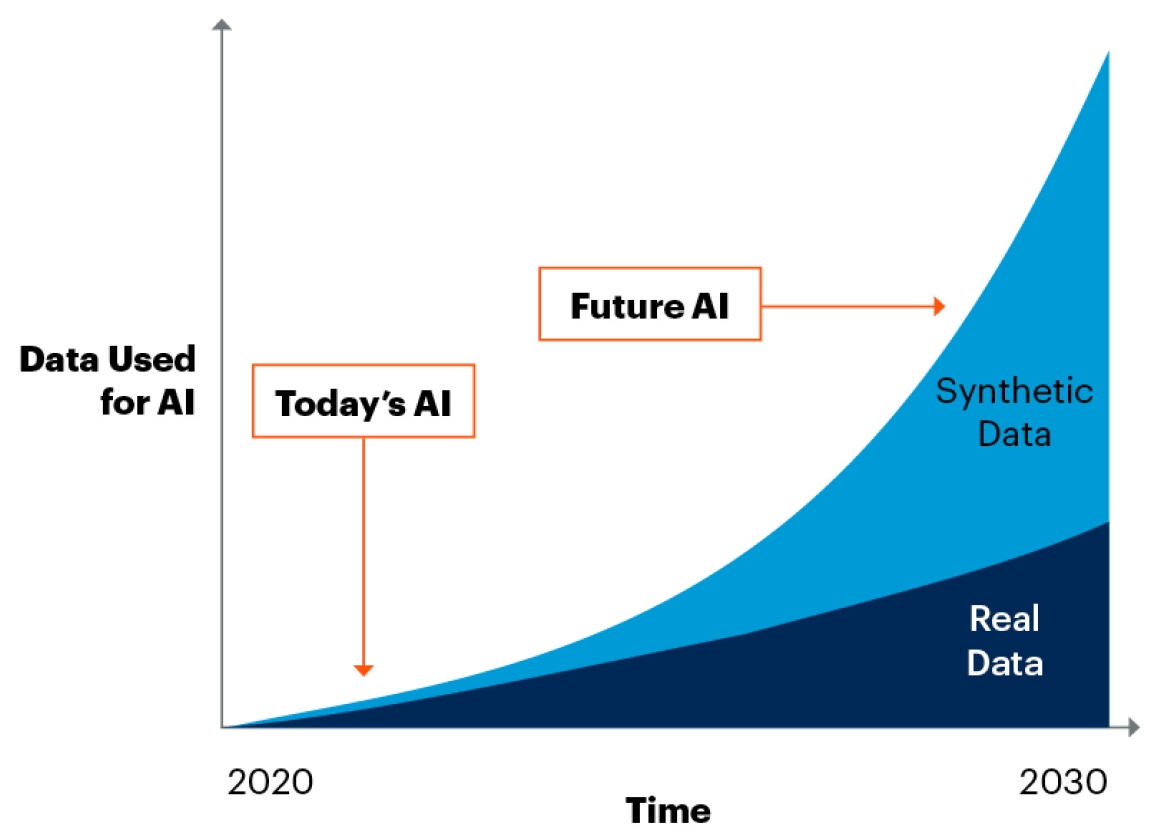
\includegraphics[width=1.0\textwidth]{/Users/apple/OVGU/Thesis/code/3dReconstruction/report/images/intro/Gartner-chart_2}
    \caption{A graph showing how synthetic dataset will evolve overtime. The research graph shows that synthetic dataset will overshadow the existing real dataset~\cite{gartnerreport}.
    Source: Research article from Gartner on "Synthetic Data Is the Future of AI"~\cite{gartnerreport}}
    \label{fig:Gartner research on synthetic dataset}
\end{figure}

Deep Learning has made leaps and bounds in solving 2D-image tasks like classification, segmentation, object detection, etc.
It has now entered the realm of Three-Dimension.
An image is a 3D objects projects onto a 2D surface.
While doing so, some data from the higher dimension is being lost in the lower dimension.
This inverse ability to reconstruct 3D objects from 2D images has a wide-scale application in computer vision and robotics.
Tasks like human body shapes and face reconstructions~\cite{deng2019accurate,Guo20173DFaceNetRD,9210569,richardson20163d,Richardson2017LearningDF},
3D-Scene reconstructions~\cite{Denninger20203DSR,Song2017SemanticSC,LiSilhouetteAssisted3O,Shin20193DSR}, generic object mesh reconstruction with textures are some of the advancements we had over recent years.
Here comes the challenge;3D data is not easy to collect.
3D data is not just limited but also noisy and expensive to collect.
The results of models depend on the consistency of the labeled data.
In this thesis, we discuss how game engines can contribute to generating quality-labeled datasets for 3D reconstruction tasks.


Deep Learning has made leaps and bounds in solving 2D-image tasks like classification, segmentation, object detection, and many more.
It has now entered the realm of Three-Dimension.
An image is a 3D objects projects onto a 2D surface.
While doing so, some data from the higher dimension is lost in, the lower dimension.
This inverse ability to reconstruct 3D objects from 2D images has wide applications in computer vision and robotics.
Tasks like human body shapes and face reconstructions~\cite{deng2019accurate,Guo20173DFaceNetRD,9210569,richardson20163d,Richardson2017LearningDF},
3D-Scene reconstructions~\cite{Denninger20203DSR,Song2017SemanticSC,LiSilhouetteAssisted3O,Shin20193DSR},
generic object mesh reconstruction with textures are some of the advancements we had over recent years.
Here comes the challenge;3D data is not easy to collect.
3D data is not just limited but also noisy and expensive to collect.

\section{Domain Adaptation vs. Domain randomization} \label{sec:da vs dr}

As mentioned earlier, the success of Convolutional Neural Networks depends highly on the training data.
As it so happens, not every task will have abundant data to train.
One solution for this problem is using a pre-trained network of similar problems and using transfer learning.
The pre-trained network is then trained over with the limited data available for the problem at hand.
In this case, some layers get overwritten by fine-tuning the features learned from the larger dataset using a small annotated dataset of different domains.
Domain adaptation is a field of study in machine learning where training data distribution differs from testing or target distribution.
One shallow approach is, as mentioned above,
re-weighting the network with testing data to adapt to the problem domain~\cite{Li2017PredictionRF}.
\”Deep domain adaptation methods leverage deep networks to learn more transferable representations by embedding domain adaptation in the pipeline of
deep learning\”~\cite{DBLP:journals/corr/abs-1802-03601}.
For this thesis, domain adaptation is relevant as the synthetic dataset might not represent the real or target domain, leading to a drop in performance.

Domain randomization, on the other hand, is improving data quality such that the training domain includes that the target domain distribution.
The \’reality gap\’~\cite{tobin2017domain} gets negated with this approach between simulated environment and natural images.
This is achievable by randomizing the rendering of objects in the synthetic data.
The key concept here is that the real-world distribution will appear to be just a variation in the dataset by rendering objects with significant variance.
Textures, brightness, shadows, camera settings, and object pose are some of the features that can be randomized.
In \autoref{ch:concept} we will discuss domain randomization.


\section{Volumetric representations of 3D shapes} \label{sec:Volumetric representation}
The universal representation of images in computer graphics is via pixels.
However, unlike 2D, 3D data can be represented in various formats like voxels, mesh and point clouds.
\autoref{fig:3d representation} presents the representation of these three formats.
Each of the representations has its own sets of advantages and disadvantages.
Voxels, which is short for Volumetric Pixels, is a 3D grid of pixels of constant size.
As indicated in~\cite{li2016fpnn}, the main advantage of voxels is that Convolution Neural Networks can be easily applied to 3-Dimensions as in 2-Dimensions.
Since most of the 3D geometry is surface-based, it can be wasteful and computationally expensive.
Mesh is composed of vertices, edges, and faces in 3D space that indicates the formation of 3D objects.
This form of representation is far more compact at a granular level, depending on the resolution.
On the other hand, point clouds are collections of 3D points with (x,y,z) coordinates on the surface of the object.
The collection of points determines detailing the 3D object representation.
In both these cases, \gls{cnn} is not directly applicable which is a direct disadvantage.
However, since mesh and point clouds are surface-based, the memory consumption is less than voxels and thereby lesser computation time, which is their advantage over voxels.
In this thesis, we opt for voxel-based models as the focus is on the performance of synthetic data rather than the model or the 3d representation itself.

\begin{figure}
    \centering
    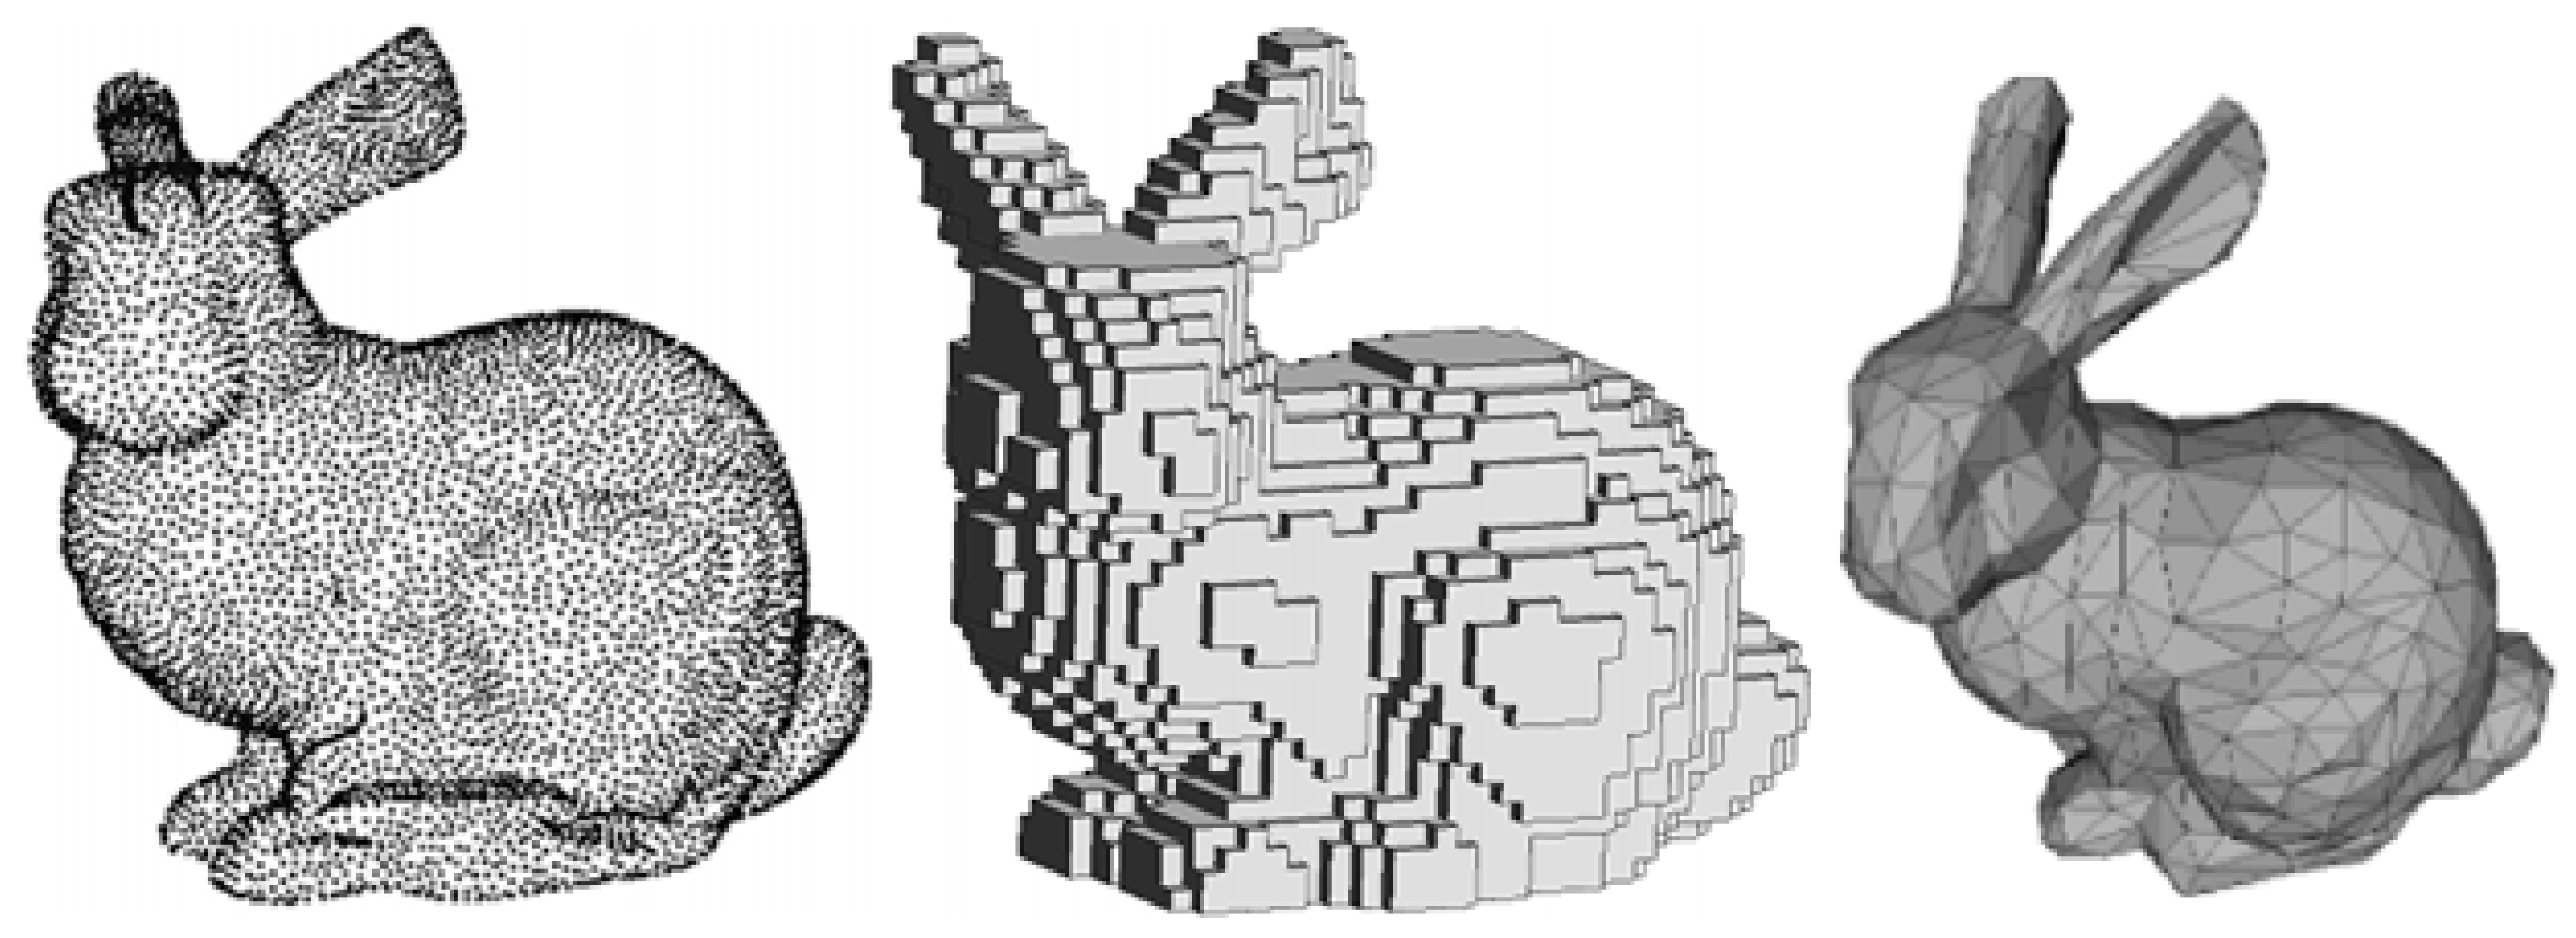
\includegraphics[width=1.0\textwidth]{/Users/apple/OVGU/Thesis/code/3dReconstruction/report/images/intro/3drepresentation}
    \caption{3D representation of Standford bunny model.(left to right) Point cloud, voxel and mesh~\cite{Hoang2019ADL}
    \label{fig:3d representation}}
\end{figure}

\section{GameEngines}\label{sec:gameengines}
~\cite{10.5555/983334} defines a \emph{Game engine} as  “A series of modules and interfaces that allow a development team to focus on product gameplay content,
rather than technical content” Gold [2004].
In layman’s terms, game engines are software used for the development of games.
Unreal Engine, Unity, GameMaker, Amazon Lumberyard, and CryEngine are popular game engines in modern times.
Over time, the graphics in each game engine have improved to an extent where visually, we cannot differentiate between reality and graphics.
These use object-oriented techniques, which help in modularity.
Also, they are GUI-oriented and hence are user-friendly and accessible even to a novice programmer.
The critical component in game engines that we will be focusing on is the ’Rendering engine’.
3D-Rendering is the means of converting 3D data into 2D images.
Rendering can either be real-time or offline/pre-rendering.
Game engines aim to make photorealism at the highest level with the least possible rendering time.


\section{Motivation}\label{sec:Background and motivation}

3D reconstruction is of great significance to understand a scene and to cross the 2D realm.
However, the task is not trivial, considering the input is still a Two-dimensional RGB image.
It is even more challenging since obtaining new data is expensive and time-consuming.
The 3D reconstruction field has datasets like ShapeNet~\cite{chang2015shapenet}, 3D-Front~\cite{Fu20203DFRONT3F}.
Nevertheless, there are no corresponding real images to check if the model will work in real-world scenarios.
Also, searching for real-world examples or creating a set-up scene and then labeling the images manually can lead to human mistakes resulting in wrong labels.
A solution to this problem is automating the task of generating synthetic data which can produce pixel-perfect annotations.
Automation can solve the human-in-the-loop problem, and while time gets saved, it facilitates the generation of a large quantity of data.
However, quantity should not be the only focus while creating the data;
we should also give priority to the quality of the data.
Game engines have come a long way from just supporting 2D to supporting games with photorealistic rendering.
Even though game engines have grown to be successful, few tools use them as the base framework.
As 3D models are available, we can import these models into the game engine and create an ersatz environment to generate a photorealistic dataset.
Further, we can check if these photorealistic synthetic data are useful for 3D reconstruction tasks.

\section{Goal of this Thesis}\label{sec:goal}

We will answer the following research questions:
\begin{enumerate}
    \item Are game engines a reliable medium for creating a photorealistic synthetic dataset?

    The photorealism of the images will be evaluated with a survey to compare images from the real dataset and generate datasets, and other proclaimed natural-looking datasets.

    \item Can Ersatz environment from a game engine like Unity replace real-world data for training in 3d reconstruction tasks?

    Using the dataset created with the Unity game engine, a single-view image to 3d reconstruction of furniture will be trained and tested on a real image dataset.

    \item Can we improve the performance of a model using a blend of real and synthetic datasets?
    To what extent does the performance enhance when the synthetic dataset is more than ten times of a real dataset?

    We use the dataset created using the Unity game engine to train a single-view image to 3d reconstruction of furniture and further fine-tune it with the real dataset to know if the performance is enhanced.
    Further an ablation study on chair dataset to check the effects domain randomization parameters.
    This experiment will also answer whether augmenting images with domain randomization with real data during training improves the performance?

\end{enumerate}

\section{Contributions of this Thesis}\label{sec:contributions}
In answering the research questions formulated in \autoref{sec:goal}, this thesis contributes the following:

\begin{itemize}
    \item A Unity-based framework to create a synthetic dataset with domain randomization.
    The tool supports both automated and manual image creation.
    \item A survey of photorealism to check whether Game engines produce quality synthetic datasets comparable with other proclaimed benchmarked photorealistic indoor datasets
    \item Provide a new dataset related to 3d reconstruction tasks or Synthetic to real domain adaptation tasks.
    The dataset includes G-buffers like RGB, normals, depth maps, and semantic segmentation images.
    \item Provide a focused synthetic chair dataset created with different parameters of domain randomization.
    A case study was conducted to check the influence of each component of domain randomization.
    \item A case study to understand the impact of mixed training.
    Synthetic and real image datasets are mixed in different ratios in each mini-batch to check the performance of the 3D reconstruction task.
    \item Fine-tuning models trained on a synthetic dataset with a small real dataset.
\end{itemize}


\section{Structure of this Thesis}\label{sec:Structure of thesis}

The rest of this thesis is structured as follows:

\begin{itemize}
    \item In \autoref{ch:related_work}, we visit some related work on synthetic data generation and benchmark 3d reconstruction networks.
    \item \autoref{ch:concept} deals with concepts and design choices.
    We will discuss in detail the choices for the dataset and model selection for 3d reconstruction.
    \item In \autoref{ch:implementation},discusses the 3DScene tool developed using the Unity game engine to create an ersatz environment.
    On the Deep learning side, we will discuss the pipeline design for the 3D reconstruction task.
    \item We dedicate \autoref{ch:evaluation} to reviewing and discussing evaluation results obtained by comparing the synthetic and real dataset from the survey conducted and Deep learning based on the 3D reconstruction task.
    \item Finally, in \autoref{ch:conclusion}, we conclude this thesis with the study results, highlight few limitations and discuss future improvements.
\end{itemize}
\chapter{\iftoggle{german}{Verwandte Arbeiten}{Related Work}}\label{ch:related_work}

This chapter discusses the previous contributions to indoor synthetic datasets in ~\autoref{subsec:indoor-synthetic-datasets},
what tasks each dataset supports, and some disadvantages.
Further, we discuss the available tools which support the creation of indoor dataset~\autoref{subsec:tools-to-create-synthetic} on different platforms and frameworks.
~\autoref{sec:state_of_the_art} will contain state-of-the-art 3D Reconstruction techniques used with different model representations(Voxels, Mesh, Point Clouds).
We will also discuss ways to mitigate the domain gap in ~\autoref{sec:mitigating_domain_shift}.
This section will include traditional techniques like transfer learning or fine-tuning and mixed training.
Recent trends in Generative models to transfer the style of the real image onto synthetically generated images is also briefly discussed.


\section{Indoor datasets}\label{sec:indoor-dataset}

Indoor scene dataset has been in the rise with increasing interest in scene processing understanding~\cite{dai2017scannet,Silberman2012IndoorSA,Xiao2013SUN3DAD,Hua2016SceneNNAS,Armeni20163DSP,chang2017matterport3d,Handa2016UnderstandingRI,InteriorNet18,li2021openrooms,zheng2020structured3d,Roberts2020HypersimAP,McCormac:etal:ICCV2017}.
The use of synthetic datasets is not something new in the world of machine learning.
As researchers realized the disadvantages of a real dataset, the focus shifted towards the synthetic dataset.
While~\cite{dai2017scannet} are real-world datasets,~\cite{Fu20203DFRONT3F,Handa2016UnderstandingRI,McCormac:etal:ICCV2017,Roberts2020HypersimAP} are synthetically produced.
Live scans help to gather real-world datasets.
The synthetic dataset can be manually configured by a professional or automated by a programmer using a tool.

\subsection{Indoor synthetic datasets}\label{subsec:indoor-synthetic-datasets}
Alibaba group introduced \gls{front}~\cite{Fu20203DFRONT3F} which stands for 3D Furnished Rooms with layOuts and semaNTics dataset which comprises
synthetic indoor scenes designed under the supervision of professionals.
It consists of 18,968 rooms and 13,151 textured pieces of furniture.
SceneNet~\cite{McCormac:etal:ICCV2017} is an extensive collection of photorealistic images and trajectories.
We will discuss this dataset in detail in~\autoref{sec:role-of-scenenet}.

SunCG~\cite{Song2017SemanticSC} was a fundamental dataset for scene understanding.
The dataset contained over 45,000 variations of scenes with realistic room layouts created manually.
Each scene was semantically labeled and also provided with volumetric ground truth data.
We use the dataset for tasks like depth estimation, semantic scene completion, SLAM, indoor navigation, and more.
Unfortunately, due to legal issues \footnote{https://futurism.com/tech-suing-facebook-princeton-data} the dataset has been made publicly unavailable, leaving a void in the field.

Structure3D~\cite{zheng2020structured3d} is another impressive synthetic data for indoor scenes which introduced their own photorealistic renderer.
The dataset comprises 21,835 rooms in 3,500 scenes and 196k 2D images rendered with photorealism.
However, the CAD models of the 3D furniture used to populate the scenes are not made available to the public.
Hence, we cannot perform the tasks related to  3D reconstruction.
\cite{zheng2020structured3d} have also demonstrated that combining synthetic and real dataset deep learning tasks for room layout estimation improved performance on benchmark datasets.
This dataset focuses more on room layout estimation and not 3D reconstruction, but with few modifications, it may well support to 3d furniture reconstruction tasks.

Openrooms~\cite{li2021openrooms} use Scannet~\cite{dai2017scannet} as their layout foundation, retrieve corresponding models from shapenet~\cite{chang2015shapenet}
and then replace the CAD model with a retrieved model with proper alignment.
They further add the reflectance and illumination properties to compose photo-realistic images.
As of August 2021, only the dataset has been made public, not the generation tool or CAD models.
The underlying concept of Openrooms is to convert existing scans into photorealistic synthetic images.
We consider them our counterparts in the output images, as the framework can produce normals, depth maps, instance segmentation, and masks the same as we do.

Hypermism~\cite{Roberts2020HypersimAP} is Apple's repository for holistic indoor scene understanding.
It is a collection of synthetic scenes created with the help of a professional artist.
Evermotion ~\cite{Evermotion} was the starting point for the dataset for which assets were purchased from TurboSquid~\cite{TurboSquid}.
The dataset includes images, 3D assets, semantic instance segmentation, and a disentangled image representation with diffused lighting and shading.
Even though the 3d triangle meshes for each asset is available online, we have to purchase them to create a custom dataset.
They also admit that the cost to generate the dataset is expensive \{approximately \$57K~\cite{Roberts2020HypersimAP}\}.

InteriorNet~\cite{InteriorNet18} claims to be a photo-realistic indoor scene simulator with realistic lighting and scenes which change over time.
The image dataset includes RGB, depth, and semantic segmentation.
Along with images, they also provide synthesized realistic trajectories at a video-frame rate with various motion patterns.
The simulator also supports scenes from~\cite{McCormac:etal:ICCV2017} and~\cite{Song2017SemanticSC} along with their database.

Another simulated framework for visual research is House Of inteRactions (THOR) was introduced in \gls{ai2thor}~\cite{kolve2019ai2thor}.
This dataset is again an Agent focused photo-realistic dataset with the critical factor being actionable objects so that agents can interact with the objects or manipulate them.
The underlying renderer for this framework is the Unity game engine.
RoboThor~\cite{Deitke2020RoboTHORAO} is built upon \gls{ai2thor}, consisting of real scenes and its corresponding synthetic equivalent.
It helps study agents' behavior in the real world when trained on synthetic data.
Architects manually designed the scenes by taking references from photos of the real world.

Habitat: A Platform for Embodied AI Research~\cite{savva2019habitat} is a photorealistic 3D simulation used for training virtual agents for tasks like navigation, question answering, instruction following..
The paper introduces Habitat-Sim, which renders scenes from Matterport3d~\cite{chang2017matterport3d}, Gibson~\cite{xia2018gibson}, Replica~\cite{Straub2019TheRD}, and some other datasets.
The focus of the simulator is providing the agent with sensor data and allowing additional sensors as plugins.
At the foundation level, Habitat-sim uses Magnum graphics
middleware library~\footnote{https://magnum.graphics/}, which supports cross-platform on the various hardware configuration.

In \autoref{fig:photorealistic images comparison}, we can see samples from each of the datasets claimed to be photorealistic.
The images from these datasets are used in a research survey to determine the perception of humans about photorealism.
We define "Automated dataset" as a dataset which had no or limited user or professional designer inputs.
Only the 3D furntiure models assets might have been designed by professionals, but the properties of the room like lights, textures, etc, were generated automatically.
Among the datasets under consideration,
OpenRooms, SceneNet, BlenderProc are all automated datasets, including the proposed \gls{free} dataset.
Hyperism, \gls{ai2thor}, InteriorNet, and \gls{front} were manually configured and designed by professional architects.


\begin{table}[ht]
    \centering
    \begin{tabular}{|c |c |c |c|}
        \hline
        Dataset & Year & Automated \\ [0.5ex]
        \hline\hline
        Openrooms & 2020 & YES \\
        \hline
        \gls{ai2thor} & 2017 & NO \\
        \hline
        BlenderProc & 2019 & YES \\
        \hline
        Hyperism & 2020 & NO \\
        \hline
        \gls{front} & 2020 & NO \\
        \hline
        InteriorNet & 2018 & NO \\
        \hline
        SceneNet & 2015 & YES \\
        \hline
        \gls{free} & 2021 & YES \\[1ex]
        \hline
    \end{tabular}
    \caption{Table represents synthetic datasets and year of release, and if they are automated(i.e. created with no or limited inputs from professional designers.)}
    \label{tab:dataset_comparison}
\end{table}

\begin{figure}
\begin{tabular}{llll}
    \gls{front} & 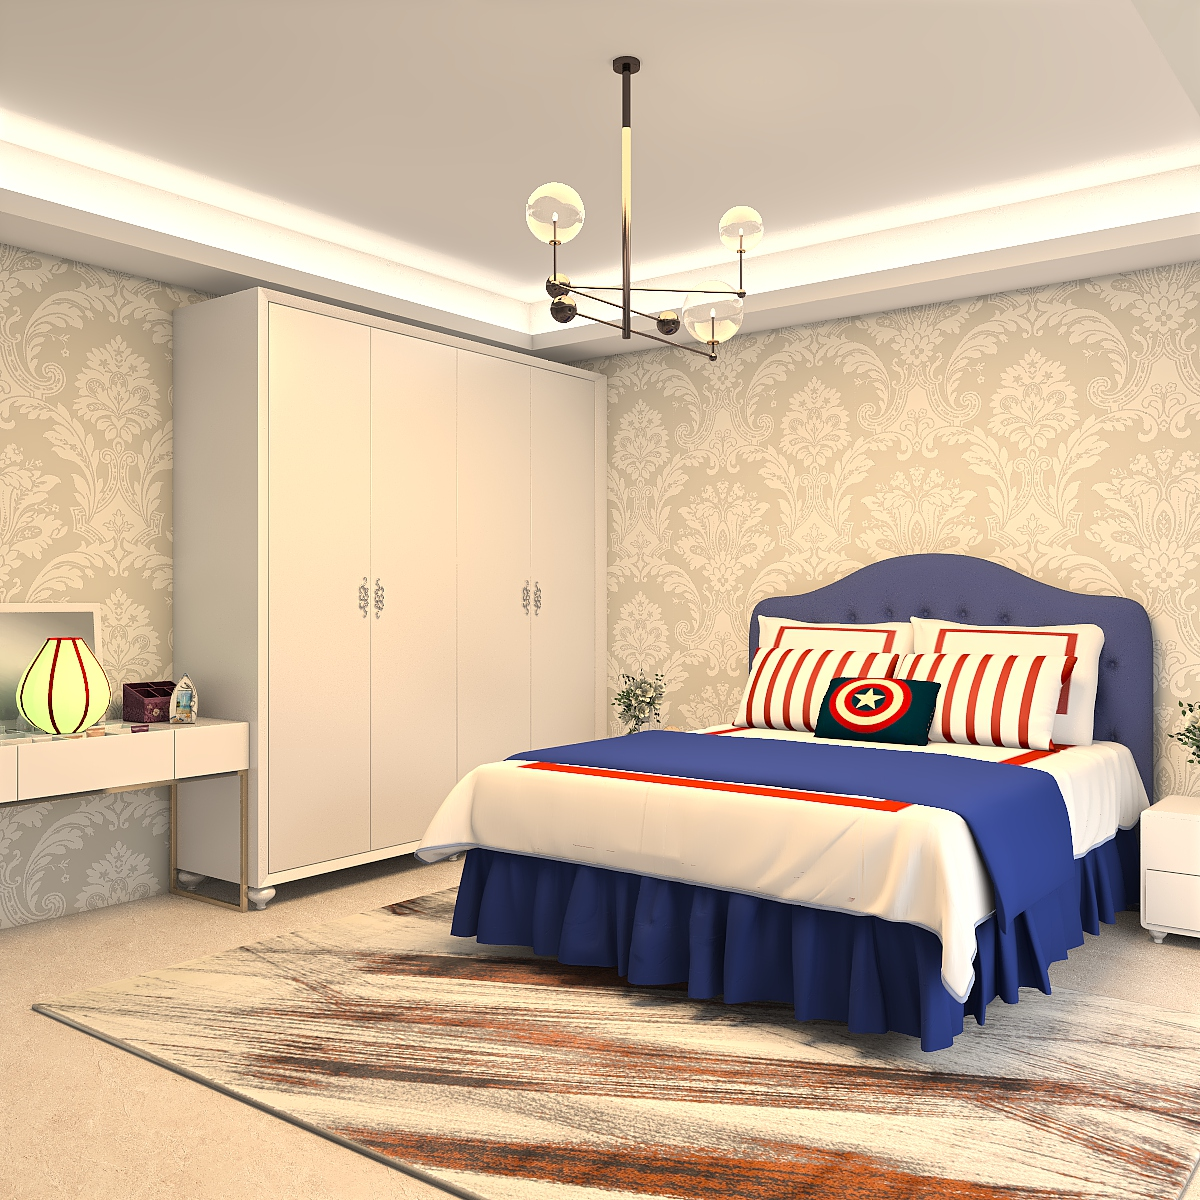
\includegraphics[width=.2\linewidth,valign=m]{/Users/apple/OVGU/Thesis/code/3dReconstruction/report/images/realistic_images_relatedwork/3dfront_1} &
    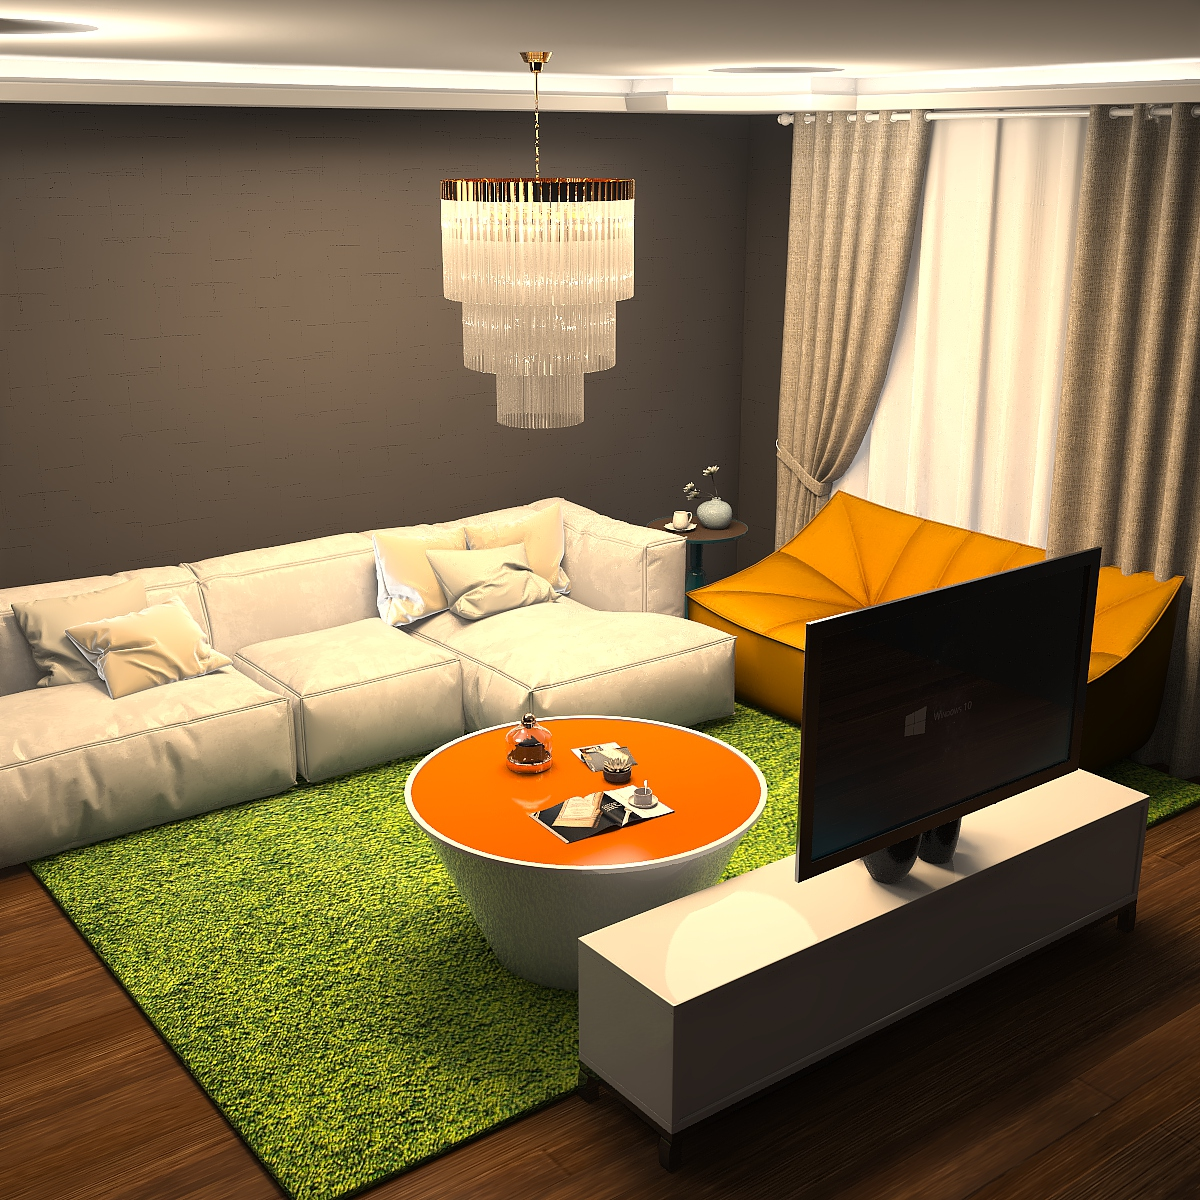
\includegraphics[width=.2\linewidth,valign=m]{/Users/apple/OVGU/Thesis/code/3dReconstruction/report/images/realistic_images_relatedwork/3dfront_2} &
    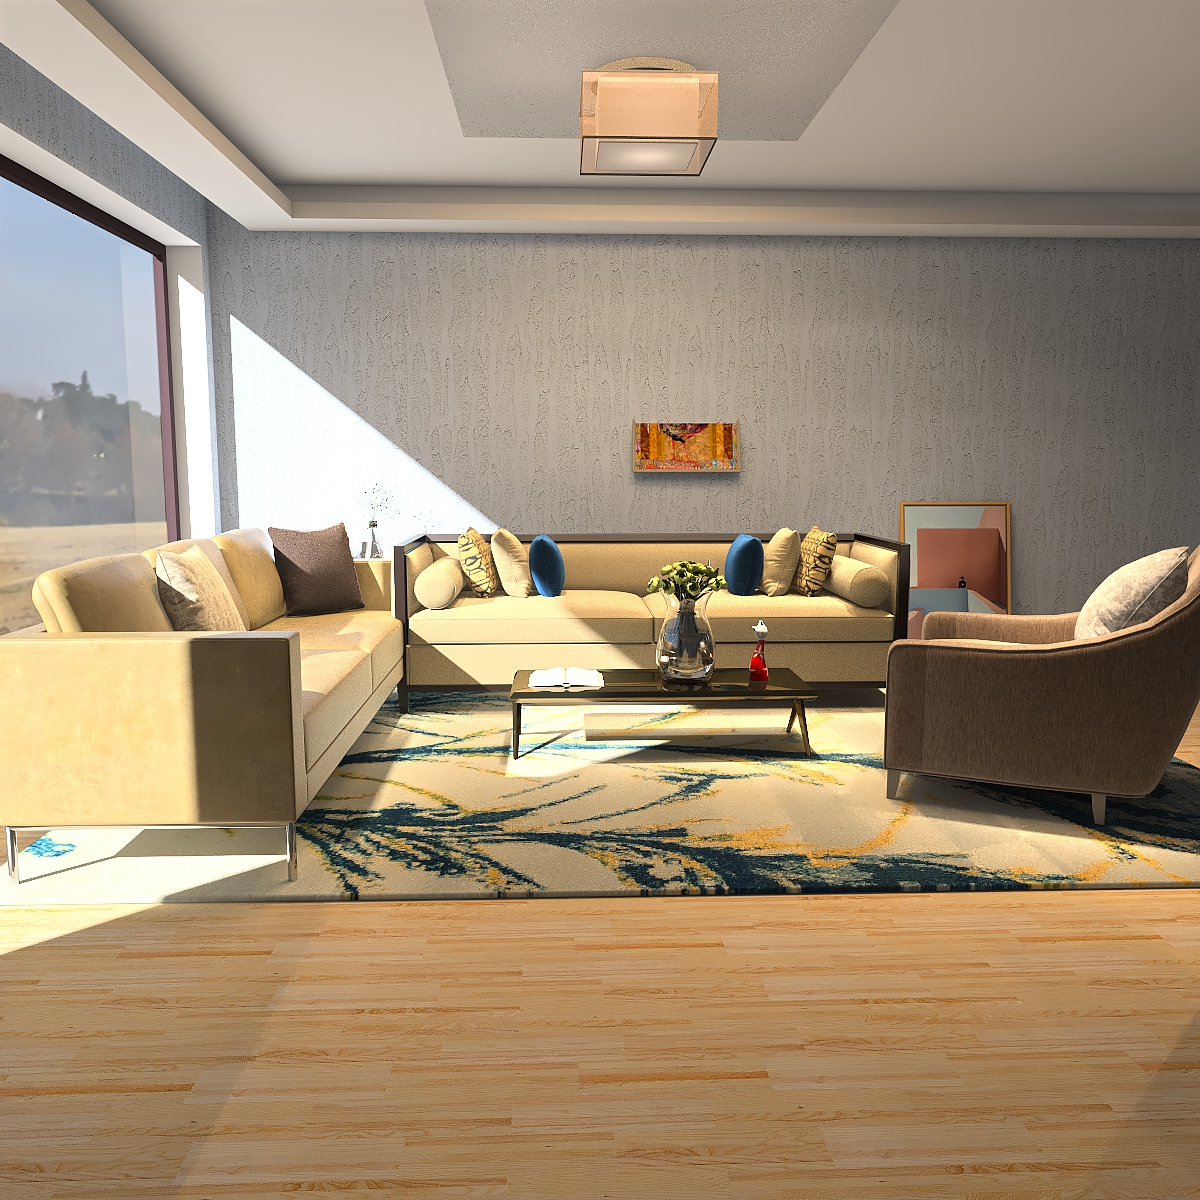
\includegraphics[width=.2\linewidth,valign=m]{/Users/apple/OVGU/Thesis/code/3dReconstruction/report/images/realistic_images_relatedwork/3dfront_3}\\

    \gls{ai2thor} & 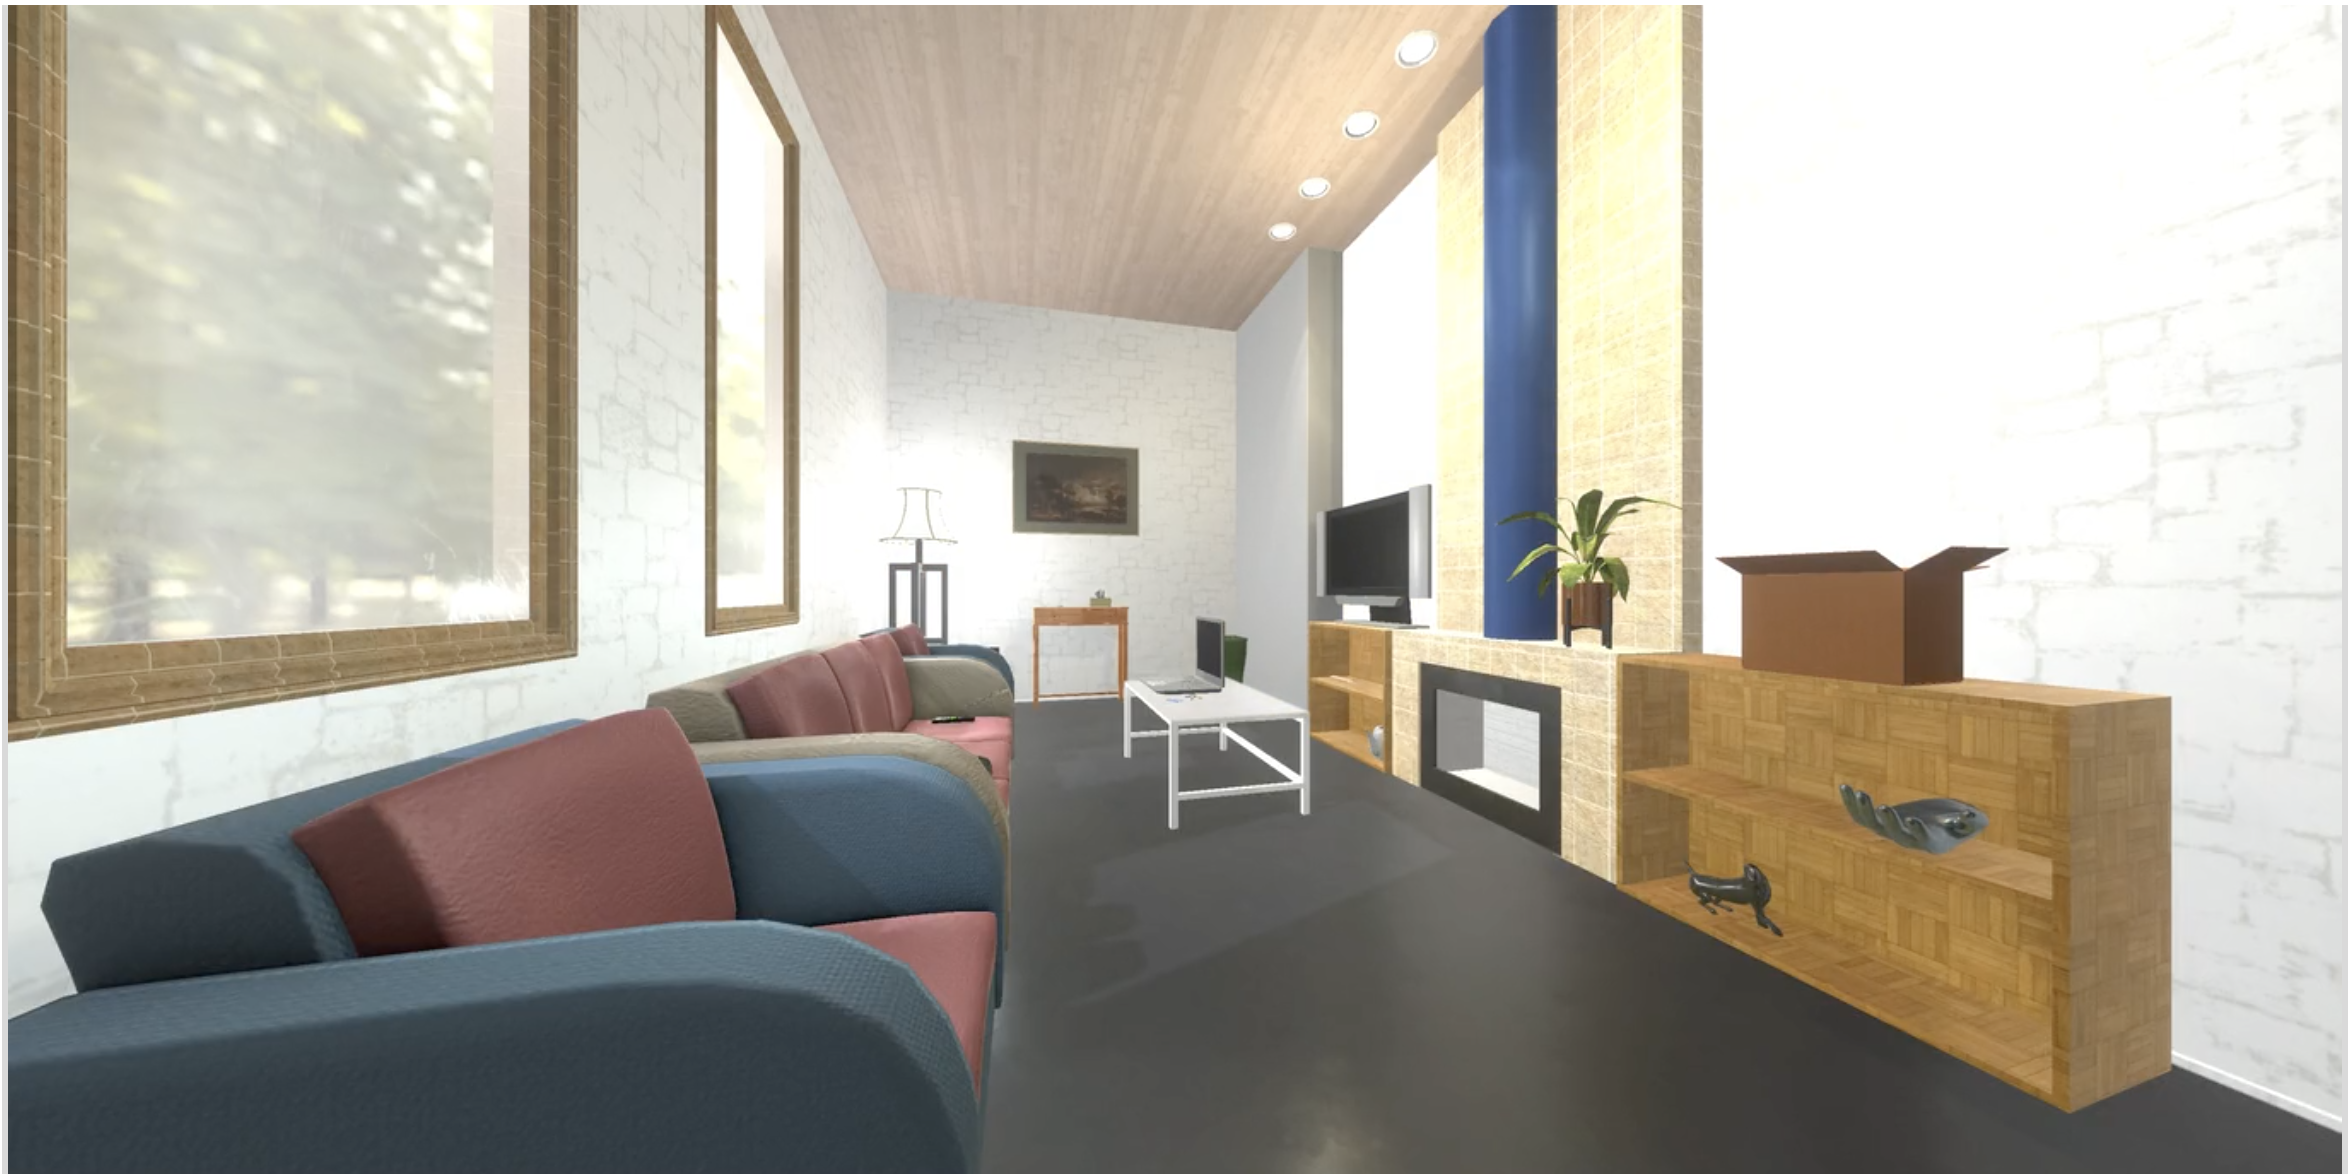
\includegraphics[width=.2\linewidth,valign=m]{/Users/apple/OVGU/Thesis/code/3dReconstruction/report/images/realistic_images_relatedwork/ai2thor_01} &
    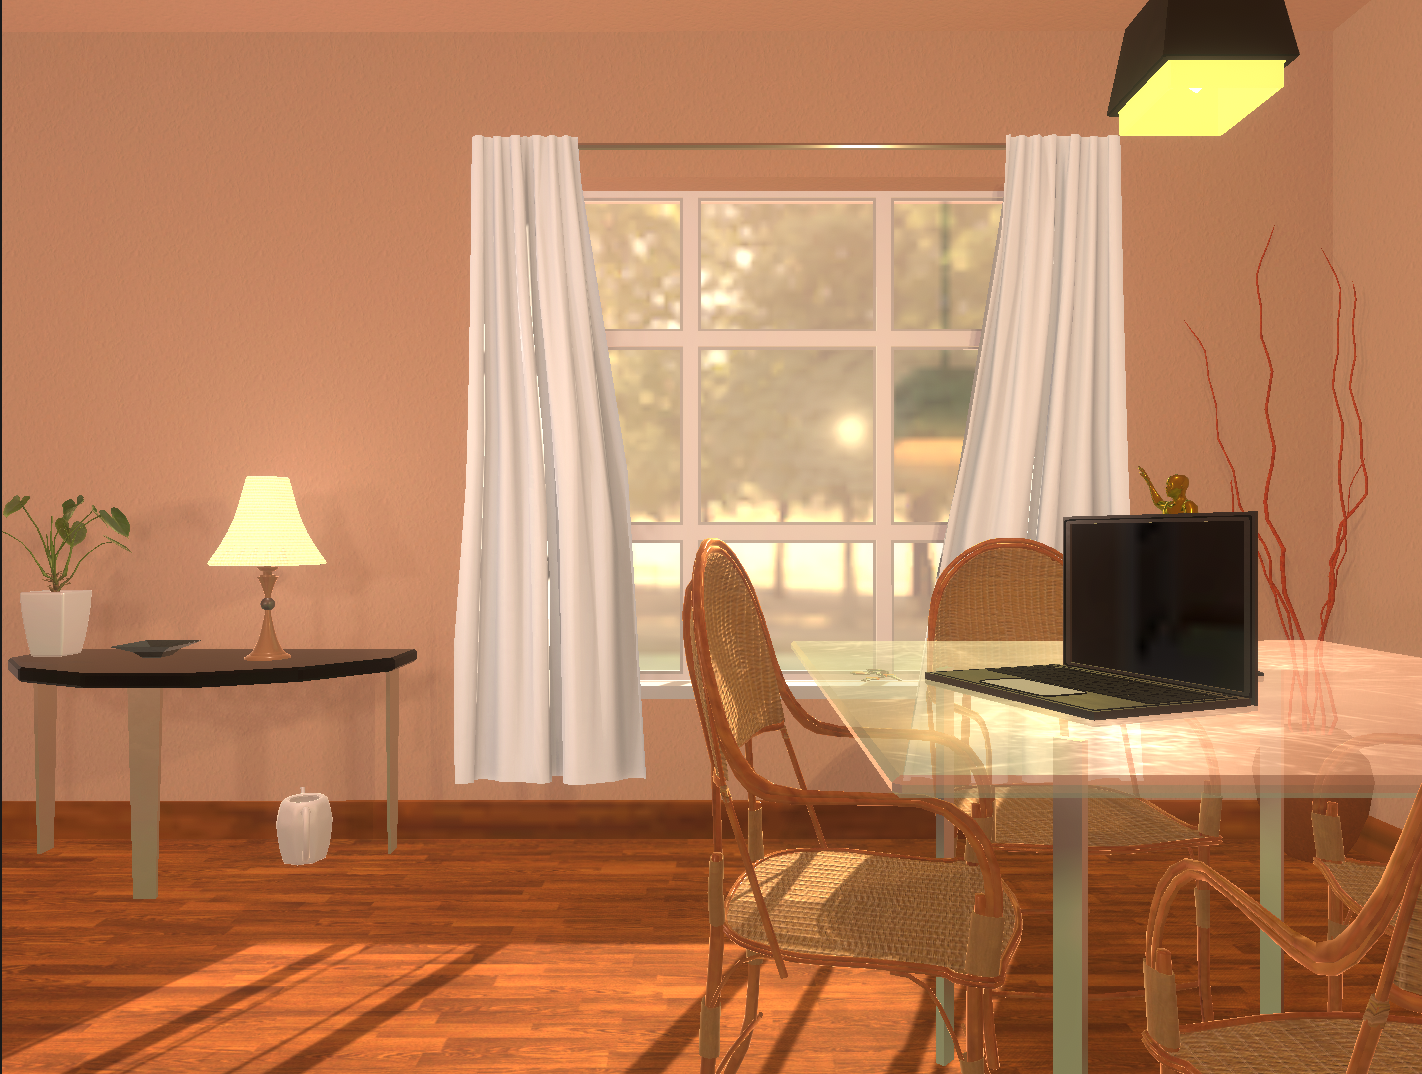
\includegraphics[width=.2\linewidth,valign=m]{/Users/apple/OVGU/Thesis/code/3dReconstruction/report/images/realistic_images_relatedwork/ai2thor_02} &
    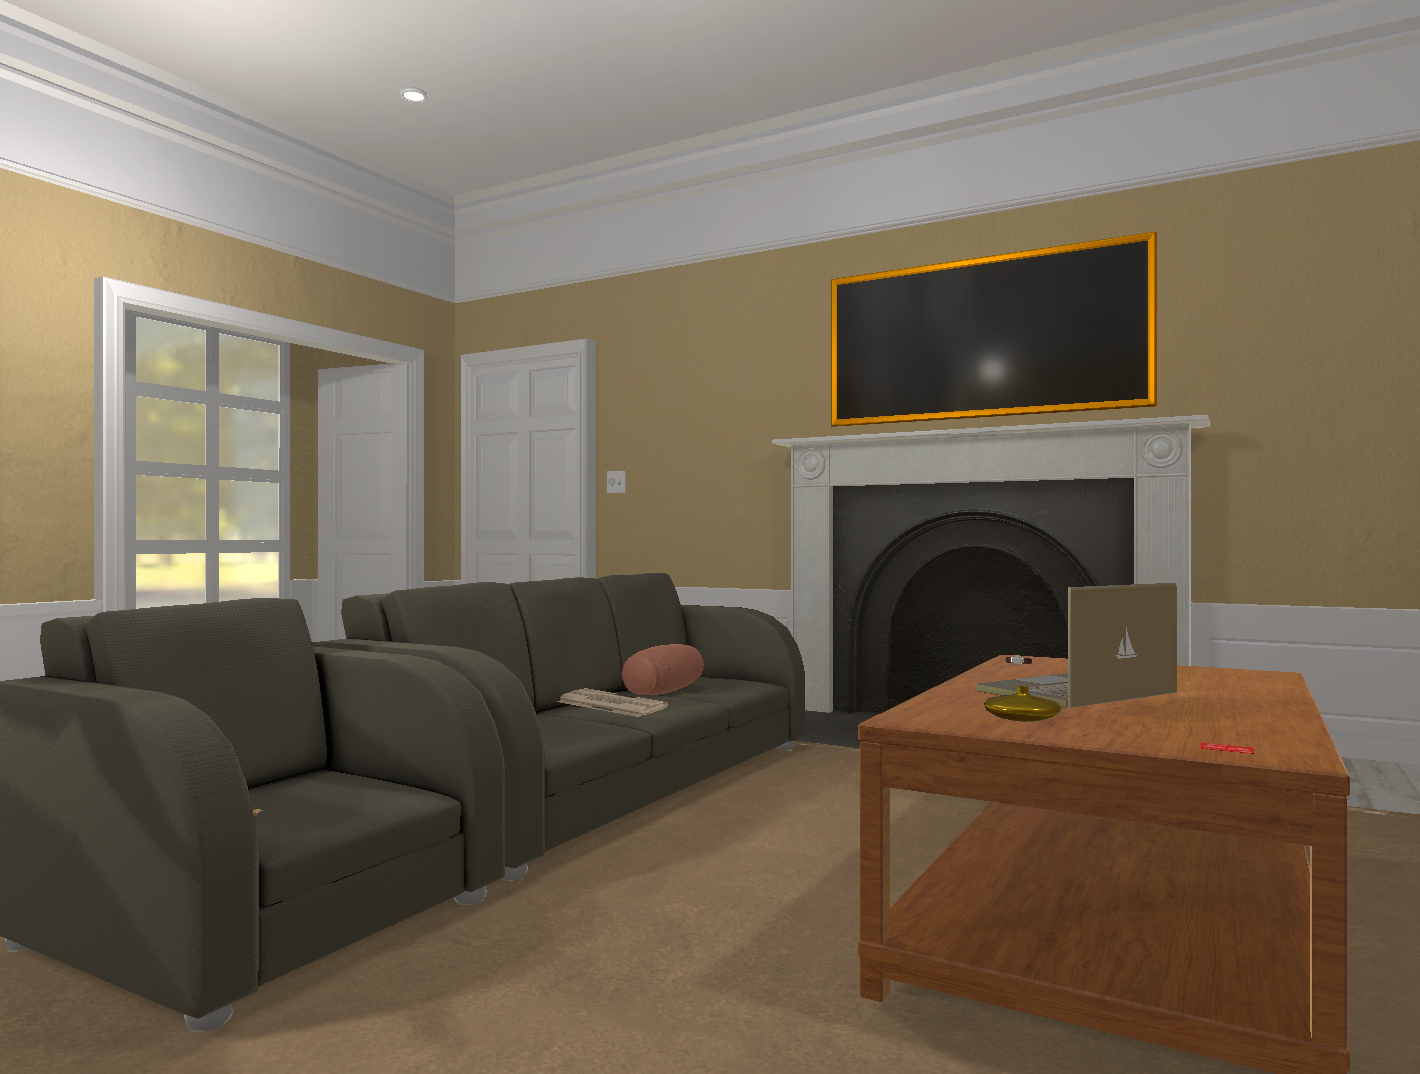
\includegraphics[width=.2\linewidth,valign=m]{/Users/apple/OVGU/Thesis/code/3dReconstruction/report/images/realistic_images_relatedwork/ai2thor_03}\\

    Hypersim & 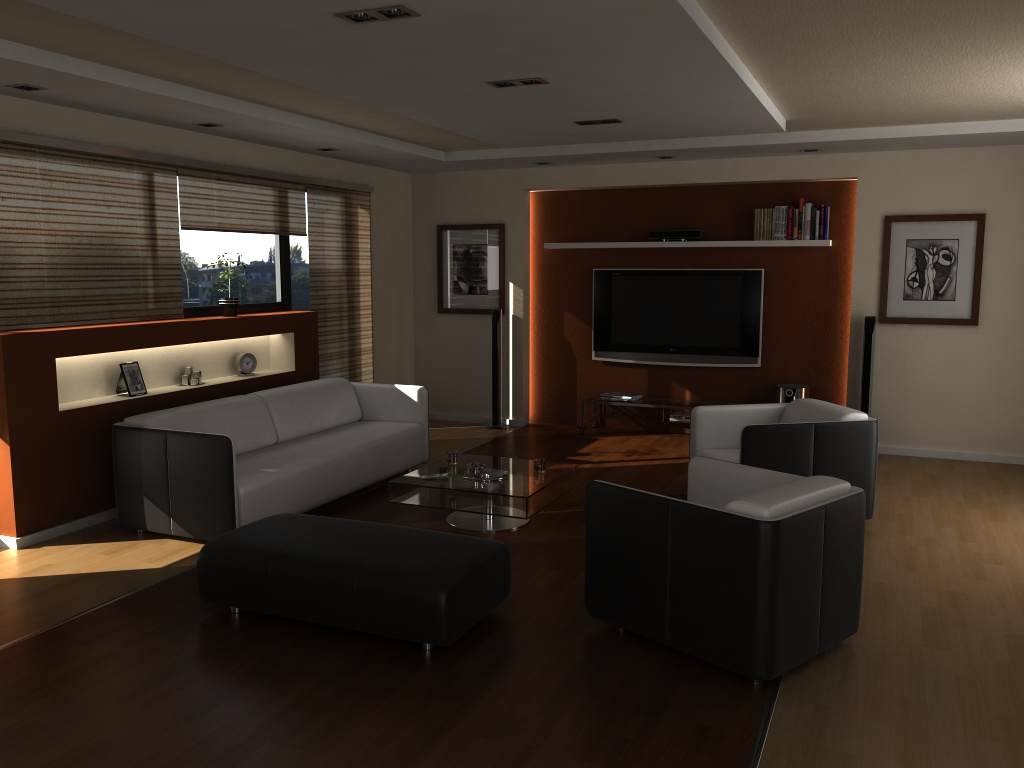
\includegraphics[width=.2\linewidth,valign=m]{/Users/apple/OVGU/Thesis/code/3dReconstruction/report/images/realistic_images_relatedwork/hypersim_01} &
    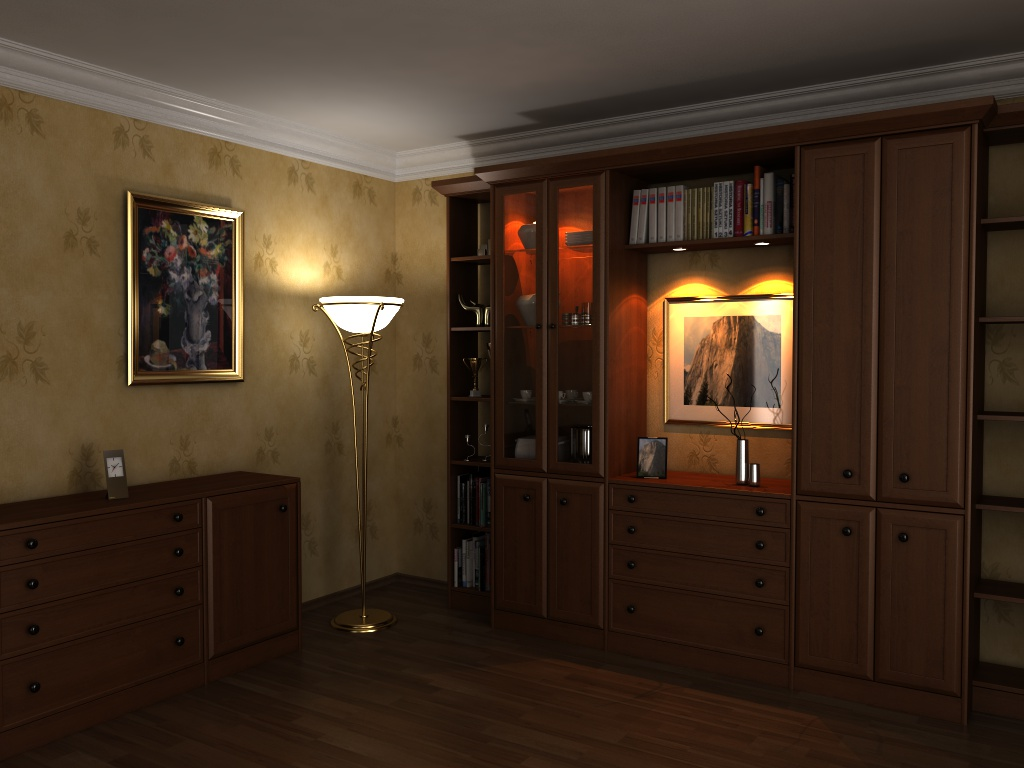
\includegraphics[width=.2\linewidth,valign=m]{/Users/apple/OVGU/Thesis/code/3dReconstruction/report/images/realistic_images_relatedwork/hypersim_02} &
    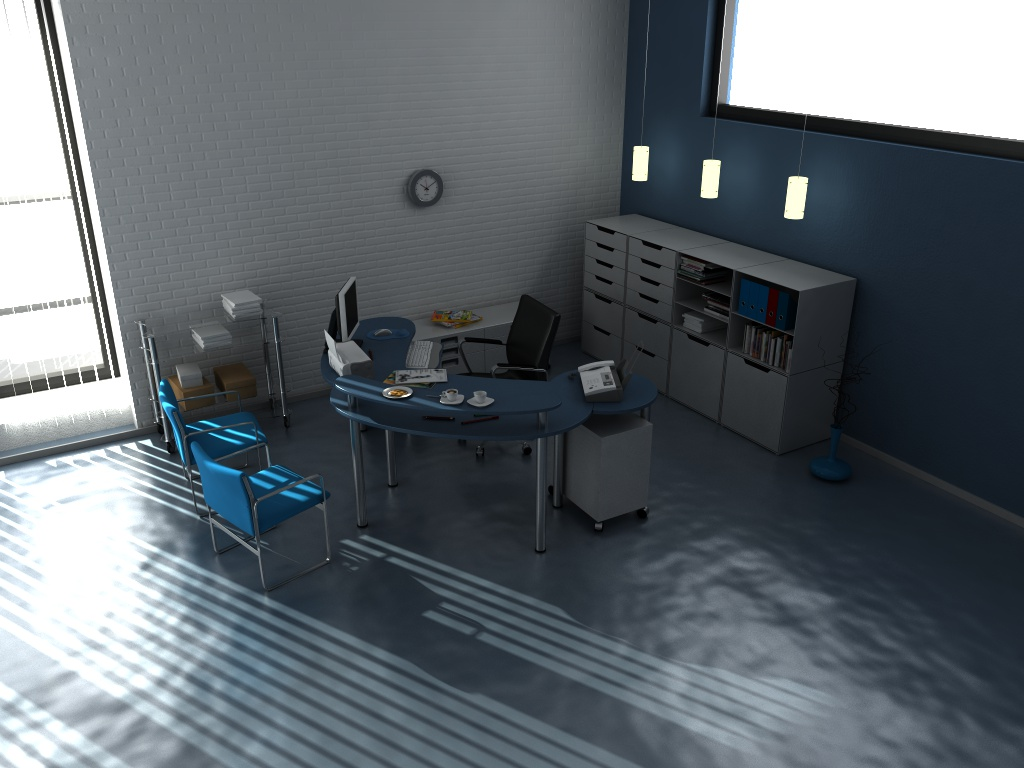
\includegraphics[width=.2\linewidth,valign=m]{/Users/apple/OVGU/Thesis/code/3dReconstruction/report/images/realistic_images_relatedwork/hypersim_03}\\

    InteriorNet & 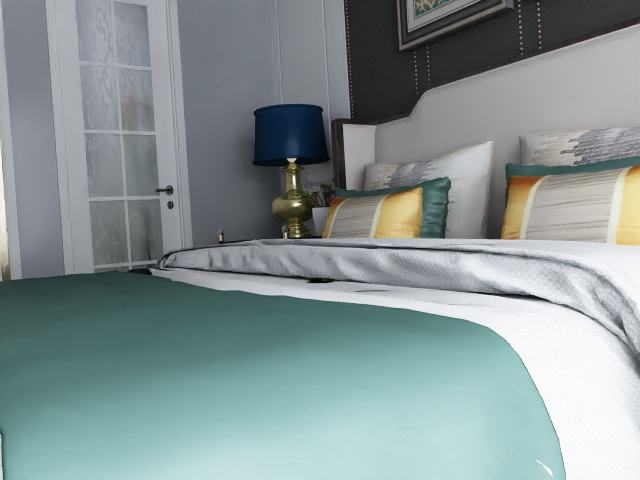
\includegraphics[width=.2\linewidth,valign=m]{/Users/apple/OVGU/Thesis/code/3dReconstruction/report/images/realistic_images_relatedwork/interiornet_01} &
    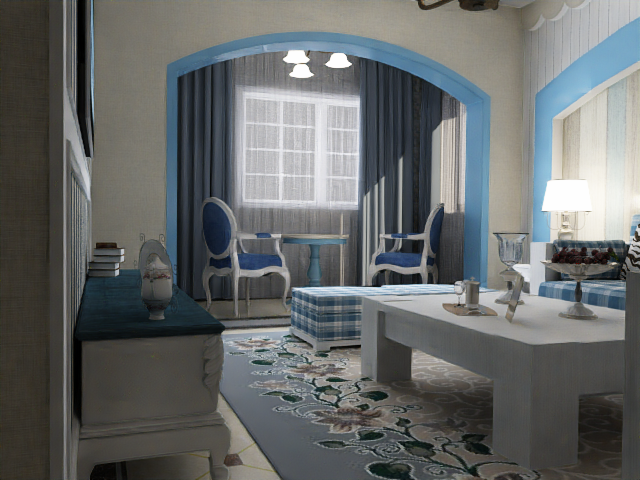
\includegraphics[width=.2\linewidth,valign=m]{/Users/apple/OVGU/Thesis/code/3dReconstruction/report/images/realistic_images_relatedwork/interiornet_02} &
    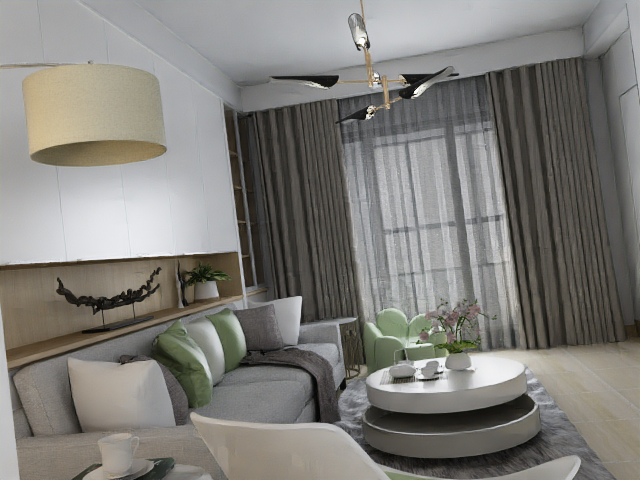
\includegraphics[width=.2\linewidth,valign=m]{/Users/apple/OVGU/Thesis/code/3dReconstruction/report/images/realistic_images_relatedwork/interiornet_03}\\

    OpenRooms & 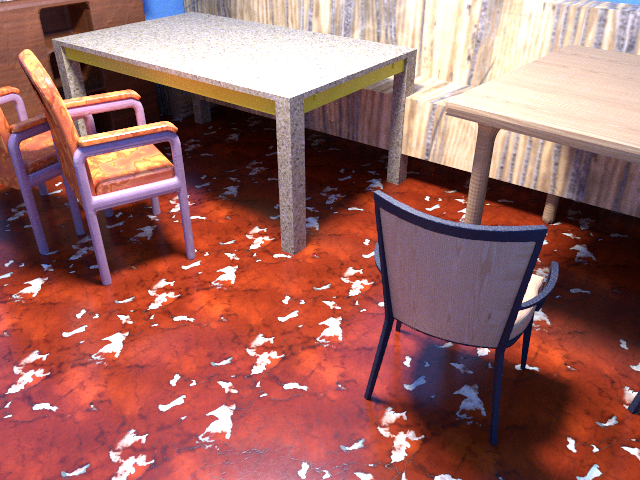
\includegraphics[width=.2\linewidth,valign=m]{/Users/apple/OVGU/Thesis/code/3dReconstruction/report/images/realistic_images_relatedwork/openrooms_01} &
    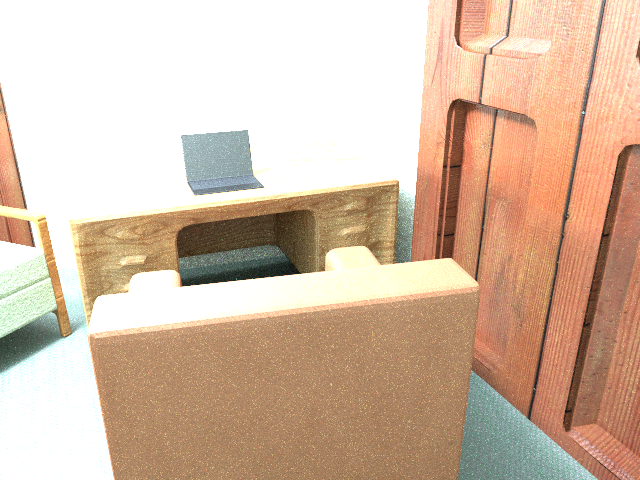
\includegraphics[width=.2\linewidth,valign=m]{/Users/apple/OVGU/Thesis/code/3dReconstruction/report/images/realistic_images_relatedwork/openrooms_02} &
    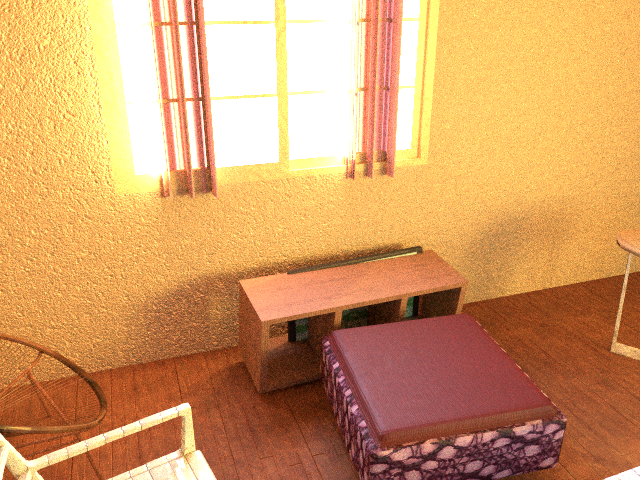
\includegraphics[width=.2\linewidth,valign=m]{/Users/apple/OVGU/Thesis/code/3dReconstruction/report/images/realistic_images_relatedwork/openrooms_03}\\

    SceneNet & 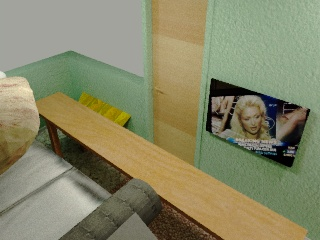
\includegraphics[width=.2\linewidth,valign=m]{/Users/apple/OVGU/Thesis/code/3dReconstruction/report/images/realistic_images_relatedwork/scenenet_1} &
    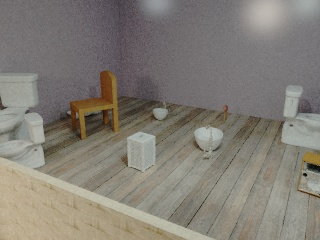
\includegraphics[width=.2\linewidth,valign=m]{/Users/apple/OVGU/Thesis/code/3dReconstruction/report/images/realistic_images_relatedwork/scenenet_2} &
    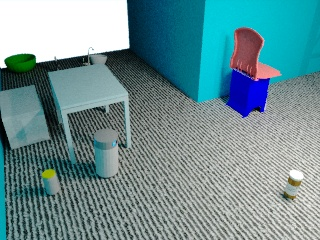
\includegraphics[width=.2\linewidth,valign=m]{/Users/apple/OVGU/Thesis/code/3dReconstruction/report/images/realistic_images_relatedwork/scenenet_3}\\

\end{tabular}
\caption{A collection of photorealistic synthetic datasets. The first column of each row indicates the dataset name followed by randomly selected images from the same dataset.}
\label{fig:photorealistic images comparison}
\end{figure}

\subsection{Tools to create synthetic datasets}\label{subsec:tools-to-create-synthetic}

"BlenderProc: Reducing the Reality Gap with Photorealistic Rendering" by ~\cite{denninger2019blenderproc} is a python based pipeline to create a synthetic dataset.
As the name suggests, the underlying framework is Blender~\cite{blender}, which is a 3D modeling and rendering package.
Like most synthetic data generation tools, it provides RGB, depth maps, normals, and semantic segmentation.
\autoref{fig:Blenderproc samples} is a collection of sample images generated using BlenderPoc.
We searched for synthetic data generation tools, Blenderproc supports a maximum number of existing datasets.
Ikea~\cite{Lim2013ParsingIO}, Pix3d~\cite{pix3d}, Shapenet~\cite{chang2015shapenet}, \gls{front}~\cite{Fu20203DFRONT3F}, Replica~\cite{Straub2019TheRD}, SunCG~\cite{Xiao2013SUN3DAD} are some of the popular datasets it supports.
It also has some combinations of these datasets like ShapeNet with SunCG or SceneNet.
Even though it supports the rendering of the Pix3D dataset, the model is rendered without any background.
One extreme advantage of this toolkit is that it is open source and a more comprehensive open community to contribute.

\begin{figure}
    \begin{tabular}{llll}
        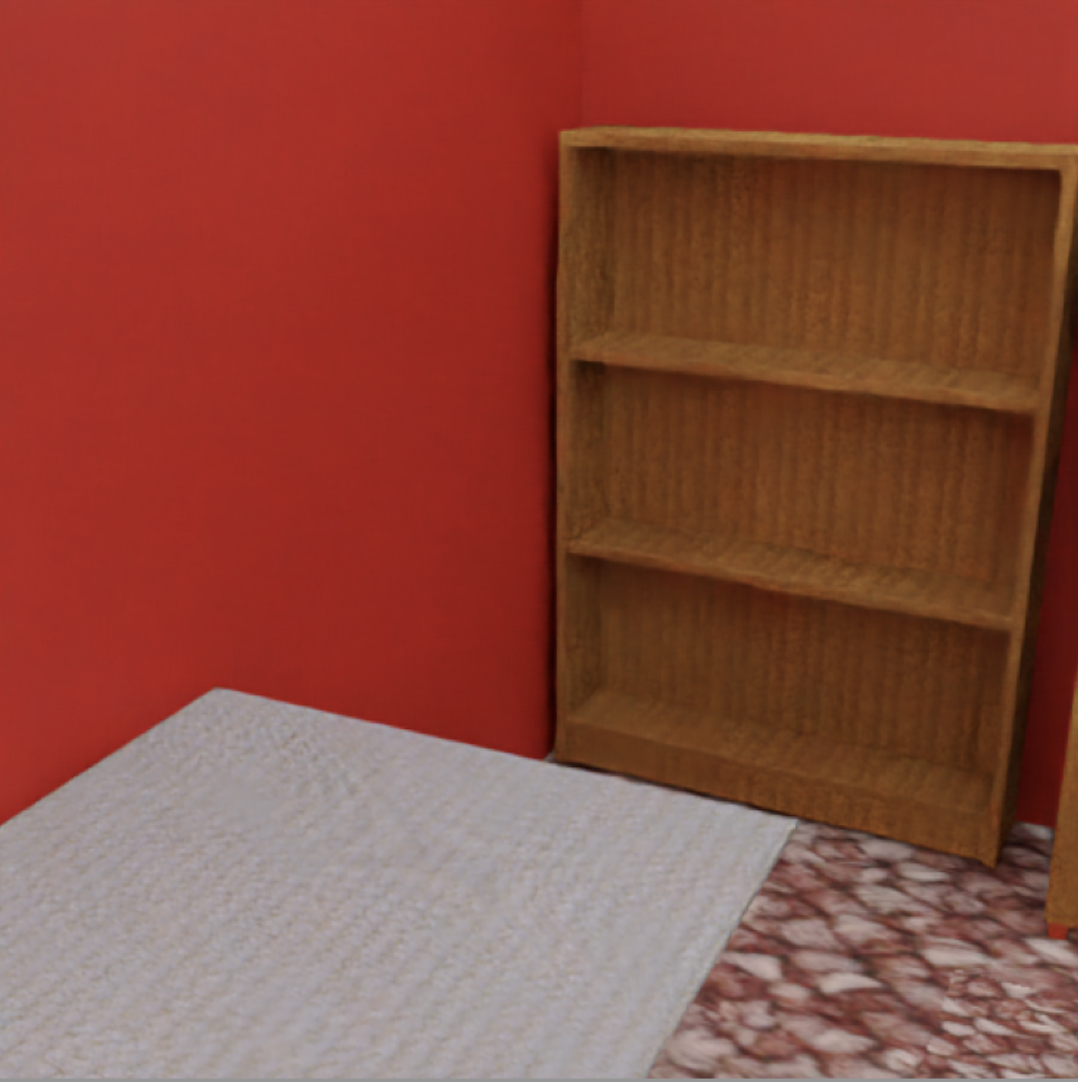
\includegraphics[width=.2\linewidth,valign=m]{/Users/apple/OVGU/Thesis/code/3dReconstruction/report/images/realistic_images_relatedwork/blenderproc_1} &
        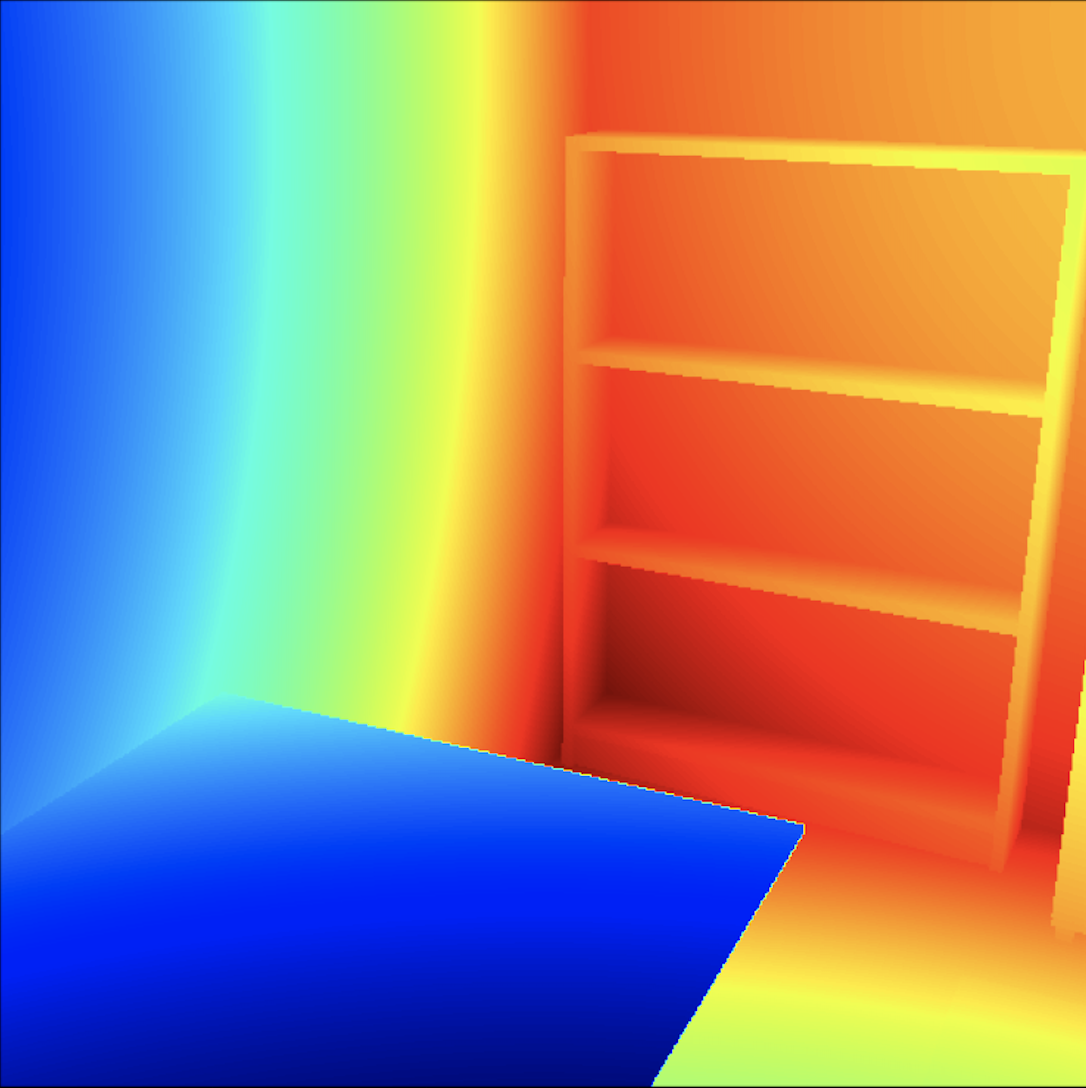
\includegraphics[width=.2\linewidth,valign=m]{/Users/apple/OVGU/Thesis/code/3dReconstruction/report/images/realistic_images_relatedwork/blenderproc_depth_1} &
        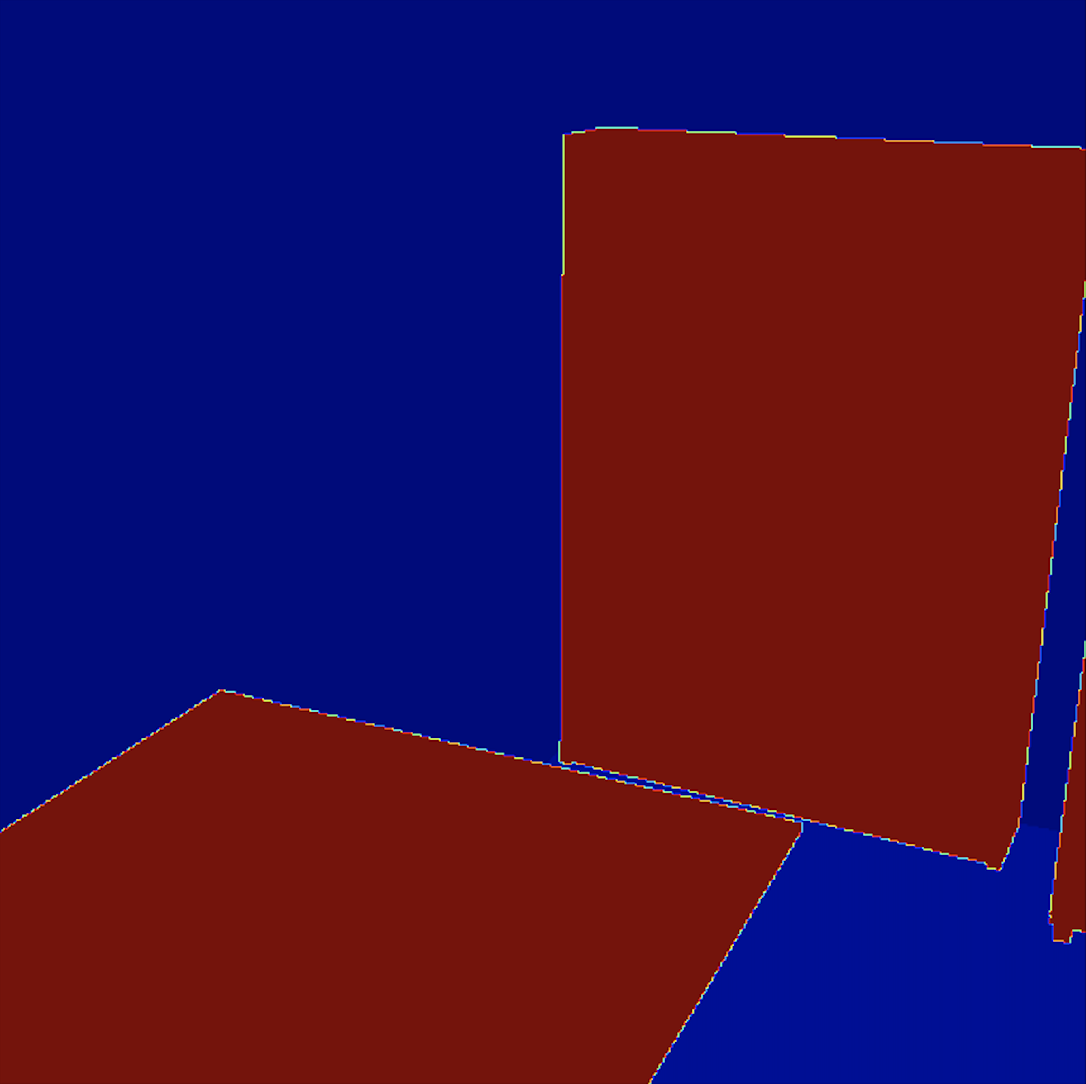
\includegraphics[width=.2\linewidth,valign=m]{/Users/apple/OVGU/Thesis/code/3dReconstruction/report/images/realistic_images_relatedwork/blenderproc_instance_1} &
        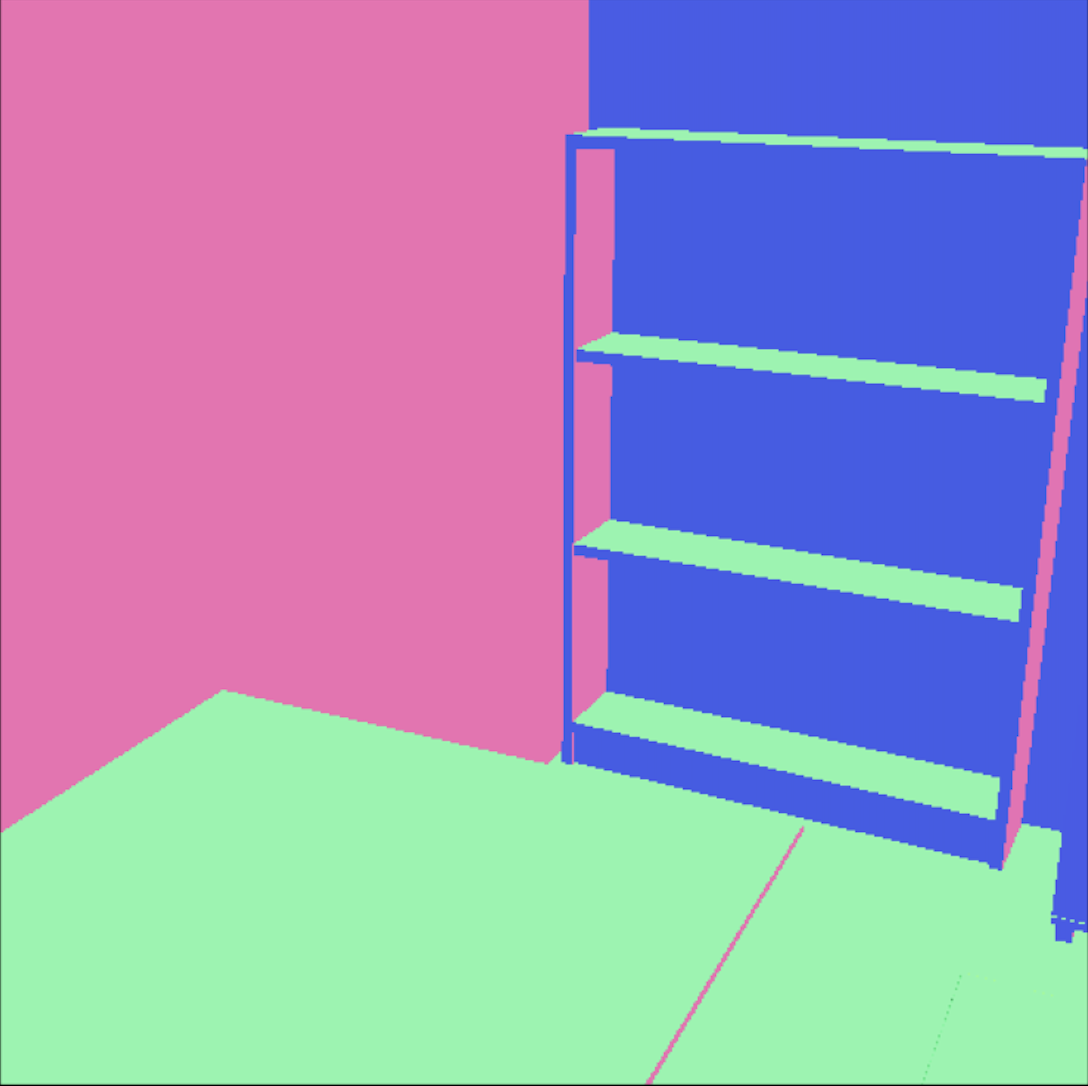
\includegraphics[width=.2\linewidth,valign=m]{/Users/apple/OVGU/Thesis/code/3dReconstruction/report/images/realistic_images_relatedwork/blenderproc_normal_1}\\


        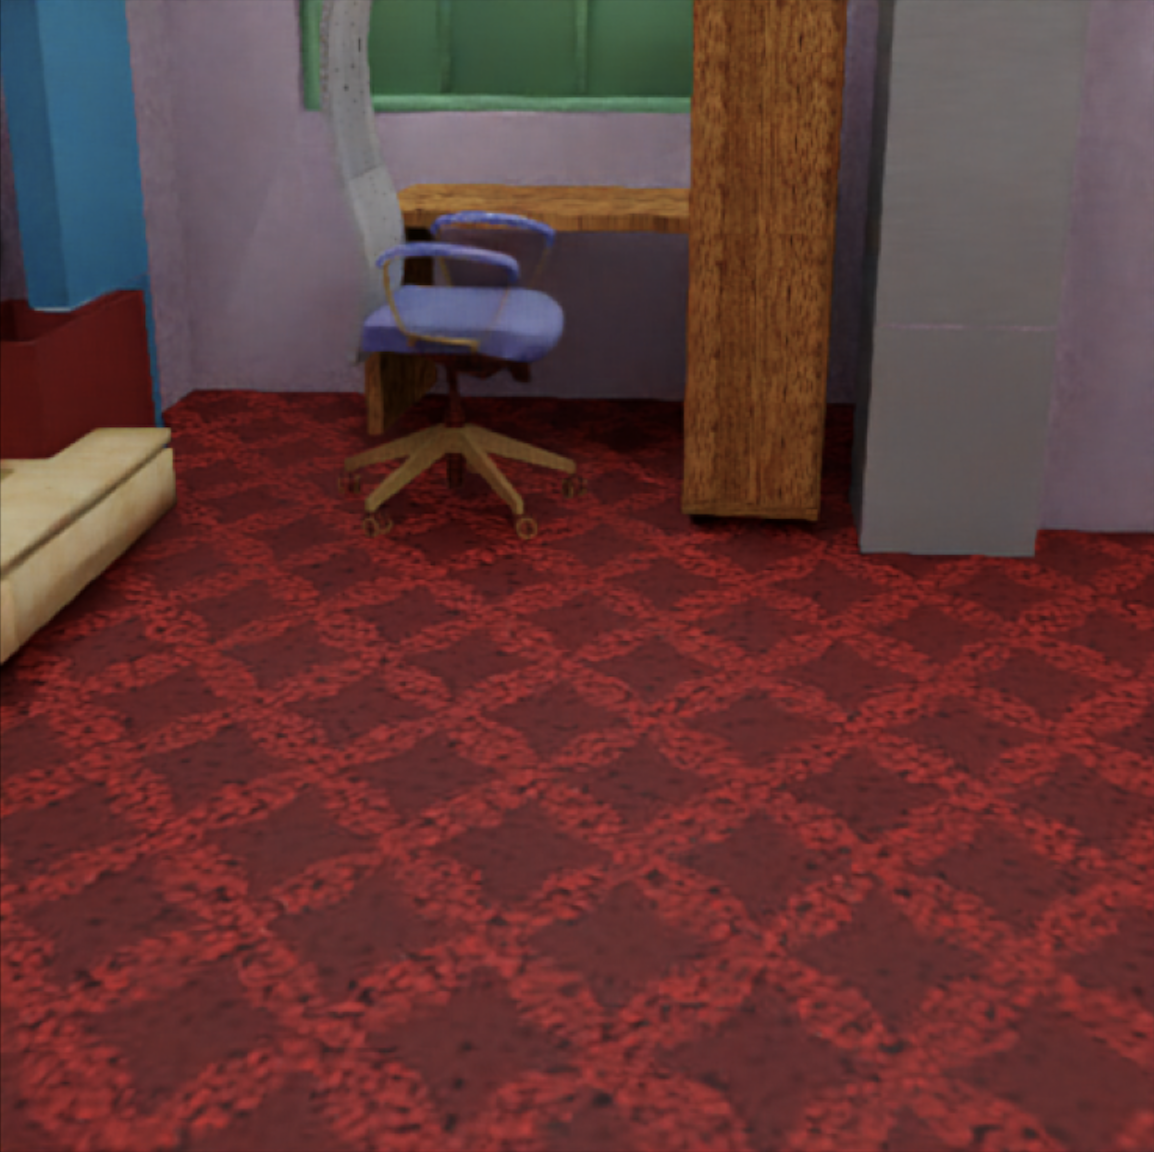
\includegraphics[width=.2\linewidth,valign=m]{/Users/apple/OVGU/Thesis/code/3dReconstruction/report/images/realistic_images_relatedwork/blenderproc_2} &
        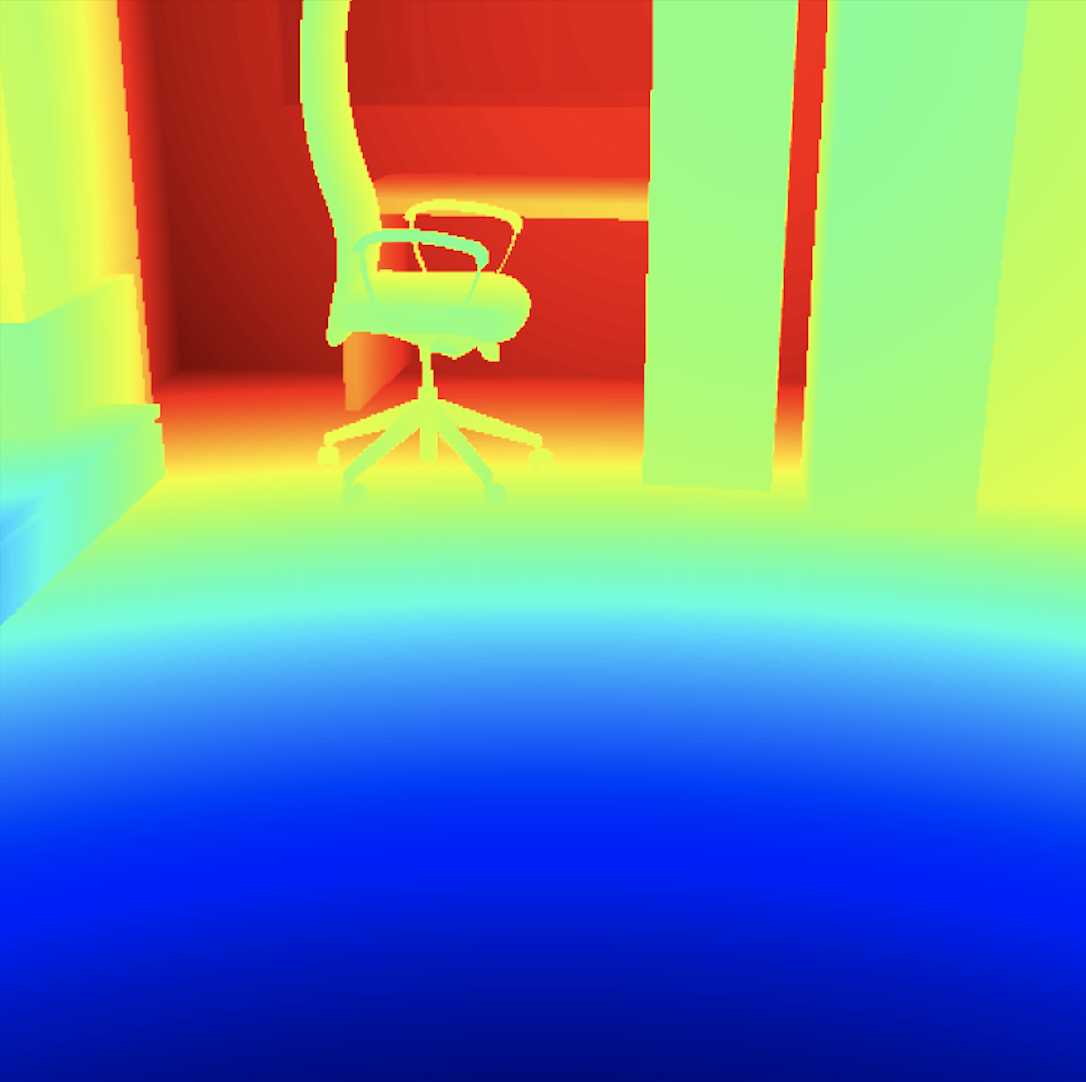
\includegraphics[width=.2\linewidth,valign=m]{/Users/apple/OVGU/Thesis/code/3dReconstruction/report/images/realistic_images_relatedwork/blenderproc_depth_2} &
        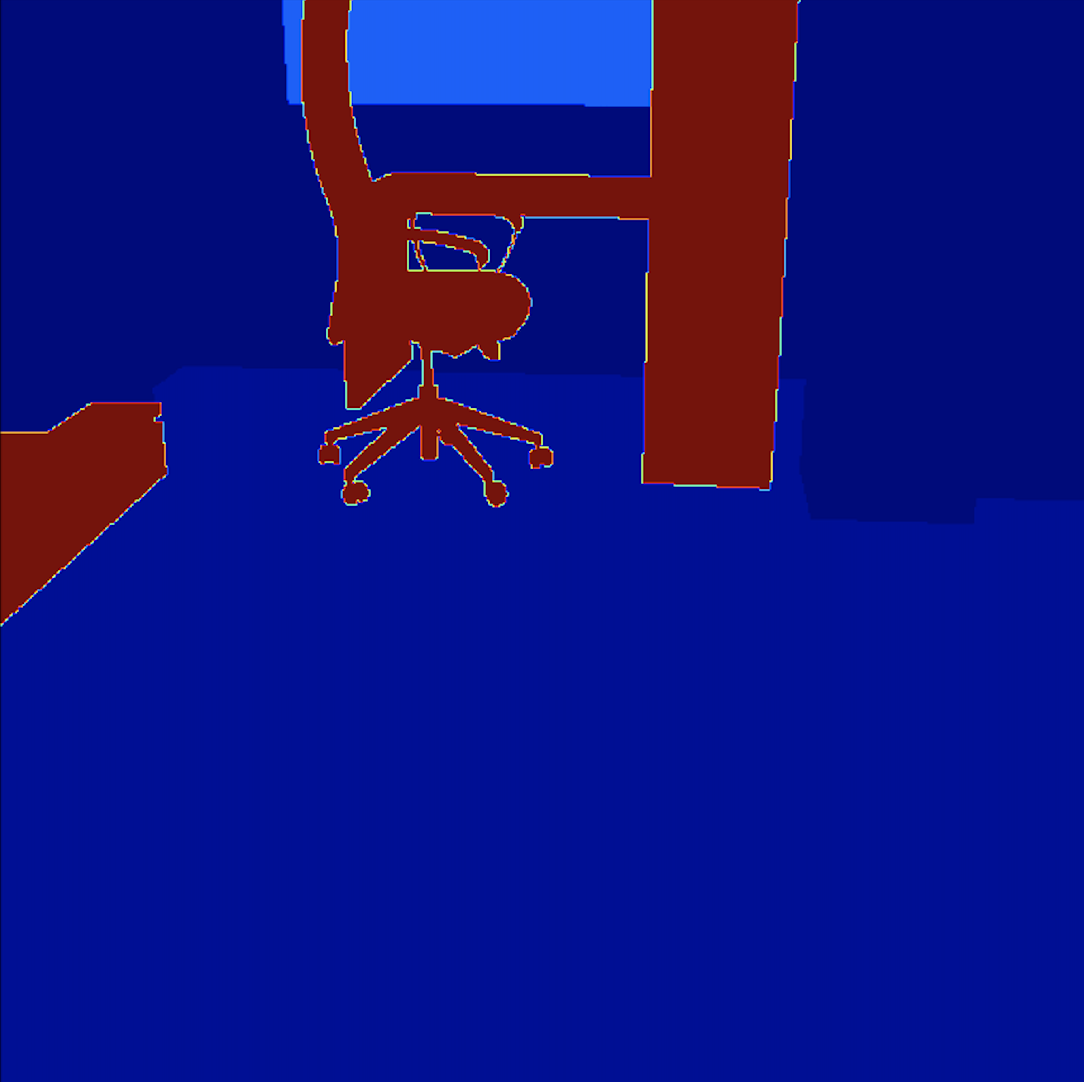
\includegraphics[width=.2\linewidth,valign=m]{/Users/apple/OVGU/Thesis/code/3dReconstruction/report/images/realistic_images_relatedwork/blenderproc_instance_2} &
        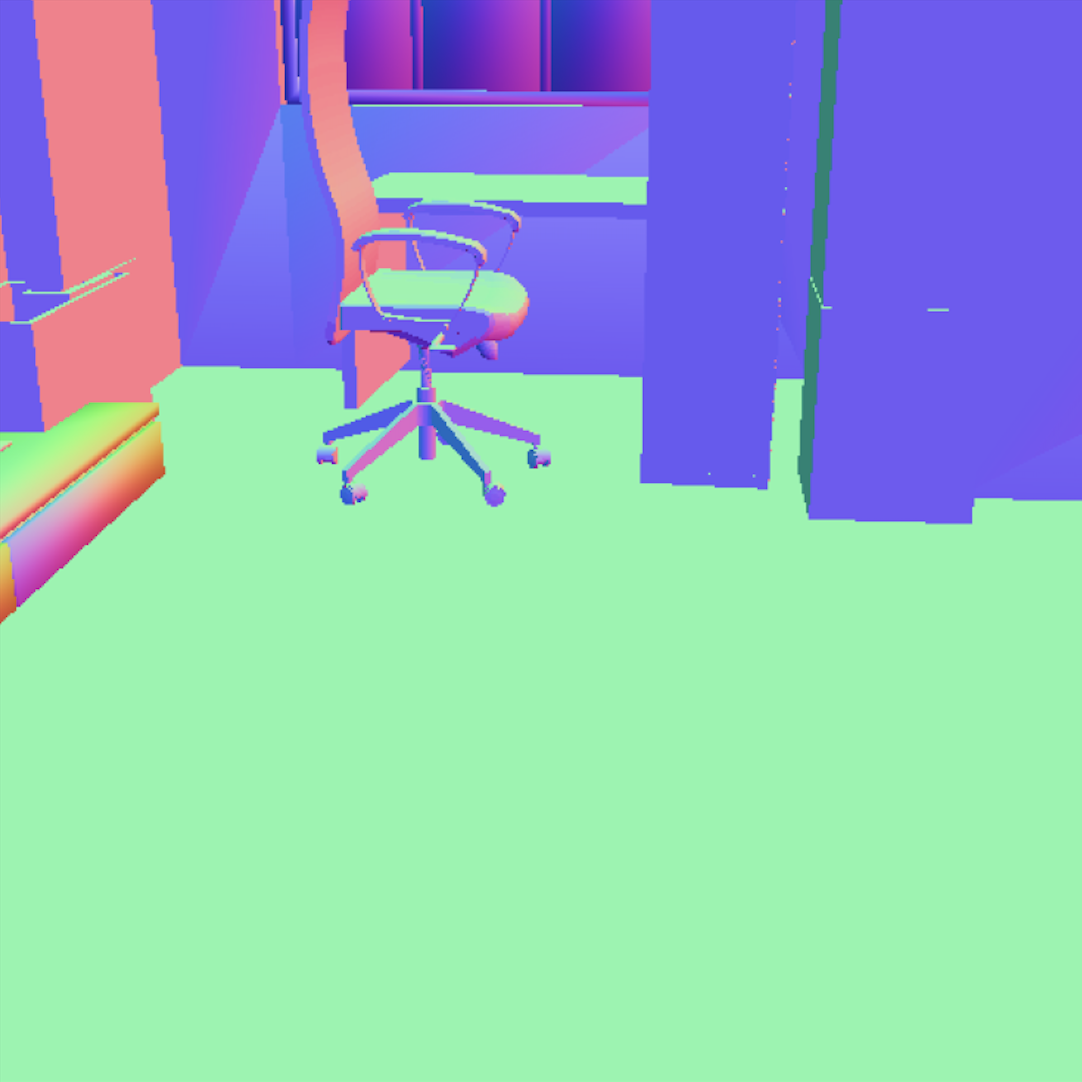
\includegraphics[width=.2\linewidth,valign=m]{/Users/apple/OVGU/Thesis/code/3dReconstruction/report/images/realistic_images_relatedwork/blenderproc_normal_2}\\

%        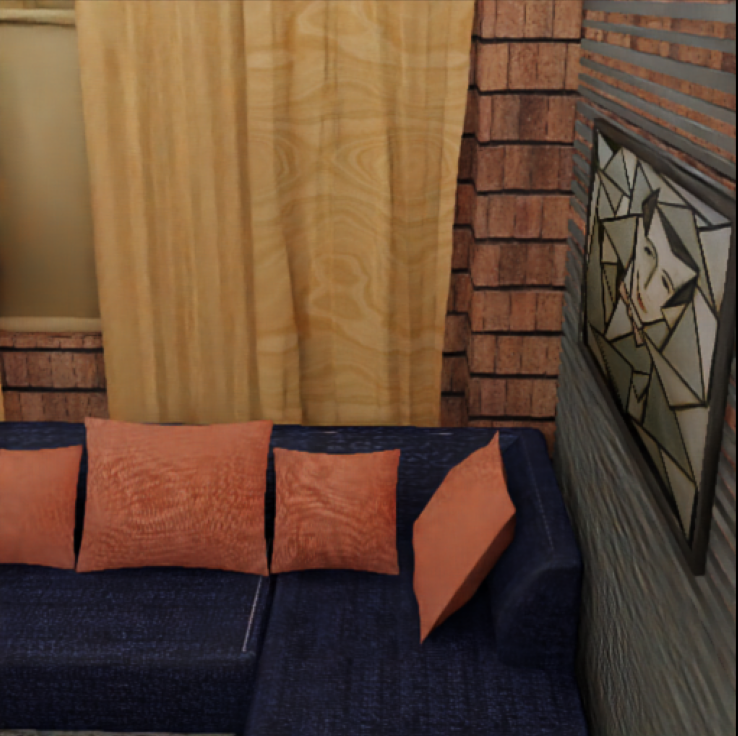
\includegraphics[width=.2\linewidth,valign=m]{/Users/apple/OVGU/Thesis/code/3dReconstruction/report/images/realistic_images_relatedwork/blenderproc_3} &
%        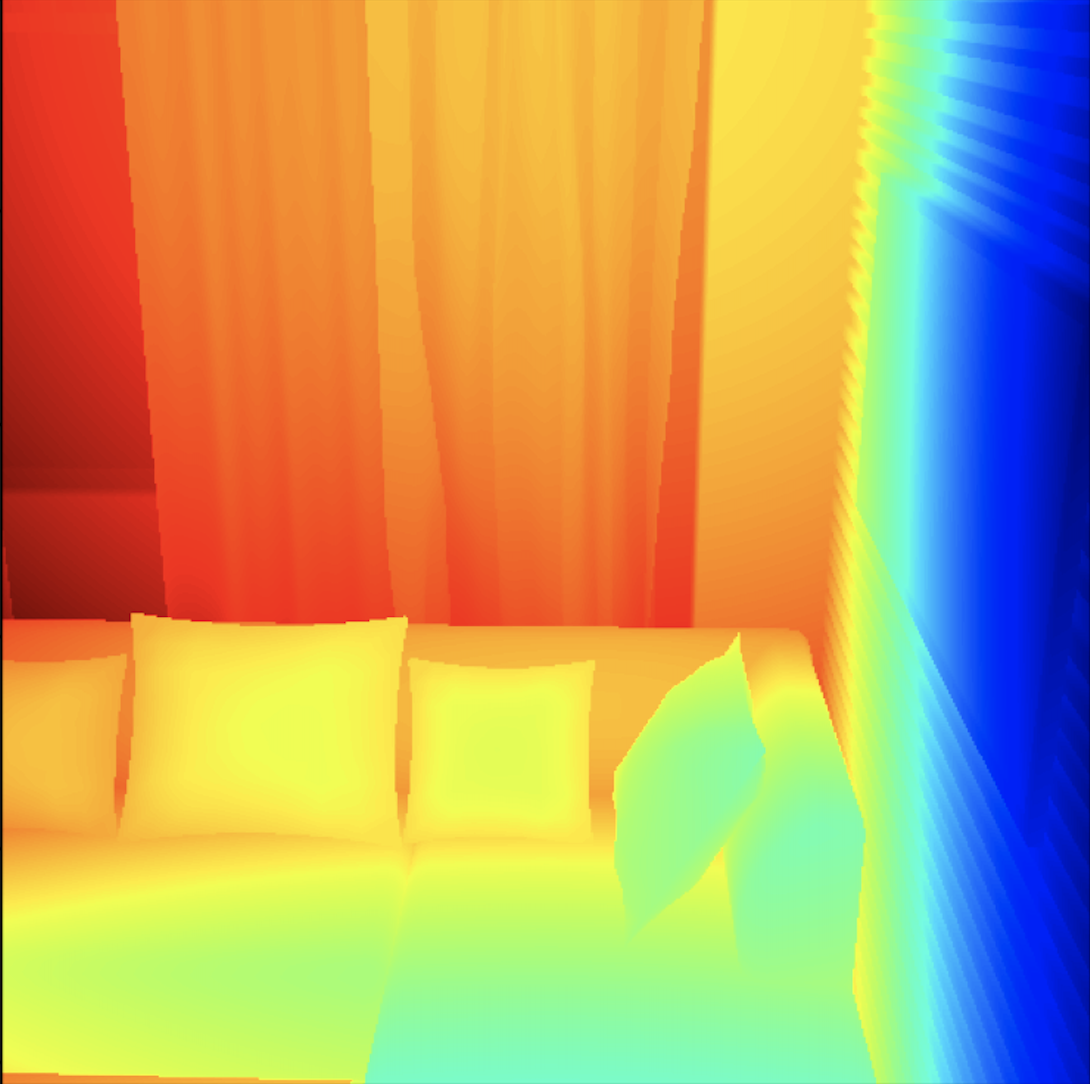
\includegraphics[width=.2\linewidth,valign=m]{/Users/apple/OVGU/Thesis/code/3dReconstruction/report/images/realistic_images_relatedwork/blenderproc_depth_3} &
%        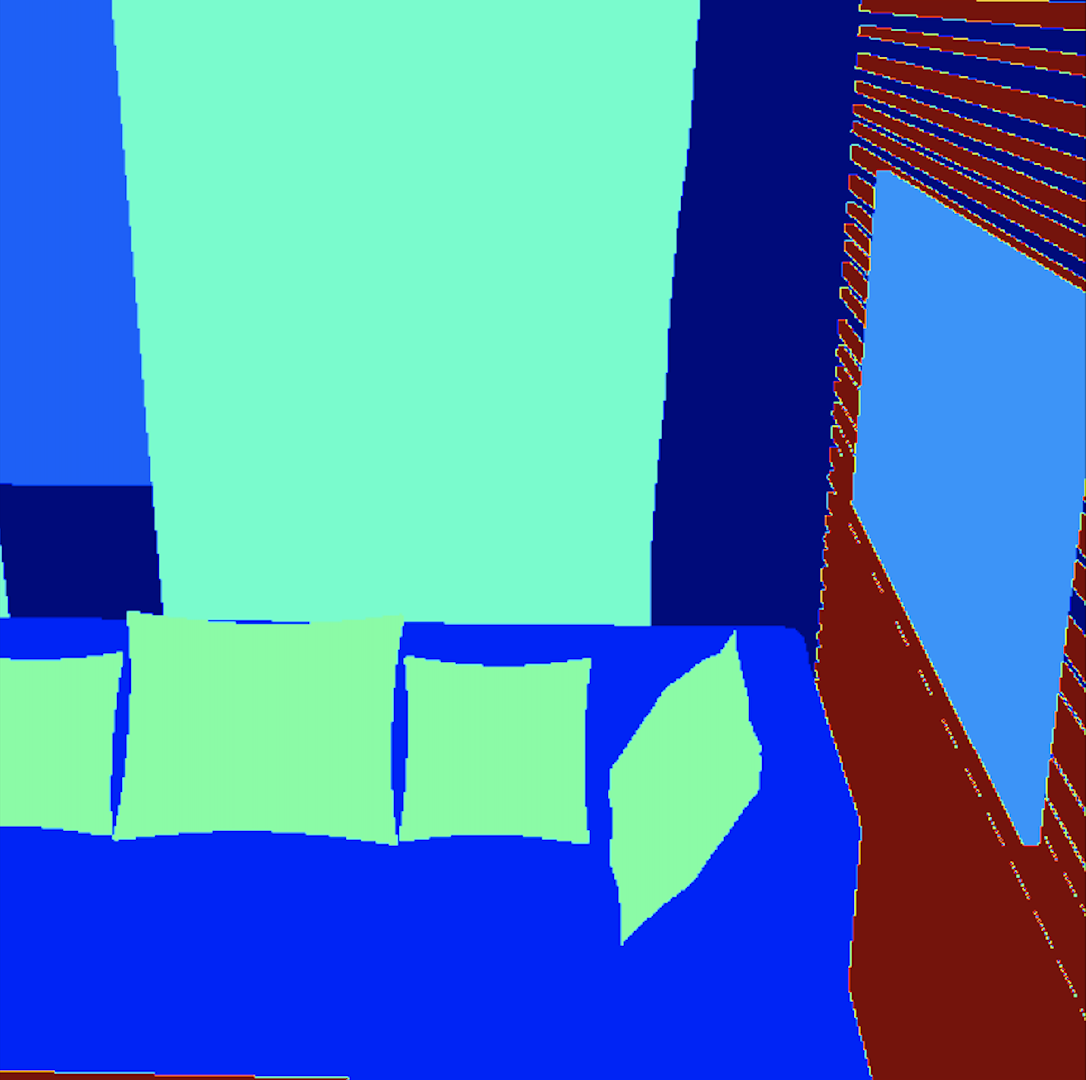
\includegraphics[width=.2\linewidth,valign=m]{/Users/apple/OVGU/Thesis/code/3dReconstruction/report/images/realistic_images_relatedwork/blenderproc_instance_3} &
%        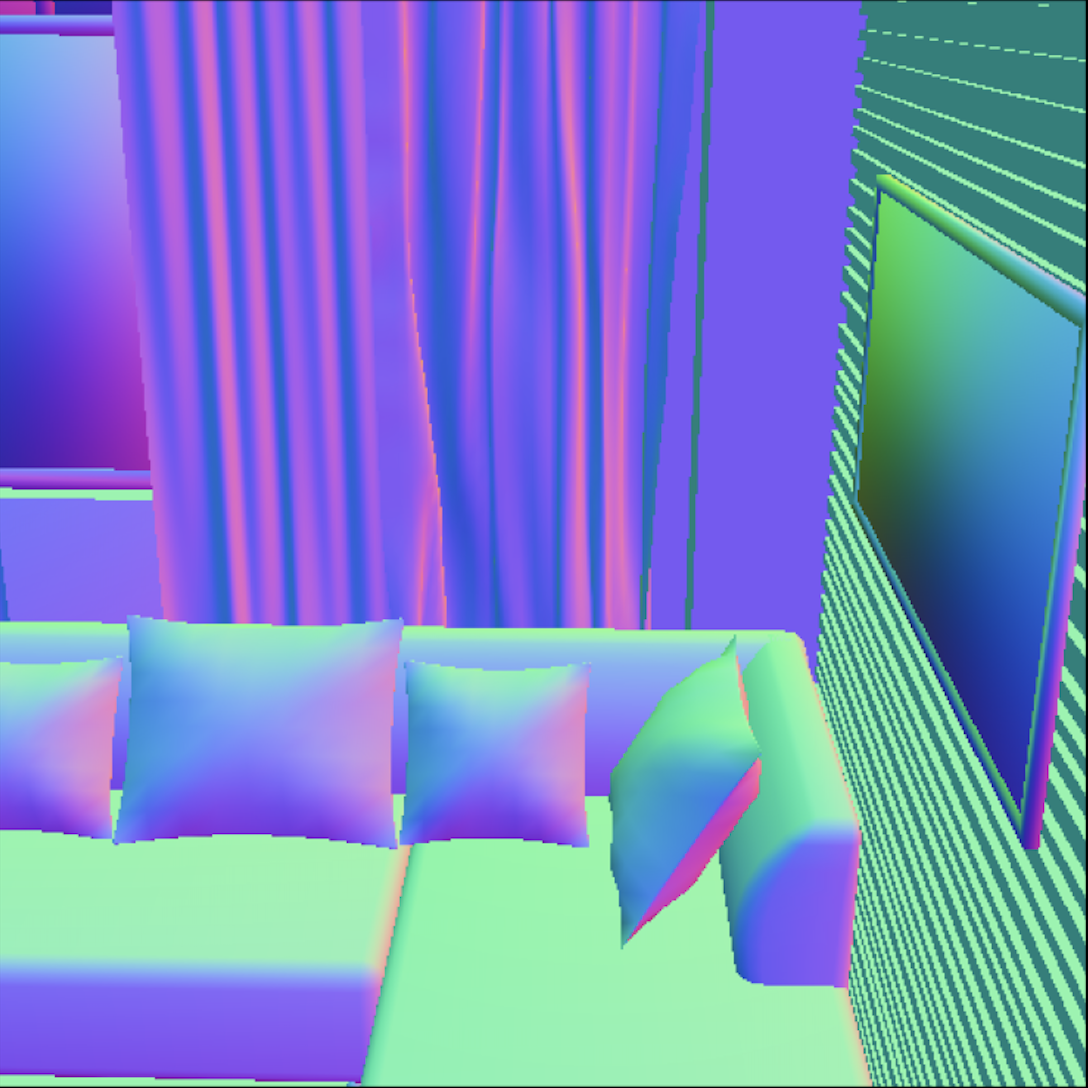
\includegraphics[width=.2\linewidth,valign=m]{/Users/apple/OVGU/Thesis/code/3dReconstruction/report/images/realistic_images_relatedwork/blenderproc_normal_3}\\

    \end{tabular}
    \caption{Sample images created from BlenderProc using SceneNet dataset.(Left to right) RGB images, Depth Maps, Instance Segmenatations and Normals. Each row is an independent sample.}
    \label{fig:Blenderproc samples}
\end{figure}

NVIDIA developed a Deep learning Dataset Synthesizer (NDDS)~\cite{to2018ndds} in the form of a plugin for Unreal Engine 4(UE4).
The plugin can synthesize images, per-pixel segmentation, depth, object 3D pose, 2D/3D bounding box, keypoints, and custom stencils.
It even supports domain randomization of objects, lighting, camera position, poses, and textures.
They Leveraged the asynchronous, multithreaded frames to generate data at high rates(50-100 Hz) for Falling Things (FAT)~\cite{tremblay2018falling} dataset.

"SynthDet: An end-to-end object detection pipeline using synthetic data"~\cite{synthdet2020} is an open-source project supported by Unity technologies using Unity Engine.
This ML pipeline uses 63 everyday objects(example: cereal box, cady, cartons, and more) as synthetic objects to generate 2D bounding boxes.
This project was highly influenced by~\cite{hinterstoisser2019annotation}, wherein they used synthetic 3D models with a randomized background to generate a synthetic dataset for the object detection task.
With domain randomization, the author of~\cite{hinterstoisser2019annotation} proved that no real data or mixed training is required for the Deep Learning model to perform significantly.

UnrealCV~\cite{qiu2017unrealcv} is an open-source project built upon Unreal Engine 4 (UE4)~\cite{unrealengine}).
It supports some pre-built indoor architectures available on the asset store, which are unfortunately paid versions.
Along with this limitation, the plugin only creates depth maps, normals, and segmentation masks, with no mapping to 3D models.
Another tool based on the Unreal engine is UnrealROX+\cite{martinezgonzalez2021unrealrox}.
This plugin design is based on UnrealCV and provides similar data.

\section{State of the art for 3d-reconstruction}\label{sec:state_of_the_art}

3D reconstruction task is on the rise with improvements in technologies like Augmented and virtual reality.
Scene understanding becomes essential for these technologies to succeed.
As discussed in \autoref{sec:Volumetric representation}, 3D models have voxels, meshes, and point clouds as representations.
Each of the representations has been explored for reconstruction, and this section explores some approaches.

The task can either be applied to \b{a multi-view, or a single view image}.
~\cite{Kar2017LearningAM, choy20163d, Yang_2019, huang2018deepmvs, Paschalidou2018RayNetLV, Xie_2019, Xie_2020},
are architectures based on multiple input images of the same images from different views to learn the underlying 3D structure.
~\cite{Kar2017LearningAM, choy20163d} are architectures based on Recurrent Neural Networks (\gls{rnn}) and have the disadvantage of memory,
long-term dependencies, and long inference time.
~\cite{Yang_2019, huang2018deepmvs, Paschalidou2018RayNetLV} explore different ways of pooling(attentional, max, and average pooling, respectively)
to aggregate the feature vectors from different views.
The pooling method tends to capture only partial information with loss in detail.

For single-view reconstruction, we have architectures like~\cite{wu2017marrnet,z-gan, Yang_219, wu2018learning, popov2020corenet}.
~\cite{wu2017marrnet} predict the 3D structure by estimating 2.5D properties like surface normals, segmentation, and depths.
~\cite{wu2018learning} is an extension of MarrNet, which proposes a network to preserve the naturalness of the surface.
Inspired by generative models~\cite{Goodfellow2014GenerativeAN,kingma2014autoencoding}, many 3D reconstruction architectures were published~\cite{z-gan, Yang_219,wu2017learning,Lunz2020InverseGG}.
Both~\cite{Xie_2019, Xie_2020} also can predict 3D structure from a single view image.

Many new architectures have also been proposed to overcome the memory issues caused by 3D voxels~\cite{tatarchenko2017octree,Richter2018MatryoshkaNP,Mescheder2019OccupancyNL,Gkioxari2019MeshR, wang2018pixel2mesh,groueix2018atlasnet,pan2019deep}.
These are approaches that are based out of oct-tree, meshes, occupancy of a voxel.
Occupancy networks are an implicit way of representing 3D surfaces as decision boundaries using the network as a deep learning classifier.
For mesh-based reconstruction, a template mesh such as an ellipsoid is deformed to get the structure of the 3D model.
For the Oct-tree-based reconstruction, as the name suggest, instead of 3D voxels, the models are discretized in Oct-Tree representation.
Oct-tree can further make the process memory and compute efficient, providing higher resolution than 3D voxel representation.

Supervision is another factor to consider for 3D reconstruction tasks.
There are methods based on \b{3D-Supervision or 2D-Supervision}.
~\cite{Xie_2019,Xie_2020,wu2017marrnet,groueix2018atlasnet,pan2019deep, chen2019learning} are few of the 3D-supervision based architecture.
For all these architectures, it is necessary to either have the 3D voxel grid or 3D mesh for supervised training.
For models described in~\cite{Lunz2020InverseGG,henderson2019learning},the 3D reconstruction only needs 2D supervision like a silhouette.
One might argue that for 3D supervision, we need a large number of 3D models designed and created by professional artists
With the advent of Virtual and Augmented realities, 3D models available to the public is increasing exponentially, which might resolve the issue.

\section{Mitigating domain shift}\label{sec:mitigating_domain_shift}

The idea of domain randomization is that real images appear to be one of the many variations among training images from synthetic datasets.
Thus, testing with real-world images should give a comparable performance.
~\cite{tobin2017domain} used this principle for small objects detection tasks used for robotics.
This paper tries different parameters in domain randomization like lights, camera viewpoints, and textures and combines domain randomization with domain adaptation.

~\cite{prakash2020structured} introduced Structured domain randomisation, where the structure and context are preserved for the problem while creating synthetic images.
Example: A road is randomly placed with parameters like curvature, lighting, and camera position.
With this as context, they generate pedestrian walk, road lanes, etc.
After these two steps, the objects such as cars, cyclists, houses, buildings are placed on the scene.
As an ablation study, the author changes domain randomization parameters and checks the performance of the car detection task.

~\cite{georgakis2017synthesizing} proposed domain randomization-based synthetic images generation to detect objects found in the kitchen.
The objects are cropped and placed on the background with semantic information and geometry with proper scale.
Similar to the above works, the author also provides an ablation study with different ratios of synthetic to the real dataset for mixed training.

Domain randomization and adaptation techniques are not the only ways to mitigate the domain shift.
With the advent of Generative Adversarial Networks~\cite{Goodfellow2014GenerativeAN},synthetic to real image conversions have become possible and lead to better performance on given tasks.
~\cite{Richter_2021, CycleGAN2017, park2020cut,isola2017image, dundar2018domain,Wang2018HighResolutionIS} are some successful attempts to reduce the gap between simulated environment and reality.
Intel in~\cite{Richter_2021} uses GTA V dataset with G-buffers(depth, normals, segmentations, Albedo, glossiness, etc.) to enhance the photorealism of synthetic images.
~\cite{park2020cut} use a patchwise contrastive loss to retrain the content of the input image.
They minimize the loss such that corresponding patches retain high mutual values.

Another exciting way to reduce the domain gap is using domain adversarial training~\cite{ganin2016domainadversarial}.
Along with the task under observation, a branched network from the feature extractor is used as a classifier for the domains.
This acts like a multi-learning task where the feature extractor is the common branch.
In one branch the model learns to perform a specific task like segmentation or classification.
The other branch classifies if the dataset is real or synthetic.
~\cite{pinheiro2019domainadaptive} implements the same principle on complex 3D reconstruction tasks by predicting voxels and classifying the image domain.

\subsection{Training with synthetic dataset}\label{subsec:training-with-synthetic-dataset}
The research questions, as stated in \autoref{sec:goal} aims to check if a synthetic dataset can deliver as a standalone dataset.
If it does not, then techniques like fine-tuning will be helpful.
Another way to use the large synthetic datasets is using mixed training.

In~\cite{nowruzi2019real},  the author tries to find how much real data is required with the synthetic dataset to increase the performance of object detection tasks.
A study was conducted by training various object detection models on mixed data containing different real and synthetic datasets ratios.
The four ratios considered for mixed training were 0\%, 90\%, 95\%, 97.5\% of synthetic data to real data.
Another study was conducted by fine-tuning a model pre-trained on a synthetic dataset with real datasets of different sizes.
They observed that fine-tuning with a limited real dataset is better than mixed training with a synthetic dataset.

~\cite{Tremblay2018TrainingDN}  explore domain randomization on real-world object detection.
The author also proposes a new approach of domain randomization, wherein random 3d objects called ”flying distractors” are randomly placed in the scene;
the model learns to ignore objects that are not of interest.
A focused ablation study with individual domain randomization parameters was also conducted to understand the contribution of each component.
The parameters included lights, textures, data augmentation, and flying distractor, as mentioned above.
Also, object detection is trained with varying dataset sizes to learn its impact.
They also conducted a study of the dataset size needed to fine-tune a pre-trained model optimally.

\cite{2018LearningIC} used mixing ratios for classification task for each of the mini-batches and observed 5-13\% improvement in performance.
The mixing ratios used were 1:15, 1:7, and 1:1.
A comprehensive study was made on randomization using datasets containing textures, random camera positions, background, lightings, and augmentations.


\chapter{\iftoggle{german}{Konzept}{Concept}}\label{ch:concept}

In this section we discuss about the dataset and design choice,\todo and the rationale behind reducing the domain gap.

\section{Pix3D: A large-scale benchmark}\label{sec:pix3d}
In ~\cite{pix3d}, a large-scale benchmark for 2D-3D alignment was introduced.
The raw images from web search engines were collected and labelled keypoints were used to align the 2D images with the corresponding 3D shapes.
The 3D models are extension from IKEA dataset~\cite{Lim2013ParsingIO}, which is a collection of high-quality IKEA furniture.
The dataset also provides with binary mask and the keypoints for the object under observation.
For adding more images to the IKEA dataset, the authors of ~\cite{pix3d} conducted manual web search on Google, Bing, and Baidu, using Ikea model name as keywords.
to get around 104,220 images which were further filtered by removing irrelevant images with the help of Amazon Mechanical Turk (AMT) workers.
After this manual experiment the total images in Pix3D, only 14,600 images were selected for the 219 Ikea models.
For our experiment on synthetic to real dataset, we chose to select only furniture classes from Pix3D, leaving out "misc and tools" classes, which were significantly less to begin with.


\subsection{Disadvantages of Pix3D}\label{subsec:disadvantages-of-pix3d}

The distribution of models in pix3d is as shown in ~\ref{fig:pix3d_histogram}.
As we can see, the dataset distribution is uneven across classes and more than 50\% of classes have less than 1000 images.

Though Pix3D set a benchmark for 2D-3D alignment, here are few disadvantages of using this real dataset.
\begin{enumerate}
    \item For Deep Learning approaches, we need large-scale data and 14,600 might not be sufficient.
    \item The orientation of object is not randomised.
    \item The dataset does not provide 2.5D information (i.e.\ depth and normal) which can be crucial for 3D learning.
\end{enumerate}

\begin{figure}[!ht]
    \centering
    \subfloat[][]{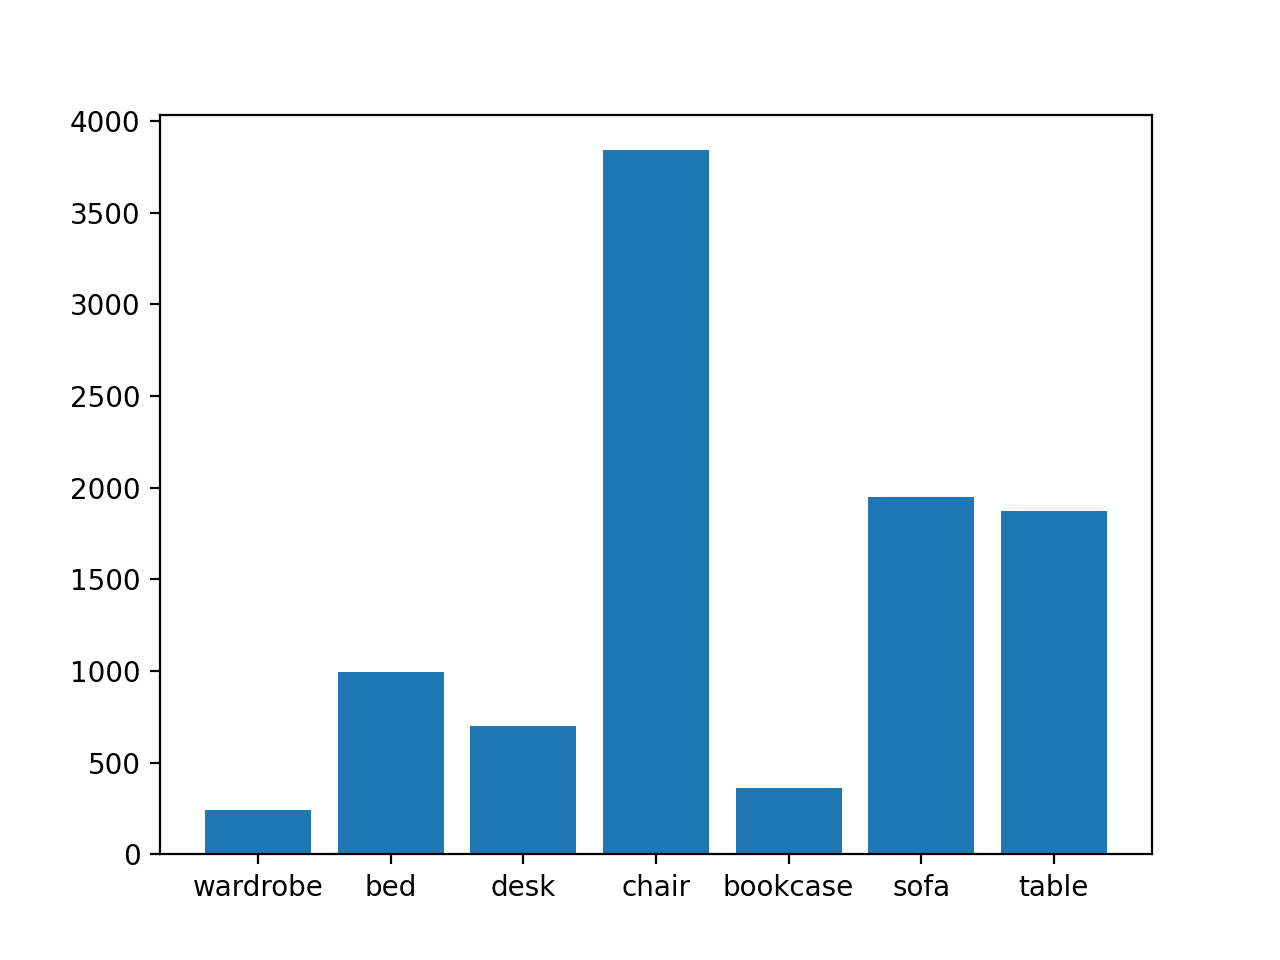
\includegraphics[width=.45\textwidth,height=6cm]{/Users/apple/OVGU/Thesis/code/3dReconstruction/report/images/pix3d/pix3d_histogram}}\quad
    \subfloat[][]{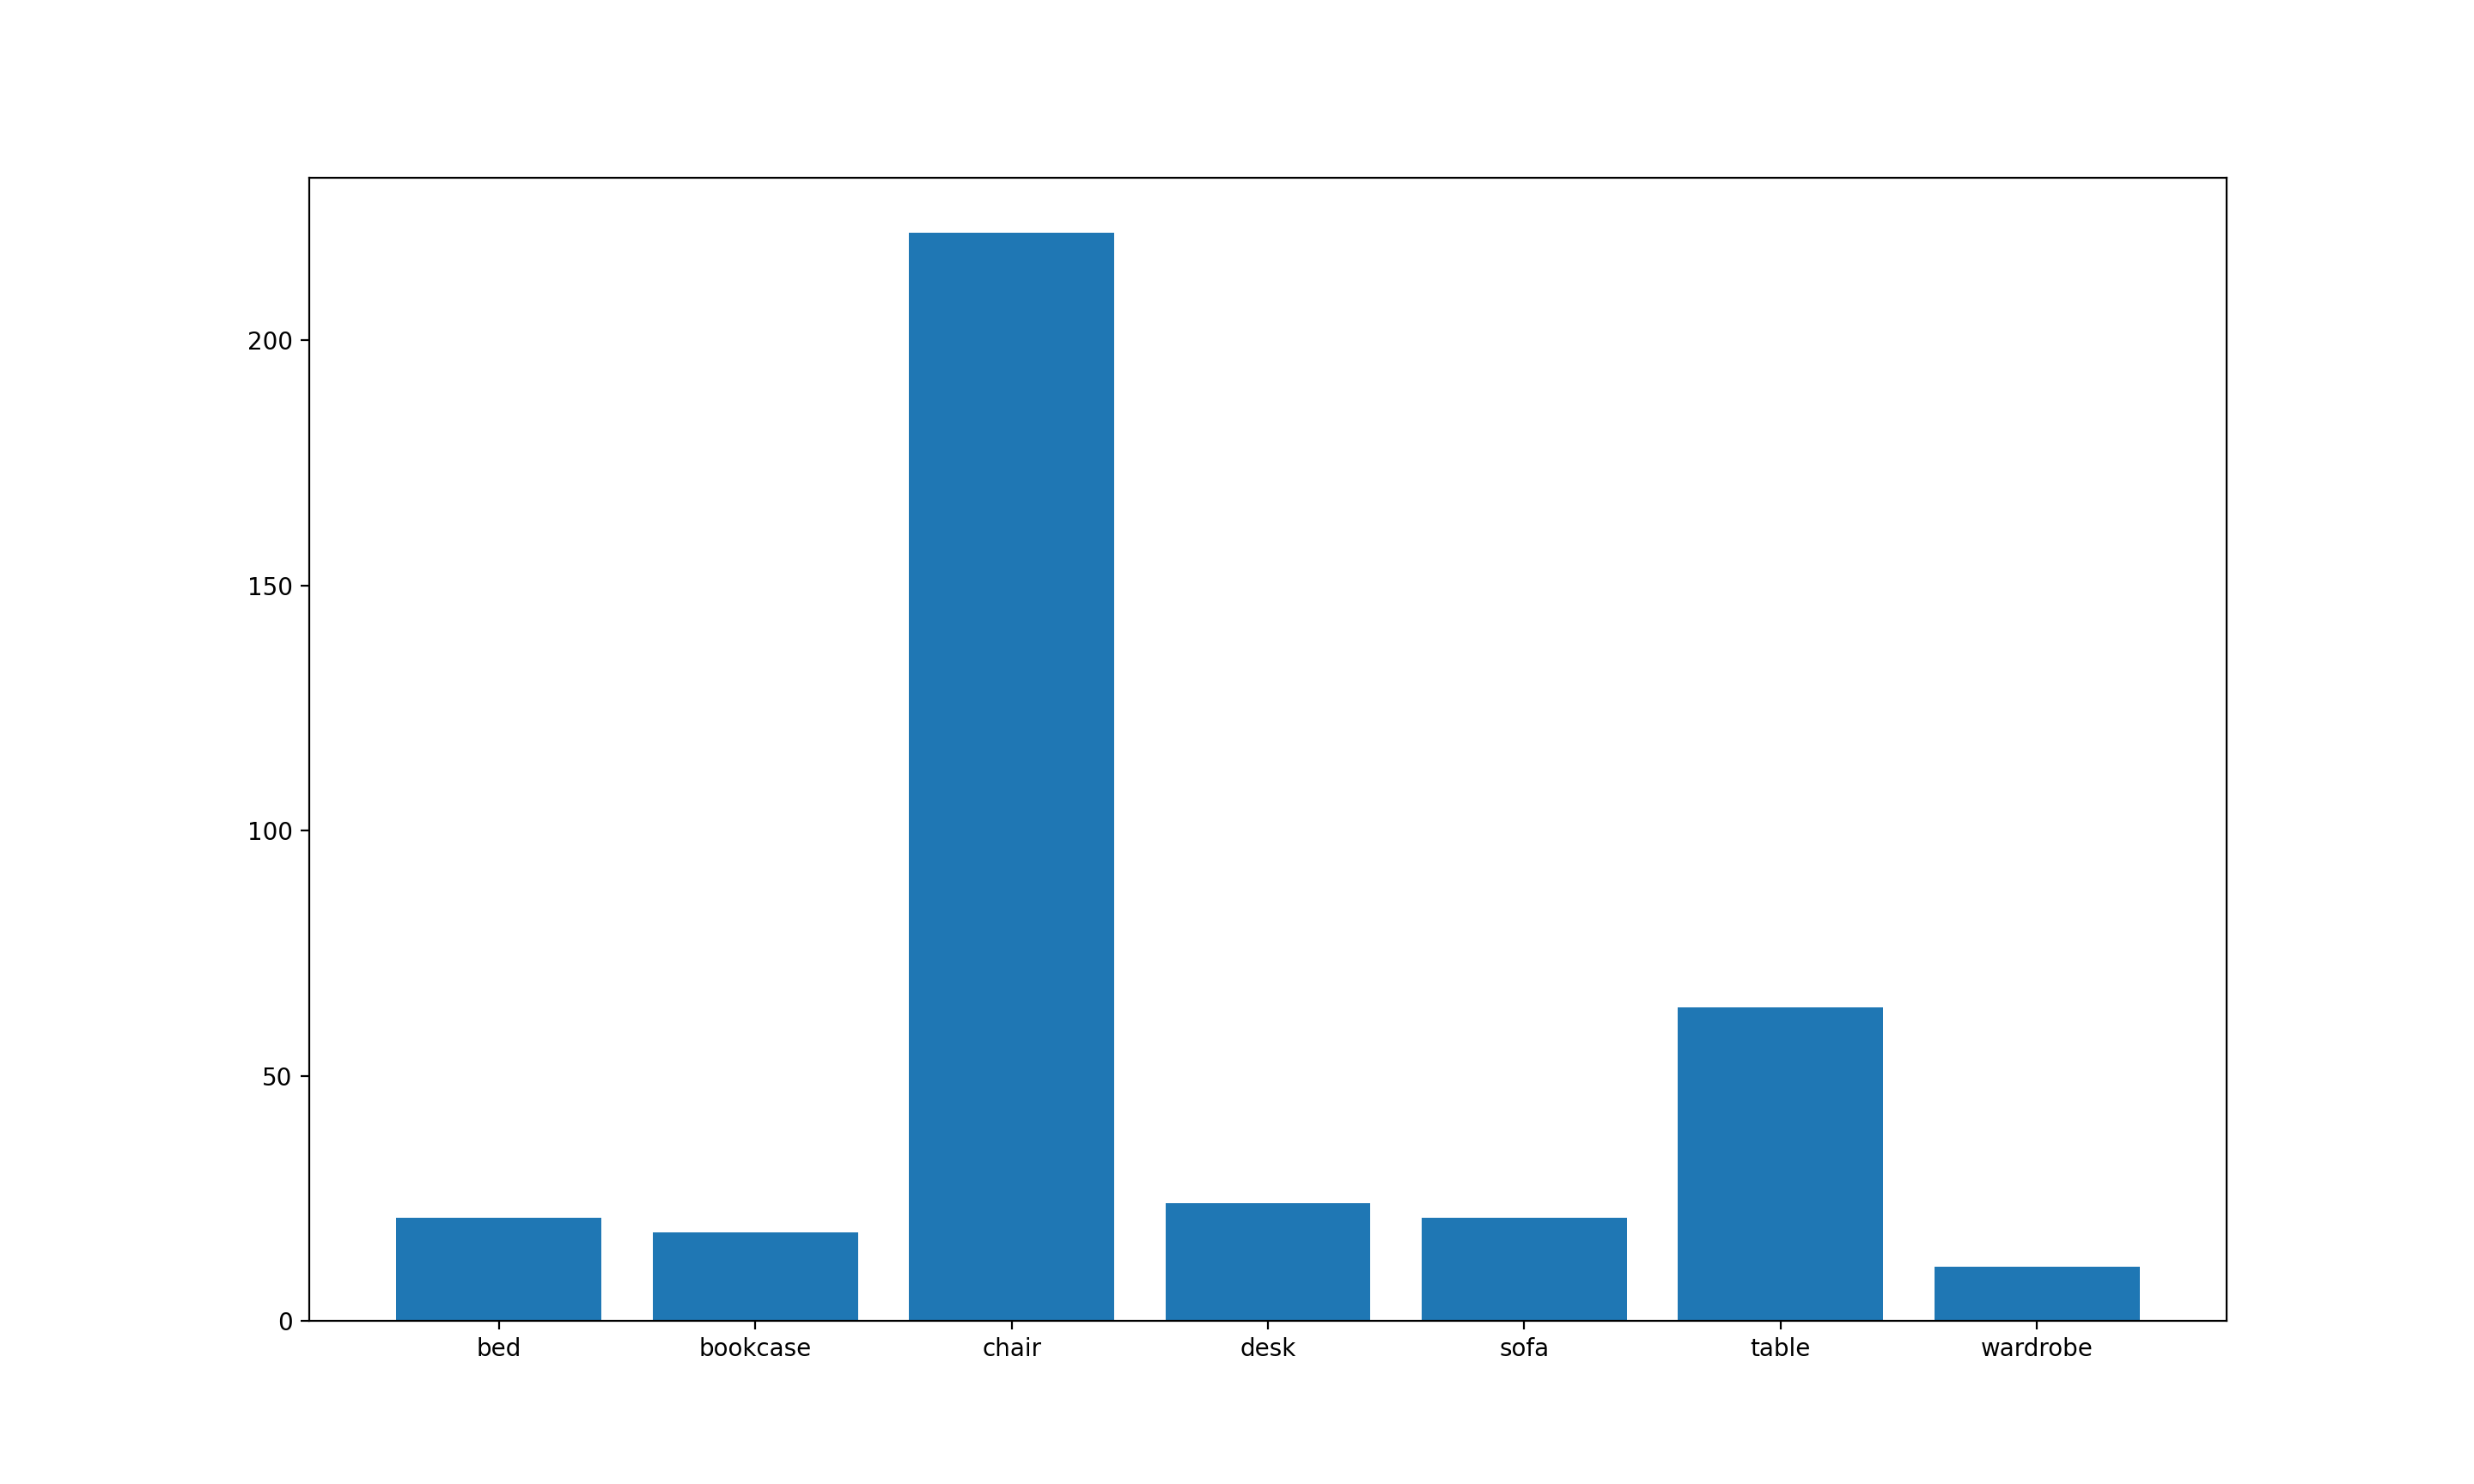
\includegraphics[width=.45\textwidth,height=6cm]{/Users/apple/OVGU/Thesis/code/3dReconstruction/report/images/pix3d/pix3d_models_histogram}}\\
    \caption{Distribution of pix3D~\cite{pix3d} images(left), unique models(right)}
    \label{fig:pix3d_histogram}
\end{figure}

\subsection{Why Pix3D?}\label{subsec:why-pix3d?}
Pix3D is a collection of indoor scenes with complex background, varying light conditions with shadows, reflective surfaces and even varying occlusion levels.
Each image comprises a collection of objects in the scene, but only one object from the category is annotated.
It is a perfect example of having limited real world data.
Since 3D models are available for each furniture,a synthetic data can be generated in abundance from those models.
Samples from Pix2D are as shown in figure ~\ref{fig:Pix3D samples}.

\begin{figure}[!ht]
    \centering
    \subfloat[][]{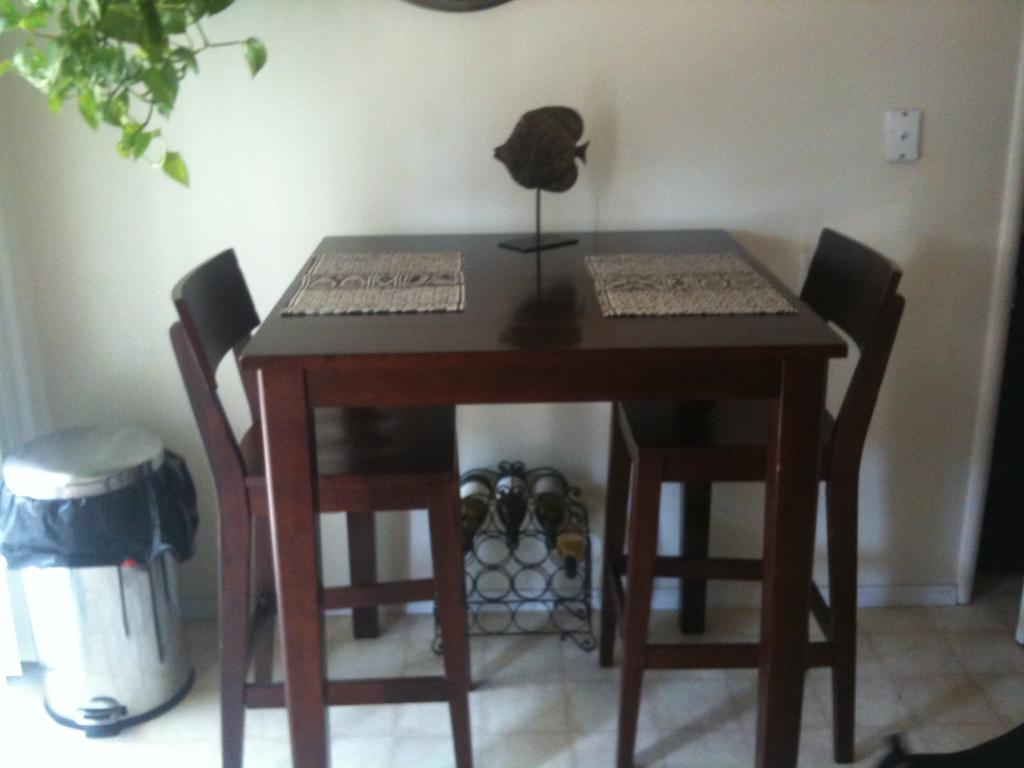
\includegraphics[width=.4\textwidth]{/Users/apple/OVGU/Thesis/code/3dReconstruction/report/images/pix3d/pix3d_5}}\quad
    \subfloat[][]{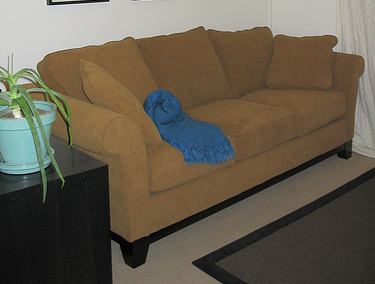
\includegraphics[width=.4\textwidth]{/Users/apple/OVGU/Thesis/code/3dReconstruction/report/images/pix3d/pix3d_2}}\\
    \subfloat[][]{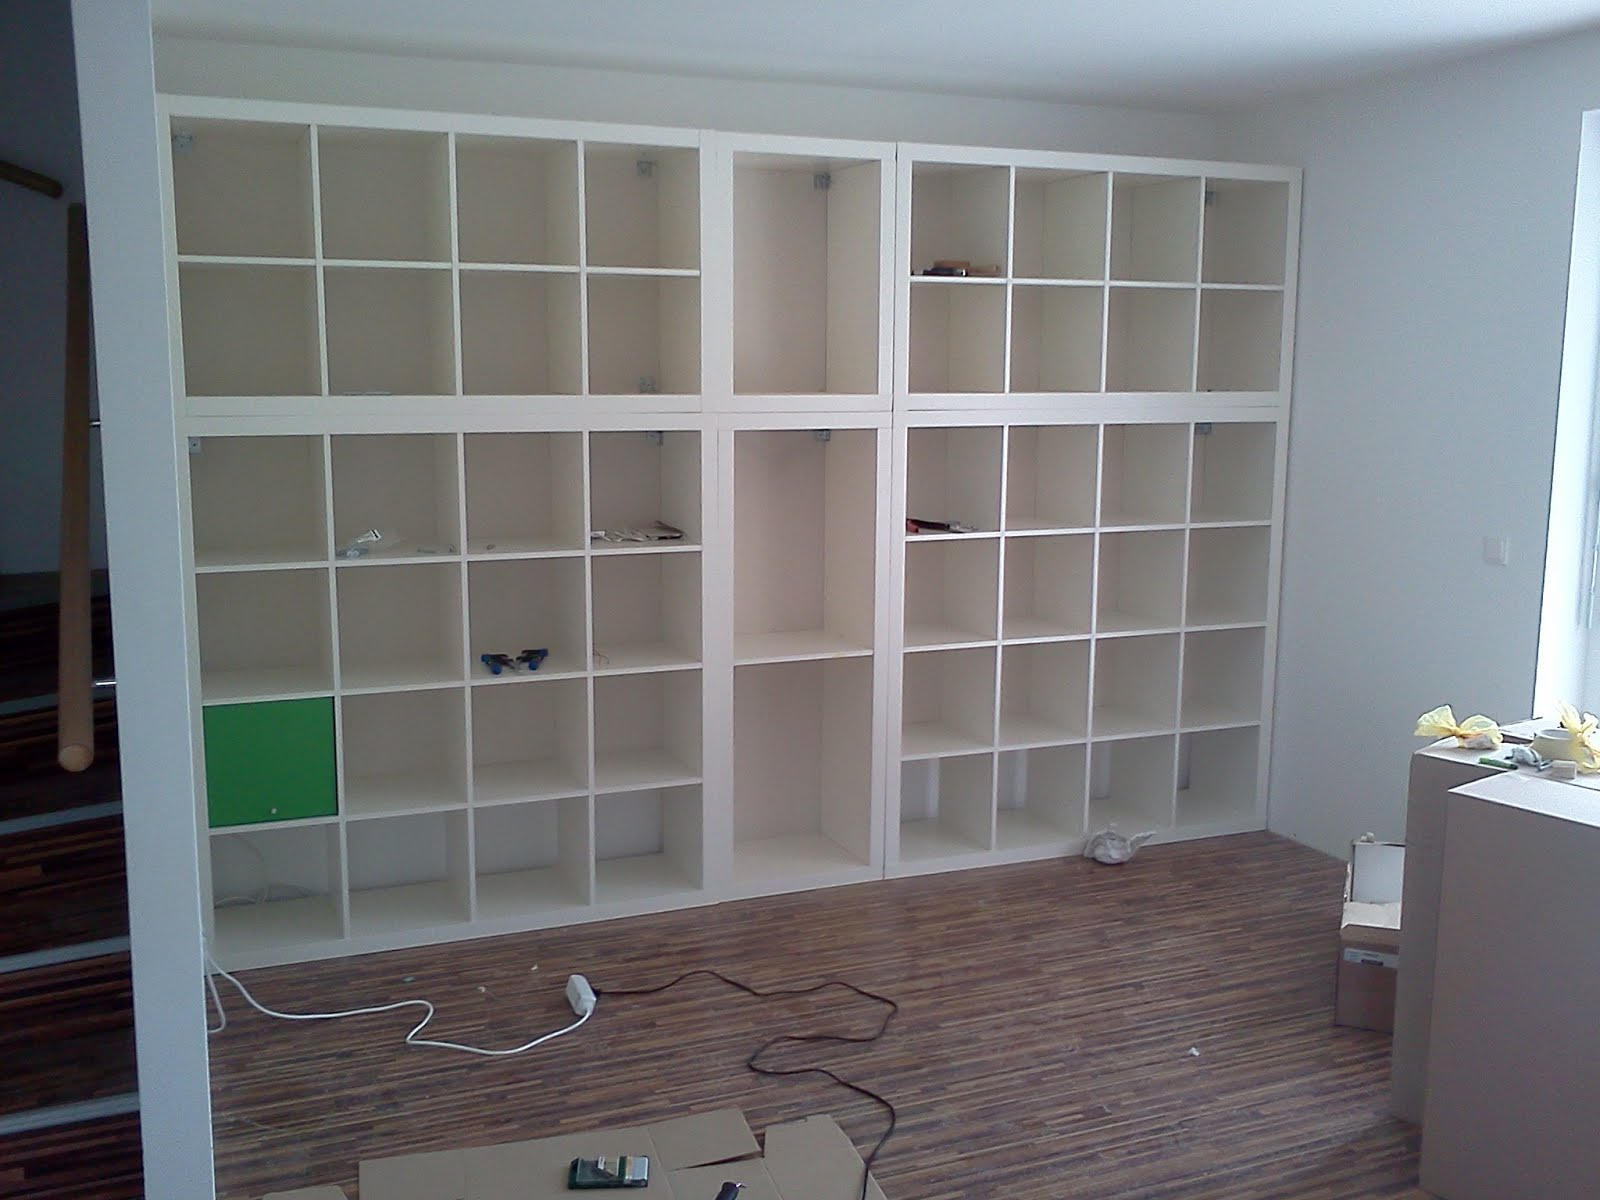
\includegraphics[width=.4\textwidth]{/Users/apple/OVGU/Thesis/code/3dReconstruction/report/images/pix3d/pix3d_6}}\quad
    \subfloat[][]{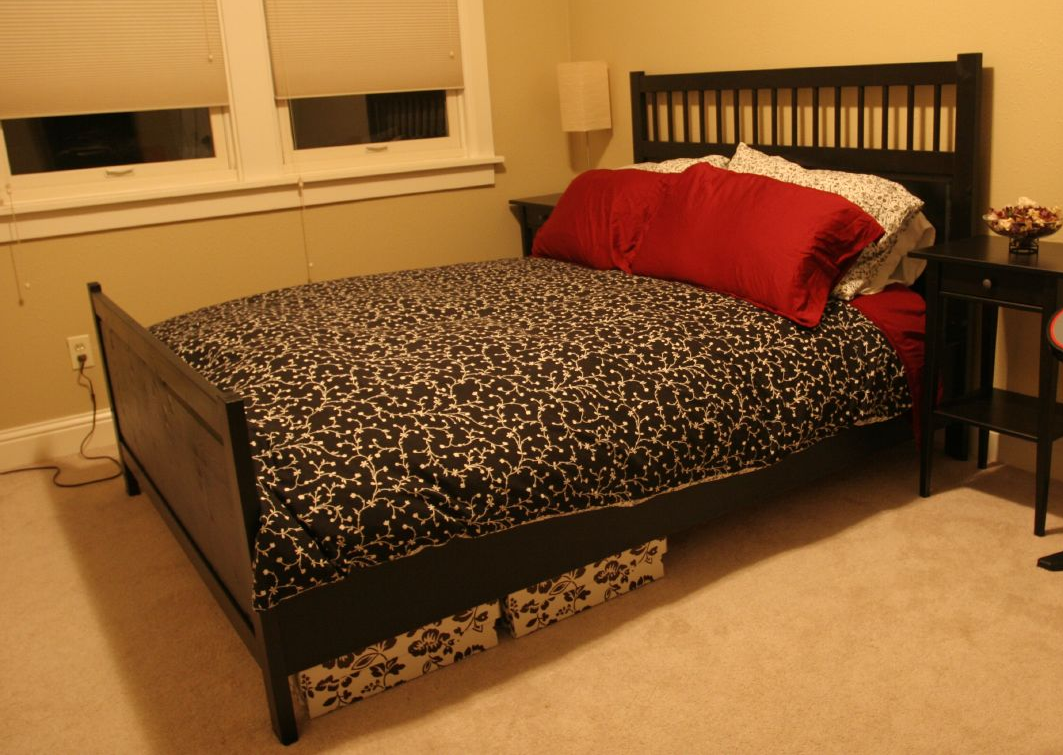
\includegraphics[width=.4\textwidth]{/Users/apple/OVGU/Thesis/code/3dReconstruction/report/images/pix3d/pix3d_4}}
    \caption{Sample RGB images from pix3D}
    \label{fig:Pix3D samples}
\end{figure}

\section{Role of SceneNet}\label{sec:role-of-scenenet}
SceneNet ~\cite{McCormac:etal:ICCV2017} is a large collection photorealistic indoor scene trajectories.
The dataset provides with images and videos of indoor scene which can be used for tasks like SLAM, semantic and instance segmentation,
object detection and further enhanced for other vision problems like optical flow depth and pose estimation ~\cite{McCormac:etal:ICCV2017}).
They use ShapeNet~\cite{chang2015shapenet} models to occupy 57 indoor scenes which gives the scene unlimited configurations.
Unfortunately there is no mapping from scene to 3D model for tasks like 3D reconstructions.
In our approach, we utilize the scene provided by SceneNet as layout for our indoor scenes.
This includes initial shapenet models with furniture placement.
We then replace the class under observation with a corresponding model from Pix3D.

\section{Unity based pipeline}\label{sec:unity-based-pipeline}
Unity game engine is used for creating the synthetic dataset.
The reasons for selecting Unity as our platform for the application are:
\begin{enumerate}
    \item Cross-platform game engine and hence can be used on an Operating system.
    \item The basic version is available for free.
    \item Provides all the necessary tools to create an ersatz environment with a well maintained documentation.
    \item An active developer community.
\end{enumerate}

There is no official comparison between Unreal Engine and Unity engine to have a deciding factor.
The selection of unity engine was purely individual choice and ease of use.
But both these game engines have ability to create realistic looking scenes which can be used for synthetic dataset generation.
With Unity game engine, the available scenes from scenenet and 3D models from pix3d can be imported to form an ersatz environment.
Further domain randomisation can be applied to create a dataset of photorealistic images and 2.5D data like normal, depthmaps, masks.

\subsection{Domain Randomisation with Unity Engine}\label{subsec:domain-randomisation-with-unity-engine}
In this section we discuss what kind of domain randomisation is applied for the dataset creation.
\subsubsection{Scenes from scenenet}\label{subsubsec:scenes-from-scenenet}
As discussed in section ~\ref{sec:role-of-scenenet}, SceneNet provides wide variety of indoor scenes which includes bedrooms, bathroom, living room, kitchen and office.
For our case, we did not consider the bathroom, as the categories under observations are furnitures which we rarely see in the bathroom.
For the rest of the scenes we have a pre-determined setup given by scenenet.
We use 25 scenes in total as basic rooms for our target object to be place.
And with further randomisation we feel this should be sufficient to check if unity can produce a useful dataset.

\subsubsection{Camera Viewpoints}
The position and orientation of camera gives us the most randomisation in this setup.
The minimum and maximum distance can be chosen by the user for the camera to be places from the target object.
A random point can be selected in this range as the position for the camera.
As for the orientation of the camera, we can make the camera to always look at the target object, irrespective of the position.
With this, we achieved different background for target object, and the target object itself appears to be in different position and orientation.

\subsubsection{Lighting and shadows}
Lighting plays an important role in photorealism.
If the lighting is not setup correctly the synthetic dataset will never seem to be photorealistic.
Unity offers wide variety of lighting like global light which acts like the sunlight, and various indoor lighting systems.
Ideally we should make the luminous objects like lamps, chandelier, bulbs etc be the source of light for indoor scenes, but we observed that the room does not lit up uniformly which makes in less photorealistic.
Hence we use some pre-determined lighting settings which will be further discussed in implementation section ~\ref{sec:3d-scene-framework}.

\subsubsection{Randomised textures}
SceneNet ~\cite{McCormac:etal:ICCV2017} also provides with textures for different categories in the scene.
We then further increase the texture database by adding few more textures from ambientCG.com, which provide license for free.
We randomly allocate textures to each object making sure that each category has same texture to make the scene more uniform.

\subsubsection{Replacing target objects}
To further randomise the scene, the category of target objects in the scene are replaced by the object under observation.
When there are more than one object of same category we randomise the selection of which object is to be replaced which further randomises the captured data.
The scale of the target object is made to match the scale of the category object in the scene in the least dimension.
For example if the length of the length of the category object in the scene is the least amonth length,width and height, then the target object is scaled to match this length.
This makes the target object blend in with the scene.

\section{S2R:3D-FREE, a Pix3D based sythetic dataset}\label{sec:s2r:3d-free-a-pix3d-based-sythetic-dataset}

S2R:3D-FREE dataset, which stands for Synth2Real: 3-Dimensional Furniture Reconstruction from Ersatz Environment, is a combination of SceneNet and Pix3D dataset.
We utilize the availibility of 3D models of rooms and furnitures from these 2 dataset to create an ersatz environment using Unity as our framework.
We randomise the indoor scenes from SceneNet ~\cite{McCormac:etal:ICCV2017} along with textures provided by them with some additional complex textures.
The other option would have been to use the shapenet as the target model, but in this case we would not be having a real dataset to compare to.
Ideally a model trained on shapenet should also perform well with a real dataset like pix3d, but we decided to have a synthetic dataset based on pix3d itself for better comparison.

\section{3D reconstruction}\label{sec:3D reconstruction}
Now that we discussed on how the dataset will be created, we move to the deep learning aspect of this thesis.
3D reconstruction is the task to convert a 2-Dimensional RGB image into a known 3D representation of the model under observation.
For voxel-based approach, the 3D model space is discretized to obtain 3D voxel grid $X$.
Let $I = \{I_k \mid k = 1,2,\dots n\}$ with n$\geq$1 be a set of single view RGB images with atleast one object $X$.
3D reconstruction can be defined as a task to learn a function $f(\theta)$ such that the objective function $L(I) = d(f(\theta),X)$ is minimised.
$\theta$ is the parameters of predictor function $f$., \b($d$) is a distance measure between real shape X and shape predicted by $f(\theta)$,

In this thesis we consider an architecture which consists of encoder and decoder.
As discussed in ~\cite{Han2021ImageBased3O}, an encoder maps a 2D image into a latent space by converting pixel grid into feature vectors.
If we formulate the problem, feature vector $v= Enc(I) \in X$, where $Enc$ is the encoder function and $I$ is the input image and $X$ is the latent space.
An encoder is a good mapping function if for given images of same category $I = \{I_k \mid k = 1,2,\dots c\}$, the feature vectors $v = \{v_k \mid k = 1,2,\dots c\}$ are close together in given latent space $X$
irrespective of the extrinsic parameters like textures,background, camera positions,etc.

Decoder is an expansive network, which converts a feature vector from the latent space into a 3D voxel grid.
$V = \{g(x_k) \forall k \in X$\}, for any vector in latent space $X$ the decoder should be able to create a 3D voxel model from $V$.
If the images are encoded perfectly, a small change in feature vector will give rise to a small variation in the 3D voxel.

\section{3D reconstruction pipeline}\label{sec:3D reconstruction pipeline}
We create a pipeline for processing the above mentioned 3D reconstruction task.
The backbone of the pipeline is the base model and the dataset being used to train.
In this section we discuss the model used as a base and the rationale behind its selection.

\subsection{Pix2Vox and Pix2Vox++}\label{subsec:pix2vox-and-pix2vox++}
The architecture of pix2vox ~\cite{Xie_2019} as in ~\ref{fig:pix2vox architecture}.
The network consists of 4 modules: Encoder, Decoder, Merger and Refiner.
Merger plays significant part when it comes to multi-view reconstruction of 3d objects.
As we focus on single-view 3d reconstruction the merger module will not influence the output significantly.
As Encoder, pix2vox has utilizes VGG16 network ~\cite{simonyan2015deep} pre-trained on ImageNet ~\cite{Deng2009ImageNetAL}.
Decoder is an expansive network which converts 2D embeddings to 3D voxel grid.
Refiner is an auto-encoder which takes the 3D output from the merger and produces more refined final output.
A second paper based on pix2vox was titled Pix2Vox++ ~\cite{Xie_2020}.
The extended work replaces VGG encoder ~\cite{simonyan2015deep} with ResNet ~\cite{He2016DeepRL}.

\subsubsection{Why Pix2Vox?}
Pix2Vox has been used as baseline by most of the research oriented to 3D reconstruction.
This network is one of the few networks to be tested on pix3d dataset.
According to the survey conducted by ~\cite{Han2021ImageBased3O}, performance of pix2vox ~\cite{Xie_2019}
has been noted to be significantly higher when compared to previous work \todo{cite other papers} as shown in ~\ref{fig:survey on 3d reconstruction}.
While this comparison was made on 3d reconstruction of shapenet dataset, since pix3d was not available at the time when previous work were published.
From our survey, only CoReNet ~\cite{popov2020corenet} had a slight gain in performance compared to pix2vox.
When trained on shapenet and tested with pix3d, CoReNet gave a result of 29.7\% IoU while Pix2Vox gave a result of 28.8\% IoU and Pix2Vox++ a result of 29.2\% IoU.
Since the difference in the performance was not statistically significant we decided to stick with the baseline model itself.
Another reason for selecting pix2vox model is that the backbone of the architecture is pre-trained with ImageNet and
hence the embeddings generated from this encoder can help in visualising the domain space of both Pix3D (real images) and S2R:3DFREE(synthetic images).
As mentioned above, for pix2vox++ the Resnet is the backbone encoder which has 25\% lesser parameters and 5\% lesser inference time compared to VGG.
In addition, the author even proved that Pix2vox++ performs 1.5\% better than pix2vox.
The architecture of pix2vox++ is as shown in figure ~\ref{fig:pix2voxpp architecture}.
Furthermore, the focus of this thesis is not to check which is the best model to reconstruct the model, but to check if game engines can produce photorealistic images usable for 3d reconstruction.
Hence the selection of the model was not of utmost importance.
But since the 2 architecture are relatable, it would be interesting to compare the results for 3D Reconstuction task.
\begin{figure}
    \centering
    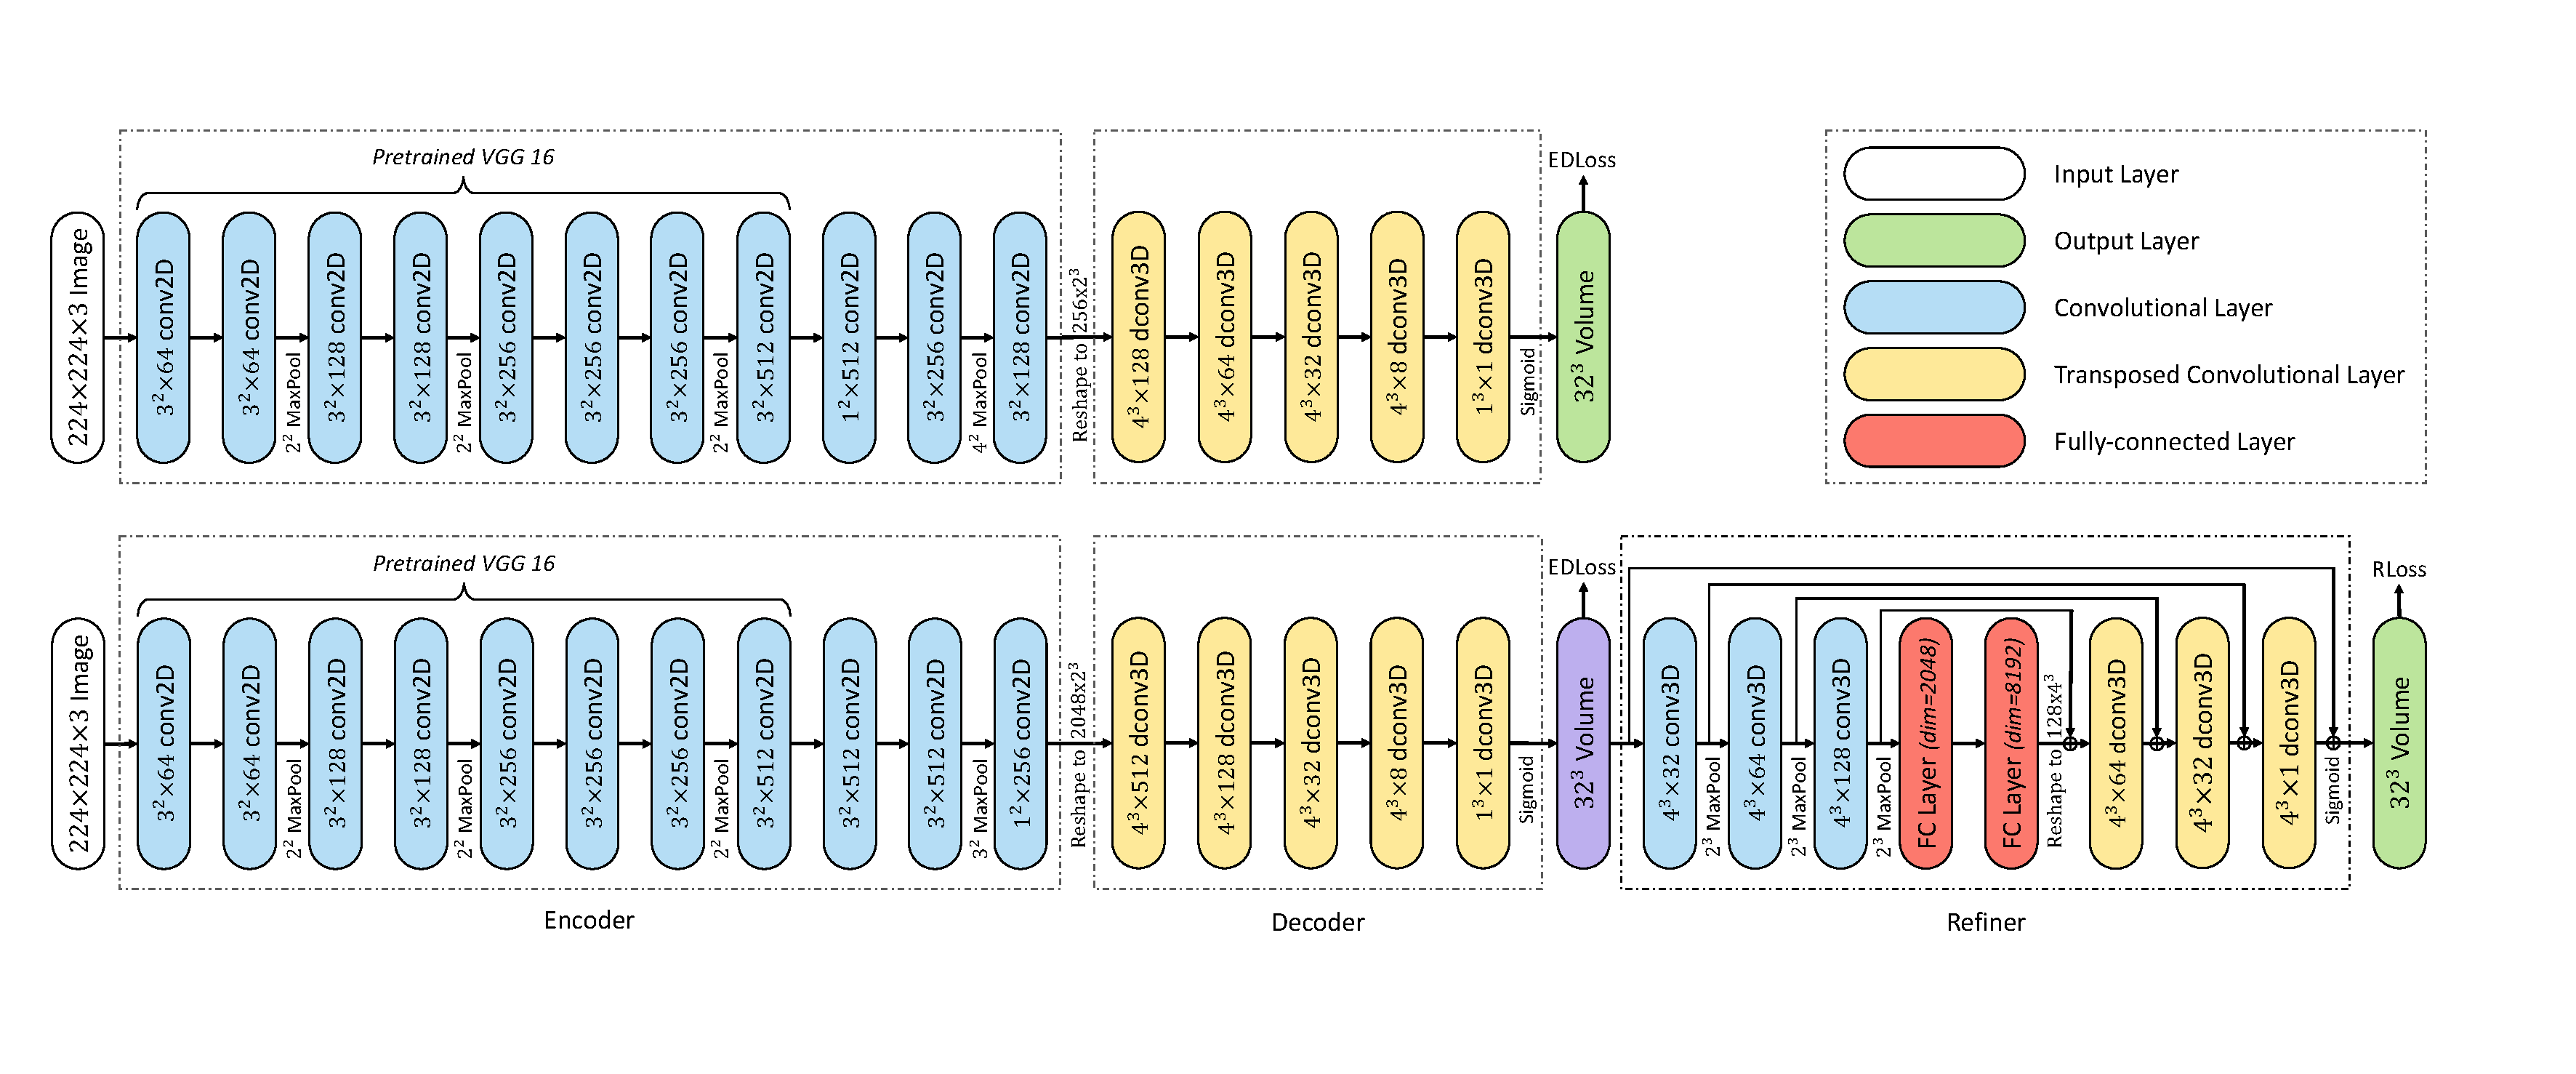
\includegraphics[width=1\textwidth]{/Users/apple/OVGU/Thesis/code/3dReconstruction/report/images/concept/pix2vox}
    \caption{Network architecture for pix2vox~\cite{Xie_2019}}
    \label{fig:pix2vox architecture}
\end{figure}

\begin{figure}
    \centering
    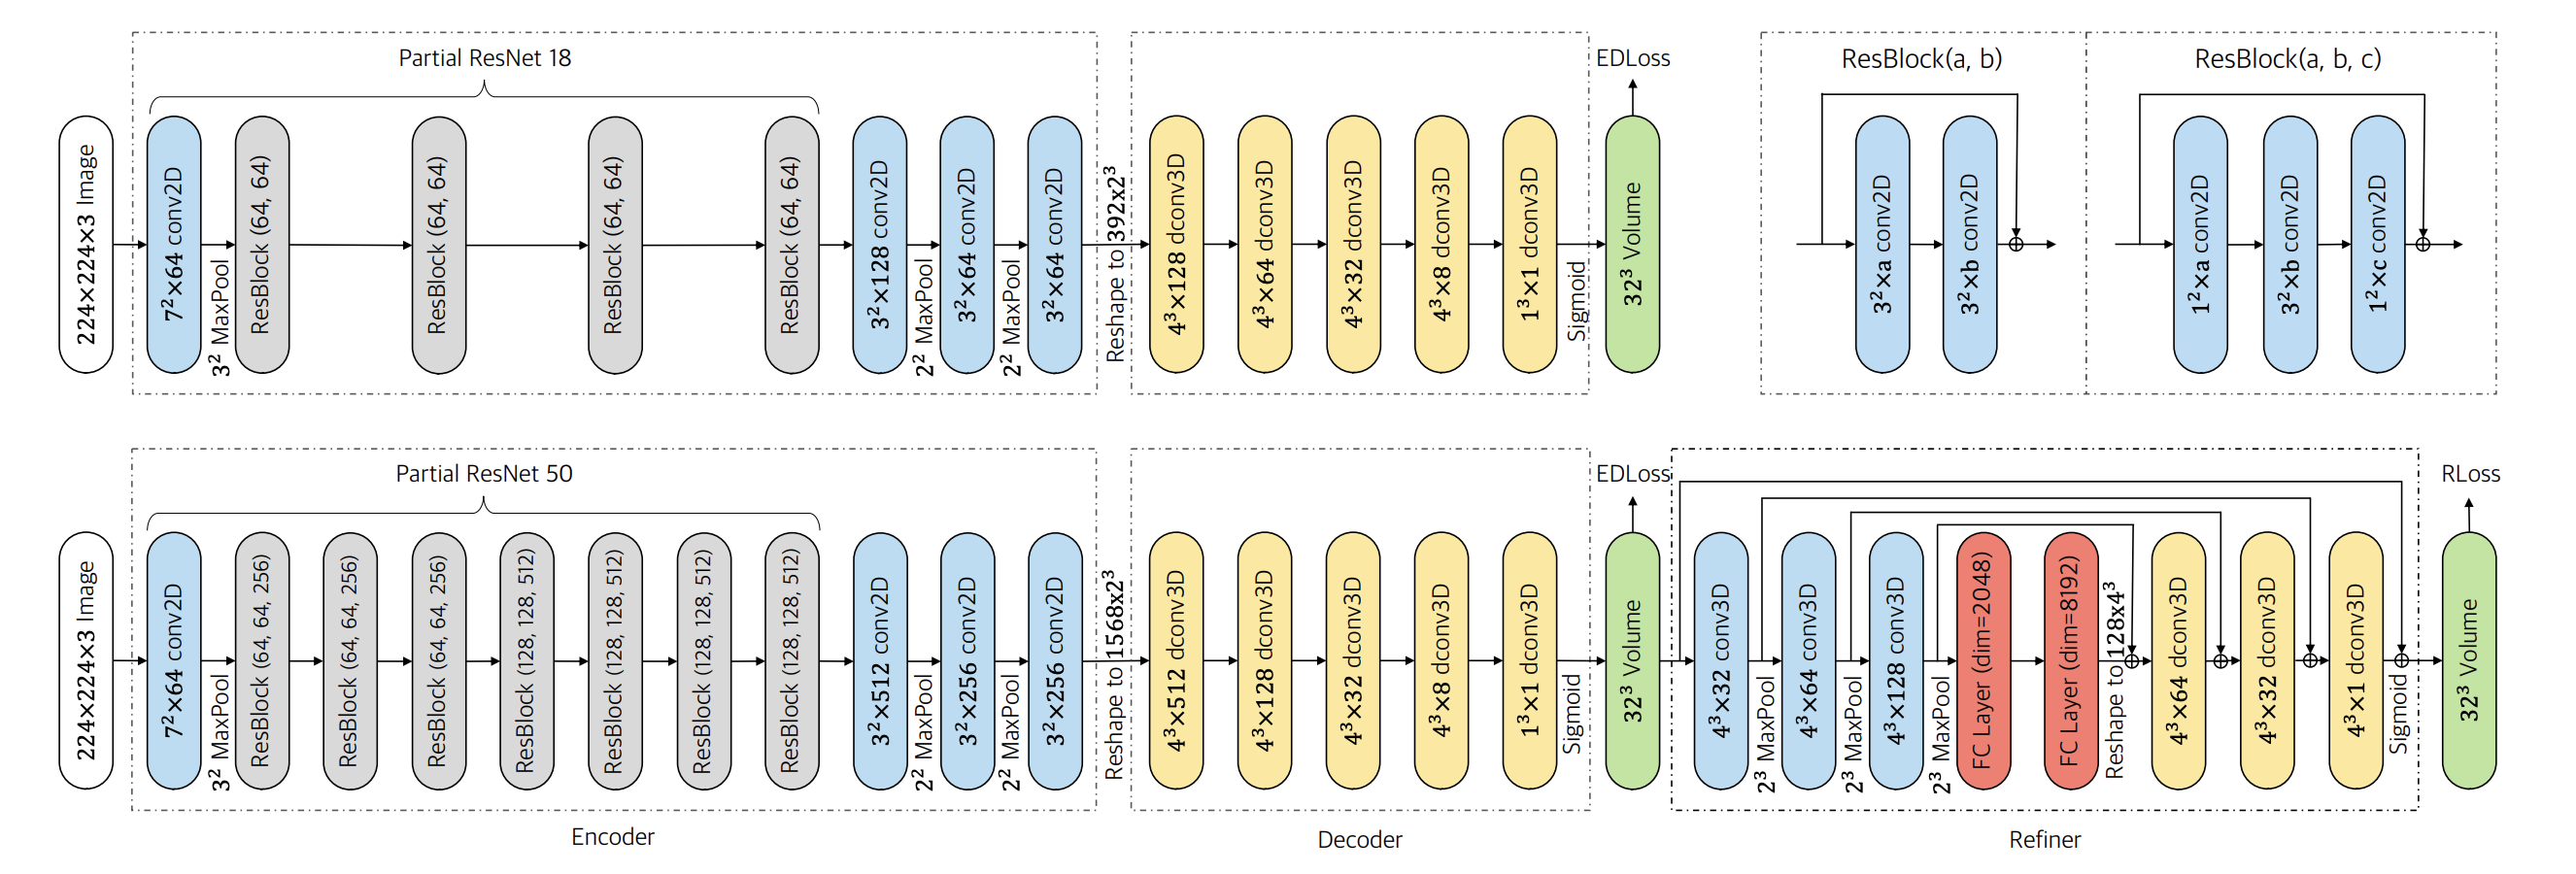
\includegraphics[width=1\textwidth]{/Users/apple/OVGU/Thesis/code/3dReconstruction/report/images/concept/pix2voxpp}
    \caption{Network architecture for pix2vox++~\cite{Xie_2020}}
    \label{fig:pix2voxpp architecture}
\end{figure}

\begin{figure}
    \centering
    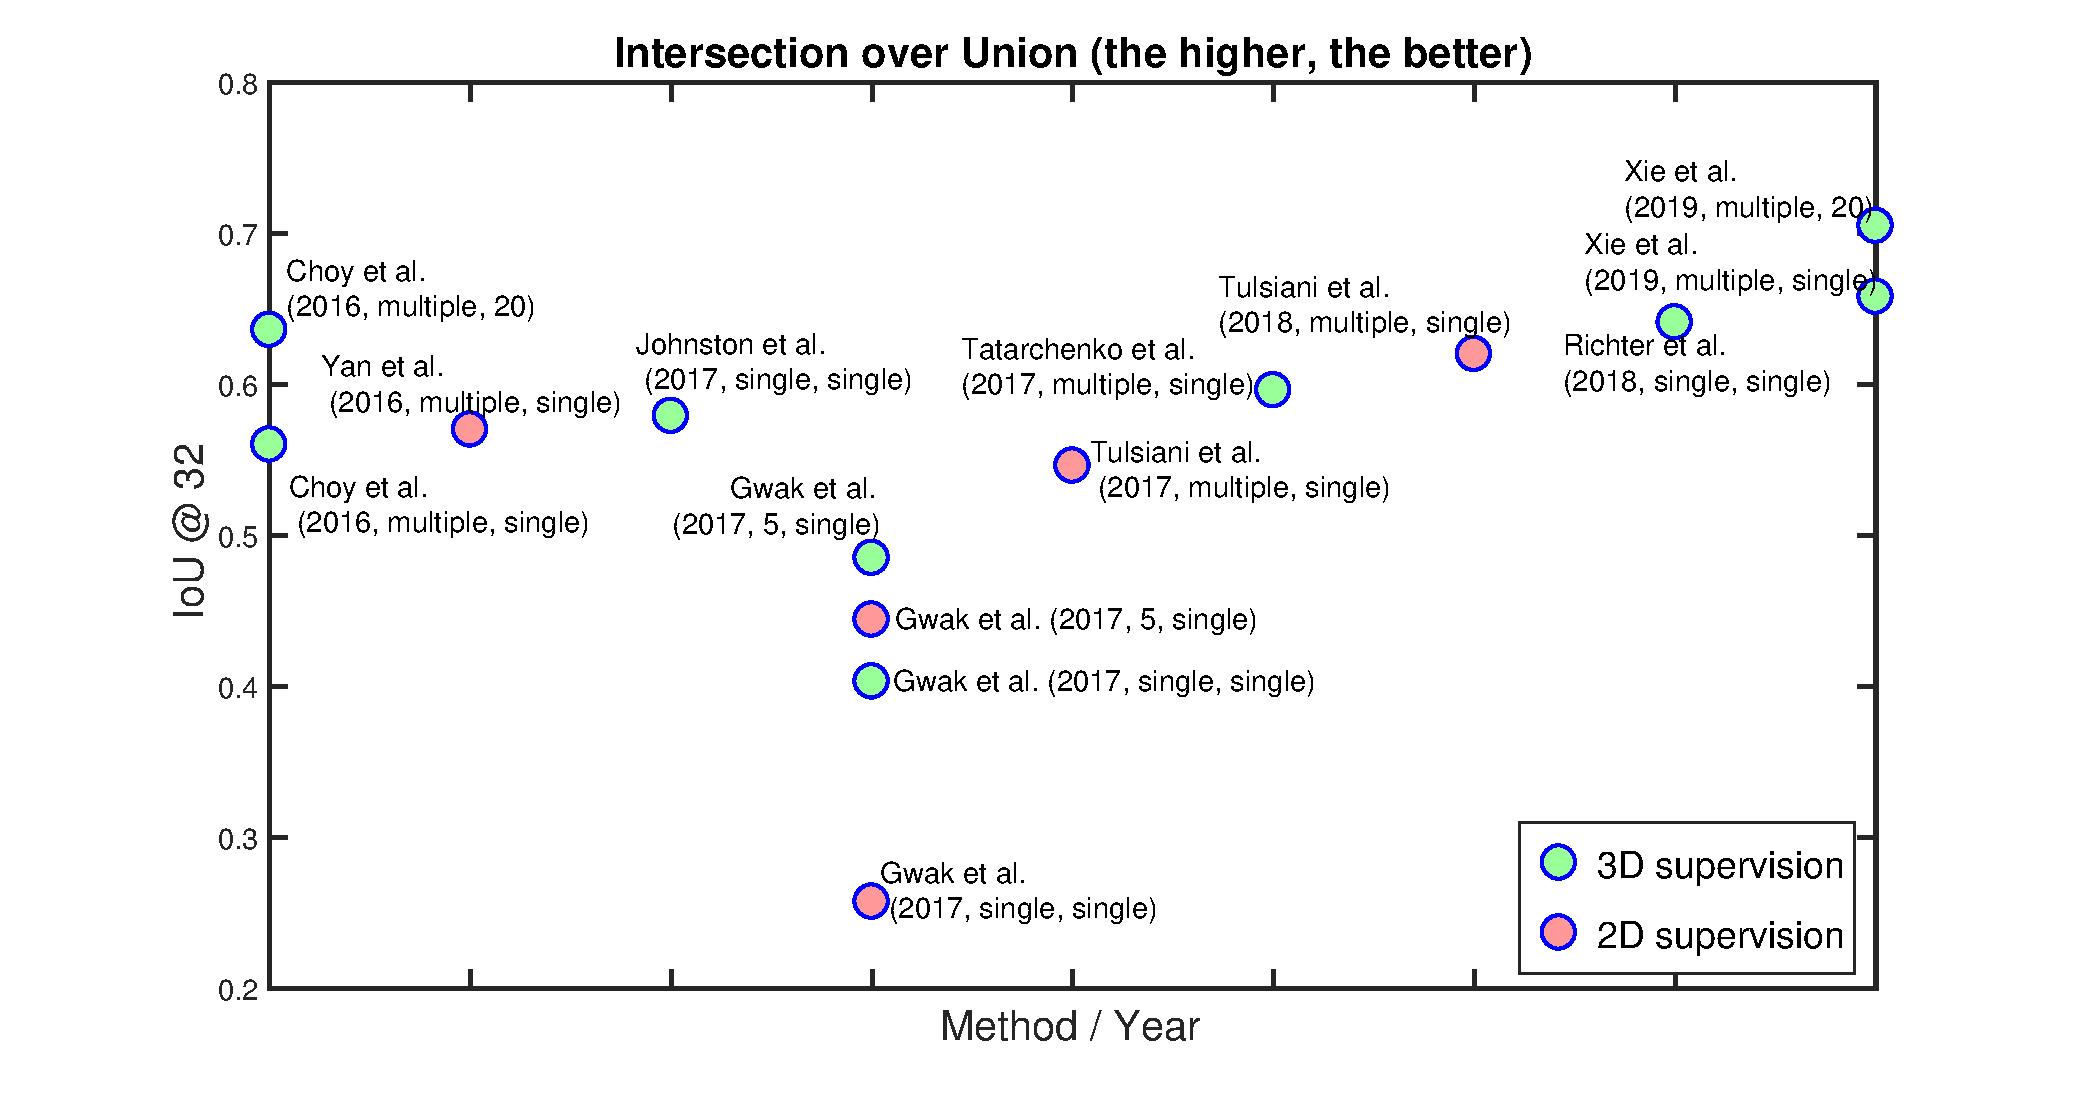
\includegraphics[width=1\textwidth]{/Users/apple/OVGU/Thesis/code/3dReconstruction/report/images/concept/survey}
    \caption{A survey conducted by ~\cite{Han2021ImageBased3O}, proves that Pix2Vox is considerably a good 3D reconstruction model.
    \todo{replace this figure with better one}}
    \label{fig:survey on 3d reconstruction}
\end{figure}

\section{Domain adaptation with Gan \todo{if we decide to go with this approach}}

\section{Training}
\todo re-write
\cite{seib2020mixing} proved mixed training with synthetic and real dataset improves the performance. They used 40\% mixing ratio

\cite{2018LearningIC} used mixing ratios for classification task for each of the minibatches and observed 5-13\% improvement in performance.
\chapter{\iftoggle{german}{Implementierung}{Implementation}}\label{ch:implementation}

In this chapter, we discuss the implementations of the all the framework and how it was achieved.
In \autoref{sec:implementation_3d-scene-framework}, we go through the implementation of each of the modes of operation.
Further, we discuss each step that is executed to achieve domain randomization.
We then explain how the Ml-Image Synthesis library is integrated with the cameras to take the snapshots.
We demo the application in \autoref{sec:demo}.

\autoref{sec:3d-reconstruction-framework} discusses the Deep Learning framework used to train and evaluate the 3D reconstruction task.
We discuss the underlying libraries and hyperparameters used for the evaluation of the models.

\section{3D-Scene Framework}\label{sec:implementation_3d-scene-framework}
3D-Scene is an application built in Unity using Csharp as programming language.
The application runs in editor mode, so that the users can manually make some changes if needed.
The application's first step is to import existing .obj files for 3D models and 3D models of rooms.
Once the setup is completed, we induce randomization using textures, light and camera as discussed in \autoref{sec:3d-scene-framework}.
This is discussed in details in the upcoming sections.
In the final step, the primary camera takes snapshots of the scene.
Along with RGB images, we also save depth maps, normals, and semantic segmentation.
The workflow of the implementation is as shown in \autoref{fig:flowchart}.

\begin{figure}[!ht]
    \centering
    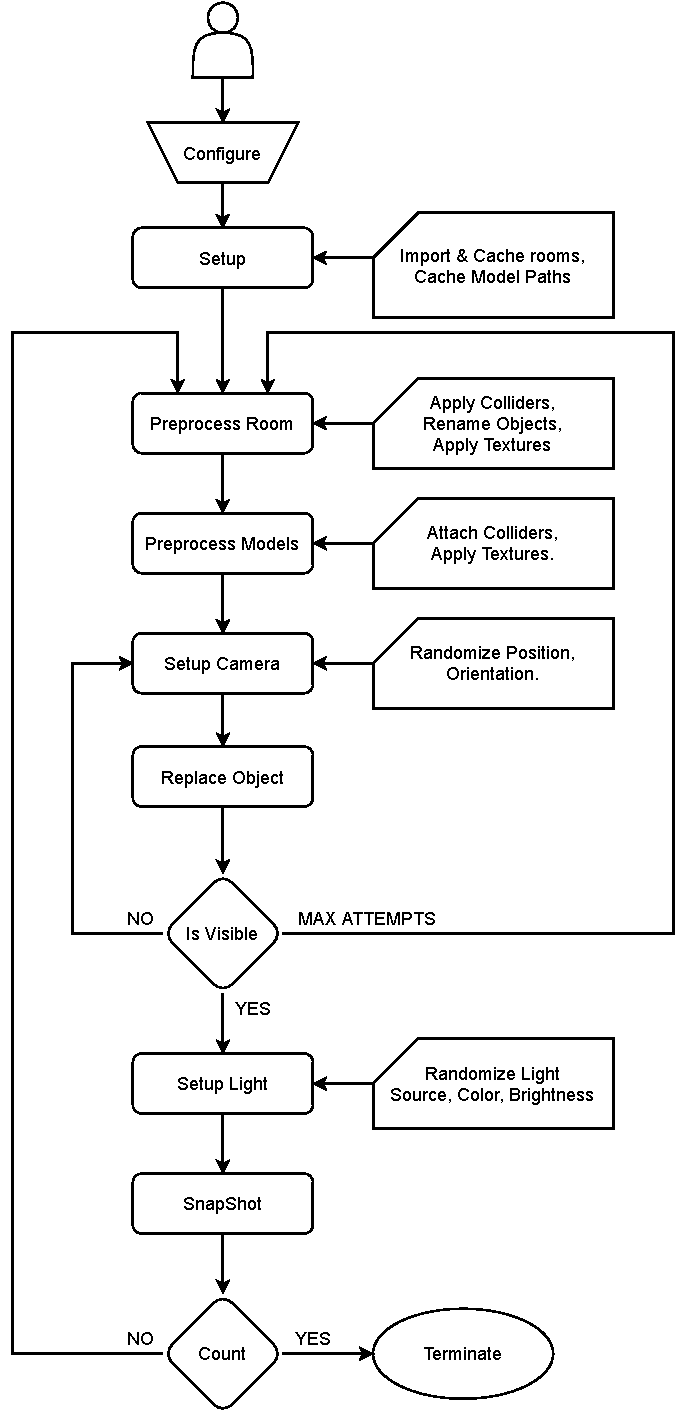
\includegraphics[width=0.9\textwidth, height =1.45\textwidth,valign=m]{/Users/apple/OVGU/Thesis/code/3dReconstruction/report/images/implementation/flowchart}
    \caption[Flowchart for the 3D-Scene Pipeline]{Flowchart for the 3D-Scene Pipeline. The pipeline iterates through the steps till a specified count is reached.}
    \label{fig:flowchart}
\end{figure}

\subsection{Configuration}\label{subsec:configuration}
As an entry point for the user, the application has few parameters which has to be configured.
These need to be inputted by the user using a simple user interface as shown in \autoref{fig:demo1}.
The parameters includes room object path, texture path, model/furniture path and destination path where the images need to saved.
It also includes the categories and total number of required images per category.
The user can also configure camera parameters which include the minimum and macimum distance from the target object and the minimum height of the camera.

\subsection{Modes of Operations}\label{subsec:modes-of-operations}
The creation of a dataset can either be automated or by manual intervention.
Automated images may not give us the perfect images that we expect.
There can be some bad lighting, unexpected intersections with other objects, unforeseen camera angles, etc.
To facilitate ease of use for the user, the application has three key pipelines.
After configuring the parameters to create an ersatz environment using Unity,
the user can select any of this pipeline to get automatic snapshots or manual snaps for the models.

The different modes of operation are as follows:
\begin{enumerate}
    \item Single Room pipeline
    \item Manual Room pipeline
    \item Multi Objects pipeline
\end{enumerate}

The single Room pipeline is used to create the dataset with objects in the center of an empty room.
A path to the room can either be provided or else the application imports a default room.
Manual Room pipeline randomizes a furnished room and then replaces the category under observation.
The selection of objects to be replaced is also random.
In this mode, the user has control over taking the snap of the scene.
The user can randomize model and room textures, randomize camera position or manually set it and randomize the lighting conditions.
Once the user is satisfied with the view of the scene, he can save the images with a click of the Snap button.
In Multi Objects pipeline, all the process mentioned in the Manual Room pipeline is automated.
The user will not have control over any of the processes while the program snaps images at random.
Another version of the pipeline which is similar to the Single Room pipeline is the Multi-threaded Single Room pipeline.
As the name suggests, multiple rooms are created based on the number of categories, and for each room, the Single Room pipeline is applied in parallel.
This is an attempt to let the tool perform faster with multi-threading.
The multi-process uses Coroutines which is still a sequential operation, and hence this pipeline needs some work.
To our estimate, even the Multi-threaded pipeline runs 1.5 times faster than Single room pipeline.

\subsection{Setup Rooms and Models}\label{subsec:implementation_setup_rooms_models}
As discussed in \autoref{subsec:scenes-from-scenenet}, we utilize the room objects provided by SceneNet.
For Single Room pipeline, a default empty room prefab is imported, while scenes from SceneNet are imported for Manual and Multi-Object pipelines.
The rooms are in .obj format which each furnitures independent of the room and hence can be modified by the application.
For smooth transition, all the rooms from the given path is loaded as a pre-step into a cache variable.
This process can be time consuming initially, but since it is cached the change of room takes lesser time.
For loading of 3D object like room into the Unity environment at runtime we use the asset `Runtime OBJ Importer'\footnote{https://assetstore.unity.com/packages/tools/modeling/runtime-obj-importer-49547} from Unity asset store.
This library helps to import both the object meshes and the material into any Unity environment.

\subsection{Preprocess Rooms and Models}\label{subsec:implementation_preprocess_rooms_models}
In preprocessing step, the rooms and models are assigned properties required in the further steps.
Each object in the room is attached with a collider component, which as the name suggests detects collisions.
This component is needed to detect a object either using raycast or when it actually intersects with the target object.
We utilize \emph{MeshCollider} component for the same.

We then rename all the objects in the room to some common names used in day-to-day life.
Example: cushions, pillows, lamp, laptop, etc.
Though the objects in scenes from SceneNet are named with some common objects, the name contains unintelligible texts appended with it.
Hence, we rename them to pre-defined list of common object.
If any object does not belong in the list, it will be renamed as `misc'.
Some edge cases where more than one name resemble the same object are also handled.
For example: TV and Television are both renamed to TV.

Similarly, the models from Pix3D are also preprocessed.
Each model is attached with a MeshCollider, in this case to detect collision with the other objects in the scene.
In case of target models, we can even apply gravity so that it appears on the floor.
However, we chose to place it using its dimensions, which also makes it appear to be on the floor.

Then we apply textures for both room and models as described in \autoref{subsec:implementation_randomised-texture}.

\subsection{Randomized Texture}\label{subsec:implementation_randomised-texture}
We randomly allocate textures to each object, ensuring that each category has the same texture to make the scene more uniform.
The objects in the scene are renamed to standard objects seen in day-to-day life.
The textures are grouped together to these names as folder names.
A dictionary is created for all the gameobjects, such that we keep track of all the unique categories.
Each category is assigned a single texture using \emph{Texture2D.LoadImage}.

Another randomized entity is the skybox.
Skybox acts as the outdoor scene for a given room.
For each of the pipelines, skybox changes for every snap taken.
Samples for changing skyboxes is as shown in \autoref{fig:skybox samples}.

\subsection{Setup Camera}\label{subsec:implementation_camera}
As a device through which the users can visualize the ersatz environment we utilize Unity's default Camera object.
We use a single camera whose coordinates or transforms can be changed at runtime.
Few of the camera parameters like height of the camera, minimum and maximum distance from the target object, can be decided by the user in the initial configuration.
A CameraHelper class, which has both the main camera and the target object as its parameter then selects a random point in the space with these constraints for the camera to be placed.
The camera is then rotated towards the target object using the \emph{Transform.LookAt} API.
The next step is the check if the target object is still within the frame.
This is achieved by casting a ray from the camera using \emph{Physics.Linecast}, which tells us if the ray is intersecting a collider object.
To make the frame realistic, we avoid unrelatable views by applying a constraint on the camera position and make sure that the camera is in front of the target object within an angle of 60 degrees.

\subsection{Replacing Target Objects}\label{subsec:implementation_replacing-target-objects}
Once the room is set up using SceneNet~\cite{McCormac2017}, which contains objects from ShapeNet~\cite{shapenet2015}, the objects are renamed such that it matches the classes for the Pix3D dataset.
Since a given scene can have more than one category under observation, a single model is chosen randomly out of all the present models.
The chosen model is replaced with a model in Pix3D of the same category, by making it invisible using \emph{GameObject.SetActive}.
In case the replaced model is intersecting with any other models in the scene, we make it invisible.
After the snapshot is taken, the scene is reset to the original, and the next model is imported.


\subsection{Setup Lighting}\label{subsec:implementation_lighting}

Unity has a wide variety of lighting system.
We utilize three types of lights offered in Unity.

\begin{itemize}
    \item Point light
    \item Spotlight
    \item Directional light
\end{itemize}

Point lights act as indoor lights for the room, the range of which can be varied.
We pre-define six light patterns for a room with a cuboid shape.
Knowing the bounds of the room, we decide how to place the lights by randomly select 1 to 6 lights with corresponding light patterns on the ceiling.
For the spotlight, only a single light is placed a meter above the target object.
This light gives a variation that focuses only on the target object.
Both point and spot-light have color variation along with varying brightness.
Directional light is the default light settings in Unity.
For our environment this acts a natural Sun Light.
This is specifically effective when the room has windows forming more realistic shadows.
In this case, we modulate the brightness, and the angle at which the rays are emitted, which simulates different times of the day.
Additional to these different types of light, we give ceilings the property of light with limited brightness as we observed that the entire room does not light up for a single light source.
This is similar to what BlenderProc~\cite{dlr139317} do for all scenarios.
Samples of different lighting conditions and shadows with varying colors are displayed in \autoref{fig:Lighting and shadows}.


\subsection{Snapshots with ML-ImageSynthesis}\label{subsec:snapshots-with-ml-imagesynthesis}

ML-ImageSynthesis~\footnote{https://bitbucket.org/Unity-Technologies/ml-imagesynthesis} is a library provided by Unity to support synthetic dataset creation.
It supports the following G-buffers Image segmentation, Object categorization, Optical flow, Depth, Normals, etc.
G-buffers is basically a collective term to represent light properties that are aggregated to give the final rendering.
In image segmentation, each object is assigned a unique color.
In object categorization, each category of the objects is assigned a single color.
For optical flow, each pixel is colored depending on Unity's per-pixel Motion Vectors with respect to the camera.
The depth map is, as the word suggests, the distance of each pixel from the camera encoded in 8-bit channels of the PNG image.
Normals are color encoding based on the orientation of the object with respect to the camera.
For the snapshot, each of these properties is assigned a hidden camera and has each one overrides rendering scene with custom shaders to generate corresponding output.
These camera outputs can be seen in editor mode by changing the display window.
Samples of G-buffer collected for the dataset are as shown in \autoref{fig:G-buffers-samples}.

\begin{figure}
    \centering
    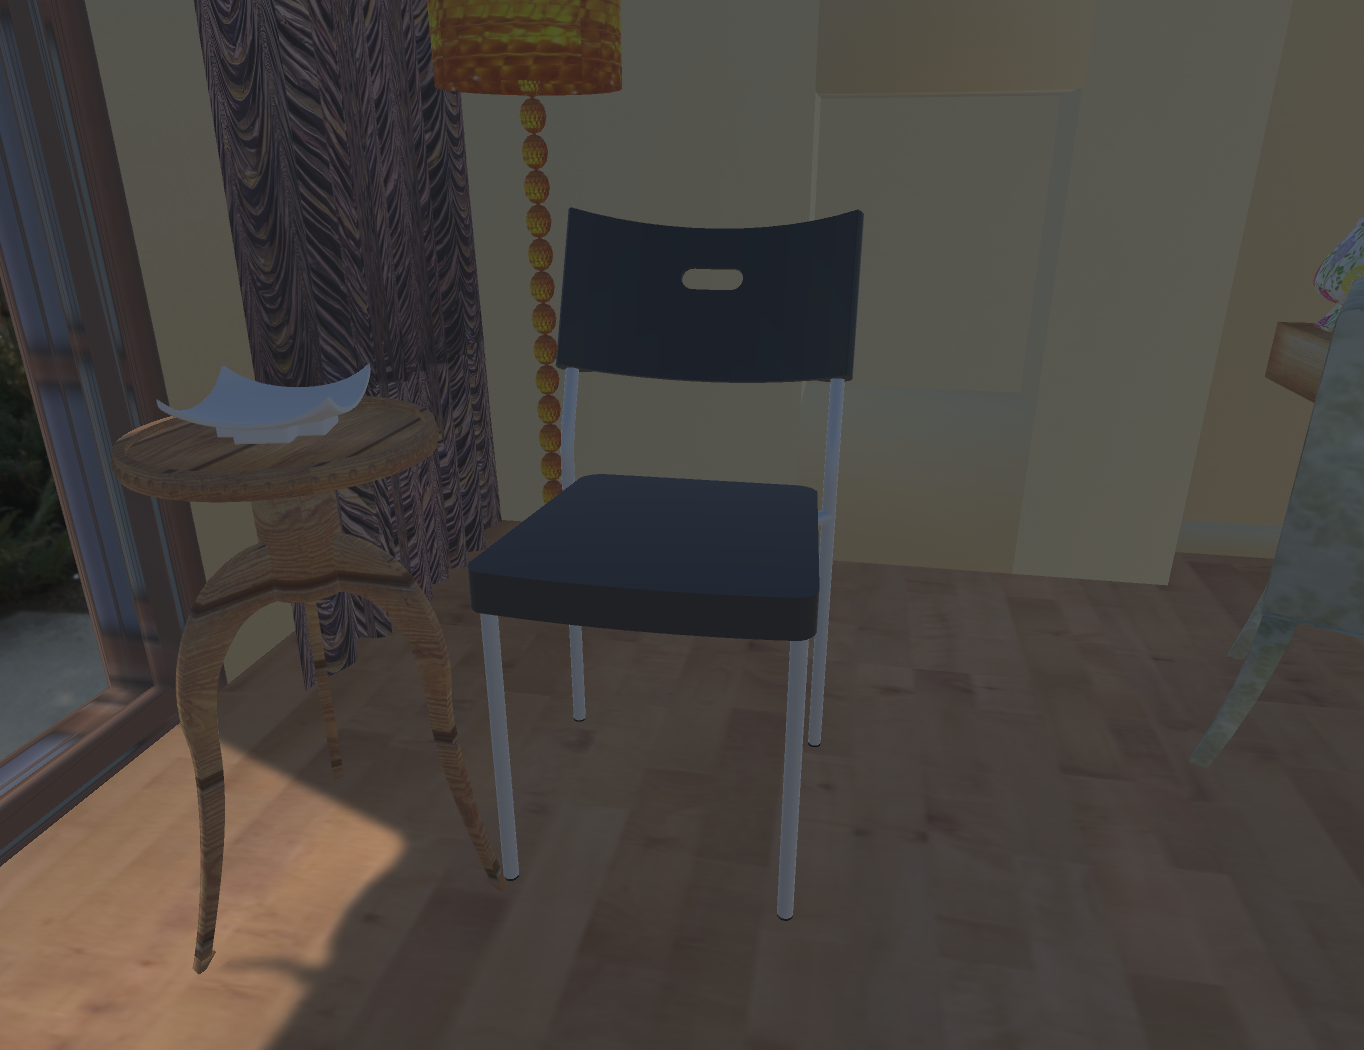
\includegraphics[width=.19\linewidth]{/Users/apple/OVGU/Thesis/code/3dReconstruction/report/images/implementation/gbuffers/0_img}
    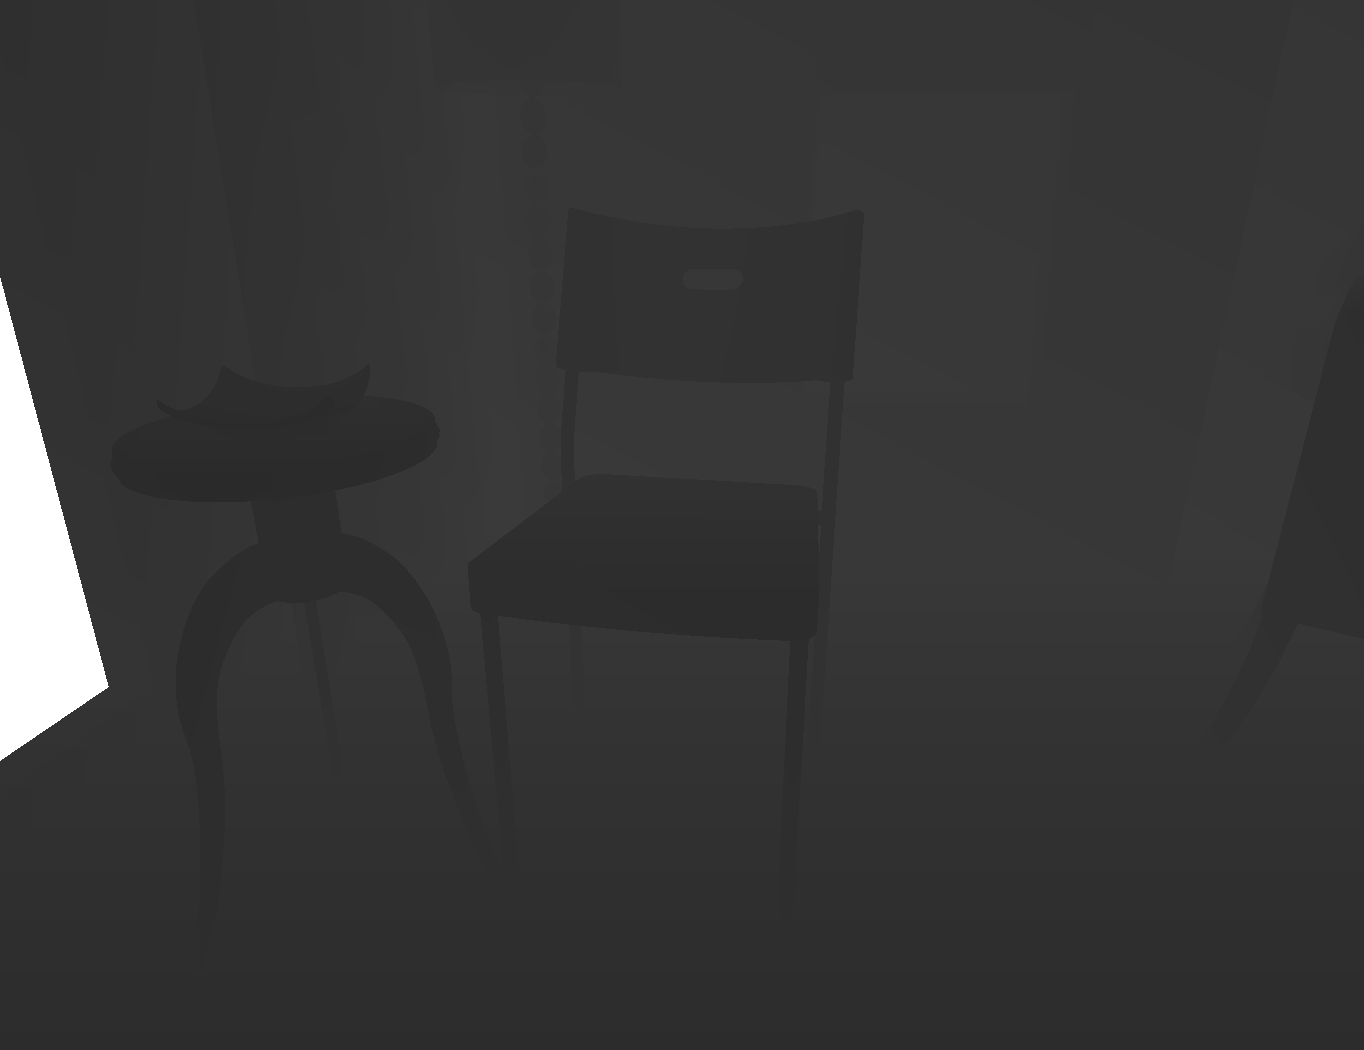
\includegraphics[width=.19\linewidth]{/Users/apple/OVGU/Thesis/code/3dReconstruction/report/images/implementation/gbuffers/0_depth}
    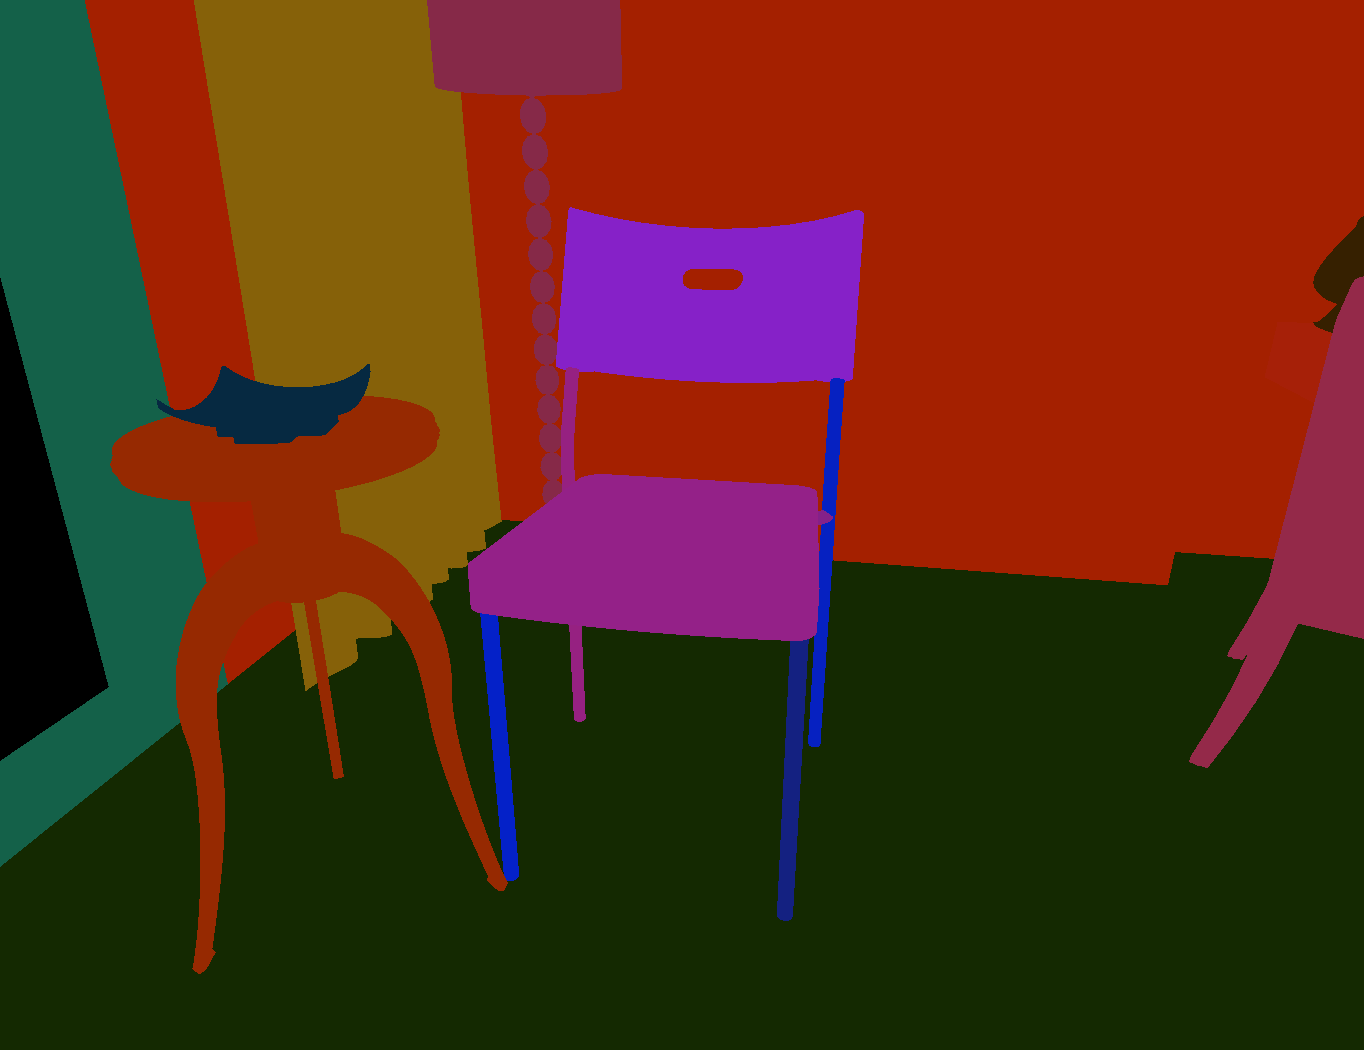
\includegraphics[width=.19\linewidth]{/Users/apple/OVGU/Thesis/code/3dReconstruction/report/images/implementation/gbuffers/0_id}
    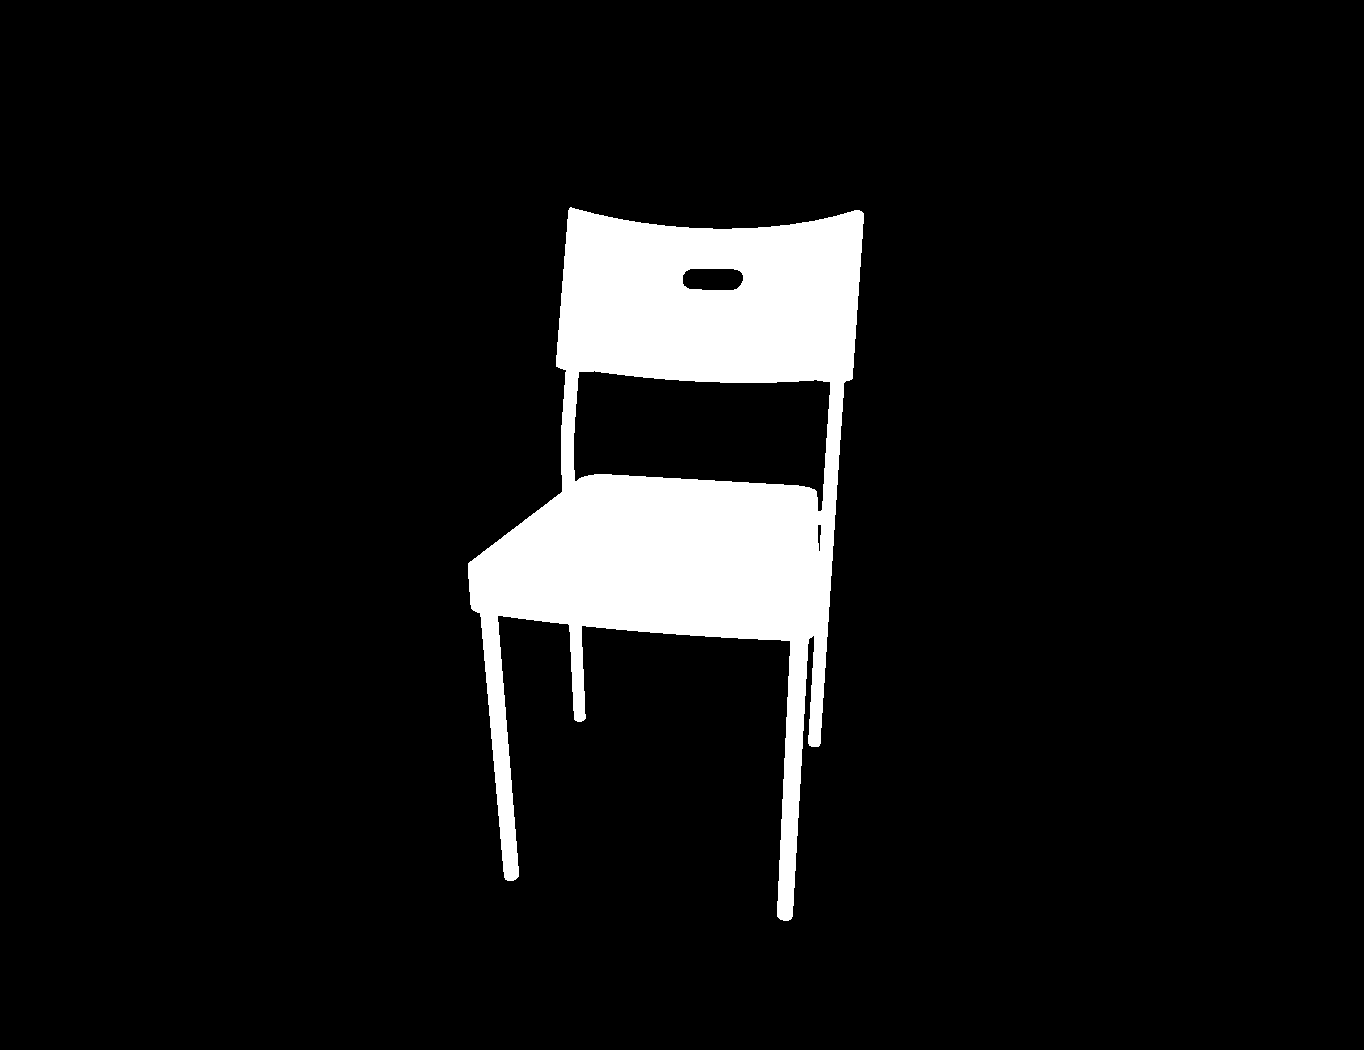
\includegraphics[width=.19\linewidth]{/Users/apple/OVGU/Thesis/code/3dReconstruction/report/images/implementation/gbuffers/0_layer}
    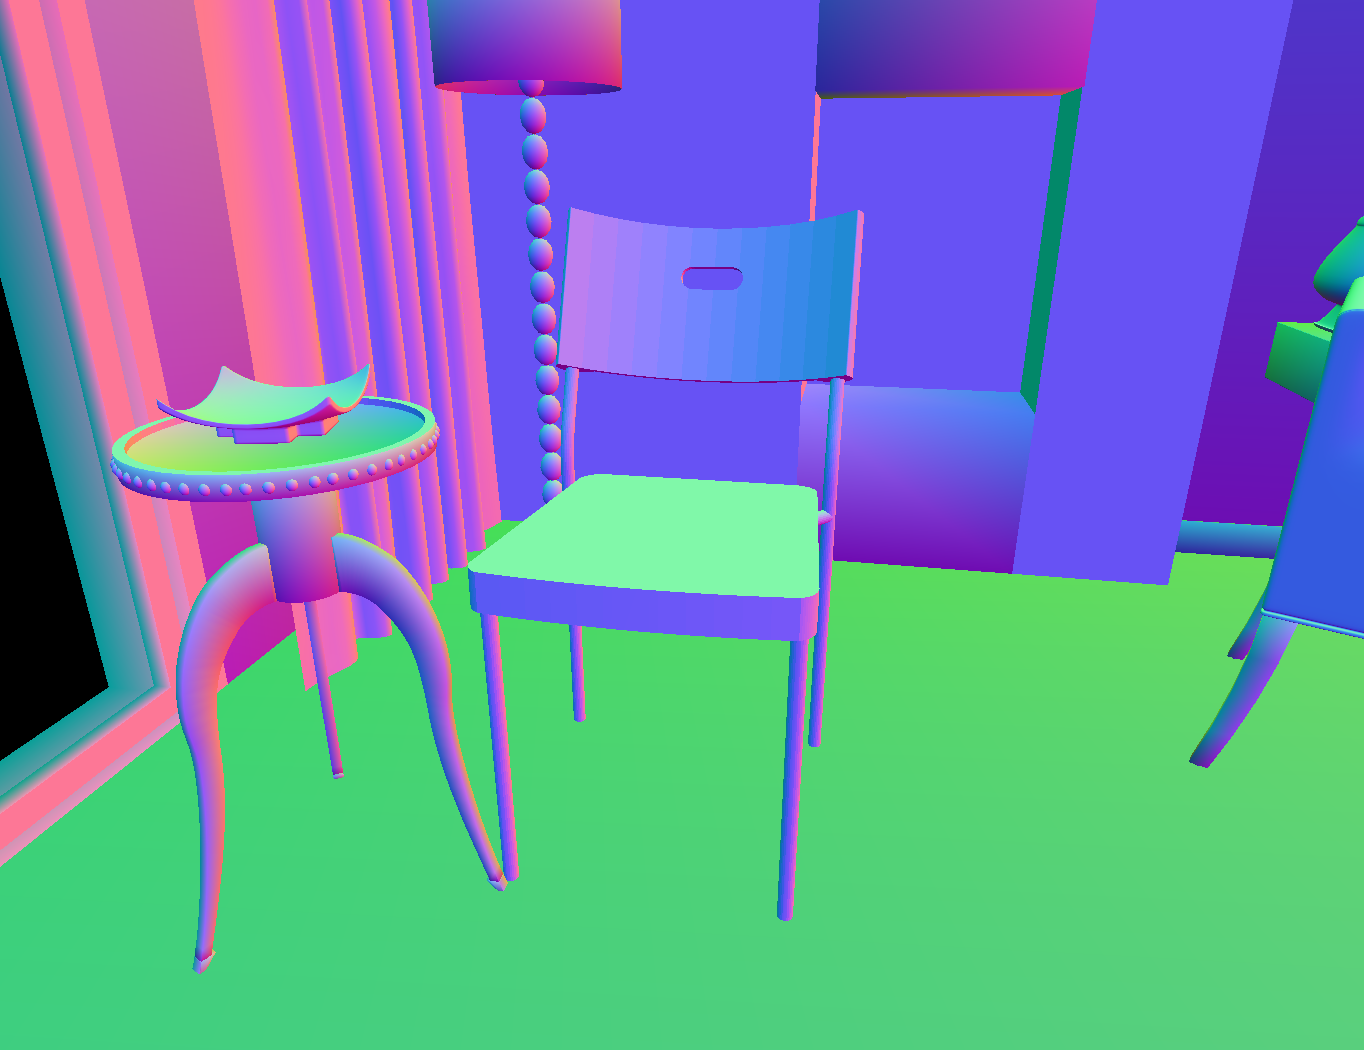
\includegraphics[width=.19\linewidth]{/Users/apple/OVGU/Thesis/code/3dReconstruction/report/images/implementation/gbuffers/0_normals}\\
    \vspace{0.1cm}
    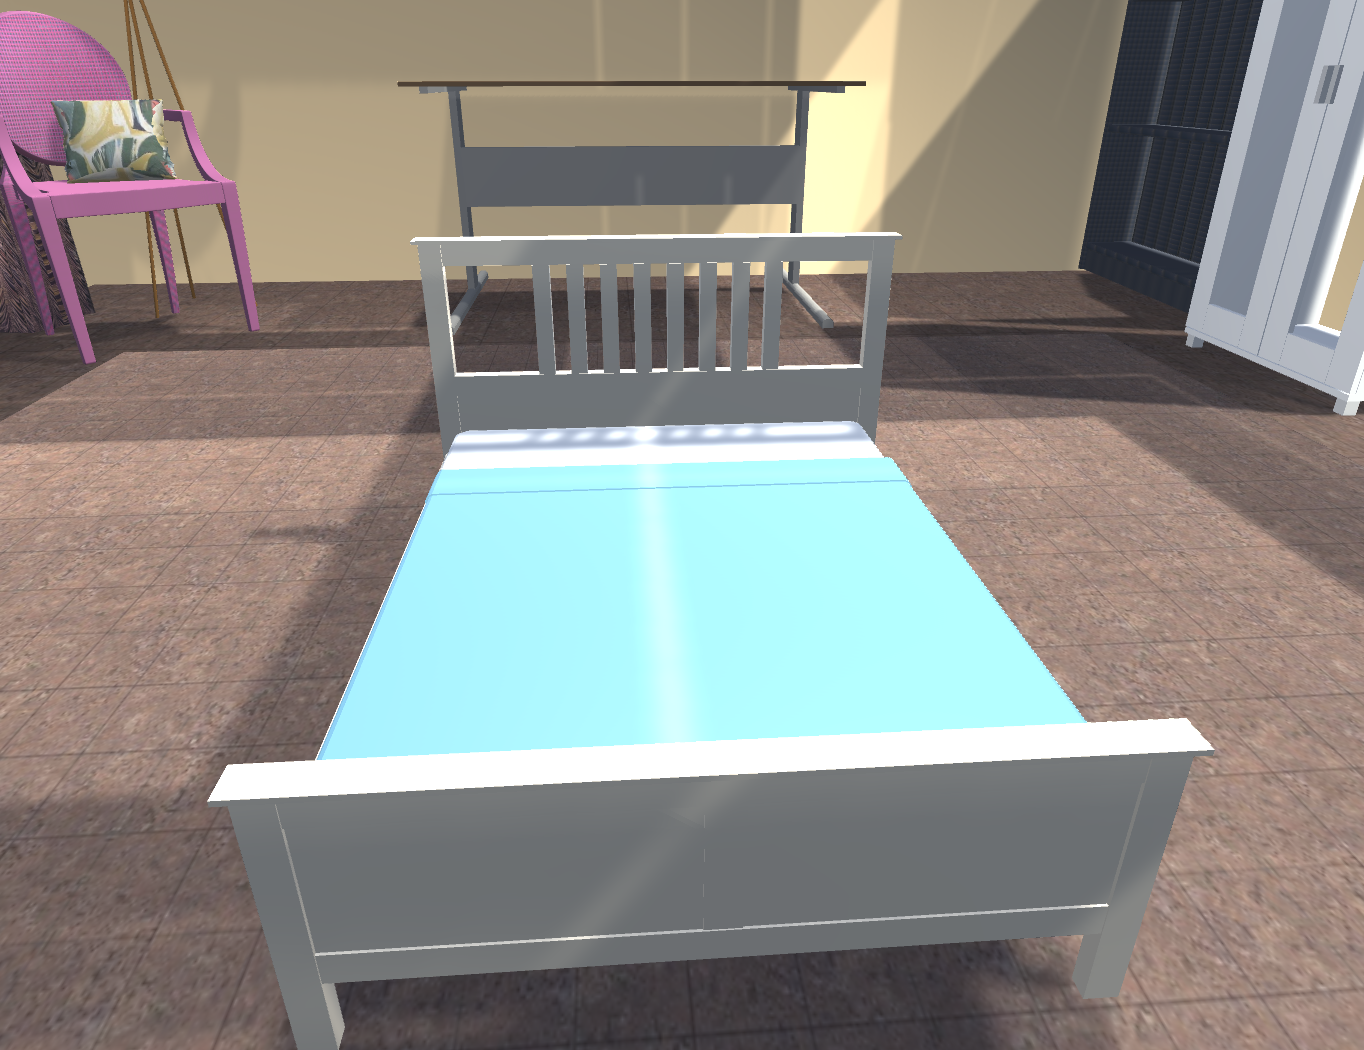
\includegraphics[width=.19\linewidth]{/Users/apple/OVGU/Thesis/code/3dReconstruction/report/images/implementation/gbuffers/1_img}
    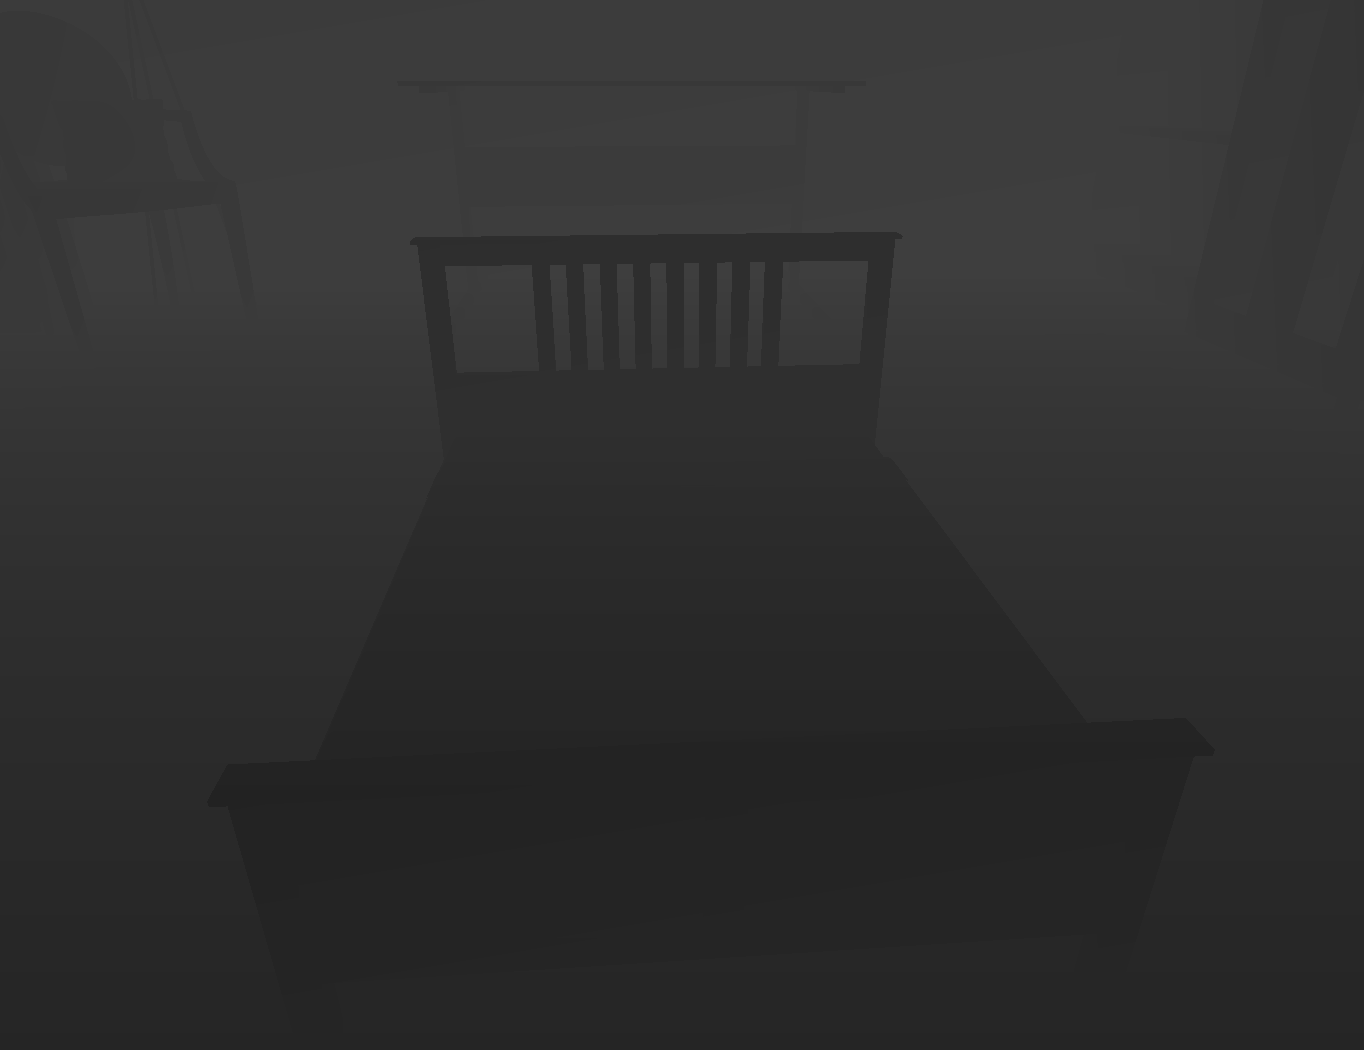
\includegraphics[width=.19\linewidth]{/Users/apple/OVGU/Thesis/code/3dReconstruction/report/images/implementation/gbuffers/1_depth}
    \includegraphics[width=.19\linewidth]{/Users/apple/OVGU/Thesis/code/3dReconstruction/report/images/implementation/gbuffers/1_id}
    \includegraphics[width=.19\linewidth]{/Users/apple/OVGU/Thesis/code/3dReconstruction/report/images/implementation/gbuffers/1_layer}
    \includegraphics[width=.19\linewidth]{/Users/apple/OVGU/Thesis/code/3dReconstruction/report/images/implementation/gbuffers/1_normals}\\
    \vspace{0.1cm}

    \includegraphics[width=.19\linewidth]{/Users/apple/OVGU/Thesis/code/3dReconstruction/report/images/implementation/gbuffers/2_img}
    \includegraphics[width=.19\linewidth]{/Users/apple/OVGU/Thesis/code/3dReconstruction/report/images/implementation/gbuffers/2_depth}
    \includegraphics[width=.19\linewidth]{/Users/apple/OVGU/Thesis/code/3dReconstruction/report/images/implementation/gbuffers/2_id}
    \includegraphics[width=.19\linewidth]{/Users/apple/OVGU/Thesis/code/3dReconstruction/report/images/implementation/gbuffers/2_layer}
    \includegraphics[width=.19\linewidth]{/Users/apple/OVGU/Thesis/code/3dReconstruction/report/images/implementation/gbuffers/2_normals}\\
    \vspace{0.1cm}
    \includegraphics[width=.19\linewidth]{/Users/apple/OVGU/Thesis/code/3dReconstruction/report/images/implementation/gbuffers/3_img}
    \includegraphics[width=.19\linewidth]{/Users/apple/OVGU/Thesis/code/3dReconstruction/report/images/implementation/gbuffers/3_depth}
    \includegraphics[width=.19\linewidth]{/Users/apple/OVGU/Thesis/code/3dReconstruction/report/images/implementation/gbuffers/3_id}
    \includegraphics[width=.19\linewidth]{/Users/apple/OVGU/Thesis/code/3dReconstruction/report/images/implementation/gbuffers/3_layer}
    \includegraphics[width=.19\linewidth]{/Users/apple/OVGU/Thesis/code/3dReconstruction/report/images/implementation/gbuffers/3_normals}\\
    \vspace{0.1cm}

    \includegraphics[width=.19\linewidth]{/Users/apple/OVGU/Thesis/code/3dReconstruction/report/images/implementation/gbuffers/4_img}
    \includegraphics[width=.19\linewidth]{/Users/apple/OVGU/Thesis/code/3dReconstruction/report/images/implementation/gbuffers/4_depth}
    \includegraphics[width=.19\linewidth]{/Users/apple/OVGU/Thesis/code/3dReconstruction/report/images/implementation/gbuffers/4_id}
    \includegraphics[width=.19\linewidth]{/Users/apple/OVGU/Thesis/code/3dReconstruction/report/images/implementation/gbuffers/4_layer}
    \includegraphics[width=.19\linewidth]{/Users/apple/OVGU/Thesis/code/3dReconstruction/report/images/implementation/gbuffers/4_normals}\\
    \vspace{0.1cm}

    \includegraphics[width=.19\linewidth]{/Users/apple/OVGU/Thesis/code/3dReconstruction/report/images/implementation/gbuffers/5_img}
    \includegraphics[width=.19\linewidth]{/Users/apple/OVGU/Thesis/code/3dReconstruction/report/images/implementation/gbuffers/5_depth}
    \includegraphics[width=.19\linewidth]{/Users/apple/OVGU/Thesis/code/3dReconstruction/report/images/implementation/gbuffers/5_id}
    \includegraphics[width=.19\linewidth]{/Users/apple/OVGU/Thesis/code/3dReconstruction/report/images/implementation/gbuffers/5_layer}
    \includegraphics[width=.19\linewidth]{/Users/apple/OVGU/Thesis/code/3dReconstruction/report/images/implementation/gbuffers/5_normals}\\
    \vspace{0.1cm}

    \includegraphics[width=.19\linewidth]{/Users/apple/OVGU/Thesis/code/3dReconstruction/report/images/implementation/gbuffers/6_img}
    \includegraphics[width=.19\linewidth]{/Users/apple/OVGU/Thesis/code/3dReconstruction/report/images/implementation/gbuffers/6_depth}
    \includegraphics[width=.19\linewidth]{/Users/apple/OVGU/Thesis/code/3dReconstruction/report/images/implementation/gbuffers/6_id}
    \includegraphics[width=.19\linewidth]{/Users/apple/OVGU/Thesis/code/3dReconstruction/report/images/implementation/gbuffers/6_layer}
    \includegraphics[width=.19\linewidth]{/Users/apple/OVGU/Thesis/code/3dReconstruction/report/images/implementation/gbuffers/6_normals}\\
    \caption[Samples for G-buffers from ML-ImageSynthesis.]{Samples for G-buffers collected from ImageSynthesis as part of the dataset. In the figure,
        (From left to right) RGB image, Depth map, Instance segmentation, Semantic Segmentation and Normal map}
    \label{fig:G-buffers-samples}
\end{figure}

\section{Demo for the Application}\label{sec:demo}

The researchers are provided source code for the Unity-based application~\footnote{https://github.com/kartikprabhu20/3dScene}, which was used to create the synthetic datasets.
The application allows the users to provide paths for the 3D models, 3D rooms, textures, and output.
The user can also select the category of furniture for which images are to be generated and the quantity per category.
For the camera, the user can decide upon the height of the camera position, minimum and maximum distance from the target model, between which a viewpoint will be randomly chosen.
The modes are discussed in \autoref{subsec:modes-of-operations}, which can be select once all the data is configured.
For the manual mode, the user can randomize one or more parameters and take the snapshot as desired.
\autoref{fig:demo1} shows the configuration page for the demo application, and \autoref{fig:demo2} shows the application in action in manual mode.

\begin{figure}
    \centering
    \includegraphics[width=\textwidth]{/Users/apple/OVGU/Thesis/code/3dReconstruction/report/images/implementation/demo/demo}
    \caption[User Interface for 3D-Scene Tool.]{A screenshot of the Unity based application developed for proof of concept to create synthetic dataset.}
    \label{fig:demo1}
\end{figure}

\begin{figure}
    \centering
    \includegraphics[width=\textwidth]{/Users/apple/OVGU/Thesis/code/3dReconstruction/report/images/implementation/demo/demo2}
    \caption[Demo for 3D-Scene Tool.]{A screenshot of the Unity based application in action, the user is able to configure the pipeline using GUI and take snapshots either automatically or manually.}
    \label{fig:demo2}
\end{figure}

\section{3D-Reconstruction Framework}\label{sec:3d-reconstruction-framework}

In this section, we discuss the pipeline used for the 3D reconstruction~\footnote{https://github.com/kartikprabhu20/3dReconstruction} tasks using Deep Learning.
The discussion will revolve around the implementation of models and the training parameters.
The code for the pipeline was written in Python 3.7.9.
The backbone of this pipeline is PyTorch 1.7.1~\cite{NEURIPS2019_9015}.

The key features of this pipeline are as follows:
\begin{enumerate}
    \item Allows users to configure the parameter using a config file which includes dataset paths, root paths, output path, parameters for 2D augmentations, etc.
    \item Allows users to select a train, validate, test with real data, an empty image test.
    \item Allows users to select the pipeline type(3D-reconstruction, cyclegan~\cite{CycleGAN2017}, autoencoder)
    \item Allows users to select the dataset(Pix3D, \gls(free), Mixed), with a further option to add new datasets.
    \item Allows users to collect graphs, images per epoch using Tensorboard~\footnote{https://www.tensorflow.org/}.
\end{enumerate}

\subsection{Preprocessing}\label{subsec:preprocessing}
As preprocessing for testing, images were resized to 224$\times$224 and then center cropped to 128$\times$128.
The images were then normalized using the parameters used for ImageNet~\cite{Deng2009ImageNetAL} Mean=[0.485, 0.456, 0.406] and STD=[0.229, 0.224, 0.225].
This was also done for training images followed by 2D-augmentations which included ColorJitter, RandomNoise, RandomFlip and, RandomPermuteRGB\@.
All the images were then transformed to a tensor to make them compatible with deep learning models.

\subsection{Modelling}\label{subsec:modelling}
For models, we used the architectures proposed in ~\cite{Xie_2019} and ~\cite{Xie_2020}.
The backbones of these two models are \gls{vgg} and \gls{resnet} respectively.
These models were obtained from PyTorch's model zoo, pre-trained on ImageNet.
The rest of the architecture was built using basic models using PyTorch.
The weights for the models were initialized using Glorot Initializer~\cite{Glorot2010UnderstandingTD}.

\subsection{Training}\label{subsec:training}

For training, the Deep learning models for the 3D reconstruction task the GPU used was NVIDIA DGX-1 with one node,
with 512 GB RAM, and 8x NVIDIA Tesla V100 GPU cards.
The hyperparameters were initially fine-tuned with a grid search approach and then trained on parameters on which the baselines were published.
The difference was not significant;
hence we decided to follow the hyperparameters used by the authors~\cite{Xie_2019}.
The only visible difference being the batch size, where we used the maximum possible value that would fit a 32GB memory of the used GPU\@.
The rest of the hyperparameters are as shown in \autoref{tab:hyperparameter}.
A more extensive hyperparameter optimization can be done in the future for better performance.
The model took up to 96 hours to train.


The users could decide when to write the training values in the Tensorboard in the config file.
The Tensorboard saves the loss values for not only each epoch but also the images of the 3D models for the configured epochs.
Tensorboard also has the capability to save 3D models, but we observed that the interface freezes and also occupies a larger storge.
Hence, we convert the 3D models into 2D images for visualization using Matplotlib.

\begin{table}[ht]
    \centering
    \begin{tabular}{|c |c |}
        \hline
        Hyperparameter & Value \\ [0.5ex]
        \hline\hline
        Optimizer & Adam(\beta_1 =.9, \beta_2=.999)\\
        \hline
        Weight Initializer & Glorot \\
        \hline
        Batch Size & 128  \\
        \hline
        Learning Rate & 0.001 \\
        \hline
        Epochs & 400\\
        \hline
        Loss & Binary Crossentropy\\
        \hline
    \end{tabular}
    \caption{Hyperparameters used for training 3D reconstruction models.}
    \label{tab:hyperparameter}
\end{table}

\subsection{Evaluation}\label{subsec:evaluation}

For evaluating the models, we use \gls{iou} as used in the original paper~\cite{Xie_2019}.
In the validation step, we compute the average ~\gls{iou} for each of the batches and store the best epoch value.
In the case where the value increases, we replace the best value and save the model state as the best model.
No thresholding is done during the validation step to apply binary cross-entropy.

As illustrated by~\cite{Tatarchenko2019}, mean \gls{iou} as a standalone measure might be misleading.
Since the voxel-based representation is volumetric, even with high \gls{iou}, we may see a bad reconstruction.
For this reason, we use the \gls{f1} as our second measure of evaluation, for which we dedicate \autoref{sec:study-with-f-score}.
\gls{f1} is the harmonic mean between precision and recall.
We further make sure the models are reconstructing the 3D models qualitatively by comparing the output and ground truth visually.

For the testing step, we use the test split from the real dataset(Pix3D).
In this step, we compute the average of each sample with different threshold values and select the best average value as our result.
The threshold values used are 0.05, 0.075, .1, .2, .3, .4, .5, .6, .7.
The average \gls{iou} values for each of the categories are also noted for real data tests.






\chapter{\iftoggle{german}{Evaluierung}{Experiments and Evaluation}}\label{ch:evaluation}

%\todo{
%    \begin{enumerate}
%        \item baseline comparison, pix3d pix2vox, pix2vox++ classwise)
%        \item baseline different version of dataset with different threshold
%        \item ablation values per model
%        \item !!!!!finetuning with different datasize (pending)
%        \item !!!!!mixed training with different real datasize(pending)
%        \item training graphs
%    \end{enumerate}
%}

This chapter conducts experiments that will help us find solutions for the research questions discussed in \autoref{sec:goal}.
\autoref{sec:a-survey-on-photorealism} will contain the survey results conducted to check the photorealism of the proposed synthetic dataset.
This section will also compare the ratings given to other proclaimed photorealistic datasets and check whether the \gls{free} dataset compares to those datasets.
We will further evaluate the datasets using a \gls{tsne} as a qualitative measure and \gls{fid} as a quantitative measure which will indicate the domain gaps concerning the real dataset.

\autoref{sec:datasets}, describes different datasets specifically generated to evaluate our baseline models and check randomization parameters.
\autoref{sec:baseline} evaluates baseline models with real and synthetic versions of datasets.
\autoref{sec:fine-tuning} further evaluates models pre-trained on synthetic datasets by fine-tuning them using a real dataset.
\autoref{sec:mixed-training} deals with mixed training and its impact on performance with different mixing ratios of the real and synthetic datasets per mini-batch.
\autoref{sec:ablation-study-on-chairs}, will evaluate models on chair datasets with different randomization parameters and mixed training for these individual datasets.

\section{A survey on photorealism}\label{sec:a-survey-on-photorealism}

The participants received minimalistic information about the intention behind the survey.
The goal of the survey was to analyze if humans have the same perception of photographic and computer-generated images.
The survey was open to everyone with no time limit.
A total of 72 participants responded to the survey.
The survey was created using Google Forms, and the link was distributed.
The participants either used a mobile phone or a desktop to respond to the survey.
The survey constituted a total of 9 datasets.
\gls{front}~\cite{Fu20203DFRONT3F}, Hypersim~\cite{Roberts2020HypersimAP}, InteriorNet~\cite{InteriorNet18}, SceneNet~\cite{McCormac:etal:ICCV2017}, BlenderProc~\cite{denninger2019blenderproc},
\gls{ai2thor}~\cite{kolve2019ai2thor}, Openroom~\cite{li2021openrooms}, Pix3D~\cite{pix3d} and proposed \gls{free} dataset.
Only Pix3D was a real dataset, while all others are synthetic datasets proclaimed to be photorealistic.

The survey was composed of 3 sections.
\begin{enumerate}
    \item Section 1: Decide if the image is real or not real.

    In this section, there were 27 images, three each from the datasets as mentioned earlier.
    Each image had only two options to select: "Real" or "Not real"
    This approach eliminated any ambiguous perception towards the images.

    \item Section 2: Rate the image on a scale of 1 to 10 in terms of realism (1 -> least real, 10 -> most real).

    In this section, the participant used a Likert scale to rate the images based on photorealism.
    Similar to section 1, there were 27 questions of three images per dataset.

    \item Section 3: Rank the images from 1 to 9 (1 -> Most real, 9 -> Least real).

    In this section, the participant had only three questions, with each question having an image from each of the datasets arranged in a 3\x3 grid format.
    The users ranked them in the increasing order of the photorealism.
\end{enumerate}

\subsection{Survey results}\label{subsec:survey-results}
In this segment, we discuss the results of the survey collected from participants.

\subsubsection{Section 1: Real or Not}
In section 1, the participants had only two options to select from independently.
\autoref{fig:question1} shows that the real dataset Pix3D~\cite{pix3d} was rightly recognized as real.
77\% of the real images that belonged to Pix3D were perceived to be real.
This shows that the participants were not convinced even with the real images, as 23\% were still recognized as not real.
Hyeperism~\cite{Roberts2020HypersimAP} got the best results of 59.7\% identified as real among the synthetic datasets,.
\gls{ai2thor} had the least amount of images recognized as real with just 5\% positive responses.
The proposed \gls{free} dataset had 8\% of images identified as real.
These two datasets were built in Unity, which shows that images generated using the automated Unity framework needs some improvement.
Suppose we have a threshold of 50\%, we see that the datasets for which the images selected are Not real below the threshold value belongs to datasets that are automated and not created by professionals manually.
As mentioned in \autoref{subsec:indoor-synthetic-datasets}, Openrooms, SceneNet, and Blenderproc are datasets obtained from automation.
We consider the \gls{free} dataset to be automated and belong to this category.
Openrooms have the most confidence votes among the automated images, with 37\% recognized as real images.
Even though \gls{free} was recognized as real the least number of times among the automated tools, it had better percentage than AI2THOR
which has a Unity-based framework to generate images and was manually configured by professionals by taking in reference of real-world images.

\begin{figure}
    \centering
    \resizebox{\textwidth}{!}{%% Creator: Matplotlib, PGF backend
%%
%% To include the figure in your LaTeX document, write
%%   \input{<filename>.pgf}
%%
%% Make sure the required packages are loaded in your preamble
%%   \usepackage{pgf}
%%
%% Figures using additional raster images can only be included by \input if
%% they are in the same directory as the main LaTeX file. For loading figures
%% from other directories you can use the `import` package
%%   \usepackage{import}
%%
%% and then include the figures with
%%   \import{<path to file>}{<filename>.pgf}
%%
%% Matplotlib used the following preamble
%%   \usepackage{fontspec}
%%   \setmainfont{DejaVuSerif.ttf}[Path=\detokenize{/Users/apple/opt/anaconda3/envs/kaolin/lib/python3.7/site-packages/matplotlib/mpl-data/fonts/ttf/}]
%%   \setsansfont{DejaVuSans.ttf}[Path=\detokenize{/Users/apple/opt/anaconda3/envs/kaolin/lib/python3.7/site-packages/matplotlib/mpl-data/fonts/ttf/}]
%%   \setmonofont{DejaVuSansMono.ttf}[Path=\detokenize{/Users/apple/opt/anaconda3/envs/kaolin/lib/python3.7/site-packages/matplotlib/mpl-data/fonts/ttf/}]
%%
\begingroup%
\makeatletter%
\begin{pgfpicture}%
\pgfpathrectangle{\pgfpointorigin}{\pgfqpoint{9.190000in}{5.000000in}}%
\pgfusepath{use as bounding box, clip}%
\begin{pgfscope}%
\pgfsetbuttcap%
\pgfsetmiterjoin%
\definecolor{currentfill}{rgb}{1.000000,1.000000,1.000000}%
\pgfsetfillcolor{currentfill}%
\pgfsetlinewidth{0.000000pt}%
\definecolor{currentstroke}{rgb}{1.000000,1.000000,1.000000}%
\pgfsetstrokecolor{currentstroke}%
\pgfsetdash{}{0pt}%
\pgfpathmoveto{\pgfqpoint{0.000000in}{0.000000in}}%
\pgfpathlineto{\pgfqpoint{9.190000in}{0.000000in}}%
\pgfpathlineto{\pgfqpoint{9.190000in}{5.000000in}}%
\pgfpathlineto{\pgfqpoint{0.000000in}{5.000000in}}%
\pgfpathclose%
\pgfusepath{fill}%
\end{pgfscope}%
\begin{pgfscope}%
\pgfsetbuttcap%
\pgfsetmiterjoin%
\definecolor{currentfill}{rgb}{1.000000,1.000000,1.000000}%
\pgfsetfillcolor{currentfill}%
\pgfsetlinewidth{0.000000pt}%
\definecolor{currentstroke}{rgb}{0.000000,0.000000,0.000000}%
\pgfsetstrokecolor{currentstroke}%
\pgfsetstrokeopacity{0.000000}%
\pgfsetdash{}{0pt}%
\pgfpathmoveto{\pgfqpoint{1.148750in}{0.550000in}}%
\pgfpathlineto{\pgfqpoint{8.271000in}{0.550000in}}%
\pgfpathlineto{\pgfqpoint{8.271000in}{4.400000in}}%
\pgfpathlineto{\pgfqpoint{1.148750in}{4.400000in}}%
\pgfpathclose%
\pgfusepath{fill}%
\end{pgfscope}%
\begin{pgfscope}%
\pgfpathrectangle{\pgfqpoint{1.148750in}{0.550000in}}{\pgfqpoint{7.122250in}{3.850000in}}%
\pgfusepath{clip}%
\pgfsetbuttcap%
\pgfsetmiterjoin%
\definecolor{currentfill}{rgb}{0.248058,0.667205,0.350250}%
\pgfsetfillcolor{currentfill}%
\pgfsetfillopacity{0.500000}%
\pgfsetlinewidth{0.000000pt}%
\definecolor{currentstroke}{rgb}{0.000000,0.000000,0.000000}%
\pgfsetstrokecolor{currentstroke}%
\pgfsetstrokeopacity{0.500000}%
\pgfsetdash{}{0pt}%
\pgfpathmoveto{\pgfqpoint{1.148750in}{4.225000in}}%
\pgfpathlineto{\pgfqpoint{6.655304in}{4.225000in}}%
\pgfpathlineto{\pgfqpoint{6.655304in}{4.019118in}}%
\pgfpathlineto{\pgfqpoint{1.148750in}{4.019118in}}%
\pgfpathclose%
\pgfusepath{fill}%
\end{pgfscope}%
\begin{pgfscope}%
\pgfpathrectangle{\pgfqpoint{1.148750in}{0.550000in}}{\pgfqpoint{7.122250in}{3.850000in}}%
\pgfusepath{clip}%
\pgfsetbuttcap%
\pgfsetmiterjoin%
\definecolor{currentfill}{rgb}{0.248058,0.667205,0.350250}%
\pgfsetfillcolor{currentfill}%
\pgfsetfillopacity{0.500000}%
\pgfsetlinewidth{0.000000pt}%
\definecolor{currentstroke}{rgb}{0.000000,0.000000,0.000000}%
\pgfsetstrokecolor{currentstroke}%
\pgfsetstrokeopacity{0.500000}%
\pgfsetdash{}{0pt}%
\pgfpathmoveto{\pgfqpoint{1.148750in}{3.813235in}}%
\pgfpathlineto{\pgfqpoint{5.402316in}{3.813235in}}%
\pgfpathlineto{\pgfqpoint{5.402316in}{3.607353in}}%
\pgfpathlineto{\pgfqpoint{1.148750in}{3.607353in}}%
\pgfpathclose%
\pgfusepath{fill}%
\end{pgfscope}%
\begin{pgfscope}%
\pgfpathrectangle{\pgfqpoint{1.148750in}{0.550000in}}{\pgfqpoint{7.122250in}{3.850000in}}%
\pgfusepath{clip}%
\pgfsetbuttcap%
\pgfsetmiterjoin%
\definecolor{currentfill}{rgb}{0.248058,0.667205,0.350250}%
\pgfsetfillcolor{currentfill}%
\pgfsetfillopacity{0.500000}%
\pgfsetlinewidth{0.000000pt}%
\definecolor{currentstroke}{rgb}{0.000000,0.000000,0.000000}%
\pgfsetstrokecolor{currentstroke}%
\pgfsetstrokeopacity{0.500000}%
\pgfsetdash{}{0pt}%
\pgfpathmoveto{\pgfqpoint{1.148750in}{3.401471in}}%
\pgfpathlineto{\pgfqpoint{4.775822in}{3.401471in}}%
\pgfpathlineto{\pgfqpoint{4.775822in}{3.195588in}}%
\pgfpathlineto{\pgfqpoint{1.148750in}{3.195588in}}%
\pgfpathclose%
\pgfusepath{fill}%
\end{pgfscope}%
\begin{pgfscope}%
\pgfpathrectangle{\pgfqpoint{1.148750in}{0.550000in}}{\pgfqpoint{7.122250in}{3.850000in}}%
\pgfusepath{clip}%
\pgfsetbuttcap%
\pgfsetmiterjoin%
\definecolor{currentfill}{rgb}{0.248058,0.667205,0.350250}%
\pgfsetfillcolor{currentfill}%
\pgfsetlinewidth{0.000000pt}%
\definecolor{currentstroke}{rgb}{0.000000,0.000000,0.000000}%
\pgfsetstrokecolor{currentstroke}%
\pgfsetstrokeopacity{0.000000}%
\pgfsetdash{}{0pt}%
\pgfpathmoveto{\pgfqpoint{1.148750in}{2.989706in}}%
\pgfpathlineto{\pgfqpoint{3.786620in}{2.989706in}}%
\pgfpathlineto{\pgfqpoint{3.786620in}{2.783824in}}%
\pgfpathlineto{\pgfqpoint{1.148750in}{2.783824in}}%
\pgfpathclose%
\pgfusepath{fill}%
\end{pgfscope}%
\begin{pgfscope}%
\pgfpathrectangle{\pgfqpoint{1.148750in}{0.550000in}}{\pgfqpoint{7.122250in}{3.850000in}}%
\pgfusepath{clip}%
\pgfsetbuttcap%
\pgfsetmiterjoin%
\definecolor{currentfill}{rgb}{0.248058,0.667205,0.350250}%
\pgfsetfillcolor{currentfill}%
\pgfsetlinewidth{0.000000pt}%
\definecolor{currentstroke}{rgb}{0.000000,0.000000,0.000000}%
\pgfsetstrokecolor{currentstroke}%
\pgfsetstrokeopacity{0.000000}%
\pgfsetdash{}{0pt}%
\pgfpathmoveto{\pgfqpoint{1.148750in}{2.577941in}}%
\pgfpathlineto{\pgfqpoint{3.160126in}{2.577941in}}%
\pgfpathlineto{\pgfqpoint{3.160126in}{2.372059in}}%
\pgfpathlineto{\pgfqpoint{1.148750in}{2.372059in}}%
\pgfpathclose%
\pgfusepath{fill}%
\end{pgfscope}%
\begin{pgfscope}%
\pgfpathrectangle{\pgfqpoint{1.148750in}{0.550000in}}{\pgfqpoint{7.122250in}{3.850000in}}%
\pgfusepath{clip}%
\pgfsetbuttcap%
\pgfsetmiterjoin%
\definecolor{currentfill}{rgb}{0.248058,0.667205,0.350250}%
\pgfsetfillcolor{currentfill}%
\pgfsetfillopacity{0.500000}%
\pgfsetlinewidth{0.000000pt}%
\definecolor{currentstroke}{rgb}{0.000000,0.000000,0.000000}%
\pgfsetstrokecolor{currentstroke}%
\pgfsetstrokeopacity{0.500000}%
\pgfsetdash{}{0pt}%
\pgfpathmoveto{\pgfqpoint{1.148750in}{2.166176in}}%
\pgfpathlineto{\pgfqpoint{3.028233in}{2.166176in}}%
\pgfpathlineto{\pgfqpoint{3.028233in}{1.960294in}}%
\pgfpathlineto{\pgfqpoint{1.148750in}{1.960294in}}%
\pgfpathclose%
\pgfusepath{fill}%
\end{pgfscope}%
\begin{pgfscope}%
\pgfpathrectangle{\pgfqpoint{1.148750in}{0.550000in}}{\pgfqpoint{7.122250in}{3.850000in}}%
\pgfusepath{clip}%
\pgfsetbuttcap%
\pgfsetmiterjoin%
\definecolor{currentfill}{rgb}{0.248058,0.667205,0.350250}%
\pgfsetfillcolor{currentfill}%
\pgfsetlinewidth{0.000000pt}%
\definecolor{currentstroke}{rgb}{0.000000,0.000000,0.000000}%
\pgfsetstrokecolor{currentstroke}%
\pgfsetstrokeopacity{0.000000}%
\pgfsetdash{}{0pt}%
\pgfpathmoveto{\pgfqpoint{1.148750in}{1.754412in}}%
\pgfpathlineto{\pgfqpoint{2.467685in}{1.754412in}}%
\pgfpathlineto{\pgfqpoint{2.467685in}{1.548529in}}%
\pgfpathlineto{\pgfqpoint{1.148750in}{1.548529in}}%
\pgfpathclose%
\pgfusepath{fill}%
\end{pgfscope}%
\begin{pgfscope}%
\pgfpathrectangle{\pgfqpoint{1.148750in}{0.550000in}}{\pgfqpoint{7.122250in}{3.850000in}}%
\pgfusepath{clip}%
\pgfsetbuttcap%
\pgfsetmiterjoin%
\definecolor{currentfill}{rgb}{0.248058,0.667205,0.350250}%
\pgfsetfillcolor{currentfill}%
\pgfsetlinewidth{0.000000pt}%
\definecolor{currentstroke}{rgb}{0.000000,0.000000,0.000000}%
\pgfsetstrokecolor{currentstroke}%
\pgfsetstrokeopacity{0.000000}%
\pgfsetdash{}{0pt}%
\pgfpathmoveto{\pgfqpoint{1.148750in}{1.342647in}}%
\pgfpathlineto{\pgfqpoint{1.709297in}{1.342647in}}%
\pgfpathlineto{\pgfqpoint{1.709297in}{1.136765in}}%
\pgfpathlineto{\pgfqpoint{1.148750in}{1.136765in}}%
\pgfpathclose%
\pgfusepath{fill}%
\end{pgfscope}%
\begin{pgfscope}%
\pgfpathrectangle{\pgfqpoint{1.148750in}{0.550000in}}{\pgfqpoint{7.122250in}{3.850000in}}%
\pgfusepath{clip}%
\pgfsetbuttcap%
\pgfsetmiterjoin%
\definecolor{currentfill}{rgb}{0.248058,0.667205,0.350250}%
\pgfsetfillcolor{currentfill}%
\pgfsetfillopacity{0.500000}%
\pgfsetlinewidth{0.000000pt}%
\definecolor{currentstroke}{rgb}{0.000000,0.000000,0.000000}%
\pgfsetstrokecolor{currentstroke}%
\pgfsetstrokeopacity{0.500000}%
\pgfsetdash{}{0pt}%
\pgfpathmoveto{\pgfqpoint{1.148750in}{0.930882in}}%
\pgfpathlineto{\pgfqpoint{1.511457in}{0.930882in}}%
\pgfpathlineto{\pgfqpoint{1.511457in}{0.725000in}}%
\pgfpathlineto{\pgfqpoint{1.148750in}{0.725000in}}%
\pgfpathclose%
\pgfusepath{fill}%
\end{pgfscope}%
\begin{pgfscope}%
\pgfpathrectangle{\pgfqpoint{1.148750in}{0.550000in}}{\pgfqpoint{7.122250in}{3.850000in}}%
\pgfusepath{clip}%
\pgfsetbuttcap%
\pgfsetmiterjoin%
\definecolor{currentfill}{rgb}{0.898885,0.305498,0.206767}%
\pgfsetfillcolor{currentfill}%
\pgfsetfillopacity{0.500000}%
\pgfsetlinewidth{0.000000pt}%
\definecolor{currentstroke}{rgb}{0.000000,0.000000,0.000000}%
\pgfsetstrokecolor{currentstroke}%
\pgfsetstrokeopacity{0.500000}%
\pgfsetdash{}{0pt}%
\pgfpathmoveto{\pgfqpoint{6.655304in}{4.225000in}}%
\pgfpathlineto{\pgfqpoint{8.271000in}{4.225000in}}%
\pgfpathlineto{\pgfqpoint{8.271000in}{4.019118in}}%
\pgfpathlineto{\pgfqpoint{6.655304in}{4.019118in}}%
\pgfpathclose%
\pgfusepath{fill}%
\end{pgfscope}%
\begin{pgfscope}%
\pgfpathrectangle{\pgfqpoint{1.148750in}{0.550000in}}{\pgfqpoint{7.122250in}{3.850000in}}%
\pgfusepath{clip}%
\pgfsetbuttcap%
\pgfsetmiterjoin%
\definecolor{currentfill}{rgb}{0.898885,0.305498,0.206767}%
\pgfsetfillcolor{currentfill}%
\pgfsetfillopacity{0.500000}%
\pgfsetlinewidth{0.000000pt}%
\definecolor{currentstroke}{rgb}{0.000000,0.000000,0.000000}%
\pgfsetstrokecolor{currentstroke}%
\pgfsetstrokeopacity{0.500000}%
\pgfsetdash{}{0pt}%
\pgfpathmoveto{\pgfqpoint{5.402316in}{3.813235in}}%
\pgfpathlineto{\pgfqpoint{8.271000in}{3.813235in}}%
\pgfpathlineto{\pgfqpoint{8.271000in}{3.607353in}}%
\pgfpathlineto{\pgfqpoint{5.402316in}{3.607353in}}%
\pgfpathclose%
\pgfusepath{fill}%
\end{pgfscope}%
\begin{pgfscope}%
\pgfpathrectangle{\pgfqpoint{1.148750in}{0.550000in}}{\pgfqpoint{7.122250in}{3.850000in}}%
\pgfusepath{clip}%
\pgfsetbuttcap%
\pgfsetmiterjoin%
\definecolor{currentfill}{rgb}{0.898885,0.305498,0.206767}%
\pgfsetfillcolor{currentfill}%
\pgfsetfillopacity{0.500000}%
\pgfsetlinewidth{0.000000pt}%
\definecolor{currentstroke}{rgb}{0.000000,0.000000,0.000000}%
\pgfsetstrokecolor{currentstroke}%
\pgfsetstrokeopacity{0.500000}%
\pgfsetdash{}{0pt}%
\pgfpathmoveto{\pgfqpoint{4.775822in}{3.401471in}}%
\pgfpathlineto{\pgfqpoint{8.271000in}{3.401471in}}%
\pgfpathlineto{\pgfqpoint{8.271000in}{3.195588in}}%
\pgfpathlineto{\pgfqpoint{4.775822in}{3.195588in}}%
\pgfpathclose%
\pgfusepath{fill}%
\end{pgfscope}%
\begin{pgfscope}%
\pgfpathrectangle{\pgfqpoint{1.148750in}{0.550000in}}{\pgfqpoint{7.122250in}{3.850000in}}%
\pgfusepath{clip}%
\pgfsetbuttcap%
\pgfsetmiterjoin%
\definecolor{currentfill}{rgb}{0.898885,0.305498,0.206767}%
\pgfsetfillcolor{currentfill}%
\pgfsetlinewidth{0.000000pt}%
\definecolor{currentstroke}{rgb}{0.000000,0.000000,0.000000}%
\pgfsetstrokecolor{currentstroke}%
\pgfsetstrokeopacity{0.000000}%
\pgfsetdash{}{0pt}%
\pgfpathmoveto{\pgfqpoint{3.786620in}{2.989706in}}%
\pgfpathlineto{\pgfqpoint{8.271000in}{2.989706in}}%
\pgfpathlineto{\pgfqpoint{8.271000in}{2.783824in}}%
\pgfpathlineto{\pgfqpoint{3.786620in}{2.783824in}}%
\pgfpathclose%
\pgfusepath{fill}%
\end{pgfscope}%
\begin{pgfscope}%
\pgfpathrectangle{\pgfqpoint{1.148750in}{0.550000in}}{\pgfqpoint{7.122250in}{3.850000in}}%
\pgfusepath{clip}%
\pgfsetbuttcap%
\pgfsetmiterjoin%
\definecolor{currentfill}{rgb}{0.898885,0.305498,0.206767}%
\pgfsetfillcolor{currentfill}%
\pgfsetlinewidth{0.000000pt}%
\definecolor{currentstroke}{rgb}{0.000000,0.000000,0.000000}%
\pgfsetstrokecolor{currentstroke}%
\pgfsetstrokeopacity{0.000000}%
\pgfsetdash{}{0pt}%
\pgfpathmoveto{\pgfqpoint{3.160126in}{2.577941in}}%
\pgfpathlineto{\pgfqpoint{8.271000in}{2.577941in}}%
\pgfpathlineto{\pgfqpoint{8.271000in}{2.372059in}}%
\pgfpathlineto{\pgfqpoint{3.160126in}{2.372059in}}%
\pgfpathclose%
\pgfusepath{fill}%
\end{pgfscope}%
\begin{pgfscope}%
\pgfpathrectangle{\pgfqpoint{1.148750in}{0.550000in}}{\pgfqpoint{7.122250in}{3.850000in}}%
\pgfusepath{clip}%
\pgfsetbuttcap%
\pgfsetmiterjoin%
\definecolor{currentfill}{rgb}{0.898885,0.305498,0.206767}%
\pgfsetfillcolor{currentfill}%
\pgfsetfillopacity{0.500000}%
\pgfsetlinewidth{0.000000pt}%
\definecolor{currentstroke}{rgb}{0.000000,0.000000,0.000000}%
\pgfsetstrokecolor{currentstroke}%
\pgfsetstrokeopacity{0.500000}%
\pgfsetdash{}{0pt}%
\pgfpathmoveto{\pgfqpoint{3.028233in}{2.166176in}}%
\pgfpathlineto{\pgfqpoint{8.271000in}{2.166176in}}%
\pgfpathlineto{\pgfqpoint{8.271000in}{1.960294in}}%
\pgfpathlineto{\pgfqpoint{3.028233in}{1.960294in}}%
\pgfpathclose%
\pgfusepath{fill}%
\end{pgfscope}%
\begin{pgfscope}%
\pgfpathrectangle{\pgfqpoint{1.148750in}{0.550000in}}{\pgfqpoint{7.122250in}{3.850000in}}%
\pgfusepath{clip}%
\pgfsetbuttcap%
\pgfsetmiterjoin%
\definecolor{currentfill}{rgb}{0.898885,0.305498,0.206767}%
\pgfsetfillcolor{currentfill}%
\pgfsetlinewidth{0.000000pt}%
\definecolor{currentstroke}{rgb}{0.000000,0.000000,0.000000}%
\pgfsetstrokecolor{currentstroke}%
\pgfsetstrokeopacity{0.000000}%
\pgfsetdash{}{0pt}%
\pgfpathmoveto{\pgfqpoint{2.467685in}{1.754412in}}%
\pgfpathlineto{\pgfqpoint{8.271000in}{1.754412in}}%
\pgfpathlineto{\pgfqpoint{8.271000in}{1.548529in}}%
\pgfpathlineto{\pgfqpoint{2.467685in}{1.548529in}}%
\pgfpathclose%
\pgfusepath{fill}%
\end{pgfscope}%
\begin{pgfscope}%
\pgfpathrectangle{\pgfqpoint{1.148750in}{0.550000in}}{\pgfqpoint{7.122250in}{3.850000in}}%
\pgfusepath{clip}%
\pgfsetbuttcap%
\pgfsetmiterjoin%
\definecolor{currentfill}{rgb}{0.898885,0.305498,0.206767}%
\pgfsetfillcolor{currentfill}%
\pgfsetlinewidth{0.000000pt}%
\definecolor{currentstroke}{rgb}{0.000000,0.000000,0.000000}%
\pgfsetstrokecolor{currentstroke}%
\pgfsetstrokeopacity{0.000000}%
\pgfsetdash{}{0pt}%
\pgfpathmoveto{\pgfqpoint{1.709297in}{1.342647in}}%
\pgfpathlineto{\pgfqpoint{8.271000in}{1.342647in}}%
\pgfpathlineto{\pgfqpoint{8.271000in}{1.136765in}}%
\pgfpathlineto{\pgfqpoint{1.709297in}{1.136765in}}%
\pgfpathclose%
\pgfusepath{fill}%
\end{pgfscope}%
\begin{pgfscope}%
\pgfpathrectangle{\pgfqpoint{1.148750in}{0.550000in}}{\pgfqpoint{7.122250in}{3.850000in}}%
\pgfusepath{clip}%
\pgfsetbuttcap%
\pgfsetmiterjoin%
\definecolor{currentfill}{rgb}{0.898885,0.305498,0.206767}%
\pgfsetfillcolor{currentfill}%
\pgfsetfillopacity{0.500000}%
\pgfsetlinewidth{0.000000pt}%
\definecolor{currentstroke}{rgb}{0.000000,0.000000,0.000000}%
\pgfsetstrokecolor{currentstroke}%
\pgfsetstrokeopacity{0.500000}%
\pgfsetdash{}{0pt}%
\pgfpathmoveto{\pgfqpoint{1.511457in}{0.930882in}}%
\pgfpathlineto{\pgfqpoint{8.271000in}{0.930882in}}%
\pgfpathlineto{\pgfqpoint{8.271000in}{0.725000in}}%
\pgfpathlineto{\pgfqpoint{1.511457in}{0.725000in}}%
\pgfpathclose%
\pgfusepath{fill}%
\end{pgfscope}%
\begin{pgfscope}%
\pgfsetbuttcap%
\pgfsetroundjoin%
\definecolor{currentfill}{rgb}{0.000000,0.000000,0.000000}%
\pgfsetfillcolor{currentfill}%
\pgfsetlinewidth{0.803000pt}%
\definecolor{currentstroke}{rgb}{0.000000,0.000000,0.000000}%
\pgfsetstrokecolor{currentstroke}%
\pgfsetdash{}{0pt}%
\pgfsys@defobject{currentmarker}{\pgfqpoint{-0.048611in}{0.000000in}}{\pgfqpoint{-0.000000in}{0.000000in}}{%
\pgfpathmoveto{\pgfqpoint{-0.000000in}{0.000000in}}%
\pgfpathlineto{\pgfqpoint{-0.048611in}{0.000000in}}%
\pgfusepath{stroke,fill}%
}%
\begin{pgfscope}%
\pgfsys@transformshift{1.148750in}{4.122059in}%
\pgfsys@useobject{currentmarker}{}%
\end{pgfscope}%
\end{pgfscope}%
\begin{pgfscope}%
\definecolor{textcolor}{rgb}{0.000000,0.000000,0.000000}%
\pgfsetstrokecolor{textcolor}%
\pgfsetfillcolor{textcolor}%
\pgftext[x=0.654731in, y=4.069297in, left, base]{\color{textcolor}\sffamily\fontsize{10.000000}{12.000000}\selectfont Pix3D}%
\end{pgfscope}%
\begin{pgfscope}%
\pgfsetbuttcap%
\pgfsetroundjoin%
\definecolor{currentfill}{rgb}{0.000000,0.000000,0.000000}%
\pgfsetfillcolor{currentfill}%
\pgfsetlinewidth{0.803000pt}%
\definecolor{currentstroke}{rgb}{0.000000,0.000000,0.000000}%
\pgfsetstrokecolor{currentstroke}%
\pgfsetdash{}{0pt}%
\pgfsys@defobject{currentmarker}{\pgfqpoint{-0.048611in}{0.000000in}}{\pgfqpoint{-0.000000in}{0.000000in}}{%
\pgfpathmoveto{\pgfqpoint{-0.000000in}{0.000000in}}%
\pgfpathlineto{\pgfqpoint{-0.048611in}{0.000000in}}%
\pgfusepath{stroke,fill}%
}%
\begin{pgfscope}%
\pgfsys@transformshift{1.148750in}{3.710294in}%
\pgfsys@useobject{currentmarker}{}%
\end{pgfscope}%
\end{pgfscope}%
\begin{pgfscope}%
\definecolor{textcolor}{rgb}{0.000000,0.000000,0.000000}%
\pgfsetstrokecolor{textcolor}%
\pgfsetfillcolor{textcolor}%
\pgftext[x=0.387940in, y=3.657533in, left, base]{\color{textcolor}\sffamily\fontsize{10.000000}{12.000000}\selectfont Hyperism}%
\end{pgfscope}%
\begin{pgfscope}%
\pgfsetbuttcap%
\pgfsetroundjoin%
\definecolor{currentfill}{rgb}{0.000000,0.000000,0.000000}%
\pgfsetfillcolor{currentfill}%
\pgfsetlinewidth{0.803000pt}%
\definecolor{currentstroke}{rgb}{0.000000,0.000000,0.000000}%
\pgfsetstrokecolor{currentstroke}%
\pgfsetdash{}{0pt}%
\pgfsys@defobject{currentmarker}{\pgfqpoint{-0.048611in}{0.000000in}}{\pgfqpoint{-0.000000in}{0.000000in}}{%
\pgfpathmoveto{\pgfqpoint{-0.000000in}{0.000000in}}%
\pgfpathlineto{\pgfqpoint{-0.048611in}{0.000000in}}%
\pgfusepath{stroke,fill}%
}%
\begin{pgfscope}%
\pgfsys@transformshift{1.148750in}{3.298529in}%
\pgfsys@useobject{currentmarker}{}%
\end{pgfscope}%
\end{pgfscope}%
\begin{pgfscope}%
\definecolor{textcolor}{rgb}{0.000000,0.000000,0.000000}%
\pgfsetstrokecolor{textcolor}%
\pgfsetfillcolor{textcolor}%
\pgftext[x=0.301067in, y=3.245768in, left, base]{\color{textcolor}\sffamily\fontsize{10.000000}{12.000000}\selectfont InteriorNet}%
\end{pgfscope}%
\begin{pgfscope}%
\pgfsetbuttcap%
\pgfsetroundjoin%
\definecolor{currentfill}{rgb}{0.000000,0.000000,0.000000}%
\pgfsetfillcolor{currentfill}%
\pgfsetlinewidth{0.803000pt}%
\definecolor{currentstroke}{rgb}{0.000000,0.000000,0.000000}%
\pgfsetstrokecolor{currentstroke}%
\pgfsetdash{}{0pt}%
\pgfsys@defobject{currentmarker}{\pgfqpoint{-0.048611in}{0.000000in}}{\pgfqpoint{-0.000000in}{0.000000in}}{%
\pgfpathmoveto{\pgfqpoint{-0.000000in}{0.000000in}}%
\pgfpathlineto{\pgfqpoint{-0.048611in}{0.000000in}}%
\pgfusepath{stroke,fill}%
}%
\begin{pgfscope}%
\pgfsys@transformshift{1.148750in}{2.886765in}%
\pgfsys@useobject{currentmarker}{}%
\end{pgfscope}%
\end{pgfscope}%
\begin{pgfscope}%
\definecolor{textcolor}{rgb}{0.000000,0.000000,0.000000}%
\pgfsetstrokecolor{textcolor}%
\pgfsetfillcolor{textcolor}%
\pgftext[x=0.212701in, y=2.834003in, left, base]{\color{textcolor}\sffamily\fontsize{10.000000}{12.000000}\selectfont OpenRooms}%
\end{pgfscope}%
\begin{pgfscope}%
\pgfsetbuttcap%
\pgfsetroundjoin%
\definecolor{currentfill}{rgb}{0.000000,0.000000,0.000000}%
\pgfsetfillcolor{currentfill}%
\pgfsetlinewidth{0.803000pt}%
\definecolor{currentstroke}{rgb}{0.000000,0.000000,0.000000}%
\pgfsetstrokecolor{currentstroke}%
\pgfsetdash{}{0pt}%
\pgfsys@defobject{currentmarker}{\pgfqpoint{-0.048611in}{0.000000in}}{\pgfqpoint{-0.000000in}{0.000000in}}{%
\pgfpathmoveto{\pgfqpoint{-0.000000in}{0.000000in}}%
\pgfpathlineto{\pgfqpoint{-0.048611in}{0.000000in}}%
\pgfusepath{stroke,fill}%
}%
\begin{pgfscope}%
\pgfsys@transformshift{1.148750in}{2.475000in}%
\pgfsys@useobject{currentmarker}{}%
\end{pgfscope}%
\end{pgfscope}%
\begin{pgfscope}%
\definecolor{textcolor}{rgb}{0.000000,0.000000,0.000000}%
\pgfsetstrokecolor{textcolor}%
\pgfsetfillcolor{textcolor}%
\pgftext[x=0.209921in, y=2.422238in, left, base]{\color{textcolor}\sffamily\fontsize{10.000000}{12.000000}\selectfont Blenderproc}%
\end{pgfscope}%
\begin{pgfscope}%
\pgfsetbuttcap%
\pgfsetroundjoin%
\definecolor{currentfill}{rgb}{0.000000,0.000000,0.000000}%
\pgfsetfillcolor{currentfill}%
\pgfsetlinewidth{0.803000pt}%
\definecolor{currentstroke}{rgb}{0.000000,0.000000,0.000000}%
\pgfsetstrokecolor{currentstroke}%
\pgfsetdash{}{0pt}%
\pgfsys@defobject{currentmarker}{\pgfqpoint{-0.048611in}{0.000000in}}{\pgfqpoint{-0.000000in}{0.000000in}}{%
\pgfpathmoveto{\pgfqpoint{-0.000000in}{0.000000in}}%
\pgfpathlineto{\pgfqpoint{-0.048611in}{0.000000in}}%
\pgfusepath{stroke,fill}%
}%
\begin{pgfscope}%
\pgfsys@transformshift{1.148750in}{2.063235in}%
\pgfsys@useobject{currentmarker}{}%
\end{pgfscope}%
\end{pgfscope}%
\begin{pgfscope}%
\definecolor{textcolor}{rgb}{0.000000,0.000000,0.000000}%
\pgfsetstrokecolor{textcolor}%
\pgfsetfillcolor{textcolor}%
\pgftext[x=0.381769in, y=2.010474in, left, base]{\color{textcolor}\sffamily\fontsize{10.000000}{12.000000}\selectfont 3DFRONT}%
\end{pgfscope}%
\begin{pgfscope}%
\pgfsetbuttcap%
\pgfsetroundjoin%
\definecolor{currentfill}{rgb}{0.000000,0.000000,0.000000}%
\pgfsetfillcolor{currentfill}%
\pgfsetlinewidth{0.803000pt}%
\definecolor{currentstroke}{rgb}{0.000000,0.000000,0.000000}%
\pgfsetstrokecolor{currentstroke}%
\pgfsetdash{}{0pt}%
\pgfsys@defobject{currentmarker}{\pgfqpoint{-0.048611in}{0.000000in}}{\pgfqpoint{-0.000000in}{0.000000in}}{%
\pgfpathmoveto{\pgfqpoint{-0.000000in}{0.000000in}}%
\pgfpathlineto{\pgfqpoint{-0.048611in}{0.000000in}}%
\pgfusepath{stroke,fill}%
}%
\begin{pgfscope}%
\pgfsys@transformshift{1.148750in}{1.651471in}%
\pgfsys@useobject{currentmarker}{}%
\end{pgfscope}%
\end{pgfscope}%
\begin{pgfscope}%
\definecolor{textcolor}{rgb}{0.000000,0.000000,0.000000}%
\pgfsetstrokecolor{textcolor}%
\pgfsetfillcolor{textcolor}%
\pgftext[x=0.384278in, y=1.598709in, left, base]{\color{textcolor}\sffamily\fontsize{10.000000}{12.000000}\selectfont SceneNet}%
\end{pgfscope}%
\begin{pgfscope}%
\pgfsetbuttcap%
\pgfsetroundjoin%
\definecolor{currentfill}{rgb}{0.000000,0.000000,0.000000}%
\pgfsetfillcolor{currentfill}%
\pgfsetlinewidth{0.803000pt}%
\definecolor{currentstroke}{rgb}{0.000000,0.000000,0.000000}%
\pgfsetstrokecolor{currentstroke}%
\pgfsetdash{}{0pt}%
\pgfsys@defobject{currentmarker}{\pgfqpoint{-0.048611in}{0.000000in}}{\pgfqpoint{-0.000000in}{0.000000in}}{%
\pgfpathmoveto{\pgfqpoint{-0.000000in}{0.000000in}}%
\pgfpathlineto{\pgfqpoint{-0.048611in}{0.000000in}}%
\pgfusepath{stroke,fill}%
}%
\begin{pgfscope}%
\pgfsys@transformshift{1.148750in}{1.239706in}%
\pgfsys@useobject{currentmarker}{}%
\end{pgfscope}%
\end{pgfscope}%
\begin{pgfscope}%
\definecolor{textcolor}{rgb}{0.000000,0.000000,0.000000}%
\pgfsetstrokecolor{textcolor}%
\pgfsetfillcolor{textcolor}%
\pgftext[x=0.188762in, y=1.186944in, left, base]{\color{textcolor}\sffamily\fontsize{10.000000}{12.000000}\selectfont S2R:3DFREE}%
\end{pgfscope}%
\begin{pgfscope}%
\pgfsetbuttcap%
\pgfsetroundjoin%
\definecolor{currentfill}{rgb}{0.000000,0.000000,0.000000}%
\pgfsetfillcolor{currentfill}%
\pgfsetlinewidth{0.803000pt}%
\definecolor{currentstroke}{rgb}{0.000000,0.000000,0.000000}%
\pgfsetstrokecolor{currentstroke}%
\pgfsetdash{}{0pt}%
\pgfsys@defobject{currentmarker}{\pgfqpoint{-0.048611in}{0.000000in}}{\pgfqpoint{-0.000000in}{0.000000in}}{%
\pgfpathmoveto{\pgfqpoint{-0.000000in}{0.000000in}}%
\pgfpathlineto{\pgfqpoint{-0.048611in}{0.000000in}}%
\pgfusepath{stroke,fill}%
}%
\begin{pgfscope}%
\pgfsys@transformshift{1.148750in}{0.827941in}%
\pgfsys@useobject{currentmarker}{}%
\end{pgfscope}%
\end{pgfscope}%
\begin{pgfscope}%
\definecolor{textcolor}{rgb}{0.000000,0.000000,0.000000}%
\pgfsetstrokecolor{textcolor}%
\pgfsetfillcolor{textcolor}%
\pgftext[x=0.432089in, y=0.775180in, left, base]{\color{textcolor}\sffamily\fontsize{10.000000}{12.000000}\selectfont AI2THOR}%
\end{pgfscope}%
\begin{pgfscope}%
\definecolor{textcolor}{rgb}{0.000000,0.000000,0.000000}%
\pgfsetstrokecolor{textcolor}%
\pgfsetfillcolor{textcolor}%
\pgftext[x=0.133206in,y=2.475000in,,bottom,rotate=90.000000]{\color{textcolor}\sffamily\fontsize{10.000000}{12.000000}\selectfont Datasets}%
\end{pgfscope}%
\begin{pgfscope}%
\pgfpathrectangle{\pgfqpoint{1.148750in}{0.550000in}}{\pgfqpoint{7.122250in}{3.850000in}}%
\pgfusepath{clip}%
\pgfsetbuttcap%
\pgfsetroundjoin%
\pgfsetlinewidth{1.505625pt}%
\definecolor{currentstroke}{rgb}{0.000000,0.000000,0.000000}%
\pgfsetstrokecolor{currentstroke}%
\pgfsetstrokeopacity{0.200000}%
\pgfsetdash{{5.550000pt}{2.400000pt}}{0.000000pt}%
\pgfpathmoveto{\pgfqpoint{4.709875in}{0.550000in}}%
\pgfpathlineto{\pgfqpoint{4.709875in}{4.400000in}}%
\pgfusepath{stroke}%
\end{pgfscope}%
\begin{pgfscope}%
\pgfsetrectcap%
\pgfsetmiterjoin%
\pgfsetlinewidth{0.803000pt}%
\definecolor{currentstroke}{rgb}{0.000000,0.000000,0.000000}%
\pgfsetstrokecolor{currentstroke}%
\pgfsetdash{}{0pt}%
\pgfpathmoveto{\pgfqpoint{1.148750in}{0.550000in}}%
\pgfpathlineto{\pgfqpoint{1.148750in}{4.400000in}}%
\pgfusepath{stroke}%
\end{pgfscope}%
\begin{pgfscope}%
\pgfsetrectcap%
\pgfsetmiterjoin%
\pgfsetlinewidth{0.803000pt}%
\definecolor{currentstroke}{rgb}{0.000000,0.000000,0.000000}%
\pgfsetstrokecolor{currentstroke}%
\pgfsetdash{}{0pt}%
\pgfpathmoveto{\pgfqpoint{8.271000in}{0.550000in}}%
\pgfpathlineto{\pgfqpoint{8.271000in}{4.400000in}}%
\pgfusepath{stroke}%
\end{pgfscope}%
\begin{pgfscope}%
\pgfsetrectcap%
\pgfsetmiterjoin%
\pgfsetlinewidth{0.803000pt}%
\definecolor{currentstroke}{rgb}{0.000000,0.000000,0.000000}%
\pgfsetstrokecolor{currentstroke}%
\pgfsetdash{}{0pt}%
\pgfpathmoveto{\pgfqpoint{1.148750in}{0.550000in}}%
\pgfpathlineto{\pgfqpoint{8.271000in}{0.550000in}}%
\pgfusepath{stroke}%
\end{pgfscope}%
\begin{pgfscope}%
\pgfsetrectcap%
\pgfsetmiterjoin%
\pgfsetlinewidth{0.803000pt}%
\definecolor{currentstroke}{rgb}{0.000000,0.000000,0.000000}%
\pgfsetstrokecolor{currentstroke}%
\pgfsetdash{}{0pt}%
\pgfpathmoveto{\pgfqpoint{1.148750in}{4.400000in}}%
\pgfpathlineto{\pgfqpoint{8.271000in}{4.400000in}}%
\pgfusepath{stroke}%
\end{pgfscope}%
\begin{pgfscope}%
\definecolor{textcolor}{rgb}{1.000000,1.000000,1.000000}%
\pgfsetstrokecolor{textcolor}%
\pgfsetfillcolor{textcolor}%
\pgftext[x=3.902027in,y=4.122059in,,]{\color{textcolor}\sffamily\fontsize{10.000000}{12.000000}\selectfont 167}%
\end{pgfscope}%
\begin{pgfscope}%
\definecolor{textcolor}{rgb}{1.000000,1.000000,1.000000}%
\pgfsetstrokecolor{textcolor}%
\pgfsetfillcolor{textcolor}%
\pgftext[x=3.275533in,y=3.710294in,,]{\color{textcolor}\sffamily\fontsize{10.000000}{12.000000}\selectfont 129}%
\end{pgfscope}%
\begin{pgfscope}%
\definecolor{textcolor}{rgb}{1.000000,1.000000,1.000000}%
\pgfsetstrokecolor{textcolor}%
\pgfsetfillcolor{textcolor}%
\pgftext[x=2.962286in,y=3.298529in,,]{\color{textcolor}\sffamily\fontsize{10.000000}{12.000000}\selectfont 110}%
\end{pgfscope}%
\begin{pgfscope}%
\definecolor{textcolor}{rgb}{1.000000,1.000000,1.000000}%
\pgfsetstrokecolor{textcolor}%
\pgfsetfillcolor{textcolor}%
\pgftext[x=2.467685in,y=2.886765in,,]{\color{textcolor}\sffamily\fontsize{10.000000}{12.000000}\selectfont 80}%
\end{pgfscope}%
\begin{pgfscope}%
\definecolor{textcolor}{rgb}{1.000000,1.000000,1.000000}%
\pgfsetstrokecolor{textcolor}%
\pgfsetfillcolor{textcolor}%
\pgftext[x=2.154438in,y=2.475000in,,]{\color{textcolor}\sffamily\fontsize{10.000000}{12.000000}\selectfont 61}%
\end{pgfscope}%
\begin{pgfscope}%
\definecolor{textcolor}{rgb}{1.000000,1.000000,1.000000}%
\pgfsetstrokecolor{textcolor}%
\pgfsetfillcolor{textcolor}%
\pgftext[x=2.088491in,y=2.063235in,,]{\color{textcolor}\sffamily\fontsize{10.000000}{12.000000}\selectfont 57}%
\end{pgfscope}%
\begin{pgfscope}%
\definecolor{textcolor}{rgb}{1.000000,1.000000,1.000000}%
\pgfsetstrokecolor{textcolor}%
\pgfsetfillcolor{textcolor}%
\pgftext[x=1.808218in,y=1.651471in,,]{\color{textcolor}\sffamily\fontsize{10.000000}{12.000000}\selectfont 40}%
\end{pgfscope}%
\begin{pgfscope}%
\definecolor{textcolor}{rgb}{1.000000,1.000000,1.000000}%
\pgfsetstrokecolor{textcolor}%
\pgfsetfillcolor{textcolor}%
\pgftext[x=1.429024in,y=1.239706in,,]{\color{textcolor}\sffamily\fontsize{10.000000}{12.000000}\selectfont 17}%
\end{pgfscope}%
\begin{pgfscope}%
\definecolor{textcolor}{rgb}{1.000000,1.000000,1.000000}%
\pgfsetstrokecolor{textcolor}%
\pgfsetfillcolor{textcolor}%
\pgftext[x=1.330104in,y=0.827941in,,]{\color{textcolor}\sffamily\fontsize{10.000000}{12.000000}\selectfont 11}%
\end{pgfscope}%
\begin{pgfscope}%
\definecolor{textcolor}{rgb}{1.000000,1.000000,1.000000}%
\pgfsetstrokecolor{textcolor}%
\pgfsetfillcolor{textcolor}%
\pgftext[x=7.463152in,y=4.122059in,,]{\color{textcolor}\sffamily\fontsize{10.000000}{12.000000}\selectfont 49}%
\end{pgfscope}%
\begin{pgfscope}%
\definecolor{textcolor}{rgb}{1.000000,1.000000,1.000000}%
\pgfsetstrokecolor{textcolor}%
\pgfsetfillcolor{textcolor}%
\pgftext[x=6.836658in,y=3.710294in,,]{\color{textcolor}\sffamily\fontsize{10.000000}{12.000000}\selectfont 87}%
\end{pgfscope}%
\begin{pgfscope}%
\definecolor{textcolor}{rgb}{1.000000,1.000000,1.000000}%
\pgfsetstrokecolor{textcolor}%
\pgfsetfillcolor{textcolor}%
\pgftext[x=6.523411in,y=3.298529in,,]{\color{textcolor}\sffamily\fontsize{10.000000}{12.000000}\selectfont 106}%
\end{pgfscope}%
\begin{pgfscope}%
\definecolor{textcolor}{rgb}{1.000000,1.000000,1.000000}%
\pgfsetstrokecolor{textcolor}%
\pgfsetfillcolor{textcolor}%
\pgftext[x=6.028810in,y=2.886765in,,]{\color{textcolor}\sffamily\fontsize{10.000000}{12.000000}\selectfont 136}%
\end{pgfscope}%
\begin{pgfscope}%
\definecolor{textcolor}{rgb}{1.000000,1.000000,1.000000}%
\pgfsetstrokecolor{textcolor}%
\pgfsetfillcolor{textcolor}%
\pgftext[x=5.715563in,y=2.475000in,,]{\color{textcolor}\sffamily\fontsize{10.000000}{12.000000}\selectfont 155}%
\end{pgfscope}%
\begin{pgfscope}%
\definecolor{textcolor}{rgb}{1.000000,1.000000,1.000000}%
\pgfsetstrokecolor{textcolor}%
\pgfsetfillcolor{textcolor}%
\pgftext[x=5.649616in,y=2.063235in,,]{\color{textcolor}\sffamily\fontsize{10.000000}{12.000000}\selectfont 159}%
\end{pgfscope}%
\begin{pgfscope}%
\definecolor{textcolor}{rgb}{1.000000,1.000000,1.000000}%
\pgfsetstrokecolor{textcolor}%
\pgfsetfillcolor{textcolor}%
\pgftext[x=5.369343in,y=1.651471in,,]{\color{textcolor}\sffamily\fontsize{10.000000}{12.000000}\selectfont 176}%
\end{pgfscope}%
\begin{pgfscope}%
\definecolor{textcolor}{rgb}{1.000000,1.000000,1.000000}%
\pgfsetstrokecolor{textcolor}%
\pgfsetfillcolor{textcolor}%
\pgftext[x=4.990149in,y=1.239706in,,]{\color{textcolor}\sffamily\fontsize{10.000000}{12.000000}\selectfont 199}%
\end{pgfscope}%
\begin{pgfscope}%
\definecolor{textcolor}{rgb}{1.000000,1.000000,1.000000}%
\pgfsetstrokecolor{textcolor}%
\pgfsetfillcolor{textcolor}%
\pgftext[x=4.891229in,y=0.827941in,,]{\color{textcolor}\sffamily\fontsize{10.000000}{12.000000}\selectfont 205}%
\end{pgfscope}%
\begin{pgfscope}%
\pgfsetbuttcap%
\pgfsetmiterjoin%
\definecolor{currentfill}{rgb}{1.000000,1.000000,1.000000}%
\pgfsetfillcolor{currentfill}%
\pgfsetfillopacity{0.800000}%
\pgfsetlinewidth{1.003750pt}%
\definecolor{currentstroke}{rgb}{0.800000,0.800000,0.800000}%
\pgfsetstrokecolor{currentstroke}%
\pgfsetstrokeopacity{0.800000}%
\pgfsetdash{}{0pt}%
\pgfpathmoveto{\pgfqpoint{1.229736in}{4.457847in}}%
\pgfpathlineto{\pgfqpoint{2.893579in}{4.457847in}}%
\pgfpathquadraticcurveto{\pgfqpoint{2.916717in}{4.457847in}}{\pgfqpoint{2.916717in}{4.480986in}}%
\pgfpathlineto{\pgfqpoint{2.916717in}{4.639230in}}%
\pgfpathquadraticcurveto{\pgfqpoint{2.916717in}{4.662369in}}{\pgfqpoint{2.893579in}{4.662369in}}%
\pgfpathlineto{\pgfqpoint{1.229736in}{4.662369in}}%
\pgfpathquadraticcurveto{\pgfqpoint{1.206597in}{4.662369in}}{\pgfqpoint{1.206597in}{4.639230in}}%
\pgfpathlineto{\pgfqpoint{1.206597in}{4.480986in}}%
\pgfpathquadraticcurveto{\pgfqpoint{1.206597in}{4.457847in}}{\pgfqpoint{1.229736in}{4.457847in}}%
\pgfpathclose%
\pgfusepath{stroke,fill}%
\end{pgfscope}%
\begin{pgfscope}%
\pgfsetbuttcap%
\pgfsetmiterjoin%
\definecolor{currentfill}{rgb}{0.248058,0.667205,0.350250}%
\pgfsetfillcolor{currentfill}%
\pgfsetfillopacity{0.500000}%
\pgfsetlinewidth{0.000000pt}%
\definecolor{currentstroke}{rgb}{0.000000,0.000000,0.000000}%
\pgfsetstrokecolor{currentstroke}%
\pgfsetstrokeopacity{0.500000}%
\pgfsetdash{}{0pt}%
\pgfpathmoveto{\pgfqpoint{1.252875in}{4.528190in}}%
\pgfpathlineto{\pgfqpoint{1.484264in}{4.528190in}}%
\pgfpathlineto{\pgfqpoint{1.484264in}{4.609176in}}%
\pgfpathlineto{\pgfqpoint{1.252875in}{4.609176in}}%
\pgfpathclose%
\pgfusepath{fill}%
\end{pgfscope}%
\begin{pgfscope}%
\definecolor{textcolor}{rgb}{0.000000,0.000000,0.000000}%
\pgfsetstrokecolor{textcolor}%
\pgfsetfillcolor{textcolor}%
\pgftext[x=1.576819in,y=4.528190in,left,base]{\color{textcolor}\sffamily\fontsize{8.330000}{9.996000}\selectfont Real}%
\end{pgfscope}%
\begin{pgfscope}%
\pgfsetbuttcap%
\pgfsetmiterjoin%
\definecolor{currentfill}{rgb}{0.898885,0.305498,0.206767}%
\pgfsetfillcolor{currentfill}%
\pgfsetfillopacity{0.500000}%
\pgfsetlinewidth{0.000000pt}%
\definecolor{currentstroke}{rgb}{0.000000,0.000000,0.000000}%
\pgfsetstrokecolor{currentstroke}%
\pgfsetstrokeopacity{0.500000}%
\pgfsetdash{}{0pt}%
\pgfpathmoveto{\pgfqpoint{2.057618in}{4.528190in}}%
\pgfpathlineto{\pgfqpoint{2.289007in}{4.528190in}}%
\pgfpathlineto{\pgfqpoint{2.289007in}{4.609176in}}%
\pgfpathlineto{\pgfqpoint{2.057618in}{4.609176in}}%
\pgfpathclose%
\pgfusepath{fill}%
\end{pgfscope}%
\begin{pgfscope}%
\definecolor{textcolor}{rgb}{0.000000,0.000000,0.000000}%
\pgfsetstrokecolor{textcolor}%
\pgfsetfillcolor{textcolor}%
\pgftext[x=2.381562in,y=4.528190in,left,base]{\color{textcolor}\sffamily\fontsize{8.330000}{9.996000}\selectfont Not Real}%
\end{pgfscope}%
\end{pgfpicture}%
\makeatother%
\endgroup%
}
    \caption{The figure represents distribution for Section 1 of survey. The participants were asked to distinguish if the image was 'Real' or 'Nor Real'.
    The automated dataset is highlighted with bolder color. The dotted line is 50\% threshold. All the automated dataset have less than threshold votes for 'Real'.}
    \label{fig:question1}
\end{figure}

\subsubsection{Section 2: Likert Scale}
In section 2, the participants could select ratings from 1 to 10 (1 being the least photorealistic).
The distribution of values for each dataset can be seen in \autoref{fig:question2}, and the average ratings are as seen in \autoref{fig:question2_2}.
If we consider the scale of 1, which is the least rating given to the image, \gls{ai2thor} has the most votes.
Suppose we have a cut-off at scale of 2 and 3; Openrooms and \gls{free} are the least photorealistic, respectively.
Interestingly Interiornet has the least number of scale 1 instead of Pix3D, which is the real dataset.
However, Pix3D has the highest number of the perfect score(10) among all the datasets.
Coming to the averages, we again see the datasets created from the automated pipeline (Blenderproc, SceneNet, Openrooms, \gls{free}), have the least average ratings,
while the manually created datasets(Hyperism, \gls{front}, InteriorNet) have higher average ratings.
Pix3D has highest of the average ratings, closely followed by InteriorNet.
Even though \gls{free} has the least average, it is still comparable to other automated pipelines as highlighted in \autoref{fig:question2_2} and even the Unity-based \gls{ai2thor} dataset.

\begin{figure}
    \centering
    \resizebox{\textwidth}{!}{%% Creator: Matplotlib, PGF backend
%%
%% To include the figure in your LaTeX document, write
%%   \input{<filename>.pgf}
%%
%% Make sure the required packages are loaded in your preamble
%%   \usepackage{pgf}
%%
%% Figures using additional raster images can only be included by \input if
%% they are in the same directory as the main LaTeX file. For loading figures
%% from other directories you can use the `import` package
%%   \usepackage{import}
%%
%% and then include the figures with
%%   \import{<path to file>}{<filename>.pgf}
%%
%% Matplotlib used the following preamble
%%   \usepackage{fontspec}
%%   \setmainfont{DejaVuSerif.ttf}[Path=\detokenize{/Users/apple/opt/anaconda3/envs/kaolin/lib/python3.7/site-packages/matplotlib/mpl-data/fonts/ttf/}]
%%   \setsansfont{DejaVuSans.ttf}[Path=\detokenize{/Users/apple/opt/anaconda3/envs/kaolin/lib/python3.7/site-packages/matplotlib/mpl-data/fonts/ttf/}]
%%   \setmonofont{DejaVuSansMono.ttf}[Path=\detokenize{/Users/apple/opt/anaconda3/envs/kaolin/lib/python3.7/site-packages/matplotlib/mpl-data/fonts/ttf/}]
%%
\begingroup%
\makeatletter%
\begin{pgfpicture}%
\pgfpathrectangle{\pgfpointorigin}{\pgfqpoint{9.190000in}{5.000000in}}%
\pgfusepath{use as bounding box, clip}%
\begin{pgfscope}%
\pgfsetbuttcap%
\pgfsetmiterjoin%
\definecolor{currentfill}{rgb}{1.000000,1.000000,1.000000}%
\pgfsetfillcolor{currentfill}%
\pgfsetlinewidth{0.000000pt}%
\definecolor{currentstroke}{rgb}{1.000000,1.000000,1.000000}%
\pgfsetstrokecolor{currentstroke}%
\pgfsetdash{}{0pt}%
\pgfpathmoveto{\pgfqpoint{0.000000in}{0.000000in}}%
\pgfpathlineto{\pgfqpoint{9.190000in}{0.000000in}}%
\pgfpathlineto{\pgfqpoint{9.190000in}{5.000000in}}%
\pgfpathlineto{\pgfqpoint{0.000000in}{5.000000in}}%
\pgfpathclose%
\pgfusepath{fill}%
\end{pgfscope}%
\begin{pgfscope}%
\pgfsetbuttcap%
\pgfsetmiterjoin%
\definecolor{currentfill}{rgb}{1.000000,1.000000,1.000000}%
\pgfsetfillcolor{currentfill}%
\pgfsetlinewidth{0.000000pt}%
\definecolor{currentstroke}{rgb}{0.000000,0.000000,0.000000}%
\pgfsetstrokecolor{currentstroke}%
\pgfsetstrokeopacity{0.000000}%
\pgfsetdash{}{0pt}%
\pgfpathmoveto{\pgfqpoint{1.148750in}{0.550000in}}%
\pgfpathlineto{\pgfqpoint{8.271000in}{0.550000in}}%
\pgfpathlineto{\pgfqpoint{8.271000in}{4.400000in}}%
\pgfpathlineto{\pgfqpoint{1.148750in}{4.400000in}}%
\pgfpathclose%
\pgfusepath{fill}%
\end{pgfscope}%
\begin{pgfscope}%
\pgfpathrectangle{\pgfqpoint{1.148750in}{0.550000in}}{\pgfqpoint{7.122250in}{3.850000in}}%
\pgfusepath{clip}%
\pgfsetbuttcap%
\pgfsetmiterjoin%
\definecolor{currentfill}{rgb}{0.898885,0.305498,0.206767}%
\pgfsetfillcolor{currentfill}%
\pgfsetlinewidth{0.000000pt}%
\definecolor{currentstroke}{rgb}{0.000000,0.000000,0.000000}%
\pgfsetstrokecolor{currentstroke}%
\pgfsetstrokeopacity{0.000000}%
\pgfsetdash{}{0pt}%
\pgfpathmoveto{\pgfqpoint{1.148750in}{4.225000in}}%
\pgfpathlineto{\pgfqpoint{2.401738in}{4.225000in}}%
\pgfpathlineto{\pgfqpoint{2.401738in}{4.019118in}}%
\pgfpathlineto{\pgfqpoint{1.148750in}{4.019118in}}%
\pgfpathclose%
\pgfusepath{fill}%
\end{pgfscope}%
\begin{pgfscope}%
\pgfpathrectangle{\pgfqpoint{1.148750in}{0.550000in}}{\pgfqpoint{7.122250in}{3.850000in}}%
\pgfusepath{clip}%
\pgfsetbuttcap%
\pgfsetmiterjoin%
\definecolor{currentfill}{rgb}{0.898885,0.305498,0.206767}%
\pgfsetfillcolor{currentfill}%
\pgfsetlinewidth{0.000000pt}%
\definecolor{currentstroke}{rgb}{0.000000,0.000000,0.000000}%
\pgfsetstrokecolor{currentstroke}%
\pgfsetstrokeopacity{0.000000}%
\pgfsetdash{}{0pt}%
\pgfpathmoveto{\pgfqpoint{1.148750in}{3.813235in}}%
\pgfpathlineto{\pgfqpoint{3.193100in}{3.813235in}}%
\pgfpathlineto{\pgfqpoint{3.193100in}{3.607353in}}%
\pgfpathlineto{\pgfqpoint{1.148750in}{3.607353in}}%
\pgfpathclose%
\pgfusepath{fill}%
\end{pgfscope}%
\begin{pgfscope}%
\pgfpathrectangle{\pgfqpoint{1.148750in}{0.550000in}}{\pgfqpoint{7.122250in}{3.850000in}}%
\pgfusepath{clip}%
\pgfsetbuttcap%
\pgfsetmiterjoin%
\definecolor{currentfill}{rgb}{0.898885,0.305498,0.206767}%
\pgfsetfillcolor{currentfill}%
\pgfsetlinewidth{0.000000pt}%
\definecolor{currentstroke}{rgb}{0.000000,0.000000,0.000000}%
\pgfsetstrokecolor{currentstroke}%
\pgfsetstrokeopacity{0.000000}%
\pgfsetdash{}{0pt}%
\pgfpathmoveto{\pgfqpoint{1.148750in}{3.401471in}}%
\pgfpathlineto{\pgfqpoint{2.599579in}{3.401471in}}%
\pgfpathlineto{\pgfqpoint{2.599579in}{3.195588in}}%
\pgfpathlineto{\pgfqpoint{1.148750in}{3.195588in}}%
\pgfpathclose%
\pgfusepath{fill}%
\end{pgfscope}%
\begin{pgfscope}%
\pgfpathrectangle{\pgfqpoint{1.148750in}{0.550000in}}{\pgfqpoint{7.122250in}{3.850000in}}%
\pgfusepath{clip}%
\pgfsetbuttcap%
\pgfsetmiterjoin%
\definecolor{currentfill}{rgb}{0.898885,0.305498,0.206767}%
\pgfsetfillcolor{currentfill}%
\pgfsetlinewidth{0.000000pt}%
\definecolor{currentstroke}{rgb}{0.000000,0.000000,0.000000}%
\pgfsetstrokecolor{currentstroke}%
\pgfsetstrokeopacity{0.000000}%
\pgfsetdash{}{0pt}%
\pgfpathmoveto{\pgfqpoint{1.148750in}{2.989706in}}%
\pgfpathlineto{\pgfqpoint{1.742271in}{2.989706in}}%
\pgfpathlineto{\pgfqpoint{1.742271in}{2.783824in}}%
\pgfpathlineto{\pgfqpoint{1.148750in}{2.783824in}}%
\pgfpathclose%
\pgfusepath{fill}%
\end{pgfscope}%
\begin{pgfscope}%
\pgfpathrectangle{\pgfqpoint{1.148750in}{0.550000in}}{\pgfqpoint{7.122250in}{3.850000in}}%
\pgfusepath{clip}%
\pgfsetbuttcap%
\pgfsetmiterjoin%
\definecolor{currentfill}{rgb}{0.898885,0.305498,0.206767}%
\pgfsetfillcolor{currentfill}%
\pgfsetlinewidth{0.000000pt}%
\definecolor{currentstroke}{rgb}{0.000000,0.000000,0.000000}%
\pgfsetstrokecolor{currentstroke}%
\pgfsetstrokeopacity{0.000000}%
\pgfsetdash{}{0pt}%
\pgfpathmoveto{\pgfqpoint{1.148750in}{2.577941in}}%
\pgfpathlineto{\pgfqpoint{1.511457in}{2.577941in}}%
\pgfpathlineto{\pgfqpoint{1.511457in}{2.372059in}}%
\pgfpathlineto{\pgfqpoint{1.148750in}{2.372059in}}%
\pgfpathclose%
\pgfusepath{fill}%
\end{pgfscope}%
\begin{pgfscope}%
\pgfpathrectangle{\pgfqpoint{1.148750in}{0.550000in}}{\pgfqpoint{7.122250in}{3.850000in}}%
\pgfusepath{clip}%
\pgfsetbuttcap%
\pgfsetmiterjoin%
\definecolor{currentfill}{rgb}{0.898885,0.305498,0.206767}%
\pgfsetfillcolor{currentfill}%
\pgfsetlinewidth{0.000000pt}%
\definecolor{currentstroke}{rgb}{0.000000,0.000000,0.000000}%
\pgfsetstrokecolor{currentstroke}%
\pgfsetstrokeopacity{0.000000}%
\pgfsetdash{}{0pt}%
\pgfpathmoveto{\pgfqpoint{1.148750in}{2.166176in}}%
\pgfpathlineto{\pgfqpoint{2.995259in}{2.166176in}}%
\pgfpathlineto{\pgfqpoint{2.995259in}{1.960294in}}%
\pgfpathlineto{\pgfqpoint{1.148750in}{1.960294in}}%
\pgfpathclose%
\pgfusepath{fill}%
\end{pgfscope}%
\begin{pgfscope}%
\pgfpathrectangle{\pgfqpoint{1.148750in}{0.550000in}}{\pgfqpoint{7.122250in}{3.850000in}}%
\pgfusepath{clip}%
\pgfsetbuttcap%
\pgfsetmiterjoin%
\definecolor{currentfill}{rgb}{0.898885,0.305498,0.206767}%
\pgfsetfillcolor{currentfill}%
\pgfsetlinewidth{0.000000pt}%
\definecolor{currentstroke}{rgb}{0.000000,0.000000,0.000000}%
\pgfsetstrokecolor{currentstroke}%
\pgfsetstrokeopacity{0.000000}%
\pgfsetdash{}{0pt}%
\pgfpathmoveto{\pgfqpoint{1.148750in}{1.754412in}}%
\pgfpathlineto{\pgfqpoint{1.577404in}{1.754412in}}%
\pgfpathlineto{\pgfqpoint{1.577404in}{1.548529in}}%
\pgfpathlineto{\pgfqpoint{1.148750in}{1.548529in}}%
\pgfpathclose%
\pgfusepath{fill}%
\end{pgfscope}%
\begin{pgfscope}%
\pgfpathrectangle{\pgfqpoint{1.148750in}{0.550000in}}{\pgfqpoint{7.122250in}{3.850000in}}%
\pgfusepath{clip}%
\pgfsetbuttcap%
\pgfsetmiterjoin%
\definecolor{currentfill}{rgb}{0.898885,0.305498,0.206767}%
\pgfsetfillcolor{currentfill}%
\pgfsetlinewidth{0.000000pt}%
\definecolor{currentstroke}{rgb}{0.000000,0.000000,0.000000}%
\pgfsetstrokecolor{currentstroke}%
\pgfsetstrokeopacity{0.000000}%
\pgfsetdash{}{0pt}%
\pgfpathmoveto{\pgfqpoint{1.148750in}{1.342647in}}%
\pgfpathlineto{\pgfqpoint{3.061206in}{1.342647in}}%
\pgfpathlineto{\pgfqpoint{3.061206in}{1.136765in}}%
\pgfpathlineto{\pgfqpoint{1.148750in}{1.136765in}}%
\pgfpathclose%
\pgfusepath{fill}%
\end{pgfscope}%
\begin{pgfscope}%
\pgfpathrectangle{\pgfqpoint{1.148750in}{0.550000in}}{\pgfqpoint{7.122250in}{3.850000in}}%
\pgfusepath{clip}%
\pgfsetbuttcap%
\pgfsetmiterjoin%
\definecolor{currentfill}{rgb}{0.898885,0.305498,0.206767}%
\pgfsetfillcolor{currentfill}%
\pgfsetlinewidth{0.000000pt}%
\definecolor{currentstroke}{rgb}{0.000000,0.000000,0.000000}%
\pgfsetstrokecolor{currentstroke}%
\pgfsetstrokeopacity{0.000000}%
\pgfsetdash{}{0pt}%
\pgfpathmoveto{\pgfqpoint{1.148750in}{0.930882in}}%
\pgfpathlineto{\pgfqpoint{2.599579in}{0.930882in}}%
\pgfpathlineto{\pgfqpoint{2.599579in}{0.725000in}}%
\pgfpathlineto{\pgfqpoint{1.148750in}{0.725000in}}%
\pgfpathclose%
\pgfusepath{fill}%
\end{pgfscope}%
\begin{pgfscope}%
\pgfpathrectangle{\pgfqpoint{1.148750in}{0.550000in}}{\pgfqpoint{7.122250in}{3.850000in}}%
\pgfusepath{clip}%
\pgfsetbuttcap%
\pgfsetmiterjoin%
\definecolor{currentfill}{rgb}{0.966551,0.497424,0.295040}%
\pgfsetfillcolor{currentfill}%
\pgfsetlinewidth{0.000000pt}%
\definecolor{currentstroke}{rgb}{0.000000,0.000000,0.000000}%
\pgfsetstrokecolor{currentstroke}%
\pgfsetstrokeopacity{0.000000}%
\pgfsetdash{}{0pt}%
\pgfpathmoveto{\pgfqpoint{2.401738in}{4.225000in}}%
\pgfpathlineto{\pgfqpoint{3.094179in}{4.225000in}}%
\pgfpathlineto{\pgfqpoint{3.094179in}{4.019118in}}%
\pgfpathlineto{\pgfqpoint{2.401738in}{4.019118in}}%
\pgfpathclose%
\pgfusepath{fill}%
\end{pgfscope}%
\begin{pgfscope}%
\pgfpathrectangle{\pgfqpoint{1.148750in}{0.550000in}}{\pgfqpoint{7.122250in}{3.850000in}}%
\pgfusepath{clip}%
\pgfsetbuttcap%
\pgfsetmiterjoin%
\definecolor{currentfill}{rgb}{0.966551,0.497424,0.295040}%
\pgfsetfillcolor{currentfill}%
\pgfsetlinewidth{0.000000pt}%
\definecolor{currentstroke}{rgb}{0.000000,0.000000,0.000000}%
\pgfsetstrokecolor{currentstroke}%
\pgfsetstrokeopacity{0.000000}%
\pgfsetdash{}{0pt}%
\pgfpathmoveto{\pgfqpoint{3.193100in}{3.813235in}}%
\pgfpathlineto{\pgfqpoint{4.116354in}{3.813235in}}%
\pgfpathlineto{\pgfqpoint{4.116354in}{3.607353in}}%
\pgfpathlineto{\pgfqpoint{3.193100in}{3.607353in}}%
\pgfpathclose%
\pgfusepath{fill}%
\end{pgfscope}%
\begin{pgfscope}%
\pgfpathrectangle{\pgfqpoint{1.148750in}{0.550000in}}{\pgfqpoint{7.122250in}{3.850000in}}%
\pgfusepath{clip}%
\pgfsetbuttcap%
\pgfsetmiterjoin%
\definecolor{currentfill}{rgb}{0.966551,0.497424,0.295040}%
\pgfsetfillcolor{currentfill}%
\pgfsetlinewidth{0.000000pt}%
\definecolor{currentstroke}{rgb}{0.000000,0.000000,0.000000}%
\pgfsetstrokecolor{currentstroke}%
\pgfsetstrokeopacity{0.000000}%
\pgfsetdash{}{0pt}%
\pgfpathmoveto{\pgfqpoint{2.599579in}{3.401471in}}%
\pgfpathlineto{\pgfqpoint{3.588780in}{3.401471in}}%
\pgfpathlineto{\pgfqpoint{3.588780in}{3.195588in}}%
\pgfpathlineto{\pgfqpoint{2.599579in}{3.195588in}}%
\pgfpathclose%
\pgfusepath{fill}%
\end{pgfscope}%
\begin{pgfscope}%
\pgfpathrectangle{\pgfqpoint{1.148750in}{0.550000in}}{\pgfqpoint{7.122250in}{3.850000in}}%
\pgfusepath{clip}%
\pgfsetbuttcap%
\pgfsetmiterjoin%
\definecolor{currentfill}{rgb}{0.966551,0.497424,0.295040}%
\pgfsetfillcolor{currentfill}%
\pgfsetlinewidth{0.000000pt}%
\definecolor{currentstroke}{rgb}{0.000000,0.000000,0.000000}%
\pgfsetstrokecolor{currentstroke}%
\pgfsetstrokeopacity{0.000000}%
\pgfsetdash{}{0pt}%
\pgfpathmoveto{\pgfqpoint{1.742271in}{2.989706in}}%
\pgfpathlineto{\pgfqpoint{2.467685in}{2.989706in}}%
\pgfpathlineto{\pgfqpoint{2.467685in}{2.783824in}}%
\pgfpathlineto{\pgfqpoint{1.742271in}{2.783824in}}%
\pgfpathclose%
\pgfusepath{fill}%
\end{pgfscope}%
\begin{pgfscope}%
\pgfpathrectangle{\pgfqpoint{1.148750in}{0.550000in}}{\pgfqpoint{7.122250in}{3.850000in}}%
\pgfusepath{clip}%
\pgfsetbuttcap%
\pgfsetmiterjoin%
\definecolor{currentfill}{rgb}{0.966551,0.497424,0.295040}%
\pgfsetfillcolor{currentfill}%
\pgfsetlinewidth{0.000000pt}%
\definecolor{currentstroke}{rgb}{0.000000,0.000000,0.000000}%
\pgfsetstrokecolor{currentstroke}%
\pgfsetstrokeopacity{0.000000}%
\pgfsetdash{}{0pt}%
\pgfpathmoveto{\pgfqpoint{1.511457in}{2.577941in}}%
\pgfpathlineto{\pgfqpoint{1.775244in}{2.577941in}}%
\pgfpathlineto{\pgfqpoint{1.775244in}{2.372059in}}%
\pgfpathlineto{\pgfqpoint{1.511457in}{2.372059in}}%
\pgfpathclose%
\pgfusepath{fill}%
\end{pgfscope}%
\begin{pgfscope}%
\pgfpathrectangle{\pgfqpoint{1.148750in}{0.550000in}}{\pgfqpoint{7.122250in}{3.850000in}}%
\pgfusepath{clip}%
\pgfsetbuttcap%
\pgfsetmiterjoin%
\definecolor{currentfill}{rgb}{0.966551,0.497424,0.295040}%
\pgfsetfillcolor{currentfill}%
\pgfsetlinewidth{0.000000pt}%
\definecolor{currentstroke}{rgb}{0.000000,0.000000,0.000000}%
\pgfsetstrokecolor{currentstroke}%
\pgfsetstrokeopacity{0.000000}%
\pgfsetdash{}{0pt}%
\pgfpathmoveto{\pgfqpoint{2.995259in}{2.166176in}}%
\pgfpathlineto{\pgfqpoint{4.380141in}{2.166176in}}%
\pgfpathlineto{\pgfqpoint{4.380141in}{1.960294in}}%
\pgfpathlineto{\pgfqpoint{2.995259in}{1.960294in}}%
\pgfpathclose%
\pgfusepath{fill}%
\end{pgfscope}%
\begin{pgfscope}%
\pgfpathrectangle{\pgfqpoint{1.148750in}{0.550000in}}{\pgfqpoint{7.122250in}{3.850000in}}%
\pgfusepath{clip}%
\pgfsetbuttcap%
\pgfsetmiterjoin%
\definecolor{currentfill}{rgb}{0.966551,0.497424,0.295040}%
\pgfsetfillcolor{currentfill}%
\pgfsetlinewidth{0.000000pt}%
\definecolor{currentstroke}{rgb}{0.000000,0.000000,0.000000}%
\pgfsetstrokecolor{currentstroke}%
\pgfsetstrokeopacity{0.000000}%
\pgfsetdash{}{0pt}%
\pgfpathmoveto{\pgfqpoint{1.577404in}{1.754412in}}%
\pgfpathlineto{\pgfqpoint{1.808218in}{1.754412in}}%
\pgfpathlineto{\pgfqpoint{1.808218in}{1.548529in}}%
\pgfpathlineto{\pgfqpoint{1.577404in}{1.548529in}}%
\pgfpathclose%
\pgfusepath{fill}%
\end{pgfscope}%
\begin{pgfscope}%
\pgfpathrectangle{\pgfqpoint{1.148750in}{0.550000in}}{\pgfqpoint{7.122250in}{3.850000in}}%
\pgfusepath{clip}%
\pgfsetbuttcap%
\pgfsetmiterjoin%
\definecolor{currentfill}{rgb}{0.966551,0.497424,0.295040}%
\pgfsetfillcolor{currentfill}%
\pgfsetlinewidth{0.000000pt}%
\definecolor{currentstroke}{rgb}{0.000000,0.000000,0.000000}%
\pgfsetstrokecolor{currentstroke}%
\pgfsetstrokeopacity{0.000000}%
\pgfsetdash{}{0pt}%
\pgfpathmoveto{\pgfqpoint{3.061206in}{1.342647in}}%
\pgfpathlineto{\pgfqpoint{4.215274in}{1.342647in}}%
\pgfpathlineto{\pgfqpoint{4.215274in}{1.136765in}}%
\pgfpathlineto{\pgfqpoint{3.061206in}{1.136765in}}%
\pgfpathclose%
\pgfusepath{fill}%
\end{pgfscope}%
\begin{pgfscope}%
\pgfpathrectangle{\pgfqpoint{1.148750in}{0.550000in}}{\pgfqpoint{7.122250in}{3.850000in}}%
\pgfusepath{clip}%
\pgfsetbuttcap%
\pgfsetmiterjoin%
\definecolor{currentfill}{rgb}{0.966551,0.497424,0.295040}%
\pgfsetfillcolor{currentfill}%
\pgfsetlinewidth{0.000000pt}%
\definecolor{currentstroke}{rgb}{0.000000,0.000000,0.000000}%
\pgfsetstrokecolor{currentstroke}%
\pgfsetstrokeopacity{0.000000}%
\pgfsetdash{}{0pt}%
\pgfpathmoveto{\pgfqpoint{2.599579in}{0.930882in}}%
\pgfpathlineto{\pgfqpoint{3.292020in}{0.930882in}}%
\pgfpathlineto{\pgfqpoint{3.292020in}{0.725000in}}%
\pgfpathlineto{\pgfqpoint{2.599579in}{0.725000in}}%
\pgfpathclose%
\pgfusepath{fill}%
\end{pgfscope}%
\begin{pgfscope}%
\pgfpathrectangle{\pgfqpoint{1.148750in}{0.550000in}}{\pgfqpoint{7.122250in}{3.850000in}}%
\pgfusepath{clip}%
\pgfsetbuttcap%
\pgfsetmiterjoin%
\definecolor{currentfill}{rgb}{0.992388,0.693887,0.390081}%
\pgfsetfillcolor{currentfill}%
\pgfsetlinewidth{0.000000pt}%
\definecolor{currentstroke}{rgb}{0.000000,0.000000,0.000000}%
\pgfsetstrokecolor{currentstroke}%
\pgfsetstrokeopacity{0.000000}%
\pgfsetdash{}{0pt}%
\pgfpathmoveto{\pgfqpoint{3.094179in}{4.225000in}}%
\pgfpathlineto{\pgfqpoint{3.951487in}{4.225000in}}%
\pgfpathlineto{\pgfqpoint{3.951487in}{4.019118in}}%
\pgfpathlineto{\pgfqpoint{3.094179in}{4.019118in}}%
\pgfpathclose%
\pgfusepath{fill}%
\end{pgfscope}%
\begin{pgfscope}%
\pgfpathrectangle{\pgfqpoint{1.148750in}{0.550000in}}{\pgfqpoint{7.122250in}{3.850000in}}%
\pgfusepath{clip}%
\pgfsetbuttcap%
\pgfsetmiterjoin%
\definecolor{currentfill}{rgb}{0.992388,0.693887,0.390081}%
\pgfsetfillcolor{currentfill}%
\pgfsetlinewidth{0.000000pt}%
\definecolor{currentstroke}{rgb}{0.000000,0.000000,0.000000}%
\pgfsetstrokecolor{currentstroke}%
\pgfsetstrokeopacity{0.000000}%
\pgfsetdash{}{0pt}%
\pgfpathmoveto{\pgfqpoint{4.116354in}{3.813235in}}%
\pgfpathlineto{\pgfqpoint{5.138529in}{3.813235in}}%
\pgfpathlineto{\pgfqpoint{5.138529in}{3.607353in}}%
\pgfpathlineto{\pgfqpoint{4.116354in}{3.607353in}}%
\pgfpathclose%
\pgfusepath{fill}%
\end{pgfscope}%
\begin{pgfscope}%
\pgfpathrectangle{\pgfqpoint{1.148750in}{0.550000in}}{\pgfqpoint{7.122250in}{3.850000in}}%
\pgfusepath{clip}%
\pgfsetbuttcap%
\pgfsetmiterjoin%
\definecolor{currentfill}{rgb}{0.992388,0.693887,0.390081}%
\pgfsetfillcolor{currentfill}%
\pgfsetlinewidth{0.000000pt}%
\definecolor{currentstroke}{rgb}{0.000000,0.000000,0.000000}%
\pgfsetstrokecolor{currentstroke}%
\pgfsetstrokeopacity{0.000000}%
\pgfsetdash{}{0pt}%
\pgfpathmoveto{\pgfqpoint{3.588780in}{3.401471in}}%
\pgfpathlineto{\pgfqpoint{4.610955in}{3.401471in}}%
\pgfpathlineto{\pgfqpoint{4.610955in}{3.195588in}}%
\pgfpathlineto{\pgfqpoint{3.588780in}{3.195588in}}%
\pgfpathclose%
\pgfusepath{fill}%
\end{pgfscope}%
\begin{pgfscope}%
\pgfpathrectangle{\pgfqpoint{1.148750in}{0.550000in}}{\pgfqpoint{7.122250in}{3.850000in}}%
\pgfusepath{clip}%
\pgfsetbuttcap%
\pgfsetmiterjoin%
\definecolor{currentfill}{rgb}{0.992388,0.693887,0.390081}%
\pgfsetfillcolor{currentfill}%
\pgfsetlinewidth{0.000000pt}%
\definecolor{currentstroke}{rgb}{0.000000,0.000000,0.000000}%
\pgfsetstrokecolor{currentstroke}%
\pgfsetstrokeopacity{0.000000}%
\pgfsetdash{}{0pt}%
\pgfpathmoveto{\pgfqpoint{2.467685in}{2.989706in}}%
\pgfpathlineto{\pgfqpoint{3.390940in}{2.989706in}}%
\pgfpathlineto{\pgfqpoint{3.390940in}{2.783824in}}%
\pgfpathlineto{\pgfqpoint{2.467685in}{2.783824in}}%
\pgfpathclose%
\pgfusepath{fill}%
\end{pgfscope}%
\begin{pgfscope}%
\pgfpathrectangle{\pgfqpoint{1.148750in}{0.550000in}}{\pgfqpoint{7.122250in}{3.850000in}}%
\pgfusepath{clip}%
\pgfsetbuttcap%
\pgfsetmiterjoin%
\definecolor{currentfill}{rgb}{0.992388,0.693887,0.390081}%
\pgfsetfillcolor{currentfill}%
\pgfsetlinewidth{0.000000pt}%
\definecolor{currentstroke}{rgb}{0.000000,0.000000,0.000000}%
\pgfsetstrokecolor{currentstroke}%
\pgfsetstrokeopacity{0.000000}%
\pgfsetdash{}{0pt}%
\pgfpathmoveto{\pgfqpoint{1.775244in}{2.577941in}}%
\pgfpathlineto{\pgfqpoint{2.039031in}{2.577941in}}%
\pgfpathlineto{\pgfqpoint{2.039031in}{2.372059in}}%
\pgfpathlineto{\pgfqpoint{1.775244in}{2.372059in}}%
\pgfpathclose%
\pgfusepath{fill}%
\end{pgfscope}%
\begin{pgfscope}%
\pgfpathrectangle{\pgfqpoint{1.148750in}{0.550000in}}{\pgfqpoint{7.122250in}{3.850000in}}%
\pgfusepath{clip}%
\pgfsetbuttcap%
\pgfsetmiterjoin%
\definecolor{currentfill}{rgb}{0.992388,0.693887,0.390081}%
\pgfsetfillcolor{currentfill}%
\pgfsetlinewidth{0.000000pt}%
\definecolor{currentstroke}{rgb}{0.000000,0.000000,0.000000}%
\pgfsetstrokecolor{currentstroke}%
\pgfsetstrokeopacity{0.000000}%
\pgfsetdash{}{0pt}%
\pgfpathmoveto{\pgfqpoint{4.380141in}{2.166176in}}%
\pgfpathlineto{\pgfqpoint{5.303396in}{2.166176in}}%
\pgfpathlineto{\pgfqpoint{5.303396in}{1.960294in}}%
\pgfpathlineto{\pgfqpoint{4.380141in}{1.960294in}}%
\pgfpathclose%
\pgfusepath{fill}%
\end{pgfscope}%
\begin{pgfscope}%
\pgfpathrectangle{\pgfqpoint{1.148750in}{0.550000in}}{\pgfqpoint{7.122250in}{3.850000in}}%
\pgfusepath{clip}%
\pgfsetbuttcap%
\pgfsetmiterjoin%
\definecolor{currentfill}{rgb}{0.992388,0.693887,0.390081}%
\pgfsetfillcolor{currentfill}%
\pgfsetlinewidth{0.000000pt}%
\definecolor{currentstroke}{rgb}{0.000000,0.000000,0.000000}%
\pgfsetstrokecolor{currentstroke}%
\pgfsetstrokeopacity{0.000000}%
\pgfsetdash{}{0pt}%
\pgfpathmoveto{\pgfqpoint{1.808218in}{1.754412in}}%
\pgfpathlineto{\pgfqpoint{2.039031in}{1.754412in}}%
\pgfpathlineto{\pgfqpoint{2.039031in}{1.548529in}}%
\pgfpathlineto{\pgfqpoint{1.808218in}{1.548529in}}%
\pgfpathclose%
\pgfusepath{fill}%
\end{pgfscope}%
\begin{pgfscope}%
\pgfpathrectangle{\pgfqpoint{1.148750in}{0.550000in}}{\pgfqpoint{7.122250in}{3.850000in}}%
\pgfusepath{clip}%
\pgfsetbuttcap%
\pgfsetmiterjoin%
\definecolor{currentfill}{rgb}{0.992388,0.693887,0.390081}%
\pgfsetfillcolor{currentfill}%
\pgfsetlinewidth{0.000000pt}%
\definecolor{currentstroke}{rgb}{0.000000,0.000000,0.000000}%
\pgfsetstrokecolor{currentstroke}%
\pgfsetstrokeopacity{0.000000}%
\pgfsetdash{}{0pt}%
\pgfpathmoveto{\pgfqpoint{4.215274in}{1.342647in}}%
\pgfpathlineto{\pgfqpoint{5.830970in}{1.342647in}}%
\pgfpathlineto{\pgfqpoint{5.830970in}{1.136765in}}%
\pgfpathlineto{\pgfqpoint{4.215274in}{1.136765in}}%
\pgfpathclose%
\pgfusepath{fill}%
\end{pgfscope}%
\begin{pgfscope}%
\pgfpathrectangle{\pgfqpoint{1.148750in}{0.550000in}}{\pgfqpoint{7.122250in}{3.850000in}}%
\pgfusepath{clip}%
\pgfsetbuttcap%
\pgfsetmiterjoin%
\definecolor{currentfill}{rgb}{0.992388,0.693887,0.390081}%
\pgfsetfillcolor{currentfill}%
\pgfsetlinewidth{0.000000pt}%
\definecolor{currentstroke}{rgb}{0.000000,0.000000,0.000000}%
\pgfsetstrokecolor{currentstroke}%
\pgfsetstrokeopacity{0.000000}%
\pgfsetdash{}{0pt}%
\pgfpathmoveto{\pgfqpoint{3.292020in}{0.930882in}}%
\pgfpathlineto{\pgfqpoint{3.951487in}{0.930882in}}%
\pgfpathlineto{\pgfqpoint{3.951487in}{0.725000in}}%
\pgfpathlineto{\pgfqpoint{3.292020in}{0.725000in}}%
\pgfpathclose%
\pgfusepath{fill}%
\end{pgfscope}%
\begin{pgfscope}%
\pgfpathrectangle{\pgfqpoint{1.148750in}{0.550000in}}{\pgfqpoint{7.122250in}{3.850000in}}%
\pgfusepath{clip}%
\pgfsetbuttcap%
\pgfsetmiterjoin%
\definecolor{currentfill}{rgb}{0.995463,0.847674,0.519262}%
\pgfsetfillcolor{currentfill}%
\pgfsetlinewidth{0.000000pt}%
\definecolor{currentstroke}{rgb}{0.000000,0.000000,0.000000}%
\pgfsetstrokecolor{currentstroke}%
\pgfsetstrokeopacity{0.000000}%
\pgfsetdash{}{0pt}%
\pgfpathmoveto{\pgfqpoint{3.951487in}{4.225000in}}%
\pgfpathlineto{\pgfqpoint{4.841769in}{4.225000in}}%
\pgfpathlineto{\pgfqpoint{4.841769in}{4.019118in}}%
\pgfpathlineto{\pgfqpoint{3.951487in}{4.019118in}}%
\pgfpathclose%
\pgfusepath{fill}%
\end{pgfscope}%
\begin{pgfscope}%
\pgfpathrectangle{\pgfqpoint{1.148750in}{0.550000in}}{\pgfqpoint{7.122250in}{3.850000in}}%
\pgfusepath{clip}%
\pgfsetbuttcap%
\pgfsetmiterjoin%
\definecolor{currentfill}{rgb}{0.995463,0.847674,0.519262}%
\pgfsetfillcolor{currentfill}%
\pgfsetlinewidth{0.000000pt}%
\definecolor{currentstroke}{rgb}{0.000000,0.000000,0.000000}%
\pgfsetstrokecolor{currentstroke}%
\pgfsetstrokeopacity{0.000000}%
\pgfsetdash{}{0pt}%
\pgfpathmoveto{\pgfqpoint{5.138529in}{3.813235in}}%
\pgfpathlineto{\pgfqpoint{6.259624in}{3.813235in}}%
\pgfpathlineto{\pgfqpoint{6.259624in}{3.607353in}}%
\pgfpathlineto{\pgfqpoint{5.138529in}{3.607353in}}%
\pgfpathclose%
\pgfusepath{fill}%
\end{pgfscope}%
\begin{pgfscope}%
\pgfpathrectangle{\pgfqpoint{1.148750in}{0.550000in}}{\pgfqpoint{7.122250in}{3.850000in}}%
\pgfusepath{clip}%
\pgfsetbuttcap%
\pgfsetmiterjoin%
\definecolor{currentfill}{rgb}{0.995463,0.847674,0.519262}%
\pgfsetfillcolor{currentfill}%
\pgfsetlinewidth{0.000000pt}%
\definecolor{currentstroke}{rgb}{0.000000,0.000000,0.000000}%
\pgfsetstrokecolor{currentstroke}%
\pgfsetstrokeopacity{0.000000}%
\pgfsetdash{}{0pt}%
\pgfpathmoveto{\pgfqpoint{4.610955in}{3.401471in}}%
\pgfpathlineto{\pgfqpoint{5.270422in}{3.401471in}}%
\pgfpathlineto{\pgfqpoint{5.270422in}{3.195588in}}%
\pgfpathlineto{\pgfqpoint{4.610955in}{3.195588in}}%
\pgfpathclose%
\pgfusepath{fill}%
\end{pgfscope}%
\begin{pgfscope}%
\pgfpathrectangle{\pgfqpoint{1.148750in}{0.550000in}}{\pgfqpoint{7.122250in}{3.850000in}}%
\pgfusepath{clip}%
\pgfsetbuttcap%
\pgfsetmiterjoin%
\definecolor{currentfill}{rgb}{0.995463,0.847674,0.519262}%
\pgfsetfillcolor{currentfill}%
\pgfsetlinewidth{0.000000pt}%
\definecolor{currentstroke}{rgb}{0.000000,0.000000,0.000000}%
\pgfsetstrokecolor{currentstroke}%
\pgfsetstrokeopacity{0.000000}%
\pgfsetdash{}{0pt}%
\pgfpathmoveto{\pgfqpoint{3.390940in}{2.989706in}}%
\pgfpathlineto{\pgfqpoint{4.413115in}{2.989706in}}%
\pgfpathlineto{\pgfqpoint{4.413115in}{2.783824in}}%
\pgfpathlineto{\pgfqpoint{3.390940in}{2.783824in}}%
\pgfpathclose%
\pgfusepath{fill}%
\end{pgfscope}%
\begin{pgfscope}%
\pgfpathrectangle{\pgfqpoint{1.148750in}{0.550000in}}{\pgfqpoint{7.122250in}{3.850000in}}%
\pgfusepath{clip}%
\pgfsetbuttcap%
\pgfsetmiterjoin%
\definecolor{currentfill}{rgb}{0.995463,0.847674,0.519262}%
\pgfsetfillcolor{currentfill}%
\pgfsetlinewidth{0.000000pt}%
\definecolor{currentstroke}{rgb}{0.000000,0.000000,0.000000}%
\pgfsetstrokecolor{currentstroke}%
\pgfsetstrokeopacity{0.000000}%
\pgfsetdash{}{0pt}%
\pgfpathmoveto{\pgfqpoint{2.039031in}{2.577941in}}%
\pgfpathlineto{\pgfqpoint{2.797419in}{2.577941in}}%
\pgfpathlineto{\pgfqpoint{2.797419in}{2.372059in}}%
\pgfpathlineto{\pgfqpoint{2.039031in}{2.372059in}}%
\pgfpathclose%
\pgfusepath{fill}%
\end{pgfscope}%
\begin{pgfscope}%
\pgfpathrectangle{\pgfqpoint{1.148750in}{0.550000in}}{\pgfqpoint{7.122250in}{3.850000in}}%
\pgfusepath{clip}%
\pgfsetbuttcap%
\pgfsetmiterjoin%
\definecolor{currentfill}{rgb}{0.995463,0.847674,0.519262}%
\pgfsetfillcolor{currentfill}%
\pgfsetlinewidth{0.000000pt}%
\definecolor{currentstroke}{rgb}{0.000000,0.000000,0.000000}%
\pgfsetstrokecolor{currentstroke}%
\pgfsetstrokeopacity{0.000000}%
\pgfsetdash{}{0pt}%
\pgfpathmoveto{\pgfqpoint{5.303396in}{2.166176in}}%
\pgfpathlineto{\pgfqpoint{6.391517in}{2.166176in}}%
\pgfpathlineto{\pgfqpoint{6.391517in}{1.960294in}}%
\pgfpathlineto{\pgfqpoint{5.303396in}{1.960294in}}%
\pgfpathclose%
\pgfusepath{fill}%
\end{pgfscope}%
\begin{pgfscope}%
\pgfpathrectangle{\pgfqpoint{1.148750in}{0.550000in}}{\pgfqpoint{7.122250in}{3.850000in}}%
\pgfusepath{clip}%
\pgfsetbuttcap%
\pgfsetmiterjoin%
\definecolor{currentfill}{rgb}{0.995463,0.847674,0.519262}%
\pgfsetfillcolor{currentfill}%
\pgfsetlinewidth{0.000000pt}%
\definecolor{currentstroke}{rgb}{0.000000,0.000000,0.000000}%
\pgfsetstrokecolor{currentstroke}%
\pgfsetstrokeopacity{0.000000}%
\pgfsetdash{}{0pt}%
\pgfpathmoveto{\pgfqpoint{2.039031in}{1.754412in}}%
\pgfpathlineto{\pgfqpoint{2.467685in}{1.754412in}}%
\pgfpathlineto{\pgfqpoint{2.467685in}{1.548529in}}%
\pgfpathlineto{\pgfqpoint{2.039031in}{1.548529in}}%
\pgfpathclose%
\pgfusepath{fill}%
\end{pgfscope}%
\begin{pgfscope}%
\pgfpathrectangle{\pgfqpoint{1.148750in}{0.550000in}}{\pgfqpoint{7.122250in}{3.850000in}}%
\pgfusepath{clip}%
\pgfsetbuttcap%
\pgfsetmiterjoin%
\definecolor{currentfill}{rgb}{0.995463,0.847674,0.519262}%
\pgfsetfillcolor{currentfill}%
\pgfsetlinewidth{0.000000pt}%
\definecolor{currentstroke}{rgb}{0.000000,0.000000,0.000000}%
\pgfsetstrokecolor{currentstroke}%
\pgfsetstrokeopacity{0.000000}%
\pgfsetdash{}{0pt}%
\pgfpathmoveto{\pgfqpoint{5.830970in}{1.342647in}}%
\pgfpathlineto{\pgfqpoint{6.820171in}{1.342647in}}%
\pgfpathlineto{\pgfqpoint{6.820171in}{1.136765in}}%
\pgfpathlineto{\pgfqpoint{5.830970in}{1.136765in}}%
\pgfpathclose%
\pgfusepath{fill}%
\end{pgfscope}%
\begin{pgfscope}%
\pgfpathrectangle{\pgfqpoint{1.148750in}{0.550000in}}{\pgfqpoint{7.122250in}{3.850000in}}%
\pgfusepath{clip}%
\pgfsetbuttcap%
\pgfsetmiterjoin%
\definecolor{currentfill}{rgb}{0.995463,0.847674,0.519262}%
\pgfsetfillcolor{currentfill}%
\pgfsetlinewidth{0.000000pt}%
\definecolor{currentstroke}{rgb}{0.000000,0.000000,0.000000}%
\pgfsetstrokecolor{currentstroke}%
\pgfsetstrokeopacity{0.000000}%
\pgfsetdash{}{0pt}%
\pgfpathmoveto{\pgfqpoint{3.951487in}{0.930882in}}%
\pgfpathlineto{\pgfqpoint{4.907715in}{0.930882in}}%
\pgfpathlineto{\pgfqpoint{4.907715in}{0.725000in}}%
\pgfpathlineto{\pgfqpoint{3.951487in}{0.725000in}}%
\pgfpathclose%
\pgfusepath{fill}%
\end{pgfscope}%
\begin{pgfscope}%
\pgfpathrectangle{\pgfqpoint{1.148750in}{0.550000in}}{\pgfqpoint{7.122250in}{3.850000in}}%
\pgfusepath{clip}%
\pgfsetbuttcap%
\pgfsetmiterjoin%
\definecolor{currentfill}{rgb}{0.998539,0.954710,0.673049}%
\pgfsetfillcolor{currentfill}%
\pgfsetlinewidth{0.000000pt}%
\definecolor{currentstroke}{rgb}{0.000000,0.000000,0.000000}%
\pgfsetstrokecolor{currentstroke}%
\pgfsetstrokeopacity{0.000000}%
\pgfsetdash{}{0pt}%
\pgfpathmoveto{\pgfqpoint{4.841769in}{4.225000in}}%
\pgfpathlineto{\pgfqpoint{5.270422in}{4.225000in}}%
\pgfpathlineto{\pgfqpoint{5.270422in}{4.019118in}}%
\pgfpathlineto{\pgfqpoint{4.841769in}{4.019118in}}%
\pgfpathclose%
\pgfusepath{fill}%
\end{pgfscope}%
\begin{pgfscope}%
\pgfpathrectangle{\pgfqpoint{1.148750in}{0.550000in}}{\pgfqpoint{7.122250in}{3.850000in}}%
\pgfusepath{clip}%
\pgfsetbuttcap%
\pgfsetmiterjoin%
\definecolor{currentfill}{rgb}{0.998539,0.954710,0.673049}%
\pgfsetfillcolor{currentfill}%
\pgfsetlinewidth{0.000000pt}%
\definecolor{currentstroke}{rgb}{0.000000,0.000000,0.000000}%
\pgfsetstrokecolor{currentstroke}%
\pgfsetstrokeopacity{0.000000}%
\pgfsetdash{}{0pt}%
\pgfpathmoveto{\pgfqpoint{6.259624in}{3.813235in}}%
\pgfpathlineto{\pgfqpoint{6.754225in}{3.813235in}}%
\pgfpathlineto{\pgfqpoint{6.754225in}{3.607353in}}%
\pgfpathlineto{\pgfqpoint{6.259624in}{3.607353in}}%
\pgfpathclose%
\pgfusepath{fill}%
\end{pgfscope}%
\begin{pgfscope}%
\pgfpathrectangle{\pgfqpoint{1.148750in}{0.550000in}}{\pgfqpoint{7.122250in}{3.850000in}}%
\pgfusepath{clip}%
\pgfsetbuttcap%
\pgfsetmiterjoin%
\definecolor{currentfill}{rgb}{0.998539,0.954710,0.673049}%
\pgfsetfillcolor{currentfill}%
\pgfsetlinewidth{0.000000pt}%
\definecolor{currentstroke}{rgb}{0.000000,0.000000,0.000000}%
\pgfsetstrokecolor{currentstroke}%
\pgfsetstrokeopacity{0.000000}%
\pgfsetdash{}{0pt}%
\pgfpathmoveto{\pgfqpoint{5.270422in}{3.401471in}}%
\pgfpathlineto{\pgfqpoint{6.094757in}{3.401471in}}%
\pgfpathlineto{\pgfqpoint{6.094757in}{3.195588in}}%
\pgfpathlineto{\pgfqpoint{5.270422in}{3.195588in}}%
\pgfpathclose%
\pgfusepath{fill}%
\end{pgfscope}%
\begin{pgfscope}%
\pgfpathrectangle{\pgfqpoint{1.148750in}{0.550000in}}{\pgfqpoint{7.122250in}{3.850000in}}%
\pgfusepath{clip}%
\pgfsetbuttcap%
\pgfsetmiterjoin%
\definecolor{currentfill}{rgb}{0.998539,0.954710,0.673049}%
\pgfsetfillcolor{currentfill}%
\pgfsetlinewidth{0.000000pt}%
\definecolor{currentstroke}{rgb}{0.000000,0.000000,0.000000}%
\pgfsetstrokecolor{currentstroke}%
\pgfsetstrokeopacity{0.000000}%
\pgfsetdash{}{0pt}%
\pgfpathmoveto{\pgfqpoint{4.413115in}{2.989706in}}%
\pgfpathlineto{\pgfqpoint{5.138529in}{2.989706in}}%
\pgfpathlineto{\pgfqpoint{5.138529in}{2.783824in}}%
\pgfpathlineto{\pgfqpoint{4.413115in}{2.783824in}}%
\pgfpathclose%
\pgfusepath{fill}%
\end{pgfscope}%
\begin{pgfscope}%
\pgfpathrectangle{\pgfqpoint{1.148750in}{0.550000in}}{\pgfqpoint{7.122250in}{3.850000in}}%
\pgfusepath{clip}%
\pgfsetbuttcap%
\pgfsetmiterjoin%
\definecolor{currentfill}{rgb}{0.998539,0.954710,0.673049}%
\pgfsetfillcolor{currentfill}%
\pgfsetlinewidth{0.000000pt}%
\definecolor{currentstroke}{rgb}{0.000000,0.000000,0.000000}%
\pgfsetstrokecolor{currentstroke}%
\pgfsetstrokeopacity{0.000000}%
\pgfsetdash{}{0pt}%
\pgfpathmoveto{\pgfqpoint{2.797419in}{2.577941in}}%
\pgfpathlineto{\pgfqpoint{3.324993in}{2.577941in}}%
\pgfpathlineto{\pgfqpoint{3.324993in}{2.372059in}}%
\pgfpathlineto{\pgfqpoint{2.797419in}{2.372059in}}%
\pgfpathclose%
\pgfusepath{fill}%
\end{pgfscope}%
\begin{pgfscope}%
\pgfpathrectangle{\pgfqpoint{1.148750in}{0.550000in}}{\pgfqpoint{7.122250in}{3.850000in}}%
\pgfusepath{clip}%
\pgfsetbuttcap%
\pgfsetmiterjoin%
\definecolor{currentfill}{rgb}{0.998539,0.954710,0.673049}%
\pgfsetfillcolor{currentfill}%
\pgfsetlinewidth{0.000000pt}%
\definecolor{currentstroke}{rgb}{0.000000,0.000000,0.000000}%
\pgfsetstrokecolor{currentstroke}%
\pgfsetstrokeopacity{0.000000}%
\pgfsetdash{}{0pt}%
\pgfpathmoveto{\pgfqpoint{6.391517in}{2.166176in}}%
\pgfpathlineto{\pgfqpoint{7.018012in}{2.166176in}}%
\pgfpathlineto{\pgfqpoint{7.018012in}{1.960294in}}%
\pgfpathlineto{\pgfqpoint{6.391517in}{1.960294in}}%
\pgfpathclose%
\pgfusepath{fill}%
\end{pgfscope}%
\begin{pgfscope}%
\pgfpathrectangle{\pgfqpoint{1.148750in}{0.550000in}}{\pgfqpoint{7.122250in}{3.850000in}}%
\pgfusepath{clip}%
\pgfsetbuttcap%
\pgfsetmiterjoin%
\definecolor{currentfill}{rgb}{0.998539,0.954710,0.673049}%
\pgfsetfillcolor{currentfill}%
\pgfsetlinewidth{0.000000pt}%
\definecolor{currentstroke}{rgb}{0.000000,0.000000,0.000000}%
\pgfsetstrokecolor{currentstroke}%
\pgfsetstrokeopacity{0.000000}%
\pgfsetdash{}{0pt}%
\pgfpathmoveto{\pgfqpoint{2.467685in}{1.754412in}}%
\pgfpathlineto{\pgfqpoint{3.061206in}{1.754412in}}%
\pgfpathlineto{\pgfqpoint{3.061206in}{1.548529in}}%
\pgfpathlineto{\pgfqpoint{2.467685in}{1.548529in}}%
\pgfpathclose%
\pgfusepath{fill}%
\end{pgfscope}%
\begin{pgfscope}%
\pgfpathrectangle{\pgfqpoint{1.148750in}{0.550000in}}{\pgfqpoint{7.122250in}{3.850000in}}%
\pgfusepath{clip}%
\pgfsetbuttcap%
\pgfsetmiterjoin%
\definecolor{currentfill}{rgb}{0.998539,0.954710,0.673049}%
\pgfsetfillcolor{currentfill}%
\pgfsetlinewidth{0.000000pt}%
\definecolor{currentstroke}{rgb}{0.000000,0.000000,0.000000}%
\pgfsetstrokecolor{currentstroke}%
\pgfsetstrokeopacity{0.000000}%
\pgfsetdash{}{0pt}%
\pgfpathmoveto{\pgfqpoint{6.820171in}{1.342647in}}%
\pgfpathlineto{\pgfqpoint{7.248825in}{1.342647in}}%
\pgfpathlineto{\pgfqpoint{7.248825in}{1.136765in}}%
\pgfpathlineto{\pgfqpoint{6.820171in}{1.136765in}}%
\pgfpathclose%
\pgfusepath{fill}%
\end{pgfscope}%
\begin{pgfscope}%
\pgfpathrectangle{\pgfqpoint{1.148750in}{0.550000in}}{\pgfqpoint{7.122250in}{3.850000in}}%
\pgfusepath{clip}%
\pgfsetbuttcap%
\pgfsetmiterjoin%
\definecolor{currentfill}{rgb}{0.998539,0.954710,0.673049}%
\pgfsetfillcolor{currentfill}%
\pgfsetlinewidth{0.000000pt}%
\definecolor{currentstroke}{rgb}{0.000000,0.000000,0.000000}%
\pgfsetstrokecolor{currentstroke}%
\pgfsetstrokeopacity{0.000000}%
\pgfsetdash{}{0pt}%
\pgfpathmoveto{\pgfqpoint{4.907715in}{0.930882in}}%
\pgfpathlineto{\pgfqpoint{5.435289in}{0.930882in}}%
\pgfpathlineto{\pgfqpoint{5.435289in}{0.725000in}}%
\pgfpathlineto{\pgfqpoint{4.907715in}{0.725000in}}%
\pgfpathclose%
\pgfusepath{fill}%
\end{pgfscope}%
\begin{pgfscope}%
\pgfpathrectangle{\pgfqpoint{1.148750in}{0.550000in}}{\pgfqpoint{7.122250in}{3.850000in}}%
\pgfusepath{clip}%
\pgfsetbuttcap%
\pgfsetmiterjoin%
\definecolor{currentfill}{rgb}{0.944483,0.976624,0.673049}%
\pgfsetfillcolor{currentfill}%
\pgfsetlinewidth{0.000000pt}%
\definecolor{currentstroke}{rgb}{0.000000,0.000000,0.000000}%
\pgfsetstrokecolor{currentstroke}%
\pgfsetstrokeopacity{0.000000}%
\pgfsetdash{}{0pt}%
\pgfpathmoveto{\pgfqpoint{5.270422in}{4.225000in}}%
\pgfpathlineto{\pgfqpoint{6.292597in}{4.225000in}}%
\pgfpathlineto{\pgfqpoint{6.292597in}{4.019118in}}%
\pgfpathlineto{\pgfqpoint{5.270422in}{4.019118in}}%
\pgfpathclose%
\pgfusepath{fill}%
\end{pgfscope}%
\begin{pgfscope}%
\pgfpathrectangle{\pgfqpoint{1.148750in}{0.550000in}}{\pgfqpoint{7.122250in}{3.850000in}}%
\pgfusepath{clip}%
\pgfsetbuttcap%
\pgfsetmiterjoin%
\definecolor{currentfill}{rgb}{0.944483,0.976624,0.673049}%
\pgfsetfillcolor{currentfill}%
\pgfsetlinewidth{0.000000pt}%
\definecolor{currentstroke}{rgb}{0.000000,0.000000,0.000000}%
\pgfsetstrokecolor{currentstroke}%
\pgfsetstrokeopacity{0.000000}%
\pgfsetdash{}{0pt}%
\pgfpathmoveto{\pgfqpoint{6.754225in}{3.813235in}}%
\pgfpathlineto{\pgfqpoint{7.149905in}{3.813235in}}%
\pgfpathlineto{\pgfqpoint{7.149905in}{3.607353in}}%
\pgfpathlineto{\pgfqpoint{6.754225in}{3.607353in}}%
\pgfpathclose%
\pgfusepath{fill}%
\end{pgfscope}%
\begin{pgfscope}%
\pgfpathrectangle{\pgfqpoint{1.148750in}{0.550000in}}{\pgfqpoint{7.122250in}{3.850000in}}%
\pgfusepath{clip}%
\pgfsetbuttcap%
\pgfsetmiterjoin%
\definecolor{currentfill}{rgb}{0.944483,0.976624,0.673049}%
\pgfsetfillcolor{currentfill}%
\pgfsetlinewidth{0.000000pt}%
\definecolor{currentstroke}{rgb}{0.000000,0.000000,0.000000}%
\pgfsetstrokecolor{currentstroke}%
\pgfsetstrokeopacity{0.000000}%
\pgfsetdash{}{0pt}%
\pgfpathmoveto{\pgfqpoint{6.094757in}{3.401471in}}%
\pgfpathlineto{\pgfqpoint{6.589358in}{3.401471in}}%
\pgfpathlineto{\pgfqpoint{6.589358in}{3.195588in}}%
\pgfpathlineto{\pgfqpoint{6.094757in}{3.195588in}}%
\pgfpathclose%
\pgfusepath{fill}%
\end{pgfscope}%
\begin{pgfscope}%
\pgfpathrectangle{\pgfqpoint{1.148750in}{0.550000in}}{\pgfqpoint{7.122250in}{3.850000in}}%
\pgfusepath{clip}%
\pgfsetbuttcap%
\pgfsetmiterjoin%
\definecolor{currentfill}{rgb}{0.944483,0.976624,0.673049}%
\pgfsetfillcolor{currentfill}%
\pgfsetlinewidth{0.000000pt}%
\definecolor{currentstroke}{rgb}{0.000000,0.000000,0.000000}%
\pgfsetstrokecolor{currentstroke}%
\pgfsetstrokeopacity{0.000000}%
\pgfsetdash{}{0pt}%
\pgfpathmoveto{\pgfqpoint{5.138529in}{2.989706in}}%
\pgfpathlineto{\pgfqpoint{5.600156in}{2.989706in}}%
\pgfpathlineto{\pgfqpoint{5.600156in}{2.783824in}}%
\pgfpathlineto{\pgfqpoint{5.138529in}{2.783824in}}%
\pgfpathclose%
\pgfusepath{fill}%
\end{pgfscope}%
\begin{pgfscope}%
\pgfpathrectangle{\pgfqpoint{1.148750in}{0.550000in}}{\pgfqpoint{7.122250in}{3.850000in}}%
\pgfusepath{clip}%
\pgfsetbuttcap%
\pgfsetmiterjoin%
\definecolor{currentfill}{rgb}{0.944483,0.976624,0.673049}%
\pgfsetfillcolor{currentfill}%
\pgfsetlinewidth{0.000000pt}%
\definecolor{currentstroke}{rgb}{0.000000,0.000000,0.000000}%
\pgfsetstrokecolor{currentstroke}%
\pgfsetstrokeopacity{0.000000}%
\pgfsetdash{}{0pt}%
\pgfpathmoveto{\pgfqpoint{3.324993in}{2.577941in}}%
\pgfpathlineto{\pgfqpoint{3.951487in}{2.577941in}}%
\pgfpathlineto{\pgfqpoint{3.951487in}{2.372059in}}%
\pgfpathlineto{\pgfqpoint{3.324993in}{2.372059in}}%
\pgfpathclose%
\pgfusepath{fill}%
\end{pgfscope}%
\begin{pgfscope}%
\pgfpathrectangle{\pgfqpoint{1.148750in}{0.550000in}}{\pgfqpoint{7.122250in}{3.850000in}}%
\pgfusepath{clip}%
\pgfsetbuttcap%
\pgfsetmiterjoin%
\definecolor{currentfill}{rgb}{0.944483,0.976624,0.673049}%
\pgfsetfillcolor{currentfill}%
\pgfsetlinewidth{0.000000pt}%
\definecolor{currentstroke}{rgb}{0.000000,0.000000,0.000000}%
\pgfsetstrokecolor{currentstroke}%
\pgfsetstrokeopacity{0.000000}%
\pgfsetdash{}{0pt}%
\pgfpathmoveto{\pgfqpoint{7.018012in}{2.166176in}}%
\pgfpathlineto{\pgfqpoint{7.611532in}{2.166176in}}%
\pgfpathlineto{\pgfqpoint{7.611532in}{1.960294in}}%
\pgfpathlineto{\pgfqpoint{7.018012in}{1.960294in}}%
\pgfpathclose%
\pgfusepath{fill}%
\end{pgfscope}%
\begin{pgfscope}%
\pgfpathrectangle{\pgfqpoint{1.148750in}{0.550000in}}{\pgfqpoint{7.122250in}{3.850000in}}%
\pgfusepath{clip}%
\pgfsetbuttcap%
\pgfsetmiterjoin%
\definecolor{currentfill}{rgb}{0.944483,0.976624,0.673049}%
\pgfsetfillcolor{currentfill}%
\pgfsetlinewidth{0.000000pt}%
\definecolor{currentstroke}{rgb}{0.000000,0.000000,0.000000}%
\pgfsetstrokecolor{currentstroke}%
\pgfsetstrokeopacity{0.000000}%
\pgfsetdash{}{0pt}%
\pgfpathmoveto{\pgfqpoint{3.061206in}{1.754412in}}%
\pgfpathlineto{\pgfqpoint{3.687700in}{1.754412in}}%
\pgfpathlineto{\pgfqpoint{3.687700in}{1.548529in}}%
\pgfpathlineto{\pgfqpoint{3.061206in}{1.548529in}}%
\pgfpathclose%
\pgfusepath{fill}%
\end{pgfscope}%
\begin{pgfscope}%
\pgfpathrectangle{\pgfqpoint{1.148750in}{0.550000in}}{\pgfqpoint{7.122250in}{3.850000in}}%
\pgfusepath{clip}%
\pgfsetbuttcap%
\pgfsetmiterjoin%
\definecolor{currentfill}{rgb}{0.944483,0.976624,0.673049}%
\pgfsetfillcolor{currentfill}%
\pgfsetlinewidth{0.000000pt}%
\definecolor{currentstroke}{rgb}{0.000000,0.000000,0.000000}%
\pgfsetstrokecolor{currentstroke}%
\pgfsetstrokeopacity{0.000000}%
\pgfsetdash{}{0pt}%
\pgfpathmoveto{\pgfqpoint{7.248825in}{1.342647in}}%
\pgfpathlineto{\pgfqpoint{7.776399in}{1.342647in}}%
\pgfpathlineto{\pgfqpoint{7.776399in}{1.136765in}}%
\pgfpathlineto{\pgfqpoint{7.248825in}{1.136765in}}%
\pgfpathclose%
\pgfusepath{fill}%
\end{pgfscope}%
\begin{pgfscope}%
\pgfpathrectangle{\pgfqpoint{1.148750in}{0.550000in}}{\pgfqpoint{7.122250in}{3.850000in}}%
\pgfusepath{clip}%
\pgfsetbuttcap%
\pgfsetmiterjoin%
\definecolor{currentfill}{rgb}{0.944483,0.976624,0.673049}%
\pgfsetfillcolor{currentfill}%
\pgfsetlinewidth{0.000000pt}%
\definecolor{currentstroke}{rgb}{0.000000,0.000000,0.000000}%
\pgfsetstrokecolor{currentstroke}%
\pgfsetstrokeopacity{0.000000}%
\pgfsetdash{}{0pt}%
\pgfpathmoveto{\pgfqpoint{5.435289in}{0.930882in}}%
\pgfpathlineto{\pgfqpoint{6.061784in}{0.930882in}}%
\pgfpathlineto{\pgfqpoint{6.061784in}{0.725000in}}%
\pgfpathlineto{\pgfqpoint{5.435289in}{0.725000in}}%
\pgfpathclose%
\pgfusepath{fill}%
\end{pgfscope}%
\begin{pgfscope}%
\pgfpathrectangle{\pgfqpoint{1.148750in}{0.550000in}}{\pgfqpoint{7.122250in}{3.850000in}}%
\pgfusepath{clip}%
\pgfsetbuttcap%
\pgfsetmiterjoin%
\definecolor{currentfill}{rgb}{0.819608,0.923722,0.524798}%
\pgfsetfillcolor{currentfill}%
\pgfsetlinewidth{0.000000pt}%
\definecolor{currentstroke}{rgb}{0.000000,0.000000,0.000000}%
\pgfsetstrokecolor{currentstroke}%
\pgfsetstrokeopacity{0.000000}%
\pgfsetdash{}{0pt}%
\pgfpathmoveto{\pgfqpoint{6.292597in}{4.225000in}}%
\pgfpathlineto{\pgfqpoint{7.018012in}{4.225000in}}%
\pgfpathlineto{\pgfqpoint{7.018012in}{4.019118in}}%
\pgfpathlineto{\pgfqpoint{6.292597in}{4.019118in}}%
\pgfpathclose%
\pgfusepath{fill}%
\end{pgfscope}%
\begin{pgfscope}%
\pgfpathrectangle{\pgfqpoint{1.148750in}{0.550000in}}{\pgfqpoint{7.122250in}{3.850000in}}%
\pgfusepath{clip}%
\pgfsetbuttcap%
\pgfsetmiterjoin%
\definecolor{currentfill}{rgb}{0.819608,0.923722,0.524798}%
\pgfsetfillcolor{currentfill}%
\pgfsetlinewidth{0.000000pt}%
\definecolor{currentstroke}{rgb}{0.000000,0.000000,0.000000}%
\pgfsetstrokecolor{currentstroke}%
\pgfsetstrokeopacity{0.000000}%
\pgfsetdash{}{0pt}%
\pgfpathmoveto{\pgfqpoint{7.149905in}{3.813235in}}%
\pgfpathlineto{\pgfqpoint{7.512612in}{3.813235in}}%
\pgfpathlineto{\pgfqpoint{7.512612in}{3.607353in}}%
\pgfpathlineto{\pgfqpoint{7.149905in}{3.607353in}}%
\pgfpathclose%
\pgfusepath{fill}%
\end{pgfscope}%
\begin{pgfscope}%
\pgfpathrectangle{\pgfqpoint{1.148750in}{0.550000in}}{\pgfqpoint{7.122250in}{3.850000in}}%
\pgfusepath{clip}%
\pgfsetbuttcap%
\pgfsetmiterjoin%
\definecolor{currentfill}{rgb}{0.819608,0.923722,0.524798}%
\pgfsetfillcolor{currentfill}%
\pgfsetlinewidth{0.000000pt}%
\definecolor{currentstroke}{rgb}{0.000000,0.000000,0.000000}%
\pgfsetstrokecolor{currentstroke}%
\pgfsetstrokeopacity{0.000000}%
\pgfsetdash{}{0pt}%
\pgfpathmoveto{\pgfqpoint{6.589358in}{3.401471in}}%
\pgfpathlineto{\pgfqpoint{7.018012in}{3.401471in}}%
\pgfpathlineto{\pgfqpoint{7.018012in}{3.195588in}}%
\pgfpathlineto{\pgfqpoint{6.589358in}{3.195588in}}%
\pgfpathclose%
\pgfusepath{fill}%
\end{pgfscope}%
\begin{pgfscope}%
\pgfpathrectangle{\pgfqpoint{1.148750in}{0.550000in}}{\pgfqpoint{7.122250in}{3.850000in}}%
\pgfusepath{clip}%
\pgfsetbuttcap%
\pgfsetmiterjoin%
\definecolor{currentfill}{rgb}{0.819608,0.923722,0.524798}%
\pgfsetfillcolor{currentfill}%
\pgfsetlinewidth{0.000000pt}%
\definecolor{currentstroke}{rgb}{0.000000,0.000000,0.000000}%
\pgfsetstrokecolor{currentstroke}%
\pgfsetstrokeopacity{0.000000}%
\pgfsetdash{}{0pt}%
\pgfpathmoveto{\pgfqpoint{5.600156in}{2.989706in}}%
\pgfpathlineto{\pgfqpoint{6.358544in}{2.989706in}}%
\pgfpathlineto{\pgfqpoint{6.358544in}{2.783824in}}%
\pgfpathlineto{\pgfqpoint{5.600156in}{2.783824in}}%
\pgfpathclose%
\pgfusepath{fill}%
\end{pgfscope}%
\begin{pgfscope}%
\pgfpathrectangle{\pgfqpoint{1.148750in}{0.550000in}}{\pgfqpoint{7.122250in}{3.850000in}}%
\pgfusepath{clip}%
\pgfsetbuttcap%
\pgfsetmiterjoin%
\definecolor{currentfill}{rgb}{0.819608,0.923722,0.524798}%
\pgfsetfillcolor{currentfill}%
\pgfsetlinewidth{0.000000pt}%
\definecolor{currentstroke}{rgb}{0.000000,0.000000,0.000000}%
\pgfsetstrokecolor{currentstroke}%
\pgfsetstrokeopacity{0.000000}%
\pgfsetdash{}{0pt}%
\pgfpathmoveto{\pgfqpoint{3.951487in}{2.577941in}}%
\pgfpathlineto{\pgfqpoint{4.610955in}{2.577941in}}%
\pgfpathlineto{\pgfqpoint{4.610955in}{2.372059in}}%
\pgfpathlineto{\pgfqpoint{3.951487in}{2.372059in}}%
\pgfpathclose%
\pgfusepath{fill}%
\end{pgfscope}%
\begin{pgfscope}%
\pgfpathrectangle{\pgfqpoint{1.148750in}{0.550000in}}{\pgfqpoint{7.122250in}{3.850000in}}%
\pgfusepath{clip}%
\pgfsetbuttcap%
\pgfsetmiterjoin%
\definecolor{currentfill}{rgb}{0.819608,0.923722,0.524798}%
\pgfsetfillcolor{currentfill}%
\pgfsetlinewidth{0.000000pt}%
\definecolor{currentstroke}{rgb}{0.000000,0.000000,0.000000}%
\pgfsetstrokecolor{currentstroke}%
\pgfsetstrokeopacity{0.000000}%
\pgfsetdash{}{0pt}%
\pgfpathmoveto{\pgfqpoint{7.611532in}{2.166176in}}%
\pgfpathlineto{\pgfqpoint{7.875319in}{2.166176in}}%
\pgfpathlineto{\pgfqpoint{7.875319in}{1.960294in}}%
\pgfpathlineto{\pgfqpoint{7.611532in}{1.960294in}}%
\pgfpathclose%
\pgfusepath{fill}%
\end{pgfscope}%
\begin{pgfscope}%
\pgfpathrectangle{\pgfqpoint{1.148750in}{0.550000in}}{\pgfqpoint{7.122250in}{3.850000in}}%
\pgfusepath{clip}%
\pgfsetbuttcap%
\pgfsetmiterjoin%
\definecolor{currentfill}{rgb}{0.819608,0.923722,0.524798}%
\pgfsetfillcolor{currentfill}%
\pgfsetlinewidth{0.000000pt}%
\definecolor{currentstroke}{rgb}{0.000000,0.000000,0.000000}%
\pgfsetstrokecolor{currentstroke}%
\pgfsetstrokeopacity{0.000000}%
\pgfsetdash{}{0pt}%
\pgfpathmoveto{\pgfqpoint{3.687700in}{1.754412in}}%
\pgfpathlineto{\pgfqpoint{4.248248in}{1.754412in}}%
\pgfpathlineto{\pgfqpoint{4.248248in}{1.548529in}}%
\pgfpathlineto{\pgfqpoint{3.687700in}{1.548529in}}%
\pgfpathclose%
\pgfusepath{fill}%
\end{pgfscope}%
\begin{pgfscope}%
\pgfpathrectangle{\pgfqpoint{1.148750in}{0.550000in}}{\pgfqpoint{7.122250in}{3.850000in}}%
\pgfusepath{clip}%
\pgfsetbuttcap%
\pgfsetmiterjoin%
\definecolor{currentfill}{rgb}{0.819608,0.923722,0.524798}%
\pgfsetfillcolor{currentfill}%
\pgfsetlinewidth{0.000000pt}%
\definecolor{currentstroke}{rgb}{0.000000,0.000000,0.000000}%
\pgfsetstrokecolor{currentstroke}%
\pgfsetstrokeopacity{0.000000}%
\pgfsetdash{}{0pt}%
\pgfpathmoveto{\pgfqpoint{7.776399in}{1.342647in}}%
\pgfpathlineto{\pgfqpoint{8.040186in}{1.342647in}}%
\pgfpathlineto{\pgfqpoint{8.040186in}{1.136765in}}%
\pgfpathlineto{\pgfqpoint{7.776399in}{1.136765in}}%
\pgfpathclose%
\pgfusepath{fill}%
\end{pgfscope}%
\begin{pgfscope}%
\pgfpathrectangle{\pgfqpoint{1.148750in}{0.550000in}}{\pgfqpoint{7.122250in}{3.850000in}}%
\pgfusepath{clip}%
\pgfsetbuttcap%
\pgfsetmiterjoin%
\definecolor{currentfill}{rgb}{0.819608,0.923722,0.524798}%
\pgfsetfillcolor{currentfill}%
\pgfsetlinewidth{0.000000pt}%
\definecolor{currentstroke}{rgb}{0.000000,0.000000,0.000000}%
\pgfsetstrokecolor{currentstroke}%
\pgfsetstrokeopacity{0.000000}%
\pgfsetdash{}{0pt}%
\pgfpathmoveto{\pgfqpoint{6.061784in}{0.930882in}}%
\pgfpathlineto{\pgfqpoint{6.820171in}{0.930882in}}%
\pgfpathlineto{\pgfqpoint{6.820171in}{0.725000in}}%
\pgfpathlineto{\pgfqpoint{6.061784in}{0.725000in}}%
\pgfpathclose%
\pgfusepath{fill}%
\end{pgfscope}%
\begin{pgfscope}%
\pgfpathrectangle{\pgfqpoint{1.148750in}{0.550000in}}{\pgfqpoint{7.122250in}{3.850000in}}%
\pgfusepath{clip}%
\pgfsetbuttcap%
\pgfsetmiterjoin%
\definecolor{currentfill}{rgb}{0.662745,0.856055,0.423299}%
\pgfsetfillcolor{currentfill}%
\pgfsetlinewidth{0.000000pt}%
\definecolor{currentstroke}{rgb}{0.000000,0.000000,0.000000}%
\pgfsetstrokecolor{currentstroke}%
\pgfsetstrokeopacity{0.000000}%
\pgfsetdash{}{0pt}%
\pgfpathmoveto{\pgfqpoint{7.018012in}{4.225000in}}%
\pgfpathlineto{\pgfqpoint{7.545586in}{4.225000in}}%
\pgfpathlineto{\pgfqpoint{7.545586in}{4.019118in}}%
\pgfpathlineto{\pgfqpoint{7.018012in}{4.019118in}}%
\pgfpathclose%
\pgfusepath{fill}%
\end{pgfscope}%
\begin{pgfscope}%
\pgfpathrectangle{\pgfqpoint{1.148750in}{0.550000in}}{\pgfqpoint{7.122250in}{3.850000in}}%
\pgfusepath{clip}%
\pgfsetbuttcap%
\pgfsetmiterjoin%
\definecolor{currentfill}{rgb}{0.662745,0.856055,0.423299}%
\pgfsetfillcolor{currentfill}%
\pgfsetlinewidth{0.000000pt}%
\definecolor{currentstroke}{rgb}{0.000000,0.000000,0.000000}%
\pgfsetstrokecolor{currentstroke}%
\pgfsetstrokeopacity{0.000000}%
\pgfsetdash{}{0pt}%
\pgfpathmoveto{\pgfqpoint{7.512612in}{3.813235in}}%
\pgfpathlineto{\pgfqpoint{7.842346in}{3.813235in}}%
\pgfpathlineto{\pgfqpoint{7.842346in}{3.607353in}}%
\pgfpathlineto{\pgfqpoint{7.512612in}{3.607353in}}%
\pgfpathclose%
\pgfusepath{fill}%
\end{pgfscope}%
\begin{pgfscope}%
\pgfpathrectangle{\pgfqpoint{1.148750in}{0.550000in}}{\pgfqpoint{7.122250in}{3.850000in}}%
\pgfusepath{clip}%
\pgfsetbuttcap%
\pgfsetmiterjoin%
\definecolor{currentfill}{rgb}{0.662745,0.856055,0.423299}%
\pgfsetfillcolor{currentfill}%
\pgfsetlinewidth{0.000000pt}%
\definecolor{currentstroke}{rgb}{0.000000,0.000000,0.000000}%
\pgfsetstrokecolor{currentstroke}%
\pgfsetstrokeopacity{0.000000}%
\pgfsetdash{}{0pt}%
\pgfpathmoveto{\pgfqpoint{7.018012in}{3.401471in}}%
\pgfpathlineto{\pgfqpoint{7.446666in}{3.401471in}}%
\pgfpathlineto{\pgfqpoint{7.446666in}{3.195588in}}%
\pgfpathlineto{\pgfqpoint{7.018012in}{3.195588in}}%
\pgfpathclose%
\pgfusepath{fill}%
\end{pgfscope}%
\begin{pgfscope}%
\pgfpathrectangle{\pgfqpoint{1.148750in}{0.550000in}}{\pgfqpoint{7.122250in}{3.850000in}}%
\pgfusepath{clip}%
\pgfsetbuttcap%
\pgfsetmiterjoin%
\definecolor{currentfill}{rgb}{0.662745,0.856055,0.423299}%
\pgfsetfillcolor{currentfill}%
\pgfsetlinewidth{0.000000pt}%
\definecolor{currentstroke}{rgb}{0.000000,0.000000,0.000000}%
\pgfsetstrokecolor{currentstroke}%
\pgfsetstrokeopacity{0.000000}%
\pgfsetdash{}{0pt}%
\pgfpathmoveto{\pgfqpoint{6.358544in}{2.989706in}}%
\pgfpathlineto{\pgfqpoint{7.182878in}{2.989706in}}%
\pgfpathlineto{\pgfqpoint{7.182878in}{2.783824in}}%
\pgfpathlineto{\pgfqpoint{6.358544in}{2.783824in}}%
\pgfpathclose%
\pgfusepath{fill}%
\end{pgfscope}%
\begin{pgfscope}%
\pgfpathrectangle{\pgfqpoint{1.148750in}{0.550000in}}{\pgfqpoint{7.122250in}{3.850000in}}%
\pgfusepath{clip}%
\pgfsetbuttcap%
\pgfsetmiterjoin%
\definecolor{currentfill}{rgb}{0.662745,0.856055,0.423299}%
\pgfsetfillcolor{currentfill}%
\pgfsetlinewidth{0.000000pt}%
\definecolor{currentstroke}{rgb}{0.000000,0.000000,0.000000}%
\pgfsetstrokecolor{currentstroke}%
\pgfsetstrokeopacity{0.000000}%
\pgfsetdash{}{0pt}%
\pgfpathmoveto{\pgfqpoint{4.610955in}{2.577941in}}%
\pgfpathlineto{\pgfqpoint{5.699076in}{2.577941in}}%
\pgfpathlineto{\pgfqpoint{5.699076in}{2.372059in}}%
\pgfpathlineto{\pgfqpoint{4.610955in}{2.372059in}}%
\pgfpathclose%
\pgfusepath{fill}%
\end{pgfscope}%
\begin{pgfscope}%
\pgfpathrectangle{\pgfqpoint{1.148750in}{0.550000in}}{\pgfqpoint{7.122250in}{3.850000in}}%
\pgfusepath{clip}%
\pgfsetbuttcap%
\pgfsetmiterjoin%
\definecolor{currentfill}{rgb}{0.662745,0.856055,0.423299}%
\pgfsetfillcolor{currentfill}%
\pgfsetlinewidth{0.000000pt}%
\definecolor{currentstroke}{rgb}{0.000000,0.000000,0.000000}%
\pgfsetstrokecolor{currentstroke}%
\pgfsetstrokeopacity{0.000000}%
\pgfsetdash{}{0pt}%
\pgfpathmoveto{\pgfqpoint{7.875319in}{2.166176in}}%
\pgfpathlineto{\pgfqpoint{8.007213in}{2.166176in}}%
\pgfpathlineto{\pgfqpoint{8.007213in}{1.960294in}}%
\pgfpathlineto{\pgfqpoint{7.875319in}{1.960294in}}%
\pgfpathclose%
\pgfusepath{fill}%
\end{pgfscope}%
\begin{pgfscope}%
\pgfpathrectangle{\pgfqpoint{1.148750in}{0.550000in}}{\pgfqpoint{7.122250in}{3.850000in}}%
\pgfusepath{clip}%
\pgfsetbuttcap%
\pgfsetmiterjoin%
\definecolor{currentfill}{rgb}{0.662745,0.856055,0.423299}%
\pgfsetfillcolor{currentfill}%
\pgfsetlinewidth{0.000000pt}%
\definecolor{currentstroke}{rgb}{0.000000,0.000000,0.000000}%
\pgfsetstrokecolor{currentstroke}%
\pgfsetstrokeopacity{0.000000}%
\pgfsetdash{}{0pt}%
\pgfpathmoveto{\pgfqpoint{4.248248in}{1.754412in}}%
\pgfpathlineto{\pgfqpoint{6.028810in}{1.754412in}}%
\pgfpathlineto{\pgfqpoint{6.028810in}{1.548529in}}%
\pgfpathlineto{\pgfqpoint{4.248248in}{1.548529in}}%
\pgfpathclose%
\pgfusepath{fill}%
\end{pgfscope}%
\begin{pgfscope}%
\pgfpathrectangle{\pgfqpoint{1.148750in}{0.550000in}}{\pgfqpoint{7.122250in}{3.850000in}}%
\pgfusepath{clip}%
\pgfsetbuttcap%
\pgfsetmiterjoin%
\definecolor{currentfill}{rgb}{0.662745,0.856055,0.423299}%
\pgfsetfillcolor{currentfill}%
\pgfsetlinewidth{0.000000pt}%
\definecolor{currentstroke}{rgb}{0.000000,0.000000,0.000000}%
\pgfsetstrokecolor{currentstroke}%
\pgfsetstrokeopacity{0.000000}%
\pgfsetdash{}{0pt}%
\pgfpathmoveto{\pgfqpoint{8.040186in}{1.342647in}}%
\pgfpathlineto{\pgfqpoint{8.106133in}{1.342647in}}%
\pgfpathlineto{\pgfqpoint{8.106133in}{1.136765in}}%
\pgfpathlineto{\pgfqpoint{8.040186in}{1.136765in}}%
\pgfpathclose%
\pgfusepath{fill}%
\end{pgfscope}%
\begin{pgfscope}%
\pgfpathrectangle{\pgfqpoint{1.148750in}{0.550000in}}{\pgfqpoint{7.122250in}{3.850000in}}%
\pgfusepath{clip}%
\pgfsetbuttcap%
\pgfsetmiterjoin%
\definecolor{currentfill}{rgb}{0.662745,0.856055,0.423299}%
\pgfsetfillcolor{currentfill}%
\pgfsetlinewidth{0.000000pt}%
\definecolor{currentstroke}{rgb}{0.000000,0.000000,0.000000}%
\pgfsetstrokecolor{currentstroke}%
\pgfsetstrokeopacity{0.000000}%
\pgfsetdash{}{0pt}%
\pgfpathmoveto{\pgfqpoint{6.820171in}{0.930882in}}%
\pgfpathlineto{\pgfqpoint{7.545586in}{0.930882in}}%
\pgfpathlineto{\pgfqpoint{7.545586in}{0.725000in}}%
\pgfpathlineto{\pgfqpoint{6.820171in}{0.725000in}}%
\pgfpathclose%
\pgfusepath{fill}%
\end{pgfscope}%
\begin{pgfscope}%
\pgfpathrectangle{\pgfqpoint{1.148750in}{0.550000in}}{\pgfqpoint{7.122250in}{3.850000in}}%
\pgfusepath{clip}%
\pgfsetbuttcap%
\pgfsetmiterjoin%
\definecolor{currentfill}{rgb}{0.468897,0.771319,0.395771}%
\pgfsetfillcolor{currentfill}%
\pgfsetlinewidth{0.000000pt}%
\definecolor{currentstroke}{rgb}{0.000000,0.000000,0.000000}%
\pgfsetstrokecolor{currentstroke}%
\pgfsetstrokeopacity{0.000000}%
\pgfsetdash{}{0pt}%
\pgfpathmoveto{\pgfqpoint{7.545586in}{4.225000in}}%
\pgfpathlineto{\pgfqpoint{8.073160in}{4.225000in}}%
\pgfpathlineto{\pgfqpoint{8.073160in}{4.019118in}}%
\pgfpathlineto{\pgfqpoint{7.545586in}{4.019118in}}%
\pgfpathclose%
\pgfusepath{fill}%
\end{pgfscope}%
\begin{pgfscope}%
\pgfpathrectangle{\pgfqpoint{1.148750in}{0.550000in}}{\pgfqpoint{7.122250in}{3.850000in}}%
\pgfusepath{clip}%
\pgfsetbuttcap%
\pgfsetmiterjoin%
\definecolor{currentfill}{rgb}{0.468897,0.771319,0.395771}%
\pgfsetfillcolor{currentfill}%
\pgfsetlinewidth{0.000000pt}%
\definecolor{currentstroke}{rgb}{0.000000,0.000000,0.000000}%
\pgfsetstrokecolor{currentstroke}%
\pgfsetstrokeopacity{0.000000}%
\pgfsetdash{}{0pt}%
\pgfpathmoveto{\pgfqpoint{7.842346in}{3.813235in}}%
\pgfpathlineto{\pgfqpoint{8.040186in}{3.813235in}}%
\pgfpathlineto{\pgfqpoint{8.040186in}{3.607353in}}%
\pgfpathlineto{\pgfqpoint{7.842346in}{3.607353in}}%
\pgfpathclose%
\pgfusepath{fill}%
\end{pgfscope}%
\begin{pgfscope}%
\pgfpathrectangle{\pgfqpoint{1.148750in}{0.550000in}}{\pgfqpoint{7.122250in}{3.850000in}}%
\pgfusepath{clip}%
\pgfsetbuttcap%
\pgfsetmiterjoin%
\definecolor{currentfill}{rgb}{0.468897,0.771319,0.395771}%
\pgfsetfillcolor{currentfill}%
\pgfsetlinewidth{0.000000pt}%
\definecolor{currentstroke}{rgb}{0.000000,0.000000,0.000000}%
\pgfsetstrokecolor{currentstroke}%
\pgfsetstrokeopacity{0.000000}%
\pgfsetdash{}{0pt}%
\pgfpathmoveto{\pgfqpoint{7.446666in}{3.401471in}}%
\pgfpathlineto{\pgfqpoint{7.809373in}{3.401471in}}%
\pgfpathlineto{\pgfqpoint{7.809373in}{3.195588in}}%
\pgfpathlineto{\pgfqpoint{7.446666in}{3.195588in}}%
\pgfpathclose%
\pgfusepath{fill}%
\end{pgfscope}%
\begin{pgfscope}%
\pgfpathrectangle{\pgfqpoint{1.148750in}{0.550000in}}{\pgfqpoint{7.122250in}{3.850000in}}%
\pgfusepath{clip}%
\pgfsetbuttcap%
\pgfsetmiterjoin%
\definecolor{currentfill}{rgb}{0.468897,0.771319,0.395771}%
\pgfsetfillcolor{currentfill}%
\pgfsetlinewidth{0.000000pt}%
\definecolor{currentstroke}{rgb}{0.000000,0.000000,0.000000}%
\pgfsetstrokecolor{currentstroke}%
\pgfsetstrokeopacity{0.000000}%
\pgfsetdash{}{0pt}%
\pgfpathmoveto{\pgfqpoint{7.182878in}{2.989706in}}%
\pgfpathlineto{\pgfqpoint{7.842346in}{2.989706in}}%
\pgfpathlineto{\pgfqpoint{7.842346in}{2.783824in}}%
\pgfpathlineto{\pgfqpoint{7.182878in}{2.783824in}}%
\pgfpathclose%
\pgfusepath{fill}%
\end{pgfscope}%
\begin{pgfscope}%
\pgfpathrectangle{\pgfqpoint{1.148750in}{0.550000in}}{\pgfqpoint{7.122250in}{3.850000in}}%
\pgfusepath{clip}%
\pgfsetbuttcap%
\pgfsetmiterjoin%
\definecolor{currentfill}{rgb}{0.468897,0.771319,0.395771}%
\pgfsetfillcolor{currentfill}%
\pgfsetlinewidth{0.000000pt}%
\definecolor{currentstroke}{rgb}{0.000000,0.000000,0.000000}%
\pgfsetstrokecolor{currentstroke}%
\pgfsetstrokeopacity{0.000000}%
\pgfsetdash{}{0pt}%
\pgfpathmoveto{\pgfqpoint{5.699076in}{2.577941in}}%
\pgfpathlineto{\pgfqpoint{7.182878in}{2.577941in}}%
\pgfpathlineto{\pgfqpoint{7.182878in}{2.372059in}}%
\pgfpathlineto{\pgfqpoint{5.699076in}{2.372059in}}%
\pgfpathclose%
\pgfusepath{fill}%
\end{pgfscope}%
\begin{pgfscope}%
\pgfpathrectangle{\pgfqpoint{1.148750in}{0.550000in}}{\pgfqpoint{7.122250in}{3.850000in}}%
\pgfusepath{clip}%
\pgfsetbuttcap%
\pgfsetmiterjoin%
\definecolor{currentfill}{rgb}{0.468897,0.771319,0.395771}%
\pgfsetfillcolor{currentfill}%
\pgfsetlinewidth{0.000000pt}%
\definecolor{currentstroke}{rgb}{0.000000,0.000000,0.000000}%
\pgfsetstrokecolor{currentstroke}%
\pgfsetstrokeopacity{0.000000}%
\pgfsetdash{}{0pt}%
\pgfpathmoveto{\pgfqpoint{8.007213in}{2.166176in}}%
\pgfpathlineto{\pgfqpoint{8.106133in}{2.166176in}}%
\pgfpathlineto{\pgfqpoint{8.106133in}{1.960294in}}%
\pgfpathlineto{\pgfqpoint{8.007213in}{1.960294in}}%
\pgfpathclose%
\pgfusepath{fill}%
\end{pgfscope}%
\begin{pgfscope}%
\pgfpathrectangle{\pgfqpoint{1.148750in}{0.550000in}}{\pgfqpoint{7.122250in}{3.850000in}}%
\pgfusepath{clip}%
\pgfsetbuttcap%
\pgfsetmiterjoin%
\definecolor{currentfill}{rgb}{0.468897,0.771319,0.395771}%
\pgfsetfillcolor{currentfill}%
\pgfsetlinewidth{0.000000pt}%
\definecolor{currentstroke}{rgb}{0.000000,0.000000,0.000000}%
\pgfsetstrokecolor{currentstroke}%
\pgfsetstrokeopacity{0.000000}%
\pgfsetdash{}{0pt}%
\pgfpathmoveto{\pgfqpoint{6.028810in}{1.754412in}}%
\pgfpathlineto{\pgfqpoint{7.116932in}{1.754412in}}%
\pgfpathlineto{\pgfqpoint{7.116932in}{1.548529in}}%
\pgfpathlineto{\pgfqpoint{6.028810in}{1.548529in}}%
\pgfpathclose%
\pgfusepath{fill}%
\end{pgfscope}%
\begin{pgfscope}%
\pgfpathrectangle{\pgfqpoint{1.148750in}{0.550000in}}{\pgfqpoint{7.122250in}{3.850000in}}%
\pgfusepath{clip}%
\pgfsetbuttcap%
\pgfsetmiterjoin%
\definecolor{currentfill}{rgb}{0.468897,0.771319,0.395771}%
\pgfsetfillcolor{currentfill}%
\pgfsetlinewidth{0.000000pt}%
\definecolor{currentstroke}{rgb}{0.000000,0.000000,0.000000}%
\pgfsetstrokecolor{currentstroke}%
\pgfsetstrokeopacity{0.000000}%
\pgfsetdash{}{0pt}%
\pgfpathmoveto{\pgfqpoint{8.106133in}{1.342647in}}%
\pgfpathlineto{\pgfqpoint{8.172080in}{1.342647in}}%
\pgfpathlineto{\pgfqpoint{8.172080in}{1.136765in}}%
\pgfpathlineto{\pgfqpoint{8.106133in}{1.136765in}}%
\pgfpathclose%
\pgfusepath{fill}%
\end{pgfscope}%
\begin{pgfscope}%
\pgfpathrectangle{\pgfqpoint{1.148750in}{0.550000in}}{\pgfqpoint{7.122250in}{3.850000in}}%
\pgfusepath{clip}%
\pgfsetbuttcap%
\pgfsetmiterjoin%
\definecolor{currentfill}{rgb}{0.468897,0.771319,0.395771}%
\pgfsetfillcolor{currentfill}%
\pgfsetlinewidth{0.000000pt}%
\definecolor{currentstroke}{rgb}{0.000000,0.000000,0.000000}%
\pgfsetstrokecolor{currentstroke}%
\pgfsetstrokeopacity{0.000000}%
\pgfsetdash{}{0pt}%
\pgfpathmoveto{\pgfqpoint{7.545586in}{0.930882in}}%
\pgfpathlineto{\pgfqpoint{7.908293in}{0.930882in}}%
\pgfpathlineto{\pgfqpoint{7.908293in}{0.725000in}}%
\pgfpathlineto{\pgfqpoint{7.545586in}{0.725000in}}%
\pgfpathclose%
\pgfusepath{fill}%
\end{pgfscope}%
\begin{pgfscope}%
\pgfpathrectangle{\pgfqpoint{1.148750in}{0.550000in}}{\pgfqpoint{7.122250in}{3.850000in}}%
\pgfusepath{clip}%
\pgfsetbuttcap%
\pgfsetmiterjoin%
\definecolor{currentfill}{rgb}{0.248058,0.667205,0.350250}%
\pgfsetfillcolor{currentfill}%
\pgfsetlinewidth{0.000000pt}%
\definecolor{currentstroke}{rgb}{0.000000,0.000000,0.000000}%
\pgfsetstrokecolor{currentstroke}%
\pgfsetstrokeopacity{0.000000}%
\pgfsetdash{}{0pt}%
\pgfpathmoveto{\pgfqpoint{8.073160in}{4.225000in}}%
\pgfpathlineto{\pgfqpoint{8.271000in}{4.225000in}}%
\pgfpathlineto{\pgfqpoint{8.271000in}{4.019118in}}%
\pgfpathlineto{\pgfqpoint{8.073160in}{4.019118in}}%
\pgfpathclose%
\pgfusepath{fill}%
\end{pgfscope}%
\begin{pgfscope}%
\pgfpathrectangle{\pgfqpoint{1.148750in}{0.550000in}}{\pgfqpoint{7.122250in}{3.850000in}}%
\pgfusepath{clip}%
\pgfsetbuttcap%
\pgfsetmiterjoin%
\definecolor{currentfill}{rgb}{0.248058,0.667205,0.350250}%
\pgfsetfillcolor{currentfill}%
\pgfsetlinewidth{0.000000pt}%
\definecolor{currentstroke}{rgb}{0.000000,0.000000,0.000000}%
\pgfsetstrokecolor{currentstroke}%
\pgfsetstrokeopacity{0.000000}%
\pgfsetdash{}{0pt}%
\pgfpathmoveto{\pgfqpoint{8.040186in}{3.813235in}}%
\pgfpathlineto{\pgfqpoint{8.271000in}{3.813235in}}%
\pgfpathlineto{\pgfqpoint{8.271000in}{3.607353in}}%
\pgfpathlineto{\pgfqpoint{8.040186in}{3.607353in}}%
\pgfpathclose%
\pgfusepath{fill}%
\end{pgfscope}%
\begin{pgfscope}%
\pgfpathrectangle{\pgfqpoint{1.148750in}{0.550000in}}{\pgfqpoint{7.122250in}{3.850000in}}%
\pgfusepath{clip}%
\pgfsetbuttcap%
\pgfsetmiterjoin%
\definecolor{currentfill}{rgb}{0.248058,0.667205,0.350250}%
\pgfsetfillcolor{currentfill}%
\pgfsetlinewidth{0.000000pt}%
\definecolor{currentstroke}{rgb}{0.000000,0.000000,0.000000}%
\pgfsetstrokecolor{currentstroke}%
\pgfsetstrokeopacity{0.000000}%
\pgfsetdash{}{0pt}%
\pgfpathmoveto{\pgfqpoint{7.809373in}{3.401471in}}%
\pgfpathlineto{\pgfqpoint{8.271000in}{3.401471in}}%
\pgfpathlineto{\pgfqpoint{8.271000in}{3.195588in}}%
\pgfpathlineto{\pgfqpoint{7.809373in}{3.195588in}}%
\pgfpathclose%
\pgfusepath{fill}%
\end{pgfscope}%
\begin{pgfscope}%
\pgfpathrectangle{\pgfqpoint{1.148750in}{0.550000in}}{\pgfqpoint{7.122250in}{3.850000in}}%
\pgfusepath{clip}%
\pgfsetbuttcap%
\pgfsetmiterjoin%
\definecolor{currentfill}{rgb}{0.248058,0.667205,0.350250}%
\pgfsetfillcolor{currentfill}%
\pgfsetlinewidth{0.000000pt}%
\definecolor{currentstroke}{rgb}{0.000000,0.000000,0.000000}%
\pgfsetstrokecolor{currentstroke}%
\pgfsetstrokeopacity{0.000000}%
\pgfsetdash{}{0pt}%
\pgfpathmoveto{\pgfqpoint{7.842346in}{2.989706in}}%
\pgfpathlineto{\pgfqpoint{8.271000in}{2.989706in}}%
\pgfpathlineto{\pgfqpoint{8.271000in}{2.783824in}}%
\pgfpathlineto{\pgfqpoint{7.842346in}{2.783824in}}%
\pgfpathclose%
\pgfusepath{fill}%
\end{pgfscope}%
\begin{pgfscope}%
\pgfpathrectangle{\pgfqpoint{1.148750in}{0.550000in}}{\pgfqpoint{7.122250in}{3.850000in}}%
\pgfusepath{clip}%
\pgfsetbuttcap%
\pgfsetmiterjoin%
\definecolor{currentfill}{rgb}{0.248058,0.667205,0.350250}%
\pgfsetfillcolor{currentfill}%
\pgfsetlinewidth{0.000000pt}%
\definecolor{currentstroke}{rgb}{0.000000,0.000000,0.000000}%
\pgfsetstrokecolor{currentstroke}%
\pgfsetstrokeopacity{0.000000}%
\pgfsetdash{}{0pt}%
\pgfpathmoveto{\pgfqpoint{7.182878in}{2.577941in}}%
\pgfpathlineto{\pgfqpoint{8.271000in}{2.577941in}}%
\pgfpathlineto{\pgfqpoint{8.271000in}{2.372059in}}%
\pgfpathlineto{\pgfqpoint{7.182878in}{2.372059in}}%
\pgfpathclose%
\pgfusepath{fill}%
\end{pgfscope}%
\begin{pgfscope}%
\pgfpathrectangle{\pgfqpoint{1.148750in}{0.550000in}}{\pgfqpoint{7.122250in}{3.850000in}}%
\pgfusepath{clip}%
\pgfsetbuttcap%
\pgfsetmiterjoin%
\definecolor{currentfill}{rgb}{0.248058,0.667205,0.350250}%
\pgfsetfillcolor{currentfill}%
\pgfsetlinewidth{0.000000pt}%
\definecolor{currentstroke}{rgb}{0.000000,0.000000,0.000000}%
\pgfsetstrokecolor{currentstroke}%
\pgfsetstrokeopacity{0.000000}%
\pgfsetdash{}{0pt}%
\pgfpathmoveto{\pgfqpoint{8.106133in}{2.166176in}}%
\pgfpathlineto{\pgfqpoint{8.271000in}{2.166176in}}%
\pgfpathlineto{\pgfqpoint{8.271000in}{1.960294in}}%
\pgfpathlineto{\pgfqpoint{8.106133in}{1.960294in}}%
\pgfpathclose%
\pgfusepath{fill}%
\end{pgfscope}%
\begin{pgfscope}%
\pgfpathrectangle{\pgfqpoint{1.148750in}{0.550000in}}{\pgfqpoint{7.122250in}{3.850000in}}%
\pgfusepath{clip}%
\pgfsetbuttcap%
\pgfsetmiterjoin%
\definecolor{currentfill}{rgb}{0.248058,0.667205,0.350250}%
\pgfsetfillcolor{currentfill}%
\pgfsetlinewidth{0.000000pt}%
\definecolor{currentstroke}{rgb}{0.000000,0.000000,0.000000}%
\pgfsetstrokecolor{currentstroke}%
\pgfsetstrokeopacity{0.000000}%
\pgfsetdash{}{0pt}%
\pgfpathmoveto{\pgfqpoint{7.116932in}{1.754412in}}%
\pgfpathlineto{\pgfqpoint{8.271000in}{1.754412in}}%
\pgfpathlineto{\pgfqpoint{8.271000in}{1.548529in}}%
\pgfpathlineto{\pgfqpoint{7.116932in}{1.548529in}}%
\pgfpathclose%
\pgfusepath{fill}%
\end{pgfscope}%
\begin{pgfscope}%
\pgfpathrectangle{\pgfqpoint{1.148750in}{0.550000in}}{\pgfqpoint{7.122250in}{3.850000in}}%
\pgfusepath{clip}%
\pgfsetbuttcap%
\pgfsetmiterjoin%
\definecolor{currentfill}{rgb}{0.248058,0.667205,0.350250}%
\pgfsetfillcolor{currentfill}%
\pgfsetlinewidth{0.000000pt}%
\definecolor{currentstroke}{rgb}{0.000000,0.000000,0.000000}%
\pgfsetstrokecolor{currentstroke}%
\pgfsetstrokeopacity{0.000000}%
\pgfsetdash{}{0pt}%
\pgfpathmoveto{\pgfqpoint{8.172080in}{1.342647in}}%
\pgfpathlineto{\pgfqpoint{8.271000in}{1.342647in}}%
\pgfpathlineto{\pgfqpoint{8.271000in}{1.136765in}}%
\pgfpathlineto{\pgfqpoint{8.172080in}{1.136765in}}%
\pgfpathclose%
\pgfusepath{fill}%
\end{pgfscope}%
\begin{pgfscope}%
\pgfpathrectangle{\pgfqpoint{1.148750in}{0.550000in}}{\pgfqpoint{7.122250in}{3.850000in}}%
\pgfusepath{clip}%
\pgfsetbuttcap%
\pgfsetmiterjoin%
\definecolor{currentfill}{rgb}{0.248058,0.667205,0.350250}%
\pgfsetfillcolor{currentfill}%
\pgfsetlinewidth{0.000000pt}%
\definecolor{currentstroke}{rgb}{0.000000,0.000000,0.000000}%
\pgfsetstrokecolor{currentstroke}%
\pgfsetstrokeopacity{0.000000}%
\pgfsetdash{}{0pt}%
\pgfpathmoveto{\pgfqpoint{7.908293in}{0.930882in}}%
\pgfpathlineto{\pgfqpoint{8.271000in}{0.930882in}}%
\pgfpathlineto{\pgfqpoint{8.271000in}{0.725000in}}%
\pgfpathlineto{\pgfqpoint{7.908293in}{0.725000in}}%
\pgfpathclose%
\pgfusepath{fill}%
\end{pgfscope}%
\begin{pgfscope}%
\pgfsetbuttcap%
\pgfsetroundjoin%
\definecolor{currentfill}{rgb}{0.000000,0.000000,0.000000}%
\pgfsetfillcolor{currentfill}%
\pgfsetlinewidth{0.803000pt}%
\definecolor{currentstroke}{rgb}{0.000000,0.000000,0.000000}%
\pgfsetstrokecolor{currentstroke}%
\pgfsetdash{}{0pt}%
\pgfsys@defobject{currentmarker}{\pgfqpoint{-0.048611in}{0.000000in}}{\pgfqpoint{-0.000000in}{0.000000in}}{%
\pgfpathmoveto{\pgfqpoint{-0.000000in}{0.000000in}}%
\pgfpathlineto{\pgfqpoint{-0.048611in}{0.000000in}}%
\pgfusepath{stroke,fill}%
}%
\begin{pgfscope}%
\pgfsys@transformshift{1.148750in}{4.122059in}%
\pgfsys@useobject{currentmarker}{}%
\end{pgfscope}%
\end{pgfscope}%
\begin{pgfscope}%
\definecolor{textcolor}{rgb}{0.000000,0.000000,0.000000}%
\pgfsetstrokecolor{textcolor}%
\pgfsetfillcolor{textcolor}%
\pgftext[x=0.381769in, y=4.069297in, left, base]{\color{textcolor}\sffamily\fontsize{10.000000}{12.000000}\selectfont 3DFRONT}%
\end{pgfscope}%
\begin{pgfscope}%
\pgfsetbuttcap%
\pgfsetroundjoin%
\definecolor{currentfill}{rgb}{0.000000,0.000000,0.000000}%
\pgfsetfillcolor{currentfill}%
\pgfsetlinewidth{0.803000pt}%
\definecolor{currentstroke}{rgb}{0.000000,0.000000,0.000000}%
\pgfsetstrokecolor{currentstroke}%
\pgfsetdash{}{0pt}%
\pgfsys@defobject{currentmarker}{\pgfqpoint{-0.048611in}{0.000000in}}{\pgfqpoint{-0.000000in}{0.000000in}}{%
\pgfpathmoveto{\pgfqpoint{-0.000000in}{0.000000in}}%
\pgfpathlineto{\pgfqpoint{-0.048611in}{0.000000in}}%
\pgfusepath{stroke,fill}%
}%
\begin{pgfscope}%
\pgfsys@transformshift{1.148750in}{3.710294in}%
\pgfsys@useobject{currentmarker}{}%
\end{pgfscope}%
\end{pgfscope}%
\begin{pgfscope}%
\definecolor{textcolor}{rgb}{0.000000,0.000000,0.000000}%
\pgfsetstrokecolor{textcolor}%
\pgfsetfillcolor{textcolor}%
\pgftext[x=0.444364in, y=3.657533in, left, base]{\color{textcolor}\sffamily\fontsize{10.000000}{12.000000}\selectfont ai2THOR}%
\end{pgfscope}%
\begin{pgfscope}%
\pgfsetbuttcap%
\pgfsetroundjoin%
\definecolor{currentfill}{rgb}{0.000000,0.000000,0.000000}%
\pgfsetfillcolor{currentfill}%
\pgfsetlinewidth{0.803000pt}%
\definecolor{currentstroke}{rgb}{0.000000,0.000000,0.000000}%
\pgfsetstrokecolor{currentstroke}%
\pgfsetdash{}{0pt}%
\pgfsys@defobject{currentmarker}{\pgfqpoint{-0.048611in}{0.000000in}}{\pgfqpoint{-0.000000in}{0.000000in}}{%
\pgfpathmoveto{\pgfqpoint{-0.000000in}{0.000000in}}%
\pgfpathlineto{\pgfqpoint{-0.048611in}{0.000000in}}%
\pgfusepath{stroke,fill}%
}%
\begin{pgfscope}%
\pgfsys@transformshift{1.148750in}{3.298529in}%
\pgfsys@useobject{currentmarker}{}%
\end{pgfscope}%
\end{pgfscope}%
\begin{pgfscope}%
\definecolor{textcolor}{rgb}{0.000000,0.000000,0.000000}%
\pgfsetstrokecolor{textcolor}%
\pgfsetfillcolor{textcolor}%
\pgftext[x=0.209921in, y=3.245768in, left, base]{\color{textcolor}\sffamily\fontsize{10.000000}{12.000000}\selectfont Blenderproc}%
\end{pgfscope}%
\begin{pgfscope}%
\pgfsetbuttcap%
\pgfsetroundjoin%
\definecolor{currentfill}{rgb}{0.000000,0.000000,0.000000}%
\pgfsetfillcolor{currentfill}%
\pgfsetlinewidth{0.803000pt}%
\definecolor{currentstroke}{rgb}{0.000000,0.000000,0.000000}%
\pgfsetstrokecolor{currentstroke}%
\pgfsetdash{}{0pt}%
\pgfsys@defobject{currentmarker}{\pgfqpoint{-0.048611in}{0.000000in}}{\pgfqpoint{-0.000000in}{0.000000in}}{%
\pgfpathmoveto{\pgfqpoint{-0.000000in}{0.000000in}}%
\pgfpathlineto{\pgfqpoint{-0.048611in}{0.000000in}}%
\pgfusepath{stroke,fill}%
}%
\begin{pgfscope}%
\pgfsys@transformshift{1.148750in}{2.886765in}%
\pgfsys@useobject{currentmarker}{}%
\end{pgfscope}%
\end{pgfscope}%
\begin{pgfscope}%
\definecolor{textcolor}{rgb}{0.000000,0.000000,0.000000}%
\pgfsetstrokecolor{textcolor}%
\pgfsetfillcolor{textcolor}%
\pgftext[x=0.387940in, y=2.834003in, left, base]{\color{textcolor}\sffamily\fontsize{10.000000}{12.000000}\selectfont Hyperism}%
\end{pgfscope}%
\begin{pgfscope}%
\pgfsetbuttcap%
\pgfsetroundjoin%
\definecolor{currentfill}{rgb}{0.000000,0.000000,0.000000}%
\pgfsetfillcolor{currentfill}%
\pgfsetlinewidth{0.803000pt}%
\definecolor{currentstroke}{rgb}{0.000000,0.000000,0.000000}%
\pgfsetstrokecolor{currentstroke}%
\pgfsetdash{}{0pt}%
\pgfsys@defobject{currentmarker}{\pgfqpoint{-0.048611in}{0.000000in}}{\pgfqpoint{-0.000000in}{0.000000in}}{%
\pgfpathmoveto{\pgfqpoint{-0.000000in}{0.000000in}}%
\pgfpathlineto{\pgfqpoint{-0.048611in}{0.000000in}}%
\pgfusepath{stroke,fill}%
}%
\begin{pgfscope}%
\pgfsys@transformshift{1.148750in}{2.475000in}%
\pgfsys@useobject{currentmarker}{}%
\end{pgfscope}%
\end{pgfscope}%
\begin{pgfscope}%
\definecolor{textcolor}{rgb}{0.000000,0.000000,0.000000}%
\pgfsetstrokecolor{textcolor}%
\pgfsetfillcolor{textcolor}%
\pgftext[x=0.301067in, y=2.422238in, left, base]{\color{textcolor}\sffamily\fontsize{10.000000}{12.000000}\selectfont InteriorNet}%
\end{pgfscope}%
\begin{pgfscope}%
\pgfsetbuttcap%
\pgfsetroundjoin%
\definecolor{currentfill}{rgb}{0.000000,0.000000,0.000000}%
\pgfsetfillcolor{currentfill}%
\pgfsetlinewidth{0.803000pt}%
\definecolor{currentstroke}{rgb}{0.000000,0.000000,0.000000}%
\pgfsetstrokecolor{currentstroke}%
\pgfsetdash{}{0pt}%
\pgfsys@defobject{currentmarker}{\pgfqpoint{-0.048611in}{0.000000in}}{\pgfqpoint{-0.000000in}{0.000000in}}{%
\pgfpathmoveto{\pgfqpoint{-0.000000in}{0.000000in}}%
\pgfpathlineto{\pgfqpoint{-0.048611in}{0.000000in}}%
\pgfusepath{stroke,fill}%
}%
\begin{pgfscope}%
\pgfsys@transformshift{1.148750in}{2.063235in}%
\pgfsys@useobject{currentmarker}{}%
\end{pgfscope}%
\end{pgfscope}%
\begin{pgfscope}%
\definecolor{textcolor}{rgb}{0.000000,0.000000,0.000000}%
\pgfsetstrokecolor{textcolor}%
\pgfsetfillcolor{textcolor}%
\pgftext[x=0.212701in, y=2.010474in, left, base]{\color{textcolor}\sffamily\fontsize{10.000000}{12.000000}\selectfont OpenRooms}%
\end{pgfscope}%
\begin{pgfscope}%
\pgfsetbuttcap%
\pgfsetroundjoin%
\definecolor{currentfill}{rgb}{0.000000,0.000000,0.000000}%
\pgfsetfillcolor{currentfill}%
\pgfsetlinewidth{0.803000pt}%
\definecolor{currentstroke}{rgb}{0.000000,0.000000,0.000000}%
\pgfsetstrokecolor{currentstroke}%
\pgfsetdash{}{0pt}%
\pgfsys@defobject{currentmarker}{\pgfqpoint{-0.048611in}{0.000000in}}{\pgfqpoint{-0.000000in}{0.000000in}}{%
\pgfpathmoveto{\pgfqpoint{-0.000000in}{0.000000in}}%
\pgfpathlineto{\pgfqpoint{-0.048611in}{0.000000in}}%
\pgfusepath{stroke,fill}%
}%
\begin{pgfscope}%
\pgfsys@transformshift{1.148750in}{1.651471in}%
\pgfsys@useobject{currentmarker}{}%
\end{pgfscope}%
\end{pgfscope}%
\begin{pgfscope}%
\definecolor{textcolor}{rgb}{0.000000,0.000000,0.000000}%
\pgfsetstrokecolor{textcolor}%
\pgfsetfillcolor{textcolor}%
\pgftext[x=0.654731in, y=1.598709in, left, base]{\color{textcolor}\sffamily\fontsize{10.000000}{12.000000}\selectfont Pix3D}%
\end{pgfscope}%
\begin{pgfscope}%
\pgfsetbuttcap%
\pgfsetroundjoin%
\definecolor{currentfill}{rgb}{0.000000,0.000000,0.000000}%
\pgfsetfillcolor{currentfill}%
\pgfsetlinewidth{0.803000pt}%
\definecolor{currentstroke}{rgb}{0.000000,0.000000,0.000000}%
\pgfsetstrokecolor{currentstroke}%
\pgfsetdash{}{0pt}%
\pgfsys@defobject{currentmarker}{\pgfqpoint{-0.048611in}{0.000000in}}{\pgfqpoint{-0.000000in}{0.000000in}}{%
\pgfpathmoveto{\pgfqpoint{-0.000000in}{0.000000in}}%
\pgfpathlineto{\pgfqpoint{-0.048611in}{0.000000in}}%
\pgfusepath{stroke,fill}%
}%
\begin{pgfscope}%
\pgfsys@transformshift{1.148750in}{1.239706in}%
\pgfsys@useobject{currentmarker}{}%
\end{pgfscope}%
\end{pgfscope}%
\begin{pgfscope}%
\definecolor{textcolor}{rgb}{0.000000,0.000000,0.000000}%
\pgfsetstrokecolor{textcolor}%
\pgfsetfillcolor{textcolor}%
\pgftext[x=0.138645in, y=1.186944in, left, base]{\color{textcolor}\sffamily\fontsize{10.000000}{12.000000}\selectfont S2R:3D-FREE}%
\end{pgfscope}%
\begin{pgfscope}%
\pgfsetbuttcap%
\pgfsetroundjoin%
\definecolor{currentfill}{rgb}{0.000000,0.000000,0.000000}%
\pgfsetfillcolor{currentfill}%
\pgfsetlinewidth{0.803000pt}%
\definecolor{currentstroke}{rgb}{0.000000,0.000000,0.000000}%
\pgfsetstrokecolor{currentstroke}%
\pgfsetdash{}{0pt}%
\pgfsys@defobject{currentmarker}{\pgfqpoint{-0.048611in}{0.000000in}}{\pgfqpoint{-0.000000in}{0.000000in}}{%
\pgfpathmoveto{\pgfqpoint{-0.000000in}{0.000000in}}%
\pgfpathlineto{\pgfqpoint{-0.048611in}{0.000000in}}%
\pgfusepath{stroke,fill}%
}%
\begin{pgfscope}%
\pgfsys@transformshift{1.148750in}{0.827941in}%
\pgfsys@useobject{currentmarker}{}%
\end{pgfscope}%
\end{pgfscope}%
\begin{pgfscope}%
\definecolor{textcolor}{rgb}{0.000000,0.000000,0.000000}%
\pgfsetstrokecolor{textcolor}%
\pgfsetfillcolor{textcolor}%
\pgftext[x=0.384278in, y=0.775180in, left, base]{\color{textcolor}\sffamily\fontsize{10.000000}{12.000000}\selectfont SceneNet}%
\end{pgfscope}%
\begin{pgfscope}%
\pgfsetrectcap%
\pgfsetmiterjoin%
\pgfsetlinewidth{0.803000pt}%
\definecolor{currentstroke}{rgb}{0.000000,0.000000,0.000000}%
\pgfsetstrokecolor{currentstroke}%
\pgfsetdash{}{0pt}%
\pgfpathmoveto{\pgfqpoint{1.148750in}{0.550000in}}%
\pgfpathlineto{\pgfqpoint{1.148750in}{4.400000in}}%
\pgfusepath{stroke}%
\end{pgfscope}%
\begin{pgfscope}%
\pgfsetrectcap%
\pgfsetmiterjoin%
\pgfsetlinewidth{0.803000pt}%
\definecolor{currentstroke}{rgb}{0.000000,0.000000,0.000000}%
\pgfsetstrokecolor{currentstroke}%
\pgfsetdash{}{0pt}%
\pgfpathmoveto{\pgfqpoint{8.271000in}{0.550000in}}%
\pgfpathlineto{\pgfqpoint{8.271000in}{4.400000in}}%
\pgfusepath{stroke}%
\end{pgfscope}%
\begin{pgfscope}%
\pgfsetrectcap%
\pgfsetmiterjoin%
\pgfsetlinewidth{0.803000pt}%
\definecolor{currentstroke}{rgb}{0.000000,0.000000,0.000000}%
\pgfsetstrokecolor{currentstroke}%
\pgfsetdash{}{0pt}%
\pgfpathmoveto{\pgfqpoint{1.148750in}{0.550000in}}%
\pgfpathlineto{\pgfqpoint{8.271000in}{0.550000in}}%
\pgfusepath{stroke}%
\end{pgfscope}%
\begin{pgfscope}%
\pgfsetrectcap%
\pgfsetmiterjoin%
\pgfsetlinewidth{0.803000pt}%
\definecolor{currentstroke}{rgb}{0.000000,0.000000,0.000000}%
\pgfsetstrokecolor{currentstroke}%
\pgfsetdash{}{0pt}%
\pgfpathmoveto{\pgfqpoint{1.148750in}{4.400000in}}%
\pgfpathlineto{\pgfqpoint{8.271000in}{4.400000in}}%
\pgfusepath{stroke}%
\end{pgfscope}%
\begin{pgfscope}%
\definecolor{textcolor}{rgb}{1.000000,1.000000,1.000000}%
\pgfsetstrokecolor{textcolor}%
\pgfsetfillcolor{textcolor}%
\pgftext[x=1.775244in,y=4.122059in,,]{\color{textcolor}\sffamily\fontsize{10.000000}{12.000000}\selectfont 38}%
\end{pgfscope}%
\begin{pgfscope}%
\definecolor{textcolor}{rgb}{1.000000,1.000000,1.000000}%
\pgfsetstrokecolor{textcolor}%
\pgfsetfillcolor{textcolor}%
\pgftext[x=2.170925in,y=3.710294in,,]{\color{textcolor}\sffamily\fontsize{10.000000}{12.000000}\selectfont 62}%
\end{pgfscope}%
\begin{pgfscope}%
\definecolor{textcolor}{rgb}{1.000000,1.000000,1.000000}%
\pgfsetstrokecolor{textcolor}%
\pgfsetfillcolor{textcolor}%
\pgftext[x=1.874164in,y=3.298529in,,]{\color{textcolor}\sffamily\fontsize{10.000000}{12.000000}\selectfont 44}%
\end{pgfscope}%
\begin{pgfscope}%
\definecolor{textcolor}{rgb}{1.000000,1.000000,1.000000}%
\pgfsetstrokecolor{textcolor}%
\pgfsetfillcolor{textcolor}%
\pgftext[x=1.445510in,y=2.886765in,,]{\color{textcolor}\sffamily\fontsize{10.000000}{12.000000}\selectfont 18}%
\end{pgfscope}%
\begin{pgfscope}%
\definecolor{textcolor}{rgb}{1.000000,1.000000,1.000000}%
\pgfsetstrokecolor{textcolor}%
\pgfsetfillcolor{textcolor}%
\pgftext[x=1.330104in,y=2.475000in,,]{\color{textcolor}\sffamily\fontsize{10.000000}{12.000000}\selectfont 11}%
\end{pgfscope}%
\begin{pgfscope}%
\definecolor{textcolor}{rgb}{1.000000,1.000000,1.000000}%
\pgfsetstrokecolor{textcolor}%
\pgfsetfillcolor{textcolor}%
\pgftext[x=2.072005in,y=2.063235in,,]{\color{textcolor}\sffamily\fontsize{10.000000}{12.000000}\selectfont 56}%
\end{pgfscope}%
\begin{pgfscope}%
\definecolor{textcolor}{rgb}{1.000000,1.000000,1.000000}%
\pgfsetstrokecolor{textcolor}%
\pgfsetfillcolor{textcolor}%
\pgftext[x=1.363077in,y=1.651471in,,]{\color{textcolor}\sffamily\fontsize{10.000000}{12.000000}\selectfont 13}%
\end{pgfscope}%
\begin{pgfscope}%
\definecolor{textcolor}{rgb}{1.000000,1.000000,1.000000}%
\pgfsetstrokecolor{textcolor}%
\pgfsetfillcolor{textcolor}%
\pgftext[x=2.104978in,y=1.239706in,,]{\color{textcolor}\sffamily\fontsize{10.000000}{12.000000}\selectfont 58}%
\end{pgfscope}%
\begin{pgfscope}%
\definecolor{textcolor}{rgb}{1.000000,1.000000,1.000000}%
\pgfsetstrokecolor{textcolor}%
\pgfsetfillcolor{textcolor}%
\pgftext[x=1.874164in,y=0.827941in,,]{\color{textcolor}\sffamily\fontsize{10.000000}{12.000000}\selectfont 44}%
\end{pgfscope}%
\begin{pgfscope}%
\definecolor{textcolor}{rgb}{1.000000,1.000000,1.000000}%
\pgfsetstrokecolor{textcolor}%
\pgfsetfillcolor{textcolor}%
\pgftext[x=2.747959in,y=4.122059in,,]{\color{textcolor}\sffamily\fontsize{10.000000}{12.000000}\selectfont 21}%
\end{pgfscope}%
\begin{pgfscope}%
\definecolor{textcolor}{rgb}{1.000000,1.000000,1.000000}%
\pgfsetstrokecolor{textcolor}%
\pgfsetfillcolor{textcolor}%
\pgftext[x=3.654727in,y=3.710294in,,]{\color{textcolor}\sffamily\fontsize{10.000000}{12.000000}\selectfont 28}%
\end{pgfscope}%
\begin{pgfscope}%
\definecolor{textcolor}{rgb}{1.000000,1.000000,1.000000}%
\pgfsetstrokecolor{textcolor}%
\pgfsetfillcolor{textcolor}%
\pgftext[x=3.094179in,y=3.298529in,,]{\color{textcolor}\sffamily\fontsize{10.000000}{12.000000}\selectfont 30}%
\end{pgfscope}%
\begin{pgfscope}%
\definecolor{textcolor}{rgb}{1.000000,1.000000,1.000000}%
\pgfsetstrokecolor{textcolor}%
\pgfsetfillcolor{textcolor}%
\pgftext[x=2.104978in,y=2.886765in,,]{\color{textcolor}\sffamily\fontsize{10.000000}{12.000000}\selectfont 22}%
\end{pgfscope}%
\begin{pgfscope}%
\definecolor{textcolor}{rgb}{1.000000,1.000000,1.000000}%
\pgfsetstrokecolor{textcolor}%
\pgfsetfillcolor{textcolor}%
\pgftext[x=1.643351in,y=2.475000in,,]{\color{textcolor}\sffamily\fontsize{10.000000}{12.000000}\selectfont 8}%
\end{pgfscope}%
\begin{pgfscope}%
\definecolor{textcolor}{rgb}{1.000000,1.000000,1.000000}%
\pgfsetstrokecolor{textcolor}%
\pgfsetfillcolor{textcolor}%
\pgftext[x=3.687700in,y=2.063235in,,]{\color{textcolor}\sffamily\fontsize{10.000000}{12.000000}\selectfont 42}%
\end{pgfscope}%
\begin{pgfscope}%
\definecolor{textcolor}{rgb}{1.000000,1.000000,1.000000}%
\pgfsetstrokecolor{textcolor}%
\pgfsetfillcolor{textcolor}%
\pgftext[x=1.692811in,y=1.651471in,,]{\color{textcolor}\sffamily\fontsize{10.000000}{12.000000}\selectfont 7}%
\end{pgfscope}%
\begin{pgfscope}%
\definecolor{textcolor}{rgb}{1.000000,1.000000,1.000000}%
\pgfsetstrokecolor{textcolor}%
\pgfsetfillcolor{textcolor}%
\pgftext[x=3.638240in,y=1.239706in,,]{\color{textcolor}\sffamily\fontsize{10.000000}{12.000000}\selectfont 35}%
\end{pgfscope}%
\begin{pgfscope}%
\definecolor{textcolor}{rgb}{1.000000,1.000000,1.000000}%
\pgfsetstrokecolor{textcolor}%
\pgfsetfillcolor{textcolor}%
\pgftext[x=2.945799in,y=0.827941in,,]{\color{textcolor}\sffamily\fontsize{10.000000}{12.000000}\selectfont 21}%
\end{pgfscope}%
\begin{pgfscope}%
\definecolor{textcolor}{rgb}{1.000000,1.000000,1.000000}%
\pgfsetstrokecolor{textcolor}%
\pgfsetfillcolor{textcolor}%
\pgftext[x=3.522833in,y=4.122059in,,]{\color{textcolor}\sffamily\fontsize{10.000000}{12.000000}\selectfont 26}%
\end{pgfscope}%
\begin{pgfscope}%
\definecolor{textcolor}{rgb}{1.000000,1.000000,1.000000}%
\pgfsetstrokecolor{textcolor}%
\pgfsetfillcolor{textcolor}%
\pgftext[x=4.627442in,y=3.710294in,,]{\color{textcolor}\sffamily\fontsize{10.000000}{12.000000}\selectfont 31}%
\end{pgfscope}%
\begin{pgfscope}%
\definecolor{textcolor}{rgb}{1.000000,1.000000,1.000000}%
\pgfsetstrokecolor{textcolor}%
\pgfsetfillcolor{textcolor}%
\pgftext[x=4.099867in,y=3.298529in,,]{\color{textcolor}\sffamily\fontsize{10.000000}{12.000000}\selectfont 31}%
\end{pgfscope}%
\begin{pgfscope}%
\definecolor{textcolor}{rgb}{1.000000,1.000000,1.000000}%
\pgfsetstrokecolor{textcolor}%
\pgfsetfillcolor{textcolor}%
\pgftext[x=2.929312in,y=2.886765in,,]{\color{textcolor}\sffamily\fontsize{10.000000}{12.000000}\selectfont 28}%
\end{pgfscope}%
\begin{pgfscope}%
\definecolor{textcolor}{rgb}{1.000000,1.000000,1.000000}%
\pgfsetstrokecolor{textcolor}%
\pgfsetfillcolor{textcolor}%
\pgftext[x=1.907138in,y=2.475000in,,]{\color{textcolor}\sffamily\fontsize{10.000000}{12.000000}\selectfont 8}%
\end{pgfscope}%
\begin{pgfscope}%
\definecolor{textcolor}{rgb}{1.000000,1.000000,1.000000}%
\pgfsetstrokecolor{textcolor}%
\pgfsetfillcolor{textcolor}%
\pgftext[x=4.841769in,y=2.063235in,,]{\color{textcolor}\sffamily\fontsize{10.000000}{12.000000}\selectfont 28}%
\end{pgfscope}%
\begin{pgfscope}%
\definecolor{textcolor}{rgb}{1.000000,1.000000,1.000000}%
\pgfsetstrokecolor{textcolor}%
\pgfsetfillcolor{textcolor}%
\pgftext[x=1.923624in,y=1.651471in,,]{\color{textcolor}\sffamily\fontsize{10.000000}{12.000000}\selectfont 7}%
\end{pgfscope}%
\begin{pgfscope}%
\definecolor{textcolor}{rgb}{1.000000,1.000000,1.000000}%
\pgfsetstrokecolor{textcolor}%
\pgfsetfillcolor{textcolor}%
\pgftext[x=5.023122in,y=1.239706in,,]{\color{textcolor}\sffamily\fontsize{10.000000}{12.000000}\selectfont 49}%
\end{pgfscope}%
\begin{pgfscope}%
\definecolor{textcolor}{rgb}{1.000000,1.000000,1.000000}%
\pgfsetstrokecolor{textcolor}%
\pgfsetfillcolor{textcolor}%
\pgftext[x=3.621753in,y=0.827941in,,]{\color{textcolor}\sffamily\fontsize{10.000000}{12.000000}\selectfont 20}%
\end{pgfscope}%
\begin{pgfscope}%
\definecolor{textcolor}{rgb}{1.000000,1.000000,1.000000}%
\pgfsetstrokecolor{textcolor}%
\pgfsetfillcolor{textcolor}%
\pgftext[x=4.396628in,y=4.122059in,,]{\color{textcolor}\sffamily\fontsize{10.000000}{12.000000}\selectfont 27}%
\end{pgfscope}%
\begin{pgfscope}%
\definecolor{textcolor}{rgb}{1.000000,1.000000,1.000000}%
\pgfsetstrokecolor{textcolor}%
\pgfsetfillcolor{textcolor}%
\pgftext[x=5.699076in,y=3.710294in,,]{\color{textcolor}\sffamily\fontsize{10.000000}{12.000000}\selectfont 34}%
\end{pgfscope}%
\begin{pgfscope}%
\definecolor{textcolor}{rgb}{1.000000,1.000000,1.000000}%
\pgfsetstrokecolor{textcolor}%
\pgfsetfillcolor{textcolor}%
\pgftext[x=4.940689in,y=3.298529in,,]{\color{textcolor}\sffamily\fontsize{10.000000}{12.000000}\selectfont 20}%
\end{pgfscope}%
\begin{pgfscope}%
\definecolor{textcolor}{rgb}{1.000000,1.000000,1.000000}%
\pgfsetstrokecolor{textcolor}%
\pgfsetfillcolor{textcolor}%
\pgftext[x=3.902027in,y=2.886765in,,]{\color{textcolor}\sffamily\fontsize{10.000000}{12.000000}\selectfont 31}%
\end{pgfscope}%
\begin{pgfscope}%
\definecolor{textcolor}{rgb}{1.000000,1.000000,1.000000}%
\pgfsetstrokecolor{textcolor}%
\pgfsetfillcolor{textcolor}%
\pgftext[x=2.418225in,y=2.475000in,,]{\color{textcolor}\sffamily\fontsize{10.000000}{12.000000}\selectfont 23}%
\end{pgfscope}%
\begin{pgfscope}%
\definecolor{textcolor}{rgb}{1.000000,1.000000,1.000000}%
\pgfsetstrokecolor{textcolor}%
\pgfsetfillcolor{textcolor}%
\pgftext[x=5.847457in,y=2.063235in,,]{\color{textcolor}\sffamily\fontsize{10.000000}{12.000000}\selectfont 33}%
\end{pgfscope}%
\begin{pgfscope}%
\definecolor{textcolor}{rgb}{1.000000,1.000000,1.000000}%
\pgfsetstrokecolor{textcolor}%
\pgfsetfillcolor{textcolor}%
\pgftext[x=2.253358in,y=1.651471in,,]{\color{textcolor}\sffamily\fontsize{10.000000}{12.000000}\selectfont 13}%
\end{pgfscope}%
\begin{pgfscope}%
\definecolor{textcolor}{rgb}{1.000000,1.000000,1.000000}%
\pgfsetstrokecolor{textcolor}%
\pgfsetfillcolor{textcolor}%
\pgftext[x=6.325571in,y=1.239706in,,]{\color{textcolor}\sffamily\fontsize{10.000000}{12.000000}\selectfont 30}%
\end{pgfscope}%
\begin{pgfscope}%
\definecolor{textcolor}{rgb}{1.000000,1.000000,1.000000}%
\pgfsetstrokecolor{textcolor}%
\pgfsetfillcolor{textcolor}%
\pgftext[x=4.429601in,y=0.827941in,,]{\color{textcolor}\sffamily\fontsize{10.000000}{12.000000}\selectfont 29}%
\end{pgfscope}%
\begin{pgfscope}%
\definecolor{textcolor}{rgb}{0.662745,0.662745,0.662745}%
\pgfsetstrokecolor{textcolor}%
\pgfsetfillcolor{textcolor}%
\pgftext[x=5.056095in,y=4.122059in,,]{\color{textcolor}\sffamily\fontsize{10.000000}{12.000000}\selectfont 13}%
\end{pgfscope}%
\begin{pgfscope}%
\definecolor{textcolor}{rgb}{0.662745,0.662745,0.662745}%
\pgfsetstrokecolor{textcolor}%
\pgfsetfillcolor{textcolor}%
\pgftext[x=6.506924in,y=3.710294in,,]{\color{textcolor}\sffamily\fontsize{10.000000}{12.000000}\selectfont 15}%
\end{pgfscope}%
\begin{pgfscope}%
\definecolor{textcolor}{rgb}{0.662745,0.662745,0.662745}%
\pgfsetstrokecolor{textcolor}%
\pgfsetfillcolor{textcolor}%
\pgftext[x=5.682590in,y=3.298529in,,]{\color{textcolor}\sffamily\fontsize{10.000000}{12.000000}\selectfont 25}%
\end{pgfscope}%
\begin{pgfscope}%
\definecolor{textcolor}{rgb}{0.662745,0.662745,0.662745}%
\pgfsetstrokecolor{textcolor}%
\pgfsetfillcolor{textcolor}%
\pgftext[x=4.775822in,y=2.886765in,,]{\color{textcolor}\sffamily\fontsize{10.000000}{12.000000}\selectfont 22}%
\end{pgfscope}%
\begin{pgfscope}%
\definecolor{textcolor}{rgb}{0.662745,0.662745,0.662745}%
\pgfsetstrokecolor{textcolor}%
\pgfsetfillcolor{textcolor}%
\pgftext[x=3.061206in,y=2.475000in,,]{\color{textcolor}\sffamily\fontsize{10.000000}{12.000000}\selectfont 16}%
\end{pgfscope}%
\begin{pgfscope}%
\definecolor{textcolor}{rgb}{0.662745,0.662745,0.662745}%
\pgfsetstrokecolor{textcolor}%
\pgfsetfillcolor{textcolor}%
\pgftext[x=6.704764in,y=2.063235in,,]{\color{textcolor}\sffamily\fontsize{10.000000}{12.000000}\selectfont 19}%
\end{pgfscope}%
\begin{pgfscope}%
\definecolor{textcolor}{rgb}{0.662745,0.662745,0.662745}%
\pgfsetstrokecolor{textcolor}%
\pgfsetfillcolor{textcolor}%
\pgftext[x=2.764446in,y=1.651471in,,]{\color{textcolor}\sffamily\fontsize{10.000000}{12.000000}\selectfont 18}%
\end{pgfscope}%
\begin{pgfscope}%
\definecolor{textcolor}{rgb}{0.662745,0.662745,0.662745}%
\pgfsetstrokecolor{textcolor}%
\pgfsetfillcolor{textcolor}%
\pgftext[x=7.034498in,y=1.239706in,,]{\color{textcolor}\sffamily\fontsize{10.000000}{12.000000}\selectfont 13}%
\end{pgfscope}%
\begin{pgfscope}%
\definecolor{textcolor}{rgb}{0.662745,0.662745,0.662745}%
\pgfsetstrokecolor{textcolor}%
\pgfsetfillcolor{textcolor}%
\pgftext[x=5.171502in,y=0.827941in,,]{\color{textcolor}\sffamily\fontsize{10.000000}{12.000000}\selectfont 16}%
\end{pgfscope}%
\begin{pgfscope}%
\definecolor{textcolor}{rgb}{0.662745,0.662745,0.662745}%
\pgfsetstrokecolor{textcolor}%
\pgfsetfillcolor{textcolor}%
\pgftext[x=5.781510in,y=4.122059in,,]{\color{textcolor}\sffamily\fontsize{10.000000}{12.000000}\selectfont 31}%
\end{pgfscope}%
\begin{pgfscope}%
\definecolor{textcolor}{rgb}{0.662745,0.662745,0.662745}%
\pgfsetstrokecolor{textcolor}%
\pgfsetfillcolor{textcolor}%
\pgftext[x=6.952065in,y=3.710294in,,]{\color{textcolor}\sffamily\fontsize{10.000000}{12.000000}\selectfont 12}%
\end{pgfscope}%
\begin{pgfscope}%
\definecolor{textcolor}{rgb}{0.662745,0.662745,0.662745}%
\pgfsetstrokecolor{textcolor}%
\pgfsetfillcolor{textcolor}%
\pgftext[x=6.342057in,y=3.298529in,,]{\color{textcolor}\sffamily\fontsize{10.000000}{12.000000}\selectfont 15}%
\end{pgfscope}%
\begin{pgfscope}%
\definecolor{textcolor}{rgb}{0.662745,0.662745,0.662745}%
\pgfsetstrokecolor{textcolor}%
\pgfsetfillcolor{textcolor}%
\pgftext[x=5.369343in,y=2.886765in,,]{\color{textcolor}\sffamily\fontsize{10.000000}{12.000000}\selectfont 14}%
\end{pgfscope}%
\begin{pgfscope}%
\definecolor{textcolor}{rgb}{0.662745,0.662745,0.662745}%
\pgfsetstrokecolor{textcolor}%
\pgfsetfillcolor{textcolor}%
\pgftext[x=3.638240in,y=2.475000in,,]{\color{textcolor}\sffamily\fontsize{10.000000}{12.000000}\selectfont 19}%
\end{pgfscope}%
\begin{pgfscope}%
\definecolor{textcolor}{rgb}{0.662745,0.662745,0.662745}%
\pgfsetstrokecolor{textcolor}%
\pgfsetfillcolor{textcolor}%
\pgftext[x=7.314772in,y=2.063235in,,]{\color{textcolor}\sffamily\fontsize{10.000000}{12.000000}\selectfont 18}%
\end{pgfscope}%
\begin{pgfscope}%
\definecolor{textcolor}{rgb}{0.662745,0.662745,0.662745}%
\pgfsetstrokecolor{textcolor}%
\pgfsetfillcolor{textcolor}%
\pgftext[x=3.374453in,y=1.651471in,,]{\color{textcolor}\sffamily\fontsize{10.000000}{12.000000}\selectfont 19}%
\end{pgfscope}%
\begin{pgfscope}%
\definecolor{textcolor}{rgb}{0.662745,0.662745,0.662745}%
\pgfsetstrokecolor{textcolor}%
\pgfsetfillcolor{textcolor}%
\pgftext[x=7.512612in,y=1.239706in,,]{\color{textcolor}\sffamily\fontsize{10.000000}{12.000000}\selectfont 16}%
\end{pgfscope}%
\begin{pgfscope}%
\definecolor{textcolor}{rgb}{0.662745,0.662745,0.662745}%
\pgfsetstrokecolor{textcolor}%
\pgfsetfillcolor{textcolor}%
\pgftext[x=5.748536in,y=0.827941in,,]{\color{textcolor}\sffamily\fontsize{10.000000}{12.000000}\selectfont 19}%
\end{pgfscope}%
\begin{pgfscope}%
\definecolor{textcolor}{rgb}{1.000000,1.000000,1.000000}%
\pgfsetstrokecolor{textcolor}%
\pgfsetfillcolor{textcolor}%
\pgftext[x=6.655304in,y=4.122059in,,]{\color{textcolor}\sffamily\fontsize{10.000000}{12.000000}\selectfont 22}%
\end{pgfscope}%
\begin{pgfscope}%
\definecolor{textcolor}{rgb}{1.000000,1.000000,1.000000}%
\pgfsetstrokecolor{textcolor}%
\pgfsetfillcolor{textcolor}%
\pgftext[x=7.331259in,y=3.710294in,,]{\color{textcolor}\sffamily\fontsize{10.000000}{12.000000}\selectfont 11}%
\end{pgfscope}%
\begin{pgfscope}%
\definecolor{textcolor}{rgb}{1.000000,1.000000,1.000000}%
\pgfsetstrokecolor{textcolor}%
\pgfsetfillcolor{textcolor}%
\pgftext[x=6.803685in,y=3.298529in,,]{\color{textcolor}\sffamily\fontsize{10.000000}{12.000000}\selectfont 13}%
\end{pgfscope}%
\begin{pgfscope}%
\definecolor{textcolor}{rgb}{1.000000,1.000000,1.000000}%
\pgfsetstrokecolor{textcolor}%
\pgfsetfillcolor{textcolor}%
\pgftext[x=5.979350in,y=2.886765in,,]{\color{textcolor}\sffamily\fontsize{10.000000}{12.000000}\selectfont 23}%
\end{pgfscope}%
\begin{pgfscope}%
\definecolor{textcolor}{rgb}{1.000000,1.000000,1.000000}%
\pgfsetstrokecolor{textcolor}%
\pgfsetfillcolor{textcolor}%
\pgftext[x=4.281221in,y=2.475000in,,]{\color{textcolor}\sffamily\fontsize{10.000000}{12.000000}\selectfont 20}%
\end{pgfscope}%
\begin{pgfscope}%
\definecolor{textcolor}{rgb}{1.000000,1.000000,1.000000}%
\pgfsetstrokecolor{textcolor}%
\pgfsetfillcolor{textcolor}%
\pgftext[x=7.743426in,y=2.063235in,,]{\color{textcolor}\sffamily\fontsize{10.000000}{12.000000}\selectfont 8}%
\end{pgfscope}%
\begin{pgfscope}%
\definecolor{textcolor}{rgb}{1.000000,1.000000,1.000000}%
\pgfsetstrokecolor{textcolor}%
\pgfsetfillcolor{textcolor}%
\pgftext[x=3.967974in,y=1.651471in,,]{\color{textcolor}\sffamily\fontsize{10.000000}{12.000000}\selectfont 17}%
\end{pgfscope}%
\begin{pgfscope}%
\definecolor{textcolor}{rgb}{1.000000,1.000000,1.000000}%
\pgfsetstrokecolor{textcolor}%
\pgfsetfillcolor{textcolor}%
\pgftext[x=7.908293in,y=1.239706in,,]{\color{textcolor}\sffamily\fontsize{10.000000}{12.000000}\selectfont 8}%
\end{pgfscope}%
\begin{pgfscope}%
\definecolor{textcolor}{rgb}{1.000000,1.000000,1.000000}%
\pgfsetstrokecolor{textcolor}%
\pgfsetfillcolor{textcolor}%
\pgftext[x=6.440977in,y=0.827941in,,]{\color{textcolor}\sffamily\fontsize{10.000000}{12.000000}\selectfont 23}%
\end{pgfscope}%
\begin{pgfscope}%
\definecolor{textcolor}{rgb}{1.000000,1.000000,1.000000}%
\pgfsetstrokecolor{textcolor}%
\pgfsetfillcolor{textcolor}%
\pgftext[x=7.281799in,y=4.122059in,,]{\color{textcolor}\sffamily\fontsize{10.000000}{12.000000}\selectfont 16}%
\end{pgfscope}%
\begin{pgfscope}%
\definecolor{textcolor}{rgb}{1.000000,1.000000,1.000000}%
\pgfsetstrokecolor{textcolor}%
\pgfsetfillcolor{textcolor}%
\pgftext[x=7.677479in,y=3.710294in,,]{\color{textcolor}\sffamily\fontsize{10.000000}{12.000000}\selectfont 10}%
\end{pgfscope}%
\begin{pgfscope}%
\definecolor{textcolor}{rgb}{1.000000,1.000000,1.000000}%
\pgfsetstrokecolor{textcolor}%
\pgfsetfillcolor{textcolor}%
\pgftext[x=7.232339in,y=3.298529in,,]{\color{textcolor}\sffamily\fontsize{10.000000}{12.000000}\selectfont 13}%
\end{pgfscope}%
\begin{pgfscope}%
\definecolor{textcolor}{rgb}{1.000000,1.000000,1.000000}%
\pgfsetstrokecolor{textcolor}%
\pgfsetfillcolor{textcolor}%
\pgftext[x=6.770711in,y=2.886765in,,]{\color{textcolor}\sffamily\fontsize{10.000000}{12.000000}\selectfont 25}%
\end{pgfscope}%
\begin{pgfscope}%
\definecolor{textcolor}{rgb}{1.000000,1.000000,1.000000}%
\pgfsetstrokecolor{textcolor}%
\pgfsetfillcolor{textcolor}%
\pgftext[x=5.155016in,y=2.475000in,,]{\color{textcolor}\sffamily\fontsize{10.000000}{12.000000}\selectfont 33}%
\end{pgfscope}%
\begin{pgfscope}%
\definecolor{textcolor}{rgb}{1.000000,1.000000,1.000000}%
\pgfsetstrokecolor{textcolor}%
\pgfsetfillcolor{textcolor}%
\pgftext[x=7.941266in,y=2.063235in,,]{\color{textcolor}\sffamily\fontsize{10.000000}{12.000000}\selectfont 4}%
\end{pgfscope}%
\begin{pgfscope}%
\definecolor{textcolor}{rgb}{1.000000,1.000000,1.000000}%
\pgfsetstrokecolor{textcolor}%
\pgfsetfillcolor{textcolor}%
\pgftext[x=5.138529in,y=1.651471in,,]{\color{textcolor}\sffamily\fontsize{10.000000}{12.000000}\selectfont 54}%
\end{pgfscope}%
\begin{pgfscope}%
\definecolor{textcolor}{rgb}{1.000000,1.000000,1.000000}%
\pgfsetstrokecolor{textcolor}%
\pgfsetfillcolor{textcolor}%
\pgftext[x=8.073160in,y=1.239706in,,]{\color{textcolor}\sffamily\fontsize{10.000000}{12.000000}\selectfont 2}%
\end{pgfscope}%
\begin{pgfscope}%
\definecolor{textcolor}{rgb}{1.000000,1.000000,1.000000}%
\pgfsetstrokecolor{textcolor}%
\pgfsetfillcolor{textcolor}%
\pgftext[x=7.182878in,y=0.827941in,,]{\color{textcolor}\sffamily\fontsize{10.000000}{12.000000}\selectfont 22}%
\end{pgfscope}%
\begin{pgfscope}%
\definecolor{textcolor}{rgb}{1.000000,1.000000,1.000000}%
\pgfsetstrokecolor{textcolor}%
\pgfsetfillcolor{textcolor}%
\pgftext[x=7.809373in,y=4.122059in,,]{\color{textcolor}\sffamily\fontsize{10.000000}{12.000000}\selectfont 16}%
\end{pgfscope}%
\begin{pgfscope}%
\definecolor{textcolor}{rgb}{1.000000,1.000000,1.000000}%
\pgfsetstrokecolor{textcolor}%
\pgfsetfillcolor{textcolor}%
\pgftext[x=7.941266in,y=3.710294in,,]{\color{textcolor}\sffamily\fontsize{10.000000}{12.000000}\selectfont 6}%
\end{pgfscope}%
\begin{pgfscope}%
\definecolor{textcolor}{rgb}{1.000000,1.000000,1.000000}%
\pgfsetstrokecolor{textcolor}%
\pgfsetfillcolor{textcolor}%
\pgftext[x=7.628019in,y=3.298529in,,]{\color{textcolor}\sffamily\fontsize{10.000000}{12.000000}\selectfont 11}%
\end{pgfscope}%
\begin{pgfscope}%
\definecolor{textcolor}{rgb}{1.000000,1.000000,1.000000}%
\pgfsetstrokecolor{textcolor}%
\pgfsetfillcolor{textcolor}%
\pgftext[x=7.512612in,y=2.886765in,,]{\color{textcolor}\sffamily\fontsize{10.000000}{12.000000}\selectfont 20}%
\end{pgfscope}%
\begin{pgfscope}%
\definecolor{textcolor}{rgb}{1.000000,1.000000,1.000000}%
\pgfsetstrokecolor{textcolor}%
\pgfsetfillcolor{textcolor}%
\pgftext[x=6.440977in,y=2.475000in,,]{\color{textcolor}\sffamily\fontsize{10.000000}{12.000000}\selectfont 45}%
\end{pgfscope}%
\begin{pgfscope}%
\definecolor{textcolor}{rgb}{1.000000,1.000000,1.000000}%
\pgfsetstrokecolor{textcolor}%
\pgfsetfillcolor{textcolor}%
\pgftext[x=8.056673in,y=2.063235in,,]{\color{textcolor}\sffamily\fontsize{10.000000}{12.000000}\selectfont 3}%
\end{pgfscope}%
\begin{pgfscope}%
\definecolor{textcolor}{rgb}{1.000000,1.000000,1.000000}%
\pgfsetstrokecolor{textcolor}%
\pgfsetfillcolor{textcolor}%
\pgftext[x=6.572871in,y=1.651471in,,]{\color{textcolor}\sffamily\fontsize{10.000000}{12.000000}\selectfont 33}%
\end{pgfscope}%
\begin{pgfscope}%
\definecolor{textcolor}{rgb}{1.000000,1.000000,1.000000}%
\pgfsetstrokecolor{textcolor}%
\pgfsetfillcolor{textcolor}%
\pgftext[x=8.139106in,y=1.239706in,,]{\color{textcolor}\sffamily\fontsize{10.000000}{12.000000}\selectfont 2}%
\end{pgfscope}%
\begin{pgfscope}%
\definecolor{textcolor}{rgb}{1.000000,1.000000,1.000000}%
\pgfsetstrokecolor{textcolor}%
\pgfsetfillcolor{textcolor}%
\pgftext[x=7.726939in,y=0.827941in,,]{\color{textcolor}\sffamily\fontsize{10.000000}{12.000000}\selectfont 11}%
\end{pgfscope}%
\begin{pgfscope}%
\definecolor{textcolor}{rgb}{1.000000,1.000000,1.000000}%
\pgfsetstrokecolor{textcolor}%
\pgfsetfillcolor{textcolor}%
\pgftext[x=8.172080in,y=4.122059in,,]{\color{textcolor}\sffamily\fontsize{10.000000}{12.000000}\selectfont 6}%
\end{pgfscope}%
\begin{pgfscope}%
\definecolor{textcolor}{rgb}{1.000000,1.000000,1.000000}%
\pgfsetstrokecolor{textcolor}%
\pgfsetfillcolor{textcolor}%
\pgftext[x=8.155593in,y=3.710294in,,]{\color{textcolor}\sffamily\fontsize{10.000000}{12.000000}\selectfont 7}%
\end{pgfscope}%
\begin{pgfscope}%
\definecolor{textcolor}{rgb}{1.000000,1.000000,1.000000}%
\pgfsetstrokecolor{textcolor}%
\pgfsetfillcolor{textcolor}%
\pgftext[x=8.040186in,y=3.298529in,,]{\color{textcolor}\sffamily\fontsize{10.000000}{12.000000}\selectfont 14}%
\end{pgfscope}%
\begin{pgfscope}%
\definecolor{textcolor}{rgb}{1.000000,1.000000,1.000000}%
\pgfsetstrokecolor{textcolor}%
\pgfsetfillcolor{textcolor}%
\pgftext[x=8.056673in,y=2.886765in,,]{\color{textcolor}\sffamily\fontsize{10.000000}{12.000000}\selectfont 13}%
\end{pgfscope}%
\begin{pgfscope}%
\definecolor{textcolor}{rgb}{1.000000,1.000000,1.000000}%
\pgfsetstrokecolor{textcolor}%
\pgfsetfillcolor{textcolor}%
\pgftext[x=7.726939in,y=2.475000in,,]{\color{textcolor}\sffamily\fontsize{10.000000}{12.000000}\selectfont 33}%
\end{pgfscope}%
\begin{pgfscope}%
\definecolor{textcolor}{rgb}{1.000000,1.000000,1.000000}%
\pgfsetstrokecolor{textcolor}%
\pgfsetfillcolor{textcolor}%
\pgftext[x=8.188567in,y=2.063235in,,]{\color{textcolor}\sffamily\fontsize{10.000000}{12.000000}\selectfont 5}%
\end{pgfscope}%
\begin{pgfscope}%
\definecolor{textcolor}{rgb}{1.000000,1.000000,1.000000}%
\pgfsetstrokecolor{textcolor}%
\pgfsetfillcolor{textcolor}%
\pgftext[x=7.693966in,y=1.651471in,,]{\color{textcolor}\sffamily\fontsize{10.000000}{12.000000}\selectfont 35}%
\end{pgfscope}%
\begin{pgfscope}%
\definecolor{textcolor}{rgb}{1.000000,1.000000,1.000000}%
\pgfsetstrokecolor{textcolor}%
\pgfsetfillcolor{textcolor}%
\pgftext[x=8.221540in,y=1.239706in,,]{\color{textcolor}\sffamily\fontsize{10.000000}{12.000000}\selectfont 3}%
\end{pgfscope}%
\begin{pgfscope}%
\definecolor{textcolor}{rgb}{1.000000,1.000000,1.000000}%
\pgfsetstrokecolor{textcolor}%
\pgfsetfillcolor{textcolor}%
\pgftext[x=8.089646in,y=0.827941in,,]{\color{textcolor}\sffamily\fontsize{10.000000}{12.000000}\selectfont 11}%
\end{pgfscope}%
\begin{pgfscope}%
\pgfsetbuttcap%
\pgfsetmiterjoin%
\definecolor{currentfill}{rgb}{1.000000,1.000000,1.000000}%
\pgfsetfillcolor{currentfill}%
\pgfsetfillopacity{0.800000}%
\pgfsetlinewidth{1.003750pt}%
\definecolor{currentstroke}{rgb}{0.800000,0.800000,0.800000}%
\pgfsetstrokecolor{currentstroke}%
\pgfsetstrokeopacity{0.800000}%
\pgfsetdash{}{0pt}%
\pgfpathmoveto{\pgfqpoint{1.229736in}{4.457847in}}%
\pgfpathlineto{\pgfqpoint{7.407650in}{4.457847in}}%
\pgfpathquadraticcurveto{\pgfqpoint{7.430789in}{4.457847in}}{\pgfqpoint{7.430789in}{4.480986in}}%
\pgfpathlineto{\pgfqpoint{7.430789in}{4.639230in}}%
\pgfpathquadraticcurveto{\pgfqpoint{7.430789in}{4.662369in}}{\pgfqpoint{7.407650in}{4.662369in}}%
\pgfpathlineto{\pgfqpoint{1.229736in}{4.662369in}}%
\pgfpathquadraticcurveto{\pgfqpoint{1.206597in}{4.662369in}}{\pgfqpoint{1.206597in}{4.639230in}}%
\pgfpathlineto{\pgfqpoint{1.206597in}{4.480986in}}%
\pgfpathquadraticcurveto{\pgfqpoint{1.206597in}{4.457847in}}{\pgfqpoint{1.229736in}{4.457847in}}%
\pgfpathclose%
\pgfusepath{stroke,fill}%
\end{pgfscope}%
\begin{pgfscope}%
\pgfsetbuttcap%
\pgfsetmiterjoin%
\definecolor{currentfill}{rgb}{0.898885,0.305498,0.206767}%
\pgfsetfillcolor{currentfill}%
\pgfsetlinewidth{0.000000pt}%
\definecolor{currentstroke}{rgb}{0.000000,0.000000,0.000000}%
\pgfsetstrokecolor{currentstroke}%
\pgfsetstrokeopacity{0.000000}%
\pgfsetdash{}{0pt}%
\pgfpathmoveto{\pgfqpoint{1.252875in}{4.528190in}}%
\pgfpathlineto{\pgfqpoint{1.484264in}{4.528190in}}%
\pgfpathlineto{\pgfqpoint{1.484264in}{4.609176in}}%
\pgfpathlineto{\pgfqpoint{1.252875in}{4.609176in}}%
\pgfpathclose%
\pgfusepath{fill}%
\end{pgfscope}%
\begin{pgfscope}%
\definecolor{textcolor}{rgb}{0.000000,0.000000,0.000000}%
\pgfsetstrokecolor{textcolor}%
\pgfsetfillcolor{textcolor}%
\pgftext[x=1.576819in,y=4.528190in,left,base]{\color{textcolor}\sffamily\fontsize{8.330000}{9.996000}\selectfont 1}%
\end{pgfscope}%
\begin{pgfscope}%
\pgfsetbuttcap%
\pgfsetmiterjoin%
\definecolor{currentfill}{rgb}{0.966551,0.497424,0.295040}%
\pgfsetfillcolor{currentfill}%
\pgfsetlinewidth{0.000000pt}%
\definecolor{currentstroke}{rgb}{0.000000,0.000000,0.000000}%
\pgfsetstrokecolor{currentstroke}%
\pgfsetstrokeopacity{0.000000}%
\pgfsetdash{}{0pt}%
\pgfpathmoveto{\pgfqpoint{1.881817in}{4.528190in}}%
\pgfpathlineto{\pgfqpoint{2.113206in}{4.528190in}}%
\pgfpathlineto{\pgfqpoint{2.113206in}{4.609176in}}%
\pgfpathlineto{\pgfqpoint{1.881817in}{4.609176in}}%
\pgfpathclose%
\pgfusepath{fill}%
\end{pgfscope}%
\begin{pgfscope}%
\definecolor{textcolor}{rgb}{0.000000,0.000000,0.000000}%
\pgfsetstrokecolor{textcolor}%
\pgfsetfillcolor{textcolor}%
\pgftext[x=2.205761in,y=4.528190in,left,base]{\color{textcolor}\sffamily\fontsize{8.330000}{9.996000}\selectfont 2}%
\end{pgfscope}%
\begin{pgfscope}%
\pgfsetbuttcap%
\pgfsetmiterjoin%
\definecolor{currentfill}{rgb}{0.992388,0.693887,0.390081}%
\pgfsetfillcolor{currentfill}%
\pgfsetlinewidth{0.000000pt}%
\definecolor{currentstroke}{rgb}{0.000000,0.000000,0.000000}%
\pgfsetstrokecolor{currentstroke}%
\pgfsetstrokeopacity{0.000000}%
\pgfsetdash{}{0pt}%
\pgfpathmoveto{\pgfqpoint{2.510758in}{4.528190in}}%
\pgfpathlineto{\pgfqpoint{2.742147in}{4.528190in}}%
\pgfpathlineto{\pgfqpoint{2.742147in}{4.609176in}}%
\pgfpathlineto{\pgfqpoint{2.510758in}{4.609176in}}%
\pgfpathclose%
\pgfusepath{fill}%
\end{pgfscope}%
\begin{pgfscope}%
\definecolor{textcolor}{rgb}{0.000000,0.000000,0.000000}%
\pgfsetstrokecolor{textcolor}%
\pgfsetfillcolor{textcolor}%
\pgftext[x=2.834703in,y=4.528190in,left,base]{\color{textcolor}\sffamily\fontsize{8.330000}{9.996000}\selectfont 3}%
\end{pgfscope}%
\begin{pgfscope}%
\pgfsetbuttcap%
\pgfsetmiterjoin%
\definecolor{currentfill}{rgb}{0.995463,0.847674,0.519262}%
\pgfsetfillcolor{currentfill}%
\pgfsetlinewidth{0.000000pt}%
\definecolor{currentstroke}{rgb}{0.000000,0.000000,0.000000}%
\pgfsetstrokecolor{currentstroke}%
\pgfsetstrokeopacity{0.000000}%
\pgfsetdash{}{0pt}%
\pgfpathmoveto{\pgfqpoint{3.139700in}{4.528190in}}%
\pgfpathlineto{\pgfqpoint{3.371089in}{4.528190in}}%
\pgfpathlineto{\pgfqpoint{3.371089in}{4.609176in}}%
\pgfpathlineto{\pgfqpoint{3.139700in}{4.609176in}}%
\pgfpathclose%
\pgfusepath{fill}%
\end{pgfscope}%
\begin{pgfscope}%
\definecolor{textcolor}{rgb}{0.000000,0.000000,0.000000}%
\pgfsetstrokecolor{textcolor}%
\pgfsetfillcolor{textcolor}%
\pgftext[x=3.463644in,y=4.528190in,left,base]{\color{textcolor}\sffamily\fontsize{8.330000}{9.996000}\selectfont 4}%
\end{pgfscope}%
\begin{pgfscope}%
\pgfsetbuttcap%
\pgfsetmiterjoin%
\definecolor{currentfill}{rgb}{0.998539,0.954710,0.673049}%
\pgfsetfillcolor{currentfill}%
\pgfsetlinewidth{0.000000pt}%
\definecolor{currentstroke}{rgb}{0.000000,0.000000,0.000000}%
\pgfsetstrokecolor{currentstroke}%
\pgfsetstrokeopacity{0.000000}%
\pgfsetdash{}{0pt}%
\pgfpathmoveto{\pgfqpoint{3.768642in}{4.528190in}}%
\pgfpathlineto{\pgfqpoint{4.000031in}{4.528190in}}%
\pgfpathlineto{\pgfqpoint{4.000031in}{4.609176in}}%
\pgfpathlineto{\pgfqpoint{3.768642in}{4.609176in}}%
\pgfpathclose%
\pgfusepath{fill}%
\end{pgfscope}%
\begin{pgfscope}%
\definecolor{textcolor}{rgb}{0.000000,0.000000,0.000000}%
\pgfsetstrokecolor{textcolor}%
\pgfsetfillcolor{textcolor}%
\pgftext[x=4.092586in,y=4.528190in,left,base]{\color{textcolor}\sffamily\fontsize{8.330000}{9.996000}\selectfont 5}%
\end{pgfscope}%
\begin{pgfscope}%
\pgfsetbuttcap%
\pgfsetmiterjoin%
\definecolor{currentfill}{rgb}{0.944483,0.976624,0.673049}%
\pgfsetfillcolor{currentfill}%
\pgfsetlinewidth{0.000000pt}%
\definecolor{currentstroke}{rgb}{0.000000,0.000000,0.000000}%
\pgfsetstrokecolor{currentstroke}%
\pgfsetstrokeopacity{0.000000}%
\pgfsetdash{}{0pt}%
\pgfpathmoveto{\pgfqpoint{4.397583in}{4.528190in}}%
\pgfpathlineto{\pgfqpoint{4.628972in}{4.528190in}}%
\pgfpathlineto{\pgfqpoint{4.628972in}{4.609176in}}%
\pgfpathlineto{\pgfqpoint{4.397583in}{4.609176in}}%
\pgfpathclose%
\pgfusepath{fill}%
\end{pgfscope}%
\begin{pgfscope}%
\definecolor{textcolor}{rgb}{0.000000,0.000000,0.000000}%
\pgfsetstrokecolor{textcolor}%
\pgfsetfillcolor{textcolor}%
\pgftext[x=4.721528in,y=4.528190in,left,base]{\color{textcolor}\sffamily\fontsize{8.330000}{9.996000}\selectfont 6}%
\end{pgfscope}%
\begin{pgfscope}%
\pgfsetbuttcap%
\pgfsetmiterjoin%
\definecolor{currentfill}{rgb}{0.819608,0.923722,0.524798}%
\pgfsetfillcolor{currentfill}%
\pgfsetlinewidth{0.000000pt}%
\definecolor{currentstroke}{rgb}{0.000000,0.000000,0.000000}%
\pgfsetstrokecolor{currentstroke}%
\pgfsetstrokeopacity{0.000000}%
\pgfsetdash{}{0pt}%
\pgfpathmoveto{\pgfqpoint{5.026525in}{4.528190in}}%
\pgfpathlineto{\pgfqpoint{5.257914in}{4.528190in}}%
\pgfpathlineto{\pgfqpoint{5.257914in}{4.609176in}}%
\pgfpathlineto{\pgfqpoint{5.026525in}{4.609176in}}%
\pgfpathclose%
\pgfusepath{fill}%
\end{pgfscope}%
\begin{pgfscope}%
\definecolor{textcolor}{rgb}{0.000000,0.000000,0.000000}%
\pgfsetstrokecolor{textcolor}%
\pgfsetfillcolor{textcolor}%
\pgftext[x=5.350469in,y=4.528190in,left,base]{\color{textcolor}\sffamily\fontsize{8.330000}{9.996000}\selectfont 7}%
\end{pgfscope}%
\begin{pgfscope}%
\pgfsetbuttcap%
\pgfsetmiterjoin%
\definecolor{currentfill}{rgb}{0.662745,0.856055,0.423299}%
\pgfsetfillcolor{currentfill}%
\pgfsetlinewidth{0.000000pt}%
\definecolor{currentstroke}{rgb}{0.000000,0.000000,0.000000}%
\pgfsetstrokecolor{currentstroke}%
\pgfsetstrokeopacity{0.000000}%
\pgfsetdash{}{0pt}%
\pgfpathmoveto{\pgfqpoint{5.655467in}{4.528190in}}%
\pgfpathlineto{\pgfqpoint{5.886856in}{4.528190in}}%
\pgfpathlineto{\pgfqpoint{5.886856in}{4.609176in}}%
\pgfpathlineto{\pgfqpoint{5.655467in}{4.609176in}}%
\pgfpathclose%
\pgfusepath{fill}%
\end{pgfscope}%
\begin{pgfscope}%
\definecolor{textcolor}{rgb}{0.000000,0.000000,0.000000}%
\pgfsetstrokecolor{textcolor}%
\pgfsetfillcolor{textcolor}%
\pgftext[x=5.979411in,y=4.528190in,left,base]{\color{textcolor}\sffamily\fontsize{8.330000}{9.996000}\selectfont 8}%
\end{pgfscope}%
\begin{pgfscope}%
\pgfsetbuttcap%
\pgfsetmiterjoin%
\definecolor{currentfill}{rgb}{0.468897,0.771319,0.395771}%
\pgfsetfillcolor{currentfill}%
\pgfsetlinewidth{0.000000pt}%
\definecolor{currentstroke}{rgb}{0.000000,0.000000,0.000000}%
\pgfsetstrokecolor{currentstroke}%
\pgfsetstrokeopacity{0.000000}%
\pgfsetdash{}{0pt}%
\pgfpathmoveto{\pgfqpoint{6.284408in}{4.528190in}}%
\pgfpathlineto{\pgfqpoint{6.515797in}{4.528190in}}%
\pgfpathlineto{\pgfqpoint{6.515797in}{4.609176in}}%
\pgfpathlineto{\pgfqpoint{6.284408in}{4.609176in}}%
\pgfpathclose%
\pgfusepath{fill}%
\end{pgfscope}%
\begin{pgfscope}%
\definecolor{textcolor}{rgb}{0.000000,0.000000,0.000000}%
\pgfsetstrokecolor{textcolor}%
\pgfsetfillcolor{textcolor}%
\pgftext[x=6.608353in,y=4.528190in,left,base]{\color{textcolor}\sffamily\fontsize{8.330000}{9.996000}\selectfont 9}%
\end{pgfscope}%
\begin{pgfscope}%
\pgfsetbuttcap%
\pgfsetmiterjoin%
\definecolor{currentfill}{rgb}{0.248058,0.667205,0.350250}%
\pgfsetfillcolor{currentfill}%
\pgfsetlinewidth{0.000000pt}%
\definecolor{currentstroke}{rgb}{0.000000,0.000000,0.000000}%
\pgfsetstrokecolor{currentstroke}%
\pgfsetstrokeopacity{0.000000}%
\pgfsetdash{}{0pt}%
\pgfpathmoveto{\pgfqpoint{6.913350in}{4.528190in}}%
\pgfpathlineto{\pgfqpoint{7.144739in}{4.528190in}}%
\pgfpathlineto{\pgfqpoint{7.144739in}{4.609176in}}%
\pgfpathlineto{\pgfqpoint{6.913350in}{4.609176in}}%
\pgfpathclose%
\pgfusepath{fill}%
\end{pgfscope}%
\begin{pgfscope}%
\definecolor{textcolor}{rgb}{0.000000,0.000000,0.000000}%
\pgfsetstrokecolor{textcolor}%
\pgfsetfillcolor{textcolor}%
\pgftext[x=7.237294in,y=4.528190in,left,base]{\color{textcolor}\sffamily\fontsize{8.330000}{9.996000}\selectfont 10}%
\end{pgfscope}%
\end{pgfpicture}%
\makeatother%
\endgroup%
}
    \caption{The figure represents distribution for Section 2 of survey. The participants were asked to rate the image based on photorealism(1 being the least photorealistic).
    \gls{free} has maximum number of least rating(1), but it is comparable to other automated datasets as highlighted. Pix3D has maximum number of highest rating(10).}
    \label{fig:question2}
\end{figure}

\begin{figure}
    \centering
    \resizebox{0.75\textwidth}{10cm}{%% Creator: Matplotlib, PGF backend
%%
%% To include the figure in your LaTeX document, write
%%   \input{<filename>.pgf}
%%
%% Make sure the required packages are loaded in your preamble
%%   \usepackage{pgf}
%%
%% Figures using additional raster images can only be included by \input if
%% they are in the same directory as the main LaTeX file. For loading figures
%% from other directories you can use the `import` package
%%   \usepackage{import}
%%
%% and then include the figures with
%%   \import{<path to file>}{<filename>.pgf}
%%
%% Matplotlib used the following preamble
%%   \usepackage{fontspec}
%%   \setmainfont{DejaVuSerif.ttf}[Path=\detokenize{/Users/apple/opt/anaconda3/envs/kaolin/lib/python3.7/site-packages/matplotlib/mpl-data/fonts/ttf/}]
%%   \setsansfont{DejaVuSans.ttf}[Path=\detokenize{/Users/apple/opt/anaconda3/envs/kaolin/lib/python3.7/site-packages/matplotlib/mpl-data/fonts/ttf/}]
%%   \setmonofont{DejaVuSansMono.ttf}[Path=\detokenize{/Users/apple/opt/anaconda3/envs/kaolin/lib/python3.7/site-packages/matplotlib/mpl-data/fonts/ttf/}]
%%
\begingroup%
\makeatletter%
\begin{pgfpicture}%
\pgfpathrectangle{\pgfpointorigin}{\pgfqpoint{9.190000in}{5.000000in}}%
\pgfusepath{use as bounding box, clip}%
\begin{pgfscope}%
\pgfsetbuttcap%
\pgfsetmiterjoin%
\definecolor{currentfill}{rgb}{1.000000,1.000000,1.000000}%
\pgfsetfillcolor{currentfill}%
\pgfsetlinewidth{0.000000pt}%
\definecolor{currentstroke}{rgb}{1.000000,1.000000,1.000000}%
\pgfsetstrokecolor{currentstroke}%
\pgfsetdash{}{0pt}%
\pgfpathmoveto{\pgfqpoint{0.000000in}{0.000000in}}%
\pgfpathlineto{\pgfqpoint{9.190000in}{0.000000in}}%
\pgfpathlineto{\pgfqpoint{9.190000in}{5.000000in}}%
\pgfpathlineto{\pgfqpoint{0.000000in}{5.000000in}}%
\pgfpathclose%
\pgfusepath{fill}%
\end{pgfscope}%
\begin{pgfscope}%
\pgfsetbuttcap%
\pgfsetmiterjoin%
\definecolor{currentfill}{rgb}{1.000000,1.000000,1.000000}%
\pgfsetfillcolor{currentfill}%
\pgfsetlinewidth{0.000000pt}%
\definecolor{currentstroke}{rgb}{0.000000,0.000000,0.000000}%
\pgfsetstrokecolor{currentstroke}%
\pgfsetstrokeopacity{0.000000}%
\pgfsetdash{}{0pt}%
\pgfpathmoveto{\pgfqpoint{1.148750in}{0.550000in}}%
\pgfpathlineto{\pgfqpoint{8.271000in}{0.550000in}}%
\pgfpathlineto{\pgfqpoint{8.271000in}{4.400000in}}%
\pgfpathlineto{\pgfqpoint{1.148750in}{4.400000in}}%
\pgfpathclose%
\pgfusepath{fill}%
\end{pgfscope}%
\begin{pgfscope}%
\pgfpathrectangle{\pgfqpoint{1.148750in}{0.550000in}}{\pgfqpoint{7.122250in}{3.850000in}}%
\pgfusepath{clip}%
\pgfsetbuttcap%
\pgfsetmiterjoin%
\definecolor{currentfill}{rgb}{0.121569,0.466667,0.705882}%
\pgfsetfillcolor{currentfill}%
\pgfsetlinewidth{0.000000pt}%
\definecolor{currentstroke}{rgb}{0.000000,0.000000,0.000000}%
\pgfsetstrokecolor{currentstroke}%
\pgfsetstrokeopacity{0.000000}%
\pgfsetdash{}{0pt}%
\pgfpathmoveto{\pgfqpoint{1.472489in}{0.550000in}}%
\pgfpathlineto{\pgfqpoint{2.061104in}{0.550000in}}%
\pgfpathlineto{\pgfqpoint{2.061104in}{2.998513in}}%
\pgfpathlineto{\pgfqpoint{1.472489in}{2.998513in}}%
\pgfpathclose%
\pgfusepath{fill}%
\end{pgfscope}%
\begin{pgfscope}%
\pgfpathrectangle{\pgfqpoint{1.148750in}{0.550000in}}{\pgfqpoint{7.122250in}{3.850000in}}%
\pgfusepath{clip}%
\pgfsetbuttcap%
\pgfsetmiterjoin%
\definecolor{currentfill}{rgb}{0.121569,0.466667,0.705882}%
\pgfsetfillcolor{currentfill}%
\pgfsetlinewidth{0.000000pt}%
\definecolor{currentstroke}{rgb}{0.000000,0.000000,0.000000}%
\pgfsetstrokecolor{currentstroke}%
\pgfsetstrokeopacity{0.000000}%
\pgfsetdash{}{0pt}%
\pgfpathmoveto{\pgfqpoint{2.208258in}{0.550000in}}%
\pgfpathlineto{\pgfqpoint{2.796874in}{0.550000in}}%
\pgfpathlineto{\pgfqpoint{2.796874in}{2.441922in}}%
\pgfpathlineto{\pgfqpoint{2.208258in}{2.441922in}}%
\pgfpathclose%
\pgfusepath{fill}%
\end{pgfscope}%
\begin{pgfscope}%
\pgfpathrectangle{\pgfqpoint{1.148750in}{0.550000in}}{\pgfqpoint{7.122250in}{3.850000in}}%
\pgfusepath{clip}%
\pgfsetbuttcap%
\pgfsetmiterjoin%
\definecolor{currentfill}{rgb}{0.121569,0.466667,0.705882}%
\pgfsetfillcolor{currentfill}%
\pgfsetlinewidth{0.000000pt}%
\definecolor{currentstroke}{rgb}{0.000000,0.000000,0.000000}%
\pgfsetstrokecolor{currentstroke}%
\pgfsetstrokeopacity{0.000000}%
\pgfsetdash{}{0pt}%
\pgfpathmoveto{\pgfqpoint{2.944028in}{0.550000in}}%
\pgfpathlineto{\pgfqpoint{3.532644in}{0.550000in}}%
\pgfpathlineto{\pgfqpoint{3.532644in}{2.810542in}}%
\pgfpathlineto{\pgfqpoint{2.944028in}{2.810542in}}%
\pgfpathclose%
\pgfusepath{fill}%
\end{pgfscope}%
\begin{pgfscope}%
\pgfpathrectangle{\pgfqpoint{1.148750in}{0.550000in}}{\pgfqpoint{7.122250in}{3.850000in}}%
\pgfusepath{clip}%
\pgfsetbuttcap%
\pgfsetmiterjoin%
\definecolor{currentfill}{rgb}{0.121569,0.466667,0.705882}%
\pgfsetfillcolor{currentfill}%
\pgfsetlinewidth{0.000000pt}%
\definecolor{currentstroke}{rgb}{0.000000,0.000000,0.000000}%
\pgfsetstrokecolor{currentstroke}%
\pgfsetstrokeopacity{0.000000}%
\pgfsetdash{}{0pt}%
\pgfpathmoveto{\pgfqpoint{3.679798in}{0.550000in}}%
\pgfpathlineto{\pgfqpoint{4.268413in}{0.550000in}}%
\pgfpathlineto{\pgfqpoint{4.268413in}{3.320750in}}%
\pgfpathlineto{\pgfqpoint{3.679798in}{3.320750in}}%
\pgfpathclose%
\pgfusepath{fill}%
\end{pgfscope}%
\begin{pgfscope}%
\pgfpathrectangle{\pgfqpoint{1.148750in}{0.550000in}}{\pgfqpoint{7.122250in}{3.850000in}}%
\pgfusepath{clip}%
\pgfsetbuttcap%
\pgfsetmiterjoin%
\definecolor{currentfill}{rgb}{0.121569,0.466667,0.705882}%
\pgfsetfillcolor{currentfill}%
\pgfsetlinewidth{0.000000pt}%
\definecolor{currentstroke}{rgb}{0.000000,0.000000,0.000000}%
\pgfsetstrokecolor{currentstroke}%
\pgfsetstrokeopacity{0.000000}%
\pgfsetdash{}{0pt}%
\pgfpathmoveto{\pgfqpoint{4.415567in}{0.550000in}}%
\pgfpathlineto{\pgfqpoint{5.004183in}{0.550000in}}%
\pgfpathlineto{\pgfqpoint{5.004183in}{4.153196in}}%
\pgfpathlineto{\pgfqpoint{4.415567in}{4.153196in}}%
\pgfpathclose%
\pgfusepath{fill}%
\end{pgfscope}%
\begin{pgfscope}%
\pgfpathrectangle{\pgfqpoint{1.148750in}{0.550000in}}{\pgfqpoint{7.122250in}{3.850000in}}%
\pgfusepath{clip}%
\pgfsetbuttcap%
\pgfsetmiterjoin%
\definecolor{currentfill}{rgb}{0.121569,0.466667,0.705882}%
\pgfsetfillcolor{currentfill}%
\pgfsetlinewidth{0.000000pt}%
\definecolor{currentstroke}{rgb}{0.000000,0.000000,0.000000}%
\pgfsetstrokecolor{currentstroke}%
\pgfsetstrokeopacity{0.000000}%
\pgfsetdash{}{0pt}%
\pgfpathmoveto{\pgfqpoint{5.151337in}{0.550000in}}%
\pgfpathlineto{\pgfqpoint{5.739952in}{0.550000in}}%
\pgfpathlineto{\pgfqpoint{5.739952in}{2.317421in}}%
\pgfpathlineto{\pgfqpoint{5.151337in}{2.317421in}}%
\pgfpathclose%
\pgfusepath{fill}%
\end{pgfscope}%
\begin{pgfscope}%
\pgfpathrectangle{\pgfqpoint{1.148750in}{0.550000in}}{\pgfqpoint{7.122250in}{3.850000in}}%
\pgfusepath{clip}%
\pgfsetbuttcap%
\pgfsetmiterjoin%
\definecolor{currentfill}{rgb}{0.121569,0.466667,0.705882}%
\pgfsetfillcolor{currentfill}%
\pgfsetlinewidth{0.000000pt}%
\definecolor{currentstroke}{rgb}{0.000000,0.000000,0.000000}%
\pgfsetstrokecolor{currentstroke}%
\pgfsetstrokeopacity{0.000000}%
\pgfsetdash{}{0pt}%
\pgfpathmoveto{\pgfqpoint{5.887106in}{0.550000in}}%
\pgfpathlineto{\pgfqpoint{6.475722in}{0.550000in}}%
\pgfpathlineto{\pgfqpoint{6.475722in}{4.216667in}}%
\pgfpathlineto{\pgfqpoint{5.887106in}{4.216667in}}%
\pgfpathclose%
\pgfusepath{fill}%
\end{pgfscope}%
\begin{pgfscope}%
\pgfpathrectangle{\pgfqpoint{1.148750in}{0.550000in}}{\pgfqpoint{7.122250in}{3.850000in}}%
\pgfusepath{clip}%
\pgfsetbuttcap%
\pgfsetmiterjoin%
\definecolor{currentfill}{rgb}{0.121569,0.466667,0.705882}%
\pgfsetfillcolor{currentfill}%
\pgfsetlinewidth{0.000000pt}%
\definecolor{currentstroke}{rgb}{0.000000,0.000000,0.000000}%
\pgfsetstrokecolor{currentstroke}%
\pgfsetstrokeopacity{0.000000}%
\pgfsetdash{}{0pt}%
\pgfpathmoveto{\pgfqpoint{6.622876in}{0.550000in}}%
\pgfpathlineto{\pgfqpoint{7.211492in}{0.550000in}}%
\pgfpathlineto{\pgfqpoint{7.211492in}{2.200244in}}%
\pgfpathlineto{\pgfqpoint{6.622876in}{2.200244in}}%
\pgfpathclose%
\pgfusepath{fill}%
\end{pgfscope}%
\begin{pgfscope}%
\pgfpathrectangle{\pgfqpoint{1.148750in}{0.550000in}}{\pgfqpoint{7.122250in}{3.850000in}}%
\pgfusepath{clip}%
\pgfsetbuttcap%
\pgfsetmiterjoin%
\definecolor{currentfill}{rgb}{0.121569,0.466667,0.705882}%
\pgfsetfillcolor{currentfill}%
\pgfsetlinewidth{0.000000pt}%
\definecolor{currentstroke}{rgb}{0.000000,0.000000,0.000000}%
\pgfsetstrokecolor{currentstroke}%
\pgfsetstrokeopacity{0.000000}%
\pgfsetdash{}{0pt}%
\pgfpathmoveto{\pgfqpoint{7.358646in}{0.550000in}}%
\pgfpathlineto{\pgfqpoint{7.947261in}{0.550000in}}%
\pgfpathlineto{\pgfqpoint{7.947261in}{2.996072in}}%
\pgfpathlineto{\pgfqpoint{7.358646in}{2.996072in}}%
\pgfpathclose%
\pgfusepath{fill}%
\end{pgfscope}%
\begin{pgfscope}%
\pgfsetbuttcap%
\pgfsetroundjoin%
\definecolor{currentfill}{rgb}{0.000000,0.000000,0.000000}%
\pgfsetfillcolor{currentfill}%
\pgfsetlinewidth{0.803000pt}%
\definecolor{currentstroke}{rgb}{0.000000,0.000000,0.000000}%
\pgfsetstrokecolor{currentstroke}%
\pgfsetdash{}{0pt}%
\pgfsys@defobject{currentmarker}{\pgfqpoint{0.000000in}{-0.048611in}}{\pgfqpoint{0.000000in}{0.000000in}}{%
\pgfpathmoveto{\pgfqpoint{0.000000in}{0.000000in}}%
\pgfpathlineto{\pgfqpoint{0.000000in}{-0.048611in}}%
\pgfusepath{stroke,fill}%
}%
\begin{pgfscope}%
\pgfsys@transformshift{1.766796in}{0.550000in}%
\pgfsys@useobject{currentmarker}{}%
\end{pgfscope}%
\end{pgfscope}%
\begin{pgfscope}%
\definecolor{textcolor}{rgb}{0.000000,0.000000,0.000000}%
\pgfsetstrokecolor{textcolor}%
\pgfsetfillcolor{textcolor}%
\pgftext[x=1.766796in,y=0.452778in,,top]{\color{textcolor}\sffamily\fontsize{10.000000}{12.000000}\selectfont 3DFRONT}%
\end{pgfscope}%
\begin{pgfscope}%
\pgfsetbuttcap%
\pgfsetroundjoin%
\definecolor{currentfill}{rgb}{0.000000,0.000000,0.000000}%
\pgfsetfillcolor{currentfill}%
\pgfsetlinewidth{0.803000pt}%
\definecolor{currentstroke}{rgb}{0.000000,0.000000,0.000000}%
\pgfsetstrokecolor{currentstroke}%
\pgfsetdash{}{0pt}%
\pgfsys@defobject{currentmarker}{\pgfqpoint{0.000000in}{-0.048611in}}{\pgfqpoint{0.000000in}{0.000000in}}{%
\pgfpathmoveto{\pgfqpoint{0.000000in}{0.000000in}}%
\pgfpathlineto{\pgfqpoint{0.000000in}{-0.048611in}}%
\pgfusepath{stroke,fill}%
}%
\begin{pgfscope}%
\pgfsys@transformshift{2.502566in}{0.550000in}%
\pgfsys@useobject{currentmarker}{}%
\end{pgfscope}%
\end{pgfscope}%
\begin{pgfscope}%
\definecolor{textcolor}{rgb}{0.000000,0.000000,0.000000}%
\pgfsetstrokecolor{textcolor}%
\pgfsetfillcolor{textcolor}%
\pgftext[x=2.502566in,y=0.452778in,,top]{\color{textcolor}\sffamily\fontsize{10.000000}{12.000000}\selectfont ai2THOR}%
\end{pgfscope}%
\begin{pgfscope}%
\pgfsetbuttcap%
\pgfsetroundjoin%
\definecolor{currentfill}{rgb}{0.000000,0.000000,0.000000}%
\pgfsetfillcolor{currentfill}%
\pgfsetlinewidth{0.803000pt}%
\definecolor{currentstroke}{rgb}{0.000000,0.000000,0.000000}%
\pgfsetstrokecolor{currentstroke}%
\pgfsetdash{}{0pt}%
\pgfsys@defobject{currentmarker}{\pgfqpoint{0.000000in}{-0.048611in}}{\pgfqpoint{0.000000in}{0.000000in}}{%
\pgfpathmoveto{\pgfqpoint{0.000000in}{0.000000in}}%
\pgfpathlineto{\pgfqpoint{0.000000in}{-0.048611in}}%
\pgfusepath{stroke,fill}%
}%
\begin{pgfscope}%
\pgfsys@transformshift{3.238336in}{0.550000in}%
\pgfsys@useobject{currentmarker}{}%
\end{pgfscope}%
\end{pgfscope}%
\begin{pgfscope}%
\definecolor{textcolor}{rgb}{0.000000,0.000000,0.000000}%
\pgfsetstrokecolor{textcolor}%
\pgfsetfillcolor{textcolor}%
\pgftext[x=3.238336in,y=0.452778in,,top]{\color{textcolor}\sffamily\fontsize{10.000000}{12.000000}\selectfont Blenderproc}%
\end{pgfscope}%
\begin{pgfscope}%
\pgfsetbuttcap%
\pgfsetroundjoin%
\definecolor{currentfill}{rgb}{0.000000,0.000000,0.000000}%
\pgfsetfillcolor{currentfill}%
\pgfsetlinewidth{0.803000pt}%
\definecolor{currentstroke}{rgb}{0.000000,0.000000,0.000000}%
\pgfsetstrokecolor{currentstroke}%
\pgfsetdash{}{0pt}%
\pgfsys@defobject{currentmarker}{\pgfqpoint{0.000000in}{-0.048611in}}{\pgfqpoint{0.000000in}{0.000000in}}{%
\pgfpathmoveto{\pgfqpoint{0.000000in}{0.000000in}}%
\pgfpathlineto{\pgfqpoint{0.000000in}{-0.048611in}}%
\pgfusepath{stroke,fill}%
}%
\begin{pgfscope}%
\pgfsys@transformshift{3.974105in}{0.550000in}%
\pgfsys@useobject{currentmarker}{}%
\end{pgfscope}%
\end{pgfscope}%
\begin{pgfscope}%
\definecolor{textcolor}{rgb}{0.000000,0.000000,0.000000}%
\pgfsetstrokecolor{textcolor}%
\pgfsetfillcolor{textcolor}%
\pgftext[x=3.974105in,y=0.452778in,,top]{\color{textcolor}\sffamily\fontsize{10.000000}{12.000000}\selectfont Hyperism}%
\end{pgfscope}%
\begin{pgfscope}%
\pgfsetbuttcap%
\pgfsetroundjoin%
\definecolor{currentfill}{rgb}{0.000000,0.000000,0.000000}%
\pgfsetfillcolor{currentfill}%
\pgfsetlinewidth{0.803000pt}%
\definecolor{currentstroke}{rgb}{0.000000,0.000000,0.000000}%
\pgfsetstrokecolor{currentstroke}%
\pgfsetdash{}{0pt}%
\pgfsys@defobject{currentmarker}{\pgfqpoint{0.000000in}{-0.048611in}}{\pgfqpoint{0.000000in}{0.000000in}}{%
\pgfpathmoveto{\pgfqpoint{0.000000in}{0.000000in}}%
\pgfpathlineto{\pgfqpoint{0.000000in}{-0.048611in}}%
\pgfusepath{stroke,fill}%
}%
\begin{pgfscope}%
\pgfsys@transformshift{4.709875in}{0.550000in}%
\pgfsys@useobject{currentmarker}{}%
\end{pgfscope}%
\end{pgfscope}%
\begin{pgfscope}%
\definecolor{textcolor}{rgb}{0.000000,0.000000,0.000000}%
\pgfsetstrokecolor{textcolor}%
\pgfsetfillcolor{textcolor}%
\pgftext[x=4.709875in,y=0.452778in,,top]{\color{textcolor}\sffamily\fontsize{10.000000}{12.000000}\selectfont InteriorNet}%
\end{pgfscope}%
\begin{pgfscope}%
\pgfsetbuttcap%
\pgfsetroundjoin%
\definecolor{currentfill}{rgb}{0.000000,0.000000,0.000000}%
\pgfsetfillcolor{currentfill}%
\pgfsetlinewidth{0.803000pt}%
\definecolor{currentstroke}{rgb}{0.000000,0.000000,0.000000}%
\pgfsetstrokecolor{currentstroke}%
\pgfsetdash{}{0pt}%
\pgfsys@defobject{currentmarker}{\pgfqpoint{0.000000in}{-0.048611in}}{\pgfqpoint{0.000000in}{0.000000in}}{%
\pgfpathmoveto{\pgfqpoint{0.000000in}{0.000000in}}%
\pgfpathlineto{\pgfqpoint{0.000000in}{-0.048611in}}%
\pgfusepath{stroke,fill}%
}%
\begin{pgfscope}%
\pgfsys@transformshift{5.445645in}{0.550000in}%
\pgfsys@useobject{currentmarker}{}%
\end{pgfscope}%
\end{pgfscope}%
\begin{pgfscope}%
\definecolor{textcolor}{rgb}{0.000000,0.000000,0.000000}%
\pgfsetstrokecolor{textcolor}%
\pgfsetfillcolor{textcolor}%
\pgftext[x=5.445645in,y=0.452778in,,top]{\color{textcolor}\sffamily\fontsize{10.000000}{12.000000}\selectfont OpenRooms}%
\end{pgfscope}%
\begin{pgfscope}%
\pgfsetbuttcap%
\pgfsetroundjoin%
\definecolor{currentfill}{rgb}{0.000000,0.000000,0.000000}%
\pgfsetfillcolor{currentfill}%
\pgfsetlinewidth{0.803000pt}%
\definecolor{currentstroke}{rgb}{0.000000,0.000000,0.000000}%
\pgfsetstrokecolor{currentstroke}%
\pgfsetdash{}{0pt}%
\pgfsys@defobject{currentmarker}{\pgfqpoint{0.000000in}{-0.048611in}}{\pgfqpoint{0.000000in}{0.000000in}}{%
\pgfpathmoveto{\pgfqpoint{0.000000in}{0.000000in}}%
\pgfpathlineto{\pgfqpoint{0.000000in}{-0.048611in}}%
\pgfusepath{stroke,fill}%
}%
\begin{pgfscope}%
\pgfsys@transformshift{6.181414in}{0.550000in}%
\pgfsys@useobject{currentmarker}{}%
\end{pgfscope}%
\end{pgfscope}%
\begin{pgfscope}%
\definecolor{textcolor}{rgb}{0.000000,0.000000,0.000000}%
\pgfsetstrokecolor{textcolor}%
\pgfsetfillcolor{textcolor}%
\pgftext[x=6.181414in,y=0.452778in,,top]{\color{textcolor}\sffamily\fontsize{10.000000}{12.000000}\selectfont Pix3D}%
\end{pgfscope}%
\begin{pgfscope}%
\pgfsetbuttcap%
\pgfsetroundjoin%
\definecolor{currentfill}{rgb}{0.000000,0.000000,0.000000}%
\pgfsetfillcolor{currentfill}%
\pgfsetlinewidth{0.803000pt}%
\definecolor{currentstroke}{rgb}{0.000000,0.000000,0.000000}%
\pgfsetstrokecolor{currentstroke}%
\pgfsetdash{}{0pt}%
\pgfsys@defobject{currentmarker}{\pgfqpoint{0.000000in}{-0.048611in}}{\pgfqpoint{0.000000in}{0.000000in}}{%
\pgfpathmoveto{\pgfqpoint{0.000000in}{0.000000in}}%
\pgfpathlineto{\pgfqpoint{0.000000in}{-0.048611in}}%
\pgfusepath{stroke,fill}%
}%
\begin{pgfscope}%
\pgfsys@transformshift{6.917184in}{0.550000in}%
\pgfsys@useobject{currentmarker}{}%
\end{pgfscope}%
\end{pgfscope}%
\begin{pgfscope}%
\definecolor{textcolor}{rgb}{0.000000,0.000000,0.000000}%
\pgfsetstrokecolor{textcolor}%
\pgfsetfillcolor{textcolor}%
\pgftext[x=6.917184in,y=0.452778in,,top]{\color{textcolor}\sffamily\fontsize{10.000000}{12.000000}\selectfont S2R:3D-FREE}%
\end{pgfscope}%
\begin{pgfscope}%
\pgfsetbuttcap%
\pgfsetroundjoin%
\definecolor{currentfill}{rgb}{0.000000,0.000000,0.000000}%
\pgfsetfillcolor{currentfill}%
\pgfsetlinewidth{0.803000pt}%
\definecolor{currentstroke}{rgb}{0.000000,0.000000,0.000000}%
\pgfsetstrokecolor{currentstroke}%
\pgfsetdash{}{0pt}%
\pgfsys@defobject{currentmarker}{\pgfqpoint{0.000000in}{-0.048611in}}{\pgfqpoint{0.000000in}{0.000000in}}{%
\pgfpathmoveto{\pgfqpoint{0.000000in}{0.000000in}}%
\pgfpathlineto{\pgfqpoint{0.000000in}{-0.048611in}}%
\pgfusepath{stroke,fill}%
}%
\begin{pgfscope}%
\pgfsys@transformshift{7.652954in}{0.550000in}%
\pgfsys@useobject{currentmarker}{}%
\end{pgfscope}%
\end{pgfscope}%
\begin{pgfscope}%
\definecolor{textcolor}{rgb}{0.000000,0.000000,0.000000}%
\pgfsetstrokecolor{textcolor}%
\pgfsetfillcolor{textcolor}%
\pgftext[x=7.652954in,y=0.452778in,,top]{\color{textcolor}\sffamily\fontsize{10.000000}{12.000000}\selectfont SceneNet}%
\end{pgfscope}%
\begin{pgfscope}%
\pgfsetbuttcap%
\pgfsetroundjoin%
\definecolor{currentfill}{rgb}{0.000000,0.000000,0.000000}%
\pgfsetfillcolor{currentfill}%
\pgfsetlinewidth{0.803000pt}%
\definecolor{currentstroke}{rgb}{0.000000,0.000000,0.000000}%
\pgfsetstrokecolor{currentstroke}%
\pgfsetdash{}{0pt}%
\pgfsys@defobject{currentmarker}{\pgfqpoint{-0.048611in}{0.000000in}}{\pgfqpoint{-0.000000in}{0.000000in}}{%
\pgfpathmoveto{\pgfqpoint{-0.000000in}{0.000000in}}%
\pgfpathlineto{\pgfqpoint{-0.048611in}{0.000000in}}%
\pgfusepath{stroke,fill}%
}%
\begin{pgfscope}%
\pgfsys@transformshift{1.148750in}{0.550000in}%
\pgfsys@useobject{currentmarker}{}%
\end{pgfscope}%
\end{pgfscope}%
\begin{pgfscope}%
\definecolor{textcolor}{rgb}{0.000000,0.000000,0.000000}%
\pgfsetstrokecolor{textcolor}%
\pgfsetfillcolor{textcolor}%
\pgftext[x=0.963162in, y=0.497238in, left, base]{\color{textcolor}\sffamily\fontsize{10.000000}{12.000000}\selectfont 0}%
\end{pgfscope}%
\begin{pgfscope}%
\pgfsetbuttcap%
\pgfsetroundjoin%
\definecolor{currentfill}{rgb}{0.000000,0.000000,0.000000}%
\pgfsetfillcolor{currentfill}%
\pgfsetlinewidth{0.803000pt}%
\definecolor{currentstroke}{rgb}{0.000000,0.000000,0.000000}%
\pgfsetstrokecolor{currentstroke}%
\pgfsetdash{}{0pt}%
\pgfsys@defobject{currentmarker}{\pgfqpoint{-0.048611in}{0.000000in}}{\pgfqpoint{-0.000000in}{0.000000in}}{%
\pgfpathmoveto{\pgfqpoint{-0.000000in}{0.000000in}}%
\pgfpathlineto{\pgfqpoint{-0.048611in}{0.000000in}}%
\pgfusepath{stroke,fill}%
}%
\begin{pgfscope}%
\pgfsys@transformshift{1.148750in}{1.077297in}%
\pgfsys@useobject{currentmarker}{}%
\end{pgfscope}%
\end{pgfscope}%
\begin{pgfscope}%
\definecolor{textcolor}{rgb}{0.000000,0.000000,0.000000}%
\pgfsetstrokecolor{textcolor}%
\pgfsetfillcolor{textcolor}%
\pgftext[x=0.963162in, y=1.024535in, left, base]{\color{textcolor}\sffamily\fontsize{10.000000}{12.000000}\selectfont 1}%
\end{pgfscope}%
\begin{pgfscope}%
\pgfsetbuttcap%
\pgfsetroundjoin%
\definecolor{currentfill}{rgb}{0.000000,0.000000,0.000000}%
\pgfsetfillcolor{currentfill}%
\pgfsetlinewidth{0.803000pt}%
\definecolor{currentstroke}{rgb}{0.000000,0.000000,0.000000}%
\pgfsetstrokecolor{currentstroke}%
\pgfsetdash{}{0pt}%
\pgfsys@defobject{currentmarker}{\pgfqpoint{-0.048611in}{0.000000in}}{\pgfqpoint{-0.000000in}{0.000000in}}{%
\pgfpathmoveto{\pgfqpoint{-0.000000in}{0.000000in}}%
\pgfpathlineto{\pgfqpoint{-0.048611in}{0.000000in}}%
\pgfusepath{stroke,fill}%
}%
\begin{pgfscope}%
\pgfsys@transformshift{1.148750in}{1.604594in}%
\pgfsys@useobject{currentmarker}{}%
\end{pgfscope}%
\end{pgfscope}%
\begin{pgfscope}%
\definecolor{textcolor}{rgb}{0.000000,0.000000,0.000000}%
\pgfsetstrokecolor{textcolor}%
\pgfsetfillcolor{textcolor}%
\pgftext[x=0.963162in, y=1.551832in, left, base]{\color{textcolor}\sffamily\fontsize{10.000000}{12.000000}\selectfont 2}%
\end{pgfscope}%
\begin{pgfscope}%
\pgfsetbuttcap%
\pgfsetroundjoin%
\definecolor{currentfill}{rgb}{0.000000,0.000000,0.000000}%
\pgfsetfillcolor{currentfill}%
\pgfsetlinewidth{0.803000pt}%
\definecolor{currentstroke}{rgb}{0.000000,0.000000,0.000000}%
\pgfsetstrokecolor{currentstroke}%
\pgfsetdash{}{0pt}%
\pgfsys@defobject{currentmarker}{\pgfqpoint{-0.048611in}{0.000000in}}{\pgfqpoint{-0.000000in}{0.000000in}}{%
\pgfpathmoveto{\pgfqpoint{-0.000000in}{0.000000in}}%
\pgfpathlineto{\pgfqpoint{-0.048611in}{0.000000in}}%
\pgfusepath{stroke,fill}%
}%
\begin{pgfscope}%
\pgfsys@transformshift{1.148750in}{2.131891in}%
\pgfsys@useobject{currentmarker}{}%
\end{pgfscope}%
\end{pgfscope}%
\begin{pgfscope}%
\definecolor{textcolor}{rgb}{0.000000,0.000000,0.000000}%
\pgfsetstrokecolor{textcolor}%
\pgfsetfillcolor{textcolor}%
\pgftext[x=0.963162in, y=2.079129in, left, base]{\color{textcolor}\sffamily\fontsize{10.000000}{12.000000}\selectfont 3}%
\end{pgfscope}%
\begin{pgfscope}%
\pgfsetbuttcap%
\pgfsetroundjoin%
\definecolor{currentfill}{rgb}{0.000000,0.000000,0.000000}%
\pgfsetfillcolor{currentfill}%
\pgfsetlinewidth{0.803000pt}%
\definecolor{currentstroke}{rgb}{0.000000,0.000000,0.000000}%
\pgfsetstrokecolor{currentstroke}%
\pgfsetdash{}{0pt}%
\pgfsys@defobject{currentmarker}{\pgfqpoint{-0.048611in}{0.000000in}}{\pgfqpoint{-0.000000in}{0.000000in}}{%
\pgfpathmoveto{\pgfqpoint{-0.000000in}{0.000000in}}%
\pgfpathlineto{\pgfqpoint{-0.048611in}{0.000000in}}%
\pgfusepath{stroke,fill}%
}%
\begin{pgfscope}%
\pgfsys@transformshift{1.148750in}{2.659188in}%
\pgfsys@useobject{currentmarker}{}%
\end{pgfscope}%
\end{pgfscope}%
\begin{pgfscope}%
\definecolor{textcolor}{rgb}{0.000000,0.000000,0.000000}%
\pgfsetstrokecolor{textcolor}%
\pgfsetfillcolor{textcolor}%
\pgftext[x=0.963162in, y=2.606426in, left, base]{\color{textcolor}\sffamily\fontsize{10.000000}{12.000000}\selectfont 4}%
\end{pgfscope}%
\begin{pgfscope}%
\pgfsetbuttcap%
\pgfsetroundjoin%
\definecolor{currentfill}{rgb}{0.000000,0.000000,0.000000}%
\pgfsetfillcolor{currentfill}%
\pgfsetlinewidth{0.803000pt}%
\definecolor{currentstroke}{rgb}{0.000000,0.000000,0.000000}%
\pgfsetstrokecolor{currentstroke}%
\pgfsetdash{}{0pt}%
\pgfsys@defobject{currentmarker}{\pgfqpoint{-0.048611in}{0.000000in}}{\pgfqpoint{-0.000000in}{0.000000in}}{%
\pgfpathmoveto{\pgfqpoint{-0.000000in}{0.000000in}}%
\pgfpathlineto{\pgfqpoint{-0.048611in}{0.000000in}}%
\pgfusepath{stroke,fill}%
}%
\begin{pgfscope}%
\pgfsys@transformshift{1.148750in}{3.186485in}%
\pgfsys@useobject{currentmarker}{}%
\end{pgfscope}%
\end{pgfscope}%
\begin{pgfscope}%
\definecolor{textcolor}{rgb}{0.000000,0.000000,0.000000}%
\pgfsetstrokecolor{textcolor}%
\pgfsetfillcolor{textcolor}%
\pgftext[x=0.963162in, y=3.133723in, left, base]{\color{textcolor}\sffamily\fontsize{10.000000}{12.000000}\selectfont 5}%
\end{pgfscope}%
\begin{pgfscope}%
\pgfsetbuttcap%
\pgfsetroundjoin%
\definecolor{currentfill}{rgb}{0.000000,0.000000,0.000000}%
\pgfsetfillcolor{currentfill}%
\pgfsetlinewidth{0.803000pt}%
\definecolor{currentstroke}{rgb}{0.000000,0.000000,0.000000}%
\pgfsetstrokecolor{currentstroke}%
\pgfsetdash{}{0pt}%
\pgfsys@defobject{currentmarker}{\pgfqpoint{-0.048611in}{0.000000in}}{\pgfqpoint{-0.000000in}{0.000000in}}{%
\pgfpathmoveto{\pgfqpoint{-0.000000in}{0.000000in}}%
\pgfpathlineto{\pgfqpoint{-0.048611in}{0.000000in}}%
\pgfusepath{stroke,fill}%
}%
\begin{pgfscope}%
\pgfsys@transformshift{1.148750in}{3.713782in}%
\pgfsys@useobject{currentmarker}{}%
\end{pgfscope}%
\end{pgfscope}%
\begin{pgfscope}%
\definecolor{textcolor}{rgb}{0.000000,0.000000,0.000000}%
\pgfsetstrokecolor{textcolor}%
\pgfsetfillcolor{textcolor}%
\pgftext[x=0.963162in, y=3.661020in, left, base]{\color{textcolor}\sffamily\fontsize{10.000000}{12.000000}\selectfont 6}%
\end{pgfscope}%
\begin{pgfscope}%
\pgfsetbuttcap%
\pgfsetroundjoin%
\definecolor{currentfill}{rgb}{0.000000,0.000000,0.000000}%
\pgfsetfillcolor{currentfill}%
\pgfsetlinewidth{0.803000pt}%
\definecolor{currentstroke}{rgb}{0.000000,0.000000,0.000000}%
\pgfsetstrokecolor{currentstroke}%
\pgfsetdash{}{0pt}%
\pgfsys@defobject{currentmarker}{\pgfqpoint{-0.048611in}{0.000000in}}{\pgfqpoint{-0.000000in}{0.000000in}}{%
\pgfpathmoveto{\pgfqpoint{-0.000000in}{0.000000in}}%
\pgfpathlineto{\pgfqpoint{-0.048611in}{0.000000in}}%
\pgfusepath{stroke,fill}%
}%
\begin{pgfscope}%
\pgfsys@transformshift{1.148750in}{4.241079in}%
\pgfsys@useobject{currentmarker}{}%
\end{pgfscope}%
\end{pgfscope}%
\begin{pgfscope}%
\definecolor{textcolor}{rgb}{0.000000,0.000000,0.000000}%
\pgfsetstrokecolor{textcolor}%
\pgfsetfillcolor{textcolor}%
\pgftext[x=0.963162in, y=4.188317in, left, base]{\color{textcolor}\sffamily\fontsize{10.000000}{12.000000}\selectfont 7}%
\end{pgfscope}%
\begin{pgfscope}%
\pgfsetrectcap%
\pgfsetmiterjoin%
\pgfsetlinewidth{0.803000pt}%
\definecolor{currentstroke}{rgb}{0.000000,0.000000,0.000000}%
\pgfsetstrokecolor{currentstroke}%
\pgfsetdash{}{0pt}%
\pgfpathmoveto{\pgfqpoint{1.148750in}{0.550000in}}%
\pgfpathlineto{\pgfqpoint{1.148750in}{4.400000in}}%
\pgfusepath{stroke}%
\end{pgfscope}%
\begin{pgfscope}%
\pgfsetrectcap%
\pgfsetmiterjoin%
\pgfsetlinewidth{0.803000pt}%
\definecolor{currentstroke}{rgb}{0.000000,0.000000,0.000000}%
\pgfsetstrokecolor{currentstroke}%
\pgfsetdash{}{0pt}%
\pgfpathmoveto{\pgfqpoint{8.271000in}{0.550000in}}%
\pgfpathlineto{\pgfqpoint{8.271000in}{4.400000in}}%
\pgfusepath{stroke}%
\end{pgfscope}%
\begin{pgfscope}%
\pgfsetrectcap%
\pgfsetmiterjoin%
\pgfsetlinewidth{0.803000pt}%
\definecolor{currentstroke}{rgb}{0.000000,0.000000,0.000000}%
\pgfsetstrokecolor{currentstroke}%
\pgfsetdash{}{0pt}%
\pgfpathmoveto{\pgfqpoint{1.148750in}{0.550000in}}%
\pgfpathlineto{\pgfqpoint{8.271000in}{0.550000in}}%
\pgfusepath{stroke}%
\end{pgfscope}%
\begin{pgfscope}%
\pgfsetrectcap%
\pgfsetmiterjoin%
\pgfsetlinewidth{0.803000pt}%
\definecolor{currentstroke}{rgb}{0.000000,0.000000,0.000000}%
\pgfsetstrokecolor{currentstroke}%
\pgfsetdash{}{0pt}%
\pgfpathmoveto{\pgfqpoint{1.148750in}{4.400000in}}%
\pgfpathlineto{\pgfqpoint{8.271000in}{4.400000in}}%
\pgfusepath{stroke}%
\end{pgfscope}%
\end{pgfpicture}%
\makeatother%
\endgroup%
}
    \caption{The figure represents average rating given by the participant to each of the datasets in section 2 of the survey.
    The automated datasets are highlighted, all of them have lower average. \gls{ai2thor}(Unity based and manually designed) is also among the lower averages.}
    \label{fig:question2_2}
\end{figure}

\subsubsection{Section 3: Rank by comparison}
In section 3 of the survey, the users compared all nine datasets and ranked them according to their photorealism(1 being the best rank).
\autoref{fig:question3} and \autoref{fig:question3_2} show distribution and average ranking for each of the datasets.
The real dataset Pix3D got the highest number of votes for rank 1, while \gls{free} got the least.
However, if we have a threshold of 5, meaning frequency of votes being in the top 5 ranks, then among the automated group, \gls{free} occurs most times, followed by SceneNet, Openrooms, and Blenderproc.
This investigation is significant because out of the nine datasets, four are automated, and these four have the least average rankings.
However, \gls{free} breaks the boundary to be in the top 5 most times.

\begin{figure}
    \centering
    \resizebox{\textwidth}{!}{%% Creator: Matplotlib, PGF backend
%%
%% To include the figure in your LaTeX document, write
%%   \input{<filename>.pgf}
%%
%% Make sure the required packages are loaded in your preamble
%%   \usepackage{pgf}
%%
%% Figures using additional raster images can only be included by \input if
%% they are in the same directory as the main LaTeX file. For loading figures
%% from other directories you can use the `import` package
%%   \usepackage{import}
%%
%% and then include the figures with
%%   \import{<path to file>}{<filename>.pgf}
%%
%% Matplotlib used the following preamble
%%   \usepackage{fontspec}
%%   \setmainfont{DejaVuSerif.ttf}[Path=\detokenize{/Users/apple/opt/anaconda3/envs/kaolin/lib/python3.7/site-packages/matplotlib/mpl-data/fonts/ttf/}]
%%   \setsansfont{DejaVuSans.ttf}[Path=\detokenize{/Users/apple/opt/anaconda3/envs/kaolin/lib/python3.7/site-packages/matplotlib/mpl-data/fonts/ttf/}]
%%   \setmonofont{DejaVuSansMono.ttf}[Path=\detokenize{/Users/apple/opt/anaconda3/envs/kaolin/lib/python3.7/site-packages/matplotlib/mpl-data/fonts/ttf/}]
%%
\begingroup%
\makeatletter%
\begin{pgfpicture}%
\pgfpathrectangle{\pgfpointorigin}{\pgfqpoint{8.499670in}{4.360980in}}%
\pgfusepath{use as bounding box, clip}%
\begin{pgfscope}%
\pgfsetbuttcap%
\pgfsetmiterjoin%
\definecolor{currentfill}{rgb}{1.000000,1.000000,1.000000}%
\pgfsetfillcolor{currentfill}%
\pgfsetlinewidth{0.000000pt}%
\definecolor{currentstroke}{rgb}{1.000000,1.000000,1.000000}%
\pgfsetstrokecolor{currentstroke}%
\pgfsetdash{}{0pt}%
\pgfpathmoveto{\pgfqpoint{0.000000in}{0.000000in}}%
\pgfpathlineto{\pgfqpoint{8.499670in}{0.000000in}}%
\pgfpathlineto{\pgfqpoint{8.499670in}{4.360980in}}%
\pgfpathlineto{\pgfqpoint{0.000000in}{4.360980in}}%
\pgfpathclose%
\pgfusepath{fill}%
\end{pgfscope}%
\begin{pgfscope}%
\pgfsetbuttcap%
\pgfsetmiterjoin%
\definecolor{currentfill}{rgb}{1.000000,1.000000,1.000000}%
\pgfsetfillcolor{currentfill}%
\pgfsetlinewidth{0.000000pt}%
\definecolor{currentstroke}{rgb}{0.000000,0.000000,0.000000}%
\pgfsetstrokecolor{currentstroke}%
\pgfsetstrokeopacity{0.000000}%
\pgfsetdash{}{0pt}%
\pgfpathmoveto{\pgfqpoint{1.249956in}{0.148611in}}%
\pgfpathlineto{\pgfqpoint{8.372206in}{0.148611in}}%
\pgfpathlineto{\pgfqpoint{8.372206in}{3.998611in}}%
\pgfpathlineto{\pgfqpoint{1.249956in}{3.998611in}}%
\pgfpathclose%
\pgfusepath{fill}%
\end{pgfscope}%
\begin{pgfscope}%
\pgfpathrectangle{\pgfqpoint{1.249956in}{0.148611in}}{\pgfqpoint{7.122250in}{3.850000in}}%
\pgfusepath{clip}%
\pgfsetbuttcap%
\pgfsetmiterjoin%
\definecolor{currentfill}{rgb}{0.248058,0.667205,0.350250}%
\pgfsetfillcolor{currentfill}%
\pgfsetfillopacity{0.500000}%
\pgfsetlinewidth{0.000000pt}%
\definecolor{currentstroke}{rgb}{0.000000,0.000000,0.000000}%
\pgfsetstrokecolor{currentstroke}%
\pgfsetstrokeopacity{0.500000}%
\pgfsetdash{}{0pt}%
\pgfpathmoveto{\pgfqpoint{1.249956in}{3.823611in}}%
\pgfpathlineto{\pgfqpoint{1.651210in}{3.823611in}}%
\pgfpathlineto{\pgfqpoint{1.651210in}{3.617729in}}%
\pgfpathlineto{\pgfqpoint{1.249956in}{3.617729in}}%
\pgfpathclose%
\pgfusepath{fill}%
\end{pgfscope}%
\begin{pgfscope}%
\pgfpathrectangle{\pgfqpoint{1.249956in}{0.148611in}}{\pgfqpoint{7.122250in}{3.850000in}}%
\pgfusepath{clip}%
\pgfsetbuttcap%
\pgfsetmiterjoin%
\definecolor{currentfill}{rgb}{0.248058,0.667205,0.350250}%
\pgfsetfillcolor{currentfill}%
\pgfsetfillopacity{0.500000}%
\pgfsetlinewidth{0.000000pt}%
\definecolor{currentstroke}{rgb}{0.000000,0.000000,0.000000}%
\pgfsetstrokecolor{currentstroke}%
\pgfsetstrokeopacity{0.500000}%
\pgfsetdash{}{0pt}%
\pgfpathmoveto{\pgfqpoint{1.249956in}{3.411846in}}%
\pgfpathlineto{\pgfqpoint{1.718085in}{3.411846in}}%
\pgfpathlineto{\pgfqpoint{1.718085in}{3.205964in}}%
\pgfpathlineto{\pgfqpoint{1.249956in}{3.205964in}}%
\pgfpathclose%
\pgfusepath{fill}%
\end{pgfscope}%
\begin{pgfscope}%
\pgfpathrectangle{\pgfqpoint{1.249956in}{0.148611in}}{\pgfqpoint{7.122250in}{3.850000in}}%
\pgfusepath{clip}%
\pgfsetbuttcap%
\pgfsetmiterjoin%
\definecolor{currentfill}{rgb}{0.248058,0.667205,0.350250}%
\pgfsetfillcolor{currentfill}%
\pgfsetlinewidth{0.000000pt}%
\definecolor{currentstroke}{rgb}{0.000000,0.000000,0.000000}%
\pgfsetstrokecolor{currentstroke}%
\pgfsetstrokeopacity{0.000000}%
\pgfsetdash{}{0pt}%
\pgfpathmoveto{\pgfqpoint{1.249956in}{3.000082in}}%
\pgfpathlineto{\pgfqpoint{1.517459in}{3.000082in}}%
\pgfpathlineto{\pgfqpoint{1.517459in}{2.794199in}}%
\pgfpathlineto{\pgfqpoint{1.249956in}{2.794199in}}%
\pgfpathclose%
\pgfusepath{fill}%
\end{pgfscope}%
\begin{pgfscope}%
\pgfpathrectangle{\pgfqpoint{1.249956in}{0.148611in}}{\pgfqpoint{7.122250in}{3.850000in}}%
\pgfusepath{clip}%
\pgfsetbuttcap%
\pgfsetmiterjoin%
\definecolor{currentfill}{rgb}{0.248058,0.667205,0.350250}%
\pgfsetfillcolor{currentfill}%
\pgfsetfillopacity{0.500000}%
\pgfsetlinewidth{0.000000pt}%
\definecolor{currentstroke}{rgb}{0.000000,0.000000,0.000000}%
\pgfsetstrokecolor{currentstroke}%
\pgfsetstrokeopacity{0.500000}%
\pgfsetdash{}{0pt}%
\pgfpathmoveto{\pgfqpoint{1.249956in}{2.588317in}}%
\pgfpathlineto{\pgfqpoint{1.718085in}{2.588317in}}%
\pgfpathlineto{\pgfqpoint{1.718085in}{2.382435in}}%
\pgfpathlineto{\pgfqpoint{1.249956in}{2.382435in}}%
\pgfpathclose%
\pgfusepath{fill}%
\end{pgfscope}%
\begin{pgfscope}%
\pgfpathrectangle{\pgfqpoint{1.249956in}{0.148611in}}{\pgfqpoint{7.122250in}{3.850000in}}%
\pgfusepath{clip}%
\pgfsetbuttcap%
\pgfsetmiterjoin%
\definecolor{currentfill}{rgb}{0.248058,0.667205,0.350250}%
\pgfsetfillcolor{currentfill}%
\pgfsetfillopacity{0.500000}%
\pgfsetlinewidth{0.000000pt}%
\definecolor{currentstroke}{rgb}{0.000000,0.000000,0.000000}%
\pgfsetstrokecolor{currentstroke}%
\pgfsetstrokeopacity{0.500000}%
\pgfsetdash{}{0pt}%
\pgfpathmoveto{\pgfqpoint{1.249956in}{2.176552in}}%
\pgfpathlineto{\pgfqpoint{2.854970in}{2.176552in}}%
\pgfpathlineto{\pgfqpoint{2.854970in}{1.970670in}}%
\pgfpathlineto{\pgfqpoint{1.249956in}{1.970670in}}%
\pgfpathclose%
\pgfusepath{fill}%
\end{pgfscope}%
\begin{pgfscope}%
\pgfpathrectangle{\pgfqpoint{1.249956in}{0.148611in}}{\pgfqpoint{7.122250in}{3.850000in}}%
\pgfusepath{clip}%
\pgfsetbuttcap%
\pgfsetmiterjoin%
\definecolor{currentfill}{rgb}{0.248058,0.667205,0.350250}%
\pgfsetfillcolor{currentfill}%
\pgfsetlinewidth{0.000000pt}%
\definecolor{currentstroke}{rgb}{0.000000,0.000000,0.000000}%
\pgfsetstrokecolor{currentstroke}%
\pgfsetstrokeopacity{0.000000}%
\pgfsetdash{}{0pt}%
\pgfpathmoveto{\pgfqpoint{1.249956in}{1.764788in}}%
\pgfpathlineto{\pgfqpoint{1.417145in}{1.764788in}}%
\pgfpathlineto{\pgfqpoint{1.417145in}{1.558905in}}%
\pgfpathlineto{\pgfqpoint{1.249956in}{1.558905in}}%
\pgfpathclose%
\pgfusepath{fill}%
\end{pgfscope}%
\begin{pgfscope}%
\pgfpathrectangle{\pgfqpoint{1.249956in}{0.148611in}}{\pgfqpoint{7.122250in}{3.850000in}}%
\pgfusepath{clip}%
\pgfsetbuttcap%
\pgfsetmiterjoin%
\definecolor{currentfill}{rgb}{0.248058,0.667205,0.350250}%
\pgfsetfillcolor{currentfill}%
\pgfsetfillopacity{0.500000}%
\pgfsetlinewidth{0.000000pt}%
\definecolor{currentstroke}{rgb}{0.000000,0.000000,0.000000}%
\pgfsetstrokecolor{currentstroke}%
\pgfsetstrokeopacity{0.500000}%
\pgfsetdash{}{0pt}%
\pgfpathmoveto{\pgfqpoint{1.249956in}{1.353023in}}%
\pgfpathlineto{\pgfqpoint{4.593736in}{1.353023in}}%
\pgfpathlineto{\pgfqpoint{4.593736in}{1.147141in}}%
\pgfpathlineto{\pgfqpoint{1.249956in}{1.147141in}}%
\pgfpathclose%
\pgfusepath{fill}%
\end{pgfscope}%
\begin{pgfscope}%
\pgfpathrectangle{\pgfqpoint{1.249956in}{0.148611in}}{\pgfqpoint{7.122250in}{3.850000in}}%
\pgfusepath{clip}%
\pgfsetbuttcap%
\pgfsetmiterjoin%
\definecolor{currentfill}{rgb}{0.248058,0.667205,0.350250}%
\pgfsetfillcolor{currentfill}%
\pgfsetlinewidth{0.000000pt}%
\definecolor{currentstroke}{rgb}{0.000000,0.000000,0.000000}%
\pgfsetstrokecolor{currentstroke}%
\pgfsetstrokeopacity{0.000000}%
\pgfsetdash{}{0pt}%
\pgfpathmoveto{\pgfqpoint{1.249956in}{0.941258in}}%
\pgfpathlineto{\pgfqpoint{1.316832in}{0.941258in}}%
\pgfpathlineto{\pgfqpoint{1.316832in}{0.735376in}}%
\pgfpathlineto{\pgfqpoint{1.249956in}{0.735376in}}%
\pgfpathclose%
\pgfusepath{fill}%
\end{pgfscope}%
\begin{pgfscope}%
\pgfpathrectangle{\pgfqpoint{1.249956in}{0.148611in}}{\pgfqpoint{7.122250in}{3.850000in}}%
\pgfusepath{clip}%
\pgfsetbuttcap%
\pgfsetmiterjoin%
\definecolor{currentfill}{rgb}{0.248058,0.667205,0.350250}%
\pgfsetfillcolor{currentfill}%
\pgfsetlinewidth{0.000000pt}%
\definecolor{currentstroke}{rgb}{0.000000,0.000000,0.000000}%
\pgfsetstrokecolor{currentstroke}%
\pgfsetstrokeopacity{0.000000}%
\pgfsetdash{}{0pt}%
\pgfpathmoveto{\pgfqpoint{1.249956in}{0.529493in}}%
\pgfpathlineto{\pgfqpoint{1.584334in}{0.529493in}}%
\pgfpathlineto{\pgfqpoint{1.584334in}{0.323611in}}%
\pgfpathlineto{\pgfqpoint{1.249956in}{0.323611in}}%
\pgfpathclose%
\pgfusepath{fill}%
\end{pgfscope}%
\begin{pgfscope}%
\pgfpathrectangle{\pgfqpoint{1.249956in}{0.148611in}}{\pgfqpoint{7.122250in}{3.850000in}}%
\pgfusepath{clip}%
\pgfsetbuttcap%
\pgfsetmiterjoin%
\definecolor{currentfill}{rgb}{0.488581,0.779931,0.397924}%
\pgfsetfillcolor{currentfill}%
\pgfsetfillopacity{0.500000}%
\pgfsetlinewidth{0.000000pt}%
\definecolor{currentstroke}{rgb}{0.000000,0.000000,0.000000}%
\pgfsetstrokecolor{currentstroke}%
\pgfsetstrokeopacity{0.500000}%
\pgfsetdash{}{0pt}%
\pgfpathmoveto{\pgfqpoint{1.651210in}{3.823611in}}%
\pgfpathlineto{\pgfqpoint{2.186215in}{3.823611in}}%
\pgfpathlineto{\pgfqpoint{2.186215in}{3.617729in}}%
\pgfpathlineto{\pgfqpoint{1.651210in}{3.617729in}}%
\pgfpathclose%
\pgfusepath{fill}%
\end{pgfscope}%
\begin{pgfscope}%
\pgfpathrectangle{\pgfqpoint{1.249956in}{0.148611in}}{\pgfqpoint{7.122250in}{3.850000in}}%
\pgfusepath{clip}%
\pgfsetbuttcap%
\pgfsetmiterjoin%
\definecolor{currentfill}{rgb}{0.488581,0.779931,0.397924}%
\pgfsetfillcolor{currentfill}%
\pgfsetfillopacity{0.500000}%
\pgfsetlinewidth{0.000000pt}%
\definecolor{currentstroke}{rgb}{0.000000,0.000000,0.000000}%
\pgfsetstrokecolor{currentstroke}%
\pgfsetstrokeopacity{0.500000}%
\pgfsetdash{}{0pt}%
\pgfpathmoveto{\pgfqpoint{1.718085in}{3.411846in}}%
\pgfpathlineto{\pgfqpoint{2.219652in}{3.411846in}}%
\pgfpathlineto{\pgfqpoint{2.219652in}{3.205964in}}%
\pgfpathlineto{\pgfqpoint{1.718085in}{3.205964in}}%
\pgfpathclose%
\pgfusepath{fill}%
\end{pgfscope}%
\begin{pgfscope}%
\pgfpathrectangle{\pgfqpoint{1.249956in}{0.148611in}}{\pgfqpoint{7.122250in}{3.850000in}}%
\pgfusepath{clip}%
\pgfsetbuttcap%
\pgfsetmiterjoin%
\definecolor{currentfill}{rgb}{0.488581,0.779931,0.397924}%
\pgfsetfillcolor{currentfill}%
\pgfsetlinewidth{0.000000pt}%
\definecolor{currentstroke}{rgb}{0.000000,0.000000,0.000000}%
\pgfsetstrokecolor{currentstroke}%
\pgfsetstrokeopacity{0.000000}%
\pgfsetdash{}{0pt}%
\pgfpathmoveto{\pgfqpoint{1.517459in}{3.000082in}}%
\pgfpathlineto{\pgfqpoint{1.885274in}{3.000082in}}%
\pgfpathlineto{\pgfqpoint{1.885274in}{2.794199in}}%
\pgfpathlineto{\pgfqpoint{1.517459in}{2.794199in}}%
\pgfpathclose%
\pgfusepath{fill}%
\end{pgfscope}%
\begin{pgfscope}%
\pgfpathrectangle{\pgfqpoint{1.249956in}{0.148611in}}{\pgfqpoint{7.122250in}{3.850000in}}%
\pgfusepath{clip}%
\pgfsetbuttcap%
\pgfsetmiterjoin%
\definecolor{currentfill}{rgb}{0.488581,0.779931,0.397924}%
\pgfsetfillcolor{currentfill}%
\pgfsetfillopacity{0.500000}%
\pgfsetlinewidth{0.000000pt}%
\definecolor{currentstroke}{rgb}{0.000000,0.000000,0.000000}%
\pgfsetstrokecolor{currentstroke}%
\pgfsetstrokeopacity{0.500000}%
\pgfsetdash{}{0pt}%
\pgfpathmoveto{\pgfqpoint{1.718085in}{2.588317in}}%
\pgfpathlineto{\pgfqpoint{3.155911in}{2.588317in}}%
\pgfpathlineto{\pgfqpoint{3.155911in}{2.382435in}}%
\pgfpathlineto{\pgfqpoint{1.718085in}{2.382435in}}%
\pgfpathclose%
\pgfusepath{fill}%
\end{pgfscope}%
\begin{pgfscope}%
\pgfpathrectangle{\pgfqpoint{1.249956in}{0.148611in}}{\pgfqpoint{7.122250in}{3.850000in}}%
\pgfusepath{clip}%
\pgfsetbuttcap%
\pgfsetmiterjoin%
\definecolor{currentfill}{rgb}{0.488581,0.779931,0.397924}%
\pgfsetfillcolor{currentfill}%
\pgfsetfillopacity{0.500000}%
\pgfsetlinewidth{0.000000pt}%
\definecolor{currentstroke}{rgb}{0.000000,0.000000,0.000000}%
\pgfsetstrokecolor{currentstroke}%
\pgfsetstrokeopacity{0.500000}%
\pgfsetdash{}{0pt}%
\pgfpathmoveto{\pgfqpoint{2.854970in}{2.176552in}}%
\pgfpathlineto{\pgfqpoint{5.061865in}{2.176552in}}%
\pgfpathlineto{\pgfqpoint{5.061865in}{1.970670in}}%
\pgfpathlineto{\pgfqpoint{2.854970in}{1.970670in}}%
\pgfpathclose%
\pgfusepath{fill}%
\end{pgfscope}%
\begin{pgfscope}%
\pgfpathrectangle{\pgfqpoint{1.249956in}{0.148611in}}{\pgfqpoint{7.122250in}{3.850000in}}%
\pgfusepath{clip}%
\pgfsetbuttcap%
\pgfsetmiterjoin%
\definecolor{currentfill}{rgb}{0.488581,0.779931,0.397924}%
\pgfsetfillcolor{currentfill}%
\pgfsetlinewidth{0.000000pt}%
\definecolor{currentstroke}{rgb}{0.000000,0.000000,0.000000}%
\pgfsetstrokecolor{currentstroke}%
\pgfsetstrokeopacity{0.000000}%
\pgfsetdash{}{0pt}%
\pgfpathmoveto{\pgfqpoint{1.417145in}{1.764788in}}%
\pgfpathlineto{\pgfqpoint{1.617772in}{1.764788in}}%
\pgfpathlineto{\pgfqpoint{1.617772in}{1.558905in}}%
\pgfpathlineto{\pgfqpoint{1.417145in}{1.558905in}}%
\pgfpathclose%
\pgfusepath{fill}%
\end{pgfscope}%
\begin{pgfscope}%
\pgfpathrectangle{\pgfqpoint{1.249956in}{0.148611in}}{\pgfqpoint{7.122250in}{3.850000in}}%
\pgfusepath{clip}%
\pgfsetbuttcap%
\pgfsetmiterjoin%
\definecolor{currentfill}{rgb}{0.488581,0.779931,0.397924}%
\pgfsetfillcolor{currentfill}%
\pgfsetfillopacity{0.500000}%
\pgfsetlinewidth{0.000000pt}%
\definecolor{currentstroke}{rgb}{0.000000,0.000000,0.000000}%
\pgfsetstrokecolor{currentstroke}%
\pgfsetstrokeopacity{0.500000}%
\pgfsetdash{}{0pt}%
\pgfpathmoveto{\pgfqpoint{4.593736in}{1.353023in}}%
\pgfpathlineto{\pgfqpoint{5.797496in}{1.353023in}}%
\pgfpathlineto{\pgfqpoint{5.797496in}{1.147141in}}%
\pgfpathlineto{\pgfqpoint{4.593736in}{1.147141in}}%
\pgfpathclose%
\pgfusepath{fill}%
\end{pgfscope}%
\begin{pgfscope}%
\pgfpathrectangle{\pgfqpoint{1.249956in}{0.148611in}}{\pgfqpoint{7.122250in}{3.850000in}}%
\pgfusepath{clip}%
\pgfsetbuttcap%
\pgfsetmiterjoin%
\definecolor{currentfill}{rgb}{0.488581,0.779931,0.397924}%
\pgfsetfillcolor{currentfill}%
\pgfsetlinewidth{0.000000pt}%
\definecolor{currentstroke}{rgb}{0.000000,0.000000,0.000000}%
\pgfsetstrokecolor{currentstroke}%
\pgfsetstrokeopacity{0.000000}%
\pgfsetdash{}{0pt}%
\pgfpathmoveto{\pgfqpoint{1.316832in}{0.941258in}}%
\pgfpathlineto{\pgfqpoint{1.617772in}{0.941258in}}%
\pgfpathlineto{\pgfqpoint{1.617772in}{0.735376in}}%
\pgfpathlineto{\pgfqpoint{1.316832in}{0.735376in}}%
\pgfpathclose%
\pgfusepath{fill}%
\end{pgfscope}%
\begin{pgfscope}%
\pgfpathrectangle{\pgfqpoint{1.249956in}{0.148611in}}{\pgfqpoint{7.122250in}{3.850000in}}%
\pgfusepath{clip}%
\pgfsetbuttcap%
\pgfsetmiterjoin%
\definecolor{currentfill}{rgb}{0.488581,0.779931,0.397924}%
\pgfsetfillcolor{currentfill}%
\pgfsetlinewidth{0.000000pt}%
\definecolor{currentstroke}{rgb}{0.000000,0.000000,0.000000}%
\pgfsetstrokecolor{currentstroke}%
\pgfsetstrokeopacity{0.000000}%
\pgfsetdash{}{0pt}%
\pgfpathmoveto{\pgfqpoint{1.584334in}{0.529493in}}%
\pgfpathlineto{\pgfqpoint{1.952150in}{0.529493in}}%
\pgfpathlineto{\pgfqpoint{1.952150in}{0.323611in}}%
\pgfpathlineto{\pgfqpoint{1.584334in}{0.323611in}}%
\pgfpathclose%
\pgfusepath{fill}%
\end{pgfscope}%
\begin{pgfscope}%
\pgfpathrectangle{\pgfqpoint{1.249956in}{0.148611in}}{\pgfqpoint{7.122250in}{3.850000in}}%
\pgfusepath{clip}%
\pgfsetbuttcap%
\pgfsetmiterjoin%
\definecolor{currentfill}{rgb}{0.701961,0.872972,0.448674}%
\pgfsetfillcolor{currentfill}%
\pgfsetfillopacity{0.500000}%
\pgfsetlinewidth{0.000000pt}%
\definecolor{currentstroke}{rgb}{0.000000,0.000000,0.000000}%
\pgfsetstrokecolor{currentstroke}%
\pgfsetstrokeopacity{0.500000}%
\pgfsetdash{}{0pt}%
\pgfpathmoveto{\pgfqpoint{2.186215in}{3.823611in}}%
\pgfpathlineto{\pgfqpoint{2.955284in}{3.823611in}}%
\pgfpathlineto{\pgfqpoint{2.955284in}{3.617729in}}%
\pgfpathlineto{\pgfqpoint{2.186215in}{3.617729in}}%
\pgfpathclose%
\pgfusepath{fill}%
\end{pgfscope}%
\begin{pgfscope}%
\pgfpathrectangle{\pgfqpoint{1.249956in}{0.148611in}}{\pgfqpoint{7.122250in}{3.850000in}}%
\pgfusepath{clip}%
\pgfsetbuttcap%
\pgfsetmiterjoin%
\definecolor{currentfill}{rgb}{0.701961,0.872972,0.448674}%
\pgfsetfillcolor{currentfill}%
\pgfsetfillopacity{0.500000}%
\pgfsetlinewidth{0.000000pt}%
\definecolor{currentstroke}{rgb}{0.000000,0.000000,0.000000}%
\pgfsetstrokecolor{currentstroke}%
\pgfsetstrokeopacity{0.500000}%
\pgfsetdash{}{0pt}%
\pgfpathmoveto{\pgfqpoint{2.219652in}{3.411846in}}%
\pgfpathlineto{\pgfqpoint{3.055597in}{3.411846in}}%
\pgfpathlineto{\pgfqpoint{3.055597in}{3.205964in}}%
\pgfpathlineto{\pgfqpoint{2.219652in}{3.205964in}}%
\pgfpathclose%
\pgfusepath{fill}%
\end{pgfscope}%
\begin{pgfscope}%
\pgfpathrectangle{\pgfqpoint{1.249956in}{0.148611in}}{\pgfqpoint{7.122250in}{3.850000in}}%
\pgfusepath{clip}%
\pgfsetbuttcap%
\pgfsetmiterjoin%
\definecolor{currentfill}{rgb}{0.701961,0.872972,0.448674}%
\pgfsetfillcolor{currentfill}%
\pgfsetlinewidth{0.000000pt}%
\definecolor{currentstroke}{rgb}{0.000000,0.000000,0.000000}%
\pgfsetstrokecolor{currentstroke}%
\pgfsetstrokeopacity{0.000000}%
\pgfsetdash{}{0pt}%
\pgfpathmoveto{\pgfqpoint{1.885274in}{3.000082in}}%
\pgfpathlineto{\pgfqpoint{2.353404in}{3.000082in}}%
\pgfpathlineto{\pgfqpoint{2.353404in}{2.794199in}}%
\pgfpathlineto{\pgfqpoint{1.885274in}{2.794199in}}%
\pgfpathclose%
\pgfusepath{fill}%
\end{pgfscope}%
\begin{pgfscope}%
\pgfpathrectangle{\pgfqpoint{1.249956in}{0.148611in}}{\pgfqpoint{7.122250in}{3.850000in}}%
\pgfusepath{clip}%
\pgfsetbuttcap%
\pgfsetmiterjoin%
\definecolor{currentfill}{rgb}{0.701961,0.872972,0.448674}%
\pgfsetfillcolor{currentfill}%
\pgfsetfillopacity{0.500000}%
\pgfsetlinewidth{0.000000pt}%
\definecolor{currentstroke}{rgb}{0.000000,0.000000,0.000000}%
\pgfsetstrokecolor{currentstroke}%
\pgfsetstrokeopacity{0.500000}%
\pgfsetdash{}{0pt}%
\pgfpathmoveto{\pgfqpoint{3.155911in}{2.588317in}}%
\pgfpathlineto{\pgfqpoint{4.760925in}{2.588317in}}%
\pgfpathlineto{\pgfqpoint{4.760925in}{2.382435in}}%
\pgfpathlineto{\pgfqpoint{3.155911in}{2.382435in}}%
\pgfpathclose%
\pgfusepath{fill}%
\end{pgfscope}%
\begin{pgfscope}%
\pgfpathrectangle{\pgfqpoint{1.249956in}{0.148611in}}{\pgfqpoint{7.122250in}{3.850000in}}%
\pgfusepath{clip}%
\pgfsetbuttcap%
\pgfsetmiterjoin%
\definecolor{currentfill}{rgb}{0.701961,0.872972,0.448674}%
\pgfsetfillcolor{currentfill}%
\pgfsetfillopacity{0.500000}%
\pgfsetlinewidth{0.000000pt}%
\definecolor{currentstroke}{rgb}{0.000000,0.000000,0.000000}%
\pgfsetstrokecolor{currentstroke}%
\pgfsetstrokeopacity{0.500000}%
\pgfsetdash{}{0pt}%
\pgfpathmoveto{\pgfqpoint{5.061865in}{2.176552in}}%
\pgfpathlineto{\pgfqpoint{5.931247in}{2.176552in}}%
\pgfpathlineto{\pgfqpoint{5.931247in}{1.970670in}}%
\pgfpathlineto{\pgfqpoint{5.061865in}{1.970670in}}%
\pgfpathclose%
\pgfusepath{fill}%
\end{pgfscope}%
\begin{pgfscope}%
\pgfpathrectangle{\pgfqpoint{1.249956in}{0.148611in}}{\pgfqpoint{7.122250in}{3.850000in}}%
\pgfusepath{clip}%
\pgfsetbuttcap%
\pgfsetmiterjoin%
\definecolor{currentfill}{rgb}{0.701961,0.872972,0.448674}%
\pgfsetfillcolor{currentfill}%
\pgfsetlinewidth{0.000000pt}%
\definecolor{currentstroke}{rgb}{0.000000,0.000000,0.000000}%
\pgfsetstrokecolor{currentstroke}%
\pgfsetstrokeopacity{0.000000}%
\pgfsetdash{}{0pt}%
\pgfpathmoveto{\pgfqpoint{1.617772in}{1.764788in}}%
\pgfpathlineto{\pgfqpoint{2.052463in}{1.764788in}}%
\pgfpathlineto{\pgfqpoint{2.052463in}{1.558905in}}%
\pgfpathlineto{\pgfqpoint{1.617772in}{1.558905in}}%
\pgfpathclose%
\pgfusepath{fill}%
\end{pgfscope}%
\begin{pgfscope}%
\pgfpathrectangle{\pgfqpoint{1.249956in}{0.148611in}}{\pgfqpoint{7.122250in}{3.850000in}}%
\pgfusepath{clip}%
\pgfsetbuttcap%
\pgfsetmiterjoin%
\definecolor{currentfill}{rgb}{0.701961,0.872972,0.448674}%
\pgfsetfillcolor{currentfill}%
\pgfsetfillopacity{0.500000}%
\pgfsetlinewidth{0.000000pt}%
\definecolor{currentstroke}{rgb}{0.000000,0.000000,0.000000}%
\pgfsetstrokecolor{currentstroke}%
\pgfsetstrokeopacity{0.500000}%
\pgfsetdash{}{0pt}%
\pgfpathmoveto{\pgfqpoint{5.797496in}{1.353023in}}%
\pgfpathlineto{\pgfqpoint{6.700317in}{1.353023in}}%
\pgfpathlineto{\pgfqpoint{6.700317in}{1.147141in}}%
\pgfpathlineto{\pgfqpoint{5.797496in}{1.147141in}}%
\pgfpathclose%
\pgfusepath{fill}%
\end{pgfscope}%
\begin{pgfscope}%
\pgfpathrectangle{\pgfqpoint{1.249956in}{0.148611in}}{\pgfqpoint{7.122250in}{3.850000in}}%
\pgfusepath{clip}%
\pgfsetbuttcap%
\pgfsetmiterjoin%
\definecolor{currentfill}{rgb}{0.701961,0.872972,0.448674}%
\pgfsetfillcolor{currentfill}%
\pgfsetlinewidth{0.000000pt}%
\definecolor{currentstroke}{rgb}{0.000000,0.000000,0.000000}%
\pgfsetstrokecolor{currentstroke}%
\pgfsetstrokeopacity{0.000000}%
\pgfsetdash{}{0pt}%
\pgfpathmoveto{\pgfqpoint{1.617772in}{0.941258in}}%
\pgfpathlineto{\pgfqpoint{2.186215in}{0.941258in}}%
\pgfpathlineto{\pgfqpoint{2.186215in}{0.735376in}}%
\pgfpathlineto{\pgfqpoint{1.617772in}{0.735376in}}%
\pgfpathclose%
\pgfusepath{fill}%
\end{pgfscope}%
\begin{pgfscope}%
\pgfpathrectangle{\pgfqpoint{1.249956in}{0.148611in}}{\pgfqpoint{7.122250in}{3.850000in}}%
\pgfusepath{clip}%
\pgfsetbuttcap%
\pgfsetmiterjoin%
\definecolor{currentfill}{rgb}{0.701961,0.872972,0.448674}%
\pgfsetfillcolor{currentfill}%
\pgfsetlinewidth{0.000000pt}%
\definecolor{currentstroke}{rgb}{0.000000,0.000000,0.000000}%
\pgfsetstrokecolor{currentstroke}%
\pgfsetstrokeopacity{0.000000}%
\pgfsetdash{}{0pt}%
\pgfpathmoveto{\pgfqpoint{1.952150in}{0.529493in}}%
\pgfpathlineto{\pgfqpoint{2.620906in}{0.529493in}}%
\pgfpathlineto{\pgfqpoint{2.620906in}{0.323611in}}%
\pgfpathlineto{\pgfqpoint{1.952150in}{0.323611in}}%
\pgfpathclose%
\pgfusepath{fill}%
\end{pgfscope}%
\begin{pgfscope}%
\pgfpathrectangle{\pgfqpoint{1.249956in}{0.148611in}}{\pgfqpoint{7.122250in}{3.850000in}}%
\pgfusepath{clip}%
\pgfsetbuttcap%
\pgfsetmiterjoin%
\definecolor{currentfill}{rgb}{0.868512,0.944637,0.569089}%
\pgfsetfillcolor{currentfill}%
\pgfsetfillopacity{0.500000}%
\pgfsetlinewidth{0.000000pt}%
\definecolor{currentstroke}{rgb}{0.000000,0.000000,0.000000}%
\pgfsetstrokecolor{currentstroke}%
\pgfsetstrokeopacity{0.500000}%
\pgfsetdash{}{0pt}%
\pgfpathmoveto{\pgfqpoint{2.955284in}{3.823611in}}%
\pgfpathlineto{\pgfqpoint{3.690915in}{3.823611in}}%
\pgfpathlineto{\pgfqpoint{3.690915in}{3.617729in}}%
\pgfpathlineto{\pgfqpoint{2.955284in}{3.617729in}}%
\pgfpathclose%
\pgfusepath{fill}%
\end{pgfscope}%
\begin{pgfscope}%
\pgfpathrectangle{\pgfqpoint{1.249956in}{0.148611in}}{\pgfqpoint{7.122250in}{3.850000in}}%
\pgfusepath{clip}%
\pgfsetbuttcap%
\pgfsetmiterjoin%
\definecolor{currentfill}{rgb}{0.868512,0.944637,0.569089}%
\pgfsetfillcolor{currentfill}%
\pgfsetfillopacity{0.500000}%
\pgfsetlinewidth{0.000000pt}%
\definecolor{currentstroke}{rgb}{0.000000,0.000000,0.000000}%
\pgfsetstrokecolor{currentstroke}%
\pgfsetstrokeopacity{0.500000}%
\pgfsetdash{}{0pt}%
\pgfpathmoveto{\pgfqpoint{3.055597in}{3.411846in}}%
\pgfpathlineto{\pgfqpoint{4.326233in}{3.411846in}}%
\pgfpathlineto{\pgfqpoint{4.326233in}{3.205964in}}%
\pgfpathlineto{\pgfqpoint{3.055597in}{3.205964in}}%
\pgfpathclose%
\pgfusepath{fill}%
\end{pgfscope}%
\begin{pgfscope}%
\pgfpathrectangle{\pgfqpoint{1.249956in}{0.148611in}}{\pgfqpoint{7.122250in}{3.850000in}}%
\pgfusepath{clip}%
\pgfsetbuttcap%
\pgfsetmiterjoin%
\definecolor{currentfill}{rgb}{0.868512,0.944637,0.569089}%
\pgfsetfillcolor{currentfill}%
\pgfsetlinewidth{0.000000pt}%
\definecolor{currentstroke}{rgb}{0.000000,0.000000,0.000000}%
\pgfsetstrokecolor{currentstroke}%
\pgfsetstrokeopacity{0.000000}%
\pgfsetdash{}{0pt}%
\pgfpathmoveto{\pgfqpoint{2.353404in}{3.000082in}}%
\pgfpathlineto{\pgfqpoint{2.754657in}{3.000082in}}%
\pgfpathlineto{\pgfqpoint{2.754657in}{2.794199in}}%
\pgfpathlineto{\pgfqpoint{2.353404in}{2.794199in}}%
\pgfpathclose%
\pgfusepath{fill}%
\end{pgfscope}%
\begin{pgfscope}%
\pgfpathrectangle{\pgfqpoint{1.249956in}{0.148611in}}{\pgfqpoint{7.122250in}{3.850000in}}%
\pgfusepath{clip}%
\pgfsetbuttcap%
\pgfsetmiterjoin%
\definecolor{currentfill}{rgb}{0.868512,0.944637,0.569089}%
\pgfsetfillcolor{currentfill}%
\pgfsetfillopacity{0.500000}%
\pgfsetlinewidth{0.000000pt}%
\definecolor{currentstroke}{rgb}{0.000000,0.000000,0.000000}%
\pgfsetstrokecolor{currentstroke}%
\pgfsetstrokeopacity{0.500000}%
\pgfsetdash{}{0pt}%
\pgfpathmoveto{\pgfqpoint{4.760925in}{2.588317in}}%
\pgfpathlineto{\pgfqpoint{6.064999in}{2.588317in}}%
\pgfpathlineto{\pgfqpoint{6.064999in}{2.382435in}}%
\pgfpathlineto{\pgfqpoint{4.760925in}{2.382435in}}%
\pgfpathclose%
\pgfusepath{fill}%
\end{pgfscope}%
\begin{pgfscope}%
\pgfpathrectangle{\pgfqpoint{1.249956in}{0.148611in}}{\pgfqpoint{7.122250in}{3.850000in}}%
\pgfusepath{clip}%
\pgfsetbuttcap%
\pgfsetmiterjoin%
\definecolor{currentfill}{rgb}{0.868512,0.944637,0.569089}%
\pgfsetfillcolor{currentfill}%
\pgfsetfillopacity{0.500000}%
\pgfsetlinewidth{0.000000pt}%
\definecolor{currentstroke}{rgb}{0.000000,0.000000,0.000000}%
\pgfsetstrokecolor{currentstroke}%
\pgfsetstrokeopacity{0.500000}%
\pgfsetdash{}{0pt}%
\pgfpathmoveto{\pgfqpoint{5.931247in}{2.176552in}}%
\pgfpathlineto{\pgfqpoint{6.800630in}{2.176552in}}%
\pgfpathlineto{\pgfqpoint{6.800630in}{1.970670in}}%
\pgfpathlineto{\pgfqpoint{5.931247in}{1.970670in}}%
\pgfpathclose%
\pgfusepath{fill}%
\end{pgfscope}%
\begin{pgfscope}%
\pgfpathrectangle{\pgfqpoint{1.249956in}{0.148611in}}{\pgfqpoint{7.122250in}{3.850000in}}%
\pgfusepath{clip}%
\pgfsetbuttcap%
\pgfsetmiterjoin%
\definecolor{currentfill}{rgb}{0.868512,0.944637,0.569089}%
\pgfsetfillcolor{currentfill}%
\pgfsetlinewidth{0.000000pt}%
\definecolor{currentstroke}{rgb}{0.000000,0.000000,0.000000}%
\pgfsetstrokecolor{currentstroke}%
\pgfsetstrokeopacity{0.000000}%
\pgfsetdash{}{0pt}%
\pgfpathmoveto{\pgfqpoint{2.052463in}{1.764788in}}%
\pgfpathlineto{\pgfqpoint{2.721219in}{1.764788in}}%
\pgfpathlineto{\pgfqpoint{2.721219in}{1.558905in}}%
\pgfpathlineto{\pgfqpoint{2.052463in}{1.558905in}}%
\pgfpathclose%
\pgfusepath{fill}%
\end{pgfscope}%
\begin{pgfscope}%
\pgfpathrectangle{\pgfqpoint{1.249956in}{0.148611in}}{\pgfqpoint{7.122250in}{3.850000in}}%
\pgfusepath{clip}%
\pgfsetbuttcap%
\pgfsetmiterjoin%
\definecolor{currentfill}{rgb}{0.868512,0.944637,0.569089}%
\pgfsetfillcolor{currentfill}%
\pgfsetfillopacity{0.500000}%
\pgfsetlinewidth{0.000000pt}%
\definecolor{currentstroke}{rgb}{0.000000,0.000000,0.000000}%
\pgfsetstrokecolor{currentstroke}%
\pgfsetstrokeopacity{0.500000}%
\pgfsetdash{}{0pt}%
\pgfpathmoveto{\pgfqpoint{6.700317in}{1.353023in}}%
\pgfpathlineto{\pgfqpoint{7.034695in}{1.353023in}}%
\pgfpathlineto{\pgfqpoint{7.034695in}{1.147141in}}%
\pgfpathlineto{\pgfqpoint{6.700317in}{1.147141in}}%
\pgfpathclose%
\pgfusepath{fill}%
\end{pgfscope}%
\begin{pgfscope}%
\pgfpathrectangle{\pgfqpoint{1.249956in}{0.148611in}}{\pgfqpoint{7.122250in}{3.850000in}}%
\pgfusepath{clip}%
\pgfsetbuttcap%
\pgfsetmiterjoin%
\definecolor{currentfill}{rgb}{0.868512,0.944637,0.569089}%
\pgfsetfillcolor{currentfill}%
\pgfsetlinewidth{0.000000pt}%
\definecolor{currentstroke}{rgb}{0.000000,0.000000,0.000000}%
\pgfsetstrokecolor{currentstroke}%
\pgfsetstrokeopacity{0.000000}%
\pgfsetdash{}{0pt}%
\pgfpathmoveto{\pgfqpoint{2.186215in}{0.941258in}}%
\pgfpathlineto{\pgfqpoint{3.155911in}{0.941258in}}%
\pgfpathlineto{\pgfqpoint{3.155911in}{0.735376in}}%
\pgfpathlineto{\pgfqpoint{2.186215in}{0.735376in}}%
\pgfpathclose%
\pgfusepath{fill}%
\end{pgfscope}%
\begin{pgfscope}%
\pgfpathrectangle{\pgfqpoint{1.249956in}{0.148611in}}{\pgfqpoint{7.122250in}{3.850000in}}%
\pgfusepath{clip}%
\pgfsetbuttcap%
\pgfsetmiterjoin%
\definecolor{currentfill}{rgb}{0.868512,0.944637,0.569089}%
\pgfsetfillcolor{currentfill}%
\pgfsetlinewidth{0.000000pt}%
\definecolor{currentstroke}{rgb}{0.000000,0.000000,0.000000}%
\pgfsetstrokecolor{currentstroke}%
\pgfsetstrokeopacity{0.000000}%
\pgfsetdash{}{0pt}%
\pgfpathmoveto{\pgfqpoint{2.620906in}{0.529493in}}%
\pgfpathlineto{\pgfqpoint{3.189348in}{0.529493in}}%
\pgfpathlineto{\pgfqpoint{3.189348in}{0.323611in}}%
\pgfpathlineto{\pgfqpoint{2.620906in}{0.323611in}}%
\pgfpathclose%
\pgfusepath{fill}%
\end{pgfscope}%
\begin{pgfscope}%
\pgfpathrectangle{\pgfqpoint{1.249956in}{0.148611in}}{\pgfqpoint{7.122250in}{3.850000in}}%
\pgfusepath{clip}%
\pgfsetbuttcap%
\pgfsetmiterjoin%
\definecolor{currentfill}{rgb}{0.997078,0.998770,0.745021}%
\pgfsetfillcolor{currentfill}%
\pgfsetfillopacity{0.500000}%
\pgfsetlinewidth{0.000000pt}%
\definecolor{currentstroke}{rgb}{0.000000,0.000000,0.000000}%
\pgfsetstrokecolor{currentstroke}%
\pgfsetstrokeopacity{0.500000}%
\pgfsetdash{}{0pt}%
\pgfpathmoveto{\pgfqpoint{3.690915in}{3.823611in}}%
\pgfpathlineto{\pgfqpoint{4.861238in}{3.823611in}}%
\pgfpathlineto{\pgfqpoint{4.861238in}{3.617729in}}%
\pgfpathlineto{\pgfqpoint{3.690915in}{3.617729in}}%
\pgfpathclose%
\pgfusepath{fill}%
\end{pgfscope}%
\begin{pgfscope}%
\pgfpathrectangle{\pgfqpoint{1.249956in}{0.148611in}}{\pgfqpoint{7.122250in}{3.850000in}}%
\pgfusepath{clip}%
\pgfsetbuttcap%
\pgfsetmiterjoin%
\definecolor{currentfill}{rgb}{0.997078,0.998770,0.745021}%
\pgfsetfillcolor{currentfill}%
\pgfsetfillopacity{0.500000}%
\pgfsetlinewidth{0.000000pt}%
\definecolor{currentstroke}{rgb}{0.000000,0.000000,0.000000}%
\pgfsetstrokecolor{currentstroke}%
\pgfsetstrokeopacity{0.500000}%
\pgfsetdash{}{0pt}%
\pgfpathmoveto{\pgfqpoint{4.326233in}{3.411846in}}%
\pgfpathlineto{\pgfqpoint{5.162178in}{3.411846in}}%
\pgfpathlineto{\pgfqpoint{5.162178in}{3.205964in}}%
\pgfpathlineto{\pgfqpoint{4.326233in}{3.205964in}}%
\pgfpathclose%
\pgfusepath{fill}%
\end{pgfscope}%
\begin{pgfscope}%
\pgfpathrectangle{\pgfqpoint{1.249956in}{0.148611in}}{\pgfqpoint{7.122250in}{3.850000in}}%
\pgfusepath{clip}%
\pgfsetbuttcap%
\pgfsetmiterjoin%
\definecolor{currentfill}{rgb}{0.997078,0.998770,0.745021}%
\pgfsetfillcolor{currentfill}%
\pgfsetlinewidth{0.000000pt}%
\definecolor{currentstroke}{rgb}{0.000000,0.000000,0.000000}%
\pgfsetstrokecolor{currentstroke}%
\pgfsetstrokeopacity{0.000000}%
\pgfsetdash{}{0pt}%
\pgfpathmoveto{\pgfqpoint{2.754657in}{3.000082in}}%
\pgfpathlineto{\pgfqpoint{3.389975in}{3.000082in}}%
\pgfpathlineto{\pgfqpoint{3.389975in}{2.794199in}}%
\pgfpathlineto{\pgfqpoint{2.754657in}{2.794199in}}%
\pgfpathclose%
\pgfusepath{fill}%
\end{pgfscope}%
\begin{pgfscope}%
\pgfpathrectangle{\pgfqpoint{1.249956in}{0.148611in}}{\pgfqpoint{7.122250in}{3.850000in}}%
\pgfusepath{clip}%
\pgfsetbuttcap%
\pgfsetmiterjoin%
\definecolor{currentfill}{rgb}{0.997078,0.998770,0.745021}%
\pgfsetfillcolor{currentfill}%
\pgfsetfillopacity{0.500000}%
\pgfsetlinewidth{0.000000pt}%
\definecolor{currentstroke}{rgb}{0.000000,0.000000,0.000000}%
\pgfsetstrokecolor{currentstroke}%
\pgfsetstrokeopacity{0.500000}%
\pgfsetdash{}{0pt}%
\pgfpathmoveto{\pgfqpoint{6.064999in}{2.588317in}}%
\pgfpathlineto{\pgfqpoint{6.733755in}{2.588317in}}%
\pgfpathlineto{\pgfqpoint{6.733755in}{2.382435in}}%
\pgfpathlineto{\pgfqpoint{6.064999in}{2.382435in}}%
\pgfpathclose%
\pgfusepath{fill}%
\end{pgfscope}%
\begin{pgfscope}%
\pgfpathrectangle{\pgfqpoint{1.249956in}{0.148611in}}{\pgfqpoint{7.122250in}{3.850000in}}%
\pgfusepath{clip}%
\pgfsetbuttcap%
\pgfsetmiterjoin%
\definecolor{currentfill}{rgb}{0.997078,0.998770,0.745021}%
\pgfsetfillcolor{currentfill}%
\pgfsetfillopacity{0.500000}%
\pgfsetlinewidth{0.000000pt}%
\definecolor{currentstroke}{rgb}{0.000000,0.000000,0.000000}%
\pgfsetstrokecolor{currentstroke}%
\pgfsetstrokeopacity{0.500000}%
\pgfsetdash{}{0pt}%
\pgfpathmoveto{\pgfqpoint{6.800630in}{2.176552in}}%
\pgfpathlineto{\pgfqpoint{7.335635in}{2.176552in}}%
\pgfpathlineto{\pgfqpoint{7.335635in}{1.970670in}}%
\pgfpathlineto{\pgfqpoint{6.800630in}{1.970670in}}%
\pgfpathclose%
\pgfusepath{fill}%
\end{pgfscope}%
\begin{pgfscope}%
\pgfpathrectangle{\pgfqpoint{1.249956in}{0.148611in}}{\pgfqpoint{7.122250in}{3.850000in}}%
\pgfusepath{clip}%
\pgfsetbuttcap%
\pgfsetmiterjoin%
\definecolor{currentfill}{rgb}{0.997078,0.998770,0.745021}%
\pgfsetfillcolor{currentfill}%
\pgfsetlinewidth{0.000000pt}%
\definecolor{currentstroke}{rgb}{0.000000,0.000000,0.000000}%
\pgfsetstrokecolor{currentstroke}%
\pgfsetstrokeopacity{0.000000}%
\pgfsetdash{}{0pt}%
\pgfpathmoveto{\pgfqpoint{2.721219in}{1.764788in}}%
\pgfpathlineto{\pgfqpoint{3.557164in}{1.764788in}}%
\pgfpathlineto{\pgfqpoint{3.557164in}{1.558905in}}%
\pgfpathlineto{\pgfqpoint{2.721219in}{1.558905in}}%
\pgfpathclose%
\pgfusepath{fill}%
\end{pgfscope}%
\begin{pgfscope}%
\pgfpathrectangle{\pgfqpoint{1.249956in}{0.148611in}}{\pgfqpoint{7.122250in}{3.850000in}}%
\pgfusepath{clip}%
\pgfsetbuttcap%
\pgfsetmiterjoin%
\definecolor{currentfill}{rgb}{0.997078,0.998770,0.745021}%
\pgfsetfillcolor{currentfill}%
\pgfsetfillopacity{0.500000}%
\pgfsetlinewidth{0.000000pt}%
\definecolor{currentstroke}{rgb}{0.000000,0.000000,0.000000}%
\pgfsetstrokecolor{currentstroke}%
\pgfsetstrokeopacity{0.500000}%
\pgfsetdash{}{0pt}%
\pgfpathmoveto{\pgfqpoint{7.034695in}{1.353023in}}%
\pgfpathlineto{\pgfqpoint{7.703451in}{1.353023in}}%
\pgfpathlineto{\pgfqpoint{7.703451in}{1.147141in}}%
\pgfpathlineto{\pgfqpoint{7.034695in}{1.147141in}}%
\pgfpathclose%
\pgfusepath{fill}%
\end{pgfscope}%
\begin{pgfscope}%
\pgfpathrectangle{\pgfqpoint{1.249956in}{0.148611in}}{\pgfqpoint{7.122250in}{3.850000in}}%
\pgfusepath{clip}%
\pgfsetbuttcap%
\pgfsetmiterjoin%
\definecolor{currentfill}{rgb}{0.997078,0.998770,0.745021}%
\pgfsetfillcolor{currentfill}%
\pgfsetlinewidth{0.000000pt}%
\definecolor{currentstroke}{rgb}{0.000000,0.000000,0.000000}%
\pgfsetstrokecolor{currentstroke}%
\pgfsetstrokeopacity{0.000000}%
\pgfsetdash{}{0pt}%
\pgfpathmoveto{\pgfqpoint{3.155911in}{0.941258in}}%
\pgfpathlineto{\pgfqpoint{4.259358in}{0.941258in}}%
\pgfpathlineto{\pgfqpoint{4.259358in}{0.735376in}}%
\pgfpathlineto{\pgfqpoint{3.155911in}{0.735376in}}%
\pgfpathclose%
\pgfusepath{fill}%
\end{pgfscope}%
\begin{pgfscope}%
\pgfpathrectangle{\pgfqpoint{1.249956in}{0.148611in}}{\pgfqpoint{7.122250in}{3.850000in}}%
\pgfusepath{clip}%
\pgfsetbuttcap%
\pgfsetmiterjoin%
\definecolor{currentfill}{rgb}{0.997078,0.998770,0.745021}%
\pgfsetfillcolor{currentfill}%
\pgfsetlinewidth{0.000000pt}%
\definecolor{currentstroke}{rgb}{0.000000,0.000000,0.000000}%
\pgfsetstrokecolor{currentstroke}%
\pgfsetstrokeopacity{0.000000}%
\pgfsetdash{}{0pt}%
\pgfpathmoveto{\pgfqpoint{3.189348in}{0.529493in}}%
\pgfpathlineto{\pgfqpoint{3.858104in}{0.529493in}}%
\pgfpathlineto{\pgfqpoint{3.858104in}{0.323611in}}%
\pgfpathlineto{\pgfqpoint{3.189348in}{0.323611in}}%
\pgfpathclose%
\pgfusepath{fill}%
\end{pgfscope}%
\begin{pgfscope}%
\pgfpathrectangle{\pgfqpoint{1.249956in}{0.148611in}}{\pgfqpoint{7.122250in}{3.850000in}}%
\pgfusepath{clip}%
\pgfsetbuttcap%
\pgfsetmiterjoin%
\definecolor{currentfill}{rgb}{0.996540,0.892734,0.569089}%
\pgfsetfillcolor{currentfill}%
\pgfsetfillopacity{0.500000}%
\pgfsetlinewidth{0.000000pt}%
\definecolor{currentstroke}{rgb}{0.000000,0.000000,0.000000}%
\pgfsetstrokecolor{currentstroke}%
\pgfsetstrokeopacity{0.500000}%
\pgfsetdash{}{0pt}%
\pgfpathmoveto{\pgfqpoint{4.861238in}{3.823611in}}%
\pgfpathlineto{\pgfqpoint{5.730621in}{3.823611in}}%
\pgfpathlineto{\pgfqpoint{5.730621in}{3.617729in}}%
\pgfpathlineto{\pgfqpoint{4.861238in}{3.617729in}}%
\pgfpathclose%
\pgfusepath{fill}%
\end{pgfscope}%
\begin{pgfscope}%
\pgfpathrectangle{\pgfqpoint{1.249956in}{0.148611in}}{\pgfqpoint{7.122250in}{3.850000in}}%
\pgfusepath{clip}%
\pgfsetbuttcap%
\pgfsetmiterjoin%
\definecolor{currentfill}{rgb}{0.996540,0.892734,0.569089}%
\pgfsetfillcolor{currentfill}%
\pgfsetfillopacity{0.500000}%
\pgfsetlinewidth{0.000000pt}%
\definecolor{currentstroke}{rgb}{0.000000,0.000000,0.000000}%
\pgfsetstrokecolor{currentstroke}%
\pgfsetstrokeopacity{0.500000}%
\pgfsetdash{}{0pt}%
\pgfpathmoveto{\pgfqpoint{5.162178in}{3.411846in}}%
\pgfpathlineto{\pgfqpoint{6.399377in}{3.411846in}}%
\pgfpathlineto{\pgfqpoint{6.399377in}{3.205964in}}%
\pgfpathlineto{\pgfqpoint{5.162178in}{3.205964in}}%
\pgfpathclose%
\pgfusepath{fill}%
\end{pgfscope}%
\begin{pgfscope}%
\pgfpathrectangle{\pgfqpoint{1.249956in}{0.148611in}}{\pgfqpoint{7.122250in}{3.850000in}}%
\pgfusepath{clip}%
\pgfsetbuttcap%
\pgfsetmiterjoin%
\definecolor{currentfill}{rgb}{0.996540,0.892734,0.569089}%
\pgfsetfillcolor{currentfill}%
\pgfsetlinewidth{0.000000pt}%
\definecolor{currentstroke}{rgb}{0.000000,0.000000,0.000000}%
\pgfsetstrokecolor{currentstroke}%
\pgfsetstrokeopacity{0.000000}%
\pgfsetdash{}{0pt}%
\pgfpathmoveto{\pgfqpoint{3.389975in}{3.000082in}}%
\pgfpathlineto{\pgfqpoint{3.891542in}{3.000082in}}%
\pgfpathlineto{\pgfqpoint{3.891542in}{2.794199in}}%
\pgfpathlineto{\pgfqpoint{3.389975in}{2.794199in}}%
\pgfpathclose%
\pgfusepath{fill}%
\end{pgfscope}%
\begin{pgfscope}%
\pgfpathrectangle{\pgfqpoint{1.249956in}{0.148611in}}{\pgfqpoint{7.122250in}{3.850000in}}%
\pgfusepath{clip}%
\pgfsetbuttcap%
\pgfsetmiterjoin%
\definecolor{currentfill}{rgb}{0.996540,0.892734,0.569089}%
\pgfsetfillcolor{currentfill}%
\pgfsetfillopacity{0.500000}%
\pgfsetlinewidth{0.000000pt}%
\definecolor{currentstroke}{rgb}{0.000000,0.000000,0.000000}%
\pgfsetstrokecolor{currentstroke}%
\pgfsetstrokeopacity{0.500000}%
\pgfsetdash{}{0pt}%
\pgfpathmoveto{\pgfqpoint{6.733755in}{2.588317in}}%
\pgfpathlineto{\pgfqpoint{7.502824in}{2.588317in}}%
\pgfpathlineto{\pgfqpoint{7.502824in}{2.382435in}}%
\pgfpathlineto{\pgfqpoint{6.733755in}{2.382435in}}%
\pgfpathclose%
\pgfusepath{fill}%
\end{pgfscope}%
\begin{pgfscope}%
\pgfpathrectangle{\pgfqpoint{1.249956in}{0.148611in}}{\pgfqpoint{7.122250in}{3.850000in}}%
\pgfusepath{clip}%
\pgfsetbuttcap%
\pgfsetmiterjoin%
\definecolor{currentfill}{rgb}{0.996540,0.892734,0.569089}%
\pgfsetfillcolor{currentfill}%
\pgfsetfillopacity{0.500000}%
\pgfsetlinewidth{0.000000pt}%
\definecolor{currentstroke}{rgb}{0.000000,0.000000,0.000000}%
\pgfsetstrokecolor{currentstroke}%
\pgfsetstrokeopacity{0.500000}%
\pgfsetdash{}{0pt}%
\pgfpathmoveto{\pgfqpoint{7.335635in}{2.176552in}}%
\pgfpathlineto{\pgfqpoint{7.736888in}{2.176552in}}%
\pgfpathlineto{\pgfqpoint{7.736888in}{1.970670in}}%
\pgfpathlineto{\pgfqpoint{7.335635in}{1.970670in}}%
\pgfpathclose%
\pgfusepath{fill}%
\end{pgfscope}%
\begin{pgfscope}%
\pgfpathrectangle{\pgfqpoint{1.249956in}{0.148611in}}{\pgfqpoint{7.122250in}{3.850000in}}%
\pgfusepath{clip}%
\pgfsetbuttcap%
\pgfsetmiterjoin%
\definecolor{currentfill}{rgb}{0.996540,0.892734,0.569089}%
\pgfsetfillcolor{currentfill}%
\pgfsetlinewidth{0.000000pt}%
\definecolor{currentstroke}{rgb}{0.000000,0.000000,0.000000}%
\pgfsetstrokecolor{currentstroke}%
\pgfsetstrokeopacity{0.000000}%
\pgfsetdash{}{0pt}%
\pgfpathmoveto{\pgfqpoint{3.557164in}{1.764788in}}%
\pgfpathlineto{\pgfqpoint{4.426547in}{1.764788in}}%
\pgfpathlineto{\pgfqpoint{4.426547in}{1.558905in}}%
\pgfpathlineto{\pgfqpoint{3.557164in}{1.558905in}}%
\pgfpathclose%
\pgfusepath{fill}%
\end{pgfscope}%
\begin{pgfscope}%
\pgfpathrectangle{\pgfqpoint{1.249956in}{0.148611in}}{\pgfqpoint{7.122250in}{3.850000in}}%
\pgfusepath{clip}%
\pgfsetbuttcap%
\pgfsetmiterjoin%
\definecolor{currentfill}{rgb}{0.996540,0.892734,0.569089}%
\pgfsetfillcolor{currentfill}%
\pgfsetfillopacity{0.500000}%
\pgfsetlinewidth{0.000000pt}%
\definecolor{currentstroke}{rgb}{0.000000,0.000000,0.000000}%
\pgfsetstrokecolor{currentstroke}%
\pgfsetstrokeopacity{0.500000}%
\pgfsetdash{}{0pt}%
\pgfpathmoveto{\pgfqpoint{7.703451in}{1.353023in}}%
\pgfpathlineto{\pgfqpoint{8.071266in}{1.353023in}}%
\pgfpathlineto{\pgfqpoint{8.071266in}{1.147141in}}%
\pgfpathlineto{\pgfqpoint{7.703451in}{1.147141in}}%
\pgfpathclose%
\pgfusepath{fill}%
\end{pgfscope}%
\begin{pgfscope}%
\pgfpathrectangle{\pgfqpoint{1.249956in}{0.148611in}}{\pgfqpoint{7.122250in}{3.850000in}}%
\pgfusepath{clip}%
\pgfsetbuttcap%
\pgfsetmiterjoin%
\definecolor{currentfill}{rgb}{0.996540,0.892734,0.569089}%
\pgfsetfillcolor{currentfill}%
\pgfsetlinewidth{0.000000pt}%
\definecolor{currentstroke}{rgb}{0.000000,0.000000,0.000000}%
\pgfsetstrokecolor{currentstroke}%
\pgfsetstrokeopacity{0.000000}%
\pgfsetdash{}{0pt}%
\pgfpathmoveto{\pgfqpoint{4.259358in}{0.941258in}}%
\pgfpathlineto{\pgfqpoint{5.295929in}{0.941258in}}%
\pgfpathlineto{\pgfqpoint{5.295929in}{0.735376in}}%
\pgfpathlineto{\pgfqpoint{4.259358in}{0.735376in}}%
\pgfpathclose%
\pgfusepath{fill}%
\end{pgfscope}%
\begin{pgfscope}%
\pgfpathrectangle{\pgfqpoint{1.249956in}{0.148611in}}{\pgfqpoint{7.122250in}{3.850000in}}%
\pgfusepath{clip}%
\pgfsetbuttcap%
\pgfsetmiterjoin%
\definecolor{currentfill}{rgb}{0.996540,0.892734,0.569089}%
\pgfsetfillcolor{currentfill}%
\pgfsetlinewidth{0.000000pt}%
\definecolor{currentstroke}{rgb}{0.000000,0.000000,0.000000}%
\pgfsetstrokecolor{currentstroke}%
\pgfsetstrokeopacity{0.000000}%
\pgfsetdash{}{0pt}%
\pgfpathmoveto{\pgfqpoint{3.858104in}{0.529493in}}%
\pgfpathlineto{\pgfqpoint{4.928114in}{0.529493in}}%
\pgfpathlineto{\pgfqpoint{4.928114in}{0.323611in}}%
\pgfpathlineto{\pgfqpoint{3.858104in}{0.323611in}}%
\pgfpathclose%
\pgfusepath{fill}%
\end{pgfscope}%
\begin{pgfscope}%
\pgfpathrectangle{\pgfqpoint{1.249956in}{0.148611in}}{\pgfqpoint{7.122250in}{3.850000in}}%
\pgfusepath{clip}%
\pgfsetbuttcap%
\pgfsetmiterjoin%
\definecolor{currentfill}{rgb}{0.993156,0.732334,0.422376}%
\pgfsetfillcolor{currentfill}%
\pgfsetfillopacity{0.500000}%
\pgfsetlinewidth{0.000000pt}%
\definecolor{currentstroke}{rgb}{0.000000,0.000000,0.000000}%
\pgfsetstrokecolor{currentstroke}%
\pgfsetstrokeopacity{0.500000}%
\pgfsetdash{}{0pt}%
\pgfpathmoveto{\pgfqpoint{5.730621in}{3.823611in}}%
\pgfpathlineto{\pgfqpoint{6.499690in}{3.823611in}}%
\pgfpathlineto{\pgfqpoint{6.499690in}{3.617729in}}%
\pgfpathlineto{\pgfqpoint{5.730621in}{3.617729in}}%
\pgfpathclose%
\pgfusepath{fill}%
\end{pgfscope}%
\begin{pgfscope}%
\pgfpathrectangle{\pgfqpoint{1.249956in}{0.148611in}}{\pgfqpoint{7.122250in}{3.850000in}}%
\pgfusepath{clip}%
\pgfsetbuttcap%
\pgfsetmiterjoin%
\definecolor{currentfill}{rgb}{0.993156,0.732334,0.422376}%
\pgfsetfillcolor{currentfill}%
\pgfsetfillopacity{0.500000}%
\pgfsetlinewidth{0.000000pt}%
\definecolor{currentstroke}{rgb}{0.000000,0.000000,0.000000}%
\pgfsetstrokecolor{currentstroke}%
\pgfsetstrokeopacity{0.500000}%
\pgfsetdash{}{0pt}%
\pgfpathmoveto{\pgfqpoint{6.399377in}{3.411846in}}%
\pgfpathlineto{\pgfqpoint{7.502824in}{3.411846in}}%
\pgfpathlineto{\pgfqpoint{7.502824in}{3.205964in}}%
\pgfpathlineto{\pgfqpoint{6.399377in}{3.205964in}}%
\pgfpathclose%
\pgfusepath{fill}%
\end{pgfscope}%
\begin{pgfscope}%
\pgfpathrectangle{\pgfqpoint{1.249956in}{0.148611in}}{\pgfqpoint{7.122250in}{3.850000in}}%
\pgfusepath{clip}%
\pgfsetbuttcap%
\pgfsetmiterjoin%
\definecolor{currentfill}{rgb}{0.993156,0.732334,0.422376}%
\pgfsetfillcolor{currentfill}%
\pgfsetlinewidth{0.000000pt}%
\definecolor{currentstroke}{rgb}{0.000000,0.000000,0.000000}%
\pgfsetstrokecolor{currentstroke}%
\pgfsetstrokeopacity{0.000000}%
\pgfsetdash{}{0pt}%
\pgfpathmoveto{\pgfqpoint{3.891542in}{3.000082in}}%
\pgfpathlineto{\pgfqpoint{5.295929in}{3.000082in}}%
\pgfpathlineto{\pgfqpoint{5.295929in}{2.794199in}}%
\pgfpathlineto{\pgfqpoint{3.891542in}{2.794199in}}%
\pgfpathclose%
\pgfusepath{fill}%
\end{pgfscope}%
\begin{pgfscope}%
\pgfpathrectangle{\pgfqpoint{1.249956in}{0.148611in}}{\pgfqpoint{7.122250in}{3.850000in}}%
\pgfusepath{clip}%
\pgfsetbuttcap%
\pgfsetmiterjoin%
\definecolor{currentfill}{rgb}{0.993156,0.732334,0.422376}%
\pgfsetfillcolor{currentfill}%
\pgfsetfillopacity{0.500000}%
\pgfsetlinewidth{0.000000pt}%
\definecolor{currentstroke}{rgb}{0.000000,0.000000,0.000000}%
\pgfsetstrokecolor{currentstroke}%
\pgfsetstrokeopacity{0.500000}%
\pgfsetdash{}{0pt}%
\pgfpathmoveto{\pgfqpoint{7.502824in}{2.588317in}}%
\pgfpathlineto{\pgfqpoint{8.037828in}{2.588317in}}%
\pgfpathlineto{\pgfqpoint{8.037828in}{2.382435in}}%
\pgfpathlineto{\pgfqpoint{7.502824in}{2.382435in}}%
\pgfpathclose%
\pgfusepath{fill}%
\end{pgfscope}%
\begin{pgfscope}%
\pgfpathrectangle{\pgfqpoint{1.249956in}{0.148611in}}{\pgfqpoint{7.122250in}{3.850000in}}%
\pgfusepath{clip}%
\pgfsetbuttcap%
\pgfsetmiterjoin%
\definecolor{currentfill}{rgb}{0.993156,0.732334,0.422376}%
\pgfsetfillcolor{currentfill}%
\pgfsetfillopacity{0.500000}%
\pgfsetlinewidth{0.000000pt}%
\definecolor{currentstroke}{rgb}{0.000000,0.000000,0.000000}%
\pgfsetstrokecolor{currentstroke}%
\pgfsetstrokeopacity{0.500000}%
\pgfsetdash{}{0pt}%
\pgfpathmoveto{\pgfqpoint{7.736888in}{2.176552in}}%
\pgfpathlineto{\pgfqpoint{8.037828in}{2.176552in}}%
\pgfpathlineto{\pgfqpoint{8.037828in}{1.970670in}}%
\pgfpathlineto{\pgfqpoint{7.736888in}{1.970670in}}%
\pgfpathclose%
\pgfusepath{fill}%
\end{pgfscope}%
\begin{pgfscope}%
\pgfpathrectangle{\pgfqpoint{1.249956in}{0.148611in}}{\pgfqpoint{7.122250in}{3.850000in}}%
\pgfusepath{clip}%
\pgfsetbuttcap%
\pgfsetmiterjoin%
\definecolor{currentfill}{rgb}{0.993156,0.732334,0.422376}%
\pgfsetfillcolor{currentfill}%
\pgfsetlinewidth{0.000000pt}%
\definecolor{currentstroke}{rgb}{0.000000,0.000000,0.000000}%
\pgfsetstrokecolor{currentstroke}%
\pgfsetstrokeopacity{0.000000}%
\pgfsetdash{}{0pt}%
\pgfpathmoveto{\pgfqpoint{4.426547in}{1.764788in}}%
\pgfpathlineto{\pgfqpoint{5.496556in}{1.764788in}}%
\pgfpathlineto{\pgfqpoint{5.496556in}{1.558905in}}%
\pgfpathlineto{\pgfqpoint{4.426547in}{1.558905in}}%
\pgfpathclose%
\pgfusepath{fill}%
\end{pgfscope}%
\begin{pgfscope}%
\pgfpathrectangle{\pgfqpoint{1.249956in}{0.148611in}}{\pgfqpoint{7.122250in}{3.850000in}}%
\pgfusepath{clip}%
\pgfsetbuttcap%
\pgfsetmiterjoin%
\definecolor{currentfill}{rgb}{0.993156,0.732334,0.422376}%
\pgfsetfillcolor{currentfill}%
\pgfsetfillopacity{0.500000}%
\pgfsetlinewidth{0.000000pt}%
\definecolor{currentstroke}{rgb}{0.000000,0.000000,0.000000}%
\pgfsetstrokecolor{currentstroke}%
\pgfsetstrokeopacity{0.500000}%
\pgfsetdash{}{0pt}%
\pgfpathmoveto{\pgfqpoint{8.071266in}{1.353023in}}%
\pgfpathlineto{\pgfqpoint{8.171580in}{1.353023in}}%
\pgfpathlineto{\pgfqpoint{8.171580in}{1.147141in}}%
\pgfpathlineto{\pgfqpoint{8.071266in}{1.147141in}}%
\pgfpathclose%
\pgfusepath{fill}%
\end{pgfscope}%
\begin{pgfscope}%
\pgfpathrectangle{\pgfqpoint{1.249956in}{0.148611in}}{\pgfqpoint{7.122250in}{3.850000in}}%
\pgfusepath{clip}%
\pgfsetbuttcap%
\pgfsetmiterjoin%
\definecolor{currentfill}{rgb}{0.993156,0.732334,0.422376}%
\pgfsetfillcolor{currentfill}%
\pgfsetlinewidth{0.000000pt}%
\definecolor{currentstroke}{rgb}{0.000000,0.000000,0.000000}%
\pgfsetstrokecolor{currentstroke}%
\pgfsetstrokeopacity{0.000000}%
\pgfsetdash{}{0pt}%
\pgfpathmoveto{\pgfqpoint{5.295929in}{0.941258in}}%
\pgfpathlineto{\pgfqpoint{6.299063in}{0.941258in}}%
\pgfpathlineto{\pgfqpoint{6.299063in}{0.735376in}}%
\pgfpathlineto{\pgfqpoint{5.295929in}{0.735376in}}%
\pgfpathclose%
\pgfusepath{fill}%
\end{pgfscope}%
\begin{pgfscope}%
\pgfpathrectangle{\pgfqpoint{1.249956in}{0.148611in}}{\pgfqpoint{7.122250in}{3.850000in}}%
\pgfusepath{clip}%
\pgfsetbuttcap%
\pgfsetmiterjoin%
\definecolor{currentfill}{rgb}{0.993156,0.732334,0.422376}%
\pgfsetfillcolor{currentfill}%
\pgfsetlinewidth{0.000000pt}%
\definecolor{currentstroke}{rgb}{0.000000,0.000000,0.000000}%
\pgfsetstrokecolor{currentstroke}%
\pgfsetstrokeopacity{0.000000}%
\pgfsetdash{}{0pt}%
\pgfpathmoveto{\pgfqpoint{4.928114in}{0.529493in}}%
\pgfpathlineto{\pgfqpoint{5.764059in}{0.529493in}}%
\pgfpathlineto{\pgfqpoint{5.764059in}{0.323611in}}%
\pgfpathlineto{\pgfqpoint{4.928114in}{0.323611in}}%
\pgfpathclose%
\pgfusepath{fill}%
\end{pgfscope}%
\begin{pgfscope}%
\pgfpathrectangle{\pgfqpoint{1.249956in}{0.148611in}}{\pgfqpoint{7.122250in}{3.850000in}}%
\pgfusepath{clip}%
\pgfsetbuttcap%
\pgfsetmiterjoin%
\definecolor{currentfill}{rgb}{0.969319,0.517416,0.304268}%
\pgfsetfillcolor{currentfill}%
\pgfsetfillopacity{0.500000}%
\pgfsetlinewidth{0.000000pt}%
\definecolor{currentstroke}{rgb}{0.000000,0.000000,0.000000}%
\pgfsetstrokecolor{currentstroke}%
\pgfsetstrokeopacity{0.500000}%
\pgfsetdash{}{0pt}%
\pgfpathmoveto{\pgfqpoint{6.499690in}{3.823611in}}%
\pgfpathlineto{\pgfqpoint{7.201884in}{3.823611in}}%
\pgfpathlineto{\pgfqpoint{7.201884in}{3.617729in}}%
\pgfpathlineto{\pgfqpoint{6.499690in}{3.617729in}}%
\pgfpathclose%
\pgfusepath{fill}%
\end{pgfscope}%
\begin{pgfscope}%
\pgfpathrectangle{\pgfqpoint{1.249956in}{0.148611in}}{\pgfqpoint{7.122250in}{3.850000in}}%
\pgfusepath{clip}%
\pgfsetbuttcap%
\pgfsetmiterjoin%
\definecolor{currentfill}{rgb}{0.969319,0.517416,0.304268}%
\pgfsetfillcolor{currentfill}%
\pgfsetfillopacity{0.500000}%
\pgfsetlinewidth{0.000000pt}%
\definecolor{currentstroke}{rgb}{0.000000,0.000000,0.000000}%
\pgfsetstrokecolor{currentstroke}%
\pgfsetstrokeopacity{0.500000}%
\pgfsetdash{}{0pt}%
\pgfpathmoveto{\pgfqpoint{7.502824in}{3.411846in}}%
\pgfpathlineto{\pgfqpoint{7.970953in}{3.411846in}}%
\pgfpathlineto{\pgfqpoint{7.970953in}{3.205964in}}%
\pgfpathlineto{\pgfqpoint{7.502824in}{3.205964in}}%
\pgfpathclose%
\pgfusepath{fill}%
\end{pgfscope}%
\begin{pgfscope}%
\pgfpathrectangle{\pgfqpoint{1.249956in}{0.148611in}}{\pgfqpoint{7.122250in}{3.850000in}}%
\pgfusepath{clip}%
\pgfsetbuttcap%
\pgfsetmiterjoin%
\definecolor{currentfill}{rgb}{0.969319,0.517416,0.304268}%
\pgfsetfillcolor{currentfill}%
\pgfsetlinewidth{0.000000pt}%
\definecolor{currentstroke}{rgb}{0.000000,0.000000,0.000000}%
\pgfsetstrokecolor{currentstroke}%
\pgfsetstrokeopacity{0.000000}%
\pgfsetdash{}{0pt}%
\pgfpathmoveto{\pgfqpoint{5.295929in}{3.000082in}}%
\pgfpathlineto{\pgfqpoint{6.867506in}{3.000082in}}%
\pgfpathlineto{\pgfqpoint{6.867506in}{2.794199in}}%
\pgfpathlineto{\pgfqpoint{5.295929in}{2.794199in}}%
\pgfpathclose%
\pgfusepath{fill}%
\end{pgfscope}%
\begin{pgfscope}%
\pgfpathrectangle{\pgfqpoint{1.249956in}{0.148611in}}{\pgfqpoint{7.122250in}{3.850000in}}%
\pgfusepath{clip}%
\pgfsetbuttcap%
\pgfsetmiterjoin%
\definecolor{currentfill}{rgb}{0.969319,0.517416,0.304268}%
\pgfsetfillcolor{currentfill}%
\pgfsetfillopacity{0.500000}%
\pgfsetlinewidth{0.000000pt}%
\definecolor{currentstroke}{rgb}{0.000000,0.000000,0.000000}%
\pgfsetstrokecolor{currentstroke}%
\pgfsetstrokeopacity{0.500000}%
\pgfsetdash{}{0pt}%
\pgfpathmoveto{\pgfqpoint{8.037828in}{2.588317in}}%
\pgfpathlineto{\pgfqpoint{8.338769in}{2.588317in}}%
\pgfpathlineto{\pgfqpoint{8.338769in}{2.382435in}}%
\pgfpathlineto{\pgfqpoint{8.037828in}{2.382435in}}%
\pgfpathclose%
\pgfusepath{fill}%
\end{pgfscope}%
\begin{pgfscope}%
\pgfpathrectangle{\pgfqpoint{1.249956in}{0.148611in}}{\pgfqpoint{7.122250in}{3.850000in}}%
\pgfusepath{clip}%
\pgfsetbuttcap%
\pgfsetmiterjoin%
\definecolor{currentfill}{rgb}{0.969319,0.517416,0.304268}%
\pgfsetfillcolor{currentfill}%
\pgfsetfillopacity{0.500000}%
\pgfsetlinewidth{0.000000pt}%
\definecolor{currentstroke}{rgb}{0.000000,0.000000,0.000000}%
\pgfsetstrokecolor{currentstroke}%
\pgfsetstrokeopacity{0.500000}%
\pgfsetdash{}{0pt}%
\pgfpathmoveto{\pgfqpoint{8.037828in}{2.176552in}}%
\pgfpathlineto{\pgfqpoint{8.104704in}{2.176552in}}%
\pgfpathlineto{\pgfqpoint{8.104704in}{1.970670in}}%
\pgfpathlineto{\pgfqpoint{8.037828in}{1.970670in}}%
\pgfpathclose%
\pgfusepath{fill}%
\end{pgfscope}%
\begin{pgfscope}%
\pgfpathrectangle{\pgfqpoint{1.249956in}{0.148611in}}{\pgfqpoint{7.122250in}{3.850000in}}%
\pgfusepath{clip}%
\pgfsetbuttcap%
\pgfsetmiterjoin%
\definecolor{currentfill}{rgb}{0.969319,0.517416,0.304268}%
\pgfsetfillcolor{currentfill}%
\pgfsetlinewidth{0.000000pt}%
\definecolor{currentstroke}{rgb}{0.000000,0.000000,0.000000}%
\pgfsetstrokecolor{currentstroke}%
\pgfsetstrokeopacity{0.000000}%
\pgfsetdash{}{0pt}%
\pgfpathmoveto{\pgfqpoint{5.496556in}{1.764788in}}%
\pgfpathlineto{\pgfqpoint{7.034695in}{1.764788in}}%
\pgfpathlineto{\pgfqpoint{7.034695in}{1.558905in}}%
\pgfpathlineto{\pgfqpoint{5.496556in}{1.558905in}}%
\pgfpathclose%
\pgfusepath{fill}%
\end{pgfscope}%
\begin{pgfscope}%
\pgfpathrectangle{\pgfqpoint{1.249956in}{0.148611in}}{\pgfqpoint{7.122250in}{3.850000in}}%
\pgfusepath{clip}%
\pgfsetbuttcap%
\pgfsetmiterjoin%
\definecolor{currentfill}{rgb}{0.969319,0.517416,0.304268}%
\pgfsetfillcolor{currentfill}%
\pgfsetfillopacity{0.500000}%
\pgfsetlinewidth{0.000000pt}%
\definecolor{currentstroke}{rgb}{0.000000,0.000000,0.000000}%
\pgfsetstrokecolor{currentstroke}%
\pgfsetstrokeopacity{0.500000}%
\pgfsetdash{}{0pt}%
\pgfpathmoveto{\pgfqpoint{8.171580in}{1.353023in}}%
\pgfpathlineto{\pgfqpoint{8.305331in}{1.353023in}}%
\pgfpathlineto{\pgfqpoint{8.305331in}{1.147141in}}%
\pgfpathlineto{\pgfqpoint{8.171580in}{1.147141in}}%
\pgfpathclose%
\pgfusepath{fill}%
\end{pgfscope}%
\begin{pgfscope}%
\pgfpathrectangle{\pgfqpoint{1.249956in}{0.148611in}}{\pgfqpoint{7.122250in}{3.850000in}}%
\pgfusepath{clip}%
\pgfsetbuttcap%
\pgfsetmiterjoin%
\definecolor{currentfill}{rgb}{0.969319,0.517416,0.304268}%
\pgfsetfillcolor{currentfill}%
\pgfsetlinewidth{0.000000pt}%
\definecolor{currentstroke}{rgb}{0.000000,0.000000,0.000000}%
\pgfsetstrokecolor{currentstroke}%
\pgfsetstrokeopacity{0.000000}%
\pgfsetdash{}{0pt}%
\pgfpathmoveto{\pgfqpoint{6.299063in}{0.941258in}}%
\pgfpathlineto{\pgfqpoint{7.569699in}{0.941258in}}%
\pgfpathlineto{\pgfqpoint{7.569699in}{0.735376in}}%
\pgfpathlineto{\pgfqpoint{6.299063in}{0.735376in}}%
\pgfpathclose%
\pgfusepath{fill}%
\end{pgfscope}%
\begin{pgfscope}%
\pgfpathrectangle{\pgfqpoint{1.249956in}{0.148611in}}{\pgfqpoint{7.122250in}{3.850000in}}%
\pgfusepath{clip}%
\pgfsetbuttcap%
\pgfsetmiterjoin%
\definecolor{currentfill}{rgb}{0.969319,0.517416,0.304268}%
\pgfsetfillcolor{currentfill}%
\pgfsetlinewidth{0.000000pt}%
\definecolor{currentstroke}{rgb}{0.000000,0.000000,0.000000}%
\pgfsetstrokecolor{currentstroke}%
\pgfsetstrokeopacity{0.000000}%
\pgfsetdash{}{0pt}%
\pgfpathmoveto{\pgfqpoint{5.764059in}{0.529493in}}%
\pgfpathlineto{\pgfqpoint{6.834068in}{0.529493in}}%
\pgfpathlineto{\pgfqpoint{6.834068in}{0.323611in}}%
\pgfpathlineto{\pgfqpoint{5.764059in}{0.323611in}}%
\pgfpathclose%
\pgfusepath{fill}%
\end{pgfscope}%
\begin{pgfscope}%
\pgfpathrectangle{\pgfqpoint{1.249956in}{0.148611in}}{\pgfqpoint{7.122250in}{3.850000in}}%
\pgfusepath{clip}%
\pgfsetbuttcap%
\pgfsetmiterjoin%
\definecolor{currentfill}{rgb}{0.898885,0.305498,0.206767}%
\pgfsetfillcolor{currentfill}%
\pgfsetfillopacity{0.500000}%
\pgfsetlinewidth{0.000000pt}%
\definecolor{currentstroke}{rgb}{0.000000,0.000000,0.000000}%
\pgfsetstrokecolor{currentstroke}%
\pgfsetstrokeopacity{0.500000}%
\pgfsetdash{}{0pt}%
\pgfpathmoveto{\pgfqpoint{7.201884in}{3.823611in}}%
\pgfpathlineto{\pgfqpoint{8.372206in}{3.823611in}}%
\pgfpathlineto{\pgfqpoint{8.372206in}{3.617729in}}%
\pgfpathlineto{\pgfqpoint{7.201884in}{3.617729in}}%
\pgfpathclose%
\pgfusepath{fill}%
\end{pgfscope}%
\begin{pgfscope}%
\pgfpathrectangle{\pgfqpoint{1.249956in}{0.148611in}}{\pgfqpoint{7.122250in}{3.850000in}}%
\pgfusepath{clip}%
\pgfsetbuttcap%
\pgfsetmiterjoin%
\definecolor{currentfill}{rgb}{0.898885,0.305498,0.206767}%
\pgfsetfillcolor{currentfill}%
\pgfsetfillopacity{0.500000}%
\pgfsetlinewidth{0.000000pt}%
\definecolor{currentstroke}{rgb}{0.000000,0.000000,0.000000}%
\pgfsetstrokecolor{currentstroke}%
\pgfsetstrokeopacity{0.500000}%
\pgfsetdash{}{0pt}%
\pgfpathmoveto{\pgfqpoint{7.970953in}{3.411846in}}%
\pgfpathlineto{\pgfqpoint{8.372206in}{3.411846in}}%
\pgfpathlineto{\pgfqpoint{8.372206in}{3.205964in}}%
\pgfpathlineto{\pgfqpoint{7.970953in}{3.205964in}}%
\pgfpathclose%
\pgfusepath{fill}%
\end{pgfscope}%
\begin{pgfscope}%
\pgfpathrectangle{\pgfqpoint{1.249956in}{0.148611in}}{\pgfqpoint{7.122250in}{3.850000in}}%
\pgfusepath{clip}%
\pgfsetbuttcap%
\pgfsetmiterjoin%
\definecolor{currentfill}{rgb}{0.898885,0.305498,0.206767}%
\pgfsetfillcolor{currentfill}%
\pgfsetlinewidth{0.000000pt}%
\definecolor{currentstroke}{rgb}{0.000000,0.000000,0.000000}%
\pgfsetstrokecolor{currentstroke}%
\pgfsetstrokeopacity{0.000000}%
\pgfsetdash{}{0pt}%
\pgfpathmoveto{\pgfqpoint{6.867506in}{3.000082in}}%
\pgfpathlineto{\pgfqpoint{8.372206in}{3.000082in}}%
\pgfpathlineto{\pgfqpoint{8.372206in}{2.794199in}}%
\pgfpathlineto{\pgfqpoint{6.867506in}{2.794199in}}%
\pgfpathclose%
\pgfusepath{fill}%
\end{pgfscope}%
\begin{pgfscope}%
\pgfpathrectangle{\pgfqpoint{1.249956in}{0.148611in}}{\pgfqpoint{7.122250in}{3.850000in}}%
\pgfusepath{clip}%
\pgfsetbuttcap%
\pgfsetmiterjoin%
\definecolor{currentfill}{rgb}{0.898885,0.305498,0.206767}%
\pgfsetfillcolor{currentfill}%
\pgfsetfillopacity{0.500000}%
\pgfsetlinewidth{0.000000pt}%
\definecolor{currentstroke}{rgb}{0.000000,0.000000,0.000000}%
\pgfsetstrokecolor{currentstroke}%
\pgfsetstrokeopacity{0.500000}%
\pgfsetdash{}{0pt}%
\pgfpathmoveto{\pgfqpoint{8.338769in}{2.588317in}}%
\pgfpathlineto{\pgfqpoint{8.372206in}{2.588317in}}%
\pgfpathlineto{\pgfqpoint{8.372206in}{2.382435in}}%
\pgfpathlineto{\pgfqpoint{8.338769in}{2.382435in}}%
\pgfpathclose%
\pgfusepath{fill}%
\end{pgfscope}%
\begin{pgfscope}%
\pgfpathrectangle{\pgfqpoint{1.249956in}{0.148611in}}{\pgfqpoint{7.122250in}{3.850000in}}%
\pgfusepath{clip}%
\pgfsetbuttcap%
\pgfsetmiterjoin%
\definecolor{currentfill}{rgb}{0.898885,0.305498,0.206767}%
\pgfsetfillcolor{currentfill}%
\pgfsetfillopacity{0.500000}%
\pgfsetlinewidth{0.000000pt}%
\definecolor{currentstroke}{rgb}{0.000000,0.000000,0.000000}%
\pgfsetstrokecolor{currentstroke}%
\pgfsetstrokeopacity{0.500000}%
\pgfsetdash{}{0pt}%
\pgfpathmoveto{\pgfqpoint{8.104704in}{2.176552in}}%
\pgfpathlineto{\pgfqpoint{8.372206in}{2.176552in}}%
\pgfpathlineto{\pgfqpoint{8.372206in}{1.970670in}}%
\pgfpathlineto{\pgfqpoint{8.104704in}{1.970670in}}%
\pgfpathclose%
\pgfusepath{fill}%
\end{pgfscope}%
\begin{pgfscope}%
\pgfpathrectangle{\pgfqpoint{1.249956in}{0.148611in}}{\pgfqpoint{7.122250in}{3.850000in}}%
\pgfusepath{clip}%
\pgfsetbuttcap%
\pgfsetmiterjoin%
\definecolor{currentfill}{rgb}{0.898885,0.305498,0.206767}%
\pgfsetfillcolor{currentfill}%
\pgfsetlinewidth{0.000000pt}%
\definecolor{currentstroke}{rgb}{0.000000,0.000000,0.000000}%
\pgfsetstrokecolor{currentstroke}%
\pgfsetstrokeopacity{0.000000}%
\pgfsetdash{}{0pt}%
\pgfpathmoveto{\pgfqpoint{7.034695in}{1.764788in}}%
\pgfpathlineto{\pgfqpoint{8.372206in}{1.764788in}}%
\pgfpathlineto{\pgfqpoint{8.372206in}{1.558905in}}%
\pgfpathlineto{\pgfqpoint{7.034695in}{1.558905in}}%
\pgfpathclose%
\pgfusepath{fill}%
\end{pgfscope}%
\begin{pgfscope}%
\pgfpathrectangle{\pgfqpoint{1.249956in}{0.148611in}}{\pgfqpoint{7.122250in}{3.850000in}}%
\pgfusepath{clip}%
\pgfsetbuttcap%
\pgfsetmiterjoin%
\definecolor{currentfill}{rgb}{0.898885,0.305498,0.206767}%
\pgfsetfillcolor{currentfill}%
\pgfsetfillopacity{0.500000}%
\pgfsetlinewidth{0.000000pt}%
\definecolor{currentstroke}{rgb}{0.000000,0.000000,0.000000}%
\pgfsetstrokecolor{currentstroke}%
\pgfsetstrokeopacity{0.500000}%
\pgfsetdash{}{0pt}%
\pgfpathmoveto{\pgfqpoint{8.305331in}{1.353023in}}%
\pgfpathlineto{\pgfqpoint{8.372206in}{1.353023in}}%
\pgfpathlineto{\pgfqpoint{8.372206in}{1.147141in}}%
\pgfpathlineto{\pgfqpoint{8.305331in}{1.147141in}}%
\pgfpathclose%
\pgfusepath{fill}%
\end{pgfscope}%
\begin{pgfscope}%
\pgfpathrectangle{\pgfqpoint{1.249956in}{0.148611in}}{\pgfqpoint{7.122250in}{3.850000in}}%
\pgfusepath{clip}%
\pgfsetbuttcap%
\pgfsetmiterjoin%
\definecolor{currentfill}{rgb}{0.898885,0.305498,0.206767}%
\pgfsetfillcolor{currentfill}%
\pgfsetlinewidth{0.000000pt}%
\definecolor{currentstroke}{rgb}{0.000000,0.000000,0.000000}%
\pgfsetstrokecolor{currentstroke}%
\pgfsetstrokeopacity{0.000000}%
\pgfsetdash{}{0pt}%
\pgfpathmoveto{\pgfqpoint{7.569699in}{0.941258in}}%
\pgfpathlineto{\pgfqpoint{8.372206in}{0.941258in}}%
\pgfpathlineto{\pgfqpoint{8.372206in}{0.735376in}}%
\pgfpathlineto{\pgfqpoint{7.569699in}{0.735376in}}%
\pgfpathclose%
\pgfusepath{fill}%
\end{pgfscope}%
\begin{pgfscope}%
\pgfpathrectangle{\pgfqpoint{1.249956in}{0.148611in}}{\pgfqpoint{7.122250in}{3.850000in}}%
\pgfusepath{clip}%
\pgfsetbuttcap%
\pgfsetmiterjoin%
\definecolor{currentfill}{rgb}{0.898885,0.305498,0.206767}%
\pgfsetfillcolor{currentfill}%
\pgfsetlinewidth{0.000000pt}%
\definecolor{currentstroke}{rgb}{0.000000,0.000000,0.000000}%
\pgfsetstrokecolor{currentstroke}%
\pgfsetstrokeopacity{0.000000}%
\pgfsetdash{}{0pt}%
\pgfpathmoveto{\pgfqpoint{6.834068in}{0.529493in}}%
\pgfpathlineto{\pgfqpoint{8.372206in}{0.529493in}}%
\pgfpathlineto{\pgfqpoint{8.372206in}{0.323611in}}%
\pgfpathlineto{\pgfqpoint{6.834068in}{0.323611in}}%
\pgfpathclose%
\pgfusepath{fill}%
\end{pgfscope}%
\begin{pgfscope}%
\pgfsetbuttcap%
\pgfsetroundjoin%
\definecolor{currentfill}{rgb}{0.000000,0.000000,0.000000}%
\pgfsetfillcolor{currentfill}%
\pgfsetlinewidth{0.803000pt}%
\definecolor{currentstroke}{rgb}{0.000000,0.000000,0.000000}%
\pgfsetstrokecolor{currentstroke}%
\pgfsetdash{}{0pt}%
\pgfsys@defobject{currentmarker}{\pgfqpoint{-0.048611in}{0.000000in}}{\pgfqpoint{-0.000000in}{0.000000in}}{%
\pgfpathmoveto{\pgfqpoint{-0.000000in}{0.000000in}}%
\pgfpathlineto{\pgfqpoint{-0.048611in}{0.000000in}}%
\pgfusepath{stroke,fill}%
}%
\begin{pgfscope}%
\pgfsys@transformshift{1.249956in}{3.720670in}%
\pgfsys@useobject{currentmarker}{}%
\end{pgfscope}%
\end{pgfscope}%
\begin{pgfscope}%
\definecolor{textcolor}{rgb}{0.000000,0.000000,0.000000}%
\pgfsetstrokecolor{textcolor}%
\pgfsetfillcolor{textcolor}%
\pgftext[x=0.482975in, y=3.667908in, left, base]{\color{textcolor}\sffamily\fontsize{10.000000}{12.000000}\selectfont 3DFRONT}%
\end{pgfscope}%
\begin{pgfscope}%
\pgfsetbuttcap%
\pgfsetroundjoin%
\definecolor{currentfill}{rgb}{0.000000,0.000000,0.000000}%
\pgfsetfillcolor{currentfill}%
\pgfsetlinewidth{0.803000pt}%
\definecolor{currentstroke}{rgb}{0.000000,0.000000,0.000000}%
\pgfsetstrokecolor{currentstroke}%
\pgfsetdash{}{0pt}%
\pgfsys@defobject{currentmarker}{\pgfqpoint{-0.048611in}{0.000000in}}{\pgfqpoint{-0.000000in}{0.000000in}}{%
\pgfpathmoveto{\pgfqpoint{-0.000000in}{0.000000in}}%
\pgfpathlineto{\pgfqpoint{-0.048611in}{0.000000in}}%
\pgfusepath{stroke,fill}%
}%
\begin{pgfscope}%
\pgfsys@transformshift{1.249956in}{3.308905in}%
\pgfsys@useobject{currentmarker}{}%
\end{pgfscope}%
\end{pgfscope}%
\begin{pgfscope}%
\definecolor{textcolor}{rgb}{0.000000,0.000000,0.000000}%
\pgfsetstrokecolor{textcolor}%
\pgfsetfillcolor{textcolor}%
\pgftext[x=0.533295in, y=3.256144in, left, base]{\color{textcolor}\sffamily\fontsize{10.000000}{12.000000}\selectfont AI2THOR}%
\end{pgfscope}%
\begin{pgfscope}%
\pgfsetbuttcap%
\pgfsetroundjoin%
\definecolor{currentfill}{rgb}{0.000000,0.000000,0.000000}%
\pgfsetfillcolor{currentfill}%
\pgfsetlinewidth{0.803000pt}%
\definecolor{currentstroke}{rgb}{0.000000,0.000000,0.000000}%
\pgfsetstrokecolor{currentstroke}%
\pgfsetdash{}{0pt}%
\pgfsys@defobject{currentmarker}{\pgfqpoint{-0.048611in}{0.000000in}}{\pgfqpoint{-0.000000in}{0.000000in}}{%
\pgfpathmoveto{\pgfqpoint{-0.000000in}{0.000000in}}%
\pgfpathlineto{\pgfqpoint{-0.048611in}{0.000000in}}%
\pgfusepath{stroke,fill}%
}%
\begin{pgfscope}%
\pgfsys@transformshift{1.249956in}{2.897141in}%
\pgfsys@useobject{currentmarker}{}%
\end{pgfscope}%
\end{pgfscope}%
\begin{pgfscope}%
\definecolor{textcolor}{rgb}{0.000000,0.000000,0.000000}%
\pgfsetstrokecolor{textcolor}%
\pgfsetfillcolor{textcolor}%
\pgftext[x=0.311127in, y=2.844379in, left, base]{\color{textcolor}\sffamily\fontsize{10.000000}{12.000000}\selectfont Blenderproc}%
\end{pgfscope}%
\begin{pgfscope}%
\pgfsetbuttcap%
\pgfsetroundjoin%
\definecolor{currentfill}{rgb}{0.000000,0.000000,0.000000}%
\pgfsetfillcolor{currentfill}%
\pgfsetlinewidth{0.803000pt}%
\definecolor{currentstroke}{rgb}{0.000000,0.000000,0.000000}%
\pgfsetstrokecolor{currentstroke}%
\pgfsetdash{}{0pt}%
\pgfsys@defobject{currentmarker}{\pgfqpoint{-0.048611in}{0.000000in}}{\pgfqpoint{-0.000000in}{0.000000in}}{%
\pgfpathmoveto{\pgfqpoint{-0.000000in}{0.000000in}}%
\pgfpathlineto{\pgfqpoint{-0.048611in}{0.000000in}}%
\pgfusepath{stroke,fill}%
}%
\begin{pgfscope}%
\pgfsys@transformshift{1.249956in}{2.485376in}%
\pgfsys@useobject{currentmarker}{}%
\end{pgfscope}%
\end{pgfscope}%
\begin{pgfscope}%
\definecolor{textcolor}{rgb}{0.000000,0.000000,0.000000}%
\pgfsetstrokecolor{textcolor}%
\pgfsetfillcolor{textcolor}%
\pgftext[x=0.489146in, y=2.432614in, left, base]{\color{textcolor}\sffamily\fontsize{10.000000}{12.000000}\selectfont Hyperism}%
\end{pgfscope}%
\begin{pgfscope}%
\pgfsetbuttcap%
\pgfsetroundjoin%
\definecolor{currentfill}{rgb}{0.000000,0.000000,0.000000}%
\pgfsetfillcolor{currentfill}%
\pgfsetlinewidth{0.803000pt}%
\definecolor{currentstroke}{rgb}{0.000000,0.000000,0.000000}%
\pgfsetstrokecolor{currentstroke}%
\pgfsetdash{}{0pt}%
\pgfsys@defobject{currentmarker}{\pgfqpoint{-0.048611in}{0.000000in}}{\pgfqpoint{-0.000000in}{0.000000in}}{%
\pgfpathmoveto{\pgfqpoint{-0.000000in}{0.000000in}}%
\pgfpathlineto{\pgfqpoint{-0.048611in}{0.000000in}}%
\pgfusepath{stroke,fill}%
}%
\begin{pgfscope}%
\pgfsys@transformshift{1.249956in}{2.073611in}%
\pgfsys@useobject{currentmarker}{}%
\end{pgfscope}%
\end{pgfscope}%
\begin{pgfscope}%
\definecolor{textcolor}{rgb}{0.000000,0.000000,0.000000}%
\pgfsetstrokecolor{textcolor}%
\pgfsetfillcolor{textcolor}%
\pgftext[x=0.402273in, y=2.020850in, left, base]{\color{textcolor}\sffamily\fontsize{10.000000}{12.000000}\selectfont InteriorNet}%
\end{pgfscope}%
\begin{pgfscope}%
\pgfsetbuttcap%
\pgfsetroundjoin%
\definecolor{currentfill}{rgb}{0.000000,0.000000,0.000000}%
\pgfsetfillcolor{currentfill}%
\pgfsetlinewidth{0.803000pt}%
\definecolor{currentstroke}{rgb}{0.000000,0.000000,0.000000}%
\pgfsetstrokecolor{currentstroke}%
\pgfsetdash{}{0pt}%
\pgfsys@defobject{currentmarker}{\pgfqpoint{-0.048611in}{0.000000in}}{\pgfqpoint{-0.000000in}{0.000000in}}{%
\pgfpathmoveto{\pgfqpoint{-0.000000in}{0.000000in}}%
\pgfpathlineto{\pgfqpoint{-0.048611in}{0.000000in}}%
\pgfusepath{stroke,fill}%
}%
\begin{pgfscope}%
\pgfsys@transformshift{1.249956in}{1.661846in}%
\pgfsys@useobject{currentmarker}{}%
\end{pgfscope}%
\end{pgfscope}%
\begin{pgfscope}%
\definecolor{textcolor}{rgb}{0.000000,0.000000,0.000000}%
\pgfsetstrokecolor{textcolor}%
\pgfsetfillcolor{textcolor}%
\pgftext[x=0.313908in, y=1.609085in, left, base]{\color{textcolor}\sffamily\fontsize{10.000000}{12.000000}\selectfont OpenRooms}%
\end{pgfscope}%
\begin{pgfscope}%
\pgfsetbuttcap%
\pgfsetroundjoin%
\definecolor{currentfill}{rgb}{0.000000,0.000000,0.000000}%
\pgfsetfillcolor{currentfill}%
\pgfsetlinewidth{0.803000pt}%
\definecolor{currentstroke}{rgb}{0.000000,0.000000,0.000000}%
\pgfsetstrokecolor{currentstroke}%
\pgfsetdash{}{0pt}%
\pgfsys@defobject{currentmarker}{\pgfqpoint{-0.048611in}{0.000000in}}{\pgfqpoint{-0.000000in}{0.000000in}}{%
\pgfpathmoveto{\pgfqpoint{-0.000000in}{0.000000in}}%
\pgfpathlineto{\pgfqpoint{-0.048611in}{0.000000in}}%
\pgfusepath{stroke,fill}%
}%
\begin{pgfscope}%
\pgfsys@transformshift{1.249956in}{1.250082in}%
\pgfsys@useobject{currentmarker}{}%
\end{pgfscope}%
\end{pgfscope}%
\begin{pgfscope}%
\definecolor{textcolor}{rgb}{0.000000,0.000000,0.000000}%
\pgfsetstrokecolor{textcolor}%
\pgfsetfillcolor{textcolor}%
\pgftext[x=0.755938in, y=1.197320in, left, base]{\color{textcolor}\sffamily\fontsize{10.000000}{12.000000}\selectfont Pix3D}%
\end{pgfscope}%
\begin{pgfscope}%
\pgfsetbuttcap%
\pgfsetroundjoin%
\definecolor{currentfill}{rgb}{0.000000,0.000000,0.000000}%
\pgfsetfillcolor{currentfill}%
\pgfsetlinewidth{0.803000pt}%
\definecolor{currentstroke}{rgb}{0.000000,0.000000,0.000000}%
\pgfsetstrokecolor{currentstroke}%
\pgfsetdash{}{0pt}%
\pgfsys@defobject{currentmarker}{\pgfqpoint{-0.048611in}{0.000000in}}{\pgfqpoint{-0.000000in}{0.000000in}}{%
\pgfpathmoveto{\pgfqpoint{-0.000000in}{0.000000in}}%
\pgfpathlineto{\pgfqpoint{-0.048611in}{0.000000in}}%
\pgfusepath{stroke,fill}%
}%
\begin{pgfscope}%
\pgfsys@transformshift{1.249956in}{0.838317in}%
\pgfsys@useobject{currentmarker}{}%
\end{pgfscope}%
\end{pgfscope}%
\begin{pgfscope}%
\definecolor{textcolor}{rgb}{0.000000,0.000000,0.000000}%
\pgfsetstrokecolor{textcolor}%
\pgfsetfillcolor{textcolor}%
\pgftext[x=0.289968in, y=0.785555in, left, base]{\color{textcolor}\sffamily\fontsize{10.000000}{12.000000}\selectfont S2R:3DFREE}%
\end{pgfscope}%
\begin{pgfscope}%
\pgfsetbuttcap%
\pgfsetroundjoin%
\definecolor{currentfill}{rgb}{0.000000,0.000000,0.000000}%
\pgfsetfillcolor{currentfill}%
\pgfsetlinewidth{0.803000pt}%
\definecolor{currentstroke}{rgb}{0.000000,0.000000,0.000000}%
\pgfsetstrokecolor{currentstroke}%
\pgfsetdash{}{0pt}%
\pgfsys@defobject{currentmarker}{\pgfqpoint{-0.048611in}{0.000000in}}{\pgfqpoint{-0.000000in}{0.000000in}}{%
\pgfpathmoveto{\pgfqpoint{-0.000000in}{0.000000in}}%
\pgfpathlineto{\pgfqpoint{-0.048611in}{0.000000in}}%
\pgfusepath{stroke,fill}%
}%
\begin{pgfscope}%
\pgfsys@transformshift{1.249956in}{0.426552in}%
\pgfsys@useobject{currentmarker}{}%
\end{pgfscope}%
\end{pgfscope}%
\begin{pgfscope}%
\definecolor{textcolor}{rgb}{0.000000,0.000000,0.000000}%
\pgfsetstrokecolor{textcolor}%
\pgfsetfillcolor{textcolor}%
\pgftext[x=0.485484in, y=0.373791in, left, base]{\color{textcolor}\sffamily\fontsize{10.000000}{12.000000}\selectfont SceneNet}%
\end{pgfscope}%
\begin{pgfscope}%
\definecolor{textcolor}{rgb}{0.000000,0.000000,0.000000}%
\pgfsetstrokecolor{textcolor}%
\pgfsetfillcolor{textcolor}%
\pgftext[x=0.234413in,y=2.073611in,,bottom,rotate=90.000000]{\color{textcolor}\sffamily\fontsize{10.000000}{12.000000}\selectfont Datasets}%
\end{pgfscope}%
\begin{pgfscope}%
\pgfpathrectangle{\pgfqpoint{1.249956in}{0.148611in}}{\pgfqpoint{7.122250in}{3.850000in}}%
\pgfusepath{clip}%
\pgfsetbuttcap%
\pgfsetroundjoin%
\pgfsetlinewidth{1.505625pt}%
\definecolor{currentstroke}{rgb}{0.000000,0.000000,0.000000}%
\pgfsetstrokecolor{currentstroke}%
\pgfsetstrokeopacity{0.200000}%
\pgfsetdash{{5.550000pt}{2.400000pt}}{0.000000pt}%
\pgfpathmoveto{\pgfqpoint{4.259358in}{0.148611in}}%
\pgfpathlineto{\pgfqpoint{4.259358in}{3.998611in}}%
\pgfusepath{stroke}%
\end{pgfscope}%
\begin{pgfscope}%
\pgfsetrectcap%
\pgfsetmiterjoin%
\pgfsetlinewidth{0.803000pt}%
\definecolor{currentstroke}{rgb}{0.000000,0.000000,0.000000}%
\pgfsetstrokecolor{currentstroke}%
\pgfsetdash{}{0pt}%
\pgfpathmoveto{\pgfqpoint{1.249956in}{0.148611in}}%
\pgfpathlineto{\pgfqpoint{1.249956in}{3.998611in}}%
\pgfusepath{stroke}%
\end{pgfscope}%
\begin{pgfscope}%
\pgfsetrectcap%
\pgfsetmiterjoin%
\pgfsetlinewidth{0.803000pt}%
\definecolor{currentstroke}{rgb}{0.000000,0.000000,0.000000}%
\pgfsetstrokecolor{currentstroke}%
\pgfsetdash{}{0pt}%
\pgfpathmoveto{\pgfqpoint{8.372206in}{0.148611in}}%
\pgfpathlineto{\pgfqpoint{8.372206in}{3.998611in}}%
\pgfusepath{stroke}%
\end{pgfscope}%
\begin{pgfscope}%
\pgfsetrectcap%
\pgfsetmiterjoin%
\pgfsetlinewidth{0.803000pt}%
\definecolor{currentstroke}{rgb}{0.000000,0.000000,0.000000}%
\pgfsetstrokecolor{currentstroke}%
\pgfsetdash{}{0pt}%
\pgfpathmoveto{\pgfqpoint{1.249956in}{0.148611in}}%
\pgfpathlineto{\pgfqpoint{8.372206in}{0.148611in}}%
\pgfusepath{stroke}%
\end{pgfscope}%
\begin{pgfscope}%
\pgfsetrectcap%
\pgfsetmiterjoin%
\pgfsetlinewidth{0.803000pt}%
\definecolor{currentstroke}{rgb}{0.000000,0.000000,0.000000}%
\pgfsetstrokecolor{currentstroke}%
\pgfsetdash{}{0pt}%
\pgfpathmoveto{\pgfqpoint{1.249956in}{3.998611in}}%
\pgfpathlineto{\pgfqpoint{8.372206in}{3.998611in}}%
\pgfusepath{stroke}%
\end{pgfscope}%
\begin{pgfscope}%
\definecolor{textcolor}{rgb}{1.000000,1.000000,1.000000}%
\pgfsetstrokecolor{textcolor}%
\pgfsetfillcolor{textcolor}%
\pgftext[x=1.450583in,y=3.720670in,,]{\color{textcolor}\sffamily\fontsize{10.000000}{12.000000}\selectfont 12}%
\end{pgfscope}%
\begin{pgfscope}%
\definecolor{textcolor}{rgb}{1.000000,1.000000,1.000000}%
\pgfsetstrokecolor{textcolor}%
\pgfsetfillcolor{textcolor}%
\pgftext[x=1.484021in,y=3.308905in,,]{\color{textcolor}\sffamily\fontsize{10.000000}{12.000000}\selectfont 14}%
\end{pgfscope}%
\begin{pgfscope}%
\definecolor{textcolor}{rgb}{1.000000,1.000000,1.000000}%
\pgfsetstrokecolor{textcolor}%
\pgfsetfillcolor{textcolor}%
\pgftext[x=1.383708in,y=2.897141in,,]{\color{textcolor}\sffamily\fontsize{10.000000}{12.000000}\selectfont 8}%
\end{pgfscope}%
\begin{pgfscope}%
\definecolor{textcolor}{rgb}{1.000000,1.000000,1.000000}%
\pgfsetstrokecolor{textcolor}%
\pgfsetfillcolor{textcolor}%
\pgftext[x=1.484021in,y=2.485376in,,]{\color{textcolor}\sffamily\fontsize{10.000000}{12.000000}\selectfont 14}%
\end{pgfscope}%
\begin{pgfscope}%
\definecolor{textcolor}{rgb}{1.000000,1.000000,1.000000}%
\pgfsetstrokecolor{textcolor}%
\pgfsetfillcolor{textcolor}%
\pgftext[x=2.052463in,y=2.073611in,,]{\color{textcolor}\sffamily\fontsize{10.000000}{12.000000}\selectfont 48}%
\end{pgfscope}%
\begin{pgfscope}%
\definecolor{textcolor}{rgb}{1.000000,1.000000,1.000000}%
\pgfsetstrokecolor{textcolor}%
\pgfsetfillcolor{textcolor}%
\pgftext[x=1.333551in,y=1.661846in,,]{\color{textcolor}\sffamily\fontsize{10.000000}{12.000000}\selectfont 5}%
\end{pgfscope}%
\begin{pgfscope}%
\definecolor{textcolor}{rgb}{1.000000,1.000000,1.000000}%
\pgfsetstrokecolor{textcolor}%
\pgfsetfillcolor{textcolor}%
\pgftext[x=2.921846in,y=1.250082in,,]{\color{textcolor}\sffamily\fontsize{10.000000}{12.000000}\selectfont 100}%
\end{pgfscope}%
\begin{pgfscope}%
\definecolor{textcolor}{rgb}{1.000000,1.000000,1.000000}%
\pgfsetstrokecolor{textcolor}%
\pgfsetfillcolor{textcolor}%
\pgftext[x=1.283394in,y=0.838317in,,]{\color{textcolor}\sffamily\fontsize{10.000000}{12.000000}\selectfont 2}%
\end{pgfscope}%
\begin{pgfscope}%
\definecolor{textcolor}{rgb}{1.000000,1.000000,1.000000}%
\pgfsetstrokecolor{textcolor}%
\pgfsetfillcolor{textcolor}%
\pgftext[x=1.417145in,y=0.426552in,,]{\color{textcolor}\sffamily\fontsize{10.000000}{12.000000}\selectfont 10}%
\end{pgfscope}%
\begin{pgfscope}%
\definecolor{textcolor}{rgb}{1.000000,1.000000,1.000000}%
\pgfsetstrokecolor{textcolor}%
\pgfsetfillcolor{textcolor}%
\pgftext[x=1.918712in,y=3.720670in,,]{\color{textcolor}\sffamily\fontsize{10.000000}{12.000000}\selectfont 16}%
\end{pgfscope}%
\begin{pgfscope}%
\definecolor{textcolor}{rgb}{1.000000,1.000000,1.000000}%
\pgfsetstrokecolor{textcolor}%
\pgfsetfillcolor{textcolor}%
\pgftext[x=1.968869in,y=3.308905in,,]{\color{textcolor}\sffamily\fontsize{10.000000}{12.000000}\selectfont 15}%
\end{pgfscope}%
\begin{pgfscope}%
\definecolor{textcolor}{rgb}{1.000000,1.000000,1.000000}%
\pgfsetstrokecolor{textcolor}%
\pgfsetfillcolor{textcolor}%
\pgftext[x=1.701367in,y=2.897141in,,]{\color{textcolor}\sffamily\fontsize{10.000000}{12.000000}\selectfont 11}%
\end{pgfscope}%
\begin{pgfscope}%
\definecolor{textcolor}{rgb}{1.000000,1.000000,1.000000}%
\pgfsetstrokecolor{textcolor}%
\pgfsetfillcolor{textcolor}%
\pgftext[x=2.436998in,y=2.485376in,,]{\color{textcolor}\sffamily\fontsize{10.000000}{12.000000}\selectfont 43}%
\end{pgfscope}%
\begin{pgfscope}%
\definecolor{textcolor}{rgb}{1.000000,1.000000,1.000000}%
\pgfsetstrokecolor{textcolor}%
\pgfsetfillcolor{textcolor}%
\pgftext[x=3.958418in,y=2.073611in,,]{\color{textcolor}\sffamily\fontsize{10.000000}{12.000000}\selectfont 66}%
\end{pgfscope}%
\begin{pgfscope}%
\definecolor{textcolor}{rgb}{1.000000,1.000000,1.000000}%
\pgfsetstrokecolor{textcolor}%
\pgfsetfillcolor{textcolor}%
\pgftext[x=1.517459in,y=1.661846in,,]{\color{textcolor}\sffamily\fontsize{10.000000}{12.000000}\selectfont 6}%
\end{pgfscope}%
\begin{pgfscope}%
\definecolor{textcolor}{rgb}{1.000000,1.000000,1.000000}%
\pgfsetstrokecolor{textcolor}%
\pgfsetfillcolor{textcolor}%
\pgftext[x=5.195616in,y=1.250082in,,]{\color{textcolor}\sffamily\fontsize{10.000000}{12.000000}\selectfont 36}%
\end{pgfscope}%
\begin{pgfscope}%
\definecolor{textcolor}{rgb}{1.000000,1.000000,1.000000}%
\pgfsetstrokecolor{textcolor}%
\pgfsetfillcolor{textcolor}%
\pgftext[x=1.467302in,y=0.838317in,,]{\color{textcolor}\sffamily\fontsize{10.000000}{12.000000}\selectfont 9}%
\end{pgfscope}%
\begin{pgfscope}%
\definecolor{textcolor}{rgb}{1.000000,1.000000,1.000000}%
\pgfsetstrokecolor{textcolor}%
\pgfsetfillcolor{textcolor}%
\pgftext[x=1.768242in,y=0.426552in,,]{\color{textcolor}\sffamily\fontsize{10.000000}{12.000000}\selectfont 11}%
\end{pgfscope}%
\begin{pgfscope}%
\definecolor{textcolor}{rgb}{1.000000,1.000000,1.000000}%
\pgfsetstrokecolor{textcolor}%
\pgfsetfillcolor{textcolor}%
\pgftext[x=2.570749in,y=3.720670in,,]{\color{textcolor}\sffamily\fontsize{10.000000}{12.000000}\selectfont 23}%
\end{pgfscope}%
\begin{pgfscope}%
\definecolor{textcolor}{rgb}{1.000000,1.000000,1.000000}%
\pgfsetstrokecolor{textcolor}%
\pgfsetfillcolor{textcolor}%
\pgftext[x=2.637625in,y=3.308905in,,]{\color{textcolor}\sffamily\fontsize{10.000000}{12.000000}\selectfont 25}%
\end{pgfscope}%
\begin{pgfscope}%
\definecolor{textcolor}{rgb}{1.000000,1.000000,1.000000}%
\pgfsetstrokecolor{textcolor}%
\pgfsetfillcolor{textcolor}%
\pgftext[x=2.119339in,y=2.897141in,,]{\color{textcolor}\sffamily\fontsize{10.000000}{12.000000}\selectfont 14}%
\end{pgfscope}%
\begin{pgfscope}%
\definecolor{textcolor}{rgb}{1.000000,1.000000,1.000000}%
\pgfsetstrokecolor{textcolor}%
\pgfsetfillcolor{textcolor}%
\pgftext[x=3.958418in,y=2.485376in,,]{\color{textcolor}\sffamily\fontsize{10.000000}{12.000000}\selectfont 48}%
\end{pgfscope}%
\begin{pgfscope}%
\definecolor{textcolor}{rgb}{1.000000,1.000000,1.000000}%
\pgfsetstrokecolor{textcolor}%
\pgfsetfillcolor{textcolor}%
\pgftext[x=5.496556in,y=2.073611in,,]{\color{textcolor}\sffamily\fontsize{10.000000}{12.000000}\selectfont 26}%
\end{pgfscope}%
\begin{pgfscope}%
\definecolor{textcolor}{rgb}{1.000000,1.000000,1.000000}%
\pgfsetstrokecolor{textcolor}%
\pgfsetfillcolor{textcolor}%
\pgftext[x=1.835118in,y=1.661846in,,]{\color{textcolor}\sffamily\fontsize{10.000000}{12.000000}\selectfont 13}%
\end{pgfscope}%
\begin{pgfscope}%
\definecolor{textcolor}{rgb}{1.000000,1.000000,1.000000}%
\pgfsetstrokecolor{textcolor}%
\pgfsetfillcolor{textcolor}%
\pgftext[x=6.248907in,y=1.250082in,,]{\color{textcolor}\sffamily\fontsize{10.000000}{12.000000}\selectfont 27}%
\end{pgfscope}%
\begin{pgfscope}%
\definecolor{textcolor}{rgb}{1.000000,1.000000,1.000000}%
\pgfsetstrokecolor{textcolor}%
\pgfsetfillcolor{textcolor}%
\pgftext[x=1.901993in,y=0.838317in,,]{\color{textcolor}\sffamily\fontsize{10.000000}{12.000000}\selectfont 17}%
\end{pgfscope}%
\begin{pgfscope}%
\definecolor{textcolor}{rgb}{1.000000,1.000000,1.000000}%
\pgfsetstrokecolor{textcolor}%
\pgfsetfillcolor{textcolor}%
\pgftext[x=2.286528in,y=0.426552in,,]{\color{textcolor}\sffamily\fontsize{10.000000}{12.000000}\selectfont 20}%
\end{pgfscope}%
\begin{pgfscope}%
\definecolor{textcolor}{rgb}{1.000000,1.000000,1.000000}%
\pgfsetstrokecolor{textcolor}%
\pgfsetfillcolor{textcolor}%
\pgftext[x=3.323100in,y=3.720670in,,]{\color{textcolor}\sffamily\fontsize{10.000000}{12.000000}\selectfont 22}%
\end{pgfscope}%
\begin{pgfscope}%
\definecolor{textcolor}{rgb}{1.000000,1.000000,1.000000}%
\pgfsetstrokecolor{textcolor}%
\pgfsetfillcolor{textcolor}%
\pgftext[x=3.690915in,y=3.308905in,,]{\color{textcolor}\sffamily\fontsize{10.000000}{12.000000}\selectfont 38}%
\end{pgfscope}%
\begin{pgfscope}%
\definecolor{textcolor}{rgb}{1.000000,1.000000,1.000000}%
\pgfsetstrokecolor{textcolor}%
\pgfsetfillcolor{textcolor}%
\pgftext[x=2.554030in,y=2.897141in,,]{\color{textcolor}\sffamily\fontsize{10.000000}{12.000000}\selectfont 12}%
\end{pgfscope}%
\begin{pgfscope}%
\definecolor{textcolor}{rgb}{1.000000,1.000000,1.000000}%
\pgfsetstrokecolor{textcolor}%
\pgfsetfillcolor{textcolor}%
\pgftext[x=5.412962in,y=2.485376in,,]{\color{textcolor}\sffamily\fontsize{10.000000}{12.000000}\selectfont 39}%
\end{pgfscope}%
\begin{pgfscope}%
\definecolor{textcolor}{rgb}{1.000000,1.000000,1.000000}%
\pgfsetstrokecolor{textcolor}%
\pgfsetfillcolor{textcolor}%
\pgftext[x=6.365939in,y=2.073611in,,]{\color{textcolor}\sffamily\fontsize{10.000000}{12.000000}\selectfont 26}%
\end{pgfscope}%
\begin{pgfscope}%
\definecolor{textcolor}{rgb}{1.000000,1.000000,1.000000}%
\pgfsetstrokecolor{textcolor}%
\pgfsetfillcolor{textcolor}%
\pgftext[x=2.386841in,y=1.661846in,,]{\color{textcolor}\sffamily\fontsize{10.000000}{12.000000}\selectfont 20}%
\end{pgfscope}%
\begin{pgfscope}%
\definecolor{textcolor}{rgb}{1.000000,1.000000,1.000000}%
\pgfsetstrokecolor{textcolor}%
\pgfsetfillcolor{textcolor}%
\pgftext[x=6.867506in,y=1.250082in,,]{\color{textcolor}\sffamily\fontsize{10.000000}{12.000000}\selectfont 10}%
\end{pgfscope}%
\begin{pgfscope}%
\definecolor{textcolor}{rgb}{1.000000,1.000000,1.000000}%
\pgfsetstrokecolor{textcolor}%
\pgfsetfillcolor{textcolor}%
\pgftext[x=2.671063in,y=0.838317in,,]{\color{textcolor}\sffamily\fontsize{10.000000}{12.000000}\selectfont 29}%
\end{pgfscope}%
\begin{pgfscope}%
\definecolor{textcolor}{rgb}{1.000000,1.000000,1.000000}%
\pgfsetstrokecolor{textcolor}%
\pgfsetfillcolor{textcolor}%
\pgftext[x=2.905127in,y=0.426552in,,]{\color{textcolor}\sffamily\fontsize{10.000000}{12.000000}\selectfont 17}%
\end{pgfscope}%
\begin{pgfscope}%
\definecolor{textcolor}{rgb}{0.662745,0.662745,0.662745}%
\pgfsetstrokecolor{textcolor}%
\pgfsetfillcolor{textcolor}%
\pgftext[x=4.276077in,y=3.720670in,,]{\color{textcolor}\sffamily\fontsize{10.000000}{12.000000}\selectfont 35}%
\end{pgfscope}%
\begin{pgfscope}%
\definecolor{textcolor}{rgb}{0.662745,0.662745,0.662745}%
\pgfsetstrokecolor{textcolor}%
\pgfsetfillcolor{textcolor}%
\pgftext[x=4.744206in,y=3.308905in,,]{\color{textcolor}\sffamily\fontsize{10.000000}{12.000000}\selectfont 25}%
\end{pgfscope}%
\begin{pgfscope}%
\definecolor{textcolor}{rgb}{0.662745,0.662745,0.662745}%
\pgfsetstrokecolor{textcolor}%
\pgfsetfillcolor{textcolor}%
\pgftext[x=3.072316in,y=2.897141in,,]{\color{textcolor}\sffamily\fontsize{10.000000}{12.000000}\selectfont 19}%
\end{pgfscope}%
\begin{pgfscope}%
\definecolor{textcolor}{rgb}{0.662745,0.662745,0.662745}%
\pgfsetstrokecolor{textcolor}%
\pgfsetfillcolor{textcolor}%
\pgftext[x=6.399377in,y=2.485376in,,]{\color{textcolor}\sffamily\fontsize{10.000000}{12.000000}\selectfont 20}%
\end{pgfscope}%
\begin{pgfscope}%
\definecolor{textcolor}{rgb}{0.662745,0.662745,0.662745}%
\pgfsetstrokecolor{textcolor}%
\pgfsetfillcolor{textcolor}%
\pgftext[x=7.068132in,y=2.073611in,,]{\color{textcolor}\sffamily\fontsize{10.000000}{12.000000}\selectfont 16}%
\end{pgfscope}%
\begin{pgfscope}%
\definecolor{textcolor}{rgb}{0.662745,0.662745,0.662745}%
\pgfsetstrokecolor{textcolor}%
\pgfsetfillcolor{textcolor}%
\pgftext[x=3.139192in,y=1.661846in,,]{\color{textcolor}\sffamily\fontsize{10.000000}{12.000000}\selectfont 25}%
\end{pgfscope}%
\begin{pgfscope}%
\definecolor{textcolor}{rgb}{0.662745,0.662745,0.662745}%
\pgfsetstrokecolor{textcolor}%
\pgfsetfillcolor{textcolor}%
\pgftext[x=7.369073in,y=1.250082in,,]{\color{textcolor}\sffamily\fontsize{10.000000}{12.000000}\selectfont 20}%
\end{pgfscope}%
\begin{pgfscope}%
\definecolor{textcolor}{rgb}{0.662745,0.662745,0.662745}%
\pgfsetstrokecolor{textcolor}%
\pgfsetfillcolor{textcolor}%
\pgftext[x=3.707634in,y=0.838317in,,]{\color{textcolor}\sffamily\fontsize{10.000000}{12.000000}\selectfont 33}%
\end{pgfscope}%
\begin{pgfscope}%
\definecolor{textcolor}{rgb}{0.662745,0.662745,0.662745}%
\pgfsetstrokecolor{textcolor}%
\pgfsetfillcolor{textcolor}%
\pgftext[x=3.523726in,y=0.426552in,,]{\color{textcolor}\sffamily\fontsize{10.000000}{12.000000}\selectfont 20}%
\end{pgfscope}%
\begin{pgfscope}%
\definecolor{textcolor}{rgb}{0.662745,0.662745,0.662745}%
\pgfsetstrokecolor{textcolor}%
\pgfsetfillcolor{textcolor}%
\pgftext[x=5.295929in,y=3.720670in,,]{\color{textcolor}\sffamily\fontsize{10.000000}{12.000000}\selectfont 26}%
\end{pgfscope}%
\begin{pgfscope}%
\definecolor{textcolor}{rgb}{0.662745,0.662745,0.662745}%
\pgfsetstrokecolor{textcolor}%
\pgfsetfillcolor{textcolor}%
\pgftext[x=5.780777in,y=3.308905in,,]{\color{textcolor}\sffamily\fontsize{10.000000}{12.000000}\selectfont 37}%
\end{pgfscope}%
\begin{pgfscope}%
\definecolor{textcolor}{rgb}{0.662745,0.662745,0.662745}%
\pgfsetstrokecolor{textcolor}%
\pgfsetfillcolor{textcolor}%
\pgftext[x=3.640759in,y=2.897141in,,]{\color{textcolor}\sffamily\fontsize{10.000000}{12.000000}\selectfont 15}%
\end{pgfscope}%
\begin{pgfscope}%
\definecolor{textcolor}{rgb}{0.662745,0.662745,0.662745}%
\pgfsetstrokecolor{textcolor}%
\pgfsetfillcolor{textcolor}%
\pgftext[x=7.118289in,y=2.485376in,,]{\color{textcolor}\sffamily\fontsize{10.000000}{12.000000}\selectfont 23}%
\end{pgfscope}%
\begin{pgfscope}%
\definecolor{textcolor}{rgb}{0.662745,0.662745,0.662745}%
\pgfsetstrokecolor{textcolor}%
\pgfsetfillcolor{textcolor}%
\pgftext[x=7.536262in,y=2.073611in,,]{\color{textcolor}\sffamily\fontsize{10.000000}{12.000000}\selectfont 12}%
\end{pgfscope}%
\begin{pgfscope}%
\definecolor{textcolor}{rgb}{0.662745,0.662745,0.662745}%
\pgfsetstrokecolor{textcolor}%
\pgfsetfillcolor{textcolor}%
\pgftext[x=3.991855in,y=1.661846in,,]{\color{textcolor}\sffamily\fontsize{10.000000}{12.000000}\selectfont 26}%
\end{pgfscope}%
\begin{pgfscope}%
\definecolor{textcolor}{rgb}{0.662745,0.662745,0.662745}%
\pgfsetstrokecolor{textcolor}%
\pgfsetfillcolor{textcolor}%
\pgftext[x=7.887358in,y=1.250082in,,]{\color{textcolor}\sffamily\fontsize{10.000000}{12.000000}\selectfont 11}%
\end{pgfscope}%
\begin{pgfscope}%
\definecolor{textcolor}{rgb}{0.662745,0.662745,0.662745}%
\pgfsetstrokecolor{textcolor}%
\pgfsetfillcolor{textcolor}%
\pgftext[x=4.777644in,y=0.838317in,,]{\color{textcolor}\sffamily\fontsize{10.000000}{12.000000}\selectfont 31}%
\end{pgfscope}%
\begin{pgfscope}%
\definecolor{textcolor}{rgb}{0.662745,0.662745,0.662745}%
\pgfsetstrokecolor{textcolor}%
\pgfsetfillcolor{textcolor}%
\pgftext[x=4.393109in,y=0.426552in,,]{\color{textcolor}\sffamily\fontsize{10.000000}{12.000000}\selectfont 32}%
\end{pgfscope}%
\begin{pgfscope}%
\definecolor{textcolor}{rgb}{1.000000,1.000000,1.000000}%
\pgfsetstrokecolor{textcolor}%
\pgfsetfillcolor{textcolor}%
\pgftext[x=6.115155in,y=3.720670in,,]{\color{textcolor}\sffamily\fontsize{10.000000}{12.000000}\selectfont 23}%
\end{pgfscope}%
\begin{pgfscope}%
\definecolor{textcolor}{rgb}{1.000000,1.000000,1.000000}%
\pgfsetstrokecolor{textcolor}%
\pgfsetfillcolor{textcolor}%
\pgftext[x=6.951100in,y=3.308905in,,]{\color{textcolor}\sffamily\fontsize{10.000000}{12.000000}\selectfont 33}%
\end{pgfscope}%
\begin{pgfscope}%
\definecolor{textcolor}{rgb}{1.000000,1.000000,1.000000}%
\pgfsetstrokecolor{textcolor}%
\pgfsetfillcolor{textcolor}%
\pgftext[x=4.593736in,y=2.897141in,,]{\color{textcolor}\sffamily\fontsize{10.000000}{12.000000}\selectfont 42}%
\end{pgfscope}%
\begin{pgfscope}%
\definecolor{textcolor}{rgb}{1.000000,1.000000,1.000000}%
\pgfsetstrokecolor{textcolor}%
\pgfsetfillcolor{textcolor}%
\pgftext[x=7.770326in,y=2.485376in,,]{\color{textcolor}\sffamily\fontsize{10.000000}{12.000000}\selectfont 16}%
\end{pgfscope}%
\begin{pgfscope}%
\definecolor{textcolor}{rgb}{1.000000,1.000000,1.000000}%
\pgfsetstrokecolor{textcolor}%
\pgfsetfillcolor{textcolor}%
\pgftext[x=7.887358in,y=2.073611in,,]{\color{textcolor}\sffamily\fontsize{10.000000}{12.000000}\selectfont 9}%
\end{pgfscope}%
\begin{pgfscope}%
\definecolor{textcolor}{rgb}{1.000000,1.000000,1.000000}%
\pgfsetstrokecolor{textcolor}%
\pgfsetfillcolor{textcolor}%
\pgftext[x=4.961551in,y=1.661846in,,]{\color{textcolor}\sffamily\fontsize{10.000000}{12.000000}\selectfont 32}%
\end{pgfscope}%
\begin{pgfscope}%
\definecolor{textcolor}{rgb}{1.000000,1.000000,1.000000}%
\pgfsetstrokecolor{textcolor}%
\pgfsetfillcolor{textcolor}%
\pgftext[x=8.121423in,y=1.250082in,,]{\color{textcolor}\sffamily\fontsize{10.000000}{12.000000}\selectfont 3}%
\end{pgfscope}%
\begin{pgfscope}%
\definecolor{textcolor}{rgb}{1.000000,1.000000,1.000000}%
\pgfsetstrokecolor{textcolor}%
\pgfsetfillcolor{textcolor}%
\pgftext[x=5.797496in,y=0.838317in,,]{\color{textcolor}\sffamily\fontsize{10.000000}{12.000000}\selectfont 30}%
\end{pgfscope}%
\begin{pgfscope}%
\definecolor{textcolor}{rgb}{1.000000,1.000000,1.000000}%
\pgfsetstrokecolor{textcolor}%
\pgfsetfillcolor{textcolor}%
\pgftext[x=5.346086in,y=0.426552in,,]{\color{textcolor}\sffamily\fontsize{10.000000}{12.000000}\selectfont 25}%
\end{pgfscope}%
\begin{pgfscope}%
\definecolor{textcolor}{rgb}{1.000000,1.000000,1.000000}%
\pgfsetstrokecolor{textcolor}%
\pgfsetfillcolor{textcolor}%
\pgftext[x=6.850787in,y=3.720670in,,]{\color{textcolor}\sffamily\fontsize{10.000000}{12.000000}\selectfont 21}%
\end{pgfscope}%
\begin{pgfscope}%
\definecolor{textcolor}{rgb}{1.000000,1.000000,1.000000}%
\pgfsetstrokecolor{textcolor}%
\pgfsetfillcolor{textcolor}%
\pgftext[x=7.736888in,y=3.308905in,,]{\color{textcolor}\sffamily\fontsize{10.000000}{12.000000}\selectfont 14}%
\end{pgfscope}%
\begin{pgfscope}%
\definecolor{textcolor}{rgb}{1.000000,1.000000,1.000000}%
\pgfsetstrokecolor{textcolor}%
\pgfsetfillcolor{textcolor}%
\pgftext[x=6.081718in,y=2.897141in,,]{\color{textcolor}\sffamily\fontsize{10.000000}{12.000000}\selectfont 47}%
\end{pgfscope}%
\begin{pgfscope}%
\definecolor{textcolor}{rgb}{1.000000,1.000000,1.000000}%
\pgfsetstrokecolor{textcolor}%
\pgfsetfillcolor{textcolor}%
\pgftext[x=8.188299in,y=2.485376in,,]{\color{textcolor}\sffamily\fontsize{10.000000}{12.000000}\selectfont 9}%
\end{pgfscope}%
\begin{pgfscope}%
\definecolor{textcolor}{rgb}{1.000000,1.000000,1.000000}%
\pgfsetstrokecolor{textcolor}%
\pgfsetfillcolor{textcolor}%
\pgftext[x=8.071266in,y=2.073611in,,]{\color{textcolor}\sffamily\fontsize{10.000000}{12.000000}\selectfont 2}%
\end{pgfscope}%
\begin{pgfscope}%
\definecolor{textcolor}{rgb}{1.000000,1.000000,1.000000}%
\pgfsetstrokecolor{textcolor}%
\pgfsetfillcolor{textcolor}%
\pgftext[x=6.265625in,y=1.661846in,,]{\color{textcolor}\sffamily\fontsize{10.000000}{12.000000}\selectfont 46}%
\end{pgfscope}%
\begin{pgfscope}%
\definecolor{textcolor}{rgb}{1.000000,1.000000,1.000000}%
\pgfsetstrokecolor{textcolor}%
\pgfsetfillcolor{textcolor}%
\pgftext[x=8.238455in,y=1.250082in,,]{\color{textcolor}\sffamily\fontsize{10.000000}{12.000000}\selectfont 4}%
\end{pgfscope}%
\begin{pgfscope}%
\definecolor{textcolor}{rgb}{1.000000,1.000000,1.000000}%
\pgfsetstrokecolor{textcolor}%
\pgfsetfillcolor{textcolor}%
\pgftext[x=6.934381in,y=0.838317in,,]{\color{textcolor}\sffamily\fontsize{10.000000}{12.000000}\selectfont 38}%
\end{pgfscope}%
\begin{pgfscope}%
\definecolor{textcolor}{rgb}{1.000000,1.000000,1.000000}%
\pgfsetstrokecolor{textcolor}%
\pgfsetfillcolor{textcolor}%
\pgftext[x=6.299063in,y=0.426552in,,]{\color{textcolor}\sffamily\fontsize{10.000000}{12.000000}\selectfont 32}%
\end{pgfscope}%
\begin{pgfscope}%
\definecolor{textcolor}{rgb}{1.000000,1.000000,1.000000}%
\pgfsetstrokecolor{textcolor}%
\pgfsetfillcolor{textcolor}%
\pgftext[x=7.787045in,y=3.720670in,,]{\color{textcolor}\sffamily\fontsize{10.000000}{12.000000}\selectfont 35}%
\end{pgfscope}%
\begin{pgfscope}%
\definecolor{textcolor}{rgb}{1.000000,1.000000,1.000000}%
\pgfsetstrokecolor{textcolor}%
\pgfsetfillcolor{textcolor}%
\pgftext[x=8.171580in,y=3.308905in,,]{\color{textcolor}\sffamily\fontsize{10.000000}{12.000000}\selectfont 12}%
\end{pgfscope}%
\begin{pgfscope}%
\definecolor{textcolor}{rgb}{1.000000,1.000000,1.000000}%
\pgfsetstrokecolor{textcolor}%
\pgfsetfillcolor{textcolor}%
\pgftext[x=7.619856in,y=2.897141in,,]{\color{textcolor}\sffamily\fontsize{10.000000}{12.000000}\selectfont 45}%
\end{pgfscope}%
\begin{pgfscope}%
\definecolor{textcolor}{rgb}{1.000000,1.000000,1.000000}%
\pgfsetstrokecolor{textcolor}%
\pgfsetfillcolor{textcolor}%
\pgftext[x=8.355487in,y=2.485376in,,]{\color{textcolor}\sffamily\fontsize{10.000000}{12.000000}\selectfont 1}%
\end{pgfscope}%
\begin{pgfscope}%
\definecolor{textcolor}{rgb}{1.000000,1.000000,1.000000}%
\pgfsetstrokecolor{textcolor}%
\pgfsetfillcolor{textcolor}%
\pgftext[x=8.238455in,y=2.073611in,,]{\color{textcolor}\sffamily\fontsize{10.000000}{12.000000}\selectfont 8}%
\end{pgfscope}%
\begin{pgfscope}%
\definecolor{textcolor}{rgb}{1.000000,1.000000,1.000000}%
\pgfsetstrokecolor{textcolor}%
\pgfsetfillcolor{textcolor}%
\pgftext[x=7.703451in,y=1.661846in,,]{\color{textcolor}\sffamily\fontsize{10.000000}{12.000000}\selectfont 40}%
\end{pgfscope}%
\begin{pgfscope}%
\definecolor{textcolor}{rgb}{1.000000,1.000000,1.000000}%
\pgfsetstrokecolor{textcolor}%
\pgfsetfillcolor{textcolor}%
\pgftext[x=8.338769in,y=1.250082in,,]{\color{textcolor}\sffamily\fontsize{10.000000}{12.000000}\selectfont 2}%
\end{pgfscope}%
\begin{pgfscope}%
\definecolor{textcolor}{rgb}{1.000000,1.000000,1.000000}%
\pgfsetstrokecolor{textcolor}%
\pgfsetfillcolor{textcolor}%
\pgftext[x=7.970953in,y=0.838317in,,]{\color{textcolor}\sffamily\fontsize{10.000000}{12.000000}\selectfont 24}%
\end{pgfscope}%
\begin{pgfscope}%
\definecolor{textcolor}{rgb}{1.000000,1.000000,1.000000}%
\pgfsetstrokecolor{textcolor}%
\pgfsetfillcolor{textcolor}%
\pgftext[x=7.603137in,y=0.426552in,,]{\color{textcolor}\sffamily\fontsize{10.000000}{12.000000}\selectfont 46}%
\end{pgfscope}%
\begin{pgfscope}%
\pgfsetbuttcap%
\pgfsetmiterjoin%
\definecolor{currentfill}{rgb}{1.000000,1.000000,1.000000}%
\pgfsetfillcolor{currentfill}%
\pgfsetfillopacity{0.800000}%
\pgfsetlinewidth{1.003750pt}%
\definecolor{currentstroke}{rgb}{0.800000,0.800000,0.800000}%
\pgfsetstrokecolor{currentstroke}%
\pgfsetstrokeopacity{0.800000}%
\pgfsetdash{}{0pt}%
\pgfpathmoveto{\pgfqpoint{1.330943in}{4.056458in}}%
\pgfpathlineto{\pgfqpoint{6.806306in}{4.056458in}}%
\pgfpathquadraticcurveto{\pgfqpoint{6.829445in}{4.056458in}}{\pgfqpoint{6.829445in}{4.079597in}}%
\pgfpathlineto{\pgfqpoint{6.829445in}{4.237841in}}%
\pgfpathquadraticcurveto{\pgfqpoint{6.829445in}{4.260980in}}{\pgfqpoint{6.806306in}{4.260980in}}%
\pgfpathlineto{\pgfqpoint{1.330943in}{4.260980in}}%
\pgfpathquadraticcurveto{\pgfqpoint{1.307804in}{4.260980in}}{\pgfqpoint{1.307804in}{4.237841in}}%
\pgfpathlineto{\pgfqpoint{1.307804in}{4.079597in}}%
\pgfpathquadraticcurveto{\pgfqpoint{1.307804in}{4.056458in}}{\pgfqpoint{1.330943in}{4.056458in}}%
\pgfpathclose%
\pgfusepath{stroke,fill}%
\end{pgfscope}%
\begin{pgfscope}%
\pgfsetbuttcap%
\pgfsetmiterjoin%
\definecolor{currentfill}{rgb}{0.248058,0.667205,0.350250}%
\pgfsetfillcolor{currentfill}%
\pgfsetfillopacity{0.500000}%
\pgfsetlinewidth{0.000000pt}%
\definecolor{currentstroke}{rgb}{0.000000,0.000000,0.000000}%
\pgfsetstrokecolor{currentstroke}%
\pgfsetstrokeopacity{0.500000}%
\pgfsetdash{}{0pt}%
\pgfpathmoveto{\pgfqpoint{1.354081in}{4.126801in}}%
\pgfpathlineto{\pgfqpoint{1.585470in}{4.126801in}}%
\pgfpathlineto{\pgfqpoint{1.585470in}{4.207787in}}%
\pgfpathlineto{\pgfqpoint{1.354081in}{4.207787in}}%
\pgfpathclose%
\pgfusepath{fill}%
\end{pgfscope}%
\begin{pgfscope}%
\definecolor{textcolor}{rgb}{0.000000,0.000000,0.000000}%
\pgfsetstrokecolor{textcolor}%
\pgfsetfillcolor{textcolor}%
\pgftext[x=1.678026in,y=4.126801in,left,base]{\color{textcolor}\sffamily\fontsize{8.330000}{9.996000}\selectfont 1}%
\end{pgfscope}%
\begin{pgfscope}%
\pgfsetbuttcap%
\pgfsetmiterjoin%
\definecolor{currentfill}{rgb}{0.488581,0.779931,0.397924}%
\pgfsetfillcolor{currentfill}%
\pgfsetfillopacity{0.500000}%
\pgfsetlinewidth{0.000000pt}%
\definecolor{currentstroke}{rgb}{0.000000,0.000000,0.000000}%
\pgfsetstrokecolor{currentstroke}%
\pgfsetstrokeopacity{0.500000}%
\pgfsetdash{}{0pt}%
\pgfpathmoveto{\pgfqpoint{1.983023in}{4.126801in}}%
\pgfpathlineto{\pgfqpoint{2.214412in}{4.126801in}}%
\pgfpathlineto{\pgfqpoint{2.214412in}{4.207787in}}%
\pgfpathlineto{\pgfqpoint{1.983023in}{4.207787in}}%
\pgfpathclose%
\pgfusepath{fill}%
\end{pgfscope}%
\begin{pgfscope}%
\definecolor{textcolor}{rgb}{0.000000,0.000000,0.000000}%
\pgfsetstrokecolor{textcolor}%
\pgfsetfillcolor{textcolor}%
\pgftext[x=2.306968in,y=4.126801in,left,base]{\color{textcolor}\sffamily\fontsize{8.330000}{9.996000}\selectfont 2}%
\end{pgfscope}%
\begin{pgfscope}%
\pgfsetbuttcap%
\pgfsetmiterjoin%
\definecolor{currentfill}{rgb}{0.701961,0.872972,0.448674}%
\pgfsetfillcolor{currentfill}%
\pgfsetfillopacity{0.500000}%
\pgfsetlinewidth{0.000000pt}%
\definecolor{currentstroke}{rgb}{0.000000,0.000000,0.000000}%
\pgfsetstrokecolor{currentstroke}%
\pgfsetstrokeopacity{0.500000}%
\pgfsetdash{}{0pt}%
\pgfpathmoveto{\pgfqpoint{2.611965in}{4.126801in}}%
\pgfpathlineto{\pgfqpoint{2.843354in}{4.126801in}}%
\pgfpathlineto{\pgfqpoint{2.843354in}{4.207787in}}%
\pgfpathlineto{\pgfqpoint{2.611965in}{4.207787in}}%
\pgfpathclose%
\pgfusepath{fill}%
\end{pgfscope}%
\begin{pgfscope}%
\definecolor{textcolor}{rgb}{0.000000,0.000000,0.000000}%
\pgfsetstrokecolor{textcolor}%
\pgfsetfillcolor{textcolor}%
\pgftext[x=2.935909in,y=4.126801in,left,base]{\color{textcolor}\sffamily\fontsize{8.330000}{9.996000}\selectfont 3}%
\end{pgfscope}%
\begin{pgfscope}%
\pgfsetbuttcap%
\pgfsetmiterjoin%
\definecolor{currentfill}{rgb}{0.868512,0.944637,0.569089}%
\pgfsetfillcolor{currentfill}%
\pgfsetfillopacity{0.500000}%
\pgfsetlinewidth{0.000000pt}%
\definecolor{currentstroke}{rgb}{0.000000,0.000000,0.000000}%
\pgfsetstrokecolor{currentstroke}%
\pgfsetstrokeopacity{0.500000}%
\pgfsetdash{}{0pt}%
\pgfpathmoveto{\pgfqpoint{3.240906in}{4.126801in}}%
\pgfpathlineto{\pgfqpoint{3.472295in}{4.126801in}}%
\pgfpathlineto{\pgfqpoint{3.472295in}{4.207787in}}%
\pgfpathlineto{\pgfqpoint{3.240906in}{4.207787in}}%
\pgfpathclose%
\pgfusepath{fill}%
\end{pgfscope}%
\begin{pgfscope}%
\definecolor{textcolor}{rgb}{0.000000,0.000000,0.000000}%
\pgfsetstrokecolor{textcolor}%
\pgfsetfillcolor{textcolor}%
\pgftext[x=3.564851in,y=4.126801in,left,base]{\color{textcolor}\sffamily\fontsize{8.330000}{9.996000}\selectfont 4}%
\end{pgfscope}%
\begin{pgfscope}%
\pgfsetbuttcap%
\pgfsetmiterjoin%
\definecolor{currentfill}{rgb}{0.997078,0.998770,0.745021}%
\pgfsetfillcolor{currentfill}%
\pgfsetfillopacity{0.500000}%
\pgfsetlinewidth{0.000000pt}%
\definecolor{currentstroke}{rgb}{0.000000,0.000000,0.000000}%
\pgfsetstrokecolor{currentstroke}%
\pgfsetstrokeopacity{0.500000}%
\pgfsetdash{}{0pt}%
\pgfpathmoveto{\pgfqpoint{3.869848in}{4.126801in}}%
\pgfpathlineto{\pgfqpoint{4.101237in}{4.126801in}}%
\pgfpathlineto{\pgfqpoint{4.101237in}{4.207787in}}%
\pgfpathlineto{\pgfqpoint{3.869848in}{4.207787in}}%
\pgfpathclose%
\pgfusepath{fill}%
\end{pgfscope}%
\begin{pgfscope}%
\definecolor{textcolor}{rgb}{0.000000,0.000000,0.000000}%
\pgfsetstrokecolor{textcolor}%
\pgfsetfillcolor{textcolor}%
\pgftext[x=4.193792in,y=4.126801in,left,base]{\color{textcolor}\sffamily\fontsize{8.330000}{9.996000}\selectfont 5}%
\end{pgfscope}%
\begin{pgfscope}%
\pgfsetbuttcap%
\pgfsetmiterjoin%
\definecolor{currentfill}{rgb}{0.996540,0.892734,0.569089}%
\pgfsetfillcolor{currentfill}%
\pgfsetfillopacity{0.500000}%
\pgfsetlinewidth{0.000000pt}%
\definecolor{currentstroke}{rgb}{0.000000,0.000000,0.000000}%
\pgfsetstrokecolor{currentstroke}%
\pgfsetstrokeopacity{0.500000}%
\pgfsetdash{}{0pt}%
\pgfpathmoveto{\pgfqpoint{4.498790in}{4.126801in}}%
\pgfpathlineto{\pgfqpoint{4.730179in}{4.126801in}}%
\pgfpathlineto{\pgfqpoint{4.730179in}{4.207787in}}%
\pgfpathlineto{\pgfqpoint{4.498790in}{4.207787in}}%
\pgfpathclose%
\pgfusepath{fill}%
\end{pgfscope}%
\begin{pgfscope}%
\definecolor{textcolor}{rgb}{0.000000,0.000000,0.000000}%
\pgfsetstrokecolor{textcolor}%
\pgfsetfillcolor{textcolor}%
\pgftext[x=4.822734in,y=4.126801in,left,base]{\color{textcolor}\sffamily\fontsize{8.330000}{9.996000}\selectfont 6}%
\end{pgfscope}%
\begin{pgfscope}%
\pgfsetbuttcap%
\pgfsetmiterjoin%
\definecolor{currentfill}{rgb}{0.993156,0.732334,0.422376}%
\pgfsetfillcolor{currentfill}%
\pgfsetfillopacity{0.500000}%
\pgfsetlinewidth{0.000000pt}%
\definecolor{currentstroke}{rgb}{0.000000,0.000000,0.000000}%
\pgfsetstrokecolor{currentstroke}%
\pgfsetstrokeopacity{0.500000}%
\pgfsetdash{}{0pt}%
\pgfpathmoveto{\pgfqpoint{5.127731in}{4.126801in}}%
\pgfpathlineto{\pgfqpoint{5.359120in}{4.126801in}}%
\pgfpathlineto{\pgfqpoint{5.359120in}{4.207787in}}%
\pgfpathlineto{\pgfqpoint{5.127731in}{4.207787in}}%
\pgfpathclose%
\pgfusepath{fill}%
\end{pgfscope}%
\begin{pgfscope}%
\definecolor{textcolor}{rgb}{0.000000,0.000000,0.000000}%
\pgfsetstrokecolor{textcolor}%
\pgfsetfillcolor{textcolor}%
\pgftext[x=5.451676in,y=4.126801in,left,base]{\color{textcolor}\sffamily\fontsize{8.330000}{9.996000}\selectfont 7}%
\end{pgfscope}%
\begin{pgfscope}%
\pgfsetbuttcap%
\pgfsetmiterjoin%
\definecolor{currentfill}{rgb}{0.969319,0.517416,0.304268}%
\pgfsetfillcolor{currentfill}%
\pgfsetfillopacity{0.500000}%
\pgfsetlinewidth{0.000000pt}%
\definecolor{currentstroke}{rgb}{0.000000,0.000000,0.000000}%
\pgfsetstrokecolor{currentstroke}%
\pgfsetstrokeopacity{0.500000}%
\pgfsetdash{}{0pt}%
\pgfpathmoveto{\pgfqpoint{5.756673in}{4.126801in}}%
\pgfpathlineto{\pgfqpoint{5.988062in}{4.126801in}}%
\pgfpathlineto{\pgfqpoint{5.988062in}{4.207787in}}%
\pgfpathlineto{\pgfqpoint{5.756673in}{4.207787in}}%
\pgfpathclose%
\pgfusepath{fill}%
\end{pgfscope}%
\begin{pgfscope}%
\definecolor{textcolor}{rgb}{0.000000,0.000000,0.000000}%
\pgfsetstrokecolor{textcolor}%
\pgfsetfillcolor{textcolor}%
\pgftext[x=6.080617in,y=4.126801in,left,base]{\color{textcolor}\sffamily\fontsize{8.330000}{9.996000}\selectfont 8}%
\end{pgfscope}%
\begin{pgfscope}%
\pgfsetbuttcap%
\pgfsetmiterjoin%
\definecolor{currentfill}{rgb}{0.898885,0.305498,0.206767}%
\pgfsetfillcolor{currentfill}%
\pgfsetfillopacity{0.500000}%
\pgfsetlinewidth{0.000000pt}%
\definecolor{currentstroke}{rgb}{0.000000,0.000000,0.000000}%
\pgfsetstrokecolor{currentstroke}%
\pgfsetstrokeopacity{0.500000}%
\pgfsetdash{}{0pt}%
\pgfpathmoveto{\pgfqpoint{6.385615in}{4.126801in}}%
\pgfpathlineto{\pgfqpoint{6.617004in}{4.126801in}}%
\pgfpathlineto{\pgfqpoint{6.617004in}{4.207787in}}%
\pgfpathlineto{\pgfqpoint{6.385615in}{4.207787in}}%
\pgfpathclose%
\pgfusepath{fill}%
\end{pgfscope}%
\begin{pgfscope}%
\definecolor{textcolor}{rgb}{0.000000,0.000000,0.000000}%
\pgfsetstrokecolor{textcolor}%
\pgfsetfillcolor{textcolor}%
\pgftext[x=6.709559in,y=4.126801in,left,base]{\color{textcolor}\sffamily\fontsize{8.330000}{9.996000}\selectfont 9}%
\end{pgfscope}%
\end{pgfpicture}%
\makeatother%
\endgroup%
}
    \caption{The figure represents distribution for Section 3 of survey. The participants were asked to rank the images based on photorealism(1 being the best) by comparing images from all 9 datasets.
    The automated datasets are highlighted. \gls{free} dataset appears in top 5 maximum number of times, seen to the left of the dotted line.}
    \label{fig:question3}
\end{figure}

\begin{figure}
    \centering
    \resizebox{0.75\textwidth}{!}{%% Creator: Matplotlib, PGF backend
%%
%% To include the figure in your LaTeX document, write
%%   \input{<filename>.pgf}
%%
%% Make sure the required packages are loaded in your preamble
%%   \usepackage{pgf}
%%
%% Figures using additional raster images can only be included by \input if
%% they are in the same directory as the main LaTeX file. For loading figures
%% from other directories you can use the `import` package
%%   \usepackage{import}
%%
%% and then include the figures with
%%   \import{<path to file>}{<filename>.pgf}
%%
%% Matplotlib used the following preamble
%%   \usepackage{fontspec}
%%   \setmainfont{DejaVuSerif.ttf}[Path=\detokenize{/Users/apple/opt/anaconda3/envs/kaolin/lib/python3.7/site-packages/matplotlib/mpl-data/fonts/ttf/}]
%%   \setsansfont{DejaVuSans.ttf}[Path=\detokenize{/Users/apple/opt/anaconda3/envs/kaolin/lib/python3.7/site-packages/matplotlib/mpl-data/fonts/ttf/}]
%%   \setmonofont{DejaVuSansMono.ttf}[Path=\detokenize{/Users/apple/opt/anaconda3/envs/kaolin/lib/python3.7/site-packages/matplotlib/mpl-data/fonts/ttf/}]
%%
\begingroup%
\makeatletter%
\begin{pgfpicture}%
\pgfpathrectangle{\pgfpointorigin}{\pgfqpoint{5.543431in}{5.133701in}}%
\pgfusepath{use as bounding box, clip}%
\begin{pgfscope}%
\pgfsetbuttcap%
\pgfsetmiterjoin%
\definecolor{currentfill}{rgb}{1.000000,1.000000,1.000000}%
\pgfsetfillcolor{currentfill}%
\pgfsetlinewidth{0.000000pt}%
\definecolor{currentstroke}{rgb}{1.000000,1.000000,1.000000}%
\pgfsetstrokecolor{currentstroke}%
\pgfsetdash{}{0pt}%
\pgfpathmoveto{\pgfqpoint{0.000000in}{0.000000in}}%
\pgfpathlineto{\pgfqpoint{5.543431in}{0.000000in}}%
\pgfpathlineto{\pgfqpoint{5.543431in}{5.133701in}}%
\pgfpathlineto{\pgfqpoint{0.000000in}{5.133701in}}%
\pgfpathclose%
\pgfusepath{fill}%
\end{pgfscope}%
\begin{pgfscope}%
\pgfsetbuttcap%
\pgfsetmiterjoin%
\definecolor{currentfill}{rgb}{1.000000,1.000000,1.000000}%
\pgfsetfillcolor{currentfill}%
\pgfsetlinewidth{0.000000pt}%
\definecolor{currentstroke}{rgb}{0.000000,0.000000,0.000000}%
\pgfsetstrokecolor{currentstroke}%
\pgfsetstrokeopacity{0.000000}%
\pgfsetdash{}{0pt}%
\pgfpathmoveto{\pgfqpoint{0.475556in}{1.127740in}}%
\pgfpathlineto{\pgfqpoint{5.435556in}{1.127740in}}%
\pgfpathlineto{\pgfqpoint{5.435556in}{4.823740in}}%
\pgfpathlineto{\pgfqpoint{0.475556in}{4.823740in}}%
\pgfpathclose%
\pgfusepath{fill}%
\end{pgfscope}%
\begin{pgfscope}%
\pgfsetbuttcap%
\pgfsetroundjoin%
\definecolor{currentfill}{rgb}{0.000000,0.000000,0.000000}%
\pgfsetfillcolor{currentfill}%
\pgfsetlinewidth{0.803000pt}%
\definecolor{currentstroke}{rgb}{0.000000,0.000000,0.000000}%
\pgfsetstrokecolor{currentstroke}%
\pgfsetdash{}{0pt}%
\pgfsys@defobject{currentmarker}{\pgfqpoint{0.000000in}{-0.048611in}}{\pgfqpoint{0.000000in}{0.000000in}}{%
\pgfpathmoveto{\pgfqpoint{0.000000in}{0.000000in}}%
\pgfpathlineto{\pgfqpoint{0.000000in}{-0.048611in}}%
\pgfusepath{stroke,fill}%
}%
\begin{pgfscope}%
\pgfsys@transformshift{0.751111in}{1.127740in}%
\pgfsys@useobject{currentmarker}{}%
\end{pgfscope}%
\end{pgfscope}%
\begin{pgfscope}%
\definecolor{textcolor}{rgb}{0.000000,0.000000,0.000000}%
\pgfsetstrokecolor{textcolor}%
\pgfsetfillcolor{textcolor}%
\pgftext[x=0.541410in, y=0.482311in, left, base,rotate=45.000000]{\color{textcolor}\sffamily\fontsize{10.000000}{12.000000}\selectfont 3DFRONT}%
\end{pgfscope}%
\begin{pgfscope}%
\pgfsetbuttcap%
\pgfsetroundjoin%
\definecolor{currentfill}{rgb}{0.000000,0.000000,0.000000}%
\pgfsetfillcolor{currentfill}%
\pgfsetlinewidth{0.803000pt}%
\definecolor{currentstroke}{rgb}{0.000000,0.000000,0.000000}%
\pgfsetstrokecolor{currentstroke}%
\pgfsetdash{}{0pt}%
\pgfsys@defobject{currentmarker}{\pgfqpoint{0.000000in}{-0.048611in}}{\pgfqpoint{0.000000in}{0.000000in}}{%
\pgfpathmoveto{\pgfqpoint{0.000000in}{0.000000in}}%
\pgfpathlineto{\pgfqpoint{0.000000in}{-0.048611in}}%
\pgfusepath{stroke,fill}%
}%
\begin{pgfscope}%
\pgfsys@transformshift{1.302222in}{1.127740in}%
\pgfsys@useobject{currentmarker}{}%
\end{pgfscope}%
\end{pgfscope}%
\begin{pgfscope}%
\definecolor{textcolor}{rgb}{0.000000,0.000000,0.000000}%
\pgfsetstrokecolor{textcolor}%
\pgfsetfillcolor{textcolor}%
\pgftext[x=1.114652in, y=0.526572in, left, base,rotate=45.000000]{\color{textcolor}\sffamily\fontsize{10.000000}{12.000000}\selectfont ai2THOR}%
\end{pgfscope}%
\begin{pgfscope}%
\pgfsetbuttcap%
\pgfsetroundjoin%
\definecolor{currentfill}{rgb}{0.000000,0.000000,0.000000}%
\pgfsetfillcolor{currentfill}%
\pgfsetlinewidth{0.803000pt}%
\definecolor{currentstroke}{rgb}{0.000000,0.000000,0.000000}%
\pgfsetstrokecolor{currentstroke}%
\pgfsetdash{}{0pt}%
\pgfsys@defobject{currentmarker}{\pgfqpoint{0.000000in}{-0.048611in}}{\pgfqpoint{0.000000in}{0.000000in}}{%
\pgfpathmoveto{\pgfqpoint{0.000000in}{0.000000in}}%
\pgfpathlineto{\pgfqpoint{0.000000in}{-0.048611in}}%
\pgfusepath{stroke,fill}%
}%
\begin{pgfscope}%
\pgfsys@transformshift{1.853334in}{1.127740in}%
\pgfsys@useobject{currentmarker}{}%
\end{pgfscope}%
\end{pgfscope}%
\begin{pgfscope}%
\definecolor{textcolor}{rgb}{0.000000,0.000000,0.000000}%
\pgfsetstrokecolor{textcolor}%
\pgfsetfillcolor{textcolor}%
\pgftext[x=1.582875in, y=0.360796in, left, base,rotate=45.000000]{\color{textcolor}\sffamily\fontsize{10.000000}{12.000000}\selectfont Blenderproc}%
\end{pgfscope}%
\begin{pgfscope}%
\pgfsetbuttcap%
\pgfsetroundjoin%
\definecolor{currentfill}{rgb}{0.000000,0.000000,0.000000}%
\pgfsetfillcolor{currentfill}%
\pgfsetlinewidth{0.803000pt}%
\definecolor{currentstroke}{rgb}{0.000000,0.000000,0.000000}%
\pgfsetstrokecolor{currentstroke}%
\pgfsetdash{}{0pt}%
\pgfsys@defobject{currentmarker}{\pgfqpoint{0.000000in}{-0.048611in}}{\pgfqpoint{0.000000in}{0.000000in}}{%
\pgfpathmoveto{\pgfqpoint{0.000000in}{0.000000in}}%
\pgfpathlineto{\pgfqpoint{0.000000in}{-0.048611in}}%
\pgfusepath{stroke,fill}%
}%
\begin{pgfscope}%
\pgfsys@transformshift{2.404445in}{1.127740in}%
\pgfsys@useobject{currentmarker}{}%
\end{pgfscope}%
\end{pgfscope}%
\begin{pgfscope}%
\definecolor{textcolor}{rgb}{0.000000,0.000000,0.000000}%
\pgfsetstrokecolor{textcolor}%
\pgfsetfillcolor{textcolor}%
\pgftext[x=2.196925in, y=0.486674in, left, base,rotate=45.000000]{\color{textcolor}\sffamily\fontsize{10.000000}{12.000000}\selectfont Hyperism}%
\end{pgfscope}%
\begin{pgfscope}%
\pgfsetbuttcap%
\pgfsetroundjoin%
\definecolor{currentfill}{rgb}{0.000000,0.000000,0.000000}%
\pgfsetfillcolor{currentfill}%
\pgfsetlinewidth{0.803000pt}%
\definecolor{currentstroke}{rgb}{0.000000,0.000000,0.000000}%
\pgfsetstrokecolor{currentstroke}%
\pgfsetdash{}{0pt}%
\pgfsys@defobject{currentmarker}{\pgfqpoint{0.000000in}{-0.048611in}}{\pgfqpoint{0.000000in}{0.000000in}}{%
\pgfpathmoveto{\pgfqpoint{0.000000in}{0.000000in}}%
\pgfpathlineto{\pgfqpoint{0.000000in}{-0.048611in}}%
\pgfusepath{stroke,fill}%
}%
\begin{pgfscope}%
\pgfsys@transformshift{2.955556in}{1.127740in}%
\pgfsys@useobject{currentmarker}{}%
\end{pgfscope}%
\end{pgfscope}%
\begin{pgfscope}%
\definecolor{textcolor}{rgb}{0.000000,0.000000,0.000000}%
\pgfsetstrokecolor{textcolor}%
\pgfsetfillcolor{textcolor}%
\pgftext[x=2.717322in, y=0.425246in, left, base,rotate=45.000000]{\color{textcolor}\sffamily\fontsize{10.000000}{12.000000}\selectfont InteriorNet}%
\end{pgfscope}%
\begin{pgfscope}%
\pgfsetbuttcap%
\pgfsetroundjoin%
\definecolor{currentfill}{rgb}{0.000000,0.000000,0.000000}%
\pgfsetfillcolor{currentfill}%
\pgfsetlinewidth{0.803000pt}%
\definecolor{currentstroke}{rgb}{0.000000,0.000000,0.000000}%
\pgfsetstrokecolor{currentstroke}%
\pgfsetdash{}{0pt}%
\pgfsys@defobject{currentmarker}{\pgfqpoint{0.000000in}{-0.048611in}}{\pgfqpoint{0.000000in}{0.000000in}}{%
\pgfpathmoveto{\pgfqpoint{0.000000in}{0.000000in}}%
\pgfpathlineto{\pgfqpoint{0.000000in}{-0.048611in}}%
\pgfusepath{stroke,fill}%
}%
\begin{pgfscope}%
\pgfsys@transformshift{3.506667in}{1.127740in}%
\pgfsys@useobject{currentmarker}{}%
\end{pgfscope}%
\end{pgfscope}%
\begin{pgfscope}%
\definecolor{textcolor}{rgb}{0.000000,0.000000,0.000000}%
\pgfsetstrokecolor{textcolor}%
\pgfsetfillcolor{textcolor}%
\pgftext[x=3.237191in, y=0.362762in, left, base,rotate=45.000000]{\color{textcolor}\sffamily\fontsize{10.000000}{12.000000}\selectfont OpenRooms}%
\end{pgfscope}%
\begin{pgfscope}%
\pgfsetbuttcap%
\pgfsetroundjoin%
\definecolor{currentfill}{rgb}{0.000000,0.000000,0.000000}%
\pgfsetfillcolor{currentfill}%
\pgfsetlinewidth{0.803000pt}%
\definecolor{currentstroke}{rgb}{0.000000,0.000000,0.000000}%
\pgfsetstrokecolor{currentstroke}%
\pgfsetdash{}{0pt}%
\pgfsys@defobject{currentmarker}{\pgfqpoint{0.000000in}{-0.048611in}}{\pgfqpoint{0.000000in}{0.000000in}}{%
\pgfpathmoveto{\pgfqpoint{0.000000in}{0.000000in}}%
\pgfpathlineto{\pgfqpoint{0.000000in}{-0.048611in}}%
\pgfusepath{stroke,fill}%
}%
\begin{pgfscope}%
\pgfsys@transformshift{4.057778in}{1.127740in}%
\pgfsys@useobject{currentmarker}{}%
\end{pgfscope}%
\end{pgfscope}%
\begin{pgfscope}%
\definecolor{textcolor}{rgb}{0.000000,0.000000,0.000000}%
\pgfsetstrokecolor{textcolor}%
\pgfsetfillcolor{textcolor}%
\pgftext[x=3.944583in, y=0.675324in, left, base,rotate=45.000000]{\color{textcolor}\sffamily\fontsize{10.000000}{12.000000}\selectfont Pix3D}%
\end{pgfscope}%
\begin{pgfscope}%
\pgfsetbuttcap%
\pgfsetroundjoin%
\definecolor{currentfill}{rgb}{0.000000,0.000000,0.000000}%
\pgfsetfillcolor{currentfill}%
\pgfsetlinewidth{0.803000pt}%
\definecolor{currentstroke}{rgb}{0.000000,0.000000,0.000000}%
\pgfsetstrokecolor{currentstroke}%
\pgfsetdash{}{0pt}%
\pgfsys@defobject{currentmarker}{\pgfqpoint{0.000000in}{-0.048611in}}{\pgfqpoint{0.000000in}{0.000000in}}{%
\pgfpathmoveto{\pgfqpoint{0.000000in}{0.000000in}}%
\pgfpathlineto{\pgfqpoint{0.000000in}{-0.048611in}}%
\pgfusepath{stroke,fill}%
}%
\begin{pgfscope}%
\pgfsys@transformshift{4.608889in}{1.127740in}%
\pgfsys@useobject{currentmarker}{}%
\end{pgfscope}%
\end{pgfscope}%
\begin{pgfscope}%
\definecolor{textcolor}{rgb}{0.000000,0.000000,0.000000}%
\pgfsetstrokecolor{textcolor}%
\pgfsetfillcolor{textcolor}%
\pgftext[x=4.313230in, y=0.310396in, left, base,rotate=45.000000]{\color{textcolor}\sffamily\fontsize{10.000000}{12.000000}\selectfont S2R:3D-FREE}%
\end{pgfscope}%
\begin{pgfscope}%
\pgfsetbuttcap%
\pgfsetroundjoin%
\definecolor{currentfill}{rgb}{0.000000,0.000000,0.000000}%
\pgfsetfillcolor{currentfill}%
\pgfsetlinewidth{0.803000pt}%
\definecolor{currentstroke}{rgb}{0.000000,0.000000,0.000000}%
\pgfsetstrokecolor{currentstroke}%
\pgfsetdash{}{0pt}%
\pgfsys@defobject{currentmarker}{\pgfqpoint{0.000000in}{-0.048611in}}{\pgfqpoint{0.000000in}{0.000000in}}{%
\pgfpathmoveto{\pgfqpoint{0.000000in}{0.000000in}}%
\pgfpathlineto{\pgfqpoint{0.000000in}{-0.048611in}}%
\pgfusepath{stroke,fill}%
}%
\begin{pgfscope}%
\pgfsys@transformshift{5.160000in}{1.127740in}%
\pgfsys@useobject{currentmarker}{}%
\end{pgfscope}%
\end{pgfscope}%
\begin{pgfscope}%
\definecolor{textcolor}{rgb}{0.000000,0.000000,0.000000}%
\pgfsetstrokecolor{textcolor}%
\pgfsetfillcolor{textcolor}%
\pgftext[x=4.951186in, y=0.484085in, left, base,rotate=45.000000]{\color{textcolor}\sffamily\fontsize{10.000000}{12.000000}\selectfont SceneNet}%
\end{pgfscope}%
\begin{pgfscope}%
\definecolor{textcolor}{rgb}{0.000000,0.000000,0.000000}%
\pgfsetstrokecolor{textcolor}%
\pgfsetfillcolor{textcolor}%
\pgftext[x=2.955556in,y=0.234413in,,top]{\color{textcolor}\sffamily\fontsize{10.000000}{12.000000}\selectfont Datasets}%
\end{pgfscope}%
\begin{pgfscope}%
\pgfpathrectangle{\pgfqpoint{0.475556in}{1.127740in}}{\pgfqpoint{4.960000in}{3.696000in}}%
\pgfusepath{clip}%
\pgfsetrectcap%
\pgfsetroundjoin%
\pgfsetlinewidth{0.803000pt}%
\definecolor{currentstroke}{rgb}{0.690196,0.690196,0.690196}%
\pgfsetstrokecolor{currentstroke}%
\pgfsetdash{}{0pt}%
\pgfpathmoveto{\pgfqpoint{0.475556in}{1.295740in}}%
\pgfpathlineto{\pgfqpoint{5.435556in}{1.295740in}}%
\pgfusepath{stroke}%
\end{pgfscope}%
\begin{pgfscope}%
\pgfsetbuttcap%
\pgfsetroundjoin%
\definecolor{currentfill}{rgb}{0.000000,0.000000,0.000000}%
\pgfsetfillcolor{currentfill}%
\pgfsetlinewidth{0.803000pt}%
\definecolor{currentstroke}{rgb}{0.000000,0.000000,0.000000}%
\pgfsetstrokecolor{currentstroke}%
\pgfsetdash{}{0pt}%
\pgfsys@defobject{currentmarker}{\pgfqpoint{-0.048611in}{0.000000in}}{\pgfqpoint{-0.000000in}{0.000000in}}{%
\pgfpathmoveto{\pgfqpoint{-0.000000in}{0.000000in}}%
\pgfpathlineto{\pgfqpoint{-0.048611in}{0.000000in}}%
\pgfusepath{stroke,fill}%
}%
\begin{pgfscope}%
\pgfsys@transformshift{0.475556in}{1.295740in}%
\pgfsys@useobject{currentmarker}{}%
\end{pgfscope}%
\end{pgfscope}%
\begin{pgfscope}%
\definecolor{textcolor}{rgb}{0.000000,0.000000,0.000000}%
\pgfsetstrokecolor{textcolor}%
\pgfsetfillcolor{textcolor}%
\pgftext[x=0.289968in, y=1.242979in, left, base]{\color{textcolor}\sffamily\fontsize{10.000000}{12.000000}\selectfont 1}%
\end{pgfscope}%
\begin{pgfscope}%
\pgfpathrectangle{\pgfqpoint{0.475556in}{1.127740in}}{\pgfqpoint{4.960000in}{3.696000in}}%
\pgfusepath{clip}%
\pgfsetrectcap%
\pgfsetroundjoin%
\pgfsetlinewidth{0.803000pt}%
\definecolor{currentstroke}{rgb}{0.690196,0.690196,0.690196}%
\pgfsetstrokecolor{currentstroke}%
\pgfsetdash{}{0pt}%
\pgfpathmoveto{\pgfqpoint{0.475556in}{1.715740in}}%
\pgfpathlineto{\pgfqpoint{5.435556in}{1.715740in}}%
\pgfusepath{stroke}%
\end{pgfscope}%
\begin{pgfscope}%
\pgfsetbuttcap%
\pgfsetroundjoin%
\definecolor{currentfill}{rgb}{0.000000,0.000000,0.000000}%
\pgfsetfillcolor{currentfill}%
\pgfsetlinewidth{0.803000pt}%
\definecolor{currentstroke}{rgb}{0.000000,0.000000,0.000000}%
\pgfsetstrokecolor{currentstroke}%
\pgfsetdash{}{0pt}%
\pgfsys@defobject{currentmarker}{\pgfqpoint{-0.048611in}{0.000000in}}{\pgfqpoint{-0.000000in}{0.000000in}}{%
\pgfpathmoveto{\pgfqpoint{-0.000000in}{0.000000in}}%
\pgfpathlineto{\pgfqpoint{-0.048611in}{0.000000in}}%
\pgfusepath{stroke,fill}%
}%
\begin{pgfscope}%
\pgfsys@transformshift{0.475556in}{1.715740in}%
\pgfsys@useobject{currentmarker}{}%
\end{pgfscope}%
\end{pgfscope}%
\begin{pgfscope}%
\definecolor{textcolor}{rgb}{0.000000,0.000000,0.000000}%
\pgfsetstrokecolor{textcolor}%
\pgfsetfillcolor{textcolor}%
\pgftext[x=0.289968in, y=1.662979in, left, base]{\color{textcolor}\sffamily\fontsize{10.000000}{12.000000}\selectfont 2}%
\end{pgfscope}%
\begin{pgfscope}%
\pgfpathrectangle{\pgfqpoint{0.475556in}{1.127740in}}{\pgfqpoint{4.960000in}{3.696000in}}%
\pgfusepath{clip}%
\pgfsetrectcap%
\pgfsetroundjoin%
\pgfsetlinewidth{0.803000pt}%
\definecolor{currentstroke}{rgb}{0.690196,0.690196,0.690196}%
\pgfsetstrokecolor{currentstroke}%
\pgfsetdash{}{0pt}%
\pgfpathmoveto{\pgfqpoint{0.475556in}{2.135740in}}%
\pgfpathlineto{\pgfqpoint{5.435556in}{2.135740in}}%
\pgfusepath{stroke}%
\end{pgfscope}%
\begin{pgfscope}%
\pgfsetbuttcap%
\pgfsetroundjoin%
\definecolor{currentfill}{rgb}{0.000000,0.000000,0.000000}%
\pgfsetfillcolor{currentfill}%
\pgfsetlinewidth{0.803000pt}%
\definecolor{currentstroke}{rgb}{0.000000,0.000000,0.000000}%
\pgfsetstrokecolor{currentstroke}%
\pgfsetdash{}{0pt}%
\pgfsys@defobject{currentmarker}{\pgfqpoint{-0.048611in}{0.000000in}}{\pgfqpoint{-0.000000in}{0.000000in}}{%
\pgfpathmoveto{\pgfqpoint{-0.000000in}{0.000000in}}%
\pgfpathlineto{\pgfqpoint{-0.048611in}{0.000000in}}%
\pgfusepath{stroke,fill}%
}%
\begin{pgfscope}%
\pgfsys@transformshift{0.475556in}{2.135740in}%
\pgfsys@useobject{currentmarker}{}%
\end{pgfscope}%
\end{pgfscope}%
\begin{pgfscope}%
\definecolor{textcolor}{rgb}{0.000000,0.000000,0.000000}%
\pgfsetstrokecolor{textcolor}%
\pgfsetfillcolor{textcolor}%
\pgftext[x=0.289968in, y=2.082979in, left, base]{\color{textcolor}\sffamily\fontsize{10.000000}{12.000000}\selectfont 3}%
\end{pgfscope}%
\begin{pgfscope}%
\pgfpathrectangle{\pgfqpoint{0.475556in}{1.127740in}}{\pgfqpoint{4.960000in}{3.696000in}}%
\pgfusepath{clip}%
\pgfsetrectcap%
\pgfsetroundjoin%
\pgfsetlinewidth{0.803000pt}%
\definecolor{currentstroke}{rgb}{0.690196,0.690196,0.690196}%
\pgfsetstrokecolor{currentstroke}%
\pgfsetdash{}{0pt}%
\pgfpathmoveto{\pgfqpoint{0.475556in}{2.555740in}}%
\pgfpathlineto{\pgfqpoint{5.435556in}{2.555740in}}%
\pgfusepath{stroke}%
\end{pgfscope}%
\begin{pgfscope}%
\pgfsetbuttcap%
\pgfsetroundjoin%
\definecolor{currentfill}{rgb}{0.000000,0.000000,0.000000}%
\pgfsetfillcolor{currentfill}%
\pgfsetlinewidth{0.803000pt}%
\definecolor{currentstroke}{rgb}{0.000000,0.000000,0.000000}%
\pgfsetstrokecolor{currentstroke}%
\pgfsetdash{}{0pt}%
\pgfsys@defobject{currentmarker}{\pgfqpoint{-0.048611in}{0.000000in}}{\pgfqpoint{-0.000000in}{0.000000in}}{%
\pgfpathmoveto{\pgfqpoint{-0.000000in}{0.000000in}}%
\pgfpathlineto{\pgfqpoint{-0.048611in}{0.000000in}}%
\pgfusepath{stroke,fill}%
}%
\begin{pgfscope}%
\pgfsys@transformshift{0.475556in}{2.555740in}%
\pgfsys@useobject{currentmarker}{}%
\end{pgfscope}%
\end{pgfscope}%
\begin{pgfscope}%
\definecolor{textcolor}{rgb}{0.000000,0.000000,0.000000}%
\pgfsetstrokecolor{textcolor}%
\pgfsetfillcolor{textcolor}%
\pgftext[x=0.289968in, y=2.502979in, left, base]{\color{textcolor}\sffamily\fontsize{10.000000}{12.000000}\selectfont 4}%
\end{pgfscope}%
\begin{pgfscope}%
\pgfpathrectangle{\pgfqpoint{0.475556in}{1.127740in}}{\pgfqpoint{4.960000in}{3.696000in}}%
\pgfusepath{clip}%
\pgfsetrectcap%
\pgfsetroundjoin%
\pgfsetlinewidth{0.803000pt}%
\definecolor{currentstroke}{rgb}{0.690196,0.690196,0.690196}%
\pgfsetstrokecolor{currentstroke}%
\pgfsetdash{}{0pt}%
\pgfpathmoveto{\pgfqpoint{0.475556in}{2.975740in}}%
\pgfpathlineto{\pgfqpoint{5.435556in}{2.975740in}}%
\pgfusepath{stroke}%
\end{pgfscope}%
\begin{pgfscope}%
\pgfsetbuttcap%
\pgfsetroundjoin%
\definecolor{currentfill}{rgb}{0.000000,0.000000,0.000000}%
\pgfsetfillcolor{currentfill}%
\pgfsetlinewidth{0.803000pt}%
\definecolor{currentstroke}{rgb}{0.000000,0.000000,0.000000}%
\pgfsetstrokecolor{currentstroke}%
\pgfsetdash{}{0pt}%
\pgfsys@defobject{currentmarker}{\pgfqpoint{-0.048611in}{0.000000in}}{\pgfqpoint{-0.000000in}{0.000000in}}{%
\pgfpathmoveto{\pgfqpoint{-0.000000in}{0.000000in}}%
\pgfpathlineto{\pgfqpoint{-0.048611in}{0.000000in}}%
\pgfusepath{stroke,fill}%
}%
\begin{pgfscope}%
\pgfsys@transformshift{0.475556in}{2.975740in}%
\pgfsys@useobject{currentmarker}{}%
\end{pgfscope}%
\end{pgfscope}%
\begin{pgfscope}%
\definecolor{textcolor}{rgb}{0.000000,0.000000,0.000000}%
\pgfsetstrokecolor{textcolor}%
\pgfsetfillcolor{textcolor}%
\pgftext[x=0.289968in, y=2.922979in, left, base]{\color{textcolor}\sffamily\fontsize{10.000000}{12.000000}\selectfont 5}%
\end{pgfscope}%
\begin{pgfscope}%
\pgfpathrectangle{\pgfqpoint{0.475556in}{1.127740in}}{\pgfqpoint{4.960000in}{3.696000in}}%
\pgfusepath{clip}%
\pgfsetrectcap%
\pgfsetroundjoin%
\pgfsetlinewidth{0.803000pt}%
\definecolor{currentstroke}{rgb}{0.690196,0.690196,0.690196}%
\pgfsetstrokecolor{currentstroke}%
\pgfsetdash{}{0pt}%
\pgfpathmoveto{\pgfqpoint{0.475556in}{3.395740in}}%
\pgfpathlineto{\pgfqpoint{5.435556in}{3.395740in}}%
\pgfusepath{stroke}%
\end{pgfscope}%
\begin{pgfscope}%
\pgfsetbuttcap%
\pgfsetroundjoin%
\definecolor{currentfill}{rgb}{0.000000,0.000000,0.000000}%
\pgfsetfillcolor{currentfill}%
\pgfsetlinewidth{0.803000pt}%
\definecolor{currentstroke}{rgb}{0.000000,0.000000,0.000000}%
\pgfsetstrokecolor{currentstroke}%
\pgfsetdash{}{0pt}%
\pgfsys@defobject{currentmarker}{\pgfqpoint{-0.048611in}{0.000000in}}{\pgfqpoint{-0.000000in}{0.000000in}}{%
\pgfpathmoveto{\pgfqpoint{-0.000000in}{0.000000in}}%
\pgfpathlineto{\pgfqpoint{-0.048611in}{0.000000in}}%
\pgfusepath{stroke,fill}%
}%
\begin{pgfscope}%
\pgfsys@transformshift{0.475556in}{3.395740in}%
\pgfsys@useobject{currentmarker}{}%
\end{pgfscope}%
\end{pgfscope}%
\begin{pgfscope}%
\definecolor{textcolor}{rgb}{0.000000,0.000000,0.000000}%
\pgfsetstrokecolor{textcolor}%
\pgfsetfillcolor{textcolor}%
\pgftext[x=0.289968in, y=3.342979in, left, base]{\color{textcolor}\sffamily\fontsize{10.000000}{12.000000}\selectfont 6}%
\end{pgfscope}%
\begin{pgfscope}%
\pgfpathrectangle{\pgfqpoint{0.475556in}{1.127740in}}{\pgfqpoint{4.960000in}{3.696000in}}%
\pgfusepath{clip}%
\pgfsetrectcap%
\pgfsetroundjoin%
\pgfsetlinewidth{0.803000pt}%
\definecolor{currentstroke}{rgb}{0.690196,0.690196,0.690196}%
\pgfsetstrokecolor{currentstroke}%
\pgfsetdash{}{0pt}%
\pgfpathmoveto{\pgfqpoint{0.475556in}{3.815740in}}%
\pgfpathlineto{\pgfqpoint{5.435556in}{3.815740in}}%
\pgfusepath{stroke}%
\end{pgfscope}%
\begin{pgfscope}%
\pgfsetbuttcap%
\pgfsetroundjoin%
\definecolor{currentfill}{rgb}{0.000000,0.000000,0.000000}%
\pgfsetfillcolor{currentfill}%
\pgfsetlinewidth{0.803000pt}%
\definecolor{currentstroke}{rgb}{0.000000,0.000000,0.000000}%
\pgfsetstrokecolor{currentstroke}%
\pgfsetdash{}{0pt}%
\pgfsys@defobject{currentmarker}{\pgfqpoint{-0.048611in}{0.000000in}}{\pgfqpoint{-0.000000in}{0.000000in}}{%
\pgfpathmoveto{\pgfqpoint{-0.000000in}{0.000000in}}%
\pgfpathlineto{\pgfqpoint{-0.048611in}{0.000000in}}%
\pgfusepath{stroke,fill}%
}%
\begin{pgfscope}%
\pgfsys@transformshift{0.475556in}{3.815740in}%
\pgfsys@useobject{currentmarker}{}%
\end{pgfscope}%
\end{pgfscope}%
\begin{pgfscope}%
\definecolor{textcolor}{rgb}{0.000000,0.000000,0.000000}%
\pgfsetstrokecolor{textcolor}%
\pgfsetfillcolor{textcolor}%
\pgftext[x=0.289968in, y=3.762979in, left, base]{\color{textcolor}\sffamily\fontsize{10.000000}{12.000000}\selectfont 7}%
\end{pgfscope}%
\begin{pgfscope}%
\pgfpathrectangle{\pgfqpoint{0.475556in}{1.127740in}}{\pgfqpoint{4.960000in}{3.696000in}}%
\pgfusepath{clip}%
\pgfsetrectcap%
\pgfsetroundjoin%
\pgfsetlinewidth{0.803000pt}%
\definecolor{currentstroke}{rgb}{0.690196,0.690196,0.690196}%
\pgfsetstrokecolor{currentstroke}%
\pgfsetdash{}{0pt}%
\pgfpathmoveto{\pgfqpoint{0.475556in}{4.235740in}}%
\pgfpathlineto{\pgfqpoint{5.435556in}{4.235740in}}%
\pgfusepath{stroke}%
\end{pgfscope}%
\begin{pgfscope}%
\pgfsetbuttcap%
\pgfsetroundjoin%
\definecolor{currentfill}{rgb}{0.000000,0.000000,0.000000}%
\pgfsetfillcolor{currentfill}%
\pgfsetlinewidth{0.803000pt}%
\definecolor{currentstroke}{rgb}{0.000000,0.000000,0.000000}%
\pgfsetstrokecolor{currentstroke}%
\pgfsetdash{}{0pt}%
\pgfsys@defobject{currentmarker}{\pgfqpoint{-0.048611in}{0.000000in}}{\pgfqpoint{-0.000000in}{0.000000in}}{%
\pgfpathmoveto{\pgfqpoint{-0.000000in}{0.000000in}}%
\pgfpathlineto{\pgfqpoint{-0.048611in}{0.000000in}}%
\pgfusepath{stroke,fill}%
}%
\begin{pgfscope}%
\pgfsys@transformshift{0.475556in}{4.235740in}%
\pgfsys@useobject{currentmarker}{}%
\end{pgfscope}%
\end{pgfscope}%
\begin{pgfscope}%
\definecolor{textcolor}{rgb}{0.000000,0.000000,0.000000}%
\pgfsetstrokecolor{textcolor}%
\pgfsetfillcolor{textcolor}%
\pgftext[x=0.289968in, y=4.182979in, left, base]{\color{textcolor}\sffamily\fontsize{10.000000}{12.000000}\selectfont 8}%
\end{pgfscope}%
\begin{pgfscope}%
\pgfpathrectangle{\pgfqpoint{0.475556in}{1.127740in}}{\pgfqpoint{4.960000in}{3.696000in}}%
\pgfusepath{clip}%
\pgfsetrectcap%
\pgfsetroundjoin%
\pgfsetlinewidth{0.803000pt}%
\definecolor{currentstroke}{rgb}{0.690196,0.690196,0.690196}%
\pgfsetstrokecolor{currentstroke}%
\pgfsetdash{}{0pt}%
\pgfpathmoveto{\pgfqpoint{0.475556in}{4.655740in}}%
\pgfpathlineto{\pgfqpoint{5.435556in}{4.655740in}}%
\pgfusepath{stroke}%
\end{pgfscope}%
\begin{pgfscope}%
\pgfsetbuttcap%
\pgfsetroundjoin%
\definecolor{currentfill}{rgb}{0.000000,0.000000,0.000000}%
\pgfsetfillcolor{currentfill}%
\pgfsetlinewidth{0.803000pt}%
\definecolor{currentstroke}{rgb}{0.000000,0.000000,0.000000}%
\pgfsetstrokecolor{currentstroke}%
\pgfsetdash{}{0pt}%
\pgfsys@defobject{currentmarker}{\pgfqpoint{-0.048611in}{0.000000in}}{\pgfqpoint{-0.000000in}{0.000000in}}{%
\pgfpathmoveto{\pgfqpoint{-0.000000in}{0.000000in}}%
\pgfpathlineto{\pgfqpoint{-0.048611in}{0.000000in}}%
\pgfusepath{stroke,fill}%
}%
\begin{pgfscope}%
\pgfsys@transformshift{0.475556in}{4.655740in}%
\pgfsys@useobject{currentmarker}{}%
\end{pgfscope}%
\end{pgfscope}%
\begin{pgfscope}%
\definecolor{textcolor}{rgb}{0.000000,0.000000,0.000000}%
\pgfsetstrokecolor{textcolor}%
\pgfsetfillcolor{textcolor}%
\pgftext[x=0.289968in, y=4.602979in, left, base]{\color{textcolor}\sffamily\fontsize{10.000000}{12.000000}\selectfont 9}%
\end{pgfscope}%
\begin{pgfscope}%
\definecolor{textcolor}{rgb}{0.000000,0.000000,0.000000}%
\pgfsetstrokecolor{textcolor}%
\pgfsetfillcolor{textcolor}%
\pgftext[x=0.234413in,y=2.975740in,,bottom,rotate=90.000000]{\color{textcolor}\sffamily\fontsize{10.000000}{12.000000}\selectfont Ranks}%
\end{pgfscope}%
\begin{pgfscope}%
\pgfpathrectangle{\pgfqpoint{0.475556in}{1.127740in}}{\pgfqpoint{4.960000in}{3.696000in}}%
\pgfusepath{clip}%
\pgfsetrectcap%
\pgfsetroundjoin%
\pgfsetlinewidth{1.003750pt}%
\definecolor{currentstroke}{rgb}{0.000000,0.000000,0.000000}%
\pgfsetstrokecolor{currentstroke}%
\pgfsetdash{}{0pt}%
\pgfpathmoveto{\pgfqpoint{0.751111in}{2.555740in}}%
\pgfpathlineto{\pgfqpoint{0.751111in}{1.295740in}}%
\pgfusepath{stroke}%
\end{pgfscope}%
\begin{pgfscope}%
\pgfpathrectangle{\pgfqpoint{0.475556in}{1.127740in}}{\pgfqpoint{4.960000in}{3.696000in}}%
\pgfusepath{clip}%
\pgfsetrectcap%
\pgfsetroundjoin%
\pgfsetlinewidth{1.003750pt}%
\definecolor{currentstroke}{rgb}{0.000000,0.000000,0.000000}%
\pgfsetstrokecolor{currentstroke}%
\pgfsetdash{}{0pt}%
\pgfpathmoveto{\pgfqpoint{0.751111in}{4.235740in}}%
\pgfpathlineto{\pgfqpoint{0.751111in}{4.655740in}}%
\pgfusepath{stroke}%
\end{pgfscope}%
\begin{pgfscope}%
\pgfpathrectangle{\pgfqpoint{0.475556in}{1.127740in}}{\pgfqpoint{4.960000in}{3.696000in}}%
\pgfusepath{clip}%
\pgfsetrectcap%
\pgfsetroundjoin%
\pgfsetlinewidth{1.003750pt}%
\definecolor{currentstroke}{rgb}{0.000000,0.000000,0.000000}%
\pgfsetstrokecolor{currentstroke}%
\pgfsetdash{}{0pt}%
\pgfpathmoveto{\pgfqpoint{0.682223in}{1.295740in}}%
\pgfpathlineto{\pgfqpoint{0.820000in}{1.295740in}}%
\pgfusepath{stroke}%
\end{pgfscope}%
\begin{pgfscope}%
\pgfpathrectangle{\pgfqpoint{0.475556in}{1.127740in}}{\pgfqpoint{4.960000in}{3.696000in}}%
\pgfusepath{clip}%
\pgfsetrectcap%
\pgfsetroundjoin%
\pgfsetlinewidth{1.003750pt}%
\definecolor{currentstroke}{rgb}{0.000000,0.000000,0.000000}%
\pgfsetstrokecolor{currentstroke}%
\pgfsetdash{}{0pt}%
\pgfpathmoveto{\pgfqpoint{0.682223in}{4.655740in}}%
\pgfpathlineto{\pgfqpoint{0.820000in}{4.655740in}}%
\pgfusepath{stroke}%
\end{pgfscope}%
\begin{pgfscope}%
\pgfpathrectangle{\pgfqpoint{0.475556in}{1.127740in}}{\pgfqpoint{4.960000in}{3.696000in}}%
\pgfusepath{clip}%
\pgfsetrectcap%
\pgfsetroundjoin%
\pgfsetlinewidth{1.003750pt}%
\definecolor{currentstroke}{rgb}{0.000000,0.000000,0.000000}%
\pgfsetstrokecolor{currentstroke}%
\pgfsetdash{}{0pt}%
\pgfpathmoveto{\pgfqpoint{1.302222in}{2.135740in}}%
\pgfpathlineto{\pgfqpoint{1.302222in}{1.295740in}}%
\pgfusepath{stroke}%
\end{pgfscope}%
\begin{pgfscope}%
\pgfpathrectangle{\pgfqpoint{0.475556in}{1.127740in}}{\pgfqpoint{4.960000in}{3.696000in}}%
\pgfusepath{clip}%
\pgfsetrectcap%
\pgfsetroundjoin%
\pgfsetlinewidth{1.003750pt}%
\definecolor{currentstroke}{rgb}{0.000000,0.000000,0.000000}%
\pgfsetstrokecolor{currentstroke}%
\pgfsetdash{}{0pt}%
\pgfpathmoveto{\pgfqpoint{1.302222in}{3.815740in}}%
\pgfpathlineto{\pgfqpoint{1.302222in}{4.655740in}}%
\pgfusepath{stroke}%
\end{pgfscope}%
\begin{pgfscope}%
\pgfpathrectangle{\pgfqpoint{0.475556in}{1.127740in}}{\pgfqpoint{4.960000in}{3.696000in}}%
\pgfusepath{clip}%
\pgfsetrectcap%
\pgfsetroundjoin%
\pgfsetlinewidth{1.003750pt}%
\definecolor{currentstroke}{rgb}{0.000000,0.000000,0.000000}%
\pgfsetstrokecolor{currentstroke}%
\pgfsetdash{}{0pt}%
\pgfpathmoveto{\pgfqpoint{1.233334in}{1.295740in}}%
\pgfpathlineto{\pgfqpoint{1.371111in}{1.295740in}}%
\pgfusepath{stroke}%
\end{pgfscope}%
\begin{pgfscope}%
\pgfpathrectangle{\pgfqpoint{0.475556in}{1.127740in}}{\pgfqpoint{4.960000in}{3.696000in}}%
\pgfusepath{clip}%
\pgfsetrectcap%
\pgfsetroundjoin%
\pgfsetlinewidth{1.003750pt}%
\definecolor{currentstroke}{rgb}{0.000000,0.000000,0.000000}%
\pgfsetstrokecolor{currentstroke}%
\pgfsetdash{}{0pt}%
\pgfpathmoveto{\pgfqpoint{1.233334in}{4.655740in}}%
\pgfpathlineto{\pgfqpoint{1.371111in}{4.655740in}}%
\pgfusepath{stroke}%
\end{pgfscope}%
\begin{pgfscope}%
\pgfpathrectangle{\pgfqpoint{0.475556in}{1.127740in}}{\pgfqpoint{4.960000in}{3.696000in}}%
\pgfusepath{clip}%
\pgfsetrectcap%
\pgfsetroundjoin%
\pgfsetlinewidth{1.003750pt}%
\definecolor{currentstroke}{rgb}{0.000000,0.000000,0.000000}%
\pgfsetstrokecolor{currentstroke}%
\pgfsetdash{}{0pt}%
\pgfpathmoveto{\pgfqpoint{1.853334in}{2.975740in}}%
\pgfpathlineto{\pgfqpoint{1.853334in}{1.295740in}}%
\pgfusepath{stroke}%
\end{pgfscope}%
\begin{pgfscope}%
\pgfpathrectangle{\pgfqpoint{0.475556in}{1.127740in}}{\pgfqpoint{4.960000in}{3.696000in}}%
\pgfusepath{clip}%
\pgfsetrectcap%
\pgfsetroundjoin%
\pgfsetlinewidth{1.003750pt}%
\definecolor{currentstroke}{rgb}{0.000000,0.000000,0.000000}%
\pgfsetstrokecolor{currentstroke}%
\pgfsetdash{}{0pt}%
\pgfpathmoveto{\pgfqpoint{1.853334in}{4.235740in}}%
\pgfpathlineto{\pgfqpoint{1.853334in}{4.655740in}}%
\pgfusepath{stroke}%
\end{pgfscope}%
\begin{pgfscope}%
\pgfpathrectangle{\pgfqpoint{0.475556in}{1.127740in}}{\pgfqpoint{4.960000in}{3.696000in}}%
\pgfusepath{clip}%
\pgfsetrectcap%
\pgfsetroundjoin%
\pgfsetlinewidth{1.003750pt}%
\definecolor{currentstroke}{rgb}{0.000000,0.000000,0.000000}%
\pgfsetstrokecolor{currentstroke}%
\pgfsetdash{}{0pt}%
\pgfpathmoveto{\pgfqpoint{1.784445in}{1.295740in}}%
\pgfpathlineto{\pgfqpoint{1.922222in}{1.295740in}}%
\pgfusepath{stroke}%
\end{pgfscope}%
\begin{pgfscope}%
\pgfpathrectangle{\pgfqpoint{0.475556in}{1.127740in}}{\pgfqpoint{4.960000in}{3.696000in}}%
\pgfusepath{clip}%
\pgfsetrectcap%
\pgfsetroundjoin%
\pgfsetlinewidth{1.003750pt}%
\definecolor{currentstroke}{rgb}{0.000000,0.000000,0.000000}%
\pgfsetstrokecolor{currentstroke}%
\pgfsetdash{}{0pt}%
\pgfpathmoveto{\pgfqpoint{1.784445in}{4.655740in}}%
\pgfpathlineto{\pgfqpoint{1.922222in}{4.655740in}}%
\pgfusepath{stroke}%
\end{pgfscope}%
\begin{pgfscope}%
\pgfpathrectangle{\pgfqpoint{0.475556in}{1.127740in}}{\pgfqpoint{4.960000in}{3.696000in}}%
\pgfusepath{clip}%
\pgfsetrectcap%
\pgfsetroundjoin%
\pgfsetlinewidth{1.003750pt}%
\definecolor{currentstroke}{rgb}{0.000000,0.000000,0.000000}%
\pgfsetstrokecolor{currentstroke}%
\pgfsetdash{}{0pt}%
\pgfpathmoveto{\pgfqpoint{2.404445in}{1.715740in}}%
\pgfpathlineto{\pgfqpoint{2.404445in}{1.295740in}}%
\pgfusepath{stroke}%
\end{pgfscope}%
\begin{pgfscope}%
\pgfpathrectangle{\pgfqpoint{0.475556in}{1.127740in}}{\pgfqpoint{4.960000in}{3.696000in}}%
\pgfusepath{clip}%
\pgfsetrectcap%
\pgfsetroundjoin%
\pgfsetlinewidth{1.003750pt}%
\definecolor{currentstroke}{rgb}{0.000000,0.000000,0.000000}%
\pgfsetstrokecolor{currentstroke}%
\pgfsetdash{}{0pt}%
\pgfpathmoveto{\pgfqpoint{2.404445in}{2.975740in}}%
\pgfpathlineto{\pgfqpoint{2.404445in}{4.655740in}}%
\pgfusepath{stroke}%
\end{pgfscope}%
\begin{pgfscope}%
\pgfpathrectangle{\pgfqpoint{0.475556in}{1.127740in}}{\pgfqpoint{4.960000in}{3.696000in}}%
\pgfusepath{clip}%
\pgfsetrectcap%
\pgfsetroundjoin%
\pgfsetlinewidth{1.003750pt}%
\definecolor{currentstroke}{rgb}{0.000000,0.000000,0.000000}%
\pgfsetstrokecolor{currentstroke}%
\pgfsetdash{}{0pt}%
\pgfpathmoveto{\pgfqpoint{2.335556in}{1.295740in}}%
\pgfpathlineto{\pgfqpoint{2.473334in}{1.295740in}}%
\pgfusepath{stroke}%
\end{pgfscope}%
\begin{pgfscope}%
\pgfpathrectangle{\pgfqpoint{0.475556in}{1.127740in}}{\pgfqpoint{4.960000in}{3.696000in}}%
\pgfusepath{clip}%
\pgfsetrectcap%
\pgfsetroundjoin%
\pgfsetlinewidth{1.003750pt}%
\definecolor{currentstroke}{rgb}{0.000000,0.000000,0.000000}%
\pgfsetstrokecolor{currentstroke}%
\pgfsetdash{}{0pt}%
\pgfpathmoveto{\pgfqpoint{2.335556in}{4.655740in}}%
\pgfpathlineto{\pgfqpoint{2.473334in}{4.655740in}}%
\pgfusepath{stroke}%
\end{pgfscope}%
\begin{pgfscope}%
\pgfpathrectangle{\pgfqpoint{0.475556in}{1.127740in}}{\pgfqpoint{4.960000in}{3.696000in}}%
\pgfusepath{clip}%
\pgfsetrectcap%
\pgfsetroundjoin%
\pgfsetlinewidth{1.003750pt}%
\definecolor{currentstroke}{rgb}{0.000000,0.000000,0.000000}%
\pgfsetstrokecolor{currentstroke}%
\pgfsetdash{}{0pt}%
\pgfpathmoveto{\pgfqpoint{2.955556in}{1.715740in}}%
\pgfpathlineto{\pgfqpoint{2.955556in}{1.295740in}}%
\pgfusepath{stroke}%
\end{pgfscope}%
\begin{pgfscope}%
\pgfpathrectangle{\pgfqpoint{0.475556in}{1.127740in}}{\pgfqpoint{4.960000in}{3.696000in}}%
\pgfusepath{clip}%
\pgfsetrectcap%
\pgfsetroundjoin%
\pgfsetlinewidth{1.003750pt}%
\definecolor{currentstroke}{rgb}{0.000000,0.000000,0.000000}%
\pgfsetstrokecolor{currentstroke}%
\pgfsetdash{}{0pt}%
\pgfpathmoveto{\pgfqpoint{2.955556in}{2.555740in}}%
\pgfpathlineto{\pgfqpoint{2.955556in}{3.815740in}}%
\pgfusepath{stroke}%
\end{pgfscope}%
\begin{pgfscope}%
\pgfpathrectangle{\pgfqpoint{0.475556in}{1.127740in}}{\pgfqpoint{4.960000in}{3.696000in}}%
\pgfusepath{clip}%
\pgfsetrectcap%
\pgfsetroundjoin%
\pgfsetlinewidth{1.003750pt}%
\definecolor{currentstroke}{rgb}{0.000000,0.000000,0.000000}%
\pgfsetstrokecolor{currentstroke}%
\pgfsetdash{}{0pt}%
\pgfpathmoveto{\pgfqpoint{2.886667in}{1.295740in}}%
\pgfpathlineto{\pgfqpoint{3.024445in}{1.295740in}}%
\pgfusepath{stroke}%
\end{pgfscope}%
\begin{pgfscope}%
\pgfpathrectangle{\pgfqpoint{0.475556in}{1.127740in}}{\pgfqpoint{4.960000in}{3.696000in}}%
\pgfusepath{clip}%
\pgfsetrectcap%
\pgfsetroundjoin%
\pgfsetlinewidth{1.003750pt}%
\definecolor{currentstroke}{rgb}{0.000000,0.000000,0.000000}%
\pgfsetstrokecolor{currentstroke}%
\pgfsetdash{}{0pt}%
\pgfpathmoveto{\pgfqpoint{2.886667in}{3.815740in}}%
\pgfpathlineto{\pgfqpoint{3.024445in}{3.815740in}}%
\pgfusepath{stroke}%
\end{pgfscope}%
\begin{pgfscope}%
\pgfpathrectangle{\pgfqpoint{0.475556in}{1.127740in}}{\pgfqpoint{4.960000in}{3.696000in}}%
\pgfusepath{clip}%
\pgfsetbuttcap%
\pgfsetroundjoin%
\definecolor{currentfill}{rgb}{0.000000,0.000000,0.000000}%
\pgfsetfillcolor{currentfill}%
\pgfsetfillopacity{0.000000}%
\pgfsetlinewidth{1.003750pt}%
\definecolor{currentstroke}{rgb}{0.000000,0.000000,0.000000}%
\pgfsetstrokecolor{currentstroke}%
\pgfsetdash{}{0pt}%
\pgfsys@defobject{currentmarker}{\pgfqpoint{-0.041667in}{-0.041667in}}{\pgfqpoint{0.041667in}{0.041667in}}{%
\pgfpathmoveto{\pgfqpoint{0.000000in}{-0.041667in}}%
\pgfpathcurveto{\pgfqpoint{0.011050in}{-0.041667in}}{\pgfqpoint{0.021649in}{-0.037276in}}{\pgfqpoint{0.029463in}{-0.029463in}}%
\pgfpathcurveto{\pgfqpoint{0.037276in}{-0.021649in}}{\pgfqpoint{0.041667in}{-0.011050in}}{\pgfqpoint{0.041667in}{0.000000in}}%
\pgfpathcurveto{\pgfqpoint{0.041667in}{0.011050in}}{\pgfqpoint{0.037276in}{0.021649in}}{\pgfqpoint{0.029463in}{0.029463in}}%
\pgfpathcurveto{\pgfqpoint{0.021649in}{0.037276in}}{\pgfqpoint{0.011050in}{0.041667in}}{\pgfqpoint{0.000000in}{0.041667in}}%
\pgfpathcurveto{\pgfqpoint{-0.011050in}{0.041667in}}{\pgfqpoint{-0.021649in}{0.037276in}}{\pgfqpoint{-0.029463in}{0.029463in}}%
\pgfpathcurveto{\pgfqpoint{-0.037276in}{0.021649in}}{\pgfqpoint{-0.041667in}{0.011050in}}{\pgfqpoint{-0.041667in}{0.000000in}}%
\pgfpathcurveto{\pgfqpoint{-0.041667in}{-0.011050in}}{\pgfqpoint{-0.037276in}{-0.021649in}}{\pgfqpoint{-0.029463in}{-0.029463in}}%
\pgfpathcurveto{\pgfqpoint{-0.021649in}{-0.037276in}}{\pgfqpoint{-0.011050in}{-0.041667in}}{\pgfqpoint{0.000000in}{-0.041667in}}%
\pgfpathclose%
\pgfusepath{stroke,fill}%
}%
\begin{pgfscope}%
\pgfsys@transformshift{2.955556in}{4.235740in}%
\pgfsys@useobject{currentmarker}{}%
\end{pgfscope}%
\begin{pgfscope}%
\pgfsys@transformshift{2.955556in}{4.235740in}%
\pgfsys@useobject{currentmarker}{}%
\end{pgfscope}%
\begin{pgfscope}%
\pgfsys@transformshift{2.955556in}{4.655740in}%
\pgfsys@useobject{currentmarker}{}%
\end{pgfscope}%
\begin{pgfscope}%
\pgfsys@transformshift{2.955556in}{4.655740in}%
\pgfsys@useobject{currentmarker}{}%
\end{pgfscope}%
\begin{pgfscope}%
\pgfsys@transformshift{2.955556in}{4.655740in}%
\pgfsys@useobject{currentmarker}{}%
\end{pgfscope}%
\begin{pgfscope}%
\pgfsys@transformshift{2.955556in}{4.655740in}%
\pgfsys@useobject{currentmarker}{}%
\end{pgfscope}%
\begin{pgfscope}%
\pgfsys@transformshift{2.955556in}{4.655740in}%
\pgfsys@useobject{currentmarker}{}%
\end{pgfscope}%
\begin{pgfscope}%
\pgfsys@transformshift{2.955556in}{4.655740in}%
\pgfsys@useobject{currentmarker}{}%
\end{pgfscope}%
\begin{pgfscope}%
\pgfsys@transformshift{2.955556in}{4.655740in}%
\pgfsys@useobject{currentmarker}{}%
\end{pgfscope}%
\begin{pgfscope}%
\pgfsys@transformshift{2.955556in}{4.655740in}%
\pgfsys@useobject{currentmarker}{}%
\end{pgfscope}%
\end{pgfscope}%
\begin{pgfscope}%
\pgfpathrectangle{\pgfqpoint{0.475556in}{1.127740in}}{\pgfqpoint{4.960000in}{3.696000in}}%
\pgfusepath{clip}%
\pgfsetrectcap%
\pgfsetroundjoin%
\pgfsetlinewidth{1.003750pt}%
\definecolor{currentstroke}{rgb}{0.000000,0.000000,0.000000}%
\pgfsetstrokecolor{currentstroke}%
\pgfsetdash{}{0pt}%
\pgfpathmoveto{\pgfqpoint{3.506667in}{2.975740in}}%
\pgfpathlineto{\pgfqpoint{3.506667in}{1.295740in}}%
\pgfusepath{stroke}%
\end{pgfscope}%
\begin{pgfscope}%
\pgfpathrectangle{\pgfqpoint{0.475556in}{1.127740in}}{\pgfqpoint{4.960000in}{3.696000in}}%
\pgfusepath{clip}%
\pgfsetrectcap%
\pgfsetroundjoin%
\pgfsetlinewidth{1.003750pt}%
\definecolor{currentstroke}{rgb}{0.000000,0.000000,0.000000}%
\pgfsetstrokecolor{currentstroke}%
\pgfsetdash{}{0pt}%
\pgfpathmoveto{\pgfqpoint{3.506667in}{4.235740in}}%
\pgfpathlineto{\pgfqpoint{3.506667in}{4.655740in}}%
\pgfusepath{stroke}%
\end{pgfscope}%
\begin{pgfscope}%
\pgfpathrectangle{\pgfqpoint{0.475556in}{1.127740in}}{\pgfqpoint{4.960000in}{3.696000in}}%
\pgfusepath{clip}%
\pgfsetrectcap%
\pgfsetroundjoin%
\pgfsetlinewidth{1.003750pt}%
\definecolor{currentstroke}{rgb}{0.000000,0.000000,0.000000}%
\pgfsetstrokecolor{currentstroke}%
\pgfsetdash{}{0pt}%
\pgfpathmoveto{\pgfqpoint{3.437778in}{1.295740in}}%
\pgfpathlineto{\pgfqpoint{3.575556in}{1.295740in}}%
\pgfusepath{stroke}%
\end{pgfscope}%
\begin{pgfscope}%
\pgfpathrectangle{\pgfqpoint{0.475556in}{1.127740in}}{\pgfqpoint{4.960000in}{3.696000in}}%
\pgfusepath{clip}%
\pgfsetrectcap%
\pgfsetroundjoin%
\pgfsetlinewidth{1.003750pt}%
\definecolor{currentstroke}{rgb}{0.000000,0.000000,0.000000}%
\pgfsetstrokecolor{currentstroke}%
\pgfsetdash{}{0pt}%
\pgfpathmoveto{\pgfqpoint{3.437778in}{4.655740in}}%
\pgfpathlineto{\pgfqpoint{3.575556in}{4.655740in}}%
\pgfusepath{stroke}%
\end{pgfscope}%
\begin{pgfscope}%
\pgfpathrectangle{\pgfqpoint{0.475556in}{1.127740in}}{\pgfqpoint{4.960000in}{3.696000in}}%
\pgfusepath{clip}%
\pgfsetrectcap%
\pgfsetroundjoin%
\pgfsetlinewidth{1.003750pt}%
\definecolor{currentstroke}{rgb}{0.000000,0.000000,0.000000}%
\pgfsetstrokecolor{currentstroke}%
\pgfsetdash{}{0pt}%
\pgfpathmoveto{\pgfqpoint{4.057778in}{1.295740in}}%
\pgfpathlineto{\pgfqpoint{4.057778in}{1.295740in}}%
\pgfusepath{stroke}%
\end{pgfscope}%
\begin{pgfscope}%
\pgfpathrectangle{\pgfqpoint{0.475556in}{1.127740in}}{\pgfqpoint{4.960000in}{3.696000in}}%
\pgfusepath{clip}%
\pgfsetrectcap%
\pgfsetroundjoin%
\pgfsetlinewidth{1.003750pt}%
\definecolor{currentstroke}{rgb}{0.000000,0.000000,0.000000}%
\pgfsetstrokecolor{currentstroke}%
\pgfsetdash{}{0pt}%
\pgfpathmoveto{\pgfqpoint{4.057778in}{2.135740in}}%
\pgfpathlineto{\pgfqpoint{4.057778in}{3.395740in}}%
\pgfusepath{stroke}%
\end{pgfscope}%
\begin{pgfscope}%
\pgfpathrectangle{\pgfqpoint{0.475556in}{1.127740in}}{\pgfqpoint{4.960000in}{3.696000in}}%
\pgfusepath{clip}%
\pgfsetrectcap%
\pgfsetroundjoin%
\pgfsetlinewidth{1.003750pt}%
\definecolor{currentstroke}{rgb}{0.000000,0.000000,0.000000}%
\pgfsetstrokecolor{currentstroke}%
\pgfsetdash{}{0pt}%
\pgfpathmoveto{\pgfqpoint{3.988889in}{1.295740in}}%
\pgfpathlineto{\pgfqpoint{4.126667in}{1.295740in}}%
\pgfusepath{stroke}%
\end{pgfscope}%
\begin{pgfscope}%
\pgfpathrectangle{\pgfqpoint{0.475556in}{1.127740in}}{\pgfqpoint{4.960000in}{3.696000in}}%
\pgfusepath{clip}%
\pgfsetrectcap%
\pgfsetroundjoin%
\pgfsetlinewidth{1.003750pt}%
\definecolor{currentstroke}{rgb}{0.000000,0.000000,0.000000}%
\pgfsetstrokecolor{currentstroke}%
\pgfsetdash{}{0pt}%
\pgfpathmoveto{\pgfqpoint{3.988889in}{3.395740in}}%
\pgfpathlineto{\pgfqpoint{4.126667in}{3.395740in}}%
\pgfusepath{stroke}%
\end{pgfscope}%
\begin{pgfscope}%
\pgfpathrectangle{\pgfqpoint{0.475556in}{1.127740in}}{\pgfqpoint{4.960000in}{3.696000in}}%
\pgfusepath{clip}%
\pgfsetbuttcap%
\pgfsetroundjoin%
\definecolor{currentfill}{rgb}{0.000000,0.000000,0.000000}%
\pgfsetfillcolor{currentfill}%
\pgfsetfillopacity{0.000000}%
\pgfsetlinewidth{1.003750pt}%
\definecolor{currentstroke}{rgb}{0.000000,0.000000,0.000000}%
\pgfsetstrokecolor{currentstroke}%
\pgfsetdash{}{0pt}%
\pgfsys@defobject{currentmarker}{\pgfqpoint{-0.041667in}{-0.041667in}}{\pgfqpoint{0.041667in}{0.041667in}}{%
\pgfpathmoveto{\pgfqpoint{0.000000in}{-0.041667in}}%
\pgfpathcurveto{\pgfqpoint{0.011050in}{-0.041667in}}{\pgfqpoint{0.021649in}{-0.037276in}}{\pgfqpoint{0.029463in}{-0.029463in}}%
\pgfpathcurveto{\pgfqpoint{0.037276in}{-0.021649in}}{\pgfqpoint{0.041667in}{-0.011050in}}{\pgfqpoint{0.041667in}{0.000000in}}%
\pgfpathcurveto{\pgfqpoint{0.041667in}{0.011050in}}{\pgfqpoint{0.037276in}{0.021649in}}{\pgfqpoint{0.029463in}{0.029463in}}%
\pgfpathcurveto{\pgfqpoint{0.021649in}{0.037276in}}{\pgfqpoint{0.011050in}{0.041667in}}{\pgfqpoint{0.000000in}{0.041667in}}%
\pgfpathcurveto{\pgfqpoint{-0.011050in}{0.041667in}}{\pgfqpoint{-0.021649in}{0.037276in}}{\pgfqpoint{-0.029463in}{0.029463in}}%
\pgfpathcurveto{\pgfqpoint{-0.037276in}{0.021649in}}{\pgfqpoint{-0.041667in}{0.011050in}}{\pgfqpoint{-0.041667in}{0.000000in}}%
\pgfpathcurveto{\pgfqpoint{-0.041667in}{-0.011050in}}{\pgfqpoint{-0.037276in}{-0.021649in}}{\pgfqpoint{-0.029463in}{-0.029463in}}%
\pgfpathcurveto{\pgfqpoint{-0.021649in}{-0.037276in}}{\pgfqpoint{-0.011050in}{-0.041667in}}{\pgfqpoint{0.000000in}{-0.041667in}}%
\pgfpathclose%
\pgfusepath{stroke,fill}%
}%
\begin{pgfscope}%
\pgfsys@transformshift{4.057778in}{3.815740in}%
\pgfsys@useobject{currentmarker}{}%
\end{pgfscope}%
\begin{pgfscope}%
\pgfsys@transformshift{4.057778in}{3.815740in}%
\pgfsys@useobject{currentmarker}{}%
\end{pgfscope}%
\begin{pgfscope}%
\pgfsys@transformshift{4.057778in}{3.815740in}%
\pgfsys@useobject{currentmarker}{}%
\end{pgfscope}%
\begin{pgfscope}%
\pgfsys@transformshift{4.057778in}{4.235740in}%
\pgfsys@useobject{currentmarker}{}%
\end{pgfscope}%
\begin{pgfscope}%
\pgfsys@transformshift{4.057778in}{4.235740in}%
\pgfsys@useobject{currentmarker}{}%
\end{pgfscope}%
\begin{pgfscope}%
\pgfsys@transformshift{4.057778in}{4.235740in}%
\pgfsys@useobject{currentmarker}{}%
\end{pgfscope}%
\begin{pgfscope}%
\pgfsys@transformshift{4.057778in}{4.235740in}%
\pgfsys@useobject{currentmarker}{}%
\end{pgfscope}%
\begin{pgfscope}%
\pgfsys@transformshift{4.057778in}{4.655740in}%
\pgfsys@useobject{currentmarker}{}%
\end{pgfscope}%
\begin{pgfscope}%
\pgfsys@transformshift{4.057778in}{4.655740in}%
\pgfsys@useobject{currentmarker}{}%
\end{pgfscope}%
\end{pgfscope}%
\begin{pgfscope}%
\pgfpathrectangle{\pgfqpoint{0.475556in}{1.127740in}}{\pgfqpoint{4.960000in}{3.696000in}}%
\pgfusepath{clip}%
\pgfsetrectcap%
\pgfsetroundjoin%
\pgfsetlinewidth{1.003750pt}%
\definecolor{currentstroke}{rgb}{0.000000,0.000000,0.000000}%
\pgfsetstrokecolor{currentstroke}%
\pgfsetdash{}{0pt}%
\pgfpathmoveto{\pgfqpoint{4.608889in}{2.555740in}}%
\pgfpathlineto{\pgfqpoint{4.608889in}{1.295740in}}%
\pgfusepath{stroke}%
\end{pgfscope}%
\begin{pgfscope}%
\pgfpathrectangle{\pgfqpoint{0.475556in}{1.127740in}}{\pgfqpoint{4.960000in}{3.696000in}}%
\pgfusepath{clip}%
\pgfsetrectcap%
\pgfsetroundjoin%
\pgfsetlinewidth{1.003750pt}%
\definecolor{currentstroke}{rgb}{0.000000,0.000000,0.000000}%
\pgfsetstrokecolor{currentstroke}%
\pgfsetdash{}{0pt}%
\pgfpathmoveto{\pgfqpoint{4.608889in}{4.235740in}}%
\pgfpathlineto{\pgfqpoint{4.608889in}{4.655740in}}%
\pgfusepath{stroke}%
\end{pgfscope}%
\begin{pgfscope}%
\pgfpathrectangle{\pgfqpoint{0.475556in}{1.127740in}}{\pgfqpoint{4.960000in}{3.696000in}}%
\pgfusepath{clip}%
\pgfsetrectcap%
\pgfsetroundjoin%
\pgfsetlinewidth{1.003750pt}%
\definecolor{currentstroke}{rgb}{0.000000,0.000000,0.000000}%
\pgfsetstrokecolor{currentstroke}%
\pgfsetdash{}{0pt}%
\pgfpathmoveto{\pgfqpoint{4.540000in}{1.295740in}}%
\pgfpathlineto{\pgfqpoint{4.677778in}{1.295740in}}%
\pgfusepath{stroke}%
\end{pgfscope}%
\begin{pgfscope}%
\pgfpathrectangle{\pgfqpoint{0.475556in}{1.127740in}}{\pgfqpoint{4.960000in}{3.696000in}}%
\pgfusepath{clip}%
\pgfsetrectcap%
\pgfsetroundjoin%
\pgfsetlinewidth{1.003750pt}%
\definecolor{currentstroke}{rgb}{0.000000,0.000000,0.000000}%
\pgfsetstrokecolor{currentstroke}%
\pgfsetdash{}{0pt}%
\pgfpathmoveto{\pgfqpoint{4.540000in}{4.655740in}}%
\pgfpathlineto{\pgfqpoint{4.677778in}{4.655740in}}%
\pgfusepath{stroke}%
\end{pgfscope}%
\begin{pgfscope}%
\pgfpathrectangle{\pgfqpoint{0.475556in}{1.127740in}}{\pgfqpoint{4.960000in}{3.696000in}}%
\pgfusepath{clip}%
\pgfsetrectcap%
\pgfsetroundjoin%
\pgfsetlinewidth{1.003750pt}%
\definecolor{currentstroke}{rgb}{0.000000,0.000000,0.000000}%
\pgfsetstrokecolor{currentstroke}%
\pgfsetdash{}{0pt}%
\pgfpathmoveto{\pgfqpoint{5.160000in}{2.555740in}}%
\pgfpathlineto{\pgfqpoint{5.160000in}{1.295740in}}%
\pgfusepath{stroke}%
\end{pgfscope}%
\begin{pgfscope}%
\pgfpathrectangle{\pgfqpoint{0.475556in}{1.127740in}}{\pgfqpoint{4.960000in}{3.696000in}}%
\pgfusepath{clip}%
\pgfsetrectcap%
\pgfsetroundjoin%
\pgfsetlinewidth{1.003750pt}%
\definecolor{currentstroke}{rgb}{0.000000,0.000000,0.000000}%
\pgfsetstrokecolor{currentstroke}%
\pgfsetdash{}{0pt}%
\pgfpathmoveto{\pgfqpoint{5.160000in}{4.235740in}}%
\pgfpathlineto{\pgfqpoint{5.160000in}{4.655740in}}%
\pgfusepath{stroke}%
\end{pgfscope}%
\begin{pgfscope}%
\pgfpathrectangle{\pgfqpoint{0.475556in}{1.127740in}}{\pgfqpoint{4.960000in}{3.696000in}}%
\pgfusepath{clip}%
\pgfsetrectcap%
\pgfsetroundjoin%
\pgfsetlinewidth{1.003750pt}%
\definecolor{currentstroke}{rgb}{0.000000,0.000000,0.000000}%
\pgfsetstrokecolor{currentstroke}%
\pgfsetdash{}{0pt}%
\pgfpathmoveto{\pgfqpoint{5.091111in}{1.295740in}}%
\pgfpathlineto{\pgfqpoint{5.228889in}{1.295740in}}%
\pgfusepath{stroke}%
\end{pgfscope}%
\begin{pgfscope}%
\pgfpathrectangle{\pgfqpoint{0.475556in}{1.127740in}}{\pgfqpoint{4.960000in}{3.696000in}}%
\pgfusepath{clip}%
\pgfsetrectcap%
\pgfsetroundjoin%
\pgfsetlinewidth{1.003750pt}%
\definecolor{currentstroke}{rgb}{0.000000,0.000000,0.000000}%
\pgfsetstrokecolor{currentstroke}%
\pgfsetdash{}{0pt}%
\pgfpathmoveto{\pgfqpoint{5.091111in}{4.655740in}}%
\pgfpathlineto{\pgfqpoint{5.228889in}{4.655740in}}%
\pgfusepath{stroke}%
\end{pgfscope}%
\begin{pgfscope}%
\pgfpathrectangle{\pgfqpoint{0.475556in}{1.127740in}}{\pgfqpoint{4.960000in}{3.696000in}}%
\pgfusepath{clip}%
\pgfsetbuttcap%
\pgfsetmiterjoin%
\definecolor{currentfill}{rgb}{0.831065,0.238447,0.308804}%
\pgfsetfillcolor{currentfill}%
\pgfsetlinewidth{1.003750pt}%
\definecolor{currentstroke}{rgb}{0.000000,0.000000,0.000000}%
\pgfsetstrokecolor{currentstroke}%
\pgfsetdash{}{0pt}%
\pgfpathmoveto{\pgfqpoint{0.613334in}{2.555740in}}%
\pgfpathlineto{\pgfqpoint{0.888889in}{2.555740in}}%
\pgfpathlineto{\pgfqpoint{0.888889in}{4.235740in}}%
\pgfpathlineto{\pgfqpoint{0.613334in}{4.235740in}}%
\pgfpathlineto{\pgfqpoint{0.613334in}{2.555740in}}%
\pgfpathclose%
\pgfusepath{stroke,fill}%
\end{pgfscope}%
\begin{pgfscope}%
\pgfpathrectangle{\pgfqpoint{0.475556in}{1.127740in}}{\pgfqpoint{4.960000in}{3.696000in}}%
\pgfusepath{clip}%
\pgfsetbuttcap%
\pgfsetmiterjoin%
\definecolor{currentfill}{rgb}{0.956863,0.427451,0.262745}%
\pgfsetfillcolor{currentfill}%
\pgfsetlinewidth{1.003750pt}%
\definecolor{currentstroke}{rgb}{0.000000,0.000000,0.000000}%
\pgfsetstrokecolor{currentstroke}%
\pgfsetdash{}{0pt}%
\pgfpathmoveto{\pgfqpoint{1.164445in}{2.135740in}}%
\pgfpathlineto{\pgfqpoint{1.440000in}{2.135740in}}%
\pgfpathlineto{\pgfqpoint{1.440000in}{3.815740in}}%
\pgfpathlineto{\pgfqpoint{1.164445in}{3.815740in}}%
\pgfpathlineto{\pgfqpoint{1.164445in}{2.135740in}}%
\pgfpathclose%
\pgfusepath{stroke,fill}%
\end{pgfscope}%
\begin{pgfscope}%
\pgfpathrectangle{\pgfqpoint{0.475556in}{1.127740in}}{\pgfqpoint{4.960000in}{3.696000in}}%
\pgfusepath{clip}%
\pgfsetbuttcap%
\pgfsetmiterjoin%
\definecolor{currentfill}{rgb}{0.991465,0.677355,0.378085}%
\pgfsetfillcolor{currentfill}%
\pgfsetlinewidth{1.003750pt}%
\definecolor{currentstroke}{rgb}{0.000000,0.000000,0.000000}%
\pgfsetstrokecolor{currentstroke}%
\pgfsetdash{}{0pt}%
\pgfpathmoveto{\pgfqpoint{1.715556in}{2.975740in}}%
\pgfpathlineto{\pgfqpoint{1.991111in}{2.975740in}}%
\pgfpathlineto{\pgfqpoint{1.991111in}{4.235740in}}%
\pgfpathlineto{\pgfqpoint{1.715556in}{4.235740in}}%
\pgfpathlineto{\pgfqpoint{1.715556in}{2.975740in}}%
\pgfpathclose%
\pgfusepath{stroke,fill}%
\end{pgfscope}%
\begin{pgfscope}%
\pgfpathrectangle{\pgfqpoint{0.475556in}{1.127740in}}{\pgfqpoint{4.960000in}{3.696000in}}%
\pgfusepath{clip}%
\pgfsetbuttcap%
\pgfsetmiterjoin%
\definecolor{currentfill}{rgb}{0.996078,0.878431,0.545098}%
\pgfsetfillcolor{currentfill}%
\pgfsetlinewidth{1.003750pt}%
\definecolor{currentstroke}{rgb}{0.000000,0.000000,0.000000}%
\pgfsetstrokecolor{currentstroke}%
\pgfsetdash{}{0pt}%
\pgfpathmoveto{\pgfqpoint{2.266667in}{1.715740in}}%
\pgfpathlineto{\pgfqpoint{2.542222in}{1.715740in}}%
\pgfpathlineto{\pgfqpoint{2.542222in}{2.975740in}}%
\pgfpathlineto{\pgfqpoint{2.266667in}{2.975740in}}%
\pgfpathlineto{\pgfqpoint{2.266667in}{1.715740in}}%
\pgfpathclose%
\pgfusepath{stroke,fill}%
\end{pgfscope}%
\begin{pgfscope}%
\pgfpathrectangle{\pgfqpoint{0.475556in}{1.127740in}}{\pgfqpoint{4.960000in}{3.696000in}}%
\pgfusepath{clip}%
\pgfsetbuttcap%
\pgfsetmiterjoin%
\definecolor{currentfill}{rgb}{0.998078,0.999231,0.746021}%
\pgfsetfillcolor{currentfill}%
\pgfsetlinewidth{1.003750pt}%
\definecolor{currentstroke}{rgb}{0.000000,0.000000,0.000000}%
\pgfsetstrokecolor{currentstroke}%
\pgfsetdash{}{0pt}%
\pgfpathmoveto{\pgfqpoint{2.817778in}{1.715740in}}%
\pgfpathlineto{\pgfqpoint{3.093334in}{1.715740in}}%
\pgfpathlineto{\pgfqpoint{3.093334in}{2.555740in}}%
\pgfpathlineto{\pgfqpoint{2.817778in}{2.555740in}}%
\pgfpathlineto{\pgfqpoint{2.817778in}{1.715740in}}%
\pgfpathclose%
\pgfusepath{stroke,fill}%
\end{pgfscope}%
\begin{pgfscope}%
\pgfpathrectangle{\pgfqpoint{0.475556in}{1.127740in}}{\pgfqpoint{4.960000in}{3.696000in}}%
\pgfusepath{clip}%
\pgfsetbuttcap%
\pgfsetmiterjoin%
\definecolor{currentfill}{rgb}{0.901961,0.960784,0.596078}%
\pgfsetfillcolor{currentfill}%
\pgfsetlinewidth{1.003750pt}%
\definecolor{currentstroke}{rgb}{0.000000,0.000000,0.000000}%
\pgfsetstrokecolor{currentstroke}%
\pgfsetdash{}{0pt}%
\pgfpathmoveto{\pgfqpoint{3.368889in}{2.975740in}}%
\pgfpathlineto{\pgfqpoint{3.644445in}{2.975740in}}%
\pgfpathlineto{\pgfqpoint{3.644445in}{4.235740in}}%
\pgfpathlineto{\pgfqpoint{3.368889in}{4.235740in}}%
\pgfpathlineto{\pgfqpoint{3.368889in}{2.975740in}}%
\pgfpathclose%
\pgfusepath{stroke,fill}%
\end{pgfscope}%
\begin{pgfscope}%
\pgfpathrectangle{\pgfqpoint{0.475556in}{1.127740in}}{\pgfqpoint{4.960000in}{3.696000in}}%
\pgfusepath{clip}%
\pgfsetbuttcap%
\pgfsetmiterjoin%
\definecolor{currentfill}{rgb}{0.665283,0.864591,0.643214}%
\pgfsetfillcolor{currentfill}%
\pgfsetlinewidth{1.003750pt}%
\definecolor{currentstroke}{rgb}{0.000000,0.000000,0.000000}%
\pgfsetstrokecolor{currentstroke}%
\pgfsetdash{}{0pt}%
\pgfpathmoveto{\pgfqpoint{3.920000in}{1.295740in}}%
\pgfpathlineto{\pgfqpoint{4.195556in}{1.295740in}}%
\pgfpathlineto{\pgfqpoint{4.195556in}{2.135740in}}%
\pgfpathlineto{\pgfqpoint{3.920000in}{2.135740in}}%
\pgfpathlineto{\pgfqpoint{3.920000in}{1.295740in}}%
\pgfpathclose%
\pgfusepath{stroke,fill}%
\end{pgfscope}%
\begin{pgfscope}%
\pgfpathrectangle{\pgfqpoint{0.475556in}{1.127740in}}{\pgfqpoint{4.960000in}{3.696000in}}%
\pgfusepath{clip}%
\pgfsetbuttcap%
\pgfsetmiterjoin%
\definecolor{currentfill}{rgb}{0.400000,0.760784,0.647059}%
\pgfsetfillcolor{currentfill}%
\pgfsetlinewidth{1.003750pt}%
\definecolor{currentstroke}{rgb}{0.000000,0.000000,0.000000}%
\pgfsetstrokecolor{currentstroke}%
\pgfsetdash{}{0pt}%
\pgfpathmoveto{\pgfqpoint{4.471111in}{2.555740in}}%
\pgfpathlineto{\pgfqpoint{4.746667in}{2.555740in}}%
\pgfpathlineto{\pgfqpoint{4.746667in}{4.235740in}}%
\pgfpathlineto{\pgfqpoint{4.471111in}{4.235740in}}%
\pgfpathlineto{\pgfqpoint{4.471111in}{2.555740in}}%
\pgfpathclose%
\pgfusepath{stroke,fill}%
\end{pgfscope}%
\begin{pgfscope}%
\pgfpathrectangle{\pgfqpoint{0.475556in}{1.127740in}}{\pgfqpoint{4.960000in}{3.696000in}}%
\pgfusepath{clip}%
\pgfsetbuttcap%
\pgfsetmiterjoin%
\definecolor{currentfill}{rgb}{0.199462,0.528950,0.739100}%
\pgfsetfillcolor{currentfill}%
\pgfsetlinewidth{1.003750pt}%
\definecolor{currentstroke}{rgb}{0.000000,0.000000,0.000000}%
\pgfsetstrokecolor{currentstroke}%
\pgfsetdash{}{0pt}%
\pgfpathmoveto{\pgfqpoint{5.022222in}{2.555740in}}%
\pgfpathlineto{\pgfqpoint{5.297778in}{2.555740in}}%
\pgfpathlineto{\pgfqpoint{5.297778in}{4.235740in}}%
\pgfpathlineto{\pgfqpoint{5.022222in}{4.235740in}}%
\pgfpathlineto{\pgfqpoint{5.022222in}{2.555740in}}%
\pgfpathclose%
\pgfusepath{stroke,fill}%
\end{pgfscope}%
\begin{pgfscope}%
\pgfpathrectangle{\pgfqpoint{0.475556in}{1.127740in}}{\pgfqpoint{4.960000in}{3.696000in}}%
\pgfusepath{clip}%
\pgfsetrectcap%
\pgfsetroundjoin%
\pgfsetlinewidth{1.505625pt}%
\definecolor{currentstroke}{rgb}{0.054902,0.560784,0.027451}%
\pgfsetstrokecolor{currentstroke}%
\pgfsetdash{}{0pt}%
\pgfpathmoveto{\pgfqpoint{0.613334in}{2.975740in}}%
\pgfpathlineto{\pgfqpoint{0.888889in}{2.975740in}}%
\pgfusepath{stroke}%
\end{pgfscope}%
\begin{pgfscope}%
\pgfpathrectangle{\pgfqpoint{0.475556in}{1.127740in}}{\pgfqpoint{4.960000in}{3.696000in}}%
\pgfusepath{clip}%
\pgfsetbuttcap%
\pgfsetroundjoin%
\pgfsetlinewidth{1.505625pt}%
\definecolor{currentstroke}{rgb}{0.019608,0.078431,0.470588}%
\pgfsetstrokecolor{currentstroke}%
\pgfsetdash{{5.550000pt}{2.400000pt}}{0.000000pt}%
\pgfpathmoveto{\pgfqpoint{0.613334in}{3.194613in}}%
\pgfpathlineto{\pgfqpoint{0.888889in}{3.194613in}}%
\pgfusepath{stroke}%
\end{pgfscope}%
\begin{pgfscope}%
\pgfpathrectangle{\pgfqpoint{0.475556in}{1.127740in}}{\pgfqpoint{4.960000in}{3.696000in}}%
\pgfusepath{clip}%
\pgfsetrectcap%
\pgfsetroundjoin%
\pgfsetlinewidth{1.505625pt}%
\definecolor{currentstroke}{rgb}{0.054902,0.560784,0.027451}%
\pgfsetstrokecolor{currentstroke}%
\pgfsetdash{}{0pt}%
\pgfpathmoveto{\pgfqpoint{1.164445in}{2.975740in}}%
\pgfpathlineto{\pgfqpoint{1.440000in}{2.975740in}}%
\pgfusepath{stroke}%
\end{pgfscope}%
\begin{pgfscope}%
\pgfpathrectangle{\pgfqpoint{0.475556in}{1.127740in}}{\pgfqpoint{4.960000in}{3.696000in}}%
\pgfusepath{clip}%
\pgfsetbuttcap%
\pgfsetroundjoin%
\pgfsetlinewidth{1.505625pt}%
\definecolor{currentstroke}{rgb}{0.019608,0.078431,0.470588}%
\pgfsetstrokecolor{currentstroke}%
\pgfsetdash{{5.550000pt}{2.400000pt}}{0.000000pt}%
\pgfpathmoveto{\pgfqpoint{1.164445in}{2.983627in}}%
\pgfpathlineto{\pgfqpoint{1.440000in}{2.983627in}}%
\pgfusepath{stroke}%
\end{pgfscope}%
\begin{pgfscope}%
\pgfpathrectangle{\pgfqpoint{0.475556in}{1.127740in}}{\pgfqpoint{4.960000in}{3.696000in}}%
\pgfusepath{clip}%
\pgfsetrectcap%
\pgfsetroundjoin%
\pgfsetlinewidth{1.505625pt}%
\definecolor{currentstroke}{rgb}{0.054902,0.560784,0.027451}%
\pgfsetstrokecolor{currentstroke}%
\pgfsetdash{}{0pt}%
\pgfpathmoveto{\pgfqpoint{1.715556in}{3.815740in}}%
\pgfpathlineto{\pgfqpoint{1.991111in}{3.815740in}}%
\pgfusepath{stroke}%
\end{pgfscope}%
\begin{pgfscope}%
\pgfpathrectangle{\pgfqpoint{0.475556in}{1.127740in}}{\pgfqpoint{4.960000in}{3.696000in}}%
\pgfusepath{clip}%
\pgfsetbuttcap%
\pgfsetroundjoin%
\pgfsetlinewidth{1.505625pt}%
\definecolor{currentstroke}{rgb}{0.019608,0.078431,0.470588}%
\pgfsetstrokecolor{currentstroke}%
\pgfsetdash{{5.550000pt}{2.400000pt}}{0.000000pt}%
\pgfpathmoveto{\pgfqpoint{1.715556in}{3.596867in}}%
\pgfpathlineto{\pgfqpoint{1.991111in}{3.596867in}}%
\pgfusepath{stroke}%
\end{pgfscope}%
\begin{pgfscope}%
\pgfpathrectangle{\pgfqpoint{0.475556in}{1.127740in}}{\pgfqpoint{4.960000in}{3.696000in}}%
\pgfusepath{clip}%
\pgfsetrectcap%
\pgfsetroundjoin%
\pgfsetlinewidth{1.505625pt}%
\definecolor{currentstroke}{rgb}{0.054902,0.560784,0.027451}%
\pgfsetstrokecolor{currentstroke}%
\pgfsetdash{}{0pt}%
\pgfpathmoveto{\pgfqpoint{2.266667in}{2.555740in}}%
\pgfpathlineto{\pgfqpoint{2.542222in}{2.555740in}}%
\pgfusepath{stroke}%
\end{pgfscope}%
\begin{pgfscope}%
\pgfpathrectangle{\pgfqpoint{0.475556in}{1.127740in}}{\pgfqpoint{4.960000in}{3.696000in}}%
\pgfusepath{clip}%
\pgfsetbuttcap%
\pgfsetroundjoin%
\pgfsetlinewidth{1.505625pt}%
\definecolor{currentstroke}{rgb}{0.019608,0.078431,0.470588}%
\pgfsetstrokecolor{currentstroke}%
\pgfsetdash{{5.550000pt}{2.400000pt}}{0.000000pt}%
\pgfpathmoveto{\pgfqpoint{2.266667in}{2.514332in}}%
\pgfpathlineto{\pgfqpoint{2.542222in}{2.514332in}}%
\pgfusepath{stroke}%
\end{pgfscope}%
\begin{pgfscope}%
\pgfpathrectangle{\pgfqpoint{0.475556in}{1.127740in}}{\pgfqpoint{4.960000in}{3.696000in}}%
\pgfusepath{clip}%
\pgfsetrectcap%
\pgfsetroundjoin%
\pgfsetlinewidth{1.505625pt}%
\definecolor{currentstroke}{rgb}{0.054902,0.560784,0.027451}%
\pgfsetstrokecolor{currentstroke}%
\pgfsetdash{}{0pt}%
\pgfpathmoveto{\pgfqpoint{2.817778in}{1.715740in}}%
\pgfpathlineto{\pgfqpoint{3.093334in}{1.715740in}}%
\pgfusepath{stroke}%
\end{pgfscope}%
\begin{pgfscope}%
\pgfpathrectangle{\pgfqpoint{0.475556in}{1.127740in}}{\pgfqpoint{4.960000in}{3.696000in}}%
\pgfusepath{clip}%
\pgfsetbuttcap%
\pgfsetroundjoin%
\pgfsetlinewidth{1.505625pt}%
\definecolor{currentstroke}{rgb}{0.019608,0.078431,0.470588}%
\pgfsetstrokecolor{currentstroke}%
\pgfsetdash{{5.550000pt}{2.400000pt}}{0.000000pt}%
\pgfpathmoveto{\pgfqpoint{2.817778in}{2.187008in}}%
\pgfpathlineto{\pgfqpoint{3.093334in}{2.187008in}}%
\pgfusepath{stroke}%
\end{pgfscope}%
\begin{pgfscope}%
\pgfpathrectangle{\pgfqpoint{0.475556in}{1.127740in}}{\pgfqpoint{4.960000in}{3.696000in}}%
\pgfusepath{clip}%
\pgfsetrectcap%
\pgfsetroundjoin%
\pgfsetlinewidth{1.505625pt}%
\definecolor{currentstroke}{rgb}{0.054902,0.560784,0.027451}%
\pgfsetstrokecolor{currentstroke}%
\pgfsetdash{}{0pt}%
\pgfpathmoveto{\pgfqpoint{3.368889in}{3.815740in}}%
\pgfpathlineto{\pgfqpoint{3.644445in}{3.815740in}}%
\pgfusepath{stroke}%
\end{pgfscope}%
\begin{pgfscope}%
\pgfpathrectangle{\pgfqpoint{0.475556in}{1.127740in}}{\pgfqpoint{4.960000in}{3.696000in}}%
\pgfusepath{clip}%
\pgfsetbuttcap%
\pgfsetroundjoin%
\pgfsetlinewidth{1.505625pt}%
\definecolor{currentstroke}{rgb}{0.019608,0.078431,0.470588}%
\pgfsetstrokecolor{currentstroke}%
\pgfsetdash{{5.550000pt}{2.400000pt}}{0.000000pt}%
\pgfpathmoveto{\pgfqpoint{3.368889in}{3.575177in}}%
\pgfpathlineto{\pgfqpoint{3.644445in}{3.575177in}}%
\pgfusepath{stroke}%
\end{pgfscope}%
\begin{pgfscope}%
\pgfpathrectangle{\pgfqpoint{0.475556in}{1.127740in}}{\pgfqpoint{4.960000in}{3.696000in}}%
\pgfusepath{clip}%
\pgfsetrectcap%
\pgfsetroundjoin%
\pgfsetlinewidth{1.505625pt}%
\definecolor{currentstroke}{rgb}{0.054902,0.560784,0.027451}%
\pgfsetstrokecolor{currentstroke}%
\pgfsetdash{}{0pt}%
\pgfpathmoveto{\pgfqpoint{3.920000in}{1.715740in}}%
\pgfpathlineto{\pgfqpoint{4.195556in}{1.715740in}}%
\pgfusepath{stroke}%
\end{pgfscope}%
\begin{pgfscope}%
\pgfpathrectangle{\pgfqpoint{0.475556in}{1.127740in}}{\pgfqpoint{4.960000in}{3.696000in}}%
\pgfusepath{clip}%
\pgfsetbuttcap%
\pgfsetroundjoin%
\pgfsetlinewidth{1.505625pt}%
\definecolor{currentstroke}{rgb}{0.019608,0.078431,0.470588}%
\pgfsetstrokecolor{currentstroke}%
\pgfsetdash{{5.550000pt}{2.400000pt}}{0.000000pt}%
\pgfpathmoveto{\pgfqpoint{3.920000in}{1.920811in}}%
\pgfpathlineto{\pgfqpoint{4.195556in}{1.920811in}}%
\pgfusepath{stroke}%
\end{pgfscope}%
\begin{pgfscope}%
\pgfpathrectangle{\pgfqpoint{0.475556in}{1.127740in}}{\pgfqpoint{4.960000in}{3.696000in}}%
\pgfusepath{clip}%
\pgfsetrectcap%
\pgfsetroundjoin%
\pgfsetlinewidth{1.505625pt}%
\definecolor{currentstroke}{rgb}{0.054902,0.560784,0.027451}%
\pgfsetstrokecolor{currentstroke}%
\pgfsetdash{}{0pt}%
\pgfpathmoveto{\pgfqpoint{4.471111in}{3.395740in}}%
\pgfpathlineto{\pgfqpoint{4.746667in}{3.395740in}}%
\pgfusepath{stroke}%
\end{pgfscope}%
\begin{pgfscope}%
\pgfpathrectangle{\pgfqpoint{0.475556in}{1.127740in}}{\pgfqpoint{4.960000in}{3.696000in}}%
\pgfusepath{clip}%
\pgfsetbuttcap%
\pgfsetroundjoin%
\pgfsetlinewidth{1.505625pt}%
\definecolor{currentstroke}{rgb}{0.019608,0.078431,0.470588}%
\pgfsetstrokecolor{currentstroke}%
\pgfsetdash{{5.550000pt}{2.400000pt}}{0.000000pt}%
\pgfpathmoveto{\pgfqpoint{4.471111in}{3.376022in}}%
\pgfpathlineto{\pgfqpoint{4.746667in}{3.376022in}}%
\pgfusepath{stroke}%
\end{pgfscope}%
\begin{pgfscope}%
\pgfpathrectangle{\pgfqpoint{0.475556in}{1.127740in}}{\pgfqpoint{4.960000in}{3.696000in}}%
\pgfusepath{clip}%
\pgfsetrectcap%
\pgfsetroundjoin%
\pgfsetlinewidth{1.505625pt}%
\definecolor{currentstroke}{rgb}{0.054902,0.560784,0.027451}%
\pgfsetstrokecolor{currentstroke}%
\pgfsetdash{}{0pt}%
\pgfpathmoveto{\pgfqpoint{5.022222in}{3.395740in}}%
\pgfpathlineto{\pgfqpoint{5.297778in}{3.395740in}}%
\pgfusepath{stroke}%
\end{pgfscope}%
\begin{pgfscope}%
\pgfpathrectangle{\pgfqpoint{0.475556in}{1.127740in}}{\pgfqpoint{4.960000in}{3.696000in}}%
\pgfusepath{clip}%
\pgfsetbuttcap%
\pgfsetroundjoin%
\pgfsetlinewidth{1.505625pt}%
\definecolor{currentstroke}{rgb}{0.019608,0.078431,0.470588}%
\pgfsetstrokecolor{currentstroke}%
\pgfsetdash{{5.550000pt}{2.400000pt}}{0.000000pt}%
\pgfpathmoveto{\pgfqpoint{5.022222in}{3.433205in}}%
\pgfpathlineto{\pgfqpoint{5.297778in}{3.433205in}}%
\pgfusepath{stroke}%
\end{pgfscope}%
\begin{pgfscope}%
\pgfsetrectcap%
\pgfsetmiterjoin%
\pgfsetlinewidth{0.803000pt}%
\definecolor{currentstroke}{rgb}{0.000000,0.000000,0.000000}%
\pgfsetstrokecolor{currentstroke}%
\pgfsetdash{}{0pt}%
\pgfpathmoveto{\pgfqpoint{0.475556in}{1.127740in}}%
\pgfpathlineto{\pgfqpoint{0.475556in}{4.823740in}}%
\pgfusepath{stroke}%
\end{pgfscope}%
\begin{pgfscope}%
\pgfsetrectcap%
\pgfsetmiterjoin%
\pgfsetlinewidth{0.803000pt}%
\definecolor{currentstroke}{rgb}{0.000000,0.000000,0.000000}%
\pgfsetstrokecolor{currentstroke}%
\pgfsetdash{}{0pt}%
\pgfpathmoveto{\pgfqpoint{5.435556in}{1.127740in}}%
\pgfpathlineto{\pgfqpoint{5.435556in}{4.823740in}}%
\pgfusepath{stroke}%
\end{pgfscope}%
\begin{pgfscope}%
\pgfsetrectcap%
\pgfsetmiterjoin%
\pgfsetlinewidth{0.803000pt}%
\definecolor{currentstroke}{rgb}{0.000000,0.000000,0.000000}%
\pgfsetstrokecolor{currentstroke}%
\pgfsetdash{}{0pt}%
\pgfpathmoveto{\pgfqpoint{0.475556in}{1.127740in}}%
\pgfpathlineto{\pgfqpoint{5.435556in}{1.127740in}}%
\pgfusepath{stroke}%
\end{pgfscope}%
\begin{pgfscope}%
\pgfsetrectcap%
\pgfsetmiterjoin%
\pgfsetlinewidth{0.803000pt}%
\definecolor{currentstroke}{rgb}{0.000000,0.000000,0.000000}%
\pgfsetstrokecolor{currentstroke}%
\pgfsetdash{}{0pt}%
\pgfpathmoveto{\pgfqpoint{0.475556in}{4.823740in}}%
\pgfpathlineto{\pgfqpoint{5.435556in}{4.823740in}}%
\pgfusepath{stroke}%
\end{pgfscope}%
\begin{pgfscope}%
\definecolor{textcolor}{rgb}{0.000000,0.000000,0.000000}%
\pgfsetstrokecolor{textcolor}%
\pgfsetfillcolor{textcolor}%
\pgftext[x=2.955556in,y=4.907073in,,base]{\color{textcolor}\sffamily\fontsize{12.000000}{14.400000}\selectfont Rectangular box plot}%
\end{pgfscope}%
\end{pgfpicture}%
\makeatother%
\endgroup%
}
    \caption{The figure represents box plot for section 3. The orange horizontal line within the box indicates median, the blue dotted line indicates mean.
    The bolder boxes represents automated dataset, while lighter boxes represent manually created dataset. \Gls{free} has highest mean among the automated datasets.}
    \label{fig:question3_2}
\end{figure}

\subsubsection{Summary for survey}
In the survey, we observe Pix3D was rightly chosen as a photorealistic image because it is a real-world image collection.
Though the proposed \gls{free} dataset falls behind in comparison to manually designed images from Hyperism, InteriorNet, and \gls{front},
it is comparable to automated datasets from Blenderproc, OpenRooms and SceneNet.
It also trumps over AI2THOR, which is manually designed using Unity game engines.

\section{Domain gaps}\label{sec:domain-gaps}

This section verifies if the synthetic dataset; \gls{free} has a domain gap with the real dataset(Pix3D).
Along with the new synthetic dataset, we will compare the datasets used for the survey in \autoref{sec:a-survey-on-photorealism}.
Qualitatively we will visualize dataset embeddings using \gls{tsne} in \autoref{subsec:qualitative}; we will compare the distributions of all the synthetic datasets and the real dataset as in \autoref{subsec:quantitative}.

\subsection{Qualitative}\label{subsec:qualitative}

For qualitative assessment of the domains for each dataset, we utilize \gls{tsne} visualizations of embedding space from \gls{vgg}~\cite{simonyan2015deep}.
We consider a \gls{vgg}16 model pre-trained on ImageNet~\cite{Deng2009ImageNetAL} and use it as an encoder to embed the image space of all the images from each dataset.
This latent space embedding is then converted to 2-Dimensional representation using \gls{tsne} visualization.
A model trained on ImageNet can be used for encoding the images since it contains all the furniture categories present in Pix3D\@.
Hence the images will be respectfully embedded and mapped to 2D space.
As indicated in \autoref{subsec:visualizing-with-tsne}, the distances of the clusters, here dataset, is not represented by the \gls{tsne} visualization.
However, the overlap can be considered as an inference of occupying the same latent space.

\begin{figure}[ht]
    \centering
    \resizebox{0.9\textwidth}{8.5cm}{%% Creator: Matplotlib, PGF backend
%%
%% To include the figure in your LaTeX document, write
%%   \input{<filename>.pgf}
%%
%% Make sure the required packages are loaded in your preamble
%%   \usepackage{pgf}
%%
%% Figures using additional raster images can only be included by \input if
%% they are in the same directory as the main LaTeX file. For loading figures
%% from other directories you can use the `import` package
%%   \usepackage{import}
%%
%% and then include the figures with
%%   \import{<path to file>}{<filename>.pgf}
%%
%% Matplotlib used the following preamble
%%   \usepackage{fontspec}
%%   \setmainfont{DejaVuSerif.ttf}[Path=\detokenize{/Users/apple/opt/anaconda3/envs/kaolin/lib/python3.7/site-packages/matplotlib/mpl-data/fonts/ttf/}]
%%   \setsansfont{DejaVuSans.ttf}[Path=\detokenize{/Users/apple/opt/anaconda3/envs/kaolin/lib/python3.7/site-packages/matplotlib/mpl-data/fonts/ttf/}]
%%   \setmonofont{DejaVuSansMono.ttf}[Path=\detokenize{/Users/apple/opt/anaconda3/envs/kaolin/lib/python3.7/site-packages/matplotlib/mpl-data/fonts/ttf/}]
%%
\begingroup%
\makeatletter%
\begin{pgfpicture}%
\pgfpathrectangle{\pgfpointorigin}{\pgfqpoint{7.078423in}{4.337596in}}%
\pgfusepath{use as bounding box, clip}%
\begin{pgfscope}%
\pgfsetbuttcap%
\pgfsetmiterjoin%
\definecolor{currentfill}{rgb}{1.000000,1.000000,1.000000}%
\pgfsetfillcolor{currentfill}%
\pgfsetlinewidth{0.000000pt}%
\definecolor{currentstroke}{rgb}{1.000000,1.000000,1.000000}%
\pgfsetstrokecolor{currentstroke}%
\pgfsetdash{}{0pt}%
\pgfpathmoveto{\pgfqpoint{0.000000in}{0.000000in}}%
\pgfpathlineto{\pgfqpoint{7.078423in}{0.000000in}}%
\pgfpathlineto{\pgfqpoint{7.078423in}{4.337596in}}%
\pgfpathlineto{\pgfqpoint{0.000000in}{4.337596in}}%
\pgfpathclose%
\pgfusepath{fill}%
\end{pgfscope}%
\begin{pgfscope}%
\pgfsetbuttcap%
\pgfsetmiterjoin%
\definecolor{currentfill}{rgb}{1.000000,1.000000,1.000000}%
\pgfsetfillcolor{currentfill}%
\pgfsetlinewidth{0.000000pt}%
\definecolor{currentstroke}{rgb}{0.000000,0.000000,0.000000}%
\pgfsetstrokecolor{currentstroke}%
\pgfsetstrokeopacity{0.000000}%
\pgfsetdash{}{0pt}%
\pgfpathmoveto{\pgfqpoint{0.614492in}{0.331635in}}%
\pgfpathlineto{\pgfqpoint{5.574492in}{0.331635in}}%
\pgfpathlineto{\pgfqpoint{5.574492in}{4.027635in}}%
\pgfpathlineto{\pgfqpoint{0.614492in}{4.027635in}}%
\pgfpathclose%
\pgfusepath{fill}%
\end{pgfscope}%
\begin{pgfscope}%
\pgfpathrectangle{\pgfqpoint{0.614492in}{0.331635in}}{\pgfqpoint{4.960000in}{3.696000in}}%
\pgfusepath{clip}%
\pgfsetbuttcap%
\pgfsetroundjoin%
\definecolor{currentfill}{rgb}{0.631373,0.788235,0.956863}%
\pgfsetfillcolor{currentfill}%
\pgfsetlinewidth{0.481800pt}%
\definecolor{currentstroke}{rgb}{1.000000,1.000000,1.000000}%
\pgfsetstrokecolor{currentstroke}%
\pgfsetdash{}{0pt}%
\pgfpathmoveto{\pgfqpoint{4.418904in}{1.286009in}}%
\pgfpathcurveto{\pgfqpoint{4.429954in}{1.286009in}}{\pgfqpoint{4.440553in}{1.290399in}}{\pgfqpoint{4.448367in}{1.298213in}}%
\pgfpathcurveto{\pgfqpoint{4.456180in}{1.306026in}}{\pgfqpoint{4.460571in}{1.316625in}}{\pgfqpoint{4.460571in}{1.327675in}}%
\pgfpathcurveto{\pgfqpoint{4.460571in}{1.338726in}}{\pgfqpoint{4.456180in}{1.349325in}}{\pgfqpoint{4.448367in}{1.357138in}}%
\pgfpathcurveto{\pgfqpoint{4.440553in}{1.364952in}}{\pgfqpoint{4.429954in}{1.369342in}}{\pgfqpoint{4.418904in}{1.369342in}}%
\pgfpathcurveto{\pgfqpoint{4.407854in}{1.369342in}}{\pgfqpoint{4.397255in}{1.364952in}}{\pgfqpoint{4.389441in}{1.357138in}}%
\pgfpathcurveto{\pgfqpoint{4.381628in}{1.349325in}}{\pgfqpoint{4.377237in}{1.338726in}}{\pgfqpoint{4.377237in}{1.327675in}}%
\pgfpathcurveto{\pgfqpoint{4.377237in}{1.316625in}}{\pgfqpoint{4.381628in}{1.306026in}}{\pgfqpoint{4.389441in}{1.298213in}}%
\pgfpathcurveto{\pgfqpoint{4.397255in}{1.290399in}}{\pgfqpoint{4.407854in}{1.286009in}}{\pgfqpoint{4.418904in}{1.286009in}}%
\pgfpathclose%
\pgfusepath{stroke,fill}%
\end{pgfscope}%
\begin{pgfscope}%
\pgfpathrectangle{\pgfqpoint{0.614492in}{0.331635in}}{\pgfqpoint{4.960000in}{3.696000in}}%
\pgfusepath{clip}%
\pgfsetbuttcap%
\pgfsetroundjoin%
\definecolor{currentfill}{rgb}{0.631373,0.788235,0.956863}%
\pgfsetfillcolor{currentfill}%
\pgfsetlinewidth{0.481800pt}%
\definecolor{currentstroke}{rgb}{1.000000,1.000000,1.000000}%
\pgfsetstrokecolor{currentstroke}%
\pgfsetdash{}{0pt}%
\pgfpathmoveto{\pgfqpoint{2.786881in}{0.717932in}}%
\pgfpathcurveto{\pgfqpoint{2.797931in}{0.717932in}}{\pgfqpoint{2.808530in}{0.722322in}}{\pgfqpoint{2.816343in}{0.730135in}}%
\pgfpathcurveto{\pgfqpoint{2.824157in}{0.737949in}}{\pgfqpoint{2.828547in}{0.748548in}}{\pgfqpoint{2.828547in}{0.759598in}}%
\pgfpathcurveto{\pgfqpoint{2.828547in}{0.770648in}}{\pgfqpoint{2.824157in}{0.781247in}}{\pgfqpoint{2.816343in}{0.789061in}}%
\pgfpathcurveto{\pgfqpoint{2.808530in}{0.796875in}}{\pgfqpoint{2.797931in}{0.801265in}}{\pgfqpoint{2.786881in}{0.801265in}}%
\pgfpathcurveto{\pgfqpoint{2.775830in}{0.801265in}}{\pgfqpoint{2.765231in}{0.796875in}}{\pgfqpoint{2.757418in}{0.789061in}}%
\pgfpathcurveto{\pgfqpoint{2.749604in}{0.781247in}}{\pgfqpoint{2.745214in}{0.770648in}}{\pgfqpoint{2.745214in}{0.759598in}}%
\pgfpathcurveto{\pgfqpoint{2.745214in}{0.748548in}}{\pgfqpoint{2.749604in}{0.737949in}}{\pgfqpoint{2.757418in}{0.730135in}}%
\pgfpathcurveto{\pgfqpoint{2.765231in}{0.722322in}}{\pgfqpoint{2.775830in}{0.717932in}}{\pgfqpoint{2.786881in}{0.717932in}}%
\pgfpathclose%
\pgfusepath{stroke,fill}%
\end{pgfscope}%
\begin{pgfscope}%
\pgfpathrectangle{\pgfqpoint{0.614492in}{0.331635in}}{\pgfqpoint{4.960000in}{3.696000in}}%
\pgfusepath{clip}%
\pgfsetbuttcap%
\pgfsetroundjoin%
\definecolor{currentfill}{rgb}{0.631373,0.788235,0.956863}%
\pgfsetfillcolor{currentfill}%
\pgfsetlinewidth{0.481800pt}%
\definecolor{currentstroke}{rgb}{1.000000,1.000000,1.000000}%
\pgfsetstrokecolor{currentstroke}%
\pgfsetdash{}{0pt}%
\pgfpathmoveto{\pgfqpoint{3.799278in}{1.944372in}}%
\pgfpathcurveto{\pgfqpoint{3.810328in}{1.944372in}}{\pgfqpoint{3.820927in}{1.948763in}}{\pgfqpoint{3.828741in}{1.956576in}}%
\pgfpathcurveto{\pgfqpoint{3.836554in}{1.964390in}}{\pgfqpoint{3.840944in}{1.974989in}}{\pgfqpoint{3.840944in}{1.986039in}}%
\pgfpathcurveto{\pgfqpoint{3.840944in}{1.997089in}}{\pgfqpoint{3.836554in}{2.007688in}}{\pgfqpoint{3.828741in}{2.015502in}}%
\pgfpathcurveto{\pgfqpoint{3.820927in}{2.023315in}}{\pgfqpoint{3.810328in}{2.027706in}}{\pgfqpoint{3.799278in}{2.027706in}}%
\pgfpathcurveto{\pgfqpoint{3.788228in}{2.027706in}}{\pgfqpoint{3.777629in}{2.023315in}}{\pgfqpoint{3.769815in}{2.015502in}}%
\pgfpathcurveto{\pgfqpoint{3.762001in}{2.007688in}}{\pgfqpoint{3.757611in}{1.997089in}}{\pgfqpoint{3.757611in}{1.986039in}}%
\pgfpathcurveto{\pgfqpoint{3.757611in}{1.974989in}}{\pgfqpoint{3.762001in}{1.964390in}}{\pgfqpoint{3.769815in}{1.956576in}}%
\pgfpathcurveto{\pgfqpoint{3.777629in}{1.948763in}}{\pgfqpoint{3.788228in}{1.944372in}}{\pgfqpoint{3.799278in}{1.944372in}}%
\pgfpathclose%
\pgfusepath{stroke,fill}%
\end{pgfscope}%
\begin{pgfscope}%
\pgfpathrectangle{\pgfqpoint{0.614492in}{0.331635in}}{\pgfqpoint{4.960000in}{3.696000in}}%
\pgfusepath{clip}%
\pgfsetbuttcap%
\pgfsetroundjoin%
\definecolor{currentfill}{rgb}{0.631373,0.788235,0.956863}%
\pgfsetfillcolor{currentfill}%
\pgfsetlinewidth{0.481800pt}%
\definecolor{currentstroke}{rgb}{1.000000,1.000000,1.000000}%
\pgfsetstrokecolor{currentstroke}%
\pgfsetdash{}{0pt}%
\pgfpathmoveto{\pgfqpoint{4.615726in}{1.483215in}}%
\pgfpathcurveto{\pgfqpoint{4.626776in}{1.483215in}}{\pgfqpoint{4.637375in}{1.487606in}}{\pgfqpoint{4.645189in}{1.495419in}}%
\pgfpathcurveto{\pgfqpoint{4.653003in}{1.503233in}}{\pgfqpoint{4.657393in}{1.513832in}}{\pgfqpoint{4.657393in}{1.524882in}}%
\pgfpathcurveto{\pgfqpoint{4.657393in}{1.535932in}}{\pgfqpoint{4.653003in}{1.546531in}}{\pgfqpoint{4.645189in}{1.554345in}}%
\pgfpathcurveto{\pgfqpoint{4.637375in}{1.562158in}}{\pgfqpoint{4.626776in}{1.566549in}}{\pgfqpoint{4.615726in}{1.566549in}}%
\pgfpathcurveto{\pgfqpoint{4.604676in}{1.566549in}}{\pgfqpoint{4.594077in}{1.562158in}}{\pgfqpoint{4.586263in}{1.554345in}}%
\pgfpathcurveto{\pgfqpoint{4.578450in}{1.546531in}}{\pgfqpoint{4.574060in}{1.535932in}}{\pgfqpoint{4.574060in}{1.524882in}}%
\pgfpathcurveto{\pgfqpoint{4.574060in}{1.513832in}}{\pgfqpoint{4.578450in}{1.503233in}}{\pgfqpoint{4.586263in}{1.495419in}}%
\pgfpathcurveto{\pgfqpoint{4.594077in}{1.487606in}}{\pgfqpoint{4.604676in}{1.483215in}}{\pgfqpoint{4.615726in}{1.483215in}}%
\pgfpathclose%
\pgfusepath{stroke,fill}%
\end{pgfscope}%
\begin{pgfscope}%
\pgfpathrectangle{\pgfqpoint{0.614492in}{0.331635in}}{\pgfqpoint{4.960000in}{3.696000in}}%
\pgfusepath{clip}%
\pgfsetbuttcap%
\pgfsetroundjoin%
\definecolor{currentfill}{rgb}{0.631373,0.788235,0.956863}%
\pgfsetfillcolor{currentfill}%
\pgfsetlinewidth{0.481800pt}%
\definecolor{currentstroke}{rgb}{1.000000,1.000000,1.000000}%
\pgfsetstrokecolor{currentstroke}%
\pgfsetdash{}{0pt}%
\pgfpathmoveto{\pgfqpoint{1.320279in}{2.337587in}}%
\pgfpathcurveto{\pgfqpoint{1.331329in}{2.337587in}}{\pgfqpoint{1.341928in}{2.341977in}}{\pgfqpoint{1.349742in}{2.349791in}}%
\pgfpathcurveto{\pgfqpoint{1.357556in}{2.357604in}}{\pgfqpoint{1.361946in}{2.368203in}}{\pgfqpoint{1.361946in}{2.379253in}}%
\pgfpathcurveto{\pgfqpoint{1.361946in}{2.390303in}}{\pgfqpoint{1.357556in}{2.400903in}}{\pgfqpoint{1.349742in}{2.408716in}}%
\pgfpathcurveto{\pgfqpoint{1.341928in}{2.416530in}}{\pgfqpoint{1.331329in}{2.420920in}}{\pgfqpoint{1.320279in}{2.420920in}}%
\pgfpathcurveto{\pgfqpoint{1.309229in}{2.420920in}}{\pgfqpoint{1.298630in}{2.416530in}}{\pgfqpoint{1.290816in}{2.408716in}}%
\pgfpathcurveto{\pgfqpoint{1.283003in}{2.400903in}}{\pgfqpoint{1.278613in}{2.390303in}}{\pgfqpoint{1.278613in}{2.379253in}}%
\pgfpathcurveto{\pgfqpoint{1.278613in}{2.368203in}}{\pgfqpoint{1.283003in}{2.357604in}}{\pgfqpoint{1.290816in}{2.349791in}}%
\pgfpathcurveto{\pgfqpoint{1.298630in}{2.341977in}}{\pgfqpoint{1.309229in}{2.337587in}}{\pgfqpoint{1.320279in}{2.337587in}}%
\pgfpathclose%
\pgfusepath{stroke,fill}%
\end{pgfscope}%
\begin{pgfscope}%
\pgfpathrectangle{\pgfqpoint{0.614492in}{0.331635in}}{\pgfqpoint{4.960000in}{3.696000in}}%
\pgfusepath{clip}%
\pgfsetbuttcap%
\pgfsetroundjoin%
\definecolor{currentfill}{rgb}{0.631373,0.788235,0.956863}%
\pgfsetfillcolor{currentfill}%
\pgfsetlinewidth{0.481800pt}%
\definecolor{currentstroke}{rgb}{1.000000,1.000000,1.000000}%
\pgfsetstrokecolor{currentstroke}%
\pgfsetdash{}{0pt}%
\pgfpathmoveto{\pgfqpoint{2.446807in}{1.020785in}}%
\pgfpathcurveto{\pgfqpoint{2.457857in}{1.020785in}}{\pgfqpoint{2.468456in}{1.025175in}}{\pgfqpoint{2.476269in}{1.032989in}}%
\pgfpathcurveto{\pgfqpoint{2.484083in}{1.040803in}}{\pgfqpoint{2.488473in}{1.051402in}}{\pgfqpoint{2.488473in}{1.062452in}}%
\pgfpathcurveto{\pgfqpoint{2.488473in}{1.073502in}}{\pgfqpoint{2.484083in}{1.084101in}}{\pgfqpoint{2.476269in}{1.091914in}}%
\pgfpathcurveto{\pgfqpoint{2.468456in}{1.099728in}}{\pgfqpoint{2.457857in}{1.104118in}}{\pgfqpoint{2.446807in}{1.104118in}}%
\pgfpathcurveto{\pgfqpoint{2.435757in}{1.104118in}}{\pgfqpoint{2.425158in}{1.099728in}}{\pgfqpoint{2.417344in}{1.091914in}}%
\pgfpathcurveto{\pgfqpoint{2.409530in}{1.084101in}}{\pgfqpoint{2.405140in}{1.073502in}}{\pgfqpoint{2.405140in}{1.062452in}}%
\pgfpathcurveto{\pgfqpoint{2.405140in}{1.051402in}}{\pgfqpoint{2.409530in}{1.040803in}}{\pgfqpoint{2.417344in}{1.032989in}}%
\pgfpathcurveto{\pgfqpoint{2.425158in}{1.025175in}}{\pgfqpoint{2.435757in}{1.020785in}}{\pgfqpoint{2.446807in}{1.020785in}}%
\pgfpathclose%
\pgfusepath{stroke,fill}%
\end{pgfscope}%
\begin{pgfscope}%
\pgfpathrectangle{\pgfqpoint{0.614492in}{0.331635in}}{\pgfqpoint{4.960000in}{3.696000in}}%
\pgfusepath{clip}%
\pgfsetbuttcap%
\pgfsetroundjoin%
\definecolor{currentfill}{rgb}{0.631373,0.788235,0.956863}%
\pgfsetfillcolor{currentfill}%
\pgfsetlinewidth{0.481800pt}%
\definecolor{currentstroke}{rgb}{1.000000,1.000000,1.000000}%
\pgfsetstrokecolor{currentstroke}%
\pgfsetdash{}{0pt}%
\pgfpathmoveto{\pgfqpoint{1.983314in}{1.105868in}}%
\pgfpathcurveto{\pgfqpoint{1.994364in}{1.105868in}}{\pgfqpoint{2.004963in}{1.110259in}}{\pgfqpoint{2.012777in}{1.118072in}}%
\pgfpathcurveto{\pgfqpoint{2.020590in}{1.125886in}}{\pgfqpoint{2.024981in}{1.136485in}}{\pgfqpoint{2.024981in}{1.147535in}}%
\pgfpathcurveto{\pgfqpoint{2.024981in}{1.158585in}}{\pgfqpoint{2.020590in}{1.169184in}}{\pgfqpoint{2.012777in}{1.176998in}}%
\pgfpathcurveto{\pgfqpoint{2.004963in}{1.184812in}}{\pgfqpoint{1.994364in}{1.189202in}}{\pgfqpoint{1.983314in}{1.189202in}}%
\pgfpathcurveto{\pgfqpoint{1.972264in}{1.189202in}}{\pgfqpoint{1.961665in}{1.184812in}}{\pgfqpoint{1.953851in}{1.176998in}}%
\pgfpathcurveto{\pgfqpoint{1.946038in}{1.169184in}}{\pgfqpoint{1.941647in}{1.158585in}}{\pgfqpoint{1.941647in}{1.147535in}}%
\pgfpathcurveto{\pgfqpoint{1.941647in}{1.136485in}}{\pgfqpoint{1.946038in}{1.125886in}}{\pgfqpoint{1.953851in}{1.118072in}}%
\pgfpathcurveto{\pgfqpoint{1.961665in}{1.110259in}}{\pgfqpoint{1.972264in}{1.105868in}}{\pgfqpoint{1.983314in}{1.105868in}}%
\pgfpathclose%
\pgfusepath{stroke,fill}%
\end{pgfscope}%
\begin{pgfscope}%
\pgfpathrectangle{\pgfqpoint{0.614492in}{0.331635in}}{\pgfqpoint{4.960000in}{3.696000in}}%
\pgfusepath{clip}%
\pgfsetbuttcap%
\pgfsetroundjoin%
\definecolor{currentfill}{rgb}{0.631373,0.788235,0.956863}%
\pgfsetfillcolor{currentfill}%
\pgfsetlinewidth{0.481800pt}%
\definecolor{currentstroke}{rgb}{1.000000,1.000000,1.000000}%
\pgfsetstrokecolor{currentstroke}%
\pgfsetdash{}{0pt}%
\pgfpathmoveto{\pgfqpoint{3.560808in}{1.364124in}}%
\pgfpathcurveto{\pgfqpoint{3.571858in}{1.364124in}}{\pgfqpoint{3.582457in}{1.368514in}}{\pgfqpoint{3.590271in}{1.376327in}}%
\pgfpathcurveto{\pgfqpoint{3.598084in}{1.384141in}}{\pgfqpoint{3.602475in}{1.394740in}}{\pgfqpoint{3.602475in}{1.405790in}}%
\pgfpathcurveto{\pgfqpoint{3.602475in}{1.416840in}}{\pgfqpoint{3.598084in}{1.427439in}}{\pgfqpoint{3.590271in}{1.435253in}}%
\pgfpathcurveto{\pgfqpoint{3.582457in}{1.443067in}}{\pgfqpoint{3.571858in}{1.447457in}}{\pgfqpoint{3.560808in}{1.447457in}}%
\pgfpathcurveto{\pgfqpoint{3.549758in}{1.447457in}}{\pgfqpoint{3.539159in}{1.443067in}}{\pgfqpoint{3.531345in}{1.435253in}}%
\pgfpathcurveto{\pgfqpoint{3.523532in}{1.427439in}}{\pgfqpoint{3.519141in}{1.416840in}}{\pgfqpoint{3.519141in}{1.405790in}}%
\pgfpathcurveto{\pgfqpoint{3.519141in}{1.394740in}}{\pgfqpoint{3.523532in}{1.384141in}}{\pgfqpoint{3.531345in}{1.376327in}}%
\pgfpathcurveto{\pgfqpoint{3.539159in}{1.368514in}}{\pgfqpoint{3.549758in}{1.364124in}}{\pgfqpoint{3.560808in}{1.364124in}}%
\pgfpathclose%
\pgfusepath{stroke,fill}%
\end{pgfscope}%
\begin{pgfscope}%
\pgfpathrectangle{\pgfqpoint{0.614492in}{0.331635in}}{\pgfqpoint{4.960000in}{3.696000in}}%
\pgfusepath{clip}%
\pgfsetbuttcap%
\pgfsetroundjoin%
\definecolor{currentfill}{rgb}{0.631373,0.788235,0.956863}%
\pgfsetfillcolor{currentfill}%
\pgfsetlinewidth{0.481800pt}%
\definecolor{currentstroke}{rgb}{1.000000,1.000000,1.000000}%
\pgfsetstrokecolor{currentstroke}%
\pgfsetdash{}{0pt}%
\pgfpathmoveto{\pgfqpoint{2.175753in}{2.229927in}}%
\pgfpathcurveto{\pgfqpoint{2.186804in}{2.229927in}}{\pgfqpoint{2.197403in}{2.234318in}}{\pgfqpoint{2.205216in}{2.242131in}}%
\pgfpathcurveto{\pgfqpoint{2.213030in}{2.249945in}}{\pgfqpoint{2.217420in}{2.260544in}}{\pgfqpoint{2.217420in}{2.271594in}}%
\pgfpathcurveto{\pgfqpoint{2.217420in}{2.282644in}}{\pgfqpoint{2.213030in}{2.293243in}}{\pgfqpoint{2.205216in}{2.301057in}}%
\pgfpathcurveto{\pgfqpoint{2.197403in}{2.308870in}}{\pgfqpoint{2.186804in}{2.313261in}}{\pgfqpoint{2.175753in}{2.313261in}}%
\pgfpathcurveto{\pgfqpoint{2.164703in}{2.313261in}}{\pgfqpoint{2.154104in}{2.308870in}}{\pgfqpoint{2.146291in}{2.301057in}}%
\pgfpathcurveto{\pgfqpoint{2.138477in}{2.293243in}}{\pgfqpoint{2.134087in}{2.282644in}}{\pgfqpoint{2.134087in}{2.271594in}}%
\pgfpathcurveto{\pgfqpoint{2.134087in}{2.260544in}}{\pgfqpoint{2.138477in}{2.249945in}}{\pgfqpoint{2.146291in}{2.242131in}}%
\pgfpathcurveto{\pgfqpoint{2.154104in}{2.234318in}}{\pgfqpoint{2.164703in}{2.229927in}}{\pgfqpoint{2.175753in}{2.229927in}}%
\pgfpathclose%
\pgfusepath{stroke,fill}%
\end{pgfscope}%
\begin{pgfscope}%
\pgfpathrectangle{\pgfqpoint{0.614492in}{0.331635in}}{\pgfqpoint{4.960000in}{3.696000in}}%
\pgfusepath{clip}%
\pgfsetbuttcap%
\pgfsetroundjoin%
\definecolor{currentfill}{rgb}{0.631373,0.788235,0.956863}%
\pgfsetfillcolor{currentfill}%
\pgfsetlinewidth{0.481800pt}%
\definecolor{currentstroke}{rgb}{1.000000,1.000000,1.000000}%
\pgfsetstrokecolor{currentstroke}%
\pgfsetdash{}{0pt}%
\pgfpathmoveto{\pgfqpoint{2.546985in}{1.347602in}}%
\pgfpathcurveto{\pgfqpoint{2.558036in}{1.347602in}}{\pgfqpoint{2.568635in}{1.351992in}}{\pgfqpoint{2.576448in}{1.359805in}}%
\pgfpathcurveto{\pgfqpoint{2.584262in}{1.367619in}}{\pgfqpoint{2.588652in}{1.378218in}}{\pgfqpoint{2.588652in}{1.389268in}}%
\pgfpathcurveto{\pgfqpoint{2.588652in}{1.400318in}}{\pgfqpoint{2.584262in}{1.410917in}}{\pgfqpoint{2.576448in}{1.418731in}}%
\pgfpathcurveto{\pgfqpoint{2.568635in}{1.426545in}}{\pgfqpoint{2.558036in}{1.430935in}}{\pgfqpoint{2.546985in}{1.430935in}}%
\pgfpathcurveto{\pgfqpoint{2.535935in}{1.430935in}}{\pgfqpoint{2.525336in}{1.426545in}}{\pgfqpoint{2.517523in}{1.418731in}}%
\pgfpathcurveto{\pgfqpoint{2.509709in}{1.410917in}}{\pgfqpoint{2.505319in}{1.400318in}}{\pgfqpoint{2.505319in}{1.389268in}}%
\pgfpathcurveto{\pgfqpoint{2.505319in}{1.378218in}}{\pgfqpoint{2.509709in}{1.367619in}}{\pgfqpoint{2.517523in}{1.359805in}}%
\pgfpathcurveto{\pgfqpoint{2.525336in}{1.351992in}}{\pgfqpoint{2.535935in}{1.347602in}}{\pgfqpoint{2.546985in}{1.347602in}}%
\pgfpathclose%
\pgfusepath{stroke,fill}%
\end{pgfscope}%
\begin{pgfscope}%
\pgfpathrectangle{\pgfqpoint{0.614492in}{0.331635in}}{\pgfqpoint{4.960000in}{3.696000in}}%
\pgfusepath{clip}%
\pgfsetbuttcap%
\pgfsetroundjoin%
\definecolor{currentfill}{rgb}{0.631373,0.788235,0.956863}%
\pgfsetfillcolor{currentfill}%
\pgfsetlinewidth{0.481800pt}%
\definecolor{currentstroke}{rgb}{1.000000,1.000000,1.000000}%
\pgfsetstrokecolor{currentstroke}%
\pgfsetdash{}{0pt}%
\pgfpathmoveto{\pgfqpoint{3.341382in}{0.457968in}}%
\pgfpathcurveto{\pgfqpoint{3.352432in}{0.457968in}}{\pgfqpoint{3.363031in}{0.462359in}}{\pgfqpoint{3.370845in}{0.470172in}}%
\pgfpathcurveto{\pgfqpoint{3.378659in}{0.477986in}}{\pgfqpoint{3.383049in}{0.488585in}}{\pgfqpoint{3.383049in}{0.499635in}}%
\pgfpathcurveto{\pgfqpoint{3.383049in}{0.510685in}}{\pgfqpoint{3.378659in}{0.521284in}}{\pgfqpoint{3.370845in}{0.529098in}}%
\pgfpathcurveto{\pgfqpoint{3.363031in}{0.536911in}}{\pgfqpoint{3.352432in}{0.541302in}}{\pgfqpoint{3.341382in}{0.541302in}}%
\pgfpathcurveto{\pgfqpoint{3.330332in}{0.541302in}}{\pgfqpoint{3.319733in}{0.536911in}}{\pgfqpoint{3.311919in}{0.529098in}}%
\pgfpathcurveto{\pgfqpoint{3.304106in}{0.521284in}}{\pgfqpoint{3.299715in}{0.510685in}}{\pgfqpoint{3.299715in}{0.499635in}}%
\pgfpathcurveto{\pgfqpoint{3.299715in}{0.488585in}}{\pgfqpoint{3.304106in}{0.477986in}}{\pgfqpoint{3.311919in}{0.470172in}}%
\pgfpathcurveto{\pgfqpoint{3.319733in}{0.462359in}}{\pgfqpoint{3.330332in}{0.457968in}}{\pgfqpoint{3.341382in}{0.457968in}}%
\pgfpathclose%
\pgfusepath{stroke,fill}%
\end{pgfscope}%
\begin{pgfscope}%
\pgfpathrectangle{\pgfqpoint{0.614492in}{0.331635in}}{\pgfqpoint{4.960000in}{3.696000in}}%
\pgfusepath{clip}%
\pgfsetbuttcap%
\pgfsetroundjoin%
\definecolor{currentfill}{rgb}{0.631373,0.788235,0.956863}%
\pgfsetfillcolor{currentfill}%
\pgfsetlinewidth{0.481800pt}%
\definecolor{currentstroke}{rgb}{1.000000,1.000000,1.000000}%
\pgfsetstrokecolor{currentstroke}%
\pgfsetdash{}{0pt}%
\pgfpathmoveto{\pgfqpoint{4.522484in}{2.152722in}}%
\pgfpathcurveto{\pgfqpoint{4.533534in}{2.152722in}}{\pgfqpoint{4.544133in}{2.157112in}}{\pgfqpoint{4.551946in}{2.164926in}}%
\pgfpathcurveto{\pgfqpoint{4.559760in}{2.172739in}}{\pgfqpoint{4.564150in}{2.183338in}}{\pgfqpoint{4.564150in}{2.194388in}}%
\pgfpathcurveto{\pgfqpoint{4.564150in}{2.205439in}}{\pgfqpoint{4.559760in}{2.216038in}}{\pgfqpoint{4.551946in}{2.223851in}}%
\pgfpathcurveto{\pgfqpoint{4.544133in}{2.231665in}}{\pgfqpoint{4.533534in}{2.236055in}}{\pgfqpoint{4.522484in}{2.236055in}}%
\pgfpathcurveto{\pgfqpoint{4.511433in}{2.236055in}}{\pgfqpoint{4.500834in}{2.231665in}}{\pgfqpoint{4.493021in}{2.223851in}}%
\pgfpathcurveto{\pgfqpoint{4.485207in}{2.216038in}}{\pgfqpoint{4.480817in}{2.205439in}}{\pgfqpoint{4.480817in}{2.194388in}}%
\pgfpathcurveto{\pgfqpoint{4.480817in}{2.183338in}}{\pgfqpoint{4.485207in}{2.172739in}}{\pgfqpoint{4.493021in}{2.164926in}}%
\pgfpathcurveto{\pgfqpoint{4.500834in}{2.157112in}}{\pgfqpoint{4.511433in}{2.152722in}}{\pgfqpoint{4.522484in}{2.152722in}}%
\pgfpathclose%
\pgfusepath{stroke,fill}%
\end{pgfscope}%
\begin{pgfscope}%
\pgfpathrectangle{\pgfqpoint{0.614492in}{0.331635in}}{\pgfqpoint{4.960000in}{3.696000in}}%
\pgfusepath{clip}%
\pgfsetbuttcap%
\pgfsetroundjoin%
\definecolor{currentfill}{rgb}{0.631373,0.788235,0.956863}%
\pgfsetfillcolor{currentfill}%
\pgfsetlinewidth{0.481800pt}%
\definecolor{currentstroke}{rgb}{1.000000,1.000000,1.000000}%
\pgfsetstrokecolor{currentstroke}%
\pgfsetdash{}{0pt}%
\pgfpathmoveto{\pgfqpoint{3.046452in}{1.983515in}}%
\pgfpathcurveto{\pgfqpoint{3.057502in}{1.983515in}}{\pgfqpoint{3.068102in}{1.987906in}}{\pgfqpoint{3.075915in}{1.995719in}}%
\pgfpathcurveto{\pgfqpoint{3.083729in}{2.003533in}}{\pgfqpoint{3.088119in}{2.014132in}}{\pgfqpoint{3.088119in}{2.025182in}}%
\pgfpathcurveto{\pgfqpoint{3.088119in}{2.036232in}}{\pgfqpoint{3.083729in}{2.046831in}}{\pgfqpoint{3.075915in}{2.054645in}}%
\pgfpathcurveto{\pgfqpoint{3.068102in}{2.062458in}}{\pgfqpoint{3.057502in}{2.066849in}}{\pgfqpoint{3.046452in}{2.066849in}}%
\pgfpathcurveto{\pgfqpoint{3.035402in}{2.066849in}}{\pgfqpoint{3.024803in}{2.062458in}}{\pgfqpoint{3.016990in}{2.054645in}}%
\pgfpathcurveto{\pgfqpoint{3.009176in}{2.046831in}}{\pgfqpoint{3.004786in}{2.036232in}}{\pgfqpoint{3.004786in}{2.025182in}}%
\pgfpathcurveto{\pgfqpoint{3.004786in}{2.014132in}}{\pgfqpoint{3.009176in}{2.003533in}}{\pgfqpoint{3.016990in}{1.995719in}}%
\pgfpathcurveto{\pgfqpoint{3.024803in}{1.987906in}}{\pgfqpoint{3.035402in}{1.983515in}}{\pgfqpoint{3.046452in}{1.983515in}}%
\pgfpathclose%
\pgfusepath{stroke,fill}%
\end{pgfscope}%
\begin{pgfscope}%
\pgfpathrectangle{\pgfqpoint{0.614492in}{0.331635in}}{\pgfqpoint{4.960000in}{3.696000in}}%
\pgfusepath{clip}%
\pgfsetbuttcap%
\pgfsetroundjoin%
\definecolor{currentfill}{rgb}{0.631373,0.788235,0.956863}%
\pgfsetfillcolor{currentfill}%
\pgfsetlinewidth{0.481800pt}%
\definecolor{currentstroke}{rgb}{1.000000,1.000000,1.000000}%
\pgfsetstrokecolor{currentstroke}%
\pgfsetdash{}{0pt}%
\pgfpathmoveto{\pgfqpoint{2.744055in}{0.892722in}}%
\pgfpathcurveto{\pgfqpoint{2.755105in}{0.892722in}}{\pgfqpoint{2.765704in}{0.897113in}}{\pgfqpoint{2.773518in}{0.904926in}}%
\pgfpathcurveto{\pgfqpoint{2.781332in}{0.912740in}}{\pgfqpoint{2.785722in}{0.923339in}}{\pgfqpoint{2.785722in}{0.934389in}}%
\pgfpathcurveto{\pgfqpoint{2.785722in}{0.945439in}}{\pgfqpoint{2.781332in}{0.956038in}}{\pgfqpoint{2.773518in}{0.963852in}}%
\pgfpathcurveto{\pgfqpoint{2.765704in}{0.971665in}}{\pgfqpoint{2.755105in}{0.976056in}}{\pgfqpoint{2.744055in}{0.976056in}}%
\pgfpathcurveto{\pgfqpoint{2.733005in}{0.976056in}}{\pgfqpoint{2.722406in}{0.971665in}}{\pgfqpoint{2.714592in}{0.963852in}}%
\pgfpathcurveto{\pgfqpoint{2.706779in}{0.956038in}}{\pgfqpoint{2.702388in}{0.945439in}}{\pgfqpoint{2.702388in}{0.934389in}}%
\pgfpathcurveto{\pgfqpoint{2.702388in}{0.923339in}}{\pgfqpoint{2.706779in}{0.912740in}}{\pgfqpoint{2.714592in}{0.904926in}}%
\pgfpathcurveto{\pgfqpoint{2.722406in}{0.897113in}}{\pgfqpoint{2.733005in}{0.892722in}}{\pgfqpoint{2.744055in}{0.892722in}}%
\pgfpathclose%
\pgfusepath{stroke,fill}%
\end{pgfscope}%
\begin{pgfscope}%
\pgfpathrectangle{\pgfqpoint{0.614492in}{0.331635in}}{\pgfqpoint{4.960000in}{3.696000in}}%
\pgfusepath{clip}%
\pgfsetbuttcap%
\pgfsetroundjoin%
\definecolor{currentfill}{rgb}{0.631373,0.788235,0.956863}%
\pgfsetfillcolor{currentfill}%
\pgfsetlinewidth{0.481800pt}%
\definecolor{currentstroke}{rgb}{1.000000,1.000000,1.000000}%
\pgfsetstrokecolor{currentstroke}%
\pgfsetdash{}{0pt}%
\pgfpathmoveto{\pgfqpoint{3.049847in}{0.909859in}}%
\pgfpathcurveto{\pgfqpoint{3.060897in}{0.909859in}}{\pgfqpoint{3.071496in}{0.914249in}}{\pgfqpoint{3.079309in}{0.922063in}}%
\pgfpathcurveto{\pgfqpoint{3.087123in}{0.929876in}}{\pgfqpoint{3.091513in}{0.940476in}}{\pgfqpoint{3.091513in}{0.951526in}}%
\pgfpathcurveto{\pgfqpoint{3.091513in}{0.962576in}}{\pgfqpoint{3.087123in}{0.973175in}}{\pgfqpoint{3.079309in}{0.980988in}}%
\pgfpathcurveto{\pgfqpoint{3.071496in}{0.988802in}}{\pgfqpoint{3.060897in}{0.993192in}}{\pgfqpoint{3.049847in}{0.993192in}}%
\pgfpathcurveto{\pgfqpoint{3.038797in}{0.993192in}}{\pgfqpoint{3.028198in}{0.988802in}}{\pgfqpoint{3.020384in}{0.980988in}}%
\pgfpathcurveto{\pgfqpoint{3.012570in}{0.973175in}}{\pgfqpoint{3.008180in}{0.962576in}}{\pgfqpoint{3.008180in}{0.951526in}}%
\pgfpathcurveto{\pgfqpoint{3.008180in}{0.940476in}}{\pgfqpoint{3.012570in}{0.929876in}}{\pgfqpoint{3.020384in}{0.922063in}}%
\pgfpathcurveto{\pgfqpoint{3.028198in}{0.914249in}}{\pgfqpoint{3.038797in}{0.909859in}}{\pgfqpoint{3.049847in}{0.909859in}}%
\pgfpathclose%
\pgfusepath{stroke,fill}%
\end{pgfscope}%
\begin{pgfscope}%
\pgfpathrectangle{\pgfqpoint{0.614492in}{0.331635in}}{\pgfqpoint{4.960000in}{3.696000in}}%
\pgfusepath{clip}%
\pgfsetbuttcap%
\pgfsetroundjoin%
\definecolor{currentfill}{rgb}{0.631373,0.788235,0.956863}%
\pgfsetfillcolor{currentfill}%
\pgfsetlinewidth{0.481800pt}%
\definecolor{currentstroke}{rgb}{1.000000,1.000000,1.000000}%
\pgfsetstrokecolor{currentstroke}%
\pgfsetdash{}{0pt}%
\pgfpathmoveto{\pgfqpoint{3.751319in}{2.098038in}}%
\pgfpathcurveto{\pgfqpoint{3.762369in}{2.098038in}}{\pgfqpoint{3.772969in}{2.102428in}}{\pgfqpoint{3.780782in}{2.110242in}}%
\pgfpathcurveto{\pgfqpoint{3.788596in}{2.118055in}}{\pgfqpoint{3.792986in}{2.128654in}}{\pgfqpoint{3.792986in}{2.139705in}}%
\pgfpathcurveto{\pgfqpoint{3.792986in}{2.150755in}}{\pgfqpoint{3.788596in}{2.161354in}}{\pgfqpoint{3.780782in}{2.169167in}}%
\pgfpathcurveto{\pgfqpoint{3.772969in}{2.176981in}}{\pgfqpoint{3.762369in}{2.181371in}}{\pgfqpoint{3.751319in}{2.181371in}}%
\pgfpathcurveto{\pgfqpoint{3.740269in}{2.181371in}}{\pgfqpoint{3.729670in}{2.176981in}}{\pgfqpoint{3.721857in}{2.169167in}}%
\pgfpathcurveto{\pgfqpoint{3.714043in}{2.161354in}}{\pgfqpoint{3.709653in}{2.150755in}}{\pgfqpoint{3.709653in}{2.139705in}}%
\pgfpathcurveto{\pgfqpoint{3.709653in}{2.128654in}}{\pgfqpoint{3.714043in}{2.118055in}}{\pgfqpoint{3.721857in}{2.110242in}}%
\pgfpathcurveto{\pgfqpoint{3.729670in}{2.102428in}}{\pgfqpoint{3.740269in}{2.098038in}}{\pgfqpoint{3.751319in}{2.098038in}}%
\pgfpathclose%
\pgfusepath{stroke,fill}%
\end{pgfscope}%
\begin{pgfscope}%
\pgfpathrectangle{\pgfqpoint{0.614492in}{0.331635in}}{\pgfqpoint{4.960000in}{3.696000in}}%
\pgfusepath{clip}%
\pgfsetbuttcap%
\pgfsetroundjoin%
\definecolor{currentfill}{rgb}{0.631373,0.788235,0.956863}%
\pgfsetfillcolor{currentfill}%
\pgfsetlinewidth{0.481800pt}%
\definecolor{currentstroke}{rgb}{1.000000,1.000000,1.000000}%
\pgfsetstrokecolor{currentstroke}%
\pgfsetdash{}{0pt}%
\pgfpathmoveto{\pgfqpoint{4.904719in}{1.628993in}}%
\pgfpathcurveto{\pgfqpoint{4.915769in}{1.628993in}}{\pgfqpoint{4.926368in}{1.633384in}}{\pgfqpoint{4.934181in}{1.641197in}}%
\pgfpathcurveto{\pgfqpoint{4.941995in}{1.649011in}}{\pgfqpoint{4.946385in}{1.659610in}}{\pgfqpoint{4.946385in}{1.670660in}}%
\pgfpathcurveto{\pgfqpoint{4.946385in}{1.681710in}}{\pgfqpoint{4.941995in}{1.692309in}}{\pgfqpoint{4.934181in}{1.700123in}}%
\pgfpathcurveto{\pgfqpoint{4.926368in}{1.707937in}}{\pgfqpoint{4.915769in}{1.712327in}}{\pgfqpoint{4.904719in}{1.712327in}}%
\pgfpathcurveto{\pgfqpoint{4.893668in}{1.712327in}}{\pgfqpoint{4.883069in}{1.707937in}}{\pgfqpoint{4.875256in}{1.700123in}}%
\pgfpathcurveto{\pgfqpoint{4.867442in}{1.692309in}}{\pgfqpoint{4.863052in}{1.681710in}}{\pgfqpoint{4.863052in}{1.670660in}}%
\pgfpathcurveto{\pgfqpoint{4.863052in}{1.659610in}}{\pgfqpoint{4.867442in}{1.649011in}}{\pgfqpoint{4.875256in}{1.641197in}}%
\pgfpathcurveto{\pgfqpoint{4.883069in}{1.633384in}}{\pgfqpoint{4.893668in}{1.628993in}}{\pgfqpoint{4.904719in}{1.628993in}}%
\pgfpathclose%
\pgfusepath{stroke,fill}%
\end{pgfscope}%
\begin{pgfscope}%
\pgfpathrectangle{\pgfqpoint{0.614492in}{0.331635in}}{\pgfqpoint{4.960000in}{3.696000in}}%
\pgfusepath{clip}%
\pgfsetbuttcap%
\pgfsetroundjoin%
\definecolor{currentfill}{rgb}{0.631373,0.788235,0.956863}%
\pgfsetfillcolor{currentfill}%
\pgfsetlinewidth{0.481800pt}%
\definecolor{currentstroke}{rgb}{1.000000,1.000000,1.000000}%
\pgfsetstrokecolor{currentstroke}%
\pgfsetdash{}{0pt}%
\pgfpathmoveto{\pgfqpoint{2.127712in}{1.272014in}}%
\pgfpathcurveto{\pgfqpoint{2.138762in}{1.272014in}}{\pgfqpoint{2.149361in}{1.276405in}}{\pgfqpoint{2.157175in}{1.284218in}}%
\pgfpathcurveto{\pgfqpoint{2.164988in}{1.292032in}}{\pgfqpoint{2.169378in}{1.302631in}}{\pgfqpoint{2.169378in}{1.313681in}}%
\pgfpathcurveto{\pgfqpoint{2.169378in}{1.324731in}}{\pgfqpoint{2.164988in}{1.335330in}}{\pgfqpoint{2.157175in}{1.343144in}}%
\pgfpathcurveto{\pgfqpoint{2.149361in}{1.350957in}}{\pgfqpoint{2.138762in}{1.355348in}}{\pgfqpoint{2.127712in}{1.355348in}}%
\pgfpathcurveto{\pgfqpoint{2.116662in}{1.355348in}}{\pgfqpoint{2.106063in}{1.350957in}}{\pgfqpoint{2.098249in}{1.343144in}}%
\pgfpathcurveto{\pgfqpoint{2.090435in}{1.335330in}}{\pgfqpoint{2.086045in}{1.324731in}}{\pgfqpoint{2.086045in}{1.313681in}}%
\pgfpathcurveto{\pgfqpoint{2.086045in}{1.302631in}}{\pgfqpoint{2.090435in}{1.292032in}}{\pgfqpoint{2.098249in}{1.284218in}}%
\pgfpathcurveto{\pgfqpoint{2.106063in}{1.276405in}}{\pgfqpoint{2.116662in}{1.272014in}}{\pgfqpoint{2.127712in}{1.272014in}}%
\pgfpathclose%
\pgfusepath{stroke,fill}%
\end{pgfscope}%
\begin{pgfscope}%
\pgfpathrectangle{\pgfqpoint{0.614492in}{0.331635in}}{\pgfqpoint{4.960000in}{3.696000in}}%
\pgfusepath{clip}%
\pgfsetbuttcap%
\pgfsetroundjoin%
\definecolor{currentfill}{rgb}{0.631373,0.788235,0.956863}%
\pgfsetfillcolor{currentfill}%
\pgfsetlinewidth{0.481800pt}%
\definecolor{currentstroke}{rgb}{1.000000,1.000000,1.000000}%
\pgfsetstrokecolor{currentstroke}%
\pgfsetdash{}{0pt}%
\pgfpathmoveto{\pgfqpoint{2.733596in}{0.801911in}}%
\pgfpathcurveto{\pgfqpoint{2.744646in}{0.801911in}}{\pgfqpoint{2.755245in}{0.806302in}}{\pgfqpoint{2.763059in}{0.814115in}}%
\pgfpathcurveto{\pgfqpoint{2.770873in}{0.821929in}}{\pgfqpoint{2.775263in}{0.832528in}}{\pgfqpoint{2.775263in}{0.843578in}}%
\pgfpathcurveto{\pgfqpoint{2.775263in}{0.854628in}}{\pgfqpoint{2.770873in}{0.865227in}}{\pgfqpoint{2.763059in}{0.873041in}}%
\pgfpathcurveto{\pgfqpoint{2.755245in}{0.880854in}}{\pgfqpoint{2.744646in}{0.885245in}}{\pgfqpoint{2.733596in}{0.885245in}}%
\pgfpathcurveto{\pgfqpoint{2.722546in}{0.885245in}}{\pgfqpoint{2.711947in}{0.880854in}}{\pgfqpoint{2.704134in}{0.873041in}}%
\pgfpathcurveto{\pgfqpoint{2.696320in}{0.865227in}}{\pgfqpoint{2.691930in}{0.854628in}}{\pgfqpoint{2.691930in}{0.843578in}}%
\pgfpathcurveto{\pgfqpoint{2.691930in}{0.832528in}}{\pgfqpoint{2.696320in}{0.821929in}}{\pgfqpoint{2.704134in}{0.814115in}}%
\pgfpathcurveto{\pgfqpoint{2.711947in}{0.806302in}}{\pgfqpoint{2.722546in}{0.801911in}}{\pgfqpoint{2.733596in}{0.801911in}}%
\pgfpathclose%
\pgfusepath{stroke,fill}%
\end{pgfscope}%
\begin{pgfscope}%
\pgfpathrectangle{\pgfqpoint{0.614492in}{0.331635in}}{\pgfqpoint{4.960000in}{3.696000in}}%
\pgfusepath{clip}%
\pgfsetbuttcap%
\pgfsetroundjoin%
\definecolor{currentfill}{rgb}{0.631373,0.788235,0.956863}%
\pgfsetfillcolor{currentfill}%
\pgfsetlinewidth{0.481800pt}%
\definecolor{currentstroke}{rgb}{1.000000,1.000000,1.000000}%
\pgfsetstrokecolor{currentstroke}%
\pgfsetdash{}{0pt}%
\pgfpathmoveto{\pgfqpoint{3.231933in}{1.170755in}}%
\pgfpathcurveto{\pgfqpoint{3.242983in}{1.170755in}}{\pgfqpoint{3.253583in}{1.175145in}}{\pgfqpoint{3.261396in}{1.182959in}}%
\pgfpathcurveto{\pgfqpoint{3.269210in}{1.190772in}}{\pgfqpoint{3.273600in}{1.201371in}}{\pgfqpoint{3.273600in}{1.212421in}}%
\pgfpathcurveto{\pgfqpoint{3.273600in}{1.223472in}}{\pgfqpoint{3.269210in}{1.234071in}}{\pgfqpoint{3.261396in}{1.241884in}}%
\pgfpathcurveto{\pgfqpoint{3.253583in}{1.249698in}}{\pgfqpoint{3.242983in}{1.254088in}}{\pgfqpoint{3.231933in}{1.254088in}}%
\pgfpathcurveto{\pgfqpoint{3.220883in}{1.254088in}}{\pgfqpoint{3.210284in}{1.249698in}}{\pgfqpoint{3.202471in}{1.241884in}}%
\pgfpathcurveto{\pgfqpoint{3.194657in}{1.234071in}}{\pgfqpoint{3.190267in}{1.223472in}}{\pgfqpoint{3.190267in}{1.212421in}}%
\pgfpathcurveto{\pgfqpoint{3.190267in}{1.201371in}}{\pgfqpoint{3.194657in}{1.190772in}}{\pgfqpoint{3.202471in}{1.182959in}}%
\pgfpathcurveto{\pgfqpoint{3.210284in}{1.175145in}}{\pgfqpoint{3.220883in}{1.170755in}}{\pgfqpoint{3.231933in}{1.170755in}}%
\pgfpathclose%
\pgfusepath{stroke,fill}%
\end{pgfscope}%
\begin{pgfscope}%
\pgfpathrectangle{\pgfqpoint{0.614492in}{0.331635in}}{\pgfqpoint{4.960000in}{3.696000in}}%
\pgfusepath{clip}%
\pgfsetbuttcap%
\pgfsetroundjoin%
\definecolor{currentfill}{rgb}{0.631373,0.788235,0.956863}%
\pgfsetfillcolor{currentfill}%
\pgfsetlinewidth{0.481800pt}%
\definecolor{currentstroke}{rgb}{1.000000,1.000000,1.000000}%
\pgfsetstrokecolor{currentstroke}%
\pgfsetdash{}{0pt}%
\pgfpathmoveto{\pgfqpoint{3.073063in}{1.362167in}}%
\pgfpathcurveto{\pgfqpoint{3.084113in}{1.362167in}}{\pgfqpoint{3.094713in}{1.366557in}}{\pgfqpoint{3.102526in}{1.374371in}}%
\pgfpathcurveto{\pgfqpoint{3.110340in}{1.382184in}}{\pgfqpoint{3.114730in}{1.392783in}}{\pgfqpoint{3.114730in}{1.403833in}}%
\pgfpathcurveto{\pgfqpoint{3.114730in}{1.414884in}}{\pgfqpoint{3.110340in}{1.425483in}}{\pgfqpoint{3.102526in}{1.433296in}}%
\pgfpathcurveto{\pgfqpoint{3.094713in}{1.441110in}}{\pgfqpoint{3.084113in}{1.445500in}}{\pgfqpoint{3.073063in}{1.445500in}}%
\pgfpathcurveto{\pgfqpoint{3.062013in}{1.445500in}}{\pgfqpoint{3.051414in}{1.441110in}}{\pgfqpoint{3.043601in}{1.433296in}}%
\pgfpathcurveto{\pgfqpoint{3.035787in}{1.425483in}}{\pgfqpoint{3.031397in}{1.414884in}}{\pgfqpoint{3.031397in}{1.403833in}}%
\pgfpathcurveto{\pgfqpoint{3.031397in}{1.392783in}}{\pgfqpoint{3.035787in}{1.382184in}}{\pgfqpoint{3.043601in}{1.374371in}}%
\pgfpathcurveto{\pgfqpoint{3.051414in}{1.366557in}}{\pgfqpoint{3.062013in}{1.362167in}}{\pgfqpoint{3.073063in}{1.362167in}}%
\pgfpathclose%
\pgfusepath{stroke,fill}%
\end{pgfscope}%
\begin{pgfscope}%
\pgfpathrectangle{\pgfqpoint{0.614492in}{0.331635in}}{\pgfqpoint{4.960000in}{3.696000in}}%
\pgfusepath{clip}%
\pgfsetbuttcap%
\pgfsetroundjoin%
\definecolor{currentfill}{rgb}{0.631373,0.788235,0.956863}%
\pgfsetfillcolor{currentfill}%
\pgfsetlinewidth{0.481800pt}%
\definecolor{currentstroke}{rgb}{1.000000,1.000000,1.000000}%
\pgfsetstrokecolor{currentstroke}%
\pgfsetdash{}{0pt}%
\pgfpathmoveto{\pgfqpoint{3.456466in}{1.103070in}}%
\pgfpathcurveto{\pgfqpoint{3.467516in}{1.103070in}}{\pgfqpoint{3.478115in}{1.107461in}}{\pgfqpoint{3.485929in}{1.115274in}}%
\pgfpathcurveto{\pgfqpoint{3.493742in}{1.123088in}}{\pgfqpoint{3.498133in}{1.133687in}}{\pgfqpoint{3.498133in}{1.144737in}}%
\pgfpathcurveto{\pgfqpoint{3.498133in}{1.155787in}}{\pgfqpoint{3.493742in}{1.166386in}}{\pgfqpoint{3.485929in}{1.174200in}}%
\pgfpathcurveto{\pgfqpoint{3.478115in}{1.182013in}}{\pgfqpoint{3.467516in}{1.186404in}}{\pgfqpoint{3.456466in}{1.186404in}}%
\pgfpathcurveto{\pgfqpoint{3.445416in}{1.186404in}}{\pgfqpoint{3.434817in}{1.182013in}}{\pgfqpoint{3.427003in}{1.174200in}}%
\pgfpathcurveto{\pgfqpoint{3.419190in}{1.166386in}}{\pgfqpoint{3.414799in}{1.155787in}}{\pgfqpoint{3.414799in}{1.144737in}}%
\pgfpathcurveto{\pgfqpoint{3.414799in}{1.133687in}}{\pgfqpoint{3.419190in}{1.123088in}}{\pgfqpoint{3.427003in}{1.115274in}}%
\pgfpathcurveto{\pgfqpoint{3.434817in}{1.107461in}}{\pgfqpoint{3.445416in}{1.103070in}}{\pgfqpoint{3.456466in}{1.103070in}}%
\pgfpathclose%
\pgfusepath{stroke,fill}%
\end{pgfscope}%
\begin{pgfscope}%
\pgfpathrectangle{\pgfqpoint{0.614492in}{0.331635in}}{\pgfqpoint{4.960000in}{3.696000in}}%
\pgfusepath{clip}%
\pgfsetbuttcap%
\pgfsetroundjoin%
\definecolor{currentfill}{rgb}{0.631373,0.788235,0.956863}%
\pgfsetfillcolor{currentfill}%
\pgfsetlinewidth{0.481800pt}%
\definecolor{currentstroke}{rgb}{1.000000,1.000000,1.000000}%
\pgfsetstrokecolor{currentstroke}%
\pgfsetdash{}{0pt}%
\pgfpathmoveto{\pgfqpoint{3.319946in}{1.025079in}}%
\pgfpathcurveto{\pgfqpoint{3.330996in}{1.025079in}}{\pgfqpoint{3.341595in}{1.029469in}}{\pgfqpoint{3.349409in}{1.037283in}}%
\pgfpathcurveto{\pgfqpoint{3.357222in}{1.045097in}}{\pgfqpoint{3.361613in}{1.055696in}}{\pgfqpoint{3.361613in}{1.066746in}}%
\pgfpathcurveto{\pgfqpoint{3.361613in}{1.077796in}}{\pgfqpoint{3.357222in}{1.088395in}}{\pgfqpoint{3.349409in}{1.096208in}}%
\pgfpathcurveto{\pgfqpoint{3.341595in}{1.104022in}}{\pgfqpoint{3.330996in}{1.108412in}}{\pgfqpoint{3.319946in}{1.108412in}}%
\pgfpathcurveto{\pgfqpoint{3.308896in}{1.108412in}}{\pgfqpoint{3.298297in}{1.104022in}}{\pgfqpoint{3.290483in}{1.096208in}}%
\pgfpathcurveto{\pgfqpoint{3.282669in}{1.088395in}}{\pgfqpoint{3.278279in}{1.077796in}}{\pgfqpoint{3.278279in}{1.066746in}}%
\pgfpathcurveto{\pgfqpoint{3.278279in}{1.055696in}}{\pgfqpoint{3.282669in}{1.045097in}}{\pgfqpoint{3.290483in}{1.037283in}}%
\pgfpathcurveto{\pgfqpoint{3.298297in}{1.029469in}}{\pgfqpoint{3.308896in}{1.025079in}}{\pgfqpoint{3.319946in}{1.025079in}}%
\pgfpathclose%
\pgfusepath{stroke,fill}%
\end{pgfscope}%
\begin{pgfscope}%
\pgfpathrectangle{\pgfqpoint{0.614492in}{0.331635in}}{\pgfqpoint{4.960000in}{3.696000in}}%
\pgfusepath{clip}%
\pgfsetbuttcap%
\pgfsetroundjoin%
\definecolor{currentfill}{rgb}{0.631373,0.788235,0.956863}%
\pgfsetfillcolor{currentfill}%
\pgfsetlinewidth{0.481800pt}%
\definecolor{currentstroke}{rgb}{1.000000,1.000000,1.000000}%
\pgfsetstrokecolor{currentstroke}%
\pgfsetdash{}{0pt}%
\pgfpathmoveto{\pgfqpoint{3.664110in}{2.131643in}}%
\pgfpathcurveto{\pgfqpoint{3.675160in}{2.131643in}}{\pgfqpoint{3.685759in}{2.136033in}}{\pgfqpoint{3.693573in}{2.143847in}}%
\pgfpathcurveto{\pgfqpoint{3.701387in}{2.151660in}}{\pgfqpoint{3.705777in}{2.162259in}}{\pgfqpoint{3.705777in}{2.173309in}}%
\pgfpathcurveto{\pgfqpoint{3.705777in}{2.184359in}}{\pgfqpoint{3.701387in}{2.194958in}}{\pgfqpoint{3.693573in}{2.202772in}}%
\pgfpathcurveto{\pgfqpoint{3.685759in}{2.210586in}}{\pgfqpoint{3.675160in}{2.214976in}}{\pgfqpoint{3.664110in}{2.214976in}}%
\pgfpathcurveto{\pgfqpoint{3.653060in}{2.214976in}}{\pgfqpoint{3.642461in}{2.210586in}}{\pgfqpoint{3.634647in}{2.202772in}}%
\pgfpathcurveto{\pgfqpoint{3.626834in}{2.194958in}}{\pgfqpoint{3.622444in}{2.184359in}}{\pgfqpoint{3.622444in}{2.173309in}}%
\pgfpathcurveto{\pgfqpoint{3.622444in}{2.162259in}}{\pgfqpoint{3.626834in}{2.151660in}}{\pgfqpoint{3.634647in}{2.143847in}}%
\pgfpathcurveto{\pgfqpoint{3.642461in}{2.136033in}}{\pgfqpoint{3.653060in}{2.131643in}}{\pgfqpoint{3.664110in}{2.131643in}}%
\pgfpathclose%
\pgfusepath{stroke,fill}%
\end{pgfscope}%
\begin{pgfscope}%
\pgfpathrectangle{\pgfqpoint{0.614492in}{0.331635in}}{\pgfqpoint{4.960000in}{3.696000in}}%
\pgfusepath{clip}%
\pgfsetbuttcap%
\pgfsetroundjoin%
\definecolor{currentfill}{rgb}{0.631373,0.788235,0.956863}%
\pgfsetfillcolor{currentfill}%
\pgfsetlinewidth{0.481800pt}%
\definecolor{currentstroke}{rgb}{1.000000,1.000000,1.000000}%
\pgfsetstrokecolor{currentstroke}%
\pgfsetdash{}{0pt}%
\pgfpathmoveto{\pgfqpoint{4.285354in}{1.001206in}}%
\pgfpathcurveto{\pgfqpoint{4.296405in}{1.001206in}}{\pgfqpoint{4.307004in}{1.005596in}}{\pgfqpoint{4.314817in}{1.013410in}}%
\pgfpathcurveto{\pgfqpoint{4.322631in}{1.021224in}}{\pgfqpoint{4.327021in}{1.031823in}}{\pgfqpoint{4.327021in}{1.042873in}}%
\pgfpathcurveto{\pgfqpoint{4.327021in}{1.053923in}}{\pgfqpoint{4.322631in}{1.064522in}}{\pgfqpoint{4.314817in}{1.072336in}}%
\pgfpathcurveto{\pgfqpoint{4.307004in}{1.080149in}}{\pgfqpoint{4.296405in}{1.084540in}}{\pgfqpoint{4.285354in}{1.084540in}}%
\pgfpathcurveto{\pgfqpoint{4.274304in}{1.084540in}}{\pgfqpoint{4.263705in}{1.080149in}}{\pgfqpoint{4.255892in}{1.072336in}}%
\pgfpathcurveto{\pgfqpoint{4.248078in}{1.064522in}}{\pgfqpoint{4.243688in}{1.053923in}}{\pgfqpoint{4.243688in}{1.042873in}}%
\pgfpathcurveto{\pgfqpoint{4.243688in}{1.031823in}}{\pgfqpoint{4.248078in}{1.021224in}}{\pgfqpoint{4.255892in}{1.013410in}}%
\pgfpathcurveto{\pgfqpoint{4.263705in}{1.005596in}}{\pgfqpoint{4.274304in}{1.001206in}}{\pgfqpoint{4.285354in}{1.001206in}}%
\pgfpathclose%
\pgfusepath{stroke,fill}%
\end{pgfscope}%
\begin{pgfscope}%
\pgfpathrectangle{\pgfqpoint{0.614492in}{0.331635in}}{\pgfqpoint{4.960000in}{3.696000in}}%
\pgfusepath{clip}%
\pgfsetbuttcap%
\pgfsetroundjoin%
\definecolor{currentfill}{rgb}{0.631373,0.788235,0.956863}%
\pgfsetfillcolor{currentfill}%
\pgfsetlinewidth{0.481800pt}%
\definecolor{currentstroke}{rgb}{1.000000,1.000000,1.000000}%
\pgfsetstrokecolor{currentstroke}%
\pgfsetdash{}{0pt}%
\pgfpathmoveto{\pgfqpoint{2.455784in}{0.746611in}}%
\pgfpathcurveto{\pgfqpoint{2.466834in}{0.746611in}}{\pgfqpoint{2.477433in}{0.751001in}}{\pgfqpoint{2.485246in}{0.758815in}}%
\pgfpathcurveto{\pgfqpoint{2.493060in}{0.766629in}}{\pgfqpoint{2.497450in}{0.777228in}}{\pgfqpoint{2.497450in}{0.788278in}}%
\pgfpathcurveto{\pgfqpoint{2.497450in}{0.799328in}}{\pgfqpoint{2.493060in}{0.809927in}}{\pgfqpoint{2.485246in}{0.817741in}}%
\pgfpathcurveto{\pgfqpoint{2.477433in}{0.825554in}}{\pgfqpoint{2.466834in}{0.829945in}}{\pgfqpoint{2.455784in}{0.829945in}}%
\pgfpathcurveto{\pgfqpoint{2.444733in}{0.829945in}}{\pgfqpoint{2.434134in}{0.825554in}}{\pgfqpoint{2.426321in}{0.817741in}}%
\pgfpathcurveto{\pgfqpoint{2.418507in}{0.809927in}}{\pgfqpoint{2.414117in}{0.799328in}}{\pgfqpoint{2.414117in}{0.788278in}}%
\pgfpathcurveto{\pgfqpoint{2.414117in}{0.777228in}}{\pgfqpoint{2.418507in}{0.766629in}}{\pgfqpoint{2.426321in}{0.758815in}}%
\pgfpathcurveto{\pgfqpoint{2.434134in}{0.751001in}}{\pgfqpoint{2.444733in}{0.746611in}}{\pgfqpoint{2.455784in}{0.746611in}}%
\pgfpathclose%
\pgfusepath{stroke,fill}%
\end{pgfscope}%
\begin{pgfscope}%
\pgfpathrectangle{\pgfqpoint{0.614492in}{0.331635in}}{\pgfqpoint{4.960000in}{3.696000in}}%
\pgfusepath{clip}%
\pgfsetbuttcap%
\pgfsetroundjoin%
\definecolor{currentfill}{rgb}{0.631373,0.788235,0.956863}%
\pgfsetfillcolor{currentfill}%
\pgfsetlinewidth{0.481800pt}%
\definecolor{currentstroke}{rgb}{1.000000,1.000000,1.000000}%
\pgfsetstrokecolor{currentstroke}%
\pgfsetdash{}{0pt}%
\pgfpathmoveto{\pgfqpoint{2.384603in}{1.272310in}}%
\pgfpathcurveto{\pgfqpoint{2.395653in}{1.272310in}}{\pgfqpoint{2.406252in}{1.276700in}}{\pgfqpoint{2.414066in}{1.284514in}}%
\pgfpathcurveto{\pgfqpoint{2.421879in}{1.292327in}}{\pgfqpoint{2.426270in}{1.302927in}}{\pgfqpoint{2.426270in}{1.313977in}}%
\pgfpathcurveto{\pgfqpoint{2.426270in}{1.325027in}}{\pgfqpoint{2.421879in}{1.335626in}}{\pgfqpoint{2.414066in}{1.343439in}}%
\pgfpathcurveto{\pgfqpoint{2.406252in}{1.351253in}}{\pgfqpoint{2.395653in}{1.355643in}}{\pgfqpoint{2.384603in}{1.355643in}}%
\pgfpathcurveto{\pgfqpoint{2.373553in}{1.355643in}}{\pgfqpoint{2.362954in}{1.351253in}}{\pgfqpoint{2.355140in}{1.343439in}}%
\pgfpathcurveto{\pgfqpoint{2.347327in}{1.335626in}}{\pgfqpoint{2.342936in}{1.325027in}}{\pgfqpoint{2.342936in}{1.313977in}}%
\pgfpathcurveto{\pgfqpoint{2.342936in}{1.302927in}}{\pgfqpoint{2.347327in}{1.292327in}}{\pgfqpoint{2.355140in}{1.284514in}}%
\pgfpathcurveto{\pgfqpoint{2.362954in}{1.276700in}}{\pgfqpoint{2.373553in}{1.272310in}}{\pgfqpoint{2.384603in}{1.272310in}}%
\pgfpathclose%
\pgfusepath{stroke,fill}%
\end{pgfscope}%
\begin{pgfscope}%
\pgfpathrectangle{\pgfqpoint{0.614492in}{0.331635in}}{\pgfqpoint{4.960000in}{3.696000in}}%
\pgfusepath{clip}%
\pgfsetbuttcap%
\pgfsetroundjoin%
\definecolor{currentfill}{rgb}{0.631373,0.788235,0.956863}%
\pgfsetfillcolor{currentfill}%
\pgfsetlinewidth{0.481800pt}%
\definecolor{currentstroke}{rgb}{1.000000,1.000000,1.000000}%
\pgfsetstrokecolor{currentstroke}%
\pgfsetdash{}{0pt}%
\pgfpathmoveto{\pgfqpoint{5.072568in}{1.566440in}}%
\pgfpathcurveto{\pgfqpoint{5.083618in}{1.566440in}}{\pgfqpoint{5.094217in}{1.570830in}}{\pgfqpoint{5.102031in}{1.578644in}}%
\pgfpathcurveto{\pgfqpoint{5.109844in}{1.586457in}}{\pgfqpoint{5.114234in}{1.597057in}}{\pgfqpoint{5.114234in}{1.608107in}}%
\pgfpathcurveto{\pgfqpoint{5.114234in}{1.619157in}}{\pgfqpoint{5.109844in}{1.629756in}}{\pgfqpoint{5.102031in}{1.637569in}}%
\pgfpathcurveto{\pgfqpoint{5.094217in}{1.645383in}}{\pgfqpoint{5.083618in}{1.649773in}}{\pgfqpoint{5.072568in}{1.649773in}}%
\pgfpathcurveto{\pgfqpoint{5.061518in}{1.649773in}}{\pgfqpoint{5.050919in}{1.645383in}}{\pgfqpoint{5.043105in}{1.637569in}}%
\pgfpathcurveto{\pgfqpoint{5.035291in}{1.629756in}}{\pgfqpoint{5.030901in}{1.619157in}}{\pgfqpoint{5.030901in}{1.608107in}}%
\pgfpathcurveto{\pgfqpoint{5.030901in}{1.597057in}}{\pgfqpoint{5.035291in}{1.586457in}}{\pgfqpoint{5.043105in}{1.578644in}}%
\pgfpathcurveto{\pgfqpoint{5.050919in}{1.570830in}}{\pgfqpoint{5.061518in}{1.566440in}}{\pgfqpoint{5.072568in}{1.566440in}}%
\pgfpathclose%
\pgfusepath{stroke,fill}%
\end{pgfscope}%
\begin{pgfscope}%
\pgfpathrectangle{\pgfqpoint{0.614492in}{0.331635in}}{\pgfqpoint{4.960000in}{3.696000in}}%
\pgfusepath{clip}%
\pgfsetbuttcap%
\pgfsetroundjoin%
\definecolor{currentfill}{rgb}{1.000000,0.705882,0.509804}%
\pgfsetfillcolor{currentfill}%
\pgfsetlinewidth{0.481800pt}%
\definecolor{currentstroke}{rgb}{1.000000,1.000000,1.000000}%
\pgfsetstrokecolor{currentstroke}%
\pgfsetdash{}{0pt}%
\pgfpathmoveto{\pgfqpoint{3.243212in}{3.510014in}}%
\pgfpathcurveto{\pgfqpoint{3.254262in}{3.510014in}}{\pgfqpoint{3.264861in}{3.514404in}}{\pgfqpoint{3.272675in}{3.522218in}}%
\pgfpathcurveto{\pgfqpoint{3.280488in}{3.530031in}}{\pgfqpoint{3.284879in}{3.540630in}}{\pgfqpoint{3.284879in}{3.551680in}}%
\pgfpathcurveto{\pgfqpoint{3.284879in}{3.562730in}}{\pgfqpoint{3.280488in}{3.573329in}}{\pgfqpoint{3.272675in}{3.581143in}}%
\pgfpathcurveto{\pgfqpoint{3.264861in}{3.588957in}}{\pgfqpoint{3.254262in}{3.593347in}}{\pgfqpoint{3.243212in}{3.593347in}}%
\pgfpathcurveto{\pgfqpoint{3.232162in}{3.593347in}}{\pgfqpoint{3.221563in}{3.588957in}}{\pgfqpoint{3.213749in}{3.581143in}}%
\pgfpathcurveto{\pgfqpoint{3.205935in}{3.573329in}}{\pgfqpoint{3.201545in}{3.562730in}}{\pgfqpoint{3.201545in}{3.551680in}}%
\pgfpathcurveto{\pgfqpoint{3.201545in}{3.540630in}}{\pgfqpoint{3.205935in}{3.530031in}}{\pgfqpoint{3.213749in}{3.522218in}}%
\pgfpathcurveto{\pgfqpoint{3.221563in}{3.514404in}}{\pgfqpoint{3.232162in}{3.510014in}}{\pgfqpoint{3.243212in}{3.510014in}}%
\pgfpathclose%
\pgfusepath{stroke,fill}%
\end{pgfscope}%
\begin{pgfscope}%
\pgfpathrectangle{\pgfqpoint{0.614492in}{0.331635in}}{\pgfqpoint{4.960000in}{3.696000in}}%
\pgfusepath{clip}%
\pgfsetbuttcap%
\pgfsetroundjoin%
\definecolor{currentfill}{rgb}{1.000000,0.705882,0.509804}%
\pgfsetfillcolor{currentfill}%
\pgfsetlinewidth{0.481800pt}%
\definecolor{currentstroke}{rgb}{1.000000,1.000000,1.000000}%
\pgfsetstrokecolor{currentstroke}%
\pgfsetdash{}{0pt}%
\pgfpathmoveto{\pgfqpoint{4.359055in}{2.057830in}}%
\pgfpathcurveto{\pgfqpoint{4.370105in}{2.057830in}}{\pgfqpoint{4.380704in}{2.062220in}}{\pgfqpoint{4.388517in}{2.070034in}}%
\pgfpathcurveto{\pgfqpoint{4.396331in}{2.077848in}}{\pgfqpoint{4.400721in}{2.088447in}}{\pgfqpoint{4.400721in}{2.099497in}}%
\pgfpathcurveto{\pgfqpoint{4.400721in}{2.110547in}}{\pgfqpoint{4.396331in}{2.121146in}}{\pgfqpoint{4.388517in}{2.128960in}}%
\pgfpathcurveto{\pgfqpoint{4.380704in}{2.136773in}}{\pgfqpoint{4.370105in}{2.141164in}}{\pgfqpoint{4.359055in}{2.141164in}}%
\pgfpathcurveto{\pgfqpoint{4.348004in}{2.141164in}}{\pgfqpoint{4.337405in}{2.136773in}}{\pgfqpoint{4.329592in}{2.128960in}}%
\pgfpathcurveto{\pgfqpoint{4.321778in}{2.121146in}}{\pgfqpoint{4.317388in}{2.110547in}}{\pgfqpoint{4.317388in}{2.099497in}}%
\pgfpathcurveto{\pgfqpoint{4.317388in}{2.088447in}}{\pgfqpoint{4.321778in}{2.077848in}}{\pgfqpoint{4.329592in}{2.070034in}}%
\pgfpathcurveto{\pgfqpoint{4.337405in}{2.062220in}}{\pgfqpoint{4.348004in}{2.057830in}}{\pgfqpoint{4.359055in}{2.057830in}}%
\pgfpathclose%
\pgfusepath{stroke,fill}%
\end{pgfscope}%
\begin{pgfscope}%
\pgfpathrectangle{\pgfqpoint{0.614492in}{0.331635in}}{\pgfqpoint{4.960000in}{3.696000in}}%
\pgfusepath{clip}%
\pgfsetbuttcap%
\pgfsetroundjoin%
\definecolor{currentfill}{rgb}{1.000000,0.705882,0.509804}%
\pgfsetfillcolor{currentfill}%
\pgfsetlinewidth{0.481800pt}%
\definecolor{currentstroke}{rgb}{1.000000,1.000000,1.000000}%
\pgfsetstrokecolor{currentstroke}%
\pgfsetdash{}{0pt}%
\pgfpathmoveto{\pgfqpoint{3.303188in}{2.960644in}}%
\pgfpathcurveto{\pgfqpoint{3.314238in}{2.960644in}}{\pgfqpoint{3.324837in}{2.965034in}}{\pgfqpoint{3.332650in}{2.972848in}}%
\pgfpathcurveto{\pgfqpoint{3.340464in}{2.980661in}}{\pgfqpoint{3.344854in}{2.991260in}}{\pgfqpoint{3.344854in}{3.002311in}}%
\pgfpathcurveto{\pgfqpoint{3.344854in}{3.013361in}}{\pgfqpoint{3.340464in}{3.023960in}}{\pgfqpoint{3.332650in}{3.031773in}}%
\pgfpathcurveto{\pgfqpoint{3.324837in}{3.039587in}}{\pgfqpoint{3.314238in}{3.043977in}}{\pgfqpoint{3.303188in}{3.043977in}}%
\pgfpathcurveto{\pgfqpoint{3.292137in}{3.043977in}}{\pgfqpoint{3.281538in}{3.039587in}}{\pgfqpoint{3.273725in}{3.031773in}}%
\pgfpathcurveto{\pgfqpoint{3.265911in}{3.023960in}}{\pgfqpoint{3.261521in}{3.013361in}}{\pgfqpoint{3.261521in}{3.002311in}}%
\pgfpathcurveto{\pgfqpoint{3.261521in}{2.991260in}}{\pgfqpoint{3.265911in}{2.980661in}}{\pgfqpoint{3.273725in}{2.972848in}}%
\pgfpathcurveto{\pgfqpoint{3.281538in}{2.965034in}}{\pgfqpoint{3.292137in}{2.960644in}}{\pgfqpoint{3.303188in}{2.960644in}}%
\pgfpathclose%
\pgfusepath{stroke,fill}%
\end{pgfscope}%
\begin{pgfscope}%
\pgfpathrectangle{\pgfqpoint{0.614492in}{0.331635in}}{\pgfqpoint{4.960000in}{3.696000in}}%
\pgfusepath{clip}%
\pgfsetbuttcap%
\pgfsetroundjoin%
\definecolor{currentfill}{rgb}{1.000000,0.705882,0.509804}%
\pgfsetfillcolor{currentfill}%
\pgfsetlinewidth{0.481800pt}%
\definecolor{currentstroke}{rgb}{1.000000,1.000000,1.000000}%
\pgfsetstrokecolor{currentstroke}%
\pgfsetdash{}{0pt}%
\pgfpathmoveto{\pgfqpoint{2.539329in}{3.074162in}}%
\pgfpathcurveto{\pgfqpoint{2.550379in}{3.074162in}}{\pgfqpoint{2.560978in}{3.078553in}}{\pgfqpoint{2.568792in}{3.086366in}}%
\pgfpathcurveto{\pgfqpoint{2.576606in}{3.094180in}}{\pgfqpoint{2.580996in}{3.104779in}}{\pgfqpoint{2.580996in}{3.115829in}}%
\pgfpathcurveto{\pgfqpoint{2.580996in}{3.126879in}}{\pgfqpoint{2.576606in}{3.137478in}}{\pgfqpoint{2.568792in}{3.145292in}}%
\pgfpathcurveto{\pgfqpoint{2.560978in}{3.153105in}}{\pgfqpoint{2.550379in}{3.157496in}}{\pgfqpoint{2.539329in}{3.157496in}}%
\pgfpathcurveto{\pgfqpoint{2.528279in}{3.157496in}}{\pgfqpoint{2.517680in}{3.153105in}}{\pgfqpoint{2.509866in}{3.145292in}}%
\pgfpathcurveto{\pgfqpoint{2.502053in}{3.137478in}}{\pgfqpoint{2.497663in}{3.126879in}}{\pgfqpoint{2.497663in}{3.115829in}}%
\pgfpathcurveto{\pgfqpoint{2.497663in}{3.104779in}}{\pgfqpoint{2.502053in}{3.094180in}}{\pgfqpoint{2.509866in}{3.086366in}}%
\pgfpathcurveto{\pgfqpoint{2.517680in}{3.078553in}}{\pgfqpoint{2.528279in}{3.074162in}}{\pgfqpoint{2.539329in}{3.074162in}}%
\pgfpathclose%
\pgfusepath{stroke,fill}%
\end{pgfscope}%
\begin{pgfscope}%
\pgfpathrectangle{\pgfqpoint{0.614492in}{0.331635in}}{\pgfqpoint{4.960000in}{3.696000in}}%
\pgfusepath{clip}%
\pgfsetbuttcap%
\pgfsetroundjoin%
\definecolor{currentfill}{rgb}{1.000000,0.705882,0.509804}%
\pgfsetfillcolor{currentfill}%
\pgfsetlinewidth{0.481800pt}%
\definecolor{currentstroke}{rgb}{1.000000,1.000000,1.000000}%
\pgfsetstrokecolor{currentstroke}%
\pgfsetdash{}{0pt}%
\pgfpathmoveto{\pgfqpoint{2.564036in}{3.652684in}}%
\pgfpathcurveto{\pgfqpoint{2.575086in}{3.652684in}}{\pgfqpoint{2.585685in}{3.657075in}}{\pgfqpoint{2.593499in}{3.664888in}}%
\pgfpathcurveto{\pgfqpoint{2.601312in}{3.672702in}}{\pgfqpoint{2.605703in}{3.683301in}}{\pgfqpoint{2.605703in}{3.694351in}}%
\pgfpathcurveto{\pgfqpoint{2.605703in}{3.705401in}}{\pgfqpoint{2.601312in}{3.716000in}}{\pgfqpoint{2.593499in}{3.723814in}}%
\pgfpathcurveto{\pgfqpoint{2.585685in}{3.731627in}}{\pgfqpoint{2.575086in}{3.736018in}}{\pgfqpoint{2.564036in}{3.736018in}}%
\pgfpathcurveto{\pgfqpoint{2.552986in}{3.736018in}}{\pgfqpoint{2.542387in}{3.731627in}}{\pgfqpoint{2.534573in}{3.723814in}}%
\pgfpathcurveto{\pgfqpoint{2.526759in}{3.716000in}}{\pgfqpoint{2.522369in}{3.705401in}}{\pgfqpoint{2.522369in}{3.694351in}}%
\pgfpathcurveto{\pgfqpoint{2.522369in}{3.683301in}}{\pgfqpoint{2.526759in}{3.672702in}}{\pgfqpoint{2.534573in}{3.664888in}}%
\pgfpathcurveto{\pgfqpoint{2.542387in}{3.657075in}}{\pgfqpoint{2.552986in}{3.652684in}}{\pgfqpoint{2.564036in}{3.652684in}}%
\pgfpathclose%
\pgfusepath{stroke,fill}%
\end{pgfscope}%
\begin{pgfscope}%
\pgfpathrectangle{\pgfqpoint{0.614492in}{0.331635in}}{\pgfqpoint{4.960000in}{3.696000in}}%
\pgfusepath{clip}%
\pgfsetbuttcap%
\pgfsetroundjoin%
\definecolor{currentfill}{rgb}{1.000000,0.705882,0.509804}%
\pgfsetfillcolor{currentfill}%
\pgfsetlinewidth{0.481800pt}%
\definecolor{currentstroke}{rgb}{1.000000,1.000000,1.000000}%
\pgfsetstrokecolor{currentstroke}%
\pgfsetdash{}{0pt}%
\pgfpathmoveto{\pgfqpoint{1.976134in}{2.882364in}}%
\pgfpathcurveto{\pgfqpoint{1.987184in}{2.882364in}}{\pgfqpoint{1.997783in}{2.886755in}}{\pgfqpoint{2.005597in}{2.894568in}}%
\pgfpathcurveto{\pgfqpoint{2.013411in}{2.902382in}}{\pgfqpoint{2.017801in}{2.912981in}}{\pgfqpoint{2.017801in}{2.924031in}}%
\pgfpathcurveto{\pgfqpoint{2.017801in}{2.935081in}}{\pgfqpoint{2.013411in}{2.945680in}}{\pgfqpoint{2.005597in}{2.953494in}}%
\pgfpathcurveto{\pgfqpoint{1.997783in}{2.961307in}}{\pgfqpoint{1.987184in}{2.965698in}}{\pgfqpoint{1.976134in}{2.965698in}}%
\pgfpathcurveto{\pgfqpoint{1.965084in}{2.965698in}}{\pgfqpoint{1.954485in}{2.961307in}}{\pgfqpoint{1.946671in}{2.953494in}}%
\pgfpathcurveto{\pgfqpoint{1.938858in}{2.945680in}}{\pgfqpoint{1.934468in}{2.935081in}}{\pgfqpoint{1.934468in}{2.924031in}}%
\pgfpathcurveto{\pgfqpoint{1.934468in}{2.912981in}}{\pgfqpoint{1.938858in}{2.902382in}}{\pgfqpoint{1.946671in}{2.894568in}}%
\pgfpathcurveto{\pgfqpoint{1.954485in}{2.886755in}}{\pgfqpoint{1.965084in}{2.882364in}}{\pgfqpoint{1.976134in}{2.882364in}}%
\pgfpathclose%
\pgfusepath{stroke,fill}%
\end{pgfscope}%
\begin{pgfscope}%
\pgfpathrectangle{\pgfqpoint{0.614492in}{0.331635in}}{\pgfqpoint{4.960000in}{3.696000in}}%
\pgfusepath{clip}%
\pgfsetbuttcap%
\pgfsetroundjoin%
\definecolor{currentfill}{rgb}{1.000000,0.705882,0.509804}%
\pgfsetfillcolor{currentfill}%
\pgfsetlinewidth{0.481800pt}%
\definecolor{currentstroke}{rgb}{1.000000,1.000000,1.000000}%
\pgfsetstrokecolor{currentstroke}%
\pgfsetdash{}{0pt}%
\pgfpathmoveto{\pgfqpoint{3.763944in}{2.518412in}}%
\pgfpathcurveto{\pgfqpoint{3.774994in}{2.518412in}}{\pgfqpoint{3.785593in}{2.522802in}}{\pgfqpoint{3.793407in}{2.530616in}}%
\pgfpathcurveto{\pgfqpoint{3.801221in}{2.538429in}}{\pgfqpoint{3.805611in}{2.549028in}}{\pgfqpoint{3.805611in}{2.560078in}}%
\pgfpathcurveto{\pgfqpoint{3.805611in}{2.571129in}}{\pgfqpoint{3.801221in}{2.581728in}}{\pgfqpoint{3.793407in}{2.589541in}}%
\pgfpathcurveto{\pgfqpoint{3.785593in}{2.597355in}}{\pgfqpoint{3.774994in}{2.601745in}}{\pgfqpoint{3.763944in}{2.601745in}}%
\pgfpathcurveto{\pgfqpoint{3.752894in}{2.601745in}}{\pgfqpoint{3.742295in}{2.597355in}}{\pgfqpoint{3.734481in}{2.589541in}}%
\pgfpathcurveto{\pgfqpoint{3.726668in}{2.581728in}}{\pgfqpoint{3.722278in}{2.571129in}}{\pgfqpoint{3.722278in}{2.560078in}}%
\pgfpathcurveto{\pgfqpoint{3.722278in}{2.549028in}}{\pgfqpoint{3.726668in}{2.538429in}}{\pgfqpoint{3.734481in}{2.530616in}}%
\pgfpathcurveto{\pgfqpoint{3.742295in}{2.522802in}}{\pgfqpoint{3.752894in}{2.518412in}}{\pgfqpoint{3.763944in}{2.518412in}}%
\pgfpathclose%
\pgfusepath{stroke,fill}%
\end{pgfscope}%
\begin{pgfscope}%
\pgfpathrectangle{\pgfqpoint{0.614492in}{0.331635in}}{\pgfqpoint{4.960000in}{3.696000in}}%
\pgfusepath{clip}%
\pgfsetbuttcap%
\pgfsetroundjoin%
\definecolor{currentfill}{rgb}{1.000000,0.705882,0.509804}%
\pgfsetfillcolor{currentfill}%
\pgfsetlinewidth{0.481800pt}%
\definecolor{currentstroke}{rgb}{1.000000,1.000000,1.000000}%
\pgfsetstrokecolor{currentstroke}%
\pgfsetdash{}{0pt}%
\pgfpathmoveto{\pgfqpoint{3.199046in}{3.291509in}}%
\pgfpathcurveto{\pgfqpoint{3.210096in}{3.291509in}}{\pgfqpoint{3.220695in}{3.295900in}}{\pgfqpoint{3.228509in}{3.303713in}}%
\pgfpathcurveto{\pgfqpoint{3.236323in}{3.311527in}}{\pgfqpoint{3.240713in}{3.322126in}}{\pgfqpoint{3.240713in}{3.333176in}}%
\pgfpathcurveto{\pgfqpoint{3.240713in}{3.344226in}}{\pgfqpoint{3.236323in}{3.354825in}}{\pgfqpoint{3.228509in}{3.362639in}}%
\pgfpathcurveto{\pgfqpoint{3.220695in}{3.370452in}}{\pgfqpoint{3.210096in}{3.374843in}}{\pgfqpoint{3.199046in}{3.374843in}}%
\pgfpathcurveto{\pgfqpoint{3.187996in}{3.374843in}}{\pgfqpoint{3.177397in}{3.370452in}}{\pgfqpoint{3.169583in}{3.362639in}}%
\pgfpathcurveto{\pgfqpoint{3.161770in}{3.354825in}}{\pgfqpoint{3.157379in}{3.344226in}}{\pgfqpoint{3.157379in}{3.333176in}}%
\pgfpathcurveto{\pgfqpoint{3.157379in}{3.322126in}}{\pgfqpoint{3.161770in}{3.311527in}}{\pgfqpoint{3.169583in}{3.303713in}}%
\pgfpathcurveto{\pgfqpoint{3.177397in}{3.295900in}}{\pgfqpoint{3.187996in}{3.291509in}}{\pgfqpoint{3.199046in}{3.291509in}}%
\pgfpathclose%
\pgfusepath{stroke,fill}%
\end{pgfscope}%
\begin{pgfscope}%
\pgfpathrectangle{\pgfqpoint{0.614492in}{0.331635in}}{\pgfqpoint{4.960000in}{3.696000in}}%
\pgfusepath{clip}%
\pgfsetbuttcap%
\pgfsetroundjoin%
\definecolor{currentfill}{rgb}{1.000000,0.705882,0.509804}%
\pgfsetfillcolor{currentfill}%
\pgfsetlinewidth{0.481800pt}%
\definecolor{currentstroke}{rgb}{1.000000,1.000000,1.000000}%
\pgfsetstrokecolor{currentstroke}%
\pgfsetdash{}{0pt}%
\pgfpathmoveto{\pgfqpoint{3.300360in}{3.573589in}}%
\pgfpathcurveto{\pgfqpoint{3.311410in}{3.573589in}}{\pgfqpoint{3.322009in}{3.577979in}}{\pgfqpoint{3.329823in}{3.585793in}}%
\pgfpathcurveto{\pgfqpoint{3.337637in}{3.593606in}}{\pgfqpoint{3.342027in}{3.604205in}}{\pgfqpoint{3.342027in}{3.615255in}}%
\pgfpathcurveto{\pgfqpoint{3.342027in}{3.626305in}}{\pgfqpoint{3.337637in}{3.636905in}}{\pgfqpoint{3.329823in}{3.644718in}}%
\pgfpathcurveto{\pgfqpoint{3.322009in}{3.652532in}}{\pgfqpoint{3.311410in}{3.656922in}}{\pgfqpoint{3.300360in}{3.656922in}}%
\pgfpathcurveto{\pgfqpoint{3.289310in}{3.656922in}}{\pgfqpoint{3.278711in}{3.652532in}}{\pgfqpoint{3.270897in}{3.644718in}}%
\pgfpathcurveto{\pgfqpoint{3.263084in}{3.636905in}}{\pgfqpoint{3.258694in}{3.626305in}}{\pgfqpoint{3.258694in}{3.615255in}}%
\pgfpathcurveto{\pgfqpoint{3.258694in}{3.604205in}}{\pgfqpoint{3.263084in}{3.593606in}}{\pgfqpoint{3.270897in}{3.585793in}}%
\pgfpathcurveto{\pgfqpoint{3.278711in}{3.577979in}}{\pgfqpoint{3.289310in}{3.573589in}}{\pgfqpoint{3.300360in}{3.573589in}}%
\pgfpathclose%
\pgfusepath{stroke,fill}%
\end{pgfscope}%
\begin{pgfscope}%
\pgfpathrectangle{\pgfqpoint{0.614492in}{0.331635in}}{\pgfqpoint{4.960000in}{3.696000in}}%
\pgfusepath{clip}%
\pgfsetbuttcap%
\pgfsetroundjoin%
\definecolor{currentfill}{rgb}{1.000000,0.705882,0.509804}%
\pgfsetfillcolor{currentfill}%
\pgfsetlinewidth{0.481800pt}%
\definecolor{currentstroke}{rgb}{1.000000,1.000000,1.000000}%
\pgfsetstrokecolor{currentstroke}%
\pgfsetdash{}{0pt}%
\pgfpathmoveto{\pgfqpoint{3.293633in}{2.967164in}}%
\pgfpathcurveto{\pgfqpoint{3.304683in}{2.967164in}}{\pgfqpoint{3.315282in}{2.971554in}}{\pgfqpoint{3.323096in}{2.979368in}}%
\pgfpathcurveto{\pgfqpoint{3.330909in}{2.987181in}}{\pgfqpoint{3.335299in}{2.997780in}}{\pgfqpoint{3.335299in}{3.008830in}}%
\pgfpathcurveto{\pgfqpoint{3.335299in}{3.019881in}}{\pgfqpoint{3.330909in}{3.030480in}}{\pgfqpoint{3.323096in}{3.038293in}}%
\pgfpathcurveto{\pgfqpoint{3.315282in}{3.046107in}}{\pgfqpoint{3.304683in}{3.050497in}}{\pgfqpoint{3.293633in}{3.050497in}}%
\pgfpathcurveto{\pgfqpoint{3.282583in}{3.050497in}}{\pgfqpoint{3.271984in}{3.046107in}}{\pgfqpoint{3.264170in}{3.038293in}}%
\pgfpathcurveto{\pgfqpoint{3.256356in}{3.030480in}}{\pgfqpoint{3.251966in}{3.019881in}}{\pgfqpoint{3.251966in}{3.008830in}}%
\pgfpathcurveto{\pgfqpoint{3.251966in}{2.997780in}}{\pgfqpoint{3.256356in}{2.987181in}}{\pgfqpoint{3.264170in}{2.979368in}}%
\pgfpathcurveto{\pgfqpoint{3.271984in}{2.971554in}}{\pgfqpoint{3.282583in}{2.967164in}}{\pgfqpoint{3.293633in}{2.967164in}}%
\pgfpathclose%
\pgfusepath{stroke,fill}%
\end{pgfscope}%
\begin{pgfscope}%
\pgfpathrectangle{\pgfqpoint{0.614492in}{0.331635in}}{\pgfqpoint{4.960000in}{3.696000in}}%
\pgfusepath{clip}%
\pgfsetbuttcap%
\pgfsetroundjoin%
\definecolor{currentfill}{rgb}{1.000000,0.705882,0.509804}%
\pgfsetfillcolor{currentfill}%
\pgfsetlinewidth{0.481800pt}%
\definecolor{currentstroke}{rgb}{1.000000,1.000000,1.000000}%
\pgfsetstrokecolor{currentstroke}%
\pgfsetdash{}{0pt}%
\pgfpathmoveto{\pgfqpoint{5.051204in}{3.156512in}}%
\pgfpathcurveto{\pgfqpoint{5.062254in}{3.156512in}}{\pgfqpoint{5.072853in}{3.160902in}}{\pgfqpoint{5.080667in}{3.168716in}}%
\pgfpathcurveto{\pgfqpoint{5.088480in}{3.176529in}}{\pgfqpoint{5.092871in}{3.187128in}}{\pgfqpoint{5.092871in}{3.198179in}}%
\pgfpathcurveto{\pgfqpoint{5.092871in}{3.209229in}}{\pgfqpoint{5.088480in}{3.219828in}}{\pgfqpoint{5.080667in}{3.227641in}}%
\pgfpathcurveto{\pgfqpoint{5.072853in}{3.235455in}}{\pgfqpoint{5.062254in}{3.239845in}}{\pgfqpoint{5.051204in}{3.239845in}}%
\pgfpathcurveto{\pgfqpoint{5.040154in}{3.239845in}}{\pgfqpoint{5.029555in}{3.235455in}}{\pgfqpoint{5.021741in}{3.227641in}}%
\pgfpathcurveto{\pgfqpoint{5.013928in}{3.219828in}}{\pgfqpoint{5.009537in}{3.209229in}}{\pgfqpoint{5.009537in}{3.198179in}}%
\pgfpathcurveto{\pgfqpoint{5.009537in}{3.187128in}}{\pgfqpoint{5.013928in}{3.176529in}}{\pgfqpoint{5.021741in}{3.168716in}}%
\pgfpathcurveto{\pgfqpoint{5.029555in}{3.160902in}}{\pgfqpoint{5.040154in}{3.156512in}}{\pgfqpoint{5.051204in}{3.156512in}}%
\pgfpathclose%
\pgfusepath{stroke,fill}%
\end{pgfscope}%
\begin{pgfscope}%
\pgfpathrectangle{\pgfqpoint{0.614492in}{0.331635in}}{\pgfqpoint{4.960000in}{3.696000in}}%
\pgfusepath{clip}%
\pgfsetbuttcap%
\pgfsetroundjoin%
\definecolor{currentfill}{rgb}{1.000000,0.705882,0.509804}%
\pgfsetfillcolor{currentfill}%
\pgfsetlinewidth{0.481800pt}%
\definecolor{currentstroke}{rgb}{1.000000,1.000000,1.000000}%
\pgfsetstrokecolor{currentstroke}%
\pgfsetdash{}{0pt}%
\pgfpathmoveto{\pgfqpoint{2.579046in}{3.173444in}}%
\pgfpathcurveto{\pgfqpoint{2.590096in}{3.173444in}}{\pgfqpoint{2.600695in}{3.177834in}}{\pgfqpoint{2.608509in}{3.185648in}}%
\pgfpathcurveto{\pgfqpoint{2.616322in}{3.193462in}}{\pgfqpoint{2.620712in}{3.204061in}}{\pgfqpoint{2.620712in}{3.215111in}}%
\pgfpathcurveto{\pgfqpoint{2.620712in}{3.226161in}}{\pgfqpoint{2.616322in}{3.236760in}}{\pgfqpoint{2.608509in}{3.244574in}}%
\pgfpathcurveto{\pgfqpoint{2.600695in}{3.252387in}}{\pgfqpoint{2.590096in}{3.256777in}}{\pgfqpoint{2.579046in}{3.256777in}}%
\pgfpathcurveto{\pgfqpoint{2.567996in}{3.256777in}}{\pgfqpoint{2.557397in}{3.252387in}}{\pgfqpoint{2.549583in}{3.244574in}}%
\pgfpathcurveto{\pgfqpoint{2.541769in}{3.236760in}}{\pgfqpoint{2.537379in}{3.226161in}}{\pgfqpoint{2.537379in}{3.215111in}}%
\pgfpathcurveto{\pgfqpoint{2.537379in}{3.204061in}}{\pgfqpoint{2.541769in}{3.193462in}}{\pgfqpoint{2.549583in}{3.185648in}}%
\pgfpathcurveto{\pgfqpoint{2.557397in}{3.177834in}}{\pgfqpoint{2.567996in}{3.173444in}}{\pgfqpoint{2.579046in}{3.173444in}}%
\pgfpathclose%
\pgfusepath{stroke,fill}%
\end{pgfscope}%
\begin{pgfscope}%
\pgfpathrectangle{\pgfqpoint{0.614492in}{0.331635in}}{\pgfqpoint{4.960000in}{3.696000in}}%
\pgfusepath{clip}%
\pgfsetbuttcap%
\pgfsetroundjoin%
\definecolor{currentfill}{rgb}{1.000000,0.705882,0.509804}%
\pgfsetfillcolor{currentfill}%
\pgfsetlinewidth{0.481800pt}%
\definecolor{currentstroke}{rgb}{1.000000,1.000000,1.000000}%
\pgfsetstrokecolor{currentstroke}%
\pgfsetdash{}{0pt}%
\pgfpathmoveto{\pgfqpoint{2.253515in}{3.217476in}}%
\pgfpathcurveto{\pgfqpoint{2.264565in}{3.217476in}}{\pgfqpoint{2.275164in}{3.221866in}}{\pgfqpoint{2.282978in}{3.229680in}}%
\pgfpathcurveto{\pgfqpoint{2.290792in}{3.237493in}}{\pgfqpoint{2.295182in}{3.248092in}}{\pgfqpoint{2.295182in}{3.259142in}}%
\pgfpathcurveto{\pgfqpoint{2.295182in}{3.270193in}}{\pgfqpoint{2.290792in}{3.280792in}}{\pgfqpoint{2.282978in}{3.288605in}}%
\pgfpathcurveto{\pgfqpoint{2.275164in}{3.296419in}}{\pgfqpoint{2.264565in}{3.300809in}}{\pgfqpoint{2.253515in}{3.300809in}}%
\pgfpathcurveto{\pgfqpoint{2.242465in}{3.300809in}}{\pgfqpoint{2.231866in}{3.296419in}}{\pgfqpoint{2.224053in}{3.288605in}}%
\pgfpathcurveto{\pgfqpoint{2.216239in}{3.280792in}}{\pgfqpoint{2.211849in}{3.270193in}}{\pgfqpoint{2.211849in}{3.259142in}}%
\pgfpathcurveto{\pgfqpoint{2.211849in}{3.248092in}}{\pgfqpoint{2.216239in}{3.237493in}}{\pgfqpoint{2.224053in}{3.229680in}}%
\pgfpathcurveto{\pgfqpoint{2.231866in}{3.221866in}}{\pgfqpoint{2.242465in}{3.217476in}}{\pgfqpoint{2.253515in}{3.217476in}}%
\pgfpathclose%
\pgfusepath{stroke,fill}%
\end{pgfscope}%
\begin{pgfscope}%
\pgfpathrectangle{\pgfqpoint{0.614492in}{0.331635in}}{\pgfqpoint{4.960000in}{3.696000in}}%
\pgfusepath{clip}%
\pgfsetbuttcap%
\pgfsetroundjoin%
\definecolor{currentfill}{rgb}{1.000000,0.705882,0.509804}%
\pgfsetfillcolor{currentfill}%
\pgfsetlinewidth{0.481800pt}%
\definecolor{currentstroke}{rgb}{1.000000,1.000000,1.000000}%
\pgfsetstrokecolor{currentstroke}%
\pgfsetdash{}{0pt}%
\pgfpathmoveto{\pgfqpoint{1.975943in}{3.120051in}}%
\pgfpathcurveto{\pgfqpoint{1.986994in}{3.120051in}}{\pgfqpoint{1.997593in}{3.124441in}}{\pgfqpoint{2.005406in}{3.132255in}}%
\pgfpathcurveto{\pgfqpoint{2.013220in}{3.140068in}}{\pgfqpoint{2.017610in}{3.150667in}}{\pgfqpoint{2.017610in}{3.161717in}}%
\pgfpathcurveto{\pgfqpoint{2.017610in}{3.172768in}}{\pgfqpoint{2.013220in}{3.183367in}}{\pgfqpoint{2.005406in}{3.191180in}}%
\pgfpathcurveto{\pgfqpoint{1.997593in}{3.198994in}}{\pgfqpoint{1.986994in}{3.203384in}}{\pgfqpoint{1.975943in}{3.203384in}}%
\pgfpathcurveto{\pgfqpoint{1.964893in}{3.203384in}}{\pgfqpoint{1.954294in}{3.198994in}}{\pgfqpoint{1.946481in}{3.191180in}}%
\pgfpathcurveto{\pgfqpoint{1.938667in}{3.183367in}}{\pgfqpoint{1.934277in}{3.172768in}}{\pgfqpoint{1.934277in}{3.161717in}}%
\pgfpathcurveto{\pgfqpoint{1.934277in}{3.150667in}}{\pgfqpoint{1.938667in}{3.140068in}}{\pgfqpoint{1.946481in}{3.132255in}}%
\pgfpathcurveto{\pgfqpoint{1.954294in}{3.124441in}}{\pgfqpoint{1.964893in}{3.120051in}}{\pgfqpoint{1.975943in}{3.120051in}}%
\pgfpathclose%
\pgfusepath{stroke,fill}%
\end{pgfscope}%
\begin{pgfscope}%
\pgfpathrectangle{\pgfqpoint{0.614492in}{0.331635in}}{\pgfqpoint{4.960000in}{3.696000in}}%
\pgfusepath{clip}%
\pgfsetbuttcap%
\pgfsetroundjoin%
\definecolor{currentfill}{rgb}{1.000000,0.705882,0.509804}%
\pgfsetfillcolor{currentfill}%
\pgfsetlinewidth{0.481800pt}%
\definecolor{currentstroke}{rgb}{1.000000,1.000000,1.000000}%
\pgfsetstrokecolor{currentstroke}%
\pgfsetdash{}{0pt}%
\pgfpathmoveto{\pgfqpoint{3.587523in}{3.121203in}}%
\pgfpathcurveto{\pgfqpoint{3.598573in}{3.121203in}}{\pgfqpoint{3.609172in}{3.125594in}}{\pgfqpoint{3.616986in}{3.133407in}}%
\pgfpathcurveto{\pgfqpoint{3.624800in}{3.141221in}}{\pgfqpoint{3.629190in}{3.151820in}}{\pgfqpoint{3.629190in}{3.162870in}}%
\pgfpathcurveto{\pgfqpoint{3.629190in}{3.173920in}}{\pgfqpoint{3.624800in}{3.184519in}}{\pgfqpoint{3.616986in}{3.192333in}}%
\pgfpathcurveto{\pgfqpoint{3.609172in}{3.200146in}}{\pgfqpoint{3.598573in}{3.204537in}}{\pgfqpoint{3.587523in}{3.204537in}}%
\pgfpathcurveto{\pgfqpoint{3.576473in}{3.204537in}}{\pgfqpoint{3.565874in}{3.200146in}}{\pgfqpoint{3.558060in}{3.192333in}}%
\pgfpathcurveto{\pgfqpoint{3.550247in}{3.184519in}}{\pgfqpoint{3.545857in}{3.173920in}}{\pgfqpoint{3.545857in}{3.162870in}}%
\pgfpathcurveto{\pgfqpoint{3.545857in}{3.151820in}}{\pgfqpoint{3.550247in}{3.141221in}}{\pgfqpoint{3.558060in}{3.133407in}}%
\pgfpathcurveto{\pgfqpoint{3.565874in}{3.125594in}}{\pgfqpoint{3.576473in}{3.121203in}}{\pgfqpoint{3.587523in}{3.121203in}}%
\pgfpathclose%
\pgfusepath{stroke,fill}%
\end{pgfscope}%
\begin{pgfscope}%
\pgfpathrectangle{\pgfqpoint{0.614492in}{0.331635in}}{\pgfqpoint{4.960000in}{3.696000in}}%
\pgfusepath{clip}%
\pgfsetbuttcap%
\pgfsetroundjoin%
\definecolor{currentfill}{rgb}{1.000000,0.705882,0.509804}%
\pgfsetfillcolor{currentfill}%
\pgfsetlinewidth{0.481800pt}%
\definecolor{currentstroke}{rgb}{1.000000,1.000000,1.000000}%
\pgfsetstrokecolor{currentstroke}%
\pgfsetdash{}{0pt}%
\pgfpathmoveto{\pgfqpoint{1.926283in}{2.836050in}}%
\pgfpathcurveto{\pgfqpoint{1.937334in}{2.836050in}}{\pgfqpoint{1.947933in}{2.840440in}}{\pgfqpoint{1.955746in}{2.848254in}}%
\pgfpathcurveto{\pgfqpoint{1.963560in}{2.856068in}}{\pgfqpoint{1.967950in}{2.866667in}}{\pgfqpoint{1.967950in}{2.877717in}}%
\pgfpathcurveto{\pgfqpoint{1.967950in}{2.888767in}}{\pgfqpoint{1.963560in}{2.899366in}}{\pgfqpoint{1.955746in}{2.907179in}}%
\pgfpathcurveto{\pgfqpoint{1.947933in}{2.914993in}}{\pgfqpoint{1.937334in}{2.919383in}}{\pgfqpoint{1.926283in}{2.919383in}}%
\pgfpathcurveto{\pgfqpoint{1.915233in}{2.919383in}}{\pgfqpoint{1.904634in}{2.914993in}}{\pgfqpoint{1.896821in}{2.907179in}}%
\pgfpathcurveto{\pgfqpoint{1.889007in}{2.899366in}}{\pgfqpoint{1.884617in}{2.888767in}}{\pgfqpoint{1.884617in}{2.877717in}}%
\pgfpathcurveto{\pgfqpoint{1.884617in}{2.866667in}}{\pgfqpoint{1.889007in}{2.856068in}}{\pgfqpoint{1.896821in}{2.848254in}}%
\pgfpathcurveto{\pgfqpoint{1.904634in}{2.840440in}}{\pgfqpoint{1.915233in}{2.836050in}}{\pgfqpoint{1.926283in}{2.836050in}}%
\pgfpathclose%
\pgfusepath{stroke,fill}%
\end{pgfscope}%
\begin{pgfscope}%
\pgfpathrectangle{\pgfqpoint{0.614492in}{0.331635in}}{\pgfqpoint{4.960000in}{3.696000in}}%
\pgfusepath{clip}%
\pgfsetbuttcap%
\pgfsetroundjoin%
\definecolor{currentfill}{rgb}{1.000000,0.705882,0.509804}%
\pgfsetfillcolor{currentfill}%
\pgfsetlinewidth{0.481800pt}%
\definecolor{currentstroke}{rgb}{1.000000,1.000000,1.000000}%
\pgfsetstrokecolor{currentstroke}%
\pgfsetdash{}{0pt}%
\pgfpathmoveto{\pgfqpoint{2.730031in}{1.924727in}}%
\pgfpathcurveto{\pgfqpoint{2.741081in}{1.924727in}}{\pgfqpoint{2.751680in}{1.929117in}}{\pgfqpoint{2.759494in}{1.936931in}}%
\pgfpathcurveto{\pgfqpoint{2.767308in}{1.944744in}}{\pgfqpoint{2.771698in}{1.955343in}}{\pgfqpoint{2.771698in}{1.966394in}}%
\pgfpathcurveto{\pgfqpoint{2.771698in}{1.977444in}}{\pgfqpoint{2.767308in}{1.988043in}}{\pgfqpoint{2.759494in}{1.995856in}}%
\pgfpathcurveto{\pgfqpoint{2.751680in}{2.003670in}}{\pgfqpoint{2.741081in}{2.008060in}}{\pgfqpoint{2.730031in}{2.008060in}}%
\pgfpathcurveto{\pgfqpoint{2.718981in}{2.008060in}}{\pgfqpoint{2.708382in}{2.003670in}}{\pgfqpoint{2.700568in}{1.995856in}}%
\pgfpathcurveto{\pgfqpoint{2.692755in}{1.988043in}}{\pgfqpoint{2.688365in}{1.977444in}}{\pgfqpoint{2.688365in}{1.966394in}}%
\pgfpathcurveto{\pgfqpoint{2.688365in}{1.955343in}}{\pgfqpoint{2.692755in}{1.944744in}}{\pgfqpoint{2.700568in}{1.936931in}}%
\pgfpathcurveto{\pgfqpoint{2.708382in}{1.929117in}}{\pgfqpoint{2.718981in}{1.924727in}}{\pgfqpoint{2.730031in}{1.924727in}}%
\pgfpathclose%
\pgfusepath{stroke,fill}%
\end{pgfscope}%
\begin{pgfscope}%
\pgfpathrectangle{\pgfqpoint{0.614492in}{0.331635in}}{\pgfqpoint{4.960000in}{3.696000in}}%
\pgfusepath{clip}%
\pgfsetbuttcap%
\pgfsetroundjoin%
\definecolor{currentfill}{rgb}{1.000000,0.705882,0.509804}%
\pgfsetfillcolor{currentfill}%
\pgfsetlinewidth{0.481800pt}%
\definecolor{currentstroke}{rgb}{1.000000,1.000000,1.000000}%
\pgfsetstrokecolor{currentstroke}%
\pgfsetdash{}{0pt}%
\pgfpathmoveto{\pgfqpoint{3.627239in}{2.863250in}}%
\pgfpathcurveto{\pgfqpoint{3.638289in}{2.863250in}}{\pgfqpoint{3.648888in}{2.867640in}}{\pgfqpoint{3.656702in}{2.875454in}}%
\pgfpathcurveto{\pgfqpoint{3.664515in}{2.883267in}}{\pgfqpoint{3.668905in}{2.893866in}}{\pgfqpoint{3.668905in}{2.904917in}}%
\pgfpathcurveto{\pgfqpoint{3.668905in}{2.915967in}}{\pgfqpoint{3.664515in}{2.926566in}}{\pgfqpoint{3.656702in}{2.934379in}}%
\pgfpathcurveto{\pgfqpoint{3.648888in}{2.942193in}}{\pgfqpoint{3.638289in}{2.946583in}}{\pgfqpoint{3.627239in}{2.946583in}}%
\pgfpathcurveto{\pgfqpoint{3.616189in}{2.946583in}}{\pgfqpoint{3.605590in}{2.942193in}}{\pgfqpoint{3.597776in}{2.934379in}}%
\pgfpathcurveto{\pgfqpoint{3.589962in}{2.926566in}}{\pgfqpoint{3.585572in}{2.915967in}}{\pgfqpoint{3.585572in}{2.904917in}}%
\pgfpathcurveto{\pgfqpoint{3.585572in}{2.893866in}}{\pgfqpoint{3.589962in}{2.883267in}}{\pgfqpoint{3.597776in}{2.875454in}}%
\pgfpathcurveto{\pgfqpoint{3.605590in}{2.867640in}}{\pgfqpoint{3.616189in}{2.863250in}}{\pgfqpoint{3.627239in}{2.863250in}}%
\pgfpathclose%
\pgfusepath{stroke,fill}%
\end{pgfscope}%
\begin{pgfscope}%
\pgfpathrectangle{\pgfqpoint{0.614492in}{0.331635in}}{\pgfqpoint{4.960000in}{3.696000in}}%
\pgfusepath{clip}%
\pgfsetbuttcap%
\pgfsetroundjoin%
\definecolor{currentfill}{rgb}{1.000000,0.705882,0.509804}%
\pgfsetfillcolor{currentfill}%
\pgfsetlinewidth{0.481800pt}%
\definecolor{currentstroke}{rgb}{1.000000,1.000000,1.000000}%
\pgfsetstrokecolor{currentstroke}%
\pgfsetdash{}{0pt}%
\pgfpathmoveto{\pgfqpoint{4.639583in}{2.542356in}}%
\pgfpathcurveto{\pgfqpoint{4.650633in}{2.542356in}}{\pgfqpoint{4.661232in}{2.546747in}}{\pgfqpoint{4.669046in}{2.554560in}}%
\pgfpathcurveto{\pgfqpoint{4.676860in}{2.562374in}}{\pgfqpoint{4.681250in}{2.572973in}}{\pgfqpoint{4.681250in}{2.584023in}}%
\pgfpathcurveto{\pgfqpoint{4.681250in}{2.595073in}}{\pgfqpoint{4.676860in}{2.605672in}}{\pgfqpoint{4.669046in}{2.613486in}}%
\pgfpathcurveto{\pgfqpoint{4.661232in}{2.621299in}}{\pgfqpoint{4.650633in}{2.625690in}}{\pgfqpoint{4.639583in}{2.625690in}}%
\pgfpathcurveto{\pgfqpoint{4.628533in}{2.625690in}}{\pgfqpoint{4.617934in}{2.621299in}}{\pgfqpoint{4.610120in}{2.613486in}}%
\pgfpathcurveto{\pgfqpoint{4.602307in}{2.605672in}}{\pgfqpoint{4.597917in}{2.595073in}}{\pgfqpoint{4.597917in}{2.584023in}}%
\pgfpathcurveto{\pgfqpoint{4.597917in}{2.572973in}}{\pgfqpoint{4.602307in}{2.562374in}}{\pgfqpoint{4.610120in}{2.554560in}}%
\pgfpathcurveto{\pgfqpoint{4.617934in}{2.546747in}}{\pgfqpoint{4.628533in}{2.542356in}}{\pgfqpoint{4.639583in}{2.542356in}}%
\pgfpathclose%
\pgfusepath{stroke,fill}%
\end{pgfscope}%
\begin{pgfscope}%
\pgfpathrectangle{\pgfqpoint{0.614492in}{0.331635in}}{\pgfqpoint{4.960000in}{3.696000in}}%
\pgfusepath{clip}%
\pgfsetbuttcap%
\pgfsetroundjoin%
\definecolor{currentfill}{rgb}{1.000000,0.705882,0.509804}%
\pgfsetfillcolor{currentfill}%
\pgfsetlinewidth{0.481800pt}%
\definecolor{currentstroke}{rgb}{1.000000,1.000000,1.000000}%
\pgfsetstrokecolor{currentstroke}%
\pgfsetdash{}{0pt}%
\pgfpathmoveto{\pgfqpoint{2.113814in}{3.159392in}}%
\pgfpathcurveto{\pgfqpoint{2.124865in}{3.159392in}}{\pgfqpoint{2.135464in}{3.163782in}}{\pgfqpoint{2.143277in}{3.171596in}}%
\pgfpathcurveto{\pgfqpoint{2.151091in}{3.179410in}}{\pgfqpoint{2.155481in}{3.190009in}}{\pgfqpoint{2.155481in}{3.201059in}}%
\pgfpathcurveto{\pgfqpoint{2.155481in}{3.212109in}}{\pgfqpoint{2.151091in}{3.222708in}}{\pgfqpoint{2.143277in}{3.230522in}}%
\pgfpathcurveto{\pgfqpoint{2.135464in}{3.238335in}}{\pgfqpoint{2.124865in}{3.242725in}}{\pgfqpoint{2.113814in}{3.242725in}}%
\pgfpathcurveto{\pgfqpoint{2.102764in}{3.242725in}}{\pgfqpoint{2.092165in}{3.238335in}}{\pgfqpoint{2.084352in}{3.230522in}}%
\pgfpathcurveto{\pgfqpoint{2.076538in}{3.222708in}}{\pgfqpoint{2.072148in}{3.212109in}}{\pgfqpoint{2.072148in}{3.201059in}}%
\pgfpathcurveto{\pgfqpoint{2.072148in}{3.190009in}}{\pgfqpoint{2.076538in}{3.179410in}}{\pgfqpoint{2.084352in}{3.171596in}}%
\pgfpathcurveto{\pgfqpoint{2.092165in}{3.163782in}}{\pgfqpoint{2.102764in}{3.159392in}}{\pgfqpoint{2.113814in}{3.159392in}}%
\pgfpathclose%
\pgfusepath{stroke,fill}%
\end{pgfscope}%
\begin{pgfscope}%
\pgfpathrectangle{\pgfqpoint{0.614492in}{0.331635in}}{\pgfqpoint{4.960000in}{3.696000in}}%
\pgfusepath{clip}%
\pgfsetbuttcap%
\pgfsetroundjoin%
\definecolor{currentfill}{rgb}{1.000000,0.705882,0.509804}%
\pgfsetfillcolor{currentfill}%
\pgfsetlinewidth{0.481800pt}%
\definecolor{currentstroke}{rgb}{1.000000,1.000000,1.000000}%
\pgfsetstrokecolor{currentstroke}%
\pgfsetdash{}{0pt}%
\pgfpathmoveto{\pgfqpoint{3.051726in}{3.462047in}}%
\pgfpathcurveto{\pgfqpoint{3.062776in}{3.462047in}}{\pgfqpoint{3.073375in}{3.466437in}}{\pgfqpoint{3.081189in}{3.474251in}}%
\pgfpathcurveto{\pgfqpoint{3.089002in}{3.482065in}}{\pgfqpoint{3.093392in}{3.492664in}}{\pgfqpoint{3.093392in}{3.503714in}}%
\pgfpathcurveto{\pgfqpoint{3.093392in}{3.514764in}}{\pgfqpoint{3.089002in}{3.525363in}}{\pgfqpoint{3.081189in}{3.533177in}}%
\pgfpathcurveto{\pgfqpoint{3.073375in}{3.540990in}}{\pgfqpoint{3.062776in}{3.545380in}}{\pgfqpoint{3.051726in}{3.545380in}}%
\pgfpathcurveto{\pgfqpoint{3.040676in}{3.545380in}}{\pgfqpoint{3.030077in}{3.540990in}}{\pgfqpoint{3.022263in}{3.533177in}}%
\pgfpathcurveto{\pgfqpoint{3.014449in}{3.525363in}}{\pgfqpoint{3.010059in}{3.514764in}}{\pgfqpoint{3.010059in}{3.503714in}}%
\pgfpathcurveto{\pgfqpoint{3.010059in}{3.492664in}}{\pgfqpoint{3.014449in}{3.482065in}}{\pgfqpoint{3.022263in}{3.474251in}}%
\pgfpathcurveto{\pgfqpoint{3.030077in}{3.466437in}}{\pgfqpoint{3.040676in}{3.462047in}}{\pgfqpoint{3.051726in}{3.462047in}}%
\pgfpathclose%
\pgfusepath{stroke,fill}%
\end{pgfscope}%
\begin{pgfscope}%
\pgfpathrectangle{\pgfqpoint{0.614492in}{0.331635in}}{\pgfqpoint{4.960000in}{3.696000in}}%
\pgfusepath{clip}%
\pgfsetbuttcap%
\pgfsetroundjoin%
\definecolor{currentfill}{rgb}{1.000000,0.705882,0.509804}%
\pgfsetfillcolor{currentfill}%
\pgfsetlinewidth{0.481800pt}%
\definecolor{currentstroke}{rgb}{1.000000,1.000000,1.000000}%
\pgfsetstrokecolor{currentstroke}%
\pgfsetdash{}{0pt}%
\pgfpathmoveto{\pgfqpoint{3.567560in}{3.192750in}}%
\pgfpathcurveto{\pgfqpoint{3.578610in}{3.192750in}}{\pgfqpoint{3.589209in}{3.197140in}}{\pgfqpoint{3.597023in}{3.204954in}}%
\pgfpathcurveto{\pgfqpoint{3.604836in}{3.212767in}}{\pgfqpoint{3.609226in}{3.223366in}}{\pgfqpoint{3.609226in}{3.234416in}}%
\pgfpathcurveto{\pgfqpoint{3.609226in}{3.245466in}}{\pgfqpoint{3.604836in}{3.256065in}}{\pgfqpoint{3.597023in}{3.263879in}}%
\pgfpathcurveto{\pgfqpoint{3.589209in}{3.271693in}}{\pgfqpoint{3.578610in}{3.276083in}}{\pgfqpoint{3.567560in}{3.276083in}}%
\pgfpathcurveto{\pgfqpoint{3.556510in}{3.276083in}}{\pgfqpoint{3.545911in}{3.271693in}}{\pgfqpoint{3.538097in}{3.263879in}}%
\pgfpathcurveto{\pgfqpoint{3.530283in}{3.256065in}}{\pgfqpoint{3.525893in}{3.245466in}}{\pgfqpoint{3.525893in}{3.234416in}}%
\pgfpathcurveto{\pgfqpoint{3.525893in}{3.223366in}}{\pgfqpoint{3.530283in}{3.212767in}}{\pgfqpoint{3.538097in}{3.204954in}}%
\pgfpathcurveto{\pgfqpoint{3.545911in}{3.197140in}}{\pgfqpoint{3.556510in}{3.192750in}}{\pgfqpoint{3.567560in}{3.192750in}}%
\pgfpathclose%
\pgfusepath{stroke,fill}%
\end{pgfscope}%
\begin{pgfscope}%
\pgfpathrectangle{\pgfqpoint{0.614492in}{0.331635in}}{\pgfqpoint{4.960000in}{3.696000in}}%
\pgfusepath{clip}%
\pgfsetbuttcap%
\pgfsetroundjoin%
\definecolor{currentfill}{rgb}{1.000000,0.705882,0.509804}%
\pgfsetfillcolor{currentfill}%
\pgfsetlinewidth{0.481800pt}%
\definecolor{currentstroke}{rgb}{1.000000,1.000000,1.000000}%
\pgfsetstrokecolor{currentstroke}%
\pgfsetdash{}{0pt}%
\pgfpathmoveto{\pgfqpoint{3.157798in}{3.225567in}}%
\pgfpathcurveto{\pgfqpoint{3.168848in}{3.225567in}}{\pgfqpoint{3.179447in}{3.229958in}}{\pgfqpoint{3.187261in}{3.237771in}}%
\pgfpathcurveto{\pgfqpoint{3.195075in}{3.245585in}}{\pgfqpoint{3.199465in}{3.256184in}}{\pgfqpoint{3.199465in}{3.267234in}}%
\pgfpathcurveto{\pgfqpoint{3.199465in}{3.278284in}}{\pgfqpoint{3.195075in}{3.288883in}}{\pgfqpoint{3.187261in}{3.296697in}}%
\pgfpathcurveto{\pgfqpoint{3.179447in}{3.304510in}}{\pgfqpoint{3.168848in}{3.308901in}}{\pgfqpoint{3.157798in}{3.308901in}}%
\pgfpathcurveto{\pgfqpoint{3.146748in}{3.308901in}}{\pgfqpoint{3.136149in}{3.304510in}}{\pgfqpoint{3.128336in}{3.296697in}}%
\pgfpathcurveto{\pgfqpoint{3.120522in}{3.288883in}}{\pgfqpoint{3.116132in}{3.278284in}}{\pgfqpoint{3.116132in}{3.267234in}}%
\pgfpathcurveto{\pgfqpoint{3.116132in}{3.256184in}}{\pgfqpoint{3.120522in}{3.245585in}}{\pgfqpoint{3.128336in}{3.237771in}}%
\pgfpathcurveto{\pgfqpoint{3.136149in}{3.229958in}}{\pgfqpoint{3.146748in}{3.225567in}}{\pgfqpoint{3.157798in}{3.225567in}}%
\pgfpathclose%
\pgfusepath{stroke,fill}%
\end{pgfscope}%
\begin{pgfscope}%
\pgfpathrectangle{\pgfqpoint{0.614492in}{0.331635in}}{\pgfqpoint{4.960000in}{3.696000in}}%
\pgfusepath{clip}%
\pgfsetbuttcap%
\pgfsetroundjoin%
\definecolor{currentfill}{rgb}{1.000000,0.705882,0.509804}%
\pgfsetfillcolor{currentfill}%
\pgfsetlinewidth{0.481800pt}%
\definecolor{currentstroke}{rgb}{1.000000,1.000000,1.000000}%
\pgfsetstrokecolor{currentstroke}%
\pgfsetdash{}{0pt}%
\pgfpathmoveto{\pgfqpoint{2.566242in}{3.194362in}}%
\pgfpathcurveto{\pgfqpoint{2.577292in}{3.194362in}}{\pgfqpoint{2.587891in}{3.198752in}}{\pgfqpoint{2.595705in}{3.206566in}}%
\pgfpathcurveto{\pgfqpoint{2.603518in}{3.214379in}}{\pgfqpoint{2.607908in}{3.224978in}}{\pgfqpoint{2.607908in}{3.236028in}}%
\pgfpathcurveto{\pgfqpoint{2.607908in}{3.247078in}}{\pgfqpoint{2.603518in}{3.257678in}}{\pgfqpoint{2.595705in}{3.265491in}}%
\pgfpathcurveto{\pgfqpoint{2.587891in}{3.273305in}}{\pgfqpoint{2.577292in}{3.277695in}}{\pgfqpoint{2.566242in}{3.277695in}}%
\pgfpathcurveto{\pgfqpoint{2.555192in}{3.277695in}}{\pgfqpoint{2.544593in}{3.273305in}}{\pgfqpoint{2.536779in}{3.265491in}}%
\pgfpathcurveto{\pgfqpoint{2.528965in}{3.257678in}}{\pgfqpoint{2.524575in}{3.247078in}}{\pgfqpoint{2.524575in}{3.236028in}}%
\pgfpathcurveto{\pgfqpoint{2.524575in}{3.224978in}}{\pgfqpoint{2.528965in}{3.214379in}}{\pgfqpoint{2.536779in}{3.206566in}}%
\pgfpathcurveto{\pgfqpoint{2.544593in}{3.198752in}}{\pgfqpoint{2.555192in}{3.194362in}}{\pgfqpoint{2.566242in}{3.194362in}}%
\pgfpathclose%
\pgfusepath{stroke,fill}%
\end{pgfscope}%
\begin{pgfscope}%
\pgfpathrectangle{\pgfqpoint{0.614492in}{0.331635in}}{\pgfqpoint{4.960000in}{3.696000in}}%
\pgfusepath{clip}%
\pgfsetbuttcap%
\pgfsetroundjoin%
\definecolor{currentfill}{rgb}{1.000000,0.705882,0.509804}%
\pgfsetfillcolor{currentfill}%
\pgfsetlinewidth{0.481800pt}%
\definecolor{currentstroke}{rgb}{1.000000,1.000000,1.000000}%
\pgfsetstrokecolor{currentstroke}%
\pgfsetdash{}{0pt}%
\pgfpathmoveto{\pgfqpoint{2.778481in}{3.283465in}}%
\pgfpathcurveto{\pgfqpoint{2.789531in}{3.283465in}}{\pgfqpoint{2.800130in}{3.287855in}}{\pgfqpoint{2.807944in}{3.295668in}}%
\pgfpathcurveto{\pgfqpoint{2.815758in}{3.303482in}}{\pgfqpoint{2.820148in}{3.314081in}}{\pgfqpoint{2.820148in}{3.325131in}}%
\pgfpathcurveto{\pgfqpoint{2.820148in}{3.336181in}}{\pgfqpoint{2.815758in}{3.346780in}}{\pgfqpoint{2.807944in}{3.354594in}}%
\pgfpathcurveto{\pgfqpoint{2.800130in}{3.362408in}}{\pgfqpoint{2.789531in}{3.366798in}}{\pgfqpoint{2.778481in}{3.366798in}}%
\pgfpathcurveto{\pgfqpoint{2.767431in}{3.366798in}}{\pgfqpoint{2.756832in}{3.362408in}}{\pgfqpoint{2.749018in}{3.354594in}}%
\pgfpathcurveto{\pgfqpoint{2.741205in}{3.346780in}}{\pgfqpoint{2.736814in}{3.336181in}}{\pgfqpoint{2.736814in}{3.325131in}}%
\pgfpathcurveto{\pgfqpoint{2.736814in}{3.314081in}}{\pgfqpoint{2.741205in}{3.303482in}}{\pgfqpoint{2.749018in}{3.295668in}}%
\pgfpathcurveto{\pgfqpoint{2.756832in}{3.287855in}}{\pgfqpoint{2.767431in}{3.283465in}}{\pgfqpoint{2.778481in}{3.283465in}}%
\pgfpathclose%
\pgfusepath{stroke,fill}%
\end{pgfscope}%
\begin{pgfscope}%
\pgfpathrectangle{\pgfqpoint{0.614492in}{0.331635in}}{\pgfqpoint{4.960000in}{3.696000in}}%
\pgfusepath{clip}%
\pgfsetbuttcap%
\pgfsetroundjoin%
\definecolor{currentfill}{rgb}{1.000000,0.705882,0.509804}%
\pgfsetfillcolor{currentfill}%
\pgfsetlinewidth{0.481800pt}%
\definecolor{currentstroke}{rgb}{1.000000,1.000000,1.000000}%
\pgfsetstrokecolor{currentstroke}%
\pgfsetdash{}{0pt}%
\pgfpathmoveto{\pgfqpoint{2.572812in}{3.291332in}}%
\pgfpathcurveto{\pgfqpoint{2.583862in}{3.291332in}}{\pgfqpoint{2.594461in}{3.295722in}}{\pgfqpoint{2.602275in}{3.303536in}}%
\pgfpathcurveto{\pgfqpoint{2.610089in}{3.311349in}}{\pgfqpoint{2.614479in}{3.321948in}}{\pgfqpoint{2.614479in}{3.332998in}}%
\pgfpathcurveto{\pgfqpoint{2.614479in}{3.344048in}}{\pgfqpoint{2.610089in}{3.354647in}}{\pgfqpoint{2.602275in}{3.362461in}}%
\pgfpathcurveto{\pgfqpoint{2.594461in}{3.370275in}}{\pgfqpoint{2.583862in}{3.374665in}}{\pgfqpoint{2.572812in}{3.374665in}}%
\pgfpathcurveto{\pgfqpoint{2.561762in}{3.374665in}}{\pgfqpoint{2.551163in}{3.370275in}}{\pgfqpoint{2.543349in}{3.362461in}}%
\pgfpathcurveto{\pgfqpoint{2.535536in}{3.354647in}}{\pgfqpoint{2.531145in}{3.344048in}}{\pgfqpoint{2.531145in}{3.332998in}}%
\pgfpathcurveto{\pgfqpoint{2.531145in}{3.321948in}}{\pgfqpoint{2.535536in}{3.311349in}}{\pgfqpoint{2.543349in}{3.303536in}}%
\pgfpathcurveto{\pgfqpoint{2.551163in}{3.295722in}}{\pgfqpoint{2.561762in}{3.291332in}}{\pgfqpoint{2.572812in}{3.291332in}}%
\pgfpathclose%
\pgfusepath{stroke,fill}%
\end{pgfscope}%
\begin{pgfscope}%
\pgfpathrectangle{\pgfqpoint{0.614492in}{0.331635in}}{\pgfqpoint{4.960000in}{3.696000in}}%
\pgfusepath{clip}%
\pgfsetbuttcap%
\pgfsetroundjoin%
\definecolor{currentfill}{rgb}{1.000000,0.705882,0.509804}%
\pgfsetfillcolor{currentfill}%
\pgfsetlinewidth{0.481800pt}%
\definecolor{currentstroke}{rgb}{1.000000,1.000000,1.000000}%
\pgfsetstrokecolor{currentstroke}%
\pgfsetdash{}{0pt}%
\pgfpathmoveto{\pgfqpoint{3.060105in}{3.569802in}}%
\pgfpathcurveto{\pgfqpoint{3.071155in}{3.569802in}}{\pgfqpoint{3.081754in}{3.574192in}}{\pgfqpoint{3.089568in}{3.582005in}}%
\pgfpathcurveto{\pgfqpoint{3.097382in}{3.589819in}}{\pgfqpoint{3.101772in}{3.600418in}}{\pgfqpoint{3.101772in}{3.611468in}}%
\pgfpathcurveto{\pgfqpoint{3.101772in}{3.622518in}}{\pgfqpoint{3.097382in}{3.633117in}}{\pgfqpoint{3.089568in}{3.640931in}}%
\pgfpathcurveto{\pgfqpoint{3.081754in}{3.648745in}}{\pgfqpoint{3.071155in}{3.653135in}}{\pgfqpoint{3.060105in}{3.653135in}}%
\pgfpathcurveto{\pgfqpoint{3.049055in}{3.653135in}}{\pgfqpoint{3.038456in}{3.648745in}}{\pgfqpoint{3.030642in}{3.640931in}}%
\pgfpathcurveto{\pgfqpoint{3.022829in}{3.633117in}}{\pgfqpoint{3.018438in}{3.622518in}}{\pgfqpoint{3.018438in}{3.611468in}}%
\pgfpathcurveto{\pgfqpoint{3.018438in}{3.600418in}}{\pgfqpoint{3.022829in}{3.589819in}}{\pgfqpoint{3.030642in}{3.582005in}}%
\pgfpathcurveto{\pgfqpoint{3.038456in}{3.574192in}}{\pgfqpoint{3.049055in}{3.569802in}}{\pgfqpoint{3.060105in}{3.569802in}}%
\pgfpathclose%
\pgfusepath{stroke,fill}%
\end{pgfscope}%
\begin{pgfscope}%
\pgfpathrectangle{\pgfqpoint{0.614492in}{0.331635in}}{\pgfqpoint{4.960000in}{3.696000in}}%
\pgfusepath{clip}%
\pgfsetbuttcap%
\pgfsetroundjoin%
\definecolor{currentfill}{rgb}{1.000000,0.705882,0.509804}%
\pgfsetfillcolor{currentfill}%
\pgfsetlinewidth{0.481800pt}%
\definecolor{currentstroke}{rgb}{1.000000,1.000000,1.000000}%
\pgfsetstrokecolor{currentstroke}%
\pgfsetdash{}{0pt}%
\pgfpathmoveto{\pgfqpoint{3.310190in}{2.938351in}}%
\pgfpathcurveto{\pgfqpoint{3.321241in}{2.938351in}}{\pgfqpoint{3.331840in}{2.942741in}}{\pgfqpoint{3.339653in}{2.950555in}}%
\pgfpathcurveto{\pgfqpoint{3.347467in}{2.958369in}}{\pgfqpoint{3.351857in}{2.968968in}}{\pgfqpoint{3.351857in}{2.980018in}}%
\pgfpathcurveto{\pgfqpoint{3.351857in}{2.991068in}}{\pgfqpoint{3.347467in}{3.001667in}}{\pgfqpoint{3.339653in}{3.009481in}}%
\pgfpathcurveto{\pgfqpoint{3.331840in}{3.017294in}}{\pgfqpoint{3.321241in}{3.021685in}}{\pgfqpoint{3.310190in}{3.021685in}}%
\pgfpathcurveto{\pgfqpoint{3.299140in}{3.021685in}}{\pgfqpoint{3.288541in}{3.017294in}}{\pgfqpoint{3.280728in}{3.009481in}}%
\pgfpathcurveto{\pgfqpoint{3.272914in}{3.001667in}}{\pgfqpoint{3.268524in}{2.991068in}}{\pgfqpoint{3.268524in}{2.980018in}}%
\pgfpathcurveto{\pgfqpoint{3.268524in}{2.968968in}}{\pgfqpoint{3.272914in}{2.958369in}}{\pgfqpoint{3.280728in}{2.950555in}}%
\pgfpathcurveto{\pgfqpoint{3.288541in}{2.942741in}}{\pgfqpoint{3.299140in}{2.938351in}}{\pgfqpoint{3.310190in}{2.938351in}}%
\pgfpathclose%
\pgfusepath{stroke,fill}%
\end{pgfscope}%
\begin{pgfscope}%
\pgfpathrectangle{\pgfqpoint{0.614492in}{0.331635in}}{\pgfqpoint{4.960000in}{3.696000in}}%
\pgfusepath{clip}%
\pgfsetbuttcap%
\pgfsetroundjoin%
\definecolor{currentfill}{rgb}{0.552941,0.898039,0.631373}%
\pgfsetfillcolor{currentfill}%
\pgfsetlinewidth{0.481800pt}%
\definecolor{currentstroke}{rgb}{1.000000,1.000000,1.000000}%
\pgfsetstrokecolor{currentstroke}%
\pgfsetdash{}{0pt}%
\pgfpathmoveto{\pgfqpoint{4.080409in}{1.697101in}}%
\pgfpathcurveto{\pgfqpoint{4.091459in}{1.697101in}}{\pgfqpoint{4.102058in}{1.701492in}}{\pgfqpoint{4.109872in}{1.709305in}}%
\pgfpathcurveto{\pgfqpoint{4.117686in}{1.717119in}}{\pgfqpoint{4.122076in}{1.727718in}}{\pgfqpoint{4.122076in}{1.738768in}}%
\pgfpathcurveto{\pgfqpoint{4.122076in}{1.749818in}}{\pgfqpoint{4.117686in}{1.760417in}}{\pgfqpoint{4.109872in}{1.768231in}}%
\pgfpathcurveto{\pgfqpoint{4.102058in}{1.776044in}}{\pgfqpoint{4.091459in}{1.780435in}}{\pgfqpoint{4.080409in}{1.780435in}}%
\pgfpathcurveto{\pgfqpoint{4.069359in}{1.780435in}}{\pgfqpoint{4.058760in}{1.776044in}}{\pgfqpoint{4.050946in}{1.768231in}}%
\pgfpathcurveto{\pgfqpoint{4.043133in}{1.760417in}}{\pgfqpoint{4.038743in}{1.749818in}}{\pgfqpoint{4.038743in}{1.738768in}}%
\pgfpathcurveto{\pgfqpoint{4.038743in}{1.727718in}}{\pgfqpoint{4.043133in}{1.717119in}}{\pgfqpoint{4.050946in}{1.709305in}}%
\pgfpathcurveto{\pgfqpoint{4.058760in}{1.701492in}}{\pgfqpoint{4.069359in}{1.697101in}}{\pgfqpoint{4.080409in}{1.697101in}}%
\pgfpathclose%
\pgfusepath{stroke,fill}%
\end{pgfscope}%
\begin{pgfscope}%
\pgfpathrectangle{\pgfqpoint{0.614492in}{0.331635in}}{\pgfqpoint{4.960000in}{3.696000in}}%
\pgfusepath{clip}%
\pgfsetbuttcap%
\pgfsetroundjoin%
\definecolor{currentfill}{rgb}{0.552941,0.898039,0.631373}%
\pgfsetfillcolor{currentfill}%
\pgfsetlinewidth{0.481800pt}%
\definecolor{currentstroke}{rgb}{1.000000,1.000000,1.000000}%
\pgfsetstrokecolor{currentstroke}%
\pgfsetdash{}{0pt}%
\pgfpathmoveto{\pgfqpoint{3.372287in}{2.094455in}}%
\pgfpathcurveto{\pgfqpoint{3.383337in}{2.094455in}}{\pgfqpoint{3.393936in}{2.098845in}}{\pgfqpoint{3.401750in}{2.106659in}}%
\pgfpathcurveto{\pgfqpoint{3.409563in}{2.114472in}}{\pgfqpoint{3.413954in}{2.125071in}}{\pgfqpoint{3.413954in}{2.136121in}}%
\pgfpathcurveto{\pgfqpoint{3.413954in}{2.147172in}}{\pgfqpoint{3.409563in}{2.157771in}}{\pgfqpoint{3.401750in}{2.165584in}}%
\pgfpathcurveto{\pgfqpoint{3.393936in}{2.173398in}}{\pgfqpoint{3.383337in}{2.177788in}}{\pgfqpoint{3.372287in}{2.177788in}}%
\pgfpathcurveto{\pgfqpoint{3.361237in}{2.177788in}}{\pgfqpoint{3.350638in}{2.173398in}}{\pgfqpoint{3.342824in}{2.165584in}}%
\pgfpathcurveto{\pgfqpoint{3.335010in}{2.157771in}}{\pgfqpoint{3.330620in}{2.147172in}}{\pgfqpoint{3.330620in}{2.136121in}}%
\pgfpathcurveto{\pgfqpoint{3.330620in}{2.125071in}}{\pgfqpoint{3.335010in}{2.114472in}}{\pgfqpoint{3.342824in}{2.106659in}}%
\pgfpathcurveto{\pgfqpoint{3.350638in}{2.098845in}}{\pgfqpoint{3.361237in}{2.094455in}}{\pgfqpoint{3.372287in}{2.094455in}}%
\pgfpathclose%
\pgfusepath{stroke,fill}%
\end{pgfscope}%
\begin{pgfscope}%
\pgfpathrectangle{\pgfqpoint{0.614492in}{0.331635in}}{\pgfqpoint{4.960000in}{3.696000in}}%
\pgfusepath{clip}%
\pgfsetbuttcap%
\pgfsetroundjoin%
\definecolor{currentfill}{rgb}{0.552941,0.898039,0.631373}%
\pgfsetfillcolor{currentfill}%
\pgfsetlinewidth{0.481800pt}%
\definecolor{currentstroke}{rgb}{1.000000,1.000000,1.000000}%
\pgfsetstrokecolor{currentstroke}%
\pgfsetdash{}{0pt}%
\pgfpathmoveto{\pgfqpoint{2.754382in}{1.019077in}}%
\pgfpathcurveto{\pgfqpoint{2.765432in}{1.019077in}}{\pgfqpoint{2.776031in}{1.023467in}}{\pgfqpoint{2.783845in}{1.031281in}}%
\pgfpathcurveto{\pgfqpoint{2.791658in}{1.039095in}}{\pgfqpoint{2.796049in}{1.049694in}}{\pgfqpoint{2.796049in}{1.060744in}}%
\pgfpathcurveto{\pgfqpoint{2.796049in}{1.071794in}}{\pgfqpoint{2.791658in}{1.082393in}}{\pgfqpoint{2.783845in}{1.090207in}}%
\pgfpathcurveto{\pgfqpoint{2.776031in}{1.098020in}}{\pgfqpoint{2.765432in}{1.102410in}}{\pgfqpoint{2.754382in}{1.102410in}}%
\pgfpathcurveto{\pgfqpoint{2.743332in}{1.102410in}}{\pgfqpoint{2.732733in}{1.098020in}}{\pgfqpoint{2.724919in}{1.090207in}}%
\pgfpathcurveto{\pgfqpoint{2.717105in}{1.082393in}}{\pgfqpoint{2.712715in}{1.071794in}}{\pgfqpoint{2.712715in}{1.060744in}}%
\pgfpathcurveto{\pgfqpoint{2.712715in}{1.049694in}}{\pgfqpoint{2.717105in}{1.039095in}}{\pgfqpoint{2.724919in}{1.031281in}}%
\pgfpathcurveto{\pgfqpoint{2.732733in}{1.023467in}}{\pgfqpoint{2.743332in}{1.019077in}}{\pgfqpoint{2.754382in}{1.019077in}}%
\pgfpathclose%
\pgfusepath{stroke,fill}%
\end{pgfscope}%
\begin{pgfscope}%
\pgfpathrectangle{\pgfqpoint{0.614492in}{0.331635in}}{\pgfqpoint{4.960000in}{3.696000in}}%
\pgfusepath{clip}%
\pgfsetbuttcap%
\pgfsetroundjoin%
\definecolor{currentfill}{rgb}{0.552941,0.898039,0.631373}%
\pgfsetfillcolor{currentfill}%
\pgfsetlinewidth{0.481800pt}%
\definecolor{currentstroke}{rgb}{1.000000,1.000000,1.000000}%
\pgfsetstrokecolor{currentstroke}%
\pgfsetdash{}{0pt}%
\pgfpathmoveto{\pgfqpoint{3.747509in}{1.248800in}}%
\pgfpathcurveto{\pgfqpoint{3.758559in}{1.248800in}}{\pgfqpoint{3.769158in}{1.253190in}}{\pgfqpoint{3.776972in}{1.261003in}}%
\pgfpathcurveto{\pgfqpoint{3.784786in}{1.268817in}}{\pgfqpoint{3.789176in}{1.279416in}}{\pgfqpoint{3.789176in}{1.290466in}}%
\pgfpathcurveto{\pgfqpoint{3.789176in}{1.301516in}}{\pgfqpoint{3.784786in}{1.312115in}}{\pgfqpoint{3.776972in}{1.319929in}}%
\pgfpathcurveto{\pgfqpoint{3.769158in}{1.327743in}}{\pgfqpoint{3.758559in}{1.332133in}}{\pgfqpoint{3.747509in}{1.332133in}}%
\pgfpathcurveto{\pgfqpoint{3.736459in}{1.332133in}}{\pgfqpoint{3.725860in}{1.327743in}}{\pgfqpoint{3.718046in}{1.319929in}}%
\pgfpathcurveto{\pgfqpoint{3.710233in}{1.312115in}}{\pgfqpoint{3.705843in}{1.301516in}}{\pgfqpoint{3.705843in}{1.290466in}}%
\pgfpathcurveto{\pgfqpoint{3.705843in}{1.279416in}}{\pgfqpoint{3.710233in}{1.268817in}}{\pgfqpoint{3.718046in}{1.261003in}}%
\pgfpathcurveto{\pgfqpoint{3.725860in}{1.253190in}}{\pgfqpoint{3.736459in}{1.248800in}}{\pgfqpoint{3.747509in}{1.248800in}}%
\pgfpathclose%
\pgfusepath{stroke,fill}%
\end{pgfscope}%
\begin{pgfscope}%
\pgfpathrectangle{\pgfqpoint{0.614492in}{0.331635in}}{\pgfqpoint{4.960000in}{3.696000in}}%
\pgfusepath{clip}%
\pgfsetbuttcap%
\pgfsetroundjoin%
\definecolor{currentfill}{rgb}{0.552941,0.898039,0.631373}%
\pgfsetfillcolor{currentfill}%
\pgfsetlinewidth{0.481800pt}%
\definecolor{currentstroke}{rgb}{1.000000,1.000000,1.000000}%
\pgfsetstrokecolor{currentstroke}%
\pgfsetdash{}{0pt}%
\pgfpathmoveto{\pgfqpoint{4.863423in}{1.157436in}}%
\pgfpathcurveto{\pgfqpoint{4.874473in}{1.157436in}}{\pgfqpoint{4.885072in}{1.161826in}}{\pgfqpoint{4.892886in}{1.169639in}}%
\pgfpathcurveto{\pgfqpoint{4.900699in}{1.177453in}}{\pgfqpoint{4.905090in}{1.188052in}}{\pgfqpoint{4.905090in}{1.199102in}}%
\pgfpathcurveto{\pgfqpoint{4.905090in}{1.210152in}}{\pgfqpoint{4.900699in}{1.220751in}}{\pgfqpoint{4.892886in}{1.228565in}}%
\pgfpathcurveto{\pgfqpoint{4.885072in}{1.236379in}}{\pgfqpoint{4.874473in}{1.240769in}}{\pgfqpoint{4.863423in}{1.240769in}}%
\pgfpathcurveto{\pgfqpoint{4.852373in}{1.240769in}}{\pgfqpoint{4.841774in}{1.236379in}}{\pgfqpoint{4.833960in}{1.228565in}}%
\pgfpathcurveto{\pgfqpoint{4.826147in}{1.220751in}}{\pgfqpoint{4.821756in}{1.210152in}}{\pgfqpoint{4.821756in}{1.199102in}}%
\pgfpathcurveto{\pgfqpoint{4.821756in}{1.188052in}}{\pgfqpoint{4.826147in}{1.177453in}}{\pgfqpoint{4.833960in}{1.169639in}}%
\pgfpathcurveto{\pgfqpoint{4.841774in}{1.161826in}}{\pgfqpoint{4.852373in}{1.157436in}}{\pgfqpoint{4.863423in}{1.157436in}}%
\pgfpathclose%
\pgfusepath{stroke,fill}%
\end{pgfscope}%
\begin{pgfscope}%
\pgfpathrectangle{\pgfqpoint{0.614492in}{0.331635in}}{\pgfqpoint{4.960000in}{3.696000in}}%
\pgfusepath{clip}%
\pgfsetbuttcap%
\pgfsetroundjoin%
\definecolor{currentfill}{rgb}{0.552941,0.898039,0.631373}%
\pgfsetfillcolor{currentfill}%
\pgfsetlinewidth{0.481800pt}%
\definecolor{currentstroke}{rgb}{1.000000,1.000000,1.000000}%
\pgfsetstrokecolor{currentstroke}%
\pgfsetdash{}{0pt}%
\pgfpathmoveto{\pgfqpoint{4.268625in}{1.919067in}}%
\pgfpathcurveto{\pgfqpoint{4.279676in}{1.919067in}}{\pgfqpoint{4.290275in}{1.923457in}}{\pgfqpoint{4.298088in}{1.931271in}}%
\pgfpathcurveto{\pgfqpoint{4.305902in}{1.939084in}}{\pgfqpoint{4.310292in}{1.949683in}}{\pgfqpoint{4.310292in}{1.960733in}}%
\pgfpathcurveto{\pgfqpoint{4.310292in}{1.971783in}}{\pgfqpoint{4.305902in}{1.982382in}}{\pgfqpoint{4.298088in}{1.990196in}}%
\pgfpathcurveto{\pgfqpoint{4.290275in}{1.998010in}}{\pgfqpoint{4.279676in}{2.002400in}}{\pgfqpoint{4.268625in}{2.002400in}}%
\pgfpathcurveto{\pgfqpoint{4.257575in}{2.002400in}}{\pgfqpoint{4.246976in}{1.998010in}}{\pgfqpoint{4.239163in}{1.990196in}}%
\pgfpathcurveto{\pgfqpoint{4.231349in}{1.982382in}}{\pgfqpoint{4.226959in}{1.971783in}}{\pgfqpoint{4.226959in}{1.960733in}}%
\pgfpathcurveto{\pgfqpoint{4.226959in}{1.949683in}}{\pgfqpoint{4.231349in}{1.939084in}}{\pgfqpoint{4.239163in}{1.931271in}}%
\pgfpathcurveto{\pgfqpoint{4.246976in}{1.923457in}}{\pgfqpoint{4.257575in}{1.919067in}}{\pgfqpoint{4.268625in}{1.919067in}}%
\pgfpathclose%
\pgfusepath{stroke,fill}%
\end{pgfscope}%
\begin{pgfscope}%
\pgfpathrectangle{\pgfqpoint{0.614492in}{0.331635in}}{\pgfqpoint{4.960000in}{3.696000in}}%
\pgfusepath{clip}%
\pgfsetbuttcap%
\pgfsetroundjoin%
\definecolor{currentfill}{rgb}{0.552941,0.898039,0.631373}%
\pgfsetfillcolor{currentfill}%
\pgfsetlinewidth{0.481800pt}%
\definecolor{currentstroke}{rgb}{1.000000,1.000000,1.000000}%
\pgfsetstrokecolor{currentstroke}%
\pgfsetdash{}{0pt}%
\pgfpathmoveto{\pgfqpoint{4.165283in}{1.834474in}}%
\pgfpathcurveto{\pgfqpoint{4.176333in}{1.834474in}}{\pgfqpoint{4.186932in}{1.838864in}}{\pgfqpoint{4.194746in}{1.846678in}}%
\pgfpathcurveto{\pgfqpoint{4.202559in}{1.854491in}}{\pgfqpoint{4.206950in}{1.865090in}}{\pgfqpoint{4.206950in}{1.876140in}}%
\pgfpathcurveto{\pgfqpoint{4.206950in}{1.887191in}}{\pgfqpoint{4.202559in}{1.897790in}}{\pgfqpoint{4.194746in}{1.905603in}}%
\pgfpathcurveto{\pgfqpoint{4.186932in}{1.913417in}}{\pgfqpoint{4.176333in}{1.917807in}}{\pgfqpoint{4.165283in}{1.917807in}}%
\pgfpathcurveto{\pgfqpoint{4.154233in}{1.917807in}}{\pgfqpoint{4.143634in}{1.913417in}}{\pgfqpoint{4.135820in}{1.905603in}}%
\pgfpathcurveto{\pgfqpoint{4.128007in}{1.897790in}}{\pgfqpoint{4.123616in}{1.887191in}}{\pgfqpoint{4.123616in}{1.876140in}}%
\pgfpathcurveto{\pgfqpoint{4.123616in}{1.865090in}}{\pgfqpoint{4.128007in}{1.854491in}}{\pgfqpoint{4.135820in}{1.846678in}}%
\pgfpathcurveto{\pgfqpoint{4.143634in}{1.838864in}}{\pgfqpoint{4.154233in}{1.834474in}}{\pgfqpoint{4.165283in}{1.834474in}}%
\pgfpathclose%
\pgfusepath{stroke,fill}%
\end{pgfscope}%
\begin{pgfscope}%
\pgfpathrectangle{\pgfqpoint{0.614492in}{0.331635in}}{\pgfqpoint{4.960000in}{3.696000in}}%
\pgfusepath{clip}%
\pgfsetbuttcap%
\pgfsetroundjoin%
\definecolor{currentfill}{rgb}{0.552941,0.898039,0.631373}%
\pgfsetfillcolor{currentfill}%
\pgfsetlinewidth{0.481800pt}%
\definecolor{currentstroke}{rgb}{1.000000,1.000000,1.000000}%
\pgfsetstrokecolor{currentstroke}%
\pgfsetdash{}{0pt}%
\pgfpathmoveto{\pgfqpoint{4.011109in}{1.953918in}}%
\pgfpathcurveto{\pgfqpoint{4.022159in}{1.953918in}}{\pgfqpoint{4.032758in}{1.958309in}}{\pgfqpoint{4.040572in}{1.966122in}}%
\pgfpathcurveto{\pgfqpoint{4.048386in}{1.973936in}}{\pgfqpoint{4.052776in}{1.984535in}}{\pgfqpoint{4.052776in}{1.995585in}}%
\pgfpathcurveto{\pgfqpoint{4.052776in}{2.006635in}}{\pgfqpoint{4.048386in}{2.017234in}}{\pgfqpoint{4.040572in}{2.025048in}}%
\pgfpathcurveto{\pgfqpoint{4.032758in}{2.032861in}}{\pgfqpoint{4.022159in}{2.037252in}}{\pgfqpoint{4.011109in}{2.037252in}}%
\pgfpathcurveto{\pgfqpoint{4.000059in}{2.037252in}}{\pgfqpoint{3.989460in}{2.032861in}}{\pgfqpoint{3.981646in}{2.025048in}}%
\pgfpathcurveto{\pgfqpoint{3.973833in}{2.017234in}}{\pgfqpoint{3.969442in}{2.006635in}}{\pgfqpoint{3.969442in}{1.995585in}}%
\pgfpathcurveto{\pgfqpoint{3.969442in}{1.984535in}}{\pgfqpoint{3.973833in}{1.973936in}}{\pgfqpoint{3.981646in}{1.966122in}}%
\pgfpathcurveto{\pgfqpoint{3.989460in}{1.958309in}}{\pgfqpoint{4.000059in}{1.953918in}}{\pgfqpoint{4.011109in}{1.953918in}}%
\pgfpathclose%
\pgfusepath{stroke,fill}%
\end{pgfscope}%
\begin{pgfscope}%
\pgfpathrectangle{\pgfqpoint{0.614492in}{0.331635in}}{\pgfqpoint{4.960000in}{3.696000in}}%
\pgfusepath{clip}%
\pgfsetbuttcap%
\pgfsetroundjoin%
\definecolor{currentfill}{rgb}{0.552941,0.898039,0.631373}%
\pgfsetfillcolor{currentfill}%
\pgfsetlinewidth{0.481800pt}%
\definecolor{currentstroke}{rgb}{1.000000,1.000000,1.000000}%
\pgfsetstrokecolor{currentstroke}%
\pgfsetdash{}{0pt}%
\pgfpathmoveto{\pgfqpoint{2.994732in}{1.212737in}}%
\pgfpathcurveto{\pgfqpoint{3.005783in}{1.212737in}}{\pgfqpoint{3.016382in}{1.217128in}}{\pgfqpoint{3.024195in}{1.224941in}}%
\pgfpathcurveto{\pgfqpoint{3.032009in}{1.232755in}}{\pgfqpoint{3.036399in}{1.243354in}}{\pgfqpoint{3.036399in}{1.254404in}}%
\pgfpathcurveto{\pgfqpoint{3.036399in}{1.265454in}}{\pgfqpoint{3.032009in}{1.276053in}}{\pgfqpoint{3.024195in}{1.283867in}}%
\pgfpathcurveto{\pgfqpoint{3.016382in}{1.291681in}}{\pgfqpoint{3.005783in}{1.296071in}}{\pgfqpoint{2.994732in}{1.296071in}}%
\pgfpathcurveto{\pgfqpoint{2.983682in}{1.296071in}}{\pgfqpoint{2.973083in}{1.291681in}}{\pgfqpoint{2.965270in}{1.283867in}}%
\pgfpathcurveto{\pgfqpoint{2.957456in}{1.276053in}}{\pgfqpoint{2.953066in}{1.265454in}}{\pgfqpoint{2.953066in}{1.254404in}}%
\pgfpathcurveto{\pgfqpoint{2.953066in}{1.243354in}}{\pgfqpoint{2.957456in}{1.232755in}}{\pgfqpoint{2.965270in}{1.224941in}}%
\pgfpathcurveto{\pgfqpoint{2.973083in}{1.217128in}}{\pgfqpoint{2.983682in}{1.212737in}}{\pgfqpoint{2.994732in}{1.212737in}}%
\pgfpathclose%
\pgfusepath{stroke,fill}%
\end{pgfscope}%
\begin{pgfscope}%
\pgfpathrectangle{\pgfqpoint{0.614492in}{0.331635in}}{\pgfqpoint{4.960000in}{3.696000in}}%
\pgfusepath{clip}%
\pgfsetbuttcap%
\pgfsetroundjoin%
\definecolor{currentfill}{rgb}{0.552941,0.898039,0.631373}%
\pgfsetfillcolor{currentfill}%
\pgfsetlinewidth{0.481800pt}%
\definecolor{currentstroke}{rgb}{1.000000,1.000000,1.000000}%
\pgfsetstrokecolor{currentstroke}%
\pgfsetdash{}{0pt}%
\pgfpathmoveto{\pgfqpoint{3.035243in}{1.210091in}}%
\pgfpathcurveto{\pgfqpoint{3.046294in}{1.210091in}}{\pgfqpoint{3.056893in}{1.214482in}}{\pgfqpoint{3.064706in}{1.222295in}}%
\pgfpathcurveto{\pgfqpoint{3.072520in}{1.230109in}}{\pgfqpoint{3.076910in}{1.240708in}}{\pgfqpoint{3.076910in}{1.251758in}}%
\pgfpathcurveto{\pgfqpoint{3.076910in}{1.262808in}}{\pgfqpoint{3.072520in}{1.273407in}}{\pgfqpoint{3.064706in}{1.281221in}}%
\pgfpathcurveto{\pgfqpoint{3.056893in}{1.289034in}}{\pgfqpoint{3.046294in}{1.293425in}}{\pgfqpoint{3.035243in}{1.293425in}}%
\pgfpathcurveto{\pgfqpoint{3.024193in}{1.293425in}}{\pgfqpoint{3.013594in}{1.289034in}}{\pgfqpoint{3.005781in}{1.281221in}}%
\pgfpathcurveto{\pgfqpoint{2.997967in}{1.273407in}}{\pgfqpoint{2.993577in}{1.262808in}}{\pgfqpoint{2.993577in}{1.251758in}}%
\pgfpathcurveto{\pgfqpoint{2.993577in}{1.240708in}}{\pgfqpoint{2.997967in}{1.230109in}}{\pgfqpoint{3.005781in}{1.222295in}}%
\pgfpathcurveto{\pgfqpoint{3.013594in}{1.214482in}}{\pgfqpoint{3.024193in}{1.210091in}}{\pgfqpoint{3.035243in}{1.210091in}}%
\pgfpathclose%
\pgfusepath{stroke,fill}%
\end{pgfscope}%
\begin{pgfscope}%
\pgfpathrectangle{\pgfqpoint{0.614492in}{0.331635in}}{\pgfqpoint{4.960000in}{3.696000in}}%
\pgfusepath{clip}%
\pgfsetbuttcap%
\pgfsetroundjoin%
\definecolor{currentfill}{rgb}{0.552941,0.898039,0.631373}%
\pgfsetfillcolor{currentfill}%
\pgfsetlinewidth{0.481800pt}%
\definecolor{currentstroke}{rgb}{1.000000,1.000000,1.000000}%
\pgfsetstrokecolor{currentstroke}%
\pgfsetdash{}{0pt}%
\pgfpathmoveto{\pgfqpoint{3.462114in}{1.937429in}}%
\pgfpathcurveto{\pgfqpoint{3.473164in}{1.937429in}}{\pgfqpoint{3.483763in}{1.941820in}}{\pgfqpoint{3.491577in}{1.949633in}}%
\pgfpathcurveto{\pgfqpoint{3.499390in}{1.957447in}}{\pgfqpoint{3.503780in}{1.968046in}}{\pgfqpoint{3.503780in}{1.979096in}}%
\pgfpathcurveto{\pgfqpoint{3.503780in}{1.990146in}}{\pgfqpoint{3.499390in}{2.000745in}}{\pgfqpoint{3.491577in}{2.008559in}}%
\pgfpathcurveto{\pgfqpoint{3.483763in}{2.016372in}}{\pgfqpoint{3.473164in}{2.020763in}}{\pgfqpoint{3.462114in}{2.020763in}}%
\pgfpathcurveto{\pgfqpoint{3.451064in}{2.020763in}}{\pgfqpoint{3.440465in}{2.016372in}}{\pgfqpoint{3.432651in}{2.008559in}}%
\pgfpathcurveto{\pgfqpoint{3.424837in}{2.000745in}}{\pgfqpoint{3.420447in}{1.990146in}}{\pgfqpoint{3.420447in}{1.979096in}}%
\pgfpathcurveto{\pgfqpoint{3.420447in}{1.968046in}}{\pgfqpoint{3.424837in}{1.957447in}}{\pgfqpoint{3.432651in}{1.949633in}}%
\pgfpathcurveto{\pgfqpoint{3.440465in}{1.941820in}}{\pgfqpoint{3.451064in}{1.937429in}}{\pgfqpoint{3.462114in}{1.937429in}}%
\pgfpathclose%
\pgfusepath{stroke,fill}%
\end{pgfscope}%
\begin{pgfscope}%
\pgfpathrectangle{\pgfqpoint{0.614492in}{0.331635in}}{\pgfqpoint{4.960000in}{3.696000in}}%
\pgfusepath{clip}%
\pgfsetbuttcap%
\pgfsetroundjoin%
\definecolor{currentfill}{rgb}{0.552941,0.898039,0.631373}%
\pgfsetfillcolor{currentfill}%
\pgfsetlinewidth{0.481800pt}%
\definecolor{currentstroke}{rgb}{1.000000,1.000000,1.000000}%
\pgfsetstrokecolor{currentstroke}%
\pgfsetdash{}{0pt}%
\pgfpathmoveto{\pgfqpoint{3.475471in}{1.803799in}}%
\pgfpathcurveto{\pgfqpoint{3.486521in}{1.803799in}}{\pgfqpoint{3.497120in}{1.808189in}}{\pgfqpoint{3.504934in}{1.816003in}}%
\pgfpathcurveto{\pgfqpoint{3.512748in}{1.823816in}}{\pgfqpoint{3.517138in}{1.834415in}}{\pgfqpoint{3.517138in}{1.845465in}}%
\pgfpathcurveto{\pgfqpoint{3.517138in}{1.856516in}}{\pgfqpoint{3.512748in}{1.867115in}}{\pgfqpoint{3.504934in}{1.874928in}}%
\pgfpathcurveto{\pgfqpoint{3.497120in}{1.882742in}}{\pgfqpoint{3.486521in}{1.887132in}}{\pgfqpoint{3.475471in}{1.887132in}}%
\pgfpathcurveto{\pgfqpoint{3.464421in}{1.887132in}}{\pgfqpoint{3.453822in}{1.882742in}}{\pgfqpoint{3.446008in}{1.874928in}}%
\pgfpathcurveto{\pgfqpoint{3.438195in}{1.867115in}}{\pgfqpoint{3.433805in}{1.856516in}}{\pgfqpoint{3.433805in}{1.845465in}}%
\pgfpathcurveto{\pgfqpoint{3.433805in}{1.834415in}}{\pgfqpoint{3.438195in}{1.823816in}}{\pgfqpoint{3.446008in}{1.816003in}}%
\pgfpathcurveto{\pgfqpoint{3.453822in}{1.808189in}}{\pgfqpoint{3.464421in}{1.803799in}}{\pgfqpoint{3.475471in}{1.803799in}}%
\pgfpathclose%
\pgfusepath{stroke,fill}%
\end{pgfscope}%
\begin{pgfscope}%
\pgfpathrectangle{\pgfqpoint{0.614492in}{0.331635in}}{\pgfqpoint{4.960000in}{3.696000in}}%
\pgfusepath{clip}%
\pgfsetbuttcap%
\pgfsetroundjoin%
\definecolor{currentfill}{rgb}{0.552941,0.898039,0.631373}%
\pgfsetfillcolor{currentfill}%
\pgfsetlinewidth{0.481800pt}%
\definecolor{currentstroke}{rgb}{1.000000,1.000000,1.000000}%
\pgfsetstrokecolor{currentstroke}%
\pgfsetdash{}{0pt}%
\pgfpathmoveto{\pgfqpoint{3.328895in}{3.817968in}}%
\pgfpathcurveto{\pgfqpoint{3.339945in}{3.817968in}}{\pgfqpoint{3.350544in}{3.822359in}}{\pgfqpoint{3.358357in}{3.830172in}}%
\pgfpathcurveto{\pgfqpoint{3.366171in}{3.837986in}}{\pgfqpoint{3.370561in}{3.848585in}}{\pgfqpoint{3.370561in}{3.859635in}}%
\pgfpathcurveto{\pgfqpoint{3.370561in}{3.870685in}}{\pgfqpoint{3.366171in}{3.881284in}}{\pgfqpoint{3.358357in}{3.889098in}}%
\pgfpathcurveto{\pgfqpoint{3.350544in}{3.896911in}}{\pgfqpoint{3.339945in}{3.901302in}}{\pgfqpoint{3.328895in}{3.901302in}}%
\pgfpathcurveto{\pgfqpoint{3.317844in}{3.901302in}}{\pgfqpoint{3.307245in}{3.896911in}}{\pgfqpoint{3.299432in}{3.889098in}}%
\pgfpathcurveto{\pgfqpoint{3.291618in}{3.881284in}}{\pgfqpoint{3.287228in}{3.870685in}}{\pgfqpoint{3.287228in}{3.859635in}}%
\pgfpathcurveto{\pgfqpoint{3.287228in}{3.848585in}}{\pgfqpoint{3.291618in}{3.837986in}}{\pgfqpoint{3.299432in}{3.830172in}}%
\pgfpathcurveto{\pgfqpoint{3.307245in}{3.822359in}}{\pgfqpoint{3.317844in}{3.817968in}}{\pgfqpoint{3.328895in}{3.817968in}}%
\pgfpathclose%
\pgfusepath{stroke,fill}%
\end{pgfscope}%
\begin{pgfscope}%
\pgfpathrectangle{\pgfqpoint{0.614492in}{0.331635in}}{\pgfqpoint{4.960000in}{3.696000in}}%
\pgfusepath{clip}%
\pgfsetbuttcap%
\pgfsetroundjoin%
\definecolor{currentfill}{rgb}{0.552941,0.898039,0.631373}%
\pgfsetfillcolor{currentfill}%
\pgfsetlinewidth{0.481800pt}%
\definecolor{currentstroke}{rgb}{1.000000,1.000000,1.000000}%
\pgfsetstrokecolor{currentstroke}%
\pgfsetdash{}{0pt}%
\pgfpathmoveto{\pgfqpoint{4.652410in}{1.891370in}}%
\pgfpathcurveto{\pgfqpoint{4.663460in}{1.891370in}}{\pgfqpoint{4.674059in}{1.895760in}}{\pgfqpoint{4.681872in}{1.903574in}}%
\pgfpathcurveto{\pgfqpoint{4.689686in}{1.911388in}}{\pgfqpoint{4.694076in}{1.921987in}}{\pgfqpoint{4.694076in}{1.933037in}}%
\pgfpathcurveto{\pgfqpoint{4.694076in}{1.944087in}}{\pgfqpoint{4.689686in}{1.954686in}}{\pgfqpoint{4.681872in}{1.962499in}}%
\pgfpathcurveto{\pgfqpoint{4.674059in}{1.970313in}}{\pgfqpoint{4.663460in}{1.974703in}}{\pgfqpoint{4.652410in}{1.974703in}}%
\pgfpathcurveto{\pgfqpoint{4.641359in}{1.974703in}}{\pgfqpoint{4.630760in}{1.970313in}}{\pgfqpoint{4.622947in}{1.962499in}}%
\pgfpathcurveto{\pgfqpoint{4.615133in}{1.954686in}}{\pgfqpoint{4.610743in}{1.944087in}}{\pgfqpoint{4.610743in}{1.933037in}}%
\pgfpathcurveto{\pgfqpoint{4.610743in}{1.921987in}}{\pgfqpoint{4.615133in}{1.911388in}}{\pgfqpoint{4.622947in}{1.903574in}}%
\pgfpathcurveto{\pgfqpoint{4.630760in}{1.895760in}}{\pgfqpoint{4.641359in}{1.891370in}}{\pgfqpoint{4.652410in}{1.891370in}}%
\pgfpathclose%
\pgfusepath{stroke,fill}%
\end{pgfscope}%
\begin{pgfscope}%
\pgfpathrectangle{\pgfqpoint{0.614492in}{0.331635in}}{\pgfqpoint{4.960000in}{3.696000in}}%
\pgfusepath{clip}%
\pgfsetbuttcap%
\pgfsetroundjoin%
\definecolor{currentfill}{rgb}{0.552941,0.898039,0.631373}%
\pgfsetfillcolor{currentfill}%
\pgfsetlinewidth{0.481800pt}%
\definecolor{currentstroke}{rgb}{1.000000,1.000000,1.000000}%
\pgfsetstrokecolor{currentstroke}%
\pgfsetdash{}{0pt}%
\pgfpathmoveto{\pgfqpoint{3.091254in}{2.176704in}}%
\pgfpathcurveto{\pgfqpoint{3.102304in}{2.176704in}}{\pgfqpoint{3.112903in}{2.181094in}}{\pgfqpoint{3.120717in}{2.188908in}}%
\pgfpathcurveto{\pgfqpoint{3.128531in}{2.196721in}}{\pgfqpoint{3.132921in}{2.207320in}}{\pgfqpoint{3.132921in}{2.218370in}}%
\pgfpathcurveto{\pgfqpoint{3.132921in}{2.229421in}}{\pgfqpoint{3.128531in}{2.240020in}}{\pgfqpoint{3.120717in}{2.247833in}}%
\pgfpathcurveto{\pgfqpoint{3.112903in}{2.255647in}}{\pgfqpoint{3.102304in}{2.260037in}}{\pgfqpoint{3.091254in}{2.260037in}}%
\pgfpathcurveto{\pgfqpoint{3.080204in}{2.260037in}}{\pgfqpoint{3.069605in}{2.255647in}}{\pgfqpoint{3.061791in}{2.247833in}}%
\pgfpathcurveto{\pgfqpoint{3.053978in}{2.240020in}}{\pgfqpoint{3.049588in}{2.229421in}}{\pgfqpoint{3.049588in}{2.218370in}}%
\pgfpathcurveto{\pgfqpoint{3.049588in}{2.207320in}}{\pgfqpoint{3.053978in}{2.196721in}}{\pgfqpoint{3.061791in}{2.188908in}}%
\pgfpathcurveto{\pgfqpoint{3.069605in}{2.181094in}}{\pgfqpoint{3.080204in}{2.176704in}}{\pgfqpoint{3.091254in}{2.176704in}}%
\pgfpathclose%
\pgfusepath{stroke,fill}%
\end{pgfscope}%
\begin{pgfscope}%
\pgfpathrectangle{\pgfqpoint{0.614492in}{0.331635in}}{\pgfqpoint{4.960000in}{3.696000in}}%
\pgfusepath{clip}%
\pgfsetbuttcap%
\pgfsetroundjoin%
\definecolor{currentfill}{rgb}{0.552941,0.898039,0.631373}%
\pgfsetfillcolor{currentfill}%
\pgfsetlinewidth{0.481800pt}%
\definecolor{currentstroke}{rgb}{1.000000,1.000000,1.000000}%
\pgfsetstrokecolor{currentstroke}%
\pgfsetdash{}{0pt}%
\pgfpathmoveto{\pgfqpoint{3.476706in}{1.921431in}}%
\pgfpathcurveto{\pgfqpoint{3.487756in}{1.921431in}}{\pgfqpoint{3.498355in}{1.925821in}}{\pgfqpoint{3.506169in}{1.933635in}}%
\pgfpathcurveto{\pgfqpoint{3.513982in}{1.941449in}}{\pgfqpoint{3.518373in}{1.952048in}}{\pgfqpoint{3.518373in}{1.963098in}}%
\pgfpathcurveto{\pgfqpoint{3.518373in}{1.974148in}}{\pgfqpoint{3.513982in}{1.984747in}}{\pgfqpoint{3.506169in}{1.992560in}}%
\pgfpathcurveto{\pgfqpoint{3.498355in}{2.000374in}}{\pgfqpoint{3.487756in}{2.004764in}}{\pgfqpoint{3.476706in}{2.004764in}}%
\pgfpathcurveto{\pgfqpoint{3.465656in}{2.004764in}}{\pgfqpoint{3.455057in}{2.000374in}}{\pgfqpoint{3.447243in}{1.992560in}}%
\pgfpathcurveto{\pgfqpoint{3.439430in}{1.984747in}}{\pgfqpoint{3.435039in}{1.974148in}}{\pgfqpoint{3.435039in}{1.963098in}}%
\pgfpathcurveto{\pgfqpoint{3.435039in}{1.952048in}}{\pgfqpoint{3.439430in}{1.941449in}}{\pgfqpoint{3.447243in}{1.933635in}}%
\pgfpathcurveto{\pgfqpoint{3.455057in}{1.925821in}}{\pgfqpoint{3.465656in}{1.921431in}}{\pgfqpoint{3.476706in}{1.921431in}}%
\pgfpathclose%
\pgfusepath{stroke,fill}%
\end{pgfscope}%
\begin{pgfscope}%
\pgfpathrectangle{\pgfqpoint{0.614492in}{0.331635in}}{\pgfqpoint{4.960000in}{3.696000in}}%
\pgfusepath{clip}%
\pgfsetbuttcap%
\pgfsetroundjoin%
\definecolor{currentfill}{rgb}{0.552941,0.898039,0.631373}%
\pgfsetfillcolor{currentfill}%
\pgfsetlinewidth{0.481800pt}%
\definecolor{currentstroke}{rgb}{1.000000,1.000000,1.000000}%
\pgfsetstrokecolor{currentstroke}%
\pgfsetdash{}{0pt}%
\pgfpathmoveto{\pgfqpoint{3.591315in}{1.440337in}}%
\pgfpathcurveto{\pgfqpoint{3.602365in}{1.440337in}}{\pgfqpoint{3.612964in}{1.444727in}}{\pgfqpoint{3.620778in}{1.452541in}}%
\pgfpathcurveto{\pgfqpoint{3.628592in}{1.460355in}}{\pgfqpoint{3.632982in}{1.470954in}}{\pgfqpoint{3.632982in}{1.482004in}}%
\pgfpathcurveto{\pgfqpoint{3.632982in}{1.493054in}}{\pgfqpoint{3.628592in}{1.503653in}}{\pgfqpoint{3.620778in}{1.511467in}}%
\pgfpathcurveto{\pgfqpoint{3.612964in}{1.519280in}}{\pgfqpoint{3.602365in}{1.523670in}}{\pgfqpoint{3.591315in}{1.523670in}}%
\pgfpathcurveto{\pgfqpoint{3.580265in}{1.523670in}}{\pgfqpoint{3.569666in}{1.519280in}}{\pgfqpoint{3.561852in}{1.511467in}}%
\pgfpathcurveto{\pgfqpoint{3.554039in}{1.503653in}}{\pgfqpoint{3.549649in}{1.493054in}}{\pgfqpoint{3.549649in}{1.482004in}}%
\pgfpathcurveto{\pgfqpoint{3.549649in}{1.470954in}}{\pgfqpoint{3.554039in}{1.460355in}}{\pgfqpoint{3.561852in}{1.452541in}}%
\pgfpathcurveto{\pgfqpoint{3.569666in}{1.444727in}}{\pgfqpoint{3.580265in}{1.440337in}}{\pgfqpoint{3.591315in}{1.440337in}}%
\pgfpathclose%
\pgfusepath{stroke,fill}%
\end{pgfscope}%
\begin{pgfscope}%
\pgfpathrectangle{\pgfqpoint{0.614492in}{0.331635in}}{\pgfqpoint{4.960000in}{3.696000in}}%
\pgfusepath{clip}%
\pgfsetbuttcap%
\pgfsetroundjoin%
\definecolor{currentfill}{rgb}{0.552941,0.898039,0.631373}%
\pgfsetfillcolor{currentfill}%
\pgfsetlinewidth{0.481800pt}%
\definecolor{currentstroke}{rgb}{1.000000,1.000000,1.000000}%
\pgfsetstrokecolor{currentstroke}%
\pgfsetdash{}{0pt}%
\pgfpathmoveto{\pgfqpoint{3.461686in}{1.541005in}}%
\pgfpathcurveto{\pgfqpoint{3.472736in}{1.541005in}}{\pgfqpoint{3.483335in}{1.545395in}}{\pgfqpoint{3.491148in}{1.553209in}}%
\pgfpathcurveto{\pgfqpoint{3.498962in}{1.561022in}}{\pgfqpoint{3.503352in}{1.571621in}}{\pgfqpoint{3.503352in}{1.582671in}}%
\pgfpathcurveto{\pgfqpoint{3.503352in}{1.593722in}}{\pgfqpoint{3.498962in}{1.604321in}}{\pgfqpoint{3.491148in}{1.612134in}}%
\pgfpathcurveto{\pgfqpoint{3.483335in}{1.619948in}}{\pgfqpoint{3.472736in}{1.624338in}}{\pgfqpoint{3.461686in}{1.624338in}}%
\pgfpathcurveto{\pgfqpoint{3.450635in}{1.624338in}}{\pgfqpoint{3.440036in}{1.619948in}}{\pgfqpoint{3.432223in}{1.612134in}}%
\pgfpathcurveto{\pgfqpoint{3.424409in}{1.604321in}}{\pgfqpoint{3.420019in}{1.593722in}}{\pgfqpoint{3.420019in}{1.582671in}}%
\pgfpathcurveto{\pgfqpoint{3.420019in}{1.571621in}}{\pgfqpoint{3.424409in}{1.561022in}}{\pgfqpoint{3.432223in}{1.553209in}}%
\pgfpathcurveto{\pgfqpoint{3.440036in}{1.545395in}}{\pgfqpoint{3.450635in}{1.541005in}}{\pgfqpoint{3.461686in}{1.541005in}}%
\pgfpathclose%
\pgfusepath{stroke,fill}%
\end{pgfscope}%
\begin{pgfscope}%
\pgfpathrectangle{\pgfqpoint{0.614492in}{0.331635in}}{\pgfqpoint{4.960000in}{3.696000in}}%
\pgfusepath{clip}%
\pgfsetbuttcap%
\pgfsetroundjoin%
\definecolor{currentfill}{rgb}{0.552941,0.898039,0.631373}%
\pgfsetfillcolor{currentfill}%
\pgfsetlinewidth{0.481800pt}%
\definecolor{currentstroke}{rgb}{1.000000,1.000000,1.000000}%
\pgfsetstrokecolor{currentstroke}%
\pgfsetdash{}{0pt}%
\pgfpathmoveto{\pgfqpoint{3.357219in}{2.291543in}}%
\pgfpathcurveto{\pgfqpoint{3.368269in}{2.291543in}}{\pgfqpoint{3.378868in}{2.295934in}}{\pgfqpoint{3.386681in}{2.303747in}}%
\pgfpathcurveto{\pgfqpoint{3.394495in}{2.311561in}}{\pgfqpoint{3.398885in}{2.322160in}}{\pgfqpoint{3.398885in}{2.333210in}}%
\pgfpathcurveto{\pgfqpoint{3.398885in}{2.344260in}}{\pgfqpoint{3.394495in}{2.354859in}}{\pgfqpoint{3.386681in}{2.362673in}}%
\pgfpathcurveto{\pgfqpoint{3.378868in}{2.370487in}}{\pgfqpoint{3.368269in}{2.374877in}}{\pgfqpoint{3.357219in}{2.374877in}}%
\pgfpathcurveto{\pgfqpoint{3.346169in}{2.374877in}}{\pgfqpoint{3.335570in}{2.370487in}}{\pgfqpoint{3.327756in}{2.362673in}}%
\pgfpathcurveto{\pgfqpoint{3.319942in}{2.354859in}}{\pgfqpoint{3.315552in}{2.344260in}}{\pgfqpoint{3.315552in}{2.333210in}}%
\pgfpathcurveto{\pgfqpoint{3.315552in}{2.322160in}}{\pgfqpoint{3.319942in}{2.311561in}}{\pgfqpoint{3.327756in}{2.303747in}}%
\pgfpathcurveto{\pgfqpoint{3.335570in}{2.295934in}}{\pgfqpoint{3.346169in}{2.291543in}}{\pgfqpoint{3.357219in}{2.291543in}}%
\pgfpathclose%
\pgfusepath{stroke,fill}%
\end{pgfscope}%
\begin{pgfscope}%
\pgfpathrectangle{\pgfqpoint{0.614492in}{0.331635in}}{\pgfqpoint{4.960000in}{3.696000in}}%
\pgfusepath{clip}%
\pgfsetbuttcap%
\pgfsetroundjoin%
\definecolor{currentfill}{rgb}{0.552941,0.898039,0.631373}%
\pgfsetfillcolor{currentfill}%
\pgfsetlinewidth{0.481800pt}%
\definecolor{currentstroke}{rgb}{1.000000,1.000000,1.000000}%
\pgfsetstrokecolor{currentstroke}%
\pgfsetdash{}{0pt}%
\pgfpathmoveto{\pgfqpoint{4.516654in}{1.915072in}}%
\pgfpathcurveto{\pgfqpoint{4.527704in}{1.915072in}}{\pgfqpoint{4.538303in}{1.919462in}}{\pgfqpoint{4.546116in}{1.927276in}}%
\pgfpathcurveto{\pgfqpoint{4.553930in}{1.935089in}}{\pgfqpoint{4.558320in}{1.945689in}}{\pgfqpoint{4.558320in}{1.956739in}}%
\pgfpathcurveto{\pgfqpoint{4.558320in}{1.967789in}}{\pgfqpoint{4.553930in}{1.978388in}}{\pgfqpoint{4.546116in}{1.986201in}}%
\pgfpathcurveto{\pgfqpoint{4.538303in}{1.994015in}}{\pgfqpoint{4.527704in}{1.998405in}}{\pgfqpoint{4.516654in}{1.998405in}}%
\pgfpathcurveto{\pgfqpoint{4.505603in}{1.998405in}}{\pgfqpoint{4.495004in}{1.994015in}}{\pgfqpoint{4.487191in}{1.986201in}}%
\pgfpathcurveto{\pgfqpoint{4.479377in}{1.978388in}}{\pgfqpoint{4.474987in}{1.967789in}}{\pgfqpoint{4.474987in}{1.956739in}}%
\pgfpathcurveto{\pgfqpoint{4.474987in}{1.945689in}}{\pgfqpoint{4.479377in}{1.935089in}}{\pgfqpoint{4.487191in}{1.927276in}}%
\pgfpathcurveto{\pgfqpoint{4.495004in}{1.919462in}}{\pgfqpoint{4.505603in}{1.915072in}}{\pgfqpoint{4.516654in}{1.915072in}}%
\pgfpathclose%
\pgfusepath{stroke,fill}%
\end{pgfscope}%
\begin{pgfscope}%
\pgfpathrectangle{\pgfqpoint{0.614492in}{0.331635in}}{\pgfqpoint{4.960000in}{3.696000in}}%
\pgfusepath{clip}%
\pgfsetbuttcap%
\pgfsetroundjoin%
\definecolor{currentfill}{rgb}{0.552941,0.898039,0.631373}%
\pgfsetfillcolor{currentfill}%
\pgfsetlinewidth{0.481800pt}%
\definecolor{currentstroke}{rgb}{1.000000,1.000000,1.000000}%
\pgfsetstrokecolor{currentstroke}%
\pgfsetdash{}{0pt}%
\pgfpathmoveto{\pgfqpoint{2.883854in}{1.384172in}}%
\pgfpathcurveto{\pgfqpoint{2.894904in}{1.384172in}}{\pgfqpoint{2.905503in}{1.388562in}}{\pgfqpoint{2.913317in}{1.396376in}}%
\pgfpathcurveto{\pgfqpoint{2.921130in}{1.404189in}}{\pgfqpoint{2.925521in}{1.414788in}}{\pgfqpoint{2.925521in}{1.425838in}}%
\pgfpathcurveto{\pgfqpoint{2.925521in}{1.436888in}}{\pgfqpoint{2.921130in}{1.447488in}}{\pgfqpoint{2.913317in}{1.455301in}}%
\pgfpathcurveto{\pgfqpoint{2.905503in}{1.463115in}}{\pgfqpoint{2.894904in}{1.467505in}}{\pgfqpoint{2.883854in}{1.467505in}}%
\pgfpathcurveto{\pgfqpoint{2.872804in}{1.467505in}}{\pgfqpoint{2.862205in}{1.463115in}}{\pgfqpoint{2.854391in}{1.455301in}}%
\pgfpathcurveto{\pgfqpoint{2.846577in}{1.447488in}}{\pgfqpoint{2.842187in}{1.436888in}}{\pgfqpoint{2.842187in}{1.425838in}}%
\pgfpathcurveto{\pgfqpoint{2.842187in}{1.414788in}}{\pgfqpoint{2.846577in}{1.404189in}}{\pgfqpoint{2.854391in}{1.396376in}}%
\pgfpathcurveto{\pgfqpoint{2.862205in}{1.388562in}}{\pgfqpoint{2.872804in}{1.384172in}}{\pgfqpoint{2.883854in}{1.384172in}}%
\pgfpathclose%
\pgfusepath{stroke,fill}%
\end{pgfscope}%
\begin{pgfscope}%
\pgfpathrectangle{\pgfqpoint{0.614492in}{0.331635in}}{\pgfqpoint{4.960000in}{3.696000in}}%
\pgfusepath{clip}%
\pgfsetbuttcap%
\pgfsetroundjoin%
\definecolor{currentfill}{rgb}{0.552941,0.898039,0.631373}%
\pgfsetfillcolor{currentfill}%
\pgfsetlinewidth{0.481800pt}%
\definecolor{currentstroke}{rgb}{1.000000,1.000000,1.000000}%
\pgfsetstrokecolor{currentstroke}%
\pgfsetdash{}{0pt}%
\pgfpathmoveto{\pgfqpoint{4.403566in}{1.791853in}}%
\pgfpathcurveto{\pgfqpoint{4.414616in}{1.791853in}}{\pgfqpoint{4.425215in}{1.796243in}}{\pgfqpoint{4.433028in}{1.804057in}}%
\pgfpathcurveto{\pgfqpoint{4.440842in}{1.811871in}}{\pgfqpoint{4.445232in}{1.822470in}}{\pgfqpoint{4.445232in}{1.833520in}}%
\pgfpathcurveto{\pgfqpoint{4.445232in}{1.844570in}}{\pgfqpoint{4.440842in}{1.855169in}}{\pgfqpoint{4.433028in}{1.862983in}}%
\pgfpathcurveto{\pgfqpoint{4.425215in}{1.870796in}}{\pgfqpoint{4.414616in}{1.875187in}}{\pgfqpoint{4.403566in}{1.875187in}}%
\pgfpathcurveto{\pgfqpoint{4.392515in}{1.875187in}}{\pgfqpoint{4.381916in}{1.870796in}}{\pgfqpoint{4.374103in}{1.862983in}}%
\pgfpathcurveto{\pgfqpoint{4.366289in}{1.855169in}}{\pgfqpoint{4.361899in}{1.844570in}}{\pgfqpoint{4.361899in}{1.833520in}}%
\pgfpathcurveto{\pgfqpoint{4.361899in}{1.822470in}}{\pgfqpoint{4.366289in}{1.811871in}}{\pgfqpoint{4.374103in}{1.804057in}}%
\pgfpathcurveto{\pgfqpoint{4.381916in}{1.796243in}}{\pgfqpoint{4.392515in}{1.791853in}}{\pgfqpoint{4.403566in}{1.791853in}}%
\pgfpathclose%
\pgfusepath{stroke,fill}%
\end{pgfscope}%
\begin{pgfscope}%
\pgfpathrectangle{\pgfqpoint{0.614492in}{0.331635in}}{\pgfqpoint{4.960000in}{3.696000in}}%
\pgfusepath{clip}%
\pgfsetbuttcap%
\pgfsetroundjoin%
\definecolor{currentfill}{rgb}{0.552941,0.898039,0.631373}%
\pgfsetfillcolor{currentfill}%
\pgfsetlinewidth{0.481800pt}%
\definecolor{currentstroke}{rgb}{1.000000,1.000000,1.000000}%
\pgfsetstrokecolor{currentstroke}%
\pgfsetdash{}{0pt}%
\pgfpathmoveto{\pgfqpoint{3.523800in}{1.317123in}}%
\pgfpathcurveto{\pgfqpoint{3.534850in}{1.317123in}}{\pgfqpoint{3.545449in}{1.321513in}}{\pgfqpoint{3.553263in}{1.329327in}}%
\pgfpathcurveto{\pgfqpoint{3.561076in}{1.337141in}}{\pgfqpoint{3.565467in}{1.347740in}}{\pgfqpoint{3.565467in}{1.358790in}}%
\pgfpathcurveto{\pgfqpoint{3.565467in}{1.369840in}}{\pgfqpoint{3.561076in}{1.380439in}}{\pgfqpoint{3.553263in}{1.388253in}}%
\pgfpathcurveto{\pgfqpoint{3.545449in}{1.396066in}}{\pgfqpoint{3.534850in}{1.400457in}}{\pgfqpoint{3.523800in}{1.400457in}}%
\pgfpathcurveto{\pgfqpoint{3.512750in}{1.400457in}}{\pgfqpoint{3.502151in}{1.396066in}}{\pgfqpoint{3.494337in}{1.388253in}}%
\pgfpathcurveto{\pgfqpoint{3.486524in}{1.380439in}}{\pgfqpoint{3.482133in}{1.369840in}}{\pgfqpoint{3.482133in}{1.358790in}}%
\pgfpathcurveto{\pgfqpoint{3.482133in}{1.347740in}}{\pgfqpoint{3.486524in}{1.337141in}}{\pgfqpoint{3.494337in}{1.329327in}}%
\pgfpathcurveto{\pgfqpoint{3.502151in}{1.321513in}}{\pgfqpoint{3.512750in}{1.317123in}}{\pgfqpoint{3.523800in}{1.317123in}}%
\pgfpathclose%
\pgfusepath{stroke,fill}%
\end{pgfscope}%
\begin{pgfscope}%
\pgfpathrectangle{\pgfqpoint{0.614492in}{0.331635in}}{\pgfqpoint{4.960000in}{3.696000in}}%
\pgfusepath{clip}%
\pgfsetbuttcap%
\pgfsetroundjoin%
\definecolor{currentfill}{rgb}{0.552941,0.898039,0.631373}%
\pgfsetfillcolor{currentfill}%
\pgfsetlinewidth{0.481800pt}%
\definecolor{currentstroke}{rgb}{1.000000,1.000000,1.000000}%
\pgfsetstrokecolor{currentstroke}%
\pgfsetdash{}{0pt}%
\pgfpathmoveto{\pgfqpoint{3.813064in}{1.441390in}}%
\pgfpathcurveto{\pgfqpoint{3.824114in}{1.441390in}}{\pgfqpoint{3.834713in}{1.445781in}}{\pgfqpoint{3.842527in}{1.453594in}}%
\pgfpathcurveto{\pgfqpoint{3.850341in}{1.461408in}}{\pgfqpoint{3.854731in}{1.472007in}}{\pgfqpoint{3.854731in}{1.483057in}}%
\pgfpathcurveto{\pgfqpoint{3.854731in}{1.494107in}}{\pgfqpoint{3.850341in}{1.504706in}}{\pgfqpoint{3.842527in}{1.512520in}}%
\pgfpathcurveto{\pgfqpoint{3.834713in}{1.520333in}}{\pgfqpoint{3.824114in}{1.524724in}}{\pgfqpoint{3.813064in}{1.524724in}}%
\pgfpathcurveto{\pgfqpoint{3.802014in}{1.524724in}}{\pgfqpoint{3.791415in}{1.520333in}}{\pgfqpoint{3.783601in}{1.512520in}}%
\pgfpathcurveto{\pgfqpoint{3.775788in}{1.504706in}}{\pgfqpoint{3.771397in}{1.494107in}}{\pgfqpoint{3.771397in}{1.483057in}}%
\pgfpathcurveto{\pgfqpoint{3.771397in}{1.472007in}}{\pgfqpoint{3.775788in}{1.461408in}}{\pgfqpoint{3.783601in}{1.453594in}}%
\pgfpathcurveto{\pgfqpoint{3.791415in}{1.445781in}}{\pgfqpoint{3.802014in}{1.441390in}}{\pgfqpoint{3.813064in}{1.441390in}}%
\pgfpathclose%
\pgfusepath{stroke,fill}%
\end{pgfscope}%
\begin{pgfscope}%
\pgfpathrectangle{\pgfqpoint{0.614492in}{0.331635in}}{\pgfqpoint{4.960000in}{3.696000in}}%
\pgfusepath{clip}%
\pgfsetbuttcap%
\pgfsetroundjoin%
\definecolor{currentfill}{rgb}{0.552941,0.898039,0.631373}%
\pgfsetfillcolor{currentfill}%
\pgfsetlinewidth{0.481800pt}%
\definecolor{currentstroke}{rgb}{1.000000,1.000000,1.000000}%
\pgfsetstrokecolor{currentstroke}%
\pgfsetdash{}{0pt}%
\pgfpathmoveto{\pgfqpoint{4.099423in}{1.435156in}}%
\pgfpathcurveto{\pgfqpoint{4.110473in}{1.435156in}}{\pgfqpoint{4.121072in}{1.439546in}}{\pgfqpoint{4.128886in}{1.447360in}}%
\pgfpathcurveto{\pgfqpoint{4.136699in}{1.455173in}}{\pgfqpoint{4.141090in}{1.465773in}}{\pgfqpoint{4.141090in}{1.476823in}}%
\pgfpathcurveto{\pgfqpoint{4.141090in}{1.487873in}}{\pgfqpoint{4.136699in}{1.498472in}}{\pgfqpoint{4.128886in}{1.506285in}}%
\pgfpathcurveto{\pgfqpoint{4.121072in}{1.514099in}}{\pgfqpoint{4.110473in}{1.518489in}}{\pgfqpoint{4.099423in}{1.518489in}}%
\pgfpathcurveto{\pgfqpoint{4.088373in}{1.518489in}}{\pgfqpoint{4.077774in}{1.514099in}}{\pgfqpoint{4.069960in}{1.506285in}}%
\pgfpathcurveto{\pgfqpoint{4.062146in}{1.498472in}}{\pgfqpoint{4.057756in}{1.487873in}}{\pgfqpoint{4.057756in}{1.476823in}}%
\pgfpathcurveto{\pgfqpoint{4.057756in}{1.465773in}}{\pgfqpoint{4.062146in}{1.455173in}}{\pgfqpoint{4.069960in}{1.447360in}}%
\pgfpathcurveto{\pgfqpoint{4.077774in}{1.439546in}}{\pgfqpoint{4.088373in}{1.435156in}}{\pgfqpoint{4.099423in}{1.435156in}}%
\pgfpathclose%
\pgfusepath{stroke,fill}%
\end{pgfscope}%
\begin{pgfscope}%
\pgfpathrectangle{\pgfqpoint{0.614492in}{0.331635in}}{\pgfqpoint{4.960000in}{3.696000in}}%
\pgfusepath{clip}%
\pgfsetbuttcap%
\pgfsetroundjoin%
\definecolor{currentfill}{rgb}{0.552941,0.898039,0.631373}%
\pgfsetfillcolor{currentfill}%
\pgfsetlinewidth{0.481800pt}%
\definecolor{currentstroke}{rgb}{1.000000,1.000000,1.000000}%
\pgfsetstrokecolor{currentstroke}%
\pgfsetdash{}{0pt}%
\pgfpathmoveto{\pgfqpoint{2.841940in}{0.987758in}}%
\pgfpathcurveto{\pgfqpoint{2.852990in}{0.987758in}}{\pgfqpoint{2.863589in}{0.992148in}}{\pgfqpoint{2.871403in}{0.999962in}}%
\pgfpathcurveto{\pgfqpoint{2.879216in}{1.007775in}}{\pgfqpoint{2.883607in}{1.018374in}}{\pgfqpoint{2.883607in}{1.029424in}}%
\pgfpathcurveto{\pgfqpoint{2.883607in}{1.040475in}}{\pgfqpoint{2.879216in}{1.051074in}}{\pgfqpoint{2.871403in}{1.058887in}}%
\pgfpathcurveto{\pgfqpoint{2.863589in}{1.066701in}}{\pgfqpoint{2.852990in}{1.071091in}}{\pgfqpoint{2.841940in}{1.071091in}}%
\pgfpathcurveto{\pgfqpoint{2.830890in}{1.071091in}}{\pgfqpoint{2.820291in}{1.066701in}}{\pgfqpoint{2.812477in}{1.058887in}}%
\pgfpathcurveto{\pgfqpoint{2.804664in}{1.051074in}}{\pgfqpoint{2.800273in}{1.040475in}}{\pgfqpoint{2.800273in}{1.029424in}}%
\pgfpathcurveto{\pgfqpoint{2.800273in}{1.018374in}}{\pgfqpoint{2.804664in}{1.007775in}}{\pgfqpoint{2.812477in}{0.999962in}}%
\pgfpathcurveto{\pgfqpoint{2.820291in}{0.992148in}}{\pgfqpoint{2.830890in}{0.987758in}}{\pgfqpoint{2.841940in}{0.987758in}}%
\pgfpathclose%
\pgfusepath{stroke,fill}%
\end{pgfscope}%
\begin{pgfscope}%
\pgfpathrectangle{\pgfqpoint{0.614492in}{0.331635in}}{\pgfqpoint{4.960000in}{3.696000in}}%
\pgfusepath{clip}%
\pgfsetbuttcap%
\pgfsetroundjoin%
\definecolor{currentfill}{rgb}{0.552941,0.898039,0.631373}%
\pgfsetfillcolor{currentfill}%
\pgfsetlinewidth{0.481800pt}%
\definecolor{currentstroke}{rgb}{1.000000,1.000000,1.000000}%
\pgfsetstrokecolor{currentstroke}%
\pgfsetdash{}{0pt}%
\pgfpathmoveto{\pgfqpoint{3.555370in}{0.891376in}}%
\pgfpathcurveto{\pgfqpoint{3.566420in}{0.891376in}}{\pgfqpoint{3.577019in}{0.895766in}}{\pgfqpoint{3.584833in}{0.903580in}}%
\pgfpathcurveto{\pgfqpoint{3.592646in}{0.911393in}}{\pgfqpoint{3.597037in}{0.921992in}}{\pgfqpoint{3.597037in}{0.933042in}}%
\pgfpathcurveto{\pgfqpoint{3.597037in}{0.944092in}}{\pgfqpoint{3.592646in}{0.954691in}}{\pgfqpoint{3.584833in}{0.962505in}}%
\pgfpathcurveto{\pgfqpoint{3.577019in}{0.970319in}}{\pgfqpoint{3.566420in}{0.974709in}}{\pgfqpoint{3.555370in}{0.974709in}}%
\pgfpathcurveto{\pgfqpoint{3.544320in}{0.974709in}}{\pgfqpoint{3.533721in}{0.970319in}}{\pgfqpoint{3.525907in}{0.962505in}}%
\pgfpathcurveto{\pgfqpoint{3.518094in}{0.954691in}}{\pgfqpoint{3.513703in}{0.944092in}}{\pgfqpoint{3.513703in}{0.933042in}}%
\pgfpathcurveto{\pgfqpoint{3.513703in}{0.921992in}}{\pgfqpoint{3.518094in}{0.911393in}}{\pgfqpoint{3.525907in}{0.903580in}}%
\pgfpathcurveto{\pgfqpoint{3.533721in}{0.895766in}}{\pgfqpoint{3.544320in}{0.891376in}}{\pgfqpoint{3.555370in}{0.891376in}}%
\pgfpathclose%
\pgfusepath{stroke,fill}%
\end{pgfscope}%
\begin{pgfscope}%
\pgfpathrectangle{\pgfqpoint{0.614492in}{0.331635in}}{\pgfqpoint{4.960000in}{3.696000in}}%
\pgfusepath{clip}%
\pgfsetbuttcap%
\pgfsetroundjoin%
\definecolor{currentfill}{rgb}{0.552941,0.898039,0.631373}%
\pgfsetfillcolor{currentfill}%
\pgfsetlinewidth{0.481800pt}%
\definecolor{currentstroke}{rgb}{1.000000,1.000000,1.000000}%
\pgfsetstrokecolor{currentstroke}%
\pgfsetdash{}{0pt}%
\pgfpathmoveto{\pgfqpoint{3.930770in}{2.010230in}}%
\pgfpathcurveto{\pgfqpoint{3.941820in}{2.010230in}}{\pgfqpoint{3.952419in}{2.014621in}}{\pgfqpoint{3.960232in}{2.022434in}}%
\pgfpathcurveto{\pgfqpoint{3.968046in}{2.030248in}}{\pgfqpoint{3.972436in}{2.040847in}}{\pgfqpoint{3.972436in}{2.051897in}}%
\pgfpathcurveto{\pgfqpoint{3.972436in}{2.062947in}}{\pgfqpoint{3.968046in}{2.073546in}}{\pgfqpoint{3.960232in}{2.081360in}}%
\pgfpathcurveto{\pgfqpoint{3.952419in}{2.089173in}}{\pgfqpoint{3.941820in}{2.093564in}}{\pgfqpoint{3.930770in}{2.093564in}}%
\pgfpathcurveto{\pgfqpoint{3.919719in}{2.093564in}}{\pgfqpoint{3.909120in}{2.089173in}}{\pgfqpoint{3.901307in}{2.081360in}}%
\pgfpathcurveto{\pgfqpoint{3.893493in}{2.073546in}}{\pgfqpoint{3.889103in}{2.062947in}}{\pgfqpoint{3.889103in}{2.051897in}}%
\pgfpathcurveto{\pgfqpoint{3.889103in}{2.040847in}}{\pgfqpoint{3.893493in}{2.030248in}}{\pgfqpoint{3.901307in}{2.022434in}}%
\pgfpathcurveto{\pgfqpoint{3.909120in}{2.014621in}}{\pgfqpoint{3.919719in}{2.010230in}}{\pgfqpoint{3.930770in}{2.010230in}}%
\pgfpathclose%
\pgfusepath{stroke,fill}%
\end{pgfscope}%
\begin{pgfscope}%
\pgfpathrectangle{\pgfqpoint{0.614492in}{0.331635in}}{\pgfqpoint{4.960000in}{3.696000in}}%
\pgfusepath{clip}%
\pgfsetbuttcap%
\pgfsetroundjoin%
\definecolor{currentfill}{rgb}{1.000000,0.623529,0.607843}%
\pgfsetfillcolor{currentfill}%
\pgfsetlinewidth{0.481800pt}%
\definecolor{currentstroke}{rgb}{1.000000,1.000000,1.000000}%
\pgfsetstrokecolor{currentstroke}%
\pgfsetdash{}{0pt}%
\pgfpathmoveto{\pgfqpoint{4.058447in}{3.009370in}}%
\pgfpathcurveto{\pgfqpoint{4.069497in}{3.009370in}}{\pgfqpoint{4.080096in}{3.013760in}}{\pgfqpoint{4.087910in}{3.021574in}}%
\pgfpathcurveto{\pgfqpoint{4.095724in}{3.029388in}}{\pgfqpoint{4.100114in}{3.039987in}}{\pgfqpoint{4.100114in}{3.051037in}}%
\pgfpathcurveto{\pgfqpoint{4.100114in}{3.062087in}}{\pgfqpoint{4.095724in}{3.072686in}}{\pgfqpoint{4.087910in}{3.080500in}}%
\pgfpathcurveto{\pgfqpoint{4.080096in}{3.088313in}}{\pgfqpoint{4.069497in}{3.092703in}}{\pgfqpoint{4.058447in}{3.092703in}}%
\pgfpathcurveto{\pgfqpoint{4.047397in}{3.092703in}}{\pgfqpoint{4.036798in}{3.088313in}}{\pgfqpoint{4.028984in}{3.080500in}}%
\pgfpathcurveto{\pgfqpoint{4.021171in}{3.072686in}}{\pgfqpoint{4.016781in}{3.062087in}}{\pgfqpoint{4.016781in}{3.051037in}}%
\pgfpathcurveto{\pgfqpoint{4.016781in}{3.039987in}}{\pgfqpoint{4.021171in}{3.029388in}}{\pgfqpoint{4.028984in}{3.021574in}}%
\pgfpathcurveto{\pgfqpoint{4.036798in}{3.013760in}}{\pgfqpoint{4.047397in}{3.009370in}}{\pgfqpoint{4.058447in}{3.009370in}}%
\pgfpathclose%
\pgfusepath{stroke,fill}%
\end{pgfscope}%
\begin{pgfscope}%
\pgfpathrectangle{\pgfqpoint{0.614492in}{0.331635in}}{\pgfqpoint{4.960000in}{3.696000in}}%
\pgfusepath{clip}%
\pgfsetbuttcap%
\pgfsetroundjoin%
\definecolor{currentfill}{rgb}{1.000000,0.623529,0.607843}%
\pgfsetfillcolor{currentfill}%
\pgfsetlinewidth{0.481800pt}%
\definecolor{currentstroke}{rgb}{1.000000,1.000000,1.000000}%
\pgfsetstrokecolor{currentstroke}%
\pgfsetdash{}{0pt}%
\pgfpathmoveto{\pgfqpoint{5.041596in}{3.150921in}}%
\pgfpathcurveto{\pgfqpoint{5.052646in}{3.150921in}}{\pgfqpoint{5.063245in}{3.155311in}}{\pgfqpoint{5.071059in}{3.163124in}}%
\pgfpathcurveto{\pgfqpoint{5.078873in}{3.170938in}}{\pgfqpoint{5.083263in}{3.181537in}}{\pgfqpoint{5.083263in}{3.192587in}}%
\pgfpathcurveto{\pgfqpoint{5.083263in}{3.203637in}}{\pgfqpoint{5.078873in}{3.214236in}}{\pgfqpoint{5.071059in}{3.222050in}}%
\pgfpathcurveto{\pgfqpoint{5.063245in}{3.229864in}}{\pgfqpoint{5.052646in}{3.234254in}}{\pgfqpoint{5.041596in}{3.234254in}}%
\pgfpathcurveto{\pgfqpoint{5.030546in}{3.234254in}}{\pgfqpoint{5.019947in}{3.229864in}}{\pgfqpoint{5.012133in}{3.222050in}}%
\pgfpathcurveto{\pgfqpoint{5.004320in}{3.214236in}}{\pgfqpoint{4.999930in}{3.203637in}}{\pgfqpoint{4.999930in}{3.192587in}}%
\pgfpathcurveto{\pgfqpoint{4.999930in}{3.181537in}}{\pgfqpoint{5.004320in}{3.170938in}}{\pgfqpoint{5.012133in}{3.163124in}}%
\pgfpathcurveto{\pgfqpoint{5.019947in}{3.155311in}}{\pgfqpoint{5.030546in}{3.150921in}}{\pgfqpoint{5.041596in}{3.150921in}}%
\pgfpathclose%
\pgfusepath{stroke,fill}%
\end{pgfscope}%
\begin{pgfscope}%
\pgfpathrectangle{\pgfqpoint{0.614492in}{0.331635in}}{\pgfqpoint{4.960000in}{3.696000in}}%
\pgfusepath{clip}%
\pgfsetbuttcap%
\pgfsetroundjoin%
\definecolor{currentfill}{rgb}{1.000000,0.623529,0.607843}%
\pgfsetfillcolor{currentfill}%
\pgfsetlinewidth{0.481800pt}%
\definecolor{currentstroke}{rgb}{1.000000,1.000000,1.000000}%
\pgfsetstrokecolor{currentstroke}%
\pgfsetdash{}{0pt}%
\pgfpathmoveto{\pgfqpoint{3.693470in}{2.338296in}}%
\pgfpathcurveto{\pgfqpoint{3.704521in}{2.338296in}}{\pgfqpoint{3.715120in}{2.342686in}}{\pgfqpoint{3.722933in}{2.350500in}}%
\pgfpathcurveto{\pgfqpoint{3.730747in}{2.358313in}}{\pgfqpoint{3.735137in}{2.368912in}}{\pgfqpoint{3.735137in}{2.379962in}}%
\pgfpathcurveto{\pgfqpoint{3.735137in}{2.391013in}}{\pgfqpoint{3.730747in}{2.401612in}}{\pgfqpoint{3.722933in}{2.409425in}}%
\pgfpathcurveto{\pgfqpoint{3.715120in}{2.417239in}}{\pgfqpoint{3.704521in}{2.421629in}}{\pgfqpoint{3.693470in}{2.421629in}}%
\pgfpathcurveto{\pgfqpoint{3.682420in}{2.421629in}}{\pgfqpoint{3.671821in}{2.417239in}}{\pgfqpoint{3.664008in}{2.409425in}}%
\pgfpathcurveto{\pgfqpoint{3.656194in}{2.401612in}}{\pgfqpoint{3.651804in}{2.391013in}}{\pgfqpoint{3.651804in}{2.379962in}}%
\pgfpathcurveto{\pgfqpoint{3.651804in}{2.368912in}}{\pgfqpoint{3.656194in}{2.358313in}}{\pgfqpoint{3.664008in}{2.350500in}}%
\pgfpathcurveto{\pgfqpoint{3.671821in}{2.342686in}}{\pgfqpoint{3.682420in}{2.338296in}}{\pgfqpoint{3.693470in}{2.338296in}}%
\pgfpathclose%
\pgfusepath{stroke,fill}%
\end{pgfscope}%
\begin{pgfscope}%
\pgfpathrectangle{\pgfqpoint{0.614492in}{0.331635in}}{\pgfqpoint{4.960000in}{3.696000in}}%
\pgfusepath{clip}%
\pgfsetbuttcap%
\pgfsetroundjoin%
\definecolor{currentfill}{rgb}{1.000000,0.623529,0.607843}%
\pgfsetfillcolor{currentfill}%
\pgfsetlinewidth{0.481800pt}%
\definecolor{currentstroke}{rgb}{1.000000,1.000000,1.000000}%
\pgfsetstrokecolor{currentstroke}%
\pgfsetdash{}{0pt}%
\pgfpathmoveto{\pgfqpoint{1.570426in}{3.241970in}}%
\pgfpathcurveto{\pgfqpoint{1.581476in}{3.241970in}}{\pgfqpoint{1.592075in}{3.246360in}}{\pgfqpoint{1.599888in}{3.254173in}}%
\pgfpathcurveto{\pgfqpoint{1.607702in}{3.261987in}}{\pgfqpoint{1.612092in}{3.272586in}}{\pgfqpoint{1.612092in}{3.283636in}}%
\pgfpathcurveto{\pgfqpoint{1.612092in}{3.294686in}}{\pgfqpoint{1.607702in}{3.305285in}}{\pgfqpoint{1.599888in}{3.313099in}}%
\pgfpathcurveto{\pgfqpoint{1.592075in}{3.320913in}}{\pgfqpoint{1.581476in}{3.325303in}}{\pgfqpoint{1.570426in}{3.325303in}}%
\pgfpathcurveto{\pgfqpoint{1.559375in}{3.325303in}}{\pgfqpoint{1.548776in}{3.320913in}}{\pgfqpoint{1.540963in}{3.313099in}}%
\pgfpathcurveto{\pgfqpoint{1.533149in}{3.305285in}}{\pgfqpoint{1.528759in}{3.294686in}}{\pgfqpoint{1.528759in}{3.283636in}}%
\pgfpathcurveto{\pgfqpoint{1.528759in}{3.272586in}}{\pgfqpoint{1.533149in}{3.261987in}}{\pgfqpoint{1.540963in}{3.254173in}}%
\pgfpathcurveto{\pgfqpoint{1.548776in}{3.246360in}}{\pgfqpoint{1.559375in}{3.241970in}}{\pgfqpoint{1.570426in}{3.241970in}}%
\pgfpathclose%
\pgfusepath{stroke,fill}%
\end{pgfscope}%
\begin{pgfscope}%
\pgfpathrectangle{\pgfqpoint{0.614492in}{0.331635in}}{\pgfqpoint{4.960000in}{3.696000in}}%
\pgfusepath{clip}%
\pgfsetbuttcap%
\pgfsetroundjoin%
\definecolor{currentfill}{rgb}{1.000000,0.623529,0.607843}%
\pgfsetfillcolor{currentfill}%
\pgfsetlinewidth{0.481800pt}%
\definecolor{currentstroke}{rgb}{1.000000,1.000000,1.000000}%
\pgfsetstrokecolor{currentstroke}%
\pgfsetdash{}{0pt}%
\pgfpathmoveto{\pgfqpoint{4.994487in}{1.881382in}}%
\pgfpathcurveto{\pgfqpoint{5.005537in}{1.881382in}}{\pgfqpoint{5.016136in}{1.885772in}}{\pgfqpoint{5.023950in}{1.893586in}}%
\pgfpathcurveto{\pgfqpoint{5.031763in}{1.901399in}}{\pgfqpoint{5.036153in}{1.911998in}}{\pgfqpoint{5.036153in}{1.923048in}}%
\pgfpathcurveto{\pgfqpoint{5.036153in}{1.934099in}}{\pgfqpoint{5.031763in}{1.944698in}}{\pgfqpoint{5.023950in}{1.952511in}}%
\pgfpathcurveto{\pgfqpoint{5.016136in}{1.960325in}}{\pgfqpoint{5.005537in}{1.964715in}}{\pgfqpoint{4.994487in}{1.964715in}}%
\pgfpathcurveto{\pgfqpoint{4.983437in}{1.964715in}}{\pgfqpoint{4.972838in}{1.960325in}}{\pgfqpoint{4.965024in}{1.952511in}}%
\pgfpathcurveto{\pgfqpoint{4.957210in}{1.944698in}}{\pgfqpoint{4.952820in}{1.934099in}}{\pgfqpoint{4.952820in}{1.923048in}}%
\pgfpathcurveto{\pgfqpoint{4.952820in}{1.911998in}}{\pgfqpoint{4.957210in}{1.901399in}}{\pgfqpoint{4.965024in}{1.893586in}}%
\pgfpathcurveto{\pgfqpoint{4.972838in}{1.885772in}}{\pgfqpoint{4.983437in}{1.881382in}}{\pgfqpoint{4.994487in}{1.881382in}}%
\pgfpathclose%
\pgfusepath{stroke,fill}%
\end{pgfscope}%
\begin{pgfscope}%
\pgfpathrectangle{\pgfqpoint{0.614492in}{0.331635in}}{\pgfqpoint{4.960000in}{3.696000in}}%
\pgfusepath{clip}%
\pgfsetbuttcap%
\pgfsetroundjoin%
\definecolor{currentfill}{rgb}{1.000000,0.623529,0.607843}%
\pgfsetfillcolor{currentfill}%
\pgfsetlinewidth{0.481800pt}%
\definecolor{currentstroke}{rgb}{1.000000,1.000000,1.000000}%
\pgfsetstrokecolor{currentstroke}%
\pgfsetdash{}{0pt}%
\pgfpathmoveto{\pgfqpoint{2.138302in}{2.726615in}}%
\pgfpathcurveto{\pgfqpoint{2.149352in}{2.726615in}}{\pgfqpoint{2.159951in}{2.731005in}}{\pgfqpoint{2.167765in}{2.738818in}}%
\pgfpathcurveto{\pgfqpoint{2.175579in}{2.746632in}}{\pgfqpoint{2.179969in}{2.757231in}}{\pgfqpoint{2.179969in}{2.768281in}}%
\pgfpathcurveto{\pgfqpoint{2.179969in}{2.779331in}}{\pgfqpoint{2.175579in}{2.789930in}}{\pgfqpoint{2.167765in}{2.797744in}}%
\pgfpathcurveto{\pgfqpoint{2.159951in}{2.805558in}}{\pgfqpoint{2.149352in}{2.809948in}}{\pgfqpoint{2.138302in}{2.809948in}}%
\pgfpathcurveto{\pgfqpoint{2.127252in}{2.809948in}}{\pgfqpoint{2.116653in}{2.805558in}}{\pgfqpoint{2.108839in}{2.797744in}}%
\pgfpathcurveto{\pgfqpoint{2.101026in}{2.789930in}}{\pgfqpoint{2.096636in}{2.779331in}}{\pgfqpoint{2.096636in}{2.768281in}}%
\pgfpathcurveto{\pgfqpoint{2.096636in}{2.757231in}}{\pgfqpoint{2.101026in}{2.746632in}}{\pgfqpoint{2.108839in}{2.738818in}}%
\pgfpathcurveto{\pgfqpoint{2.116653in}{2.731005in}}{\pgfqpoint{2.127252in}{2.726615in}}{\pgfqpoint{2.138302in}{2.726615in}}%
\pgfpathclose%
\pgfusepath{stroke,fill}%
\end{pgfscope}%
\begin{pgfscope}%
\pgfpathrectangle{\pgfqpoint{0.614492in}{0.331635in}}{\pgfqpoint{4.960000in}{3.696000in}}%
\pgfusepath{clip}%
\pgfsetbuttcap%
\pgfsetroundjoin%
\definecolor{currentfill}{rgb}{1.000000,0.623529,0.607843}%
\pgfsetfillcolor{currentfill}%
\pgfsetlinewidth{0.481800pt}%
\definecolor{currentstroke}{rgb}{1.000000,1.000000,1.000000}%
\pgfsetstrokecolor{currentstroke}%
\pgfsetdash{}{0pt}%
\pgfpathmoveto{\pgfqpoint{4.054240in}{3.237414in}}%
\pgfpathcurveto{\pgfqpoint{4.065290in}{3.237414in}}{\pgfqpoint{4.075889in}{3.241805in}}{\pgfqpoint{4.083703in}{3.249618in}}%
\pgfpathcurveto{\pgfqpoint{4.091516in}{3.257432in}}{\pgfqpoint{4.095907in}{3.268031in}}{\pgfqpoint{4.095907in}{3.279081in}}%
\pgfpathcurveto{\pgfqpoint{4.095907in}{3.290131in}}{\pgfqpoint{4.091516in}{3.300730in}}{\pgfqpoint{4.083703in}{3.308544in}}%
\pgfpathcurveto{\pgfqpoint{4.075889in}{3.316357in}}{\pgfqpoint{4.065290in}{3.320748in}}{\pgfqpoint{4.054240in}{3.320748in}}%
\pgfpathcurveto{\pgfqpoint{4.043190in}{3.320748in}}{\pgfqpoint{4.032591in}{3.316357in}}{\pgfqpoint{4.024777in}{3.308544in}}%
\pgfpathcurveto{\pgfqpoint{4.016964in}{3.300730in}}{\pgfqpoint{4.012573in}{3.290131in}}{\pgfqpoint{4.012573in}{3.279081in}}%
\pgfpathcurveto{\pgfqpoint{4.012573in}{3.268031in}}{\pgfqpoint{4.016964in}{3.257432in}}{\pgfqpoint{4.024777in}{3.249618in}}%
\pgfpathcurveto{\pgfqpoint{4.032591in}{3.241805in}}{\pgfqpoint{4.043190in}{3.237414in}}{\pgfqpoint{4.054240in}{3.237414in}}%
\pgfpathclose%
\pgfusepath{stroke,fill}%
\end{pgfscope}%
\begin{pgfscope}%
\pgfpathrectangle{\pgfqpoint{0.614492in}{0.331635in}}{\pgfqpoint{4.960000in}{3.696000in}}%
\pgfusepath{clip}%
\pgfsetbuttcap%
\pgfsetroundjoin%
\definecolor{currentfill}{rgb}{1.000000,0.623529,0.607843}%
\pgfsetfillcolor{currentfill}%
\pgfsetlinewidth{0.481800pt}%
\definecolor{currentstroke}{rgb}{1.000000,1.000000,1.000000}%
\pgfsetstrokecolor{currentstroke}%
\pgfsetdash{}{0pt}%
\pgfpathmoveto{\pgfqpoint{4.235433in}{2.666563in}}%
\pgfpathcurveto{\pgfqpoint{4.246483in}{2.666563in}}{\pgfqpoint{4.257082in}{2.670953in}}{\pgfqpoint{4.264896in}{2.678767in}}%
\pgfpathcurveto{\pgfqpoint{4.272709in}{2.686581in}}{\pgfqpoint{4.277100in}{2.697180in}}{\pgfqpoint{4.277100in}{2.708230in}}%
\pgfpathcurveto{\pgfqpoint{4.277100in}{2.719280in}}{\pgfqpoint{4.272709in}{2.729879in}}{\pgfqpoint{4.264896in}{2.737692in}}%
\pgfpathcurveto{\pgfqpoint{4.257082in}{2.745506in}}{\pgfqpoint{4.246483in}{2.749896in}}{\pgfqpoint{4.235433in}{2.749896in}}%
\pgfpathcurveto{\pgfqpoint{4.224383in}{2.749896in}}{\pgfqpoint{4.213784in}{2.745506in}}{\pgfqpoint{4.205970in}{2.737692in}}%
\pgfpathcurveto{\pgfqpoint{4.198156in}{2.729879in}}{\pgfqpoint{4.193766in}{2.719280in}}{\pgfqpoint{4.193766in}{2.708230in}}%
\pgfpathcurveto{\pgfqpoint{4.193766in}{2.697180in}}{\pgfqpoint{4.198156in}{2.686581in}}{\pgfqpoint{4.205970in}{2.678767in}}%
\pgfpathcurveto{\pgfqpoint{4.213784in}{2.670953in}}{\pgfqpoint{4.224383in}{2.666563in}}{\pgfqpoint{4.235433in}{2.666563in}}%
\pgfpathclose%
\pgfusepath{stroke,fill}%
\end{pgfscope}%
\begin{pgfscope}%
\pgfpathrectangle{\pgfqpoint{0.614492in}{0.331635in}}{\pgfqpoint{4.960000in}{3.696000in}}%
\pgfusepath{clip}%
\pgfsetbuttcap%
\pgfsetroundjoin%
\definecolor{currentfill}{rgb}{1.000000,0.623529,0.607843}%
\pgfsetfillcolor{currentfill}%
\pgfsetlinewidth{0.481800pt}%
\definecolor{currentstroke}{rgb}{1.000000,1.000000,1.000000}%
\pgfsetstrokecolor{currentstroke}%
\pgfsetdash{}{0pt}%
\pgfpathmoveto{\pgfqpoint{3.020559in}{2.424913in}}%
\pgfpathcurveto{\pgfqpoint{3.031610in}{2.424913in}}{\pgfqpoint{3.042209in}{2.429303in}}{\pgfqpoint{3.050022in}{2.437117in}}%
\pgfpathcurveto{\pgfqpoint{3.057836in}{2.444931in}}{\pgfqpoint{3.062226in}{2.455530in}}{\pgfqpoint{3.062226in}{2.466580in}}%
\pgfpathcurveto{\pgfqpoint{3.062226in}{2.477630in}}{\pgfqpoint{3.057836in}{2.488229in}}{\pgfqpoint{3.050022in}{2.496043in}}%
\pgfpathcurveto{\pgfqpoint{3.042209in}{2.503856in}}{\pgfqpoint{3.031610in}{2.508246in}}{\pgfqpoint{3.020559in}{2.508246in}}%
\pgfpathcurveto{\pgfqpoint{3.009509in}{2.508246in}}{\pgfqpoint{2.998910in}{2.503856in}}{\pgfqpoint{2.991097in}{2.496043in}}%
\pgfpathcurveto{\pgfqpoint{2.983283in}{2.488229in}}{\pgfqpoint{2.978893in}{2.477630in}}{\pgfqpoint{2.978893in}{2.466580in}}%
\pgfpathcurveto{\pgfqpoint{2.978893in}{2.455530in}}{\pgfqpoint{2.983283in}{2.444931in}}{\pgfqpoint{2.991097in}{2.437117in}}%
\pgfpathcurveto{\pgfqpoint{2.998910in}{2.429303in}}{\pgfqpoint{3.009509in}{2.424913in}}{\pgfqpoint{3.020559in}{2.424913in}}%
\pgfpathclose%
\pgfusepath{stroke,fill}%
\end{pgfscope}%
\begin{pgfscope}%
\pgfpathrectangle{\pgfqpoint{0.614492in}{0.331635in}}{\pgfqpoint{4.960000in}{3.696000in}}%
\pgfusepath{clip}%
\pgfsetbuttcap%
\pgfsetroundjoin%
\definecolor{currentfill}{rgb}{1.000000,0.623529,0.607843}%
\pgfsetfillcolor{currentfill}%
\pgfsetlinewidth{0.481800pt}%
\definecolor{currentstroke}{rgb}{1.000000,1.000000,1.000000}%
\pgfsetstrokecolor{currentstroke}%
\pgfsetdash{}{0pt}%
\pgfpathmoveto{\pgfqpoint{1.927663in}{2.288632in}}%
\pgfpathcurveto{\pgfqpoint{1.938713in}{2.288632in}}{\pgfqpoint{1.949313in}{2.293022in}}{\pgfqpoint{1.957126in}{2.300836in}}%
\pgfpathcurveto{\pgfqpoint{1.964940in}{2.308649in}}{\pgfqpoint{1.969330in}{2.319248in}}{\pgfqpoint{1.969330in}{2.330298in}}%
\pgfpathcurveto{\pgfqpoint{1.969330in}{2.341348in}}{\pgfqpoint{1.964940in}{2.351947in}}{\pgfqpoint{1.957126in}{2.359761in}}%
\pgfpathcurveto{\pgfqpoint{1.949313in}{2.367575in}}{\pgfqpoint{1.938713in}{2.371965in}}{\pgfqpoint{1.927663in}{2.371965in}}%
\pgfpathcurveto{\pgfqpoint{1.916613in}{2.371965in}}{\pgfqpoint{1.906014in}{2.367575in}}{\pgfqpoint{1.898201in}{2.359761in}}%
\pgfpathcurveto{\pgfqpoint{1.890387in}{2.351947in}}{\pgfqpoint{1.885997in}{2.341348in}}{\pgfqpoint{1.885997in}{2.330298in}}%
\pgfpathcurveto{\pgfqpoint{1.885997in}{2.319248in}}{\pgfqpoint{1.890387in}{2.308649in}}{\pgfqpoint{1.898201in}{2.300836in}}%
\pgfpathcurveto{\pgfqpoint{1.906014in}{2.293022in}}{\pgfqpoint{1.916613in}{2.288632in}}{\pgfqpoint{1.927663in}{2.288632in}}%
\pgfpathclose%
\pgfusepath{stroke,fill}%
\end{pgfscope}%
\begin{pgfscope}%
\pgfpathrectangle{\pgfqpoint{0.614492in}{0.331635in}}{\pgfqpoint{4.960000in}{3.696000in}}%
\pgfusepath{clip}%
\pgfsetbuttcap%
\pgfsetroundjoin%
\definecolor{currentfill}{rgb}{1.000000,0.623529,0.607843}%
\pgfsetfillcolor{currentfill}%
\pgfsetlinewidth{0.481800pt}%
\definecolor{currentstroke}{rgb}{1.000000,1.000000,1.000000}%
\pgfsetstrokecolor{currentstroke}%
\pgfsetdash{}{0pt}%
\pgfpathmoveto{\pgfqpoint{1.690150in}{3.382424in}}%
\pgfpathcurveto{\pgfqpoint{1.701200in}{3.382424in}}{\pgfqpoint{1.711799in}{3.386814in}}{\pgfqpoint{1.719613in}{3.394628in}}%
\pgfpathcurveto{\pgfqpoint{1.727426in}{3.402442in}}{\pgfqpoint{1.731817in}{3.413041in}}{\pgfqpoint{1.731817in}{3.424091in}}%
\pgfpathcurveto{\pgfqpoint{1.731817in}{3.435141in}}{\pgfqpoint{1.727426in}{3.445740in}}{\pgfqpoint{1.719613in}{3.453554in}}%
\pgfpathcurveto{\pgfqpoint{1.711799in}{3.461367in}}{\pgfqpoint{1.701200in}{3.465757in}}{\pgfqpoint{1.690150in}{3.465757in}}%
\pgfpathcurveto{\pgfqpoint{1.679100in}{3.465757in}}{\pgfqpoint{1.668501in}{3.461367in}}{\pgfqpoint{1.660687in}{3.453554in}}%
\pgfpathcurveto{\pgfqpoint{1.652874in}{3.445740in}}{\pgfqpoint{1.648483in}{3.435141in}}{\pgfqpoint{1.648483in}{3.424091in}}%
\pgfpathcurveto{\pgfqpoint{1.648483in}{3.413041in}}{\pgfqpoint{1.652874in}{3.402442in}}{\pgfqpoint{1.660687in}{3.394628in}}%
\pgfpathcurveto{\pgfqpoint{1.668501in}{3.386814in}}{\pgfqpoint{1.679100in}{3.382424in}}{\pgfqpoint{1.690150in}{3.382424in}}%
\pgfpathclose%
\pgfusepath{stroke,fill}%
\end{pgfscope}%
\begin{pgfscope}%
\pgfpathrectangle{\pgfqpoint{0.614492in}{0.331635in}}{\pgfqpoint{4.960000in}{3.696000in}}%
\pgfusepath{clip}%
\pgfsetbuttcap%
\pgfsetroundjoin%
\definecolor{currentfill}{rgb}{1.000000,0.623529,0.607843}%
\pgfsetfillcolor{currentfill}%
\pgfsetlinewidth{0.481800pt}%
\definecolor{currentstroke}{rgb}{1.000000,1.000000,1.000000}%
\pgfsetstrokecolor{currentstroke}%
\pgfsetdash{}{0pt}%
\pgfpathmoveto{\pgfqpoint{1.331838in}{1.871423in}}%
\pgfpathcurveto{\pgfqpoint{1.342888in}{1.871423in}}{\pgfqpoint{1.353487in}{1.875813in}}{\pgfqpoint{1.361301in}{1.883627in}}%
\pgfpathcurveto{\pgfqpoint{1.369114in}{1.891441in}}{\pgfqpoint{1.373505in}{1.902040in}}{\pgfqpoint{1.373505in}{1.913090in}}%
\pgfpathcurveto{\pgfqpoint{1.373505in}{1.924140in}}{\pgfqpoint{1.369114in}{1.934739in}}{\pgfqpoint{1.361301in}{1.942553in}}%
\pgfpathcurveto{\pgfqpoint{1.353487in}{1.950366in}}{\pgfqpoint{1.342888in}{1.954757in}}{\pgfqpoint{1.331838in}{1.954757in}}%
\pgfpathcurveto{\pgfqpoint{1.320788in}{1.954757in}}{\pgfqpoint{1.310189in}{1.950366in}}{\pgfqpoint{1.302375in}{1.942553in}}%
\pgfpathcurveto{\pgfqpoint{1.294562in}{1.934739in}}{\pgfqpoint{1.290171in}{1.924140in}}{\pgfqpoint{1.290171in}{1.913090in}}%
\pgfpathcurveto{\pgfqpoint{1.290171in}{1.902040in}}{\pgfqpoint{1.294562in}{1.891441in}}{\pgfqpoint{1.302375in}{1.883627in}}%
\pgfpathcurveto{\pgfqpoint{1.310189in}{1.875813in}}{\pgfqpoint{1.320788in}{1.871423in}}{\pgfqpoint{1.331838in}{1.871423in}}%
\pgfpathclose%
\pgfusepath{stroke,fill}%
\end{pgfscope}%
\begin{pgfscope}%
\pgfpathrectangle{\pgfqpoint{0.614492in}{0.331635in}}{\pgfqpoint{4.960000in}{3.696000in}}%
\pgfusepath{clip}%
\pgfsetbuttcap%
\pgfsetroundjoin%
\definecolor{currentfill}{rgb}{1.000000,0.623529,0.607843}%
\pgfsetfillcolor{currentfill}%
\pgfsetlinewidth{0.481800pt}%
\definecolor{currentstroke}{rgb}{1.000000,1.000000,1.000000}%
\pgfsetstrokecolor{currentstroke}%
\pgfsetdash{}{0pt}%
\pgfpathmoveto{\pgfqpoint{1.516829in}{2.567019in}}%
\pgfpathcurveto{\pgfqpoint{1.527879in}{2.567019in}}{\pgfqpoint{1.538478in}{2.571409in}}{\pgfqpoint{1.546292in}{2.579223in}}%
\pgfpathcurveto{\pgfqpoint{1.554105in}{2.587037in}}{\pgfqpoint{1.558496in}{2.597636in}}{\pgfqpoint{1.558496in}{2.608686in}}%
\pgfpathcurveto{\pgfqpoint{1.558496in}{2.619736in}}{\pgfqpoint{1.554105in}{2.630335in}}{\pgfqpoint{1.546292in}{2.638149in}}%
\pgfpathcurveto{\pgfqpoint{1.538478in}{2.645962in}}{\pgfqpoint{1.527879in}{2.650352in}}{\pgfqpoint{1.516829in}{2.650352in}}%
\pgfpathcurveto{\pgfqpoint{1.505779in}{2.650352in}}{\pgfqpoint{1.495180in}{2.645962in}}{\pgfqpoint{1.487366in}{2.638149in}}%
\pgfpathcurveto{\pgfqpoint{1.479553in}{2.630335in}}{\pgfqpoint{1.475162in}{2.619736in}}{\pgfqpoint{1.475162in}{2.608686in}}%
\pgfpathcurveto{\pgfqpoint{1.475162in}{2.597636in}}{\pgfqpoint{1.479553in}{2.587037in}}{\pgfqpoint{1.487366in}{2.579223in}}%
\pgfpathcurveto{\pgfqpoint{1.495180in}{2.571409in}}{\pgfqpoint{1.505779in}{2.567019in}}{\pgfqpoint{1.516829in}{2.567019in}}%
\pgfpathclose%
\pgfusepath{stroke,fill}%
\end{pgfscope}%
\begin{pgfscope}%
\pgfpathrectangle{\pgfqpoint{0.614492in}{0.331635in}}{\pgfqpoint{4.960000in}{3.696000in}}%
\pgfusepath{clip}%
\pgfsetbuttcap%
\pgfsetroundjoin%
\definecolor{currentfill}{rgb}{1.000000,0.623529,0.607843}%
\pgfsetfillcolor{currentfill}%
\pgfsetlinewidth{0.481800pt}%
\definecolor{currentstroke}{rgb}{1.000000,1.000000,1.000000}%
\pgfsetstrokecolor{currentstroke}%
\pgfsetdash{}{0pt}%
\pgfpathmoveto{\pgfqpoint{1.744663in}{3.466523in}}%
\pgfpathcurveto{\pgfqpoint{1.755714in}{3.466523in}}{\pgfqpoint{1.766313in}{3.470913in}}{\pgfqpoint{1.774126in}{3.478727in}}%
\pgfpathcurveto{\pgfqpoint{1.781940in}{3.486540in}}{\pgfqpoint{1.786330in}{3.497139in}}{\pgfqpoint{1.786330in}{3.508189in}}%
\pgfpathcurveto{\pgfqpoint{1.786330in}{3.519240in}}{\pgfqpoint{1.781940in}{3.529839in}}{\pgfqpoint{1.774126in}{3.537652in}}%
\pgfpathcurveto{\pgfqpoint{1.766313in}{3.545466in}}{\pgfqpoint{1.755714in}{3.549856in}}{\pgfqpoint{1.744663in}{3.549856in}}%
\pgfpathcurveto{\pgfqpoint{1.733613in}{3.549856in}}{\pgfqpoint{1.723014in}{3.545466in}}{\pgfqpoint{1.715201in}{3.537652in}}%
\pgfpathcurveto{\pgfqpoint{1.707387in}{3.529839in}}{\pgfqpoint{1.702997in}{3.519240in}}{\pgfqpoint{1.702997in}{3.508189in}}%
\pgfpathcurveto{\pgfqpoint{1.702997in}{3.497139in}}{\pgfqpoint{1.707387in}{3.486540in}}{\pgfqpoint{1.715201in}{3.478727in}}%
\pgfpathcurveto{\pgfqpoint{1.723014in}{3.470913in}}{\pgfqpoint{1.733613in}{3.466523in}}{\pgfqpoint{1.744663in}{3.466523in}}%
\pgfpathclose%
\pgfusepath{stroke,fill}%
\end{pgfscope}%
\begin{pgfscope}%
\pgfpathrectangle{\pgfqpoint{0.614492in}{0.331635in}}{\pgfqpoint{4.960000in}{3.696000in}}%
\pgfusepath{clip}%
\pgfsetbuttcap%
\pgfsetroundjoin%
\definecolor{currentfill}{rgb}{1.000000,0.623529,0.607843}%
\pgfsetfillcolor{currentfill}%
\pgfsetlinewidth{0.481800pt}%
\definecolor{currentstroke}{rgb}{1.000000,1.000000,1.000000}%
\pgfsetstrokecolor{currentstroke}%
\pgfsetdash{}{0pt}%
\pgfpathmoveto{\pgfqpoint{1.527776in}{2.570286in}}%
\pgfpathcurveto{\pgfqpoint{1.538827in}{2.570286in}}{\pgfqpoint{1.549426in}{2.574676in}}{\pgfqpoint{1.557239in}{2.582490in}}%
\pgfpathcurveto{\pgfqpoint{1.565053in}{2.590303in}}{\pgfqpoint{1.569443in}{2.600902in}}{\pgfqpoint{1.569443in}{2.611952in}}%
\pgfpathcurveto{\pgfqpoint{1.569443in}{2.623002in}}{\pgfqpoint{1.565053in}{2.633601in}}{\pgfqpoint{1.557239in}{2.641415in}}%
\pgfpathcurveto{\pgfqpoint{1.549426in}{2.649229in}}{\pgfqpoint{1.538827in}{2.653619in}}{\pgfqpoint{1.527776in}{2.653619in}}%
\pgfpathcurveto{\pgfqpoint{1.516726in}{2.653619in}}{\pgfqpoint{1.506127in}{2.649229in}}{\pgfqpoint{1.498314in}{2.641415in}}%
\pgfpathcurveto{\pgfqpoint{1.490500in}{2.633601in}}{\pgfqpoint{1.486110in}{2.623002in}}{\pgfqpoint{1.486110in}{2.611952in}}%
\pgfpathcurveto{\pgfqpoint{1.486110in}{2.600902in}}{\pgfqpoint{1.490500in}{2.590303in}}{\pgfqpoint{1.498314in}{2.582490in}}%
\pgfpathcurveto{\pgfqpoint{1.506127in}{2.574676in}}{\pgfqpoint{1.516726in}{2.570286in}}{\pgfqpoint{1.527776in}{2.570286in}}%
\pgfpathclose%
\pgfusepath{stroke,fill}%
\end{pgfscope}%
\begin{pgfscope}%
\pgfpathrectangle{\pgfqpoint{0.614492in}{0.331635in}}{\pgfqpoint{4.960000in}{3.696000in}}%
\pgfusepath{clip}%
\pgfsetbuttcap%
\pgfsetroundjoin%
\definecolor{currentfill}{rgb}{1.000000,0.623529,0.607843}%
\pgfsetfillcolor{currentfill}%
\pgfsetlinewidth{0.481800pt}%
\definecolor{currentstroke}{rgb}{1.000000,1.000000,1.000000}%
\pgfsetstrokecolor{currentstroke}%
\pgfsetdash{}{0pt}%
\pgfpathmoveto{\pgfqpoint{1.015609in}{2.835192in}}%
\pgfpathcurveto{\pgfqpoint{1.026659in}{2.835192in}}{\pgfqpoint{1.037258in}{2.839583in}}{\pgfqpoint{1.045072in}{2.847396in}}%
\pgfpathcurveto{\pgfqpoint{1.052885in}{2.855210in}}{\pgfqpoint{1.057275in}{2.865809in}}{\pgfqpoint{1.057275in}{2.876859in}}%
\pgfpathcurveto{\pgfqpoint{1.057275in}{2.887909in}}{\pgfqpoint{1.052885in}{2.898508in}}{\pgfqpoint{1.045072in}{2.906322in}}%
\pgfpathcurveto{\pgfqpoint{1.037258in}{2.914135in}}{\pgfqpoint{1.026659in}{2.918526in}}{\pgfqpoint{1.015609in}{2.918526in}}%
\pgfpathcurveto{\pgfqpoint{1.004559in}{2.918526in}}{\pgfqpoint{0.993960in}{2.914135in}}{\pgfqpoint{0.986146in}{2.906322in}}%
\pgfpathcurveto{\pgfqpoint{0.978332in}{2.898508in}}{\pgfqpoint{0.973942in}{2.887909in}}{\pgfqpoint{0.973942in}{2.876859in}}%
\pgfpathcurveto{\pgfqpoint{0.973942in}{2.865809in}}{\pgfqpoint{0.978332in}{2.855210in}}{\pgfqpoint{0.986146in}{2.847396in}}%
\pgfpathcurveto{\pgfqpoint{0.993960in}{2.839583in}}{\pgfqpoint{1.004559in}{2.835192in}}{\pgfqpoint{1.015609in}{2.835192in}}%
\pgfpathclose%
\pgfusepath{stroke,fill}%
\end{pgfscope}%
\begin{pgfscope}%
\pgfpathrectangle{\pgfqpoint{0.614492in}{0.331635in}}{\pgfqpoint{4.960000in}{3.696000in}}%
\pgfusepath{clip}%
\pgfsetbuttcap%
\pgfsetroundjoin%
\definecolor{currentfill}{rgb}{1.000000,0.623529,0.607843}%
\pgfsetfillcolor{currentfill}%
\pgfsetlinewidth{0.481800pt}%
\definecolor{currentstroke}{rgb}{1.000000,1.000000,1.000000}%
\pgfsetstrokecolor{currentstroke}%
\pgfsetdash{}{0pt}%
\pgfpathmoveto{\pgfqpoint{1.524817in}{3.019723in}}%
\pgfpathcurveto{\pgfqpoint{1.535867in}{3.019723in}}{\pgfqpoint{1.546466in}{3.024114in}}{\pgfqpoint{1.554280in}{3.031927in}}%
\pgfpathcurveto{\pgfqpoint{1.562093in}{3.039741in}}{\pgfqpoint{1.566484in}{3.050340in}}{\pgfqpoint{1.566484in}{3.061390in}}%
\pgfpathcurveto{\pgfqpoint{1.566484in}{3.072440in}}{\pgfqpoint{1.562093in}{3.083039in}}{\pgfqpoint{1.554280in}{3.090853in}}%
\pgfpathcurveto{\pgfqpoint{1.546466in}{3.098666in}}{\pgfqpoint{1.535867in}{3.103057in}}{\pgfqpoint{1.524817in}{3.103057in}}%
\pgfpathcurveto{\pgfqpoint{1.513767in}{3.103057in}}{\pgfqpoint{1.503168in}{3.098666in}}{\pgfqpoint{1.495354in}{3.090853in}}%
\pgfpathcurveto{\pgfqpoint{1.487541in}{3.083039in}}{\pgfqpoint{1.483150in}{3.072440in}}{\pgfqpoint{1.483150in}{3.061390in}}%
\pgfpathcurveto{\pgfqpoint{1.483150in}{3.050340in}}{\pgfqpoint{1.487541in}{3.039741in}}{\pgfqpoint{1.495354in}{3.031927in}}%
\pgfpathcurveto{\pgfqpoint{1.503168in}{3.024114in}}{\pgfqpoint{1.513767in}{3.019723in}}{\pgfqpoint{1.524817in}{3.019723in}}%
\pgfpathclose%
\pgfusepath{stroke,fill}%
\end{pgfscope}%
\begin{pgfscope}%
\pgfpathrectangle{\pgfqpoint{0.614492in}{0.331635in}}{\pgfqpoint{4.960000in}{3.696000in}}%
\pgfusepath{clip}%
\pgfsetbuttcap%
\pgfsetroundjoin%
\definecolor{currentfill}{rgb}{1.000000,0.623529,0.607843}%
\pgfsetfillcolor{currentfill}%
\pgfsetlinewidth{0.481800pt}%
\definecolor{currentstroke}{rgb}{1.000000,1.000000,1.000000}%
\pgfsetstrokecolor{currentstroke}%
\pgfsetdash{}{0pt}%
\pgfpathmoveto{\pgfqpoint{1.397991in}{3.299839in}}%
\pgfpathcurveto{\pgfqpoint{1.409041in}{3.299839in}}{\pgfqpoint{1.419640in}{3.304230in}}{\pgfqpoint{1.427453in}{3.312043in}}%
\pgfpathcurveto{\pgfqpoint{1.435267in}{3.319857in}}{\pgfqpoint{1.439657in}{3.330456in}}{\pgfqpoint{1.439657in}{3.341506in}}%
\pgfpathcurveto{\pgfqpoint{1.439657in}{3.352556in}}{\pgfqpoint{1.435267in}{3.363155in}}{\pgfqpoint{1.427453in}{3.370969in}}%
\pgfpathcurveto{\pgfqpoint{1.419640in}{3.378782in}}{\pgfqpoint{1.409041in}{3.383173in}}{\pgfqpoint{1.397991in}{3.383173in}}%
\pgfpathcurveto{\pgfqpoint{1.386940in}{3.383173in}}{\pgfqpoint{1.376341in}{3.378782in}}{\pgfqpoint{1.368528in}{3.370969in}}%
\pgfpathcurveto{\pgfqpoint{1.360714in}{3.363155in}}{\pgfqpoint{1.356324in}{3.352556in}}{\pgfqpoint{1.356324in}{3.341506in}}%
\pgfpathcurveto{\pgfqpoint{1.356324in}{3.330456in}}{\pgfqpoint{1.360714in}{3.319857in}}{\pgfqpoint{1.368528in}{3.312043in}}%
\pgfpathcurveto{\pgfqpoint{1.376341in}{3.304230in}}{\pgfqpoint{1.386940in}{3.299839in}}{\pgfqpoint{1.397991in}{3.299839in}}%
\pgfpathclose%
\pgfusepath{stroke,fill}%
\end{pgfscope}%
\begin{pgfscope}%
\pgfpathrectangle{\pgfqpoint{0.614492in}{0.331635in}}{\pgfqpoint{4.960000in}{3.696000in}}%
\pgfusepath{clip}%
\pgfsetbuttcap%
\pgfsetroundjoin%
\definecolor{currentfill}{rgb}{1.000000,0.623529,0.607843}%
\pgfsetfillcolor{currentfill}%
\pgfsetlinewidth{0.481800pt}%
\definecolor{currentstroke}{rgb}{1.000000,1.000000,1.000000}%
\pgfsetstrokecolor{currentstroke}%
\pgfsetdash{}{0pt}%
\pgfpathmoveto{\pgfqpoint{1.280528in}{2.351188in}}%
\pgfpathcurveto{\pgfqpoint{1.291578in}{2.351188in}}{\pgfqpoint{1.302177in}{2.355579in}}{\pgfqpoint{1.309991in}{2.363392in}}%
\pgfpathcurveto{\pgfqpoint{1.317804in}{2.371206in}}{\pgfqpoint{1.322195in}{2.381805in}}{\pgfqpoint{1.322195in}{2.392855in}}%
\pgfpathcurveto{\pgfqpoint{1.322195in}{2.403905in}}{\pgfqpoint{1.317804in}{2.414504in}}{\pgfqpoint{1.309991in}{2.422318in}}%
\pgfpathcurveto{\pgfqpoint{1.302177in}{2.430132in}}{\pgfqpoint{1.291578in}{2.434522in}}{\pgfqpoint{1.280528in}{2.434522in}}%
\pgfpathcurveto{\pgfqpoint{1.269478in}{2.434522in}}{\pgfqpoint{1.258879in}{2.430132in}}{\pgfqpoint{1.251065in}{2.422318in}}%
\pgfpathcurveto{\pgfqpoint{1.243251in}{2.414504in}}{\pgfqpoint{1.238861in}{2.403905in}}{\pgfqpoint{1.238861in}{2.392855in}}%
\pgfpathcurveto{\pgfqpoint{1.238861in}{2.381805in}}{\pgfqpoint{1.243251in}{2.371206in}}{\pgfqpoint{1.251065in}{2.363392in}}%
\pgfpathcurveto{\pgfqpoint{1.258879in}{2.355579in}}{\pgfqpoint{1.269478in}{2.351188in}}{\pgfqpoint{1.280528in}{2.351188in}}%
\pgfpathclose%
\pgfusepath{stroke,fill}%
\end{pgfscope}%
\begin{pgfscope}%
\pgfpathrectangle{\pgfqpoint{0.614492in}{0.331635in}}{\pgfqpoint{4.960000in}{3.696000in}}%
\pgfusepath{clip}%
\pgfsetbuttcap%
\pgfsetroundjoin%
\definecolor{currentfill}{rgb}{1.000000,0.623529,0.607843}%
\pgfsetfillcolor{currentfill}%
\pgfsetlinewidth{0.481800pt}%
\definecolor{currentstroke}{rgb}{1.000000,1.000000,1.000000}%
\pgfsetstrokecolor{currentstroke}%
\pgfsetdash{}{0pt}%
\pgfpathmoveto{\pgfqpoint{4.330059in}{2.817280in}}%
\pgfpathcurveto{\pgfqpoint{4.341109in}{2.817280in}}{\pgfqpoint{4.351708in}{2.821670in}}{\pgfqpoint{4.359522in}{2.829484in}}%
\pgfpathcurveto{\pgfqpoint{4.367335in}{2.837298in}}{\pgfqpoint{4.371726in}{2.847897in}}{\pgfqpoint{4.371726in}{2.858947in}}%
\pgfpathcurveto{\pgfqpoint{4.371726in}{2.869997in}}{\pgfqpoint{4.367335in}{2.880596in}}{\pgfqpoint{4.359522in}{2.888409in}}%
\pgfpathcurveto{\pgfqpoint{4.351708in}{2.896223in}}{\pgfqpoint{4.341109in}{2.900613in}}{\pgfqpoint{4.330059in}{2.900613in}}%
\pgfpathcurveto{\pgfqpoint{4.319009in}{2.900613in}}{\pgfqpoint{4.308410in}{2.896223in}}{\pgfqpoint{4.300596in}{2.888409in}}%
\pgfpathcurveto{\pgfqpoint{4.292782in}{2.880596in}}{\pgfqpoint{4.288392in}{2.869997in}}{\pgfqpoint{4.288392in}{2.858947in}}%
\pgfpathcurveto{\pgfqpoint{4.288392in}{2.847897in}}{\pgfqpoint{4.292782in}{2.837298in}}{\pgfqpoint{4.300596in}{2.829484in}}%
\pgfpathcurveto{\pgfqpoint{4.308410in}{2.821670in}}{\pgfqpoint{4.319009in}{2.817280in}}{\pgfqpoint{4.330059in}{2.817280in}}%
\pgfpathclose%
\pgfusepath{stroke,fill}%
\end{pgfscope}%
\begin{pgfscope}%
\pgfpathrectangle{\pgfqpoint{0.614492in}{0.331635in}}{\pgfqpoint{4.960000in}{3.696000in}}%
\pgfusepath{clip}%
\pgfsetbuttcap%
\pgfsetroundjoin%
\definecolor{currentfill}{rgb}{1.000000,0.623529,0.607843}%
\pgfsetfillcolor{currentfill}%
\pgfsetlinewidth{0.481800pt}%
\definecolor{currentstroke}{rgb}{1.000000,1.000000,1.000000}%
\pgfsetstrokecolor{currentstroke}%
\pgfsetdash{}{0pt}%
\pgfpathmoveto{\pgfqpoint{5.076530in}{2.857158in}}%
\pgfpathcurveto{\pgfqpoint{5.087581in}{2.857158in}}{\pgfqpoint{5.098180in}{2.861548in}}{\pgfqpoint{5.105993in}{2.869362in}}%
\pgfpathcurveto{\pgfqpoint{5.113807in}{2.877175in}}{\pgfqpoint{5.118197in}{2.887774in}}{\pgfqpoint{5.118197in}{2.898824in}}%
\pgfpathcurveto{\pgfqpoint{5.118197in}{2.909875in}}{\pgfqpoint{5.113807in}{2.920474in}}{\pgfqpoint{5.105993in}{2.928287in}}%
\pgfpathcurveto{\pgfqpoint{5.098180in}{2.936101in}}{\pgfqpoint{5.087581in}{2.940491in}}{\pgfqpoint{5.076530in}{2.940491in}}%
\pgfpathcurveto{\pgfqpoint{5.065480in}{2.940491in}}{\pgfqpoint{5.054881in}{2.936101in}}{\pgfqpoint{5.047068in}{2.928287in}}%
\pgfpathcurveto{\pgfqpoint{5.039254in}{2.920474in}}{\pgfqpoint{5.034864in}{2.909875in}}{\pgfqpoint{5.034864in}{2.898824in}}%
\pgfpathcurveto{\pgfqpoint{5.034864in}{2.887774in}}{\pgfqpoint{5.039254in}{2.877175in}}{\pgfqpoint{5.047068in}{2.869362in}}%
\pgfpathcurveto{\pgfqpoint{5.054881in}{2.861548in}}{\pgfqpoint{5.065480in}{2.857158in}}{\pgfqpoint{5.076530in}{2.857158in}}%
\pgfpathclose%
\pgfusepath{stroke,fill}%
\end{pgfscope}%
\begin{pgfscope}%
\pgfpathrectangle{\pgfqpoint{0.614492in}{0.331635in}}{\pgfqpoint{4.960000in}{3.696000in}}%
\pgfusepath{clip}%
\pgfsetbuttcap%
\pgfsetroundjoin%
\definecolor{currentfill}{rgb}{1.000000,0.623529,0.607843}%
\pgfsetfillcolor{currentfill}%
\pgfsetlinewidth{0.481800pt}%
\definecolor{currentstroke}{rgb}{1.000000,1.000000,1.000000}%
\pgfsetstrokecolor{currentstroke}%
\pgfsetdash{}{0pt}%
\pgfpathmoveto{\pgfqpoint{4.409927in}{2.722148in}}%
\pgfpathcurveto{\pgfqpoint{4.420977in}{2.722148in}}{\pgfqpoint{4.431576in}{2.726539in}}{\pgfqpoint{4.439390in}{2.734352in}}%
\pgfpathcurveto{\pgfqpoint{4.447204in}{2.742166in}}{\pgfqpoint{4.451594in}{2.752765in}}{\pgfqpoint{4.451594in}{2.763815in}}%
\pgfpathcurveto{\pgfqpoint{4.451594in}{2.774865in}}{\pgfqpoint{4.447204in}{2.785464in}}{\pgfqpoint{4.439390in}{2.793278in}}%
\pgfpathcurveto{\pgfqpoint{4.431576in}{2.801092in}}{\pgfqpoint{4.420977in}{2.805482in}}{\pgfqpoint{4.409927in}{2.805482in}}%
\pgfpathcurveto{\pgfqpoint{4.398877in}{2.805482in}}{\pgfqpoint{4.388278in}{2.801092in}}{\pgfqpoint{4.380464in}{2.793278in}}%
\pgfpathcurveto{\pgfqpoint{4.372651in}{2.785464in}}{\pgfqpoint{4.368261in}{2.774865in}}{\pgfqpoint{4.368261in}{2.763815in}}%
\pgfpathcurveto{\pgfqpoint{4.368261in}{2.752765in}}{\pgfqpoint{4.372651in}{2.742166in}}{\pgfqpoint{4.380464in}{2.734352in}}%
\pgfpathcurveto{\pgfqpoint{4.388278in}{2.726539in}}{\pgfqpoint{4.398877in}{2.722148in}}{\pgfqpoint{4.409927in}{2.722148in}}%
\pgfpathclose%
\pgfusepath{stroke,fill}%
\end{pgfscope}%
\begin{pgfscope}%
\pgfpathrectangle{\pgfqpoint{0.614492in}{0.331635in}}{\pgfqpoint{4.960000in}{3.696000in}}%
\pgfusepath{clip}%
\pgfsetbuttcap%
\pgfsetroundjoin%
\definecolor{currentfill}{rgb}{1.000000,0.623529,0.607843}%
\pgfsetfillcolor{currentfill}%
\pgfsetlinewidth{0.481800pt}%
\definecolor{currentstroke}{rgb}{1.000000,1.000000,1.000000}%
\pgfsetstrokecolor{currentstroke}%
\pgfsetdash{}{0pt}%
\pgfpathmoveto{\pgfqpoint{4.684964in}{2.860683in}}%
\pgfpathcurveto{\pgfqpoint{4.696014in}{2.860683in}}{\pgfqpoint{4.706613in}{2.865073in}}{\pgfqpoint{4.714427in}{2.872886in}}%
\pgfpathcurveto{\pgfqpoint{4.722241in}{2.880700in}}{\pgfqpoint{4.726631in}{2.891299in}}{\pgfqpoint{4.726631in}{2.902349in}}%
\pgfpathcurveto{\pgfqpoint{4.726631in}{2.913399in}}{\pgfqpoint{4.722241in}{2.923998in}}{\pgfqpoint{4.714427in}{2.931812in}}%
\pgfpathcurveto{\pgfqpoint{4.706613in}{2.939626in}}{\pgfqpoint{4.696014in}{2.944016in}}{\pgfqpoint{4.684964in}{2.944016in}}%
\pgfpathcurveto{\pgfqpoint{4.673914in}{2.944016in}}{\pgfqpoint{4.663315in}{2.939626in}}{\pgfqpoint{4.655501in}{2.931812in}}%
\pgfpathcurveto{\pgfqpoint{4.647688in}{2.923998in}}{\pgfqpoint{4.643298in}{2.913399in}}{\pgfqpoint{4.643298in}{2.902349in}}%
\pgfpathcurveto{\pgfqpoint{4.643298in}{2.891299in}}{\pgfqpoint{4.647688in}{2.880700in}}{\pgfqpoint{4.655501in}{2.872886in}}%
\pgfpathcurveto{\pgfqpoint{4.663315in}{2.865073in}}{\pgfqpoint{4.673914in}{2.860683in}}{\pgfqpoint{4.684964in}{2.860683in}}%
\pgfpathclose%
\pgfusepath{stroke,fill}%
\end{pgfscope}%
\begin{pgfscope}%
\pgfpathrectangle{\pgfqpoint{0.614492in}{0.331635in}}{\pgfqpoint{4.960000in}{3.696000in}}%
\pgfusepath{clip}%
\pgfsetbuttcap%
\pgfsetroundjoin%
\definecolor{currentfill}{rgb}{1.000000,0.623529,0.607843}%
\pgfsetfillcolor{currentfill}%
\pgfsetlinewidth{0.481800pt}%
\definecolor{currentstroke}{rgb}{1.000000,1.000000,1.000000}%
\pgfsetstrokecolor{currentstroke}%
\pgfsetdash{}{0pt}%
\pgfpathmoveto{\pgfqpoint{1.385970in}{2.780375in}}%
\pgfpathcurveto{\pgfqpoint{1.397021in}{2.780375in}}{\pgfqpoint{1.407620in}{2.784766in}}{\pgfqpoint{1.415433in}{2.792579in}}%
\pgfpathcurveto{\pgfqpoint{1.423247in}{2.800393in}}{\pgfqpoint{1.427637in}{2.810992in}}{\pgfqpoint{1.427637in}{2.822042in}}%
\pgfpathcurveto{\pgfqpoint{1.427637in}{2.833092in}}{\pgfqpoint{1.423247in}{2.843691in}}{\pgfqpoint{1.415433in}{2.851505in}}%
\pgfpathcurveto{\pgfqpoint{1.407620in}{2.859319in}}{\pgfqpoint{1.397021in}{2.863709in}}{\pgfqpoint{1.385970in}{2.863709in}}%
\pgfpathcurveto{\pgfqpoint{1.374920in}{2.863709in}}{\pgfqpoint{1.364321in}{2.859319in}}{\pgfqpoint{1.356508in}{2.851505in}}%
\pgfpathcurveto{\pgfqpoint{1.348694in}{2.843691in}}{\pgfqpoint{1.344304in}{2.833092in}}{\pgfqpoint{1.344304in}{2.822042in}}%
\pgfpathcurveto{\pgfqpoint{1.344304in}{2.810992in}}{\pgfqpoint{1.348694in}{2.800393in}}{\pgfqpoint{1.356508in}{2.792579in}}%
\pgfpathcurveto{\pgfqpoint{1.364321in}{2.784766in}}{\pgfqpoint{1.374920in}{2.780375in}}{\pgfqpoint{1.385970in}{2.780375in}}%
\pgfpathclose%
\pgfusepath{stroke,fill}%
\end{pgfscope}%
\begin{pgfscope}%
\pgfpathrectangle{\pgfqpoint{0.614492in}{0.331635in}}{\pgfqpoint{4.960000in}{3.696000in}}%
\pgfusepath{clip}%
\pgfsetbuttcap%
\pgfsetroundjoin%
\definecolor{currentfill}{rgb}{1.000000,0.623529,0.607843}%
\pgfsetfillcolor{currentfill}%
\pgfsetlinewidth{0.481800pt}%
\definecolor{currentstroke}{rgb}{1.000000,1.000000,1.000000}%
\pgfsetstrokecolor{currentstroke}%
\pgfsetdash{}{0pt}%
\pgfpathmoveto{\pgfqpoint{3.998477in}{2.345070in}}%
\pgfpathcurveto{\pgfqpoint{4.009527in}{2.345070in}}{\pgfqpoint{4.020126in}{2.349461in}}{\pgfqpoint{4.027940in}{2.357274in}}%
\pgfpathcurveto{\pgfqpoint{4.035754in}{2.365088in}}{\pgfqpoint{4.040144in}{2.375687in}}{\pgfqpoint{4.040144in}{2.386737in}}%
\pgfpathcurveto{\pgfqpoint{4.040144in}{2.397787in}}{\pgfqpoint{4.035754in}{2.408386in}}{\pgfqpoint{4.027940in}{2.416200in}}%
\pgfpathcurveto{\pgfqpoint{4.020126in}{2.424013in}}{\pgfqpoint{4.009527in}{2.428404in}}{\pgfqpoint{3.998477in}{2.428404in}}%
\pgfpathcurveto{\pgfqpoint{3.987427in}{2.428404in}}{\pgfqpoint{3.976828in}{2.424013in}}{\pgfqpoint{3.969014in}{2.416200in}}%
\pgfpathcurveto{\pgfqpoint{3.961201in}{2.408386in}}{\pgfqpoint{3.956811in}{2.397787in}}{\pgfqpoint{3.956811in}{2.386737in}}%
\pgfpathcurveto{\pgfqpoint{3.956811in}{2.375687in}}{\pgfqpoint{3.961201in}{2.365088in}}{\pgfqpoint{3.969014in}{2.357274in}}%
\pgfpathcurveto{\pgfqpoint{3.976828in}{2.349461in}}{\pgfqpoint{3.987427in}{2.345070in}}{\pgfqpoint{3.998477in}{2.345070in}}%
\pgfpathclose%
\pgfusepath{stroke,fill}%
\end{pgfscope}%
\begin{pgfscope}%
\pgfpathrectangle{\pgfqpoint{0.614492in}{0.331635in}}{\pgfqpoint{4.960000in}{3.696000in}}%
\pgfusepath{clip}%
\pgfsetbuttcap%
\pgfsetroundjoin%
\definecolor{currentfill}{rgb}{1.000000,0.623529,0.607843}%
\pgfsetfillcolor{currentfill}%
\pgfsetlinewidth{0.481800pt}%
\definecolor{currentstroke}{rgb}{1.000000,1.000000,1.000000}%
\pgfsetstrokecolor{currentstroke}%
\pgfsetdash{}{0pt}%
\pgfpathmoveto{\pgfqpoint{1.566845in}{3.300372in}}%
\pgfpathcurveto{\pgfqpoint{1.577895in}{3.300372in}}{\pgfqpoint{1.588494in}{3.304762in}}{\pgfqpoint{1.596308in}{3.312576in}}%
\pgfpathcurveto{\pgfqpoint{1.604121in}{3.320390in}}{\pgfqpoint{1.608512in}{3.330989in}}{\pgfqpoint{1.608512in}{3.342039in}}%
\pgfpathcurveto{\pgfqpoint{1.608512in}{3.353089in}}{\pgfqpoint{1.604121in}{3.363688in}}{\pgfqpoint{1.596308in}{3.371502in}}%
\pgfpathcurveto{\pgfqpoint{1.588494in}{3.379315in}}{\pgfqpoint{1.577895in}{3.383706in}}{\pgfqpoint{1.566845in}{3.383706in}}%
\pgfpathcurveto{\pgfqpoint{1.555795in}{3.383706in}}{\pgfqpoint{1.545196in}{3.379315in}}{\pgfqpoint{1.537382in}{3.371502in}}%
\pgfpathcurveto{\pgfqpoint{1.529568in}{3.363688in}}{\pgfqpoint{1.525178in}{3.353089in}}{\pgfqpoint{1.525178in}{3.342039in}}%
\pgfpathcurveto{\pgfqpoint{1.525178in}{3.330989in}}{\pgfqpoint{1.529568in}{3.320390in}}{\pgfqpoint{1.537382in}{3.312576in}}%
\pgfpathcurveto{\pgfqpoint{1.545196in}{3.304762in}}{\pgfqpoint{1.555795in}{3.300372in}}{\pgfqpoint{1.566845in}{3.300372in}}%
\pgfpathclose%
\pgfusepath{stroke,fill}%
\end{pgfscope}%
\begin{pgfscope}%
\pgfpathrectangle{\pgfqpoint{0.614492in}{0.331635in}}{\pgfqpoint{4.960000in}{3.696000in}}%
\pgfusepath{clip}%
\pgfsetbuttcap%
\pgfsetroundjoin%
\definecolor{currentfill}{rgb}{1.000000,0.623529,0.607843}%
\pgfsetfillcolor{currentfill}%
\pgfsetlinewidth{0.481800pt}%
\definecolor{currentstroke}{rgb}{1.000000,1.000000,1.000000}%
\pgfsetstrokecolor{currentstroke}%
\pgfsetdash{}{0pt}%
\pgfpathmoveto{\pgfqpoint{2.628482in}{3.730738in}}%
\pgfpathcurveto{\pgfqpoint{2.639532in}{3.730738in}}{\pgfqpoint{2.650131in}{3.735129in}}{\pgfqpoint{2.657945in}{3.742942in}}%
\pgfpathcurveto{\pgfqpoint{2.665759in}{3.750756in}}{\pgfqpoint{2.670149in}{3.761355in}}{\pgfqpoint{2.670149in}{3.772405in}}%
\pgfpathcurveto{\pgfqpoint{2.670149in}{3.783455in}}{\pgfqpoint{2.665759in}{3.794054in}}{\pgfqpoint{2.657945in}{3.801868in}}%
\pgfpathcurveto{\pgfqpoint{2.650131in}{3.809681in}}{\pgfqpoint{2.639532in}{3.814072in}}{\pgfqpoint{2.628482in}{3.814072in}}%
\pgfpathcurveto{\pgfqpoint{2.617432in}{3.814072in}}{\pgfqpoint{2.606833in}{3.809681in}}{\pgfqpoint{2.599019in}{3.801868in}}%
\pgfpathcurveto{\pgfqpoint{2.591206in}{3.794054in}}{\pgfqpoint{2.586815in}{3.783455in}}{\pgfqpoint{2.586815in}{3.772405in}}%
\pgfpathcurveto{\pgfqpoint{2.586815in}{3.761355in}}{\pgfqpoint{2.591206in}{3.750756in}}{\pgfqpoint{2.599019in}{3.742942in}}%
\pgfpathcurveto{\pgfqpoint{2.606833in}{3.735129in}}{\pgfqpoint{2.617432in}{3.730738in}}{\pgfqpoint{2.628482in}{3.730738in}}%
\pgfpathclose%
\pgfusepath{stroke,fill}%
\end{pgfscope}%
\begin{pgfscope}%
\pgfpathrectangle{\pgfqpoint{0.614492in}{0.331635in}}{\pgfqpoint{4.960000in}{3.696000in}}%
\pgfusepath{clip}%
\pgfsetbuttcap%
\pgfsetroundjoin%
\definecolor{currentfill}{rgb}{1.000000,0.623529,0.607843}%
\pgfsetfillcolor{currentfill}%
\pgfsetlinewidth{0.481800pt}%
\definecolor{currentstroke}{rgb}{1.000000,1.000000,1.000000}%
\pgfsetstrokecolor{currentstroke}%
\pgfsetdash{}{0pt}%
\pgfpathmoveto{\pgfqpoint{2.988718in}{2.855050in}}%
\pgfpathcurveto{\pgfqpoint{2.999768in}{2.855050in}}{\pgfqpoint{3.010367in}{2.859440in}}{\pgfqpoint{3.018181in}{2.867254in}}%
\pgfpathcurveto{\pgfqpoint{3.025995in}{2.875067in}}{\pgfqpoint{3.030385in}{2.885666in}}{\pgfqpoint{3.030385in}{2.896717in}}%
\pgfpathcurveto{\pgfqpoint{3.030385in}{2.907767in}}{\pgfqpoint{3.025995in}{2.918366in}}{\pgfqpoint{3.018181in}{2.926179in}}%
\pgfpathcurveto{\pgfqpoint{3.010367in}{2.933993in}}{\pgfqpoint{2.999768in}{2.938383in}}{\pgfqpoint{2.988718in}{2.938383in}}%
\pgfpathcurveto{\pgfqpoint{2.977668in}{2.938383in}}{\pgfqpoint{2.967069in}{2.933993in}}{\pgfqpoint{2.959255in}{2.926179in}}%
\pgfpathcurveto{\pgfqpoint{2.951442in}{2.918366in}}{\pgfqpoint{2.947052in}{2.907767in}}{\pgfqpoint{2.947052in}{2.896717in}}%
\pgfpathcurveto{\pgfqpoint{2.947052in}{2.885666in}}{\pgfqpoint{2.951442in}{2.875067in}}{\pgfqpoint{2.959255in}{2.867254in}}%
\pgfpathcurveto{\pgfqpoint{2.967069in}{2.859440in}}{\pgfqpoint{2.977668in}{2.855050in}}{\pgfqpoint{2.988718in}{2.855050in}}%
\pgfpathclose%
\pgfusepath{stroke,fill}%
\end{pgfscope}%
\begin{pgfscope}%
\pgfpathrectangle{\pgfqpoint{0.614492in}{0.331635in}}{\pgfqpoint{4.960000in}{3.696000in}}%
\pgfusepath{clip}%
\pgfsetbuttcap%
\pgfsetroundjoin%
\definecolor{currentfill}{rgb}{0.815686,0.733333,1.000000}%
\pgfsetfillcolor{currentfill}%
\pgfsetlinewidth{0.481800pt}%
\definecolor{currentstroke}{rgb}{1.000000,1.000000,1.000000}%
\pgfsetstrokecolor{currentstroke}%
\pgfsetdash{}{0pt}%
\pgfpathmoveto{\pgfqpoint{2.682701in}{1.685426in}}%
\pgfpathcurveto{\pgfqpoint{2.693751in}{1.685426in}}{\pgfqpoint{2.704350in}{1.689816in}}{\pgfqpoint{2.712164in}{1.697630in}}%
\pgfpathcurveto{\pgfqpoint{2.719978in}{1.705444in}}{\pgfqpoint{2.724368in}{1.716043in}}{\pgfqpoint{2.724368in}{1.727093in}}%
\pgfpathcurveto{\pgfqpoint{2.724368in}{1.738143in}}{\pgfqpoint{2.719978in}{1.748742in}}{\pgfqpoint{2.712164in}{1.756556in}}%
\pgfpathcurveto{\pgfqpoint{2.704350in}{1.764369in}}{\pgfqpoint{2.693751in}{1.768759in}}{\pgfqpoint{2.682701in}{1.768759in}}%
\pgfpathcurveto{\pgfqpoint{2.671651in}{1.768759in}}{\pgfqpoint{2.661052in}{1.764369in}}{\pgfqpoint{2.653239in}{1.756556in}}%
\pgfpathcurveto{\pgfqpoint{2.645425in}{1.748742in}}{\pgfqpoint{2.641035in}{1.738143in}}{\pgfqpoint{2.641035in}{1.727093in}}%
\pgfpathcurveto{\pgfqpoint{2.641035in}{1.716043in}}{\pgfqpoint{2.645425in}{1.705444in}}{\pgfqpoint{2.653239in}{1.697630in}}%
\pgfpathcurveto{\pgfqpoint{2.661052in}{1.689816in}}{\pgfqpoint{2.671651in}{1.685426in}}{\pgfqpoint{2.682701in}{1.685426in}}%
\pgfpathclose%
\pgfusepath{stroke,fill}%
\end{pgfscope}%
\begin{pgfscope}%
\pgfpathrectangle{\pgfqpoint{0.614492in}{0.331635in}}{\pgfqpoint{4.960000in}{3.696000in}}%
\pgfusepath{clip}%
\pgfsetbuttcap%
\pgfsetroundjoin%
\definecolor{currentfill}{rgb}{0.815686,0.733333,1.000000}%
\pgfsetfillcolor{currentfill}%
\pgfsetlinewidth{0.481800pt}%
\definecolor{currentstroke}{rgb}{1.000000,1.000000,1.000000}%
\pgfsetstrokecolor{currentstroke}%
\pgfsetdash{}{0pt}%
\pgfpathmoveto{\pgfqpoint{3.009863in}{1.664718in}}%
\pgfpathcurveto{\pgfqpoint{3.020914in}{1.664718in}}{\pgfqpoint{3.031513in}{1.669108in}}{\pgfqpoint{3.039326in}{1.676922in}}%
\pgfpathcurveto{\pgfqpoint{3.047140in}{1.684735in}}{\pgfqpoint{3.051530in}{1.695334in}}{\pgfqpoint{3.051530in}{1.706384in}}%
\pgfpathcurveto{\pgfqpoint{3.051530in}{1.717435in}}{\pgfqpoint{3.047140in}{1.728034in}}{\pgfqpoint{3.039326in}{1.735847in}}%
\pgfpathcurveto{\pgfqpoint{3.031513in}{1.743661in}}{\pgfqpoint{3.020914in}{1.748051in}}{\pgfqpoint{3.009863in}{1.748051in}}%
\pgfpathcurveto{\pgfqpoint{2.998813in}{1.748051in}}{\pgfqpoint{2.988214in}{1.743661in}}{\pgfqpoint{2.980401in}{1.735847in}}%
\pgfpathcurveto{\pgfqpoint{2.972587in}{1.728034in}}{\pgfqpoint{2.968197in}{1.717435in}}{\pgfqpoint{2.968197in}{1.706384in}}%
\pgfpathcurveto{\pgfqpoint{2.968197in}{1.695334in}}{\pgfqpoint{2.972587in}{1.684735in}}{\pgfqpoint{2.980401in}{1.676922in}}%
\pgfpathcurveto{\pgfqpoint{2.988214in}{1.669108in}}{\pgfqpoint{2.998813in}{1.664718in}}{\pgfqpoint{3.009863in}{1.664718in}}%
\pgfpathclose%
\pgfusepath{stroke,fill}%
\end{pgfscope}%
\begin{pgfscope}%
\pgfpathrectangle{\pgfqpoint{0.614492in}{0.331635in}}{\pgfqpoint{4.960000in}{3.696000in}}%
\pgfusepath{clip}%
\pgfsetbuttcap%
\pgfsetroundjoin%
\definecolor{currentfill}{rgb}{0.815686,0.733333,1.000000}%
\pgfsetfillcolor{currentfill}%
\pgfsetlinewidth{0.481800pt}%
\definecolor{currentstroke}{rgb}{1.000000,1.000000,1.000000}%
\pgfsetstrokecolor{currentstroke}%
\pgfsetdash{}{0pt}%
\pgfpathmoveto{\pgfqpoint{2.033854in}{2.225768in}}%
\pgfpathcurveto{\pgfqpoint{2.044904in}{2.225768in}}{\pgfqpoint{2.055503in}{2.230158in}}{\pgfqpoint{2.063317in}{2.237972in}}%
\pgfpathcurveto{\pgfqpoint{2.071130in}{2.245785in}}{\pgfqpoint{2.075521in}{2.256384in}}{\pgfqpoint{2.075521in}{2.267434in}}%
\pgfpathcurveto{\pgfqpoint{2.075521in}{2.278484in}}{\pgfqpoint{2.071130in}{2.289083in}}{\pgfqpoint{2.063317in}{2.296897in}}%
\pgfpathcurveto{\pgfqpoint{2.055503in}{2.304711in}}{\pgfqpoint{2.044904in}{2.309101in}}{\pgfqpoint{2.033854in}{2.309101in}}%
\pgfpathcurveto{\pgfqpoint{2.022804in}{2.309101in}}{\pgfqpoint{2.012205in}{2.304711in}}{\pgfqpoint{2.004391in}{2.296897in}}%
\pgfpathcurveto{\pgfqpoint{1.996578in}{2.289083in}}{\pgfqpoint{1.992187in}{2.278484in}}{\pgfqpoint{1.992187in}{2.267434in}}%
\pgfpathcurveto{\pgfqpoint{1.992187in}{2.256384in}}{\pgfqpoint{1.996578in}{2.245785in}}{\pgfqpoint{2.004391in}{2.237972in}}%
\pgfpathcurveto{\pgfqpoint{2.012205in}{2.230158in}}{\pgfqpoint{2.022804in}{2.225768in}}{\pgfqpoint{2.033854in}{2.225768in}}%
\pgfpathclose%
\pgfusepath{stroke,fill}%
\end{pgfscope}%
\begin{pgfscope}%
\pgfpathrectangle{\pgfqpoint{0.614492in}{0.331635in}}{\pgfqpoint{4.960000in}{3.696000in}}%
\pgfusepath{clip}%
\pgfsetbuttcap%
\pgfsetroundjoin%
\definecolor{currentfill}{rgb}{0.815686,0.733333,1.000000}%
\pgfsetfillcolor{currentfill}%
\pgfsetlinewidth{0.481800pt}%
\definecolor{currentstroke}{rgb}{1.000000,1.000000,1.000000}%
\pgfsetstrokecolor{currentstroke}%
\pgfsetdash{}{0pt}%
\pgfpathmoveto{\pgfqpoint{1.796140in}{2.017546in}}%
\pgfpathcurveto{\pgfqpoint{1.807190in}{2.017546in}}{\pgfqpoint{1.817789in}{2.021936in}}{\pgfqpoint{1.825602in}{2.029750in}}%
\pgfpathcurveto{\pgfqpoint{1.833416in}{2.037564in}}{\pgfqpoint{1.837806in}{2.048163in}}{\pgfqpoint{1.837806in}{2.059213in}}%
\pgfpathcurveto{\pgfqpoint{1.837806in}{2.070263in}}{\pgfqpoint{1.833416in}{2.080862in}}{\pgfqpoint{1.825602in}{2.088676in}}%
\pgfpathcurveto{\pgfqpoint{1.817789in}{2.096489in}}{\pgfqpoint{1.807190in}{2.100879in}}{\pgfqpoint{1.796140in}{2.100879in}}%
\pgfpathcurveto{\pgfqpoint{1.785089in}{2.100879in}}{\pgfqpoint{1.774490in}{2.096489in}}{\pgfqpoint{1.766677in}{2.088676in}}%
\pgfpathcurveto{\pgfqpoint{1.758863in}{2.080862in}}{\pgfqpoint{1.754473in}{2.070263in}}{\pgfqpoint{1.754473in}{2.059213in}}%
\pgfpathcurveto{\pgfqpoint{1.754473in}{2.048163in}}{\pgfqpoint{1.758863in}{2.037564in}}{\pgfqpoint{1.766677in}{2.029750in}}%
\pgfpathcurveto{\pgfqpoint{1.774490in}{2.021936in}}{\pgfqpoint{1.785089in}{2.017546in}}{\pgfqpoint{1.796140in}{2.017546in}}%
\pgfpathclose%
\pgfusepath{stroke,fill}%
\end{pgfscope}%
\begin{pgfscope}%
\pgfpathrectangle{\pgfqpoint{0.614492in}{0.331635in}}{\pgfqpoint{4.960000in}{3.696000in}}%
\pgfusepath{clip}%
\pgfsetbuttcap%
\pgfsetroundjoin%
\definecolor{currentfill}{rgb}{0.815686,0.733333,1.000000}%
\pgfsetfillcolor{currentfill}%
\pgfsetlinewidth{0.481800pt}%
\definecolor{currentstroke}{rgb}{1.000000,1.000000,1.000000}%
\pgfsetstrokecolor{currentstroke}%
\pgfsetdash{}{0pt}%
\pgfpathmoveto{\pgfqpoint{1.983292in}{1.029364in}}%
\pgfpathcurveto{\pgfqpoint{1.994342in}{1.029364in}}{\pgfqpoint{2.004941in}{1.033754in}}{\pgfqpoint{2.012754in}{1.041568in}}%
\pgfpathcurveto{\pgfqpoint{2.020568in}{1.049382in}}{\pgfqpoint{2.024958in}{1.059981in}}{\pgfqpoint{2.024958in}{1.071031in}}%
\pgfpathcurveto{\pgfqpoint{2.024958in}{1.082081in}}{\pgfqpoint{2.020568in}{1.092680in}}{\pgfqpoint{2.012754in}{1.100494in}}%
\pgfpathcurveto{\pgfqpoint{2.004941in}{1.108307in}}{\pgfqpoint{1.994342in}{1.112698in}}{\pgfqpoint{1.983292in}{1.112698in}}%
\pgfpathcurveto{\pgfqpoint{1.972241in}{1.112698in}}{\pgfqpoint{1.961642in}{1.108307in}}{\pgfqpoint{1.953829in}{1.100494in}}%
\pgfpathcurveto{\pgfqpoint{1.946015in}{1.092680in}}{\pgfqpoint{1.941625in}{1.082081in}}{\pgfqpoint{1.941625in}{1.071031in}}%
\pgfpathcurveto{\pgfqpoint{1.941625in}{1.059981in}}{\pgfqpoint{1.946015in}{1.049382in}}{\pgfqpoint{1.953829in}{1.041568in}}%
\pgfpathcurveto{\pgfqpoint{1.961642in}{1.033754in}}{\pgfqpoint{1.972241in}{1.029364in}}{\pgfqpoint{1.983292in}{1.029364in}}%
\pgfpathclose%
\pgfusepath{stroke,fill}%
\end{pgfscope}%
\begin{pgfscope}%
\pgfpathrectangle{\pgfqpoint{0.614492in}{0.331635in}}{\pgfqpoint{4.960000in}{3.696000in}}%
\pgfusepath{clip}%
\pgfsetbuttcap%
\pgfsetroundjoin%
\definecolor{currentfill}{rgb}{0.815686,0.733333,1.000000}%
\pgfsetfillcolor{currentfill}%
\pgfsetlinewidth{0.481800pt}%
\definecolor{currentstroke}{rgb}{1.000000,1.000000,1.000000}%
\pgfsetstrokecolor{currentstroke}%
\pgfsetdash{}{0pt}%
\pgfpathmoveto{\pgfqpoint{3.178497in}{2.323856in}}%
\pgfpathcurveto{\pgfqpoint{3.189547in}{2.323856in}}{\pgfqpoint{3.200146in}{2.328246in}}{\pgfqpoint{3.207960in}{2.336060in}}%
\pgfpathcurveto{\pgfqpoint{3.215773in}{2.343874in}}{\pgfqpoint{3.220163in}{2.354473in}}{\pgfqpoint{3.220163in}{2.365523in}}%
\pgfpathcurveto{\pgfqpoint{3.220163in}{2.376573in}}{\pgfqpoint{3.215773in}{2.387172in}}{\pgfqpoint{3.207960in}{2.394986in}}%
\pgfpathcurveto{\pgfqpoint{3.200146in}{2.402799in}}{\pgfqpoint{3.189547in}{2.407190in}}{\pgfqpoint{3.178497in}{2.407190in}}%
\pgfpathcurveto{\pgfqpoint{3.167447in}{2.407190in}}{\pgfqpoint{3.156848in}{2.402799in}}{\pgfqpoint{3.149034in}{2.394986in}}%
\pgfpathcurveto{\pgfqpoint{3.141220in}{2.387172in}}{\pgfqpoint{3.136830in}{2.376573in}}{\pgfqpoint{3.136830in}{2.365523in}}%
\pgfpathcurveto{\pgfqpoint{3.136830in}{2.354473in}}{\pgfqpoint{3.141220in}{2.343874in}}{\pgfqpoint{3.149034in}{2.336060in}}%
\pgfpathcurveto{\pgfqpoint{3.156848in}{2.328246in}}{\pgfqpoint{3.167447in}{2.323856in}}{\pgfqpoint{3.178497in}{2.323856in}}%
\pgfpathclose%
\pgfusepath{stroke,fill}%
\end{pgfscope}%
\begin{pgfscope}%
\pgfpathrectangle{\pgfqpoint{0.614492in}{0.331635in}}{\pgfqpoint{4.960000in}{3.696000in}}%
\pgfusepath{clip}%
\pgfsetbuttcap%
\pgfsetroundjoin%
\definecolor{currentfill}{rgb}{0.815686,0.733333,1.000000}%
\pgfsetfillcolor{currentfill}%
\pgfsetlinewidth{0.481800pt}%
\definecolor{currentstroke}{rgb}{1.000000,1.000000,1.000000}%
\pgfsetstrokecolor{currentstroke}%
\pgfsetdash{}{0pt}%
\pgfpathmoveto{\pgfqpoint{3.287308in}{1.710190in}}%
\pgfpathcurveto{\pgfqpoint{3.298358in}{1.710190in}}{\pgfqpoint{3.308957in}{1.714580in}}{\pgfqpoint{3.316771in}{1.722394in}}%
\pgfpathcurveto{\pgfqpoint{3.324585in}{1.730208in}}{\pgfqpoint{3.328975in}{1.740807in}}{\pgfqpoint{3.328975in}{1.751857in}}%
\pgfpathcurveto{\pgfqpoint{3.328975in}{1.762907in}}{\pgfqpoint{3.324585in}{1.773506in}}{\pgfqpoint{3.316771in}{1.781319in}}%
\pgfpathcurveto{\pgfqpoint{3.308957in}{1.789133in}}{\pgfqpoint{3.298358in}{1.793523in}}{\pgfqpoint{3.287308in}{1.793523in}}%
\pgfpathcurveto{\pgfqpoint{3.276258in}{1.793523in}}{\pgfqpoint{3.265659in}{1.789133in}}{\pgfqpoint{3.257845in}{1.781319in}}%
\pgfpathcurveto{\pgfqpoint{3.250032in}{1.773506in}}{\pgfqpoint{3.245642in}{1.762907in}}{\pgfqpoint{3.245642in}{1.751857in}}%
\pgfpathcurveto{\pgfqpoint{3.245642in}{1.740807in}}{\pgfqpoint{3.250032in}{1.730208in}}{\pgfqpoint{3.257845in}{1.722394in}}%
\pgfpathcurveto{\pgfqpoint{3.265659in}{1.714580in}}{\pgfqpoint{3.276258in}{1.710190in}}{\pgfqpoint{3.287308in}{1.710190in}}%
\pgfpathclose%
\pgfusepath{stroke,fill}%
\end{pgfscope}%
\begin{pgfscope}%
\pgfpathrectangle{\pgfqpoint{0.614492in}{0.331635in}}{\pgfqpoint{4.960000in}{3.696000in}}%
\pgfusepath{clip}%
\pgfsetbuttcap%
\pgfsetroundjoin%
\definecolor{currentfill}{rgb}{0.815686,0.733333,1.000000}%
\pgfsetfillcolor{currentfill}%
\pgfsetlinewidth{0.481800pt}%
\definecolor{currentstroke}{rgb}{1.000000,1.000000,1.000000}%
\pgfsetstrokecolor{currentstroke}%
\pgfsetdash{}{0pt}%
\pgfpathmoveto{\pgfqpoint{2.129251in}{1.952988in}}%
\pgfpathcurveto{\pgfqpoint{2.140301in}{1.952988in}}{\pgfqpoint{2.150900in}{1.957378in}}{\pgfqpoint{2.158714in}{1.965192in}}%
\pgfpathcurveto{\pgfqpoint{2.166527in}{1.973005in}}{\pgfqpoint{2.170918in}{1.983604in}}{\pgfqpoint{2.170918in}{1.994655in}}%
\pgfpathcurveto{\pgfqpoint{2.170918in}{2.005705in}}{\pgfqpoint{2.166527in}{2.016304in}}{\pgfqpoint{2.158714in}{2.024117in}}%
\pgfpathcurveto{\pgfqpoint{2.150900in}{2.031931in}}{\pgfqpoint{2.140301in}{2.036321in}}{\pgfqpoint{2.129251in}{2.036321in}}%
\pgfpathcurveto{\pgfqpoint{2.118201in}{2.036321in}}{\pgfqpoint{2.107602in}{2.031931in}}{\pgfqpoint{2.099788in}{2.024117in}}%
\pgfpathcurveto{\pgfqpoint{2.091974in}{2.016304in}}{\pgfqpoint{2.087584in}{2.005705in}}{\pgfqpoint{2.087584in}{1.994655in}}%
\pgfpathcurveto{\pgfqpoint{2.087584in}{1.983604in}}{\pgfqpoint{2.091974in}{1.973005in}}{\pgfqpoint{2.099788in}{1.965192in}}%
\pgfpathcurveto{\pgfqpoint{2.107602in}{1.957378in}}{\pgfqpoint{2.118201in}{1.952988in}}{\pgfqpoint{2.129251in}{1.952988in}}%
\pgfpathclose%
\pgfusepath{stroke,fill}%
\end{pgfscope}%
\begin{pgfscope}%
\pgfpathrectangle{\pgfqpoint{0.614492in}{0.331635in}}{\pgfqpoint{4.960000in}{3.696000in}}%
\pgfusepath{clip}%
\pgfsetbuttcap%
\pgfsetroundjoin%
\definecolor{currentfill}{rgb}{0.815686,0.733333,1.000000}%
\pgfsetfillcolor{currentfill}%
\pgfsetlinewidth{0.481800pt}%
\definecolor{currentstroke}{rgb}{1.000000,1.000000,1.000000}%
\pgfsetstrokecolor{currentstroke}%
\pgfsetdash{}{0pt}%
\pgfpathmoveto{\pgfqpoint{4.894784in}{1.868692in}}%
\pgfpathcurveto{\pgfqpoint{4.905834in}{1.868692in}}{\pgfqpoint{4.916433in}{1.873083in}}{\pgfqpoint{4.924247in}{1.880896in}}%
\pgfpathcurveto{\pgfqpoint{4.932061in}{1.888710in}}{\pgfqpoint{4.936451in}{1.899309in}}{\pgfqpoint{4.936451in}{1.910359in}}%
\pgfpathcurveto{\pgfqpoint{4.936451in}{1.921409in}}{\pgfqpoint{4.932061in}{1.932008in}}{\pgfqpoint{4.924247in}{1.939822in}}%
\pgfpathcurveto{\pgfqpoint{4.916433in}{1.947635in}}{\pgfqpoint{4.905834in}{1.952026in}}{\pgfqpoint{4.894784in}{1.952026in}}%
\pgfpathcurveto{\pgfqpoint{4.883734in}{1.952026in}}{\pgfqpoint{4.873135in}{1.947635in}}{\pgfqpoint{4.865321in}{1.939822in}}%
\pgfpathcurveto{\pgfqpoint{4.857508in}{1.932008in}}{\pgfqpoint{4.853118in}{1.921409in}}{\pgfqpoint{4.853118in}{1.910359in}}%
\pgfpathcurveto{\pgfqpoint{4.853118in}{1.899309in}}{\pgfqpoint{4.857508in}{1.888710in}}{\pgfqpoint{4.865321in}{1.880896in}}%
\pgfpathcurveto{\pgfqpoint{4.873135in}{1.873083in}}{\pgfqpoint{4.883734in}{1.868692in}}{\pgfqpoint{4.894784in}{1.868692in}}%
\pgfpathclose%
\pgfusepath{stroke,fill}%
\end{pgfscope}%
\begin{pgfscope}%
\pgfpathrectangle{\pgfqpoint{0.614492in}{0.331635in}}{\pgfqpoint{4.960000in}{3.696000in}}%
\pgfusepath{clip}%
\pgfsetbuttcap%
\pgfsetroundjoin%
\definecolor{currentfill}{rgb}{0.815686,0.733333,1.000000}%
\pgfsetfillcolor{currentfill}%
\pgfsetlinewidth{0.481800pt}%
\definecolor{currentstroke}{rgb}{1.000000,1.000000,1.000000}%
\pgfsetstrokecolor{currentstroke}%
\pgfsetdash{}{0pt}%
\pgfpathmoveto{\pgfqpoint{2.666048in}{1.881245in}}%
\pgfpathcurveto{\pgfqpoint{2.677098in}{1.881245in}}{\pgfqpoint{2.687697in}{1.885635in}}{\pgfqpoint{2.695511in}{1.893449in}}%
\pgfpathcurveto{\pgfqpoint{2.703324in}{1.901263in}}{\pgfqpoint{2.707714in}{1.911862in}}{\pgfqpoint{2.707714in}{1.922912in}}%
\pgfpathcurveto{\pgfqpoint{2.707714in}{1.933962in}}{\pgfqpoint{2.703324in}{1.944561in}}{\pgfqpoint{2.695511in}{1.952375in}}%
\pgfpathcurveto{\pgfqpoint{2.687697in}{1.960188in}}{\pgfqpoint{2.677098in}{1.964578in}}{\pgfqpoint{2.666048in}{1.964578in}}%
\pgfpathcurveto{\pgfqpoint{2.654998in}{1.964578in}}{\pgfqpoint{2.644399in}{1.960188in}}{\pgfqpoint{2.636585in}{1.952375in}}%
\pgfpathcurveto{\pgfqpoint{2.628771in}{1.944561in}}{\pgfqpoint{2.624381in}{1.933962in}}{\pgfqpoint{2.624381in}{1.922912in}}%
\pgfpathcurveto{\pgfqpoint{2.624381in}{1.911862in}}{\pgfqpoint{2.628771in}{1.901263in}}{\pgfqpoint{2.636585in}{1.893449in}}%
\pgfpathcurveto{\pgfqpoint{2.644399in}{1.885635in}}{\pgfqpoint{2.654998in}{1.881245in}}{\pgfqpoint{2.666048in}{1.881245in}}%
\pgfpathclose%
\pgfusepath{stroke,fill}%
\end{pgfscope}%
\begin{pgfscope}%
\pgfpathrectangle{\pgfqpoint{0.614492in}{0.331635in}}{\pgfqpoint{4.960000in}{3.696000in}}%
\pgfusepath{clip}%
\pgfsetbuttcap%
\pgfsetroundjoin%
\definecolor{currentfill}{rgb}{0.815686,0.733333,1.000000}%
\pgfsetfillcolor{currentfill}%
\pgfsetlinewidth{0.481800pt}%
\definecolor{currentstroke}{rgb}{1.000000,1.000000,1.000000}%
\pgfsetstrokecolor{currentstroke}%
\pgfsetdash{}{0pt}%
\pgfpathmoveto{\pgfqpoint{4.760129in}{2.074624in}}%
\pgfpathcurveto{\pgfqpoint{4.771180in}{2.074624in}}{\pgfqpoint{4.781779in}{2.079015in}}{\pgfqpoint{4.789592in}{2.086828in}}%
\pgfpathcurveto{\pgfqpoint{4.797406in}{2.094642in}}{\pgfqpoint{4.801796in}{2.105241in}}{\pgfqpoint{4.801796in}{2.116291in}}%
\pgfpathcurveto{\pgfqpoint{4.801796in}{2.127341in}}{\pgfqpoint{4.797406in}{2.137940in}}{\pgfqpoint{4.789592in}{2.145754in}}%
\pgfpathcurveto{\pgfqpoint{4.781779in}{2.153567in}}{\pgfqpoint{4.771180in}{2.157958in}}{\pgfqpoint{4.760129in}{2.157958in}}%
\pgfpathcurveto{\pgfqpoint{4.749079in}{2.157958in}}{\pgfqpoint{4.738480in}{2.153567in}}{\pgfqpoint{4.730667in}{2.145754in}}%
\pgfpathcurveto{\pgfqpoint{4.722853in}{2.137940in}}{\pgfqpoint{4.718463in}{2.127341in}}{\pgfqpoint{4.718463in}{2.116291in}}%
\pgfpathcurveto{\pgfqpoint{4.718463in}{2.105241in}}{\pgfqpoint{4.722853in}{2.094642in}}{\pgfqpoint{4.730667in}{2.086828in}}%
\pgfpathcurveto{\pgfqpoint{4.738480in}{2.079015in}}{\pgfqpoint{4.749079in}{2.074624in}}{\pgfqpoint{4.760129in}{2.074624in}}%
\pgfpathclose%
\pgfusepath{stroke,fill}%
\end{pgfscope}%
\begin{pgfscope}%
\pgfpathrectangle{\pgfqpoint{0.614492in}{0.331635in}}{\pgfqpoint{4.960000in}{3.696000in}}%
\pgfusepath{clip}%
\pgfsetbuttcap%
\pgfsetroundjoin%
\definecolor{currentfill}{rgb}{0.815686,0.733333,1.000000}%
\pgfsetfillcolor{currentfill}%
\pgfsetlinewidth{0.481800pt}%
\definecolor{currentstroke}{rgb}{1.000000,1.000000,1.000000}%
\pgfsetstrokecolor{currentstroke}%
\pgfsetdash{}{0pt}%
\pgfpathmoveto{\pgfqpoint{2.400047in}{1.618111in}}%
\pgfpathcurveto{\pgfqpoint{2.411097in}{1.618111in}}{\pgfqpoint{2.421696in}{1.622501in}}{\pgfqpoint{2.429510in}{1.630315in}}%
\pgfpathcurveto{\pgfqpoint{2.437323in}{1.638128in}}{\pgfqpoint{2.441713in}{1.648727in}}{\pgfqpoint{2.441713in}{1.659778in}}%
\pgfpathcurveto{\pgfqpoint{2.441713in}{1.670828in}}{\pgfqpoint{2.437323in}{1.681427in}}{\pgfqpoint{2.429510in}{1.689240in}}%
\pgfpathcurveto{\pgfqpoint{2.421696in}{1.697054in}}{\pgfqpoint{2.411097in}{1.701444in}}{\pgfqpoint{2.400047in}{1.701444in}}%
\pgfpathcurveto{\pgfqpoint{2.388997in}{1.701444in}}{\pgfqpoint{2.378398in}{1.697054in}}{\pgfqpoint{2.370584in}{1.689240in}}%
\pgfpathcurveto{\pgfqpoint{2.362770in}{1.681427in}}{\pgfqpoint{2.358380in}{1.670828in}}{\pgfqpoint{2.358380in}{1.659778in}}%
\pgfpathcurveto{\pgfqpoint{2.358380in}{1.648727in}}{\pgfqpoint{2.362770in}{1.638128in}}{\pgfqpoint{2.370584in}{1.630315in}}%
\pgfpathcurveto{\pgfqpoint{2.378398in}{1.622501in}}{\pgfqpoint{2.388997in}{1.618111in}}{\pgfqpoint{2.400047in}{1.618111in}}%
\pgfpathclose%
\pgfusepath{stroke,fill}%
\end{pgfscope}%
\begin{pgfscope}%
\pgfpathrectangle{\pgfqpoint{0.614492in}{0.331635in}}{\pgfqpoint{4.960000in}{3.696000in}}%
\pgfusepath{clip}%
\pgfsetbuttcap%
\pgfsetroundjoin%
\definecolor{currentfill}{rgb}{0.815686,0.733333,1.000000}%
\pgfsetfillcolor{currentfill}%
\pgfsetlinewidth{0.481800pt}%
\definecolor{currentstroke}{rgb}{1.000000,1.000000,1.000000}%
\pgfsetstrokecolor{currentstroke}%
\pgfsetdash{}{0pt}%
\pgfpathmoveto{\pgfqpoint{3.023249in}{0.945959in}}%
\pgfpathcurveto{\pgfqpoint{3.034299in}{0.945959in}}{\pgfqpoint{3.044898in}{0.950349in}}{\pgfqpoint{3.052712in}{0.958163in}}%
\pgfpathcurveto{\pgfqpoint{3.060526in}{0.965976in}}{\pgfqpoint{3.064916in}{0.976575in}}{\pgfqpoint{3.064916in}{0.987625in}}%
\pgfpathcurveto{\pgfqpoint{3.064916in}{0.998675in}}{\pgfqpoint{3.060526in}{1.009275in}}{\pgfqpoint{3.052712in}{1.017088in}}%
\pgfpathcurveto{\pgfqpoint{3.044898in}{1.024902in}}{\pgfqpoint{3.034299in}{1.029292in}}{\pgfqpoint{3.023249in}{1.029292in}}%
\pgfpathcurveto{\pgfqpoint{3.012199in}{1.029292in}}{\pgfqpoint{3.001600in}{1.024902in}}{\pgfqpoint{2.993786in}{1.017088in}}%
\pgfpathcurveto{\pgfqpoint{2.985973in}{1.009275in}}{\pgfqpoint{2.981583in}{0.998675in}}{\pgfqpoint{2.981583in}{0.987625in}}%
\pgfpathcurveto{\pgfqpoint{2.981583in}{0.976575in}}{\pgfqpoint{2.985973in}{0.965976in}}{\pgfqpoint{2.993786in}{0.958163in}}%
\pgfpathcurveto{\pgfqpoint{3.001600in}{0.950349in}}{\pgfqpoint{3.012199in}{0.945959in}}{\pgfqpoint{3.023249in}{0.945959in}}%
\pgfpathclose%
\pgfusepath{stroke,fill}%
\end{pgfscope}%
\begin{pgfscope}%
\pgfpathrectangle{\pgfqpoint{0.614492in}{0.331635in}}{\pgfqpoint{4.960000in}{3.696000in}}%
\pgfusepath{clip}%
\pgfsetbuttcap%
\pgfsetroundjoin%
\definecolor{currentfill}{rgb}{0.815686,0.733333,1.000000}%
\pgfsetfillcolor{currentfill}%
\pgfsetlinewidth{0.481800pt}%
\definecolor{currentstroke}{rgb}{1.000000,1.000000,1.000000}%
\pgfsetstrokecolor{currentstroke}%
\pgfsetdash{}{0pt}%
\pgfpathmoveto{\pgfqpoint{2.932880in}{1.597224in}}%
\pgfpathcurveto{\pgfqpoint{2.943930in}{1.597224in}}{\pgfqpoint{2.954529in}{1.601614in}}{\pgfqpoint{2.962343in}{1.609428in}}%
\pgfpathcurveto{\pgfqpoint{2.970156in}{1.617242in}}{\pgfqpoint{2.974547in}{1.627841in}}{\pgfqpoint{2.974547in}{1.638891in}}%
\pgfpathcurveto{\pgfqpoint{2.974547in}{1.649941in}}{\pgfqpoint{2.970156in}{1.660540in}}{\pgfqpoint{2.962343in}{1.668353in}}%
\pgfpathcurveto{\pgfqpoint{2.954529in}{1.676167in}}{\pgfqpoint{2.943930in}{1.680557in}}{\pgfqpoint{2.932880in}{1.680557in}}%
\pgfpathcurveto{\pgfqpoint{2.921830in}{1.680557in}}{\pgfqpoint{2.911231in}{1.676167in}}{\pgfqpoint{2.903417in}{1.668353in}}%
\pgfpathcurveto{\pgfqpoint{2.895604in}{1.660540in}}{\pgfqpoint{2.891213in}{1.649941in}}{\pgfqpoint{2.891213in}{1.638891in}}%
\pgfpathcurveto{\pgfqpoint{2.891213in}{1.627841in}}{\pgfqpoint{2.895604in}{1.617242in}}{\pgfqpoint{2.903417in}{1.609428in}}%
\pgfpathcurveto{\pgfqpoint{2.911231in}{1.601614in}}{\pgfqpoint{2.921830in}{1.597224in}}{\pgfqpoint{2.932880in}{1.597224in}}%
\pgfpathclose%
\pgfusepath{stroke,fill}%
\end{pgfscope}%
\begin{pgfscope}%
\pgfpathrectangle{\pgfqpoint{0.614492in}{0.331635in}}{\pgfqpoint{4.960000in}{3.696000in}}%
\pgfusepath{clip}%
\pgfsetbuttcap%
\pgfsetroundjoin%
\definecolor{currentfill}{rgb}{0.815686,0.733333,1.000000}%
\pgfsetfillcolor{currentfill}%
\pgfsetlinewidth{0.481800pt}%
\definecolor{currentstroke}{rgb}{1.000000,1.000000,1.000000}%
\pgfsetstrokecolor{currentstroke}%
\pgfsetdash{}{0pt}%
\pgfpathmoveto{\pgfqpoint{3.706859in}{1.704256in}}%
\pgfpathcurveto{\pgfqpoint{3.717909in}{1.704256in}}{\pgfqpoint{3.728508in}{1.708646in}}{\pgfqpoint{3.736322in}{1.716459in}}%
\pgfpathcurveto{\pgfqpoint{3.744135in}{1.724273in}}{\pgfqpoint{3.748525in}{1.734872in}}{\pgfqpoint{3.748525in}{1.745922in}}%
\pgfpathcurveto{\pgfqpoint{3.748525in}{1.756972in}}{\pgfqpoint{3.744135in}{1.767571in}}{\pgfqpoint{3.736322in}{1.775385in}}%
\pgfpathcurveto{\pgfqpoint{3.728508in}{1.783199in}}{\pgfqpoint{3.717909in}{1.787589in}}{\pgfqpoint{3.706859in}{1.787589in}}%
\pgfpathcurveto{\pgfqpoint{3.695809in}{1.787589in}}{\pgfqpoint{3.685210in}{1.783199in}}{\pgfqpoint{3.677396in}{1.775385in}}%
\pgfpathcurveto{\pgfqpoint{3.669582in}{1.767571in}}{\pgfqpoint{3.665192in}{1.756972in}}{\pgfqpoint{3.665192in}{1.745922in}}%
\pgfpathcurveto{\pgfqpoint{3.665192in}{1.734872in}}{\pgfqpoint{3.669582in}{1.724273in}}{\pgfqpoint{3.677396in}{1.716459in}}%
\pgfpathcurveto{\pgfqpoint{3.685210in}{1.708646in}}{\pgfqpoint{3.695809in}{1.704256in}}{\pgfqpoint{3.706859in}{1.704256in}}%
\pgfpathclose%
\pgfusepath{stroke,fill}%
\end{pgfscope}%
\begin{pgfscope}%
\pgfpathrectangle{\pgfqpoint{0.614492in}{0.331635in}}{\pgfqpoint{4.960000in}{3.696000in}}%
\pgfusepath{clip}%
\pgfsetbuttcap%
\pgfsetroundjoin%
\definecolor{currentfill}{rgb}{0.815686,0.733333,1.000000}%
\pgfsetfillcolor{currentfill}%
\pgfsetlinewidth{0.481800pt}%
\definecolor{currentstroke}{rgb}{1.000000,1.000000,1.000000}%
\pgfsetstrokecolor{currentstroke}%
\pgfsetdash{}{0pt}%
\pgfpathmoveto{\pgfqpoint{2.708390in}{1.499387in}}%
\pgfpathcurveto{\pgfqpoint{2.719440in}{1.499387in}}{\pgfqpoint{2.730039in}{1.503778in}}{\pgfqpoint{2.737853in}{1.511591in}}%
\pgfpathcurveto{\pgfqpoint{2.745666in}{1.519405in}}{\pgfqpoint{2.750057in}{1.530004in}}{\pgfqpoint{2.750057in}{1.541054in}}%
\pgfpathcurveto{\pgfqpoint{2.750057in}{1.552104in}}{\pgfqpoint{2.745666in}{1.562703in}}{\pgfqpoint{2.737853in}{1.570517in}}%
\pgfpathcurveto{\pgfqpoint{2.730039in}{1.578330in}}{\pgfqpoint{2.719440in}{1.582721in}}{\pgfqpoint{2.708390in}{1.582721in}}%
\pgfpathcurveto{\pgfqpoint{2.697340in}{1.582721in}}{\pgfqpoint{2.686741in}{1.578330in}}{\pgfqpoint{2.678927in}{1.570517in}}%
\pgfpathcurveto{\pgfqpoint{2.671114in}{1.562703in}}{\pgfqpoint{2.666723in}{1.552104in}}{\pgfqpoint{2.666723in}{1.541054in}}%
\pgfpathcurveto{\pgfqpoint{2.666723in}{1.530004in}}{\pgfqpoint{2.671114in}{1.519405in}}{\pgfqpoint{2.678927in}{1.511591in}}%
\pgfpathcurveto{\pgfqpoint{2.686741in}{1.503778in}}{\pgfqpoint{2.697340in}{1.499387in}}{\pgfqpoint{2.708390in}{1.499387in}}%
\pgfpathclose%
\pgfusepath{stroke,fill}%
\end{pgfscope}%
\begin{pgfscope}%
\pgfpathrectangle{\pgfqpoint{0.614492in}{0.331635in}}{\pgfqpoint{4.960000in}{3.696000in}}%
\pgfusepath{clip}%
\pgfsetbuttcap%
\pgfsetroundjoin%
\definecolor{currentfill}{rgb}{0.815686,0.733333,1.000000}%
\pgfsetfillcolor{currentfill}%
\pgfsetlinewidth{0.481800pt}%
\definecolor{currentstroke}{rgb}{1.000000,1.000000,1.000000}%
\pgfsetstrokecolor{currentstroke}%
\pgfsetdash{}{0pt}%
\pgfpathmoveto{\pgfqpoint{2.409837in}{1.960942in}}%
\pgfpathcurveto{\pgfqpoint{2.420888in}{1.960942in}}{\pgfqpoint{2.431487in}{1.965332in}}{\pgfqpoint{2.439300in}{1.973146in}}%
\pgfpathcurveto{\pgfqpoint{2.447114in}{1.980960in}}{\pgfqpoint{2.451504in}{1.991559in}}{\pgfqpoint{2.451504in}{2.002609in}}%
\pgfpathcurveto{\pgfqpoint{2.451504in}{2.013659in}}{\pgfqpoint{2.447114in}{2.024258in}}{\pgfqpoint{2.439300in}{2.032072in}}%
\pgfpathcurveto{\pgfqpoint{2.431487in}{2.039885in}}{\pgfqpoint{2.420888in}{2.044275in}}{\pgfqpoint{2.409837in}{2.044275in}}%
\pgfpathcurveto{\pgfqpoint{2.398787in}{2.044275in}}{\pgfqpoint{2.388188in}{2.039885in}}{\pgfqpoint{2.380375in}{2.032072in}}%
\pgfpathcurveto{\pgfqpoint{2.372561in}{2.024258in}}{\pgfqpoint{2.368171in}{2.013659in}}{\pgfqpoint{2.368171in}{2.002609in}}%
\pgfpathcurveto{\pgfqpoint{2.368171in}{1.991559in}}{\pgfqpoint{2.372561in}{1.980960in}}{\pgfqpoint{2.380375in}{1.973146in}}%
\pgfpathcurveto{\pgfqpoint{2.388188in}{1.965332in}}{\pgfqpoint{2.398787in}{1.960942in}}{\pgfqpoint{2.409837in}{1.960942in}}%
\pgfpathclose%
\pgfusepath{stroke,fill}%
\end{pgfscope}%
\begin{pgfscope}%
\pgfpathrectangle{\pgfqpoint{0.614492in}{0.331635in}}{\pgfqpoint{4.960000in}{3.696000in}}%
\pgfusepath{clip}%
\pgfsetbuttcap%
\pgfsetroundjoin%
\definecolor{currentfill}{rgb}{0.815686,0.733333,1.000000}%
\pgfsetfillcolor{currentfill}%
\pgfsetlinewidth{0.481800pt}%
\definecolor{currentstroke}{rgb}{1.000000,1.000000,1.000000}%
\pgfsetstrokecolor{currentstroke}%
\pgfsetdash{}{0pt}%
\pgfpathmoveto{\pgfqpoint{1.692036in}{2.682498in}}%
\pgfpathcurveto{\pgfqpoint{1.703086in}{2.682498in}}{\pgfqpoint{1.713685in}{2.686888in}}{\pgfqpoint{1.721499in}{2.694701in}}%
\pgfpathcurveto{\pgfqpoint{1.729312in}{2.702515in}}{\pgfqpoint{1.733702in}{2.713114in}}{\pgfqpoint{1.733702in}{2.724164in}}%
\pgfpathcurveto{\pgfqpoint{1.733702in}{2.735214in}}{\pgfqpoint{1.729312in}{2.745813in}}{\pgfqpoint{1.721499in}{2.753627in}}%
\pgfpathcurveto{\pgfqpoint{1.713685in}{2.761441in}}{\pgfqpoint{1.703086in}{2.765831in}}{\pgfqpoint{1.692036in}{2.765831in}}%
\pgfpathcurveto{\pgfqpoint{1.680986in}{2.765831in}}{\pgfqpoint{1.670387in}{2.761441in}}{\pgfqpoint{1.662573in}{2.753627in}}%
\pgfpathcurveto{\pgfqpoint{1.654759in}{2.745813in}}{\pgfqpoint{1.650369in}{2.735214in}}{\pgfqpoint{1.650369in}{2.724164in}}%
\pgfpathcurveto{\pgfqpoint{1.650369in}{2.713114in}}{\pgfqpoint{1.654759in}{2.702515in}}{\pgfqpoint{1.662573in}{2.694701in}}%
\pgfpathcurveto{\pgfqpoint{1.670387in}{2.686888in}}{\pgfqpoint{1.680986in}{2.682498in}}{\pgfqpoint{1.692036in}{2.682498in}}%
\pgfpathclose%
\pgfusepath{stroke,fill}%
\end{pgfscope}%
\begin{pgfscope}%
\pgfpathrectangle{\pgfqpoint{0.614492in}{0.331635in}}{\pgfqpoint{4.960000in}{3.696000in}}%
\pgfusepath{clip}%
\pgfsetbuttcap%
\pgfsetroundjoin%
\definecolor{currentfill}{rgb}{0.815686,0.733333,1.000000}%
\pgfsetfillcolor{currentfill}%
\pgfsetlinewidth{0.481800pt}%
\definecolor{currentstroke}{rgb}{1.000000,1.000000,1.000000}%
\pgfsetstrokecolor{currentstroke}%
\pgfsetdash{}{0pt}%
\pgfpathmoveto{\pgfqpoint{3.094607in}{1.703314in}}%
\pgfpathcurveto{\pgfqpoint{3.105657in}{1.703314in}}{\pgfqpoint{3.116256in}{1.707704in}}{\pgfqpoint{3.124070in}{1.715518in}}%
\pgfpathcurveto{\pgfqpoint{3.131883in}{1.723331in}}{\pgfqpoint{3.136274in}{1.733930in}}{\pgfqpoint{3.136274in}{1.744981in}}%
\pgfpathcurveto{\pgfqpoint{3.136274in}{1.756031in}}{\pgfqpoint{3.131883in}{1.766630in}}{\pgfqpoint{3.124070in}{1.774443in}}%
\pgfpathcurveto{\pgfqpoint{3.116256in}{1.782257in}}{\pgfqpoint{3.105657in}{1.786647in}}{\pgfqpoint{3.094607in}{1.786647in}}%
\pgfpathcurveto{\pgfqpoint{3.083557in}{1.786647in}}{\pgfqpoint{3.072958in}{1.782257in}}{\pgfqpoint{3.065144in}{1.774443in}}%
\pgfpathcurveto{\pgfqpoint{3.057331in}{1.766630in}}{\pgfqpoint{3.052940in}{1.756031in}}{\pgfqpoint{3.052940in}{1.744981in}}%
\pgfpathcurveto{\pgfqpoint{3.052940in}{1.733930in}}{\pgfqpoint{3.057331in}{1.723331in}}{\pgfqpoint{3.065144in}{1.715518in}}%
\pgfpathcurveto{\pgfqpoint{3.072958in}{1.707704in}}{\pgfqpoint{3.083557in}{1.703314in}}{\pgfqpoint{3.094607in}{1.703314in}}%
\pgfpathclose%
\pgfusepath{stroke,fill}%
\end{pgfscope}%
\begin{pgfscope}%
\pgfpathrectangle{\pgfqpoint{0.614492in}{0.331635in}}{\pgfqpoint{4.960000in}{3.696000in}}%
\pgfusepath{clip}%
\pgfsetbuttcap%
\pgfsetroundjoin%
\definecolor{currentfill}{rgb}{0.815686,0.733333,1.000000}%
\pgfsetfillcolor{currentfill}%
\pgfsetlinewidth{0.481800pt}%
\definecolor{currentstroke}{rgb}{1.000000,1.000000,1.000000}%
\pgfsetstrokecolor{currentstroke}%
\pgfsetdash{}{0pt}%
\pgfpathmoveto{\pgfqpoint{2.533008in}{1.920728in}}%
\pgfpathcurveto{\pgfqpoint{2.544058in}{1.920728in}}{\pgfqpoint{2.554657in}{1.925119in}}{\pgfqpoint{2.562471in}{1.932932in}}%
\pgfpathcurveto{\pgfqpoint{2.570284in}{1.940746in}}{\pgfqpoint{2.574675in}{1.951345in}}{\pgfqpoint{2.574675in}{1.962395in}}%
\pgfpathcurveto{\pgfqpoint{2.574675in}{1.973445in}}{\pgfqpoint{2.570284in}{1.984044in}}{\pgfqpoint{2.562471in}{1.991858in}}%
\pgfpathcurveto{\pgfqpoint{2.554657in}{1.999672in}}{\pgfqpoint{2.544058in}{2.004062in}}{\pgfqpoint{2.533008in}{2.004062in}}%
\pgfpathcurveto{\pgfqpoint{2.521958in}{2.004062in}}{\pgfqpoint{2.511359in}{1.999672in}}{\pgfqpoint{2.503545in}{1.991858in}}%
\pgfpathcurveto{\pgfqpoint{2.495731in}{1.984044in}}{\pgfqpoint{2.491341in}{1.973445in}}{\pgfqpoint{2.491341in}{1.962395in}}%
\pgfpathcurveto{\pgfqpoint{2.491341in}{1.951345in}}{\pgfqpoint{2.495731in}{1.940746in}}{\pgfqpoint{2.503545in}{1.932932in}}%
\pgfpathcurveto{\pgfqpoint{2.511359in}{1.925119in}}{\pgfqpoint{2.521958in}{1.920728in}}{\pgfqpoint{2.533008in}{1.920728in}}%
\pgfpathclose%
\pgfusepath{stroke,fill}%
\end{pgfscope}%
\begin{pgfscope}%
\pgfpathrectangle{\pgfqpoint{0.614492in}{0.331635in}}{\pgfqpoint{4.960000in}{3.696000in}}%
\pgfusepath{clip}%
\pgfsetbuttcap%
\pgfsetroundjoin%
\definecolor{currentfill}{rgb}{0.815686,0.733333,1.000000}%
\pgfsetfillcolor{currentfill}%
\pgfsetlinewidth{0.481800pt}%
\definecolor{currentstroke}{rgb}{1.000000,1.000000,1.000000}%
\pgfsetstrokecolor{currentstroke}%
\pgfsetdash{}{0pt}%
\pgfpathmoveto{\pgfqpoint{1.840807in}{2.009381in}}%
\pgfpathcurveto{\pgfqpoint{1.851858in}{2.009381in}}{\pgfqpoint{1.862457in}{2.013772in}}{\pgfqpoint{1.870270in}{2.021585in}}%
\pgfpathcurveto{\pgfqpoint{1.878084in}{2.029399in}}{\pgfqpoint{1.882474in}{2.039998in}}{\pgfqpoint{1.882474in}{2.051048in}}%
\pgfpathcurveto{\pgfqpoint{1.882474in}{2.062098in}}{\pgfqpoint{1.878084in}{2.072697in}}{\pgfqpoint{1.870270in}{2.080511in}}%
\pgfpathcurveto{\pgfqpoint{1.862457in}{2.088324in}}{\pgfqpoint{1.851858in}{2.092715in}}{\pgfqpoint{1.840807in}{2.092715in}}%
\pgfpathcurveto{\pgfqpoint{1.829757in}{2.092715in}}{\pgfqpoint{1.819158in}{2.088324in}}{\pgfqpoint{1.811345in}{2.080511in}}%
\pgfpathcurveto{\pgfqpoint{1.803531in}{2.072697in}}{\pgfqpoint{1.799141in}{2.062098in}}{\pgfqpoint{1.799141in}{2.051048in}}%
\pgfpathcurveto{\pgfqpoint{1.799141in}{2.039998in}}{\pgfqpoint{1.803531in}{2.029399in}}{\pgfqpoint{1.811345in}{2.021585in}}%
\pgfpathcurveto{\pgfqpoint{1.819158in}{2.013772in}}{\pgfqpoint{1.829757in}{2.009381in}}{\pgfqpoint{1.840807in}{2.009381in}}%
\pgfpathclose%
\pgfusepath{stroke,fill}%
\end{pgfscope}%
\begin{pgfscope}%
\pgfpathrectangle{\pgfqpoint{0.614492in}{0.331635in}}{\pgfqpoint{4.960000in}{3.696000in}}%
\pgfusepath{clip}%
\pgfsetbuttcap%
\pgfsetroundjoin%
\definecolor{currentfill}{rgb}{0.815686,0.733333,1.000000}%
\pgfsetfillcolor{currentfill}%
\pgfsetlinewidth{0.481800pt}%
\definecolor{currentstroke}{rgb}{1.000000,1.000000,1.000000}%
\pgfsetstrokecolor{currentstroke}%
\pgfsetdash{}{0pt}%
\pgfpathmoveto{\pgfqpoint{2.203624in}{2.096191in}}%
\pgfpathcurveto{\pgfqpoint{2.214674in}{2.096191in}}{\pgfqpoint{2.225273in}{2.100581in}}{\pgfqpoint{2.233087in}{2.108395in}}%
\pgfpathcurveto{\pgfqpoint{2.240900in}{2.116209in}}{\pgfqpoint{2.245291in}{2.126808in}}{\pgfqpoint{2.245291in}{2.137858in}}%
\pgfpathcurveto{\pgfqpoint{2.245291in}{2.148908in}}{\pgfqpoint{2.240900in}{2.159507in}}{\pgfqpoint{2.233087in}{2.167320in}}%
\pgfpathcurveto{\pgfqpoint{2.225273in}{2.175134in}}{\pgfqpoint{2.214674in}{2.179524in}}{\pgfqpoint{2.203624in}{2.179524in}}%
\pgfpathcurveto{\pgfqpoint{2.192574in}{2.179524in}}{\pgfqpoint{2.181975in}{2.175134in}}{\pgfqpoint{2.174161in}{2.167320in}}%
\pgfpathcurveto{\pgfqpoint{2.166347in}{2.159507in}}{\pgfqpoint{2.161957in}{2.148908in}}{\pgfqpoint{2.161957in}{2.137858in}}%
\pgfpathcurveto{\pgfqpoint{2.161957in}{2.126808in}}{\pgfqpoint{2.166347in}{2.116209in}}{\pgfqpoint{2.174161in}{2.108395in}}%
\pgfpathcurveto{\pgfqpoint{2.181975in}{2.100581in}}{\pgfqpoint{2.192574in}{2.096191in}}{\pgfqpoint{2.203624in}{2.096191in}}%
\pgfpathclose%
\pgfusepath{stroke,fill}%
\end{pgfscope}%
\begin{pgfscope}%
\pgfpathrectangle{\pgfqpoint{0.614492in}{0.331635in}}{\pgfqpoint{4.960000in}{3.696000in}}%
\pgfusepath{clip}%
\pgfsetbuttcap%
\pgfsetroundjoin%
\definecolor{currentfill}{rgb}{0.815686,0.733333,1.000000}%
\pgfsetfillcolor{currentfill}%
\pgfsetlinewidth{0.481800pt}%
\definecolor{currentstroke}{rgb}{1.000000,1.000000,1.000000}%
\pgfsetstrokecolor{currentstroke}%
\pgfsetdash{}{0pt}%
\pgfpathmoveto{\pgfqpoint{2.854999in}{1.413048in}}%
\pgfpathcurveto{\pgfqpoint{2.866049in}{1.413048in}}{\pgfqpoint{2.876648in}{1.417438in}}{\pgfqpoint{2.884461in}{1.425252in}}%
\pgfpathcurveto{\pgfqpoint{2.892275in}{1.433065in}}{\pgfqpoint{2.896665in}{1.443664in}}{\pgfqpoint{2.896665in}{1.454715in}}%
\pgfpathcurveto{\pgfqpoint{2.896665in}{1.465765in}}{\pgfqpoint{2.892275in}{1.476364in}}{\pgfqpoint{2.884461in}{1.484177in}}%
\pgfpathcurveto{\pgfqpoint{2.876648in}{1.491991in}}{\pgfqpoint{2.866049in}{1.496381in}}{\pgfqpoint{2.854999in}{1.496381in}}%
\pgfpathcurveto{\pgfqpoint{2.843949in}{1.496381in}}{\pgfqpoint{2.833349in}{1.491991in}}{\pgfqpoint{2.825536in}{1.484177in}}%
\pgfpathcurveto{\pgfqpoint{2.817722in}{1.476364in}}{\pgfqpoint{2.813332in}{1.465765in}}{\pgfqpoint{2.813332in}{1.454715in}}%
\pgfpathcurveto{\pgfqpoint{2.813332in}{1.443664in}}{\pgfqpoint{2.817722in}{1.433065in}}{\pgfqpoint{2.825536in}{1.425252in}}%
\pgfpathcurveto{\pgfqpoint{2.833349in}{1.417438in}}{\pgfqpoint{2.843949in}{1.413048in}}{\pgfqpoint{2.854999in}{1.413048in}}%
\pgfpathclose%
\pgfusepath{stroke,fill}%
\end{pgfscope}%
\begin{pgfscope}%
\pgfpathrectangle{\pgfqpoint{0.614492in}{0.331635in}}{\pgfqpoint{4.960000in}{3.696000in}}%
\pgfusepath{clip}%
\pgfsetbuttcap%
\pgfsetroundjoin%
\definecolor{currentfill}{rgb}{0.815686,0.733333,1.000000}%
\pgfsetfillcolor{currentfill}%
\pgfsetlinewidth{0.481800pt}%
\definecolor{currentstroke}{rgb}{1.000000,1.000000,1.000000}%
\pgfsetstrokecolor{currentstroke}%
\pgfsetdash{}{0pt}%
\pgfpathmoveto{\pgfqpoint{3.543862in}{1.670631in}}%
\pgfpathcurveto{\pgfqpoint{3.554912in}{1.670631in}}{\pgfqpoint{3.565511in}{1.675021in}}{\pgfqpoint{3.573325in}{1.682835in}}%
\pgfpathcurveto{\pgfqpoint{3.581138in}{1.690648in}}{\pgfqpoint{3.585529in}{1.701247in}}{\pgfqpoint{3.585529in}{1.712297in}}%
\pgfpathcurveto{\pgfqpoint{3.585529in}{1.723348in}}{\pgfqpoint{3.581138in}{1.733947in}}{\pgfqpoint{3.573325in}{1.741760in}}%
\pgfpathcurveto{\pgfqpoint{3.565511in}{1.749574in}}{\pgfqpoint{3.554912in}{1.753964in}}{\pgfqpoint{3.543862in}{1.753964in}}%
\pgfpathcurveto{\pgfqpoint{3.532812in}{1.753964in}}{\pgfqpoint{3.522213in}{1.749574in}}{\pgfqpoint{3.514399in}{1.741760in}}%
\pgfpathcurveto{\pgfqpoint{3.506586in}{1.733947in}}{\pgfqpoint{3.502195in}{1.723348in}}{\pgfqpoint{3.502195in}{1.712297in}}%
\pgfpathcurveto{\pgfqpoint{3.502195in}{1.701247in}}{\pgfqpoint{3.506586in}{1.690648in}}{\pgfqpoint{3.514399in}{1.682835in}}%
\pgfpathcurveto{\pgfqpoint{3.522213in}{1.675021in}}{\pgfqpoint{3.532812in}{1.670631in}}{\pgfqpoint{3.543862in}{1.670631in}}%
\pgfpathclose%
\pgfusepath{stroke,fill}%
\end{pgfscope}%
\begin{pgfscope}%
\pgfpathrectangle{\pgfqpoint{0.614492in}{0.331635in}}{\pgfqpoint{4.960000in}{3.696000in}}%
\pgfusepath{clip}%
\pgfsetbuttcap%
\pgfsetroundjoin%
\definecolor{currentfill}{rgb}{0.815686,0.733333,1.000000}%
\pgfsetfillcolor{currentfill}%
\pgfsetlinewidth{0.481800pt}%
\definecolor{currentstroke}{rgb}{1.000000,1.000000,1.000000}%
\pgfsetstrokecolor{currentstroke}%
\pgfsetdash{}{0pt}%
\pgfpathmoveto{\pgfqpoint{2.303801in}{1.902907in}}%
\pgfpathcurveto{\pgfqpoint{2.314851in}{1.902907in}}{\pgfqpoint{2.325450in}{1.907297in}}{\pgfqpoint{2.333263in}{1.915111in}}%
\pgfpathcurveto{\pgfqpoint{2.341077in}{1.922924in}}{\pgfqpoint{2.345467in}{1.933523in}}{\pgfqpoint{2.345467in}{1.944573in}}%
\pgfpathcurveto{\pgfqpoint{2.345467in}{1.955624in}}{\pgfqpoint{2.341077in}{1.966223in}}{\pgfqpoint{2.333263in}{1.974036in}}%
\pgfpathcurveto{\pgfqpoint{2.325450in}{1.981850in}}{\pgfqpoint{2.314851in}{1.986240in}}{\pgfqpoint{2.303801in}{1.986240in}}%
\pgfpathcurveto{\pgfqpoint{2.292751in}{1.986240in}}{\pgfqpoint{2.282152in}{1.981850in}}{\pgfqpoint{2.274338in}{1.974036in}}%
\pgfpathcurveto{\pgfqpoint{2.266524in}{1.966223in}}{\pgfqpoint{2.262134in}{1.955624in}}{\pgfqpoint{2.262134in}{1.944573in}}%
\pgfpathcurveto{\pgfqpoint{2.262134in}{1.933523in}}{\pgfqpoint{2.266524in}{1.922924in}}{\pgfqpoint{2.274338in}{1.915111in}}%
\pgfpathcurveto{\pgfqpoint{2.282152in}{1.907297in}}{\pgfqpoint{2.292751in}{1.902907in}}{\pgfqpoint{2.303801in}{1.902907in}}%
\pgfpathclose%
\pgfusepath{stroke,fill}%
\end{pgfscope}%
\begin{pgfscope}%
\pgfpathrectangle{\pgfqpoint{0.614492in}{0.331635in}}{\pgfqpoint{4.960000in}{3.696000in}}%
\pgfusepath{clip}%
\pgfsetbuttcap%
\pgfsetroundjoin%
\definecolor{currentfill}{rgb}{0.815686,0.733333,1.000000}%
\pgfsetfillcolor{currentfill}%
\pgfsetlinewidth{0.481800pt}%
\definecolor{currentstroke}{rgb}{1.000000,1.000000,1.000000}%
\pgfsetstrokecolor{currentstroke}%
\pgfsetdash{}{0pt}%
\pgfpathmoveto{\pgfqpoint{3.414996in}{1.340397in}}%
\pgfpathcurveto{\pgfqpoint{3.426046in}{1.340397in}}{\pgfqpoint{3.436645in}{1.344787in}}{\pgfqpoint{3.444459in}{1.352601in}}%
\pgfpathcurveto{\pgfqpoint{3.452272in}{1.360414in}}{\pgfqpoint{3.456662in}{1.371013in}}{\pgfqpoint{3.456662in}{1.382063in}}%
\pgfpathcurveto{\pgfqpoint{3.456662in}{1.393114in}}{\pgfqpoint{3.452272in}{1.403713in}}{\pgfqpoint{3.444459in}{1.411526in}}%
\pgfpathcurveto{\pgfqpoint{3.436645in}{1.419340in}}{\pgfqpoint{3.426046in}{1.423730in}}{\pgfqpoint{3.414996in}{1.423730in}}%
\pgfpathcurveto{\pgfqpoint{3.403946in}{1.423730in}}{\pgfqpoint{3.393347in}{1.419340in}}{\pgfqpoint{3.385533in}{1.411526in}}%
\pgfpathcurveto{\pgfqpoint{3.377719in}{1.403713in}}{\pgfqpoint{3.373329in}{1.393114in}}{\pgfqpoint{3.373329in}{1.382063in}}%
\pgfpathcurveto{\pgfqpoint{3.373329in}{1.371013in}}{\pgfqpoint{3.377719in}{1.360414in}}{\pgfqpoint{3.385533in}{1.352601in}}%
\pgfpathcurveto{\pgfqpoint{3.393347in}{1.344787in}}{\pgfqpoint{3.403946in}{1.340397in}}{\pgfqpoint{3.414996in}{1.340397in}}%
\pgfpathclose%
\pgfusepath{stroke,fill}%
\end{pgfscope}%
\begin{pgfscope}%
\pgfpathrectangle{\pgfqpoint{0.614492in}{0.331635in}}{\pgfqpoint{4.960000in}{3.696000in}}%
\pgfusepath{clip}%
\pgfsetbuttcap%
\pgfsetroundjoin%
\definecolor{currentfill}{rgb}{0.815686,0.733333,1.000000}%
\pgfsetfillcolor{currentfill}%
\pgfsetlinewidth{0.481800pt}%
\definecolor{currentstroke}{rgb}{1.000000,1.000000,1.000000}%
\pgfsetstrokecolor{currentstroke}%
\pgfsetdash{}{0pt}%
\pgfpathmoveto{\pgfqpoint{2.357498in}{1.639215in}}%
\pgfpathcurveto{\pgfqpoint{2.368548in}{1.639215in}}{\pgfqpoint{2.379147in}{1.643605in}}{\pgfqpoint{2.386961in}{1.651419in}}%
\pgfpathcurveto{\pgfqpoint{2.394775in}{1.659232in}}{\pgfqpoint{2.399165in}{1.669831in}}{\pgfqpoint{2.399165in}{1.680881in}}%
\pgfpathcurveto{\pgfqpoint{2.399165in}{1.691932in}}{\pgfqpoint{2.394775in}{1.702531in}}{\pgfqpoint{2.386961in}{1.710344in}}%
\pgfpathcurveto{\pgfqpoint{2.379147in}{1.718158in}}{\pgfqpoint{2.368548in}{1.722548in}}{\pgfqpoint{2.357498in}{1.722548in}}%
\pgfpathcurveto{\pgfqpoint{2.346448in}{1.722548in}}{\pgfqpoint{2.335849in}{1.718158in}}{\pgfqpoint{2.328035in}{1.710344in}}%
\pgfpathcurveto{\pgfqpoint{2.320222in}{1.702531in}}{\pgfqpoint{2.315832in}{1.691932in}}{\pgfqpoint{2.315832in}{1.680881in}}%
\pgfpathcurveto{\pgfqpoint{2.315832in}{1.669831in}}{\pgfqpoint{2.320222in}{1.659232in}}{\pgfqpoint{2.328035in}{1.651419in}}%
\pgfpathcurveto{\pgfqpoint{2.335849in}{1.643605in}}{\pgfqpoint{2.346448in}{1.639215in}}{\pgfqpoint{2.357498in}{1.639215in}}%
\pgfpathclose%
\pgfusepath{stroke,fill}%
\end{pgfscope}%
\begin{pgfscope}%
\pgfpathrectangle{\pgfqpoint{0.614492in}{0.331635in}}{\pgfqpoint{4.960000in}{3.696000in}}%
\pgfusepath{clip}%
\pgfsetbuttcap%
\pgfsetroundjoin%
\definecolor{currentfill}{rgb}{0.815686,0.733333,1.000000}%
\pgfsetfillcolor{currentfill}%
\pgfsetlinewidth{0.481800pt}%
\definecolor{currentstroke}{rgb}{1.000000,1.000000,1.000000}%
\pgfsetstrokecolor{currentstroke}%
\pgfsetdash{}{0pt}%
\pgfpathmoveto{\pgfqpoint{4.063490in}{1.201476in}}%
\pgfpathcurveto{\pgfqpoint{4.074540in}{1.201476in}}{\pgfqpoint{4.085140in}{1.205867in}}{\pgfqpoint{4.092953in}{1.213680in}}%
\pgfpathcurveto{\pgfqpoint{4.100767in}{1.221494in}}{\pgfqpoint{4.105157in}{1.232093in}}{\pgfqpoint{4.105157in}{1.243143in}}%
\pgfpathcurveto{\pgfqpoint{4.105157in}{1.254193in}}{\pgfqpoint{4.100767in}{1.264792in}}{\pgfqpoint{4.092953in}{1.272606in}}%
\pgfpathcurveto{\pgfqpoint{4.085140in}{1.280419in}}{\pgfqpoint{4.074540in}{1.284810in}}{\pgfqpoint{4.063490in}{1.284810in}}%
\pgfpathcurveto{\pgfqpoint{4.052440in}{1.284810in}}{\pgfqpoint{4.041841in}{1.280419in}}{\pgfqpoint{4.034028in}{1.272606in}}%
\pgfpathcurveto{\pgfqpoint{4.026214in}{1.264792in}}{\pgfqpoint{4.021824in}{1.254193in}}{\pgfqpoint{4.021824in}{1.243143in}}%
\pgfpathcurveto{\pgfqpoint{4.021824in}{1.232093in}}{\pgfqpoint{4.026214in}{1.221494in}}{\pgfqpoint{4.034028in}{1.213680in}}%
\pgfpathcurveto{\pgfqpoint{4.041841in}{1.205867in}}{\pgfqpoint{4.052440in}{1.201476in}}{\pgfqpoint{4.063490in}{1.201476in}}%
\pgfpathclose%
\pgfusepath{stroke,fill}%
\end{pgfscope}%
\begin{pgfscope}%
\pgfpathrectangle{\pgfqpoint{0.614492in}{0.331635in}}{\pgfqpoint{4.960000in}{3.696000in}}%
\pgfusepath{clip}%
\pgfsetbuttcap%
\pgfsetroundjoin%
\definecolor{currentfill}{rgb}{0.870588,0.733333,0.607843}%
\pgfsetfillcolor{currentfill}%
\pgfsetlinewidth{0.481800pt}%
\definecolor{currentstroke}{rgb}{1.000000,1.000000,1.000000}%
\pgfsetstrokecolor{currentstroke}%
\pgfsetdash{}{0pt}%
\pgfpathmoveto{\pgfqpoint{4.878270in}{2.472028in}}%
\pgfpathcurveto{\pgfqpoint{4.889320in}{2.472028in}}{\pgfqpoint{4.899919in}{2.476418in}}{\pgfqpoint{4.907733in}{2.484232in}}%
\pgfpathcurveto{\pgfqpoint{4.915546in}{2.492046in}}{\pgfqpoint{4.919937in}{2.502645in}}{\pgfqpoint{4.919937in}{2.513695in}}%
\pgfpathcurveto{\pgfqpoint{4.919937in}{2.524745in}}{\pgfqpoint{4.915546in}{2.535344in}}{\pgfqpoint{4.907733in}{2.543158in}}%
\pgfpathcurveto{\pgfqpoint{4.899919in}{2.550971in}}{\pgfqpoint{4.889320in}{2.555362in}}{\pgfqpoint{4.878270in}{2.555362in}}%
\pgfpathcurveto{\pgfqpoint{4.867220in}{2.555362in}}{\pgfqpoint{4.856621in}{2.550971in}}{\pgfqpoint{4.848807in}{2.543158in}}%
\pgfpathcurveto{\pgfqpoint{4.840994in}{2.535344in}}{\pgfqpoint{4.836603in}{2.524745in}}{\pgfqpoint{4.836603in}{2.513695in}}%
\pgfpathcurveto{\pgfqpoint{4.836603in}{2.502645in}}{\pgfqpoint{4.840994in}{2.492046in}}{\pgfqpoint{4.848807in}{2.484232in}}%
\pgfpathcurveto{\pgfqpoint{4.856621in}{2.476418in}}{\pgfqpoint{4.867220in}{2.472028in}}{\pgfqpoint{4.878270in}{2.472028in}}%
\pgfpathclose%
\pgfusepath{stroke,fill}%
\end{pgfscope}%
\begin{pgfscope}%
\pgfpathrectangle{\pgfqpoint{0.614492in}{0.331635in}}{\pgfqpoint{4.960000in}{3.696000in}}%
\pgfusepath{clip}%
\pgfsetbuttcap%
\pgfsetroundjoin%
\definecolor{currentfill}{rgb}{0.870588,0.733333,0.607843}%
\pgfsetfillcolor{currentfill}%
\pgfsetlinewidth{0.481800pt}%
\definecolor{currentstroke}{rgb}{1.000000,1.000000,1.000000}%
\pgfsetstrokecolor{currentstroke}%
\pgfsetdash{}{0pt}%
\pgfpathmoveto{\pgfqpoint{3.984512in}{2.641503in}}%
\pgfpathcurveto{\pgfqpoint{3.995562in}{2.641503in}}{\pgfqpoint{4.006161in}{2.645893in}}{\pgfqpoint{4.013975in}{2.653706in}}%
\pgfpathcurveto{\pgfqpoint{4.021789in}{2.661520in}}{\pgfqpoint{4.026179in}{2.672119in}}{\pgfqpoint{4.026179in}{2.683169in}}%
\pgfpathcurveto{\pgfqpoint{4.026179in}{2.694219in}}{\pgfqpoint{4.021789in}{2.704818in}}{\pgfqpoint{4.013975in}{2.712632in}}%
\pgfpathcurveto{\pgfqpoint{4.006161in}{2.720446in}}{\pgfqpoint{3.995562in}{2.724836in}}{\pgfqpoint{3.984512in}{2.724836in}}%
\pgfpathcurveto{\pgfqpoint{3.973462in}{2.724836in}}{\pgfqpoint{3.962863in}{2.720446in}}{\pgfqpoint{3.955049in}{2.712632in}}%
\pgfpathcurveto{\pgfqpoint{3.947236in}{2.704818in}}{\pgfqpoint{3.942846in}{2.694219in}}{\pgfqpoint{3.942846in}{2.683169in}}%
\pgfpathcurveto{\pgfqpoint{3.942846in}{2.672119in}}{\pgfqpoint{3.947236in}{2.661520in}}{\pgfqpoint{3.955049in}{2.653706in}}%
\pgfpathcurveto{\pgfqpoint{3.962863in}{2.645893in}}{\pgfqpoint{3.973462in}{2.641503in}}{\pgfqpoint{3.984512in}{2.641503in}}%
\pgfpathclose%
\pgfusepath{stroke,fill}%
\end{pgfscope}%
\begin{pgfscope}%
\pgfpathrectangle{\pgfqpoint{0.614492in}{0.331635in}}{\pgfqpoint{4.960000in}{3.696000in}}%
\pgfusepath{clip}%
\pgfsetbuttcap%
\pgfsetroundjoin%
\definecolor{currentfill}{rgb}{0.870588,0.733333,0.607843}%
\pgfsetfillcolor{currentfill}%
\pgfsetlinewidth{0.481800pt}%
\definecolor{currentstroke}{rgb}{1.000000,1.000000,1.000000}%
\pgfsetstrokecolor{currentstroke}%
\pgfsetdash{}{0pt}%
\pgfpathmoveto{\pgfqpoint{3.353085in}{3.395248in}}%
\pgfpathcurveto{\pgfqpoint{3.364135in}{3.395248in}}{\pgfqpoint{3.374735in}{3.399639in}}{\pgfqpoint{3.382548in}{3.407452in}}%
\pgfpathcurveto{\pgfqpoint{3.390362in}{3.415266in}}{\pgfqpoint{3.394752in}{3.425865in}}{\pgfqpoint{3.394752in}{3.436915in}}%
\pgfpathcurveto{\pgfqpoint{3.394752in}{3.447965in}}{\pgfqpoint{3.390362in}{3.458564in}}{\pgfqpoint{3.382548in}{3.466378in}}%
\pgfpathcurveto{\pgfqpoint{3.374735in}{3.474191in}}{\pgfqpoint{3.364135in}{3.478582in}}{\pgfqpoint{3.353085in}{3.478582in}}%
\pgfpathcurveto{\pgfqpoint{3.342035in}{3.478582in}}{\pgfqpoint{3.331436in}{3.474191in}}{\pgfqpoint{3.323623in}{3.466378in}}%
\pgfpathcurveto{\pgfqpoint{3.315809in}{3.458564in}}{\pgfqpoint{3.311419in}{3.447965in}}{\pgfqpoint{3.311419in}{3.436915in}}%
\pgfpathcurveto{\pgfqpoint{3.311419in}{3.425865in}}{\pgfqpoint{3.315809in}{3.415266in}}{\pgfqpoint{3.323623in}{3.407452in}}%
\pgfpathcurveto{\pgfqpoint{3.331436in}{3.399639in}}{\pgfqpoint{3.342035in}{3.395248in}}{\pgfqpoint{3.353085in}{3.395248in}}%
\pgfpathclose%
\pgfusepath{stroke,fill}%
\end{pgfscope}%
\begin{pgfscope}%
\pgfpathrectangle{\pgfqpoint{0.614492in}{0.331635in}}{\pgfqpoint{4.960000in}{3.696000in}}%
\pgfusepath{clip}%
\pgfsetbuttcap%
\pgfsetroundjoin%
\definecolor{currentfill}{rgb}{0.870588,0.733333,0.607843}%
\pgfsetfillcolor{currentfill}%
\pgfsetlinewidth{0.481800pt}%
\definecolor{currentstroke}{rgb}{1.000000,1.000000,1.000000}%
\pgfsetstrokecolor{currentstroke}%
\pgfsetdash{}{0pt}%
\pgfpathmoveto{\pgfqpoint{3.551347in}{2.610092in}}%
\pgfpathcurveto{\pgfqpoint{3.562397in}{2.610092in}}{\pgfqpoint{3.572996in}{2.614483in}}{\pgfqpoint{3.580809in}{2.622296in}}%
\pgfpathcurveto{\pgfqpoint{3.588623in}{2.630110in}}{\pgfqpoint{3.593013in}{2.640709in}}{\pgfqpoint{3.593013in}{2.651759in}}%
\pgfpathcurveto{\pgfqpoint{3.593013in}{2.662809in}}{\pgfqpoint{3.588623in}{2.673408in}}{\pgfqpoint{3.580809in}{2.681222in}}%
\pgfpathcurveto{\pgfqpoint{3.572996in}{2.689036in}}{\pgfqpoint{3.562397in}{2.693426in}}{\pgfqpoint{3.551347in}{2.693426in}}%
\pgfpathcurveto{\pgfqpoint{3.540296in}{2.693426in}}{\pgfqpoint{3.529697in}{2.689036in}}{\pgfqpoint{3.521884in}{2.681222in}}%
\pgfpathcurveto{\pgfqpoint{3.514070in}{2.673408in}}{\pgfqpoint{3.509680in}{2.662809in}}{\pgfqpoint{3.509680in}{2.651759in}}%
\pgfpathcurveto{\pgfqpoint{3.509680in}{2.640709in}}{\pgfqpoint{3.514070in}{2.630110in}}{\pgfqpoint{3.521884in}{2.622296in}}%
\pgfpathcurveto{\pgfqpoint{3.529697in}{2.614483in}}{\pgfqpoint{3.540296in}{2.610092in}}{\pgfqpoint{3.551347in}{2.610092in}}%
\pgfpathclose%
\pgfusepath{stroke,fill}%
\end{pgfscope}%
\begin{pgfscope}%
\pgfpathrectangle{\pgfqpoint{0.614492in}{0.331635in}}{\pgfqpoint{4.960000in}{3.696000in}}%
\pgfusepath{clip}%
\pgfsetbuttcap%
\pgfsetroundjoin%
\definecolor{currentfill}{rgb}{0.870588,0.733333,0.607843}%
\pgfsetfillcolor{currentfill}%
\pgfsetlinewidth{0.481800pt}%
\definecolor{currentstroke}{rgb}{1.000000,1.000000,1.000000}%
\pgfsetstrokecolor{currentstroke}%
\pgfsetdash{}{0pt}%
\pgfpathmoveto{\pgfqpoint{4.541850in}{2.618759in}}%
\pgfpathcurveto{\pgfqpoint{4.552900in}{2.618759in}}{\pgfqpoint{4.563499in}{2.623149in}}{\pgfqpoint{4.571313in}{2.630963in}}%
\pgfpathcurveto{\pgfqpoint{4.579126in}{2.638776in}}{\pgfqpoint{4.583517in}{2.649375in}}{\pgfqpoint{4.583517in}{2.660425in}}%
\pgfpathcurveto{\pgfqpoint{4.583517in}{2.671475in}}{\pgfqpoint{4.579126in}{2.682075in}}{\pgfqpoint{4.571313in}{2.689888in}}%
\pgfpathcurveto{\pgfqpoint{4.563499in}{2.697702in}}{\pgfqpoint{4.552900in}{2.702092in}}{\pgfqpoint{4.541850in}{2.702092in}}%
\pgfpathcurveto{\pgfqpoint{4.530800in}{2.702092in}}{\pgfqpoint{4.520201in}{2.697702in}}{\pgfqpoint{4.512387in}{2.689888in}}%
\pgfpathcurveto{\pgfqpoint{4.504573in}{2.682075in}}{\pgfqpoint{4.500183in}{2.671475in}}{\pgfqpoint{4.500183in}{2.660425in}}%
\pgfpathcurveto{\pgfqpoint{4.500183in}{2.649375in}}{\pgfqpoint{4.504573in}{2.638776in}}{\pgfqpoint{4.512387in}{2.630963in}}%
\pgfpathcurveto{\pgfqpoint{4.520201in}{2.623149in}}{\pgfqpoint{4.530800in}{2.618759in}}{\pgfqpoint{4.541850in}{2.618759in}}%
\pgfpathclose%
\pgfusepath{stroke,fill}%
\end{pgfscope}%
\begin{pgfscope}%
\pgfpathrectangle{\pgfqpoint{0.614492in}{0.331635in}}{\pgfqpoint{4.960000in}{3.696000in}}%
\pgfusepath{clip}%
\pgfsetbuttcap%
\pgfsetroundjoin%
\definecolor{currentfill}{rgb}{0.870588,0.733333,0.607843}%
\pgfsetfillcolor{currentfill}%
\pgfsetlinewidth{0.481800pt}%
\definecolor{currentstroke}{rgb}{1.000000,1.000000,1.000000}%
\pgfsetstrokecolor{currentstroke}%
\pgfsetdash{}{0pt}%
\pgfpathmoveto{\pgfqpoint{4.914190in}{2.419110in}}%
\pgfpathcurveto{\pgfqpoint{4.925240in}{2.419110in}}{\pgfqpoint{4.935839in}{2.423501in}}{\pgfqpoint{4.943652in}{2.431314in}}%
\pgfpathcurveto{\pgfqpoint{4.951466in}{2.439128in}}{\pgfqpoint{4.955856in}{2.449727in}}{\pgfqpoint{4.955856in}{2.460777in}}%
\pgfpathcurveto{\pgfqpoint{4.955856in}{2.471827in}}{\pgfqpoint{4.951466in}{2.482426in}}{\pgfqpoint{4.943652in}{2.490240in}}%
\pgfpathcurveto{\pgfqpoint{4.935839in}{2.498054in}}{\pgfqpoint{4.925240in}{2.502444in}}{\pgfqpoint{4.914190in}{2.502444in}}%
\pgfpathcurveto{\pgfqpoint{4.903140in}{2.502444in}}{\pgfqpoint{4.892541in}{2.498054in}}{\pgfqpoint{4.884727in}{2.490240in}}%
\pgfpathcurveto{\pgfqpoint{4.876913in}{2.482426in}}{\pgfqpoint{4.872523in}{2.471827in}}{\pgfqpoint{4.872523in}{2.460777in}}%
\pgfpathcurveto{\pgfqpoint{4.872523in}{2.449727in}}{\pgfqpoint{4.876913in}{2.439128in}}{\pgfqpoint{4.884727in}{2.431314in}}%
\pgfpathcurveto{\pgfqpoint{4.892541in}{2.423501in}}{\pgfqpoint{4.903140in}{2.419110in}}{\pgfqpoint{4.914190in}{2.419110in}}%
\pgfpathclose%
\pgfusepath{stroke,fill}%
\end{pgfscope}%
\begin{pgfscope}%
\pgfpathrectangle{\pgfqpoint{0.614492in}{0.331635in}}{\pgfqpoint{4.960000in}{3.696000in}}%
\pgfusepath{clip}%
\pgfsetbuttcap%
\pgfsetroundjoin%
\definecolor{currentfill}{rgb}{0.870588,0.733333,0.607843}%
\pgfsetfillcolor{currentfill}%
\pgfsetlinewidth{0.481800pt}%
\definecolor{currentstroke}{rgb}{1.000000,1.000000,1.000000}%
\pgfsetstrokecolor{currentstroke}%
\pgfsetdash{}{0pt}%
\pgfpathmoveto{\pgfqpoint{1.862460in}{3.036120in}}%
\pgfpathcurveto{\pgfqpoint{1.873510in}{3.036120in}}{\pgfqpoint{1.884109in}{3.040511in}}{\pgfqpoint{1.891923in}{3.048324in}}%
\pgfpathcurveto{\pgfqpoint{1.899737in}{3.056138in}}{\pgfqpoint{1.904127in}{3.066737in}}{\pgfqpoint{1.904127in}{3.077787in}}%
\pgfpathcurveto{\pgfqpoint{1.904127in}{3.088837in}}{\pgfqpoint{1.899737in}{3.099436in}}{\pgfqpoint{1.891923in}{3.107250in}}%
\pgfpathcurveto{\pgfqpoint{1.884109in}{3.115063in}}{\pgfqpoint{1.873510in}{3.119454in}}{\pgfqpoint{1.862460in}{3.119454in}}%
\pgfpathcurveto{\pgfqpoint{1.851410in}{3.119454in}}{\pgfqpoint{1.840811in}{3.115063in}}{\pgfqpoint{1.832997in}{3.107250in}}%
\pgfpathcurveto{\pgfqpoint{1.825184in}{3.099436in}}{\pgfqpoint{1.820794in}{3.088837in}}{\pgfqpoint{1.820794in}{3.077787in}}%
\pgfpathcurveto{\pgfqpoint{1.820794in}{3.066737in}}{\pgfqpoint{1.825184in}{3.056138in}}{\pgfqpoint{1.832997in}{3.048324in}}%
\pgfpathcurveto{\pgfqpoint{1.840811in}{3.040511in}}{\pgfqpoint{1.851410in}{3.036120in}}{\pgfqpoint{1.862460in}{3.036120in}}%
\pgfpathclose%
\pgfusepath{stroke,fill}%
\end{pgfscope}%
\begin{pgfscope}%
\pgfpathrectangle{\pgfqpoint{0.614492in}{0.331635in}}{\pgfqpoint{4.960000in}{3.696000in}}%
\pgfusepath{clip}%
\pgfsetbuttcap%
\pgfsetroundjoin%
\definecolor{currentfill}{rgb}{0.870588,0.733333,0.607843}%
\pgfsetfillcolor{currentfill}%
\pgfsetlinewidth{0.481800pt}%
\definecolor{currentstroke}{rgb}{1.000000,1.000000,1.000000}%
\pgfsetstrokecolor{currentstroke}%
\pgfsetdash{}{0pt}%
\pgfpathmoveto{\pgfqpoint{4.253373in}{2.462686in}}%
\pgfpathcurveto{\pgfqpoint{4.264423in}{2.462686in}}{\pgfqpoint{4.275022in}{2.467076in}}{\pgfqpoint{4.282836in}{2.474890in}}%
\pgfpathcurveto{\pgfqpoint{4.290650in}{2.482703in}}{\pgfqpoint{4.295040in}{2.493302in}}{\pgfqpoint{4.295040in}{2.504352in}}%
\pgfpathcurveto{\pgfqpoint{4.295040in}{2.515403in}}{\pgfqpoint{4.290650in}{2.526002in}}{\pgfqpoint{4.282836in}{2.533815in}}%
\pgfpathcurveto{\pgfqpoint{4.275022in}{2.541629in}}{\pgfqpoint{4.264423in}{2.546019in}}{\pgfqpoint{4.253373in}{2.546019in}}%
\pgfpathcurveto{\pgfqpoint{4.242323in}{2.546019in}}{\pgfqpoint{4.231724in}{2.541629in}}{\pgfqpoint{4.223910in}{2.533815in}}%
\pgfpathcurveto{\pgfqpoint{4.216097in}{2.526002in}}{\pgfqpoint{4.211707in}{2.515403in}}{\pgfqpoint{4.211707in}{2.504352in}}%
\pgfpathcurveto{\pgfqpoint{4.211707in}{2.493302in}}{\pgfqpoint{4.216097in}{2.482703in}}{\pgfqpoint{4.223910in}{2.474890in}}%
\pgfpathcurveto{\pgfqpoint{4.231724in}{2.467076in}}{\pgfqpoint{4.242323in}{2.462686in}}{\pgfqpoint{4.253373in}{2.462686in}}%
\pgfpathclose%
\pgfusepath{stroke,fill}%
\end{pgfscope}%
\begin{pgfscope}%
\pgfpathrectangle{\pgfqpoint{0.614492in}{0.331635in}}{\pgfqpoint{4.960000in}{3.696000in}}%
\pgfusepath{clip}%
\pgfsetbuttcap%
\pgfsetroundjoin%
\definecolor{currentfill}{rgb}{0.870588,0.733333,0.607843}%
\pgfsetfillcolor{currentfill}%
\pgfsetlinewidth{0.481800pt}%
\definecolor{currentstroke}{rgb}{1.000000,1.000000,1.000000}%
\pgfsetstrokecolor{currentstroke}%
\pgfsetdash{}{0pt}%
\pgfpathmoveto{\pgfqpoint{4.656763in}{2.385350in}}%
\pgfpathcurveto{\pgfqpoint{4.667813in}{2.385350in}}{\pgfqpoint{4.678412in}{2.389740in}}{\pgfqpoint{4.686226in}{2.397554in}}%
\pgfpathcurveto{\pgfqpoint{4.694039in}{2.405367in}}{\pgfqpoint{4.698429in}{2.415967in}}{\pgfqpoint{4.698429in}{2.427017in}}%
\pgfpathcurveto{\pgfqpoint{4.698429in}{2.438067in}}{\pgfqpoint{4.694039in}{2.448666in}}{\pgfqpoint{4.686226in}{2.456479in}}%
\pgfpathcurveto{\pgfqpoint{4.678412in}{2.464293in}}{\pgfqpoint{4.667813in}{2.468683in}}{\pgfqpoint{4.656763in}{2.468683in}}%
\pgfpathcurveto{\pgfqpoint{4.645713in}{2.468683in}}{\pgfqpoint{4.635114in}{2.464293in}}{\pgfqpoint{4.627300in}{2.456479in}}%
\pgfpathcurveto{\pgfqpoint{4.619486in}{2.448666in}}{\pgfqpoint{4.615096in}{2.438067in}}{\pgfqpoint{4.615096in}{2.427017in}}%
\pgfpathcurveto{\pgfqpoint{4.615096in}{2.415967in}}{\pgfqpoint{4.619486in}{2.405367in}}{\pgfqpoint{4.627300in}{2.397554in}}%
\pgfpathcurveto{\pgfqpoint{4.635114in}{2.389740in}}{\pgfqpoint{4.645713in}{2.385350in}}{\pgfqpoint{4.656763in}{2.385350in}}%
\pgfpathclose%
\pgfusepath{stroke,fill}%
\end{pgfscope}%
\begin{pgfscope}%
\pgfpathrectangle{\pgfqpoint{0.614492in}{0.331635in}}{\pgfqpoint{4.960000in}{3.696000in}}%
\pgfusepath{clip}%
\pgfsetbuttcap%
\pgfsetroundjoin%
\definecolor{currentfill}{rgb}{0.870588,0.733333,0.607843}%
\pgfsetfillcolor{currentfill}%
\pgfsetlinewidth{0.481800pt}%
\definecolor{currentstroke}{rgb}{1.000000,1.000000,1.000000}%
\pgfsetstrokecolor{currentstroke}%
\pgfsetdash{}{0pt}%
\pgfpathmoveto{\pgfqpoint{3.813037in}{3.453570in}}%
\pgfpathcurveto{\pgfqpoint{3.824087in}{3.453570in}}{\pgfqpoint{3.834686in}{3.457960in}}{\pgfqpoint{3.842500in}{3.465774in}}%
\pgfpathcurveto{\pgfqpoint{3.850313in}{3.473587in}}{\pgfqpoint{3.854704in}{3.484186in}}{\pgfqpoint{3.854704in}{3.495236in}}%
\pgfpathcurveto{\pgfqpoint{3.854704in}{3.506287in}}{\pgfqpoint{3.850313in}{3.516886in}}{\pgfqpoint{3.842500in}{3.524699in}}%
\pgfpathcurveto{\pgfqpoint{3.834686in}{3.532513in}}{\pgfqpoint{3.824087in}{3.536903in}}{\pgfqpoint{3.813037in}{3.536903in}}%
\pgfpathcurveto{\pgfqpoint{3.801987in}{3.536903in}}{\pgfqpoint{3.791388in}{3.532513in}}{\pgfqpoint{3.783574in}{3.524699in}}%
\pgfpathcurveto{\pgfqpoint{3.775760in}{3.516886in}}{\pgfqpoint{3.771370in}{3.506287in}}{\pgfqpoint{3.771370in}{3.495236in}}%
\pgfpathcurveto{\pgfqpoint{3.771370in}{3.484186in}}{\pgfqpoint{3.775760in}{3.473587in}}{\pgfqpoint{3.783574in}{3.465774in}}%
\pgfpathcurveto{\pgfqpoint{3.791388in}{3.457960in}}{\pgfqpoint{3.801987in}{3.453570in}}{\pgfqpoint{3.813037in}{3.453570in}}%
\pgfpathclose%
\pgfusepath{stroke,fill}%
\end{pgfscope}%
\begin{pgfscope}%
\pgfpathrectangle{\pgfqpoint{0.614492in}{0.331635in}}{\pgfqpoint{4.960000in}{3.696000in}}%
\pgfusepath{clip}%
\pgfsetbuttcap%
\pgfsetroundjoin%
\definecolor{currentfill}{rgb}{0.870588,0.733333,0.607843}%
\pgfsetfillcolor{currentfill}%
\pgfsetlinewidth{0.481800pt}%
\definecolor{currentstroke}{rgb}{1.000000,1.000000,1.000000}%
\pgfsetstrokecolor{currentstroke}%
\pgfsetdash{}{0pt}%
\pgfpathmoveto{\pgfqpoint{3.704306in}{3.109123in}}%
\pgfpathcurveto{\pgfqpoint{3.715356in}{3.109123in}}{\pgfqpoint{3.725955in}{3.113513in}}{\pgfqpoint{3.733769in}{3.121327in}}%
\pgfpathcurveto{\pgfqpoint{3.741582in}{3.129140in}}{\pgfqpoint{3.745973in}{3.139739in}}{\pgfqpoint{3.745973in}{3.150789in}}%
\pgfpathcurveto{\pgfqpoint{3.745973in}{3.161840in}}{\pgfqpoint{3.741582in}{3.172439in}}{\pgfqpoint{3.733769in}{3.180252in}}%
\pgfpathcurveto{\pgfqpoint{3.725955in}{3.188066in}}{\pgfqpoint{3.715356in}{3.192456in}}{\pgfqpoint{3.704306in}{3.192456in}}%
\pgfpathcurveto{\pgfqpoint{3.693256in}{3.192456in}}{\pgfqpoint{3.682657in}{3.188066in}}{\pgfqpoint{3.674843in}{3.180252in}}%
\pgfpathcurveto{\pgfqpoint{3.667029in}{3.172439in}}{\pgfqpoint{3.662639in}{3.161840in}}{\pgfqpoint{3.662639in}{3.150789in}}%
\pgfpathcurveto{\pgfqpoint{3.662639in}{3.139739in}}{\pgfqpoint{3.667029in}{3.129140in}}{\pgfqpoint{3.674843in}{3.121327in}}%
\pgfpathcurveto{\pgfqpoint{3.682657in}{3.113513in}}{\pgfqpoint{3.693256in}{3.109123in}}{\pgfqpoint{3.704306in}{3.109123in}}%
\pgfpathclose%
\pgfusepath{stroke,fill}%
\end{pgfscope}%
\begin{pgfscope}%
\pgfpathrectangle{\pgfqpoint{0.614492in}{0.331635in}}{\pgfqpoint{4.960000in}{3.696000in}}%
\pgfusepath{clip}%
\pgfsetbuttcap%
\pgfsetroundjoin%
\definecolor{currentfill}{rgb}{0.870588,0.733333,0.607843}%
\pgfsetfillcolor{currentfill}%
\pgfsetlinewidth{0.481800pt}%
\definecolor{currentstroke}{rgb}{1.000000,1.000000,1.000000}%
\pgfsetstrokecolor{currentstroke}%
\pgfsetdash{}{0pt}%
\pgfpathmoveto{\pgfqpoint{3.590314in}{2.671659in}}%
\pgfpathcurveto{\pgfqpoint{3.601364in}{2.671659in}}{\pgfqpoint{3.611963in}{2.676049in}}{\pgfqpoint{3.619777in}{2.683863in}}%
\pgfpathcurveto{\pgfqpoint{3.627591in}{2.691677in}}{\pgfqpoint{3.631981in}{2.702276in}}{\pgfqpoint{3.631981in}{2.713326in}}%
\pgfpathcurveto{\pgfqpoint{3.631981in}{2.724376in}}{\pgfqpoint{3.627591in}{2.734975in}}{\pgfqpoint{3.619777in}{2.742788in}}%
\pgfpathcurveto{\pgfqpoint{3.611963in}{2.750602in}}{\pgfqpoint{3.601364in}{2.754992in}}{\pgfqpoint{3.590314in}{2.754992in}}%
\pgfpathcurveto{\pgfqpoint{3.579264in}{2.754992in}}{\pgfqpoint{3.568665in}{2.750602in}}{\pgfqpoint{3.560851in}{2.742788in}}%
\pgfpathcurveto{\pgfqpoint{3.553038in}{2.734975in}}{\pgfqpoint{3.548648in}{2.724376in}}{\pgfqpoint{3.548648in}{2.713326in}}%
\pgfpathcurveto{\pgfqpoint{3.548648in}{2.702276in}}{\pgfqpoint{3.553038in}{2.691677in}}{\pgfqpoint{3.560851in}{2.683863in}}%
\pgfpathcurveto{\pgfqpoint{3.568665in}{2.676049in}}{\pgfqpoint{3.579264in}{2.671659in}}{\pgfqpoint{3.590314in}{2.671659in}}%
\pgfpathclose%
\pgfusepath{stroke,fill}%
\end{pgfscope}%
\begin{pgfscope}%
\pgfpathrectangle{\pgfqpoint{0.614492in}{0.331635in}}{\pgfqpoint{4.960000in}{3.696000in}}%
\pgfusepath{clip}%
\pgfsetbuttcap%
\pgfsetroundjoin%
\definecolor{currentfill}{rgb}{0.870588,0.733333,0.607843}%
\pgfsetfillcolor{currentfill}%
\pgfsetlinewidth{0.481800pt}%
\definecolor{currentstroke}{rgb}{1.000000,1.000000,1.000000}%
\pgfsetstrokecolor{currentstroke}%
\pgfsetdash{}{0pt}%
\pgfpathmoveto{\pgfqpoint{2.659487in}{2.805281in}}%
\pgfpathcurveto{\pgfqpoint{2.670537in}{2.805281in}}{\pgfqpoint{2.681136in}{2.809671in}}{\pgfqpoint{2.688950in}{2.817485in}}%
\pgfpathcurveto{\pgfqpoint{2.696763in}{2.825299in}}{\pgfqpoint{2.701154in}{2.835898in}}{\pgfqpoint{2.701154in}{2.846948in}}%
\pgfpathcurveto{\pgfqpoint{2.701154in}{2.857998in}}{\pgfqpoint{2.696763in}{2.868597in}}{\pgfqpoint{2.688950in}{2.876411in}}%
\pgfpathcurveto{\pgfqpoint{2.681136in}{2.884224in}}{\pgfqpoint{2.670537in}{2.888614in}}{\pgfqpoint{2.659487in}{2.888614in}}%
\pgfpathcurveto{\pgfqpoint{2.648437in}{2.888614in}}{\pgfqpoint{2.637838in}{2.884224in}}{\pgfqpoint{2.630024in}{2.876411in}}%
\pgfpathcurveto{\pgfqpoint{2.622210in}{2.868597in}}{\pgfqpoint{2.617820in}{2.857998in}}{\pgfqpoint{2.617820in}{2.846948in}}%
\pgfpathcurveto{\pgfqpoint{2.617820in}{2.835898in}}{\pgfqpoint{2.622210in}{2.825299in}}{\pgfqpoint{2.630024in}{2.817485in}}%
\pgfpathcurveto{\pgfqpoint{2.637838in}{2.809671in}}{\pgfqpoint{2.648437in}{2.805281in}}{\pgfqpoint{2.659487in}{2.805281in}}%
\pgfpathclose%
\pgfusepath{stroke,fill}%
\end{pgfscope}%
\begin{pgfscope}%
\pgfpathrectangle{\pgfqpoint{0.614492in}{0.331635in}}{\pgfqpoint{4.960000in}{3.696000in}}%
\pgfusepath{clip}%
\pgfsetbuttcap%
\pgfsetroundjoin%
\definecolor{currentfill}{rgb}{0.870588,0.733333,0.607843}%
\pgfsetfillcolor{currentfill}%
\pgfsetlinewidth{0.481800pt}%
\definecolor{currentstroke}{rgb}{1.000000,1.000000,1.000000}%
\pgfsetstrokecolor{currentstroke}%
\pgfsetdash{}{0pt}%
\pgfpathmoveto{\pgfqpoint{2.249025in}{3.453591in}}%
\pgfpathcurveto{\pgfqpoint{2.260075in}{3.453591in}}{\pgfqpoint{2.270674in}{3.457981in}}{\pgfqpoint{2.278488in}{3.465795in}}%
\pgfpathcurveto{\pgfqpoint{2.286302in}{3.473608in}}{\pgfqpoint{2.290692in}{3.484208in}}{\pgfqpoint{2.290692in}{3.495258in}}%
\pgfpathcurveto{\pgfqpoint{2.290692in}{3.506308in}}{\pgfqpoint{2.286302in}{3.516907in}}{\pgfqpoint{2.278488in}{3.524720in}}%
\pgfpathcurveto{\pgfqpoint{2.270674in}{3.532534in}}{\pgfqpoint{2.260075in}{3.536924in}}{\pgfqpoint{2.249025in}{3.536924in}}%
\pgfpathcurveto{\pgfqpoint{2.237975in}{3.536924in}}{\pgfqpoint{2.227376in}{3.532534in}}{\pgfqpoint{2.219563in}{3.524720in}}%
\pgfpathcurveto{\pgfqpoint{2.211749in}{3.516907in}}{\pgfqpoint{2.207359in}{3.506308in}}{\pgfqpoint{2.207359in}{3.495258in}}%
\pgfpathcurveto{\pgfqpoint{2.207359in}{3.484208in}}{\pgfqpoint{2.211749in}{3.473608in}}{\pgfqpoint{2.219563in}{3.465795in}}%
\pgfpathcurveto{\pgfqpoint{2.227376in}{3.457981in}}{\pgfqpoint{2.237975in}{3.453591in}}{\pgfqpoint{2.249025in}{3.453591in}}%
\pgfpathclose%
\pgfusepath{stroke,fill}%
\end{pgfscope}%
\begin{pgfscope}%
\pgfpathrectangle{\pgfqpoint{0.614492in}{0.331635in}}{\pgfqpoint{4.960000in}{3.696000in}}%
\pgfusepath{clip}%
\pgfsetbuttcap%
\pgfsetroundjoin%
\definecolor{currentfill}{rgb}{0.870588,0.733333,0.607843}%
\pgfsetfillcolor{currentfill}%
\pgfsetlinewidth{0.481800pt}%
\definecolor{currentstroke}{rgb}{1.000000,1.000000,1.000000}%
\pgfsetstrokecolor{currentstroke}%
\pgfsetdash{}{0pt}%
\pgfpathmoveto{\pgfqpoint{1.228941in}{2.356291in}}%
\pgfpathcurveto{\pgfqpoint{1.239992in}{2.356291in}}{\pgfqpoint{1.250591in}{2.360682in}}{\pgfqpoint{1.258404in}{2.368495in}}%
\pgfpathcurveto{\pgfqpoint{1.266218in}{2.376309in}}{\pgfqpoint{1.270608in}{2.386908in}}{\pgfqpoint{1.270608in}{2.397958in}}%
\pgfpathcurveto{\pgfqpoint{1.270608in}{2.409008in}}{\pgfqpoint{1.266218in}{2.419607in}}{\pgfqpoint{1.258404in}{2.427421in}}%
\pgfpathcurveto{\pgfqpoint{1.250591in}{2.435234in}}{\pgfqpoint{1.239992in}{2.439625in}}{\pgfqpoint{1.228941in}{2.439625in}}%
\pgfpathcurveto{\pgfqpoint{1.217891in}{2.439625in}}{\pgfqpoint{1.207292in}{2.435234in}}{\pgfqpoint{1.199479in}{2.427421in}}%
\pgfpathcurveto{\pgfqpoint{1.191665in}{2.419607in}}{\pgfqpoint{1.187275in}{2.409008in}}{\pgfqpoint{1.187275in}{2.397958in}}%
\pgfpathcurveto{\pgfqpoint{1.187275in}{2.386908in}}{\pgfqpoint{1.191665in}{2.376309in}}{\pgfqpoint{1.199479in}{2.368495in}}%
\pgfpathcurveto{\pgfqpoint{1.207292in}{2.360682in}}{\pgfqpoint{1.217891in}{2.356291in}}{\pgfqpoint{1.228941in}{2.356291in}}%
\pgfpathclose%
\pgfusepath{stroke,fill}%
\end{pgfscope}%
\begin{pgfscope}%
\pgfpathrectangle{\pgfqpoint{0.614492in}{0.331635in}}{\pgfqpoint{4.960000in}{3.696000in}}%
\pgfusepath{clip}%
\pgfsetbuttcap%
\pgfsetroundjoin%
\definecolor{currentfill}{rgb}{0.870588,0.733333,0.607843}%
\pgfsetfillcolor{currentfill}%
\pgfsetlinewidth{0.481800pt}%
\definecolor{currentstroke}{rgb}{1.000000,1.000000,1.000000}%
\pgfsetstrokecolor{currentstroke}%
\pgfsetdash{}{0pt}%
\pgfpathmoveto{\pgfqpoint{4.285424in}{2.199103in}}%
\pgfpathcurveto{\pgfqpoint{4.296474in}{2.199103in}}{\pgfqpoint{4.307073in}{2.203493in}}{\pgfqpoint{4.314887in}{2.211307in}}%
\pgfpathcurveto{\pgfqpoint{4.322700in}{2.219121in}}{\pgfqpoint{4.327091in}{2.229720in}}{\pgfqpoint{4.327091in}{2.240770in}}%
\pgfpathcurveto{\pgfqpoint{4.327091in}{2.251820in}}{\pgfqpoint{4.322700in}{2.262419in}}{\pgfqpoint{4.314887in}{2.270232in}}%
\pgfpathcurveto{\pgfqpoint{4.307073in}{2.278046in}}{\pgfqpoint{4.296474in}{2.282436in}}{\pgfqpoint{4.285424in}{2.282436in}}%
\pgfpathcurveto{\pgfqpoint{4.274374in}{2.282436in}}{\pgfqpoint{4.263775in}{2.278046in}}{\pgfqpoint{4.255961in}{2.270232in}}%
\pgfpathcurveto{\pgfqpoint{4.248148in}{2.262419in}}{\pgfqpoint{4.243757in}{2.251820in}}{\pgfqpoint{4.243757in}{2.240770in}}%
\pgfpathcurveto{\pgfqpoint{4.243757in}{2.229720in}}{\pgfqpoint{4.248148in}{2.219121in}}{\pgfqpoint{4.255961in}{2.211307in}}%
\pgfpathcurveto{\pgfqpoint{4.263775in}{2.203493in}}{\pgfqpoint{4.274374in}{2.199103in}}{\pgfqpoint{4.285424in}{2.199103in}}%
\pgfpathclose%
\pgfusepath{stroke,fill}%
\end{pgfscope}%
\begin{pgfscope}%
\pgfpathrectangle{\pgfqpoint{0.614492in}{0.331635in}}{\pgfqpoint{4.960000in}{3.696000in}}%
\pgfusepath{clip}%
\pgfsetbuttcap%
\pgfsetroundjoin%
\definecolor{currentfill}{rgb}{0.870588,0.733333,0.607843}%
\pgfsetfillcolor{currentfill}%
\pgfsetlinewidth{0.481800pt}%
\definecolor{currentstroke}{rgb}{1.000000,1.000000,1.000000}%
\pgfsetstrokecolor{currentstroke}%
\pgfsetdash{}{0pt}%
\pgfpathmoveto{\pgfqpoint{2.196821in}{3.763107in}}%
\pgfpathcurveto{\pgfqpoint{2.207871in}{3.763107in}}{\pgfqpoint{2.218470in}{3.767497in}}{\pgfqpoint{2.226284in}{3.775311in}}%
\pgfpathcurveto{\pgfqpoint{2.234097in}{3.783125in}}{\pgfqpoint{2.238488in}{3.793724in}}{\pgfqpoint{2.238488in}{3.804774in}}%
\pgfpathcurveto{\pgfqpoint{2.238488in}{3.815824in}}{\pgfqpoint{2.234097in}{3.826423in}}{\pgfqpoint{2.226284in}{3.834237in}}%
\pgfpathcurveto{\pgfqpoint{2.218470in}{3.842050in}}{\pgfqpoint{2.207871in}{3.846441in}}{\pgfqpoint{2.196821in}{3.846441in}}%
\pgfpathcurveto{\pgfqpoint{2.185771in}{3.846441in}}{\pgfqpoint{2.175172in}{3.842050in}}{\pgfqpoint{2.167358in}{3.834237in}}%
\pgfpathcurveto{\pgfqpoint{2.159545in}{3.826423in}}{\pgfqpoint{2.155154in}{3.815824in}}{\pgfqpoint{2.155154in}{3.804774in}}%
\pgfpathcurveto{\pgfqpoint{2.155154in}{3.793724in}}{\pgfqpoint{2.159545in}{3.783125in}}{\pgfqpoint{2.167358in}{3.775311in}}%
\pgfpathcurveto{\pgfqpoint{2.175172in}{3.767497in}}{\pgfqpoint{2.185771in}{3.763107in}}{\pgfqpoint{2.196821in}{3.763107in}}%
\pgfpathclose%
\pgfusepath{stroke,fill}%
\end{pgfscope}%
\begin{pgfscope}%
\pgfpathrectangle{\pgfqpoint{0.614492in}{0.331635in}}{\pgfqpoint{4.960000in}{3.696000in}}%
\pgfusepath{clip}%
\pgfsetbuttcap%
\pgfsetroundjoin%
\definecolor{currentfill}{rgb}{0.870588,0.733333,0.607843}%
\pgfsetfillcolor{currentfill}%
\pgfsetlinewidth{0.481800pt}%
\definecolor{currentstroke}{rgb}{1.000000,1.000000,1.000000}%
\pgfsetstrokecolor{currentstroke}%
\pgfsetdash{}{0pt}%
\pgfpathmoveto{\pgfqpoint{4.276995in}{3.090382in}}%
\pgfpathcurveto{\pgfqpoint{4.288045in}{3.090382in}}{\pgfqpoint{4.298644in}{3.094773in}}{\pgfqpoint{4.306458in}{3.102586in}}%
\pgfpathcurveto{\pgfqpoint{4.314272in}{3.110400in}}{\pgfqpoint{4.318662in}{3.120999in}}{\pgfqpoint{4.318662in}{3.132049in}}%
\pgfpathcurveto{\pgfqpoint{4.318662in}{3.143099in}}{\pgfqpoint{4.314272in}{3.153698in}}{\pgfqpoint{4.306458in}{3.161512in}}%
\pgfpathcurveto{\pgfqpoint{4.298644in}{3.169325in}}{\pgfqpoint{4.288045in}{3.173716in}}{\pgfqpoint{4.276995in}{3.173716in}}%
\pgfpathcurveto{\pgfqpoint{4.265945in}{3.173716in}}{\pgfqpoint{4.255346in}{3.169325in}}{\pgfqpoint{4.247532in}{3.161512in}}%
\pgfpathcurveto{\pgfqpoint{4.239719in}{3.153698in}}{\pgfqpoint{4.235329in}{3.143099in}}{\pgfqpoint{4.235329in}{3.132049in}}%
\pgfpathcurveto{\pgfqpoint{4.235329in}{3.120999in}}{\pgfqpoint{4.239719in}{3.110400in}}{\pgfqpoint{4.247532in}{3.102586in}}%
\pgfpathcurveto{\pgfqpoint{4.255346in}{3.094773in}}{\pgfqpoint{4.265945in}{3.090382in}}{\pgfqpoint{4.276995in}{3.090382in}}%
\pgfpathclose%
\pgfusepath{stroke,fill}%
\end{pgfscope}%
\begin{pgfscope}%
\pgfpathrectangle{\pgfqpoint{0.614492in}{0.331635in}}{\pgfqpoint{4.960000in}{3.696000in}}%
\pgfusepath{clip}%
\pgfsetbuttcap%
\pgfsetroundjoin%
\definecolor{currentfill}{rgb}{0.870588,0.733333,0.607843}%
\pgfsetfillcolor{currentfill}%
\pgfsetlinewidth{0.481800pt}%
\definecolor{currentstroke}{rgb}{1.000000,1.000000,1.000000}%
\pgfsetstrokecolor{currentstroke}%
\pgfsetdash{}{0pt}%
\pgfpathmoveto{\pgfqpoint{4.622256in}{2.737920in}}%
\pgfpathcurveto{\pgfqpoint{4.633306in}{2.737920in}}{\pgfqpoint{4.643906in}{2.742310in}}{\pgfqpoint{4.651719in}{2.750124in}}%
\pgfpathcurveto{\pgfqpoint{4.659533in}{2.757937in}}{\pgfqpoint{4.663923in}{2.768536in}}{\pgfqpoint{4.663923in}{2.779586in}}%
\pgfpathcurveto{\pgfqpoint{4.663923in}{2.790637in}}{\pgfqpoint{4.659533in}{2.801236in}}{\pgfqpoint{4.651719in}{2.809049in}}%
\pgfpathcurveto{\pgfqpoint{4.643906in}{2.816863in}}{\pgfqpoint{4.633306in}{2.821253in}}{\pgfqpoint{4.622256in}{2.821253in}}%
\pgfpathcurveto{\pgfqpoint{4.611206in}{2.821253in}}{\pgfqpoint{4.600607in}{2.816863in}}{\pgfqpoint{4.592794in}{2.809049in}}%
\pgfpathcurveto{\pgfqpoint{4.584980in}{2.801236in}}{\pgfqpoint{4.580590in}{2.790637in}}{\pgfqpoint{4.580590in}{2.779586in}}%
\pgfpathcurveto{\pgfqpoint{4.580590in}{2.768536in}}{\pgfqpoint{4.584980in}{2.757937in}}{\pgfqpoint{4.592794in}{2.750124in}}%
\pgfpathcurveto{\pgfqpoint{4.600607in}{2.742310in}}{\pgfqpoint{4.611206in}{2.737920in}}{\pgfqpoint{4.622256in}{2.737920in}}%
\pgfpathclose%
\pgfusepath{stroke,fill}%
\end{pgfscope}%
\begin{pgfscope}%
\pgfpathrectangle{\pgfqpoint{0.614492in}{0.331635in}}{\pgfqpoint{4.960000in}{3.696000in}}%
\pgfusepath{clip}%
\pgfsetbuttcap%
\pgfsetroundjoin%
\definecolor{currentfill}{rgb}{0.870588,0.733333,0.607843}%
\pgfsetfillcolor{currentfill}%
\pgfsetlinewidth{0.481800pt}%
\definecolor{currentstroke}{rgb}{1.000000,1.000000,1.000000}%
\pgfsetstrokecolor{currentstroke}%
\pgfsetdash{}{0pt}%
\pgfpathmoveto{\pgfqpoint{3.462223in}{2.404784in}}%
\pgfpathcurveto{\pgfqpoint{3.473273in}{2.404784in}}{\pgfqpoint{3.483872in}{2.409175in}}{\pgfqpoint{3.491685in}{2.416988in}}%
\pgfpathcurveto{\pgfqpoint{3.499499in}{2.424802in}}{\pgfqpoint{3.503889in}{2.435401in}}{\pgfqpoint{3.503889in}{2.446451in}}%
\pgfpathcurveto{\pgfqpoint{3.503889in}{2.457501in}}{\pgfqpoint{3.499499in}{2.468100in}}{\pgfqpoint{3.491685in}{2.475914in}}%
\pgfpathcurveto{\pgfqpoint{3.483872in}{2.483727in}}{\pgfqpoint{3.473273in}{2.488118in}}{\pgfqpoint{3.462223in}{2.488118in}}%
\pgfpathcurveto{\pgfqpoint{3.451173in}{2.488118in}}{\pgfqpoint{3.440573in}{2.483727in}}{\pgfqpoint{3.432760in}{2.475914in}}%
\pgfpathcurveto{\pgfqpoint{3.424946in}{2.468100in}}{\pgfqpoint{3.420556in}{2.457501in}}{\pgfqpoint{3.420556in}{2.446451in}}%
\pgfpathcurveto{\pgfqpoint{3.420556in}{2.435401in}}{\pgfqpoint{3.424946in}{2.424802in}}{\pgfqpoint{3.432760in}{2.416988in}}%
\pgfpathcurveto{\pgfqpoint{3.440573in}{2.409175in}}{\pgfqpoint{3.451173in}{2.404784in}}{\pgfqpoint{3.462223in}{2.404784in}}%
\pgfpathclose%
\pgfusepath{stroke,fill}%
\end{pgfscope}%
\begin{pgfscope}%
\pgfpathrectangle{\pgfqpoint{0.614492in}{0.331635in}}{\pgfqpoint{4.960000in}{3.696000in}}%
\pgfusepath{clip}%
\pgfsetbuttcap%
\pgfsetroundjoin%
\definecolor{currentfill}{rgb}{0.870588,0.733333,0.607843}%
\pgfsetfillcolor{currentfill}%
\pgfsetlinewidth{0.481800pt}%
\definecolor{currentstroke}{rgb}{1.000000,1.000000,1.000000}%
\pgfsetstrokecolor{currentstroke}%
\pgfsetdash{}{0pt}%
\pgfpathmoveto{\pgfqpoint{1.172515in}{2.792506in}}%
\pgfpathcurveto{\pgfqpoint{1.183565in}{2.792506in}}{\pgfqpoint{1.194164in}{2.796896in}}{\pgfqpoint{1.201977in}{2.804710in}}%
\pgfpathcurveto{\pgfqpoint{1.209791in}{2.812523in}}{\pgfqpoint{1.214181in}{2.823122in}}{\pgfqpoint{1.214181in}{2.834173in}}%
\pgfpathcurveto{\pgfqpoint{1.214181in}{2.845223in}}{\pgfqpoint{1.209791in}{2.855822in}}{\pgfqpoint{1.201977in}{2.863635in}}%
\pgfpathcurveto{\pgfqpoint{1.194164in}{2.871449in}}{\pgfqpoint{1.183565in}{2.875839in}}{\pgfqpoint{1.172515in}{2.875839in}}%
\pgfpathcurveto{\pgfqpoint{1.161464in}{2.875839in}}{\pgfqpoint{1.150865in}{2.871449in}}{\pgfqpoint{1.143052in}{2.863635in}}%
\pgfpathcurveto{\pgfqpoint{1.135238in}{2.855822in}}{\pgfqpoint{1.130848in}{2.845223in}}{\pgfqpoint{1.130848in}{2.834173in}}%
\pgfpathcurveto{\pgfqpoint{1.130848in}{2.823122in}}{\pgfqpoint{1.135238in}{2.812523in}}{\pgfqpoint{1.143052in}{2.804710in}}%
\pgfpathcurveto{\pgfqpoint{1.150865in}{2.796896in}}{\pgfqpoint{1.161464in}{2.792506in}}{\pgfqpoint{1.172515in}{2.792506in}}%
\pgfpathclose%
\pgfusepath{stroke,fill}%
\end{pgfscope}%
\begin{pgfscope}%
\pgfpathrectangle{\pgfqpoint{0.614492in}{0.331635in}}{\pgfqpoint{4.960000in}{3.696000in}}%
\pgfusepath{clip}%
\pgfsetbuttcap%
\pgfsetroundjoin%
\definecolor{currentfill}{rgb}{0.870588,0.733333,0.607843}%
\pgfsetfillcolor{currentfill}%
\pgfsetlinewidth{0.481800pt}%
\definecolor{currentstroke}{rgb}{1.000000,1.000000,1.000000}%
\pgfsetstrokecolor{currentstroke}%
\pgfsetdash{}{0pt}%
\pgfpathmoveto{\pgfqpoint{4.162155in}{3.798852in}}%
\pgfpathcurveto{\pgfqpoint{4.173206in}{3.798852in}}{\pgfqpoint{4.183805in}{3.803242in}}{\pgfqpoint{4.191618in}{3.811056in}}%
\pgfpathcurveto{\pgfqpoint{4.199432in}{3.818869in}}{\pgfqpoint{4.203822in}{3.829468in}}{\pgfqpoint{4.203822in}{3.840519in}}%
\pgfpathcurveto{\pgfqpoint{4.203822in}{3.851569in}}{\pgfqpoint{4.199432in}{3.862168in}}{\pgfqpoint{4.191618in}{3.869981in}}%
\pgfpathcurveto{\pgfqpoint{4.183805in}{3.877795in}}{\pgfqpoint{4.173206in}{3.882185in}}{\pgfqpoint{4.162155in}{3.882185in}}%
\pgfpathcurveto{\pgfqpoint{4.151105in}{3.882185in}}{\pgfqpoint{4.140506in}{3.877795in}}{\pgfqpoint{4.132693in}{3.869981in}}%
\pgfpathcurveto{\pgfqpoint{4.124879in}{3.862168in}}{\pgfqpoint{4.120489in}{3.851569in}}{\pgfqpoint{4.120489in}{3.840519in}}%
\pgfpathcurveto{\pgfqpoint{4.120489in}{3.829468in}}{\pgfqpoint{4.124879in}{3.818869in}}{\pgfqpoint{4.132693in}{3.811056in}}%
\pgfpathcurveto{\pgfqpoint{4.140506in}{3.803242in}}{\pgfqpoint{4.151105in}{3.798852in}}{\pgfqpoint{4.162155in}{3.798852in}}%
\pgfpathclose%
\pgfusepath{stroke,fill}%
\end{pgfscope}%
\begin{pgfscope}%
\pgfpathrectangle{\pgfqpoint{0.614492in}{0.331635in}}{\pgfqpoint{4.960000in}{3.696000in}}%
\pgfusepath{clip}%
\pgfsetbuttcap%
\pgfsetroundjoin%
\definecolor{currentfill}{rgb}{0.870588,0.733333,0.607843}%
\pgfsetfillcolor{currentfill}%
\pgfsetlinewidth{0.481800pt}%
\definecolor{currentstroke}{rgb}{1.000000,1.000000,1.000000}%
\pgfsetstrokecolor{currentstroke}%
\pgfsetdash{}{0pt}%
\pgfpathmoveto{\pgfqpoint{5.293758in}{2.170822in}}%
\pgfpathcurveto{\pgfqpoint{5.304808in}{2.170822in}}{\pgfqpoint{5.315407in}{2.175212in}}{\pgfqpoint{5.323221in}{2.183026in}}%
\pgfpathcurveto{\pgfqpoint{5.331035in}{2.190840in}}{\pgfqpoint{5.335425in}{2.201439in}}{\pgfqpoint{5.335425in}{2.212489in}}%
\pgfpathcurveto{\pgfqpoint{5.335425in}{2.223539in}}{\pgfqpoint{5.331035in}{2.234138in}}{\pgfqpoint{5.323221in}{2.241952in}}%
\pgfpathcurveto{\pgfqpoint{5.315407in}{2.249765in}}{\pgfqpoint{5.304808in}{2.254155in}}{\pgfqpoint{5.293758in}{2.254155in}}%
\pgfpathcurveto{\pgfqpoint{5.282708in}{2.254155in}}{\pgfqpoint{5.272109in}{2.249765in}}{\pgfqpoint{5.264295in}{2.241952in}}%
\pgfpathcurveto{\pgfqpoint{5.256482in}{2.234138in}}{\pgfqpoint{5.252092in}{2.223539in}}{\pgfqpoint{5.252092in}{2.212489in}}%
\pgfpathcurveto{\pgfqpoint{5.252092in}{2.201439in}}{\pgfqpoint{5.256482in}{2.190840in}}{\pgfqpoint{5.264295in}{2.183026in}}%
\pgfpathcurveto{\pgfqpoint{5.272109in}{2.175212in}}{\pgfqpoint{5.282708in}{2.170822in}}{\pgfqpoint{5.293758in}{2.170822in}}%
\pgfpathclose%
\pgfusepath{stroke,fill}%
\end{pgfscope}%
\begin{pgfscope}%
\pgfpathrectangle{\pgfqpoint{0.614492in}{0.331635in}}{\pgfqpoint{4.960000in}{3.696000in}}%
\pgfusepath{clip}%
\pgfsetbuttcap%
\pgfsetroundjoin%
\definecolor{currentfill}{rgb}{0.870588,0.733333,0.607843}%
\pgfsetfillcolor{currentfill}%
\pgfsetlinewidth{0.481800pt}%
\definecolor{currentstroke}{rgb}{1.000000,1.000000,1.000000}%
\pgfsetstrokecolor{currentstroke}%
\pgfsetdash{}{0pt}%
\pgfpathmoveto{\pgfqpoint{4.263178in}{2.386536in}}%
\pgfpathcurveto{\pgfqpoint{4.274229in}{2.386536in}}{\pgfqpoint{4.284828in}{2.390926in}}{\pgfqpoint{4.292641in}{2.398740in}}%
\pgfpathcurveto{\pgfqpoint{4.300455in}{2.406553in}}{\pgfqpoint{4.304845in}{2.417152in}}{\pgfqpoint{4.304845in}{2.428202in}}%
\pgfpathcurveto{\pgfqpoint{4.304845in}{2.439253in}}{\pgfqpoint{4.300455in}{2.449852in}}{\pgfqpoint{4.292641in}{2.457665in}}%
\pgfpathcurveto{\pgfqpoint{4.284828in}{2.465479in}}{\pgfqpoint{4.274229in}{2.469869in}}{\pgfqpoint{4.263178in}{2.469869in}}%
\pgfpathcurveto{\pgfqpoint{4.252128in}{2.469869in}}{\pgfqpoint{4.241529in}{2.465479in}}{\pgfqpoint{4.233716in}{2.457665in}}%
\pgfpathcurveto{\pgfqpoint{4.225902in}{2.449852in}}{\pgfqpoint{4.221512in}{2.439253in}}{\pgfqpoint{4.221512in}{2.428202in}}%
\pgfpathcurveto{\pgfqpoint{4.221512in}{2.417152in}}{\pgfqpoint{4.225902in}{2.406553in}}{\pgfqpoint{4.233716in}{2.398740in}}%
\pgfpathcurveto{\pgfqpoint{4.241529in}{2.390926in}}{\pgfqpoint{4.252128in}{2.386536in}}{\pgfqpoint{4.263178in}{2.386536in}}%
\pgfpathclose%
\pgfusepath{stroke,fill}%
\end{pgfscope}%
\begin{pgfscope}%
\pgfpathrectangle{\pgfqpoint{0.614492in}{0.331635in}}{\pgfqpoint{4.960000in}{3.696000in}}%
\pgfusepath{clip}%
\pgfsetbuttcap%
\pgfsetroundjoin%
\definecolor{currentfill}{rgb}{0.870588,0.733333,0.607843}%
\pgfsetfillcolor{currentfill}%
\pgfsetlinewidth{0.481800pt}%
\definecolor{currentstroke}{rgb}{1.000000,1.000000,1.000000}%
\pgfsetstrokecolor{currentstroke}%
\pgfsetdash{}{0pt}%
\pgfpathmoveto{\pgfqpoint{5.137298in}{2.220046in}}%
\pgfpathcurveto{\pgfqpoint{5.148348in}{2.220046in}}{\pgfqpoint{5.158947in}{2.224436in}}{\pgfqpoint{5.166760in}{2.232250in}}%
\pgfpathcurveto{\pgfqpoint{5.174574in}{2.240063in}}{\pgfqpoint{5.178964in}{2.250662in}}{\pgfqpoint{5.178964in}{2.261713in}}%
\pgfpathcurveto{\pgfqpoint{5.178964in}{2.272763in}}{\pgfqpoint{5.174574in}{2.283362in}}{\pgfqpoint{5.166760in}{2.291175in}}%
\pgfpathcurveto{\pgfqpoint{5.158947in}{2.298989in}}{\pgfqpoint{5.148348in}{2.303379in}}{\pgfqpoint{5.137298in}{2.303379in}}%
\pgfpathcurveto{\pgfqpoint{5.126248in}{2.303379in}}{\pgfqpoint{5.115649in}{2.298989in}}{\pgfqpoint{5.107835in}{2.291175in}}%
\pgfpathcurveto{\pgfqpoint{5.100021in}{2.283362in}}{\pgfqpoint{5.095631in}{2.272763in}}{\pgfqpoint{5.095631in}{2.261713in}}%
\pgfpathcurveto{\pgfqpoint{5.095631in}{2.250662in}}{\pgfqpoint{5.100021in}{2.240063in}}{\pgfqpoint{5.107835in}{2.232250in}}%
\pgfpathcurveto{\pgfqpoint{5.115649in}{2.224436in}}{\pgfqpoint{5.126248in}{2.220046in}}{\pgfqpoint{5.137298in}{2.220046in}}%
\pgfpathclose%
\pgfusepath{stroke,fill}%
\end{pgfscope}%
\begin{pgfscope}%
\pgfpathrectangle{\pgfqpoint{0.614492in}{0.331635in}}{\pgfqpoint{4.960000in}{3.696000in}}%
\pgfusepath{clip}%
\pgfsetbuttcap%
\pgfsetroundjoin%
\definecolor{currentfill}{rgb}{0.870588,0.733333,0.607843}%
\pgfsetfillcolor{currentfill}%
\pgfsetlinewidth{0.481800pt}%
\definecolor{currentstroke}{rgb}{1.000000,1.000000,1.000000}%
\pgfsetstrokecolor{currentstroke}%
\pgfsetdash{}{0pt}%
\pgfpathmoveto{\pgfqpoint{4.286294in}{2.413948in}}%
\pgfpathcurveto{\pgfqpoint{4.297344in}{2.413948in}}{\pgfqpoint{4.307943in}{2.418339in}}{\pgfqpoint{4.315757in}{2.426152in}}%
\pgfpathcurveto{\pgfqpoint{4.323570in}{2.433966in}}{\pgfqpoint{4.327961in}{2.444565in}}{\pgfqpoint{4.327961in}{2.455615in}}%
\pgfpathcurveto{\pgfqpoint{4.327961in}{2.466665in}}{\pgfqpoint{4.323570in}{2.477264in}}{\pgfqpoint{4.315757in}{2.485078in}}%
\pgfpathcurveto{\pgfqpoint{4.307943in}{2.492891in}}{\pgfqpoint{4.297344in}{2.497282in}}{\pgfqpoint{4.286294in}{2.497282in}}%
\pgfpathcurveto{\pgfqpoint{4.275244in}{2.497282in}}{\pgfqpoint{4.264645in}{2.492891in}}{\pgfqpoint{4.256831in}{2.485078in}}%
\pgfpathcurveto{\pgfqpoint{4.249018in}{2.477264in}}{\pgfqpoint{4.244627in}{2.466665in}}{\pgfqpoint{4.244627in}{2.455615in}}%
\pgfpathcurveto{\pgfqpoint{4.244627in}{2.444565in}}{\pgfqpoint{4.249018in}{2.433966in}}{\pgfqpoint{4.256831in}{2.426152in}}%
\pgfpathcurveto{\pgfqpoint{4.264645in}{2.418339in}}{\pgfqpoint{4.275244in}{2.413948in}}{\pgfqpoint{4.286294in}{2.413948in}}%
\pgfpathclose%
\pgfusepath{stroke,fill}%
\end{pgfscope}%
\begin{pgfscope}%
\pgfpathrectangle{\pgfqpoint{0.614492in}{0.331635in}}{\pgfqpoint{4.960000in}{3.696000in}}%
\pgfusepath{clip}%
\pgfsetbuttcap%
\pgfsetroundjoin%
\definecolor{currentfill}{rgb}{0.870588,0.733333,0.607843}%
\pgfsetfillcolor{currentfill}%
\pgfsetlinewidth{0.481800pt}%
\definecolor{currentstroke}{rgb}{1.000000,1.000000,1.000000}%
\pgfsetstrokecolor{currentstroke}%
\pgfsetdash{}{0pt}%
\pgfpathmoveto{\pgfqpoint{5.298079in}{2.301050in}}%
\pgfpathcurveto{\pgfqpoint{5.309129in}{2.301050in}}{\pgfqpoint{5.319728in}{2.305441in}}{\pgfqpoint{5.327542in}{2.313254in}}%
\pgfpathcurveto{\pgfqpoint{5.335356in}{2.321068in}}{\pgfqpoint{5.339746in}{2.331667in}}{\pgfqpoint{5.339746in}{2.342717in}}%
\pgfpathcurveto{\pgfqpoint{5.339746in}{2.353767in}}{\pgfqpoint{5.335356in}{2.364366in}}{\pgfqpoint{5.327542in}{2.372180in}}%
\pgfpathcurveto{\pgfqpoint{5.319728in}{2.379993in}}{\pgfqpoint{5.309129in}{2.384384in}}{\pgfqpoint{5.298079in}{2.384384in}}%
\pgfpathcurveto{\pgfqpoint{5.287029in}{2.384384in}}{\pgfqpoint{5.276430in}{2.379993in}}{\pgfqpoint{5.268616in}{2.372180in}}%
\pgfpathcurveto{\pgfqpoint{5.260803in}{2.364366in}}{\pgfqpoint{5.256412in}{2.353767in}}{\pgfqpoint{5.256412in}{2.342717in}}%
\pgfpathcurveto{\pgfqpoint{5.256412in}{2.331667in}}{\pgfqpoint{5.260803in}{2.321068in}}{\pgfqpoint{5.268616in}{2.313254in}}%
\pgfpathcurveto{\pgfqpoint{5.276430in}{2.305441in}}{\pgfqpoint{5.287029in}{2.301050in}}{\pgfqpoint{5.298079in}{2.301050in}}%
\pgfpathclose%
\pgfusepath{stroke,fill}%
\end{pgfscope}%
\begin{pgfscope}%
\pgfpathrectangle{\pgfqpoint{0.614492in}{0.331635in}}{\pgfqpoint{4.960000in}{3.696000in}}%
\pgfusepath{clip}%
\pgfsetbuttcap%
\pgfsetroundjoin%
\definecolor{currentfill}{rgb}{0.870588,0.733333,0.607843}%
\pgfsetfillcolor{currentfill}%
\pgfsetlinewidth{0.481800pt}%
\definecolor{currentstroke}{rgb}{1.000000,1.000000,1.000000}%
\pgfsetstrokecolor{currentstroke}%
\pgfsetdash{}{0pt}%
\pgfpathmoveto{\pgfqpoint{1.465037in}{2.866773in}}%
\pgfpathcurveto{\pgfqpoint{1.476087in}{2.866773in}}{\pgfqpoint{1.486686in}{2.871163in}}{\pgfqpoint{1.494500in}{2.878977in}}%
\pgfpathcurveto{\pgfqpoint{1.502314in}{2.886790in}}{\pgfqpoint{1.506704in}{2.897389in}}{\pgfqpoint{1.506704in}{2.908440in}}%
\pgfpathcurveto{\pgfqpoint{1.506704in}{2.919490in}}{\pgfqpoint{1.502314in}{2.930089in}}{\pgfqpoint{1.494500in}{2.937902in}}%
\pgfpathcurveto{\pgfqpoint{1.486686in}{2.945716in}}{\pgfqpoint{1.476087in}{2.950106in}}{\pgfqpoint{1.465037in}{2.950106in}}%
\pgfpathcurveto{\pgfqpoint{1.453987in}{2.950106in}}{\pgfqpoint{1.443388in}{2.945716in}}{\pgfqpoint{1.435574in}{2.937902in}}%
\pgfpathcurveto{\pgfqpoint{1.427761in}{2.930089in}}{\pgfqpoint{1.423371in}{2.919490in}}{\pgfqpoint{1.423371in}{2.908440in}}%
\pgfpathcurveto{\pgfqpoint{1.423371in}{2.897389in}}{\pgfqpoint{1.427761in}{2.886790in}}{\pgfqpoint{1.435574in}{2.878977in}}%
\pgfpathcurveto{\pgfqpoint{1.443388in}{2.871163in}}{\pgfqpoint{1.453987in}{2.866773in}}{\pgfqpoint{1.465037in}{2.866773in}}%
\pgfpathclose%
\pgfusepath{stroke,fill}%
\end{pgfscope}%
\begin{pgfscope}%
\pgfpathrectangle{\pgfqpoint{0.614492in}{0.331635in}}{\pgfqpoint{4.960000in}{3.696000in}}%
\pgfusepath{clip}%
\pgfsetbuttcap%
\pgfsetroundjoin%
\definecolor{currentfill}{rgb}{0.980392,0.690196,0.894118}%
\pgfsetfillcolor{currentfill}%
\pgfsetlinewidth{0.481800pt}%
\definecolor{currentstroke}{rgb}{1.000000,1.000000,1.000000}%
\pgfsetstrokecolor{currentstroke}%
\pgfsetdash{}{0pt}%
\pgfpathmoveto{\pgfqpoint{2.141656in}{2.733164in}}%
\pgfpathcurveto{\pgfqpoint{2.152706in}{2.733164in}}{\pgfqpoint{2.163305in}{2.737554in}}{\pgfqpoint{2.171119in}{2.745367in}}%
\pgfpathcurveto{\pgfqpoint{2.178932in}{2.753181in}}{\pgfqpoint{2.183323in}{2.763780in}}{\pgfqpoint{2.183323in}{2.774830in}}%
\pgfpathcurveto{\pgfqpoint{2.183323in}{2.785880in}}{\pgfqpoint{2.178932in}{2.796479in}}{\pgfqpoint{2.171119in}{2.804293in}}%
\pgfpathcurveto{\pgfqpoint{2.163305in}{2.812107in}}{\pgfqpoint{2.152706in}{2.816497in}}{\pgfqpoint{2.141656in}{2.816497in}}%
\pgfpathcurveto{\pgfqpoint{2.130606in}{2.816497in}}{\pgfqpoint{2.120007in}{2.812107in}}{\pgfqpoint{2.112193in}{2.804293in}}%
\pgfpathcurveto{\pgfqpoint{2.104380in}{2.796479in}}{\pgfqpoint{2.099989in}{2.785880in}}{\pgfqpoint{2.099989in}{2.774830in}}%
\pgfpathcurveto{\pgfqpoint{2.099989in}{2.763780in}}{\pgfqpoint{2.104380in}{2.753181in}}{\pgfqpoint{2.112193in}{2.745367in}}%
\pgfpathcurveto{\pgfqpoint{2.120007in}{2.737554in}}{\pgfqpoint{2.130606in}{2.733164in}}{\pgfqpoint{2.141656in}{2.733164in}}%
\pgfpathclose%
\pgfusepath{stroke,fill}%
\end{pgfscope}%
\begin{pgfscope}%
\pgfpathrectangle{\pgfqpoint{0.614492in}{0.331635in}}{\pgfqpoint{4.960000in}{3.696000in}}%
\pgfusepath{clip}%
\pgfsetbuttcap%
\pgfsetroundjoin%
\definecolor{currentfill}{rgb}{0.980392,0.690196,0.894118}%
\pgfsetfillcolor{currentfill}%
\pgfsetlinewidth{0.481800pt}%
\definecolor{currentstroke}{rgb}{1.000000,1.000000,1.000000}%
\pgfsetstrokecolor{currentstroke}%
\pgfsetdash{}{0pt}%
\pgfpathmoveto{\pgfqpoint{3.015976in}{2.691299in}}%
\pgfpathcurveto{\pgfqpoint{3.027026in}{2.691299in}}{\pgfqpoint{3.037625in}{2.695689in}}{\pgfqpoint{3.045438in}{2.703502in}}%
\pgfpathcurveto{\pgfqpoint{3.053252in}{2.711316in}}{\pgfqpoint{3.057642in}{2.721915in}}{\pgfqpoint{3.057642in}{2.732965in}}%
\pgfpathcurveto{\pgfqpoint{3.057642in}{2.744015in}}{\pgfqpoint{3.053252in}{2.754614in}}{\pgfqpoint{3.045438in}{2.762428in}}%
\pgfpathcurveto{\pgfqpoint{3.037625in}{2.770242in}}{\pgfqpoint{3.027026in}{2.774632in}}{\pgfqpoint{3.015976in}{2.774632in}}%
\pgfpathcurveto{\pgfqpoint{3.004926in}{2.774632in}}{\pgfqpoint{2.994327in}{2.770242in}}{\pgfqpoint{2.986513in}{2.762428in}}%
\pgfpathcurveto{\pgfqpoint{2.978699in}{2.754614in}}{\pgfqpoint{2.974309in}{2.744015in}}{\pgfqpoint{2.974309in}{2.732965in}}%
\pgfpathcurveto{\pgfqpoint{2.974309in}{2.721915in}}{\pgfqpoint{2.978699in}{2.711316in}}{\pgfqpoint{2.986513in}{2.703502in}}%
\pgfpathcurveto{\pgfqpoint{2.994327in}{2.695689in}}{\pgfqpoint{3.004926in}{2.691299in}}{\pgfqpoint{3.015976in}{2.691299in}}%
\pgfpathclose%
\pgfusepath{stroke,fill}%
\end{pgfscope}%
\begin{pgfscope}%
\pgfpathrectangle{\pgfqpoint{0.614492in}{0.331635in}}{\pgfqpoint{4.960000in}{3.696000in}}%
\pgfusepath{clip}%
\pgfsetbuttcap%
\pgfsetroundjoin%
\definecolor{currentfill}{rgb}{0.980392,0.690196,0.894118}%
\pgfsetfillcolor{currentfill}%
\pgfsetlinewidth{0.481800pt}%
\definecolor{currentstroke}{rgb}{1.000000,1.000000,1.000000}%
\pgfsetstrokecolor{currentstroke}%
\pgfsetdash{}{0pt}%
\pgfpathmoveto{\pgfqpoint{4.461729in}{2.834787in}}%
\pgfpathcurveto{\pgfqpoint{4.472779in}{2.834787in}}{\pgfqpoint{4.483378in}{2.839177in}}{\pgfqpoint{4.491192in}{2.846990in}}%
\pgfpathcurveto{\pgfqpoint{4.499005in}{2.854804in}}{\pgfqpoint{4.503395in}{2.865403in}}{\pgfqpoint{4.503395in}{2.876453in}}%
\pgfpathcurveto{\pgfqpoint{4.503395in}{2.887503in}}{\pgfqpoint{4.499005in}{2.898102in}}{\pgfqpoint{4.491192in}{2.905916in}}%
\pgfpathcurveto{\pgfqpoint{4.483378in}{2.913730in}}{\pgfqpoint{4.472779in}{2.918120in}}{\pgfqpoint{4.461729in}{2.918120in}}%
\pgfpathcurveto{\pgfqpoint{4.450679in}{2.918120in}}{\pgfqpoint{4.440080in}{2.913730in}}{\pgfqpoint{4.432266in}{2.905916in}}%
\pgfpathcurveto{\pgfqpoint{4.424452in}{2.898102in}}{\pgfqpoint{4.420062in}{2.887503in}}{\pgfqpoint{4.420062in}{2.876453in}}%
\pgfpathcurveto{\pgfqpoint{4.420062in}{2.865403in}}{\pgfqpoint{4.424452in}{2.854804in}}{\pgfqpoint{4.432266in}{2.846990in}}%
\pgfpathcurveto{\pgfqpoint{4.440080in}{2.839177in}}{\pgfqpoint{4.450679in}{2.834787in}}{\pgfqpoint{4.461729in}{2.834787in}}%
\pgfpathclose%
\pgfusepath{stroke,fill}%
\end{pgfscope}%
\begin{pgfscope}%
\pgfpathrectangle{\pgfqpoint{0.614492in}{0.331635in}}{\pgfqpoint{4.960000in}{3.696000in}}%
\pgfusepath{clip}%
\pgfsetbuttcap%
\pgfsetroundjoin%
\definecolor{currentfill}{rgb}{0.980392,0.690196,0.894118}%
\pgfsetfillcolor{currentfill}%
\pgfsetlinewidth{0.481800pt}%
\definecolor{currentstroke}{rgb}{1.000000,1.000000,1.000000}%
\pgfsetstrokecolor{currentstroke}%
\pgfsetdash{}{0pt}%
\pgfpathmoveto{\pgfqpoint{2.897956in}{2.289965in}}%
\pgfpathcurveto{\pgfqpoint{2.909006in}{2.289965in}}{\pgfqpoint{2.919605in}{2.294355in}}{\pgfqpoint{2.927419in}{2.302169in}}%
\pgfpathcurveto{\pgfqpoint{2.935233in}{2.309982in}}{\pgfqpoint{2.939623in}{2.320581in}}{\pgfqpoint{2.939623in}{2.331632in}}%
\pgfpathcurveto{\pgfqpoint{2.939623in}{2.342682in}}{\pgfqpoint{2.935233in}{2.353281in}}{\pgfqpoint{2.927419in}{2.361094in}}%
\pgfpathcurveto{\pgfqpoint{2.919605in}{2.368908in}}{\pgfqpoint{2.909006in}{2.373298in}}{\pgfqpoint{2.897956in}{2.373298in}}%
\pgfpathcurveto{\pgfqpoint{2.886906in}{2.373298in}}{\pgfqpoint{2.876307in}{2.368908in}}{\pgfqpoint{2.868493in}{2.361094in}}%
\pgfpathcurveto{\pgfqpoint{2.860680in}{2.353281in}}{\pgfqpoint{2.856290in}{2.342682in}}{\pgfqpoint{2.856290in}{2.331632in}}%
\pgfpathcurveto{\pgfqpoint{2.856290in}{2.320581in}}{\pgfqpoint{2.860680in}{2.309982in}}{\pgfqpoint{2.868493in}{2.302169in}}%
\pgfpathcurveto{\pgfqpoint{2.876307in}{2.294355in}}{\pgfqpoint{2.886906in}{2.289965in}}{\pgfqpoint{2.897956in}{2.289965in}}%
\pgfpathclose%
\pgfusepath{stroke,fill}%
\end{pgfscope}%
\begin{pgfscope}%
\pgfpathrectangle{\pgfqpoint{0.614492in}{0.331635in}}{\pgfqpoint{4.960000in}{3.696000in}}%
\pgfusepath{clip}%
\pgfsetbuttcap%
\pgfsetroundjoin%
\definecolor{currentfill}{rgb}{0.980392,0.690196,0.894118}%
\pgfsetfillcolor{currentfill}%
\pgfsetlinewidth{0.481800pt}%
\definecolor{currentstroke}{rgb}{1.000000,1.000000,1.000000}%
\pgfsetstrokecolor{currentstroke}%
\pgfsetdash{}{0pt}%
\pgfpathmoveto{\pgfqpoint{3.041419in}{3.118902in}}%
\pgfpathcurveto{\pgfqpoint{3.052469in}{3.118902in}}{\pgfqpoint{3.063068in}{3.123293in}}{\pgfqpoint{3.070882in}{3.131106in}}%
\pgfpathcurveto{\pgfqpoint{3.078695in}{3.138920in}}{\pgfqpoint{3.083086in}{3.149519in}}{\pgfqpoint{3.083086in}{3.160569in}}%
\pgfpathcurveto{\pgfqpoint{3.083086in}{3.171619in}}{\pgfqpoint{3.078695in}{3.182218in}}{\pgfqpoint{3.070882in}{3.190032in}}%
\pgfpathcurveto{\pgfqpoint{3.063068in}{3.197845in}}{\pgfqpoint{3.052469in}{3.202236in}}{\pgfqpoint{3.041419in}{3.202236in}}%
\pgfpathcurveto{\pgfqpoint{3.030369in}{3.202236in}}{\pgfqpoint{3.019770in}{3.197845in}}{\pgfqpoint{3.011956in}{3.190032in}}%
\pgfpathcurveto{\pgfqpoint{3.004143in}{3.182218in}}{\pgfqpoint{2.999752in}{3.171619in}}{\pgfqpoint{2.999752in}{3.160569in}}%
\pgfpathcurveto{\pgfqpoint{2.999752in}{3.149519in}}{\pgfqpoint{3.004143in}{3.138920in}}{\pgfqpoint{3.011956in}{3.131106in}}%
\pgfpathcurveto{\pgfqpoint{3.019770in}{3.123293in}}{\pgfqpoint{3.030369in}{3.118902in}}{\pgfqpoint{3.041419in}{3.118902in}}%
\pgfpathclose%
\pgfusepath{stroke,fill}%
\end{pgfscope}%
\begin{pgfscope}%
\pgfpathrectangle{\pgfqpoint{0.614492in}{0.331635in}}{\pgfqpoint{4.960000in}{3.696000in}}%
\pgfusepath{clip}%
\pgfsetbuttcap%
\pgfsetroundjoin%
\definecolor{currentfill}{rgb}{0.980392,0.690196,0.894118}%
\pgfsetfillcolor{currentfill}%
\pgfsetlinewidth{0.481800pt}%
\definecolor{currentstroke}{rgb}{1.000000,1.000000,1.000000}%
\pgfsetstrokecolor{currentstroke}%
\pgfsetdash{}{0pt}%
\pgfpathmoveto{\pgfqpoint{3.523668in}{2.252541in}}%
\pgfpathcurveto{\pgfqpoint{3.534718in}{2.252541in}}{\pgfqpoint{3.545317in}{2.256932in}}{\pgfqpoint{3.553131in}{2.264745in}}%
\pgfpathcurveto{\pgfqpoint{3.560944in}{2.272559in}}{\pgfqpoint{3.565334in}{2.283158in}}{\pgfqpoint{3.565334in}{2.294208in}}%
\pgfpathcurveto{\pgfqpoint{3.565334in}{2.305258in}}{\pgfqpoint{3.560944in}{2.315857in}}{\pgfqpoint{3.553131in}{2.323671in}}%
\pgfpathcurveto{\pgfqpoint{3.545317in}{2.331484in}}{\pgfqpoint{3.534718in}{2.335875in}}{\pgfqpoint{3.523668in}{2.335875in}}%
\pgfpathcurveto{\pgfqpoint{3.512618in}{2.335875in}}{\pgfqpoint{3.502019in}{2.331484in}}{\pgfqpoint{3.494205in}{2.323671in}}%
\pgfpathcurveto{\pgfqpoint{3.486391in}{2.315857in}}{\pgfqpoint{3.482001in}{2.305258in}}{\pgfqpoint{3.482001in}{2.294208in}}%
\pgfpathcurveto{\pgfqpoint{3.482001in}{2.283158in}}{\pgfqpoint{3.486391in}{2.272559in}}{\pgfqpoint{3.494205in}{2.264745in}}%
\pgfpathcurveto{\pgfqpoint{3.502019in}{2.256932in}}{\pgfqpoint{3.512618in}{2.252541in}}{\pgfqpoint{3.523668in}{2.252541in}}%
\pgfpathclose%
\pgfusepath{stroke,fill}%
\end{pgfscope}%
\begin{pgfscope}%
\pgfpathrectangle{\pgfqpoint{0.614492in}{0.331635in}}{\pgfqpoint{4.960000in}{3.696000in}}%
\pgfusepath{clip}%
\pgfsetbuttcap%
\pgfsetroundjoin%
\definecolor{currentfill}{rgb}{0.980392,0.690196,0.894118}%
\pgfsetfillcolor{currentfill}%
\pgfsetlinewidth{0.481800pt}%
\definecolor{currentstroke}{rgb}{1.000000,1.000000,1.000000}%
\pgfsetstrokecolor{currentstroke}%
\pgfsetdash{}{0pt}%
\pgfpathmoveto{\pgfqpoint{3.913742in}{2.807670in}}%
\pgfpathcurveto{\pgfqpoint{3.924792in}{2.807670in}}{\pgfqpoint{3.935391in}{2.812061in}}{\pgfqpoint{3.943205in}{2.819874in}}%
\pgfpathcurveto{\pgfqpoint{3.951018in}{2.827688in}}{\pgfqpoint{3.955409in}{2.838287in}}{\pgfqpoint{3.955409in}{2.849337in}}%
\pgfpathcurveto{\pgfqpoint{3.955409in}{2.860387in}}{\pgfqpoint{3.951018in}{2.870986in}}{\pgfqpoint{3.943205in}{2.878800in}}%
\pgfpathcurveto{\pgfqpoint{3.935391in}{2.886614in}}{\pgfqpoint{3.924792in}{2.891004in}}{\pgfqpoint{3.913742in}{2.891004in}}%
\pgfpathcurveto{\pgfqpoint{3.902692in}{2.891004in}}{\pgfqpoint{3.892093in}{2.886614in}}{\pgfqpoint{3.884279in}{2.878800in}}%
\pgfpathcurveto{\pgfqpoint{3.876466in}{2.870986in}}{\pgfqpoint{3.872075in}{2.860387in}}{\pgfqpoint{3.872075in}{2.849337in}}%
\pgfpathcurveto{\pgfqpoint{3.872075in}{2.838287in}}{\pgfqpoint{3.876466in}{2.827688in}}{\pgfqpoint{3.884279in}{2.819874in}}%
\pgfpathcurveto{\pgfqpoint{3.892093in}{2.812061in}}{\pgfqpoint{3.902692in}{2.807670in}}{\pgfqpoint{3.913742in}{2.807670in}}%
\pgfpathclose%
\pgfusepath{stroke,fill}%
\end{pgfscope}%
\begin{pgfscope}%
\pgfpathrectangle{\pgfqpoint{0.614492in}{0.331635in}}{\pgfqpoint{4.960000in}{3.696000in}}%
\pgfusepath{clip}%
\pgfsetbuttcap%
\pgfsetroundjoin%
\definecolor{currentfill}{rgb}{0.980392,0.690196,0.894118}%
\pgfsetfillcolor{currentfill}%
\pgfsetlinewidth{0.481800pt}%
\definecolor{currentstroke}{rgb}{1.000000,1.000000,1.000000}%
\pgfsetstrokecolor{currentstroke}%
\pgfsetdash{}{0pt}%
\pgfpathmoveto{\pgfqpoint{0.839947in}{2.315003in}}%
\pgfpathcurveto{\pgfqpoint{0.850997in}{2.315003in}}{\pgfqpoint{0.861596in}{2.319393in}}{\pgfqpoint{0.869409in}{2.327207in}}%
\pgfpathcurveto{\pgfqpoint{0.877223in}{2.335021in}}{\pgfqpoint{0.881613in}{2.345620in}}{\pgfqpoint{0.881613in}{2.356670in}}%
\pgfpathcurveto{\pgfqpoint{0.881613in}{2.367720in}}{\pgfqpoint{0.877223in}{2.378319in}}{\pgfqpoint{0.869409in}{2.386133in}}%
\pgfpathcurveto{\pgfqpoint{0.861596in}{2.393946in}}{\pgfqpoint{0.850997in}{2.398337in}}{\pgfqpoint{0.839947in}{2.398337in}}%
\pgfpathcurveto{\pgfqpoint{0.828896in}{2.398337in}}{\pgfqpoint{0.818297in}{2.393946in}}{\pgfqpoint{0.810484in}{2.386133in}}%
\pgfpathcurveto{\pgfqpoint{0.802670in}{2.378319in}}{\pgfqpoint{0.798280in}{2.367720in}}{\pgfqpoint{0.798280in}{2.356670in}}%
\pgfpathcurveto{\pgfqpoint{0.798280in}{2.345620in}}{\pgfqpoint{0.802670in}{2.335021in}}{\pgfqpoint{0.810484in}{2.327207in}}%
\pgfpathcurveto{\pgfqpoint{0.818297in}{2.319393in}}{\pgfqpoint{0.828896in}{2.315003in}}{\pgfqpoint{0.839947in}{2.315003in}}%
\pgfpathclose%
\pgfusepath{stroke,fill}%
\end{pgfscope}%
\begin{pgfscope}%
\pgfpathrectangle{\pgfqpoint{0.614492in}{0.331635in}}{\pgfqpoint{4.960000in}{3.696000in}}%
\pgfusepath{clip}%
\pgfsetbuttcap%
\pgfsetroundjoin%
\definecolor{currentfill}{rgb}{0.980392,0.690196,0.894118}%
\pgfsetfillcolor{currentfill}%
\pgfsetlinewidth{0.481800pt}%
\definecolor{currentstroke}{rgb}{1.000000,1.000000,1.000000}%
\pgfsetstrokecolor{currentstroke}%
\pgfsetdash{}{0pt}%
\pgfpathmoveto{\pgfqpoint{3.809640in}{3.586808in}}%
\pgfpathcurveto{\pgfqpoint{3.820690in}{3.586808in}}{\pgfqpoint{3.831289in}{3.591199in}}{\pgfqpoint{3.839103in}{3.599012in}}%
\pgfpathcurveto{\pgfqpoint{3.846916in}{3.606826in}}{\pgfqpoint{3.851307in}{3.617425in}}{\pgfqpoint{3.851307in}{3.628475in}}%
\pgfpathcurveto{\pgfqpoint{3.851307in}{3.639525in}}{\pgfqpoint{3.846916in}{3.650124in}}{\pgfqpoint{3.839103in}{3.657938in}}%
\pgfpathcurveto{\pgfqpoint{3.831289in}{3.665751in}}{\pgfqpoint{3.820690in}{3.670142in}}{\pgfqpoint{3.809640in}{3.670142in}}%
\pgfpathcurveto{\pgfqpoint{3.798590in}{3.670142in}}{\pgfqpoint{3.787991in}{3.665751in}}{\pgfqpoint{3.780177in}{3.657938in}}%
\pgfpathcurveto{\pgfqpoint{3.772364in}{3.650124in}}{\pgfqpoint{3.767973in}{3.639525in}}{\pgfqpoint{3.767973in}{3.628475in}}%
\pgfpathcurveto{\pgfqpoint{3.767973in}{3.617425in}}{\pgfqpoint{3.772364in}{3.606826in}}{\pgfqpoint{3.780177in}{3.599012in}}%
\pgfpathcurveto{\pgfqpoint{3.787991in}{3.591199in}}{\pgfqpoint{3.798590in}{3.586808in}}{\pgfqpoint{3.809640in}{3.586808in}}%
\pgfpathclose%
\pgfusepath{stroke,fill}%
\end{pgfscope}%
\begin{pgfscope}%
\pgfpathrectangle{\pgfqpoint{0.614492in}{0.331635in}}{\pgfqpoint{4.960000in}{3.696000in}}%
\pgfusepath{clip}%
\pgfsetbuttcap%
\pgfsetroundjoin%
\definecolor{currentfill}{rgb}{0.980392,0.690196,0.894118}%
\pgfsetfillcolor{currentfill}%
\pgfsetlinewidth{0.481800pt}%
\definecolor{currentstroke}{rgb}{1.000000,1.000000,1.000000}%
\pgfsetstrokecolor{currentstroke}%
\pgfsetdash{}{0pt}%
\pgfpathmoveto{\pgfqpoint{2.115465in}{2.921205in}}%
\pgfpathcurveto{\pgfqpoint{2.126515in}{2.921205in}}{\pgfqpoint{2.137114in}{2.925595in}}{\pgfqpoint{2.144928in}{2.933409in}}%
\pgfpathcurveto{\pgfqpoint{2.152742in}{2.941222in}}{\pgfqpoint{2.157132in}{2.951821in}}{\pgfqpoint{2.157132in}{2.962871in}}%
\pgfpathcurveto{\pgfqpoint{2.157132in}{2.973921in}}{\pgfqpoint{2.152742in}{2.984520in}}{\pgfqpoint{2.144928in}{2.992334in}}%
\pgfpathcurveto{\pgfqpoint{2.137114in}{3.000148in}}{\pgfqpoint{2.126515in}{3.004538in}}{\pgfqpoint{2.115465in}{3.004538in}}%
\pgfpathcurveto{\pgfqpoint{2.104415in}{3.004538in}}{\pgfqpoint{2.093816in}{3.000148in}}{\pgfqpoint{2.086002in}{2.992334in}}%
\pgfpathcurveto{\pgfqpoint{2.078189in}{2.984520in}}{\pgfqpoint{2.073799in}{2.973921in}}{\pgfqpoint{2.073799in}{2.962871in}}%
\pgfpathcurveto{\pgfqpoint{2.073799in}{2.951821in}}{\pgfqpoint{2.078189in}{2.941222in}}{\pgfqpoint{2.086002in}{2.933409in}}%
\pgfpathcurveto{\pgfqpoint{2.093816in}{2.925595in}}{\pgfqpoint{2.104415in}{2.921205in}}{\pgfqpoint{2.115465in}{2.921205in}}%
\pgfpathclose%
\pgfusepath{stroke,fill}%
\end{pgfscope}%
\begin{pgfscope}%
\pgfpathrectangle{\pgfqpoint{0.614492in}{0.331635in}}{\pgfqpoint{4.960000in}{3.696000in}}%
\pgfusepath{clip}%
\pgfsetbuttcap%
\pgfsetroundjoin%
\definecolor{currentfill}{rgb}{0.980392,0.690196,0.894118}%
\pgfsetfillcolor{currentfill}%
\pgfsetlinewidth{0.481800pt}%
\definecolor{currentstroke}{rgb}{1.000000,1.000000,1.000000}%
\pgfsetstrokecolor{currentstroke}%
\pgfsetdash{}{0pt}%
\pgfpathmoveto{\pgfqpoint{1.981561in}{3.272725in}}%
\pgfpathcurveto{\pgfqpoint{1.992611in}{3.272725in}}{\pgfqpoint{2.003210in}{3.277116in}}{\pgfqpoint{2.011024in}{3.284929in}}%
\pgfpathcurveto{\pgfqpoint{2.018837in}{3.292743in}}{\pgfqpoint{2.023228in}{3.303342in}}{\pgfqpoint{2.023228in}{3.314392in}}%
\pgfpathcurveto{\pgfqpoint{2.023228in}{3.325442in}}{\pgfqpoint{2.018837in}{3.336041in}}{\pgfqpoint{2.011024in}{3.343855in}}%
\pgfpathcurveto{\pgfqpoint{2.003210in}{3.351669in}}{\pgfqpoint{1.992611in}{3.356059in}}{\pgfqpoint{1.981561in}{3.356059in}}%
\pgfpathcurveto{\pgfqpoint{1.970511in}{3.356059in}}{\pgfqpoint{1.959912in}{3.351669in}}{\pgfqpoint{1.952098in}{3.343855in}}%
\pgfpathcurveto{\pgfqpoint{1.944284in}{3.336041in}}{\pgfqpoint{1.939894in}{3.325442in}}{\pgfqpoint{1.939894in}{3.314392in}}%
\pgfpathcurveto{\pgfqpoint{1.939894in}{3.303342in}}{\pgfqpoint{1.944284in}{3.292743in}}{\pgfqpoint{1.952098in}{3.284929in}}%
\pgfpathcurveto{\pgfqpoint{1.959912in}{3.277116in}}{\pgfqpoint{1.970511in}{3.272725in}}{\pgfqpoint{1.981561in}{3.272725in}}%
\pgfpathclose%
\pgfusepath{stroke,fill}%
\end{pgfscope}%
\begin{pgfscope}%
\pgfpathrectangle{\pgfqpoint{0.614492in}{0.331635in}}{\pgfqpoint{4.960000in}{3.696000in}}%
\pgfusepath{clip}%
\pgfsetbuttcap%
\pgfsetroundjoin%
\definecolor{currentfill}{rgb}{0.980392,0.690196,0.894118}%
\pgfsetfillcolor{currentfill}%
\pgfsetlinewidth{0.481800pt}%
\definecolor{currentstroke}{rgb}{1.000000,1.000000,1.000000}%
\pgfsetstrokecolor{currentstroke}%
\pgfsetdash{}{0pt}%
\pgfpathmoveto{\pgfqpoint{2.946056in}{3.105060in}}%
\pgfpathcurveto{\pgfqpoint{2.957106in}{3.105060in}}{\pgfqpoint{2.967705in}{3.109450in}}{\pgfqpoint{2.975519in}{3.117264in}}%
\pgfpathcurveto{\pgfqpoint{2.983332in}{3.125077in}}{\pgfqpoint{2.987723in}{3.135676in}}{\pgfqpoint{2.987723in}{3.146727in}}%
\pgfpathcurveto{\pgfqpoint{2.987723in}{3.157777in}}{\pgfqpoint{2.983332in}{3.168376in}}{\pgfqpoint{2.975519in}{3.176189in}}%
\pgfpathcurveto{\pgfqpoint{2.967705in}{3.184003in}}{\pgfqpoint{2.957106in}{3.188393in}}{\pgfqpoint{2.946056in}{3.188393in}}%
\pgfpathcurveto{\pgfqpoint{2.935006in}{3.188393in}}{\pgfqpoint{2.924407in}{3.184003in}}{\pgfqpoint{2.916593in}{3.176189in}}%
\pgfpathcurveto{\pgfqpoint{2.908779in}{3.168376in}}{\pgfqpoint{2.904389in}{3.157777in}}{\pgfqpoint{2.904389in}{3.146727in}}%
\pgfpathcurveto{\pgfqpoint{2.904389in}{3.135676in}}{\pgfqpoint{2.908779in}{3.125077in}}{\pgfqpoint{2.916593in}{3.117264in}}%
\pgfpathcurveto{\pgfqpoint{2.924407in}{3.109450in}}{\pgfqpoint{2.935006in}{3.105060in}}{\pgfqpoint{2.946056in}{3.105060in}}%
\pgfpathclose%
\pgfusepath{stroke,fill}%
\end{pgfscope}%
\begin{pgfscope}%
\pgfpathrectangle{\pgfqpoint{0.614492in}{0.331635in}}{\pgfqpoint{4.960000in}{3.696000in}}%
\pgfusepath{clip}%
\pgfsetbuttcap%
\pgfsetroundjoin%
\definecolor{currentfill}{rgb}{0.980392,0.690196,0.894118}%
\pgfsetfillcolor{currentfill}%
\pgfsetlinewidth{0.481800pt}%
\definecolor{currentstroke}{rgb}{1.000000,1.000000,1.000000}%
\pgfsetstrokecolor{currentstroke}%
\pgfsetdash{}{0pt}%
\pgfpathmoveto{\pgfqpoint{1.732657in}{3.635942in}}%
\pgfpathcurveto{\pgfqpoint{1.743707in}{3.635942in}}{\pgfqpoint{1.754306in}{3.640332in}}{\pgfqpoint{1.762120in}{3.648146in}}%
\pgfpathcurveto{\pgfqpoint{1.769933in}{3.655960in}}{\pgfqpoint{1.774324in}{3.666559in}}{\pgfqpoint{1.774324in}{3.677609in}}%
\pgfpathcurveto{\pgfqpoint{1.774324in}{3.688659in}}{\pgfqpoint{1.769933in}{3.699258in}}{\pgfqpoint{1.762120in}{3.707072in}}%
\pgfpathcurveto{\pgfqpoint{1.754306in}{3.714885in}}{\pgfqpoint{1.743707in}{3.719275in}}{\pgfqpoint{1.732657in}{3.719275in}}%
\pgfpathcurveto{\pgfqpoint{1.721607in}{3.719275in}}{\pgfqpoint{1.711008in}{3.714885in}}{\pgfqpoint{1.703194in}{3.707072in}}%
\pgfpathcurveto{\pgfqpoint{1.695381in}{3.699258in}}{\pgfqpoint{1.690990in}{3.688659in}}{\pgfqpoint{1.690990in}{3.677609in}}%
\pgfpathcurveto{\pgfqpoint{1.690990in}{3.666559in}}{\pgfqpoint{1.695381in}{3.655960in}}{\pgfqpoint{1.703194in}{3.648146in}}%
\pgfpathcurveto{\pgfqpoint{1.711008in}{3.640332in}}{\pgfqpoint{1.721607in}{3.635942in}}{\pgfqpoint{1.732657in}{3.635942in}}%
\pgfpathclose%
\pgfusepath{stroke,fill}%
\end{pgfscope}%
\begin{pgfscope}%
\pgfpathrectangle{\pgfqpoint{0.614492in}{0.331635in}}{\pgfqpoint{4.960000in}{3.696000in}}%
\pgfusepath{clip}%
\pgfsetbuttcap%
\pgfsetroundjoin%
\definecolor{currentfill}{rgb}{0.980392,0.690196,0.894118}%
\pgfsetfillcolor{currentfill}%
\pgfsetlinewidth{0.481800pt}%
\definecolor{currentstroke}{rgb}{1.000000,1.000000,1.000000}%
\pgfsetstrokecolor{currentstroke}%
\pgfsetdash{}{0pt}%
\pgfpathmoveto{\pgfqpoint{4.806445in}{2.660221in}}%
\pgfpathcurveto{\pgfqpoint{4.817496in}{2.660221in}}{\pgfqpoint{4.828095in}{2.664611in}}{\pgfqpoint{4.835908in}{2.672425in}}%
\pgfpathcurveto{\pgfqpoint{4.843722in}{2.680238in}}{\pgfqpoint{4.848112in}{2.690837in}}{\pgfqpoint{4.848112in}{2.701888in}}%
\pgfpathcurveto{\pgfqpoint{4.848112in}{2.712938in}}{\pgfqpoint{4.843722in}{2.723537in}}{\pgfqpoint{4.835908in}{2.731350in}}%
\pgfpathcurveto{\pgfqpoint{4.828095in}{2.739164in}}{\pgfqpoint{4.817496in}{2.743554in}}{\pgfqpoint{4.806445in}{2.743554in}}%
\pgfpathcurveto{\pgfqpoint{4.795395in}{2.743554in}}{\pgfqpoint{4.784796in}{2.739164in}}{\pgfqpoint{4.776983in}{2.731350in}}%
\pgfpathcurveto{\pgfqpoint{4.769169in}{2.723537in}}{\pgfqpoint{4.764779in}{2.712938in}}{\pgfqpoint{4.764779in}{2.701888in}}%
\pgfpathcurveto{\pgfqpoint{4.764779in}{2.690837in}}{\pgfqpoint{4.769169in}{2.680238in}}{\pgfqpoint{4.776983in}{2.672425in}}%
\pgfpathcurveto{\pgfqpoint{4.784796in}{2.664611in}}{\pgfqpoint{4.795395in}{2.660221in}}{\pgfqpoint{4.806445in}{2.660221in}}%
\pgfpathclose%
\pgfusepath{stroke,fill}%
\end{pgfscope}%
\begin{pgfscope}%
\pgfpathrectangle{\pgfqpoint{0.614492in}{0.331635in}}{\pgfqpoint{4.960000in}{3.696000in}}%
\pgfusepath{clip}%
\pgfsetbuttcap%
\pgfsetroundjoin%
\definecolor{currentfill}{rgb}{0.980392,0.690196,0.894118}%
\pgfsetfillcolor{currentfill}%
\pgfsetlinewidth{0.481800pt}%
\definecolor{currentstroke}{rgb}{1.000000,1.000000,1.000000}%
\pgfsetstrokecolor{currentstroke}%
\pgfsetdash{}{0pt}%
\pgfpathmoveto{\pgfqpoint{5.349038in}{2.450609in}}%
\pgfpathcurveto{\pgfqpoint{5.360088in}{2.450609in}}{\pgfqpoint{5.370687in}{2.454999in}}{\pgfqpoint{5.378500in}{2.462813in}}%
\pgfpathcurveto{\pgfqpoint{5.386314in}{2.470627in}}{\pgfqpoint{5.390704in}{2.481226in}}{\pgfqpoint{5.390704in}{2.492276in}}%
\pgfpathcurveto{\pgfqpoint{5.390704in}{2.503326in}}{\pgfqpoint{5.386314in}{2.513925in}}{\pgfqpoint{5.378500in}{2.521738in}}%
\pgfpathcurveto{\pgfqpoint{5.370687in}{2.529552in}}{\pgfqpoint{5.360088in}{2.533942in}}{\pgfqpoint{5.349038in}{2.533942in}}%
\pgfpathcurveto{\pgfqpoint{5.337987in}{2.533942in}}{\pgfqpoint{5.327388in}{2.529552in}}{\pgfqpoint{5.319575in}{2.521738in}}%
\pgfpathcurveto{\pgfqpoint{5.311761in}{2.513925in}}{\pgfqpoint{5.307371in}{2.503326in}}{\pgfqpoint{5.307371in}{2.492276in}}%
\pgfpathcurveto{\pgfqpoint{5.307371in}{2.481226in}}{\pgfqpoint{5.311761in}{2.470627in}}{\pgfqpoint{5.319575in}{2.462813in}}%
\pgfpathcurveto{\pgfqpoint{5.327388in}{2.454999in}}{\pgfqpoint{5.337987in}{2.450609in}}{\pgfqpoint{5.349038in}{2.450609in}}%
\pgfpathclose%
\pgfusepath{stroke,fill}%
\end{pgfscope}%
\begin{pgfscope}%
\pgfpathrectangle{\pgfqpoint{0.614492in}{0.331635in}}{\pgfqpoint{4.960000in}{3.696000in}}%
\pgfusepath{clip}%
\pgfsetbuttcap%
\pgfsetroundjoin%
\definecolor{currentfill}{rgb}{0.980392,0.690196,0.894118}%
\pgfsetfillcolor{currentfill}%
\pgfsetlinewidth{0.481800pt}%
\definecolor{currentstroke}{rgb}{1.000000,1.000000,1.000000}%
\pgfsetstrokecolor{currentstroke}%
\pgfsetdash{}{0pt}%
\pgfpathmoveto{\pgfqpoint{2.237720in}{3.000685in}}%
\pgfpathcurveto{\pgfqpoint{2.248771in}{3.000685in}}{\pgfqpoint{2.259370in}{3.005075in}}{\pgfqpoint{2.267183in}{3.012889in}}%
\pgfpathcurveto{\pgfqpoint{2.274997in}{3.020703in}}{\pgfqpoint{2.279387in}{3.031302in}}{\pgfqpoint{2.279387in}{3.042352in}}%
\pgfpathcurveto{\pgfqpoint{2.279387in}{3.053402in}}{\pgfqpoint{2.274997in}{3.064001in}}{\pgfqpoint{2.267183in}{3.071814in}}%
\pgfpathcurveto{\pgfqpoint{2.259370in}{3.079628in}}{\pgfqpoint{2.248771in}{3.084018in}}{\pgfqpoint{2.237720in}{3.084018in}}%
\pgfpathcurveto{\pgfqpoint{2.226670in}{3.084018in}}{\pgfqpoint{2.216071in}{3.079628in}}{\pgfqpoint{2.208258in}{3.071814in}}%
\pgfpathcurveto{\pgfqpoint{2.200444in}{3.064001in}}{\pgfqpoint{2.196054in}{3.053402in}}{\pgfqpoint{2.196054in}{3.042352in}}%
\pgfpathcurveto{\pgfqpoint{2.196054in}{3.031302in}}{\pgfqpoint{2.200444in}{3.020703in}}{\pgfqpoint{2.208258in}{3.012889in}}%
\pgfpathcurveto{\pgfqpoint{2.216071in}{3.005075in}}{\pgfqpoint{2.226670in}{3.000685in}}{\pgfqpoint{2.237720in}{3.000685in}}%
\pgfpathclose%
\pgfusepath{stroke,fill}%
\end{pgfscope}%
\begin{pgfscope}%
\pgfpathrectangle{\pgfqpoint{0.614492in}{0.331635in}}{\pgfqpoint{4.960000in}{3.696000in}}%
\pgfusepath{clip}%
\pgfsetbuttcap%
\pgfsetroundjoin%
\definecolor{currentfill}{rgb}{0.980392,0.690196,0.894118}%
\pgfsetfillcolor{currentfill}%
\pgfsetlinewidth{0.481800pt}%
\definecolor{currentstroke}{rgb}{1.000000,1.000000,1.000000}%
\pgfsetstrokecolor{currentstroke}%
\pgfsetdash{}{0pt}%
\pgfpathmoveto{\pgfqpoint{3.957958in}{2.239006in}}%
\pgfpathcurveto{\pgfqpoint{3.969008in}{2.239006in}}{\pgfqpoint{3.979607in}{2.243396in}}{\pgfqpoint{3.987421in}{2.251210in}}%
\pgfpathcurveto{\pgfqpoint{3.995234in}{2.259024in}}{\pgfqpoint{3.999625in}{2.269623in}}{\pgfqpoint{3.999625in}{2.280673in}}%
\pgfpathcurveto{\pgfqpoint{3.999625in}{2.291723in}}{\pgfqpoint{3.995234in}{2.302322in}}{\pgfqpoint{3.987421in}{2.310135in}}%
\pgfpathcurveto{\pgfqpoint{3.979607in}{2.317949in}}{\pgfqpoint{3.969008in}{2.322339in}}{\pgfqpoint{3.957958in}{2.322339in}}%
\pgfpathcurveto{\pgfqpoint{3.946908in}{2.322339in}}{\pgfqpoint{3.936309in}{2.317949in}}{\pgfqpoint{3.928495in}{2.310135in}}%
\pgfpathcurveto{\pgfqpoint{3.920682in}{2.302322in}}{\pgfqpoint{3.916291in}{2.291723in}}{\pgfqpoint{3.916291in}{2.280673in}}%
\pgfpathcurveto{\pgfqpoint{3.916291in}{2.269623in}}{\pgfqpoint{3.920682in}{2.259024in}}{\pgfqpoint{3.928495in}{2.251210in}}%
\pgfpathcurveto{\pgfqpoint{3.936309in}{2.243396in}}{\pgfqpoint{3.946908in}{2.239006in}}{\pgfqpoint{3.957958in}{2.239006in}}%
\pgfpathclose%
\pgfusepath{stroke,fill}%
\end{pgfscope}%
\begin{pgfscope}%
\pgfpathrectangle{\pgfqpoint{0.614492in}{0.331635in}}{\pgfqpoint{4.960000in}{3.696000in}}%
\pgfusepath{clip}%
\pgfsetbuttcap%
\pgfsetroundjoin%
\definecolor{currentfill}{rgb}{0.980392,0.690196,0.894118}%
\pgfsetfillcolor{currentfill}%
\pgfsetlinewidth{0.481800pt}%
\definecolor{currentstroke}{rgb}{1.000000,1.000000,1.000000}%
\pgfsetstrokecolor{currentstroke}%
\pgfsetdash{}{0pt}%
\pgfpathmoveto{\pgfqpoint{3.896310in}{2.481718in}}%
\pgfpathcurveto{\pgfqpoint{3.907360in}{2.481718in}}{\pgfqpoint{3.917959in}{2.486108in}}{\pgfqpoint{3.925773in}{2.493922in}}%
\pgfpathcurveto{\pgfqpoint{3.933586in}{2.501735in}}{\pgfqpoint{3.937977in}{2.512334in}}{\pgfqpoint{3.937977in}{2.523384in}}%
\pgfpathcurveto{\pgfqpoint{3.937977in}{2.534434in}}{\pgfqpoint{3.933586in}{2.545034in}}{\pgfqpoint{3.925773in}{2.552847in}}%
\pgfpathcurveto{\pgfqpoint{3.917959in}{2.560661in}}{\pgfqpoint{3.907360in}{2.565051in}}{\pgfqpoint{3.896310in}{2.565051in}}%
\pgfpathcurveto{\pgfqpoint{3.885260in}{2.565051in}}{\pgfqpoint{3.874661in}{2.560661in}}{\pgfqpoint{3.866847in}{2.552847in}}%
\pgfpathcurveto{\pgfqpoint{3.859034in}{2.545034in}}{\pgfqpoint{3.854643in}{2.534434in}}{\pgfqpoint{3.854643in}{2.523384in}}%
\pgfpathcurveto{\pgfqpoint{3.854643in}{2.512334in}}{\pgfqpoint{3.859034in}{2.501735in}}{\pgfqpoint{3.866847in}{2.493922in}}%
\pgfpathcurveto{\pgfqpoint{3.874661in}{2.486108in}}{\pgfqpoint{3.885260in}{2.481718in}}{\pgfqpoint{3.896310in}{2.481718in}}%
\pgfpathclose%
\pgfusepath{stroke,fill}%
\end{pgfscope}%
\begin{pgfscope}%
\pgfpathrectangle{\pgfqpoint{0.614492in}{0.331635in}}{\pgfqpoint{4.960000in}{3.696000in}}%
\pgfusepath{clip}%
\pgfsetbuttcap%
\pgfsetroundjoin%
\definecolor{currentfill}{rgb}{0.980392,0.690196,0.894118}%
\pgfsetfillcolor{currentfill}%
\pgfsetlinewidth{0.481800pt}%
\definecolor{currentstroke}{rgb}{1.000000,1.000000,1.000000}%
\pgfsetstrokecolor{currentstroke}%
\pgfsetdash{}{0pt}%
\pgfpathmoveto{\pgfqpoint{1.943516in}{2.550706in}}%
\pgfpathcurveto{\pgfqpoint{1.954566in}{2.550706in}}{\pgfqpoint{1.965165in}{2.555097in}}{\pgfqpoint{1.972978in}{2.562910in}}%
\pgfpathcurveto{\pgfqpoint{1.980792in}{2.570724in}}{\pgfqpoint{1.985182in}{2.581323in}}{\pgfqpoint{1.985182in}{2.592373in}}%
\pgfpathcurveto{\pgfqpoint{1.985182in}{2.603423in}}{\pgfqpoint{1.980792in}{2.614022in}}{\pgfqpoint{1.972978in}{2.621836in}}%
\pgfpathcurveto{\pgfqpoint{1.965165in}{2.629649in}}{\pgfqpoint{1.954566in}{2.634040in}}{\pgfqpoint{1.943516in}{2.634040in}}%
\pgfpathcurveto{\pgfqpoint{1.932465in}{2.634040in}}{\pgfqpoint{1.921866in}{2.629649in}}{\pgfqpoint{1.914053in}{2.621836in}}%
\pgfpathcurveto{\pgfqpoint{1.906239in}{2.614022in}}{\pgfqpoint{1.901849in}{2.603423in}}{\pgfqpoint{1.901849in}{2.592373in}}%
\pgfpathcurveto{\pgfqpoint{1.901849in}{2.581323in}}{\pgfqpoint{1.906239in}{2.570724in}}{\pgfqpoint{1.914053in}{2.562910in}}%
\pgfpathcurveto{\pgfqpoint{1.921866in}{2.555097in}}{\pgfqpoint{1.932465in}{2.550706in}}{\pgfqpoint{1.943516in}{2.550706in}}%
\pgfpathclose%
\pgfusepath{stroke,fill}%
\end{pgfscope}%
\begin{pgfscope}%
\pgfpathrectangle{\pgfqpoint{0.614492in}{0.331635in}}{\pgfqpoint{4.960000in}{3.696000in}}%
\pgfusepath{clip}%
\pgfsetbuttcap%
\pgfsetroundjoin%
\definecolor{currentfill}{rgb}{0.980392,0.690196,0.894118}%
\pgfsetfillcolor{currentfill}%
\pgfsetlinewidth{0.481800pt}%
\definecolor{currentstroke}{rgb}{1.000000,1.000000,1.000000}%
\pgfsetstrokecolor{currentstroke}%
\pgfsetdash{}{0pt}%
\pgfpathmoveto{\pgfqpoint{3.666742in}{2.948000in}}%
\pgfpathcurveto{\pgfqpoint{3.677792in}{2.948000in}}{\pgfqpoint{3.688391in}{2.952390in}}{\pgfqpoint{3.696205in}{2.960204in}}%
\pgfpathcurveto{\pgfqpoint{3.704018in}{2.968017in}}{\pgfqpoint{3.708409in}{2.978616in}}{\pgfqpoint{3.708409in}{2.989667in}}%
\pgfpathcurveto{\pgfqpoint{3.708409in}{3.000717in}}{\pgfqpoint{3.704018in}{3.011316in}}{\pgfqpoint{3.696205in}{3.019129in}}%
\pgfpathcurveto{\pgfqpoint{3.688391in}{3.026943in}}{\pgfqpoint{3.677792in}{3.031333in}}{\pgfqpoint{3.666742in}{3.031333in}}%
\pgfpathcurveto{\pgfqpoint{3.655692in}{3.031333in}}{\pgfqpoint{3.645093in}{3.026943in}}{\pgfqpoint{3.637279in}{3.019129in}}%
\pgfpathcurveto{\pgfqpoint{3.629466in}{3.011316in}}{\pgfqpoint{3.625075in}{3.000717in}}{\pgfqpoint{3.625075in}{2.989667in}}%
\pgfpathcurveto{\pgfqpoint{3.625075in}{2.978616in}}{\pgfqpoint{3.629466in}{2.968017in}}{\pgfqpoint{3.637279in}{2.960204in}}%
\pgfpathcurveto{\pgfqpoint{3.645093in}{2.952390in}}{\pgfqpoint{3.655692in}{2.948000in}}{\pgfqpoint{3.666742in}{2.948000in}}%
\pgfpathclose%
\pgfusepath{stroke,fill}%
\end{pgfscope}%
\begin{pgfscope}%
\pgfpathrectangle{\pgfqpoint{0.614492in}{0.331635in}}{\pgfqpoint{4.960000in}{3.696000in}}%
\pgfusepath{clip}%
\pgfsetbuttcap%
\pgfsetroundjoin%
\definecolor{currentfill}{rgb}{0.980392,0.690196,0.894118}%
\pgfsetfillcolor{currentfill}%
\pgfsetlinewidth{0.481800pt}%
\definecolor{currentstroke}{rgb}{1.000000,1.000000,1.000000}%
\pgfsetstrokecolor{currentstroke}%
\pgfsetdash{}{0pt}%
\pgfpathmoveto{\pgfqpoint{4.588632in}{3.055092in}}%
\pgfpathcurveto{\pgfqpoint{4.599682in}{3.055092in}}{\pgfqpoint{4.610281in}{3.059482in}}{\pgfqpoint{4.618094in}{3.067296in}}%
\pgfpathcurveto{\pgfqpoint{4.625908in}{3.075110in}}{\pgfqpoint{4.630298in}{3.085709in}}{\pgfqpoint{4.630298in}{3.096759in}}%
\pgfpathcurveto{\pgfqpoint{4.630298in}{3.107809in}}{\pgfqpoint{4.625908in}{3.118408in}}{\pgfqpoint{4.618094in}{3.126222in}}%
\pgfpathcurveto{\pgfqpoint{4.610281in}{3.134035in}}{\pgfqpoint{4.599682in}{3.138426in}}{\pgfqpoint{4.588632in}{3.138426in}}%
\pgfpathcurveto{\pgfqpoint{4.577581in}{3.138426in}}{\pgfqpoint{4.566982in}{3.134035in}}{\pgfqpoint{4.559169in}{3.126222in}}%
\pgfpathcurveto{\pgfqpoint{4.551355in}{3.118408in}}{\pgfqpoint{4.546965in}{3.107809in}}{\pgfqpoint{4.546965in}{3.096759in}}%
\pgfpathcurveto{\pgfqpoint{4.546965in}{3.085709in}}{\pgfqpoint{4.551355in}{3.075110in}}{\pgfqpoint{4.559169in}{3.067296in}}%
\pgfpathcurveto{\pgfqpoint{4.566982in}{3.059482in}}{\pgfqpoint{4.577581in}{3.055092in}}{\pgfqpoint{4.588632in}{3.055092in}}%
\pgfpathclose%
\pgfusepath{stroke,fill}%
\end{pgfscope}%
\begin{pgfscope}%
\pgfpathrectangle{\pgfqpoint{0.614492in}{0.331635in}}{\pgfqpoint{4.960000in}{3.696000in}}%
\pgfusepath{clip}%
\pgfsetbuttcap%
\pgfsetroundjoin%
\definecolor{currentfill}{rgb}{0.980392,0.690196,0.894118}%
\pgfsetfillcolor{currentfill}%
\pgfsetlinewidth{0.481800pt}%
\definecolor{currentstroke}{rgb}{1.000000,1.000000,1.000000}%
\pgfsetstrokecolor{currentstroke}%
\pgfsetdash{}{0pt}%
\pgfpathmoveto{\pgfqpoint{4.573144in}{3.349792in}}%
\pgfpathcurveto{\pgfqpoint{4.584194in}{3.349792in}}{\pgfqpoint{4.594793in}{3.354182in}}{\pgfqpoint{4.602606in}{3.361996in}}%
\pgfpathcurveto{\pgfqpoint{4.610420in}{3.369809in}}{\pgfqpoint{4.614810in}{3.380408in}}{\pgfqpoint{4.614810in}{3.391459in}}%
\pgfpathcurveto{\pgfqpoint{4.614810in}{3.402509in}}{\pgfqpoint{4.610420in}{3.413108in}}{\pgfqpoint{4.602606in}{3.420921in}}%
\pgfpathcurveto{\pgfqpoint{4.594793in}{3.428735in}}{\pgfqpoint{4.584194in}{3.433125in}}{\pgfqpoint{4.573144in}{3.433125in}}%
\pgfpathcurveto{\pgfqpoint{4.562093in}{3.433125in}}{\pgfqpoint{4.551494in}{3.428735in}}{\pgfqpoint{4.543681in}{3.420921in}}%
\pgfpathcurveto{\pgfqpoint{4.535867in}{3.413108in}}{\pgfqpoint{4.531477in}{3.402509in}}{\pgfqpoint{4.531477in}{3.391459in}}%
\pgfpathcurveto{\pgfqpoint{4.531477in}{3.380408in}}{\pgfqpoint{4.535867in}{3.369809in}}{\pgfqpoint{4.543681in}{3.361996in}}%
\pgfpathcurveto{\pgfqpoint{4.551494in}{3.354182in}}{\pgfqpoint{4.562093in}{3.349792in}}{\pgfqpoint{4.573144in}{3.349792in}}%
\pgfpathclose%
\pgfusepath{stroke,fill}%
\end{pgfscope}%
\begin{pgfscope}%
\pgfpathrectangle{\pgfqpoint{0.614492in}{0.331635in}}{\pgfqpoint{4.960000in}{3.696000in}}%
\pgfusepath{clip}%
\pgfsetbuttcap%
\pgfsetroundjoin%
\definecolor{currentfill}{rgb}{0.980392,0.690196,0.894118}%
\pgfsetfillcolor{currentfill}%
\pgfsetlinewidth{0.481800pt}%
\definecolor{currentstroke}{rgb}{1.000000,1.000000,1.000000}%
\pgfsetstrokecolor{currentstroke}%
\pgfsetdash{}{0pt}%
\pgfpathmoveto{\pgfqpoint{4.406488in}{3.261313in}}%
\pgfpathcurveto{\pgfqpoint{4.417538in}{3.261313in}}{\pgfqpoint{4.428137in}{3.265704in}}{\pgfqpoint{4.435951in}{3.273517in}}%
\pgfpathcurveto{\pgfqpoint{4.443764in}{3.281331in}}{\pgfqpoint{4.448155in}{3.291930in}}{\pgfqpoint{4.448155in}{3.302980in}}%
\pgfpathcurveto{\pgfqpoint{4.448155in}{3.314030in}}{\pgfqpoint{4.443764in}{3.324629in}}{\pgfqpoint{4.435951in}{3.332443in}}%
\pgfpathcurveto{\pgfqpoint{4.428137in}{3.340256in}}{\pgfqpoint{4.417538in}{3.344647in}}{\pgfqpoint{4.406488in}{3.344647in}}%
\pgfpathcurveto{\pgfqpoint{4.395438in}{3.344647in}}{\pgfqpoint{4.384839in}{3.340256in}}{\pgfqpoint{4.377025in}{3.332443in}}%
\pgfpathcurveto{\pgfqpoint{4.369212in}{3.324629in}}{\pgfqpoint{4.364821in}{3.314030in}}{\pgfqpoint{4.364821in}{3.302980in}}%
\pgfpathcurveto{\pgfqpoint{4.364821in}{3.291930in}}{\pgfqpoint{4.369212in}{3.281331in}}{\pgfqpoint{4.377025in}{3.273517in}}%
\pgfpathcurveto{\pgfqpoint{4.384839in}{3.265704in}}{\pgfqpoint{4.395438in}{3.261313in}}{\pgfqpoint{4.406488in}{3.261313in}}%
\pgfpathclose%
\pgfusepath{stroke,fill}%
\end{pgfscope}%
\begin{pgfscope}%
\pgfpathrectangle{\pgfqpoint{0.614492in}{0.331635in}}{\pgfqpoint{4.960000in}{3.696000in}}%
\pgfusepath{clip}%
\pgfsetbuttcap%
\pgfsetroundjoin%
\definecolor{currentfill}{rgb}{0.980392,0.690196,0.894118}%
\pgfsetfillcolor{currentfill}%
\pgfsetlinewidth{0.481800pt}%
\definecolor{currentstroke}{rgb}{1.000000,1.000000,1.000000}%
\pgfsetstrokecolor{currentstroke}%
\pgfsetdash{}{0pt}%
\pgfpathmoveto{\pgfqpoint{3.342510in}{2.767458in}}%
\pgfpathcurveto{\pgfqpoint{3.353560in}{2.767458in}}{\pgfqpoint{3.364159in}{2.771848in}}{\pgfqpoint{3.371973in}{2.779662in}}%
\pgfpathcurveto{\pgfqpoint{3.379786in}{2.787476in}}{\pgfqpoint{3.384177in}{2.798075in}}{\pgfqpoint{3.384177in}{2.809125in}}%
\pgfpathcurveto{\pgfqpoint{3.384177in}{2.820175in}}{\pgfqpoint{3.379786in}{2.830774in}}{\pgfqpoint{3.371973in}{2.838587in}}%
\pgfpathcurveto{\pgfqpoint{3.364159in}{2.846401in}}{\pgfqpoint{3.353560in}{2.850791in}}{\pgfqpoint{3.342510in}{2.850791in}}%
\pgfpathcurveto{\pgfqpoint{3.331460in}{2.850791in}}{\pgfqpoint{3.320861in}{2.846401in}}{\pgfqpoint{3.313047in}{2.838587in}}%
\pgfpathcurveto{\pgfqpoint{3.305234in}{2.830774in}}{\pgfqpoint{3.300843in}{2.820175in}}{\pgfqpoint{3.300843in}{2.809125in}}%
\pgfpathcurveto{\pgfqpoint{3.300843in}{2.798075in}}{\pgfqpoint{3.305234in}{2.787476in}}{\pgfqpoint{3.313047in}{2.779662in}}%
\pgfpathcurveto{\pgfqpoint{3.320861in}{2.771848in}}{\pgfqpoint{3.331460in}{2.767458in}}{\pgfqpoint{3.342510in}{2.767458in}}%
\pgfpathclose%
\pgfusepath{stroke,fill}%
\end{pgfscope}%
\begin{pgfscope}%
\pgfpathrectangle{\pgfqpoint{0.614492in}{0.331635in}}{\pgfqpoint{4.960000in}{3.696000in}}%
\pgfusepath{clip}%
\pgfsetbuttcap%
\pgfsetroundjoin%
\definecolor{currentfill}{rgb}{0.980392,0.690196,0.894118}%
\pgfsetfillcolor{currentfill}%
\pgfsetlinewidth{0.481800pt}%
\definecolor{currentstroke}{rgb}{1.000000,1.000000,1.000000}%
\pgfsetstrokecolor{currentstroke}%
\pgfsetdash{}{0pt}%
\pgfpathmoveto{\pgfqpoint{3.285254in}{2.526610in}}%
\pgfpathcurveto{\pgfqpoint{3.296305in}{2.526610in}}{\pgfqpoint{3.306904in}{2.531000in}}{\pgfqpoint{3.314717in}{2.538814in}}%
\pgfpathcurveto{\pgfqpoint{3.322531in}{2.546627in}}{\pgfqpoint{3.326921in}{2.557226in}}{\pgfqpoint{3.326921in}{2.568276in}}%
\pgfpathcurveto{\pgfqpoint{3.326921in}{2.579326in}}{\pgfqpoint{3.322531in}{2.589926in}}{\pgfqpoint{3.314717in}{2.597739in}}%
\pgfpathcurveto{\pgfqpoint{3.306904in}{2.605553in}}{\pgfqpoint{3.296305in}{2.609943in}}{\pgfqpoint{3.285254in}{2.609943in}}%
\pgfpathcurveto{\pgfqpoint{3.274204in}{2.609943in}}{\pgfqpoint{3.263605in}{2.605553in}}{\pgfqpoint{3.255792in}{2.597739in}}%
\pgfpathcurveto{\pgfqpoint{3.247978in}{2.589926in}}{\pgfqpoint{3.243588in}{2.579326in}}{\pgfqpoint{3.243588in}{2.568276in}}%
\pgfpathcurveto{\pgfqpoint{3.243588in}{2.557226in}}{\pgfqpoint{3.247978in}{2.546627in}}{\pgfqpoint{3.255792in}{2.538814in}}%
\pgfpathcurveto{\pgfqpoint{3.263605in}{2.531000in}}{\pgfqpoint{3.274204in}{2.526610in}}{\pgfqpoint{3.285254in}{2.526610in}}%
\pgfpathclose%
\pgfusepath{stroke,fill}%
\end{pgfscope}%
\begin{pgfscope}%
\pgfpathrectangle{\pgfqpoint{0.614492in}{0.331635in}}{\pgfqpoint{4.960000in}{3.696000in}}%
\pgfusepath{clip}%
\pgfsetbuttcap%
\pgfsetroundjoin%
\definecolor{currentfill}{rgb}{0.980392,0.690196,0.894118}%
\pgfsetfillcolor{currentfill}%
\pgfsetlinewidth{0.481800pt}%
\definecolor{currentstroke}{rgb}{1.000000,1.000000,1.000000}%
\pgfsetstrokecolor{currentstroke}%
\pgfsetdash{}{0pt}%
\pgfpathmoveto{\pgfqpoint{4.220096in}{3.544626in}}%
\pgfpathcurveto{\pgfqpoint{4.231147in}{3.544626in}}{\pgfqpoint{4.241746in}{3.549017in}}{\pgfqpoint{4.249559in}{3.556830in}}%
\pgfpathcurveto{\pgfqpoint{4.257373in}{3.564644in}}{\pgfqpoint{4.261763in}{3.575243in}}{\pgfqpoint{4.261763in}{3.586293in}}%
\pgfpathcurveto{\pgfqpoint{4.261763in}{3.597343in}}{\pgfqpoint{4.257373in}{3.607942in}}{\pgfqpoint{4.249559in}{3.615756in}}%
\pgfpathcurveto{\pgfqpoint{4.241746in}{3.623569in}}{\pgfqpoint{4.231147in}{3.627960in}}{\pgfqpoint{4.220096in}{3.627960in}}%
\pgfpathcurveto{\pgfqpoint{4.209046in}{3.627960in}}{\pgfqpoint{4.198447in}{3.623569in}}{\pgfqpoint{4.190634in}{3.615756in}}%
\pgfpathcurveto{\pgfqpoint{4.182820in}{3.607942in}}{\pgfqpoint{4.178430in}{3.597343in}}{\pgfqpoint{4.178430in}{3.586293in}}%
\pgfpathcurveto{\pgfqpoint{4.178430in}{3.575243in}}{\pgfqpoint{4.182820in}{3.564644in}}{\pgfqpoint{4.190634in}{3.556830in}}%
\pgfpathcurveto{\pgfqpoint{4.198447in}{3.549017in}}{\pgfqpoint{4.209046in}{3.544626in}}{\pgfqpoint{4.220096in}{3.544626in}}%
\pgfpathclose%
\pgfusepath{stroke,fill}%
\end{pgfscope}%
\begin{pgfscope}%
\pgfpathrectangle{\pgfqpoint{0.614492in}{0.331635in}}{\pgfqpoint{4.960000in}{3.696000in}}%
\pgfusepath{clip}%
\pgfsetbuttcap%
\pgfsetroundjoin%
\definecolor{currentfill}{rgb}{0.980392,0.690196,0.894118}%
\pgfsetfillcolor{currentfill}%
\pgfsetlinewidth{0.481800pt}%
\definecolor{currentstroke}{rgb}{1.000000,1.000000,1.000000}%
\pgfsetstrokecolor{currentstroke}%
\pgfsetdash{}{0pt}%
\pgfpathmoveto{\pgfqpoint{2.903084in}{2.667214in}}%
\pgfpathcurveto{\pgfqpoint{2.914134in}{2.667214in}}{\pgfqpoint{2.924733in}{2.671604in}}{\pgfqpoint{2.932547in}{2.679417in}}%
\pgfpathcurveto{\pgfqpoint{2.940361in}{2.687231in}}{\pgfqpoint{2.944751in}{2.697830in}}{\pgfqpoint{2.944751in}{2.708880in}}%
\pgfpathcurveto{\pgfqpoint{2.944751in}{2.719930in}}{\pgfqpoint{2.940361in}{2.730529in}}{\pgfqpoint{2.932547in}{2.738343in}}%
\pgfpathcurveto{\pgfqpoint{2.924733in}{2.746157in}}{\pgfqpoint{2.914134in}{2.750547in}}{\pgfqpoint{2.903084in}{2.750547in}}%
\pgfpathcurveto{\pgfqpoint{2.892034in}{2.750547in}}{\pgfqpoint{2.881435in}{2.746157in}}{\pgfqpoint{2.873621in}{2.738343in}}%
\pgfpathcurveto{\pgfqpoint{2.865808in}{2.730529in}}{\pgfqpoint{2.861418in}{2.719930in}}{\pgfqpoint{2.861418in}{2.708880in}}%
\pgfpathcurveto{\pgfqpoint{2.861418in}{2.697830in}}{\pgfqpoint{2.865808in}{2.687231in}}{\pgfqpoint{2.873621in}{2.679417in}}%
\pgfpathcurveto{\pgfqpoint{2.881435in}{2.671604in}}{\pgfqpoint{2.892034in}{2.667214in}}{\pgfqpoint{2.903084in}{2.667214in}}%
\pgfpathclose%
\pgfusepath{stroke,fill}%
\end{pgfscope}%
\begin{pgfscope}%
\pgfpathrectangle{\pgfqpoint{0.614492in}{0.331635in}}{\pgfqpoint{4.960000in}{3.696000in}}%
\pgfusepath{clip}%
\pgfsetbuttcap%
\pgfsetroundjoin%
\definecolor{currentfill}{rgb}{0.980392,0.690196,0.894118}%
\pgfsetfillcolor{currentfill}%
\pgfsetlinewidth{0.481800pt}%
\definecolor{currentstroke}{rgb}{1.000000,1.000000,1.000000}%
\pgfsetstrokecolor{currentstroke}%
\pgfsetdash{}{0pt}%
\pgfpathmoveto{\pgfqpoint{3.847393in}{1.890781in}}%
\pgfpathcurveto{\pgfqpoint{3.858443in}{1.890781in}}{\pgfqpoint{3.869042in}{1.895171in}}{\pgfqpoint{3.876855in}{1.902984in}}%
\pgfpathcurveto{\pgfqpoint{3.884669in}{1.910798in}}{\pgfqpoint{3.889059in}{1.921397in}}{\pgfqpoint{3.889059in}{1.932447in}}%
\pgfpathcurveto{\pgfqpoint{3.889059in}{1.943497in}}{\pgfqpoint{3.884669in}{1.954096in}}{\pgfqpoint{3.876855in}{1.961910in}}%
\pgfpathcurveto{\pgfqpoint{3.869042in}{1.969724in}}{\pgfqpoint{3.858443in}{1.974114in}}{\pgfqpoint{3.847393in}{1.974114in}}%
\pgfpathcurveto{\pgfqpoint{3.836343in}{1.974114in}}{\pgfqpoint{3.825743in}{1.969724in}}{\pgfqpoint{3.817930in}{1.961910in}}%
\pgfpathcurveto{\pgfqpoint{3.810116in}{1.954096in}}{\pgfqpoint{3.805726in}{1.943497in}}{\pgfqpoint{3.805726in}{1.932447in}}%
\pgfpathcurveto{\pgfqpoint{3.805726in}{1.921397in}}{\pgfqpoint{3.810116in}{1.910798in}}{\pgfqpoint{3.817930in}{1.902984in}}%
\pgfpathcurveto{\pgfqpoint{3.825743in}{1.895171in}}{\pgfqpoint{3.836343in}{1.890781in}}{\pgfqpoint{3.847393in}{1.890781in}}%
\pgfpathclose%
\pgfusepath{stroke,fill}%
\end{pgfscope}%
\begin{pgfscope}%
\pgfpathrectangle{\pgfqpoint{0.614492in}{0.331635in}}{\pgfqpoint{4.960000in}{3.696000in}}%
\pgfusepath{clip}%
\pgfsetbuttcap%
\pgfsetroundjoin%
\definecolor{currentfill}{rgb}{0.721569,0.521569,0.039216}%
\pgfsetfillcolor{currentfill}%
\pgfsetlinewidth{0.481800pt}%
\definecolor{currentstroke}{rgb}{1.000000,1.000000,1.000000}%
\pgfsetstrokecolor{currentstroke}%
\pgfsetdash{}{0pt}%
\pgfpathmoveto{\pgfqpoint{3.872911in}{1.596003in}}%
\pgfpathcurveto{\pgfqpoint{3.883961in}{1.596003in}}{\pgfqpoint{3.894560in}{1.600393in}}{\pgfqpoint{3.902373in}{1.608207in}}%
\pgfpathcurveto{\pgfqpoint{3.910187in}{1.616020in}}{\pgfqpoint{3.914577in}{1.626619in}}{\pgfqpoint{3.914577in}{1.637669in}}%
\pgfpathcurveto{\pgfqpoint{3.914577in}{1.648720in}}{\pgfqpoint{3.910187in}{1.659319in}}{\pgfqpoint{3.902373in}{1.667132in}}%
\pgfpathcurveto{\pgfqpoint{3.894560in}{1.674946in}}{\pgfqpoint{3.883961in}{1.679336in}}{\pgfqpoint{3.872911in}{1.679336in}}%
\pgfpathcurveto{\pgfqpoint{3.861860in}{1.679336in}}{\pgfqpoint{3.851261in}{1.674946in}}{\pgfqpoint{3.843448in}{1.667132in}}%
\pgfpathcurveto{\pgfqpoint{3.835634in}{1.659319in}}{\pgfqpoint{3.831244in}{1.648720in}}{\pgfqpoint{3.831244in}{1.637669in}}%
\pgfpathcurveto{\pgfqpoint{3.831244in}{1.626619in}}{\pgfqpoint{3.835634in}{1.616020in}}{\pgfqpoint{3.843448in}{1.608207in}}%
\pgfpathcurveto{\pgfqpoint{3.851261in}{1.600393in}}{\pgfqpoint{3.861860in}{1.596003in}}{\pgfqpoint{3.872911in}{1.596003in}}%
\pgfpathclose%
\pgfusepath{stroke,fill}%
\end{pgfscope}%
\begin{pgfscope}%
\pgfpathrectangle{\pgfqpoint{0.614492in}{0.331635in}}{\pgfqpoint{4.960000in}{3.696000in}}%
\pgfusepath{clip}%
\pgfsetbuttcap%
\pgfsetroundjoin%
\definecolor{currentfill}{rgb}{0.721569,0.521569,0.039216}%
\pgfsetfillcolor{currentfill}%
\pgfsetlinewidth{0.481800pt}%
\definecolor{currentstroke}{rgb}{1.000000,1.000000,1.000000}%
\pgfsetstrokecolor{currentstroke}%
\pgfsetdash{}{0pt}%
\pgfpathmoveto{\pgfqpoint{3.361116in}{0.678860in}}%
\pgfpathcurveto{\pgfqpoint{3.372167in}{0.678860in}}{\pgfqpoint{3.382766in}{0.683250in}}{\pgfqpoint{3.390579in}{0.691063in}}%
\pgfpathcurveto{\pgfqpoint{3.398393in}{0.698877in}}{\pgfqpoint{3.402783in}{0.709476in}}{\pgfqpoint{3.402783in}{0.720526in}}%
\pgfpathcurveto{\pgfqpoint{3.402783in}{0.731576in}}{\pgfqpoint{3.398393in}{0.742175in}}{\pgfqpoint{3.390579in}{0.749989in}}%
\pgfpathcurveto{\pgfqpoint{3.382766in}{0.757803in}}{\pgfqpoint{3.372167in}{0.762193in}}{\pgfqpoint{3.361116in}{0.762193in}}%
\pgfpathcurveto{\pgfqpoint{3.350066in}{0.762193in}}{\pgfqpoint{3.339467in}{0.757803in}}{\pgfqpoint{3.331654in}{0.749989in}}%
\pgfpathcurveto{\pgfqpoint{3.323840in}{0.742175in}}{\pgfqpoint{3.319450in}{0.731576in}}{\pgfqpoint{3.319450in}{0.720526in}}%
\pgfpathcurveto{\pgfqpoint{3.319450in}{0.709476in}}{\pgfqpoint{3.323840in}{0.698877in}}{\pgfqpoint{3.331654in}{0.691063in}}%
\pgfpathcurveto{\pgfqpoint{3.339467in}{0.683250in}}{\pgfqpoint{3.350066in}{0.678860in}}{\pgfqpoint{3.361116in}{0.678860in}}%
\pgfpathclose%
\pgfusepath{stroke,fill}%
\end{pgfscope}%
\begin{pgfscope}%
\pgfpathrectangle{\pgfqpoint{0.614492in}{0.331635in}}{\pgfqpoint{4.960000in}{3.696000in}}%
\pgfusepath{clip}%
\pgfsetbuttcap%
\pgfsetroundjoin%
\definecolor{currentfill}{rgb}{0.721569,0.521569,0.039216}%
\pgfsetfillcolor{currentfill}%
\pgfsetlinewidth{0.481800pt}%
\definecolor{currentstroke}{rgb}{1.000000,1.000000,1.000000}%
\pgfsetstrokecolor{currentstroke}%
\pgfsetdash{}{0pt}%
\pgfpathmoveto{\pgfqpoint{3.830903in}{0.645732in}}%
\pgfpathcurveto{\pgfqpoint{3.841953in}{0.645732in}}{\pgfqpoint{3.852552in}{0.650123in}}{\pgfqpoint{3.860366in}{0.657936in}}%
\pgfpathcurveto{\pgfqpoint{3.868179in}{0.665750in}}{\pgfqpoint{3.872570in}{0.676349in}}{\pgfqpoint{3.872570in}{0.687399in}}%
\pgfpathcurveto{\pgfqpoint{3.872570in}{0.698449in}}{\pgfqpoint{3.868179in}{0.709048in}}{\pgfqpoint{3.860366in}{0.716862in}}%
\pgfpathcurveto{\pgfqpoint{3.852552in}{0.724676in}}{\pgfqpoint{3.841953in}{0.729066in}}{\pgfqpoint{3.830903in}{0.729066in}}%
\pgfpathcurveto{\pgfqpoint{3.819853in}{0.729066in}}{\pgfqpoint{3.809254in}{0.724676in}}{\pgfqpoint{3.801440in}{0.716862in}}%
\pgfpathcurveto{\pgfqpoint{3.793627in}{0.709048in}}{\pgfqpoint{3.789236in}{0.698449in}}{\pgfqpoint{3.789236in}{0.687399in}}%
\pgfpathcurveto{\pgfqpoint{3.789236in}{0.676349in}}{\pgfqpoint{3.793627in}{0.665750in}}{\pgfqpoint{3.801440in}{0.657936in}}%
\pgfpathcurveto{\pgfqpoint{3.809254in}{0.650123in}}{\pgfqpoint{3.819853in}{0.645732in}}{\pgfqpoint{3.830903in}{0.645732in}}%
\pgfpathclose%
\pgfusepath{stroke,fill}%
\end{pgfscope}%
\begin{pgfscope}%
\pgfpathrectangle{\pgfqpoint{0.614492in}{0.331635in}}{\pgfqpoint{4.960000in}{3.696000in}}%
\pgfusepath{clip}%
\pgfsetbuttcap%
\pgfsetroundjoin%
\definecolor{currentfill}{rgb}{0.721569,0.521569,0.039216}%
\pgfsetfillcolor{currentfill}%
\pgfsetlinewidth{0.481800pt}%
\definecolor{currentstroke}{rgb}{1.000000,1.000000,1.000000}%
\pgfsetstrokecolor{currentstroke}%
\pgfsetdash{}{0pt}%
\pgfpathmoveto{\pgfqpoint{3.490840in}{0.509340in}}%
\pgfpathcurveto{\pgfqpoint{3.501890in}{0.509340in}}{\pgfqpoint{3.512489in}{0.513730in}}{\pgfqpoint{3.520303in}{0.521544in}}%
\pgfpathcurveto{\pgfqpoint{3.528117in}{0.529358in}}{\pgfqpoint{3.532507in}{0.539957in}}{\pgfqpoint{3.532507in}{0.551007in}}%
\pgfpathcurveto{\pgfqpoint{3.532507in}{0.562057in}}{\pgfqpoint{3.528117in}{0.572656in}}{\pgfqpoint{3.520303in}{0.580470in}}%
\pgfpathcurveto{\pgfqpoint{3.512489in}{0.588283in}}{\pgfqpoint{3.501890in}{0.592673in}}{\pgfqpoint{3.490840in}{0.592673in}}%
\pgfpathcurveto{\pgfqpoint{3.479790in}{0.592673in}}{\pgfqpoint{3.469191in}{0.588283in}}{\pgfqpoint{3.461377in}{0.580470in}}%
\pgfpathcurveto{\pgfqpoint{3.453564in}{0.572656in}}{\pgfqpoint{3.449174in}{0.562057in}}{\pgfqpoint{3.449174in}{0.551007in}}%
\pgfpathcurveto{\pgfqpoint{3.449174in}{0.539957in}}{\pgfqpoint{3.453564in}{0.529358in}}{\pgfqpoint{3.461377in}{0.521544in}}%
\pgfpathcurveto{\pgfqpoint{3.469191in}{0.513730in}}{\pgfqpoint{3.479790in}{0.509340in}}{\pgfqpoint{3.490840in}{0.509340in}}%
\pgfpathclose%
\pgfusepath{stroke,fill}%
\end{pgfscope}%
\begin{pgfscope}%
\pgfpathrectangle{\pgfqpoint{0.614492in}{0.331635in}}{\pgfqpoint{4.960000in}{3.696000in}}%
\pgfusepath{clip}%
\pgfsetbuttcap%
\pgfsetroundjoin%
\definecolor{currentfill}{rgb}{0.721569,0.521569,0.039216}%
\pgfsetfillcolor{currentfill}%
\pgfsetlinewidth{0.481800pt}%
\definecolor{currentstroke}{rgb}{1.000000,1.000000,1.000000}%
\pgfsetstrokecolor{currentstroke}%
\pgfsetdash{}{0pt}%
\pgfpathmoveto{\pgfqpoint{4.230139in}{1.601521in}}%
\pgfpathcurveto{\pgfqpoint{4.241189in}{1.601521in}}{\pgfqpoint{4.251789in}{1.605911in}}{\pgfqpoint{4.259602in}{1.613724in}}%
\pgfpathcurveto{\pgfqpoint{4.267416in}{1.621538in}}{\pgfqpoint{4.271806in}{1.632137in}}{\pgfqpoint{4.271806in}{1.643187in}}%
\pgfpathcurveto{\pgfqpoint{4.271806in}{1.654237in}}{\pgfqpoint{4.267416in}{1.664836in}}{\pgfqpoint{4.259602in}{1.672650in}}%
\pgfpathcurveto{\pgfqpoint{4.251789in}{1.680464in}}{\pgfqpoint{4.241189in}{1.684854in}}{\pgfqpoint{4.230139in}{1.684854in}}%
\pgfpathcurveto{\pgfqpoint{4.219089in}{1.684854in}}{\pgfqpoint{4.208490in}{1.680464in}}{\pgfqpoint{4.200677in}{1.672650in}}%
\pgfpathcurveto{\pgfqpoint{4.192863in}{1.664836in}}{\pgfqpoint{4.188473in}{1.654237in}}{\pgfqpoint{4.188473in}{1.643187in}}%
\pgfpathcurveto{\pgfqpoint{4.188473in}{1.632137in}}{\pgfqpoint{4.192863in}{1.621538in}}{\pgfqpoint{4.200677in}{1.613724in}}%
\pgfpathcurveto{\pgfqpoint{4.208490in}{1.605911in}}{\pgfqpoint{4.219089in}{1.601521in}}{\pgfqpoint{4.230139in}{1.601521in}}%
\pgfpathclose%
\pgfusepath{stroke,fill}%
\end{pgfscope}%
\begin{pgfscope}%
\pgfpathrectangle{\pgfqpoint{0.614492in}{0.331635in}}{\pgfqpoint{4.960000in}{3.696000in}}%
\pgfusepath{clip}%
\pgfsetbuttcap%
\pgfsetroundjoin%
\definecolor{currentfill}{rgb}{0.721569,0.521569,0.039216}%
\pgfsetfillcolor{currentfill}%
\pgfsetlinewidth{0.481800pt}%
\definecolor{currentstroke}{rgb}{1.000000,1.000000,1.000000}%
\pgfsetstrokecolor{currentstroke}%
\pgfsetdash{}{0pt}%
\pgfpathmoveto{\pgfqpoint{3.786075in}{2.120335in}}%
\pgfpathcurveto{\pgfqpoint{3.797125in}{2.120335in}}{\pgfqpoint{3.807724in}{2.124725in}}{\pgfqpoint{3.815538in}{2.132539in}}%
\pgfpathcurveto{\pgfqpoint{3.823351in}{2.140352in}}{\pgfqpoint{3.827742in}{2.150951in}}{\pgfqpoint{3.827742in}{2.162002in}}%
\pgfpathcurveto{\pgfqpoint{3.827742in}{2.173052in}}{\pgfqpoint{3.823351in}{2.183651in}}{\pgfqpoint{3.815538in}{2.191464in}}%
\pgfpathcurveto{\pgfqpoint{3.807724in}{2.199278in}}{\pgfqpoint{3.797125in}{2.203668in}}{\pgfqpoint{3.786075in}{2.203668in}}%
\pgfpathcurveto{\pgfqpoint{3.775025in}{2.203668in}}{\pgfqpoint{3.764426in}{2.199278in}}{\pgfqpoint{3.756612in}{2.191464in}}%
\pgfpathcurveto{\pgfqpoint{3.748799in}{2.183651in}}{\pgfqpoint{3.744408in}{2.173052in}}{\pgfqpoint{3.744408in}{2.162002in}}%
\pgfpathcurveto{\pgfqpoint{3.744408in}{2.150951in}}{\pgfqpoint{3.748799in}{2.140352in}}{\pgfqpoint{3.756612in}{2.132539in}}%
\pgfpathcurveto{\pgfqpoint{3.764426in}{2.124725in}}{\pgfqpoint{3.775025in}{2.120335in}}{\pgfqpoint{3.786075in}{2.120335in}}%
\pgfpathclose%
\pgfusepath{stroke,fill}%
\end{pgfscope}%
\begin{pgfscope}%
\pgfpathrectangle{\pgfqpoint{0.614492in}{0.331635in}}{\pgfqpoint{4.960000in}{3.696000in}}%
\pgfusepath{clip}%
\pgfsetbuttcap%
\pgfsetroundjoin%
\definecolor{currentfill}{rgb}{0.721569,0.521569,0.039216}%
\pgfsetfillcolor{currentfill}%
\pgfsetlinewidth{0.481800pt}%
\definecolor{currentstroke}{rgb}{1.000000,1.000000,1.000000}%
\pgfsetstrokecolor{currentstroke}%
\pgfsetdash{}{0pt}%
\pgfpathmoveto{\pgfqpoint{4.289075in}{1.458560in}}%
\pgfpathcurveto{\pgfqpoint{4.300125in}{1.458560in}}{\pgfqpoint{4.310724in}{1.462950in}}{\pgfqpoint{4.318538in}{1.470764in}}%
\pgfpathcurveto{\pgfqpoint{4.326351in}{1.478577in}}{\pgfqpoint{4.330742in}{1.489176in}}{\pgfqpoint{4.330742in}{1.500226in}}%
\pgfpathcurveto{\pgfqpoint{4.330742in}{1.511277in}}{\pgfqpoint{4.326351in}{1.521876in}}{\pgfqpoint{4.318538in}{1.529689in}}%
\pgfpathcurveto{\pgfqpoint{4.310724in}{1.537503in}}{\pgfqpoint{4.300125in}{1.541893in}}{\pgfqpoint{4.289075in}{1.541893in}}%
\pgfpathcurveto{\pgfqpoint{4.278025in}{1.541893in}}{\pgfqpoint{4.267426in}{1.537503in}}{\pgfqpoint{4.259612in}{1.529689in}}%
\pgfpathcurveto{\pgfqpoint{4.251798in}{1.521876in}}{\pgfqpoint{4.247408in}{1.511277in}}{\pgfqpoint{4.247408in}{1.500226in}}%
\pgfpathcurveto{\pgfqpoint{4.247408in}{1.489176in}}{\pgfqpoint{4.251798in}{1.478577in}}{\pgfqpoint{4.259612in}{1.470764in}}%
\pgfpathcurveto{\pgfqpoint{4.267426in}{1.462950in}}{\pgfqpoint{4.278025in}{1.458560in}}{\pgfqpoint{4.289075in}{1.458560in}}%
\pgfpathclose%
\pgfusepath{stroke,fill}%
\end{pgfscope}%
\begin{pgfscope}%
\pgfpathrectangle{\pgfqpoint{0.614492in}{0.331635in}}{\pgfqpoint{4.960000in}{3.696000in}}%
\pgfusepath{clip}%
\pgfsetbuttcap%
\pgfsetroundjoin%
\definecolor{currentfill}{rgb}{0.721569,0.521569,0.039216}%
\pgfsetfillcolor{currentfill}%
\pgfsetlinewidth{0.481800pt}%
\definecolor{currentstroke}{rgb}{1.000000,1.000000,1.000000}%
\pgfsetstrokecolor{currentstroke}%
\pgfsetdash{}{0pt}%
\pgfpathmoveto{\pgfqpoint{4.382452in}{1.519464in}}%
\pgfpathcurveto{\pgfqpoint{4.393502in}{1.519464in}}{\pgfqpoint{4.404101in}{1.523854in}}{\pgfqpoint{4.411915in}{1.531668in}}%
\pgfpathcurveto{\pgfqpoint{4.419728in}{1.539481in}}{\pgfqpoint{4.424119in}{1.550080in}}{\pgfqpoint{4.424119in}{1.561131in}}%
\pgfpathcurveto{\pgfqpoint{4.424119in}{1.572181in}}{\pgfqpoint{4.419728in}{1.582780in}}{\pgfqpoint{4.411915in}{1.590593in}}%
\pgfpathcurveto{\pgfqpoint{4.404101in}{1.598407in}}{\pgfqpoint{4.393502in}{1.602797in}}{\pgfqpoint{4.382452in}{1.602797in}}%
\pgfpathcurveto{\pgfqpoint{4.371402in}{1.602797in}}{\pgfqpoint{4.360803in}{1.598407in}}{\pgfqpoint{4.352989in}{1.590593in}}%
\pgfpathcurveto{\pgfqpoint{4.345175in}{1.582780in}}{\pgfqpoint{4.340785in}{1.572181in}}{\pgfqpoint{4.340785in}{1.561131in}}%
\pgfpathcurveto{\pgfqpoint{4.340785in}{1.550080in}}{\pgfqpoint{4.345175in}{1.539481in}}{\pgfqpoint{4.352989in}{1.531668in}}%
\pgfpathcurveto{\pgfqpoint{4.360803in}{1.523854in}}{\pgfqpoint{4.371402in}{1.519464in}}{\pgfqpoint{4.382452in}{1.519464in}}%
\pgfpathclose%
\pgfusepath{stroke,fill}%
\end{pgfscope}%
\begin{pgfscope}%
\pgfpathrectangle{\pgfqpoint{0.614492in}{0.331635in}}{\pgfqpoint{4.960000in}{3.696000in}}%
\pgfusepath{clip}%
\pgfsetbuttcap%
\pgfsetroundjoin%
\definecolor{currentfill}{rgb}{0.721569,0.521569,0.039216}%
\pgfsetfillcolor{currentfill}%
\pgfsetlinewidth{0.481800pt}%
\definecolor{currentstroke}{rgb}{1.000000,1.000000,1.000000}%
\pgfsetstrokecolor{currentstroke}%
\pgfsetdash{}{0pt}%
\pgfpathmoveto{\pgfqpoint{2.737869in}{1.663368in}}%
\pgfpathcurveto{\pgfqpoint{2.748919in}{1.663368in}}{\pgfqpoint{2.759518in}{1.667758in}}{\pgfqpoint{2.767332in}{1.675572in}}%
\pgfpathcurveto{\pgfqpoint{2.775145in}{1.683385in}}{\pgfqpoint{2.779536in}{1.693984in}}{\pgfqpoint{2.779536in}{1.705035in}}%
\pgfpathcurveto{\pgfqpoint{2.779536in}{1.716085in}}{\pgfqpoint{2.775145in}{1.726684in}}{\pgfqpoint{2.767332in}{1.734497in}}%
\pgfpathcurveto{\pgfqpoint{2.759518in}{1.742311in}}{\pgfqpoint{2.748919in}{1.746701in}}{\pgfqpoint{2.737869in}{1.746701in}}%
\pgfpathcurveto{\pgfqpoint{2.726819in}{1.746701in}}{\pgfqpoint{2.716220in}{1.742311in}}{\pgfqpoint{2.708406in}{1.734497in}}%
\pgfpathcurveto{\pgfqpoint{2.700593in}{1.726684in}}{\pgfqpoint{2.696202in}{1.716085in}}{\pgfqpoint{2.696202in}{1.705035in}}%
\pgfpathcurveto{\pgfqpoint{2.696202in}{1.693984in}}{\pgfqpoint{2.700593in}{1.683385in}}{\pgfqpoint{2.708406in}{1.675572in}}%
\pgfpathcurveto{\pgfqpoint{2.716220in}{1.667758in}}{\pgfqpoint{2.726819in}{1.663368in}}{\pgfqpoint{2.737869in}{1.663368in}}%
\pgfpathclose%
\pgfusepath{stroke,fill}%
\end{pgfscope}%
\begin{pgfscope}%
\pgfpathrectangle{\pgfqpoint{0.614492in}{0.331635in}}{\pgfqpoint{4.960000in}{3.696000in}}%
\pgfusepath{clip}%
\pgfsetbuttcap%
\pgfsetroundjoin%
\definecolor{currentfill}{rgb}{0.721569,0.521569,0.039216}%
\pgfsetfillcolor{currentfill}%
\pgfsetlinewidth{0.481800pt}%
\definecolor{currentstroke}{rgb}{1.000000,1.000000,1.000000}%
\pgfsetstrokecolor{currentstroke}%
\pgfsetdash{}{0pt}%
\pgfpathmoveto{\pgfqpoint{5.297936in}{2.620817in}}%
\pgfpathcurveto{\pgfqpoint{5.308986in}{2.620817in}}{\pgfqpoint{5.319585in}{2.625207in}}{\pgfqpoint{5.327399in}{2.633020in}}%
\pgfpathcurveto{\pgfqpoint{5.335212in}{2.640834in}}{\pgfqpoint{5.339603in}{2.651433in}}{\pgfqpoint{5.339603in}{2.662483in}}%
\pgfpathcurveto{\pgfqpoint{5.339603in}{2.673533in}}{\pgfqpoint{5.335212in}{2.684132in}}{\pgfqpoint{5.327399in}{2.691946in}}%
\pgfpathcurveto{\pgfqpoint{5.319585in}{2.699760in}}{\pgfqpoint{5.308986in}{2.704150in}}{\pgfqpoint{5.297936in}{2.704150in}}%
\pgfpathcurveto{\pgfqpoint{5.286886in}{2.704150in}}{\pgfqpoint{5.276287in}{2.699760in}}{\pgfqpoint{5.268473in}{2.691946in}}%
\pgfpathcurveto{\pgfqpoint{5.260659in}{2.684132in}}{\pgfqpoint{5.256269in}{2.673533in}}{\pgfqpoint{5.256269in}{2.662483in}}%
\pgfpathcurveto{\pgfqpoint{5.256269in}{2.651433in}}{\pgfqpoint{5.260659in}{2.640834in}}{\pgfqpoint{5.268473in}{2.633020in}}%
\pgfpathcurveto{\pgfqpoint{5.276287in}{2.625207in}}{\pgfqpoint{5.286886in}{2.620817in}}{\pgfqpoint{5.297936in}{2.620817in}}%
\pgfpathclose%
\pgfusepath{stroke,fill}%
\end{pgfscope}%
\begin{pgfscope}%
\pgfpathrectangle{\pgfqpoint{0.614492in}{0.331635in}}{\pgfqpoint{4.960000in}{3.696000in}}%
\pgfusepath{clip}%
\pgfsetbuttcap%
\pgfsetroundjoin%
\definecolor{currentfill}{rgb}{0.721569,0.521569,0.039216}%
\pgfsetfillcolor{currentfill}%
\pgfsetlinewidth{0.481800pt}%
\definecolor{currentstroke}{rgb}{1.000000,1.000000,1.000000}%
\pgfsetstrokecolor{currentstroke}%
\pgfsetdash{}{0pt}%
\pgfpathmoveto{\pgfqpoint{3.732994in}{1.826264in}}%
\pgfpathcurveto{\pgfqpoint{3.744044in}{1.826264in}}{\pgfqpoint{3.754643in}{1.830654in}}{\pgfqpoint{3.762457in}{1.838468in}}%
\pgfpathcurveto{\pgfqpoint{3.770271in}{1.846281in}}{\pgfqpoint{3.774661in}{1.856880in}}{\pgfqpoint{3.774661in}{1.867930in}}%
\pgfpathcurveto{\pgfqpoint{3.774661in}{1.878981in}}{\pgfqpoint{3.770271in}{1.889580in}}{\pgfqpoint{3.762457in}{1.897393in}}%
\pgfpathcurveto{\pgfqpoint{3.754643in}{1.905207in}}{\pgfqpoint{3.744044in}{1.909597in}}{\pgfqpoint{3.732994in}{1.909597in}}%
\pgfpathcurveto{\pgfqpoint{3.721944in}{1.909597in}}{\pgfqpoint{3.711345in}{1.905207in}}{\pgfqpoint{3.703531in}{1.897393in}}%
\pgfpathcurveto{\pgfqpoint{3.695718in}{1.889580in}}{\pgfqpoint{3.691328in}{1.878981in}}{\pgfqpoint{3.691328in}{1.867930in}}%
\pgfpathcurveto{\pgfqpoint{3.691328in}{1.856880in}}{\pgfqpoint{3.695718in}{1.846281in}}{\pgfqpoint{3.703531in}{1.838468in}}%
\pgfpathcurveto{\pgfqpoint{3.711345in}{1.830654in}}{\pgfqpoint{3.721944in}{1.826264in}}{\pgfqpoint{3.732994in}{1.826264in}}%
\pgfpathclose%
\pgfusepath{stroke,fill}%
\end{pgfscope}%
\begin{pgfscope}%
\pgfpathrectangle{\pgfqpoint{0.614492in}{0.331635in}}{\pgfqpoint{4.960000in}{3.696000in}}%
\pgfusepath{clip}%
\pgfsetbuttcap%
\pgfsetroundjoin%
\definecolor{currentfill}{rgb}{0.721569,0.521569,0.039216}%
\pgfsetfillcolor{currentfill}%
\pgfsetlinewidth{0.481800pt}%
\definecolor{currentstroke}{rgb}{1.000000,1.000000,1.000000}%
\pgfsetstrokecolor{currentstroke}%
\pgfsetdash{}{0pt}%
\pgfpathmoveto{\pgfqpoint{2.007007in}{1.724888in}}%
\pgfpathcurveto{\pgfqpoint{2.018057in}{1.724888in}}{\pgfqpoint{2.028656in}{1.729278in}}{\pgfqpoint{2.036470in}{1.737092in}}%
\pgfpathcurveto{\pgfqpoint{2.044283in}{1.744905in}}{\pgfqpoint{2.048673in}{1.755504in}}{\pgfqpoint{2.048673in}{1.766555in}}%
\pgfpathcurveto{\pgfqpoint{2.048673in}{1.777605in}}{\pgfqpoint{2.044283in}{1.788204in}}{\pgfqpoint{2.036470in}{1.796017in}}%
\pgfpathcurveto{\pgfqpoint{2.028656in}{1.803831in}}{\pgfqpoint{2.018057in}{1.808221in}}{\pgfqpoint{2.007007in}{1.808221in}}%
\pgfpathcurveto{\pgfqpoint{1.995957in}{1.808221in}}{\pgfqpoint{1.985358in}{1.803831in}}{\pgfqpoint{1.977544in}{1.796017in}}%
\pgfpathcurveto{\pgfqpoint{1.969730in}{1.788204in}}{\pgfqpoint{1.965340in}{1.777605in}}{\pgfqpoint{1.965340in}{1.766555in}}%
\pgfpathcurveto{\pgfqpoint{1.965340in}{1.755504in}}{\pgfqpoint{1.969730in}{1.744905in}}{\pgfqpoint{1.977544in}{1.737092in}}%
\pgfpathcurveto{\pgfqpoint{1.985358in}{1.729278in}}{\pgfqpoint{1.995957in}{1.724888in}}{\pgfqpoint{2.007007in}{1.724888in}}%
\pgfpathclose%
\pgfusepath{stroke,fill}%
\end{pgfscope}%
\begin{pgfscope}%
\pgfpathrectangle{\pgfqpoint{0.614492in}{0.331635in}}{\pgfqpoint{4.960000in}{3.696000in}}%
\pgfusepath{clip}%
\pgfsetbuttcap%
\pgfsetroundjoin%
\definecolor{currentfill}{rgb}{0.721569,0.521569,0.039216}%
\pgfsetfillcolor{currentfill}%
\pgfsetlinewidth{0.481800pt}%
\definecolor{currentstroke}{rgb}{1.000000,1.000000,1.000000}%
\pgfsetstrokecolor{currentstroke}%
\pgfsetdash{}{0pt}%
\pgfpathmoveto{\pgfqpoint{2.926482in}{1.737688in}}%
\pgfpathcurveto{\pgfqpoint{2.937532in}{1.737688in}}{\pgfqpoint{2.948131in}{1.742078in}}{\pgfqpoint{2.955945in}{1.749892in}}%
\pgfpathcurveto{\pgfqpoint{2.963758in}{1.757705in}}{\pgfqpoint{2.968149in}{1.768304in}}{\pgfqpoint{2.968149in}{1.779354in}}%
\pgfpathcurveto{\pgfqpoint{2.968149in}{1.790405in}}{\pgfqpoint{2.963758in}{1.801004in}}{\pgfqpoint{2.955945in}{1.808817in}}%
\pgfpathcurveto{\pgfqpoint{2.948131in}{1.816631in}}{\pgfqpoint{2.937532in}{1.821021in}}{\pgfqpoint{2.926482in}{1.821021in}}%
\pgfpathcurveto{\pgfqpoint{2.915432in}{1.821021in}}{\pgfqpoint{2.904833in}{1.816631in}}{\pgfqpoint{2.897019in}{1.808817in}}%
\pgfpathcurveto{\pgfqpoint{2.889206in}{1.801004in}}{\pgfqpoint{2.884815in}{1.790405in}}{\pgfqpoint{2.884815in}{1.779354in}}%
\pgfpathcurveto{\pgfqpoint{2.884815in}{1.768304in}}{\pgfqpoint{2.889206in}{1.757705in}}{\pgfqpoint{2.897019in}{1.749892in}}%
\pgfpathcurveto{\pgfqpoint{2.904833in}{1.742078in}}{\pgfqpoint{2.915432in}{1.737688in}}{\pgfqpoint{2.926482in}{1.737688in}}%
\pgfpathclose%
\pgfusepath{stroke,fill}%
\end{pgfscope}%
\begin{pgfscope}%
\pgfpathrectangle{\pgfqpoint{0.614492in}{0.331635in}}{\pgfqpoint{4.960000in}{3.696000in}}%
\pgfusepath{clip}%
\pgfsetbuttcap%
\pgfsetroundjoin%
\definecolor{currentfill}{rgb}{0.721569,0.521569,0.039216}%
\pgfsetfillcolor{currentfill}%
\pgfsetlinewidth{0.481800pt}%
\definecolor{currentstroke}{rgb}{1.000000,1.000000,1.000000}%
\pgfsetstrokecolor{currentstroke}%
\pgfsetdash{}{0pt}%
\pgfpathmoveto{\pgfqpoint{2.801777in}{1.229030in}}%
\pgfpathcurveto{\pgfqpoint{2.812827in}{1.229030in}}{\pgfqpoint{2.823426in}{1.233420in}}{\pgfqpoint{2.831239in}{1.241233in}}%
\pgfpathcurveto{\pgfqpoint{2.839053in}{1.249047in}}{\pgfqpoint{2.843443in}{1.259646in}}{\pgfqpoint{2.843443in}{1.270696in}}%
\pgfpathcurveto{\pgfqpoint{2.843443in}{1.281746in}}{\pgfqpoint{2.839053in}{1.292345in}}{\pgfqpoint{2.831239in}{1.300159in}}%
\pgfpathcurveto{\pgfqpoint{2.823426in}{1.307973in}}{\pgfqpoint{2.812827in}{1.312363in}}{\pgfqpoint{2.801777in}{1.312363in}}%
\pgfpathcurveto{\pgfqpoint{2.790726in}{1.312363in}}{\pgfqpoint{2.780127in}{1.307973in}}{\pgfqpoint{2.772314in}{1.300159in}}%
\pgfpathcurveto{\pgfqpoint{2.764500in}{1.292345in}}{\pgfqpoint{2.760110in}{1.281746in}}{\pgfqpoint{2.760110in}{1.270696in}}%
\pgfpathcurveto{\pgfqpoint{2.760110in}{1.259646in}}{\pgfqpoint{2.764500in}{1.249047in}}{\pgfqpoint{2.772314in}{1.241233in}}%
\pgfpathcurveto{\pgfqpoint{2.780127in}{1.233420in}}{\pgfqpoint{2.790726in}{1.229030in}}{\pgfqpoint{2.801777in}{1.229030in}}%
\pgfpathclose%
\pgfusepath{stroke,fill}%
\end{pgfscope}%
\begin{pgfscope}%
\pgfpathrectangle{\pgfqpoint{0.614492in}{0.331635in}}{\pgfqpoint{4.960000in}{3.696000in}}%
\pgfusepath{clip}%
\pgfsetbuttcap%
\pgfsetroundjoin%
\definecolor{currentfill}{rgb}{0.721569,0.521569,0.039216}%
\pgfsetfillcolor{currentfill}%
\pgfsetlinewidth{0.481800pt}%
\definecolor{currentstroke}{rgb}{1.000000,1.000000,1.000000}%
\pgfsetstrokecolor{currentstroke}%
\pgfsetdash{}{0pt}%
\pgfpathmoveto{\pgfqpoint{4.673889in}{1.742275in}}%
\pgfpathcurveto{\pgfqpoint{4.684939in}{1.742275in}}{\pgfqpoint{4.695538in}{1.746665in}}{\pgfqpoint{4.703351in}{1.754479in}}%
\pgfpathcurveto{\pgfqpoint{4.711165in}{1.762292in}}{\pgfqpoint{4.715555in}{1.772891in}}{\pgfqpoint{4.715555in}{1.783941in}}%
\pgfpathcurveto{\pgfqpoint{4.715555in}{1.794991in}}{\pgfqpoint{4.711165in}{1.805590in}}{\pgfqpoint{4.703351in}{1.813404in}}%
\pgfpathcurveto{\pgfqpoint{4.695538in}{1.821218in}}{\pgfqpoint{4.684939in}{1.825608in}}{\pgfqpoint{4.673889in}{1.825608in}}%
\pgfpathcurveto{\pgfqpoint{4.662838in}{1.825608in}}{\pgfqpoint{4.652239in}{1.821218in}}{\pgfqpoint{4.644426in}{1.813404in}}%
\pgfpathcurveto{\pgfqpoint{4.636612in}{1.805590in}}{\pgfqpoint{4.632222in}{1.794991in}}{\pgfqpoint{4.632222in}{1.783941in}}%
\pgfpathcurveto{\pgfqpoint{4.632222in}{1.772891in}}{\pgfqpoint{4.636612in}{1.762292in}}{\pgfqpoint{4.644426in}{1.754479in}}%
\pgfpathcurveto{\pgfqpoint{4.652239in}{1.746665in}}{\pgfqpoint{4.662838in}{1.742275in}}{\pgfqpoint{4.673889in}{1.742275in}}%
\pgfpathclose%
\pgfusepath{stroke,fill}%
\end{pgfscope}%
\begin{pgfscope}%
\pgfpathrectangle{\pgfqpoint{0.614492in}{0.331635in}}{\pgfqpoint{4.960000in}{3.696000in}}%
\pgfusepath{clip}%
\pgfsetbuttcap%
\pgfsetroundjoin%
\definecolor{currentfill}{rgb}{0.721569,0.521569,0.039216}%
\pgfsetfillcolor{currentfill}%
\pgfsetlinewidth{0.481800pt}%
\definecolor{currentstroke}{rgb}{1.000000,1.000000,1.000000}%
\pgfsetstrokecolor{currentstroke}%
\pgfsetdash{}{0pt}%
\pgfpathmoveto{\pgfqpoint{2.396952in}{2.051425in}}%
\pgfpathcurveto{\pgfqpoint{2.408002in}{2.051425in}}{\pgfqpoint{2.418601in}{2.055815in}}{\pgfqpoint{2.426414in}{2.063629in}}%
\pgfpathcurveto{\pgfqpoint{2.434228in}{2.071443in}}{\pgfqpoint{2.438618in}{2.082042in}}{\pgfqpoint{2.438618in}{2.093092in}}%
\pgfpathcurveto{\pgfqpoint{2.438618in}{2.104142in}}{\pgfqpoint{2.434228in}{2.114741in}}{\pgfqpoint{2.426414in}{2.122555in}}%
\pgfpathcurveto{\pgfqpoint{2.418601in}{2.130368in}}{\pgfqpoint{2.408002in}{2.134758in}}{\pgfqpoint{2.396952in}{2.134758in}}%
\pgfpathcurveto{\pgfqpoint{2.385902in}{2.134758in}}{\pgfqpoint{2.375302in}{2.130368in}}{\pgfqpoint{2.367489in}{2.122555in}}%
\pgfpathcurveto{\pgfqpoint{2.359675in}{2.114741in}}{\pgfqpoint{2.355285in}{2.104142in}}{\pgfqpoint{2.355285in}{2.093092in}}%
\pgfpathcurveto{\pgfqpoint{2.355285in}{2.082042in}}{\pgfqpoint{2.359675in}{2.071443in}}{\pgfqpoint{2.367489in}{2.063629in}}%
\pgfpathcurveto{\pgfqpoint{2.375302in}{2.055815in}}{\pgfqpoint{2.385902in}{2.051425in}}{\pgfqpoint{2.396952in}{2.051425in}}%
\pgfpathclose%
\pgfusepath{stroke,fill}%
\end{pgfscope}%
\begin{pgfscope}%
\pgfpathrectangle{\pgfqpoint{0.614492in}{0.331635in}}{\pgfqpoint{4.960000in}{3.696000in}}%
\pgfusepath{clip}%
\pgfsetbuttcap%
\pgfsetroundjoin%
\definecolor{currentfill}{rgb}{0.721569,0.521569,0.039216}%
\pgfsetfillcolor{currentfill}%
\pgfsetlinewidth{0.481800pt}%
\definecolor{currentstroke}{rgb}{1.000000,1.000000,1.000000}%
\pgfsetstrokecolor{currentstroke}%
\pgfsetdash{}{0pt}%
\pgfpathmoveto{\pgfqpoint{4.450049in}{2.516951in}}%
\pgfpathcurveto{\pgfqpoint{4.461099in}{2.516951in}}{\pgfqpoint{4.471698in}{2.521342in}}{\pgfqpoint{4.479512in}{2.529155in}}%
\pgfpathcurveto{\pgfqpoint{4.487326in}{2.536969in}}{\pgfqpoint{4.491716in}{2.547568in}}{\pgfqpoint{4.491716in}{2.558618in}}%
\pgfpathcurveto{\pgfqpoint{4.491716in}{2.569668in}}{\pgfqpoint{4.487326in}{2.580267in}}{\pgfqpoint{4.479512in}{2.588081in}}%
\pgfpathcurveto{\pgfqpoint{4.471698in}{2.595894in}}{\pgfqpoint{4.461099in}{2.600285in}}{\pgfqpoint{4.450049in}{2.600285in}}%
\pgfpathcurveto{\pgfqpoint{4.438999in}{2.600285in}}{\pgfqpoint{4.428400in}{2.595894in}}{\pgfqpoint{4.420587in}{2.588081in}}%
\pgfpathcurveto{\pgfqpoint{4.412773in}{2.580267in}}{\pgfqpoint{4.408383in}{2.569668in}}{\pgfqpoint{4.408383in}{2.558618in}}%
\pgfpathcurveto{\pgfqpoint{4.408383in}{2.547568in}}{\pgfqpoint{4.412773in}{2.536969in}}{\pgfqpoint{4.420587in}{2.529155in}}%
\pgfpathcurveto{\pgfqpoint{4.428400in}{2.521342in}}{\pgfqpoint{4.438999in}{2.516951in}}{\pgfqpoint{4.450049in}{2.516951in}}%
\pgfpathclose%
\pgfusepath{stroke,fill}%
\end{pgfscope}%
\begin{pgfscope}%
\pgfpathrectangle{\pgfqpoint{0.614492in}{0.331635in}}{\pgfqpoint{4.960000in}{3.696000in}}%
\pgfusepath{clip}%
\pgfsetbuttcap%
\pgfsetroundjoin%
\definecolor{currentfill}{rgb}{0.721569,0.521569,0.039216}%
\pgfsetfillcolor{currentfill}%
\pgfsetlinewidth{0.481800pt}%
\definecolor{currentstroke}{rgb}{1.000000,1.000000,1.000000}%
\pgfsetstrokecolor{currentstroke}%
\pgfsetdash{}{0pt}%
\pgfpathmoveto{\pgfqpoint{3.845703in}{1.054271in}}%
\pgfpathcurveto{\pgfqpoint{3.856754in}{1.054271in}}{\pgfqpoint{3.867353in}{1.058661in}}{\pgfqpoint{3.875166in}{1.066474in}}%
\pgfpathcurveto{\pgfqpoint{3.882980in}{1.074288in}}{\pgfqpoint{3.887370in}{1.084887in}}{\pgfqpoint{3.887370in}{1.095937in}}%
\pgfpathcurveto{\pgfqpoint{3.887370in}{1.106987in}}{\pgfqpoint{3.882980in}{1.117586in}}{\pgfqpoint{3.875166in}{1.125400in}}%
\pgfpathcurveto{\pgfqpoint{3.867353in}{1.133214in}}{\pgfqpoint{3.856754in}{1.137604in}}{\pgfqpoint{3.845703in}{1.137604in}}%
\pgfpathcurveto{\pgfqpoint{3.834653in}{1.137604in}}{\pgfqpoint{3.824054in}{1.133214in}}{\pgfqpoint{3.816241in}{1.125400in}}%
\pgfpathcurveto{\pgfqpoint{3.808427in}{1.117586in}}{\pgfqpoint{3.804037in}{1.106987in}}{\pgfqpoint{3.804037in}{1.095937in}}%
\pgfpathcurveto{\pgfqpoint{3.804037in}{1.084887in}}{\pgfqpoint{3.808427in}{1.074288in}}{\pgfqpoint{3.816241in}{1.066474in}}%
\pgfpathcurveto{\pgfqpoint{3.824054in}{1.058661in}}{\pgfqpoint{3.834653in}{1.054271in}}{\pgfqpoint{3.845703in}{1.054271in}}%
\pgfpathclose%
\pgfusepath{stroke,fill}%
\end{pgfscope}%
\begin{pgfscope}%
\pgfpathrectangle{\pgfqpoint{0.614492in}{0.331635in}}{\pgfqpoint{4.960000in}{3.696000in}}%
\pgfusepath{clip}%
\pgfsetbuttcap%
\pgfsetroundjoin%
\definecolor{currentfill}{rgb}{0.721569,0.521569,0.039216}%
\pgfsetfillcolor{currentfill}%
\pgfsetlinewidth{0.481800pt}%
\definecolor{currentstroke}{rgb}{1.000000,1.000000,1.000000}%
\pgfsetstrokecolor{currentstroke}%
\pgfsetdash{}{0pt}%
\pgfpathmoveto{\pgfqpoint{2.460564in}{2.202550in}}%
\pgfpathcurveto{\pgfqpoint{2.471614in}{2.202550in}}{\pgfqpoint{2.482213in}{2.206940in}}{\pgfqpoint{2.490027in}{2.214754in}}%
\pgfpathcurveto{\pgfqpoint{2.497841in}{2.222567in}}{\pgfqpoint{2.502231in}{2.233167in}}{\pgfqpoint{2.502231in}{2.244217in}}%
\pgfpathcurveto{\pgfqpoint{2.502231in}{2.255267in}}{\pgfqpoint{2.497841in}{2.265866in}}{\pgfqpoint{2.490027in}{2.273679in}}%
\pgfpathcurveto{\pgfqpoint{2.482213in}{2.281493in}}{\pgfqpoint{2.471614in}{2.285883in}}{\pgfqpoint{2.460564in}{2.285883in}}%
\pgfpathcurveto{\pgfqpoint{2.449514in}{2.285883in}}{\pgfqpoint{2.438915in}{2.281493in}}{\pgfqpoint{2.431101in}{2.273679in}}%
\pgfpathcurveto{\pgfqpoint{2.423288in}{2.265866in}}{\pgfqpoint{2.418898in}{2.255267in}}{\pgfqpoint{2.418898in}{2.244217in}}%
\pgfpathcurveto{\pgfqpoint{2.418898in}{2.233167in}}{\pgfqpoint{2.423288in}{2.222567in}}{\pgfqpoint{2.431101in}{2.214754in}}%
\pgfpathcurveto{\pgfqpoint{2.438915in}{2.206940in}}{\pgfqpoint{2.449514in}{2.202550in}}{\pgfqpoint{2.460564in}{2.202550in}}%
\pgfpathclose%
\pgfusepath{stroke,fill}%
\end{pgfscope}%
\begin{pgfscope}%
\pgfpathrectangle{\pgfqpoint{0.614492in}{0.331635in}}{\pgfqpoint{4.960000in}{3.696000in}}%
\pgfusepath{clip}%
\pgfsetbuttcap%
\pgfsetroundjoin%
\definecolor{currentfill}{rgb}{0.721569,0.521569,0.039216}%
\pgfsetfillcolor{currentfill}%
\pgfsetlinewidth{0.481800pt}%
\definecolor{currentstroke}{rgb}{1.000000,1.000000,1.000000}%
\pgfsetstrokecolor{currentstroke}%
\pgfsetdash{}{0pt}%
\pgfpathmoveto{\pgfqpoint{1.656038in}{1.686923in}}%
\pgfpathcurveto{\pgfqpoint{1.667088in}{1.686923in}}{\pgfqpoint{1.677687in}{1.691313in}}{\pgfqpoint{1.685501in}{1.699126in}}%
\pgfpathcurveto{\pgfqpoint{1.693314in}{1.706940in}}{\pgfqpoint{1.697704in}{1.717539in}}{\pgfqpoint{1.697704in}{1.728589in}}%
\pgfpathcurveto{\pgfqpoint{1.697704in}{1.739639in}}{\pgfqpoint{1.693314in}{1.750238in}}{\pgfqpoint{1.685501in}{1.758052in}}%
\pgfpathcurveto{\pgfqpoint{1.677687in}{1.765866in}}{\pgfqpoint{1.667088in}{1.770256in}}{\pgfqpoint{1.656038in}{1.770256in}}%
\pgfpathcurveto{\pgfqpoint{1.644988in}{1.770256in}}{\pgfqpoint{1.634389in}{1.765866in}}{\pgfqpoint{1.626575in}{1.758052in}}%
\pgfpathcurveto{\pgfqpoint{1.618761in}{1.750238in}}{\pgfqpoint{1.614371in}{1.739639in}}{\pgfqpoint{1.614371in}{1.728589in}}%
\pgfpathcurveto{\pgfqpoint{1.614371in}{1.717539in}}{\pgfqpoint{1.618761in}{1.706940in}}{\pgfqpoint{1.626575in}{1.699126in}}%
\pgfpathcurveto{\pgfqpoint{1.634389in}{1.691313in}}{\pgfqpoint{1.644988in}{1.686923in}}{\pgfqpoint{1.656038in}{1.686923in}}%
\pgfpathclose%
\pgfusepath{stroke,fill}%
\end{pgfscope}%
\begin{pgfscope}%
\pgfpathrectangle{\pgfqpoint{0.614492in}{0.331635in}}{\pgfqpoint{4.960000in}{3.696000in}}%
\pgfusepath{clip}%
\pgfsetbuttcap%
\pgfsetroundjoin%
\definecolor{currentfill}{rgb}{0.721569,0.521569,0.039216}%
\pgfsetfillcolor{currentfill}%
\pgfsetlinewidth{0.481800pt}%
\definecolor{currentstroke}{rgb}{1.000000,1.000000,1.000000}%
\pgfsetstrokecolor{currentstroke}%
\pgfsetdash{}{0pt}%
\pgfpathmoveto{\pgfqpoint{3.674329in}{0.484501in}}%
\pgfpathcurveto{\pgfqpoint{3.685379in}{0.484501in}}{\pgfqpoint{3.695978in}{0.488892in}}{\pgfqpoint{3.703792in}{0.496705in}}%
\pgfpathcurveto{\pgfqpoint{3.711605in}{0.504519in}}{\pgfqpoint{3.715996in}{0.515118in}}{\pgfqpoint{3.715996in}{0.526168in}}%
\pgfpathcurveto{\pgfqpoint{3.715996in}{0.537218in}}{\pgfqpoint{3.711605in}{0.547817in}}{\pgfqpoint{3.703792in}{0.555631in}}%
\pgfpathcurveto{\pgfqpoint{3.695978in}{0.563445in}}{\pgfqpoint{3.685379in}{0.567835in}}{\pgfqpoint{3.674329in}{0.567835in}}%
\pgfpathcurveto{\pgfqpoint{3.663279in}{0.567835in}}{\pgfqpoint{3.652680in}{0.563445in}}{\pgfqpoint{3.644866in}{0.555631in}}%
\pgfpathcurveto{\pgfqpoint{3.637052in}{0.547817in}}{\pgfqpoint{3.632662in}{0.537218in}}{\pgfqpoint{3.632662in}{0.526168in}}%
\pgfpathcurveto{\pgfqpoint{3.632662in}{0.515118in}}{\pgfqpoint{3.637052in}{0.504519in}}{\pgfqpoint{3.644866in}{0.496705in}}%
\pgfpathcurveto{\pgfqpoint{3.652680in}{0.488892in}}{\pgfqpoint{3.663279in}{0.484501in}}{\pgfqpoint{3.674329in}{0.484501in}}%
\pgfpathclose%
\pgfusepath{stroke,fill}%
\end{pgfscope}%
\begin{pgfscope}%
\pgfpathrectangle{\pgfqpoint{0.614492in}{0.331635in}}{\pgfqpoint{4.960000in}{3.696000in}}%
\pgfusepath{clip}%
\pgfsetbuttcap%
\pgfsetroundjoin%
\definecolor{currentfill}{rgb}{0.721569,0.521569,0.039216}%
\pgfsetfillcolor{currentfill}%
\pgfsetlinewidth{0.481800pt}%
\definecolor{currentstroke}{rgb}{1.000000,1.000000,1.000000}%
\pgfsetstrokecolor{currentstroke}%
\pgfsetdash{}{0pt}%
\pgfpathmoveto{\pgfqpoint{1.369419in}{1.382639in}}%
\pgfpathcurveto{\pgfqpoint{1.380469in}{1.382639in}}{\pgfqpoint{1.391068in}{1.387029in}}{\pgfqpoint{1.398881in}{1.394843in}}%
\pgfpathcurveto{\pgfqpoint{1.406695in}{1.402657in}}{\pgfqpoint{1.411085in}{1.413256in}}{\pgfqpoint{1.411085in}{1.424306in}}%
\pgfpathcurveto{\pgfqpoint{1.411085in}{1.435356in}}{\pgfqpoint{1.406695in}{1.445955in}}{\pgfqpoint{1.398881in}{1.453769in}}%
\pgfpathcurveto{\pgfqpoint{1.391068in}{1.461582in}}{\pgfqpoint{1.380469in}{1.465972in}}{\pgfqpoint{1.369419in}{1.465972in}}%
\pgfpathcurveto{\pgfqpoint{1.358368in}{1.465972in}}{\pgfqpoint{1.347769in}{1.461582in}}{\pgfqpoint{1.339956in}{1.453769in}}%
\pgfpathcurveto{\pgfqpoint{1.332142in}{1.445955in}}{\pgfqpoint{1.327752in}{1.435356in}}{\pgfqpoint{1.327752in}{1.424306in}}%
\pgfpathcurveto{\pgfqpoint{1.327752in}{1.413256in}}{\pgfqpoint{1.332142in}{1.402657in}}{\pgfqpoint{1.339956in}{1.394843in}}%
\pgfpathcurveto{\pgfqpoint{1.347769in}{1.387029in}}{\pgfqpoint{1.358368in}{1.382639in}}{\pgfqpoint{1.369419in}{1.382639in}}%
\pgfpathclose%
\pgfusepath{stroke,fill}%
\end{pgfscope}%
\begin{pgfscope}%
\pgfpathrectangle{\pgfqpoint{0.614492in}{0.331635in}}{\pgfqpoint{4.960000in}{3.696000in}}%
\pgfusepath{clip}%
\pgfsetbuttcap%
\pgfsetroundjoin%
\definecolor{currentfill}{rgb}{0.721569,0.521569,0.039216}%
\pgfsetfillcolor{currentfill}%
\pgfsetlinewidth{0.481800pt}%
\definecolor{currentstroke}{rgb}{1.000000,1.000000,1.000000}%
\pgfsetstrokecolor{currentstroke}%
\pgfsetdash{}{0pt}%
\pgfpathmoveto{\pgfqpoint{4.483855in}{2.273626in}}%
\pgfpathcurveto{\pgfqpoint{4.494905in}{2.273626in}}{\pgfqpoint{4.505504in}{2.278017in}}{\pgfqpoint{4.513318in}{2.285830in}}%
\pgfpathcurveto{\pgfqpoint{4.521132in}{2.293644in}}{\pgfqpoint{4.525522in}{2.304243in}}{\pgfqpoint{4.525522in}{2.315293in}}%
\pgfpathcurveto{\pgfqpoint{4.525522in}{2.326343in}}{\pgfqpoint{4.521132in}{2.336942in}}{\pgfqpoint{4.513318in}{2.344756in}}%
\pgfpathcurveto{\pgfqpoint{4.505504in}{2.352570in}}{\pgfqpoint{4.494905in}{2.356960in}}{\pgfqpoint{4.483855in}{2.356960in}}%
\pgfpathcurveto{\pgfqpoint{4.472805in}{2.356960in}}{\pgfqpoint{4.462206in}{2.352570in}}{\pgfqpoint{4.454392in}{2.344756in}}%
\pgfpathcurveto{\pgfqpoint{4.446579in}{2.336942in}}{\pgfqpoint{4.442188in}{2.326343in}}{\pgfqpoint{4.442188in}{2.315293in}}%
\pgfpathcurveto{\pgfqpoint{4.442188in}{2.304243in}}{\pgfqpoint{4.446579in}{2.293644in}}{\pgfqpoint{4.454392in}{2.285830in}}%
\pgfpathcurveto{\pgfqpoint{4.462206in}{2.278017in}}{\pgfqpoint{4.472805in}{2.273626in}}{\pgfqpoint{4.483855in}{2.273626in}}%
\pgfpathclose%
\pgfusepath{stroke,fill}%
\end{pgfscope}%
\begin{pgfscope}%
\pgfpathrectangle{\pgfqpoint{0.614492in}{0.331635in}}{\pgfqpoint{4.960000in}{3.696000in}}%
\pgfusepath{clip}%
\pgfsetbuttcap%
\pgfsetroundjoin%
\definecolor{currentfill}{rgb}{0.721569,0.521569,0.039216}%
\pgfsetfillcolor{currentfill}%
\pgfsetlinewidth{0.481800pt}%
\definecolor{currentstroke}{rgb}{1.000000,1.000000,1.000000}%
\pgfsetstrokecolor{currentstroke}%
\pgfsetdash{}{0pt}%
\pgfpathmoveto{\pgfqpoint{2.031049in}{1.744249in}}%
\pgfpathcurveto{\pgfqpoint{2.042099in}{1.744249in}}{\pgfqpoint{2.052698in}{1.748639in}}{\pgfqpoint{2.060511in}{1.756453in}}%
\pgfpathcurveto{\pgfqpoint{2.068325in}{1.764266in}}{\pgfqpoint{2.072715in}{1.774865in}}{\pgfqpoint{2.072715in}{1.785915in}}%
\pgfpathcurveto{\pgfqpoint{2.072715in}{1.796965in}}{\pgfqpoint{2.068325in}{1.807564in}}{\pgfqpoint{2.060511in}{1.815378in}}%
\pgfpathcurveto{\pgfqpoint{2.052698in}{1.823192in}}{\pgfqpoint{2.042099in}{1.827582in}}{\pgfqpoint{2.031049in}{1.827582in}}%
\pgfpathcurveto{\pgfqpoint{2.019999in}{1.827582in}}{\pgfqpoint{2.009400in}{1.823192in}}{\pgfqpoint{2.001586in}{1.815378in}}%
\pgfpathcurveto{\pgfqpoint{1.993772in}{1.807564in}}{\pgfqpoint{1.989382in}{1.796965in}}{\pgfqpoint{1.989382in}{1.785915in}}%
\pgfpathcurveto{\pgfqpoint{1.989382in}{1.774865in}}{\pgfqpoint{1.993772in}{1.764266in}}{\pgfqpoint{2.001586in}{1.756453in}}%
\pgfpathcurveto{\pgfqpoint{2.009400in}{1.748639in}}{\pgfqpoint{2.019999in}{1.744249in}}{\pgfqpoint{2.031049in}{1.744249in}}%
\pgfpathclose%
\pgfusepath{stroke,fill}%
\end{pgfscope}%
\begin{pgfscope}%
\pgfpathrectangle{\pgfqpoint{0.614492in}{0.331635in}}{\pgfqpoint{4.960000in}{3.696000in}}%
\pgfusepath{clip}%
\pgfsetbuttcap%
\pgfsetroundjoin%
\definecolor{currentfill}{rgb}{0.721569,0.521569,0.039216}%
\pgfsetfillcolor{currentfill}%
\pgfsetlinewidth{0.481800pt}%
\definecolor{currentstroke}{rgb}{1.000000,1.000000,1.000000}%
\pgfsetstrokecolor{currentstroke}%
\pgfsetdash{}{0pt}%
\pgfpathmoveto{\pgfqpoint{3.543245in}{0.522072in}}%
\pgfpathcurveto{\pgfqpoint{3.554296in}{0.522072in}}{\pgfqpoint{3.564895in}{0.526463in}}{\pgfqpoint{3.572708in}{0.534276in}}%
\pgfpathcurveto{\pgfqpoint{3.580522in}{0.542090in}}{\pgfqpoint{3.584912in}{0.552689in}}{\pgfqpoint{3.584912in}{0.563739in}}%
\pgfpathcurveto{\pgfqpoint{3.584912in}{0.574789in}}{\pgfqpoint{3.580522in}{0.585388in}}{\pgfqpoint{3.572708in}{0.593202in}}%
\pgfpathcurveto{\pgfqpoint{3.564895in}{0.601015in}}{\pgfqpoint{3.554296in}{0.605406in}}{\pgfqpoint{3.543245in}{0.605406in}}%
\pgfpathcurveto{\pgfqpoint{3.532195in}{0.605406in}}{\pgfqpoint{3.521596in}{0.601015in}}{\pgfqpoint{3.513783in}{0.593202in}}%
\pgfpathcurveto{\pgfqpoint{3.505969in}{0.585388in}}{\pgfqpoint{3.501579in}{0.574789in}}{\pgfqpoint{3.501579in}{0.563739in}}%
\pgfpathcurveto{\pgfqpoint{3.501579in}{0.552689in}}{\pgfqpoint{3.505969in}{0.542090in}}{\pgfqpoint{3.513783in}{0.534276in}}%
\pgfpathcurveto{\pgfqpoint{3.521596in}{0.526463in}}{\pgfqpoint{3.532195in}{0.522072in}}{\pgfqpoint{3.543245in}{0.522072in}}%
\pgfpathclose%
\pgfusepath{stroke,fill}%
\end{pgfscope}%
\begin{pgfscope}%
\pgfpathrectangle{\pgfqpoint{0.614492in}{0.331635in}}{\pgfqpoint{4.960000in}{3.696000in}}%
\pgfusepath{clip}%
\pgfsetbuttcap%
\pgfsetroundjoin%
\definecolor{currentfill}{rgb}{0.721569,0.521569,0.039216}%
\pgfsetfillcolor{currentfill}%
\pgfsetlinewidth{0.481800pt}%
\definecolor{currentstroke}{rgb}{1.000000,1.000000,1.000000}%
\pgfsetstrokecolor{currentstroke}%
\pgfsetdash{}{0pt}%
\pgfpathmoveto{\pgfqpoint{2.979399in}{2.474163in}}%
\pgfpathcurveto{\pgfqpoint{2.990450in}{2.474163in}}{\pgfqpoint{3.001049in}{2.478553in}}{\pgfqpoint{3.008862in}{2.486367in}}%
\pgfpathcurveto{\pgfqpoint{3.016676in}{2.494181in}}{\pgfqpoint{3.021066in}{2.504780in}}{\pgfqpoint{3.021066in}{2.515830in}}%
\pgfpathcurveto{\pgfqpoint{3.021066in}{2.526880in}}{\pgfqpoint{3.016676in}{2.537479in}}{\pgfqpoint{3.008862in}{2.545293in}}%
\pgfpathcurveto{\pgfqpoint{3.001049in}{2.553106in}}{\pgfqpoint{2.990450in}{2.557496in}}{\pgfqpoint{2.979399in}{2.557496in}}%
\pgfpathcurveto{\pgfqpoint{2.968349in}{2.557496in}}{\pgfqpoint{2.957750in}{2.553106in}}{\pgfqpoint{2.949937in}{2.545293in}}%
\pgfpathcurveto{\pgfqpoint{2.942123in}{2.537479in}}{\pgfqpoint{2.937733in}{2.526880in}}{\pgfqpoint{2.937733in}{2.515830in}}%
\pgfpathcurveto{\pgfqpoint{2.937733in}{2.504780in}}{\pgfqpoint{2.942123in}{2.494181in}}{\pgfqpoint{2.949937in}{2.486367in}}%
\pgfpathcurveto{\pgfqpoint{2.957750in}{2.478553in}}{\pgfqpoint{2.968349in}{2.474163in}}{\pgfqpoint{2.979399in}{2.474163in}}%
\pgfpathclose%
\pgfusepath{stroke,fill}%
\end{pgfscope}%
\begin{pgfscope}%
\pgfpathrectangle{\pgfqpoint{0.614492in}{0.331635in}}{\pgfqpoint{4.960000in}{3.696000in}}%
\pgfusepath{clip}%
\pgfsetbuttcap%
\pgfsetroundjoin%
\definecolor{currentfill}{rgb}{0.721569,0.521569,0.039216}%
\pgfsetfillcolor{currentfill}%
\pgfsetlinewidth{0.481800pt}%
\definecolor{currentstroke}{rgb}{1.000000,1.000000,1.000000}%
\pgfsetstrokecolor{currentstroke}%
\pgfsetdash{}{0pt}%
\pgfpathmoveto{\pgfqpoint{4.466792in}{1.294207in}}%
\pgfpathcurveto{\pgfqpoint{4.477842in}{1.294207in}}{\pgfqpoint{4.488441in}{1.298597in}}{\pgfqpoint{4.496254in}{1.306411in}}%
\pgfpathcurveto{\pgfqpoint{4.504068in}{1.314225in}}{\pgfqpoint{4.508458in}{1.324824in}}{\pgfqpoint{4.508458in}{1.335874in}}%
\pgfpathcurveto{\pgfqpoint{4.508458in}{1.346924in}}{\pgfqpoint{4.504068in}{1.357523in}}{\pgfqpoint{4.496254in}{1.365337in}}%
\pgfpathcurveto{\pgfqpoint{4.488441in}{1.373150in}}{\pgfqpoint{4.477842in}{1.377540in}}{\pgfqpoint{4.466792in}{1.377540in}}%
\pgfpathcurveto{\pgfqpoint{4.455741in}{1.377540in}}{\pgfqpoint{4.445142in}{1.373150in}}{\pgfqpoint{4.437329in}{1.365337in}}%
\pgfpathcurveto{\pgfqpoint{4.429515in}{1.357523in}}{\pgfqpoint{4.425125in}{1.346924in}}{\pgfqpoint{4.425125in}{1.335874in}}%
\pgfpathcurveto{\pgfqpoint{4.425125in}{1.324824in}}{\pgfqpoint{4.429515in}{1.314225in}}{\pgfqpoint{4.437329in}{1.306411in}}%
\pgfpathcurveto{\pgfqpoint{4.445142in}{1.298597in}}{\pgfqpoint{4.455741in}{1.294207in}}{\pgfqpoint{4.466792in}{1.294207in}}%
\pgfpathclose%
\pgfusepath{stroke,fill}%
\end{pgfscope}%
\begin{pgfscope}%
\pgfpathrectangle{\pgfqpoint{0.614492in}{0.331635in}}{\pgfqpoint{4.960000in}{3.696000in}}%
\pgfusepath{clip}%
\pgfsetbuttcap%
\pgfsetroundjoin%
\definecolor{currentfill}{rgb}{0.721569,0.521569,0.039216}%
\pgfsetfillcolor{currentfill}%
\pgfsetlinewidth{0.481800pt}%
\definecolor{currentstroke}{rgb}{1.000000,1.000000,1.000000}%
\pgfsetstrokecolor{currentstroke}%
\pgfsetdash{}{0pt}%
\pgfpathmoveto{\pgfqpoint{3.860091in}{1.577125in}}%
\pgfpathcurveto{\pgfqpoint{3.871141in}{1.577125in}}{\pgfqpoint{3.881740in}{1.581515in}}{\pgfqpoint{3.889553in}{1.589329in}}%
\pgfpathcurveto{\pgfqpoint{3.897367in}{1.597143in}}{\pgfqpoint{3.901757in}{1.607742in}}{\pgfqpoint{3.901757in}{1.618792in}}%
\pgfpathcurveto{\pgfqpoint{3.901757in}{1.629842in}}{\pgfqpoint{3.897367in}{1.640441in}}{\pgfqpoint{3.889553in}{1.648255in}}%
\pgfpathcurveto{\pgfqpoint{3.881740in}{1.656068in}}{\pgfqpoint{3.871141in}{1.660458in}}{\pgfqpoint{3.860091in}{1.660458in}}%
\pgfpathcurveto{\pgfqpoint{3.849041in}{1.660458in}}{\pgfqpoint{3.838442in}{1.656068in}}{\pgfqpoint{3.830628in}{1.648255in}}%
\pgfpathcurveto{\pgfqpoint{3.822814in}{1.640441in}}{\pgfqpoint{3.818424in}{1.629842in}}{\pgfqpoint{3.818424in}{1.618792in}}%
\pgfpathcurveto{\pgfqpoint{3.818424in}{1.607742in}}{\pgfqpoint{3.822814in}{1.597143in}}{\pgfqpoint{3.830628in}{1.589329in}}%
\pgfpathcurveto{\pgfqpoint{3.838442in}{1.581515in}}{\pgfqpoint{3.849041in}{1.577125in}}{\pgfqpoint{3.860091in}{1.577125in}}%
\pgfpathclose%
\pgfusepath{stroke,fill}%
\end{pgfscope}%
\begin{pgfscope}%
\pgfpathrectangle{\pgfqpoint{0.614492in}{0.331635in}}{\pgfqpoint{4.960000in}{3.696000in}}%
\pgfusepath{clip}%
\pgfsetbuttcap%
\pgfsetroundjoin%
\definecolor{currentfill}{rgb}{0.000000,0.388235,0.454902}%
\pgfsetfillcolor{currentfill}%
\pgfsetlinewidth{0.481800pt}%
\definecolor{currentstroke}{rgb}{1.000000,1.000000,1.000000}%
\pgfsetstrokecolor{currentstroke}%
\pgfsetdash{}{0pt}%
\pgfpathmoveto{\pgfqpoint{2.957264in}{2.226808in}}%
\pgfpathcurveto{\pgfqpoint{2.968314in}{2.226808in}}{\pgfqpoint{2.978913in}{2.231199in}}{\pgfqpoint{2.986727in}{2.239012in}}%
\pgfpathcurveto{\pgfqpoint{2.994541in}{2.246826in}}{\pgfqpoint{2.998931in}{2.257425in}}{\pgfqpoint{2.998931in}{2.268475in}}%
\pgfpathcurveto{\pgfqpoint{2.998931in}{2.279525in}}{\pgfqpoint{2.994541in}{2.290124in}}{\pgfqpoint{2.986727in}{2.297938in}}%
\pgfpathcurveto{\pgfqpoint{2.978913in}{2.305751in}}{\pgfqpoint{2.968314in}{2.310142in}}{\pgfqpoint{2.957264in}{2.310142in}}%
\pgfpathcurveto{\pgfqpoint{2.946214in}{2.310142in}}{\pgfqpoint{2.935615in}{2.305751in}}{\pgfqpoint{2.927801in}{2.297938in}}%
\pgfpathcurveto{\pgfqpoint{2.919988in}{2.290124in}}{\pgfqpoint{2.915598in}{2.279525in}}{\pgfqpoint{2.915598in}{2.268475in}}%
\pgfpathcurveto{\pgfqpoint{2.915598in}{2.257425in}}{\pgfqpoint{2.919988in}{2.246826in}}{\pgfqpoint{2.927801in}{2.239012in}}%
\pgfpathcurveto{\pgfqpoint{2.935615in}{2.231199in}}{\pgfqpoint{2.946214in}{2.226808in}}{\pgfqpoint{2.957264in}{2.226808in}}%
\pgfpathclose%
\pgfusepath{stroke,fill}%
\end{pgfscope}%
\begin{pgfscope}%
\pgfpathrectangle{\pgfqpoint{0.614492in}{0.331635in}}{\pgfqpoint{4.960000in}{3.696000in}}%
\pgfusepath{clip}%
\pgfsetbuttcap%
\pgfsetroundjoin%
\definecolor{currentfill}{rgb}{0.000000,0.388235,0.454902}%
\pgfsetfillcolor{currentfill}%
\pgfsetlinewidth{0.481800pt}%
\definecolor{currentstroke}{rgb}{1.000000,1.000000,1.000000}%
\pgfsetstrokecolor{currentstroke}%
\pgfsetdash{}{0pt}%
\pgfpathmoveto{\pgfqpoint{4.213970in}{1.595036in}}%
\pgfpathcurveto{\pgfqpoint{4.225020in}{1.595036in}}{\pgfqpoint{4.235619in}{1.599427in}}{\pgfqpoint{4.243433in}{1.607240in}}%
\pgfpathcurveto{\pgfqpoint{4.251246in}{1.615054in}}{\pgfqpoint{4.255637in}{1.625653in}}{\pgfqpoint{4.255637in}{1.636703in}}%
\pgfpathcurveto{\pgfqpoint{4.255637in}{1.647753in}}{\pgfqpoint{4.251246in}{1.658352in}}{\pgfqpoint{4.243433in}{1.666166in}}%
\pgfpathcurveto{\pgfqpoint{4.235619in}{1.673979in}}{\pgfqpoint{4.225020in}{1.678370in}}{\pgfqpoint{4.213970in}{1.678370in}}%
\pgfpathcurveto{\pgfqpoint{4.202920in}{1.678370in}}{\pgfqpoint{4.192321in}{1.673979in}}{\pgfqpoint{4.184507in}{1.666166in}}%
\pgfpathcurveto{\pgfqpoint{4.176694in}{1.658352in}}{\pgfqpoint{4.172303in}{1.647753in}}{\pgfqpoint{4.172303in}{1.636703in}}%
\pgfpathcurveto{\pgfqpoint{4.172303in}{1.625653in}}{\pgfqpoint{4.176694in}{1.615054in}}{\pgfqpoint{4.184507in}{1.607240in}}%
\pgfpathcurveto{\pgfqpoint{4.192321in}{1.599427in}}{\pgfqpoint{4.202920in}{1.595036in}}{\pgfqpoint{4.213970in}{1.595036in}}%
\pgfpathclose%
\pgfusepath{stroke,fill}%
\end{pgfscope}%
\begin{pgfscope}%
\pgfpathrectangle{\pgfqpoint{0.614492in}{0.331635in}}{\pgfqpoint{4.960000in}{3.696000in}}%
\pgfusepath{clip}%
\pgfsetbuttcap%
\pgfsetroundjoin%
\definecolor{currentfill}{rgb}{0.000000,0.388235,0.454902}%
\pgfsetfillcolor{currentfill}%
\pgfsetlinewidth{0.481800pt}%
\definecolor{currentstroke}{rgb}{1.000000,1.000000,1.000000}%
\pgfsetstrokecolor{currentstroke}%
\pgfsetdash{}{0pt}%
\pgfpathmoveto{\pgfqpoint{2.016013in}{3.100905in}}%
\pgfpathcurveto{\pgfqpoint{2.027063in}{3.100905in}}{\pgfqpoint{2.037662in}{3.105296in}}{\pgfqpoint{2.045476in}{3.113109in}}%
\pgfpathcurveto{\pgfqpoint{2.053290in}{3.120923in}}{\pgfqpoint{2.057680in}{3.131522in}}{\pgfqpoint{2.057680in}{3.142572in}}%
\pgfpathcurveto{\pgfqpoint{2.057680in}{3.153622in}}{\pgfqpoint{2.053290in}{3.164221in}}{\pgfqpoint{2.045476in}{3.172035in}}%
\pgfpathcurveto{\pgfqpoint{2.037662in}{3.179848in}}{\pgfqpoint{2.027063in}{3.184239in}}{\pgfqpoint{2.016013in}{3.184239in}}%
\pgfpathcurveto{\pgfqpoint{2.004963in}{3.184239in}}{\pgfqpoint{1.994364in}{3.179848in}}{\pgfqpoint{1.986550in}{3.172035in}}%
\pgfpathcurveto{\pgfqpoint{1.978737in}{3.164221in}}{\pgfqpoint{1.974347in}{3.153622in}}{\pgfqpoint{1.974347in}{3.142572in}}%
\pgfpathcurveto{\pgfqpoint{1.974347in}{3.131522in}}{\pgfqpoint{1.978737in}{3.120923in}}{\pgfqpoint{1.986550in}{3.113109in}}%
\pgfpathcurveto{\pgfqpoint{1.994364in}{3.105296in}}{\pgfqpoint{2.004963in}{3.100905in}}{\pgfqpoint{2.016013in}{3.100905in}}%
\pgfpathclose%
\pgfusepath{stroke,fill}%
\end{pgfscope}%
\begin{pgfscope}%
\pgfpathrectangle{\pgfqpoint{0.614492in}{0.331635in}}{\pgfqpoint{4.960000in}{3.696000in}}%
\pgfusepath{clip}%
\pgfsetbuttcap%
\pgfsetroundjoin%
\definecolor{currentfill}{rgb}{0.000000,0.388235,0.454902}%
\pgfsetfillcolor{currentfill}%
\pgfsetlinewidth{0.481800pt}%
\definecolor{currentstroke}{rgb}{1.000000,1.000000,1.000000}%
\pgfsetstrokecolor{currentstroke}%
\pgfsetdash{}{0pt}%
\pgfpathmoveto{\pgfqpoint{2.550705in}{2.310295in}}%
\pgfpathcurveto{\pgfqpoint{2.561755in}{2.310295in}}{\pgfqpoint{2.572354in}{2.314685in}}{\pgfqpoint{2.580168in}{2.322499in}}%
\pgfpathcurveto{\pgfqpoint{2.587981in}{2.330312in}}{\pgfqpoint{2.592372in}{2.340911in}}{\pgfqpoint{2.592372in}{2.351962in}}%
\pgfpathcurveto{\pgfqpoint{2.592372in}{2.363012in}}{\pgfqpoint{2.587981in}{2.373611in}}{\pgfqpoint{2.580168in}{2.381424in}}%
\pgfpathcurveto{\pgfqpoint{2.572354in}{2.389238in}}{\pgfqpoint{2.561755in}{2.393628in}}{\pgfqpoint{2.550705in}{2.393628in}}%
\pgfpathcurveto{\pgfqpoint{2.539655in}{2.393628in}}{\pgfqpoint{2.529056in}{2.389238in}}{\pgfqpoint{2.521242in}{2.381424in}}%
\pgfpathcurveto{\pgfqpoint{2.513429in}{2.373611in}}{\pgfqpoint{2.509038in}{2.363012in}}{\pgfqpoint{2.509038in}{2.351962in}}%
\pgfpathcurveto{\pgfqpoint{2.509038in}{2.340911in}}{\pgfqpoint{2.513429in}{2.330312in}}{\pgfqpoint{2.521242in}{2.322499in}}%
\pgfpathcurveto{\pgfqpoint{2.529056in}{2.314685in}}{\pgfqpoint{2.539655in}{2.310295in}}{\pgfqpoint{2.550705in}{2.310295in}}%
\pgfpathclose%
\pgfusepath{stroke,fill}%
\end{pgfscope}%
\begin{pgfscope}%
\pgfpathrectangle{\pgfqpoint{0.614492in}{0.331635in}}{\pgfqpoint{4.960000in}{3.696000in}}%
\pgfusepath{clip}%
\pgfsetbuttcap%
\pgfsetroundjoin%
\definecolor{currentfill}{rgb}{0.000000,0.388235,0.454902}%
\pgfsetfillcolor{currentfill}%
\pgfsetlinewidth{0.481800pt}%
\definecolor{currentstroke}{rgb}{1.000000,1.000000,1.000000}%
\pgfsetstrokecolor{currentstroke}%
\pgfsetdash{}{0pt}%
\pgfpathmoveto{\pgfqpoint{1.610377in}{2.855002in}}%
\pgfpathcurveto{\pgfqpoint{1.621427in}{2.855002in}}{\pgfqpoint{1.632026in}{2.859392in}}{\pgfqpoint{1.639839in}{2.867206in}}%
\pgfpathcurveto{\pgfqpoint{1.647653in}{2.875019in}}{\pgfqpoint{1.652043in}{2.885619in}}{\pgfqpoint{1.652043in}{2.896669in}}%
\pgfpathcurveto{\pgfqpoint{1.652043in}{2.907719in}}{\pgfqpoint{1.647653in}{2.918318in}}{\pgfqpoint{1.639839in}{2.926131in}}%
\pgfpathcurveto{\pgfqpoint{1.632026in}{2.933945in}}{\pgfqpoint{1.621427in}{2.938335in}}{\pgfqpoint{1.610377in}{2.938335in}}%
\pgfpathcurveto{\pgfqpoint{1.599326in}{2.938335in}}{\pgfqpoint{1.588727in}{2.933945in}}{\pgfqpoint{1.580914in}{2.926131in}}%
\pgfpathcurveto{\pgfqpoint{1.573100in}{2.918318in}}{\pgfqpoint{1.568710in}{2.907719in}}{\pgfqpoint{1.568710in}{2.896669in}}%
\pgfpathcurveto{\pgfqpoint{1.568710in}{2.885619in}}{\pgfqpoint{1.573100in}{2.875019in}}{\pgfqpoint{1.580914in}{2.867206in}}%
\pgfpathcurveto{\pgfqpoint{1.588727in}{2.859392in}}{\pgfqpoint{1.599326in}{2.855002in}}{\pgfqpoint{1.610377in}{2.855002in}}%
\pgfpathclose%
\pgfusepath{stroke,fill}%
\end{pgfscope}%
\begin{pgfscope}%
\pgfpathrectangle{\pgfqpoint{0.614492in}{0.331635in}}{\pgfqpoint{4.960000in}{3.696000in}}%
\pgfusepath{clip}%
\pgfsetbuttcap%
\pgfsetroundjoin%
\definecolor{currentfill}{rgb}{0.000000,0.388235,0.454902}%
\pgfsetfillcolor{currentfill}%
\pgfsetlinewidth{0.481800pt}%
\definecolor{currentstroke}{rgb}{1.000000,1.000000,1.000000}%
\pgfsetstrokecolor{currentstroke}%
\pgfsetdash{}{0pt}%
\pgfpathmoveto{\pgfqpoint{3.048730in}{1.887516in}}%
\pgfpathcurveto{\pgfqpoint{3.059780in}{1.887516in}}{\pgfqpoint{3.070379in}{1.891906in}}{\pgfqpoint{3.078193in}{1.899720in}}%
\pgfpathcurveto{\pgfqpoint{3.086006in}{1.907534in}}{\pgfqpoint{3.090397in}{1.918133in}}{\pgfqpoint{3.090397in}{1.929183in}}%
\pgfpathcurveto{\pgfqpoint{3.090397in}{1.940233in}}{\pgfqpoint{3.086006in}{1.950832in}}{\pgfqpoint{3.078193in}{1.958646in}}%
\pgfpathcurveto{\pgfqpoint{3.070379in}{1.966459in}}{\pgfqpoint{3.059780in}{1.970849in}}{\pgfqpoint{3.048730in}{1.970849in}}%
\pgfpathcurveto{\pgfqpoint{3.037680in}{1.970849in}}{\pgfqpoint{3.027081in}{1.966459in}}{\pgfqpoint{3.019267in}{1.958646in}}%
\pgfpathcurveto{\pgfqpoint{3.011454in}{1.950832in}}{\pgfqpoint{3.007063in}{1.940233in}}{\pgfqpoint{3.007063in}{1.929183in}}%
\pgfpathcurveto{\pgfqpoint{3.007063in}{1.918133in}}{\pgfqpoint{3.011454in}{1.907534in}}{\pgfqpoint{3.019267in}{1.899720in}}%
\pgfpathcurveto{\pgfqpoint{3.027081in}{1.891906in}}{\pgfqpoint{3.037680in}{1.887516in}}{\pgfqpoint{3.048730in}{1.887516in}}%
\pgfpathclose%
\pgfusepath{stroke,fill}%
\end{pgfscope}%
\begin{pgfscope}%
\pgfpathrectangle{\pgfqpoint{0.614492in}{0.331635in}}{\pgfqpoint{4.960000in}{3.696000in}}%
\pgfusepath{clip}%
\pgfsetbuttcap%
\pgfsetroundjoin%
\definecolor{currentfill}{rgb}{0.000000,0.388235,0.454902}%
\pgfsetfillcolor{currentfill}%
\pgfsetlinewidth{0.481800pt}%
\definecolor{currentstroke}{rgb}{1.000000,1.000000,1.000000}%
\pgfsetstrokecolor{currentstroke}%
\pgfsetdash{}{0pt}%
\pgfpathmoveto{\pgfqpoint{2.257767in}{3.476298in}}%
\pgfpathcurveto{\pgfqpoint{2.268817in}{3.476298in}}{\pgfqpoint{2.279416in}{3.480688in}}{\pgfqpoint{2.287230in}{3.488502in}}%
\pgfpathcurveto{\pgfqpoint{2.295043in}{3.496316in}}{\pgfqpoint{2.299434in}{3.506915in}}{\pgfqpoint{2.299434in}{3.517965in}}%
\pgfpathcurveto{\pgfqpoint{2.299434in}{3.529015in}}{\pgfqpoint{2.295043in}{3.539614in}}{\pgfqpoint{2.287230in}{3.547428in}}%
\pgfpathcurveto{\pgfqpoint{2.279416in}{3.555241in}}{\pgfqpoint{2.268817in}{3.559632in}}{\pgfqpoint{2.257767in}{3.559632in}}%
\pgfpathcurveto{\pgfqpoint{2.246717in}{3.559632in}}{\pgfqpoint{2.236118in}{3.555241in}}{\pgfqpoint{2.228304in}{3.547428in}}%
\pgfpathcurveto{\pgfqpoint{2.220491in}{3.539614in}}{\pgfqpoint{2.216100in}{3.529015in}}{\pgfqpoint{2.216100in}{3.517965in}}%
\pgfpathcurveto{\pgfqpoint{2.216100in}{3.506915in}}{\pgfqpoint{2.220491in}{3.496316in}}{\pgfqpoint{2.228304in}{3.488502in}}%
\pgfpathcurveto{\pgfqpoint{2.236118in}{3.480688in}}{\pgfqpoint{2.246717in}{3.476298in}}{\pgfqpoint{2.257767in}{3.476298in}}%
\pgfpathclose%
\pgfusepath{stroke,fill}%
\end{pgfscope}%
\begin{pgfscope}%
\pgfpathrectangle{\pgfqpoint{0.614492in}{0.331635in}}{\pgfqpoint{4.960000in}{3.696000in}}%
\pgfusepath{clip}%
\pgfsetbuttcap%
\pgfsetroundjoin%
\definecolor{currentfill}{rgb}{0.000000,0.388235,0.454902}%
\pgfsetfillcolor{currentfill}%
\pgfsetlinewidth{0.481800pt}%
\definecolor{currentstroke}{rgb}{1.000000,1.000000,1.000000}%
\pgfsetstrokecolor{currentstroke}%
\pgfsetdash{}{0pt}%
\pgfpathmoveto{\pgfqpoint{3.347833in}{1.884757in}}%
\pgfpathcurveto{\pgfqpoint{3.358883in}{1.884757in}}{\pgfqpoint{3.369482in}{1.889148in}}{\pgfqpoint{3.377296in}{1.896961in}}%
\pgfpathcurveto{\pgfqpoint{3.385109in}{1.904775in}}{\pgfqpoint{3.389500in}{1.915374in}}{\pgfqpoint{3.389500in}{1.926424in}}%
\pgfpathcurveto{\pgfqpoint{3.389500in}{1.937474in}}{\pgfqpoint{3.385109in}{1.948073in}}{\pgfqpoint{3.377296in}{1.955887in}}%
\pgfpathcurveto{\pgfqpoint{3.369482in}{1.963700in}}{\pgfqpoint{3.358883in}{1.968091in}}{\pgfqpoint{3.347833in}{1.968091in}}%
\pgfpathcurveto{\pgfqpoint{3.336783in}{1.968091in}}{\pgfqpoint{3.326184in}{1.963700in}}{\pgfqpoint{3.318370in}{1.955887in}}%
\pgfpathcurveto{\pgfqpoint{3.310556in}{1.948073in}}{\pgfqpoint{3.306166in}{1.937474in}}{\pgfqpoint{3.306166in}{1.926424in}}%
\pgfpathcurveto{\pgfqpoint{3.306166in}{1.915374in}}{\pgfqpoint{3.310556in}{1.904775in}}{\pgfqpoint{3.318370in}{1.896961in}}%
\pgfpathcurveto{\pgfqpoint{3.326184in}{1.889148in}}{\pgfqpoint{3.336783in}{1.884757in}}{\pgfqpoint{3.347833in}{1.884757in}}%
\pgfpathclose%
\pgfusepath{stroke,fill}%
\end{pgfscope}%
\begin{pgfscope}%
\pgfpathrectangle{\pgfqpoint{0.614492in}{0.331635in}}{\pgfqpoint{4.960000in}{3.696000in}}%
\pgfusepath{clip}%
\pgfsetbuttcap%
\pgfsetroundjoin%
\definecolor{currentfill}{rgb}{0.000000,0.388235,0.454902}%
\pgfsetfillcolor{currentfill}%
\pgfsetlinewidth{0.481800pt}%
\definecolor{currentstroke}{rgb}{1.000000,1.000000,1.000000}%
\pgfsetstrokecolor{currentstroke}%
\pgfsetdash{}{0pt}%
\pgfpathmoveto{\pgfqpoint{2.765002in}{2.029350in}}%
\pgfpathcurveto{\pgfqpoint{2.776053in}{2.029350in}}{\pgfqpoint{2.786652in}{2.033740in}}{\pgfqpoint{2.794465in}{2.041554in}}%
\pgfpathcurveto{\pgfqpoint{2.802279in}{2.049367in}}{\pgfqpoint{2.806669in}{2.059966in}}{\pgfqpoint{2.806669in}{2.071016in}}%
\pgfpathcurveto{\pgfqpoint{2.806669in}{2.082066in}}{\pgfqpoint{2.802279in}{2.092665in}}{\pgfqpoint{2.794465in}{2.100479in}}%
\pgfpathcurveto{\pgfqpoint{2.786652in}{2.108293in}}{\pgfqpoint{2.776053in}{2.112683in}}{\pgfqpoint{2.765002in}{2.112683in}}%
\pgfpathcurveto{\pgfqpoint{2.753952in}{2.112683in}}{\pgfqpoint{2.743353in}{2.108293in}}{\pgfqpoint{2.735540in}{2.100479in}}%
\pgfpathcurveto{\pgfqpoint{2.727726in}{2.092665in}}{\pgfqpoint{2.723336in}{2.082066in}}{\pgfqpoint{2.723336in}{2.071016in}}%
\pgfpathcurveto{\pgfqpoint{2.723336in}{2.059966in}}{\pgfqpoint{2.727726in}{2.049367in}}{\pgfqpoint{2.735540in}{2.041554in}}%
\pgfpathcurveto{\pgfqpoint{2.743353in}{2.033740in}}{\pgfqpoint{2.753952in}{2.029350in}}{\pgfqpoint{2.765002in}{2.029350in}}%
\pgfpathclose%
\pgfusepath{stroke,fill}%
\end{pgfscope}%
\begin{pgfscope}%
\pgfpathrectangle{\pgfqpoint{0.614492in}{0.331635in}}{\pgfqpoint{4.960000in}{3.696000in}}%
\pgfusepath{clip}%
\pgfsetbuttcap%
\pgfsetroundjoin%
\definecolor{currentfill}{rgb}{0.000000,0.388235,0.454902}%
\pgfsetfillcolor{currentfill}%
\pgfsetlinewidth{0.481800pt}%
\definecolor{currentstroke}{rgb}{1.000000,1.000000,1.000000}%
\pgfsetstrokecolor{currentstroke}%
\pgfsetdash{}{0pt}%
\pgfpathmoveto{\pgfqpoint{1.334832in}{2.947728in}}%
\pgfpathcurveto{\pgfqpoint{1.345882in}{2.947728in}}{\pgfqpoint{1.356481in}{2.952118in}}{\pgfqpoint{1.364295in}{2.959932in}}%
\pgfpathcurveto{\pgfqpoint{1.372108in}{2.967746in}}{\pgfqpoint{1.376498in}{2.978345in}}{\pgfqpoint{1.376498in}{2.989395in}}%
\pgfpathcurveto{\pgfqpoint{1.376498in}{3.000445in}}{\pgfqpoint{1.372108in}{3.011044in}}{\pgfqpoint{1.364295in}{3.018857in}}%
\pgfpathcurveto{\pgfqpoint{1.356481in}{3.026671in}}{\pgfqpoint{1.345882in}{3.031061in}}{\pgfqpoint{1.334832in}{3.031061in}}%
\pgfpathcurveto{\pgfqpoint{1.323782in}{3.031061in}}{\pgfqpoint{1.313183in}{3.026671in}}{\pgfqpoint{1.305369in}{3.018857in}}%
\pgfpathcurveto{\pgfqpoint{1.297555in}{3.011044in}}{\pgfqpoint{1.293165in}{3.000445in}}{\pgfqpoint{1.293165in}{2.989395in}}%
\pgfpathcurveto{\pgfqpoint{1.293165in}{2.978345in}}{\pgfqpoint{1.297555in}{2.967746in}}{\pgfqpoint{1.305369in}{2.959932in}}%
\pgfpathcurveto{\pgfqpoint{1.313183in}{2.952118in}}{\pgfqpoint{1.323782in}{2.947728in}}{\pgfqpoint{1.334832in}{2.947728in}}%
\pgfpathclose%
\pgfusepath{stroke,fill}%
\end{pgfscope}%
\begin{pgfscope}%
\pgfpathrectangle{\pgfqpoint{0.614492in}{0.331635in}}{\pgfqpoint{4.960000in}{3.696000in}}%
\pgfusepath{clip}%
\pgfsetbuttcap%
\pgfsetroundjoin%
\definecolor{currentfill}{rgb}{0.000000,0.388235,0.454902}%
\pgfsetfillcolor{currentfill}%
\pgfsetlinewidth{0.481800pt}%
\definecolor{currentstroke}{rgb}{1.000000,1.000000,1.000000}%
\pgfsetstrokecolor{currentstroke}%
\pgfsetdash{}{0pt}%
\pgfpathmoveto{\pgfqpoint{2.537746in}{2.859862in}}%
\pgfpathcurveto{\pgfqpoint{2.548796in}{2.859862in}}{\pgfqpoint{2.559395in}{2.864253in}}{\pgfqpoint{2.567208in}{2.872066in}}%
\pgfpathcurveto{\pgfqpoint{2.575022in}{2.879880in}}{\pgfqpoint{2.579412in}{2.890479in}}{\pgfqpoint{2.579412in}{2.901529in}}%
\pgfpathcurveto{\pgfqpoint{2.579412in}{2.912579in}}{\pgfqpoint{2.575022in}{2.923178in}}{\pgfqpoint{2.567208in}{2.930992in}}%
\pgfpathcurveto{\pgfqpoint{2.559395in}{2.938805in}}{\pgfqpoint{2.548796in}{2.943196in}}{\pgfqpoint{2.537746in}{2.943196in}}%
\pgfpathcurveto{\pgfqpoint{2.526696in}{2.943196in}}{\pgfqpoint{2.516097in}{2.938805in}}{\pgfqpoint{2.508283in}{2.930992in}}%
\pgfpathcurveto{\pgfqpoint{2.500469in}{2.923178in}}{\pgfqpoint{2.496079in}{2.912579in}}{\pgfqpoint{2.496079in}{2.901529in}}%
\pgfpathcurveto{\pgfqpoint{2.496079in}{2.890479in}}{\pgfqpoint{2.500469in}{2.879880in}}{\pgfqpoint{2.508283in}{2.872066in}}%
\pgfpathcurveto{\pgfqpoint{2.516097in}{2.864253in}}{\pgfqpoint{2.526696in}{2.859862in}}{\pgfqpoint{2.537746in}{2.859862in}}%
\pgfpathclose%
\pgfusepath{stroke,fill}%
\end{pgfscope}%
\begin{pgfscope}%
\pgfpathrectangle{\pgfqpoint{0.614492in}{0.331635in}}{\pgfqpoint{4.960000in}{3.696000in}}%
\pgfusepath{clip}%
\pgfsetbuttcap%
\pgfsetroundjoin%
\definecolor{currentfill}{rgb}{0.000000,0.388235,0.454902}%
\pgfsetfillcolor{currentfill}%
\pgfsetlinewidth{0.481800pt}%
\definecolor{currentstroke}{rgb}{1.000000,1.000000,1.000000}%
\pgfsetstrokecolor{currentstroke}%
\pgfsetdash{}{0pt}%
\pgfpathmoveto{\pgfqpoint{4.908440in}{2.834594in}}%
\pgfpathcurveto{\pgfqpoint{4.919490in}{2.834594in}}{\pgfqpoint{4.930089in}{2.838985in}}{\pgfqpoint{4.937903in}{2.846798in}}%
\pgfpathcurveto{\pgfqpoint{4.945717in}{2.854612in}}{\pgfqpoint{4.950107in}{2.865211in}}{\pgfqpoint{4.950107in}{2.876261in}}%
\pgfpathcurveto{\pgfqpoint{4.950107in}{2.887311in}}{\pgfqpoint{4.945717in}{2.897910in}}{\pgfqpoint{4.937903in}{2.905724in}}%
\pgfpathcurveto{\pgfqpoint{4.930089in}{2.913537in}}{\pgfqpoint{4.919490in}{2.917928in}}{\pgfqpoint{4.908440in}{2.917928in}}%
\pgfpathcurveto{\pgfqpoint{4.897390in}{2.917928in}}{\pgfqpoint{4.886791in}{2.913537in}}{\pgfqpoint{4.878977in}{2.905724in}}%
\pgfpathcurveto{\pgfqpoint{4.871164in}{2.897910in}}{\pgfqpoint{4.866773in}{2.887311in}}{\pgfqpoint{4.866773in}{2.876261in}}%
\pgfpathcurveto{\pgfqpoint{4.866773in}{2.865211in}}{\pgfqpoint{4.871164in}{2.854612in}}{\pgfqpoint{4.878977in}{2.846798in}}%
\pgfpathcurveto{\pgfqpoint{4.886791in}{2.838985in}}{\pgfqpoint{4.897390in}{2.834594in}}{\pgfqpoint{4.908440in}{2.834594in}}%
\pgfpathclose%
\pgfusepath{stroke,fill}%
\end{pgfscope}%
\begin{pgfscope}%
\pgfpathrectangle{\pgfqpoint{0.614492in}{0.331635in}}{\pgfqpoint{4.960000in}{3.696000in}}%
\pgfusepath{clip}%
\pgfsetbuttcap%
\pgfsetroundjoin%
\definecolor{currentfill}{rgb}{0.000000,0.388235,0.454902}%
\pgfsetfillcolor{currentfill}%
\pgfsetlinewidth{0.481800pt}%
\definecolor{currentstroke}{rgb}{1.000000,1.000000,1.000000}%
\pgfsetstrokecolor{currentstroke}%
\pgfsetdash{}{0pt}%
\pgfpathmoveto{\pgfqpoint{4.824852in}{2.249351in}}%
\pgfpathcurveto{\pgfqpoint{4.835902in}{2.249351in}}{\pgfqpoint{4.846501in}{2.253741in}}{\pgfqpoint{4.854315in}{2.261554in}}%
\pgfpathcurveto{\pgfqpoint{4.862128in}{2.269368in}}{\pgfqpoint{4.866519in}{2.279967in}}{\pgfqpoint{4.866519in}{2.291017in}}%
\pgfpathcurveto{\pgfqpoint{4.866519in}{2.302067in}}{\pgfqpoint{4.862128in}{2.312666in}}{\pgfqpoint{4.854315in}{2.320480in}}%
\pgfpathcurveto{\pgfqpoint{4.846501in}{2.328294in}}{\pgfqpoint{4.835902in}{2.332684in}}{\pgfqpoint{4.824852in}{2.332684in}}%
\pgfpathcurveto{\pgfqpoint{4.813802in}{2.332684in}}{\pgfqpoint{4.803203in}{2.328294in}}{\pgfqpoint{4.795389in}{2.320480in}}%
\pgfpathcurveto{\pgfqpoint{4.787575in}{2.312666in}}{\pgfqpoint{4.783185in}{2.302067in}}{\pgfqpoint{4.783185in}{2.291017in}}%
\pgfpathcurveto{\pgfqpoint{4.783185in}{2.279967in}}{\pgfqpoint{4.787575in}{2.269368in}}{\pgfqpoint{4.795389in}{2.261554in}}%
\pgfpathcurveto{\pgfqpoint{4.803203in}{2.253741in}}{\pgfqpoint{4.813802in}{2.249351in}}{\pgfqpoint{4.824852in}{2.249351in}}%
\pgfpathclose%
\pgfusepath{stroke,fill}%
\end{pgfscope}%
\begin{pgfscope}%
\pgfpathrectangle{\pgfqpoint{0.614492in}{0.331635in}}{\pgfqpoint{4.960000in}{3.696000in}}%
\pgfusepath{clip}%
\pgfsetbuttcap%
\pgfsetroundjoin%
\definecolor{currentfill}{rgb}{0.000000,0.388235,0.454902}%
\pgfsetfillcolor{currentfill}%
\pgfsetlinewidth{0.481800pt}%
\definecolor{currentstroke}{rgb}{1.000000,1.000000,1.000000}%
\pgfsetstrokecolor{currentstroke}%
\pgfsetdash{}{0pt}%
\pgfpathmoveto{\pgfqpoint{1.709372in}{2.936948in}}%
\pgfpathcurveto{\pgfqpoint{1.720423in}{2.936948in}}{\pgfqpoint{1.731022in}{2.941339in}}{\pgfqpoint{1.738835in}{2.949152in}}%
\pgfpathcurveto{\pgfqpoint{1.746649in}{2.956966in}}{\pgfqpoint{1.751039in}{2.967565in}}{\pgfqpoint{1.751039in}{2.978615in}}%
\pgfpathcurveto{\pgfqpoint{1.751039in}{2.989665in}}{\pgfqpoint{1.746649in}{3.000264in}}{\pgfqpoint{1.738835in}{3.008078in}}%
\pgfpathcurveto{\pgfqpoint{1.731022in}{3.015891in}}{\pgfqpoint{1.720423in}{3.020282in}}{\pgfqpoint{1.709372in}{3.020282in}}%
\pgfpathcurveto{\pgfqpoint{1.698322in}{3.020282in}}{\pgfqpoint{1.687723in}{3.015891in}}{\pgfqpoint{1.679910in}{3.008078in}}%
\pgfpathcurveto{\pgfqpoint{1.672096in}{3.000264in}}{\pgfqpoint{1.667706in}{2.989665in}}{\pgfqpoint{1.667706in}{2.978615in}}%
\pgfpathcurveto{\pgfqpoint{1.667706in}{2.967565in}}{\pgfqpoint{1.672096in}{2.956966in}}{\pgfqpoint{1.679910in}{2.949152in}}%
\pgfpathcurveto{\pgfqpoint{1.687723in}{2.941339in}}{\pgfqpoint{1.698322in}{2.936948in}}{\pgfqpoint{1.709372in}{2.936948in}}%
\pgfpathclose%
\pgfusepath{stroke,fill}%
\end{pgfscope}%
\begin{pgfscope}%
\pgfpathrectangle{\pgfqpoint{0.614492in}{0.331635in}}{\pgfqpoint{4.960000in}{3.696000in}}%
\pgfusepath{clip}%
\pgfsetbuttcap%
\pgfsetroundjoin%
\definecolor{currentfill}{rgb}{0.000000,0.388235,0.454902}%
\pgfsetfillcolor{currentfill}%
\pgfsetlinewidth{0.481800pt}%
\definecolor{currentstroke}{rgb}{1.000000,1.000000,1.000000}%
\pgfsetstrokecolor{currentstroke}%
\pgfsetdash{}{0pt}%
\pgfpathmoveto{\pgfqpoint{3.147984in}{1.584554in}}%
\pgfpathcurveto{\pgfqpoint{3.159034in}{1.584554in}}{\pgfqpoint{3.169633in}{1.588945in}}{\pgfqpoint{3.177447in}{1.596758in}}%
\pgfpathcurveto{\pgfqpoint{3.185261in}{1.604572in}}{\pgfqpoint{3.189651in}{1.615171in}}{\pgfqpoint{3.189651in}{1.626221in}}%
\pgfpathcurveto{\pgfqpoint{3.189651in}{1.637271in}}{\pgfqpoint{3.185261in}{1.647870in}}{\pgfqpoint{3.177447in}{1.655684in}}%
\pgfpathcurveto{\pgfqpoint{3.169633in}{1.663497in}}{\pgfqpoint{3.159034in}{1.667888in}}{\pgfqpoint{3.147984in}{1.667888in}}%
\pgfpathcurveto{\pgfqpoint{3.136934in}{1.667888in}}{\pgfqpoint{3.126335in}{1.663497in}}{\pgfqpoint{3.118521in}{1.655684in}}%
\pgfpathcurveto{\pgfqpoint{3.110708in}{1.647870in}}{\pgfqpoint{3.106318in}{1.637271in}}{\pgfqpoint{3.106318in}{1.626221in}}%
\pgfpathcurveto{\pgfqpoint{3.106318in}{1.615171in}}{\pgfqpoint{3.110708in}{1.604572in}}{\pgfqpoint{3.118521in}{1.596758in}}%
\pgfpathcurveto{\pgfqpoint{3.126335in}{1.588945in}}{\pgfqpoint{3.136934in}{1.584554in}}{\pgfqpoint{3.147984in}{1.584554in}}%
\pgfpathclose%
\pgfusepath{stroke,fill}%
\end{pgfscope}%
\begin{pgfscope}%
\pgfpathrectangle{\pgfqpoint{0.614492in}{0.331635in}}{\pgfqpoint{4.960000in}{3.696000in}}%
\pgfusepath{clip}%
\pgfsetbuttcap%
\pgfsetroundjoin%
\definecolor{currentfill}{rgb}{0.000000,0.388235,0.454902}%
\pgfsetfillcolor{currentfill}%
\pgfsetlinewidth{0.481800pt}%
\definecolor{currentstroke}{rgb}{1.000000,1.000000,1.000000}%
\pgfsetstrokecolor{currentstroke}%
\pgfsetdash{}{0pt}%
\pgfpathmoveto{\pgfqpoint{4.694764in}{2.633386in}}%
\pgfpathcurveto{\pgfqpoint{4.705814in}{2.633386in}}{\pgfqpoint{4.716413in}{2.637776in}}{\pgfqpoint{4.724226in}{2.645590in}}%
\pgfpathcurveto{\pgfqpoint{4.732040in}{2.653403in}}{\pgfqpoint{4.736430in}{2.664002in}}{\pgfqpoint{4.736430in}{2.675052in}}%
\pgfpathcurveto{\pgfqpoint{4.736430in}{2.686103in}}{\pgfqpoint{4.732040in}{2.696702in}}{\pgfqpoint{4.724226in}{2.704515in}}%
\pgfpathcurveto{\pgfqpoint{4.716413in}{2.712329in}}{\pgfqpoint{4.705814in}{2.716719in}}{\pgfqpoint{4.694764in}{2.716719in}}%
\pgfpathcurveto{\pgfqpoint{4.683714in}{2.716719in}}{\pgfqpoint{4.673115in}{2.712329in}}{\pgfqpoint{4.665301in}{2.704515in}}%
\pgfpathcurveto{\pgfqpoint{4.657487in}{2.696702in}}{\pgfqpoint{4.653097in}{2.686103in}}{\pgfqpoint{4.653097in}{2.675052in}}%
\pgfpathcurveto{\pgfqpoint{4.653097in}{2.664002in}}{\pgfqpoint{4.657487in}{2.653403in}}{\pgfqpoint{4.665301in}{2.645590in}}%
\pgfpathcurveto{\pgfqpoint{4.673115in}{2.637776in}}{\pgfqpoint{4.683714in}{2.633386in}}{\pgfqpoint{4.694764in}{2.633386in}}%
\pgfpathclose%
\pgfusepath{stroke,fill}%
\end{pgfscope}%
\begin{pgfscope}%
\pgfpathrectangle{\pgfqpoint{0.614492in}{0.331635in}}{\pgfqpoint{4.960000in}{3.696000in}}%
\pgfusepath{clip}%
\pgfsetbuttcap%
\pgfsetroundjoin%
\definecolor{currentfill}{rgb}{0.000000,0.388235,0.454902}%
\pgfsetfillcolor{currentfill}%
\pgfsetlinewidth{0.481800pt}%
\definecolor{currentstroke}{rgb}{1.000000,1.000000,1.000000}%
\pgfsetstrokecolor{currentstroke}%
\pgfsetdash{}{0pt}%
\pgfpathmoveto{\pgfqpoint{4.139188in}{3.166084in}}%
\pgfpathcurveto{\pgfqpoint{4.150238in}{3.166084in}}{\pgfqpoint{4.160837in}{3.170475in}}{\pgfqpoint{4.168651in}{3.178288in}}%
\pgfpathcurveto{\pgfqpoint{4.176465in}{3.186102in}}{\pgfqpoint{4.180855in}{3.196701in}}{\pgfqpoint{4.180855in}{3.207751in}}%
\pgfpathcurveto{\pgfqpoint{4.180855in}{3.218801in}}{\pgfqpoint{4.176465in}{3.229400in}}{\pgfqpoint{4.168651in}{3.237214in}}%
\pgfpathcurveto{\pgfqpoint{4.160837in}{3.245027in}}{\pgfqpoint{4.150238in}{3.249418in}}{\pgfqpoint{4.139188in}{3.249418in}}%
\pgfpathcurveto{\pgfqpoint{4.128138in}{3.249418in}}{\pgfqpoint{4.117539in}{3.245027in}}{\pgfqpoint{4.109725in}{3.237214in}}%
\pgfpathcurveto{\pgfqpoint{4.101912in}{3.229400in}}{\pgfqpoint{4.097521in}{3.218801in}}{\pgfqpoint{4.097521in}{3.207751in}}%
\pgfpathcurveto{\pgfqpoint{4.097521in}{3.196701in}}{\pgfqpoint{4.101912in}{3.186102in}}{\pgfqpoint{4.109725in}{3.178288in}}%
\pgfpathcurveto{\pgfqpoint{4.117539in}{3.170475in}}{\pgfqpoint{4.128138in}{3.166084in}}{\pgfqpoint{4.139188in}{3.166084in}}%
\pgfpathclose%
\pgfusepath{stroke,fill}%
\end{pgfscope}%
\begin{pgfscope}%
\pgfpathrectangle{\pgfqpoint{0.614492in}{0.331635in}}{\pgfqpoint{4.960000in}{3.696000in}}%
\pgfusepath{clip}%
\pgfsetbuttcap%
\pgfsetroundjoin%
\definecolor{currentfill}{rgb}{0.000000,0.388235,0.454902}%
\pgfsetfillcolor{currentfill}%
\pgfsetlinewidth{0.481800pt}%
\definecolor{currentstroke}{rgb}{1.000000,1.000000,1.000000}%
\pgfsetstrokecolor{currentstroke}%
\pgfsetdash{}{0pt}%
\pgfpathmoveto{\pgfqpoint{0.990007in}{2.047727in}}%
\pgfpathcurveto{\pgfqpoint{1.001057in}{2.047727in}}{\pgfqpoint{1.011656in}{2.052118in}}{\pgfqpoint{1.019470in}{2.059931in}}%
\pgfpathcurveto{\pgfqpoint{1.027283in}{2.067745in}}{\pgfqpoint{1.031673in}{2.078344in}}{\pgfqpoint{1.031673in}{2.089394in}}%
\pgfpathcurveto{\pgfqpoint{1.031673in}{2.100444in}}{\pgfqpoint{1.027283in}{2.111043in}}{\pgfqpoint{1.019470in}{2.118857in}}%
\pgfpathcurveto{\pgfqpoint{1.011656in}{2.126670in}}{\pgfqpoint{1.001057in}{2.131061in}}{\pgfqpoint{0.990007in}{2.131061in}}%
\pgfpathcurveto{\pgfqpoint{0.978957in}{2.131061in}}{\pgfqpoint{0.968358in}{2.126670in}}{\pgfqpoint{0.960544in}{2.118857in}}%
\pgfpathcurveto{\pgfqpoint{0.952730in}{2.111043in}}{\pgfqpoint{0.948340in}{2.100444in}}{\pgfqpoint{0.948340in}{2.089394in}}%
\pgfpathcurveto{\pgfqpoint{0.948340in}{2.078344in}}{\pgfqpoint{0.952730in}{2.067745in}}{\pgfqpoint{0.960544in}{2.059931in}}%
\pgfpathcurveto{\pgfqpoint{0.968358in}{2.052118in}}{\pgfqpoint{0.978957in}{2.047727in}}{\pgfqpoint{0.990007in}{2.047727in}}%
\pgfpathclose%
\pgfusepath{stroke,fill}%
\end{pgfscope}%
\begin{pgfscope}%
\pgfpathrectangle{\pgfqpoint{0.614492in}{0.331635in}}{\pgfqpoint{4.960000in}{3.696000in}}%
\pgfusepath{clip}%
\pgfsetbuttcap%
\pgfsetroundjoin%
\definecolor{currentfill}{rgb}{0.000000,0.388235,0.454902}%
\pgfsetfillcolor{currentfill}%
\pgfsetlinewidth{0.481800pt}%
\definecolor{currentstroke}{rgb}{1.000000,1.000000,1.000000}%
\pgfsetstrokecolor{currentstroke}%
\pgfsetdash{}{0pt}%
\pgfpathmoveto{\pgfqpoint{1.650869in}{3.074875in}}%
\pgfpathcurveto{\pgfqpoint{1.661919in}{3.074875in}}{\pgfqpoint{1.672518in}{3.079265in}}{\pgfqpoint{1.680332in}{3.087078in}}%
\pgfpathcurveto{\pgfqpoint{1.688146in}{3.094892in}}{\pgfqpoint{1.692536in}{3.105491in}}{\pgfqpoint{1.692536in}{3.116541in}}%
\pgfpathcurveto{\pgfqpoint{1.692536in}{3.127591in}}{\pgfqpoint{1.688146in}{3.138190in}}{\pgfqpoint{1.680332in}{3.146004in}}%
\pgfpathcurveto{\pgfqpoint{1.672518in}{3.153818in}}{\pgfqpoint{1.661919in}{3.158208in}}{\pgfqpoint{1.650869in}{3.158208in}}%
\pgfpathcurveto{\pgfqpoint{1.639819in}{3.158208in}}{\pgfqpoint{1.629220in}{3.153818in}}{\pgfqpoint{1.621406in}{3.146004in}}%
\pgfpathcurveto{\pgfqpoint{1.613593in}{3.138190in}}{\pgfqpoint{1.609203in}{3.127591in}}{\pgfqpoint{1.609203in}{3.116541in}}%
\pgfpathcurveto{\pgfqpoint{1.609203in}{3.105491in}}{\pgfqpoint{1.613593in}{3.094892in}}{\pgfqpoint{1.621406in}{3.087078in}}%
\pgfpathcurveto{\pgfqpoint{1.629220in}{3.079265in}}{\pgfqpoint{1.639819in}{3.074875in}}{\pgfqpoint{1.650869in}{3.074875in}}%
\pgfpathclose%
\pgfusepath{stroke,fill}%
\end{pgfscope}%
\begin{pgfscope}%
\pgfpathrectangle{\pgfqpoint{0.614492in}{0.331635in}}{\pgfqpoint{4.960000in}{3.696000in}}%
\pgfusepath{clip}%
\pgfsetbuttcap%
\pgfsetroundjoin%
\definecolor{currentfill}{rgb}{0.000000,0.388235,0.454902}%
\pgfsetfillcolor{currentfill}%
\pgfsetlinewidth{0.481800pt}%
\definecolor{currentstroke}{rgb}{1.000000,1.000000,1.000000}%
\pgfsetstrokecolor{currentstroke}%
\pgfsetdash{}{0pt}%
\pgfpathmoveto{\pgfqpoint{1.508899in}{1.375296in}}%
\pgfpathcurveto{\pgfqpoint{1.519949in}{1.375296in}}{\pgfqpoint{1.530548in}{1.379686in}}{\pgfqpoint{1.538362in}{1.387500in}}%
\pgfpathcurveto{\pgfqpoint{1.546175in}{1.395313in}}{\pgfqpoint{1.550566in}{1.405912in}}{\pgfqpoint{1.550566in}{1.416962in}}%
\pgfpathcurveto{\pgfqpoint{1.550566in}{1.428013in}}{\pgfqpoint{1.546175in}{1.438612in}}{\pgfqpoint{1.538362in}{1.446425in}}%
\pgfpathcurveto{\pgfqpoint{1.530548in}{1.454239in}}{\pgfqpoint{1.519949in}{1.458629in}}{\pgfqpoint{1.508899in}{1.458629in}}%
\pgfpathcurveto{\pgfqpoint{1.497849in}{1.458629in}}{\pgfqpoint{1.487250in}{1.454239in}}{\pgfqpoint{1.479436in}{1.446425in}}%
\pgfpathcurveto{\pgfqpoint{1.471623in}{1.438612in}}{\pgfqpoint{1.467232in}{1.428013in}}{\pgfqpoint{1.467232in}{1.416962in}}%
\pgfpathcurveto{\pgfqpoint{1.467232in}{1.405912in}}{\pgfqpoint{1.471623in}{1.395313in}}{\pgfqpoint{1.479436in}{1.387500in}}%
\pgfpathcurveto{\pgfqpoint{1.487250in}{1.379686in}}{\pgfqpoint{1.497849in}{1.375296in}}{\pgfqpoint{1.508899in}{1.375296in}}%
\pgfpathclose%
\pgfusepath{stroke,fill}%
\end{pgfscope}%
\begin{pgfscope}%
\pgfpathrectangle{\pgfqpoint{0.614492in}{0.331635in}}{\pgfqpoint{4.960000in}{3.696000in}}%
\pgfusepath{clip}%
\pgfsetbuttcap%
\pgfsetroundjoin%
\definecolor{currentfill}{rgb}{0.000000,0.388235,0.454902}%
\pgfsetfillcolor{currentfill}%
\pgfsetlinewidth{0.481800pt}%
\definecolor{currentstroke}{rgb}{1.000000,1.000000,1.000000}%
\pgfsetstrokecolor{currentstroke}%
\pgfsetdash{}{0pt}%
\pgfpathmoveto{\pgfqpoint{1.919117in}{1.457060in}}%
\pgfpathcurveto{\pgfqpoint{1.930167in}{1.457060in}}{\pgfqpoint{1.940766in}{1.461450in}}{\pgfqpoint{1.948580in}{1.469264in}}%
\pgfpathcurveto{\pgfqpoint{1.956394in}{1.477077in}}{\pgfqpoint{1.960784in}{1.487676in}}{\pgfqpoint{1.960784in}{1.498727in}}%
\pgfpathcurveto{\pgfqpoint{1.960784in}{1.509777in}}{\pgfqpoint{1.956394in}{1.520376in}}{\pgfqpoint{1.948580in}{1.528189in}}%
\pgfpathcurveto{\pgfqpoint{1.940766in}{1.536003in}}{\pgfqpoint{1.930167in}{1.540393in}}{\pgfqpoint{1.919117in}{1.540393in}}%
\pgfpathcurveto{\pgfqpoint{1.908067in}{1.540393in}}{\pgfqpoint{1.897468in}{1.536003in}}{\pgfqpoint{1.889654in}{1.528189in}}%
\pgfpathcurveto{\pgfqpoint{1.881841in}{1.520376in}}{\pgfqpoint{1.877450in}{1.509777in}}{\pgfqpoint{1.877450in}{1.498727in}}%
\pgfpathcurveto{\pgfqpoint{1.877450in}{1.487676in}}{\pgfqpoint{1.881841in}{1.477077in}}{\pgfqpoint{1.889654in}{1.469264in}}%
\pgfpathcurveto{\pgfqpoint{1.897468in}{1.461450in}}{\pgfqpoint{1.908067in}{1.457060in}}{\pgfqpoint{1.919117in}{1.457060in}}%
\pgfpathclose%
\pgfusepath{stroke,fill}%
\end{pgfscope}%
\begin{pgfscope}%
\pgfpathrectangle{\pgfqpoint{0.614492in}{0.331635in}}{\pgfqpoint{4.960000in}{3.696000in}}%
\pgfusepath{clip}%
\pgfsetbuttcap%
\pgfsetroundjoin%
\definecolor{currentfill}{rgb}{0.000000,0.388235,0.454902}%
\pgfsetfillcolor{currentfill}%
\pgfsetlinewidth{0.481800pt}%
\definecolor{currentstroke}{rgb}{1.000000,1.000000,1.000000}%
\pgfsetstrokecolor{currentstroke}%
\pgfsetdash{}{0pt}%
\pgfpathmoveto{\pgfqpoint{1.267278in}{3.128132in}}%
\pgfpathcurveto{\pgfqpoint{1.278328in}{3.128132in}}{\pgfqpoint{1.288927in}{3.132523in}}{\pgfqpoint{1.296740in}{3.140336in}}%
\pgfpathcurveto{\pgfqpoint{1.304554in}{3.148150in}}{\pgfqpoint{1.308944in}{3.158749in}}{\pgfqpoint{1.308944in}{3.169799in}}%
\pgfpathcurveto{\pgfqpoint{1.308944in}{3.180849in}}{\pgfqpoint{1.304554in}{3.191448in}}{\pgfqpoint{1.296740in}{3.199262in}}%
\pgfpathcurveto{\pgfqpoint{1.288927in}{3.207075in}}{\pgfqpoint{1.278328in}{3.211466in}}{\pgfqpoint{1.267278in}{3.211466in}}%
\pgfpathcurveto{\pgfqpoint{1.256227in}{3.211466in}}{\pgfqpoint{1.245628in}{3.207075in}}{\pgfqpoint{1.237815in}{3.199262in}}%
\pgfpathcurveto{\pgfqpoint{1.230001in}{3.191448in}}{\pgfqpoint{1.225611in}{3.180849in}}{\pgfqpoint{1.225611in}{3.169799in}}%
\pgfpathcurveto{\pgfqpoint{1.225611in}{3.158749in}}{\pgfqpoint{1.230001in}{3.148150in}}{\pgfqpoint{1.237815in}{3.140336in}}%
\pgfpathcurveto{\pgfqpoint{1.245628in}{3.132523in}}{\pgfqpoint{1.256227in}{3.128132in}}{\pgfqpoint{1.267278in}{3.128132in}}%
\pgfpathclose%
\pgfusepath{stroke,fill}%
\end{pgfscope}%
\begin{pgfscope}%
\pgfpathrectangle{\pgfqpoint{0.614492in}{0.331635in}}{\pgfqpoint{4.960000in}{3.696000in}}%
\pgfusepath{clip}%
\pgfsetbuttcap%
\pgfsetroundjoin%
\definecolor{currentfill}{rgb}{0.000000,0.388235,0.454902}%
\pgfsetfillcolor{currentfill}%
\pgfsetlinewidth{0.481800pt}%
\definecolor{currentstroke}{rgb}{1.000000,1.000000,1.000000}%
\pgfsetstrokecolor{currentstroke}%
\pgfsetdash{}{0pt}%
\pgfpathmoveto{\pgfqpoint{4.100517in}{3.301853in}}%
\pgfpathcurveto{\pgfqpoint{4.111567in}{3.301853in}}{\pgfqpoint{4.122166in}{3.306243in}}{\pgfqpoint{4.129980in}{3.314057in}}%
\pgfpathcurveto{\pgfqpoint{4.137794in}{3.321870in}}{\pgfqpoint{4.142184in}{3.332469in}}{\pgfqpoint{4.142184in}{3.343520in}}%
\pgfpathcurveto{\pgfqpoint{4.142184in}{3.354570in}}{\pgfqpoint{4.137794in}{3.365169in}}{\pgfqpoint{4.129980in}{3.372982in}}%
\pgfpathcurveto{\pgfqpoint{4.122166in}{3.380796in}}{\pgfqpoint{4.111567in}{3.385186in}}{\pgfqpoint{4.100517in}{3.385186in}}%
\pgfpathcurveto{\pgfqpoint{4.089467in}{3.385186in}}{\pgfqpoint{4.078868in}{3.380796in}}{\pgfqpoint{4.071054in}{3.372982in}}%
\pgfpathcurveto{\pgfqpoint{4.063241in}{3.365169in}}{\pgfqpoint{4.058851in}{3.354570in}}{\pgfqpoint{4.058851in}{3.343520in}}%
\pgfpathcurveto{\pgfqpoint{4.058851in}{3.332469in}}{\pgfqpoint{4.063241in}{3.321870in}}{\pgfqpoint{4.071054in}{3.314057in}}%
\pgfpathcurveto{\pgfqpoint{4.078868in}{3.306243in}}{\pgfqpoint{4.089467in}{3.301853in}}{\pgfqpoint{4.100517in}{3.301853in}}%
\pgfpathclose%
\pgfusepath{stroke,fill}%
\end{pgfscope}%
\begin{pgfscope}%
\pgfpathrectangle{\pgfqpoint{0.614492in}{0.331635in}}{\pgfqpoint{4.960000in}{3.696000in}}%
\pgfusepath{clip}%
\pgfsetbuttcap%
\pgfsetroundjoin%
\definecolor{currentfill}{rgb}{0.000000,0.388235,0.454902}%
\pgfsetfillcolor{currentfill}%
\pgfsetlinewidth{0.481800pt}%
\definecolor{currentstroke}{rgb}{1.000000,1.000000,1.000000}%
\pgfsetstrokecolor{currentstroke}%
\pgfsetdash{}{0pt}%
\pgfpathmoveto{\pgfqpoint{4.291643in}{3.367405in}}%
\pgfpathcurveto{\pgfqpoint{4.302694in}{3.367405in}}{\pgfqpoint{4.313293in}{3.371795in}}{\pgfqpoint{4.321106in}{3.379609in}}%
\pgfpathcurveto{\pgfqpoint{4.328920in}{3.387423in}}{\pgfqpoint{4.333310in}{3.398022in}}{\pgfqpoint{4.333310in}{3.409072in}}%
\pgfpathcurveto{\pgfqpoint{4.333310in}{3.420122in}}{\pgfqpoint{4.328920in}{3.430721in}}{\pgfqpoint{4.321106in}{3.438535in}}%
\pgfpathcurveto{\pgfqpoint{4.313293in}{3.446348in}}{\pgfqpoint{4.302694in}{3.450739in}}{\pgfqpoint{4.291643in}{3.450739in}}%
\pgfpathcurveto{\pgfqpoint{4.280593in}{3.450739in}}{\pgfqpoint{4.269994in}{3.446348in}}{\pgfqpoint{4.262181in}{3.438535in}}%
\pgfpathcurveto{\pgfqpoint{4.254367in}{3.430721in}}{\pgfqpoint{4.249977in}{3.420122in}}{\pgfqpoint{4.249977in}{3.409072in}}%
\pgfpathcurveto{\pgfqpoint{4.249977in}{3.398022in}}{\pgfqpoint{4.254367in}{3.387423in}}{\pgfqpoint{4.262181in}{3.379609in}}%
\pgfpathcurveto{\pgfqpoint{4.269994in}{3.371795in}}{\pgfqpoint{4.280593in}{3.367405in}}{\pgfqpoint{4.291643in}{3.367405in}}%
\pgfpathclose%
\pgfusepath{stroke,fill}%
\end{pgfscope}%
\begin{pgfscope}%
\pgfpathrectangle{\pgfqpoint{0.614492in}{0.331635in}}{\pgfqpoint{4.960000in}{3.696000in}}%
\pgfusepath{clip}%
\pgfsetbuttcap%
\pgfsetroundjoin%
\definecolor{currentfill}{rgb}{0.000000,0.388235,0.454902}%
\pgfsetfillcolor{currentfill}%
\pgfsetlinewidth{0.481800pt}%
\definecolor{currentstroke}{rgb}{1.000000,1.000000,1.000000}%
\pgfsetstrokecolor{currentstroke}%
\pgfsetdash{}{0pt}%
\pgfpathmoveto{\pgfqpoint{2.491646in}{2.343900in}}%
\pgfpathcurveto{\pgfqpoint{2.502696in}{2.343900in}}{\pgfqpoint{2.513295in}{2.348290in}}{\pgfqpoint{2.521108in}{2.356104in}}%
\pgfpathcurveto{\pgfqpoint{2.528922in}{2.363918in}}{\pgfqpoint{2.533312in}{2.374517in}}{\pgfqpoint{2.533312in}{2.385567in}}%
\pgfpathcurveto{\pgfqpoint{2.533312in}{2.396617in}}{\pgfqpoint{2.528922in}{2.407216in}}{\pgfqpoint{2.521108in}{2.415030in}}%
\pgfpathcurveto{\pgfqpoint{2.513295in}{2.422843in}}{\pgfqpoint{2.502696in}{2.427233in}}{\pgfqpoint{2.491646in}{2.427233in}}%
\pgfpathcurveto{\pgfqpoint{2.480596in}{2.427233in}}{\pgfqpoint{2.469997in}{2.422843in}}{\pgfqpoint{2.462183in}{2.415030in}}%
\pgfpathcurveto{\pgfqpoint{2.454369in}{2.407216in}}{\pgfqpoint{2.449979in}{2.396617in}}{\pgfqpoint{2.449979in}{2.385567in}}%
\pgfpathcurveto{\pgfqpoint{2.449979in}{2.374517in}}{\pgfqpoint{2.454369in}{2.363918in}}{\pgfqpoint{2.462183in}{2.356104in}}%
\pgfpathcurveto{\pgfqpoint{2.469997in}{2.348290in}}{\pgfqpoint{2.480596in}{2.343900in}}{\pgfqpoint{2.491646in}{2.343900in}}%
\pgfpathclose%
\pgfusepath{stroke,fill}%
\end{pgfscope}%
\begin{pgfscope}%
\pgfpathrectangle{\pgfqpoint{0.614492in}{0.331635in}}{\pgfqpoint{4.960000in}{3.696000in}}%
\pgfusepath{clip}%
\pgfsetbuttcap%
\pgfsetroundjoin%
\definecolor{currentfill}{rgb}{0.000000,0.388235,0.454902}%
\pgfsetfillcolor{currentfill}%
\pgfsetlinewidth{0.481800pt}%
\definecolor{currentstroke}{rgb}{1.000000,1.000000,1.000000}%
\pgfsetstrokecolor{currentstroke}%
\pgfsetdash{}{0pt}%
\pgfpathmoveto{\pgfqpoint{4.092977in}{2.131367in}}%
\pgfpathcurveto{\pgfqpoint{4.104028in}{2.131367in}}{\pgfqpoint{4.114627in}{2.135758in}}{\pgfqpoint{4.122440in}{2.143571in}}%
\pgfpathcurveto{\pgfqpoint{4.130254in}{2.151385in}}{\pgfqpoint{4.134644in}{2.161984in}}{\pgfqpoint{4.134644in}{2.173034in}}%
\pgfpathcurveto{\pgfqpoint{4.134644in}{2.184084in}}{\pgfqpoint{4.130254in}{2.194683in}}{\pgfqpoint{4.122440in}{2.202497in}}%
\pgfpathcurveto{\pgfqpoint{4.114627in}{2.210310in}}{\pgfqpoint{4.104028in}{2.214701in}}{\pgfqpoint{4.092977in}{2.214701in}}%
\pgfpathcurveto{\pgfqpoint{4.081927in}{2.214701in}}{\pgfqpoint{4.071328in}{2.210310in}}{\pgfqpoint{4.063515in}{2.202497in}}%
\pgfpathcurveto{\pgfqpoint{4.055701in}{2.194683in}}{\pgfqpoint{4.051311in}{2.184084in}}{\pgfqpoint{4.051311in}{2.173034in}}%
\pgfpathcurveto{\pgfqpoint{4.051311in}{2.161984in}}{\pgfqpoint{4.055701in}{2.151385in}}{\pgfqpoint{4.063515in}{2.143571in}}%
\pgfpathcurveto{\pgfqpoint{4.071328in}{2.135758in}}{\pgfqpoint{4.081927in}{2.131367in}}{\pgfqpoint{4.092977in}{2.131367in}}%
\pgfpathclose%
\pgfusepath{stroke,fill}%
\end{pgfscope}%
\begin{pgfscope}%
\pgfpathrectangle{\pgfqpoint{0.614492in}{0.331635in}}{\pgfqpoint{4.960000in}{3.696000in}}%
\pgfusepath{clip}%
\pgfsetbuttcap%
\pgfsetroundjoin%
\definecolor{currentfill}{rgb}{0.000000,0.388235,0.454902}%
\pgfsetfillcolor{currentfill}%
\pgfsetlinewidth{0.481800pt}%
\definecolor{currentstroke}{rgb}{1.000000,1.000000,1.000000}%
\pgfsetstrokecolor{currentstroke}%
\pgfsetdash{}{0pt}%
\pgfpathmoveto{\pgfqpoint{1.666752in}{2.703795in}}%
\pgfpathcurveto{\pgfqpoint{1.677802in}{2.703795in}}{\pgfqpoint{1.688401in}{2.708185in}}{\pgfqpoint{1.696215in}{2.715999in}}%
\pgfpathcurveto{\pgfqpoint{1.704028in}{2.723812in}}{\pgfqpoint{1.708419in}{2.734411in}}{\pgfqpoint{1.708419in}{2.745462in}}%
\pgfpathcurveto{\pgfqpoint{1.708419in}{2.756512in}}{\pgfqpoint{1.704028in}{2.767111in}}{\pgfqpoint{1.696215in}{2.774924in}}%
\pgfpathcurveto{\pgfqpoint{1.688401in}{2.782738in}}{\pgfqpoint{1.677802in}{2.787128in}}{\pgfqpoint{1.666752in}{2.787128in}}%
\pgfpathcurveto{\pgfqpoint{1.655702in}{2.787128in}}{\pgfqpoint{1.645103in}{2.782738in}}{\pgfqpoint{1.637289in}{2.774924in}}%
\pgfpathcurveto{\pgfqpoint{1.629475in}{2.767111in}}{\pgfqpoint{1.625085in}{2.756512in}}{\pgfqpoint{1.625085in}{2.745462in}}%
\pgfpathcurveto{\pgfqpoint{1.625085in}{2.734411in}}{\pgfqpoint{1.629475in}{2.723812in}}{\pgfqpoint{1.637289in}{2.715999in}}%
\pgfpathcurveto{\pgfqpoint{1.645103in}{2.708185in}}{\pgfqpoint{1.655702in}{2.703795in}}{\pgfqpoint{1.666752in}{2.703795in}}%
\pgfpathclose%
\pgfusepath{stroke,fill}%
\end{pgfscope}%
\begin{pgfscope}%
\pgfpathrectangle{\pgfqpoint{0.614492in}{0.331635in}}{\pgfqpoint{4.960000in}{3.696000in}}%
\pgfusepath{clip}%
\pgfsetbuttcap%
\pgfsetroundjoin%
\definecolor{currentfill}{rgb}{0.000000,0.388235,0.454902}%
\pgfsetfillcolor{currentfill}%
\pgfsetlinewidth{0.481800pt}%
\definecolor{currentstroke}{rgb}{1.000000,1.000000,1.000000}%
\pgfsetstrokecolor{currentstroke}%
\pgfsetdash{}{0pt}%
\pgfpathmoveto{\pgfqpoint{4.050360in}{1.961686in}}%
\pgfpathcurveto{\pgfqpoint{4.061410in}{1.961686in}}{\pgfqpoint{4.072009in}{1.966077in}}{\pgfqpoint{4.079823in}{1.973890in}}%
\pgfpathcurveto{\pgfqpoint{4.087637in}{1.981704in}}{\pgfqpoint{4.092027in}{1.992303in}}{\pgfqpoint{4.092027in}{2.003353in}}%
\pgfpathcurveto{\pgfqpoint{4.092027in}{2.014403in}}{\pgfqpoint{4.087637in}{2.025002in}}{\pgfqpoint{4.079823in}{2.032816in}}%
\pgfpathcurveto{\pgfqpoint{4.072009in}{2.040630in}}{\pgfqpoint{4.061410in}{2.045020in}}{\pgfqpoint{4.050360in}{2.045020in}}%
\pgfpathcurveto{\pgfqpoint{4.039310in}{2.045020in}}{\pgfqpoint{4.028711in}{2.040630in}}{\pgfqpoint{4.020898in}{2.032816in}}%
\pgfpathcurveto{\pgfqpoint{4.013084in}{2.025002in}}{\pgfqpoint{4.008694in}{2.014403in}}{\pgfqpoint{4.008694in}{2.003353in}}%
\pgfpathcurveto{\pgfqpoint{4.008694in}{1.992303in}}{\pgfqpoint{4.013084in}{1.981704in}}{\pgfqpoint{4.020898in}{1.973890in}}%
\pgfpathcurveto{\pgfqpoint{4.028711in}{1.966077in}}{\pgfqpoint{4.039310in}{1.961686in}}{\pgfqpoint{4.050360in}{1.961686in}}%
\pgfpathclose%
\pgfusepath{stroke,fill}%
\end{pgfscope}%
\begin{pgfscope}%
\pgfpathrectangle{\pgfqpoint{0.614492in}{0.331635in}}{\pgfqpoint{4.960000in}{3.696000in}}%
\pgfusepath{clip}%
\pgfsetbuttcap%
\pgfsetroundjoin%
\definecolor{currentfill}{rgb}{0.631373,0.788235,0.956863}%
\pgfsetfillcolor{currentfill}%
\pgfsetlinewidth{1.003750pt}%
\definecolor{currentstroke}{rgb}{0.631373,0.788235,0.956863}%
\pgfsetstrokecolor{currentstroke}%
\pgfsetdash{}{0pt}%
\pgfsys@defobject{currentmarker}{\pgfqpoint{-0.041667in}{-0.041667in}}{\pgfqpoint{0.041667in}{0.041667in}}{%
\pgfpathmoveto{\pgfqpoint{0.000000in}{-0.041667in}}%
\pgfpathcurveto{\pgfqpoint{0.011050in}{-0.041667in}}{\pgfqpoint{0.021649in}{-0.037276in}}{\pgfqpoint{0.029463in}{-0.029463in}}%
\pgfpathcurveto{\pgfqpoint{0.037276in}{-0.021649in}}{\pgfqpoint{0.041667in}{-0.011050in}}{\pgfqpoint{0.041667in}{0.000000in}}%
\pgfpathcurveto{\pgfqpoint{0.041667in}{0.011050in}}{\pgfqpoint{0.037276in}{0.021649in}}{\pgfqpoint{0.029463in}{0.029463in}}%
\pgfpathcurveto{\pgfqpoint{0.021649in}{0.037276in}}{\pgfqpoint{0.011050in}{0.041667in}}{\pgfqpoint{0.000000in}{0.041667in}}%
\pgfpathcurveto{\pgfqpoint{-0.011050in}{0.041667in}}{\pgfqpoint{-0.021649in}{0.037276in}}{\pgfqpoint{-0.029463in}{0.029463in}}%
\pgfpathcurveto{\pgfqpoint{-0.037276in}{0.021649in}}{\pgfqpoint{-0.041667in}{0.011050in}}{\pgfqpoint{-0.041667in}{0.000000in}}%
\pgfpathcurveto{\pgfqpoint{-0.041667in}{-0.011050in}}{\pgfqpoint{-0.037276in}{-0.021649in}}{\pgfqpoint{-0.029463in}{-0.029463in}}%
\pgfpathcurveto{\pgfqpoint{-0.021649in}{-0.037276in}}{\pgfqpoint{-0.011050in}{-0.041667in}}{\pgfqpoint{0.000000in}{-0.041667in}}%
\pgfpathclose%
\pgfusepath{stroke,fill}%
}%
\end{pgfscope}%
\begin{pgfscope}%
\pgfpathrectangle{\pgfqpoint{0.614492in}{0.331635in}}{\pgfqpoint{4.960000in}{3.696000in}}%
\pgfusepath{clip}%
\pgfsetbuttcap%
\pgfsetroundjoin%
\definecolor{currentfill}{rgb}{1.000000,0.705882,0.509804}%
\pgfsetfillcolor{currentfill}%
\pgfsetlinewidth{1.003750pt}%
\definecolor{currentstroke}{rgb}{1.000000,0.705882,0.509804}%
\pgfsetstrokecolor{currentstroke}%
\pgfsetdash{}{0pt}%
\pgfsys@defobject{currentmarker}{\pgfqpoint{-0.041667in}{-0.041667in}}{\pgfqpoint{0.041667in}{0.041667in}}{%
\pgfpathmoveto{\pgfqpoint{0.000000in}{-0.041667in}}%
\pgfpathcurveto{\pgfqpoint{0.011050in}{-0.041667in}}{\pgfqpoint{0.021649in}{-0.037276in}}{\pgfqpoint{0.029463in}{-0.029463in}}%
\pgfpathcurveto{\pgfqpoint{0.037276in}{-0.021649in}}{\pgfqpoint{0.041667in}{-0.011050in}}{\pgfqpoint{0.041667in}{0.000000in}}%
\pgfpathcurveto{\pgfqpoint{0.041667in}{0.011050in}}{\pgfqpoint{0.037276in}{0.021649in}}{\pgfqpoint{0.029463in}{0.029463in}}%
\pgfpathcurveto{\pgfqpoint{0.021649in}{0.037276in}}{\pgfqpoint{0.011050in}{0.041667in}}{\pgfqpoint{0.000000in}{0.041667in}}%
\pgfpathcurveto{\pgfqpoint{-0.011050in}{0.041667in}}{\pgfqpoint{-0.021649in}{0.037276in}}{\pgfqpoint{-0.029463in}{0.029463in}}%
\pgfpathcurveto{\pgfqpoint{-0.037276in}{0.021649in}}{\pgfqpoint{-0.041667in}{0.011050in}}{\pgfqpoint{-0.041667in}{0.000000in}}%
\pgfpathcurveto{\pgfqpoint{-0.041667in}{-0.011050in}}{\pgfqpoint{-0.037276in}{-0.021649in}}{\pgfqpoint{-0.029463in}{-0.029463in}}%
\pgfpathcurveto{\pgfqpoint{-0.021649in}{-0.037276in}}{\pgfqpoint{-0.011050in}{-0.041667in}}{\pgfqpoint{0.000000in}{-0.041667in}}%
\pgfpathclose%
\pgfusepath{stroke,fill}%
}%
\end{pgfscope}%
\begin{pgfscope}%
\pgfpathrectangle{\pgfqpoint{0.614492in}{0.331635in}}{\pgfqpoint{4.960000in}{3.696000in}}%
\pgfusepath{clip}%
\pgfsetbuttcap%
\pgfsetroundjoin%
\definecolor{currentfill}{rgb}{0.552941,0.898039,0.631373}%
\pgfsetfillcolor{currentfill}%
\pgfsetlinewidth{1.003750pt}%
\definecolor{currentstroke}{rgb}{0.552941,0.898039,0.631373}%
\pgfsetstrokecolor{currentstroke}%
\pgfsetdash{}{0pt}%
\pgfsys@defobject{currentmarker}{\pgfqpoint{-0.041667in}{-0.041667in}}{\pgfqpoint{0.041667in}{0.041667in}}{%
\pgfpathmoveto{\pgfqpoint{0.000000in}{-0.041667in}}%
\pgfpathcurveto{\pgfqpoint{0.011050in}{-0.041667in}}{\pgfqpoint{0.021649in}{-0.037276in}}{\pgfqpoint{0.029463in}{-0.029463in}}%
\pgfpathcurveto{\pgfqpoint{0.037276in}{-0.021649in}}{\pgfqpoint{0.041667in}{-0.011050in}}{\pgfqpoint{0.041667in}{0.000000in}}%
\pgfpathcurveto{\pgfqpoint{0.041667in}{0.011050in}}{\pgfqpoint{0.037276in}{0.021649in}}{\pgfqpoint{0.029463in}{0.029463in}}%
\pgfpathcurveto{\pgfqpoint{0.021649in}{0.037276in}}{\pgfqpoint{0.011050in}{0.041667in}}{\pgfqpoint{0.000000in}{0.041667in}}%
\pgfpathcurveto{\pgfqpoint{-0.011050in}{0.041667in}}{\pgfqpoint{-0.021649in}{0.037276in}}{\pgfqpoint{-0.029463in}{0.029463in}}%
\pgfpathcurveto{\pgfqpoint{-0.037276in}{0.021649in}}{\pgfqpoint{-0.041667in}{0.011050in}}{\pgfqpoint{-0.041667in}{0.000000in}}%
\pgfpathcurveto{\pgfqpoint{-0.041667in}{-0.011050in}}{\pgfqpoint{-0.037276in}{-0.021649in}}{\pgfqpoint{-0.029463in}{-0.029463in}}%
\pgfpathcurveto{\pgfqpoint{-0.021649in}{-0.037276in}}{\pgfqpoint{-0.011050in}{-0.041667in}}{\pgfqpoint{0.000000in}{-0.041667in}}%
\pgfpathclose%
\pgfusepath{stroke,fill}%
}%
\end{pgfscope}%
\begin{pgfscope}%
\pgfpathrectangle{\pgfqpoint{0.614492in}{0.331635in}}{\pgfqpoint{4.960000in}{3.696000in}}%
\pgfusepath{clip}%
\pgfsetbuttcap%
\pgfsetroundjoin%
\definecolor{currentfill}{rgb}{1.000000,0.623529,0.607843}%
\pgfsetfillcolor{currentfill}%
\pgfsetlinewidth{1.003750pt}%
\definecolor{currentstroke}{rgb}{1.000000,0.623529,0.607843}%
\pgfsetstrokecolor{currentstroke}%
\pgfsetdash{}{0pt}%
\pgfsys@defobject{currentmarker}{\pgfqpoint{-0.041667in}{-0.041667in}}{\pgfqpoint{0.041667in}{0.041667in}}{%
\pgfpathmoveto{\pgfqpoint{0.000000in}{-0.041667in}}%
\pgfpathcurveto{\pgfqpoint{0.011050in}{-0.041667in}}{\pgfqpoint{0.021649in}{-0.037276in}}{\pgfqpoint{0.029463in}{-0.029463in}}%
\pgfpathcurveto{\pgfqpoint{0.037276in}{-0.021649in}}{\pgfqpoint{0.041667in}{-0.011050in}}{\pgfqpoint{0.041667in}{0.000000in}}%
\pgfpathcurveto{\pgfqpoint{0.041667in}{0.011050in}}{\pgfqpoint{0.037276in}{0.021649in}}{\pgfqpoint{0.029463in}{0.029463in}}%
\pgfpathcurveto{\pgfqpoint{0.021649in}{0.037276in}}{\pgfqpoint{0.011050in}{0.041667in}}{\pgfqpoint{0.000000in}{0.041667in}}%
\pgfpathcurveto{\pgfqpoint{-0.011050in}{0.041667in}}{\pgfqpoint{-0.021649in}{0.037276in}}{\pgfqpoint{-0.029463in}{0.029463in}}%
\pgfpathcurveto{\pgfqpoint{-0.037276in}{0.021649in}}{\pgfqpoint{-0.041667in}{0.011050in}}{\pgfqpoint{-0.041667in}{0.000000in}}%
\pgfpathcurveto{\pgfqpoint{-0.041667in}{-0.011050in}}{\pgfqpoint{-0.037276in}{-0.021649in}}{\pgfqpoint{-0.029463in}{-0.029463in}}%
\pgfpathcurveto{\pgfqpoint{-0.021649in}{-0.037276in}}{\pgfqpoint{-0.011050in}{-0.041667in}}{\pgfqpoint{0.000000in}{-0.041667in}}%
\pgfpathclose%
\pgfusepath{stroke,fill}%
}%
\end{pgfscope}%
\begin{pgfscope}%
\pgfpathrectangle{\pgfqpoint{0.614492in}{0.331635in}}{\pgfqpoint{4.960000in}{3.696000in}}%
\pgfusepath{clip}%
\pgfsetbuttcap%
\pgfsetroundjoin%
\definecolor{currentfill}{rgb}{0.815686,0.733333,1.000000}%
\pgfsetfillcolor{currentfill}%
\pgfsetlinewidth{1.003750pt}%
\definecolor{currentstroke}{rgb}{0.815686,0.733333,1.000000}%
\pgfsetstrokecolor{currentstroke}%
\pgfsetdash{}{0pt}%
\pgfsys@defobject{currentmarker}{\pgfqpoint{-0.041667in}{-0.041667in}}{\pgfqpoint{0.041667in}{0.041667in}}{%
\pgfpathmoveto{\pgfqpoint{0.000000in}{-0.041667in}}%
\pgfpathcurveto{\pgfqpoint{0.011050in}{-0.041667in}}{\pgfqpoint{0.021649in}{-0.037276in}}{\pgfqpoint{0.029463in}{-0.029463in}}%
\pgfpathcurveto{\pgfqpoint{0.037276in}{-0.021649in}}{\pgfqpoint{0.041667in}{-0.011050in}}{\pgfqpoint{0.041667in}{0.000000in}}%
\pgfpathcurveto{\pgfqpoint{0.041667in}{0.011050in}}{\pgfqpoint{0.037276in}{0.021649in}}{\pgfqpoint{0.029463in}{0.029463in}}%
\pgfpathcurveto{\pgfqpoint{0.021649in}{0.037276in}}{\pgfqpoint{0.011050in}{0.041667in}}{\pgfqpoint{0.000000in}{0.041667in}}%
\pgfpathcurveto{\pgfqpoint{-0.011050in}{0.041667in}}{\pgfqpoint{-0.021649in}{0.037276in}}{\pgfqpoint{-0.029463in}{0.029463in}}%
\pgfpathcurveto{\pgfqpoint{-0.037276in}{0.021649in}}{\pgfqpoint{-0.041667in}{0.011050in}}{\pgfqpoint{-0.041667in}{0.000000in}}%
\pgfpathcurveto{\pgfqpoint{-0.041667in}{-0.011050in}}{\pgfqpoint{-0.037276in}{-0.021649in}}{\pgfqpoint{-0.029463in}{-0.029463in}}%
\pgfpathcurveto{\pgfqpoint{-0.021649in}{-0.037276in}}{\pgfqpoint{-0.011050in}{-0.041667in}}{\pgfqpoint{0.000000in}{-0.041667in}}%
\pgfpathclose%
\pgfusepath{stroke,fill}%
}%
\end{pgfscope}%
\begin{pgfscope}%
\pgfpathrectangle{\pgfqpoint{0.614492in}{0.331635in}}{\pgfqpoint{4.960000in}{3.696000in}}%
\pgfusepath{clip}%
\pgfsetbuttcap%
\pgfsetroundjoin%
\definecolor{currentfill}{rgb}{0.870588,0.733333,0.607843}%
\pgfsetfillcolor{currentfill}%
\pgfsetlinewidth{1.003750pt}%
\definecolor{currentstroke}{rgb}{0.870588,0.733333,0.607843}%
\pgfsetstrokecolor{currentstroke}%
\pgfsetdash{}{0pt}%
\pgfsys@defobject{currentmarker}{\pgfqpoint{-0.041667in}{-0.041667in}}{\pgfqpoint{0.041667in}{0.041667in}}{%
\pgfpathmoveto{\pgfqpoint{0.000000in}{-0.041667in}}%
\pgfpathcurveto{\pgfqpoint{0.011050in}{-0.041667in}}{\pgfqpoint{0.021649in}{-0.037276in}}{\pgfqpoint{0.029463in}{-0.029463in}}%
\pgfpathcurveto{\pgfqpoint{0.037276in}{-0.021649in}}{\pgfqpoint{0.041667in}{-0.011050in}}{\pgfqpoint{0.041667in}{0.000000in}}%
\pgfpathcurveto{\pgfqpoint{0.041667in}{0.011050in}}{\pgfqpoint{0.037276in}{0.021649in}}{\pgfqpoint{0.029463in}{0.029463in}}%
\pgfpathcurveto{\pgfqpoint{0.021649in}{0.037276in}}{\pgfqpoint{0.011050in}{0.041667in}}{\pgfqpoint{0.000000in}{0.041667in}}%
\pgfpathcurveto{\pgfqpoint{-0.011050in}{0.041667in}}{\pgfqpoint{-0.021649in}{0.037276in}}{\pgfqpoint{-0.029463in}{0.029463in}}%
\pgfpathcurveto{\pgfqpoint{-0.037276in}{0.021649in}}{\pgfqpoint{-0.041667in}{0.011050in}}{\pgfqpoint{-0.041667in}{0.000000in}}%
\pgfpathcurveto{\pgfqpoint{-0.041667in}{-0.011050in}}{\pgfqpoint{-0.037276in}{-0.021649in}}{\pgfqpoint{-0.029463in}{-0.029463in}}%
\pgfpathcurveto{\pgfqpoint{-0.021649in}{-0.037276in}}{\pgfqpoint{-0.011050in}{-0.041667in}}{\pgfqpoint{0.000000in}{-0.041667in}}%
\pgfpathclose%
\pgfusepath{stroke,fill}%
}%
\end{pgfscope}%
\begin{pgfscope}%
\pgfpathrectangle{\pgfqpoint{0.614492in}{0.331635in}}{\pgfqpoint{4.960000in}{3.696000in}}%
\pgfusepath{clip}%
\pgfsetbuttcap%
\pgfsetroundjoin%
\definecolor{currentfill}{rgb}{0.980392,0.690196,0.894118}%
\pgfsetfillcolor{currentfill}%
\pgfsetlinewidth{1.003750pt}%
\definecolor{currentstroke}{rgb}{0.980392,0.690196,0.894118}%
\pgfsetstrokecolor{currentstroke}%
\pgfsetdash{}{0pt}%
\pgfsys@defobject{currentmarker}{\pgfqpoint{-0.041667in}{-0.041667in}}{\pgfqpoint{0.041667in}{0.041667in}}{%
\pgfpathmoveto{\pgfqpoint{0.000000in}{-0.041667in}}%
\pgfpathcurveto{\pgfqpoint{0.011050in}{-0.041667in}}{\pgfqpoint{0.021649in}{-0.037276in}}{\pgfqpoint{0.029463in}{-0.029463in}}%
\pgfpathcurveto{\pgfqpoint{0.037276in}{-0.021649in}}{\pgfqpoint{0.041667in}{-0.011050in}}{\pgfqpoint{0.041667in}{0.000000in}}%
\pgfpathcurveto{\pgfqpoint{0.041667in}{0.011050in}}{\pgfqpoint{0.037276in}{0.021649in}}{\pgfqpoint{0.029463in}{0.029463in}}%
\pgfpathcurveto{\pgfqpoint{0.021649in}{0.037276in}}{\pgfqpoint{0.011050in}{0.041667in}}{\pgfqpoint{0.000000in}{0.041667in}}%
\pgfpathcurveto{\pgfqpoint{-0.011050in}{0.041667in}}{\pgfqpoint{-0.021649in}{0.037276in}}{\pgfqpoint{-0.029463in}{0.029463in}}%
\pgfpathcurveto{\pgfqpoint{-0.037276in}{0.021649in}}{\pgfqpoint{-0.041667in}{0.011050in}}{\pgfqpoint{-0.041667in}{0.000000in}}%
\pgfpathcurveto{\pgfqpoint{-0.041667in}{-0.011050in}}{\pgfqpoint{-0.037276in}{-0.021649in}}{\pgfqpoint{-0.029463in}{-0.029463in}}%
\pgfpathcurveto{\pgfqpoint{-0.021649in}{-0.037276in}}{\pgfqpoint{-0.011050in}{-0.041667in}}{\pgfqpoint{0.000000in}{-0.041667in}}%
\pgfpathclose%
\pgfusepath{stroke,fill}%
}%
\end{pgfscope}%
\begin{pgfscope}%
\pgfpathrectangle{\pgfqpoint{0.614492in}{0.331635in}}{\pgfqpoint{4.960000in}{3.696000in}}%
\pgfusepath{clip}%
\pgfsetbuttcap%
\pgfsetroundjoin%
\definecolor{currentfill}{rgb}{0.721569,0.521569,0.039216}%
\pgfsetfillcolor{currentfill}%
\pgfsetlinewidth{1.003750pt}%
\definecolor{currentstroke}{rgb}{0.721569,0.521569,0.039216}%
\pgfsetstrokecolor{currentstroke}%
\pgfsetdash{}{0pt}%
\pgfsys@defobject{currentmarker}{\pgfqpoint{-0.041667in}{-0.041667in}}{\pgfqpoint{0.041667in}{0.041667in}}{%
\pgfpathmoveto{\pgfqpoint{0.000000in}{-0.041667in}}%
\pgfpathcurveto{\pgfqpoint{0.011050in}{-0.041667in}}{\pgfqpoint{0.021649in}{-0.037276in}}{\pgfqpoint{0.029463in}{-0.029463in}}%
\pgfpathcurveto{\pgfqpoint{0.037276in}{-0.021649in}}{\pgfqpoint{0.041667in}{-0.011050in}}{\pgfqpoint{0.041667in}{0.000000in}}%
\pgfpathcurveto{\pgfqpoint{0.041667in}{0.011050in}}{\pgfqpoint{0.037276in}{0.021649in}}{\pgfqpoint{0.029463in}{0.029463in}}%
\pgfpathcurveto{\pgfqpoint{0.021649in}{0.037276in}}{\pgfqpoint{0.011050in}{0.041667in}}{\pgfqpoint{0.000000in}{0.041667in}}%
\pgfpathcurveto{\pgfqpoint{-0.011050in}{0.041667in}}{\pgfqpoint{-0.021649in}{0.037276in}}{\pgfqpoint{-0.029463in}{0.029463in}}%
\pgfpathcurveto{\pgfqpoint{-0.037276in}{0.021649in}}{\pgfqpoint{-0.041667in}{0.011050in}}{\pgfqpoint{-0.041667in}{0.000000in}}%
\pgfpathcurveto{\pgfqpoint{-0.041667in}{-0.011050in}}{\pgfqpoint{-0.037276in}{-0.021649in}}{\pgfqpoint{-0.029463in}{-0.029463in}}%
\pgfpathcurveto{\pgfqpoint{-0.021649in}{-0.037276in}}{\pgfqpoint{-0.011050in}{-0.041667in}}{\pgfqpoint{0.000000in}{-0.041667in}}%
\pgfpathclose%
\pgfusepath{stroke,fill}%
}%
\end{pgfscope}%
\begin{pgfscope}%
\pgfpathrectangle{\pgfqpoint{0.614492in}{0.331635in}}{\pgfqpoint{4.960000in}{3.696000in}}%
\pgfusepath{clip}%
\pgfsetbuttcap%
\pgfsetroundjoin%
\definecolor{currentfill}{rgb}{0.000000,0.388235,0.454902}%
\pgfsetfillcolor{currentfill}%
\pgfsetlinewidth{1.003750pt}%
\definecolor{currentstroke}{rgb}{0.000000,0.388235,0.454902}%
\pgfsetstrokecolor{currentstroke}%
\pgfsetdash{}{0pt}%
\pgfsys@defobject{currentmarker}{\pgfqpoint{-0.041667in}{-0.041667in}}{\pgfqpoint{0.041667in}{0.041667in}}{%
\pgfpathmoveto{\pgfqpoint{0.000000in}{-0.041667in}}%
\pgfpathcurveto{\pgfqpoint{0.011050in}{-0.041667in}}{\pgfqpoint{0.021649in}{-0.037276in}}{\pgfqpoint{0.029463in}{-0.029463in}}%
\pgfpathcurveto{\pgfqpoint{0.037276in}{-0.021649in}}{\pgfqpoint{0.041667in}{-0.011050in}}{\pgfqpoint{0.041667in}{0.000000in}}%
\pgfpathcurveto{\pgfqpoint{0.041667in}{0.011050in}}{\pgfqpoint{0.037276in}{0.021649in}}{\pgfqpoint{0.029463in}{0.029463in}}%
\pgfpathcurveto{\pgfqpoint{0.021649in}{0.037276in}}{\pgfqpoint{0.011050in}{0.041667in}}{\pgfqpoint{0.000000in}{0.041667in}}%
\pgfpathcurveto{\pgfqpoint{-0.011050in}{0.041667in}}{\pgfqpoint{-0.021649in}{0.037276in}}{\pgfqpoint{-0.029463in}{0.029463in}}%
\pgfpathcurveto{\pgfqpoint{-0.037276in}{0.021649in}}{\pgfqpoint{-0.041667in}{0.011050in}}{\pgfqpoint{-0.041667in}{0.000000in}}%
\pgfpathcurveto{\pgfqpoint{-0.041667in}{-0.011050in}}{\pgfqpoint{-0.037276in}{-0.021649in}}{\pgfqpoint{-0.029463in}{-0.029463in}}%
\pgfpathcurveto{\pgfqpoint{-0.021649in}{-0.037276in}}{\pgfqpoint{-0.011050in}{-0.041667in}}{\pgfqpoint{0.000000in}{-0.041667in}}%
\pgfpathclose%
\pgfusepath{stroke,fill}%
}%
\end{pgfscope}%
\begin{pgfscope}%
\pgfsetbuttcap%
\pgfsetroundjoin%
\definecolor{currentfill}{rgb}{0.000000,0.000000,0.000000}%
\pgfsetfillcolor{currentfill}%
\pgfsetlinewidth{0.803000pt}%
\definecolor{currentstroke}{rgb}{0.000000,0.000000,0.000000}%
\pgfsetstrokecolor{currentstroke}%
\pgfsetdash{}{0pt}%
\pgfsys@defobject{currentmarker}{\pgfqpoint{0.000000in}{-0.048611in}}{\pgfqpoint{0.000000in}{0.000000in}}{%
\pgfpathmoveto{\pgfqpoint{0.000000in}{0.000000in}}%
\pgfpathlineto{\pgfqpoint{0.000000in}{-0.048611in}}%
\pgfusepath{stroke,fill}%
}%
\begin{pgfscope}%
\pgfsys@transformshift{0.615377in}{0.331635in}%
\pgfsys@useobject{currentmarker}{}%
\end{pgfscope}%
\end{pgfscope}%
\begin{pgfscope}%
\definecolor{textcolor}{rgb}{0.000000,0.000000,0.000000}%
\pgfsetstrokecolor{textcolor}%
\pgfsetfillcolor{textcolor}%
\pgftext[x=0.615377in,y=0.234413in,,top]{\color{textcolor}\sffamily\fontsize{10.000000}{12.000000}\selectfont \ensuremath{-}12.5}%
\end{pgfscope}%
\begin{pgfscope}%
\pgfsetbuttcap%
\pgfsetroundjoin%
\definecolor{currentfill}{rgb}{0.000000,0.000000,0.000000}%
\pgfsetfillcolor{currentfill}%
\pgfsetlinewidth{0.803000pt}%
\definecolor{currentstroke}{rgb}{0.000000,0.000000,0.000000}%
\pgfsetstrokecolor{currentstroke}%
\pgfsetdash{}{0pt}%
\pgfsys@defobject{currentmarker}{\pgfqpoint{0.000000in}{-0.048611in}}{\pgfqpoint{0.000000in}{0.000000in}}{%
\pgfpathmoveto{\pgfqpoint{0.000000in}{0.000000in}}%
\pgfpathlineto{\pgfqpoint{0.000000in}{-0.048611in}}%
\pgfusepath{stroke,fill}%
}%
\begin{pgfscope}%
\pgfsys@transformshift{1.213337in}{0.331635in}%
\pgfsys@useobject{currentmarker}{}%
\end{pgfscope}%
\end{pgfscope}%
\begin{pgfscope}%
\definecolor{textcolor}{rgb}{0.000000,0.000000,0.000000}%
\pgfsetstrokecolor{textcolor}%
\pgfsetfillcolor{textcolor}%
\pgftext[x=1.213337in,y=0.234413in,,top]{\color{textcolor}\sffamily\fontsize{10.000000}{12.000000}\selectfont \ensuremath{-}10.0}%
\end{pgfscope}%
\begin{pgfscope}%
\pgfsetbuttcap%
\pgfsetroundjoin%
\definecolor{currentfill}{rgb}{0.000000,0.000000,0.000000}%
\pgfsetfillcolor{currentfill}%
\pgfsetlinewidth{0.803000pt}%
\definecolor{currentstroke}{rgb}{0.000000,0.000000,0.000000}%
\pgfsetstrokecolor{currentstroke}%
\pgfsetdash{}{0pt}%
\pgfsys@defobject{currentmarker}{\pgfqpoint{0.000000in}{-0.048611in}}{\pgfqpoint{0.000000in}{0.000000in}}{%
\pgfpathmoveto{\pgfqpoint{0.000000in}{0.000000in}}%
\pgfpathlineto{\pgfqpoint{0.000000in}{-0.048611in}}%
\pgfusepath{stroke,fill}%
}%
\begin{pgfscope}%
\pgfsys@transformshift{1.811296in}{0.331635in}%
\pgfsys@useobject{currentmarker}{}%
\end{pgfscope}%
\end{pgfscope}%
\begin{pgfscope}%
\definecolor{textcolor}{rgb}{0.000000,0.000000,0.000000}%
\pgfsetstrokecolor{textcolor}%
\pgfsetfillcolor{textcolor}%
\pgftext[x=1.811296in,y=0.234413in,,top]{\color{textcolor}\sffamily\fontsize{10.000000}{12.000000}\selectfont \ensuremath{-}7.5}%
\end{pgfscope}%
\begin{pgfscope}%
\pgfsetbuttcap%
\pgfsetroundjoin%
\definecolor{currentfill}{rgb}{0.000000,0.000000,0.000000}%
\pgfsetfillcolor{currentfill}%
\pgfsetlinewidth{0.803000pt}%
\definecolor{currentstroke}{rgb}{0.000000,0.000000,0.000000}%
\pgfsetstrokecolor{currentstroke}%
\pgfsetdash{}{0pt}%
\pgfsys@defobject{currentmarker}{\pgfqpoint{0.000000in}{-0.048611in}}{\pgfqpoint{0.000000in}{0.000000in}}{%
\pgfpathmoveto{\pgfqpoint{0.000000in}{0.000000in}}%
\pgfpathlineto{\pgfqpoint{0.000000in}{-0.048611in}}%
\pgfusepath{stroke,fill}%
}%
\begin{pgfscope}%
\pgfsys@transformshift{2.409255in}{0.331635in}%
\pgfsys@useobject{currentmarker}{}%
\end{pgfscope}%
\end{pgfscope}%
\begin{pgfscope}%
\definecolor{textcolor}{rgb}{0.000000,0.000000,0.000000}%
\pgfsetstrokecolor{textcolor}%
\pgfsetfillcolor{textcolor}%
\pgftext[x=2.409255in,y=0.234413in,,top]{\color{textcolor}\sffamily\fontsize{10.000000}{12.000000}\selectfont \ensuremath{-}5.0}%
\end{pgfscope}%
\begin{pgfscope}%
\pgfsetbuttcap%
\pgfsetroundjoin%
\definecolor{currentfill}{rgb}{0.000000,0.000000,0.000000}%
\pgfsetfillcolor{currentfill}%
\pgfsetlinewidth{0.803000pt}%
\definecolor{currentstroke}{rgb}{0.000000,0.000000,0.000000}%
\pgfsetstrokecolor{currentstroke}%
\pgfsetdash{}{0pt}%
\pgfsys@defobject{currentmarker}{\pgfqpoint{0.000000in}{-0.048611in}}{\pgfqpoint{0.000000in}{0.000000in}}{%
\pgfpathmoveto{\pgfqpoint{0.000000in}{0.000000in}}%
\pgfpathlineto{\pgfqpoint{0.000000in}{-0.048611in}}%
\pgfusepath{stroke,fill}%
}%
\begin{pgfscope}%
\pgfsys@transformshift{3.007215in}{0.331635in}%
\pgfsys@useobject{currentmarker}{}%
\end{pgfscope}%
\end{pgfscope}%
\begin{pgfscope}%
\definecolor{textcolor}{rgb}{0.000000,0.000000,0.000000}%
\pgfsetstrokecolor{textcolor}%
\pgfsetfillcolor{textcolor}%
\pgftext[x=3.007215in,y=0.234413in,,top]{\color{textcolor}\sffamily\fontsize{10.000000}{12.000000}\selectfont \ensuremath{-}2.5}%
\end{pgfscope}%
\begin{pgfscope}%
\pgfsetbuttcap%
\pgfsetroundjoin%
\definecolor{currentfill}{rgb}{0.000000,0.000000,0.000000}%
\pgfsetfillcolor{currentfill}%
\pgfsetlinewidth{0.803000pt}%
\definecolor{currentstroke}{rgb}{0.000000,0.000000,0.000000}%
\pgfsetstrokecolor{currentstroke}%
\pgfsetdash{}{0pt}%
\pgfsys@defobject{currentmarker}{\pgfqpoint{0.000000in}{-0.048611in}}{\pgfqpoint{0.000000in}{0.000000in}}{%
\pgfpathmoveto{\pgfqpoint{0.000000in}{0.000000in}}%
\pgfpathlineto{\pgfqpoint{0.000000in}{-0.048611in}}%
\pgfusepath{stroke,fill}%
}%
\begin{pgfscope}%
\pgfsys@transformshift{3.605174in}{0.331635in}%
\pgfsys@useobject{currentmarker}{}%
\end{pgfscope}%
\end{pgfscope}%
\begin{pgfscope}%
\definecolor{textcolor}{rgb}{0.000000,0.000000,0.000000}%
\pgfsetstrokecolor{textcolor}%
\pgfsetfillcolor{textcolor}%
\pgftext[x=3.605174in,y=0.234413in,,top]{\color{textcolor}\sffamily\fontsize{10.000000}{12.000000}\selectfont 0.0}%
\end{pgfscope}%
\begin{pgfscope}%
\pgfsetbuttcap%
\pgfsetroundjoin%
\definecolor{currentfill}{rgb}{0.000000,0.000000,0.000000}%
\pgfsetfillcolor{currentfill}%
\pgfsetlinewidth{0.803000pt}%
\definecolor{currentstroke}{rgb}{0.000000,0.000000,0.000000}%
\pgfsetstrokecolor{currentstroke}%
\pgfsetdash{}{0pt}%
\pgfsys@defobject{currentmarker}{\pgfqpoint{0.000000in}{-0.048611in}}{\pgfqpoint{0.000000in}{0.000000in}}{%
\pgfpathmoveto{\pgfqpoint{0.000000in}{0.000000in}}%
\pgfpathlineto{\pgfqpoint{0.000000in}{-0.048611in}}%
\pgfusepath{stroke,fill}%
}%
\begin{pgfscope}%
\pgfsys@transformshift{4.203133in}{0.331635in}%
\pgfsys@useobject{currentmarker}{}%
\end{pgfscope}%
\end{pgfscope}%
\begin{pgfscope}%
\definecolor{textcolor}{rgb}{0.000000,0.000000,0.000000}%
\pgfsetstrokecolor{textcolor}%
\pgfsetfillcolor{textcolor}%
\pgftext[x=4.203133in,y=0.234413in,,top]{\color{textcolor}\sffamily\fontsize{10.000000}{12.000000}\selectfont 2.5}%
\end{pgfscope}%
\begin{pgfscope}%
\pgfsetbuttcap%
\pgfsetroundjoin%
\definecolor{currentfill}{rgb}{0.000000,0.000000,0.000000}%
\pgfsetfillcolor{currentfill}%
\pgfsetlinewidth{0.803000pt}%
\definecolor{currentstroke}{rgb}{0.000000,0.000000,0.000000}%
\pgfsetstrokecolor{currentstroke}%
\pgfsetdash{}{0pt}%
\pgfsys@defobject{currentmarker}{\pgfqpoint{0.000000in}{-0.048611in}}{\pgfqpoint{0.000000in}{0.000000in}}{%
\pgfpathmoveto{\pgfqpoint{0.000000in}{0.000000in}}%
\pgfpathlineto{\pgfqpoint{0.000000in}{-0.048611in}}%
\pgfusepath{stroke,fill}%
}%
\begin{pgfscope}%
\pgfsys@transformshift{4.801093in}{0.331635in}%
\pgfsys@useobject{currentmarker}{}%
\end{pgfscope}%
\end{pgfscope}%
\begin{pgfscope}%
\definecolor{textcolor}{rgb}{0.000000,0.000000,0.000000}%
\pgfsetstrokecolor{textcolor}%
\pgfsetfillcolor{textcolor}%
\pgftext[x=4.801093in,y=0.234413in,,top]{\color{textcolor}\sffamily\fontsize{10.000000}{12.000000}\selectfont 5.0}%
\end{pgfscope}%
\begin{pgfscope}%
\pgfsetbuttcap%
\pgfsetroundjoin%
\definecolor{currentfill}{rgb}{0.000000,0.000000,0.000000}%
\pgfsetfillcolor{currentfill}%
\pgfsetlinewidth{0.803000pt}%
\definecolor{currentstroke}{rgb}{0.000000,0.000000,0.000000}%
\pgfsetstrokecolor{currentstroke}%
\pgfsetdash{}{0pt}%
\pgfsys@defobject{currentmarker}{\pgfqpoint{0.000000in}{-0.048611in}}{\pgfqpoint{0.000000in}{0.000000in}}{%
\pgfpathmoveto{\pgfqpoint{0.000000in}{0.000000in}}%
\pgfpathlineto{\pgfqpoint{0.000000in}{-0.048611in}}%
\pgfusepath{stroke,fill}%
}%
\begin{pgfscope}%
\pgfsys@transformshift{5.399052in}{0.331635in}%
\pgfsys@useobject{currentmarker}{}%
\end{pgfscope}%
\end{pgfscope}%
\begin{pgfscope}%
\definecolor{textcolor}{rgb}{0.000000,0.000000,0.000000}%
\pgfsetstrokecolor{textcolor}%
\pgfsetfillcolor{textcolor}%
\pgftext[x=5.399052in,y=0.234413in,,top]{\color{textcolor}\sffamily\fontsize{10.000000}{12.000000}\selectfont 7.5}%
\end{pgfscope}%
\begin{pgfscope}%
\pgfsetbuttcap%
\pgfsetroundjoin%
\definecolor{currentfill}{rgb}{0.000000,0.000000,0.000000}%
\pgfsetfillcolor{currentfill}%
\pgfsetlinewidth{0.803000pt}%
\definecolor{currentstroke}{rgb}{0.000000,0.000000,0.000000}%
\pgfsetstrokecolor{currentstroke}%
\pgfsetdash{}{0pt}%
\pgfsys@defobject{currentmarker}{\pgfqpoint{-0.048611in}{0.000000in}}{\pgfqpoint{-0.000000in}{0.000000in}}{%
\pgfpathmoveto{\pgfqpoint{-0.000000in}{0.000000in}}%
\pgfpathlineto{\pgfqpoint{-0.048611in}{0.000000in}}%
\pgfusepath{stroke,fill}%
}%
\begin{pgfscope}%
\pgfsys@transformshift{0.614492in}{0.362526in}%
\pgfsys@useobject{currentmarker}{}%
\end{pgfscope}%
\end{pgfscope}%
\begin{pgfscope}%
\definecolor{textcolor}{rgb}{0.000000,0.000000,0.000000}%
\pgfsetstrokecolor{textcolor}%
\pgfsetfillcolor{textcolor}%
\pgftext[x=0.100000in, y=0.309764in, left, base]{\color{textcolor}\sffamily\fontsize{10.000000}{12.000000}\selectfont \ensuremath{-}12.5}%
\end{pgfscope}%
\begin{pgfscope}%
\pgfsetbuttcap%
\pgfsetroundjoin%
\definecolor{currentfill}{rgb}{0.000000,0.000000,0.000000}%
\pgfsetfillcolor{currentfill}%
\pgfsetlinewidth{0.803000pt}%
\definecolor{currentstroke}{rgb}{0.000000,0.000000,0.000000}%
\pgfsetstrokecolor{currentstroke}%
\pgfsetdash{}{0pt}%
\pgfsys@defobject{currentmarker}{\pgfqpoint{-0.048611in}{0.000000in}}{\pgfqpoint{-0.000000in}{0.000000in}}{%
\pgfpathmoveto{\pgfqpoint{-0.000000in}{0.000000in}}%
\pgfpathlineto{\pgfqpoint{-0.048611in}{0.000000in}}%
\pgfusepath{stroke,fill}%
}%
\begin{pgfscope}%
\pgfsys@transformshift{0.614492in}{0.784291in}%
\pgfsys@useobject{currentmarker}{}%
\end{pgfscope}%
\end{pgfscope}%
\begin{pgfscope}%
\definecolor{textcolor}{rgb}{0.000000,0.000000,0.000000}%
\pgfsetstrokecolor{textcolor}%
\pgfsetfillcolor{textcolor}%
\pgftext[x=0.100000in, y=0.731530in, left, base]{\color{textcolor}\sffamily\fontsize{10.000000}{12.000000}\selectfont \ensuremath{-}10.0}%
\end{pgfscope}%
\begin{pgfscope}%
\pgfsetbuttcap%
\pgfsetroundjoin%
\definecolor{currentfill}{rgb}{0.000000,0.000000,0.000000}%
\pgfsetfillcolor{currentfill}%
\pgfsetlinewidth{0.803000pt}%
\definecolor{currentstroke}{rgb}{0.000000,0.000000,0.000000}%
\pgfsetstrokecolor{currentstroke}%
\pgfsetdash{}{0pt}%
\pgfsys@defobject{currentmarker}{\pgfqpoint{-0.048611in}{0.000000in}}{\pgfqpoint{-0.000000in}{0.000000in}}{%
\pgfpathmoveto{\pgfqpoint{-0.000000in}{0.000000in}}%
\pgfpathlineto{\pgfqpoint{-0.048611in}{0.000000in}}%
\pgfusepath{stroke,fill}%
}%
\begin{pgfscope}%
\pgfsys@transformshift{0.614492in}{1.206057in}%
\pgfsys@useobject{currentmarker}{}%
\end{pgfscope}%
\end{pgfscope}%
\begin{pgfscope}%
\definecolor{textcolor}{rgb}{0.000000,0.000000,0.000000}%
\pgfsetstrokecolor{textcolor}%
\pgfsetfillcolor{textcolor}%
\pgftext[x=0.188365in, y=1.153296in, left, base]{\color{textcolor}\sffamily\fontsize{10.000000}{12.000000}\selectfont \ensuremath{-}7.5}%
\end{pgfscope}%
\begin{pgfscope}%
\pgfsetbuttcap%
\pgfsetroundjoin%
\definecolor{currentfill}{rgb}{0.000000,0.000000,0.000000}%
\pgfsetfillcolor{currentfill}%
\pgfsetlinewidth{0.803000pt}%
\definecolor{currentstroke}{rgb}{0.000000,0.000000,0.000000}%
\pgfsetstrokecolor{currentstroke}%
\pgfsetdash{}{0pt}%
\pgfsys@defobject{currentmarker}{\pgfqpoint{-0.048611in}{0.000000in}}{\pgfqpoint{-0.000000in}{0.000000in}}{%
\pgfpathmoveto{\pgfqpoint{-0.000000in}{0.000000in}}%
\pgfpathlineto{\pgfqpoint{-0.048611in}{0.000000in}}%
\pgfusepath{stroke,fill}%
}%
\begin{pgfscope}%
\pgfsys@transformshift{0.614492in}{1.627823in}%
\pgfsys@useobject{currentmarker}{}%
\end{pgfscope}%
\end{pgfscope}%
\begin{pgfscope}%
\definecolor{textcolor}{rgb}{0.000000,0.000000,0.000000}%
\pgfsetstrokecolor{textcolor}%
\pgfsetfillcolor{textcolor}%
\pgftext[x=0.188365in, y=1.575061in, left, base]{\color{textcolor}\sffamily\fontsize{10.000000}{12.000000}\selectfont \ensuremath{-}5.0}%
\end{pgfscope}%
\begin{pgfscope}%
\pgfsetbuttcap%
\pgfsetroundjoin%
\definecolor{currentfill}{rgb}{0.000000,0.000000,0.000000}%
\pgfsetfillcolor{currentfill}%
\pgfsetlinewidth{0.803000pt}%
\definecolor{currentstroke}{rgb}{0.000000,0.000000,0.000000}%
\pgfsetstrokecolor{currentstroke}%
\pgfsetdash{}{0pt}%
\pgfsys@defobject{currentmarker}{\pgfqpoint{-0.048611in}{0.000000in}}{\pgfqpoint{-0.000000in}{0.000000in}}{%
\pgfpathmoveto{\pgfqpoint{-0.000000in}{0.000000in}}%
\pgfpathlineto{\pgfqpoint{-0.048611in}{0.000000in}}%
\pgfusepath{stroke,fill}%
}%
\begin{pgfscope}%
\pgfsys@transformshift{0.614492in}{2.049589in}%
\pgfsys@useobject{currentmarker}{}%
\end{pgfscope}%
\end{pgfscope}%
\begin{pgfscope}%
\definecolor{textcolor}{rgb}{0.000000,0.000000,0.000000}%
\pgfsetstrokecolor{textcolor}%
\pgfsetfillcolor{textcolor}%
\pgftext[x=0.188365in, y=1.996827in, left, base]{\color{textcolor}\sffamily\fontsize{10.000000}{12.000000}\selectfont \ensuremath{-}2.5}%
\end{pgfscope}%
\begin{pgfscope}%
\pgfsetbuttcap%
\pgfsetroundjoin%
\definecolor{currentfill}{rgb}{0.000000,0.000000,0.000000}%
\pgfsetfillcolor{currentfill}%
\pgfsetlinewidth{0.803000pt}%
\definecolor{currentstroke}{rgb}{0.000000,0.000000,0.000000}%
\pgfsetstrokecolor{currentstroke}%
\pgfsetdash{}{0pt}%
\pgfsys@defobject{currentmarker}{\pgfqpoint{-0.048611in}{0.000000in}}{\pgfqpoint{-0.000000in}{0.000000in}}{%
\pgfpathmoveto{\pgfqpoint{-0.000000in}{0.000000in}}%
\pgfpathlineto{\pgfqpoint{-0.048611in}{0.000000in}}%
\pgfusepath{stroke,fill}%
}%
\begin{pgfscope}%
\pgfsys@transformshift{0.614492in}{2.471354in}%
\pgfsys@useobject{currentmarker}{}%
\end{pgfscope}%
\end{pgfscope}%
\begin{pgfscope}%
\definecolor{textcolor}{rgb}{0.000000,0.000000,0.000000}%
\pgfsetstrokecolor{textcolor}%
\pgfsetfillcolor{textcolor}%
\pgftext[x=0.296390in, y=2.418593in, left, base]{\color{textcolor}\sffamily\fontsize{10.000000}{12.000000}\selectfont 0.0}%
\end{pgfscope}%
\begin{pgfscope}%
\pgfsetbuttcap%
\pgfsetroundjoin%
\definecolor{currentfill}{rgb}{0.000000,0.000000,0.000000}%
\pgfsetfillcolor{currentfill}%
\pgfsetlinewidth{0.803000pt}%
\definecolor{currentstroke}{rgb}{0.000000,0.000000,0.000000}%
\pgfsetstrokecolor{currentstroke}%
\pgfsetdash{}{0pt}%
\pgfsys@defobject{currentmarker}{\pgfqpoint{-0.048611in}{0.000000in}}{\pgfqpoint{-0.000000in}{0.000000in}}{%
\pgfpathmoveto{\pgfqpoint{-0.000000in}{0.000000in}}%
\pgfpathlineto{\pgfqpoint{-0.048611in}{0.000000in}}%
\pgfusepath{stroke,fill}%
}%
\begin{pgfscope}%
\pgfsys@transformshift{0.614492in}{2.893120in}%
\pgfsys@useobject{currentmarker}{}%
\end{pgfscope}%
\end{pgfscope}%
\begin{pgfscope}%
\definecolor{textcolor}{rgb}{0.000000,0.000000,0.000000}%
\pgfsetstrokecolor{textcolor}%
\pgfsetfillcolor{textcolor}%
\pgftext[x=0.296390in, y=2.840359in, left, base]{\color{textcolor}\sffamily\fontsize{10.000000}{12.000000}\selectfont 2.5}%
\end{pgfscope}%
\begin{pgfscope}%
\pgfsetbuttcap%
\pgfsetroundjoin%
\definecolor{currentfill}{rgb}{0.000000,0.000000,0.000000}%
\pgfsetfillcolor{currentfill}%
\pgfsetlinewidth{0.803000pt}%
\definecolor{currentstroke}{rgb}{0.000000,0.000000,0.000000}%
\pgfsetstrokecolor{currentstroke}%
\pgfsetdash{}{0pt}%
\pgfsys@defobject{currentmarker}{\pgfqpoint{-0.048611in}{0.000000in}}{\pgfqpoint{-0.000000in}{0.000000in}}{%
\pgfpathmoveto{\pgfqpoint{-0.000000in}{0.000000in}}%
\pgfpathlineto{\pgfqpoint{-0.048611in}{0.000000in}}%
\pgfusepath{stroke,fill}%
}%
\begin{pgfscope}%
\pgfsys@transformshift{0.614492in}{3.314886in}%
\pgfsys@useobject{currentmarker}{}%
\end{pgfscope}%
\end{pgfscope}%
\begin{pgfscope}%
\definecolor{textcolor}{rgb}{0.000000,0.000000,0.000000}%
\pgfsetstrokecolor{textcolor}%
\pgfsetfillcolor{textcolor}%
\pgftext[x=0.296390in, y=3.262124in, left, base]{\color{textcolor}\sffamily\fontsize{10.000000}{12.000000}\selectfont 5.0}%
\end{pgfscope}%
\begin{pgfscope}%
\pgfsetbuttcap%
\pgfsetroundjoin%
\definecolor{currentfill}{rgb}{0.000000,0.000000,0.000000}%
\pgfsetfillcolor{currentfill}%
\pgfsetlinewidth{0.803000pt}%
\definecolor{currentstroke}{rgb}{0.000000,0.000000,0.000000}%
\pgfsetstrokecolor{currentstroke}%
\pgfsetdash{}{0pt}%
\pgfsys@defobject{currentmarker}{\pgfqpoint{-0.048611in}{0.000000in}}{\pgfqpoint{-0.000000in}{0.000000in}}{%
\pgfpathmoveto{\pgfqpoint{-0.000000in}{0.000000in}}%
\pgfpathlineto{\pgfqpoint{-0.048611in}{0.000000in}}%
\pgfusepath{stroke,fill}%
}%
\begin{pgfscope}%
\pgfsys@transformshift{0.614492in}{3.736652in}%
\pgfsys@useobject{currentmarker}{}%
\end{pgfscope}%
\end{pgfscope}%
\begin{pgfscope}%
\definecolor{textcolor}{rgb}{0.000000,0.000000,0.000000}%
\pgfsetstrokecolor{textcolor}%
\pgfsetfillcolor{textcolor}%
\pgftext[x=0.296390in, y=3.683890in, left, base]{\color{textcolor}\sffamily\fontsize{10.000000}{12.000000}\selectfont 7.5}%
\end{pgfscope}%
\begin{pgfscope}%
\pgfpathrectangle{\pgfqpoint{0.614492in}{0.331635in}}{\pgfqpoint{4.960000in}{3.696000in}}%
\pgfusepath{clip}%
\pgfsetrectcap%
\pgfsetroundjoin%
\pgfsetlinewidth{1.505625pt}%
\definecolor{currentstroke}{rgb}{0.631373,0.788235,0.956863}%
\pgfsetstrokecolor{currentstroke}%
\pgfsetstrokeopacity{0.200000}%
\pgfsetdash{}{0pt}%
\pgfpathmoveto{\pgfqpoint{4.418904in}{1.327675in}}%
\pgfpathlineto{\pgfqpoint{3.243576in}{1.413611in}}%
\pgfusepath{stroke}%
\end{pgfscope}%
\begin{pgfscope}%
\pgfpathrectangle{\pgfqpoint{0.614492in}{0.331635in}}{\pgfqpoint{4.960000in}{3.696000in}}%
\pgfusepath{clip}%
\pgfsetrectcap%
\pgfsetroundjoin%
\pgfsetlinewidth{1.505625pt}%
\definecolor{currentstroke}{rgb}{0.631373,0.788235,0.956863}%
\pgfsetstrokecolor{currentstroke}%
\pgfsetstrokeopacity{0.200000}%
\pgfsetdash{}{0pt}%
\pgfpathmoveto{\pgfqpoint{2.786881in}{0.759598in}}%
\pgfpathlineto{\pgfqpoint{3.243576in}{1.413611in}}%
\pgfusepath{stroke}%
\end{pgfscope}%
\begin{pgfscope}%
\pgfpathrectangle{\pgfqpoint{0.614492in}{0.331635in}}{\pgfqpoint{4.960000in}{3.696000in}}%
\pgfusepath{clip}%
\pgfsetrectcap%
\pgfsetroundjoin%
\pgfsetlinewidth{1.505625pt}%
\definecolor{currentstroke}{rgb}{0.631373,0.788235,0.956863}%
\pgfsetstrokecolor{currentstroke}%
\pgfsetstrokeopacity{0.200000}%
\pgfsetdash{}{0pt}%
\pgfpathmoveto{\pgfqpoint{3.799278in}{1.986039in}}%
\pgfpathlineto{\pgfqpoint{3.243576in}{1.413611in}}%
\pgfusepath{stroke}%
\end{pgfscope}%
\begin{pgfscope}%
\pgfpathrectangle{\pgfqpoint{0.614492in}{0.331635in}}{\pgfqpoint{4.960000in}{3.696000in}}%
\pgfusepath{clip}%
\pgfsetrectcap%
\pgfsetroundjoin%
\pgfsetlinewidth{1.505625pt}%
\definecolor{currentstroke}{rgb}{0.631373,0.788235,0.956863}%
\pgfsetstrokecolor{currentstroke}%
\pgfsetstrokeopacity{0.200000}%
\pgfsetdash{}{0pt}%
\pgfpathmoveto{\pgfqpoint{4.615726in}{1.524882in}}%
\pgfpathlineto{\pgfqpoint{3.243576in}{1.413611in}}%
\pgfusepath{stroke}%
\end{pgfscope}%
\begin{pgfscope}%
\pgfpathrectangle{\pgfqpoint{0.614492in}{0.331635in}}{\pgfqpoint{4.960000in}{3.696000in}}%
\pgfusepath{clip}%
\pgfsetrectcap%
\pgfsetroundjoin%
\pgfsetlinewidth{1.505625pt}%
\definecolor{currentstroke}{rgb}{0.631373,0.788235,0.956863}%
\pgfsetstrokecolor{currentstroke}%
\pgfsetstrokeopacity{0.200000}%
\pgfsetdash{}{0pt}%
\pgfpathmoveto{\pgfqpoint{1.320279in}{2.379253in}}%
\pgfpathlineto{\pgfqpoint{3.243576in}{1.413611in}}%
\pgfusepath{stroke}%
\end{pgfscope}%
\begin{pgfscope}%
\pgfpathrectangle{\pgfqpoint{0.614492in}{0.331635in}}{\pgfqpoint{4.960000in}{3.696000in}}%
\pgfusepath{clip}%
\pgfsetrectcap%
\pgfsetroundjoin%
\pgfsetlinewidth{1.505625pt}%
\definecolor{currentstroke}{rgb}{0.631373,0.788235,0.956863}%
\pgfsetstrokecolor{currentstroke}%
\pgfsetstrokeopacity{0.200000}%
\pgfsetdash{}{0pt}%
\pgfpathmoveto{\pgfqpoint{2.446807in}{1.062452in}}%
\pgfpathlineto{\pgfqpoint{3.243576in}{1.413611in}}%
\pgfusepath{stroke}%
\end{pgfscope}%
\begin{pgfscope}%
\pgfpathrectangle{\pgfqpoint{0.614492in}{0.331635in}}{\pgfqpoint{4.960000in}{3.696000in}}%
\pgfusepath{clip}%
\pgfsetrectcap%
\pgfsetroundjoin%
\pgfsetlinewidth{1.505625pt}%
\definecolor{currentstroke}{rgb}{0.631373,0.788235,0.956863}%
\pgfsetstrokecolor{currentstroke}%
\pgfsetstrokeopacity{0.200000}%
\pgfsetdash{}{0pt}%
\pgfpathmoveto{\pgfqpoint{1.983314in}{1.147535in}}%
\pgfpathlineto{\pgfqpoint{3.243576in}{1.413611in}}%
\pgfusepath{stroke}%
\end{pgfscope}%
\begin{pgfscope}%
\pgfpathrectangle{\pgfqpoint{0.614492in}{0.331635in}}{\pgfqpoint{4.960000in}{3.696000in}}%
\pgfusepath{clip}%
\pgfsetrectcap%
\pgfsetroundjoin%
\pgfsetlinewidth{1.505625pt}%
\definecolor{currentstroke}{rgb}{0.631373,0.788235,0.956863}%
\pgfsetstrokecolor{currentstroke}%
\pgfsetstrokeopacity{0.200000}%
\pgfsetdash{}{0pt}%
\pgfpathmoveto{\pgfqpoint{3.560808in}{1.405790in}}%
\pgfpathlineto{\pgfqpoint{3.243576in}{1.413611in}}%
\pgfusepath{stroke}%
\end{pgfscope}%
\begin{pgfscope}%
\pgfpathrectangle{\pgfqpoint{0.614492in}{0.331635in}}{\pgfqpoint{4.960000in}{3.696000in}}%
\pgfusepath{clip}%
\pgfsetrectcap%
\pgfsetroundjoin%
\pgfsetlinewidth{1.505625pt}%
\definecolor{currentstroke}{rgb}{0.631373,0.788235,0.956863}%
\pgfsetstrokecolor{currentstroke}%
\pgfsetstrokeopacity{0.200000}%
\pgfsetdash{}{0pt}%
\pgfpathmoveto{\pgfqpoint{2.175753in}{2.271594in}}%
\pgfpathlineto{\pgfqpoint{3.243576in}{1.413611in}}%
\pgfusepath{stroke}%
\end{pgfscope}%
\begin{pgfscope}%
\pgfpathrectangle{\pgfqpoint{0.614492in}{0.331635in}}{\pgfqpoint{4.960000in}{3.696000in}}%
\pgfusepath{clip}%
\pgfsetrectcap%
\pgfsetroundjoin%
\pgfsetlinewidth{1.505625pt}%
\definecolor{currentstroke}{rgb}{0.631373,0.788235,0.956863}%
\pgfsetstrokecolor{currentstroke}%
\pgfsetstrokeopacity{0.200000}%
\pgfsetdash{}{0pt}%
\pgfpathmoveto{\pgfqpoint{2.546985in}{1.389268in}}%
\pgfpathlineto{\pgfqpoint{3.243576in}{1.413611in}}%
\pgfusepath{stroke}%
\end{pgfscope}%
\begin{pgfscope}%
\pgfpathrectangle{\pgfqpoint{0.614492in}{0.331635in}}{\pgfqpoint{4.960000in}{3.696000in}}%
\pgfusepath{clip}%
\pgfsetrectcap%
\pgfsetroundjoin%
\pgfsetlinewidth{1.505625pt}%
\definecolor{currentstroke}{rgb}{0.631373,0.788235,0.956863}%
\pgfsetstrokecolor{currentstroke}%
\pgfsetstrokeopacity{0.200000}%
\pgfsetdash{}{0pt}%
\pgfpathmoveto{\pgfqpoint{3.341382in}{0.499635in}}%
\pgfpathlineto{\pgfqpoint{3.243576in}{1.413611in}}%
\pgfusepath{stroke}%
\end{pgfscope}%
\begin{pgfscope}%
\pgfpathrectangle{\pgfqpoint{0.614492in}{0.331635in}}{\pgfqpoint{4.960000in}{3.696000in}}%
\pgfusepath{clip}%
\pgfsetrectcap%
\pgfsetroundjoin%
\pgfsetlinewidth{1.505625pt}%
\definecolor{currentstroke}{rgb}{0.631373,0.788235,0.956863}%
\pgfsetstrokecolor{currentstroke}%
\pgfsetstrokeopacity{0.200000}%
\pgfsetdash{}{0pt}%
\pgfpathmoveto{\pgfqpoint{4.522484in}{2.194388in}}%
\pgfpathlineto{\pgfqpoint{3.243576in}{1.413611in}}%
\pgfusepath{stroke}%
\end{pgfscope}%
\begin{pgfscope}%
\pgfpathrectangle{\pgfqpoint{0.614492in}{0.331635in}}{\pgfqpoint{4.960000in}{3.696000in}}%
\pgfusepath{clip}%
\pgfsetrectcap%
\pgfsetroundjoin%
\pgfsetlinewidth{1.505625pt}%
\definecolor{currentstroke}{rgb}{0.631373,0.788235,0.956863}%
\pgfsetstrokecolor{currentstroke}%
\pgfsetstrokeopacity{0.200000}%
\pgfsetdash{}{0pt}%
\pgfpathmoveto{\pgfqpoint{3.046452in}{2.025182in}}%
\pgfpathlineto{\pgfqpoint{3.243576in}{1.413611in}}%
\pgfusepath{stroke}%
\end{pgfscope}%
\begin{pgfscope}%
\pgfpathrectangle{\pgfqpoint{0.614492in}{0.331635in}}{\pgfqpoint{4.960000in}{3.696000in}}%
\pgfusepath{clip}%
\pgfsetrectcap%
\pgfsetroundjoin%
\pgfsetlinewidth{1.505625pt}%
\definecolor{currentstroke}{rgb}{0.631373,0.788235,0.956863}%
\pgfsetstrokecolor{currentstroke}%
\pgfsetstrokeopacity{0.200000}%
\pgfsetdash{}{0pt}%
\pgfpathmoveto{\pgfqpoint{2.744055in}{0.934389in}}%
\pgfpathlineto{\pgfqpoint{3.243576in}{1.413611in}}%
\pgfusepath{stroke}%
\end{pgfscope}%
\begin{pgfscope}%
\pgfpathrectangle{\pgfqpoint{0.614492in}{0.331635in}}{\pgfqpoint{4.960000in}{3.696000in}}%
\pgfusepath{clip}%
\pgfsetrectcap%
\pgfsetroundjoin%
\pgfsetlinewidth{1.505625pt}%
\definecolor{currentstroke}{rgb}{0.631373,0.788235,0.956863}%
\pgfsetstrokecolor{currentstroke}%
\pgfsetstrokeopacity{0.200000}%
\pgfsetdash{}{0pt}%
\pgfpathmoveto{\pgfqpoint{3.049847in}{0.951526in}}%
\pgfpathlineto{\pgfqpoint{3.243576in}{1.413611in}}%
\pgfusepath{stroke}%
\end{pgfscope}%
\begin{pgfscope}%
\pgfpathrectangle{\pgfqpoint{0.614492in}{0.331635in}}{\pgfqpoint{4.960000in}{3.696000in}}%
\pgfusepath{clip}%
\pgfsetrectcap%
\pgfsetroundjoin%
\pgfsetlinewidth{1.505625pt}%
\definecolor{currentstroke}{rgb}{0.631373,0.788235,0.956863}%
\pgfsetstrokecolor{currentstroke}%
\pgfsetstrokeopacity{0.200000}%
\pgfsetdash{}{0pt}%
\pgfpathmoveto{\pgfqpoint{3.751319in}{2.139705in}}%
\pgfpathlineto{\pgfqpoint{3.243576in}{1.413611in}}%
\pgfusepath{stroke}%
\end{pgfscope}%
\begin{pgfscope}%
\pgfpathrectangle{\pgfqpoint{0.614492in}{0.331635in}}{\pgfqpoint{4.960000in}{3.696000in}}%
\pgfusepath{clip}%
\pgfsetrectcap%
\pgfsetroundjoin%
\pgfsetlinewidth{1.505625pt}%
\definecolor{currentstroke}{rgb}{0.631373,0.788235,0.956863}%
\pgfsetstrokecolor{currentstroke}%
\pgfsetstrokeopacity{0.200000}%
\pgfsetdash{}{0pt}%
\pgfpathmoveto{\pgfqpoint{4.904719in}{1.670660in}}%
\pgfpathlineto{\pgfqpoint{3.243576in}{1.413611in}}%
\pgfusepath{stroke}%
\end{pgfscope}%
\begin{pgfscope}%
\pgfpathrectangle{\pgfqpoint{0.614492in}{0.331635in}}{\pgfqpoint{4.960000in}{3.696000in}}%
\pgfusepath{clip}%
\pgfsetrectcap%
\pgfsetroundjoin%
\pgfsetlinewidth{1.505625pt}%
\definecolor{currentstroke}{rgb}{0.631373,0.788235,0.956863}%
\pgfsetstrokecolor{currentstroke}%
\pgfsetstrokeopacity{0.200000}%
\pgfsetdash{}{0pt}%
\pgfpathmoveto{\pgfqpoint{2.127712in}{1.313681in}}%
\pgfpathlineto{\pgfqpoint{3.243576in}{1.413611in}}%
\pgfusepath{stroke}%
\end{pgfscope}%
\begin{pgfscope}%
\pgfpathrectangle{\pgfqpoint{0.614492in}{0.331635in}}{\pgfqpoint{4.960000in}{3.696000in}}%
\pgfusepath{clip}%
\pgfsetrectcap%
\pgfsetroundjoin%
\pgfsetlinewidth{1.505625pt}%
\definecolor{currentstroke}{rgb}{0.631373,0.788235,0.956863}%
\pgfsetstrokecolor{currentstroke}%
\pgfsetstrokeopacity{0.200000}%
\pgfsetdash{}{0pt}%
\pgfpathmoveto{\pgfqpoint{2.733596in}{0.843578in}}%
\pgfpathlineto{\pgfqpoint{3.243576in}{1.413611in}}%
\pgfusepath{stroke}%
\end{pgfscope}%
\begin{pgfscope}%
\pgfpathrectangle{\pgfqpoint{0.614492in}{0.331635in}}{\pgfqpoint{4.960000in}{3.696000in}}%
\pgfusepath{clip}%
\pgfsetrectcap%
\pgfsetroundjoin%
\pgfsetlinewidth{1.505625pt}%
\definecolor{currentstroke}{rgb}{0.631373,0.788235,0.956863}%
\pgfsetstrokecolor{currentstroke}%
\pgfsetstrokeopacity{0.200000}%
\pgfsetdash{}{0pt}%
\pgfpathmoveto{\pgfqpoint{3.231933in}{1.212421in}}%
\pgfpathlineto{\pgfqpoint{3.243576in}{1.413611in}}%
\pgfusepath{stroke}%
\end{pgfscope}%
\begin{pgfscope}%
\pgfpathrectangle{\pgfqpoint{0.614492in}{0.331635in}}{\pgfqpoint{4.960000in}{3.696000in}}%
\pgfusepath{clip}%
\pgfsetrectcap%
\pgfsetroundjoin%
\pgfsetlinewidth{1.505625pt}%
\definecolor{currentstroke}{rgb}{0.631373,0.788235,0.956863}%
\pgfsetstrokecolor{currentstroke}%
\pgfsetstrokeopacity{0.200000}%
\pgfsetdash{}{0pt}%
\pgfpathmoveto{\pgfqpoint{3.073063in}{1.403833in}}%
\pgfpathlineto{\pgfqpoint{3.243576in}{1.413611in}}%
\pgfusepath{stroke}%
\end{pgfscope}%
\begin{pgfscope}%
\pgfpathrectangle{\pgfqpoint{0.614492in}{0.331635in}}{\pgfqpoint{4.960000in}{3.696000in}}%
\pgfusepath{clip}%
\pgfsetrectcap%
\pgfsetroundjoin%
\pgfsetlinewidth{1.505625pt}%
\definecolor{currentstroke}{rgb}{0.631373,0.788235,0.956863}%
\pgfsetstrokecolor{currentstroke}%
\pgfsetstrokeopacity{0.200000}%
\pgfsetdash{}{0pt}%
\pgfpathmoveto{\pgfqpoint{3.456466in}{1.144737in}}%
\pgfpathlineto{\pgfqpoint{3.243576in}{1.413611in}}%
\pgfusepath{stroke}%
\end{pgfscope}%
\begin{pgfscope}%
\pgfpathrectangle{\pgfqpoint{0.614492in}{0.331635in}}{\pgfqpoint{4.960000in}{3.696000in}}%
\pgfusepath{clip}%
\pgfsetrectcap%
\pgfsetroundjoin%
\pgfsetlinewidth{1.505625pt}%
\definecolor{currentstroke}{rgb}{0.631373,0.788235,0.956863}%
\pgfsetstrokecolor{currentstroke}%
\pgfsetstrokeopacity{0.200000}%
\pgfsetdash{}{0pt}%
\pgfpathmoveto{\pgfqpoint{3.319946in}{1.066746in}}%
\pgfpathlineto{\pgfqpoint{3.243576in}{1.413611in}}%
\pgfusepath{stroke}%
\end{pgfscope}%
\begin{pgfscope}%
\pgfpathrectangle{\pgfqpoint{0.614492in}{0.331635in}}{\pgfqpoint{4.960000in}{3.696000in}}%
\pgfusepath{clip}%
\pgfsetrectcap%
\pgfsetroundjoin%
\pgfsetlinewidth{1.505625pt}%
\definecolor{currentstroke}{rgb}{0.631373,0.788235,0.956863}%
\pgfsetstrokecolor{currentstroke}%
\pgfsetstrokeopacity{0.200000}%
\pgfsetdash{}{0pt}%
\pgfpathmoveto{\pgfqpoint{3.664110in}{2.173309in}}%
\pgfpathlineto{\pgfqpoint{3.243576in}{1.413611in}}%
\pgfusepath{stroke}%
\end{pgfscope}%
\begin{pgfscope}%
\pgfpathrectangle{\pgfqpoint{0.614492in}{0.331635in}}{\pgfqpoint{4.960000in}{3.696000in}}%
\pgfusepath{clip}%
\pgfsetrectcap%
\pgfsetroundjoin%
\pgfsetlinewidth{1.505625pt}%
\definecolor{currentstroke}{rgb}{0.631373,0.788235,0.956863}%
\pgfsetstrokecolor{currentstroke}%
\pgfsetstrokeopacity{0.200000}%
\pgfsetdash{}{0pt}%
\pgfpathmoveto{\pgfqpoint{4.285354in}{1.042873in}}%
\pgfpathlineto{\pgfqpoint{3.243576in}{1.413611in}}%
\pgfusepath{stroke}%
\end{pgfscope}%
\begin{pgfscope}%
\pgfpathrectangle{\pgfqpoint{0.614492in}{0.331635in}}{\pgfqpoint{4.960000in}{3.696000in}}%
\pgfusepath{clip}%
\pgfsetrectcap%
\pgfsetroundjoin%
\pgfsetlinewidth{1.505625pt}%
\definecolor{currentstroke}{rgb}{0.631373,0.788235,0.956863}%
\pgfsetstrokecolor{currentstroke}%
\pgfsetstrokeopacity{0.200000}%
\pgfsetdash{}{0pt}%
\pgfpathmoveto{\pgfqpoint{2.455784in}{0.788278in}}%
\pgfpathlineto{\pgfqpoint{3.243576in}{1.413611in}}%
\pgfusepath{stroke}%
\end{pgfscope}%
\begin{pgfscope}%
\pgfpathrectangle{\pgfqpoint{0.614492in}{0.331635in}}{\pgfqpoint{4.960000in}{3.696000in}}%
\pgfusepath{clip}%
\pgfsetrectcap%
\pgfsetroundjoin%
\pgfsetlinewidth{1.505625pt}%
\definecolor{currentstroke}{rgb}{0.631373,0.788235,0.956863}%
\pgfsetstrokecolor{currentstroke}%
\pgfsetstrokeopacity{0.200000}%
\pgfsetdash{}{0pt}%
\pgfpathmoveto{\pgfqpoint{2.384603in}{1.313977in}}%
\pgfpathlineto{\pgfqpoint{3.243576in}{1.413611in}}%
\pgfusepath{stroke}%
\end{pgfscope}%
\begin{pgfscope}%
\pgfpathrectangle{\pgfqpoint{0.614492in}{0.331635in}}{\pgfqpoint{4.960000in}{3.696000in}}%
\pgfusepath{clip}%
\pgfsetrectcap%
\pgfsetroundjoin%
\pgfsetlinewidth{1.505625pt}%
\definecolor{currentstroke}{rgb}{0.631373,0.788235,0.956863}%
\pgfsetstrokecolor{currentstroke}%
\pgfsetstrokeopacity{0.200000}%
\pgfsetdash{}{0pt}%
\pgfpathmoveto{\pgfqpoint{5.072568in}{1.608107in}}%
\pgfpathlineto{\pgfqpoint{3.243576in}{1.413611in}}%
\pgfusepath{stroke}%
\end{pgfscope}%
\begin{pgfscope}%
\pgfpathrectangle{\pgfqpoint{0.614492in}{0.331635in}}{\pgfqpoint{4.960000in}{3.696000in}}%
\pgfusepath{clip}%
\pgfsetrectcap%
\pgfsetroundjoin%
\pgfsetlinewidth{1.505625pt}%
\definecolor{currentstroke}{rgb}{1.000000,0.705882,0.509804}%
\pgfsetstrokecolor{currentstroke}%
\pgfsetstrokeopacity{0.200000}%
\pgfsetdash{}{0pt}%
\pgfpathmoveto{\pgfqpoint{3.243212in}{3.551680in}}%
\pgfpathlineto{\pgfqpoint{3.074680in}{3.104542in}}%
\pgfusepath{stroke}%
\end{pgfscope}%
\begin{pgfscope}%
\pgfpathrectangle{\pgfqpoint{0.614492in}{0.331635in}}{\pgfqpoint{4.960000in}{3.696000in}}%
\pgfusepath{clip}%
\pgfsetrectcap%
\pgfsetroundjoin%
\pgfsetlinewidth{1.505625pt}%
\definecolor{currentstroke}{rgb}{1.000000,0.705882,0.509804}%
\pgfsetstrokecolor{currentstroke}%
\pgfsetstrokeopacity{0.200000}%
\pgfsetdash{}{0pt}%
\pgfpathmoveto{\pgfqpoint{4.359055in}{2.099497in}}%
\pgfpathlineto{\pgfqpoint{3.074680in}{3.104542in}}%
\pgfusepath{stroke}%
\end{pgfscope}%
\begin{pgfscope}%
\pgfpathrectangle{\pgfqpoint{0.614492in}{0.331635in}}{\pgfqpoint{4.960000in}{3.696000in}}%
\pgfusepath{clip}%
\pgfsetrectcap%
\pgfsetroundjoin%
\pgfsetlinewidth{1.505625pt}%
\definecolor{currentstroke}{rgb}{1.000000,0.705882,0.509804}%
\pgfsetstrokecolor{currentstroke}%
\pgfsetstrokeopacity{0.200000}%
\pgfsetdash{}{0pt}%
\pgfpathmoveto{\pgfqpoint{3.303188in}{3.002311in}}%
\pgfpathlineto{\pgfqpoint{3.074680in}{3.104542in}}%
\pgfusepath{stroke}%
\end{pgfscope}%
\begin{pgfscope}%
\pgfpathrectangle{\pgfqpoint{0.614492in}{0.331635in}}{\pgfqpoint{4.960000in}{3.696000in}}%
\pgfusepath{clip}%
\pgfsetrectcap%
\pgfsetroundjoin%
\pgfsetlinewidth{1.505625pt}%
\definecolor{currentstroke}{rgb}{1.000000,0.705882,0.509804}%
\pgfsetstrokecolor{currentstroke}%
\pgfsetstrokeopacity{0.200000}%
\pgfsetdash{}{0pt}%
\pgfpathmoveto{\pgfqpoint{2.539329in}{3.115829in}}%
\pgfpathlineto{\pgfqpoint{3.074680in}{3.104542in}}%
\pgfusepath{stroke}%
\end{pgfscope}%
\begin{pgfscope}%
\pgfpathrectangle{\pgfqpoint{0.614492in}{0.331635in}}{\pgfqpoint{4.960000in}{3.696000in}}%
\pgfusepath{clip}%
\pgfsetrectcap%
\pgfsetroundjoin%
\pgfsetlinewidth{1.505625pt}%
\definecolor{currentstroke}{rgb}{1.000000,0.705882,0.509804}%
\pgfsetstrokecolor{currentstroke}%
\pgfsetstrokeopacity{0.200000}%
\pgfsetdash{}{0pt}%
\pgfpathmoveto{\pgfqpoint{2.564036in}{3.694351in}}%
\pgfpathlineto{\pgfqpoint{3.074680in}{3.104542in}}%
\pgfusepath{stroke}%
\end{pgfscope}%
\begin{pgfscope}%
\pgfpathrectangle{\pgfqpoint{0.614492in}{0.331635in}}{\pgfqpoint{4.960000in}{3.696000in}}%
\pgfusepath{clip}%
\pgfsetrectcap%
\pgfsetroundjoin%
\pgfsetlinewidth{1.505625pt}%
\definecolor{currentstroke}{rgb}{1.000000,0.705882,0.509804}%
\pgfsetstrokecolor{currentstroke}%
\pgfsetstrokeopacity{0.200000}%
\pgfsetdash{}{0pt}%
\pgfpathmoveto{\pgfqpoint{1.976134in}{2.924031in}}%
\pgfpathlineto{\pgfqpoint{3.074680in}{3.104542in}}%
\pgfusepath{stroke}%
\end{pgfscope}%
\begin{pgfscope}%
\pgfpathrectangle{\pgfqpoint{0.614492in}{0.331635in}}{\pgfqpoint{4.960000in}{3.696000in}}%
\pgfusepath{clip}%
\pgfsetrectcap%
\pgfsetroundjoin%
\pgfsetlinewidth{1.505625pt}%
\definecolor{currentstroke}{rgb}{1.000000,0.705882,0.509804}%
\pgfsetstrokecolor{currentstroke}%
\pgfsetstrokeopacity{0.200000}%
\pgfsetdash{}{0pt}%
\pgfpathmoveto{\pgfqpoint{3.763944in}{2.560078in}}%
\pgfpathlineto{\pgfqpoint{3.074680in}{3.104542in}}%
\pgfusepath{stroke}%
\end{pgfscope}%
\begin{pgfscope}%
\pgfpathrectangle{\pgfqpoint{0.614492in}{0.331635in}}{\pgfqpoint{4.960000in}{3.696000in}}%
\pgfusepath{clip}%
\pgfsetrectcap%
\pgfsetroundjoin%
\pgfsetlinewidth{1.505625pt}%
\definecolor{currentstroke}{rgb}{1.000000,0.705882,0.509804}%
\pgfsetstrokecolor{currentstroke}%
\pgfsetstrokeopacity{0.200000}%
\pgfsetdash{}{0pt}%
\pgfpathmoveto{\pgfqpoint{3.199046in}{3.333176in}}%
\pgfpathlineto{\pgfqpoint{3.074680in}{3.104542in}}%
\pgfusepath{stroke}%
\end{pgfscope}%
\begin{pgfscope}%
\pgfpathrectangle{\pgfqpoint{0.614492in}{0.331635in}}{\pgfqpoint{4.960000in}{3.696000in}}%
\pgfusepath{clip}%
\pgfsetrectcap%
\pgfsetroundjoin%
\pgfsetlinewidth{1.505625pt}%
\definecolor{currentstroke}{rgb}{1.000000,0.705882,0.509804}%
\pgfsetstrokecolor{currentstroke}%
\pgfsetstrokeopacity{0.200000}%
\pgfsetdash{}{0pt}%
\pgfpathmoveto{\pgfqpoint{3.300360in}{3.615255in}}%
\pgfpathlineto{\pgfqpoint{3.074680in}{3.104542in}}%
\pgfusepath{stroke}%
\end{pgfscope}%
\begin{pgfscope}%
\pgfpathrectangle{\pgfqpoint{0.614492in}{0.331635in}}{\pgfqpoint{4.960000in}{3.696000in}}%
\pgfusepath{clip}%
\pgfsetrectcap%
\pgfsetroundjoin%
\pgfsetlinewidth{1.505625pt}%
\definecolor{currentstroke}{rgb}{1.000000,0.705882,0.509804}%
\pgfsetstrokecolor{currentstroke}%
\pgfsetstrokeopacity{0.200000}%
\pgfsetdash{}{0pt}%
\pgfpathmoveto{\pgfqpoint{3.293633in}{3.008830in}}%
\pgfpathlineto{\pgfqpoint{3.074680in}{3.104542in}}%
\pgfusepath{stroke}%
\end{pgfscope}%
\begin{pgfscope}%
\pgfpathrectangle{\pgfqpoint{0.614492in}{0.331635in}}{\pgfqpoint{4.960000in}{3.696000in}}%
\pgfusepath{clip}%
\pgfsetrectcap%
\pgfsetroundjoin%
\pgfsetlinewidth{1.505625pt}%
\definecolor{currentstroke}{rgb}{1.000000,0.705882,0.509804}%
\pgfsetstrokecolor{currentstroke}%
\pgfsetstrokeopacity{0.200000}%
\pgfsetdash{}{0pt}%
\pgfpathmoveto{\pgfqpoint{5.051204in}{3.198179in}}%
\pgfpathlineto{\pgfqpoint{3.074680in}{3.104542in}}%
\pgfusepath{stroke}%
\end{pgfscope}%
\begin{pgfscope}%
\pgfpathrectangle{\pgfqpoint{0.614492in}{0.331635in}}{\pgfqpoint{4.960000in}{3.696000in}}%
\pgfusepath{clip}%
\pgfsetrectcap%
\pgfsetroundjoin%
\pgfsetlinewidth{1.505625pt}%
\definecolor{currentstroke}{rgb}{1.000000,0.705882,0.509804}%
\pgfsetstrokecolor{currentstroke}%
\pgfsetstrokeopacity{0.200000}%
\pgfsetdash{}{0pt}%
\pgfpathmoveto{\pgfqpoint{2.579046in}{3.215111in}}%
\pgfpathlineto{\pgfqpoint{3.074680in}{3.104542in}}%
\pgfusepath{stroke}%
\end{pgfscope}%
\begin{pgfscope}%
\pgfpathrectangle{\pgfqpoint{0.614492in}{0.331635in}}{\pgfqpoint{4.960000in}{3.696000in}}%
\pgfusepath{clip}%
\pgfsetrectcap%
\pgfsetroundjoin%
\pgfsetlinewidth{1.505625pt}%
\definecolor{currentstroke}{rgb}{1.000000,0.705882,0.509804}%
\pgfsetstrokecolor{currentstroke}%
\pgfsetstrokeopacity{0.200000}%
\pgfsetdash{}{0pt}%
\pgfpathmoveto{\pgfqpoint{2.253515in}{3.259142in}}%
\pgfpathlineto{\pgfqpoint{3.074680in}{3.104542in}}%
\pgfusepath{stroke}%
\end{pgfscope}%
\begin{pgfscope}%
\pgfpathrectangle{\pgfqpoint{0.614492in}{0.331635in}}{\pgfqpoint{4.960000in}{3.696000in}}%
\pgfusepath{clip}%
\pgfsetrectcap%
\pgfsetroundjoin%
\pgfsetlinewidth{1.505625pt}%
\definecolor{currentstroke}{rgb}{1.000000,0.705882,0.509804}%
\pgfsetstrokecolor{currentstroke}%
\pgfsetstrokeopacity{0.200000}%
\pgfsetdash{}{0pt}%
\pgfpathmoveto{\pgfqpoint{1.975943in}{3.161717in}}%
\pgfpathlineto{\pgfqpoint{3.074680in}{3.104542in}}%
\pgfusepath{stroke}%
\end{pgfscope}%
\begin{pgfscope}%
\pgfpathrectangle{\pgfqpoint{0.614492in}{0.331635in}}{\pgfqpoint{4.960000in}{3.696000in}}%
\pgfusepath{clip}%
\pgfsetrectcap%
\pgfsetroundjoin%
\pgfsetlinewidth{1.505625pt}%
\definecolor{currentstroke}{rgb}{1.000000,0.705882,0.509804}%
\pgfsetstrokecolor{currentstroke}%
\pgfsetstrokeopacity{0.200000}%
\pgfsetdash{}{0pt}%
\pgfpathmoveto{\pgfqpoint{3.587523in}{3.162870in}}%
\pgfpathlineto{\pgfqpoint{3.074680in}{3.104542in}}%
\pgfusepath{stroke}%
\end{pgfscope}%
\begin{pgfscope}%
\pgfpathrectangle{\pgfqpoint{0.614492in}{0.331635in}}{\pgfqpoint{4.960000in}{3.696000in}}%
\pgfusepath{clip}%
\pgfsetrectcap%
\pgfsetroundjoin%
\pgfsetlinewidth{1.505625pt}%
\definecolor{currentstroke}{rgb}{1.000000,0.705882,0.509804}%
\pgfsetstrokecolor{currentstroke}%
\pgfsetstrokeopacity{0.200000}%
\pgfsetdash{}{0pt}%
\pgfpathmoveto{\pgfqpoint{1.926283in}{2.877717in}}%
\pgfpathlineto{\pgfqpoint{3.074680in}{3.104542in}}%
\pgfusepath{stroke}%
\end{pgfscope}%
\begin{pgfscope}%
\pgfpathrectangle{\pgfqpoint{0.614492in}{0.331635in}}{\pgfqpoint{4.960000in}{3.696000in}}%
\pgfusepath{clip}%
\pgfsetrectcap%
\pgfsetroundjoin%
\pgfsetlinewidth{1.505625pt}%
\definecolor{currentstroke}{rgb}{1.000000,0.705882,0.509804}%
\pgfsetstrokecolor{currentstroke}%
\pgfsetstrokeopacity{0.200000}%
\pgfsetdash{}{0pt}%
\pgfpathmoveto{\pgfqpoint{2.730031in}{1.966394in}}%
\pgfpathlineto{\pgfqpoint{3.074680in}{3.104542in}}%
\pgfusepath{stroke}%
\end{pgfscope}%
\begin{pgfscope}%
\pgfpathrectangle{\pgfqpoint{0.614492in}{0.331635in}}{\pgfqpoint{4.960000in}{3.696000in}}%
\pgfusepath{clip}%
\pgfsetrectcap%
\pgfsetroundjoin%
\pgfsetlinewidth{1.505625pt}%
\definecolor{currentstroke}{rgb}{1.000000,0.705882,0.509804}%
\pgfsetstrokecolor{currentstroke}%
\pgfsetstrokeopacity{0.200000}%
\pgfsetdash{}{0pt}%
\pgfpathmoveto{\pgfqpoint{3.627239in}{2.904917in}}%
\pgfpathlineto{\pgfqpoint{3.074680in}{3.104542in}}%
\pgfusepath{stroke}%
\end{pgfscope}%
\begin{pgfscope}%
\pgfpathrectangle{\pgfqpoint{0.614492in}{0.331635in}}{\pgfqpoint{4.960000in}{3.696000in}}%
\pgfusepath{clip}%
\pgfsetrectcap%
\pgfsetroundjoin%
\pgfsetlinewidth{1.505625pt}%
\definecolor{currentstroke}{rgb}{1.000000,0.705882,0.509804}%
\pgfsetstrokecolor{currentstroke}%
\pgfsetstrokeopacity{0.200000}%
\pgfsetdash{}{0pt}%
\pgfpathmoveto{\pgfqpoint{4.639583in}{2.584023in}}%
\pgfpathlineto{\pgfqpoint{3.074680in}{3.104542in}}%
\pgfusepath{stroke}%
\end{pgfscope}%
\begin{pgfscope}%
\pgfpathrectangle{\pgfqpoint{0.614492in}{0.331635in}}{\pgfqpoint{4.960000in}{3.696000in}}%
\pgfusepath{clip}%
\pgfsetrectcap%
\pgfsetroundjoin%
\pgfsetlinewidth{1.505625pt}%
\definecolor{currentstroke}{rgb}{1.000000,0.705882,0.509804}%
\pgfsetstrokecolor{currentstroke}%
\pgfsetstrokeopacity{0.200000}%
\pgfsetdash{}{0pt}%
\pgfpathmoveto{\pgfqpoint{2.113814in}{3.201059in}}%
\pgfpathlineto{\pgfqpoint{3.074680in}{3.104542in}}%
\pgfusepath{stroke}%
\end{pgfscope}%
\begin{pgfscope}%
\pgfpathrectangle{\pgfqpoint{0.614492in}{0.331635in}}{\pgfqpoint{4.960000in}{3.696000in}}%
\pgfusepath{clip}%
\pgfsetrectcap%
\pgfsetroundjoin%
\pgfsetlinewidth{1.505625pt}%
\definecolor{currentstroke}{rgb}{1.000000,0.705882,0.509804}%
\pgfsetstrokecolor{currentstroke}%
\pgfsetstrokeopacity{0.200000}%
\pgfsetdash{}{0pt}%
\pgfpathmoveto{\pgfqpoint{3.051726in}{3.503714in}}%
\pgfpathlineto{\pgfqpoint{3.074680in}{3.104542in}}%
\pgfusepath{stroke}%
\end{pgfscope}%
\begin{pgfscope}%
\pgfpathrectangle{\pgfqpoint{0.614492in}{0.331635in}}{\pgfqpoint{4.960000in}{3.696000in}}%
\pgfusepath{clip}%
\pgfsetrectcap%
\pgfsetroundjoin%
\pgfsetlinewidth{1.505625pt}%
\definecolor{currentstroke}{rgb}{1.000000,0.705882,0.509804}%
\pgfsetstrokecolor{currentstroke}%
\pgfsetstrokeopacity{0.200000}%
\pgfsetdash{}{0pt}%
\pgfpathmoveto{\pgfqpoint{3.567560in}{3.234416in}}%
\pgfpathlineto{\pgfqpoint{3.074680in}{3.104542in}}%
\pgfusepath{stroke}%
\end{pgfscope}%
\begin{pgfscope}%
\pgfpathrectangle{\pgfqpoint{0.614492in}{0.331635in}}{\pgfqpoint{4.960000in}{3.696000in}}%
\pgfusepath{clip}%
\pgfsetrectcap%
\pgfsetroundjoin%
\pgfsetlinewidth{1.505625pt}%
\definecolor{currentstroke}{rgb}{1.000000,0.705882,0.509804}%
\pgfsetstrokecolor{currentstroke}%
\pgfsetstrokeopacity{0.200000}%
\pgfsetdash{}{0pt}%
\pgfpathmoveto{\pgfqpoint{3.157798in}{3.267234in}}%
\pgfpathlineto{\pgfqpoint{3.074680in}{3.104542in}}%
\pgfusepath{stroke}%
\end{pgfscope}%
\begin{pgfscope}%
\pgfpathrectangle{\pgfqpoint{0.614492in}{0.331635in}}{\pgfqpoint{4.960000in}{3.696000in}}%
\pgfusepath{clip}%
\pgfsetrectcap%
\pgfsetroundjoin%
\pgfsetlinewidth{1.505625pt}%
\definecolor{currentstroke}{rgb}{1.000000,0.705882,0.509804}%
\pgfsetstrokecolor{currentstroke}%
\pgfsetstrokeopacity{0.200000}%
\pgfsetdash{}{0pt}%
\pgfpathmoveto{\pgfqpoint{2.566242in}{3.236028in}}%
\pgfpathlineto{\pgfqpoint{3.074680in}{3.104542in}}%
\pgfusepath{stroke}%
\end{pgfscope}%
\begin{pgfscope}%
\pgfpathrectangle{\pgfqpoint{0.614492in}{0.331635in}}{\pgfqpoint{4.960000in}{3.696000in}}%
\pgfusepath{clip}%
\pgfsetrectcap%
\pgfsetroundjoin%
\pgfsetlinewidth{1.505625pt}%
\definecolor{currentstroke}{rgb}{1.000000,0.705882,0.509804}%
\pgfsetstrokecolor{currentstroke}%
\pgfsetstrokeopacity{0.200000}%
\pgfsetdash{}{0pt}%
\pgfpathmoveto{\pgfqpoint{2.778481in}{3.325131in}}%
\pgfpathlineto{\pgfqpoint{3.074680in}{3.104542in}}%
\pgfusepath{stroke}%
\end{pgfscope}%
\begin{pgfscope}%
\pgfpathrectangle{\pgfqpoint{0.614492in}{0.331635in}}{\pgfqpoint{4.960000in}{3.696000in}}%
\pgfusepath{clip}%
\pgfsetrectcap%
\pgfsetroundjoin%
\pgfsetlinewidth{1.505625pt}%
\definecolor{currentstroke}{rgb}{1.000000,0.705882,0.509804}%
\pgfsetstrokecolor{currentstroke}%
\pgfsetstrokeopacity{0.200000}%
\pgfsetdash{}{0pt}%
\pgfpathmoveto{\pgfqpoint{2.572812in}{3.332998in}}%
\pgfpathlineto{\pgfqpoint{3.074680in}{3.104542in}}%
\pgfusepath{stroke}%
\end{pgfscope}%
\begin{pgfscope}%
\pgfpathrectangle{\pgfqpoint{0.614492in}{0.331635in}}{\pgfqpoint{4.960000in}{3.696000in}}%
\pgfusepath{clip}%
\pgfsetrectcap%
\pgfsetroundjoin%
\pgfsetlinewidth{1.505625pt}%
\definecolor{currentstroke}{rgb}{1.000000,0.705882,0.509804}%
\pgfsetstrokecolor{currentstroke}%
\pgfsetstrokeopacity{0.200000}%
\pgfsetdash{}{0pt}%
\pgfpathmoveto{\pgfqpoint{3.060105in}{3.611468in}}%
\pgfpathlineto{\pgfqpoint{3.074680in}{3.104542in}}%
\pgfusepath{stroke}%
\end{pgfscope}%
\begin{pgfscope}%
\pgfpathrectangle{\pgfqpoint{0.614492in}{0.331635in}}{\pgfqpoint{4.960000in}{3.696000in}}%
\pgfusepath{clip}%
\pgfsetrectcap%
\pgfsetroundjoin%
\pgfsetlinewidth{1.505625pt}%
\definecolor{currentstroke}{rgb}{1.000000,0.705882,0.509804}%
\pgfsetstrokecolor{currentstroke}%
\pgfsetstrokeopacity{0.200000}%
\pgfsetdash{}{0pt}%
\pgfpathmoveto{\pgfqpoint{3.310190in}{2.980018in}}%
\pgfpathlineto{\pgfqpoint{3.074680in}{3.104542in}}%
\pgfusepath{stroke}%
\end{pgfscope}%
\begin{pgfscope}%
\pgfpathrectangle{\pgfqpoint{0.614492in}{0.331635in}}{\pgfqpoint{4.960000in}{3.696000in}}%
\pgfusepath{clip}%
\pgfsetrectcap%
\pgfsetroundjoin%
\pgfsetlinewidth{1.505625pt}%
\definecolor{currentstroke}{rgb}{0.552941,0.898039,0.631373}%
\pgfsetstrokecolor{currentstroke}%
\pgfsetstrokeopacity{0.200000}%
\pgfsetdash{}{0pt}%
\pgfpathmoveto{\pgfqpoint{4.080409in}{1.738768in}}%
\pgfpathlineto{\pgfqpoint{3.669947in}{1.732484in}}%
\pgfusepath{stroke}%
\end{pgfscope}%
\begin{pgfscope}%
\pgfpathrectangle{\pgfqpoint{0.614492in}{0.331635in}}{\pgfqpoint{4.960000in}{3.696000in}}%
\pgfusepath{clip}%
\pgfsetrectcap%
\pgfsetroundjoin%
\pgfsetlinewidth{1.505625pt}%
\definecolor{currentstroke}{rgb}{0.552941,0.898039,0.631373}%
\pgfsetstrokecolor{currentstroke}%
\pgfsetstrokeopacity{0.200000}%
\pgfsetdash{}{0pt}%
\pgfpathmoveto{\pgfqpoint{3.372287in}{2.136121in}}%
\pgfpathlineto{\pgfqpoint{3.669947in}{1.732484in}}%
\pgfusepath{stroke}%
\end{pgfscope}%
\begin{pgfscope}%
\pgfpathrectangle{\pgfqpoint{0.614492in}{0.331635in}}{\pgfqpoint{4.960000in}{3.696000in}}%
\pgfusepath{clip}%
\pgfsetrectcap%
\pgfsetroundjoin%
\pgfsetlinewidth{1.505625pt}%
\definecolor{currentstroke}{rgb}{0.552941,0.898039,0.631373}%
\pgfsetstrokecolor{currentstroke}%
\pgfsetstrokeopacity{0.200000}%
\pgfsetdash{}{0pt}%
\pgfpathmoveto{\pgfqpoint{2.754382in}{1.060744in}}%
\pgfpathlineto{\pgfqpoint{3.669947in}{1.732484in}}%
\pgfusepath{stroke}%
\end{pgfscope}%
\begin{pgfscope}%
\pgfpathrectangle{\pgfqpoint{0.614492in}{0.331635in}}{\pgfqpoint{4.960000in}{3.696000in}}%
\pgfusepath{clip}%
\pgfsetrectcap%
\pgfsetroundjoin%
\pgfsetlinewidth{1.505625pt}%
\definecolor{currentstroke}{rgb}{0.552941,0.898039,0.631373}%
\pgfsetstrokecolor{currentstroke}%
\pgfsetstrokeopacity{0.200000}%
\pgfsetdash{}{0pt}%
\pgfpathmoveto{\pgfqpoint{3.747509in}{1.290466in}}%
\pgfpathlineto{\pgfqpoint{3.669947in}{1.732484in}}%
\pgfusepath{stroke}%
\end{pgfscope}%
\begin{pgfscope}%
\pgfpathrectangle{\pgfqpoint{0.614492in}{0.331635in}}{\pgfqpoint{4.960000in}{3.696000in}}%
\pgfusepath{clip}%
\pgfsetrectcap%
\pgfsetroundjoin%
\pgfsetlinewidth{1.505625pt}%
\definecolor{currentstroke}{rgb}{0.552941,0.898039,0.631373}%
\pgfsetstrokecolor{currentstroke}%
\pgfsetstrokeopacity{0.200000}%
\pgfsetdash{}{0pt}%
\pgfpathmoveto{\pgfqpoint{4.863423in}{1.199102in}}%
\pgfpathlineto{\pgfqpoint{3.669947in}{1.732484in}}%
\pgfusepath{stroke}%
\end{pgfscope}%
\begin{pgfscope}%
\pgfpathrectangle{\pgfqpoint{0.614492in}{0.331635in}}{\pgfqpoint{4.960000in}{3.696000in}}%
\pgfusepath{clip}%
\pgfsetrectcap%
\pgfsetroundjoin%
\pgfsetlinewidth{1.505625pt}%
\definecolor{currentstroke}{rgb}{0.552941,0.898039,0.631373}%
\pgfsetstrokecolor{currentstroke}%
\pgfsetstrokeopacity{0.200000}%
\pgfsetdash{}{0pt}%
\pgfpathmoveto{\pgfqpoint{4.268625in}{1.960733in}}%
\pgfpathlineto{\pgfqpoint{3.669947in}{1.732484in}}%
\pgfusepath{stroke}%
\end{pgfscope}%
\begin{pgfscope}%
\pgfpathrectangle{\pgfqpoint{0.614492in}{0.331635in}}{\pgfqpoint{4.960000in}{3.696000in}}%
\pgfusepath{clip}%
\pgfsetrectcap%
\pgfsetroundjoin%
\pgfsetlinewidth{1.505625pt}%
\definecolor{currentstroke}{rgb}{0.552941,0.898039,0.631373}%
\pgfsetstrokecolor{currentstroke}%
\pgfsetstrokeopacity{0.200000}%
\pgfsetdash{}{0pt}%
\pgfpathmoveto{\pgfqpoint{4.165283in}{1.876140in}}%
\pgfpathlineto{\pgfqpoint{3.669947in}{1.732484in}}%
\pgfusepath{stroke}%
\end{pgfscope}%
\begin{pgfscope}%
\pgfpathrectangle{\pgfqpoint{0.614492in}{0.331635in}}{\pgfqpoint{4.960000in}{3.696000in}}%
\pgfusepath{clip}%
\pgfsetrectcap%
\pgfsetroundjoin%
\pgfsetlinewidth{1.505625pt}%
\definecolor{currentstroke}{rgb}{0.552941,0.898039,0.631373}%
\pgfsetstrokecolor{currentstroke}%
\pgfsetstrokeopacity{0.200000}%
\pgfsetdash{}{0pt}%
\pgfpathmoveto{\pgfqpoint{4.011109in}{1.995585in}}%
\pgfpathlineto{\pgfqpoint{3.669947in}{1.732484in}}%
\pgfusepath{stroke}%
\end{pgfscope}%
\begin{pgfscope}%
\pgfpathrectangle{\pgfqpoint{0.614492in}{0.331635in}}{\pgfqpoint{4.960000in}{3.696000in}}%
\pgfusepath{clip}%
\pgfsetrectcap%
\pgfsetroundjoin%
\pgfsetlinewidth{1.505625pt}%
\definecolor{currentstroke}{rgb}{0.552941,0.898039,0.631373}%
\pgfsetstrokecolor{currentstroke}%
\pgfsetstrokeopacity{0.200000}%
\pgfsetdash{}{0pt}%
\pgfpathmoveto{\pgfqpoint{2.994732in}{1.254404in}}%
\pgfpathlineto{\pgfqpoint{3.669947in}{1.732484in}}%
\pgfusepath{stroke}%
\end{pgfscope}%
\begin{pgfscope}%
\pgfpathrectangle{\pgfqpoint{0.614492in}{0.331635in}}{\pgfqpoint{4.960000in}{3.696000in}}%
\pgfusepath{clip}%
\pgfsetrectcap%
\pgfsetroundjoin%
\pgfsetlinewidth{1.505625pt}%
\definecolor{currentstroke}{rgb}{0.552941,0.898039,0.631373}%
\pgfsetstrokecolor{currentstroke}%
\pgfsetstrokeopacity{0.200000}%
\pgfsetdash{}{0pt}%
\pgfpathmoveto{\pgfqpoint{3.035243in}{1.251758in}}%
\pgfpathlineto{\pgfqpoint{3.669947in}{1.732484in}}%
\pgfusepath{stroke}%
\end{pgfscope}%
\begin{pgfscope}%
\pgfpathrectangle{\pgfqpoint{0.614492in}{0.331635in}}{\pgfqpoint{4.960000in}{3.696000in}}%
\pgfusepath{clip}%
\pgfsetrectcap%
\pgfsetroundjoin%
\pgfsetlinewidth{1.505625pt}%
\definecolor{currentstroke}{rgb}{0.552941,0.898039,0.631373}%
\pgfsetstrokecolor{currentstroke}%
\pgfsetstrokeopacity{0.200000}%
\pgfsetdash{}{0pt}%
\pgfpathmoveto{\pgfqpoint{3.462114in}{1.979096in}}%
\pgfpathlineto{\pgfqpoint{3.669947in}{1.732484in}}%
\pgfusepath{stroke}%
\end{pgfscope}%
\begin{pgfscope}%
\pgfpathrectangle{\pgfqpoint{0.614492in}{0.331635in}}{\pgfqpoint{4.960000in}{3.696000in}}%
\pgfusepath{clip}%
\pgfsetrectcap%
\pgfsetroundjoin%
\pgfsetlinewidth{1.505625pt}%
\definecolor{currentstroke}{rgb}{0.552941,0.898039,0.631373}%
\pgfsetstrokecolor{currentstroke}%
\pgfsetstrokeopacity{0.200000}%
\pgfsetdash{}{0pt}%
\pgfpathmoveto{\pgfqpoint{3.475471in}{1.845465in}}%
\pgfpathlineto{\pgfqpoint{3.669947in}{1.732484in}}%
\pgfusepath{stroke}%
\end{pgfscope}%
\begin{pgfscope}%
\pgfpathrectangle{\pgfqpoint{0.614492in}{0.331635in}}{\pgfqpoint{4.960000in}{3.696000in}}%
\pgfusepath{clip}%
\pgfsetrectcap%
\pgfsetroundjoin%
\pgfsetlinewidth{1.505625pt}%
\definecolor{currentstroke}{rgb}{0.552941,0.898039,0.631373}%
\pgfsetstrokecolor{currentstroke}%
\pgfsetstrokeopacity{0.200000}%
\pgfsetdash{}{0pt}%
\pgfpathmoveto{\pgfqpoint{3.328895in}{3.859635in}}%
\pgfpathlineto{\pgfqpoint{3.669947in}{1.732484in}}%
\pgfusepath{stroke}%
\end{pgfscope}%
\begin{pgfscope}%
\pgfpathrectangle{\pgfqpoint{0.614492in}{0.331635in}}{\pgfqpoint{4.960000in}{3.696000in}}%
\pgfusepath{clip}%
\pgfsetrectcap%
\pgfsetroundjoin%
\pgfsetlinewidth{1.505625pt}%
\definecolor{currentstroke}{rgb}{0.552941,0.898039,0.631373}%
\pgfsetstrokecolor{currentstroke}%
\pgfsetstrokeopacity{0.200000}%
\pgfsetdash{}{0pt}%
\pgfpathmoveto{\pgfqpoint{4.652410in}{1.933037in}}%
\pgfpathlineto{\pgfqpoint{3.669947in}{1.732484in}}%
\pgfusepath{stroke}%
\end{pgfscope}%
\begin{pgfscope}%
\pgfpathrectangle{\pgfqpoint{0.614492in}{0.331635in}}{\pgfqpoint{4.960000in}{3.696000in}}%
\pgfusepath{clip}%
\pgfsetrectcap%
\pgfsetroundjoin%
\pgfsetlinewidth{1.505625pt}%
\definecolor{currentstroke}{rgb}{0.552941,0.898039,0.631373}%
\pgfsetstrokecolor{currentstroke}%
\pgfsetstrokeopacity{0.200000}%
\pgfsetdash{}{0pt}%
\pgfpathmoveto{\pgfqpoint{3.091254in}{2.218370in}}%
\pgfpathlineto{\pgfqpoint{3.669947in}{1.732484in}}%
\pgfusepath{stroke}%
\end{pgfscope}%
\begin{pgfscope}%
\pgfpathrectangle{\pgfqpoint{0.614492in}{0.331635in}}{\pgfqpoint{4.960000in}{3.696000in}}%
\pgfusepath{clip}%
\pgfsetrectcap%
\pgfsetroundjoin%
\pgfsetlinewidth{1.505625pt}%
\definecolor{currentstroke}{rgb}{0.552941,0.898039,0.631373}%
\pgfsetstrokecolor{currentstroke}%
\pgfsetstrokeopacity{0.200000}%
\pgfsetdash{}{0pt}%
\pgfpathmoveto{\pgfqpoint{3.476706in}{1.963098in}}%
\pgfpathlineto{\pgfqpoint{3.669947in}{1.732484in}}%
\pgfusepath{stroke}%
\end{pgfscope}%
\begin{pgfscope}%
\pgfpathrectangle{\pgfqpoint{0.614492in}{0.331635in}}{\pgfqpoint{4.960000in}{3.696000in}}%
\pgfusepath{clip}%
\pgfsetrectcap%
\pgfsetroundjoin%
\pgfsetlinewidth{1.505625pt}%
\definecolor{currentstroke}{rgb}{0.552941,0.898039,0.631373}%
\pgfsetstrokecolor{currentstroke}%
\pgfsetstrokeopacity{0.200000}%
\pgfsetdash{}{0pt}%
\pgfpathmoveto{\pgfqpoint{3.591315in}{1.482004in}}%
\pgfpathlineto{\pgfqpoint{3.669947in}{1.732484in}}%
\pgfusepath{stroke}%
\end{pgfscope}%
\begin{pgfscope}%
\pgfpathrectangle{\pgfqpoint{0.614492in}{0.331635in}}{\pgfqpoint{4.960000in}{3.696000in}}%
\pgfusepath{clip}%
\pgfsetrectcap%
\pgfsetroundjoin%
\pgfsetlinewidth{1.505625pt}%
\definecolor{currentstroke}{rgb}{0.552941,0.898039,0.631373}%
\pgfsetstrokecolor{currentstroke}%
\pgfsetstrokeopacity{0.200000}%
\pgfsetdash{}{0pt}%
\pgfpathmoveto{\pgfqpoint{3.461686in}{1.582671in}}%
\pgfpathlineto{\pgfqpoint{3.669947in}{1.732484in}}%
\pgfusepath{stroke}%
\end{pgfscope}%
\begin{pgfscope}%
\pgfpathrectangle{\pgfqpoint{0.614492in}{0.331635in}}{\pgfqpoint{4.960000in}{3.696000in}}%
\pgfusepath{clip}%
\pgfsetrectcap%
\pgfsetroundjoin%
\pgfsetlinewidth{1.505625pt}%
\definecolor{currentstroke}{rgb}{0.552941,0.898039,0.631373}%
\pgfsetstrokecolor{currentstroke}%
\pgfsetstrokeopacity{0.200000}%
\pgfsetdash{}{0pt}%
\pgfpathmoveto{\pgfqpoint{3.357219in}{2.333210in}}%
\pgfpathlineto{\pgfqpoint{3.669947in}{1.732484in}}%
\pgfusepath{stroke}%
\end{pgfscope}%
\begin{pgfscope}%
\pgfpathrectangle{\pgfqpoint{0.614492in}{0.331635in}}{\pgfqpoint{4.960000in}{3.696000in}}%
\pgfusepath{clip}%
\pgfsetrectcap%
\pgfsetroundjoin%
\pgfsetlinewidth{1.505625pt}%
\definecolor{currentstroke}{rgb}{0.552941,0.898039,0.631373}%
\pgfsetstrokecolor{currentstroke}%
\pgfsetstrokeopacity{0.200000}%
\pgfsetdash{}{0pt}%
\pgfpathmoveto{\pgfqpoint{4.516654in}{1.956739in}}%
\pgfpathlineto{\pgfqpoint{3.669947in}{1.732484in}}%
\pgfusepath{stroke}%
\end{pgfscope}%
\begin{pgfscope}%
\pgfpathrectangle{\pgfqpoint{0.614492in}{0.331635in}}{\pgfqpoint{4.960000in}{3.696000in}}%
\pgfusepath{clip}%
\pgfsetrectcap%
\pgfsetroundjoin%
\pgfsetlinewidth{1.505625pt}%
\definecolor{currentstroke}{rgb}{0.552941,0.898039,0.631373}%
\pgfsetstrokecolor{currentstroke}%
\pgfsetstrokeopacity{0.200000}%
\pgfsetdash{}{0pt}%
\pgfpathmoveto{\pgfqpoint{2.883854in}{1.425838in}}%
\pgfpathlineto{\pgfqpoint{3.669947in}{1.732484in}}%
\pgfusepath{stroke}%
\end{pgfscope}%
\begin{pgfscope}%
\pgfpathrectangle{\pgfqpoint{0.614492in}{0.331635in}}{\pgfqpoint{4.960000in}{3.696000in}}%
\pgfusepath{clip}%
\pgfsetrectcap%
\pgfsetroundjoin%
\pgfsetlinewidth{1.505625pt}%
\definecolor{currentstroke}{rgb}{0.552941,0.898039,0.631373}%
\pgfsetstrokecolor{currentstroke}%
\pgfsetstrokeopacity{0.200000}%
\pgfsetdash{}{0pt}%
\pgfpathmoveto{\pgfqpoint{4.403566in}{1.833520in}}%
\pgfpathlineto{\pgfqpoint{3.669947in}{1.732484in}}%
\pgfusepath{stroke}%
\end{pgfscope}%
\begin{pgfscope}%
\pgfpathrectangle{\pgfqpoint{0.614492in}{0.331635in}}{\pgfqpoint{4.960000in}{3.696000in}}%
\pgfusepath{clip}%
\pgfsetrectcap%
\pgfsetroundjoin%
\pgfsetlinewidth{1.505625pt}%
\definecolor{currentstroke}{rgb}{0.552941,0.898039,0.631373}%
\pgfsetstrokecolor{currentstroke}%
\pgfsetstrokeopacity{0.200000}%
\pgfsetdash{}{0pt}%
\pgfpathmoveto{\pgfqpoint{3.523800in}{1.358790in}}%
\pgfpathlineto{\pgfqpoint{3.669947in}{1.732484in}}%
\pgfusepath{stroke}%
\end{pgfscope}%
\begin{pgfscope}%
\pgfpathrectangle{\pgfqpoint{0.614492in}{0.331635in}}{\pgfqpoint{4.960000in}{3.696000in}}%
\pgfusepath{clip}%
\pgfsetrectcap%
\pgfsetroundjoin%
\pgfsetlinewidth{1.505625pt}%
\definecolor{currentstroke}{rgb}{0.552941,0.898039,0.631373}%
\pgfsetstrokecolor{currentstroke}%
\pgfsetstrokeopacity{0.200000}%
\pgfsetdash{}{0pt}%
\pgfpathmoveto{\pgfqpoint{3.813064in}{1.483057in}}%
\pgfpathlineto{\pgfqpoint{3.669947in}{1.732484in}}%
\pgfusepath{stroke}%
\end{pgfscope}%
\begin{pgfscope}%
\pgfpathrectangle{\pgfqpoint{0.614492in}{0.331635in}}{\pgfqpoint{4.960000in}{3.696000in}}%
\pgfusepath{clip}%
\pgfsetrectcap%
\pgfsetroundjoin%
\pgfsetlinewidth{1.505625pt}%
\definecolor{currentstroke}{rgb}{0.552941,0.898039,0.631373}%
\pgfsetstrokecolor{currentstroke}%
\pgfsetstrokeopacity{0.200000}%
\pgfsetdash{}{0pt}%
\pgfpathmoveto{\pgfqpoint{4.099423in}{1.476823in}}%
\pgfpathlineto{\pgfqpoint{3.669947in}{1.732484in}}%
\pgfusepath{stroke}%
\end{pgfscope}%
\begin{pgfscope}%
\pgfpathrectangle{\pgfqpoint{0.614492in}{0.331635in}}{\pgfqpoint{4.960000in}{3.696000in}}%
\pgfusepath{clip}%
\pgfsetrectcap%
\pgfsetroundjoin%
\pgfsetlinewidth{1.505625pt}%
\definecolor{currentstroke}{rgb}{0.552941,0.898039,0.631373}%
\pgfsetstrokecolor{currentstroke}%
\pgfsetstrokeopacity{0.200000}%
\pgfsetdash{}{0pt}%
\pgfpathmoveto{\pgfqpoint{2.841940in}{1.029424in}}%
\pgfpathlineto{\pgfqpoint{3.669947in}{1.732484in}}%
\pgfusepath{stroke}%
\end{pgfscope}%
\begin{pgfscope}%
\pgfpathrectangle{\pgfqpoint{0.614492in}{0.331635in}}{\pgfqpoint{4.960000in}{3.696000in}}%
\pgfusepath{clip}%
\pgfsetrectcap%
\pgfsetroundjoin%
\pgfsetlinewidth{1.505625pt}%
\definecolor{currentstroke}{rgb}{0.552941,0.898039,0.631373}%
\pgfsetstrokecolor{currentstroke}%
\pgfsetstrokeopacity{0.200000}%
\pgfsetdash{}{0pt}%
\pgfpathmoveto{\pgfqpoint{3.555370in}{0.933042in}}%
\pgfpathlineto{\pgfqpoint{3.669947in}{1.732484in}}%
\pgfusepath{stroke}%
\end{pgfscope}%
\begin{pgfscope}%
\pgfpathrectangle{\pgfqpoint{0.614492in}{0.331635in}}{\pgfqpoint{4.960000in}{3.696000in}}%
\pgfusepath{clip}%
\pgfsetrectcap%
\pgfsetroundjoin%
\pgfsetlinewidth{1.505625pt}%
\definecolor{currentstroke}{rgb}{0.552941,0.898039,0.631373}%
\pgfsetstrokecolor{currentstroke}%
\pgfsetstrokeopacity{0.200000}%
\pgfsetdash{}{0pt}%
\pgfpathmoveto{\pgfqpoint{3.930770in}{2.051897in}}%
\pgfpathlineto{\pgfqpoint{3.669947in}{1.732484in}}%
\pgfusepath{stroke}%
\end{pgfscope}%
\begin{pgfscope}%
\pgfpathrectangle{\pgfqpoint{0.614492in}{0.331635in}}{\pgfqpoint{4.960000in}{3.696000in}}%
\pgfusepath{clip}%
\pgfsetrectcap%
\pgfsetroundjoin%
\pgfsetlinewidth{1.505625pt}%
\definecolor{currentstroke}{rgb}{1.000000,0.623529,0.607843}%
\pgfsetstrokecolor{currentstroke}%
\pgfsetstrokeopacity{0.200000}%
\pgfsetdash{}{0pt}%
\pgfpathmoveto{\pgfqpoint{4.058447in}{3.051037in}}%
\pgfpathlineto{\pgfqpoint{2.815529in}{2.848758in}}%
\pgfusepath{stroke}%
\end{pgfscope}%
\begin{pgfscope}%
\pgfpathrectangle{\pgfqpoint{0.614492in}{0.331635in}}{\pgfqpoint{4.960000in}{3.696000in}}%
\pgfusepath{clip}%
\pgfsetrectcap%
\pgfsetroundjoin%
\pgfsetlinewidth{1.505625pt}%
\definecolor{currentstroke}{rgb}{1.000000,0.623529,0.607843}%
\pgfsetstrokecolor{currentstroke}%
\pgfsetstrokeopacity{0.200000}%
\pgfsetdash{}{0pt}%
\pgfpathmoveto{\pgfqpoint{5.041596in}{3.192587in}}%
\pgfpathlineto{\pgfqpoint{2.815529in}{2.848758in}}%
\pgfusepath{stroke}%
\end{pgfscope}%
\begin{pgfscope}%
\pgfpathrectangle{\pgfqpoint{0.614492in}{0.331635in}}{\pgfqpoint{4.960000in}{3.696000in}}%
\pgfusepath{clip}%
\pgfsetrectcap%
\pgfsetroundjoin%
\pgfsetlinewidth{1.505625pt}%
\definecolor{currentstroke}{rgb}{1.000000,0.623529,0.607843}%
\pgfsetstrokecolor{currentstroke}%
\pgfsetstrokeopacity{0.200000}%
\pgfsetdash{}{0pt}%
\pgfpathmoveto{\pgfqpoint{3.693470in}{2.379962in}}%
\pgfpathlineto{\pgfqpoint{2.815529in}{2.848758in}}%
\pgfusepath{stroke}%
\end{pgfscope}%
\begin{pgfscope}%
\pgfpathrectangle{\pgfqpoint{0.614492in}{0.331635in}}{\pgfqpoint{4.960000in}{3.696000in}}%
\pgfusepath{clip}%
\pgfsetrectcap%
\pgfsetroundjoin%
\pgfsetlinewidth{1.505625pt}%
\definecolor{currentstroke}{rgb}{1.000000,0.623529,0.607843}%
\pgfsetstrokecolor{currentstroke}%
\pgfsetstrokeopacity{0.200000}%
\pgfsetdash{}{0pt}%
\pgfpathmoveto{\pgfqpoint{1.570426in}{3.283636in}}%
\pgfpathlineto{\pgfqpoint{2.815529in}{2.848758in}}%
\pgfusepath{stroke}%
\end{pgfscope}%
\begin{pgfscope}%
\pgfpathrectangle{\pgfqpoint{0.614492in}{0.331635in}}{\pgfqpoint{4.960000in}{3.696000in}}%
\pgfusepath{clip}%
\pgfsetrectcap%
\pgfsetroundjoin%
\pgfsetlinewidth{1.505625pt}%
\definecolor{currentstroke}{rgb}{1.000000,0.623529,0.607843}%
\pgfsetstrokecolor{currentstroke}%
\pgfsetstrokeopacity{0.200000}%
\pgfsetdash{}{0pt}%
\pgfpathmoveto{\pgfqpoint{4.994487in}{1.923048in}}%
\pgfpathlineto{\pgfqpoint{2.815529in}{2.848758in}}%
\pgfusepath{stroke}%
\end{pgfscope}%
\begin{pgfscope}%
\pgfpathrectangle{\pgfqpoint{0.614492in}{0.331635in}}{\pgfqpoint{4.960000in}{3.696000in}}%
\pgfusepath{clip}%
\pgfsetrectcap%
\pgfsetroundjoin%
\pgfsetlinewidth{1.505625pt}%
\definecolor{currentstroke}{rgb}{1.000000,0.623529,0.607843}%
\pgfsetstrokecolor{currentstroke}%
\pgfsetstrokeopacity{0.200000}%
\pgfsetdash{}{0pt}%
\pgfpathmoveto{\pgfqpoint{2.138302in}{2.768281in}}%
\pgfpathlineto{\pgfqpoint{2.815529in}{2.848758in}}%
\pgfusepath{stroke}%
\end{pgfscope}%
\begin{pgfscope}%
\pgfpathrectangle{\pgfqpoint{0.614492in}{0.331635in}}{\pgfqpoint{4.960000in}{3.696000in}}%
\pgfusepath{clip}%
\pgfsetrectcap%
\pgfsetroundjoin%
\pgfsetlinewidth{1.505625pt}%
\definecolor{currentstroke}{rgb}{1.000000,0.623529,0.607843}%
\pgfsetstrokecolor{currentstroke}%
\pgfsetstrokeopacity{0.200000}%
\pgfsetdash{}{0pt}%
\pgfpathmoveto{\pgfqpoint{4.054240in}{3.279081in}}%
\pgfpathlineto{\pgfqpoint{2.815529in}{2.848758in}}%
\pgfusepath{stroke}%
\end{pgfscope}%
\begin{pgfscope}%
\pgfpathrectangle{\pgfqpoint{0.614492in}{0.331635in}}{\pgfqpoint{4.960000in}{3.696000in}}%
\pgfusepath{clip}%
\pgfsetrectcap%
\pgfsetroundjoin%
\pgfsetlinewidth{1.505625pt}%
\definecolor{currentstroke}{rgb}{1.000000,0.623529,0.607843}%
\pgfsetstrokecolor{currentstroke}%
\pgfsetstrokeopacity{0.200000}%
\pgfsetdash{}{0pt}%
\pgfpathmoveto{\pgfqpoint{4.235433in}{2.708230in}}%
\pgfpathlineto{\pgfqpoint{2.815529in}{2.848758in}}%
\pgfusepath{stroke}%
\end{pgfscope}%
\begin{pgfscope}%
\pgfpathrectangle{\pgfqpoint{0.614492in}{0.331635in}}{\pgfqpoint{4.960000in}{3.696000in}}%
\pgfusepath{clip}%
\pgfsetrectcap%
\pgfsetroundjoin%
\pgfsetlinewidth{1.505625pt}%
\definecolor{currentstroke}{rgb}{1.000000,0.623529,0.607843}%
\pgfsetstrokecolor{currentstroke}%
\pgfsetstrokeopacity{0.200000}%
\pgfsetdash{}{0pt}%
\pgfpathmoveto{\pgfqpoint{3.020559in}{2.466580in}}%
\pgfpathlineto{\pgfqpoint{2.815529in}{2.848758in}}%
\pgfusepath{stroke}%
\end{pgfscope}%
\begin{pgfscope}%
\pgfpathrectangle{\pgfqpoint{0.614492in}{0.331635in}}{\pgfqpoint{4.960000in}{3.696000in}}%
\pgfusepath{clip}%
\pgfsetrectcap%
\pgfsetroundjoin%
\pgfsetlinewidth{1.505625pt}%
\definecolor{currentstroke}{rgb}{1.000000,0.623529,0.607843}%
\pgfsetstrokecolor{currentstroke}%
\pgfsetstrokeopacity{0.200000}%
\pgfsetdash{}{0pt}%
\pgfpathmoveto{\pgfqpoint{1.927663in}{2.330298in}}%
\pgfpathlineto{\pgfqpoint{2.815529in}{2.848758in}}%
\pgfusepath{stroke}%
\end{pgfscope}%
\begin{pgfscope}%
\pgfpathrectangle{\pgfqpoint{0.614492in}{0.331635in}}{\pgfqpoint{4.960000in}{3.696000in}}%
\pgfusepath{clip}%
\pgfsetrectcap%
\pgfsetroundjoin%
\pgfsetlinewidth{1.505625pt}%
\definecolor{currentstroke}{rgb}{1.000000,0.623529,0.607843}%
\pgfsetstrokecolor{currentstroke}%
\pgfsetstrokeopacity{0.200000}%
\pgfsetdash{}{0pt}%
\pgfpathmoveto{\pgfqpoint{1.690150in}{3.424091in}}%
\pgfpathlineto{\pgfqpoint{2.815529in}{2.848758in}}%
\pgfusepath{stroke}%
\end{pgfscope}%
\begin{pgfscope}%
\pgfpathrectangle{\pgfqpoint{0.614492in}{0.331635in}}{\pgfqpoint{4.960000in}{3.696000in}}%
\pgfusepath{clip}%
\pgfsetrectcap%
\pgfsetroundjoin%
\pgfsetlinewidth{1.505625pt}%
\definecolor{currentstroke}{rgb}{1.000000,0.623529,0.607843}%
\pgfsetstrokecolor{currentstroke}%
\pgfsetstrokeopacity{0.200000}%
\pgfsetdash{}{0pt}%
\pgfpathmoveto{\pgfqpoint{1.331838in}{1.913090in}}%
\pgfpathlineto{\pgfqpoint{2.815529in}{2.848758in}}%
\pgfusepath{stroke}%
\end{pgfscope}%
\begin{pgfscope}%
\pgfpathrectangle{\pgfqpoint{0.614492in}{0.331635in}}{\pgfqpoint{4.960000in}{3.696000in}}%
\pgfusepath{clip}%
\pgfsetrectcap%
\pgfsetroundjoin%
\pgfsetlinewidth{1.505625pt}%
\definecolor{currentstroke}{rgb}{1.000000,0.623529,0.607843}%
\pgfsetstrokecolor{currentstroke}%
\pgfsetstrokeopacity{0.200000}%
\pgfsetdash{}{0pt}%
\pgfpathmoveto{\pgfqpoint{1.516829in}{2.608686in}}%
\pgfpathlineto{\pgfqpoint{2.815529in}{2.848758in}}%
\pgfusepath{stroke}%
\end{pgfscope}%
\begin{pgfscope}%
\pgfpathrectangle{\pgfqpoint{0.614492in}{0.331635in}}{\pgfqpoint{4.960000in}{3.696000in}}%
\pgfusepath{clip}%
\pgfsetrectcap%
\pgfsetroundjoin%
\pgfsetlinewidth{1.505625pt}%
\definecolor{currentstroke}{rgb}{1.000000,0.623529,0.607843}%
\pgfsetstrokecolor{currentstroke}%
\pgfsetstrokeopacity{0.200000}%
\pgfsetdash{}{0pt}%
\pgfpathmoveto{\pgfqpoint{1.744663in}{3.508189in}}%
\pgfpathlineto{\pgfqpoint{2.815529in}{2.848758in}}%
\pgfusepath{stroke}%
\end{pgfscope}%
\begin{pgfscope}%
\pgfpathrectangle{\pgfqpoint{0.614492in}{0.331635in}}{\pgfqpoint{4.960000in}{3.696000in}}%
\pgfusepath{clip}%
\pgfsetrectcap%
\pgfsetroundjoin%
\pgfsetlinewidth{1.505625pt}%
\definecolor{currentstroke}{rgb}{1.000000,0.623529,0.607843}%
\pgfsetstrokecolor{currentstroke}%
\pgfsetstrokeopacity{0.200000}%
\pgfsetdash{}{0pt}%
\pgfpathmoveto{\pgfqpoint{1.527776in}{2.611952in}}%
\pgfpathlineto{\pgfqpoint{2.815529in}{2.848758in}}%
\pgfusepath{stroke}%
\end{pgfscope}%
\begin{pgfscope}%
\pgfpathrectangle{\pgfqpoint{0.614492in}{0.331635in}}{\pgfqpoint{4.960000in}{3.696000in}}%
\pgfusepath{clip}%
\pgfsetrectcap%
\pgfsetroundjoin%
\pgfsetlinewidth{1.505625pt}%
\definecolor{currentstroke}{rgb}{1.000000,0.623529,0.607843}%
\pgfsetstrokecolor{currentstroke}%
\pgfsetstrokeopacity{0.200000}%
\pgfsetdash{}{0pt}%
\pgfpathmoveto{\pgfqpoint{1.015609in}{2.876859in}}%
\pgfpathlineto{\pgfqpoint{2.815529in}{2.848758in}}%
\pgfusepath{stroke}%
\end{pgfscope}%
\begin{pgfscope}%
\pgfpathrectangle{\pgfqpoint{0.614492in}{0.331635in}}{\pgfqpoint{4.960000in}{3.696000in}}%
\pgfusepath{clip}%
\pgfsetrectcap%
\pgfsetroundjoin%
\pgfsetlinewidth{1.505625pt}%
\definecolor{currentstroke}{rgb}{1.000000,0.623529,0.607843}%
\pgfsetstrokecolor{currentstroke}%
\pgfsetstrokeopacity{0.200000}%
\pgfsetdash{}{0pt}%
\pgfpathmoveto{\pgfqpoint{1.524817in}{3.061390in}}%
\pgfpathlineto{\pgfqpoint{2.815529in}{2.848758in}}%
\pgfusepath{stroke}%
\end{pgfscope}%
\begin{pgfscope}%
\pgfpathrectangle{\pgfqpoint{0.614492in}{0.331635in}}{\pgfqpoint{4.960000in}{3.696000in}}%
\pgfusepath{clip}%
\pgfsetrectcap%
\pgfsetroundjoin%
\pgfsetlinewidth{1.505625pt}%
\definecolor{currentstroke}{rgb}{1.000000,0.623529,0.607843}%
\pgfsetstrokecolor{currentstroke}%
\pgfsetstrokeopacity{0.200000}%
\pgfsetdash{}{0pt}%
\pgfpathmoveto{\pgfqpoint{1.397991in}{3.341506in}}%
\pgfpathlineto{\pgfqpoint{2.815529in}{2.848758in}}%
\pgfusepath{stroke}%
\end{pgfscope}%
\begin{pgfscope}%
\pgfpathrectangle{\pgfqpoint{0.614492in}{0.331635in}}{\pgfqpoint{4.960000in}{3.696000in}}%
\pgfusepath{clip}%
\pgfsetrectcap%
\pgfsetroundjoin%
\pgfsetlinewidth{1.505625pt}%
\definecolor{currentstroke}{rgb}{1.000000,0.623529,0.607843}%
\pgfsetstrokecolor{currentstroke}%
\pgfsetstrokeopacity{0.200000}%
\pgfsetdash{}{0pt}%
\pgfpathmoveto{\pgfqpoint{1.280528in}{2.392855in}}%
\pgfpathlineto{\pgfqpoint{2.815529in}{2.848758in}}%
\pgfusepath{stroke}%
\end{pgfscope}%
\begin{pgfscope}%
\pgfpathrectangle{\pgfqpoint{0.614492in}{0.331635in}}{\pgfqpoint{4.960000in}{3.696000in}}%
\pgfusepath{clip}%
\pgfsetrectcap%
\pgfsetroundjoin%
\pgfsetlinewidth{1.505625pt}%
\definecolor{currentstroke}{rgb}{1.000000,0.623529,0.607843}%
\pgfsetstrokecolor{currentstroke}%
\pgfsetstrokeopacity{0.200000}%
\pgfsetdash{}{0pt}%
\pgfpathmoveto{\pgfqpoint{4.330059in}{2.858947in}}%
\pgfpathlineto{\pgfqpoint{2.815529in}{2.848758in}}%
\pgfusepath{stroke}%
\end{pgfscope}%
\begin{pgfscope}%
\pgfpathrectangle{\pgfqpoint{0.614492in}{0.331635in}}{\pgfqpoint{4.960000in}{3.696000in}}%
\pgfusepath{clip}%
\pgfsetrectcap%
\pgfsetroundjoin%
\pgfsetlinewidth{1.505625pt}%
\definecolor{currentstroke}{rgb}{1.000000,0.623529,0.607843}%
\pgfsetstrokecolor{currentstroke}%
\pgfsetstrokeopacity{0.200000}%
\pgfsetdash{}{0pt}%
\pgfpathmoveto{\pgfqpoint{5.076530in}{2.898824in}}%
\pgfpathlineto{\pgfqpoint{2.815529in}{2.848758in}}%
\pgfusepath{stroke}%
\end{pgfscope}%
\begin{pgfscope}%
\pgfpathrectangle{\pgfqpoint{0.614492in}{0.331635in}}{\pgfqpoint{4.960000in}{3.696000in}}%
\pgfusepath{clip}%
\pgfsetrectcap%
\pgfsetroundjoin%
\pgfsetlinewidth{1.505625pt}%
\definecolor{currentstroke}{rgb}{1.000000,0.623529,0.607843}%
\pgfsetstrokecolor{currentstroke}%
\pgfsetstrokeopacity{0.200000}%
\pgfsetdash{}{0pt}%
\pgfpathmoveto{\pgfqpoint{4.409927in}{2.763815in}}%
\pgfpathlineto{\pgfqpoint{2.815529in}{2.848758in}}%
\pgfusepath{stroke}%
\end{pgfscope}%
\begin{pgfscope}%
\pgfpathrectangle{\pgfqpoint{0.614492in}{0.331635in}}{\pgfqpoint{4.960000in}{3.696000in}}%
\pgfusepath{clip}%
\pgfsetrectcap%
\pgfsetroundjoin%
\pgfsetlinewidth{1.505625pt}%
\definecolor{currentstroke}{rgb}{1.000000,0.623529,0.607843}%
\pgfsetstrokecolor{currentstroke}%
\pgfsetstrokeopacity{0.200000}%
\pgfsetdash{}{0pt}%
\pgfpathmoveto{\pgfqpoint{4.684964in}{2.902349in}}%
\pgfpathlineto{\pgfqpoint{2.815529in}{2.848758in}}%
\pgfusepath{stroke}%
\end{pgfscope}%
\begin{pgfscope}%
\pgfpathrectangle{\pgfqpoint{0.614492in}{0.331635in}}{\pgfqpoint{4.960000in}{3.696000in}}%
\pgfusepath{clip}%
\pgfsetrectcap%
\pgfsetroundjoin%
\pgfsetlinewidth{1.505625pt}%
\definecolor{currentstroke}{rgb}{1.000000,0.623529,0.607843}%
\pgfsetstrokecolor{currentstroke}%
\pgfsetstrokeopacity{0.200000}%
\pgfsetdash{}{0pt}%
\pgfpathmoveto{\pgfqpoint{1.385970in}{2.822042in}}%
\pgfpathlineto{\pgfqpoint{2.815529in}{2.848758in}}%
\pgfusepath{stroke}%
\end{pgfscope}%
\begin{pgfscope}%
\pgfpathrectangle{\pgfqpoint{0.614492in}{0.331635in}}{\pgfqpoint{4.960000in}{3.696000in}}%
\pgfusepath{clip}%
\pgfsetrectcap%
\pgfsetroundjoin%
\pgfsetlinewidth{1.505625pt}%
\definecolor{currentstroke}{rgb}{1.000000,0.623529,0.607843}%
\pgfsetstrokecolor{currentstroke}%
\pgfsetstrokeopacity{0.200000}%
\pgfsetdash{}{0pt}%
\pgfpathmoveto{\pgfqpoint{3.998477in}{2.386737in}}%
\pgfpathlineto{\pgfqpoint{2.815529in}{2.848758in}}%
\pgfusepath{stroke}%
\end{pgfscope}%
\begin{pgfscope}%
\pgfpathrectangle{\pgfqpoint{0.614492in}{0.331635in}}{\pgfqpoint{4.960000in}{3.696000in}}%
\pgfusepath{clip}%
\pgfsetrectcap%
\pgfsetroundjoin%
\pgfsetlinewidth{1.505625pt}%
\definecolor{currentstroke}{rgb}{1.000000,0.623529,0.607843}%
\pgfsetstrokecolor{currentstroke}%
\pgfsetstrokeopacity{0.200000}%
\pgfsetdash{}{0pt}%
\pgfpathmoveto{\pgfqpoint{1.566845in}{3.342039in}}%
\pgfpathlineto{\pgfqpoint{2.815529in}{2.848758in}}%
\pgfusepath{stroke}%
\end{pgfscope}%
\begin{pgfscope}%
\pgfpathrectangle{\pgfqpoint{0.614492in}{0.331635in}}{\pgfqpoint{4.960000in}{3.696000in}}%
\pgfusepath{clip}%
\pgfsetrectcap%
\pgfsetroundjoin%
\pgfsetlinewidth{1.505625pt}%
\definecolor{currentstroke}{rgb}{1.000000,0.623529,0.607843}%
\pgfsetstrokecolor{currentstroke}%
\pgfsetstrokeopacity{0.200000}%
\pgfsetdash{}{0pt}%
\pgfpathmoveto{\pgfqpoint{2.628482in}{3.772405in}}%
\pgfpathlineto{\pgfqpoint{2.815529in}{2.848758in}}%
\pgfusepath{stroke}%
\end{pgfscope}%
\begin{pgfscope}%
\pgfpathrectangle{\pgfqpoint{0.614492in}{0.331635in}}{\pgfqpoint{4.960000in}{3.696000in}}%
\pgfusepath{clip}%
\pgfsetrectcap%
\pgfsetroundjoin%
\pgfsetlinewidth{1.505625pt}%
\definecolor{currentstroke}{rgb}{1.000000,0.623529,0.607843}%
\pgfsetstrokecolor{currentstroke}%
\pgfsetstrokeopacity{0.200000}%
\pgfsetdash{}{0pt}%
\pgfpathmoveto{\pgfqpoint{2.988718in}{2.896717in}}%
\pgfpathlineto{\pgfqpoint{2.815529in}{2.848758in}}%
\pgfusepath{stroke}%
\end{pgfscope}%
\begin{pgfscope}%
\pgfpathrectangle{\pgfqpoint{0.614492in}{0.331635in}}{\pgfqpoint{4.960000in}{3.696000in}}%
\pgfusepath{clip}%
\pgfsetrectcap%
\pgfsetroundjoin%
\pgfsetlinewidth{1.505625pt}%
\definecolor{currentstroke}{rgb}{0.815686,0.733333,1.000000}%
\pgfsetstrokecolor{currentstroke}%
\pgfsetstrokeopacity{0.200000}%
\pgfsetdash{}{0pt}%
\pgfpathmoveto{\pgfqpoint{2.682701in}{1.727093in}}%
\pgfpathlineto{\pgfqpoint{2.839495in}{1.803812in}}%
\pgfusepath{stroke}%
\end{pgfscope}%
\begin{pgfscope}%
\pgfpathrectangle{\pgfqpoint{0.614492in}{0.331635in}}{\pgfqpoint{4.960000in}{3.696000in}}%
\pgfusepath{clip}%
\pgfsetrectcap%
\pgfsetroundjoin%
\pgfsetlinewidth{1.505625pt}%
\definecolor{currentstroke}{rgb}{0.815686,0.733333,1.000000}%
\pgfsetstrokecolor{currentstroke}%
\pgfsetstrokeopacity{0.200000}%
\pgfsetdash{}{0pt}%
\pgfpathmoveto{\pgfqpoint{3.009863in}{1.706384in}}%
\pgfpathlineto{\pgfqpoint{2.839495in}{1.803812in}}%
\pgfusepath{stroke}%
\end{pgfscope}%
\begin{pgfscope}%
\pgfpathrectangle{\pgfqpoint{0.614492in}{0.331635in}}{\pgfqpoint{4.960000in}{3.696000in}}%
\pgfusepath{clip}%
\pgfsetrectcap%
\pgfsetroundjoin%
\pgfsetlinewidth{1.505625pt}%
\definecolor{currentstroke}{rgb}{0.815686,0.733333,1.000000}%
\pgfsetstrokecolor{currentstroke}%
\pgfsetstrokeopacity{0.200000}%
\pgfsetdash{}{0pt}%
\pgfpathmoveto{\pgfqpoint{2.033854in}{2.267434in}}%
\pgfpathlineto{\pgfqpoint{2.839495in}{1.803812in}}%
\pgfusepath{stroke}%
\end{pgfscope}%
\begin{pgfscope}%
\pgfpathrectangle{\pgfqpoint{0.614492in}{0.331635in}}{\pgfqpoint{4.960000in}{3.696000in}}%
\pgfusepath{clip}%
\pgfsetrectcap%
\pgfsetroundjoin%
\pgfsetlinewidth{1.505625pt}%
\definecolor{currentstroke}{rgb}{0.815686,0.733333,1.000000}%
\pgfsetstrokecolor{currentstroke}%
\pgfsetstrokeopacity{0.200000}%
\pgfsetdash{}{0pt}%
\pgfpathmoveto{\pgfqpoint{1.796140in}{2.059213in}}%
\pgfpathlineto{\pgfqpoint{2.839495in}{1.803812in}}%
\pgfusepath{stroke}%
\end{pgfscope}%
\begin{pgfscope}%
\pgfpathrectangle{\pgfqpoint{0.614492in}{0.331635in}}{\pgfqpoint{4.960000in}{3.696000in}}%
\pgfusepath{clip}%
\pgfsetrectcap%
\pgfsetroundjoin%
\pgfsetlinewidth{1.505625pt}%
\definecolor{currentstroke}{rgb}{0.815686,0.733333,1.000000}%
\pgfsetstrokecolor{currentstroke}%
\pgfsetstrokeopacity{0.200000}%
\pgfsetdash{}{0pt}%
\pgfpathmoveto{\pgfqpoint{1.983292in}{1.071031in}}%
\pgfpathlineto{\pgfqpoint{2.839495in}{1.803812in}}%
\pgfusepath{stroke}%
\end{pgfscope}%
\begin{pgfscope}%
\pgfpathrectangle{\pgfqpoint{0.614492in}{0.331635in}}{\pgfqpoint{4.960000in}{3.696000in}}%
\pgfusepath{clip}%
\pgfsetrectcap%
\pgfsetroundjoin%
\pgfsetlinewidth{1.505625pt}%
\definecolor{currentstroke}{rgb}{0.815686,0.733333,1.000000}%
\pgfsetstrokecolor{currentstroke}%
\pgfsetstrokeopacity{0.200000}%
\pgfsetdash{}{0pt}%
\pgfpathmoveto{\pgfqpoint{3.178497in}{2.365523in}}%
\pgfpathlineto{\pgfqpoint{2.839495in}{1.803812in}}%
\pgfusepath{stroke}%
\end{pgfscope}%
\begin{pgfscope}%
\pgfpathrectangle{\pgfqpoint{0.614492in}{0.331635in}}{\pgfqpoint{4.960000in}{3.696000in}}%
\pgfusepath{clip}%
\pgfsetrectcap%
\pgfsetroundjoin%
\pgfsetlinewidth{1.505625pt}%
\definecolor{currentstroke}{rgb}{0.815686,0.733333,1.000000}%
\pgfsetstrokecolor{currentstroke}%
\pgfsetstrokeopacity{0.200000}%
\pgfsetdash{}{0pt}%
\pgfpathmoveto{\pgfqpoint{3.287308in}{1.751857in}}%
\pgfpathlineto{\pgfqpoint{2.839495in}{1.803812in}}%
\pgfusepath{stroke}%
\end{pgfscope}%
\begin{pgfscope}%
\pgfpathrectangle{\pgfqpoint{0.614492in}{0.331635in}}{\pgfqpoint{4.960000in}{3.696000in}}%
\pgfusepath{clip}%
\pgfsetrectcap%
\pgfsetroundjoin%
\pgfsetlinewidth{1.505625pt}%
\definecolor{currentstroke}{rgb}{0.815686,0.733333,1.000000}%
\pgfsetstrokecolor{currentstroke}%
\pgfsetstrokeopacity{0.200000}%
\pgfsetdash{}{0pt}%
\pgfpathmoveto{\pgfqpoint{2.129251in}{1.994655in}}%
\pgfpathlineto{\pgfqpoint{2.839495in}{1.803812in}}%
\pgfusepath{stroke}%
\end{pgfscope}%
\begin{pgfscope}%
\pgfpathrectangle{\pgfqpoint{0.614492in}{0.331635in}}{\pgfqpoint{4.960000in}{3.696000in}}%
\pgfusepath{clip}%
\pgfsetrectcap%
\pgfsetroundjoin%
\pgfsetlinewidth{1.505625pt}%
\definecolor{currentstroke}{rgb}{0.815686,0.733333,1.000000}%
\pgfsetstrokecolor{currentstroke}%
\pgfsetstrokeopacity{0.200000}%
\pgfsetdash{}{0pt}%
\pgfpathmoveto{\pgfqpoint{4.894784in}{1.910359in}}%
\pgfpathlineto{\pgfqpoint{2.839495in}{1.803812in}}%
\pgfusepath{stroke}%
\end{pgfscope}%
\begin{pgfscope}%
\pgfpathrectangle{\pgfqpoint{0.614492in}{0.331635in}}{\pgfqpoint{4.960000in}{3.696000in}}%
\pgfusepath{clip}%
\pgfsetrectcap%
\pgfsetroundjoin%
\pgfsetlinewidth{1.505625pt}%
\definecolor{currentstroke}{rgb}{0.815686,0.733333,1.000000}%
\pgfsetstrokecolor{currentstroke}%
\pgfsetstrokeopacity{0.200000}%
\pgfsetdash{}{0pt}%
\pgfpathmoveto{\pgfqpoint{2.666048in}{1.922912in}}%
\pgfpathlineto{\pgfqpoint{2.839495in}{1.803812in}}%
\pgfusepath{stroke}%
\end{pgfscope}%
\begin{pgfscope}%
\pgfpathrectangle{\pgfqpoint{0.614492in}{0.331635in}}{\pgfqpoint{4.960000in}{3.696000in}}%
\pgfusepath{clip}%
\pgfsetrectcap%
\pgfsetroundjoin%
\pgfsetlinewidth{1.505625pt}%
\definecolor{currentstroke}{rgb}{0.815686,0.733333,1.000000}%
\pgfsetstrokecolor{currentstroke}%
\pgfsetstrokeopacity{0.200000}%
\pgfsetdash{}{0pt}%
\pgfpathmoveto{\pgfqpoint{4.760129in}{2.116291in}}%
\pgfpathlineto{\pgfqpoint{2.839495in}{1.803812in}}%
\pgfusepath{stroke}%
\end{pgfscope}%
\begin{pgfscope}%
\pgfpathrectangle{\pgfqpoint{0.614492in}{0.331635in}}{\pgfqpoint{4.960000in}{3.696000in}}%
\pgfusepath{clip}%
\pgfsetrectcap%
\pgfsetroundjoin%
\pgfsetlinewidth{1.505625pt}%
\definecolor{currentstroke}{rgb}{0.815686,0.733333,1.000000}%
\pgfsetstrokecolor{currentstroke}%
\pgfsetstrokeopacity{0.200000}%
\pgfsetdash{}{0pt}%
\pgfpathmoveto{\pgfqpoint{2.400047in}{1.659778in}}%
\pgfpathlineto{\pgfqpoint{2.839495in}{1.803812in}}%
\pgfusepath{stroke}%
\end{pgfscope}%
\begin{pgfscope}%
\pgfpathrectangle{\pgfqpoint{0.614492in}{0.331635in}}{\pgfqpoint{4.960000in}{3.696000in}}%
\pgfusepath{clip}%
\pgfsetrectcap%
\pgfsetroundjoin%
\pgfsetlinewidth{1.505625pt}%
\definecolor{currentstroke}{rgb}{0.815686,0.733333,1.000000}%
\pgfsetstrokecolor{currentstroke}%
\pgfsetstrokeopacity{0.200000}%
\pgfsetdash{}{0pt}%
\pgfpathmoveto{\pgfqpoint{3.023249in}{0.987625in}}%
\pgfpathlineto{\pgfqpoint{2.839495in}{1.803812in}}%
\pgfusepath{stroke}%
\end{pgfscope}%
\begin{pgfscope}%
\pgfpathrectangle{\pgfqpoint{0.614492in}{0.331635in}}{\pgfqpoint{4.960000in}{3.696000in}}%
\pgfusepath{clip}%
\pgfsetrectcap%
\pgfsetroundjoin%
\pgfsetlinewidth{1.505625pt}%
\definecolor{currentstroke}{rgb}{0.815686,0.733333,1.000000}%
\pgfsetstrokecolor{currentstroke}%
\pgfsetstrokeopacity{0.200000}%
\pgfsetdash{}{0pt}%
\pgfpathmoveto{\pgfqpoint{2.932880in}{1.638891in}}%
\pgfpathlineto{\pgfqpoint{2.839495in}{1.803812in}}%
\pgfusepath{stroke}%
\end{pgfscope}%
\begin{pgfscope}%
\pgfpathrectangle{\pgfqpoint{0.614492in}{0.331635in}}{\pgfqpoint{4.960000in}{3.696000in}}%
\pgfusepath{clip}%
\pgfsetrectcap%
\pgfsetroundjoin%
\pgfsetlinewidth{1.505625pt}%
\definecolor{currentstroke}{rgb}{0.815686,0.733333,1.000000}%
\pgfsetstrokecolor{currentstroke}%
\pgfsetstrokeopacity{0.200000}%
\pgfsetdash{}{0pt}%
\pgfpathmoveto{\pgfqpoint{3.706859in}{1.745922in}}%
\pgfpathlineto{\pgfqpoint{2.839495in}{1.803812in}}%
\pgfusepath{stroke}%
\end{pgfscope}%
\begin{pgfscope}%
\pgfpathrectangle{\pgfqpoint{0.614492in}{0.331635in}}{\pgfqpoint{4.960000in}{3.696000in}}%
\pgfusepath{clip}%
\pgfsetrectcap%
\pgfsetroundjoin%
\pgfsetlinewidth{1.505625pt}%
\definecolor{currentstroke}{rgb}{0.815686,0.733333,1.000000}%
\pgfsetstrokecolor{currentstroke}%
\pgfsetstrokeopacity{0.200000}%
\pgfsetdash{}{0pt}%
\pgfpathmoveto{\pgfqpoint{2.708390in}{1.541054in}}%
\pgfpathlineto{\pgfqpoint{2.839495in}{1.803812in}}%
\pgfusepath{stroke}%
\end{pgfscope}%
\begin{pgfscope}%
\pgfpathrectangle{\pgfqpoint{0.614492in}{0.331635in}}{\pgfqpoint{4.960000in}{3.696000in}}%
\pgfusepath{clip}%
\pgfsetrectcap%
\pgfsetroundjoin%
\pgfsetlinewidth{1.505625pt}%
\definecolor{currentstroke}{rgb}{0.815686,0.733333,1.000000}%
\pgfsetstrokecolor{currentstroke}%
\pgfsetstrokeopacity{0.200000}%
\pgfsetdash{}{0pt}%
\pgfpathmoveto{\pgfqpoint{2.409837in}{2.002609in}}%
\pgfpathlineto{\pgfqpoint{2.839495in}{1.803812in}}%
\pgfusepath{stroke}%
\end{pgfscope}%
\begin{pgfscope}%
\pgfpathrectangle{\pgfqpoint{0.614492in}{0.331635in}}{\pgfqpoint{4.960000in}{3.696000in}}%
\pgfusepath{clip}%
\pgfsetrectcap%
\pgfsetroundjoin%
\pgfsetlinewidth{1.505625pt}%
\definecolor{currentstroke}{rgb}{0.815686,0.733333,1.000000}%
\pgfsetstrokecolor{currentstroke}%
\pgfsetstrokeopacity{0.200000}%
\pgfsetdash{}{0pt}%
\pgfpathmoveto{\pgfqpoint{1.692036in}{2.724164in}}%
\pgfpathlineto{\pgfqpoint{2.839495in}{1.803812in}}%
\pgfusepath{stroke}%
\end{pgfscope}%
\begin{pgfscope}%
\pgfpathrectangle{\pgfqpoint{0.614492in}{0.331635in}}{\pgfqpoint{4.960000in}{3.696000in}}%
\pgfusepath{clip}%
\pgfsetrectcap%
\pgfsetroundjoin%
\pgfsetlinewidth{1.505625pt}%
\definecolor{currentstroke}{rgb}{0.815686,0.733333,1.000000}%
\pgfsetstrokecolor{currentstroke}%
\pgfsetstrokeopacity{0.200000}%
\pgfsetdash{}{0pt}%
\pgfpathmoveto{\pgfqpoint{3.094607in}{1.744981in}}%
\pgfpathlineto{\pgfqpoint{2.839495in}{1.803812in}}%
\pgfusepath{stroke}%
\end{pgfscope}%
\begin{pgfscope}%
\pgfpathrectangle{\pgfqpoint{0.614492in}{0.331635in}}{\pgfqpoint{4.960000in}{3.696000in}}%
\pgfusepath{clip}%
\pgfsetrectcap%
\pgfsetroundjoin%
\pgfsetlinewidth{1.505625pt}%
\definecolor{currentstroke}{rgb}{0.815686,0.733333,1.000000}%
\pgfsetstrokecolor{currentstroke}%
\pgfsetstrokeopacity{0.200000}%
\pgfsetdash{}{0pt}%
\pgfpathmoveto{\pgfqpoint{2.533008in}{1.962395in}}%
\pgfpathlineto{\pgfqpoint{2.839495in}{1.803812in}}%
\pgfusepath{stroke}%
\end{pgfscope}%
\begin{pgfscope}%
\pgfpathrectangle{\pgfqpoint{0.614492in}{0.331635in}}{\pgfqpoint{4.960000in}{3.696000in}}%
\pgfusepath{clip}%
\pgfsetrectcap%
\pgfsetroundjoin%
\pgfsetlinewidth{1.505625pt}%
\definecolor{currentstroke}{rgb}{0.815686,0.733333,1.000000}%
\pgfsetstrokecolor{currentstroke}%
\pgfsetstrokeopacity{0.200000}%
\pgfsetdash{}{0pt}%
\pgfpathmoveto{\pgfqpoint{1.840807in}{2.051048in}}%
\pgfpathlineto{\pgfqpoint{2.839495in}{1.803812in}}%
\pgfusepath{stroke}%
\end{pgfscope}%
\begin{pgfscope}%
\pgfpathrectangle{\pgfqpoint{0.614492in}{0.331635in}}{\pgfqpoint{4.960000in}{3.696000in}}%
\pgfusepath{clip}%
\pgfsetrectcap%
\pgfsetroundjoin%
\pgfsetlinewidth{1.505625pt}%
\definecolor{currentstroke}{rgb}{0.815686,0.733333,1.000000}%
\pgfsetstrokecolor{currentstroke}%
\pgfsetstrokeopacity{0.200000}%
\pgfsetdash{}{0pt}%
\pgfpathmoveto{\pgfqpoint{2.203624in}{2.137858in}}%
\pgfpathlineto{\pgfqpoint{2.839495in}{1.803812in}}%
\pgfusepath{stroke}%
\end{pgfscope}%
\begin{pgfscope}%
\pgfpathrectangle{\pgfqpoint{0.614492in}{0.331635in}}{\pgfqpoint{4.960000in}{3.696000in}}%
\pgfusepath{clip}%
\pgfsetrectcap%
\pgfsetroundjoin%
\pgfsetlinewidth{1.505625pt}%
\definecolor{currentstroke}{rgb}{0.815686,0.733333,1.000000}%
\pgfsetstrokecolor{currentstroke}%
\pgfsetstrokeopacity{0.200000}%
\pgfsetdash{}{0pt}%
\pgfpathmoveto{\pgfqpoint{2.854999in}{1.454715in}}%
\pgfpathlineto{\pgfqpoint{2.839495in}{1.803812in}}%
\pgfusepath{stroke}%
\end{pgfscope}%
\begin{pgfscope}%
\pgfpathrectangle{\pgfqpoint{0.614492in}{0.331635in}}{\pgfqpoint{4.960000in}{3.696000in}}%
\pgfusepath{clip}%
\pgfsetrectcap%
\pgfsetroundjoin%
\pgfsetlinewidth{1.505625pt}%
\definecolor{currentstroke}{rgb}{0.815686,0.733333,1.000000}%
\pgfsetstrokecolor{currentstroke}%
\pgfsetstrokeopacity{0.200000}%
\pgfsetdash{}{0pt}%
\pgfpathmoveto{\pgfqpoint{3.543862in}{1.712297in}}%
\pgfpathlineto{\pgfqpoint{2.839495in}{1.803812in}}%
\pgfusepath{stroke}%
\end{pgfscope}%
\begin{pgfscope}%
\pgfpathrectangle{\pgfqpoint{0.614492in}{0.331635in}}{\pgfqpoint{4.960000in}{3.696000in}}%
\pgfusepath{clip}%
\pgfsetrectcap%
\pgfsetroundjoin%
\pgfsetlinewidth{1.505625pt}%
\definecolor{currentstroke}{rgb}{0.815686,0.733333,1.000000}%
\pgfsetstrokecolor{currentstroke}%
\pgfsetstrokeopacity{0.200000}%
\pgfsetdash{}{0pt}%
\pgfpathmoveto{\pgfqpoint{2.303801in}{1.944573in}}%
\pgfpathlineto{\pgfqpoint{2.839495in}{1.803812in}}%
\pgfusepath{stroke}%
\end{pgfscope}%
\begin{pgfscope}%
\pgfpathrectangle{\pgfqpoint{0.614492in}{0.331635in}}{\pgfqpoint{4.960000in}{3.696000in}}%
\pgfusepath{clip}%
\pgfsetrectcap%
\pgfsetroundjoin%
\pgfsetlinewidth{1.505625pt}%
\definecolor{currentstroke}{rgb}{0.815686,0.733333,1.000000}%
\pgfsetstrokecolor{currentstroke}%
\pgfsetstrokeopacity{0.200000}%
\pgfsetdash{}{0pt}%
\pgfpathmoveto{\pgfqpoint{3.414996in}{1.382063in}}%
\pgfpathlineto{\pgfqpoint{2.839495in}{1.803812in}}%
\pgfusepath{stroke}%
\end{pgfscope}%
\begin{pgfscope}%
\pgfpathrectangle{\pgfqpoint{0.614492in}{0.331635in}}{\pgfqpoint{4.960000in}{3.696000in}}%
\pgfusepath{clip}%
\pgfsetrectcap%
\pgfsetroundjoin%
\pgfsetlinewidth{1.505625pt}%
\definecolor{currentstroke}{rgb}{0.815686,0.733333,1.000000}%
\pgfsetstrokecolor{currentstroke}%
\pgfsetstrokeopacity{0.200000}%
\pgfsetdash{}{0pt}%
\pgfpathmoveto{\pgfqpoint{2.357498in}{1.680881in}}%
\pgfpathlineto{\pgfqpoint{2.839495in}{1.803812in}}%
\pgfusepath{stroke}%
\end{pgfscope}%
\begin{pgfscope}%
\pgfpathrectangle{\pgfqpoint{0.614492in}{0.331635in}}{\pgfqpoint{4.960000in}{3.696000in}}%
\pgfusepath{clip}%
\pgfsetrectcap%
\pgfsetroundjoin%
\pgfsetlinewidth{1.505625pt}%
\definecolor{currentstroke}{rgb}{0.815686,0.733333,1.000000}%
\pgfsetstrokecolor{currentstroke}%
\pgfsetstrokeopacity{0.200000}%
\pgfsetdash{}{0pt}%
\pgfpathmoveto{\pgfqpoint{4.063490in}{1.243143in}}%
\pgfpathlineto{\pgfqpoint{2.839495in}{1.803812in}}%
\pgfusepath{stroke}%
\end{pgfscope}%
\begin{pgfscope}%
\pgfpathrectangle{\pgfqpoint{0.614492in}{0.331635in}}{\pgfqpoint{4.960000in}{3.696000in}}%
\pgfusepath{clip}%
\pgfsetrectcap%
\pgfsetroundjoin%
\pgfsetlinewidth{1.505625pt}%
\definecolor{currentstroke}{rgb}{0.870588,0.733333,0.607843}%
\pgfsetstrokecolor{currentstroke}%
\pgfsetstrokeopacity{0.200000}%
\pgfsetdash{}{0pt}%
\pgfpathmoveto{\pgfqpoint{4.878270in}{2.513695in}}%
\pgfpathlineto{\pgfqpoint{3.684393in}{2.792961in}}%
\pgfusepath{stroke}%
\end{pgfscope}%
\begin{pgfscope}%
\pgfpathrectangle{\pgfqpoint{0.614492in}{0.331635in}}{\pgfqpoint{4.960000in}{3.696000in}}%
\pgfusepath{clip}%
\pgfsetrectcap%
\pgfsetroundjoin%
\pgfsetlinewidth{1.505625pt}%
\definecolor{currentstroke}{rgb}{0.870588,0.733333,0.607843}%
\pgfsetstrokecolor{currentstroke}%
\pgfsetstrokeopacity{0.200000}%
\pgfsetdash{}{0pt}%
\pgfpathmoveto{\pgfqpoint{3.984512in}{2.683169in}}%
\pgfpathlineto{\pgfqpoint{3.684393in}{2.792961in}}%
\pgfusepath{stroke}%
\end{pgfscope}%
\begin{pgfscope}%
\pgfpathrectangle{\pgfqpoint{0.614492in}{0.331635in}}{\pgfqpoint{4.960000in}{3.696000in}}%
\pgfusepath{clip}%
\pgfsetrectcap%
\pgfsetroundjoin%
\pgfsetlinewidth{1.505625pt}%
\definecolor{currentstroke}{rgb}{0.870588,0.733333,0.607843}%
\pgfsetstrokecolor{currentstroke}%
\pgfsetstrokeopacity{0.200000}%
\pgfsetdash{}{0pt}%
\pgfpathmoveto{\pgfqpoint{3.353085in}{3.436915in}}%
\pgfpathlineto{\pgfqpoint{3.684393in}{2.792961in}}%
\pgfusepath{stroke}%
\end{pgfscope}%
\begin{pgfscope}%
\pgfpathrectangle{\pgfqpoint{0.614492in}{0.331635in}}{\pgfqpoint{4.960000in}{3.696000in}}%
\pgfusepath{clip}%
\pgfsetrectcap%
\pgfsetroundjoin%
\pgfsetlinewidth{1.505625pt}%
\definecolor{currentstroke}{rgb}{0.870588,0.733333,0.607843}%
\pgfsetstrokecolor{currentstroke}%
\pgfsetstrokeopacity{0.200000}%
\pgfsetdash{}{0pt}%
\pgfpathmoveto{\pgfqpoint{3.551347in}{2.651759in}}%
\pgfpathlineto{\pgfqpoint{3.684393in}{2.792961in}}%
\pgfusepath{stroke}%
\end{pgfscope}%
\begin{pgfscope}%
\pgfpathrectangle{\pgfqpoint{0.614492in}{0.331635in}}{\pgfqpoint{4.960000in}{3.696000in}}%
\pgfusepath{clip}%
\pgfsetrectcap%
\pgfsetroundjoin%
\pgfsetlinewidth{1.505625pt}%
\definecolor{currentstroke}{rgb}{0.870588,0.733333,0.607843}%
\pgfsetstrokecolor{currentstroke}%
\pgfsetstrokeopacity{0.200000}%
\pgfsetdash{}{0pt}%
\pgfpathmoveto{\pgfqpoint{4.541850in}{2.660425in}}%
\pgfpathlineto{\pgfqpoint{3.684393in}{2.792961in}}%
\pgfusepath{stroke}%
\end{pgfscope}%
\begin{pgfscope}%
\pgfpathrectangle{\pgfqpoint{0.614492in}{0.331635in}}{\pgfqpoint{4.960000in}{3.696000in}}%
\pgfusepath{clip}%
\pgfsetrectcap%
\pgfsetroundjoin%
\pgfsetlinewidth{1.505625pt}%
\definecolor{currentstroke}{rgb}{0.870588,0.733333,0.607843}%
\pgfsetstrokecolor{currentstroke}%
\pgfsetstrokeopacity{0.200000}%
\pgfsetdash{}{0pt}%
\pgfpathmoveto{\pgfqpoint{4.914190in}{2.460777in}}%
\pgfpathlineto{\pgfqpoint{3.684393in}{2.792961in}}%
\pgfusepath{stroke}%
\end{pgfscope}%
\begin{pgfscope}%
\pgfpathrectangle{\pgfqpoint{0.614492in}{0.331635in}}{\pgfqpoint{4.960000in}{3.696000in}}%
\pgfusepath{clip}%
\pgfsetrectcap%
\pgfsetroundjoin%
\pgfsetlinewidth{1.505625pt}%
\definecolor{currentstroke}{rgb}{0.870588,0.733333,0.607843}%
\pgfsetstrokecolor{currentstroke}%
\pgfsetstrokeopacity{0.200000}%
\pgfsetdash{}{0pt}%
\pgfpathmoveto{\pgfqpoint{1.862460in}{3.077787in}}%
\pgfpathlineto{\pgfqpoint{3.684393in}{2.792961in}}%
\pgfusepath{stroke}%
\end{pgfscope}%
\begin{pgfscope}%
\pgfpathrectangle{\pgfqpoint{0.614492in}{0.331635in}}{\pgfqpoint{4.960000in}{3.696000in}}%
\pgfusepath{clip}%
\pgfsetrectcap%
\pgfsetroundjoin%
\pgfsetlinewidth{1.505625pt}%
\definecolor{currentstroke}{rgb}{0.870588,0.733333,0.607843}%
\pgfsetstrokecolor{currentstroke}%
\pgfsetstrokeopacity{0.200000}%
\pgfsetdash{}{0pt}%
\pgfpathmoveto{\pgfqpoint{4.253373in}{2.504352in}}%
\pgfpathlineto{\pgfqpoint{3.684393in}{2.792961in}}%
\pgfusepath{stroke}%
\end{pgfscope}%
\begin{pgfscope}%
\pgfpathrectangle{\pgfqpoint{0.614492in}{0.331635in}}{\pgfqpoint{4.960000in}{3.696000in}}%
\pgfusepath{clip}%
\pgfsetrectcap%
\pgfsetroundjoin%
\pgfsetlinewidth{1.505625pt}%
\definecolor{currentstroke}{rgb}{0.870588,0.733333,0.607843}%
\pgfsetstrokecolor{currentstroke}%
\pgfsetstrokeopacity{0.200000}%
\pgfsetdash{}{0pt}%
\pgfpathmoveto{\pgfqpoint{4.656763in}{2.427017in}}%
\pgfpathlineto{\pgfqpoint{3.684393in}{2.792961in}}%
\pgfusepath{stroke}%
\end{pgfscope}%
\begin{pgfscope}%
\pgfpathrectangle{\pgfqpoint{0.614492in}{0.331635in}}{\pgfqpoint{4.960000in}{3.696000in}}%
\pgfusepath{clip}%
\pgfsetrectcap%
\pgfsetroundjoin%
\pgfsetlinewidth{1.505625pt}%
\definecolor{currentstroke}{rgb}{0.870588,0.733333,0.607843}%
\pgfsetstrokecolor{currentstroke}%
\pgfsetstrokeopacity{0.200000}%
\pgfsetdash{}{0pt}%
\pgfpathmoveto{\pgfqpoint{3.813037in}{3.495236in}}%
\pgfpathlineto{\pgfqpoint{3.684393in}{2.792961in}}%
\pgfusepath{stroke}%
\end{pgfscope}%
\begin{pgfscope}%
\pgfpathrectangle{\pgfqpoint{0.614492in}{0.331635in}}{\pgfqpoint{4.960000in}{3.696000in}}%
\pgfusepath{clip}%
\pgfsetrectcap%
\pgfsetroundjoin%
\pgfsetlinewidth{1.505625pt}%
\definecolor{currentstroke}{rgb}{0.870588,0.733333,0.607843}%
\pgfsetstrokecolor{currentstroke}%
\pgfsetstrokeopacity{0.200000}%
\pgfsetdash{}{0pt}%
\pgfpathmoveto{\pgfqpoint{3.704306in}{3.150789in}}%
\pgfpathlineto{\pgfqpoint{3.684393in}{2.792961in}}%
\pgfusepath{stroke}%
\end{pgfscope}%
\begin{pgfscope}%
\pgfpathrectangle{\pgfqpoint{0.614492in}{0.331635in}}{\pgfqpoint{4.960000in}{3.696000in}}%
\pgfusepath{clip}%
\pgfsetrectcap%
\pgfsetroundjoin%
\pgfsetlinewidth{1.505625pt}%
\definecolor{currentstroke}{rgb}{0.870588,0.733333,0.607843}%
\pgfsetstrokecolor{currentstroke}%
\pgfsetstrokeopacity{0.200000}%
\pgfsetdash{}{0pt}%
\pgfpathmoveto{\pgfqpoint{3.590314in}{2.713326in}}%
\pgfpathlineto{\pgfqpoint{3.684393in}{2.792961in}}%
\pgfusepath{stroke}%
\end{pgfscope}%
\begin{pgfscope}%
\pgfpathrectangle{\pgfqpoint{0.614492in}{0.331635in}}{\pgfqpoint{4.960000in}{3.696000in}}%
\pgfusepath{clip}%
\pgfsetrectcap%
\pgfsetroundjoin%
\pgfsetlinewidth{1.505625pt}%
\definecolor{currentstroke}{rgb}{0.870588,0.733333,0.607843}%
\pgfsetstrokecolor{currentstroke}%
\pgfsetstrokeopacity{0.200000}%
\pgfsetdash{}{0pt}%
\pgfpathmoveto{\pgfqpoint{2.659487in}{2.846948in}}%
\pgfpathlineto{\pgfqpoint{3.684393in}{2.792961in}}%
\pgfusepath{stroke}%
\end{pgfscope}%
\begin{pgfscope}%
\pgfpathrectangle{\pgfqpoint{0.614492in}{0.331635in}}{\pgfqpoint{4.960000in}{3.696000in}}%
\pgfusepath{clip}%
\pgfsetrectcap%
\pgfsetroundjoin%
\pgfsetlinewidth{1.505625pt}%
\definecolor{currentstroke}{rgb}{0.870588,0.733333,0.607843}%
\pgfsetstrokecolor{currentstroke}%
\pgfsetstrokeopacity{0.200000}%
\pgfsetdash{}{0pt}%
\pgfpathmoveto{\pgfqpoint{2.249025in}{3.495258in}}%
\pgfpathlineto{\pgfqpoint{3.684393in}{2.792961in}}%
\pgfusepath{stroke}%
\end{pgfscope}%
\begin{pgfscope}%
\pgfpathrectangle{\pgfqpoint{0.614492in}{0.331635in}}{\pgfqpoint{4.960000in}{3.696000in}}%
\pgfusepath{clip}%
\pgfsetrectcap%
\pgfsetroundjoin%
\pgfsetlinewidth{1.505625pt}%
\definecolor{currentstroke}{rgb}{0.870588,0.733333,0.607843}%
\pgfsetstrokecolor{currentstroke}%
\pgfsetstrokeopacity{0.200000}%
\pgfsetdash{}{0pt}%
\pgfpathmoveto{\pgfqpoint{1.228941in}{2.397958in}}%
\pgfpathlineto{\pgfqpoint{3.684393in}{2.792961in}}%
\pgfusepath{stroke}%
\end{pgfscope}%
\begin{pgfscope}%
\pgfpathrectangle{\pgfqpoint{0.614492in}{0.331635in}}{\pgfqpoint{4.960000in}{3.696000in}}%
\pgfusepath{clip}%
\pgfsetrectcap%
\pgfsetroundjoin%
\pgfsetlinewidth{1.505625pt}%
\definecolor{currentstroke}{rgb}{0.870588,0.733333,0.607843}%
\pgfsetstrokecolor{currentstroke}%
\pgfsetstrokeopacity{0.200000}%
\pgfsetdash{}{0pt}%
\pgfpathmoveto{\pgfqpoint{4.285424in}{2.240770in}}%
\pgfpathlineto{\pgfqpoint{3.684393in}{2.792961in}}%
\pgfusepath{stroke}%
\end{pgfscope}%
\begin{pgfscope}%
\pgfpathrectangle{\pgfqpoint{0.614492in}{0.331635in}}{\pgfqpoint{4.960000in}{3.696000in}}%
\pgfusepath{clip}%
\pgfsetrectcap%
\pgfsetroundjoin%
\pgfsetlinewidth{1.505625pt}%
\definecolor{currentstroke}{rgb}{0.870588,0.733333,0.607843}%
\pgfsetstrokecolor{currentstroke}%
\pgfsetstrokeopacity{0.200000}%
\pgfsetdash{}{0pt}%
\pgfpathmoveto{\pgfqpoint{2.196821in}{3.804774in}}%
\pgfpathlineto{\pgfqpoint{3.684393in}{2.792961in}}%
\pgfusepath{stroke}%
\end{pgfscope}%
\begin{pgfscope}%
\pgfpathrectangle{\pgfqpoint{0.614492in}{0.331635in}}{\pgfqpoint{4.960000in}{3.696000in}}%
\pgfusepath{clip}%
\pgfsetrectcap%
\pgfsetroundjoin%
\pgfsetlinewidth{1.505625pt}%
\definecolor{currentstroke}{rgb}{0.870588,0.733333,0.607843}%
\pgfsetstrokecolor{currentstroke}%
\pgfsetstrokeopacity{0.200000}%
\pgfsetdash{}{0pt}%
\pgfpathmoveto{\pgfqpoint{4.276995in}{3.132049in}}%
\pgfpathlineto{\pgfqpoint{3.684393in}{2.792961in}}%
\pgfusepath{stroke}%
\end{pgfscope}%
\begin{pgfscope}%
\pgfpathrectangle{\pgfqpoint{0.614492in}{0.331635in}}{\pgfqpoint{4.960000in}{3.696000in}}%
\pgfusepath{clip}%
\pgfsetrectcap%
\pgfsetroundjoin%
\pgfsetlinewidth{1.505625pt}%
\definecolor{currentstroke}{rgb}{0.870588,0.733333,0.607843}%
\pgfsetstrokecolor{currentstroke}%
\pgfsetstrokeopacity{0.200000}%
\pgfsetdash{}{0pt}%
\pgfpathmoveto{\pgfqpoint{4.622256in}{2.779586in}}%
\pgfpathlineto{\pgfqpoint{3.684393in}{2.792961in}}%
\pgfusepath{stroke}%
\end{pgfscope}%
\begin{pgfscope}%
\pgfpathrectangle{\pgfqpoint{0.614492in}{0.331635in}}{\pgfqpoint{4.960000in}{3.696000in}}%
\pgfusepath{clip}%
\pgfsetrectcap%
\pgfsetroundjoin%
\pgfsetlinewidth{1.505625pt}%
\definecolor{currentstroke}{rgb}{0.870588,0.733333,0.607843}%
\pgfsetstrokecolor{currentstroke}%
\pgfsetstrokeopacity{0.200000}%
\pgfsetdash{}{0pt}%
\pgfpathmoveto{\pgfqpoint{3.462223in}{2.446451in}}%
\pgfpathlineto{\pgfqpoint{3.684393in}{2.792961in}}%
\pgfusepath{stroke}%
\end{pgfscope}%
\begin{pgfscope}%
\pgfpathrectangle{\pgfqpoint{0.614492in}{0.331635in}}{\pgfqpoint{4.960000in}{3.696000in}}%
\pgfusepath{clip}%
\pgfsetrectcap%
\pgfsetroundjoin%
\pgfsetlinewidth{1.505625pt}%
\definecolor{currentstroke}{rgb}{0.870588,0.733333,0.607843}%
\pgfsetstrokecolor{currentstroke}%
\pgfsetstrokeopacity{0.200000}%
\pgfsetdash{}{0pt}%
\pgfpathmoveto{\pgfqpoint{1.172515in}{2.834173in}}%
\pgfpathlineto{\pgfqpoint{3.684393in}{2.792961in}}%
\pgfusepath{stroke}%
\end{pgfscope}%
\begin{pgfscope}%
\pgfpathrectangle{\pgfqpoint{0.614492in}{0.331635in}}{\pgfqpoint{4.960000in}{3.696000in}}%
\pgfusepath{clip}%
\pgfsetrectcap%
\pgfsetroundjoin%
\pgfsetlinewidth{1.505625pt}%
\definecolor{currentstroke}{rgb}{0.870588,0.733333,0.607843}%
\pgfsetstrokecolor{currentstroke}%
\pgfsetstrokeopacity{0.200000}%
\pgfsetdash{}{0pt}%
\pgfpathmoveto{\pgfqpoint{4.162155in}{3.840519in}}%
\pgfpathlineto{\pgfqpoint{3.684393in}{2.792961in}}%
\pgfusepath{stroke}%
\end{pgfscope}%
\begin{pgfscope}%
\pgfpathrectangle{\pgfqpoint{0.614492in}{0.331635in}}{\pgfqpoint{4.960000in}{3.696000in}}%
\pgfusepath{clip}%
\pgfsetrectcap%
\pgfsetroundjoin%
\pgfsetlinewidth{1.505625pt}%
\definecolor{currentstroke}{rgb}{0.870588,0.733333,0.607843}%
\pgfsetstrokecolor{currentstroke}%
\pgfsetstrokeopacity{0.200000}%
\pgfsetdash{}{0pt}%
\pgfpathmoveto{\pgfqpoint{5.293758in}{2.212489in}}%
\pgfpathlineto{\pgfqpoint{3.684393in}{2.792961in}}%
\pgfusepath{stroke}%
\end{pgfscope}%
\begin{pgfscope}%
\pgfpathrectangle{\pgfqpoint{0.614492in}{0.331635in}}{\pgfqpoint{4.960000in}{3.696000in}}%
\pgfusepath{clip}%
\pgfsetrectcap%
\pgfsetroundjoin%
\pgfsetlinewidth{1.505625pt}%
\definecolor{currentstroke}{rgb}{0.870588,0.733333,0.607843}%
\pgfsetstrokecolor{currentstroke}%
\pgfsetstrokeopacity{0.200000}%
\pgfsetdash{}{0pt}%
\pgfpathmoveto{\pgfqpoint{4.263178in}{2.428202in}}%
\pgfpathlineto{\pgfqpoint{3.684393in}{2.792961in}}%
\pgfusepath{stroke}%
\end{pgfscope}%
\begin{pgfscope}%
\pgfpathrectangle{\pgfqpoint{0.614492in}{0.331635in}}{\pgfqpoint{4.960000in}{3.696000in}}%
\pgfusepath{clip}%
\pgfsetrectcap%
\pgfsetroundjoin%
\pgfsetlinewidth{1.505625pt}%
\definecolor{currentstroke}{rgb}{0.870588,0.733333,0.607843}%
\pgfsetstrokecolor{currentstroke}%
\pgfsetstrokeopacity{0.200000}%
\pgfsetdash{}{0pt}%
\pgfpathmoveto{\pgfqpoint{5.137298in}{2.261713in}}%
\pgfpathlineto{\pgfqpoint{3.684393in}{2.792961in}}%
\pgfusepath{stroke}%
\end{pgfscope}%
\begin{pgfscope}%
\pgfpathrectangle{\pgfqpoint{0.614492in}{0.331635in}}{\pgfqpoint{4.960000in}{3.696000in}}%
\pgfusepath{clip}%
\pgfsetrectcap%
\pgfsetroundjoin%
\pgfsetlinewidth{1.505625pt}%
\definecolor{currentstroke}{rgb}{0.870588,0.733333,0.607843}%
\pgfsetstrokecolor{currentstroke}%
\pgfsetstrokeopacity{0.200000}%
\pgfsetdash{}{0pt}%
\pgfpathmoveto{\pgfqpoint{4.286294in}{2.455615in}}%
\pgfpathlineto{\pgfqpoint{3.684393in}{2.792961in}}%
\pgfusepath{stroke}%
\end{pgfscope}%
\begin{pgfscope}%
\pgfpathrectangle{\pgfqpoint{0.614492in}{0.331635in}}{\pgfqpoint{4.960000in}{3.696000in}}%
\pgfusepath{clip}%
\pgfsetrectcap%
\pgfsetroundjoin%
\pgfsetlinewidth{1.505625pt}%
\definecolor{currentstroke}{rgb}{0.870588,0.733333,0.607843}%
\pgfsetstrokecolor{currentstroke}%
\pgfsetstrokeopacity{0.200000}%
\pgfsetdash{}{0pt}%
\pgfpathmoveto{\pgfqpoint{5.298079in}{2.342717in}}%
\pgfpathlineto{\pgfqpoint{3.684393in}{2.792961in}}%
\pgfusepath{stroke}%
\end{pgfscope}%
\begin{pgfscope}%
\pgfpathrectangle{\pgfqpoint{0.614492in}{0.331635in}}{\pgfqpoint{4.960000in}{3.696000in}}%
\pgfusepath{clip}%
\pgfsetrectcap%
\pgfsetroundjoin%
\pgfsetlinewidth{1.505625pt}%
\definecolor{currentstroke}{rgb}{0.870588,0.733333,0.607843}%
\pgfsetstrokecolor{currentstroke}%
\pgfsetstrokeopacity{0.200000}%
\pgfsetdash{}{0pt}%
\pgfpathmoveto{\pgfqpoint{1.465037in}{2.908440in}}%
\pgfpathlineto{\pgfqpoint{3.684393in}{2.792961in}}%
\pgfusepath{stroke}%
\end{pgfscope}%
\begin{pgfscope}%
\pgfpathrectangle{\pgfqpoint{0.614492in}{0.331635in}}{\pgfqpoint{4.960000in}{3.696000in}}%
\pgfusepath{clip}%
\pgfsetrectcap%
\pgfsetroundjoin%
\pgfsetlinewidth{1.505625pt}%
\definecolor{currentstroke}{rgb}{0.980392,0.690196,0.894118}%
\pgfsetstrokecolor{currentstroke}%
\pgfsetstrokeopacity{0.200000}%
\pgfsetdash{}{0pt}%
\pgfpathmoveto{\pgfqpoint{2.141656in}{2.774830in}}%
\pgfpathlineto{\pgfqpoint{3.337350in}{2.861627in}}%
\pgfusepath{stroke}%
\end{pgfscope}%
\begin{pgfscope}%
\pgfpathrectangle{\pgfqpoint{0.614492in}{0.331635in}}{\pgfqpoint{4.960000in}{3.696000in}}%
\pgfusepath{clip}%
\pgfsetrectcap%
\pgfsetroundjoin%
\pgfsetlinewidth{1.505625pt}%
\definecolor{currentstroke}{rgb}{0.980392,0.690196,0.894118}%
\pgfsetstrokecolor{currentstroke}%
\pgfsetstrokeopacity{0.200000}%
\pgfsetdash{}{0pt}%
\pgfpathmoveto{\pgfqpoint{3.015976in}{2.732965in}}%
\pgfpathlineto{\pgfqpoint{3.337350in}{2.861627in}}%
\pgfusepath{stroke}%
\end{pgfscope}%
\begin{pgfscope}%
\pgfpathrectangle{\pgfqpoint{0.614492in}{0.331635in}}{\pgfqpoint{4.960000in}{3.696000in}}%
\pgfusepath{clip}%
\pgfsetrectcap%
\pgfsetroundjoin%
\pgfsetlinewidth{1.505625pt}%
\definecolor{currentstroke}{rgb}{0.980392,0.690196,0.894118}%
\pgfsetstrokecolor{currentstroke}%
\pgfsetstrokeopacity{0.200000}%
\pgfsetdash{}{0pt}%
\pgfpathmoveto{\pgfqpoint{4.461729in}{2.876453in}}%
\pgfpathlineto{\pgfqpoint{3.337350in}{2.861627in}}%
\pgfusepath{stroke}%
\end{pgfscope}%
\begin{pgfscope}%
\pgfpathrectangle{\pgfqpoint{0.614492in}{0.331635in}}{\pgfqpoint{4.960000in}{3.696000in}}%
\pgfusepath{clip}%
\pgfsetrectcap%
\pgfsetroundjoin%
\pgfsetlinewidth{1.505625pt}%
\definecolor{currentstroke}{rgb}{0.980392,0.690196,0.894118}%
\pgfsetstrokecolor{currentstroke}%
\pgfsetstrokeopacity{0.200000}%
\pgfsetdash{}{0pt}%
\pgfpathmoveto{\pgfqpoint{2.897956in}{2.331632in}}%
\pgfpathlineto{\pgfqpoint{3.337350in}{2.861627in}}%
\pgfusepath{stroke}%
\end{pgfscope}%
\begin{pgfscope}%
\pgfpathrectangle{\pgfqpoint{0.614492in}{0.331635in}}{\pgfqpoint{4.960000in}{3.696000in}}%
\pgfusepath{clip}%
\pgfsetrectcap%
\pgfsetroundjoin%
\pgfsetlinewidth{1.505625pt}%
\definecolor{currentstroke}{rgb}{0.980392,0.690196,0.894118}%
\pgfsetstrokecolor{currentstroke}%
\pgfsetstrokeopacity{0.200000}%
\pgfsetdash{}{0pt}%
\pgfpathmoveto{\pgfqpoint{3.041419in}{3.160569in}}%
\pgfpathlineto{\pgfqpoint{3.337350in}{2.861627in}}%
\pgfusepath{stroke}%
\end{pgfscope}%
\begin{pgfscope}%
\pgfpathrectangle{\pgfqpoint{0.614492in}{0.331635in}}{\pgfqpoint{4.960000in}{3.696000in}}%
\pgfusepath{clip}%
\pgfsetrectcap%
\pgfsetroundjoin%
\pgfsetlinewidth{1.505625pt}%
\definecolor{currentstroke}{rgb}{0.980392,0.690196,0.894118}%
\pgfsetstrokecolor{currentstroke}%
\pgfsetstrokeopacity{0.200000}%
\pgfsetdash{}{0pt}%
\pgfpathmoveto{\pgfqpoint{3.523668in}{2.294208in}}%
\pgfpathlineto{\pgfqpoint{3.337350in}{2.861627in}}%
\pgfusepath{stroke}%
\end{pgfscope}%
\begin{pgfscope}%
\pgfpathrectangle{\pgfqpoint{0.614492in}{0.331635in}}{\pgfqpoint{4.960000in}{3.696000in}}%
\pgfusepath{clip}%
\pgfsetrectcap%
\pgfsetroundjoin%
\pgfsetlinewidth{1.505625pt}%
\definecolor{currentstroke}{rgb}{0.980392,0.690196,0.894118}%
\pgfsetstrokecolor{currentstroke}%
\pgfsetstrokeopacity{0.200000}%
\pgfsetdash{}{0pt}%
\pgfpathmoveto{\pgfqpoint{3.913742in}{2.849337in}}%
\pgfpathlineto{\pgfqpoint{3.337350in}{2.861627in}}%
\pgfusepath{stroke}%
\end{pgfscope}%
\begin{pgfscope}%
\pgfpathrectangle{\pgfqpoint{0.614492in}{0.331635in}}{\pgfqpoint{4.960000in}{3.696000in}}%
\pgfusepath{clip}%
\pgfsetrectcap%
\pgfsetroundjoin%
\pgfsetlinewidth{1.505625pt}%
\definecolor{currentstroke}{rgb}{0.980392,0.690196,0.894118}%
\pgfsetstrokecolor{currentstroke}%
\pgfsetstrokeopacity{0.200000}%
\pgfsetdash{}{0pt}%
\pgfpathmoveto{\pgfqpoint{0.839947in}{2.356670in}}%
\pgfpathlineto{\pgfqpoint{3.337350in}{2.861627in}}%
\pgfusepath{stroke}%
\end{pgfscope}%
\begin{pgfscope}%
\pgfpathrectangle{\pgfqpoint{0.614492in}{0.331635in}}{\pgfqpoint{4.960000in}{3.696000in}}%
\pgfusepath{clip}%
\pgfsetrectcap%
\pgfsetroundjoin%
\pgfsetlinewidth{1.505625pt}%
\definecolor{currentstroke}{rgb}{0.980392,0.690196,0.894118}%
\pgfsetstrokecolor{currentstroke}%
\pgfsetstrokeopacity{0.200000}%
\pgfsetdash{}{0pt}%
\pgfpathmoveto{\pgfqpoint{3.809640in}{3.628475in}}%
\pgfpathlineto{\pgfqpoint{3.337350in}{2.861627in}}%
\pgfusepath{stroke}%
\end{pgfscope}%
\begin{pgfscope}%
\pgfpathrectangle{\pgfqpoint{0.614492in}{0.331635in}}{\pgfqpoint{4.960000in}{3.696000in}}%
\pgfusepath{clip}%
\pgfsetrectcap%
\pgfsetroundjoin%
\pgfsetlinewidth{1.505625pt}%
\definecolor{currentstroke}{rgb}{0.980392,0.690196,0.894118}%
\pgfsetstrokecolor{currentstroke}%
\pgfsetstrokeopacity{0.200000}%
\pgfsetdash{}{0pt}%
\pgfpathmoveto{\pgfqpoint{2.115465in}{2.962871in}}%
\pgfpathlineto{\pgfqpoint{3.337350in}{2.861627in}}%
\pgfusepath{stroke}%
\end{pgfscope}%
\begin{pgfscope}%
\pgfpathrectangle{\pgfqpoint{0.614492in}{0.331635in}}{\pgfqpoint{4.960000in}{3.696000in}}%
\pgfusepath{clip}%
\pgfsetrectcap%
\pgfsetroundjoin%
\pgfsetlinewidth{1.505625pt}%
\definecolor{currentstroke}{rgb}{0.980392,0.690196,0.894118}%
\pgfsetstrokecolor{currentstroke}%
\pgfsetstrokeopacity{0.200000}%
\pgfsetdash{}{0pt}%
\pgfpathmoveto{\pgfqpoint{1.981561in}{3.314392in}}%
\pgfpathlineto{\pgfqpoint{3.337350in}{2.861627in}}%
\pgfusepath{stroke}%
\end{pgfscope}%
\begin{pgfscope}%
\pgfpathrectangle{\pgfqpoint{0.614492in}{0.331635in}}{\pgfqpoint{4.960000in}{3.696000in}}%
\pgfusepath{clip}%
\pgfsetrectcap%
\pgfsetroundjoin%
\pgfsetlinewidth{1.505625pt}%
\definecolor{currentstroke}{rgb}{0.980392,0.690196,0.894118}%
\pgfsetstrokecolor{currentstroke}%
\pgfsetstrokeopacity{0.200000}%
\pgfsetdash{}{0pt}%
\pgfpathmoveto{\pgfqpoint{2.946056in}{3.146727in}}%
\pgfpathlineto{\pgfqpoint{3.337350in}{2.861627in}}%
\pgfusepath{stroke}%
\end{pgfscope}%
\begin{pgfscope}%
\pgfpathrectangle{\pgfqpoint{0.614492in}{0.331635in}}{\pgfqpoint{4.960000in}{3.696000in}}%
\pgfusepath{clip}%
\pgfsetrectcap%
\pgfsetroundjoin%
\pgfsetlinewidth{1.505625pt}%
\definecolor{currentstroke}{rgb}{0.980392,0.690196,0.894118}%
\pgfsetstrokecolor{currentstroke}%
\pgfsetstrokeopacity{0.200000}%
\pgfsetdash{}{0pt}%
\pgfpathmoveto{\pgfqpoint{1.732657in}{3.677609in}}%
\pgfpathlineto{\pgfqpoint{3.337350in}{2.861627in}}%
\pgfusepath{stroke}%
\end{pgfscope}%
\begin{pgfscope}%
\pgfpathrectangle{\pgfqpoint{0.614492in}{0.331635in}}{\pgfqpoint{4.960000in}{3.696000in}}%
\pgfusepath{clip}%
\pgfsetrectcap%
\pgfsetroundjoin%
\pgfsetlinewidth{1.505625pt}%
\definecolor{currentstroke}{rgb}{0.980392,0.690196,0.894118}%
\pgfsetstrokecolor{currentstroke}%
\pgfsetstrokeopacity{0.200000}%
\pgfsetdash{}{0pt}%
\pgfpathmoveto{\pgfqpoint{4.806445in}{2.701888in}}%
\pgfpathlineto{\pgfqpoint{3.337350in}{2.861627in}}%
\pgfusepath{stroke}%
\end{pgfscope}%
\begin{pgfscope}%
\pgfpathrectangle{\pgfqpoint{0.614492in}{0.331635in}}{\pgfqpoint{4.960000in}{3.696000in}}%
\pgfusepath{clip}%
\pgfsetrectcap%
\pgfsetroundjoin%
\pgfsetlinewidth{1.505625pt}%
\definecolor{currentstroke}{rgb}{0.980392,0.690196,0.894118}%
\pgfsetstrokecolor{currentstroke}%
\pgfsetstrokeopacity{0.200000}%
\pgfsetdash{}{0pt}%
\pgfpathmoveto{\pgfqpoint{5.349038in}{2.492276in}}%
\pgfpathlineto{\pgfqpoint{3.337350in}{2.861627in}}%
\pgfusepath{stroke}%
\end{pgfscope}%
\begin{pgfscope}%
\pgfpathrectangle{\pgfqpoint{0.614492in}{0.331635in}}{\pgfqpoint{4.960000in}{3.696000in}}%
\pgfusepath{clip}%
\pgfsetrectcap%
\pgfsetroundjoin%
\pgfsetlinewidth{1.505625pt}%
\definecolor{currentstroke}{rgb}{0.980392,0.690196,0.894118}%
\pgfsetstrokecolor{currentstroke}%
\pgfsetstrokeopacity{0.200000}%
\pgfsetdash{}{0pt}%
\pgfpathmoveto{\pgfqpoint{2.237720in}{3.042352in}}%
\pgfpathlineto{\pgfqpoint{3.337350in}{2.861627in}}%
\pgfusepath{stroke}%
\end{pgfscope}%
\begin{pgfscope}%
\pgfpathrectangle{\pgfqpoint{0.614492in}{0.331635in}}{\pgfqpoint{4.960000in}{3.696000in}}%
\pgfusepath{clip}%
\pgfsetrectcap%
\pgfsetroundjoin%
\pgfsetlinewidth{1.505625pt}%
\definecolor{currentstroke}{rgb}{0.980392,0.690196,0.894118}%
\pgfsetstrokecolor{currentstroke}%
\pgfsetstrokeopacity{0.200000}%
\pgfsetdash{}{0pt}%
\pgfpathmoveto{\pgfqpoint{3.957958in}{2.280673in}}%
\pgfpathlineto{\pgfqpoint{3.337350in}{2.861627in}}%
\pgfusepath{stroke}%
\end{pgfscope}%
\begin{pgfscope}%
\pgfpathrectangle{\pgfqpoint{0.614492in}{0.331635in}}{\pgfqpoint{4.960000in}{3.696000in}}%
\pgfusepath{clip}%
\pgfsetrectcap%
\pgfsetroundjoin%
\pgfsetlinewidth{1.505625pt}%
\definecolor{currentstroke}{rgb}{0.980392,0.690196,0.894118}%
\pgfsetstrokecolor{currentstroke}%
\pgfsetstrokeopacity{0.200000}%
\pgfsetdash{}{0pt}%
\pgfpathmoveto{\pgfqpoint{3.896310in}{2.523384in}}%
\pgfpathlineto{\pgfqpoint{3.337350in}{2.861627in}}%
\pgfusepath{stroke}%
\end{pgfscope}%
\begin{pgfscope}%
\pgfpathrectangle{\pgfqpoint{0.614492in}{0.331635in}}{\pgfqpoint{4.960000in}{3.696000in}}%
\pgfusepath{clip}%
\pgfsetrectcap%
\pgfsetroundjoin%
\pgfsetlinewidth{1.505625pt}%
\definecolor{currentstroke}{rgb}{0.980392,0.690196,0.894118}%
\pgfsetstrokecolor{currentstroke}%
\pgfsetstrokeopacity{0.200000}%
\pgfsetdash{}{0pt}%
\pgfpathmoveto{\pgfqpoint{1.943516in}{2.592373in}}%
\pgfpathlineto{\pgfqpoint{3.337350in}{2.861627in}}%
\pgfusepath{stroke}%
\end{pgfscope}%
\begin{pgfscope}%
\pgfpathrectangle{\pgfqpoint{0.614492in}{0.331635in}}{\pgfqpoint{4.960000in}{3.696000in}}%
\pgfusepath{clip}%
\pgfsetrectcap%
\pgfsetroundjoin%
\pgfsetlinewidth{1.505625pt}%
\definecolor{currentstroke}{rgb}{0.980392,0.690196,0.894118}%
\pgfsetstrokecolor{currentstroke}%
\pgfsetstrokeopacity{0.200000}%
\pgfsetdash{}{0pt}%
\pgfpathmoveto{\pgfqpoint{3.666742in}{2.989667in}}%
\pgfpathlineto{\pgfqpoint{3.337350in}{2.861627in}}%
\pgfusepath{stroke}%
\end{pgfscope}%
\begin{pgfscope}%
\pgfpathrectangle{\pgfqpoint{0.614492in}{0.331635in}}{\pgfqpoint{4.960000in}{3.696000in}}%
\pgfusepath{clip}%
\pgfsetrectcap%
\pgfsetroundjoin%
\pgfsetlinewidth{1.505625pt}%
\definecolor{currentstroke}{rgb}{0.980392,0.690196,0.894118}%
\pgfsetstrokecolor{currentstroke}%
\pgfsetstrokeopacity{0.200000}%
\pgfsetdash{}{0pt}%
\pgfpathmoveto{\pgfqpoint{4.588632in}{3.096759in}}%
\pgfpathlineto{\pgfqpoint{3.337350in}{2.861627in}}%
\pgfusepath{stroke}%
\end{pgfscope}%
\begin{pgfscope}%
\pgfpathrectangle{\pgfqpoint{0.614492in}{0.331635in}}{\pgfqpoint{4.960000in}{3.696000in}}%
\pgfusepath{clip}%
\pgfsetrectcap%
\pgfsetroundjoin%
\pgfsetlinewidth{1.505625pt}%
\definecolor{currentstroke}{rgb}{0.980392,0.690196,0.894118}%
\pgfsetstrokecolor{currentstroke}%
\pgfsetstrokeopacity{0.200000}%
\pgfsetdash{}{0pt}%
\pgfpathmoveto{\pgfqpoint{4.573144in}{3.391459in}}%
\pgfpathlineto{\pgfqpoint{3.337350in}{2.861627in}}%
\pgfusepath{stroke}%
\end{pgfscope}%
\begin{pgfscope}%
\pgfpathrectangle{\pgfqpoint{0.614492in}{0.331635in}}{\pgfqpoint{4.960000in}{3.696000in}}%
\pgfusepath{clip}%
\pgfsetrectcap%
\pgfsetroundjoin%
\pgfsetlinewidth{1.505625pt}%
\definecolor{currentstroke}{rgb}{0.980392,0.690196,0.894118}%
\pgfsetstrokecolor{currentstroke}%
\pgfsetstrokeopacity{0.200000}%
\pgfsetdash{}{0pt}%
\pgfpathmoveto{\pgfqpoint{4.406488in}{3.302980in}}%
\pgfpathlineto{\pgfqpoint{3.337350in}{2.861627in}}%
\pgfusepath{stroke}%
\end{pgfscope}%
\begin{pgfscope}%
\pgfpathrectangle{\pgfqpoint{0.614492in}{0.331635in}}{\pgfqpoint{4.960000in}{3.696000in}}%
\pgfusepath{clip}%
\pgfsetrectcap%
\pgfsetroundjoin%
\pgfsetlinewidth{1.505625pt}%
\definecolor{currentstroke}{rgb}{0.980392,0.690196,0.894118}%
\pgfsetstrokecolor{currentstroke}%
\pgfsetstrokeopacity{0.200000}%
\pgfsetdash{}{0pt}%
\pgfpathmoveto{\pgfqpoint{3.342510in}{2.809125in}}%
\pgfpathlineto{\pgfqpoint{3.337350in}{2.861627in}}%
\pgfusepath{stroke}%
\end{pgfscope}%
\begin{pgfscope}%
\pgfpathrectangle{\pgfqpoint{0.614492in}{0.331635in}}{\pgfqpoint{4.960000in}{3.696000in}}%
\pgfusepath{clip}%
\pgfsetrectcap%
\pgfsetroundjoin%
\pgfsetlinewidth{1.505625pt}%
\definecolor{currentstroke}{rgb}{0.980392,0.690196,0.894118}%
\pgfsetstrokecolor{currentstroke}%
\pgfsetstrokeopacity{0.200000}%
\pgfsetdash{}{0pt}%
\pgfpathmoveto{\pgfqpoint{3.285254in}{2.568276in}}%
\pgfpathlineto{\pgfqpoint{3.337350in}{2.861627in}}%
\pgfusepath{stroke}%
\end{pgfscope}%
\begin{pgfscope}%
\pgfpathrectangle{\pgfqpoint{0.614492in}{0.331635in}}{\pgfqpoint{4.960000in}{3.696000in}}%
\pgfusepath{clip}%
\pgfsetrectcap%
\pgfsetroundjoin%
\pgfsetlinewidth{1.505625pt}%
\definecolor{currentstroke}{rgb}{0.980392,0.690196,0.894118}%
\pgfsetstrokecolor{currentstroke}%
\pgfsetstrokeopacity{0.200000}%
\pgfsetdash{}{0pt}%
\pgfpathmoveto{\pgfqpoint{4.220096in}{3.586293in}}%
\pgfpathlineto{\pgfqpoint{3.337350in}{2.861627in}}%
\pgfusepath{stroke}%
\end{pgfscope}%
\begin{pgfscope}%
\pgfpathrectangle{\pgfqpoint{0.614492in}{0.331635in}}{\pgfqpoint{4.960000in}{3.696000in}}%
\pgfusepath{clip}%
\pgfsetrectcap%
\pgfsetroundjoin%
\pgfsetlinewidth{1.505625pt}%
\definecolor{currentstroke}{rgb}{0.980392,0.690196,0.894118}%
\pgfsetstrokecolor{currentstroke}%
\pgfsetstrokeopacity{0.200000}%
\pgfsetdash{}{0pt}%
\pgfpathmoveto{\pgfqpoint{2.903084in}{2.708880in}}%
\pgfpathlineto{\pgfqpoint{3.337350in}{2.861627in}}%
\pgfusepath{stroke}%
\end{pgfscope}%
\begin{pgfscope}%
\pgfpathrectangle{\pgfqpoint{0.614492in}{0.331635in}}{\pgfqpoint{4.960000in}{3.696000in}}%
\pgfusepath{clip}%
\pgfsetrectcap%
\pgfsetroundjoin%
\pgfsetlinewidth{1.505625pt}%
\definecolor{currentstroke}{rgb}{0.980392,0.690196,0.894118}%
\pgfsetstrokecolor{currentstroke}%
\pgfsetstrokeopacity{0.200000}%
\pgfsetdash{}{0pt}%
\pgfpathmoveto{\pgfqpoint{3.847393in}{1.932447in}}%
\pgfpathlineto{\pgfqpoint{3.337350in}{2.861627in}}%
\pgfusepath{stroke}%
\end{pgfscope}%
\begin{pgfscope}%
\pgfpathrectangle{\pgfqpoint{0.614492in}{0.331635in}}{\pgfqpoint{4.960000in}{3.696000in}}%
\pgfusepath{clip}%
\pgfsetrectcap%
\pgfsetroundjoin%
\pgfsetlinewidth{1.505625pt}%
\definecolor{currentstroke}{rgb}{0.721569,0.521569,0.039216}%
\pgfsetstrokecolor{currentstroke}%
\pgfsetstrokeopacity{0.800000}%
\pgfsetdash{}{0pt}%
\pgfpathmoveto{\pgfqpoint{3.872911in}{1.637669in}}%
\pgfpathlineto{\pgfqpoint{3.451391in}{1.610911in}}%
\pgfusepath{stroke}%
\end{pgfscope}%
\begin{pgfscope}%
\pgfpathrectangle{\pgfqpoint{0.614492in}{0.331635in}}{\pgfqpoint{4.960000in}{3.696000in}}%
\pgfusepath{clip}%
\pgfsetrectcap%
\pgfsetroundjoin%
\pgfsetlinewidth{1.505625pt}%
\definecolor{currentstroke}{rgb}{0.721569,0.521569,0.039216}%
\pgfsetstrokecolor{currentstroke}%
\pgfsetstrokeopacity{0.800000}%
\pgfsetdash{}{0pt}%
\pgfpathmoveto{\pgfqpoint{3.361116in}{0.720526in}}%
\pgfpathlineto{\pgfqpoint{3.451391in}{1.610911in}}%
\pgfusepath{stroke}%
\end{pgfscope}%
\begin{pgfscope}%
\pgfpathrectangle{\pgfqpoint{0.614492in}{0.331635in}}{\pgfqpoint{4.960000in}{3.696000in}}%
\pgfusepath{clip}%
\pgfsetrectcap%
\pgfsetroundjoin%
\pgfsetlinewidth{1.505625pt}%
\definecolor{currentstroke}{rgb}{0.721569,0.521569,0.039216}%
\pgfsetstrokecolor{currentstroke}%
\pgfsetstrokeopacity{0.800000}%
\pgfsetdash{}{0pt}%
\pgfpathmoveto{\pgfqpoint{3.830903in}{0.687399in}}%
\pgfpathlineto{\pgfqpoint{3.451391in}{1.610911in}}%
\pgfusepath{stroke}%
\end{pgfscope}%
\begin{pgfscope}%
\pgfpathrectangle{\pgfqpoint{0.614492in}{0.331635in}}{\pgfqpoint{4.960000in}{3.696000in}}%
\pgfusepath{clip}%
\pgfsetrectcap%
\pgfsetroundjoin%
\pgfsetlinewidth{1.505625pt}%
\definecolor{currentstroke}{rgb}{0.721569,0.521569,0.039216}%
\pgfsetstrokecolor{currentstroke}%
\pgfsetstrokeopacity{0.800000}%
\pgfsetdash{}{0pt}%
\pgfpathmoveto{\pgfqpoint{3.490840in}{0.551007in}}%
\pgfpathlineto{\pgfqpoint{3.451391in}{1.610911in}}%
\pgfusepath{stroke}%
\end{pgfscope}%
\begin{pgfscope}%
\pgfpathrectangle{\pgfqpoint{0.614492in}{0.331635in}}{\pgfqpoint{4.960000in}{3.696000in}}%
\pgfusepath{clip}%
\pgfsetrectcap%
\pgfsetroundjoin%
\pgfsetlinewidth{1.505625pt}%
\definecolor{currentstroke}{rgb}{0.721569,0.521569,0.039216}%
\pgfsetstrokecolor{currentstroke}%
\pgfsetstrokeopacity{0.800000}%
\pgfsetdash{}{0pt}%
\pgfpathmoveto{\pgfqpoint{4.230139in}{1.643187in}}%
\pgfpathlineto{\pgfqpoint{3.451391in}{1.610911in}}%
\pgfusepath{stroke}%
\end{pgfscope}%
\begin{pgfscope}%
\pgfpathrectangle{\pgfqpoint{0.614492in}{0.331635in}}{\pgfqpoint{4.960000in}{3.696000in}}%
\pgfusepath{clip}%
\pgfsetrectcap%
\pgfsetroundjoin%
\pgfsetlinewidth{1.505625pt}%
\definecolor{currentstroke}{rgb}{0.721569,0.521569,0.039216}%
\pgfsetstrokecolor{currentstroke}%
\pgfsetstrokeopacity{0.800000}%
\pgfsetdash{}{0pt}%
\pgfpathmoveto{\pgfqpoint{3.786075in}{2.162002in}}%
\pgfpathlineto{\pgfqpoint{3.451391in}{1.610911in}}%
\pgfusepath{stroke}%
\end{pgfscope}%
\begin{pgfscope}%
\pgfpathrectangle{\pgfqpoint{0.614492in}{0.331635in}}{\pgfqpoint{4.960000in}{3.696000in}}%
\pgfusepath{clip}%
\pgfsetrectcap%
\pgfsetroundjoin%
\pgfsetlinewidth{1.505625pt}%
\definecolor{currentstroke}{rgb}{0.721569,0.521569,0.039216}%
\pgfsetstrokecolor{currentstroke}%
\pgfsetstrokeopacity{0.800000}%
\pgfsetdash{}{0pt}%
\pgfpathmoveto{\pgfqpoint{4.289075in}{1.500226in}}%
\pgfpathlineto{\pgfqpoint{3.451391in}{1.610911in}}%
\pgfusepath{stroke}%
\end{pgfscope}%
\begin{pgfscope}%
\pgfpathrectangle{\pgfqpoint{0.614492in}{0.331635in}}{\pgfqpoint{4.960000in}{3.696000in}}%
\pgfusepath{clip}%
\pgfsetrectcap%
\pgfsetroundjoin%
\pgfsetlinewidth{1.505625pt}%
\definecolor{currentstroke}{rgb}{0.721569,0.521569,0.039216}%
\pgfsetstrokecolor{currentstroke}%
\pgfsetstrokeopacity{0.800000}%
\pgfsetdash{}{0pt}%
\pgfpathmoveto{\pgfqpoint{4.382452in}{1.561131in}}%
\pgfpathlineto{\pgfqpoint{3.451391in}{1.610911in}}%
\pgfusepath{stroke}%
\end{pgfscope}%
\begin{pgfscope}%
\pgfpathrectangle{\pgfqpoint{0.614492in}{0.331635in}}{\pgfqpoint{4.960000in}{3.696000in}}%
\pgfusepath{clip}%
\pgfsetrectcap%
\pgfsetroundjoin%
\pgfsetlinewidth{1.505625pt}%
\definecolor{currentstroke}{rgb}{0.721569,0.521569,0.039216}%
\pgfsetstrokecolor{currentstroke}%
\pgfsetstrokeopacity{0.800000}%
\pgfsetdash{}{0pt}%
\pgfpathmoveto{\pgfqpoint{2.737869in}{1.705035in}}%
\pgfpathlineto{\pgfqpoint{3.451391in}{1.610911in}}%
\pgfusepath{stroke}%
\end{pgfscope}%
\begin{pgfscope}%
\pgfpathrectangle{\pgfqpoint{0.614492in}{0.331635in}}{\pgfqpoint{4.960000in}{3.696000in}}%
\pgfusepath{clip}%
\pgfsetrectcap%
\pgfsetroundjoin%
\pgfsetlinewidth{1.505625pt}%
\definecolor{currentstroke}{rgb}{0.721569,0.521569,0.039216}%
\pgfsetstrokecolor{currentstroke}%
\pgfsetstrokeopacity{0.800000}%
\pgfsetdash{}{0pt}%
\pgfpathmoveto{\pgfqpoint{5.297936in}{2.662483in}}%
\pgfpathlineto{\pgfqpoint{3.451391in}{1.610911in}}%
\pgfusepath{stroke}%
\end{pgfscope}%
\begin{pgfscope}%
\pgfpathrectangle{\pgfqpoint{0.614492in}{0.331635in}}{\pgfqpoint{4.960000in}{3.696000in}}%
\pgfusepath{clip}%
\pgfsetrectcap%
\pgfsetroundjoin%
\pgfsetlinewidth{1.505625pt}%
\definecolor{currentstroke}{rgb}{0.721569,0.521569,0.039216}%
\pgfsetstrokecolor{currentstroke}%
\pgfsetstrokeopacity{0.800000}%
\pgfsetdash{}{0pt}%
\pgfpathmoveto{\pgfqpoint{3.732994in}{1.867930in}}%
\pgfpathlineto{\pgfqpoint{3.451391in}{1.610911in}}%
\pgfusepath{stroke}%
\end{pgfscope}%
\begin{pgfscope}%
\pgfpathrectangle{\pgfqpoint{0.614492in}{0.331635in}}{\pgfqpoint{4.960000in}{3.696000in}}%
\pgfusepath{clip}%
\pgfsetrectcap%
\pgfsetroundjoin%
\pgfsetlinewidth{1.505625pt}%
\definecolor{currentstroke}{rgb}{0.721569,0.521569,0.039216}%
\pgfsetstrokecolor{currentstroke}%
\pgfsetstrokeopacity{0.800000}%
\pgfsetdash{}{0pt}%
\pgfpathmoveto{\pgfqpoint{2.007007in}{1.766555in}}%
\pgfpathlineto{\pgfqpoint{3.451391in}{1.610911in}}%
\pgfusepath{stroke}%
\end{pgfscope}%
\begin{pgfscope}%
\pgfpathrectangle{\pgfqpoint{0.614492in}{0.331635in}}{\pgfqpoint{4.960000in}{3.696000in}}%
\pgfusepath{clip}%
\pgfsetrectcap%
\pgfsetroundjoin%
\pgfsetlinewidth{1.505625pt}%
\definecolor{currentstroke}{rgb}{0.721569,0.521569,0.039216}%
\pgfsetstrokecolor{currentstroke}%
\pgfsetstrokeopacity{0.800000}%
\pgfsetdash{}{0pt}%
\pgfpathmoveto{\pgfqpoint{2.926482in}{1.779354in}}%
\pgfpathlineto{\pgfqpoint{3.451391in}{1.610911in}}%
\pgfusepath{stroke}%
\end{pgfscope}%
\begin{pgfscope}%
\pgfpathrectangle{\pgfqpoint{0.614492in}{0.331635in}}{\pgfqpoint{4.960000in}{3.696000in}}%
\pgfusepath{clip}%
\pgfsetrectcap%
\pgfsetroundjoin%
\pgfsetlinewidth{1.505625pt}%
\definecolor{currentstroke}{rgb}{0.721569,0.521569,0.039216}%
\pgfsetstrokecolor{currentstroke}%
\pgfsetstrokeopacity{0.800000}%
\pgfsetdash{}{0pt}%
\pgfpathmoveto{\pgfqpoint{2.801777in}{1.270696in}}%
\pgfpathlineto{\pgfqpoint{3.451391in}{1.610911in}}%
\pgfusepath{stroke}%
\end{pgfscope}%
\begin{pgfscope}%
\pgfpathrectangle{\pgfqpoint{0.614492in}{0.331635in}}{\pgfqpoint{4.960000in}{3.696000in}}%
\pgfusepath{clip}%
\pgfsetrectcap%
\pgfsetroundjoin%
\pgfsetlinewidth{1.505625pt}%
\definecolor{currentstroke}{rgb}{0.721569,0.521569,0.039216}%
\pgfsetstrokecolor{currentstroke}%
\pgfsetstrokeopacity{0.800000}%
\pgfsetdash{}{0pt}%
\pgfpathmoveto{\pgfqpoint{4.673889in}{1.783941in}}%
\pgfpathlineto{\pgfqpoint{3.451391in}{1.610911in}}%
\pgfusepath{stroke}%
\end{pgfscope}%
\begin{pgfscope}%
\pgfpathrectangle{\pgfqpoint{0.614492in}{0.331635in}}{\pgfqpoint{4.960000in}{3.696000in}}%
\pgfusepath{clip}%
\pgfsetrectcap%
\pgfsetroundjoin%
\pgfsetlinewidth{1.505625pt}%
\definecolor{currentstroke}{rgb}{0.721569,0.521569,0.039216}%
\pgfsetstrokecolor{currentstroke}%
\pgfsetstrokeopacity{0.800000}%
\pgfsetdash{}{0pt}%
\pgfpathmoveto{\pgfqpoint{2.396952in}{2.093092in}}%
\pgfpathlineto{\pgfqpoint{3.451391in}{1.610911in}}%
\pgfusepath{stroke}%
\end{pgfscope}%
\begin{pgfscope}%
\pgfpathrectangle{\pgfqpoint{0.614492in}{0.331635in}}{\pgfqpoint{4.960000in}{3.696000in}}%
\pgfusepath{clip}%
\pgfsetrectcap%
\pgfsetroundjoin%
\pgfsetlinewidth{1.505625pt}%
\definecolor{currentstroke}{rgb}{0.721569,0.521569,0.039216}%
\pgfsetstrokecolor{currentstroke}%
\pgfsetstrokeopacity{0.800000}%
\pgfsetdash{}{0pt}%
\pgfpathmoveto{\pgfqpoint{4.450049in}{2.558618in}}%
\pgfpathlineto{\pgfqpoint{3.451391in}{1.610911in}}%
\pgfusepath{stroke}%
\end{pgfscope}%
\begin{pgfscope}%
\pgfpathrectangle{\pgfqpoint{0.614492in}{0.331635in}}{\pgfqpoint{4.960000in}{3.696000in}}%
\pgfusepath{clip}%
\pgfsetrectcap%
\pgfsetroundjoin%
\pgfsetlinewidth{1.505625pt}%
\definecolor{currentstroke}{rgb}{0.721569,0.521569,0.039216}%
\pgfsetstrokecolor{currentstroke}%
\pgfsetstrokeopacity{0.800000}%
\pgfsetdash{}{0pt}%
\pgfpathmoveto{\pgfqpoint{3.845703in}{1.095937in}}%
\pgfpathlineto{\pgfqpoint{3.451391in}{1.610911in}}%
\pgfusepath{stroke}%
\end{pgfscope}%
\begin{pgfscope}%
\pgfpathrectangle{\pgfqpoint{0.614492in}{0.331635in}}{\pgfqpoint{4.960000in}{3.696000in}}%
\pgfusepath{clip}%
\pgfsetrectcap%
\pgfsetroundjoin%
\pgfsetlinewidth{1.505625pt}%
\definecolor{currentstroke}{rgb}{0.721569,0.521569,0.039216}%
\pgfsetstrokecolor{currentstroke}%
\pgfsetstrokeopacity{0.800000}%
\pgfsetdash{}{0pt}%
\pgfpathmoveto{\pgfqpoint{2.460564in}{2.244217in}}%
\pgfpathlineto{\pgfqpoint{3.451391in}{1.610911in}}%
\pgfusepath{stroke}%
\end{pgfscope}%
\begin{pgfscope}%
\pgfpathrectangle{\pgfqpoint{0.614492in}{0.331635in}}{\pgfqpoint{4.960000in}{3.696000in}}%
\pgfusepath{clip}%
\pgfsetrectcap%
\pgfsetroundjoin%
\pgfsetlinewidth{1.505625pt}%
\definecolor{currentstroke}{rgb}{0.721569,0.521569,0.039216}%
\pgfsetstrokecolor{currentstroke}%
\pgfsetstrokeopacity{0.800000}%
\pgfsetdash{}{0pt}%
\pgfpathmoveto{\pgfqpoint{1.656038in}{1.728589in}}%
\pgfpathlineto{\pgfqpoint{3.451391in}{1.610911in}}%
\pgfusepath{stroke}%
\end{pgfscope}%
\begin{pgfscope}%
\pgfpathrectangle{\pgfqpoint{0.614492in}{0.331635in}}{\pgfqpoint{4.960000in}{3.696000in}}%
\pgfusepath{clip}%
\pgfsetrectcap%
\pgfsetroundjoin%
\pgfsetlinewidth{1.505625pt}%
\definecolor{currentstroke}{rgb}{0.721569,0.521569,0.039216}%
\pgfsetstrokecolor{currentstroke}%
\pgfsetstrokeopacity{0.800000}%
\pgfsetdash{}{0pt}%
\pgfpathmoveto{\pgfqpoint{3.674329in}{0.526168in}}%
\pgfpathlineto{\pgfqpoint{3.451391in}{1.610911in}}%
\pgfusepath{stroke}%
\end{pgfscope}%
\begin{pgfscope}%
\pgfpathrectangle{\pgfqpoint{0.614492in}{0.331635in}}{\pgfqpoint{4.960000in}{3.696000in}}%
\pgfusepath{clip}%
\pgfsetrectcap%
\pgfsetroundjoin%
\pgfsetlinewidth{1.505625pt}%
\definecolor{currentstroke}{rgb}{0.721569,0.521569,0.039216}%
\pgfsetstrokecolor{currentstroke}%
\pgfsetstrokeopacity{0.800000}%
\pgfsetdash{}{0pt}%
\pgfpathmoveto{\pgfqpoint{1.369419in}{1.424306in}}%
\pgfpathlineto{\pgfqpoint{3.451391in}{1.610911in}}%
\pgfusepath{stroke}%
\end{pgfscope}%
\begin{pgfscope}%
\pgfpathrectangle{\pgfqpoint{0.614492in}{0.331635in}}{\pgfqpoint{4.960000in}{3.696000in}}%
\pgfusepath{clip}%
\pgfsetrectcap%
\pgfsetroundjoin%
\pgfsetlinewidth{1.505625pt}%
\definecolor{currentstroke}{rgb}{0.721569,0.521569,0.039216}%
\pgfsetstrokecolor{currentstroke}%
\pgfsetstrokeopacity{0.800000}%
\pgfsetdash{}{0pt}%
\pgfpathmoveto{\pgfqpoint{4.483855in}{2.315293in}}%
\pgfpathlineto{\pgfqpoint{3.451391in}{1.610911in}}%
\pgfusepath{stroke}%
\end{pgfscope}%
\begin{pgfscope}%
\pgfpathrectangle{\pgfqpoint{0.614492in}{0.331635in}}{\pgfqpoint{4.960000in}{3.696000in}}%
\pgfusepath{clip}%
\pgfsetrectcap%
\pgfsetroundjoin%
\pgfsetlinewidth{1.505625pt}%
\definecolor{currentstroke}{rgb}{0.721569,0.521569,0.039216}%
\pgfsetstrokecolor{currentstroke}%
\pgfsetstrokeopacity{0.800000}%
\pgfsetdash{}{0pt}%
\pgfpathmoveto{\pgfqpoint{2.031049in}{1.785915in}}%
\pgfpathlineto{\pgfqpoint{3.451391in}{1.610911in}}%
\pgfusepath{stroke}%
\end{pgfscope}%
\begin{pgfscope}%
\pgfpathrectangle{\pgfqpoint{0.614492in}{0.331635in}}{\pgfqpoint{4.960000in}{3.696000in}}%
\pgfusepath{clip}%
\pgfsetrectcap%
\pgfsetroundjoin%
\pgfsetlinewidth{1.505625pt}%
\definecolor{currentstroke}{rgb}{0.721569,0.521569,0.039216}%
\pgfsetstrokecolor{currentstroke}%
\pgfsetstrokeopacity{0.800000}%
\pgfsetdash{}{0pt}%
\pgfpathmoveto{\pgfqpoint{3.543245in}{0.563739in}}%
\pgfpathlineto{\pgfqpoint{3.451391in}{1.610911in}}%
\pgfusepath{stroke}%
\end{pgfscope}%
\begin{pgfscope}%
\pgfpathrectangle{\pgfqpoint{0.614492in}{0.331635in}}{\pgfqpoint{4.960000in}{3.696000in}}%
\pgfusepath{clip}%
\pgfsetrectcap%
\pgfsetroundjoin%
\pgfsetlinewidth{1.505625pt}%
\definecolor{currentstroke}{rgb}{0.721569,0.521569,0.039216}%
\pgfsetstrokecolor{currentstroke}%
\pgfsetstrokeopacity{0.800000}%
\pgfsetdash{}{0pt}%
\pgfpathmoveto{\pgfqpoint{2.979399in}{2.515830in}}%
\pgfpathlineto{\pgfqpoint{3.451391in}{1.610911in}}%
\pgfusepath{stroke}%
\end{pgfscope}%
\begin{pgfscope}%
\pgfpathrectangle{\pgfqpoint{0.614492in}{0.331635in}}{\pgfqpoint{4.960000in}{3.696000in}}%
\pgfusepath{clip}%
\pgfsetrectcap%
\pgfsetroundjoin%
\pgfsetlinewidth{1.505625pt}%
\definecolor{currentstroke}{rgb}{0.721569,0.521569,0.039216}%
\pgfsetstrokecolor{currentstroke}%
\pgfsetstrokeopacity{0.800000}%
\pgfsetdash{}{0pt}%
\pgfpathmoveto{\pgfqpoint{4.466792in}{1.335874in}}%
\pgfpathlineto{\pgfqpoint{3.451391in}{1.610911in}}%
\pgfusepath{stroke}%
\end{pgfscope}%
\begin{pgfscope}%
\pgfpathrectangle{\pgfqpoint{0.614492in}{0.331635in}}{\pgfqpoint{4.960000in}{3.696000in}}%
\pgfusepath{clip}%
\pgfsetrectcap%
\pgfsetroundjoin%
\pgfsetlinewidth{1.505625pt}%
\definecolor{currentstroke}{rgb}{0.721569,0.521569,0.039216}%
\pgfsetstrokecolor{currentstroke}%
\pgfsetstrokeopacity{0.800000}%
\pgfsetdash{}{0pt}%
\pgfpathmoveto{\pgfqpoint{3.860091in}{1.618792in}}%
\pgfpathlineto{\pgfqpoint{3.451391in}{1.610911in}}%
\pgfusepath{stroke}%
\end{pgfscope}%
\begin{pgfscope}%
\pgfpathrectangle{\pgfqpoint{0.614492in}{0.331635in}}{\pgfqpoint{4.960000in}{3.696000in}}%
\pgfusepath{clip}%
\pgfsetrectcap%
\pgfsetroundjoin%
\pgfsetlinewidth{1.505625pt}%
\definecolor{currentstroke}{rgb}{0.000000,0.388235,0.454902}%
\pgfsetstrokecolor{currentstroke}%
\pgfsetstrokeopacity{0.800000}%
\pgfsetdash{}{0pt}%
\pgfpathmoveto{\pgfqpoint{2.957264in}{2.268475in}}%
\pgfpathlineto{\pgfqpoint{2.860532in}{2.522794in}}%
\pgfusepath{stroke}%
\end{pgfscope}%
\begin{pgfscope}%
\pgfpathrectangle{\pgfqpoint{0.614492in}{0.331635in}}{\pgfqpoint{4.960000in}{3.696000in}}%
\pgfusepath{clip}%
\pgfsetrectcap%
\pgfsetroundjoin%
\pgfsetlinewidth{1.505625pt}%
\definecolor{currentstroke}{rgb}{0.000000,0.388235,0.454902}%
\pgfsetstrokecolor{currentstroke}%
\pgfsetstrokeopacity{0.800000}%
\pgfsetdash{}{0pt}%
\pgfpathmoveto{\pgfqpoint{4.213970in}{1.636703in}}%
\pgfpathlineto{\pgfqpoint{2.860532in}{2.522794in}}%
\pgfusepath{stroke}%
\end{pgfscope}%
\begin{pgfscope}%
\pgfpathrectangle{\pgfqpoint{0.614492in}{0.331635in}}{\pgfqpoint{4.960000in}{3.696000in}}%
\pgfusepath{clip}%
\pgfsetrectcap%
\pgfsetroundjoin%
\pgfsetlinewidth{1.505625pt}%
\definecolor{currentstroke}{rgb}{0.000000,0.388235,0.454902}%
\pgfsetstrokecolor{currentstroke}%
\pgfsetstrokeopacity{0.800000}%
\pgfsetdash{}{0pt}%
\pgfpathmoveto{\pgfqpoint{2.016013in}{3.142572in}}%
\pgfpathlineto{\pgfqpoint{2.860532in}{2.522794in}}%
\pgfusepath{stroke}%
\end{pgfscope}%
\begin{pgfscope}%
\pgfpathrectangle{\pgfqpoint{0.614492in}{0.331635in}}{\pgfqpoint{4.960000in}{3.696000in}}%
\pgfusepath{clip}%
\pgfsetrectcap%
\pgfsetroundjoin%
\pgfsetlinewidth{1.505625pt}%
\definecolor{currentstroke}{rgb}{0.000000,0.388235,0.454902}%
\pgfsetstrokecolor{currentstroke}%
\pgfsetstrokeopacity{0.800000}%
\pgfsetdash{}{0pt}%
\pgfpathmoveto{\pgfqpoint{2.550705in}{2.351962in}}%
\pgfpathlineto{\pgfqpoint{2.860532in}{2.522794in}}%
\pgfusepath{stroke}%
\end{pgfscope}%
\begin{pgfscope}%
\pgfpathrectangle{\pgfqpoint{0.614492in}{0.331635in}}{\pgfqpoint{4.960000in}{3.696000in}}%
\pgfusepath{clip}%
\pgfsetrectcap%
\pgfsetroundjoin%
\pgfsetlinewidth{1.505625pt}%
\definecolor{currentstroke}{rgb}{0.000000,0.388235,0.454902}%
\pgfsetstrokecolor{currentstroke}%
\pgfsetstrokeopacity{0.800000}%
\pgfsetdash{}{0pt}%
\pgfpathmoveto{\pgfqpoint{1.610377in}{2.896669in}}%
\pgfpathlineto{\pgfqpoint{2.860532in}{2.522794in}}%
\pgfusepath{stroke}%
\end{pgfscope}%
\begin{pgfscope}%
\pgfpathrectangle{\pgfqpoint{0.614492in}{0.331635in}}{\pgfqpoint{4.960000in}{3.696000in}}%
\pgfusepath{clip}%
\pgfsetrectcap%
\pgfsetroundjoin%
\pgfsetlinewidth{1.505625pt}%
\definecolor{currentstroke}{rgb}{0.000000,0.388235,0.454902}%
\pgfsetstrokecolor{currentstroke}%
\pgfsetstrokeopacity{0.800000}%
\pgfsetdash{}{0pt}%
\pgfpathmoveto{\pgfqpoint{3.048730in}{1.929183in}}%
\pgfpathlineto{\pgfqpoint{2.860532in}{2.522794in}}%
\pgfusepath{stroke}%
\end{pgfscope}%
\begin{pgfscope}%
\pgfpathrectangle{\pgfqpoint{0.614492in}{0.331635in}}{\pgfqpoint{4.960000in}{3.696000in}}%
\pgfusepath{clip}%
\pgfsetrectcap%
\pgfsetroundjoin%
\pgfsetlinewidth{1.505625pt}%
\definecolor{currentstroke}{rgb}{0.000000,0.388235,0.454902}%
\pgfsetstrokecolor{currentstroke}%
\pgfsetstrokeopacity{0.800000}%
\pgfsetdash{}{0pt}%
\pgfpathmoveto{\pgfqpoint{2.257767in}{3.517965in}}%
\pgfpathlineto{\pgfqpoint{2.860532in}{2.522794in}}%
\pgfusepath{stroke}%
\end{pgfscope}%
\begin{pgfscope}%
\pgfpathrectangle{\pgfqpoint{0.614492in}{0.331635in}}{\pgfqpoint{4.960000in}{3.696000in}}%
\pgfusepath{clip}%
\pgfsetrectcap%
\pgfsetroundjoin%
\pgfsetlinewidth{1.505625pt}%
\definecolor{currentstroke}{rgb}{0.000000,0.388235,0.454902}%
\pgfsetstrokecolor{currentstroke}%
\pgfsetstrokeopacity{0.800000}%
\pgfsetdash{}{0pt}%
\pgfpathmoveto{\pgfqpoint{3.347833in}{1.926424in}}%
\pgfpathlineto{\pgfqpoint{2.860532in}{2.522794in}}%
\pgfusepath{stroke}%
\end{pgfscope}%
\begin{pgfscope}%
\pgfpathrectangle{\pgfqpoint{0.614492in}{0.331635in}}{\pgfqpoint{4.960000in}{3.696000in}}%
\pgfusepath{clip}%
\pgfsetrectcap%
\pgfsetroundjoin%
\pgfsetlinewidth{1.505625pt}%
\definecolor{currentstroke}{rgb}{0.000000,0.388235,0.454902}%
\pgfsetstrokecolor{currentstroke}%
\pgfsetstrokeopacity{0.800000}%
\pgfsetdash{}{0pt}%
\pgfpathmoveto{\pgfqpoint{2.765002in}{2.071016in}}%
\pgfpathlineto{\pgfqpoint{2.860532in}{2.522794in}}%
\pgfusepath{stroke}%
\end{pgfscope}%
\begin{pgfscope}%
\pgfpathrectangle{\pgfqpoint{0.614492in}{0.331635in}}{\pgfqpoint{4.960000in}{3.696000in}}%
\pgfusepath{clip}%
\pgfsetrectcap%
\pgfsetroundjoin%
\pgfsetlinewidth{1.505625pt}%
\definecolor{currentstroke}{rgb}{0.000000,0.388235,0.454902}%
\pgfsetstrokecolor{currentstroke}%
\pgfsetstrokeopacity{0.800000}%
\pgfsetdash{}{0pt}%
\pgfpathmoveto{\pgfqpoint{1.334832in}{2.989395in}}%
\pgfpathlineto{\pgfqpoint{2.860532in}{2.522794in}}%
\pgfusepath{stroke}%
\end{pgfscope}%
\begin{pgfscope}%
\pgfpathrectangle{\pgfqpoint{0.614492in}{0.331635in}}{\pgfqpoint{4.960000in}{3.696000in}}%
\pgfusepath{clip}%
\pgfsetrectcap%
\pgfsetroundjoin%
\pgfsetlinewidth{1.505625pt}%
\definecolor{currentstroke}{rgb}{0.000000,0.388235,0.454902}%
\pgfsetstrokecolor{currentstroke}%
\pgfsetstrokeopacity{0.800000}%
\pgfsetdash{}{0pt}%
\pgfpathmoveto{\pgfqpoint{2.537746in}{2.901529in}}%
\pgfpathlineto{\pgfqpoint{2.860532in}{2.522794in}}%
\pgfusepath{stroke}%
\end{pgfscope}%
\begin{pgfscope}%
\pgfpathrectangle{\pgfqpoint{0.614492in}{0.331635in}}{\pgfqpoint{4.960000in}{3.696000in}}%
\pgfusepath{clip}%
\pgfsetrectcap%
\pgfsetroundjoin%
\pgfsetlinewidth{1.505625pt}%
\definecolor{currentstroke}{rgb}{0.000000,0.388235,0.454902}%
\pgfsetstrokecolor{currentstroke}%
\pgfsetstrokeopacity{0.800000}%
\pgfsetdash{}{0pt}%
\pgfpathmoveto{\pgfqpoint{4.908440in}{2.876261in}}%
\pgfpathlineto{\pgfqpoint{2.860532in}{2.522794in}}%
\pgfusepath{stroke}%
\end{pgfscope}%
\begin{pgfscope}%
\pgfpathrectangle{\pgfqpoint{0.614492in}{0.331635in}}{\pgfqpoint{4.960000in}{3.696000in}}%
\pgfusepath{clip}%
\pgfsetrectcap%
\pgfsetroundjoin%
\pgfsetlinewidth{1.505625pt}%
\definecolor{currentstroke}{rgb}{0.000000,0.388235,0.454902}%
\pgfsetstrokecolor{currentstroke}%
\pgfsetstrokeopacity{0.800000}%
\pgfsetdash{}{0pt}%
\pgfpathmoveto{\pgfqpoint{4.824852in}{2.291017in}}%
\pgfpathlineto{\pgfqpoint{2.860532in}{2.522794in}}%
\pgfusepath{stroke}%
\end{pgfscope}%
\begin{pgfscope}%
\pgfpathrectangle{\pgfqpoint{0.614492in}{0.331635in}}{\pgfqpoint{4.960000in}{3.696000in}}%
\pgfusepath{clip}%
\pgfsetrectcap%
\pgfsetroundjoin%
\pgfsetlinewidth{1.505625pt}%
\definecolor{currentstroke}{rgb}{0.000000,0.388235,0.454902}%
\pgfsetstrokecolor{currentstroke}%
\pgfsetstrokeopacity{0.800000}%
\pgfsetdash{}{0pt}%
\pgfpathmoveto{\pgfqpoint{1.709372in}{2.978615in}}%
\pgfpathlineto{\pgfqpoint{2.860532in}{2.522794in}}%
\pgfusepath{stroke}%
\end{pgfscope}%
\begin{pgfscope}%
\pgfpathrectangle{\pgfqpoint{0.614492in}{0.331635in}}{\pgfqpoint{4.960000in}{3.696000in}}%
\pgfusepath{clip}%
\pgfsetrectcap%
\pgfsetroundjoin%
\pgfsetlinewidth{1.505625pt}%
\definecolor{currentstroke}{rgb}{0.000000,0.388235,0.454902}%
\pgfsetstrokecolor{currentstroke}%
\pgfsetstrokeopacity{0.800000}%
\pgfsetdash{}{0pt}%
\pgfpathmoveto{\pgfqpoint{3.147984in}{1.626221in}}%
\pgfpathlineto{\pgfqpoint{2.860532in}{2.522794in}}%
\pgfusepath{stroke}%
\end{pgfscope}%
\begin{pgfscope}%
\pgfpathrectangle{\pgfqpoint{0.614492in}{0.331635in}}{\pgfqpoint{4.960000in}{3.696000in}}%
\pgfusepath{clip}%
\pgfsetrectcap%
\pgfsetroundjoin%
\pgfsetlinewidth{1.505625pt}%
\definecolor{currentstroke}{rgb}{0.000000,0.388235,0.454902}%
\pgfsetstrokecolor{currentstroke}%
\pgfsetstrokeopacity{0.800000}%
\pgfsetdash{}{0pt}%
\pgfpathmoveto{\pgfqpoint{4.694764in}{2.675052in}}%
\pgfpathlineto{\pgfqpoint{2.860532in}{2.522794in}}%
\pgfusepath{stroke}%
\end{pgfscope}%
\begin{pgfscope}%
\pgfpathrectangle{\pgfqpoint{0.614492in}{0.331635in}}{\pgfqpoint{4.960000in}{3.696000in}}%
\pgfusepath{clip}%
\pgfsetrectcap%
\pgfsetroundjoin%
\pgfsetlinewidth{1.505625pt}%
\definecolor{currentstroke}{rgb}{0.000000,0.388235,0.454902}%
\pgfsetstrokecolor{currentstroke}%
\pgfsetstrokeopacity{0.800000}%
\pgfsetdash{}{0pt}%
\pgfpathmoveto{\pgfqpoint{4.139188in}{3.207751in}}%
\pgfpathlineto{\pgfqpoint{2.860532in}{2.522794in}}%
\pgfusepath{stroke}%
\end{pgfscope}%
\begin{pgfscope}%
\pgfpathrectangle{\pgfqpoint{0.614492in}{0.331635in}}{\pgfqpoint{4.960000in}{3.696000in}}%
\pgfusepath{clip}%
\pgfsetrectcap%
\pgfsetroundjoin%
\pgfsetlinewidth{1.505625pt}%
\definecolor{currentstroke}{rgb}{0.000000,0.388235,0.454902}%
\pgfsetstrokecolor{currentstroke}%
\pgfsetstrokeopacity{0.800000}%
\pgfsetdash{}{0pt}%
\pgfpathmoveto{\pgfqpoint{0.990007in}{2.089394in}}%
\pgfpathlineto{\pgfqpoint{2.860532in}{2.522794in}}%
\pgfusepath{stroke}%
\end{pgfscope}%
\begin{pgfscope}%
\pgfpathrectangle{\pgfqpoint{0.614492in}{0.331635in}}{\pgfqpoint{4.960000in}{3.696000in}}%
\pgfusepath{clip}%
\pgfsetrectcap%
\pgfsetroundjoin%
\pgfsetlinewidth{1.505625pt}%
\definecolor{currentstroke}{rgb}{0.000000,0.388235,0.454902}%
\pgfsetstrokecolor{currentstroke}%
\pgfsetstrokeopacity{0.800000}%
\pgfsetdash{}{0pt}%
\pgfpathmoveto{\pgfqpoint{1.650869in}{3.116541in}}%
\pgfpathlineto{\pgfqpoint{2.860532in}{2.522794in}}%
\pgfusepath{stroke}%
\end{pgfscope}%
\begin{pgfscope}%
\pgfpathrectangle{\pgfqpoint{0.614492in}{0.331635in}}{\pgfqpoint{4.960000in}{3.696000in}}%
\pgfusepath{clip}%
\pgfsetrectcap%
\pgfsetroundjoin%
\pgfsetlinewidth{1.505625pt}%
\definecolor{currentstroke}{rgb}{0.000000,0.388235,0.454902}%
\pgfsetstrokecolor{currentstroke}%
\pgfsetstrokeopacity{0.800000}%
\pgfsetdash{}{0pt}%
\pgfpathmoveto{\pgfqpoint{1.508899in}{1.416962in}}%
\pgfpathlineto{\pgfqpoint{2.860532in}{2.522794in}}%
\pgfusepath{stroke}%
\end{pgfscope}%
\begin{pgfscope}%
\pgfpathrectangle{\pgfqpoint{0.614492in}{0.331635in}}{\pgfqpoint{4.960000in}{3.696000in}}%
\pgfusepath{clip}%
\pgfsetrectcap%
\pgfsetroundjoin%
\pgfsetlinewidth{1.505625pt}%
\definecolor{currentstroke}{rgb}{0.000000,0.388235,0.454902}%
\pgfsetstrokecolor{currentstroke}%
\pgfsetstrokeopacity{0.800000}%
\pgfsetdash{}{0pt}%
\pgfpathmoveto{\pgfqpoint{1.919117in}{1.498727in}}%
\pgfpathlineto{\pgfqpoint{2.860532in}{2.522794in}}%
\pgfusepath{stroke}%
\end{pgfscope}%
\begin{pgfscope}%
\pgfpathrectangle{\pgfqpoint{0.614492in}{0.331635in}}{\pgfqpoint{4.960000in}{3.696000in}}%
\pgfusepath{clip}%
\pgfsetrectcap%
\pgfsetroundjoin%
\pgfsetlinewidth{1.505625pt}%
\definecolor{currentstroke}{rgb}{0.000000,0.388235,0.454902}%
\pgfsetstrokecolor{currentstroke}%
\pgfsetstrokeopacity{0.800000}%
\pgfsetdash{}{0pt}%
\pgfpathmoveto{\pgfqpoint{1.267278in}{3.169799in}}%
\pgfpathlineto{\pgfqpoint{2.860532in}{2.522794in}}%
\pgfusepath{stroke}%
\end{pgfscope}%
\begin{pgfscope}%
\pgfpathrectangle{\pgfqpoint{0.614492in}{0.331635in}}{\pgfqpoint{4.960000in}{3.696000in}}%
\pgfusepath{clip}%
\pgfsetrectcap%
\pgfsetroundjoin%
\pgfsetlinewidth{1.505625pt}%
\definecolor{currentstroke}{rgb}{0.000000,0.388235,0.454902}%
\pgfsetstrokecolor{currentstroke}%
\pgfsetstrokeopacity{0.800000}%
\pgfsetdash{}{0pt}%
\pgfpathmoveto{\pgfqpoint{4.100517in}{3.343520in}}%
\pgfpathlineto{\pgfqpoint{2.860532in}{2.522794in}}%
\pgfusepath{stroke}%
\end{pgfscope}%
\begin{pgfscope}%
\pgfpathrectangle{\pgfqpoint{0.614492in}{0.331635in}}{\pgfqpoint{4.960000in}{3.696000in}}%
\pgfusepath{clip}%
\pgfsetrectcap%
\pgfsetroundjoin%
\pgfsetlinewidth{1.505625pt}%
\definecolor{currentstroke}{rgb}{0.000000,0.388235,0.454902}%
\pgfsetstrokecolor{currentstroke}%
\pgfsetstrokeopacity{0.800000}%
\pgfsetdash{}{0pt}%
\pgfpathmoveto{\pgfqpoint{4.291643in}{3.409072in}}%
\pgfpathlineto{\pgfqpoint{2.860532in}{2.522794in}}%
\pgfusepath{stroke}%
\end{pgfscope}%
\begin{pgfscope}%
\pgfpathrectangle{\pgfqpoint{0.614492in}{0.331635in}}{\pgfqpoint{4.960000in}{3.696000in}}%
\pgfusepath{clip}%
\pgfsetrectcap%
\pgfsetroundjoin%
\pgfsetlinewidth{1.505625pt}%
\definecolor{currentstroke}{rgb}{0.000000,0.388235,0.454902}%
\pgfsetstrokecolor{currentstroke}%
\pgfsetstrokeopacity{0.800000}%
\pgfsetdash{}{0pt}%
\pgfpathmoveto{\pgfqpoint{2.491646in}{2.385567in}}%
\pgfpathlineto{\pgfqpoint{2.860532in}{2.522794in}}%
\pgfusepath{stroke}%
\end{pgfscope}%
\begin{pgfscope}%
\pgfpathrectangle{\pgfqpoint{0.614492in}{0.331635in}}{\pgfqpoint{4.960000in}{3.696000in}}%
\pgfusepath{clip}%
\pgfsetrectcap%
\pgfsetroundjoin%
\pgfsetlinewidth{1.505625pt}%
\definecolor{currentstroke}{rgb}{0.000000,0.388235,0.454902}%
\pgfsetstrokecolor{currentstroke}%
\pgfsetstrokeopacity{0.800000}%
\pgfsetdash{}{0pt}%
\pgfpathmoveto{\pgfqpoint{4.092977in}{2.173034in}}%
\pgfpathlineto{\pgfqpoint{2.860532in}{2.522794in}}%
\pgfusepath{stroke}%
\end{pgfscope}%
\begin{pgfscope}%
\pgfpathrectangle{\pgfqpoint{0.614492in}{0.331635in}}{\pgfqpoint{4.960000in}{3.696000in}}%
\pgfusepath{clip}%
\pgfsetrectcap%
\pgfsetroundjoin%
\pgfsetlinewidth{1.505625pt}%
\definecolor{currentstroke}{rgb}{0.000000,0.388235,0.454902}%
\pgfsetstrokecolor{currentstroke}%
\pgfsetstrokeopacity{0.800000}%
\pgfsetdash{}{0pt}%
\pgfpathmoveto{\pgfqpoint{1.666752in}{2.745462in}}%
\pgfpathlineto{\pgfqpoint{2.860532in}{2.522794in}}%
\pgfusepath{stroke}%
\end{pgfscope}%
\begin{pgfscope}%
\pgfpathrectangle{\pgfqpoint{0.614492in}{0.331635in}}{\pgfqpoint{4.960000in}{3.696000in}}%
\pgfusepath{clip}%
\pgfsetrectcap%
\pgfsetroundjoin%
\pgfsetlinewidth{1.505625pt}%
\definecolor{currentstroke}{rgb}{0.000000,0.388235,0.454902}%
\pgfsetstrokecolor{currentstroke}%
\pgfsetstrokeopacity{0.800000}%
\pgfsetdash{}{0pt}%
\pgfpathmoveto{\pgfqpoint{4.050360in}{2.003353in}}%
\pgfpathlineto{\pgfqpoint{2.860532in}{2.522794in}}%
\pgfusepath{stroke}%
\end{pgfscope}%
\begin{pgfscope}%
\pgfsetrectcap%
\pgfsetmiterjoin%
\pgfsetlinewidth{0.803000pt}%
\definecolor{currentstroke}{rgb}{0.000000,0.000000,0.000000}%
\pgfsetstrokecolor{currentstroke}%
\pgfsetdash{}{0pt}%
\pgfpathmoveto{\pgfqpoint{0.614492in}{0.331635in}}%
\pgfpathlineto{\pgfqpoint{0.614492in}{4.027635in}}%
\pgfusepath{stroke}%
\end{pgfscope}%
\begin{pgfscope}%
\pgfsetrectcap%
\pgfsetmiterjoin%
\pgfsetlinewidth{0.803000pt}%
\definecolor{currentstroke}{rgb}{0.000000,0.000000,0.000000}%
\pgfsetstrokecolor{currentstroke}%
\pgfsetdash{}{0pt}%
\pgfpathmoveto{\pgfqpoint{5.574492in}{0.331635in}}%
\pgfpathlineto{\pgfqpoint{5.574492in}{4.027635in}}%
\pgfusepath{stroke}%
\end{pgfscope}%
\begin{pgfscope}%
\pgfsetrectcap%
\pgfsetmiterjoin%
\pgfsetlinewidth{0.803000pt}%
\definecolor{currentstroke}{rgb}{0.000000,0.000000,0.000000}%
\pgfsetstrokecolor{currentstroke}%
\pgfsetdash{}{0pt}%
\pgfpathmoveto{\pgfqpoint{0.614492in}{0.331635in}}%
\pgfpathlineto{\pgfqpoint{5.574492in}{0.331635in}}%
\pgfusepath{stroke}%
\end{pgfscope}%
\begin{pgfscope}%
\pgfsetrectcap%
\pgfsetmiterjoin%
\pgfsetlinewidth{0.803000pt}%
\definecolor{currentstroke}{rgb}{0.000000,0.000000,0.000000}%
\pgfsetstrokecolor{currentstroke}%
\pgfsetdash{}{0pt}%
\pgfpathmoveto{\pgfqpoint{0.614492in}{4.027635in}}%
\pgfpathlineto{\pgfqpoint{5.574492in}{4.027635in}}%
\pgfusepath{stroke}%
\end{pgfscope}%
\begin{pgfscope}%
\definecolor{textcolor}{rgb}{0.000000,0.000000,0.000000}%
\pgfsetstrokecolor{textcolor}%
\pgfsetfillcolor{textcolor}%
\pgftext[x=3.094492in,y=4.110968in,,base]{\color{textcolor}\sffamily\fontsize{12.000000}{14.400000}\selectfont Photo-Realistic Images}%
\end{pgfscope}%
\begin{pgfscope}%
\pgfsetbuttcap%
\pgfsetmiterjoin%
\definecolor{currentfill}{rgb}{1.000000,1.000000,1.000000}%
\pgfsetfillcolor{currentfill}%
\pgfsetfillopacity{0.800000}%
\pgfsetlinewidth{1.003750pt}%
\definecolor{currentstroke}{rgb}{0.800000,0.800000,0.800000}%
\pgfsetstrokecolor{currentstroke}%
\pgfsetstrokeopacity{0.800000}%
\pgfsetdash{}{0pt}%
\pgfpathmoveto{\pgfqpoint{5.671714in}{1.241444in}}%
\pgfpathlineto{\pgfqpoint{6.950645in}{1.241444in}}%
\pgfpathquadraticcurveto{\pgfqpoint{6.978423in}{1.241444in}}{\pgfqpoint{6.978423in}{1.269222in}}%
\pgfpathlineto{\pgfqpoint{6.978423in}{3.090048in}}%
\pgfpathquadraticcurveto{\pgfqpoint{6.978423in}{3.117826in}}{\pgfqpoint{6.950645in}{3.117826in}}%
\pgfpathlineto{\pgfqpoint{5.671714in}{3.117826in}}%
\pgfpathquadraticcurveto{\pgfqpoint{5.643937in}{3.117826in}}{\pgfqpoint{5.643937in}{3.090048in}}%
\pgfpathlineto{\pgfqpoint{5.643937in}{1.269222in}}%
\pgfpathquadraticcurveto{\pgfqpoint{5.643937in}{1.241444in}}{\pgfqpoint{5.671714in}{1.241444in}}%
\pgfpathclose%
\pgfusepath{stroke,fill}%
\end{pgfscope}%
\begin{pgfscope}%
\pgfsetbuttcap%
\pgfsetroundjoin%
\definecolor{currentfill}{rgb}{0.631373,0.788235,0.956863}%
\pgfsetfillcolor{currentfill}%
\pgfsetlinewidth{1.003750pt}%
\definecolor{currentstroke}{rgb}{0.631373,0.788235,0.956863}%
\pgfsetstrokecolor{currentstroke}%
\pgfsetdash{}{0pt}%
\pgfsys@defobject{currentmarker}{\pgfqpoint{-0.041667in}{-0.041667in}}{\pgfqpoint{0.041667in}{0.041667in}}{%
\pgfpathmoveto{\pgfqpoint{0.000000in}{-0.041667in}}%
\pgfpathcurveto{\pgfqpoint{0.011050in}{-0.041667in}}{\pgfqpoint{0.021649in}{-0.037276in}}{\pgfqpoint{0.029463in}{-0.029463in}}%
\pgfpathcurveto{\pgfqpoint{0.037276in}{-0.021649in}}{\pgfqpoint{0.041667in}{-0.011050in}}{\pgfqpoint{0.041667in}{0.000000in}}%
\pgfpathcurveto{\pgfqpoint{0.041667in}{0.011050in}}{\pgfqpoint{0.037276in}{0.021649in}}{\pgfqpoint{0.029463in}{0.029463in}}%
\pgfpathcurveto{\pgfqpoint{0.021649in}{0.037276in}}{\pgfqpoint{0.011050in}{0.041667in}}{\pgfqpoint{0.000000in}{0.041667in}}%
\pgfpathcurveto{\pgfqpoint{-0.011050in}{0.041667in}}{\pgfqpoint{-0.021649in}{0.037276in}}{\pgfqpoint{-0.029463in}{0.029463in}}%
\pgfpathcurveto{\pgfqpoint{-0.037276in}{0.021649in}}{\pgfqpoint{-0.041667in}{0.011050in}}{\pgfqpoint{-0.041667in}{0.000000in}}%
\pgfpathcurveto{\pgfqpoint{-0.041667in}{-0.011050in}}{\pgfqpoint{-0.037276in}{-0.021649in}}{\pgfqpoint{-0.029463in}{-0.029463in}}%
\pgfpathcurveto{\pgfqpoint{-0.021649in}{-0.037276in}}{\pgfqpoint{-0.011050in}{-0.041667in}}{\pgfqpoint{0.000000in}{-0.041667in}}%
\pgfpathclose%
\pgfusepath{stroke,fill}%
}%
\begin{pgfscope}%
\pgfsys@transformshift{5.838381in}{2.993206in}%
\pgfsys@useobject{currentmarker}{}%
\end{pgfscope}%
\end{pgfscope}%
\begin{pgfscope}%
\definecolor{textcolor}{rgb}{0.000000,0.000000,0.000000}%
\pgfsetstrokecolor{textcolor}%
\pgfsetfillcolor{textcolor}%
\pgftext[x=6.088381in,y=2.956747in,left,base]{\color{textcolor}\sffamily\fontsize{10.000000}{12.000000}\selectfont openrooms}%
\end{pgfscope}%
\begin{pgfscope}%
\pgfsetbuttcap%
\pgfsetroundjoin%
\definecolor{currentfill}{rgb}{1.000000,0.705882,0.509804}%
\pgfsetfillcolor{currentfill}%
\pgfsetlinewidth{1.003750pt}%
\definecolor{currentstroke}{rgb}{1.000000,0.705882,0.509804}%
\pgfsetstrokecolor{currentstroke}%
\pgfsetdash{}{0pt}%
\pgfsys@defobject{currentmarker}{\pgfqpoint{-0.041667in}{-0.041667in}}{\pgfqpoint{0.041667in}{0.041667in}}{%
\pgfpathmoveto{\pgfqpoint{0.000000in}{-0.041667in}}%
\pgfpathcurveto{\pgfqpoint{0.011050in}{-0.041667in}}{\pgfqpoint{0.021649in}{-0.037276in}}{\pgfqpoint{0.029463in}{-0.029463in}}%
\pgfpathcurveto{\pgfqpoint{0.037276in}{-0.021649in}}{\pgfqpoint{0.041667in}{-0.011050in}}{\pgfqpoint{0.041667in}{0.000000in}}%
\pgfpathcurveto{\pgfqpoint{0.041667in}{0.011050in}}{\pgfqpoint{0.037276in}{0.021649in}}{\pgfqpoint{0.029463in}{0.029463in}}%
\pgfpathcurveto{\pgfqpoint{0.021649in}{0.037276in}}{\pgfqpoint{0.011050in}{0.041667in}}{\pgfqpoint{0.000000in}{0.041667in}}%
\pgfpathcurveto{\pgfqpoint{-0.011050in}{0.041667in}}{\pgfqpoint{-0.021649in}{0.037276in}}{\pgfqpoint{-0.029463in}{0.029463in}}%
\pgfpathcurveto{\pgfqpoint{-0.037276in}{0.021649in}}{\pgfqpoint{-0.041667in}{0.011050in}}{\pgfqpoint{-0.041667in}{0.000000in}}%
\pgfpathcurveto{\pgfqpoint{-0.041667in}{-0.011050in}}{\pgfqpoint{-0.037276in}{-0.021649in}}{\pgfqpoint{-0.029463in}{-0.029463in}}%
\pgfpathcurveto{\pgfqpoint{-0.021649in}{-0.037276in}}{\pgfqpoint{-0.011050in}{-0.041667in}}{\pgfqpoint{0.000000in}{-0.041667in}}%
\pgfpathclose%
\pgfusepath{stroke,fill}%
}%
\begin{pgfscope}%
\pgfsys@transformshift{5.838381in}{2.789348in}%
\pgfsys@useobject{currentmarker}{}%
\end{pgfscope}%
\end{pgfscope}%
\begin{pgfscope}%
\definecolor{textcolor}{rgb}{0.000000,0.000000,0.000000}%
\pgfsetstrokecolor{textcolor}%
\pgfsetfillcolor{textcolor}%
\pgftext[x=6.088381in,y=2.752890in,left,base]{\color{textcolor}\sffamily\fontsize{10.000000}{12.000000}\selectfont interiornet}%
\end{pgfscope}%
\begin{pgfscope}%
\pgfsetbuttcap%
\pgfsetroundjoin%
\definecolor{currentfill}{rgb}{0.552941,0.898039,0.631373}%
\pgfsetfillcolor{currentfill}%
\pgfsetlinewidth{1.003750pt}%
\definecolor{currentstroke}{rgb}{0.552941,0.898039,0.631373}%
\pgfsetstrokecolor{currentstroke}%
\pgfsetdash{}{0pt}%
\pgfsys@defobject{currentmarker}{\pgfqpoint{-0.041667in}{-0.041667in}}{\pgfqpoint{0.041667in}{0.041667in}}{%
\pgfpathmoveto{\pgfqpoint{0.000000in}{-0.041667in}}%
\pgfpathcurveto{\pgfqpoint{0.011050in}{-0.041667in}}{\pgfqpoint{0.021649in}{-0.037276in}}{\pgfqpoint{0.029463in}{-0.029463in}}%
\pgfpathcurveto{\pgfqpoint{0.037276in}{-0.021649in}}{\pgfqpoint{0.041667in}{-0.011050in}}{\pgfqpoint{0.041667in}{0.000000in}}%
\pgfpathcurveto{\pgfqpoint{0.041667in}{0.011050in}}{\pgfqpoint{0.037276in}{0.021649in}}{\pgfqpoint{0.029463in}{0.029463in}}%
\pgfpathcurveto{\pgfqpoint{0.021649in}{0.037276in}}{\pgfqpoint{0.011050in}{0.041667in}}{\pgfqpoint{0.000000in}{0.041667in}}%
\pgfpathcurveto{\pgfqpoint{-0.011050in}{0.041667in}}{\pgfqpoint{-0.021649in}{0.037276in}}{\pgfqpoint{-0.029463in}{0.029463in}}%
\pgfpathcurveto{\pgfqpoint{-0.037276in}{0.021649in}}{\pgfqpoint{-0.041667in}{0.011050in}}{\pgfqpoint{-0.041667in}{0.000000in}}%
\pgfpathcurveto{\pgfqpoint{-0.041667in}{-0.011050in}}{\pgfqpoint{-0.037276in}{-0.021649in}}{\pgfqpoint{-0.029463in}{-0.029463in}}%
\pgfpathcurveto{\pgfqpoint{-0.021649in}{-0.037276in}}{\pgfqpoint{-0.011050in}{-0.041667in}}{\pgfqpoint{0.000000in}{-0.041667in}}%
\pgfpathclose%
\pgfusepath{stroke,fill}%
}%
\begin{pgfscope}%
\pgfsys@transformshift{5.838381in}{2.585491in}%
\pgfsys@useobject{currentmarker}{}%
\end{pgfscope}%
\end{pgfscope}%
\begin{pgfscope}%
\definecolor{textcolor}{rgb}{0.000000,0.000000,0.000000}%
\pgfsetstrokecolor{textcolor}%
\pgfsetfillcolor{textcolor}%
\pgftext[x=6.088381in,y=2.549033in,left,base]{\color{textcolor}\sffamily\fontsize{10.000000}{12.000000}\selectfont scenenet}%
\end{pgfscope}%
\begin{pgfscope}%
\pgfsetbuttcap%
\pgfsetroundjoin%
\definecolor{currentfill}{rgb}{1.000000,0.623529,0.607843}%
\pgfsetfillcolor{currentfill}%
\pgfsetlinewidth{1.003750pt}%
\definecolor{currentstroke}{rgb}{1.000000,0.623529,0.607843}%
\pgfsetstrokecolor{currentstroke}%
\pgfsetdash{}{0pt}%
\pgfsys@defobject{currentmarker}{\pgfqpoint{-0.041667in}{-0.041667in}}{\pgfqpoint{0.041667in}{0.041667in}}{%
\pgfpathmoveto{\pgfqpoint{0.000000in}{-0.041667in}}%
\pgfpathcurveto{\pgfqpoint{0.011050in}{-0.041667in}}{\pgfqpoint{0.021649in}{-0.037276in}}{\pgfqpoint{0.029463in}{-0.029463in}}%
\pgfpathcurveto{\pgfqpoint{0.037276in}{-0.021649in}}{\pgfqpoint{0.041667in}{-0.011050in}}{\pgfqpoint{0.041667in}{0.000000in}}%
\pgfpathcurveto{\pgfqpoint{0.041667in}{0.011050in}}{\pgfqpoint{0.037276in}{0.021649in}}{\pgfqpoint{0.029463in}{0.029463in}}%
\pgfpathcurveto{\pgfqpoint{0.021649in}{0.037276in}}{\pgfqpoint{0.011050in}{0.041667in}}{\pgfqpoint{0.000000in}{0.041667in}}%
\pgfpathcurveto{\pgfqpoint{-0.011050in}{0.041667in}}{\pgfqpoint{-0.021649in}{0.037276in}}{\pgfqpoint{-0.029463in}{0.029463in}}%
\pgfpathcurveto{\pgfqpoint{-0.037276in}{0.021649in}}{\pgfqpoint{-0.041667in}{0.011050in}}{\pgfqpoint{-0.041667in}{0.000000in}}%
\pgfpathcurveto{\pgfqpoint{-0.041667in}{-0.011050in}}{\pgfqpoint{-0.037276in}{-0.021649in}}{\pgfqpoint{-0.029463in}{-0.029463in}}%
\pgfpathcurveto{\pgfqpoint{-0.021649in}{-0.037276in}}{\pgfqpoint{-0.011050in}{-0.041667in}}{\pgfqpoint{0.000000in}{-0.041667in}}%
\pgfpathclose%
\pgfusepath{stroke,fill}%
}%
\begin{pgfscope}%
\pgfsys@transformshift{5.838381in}{2.381634in}%
\pgfsys@useobject{currentmarker}{}%
\end{pgfscope}%
\end{pgfscope}%
\begin{pgfscope}%
\definecolor{textcolor}{rgb}{0.000000,0.000000,0.000000}%
\pgfsetstrokecolor{textcolor}%
\pgfsetfillcolor{textcolor}%
\pgftext[x=6.088381in,y=2.345176in,left,base]{\color{textcolor}\sffamily\fontsize{10.000000}{12.000000}\selectfont ai2thor}%
\end{pgfscope}%
\begin{pgfscope}%
\pgfsetbuttcap%
\pgfsetroundjoin%
\definecolor{currentfill}{rgb}{0.815686,0.733333,1.000000}%
\pgfsetfillcolor{currentfill}%
\pgfsetlinewidth{1.003750pt}%
\definecolor{currentstroke}{rgb}{0.815686,0.733333,1.000000}%
\pgfsetstrokecolor{currentstroke}%
\pgfsetdash{}{0pt}%
\pgfsys@defobject{currentmarker}{\pgfqpoint{-0.041667in}{-0.041667in}}{\pgfqpoint{0.041667in}{0.041667in}}{%
\pgfpathmoveto{\pgfqpoint{0.000000in}{-0.041667in}}%
\pgfpathcurveto{\pgfqpoint{0.011050in}{-0.041667in}}{\pgfqpoint{0.021649in}{-0.037276in}}{\pgfqpoint{0.029463in}{-0.029463in}}%
\pgfpathcurveto{\pgfqpoint{0.037276in}{-0.021649in}}{\pgfqpoint{0.041667in}{-0.011050in}}{\pgfqpoint{0.041667in}{0.000000in}}%
\pgfpathcurveto{\pgfqpoint{0.041667in}{0.011050in}}{\pgfqpoint{0.037276in}{0.021649in}}{\pgfqpoint{0.029463in}{0.029463in}}%
\pgfpathcurveto{\pgfqpoint{0.021649in}{0.037276in}}{\pgfqpoint{0.011050in}{0.041667in}}{\pgfqpoint{0.000000in}{0.041667in}}%
\pgfpathcurveto{\pgfqpoint{-0.011050in}{0.041667in}}{\pgfqpoint{-0.021649in}{0.037276in}}{\pgfqpoint{-0.029463in}{0.029463in}}%
\pgfpathcurveto{\pgfqpoint{-0.037276in}{0.021649in}}{\pgfqpoint{-0.041667in}{0.011050in}}{\pgfqpoint{-0.041667in}{0.000000in}}%
\pgfpathcurveto{\pgfqpoint{-0.041667in}{-0.011050in}}{\pgfqpoint{-0.037276in}{-0.021649in}}{\pgfqpoint{-0.029463in}{-0.029463in}}%
\pgfpathcurveto{\pgfqpoint{-0.021649in}{-0.037276in}}{\pgfqpoint{-0.011050in}{-0.041667in}}{\pgfqpoint{0.000000in}{-0.041667in}}%
\pgfpathclose%
\pgfusepath{stroke,fill}%
}%
\begin{pgfscope}%
\pgfsys@transformshift{5.838381in}{2.177777in}%
\pgfsys@useobject{currentmarker}{}%
\end{pgfscope}%
\end{pgfscope}%
\begin{pgfscope}%
\definecolor{textcolor}{rgb}{0.000000,0.000000,0.000000}%
\pgfsetstrokecolor{textcolor}%
\pgfsetfillcolor{textcolor}%
\pgftext[x=6.088381in,y=2.141318in,left,base]{\color{textcolor}\sffamily\fontsize{10.000000}{12.000000}\selectfont blenderproc}%
\end{pgfscope}%
\begin{pgfscope}%
\pgfsetbuttcap%
\pgfsetroundjoin%
\definecolor{currentfill}{rgb}{0.870588,0.733333,0.607843}%
\pgfsetfillcolor{currentfill}%
\pgfsetlinewidth{1.003750pt}%
\definecolor{currentstroke}{rgb}{0.870588,0.733333,0.607843}%
\pgfsetstrokecolor{currentstroke}%
\pgfsetdash{}{0pt}%
\pgfsys@defobject{currentmarker}{\pgfqpoint{-0.041667in}{-0.041667in}}{\pgfqpoint{0.041667in}{0.041667in}}{%
\pgfpathmoveto{\pgfqpoint{0.000000in}{-0.041667in}}%
\pgfpathcurveto{\pgfqpoint{0.011050in}{-0.041667in}}{\pgfqpoint{0.021649in}{-0.037276in}}{\pgfqpoint{0.029463in}{-0.029463in}}%
\pgfpathcurveto{\pgfqpoint{0.037276in}{-0.021649in}}{\pgfqpoint{0.041667in}{-0.011050in}}{\pgfqpoint{0.041667in}{0.000000in}}%
\pgfpathcurveto{\pgfqpoint{0.041667in}{0.011050in}}{\pgfqpoint{0.037276in}{0.021649in}}{\pgfqpoint{0.029463in}{0.029463in}}%
\pgfpathcurveto{\pgfqpoint{0.021649in}{0.037276in}}{\pgfqpoint{0.011050in}{0.041667in}}{\pgfqpoint{0.000000in}{0.041667in}}%
\pgfpathcurveto{\pgfqpoint{-0.011050in}{0.041667in}}{\pgfqpoint{-0.021649in}{0.037276in}}{\pgfqpoint{-0.029463in}{0.029463in}}%
\pgfpathcurveto{\pgfqpoint{-0.037276in}{0.021649in}}{\pgfqpoint{-0.041667in}{0.011050in}}{\pgfqpoint{-0.041667in}{0.000000in}}%
\pgfpathcurveto{\pgfqpoint{-0.041667in}{-0.011050in}}{\pgfqpoint{-0.037276in}{-0.021649in}}{\pgfqpoint{-0.029463in}{-0.029463in}}%
\pgfpathcurveto{\pgfqpoint{-0.021649in}{-0.037276in}}{\pgfqpoint{-0.011050in}{-0.041667in}}{\pgfqpoint{0.000000in}{-0.041667in}}%
\pgfpathclose%
\pgfusepath{stroke,fill}%
}%
\begin{pgfscope}%
\pgfsys@transformshift{5.838381in}{1.973919in}%
\pgfsys@useobject{currentmarker}{}%
\end{pgfscope}%
\end{pgfscope}%
\begin{pgfscope}%
\definecolor{textcolor}{rgb}{0.000000,0.000000,0.000000}%
\pgfsetstrokecolor{textcolor}%
\pgfsetfillcolor{textcolor}%
\pgftext[x=6.088381in,y=1.937461in,left,base]{\color{textcolor}\sffamily\fontsize{10.000000}{12.000000}\selectfont hypersim}%
\end{pgfscope}%
\begin{pgfscope}%
\pgfsetbuttcap%
\pgfsetroundjoin%
\definecolor{currentfill}{rgb}{0.980392,0.690196,0.894118}%
\pgfsetfillcolor{currentfill}%
\pgfsetlinewidth{1.003750pt}%
\definecolor{currentstroke}{rgb}{0.980392,0.690196,0.894118}%
\pgfsetstrokecolor{currentstroke}%
\pgfsetdash{}{0pt}%
\pgfsys@defobject{currentmarker}{\pgfqpoint{-0.041667in}{-0.041667in}}{\pgfqpoint{0.041667in}{0.041667in}}{%
\pgfpathmoveto{\pgfqpoint{0.000000in}{-0.041667in}}%
\pgfpathcurveto{\pgfqpoint{0.011050in}{-0.041667in}}{\pgfqpoint{0.021649in}{-0.037276in}}{\pgfqpoint{0.029463in}{-0.029463in}}%
\pgfpathcurveto{\pgfqpoint{0.037276in}{-0.021649in}}{\pgfqpoint{0.041667in}{-0.011050in}}{\pgfqpoint{0.041667in}{0.000000in}}%
\pgfpathcurveto{\pgfqpoint{0.041667in}{0.011050in}}{\pgfqpoint{0.037276in}{0.021649in}}{\pgfqpoint{0.029463in}{0.029463in}}%
\pgfpathcurveto{\pgfqpoint{0.021649in}{0.037276in}}{\pgfqpoint{0.011050in}{0.041667in}}{\pgfqpoint{0.000000in}{0.041667in}}%
\pgfpathcurveto{\pgfqpoint{-0.011050in}{0.041667in}}{\pgfqpoint{-0.021649in}{0.037276in}}{\pgfqpoint{-0.029463in}{0.029463in}}%
\pgfpathcurveto{\pgfqpoint{-0.037276in}{0.021649in}}{\pgfqpoint{-0.041667in}{0.011050in}}{\pgfqpoint{-0.041667in}{0.000000in}}%
\pgfpathcurveto{\pgfqpoint{-0.041667in}{-0.011050in}}{\pgfqpoint{-0.037276in}{-0.021649in}}{\pgfqpoint{-0.029463in}{-0.029463in}}%
\pgfpathcurveto{\pgfqpoint{-0.021649in}{-0.037276in}}{\pgfqpoint{-0.011050in}{-0.041667in}}{\pgfqpoint{0.000000in}{-0.041667in}}%
\pgfpathclose%
\pgfusepath{stroke,fill}%
}%
\begin{pgfscope}%
\pgfsys@transformshift{5.838381in}{1.770062in}%
\pgfsys@useobject{currentmarker}{}%
\end{pgfscope}%
\end{pgfscope}%
\begin{pgfscope}%
\definecolor{textcolor}{rgb}{0.000000,0.000000,0.000000}%
\pgfsetstrokecolor{textcolor}%
\pgfsetfillcolor{textcolor}%
\pgftext[x=6.088381in,y=1.733604in,left,base]{\color{textcolor}\sffamily\fontsize{10.000000}{12.000000}\selectfont 3dfront}%
\end{pgfscope}%
\begin{pgfscope}%
\pgfsetbuttcap%
\pgfsetroundjoin%
\definecolor{currentfill}{rgb}{0.721569,0.521569,0.039216}%
\pgfsetfillcolor{currentfill}%
\pgfsetlinewidth{1.003750pt}%
\definecolor{currentstroke}{rgb}{0.721569,0.521569,0.039216}%
\pgfsetstrokecolor{currentstroke}%
\pgfsetdash{}{0pt}%
\pgfsys@defobject{currentmarker}{\pgfqpoint{-0.041667in}{-0.041667in}}{\pgfqpoint{0.041667in}{0.041667in}}{%
\pgfpathmoveto{\pgfqpoint{0.000000in}{-0.041667in}}%
\pgfpathcurveto{\pgfqpoint{0.011050in}{-0.041667in}}{\pgfqpoint{0.021649in}{-0.037276in}}{\pgfqpoint{0.029463in}{-0.029463in}}%
\pgfpathcurveto{\pgfqpoint{0.037276in}{-0.021649in}}{\pgfqpoint{0.041667in}{-0.011050in}}{\pgfqpoint{0.041667in}{0.000000in}}%
\pgfpathcurveto{\pgfqpoint{0.041667in}{0.011050in}}{\pgfqpoint{0.037276in}{0.021649in}}{\pgfqpoint{0.029463in}{0.029463in}}%
\pgfpathcurveto{\pgfqpoint{0.021649in}{0.037276in}}{\pgfqpoint{0.011050in}{0.041667in}}{\pgfqpoint{0.000000in}{0.041667in}}%
\pgfpathcurveto{\pgfqpoint{-0.011050in}{0.041667in}}{\pgfqpoint{-0.021649in}{0.037276in}}{\pgfqpoint{-0.029463in}{0.029463in}}%
\pgfpathcurveto{\pgfqpoint{-0.037276in}{0.021649in}}{\pgfqpoint{-0.041667in}{0.011050in}}{\pgfqpoint{-0.041667in}{0.000000in}}%
\pgfpathcurveto{\pgfqpoint{-0.041667in}{-0.011050in}}{\pgfqpoint{-0.037276in}{-0.021649in}}{\pgfqpoint{-0.029463in}{-0.029463in}}%
\pgfpathcurveto{\pgfqpoint{-0.021649in}{-0.037276in}}{\pgfqpoint{-0.011050in}{-0.041667in}}{\pgfqpoint{0.000000in}{-0.041667in}}%
\pgfpathclose%
\pgfusepath{stroke,fill}%
}%
\begin{pgfscope}%
\pgfsys@transformshift{5.838381in}{1.566205in}%
\pgfsys@useobject{currentmarker}{}%
\end{pgfscope}%
\end{pgfscope}%
\begin{pgfscope}%
\definecolor{textcolor}{rgb}{0.000000,0.000000,0.000000}%
\pgfsetstrokecolor{textcolor}%
\pgfsetfillcolor{textcolor}%
\pgftext[x=6.088381in,y=1.529747in,left,base]{\color{textcolor}\sffamily\fontsize{10.000000}{12.000000}\selectfont s2r-3dfree}%
\end{pgfscope}%
\begin{pgfscope}%
\pgfsetbuttcap%
\pgfsetroundjoin%
\definecolor{currentfill}{rgb}{0.000000,0.388235,0.454902}%
\pgfsetfillcolor{currentfill}%
\pgfsetlinewidth{1.003750pt}%
\definecolor{currentstroke}{rgb}{0.000000,0.388235,0.454902}%
\pgfsetstrokecolor{currentstroke}%
\pgfsetdash{}{0pt}%
\pgfsys@defobject{currentmarker}{\pgfqpoint{-0.041667in}{-0.041667in}}{\pgfqpoint{0.041667in}{0.041667in}}{%
\pgfpathmoveto{\pgfqpoint{0.000000in}{-0.041667in}}%
\pgfpathcurveto{\pgfqpoint{0.011050in}{-0.041667in}}{\pgfqpoint{0.021649in}{-0.037276in}}{\pgfqpoint{0.029463in}{-0.029463in}}%
\pgfpathcurveto{\pgfqpoint{0.037276in}{-0.021649in}}{\pgfqpoint{0.041667in}{-0.011050in}}{\pgfqpoint{0.041667in}{0.000000in}}%
\pgfpathcurveto{\pgfqpoint{0.041667in}{0.011050in}}{\pgfqpoint{0.037276in}{0.021649in}}{\pgfqpoint{0.029463in}{0.029463in}}%
\pgfpathcurveto{\pgfqpoint{0.021649in}{0.037276in}}{\pgfqpoint{0.011050in}{0.041667in}}{\pgfqpoint{0.000000in}{0.041667in}}%
\pgfpathcurveto{\pgfqpoint{-0.011050in}{0.041667in}}{\pgfqpoint{-0.021649in}{0.037276in}}{\pgfqpoint{-0.029463in}{0.029463in}}%
\pgfpathcurveto{\pgfqpoint{-0.037276in}{0.021649in}}{\pgfqpoint{-0.041667in}{0.011050in}}{\pgfqpoint{-0.041667in}{0.000000in}}%
\pgfpathcurveto{\pgfqpoint{-0.041667in}{-0.011050in}}{\pgfqpoint{-0.037276in}{-0.021649in}}{\pgfqpoint{-0.029463in}{-0.029463in}}%
\pgfpathcurveto{\pgfqpoint{-0.021649in}{-0.037276in}}{\pgfqpoint{-0.011050in}{-0.041667in}}{\pgfqpoint{0.000000in}{-0.041667in}}%
\pgfpathclose%
\pgfusepath{stroke,fill}%
}%
\begin{pgfscope}%
\pgfsys@transformshift{5.838381in}{1.362348in}%
\pgfsys@useobject{currentmarker}{}%
\end{pgfscope}%
\end{pgfscope}%
\begin{pgfscope}%
\definecolor{textcolor}{rgb}{0.000000,0.000000,0.000000}%
\pgfsetstrokecolor{textcolor}%
\pgfsetfillcolor{textcolor}%
\pgftext[x=6.088381in,y=1.325889in,left,base]{\color{textcolor}\sffamily\fontsize{10.000000}{12.000000}\selectfont pix3d}%
\end{pgfscope}%
\end{pgfpicture}%
\makeatother%
\endgroup%
}
    \caption{\gls{tsne} visualization for images from various photo-realistic synthetic dataset. Pix3D and \gls{free} are highlighted with bolder colors.
    Both these datasets have wide spread in the embedding space.}
    \label{fig:photorealistic tsne}
\end{figure}

\begin{figure}[!ht]
    \centering
    \resizebox{0.49\linewidth}{5cm}{%% Creator: Matplotlib, PGF backend
%%
%% To include the figure in your LaTeX document, write
%%   \input{<filename>.pgf}
%%
%% Make sure the required packages are loaded in your preamble
%%   \usepackage{pgf}
%%
%% Figures using additional raster images can only be included by \input if
%% they are in the same directory as the main LaTeX file. For loading figures
%% from other directories you can use the `import` package
%%   \usepackage{import}
%%
%% and then include the figures with
%%   \import{<path to file>}{<filename>.pgf}
%%
%% Matplotlib used the following preamble
%%   \usepackage{fontspec}
%%   \setmainfont{DejaVuSerif.ttf}[Path=\detokenize{/Users/apple/opt/anaconda3/envs/kaolin/lib/python3.7/site-packages/matplotlib/mpl-data/fonts/ttf/}]
%%   \setsansfont{DejaVuSans.ttf}[Path=\detokenize{/Users/apple/opt/anaconda3/envs/kaolin/lib/python3.7/site-packages/matplotlib/mpl-data/fonts/ttf/}]
%%   \setmonofont{DejaVuSansMono.ttf}[Path=\detokenize{/Users/apple/opt/anaconda3/envs/kaolin/lib/python3.7/site-packages/matplotlib/mpl-data/fonts/ttf/}]
%%
\begingroup%
\makeatletter%
\begin{pgfpicture}%
\pgfpathrectangle{\pgfpointorigin}{\pgfqpoint{11.229688in}{8.341596in}}%
\pgfusepath{use as bounding box, clip}%
\begin{pgfscope}%
\pgfsetbuttcap%
\pgfsetmiterjoin%
\definecolor{currentfill}{rgb}{1.000000,1.000000,1.000000}%
\pgfsetfillcolor{currentfill}%
\pgfsetlinewidth{0.000000pt}%
\definecolor{currentstroke}{rgb}{1.000000,1.000000,1.000000}%
\pgfsetstrokecolor{currentstroke}%
\pgfsetdash{}{0pt}%
\pgfpathmoveto{\pgfqpoint{0.000000in}{0.000000in}}%
\pgfpathlineto{\pgfqpoint{11.229688in}{0.000000in}}%
\pgfpathlineto{\pgfqpoint{11.229688in}{8.341596in}}%
\pgfpathlineto{\pgfqpoint{0.000000in}{8.341596in}}%
\pgfpathclose%
\pgfusepath{fill}%
\end{pgfscope}%
\begin{pgfscope}%
\pgfsetbuttcap%
\pgfsetmiterjoin%
\definecolor{currentfill}{rgb}{1.000000,1.000000,1.000000}%
\pgfsetfillcolor{currentfill}%
\pgfsetlinewidth{0.000000pt}%
\definecolor{currentstroke}{rgb}{0.000000,0.000000,0.000000}%
\pgfsetstrokecolor{currentstroke}%
\pgfsetstrokeopacity{0.000000}%
\pgfsetdash{}{0pt}%
\pgfpathmoveto{\pgfqpoint{0.481978in}{0.331635in}}%
\pgfpathlineto{\pgfqpoint{9.781978in}{0.331635in}}%
\pgfpathlineto{\pgfqpoint{9.781978in}{8.031635in}}%
\pgfpathlineto{\pgfqpoint{0.481978in}{8.031635in}}%
\pgfpathclose%
\pgfusepath{fill}%
\end{pgfscope}%
\begin{pgfscope}%
\pgfpathrectangle{\pgfqpoint{0.481978in}{0.331635in}}{\pgfqpoint{9.300000in}{7.700000in}}%
\pgfusepath{clip}%
\pgfsetbuttcap%
\pgfsetroundjoin%
\definecolor{currentfill}{rgb}{0.631373,0.788235,0.956863}%
\pgfsetfillcolor{currentfill}%
\pgfsetlinewidth{0.481800pt}%
\definecolor{currentstroke}{rgb}{1.000000,1.000000,1.000000}%
\pgfsetstrokecolor{currentstroke}%
\pgfsetdash{}{0pt}%
\pgfpathmoveto{\pgfqpoint{5.968461in}{3.642287in}}%
\pgfpathcurveto{\pgfqpoint{5.979511in}{3.642287in}}{\pgfqpoint{5.990110in}{3.646677in}}{\pgfqpoint{5.997924in}{3.654491in}}%
\pgfpathcurveto{\pgfqpoint{6.005737in}{3.662304in}}{\pgfqpoint{6.010127in}{3.672903in}}{\pgfqpoint{6.010127in}{3.683953in}}%
\pgfpathcurveto{\pgfqpoint{6.010127in}{3.695004in}}{\pgfqpoint{6.005737in}{3.705603in}}{\pgfqpoint{5.997924in}{3.713416in}}%
\pgfpathcurveto{\pgfqpoint{5.990110in}{3.721230in}}{\pgfqpoint{5.979511in}{3.725620in}}{\pgfqpoint{5.968461in}{3.725620in}}%
\pgfpathcurveto{\pgfqpoint{5.957411in}{3.725620in}}{\pgfqpoint{5.946812in}{3.721230in}}{\pgfqpoint{5.938998in}{3.713416in}}%
\pgfpathcurveto{\pgfqpoint{5.931184in}{3.705603in}}{\pgfqpoint{5.926794in}{3.695004in}}{\pgfqpoint{5.926794in}{3.683953in}}%
\pgfpathcurveto{\pgfqpoint{5.926794in}{3.672903in}}{\pgfqpoint{5.931184in}{3.662304in}}{\pgfqpoint{5.938998in}{3.654491in}}%
\pgfpathcurveto{\pgfqpoint{5.946812in}{3.646677in}}{\pgfqpoint{5.957411in}{3.642287in}}{\pgfqpoint{5.968461in}{3.642287in}}%
\pgfpathclose%
\pgfusepath{stroke,fill}%
\end{pgfscope}%
\begin{pgfscope}%
\pgfpathrectangle{\pgfqpoint{0.481978in}{0.331635in}}{\pgfqpoint{9.300000in}{7.700000in}}%
\pgfusepath{clip}%
\pgfsetbuttcap%
\pgfsetroundjoin%
\definecolor{currentfill}{rgb}{0.631373,0.788235,0.956863}%
\pgfsetfillcolor{currentfill}%
\pgfsetlinewidth{0.481800pt}%
\definecolor{currentstroke}{rgb}{1.000000,1.000000,1.000000}%
\pgfsetstrokecolor{currentstroke}%
\pgfsetdash{}{0pt}%
\pgfpathmoveto{\pgfqpoint{6.716760in}{0.639968in}}%
\pgfpathcurveto{\pgfqpoint{6.727810in}{0.639968in}}{\pgfqpoint{6.738409in}{0.644359in}}{\pgfqpoint{6.746222in}{0.652172in}}%
\pgfpathcurveto{\pgfqpoint{6.754036in}{0.659986in}}{\pgfqpoint{6.758426in}{0.670585in}}{\pgfqpoint{6.758426in}{0.681635in}}%
\pgfpathcurveto{\pgfqpoint{6.758426in}{0.692685in}}{\pgfqpoint{6.754036in}{0.703284in}}{\pgfqpoint{6.746222in}{0.711098in}}%
\pgfpathcurveto{\pgfqpoint{6.738409in}{0.718911in}}{\pgfqpoint{6.727810in}{0.723302in}}{\pgfqpoint{6.716760in}{0.723302in}}%
\pgfpathcurveto{\pgfqpoint{6.705710in}{0.723302in}}{\pgfqpoint{6.695110in}{0.718911in}}{\pgfqpoint{6.687297in}{0.711098in}}%
\pgfpathcurveto{\pgfqpoint{6.679483in}{0.703284in}}{\pgfqpoint{6.675093in}{0.692685in}}{\pgfqpoint{6.675093in}{0.681635in}}%
\pgfpathcurveto{\pgfqpoint{6.675093in}{0.670585in}}{\pgfqpoint{6.679483in}{0.659986in}}{\pgfqpoint{6.687297in}{0.652172in}}%
\pgfpathcurveto{\pgfqpoint{6.695110in}{0.644359in}}{\pgfqpoint{6.705710in}{0.639968in}}{\pgfqpoint{6.716760in}{0.639968in}}%
\pgfpathclose%
\pgfusepath{stroke,fill}%
\end{pgfscope}%
\begin{pgfscope}%
\pgfpathrectangle{\pgfqpoint{0.481978in}{0.331635in}}{\pgfqpoint{9.300000in}{7.700000in}}%
\pgfusepath{clip}%
\pgfsetbuttcap%
\pgfsetroundjoin%
\definecolor{currentfill}{rgb}{0.631373,0.788235,0.956863}%
\pgfsetfillcolor{currentfill}%
\pgfsetlinewidth{0.481800pt}%
\definecolor{currentstroke}{rgb}{1.000000,1.000000,1.000000}%
\pgfsetstrokecolor{currentstroke}%
\pgfsetdash{}{0pt}%
\pgfpathmoveto{\pgfqpoint{4.030414in}{3.987941in}}%
\pgfpathcurveto{\pgfqpoint{4.041464in}{3.987941in}}{\pgfqpoint{4.052063in}{3.992331in}}{\pgfqpoint{4.059877in}{4.000145in}}%
\pgfpathcurveto{\pgfqpoint{4.067690in}{4.007958in}}{\pgfqpoint{4.072080in}{4.018557in}}{\pgfqpoint{4.072080in}{4.029607in}}%
\pgfpathcurveto{\pgfqpoint{4.072080in}{4.040658in}}{\pgfqpoint{4.067690in}{4.051257in}}{\pgfqpoint{4.059877in}{4.059070in}}%
\pgfpathcurveto{\pgfqpoint{4.052063in}{4.066884in}}{\pgfqpoint{4.041464in}{4.071274in}}{\pgfqpoint{4.030414in}{4.071274in}}%
\pgfpathcurveto{\pgfqpoint{4.019364in}{4.071274in}}{\pgfqpoint{4.008765in}{4.066884in}}{\pgfqpoint{4.000951in}{4.059070in}}%
\pgfpathcurveto{\pgfqpoint{3.993137in}{4.051257in}}{\pgfqpoint{3.988747in}{4.040658in}}{\pgfqpoint{3.988747in}{4.029607in}}%
\pgfpathcurveto{\pgfqpoint{3.988747in}{4.018557in}}{\pgfqpoint{3.993137in}{4.007958in}}{\pgfqpoint{4.000951in}{4.000145in}}%
\pgfpathcurveto{\pgfqpoint{4.008765in}{3.992331in}}{\pgfqpoint{4.019364in}{3.987941in}}{\pgfqpoint{4.030414in}{3.987941in}}%
\pgfpathclose%
\pgfusepath{stroke,fill}%
\end{pgfscope}%
\begin{pgfscope}%
\pgfpathrectangle{\pgfqpoint{0.481978in}{0.331635in}}{\pgfqpoint{9.300000in}{7.700000in}}%
\pgfusepath{clip}%
\pgfsetbuttcap%
\pgfsetroundjoin%
\definecolor{currentfill}{rgb}{0.631373,0.788235,0.956863}%
\pgfsetfillcolor{currentfill}%
\pgfsetlinewidth{0.481800pt}%
\definecolor{currentstroke}{rgb}{1.000000,1.000000,1.000000}%
\pgfsetstrokecolor{currentstroke}%
\pgfsetdash{}{0pt}%
\pgfpathmoveto{\pgfqpoint{3.807365in}{2.300877in}}%
\pgfpathcurveto{\pgfqpoint{3.818415in}{2.300877in}}{\pgfqpoint{3.829014in}{2.305268in}}{\pgfqpoint{3.836828in}{2.313081in}}%
\pgfpathcurveto{\pgfqpoint{3.844642in}{2.320895in}}{\pgfqpoint{3.849032in}{2.331494in}}{\pgfqpoint{3.849032in}{2.342544in}}%
\pgfpathcurveto{\pgfqpoint{3.849032in}{2.353594in}}{\pgfqpoint{3.844642in}{2.364193in}}{\pgfqpoint{3.836828in}{2.372007in}}%
\pgfpathcurveto{\pgfqpoint{3.829014in}{2.379820in}}{\pgfqpoint{3.818415in}{2.384211in}}{\pgfqpoint{3.807365in}{2.384211in}}%
\pgfpathcurveto{\pgfqpoint{3.796315in}{2.384211in}}{\pgfqpoint{3.785716in}{2.379820in}}{\pgfqpoint{3.777903in}{2.372007in}}%
\pgfpathcurveto{\pgfqpoint{3.770089in}{2.364193in}}{\pgfqpoint{3.765699in}{2.353594in}}{\pgfqpoint{3.765699in}{2.342544in}}%
\pgfpathcurveto{\pgfqpoint{3.765699in}{2.331494in}}{\pgfqpoint{3.770089in}{2.320895in}}{\pgfqpoint{3.777903in}{2.313081in}}%
\pgfpathcurveto{\pgfqpoint{3.785716in}{2.305268in}}{\pgfqpoint{3.796315in}{2.300877in}}{\pgfqpoint{3.807365in}{2.300877in}}%
\pgfpathclose%
\pgfusepath{stroke,fill}%
\end{pgfscope}%
\begin{pgfscope}%
\pgfpathrectangle{\pgfqpoint{0.481978in}{0.331635in}}{\pgfqpoint{9.300000in}{7.700000in}}%
\pgfusepath{clip}%
\pgfsetbuttcap%
\pgfsetroundjoin%
\definecolor{currentfill}{rgb}{0.631373,0.788235,0.956863}%
\pgfsetfillcolor{currentfill}%
\pgfsetlinewidth{0.481800pt}%
\definecolor{currentstroke}{rgb}{1.000000,1.000000,1.000000}%
\pgfsetstrokecolor{currentstroke}%
\pgfsetdash{}{0pt}%
\pgfpathmoveto{\pgfqpoint{2.350199in}{2.814087in}}%
\pgfpathcurveto{\pgfqpoint{2.361249in}{2.814087in}}{\pgfqpoint{2.371848in}{2.818477in}}{\pgfqpoint{2.379662in}{2.826291in}}%
\pgfpathcurveto{\pgfqpoint{2.387475in}{2.834104in}}{\pgfqpoint{2.391866in}{2.844703in}}{\pgfqpoint{2.391866in}{2.855754in}}%
\pgfpathcurveto{\pgfqpoint{2.391866in}{2.866804in}}{\pgfqpoint{2.387475in}{2.877403in}}{\pgfqpoint{2.379662in}{2.885216in}}%
\pgfpathcurveto{\pgfqpoint{2.371848in}{2.893030in}}{\pgfqpoint{2.361249in}{2.897420in}}{\pgfqpoint{2.350199in}{2.897420in}}%
\pgfpathcurveto{\pgfqpoint{2.339149in}{2.897420in}}{\pgfqpoint{2.328550in}{2.893030in}}{\pgfqpoint{2.320736in}{2.885216in}}%
\pgfpathcurveto{\pgfqpoint{2.312923in}{2.877403in}}{\pgfqpoint{2.308532in}{2.866804in}}{\pgfqpoint{2.308532in}{2.855754in}}%
\pgfpathcurveto{\pgfqpoint{2.308532in}{2.844703in}}{\pgfqpoint{2.312923in}{2.834104in}}{\pgfqpoint{2.320736in}{2.826291in}}%
\pgfpathcurveto{\pgfqpoint{2.328550in}{2.818477in}}{\pgfqpoint{2.339149in}{2.814087in}}{\pgfqpoint{2.350199in}{2.814087in}}%
\pgfpathclose%
\pgfusepath{stroke,fill}%
\end{pgfscope}%
\begin{pgfscope}%
\pgfpathrectangle{\pgfqpoint{0.481978in}{0.331635in}}{\pgfqpoint{9.300000in}{7.700000in}}%
\pgfusepath{clip}%
\pgfsetbuttcap%
\pgfsetroundjoin%
\definecolor{currentfill}{rgb}{0.631373,0.788235,0.956863}%
\pgfsetfillcolor{currentfill}%
\pgfsetlinewidth{0.481800pt}%
\definecolor{currentstroke}{rgb}{1.000000,1.000000,1.000000}%
\pgfsetstrokecolor{currentstroke}%
\pgfsetdash{}{0pt}%
\pgfpathmoveto{\pgfqpoint{5.589222in}{5.930958in}}%
\pgfpathcurveto{\pgfqpoint{5.600272in}{5.930958in}}{\pgfqpoint{5.610871in}{5.935348in}}{\pgfqpoint{5.618685in}{5.943162in}}%
\pgfpathcurveto{\pgfqpoint{5.626498in}{5.950975in}}{\pgfqpoint{5.630888in}{5.961574in}}{\pgfqpoint{5.630888in}{5.972624in}}%
\pgfpathcurveto{\pgfqpoint{5.630888in}{5.983674in}}{\pgfqpoint{5.626498in}{5.994274in}}{\pgfqpoint{5.618685in}{6.002087in}}%
\pgfpathcurveto{\pgfqpoint{5.610871in}{6.009901in}}{\pgfqpoint{5.600272in}{6.014291in}}{\pgfqpoint{5.589222in}{6.014291in}}%
\pgfpathcurveto{\pgfqpoint{5.578172in}{6.014291in}}{\pgfqpoint{5.567573in}{6.009901in}}{\pgfqpoint{5.559759in}{6.002087in}}%
\pgfpathcurveto{\pgfqpoint{5.551945in}{5.994274in}}{\pgfqpoint{5.547555in}{5.983674in}}{\pgfqpoint{5.547555in}{5.972624in}}%
\pgfpathcurveto{\pgfqpoint{5.547555in}{5.961574in}}{\pgfqpoint{5.551945in}{5.950975in}}{\pgfqpoint{5.559759in}{5.943162in}}%
\pgfpathcurveto{\pgfqpoint{5.567573in}{5.935348in}}{\pgfqpoint{5.578172in}{5.930958in}}{\pgfqpoint{5.589222in}{5.930958in}}%
\pgfpathclose%
\pgfusepath{stroke,fill}%
\end{pgfscope}%
\begin{pgfscope}%
\pgfpathrectangle{\pgfqpoint{0.481978in}{0.331635in}}{\pgfqpoint{9.300000in}{7.700000in}}%
\pgfusepath{clip}%
\pgfsetbuttcap%
\pgfsetroundjoin%
\definecolor{currentfill}{rgb}{0.631373,0.788235,0.956863}%
\pgfsetfillcolor{currentfill}%
\pgfsetlinewidth{0.481800pt}%
\definecolor{currentstroke}{rgb}{1.000000,1.000000,1.000000}%
\pgfsetstrokecolor{currentstroke}%
\pgfsetdash{}{0pt}%
\pgfpathmoveto{\pgfqpoint{9.359251in}{4.404130in}}%
\pgfpathcurveto{\pgfqpoint{9.370301in}{4.404130in}}{\pgfqpoint{9.380900in}{4.408521in}}{\pgfqpoint{9.388713in}{4.416334in}}%
\pgfpathcurveto{\pgfqpoint{9.396527in}{4.424148in}}{\pgfqpoint{9.400917in}{4.434747in}}{\pgfqpoint{9.400917in}{4.445797in}}%
\pgfpathcurveto{\pgfqpoint{9.400917in}{4.456847in}}{\pgfqpoint{9.396527in}{4.467446in}}{\pgfqpoint{9.388713in}{4.475260in}}%
\pgfpathcurveto{\pgfqpoint{9.380900in}{4.483074in}}{\pgfqpoint{9.370301in}{4.487464in}}{\pgfqpoint{9.359251in}{4.487464in}}%
\pgfpathcurveto{\pgfqpoint{9.348201in}{4.487464in}}{\pgfqpoint{9.337601in}{4.483074in}}{\pgfqpoint{9.329788in}{4.475260in}}%
\pgfpathcurveto{\pgfqpoint{9.321974in}{4.467446in}}{\pgfqpoint{9.317584in}{4.456847in}}{\pgfqpoint{9.317584in}{4.445797in}}%
\pgfpathcurveto{\pgfqpoint{9.317584in}{4.434747in}}{\pgfqpoint{9.321974in}{4.424148in}}{\pgfqpoint{9.329788in}{4.416334in}}%
\pgfpathcurveto{\pgfqpoint{9.337601in}{4.408521in}}{\pgfqpoint{9.348201in}{4.404130in}}{\pgfqpoint{9.359251in}{4.404130in}}%
\pgfpathclose%
\pgfusepath{stroke,fill}%
\end{pgfscope}%
\begin{pgfscope}%
\pgfpathrectangle{\pgfqpoint{0.481978in}{0.331635in}}{\pgfqpoint{9.300000in}{7.700000in}}%
\pgfusepath{clip}%
\pgfsetbuttcap%
\pgfsetroundjoin%
\definecolor{currentfill}{rgb}{0.631373,0.788235,0.956863}%
\pgfsetfillcolor{currentfill}%
\pgfsetlinewidth{0.481800pt}%
\definecolor{currentstroke}{rgb}{1.000000,1.000000,1.000000}%
\pgfsetstrokecolor{currentstroke}%
\pgfsetdash{}{0pt}%
\pgfpathmoveto{\pgfqpoint{5.412406in}{5.045738in}}%
\pgfpathcurveto{\pgfqpoint{5.423456in}{5.045738in}}{\pgfqpoint{5.434055in}{5.050128in}}{\pgfqpoint{5.441869in}{5.057942in}}%
\pgfpathcurveto{\pgfqpoint{5.449682in}{5.065756in}}{\pgfqpoint{5.454073in}{5.076355in}}{\pgfqpoint{5.454073in}{5.087405in}}%
\pgfpathcurveto{\pgfqpoint{5.454073in}{5.098455in}}{\pgfqpoint{5.449682in}{5.109054in}}{\pgfqpoint{5.441869in}{5.116868in}}%
\pgfpathcurveto{\pgfqpoint{5.434055in}{5.124681in}}{\pgfqpoint{5.423456in}{5.129071in}}{\pgfqpoint{5.412406in}{5.129071in}}%
\pgfpathcurveto{\pgfqpoint{5.401356in}{5.129071in}}{\pgfqpoint{5.390757in}{5.124681in}}{\pgfqpoint{5.382943in}{5.116868in}}%
\pgfpathcurveto{\pgfqpoint{5.375130in}{5.109054in}}{\pgfqpoint{5.370739in}{5.098455in}}{\pgfqpoint{5.370739in}{5.087405in}}%
\pgfpathcurveto{\pgfqpoint{5.370739in}{5.076355in}}{\pgfqpoint{5.375130in}{5.065756in}}{\pgfqpoint{5.382943in}{5.057942in}}%
\pgfpathcurveto{\pgfqpoint{5.390757in}{5.050128in}}{\pgfqpoint{5.401356in}{5.045738in}}{\pgfqpoint{5.412406in}{5.045738in}}%
\pgfpathclose%
\pgfusepath{stroke,fill}%
\end{pgfscope}%
\begin{pgfscope}%
\pgfpathrectangle{\pgfqpoint{0.481978in}{0.331635in}}{\pgfqpoint{9.300000in}{7.700000in}}%
\pgfusepath{clip}%
\pgfsetbuttcap%
\pgfsetroundjoin%
\definecolor{currentfill}{rgb}{0.631373,0.788235,0.956863}%
\pgfsetfillcolor{currentfill}%
\pgfsetlinewidth{0.481800pt}%
\definecolor{currentstroke}{rgb}{1.000000,1.000000,1.000000}%
\pgfsetstrokecolor{currentstroke}%
\pgfsetdash{}{0pt}%
\pgfpathmoveto{\pgfqpoint{3.390760in}{6.231096in}}%
\pgfpathcurveto{\pgfqpoint{3.401810in}{6.231096in}}{\pgfqpoint{3.412409in}{6.235486in}}{\pgfqpoint{3.420223in}{6.243300in}}%
\pgfpathcurveto{\pgfqpoint{3.428037in}{6.251113in}}{\pgfqpoint{3.432427in}{6.261712in}}{\pgfqpoint{3.432427in}{6.272762in}}%
\pgfpathcurveto{\pgfqpoint{3.432427in}{6.283813in}}{\pgfqpoint{3.428037in}{6.294412in}}{\pgfqpoint{3.420223in}{6.302225in}}%
\pgfpathcurveto{\pgfqpoint{3.412409in}{6.310039in}}{\pgfqpoint{3.401810in}{6.314429in}}{\pgfqpoint{3.390760in}{6.314429in}}%
\pgfpathcurveto{\pgfqpoint{3.379710in}{6.314429in}}{\pgfqpoint{3.369111in}{6.310039in}}{\pgfqpoint{3.361297in}{6.302225in}}%
\pgfpathcurveto{\pgfqpoint{3.353484in}{6.294412in}}{\pgfqpoint{3.349094in}{6.283813in}}{\pgfqpoint{3.349094in}{6.272762in}}%
\pgfpathcurveto{\pgfqpoint{3.349094in}{6.261712in}}{\pgfqpoint{3.353484in}{6.251113in}}{\pgfqpoint{3.361297in}{6.243300in}}%
\pgfpathcurveto{\pgfqpoint{3.369111in}{6.235486in}}{\pgfqpoint{3.379710in}{6.231096in}}{\pgfqpoint{3.390760in}{6.231096in}}%
\pgfpathclose%
\pgfusepath{stroke,fill}%
\end{pgfscope}%
\begin{pgfscope}%
\pgfpathrectangle{\pgfqpoint{0.481978in}{0.331635in}}{\pgfqpoint{9.300000in}{7.700000in}}%
\pgfusepath{clip}%
\pgfsetbuttcap%
\pgfsetroundjoin%
\definecolor{currentfill}{rgb}{0.631373,0.788235,0.956863}%
\pgfsetfillcolor{currentfill}%
\pgfsetlinewidth{0.481800pt}%
\definecolor{currentstroke}{rgb}{1.000000,1.000000,1.000000}%
\pgfsetstrokecolor{currentstroke}%
\pgfsetdash{}{0pt}%
\pgfpathmoveto{\pgfqpoint{7.065739in}{4.651877in}}%
\pgfpathcurveto{\pgfqpoint{7.076789in}{4.651877in}}{\pgfqpoint{7.087388in}{4.656267in}}{\pgfqpoint{7.095202in}{4.664081in}}%
\pgfpathcurveto{\pgfqpoint{7.103015in}{4.671894in}}{\pgfqpoint{7.107405in}{4.682493in}}{\pgfqpoint{7.107405in}{4.693543in}}%
\pgfpathcurveto{\pgfqpoint{7.107405in}{4.704594in}}{\pgfqpoint{7.103015in}{4.715193in}}{\pgfqpoint{7.095202in}{4.723006in}}%
\pgfpathcurveto{\pgfqpoint{7.087388in}{4.730820in}}{\pgfqpoint{7.076789in}{4.735210in}}{\pgfqpoint{7.065739in}{4.735210in}}%
\pgfpathcurveto{\pgfqpoint{7.054689in}{4.735210in}}{\pgfqpoint{7.044090in}{4.730820in}}{\pgfqpoint{7.036276in}{4.723006in}}%
\pgfpathcurveto{\pgfqpoint{7.028462in}{4.715193in}}{\pgfqpoint{7.024072in}{4.704594in}}{\pgfqpoint{7.024072in}{4.693543in}}%
\pgfpathcurveto{\pgfqpoint{7.024072in}{4.682493in}}{\pgfqpoint{7.028462in}{4.671894in}}{\pgfqpoint{7.036276in}{4.664081in}}%
\pgfpathcurveto{\pgfqpoint{7.044090in}{4.656267in}}{\pgfqpoint{7.054689in}{4.651877in}}{\pgfqpoint{7.065739in}{4.651877in}}%
\pgfpathclose%
\pgfusepath{stroke,fill}%
\end{pgfscope}%
\begin{pgfscope}%
\pgfpathrectangle{\pgfqpoint{0.481978in}{0.331635in}}{\pgfqpoint{9.300000in}{7.700000in}}%
\pgfusepath{clip}%
\pgfsetbuttcap%
\pgfsetroundjoin%
\definecolor{currentfill}{rgb}{0.631373,0.788235,0.956863}%
\pgfsetfillcolor{currentfill}%
\pgfsetlinewidth{0.481800pt}%
\definecolor{currentstroke}{rgb}{1.000000,1.000000,1.000000}%
\pgfsetstrokecolor{currentstroke}%
\pgfsetdash{}{0pt}%
\pgfpathmoveto{\pgfqpoint{6.796596in}{5.826111in}}%
\pgfpathcurveto{\pgfqpoint{6.807646in}{5.826111in}}{\pgfqpoint{6.818245in}{5.830501in}}{\pgfqpoint{6.826058in}{5.838315in}}%
\pgfpathcurveto{\pgfqpoint{6.833872in}{5.846128in}}{\pgfqpoint{6.838262in}{5.856728in}}{\pgfqpoint{6.838262in}{5.867778in}}%
\pgfpathcurveto{\pgfqpoint{6.838262in}{5.878828in}}{\pgfqpoint{6.833872in}{5.889427in}}{\pgfqpoint{6.826058in}{5.897240in}}%
\pgfpathcurveto{\pgfqpoint{6.818245in}{5.905054in}}{\pgfqpoint{6.807646in}{5.909444in}}{\pgfqpoint{6.796596in}{5.909444in}}%
\pgfpathcurveto{\pgfqpoint{6.785545in}{5.909444in}}{\pgfqpoint{6.774946in}{5.905054in}}{\pgfqpoint{6.767133in}{5.897240in}}%
\pgfpathcurveto{\pgfqpoint{6.759319in}{5.889427in}}{\pgfqpoint{6.754929in}{5.878828in}}{\pgfqpoint{6.754929in}{5.867778in}}%
\pgfpathcurveto{\pgfqpoint{6.754929in}{5.856728in}}{\pgfqpoint{6.759319in}{5.846128in}}{\pgfqpoint{6.767133in}{5.838315in}}%
\pgfpathcurveto{\pgfqpoint{6.774946in}{5.830501in}}{\pgfqpoint{6.785545in}{5.826111in}}{\pgfqpoint{6.796596in}{5.826111in}}%
\pgfpathclose%
\pgfusepath{stroke,fill}%
\end{pgfscope}%
\begin{pgfscope}%
\pgfpathrectangle{\pgfqpoint{0.481978in}{0.331635in}}{\pgfqpoint{9.300000in}{7.700000in}}%
\pgfusepath{clip}%
\pgfsetbuttcap%
\pgfsetroundjoin%
\definecolor{currentfill}{rgb}{0.631373,0.788235,0.956863}%
\pgfsetfillcolor{currentfill}%
\pgfsetlinewidth{0.481800pt}%
\definecolor{currentstroke}{rgb}{1.000000,1.000000,1.000000}%
\pgfsetstrokecolor{currentstroke}%
\pgfsetdash{}{0pt}%
\pgfpathmoveto{\pgfqpoint{6.170106in}{5.271216in}}%
\pgfpathcurveto{\pgfqpoint{6.181156in}{5.271216in}}{\pgfqpoint{6.191755in}{5.275606in}}{\pgfqpoint{6.199569in}{5.283419in}}%
\pgfpathcurveto{\pgfqpoint{6.207382in}{5.291233in}}{\pgfqpoint{6.211772in}{5.301832in}}{\pgfqpoint{6.211772in}{5.312882in}}%
\pgfpathcurveto{\pgfqpoint{6.211772in}{5.323932in}}{\pgfqpoint{6.207382in}{5.334531in}}{\pgfqpoint{6.199569in}{5.342345in}}%
\pgfpathcurveto{\pgfqpoint{6.191755in}{5.350159in}}{\pgfqpoint{6.181156in}{5.354549in}}{\pgfqpoint{6.170106in}{5.354549in}}%
\pgfpathcurveto{\pgfqpoint{6.159056in}{5.354549in}}{\pgfqpoint{6.148457in}{5.350159in}}{\pgfqpoint{6.140643in}{5.342345in}}%
\pgfpathcurveto{\pgfqpoint{6.132829in}{5.334531in}}{\pgfqpoint{6.128439in}{5.323932in}}{\pgfqpoint{6.128439in}{5.312882in}}%
\pgfpathcurveto{\pgfqpoint{6.128439in}{5.301832in}}{\pgfqpoint{6.132829in}{5.291233in}}{\pgfqpoint{6.140643in}{5.283419in}}%
\pgfpathcurveto{\pgfqpoint{6.148457in}{5.275606in}}{\pgfqpoint{6.159056in}{5.271216in}}{\pgfqpoint{6.170106in}{5.271216in}}%
\pgfpathclose%
\pgfusepath{stroke,fill}%
\end{pgfscope}%
\begin{pgfscope}%
\pgfpathrectangle{\pgfqpoint{0.481978in}{0.331635in}}{\pgfqpoint{9.300000in}{7.700000in}}%
\pgfusepath{clip}%
\pgfsetbuttcap%
\pgfsetroundjoin%
\definecolor{currentfill}{rgb}{0.631373,0.788235,0.956863}%
\pgfsetfillcolor{currentfill}%
\pgfsetlinewidth{0.481800pt}%
\definecolor{currentstroke}{rgb}{1.000000,1.000000,1.000000}%
\pgfsetstrokecolor{currentstroke}%
\pgfsetdash{}{0pt}%
\pgfpathmoveto{\pgfqpoint{7.510480in}{3.033169in}}%
\pgfpathcurveto{\pgfqpoint{7.521530in}{3.033169in}}{\pgfqpoint{7.532130in}{3.037559in}}{\pgfqpoint{7.539943in}{3.045372in}}%
\pgfpathcurveto{\pgfqpoint{7.547757in}{3.053186in}}{\pgfqpoint{7.552147in}{3.063785in}}{\pgfqpoint{7.552147in}{3.074835in}}%
\pgfpathcurveto{\pgfqpoint{7.552147in}{3.085885in}}{\pgfqpoint{7.547757in}{3.096484in}}{\pgfqpoint{7.539943in}{3.104298in}}%
\pgfpathcurveto{\pgfqpoint{7.532130in}{3.112112in}}{\pgfqpoint{7.521530in}{3.116502in}}{\pgfqpoint{7.510480in}{3.116502in}}%
\pgfpathcurveto{\pgfqpoint{7.499430in}{3.116502in}}{\pgfqpoint{7.488831in}{3.112112in}}{\pgfqpoint{7.481018in}{3.104298in}}%
\pgfpathcurveto{\pgfqpoint{7.473204in}{3.096484in}}{\pgfqpoint{7.468814in}{3.085885in}}{\pgfqpoint{7.468814in}{3.074835in}}%
\pgfpathcurveto{\pgfqpoint{7.468814in}{3.063785in}}{\pgfqpoint{7.473204in}{3.053186in}}{\pgfqpoint{7.481018in}{3.045372in}}%
\pgfpathcurveto{\pgfqpoint{7.488831in}{3.037559in}}{\pgfqpoint{7.499430in}{3.033169in}}{\pgfqpoint{7.510480in}{3.033169in}}%
\pgfpathclose%
\pgfusepath{stroke,fill}%
\end{pgfscope}%
\begin{pgfscope}%
\pgfpathrectangle{\pgfqpoint{0.481978in}{0.331635in}}{\pgfqpoint{9.300000in}{7.700000in}}%
\pgfusepath{clip}%
\pgfsetbuttcap%
\pgfsetroundjoin%
\definecolor{currentfill}{rgb}{0.631373,0.788235,0.956863}%
\pgfsetfillcolor{currentfill}%
\pgfsetlinewidth{0.481800pt}%
\definecolor{currentstroke}{rgb}{1.000000,1.000000,1.000000}%
\pgfsetstrokecolor{currentstroke}%
\pgfsetdash{}{0pt}%
\pgfpathmoveto{\pgfqpoint{6.540018in}{1.774081in}}%
\pgfpathcurveto{\pgfqpoint{6.551068in}{1.774081in}}{\pgfqpoint{6.561667in}{1.778471in}}{\pgfqpoint{6.569480in}{1.786285in}}%
\pgfpathcurveto{\pgfqpoint{6.577294in}{1.794098in}}{\pgfqpoint{6.581684in}{1.804697in}}{\pgfqpoint{6.581684in}{1.815747in}}%
\pgfpathcurveto{\pgfqpoint{6.581684in}{1.826797in}}{\pgfqpoint{6.577294in}{1.837396in}}{\pgfqpoint{6.569480in}{1.845210in}}%
\pgfpathcurveto{\pgfqpoint{6.561667in}{1.853024in}}{\pgfqpoint{6.551068in}{1.857414in}}{\pgfqpoint{6.540018in}{1.857414in}}%
\pgfpathcurveto{\pgfqpoint{6.528968in}{1.857414in}}{\pgfqpoint{6.518369in}{1.853024in}}{\pgfqpoint{6.510555in}{1.845210in}}%
\pgfpathcurveto{\pgfqpoint{6.502741in}{1.837396in}}{\pgfqpoint{6.498351in}{1.826797in}}{\pgfqpoint{6.498351in}{1.815747in}}%
\pgfpathcurveto{\pgfqpoint{6.498351in}{1.804697in}}{\pgfqpoint{6.502741in}{1.794098in}}{\pgfqpoint{6.510555in}{1.786285in}}%
\pgfpathcurveto{\pgfqpoint{6.518369in}{1.778471in}}{\pgfqpoint{6.528968in}{1.774081in}}{\pgfqpoint{6.540018in}{1.774081in}}%
\pgfpathclose%
\pgfusepath{stroke,fill}%
\end{pgfscope}%
\begin{pgfscope}%
\pgfpathrectangle{\pgfqpoint{0.481978in}{0.331635in}}{\pgfqpoint{9.300000in}{7.700000in}}%
\pgfusepath{clip}%
\pgfsetbuttcap%
\pgfsetroundjoin%
\definecolor{currentfill}{rgb}{0.631373,0.788235,0.956863}%
\pgfsetfillcolor{currentfill}%
\pgfsetlinewidth{0.481800pt}%
\definecolor{currentstroke}{rgb}{1.000000,1.000000,1.000000}%
\pgfsetstrokecolor{currentstroke}%
\pgfsetdash{}{0pt}%
\pgfpathmoveto{\pgfqpoint{6.818751in}{2.766920in}}%
\pgfpathcurveto{\pgfqpoint{6.829801in}{2.766920in}}{\pgfqpoint{6.840400in}{2.771310in}}{\pgfqpoint{6.848214in}{2.779124in}}%
\pgfpathcurveto{\pgfqpoint{6.856027in}{2.786938in}}{\pgfqpoint{6.860418in}{2.797537in}}{\pgfqpoint{6.860418in}{2.808587in}}%
\pgfpathcurveto{\pgfqpoint{6.860418in}{2.819637in}}{\pgfqpoint{6.856027in}{2.830236in}}{\pgfqpoint{6.848214in}{2.838050in}}%
\pgfpathcurveto{\pgfqpoint{6.840400in}{2.845863in}}{\pgfqpoint{6.829801in}{2.850254in}}{\pgfqpoint{6.818751in}{2.850254in}}%
\pgfpathcurveto{\pgfqpoint{6.807701in}{2.850254in}}{\pgfqpoint{6.797102in}{2.845863in}}{\pgfqpoint{6.789288in}{2.838050in}}%
\pgfpathcurveto{\pgfqpoint{6.781474in}{2.830236in}}{\pgfqpoint{6.777084in}{2.819637in}}{\pgfqpoint{6.777084in}{2.808587in}}%
\pgfpathcurveto{\pgfqpoint{6.777084in}{2.797537in}}{\pgfqpoint{6.781474in}{2.786938in}}{\pgfqpoint{6.789288in}{2.779124in}}%
\pgfpathcurveto{\pgfqpoint{6.797102in}{2.771310in}}{\pgfqpoint{6.807701in}{2.766920in}}{\pgfqpoint{6.818751in}{2.766920in}}%
\pgfpathclose%
\pgfusepath{stroke,fill}%
\end{pgfscope}%
\begin{pgfscope}%
\pgfpathrectangle{\pgfqpoint{0.481978in}{0.331635in}}{\pgfqpoint{9.300000in}{7.700000in}}%
\pgfusepath{clip}%
\pgfsetbuttcap%
\pgfsetroundjoin%
\definecolor{currentfill}{rgb}{0.631373,0.788235,0.956863}%
\pgfsetfillcolor{currentfill}%
\pgfsetlinewidth{0.481800pt}%
\definecolor{currentstroke}{rgb}{1.000000,1.000000,1.000000}%
\pgfsetstrokecolor{currentstroke}%
\pgfsetdash{}{0pt}%
\pgfpathmoveto{\pgfqpoint{4.820436in}{6.196549in}}%
\pgfpathcurveto{\pgfqpoint{4.831487in}{6.196549in}}{\pgfqpoint{4.842086in}{6.200939in}}{\pgfqpoint{4.849899in}{6.208752in}}%
\pgfpathcurveto{\pgfqpoint{4.857713in}{6.216566in}}{\pgfqpoint{4.862103in}{6.227165in}}{\pgfqpoint{4.862103in}{6.238215in}}%
\pgfpathcurveto{\pgfqpoint{4.862103in}{6.249265in}}{\pgfqpoint{4.857713in}{6.259864in}}{\pgfqpoint{4.849899in}{6.267678in}}%
\pgfpathcurveto{\pgfqpoint{4.842086in}{6.275492in}}{\pgfqpoint{4.831487in}{6.279882in}}{\pgfqpoint{4.820436in}{6.279882in}}%
\pgfpathcurveto{\pgfqpoint{4.809386in}{6.279882in}}{\pgfqpoint{4.798787in}{6.275492in}}{\pgfqpoint{4.790974in}{6.267678in}}%
\pgfpathcurveto{\pgfqpoint{4.783160in}{6.259864in}}{\pgfqpoint{4.778770in}{6.249265in}}{\pgfqpoint{4.778770in}{6.238215in}}%
\pgfpathcurveto{\pgfqpoint{4.778770in}{6.227165in}}{\pgfqpoint{4.783160in}{6.216566in}}{\pgfqpoint{4.790974in}{6.208752in}}%
\pgfpathcurveto{\pgfqpoint{4.798787in}{6.200939in}}{\pgfqpoint{4.809386in}{6.196549in}}{\pgfqpoint{4.820436in}{6.196549in}}%
\pgfpathclose%
\pgfusepath{stroke,fill}%
\end{pgfscope}%
\begin{pgfscope}%
\pgfpathrectangle{\pgfqpoint{0.481978in}{0.331635in}}{\pgfqpoint{9.300000in}{7.700000in}}%
\pgfusepath{clip}%
\pgfsetbuttcap%
\pgfsetroundjoin%
\definecolor{currentfill}{rgb}{0.631373,0.788235,0.956863}%
\pgfsetfillcolor{currentfill}%
\pgfsetlinewidth{0.481800pt}%
\definecolor{currentstroke}{rgb}{1.000000,1.000000,1.000000}%
\pgfsetstrokecolor{currentstroke}%
\pgfsetdash{}{0pt}%
\pgfpathmoveto{\pgfqpoint{5.842861in}{4.427537in}}%
\pgfpathcurveto{\pgfqpoint{5.853911in}{4.427537in}}{\pgfqpoint{5.864510in}{4.431928in}}{\pgfqpoint{5.872324in}{4.439741in}}%
\pgfpathcurveto{\pgfqpoint{5.880137in}{4.447555in}}{\pgfqpoint{5.884528in}{4.458154in}}{\pgfqpoint{5.884528in}{4.469204in}}%
\pgfpathcurveto{\pgfqpoint{5.884528in}{4.480254in}}{\pgfqpoint{5.880137in}{4.490853in}}{\pgfqpoint{5.872324in}{4.498667in}}%
\pgfpathcurveto{\pgfqpoint{5.864510in}{4.506481in}}{\pgfqpoint{5.853911in}{4.510871in}}{\pgfqpoint{5.842861in}{4.510871in}}%
\pgfpathcurveto{\pgfqpoint{5.831811in}{4.510871in}}{\pgfqpoint{5.821212in}{4.506481in}}{\pgfqpoint{5.813398in}{4.498667in}}%
\pgfpathcurveto{\pgfqpoint{5.805585in}{4.490853in}}{\pgfqpoint{5.801194in}{4.480254in}}{\pgfqpoint{5.801194in}{4.469204in}}%
\pgfpathcurveto{\pgfqpoint{5.801194in}{4.458154in}}{\pgfqpoint{5.805585in}{4.447555in}}{\pgfqpoint{5.813398in}{4.439741in}}%
\pgfpathcurveto{\pgfqpoint{5.821212in}{4.431928in}}{\pgfqpoint{5.831811in}{4.427537in}}{\pgfqpoint{5.842861in}{4.427537in}}%
\pgfpathclose%
\pgfusepath{stroke,fill}%
\end{pgfscope}%
\begin{pgfscope}%
\pgfpathrectangle{\pgfqpoint{0.481978in}{0.331635in}}{\pgfqpoint{9.300000in}{7.700000in}}%
\pgfusepath{clip}%
\pgfsetbuttcap%
\pgfsetroundjoin%
\definecolor{currentfill}{rgb}{0.631373,0.788235,0.956863}%
\pgfsetfillcolor{currentfill}%
\pgfsetlinewidth{0.481800pt}%
\definecolor{currentstroke}{rgb}{1.000000,1.000000,1.000000}%
\pgfsetstrokecolor{currentstroke}%
\pgfsetdash{}{0pt}%
\pgfpathmoveto{\pgfqpoint{6.322821in}{6.783128in}}%
\pgfpathcurveto{\pgfqpoint{6.333871in}{6.783128in}}{\pgfqpoint{6.344470in}{6.787518in}}{\pgfqpoint{6.352284in}{6.795331in}}%
\pgfpathcurveto{\pgfqpoint{6.360097in}{6.803145in}}{\pgfqpoint{6.364487in}{6.813744in}}{\pgfqpoint{6.364487in}{6.824794in}}%
\pgfpathcurveto{\pgfqpoint{6.364487in}{6.835844in}}{\pgfqpoint{6.360097in}{6.846443in}}{\pgfqpoint{6.352284in}{6.854257in}}%
\pgfpathcurveto{\pgfqpoint{6.344470in}{6.862071in}}{\pgfqpoint{6.333871in}{6.866461in}}{\pgfqpoint{6.322821in}{6.866461in}}%
\pgfpathcurveto{\pgfqpoint{6.311771in}{6.866461in}}{\pgfqpoint{6.301172in}{6.862071in}}{\pgfqpoint{6.293358in}{6.854257in}}%
\pgfpathcurveto{\pgfqpoint{6.285544in}{6.846443in}}{\pgfqpoint{6.281154in}{6.835844in}}{\pgfqpoint{6.281154in}{6.824794in}}%
\pgfpathcurveto{\pgfqpoint{6.281154in}{6.813744in}}{\pgfqpoint{6.285544in}{6.803145in}}{\pgfqpoint{6.293358in}{6.795331in}}%
\pgfpathcurveto{\pgfqpoint{6.301172in}{6.787518in}}{\pgfqpoint{6.311771in}{6.783128in}}{\pgfqpoint{6.322821in}{6.783128in}}%
\pgfpathclose%
\pgfusepath{stroke,fill}%
\end{pgfscope}%
\begin{pgfscope}%
\pgfpathrectangle{\pgfqpoint{0.481978in}{0.331635in}}{\pgfqpoint{9.300000in}{7.700000in}}%
\pgfusepath{clip}%
\pgfsetbuttcap%
\pgfsetroundjoin%
\definecolor{currentfill}{rgb}{0.631373,0.788235,0.956863}%
\pgfsetfillcolor{currentfill}%
\pgfsetlinewidth{0.481800pt}%
\definecolor{currentstroke}{rgb}{1.000000,1.000000,1.000000}%
\pgfsetstrokecolor{currentstroke}%
\pgfsetdash{}{0pt}%
\pgfpathmoveto{\pgfqpoint{7.830146in}{0.979624in}}%
\pgfpathcurveto{\pgfqpoint{7.841196in}{0.979624in}}{\pgfqpoint{7.851795in}{0.984014in}}{\pgfqpoint{7.859608in}{0.991828in}}%
\pgfpathcurveto{\pgfqpoint{7.867422in}{0.999641in}}{\pgfqpoint{7.871812in}{1.010240in}}{\pgfqpoint{7.871812in}{1.021290in}}%
\pgfpathcurveto{\pgfqpoint{7.871812in}{1.032340in}}{\pgfqpoint{7.867422in}{1.042939in}}{\pgfqpoint{7.859608in}{1.050753in}}%
\pgfpathcurveto{\pgfqpoint{7.851795in}{1.058567in}}{\pgfqpoint{7.841196in}{1.062957in}}{\pgfqpoint{7.830146in}{1.062957in}}%
\pgfpathcurveto{\pgfqpoint{7.819095in}{1.062957in}}{\pgfqpoint{7.808496in}{1.058567in}}{\pgfqpoint{7.800683in}{1.050753in}}%
\pgfpathcurveto{\pgfqpoint{7.792869in}{1.042939in}}{\pgfqpoint{7.788479in}{1.032340in}}{\pgfqpoint{7.788479in}{1.021290in}}%
\pgfpathcurveto{\pgfqpoint{7.788479in}{1.010240in}}{\pgfqpoint{7.792869in}{0.999641in}}{\pgfqpoint{7.800683in}{0.991828in}}%
\pgfpathcurveto{\pgfqpoint{7.808496in}{0.984014in}}{\pgfqpoint{7.819095in}{0.979624in}}{\pgfqpoint{7.830146in}{0.979624in}}%
\pgfpathclose%
\pgfusepath{stroke,fill}%
\end{pgfscope}%
\begin{pgfscope}%
\pgfpathrectangle{\pgfqpoint{0.481978in}{0.331635in}}{\pgfqpoint{9.300000in}{7.700000in}}%
\pgfusepath{clip}%
\pgfsetbuttcap%
\pgfsetroundjoin%
\definecolor{currentfill}{rgb}{0.631373,0.788235,0.956863}%
\pgfsetfillcolor{currentfill}%
\pgfsetlinewidth{0.481800pt}%
\definecolor{currentstroke}{rgb}{1.000000,1.000000,1.000000}%
\pgfsetstrokecolor{currentstroke}%
\pgfsetdash{}{0pt}%
\pgfpathmoveto{\pgfqpoint{5.762941in}{2.425077in}}%
\pgfpathcurveto{\pgfqpoint{5.773991in}{2.425077in}}{\pgfqpoint{5.784590in}{2.429467in}}{\pgfqpoint{5.792404in}{2.437281in}}%
\pgfpathcurveto{\pgfqpoint{5.800217in}{2.445094in}}{\pgfqpoint{5.804608in}{2.455693in}}{\pgfqpoint{5.804608in}{2.466744in}}%
\pgfpathcurveto{\pgfqpoint{5.804608in}{2.477794in}}{\pgfqpoint{5.800217in}{2.488393in}}{\pgfqpoint{5.792404in}{2.496206in}}%
\pgfpathcurveto{\pgfqpoint{5.784590in}{2.504020in}}{\pgfqpoint{5.773991in}{2.508410in}}{\pgfqpoint{5.762941in}{2.508410in}}%
\pgfpathcurveto{\pgfqpoint{5.751891in}{2.508410in}}{\pgfqpoint{5.741292in}{2.504020in}}{\pgfqpoint{5.733478in}{2.496206in}}%
\pgfpathcurveto{\pgfqpoint{5.725665in}{2.488393in}}{\pgfqpoint{5.721274in}{2.477794in}}{\pgfqpoint{5.721274in}{2.466744in}}%
\pgfpathcurveto{\pgfqpoint{5.721274in}{2.455693in}}{\pgfqpoint{5.725665in}{2.445094in}}{\pgfqpoint{5.733478in}{2.437281in}}%
\pgfpathcurveto{\pgfqpoint{5.741292in}{2.429467in}}{\pgfqpoint{5.751891in}{2.425077in}}{\pgfqpoint{5.762941in}{2.425077in}}%
\pgfpathclose%
\pgfusepath{stroke,fill}%
\end{pgfscope}%
\begin{pgfscope}%
\pgfpathrectangle{\pgfqpoint{0.481978in}{0.331635in}}{\pgfqpoint{9.300000in}{7.700000in}}%
\pgfusepath{clip}%
\pgfsetbuttcap%
\pgfsetroundjoin%
\definecolor{currentfill}{rgb}{0.631373,0.788235,0.956863}%
\pgfsetfillcolor{currentfill}%
\pgfsetlinewidth{0.481800pt}%
\definecolor{currentstroke}{rgb}{1.000000,1.000000,1.000000}%
\pgfsetstrokecolor{currentstroke}%
\pgfsetdash{}{0pt}%
\pgfpathmoveto{\pgfqpoint{6.414379in}{4.456302in}}%
\pgfpathcurveto{\pgfqpoint{6.425429in}{4.456302in}}{\pgfqpoint{6.436028in}{4.460692in}}{\pgfqpoint{6.443842in}{4.468506in}}%
\pgfpathcurveto{\pgfqpoint{6.451656in}{4.476319in}}{\pgfqpoint{6.456046in}{4.486918in}}{\pgfqpoint{6.456046in}{4.497968in}}%
\pgfpathcurveto{\pgfqpoint{6.456046in}{4.509018in}}{\pgfqpoint{6.451656in}{4.519618in}}{\pgfqpoint{6.443842in}{4.527431in}}%
\pgfpathcurveto{\pgfqpoint{6.436028in}{4.535245in}}{\pgfqpoint{6.425429in}{4.539635in}}{\pgfqpoint{6.414379in}{4.539635in}}%
\pgfpathcurveto{\pgfqpoint{6.403329in}{4.539635in}}{\pgfqpoint{6.392730in}{4.535245in}}{\pgfqpoint{6.384916in}{4.527431in}}%
\pgfpathcurveto{\pgfqpoint{6.377103in}{4.519618in}}{\pgfqpoint{6.372713in}{4.509018in}}{\pgfqpoint{6.372713in}{4.497968in}}%
\pgfpathcurveto{\pgfqpoint{6.372713in}{4.486918in}}{\pgfqpoint{6.377103in}{4.476319in}}{\pgfqpoint{6.384916in}{4.468506in}}%
\pgfpathcurveto{\pgfqpoint{6.392730in}{4.460692in}}{\pgfqpoint{6.403329in}{4.456302in}}{\pgfqpoint{6.414379in}{4.456302in}}%
\pgfpathclose%
\pgfusepath{stroke,fill}%
\end{pgfscope}%
\begin{pgfscope}%
\pgfpathrectangle{\pgfqpoint{0.481978in}{0.331635in}}{\pgfqpoint{9.300000in}{7.700000in}}%
\pgfusepath{clip}%
\pgfsetbuttcap%
\pgfsetroundjoin%
\definecolor{currentfill}{rgb}{0.631373,0.788235,0.956863}%
\pgfsetfillcolor{currentfill}%
\pgfsetlinewidth{0.481800pt}%
\definecolor{currentstroke}{rgb}{1.000000,1.000000,1.000000}%
\pgfsetstrokecolor{currentstroke}%
\pgfsetdash{}{0pt}%
\pgfpathmoveto{\pgfqpoint{5.330843in}{3.109933in}}%
\pgfpathcurveto{\pgfqpoint{5.341893in}{3.109933in}}{\pgfqpoint{5.352492in}{3.114323in}}{\pgfqpoint{5.360306in}{3.122137in}}%
\pgfpathcurveto{\pgfqpoint{5.368120in}{3.129950in}}{\pgfqpoint{5.372510in}{3.140549in}}{\pgfqpoint{5.372510in}{3.151599in}}%
\pgfpathcurveto{\pgfqpoint{5.372510in}{3.162650in}}{\pgfqpoint{5.368120in}{3.173249in}}{\pgfqpoint{5.360306in}{3.181062in}}%
\pgfpathcurveto{\pgfqpoint{5.352492in}{3.188876in}}{\pgfqpoint{5.341893in}{3.193266in}}{\pgfqpoint{5.330843in}{3.193266in}}%
\pgfpathcurveto{\pgfqpoint{5.319793in}{3.193266in}}{\pgfqpoint{5.309194in}{3.188876in}}{\pgfqpoint{5.301380in}{3.181062in}}%
\pgfpathcurveto{\pgfqpoint{5.293567in}{3.173249in}}{\pgfqpoint{5.289177in}{3.162650in}}{\pgfqpoint{5.289177in}{3.151599in}}%
\pgfpathcurveto{\pgfqpoint{5.289177in}{3.140549in}}{\pgfqpoint{5.293567in}{3.129950in}}{\pgfqpoint{5.301380in}{3.122137in}}%
\pgfpathcurveto{\pgfqpoint{5.309194in}{3.114323in}}{\pgfqpoint{5.319793in}{3.109933in}}{\pgfqpoint{5.330843in}{3.109933in}}%
\pgfpathclose%
\pgfusepath{stroke,fill}%
\end{pgfscope}%
\begin{pgfscope}%
\pgfpathrectangle{\pgfqpoint{0.481978in}{0.331635in}}{\pgfqpoint{9.300000in}{7.700000in}}%
\pgfusepath{clip}%
\pgfsetbuttcap%
\pgfsetroundjoin%
\definecolor{currentfill}{rgb}{0.631373,0.788235,0.956863}%
\pgfsetfillcolor{currentfill}%
\pgfsetlinewidth{0.481800pt}%
\definecolor{currentstroke}{rgb}{1.000000,1.000000,1.000000}%
\pgfsetstrokecolor{currentstroke}%
\pgfsetdash{}{0pt}%
\pgfpathmoveto{\pgfqpoint{5.723444in}{1.091644in}}%
\pgfpathcurveto{\pgfqpoint{5.734494in}{1.091644in}}{\pgfqpoint{5.745093in}{1.096034in}}{\pgfqpoint{5.752907in}{1.103848in}}%
\pgfpathcurveto{\pgfqpoint{5.760720in}{1.111661in}}{\pgfqpoint{5.765110in}{1.122260in}}{\pgfqpoint{5.765110in}{1.133310in}}%
\pgfpathcurveto{\pgfqpoint{5.765110in}{1.144361in}}{\pgfqpoint{5.760720in}{1.154960in}}{\pgfqpoint{5.752907in}{1.162773in}}%
\pgfpathcurveto{\pgfqpoint{5.745093in}{1.170587in}}{\pgfqpoint{5.734494in}{1.174977in}}{\pgfqpoint{5.723444in}{1.174977in}}%
\pgfpathcurveto{\pgfqpoint{5.712394in}{1.174977in}}{\pgfqpoint{5.701795in}{1.170587in}}{\pgfqpoint{5.693981in}{1.162773in}}%
\pgfpathcurveto{\pgfqpoint{5.686167in}{1.154960in}}{\pgfqpoint{5.681777in}{1.144361in}}{\pgfqpoint{5.681777in}{1.133310in}}%
\pgfpathcurveto{\pgfqpoint{5.681777in}{1.122260in}}{\pgfqpoint{5.686167in}{1.111661in}}{\pgfqpoint{5.693981in}{1.103848in}}%
\pgfpathcurveto{\pgfqpoint{5.701795in}{1.096034in}}{\pgfqpoint{5.712394in}{1.091644in}}{\pgfqpoint{5.723444in}{1.091644in}}%
\pgfpathclose%
\pgfusepath{stroke,fill}%
\end{pgfscope}%
\begin{pgfscope}%
\pgfpathrectangle{\pgfqpoint{0.481978in}{0.331635in}}{\pgfqpoint{9.300000in}{7.700000in}}%
\pgfusepath{clip}%
\pgfsetbuttcap%
\pgfsetroundjoin%
\definecolor{currentfill}{rgb}{0.631373,0.788235,0.956863}%
\pgfsetfillcolor{currentfill}%
\pgfsetlinewidth{0.481800pt}%
\definecolor{currentstroke}{rgb}{1.000000,1.000000,1.000000}%
\pgfsetstrokecolor{currentstroke}%
\pgfsetdash{}{0pt}%
\pgfpathmoveto{\pgfqpoint{3.540419in}{3.324689in}}%
\pgfpathcurveto{\pgfqpoint{3.551469in}{3.324689in}}{\pgfqpoint{3.562068in}{3.329079in}}{\pgfqpoint{3.569881in}{3.336893in}}%
\pgfpathcurveto{\pgfqpoint{3.577695in}{3.344707in}}{\pgfqpoint{3.582085in}{3.355306in}}{\pgfqpoint{3.582085in}{3.366356in}}%
\pgfpathcurveto{\pgfqpoint{3.582085in}{3.377406in}}{\pgfqpoint{3.577695in}{3.388005in}}{\pgfqpoint{3.569881in}{3.395819in}}%
\pgfpathcurveto{\pgfqpoint{3.562068in}{3.403632in}}{\pgfqpoint{3.551469in}{3.408022in}}{\pgfqpoint{3.540419in}{3.408022in}}%
\pgfpathcurveto{\pgfqpoint{3.529368in}{3.408022in}}{\pgfqpoint{3.518769in}{3.403632in}}{\pgfqpoint{3.510956in}{3.395819in}}%
\pgfpathcurveto{\pgfqpoint{3.503142in}{3.388005in}}{\pgfqpoint{3.498752in}{3.377406in}}{\pgfqpoint{3.498752in}{3.366356in}}%
\pgfpathcurveto{\pgfqpoint{3.498752in}{3.355306in}}{\pgfqpoint{3.503142in}{3.344707in}}{\pgfqpoint{3.510956in}{3.336893in}}%
\pgfpathcurveto{\pgfqpoint{3.518769in}{3.329079in}}{\pgfqpoint{3.529368in}{3.324689in}}{\pgfqpoint{3.540419in}{3.324689in}}%
\pgfpathclose%
\pgfusepath{stroke,fill}%
\end{pgfscope}%
\begin{pgfscope}%
\pgfpathrectangle{\pgfqpoint{0.481978in}{0.331635in}}{\pgfqpoint{9.300000in}{7.700000in}}%
\pgfusepath{clip}%
\pgfsetbuttcap%
\pgfsetroundjoin%
\definecolor{currentfill}{rgb}{0.631373,0.788235,0.956863}%
\pgfsetfillcolor{currentfill}%
\pgfsetlinewidth{0.481800pt}%
\definecolor{currentstroke}{rgb}{1.000000,1.000000,1.000000}%
\pgfsetstrokecolor{currentstroke}%
\pgfsetdash{}{0pt}%
\pgfpathmoveto{\pgfqpoint{7.439774in}{5.499083in}}%
\pgfpathcurveto{\pgfqpoint{7.450825in}{5.499083in}}{\pgfqpoint{7.461424in}{5.503473in}}{\pgfqpoint{7.469237in}{5.511287in}}%
\pgfpathcurveto{\pgfqpoint{7.477051in}{5.519101in}}{\pgfqpoint{7.481441in}{5.529700in}}{\pgfqpoint{7.481441in}{5.540750in}}%
\pgfpathcurveto{\pgfqpoint{7.481441in}{5.551800in}}{\pgfqpoint{7.477051in}{5.562399in}}{\pgfqpoint{7.469237in}{5.570213in}}%
\pgfpathcurveto{\pgfqpoint{7.461424in}{5.578026in}}{\pgfqpoint{7.450825in}{5.582417in}}{\pgfqpoint{7.439774in}{5.582417in}}%
\pgfpathcurveto{\pgfqpoint{7.428724in}{5.582417in}}{\pgfqpoint{7.418125in}{5.578026in}}{\pgfqpoint{7.410312in}{5.570213in}}%
\pgfpathcurveto{\pgfqpoint{7.402498in}{5.562399in}}{\pgfqpoint{7.398108in}{5.551800in}}{\pgfqpoint{7.398108in}{5.540750in}}%
\pgfpathcurveto{\pgfqpoint{7.398108in}{5.529700in}}{\pgfqpoint{7.402498in}{5.519101in}}{\pgfqpoint{7.410312in}{5.511287in}}%
\pgfpathcurveto{\pgfqpoint{7.418125in}{5.503473in}}{\pgfqpoint{7.428724in}{5.499083in}}{\pgfqpoint{7.439774in}{5.499083in}}%
\pgfpathclose%
\pgfusepath{stroke,fill}%
\end{pgfscope}%
\begin{pgfscope}%
\pgfpathrectangle{\pgfqpoint{0.481978in}{0.331635in}}{\pgfqpoint{9.300000in}{7.700000in}}%
\pgfusepath{clip}%
\pgfsetbuttcap%
\pgfsetroundjoin%
\definecolor{currentfill}{rgb}{0.631373,0.788235,0.956863}%
\pgfsetfillcolor{currentfill}%
\pgfsetlinewidth{0.481800pt}%
\definecolor{currentstroke}{rgb}{1.000000,1.000000,1.000000}%
\pgfsetstrokecolor{currentstroke}%
\pgfsetdash{}{0pt}%
\pgfpathmoveto{\pgfqpoint{8.272345in}{2.122362in}}%
\pgfpathcurveto{\pgfqpoint{8.283395in}{2.122362in}}{\pgfqpoint{8.293994in}{2.126752in}}{\pgfqpoint{8.301808in}{2.134566in}}%
\pgfpathcurveto{\pgfqpoint{8.309621in}{2.142380in}}{\pgfqpoint{8.314011in}{2.152979in}}{\pgfqpoint{8.314011in}{2.164029in}}%
\pgfpathcurveto{\pgfqpoint{8.314011in}{2.175079in}}{\pgfqpoint{8.309621in}{2.185678in}}{\pgfqpoint{8.301808in}{2.193492in}}%
\pgfpathcurveto{\pgfqpoint{8.293994in}{2.201305in}}{\pgfqpoint{8.283395in}{2.205696in}}{\pgfqpoint{8.272345in}{2.205696in}}%
\pgfpathcurveto{\pgfqpoint{8.261295in}{2.205696in}}{\pgfqpoint{8.250696in}{2.201305in}}{\pgfqpoint{8.242882in}{2.193492in}}%
\pgfpathcurveto{\pgfqpoint{8.235068in}{2.185678in}}{\pgfqpoint{8.230678in}{2.175079in}}{\pgfqpoint{8.230678in}{2.164029in}}%
\pgfpathcurveto{\pgfqpoint{8.230678in}{2.152979in}}{\pgfqpoint{8.235068in}{2.142380in}}{\pgfqpoint{8.242882in}{2.134566in}}%
\pgfpathcurveto{\pgfqpoint{8.250696in}{2.126752in}}{\pgfqpoint{8.261295in}{2.122362in}}{\pgfqpoint{8.272345in}{2.122362in}}%
\pgfpathclose%
\pgfusepath{stroke,fill}%
\end{pgfscope}%
\begin{pgfscope}%
\pgfpathrectangle{\pgfqpoint{0.481978in}{0.331635in}}{\pgfqpoint{9.300000in}{7.700000in}}%
\pgfusepath{clip}%
\pgfsetbuttcap%
\pgfsetroundjoin%
\definecolor{currentfill}{rgb}{0.631373,0.788235,0.956863}%
\pgfsetfillcolor{currentfill}%
\pgfsetlinewidth{0.481800pt}%
\definecolor{currentstroke}{rgb}{1.000000,1.000000,1.000000}%
\pgfsetstrokecolor{currentstroke}%
\pgfsetdash{}{0pt}%
\pgfpathmoveto{\pgfqpoint{7.470382in}{1.755818in}}%
\pgfpathcurveto{\pgfqpoint{7.481433in}{1.755818in}}{\pgfqpoint{7.492032in}{1.760209in}}{\pgfqpoint{7.499845in}{1.768022in}}%
\pgfpathcurveto{\pgfqpoint{7.507659in}{1.775836in}}{\pgfqpoint{7.512049in}{1.786435in}}{\pgfqpoint{7.512049in}{1.797485in}}%
\pgfpathcurveto{\pgfqpoint{7.512049in}{1.808535in}}{\pgfqpoint{7.507659in}{1.819134in}}{\pgfqpoint{7.499845in}{1.826948in}}%
\pgfpathcurveto{\pgfqpoint{7.492032in}{1.834761in}}{\pgfqpoint{7.481433in}{1.839152in}}{\pgfqpoint{7.470382in}{1.839152in}}%
\pgfpathcurveto{\pgfqpoint{7.459332in}{1.839152in}}{\pgfqpoint{7.448733in}{1.834761in}}{\pgfqpoint{7.440920in}{1.826948in}}%
\pgfpathcurveto{\pgfqpoint{7.433106in}{1.819134in}}{\pgfqpoint{7.428716in}{1.808535in}}{\pgfqpoint{7.428716in}{1.797485in}}%
\pgfpathcurveto{\pgfqpoint{7.428716in}{1.786435in}}{\pgfqpoint{7.433106in}{1.775836in}}{\pgfqpoint{7.440920in}{1.768022in}}%
\pgfpathcurveto{\pgfqpoint{7.448733in}{1.760209in}}{\pgfqpoint{7.459332in}{1.755818in}}{\pgfqpoint{7.470382in}{1.755818in}}%
\pgfpathclose%
\pgfusepath{stroke,fill}%
\end{pgfscope}%
\begin{pgfscope}%
\pgfpathrectangle{\pgfqpoint{0.481978in}{0.331635in}}{\pgfqpoint{9.300000in}{7.700000in}}%
\pgfusepath{clip}%
\pgfsetbuttcap%
\pgfsetroundjoin%
\definecolor{currentfill}{rgb}{0.631373,0.788235,0.956863}%
\pgfsetfillcolor{currentfill}%
\pgfsetlinewidth{0.481800pt}%
\definecolor{currentstroke}{rgb}{1.000000,1.000000,1.000000}%
\pgfsetstrokecolor{currentstroke}%
\pgfsetdash{}{0pt}%
\pgfpathmoveto{\pgfqpoint{7.403075in}{6.729377in}}%
\pgfpathcurveto{\pgfqpoint{7.414125in}{6.729377in}}{\pgfqpoint{7.424724in}{6.733767in}}{\pgfqpoint{7.432538in}{6.741580in}}%
\pgfpathcurveto{\pgfqpoint{7.440351in}{6.749394in}}{\pgfqpoint{7.444741in}{6.759993in}}{\pgfqpoint{7.444741in}{6.771043in}}%
\pgfpathcurveto{\pgfqpoint{7.444741in}{6.782093in}}{\pgfqpoint{7.440351in}{6.792692in}}{\pgfqpoint{7.432538in}{6.800506in}}%
\pgfpathcurveto{\pgfqpoint{7.424724in}{6.808320in}}{\pgfqpoint{7.414125in}{6.812710in}}{\pgfqpoint{7.403075in}{6.812710in}}%
\pgfpathcurveto{\pgfqpoint{7.392025in}{6.812710in}}{\pgfqpoint{7.381426in}{6.808320in}}{\pgfqpoint{7.373612in}{6.800506in}}%
\pgfpathcurveto{\pgfqpoint{7.365798in}{6.792692in}}{\pgfqpoint{7.361408in}{6.782093in}}{\pgfqpoint{7.361408in}{6.771043in}}%
\pgfpathcurveto{\pgfqpoint{7.361408in}{6.759993in}}{\pgfqpoint{7.365798in}{6.749394in}}{\pgfqpoint{7.373612in}{6.741580in}}%
\pgfpathcurveto{\pgfqpoint{7.381426in}{6.733767in}}{\pgfqpoint{7.392025in}{6.729377in}}{\pgfqpoint{7.403075in}{6.729377in}}%
\pgfpathclose%
\pgfusepath{stroke,fill}%
\end{pgfscope}%
\begin{pgfscope}%
\pgfpathrectangle{\pgfqpoint{0.481978in}{0.331635in}}{\pgfqpoint{9.300000in}{7.700000in}}%
\pgfusepath{clip}%
\pgfsetbuttcap%
\pgfsetroundjoin%
\definecolor{currentfill}{rgb}{1.000000,0.705882,0.509804}%
\pgfsetfillcolor{currentfill}%
\pgfsetlinewidth{0.481800pt}%
\definecolor{currentstroke}{rgb}{1.000000,1.000000,1.000000}%
\pgfsetstrokecolor{currentstroke}%
\pgfsetdash{}{0pt}%
\pgfpathmoveto{\pgfqpoint{4.737094in}{4.504340in}}%
\pgfpathcurveto{\pgfqpoint{4.748144in}{4.504340in}}{\pgfqpoint{4.758743in}{4.508730in}}{\pgfqpoint{4.766557in}{4.516544in}}%
\pgfpathcurveto{\pgfqpoint{4.774370in}{4.524357in}}{\pgfqpoint{4.778761in}{4.534956in}}{\pgfqpoint{4.778761in}{4.546006in}}%
\pgfpathcurveto{\pgfqpoint{4.778761in}{4.557057in}}{\pgfqpoint{4.774370in}{4.567656in}}{\pgfqpoint{4.766557in}{4.575469in}}%
\pgfpathcurveto{\pgfqpoint{4.758743in}{4.583283in}}{\pgfqpoint{4.748144in}{4.587673in}}{\pgfqpoint{4.737094in}{4.587673in}}%
\pgfpathcurveto{\pgfqpoint{4.726044in}{4.587673in}}{\pgfqpoint{4.715445in}{4.583283in}}{\pgfqpoint{4.707631in}{4.575469in}}%
\pgfpathcurveto{\pgfqpoint{4.699817in}{4.567656in}}{\pgfqpoint{4.695427in}{4.557057in}}{\pgfqpoint{4.695427in}{4.546006in}}%
\pgfpathcurveto{\pgfqpoint{4.695427in}{4.534956in}}{\pgfqpoint{4.699817in}{4.524357in}}{\pgfqpoint{4.707631in}{4.516544in}}%
\pgfpathcurveto{\pgfqpoint{4.715445in}{4.508730in}}{\pgfqpoint{4.726044in}{4.504340in}}{\pgfqpoint{4.737094in}{4.504340in}}%
\pgfpathclose%
\pgfusepath{stroke,fill}%
\end{pgfscope}%
\begin{pgfscope}%
\pgfpathrectangle{\pgfqpoint{0.481978in}{0.331635in}}{\pgfqpoint{9.300000in}{7.700000in}}%
\pgfusepath{clip}%
\pgfsetbuttcap%
\pgfsetroundjoin%
\definecolor{currentfill}{rgb}{1.000000,0.705882,0.509804}%
\pgfsetfillcolor{currentfill}%
\pgfsetlinewidth{0.481800pt}%
\definecolor{currentstroke}{rgb}{1.000000,1.000000,1.000000}%
\pgfsetstrokecolor{currentstroke}%
\pgfsetdash{}{0pt}%
\pgfpathmoveto{\pgfqpoint{4.102620in}{7.153439in}}%
\pgfpathcurveto{\pgfqpoint{4.113670in}{7.153439in}}{\pgfqpoint{4.124269in}{7.157829in}}{\pgfqpoint{4.132083in}{7.165642in}}%
\pgfpathcurveto{\pgfqpoint{4.139896in}{7.173456in}}{\pgfqpoint{4.144287in}{7.184055in}}{\pgfqpoint{4.144287in}{7.195105in}}%
\pgfpathcurveto{\pgfqpoint{4.144287in}{7.206155in}}{\pgfqpoint{4.139896in}{7.216754in}}{\pgfqpoint{4.132083in}{7.224568in}}%
\pgfpathcurveto{\pgfqpoint{4.124269in}{7.232382in}}{\pgfqpoint{4.113670in}{7.236772in}}{\pgfqpoint{4.102620in}{7.236772in}}%
\pgfpathcurveto{\pgfqpoint{4.091570in}{7.236772in}}{\pgfqpoint{4.080971in}{7.232382in}}{\pgfqpoint{4.073157in}{7.224568in}}%
\pgfpathcurveto{\pgfqpoint{4.065344in}{7.216754in}}{\pgfqpoint{4.060953in}{7.206155in}}{\pgfqpoint{4.060953in}{7.195105in}}%
\pgfpathcurveto{\pgfqpoint{4.060953in}{7.184055in}}{\pgfqpoint{4.065344in}{7.173456in}}{\pgfqpoint{4.073157in}{7.165642in}}%
\pgfpathcurveto{\pgfqpoint{4.080971in}{7.157829in}}{\pgfqpoint{4.091570in}{7.153439in}}{\pgfqpoint{4.102620in}{7.153439in}}%
\pgfpathclose%
\pgfusepath{stroke,fill}%
\end{pgfscope}%
\begin{pgfscope}%
\pgfpathrectangle{\pgfqpoint{0.481978in}{0.331635in}}{\pgfqpoint{9.300000in}{7.700000in}}%
\pgfusepath{clip}%
\pgfsetbuttcap%
\pgfsetroundjoin%
\definecolor{currentfill}{rgb}{1.000000,0.705882,0.509804}%
\pgfsetfillcolor{currentfill}%
\pgfsetlinewidth{0.481800pt}%
\definecolor{currentstroke}{rgb}{1.000000,1.000000,1.000000}%
\pgfsetstrokecolor{currentstroke}%
\pgfsetdash{}{0pt}%
\pgfpathmoveto{\pgfqpoint{3.960956in}{4.752480in}}%
\pgfpathcurveto{\pgfqpoint{3.972006in}{4.752480in}}{\pgfqpoint{3.982605in}{4.756870in}}{\pgfqpoint{3.990418in}{4.764684in}}%
\pgfpathcurveto{\pgfqpoint{3.998232in}{4.772497in}}{\pgfqpoint{4.002622in}{4.783097in}}{\pgfqpoint{4.002622in}{4.794147in}}%
\pgfpathcurveto{\pgfqpoint{4.002622in}{4.805197in}}{\pgfqpoint{3.998232in}{4.815796in}}{\pgfqpoint{3.990418in}{4.823609in}}%
\pgfpathcurveto{\pgfqpoint{3.982605in}{4.831423in}}{\pgfqpoint{3.972006in}{4.835813in}}{\pgfqpoint{3.960956in}{4.835813in}}%
\pgfpathcurveto{\pgfqpoint{3.949905in}{4.835813in}}{\pgfqpoint{3.939306in}{4.831423in}}{\pgfqpoint{3.931493in}{4.823609in}}%
\pgfpathcurveto{\pgfqpoint{3.923679in}{4.815796in}}{\pgfqpoint{3.919289in}{4.805197in}}{\pgfqpoint{3.919289in}{4.794147in}}%
\pgfpathcurveto{\pgfqpoint{3.919289in}{4.783097in}}{\pgfqpoint{3.923679in}{4.772497in}}{\pgfqpoint{3.931493in}{4.764684in}}%
\pgfpathcurveto{\pgfqpoint{3.939306in}{4.756870in}}{\pgfqpoint{3.949905in}{4.752480in}}{\pgfqpoint{3.960956in}{4.752480in}}%
\pgfpathclose%
\pgfusepath{stroke,fill}%
\end{pgfscope}%
\begin{pgfscope}%
\pgfpathrectangle{\pgfqpoint{0.481978in}{0.331635in}}{\pgfqpoint{9.300000in}{7.700000in}}%
\pgfusepath{clip}%
\pgfsetbuttcap%
\pgfsetroundjoin%
\definecolor{currentfill}{rgb}{1.000000,0.705882,0.509804}%
\pgfsetfillcolor{currentfill}%
\pgfsetlinewidth{0.481800pt}%
\definecolor{currentstroke}{rgb}{1.000000,1.000000,1.000000}%
\pgfsetstrokecolor{currentstroke}%
\pgfsetdash{}{0pt}%
\pgfpathmoveto{\pgfqpoint{3.386233in}{5.143212in}}%
\pgfpathcurveto{\pgfqpoint{3.397283in}{5.143212in}}{\pgfqpoint{3.407882in}{5.147603in}}{\pgfqpoint{3.415695in}{5.155416in}}%
\pgfpathcurveto{\pgfqpoint{3.423509in}{5.163230in}}{\pgfqpoint{3.427899in}{5.173829in}}{\pgfqpoint{3.427899in}{5.184879in}}%
\pgfpathcurveto{\pgfqpoint{3.427899in}{5.195929in}}{\pgfqpoint{3.423509in}{5.206528in}}{\pgfqpoint{3.415695in}{5.214342in}}%
\pgfpathcurveto{\pgfqpoint{3.407882in}{5.222155in}}{\pgfqpoint{3.397283in}{5.226546in}}{\pgfqpoint{3.386233in}{5.226546in}}%
\pgfpathcurveto{\pgfqpoint{3.375183in}{5.226546in}}{\pgfqpoint{3.364584in}{5.222155in}}{\pgfqpoint{3.356770in}{5.214342in}}%
\pgfpathcurveto{\pgfqpoint{3.348956in}{5.206528in}}{\pgfqpoint{3.344566in}{5.195929in}}{\pgfqpoint{3.344566in}{5.184879in}}%
\pgfpathcurveto{\pgfqpoint{3.344566in}{5.173829in}}{\pgfqpoint{3.348956in}{5.163230in}}{\pgfqpoint{3.356770in}{5.155416in}}%
\pgfpathcurveto{\pgfqpoint{3.364584in}{5.147603in}}{\pgfqpoint{3.375183in}{5.143212in}}{\pgfqpoint{3.386233in}{5.143212in}}%
\pgfpathclose%
\pgfusepath{stroke,fill}%
\end{pgfscope}%
\begin{pgfscope}%
\pgfpathrectangle{\pgfqpoint{0.481978in}{0.331635in}}{\pgfqpoint{9.300000in}{7.700000in}}%
\pgfusepath{clip}%
\pgfsetbuttcap%
\pgfsetroundjoin%
\definecolor{currentfill}{rgb}{1.000000,0.705882,0.509804}%
\pgfsetfillcolor{currentfill}%
\pgfsetlinewidth{0.481800pt}%
\definecolor{currentstroke}{rgb}{1.000000,1.000000,1.000000}%
\pgfsetstrokecolor{currentstroke}%
\pgfsetdash{}{0pt}%
\pgfpathmoveto{\pgfqpoint{2.506952in}{3.859071in}}%
\pgfpathcurveto{\pgfqpoint{2.518002in}{3.859071in}}{\pgfqpoint{2.528601in}{3.863462in}}{\pgfqpoint{2.536415in}{3.871275in}}%
\pgfpathcurveto{\pgfqpoint{2.544228in}{3.879089in}}{\pgfqpoint{2.548618in}{3.889688in}}{\pgfqpoint{2.548618in}{3.900738in}}%
\pgfpathcurveto{\pgfqpoint{2.548618in}{3.911788in}}{\pgfqpoint{2.544228in}{3.922387in}}{\pgfqpoint{2.536415in}{3.930201in}}%
\pgfpathcurveto{\pgfqpoint{2.528601in}{3.938015in}}{\pgfqpoint{2.518002in}{3.942405in}}{\pgfqpoint{2.506952in}{3.942405in}}%
\pgfpathcurveto{\pgfqpoint{2.495902in}{3.942405in}}{\pgfqpoint{2.485303in}{3.938015in}}{\pgfqpoint{2.477489in}{3.930201in}}%
\pgfpathcurveto{\pgfqpoint{2.469675in}{3.922387in}}{\pgfqpoint{2.465285in}{3.911788in}}{\pgfqpoint{2.465285in}{3.900738in}}%
\pgfpathcurveto{\pgfqpoint{2.465285in}{3.889688in}}{\pgfqpoint{2.469675in}{3.879089in}}{\pgfqpoint{2.477489in}{3.871275in}}%
\pgfpathcurveto{\pgfqpoint{2.485303in}{3.863462in}}{\pgfqpoint{2.495902in}{3.859071in}}{\pgfqpoint{2.506952in}{3.859071in}}%
\pgfpathclose%
\pgfusepath{stroke,fill}%
\end{pgfscope}%
\begin{pgfscope}%
\pgfpathrectangle{\pgfqpoint{0.481978in}{0.331635in}}{\pgfqpoint{9.300000in}{7.700000in}}%
\pgfusepath{clip}%
\pgfsetbuttcap%
\pgfsetroundjoin%
\definecolor{currentfill}{rgb}{1.000000,0.705882,0.509804}%
\pgfsetfillcolor{currentfill}%
\pgfsetlinewidth{0.481800pt}%
\definecolor{currentstroke}{rgb}{1.000000,1.000000,1.000000}%
\pgfsetstrokecolor{currentstroke}%
\pgfsetdash{}{0pt}%
\pgfpathmoveto{\pgfqpoint{7.641446in}{3.984517in}}%
\pgfpathcurveto{\pgfqpoint{7.652496in}{3.984517in}}{\pgfqpoint{7.663095in}{3.988907in}}{\pgfqpoint{7.670909in}{3.996720in}}%
\pgfpathcurveto{\pgfqpoint{7.678722in}{4.004534in}}{\pgfqpoint{7.683113in}{4.015133in}}{\pgfqpoint{7.683113in}{4.026183in}}%
\pgfpathcurveto{\pgfqpoint{7.683113in}{4.037233in}}{\pgfqpoint{7.678722in}{4.047832in}}{\pgfqpoint{7.670909in}{4.055646in}}%
\pgfpathcurveto{\pgfqpoint{7.663095in}{4.063460in}}{\pgfqpoint{7.652496in}{4.067850in}}{\pgfqpoint{7.641446in}{4.067850in}}%
\pgfpathcurveto{\pgfqpoint{7.630396in}{4.067850in}}{\pgfqpoint{7.619797in}{4.063460in}}{\pgfqpoint{7.611983in}{4.055646in}}%
\pgfpathcurveto{\pgfqpoint{7.604170in}{4.047832in}}{\pgfqpoint{7.599779in}{4.037233in}}{\pgfqpoint{7.599779in}{4.026183in}}%
\pgfpathcurveto{\pgfqpoint{7.599779in}{4.015133in}}{\pgfqpoint{7.604170in}{4.004534in}}{\pgfqpoint{7.611983in}{3.996720in}}%
\pgfpathcurveto{\pgfqpoint{7.619797in}{3.988907in}}{\pgfqpoint{7.630396in}{3.984517in}}{\pgfqpoint{7.641446in}{3.984517in}}%
\pgfpathclose%
\pgfusepath{stroke,fill}%
\end{pgfscope}%
\begin{pgfscope}%
\pgfpathrectangle{\pgfqpoint{0.481978in}{0.331635in}}{\pgfqpoint{9.300000in}{7.700000in}}%
\pgfusepath{clip}%
\pgfsetbuttcap%
\pgfsetroundjoin%
\definecolor{currentfill}{rgb}{1.000000,0.705882,0.509804}%
\pgfsetfillcolor{currentfill}%
\pgfsetlinewidth{0.481800pt}%
\definecolor{currentstroke}{rgb}{1.000000,1.000000,1.000000}%
\pgfsetstrokecolor{currentstroke}%
\pgfsetdash{}{0pt}%
\pgfpathmoveto{\pgfqpoint{2.626934in}{4.727491in}}%
\pgfpathcurveto{\pgfqpoint{2.637984in}{4.727491in}}{\pgfqpoint{2.648583in}{4.731882in}}{\pgfqpoint{2.656397in}{4.739695in}}%
\pgfpathcurveto{\pgfqpoint{2.664210in}{4.747509in}}{\pgfqpoint{2.668601in}{4.758108in}}{\pgfqpoint{2.668601in}{4.769158in}}%
\pgfpathcurveto{\pgfqpoint{2.668601in}{4.780208in}}{\pgfqpoint{2.664210in}{4.790807in}}{\pgfqpoint{2.656397in}{4.798621in}}%
\pgfpathcurveto{\pgfqpoint{2.648583in}{4.806434in}}{\pgfqpoint{2.637984in}{4.810825in}}{\pgfqpoint{2.626934in}{4.810825in}}%
\pgfpathcurveto{\pgfqpoint{2.615884in}{4.810825in}}{\pgfqpoint{2.605285in}{4.806434in}}{\pgfqpoint{2.597471in}{4.798621in}}%
\pgfpathcurveto{\pgfqpoint{2.589658in}{4.790807in}}{\pgfqpoint{2.585267in}{4.780208in}}{\pgfqpoint{2.585267in}{4.769158in}}%
\pgfpathcurveto{\pgfqpoint{2.585267in}{4.758108in}}{\pgfqpoint{2.589658in}{4.747509in}}{\pgfqpoint{2.597471in}{4.739695in}}%
\pgfpathcurveto{\pgfqpoint{2.605285in}{4.731882in}}{\pgfqpoint{2.615884in}{4.727491in}}{\pgfqpoint{2.626934in}{4.727491in}}%
\pgfpathclose%
\pgfusepath{stroke,fill}%
\end{pgfscope}%
\begin{pgfscope}%
\pgfpathrectangle{\pgfqpoint{0.481978in}{0.331635in}}{\pgfqpoint{9.300000in}{7.700000in}}%
\pgfusepath{clip}%
\pgfsetbuttcap%
\pgfsetroundjoin%
\definecolor{currentfill}{rgb}{1.000000,0.705882,0.509804}%
\pgfsetfillcolor{currentfill}%
\pgfsetlinewidth{0.481800pt}%
\definecolor{currentstroke}{rgb}{1.000000,1.000000,1.000000}%
\pgfsetstrokecolor{currentstroke}%
\pgfsetdash{}{0pt}%
\pgfpathmoveto{\pgfqpoint{4.292588in}{0.962886in}}%
\pgfpathcurveto{\pgfqpoint{4.303638in}{0.962886in}}{\pgfqpoint{4.314237in}{0.967276in}}{\pgfqpoint{4.322051in}{0.975090in}}%
\pgfpathcurveto{\pgfqpoint{4.329865in}{0.982903in}}{\pgfqpoint{4.334255in}{0.993502in}}{\pgfqpoint{4.334255in}{1.004552in}}%
\pgfpathcurveto{\pgfqpoint{4.334255in}{1.015602in}}{\pgfqpoint{4.329865in}{1.026202in}}{\pgfqpoint{4.322051in}{1.034015in}}%
\pgfpathcurveto{\pgfqpoint{4.314237in}{1.041829in}}{\pgfqpoint{4.303638in}{1.046219in}}{\pgfqpoint{4.292588in}{1.046219in}}%
\pgfpathcurveto{\pgfqpoint{4.281538in}{1.046219in}}{\pgfqpoint{4.270939in}{1.041829in}}{\pgfqpoint{4.263125in}{1.034015in}}%
\pgfpathcurveto{\pgfqpoint{4.255312in}{1.026202in}}{\pgfqpoint{4.250922in}{1.015602in}}{\pgfqpoint{4.250922in}{1.004552in}}%
\pgfpathcurveto{\pgfqpoint{4.250922in}{0.993502in}}{\pgfqpoint{4.255312in}{0.982903in}}{\pgfqpoint{4.263125in}{0.975090in}}%
\pgfpathcurveto{\pgfqpoint{4.270939in}{0.967276in}}{\pgfqpoint{4.281538in}{0.962886in}}{\pgfqpoint{4.292588in}{0.962886in}}%
\pgfpathclose%
\pgfusepath{stroke,fill}%
\end{pgfscope}%
\begin{pgfscope}%
\pgfpathrectangle{\pgfqpoint{0.481978in}{0.331635in}}{\pgfqpoint{9.300000in}{7.700000in}}%
\pgfusepath{clip}%
\pgfsetbuttcap%
\pgfsetroundjoin%
\definecolor{currentfill}{rgb}{1.000000,0.705882,0.509804}%
\pgfsetfillcolor{currentfill}%
\pgfsetlinewidth{0.481800pt}%
\definecolor{currentstroke}{rgb}{1.000000,1.000000,1.000000}%
\pgfsetstrokecolor{currentstroke}%
\pgfsetdash{}{0pt}%
\pgfpathmoveto{\pgfqpoint{4.914941in}{2.209440in}}%
\pgfpathcurveto{\pgfqpoint{4.925991in}{2.209440in}}{\pgfqpoint{4.936590in}{2.213830in}}{\pgfqpoint{4.944403in}{2.221643in}}%
\pgfpathcurveto{\pgfqpoint{4.952217in}{2.229457in}}{\pgfqpoint{4.956607in}{2.240056in}}{\pgfqpoint{4.956607in}{2.251106in}}%
\pgfpathcurveto{\pgfqpoint{4.956607in}{2.262156in}}{\pgfqpoint{4.952217in}{2.272755in}}{\pgfqpoint{4.944403in}{2.280569in}}%
\pgfpathcurveto{\pgfqpoint{4.936590in}{2.288383in}}{\pgfqpoint{4.925991in}{2.292773in}}{\pgfqpoint{4.914941in}{2.292773in}}%
\pgfpathcurveto{\pgfqpoint{4.903891in}{2.292773in}}{\pgfqpoint{4.893292in}{2.288383in}}{\pgfqpoint{4.885478in}{2.280569in}}%
\pgfpathcurveto{\pgfqpoint{4.877664in}{2.272755in}}{\pgfqpoint{4.873274in}{2.262156in}}{\pgfqpoint{4.873274in}{2.251106in}}%
\pgfpathcurveto{\pgfqpoint{4.873274in}{2.240056in}}{\pgfqpoint{4.877664in}{2.229457in}}{\pgfqpoint{4.885478in}{2.221643in}}%
\pgfpathcurveto{\pgfqpoint{4.893292in}{2.213830in}}{\pgfqpoint{4.903891in}{2.209440in}}{\pgfqpoint{4.914941in}{2.209440in}}%
\pgfpathclose%
\pgfusepath{stroke,fill}%
\end{pgfscope}%
\begin{pgfscope}%
\pgfpathrectangle{\pgfqpoint{0.481978in}{0.331635in}}{\pgfqpoint{9.300000in}{7.700000in}}%
\pgfusepath{clip}%
\pgfsetbuttcap%
\pgfsetroundjoin%
\definecolor{currentfill}{rgb}{1.000000,0.705882,0.509804}%
\pgfsetfillcolor{currentfill}%
\pgfsetlinewidth{0.481800pt}%
\definecolor{currentstroke}{rgb}{1.000000,1.000000,1.000000}%
\pgfsetstrokecolor{currentstroke}%
\pgfsetdash{}{0pt}%
\pgfpathmoveto{\pgfqpoint{1.360419in}{3.188475in}}%
\pgfpathcurveto{\pgfqpoint{1.371469in}{3.188475in}}{\pgfqpoint{1.382068in}{3.192866in}}{\pgfqpoint{1.389882in}{3.200679in}}%
\pgfpathcurveto{\pgfqpoint{1.397695in}{3.208493in}}{\pgfqpoint{1.402086in}{3.219092in}}{\pgfqpoint{1.402086in}{3.230142in}}%
\pgfpathcurveto{\pgfqpoint{1.402086in}{3.241192in}}{\pgfqpoint{1.397695in}{3.251791in}}{\pgfqpoint{1.389882in}{3.259605in}}%
\pgfpathcurveto{\pgfqpoint{1.382068in}{3.267418in}}{\pgfqpoint{1.371469in}{3.271809in}}{\pgfqpoint{1.360419in}{3.271809in}}%
\pgfpathcurveto{\pgfqpoint{1.349369in}{3.271809in}}{\pgfqpoint{1.338770in}{3.267418in}}{\pgfqpoint{1.330956in}{3.259605in}}%
\pgfpathcurveto{\pgfqpoint{1.323143in}{3.251791in}}{\pgfqpoint{1.318752in}{3.241192in}}{\pgfqpoint{1.318752in}{3.230142in}}%
\pgfpathcurveto{\pgfqpoint{1.318752in}{3.219092in}}{\pgfqpoint{1.323143in}{3.208493in}}{\pgfqpoint{1.330956in}{3.200679in}}%
\pgfpathcurveto{\pgfqpoint{1.338770in}{3.192866in}}{\pgfqpoint{1.349369in}{3.188475in}}{\pgfqpoint{1.360419in}{3.188475in}}%
\pgfpathclose%
\pgfusepath{stroke,fill}%
\end{pgfscope}%
\begin{pgfscope}%
\pgfpathrectangle{\pgfqpoint{0.481978in}{0.331635in}}{\pgfqpoint{9.300000in}{7.700000in}}%
\pgfusepath{clip}%
\pgfsetbuttcap%
\pgfsetroundjoin%
\definecolor{currentfill}{rgb}{1.000000,0.705882,0.509804}%
\pgfsetfillcolor{currentfill}%
\pgfsetlinewidth{0.481800pt}%
\definecolor{currentstroke}{rgb}{1.000000,1.000000,1.000000}%
\pgfsetstrokecolor{currentstroke}%
\pgfsetdash{}{0pt}%
\pgfpathmoveto{\pgfqpoint{2.680958in}{5.597608in}}%
\pgfpathcurveto{\pgfqpoint{2.692008in}{5.597608in}}{\pgfqpoint{2.702607in}{5.601998in}}{\pgfqpoint{2.710420in}{5.609812in}}%
\pgfpathcurveto{\pgfqpoint{2.718234in}{5.617625in}}{\pgfqpoint{2.722624in}{5.628224in}}{\pgfqpoint{2.722624in}{5.639274in}}%
\pgfpathcurveto{\pgfqpoint{2.722624in}{5.650325in}}{\pgfqpoint{2.718234in}{5.660924in}}{\pgfqpoint{2.710420in}{5.668737in}}%
\pgfpathcurveto{\pgfqpoint{2.702607in}{5.676551in}}{\pgfqpoint{2.692008in}{5.680941in}}{\pgfqpoint{2.680958in}{5.680941in}}%
\pgfpathcurveto{\pgfqpoint{2.669908in}{5.680941in}}{\pgfqpoint{2.659309in}{5.676551in}}{\pgfqpoint{2.651495in}{5.668737in}}%
\pgfpathcurveto{\pgfqpoint{2.643681in}{5.660924in}}{\pgfqpoint{2.639291in}{5.650325in}}{\pgfqpoint{2.639291in}{5.639274in}}%
\pgfpathcurveto{\pgfqpoint{2.639291in}{5.628224in}}{\pgfqpoint{2.643681in}{5.617625in}}{\pgfqpoint{2.651495in}{5.609812in}}%
\pgfpathcurveto{\pgfqpoint{2.659309in}{5.601998in}}{\pgfqpoint{2.669908in}{5.597608in}}{\pgfqpoint{2.680958in}{5.597608in}}%
\pgfpathclose%
\pgfusepath{stroke,fill}%
\end{pgfscope}%
\begin{pgfscope}%
\pgfpathrectangle{\pgfqpoint{0.481978in}{0.331635in}}{\pgfqpoint{9.300000in}{7.700000in}}%
\pgfusepath{clip}%
\pgfsetbuttcap%
\pgfsetroundjoin%
\definecolor{currentfill}{rgb}{1.000000,0.705882,0.509804}%
\pgfsetfillcolor{currentfill}%
\pgfsetlinewidth{0.481800pt}%
\definecolor{currentstroke}{rgb}{1.000000,1.000000,1.000000}%
\pgfsetstrokecolor{currentstroke}%
\pgfsetdash{}{0pt}%
\pgfpathmoveto{\pgfqpoint{8.439887in}{6.135148in}}%
\pgfpathcurveto{\pgfqpoint{8.450937in}{6.135148in}}{\pgfqpoint{8.461536in}{6.139538in}}{\pgfqpoint{8.469350in}{6.147352in}}%
\pgfpathcurveto{\pgfqpoint{8.477163in}{6.155166in}}{\pgfqpoint{8.481553in}{6.165765in}}{\pgfqpoint{8.481553in}{6.176815in}}%
\pgfpathcurveto{\pgfqpoint{8.481553in}{6.187865in}}{\pgfqpoint{8.477163in}{6.198464in}}{\pgfqpoint{8.469350in}{6.206278in}}%
\pgfpathcurveto{\pgfqpoint{8.461536in}{6.214091in}}{\pgfqpoint{8.450937in}{6.218481in}}{\pgfqpoint{8.439887in}{6.218481in}}%
\pgfpathcurveto{\pgfqpoint{8.428837in}{6.218481in}}{\pgfqpoint{8.418238in}{6.214091in}}{\pgfqpoint{8.410424in}{6.206278in}}%
\pgfpathcurveto{\pgfqpoint{8.402610in}{6.198464in}}{\pgfqpoint{8.398220in}{6.187865in}}{\pgfqpoint{8.398220in}{6.176815in}}%
\pgfpathcurveto{\pgfqpoint{8.398220in}{6.165765in}}{\pgfqpoint{8.402610in}{6.155166in}}{\pgfqpoint{8.410424in}{6.147352in}}%
\pgfpathcurveto{\pgfqpoint{8.418238in}{6.139538in}}{\pgfqpoint{8.428837in}{6.135148in}}{\pgfqpoint{8.439887in}{6.135148in}}%
\pgfpathclose%
\pgfusepath{stroke,fill}%
\end{pgfscope}%
\begin{pgfscope}%
\pgfpathrectangle{\pgfqpoint{0.481978in}{0.331635in}}{\pgfqpoint{9.300000in}{7.700000in}}%
\pgfusepath{clip}%
\pgfsetbuttcap%
\pgfsetroundjoin%
\definecolor{currentfill}{rgb}{1.000000,0.705882,0.509804}%
\pgfsetfillcolor{currentfill}%
\pgfsetlinewidth{0.481800pt}%
\definecolor{currentstroke}{rgb}{1.000000,1.000000,1.000000}%
\pgfsetstrokecolor{currentstroke}%
\pgfsetdash{}{0pt}%
\pgfpathmoveto{\pgfqpoint{5.343023in}{7.639968in}}%
\pgfpathcurveto{\pgfqpoint{5.354073in}{7.639968in}}{\pgfqpoint{5.364672in}{7.644359in}}{\pgfqpoint{5.372486in}{7.652172in}}%
\pgfpathcurveto{\pgfqpoint{5.380299in}{7.659986in}}{\pgfqpoint{5.384690in}{7.670585in}}{\pgfqpoint{5.384690in}{7.681635in}}%
\pgfpathcurveto{\pgfqpoint{5.384690in}{7.692685in}}{\pgfqpoint{5.380299in}{7.703284in}}{\pgfqpoint{5.372486in}{7.711098in}}%
\pgfpathcurveto{\pgfqpoint{5.364672in}{7.718911in}}{\pgfqpoint{5.354073in}{7.723302in}}{\pgfqpoint{5.343023in}{7.723302in}}%
\pgfpathcurveto{\pgfqpoint{5.331973in}{7.723302in}}{\pgfqpoint{5.321374in}{7.718911in}}{\pgfqpoint{5.313560in}{7.711098in}}%
\pgfpathcurveto{\pgfqpoint{5.305747in}{7.703284in}}{\pgfqpoint{5.301356in}{7.692685in}}{\pgfqpoint{5.301356in}{7.681635in}}%
\pgfpathcurveto{\pgfqpoint{5.301356in}{7.670585in}}{\pgfqpoint{5.305747in}{7.659986in}}{\pgfqpoint{5.313560in}{7.652172in}}%
\pgfpathcurveto{\pgfqpoint{5.321374in}{7.644359in}}{\pgfqpoint{5.331973in}{7.639968in}}{\pgfqpoint{5.343023in}{7.639968in}}%
\pgfpathclose%
\pgfusepath{stroke,fill}%
\end{pgfscope}%
\begin{pgfscope}%
\pgfpathrectangle{\pgfqpoint{0.481978in}{0.331635in}}{\pgfqpoint{9.300000in}{7.700000in}}%
\pgfusepath{clip}%
\pgfsetbuttcap%
\pgfsetroundjoin%
\definecolor{currentfill}{rgb}{1.000000,0.705882,0.509804}%
\pgfsetfillcolor{currentfill}%
\pgfsetlinewidth{0.481800pt}%
\definecolor{currentstroke}{rgb}{1.000000,1.000000,1.000000}%
\pgfsetstrokecolor{currentstroke}%
\pgfsetdash{}{0pt}%
\pgfpathmoveto{\pgfqpoint{1.984154in}{4.127682in}}%
\pgfpathcurveto{\pgfqpoint{1.995204in}{4.127682in}}{\pgfqpoint{2.005803in}{4.132072in}}{\pgfqpoint{2.013617in}{4.139886in}}%
\pgfpathcurveto{\pgfqpoint{2.021431in}{4.147700in}}{\pgfqpoint{2.025821in}{4.158299in}}{\pgfqpoint{2.025821in}{4.169349in}}%
\pgfpathcurveto{\pgfqpoint{2.025821in}{4.180399in}}{\pgfqpoint{2.021431in}{4.190998in}}{\pgfqpoint{2.013617in}{4.198812in}}%
\pgfpathcurveto{\pgfqpoint{2.005803in}{4.206625in}}{\pgfqpoint{1.995204in}{4.211015in}}{\pgfqpoint{1.984154in}{4.211015in}}%
\pgfpathcurveto{\pgfqpoint{1.973104in}{4.211015in}}{\pgfqpoint{1.962505in}{4.206625in}}{\pgfqpoint{1.954691in}{4.198812in}}%
\pgfpathcurveto{\pgfqpoint{1.946878in}{4.190998in}}{\pgfqpoint{1.942487in}{4.180399in}}{\pgfqpoint{1.942487in}{4.169349in}}%
\pgfpathcurveto{\pgfqpoint{1.942487in}{4.158299in}}{\pgfqpoint{1.946878in}{4.147700in}}{\pgfqpoint{1.954691in}{4.139886in}}%
\pgfpathcurveto{\pgfqpoint{1.962505in}{4.132072in}}{\pgfqpoint{1.973104in}{4.127682in}}{\pgfqpoint{1.984154in}{4.127682in}}%
\pgfpathclose%
\pgfusepath{stroke,fill}%
\end{pgfscope}%
\begin{pgfscope}%
\pgfpathrectangle{\pgfqpoint{0.481978in}{0.331635in}}{\pgfqpoint{9.300000in}{7.700000in}}%
\pgfusepath{clip}%
\pgfsetbuttcap%
\pgfsetroundjoin%
\definecolor{currentfill}{rgb}{1.000000,0.705882,0.509804}%
\pgfsetfillcolor{currentfill}%
\pgfsetlinewidth{0.481800pt}%
\definecolor{currentstroke}{rgb}{1.000000,1.000000,1.000000}%
\pgfsetstrokecolor{currentstroke}%
\pgfsetdash{}{0pt}%
\pgfpathmoveto{\pgfqpoint{8.035769in}{4.906239in}}%
\pgfpathcurveto{\pgfqpoint{8.046819in}{4.906239in}}{\pgfqpoint{8.057418in}{4.910629in}}{\pgfqpoint{8.065232in}{4.918443in}}%
\pgfpathcurveto{\pgfqpoint{8.073046in}{4.926256in}}{\pgfqpoint{8.077436in}{4.936855in}}{\pgfqpoint{8.077436in}{4.947906in}}%
\pgfpathcurveto{\pgfqpoint{8.077436in}{4.958956in}}{\pgfqpoint{8.073046in}{4.969555in}}{\pgfqpoint{8.065232in}{4.977368in}}%
\pgfpathcurveto{\pgfqpoint{8.057418in}{4.985182in}}{\pgfqpoint{8.046819in}{4.989572in}}{\pgfqpoint{8.035769in}{4.989572in}}%
\pgfpathcurveto{\pgfqpoint{8.024719in}{4.989572in}}{\pgfqpoint{8.014120in}{4.985182in}}{\pgfqpoint{8.006307in}{4.977368in}}%
\pgfpathcurveto{\pgfqpoint{7.998493in}{4.969555in}}{\pgfqpoint{7.994103in}{4.958956in}}{\pgfqpoint{7.994103in}{4.947906in}}%
\pgfpathcurveto{\pgfqpoint{7.994103in}{4.936855in}}{\pgfqpoint{7.998493in}{4.926256in}}{\pgfqpoint{8.006307in}{4.918443in}}%
\pgfpathcurveto{\pgfqpoint{8.014120in}{4.910629in}}{\pgfqpoint{8.024719in}{4.906239in}}{\pgfqpoint{8.035769in}{4.906239in}}%
\pgfpathclose%
\pgfusepath{stroke,fill}%
\end{pgfscope}%
\begin{pgfscope}%
\pgfpathrectangle{\pgfqpoint{0.481978in}{0.331635in}}{\pgfqpoint{9.300000in}{7.700000in}}%
\pgfusepath{clip}%
\pgfsetbuttcap%
\pgfsetroundjoin%
\definecolor{currentfill}{rgb}{1.000000,0.705882,0.509804}%
\pgfsetfillcolor{currentfill}%
\pgfsetlinewidth{0.481800pt}%
\definecolor{currentstroke}{rgb}{1.000000,1.000000,1.000000}%
\pgfsetstrokecolor{currentstroke}%
\pgfsetdash{}{0pt}%
\pgfpathmoveto{\pgfqpoint{6.113857in}{3.264397in}}%
\pgfpathcurveto{\pgfqpoint{6.124907in}{3.264397in}}{\pgfqpoint{6.135506in}{3.268787in}}{\pgfqpoint{6.143320in}{3.276601in}}%
\pgfpathcurveto{\pgfqpoint{6.151133in}{3.284414in}}{\pgfqpoint{6.155524in}{3.295013in}}{\pgfqpoint{6.155524in}{3.306063in}}%
\pgfpathcurveto{\pgfqpoint{6.155524in}{3.317114in}}{\pgfqpoint{6.151133in}{3.327713in}}{\pgfqpoint{6.143320in}{3.335526in}}%
\pgfpathcurveto{\pgfqpoint{6.135506in}{3.343340in}}{\pgfqpoint{6.124907in}{3.347730in}}{\pgfqpoint{6.113857in}{3.347730in}}%
\pgfpathcurveto{\pgfqpoint{6.102807in}{3.347730in}}{\pgfqpoint{6.092208in}{3.343340in}}{\pgfqpoint{6.084394in}{3.335526in}}%
\pgfpathcurveto{\pgfqpoint{6.076581in}{3.327713in}}{\pgfqpoint{6.072190in}{3.317114in}}{\pgfqpoint{6.072190in}{3.306063in}}%
\pgfpathcurveto{\pgfqpoint{6.072190in}{3.295013in}}{\pgfqpoint{6.076581in}{3.284414in}}{\pgfqpoint{6.084394in}{3.276601in}}%
\pgfpathcurveto{\pgfqpoint{6.092208in}{3.268787in}}{\pgfqpoint{6.102807in}{3.264397in}}{\pgfqpoint{6.113857in}{3.264397in}}%
\pgfpathclose%
\pgfusepath{stroke,fill}%
\end{pgfscope}%
\begin{pgfscope}%
\pgfpathrectangle{\pgfqpoint{0.481978in}{0.331635in}}{\pgfqpoint{9.300000in}{7.700000in}}%
\pgfusepath{clip}%
\pgfsetbuttcap%
\pgfsetroundjoin%
\definecolor{currentfill}{rgb}{1.000000,0.705882,0.509804}%
\pgfsetfillcolor{currentfill}%
\pgfsetlinewidth{0.481800pt}%
\definecolor{currentstroke}{rgb}{1.000000,1.000000,1.000000}%
\pgfsetstrokecolor{currentstroke}%
\pgfsetdash{}{0pt}%
\pgfpathmoveto{\pgfqpoint{5.267481in}{4.055813in}}%
\pgfpathcurveto{\pgfqpoint{5.278531in}{4.055813in}}{\pgfqpoint{5.289130in}{4.060203in}}{\pgfqpoint{5.296944in}{4.068017in}}%
\pgfpathcurveto{\pgfqpoint{5.304758in}{4.075831in}}{\pgfqpoint{5.309148in}{4.086430in}}{\pgfqpoint{5.309148in}{4.097480in}}%
\pgfpathcurveto{\pgfqpoint{5.309148in}{4.108530in}}{\pgfqpoint{5.304758in}{4.119129in}}{\pgfqpoint{5.296944in}{4.126943in}}%
\pgfpathcurveto{\pgfqpoint{5.289130in}{4.134756in}}{\pgfqpoint{5.278531in}{4.139146in}}{\pgfqpoint{5.267481in}{4.139146in}}%
\pgfpathcurveto{\pgfqpoint{5.256431in}{4.139146in}}{\pgfqpoint{5.245832in}{4.134756in}}{\pgfqpoint{5.238018in}{4.126943in}}%
\pgfpathcurveto{\pgfqpoint{5.230205in}{4.119129in}}{\pgfqpoint{5.225815in}{4.108530in}}{\pgfqpoint{5.225815in}{4.097480in}}%
\pgfpathcurveto{\pgfqpoint{5.225815in}{4.086430in}}{\pgfqpoint{5.230205in}{4.075831in}}{\pgfqpoint{5.238018in}{4.068017in}}%
\pgfpathcurveto{\pgfqpoint{5.245832in}{4.060203in}}{\pgfqpoint{5.256431in}{4.055813in}}{\pgfqpoint{5.267481in}{4.055813in}}%
\pgfpathclose%
\pgfusepath{stroke,fill}%
\end{pgfscope}%
\begin{pgfscope}%
\pgfpathrectangle{\pgfqpoint{0.481978in}{0.331635in}}{\pgfqpoint{9.300000in}{7.700000in}}%
\pgfusepath{clip}%
\pgfsetbuttcap%
\pgfsetroundjoin%
\definecolor{currentfill}{rgb}{1.000000,0.705882,0.509804}%
\pgfsetfillcolor{currentfill}%
\pgfsetlinewidth{0.481800pt}%
\definecolor{currentstroke}{rgb}{1.000000,1.000000,1.000000}%
\pgfsetstrokecolor{currentstroke}%
\pgfsetdash{}{0pt}%
\pgfpathmoveto{\pgfqpoint{2.715921in}{1.829469in}}%
\pgfpathcurveto{\pgfqpoint{2.726972in}{1.829469in}}{\pgfqpoint{2.737571in}{1.833859in}}{\pgfqpoint{2.745384in}{1.841673in}}%
\pgfpathcurveto{\pgfqpoint{2.753198in}{1.849487in}}{\pgfqpoint{2.757588in}{1.860086in}}{\pgfqpoint{2.757588in}{1.871136in}}%
\pgfpathcurveto{\pgfqpoint{2.757588in}{1.882186in}}{\pgfqpoint{2.753198in}{1.892785in}}{\pgfqpoint{2.745384in}{1.900599in}}%
\pgfpathcurveto{\pgfqpoint{2.737571in}{1.908412in}}{\pgfqpoint{2.726972in}{1.912803in}}{\pgfqpoint{2.715921in}{1.912803in}}%
\pgfpathcurveto{\pgfqpoint{2.704871in}{1.912803in}}{\pgfqpoint{2.694272in}{1.908412in}}{\pgfqpoint{2.686459in}{1.900599in}}%
\pgfpathcurveto{\pgfqpoint{2.678645in}{1.892785in}}{\pgfqpoint{2.674255in}{1.882186in}}{\pgfqpoint{2.674255in}{1.871136in}}%
\pgfpathcurveto{\pgfqpoint{2.674255in}{1.860086in}}{\pgfqpoint{2.678645in}{1.849487in}}{\pgfqpoint{2.686459in}{1.841673in}}%
\pgfpathcurveto{\pgfqpoint{2.694272in}{1.833859in}}{\pgfqpoint{2.704871in}{1.829469in}}{\pgfqpoint{2.715921in}{1.829469in}}%
\pgfpathclose%
\pgfusepath{stroke,fill}%
\end{pgfscope}%
\begin{pgfscope}%
\pgfpathrectangle{\pgfqpoint{0.481978in}{0.331635in}}{\pgfqpoint{9.300000in}{7.700000in}}%
\pgfusepath{clip}%
\pgfsetbuttcap%
\pgfsetroundjoin%
\definecolor{currentfill}{rgb}{1.000000,0.705882,0.509804}%
\pgfsetfillcolor{currentfill}%
\pgfsetlinewidth{0.481800pt}%
\definecolor{currentstroke}{rgb}{1.000000,1.000000,1.000000}%
\pgfsetstrokecolor{currentstroke}%
\pgfsetdash{}{0pt}%
\pgfpathmoveto{\pgfqpoint{0.904705in}{5.054642in}}%
\pgfpathcurveto{\pgfqpoint{0.915755in}{5.054642in}}{\pgfqpoint{0.926354in}{5.059032in}}{\pgfqpoint{0.934168in}{5.066846in}}%
\pgfpathcurveto{\pgfqpoint{0.941982in}{5.074660in}}{\pgfqpoint{0.946372in}{5.085259in}}{\pgfqpoint{0.946372in}{5.096309in}}%
\pgfpathcurveto{\pgfqpoint{0.946372in}{5.107359in}}{\pgfqpoint{0.941982in}{5.117958in}}{\pgfqpoint{0.934168in}{5.125772in}}%
\pgfpathcurveto{\pgfqpoint{0.926354in}{5.133585in}}{\pgfqpoint{0.915755in}{5.137975in}}{\pgfqpoint{0.904705in}{5.137975in}}%
\pgfpathcurveto{\pgfqpoint{0.893655in}{5.137975in}}{\pgfqpoint{0.883056in}{5.133585in}}{\pgfqpoint{0.875242in}{5.125772in}}%
\pgfpathcurveto{\pgfqpoint{0.867429in}{5.117958in}}{\pgfqpoint{0.863039in}{5.107359in}}{\pgfqpoint{0.863039in}{5.096309in}}%
\pgfpathcurveto{\pgfqpoint{0.863039in}{5.085259in}}{\pgfqpoint{0.867429in}{5.074660in}}{\pgfqpoint{0.875242in}{5.066846in}}%
\pgfpathcurveto{\pgfqpoint{0.883056in}{5.059032in}}{\pgfqpoint{0.893655in}{5.054642in}}{\pgfqpoint{0.904705in}{5.054642in}}%
\pgfpathclose%
\pgfusepath{stroke,fill}%
\end{pgfscope}%
\begin{pgfscope}%
\pgfpathrectangle{\pgfqpoint{0.481978in}{0.331635in}}{\pgfqpoint{9.300000in}{7.700000in}}%
\pgfusepath{clip}%
\pgfsetbuttcap%
\pgfsetroundjoin%
\definecolor{currentfill}{rgb}{1.000000,0.705882,0.509804}%
\pgfsetfillcolor{currentfill}%
\pgfsetlinewidth{0.481800pt}%
\definecolor{currentstroke}{rgb}{1.000000,1.000000,1.000000}%
\pgfsetstrokecolor{currentstroke}%
\pgfsetdash{}{0pt}%
\pgfpathmoveto{\pgfqpoint{8.533110in}{3.540648in}}%
\pgfpathcurveto{\pgfqpoint{8.544160in}{3.540648in}}{\pgfqpoint{8.554759in}{3.545038in}}{\pgfqpoint{8.562572in}{3.552852in}}%
\pgfpathcurveto{\pgfqpoint{8.570386in}{3.560666in}}{\pgfqpoint{8.574776in}{3.571265in}}{\pgfqpoint{8.574776in}{3.582315in}}%
\pgfpathcurveto{\pgfqpoint{8.574776in}{3.593365in}}{\pgfqpoint{8.570386in}{3.603964in}}{\pgfqpoint{8.562572in}{3.611777in}}%
\pgfpathcurveto{\pgfqpoint{8.554759in}{3.619591in}}{\pgfqpoint{8.544160in}{3.623981in}}{\pgfqpoint{8.533110in}{3.623981in}}%
\pgfpathcurveto{\pgfqpoint{8.522059in}{3.623981in}}{\pgfqpoint{8.511460in}{3.619591in}}{\pgfqpoint{8.503647in}{3.611777in}}%
\pgfpathcurveto{\pgfqpoint{8.495833in}{3.603964in}}{\pgfqpoint{8.491443in}{3.593365in}}{\pgfqpoint{8.491443in}{3.582315in}}%
\pgfpathcurveto{\pgfqpoint{8.491443in}{3.571265in}}{\pgfqpoint{8.495833in}{3.560666in}}{\pgfqpoint{8.503647in}{3.552852in}}%
\pgfpathcurveto{\pgfqpoint{8.511460in}{3.545038in}}{\pgfqpoint{8.522059in}{3.540648in}}{\pgfqpoint{8.533110in}{3.540648in}}%
\pgfpathclose%
\pgfusepath{stroke,fill}%
\end{pgfscope}%
\begin{pgfscope}%
\pgfpathrectangle{\pgfqpoint{0.481978in}{0.331635in}}{\pgfqpoint{9.300000in}{7.700000in}}%
\pgfusepath{clip}%
\pgfsetbuttcap%
\pgfsetroundjoin%
\definecolor{currentfill}{rgb}{1.000000,0.705882,0.509804}%
\pgfsetfillcolor{currentfill}%
\pgfsetlinewidth{0.481800pt}%
\definecolor{currentstroke}{rgb}{1.000000,1.000000,1.000000}%
\pgfsetstrokecolor{currentstroke}%
\pgfsetdash{}{0pt}%
\pgfpathmoveto{\pgfqpoint{4.391134in}{3.007273in}}%
\pgfpathcurveto{\pgfqpoint{4.402184in}{3.007273in}}{\pgfqpoint{4.412783in}{3.011663in}}{\pgfqpoint{4.420597in}{3.019477in}}%
\pgfpathcurveto{\pgfqpoint{4.428410in}{3.027290in}}{\pgfqpoint{4.432800in}{3.037889in}}{\pgfqpoint{4.432800in}{3.048940in}}%
\pgfpathcurveto{\pgfqpoint{4.432800in}{3.059990in}}{\pgfqpoint{4.428410in}{3.070589in}}{\pgfqpoint{4.420597in}{3.078402in}}%
\pgfpathcurveto{\pgfqpoint{4.412783in}{3.086216in}}{\pgfqpoint{4.402184in}{3.090606in}}{\pgfqpoint{4.391134in}{3.090606in}}%
\pgfpathcurveto{\pgfqpoint{4.380084in}{3.090606in}}{\pgfqpoint{4.369485in}{3.086216in}}{\pgfqpoint{4.361671in}{3.078402in}}%
\pgfpathcurveto{\pgfqpoint{4.353857in}{3.070589in}}{\pgfqpoint{4.349467in}{3.059990in}}{\pgfqpoint{4.349467in}{3.048940in}}%
\pgfpathcurveto{\pgfqpoint{4.349467in}{3.037889in}}{\pgfqpoint{4.353857in}{3.027290in}}{\pgfqpoint{4.361671in}{3.019477in}}%
\pgfpathcurveto{\pgfqpoint{4.369485in}{3.011663in}}{\pgfqpoint{4.380084in}{3.007273in}}{\pgfqpoint{4.391134in}{3.007273in}}%
\pgfpathclose%
\pgfusepath{stroke,fill}%
\end{pgfscope}%
\begin{pgfscope}%
\pgfpathrectangle{\pgfqpoint{0.481978in}{0.331635in}}{\pgfqpoint{9.300000in}{7.700000in}}%
\pgfusepath{clip}%
\pgfsetbuttcap%
\pgfsetroundjoin%
\definecolor{currentfill}{rgb}{1.000000,0.705882,0.509804}%
\pgfsetfillcolor{currentfill}%
\pgfsetlinewidth{0.481800pt}%
\definecolor{currentstroke}{rgb}{1.000000,1.000000,1.000000}%
\pgfsetstrokecolor{currentstroke}%
\pgfsetdash{}{0pt}%
\pgfpathmoveto{\pgfqpoint{1.537381in}{5.295533in}}%
\pgfpathcurveto{\pgfqpoint{1.548432in}{5.295533in}}{\pgfqpoint{1.559031in}{5.299923in}}{\pgfqpoint{1.566844in}{5.307737in}}%
\pgfpathcurveto{\pgfqpoint{1.574658in}{5.315551in}}{\pgfqpoint{1.579048in}{5.326150in}}{\pgfqpoint{1.579048in}{5.337200in}}%
\pgfpathcurveto{\pgfqpoint{1.579048in}{5.348250in}}{\pgfqpoint{1.574658in}{5.358849in}}{\pgfqpoint{1.566844in}{5.366662in}}%
\pgfpathcurveto{\pgfqpoint{1.559031in}{5.374476in}}{\pgfqpoint{1.548432in}{5.378866in}}{\pgfqpoint{1.537381in}{5.378866in}}%
\pgfpathcurveto{\pgfqpoint{1.526331in}{5.378866in}}{\pgfqpoint{1.515732in}{5.374476in}}{\pgfqpoint{1.507919in}{5.366662in}}%
\pgfpathcurveto{\pgfqpoint{1.500105in}{5.358849in}}{\pgfqpoint{1.495715in}{5.348250in}}{\pgfqpoint{1.495715in}{5.337200in}}%
\pgfpathcurveto{\pgfqpoint{1.495715in}{5.326150in}}{\pgfqpoint{1.500105in}{5.315551in}}{\pgfqpoint{1.507919in}{5.307737in}}%
\pgfpathcurveto{\pgfqpoint{1.515732in}{5.299923in}}{\pgfqpoint{1.526331in}{5.295533in}}{\pgfqpoint{1.537381in}{5.295533in}}%
\pgfpathclose%
\pgfusepath{stroke,fill}%
\end{pgfscope}%
\begin{pgfscope}%
\pgfpathrectangle{\pgfqpoint{0.481978in}{0.331635in}}{\pgfqpoint{9.300000in}{7.700000in}}%
\pgfusepath{clip}%
\pgfsetbuttcap%
\pgfsetroundjoin%
\definecolor{currentfill}{rgb}{1.000000,0.705882,0.509804}%
\pgfsetfillcolor{currentfill}%
\pgfsetlinewidth{0.481800pt}%
\definecolor{currentstroke}{rgb}{1.000000,1.000000,1.000000}%
\pgfsetstrokecolor{currentstroke}%
\pgfsetdash{}{0pt}%
\pgfpathmoveto{\pgfqpoint{6.879175in}{3.698562in}}%
\pgfpathcurveto{\pgfqpoint{6.890225in}{3.698562in}}{\pgfqpoint{6.900824in}{3.702952in}}{\pgfqpoint{6.908638in}{3.710766in}}%
\pgfpathcurveto{\pgfqpoint{6.916452in}{3.718579in}}{\pgfqpoint{6.920842in}{3.729178in}}{\pgfqpoint{6.920842in}{3.740228in}}%
\pgfpathcurveto{\pgfqpoint{6.920842in}{3.751278in}}{\pgfqpoint{6.916452in}{3.761877in}}{\pgfqpoint{6.908638in}{3.769691in}}%
\pgfpathcurveto{\pgfqpoint{6.900824in}{3.777505in}}{\pgfqpoint{6.890225in}{3.781895in}}{\pgfqpoint{6.879175in}{3.781895in}}%
\pgfpathcurveto{\pgfqpoint{6.868125in}{3.781895in}}{\pgfqpoint{6.857526in}{3.777505in}}{\pgfqpoint{6.849712in}{3.769691in}}%
\pgfpathcurveto{\pgfqpoint{6.841899in}{3.761877in}}{\pgfqpoint{6.837509in}{3.751278in}}{\pgfqpoint{6.837509in}{3.740228in}}%
\pgfpathcurveto{\pgfqpoint{6.837509in}{3.729178in}}{\pgfqpoint{6.841899in}{3.718579in}}{\pgfqpoint{6.849712in}{3.710766in}}%
\pgfpathcurveto{\pgfqpoint{6.857526in}{3.702952in}}{\pgfqpoint{6.868125in}{3.698562in}}{\pgfqpoint{6.879175in}{3.698562in}}%
\pgfpathclose%
\pgfusepath{stroke,fill}%
\end{pgfscope}%
\begin{pgfscope}%
\pgfpathrectangle{\pgfqpoint{0.481978in}{0.331635in}}{\pgfqpoint{9.300000in}{7.700000in}}%
\pgfusepath{clip}%
\pgfsetbuttcap%
\pgfsetroundjoin%
\definecolor{currentfill}{rgb}{1.000000,0.705882,0.509804}%
\pgfsetfillcolor{currentfill}%
\pgfsetlinewidth{0.481800pt}%
\definecolor{currentstroke}{rgb}{1.000000,1.000000,1.000000}%
\pgfsetstrokecolor{currentstroke}%
\pgfsetdash{}{0pt}%
\pgfpathmoveto{\pgfqpoint{4.800335in}{3.680630in}}%
\pgfpathcurveto{\pgfqpoint{4.811385in}{3.680630in}}{\pgfqpoint{4.821984in}{3.685020in}}{\pgfqpoint{4.829798in}{3.692834in}}%
\pgfpathcurveto{\pgfqpoint{4.837611in}{3.700647in}}{\pgfqpoint{4.842002in}{3.711246in}}{\pgfqpoint{4.842002in}{3.722296in}}%
\pgfpathcurveto{\pgfqpoint{4.842002in}{3.733346in}}{\pgfqpoint{4.837611in}{3.743945in}}{\pgfqpoint{4.829798in}{3.751759in}}%
\pgfpathcurveto{\pgfqpoint{4.821984in}{3.759573in}}{\pgfqpoint{4.811385in}{3.763963in}}{\pgfqpoint{4.800335in}{3.763963in}}%
\pgfpathcurveto{\pgfqpoint{4.789285in}{3.763963in}}{\pgfqpoint{4.778686in}{3.759573in}}{\pgfqpoint{4.770872in}{3.751759in}}%
\pgfpathcurveto{\pgfqpoint{4.763059in}{3.743945in}}{\pgfqpoint{4.758668in}{3.733346in}}{\pgfqpoint{4.758668in}{3.722296in}}%
\pgfpathcurveto{\pgfqpoint{4.758668in}{3.711246in}}{\pgfqpoint{4.763059in}{3.700647in}}{\pgfqpoint{4.770872in}{3.692834in}}%
\pgfpathcurveto{\pgfqpoint{4.778686in}{3.685020in}}{\pgfqpoint{4.789285in}{3.680630in}}{\pgfqpoint{4.800335in}{3.680630in}}%
\pgfpathclose%
\pgfusepath{stroke,fill}%
\end{pgfscope}%
\begin{pgfscope}%
\pgfpathrectangle{\pgfqpoint{0.481978in}{0.331635in}}{\pgfqpoint{9.300000in}{7.700000in}}%
\pgfusepath{clip}%
\pgfsetbuttcap%
\pgfsetroundjoin%
\definecolor{currentfill}{rgb}{1.000000,0.705882,0.509804}%
\pgfsetfillcolor{currentfill}%
\pgfsetlinewidth{0.481800pt}%
\definecolor{currentstroke}{rgb}{1.000000,1.000000,1.000000}%
\pgfsetstrokecolor{currentstroke}%
\pgfsetdash{}{0pt}%
\pgfpathmoveto{\pgfqpoint{4.757910in}{5.288221in}}%
\pgfpathcurveto{\pgfqpoint{4.768960in}{5.288221in}}{\pgfqpoint{4.779559in}{5.292611in}}{\pgfqpoint{4.787373in}{5.300424in}}%
\pgfpathcurveto{\pgfqpoint{4.795186in}{5.308238in}}{\pgfqpoint{4.799577in}{5.318837in}}{\pgfqpoint{4.799577in}{5.329887in}}%
\pgfpathcurveto{\pgfqpoint{4.799577in}{5.340937in}}{\pgfqpoint{4.795186in}{5.351536in}}{\pgfqpoint{4.787373in}{5.359350in}}%
\pgfpathcurveto{\pgfqpoint{4.779559in}{5.367164in}}{\pgfqpoint{4.768960in}{5.371554in}}{\pgfqpoint{4.757910in}{5.371554in}}%
\pgfpathcurveto{\pgfqpoint{4.746860in}{5.371554in}}{\pgfqpoint{4.736261in}{5.367164in}}{\pgfqpoint{4.728447in}{5.359350in}}%
\pgfpathcurveto{\pgfqpoint{4.720633in}{5.351536in}}{\pgfqpoint{4.716243in}{5.340937in}}{\pgfqpoint{4.716243in}{5.329887in}}%
\pgfpathcurveto{\pgfqpoint{4.716243in}{5.318837in}}{\pgfqpoint{4.720633in}{5.308238in}}{\pgfqpoint{4.728447in}{5.300424in}}%
\pgfpathcurveto{\pgfqpoint{4.736261in}{5.292611in}}{\pgfqpoint{4.746860in}{5.288221in}}{\pgfqpoint{4.757910in}{5.288221in}}%
\pgfpathclose%
\pgfusepath{stroke,fill}%
\end{pgfscope}%
\begin{pgfscope}%
\pgfpathrectangle{\pgfqpoint{0.481978in}{0.331635in}}{\pgfqpoint{9.300000in}{7.700000in}}%
\pgfusepath{clip}%
\pgfsetbuttcap%
\pgfsetroundjoin%
\definecolor{currentfill}{rgb}{1.000000,0.705882,0.509804}%
\pgfsetfillcolor{currentfill}%
\pgfsetlinewidth{0.481800pt}%
\definecolor{currentstroke}{rgb}{1.000000,1.000000,1.000000}%
\pgfsetstrokecolor{currentstroke}%
\pgfsetdash{}{0pt}%
\pgfpathmoveto{\pgfqpoint{4.104994in}{5.646590in}}%
\pgfpathcurveto{\pgfqpoint{4.116044in}{5.646590in}}{\pgfqpoint{4.126643in}{5.650980in}}{\pgfqpoint{4.134457in}{5.658794in}}%
\pgfpathcurveto{\pgfqpoint{4.142271in}{5.666607in}}{\pgfqpoint{4.146661in}{5.677206in}}{\pgfqpoint{4.146661in}{5.688256in}}%
\pgfpathcurveto{\pgfqpoint{4.146661in}{5.699306in}}{\pgfqpoint{4.142271in}{5.709906in}}{\pgfqpoint{4.134457in}{5.717719in}}%
\pgfpathcurveto{\pgfqpoint{4.126643in}{5.725533in}}{\pgfqpoint{4.116044in}{5.729923in}}{\pgfqpoint{4.104994in}{5.729923in}}%
\pgfpathcurveto{\pgfqpoint{4.093944in}{5.729923in}}{\pgfqpoint{4.083345in}{5.725533in}}{\pgfqpoint{4.075531in}{5.717719in}}%
\pgfpathcurveto{\pgfqpoint{4.067718in}{5.709906in}}{\pgfqpoint{4.063328in}{5.699306in}}{\pgfqpoint{4.063328in}{5.688256in}}%
\pgfpathcurveto{\pgfqpoint{4.063328in}{5.677206in}}{\pgfqpoint{4.067718in}{5.666607in}}{\pgfqpoint{4.075531in}{5.658794in}}%
\pgfpathcurveto{\pgfqpoint{4.083345in}{5.650980in}}{\pgfqpoint{4.093944in}{5.646590in}}{\pgfqpoint{4.104994in}{5.646590in}}%
\pgfpathclose%
\pgfusepath{stroke,fill}%
\end{pgfscope}%
\begin{pgfscope}%
\pgfpathrectangle{\pgfqpoint{0.481978in}{0.331635in}}{\pgfqpoint{9.300000in}{7.700000in}}%
\pgfusepath{clip}%
\pgfsetbuttcap%
\pgfsetroundjoin%
\definecolor{currentfill}{rgb}{1.000000,0.705882,0.509804}%
\pgfsetfillcolor{currentfill}%
\pgfsetlinewidth{0.481800pt}%
\definecolor{currentstroke}{rgb}{1.000000,1.000000,1.000000}%
\pgfsetstrokecolor{currentstroke}%
\pgfsetdash{}{0pt}%
\pgfpathmoveto{\pgfqpoint{1.344247in}{4.328959in}}%
\pgfpathcurveto{\pgfqpoint{1.355297in}{4.328959in}}{\pgfqpoint{1.365896in}{4.333349in}}{\pgfqpoint{1.373710in}{4.341163in}}%
\pgfpathcurveto{\pgfqpoint{1.381524in}{4.348977in}}{\pgfqpoint{1.385914in}{4.359576in}}{\pgfqpoint{1.385914in}{4.370626in}}%
\pgfpathcurveto{\pgfqpoint{1.385914in}{4.381676in}}{\pgfqpoint{1.381524in}{4.392275in}}{\pgfqpoint{1.373710in}{4.400089in}}%
\pgfpathcurveto{\pgfqpoint{1.365896in}{4.407902in}}{\pgfqpoint{1.355297in}{4.412292in}}{\pgfqpoint{1.344247in}{4.412292in}}%
\pgfpathcurveto{\pgfqpoint{1.333197in}{4.412292in}}{\pgfqpoint{1.322598in}{4.407902in}}{\pgfqpoint{1.314784in}{4.400089in}}%
\pgfpathcurveto{\pgfqpoint{1.306971in}{4.392275in}}{\pgfqpoint{1.302580in}{4.381676in}}{\pgfqpoint{1.302580in}{4.370626in}}%
\pgfpathcurveto{\pgfqpoint{1.302580in}{4.359576in}}{\pgfqpoint{1.306971in}{4.348977in}}{\pgfqpoint{1.314784in}{4.341163in}}%
\pgfpathcurveto{\pgfqpoint{1.322598in}{4.333349in}}{\pgfqpoint{1.333197in}{4.328959in}}{\pgfqpoint{1.344247in}{4.328959in}}%
\pgfpathclose%
\pgfusepath{stroke,fill}%
\end{pgfscope}%
\begin{pgfscope}%
\pgfpathrectangle{\pgfqpoint{0.481978in}{0.331635in}}{\pgfqpoint{9.300000in}{7.700000in}}%
\pgfusepath{clip}%
\pgfsetbuttcap%
\pgfsetroundjoin%
\definecolor{currentfill}{rgb}{1.000000,0.705882,0.509804}%
\pgfsetfillcolor{currentfill}%
\pgfsetlinewidth{0.481800pt}%
\definecolor{currentstroke}{rgb}{1.000000,1.000000,1.000000}%
\pgfsetstrokecolor{currentstroke}%
\pgfsetdash{}{0pt}%
\pgfpathmoveto{\pgfqpoint{3.248962in}{4.199832in}}%
\pgfpathcurveto{\pgfqpoint{3.260013in}{4.199832in}}{\pgfqpoint{3.270612in}{4.204223in}}{\pgfqpoint{3.278425in}{4.212036in}}%
\pgfpathcurveto{\pgfqpoint{3.286239in}{4.219850in}}{\pgfqpoint{3.290629in}{4.230449in}}{\pgfqpoint{3.290629in}{4.241499in}}%
\pgfpathcurveto{\pgfqpoint{3.290629in}{4.252549in}}{\pgfqpoint{3.286239in}{4.263148in}}{\pgfqpoint{3.278425in}{4.270962in}}%
\pgfpathcurveto{\pgfqpoint{3.270612in}{4.278775in}}{\pgfqpoint{3.260013in}{4.283166in}}{\pgfqpoint{3.248962in}{4.283166in}}%
\pgfpathcurveto{\pgfqpoint{3.237912in}{4.283166in}}{\pgfqpoint{3.227313in}{4.278775in}}{\pgfqpoint{3.219500in}{4.270962in}}%
\pgfpathcurveto{\pgfqpoint{3.211686in}{4.263148in}}{\pgfqpoint{3.207296in}{4.252549in}}{\pgfqpoint{3.207296in}{4.241499in}}%
\pgfpathcurveto{\pgfqpoint{3.207296in}{4.230449in}}{\pgfqpoint{3.211686in}{4.219850in}}{\pgfqpoint{3.219500in}{4.212036in}}%
\pgfpathcurveto{\pgfqpoint{3.227313in}{4.204223in}}{\pgfqpoint{3.237912in}{4.199832in}}{\pgfqpoint{3.248962in}{4.199832in}}%
\pgfpathclose%
\pgfusepath{stroke,fill}%
\end{pgfscope}%
\begin{pgfscope}%
\pgfpathrectangle{\pgfqpoint{0.481978in}{0.331635in}}{\pgfqpoint{9.300000in}{7.700000in}}%
\pgfusepath{clip}%
\pgfsetbuttcap%
\pgfsetroundjoin%
\definecolor{currentfill}{rgb}{0.631373,0.788235,0.956863}%
\pgfsetfillcolor{currentfill}%
\pgfsetlinewidth{1.003750pt}%
\definecolor{currentstroke}{rgb}{0.631373,0.788235,0.956863}%
\pgfsetstrokecolor{currentstroke}%
\pgfsetdash{}{0pt}%
\pgfsys@defobject{currentmarker}{\pgfqpoint{-0.041667in}{-0.041667in}}{\pgfqpoint{0.041667in}{0.041667in}}{%
\pgfpathmoveto{\pgfqpoint{0.000000in}{-0.041667in}}%
\pgfpathcurveto{\pgfqpoint{0.011050in}{-0.041667in}}{\pgfqpoint{0.021649in}{-0.037276in}}{\pgfqpoint{0.029463in}{-0.029463in}}%
\pgfpathcurveto{\pgfqpoint{0.037276in}{-0.021649in}}{\pgfqpoint{0.041667in}{-0.011050in}}{\pgfqpoint{0.041667in}{0.000000in}}%
\pgfpathcurveto{\pgfqpoint{0.041667in}{0.011050in}}{\pgfqpoint{0.037276in}{0.021649in}}{\pgfqpoint{0.029463in}{0.029463in}}%
\pgfpathcurveto{\pgfqpoint{0.021649in}{0.037276in}}{\pgfqpoint{0.011050in}{0.041667in}}{\pgfqpoint{0.000000in}{0.041667in}}%
\pgfpathcurveto{\pgfqpoint{-0.011050in}{0.041667in}}{\pgfqpoint{-0.021649in}{0.037276in}}{\pgfqpoint{-0.029463in}{0.029463in}}%
\pgfpathcurveto{\pgfqpoint{-0.037276in}{0.021649in}}{\pgfqpoint{-0.041667in}{0.011050in}}{\pgfqpoint{-0.041667in}{0.000000in}}%
\pgfpathcurveto{\pgfqpoint{-0.041667in}{-0.011050in}}{\pgfqpoint{-0.037276in}{-0.021649in}}{\pgfqpoint{-0.029463in}{-0.029463in}}%
\pgfpathcurveto{\pgfqpoint{-0.021649in}{-0.037276in}}{\pgfqpoint{-0.011050in}{-0.041667in}}{\pgfqpoint{0.000000in}{-0.041667in}}%
\pgfpathclose%
\pgfusepath{stroke,fill}%
}%
\end{pgfscope}%
\begin{pgfscope}%
\pgfpathrectangle{\pgfqpoint{0.481978in}{0.331635in}}{\pgfqpoint{9.300000in}{7.700000in}}%
\pgfusepath{clip}%
\pgfsetbuttcap%
\pgfsetroundjoin%
\definecolor{currentfill}{rgb}{1.000000,0.705882,0.509804}%
\pgfsetfillcolor{currentfill}%
\pgfsetlinewidth{1.003750pt}%
\definecolor{currentstroke}{rgb}{1.000000,0.705882,0.509804}%
\pgfsetstrokecolor{currentstroke}%
\pgfsetdash{}{0pt}%
\pgfsys@defobject{currentmarker}{\pgfqpoint{-0.041667in}{-0.041667in}}{\pgfqpoint{0.041667in}{0.041667in}}{%
\pgfpathmoveto{\pgfqpoint{0.000000in}{-0.041667in}}%
\pgfpathcurveto{\pgfqpoint{0.011050in}{-0.041667in}}{\pgfqpoint{0.021649in}{-0.037276in}}{\pgfqpoint{0.029463in}{-0.029463in}}%
\pgfpathcurveto{\pgfqpoint{0.037276in}{-0.021649in}}{\pgfqpoint{0.041667in}{-0.011050in}}{\pgfqpoint{0.041667in}{0.000000in}}%
\pgfpathcurveto{\pgfqpoint{0.041667in}{0.011050in}}{\pgfqpoint{0.037276in}{0.021649in}}{\pgfqpoint{0.029463in}{0.029463in}}%
\pgfpathcurveto{\pgfqpoint{0.021649in}{0.037276in}}{\pgfqpoint{0.011050in}{0.041667in}}{\pgfqpoint{0.000000in}{0.041667in}}%
\pgfpathcurveto{\pgfqpoint{-0.011050in}{0.041667in}}{\pgfqpoint{-0.021649in}{0.037276in}}{\pgfqpoint{-0.029463in}{0.029463in}}%
\pgfpathcurveto{\pgfqpoint{-0.037276in}{0.021649in}}{\pgfqpoint{-0.041667in}{0.011050in}}{\pgfqpoint{-0.041667in}{0.000000in}}%
\pgfpathcurveto{\pgfqpoint{-0.041667in}{-0.011050in}}{\pgfqpoint{-0.037276in}{-0.021649in}}{\pgfqpoint{-0.029463in}{-0.029463in}}%
\pgfpathcurveto{\pgfqpoint{-0.021649in}{-0.037276in}}{\pgfqpoint{-0.011050in}{-0.041667in}}{\pgfqpoint{0.000000in}{-0.041667in}}%
\pgfpathclose%
\pgfusepath{stroke,fill}%
}%
\end{pgfscope}%
\begin{pgfscope}%
\pgfsetbuttcap%
\pgfsetroundjoin%
\definecolor{currentfill}{rgb}{0.000000,0.000000,0.000000}%
\pgfsetfillcolor{currentfill}%
\pgfsetlinewidth{0.803000pt}%
\definecolor{currentstroke}{rgb}{0.000000,0.000000,0.000000}%
\pgfsetstrokecolor{currentstroke}%
\pgfsetdash{}{0pt}%
\pgfsys@defobject{currentmarker}{\pgfqpoint{0.000000in}{-0.048611in}}{\pgfqpoint{0.000000in}{0.000000in}}{%
\pgfpathmoveto{\pgfqpoint{0.000000in}{0.000000in}}%
\pgfpathlineto{\pgfqpoint{0.000000in}{-0.048611in}}%
\pgfusepath{stroke,fill}%
}%
\begin{pgfscope}%
\pgfsys@transformshift{1.232596in}{0.331635in}%
\pgfsys@useobject{currentmarker}{}%
\end{pgfscope}%
\end{pgfscope}%
\begin{pgfscope}%
\definecolor{textcolor}{rgb}{0.000000,0.000000,0.000000}%
\pgfsetstrokecolor{textcolor}%
\pgfsetfillcolor{textcolor}%
\pgftext[x=1.232596in,y=0.234413in,,top]{\color{textcolor}\sffamily\fontsize{10.000000}{12.000000}\selectfont \ensuremath{-}100}%
\end{pgfscope}%
\begin{pgfscope}%
\pgfsetbuttcap%
\pgfsetroundjoin%
\definecolor{currentfill}{rgb}{0.000000,0.000000,0.000000}%
\pgfsetfillcolor{currentfill}%
\pgfsetlinewidth{0.803000pt}%
\definecolor{currentstroke}{rgb}{0.000000,0.000000,0.000000}%
\pgfsetstrokecolor{currentstroke}%
\pgfsetdash{}{0pt}%
\pgfsys@defobject{currentmarker}{\pgfqpoint{0.000000in}{-0.048611in}}{\pgfqpoint{0.000000in}{0.000000in}}{%
\pgfpathmoveto{\pgfqpoint{0.000000in}{0.000000in}}%
\pgfpathlineto{\pgfqpoint{0.000000in}{-0.048611in}}%
\pgfusepath{stroke,fill}%
}%
\begin{pgfscope}%
\pgfsys@transformshift{2.286320in}{0.331635in}%
\pgfsys@useobject{currentmarker}{}%
\end{pgfscope}%
\end{pgfscope}%
\begin{pgfscope}%
\definecolor{textcolor}{rgb}{0.000000,0.000000,0.000000}%
\pgfsetstrokecolor{textcolor}%
\pgfsetfillcolor{textcolor}%
\pgftext[x=2.286320in,y=0.234413in,,top]{\color{textcolor}\sffamily\fontsize{10.000000}{12.000000}\selectfont \ensuremath{-}75}%
\end{pgfscope}%
\begin{pgfscope}%
\pgfsetbuttcap%
\pgfsetroundjoin%
\definecolor{currentfill}{rgb}{0.000000,0.000000,0.000000}%
\pgfsetfillcolor{currentfill}%
\pgfsetlinewidth{0.803000pt}%
\definecolor{currentstroke}{rgb}{0.000000,0.000000,0.000000}%
\pgfsetstrokecolor{currentstroke}%
\pgfsetdash{}{0pt}%
\pgfsys@defobject{currentmarker}{\pgfqpoint{0.000000in}{-0.048611in}}{\pgfqpoint{0.000000in}{0.000000in}}{%
\pgfpathmoveto{\pgfqpoint{0.000000in}{0.000000in}}%
\pgfpathlineto{\pgfqpoint{0.000000in}{-0.048611in}}%
\pgfusepath{stroke,fill}%
}%
\begin{pgfscope}%
\pgfsys@transformshift{3.340044in}{0.331635in}%
\pgfsys@useobject{currentmarker}{}%
\end{pgfscope}%
\end{pgfscope}%
\begin{pgfscope}%
\definecolor{textcolor}{rgb}{0.000000,0.000000,0.000000}%
\pgfsetstrokecolor{textcolor}%
\pgfsetfillcolor{textcolor}%
\pgftext[x=3.340044in,y=0.234413in,,top]{\color{textcolor}\sffamily\fontsize{10.000000}{12.000000}\selectfont \ensuremath{-}50}%
\end{pgfscope}%
\begin{pgfscope}%
\pgfsetbuttcap%
\pgfsetroundjoin%
\definecolor{currentfill}{rgb}{0.000000,0.000000,0.000000}%
\pgfsetfillcolor{currentfill}%
\pgfsetlinewidth{0.803000pt}%
\definecolor{currentstroke}{rgb}{0.000000,0.000000,0.000000}%
\pgfsetstrokecolor{currentstroke}%
\pgfsetdash{}{0pt}%
\pgfsys@defobject{currentmarker}{\pgfqpoint{0.000000in}{-0.048611in}}{\pgfqpoint{0.000000in}{0.000000in}}{%
\pgfpathmoveto{\pgfqpoint{0.000000in}{0.000000in}}%
\pgfpathlineto{\pgfqpoint{0.000000in}{-0.048611in}}%
\pgfusepath{stroke,fill}%
}%
\begin{pgfscope}%
\pgfsys@transformshift{4.393768in}{0.331635in}%
\pgfsys@useobject{currentmarker}{}%
\end{pgfscope}%
\end{pgfscope}%
\begin{pgfscope}%
\definecolor{textcolor}{rgb}{0.000000,0.000000,0.000000}%
\pgfsetstrokecolor{textcolor}%
\pgfsetfillcolor{textcolor}%
\pgftext[x=4.393768in,y=0.234413in,,top]{\color{textcolor}\sffamily\fontsize{10.000000}{12.000000}\selectfont \ensuremath{-}25}%
\end{pgfscope}%
\begin{pgfscope}%
\pgfsetbuttcap%
\pgfsetroundjoin%
\definecolor{currentfill}{rgb}{0.000000,0.000000,0.000000}%
\pgfsetfillcolor{currentfill}%
\pgfsetlinewidth{0.803000pt}%
\definecolor{currentstroke}{rgb}{0.000000,0.000000,0.000000}%
\pgfsetstrokecolor{currentstroke}%
\pgfsetdash{}{0pt}%
\pgfsys@defobject{currentmarker}{\pgfqpoint{0.000000in}{-0.048611in}}{\pgfqpoint{0.000000in}{0.000000in}}{%
\pgfpathmoveto{\pgfqpoint{0.000000in}{0.000000in}}%
\pgfpathlineto{\pgfqpoint{0.000000in}{-0.048611in}}%
\pgfusepath{stroke,fill}%
}%
\begin{pgfscope}%
\pgfsys@transformshift{5.447492in}{0.331635in}%
\pgfsys@useobject{currentmarker}{}%
\end{pgfscope}%
\end{pgfscope}%
\begin{pgfscope}%
\definecolor{textcolor}{rgb}{0.000000,0.000000,0.000000}%
\pgfsetstrokecolor{textcolor}%
\pgfsetfillcolor{textcolor}%
\pgftext[x=5.447492in,y=0.234413in,,top]{\color{textcolor}\sffamily\fontsize{10.000000}{12.000000}\selectfont 0}%
\end{pgfscope}%
\begin{pgfscope}%
\pgfsetbuttcap%
\pgfsetroundjoin%
\definecolor{currentfill}{rgb}{0.000000,0.000000,0.000000}%
\pgfsetfillcolor{currentfill}%
\pgfsetlinewidth{0.803000pt}%
\definecolor{currentstroke}{rgb}{0.000000,0.000000,0.000000}%
\pgfsetstrokecolor{currentstroke}%
\pgfsetdash{}{0pt}%
\pgfsys@defobject{currentmarker}{\pgfqpoint{0.000000in}{-0.048611in}}{\pgfqpoint{0.000000in}{0.000000in}}{%
\pgfpathmoveto{\pgfqpoint{0.000000in}{0.000000in}}%
\pgfpathlineto{\pgfqpoint{0.000000in}{-0.048611in}}%
\pgfusepath{stroke,fill}%
}%
\begin{pgfscope}%
\pgfsys@transformshift{6.501216in}{0.331635in}%
\pgfsys@useobject{currentmarker}{}%
\end{pgfscope}%
\end{pgfscope}%
\begin{pgfscope}%
\definecolor{textcolor}{rgb}{0.000000,0.000000,0.000000}%
\pgfsetstrokecolor{textcolor}%
\pgfsetfillcolor{textcolor}%
\pgftext[x=6.501216in,y=0.234413in,,top]{\color{textcolor}\sffamily\fontsize{10.000000}{12.000000}\selectfont 25}%
\end{pgfscope}%
\begin{pgfscope}%
\pgfsetbuttcap%
\pgfsetroundjoin%
\definecolor{currentfill}{rgb}{0.000000,0.000000,0.000000}%
\pgfsetfillcolor{currentfill}%
\pgfsetlinewidth{0.803000pt}%
\definecolor{currentstroke}{rgb}{0.000000,0.000000,0.000000}%
\pgfsetstrokecolor{currentstroke}%
\pgfsetdash{}{0pt}%
\pgfsys@defobject{currentmarker}{\pgfqpoint{0.000000in}{-0.048611in}}{\pgfqpoint{0.000000in}{0.000000in}}{%
\pgfpathmoveto{\pgfqpoint{0.000000in}{0.000000in}}%
\pgfpathlineto{\pgfqpoint{0.000000in}{-0.048611in}}%
\pgfusepath{stroke,fill}%
}%
\begin{pgfscope}%
\pgfsys@transformshift{7.554940in}{0.331635in}%
\pgfsys@useobject{currentmarker}{}%
\end{pgfscope}%
\end{pgfscope}%
\begin{pgfscope}%
\definecolor{textcolor}{rgb}{0.000000,0.000000,0.000000}%
\pgfsetstrokecolor{textcolor}%
\pgfsetfillcolor{textcolor}%
\pgftext[x=7.554940in,y=0.234413in,,top]{\color{textcolor}\sffamily\fontsize{10.000000}{12.000000}\selectfont 50}%
\end{pgfscope}%
\begin{pgfscope}%
\pgfsetbuttcap%
\pgfsetroundjoin%
\definecolor{currentfill}{rgb}{0.000000,0.000000,0.000000}%
\pgfsetfillcolor{currentfill}%
\pgfsetlinewidth{0.803000pt}%
\definecolor{currentstroke}{rgb}{0.000000,0.000000,0.000000}%
\pgfsetstrokecolor{currentstroke}%
\pgfsetdash{}{0pt}%
\pgfsys@defobject{currentmarker}{\pgfqpoint{0.000000in}{-0.048611in}}{\pgfqpoint{0.000000in}{0.000000in}}{%
\pgfpathmoveto{\pgfqpoint{0.000000in}{0.000000in}}%
\pgfpathlineto{\pgfqpoint{0.000000in}{-0.048611in}}%
\pgfusepath{stroke,fill}%
}%
\begin{pgfscope}%
\pgfsys@transformshift{8.608664in}{0.331635in}%
\pgfsys@useobject{currentmarker}{}%
\end{pgfscope}%
\end{pgfscope}%
\begin{pgfscope}%
\definecolor{textcolor}{rgb}{0.000000,0.000000,0.000000}%
\pgfsetstrokecolor{textcolor}%
\pgfsetfillcolor{textcolor}%
\pgftext[x=8.608664in,y=0.234413in,,top]{\color{textcolor}\sffamily\fontsize{10.000000}{12.000000}\selectfont 75}%
\end{pgfscope}%
\begin{pgfscope}%
\pgfsetbuttcap%
\pgfsetroundjoin%
\definecolor{currentfill}{rgb}{0.000000,0.000000,0.000000}%
\pgfsetfillcolor{currentfill}%
\pgfsetlinewidth{0.803000pt}%
\definecolor{currentstroke}{rgb}{0.000000,0.000000,0.000000}%
\pgfsetstrokecolor{currentstroke}%
\pgfsetdash{}{0pt}%
\pgfsys@defobject{currentmarker}{\pgfqpoint{0.000000in}{-0.048611in}}{\pgfqpoint{0.000000in}{0.000000in}}{%
\pgfpathmoveto{\pgfqpoint{0.000000in}{0.000000in}}%
\pgfpathlineto{\pgfqpoint{0.000000in}{-0.048611in}}%
\pgfusepath{stroke,fill}%
}%
\begin{pgfscope}%
\pgfsys@transformshift{9.662388in}{0.331635in}%
\pgfsys@useobject{currentmarker}{}%
\end{pgfscope}%
\end{pgfscope}%
\begin{pgfscope}%
\definecolor{textcolor}{rgb}{0.000000,0.000000,0.000000}%
\pgfsetstrokecolor{textcolor}%
\pgfsetfillcolor{textcolor}%
\pgftext[x=9.662388in,y=0.234413in,,top]{\color{textcolor}\sffamily\fontsize{10.000000}{12.000000}\selectfont 100}%
\end{pgfscope}%
\begin{pgfscope}%
\pgfsetbuttcap%
\pgfsetroundjoin%
\definecolor{currentfill}{rgb}{0.000000,0.000000,0.000000}%
\pgfsetfillcolor{currentfill}%
\pgfsetlinewidth{0.803000pt}%
\definecolor{currentstroke}{rgb}{0.000000,0.000000,0.000000}%
\pgfsetstrokecolor{currentstroke}%
\pgfsetdash{}{0pt}%
\pgfsys@defobject{currentmarker}{\pgfqpoint{-0.048611in}{0.000000in}}{\pgfqpoint{-0.000000in}{0.000000in}}{%
\pgfpathmoveto{\pgfqpoint{-0.000000in}{0.000000in}}%
\pgfpathlineto{\pgfqpoint{-0.048611in}{0.000000in}}%
\pgfusepath{stroke,fill}%
}%
\begin{pgfscope}%
\pgfsys@transformshift{0.481978in}{0.363094in}%
\pgfsys@useobject{currentmarker}{}%
\end{pgfscope}%
\end{pgfscope}%
\begin{pgfscope}%
\definecolor{textcolor}{rgb}{0.000000,0.000000,0.000000}%
\pgfsetstrokecolor{textcolor}%
\pgfsetfillcolor{textcolor}%
\pgftext[x=0.100000in, y=0.310333in, left, base]{\color{textcolor}\sffamily\fontsize{10.000000}{12.000000}\selectfont \ensuremath{-}80}%
\end{pgfscope}%
\begin{pgfscope}%
\pgfsetbuttcap%
\pgfsetroundjoin%
\definecolor{currentfill}{rgb}{0.000000,0.000000,0.000000}%
\pgfsetfillcolor{currentfill}%
\pgfsetlinewidth{0.803000pt}%
\definecolor{currentstroke}{rgb}{0.000000,0.000000,0.000000}%
\pgfsetstrokecolor{currentstroke}%
\pgfsetdash{}{0pt}%
\pgfsys@defobject{currentmarker}{\pgfqpoint{-0.048611in}{0.000000in}}{\pgfqpoint{-0.000000in}{0.000000in}}{%
\pgfpathmoveto{\pgfqpoint{-0.000000in}{0.000000in}}%
\pgfpathlineto{\pgfqpoint{-0.048611in}{0.000000in}}%
\pgfusepath{stroke,fill}%
}%
\begin{pgfscope}%
\pgfsys@transformshift{0.481978in}{1.398454in}%
\pgfsys@useobject{currentmarker}{}%
\end{pgfscope}%
\end{pgfscope}%
\begin{pgfscope}%
\definecolor{textcolor}{rgb}{0.000000,0.000000,0.000000}%
\pgfsetstrokecolor{textcolor}%
\pgfsetfillcolor{textcolor}%
\pgftext[x=0.100000in, y=1.345693in, left, base]{\color{textcolor}\sffamily\fontsize{10.000000}{12.000000}\selectfont \ensuremath{-}60}%
\end{pgfscope}%
\begin{pgfscope}%
\pgfsetbuttcap%
\pgfsetroundjoin%
\definecolor{currentfill}{rgb}{0.000000,0.000000,0.000000}%
\pgfsetfillcolor{currentfill}%
\pgfsetlinewidth{0.803000pt}%
\definecolor{currentstroke}{rgb}{0.000000,0.000000,0.000000}%
\pgfsetstrokecolor{currentstroke}%
\pgfsetdash{}{0pt}%
\pgfsys@defobject{currentmarker}{\pgfqpoint{-0.048611in}{0.000000in}}{\pgfqpoint{-0.000000in}{0.000000in}}{%
\pgfpathmoveto{\pgfqpoint{-0.000000in}{0.000000in}}%
\pgfpathlineto{\pgfqpoint{-0.048611in}{0.000000in}}%
\pgfusepath{stroke,fill}%
}%
\begin{pgfscope}%
\pgfsys@transformshift{0.481978in}{2.433815in}%
\pgfsys@useobject{currentmarker}{}%
\end{pgfscope}%
\end{pgfscope}%
\begin{pgfscope}%
\definecolor{textcolor}{rgb}{0.000000,0.000000,0.000000}%
\pgfsetstrokecolor{textcolor}%
\pgfsetfillcolor{textcolor}%
\pgftext[x=0.100000in, y=2.381053in, left, base]{\color{textcolor}\sffamily\fontsize{10.000000}{12.000000}\selectfont \ensuremath{-}40}%
\end{pgfscope}%
\begin{pgfscope}%
\pgfsetbuttcap%
\pgfsetroundjoin%
\definecolor{currentfill}{rgb}{0.000000,0.000000,0.000000}%
\pgfsetfillcolor{currentfill}%
\pgfsetlinewidth{0.803000pt}%
\definecolor{currentstroke}{rgb}{0.000000,0.000000,0.000000}%
\pgfsetstrokecolor{currentstroke}%
\pgfsetdash{}{0pt}%
\pgfsys@defobject{currentmarker}{\pgfqpoint{-0.048611in}{0.000000in}}{\pgfqpoint{-0.000000in}{0.000000in}}{%
\pgfpathmoveto{\pgfqpoint{-0.000000in}{0.000000in}}%
\pgfpathlineto{\pgfqpoint{-0.048611in}{0.000000in}}%
\pgfusepath{stroke,fill}%
}%
\begin{pgfscope}%
\pgfsys@transformshift{0.481978in}{3.469175in}%
\pgfsys@useobject{currentmarker}{}%
\end{pgfscope}%
\end{pgfscope}%
\begin{pgfscope}%
\definecolor{textcolor}{rgb}{0.000000,0.000000,0.000000}%
\pgfsetstrokecolor{textcolor}%
\pgfsetfillcolor{textcolor}%
\pgftext[x=0.100000in, y=3.416413in, left, base]{\color{textcolor}\sffamily\fontsize{10.000000}{12.000000}\selectfont \ensuremath{-}20}%
\end{pgfscope}%
\begin{pgfscope}%
\pgfsetbuttcap%
\pgfsetroundjoin%
\definecolor{currentfill}{rgb}{0.000000,0.000000,0.000000}%
\pgfsetfillcolor{currentfill}%
\pgfsetlinewidth{0.803000pt}%
\definecolor{currentstroke}{rgb}{0.000000,0.000000,0.000000}%
\pgfsetstrokecolor{currentstroke}%
\pgfsetdash{}{0pt}%
\pgfsys@defobject{currentmarker}{\pgfqpoint{-0.048611in}{0.000000in}}{\pgfqpoint{-0.000000in}{0.000000in}}{%
\pgfpathmoveto{\pgfqpoint{-0.000000in}{0.000000in}}%
\pgfpathlineto{\pgfqpoint{-0.048611in}{0.000000in}}%
\pgfusepath{stroke,fill}%
}%
\begin{pgfscope}%
\pgfsys@transformshift{0.481978in}{4.504535in}%
\pgfsys@useobject{currentmarker}{}%
\end{pgfscope}%
\end{pgfscope}%
\begin{pgfscope}%
\definecolor{textcolor}{rgb}{0.000000,0.000000,0.000000}%
\pgfsetstrokecolor{textcolor}%
\pgfsetfillcolor{textcolor}%
\pgftext[x=0.296390in, y=4.451774in, left, base]{\color{textcolor}\sffamily\fontsize{10.000000}{12.000000}\selectfont 0}%
\end{pgfscope}%
\begin{pgfscope}%
\pgfsetbuttcap%
\pgfsetroundjoin%
\definecolor{currentfill}{rgb}{0.000000,0.000000,0.000000}%
\pgfsetfillcolor{currentfill}%
\pgfsetlinewidth{0.803000pt}%
\definecolor{currentstroke}{rgb}{0.000000,0.000000,0.000000}%
\pgfsetstrokecolor{currentstroke}%
\pgfsetdash{}{0pt}%
\pgfsys@defobject{currentmarker}{\pgfqpoint{-0.048611in}{0.000000in}}{\pgfqpoint{-0.000000in}{0.000000in}}{%
\pgfpathmoveto{\pgfqpoint{-0.000000in}{0.000000in}}%
\pgfpathlineto{\pgfqpoint{-0.048611in}{0.000000in}}%
\pgfusepath{stroke,fill}%
}%
\begin{pgfscope}%
\pgfsys@transformshift{0.481978in}{5.539895in}%
\pgfsys@useobject{currentmarker}{}%
\end{pgfscope}%
\end{pgfscope}%
\begin{pgfscope}%
\definecolor{textcolor}{rgb}{0.000000,0.000000,0.000000}%
\pgfsetstrokecolor{textcolor}%
\pgfsetfillcolor{textcolor}%
\pgftext[x=0.208025in, y=5.487134in, left, base]{\color{textcolor}\sffamily\fontsize{10.000000}{12.000000}\selectfont 20}%
\end{pgfscope}%
\begin{pgfscope}%
\pgfsetbuttcap%
\pgfsetroundjoin%
\definecolor{currentfill}{rgb}{0.000000,0.000000,0.000000}%
\pgfsetfillcolor{currentfill}%
\pgfsetlinewidth{0.803000pt}%
\definecolor{currentstroke}{rgb}{0.000000,0.000000,0.000000}%
\pgfsetstrokecolor{currentstroke}%
\pgfsetdash{}{0pt}%
\pgfsys@defobject{currentmarker}{\pgfqpoint{-0.048611in}{0.000000in}}{\pgfqpoint{-0.000000in}{0.000000in}}{%
\pgfpathmoveto{\pgfqpoint{-0.000000in}{0.000000in}}%
\pgfpathlineto{\pgfqpoint{-0.048611in}{0.000000in}}%
\pgfusepath{stroke,fill}%
}%
\begin{pgfscope}%
\pgfsys@transformshift{0.481978in}{6.575256in}%
\pgfsys@useobject{currentmarker}{}%
\end{pgfscope}%
\end{pgfscope}%
\begin{pgfscope}%
\definecolor{textcolor}{rgb}{0.000000,0.000000,0.000000}%
\pgfsetstrokecolor{textcolor}%
\pgfsetfillcolor{textcolor}%
\pgftext[x=0.208025in, y=6.522494in, left, base]{\color{textcolor}\sffamily\fontsize{10.000000}{12.000000}\selectfont 40}%
\end{pgfscope}%
\begin{pgfscope}%
\pgfsetbuttcap%
\pgfsetroundjoin%
\definecolor{currentfill}{rgb}{0.000000,0.000000,0.000000}%
\pgfsetfillcolor{currentfill}%
\pgfsetlinewidth{0.803000pt}%
\definecolor{currentstroke}{rgb}{0.000000,0.000000,0.000000}%
\pgfsetstrokecolor{currentstroke}%
\pgfsetdash{}{0pt}%
\pgfsys@defobject{currentmarker}{\pgfqpoint{-0.048611in}{0.000000in}}{\pgfqpoint{-0.000000in}{0.000000in}}{%
\pgfpathmoveto{\pgfqpoint{-0.000000in}{0.000000in}}%
\pgfpathlineto{\pgfqpoint{-0.048611in}{0.000000in}}%
\pgfusepath{stroke,fill}%
}%
\begin{pgfscope}%
\pgfsys@transformshift{0.481978in}{7.610616in}%
\pgfsys@useobject{currentmarker}{}%
\end{pgfscope}%
\end{pgfscope}%
\begin{pgfscope}%
\definecolor{textcolor}{rgb}{0.000000,0.000000,0.000000}%
\pgfsetstrokecolor{textcolor}%
\pgfsetfillcolor{textcolor}%
\pgftext[x=0.208025in, y=7.557854in, left, base]{\color{textcolor}\sffamily\fontsize{10.000000}{12.000000}\selectfont 60}%
\end{pgfscope}%
\begin{pgfscope}%
\pgfpathrectangle{\pgfqpoint{0.481978in}{0.331635in}}{\pgfqpoint{9.300000in}{7.700000in}}%
\pgfusepath{clip}%
\pgfsetrectcap%
\pgfsetroundjoin%
\pgfsetlinewidth{1.505625pt}%
\definecolor{currentstroke}{rgb}{0.631373,0.788235,0.956863}%
\pgfsetstrokecolor{currentstroke}%
\pgfsetstrokeopacity{0.800000}%
\pgfsetdash{}{0pt}%
\pgfpathmoveto{\pgfqpoint{5.968461in}{3.683953in}}%
\pgfpathlineto{\pgfqpoint{6.060728in}{3.871009in}}%
\pgfusepath{stroke}%
\end{pgfscope}%
\begin{pgfscope}%
\pgfpathrectangle{\pgfqpoint{0.481978in}{0.331635in}}{\pgfqpoint{9.300000in}{7.700000in}}%
\pgfusepath{clip}%
\pgfsetrectcap%
\pgfsetroundjoin%
\pgfsetlinewidth{1.505625pt}%
\definecolor{currentstroke}{rgb}{0.631373,0.788235,0.956863}%
\pgfsetstrokecolor{currentstroke}%
\pgfsetstrokeopacity{0.800000}%
\pgfsetdash{}{0pt}%
\pgfpathmoveto{\pgfqpoint{6.716760in}{0.681635in}}%
\pgfpathlineto{\pgfqpoint{6.060728in}{3.871009in}}%
\pgfusepath{stroke}%
\end{pgfscope}%
\begin{pgfscope}%
\pgfpathrectangle{\pgfqpoint{0.481978in}{0.331635in}}{\pgfqpoint{9.300000in}{7.700000in}}%
\pgfusepath{clip}%
\pgfsetrectcap%
\pgfsetroundjoin%
\pgfsetlinewidth{1.505625pt}%
\definecolor{currentstroke}{rgb}{0.631373,0.788235,0.956863}%
\pgfsetstrokecolor{currentstroke}%
\pgfsetstrokeopacity{0.800000}%
\pgfsetdash{}{0pt}%
\pgfpathmoveto{\pgfqpoint{4.030414in}{4.029607in}}%
\pgfpathlineto{\pgfqpoint{6.060728in}{3.871009in}}%
\pgfusepath{stroke}%
\end{pgfscope}%
\begin{pgfscope}%
\pgfpathrectangle{\pgfqpoint{0.481978in}{0.331635in}}{\pgfqpoint{9.300000in}{7.700000in}}%
\pgfusepath{clip}%
\pgfsetrectcap%
\pgfsetroundjoin%
\pgfsetlinewidth{1.505625pt}%
\definecolor{currentstroke}{rgb}{0.631373,0.788235,0.956863}%
\pgfsetstrokecolor{currentstroke}%
\pgfsetstrokeopacity{0.800000}%
\pgfsetdash{}{0pt}%
\pgfpathmoveto{\pgfqpoint{3.807365in}{2.342544in}}%
\pgfpathlineto{\pgfqpoint{6.060728in}{3.871009in}}%
\pgfusepath{stroke}%
\end{pgfscope}%
\begin{pgfscope}%
\pgfpathrectangle{\pgfqpoint{0.481978in}{0.331635in}}{\pgfqpoint{9.300000in}{7.700000in}}%
\pgfusepath{clip}%
\pgfsetrectcap%
\pgfsetroundjoin%
\pgfsetlinewidth{1.505625pt}%
\definecolor{currentstroke}{rgb}{0.631373,0.788235,0.956863}%
\pgfsetstrokecolor{currentstroke}%
\pgfsetstrokeopacity{0.800000}%
\pgfsetdash{}{0pt}%
\pgfpathmoveto{\pgfqpoint{2.350199in}{2.855754in}}%
\pgfpathlineto{\pgfqpoint{6.060728in}{3.871009in}}%
\pgfusepath{stroke}%
\end{pgfscope}%
\begin{pgfscope}%
\pgfpathrectangle{\pgfqpoint{0.481978in}{0.331635in}}{\pgfqpoint{9.300000in}{7.700000in}}%
\pgfusepath{clip}%
\pgfsetrectcap%
\pgfsetroundjoin%
\pgfsetlinewidth{1.505625pt}%
\definecolor{currentstroke}{rgb}{0.631373,0.788235,0.956863}%
\pgfsetstrokecolor{currentstroke}%
\pgfsetstrokeopacity{0.800000}%
\pgfsetdash{}{0pt}%
\pgfpathmoveto{\pgfqpoint{5.589222in}{5.972624in}}%
\pgfpathlineto{\pgfqpoint{6.060728in}{3.871009in}}%
\pgfusepath{stroke}%
\end{pgfscope}%
\begin{pgfscope}%
\pgfpathrectangle{\pgfqpoint{0.481978in}{0.331635in}}{\pgfqpoint{9.300000in}{7.700000in}}%
\pgfusepath{clip}%
\pgfsetrectcap%
\pgfsetroundjoin%
\pgfsetlinewidth{1.505625pt}%
\definecolor{currentstroke}{rgb}{0.631373,0.788235,0.956863}%
\pgfsetstrokecolor{currentstroke}%
\pgfsetstrokeopacity{0.800000}%
\pgfsetdash{}{0pt}%
\pgfpathmoveto{\pgfqpoint{9.359251in}{4.445797in}}%
\pgfpathlineto{\pgfqpoint{6.060728in}{3.871009in}}%
\pgfusepath{stroke}%
\end{pgfscope}%
\begin{pgfscope}%
\pgfpathrectangle{\pgfqpoint{0.481978in}{0.331635in}}{\pgfqpoint{9.300000in}{7.700000in}}%
\pgfusepath{clip}%
\pgfsetrectcap%
\pgfsetroundjoin%
\pgfsetlinewidth{1.505625pt}%
\definecolor{currentstroke}{rgb}{0.631373,0.788235,0.956863}%
\pgfsetstrokecolor{currentstroke}%
\pgfsetstrokeopacity{0.800000}%
\pgfsetdash{}{0pt}%
\pgfpathmoveto{\pgfqpoint{5.412406in}{5.087405in}}%
\pgfpathlineto{\pgfqpoint{6.060728in}{3.871009in}}%
\pgfusepath{stroke}%
\end{pgfscope}%
\begin{pgfscope}%
\pgfpathrectangle{\pgfqpoint{0.481978in}{0.331635in}}{\pgfqpoint{9.300000in}{7.700000in}}%
\pgfusepath{clip}%
\pgfsetrectcap%
\pgfsetroundjoin%
\pgfsetlinewidth{1.505625pt}%
\definecolor{currentstroke}{rgb}{0.631373,0.788235,0.956863}%
\pgfsetstrokecolor{currentstroke}%
\pgfsetstrokeopacity{0.800000}%
\pgfsetdash{}{0pt}%
\pgfpathmoveto{\pgfqpoint{3.390760in}{6.272762in}}%
\pgfpathlineto{\pgfqpoint{6.060728in}{3.871009in}}%
\pgfusepath{stroke}%
\end{pgfscope}%
\begin{pgfscope}%
\pgfpathrectangle{\pgfqpoint{0.481978in}{0.331635in}}{\pgfqpoint{9.300000in}{7.700000in}}%
\pgfusepath{clip}%
\pgfsetrectcap%
\pgfsetroundjoin%
\pgfsetlinewidth{1.505625pt}%
\definecolor{currentstroke}{rgb}{0.631373,0.788235,0.956863}%
\pgfsetstrokecolor{currentstroke}%
\pgfsetstrokeopacity{0.800000}%
\pgfsetdash{}{0pt}%
\pgfpathmoveto{\pgfqpoint{7.065739in}{4.693543in}}%
\pgfpathlineto{\pgfqpoint{6.060728in}{3.871009in}}%
\pgfusepath{stroke}%
\end{pgfscope}%
\begin{pgfscope}%
\pgfpathrectangle{\pgfqpoint{0.481978in}{0.331635in}}{\pgfqpoint{9.300000in}{7.700000in}}%
\pgfusepath{clip}%
\pgfsetrectcap%
\pgfsetroundjoin%
\pgfsetlinewidth{1.505625pt}%
\definecolor{currentstroke}{rgb}{0.631373,0.788235,0.956863}%
\pgfsetstrokecolor{currentstroke}%
\pgfsetstrokeopacity{0.800000}%
\pgfsetdash{}{0pt}%
\pgfpathmoveto{\pgfqpoint{6.796596in}{5.867778in}}%
\pgfpathlineto{\pgfqpoint{6.060728in}{3.871009in}}%
\pgfusepath{stroke}%
\end{pgfscope}%
\begin{pgfscope}%
\pgfpathrectangle{\pgfqpoint{0.481978in}{0.331635in}}{\pgfqpoint{9.300000in}{7.700000in}}%
\pgfusepath{clip}%
\pgfsetrectcap%
\pgfsetroundjoin%
\pgfsetlinewidth{1.505625pt}%
\definecolor{currentstroke}{rgb}{0.631373,0.788235,0.956863}%
\pgfsetstrokecolor{currentstroke}%
\pgfsetstrokeopacity{0.800000}%
\pgfsetdash{}{0pt}%
\pgfpathmoveto{\pgfqpoint{6.170106in}{5.312882in}}%
\pgfpathlineto{\pgfqpoint{6.060728in}{3.871009in}}%
\pgfusepath{stroke}%
\end{pgfscope}%
\begin{pgfscope}%
\pgfpathrectangle{\pgfqpoint{0.481978in}{0.331635in}}{\pgfqpoint{9.300000in}{7.700000in}}%
\pgfusepath{clip}%
\pgfsetrectcap%
\pgfsetroundjoin%
\pgfsetlinewidth{1.505625pt}%
\definecolor{currentstroke}{rgb}{0.631373,0.788235,0.956863}%
\pgfsetstrokecolor{currentstroke}%
\pgfsetstrokeopacity{0.800000}%
\pgfsetdash{}{0pt}%
\pgfpathmoveto{\pgfqpoint{7.510480in}{3.074835in}}%
\pgfpathlineto{\pgfqpoint{6.060728in}{3.871009in}}%
\pgfusepath{stroke}%
\end{pgfscope}%
\begin{pgfscope}%
\pgfpathrectangle{\pgfqpoint{0.481978in}{0.331635in}}{\pgfqpoint{9.300000in}{7.700000in}}%
\pgfusepath{clip}%
\pgfsetrectcap%
\pgfsetroundjoin%
\pgfsetlinewidth{1.505625pt}%
\definecolor{currentstroke}{rgb}{0.631373,0.788235,0.956863}%
\pgfsetstrokecolor{currentstroke}%
\pgfsetstrokeopacity{0.800000}%
\pgfsetdash{}{0pt}%
\pgfpathmoveto{\pgfqpoint{6.540018in}{1.815747in}}%
\pgfpathlineto{\pgfqpoint{6.060728in}{3.871009in}}%
\pgfusepath{stroke}%
\end{pgfscope}%
\begin{pgfscope}%
\pgfpathrectangle{\pgfqpoint{0.481978in}{0.331635in}}{\pgfqpoint{9.300000in}{7.700000in}}%
\pgfusepath{clip}%
\pgfsetrectcap%
\pgfsetroundjoin%
\pgfsetlinewidth{1.505625pt}%
\definecolor{currentstroke}{rgb}{0.631373,0.788235,0.956863}%
\pgfsetstrokecolor{currentstroke}%
\pgfsetstrokeopacity{0.800000}%
\pgfsetdash{}{0pt}%
\pgfpathmoveto{\pgfqpoint{6.818751in}{2.808587in}}%
\pgfpathlineto{\pgfqpoint{6.060728in}{3.871009in}}%
\pgfusepath{stroke}%
\end{pgfscope}%
\begin{pgfscope}%
\pgfpathrectangle{\pgfqpoint{0.481978in}{0.331635in}}{\pgfqpoint{9.300000in}{7.700000in}}%
\pgfusepath{clip}%
\pgfsetrectcap%
\pgfsetroundjoin%
\pgfsetlinewidth{1.505625pt}%
\definecolor{currentstroke}{rgb}{0.631373,0.788235,0.956863}%
\pgfsetstrokecolor{currentstroke}%
\pgfsetstrokeopacity{0.800000}%
\pgfsetdash{}{0pt}%
\pgfpathmoveto{\pgfqpoint{4.820436in}{6.238215in}}%
\pgfpathlineto{\pgfqpoint{6.060728in}{3.871009in}}%
\pgfusepath{stroke}%
\end{pgfscope}%
\begin{pgfscope}%
\pgfpathrectangle{\pgfqpoint{0.481978in}{0.331635in}}{\pgfqpoint{9.300000in}{7.700000in}}%
\pgfusepath{clip}%
\pgfsetrectcap%
\pgfsetroundjoin%
\pgfsetlinewidth{1.505625pt}%
\definecolor{currentstroke}{rgb}{0.631373,0.788235,0.956863}%
\pgfsetstrokecolor{currentstroke}%
\pgfsetstrokeopacity{0.800000}%
\pgfsetdash{}{0pt}%
\pgfpathmoveto{\pgfqpoint{5.842861in}{4.469204in}}%
\pgfpathlineto{\pgfqpoint{6.060728in}{3.871009in}}%
\pgfusepath{stroke}%
\end{pgfscope}%
\begin{pgfscope}%
\pgfpathrectangle{\pgfqpoint{0.481978in}{0.331635in}}{\pgfqpoint{9.300000in}{7.700000in}}%
\pgfusepath{clip}%
\pgfsetrectcap%
\pgfsetroundjoin%
\pgfsetlinewidth{1.505625pt}%
\definecolor{currentstroke}{rgb}{0.631373,0.788235,0.956863}%
\pgfsetstrokecolor{currentstroke}%
\pgfsetstrokeopacity{0.800000}%
\pgfsetdash{}{0pt}%
\pgfpathmoveto{\pgfqpoint{6.322821in}{6.824794in}}%
\pgfpathlineto{\pgfqpoint{6.060728in}{3.871009in}}%
\pgfusepath{stroke}%
\end{pgfscope}%
\begin{pgfscope}%
\pgfpathrectangle{\pgfqpoint{0.481978in}{0.331635in}}{\pgfqpoint{9.300000in}{7.700000in}}%
\pgfusepath{clip}%
\pgfsetrectcap%
\pgfsetroundjoin%
\pgfsetlinewidth{1.505625pt}%
\definecolor{currentstroke}{rgb}{0.631373,0.788235,0.956863}%
\pgfsetstrokecolor{currentstroke}%
\pgfsetstrokeopacity{0.800000}%
\pgfsetdash{}{0pt}%
\pgfpathmoveto{\pgfqpoint{7.830146in}{1.021290in}}%
\pgfpathlineto{\pgfqpoint{6.060728in}{3.871009in}}%
\pgfusepath{stroke}%
\end{pgfscope}%
\begin{pgfscope}%
\pgfpathrectangle{\pgfqpoint{0.481978in}{0.331635in}}{\pgfqpoint{9.300000in}{7.700000in}}%
\pgfusepath{clip}%
\pgfsetrectcap%
\pgfsetroundjoin%
\pgfsetlinewidth{1.505625pt}%
\definecolor{currentstroke}{rgb}{0.631373,0.788235,0.956863}%
\pgfsetstrokecolor{currentstroke}%
\pgfsetstrokeopacity{0.800000}%
\pgfsetdash{}{0pt}%
\pgfpathmoveto{\pgfqpoint{5.762941in}{2.466744in}}%
\pgfpathlineto{\pgfqpoint{6.060728in}{3.871009in}}%
\pgfusepath{stroke}%
\end{pgfscope}%
\begin{pgfscope}%
\pgfpathrectangle{\pgfqpoint{0.481978in}{0.331635in}}{\pgfqpoint{9.300000in}{7.700000in}}%
\pgfusepath{clip}%
\pgfsetrectcap%
\pgfsetroundjoin%
\pgfsetlinewidth{1.505625pt}%
\definecolor{currentstroke}{rgb}{0.631373,0.788235,0.956863}%
\pgfsetstrokecolor{currentstroke}%
\pgfsetstrokeopacity{0.800000}%
\pgfsetdash{}{0pt}%
\pgfpathmoveto{\pgfqpoint{6.414379in}{4.497968in}}%
\pgfpathlineto{\pgfqpoint{6.060728in}{3.871009in}}%
\pgfusepath{stroke}%
\end{pgfscope}%
\begin{pgfscope}%
\pgfpathrectangle{\pgfqpoint{0.481978in}{0.331635in}}{\pgfqpoint{9.300000in}{7.700000in}}%
\pgfusepath{clip}%
\pgfsetrectcap%
\pgfsetroundjoin%
\pgfsetlinewidth{1.505625pt}%
\definecolor{currentstroke}{rgb}{0.631373,0.788235,0.956863}%
\pgfsetstrokecolor{currentstroke}%
\pgfsetstrokeopacity{0.800000}%
\pgfsetdash{}{0pt}%
\pgfpathmoveto{\pgfqpoint{5.330843in}{3.151599in}}%
\pgfpathlineto{\pgfqpoint{6.060728in}{3.871009in}}%
\pgfusepath{stroke}%
\end{pgfscope}%
\begin{pgfscope}%
\pgfpathrectangle{\pgfqpoint{0.481978in}{0.331635in}}{\pgfqpoint{9.300000in}{7.700000in}}%
\pgfusepath{clip}%
\pgfsetrectcap%
\pgfsetroundjoin%
\pgfsetlinewidth{1.505625pt}%
\definecolor{currentstroke}{rgb}{0.631373,0.788235,0.956863}%
\pgfsetstrokecolor{currentstroke}%
\pgfsetstrokeopacity{0.800000}%
\pgfsetdash{}{0pt}%
\pgfpathmoveto{\pgfqpoint{5.723444in}{1.133310in}}%
\pgfpathlineto{\pgfqpoint{6.060728in}{3.871009in}}%
\pgfusepath{stroke}%
\end{pgfscope}%
\begin{pgfscope}%
\pgfpathrectangle{\pgfqpoint{0.481978in}{0.331635in}}{\pgfqpoint{9.300000in}{7.700000in}}%
\pgfusepath{clip}%
\pgfsetrectcap%
\pgfsetroundjoin%
\pgfsetlinewidth{1.505625pt}%
\definecolor{currentstroke}{rgb}{0.631373,0.788235,0.956863}%
\pgfsetstrokecolor{currentstroke}%
\pgfsetstrokeopacity{0.800000}%
\pgfsetdash{}{0pt}%
\pgfpathmoveto{\pgfqpoint{3.540419in}{3.366356in}}%
\pgfpathlineto{\pgfqpoint{6.060728in}{3.871009in}}%
\pgfusepath{stroke}%
\end{pgfscope}%
\begin{pgfscope}%
\pgfpathrectangle{\pgfqpoint{0.481978in}{0.331635in}}{\pgfqpoint{9.300000in}{7.700000in}}%
\pgfusepath{clip}%
\pgfsetrectcap%
\pgfsetroundjoin%
\pgfsetlinewidth{1.505625pt}%
\definecolor{currentstroke}{rgb}{0.631373,0.788235,0.956863}%
\pgfsetstrokecolor{currentstroke}%
\pgfsetstrokeopacity{0.800000}%
\pgfsetdash{}{0pt}%
\pgfpathmoveto{\pgfqpoint{7.439774in}{5.540750in}}%
\pgfpathlineto{\pgfqpoint{6.060728in}{3.871009in}}%
\pgfusepath{stroke}%
\end{pgfscope}%
\begin{pgfscope}%
\pgfpathrectangle{\pgfqpoint{0.481978in}{0.331635in}}{\pgfqpoint{9.300000in}{7.700000in}}%
\pgfusepath{clip}%
\pgfsetrectcap%
\pgfsetroundjoin%
\pgfsetlinewidth{1.505625pt}%
\definecolor{currentstroke}{rgb}{0.631373,0.788235,0.956863}%
\pgfsetstrokecolor{currentstroke}%
\pgfsetstrokeopacity{0.800000}%
\pgfsetdash{}{0pt}%
\pgfpathmoveto{\pgfqpoint{8.272345in}{2.164029in}}%
\pgfpathlineto{\pgfqpoint{6.060728in}{3.871009in}}%
\pgfusepath{stroke}%
\end{pgfscope}%
\begin{pgfscope}%
\pgfpathrectangle{\pgfqpoint{0.481978in}{0.331635in}}{\pgfqpoint{9.300000in}{7.700000in}}%
\pgfusepath{clip}%
\pgfsetrectcap%
\pgfsetroundjoin%
\pgfsetlinewidth{1.505625pt}%
\definecolor{currentstroke}{rgb}{0.631373,0.788235,0.956863}%
\pgfsetstrokecolor{currentstroke}%
\pgfsetstrokeopacity{0.800000}%
\pgfsetdash{}{0pt}%
\pgfpathmoveto{\pgfqpoint{7.470382in}{1.797485in}}%
\pgfpathlineto{\pgfqpoint{6.060728in}{3.871009in}}%
\pgfusepath{stroke}%
\end{pgfscope}%
\begin{pgfscope}%
\pgfpathrectangle{\pgfqpoint{0.481978in}{0.331635in}}{\pgfqpoint{9.300000in}{7.700000in}}%
\pgfusepath{clip}%
\pgfsetrectcap%
\pgfsetroundjoin%
\pgfsetlinewidth{1.505625pt}%
\definecolor{currentstroke}{rgb}{0.631373,0.788235,0.956863}%
\pgfsetstrokecolor{currentstroke}%
\pgfsetstrokeopacity{0.800000}%
\pgfsetdash{}{0pt}%
\pgfpathmoveto{\pgfqpoint{7.403075in}{6.771043in}}%
\pgfpathlineto{\pgfqpoint{6.060728in}{3.871009in}}%
\pgfusepath{stroke}%
\end{pgfscope}%
\begin{pgfscope}%
\pgfpathrectangle{\pgfqpoint{0.481978in}{0.331635in}}{\pgfqpoint{9.300000in}{7.700000in}}%
\pgfusepath{clip}%
\pgfsetrectcap%
\pgfsetroundjoin%
\pgfsetlinewidth{1.505625pt}%
\definecolor{currentstroke}{rgb}{1.000000,0.705882,0.509804}%
\pgfsetstrokecolor{currentstroke}%
\pgfsetstrokeopacity{0.800000}%
\pgfsetdash{}{0pt}%
\pgfpathmoveto{\pgfqpoint{4.737094in}{4.546006in}}%
\pgfpathlineto{\pgfqpoint{4.307614in}{4.391044in}}%
\pgfusepath{stroke}%
\end{pgfscope}%
\begin{pgfscope}%
\pgfpathrectangle{\pgfqpoint{0.481978in}{0.331635in}}{\pgfqpoint{9.300000in}{7.700000in}}%
\pgfusepath{clip}%
\pgfsetrectcap%
\pgfsetroundjoin%
\pgfsetlinewidth{1.505625pt}%
\definecolor{currentstroke}{rgb}{1.000000,0.705882,0.509804}%
\pgfsetstrokecolor{currentstroke}%
\pgfsetstrokeopacity{0.800000}%
\pgfsetdash{}{0pt}%
\pgfpathmoveto{\pgfqpoint{4.102620in}{7.195105in}}%
\pgfpathlineto{\pgfqpoint{4.307614in}{4.391044in}}%
\pgfusepath{stroke}%
\end{pgfscope}%
\begin{pgfscope}%
\pgfpathrectangle{\pgfqpoint{0.481978in}{0.331635in}}{\pgfqpoint{9.300000in}{7.700000in}}%
\pgfusepath{clip}%
\pgfsetrectcap%
\pgfsetroundjoin%
\pgfsetlinewidth{1.505625pt}%
\definecolor{currentstroke}{rgb}{1.000000,0.705882,0.509804}%
\pgfsetstrokecolor{currentstroke}%
\pgfsetstrokeopacity{0.800000}%
\pgfsetdash{}{0pt}%
\pgfpathmoveto{\pgfqpoint{3.960956in}{4.794147in}}%
\pgfpathlineto{\pgfqpoint{4.307614in}{4.391044in}}%
\pgfusepath{stroke}%
\end{pgfscope}%
\begin{pgfscope}%
\pgfpathrectangle{\pgfqpoint{0.481978in}{0.331635in}}{\pgfqpoint{9.300000in}{7.700000in}}%
\pgfusepath{clip}%
\pgfsetrectcap%
\pgfsetroundjoin%
\pgfsetlinewidth{1.505625pt}%
\definecolor{currentstroke}{rgb}{1.000000,0.705882,0.509804}%
\pgfsetstrokecolor{currentstroke}%
\pgfsetstrokeopacity{0.800000}%
\pgfsetdash{}{0pt}%
\pgfpathmoveto{\pgfqpoint{3.386233in}{5.184879in}}%
\pgfpathlineto{\pgfqpoint{4.307614in}{4.391044in}}%
\pgfusepath{stroke}%
\end{pgfscope}%
\begin{pgfscope}%
\pgfpathrectangle{\pgfqpoint{0.481978in}{0.331635in}}{\pgfqpoint{9.300000in}{7.700000in}}%
\pgfusepath{clip}%
\pgfsetrectcap%
\pgfsetroundjoin%
\pgfsetlinewidth{1.505625pt}%
\definecolor{currentstroke}{rgb}{1.000000,0.705882,0.509804}%
\pgfsetstrokecolor{currentstroke}%
\pgfsetstrokeopacity{0.800000}%
\pgfsetdash{}{0pt}%
\pgfpathmoveto{\pgfqpoint{2.506952in}{3.900738in}}%
\pgfpathlineto{\pgfqpoint{4.307614in}{4.391044in}}%
\pgfusepath{stroke}%
\end{pgfscope}%
\begin{pgfscope}%
\pgfpathrectangle{\pgfqpoint{0.481978in}{0.331635in}}{\pgfqpoint{9.300000in}{7.700000in}}%
\pgfusepath{clip}%
\pgfsetrectcap%
\pgfsetroundjoin%
\pgfsetlinewidth{1.505625pt}%
\definecolor{currentstroke}{rgb}{1.000000,0.705882,0.509804}%
\pgfsetstrokecolor{currentstroke}%
\pgfsetstrokeopacity{0.800000}%
\pgfsetdash{}{0pt}%
\pgfpathmoveto{\pgfqpoint{7.641446in}{4.026183in}}%
\pgfpathlineto{\pgfqpoint{4.307614in}{4.391044in}}%
\pgfusepath{stroke}%
\end{pgfscope}%
\begin{pgfscope}%
\pgfpathrectangle{\pgfqpoint{0.481978in}{0.331635in}}{\pgfqpoint{9.300000in}{7.700000in}}%
\pgfusepath{clip}%
\pgfsetrectcap%
\pgfsetroundjoin%
\pgfsetlinewidth{1.505625pt}%
\definecolor{currentstroke}{rgb}{1.000000,0.705882,0.509804}%
\pgfsetstrokecolor{currentstroke}%
\pgfsetstrokeopacity{0.800000}%
\pgfsetdash{}{0pt}%
\pgfpathmoveto{\pgfqpoint{2.626934in}{4.769158in}}%
\pgfpathlineto{\pgfqpoint{4.307614in}{4.391044in}}%
\pgfusepath{stroke}%
\end{pgfscope}%
\begin{pgfscope}%
\pgfpathrectangle{\pgfqpoint{0.481978in}{0.331635in}}{\pgfqpoint{9.300000in}{7.700000in}}%
\pgfusepath{clip}%
\pgfsetrectcap%
\pgfsetroundjoin%
\pgfsetlinewidth{1.505625pt}%
\definecolor{currentstroke}{rgb}{1.000000,0.705882,0.509804}%
\pgfsetstrokecolor{currentstroke}%
\pgfsetstrokeopacity{0.800000}%
\pgfsetdash{}{0pt}%
\pgfpathmoveto{\pgfqpoint{4.292588in}{1.004552in}}%
\pgfpathlineto{\pgfqpoint{4.307614in}{4.391044in}}%
\pgfusepath{stroke}%
\end{pgfscope}%
\begin{pgfscope}%
\pgfpathrectangle{\pgfqpoint{0.481978in}{0.331635in}}{\pgfqpoint{9.300000in}{7.700000in}}%
\pgfusepath{clip}%
\pgfsetrectcap%
\pgfsetroundjoin%
\pgfsetlinewidth{1.505625pt}%
\definecolor{currentstroke}{rgb}{1.000000,0.705882,0.509804}%
\pgfsetstrokecolor{currentstroke}%
\pgfsetstrokeopacity{0.800000}%
\pgfsetdash{}{0pt}%
\pgfpathmoveto{\pgfqpoint{4.914941in}{2.251106in}}%
\pgfpathlineto{\pgfqpoint{4.307614in}{4.391044in}}%
\pgfusepath{stroke}%
\end{pgfscope}%
\begin{pgfscope}%
\pgfpathrectangle{\pgfqpoint{0.481978in}{0.331635in}}{\pgfqpoint{9.300000in}{7.700000in}}%
\pgfusepath{clip}%
\pgfsetrectcap%
\pgfsetroundjoin%
\pgfsetlinewidth{1.505625pt}%
\definecolor{currentstroke}{rgb}{1.000000,0.705882,0.509804}%
\pgfsetstrokecolor{currentstroke}%
\pgfsetstrokeopacity{0.800000}%
\pgfsetdash{}{0pt}%
\pgfpathmoveto{\pgfqpoint{1.360419in}{3.230142in}}%
\pgfpathlineto{\pgfqpoint{4.307614in}{4.391044in}}%
\pgfusepath{stroke}%
\end{pgfscope}%
\begin{pgfscope}%
\pgfpathrectangle{\pgfqpoint{0.481978in}{0.331635in}}{\pgfqpoint{9.300000in}{7.700000in}}%
\pgfusepath{clip}%
\pgfsetrectcap%
\pgfsetroundjoin%
\pgfsetlinewidth{1.505625pt}%
\definecolor{currentstroke}{rgb}{1.000000,0.705882,0.509804}%
\pgfsetstrokecolor{currentstroke}%
\pgfsetstrokeopacity{0.800000}%
\pgfsetdash{}{0pt}%
\pgfpathmoveto{\pgfqpoint{2.680958in}{5.639274in}}%
\pgfpathlineto{\pgfqpoint{4.307614in}{4.391044in}}%
\pgfusepath{stroke}%
\end{pgfscope}%
\begin{pgfscope}%
\pgfpathrectangle{\pgfqpoint{0.481978in}{0.331635in}}{\pgfqpoint{9.300000in}{7.700000in}}%
\pgfusepath{clip}%
\pgfsetrectcap%
\pgfsetroundjoin%
\pgfsetlinewidth{1.505625pt}%
\definecolor{currentstroke}{rgb}{1.000000,0.705882,0.509804}%
\pgfsetstrokecolor{currentstroke}%
\pgfsetstrokeopacity{0.800000}%
\pgfsetdash{}{0pt}%
\pgfpathmoveto{\pgfqpoint{8.439887in}{6.176815in}}%
\pgfpathlineto{\pgfqpoint{4.307614in}{4.391044in}}%
\pgfusepath{stroke}%
\end{pgfscope}%
\begin{pgfscope}%
\pgfpathrectangle{\pgfqpoint{0.481978in}{0.331635in}}{\pgfqpoint{9.300000in}{7.700000in}}%
\pgfusepath{clip}%
\pgfsetrectcap%
\pgfsetroundjoin%
\pgfsetlinewidth{1.505625pt}%
\definecolor{currentstroke}{rgb}{1.000000,0.705882,0.509804}%
\pgfsetstrokecolor{currentstroke}%
\pgfsetstrokeopacity{0.800000}%
\pgfsetdash{}{0pt}%
\pgfpathmoveto{\pgfqpoint{5.343023in}{7.681635in}}%
\pgfpathlineto{\pgfqpoint{4.307614in}{4.391044in}}%
\pgfusepath{stroke}%
\end{pgfscope}%
\begin{pgfscope}%
\pgfpathrectangle{\pgfqpoint{0.481978in}{0.331635in}}{\pgfqpoint{9.300000in}{7.700000in}}%
\pgfusepath{clip}%
\pgfsetrectcap%
\pgfsetroundjoin%
\pgfsetlinewidth{1.505625pt}%
\definecolor{currentstroke}{rgb}{1.000000,0.705882,0.509804}%
\pgfsetstrokecolor{currentstroke}%
\pgfsetstrokeopacity{0.800000}%
\pgfsetdash{}{0pt}%
\pgfpathmoveto{\pgfqpoint{1.984154in}{4.169349in}}%
\pgfpathlineto{\pgfqpoint{4.307614in}{4.391044in}}%
\pgfusepath{stroke}%
\end{pgfscope}%
\begin{pgfscope}%
\pgfpathrectangle{\pgfqpoint{0.481978in}{0.331635in}}{\pgfqpoint{9.300000in}{7.700000in}}%
\pgfusepath{clip}%
\pgfsetrectcap%
\pgfsetroundjoin%
\pgfsetlinewidth{1.505625pt}%
\definecolor{currentstroke}{rgb}{1.000000,0.705882,0.509804}%
\pgfsetstrokecolor{currentstroke}%
\pgfsetstrokeopacity{0.800000}%
\pgfsetdash{}{0pt}%
\pgfpathmoveto{\pgfqpoint{8.035769in}{4.947906in}}%
\pgfpathlineto{\pgfqpoint{4.307614in}{4.391044in}}%
\pgfusepath{stroke}%
\end{pgfscope}%
\begin{pgfscope}%
\pgfpathrectangle{\pgfqpoint{0.481978in}{0.331635in}}{\pgfqpoint{9.300000in}{7.700000in}}%
\pgfusepath{clip}%
\pgfsetrectcap%
\pgfsetroundjoin%
\pgfsetlinewidth{1.505625pt}%
\definecolor{currentstroke}{rgb}{1.000000,0.705882,0.509804}%
\pgfsetstrokecolor{currentstroke}%
\pgfsetstrokeopacity{0.800000}%
\pgfsetdash{}{0pt}%
\pgfpathmoveto{\pgfqpoint{6.113857in}{3.306063in}}%
\pgfpathlineto{\pgfqpoint{4.307614in}{4.391044in}}%
\pgfusepath{stroke}%
\end{pgfscope}%
\begin{pgfscope}%
\pgfpathrectangle{\pgfqpoint{0.481978in}{0.331635in}}{\pgfqpoint{9.300000in}{7.700000in}}%
\pgfusepath{clip}%
\pgfsetrectcap%
\pgfsetroundjoin%
\pgfsetlinewidth{1.505625pt}%
\definecolor{currentstroke}{rgb}{1.000000,0.705882,0.509804}%
\pgfsetstrokecolor{currentstroke}%
\pgfsetstrokeopacity{0.800000}%
\pgfsetdash{}{0pt}%
\pgfpathmoveto{\pgfqpoint{5.267481in}{4.097480in}}%
\pgfpathlineto{\pgfqpoint{4.307614in}{4.391044in}}%
\pgfusepath{stroke}%
\end{pgfscope}%
\begin{pgfscope}%
\pgfpathrectangle{\pgfqpoint{0.481978in}{0.331635in}}{\pgfqpoint{9.300000in}{7.700000in}}%
\pgfusepath{clip}%
\pgfsetrectcap%
\pgfsetroundjoin%
\pgfsetlinewidth{1.505625pt}%
\definecolor{currentstroke}{rgb}{1.000000,0.705882,0.509804}%
\pgfsetstrokecolor{currentstroke}%
\pgfsetstrokeopacity{0.800000}%
\pgfsetdash{}{0pt}%
\pgfpathmoveto{\pgfqpoint{2.715921in}{1.871136in}}%
\pgfpathlineto{\pgfqpoint{4.307614in}{4.391044in}}%
\pgfusepath{stroke}%
\end{pgfscope}%
\begin{pgfscope}%
\pgfpathrectangle{\pgfqpoint{0.481978in}{0.331635in}}{\pgfqpoint{9.300000in}{7.700000in}}%
\pgfusepath{clip}%
\pgfsetrectcap%
\pgfsetroundjoin%
\pgfsetlinewidth{1.505625pt}%
\definecolor{currentstroke}{rgb}{1.000000,0.705882,0.509804}%
\pgfsetstrokecolor{currentstroke}%
\pgfsetstrokeopacity{0.800000}%
\pgfsetdash{}{0pt}%
\pgfpathmoveto{\pgfqpoint{0.904705in}{5.096309in}}%
\pgfpathlineto{\pgfqpoint{4.307614in}{4.391044in}}%
\pgfusepath{stroke}%
\end{pgfscope}%
\begin{pgfscope}%
\pgfpathrectangle{\pgfqpoint{0.481978in}{0.331635in}}{\pgfqpoint{9.300000in}{7.700000in}}%
\pgfusepath{clip}%
\pgfsetrectcap%
\pgfsetroundjoin%
\pgfsetlinewidth{1.505625pt}%
\definecolor{currentstroke}{rgb}{1.000000,0.705882,0.509804}%
\pgfsetstrokecolor{currentstroke}%
\pgfsetstrokeopacity{0.800000}%
\pgfsetdash{}{0pt}%
\pgfpathmoveto{\pgfqpoint{8.533110in}{3.582315in}}%
\pgfpathlineto{\pgfqpoint{4.307614in}{4.391044in}}%
\pgfusepath{stroke}%
\end{pgfscope}%
\begin{pgfscope}%
\pgfpathrectangle{\pgfqpoint{0.481978in}{0.331635in}}{\pgfqpoint{9.300000in}{7.700000in}}%
\pgfusepath{clip}%
\pgfsetrectcap%
\pgfsetroundjoin%
\pgfsetlinewidth{1.505625pt}%
\definecolor{currentstroke}{rgb}{1.000000,0.705882,0.509804}%
\pgfsetstrokecolor{currentstroke}%
\pgfsetstrokeopacity{0.800000}%
\pgfsetdash{}{0pt}%
\pgfpathmoveto{\pgfqpoint{4.391134in}{3.048940in}}%
\pgfpathlineto{\pgfqpoint{4.307614in}{4.391044in}}%
\pgfusepath{stroke}%
\end{pgfscope}%
\begin{pgfscope}%
\pgfpathrectangle{\pgfqpoint{0.481978in}{0.331635in}}{\pgfqpoint{9.300000in}{7.700000in}}%
\pgfusepath{clip}%
\pgfsetrectcap%
\pgfsetroundjoin%
\pgfsetlinewidth{1.505625pt}%
\definecolor{currentstroke}{rgb}{1.000000,0.705882,0.509804}%
\pgfsetstrokecolor{currentstroke}%
\pgfsetstrokeopacity{0.800000}%
\pgfsetdash{}{0pt}%
\pgfpathmoveto{\pgfqpoint{1.537381in}{5.337200in}}%
\pgfpathlineto{\pgfqpoint{4.307614in}{4.391044in}}%
\pgfusepath{stroke}%
\end{pgfscope}%
\begin{pgfscope}%
\pgfpathrectangle{\pgfqpoint{0.481978in}{0.331635in}}{\pgfqpoint{9.300000in}{7.700000in}}%
\pgfusepath{clip}%
\pgfsetrectcap%
\pgfsetroundjoin%
\pgfsetlinewidth{1.505625pt}%
\definecolor{currentstroke}{rgb}{1.000000,0.705882,0.509804}%
\pgfsetstrokecolor{currentstroke}%
\pgfsetstrokeopacity{0.800000}%
\pgfsetdash{}{0pt}%
\pgfpathmoveto{\pgfqpoint{6.879175in}{3.740228in}}%
\pgfpathlineto{\pgfqpoint{4.307614in}{4.391044in}}%
\pgfusepath{stroke}%
\end{pgfscope}%
\begin{pgfscope}%
\pgfpathrectangle{\pgfqpoint{0.481978in}{0.331635in}}{\pgfqpoint{9.300000in}{7.700000in}}%
\pgfusepath{clip}%
\pgfsetrectcap%
\pgfsetroundjoin%
\pgfsetlinewidth{1.505625pt}%
\definecolor{currentstroke}{rgb}{1.000000,0.705882,0.509804}%
\pgfsetstrokecolor{currentstroke}%
\pgfsetstrokeopacity{0.800000}%
\pgfsetdash{}{0pt}%
\pgfpathmoveto{\pgfqpoint{4.800335in}{3.722296in}}%
\pgfpathlineto{\pgfqpoint{4.307614in}{4.391044in}}%
\pgfusepath{stroke}%
\end{pgfscope}%
\begin{pgfscope}%
\pgfpathrectangle{\pgfqpoint{0.481978in}{0.331635in}}{\pgfqpoint{9.300000in}{7.700000in}}%
\pgfusepath{clip}%
\pgfsetrectcap%
\pgfsetroundjoin%
\pgfsetlinewidth{1.505625pt}%
\definecolor{currentstroke}{rgb}{1.000000,0.705882,0.509804}%
\pgfsetstrokecolor{currentstroke}%
\pgfsetstrokeopacity{0.800000}%
\pgfsetdash{}{0pt}%
\pgfpathmoveto{\pgfqpoint{4.757910in}{5.329887in}}%
\pgfpathlineto{\pgfqpoint{4.307614in}{4.391044in}}%
\pgfusepath{stroke}%
\end{pgfscope}%
\begin{pgfscope}%
\pgfpathrectangle{\pgfqpoint{0.481978in}{0.331635in}}{\pgfqpoint{9.300000in}{7.700000in}}%
\pgfusepath{clip}%
\pgfsetrectcap%
\pgfsetroundjoin%
\pgfsetlinewidth{1.505625pt}%
\definecolor{currentstroke}{rgb}{1.000000,0.705882,0.509804}%
\pgfsetstrokecolor{currentstroke}%
\pgfsetstrokeopacity{0.800000}%
\pgfsetdash{}{0pt}%
\pgfpathmoveto{\pgfqpoint{4.104994in}{5.688256in}}%
\pgfpathlineto{\pgfqpoint{4.307614in}{4.391044in}}%
\pgfusepath{stroke}%
\end{pgfscope}%
\begin{pgfscope}%
\pgfpathrectangle{\pgfqpoint{0.481978in}{0.331635in}}{\pgfqpoint{9.300000in}{7.700000in}}%
\pgfusepath{clip}%
\pgfsetrectcap%
\pgfsetroundjoin%
\pgfsetlinewidth{1.505625pt}%
\definecolor{currentstroke}{rgb}{1.000000,0.705882,0.509804}%
\pgfsetstrokecolor{currentstroke}%
\pgfsetstrokeopacity{0.800000}%
\pgfsetdash{}{0pt}%
\pgfpathmoveto{\pgfqpoint{1.344247in}{4.370626in}}%
\pgfpathlineto{\pgfqpoint{4.307614in}{4.391044in}}%
\pgfusepath{stroke}%
\end{pgfscope}%
\begin{pgfscope}%
\pgfpathrectangle{\pgfqpoint{0.481978in}{0.331635in}}{\pgfqpoint{9.300000in}{7.700000in}}%
\pgfusepath{clip}%
\pgfsetrectcap%
\pgfsetroundjoin%
\pgfsetlinewidth{1.505625pt}%
\definecolor{currentstroke}{rgb}{1.000000,0.705882,0.509804}%
\pgfsetstrokecolor{currentstroke}%
\pgfsetstrokeopacity{0.800000}%
\pgfsetdash{}{0pt}%
\pgfpathmoveto{\pgfqpoint{3.248962in}{4.241499in}}%
\pgfpathlineto{\pgfqpoint{4.307614in}{4.391044in}}%
\pgfusepath{stroke}%
\end{pgfscope}%
\begin{pgfscope}%
\pgfsetrectcap%
\pgfsetmiterjoin%
\pgfsetlinewidth{0.803000pt}%
\definecolor{currentstroke}{rgb}{0.000000,0.000000,0.000000}%
\pgfsetstrokecolor{currentstroke}%
\pgfsetdash{}{0pt}%
\pgfpathmoveto{\pgfqpoint{0.481978in}{0.331635in}}%
\pgfpathlineto{\pgfqpoint{0.481978in}{8.031635in}}%
\pgfusepath{stroke}%
\end{pgfscope}%
\begin{pgfscope}%
\pgfsetrectcap%
\pgfsetmiterjoin%
\pgfsetlinewidth{0.803000pt}%
\definecolor{currentstroke}{rgb}{0.000000,0.000000,0.000000}%
\pgfsetstrokecolor{currentstroke}%
\pgfsetdash{}{0pt}%
\pgfpathmoveto{\pgfqpoint{9.781978in}{0.331635in}}%
\pgfpathlineto{\pgfqpoint{9.781978in}{8.031635in}}%
\pgfusepath{stroke}%
\end{pgfscope}%
\begin{pgfscope}%
\pgfsetrectcap%
\pgfsetmiterjoin%
\pgfsetlinewidth{0.803000pt}%
\definecolor{currentstroke}{rgb}{0.000000,0.000000,0.000000}%
\pgfsetstrokecolor{currentstroke}%
\pgfsetdash{}{0pt}%
\pgfpathmoveto{\pgfqpoint{0.481978in}{0.331635in}}%
\pgfpathlineto{\pgfqpoint{9.781978in}{0.331635in}}%
\pgfusepath{stroke}%
\end{pgfscope}%
\begin{pgfscope}%
\pgfsetrectcap%
\pgfsetmiterjoin%
\pgfsetlinewidth{0.803000pt}%
\definecolor{currentstroke}{rgb}{0.000000,0.000000,0.000000}%
\pgfsetstrokecolor{currentstroke}%
\pgfsetdash{}{0pt}%
\pgfpathmoveto{\pgfqpoint{0.481978in}{8.031635in}}%
\pgfpathlineto{\pgfqpoint{9.781978in}{8.031635in}}%
\pgfusepath{stroke}%
\end{pgfscope}%
\begin{pgfscope}%
\definecolor{textcolor}{rgb}{0.000000,0.000000,0.000000}%
\pgfsetstrokecolor{textcolor}%
\pgfsetfillcolor{textcolor}%
\pgftext[x=5.131978in,y=8.114968in,,base]{\color{textcolor}\sffamily\fontsize{12.000000}{14.400000}\selectfont Photo-Realistic Images}%
\end{pgfscope}%
\begin{pgfscope}%
\pgfsetbuttcap%
\pgfsetmiterjoin%
\definecolor{currentfill}{rgb}{1.000000,1.000000,1.000000}%
\pgfsetfillcolor{currentfill}%
\pgfsetfillopacity{0.800000}%
\pgfsetlinewidth{1.003750pt}%
\definecolor{currentstroke}{rgb}{0.800000,0.800000,0.800000}%
\pgfsetstrokecolor{currentstroke}%
\pgfsetstrokeopacity{0.800000}%
\pgfsetdash{}{0pt}%
\pgfpathmoveto{\pgfqpoint{9.879200in}{3.956944in}}%
\pgfpathlineto{\pgfqpoint{11.101911in}{3.956944in}}%
\pgfpathquadraticcurveto{\pgfqpoint{11.129688in}{3.956944in}}{\pgfqpoint{11.129688in}{3.984722in}}%
\pgfpathlineto{\pgfqpoint{11.129688in}{4.378548in}}%
\pgfpathquadraticcurveto{\pgfqpoint{11.129688in}{4.406326in}}{\pgfqpoint{11.101911in}{4.406326in}}%
\pgfpathlineto{\pgfqpoint{9.879200in}{4.406326in}}%
\pgfpathquadraticcurveto{\pgfqpoint{9.851422in}{4.406326in}}{\pgfqpoint{9.851422in}{4.378548in}}%
\pgfpathlineto{\pgfqpoint{9.851422in}{3.984722in}}%
\pgfpathquadraticcurveto{\pgfqpoint{9.851422in}{3.956944in}}{\pgfqpoint{9.879200in}{3.956944in}}%
\pgfpathclose%
\pgfusepath{stroke,fill}%
\end{pgfscope}%
\begin{pgfscope}%
\pgfsetbuttcap%
\pgfsetroundjoin%
\definecolor{currentfill}{rgb}{0.631373,0.788235,0.956863}%
\pgfsetfillcolor{currentfill}%
\pgfsetlinewidth{1.003750pt}%
\definecolor{currentstroke}{rgb}{0.631373,0.788235,0.956863}%
\pgfsetstrokecolor{currentstroke}%
\pgfsetdash{}{0pt}%
\pgfsys@defobject{currentmarker}{\pgfqpoint{-0.041667in}{-0.041667in}}{\pgfqpoint{0.041667in}{0.041667in}}{%
\pgfpathmoveto{\pgfqpoint{0.000000in}{-0.041667in}}%
\pgfpathcurveto{\pgfqpoint{0.011050in}{-0.041667in}}{\pgfqpoint{0.021649in}{-0.037276in}}{\pgfqpoint{0.029463in}{-0.029463in}}%
\pgfpathcurveto{\pgfqpoint{0.037276in}{-0.021649in}}{\pgfqpoint{0.041667in}{-0.011050in}}{\pgfqpoint{0.041667in}{0.000000in}}%
\pgfpathcurveto{\pgfqpoint{0.041667in}{0.011050in}}{\pgfqpoint{0.037276in}{0.021649in}}{\pgfqpoint{0.029463in}{0.029463in}}%
\pgfpathcurveto{\pgfqpoint{0.021649in}{0.037276in}}{\pgfqpoint{0.011050in}{0.041667in}}{\pgfqpoint{0.000000in}{0.041667in}}%
\pgfpathcurveto{\pgfqpoint{-0.011050in}{0.041667in}}{\pgfqpoint{-0.021649in}{0.037276in}}{\pgfqpoint{-0.029463in}{0.029463in}}%
\pgfpathcurveto{\pgfqpoint{-0.037276in}{0.021649in}}{\pgfqpoint{-0.041667in}{0.011050in}}{\pgfqpoint{-0.041667in}{0.000000in}}%
\pgfpathcurveto{\pgfqpoint{-0.041667in}{-0.011050in}}{\pgfqpoint{-0.037276in}{-0.021649in}}{\pgfqpoint{-0.029463in}{-0.029463in}}%
\pgfpathcurveto{\pgfqpoint{-0.021649in}{-0.037276in}}{\pgfqpoint{-0.011050in}{-0.041667in}}{\pgfqpoint{0.000000in}{-0.041667in}}%
\pgfpathclose%
\pgfusepath{stroke,fill}%
}%
\begin{pgfscope}%
\pgfsys@transformshift{10.045867in}{4.281705in}%
\pgfsys@useobject{currentmarker}{}%
\end{pgfscope}%
\end{pgfscope}%
\begin{pgfscope}%
\definecolor{textcolor}{rgb}{0.000000,0.000000,0.000000}%
\pgfsetstrokecolor{textcolor}%
\pgfsetfillcolor{textcolor}%
\pgftext[x=10.295867in,y=4.245247in,left,base]{\color{textcolor}\sffamily\fontsize{10.000000}{12.000000}\selectfont openrooms}%
\end{pgfscope}%
\begin{pgfscope}%
\pgfsetbuttcap%
\pgfsetroundjoin%
\definecolor{currentfill}{rgb}{1.000000,0.705882,0.509804}%
\pgfsetfillcolor{currentfill}%
\pgfsetlinewidth{1.003750pt}%
\definecolor{currentstroke}{rgb}{1.000000,0.705882,0.509804}%
\pgfsetstrokecolor{currentstroke}%
\pgfsetdash{}{0pt}%
\pgfsys@defobject{currentmarker}{\pgfqpoint{-0.041667in}{-0.041667in}}{\pgfqpoint{0.041667in}{0.041667in}}{%
\pgfpathmoveto{\pgfqpoint{0.000000in}{-0.041667in}}%
\pgfpathcurveto{\pgfqpoint{0.011050in}{-0.041667in}}{\pgfqpoint{0.021649in}{-0.037276in}}{\pgfqpoint{0.029463in}{-0.029463in}}%
\pgfpathcurveto{\pgfqpoint{0.037276in}{-0.021649in}}{\pgfqpoint{0.041667in}{-0.011050in}}{\pgfqpoint{0.041667in}{0.000000in}}%
\pgfpathcurveto{\pgfqpoint{0.041667in}{0.011050in}}{\pgfqpoint{0.037276in}{0.021649in}}{\pgfqpoint{0.029463in}{0.029463in}}%
\pgfpathcurveto{\pgfqpoint{0.021649in}{0.037276in}}{\pgfqpoint{0.011050in}{0.041667in}}{\pgfqpoint{0.000000in}{0.041667in}}%
\pgfpathcurveto{\pgfqpoint{-0.011050in}{0.041667in}}{\pgfqpoint{-0.021649in}{0.037276in}}{\pgfqpoint{-0.029463in}{0.029463in}}%
\pgfpathcurveto{\pgfqpoint{-0.037276in}{0.021649in}}{\pgfqpoint{-0.041667in}{0.011050in}}{\pgfqpoint{-0.041667in}{0.000000in}}%
\pgfpathcurveto{\pgfqpoint{-0.041667in}{-0.011050in}}{\pgfqpoint{-0.037276in}{-0.021649in}}{\pgfqpoint{-0.029463in}{-0.029463in}}%
\pgfpathcurveto{\pgfqpoint{-0.021649in}{-0.037276in}}{\pgfqpoint{-0.011050in}{-0.041667in}}{\pgfqpoint{0.000000in}{-0.041667in}}%
\pgfpathclose%
\pgfusepath{stroke,fill}%
}%
\begin{pgfscope}%
\pgfsys@transformshift{10.045867in}{4.077848in}%
\pgfsys@useobject{currentmarker}{}%
\end{pgfscope}%
\end{pgfscope}%
\begin{pgfscope}%
\definecolor{textcolor}{rgb}{0.000000,0.000000,0.000000}%
\pgfsetstrokecolor{textcolor}%
\pgfsetfillcolor{textcolor}%
\pgftext[x=10.295867in,y=4.041390in,left,base]{\color{textcolor}\sffamily\fontsize{10.000000}{12.000000}\selectfont pix3d}%
\end{pgfscope}%
\end{pgfpicture}%
\makeatother%
\endgroup%
}
    \resizebox{0.49\linewidth}{5cm}{%% Creator: Matplotlib, PGF backend
%%
%% To include the figure in your LaTeX document, write
%%   \input{<filename>.pgf}
%%
%% Make sure the required packages are loaded in your preamble
%%   \usepackage{pgf}
%%
%% Figures using additional raster images can only be included by \input if
%% they are in the same directory as the main LaTeX file. For loading figures
%% from other directories you can use the `import` package
%%   \usepackage{import}
%%
%% and then include the figures with
%%   \import{<path to file>}{<filename>.pgf}
%%
%% Matplotlib used the following preamble
%%   \usepackage{fontspec}
%%   \setmainfont{DejaVuSerif.ttf}[Path=\detokenize{/Users/apple/opt/anaconda3/envs/kaolin/lib/python3.7/site-packages/matplotlib/mpl-data/fonts/ttf/}]
%%   \setsansfont{DejaVuSans.ttf}[Path=\detokenize{/Users/apple/opt/anaconda3/envs/kaolin/lib/python3.7/site-packages/matplotlib/mpl-data/fonts/ttf/}]
%%   \setmonofont{DejaVuSansMono.ttf}[Path=\detokenize{/Users/apple/opt/anaconda3/envs/kaolin/lib/python3.7/site-packages/matplotlib/mpl-data/fonts/ttf/}]
%%
\begingroup%
\makeatletter%
\begin{pgfpicture}%
\pgfpathrectangle{\pgfpointorigin}{\pgfqpoint{11.087002in}{8.341596in}}%
\pgfusepath{use as bounding box, clip}%
\begin{pgfscope}%
\pgfsetbuttcap%
\pgfsetmiterjoin%
\definecolor{currentfill}{rgb}{1.000000,1.000000,1.000000}%
\pgfsetfillcolor{currentfill}%
\pgfsetlinewidth{0.000000pt}%
\definecolor{currentstroke}{rgb}{1.000000,1.000000,1.000000}%
\pgfsetstrokecolor{currentstroke}%
\pgfsetdash{}{0pt}%
\pgfpathmoveto{\pgfqpoint{0.000000in}{0.000000in}}%
\pgfpathlineto{\pgfqpoint{11.087002in}{0.000000in}}%
\pgfpathlineto{\pgfqpoint{11.087002in}{8.341596in}}%
\pgfpathlineto{\pgfqpoint{0.000000in}{8.341596in}}%
\pgfpathclose%
\pgfusepath{fill}%
\end{pgfscope}%
\begin{pgfscope}%
\pgfsetbuttcap%
\pgfsetmiterjoin%
\definecolor{currentfill}{rgb}{1.000000,1.000000,1.000000}%
\pgfsetfillcolor{currentfill}%
\pgfsetlinewidth{0.000000pt}%
\definecolor{currentstroke}{rgb}{0.000000,0.000000,0.000000}%
\pgfsetstrokecolor{currentstroke}%
\pgfsetstrokeopacity{0.000000}%
\pgfsetdash{}{0pt}%
\pgfpathmoveto{\pgfqpoint{0.481978in}{0.331635in}}%
\pgfpathlineto{\pgfqpoint{9.781978in}{0.331635in}}%
\pgfpathlineto{\pgfqpoint{9.781978in}{8.031635in}}%
\pgfpathlineto{\pgfqpoint{0.481978in}{8.031635in}}%
\pgfpathclose%
\pgfusepath{fill}%
\end{pgfscope}%
\begin{pgfscope}%
\pgfpathrectangle{\pgfqpoint{0.481978in}{0.331635in}}{\pgfqpoint{9.300000in}{7.700000in}}%
\pgfusepath{clip}%
\pgfsetbuttcap%
\pgfsetroundjoin%
\definecolor{currentfill}{rgb}{0.631373,0.788235,0.956863}%
\pgfsetfillcolor{currentfill}%
\pgfsetlinewidth{0.481800pt}%
\definecolor{currentstroke}{rgb}{1.000000,1.000000,1.000000}%
\pgfsetstrokecolor{currentstroke}%
\pgfsetdash{}{0pt}%
\pgfpathmoveto{\pgfqpoint{5.492277in}{2.800035in}}%
\pgfpathcurveto{\pgfqpoint{5.503327in}{2.800035in}}{\pgfqpoint{5.513926in}{2.804425in}}{\pgfqpoint{5.521739in}{2.812239in}}%
\pgfpathcurveto{\pgfqpoint{5.529553in}{2.820052in}}{\pgfqpoint{5.533943in}{2.830651in}}{\pgfqpoint{5.533943in}{2.841701in}}%
\pgfpathcurveto{\pgfqpoint{5.533943in}{2.852751in}}{\pgfqpoint{5.529553in}{2.863351in}}{\pgfqpoint{5.521739in}{2.871164in}}%
\pgfpathcurveto{\pgfqpoint{5.513926in}{2.878978in}}{\pgfqpoint{5.503327in}{2.883368in}}{\pgfqpoint{5.492277in}{2.883368in}}%
\pgfpathcurveto{\pgfqpoint{5.481227in}{2.883368in}}{\pgfqpoint{5.470628in}{2.878978in}}{\pgfqpoint{5.462814in}{2.871164in}}%
\pgfpathcurveto{\pgfqpoint{5.455000in}{2.863351in}}{\pgfqpoint{5.450610in}{2.852751in}}{\pgfqpoint{5.450610in}{2.841701in}}%
\pgfpathcurveto{\pgfqpoint{5.450610in}{2.830651in}}{\pgfqpoint{5.455000in}{2.820052in}}{\pgfqpoint{5.462814in}{2.812239in}}%
\pgfpathcurveto{\pgfqpoint{5.470628in}{2.804425in}}{\pgfqpoint{5.481227in}{2.800035in}}{\pgfqpoint{5.492277in}{2.800035in}}%
\pgfpathclose%
\pgfusepath{stroke,fill}%
\end{pgfscope}%
\begin{pgfscope}%
\pgfpathrectangle{\pgfqpoint{0.481978in}{0.331635in}}{\pgfqpoint{9.300000in}{7.700000in}}%
\pgfusepath{clip}%
\pgfsetbuttcap%
\pgfsetroundjoin%
\definecolor{currentfill}{rgb}{0.631373,0.788235,0.956863}%
\pgfsetfillcolor{currentfill}%
\pgfsetlinewidth{0.481800pt}%
\definecolor{currentstroke}{rgb}{1.000000,1.000000,1.000000}%
\pgfsetstrokecolor{currentstroke}%
\pgfsetdash{}{0pt}%
\pgfpathmoveto{\pgfqpoint{3.952981in}{2.989982in}}%
\pgfpathcurveto{\pgfqpoint{3.964031in}{2.989982in}}{\pgfqpoint{3.974630in}{2.994372in}}{\pgfqpoint{3.982444in}{3.002186in}}%
\pgfpathcurveto{\pgfqpoint{3.990257in}{3.009999in}}{\pgfqpoint{3.994648in}{3.020598in}}{\pgfqpoint{3.994648in}{3.031648in}}%
\pgfpathcurveto{\pgfqpoint{3.994648in}{3.042699in}}{\pgfqpoint{3.990257in}{3.053298in}}{\pgfqpoint{3.982444in}{3.061111in}}%
\pgfpathcurveto{\pgfqpoint{3.974630in}{3.068925in}}{\pgfqpoint{3.964031in}{3.073315in}}{\pgfqpoint{3.952981in}{3.073315in}}%
\pgfpathcurveto{\pgfqpoint{3.941931in}{3.073315in}}{\pgfqpoint{3.931332in}{3.068925in}}{\pgfqpoint{3.923518in}{3.061111in}}%
\pgfpathcurveto{\pgfqpoint{3.915705in}{3.053298in}}{\pgfqpoint{3.911314in}{3.042699in}}{\pgfqpoint{3.911314in}{3.031648in}}%
\pgfpathcurveto{\pgfqpoint{3.911314in}{3.020598in}}{\pgfqpoint{3.915705in}{3.009999in}}{\pgfqpoint{3.923518in}{3.002186in}}%
\pgfpathcurveto{\pgfqpoint{3.931332in}{2.994372in}}{\pgfqpoint{3.941931in}{2.989982in}}{\pgfqpoint{3.952981in}{2.989982in}}%
\pgfpathclose%
\pgfusepath{stroke,fill}%
\end{pgfscope}%
\begin{pgfscope}%
\pgfpathrectangle{\pgfqpoint{0.481978in}{0.331635in}}{\pgfqpoint{9.300000in}{7.700000in}}%
\pgfusepath{clip}%
\pgfsetbuttcap%
\pgfsetroundjoin%
\definecolor{currentfill}{rgb}{0.631373,0.788235,0.956863}%
\pgfsetfillcolor{currentfill}%
\pgfsetlinewidth{0.481800pt}%
\definecolor{currentstroke}{rgb}{1.000000,1.000000,1.000000}%
\pgfsetstrokecolor{currentstroke}%
\pgfsetdash{}{0pt}%
\pgfpathmoveto{\pgfqpoint{7.766898in}{6.291336in}}%
\pgfpathcurveto{\pgfqpoint{7.777948in}{6.291336in}}{\pgfqpoint{7.788547in}{6.295726in}}{\pgfqpoint{7.796360in}{6.303539in}}%
\pgfpathcurveto{\pgfqpoint{7.804174in}{6.311353in}}{\pgfqpoint{7.808564in}{6.321952in}}{\pgfqpoint{7.808564in}{6.333002in}}%
\pgfpathcurveto{\pgfqpoint{7.808564in}{6.344052in}}{\pgfqpoint{7.804174in}{6.354651in}}{\pgfqpoint{7.796360in}{6.362465in}}%
\pgfpathcurveto{\pgfqpoint{7.788547in}{6.370279in}}{\pgfqpoint{7.777948in}{6.374669in}}{\pgfqpoint{7.766898in}{6.374669in}}%
\pgfpathcurveto{\pgfqpoint{7.755848in}{6.374669in}}{\pgfqpoint{7.745248in}{6.370279in}}{\pgfqpoint{7.737435in}{6.362465in}}%
\pgfpathcurveto{\pgfqpoint{7.729621in}{6.354651in}}{\pgfqpoint{7.725231in}{6.344052in}}{\pgfqpoint{7.725231in}{6.333002in}}%
\pgfpathcurveto{\pgfqpoint{7.725231in}{6.321952in}}{\pgfqpoint{7.729621in}{6.311353in}}{\pgfqpoint{7.737435in}{6.303539in}}%
\pgfpathcurveto{\pgfqpoint{7.745248in}{6.295726in}}{\pgfqpoint{7.755848in}{6.291336in}}{\pgfqpoint{7.766898in}{6.291336in}}%
\pgfpathclose%
\pgfusepath{stroke,fill}%
\end{pgfscope}%
\begin{pgfscope}%
\pgfpathrectangle{\pgfqpoint{0.481978in}{0.331635in}}{\pgfqpoint{9.300000in}{7.700000in}}%
\pgfusepath{clip}%
\pgfsetbuttcap%
\pgfsetroundjoin%
\definecolor{currentfill}{rgb}{0.631373,0.788235,0.956863}%
\pgfsetfillcolor{currentfill}%
\pgfsetlinewidth{0.481800pt}%
\definecolor{currentstroke}{rgb}{1.000000,1.000000,1.000000}%
\pgfsetstrokecolor{currentstroke}%
\pgfsetdash{}{0pt}%
\pgfpathmoveto{\pgfqpoint{6.117628in}{7.337564in}}%
\pgfpathcurveto{\pgfqpoint{6.128678in}{7.337564in}}{\pgfqpoint{6.139277in}{7.341954in}}{\pgfqpoint{6.147091in}{7.349767in}}%
\pgfpathcurveto{\pgfqpoint{6.154904in}{7.357581in}}{\pgfqpoint{6.159295in}{7.368180in}}{\pgfqpoint{6.159295in}{7.379230in}}%
\pgfpathcurveto{\pgfqpoint{6.159295in}{7.390280in}}{\pgfqpoint{6.154904in}{7.400879in}}{\pgfqpoint{6.147091in}{7.408693in}}%
\pgfpathcurveto{\pgfqpoint{6.139277in}{7.416507in}}{\pgfqpoint{6.128678in}{7.420897in}}{\pgfqpoint{6.117628in}{7.420897in}}%
\pgfpathcurveto{\pgfqpoint{6.106578in}{7.420897in}}{\pgfqpoint{6.095979in}{7.416507in}}{\pgfqpoint{6.088165in}{7.408693in}}%
\pgfpathcurveto{\pgfqpoint{6.080352in}{7.400879in}}{\pgfqpoint{6.075961in}{7.390280in}}{\pgfqpoint{6.075961in}{7.379230in}}%
\pgfpathcurveto{\pgfqpoint{6.075961in}{7.368180in}}{\pgfqpoint{6.080352in}{7.357581in}}{\pgfqpoint{6.088165in}{7.349767in}}%
\pgfpathcurveto{\pgfqpoint{6.095979in}{7.341954in}}{\pgfqpoint{6.106578in}{7.337564in}}{\pgfqpoint{6.117628in}{7.337564in}}%
\pgfpathclose%
\pgfusepath{stroke,fill}%
\end{pgfscope}%
\begin{pgfscope}%
\pgfpathrectangle{\pgfqpoint{0.481978in}{0.331635in}}{\pgfqpoint{9.300000in}{7.700000in}}%
\pgfusepath{clip}%
\pgfsetbuttcap%
\pgfsetroundjoin%
\definecolor{currentfill}{rgb}{0.631373,0.788235,0.956863}%
\pgfsetfillcolor{currentfill}%
\pgfsetlinewidth{0.481800pt}%
\definecolor{currentstroke}{rgb}{1.000000,1.000000,1.000000}%
\pgfsetstrokecolor{currentstroke}%
\pgfsetdash{}{0pt}%
\pgfpathmoveto{\pgfqpoint{3.170675in}{3.320416in}}%
\pgfpathcurveto{\pgfqpoint{3.181725in}{3.320416in}}{\pgfqpoint{3.192324in}{3.324806in}}{\pgfqpoint{3.200138in}{3.332620in}}%
\pgfpathcurveto{\pgfqpoint{3.207952in}{3.340433in}}{\pgfqpoint{3.212342in}{3.351032in}}{\pgfqpoint{3.212342in}{3.362082in}}%
\pgfpathcurveto{\pgfqpoint{3.212342in}{3.373133in}}{\pgfqpoint{3.207952in}{3.383732in}}{\pgfqpoint{3.200138in}{3.391545in}}%
\pgfpathcurveto{\pgfqpoint{3.192324in}{3.399359in}}{\pgfqpoint{3.181725in}{3.403749in}}{\pgfqpoint{3.170675in}{3.403749in}}%
\pgfpathcurveto{\pgfqpoint{3.159625in}{3.403749in}}{\pgfqpoint{3.149026in}{3.399359in}}{\pgfqpoint{3.141212in}{3.391545in}}%
\pgfpathcurveto{\pgfqpoint{3.133399in}{3.383732in}}{\pgfqpoint{3.129009in}{3.373133in}}{\pgfqpoint{3.129009in}{3.362082in}}%
\pgfpathcurveto{\pgfqpoint{3.129009in}{3.351032in}}{\pgfqpoint{3.133399in}{3.340433in}}{\pgfqpoint{3.141212in}{3.332620in}}%
\pgfpathcurveto{\pgfqpoint{3.149026in}{3.324806in}}{\pgfqpoint{3.159625in}{3.320416in}}{\pgfqpoint{3.170675in}{3.320416in}}%
\pgfpathclose%
\pgfusepath{stroke,fill}%
\end{pgfscope}%
\begin{pgfscope}%
\pgfpathrectangle{\pgfqpoint{0.481978in}{0.331635in}}{\pgfqpoint{9.300000in}{7.700000in}}%
\pgfusepath{clip}%
\pgfsetbuttcap%
\pgfsetroundjoin%
\definecolor{currentfill}{rgb}{0.631373,0.788235,0.956863}%
\pgfsetfillcolor{currentfill}%
\pgfsetlinewidth{0.481800pt}%
\definecolor{currentstroke}{rgb}{1.000000,1.000000,1.000000}%
\pgfsetstrokecolor{currentstroke}%
\pgfsetdash{}{0pt}%
\pgfpathmoveto{\pgfqpoint{6.167177in}{4.623945in}}%
\pgfpathcurveto{\pgfqpoint{6.178228in}{4.623945in}}{\pgfqpoint{6.188827in}{4.628336in}}{\pgfqpoint{6.196640in}{4.636149in}}%
\pgfpathcurveto{\pgfqpoint{6.204454in}{4.643963in}}{\pgfqpoint{6.208844in}{4.654562in}}{\pgfqpoint{6.208844in}{4.665612in}}%
\pgfpathcurveto{\pgfqpoint{6.208844in}{4.676662in}}{\pgfqpoint{6.204454in}{4.687261in}}{\pgfqpoint{6.196640in}{4.695075in}}%
\pgfpathcurveto{\pgfqpoint{6.188827in}{4.702888in}}{\pgfqpoint{6.178228in}{4.707279in}}{\pgfqpoint{6.167177in}{4.707279in}}%
\pgfpathcurveto{\pgfqpoint{6.156127in}{4.707279in}}{\pgfqpoint{6.145528in}{4.702888in}}{\pgfqpoint{6.137715in}{4.695075in}}%
\pgfpathcurveto{\pgfqpoint{6.129901in}{4.687261in}}{\pgfqpoint{6.125511in}{4.676662in}}{\pgfqpoint{6.125511in}{4.665612in}}%
\pgfpathcurveto{\pgfqpoint{6.125511in}{4.654562in}}{\pgfqpoint{6.129901in}{4.643963in}}{\pgfqpoint{6.137715in}{4.636149in}}%
\pgfpathcurveto{\pgfqpoint{6.145528in}{4.628336in}}{\pgfqpoint{6.156127in}{4.623945in}}{\pgfqpoint{6.167177in}{4.623945in}}%
\pgfpathclose%
\pgfusepath{stroke,fill}%
\end{pgfscope}%
\begin{pgfscope}%
\pgfpathrectangle{\pgfqpoint{0.481978in}{0.331635in}}{\pgfqpoint{9.300000in}{7.700000in}}%
\pgfusepath{clip}%
\pgfsetbuttcap%
\pgfsetroundjoin%
\definecolor{currentfill}{rgb}{0.631373,0.788235,0.956863}%
\pgfsetfillcolor{currentfill}%
\pgfsetlinewidth{0.481800pt}%
\definecolor{currentstroke}{rgb}{1.000000,1.000000,1.000000}%
\pgfsetstrokecolor{currentstroke}%
\pgfsetdash{}{0pt}%
\pgfpathmoveto{\pgfqpoint{8.182833in}{3.835451in}}%
\pgfpathcurveto{\pgfqpoint{8.193883in}{3.835451in}}{\pgfqpoint{8.204482in}{3.839842in}}{\pgfqpoint{8.212296in}{3.847655in}}%
\pgfpathcurveto{\pgfqpoint{8.220109in}{3.855469in}}{\pgfqpoint{8.224500in}{3.866068in}}{\pgfqpoint{8.224500in}{3.877118in}}%
\pgfpathcurveto{\pgfqpoint{8.224500in}{3.888168in}}{\pgfqpoint{8.220109in}{3.898767in}}{\pgfqpoint{8.212296in}{3.906581in}}%
\pgfpathcurveto{\pgfqpoint{8.204482in}{3.914395in}}{\pgfqpoint{8.193883in}{3.918785in}}{\pgfqpoint{8.182833in}{3.918785in}}%
\pgfpathcurveto{\pgfqpoint{8.171783in}{3.918785in}}{\pgfqpoint{8.161184in}{3.914395in}}{\pgfqpoint{8.153370in}{3.906581in}}%
\pgfpathcurveto{\pgfqpoint{8.145556in}{3.898767in}}{\pgfqpoint{8.141166in}{3.888168in}}{\pgfqpoint{8.141166in}{3.877118in}}%
\pgfpathcurveto{\pgfqpoint{8.141166in}{3.866068in}}{\pgfqpoint{8.145556in}{3.855469in}}{\pgfqpoint{8.153370in}{3.847655in}}%
\pgfpathcurveto{\pgfqpoint{8.161184in}{3.839842in}}{\pgfqpoint{8.171783in}{3.835451in}}{\pgfqpoint{8.182833in}{3.835451in}}%
\pgfpathclose%
\pgfusepath{stroke,fill}%
\end{pgfscope}%
\begin{pgfscope}%
\pgfpathrectangle{\pgfqpoint{0.481978in}{0.331635in}}{\pgfqpoint{9.300000in}{7.700000in}}%
\pgfusepath{clip}%
\pgfsetbuttcap%
\pgfsetroundjoin%
\definecolor{currentfill}{rgb}{0.631373,0.788235,0.956863}%
\pgfsetfillcolor{currentfill}%
\pgfsetlinewidth{0.481800pt}%
\definecolor{currentstroke}{rgb}{1.000000,1.000000,1.000000}%
\pgfsetstrokecolor{currentstroke}%
\pgfsetdash{}{0pt}%
\pgfpathmoveto{\pgfqpoint{5.472854in}{4.799440in}}%
\pgfpathcurveto{\pgfqpoint{5.483904in}{4.799440in}}{\pgfqpoint{5.494503in}{4.803830in}}{\pgfqpoint{5.502317in}{4.811644in}}%
\pgfpathcurveto{\pgfqpoint{5.510131in}{4.819457in}}{\pgfqpoint{5.514521in}{4.830056in}}{\pgfqpoint{5.514521in}{4.841106in}}%
\pgfpathcurveto{\pgfqpoint{5.514521in}{4.852157in}}{\pgfqpoint{5.510131in}{4.862756in}}{\pgfqpoint{5.502317in}{4.870569in}}%
\pgfpathcurveto{\pgfqpoint{5.494503in}{4.878383in}}{\pgfqpoint{5.483904in}{4.882773in}}{\pgfqpoint{5.472854in}{4.882773in}}%
\pgfpathcurveto{\pgfqpoint{5.461804in}{4.882773in}}{\pgfqpoint{5.451205in}{4.878383in}}{\pgfqpoint{5.443391in}{4.870569in}}%
\pgfpathcurveto{\pgfqpoint{5.435578in}{4.862756in}}{\pgfqpoint{5.431188in}{4.852157in}}{\pgfqpoint{5.431188in}{4.841106in}}%
\pgfpathcurveto{\pgfqpoint{5.431188in}{4.830056in}}{\pgfqpoint{5.435578in}{4.819457in}}{\pgfqpoint{5.443391in}{4.811644in}}%
\pgfpathcurveto{\pgfqpoint{5.451205in}{4.803830in}}{\pgfqpoint{5.461804in}{4.799440in}}{\pgfqpoint{5.472854in}{4.799440in}}%
\pgfpathclose%
\pgfusepath{stroke,fill}%
\end{pgfscope}%
\begin{pgfscope}%
\pgfpathrectangle{\pgfqpoint{0.481978in}{0.331635in}}{\pgfqpoint{9.300000in}{7.700000in}}%
\pgfusepath{clip}%
\pgfsetbuttcap%
\pgfsetroundjoin%
\definecolor{currentfill}{rgb}{0.631373,0.788235,0.956863}%
\pgfsetfillcolor{currentfill}%
\pgfsetlinewidth{0.481800pt}%
\definecolor{currentstroke}{rgb}{1.000000,1.000000,1.000000}%
\pgfsetstrokecolor{currentstroke}%
\pgfsetdash{}{0pt}%
\pgfpathmoveto{\pgfqpoint{8.590592in}{4.810655in}}%
\pgfpathcurveto{\pgfqpoint{8.601642in}{4.810655in}}{\pgfqpoint{8.612241in}{4.815046in}}{\pgfqpoint{8.620054in}{4.822859in}}%
\pgfpathcurveto{\pgfqpoint{8.627868in}{4.830673in}}{\pgfqpoint{8.632258in}{4.841272in}}{\pgfqpoint{8.632258in}{4.852322in}}%
\pgfpathcurveto{\pgfqpoint{8.632258in}{4.863372in}}{\pgfqpoint{8.627868in}{4.873971in}}{\pgfqpoint{8.620054in}{4.881785in}}%
\pgfpathcurveto{\pgfqpoint{8.612241in}{4.889598in}}{\pgfqpoint{8.601642in}{4.893989in}}{\pgfqpoint{8.590592in}{4.893989in}}%
\pgfpathcurveto{\pgfqpoint{8.579542in}{4.893989in}}{\pgfqpoint{8.568942in}{4.889598in}}{\pgfqpoint{8.561129in}{4.881785in}}%
\pgfpathcurveto{\pgfqpoint{8.553315in}{4.873971in}}{\pgfqpoint{8.548925in}{4.863372in}}{\pgfqpoint{8.548925in}{4.852322in}}%
\pgfpathcurveto{\pgfqpoint{8.548925in}{4.841272in}}{\pgfqpoint{8.553315in}{4.830673in}}{\pgfqpoint{8.561129in}{4.822859in}}%
\pgfpathcurveto{\pgfqpoint{8.568942in}{4.815046in}}{\pgfqpoint{8.579542in}{4.810655in}}{\pgfqpoint{8.590592in}{4.810655in}}%
\pgfpathclose%
\pgfusepath{stroke,fill}%
\end{pgfscope}%
\begin{pgfscope}%
\pgfpathrectangle{\pgfqpoint{0.481978in}{0.331635in}}{\pgfqpoint{9.300000in}{7.700000in}}%
\pgfusepath{clip}%
\pgfsetbuttcap%
\pgfsetroundjoin%
\definecolor{currentfill}{rgb}{0.631373,0.788235,0.956863}%
\pgfsetfillcolor{currentfill}%
\pgfsetlinewidth{0.481800pt}%
\definecolor{currentstroke}{rgb}{1.000000,1.000000,1.000000}%
\pgfsetstrokecolor{currentstroke}%
\pgfsetdash{}{0pt}%
\pgfpathmoveto{\pgfqpoint{8.227346in}{5.398352in}}%
\pgfpathcurveto{\pgfqpoint{8.238396in}{5.398352in}}{\pgfqpoint{8.248995in}{5.402742in}}{\pgfqpoint{8.256809in}{5.410556in}}%
\pgfpathcurveto{\pgfqpoint{8.264622in}{5.418369in}}{\pgfqpoint{8.269013in}{5.428968in}}{\pgfqpoint{8.269013in}{5.440019in}}%
\pgfpathcurveto{\pgfqpoint{8.269013in}{5.451069in}}{\pgfqpoint{8.264622in}{5.461668in}}{\pgfqpoint{8.256809in}{5.469481in}}%
\pgfpathcurveto{\pgfqpoint{8.248995in}{5.477295in}}{\pgfqpoint{8.238396in}{5.481685in}}{\pgfqpoint{8.227346in}{5.481685in}}%
\pgfpathcurveto{\pgfqpoint{8.216296in}{5.481685in}}{\pgfqpoint{8.205697in}{5.477295in}}{\pgfqpoint{8.197883in}{5.469481in}}%
\pgfpathcurveto{\pgfqpoint{8.190070in}{5.461668in}}{\pgfqpoint{8.185679in}{5.451069in}}{\pgfqpoint{8.185679in}{5.440019in}}%
\pgfpathcurveto{\pgfqpoint{8.185679in}{5.428968in}}{\pgfqpoint{8.190070in}{5.418369in}}{\pgfqpoint{8.197883in}{5.410556in}}%
\pgfpathcurveto{\pgfqpoint{8.205697in}{5.402742in}}{\pgfqpoint{8.216296in}{5.398352in}}{\pgfqpoint{8.227346in}{5.398352in}}%
\pgfpathclose%
\pgfusepath{stroke,fill}%
\end{pgfscope}%
\begin{pgfscope}%
\pgfpathrectangle{\pgfqpoint{0.481978in}{0.331635in}}{\pgfqpoint{9.300000in}{7.700000in}}%
\pgfusepath{clip}%
\pgfsetbuttcap%
\pgfsetroundjoin%
\definecolor{currentfill}{rgb}{0.631373,0.788235,0.956863}%
\pgfsetfillcolor{currentfill}%
\pgfsetlinewidth{0.481800pt}%
\definecolor{currentstroke}{rgb}{1.000000,1.000000,1.000000}%
\pgfsetstrokecolor{currentstroke}%
\pgfsetdash{}{0pt}%
\pgfpathmoveto{\pgfqpoint{4.701788in}{2.856059in}}%
\pgfpathcurveto{\pgfqpoint{4.712838in}{2.856059in}}{\pgfqpoint{4.723437in}{2.860449in}}{\pgfqpoint{4.731251in}{2.868263in}}%
\pgfpathcurveto{\pgfqpoint{4.739064in}{2.876076in}}{\pgfqpoint{4.743454in}{2.886675in}}{\pgfqpoint{4.743454in}{2.897725in}}%
\pgfpathcurveto{\pgfqpoint{4.743454in}{2.908775in}}{\pgfqpoint{4.739064in}{2.919374in}}{\pgfqpoint{4.731251in}{2.927188in}}%
\pgfpathcurveto{\pgfqpoint{4.723437in}{2.935002in}}{\pgfqpoint{4.712838in}{2.939392in}}{\pgfqpoint{4.701788in}{2.939392in}}%
\pgfpathcurveto{\pgfqpoint{4.690738in}{2.939392in}}{\pgfqpoint{4.680139in}{2.935002in}}{\pgfqpoint{4.672325in}{2.927188in}}%
\pgfpathcurveto{\pgfqpoint{4.664511in}{2.919374in}}{\pgfqpoint{4.660121in}{2.908775in}}{\pgfqpoint{4.660121in}{2.897725in}}%
\pgfpathcurveto{\pgfqpoint{4.660121in}{2.886675in}}{\pgfqpoint{4.664511in}{2.876076in}}{\pgfqpoint{4.672325in}{2.868263in}}%
\pgfpathcurveto{\pgfqpoint{4.680139in}{2.860449in}}{\pgfqpoint{4.690738in}{2.856059in}}{\pgfqpoint{4.701788in}{2.856059in}}%
\pgfpathclose%
\pgfusepath{stroke,fill}%
\end{pgfscope}%
\begin{pgfscope}%
\pgfpathrectangle{\pgfqpoint{0.481978in}{0.331635in}}{\pgfqpoint{9.300000in}{7.700000in}}%
\pgfusepath{clip}%
\pgfsetbuttcap%
\pgfsetroundjoin%
\definecolor{currentfill}{rgb}{0.631373,0.788235,0.956863}%
\pgfsetfillcolor{currentfill}%
\pgfsetlinewidth{0.481800pt}%
\definecolor{currentstroke}{rgb}{1.000000,1.000000,1.000000}%
\pgfsetstrokecolor{currentstroke}%
\pgfsetdash{}{0pt}%
\pgfpathmoveto{\pgfqpoint{4.508266in}{3.588972in}}%
\pgfpathcurveto{\pgfqpoint{4.519316in}{3.588972in}}{\pgfqpoint{4.529915in}{3.593362in}}{\pgfqpoint{4.537729in}{3.601176in}}%
\pgfpathcurveto{\pgfqpoint{4.545542in}{3.608990in}}{\pgfqpoint{4.549933in}{3.619589in}}{\pgfqpoint{4.549933in}{3.630639in}}%
\pgfpathcurveto{\pgfqpoint{4.549933in}{3.641689in}}{\pgfqpoint{4.545542in}{3.652288in}}{\pgfqpoint{4.537729in}{3.660102in}}%
\pgfpathcurveto{\pgfqpoint{4.529915in}{3.667915in}}{\pgfqpoint{4.519316in}{3.672305in}}{\pgfqpoint{4.508266in}{3.672305in}}%
\pgfpathcurveto{\pgfqpoint{4.497216in}{3.672305in}}{\pgfqpoint{4.486617in}{3.667915in}}{\pgfqpoint{4.478803in}{3.660102in}}%
\pgfpathcurveto{\pgfqpoint{4.470989in}{3.652288in}}{\pgfqpoint{4.466599in}{3.641689in}}{\pgfqpoint{4.466599in}{3.630639in}}%
\pgfpathcurveto{\pgfqpoint{4.466599in}{3.619589in}}{\pgfqpoint{4.470989in}{3.608990in}}{\pgfqpoint{4.478803in}{3.601176in}}%
\pgfpathcurveto{\pgfqpoint{4.486617in}{3.593362in}}{\pgfqpoint{4.497216in}{3.588972in}}{\pgfqpoint{4.508266in}{3.588972in}}%
\pgfpathclose%
\pgfusepath{stroke,fill}%
\end{pgfscope}%
\begin{pgfscope}%
\pgfpathrectangle{\pgfqpoint{0.481978in}{0.331635in}}{\pgfqpoint{9.300000in}{7.700000in}}%
\pgfusepath{clip}%
\pgfsetbuttcap%
\pgfsetroundjoin%
\definecolor{currentfill}{rgb}{0.631373,0.788235,0.956863}%
\pgfsetfillcolor{currentfill}%
\pgfsetlinewidth{0.481800pt}%
\definecolor{currentstroke}{rgb}{1.000000,1.000000,1.000000}%
\pgfsetstrokecolor{currentstroke}%
\pgfsetdash{}{0pt}%
\pgfpathmoveto{\pgfqpoint{4.872615in}{7.639968in}}%
\pgfpathcurveto{\pgfqpoint{4.883665in}{7.639968in}}{\pgfqpoint{4.894264in}{7.644359in}}{\pgfqpoint{4.902078in}{7.652172in}}%
\pgfpathcurveto{\pgfqpoint{4.909892in}{7.659986in}}{\pgfqpoint{4.914282in}{7.670585in}}{\pgfqpoint{4.914282in}{7.681635in}}%
\pgfpathcurveto{\pgfqpoint{4.914282in}{7.692685in}}{\pgfqpoint{4.909892in}{7.703284in}}{\pgfqpoint{4.902078in}{7.711098in}}%
\pgfpathcurveto{\pgfqpoint{4.894264in}{7.718911in}}{\pgfqpoint{4.883665in}{7.723302in}}{\pgfqpoint{4.872615in}{7.723302in}}%
\pgfpathcurveto{\pgfqpoint{4.861565in}{7.723302in}}{\pgfqpoint{4.850966in}{7.718911in}}{\pgfqpoint{4.843152in}{7.711098in}}%
\pgfpathcurveto{\pgfqpoint{4.835339in}{7.703284in}}{\pgfqpoint{4.830949in}{7.692685in}}{\pgfqpoint{4.830949in}{7.681635in}}%
\pgfpathcurveto{\pgfqpoint{4.830949in}{7.670585in}}{\pgfqpoint{4.835339in}{7.659986in}}{\pgfqpoint{4.843152in}{7.652172in}}%
\pgfpathcurveto{\pgfqpoint{4.850966in}{7.644359in}}{\pgfqpoint{4.861565in}{7.639968in}}{\pgfqpoint{4.872615in}{7.639968in}}%
\pgfpathclose%
\pgfusepath{stroke,fill}%
\end{pgfscope}%
\begin{pgfscope}%
\pgfpathrectangle{\pgfqpoint{0.481978in}{0.331635in}}{\pgfqpoint{9.300000in}{7.700000in}}%
\pgfusepath{clip}%
\pgfsetbuttcap%
\pgfsetroundjoin%
\definecolor{currentfill}{rgb}{0.631373,0.788235,0.956863}%
\pgfsetfillcolor{currentfill}%
\pgfsetlinewidth{0.481800pt}%
\definecolor{currentstroke}{rgb}{1.000000,1.000000,1.000000}%
\pgfsetstrokecolor{currentstroke}%
\pgfsetdash{}{0pt}%
\pgfpathmoveto{\pgfqpoint{7.683513in}{4.600263in}}%
\pgfpathcurveto{\pgfqpoint{7.694564in}{4.600263in}}{\pgfqpoint{7.705163in}{4.604653in}}{\pgfqpoint{7.712976in}{4.612466in}}%
\pgfpathcurveto{\pgfqpoint{7.720790in}{4.620280in}}{\pgfqpoint{7.725180in}{4.630879in}}{\pgfqpoint{7.725180in}{4.641929in}}%
\pgfpathcurveto{\pgfqpoint{7.725180in}{4.652979in}}{\pgfqpoint{7.720790in}{4.663578in}}{\pgfqpoint{7.712976in}{4.671392in}}%
\pgfpathcurveto{\pgfqpoint{7.705163in}{4.679206in}}{\pgfqpoint{7.694564in}{4.683596in}}{\pgfqpoint{7.683513in}{4.683596in}}%
\pgfpathcurveto{\pgfqpoint{7.672463in}{4.683596in}}{\pgfqpoint{7.661864in}{4.679206in}}{\pgfqpoint{7.654051in}{4.671392in}}%
\pgfpathcurveto{\pgfqpoint{7.646237in}{4.663578in}}{\pgfqpoint{7.641847in}{4.652979in}}{\pgfqpoint{7.641847in}{4.641929in}}%
\pgfpathcurveto{\pgfqpoint{7.641847in}{4.630879in}}{\pgfqpoint{7.646237in}{4.620280in}}{\pgfqpoint{7.654051in}{4.612466in}}%
\pgfpathcurveto{\pgfqpoint{7.661864in}{4.604653in}}{\pgfqpoint{7.672463in}{4.600263in}}{\pgfqpoint{7.683513in}{4.600263in}}%
\pgfpathclose%
\pgfusepath{stroke,fill}%
\end{pgfscope}%
\begin{pgfscope}%
\pgfpathrectangle{\pgfqpoint{0.481978in}{0.331635in}}{\pgfqpoint{9.300000in}{7.700000in}}%
\pgfusepath{clip}%
\pgfsetbuttcap%
\pgfsetroundjoin%
\definecolor{currentfill}{rgb}{0.631373,0.788235,0.956863}%
\pgfsetfillcolor{currentfill}%
\pgfsetlinewidth{0.481800pt}%
\definecolor{currentstroke}{rgb}{1.000000,1.000000,1.000000}%
\pgfsetstrokecolor{currentstroke}%
\pgfsetdash{}{0pt}%
\pgfpathmoveto{\pgfqpoint{5.024654in}{4.266693in}}%
\pgfpathcurveto{\pgfqpoint{5.035704in}{4.266693in}}{\pgfqpoint{5.046303in}{4.271083in}}{\pgfqpoint{5.054116in}{4.278897in}}%
\pgfpathcurveto{\pgfqpoint{5.061930in}{4.286710in}}{\pgfqpoint{5.066320in}{4.297309in}}{\pgfqpoint{5.066320in}{4.308359in}}%
\pgfpathcurveto{\pgfqpoint{5.066320in}{4.319409in}}{\pgfqpoint{5.061930in}{4.330008in}}{\pgfqpoint{5.054116in}{4.337822in}}%
\pgfpathcurveto{\pgfqpoint{5.046303in}{4.345636in}}{\pgfqpoint{5.035704in}{4.350026in}}{\pgfqpoint{5.024654in}{4.350026in}}%
\pgfpathcurveto{\pgfqpoint{5.013604in}{4.350026in}}{\pgfqpoint{5.003004in}{4.345636in}}{\pgfqpoint{4.995191in}{4.337822in}}%
\pgfpathcurveto{\pgfqpoint{4.987377in}{4.330008in}}{\pgfqpoint{4.982987in}{4.319409in}}{\pgfqpoint{4.982987in}{4.308359in}}%
\pgfpathcurveto{\pgfqpoint{4.982987in}{4.297309in}}{\pgfqpoint{4.987377in}{4.286710in}}{\pgfqpoint{4.995191in}{4.278897in}}%
\pgfpathcurveto{\pgfqpoint{5.003004in}{4.271083in}}{\pgfqpoint{5.013604in}{4.266693in}}{\pgfqpoint{5.024654in}{4.266693in}}%
\pgfpathclose%
\pgfusepath{stroke,fill}%
\end{pgfscope}%
\begin{pgfscope}%
\pgfpathrectangle{\pgfqpoint{0.481978in}{0.331635in}}{\pgfqpoint{9.300000in}{7.700000in}}%
\pgfusepath{clip}%
\pgfsetbuttcap%
\pgfsetroundjoin%
\definecolor{currentfill}{rgb}{0.631373,0.788235,0.956863}%
\pgfsetfillcolor{currentfill}%
\pgfsetlinewidth{0.481800pt}%
\definecolor{currentstroke}{rgb}{1.000000,1.000000,1.000000}%
\pgfsetstrokecolor{currentstroke}%
\pgfsetdash{}{0pt}%
\pgfpathmoveto{\pgfqpoint{5.123538in}{3.456113in}}%
\pgfpathcurveto{\pgfqpoint{5.134588in}{3.456113in}}{\pgfqpoint{5.145187in}{3.460504in}}{\pgfqpoint{5.153001in}{3.468317in}}%
\pgfpathcurveto{\pgfqpoint{5.160815in}{3.476131in}}{\pgfqpoint{5.165205in}{3.486730in}}{\pgfqpoint{5.165205in}{3.497780in}}%
\pgfpathcurveto{\pgfqpoint{5.165205in}{3.508830in}}{\pgfqpoint{5.160815in}{3.519429in}}{\pgfqpoint{5.153001in}{3.527243in}}%
\pgfpathcurveto{\pgfqpoint{5.145187in}{3.535057in}}{\pgfqpoint{5.134588in}{3.539447in}}{\pgfqpoint{5.123538in}{3.539447in}}%
\pgfpathcurveto{\pgfqpoint{5.112488in}{3.539447in}}{\pgfqpoint{5.101889in}{3.535057in}}{\pgfqpoint{5.094076in}{3.527243in}}%
\pgfpathcurveto{\pgfqpoint{5.086262in}{3.519429in}}{\pgfqpoint{5.081872in}{3.508830in}}{\pgfqpoint{5.081872in}{3.497780in}}%
\pgfpathcurveto{\pgfqpoint{5.081872in}{3.486730in}}{\pgfqpoint{5.086262in}{3.476131in}}{\pgfqpoint{5.094076in}{3.468317in}}%
\pgfpathcurveto{\pgfqpoint{5.101889in}{3.460504in}}{\pgfqpoint{5.112488in}{3.456113in}}{\pgfqpoint{5.123538in}{3.456113in}}%
\pgfpathclose%
\pgfusepath{stroke,fill}%
\end{pgfscope}%
\begin{pgfscope}%
\pgfpathrectangle{\pgfqpoint{0.481978in}{0.331635in}}{\pgfqpoint{9.300000in}{7.700000in}}%
\pgfusepath{clip}%
\pgfsetbuttcap%
\pgfsetroundjoin%
\definecolor{currentfill}{rgb}{0.631373,0.788235,0.956863}%
\pgfsetfillcolor{currentfill}%
\pgfsetlinewidth{0.481800pt}%
\definecolor{currentstroke}{rgb}{1.000000,1.000000,1.000000}%
\pgfsetstrokecolor{currentstroke}%
\pgfsetdash{}{0pt}%
\pgfpathmoveto{\pgfqpoint{6.801299in}{5.319616in}}%
\pgfpathcurveto{\pgfqpoint{6.812349in}{5.319616in}}{\pgfqpoint{6.822948in}{5.324006in}}{\pgfqpoint{6.830762in}{5.331820in}}%
\pgfpathcurveto{\pgfqpoint{6.838575in}{5.339634in}}{\pgfqpoint{6.842965in}{5.350233in}}{\pgfqpoint{6.842965in}{5.361283in}}%
\pgfpathcurveto{\pgfqpoint{6.842965in}{5.372333in}}{\pgfqpoint{6.838575in}{5.382932in}}{\pgfqpoint{6.830762in}{5.390746in}}%
\pgfpathcurveto{\pgfqpoint{6.822948in}{5.398559in}}{\pgfqpoint{6.812349in}{5.402950in}}{\pgfqpoint{6.801299in}{5.402950in}}%
\pgfpathcurveto{\pgfqpoint{6.790249in}{5.402950in}}{\pgfqpoint{6.779650in}{5.398559in}}{\pgfqpoint{6.771836in}{5.390746in}}%
\pgfpathcurveto{\pgfqpoint{6.764022in}{5.382932in}}{\pgfqpoint{6.759632in}{5.372333in}}{\pgfqpoint{6.759632in}{5.361283in}}%
\pgfpathcurveto{\pgfqpoint{6.759632in}{5.350233in}}{\pgfqpoint{6.764022in}{5.339634in}}{\pgfqpoint{6.771836in}{5.331820in}}%
\pgfpathcurveto{\pgfqpoint{6.779650in}{5.324006in}}{\pgfqpoint{6.790249in}{5.319616in}}{\pgfqpoint{6.801299in}{5.319616in}}%
\pgfpathclose%
\pgfusepath{stroke,fill}%
\end{pgfscope}%
\begin{pgfscope}%
\pgfpathrectangle{\pgfqpoint{0.481978in}{0.331635in}}{\pgfqpoint{9.300000in}{7.700000in}}%
\pgfusepath{clip}%
\pgfsetbuttcap%
\pgfsetroundjoin%
\definecolor{currentfill}{rgb}{0.631373,0.788235,0.956863}%
\pgfsetfillcolor{currentfill}%
\pgfsetlinewidth{0.481800pt}%
\definecolor{currentstroke}{rgb}{1.000000,1.000000,1.000000}%
\pgfsetstrokecolor{currentstroke}%
\pgfsetdash{}{0pt}%
\pgfpathmoveto{\pgfqpoint{6.274294in}{2.600297in}}%
\pgfpathcurveto{\pgfqpoint{6.285344in}{2.600297in}}{\pgfqpoint{6.295943in}{2.604687in}}{\pgfqpoint{6.303757in}{2.612501in}}%
\pgfpathcurveto{\pgfqpoint{6.311571in}{2.620315in}}{\pgfqpoint{6.315961in}{2.630914in}}{\pgfqpoint{6.315961in}{2.641964in}}%
\pgfpathcurveto{\pgfqpoint{6.315961in}{2.653014in}}{\pgfqpoint{6.311571in}{2.663613in}}{\pgfqpoint{6.303757in}{2.671427in}}%
\pgfpathcurveto{\pgfqpoint{6.295943in}{2.679240in}}{\pgfqpoint{6.285344in}{2.683630in}}{\pgfqpoint{6.274294in}{2.683630in}}%
\pgfpathcurveto{\pgfqpoint{6.263244in}{2.683630in}}{\pgfqpoint{6.252645in}{2.679240in}}{\pgfqpoint{6.244831in}{2.671427in}}%
\pgfpathcurveto{\pgfqpoint{6.237018in}{2.663613in}}{\pgfqpoint{6.232628in}{2.653014in}}{\pgfqpoint{6.232628in}{2.641964in}}%
\pgfpathcurveto{\pgfqpoint{6.232628in}{2.630914in}}{\pgfqpoint{6.237018in}{2.620315in}}{\pgfqpoint{6.244831in}{2.612501in}}%
\pgfpathcurveto{\pgfqpoint{6.252645in}{2.604687in}}{\pgfqpoint{6.263244in}{2.600297in}}{\pgfqpoint{6.274294in}{2.600297in}}%
\pgfpathclose%
\pgfusepath{stroke,fill}%
\end{pgfscope}%
\begin{pgfscope}%
\pgfpathrectangle{\pgfqpoint{0.481978in}{0.331635in}}{\pgfqpoint{9.300000in}{7.700000in}}%
\pgfusepath{clip}%
\pgfsetbuttcap%
\pgfsetroundjoin%
\definecolor{currentfill}{rgb}{0.631373,0.788235,0.956863}%
\pgfsetfillcolor{currentfill}%
\pgfsetlinewidth{0.481800pt}%
\definecolor{currentstroke}{rgb}{1.000000,1.000000,1.000000}%
\pgfsetstrokecolor{currentstroke}%
\pgfsetdash{}{0pt}%
\pgfpathmoveto{\pgfqpoint{6.382411in}{4.045030in}}%
\pgfpathcurveto{\pgfqpoint{6.393461in}{4.045030in}}{\pgfqpoint{6.404060in}{4.049420in}}{\pgfqpoint{6.411874in}{4.057234in}}%
\pgfpathcurveto{\pgfqpoint{6.419687in}{4.065048in}}{\pgfqpoint{6.424077in}{4.075647in}}{\pgfqpoint{6.424077in}{4.086697in}}%
\pgfpathcurveto{\pgfqpoint{6.424077in}{4.097747in}}{\pgfqpoint{6.419687in}{4.108346in}}{\pgfqpoint{6.411874in}{4.116160in}}%
\pgfpathcurveto{\pgfqpoint{6.404060in}{4.123973in}}{\pgfqpoint{6.393461in}{4.128363in}}{\pgfqpoint{6.382411in}{4.128363in}}%
\pgfpathcurveto{\pgfqpoint{6.371361in}{4.128363in}}{\pgfqpoint{6.360762in}{4.123973in}}{\pgfqpoint{6.352948in}{4.116160in}}%
\pgfpathcurveto{\pgfqpoint{6.345134in}{4.108346in}}{\pgfqpoint{6.340744in}{4.097747in}}{\pgfqpoint{6.340744in}{4.086697in}}%
\pgfpathcurveto{\pgfqpoint{6.340744in}{4.075647in}}{\pgfqpoint{6.345134in}{4.065048in}}{\pgfqpoint{6.352948in}{4.057234in}}%
\pgfpathcurveto{\pgfqpoint{6.360762in}{4.049420in}}{\pgfqpoint{6.371361in}{4.045030in}}{\pgfqpoint{6.382411in}{4.045030in}}%
\pgfpathclose%
\pgfusepath{stroke,fill}%
\end{pgfscope}%
\begin{pgfscope}%
\pgfpathrectangle{\pgfqpoint{0.481978in}{0.331635in}}{\pgfqpoint{9.300000in}{7.700000in}}%
\pgfusepath{clip}%
\pgfsetbuttcap%
\pgfsetroundjoin%
\definecolor{currentfill}{rgb}{0.631373,0.788235,0.956863}%
\pgfsetfillcolor{currentfill}%
\pgfsetlinewidth{0.481800pt}%
\definecolor{currentstroke}{rgb}{1.000000,1.000000,1.000000}%
\pgfsetstrokecolor{currentstroke}%
\pgfsetdash{}{0pt}%
\pgfpathmoveto{\pgfqpoint{6.165945in}{5.285359in}}%
\pgfpathcurveto{\pgfqpoint{6.176995in}{5.285359in}}{\pgfqpoint{6.187594in}{5.289749in}}{\pgfqpoint{6.195408in}{5.297563in}}%
\pgfpathcurveto{\pgfqpoint{6.203221in}{5.305377in}}{\pgfqpoint{6.207611in}{5.315976in}}{\pgfqpoint{6.207611in}{5.327026in}}%
\pgfpathcurveto{\pgfqpoint{6.207611in}{5.338076in}}{\pgfqpoint{6.203221in}{5.348675in}}{\pgfqpoint{6.195408in}{5.356489in}}%
\pgfpathcurveto{\pgfqpoint{6.187594in}{5.364302in}}{\pgfqpoint{6.176995in}{5.368692in}}{\pgfqpoint{6.165945in}{5.368692in}}%
\pgfpathcurveto{\pgfqpoint{6.154895in}{5.368692in}}{\pgfqpoint{6.144296in}{5.364302in}}{\pgfqpoint{6.136482in}{5.356489in}}%
\pgfpathcurveto{\pgfqpoint{6.128668in}{5.348675in}}{\pgfqpoint{6.124278in}{5.338076in}}{\pgfqpoint{6.124278in}{5.327026in}}%
\pgfpathcurveto{\pgfqpoint{6.124278in}{5.315976in}}{\pgfqpoint{6.128668in}{5.305377in}}{\pgfqpoint{6.136482in}{5.297563in}}%
\pgfpathcurveto{\pgfqpoint{6.144296in}{5.289749in}}{\pgfqpoint{6.154895in}{5.285359in}}{\pgfqpoint{6.165945in}{5.285359in}}%
\pgfpathclose%
\pgfusepath{stroke,fill}%
\end{pgfscope}%
\begin{pgfscope}%
\pgfpathrectangle{\pgfqpoint{0.481978in}{0.331635in}}{\pgfqpoint{9.300000in}{7.700000in}}%
\pgfusepath{clip}%
\pgfsetbuttcap%
\pgfsetroundjoin%
\definecolor{currentfill}{rgb}{0.631373,0.788235,0.956863}%
\pgfsetfillcolor{currentfill}%
\pgfsetlinewidth{0.481800pt}%
\definecolor{currentstroke}{rgb}{1.000000,1.000000,1.000000}%
\pgfsetstrokecolor{currentstroke}%
\pgfsetdash{}{0pt}%
\pgfpathmoveto{\pgfqpoint{7.502979in}{5.368377in}}%
\pgfpathcurveto{\pgfqpoint{7.514029in}{5.368377in}}{\pgfqpoint{7.524628in}{5.372767in}}{\pgfqpoint{7.532442in}{5.380581in}}%
\pgfpathcurveto{\pgfqpoint{7.540255in}{5.388394in}}{\pgfqpoint{7.544646in}{5.398993in}}{\pgfqpoint{7.544646in}{5.410044in}}%
\pgfpathcurveto{\pgfqpoint{7.544646in}{5.421094in}}{\pgfqpoint{7.540255in}{5.431693in}}{\pgfqpoint{7.532442in}{5.439506in}}%
\pgfpathcurveto{\pgfqpoint{7.524628in}{5.447320in}}{\pgfqpoint{7.514029in}{5.451710in}}{\pgfqpoint{7.502979in}{5.451710in}}%
\pgfpathcurveto{\pgfqpoint{7.491929in}{5.451710in}}{\pgfqpoint{7.481330in}{5.447320in}}{\pgfqpoint{7.473516in}{5.439506in}}%
\pgfpathcurveto{\pgfqpoint{7.465702in}{5.431693in}}{\pgfqpoint{7.461312in}{5.421094in}}{\pgfqpoint{7.461312in}{5.410044in}}%
\pgfpathcurveto{\pgfqpoint{7.461312in}{5.398993in}}{\pgfqpoint{7.465702in}{5.388394in}}{\pgfqpoint{7.473516in}{5.380581in}}%
\pgfpathcurveto{\pgfqpoint{7.481330in}{5.372767in}}{\pgfqpoint{7.491929in}{5.368377in}}{\pgfqpoint{7.502979in}{5.368377in}}%
\pgfpathclose%
\pgfusepath{stroke,fill}%
\end{pgfscope}%
\begin{pgfscope}%
\pgfpathrectangle{\pgfqpoint{0.481978in}{0.331635in}}{\pgfqpoint{9.300000in}{7.700000in}}%
\pgfusepath{clip}%
\pgfsetbuttcap%
\pgfsetroundjoin%
\definecolor{currentfill}{rgb}{0.631373,0.788235,0.956863}%
\pgfsetfillcolor{currentfill}%
\pgfsetlinewidth{0.481800pt}%
\definecolor{currentstroke}{rgb}{1.000000,1.000000,1.000000}%
\pgfsetstrokecolor{currentstroke}%
\pgfsetdash{}{0pt}%
\pgfpathmoveto{\pgfqpoint{5.866471in}{3.478912in}}%
\pgfpathcurveto{\pgfqpoint{5.877521in}{3.478912in}}{\pgfqpoint{5.888120in}{3.483302in}}{\pgfqpoint{5.895933in}{3.491116in}}%
\pgfpathcurveto{\pgfqpoint{5.903747in}{3.498930in}}{\pgfqpoint{5.908137in}{3.509529in}}{\pgfqpoint{5.908137in}{3.520579in}}%
\pgfpathcurveto{\pgfqpoint{5.908137in}{3.531629in}}{\pgfqpoint{5.903747in}{3.542228in}}{\pgfqpoint{5.895933in}{3.550041in}}%
\pgfpathcurveto{\pgfqpoint{5.888120in}{3.557855in}}{\pgfqpoint{5.877521in}{3.562245in}}{\pgfqpoint{5.866471in}{3.562245in}}%
\pgfpathcurveto{\pgfqpoint{5.855421in}{3.562245in}}{\pgfqpoint{5.844821in}{3.557855in}}{\pgfqpoint{5.837008in}{3.550041in}}%
\pgfpathcurveto{\pgfqpoint{5.829194in}{3.542228in}}{\pgfqpoint{5.824804in}{3.531629in}}{\pgfqpoint{5.824804in}{3.520579in}}%
\pgfpathcurveto{\pgfqpoint{5.824804in}{3.509529in}}{\pgfqpoint{5.829194in}{3.498930in}}{\pgfqpoint{5.837008in}{3.491116in}}%
\pgfpathcurveto{\pgfqpoint{5.844821in}{3.483302in}}{\pgfqpoint{5.855421in}{3.478912in}}{\pgfqpoint{5.866471in}{3.478912in}}%
\pgfpathclose%
\pgfusepath{stroke,fill}%
\end{pgfscope}%
\begin{pgfscope}%
\pgfpathrectangle{\pgfqpoint{0.481978in}{0.331635in}}{\pgfqpoint{9.300000in}{7.700000in}}%
\pgfusepath{clip}%
\pgfsetbuttcap%
\pgfsetroundjoin%
\definecolor{currentfill}{rgb}{0.631373,0.788235,0.956863}%
\pgfsetfillcolor{currentfill}%
\pgfsetlinewidth{0.481800pt}%
\definecolor{currentstroke}{rgb}{1.000000,1.000000,1.000000}%
\pgfsetstrokecolor{currentstroke}%
\pgfsetdash{}{0pt}%
\pgfpathmoveto{\pgfqpoint{6.409885in}{6.181686in}}%
\pgfpathcurveto{\pgfqpoint{6.420935in}{6.181686in}}{\pgfqpoint{6.431534in}{6.186076in}}{\pgfqpoint{6.439348in}{6.193890in}}%
\pgfpathcurveto{\pgfqpoint{6.447161in}{6.201703in}}{\pgfqpoint{6.451552in}{6.212302in}}{\pgfqpoint{6.451552in}{6.223353in}}%
\pgfpathcurveto{\pgfqpoint{6.451552in}{6.234403in}}{\pgfqpoint{6.447161in}{6.245002in}}{\pgfqpoint{6.439348in}{6.252815in}}%
\pgfpathcurveto{\pgfqpoint{6.431534in}{6.260629in}}{\pgfqpoint{6.420935in}{6.265019in}}{\pgfqpoint{6.409885in}{6.265019in}}%
\pgfpathcurveto{\pgfqpoint{6.398835in}{6.265019in}}{\pgfqpoint{6.388236in}{6.260629in}}{\pgfqpoint{6.380422in}{6.252815in}}%
\pgfpathcurveto{\pgfqpoint{6.372609in}{6.245002in}}{\pgfqpoint{6.368218in}{6.234403in}}{\pgfqpoint{6.368218in}{6.223353in}}%
\pgfpathcurveto{\pgfqpoint{6.368218in}{6.212302in}}{\pgfqpoint{6.372609in}{6.201703in}}{\pgfqpoint{6.380422in}{6.193890in}}%
\pgfpathcurveto{\pgfqpoint{6.388236in}{6.186076in}}{\pgfqpoint{6.398835in}{6.181686in}}{\pgfqpoint{6.409885in}{6.181686in}}%
\pgfpathclose%
\pgfusepath{stroke,fill}%
\end{pgfscope}%
\begin{pgfscope}%
\pgfpathrectangle{\pgfqpoint{0.481978in}{0.331635in}}{\pgfqpoint{9.300000in}{7.700000in}}%
\pgfusepath{clip}%
\pgfsetbuttcap%
\pgfsetroundjoin%
\definecolor{currentfill}{rgb}{0.631373,0.788235,0.956863}%
\pgfsetfillcolor{currentfill}%
\pgfsetlinewidth{0.481800pt}%
\definecolor{currentstroke}{rgb}{1.000000,1.000000,1.000000}%
\pgfsetstrokecolor{currentstroke}%
\pgfsetdash{}{0pt}%
\pgfpathmoveto{\pgfqpoint{7.237852in}{3.912201in}}%
\pgfpathcurveto{\pgfqpoint{7.248902in}{3.912201in}}{\pgfqpoint{7.259501in}{3.916591in}}{\pgfqpoint{7.267315in}{3.924405in}}%
\pgfpathcurveto{\pgfqpoint{7.275128in}{3.932218in}}{\pgfqpoint{7.279519in}{3.942817in}}{\pgfqpoint{7.279519in}{3.953868in}}%
\pgfpathcurveto{\pgfqpoint{7.279519in}{3.964918in}}{\pgfqpoint{7.275128in}{3.975517in}}{\pgfqpoint{7.267315in}{3.983330in}}%
\pgfpathcurveto{\pgfqpoint{7.259501in}{3.991144in}}{\pgfqpoint{7.248902in}{3.995534in}}{\pgfqpoint{7.237852in}{3.995534in}}%
\pgfpathcurveto{\pgfqpoint{7.226802in}{3.995534in}}{\pgfqpoint{7.216203in}{3.991144in}}{\pgfqpoint{7.208389in}{3.983330in}}%
\pgfpathcurveto{\pgfqpoint{7.200575in}{3.975517in}}{\pgfqpoint{7.196185in}{3.964918in}}{\pgfqpoint{7.196185in}{3.953868in}}%
\pgfpathcurveto{\pgfqpoint{7.196185in}{3.942817in}}{\pgfqpoint{7.200575in}{3.932218in}}{\pgfqpoint{7.208389in}{3.924405in}}%
\pgfpathcurveto{\pgfqpoint{7.216203in}{3.916591in}}{\pgfqpoint{7.226802in}{3.912201in}}{\pgfqpoint{7.237852in}{3.912201in}}%
\pgfpathclose%
\pgfusepath{stroke,fill}%
\end{pgfscope}%
\begin{pgfscope}%
\pgfpathrectangle{\pgfqpoint{0.481978in}{0.331635in}}{\pgfqpoint{9.300000in}{7.700000in}}%
\pgfusepath{clip}%
\pgfsetbuttcap%
\pgfsetroundjoin%
\definecolor{currentfill}{rgb}{0.631373,0.788235,0.956863}%
\pgfsetfillcolor{currentfill}%
\pgfsetlinewidth{0.481800pt}%
\definecolor{currentstroke}{rgb}{1.000000,1.000000,1.000000}%
\pgfsetstrokecolor{currentstroke}%
\pgfsetdash{}{0pt}%
\pgfpathmoveto{\pgfqpoint{6.832750in}{4.583309in}}%
\pgfpathcurveto{\pgfqpoint{6.843800in}{4.583309in}}{\pgfqpoint{6.854399in}{4.587699in}}{\pgfqpoint{6.862212in}{4.595513in}}%
\pgfpathcurveto{\pgfqpoint{6.870026in}{4.603327in}}{\pgfqpoint{6.874416in}{4.613926in}}{\pgfqpoint{6.874416in}{4.624976in}}%
\pgfpathcurveto{\pgfqpoint{6.874416in}{4.636026in}}{\pgfqpoint{6.870026in}{4.646625in}}{\pgfqpoint{6.862212in}{4.654439in}}%
\pgfpathcurveto{\pgfqpoint{6.854399in}{4.662252in}}{\pgfqpoint{6.843800in}{4.666642in}}{\pgfqpoint{6.832750in}{4.666642in}}%
\pgfpathcurveto{\pgfqpoint{6.821699in}{4.666642in}}{\pgfqpoint{6.811100in}{4.662252in}}{\pgfqpoint{6.803287in}{4.654439in}}%
\pgfpathcurveto{\pgfqpoint{6.795473in}{4.646625in}}{\pgfqpoint{6.791083in}{4.636026in}}{\pgfqpoint{6.791083in}{4.624976in}}%
\pgfpathcurveto{\pgfqpoint{6.791083in}{4.613926in}}{\pgfqpoint{6.795473in}{4.603327in}}{\pgfqpoint{6.803287in}{4.595513in}}%
\pgfpathcurveto{\pgfqpoint{6.811100in}{4.587699in}}{\pgfqpoint{6.821699in}{4.583309in}}{\pgfqpoint{6.832750in}{4.583309in}}%
\pgfpathclose%
\pgfusepath{stroke,fill}%
\end{pgfscope}%
\begin{pgfscope}%
\pgfpathrectangle{\pgfqpoint{0.481978in}{0.331635in}}{\pgfqpoint{9.300000in}{7.700000in}}%
\pgfusepath{clip}%
\pgfsetbuttcap%
\pgfsetroundjoin%
\definecolor{currentfill}{rgb}{0.631373,0.788235,0.956863}%
\pgfsetfillcolor{currentfill}%
\pgfsetlinewidth{0.481800pt}%
\definecolor{currentstroke}{rgb}{1.000000,1.000000,1.000000}%
\pgfsetstrokecolor{currentstroke}%
\pgfsetdash{}{0pt}%
\pgfpathmoveto{\pgfqpoint{7.106295in}{6.151948in}}%
\pgfpathcurveto{\pgfqpoint{7.117345in}{6.151948in}}{\pgfqpoint{7.127944in}{6.156338in}}{\pgfqpoint{7.135758in}{6.164152in}}%
\pgfpathcurveto{\pgfqpoint{7.143571in}{6.171965in}}{\pgfqpoint{7.147962in}{6.182564in}}{\pgfqpoint{7.147962in}{6.193614in}}%
\pgfpathcurveto{\pgfqpoint{7.147962in}{6.204665in}}{\pgfqpoint{7.143571in}{6.215264in}}{\pgfqpoint{7.135758in}{6.223077in}}%
\pgfpathcurveto{\pgfqpoint{7.127944in}{6.230891in}}{\pgfqpoint{7.117345in}{6.235281in}}{\pgfqpoint{7.106295in}{6.235281in}}%
\pgfpathcurveto{\pgfqpoint{7.095245in}{6.235281in}}{\pgfqpoint{7.084646in}{6.230891in}}{\pgfqpoint{7.076832in}{6.223077in}}%
\pgfpathcurveto{\pgfqpoint{7.069019in}{6.215264in}}{\pgfqpoint{7.064628in}{6.204665in}}{\pgfqpoint{7.064628in}{6.193614in}}%
\pgfpathcurveto{\pgfqpoint{7.064628in}{6.182564in}}{\pgfqpoint{7.069019in}{6.171965in}}{\pgfqpoint{7.076832in}{6.164152in}}%
\pgfpathcurveto{\pgfqpoint{7.084646in}{6.156338in}}{\pgfqpoint{7.095245in}{6.151948in}}{\pgfqpoint{7.106295in}{6.151948in}}%
\pgfpathclose%
\pgfusepath{stroke,fill}%
\end{pgfscope}%
\begin{pgfscope}%
\pgfpathrectangle{\pgfqpoint{0.481978in}{0.331635in}}{\pgfqpoint{9.300000in}{7.700000in}}%
\pgfusepath{clip}%
\pgfsetbuttcap%
\pgfsetroundjoin%
\definecolor{currentfill}{rgb}{0.631373,0.788235,0.956863}%
\pgfsetfillcolor{currentfill}%
\pgfsetlinewidth{0.481800pt}%
\definecolor{currentstroke}{rgb}{1.000000,1.000000,1.000000}%
\pgfsetstrokecolor{currentstroke}%
\pgfsetdash{}{0pt}%
\pgfpathmoveto{\pgfqpoint{7.143870in}{7.063182in}}%
\pgfpathcurveto{\pgfqpoint{7.154920in}{7.063182in}}{\pgfqpoint{7.165519in}{7.067572in}}{\pgfqpoint{7.173332in}{7.075386in}}%
\pgfpathcurveto{\pgfqpoint{7.181146in}{7.083200in}}{\pgfqpoint{7.185536in}{7.093799in}}{\pgfqpoint{7.185536in}{7.104849in}}%
\pgfpathcurveto{\pgfqpoint{7.185536in}{7.115899in}}{\pgfqpoint{7.181146in}{7.126498in}}{\pgfqpoint{7.173332in}{7.134312in}}%
\pgfpathcurveto{\pgfqpoint{7.165519in}{7.142125in}}{\pgfqpoint{7.154920in}{7.146515in}}{\pgfqpoint{7.143870in}{7.146515in}}%
\pgfpathcurveto{\pgfqpoint{7.132820in}{7.146515in}}{\pgfqpoint{7.122221in}{7.142125in}}{\pgfqpoint{7.114407in}{7.134312in}}%
\pgfpathcurveto{\pgfqpoint{7.106593in}{7.126498in}}{\pgfqpoint{7.102203in}{7.115899in}}{\pgfqpoint{7.102203in}{7.104849in}}%
\pgfpathcurveto{\pgfqpoint{7.102203in}{7.093799in}}{\pgfqpoint{7.106593in}{7.083200in}}{\pgfqpoint{7.114407in}{7.075386in}}%
\pgfpathcurveto{\pgfqpoint{7.122221in}{7.067572in}}{\pgfqpoint{7.132820in}{7.063182in}}{\pgfqpoint{7.143870in}{7.063182in}}%
\pgfpathclose%
\pgfusepath{stroke,fill}%
\end{pgfscope}%
\begin{pgfscope}%
\pgfpathrectangle{\pgfqpoint{0.481978in}{0.331635in}}{\pgfqpoint{9.300000in}{7.700000in}}%
\pgfusepath{clip}%
\pgfsetbuttcap%
\pgfsetroundjoin%
\definecolor{currentfill}{rgb}{0.631373,0.788235,0.956863}%
\pgfsetfillcolor{currentfill}%
\pgfsetlinewidth{0.481800pt}%
\definecolor{currentstroke}{rgb}{1.000000,1.000000,1.000000}%
\pgfsetstrokecolor{currentstroke}%
\pgfsetdash{}{0pt}%
\pgfpathmoveto{\pgfqpoint{5.648259in}{4.168034in}}%
\pgfpathcurveto{\pgfqpoint{5.659309in}{4.168034in}}{\pgfqpoint{5.669908in}{4.172424in}}{\pgfqpoint{5.677722in}{4.180238in}}%
\pgfpathcurveto{\pgfqpoint{5.685536in}{4.188052in}}{\pgfqpoint{5.689926in}{4.198651in}}{\pgfqpoint{5.689926in}{4.209701in}}%
\pgfpathcurveto{\pgfqpoint{5.689926in}{4.220751in}}{\pgfqpoint{5.685536in}{4.231350in}}{\pgfqpoint{5.677722in}{4.239164in}}%
\pgfpathcurveto{\pgfqpoint{5.669908in}{4.246977in}}{\pgfqpoint{5.659309in}{4.251367in}}{\pgfqpoint{5.648259in}{4.251367in}}%
\pgfpathcurveto{\pgfqpoint{5.637209in}{4.251367in}}{\pgfqpoint{5.626610in}{4.246977in}}{\pgfqpoint{5.618796in}{4.239164in}}%
\pgfpathcurveto{\pgfqpoint{5.610983in}{4.231350in}}{\pgfqpoint{5.606592in}{4.220751in}}{\pgfqpoint{5.606592in}{4.209701in}}%
\pgfpathcurveto{\pgfqpoint{5.606592in}{4.198651in}}{\pgfqpoint{5.610983in}{4.188052in}}{\pgfqpoint{5.618796in}{4.180238in}}%
\pgfpathcurveto{\pgfqpoint{5.626610in}{4.172424in}}{\pgfqpoint{5.637209in}{4.168034in}}{\pgfqpoint{5.648259in}{4.168034in}}%
\pgfpathclose%
\pgfusepath{stroke,fill}%
\end{pgfscope}%
\begin{pgfscope}%
\pgfpathrectangle{\pgfqpoint{0.481978in}{0.331635in}}{\pgfqpoint{9.300000in}{7.700000in}}%
\pgfusepath{clip}%
\pgfsetbuttcap%
\pgfsetroundjoin%
\definecolor{currentfill}{rgb}{1.000000,0.705882,0.509804}%
\pgfsetfillcolor{currentfill}%
\pgfsetlinewidth{0.481800pt}%
\definecolor{currentstroke}{rgb}{1.000000,1.000000,1.000000}%
\pgfsetstrokecolor{currentstroke}%
\pgfsetdash{}{0pt}%
\pgfpathmoveto{\pgfqpoint{6.688441in}{3.289590in}}%
\pgfpathcurveto{\pgfqpoint{6.699492in}{3.289590in}}{\pgfqpoint{6.710091in}{3.293980in}}{\pgfqpoint{6.717904in}{3.301794in}}%
\pgfpathcurveto{\pgfqpoint{6.725718in}{3.309608in}}{\pgfqpoint{6.730108in}{3.320207in}}{\pgfqpoint{6.730108in}{3.331257in}}%
\pgfpathcurveto{\pgfqpoint{6.730108in}{3.342307in}}{\pgfqpoint{6.725718in}{3.352906in}}{\pgfqpoint{6.717904in}{3.360720in}}%
\pgfpathcurveto{\pgfqpoint{6.710091in}{3.368533in}}{\pgfqpoint{6.699492in}{3.372923in}}{\pgfqpoint{6.688441in}{3.372923in}}%
\pgfpathcurveto{\pgfqpoint{6.677391in}{3.372923in}}{\pgfqpoint{6.666792in}{3.368533in}}{\pgfqpoint{6.658979in}{3.360720in}}%
\pgfpathcurveto{\pgfqpoint{6.651165in}{3.352906in}}{\pgfqpoint{6.646775in}{3.342307in}}{\pgfqpoint{6.646775in}{3.331257in}}%
\pgfpathcurveto{\pgfqpoint{6.646775in}{3.320207in}}{\pgfqpoint{6.651165in}{3.309608in}}{\pgfqpoint{6.658979in}{3.301794in}}%
\pgfpathcurveto{\pgfqpoint{6.666792in}{3.293980in}}{\pgfqpoint{6.677391in}{3.289590in}}{\pgfqpoint{6.688441in}{3.289590in}}%
\pgfpathclose%
\pgfusepath{stroke,fill}%
\end{pgfscope}%
\begin{pgfscope}%
\pgfpathrectangle{\pgfqpoint{0.481978in}{0.331635in}}{\pgfqpoint{9.300000in}{7.700000in}}%
\pgfusepath{clip}%
\pgfsetbuttcap%
\pgfsetroundjoin%
\definecolor{currentfill}{rgb}{1.000000,0.705882,0.509804}%
\pgfsetfillcolor{currentfill}%
\pgfsetlinewidth{0.481800pt}%
\definecolor{currentstroke}{rgb}{1.000000,1.000000,1.000000}%
\pgfsetstrokecolor{currentstroke}%
\pgfsetdash{}{0pt}%
\pgfpathmoveto{\pgfqpoint{5.165081in}{1.455456in}}%
\pgfpathcurveto{\pgfqpoint{5.176131in}{1.455456in}}{\pgfqpoint{5.186730in}{1.459846in}}{\pgfqpoint{5.194544in}{1.467660in}}%
\pgfpathcurveto{\pgfqpoint{5.202358in}{1.475473in}}{\pgfqpoint{5.206748in}{1.486073in}}{\pgfqpoint{5.206748in}{1.497123in}}%
\pgfpathcurveto{\pgfqpoint{5.206748in}{1.508173in}}{\pgfqpoint{5.202358in}{1.518772in}}{\pgfqpoint{5.194544in}{1.526585in}}%
\pgfpathcurveto{\pgfqpoint{5.186730in}{1.534399in}}{\pgfqpoint{5.176131in}{1.538789in}}{\pgfqpoint{5.165081in}{1.538789in}}%
\pgfpathcurveto{\pgfqpoint{5.154031in}{1.538789in}}{\pgfqpoint{5.143432in}{1.534399in}}{\pgfqpoint{5.135618in}{1.526585in}}%
\pgfpathcurveto{\pgfqpoint{5.127805in}{1.518772in}}{\pgfqpoint{5.123414in}{1.508173in}}{\pgfqpoint{5.123414in}{1.497123in}}%
\pgfpathcurveto{\pgfqpoint{5.123414in}{1.486073in}}{\pgfqpoint{5.127805in}{1.475473in}}{\pgfqpoint{5.135618in}{1.467660in}}%
\pgfpathcurveto{\pgfqpoint{5.143432in}{1.459846in}}{\pgfqpoint{5.154031in}{1.455456in}}{\pgfqpoint{5.165081in}{1.455456in}}%
\pgfpathclose%
\pgfusepath{stroke,fill}%
\end{pgfscope}%
\begin{pgfscope}%
\pgfpathrectangle{\pgfqpoint{0.481978in}{0.331635in}}{\pgfqpoint{9.300000in}{7.700000in}}%
\pgfusepath{clip}%
\pgfsetbuttcap%
\pgfsetroundjoin%
\definecolor{currentfill}{rgb}{1.000000,0.705882,0.509804}%
\pgfsetfillcolor{currentfill}%
\pgfsetlinewidth{0.481800pt}%
\definecolor{currentstroke}{rgb}{1.000000,1.000000,1.000000}%
\pgfsetstrokecolor{currentstroke}%
\pgfsetdash{}{0pt}%
\pgfpathmoveto{\pgfqpoint{2.745330in}{4.855314in}}%
\pgfpathcurveto{\pgfqpoint{2.756380in}{4.855314in}}{\pgfqpoint{2.766979in}{4.859705in}}{\pgfqpoint{2.774793in}{4.867518in}}%
\pgfpathcurveto{\pgfqpoint{2.782607in}{4.875332in}}{\pgfqpoint{2.786997in}{4.885931in}}{\pgfqpoint{2.786997in}{4.896981in}}%
\pgfpathcurveto{\pgfqpoint{2.786997in}{4.908031in}}{\pgfqpoint{2.782607in}{4.918630in}}{\pgfqpoint{2.774793in}{4.926444in}}%
\pgfpathcurveto{\pgfqpoint{2.766979in}{4.934257in}}{\pgfqpoint{2.756380in}{4.938648in}}{\pgfqpoint{2.745330in}{4.938648in}}%
\pgfpathcurveto{\pgfqpoint{2.734280in}{4.938648in}}{\pgfqpoint{2.723681in}{4.934257in}}{\pgfqpoint{2.715867in}{4.926444in}}%
\pgfpathcurveto{\pgfqpoint{2.708054in}{4.918630in}}{\pgfqpoint{2.703664in}{4.908031in}}{\pgfqpoint{2.703664in}{4.896981in}}%
\pgfpathcurveto{\pgfqpoint{2.703664in}{4.885931in}}{\pgfqpoint{2.708054in}{4.875332in}}{\pgfqpoint{2.715867in}{4.867518in}}%
\pgfpathcurveto{\pgfqpoint{2.723681in}{4.859705in}}{\pgfqpoint{2.734280in}{4.855314in}}{\pgfqpoint{2.745330in}{4.855314in}}%
\pgfpathclose%
\pgfusepath{stroke,fill}%
\end{pgfscope}%
\begin{pgfscope}%
\pgfpathrectangle{\pgfqpoint{0.481978in}{0.331635in}}{\pgfqpoint{9.300000in}{7.700000in}}%
\pgfusepath{clip}%
\pgfsetbuttcap%
\pgfsetroundjoin%
\definecolor{currentfill}{rgb}{1.000000,0.705882,0.509804}%
\pgfsetfillcolor{currentfill}%
\pgfsetlinewidth{0.481800pt}%
\definecolor{currentstroke}{rgb}{1.000000,1.000000,1.000000}%
\pgfsetstrokecolor{currentstroke}%
\pgfsetdash{}{0pt}%
\pgfpathmoveto{\pgfqpoint{4.122962in}{5.435236in}}%
\pgfpathcurveto{\pgfqpoint{4.134012in}{5.435236in}}{\pgfqpoint{4.144611in}{5.439626in}}{\pgfqpoint{4.152425in}{5.447440in}}%
\pgfpathcurveto{\pgfqpoint{4.160238in}{5.455253in}}{\pgfqpoint{4.164628in}{5.465853in}}{\pgfqpoint{4.164628in}{5.476903in}}%
\pgfpathcurveto{\pgfqpoint{4.164628in}{5.487953in}}{\pgfqpoint{4.160238in}{5.498552in}}{\pgfqpoint{4.152425in}{5.506365in}}%
\pgfpathcurveto{\pgfqpoint{4.144611in}{5.514179in}}{\pgfqpoint{4.134012in}{5.518569in}}{\pgfqpoint{4.122962in}{5.518569in}}%
\pgfpathcurveto{\pgfqpoint{4.111912in}{5.518569in}}{\pgfqpoint{4.101313in}{5.514179in}}{\pgfqpoint{4.093499in}{5.506365in}}%
\pgfpathcurveto{\pgfqpoint{4.085685in}{5.498552in}}{\pgfqpoint{4.081295in}{5.487953in}}{\pgfqpoint{4.081295in}{5.476903in}}%
\pgfpathcurveto{\pgfqpoint{4.081295in}{5.465853in}}{\pgfqpoint{4.085685in}{5.455253in}}{\pgfqpoint{4.093499in}{5.447440in}}%
\pgfpathcurveto{\pgfqpoint{4.101313in}{5.439626in}}{\pgfqpoint{4.111912in}{5.435236in}}{\pgfqpoint{4.122962in}{5.435236in}}%
\pgfpathclose%
\pgfusepath{stroke,fill}%
\end{pgfscope}%
\begin{pgfscope}%
\pgfpathrectangle{\pgfqpoint{0.481978in}{0.331635in}}{\pgfqpoint{9.300000in}{7.700000in}}%
\pgfusepath{clip}%
\pgfsetbuttcap%
\pgfsetroundjoin%
\definecolor{currentfill}{rgb}{1.000000,0.705882,0.509804}%
\pgfsetfillcolor{currentfill}%
\pgfsetlinewidth{0.481800pt}%
\definecolor{currentstroke}{rgb}{1.000000,1.000000,1.000000}%
\pgfsetstrokecolor{currentstroke}%
\pgfsetdash{}{0pt}%
\pgfpathmoveto{\pgfqpoint{1.499261in}{4.202876in}}%
\pgfpathcurveto{\pgfqpoint{1.510311in}{4.202876in}}{\pgfqpoint{1.520911in}{4.207266in}}{\pgfqpoint{1.528724in}{4.215080in}}%
\pgfpathcurveto{\pgfqpoint{1.536538in}{4.222894in}}{\pgfqpoint{1.540928in}{4.233493in}}{\pgfqpoint{1.540928in}{4.244543in}}%
\pgfpathcurveto{\pgfqpoint{1.540928in}{4.255593in}}{\pgfqpoint{1.536538in}{4.266192in}}{\pgfqpoint{1.528724in}{4.274006in}}%
\pgfpathcurveto{\pgfqpoint{1.520911in}{4.281819in}}{\pgfqpoint{1.510311in}{4.286210in}}{\pgfqpoint{1.499261in}{4.286210in}}%
\pgfpathcurveto{\pgfqpoint{1.488211in}{4.286210in}}{\pgfqpoint{1.477612in}{4.281819in}}{\pgfqpoint{1.469799in}{4.274006in}}%
\pgfpathcurveto{\pgfqpoint{1.461985in}{4.266192in}}{\pgfqpoint{1.457595in}{4.255593in}}{\pgfqpoint{1.457595in}{4.244543in}}%
\pgfpathcurveto{\pgfqpoint{1.457595in}{4.233493in}}{\pgfqpoint{1.461985in}{4.222894in}}{\pgfqpoint{1.469799in}{4.215080in}}%
\pgfpathcurveto{\pgfqpoint{1.477612in}{4.207266in}}{\pgfqpoint{1.488211in}{4.202876in}}{\pgfqpoint{1.499261in}{4.202876in}}%
\pgfpathclose%
\pgfusepath{stroke,fill}%
\end{pgfscope}%
\begin{pgfscope}%
\pgfpathrectangle{\pgfqpoint{0.481978in}{0.331635in}}{\pgfqpoint{9.300000in}{7.700000in}}%
\pgfusepath{clip}%
\pgfsetbuttcap%
\pgfsetroundjoin%
\definecolor{currentfill}{rgb}{1.000000,0.705882,0.509804}%
\pgfsetfillcolor{currentfill}%
\pgfsetlinewidth{0.481800pt}%
\definecolor{currentstroke}{rgb}{1.000000,1.000000,1.000000}%
\pgfsetstrokecolor{currentstroke}%
\pgfsetdash{}{0pt}%
\pgfpathmoveto{\pgfqpoint{4.163731in}{4.176813in}}%
\pgfpathcurveto{\pgfqpoint{4.174781in}{4.176813in}}{\pgfqpoint{4.185380in}{4.181203in}}{\pgfqpoint{4.193193in}{4.189017in}}%
\pgfpathcurveto{\pgfqpoint{4.201007in}{4.196830in}}{\pgfqpoint{4.205397in}{4.207429in}}{\pgfqpoint{4.205397in}{4.218480in}}%
\pgfpathcurveto{\pgfqpoint{4.205397in}{4.229530in}}{\pgfqpoint{4.201007in}{4.240129in}}{\pgfqpoint{4.193193in}{4.247942in}}%
\pgfpathcurveto{\pgfqpoint{4.185380in}{4.255756in}}{\pgfqpoint{4.174781in}{4.260146in}}{\pgfqpoint{4.163731in}{4.260146in}}%
\pgfpathcurveto{\pgfqpoint{4.152681in}{4.260146in}}{\pgfqpoint{4.142082in}{4.255756in}}{\pgfqpoint{4.134268in}{4.247942in}}%
\pgfpathcurveto{\pgfqpoint{4.126454in}{4.240129in}}{\pgfqpoint{4.122064in}{4.229530in}}{\pgfqpoint{4.122064in}{4.218480in}}%
\pgfpathcurveto{\pgfqpoint{4.122064in}{4.207429in}}{\pgfqpoint{4.126454in}{4.196830in}}{\pgfqpoint{4.134268in}{4.189017in}}%
\pgfpathcurveto{\pgfqpoint{4.142082in}{4.181203in}}{\pgfqpoint{4.152681in}{4.176813in}}{\pgfqpoint{4.163731in}{4.176813in}}%
\pgfpathclose%
\pgfusepath{stroke,fill}%
\end{pgfscope}%
\begin{pgfscope}%
\pgfpathrectangle{\pgfqpoint{0.481978in}{0.331635in}}{\pgfqpoint{9.300000in}{7.700000in}}%
\pgfusepath{clip}%
\pgfsetbuttcap%
\pgfsetroundjoin%
\definecolor{currentfill}{rgb}{1.000000,0.705882,0.509804}%
\pgfsetfillcolor{currentfill}%
\pgfsetlinewidth{0.481800pt}%
\definecolor{currentstroke}{rgb}{1.000000,1.000000,1.000000}%
\pgfsetstrokecolor{currentstroke}%
\pgfsetdash{}{0pt}%
\pgfpathmoveto{\pgfqpoint{2.976118in}{1.916722in}}%
\pgfpathcurveto{\pgfqpoint{2.987168in}{1.916722in}}{\pgfqpoint{2.997767in}{1.921113in}}{\pgfqpoint{3.005581in}{1.928926in}}%
\pgfpathcurveto{\pgfqpoint{3.013394in}{1.936740in}}{\pgfqpoint{3.017785in}{1.947339in}}{\pgfqpoint{3.017785in}{1.958389in}}%
\pgfpathcurveto{\pgfqpoint{3.017785in}{1.969439in}}{\pgfqpoint{3.013394in}{1.980038in}}{\pgfqpoint{3.005581in}{1.987852in}}%
\pgfpathcurveto{\pgfqpoint{2.997767in}{1.995665in}}{\pgfqpoint{2.987168in}{2.000056in}}{\pgfqpoint{2.976118in}{2.000056in}}%
\pgfpathcurveto{\pgfqpoint{2.965068in}{2.000056in}}{\pgfqpoint{2.954469in}{1.995665in}}{\pgfqpoint{2.946655in}{1.987852in}}%
\pgfpathcurveto{\pgfqpoint{2.938842in}{1.980038in}}{\pgfqpoint{2.934451in}{1.969439in}}{\pgfqpoint{2.934451in}{1.958389in}}%
\pgfpathcurveto{\pgfqpoint{2.934451in}{1.947339in}}{\pgfqpoint{2.938842in}{1.936740in}}{\pgfqpoint{2.946655in}{1.928926in}}%
\pgfpathcurveto{\pgfqpoint{2.954469in}{1.921113in}}{\pgfqpoint{2.965068in}{1.916722in}}{\pgfqpoint{2.976118in}{1.916722in}}%
\pgfpathclose%
\pgfusepath{stroke,fill}%
\end{pgfscope}%
\begin{pgfscope}%
\pgfpathrectangle{\pgfqpoint{0.481978in}{0.331635in}}{\pgfqpoint{9.300000in}{7.700000in}}%
\pgfusepath{clip}%
\pgfsetbuttcap%
\pgfsetroundjoin%
\definecolor{currentfill}{rgb}{1.000000,0.705882,0.509804}%
\pgfsetfillcolor{currentfill}%
\pgfsetlinewidth{0.481800pt}%
\definecolor{currentstroke}{rgb}{1.000000,1.000000,1.000000}%
\pgfsetstrokecolor{currentstroke}%
\pgfsetdash{}{0pt}%
\pgfpathmoveto{\pgfqpoint{4.202258in}{2.162431in}}%
\pgfpathcurveto{\pgfqpoint{4.213309in}{2.162431in}}{\pgfqpoint{4.223908in}{2.166822in}}{\pgfqpoint{4.231721in}{2.174635in}}%
\pgfpathcurveto{\pgfqpoint{4.239535in}{2.182449in}}{\pgfqpoint{4.243925in}{2.193048in}}{\pgfqpoint{4.243925in}{2.204098in}}%
\pgfpathcurveto{\pgfqpoint{4.243925in}{2.215148in}}{\pgfqpoint{4.239535in}{2.225747in}}{\pgfqpoint{4.231721in}{2.233561in}}%
\pgfpathcurveto{\pgfqpoint{4.223908in}{2.241374in}}{\pgfqpoint{4.213309in}{2.245765in}}{\pgfqpoint{4.202258in}{2.245765in}}%
\pgfpathcurveto{\pgfqpoint{4.191208in}{2.245765in}}{\pgfqpoint{4.180609in}{2.241374in}}{\pgfqpoint{4.172796in}{2.233561in}}%
\pgfpathcurveto{\pgfqpoint{4.164982in}{2.225747in}}{\pgfqpoint{4.160592in}{2.215148in}}{\pgfqpoint{4.160592in}{2.204098in}}%
\pgfpathcurveto{\pgfqpoint{4.160592in}{2.193048in}}{\pgfqpoint{4.164982in}{2.182449in}}{\pgfqpoint{4.172796in}{2.174635in}}%
\pgfpathcurveto{\pgfqpoint{4.180609in}{2.166822in}}{\pgfqpoint{4.191208in}{2.162431in}}{\pgfqpoint{4.202258in}{2.162431in}}%
\pgfpathclose%
\pgfusepath{stroke,fill}%
\end{pgfscope}%
\begin{pgfscope}%
\pgfpathrectangle{\pgfqpoint{0.481978in}{0.331635in}}{\pgfqpoint{9.300000in}{7.700000in}}%
\pgfusepath{clip}%
\pgfsetbuttcap%
\pgfsetroundjoin%
\definecolor{currentfill}{rgb}{1.000000,0.705882,0.509804}%
\pgfsetfillcolor{currentfill}%
\pgfsetlinewidth{0.481800pt}%
\definecolor{currentstroke}{rgb}{1.000000,1.000000,1.000000}%
\pgfsetstrokecolor{currentstroke}%
\pgfsetdash{}{0pt}%
\pgfpathmoveto{\pgfqpoint{5.584990in}{5.584693in}}%
\pgfpathcurveto{\pgfqpoint{5.596040in}{5.584693in}}{\pgfqpoint{5.606639in}{5.589083in}}{\pgfqpoint{5.614453in}{5.596897in}}%
\pgfpathcurveto{\pgfqpoint{5.622267in}{5.604710in}}{\pgfqpoint{5.626657in}{5.615309in}}{\pgfqpoint{5.626657in}{5.626359in}}%
\pgfpathcurveto{\pgfqpoint{5.626657in}{5.637410in}}{\pgfqpoint{5.622267in}{5.648009in}}{\pgfqpoint{5.614453in}{5.655822in}}%
\pgfpathcurveto{\pgfqpoint{5.606639in}{5.663636in}}{\pgfqpoint{5.596040in}{5.668026in}}{\pgfqpoint{5.584990in}{5.668026in}}%
\pgfpathcurveto{\pgfqpoint{5.573940in}{5.668026in}}{\pgfqpoint{5.563341in}{5.663636in}}{\pgfqpoint{5.555528in}{5.655822in}}%
\pgfpathcurveto{\pgfqpoint{5.547714in}{5.648009in}}{\pgfqpoint{5.543324in}{5.637410in}}{\pgfqpoint{5.543324in}{5.626359in}}%
\pgfpathcurveto{\pgfqpoint{5.543324in}{5.615309in}}{\pgfqpoint{5.547714in}{5.604710in}}{\pgfqpoint{5.555528in}{5.596897in}}%
\pgfpathcurveto{\pgfqpoint{5.563341in}{5.589083in}}{\pgfqpoint{5.573940in}{5.584693in}}{\pgfqpoint{5.584990in}{5.584693in}}%
\pgfpathclose%
\pgfusepath{stroke,fill}%
\end{pgfscope}%
\begin{pgfscope}%
\pgfpathrectangle{\pgfqpoint{0.481978in}{0.331635in}}{\pgfqpoint{9.300000in}{7.700000in}}%
\pgfusepath{clip}%
\pgfsetbuttcap%
\pgfsetroundjoin%
\definecolor{currentfill}{rgb}{1.000000,0.705882,0.509804}%
\pgfsetfillcolor{currentfill}%
\pgfsetlinewidth{0.481800pt}%
\definecolor{currentstroke}{rgb}{1.000000,1.000000,1.000000}%
\pgfsetstrokecolor{currentstroke}%
\pgfsetdash{}{0pt}%
\pgfpathmoveto{\pgfqpoint{2.088630in}{5.693275in}}%
\pgfpathcurveto{\pgfqpoint{2.099680in}{5.693275in}}{\pgfqpoint{2.110279in}{5.697665in}}{\pgfqpoint{2.118093in}{5.705479in}}%
\pgfpathcurveto{\pgfqpoint{2.125907in}{5.713292in}}{\pgfqpoint{2.130297in}{5.723891in}}{\pgfqpoint{2.130297in}{5.734942in}}%
\pgfpathcurveto{\pgfqpoint{2.130297in}{5.745992in}}{\pgfqpoint{2.125907in}{5.756591in}}{\pgfqpoint{2.118093in}{5.764404in}}%
\pgfpathcurveto{\pgfqpoint{2.110279in}{5.772218in}}{\pgfqpoint{2.099680in}{5.776608in}}{\pgfqpoint{2.088630in}{5.776608in}}%
\pgfpathcurveto{\pgfqpoint{2.077580in}{5.776608in}}{\pgfqpoint{2.066981in}{5.772218in}}{\pgfqpoint{2.059167in}{5.764404in}}%
\pgfpathcurveto{\pgfqpoint{2.051354in}{5.756591in}}{\pgfqpoint{2.046963in}{5.745992in}}{\pgfqpoint{2.046963in}{5.734942in}}%
\pgfpathcurveto{\pgfqpoint{2.046963in}{5.723891in}}{\pgfqpoint{2.051354in}{5.713292in}}{\pgfqpoint{2.059167in}{5.705479in}}%
\pgfpathcurveto{\pgfqpoint{2.066981in}{5.697665in}}{\pgfqpoint{2.077580in}{5.693275in}}{\pgfqpoint{2.088630in}{5.693275in}}%
\pgfpathclose%
\pgfusepath{stroke,fill}%
\end{pgfscope}%
\begin{pgfscope}%
\pgfpathrectangle{\pgfqpoint{0.481978in}{0.331635in}}{\pgfqpoint{9.300000in}{7.700000in}}%
\pgfusepath{clip}%
\pgfsetbuttcap%
\pgfsetroundjoin%
\definecolor{currentfill}{rgb}{1.000000,0.705882,0.509804}%
\pgfsetfillcolor{currentfill}%
\pgfsetlinewidth{0.481800pt}%
\definecolor{currentstroke}{rgb}{1.000000,1.000000,1.000000}%
\pgfsetstrokecolor{currentstroke}%
\pgfsetdash{}{0pt}%
\pgfpathmoveto{\pgfqpoint{4.851149in}{5.774272in}}%
\pgfpathcurveto{\pgfqpoint{4.862199in}{5.774272in}}{\pgfqpoint{4.872798in}{5.778662in}}{\pgfqpoint{4.880612in}{5.786475in}}%
\pgfpathcurveto{\pgfqpoint{4.888425in}{5.794289in}}{\pgfqpoint{4.892815in}{5.804888in}}{\pgfqpoint{4.892815in}{5.815938in}}%
\pgfpathcurveto{\pgfqpoint{4.892815in}{5.826988in}}{\pgfqpoint{4.888425in}{5.837587in}}{\pgfqpoint{4.880612in}{5.845401in}}%
\pgfpathcurveto{\pgfqpoint{4.872798in}{5.853215in}}{\pgfqpoint{4.862199in}{5.857605in}}{\pgfqpoint{4.851149in}{5.857605in}}%
\pgfpathcurveto{\pgfqpoint{4.840099in}{5.857605in}}{\pgfqpoint{4.829500in}{5.853215in}}{\pgfqpoint{4.821686in}{5.845401in}}%
\pgfpathcurveto{\pgfqpoint{4.813872in}{5.837587in}}{\pgfqpoint{4.809482in}{5.826988in}}{\pgfqpoint{4.809482in}{5.815938in}}%
\pgfpathcurveto{\pgfqpoint{4.809482in}{5.804888in}}{\pgfqpoint{4.813872in}{5.794289in}}{\pgfqpoint{4.821686in}{5.786475in}}%
\pgfpathcurveto{\pgfqpoint{4.829500in}{5.778662in}}{\pgfqpoint{4.840099in}{5.774272in}}{\pgfqpoint{4.851149in}{5.774272in}}%
\pgfpathclose%
\pgfusepath{stroke,fill}%
\end{pgfscope}%
\begin{pgfscope}%
\pgfpathrectangle{\pgfqpoint{0.481978in}{0.331635in}}{\pgfqpoint{9.300000in}{7.700000in}}%
\pgfusepath{clip}%
\pgfsetbuttcap%
\pgfsetroundjoin%
\definecolor{currentfill}{rgb}{1.000000,0.705882,0.509804}%
\pgfsetfillcolor{currentfill}%
\pgfsetlinewidth{0.481800pt}%
\definecolor{currentstroke}{rgb}{1.000000,1.000000,1.000000}%
\pgfsetstrokecolor{currentstroke}%
\pgfsetdash{}{0pt}%
\pgfpathmoveto{\pgfqpoint{1.688254in}{2.564422in}}%
\pgfpathcurveto{\pgfqpoint{1.699304in}{2.564422in}}{\pgfqpoint{1.709903in}{2.568812in}}{\pgfqpoint{1.717717in}{2.576626in}}%
\pgfpathcurveto{\pgfqpoint{1.725530in}{2.584440in}}{\pgfqpoint{1.729921in}{2.595039in}}{\pgfqpoint{1.729921in}{2.606089in}}%
\pgfpathcurveto{\pgfqpoint{1.729921in}{2.617139in}}{\pgfqpoint{1.725530in}{2.627738in}}{\pgfqpoint{1.717717in}{2.635552in}}%
\pgfpathcurveto{\pgfqpoint{1.709903in}{2.643365in}}{\pgfqpoint{1.699304in}{2.647755in}}{\pgfqpoint{1.688254in}{2.647755in}}%
\pgfpathcurveto{\pgfqpoint{1.677204in}{2.647755in}}{\pgfqpoint{1.666605in}{2.643365in}}{\pgfqpoint{1.658791in}{2.635552in}}%
\pgfpathcurveto{\pgfqpoint{1.650977in}{2.627738in}}{\pgfqpoint{1.646587in}{2.617139in}}{\pgfqpoint{1.646587in}{2.606089in}}%
\pgfpathcurveto{\pgfqpoint{1.646587in}{2.595039in}}{\pgfqpoint{1.650977in}{2.584440in}}{\pgfqpoint{1.658791in}{2.576626in}}%
\pgfpathcurveto{\pgfqpoint{1.666605in}{2.568812in}}{\pgfqpoint{1.677204in}{2.564422in}}{\pgfqpoint{1.688254in}{2.564422in}}%
\pgfpathclose%
\pgfusepath{stroke,fill}%
\end{pgfscope}%
\begin{pgfscope}%
\pgfpathrectangle{\pgfqpoint{0.481978in}{0.331635in}}{\pgfqpoint{9.300000in}{7.700000in}}%
\pgfusepath{clip}%
\pgfsetbuttcap%
\pgfsetroundjoin%
\definecolor{currentfill}{rgb}{1.000000,0.705882,0.509804}%
\pgfsetfillcolor{currentfill}%
\pgfsetlinewidth{0.481800pt}%
\definecolor{currentstroke}{rgb}{1.000000,1.000000,1.000000}%
\pgfsetstrokecolor{currentstroke}%
\pgfsetdash{}{0pt}%
\pgfpathmoveto{\pgfqpoint{1.433284in}{1.467694in}}%
\pgfpathcurveto{\pgfqpoint{1.444334in}{1.467694in}}{\pgfqpoint{1.454933in}{1.472084in}}{\pgfqpoint{1.462747in}{1.479898in}}%
\pgfpathcurveto{\pgfqpoint{1.470560in}{1.487712in}}{\pgfqpoint{1.474951in}{1.498311in}}{\pgfqpoint{1.474951in}{1.509361in}}%
\pgfpathcurveto{\pgfqpoint{1.474951in}{1.520411in}}{\pgfqpoint{1.470560in}{1.531010in}}{\pgfqpoint{1.462747in}{1.538823in}}%
\pgfpathcurveto{\pgfqpoint{1.454933in}{1.546637in}}{\pgfqpoint{1.444334in}{1.551027in}}{\pgfqpoint{1.433284in}{1.551027in}}%
\pgfpathcurveto{\pgfqpoint{1.422234in}{1.551027in}}{\pgfqpoint{1.411635in}{1.546637in}}{\pgfqpoint{1.403821in}{1.538823in}}%
\pgfpathcurveto{\pgfqpoint{1.396008in}{1.531010in}}{\pgfqpoint{1.391617in}{1.520411in}}{\pgfqpoint{1.391617in}{1.509361in}}%
\pgfpathcurveto{\pgfqpoint{1.391617in}{1.498311in}}{\pgfqpoint{1.396008in}{1.487712in}}{\pgfqpoint{1.403821in}{1.479898in}}%
\pgfpathcurveto{\pgfqpoint{1.411635in}{1.472084in}}{\pgfqpoint{1.422234in}{1.467694in}}{\pgfqpoint{1.433284in}{1.467694in}}%
\pgfpathclose%
\pgfusepath{stroke,fill}%
\end{pgfscope}%
\begin{pgfscope}%
\pgfpathrectangle{\pgfqpoint{0.481978in}{0.331635in}}{\pgfqpoint{9.300000in}{7.700000in}}%
\pgfusepath{clip}%
\pgfsetbuttcap%
\pgfsetroundjoin%
\definecolor{currentfill}{rgb}{1.000000,0.705882,0.509804}%
\pgfsetfillcolor{currentfill}%
\pgfsetlinewidth{0.481800pt}%
\definecolor{currentstroke}{rgb}{1.000000,1.000000,1.000000}%
\pgfsetstrokecolor{currentstroke}%
\pgfsetdash{}{0pt}%
\pgfpathmoveto{\pgfqpoint{1.702426in}{4.776178in}}%
\pgfpathcurveto{\pgfqpoint{1.713476in}{4.776178in}}{\pgfqpoint{1.724075in}{4.780568in}}{\pgfqpoint{1.731888in}{4.788382in}}%
\pgfpathcurveto{\pgfqpoint{1.739702in}{4.796196in}}{\pgfqpoint{1.744092in}{4.806795in}}{\pgfqpoint{1.744092in}{4.817845in}}%
\pgfpathcurveto{\pgfqpoint{1.744092in}{4.828895in}}{\pgfqpoint{1.739702in}{4.839494in}}{\pgfqpoint{1.731888in}{4.847308in}}%
\pgfpathcurveto{\pgfqpoint{1.724075in}{4.855121in}}{\pgfqpoint{1.713476in}{4.859511in}}{\pgfqpoint{1.702426in}{4.859511in}}%
\pgfpathcurveto{\pgfqpoint{1.691375in}{4.859511in}}{\pgfqpoint{1.680776in}{4.855121in}}{\pgfqpoint{1.672963in}{4.847308in}}%
\pgfpathcurveto{\pgfqpoint{1.665149in}{4.839494in}}{\pgfqpoint{1.660759in}{4.828895in}}{\pgfqpoint{1.660759in}{4.817845in}}%
\pgfpathcurveto{\pgfqpoint{1.660759in}{4.806795in}}{\pgfqpoint{1.665149in}{4.796196in}}{\pgfqpoint{1.672963in}{4.788382in}}%
\pgfpathcurveto{\pgfqpoint{1.680776in}{4.780568in}}{\pgfqpoint{1.691375in}{4.776178in}}{\pgfqpoint{1.702426in}{4.776178in}}%
\pgfpathclose%
\pgfusepath{stroke,fill}%
\end{pgfscope}%
\begin{pgfscope}%
\pgfpathrectangle{\pgfqpoint{0.481978in}{0.331635in}}{\pgfqpoint{9.300000in}{7.700000in}}%
\pgfusepath{clip}%
\pgfsetbuttcap%
\pgfsetroundjoin%
\definecolor{currentfill}{rgb}{1.000000,0.705882,0.509804}%
\pgfsetfillcolor{currentfill}%
\pgfsetlinewidth{0.481800pt}%
\definecolor{currentstroke}{rgb}{1.000000,1.000000,1.000000}%
\pgfsetstrokecolor{currentstroke}%
\pgfsetdash{}{0pt}%
\pgfpathmoveto{\pgfqpoint{9.359251in}{5.802388in}}%
\pgfpathcurveto{\pgfqpoint{9.370301in}{5.802388in}}{\pgfqpoint{9.380900in}{5.806778in}}{\pgfqpoint{9.388713in}{5.814592in}}%
\pgfpathcurveto{\pgfqpoint{9.396527in}{5.822405in}}{\pgfqpoint{9.400917in}{5.833004in}}{\pgfqpoint{9.400917in}{5.844054in}}%
\pgfpathcurveto{\pgfqpoint{9.400917in}{5.855104in}}{\pgfqpoint{9.396527in}{5.865704in}}{\pgfqpoint{9.388713in}{5.873517in}}%
\pgfpathcurveto{\pgfqpoint{9.380900in}{5.881331in}}{\pgfqpoint{9.370301in}{5.885721in}}{\pgfqpoint{9.359251in}{5.885721in}}%
\pgfpathcurveto{\pgfqpoint{9.348201in}{5.885721in}}{\pgfqpoint{9.337601in}{5.881331in}}{\pgfqpoint{9.329788in}{5.873517in}}%
\pgfpathcurveto{\pgfqpoint{9.321974in}{5.865704in}}{\pgfqpoint{9.317584in}{5.855104in}}{\pgfqpoint{9.317584in}{5.844054in}}%
\pgfpathcurveto{\pgfqpoint{9.317584in}{5.833004in}}{\pgfqpoint{9.321974in}{5.822405in}}{\pgfqpoint{9.329788in}{5.814592in}}%
\pgfpathcurveto{\pgfqpoint{9.337601in}{5.806778in}}{\pgfqpoint{9.348201in}{5.802388in}}{\pgfqpoint{9.359251in}{5.802388in}}%
\pgfpathclose%
\pgfusepath{stroke,fill}%
\end{pgfscope}%
\begin{pgfscope}%
\pgfpathrectangle{\pgfqpoint{0.481978in}{0.331635in}}{\pgfqpoint{9.300000in}{7.700000in}}%
\pgfusepath{clip}%
\pgfsetbuttcap%
\pgfsetroundjoin%
\definecolor{currentfill}{rgb}{1.000000,0.705882,0.509804}%
\pgfsetfillcolor{currentfill}%
\pgfsetlinewidth{0.481800pt}%
\definecolor{currentstroke}{rgb}{1.000000,1.000000,1.000000}%
\pgfsetstrokecolor{currentstroke}%
\pgfsetdash{}{0pt}%
\pgfpathmoveto{\pgfqpoint{4.722253in}{4.883175in}}%
\pgfpathcurveto{\pgfqpoint{4.733303in}{4.883175in}}{\pgfqpoint{4.743902in}{4.887565in}}{\pgfqpoint{4.751715in}{4.895378in}}%
\pgfpathcurveto{\pgfqpoint{4.759529in}{4.903192in}}{\pgfqpoint{4.763919in}{4.913791in}}{\pgfqpoint{4.763919in}{4.924841in}}%
\pgfpathcurveto{\pgfqpoint{4.763919in}{4.935891in}}{\pgfqpoint{4.759529in}{4.946490in}}{\pgfqpoint{4.751715in}{4.954304in}}%
\pgfpathcurveto{\pgfqpoint{4.743902in}{4.962118in}}{\pgfqpoint{4.733303in}{4.966508in}}{\pgfqpoint{4.722253in}{4.966508in}}%
\pgfpathcurveto{\pgfqpoint{4.711203in}{4.966508in}}{\pgfqpoint{4.700604in}{4.962118in}}{\pgfqpoint{4.692790in}{4.954304in}}%
\pgfpathcurveto{\pgfqpoint{4.684976in}{4.946490in}}{\pgfqpoint{4.680586in}{4.935891in}}{\pgfqpoint{4.680586in}{4.924841in}}%
\pgfpathcurveto{\pgfqpoint{4.680586in}{4.913791in}}{\pgfqpoint{4.684976in}{4.903192in}}{\pgfqpoint{4.692790in}{4.895378in}}%
\pgfpathcurveto{\pgfqpoint{4.700604in}{4.887565in}}{\pgfqpoint{4.711203in}{4.883175in}}{\pgfqpoint{4.722253in}{4.883175in}}%
\pgfpathclose%
\pgfusepath{stroke,fill}%
\end{pgfscope}%
\begin{pgfscope}%
\pgfpathrectangle{\pgfqpoint{0.481978in}{0.331635in}}{\pgfqpoint{9.300000in}{7.700000in}}%
\pgfusepath{clip}%
\pgfsetbuttcap%
\pgfsetroundjoin%
\definecolor{currentfill}{rgb}{1.000000,0.705882,0.509804}%
\pgfsetfillcolor{currentfill}%
\pgfsetlinewidth{0.481800pt}%
\definecolor{currentstroke}{rgb}{1.000000,1.000000,1.000000}%
\pgfsetstrokecolor{currentstroke}%
\pgfsetdash{}{0pt}%
\pgfpathmoveto{\pgfqpoint{5.779031in}{1.729618in}}%
\pgfpathcurveto{\pgfqpoint{5.790081in}{1.729618in}}{\pgfqpoint{5.800680in}{1.734008in}}{\pgfqpoint{5.808493in}{1.741821in}}%
\pgfpathcurveto{\pgfqpoint{5.816307in}{1.749635in}}{\pgfqpoint{5.820697in}{1.760234in}}{\pgfqpoint{5.820697in}{1.771284in}}%
\pgfpathcurveto{\pgfqpoint{5.820697in}{1.782334in}}{\pgfqpoint{5.816307in}{1.792933in}}{\pgfqpoint{5.808493in}{1.800747in}}%
\pgfpathcurveto{\pgfqpoint{5.800680in}{1.808561in}}{\pgfqpoint{5.790081in}{1.812951in}}{\pgfqpoint{5.779031in}{1.812951in}}%
\pgfpathcurveto{\pgfqpoint{5.767981in}{1.812951in}}{\pgfqpoint{5.757381in}{1.808561in}}{\pgfqpoint{5.749568in}{1.800747in}}%
\pgfpathcurveto{\pgfqpoint{5.741754in}{1.792933in}}{\pgfqpoint{5.737364in}{1.782334in}}{\pgfqpoint{5.737364in}{1.771284in}}%
\pgfpathcurveto{\pgfqpoint{5.737364in}{1.760234in}}{\pgfqpoint{5.741754in}{1.749635in}}{\pgfqpoint{5.749568in}{1.741821in}}%
\pgfpathcurveto{\pgfqpoint{5.757381in}{1.734008in}}{\pgfqpoint{5.767981in}{1.729618in}}{\pgfqpoint{5.779031in}{1.729618in}}%
\pgfpathclose%
\pgfusepath{stroke,fill}%
\end{pgfscope}%
\begin{pgfscope}%
\pgfpathrectangle{\pgfqpoint{0.481978in}{0.331635in}}{\pgfqpoint{9.300000in}{7.700000in}}%
\pgfusepath{clip}%
\pgfsetbuttcap%
\pgfsetroundjoin%
\definecolor{currentfill}{rgb}{1.000000,0.705882,0.509804}%
\pgfsetfillcolor{currentfill}%
\pgfsetlinewidth{0.481800pt}%
\definecolor{currentstroke}{rgb}{1.000000,1.000000,1.000000}%
\pgfsetstrokecolor{currentstroke}%
\pgfsetdash{}{0pt}%
\pgfpathmoveto{\pgfqpoint{6.323720in}{0.639968in}}%
\pgfpathcurveto{\pgfqpoint{6.334770in}{0.639968in}}{\pgfqpoint{6.345369in}{0.644359in}}{\pgfqpoint{6.353183in}{0.652172in}}%
\pgfpathcurveto{\pgfqpoint{6.360996in}{0.659986in}}{\pgfqpoint{6.365387in}{0.670585in}}{\pgfqpoint{6.365387in}{0.681635in}}%
\pgfpathcurveto{\pgfqpoint{6.365387in}{0.692685in}}{\pgfqpoint{6.360996in}{0.703284in}}{\pgfqpoint{6.353183in}{0.711098in}}%
\pgfpathcurveto{\pgfqpoint{6.345369in}{0.718911in}}{\pgfqpoint{6.334770in}{0.723302in}}{\pgfqpoint{6.323720in}{0.723302in}}%
\pgfpathcurveto{\pgfqpoint{6.312670in}{0.723302in}}{\pgfqpoint{6.302071in}{0.718911in}}{\pgfqpoint{6.294257in}{0.711098in}}%
\pgfpathcurveto{\pgfqpoint{6.286444in}{0.703284in}}{\pgfqpoint{6.282053in}{0.692685in}}{\pgfqpoint{6.282053in}{0.681635in}}%
\pgfpathcurveto{\pgfqpoint{6.282053in}{0.670585in}}{\pgfqpoint{6.286444in}{0.659986in}}{\pgfqpoint{6.294257in}{0.652172in}}%
\pgfpathcurveto{\pgfqpoint{6.302071in}{0.644359in}}{\pgfqpoint{6.312670in}{0.639968in}}{\pgfqpoint{6.323720in}{0.639968in}}%
\pgfpathclose%
\pgfusepath{stroke,fill}%
\end{pgfscope}%
\begin{pgfscope}%
\pgfpathrectangle{\pgfqpoint{0.481978in}{0.331635in}}{\pgfqpoint{9.300000in}{7.700000in}}%
\pgfusepath{clip}%
\pgfsetbuttcap%
\pgfsetroundjoin%
\definecolor{currentfill}{rgb}{1.000000,0.705882,0.509804}%
\pgfsetfillcolor{currentfill}%
\pgfsetlinewidth{0.481800pt}%
\definecolor{currentstroke}{rgb}{1.000000,1.000000,1.000000}%
\pgfsetstrokecolor{currentstroke}%
\pgfsetdash{}{0pt}%
\pgfpathmoveto{\pgfqpoint{2.355454in}{4.256563in}}%
\pgfpathcurveto{\pgfqpoint{2.366504in}{4.256563in}}{\pgfqpoint{2.377103in}{4.260954in}}{\pgfqpoint{2.384917in}{4.268767in}}%
\pgfpathcurveto{\pgfqpoint{2.392731in}{4.276581in}}{\pgfqpoint{2.397121in}{4.287180in}}{\pgfqpoint{2.397121in}{4.298230in}}%
\pgfpathcurveto{\pgfqpoint{2.397121in}{4.309280in}}{\pgfqpoint{2.392731in}{4.319879in}}{\pgfqpoint{2.384917in}{4.327693in}}%
\pgfpathcurveto{\pgfqpoint{2.377103in}{4.335507in}}{\pgfqpoint{2.366504in}{4.339897in}}{\pgfqpoint{2.355454in}{4.339897in}}%
\pgfpathcurveto{\pgfqpoint{2.344404in}{4.339897in}}{\pgfqpoint{2.333805in}{4.335507in}}{\pgfqpoint{2.325991in}{4.327693in}}%
\pgfpathcurveto{\pgfqpoint{2.318178in}{4.319879in}}{\pgfqpoint{2.313787in}{4.309280in}}{\pgfqpoint{2.313787in}{4.298230in}}%
\pgfpathcurveto{\pgfqpoint{2.313787in}{4.287180in}}{\pgfqpoint{2.318178in}{4.276581in}}{\pgfqpoint{2.325991in}{4.268767in}}%
\pgfpathcurveto{\pgfqpoint{2.333805in}{4.260954in}}{\pgfqpoint{2.344404in}{4.256563in}}{\pgfqpoint{2.355454in}{4.256563in}}%
\pgfpathclose%
\pgfusepath{stroke,fill}%
\end{pgfscope}%
\begin{pgfscope}%
\pgfpathrectangle{\pgfqpoint{0.481978in}{0.331635in}}{\pgfqpoint{9.300000in}{7.700000in}}%
\pgfusepath{clip}%
\pgfsetbuttcap%
\pgfsetroundjoin%
\definecolor{currentfill}{rgb}{1.000000,0.705882,0.509804}%
\pgfsetfillcolor{currentfill}%
\pgfsetlinewidth{0.481800pt}%
\definecolor{currentstroke}{rgb}{1.000000,1.000000,1.000000}%
\pgfsetstrokecolor{currentstroke}%
\pgfsetdash{}{0pt}%
\pgfpathmoveto{\pgfqpoint{8.682537in}{7.089406in}}%
\pgfpathcurveto{\pgfqpoint{8.693587in}{7.089406in}}{\pgfqpoint{8.704186in}{7.093797in}}{\pgfqpoint{8.712000in}{7.101610in}}%
\pgfpathcurveto{\pgfqpoint{8.719813in}{7.109424in}}{\pgfqpoint{8.724203in}{7.120023in}}{\pgfqpoint{8.724203in}{7.131073in}}%
\pgfpathcurveto{\pgfqpoint{8.724203in}{7.142123in}}{\pgfqpoint{8.719813in}{7.152722in}}{\pgfqpoint{8.712000in}{7.160536in}}%
\pgfpathcurveto{\pgfqpoint{8.704186in}{7.168349in}}{\pgfqpoint{8.693587in}{7.172740in}}{\pgfqpoint{8.682537in}{7.172740in}}%
\pgfpathcurveto{\pgfqpoint{8.671487in}{7.172740in}}{\pgfqpoint{8.660888in}{7.168349in}}{\pgfqpoint{8.653074in}{7.160536in}}%
\pgfpathcurveto{\pgfqpoint{8.645260in}{7.152722in}}{\pgfqpoint{8.640870in}{7.142123in}}{\pgfqpoint{8.640870in}{7.131073in}}%
\pgfpathcurveto{\pgfqpoint{8.640870in}{7.120023in}}{\pgfqpoint{8.645260in}{7.109424in}}{\pgfqpoint{8.653074in}{7.101610in}}%
\pgfpathcurveto{\pgfqpoint{8.660888in}{7.093797in}}{\pgfqpoint{8.671487in}{7.089406in}}{\pgfqpoint{8.682537in}{7.089406in}}%
\pgfpathclose%
\pgfusepath{stroke,fill}%
\end{pgfscope}%
\begin{pgfscope}%
\pgfpathrectangle{\pgfqpoint{0.481978in}{0.331635in}}{\pgfqpoint{9.300000in}{7.700000in}}%
\pgfusepath{clip}%
\pgfsetbuttcap%
\pgfsetroundjoin%
\definecolor{currentfill}{rgb}{1.000000,0.705882,0.509804}%
\pgfsetfillcolor{currentfill}%
\pgfsetlinewidth{0.481800pt}%
\definecolor{currentstroke}{rgb}{1.000000,1.000000,1.000000}%
\pgfsetstrokecolor{currentstroke}%
\pgfsetdash{}{0pt}%
\pgfpathmoveto{\pgfqpoint{7.552843in}{1.912725in}}%
\pgfpathcurveto{\pgfqpoint{7.563893in}{1.912725in}}{\pgfqpoint{7.574492in}{1.917115in}}{\pgfqpoint{7.582306in}{1.924929in}}%
\pgfpathcurveto{\pgfqpoint{7.590119in}{1.932743in}}{\pgfqpoint{7.594510in}{1.943342in}}{\pgfqpoint{7.594510in}{1.954392in}}%
\pgfpathcurveto{\pgfqpoint{7.594510in}{1.965442in}}{\pgfqpoint{7.590119in}{1.976041in}}{\pgfqpoint{7.582306in}{1.983855in}}%
\pgfpathcurveto{\pgfqpoint{7.574492in}{1.991668in}}{\pgfqpoint{7.563893in}{1.996059in}}{\pgfqpoint{7.552843in}{1.996059in}}%
\pgfpathcurveto{\pgfqpoint{7.541793in}{1.996059in}}{\pgfqpoint{7.531194in}{1.991668in}}{\pgfqpoint{7.523380in}{1.983855in}}%
\pgfpathcurveto{\pgfqpoint{7.515567in}{1.976041in}}{\pgfqpoint{7.511176in}{1.965442in}}{\pgfqpoint{7.511176in}{1.954392in}}%
\pgfpathcurveto{\pgfqpoint{7.511176in}{1.943342in}}{\pgfqpoint{7.515567in}{1.932743in}}{\pgfqpoint{7.523380in}{1.924929in}}%
\pgfpathcurveto{\pgfqpoint{7.531194in}{1.917115in}}{\pgfqpoint{7.541793in}{1.912725in}}{\pgfqpoint{7.552843in}{1.912725in}}%
\pgfpathclose%
\pgfusepath{stroke,fill}%
\end{pgfscope}%
\begin{pgfscope}%
\pgfpathrectangle{\pgfqpoint{0.481978in}{0.331635in}}{\pgfqpoint{9.300000in}{7.700000in}}%
\pgfusepath{clip}%
\pgfsetbuttcap%
\pgfsetroundjoin%
\definecolor{currentfill}{rgb}{1.000000,0.705882,0.509804}%
\pgfsetfillcolor{currentfill}%
\pgfsetlinewidth{0.481800pt}%
\definecolor{currentstroke}{rgb}{1.000000,1.000000,1.000000}%
\pgfsetstrokecolor{currentstroke}%
\pgfsetdash{}{0pt}%
\pgfpathmoveto{\pgfqpoint{2.133760in}{3.599784in}}%
\pgfpathcurveto{\pgfqpoint{2.144810in}{3.599784in}}{\pgfqpoint{2.155409in}{3.604175in}}{\pgfqpoint{2.163223in}{3.611988in}}%
\pgfpathcurveto{\pgfqpoint{2.171036in}{3.619802in}}{\pgfqpoint{2.175426in}{3.630401in}}{\pgfqpoint{2.175426in}{3.641451in}}%
\pgfpathcurveto{\pgfqpoint{2.175426in}{3.652501in}}{\pgfqpoint{2.171036in}{3.663100in}}{\pgfqpoint{2.163223in}{3.670914in}}%
\pgfpathcurveto{\pgfqpoint{2.155409in}{3.678727in}}{\pgfqpoint{2.144810in}{3.683118in}}{\pgfqpoint{2.133760in}{3.683118in}}%
\pgfpathcurveto{\pgfqpoint{2.122710in}{3.683118in}}{\pgfqpoint{2.112111in}{3.678727in}}{\pgfqpoint{2.104297in}{3.670914in}}%
\pgfpathcurveto{\pgfqpoint{2.096483in}{3.663100in}}{\pgfqpoint{2.092093in}{3.652501in}}{\pgfqpoint{2.092093in}{3.641451in}}%
\pgfpathcurveto{\pgfqpoint{2.092093in}{3.630401in}}{\pgfqpoint{2.096483in}{3.619802in}}{\pgfqpoint{2.104297in}{3.611988in}}%
\pgfpathcurveto{\pgfqpoint{2.112111in}{3.604175in}}{\pgfqpoint{2.122710in}{3.599784in}}{\pgfqpoint{2.133760in}{3.599784in}}%
\pgfpathclose%
\pgfusepath{stroke,fill}%
\end{pgfscope}%
\begin{pgfscope}%
\pgfpathrectangle{\pgfqpoint{0.481978in}{0.331635in}}{\pgfqpoint{9.300000in}{7.700000in}}%
\pgfusepath{clip}%
\pgfsetbuttcap%
\pgfsetroundjoin%
\definecolor{currentfill}{rgb}{1.000000,0.705882,0.509804}%
\pgfsetfillcolor{currentfill}%
\pgfsetlinewidth{0.481800pt}%
\definecolor{currentstroke}{rgb}{1.000000,1.000000,1.000000}%
\pgfsetstrokecolor{currentstroke}%
\pgfsetdash{}{0pt}%
\pgfpathmoveto{\pgfqpoint{3.602234in}{4.723431in}}%
\pgfpathcurveto{\pgfqpoint{3.613284in}{4.723431in}}{\pgfqpoint{3.623883in}{4.727821in}}{\pgfqpoint{3.631697in}{4.735635in}}%
\pgfpathcurveto{\pgfqpoint{3.639510in}{4.743449in}}{\pgfqpoint{3.643901in}{4.754048in}}{\pgfqpoint{3.643901in}{4.765098in}}%
\pgfpathcurveto{\pgfqpoint{3.643901in}{4.776148in}}{\pgfqpoint{3.639510in}{4.786747in}}{\pgfqpoint{3.631697in}{4.794561in}}%
\pgfpathcurveto{\pgfqpoint{3.623883in}{4.802374in}}{\pgfqpoint{3.613284in}{4.806764in}}{\pgfqpoint{3.602234in}{4.806764in}}%
\pgfpathcurveto{\pgfqpoint{3.591184in}{4.806764in}}{\pgfqpoint{3.580585in}{4.802374in}}{\pgfqpoint{3.572771in}{4.794561in}}%
\pgfpathcurveto{\pgfqpoint{3.564958in}{4.786747in}}{\pgfqpoint{3.560567in}{4.776148in}}{\pgfqpoint{3.560567in}{4.765098in}}%
\pgfpathcurveto{\pgfqpoint{3.560567in}{4.754048in}}{\pgfqpoint{3.564958in}{4.743449in}}{\pgfqpoint{3.572771in}{4.735635in}}%
\pgfpathcurveto{\pgfqpoint{3.580585in}{4.727821in}}{\pgfqpoint{3.591184in}{4.723431in}}{\pgfqpoint{3.602234in}{4.723431in}}%
\pgfpathclose%
\pgfusepath{stroke,fill}%
\end{pgfscope}%
\begin{pgfscope}%
\pgfpathrectangle{\pgfqpoint{0.481978in}{0.331635in}}{\pgfqpoint{9.300000in}{7.700000in}}%
\pgfusepath{clip}%
\pgfsetbuttcap%
\pgfsetroundjoin%
\definecolor{currentfill}{rgb}{1.000000,0.705882,0.509804}%
\pgfsetfillcolor{currentfill}%
\pgfsetlinewidth{0.481800pt}%
\definecolor{currentstroke}{rgb}{1.000000,1.000000,1.000000}%
\pgfsetstrokecolor{currentstroke}%
\pgfsetdash{}{0pt}%
\pgfpathmoveto{\pgfqpoint{3.340844in}{5.501220in}}%
\pgfpathcurveto{\pgfqpoint{3.351894in}{5.501220in}}{\pgfqpoint{3.362493in}{5.505610in}}{\pgfqpoint{3.370307in}{5.513424in}}%
\pgfpathcurveto{\pgfqpoint{3.378121in}{5.521237in}}{\pgfqpoint{3.382511in}{5.531836in}}{\pgfqpoint{3.382511in}{5.542887in}}%
\pgfpathcurveto{\pgfqpoint{3.382511in}{5.553937in}}{\pgfqpoint{3.378121in}{5.564536in}}{\pgfqpoint{3.370307in}{5.572349in}}%
\pgfpathcurveto{\pgfqpoint{3.362493in}{5.580163in}}{\pgfqpoint{3.351894in}{5.584553in}}{\pgfqpoint{3.340844in}{5.584553in}}%
\pgfpathcurveto{\pgfqpoint{3.329794in}{5.584553in}}{\pgfqpoint{3.319195in}{5.580163in}}{\pgfqpoint{3.311381in}{5.572349in}}%
\pgfpathcurveto{\pgfqpoint{3.303568in}{5.564536in}}{\pgfqpoint{3.299177in}{5.553937in}}{\pgfqpoint{3.299177in}{5.542887in}}%
\pgfpathcurveto{\pgfqpoint{3.299177in}{5.531836in}}{\pgfqpoint{3.303568in}{5.521237in}}{\pgfqpoint{3.311381in}{5.513424in}}%
\pgfpathcurveto{\pgfqpoint{3.319195in}{5.505610in}}{\pgfqpoint{3.329794in}{5.501220in}}{\pgfqpoint{3.340844in}{5.501220in}}%
\pgfpathclose%
\pgfusepath{stroke,fill}%
\end{pgfscope}%
\begin{pgfscope}%
\pgfpathrectangle{\pgfqpoint{0.481978in}{0.331635in}}{\pgfqpoint{9.300000in}{7.700000in}}%
\pgfusepath{clip}%
\pgfsetbuttcap%
\pgfsetroundjoin%
\definecolor{currentfill}{rgb}{1.000000,0.705882,0.509804}%
\pgfsetfillcolor{currentfill}%
\pgfsetlinewidth{0.481800pt}%
\definecolor{currentstroke}{rgb}{1.000000,1.000000,1.000000}%
\pgfsetstrokecolor{currentstroke}%
\pgfsetdash{}{0pt}%
\pgfpathmoveto{\pgfqpoint{5.494468in}{6.486992in}}%
\pgfpathcurveto{\pgfqpoint{5.505518in}{6.486992in}}{\pgfqpoint{5.516117in}{6.491382in}}{\pgfqpoint{5.523931in}{6.499196in}}%
\pgfpathcurveto{\pgfqpoint{5.531745in}{6.507009in}}{\pgfqpoint{5.536135in}{6.517609in}}{\pgfqpoint{5.536135in}{6.528659in}}%
\pgfpathcurveto{\pgfqpoint{5.536135in}{6.539709in}}{\pgfqpoint{5.531745in}{6.550308in}}{\pgfqpoint{5.523931in}{6.558121in}}%
\pgfpathcurveto{\pgfqpoint{5.516117in}{6.565935in}}{\pgfqpoint{5.505518in}{6.570325in}}{\pgfqpoint{5.494468in}{6.570325in}}%
\pgfpathcurveto{\pgfqpoint{5.483418in}{6.570325in}}{\pgfqpoint{5.472819in}{6.565935in}}{\pgfqpoint{5.465005in}{6.558121in}}%
\pgfpathcurveto{\pgfqpoint{5.457192in}{6.550308in}}{\pgfqpoint{5.452801in}{6.539709in}}{\pgfqpoint{5.452801in}{6.528659in}}%
\pgfpathcurveto{\pgfqpoint{5.452801in}{6.517609in}}{\pgfqpoint{5.457192in}{6.507009in}}{\pgfqpoint{5.465005in}{6.499196in}}%
\pgfpathcurveto{\pgfqpoint{5.472819in}{6.491382in}}{\pgfqpoint{5.483418in}{6.486992in}}{\pgfqpoint{5.494468in}{6.486992in}}%
\pgfpathclose%
\pgfusepath{stroke,fill}%
\end{pgfscope}%
\begin{pgfscope}%
\pgfpathrectangle{\pgfqpoint{0.481978in}{0.331635in}}{\pgfqpoint{9.300000in}{7.700000in}}%
\pgfusepath{clip}%
\pgfsetbuttcap%
\pgfsetroundjoin%
\definecolor{currentfill}{rgb}{1.000000,0.705882,0.509804}%
\pgfsetfillcolor{currentfill}%
\pgfsetlinewidth{0.481800pt}%
\definecolor{currentstroke}{rgb}{1.000000,1.000000,1.000000}%
\pgfsetstrokecolor{currentstroke}%
\pgfsetdash{}{0pt}%
\pgfpathmoveto{\pgfqpoint{4.303775in}{6.446141in}}%
\pgfpathcurveto{\pgfqpoint{4.314825in}{6.446141in}}{\pgfqpoint{4.325425in}{6.450531in}}{\pgfqpoint{4.333238in}{6.458345in}}%
\pgfpathcurveto{\pgfqpoint{4.341052in}{6.466158in}}{\pgfqpoint{4.345442in}{6.476757in}}{\pgfqpoint{4.345442in}{6.487808in}}%
\pgfpathcurveto{\pgfqpoint{4.345442in}{6.498858in}}{\pgfqpoint{4.341052in}{6.509457in}}{\pgfqpoint{4.333238in}{6.517270in}}%
\pgfpathcurveto{\pgfqpoint{4.325425in}{6.525084in}}{\pgfqpoint{4.314825in}{6.529474in}}{\pgfqpoint{4.303775in}{6.529474in}}%
\pgfpathcurveto{\pgfqpoint{4.292725in}{6.529474in}}{\pgfqpoint{4.282126in}{6.525084in}}{\pgfqpoint{4.274313in}{6.517270in}}%
\pgfpathcurveto{\pgfqpoint{4.266499in}{6.509457in}}{\pgfqpoint{4.262109in}{6.498858in}}{\pgfqpoint{4.262109in}{6.487808in}}%
\pgfpathcurveto{\pgfqpoint{4.262109in}{6.476757in}}{\pgfqpoint{4.266499in}{6.466158in}}{\pgfqpoint{4.274313in}{6.458345in}}%
\pgfpathcurveto{\pgfqpoint{4.282126in}{6.450531in}}{\pgfqpoint{4.292725in}{6.446141in}}{\pgfqpoint{4.303775in}{6.446141in}}%
\pgfpathclose%
\pgfusepath{stroke,fill}%
\end{pgfscope}%
\begin{pgfscope}%
\pgfpathrectangle{\pgfqpoint{0.481978in}{0.331635in}}{\pgfqpoint{9.300000in}{7.700000in}}%
\pgfusepath{clip}%
\pgfsetbuttcap%
\pgfsetroundjoin%
\definecolor{currentfill}{rgb}{1.000000,0.705882,0.509804}%
\pgfsetfillcolor{currentfill}%
\pgfsetlinewidth{0.481800pt}%
\definecolor{currentstroke}{rgb}{1.000000,1.000000,1.000000}%
\pgfsetstrokecolor{currentstroke}%
\pgfsetdash{}{0pt}%
\pgfpathmoveto{\pgfqpoint{0.904705in}{4.706334in}}%
\pgfpathcurveto{\pgfqpoint{0.915755in}{4.706334in}}{\pgfqpoint{0.926354in}{4.710724in}}{\pgfqpoint{0.934168in}{4.718538in}}%
\pgfpathcurveto{\pgfqpoint{0.941982in}{4.726351in}}{\pgfqpoint{0.946372in}{4.736950in}}{\pgfqpoint{0.946372in}{4.748000in}}%
\pgfpathcurveto{\pgfqpoint{0.946372in}{4.759051in}}{\pgfqpoint{0.941982in}{4.769650in}}{\pgfqpoint{0.934168in}{4.777463in}}%
\pgfpathcurveto{\pgfqpoint{0.926354in}{4.785277in}}{\pgfqpoint{0.915755in}{4.789667in}}{\pgfqpoint{0.904705in}{4.789667in}}%
\pgfpathcurveto{\pgfqpoint{0.893655in}{4.789667in}}{\pgfqpoint{0.883056in}{4.785277in}}{\pgfqpoint{0.875242in}{4.777463in}}%
\pgfpathcurveto{\pgfqpoint{0.867429in}{4.769650in}}{\pgfqpoint{0.863039in}{4.759051in}}{\pgfqpoint{0.863039in}{4.748000in}}%
\pgfpathcurveto{\pgfqpoint{0.863039in}{4.736950in}}{\pgfqpoint{0.867429in}{4.726351in}}{\pgfqpoint{0.875242in}{4.718538in}}%
\pgfpathcurveto{\pgfqpoint{0.883056in}{4.710724in}}{\pgfqpoint{0.893655in}{4.706334in}}{\pgfqpoint{0.904705in}{4.706334in}}%
\pgfpathclose%
\pgfusepath{stroke,fill}%
\end{pgfscope}%
\begin{pgfscope}%
\pgfpathrectangle{\pgfqpoint{0.481978in}{0.331635in}}{\pgfqpoint{9.300000in}{7.700000in}}%
\pgfusepath{clip}%
\pgfsetbuttcap%
\pgfsetroundjoin%
\definecolor{currentfill}{rgb}{1.000000,0.705882,0.509804}%
\pgfsetfillcolor{currentfill}%
\pgfsetlinewidth{0.481800pt}%
\definecolor{currentstroke}{rgb}{1.000000,1.000000,1.000000}%
\pgfsetstrokecolor{currentstroke}%
\pgfsetdash{}{0pt}%
\pgfpathmoveto{\pgfqpoint{7.439968in}{2.920719in}}%
\pgfpathcurveto{\pgfqpoint{7.451018in}{2.920719in}}{\pgfqpoint{7.461617in}{2.925110in}}{\pgfqpoint{7.469431in}{2.932923in}}%
\pgfpathcurveto{\pgfqpoint{7.477244in}{2.940737in}}{\pgfqpoint{7.481635in}{2.951336in}}{\pgfqpoint{7.481635in}{2.962386in}}%
\pgfpathcurveto{\pgfqpoint{7.481635in}{2.973436in}}{\pgfqpoint{7.477244in}{2.984035in}}{\pgfqpoint{7.469431in}{2.991849in}}%
\pgfpathcurveto{\pgfqpoint{7.461617in}{2.999662in}}{\pgfqpoint{7.451018in}{3.004053in}}{\pgfqpoint{7.439968in}{3.004053in}}%
\pgfpathcurveto{\pgfqpoint{7.428918in}{3.004053in}}{\pgfqpoint{7.418319in}{2.999662in}}{\pgfqpoint{7.410505in}{2.991849in}}%
\pgfpathcurveto{\pgfqpoint{7.402692in}{2.984035in}}{\pgfqpoint{7.398301in}{2.973436in}}{\pgfqpoint{7.398301in}{2.962386in}}%
\pgfpathcurveto{\pgfqpoint{7.398301in}{2.951336in}}{\pgfqpoint{7.402692in}{2.940737in}}{\pgfqpoint{7.410505in}{2.932923in}}%
\pgfpathcurveto{\pgfqpoint{7.418319in}{2.925110in}}{\pgfqpoint{7.428918in}{2.920719in}}{\pgfqpoint{7.439968in}{2.920719in}}%
\pgfpathclose%
\pgfusepath{stroke,fill}%
\end{pgfscope}%
\begin{pgfscope}%
\pgfpathrectangle{\pgfqpoint{0.481978in}{0.331635in}}{\pgfqpoint{9.300000in}{7.700000in}}%
\pgfusepath{clip}%
\pgfsetbuttcap%
\pgfsetroundjoin%
\definecolor{currentfill}{rgb}{0.631373,0.788235,0.956863}%
\pgfsetfillcolor{currentfill}%
\pgfsetlinewidth{1.003750pt}%
\definecolor{currentstroke}{rgb}{0.631373,0.788235,0.956863}%
\pgfsetstrokecolor{currentstroke}%
\pgfsetdash{}{0pt}%
\pgfsys@defobject{currentmarker}{\pgfqpoint{-0.041667in}{-0.041667in}}{\pgfqpoint{0.041667in}{0.041667in}}{%
\pgfpathmoveto{\pgfqpoint{0.000000in}{-0.041667in}}%
\pgfpathcurveto{\pgfqpoint{0.011050in}{-0.041667in}}{\pgfqpoint{0.021649in}{-0.037276in}}{\pgfqpoint{0.029463in}{-0.029463in}}%
\pgfpathcurveto{\pgfqpoint{0.037276in}{-0.021649in}}{\pgfqpoint{0.041667in}{-0.011050in}}{\pgfqpoint{0.041667in}{0.000000in}}%
\pgfpathcurveto{\pgfqpoint{0.041667in}{0.011050in}}{\pgfqpoint{0.037276in}{0.021649in}}{\pgfqpoint{0.029463in}{0.029463in}}%
\pgfpathcurveto{\pgfqpoint{0.021649in}{0.037276in}}{\pgfqpoint{0.011050in}{0.041667in}}{\pgfqpoint{0.000000in}{0.041667in}}%
\pgfpathcurveto{\pgfqpoint{-0.011050in}{0.041667in}}{\pgfqpoint{-0.021649in}{0.037276in}}{\pgfqpoint{-0.029463in}{0.029463in}}%
\pgfpathcurveto{\pgfqpoint{-0.037276in}{0.021649in}}{\pgfqpoint{-0.041667in}{0.011050in}}{\pgfqpoint{-0.041667in}{0.000000in}}%
\pgfpathcurveto{\pgfqpoint{-0.041667in}{-0.011050in}}{\pgfqpoint{-0.037276in}{-0.021649in}}{\pgfqpoint{-0.029463in}{-0.029463in}}%
\pgfpathcurveto{\pgfqpoint{-0.021649in}{-0.037276in}}{\pgfqpoint{-0.011050in}{-0.041667in}}{\pgfqpoint{0.000000in}{-0.041667in}}%
\pgfpathclose%
\pgfusepath{stroke,fill}%
}%
\end{pgfscope}%
\begin{pgfscope}%
\pgfpathrectangle{\pgfqpoint{0.481978in}{0.331635in}}{\pgfqpoint{9.300000in}{7.700000in}}%
\pgfusepath{clip}%
\pgfsetbuttcap%
\pgfsetroundjoin%
\definecolor{currentfill}{rgb}{1.000000,0.705882,0.509804}%
\pgfsetfillcolor{currentfill}%
\pgfsetlinewidth{1.003750pt}%
\definecolor{currentstroke}{rgb}{1.000000,0.705882,0.509804}%
\pgfsetstrokecolor{currentstroke}%
\pgfsetdash{}{0pt}%
\pgfsys@defobject{currentmarker}{\pgfqpoint{-0.041667in}{-0.041667in}}{\pgfqpoint{0.041667in}{0.041667in}}{%
\pgfpathmoveto{\pgfqpoint{0.000000in}{-0.041667in}}%
\pgfpathcurveto{\pgfqpoint{0.011050in}{-0.041667in}}{\pgfqpoint{0.021649in}{-0.037276in}}{\pgfqpoint{0.029463in}{-0.029463in}}%
\pgfpathcurveto{\pgfqpoint{0.037276in}{-0.021649in}}{\pgfqpoint{0.041667in}{-0.011050in}}{\pgfqpoint{0.041667in}{0.000000in}}%
\pgfpathcurveto{\pgfqpoint{0.041667in}{0.011050in}}{\pgfqpoint{0.037276in}{0.021649in}}{\pgfqpoint{0.029463in}{0.029463in}}%
\pgfpathcurveto{\pgfqpoint{0.021649in}{0.037276in}}{\pgfqpoint{0.011050in}{0.041667in}}{\pgfqpoint{0.000000in}{0.041667in}}%
\pgfpathcurveto{\pgfqpoint{-0.011050in}{0.041667in}}{\pgfqpoint{-0.021649in}{0.037276in}}{\pgfqpoint{-0.029463in}{0.029463in}}%
\pgfpathcurveto{\pgfqpoint{-0.037276in}{0.021649in}}{\pgfqpoint{-0.041667in}{0.011050in}}{\pgfqpoint{-0.041667in}{0.000000in}}%
\pgfpathcurveto{\pgfqpoint{-0.041667in}{-0.011050in}}{\pgfqpoint{-0.037276in}{-0.021649in}}{\pgfqpoint{-0.029463in}{-0.029463in}}%
\pgfpathcurveto{\pgfqpoint{-0.021649in}{-0.037276in}}{\pgfqpoint{-0.011050in}{-0.041667in}}{\pgfqpoint{0.000000in}{-0.041667in}}%
\pgfpathclose%
\pgfusepath{stroke,fill}%
}%
\end{pgfscope}%
\begin{pgfscope}%
\pgfsetbuttcap%
\pgfsetroundjoin%
\definecolor{currentfill}{rgb}{0.000000,0.000000,0.000000}%
\pgfsetfillcolor{currentfill}%
\pgfsetlinewidth{0.803000pt}%
\definecolor{currentstroke}{rgb}{0.000000,0.000000,0.000000}%
\pgfsetstrokecolor{currentstroke}%
\pgfsetdash{}{0pt}%
\pgfsys@defobject{currentmarker}{\pgfqpoint{0.000000in}{-0.048611in}}{\pgfqpoint{0.000000in}{0.000000in}}{%
\pgfpathmoveto{\pgfqpoint{0.000000in}{0.000000in}}%
\pgfpathlineto{\pgfqpoint{0.000000in}{-0.048611in}}%
\pgfusepath{stroke,fill}%
}%
\begin{pgfscope}%
\pgfsys@transformshift{1.328531in}{0.331635in}%
\pgfsys@useobject{currentmarker}{}%
\end{pgfscope}%
\end{pgfscope}%
\begin{pgfscope}%
\definecolor{textcolor}{rgb}{0.000000,0.000000,0.000000}%
\pgfsetstrokecolor{textcolor}%
\pgfsetfillcolor{textcolor}%
\pgftext[x=1.328531in,y=0.234413in,,top]{\color{textcolor}\sffamily\fontsize{10.000000}{12.000000}\selectfont \ensuremath{-}100}%
\end{pgfscope}%
\begin{pgfscope}%
\pgfsetbuttcap%
\pgfsetroundjoin%
\definecolor{currentfill}{rgb}{0.000000,0.000000,0.000000}%
\pgfsetfillcolor{currentfill}%
\pgfsetlinewidth{0.803000pt}%
\definecolor{currentstroke}{rgb}{0.000000,0.000000,0.000000}%
\pgfsetstrokecolor{currentstroke}%
\pgfsetdash{}{0pt}%
\pgfsys@defobject{currentmarker}{\pgfqpoint{0.000000in}{-0.048611in}}{\pgfqpoint{0.000000in}{0.000000in}}{%
\pgfpathmoveto{\pgfqpoint{0.000000in}{0.000000in}}%
\pgfpathlineto{\pgfqpoint{0.000000in}{-0.048611in}}%
\pgfusepath{stroke,fill}%
}%
\begin{pgfscope}%
\pgfsys@transformshift{2.470407in}{0.331635in}%
\pgfsys@useobject{currentmarker}{}%
\end{pgfscope}%
\end{pgfscope}%
\begin{pgfscope}%
\definecolor{textcolor}{rgb}{0.000000,0.000000,0.000000}%
\pgfsetstrokecolor{textcolor}%
\pgfsetfillcolor{textcolor}%
\pgftext[x=2.470407in,y=0.234413in,,top]{\color{textcolor}\sffamily\fontsize{10.000000}{12.000000}\selectfont \ensuremath{-}75}%
\end{pgfscope}%
\begin{pgfscope}%
\pgfsetbuttcap%
\pgfsetroundjoin%
\definecolor{currentfill}{rgb}{0.000000,0.000000,0.000000}%
\pgfsetfillcolor{currentfill}%
\pgfsetlinewidth{0.803000pt}%
\definecolor{currentstroke}{rgb}{0.000000,0.000000,0.000000}%
\pgfsetstrokecolor{currentstroke}%
\pgfsetdash{}{0pt}%
\pgfsys@defobject{currentmarker}{\pgfqpoint{0.000000in}{-0.048611in}}{\pgfqpoint{0.000000in}{0.000000in}}{%
\pgfpathmoveto{\pgfqpoint{0.000000in}{0.000000in}}%
\pgfpathlineto{\pgfqpoint{0.000000in}{-0.048611in}}%
\pgfusepath{stroke,fill}%
}%
\begin{pgfscope}%
\pgfsys@transformshift{3.612283in}{0.331635in}%
\pgfsys@useobject{currentmarker}{}%
\end{pgfscope}%
\end{pgfscope}%
\begin{pgfscope}%
\definecolor{textcolor}{rgb}{0.000000,0.000000,0.000000}%
\pgfsetstrokecolor{textcolor}%
\pgfsetfillcolor{textcolor}%
\pgftext[x=3.612283in,y=0.234413in,,top]{\color{textcolor}\sffamily\fontsize{10.000000}{12.000000}\selectfont \ensuremath{-}50}%
\end{pgfscope}%
\begin{pgfscope}%
\pgfsetbuttcap%
\pgfsetroundjoin%
\definecolor{currentfill}{rgb}{0.000000,0.000000,0.000000}%
\pgfsetfillcolor{currentfill}%
\pgfsetlinewidth{0.803000pt}%
\definecolor{currentstroke}{rgb}{0.000000,0.000000,0.000000}%
\pgfsetstrokecolor{currentstroke}%
\pgfsetdash{}{0pt}%
\pgfsys@defobject{currentmarker}{\pgfqpoint{0.000000in}{-0.048611in}}{\pgfqpoint{0.000000in}{0.000000in}}{%
\pgfpathmoveto{\pgfqpoint{0.000000in}{0.000000in}}%
\pgfpathlineto{\pgfqpoint{0.000000in}{-0.048611in}}%
\pgfusepath{stroke,fill}%
}%
\begin{pgfscope}%
\pgfsys@transformshift{4.754160in}{0.331635in}%
\pgfsys@useobject{currentmarker}{}%
\end{pgfscope}%
\end{pgfscope}%
\begin{pgfscope}%
\definecolor{textcolor}{rgb}{0.000000,0.000000,0.000000}%
\pgfsetstrokecolor{textcolor}%
\pgfsetfillcolor{textcolor}%
\pgftext[x=4.754160in,y=0.234413in,,top]{\color{textcolor}\sffamily\fontsize{10.000000}{12.000000}\selectfont \ensuremath{-}25}%
\end{pgfscope}%
\begin{pgfscope}%
\pgfsetbuttcap%
\pgfsetroundjoin%
\definecolor{currentfill}{rgb}{0.000000,0.000000,0.000000}%
\pgfsetfillcolor{currentfill}%
\pgfsetlinewidth{0.803000pt}%
\definecolor{currentstroke}{rgb}{0.000000,0.000000,0.000000}%
\pgfsetstrokecolor{currentstroke}%
\pgfsetdash{}{0pt}%
\pgfsys@defobject{currentmarker}{\pgfqpoint{0.000000in}{-0.048611in}}{\pgfqpoint{0.000000in}{0.000000in}}{%
\pgfpathmoveto{\pgfqpoint{0.000000in}{0.000000in}}%
\pgfpathlineto{\pgfqpoint{0.000000in}{-0.048611in}}%
\pgfusepath{stroke,fill}%
}%
\begin{pgfscope}%
\pgfsys@transformshift{5.896036in}{0.331635in}%
\pgfsys@useobject{currentmarker}{}%
\end{pgfscope}%
\end{pgfscope}%
\begin{pgfscope}%
\definecolor{textcolor}{rgb}{0.000000,0.000000,0.000000}%
\pgfsetstrokecolor{textcolor}%
\pgfsetfillcolor{textcolor}%
\pgftext[x=5.896036in,y=0.234413in,,top]{\color{textcolor}\sffamily\fontsize{10.000000}{12.000000}\selectfont 0}%
\end{pgfscope}%
\begin{pgfscope}%
\pgfsetbuttcap%
\pgfsetroundjoin%
\definecolor{currentfill}{rgb}{0.000000,0.000000,0.000000}%
\pgfsetfillcolor{currentfill}%
\pgfsetlinewidth{0.803000pt}%
\definecolor{currentstroke}{rgb}{0.000000,0.000000,0.000000}%
\pgfsetstrokecolor{currentstroke}%
\pgfsetdash{}{0pt}%
\pgfsys@defobject{currentmarker}{\pgfqpoint{0.000000in}{-0.048611in}}{\pgfqpoint{0.000000in}{0.000000in}}{%
\pgfpathmoveto{\pgfqpoint{0.000000in}{0.000000in}}%
\pgfpathlineto{\pgfqpoint{0.000000in}{-0.048611in}}%
\pgfusepath{stroke,fill}%
}%
\begin{pgfscope}%
\pgfsys@transformshift{7.037912in}{0.331635in}%
\pgfsys@useobject{currentmarker}{}%
\end{pgfscope}%
\end{pgfscope}%
\begin{pgfscope}%
\definecolor{textcolor}{rgb}{0.000000,0.000000,0.000000}%
\pgfsetstrokecolor{textcolor}%
\pgfsetfillcolor{textcolor}%
\pgftext[x=7.037912in,y=0.234413in,,top]{\color{textcolor}\sffamily\fontsize{10.000000}{12.000000}\selectfont 25}%
\end{pgfscope}%
\begin{pgfscope}%
\pgfsetbuttcap%
\pgfsetroundjoin%
\definecolor{currentfill}{rgb}{0.000000,0.000000,0.000000}%
\pgfsetfillcolor{currentfill}%
\pgfsetlinewidth{0.803000pt}%
\definecolor{currentstroke}{rgb}{0.000000,0.000000,0.000000}%
\pgfsetstrokecolor{currentstroke}%
\pgfsetdash{}{0pt}%
\pgfsys@defobject{currentmarker}{\pgfqpoint{0.000000in}{-0.048611in}}{\pgfqpoint{0.000000in}{0.000000in}}{%
\pgfpathmoveto{\pgfqpoint{0.000000in}{0.000000in}}%
\pgfpathlineto{\pgfqpoint{0.000000in}{-0.048611in}}%
\pgfusepath{stroke,fill}%
}%
\begin{pgfscope}%
\pgfsys@transformshift{8.179788in}{0.331635in}%
\pgfsys@useobject{currentmarker}{}%
\end{pgfscope}%
\end{pgfscope}%
\begin{pgfscope}%
\definecolor{textcolor}{rgb}{0.000000,0.000000,0.000000}%
\pgfsetstrokecolor{textcolor}%
\pgfsetfillcolor{textcolor}%
\pgftext[x=8.179788in,y=0.234413in,,top]{\color{textcolor}\sffamily\fontsize{10.000000}{12.000000}\selectfont 50}%
\end{pgfscope}%
\begin{pgfscope}%
\pgfsetbuttcap%
\pgfsetroundjoin%
\definecolor{currentfill}{rgb}{0.000000,0.000000,0.000000}%
\pgfsetfillcolor{currentfill}%
\pgfsetlinewidth{0.803000pt}%
\definecolor{currentstroke}{rgb}{0.000000,0.000000,0.000000}%
\pgfsetstrokecolor{currentstroke}%
\pgfsetdash{}{0pt}%
\pgfsys@defobject{currentmarker}{\pgfqpoint{0.000000in}{-0.048611in}}{\pgfqpoint{0.000000in}{0.000000in}}{%
\pgfpathmoveto{\pgfqpoint{0.000000in}{0.000000in}}%
\pgfpathlineto{\pgfqpoint{0.000000in}{-0.048611in}}%
\pgfusepath{stroke,fill}%
}%
\begin{pgfscope}%
\pgfsys@transformshift{9.321664in}{0.331635in}%
\pgfsys@useobject{currentmarker}{}%
\end{pgfscope}%
\end{pgfscope}%
\begin{pgfscope}%
\definecolor{textcolor}{rgb}{0.000000,0.000000,0.000000}%
\pgfsetstrokecolor{textcolor}%
\pgfsetfillcolor{textcolor}%
\pgftext[x=9.321664in,y=0.234413in,,top]{\color{textcolor}\sffamily\fontsize{10.000000}{12.000000}\selectfont 75}%
\end{pgfscope}%
\begin{pgfscope}%
\pgfsetbuttcap%
\pgfsetroundjoin%
\definecolor{currentfill}{rgb}{0.000000,0.000000,0.000000}%
\pgfsetfillcolor{currentfill}%
\pgfsetlinewidth{0.803000pt}%
\definecolor{currentstroke}{rgb}{0.000000,0.000000,0.000000}%
\pgfsetstrokecolor{currentstroke}%
\pgfsetdash{}{0pt}%
\pgfsys@defobject{currentmarker}{\pgfqpoint{-0.048611in}{0.000000in}}{\pgfqpoint{-0.000000in}{0.000000in}}{%
\pgfpathmoveto{\pgfqpoint{-0.000000in}{0.000000in}}%
\pgfpathlineto{\pgfqpoint{-0.048611in}{0.000000in}}%
\pgfusepath{stroke,fill}%
}%
\begin{pgfscope}%
\pgfsys@transformshift{0.481978in}{1.083564in}%
\pgfsys@useobject{currentmarker}{}%
\end{pgfscope}%
\end{pgfscope}%
\begin{pgfscope}%
\definecolor{textcolor}{rgb}{0.000000,0.000000,0.000000}%
\pgfsetstrokecolor{textcolor}%
\pgfsetfillcolor{textcolor}%
\pgftext[x=0.100000in, y=1.030802in, left, base]{\color{textcolor}\sffamily\fontsize{10.000000}{12.000000}\selectfont \ensuremath{-}80}%
\end{pgfscope}%
\begin{pgfscope}%
\pgfsetbuttcap%
\pgfsetroundjoin%
\definecolor{currentfill}{rgb}{0.000000,0.000000,0.000000}%
\pgfsetfillcolor{currentfill}%
\pgfsetlinewidth{0.803000pt}%
\definecolor{currentstroke}{rgb}{0.000000,0.000000,0.000000}%
\pgfsetstrokecolor{currentstroke}%
\pgfsetdash{}{0pt}%
\pgfsys@defobject{currentmarker}{\pgfqpoint{-0.048611in}{0.000000in}}{\pgfqpoint{-0.000000in}{0.000000in}}{%
\pgfpathmoveto{\pgfqpoint{-0.000000in}{0.000000in}}%
\pgfpathlineto{\pgfqpoint{-0.048611in}{0.000000in}}%
\pgfusepath{stroke,fill}%
}%
\begin{pgfscope}%
\pgfsys@transformshift{0.481978in}{2.022189in}%
\pgfsys@useobject{currentmarker}{}%
\end{pgfscope}%
\end{pgfscope}%
\begin{pgfscope}%
\definecolor{textcolor}{rgb}{0.000000,0.000000,0.000000}%
\pgfsetstrokecolor{textcolor}%
\pgfsetfillcolor{textcolor}%
\pgftext[x=0.100000in, y=1.969428in, left, base]{\color{textcolor}\sffamily\fontsize{10.000000}{12.000000}\selectfont \ensuremath{-}60}%
\end{pgfscope}%
\begin{pgfscope}%
\pgfsetbuttcap%
\pgfsetroundjoin%
\definecolor{currentfill}{rgb}{0.000000,0.000000,0.000000}%
\pgfsetfillcolor{currentfill}%
\pgfsetlinewidth{0.803000pt}%
\definecolor{currentstroke}{rgb}{0.000000,0.000000,0.000000}%
\pgfsetstrokecolor{currentstroke}%
\pgfsetdash{}{0pt}%
\pgfsys@defobject{currentmarker}{\pgfqpoint{-0.048611in}{0.000000in}}{\pgfqpoint{-0.000000in}{0.000000in}}{%
\pgfpathmoveto{\pgfqpoint{-0.000000in}{0.000000in}}%
\pgfpathlineto{\pgfqpoint{-0.048611in}{0.000000in}}%
\pgfusepath{stroke,fill}%
}%
\begin{pgfscope}%
\pgfsys@transformshift{0.481978in}{2.960815in}%
\pgfsys@useobject{currentmarker}{}%
\end{pgfscope}%
\end{pgfscope}%
\begin{pgfscope}%
\definecolor{textcolor}{rgb}{0.000000,0.000000,0.000000}%
\pgfsetstrokecolor{textcolor}%
\pgfsetfillcolor{textcolor}%
\pgftext[x=0.100000in, y=2.908054in, left, base]{\color{textcolor}\sffamily\fontsize{10.000000}{12.000000}\selectfont \ensuremath{-}40}%
\end{pgfscope}%
\begin{pgfscope}%
\pgfsetbuttcap%
\pgfsetroundjoin%
\definecolor{currentfill}{rgb}{0.000000,0.000000,0.000000}%
\pgfsetfillcolor{currentfill}%
\pgfsetlinewidth{0.803000pt}%
\definecolor{currentstroke}{rgb}{0.000000,0.000000,0.000000}%
\pgfsetstrokecolor{currentstroke}%
\pgfsetdash{}{0pt}%
\pgfsys@defobject{currentmarker}{\pgfqpoint{-0.048611in}{0.000000in}}{\pgfqpoint{-0.000000in}{0.000000in}}{%
\pgfpathmoveto{\pgfqpoint{-0.000000in}{0.000000in}}%
\pgfpathlineto{\pgfqpoint{-0.048611in}{0.000000in}}%
\pgfusepath{stroke,fill}%
}%
\begin{pgfscope}%
\pgfsys@transformshift{0.481978in}{3.899441in}%
\pgfsys@useobject{currentmarker}{}%
\end{pgfscope}%
\end{pgfscope}%
\begin{pgfscope}%
\definecolor{textcolor}{rgb}{0.000000,0.000000,0.000000}%
\pgfsetstrokecolor{textcolor}%
\pgfsetfillcolor{textcolor}%
\pgftext[x=0.100000in, y=3.846679in, left, base]{\color{textcolor}\sffamily\fontsize{10.000000}{12.000000}\selectfont \ensuremath{-}20}%
\end{pgfscope}%
\begin{pgfscope}%
\pgfsetbuttcap%
\pgfsetroundjoin%
\definecolor{currentfill}{rgb}{0.000000,0.000000,0.000000}%
\pgfsetfillcolor{currentfill}%
\pgfsetlinewidth{0.803000pt}%
\definecolor{currentstroke}{rgb}{0.000000,0.000000,0.000000}%
\pgfsetstrokecolor{currentstroke}%
\pgfsetdash{}{0pt}%
\pgfsys@defobject{currentmarker}{\pgfqpoint{-0.048611in}{0.000000in}}{\pgfqpoint{-0.000000in}{0.000000in}}{%
\pgfpathmoveto{\pgfqpoint{-0.000000in}{0.000000in}}%
\pgfpathlineto{\pgfqpoint{-0.048611in}{0.000000in}}%
\pgfusepath{stroke,fill}%
}%
\begin{pgfscope}%
\pgfsys@transformshift{0.481978in}{4.838066in}%
\pgfsys@useobject{currentmarker}{}%
\end{pgfscope}%
\end{pgfscope}%
\begin{pgfscope}%
\definecolor{textcolor}{rgb}{0.000000,0.000000,0.000000}%
\pgfsetstrokecolor{textcolor}%
\pgfsetfillcolor{textcolor}%
\pgftext[x=0.296390in, y=4.785305in, left, base]{\color{textcolor}\sffamily\fontsize{10.000000}{12.000000}\selectfont 0}%
\end{pgfscope}%
\begin{pgfscope}%
\pgfsetbuttcap%
\pgfsetroundjoin%
\definecolor{currentfill}{rgb}{0.000000,0.000000,0.000000}%
\pgfsetfillcolor{currentfill}%
\pgfsetlinewidth{0.803000pt}%
\definecolor{currentstroke}{rgb}{0.000000,0.000000,0.000000}%
\pgfsetstrokecolor{currentstroke}%
\pgfsetdash{}{0pt}%
\pgfsys@defobject{currentmarker}{\pgfqpoint{-0.048611in}{0.000000in}}{\pgfqpoint{-0.000000in}{0.000000in}}{%
\pgfpathmoveto{\pgfqpoint{-0.000000in}{0.000000in}}%
\pgfpathlineto{\pgfqpoint{-0.048611in}{0.000000in}}%
\pgfusepath{stroke,fill}%
}%
\begin{pgfscope}%
\pgfsys@transformshift{0.481978in}{5.776692in}%
\pgfsys@useobject{currentmarker}{}%
\end{pgfscope}%
\end{pgfscope}%
\begin{pgfscope}%
\definecolor{textcolor}{rgb}{0.000000,0.000000,0.000000}%
\pgfsetstrokecolor{textcolor}%
\pgfsetfillcolor{textcolor}%
\pgftext[x=0.208025in, y=5.723931in, left, base]{\color{textcolor}\sffamily\fontsize{10.000000}{12.000000}\selectfont 20}%
\end{pgfscope}%
\begin{pgfscope}%
\pgfsetbuttcap%
\pgfsetroundjoin%
\definecolor{currentfill}{rgb}{0.000000,0.000000,0.000000}%
\pgfsetfillcolor{currentfill}%
\pgfsetlinewidth{0.803000pt}%
\definecolor{currentstroke}{rgb}{0.000000,0.000000,0.000000}%
\pgfsetstrokecolor{currentstroke}%
\pgfsetdash{}{0pt}%
\pgfsys@defobject{currentmarker}{\pgfqpoint{-0.048611in}{0.000000in}}{\pgfqpoint{-0.000000in}{0.000000in}}{%
\pgfpathmoveto{\pgfqpoint{-0.000000in}{0.000000in}}%
\pgfpathlineto{\pgfqpoint{-0.048611in}{0.000000in}}%
\pgfusepath{stroke,fill}%
}%
\begin{pgfscope}%
\pgfsys@transformshift{0.481978in}{6.715318in}%
\pgfsys@useobject{currentmarker}{}%
\end{pgfscope}%
\end{pgfscope}%
\begin{pgfscope}%
\definecolor{textcolor}{rgb}{0.000000,0.000000,0.000000}%
\pgfsetstrokecolor{textcolor}%
\pgfsetfillcolor{textcolor}%
\pgftext[x=0.208025in, y=6.662556in, left, base]{\color{textcolor}\sffamily\fontsize{10.000000}{12.000000}\selectfont 40}%
\end{pgfscope}%
\begin{pgfscope}%
\pgfsetbuttcap%
\pgfsetroundjoin%
\definecolor{currentfill}{rgb}{0.000000,0.000000,0.000000}%
\pgfsetfillcolor{currentfill}%
\pgfsetlinewidth{0.803000pt}%
\definecolor{currentstroke}{rgb}{0.000000,0.000000,0.000000}%
\pgfsetstrokecolor{currentstroke}%
\pgfsetdash{}{0pt}%
\pgfsys@defobject{currentmarker}{\pgfqpoint{-0.048611in}{0.000000in}}{\pgfqpoint{-0.000000in}{0.000000in}}{%
\pgfpathmoveto{\pgfqpoint{-0.000000in}{0.000000in}}%
\pgfpathlineto{\pgfqpoint{-0.048611in}{0.000000in}}%
\pgfusepath{stroke,fill}%
}%
\begin{pgfscope}%
\pgfsys@transformshift{0.481978in}{7.653944in}%
\pgfsys@useobject{currentmarker}{}%
\end{pgfscope}%
\end{pgfscope}%
\begin{pgfscope}%
\definecolor{textcolor}{rgb}{0.000000,0.000000,0.000000}%
\pgfsetstrokecolor{textcolor}%
\pgfsetfillcolor{textcolor}%
\pgftext[x=0.208025in, y=7.601182in, left, base]{\color{textcolor}\sffamily\fontsize{10.000000}{12.000000}\selectfont 60}%
\end{pgfscope}%
\begin{pgfscope}%
\pgfpathrectangle{\pgfqpoint{0.481978in}{0.331635in}}{\pgfqpoint{9.300000in}{7.700000in}}%
\pgfusepath{clip}%
\pgfsetrectcap%
\pgfsetroundjoin%
\pgfsetlinewidth{1.505625pt}%
\definecolor{currentstroke}{rgb}{0.631373,0.788235,0.956863}%
\pgfsetstrokecolor{currentstroke}%
\pgfsetstrokeopacity{0.800000}%
\pgfsetdash{}{0pt}%
\pgfpathmoveto{\pgfqpoint{5.492277in}{2.841701in}}%
\pgfpathlineto{\pgfqpoint{6.229569in}{4.712138in}}%
\pgfusepath{stroke}%
\end{pgfscope}%
\begin{pgfscope}%
\pgfpathrectangle{\pgfqpoint{0.481978in}{0.331635in}}{\pgfqpoint{9.300000in}{7.700000in}}%
\pgfusepath{clip}%
\pgfsetrectcap%
\pgfsetroundjoin%
\pgfsetlinewidth{1.505625pt}%
\definecolor{currentstroke}{rgb}{0.631373,0.788235,0.956863}%
\pgfsetstrokecolor{currentstroke}%
\pgfsetstrokeopacity{0.800000}%
\pgfsetdash{}{0pt}%
\pgfpathmoveto{\pgfqpoint{3.952981in}{3.031648in}}%
\pgfpathlineto{\pgfqpoint{6.229569in}{4.712138in}}%
\pgfusepath{stroke}%
\end{pgfscope}%
\begin{pgfscope}%
\pgfpathrectangle{\pgfqpoint{0.481978in}{0.331635in}}{\pgfqpoint{9.300000in}{7.700000in}}%
\pgfusepath{clip}%
\pgfsetrectcap%
\pgfsetroundjoin%
\pgfsetlinewidth{1.505625pt}%
\definecolor{currentstroke}{rgb}{0.631373,0.788235,0.956863}%
\pgfsetstrokecolor{currentstroke}%
\pgfsetstrokeopacity{0.800000}%
\pgfsetdash{}{0pt}%
\pgfpathmoveto{\pgfqpoint{7.766898in}{6.333002in}}%
\pgfpathlineto{\pgfqpoint{6.229569in}{4.712138in}}%
\pgfusepath{stroke}%
\end{pgfscope}%
\begin{pgfscope}%
\pgfpathrectangle{\pgfqpoint{0.481978in}{0.331635in}}{\pgfqpoint{9.300000in}{7.700000in}}%
\pgfusepath{clip}%
\pgfsetrectcap%
\pgfsetroundjoin%
\pgfsetlinewidth{1.505625pt}%
\definecolor{currentstroke}{rgb}{0.631373,0.788235,0.956863}%
\pgfsetstrokecolor{currentstroke}%
\pgfsetstrokeopacity{0.800000}%
\pgfsetdash{}{0pt}%
\pgfpathmoveto{\pgfqpoint{6.117628in}{7.379230in}}%
\pgfpathlineto{\pgfqpoint{6.229569in}{4.712138in}}%
\pgfusepath{stroke}%
\end{pgfscope}%
\begin{pgfscope}%
\pgfpathrectangle{\pgfqpoint{0.481978in}{0.331635in}}{\pgfqpoint{9.300000in}{7.700000in}}%
\pgfusepath{clip}%
\pgfsetrectcap%
\pgfsetroundjoin%
\pgfsetlinewidth{1.505625pt}%
\definecolor{currentstroke}{rgb}{0.631373,0.788235,0.956863}%
\pgfsetstrokecolor{currentstroke}%
\pgfsetstrokeopacity{0.800000}%
\pgfsetdash{}{0pt}%
\pgfpathmoveto{\pgfqpoint{3.170675in}{3.362082in}}%
\pgfpathlineto{\pgfqpoint{6.229569in}{4.712138in}}%
\pgfusepath{stroke}%
\end{pgfscope}%
\begin{pgfscope}%
\pgfpathrectangle{\pgfqpoint{0.481978in}{0.331635in}}{\pgfqpoint{9.300000in}{7.700000in}}%
\pgfusepath{clip}%
\pgfsetrectcap%
\pgfsetroundjoin%
\pgfsetlinewidth{1.505625pt}%
\definecolor{currentstroke}{rgb}{0.631373,0.788235,0.956863}%
\pgfsetstrokecolor{currentstroke}%
\pgfsetstrokeopacity{0.800000}%
\pgfsetdash{}{0pt}%
\pgfpathmoveto{\pgfqpoint{6.167177in}{4.665612in}}%
\pgfpathlineto{\pgfqpoint{6.229569in}{4.712138in}}%
\pgfusepath{stroke}%
\end{pgfscope}%
\begin{pgfscope}%
\pgfpathrectangle{\pgfqpoint{0.481978in}{0.331635in}}{\pgfqpoint{9.300000in}{7.700000in}}%
\pgfusepath{clip}%
\pgfsetrectcap%
\pgfsetroundjoin%
\pgfsetlinewidth{1.505625pt}%
\definecolor{currentstroke}{rgb}{0.631373,0.788235,0.956863}%
\pgfsetstrokecolor{currentstroke}%
\pgfsetstrokeopacity{0.800000}%
\pgfsetdash{}{0pt}%
\pgfpathmoveto{\pgfqpoint{8.182833in}{3.877118in}}%
\pgfpathlineto{\pgfqpoint{6.229569in}{4.712138in}}%
\pgfusepath{stroke}%
\end{pgfscope}%
\begin{pgfscope}%
\pgfpathrectangle{\pgfqpoint{0.481978in}{0.331635in}}{\pgfqpoint{9.300000in}{7.700000in}}%
\pgfusepath{clip}%
\pgfsetrectcap%
\pgfsetroundjoin%
\pgfsetlinewidth{1.505625pt}%
\definecolor{currentstroke}{rgb}{0.631373,0.788235,0.956863}%
\pgfsetstrokecolor{currentstroke}%
\pgfsetstrokeopacity{0.800000}%
\pgfsetdash{}{0pt}%
\pgfpathmoveto{\pgfqpoint{5.472854in}{4.841106in}}%
\pgfpathlineto{\pgfqpoint{6.229569in}{4.712138in}}%
\pgfusepath{stroke}%
\end{pgfscope}%
\begin{pgfscope}%
\pgfpathrectangle{\pgfqpoint{0.481978in}{0.331635in}}{\pgfqpoint{9.300000in}{7.700000in}}%
\pgfusepath{clip}%
\pgfsetrectcap%
\pgfsetroundjoin%
\pgfsetlinewidth{1.505625pt}%
\definecolor{currentstroke}{rgb}{0.631373,0.788235,0.956863}%
\pgfsetstrokecolor{currentstroke}%
\pgfsetstrokeopacity{0.800000}%
\pgfsetdash{}{0pt}%
\pgfpathmoveto{\pgfqpoint{8.590592in}{4.852322in}}%
\pgfpathlineto{\pgfqpoint{6.229569in}{4.712138in}}%
\pgfusepath{stroke}%
\end{pgfscope}%
\begin{pgfscope}%
\pgfpathrectangle{\pgfqpoint{0.481978in}{0.331635in}}{\pgfqpoint{9.300000in}{7.700000in}}%
\pgfusepath{clip}%
\pgfsetrectcap%
\pgfsetroundjoin%
\pgfsetlinewidth{1.505625pt}%
\definecolor{currentstroke}{rgb}{0.631373,0.788235,0.956863}%
\pgfsetstrokecolor{currentstroke}%
\pgfsetstrokeopacity{0.800000}%
\pgfsetdash{}{0pt}%
\pgfpathmoveto{\pgfqpoint{8.227346in}{5.440019in}}%
\pgfpathlineto{\pgfqpoint{6.229569in}{4.712138in}}%
\pgfusepath{stroke}%
\end{pgfscope}%
\begin{pgfscope}%
\pgfpathrectangle{\pgfqpoint{0.481978in}{0.331635in}}{\pgfqpoint{9.300000in}{7.700000in}}%
\pgfusepath{clip}%
\pgfsetrectcap%
\pgfsetroundjoin%
\pgfsetlinewidth{1.505625pt}%
\definecolor{currentstroke}{rgb}{0.631373,0.788235,0.956863}%
\pgfsetstrokecolor{currentstroke}%
\pgfsetstrokeopacity{0.800000}%
\pgfsetdash{}{0pt}%
\pgfpathmoveto{\pgfqpoint{4.701788in}{2.897725in}}%
\pgfpathlineto{\pgfqpoint{6.229569in}{4.712138in}}%
\pgfusepath{stroke}%
\end{pgfscope}%
\begin{pgfscope}%
\pgfpathrectangle{\pgfqpoint{0.481978in}{0.331635in}}{\pgfqpoint{9.300000in}{7.700000in}}%
\pgfusepath{clip}%
\pgfsetrectcap%
\pgfsetroundjoin%
\pgfsetlinewidth{1.505625pt}%
\definecolor{currentstroke}{rgb}{0.631373,0.788235,0.956863}%
\pgfsetstrokecolor{currentstroke}%
\pgfsetstrokeopacity{0.800000}%
\pgfsetdash{}{0pt}%
\pgfpathmoveto{\pgfqpoint{4.508266in}{3.630639in}}%
\pgfpathlineto{\pgfqpoint{6.229569in}{4.712138in}}%
\pgfusepath{stroke}%
\end{pgfscope}%
\begin{pgfscope}%
\pgfpathrectangle{\pgfqpoint{0.481978in}{0.331635in}}{\pgfqpoint{9.300000in}{7.700000in}}%
\pgfusepath{clip}%
\pgfsetrectcap%
\pgfsetroundjoin%
\pgfsetlinewidth{1.505625pt}%
\definecolor{currentstroke}{rgb}{0.631373,0.788235,0.956863}%
\pgfsetstrokecolor{currentstroke}%
\pgfsetstrokeopacity{0.800000}%
\pgfsetdash{}{0pt}%
\pgfpathmoveto{\pgfqpoint{4.872615in}{7.681635in}}%
\pgfpathlineto{\pgfqpoint{6.229569in}{4.712138in}}%
\pgfusepath{stroke}%
\end{pgfscope}%
\begin{pgfscope}%
\pgfpathrectangle{\pgfqpoint{0.481978in}{0.331635in}}{\pgfqpoint{9.300000in}{7.700000in}}%
\pgfusepath{clip}%
\pgfsetrectcap%
\pgfsetroundjoin%
\pgfsetlinewidth{1.505625pt}%
\definecolor{currentstroke}{rgb}{0.631373,0.788235,0.956863}%
\pgfsetstrokecolor{currentstroke}%
\pgfsetstrokeopacity{0.800000}%
\pgfsetdash{}{0pt}%
\pgfpathmoveto{\pgfqpoint{7.683513in}{4.641929in}}%
\pgfpathlineto{\pgfqpoint{6.229569in}{4.712138in}}%
\pgfusepath{stroke}%
\end{pgfscope}%
\begin{pgfscope}%
\pgfpathrectangle{\pgfqpoint{0.481978in}{0.331635in}}{\pgfqpoint{9.300000in}{7.700000in}}%
\pgfusepath{clip}%
\pgfsetrectcap%
\pgfsetroundjoin%
\pgfsetlinewidth{1.505625pt}%
\definecolor{currentstroke}{rgb}{0.631373,0.788235,0.956863}%
\pgfsetstrokecolor{currentstroke}%
\pgfsetstrokeopacity{0.800000}%
\pgfsetdash{}{0pt}%
\pgfpathmoveto{\pgfqpoint{5.024654in}{4.308359in}}%
\pgfpathlineto{\pgfqpoint{6.229569in}{4.712138in}}%
\pgfusepath{stroke}%
\end{pgfscope}%
\begin{pgfscope}%
\pgfpathrectangle{\pgfqpoint{0.481978in}{0.331635in}}{\pgfqpoint{9.300000in}{7.700000in}}%
\pgfusepath{clip}%
\pgfsetrectcap%
\pgfsetroundjoin%
\pgfsetlinewidth{1.505625pt}%
\definecolor{currentstroke}{rgb}{0.631373,0.788235,0.956863}%
\pgfsetstrokecolor{currentstroke}%
\pgfsetstrokeopacity{0.800000}%
\pgfsetdash{}{0pt}%
\pgfpathmoveto{\pgfqpoint{5.123538in}{3.497780in}}%
\pgfpathlineto{\pgfqpoint{6.229569in}{4.712138in}}%
\pgfusepath{stroke}%
\end{pgfscope}%
\begin{pgfscope}%
\pgfpathrectangle{\pgfqpoint{0.481978in}{0.331635in}}{\pgfqpoint{9.300000in}{7.700000in}}%
\pgfusepath{clip}%
\pgfsetrectcap%
\pgfsetroundjoin%
\pgfsetlinewidth{1.505625pt}%
\definecolor{currentstroke}{rgb}{0.631373,0.788235,0.956863}%
\pgfsetstrokecolor{currentstroke}%
\pgfsetstrokeopacity{0.800000}%
\pgfsetdash{}{0pt}%
\pgfpathmoveto{\pgfqpoint{6.801299in}{5.361283in}}%
\pgfpathlineto{\pgfqpoint{6.229569in}{4.712138in}}%
\pgfusepath{stroke}%
\end{pgfscope}%
\begin{pgfscope}%
\pgfpathrectangle{\pgfqpoint{0.481978in}{0.331635in}}{\pgfqpoint{9.300000in}{7.700000in}}%
\pgfusepath{clip}%
\pgfsetrectcap%
\pgfsetroundjoin%
\pgfsetlinewidth{1.505625pt}%
\definecolor{currentstroke}{rgb}{0.631373,0.788235,0.956863}%
\pgfsetstrokecolor{currentstroke}%
\pgfsetstrokeopacity{0.800000}%
\pgfsetdash{}{0pt}%
\pgfpathmoveto{\pgfqpoint{6.274294in}{2.641964in}}%
\pgfpathlineto{\pgfqpoint{6.229569in}{4.712138in}}%
\pgfusepath{stroke}%
\end{pgfscope}%
\begin{pgfscope}%
\pgfpathrectangle{\pgfqpoint{0.481978in}{0.331635in}}{\pgfqpoint{9.300000in}{7.700000in}}%
\pgfusepath{clip}%
\pgfsetrectcap%
\pgfsetroundjoin%
\pgfsetlinewidth{1.505625pt}%
\definecolor{currentstroke}{rgb}{0.631373,0.788235,0.956863}%
\pgfsetstrokecolor{currentstroke}%
\pgfsetstrokeopacity{0.800000}%
\pgfsetdash{}{0pt}%
\pgfpathmoveto{\pgfqpoint{6.382411in}{4.086697in}}%
\pgfpathlineto{\pgfqpoint{6.229569in}{4.712138in}}%
\pgfusepath{stroke}%
\end{pgfscope}%
\begin{pgfscope}%
\pgfpathrectangle{\pgfqpoint{0.481978in}{0.331635in}}{\pgfqpoint{9.300000in}{7.700000in}}%
\pgfusepath{clip}%
\pgfsetrectcap%
\pgfsetroundjoin%
\pgfsetlinewidth{1.505625pt}%
\definecolor{currentstroke}{rgb}{0.631373,0.788235,0.956863}%
\pgfsetstrokecolor{currentstroke}%
\pgfsetstrokeopacity{0.800000}%
\pgfsetdash{}{0pt}%
\pgfpathmoveto{\pgfqpoint{6.165945in}{5.327026in}}%
\pgfpathlineto{\pgfqpoint{6.229569in}{4.712138in}}%
\pgfusepath{stroke}%
\end{pgfscope}%
\begin{pgfscope}%
\pgfpathrectangle{\pgfqpoint{0.481978in}{0.331635in}}{\pgfqpoint{9.300000in}{7.700000in}}%
\pgfusepath{clip}%
\pgfsetrectcap%
\pgfsetroundjoin%
\pgfsetlinewidth{1.505625pt}%
\definecolor{currentstroke}{rgb}{0.631373,0.788235,0.956863}%
\pgfsetstrokecolor{currentstroke}%
\pgfsetstrokeopacity{0.800000}%
\pgfsetdash{}{0pt}%
\pgfpathmoveto{\pgfqpoint{7.502979in}{5.410044in}}%
\pgfpathlineto{\pgfqpoint{6.229569in}{4.712138in}}%
\pgfusepath{stroke}%
\end{pgfscope}%
\begin{pgfscope}%
\pgfpathrectangle{\pgfqpoint{0.481978in}{0.331635in}}{\pgfqpoint{9.300000in}{7.700000in}}%
\pgfusepath{clip}%
\pgfsetrectcap%
\pgfsetroundjoin%
\pgfsetlinewidth{1.505625pt}%
\definecolor{currentstroke}{rgb}{0.631373,0.788235,0.956863}%
\pgfsetstrokecolor{currentstroke}%
\pgfsetstrokeopacity{0.800000}%
\pgfsetdash{}{0pt}%
\pgfpathmoveto{\pgfqpoint{5.866471in}{3.520579in}}%
\pgfpathlineto{\pgfqpoint{6.229569in}{4.712138in}}%
\pgfusepath{stroke}%
\end{pgfscope}%
\begin{pgfscope}%
\pgfpathrectangle{\pgfqpoint{0.481978in}{0.331635in}}{\pgfqpoint{9.300000in}{7.700000in}}%
\pgfusepath{clip}%
\pgfsetrectcap%
\pgfsetroundjoin%
\pgfsetlinewidth{1.505625pt}%
\definecolor{currentstroke}{rgb}{0.631373,0.788235,0.956863}%
\pgfsetstrokecolor{currentstroke}%
\pgfsetstrokeopacity{0.800000}%
\pgfsetdash{}{0pt}%
\pgfpathmoveto{\pgfqpoint{6.409885in}{6.223353in}}%
\pgfpathlineto{\pgfqpoint{6.229569in}{4.712138in}}%
\pgfusepath{stroke}%
\end{pgfscope}%
\begin{pgfscope}%
\pgfpathrectangle{\pgfqpoint{0.481978in}{0.331635in}}{\pgfqpoint{9.300000in}{7.700000in}}%
\pgfusepath{clip}%
\pgfsetrectcap%
\pgfsetroundjoin%
\pgfsetlinewidth{1.505625pt}%
\definecolor{currentstroke}{rgb}{0.631373,0.788235,0.956863}%
\pgfsetstrokecolor{currentstroke}%
\pgfsetstrokeopacity{0.800000}%
\pgfsetdash{}{0pt}%
\pgfpathmoveto{\pgfqpoint{7.237852in}{3.953868in}}%
\pgfpathlineto{\pgfqpoint{6.229569in}{4.712138in}}%
\pgfusepath{stroke}%
\end{pgfscope}%
\begin{pgfscope}%
\pgfpathrectangle{\pgfqpoint{0.481978in}{0.331635in}}{\pgfqpoint{9.300000in}{7.700000in}}%
\pgfusepath{clip}%
\pgfsetrectcap%
\pgfsetroundjoin%
\pgfsetlinewidth{1.505625pt}%
\definecolor{currentstroke}{rgb}{0.631373,0.788235,0.956863}%
\pgfsetstrokecolor{currentstroke}%
\pgfsetstrokeopacity{0.800000}%
\pgfsetdash{}{0pt}%
\pgfpathmoveto{\pgfqpoint{6.832750in}{4.624976in}}%
\pgfpathlineto{\pgfqpoint{6.229569in}{4.712138in}}%
\pgfusepath{stroke}%
\end{pgfscope}%
\begin{pgfscope}%
\pgfpathrectangle{\pgfqpoint{0.481978in}{0.331635in}}{\pgfqpoint{9.300000in}{7.700000in}}%
\pgfusepath{clip}%
\pgfsetrectcap%
\pgfsetroundjoin%
\pgfsetlinewidth{1.505625pt}%
\definecolor{currentstroke}{rgb}{0.631373,0.788235,0.956863}%
\pgfsetstrokecolor{currentstroke}%
\pgfsetstrokeopacity{0.800000}%
\pgfsetdash{}{0pt}%
\pgfpathmoveto{\pgfqpoint{7.106295in}{6.193614in}}%
\pgfpathlineto{\pgfqpoint{6.229569in}{4.712138in}}%
\pgfusepath{stroke}%
\end{pgfscope}%
\begin{pgfscope}%
\pgfpathrectangle{\pgfqpoint{0.481978in}{0.331635in}}{\pgfqpoint{9.300000in}{7.700000in}}%
\pgfusepath{clip}%
\pgfsetrectcap%
\pgfsetroundjoin%
\pgfsetlinewidth{1.505625pt}%
\definecolor{currentstroke}{rgb}{0.631373,0.788235,0.956863}%
\pgfsetstrokecolor{currentstroke}%
\pgfsetstrokeopacity{0.800000}%
\pgfsetdash{}{0pt}%
\pgfpathmoveto{\pgfqpoint{7.143870in}{7.104849in}}%
\pgfpathlineto{\pgfqpoint{6.229569in}{4.712138in}}%
\pgfusepath{stroke}%
\end{pgfscope}%
\begin{pgfscope}%
\pgfpathrectangle{\pgfqpoint{0.481978in}{0.331635in}}{\pgfqpoint{9.300000in}{7.700000in}}%
\pgfusepath{clip}%
\pgfsetrectcap%
\pgfsetroundjoin%
\pgfsetlinewidth{1.505625pt}%
\definecolor{currentstroke}{rgb}{0.631373,0.788235,0.956863}%
\pgfsetstrokecolor{currentstroke}%
\pgfsetstrokeopacity{0.800000}%
\pgfsetdash{}{0pt}%
\pgfpathmoveto{\pgfqpoint{5.648259in}{4.209701in}}%
\pgfpathlineto{\pgfqpoint{6.229569in}{4.712138in}}%
\pgfusepath{stroke}%
\end{pgfscope}%
\begin{pgfscope}%
\pgfpathrectangle{\pgfqpoint{0.481978in}{0.331635in}}{\pgfqpoint{9.300000in}{7.700000in}}%
\pgfusepath{clip}%
\pgfsetrectcap%
\pgfsetroundjoin%
\pgfsetlinewidth{1.505625pt}%
\definecolor{currentstroke}{rgb}{1.000000,0.705882,0.509804}%
\pgfsetstrokecolor{currentstroke}%
\pgfsetstrokeopacity{0.800000}%
\pgfsetdash{}{0pt}%
\pgfpathmoveto{\pgfqpoint{6.688441in}{3.331257in}}%
\pgfpathlineto{\pgfqpoint{4.318099in}{4.115004in}}%
\pgfusepath{stroke}%
\end{pgfscope}%
\begin{pgfscope}%
\pgfpathrectangle{\pgfqpoint{0.481978in}{0.331635in}}{\pgfqpoint{9.300000in}{7.700000in}}%
\pgfusepath{clip}%
\pgfsetrectcap%
\pgfsetroundjoin%
\pgfsetlinewidth{1.505625pt}%
\definecolor{currentstroke}{rgb}{1.000000,0.705882,0.509804}%
\pgfsetstrokecolor{currentstroke}%
\pgfsetstrokeopacity{0.800000}%
\pgfsetdash{}{0pt}%
\pgfpathmoveto{\pgfqpoint{5.165081in}{1.497123in}}%
\pgfpathlineto{\pgfqpoint{4.318099in}{4.115004in}}%
\pgfusepath{stroke}%
\end{pgfscope}%
\begin{pgfscope}%
\pgfpathrectangle{\pgfqpoint{0.481978in}{0.331635in}}{\pgfqpoint{9.300000in}{7.700000in}}%
\pgfusepath{clip}%
\pgfsetrectcap%
\pgfsetroundjoin%
\pgfsetlinewidth{1.505625pt}%
\definecolor{currentstroke}{rgb}{1.000000,0.705882,0.509804}%
\pgfsetstrokecolor{currentstroke}%
\pgfsetstrokeopacity{0.800000}%
\pgfsetdash{}{0pt}%
\pgfpathmoveto{\pgfqpoint{2.745330in}{4.896981in}}%
\pgfpathlineto{\pgfqpoint{4.318099in}{4.115004in}}%
\pgfusepath{stroke}%
\end{pgfscope}%
\begin{pgfscope}%
\pgfpathrectangle{\pgfqpoint{0.481978in}{0.331635in}}{\pgfqpoint{9.300000in}{7.700000in}}%
\pgfusepath{clip}%
\pgfsetrectcap%
\pgfsetroundjoin%
\pgfsetlinewidth{1.505625pt}%
\definecolor{currentstroke}{rgb}{1.000000,0.705882,0.509804}%
\pgfsetstrokecolor{currentstroke}%
\pgfsetstrokeopacity{0.800000}%
\pgfsetdash{}{0pt}%
\pgfpathmoveto{\pgfqpoint{4.122962in}{5.476903in}}%
\pgfpathlineto{\pgfqpoint{4.318099in}{4.115004in}}%
\pgfusepath{stroke}%
\end{pgfscope}%
\begin{pgfscope}%
\pgfpathrectangle{\pgfqpoint{0.481978in}{0.331635in}}{\pgfqpoint{9.300000in}{7.700000in}}%
\pgfusepath{clip}%
\pgfsetrectcap%
\pgfsetroundjoin%
\pgfsetlinewidth{1.505625pt}%
\definecolor{currentstroke}{rgb}{1.000000,0.705882,0.509804}%
\pgfsetstrokecolor{currentstroke}%
\pgfsetstrokeopacity{0.800000}%
\pgfsetdash{}{0pt}%
\pgfpathmoveto{\pgfqpoint{1.499261in}{4.244543in}}%
\pgfpathlineto{\pgfqpoint{4.318099in}{4.115004in}}%
\pgfusepath{stroke}%
\end{pgfscope}%
\begin{pgfscope}%
\pgfpathrectangle{\pgfqpoint{0.481978in}{0.331635in}}{\pgfqpoint{9.300000in}{7.700000in}}%
\pgfusepath{clip}%
\pgfsetrectcap%
\pgfsetroundjoin%
\pgfsetlinewidth{1.505625pt}%
\definecolor{currentstroke}{rgb}{1.000000,0.705882,0.509804}%
\pgfsetstrokecolor{currentstroke}%
\pgfsetstrokeopacity{0.800000}%
\pgfsetdash{}{0pt}%
\pgfpathmoveto{\pgfqpoint{4.163731in}{4.218480in}}%
\pgfpathlineto{\pgfqpoint{4.318099in}{4.115004in}}%
\pgfusepath{stroke}%
\end{pgfscope}%
\begin{pgfscope}%
\pgfpathrectangle{\pgfqpoint{0.481978in}{0.331635in}}{\pgfqpoint{9.300000in}{7.700000in}}%
\pgfusepath{clip}%
\pgfsetrectcap%
\pgfsetroundjoin%
\pgfsetlinewidth{1.505625pt}%
\definecolor{currentstroke}{rgb}{1.000000,0.705882,0.509804}%
\pgfsetstrokecolor{currentstroke}%
\pgfsetstrokeopacity{0.800000}%
\pgfsetdash{}{0pt}%
\pgfpathmoveto{\pgfqpoint{2.976118in}{1.958389in}}%
\pgfpathlineto{\pgfqpoint{4.318099in}{4.115004in}}%
\pgfusepath{stroke}%
\end{pgfscope}%
\begin{pgfscope}%
\pgfpathrectangle{\pgfqpoint{0.481978in}{0.331635in}}{\pgfqpoint{9.300000in}{7.700000in}}%
\pgfusepath{clip}%
\pgfsetrectcap%
\pgfsetroundjoin%
\pgfsetlinewidth{1.505625pt}%
\definecolor{currentstroke}{rgb}{1.000000,0.705882,0.509804}%
\pgfsetstrokecolor{currentstroke}%
\pgfsetstrokeopacity{0.800000}%
\pgfsetdash{}{0pt}%
\pgfpathmoveto{\pgfqpoint{4.202258in}{2.204098in}}%
\pgfpathlineto{\pgfqpoint{4.318099in}{4.115004in}}%
\pgfusepath{stroke}%
\end{pgfscope}%
\begin{pgfscope}%
\pgfpathrectangle{\pgfqpoint{0.481978in}{0.331635in}}{\pgfqpoint{9.300000in}{7.700000in}}%
\pgfusepath{clip}%
\pgfsetrectcap%
\pgfsetroundjoin%
\pgfsetlinewidth{1.505625pt}%
\definecolor{currentstroke}{rgb}{1.000000,0.705882,0.509804}%
\pgfsetstrokecolor{currentstroke}%
\pgfsetstrokeopacity{0.800000}%
\pgfsetdash{}{0pt}%
\pgfpathmoveto{\pgfqpoint{5.584990in}{5.626359in}}%
\pgfpathlineto{\pgfqpoint{4.318099in}{4.115004in}}%
\pgfusepath{stroke}%
\end{pgfscope}%
\begin{pgfscope}%
\pgfpathrectangle{\pgfqpoint{0.481978in}{0.331635in}}{\pgfqpoint{9.300000in}{7.700000in}}%
\pgfusepath{clip}%
\pgfsetrectcap%
\pgfsetroundjoin%
\pgfsetlinewidth{1.505625pt}%
\definecolor{currentstroke}{rgb}{1.000000,0.705882,0.509804}%
\pgfsetstrokecolor{currentstroke}%
\pgfsetstrokeopacity{0.800000}%
\pgfsetdash{}{0pt}%
\pgfpathmoveto{\pgfqpoint{2.088630in}{5.734942in}}%
\pgfpathlineto{\pgfqpoint{4.318099in}{4.115004in}}%
\pgfusepath{stroke}%
\end{pgfscope}%
\begin{pgfscope}%
\pgfpathrectangle{\pgfqpoint{0.481978in}{0.331635in}}{\pgfqpoint{9.300000in}{7.700000in}}%
\pgfusepath{clip}%
\pgfsetrectcap%
\pgfsetroundjoin%
\pgfsetlinewidth{1.505625pt}%
\definecolor{currentstroke}{rgb}{1.000000,0.705882,0.509804}%
\pgfsetstrokecolor{currentstroke}%
\pgfsetstrokeopacity{0.800000}%
\pgfsetdash{}{0pt}%
\pgfpathmoveto{\pgfqpoint{4.851149in}{5.815938in}}%
\pgfpathlineto{\pgfqpoint{4.318099in}{4.115004in}}%
\pgfusepath{stroke}%
\end{pgfscope}%
\begin{pgfscope}%
\pgfpathrectangle{\pgfqpoint{0.481978in}{0.331635in}}{\pgfqpoint{9.300000in}{7.700000in}}%
\pgfusepath{clip}%
\pgfsetrectcap%
\pgfsetroundjoin%
\pgfsetlinewidth{1.505625pt}%
\definecolor{currentstroke}{rgb}{1.000000,0.705882,0.509804}%
\pgfsetstrokecolor{currentstroke}%
\pgfsetstrokeopacity{0.800000}%
\pgfsetdash{}{0pt}%
\pgfpathmoveto{\pgfqpoint{1.688254in}{2.606089in}}%
\pgfpathlineto{\pgfqpoint{4.318099in}{4.115004in}}%
\pgfusepath{stroke}%
\end{pgfscope}%
\begin{pgfscope}%
\pgfpathrectangle{\pgfqpoint{0.481978in}{0.331635in}}{\pgfqpoint{9.300000in}{7.700000in}}%
\pgfusepath{clip}%
\pgfsetrectcap%
\pgfsetroundjoin%
\pgfsetlinewidth{1.505625pt}%
\definecolor{currentstroke}{rgb}{1.000000,0.705882,0.509804}%
\pgfsetstrokecolor{currentstroke}%
\pgfsetstrokeopacity{0.800000}%
\pgfsetdash{}{0pt}%
\pgfpathmoveto{\pgfqpoint{1.433284in}{1.509361in}}%
\pgfpathlineto{\pgfqpoint{4.318099in}{4.115004in}}%
\pgfusepath{stroke}%
\end{pgfscope}%
\begin{pgfscope}%
\pgfpathrectangle{\pgfqpoint{0.481978in}{0.331635in}}{\pgfqpoint{9.300000in}{7.700000in}}%
\pgfusepath{clip}%
\pgfsetrectcap%
\pgfsetroundjoin%
\pgfsetlinewidth{1.505625pt}%
\definecolor{currentstroke}{rgb}{1.000000,0.705882,0.509804}%
\pgfsetstrokecolor{currentstroke}%
\pgfsetstrokeopacity{0.800000}%
\pgfsetdash{}{0pt}%
\pgfpathmoveto{\pgfqpoint{1.702426in}{4.817845in}}%
\pgfpathlineto{\pgfqpoint{4.318099in}{4.115004in}}%
\pgfusepath{stroke}%
\end{pgfscope}%
\begin{pgfscope}%
\pgfpathrectangle{\pgfqpoint{0.481978in}{0.331635in}}{\pgfqpoint{9.300000in}{7.700000in}}%
\pgfusepath{clip}%
\pgfsetrectcap%
\pgfsetroundjoin%
\pgfsetlinewidth{1.505625pt}%
\definecolor{currentstroke}{rgb}{1.000000,0.705882,0.509804}%
\pgfsetstrokecolor{currentstroke}%
\pgfsetstrokeopacity{0.800000}%
\pgfsetdash{}{0pt}%
\pgfpathmoveto{\pgfqpoint{9.359251in}{5.844054in}}%
\pgfpathlineto{\pgfqpoint{4.318099in}{4.115004in}}%
\pgfusepath{stroke}%
\end{pgfscope}%
\begin{pgfscope}%
\pgfpathrectangle{\pgfqpoint{0.481978in}{0.331635in}}{\pgfqpoint{9.300000in}{7.700000in}}%
\pgfusepath{clip}%
\pgfsetrectcap%
\pgfsetroundjoin%
\pgfsetlinewidth{1.505625pt}%
\definecolor{currentstroke}{rgb}{1.000000,0.705882,0.509804}%
\pgfsetstrokecolor{currentstroke}%
\pgfsetstrokeopacity{0.800000}%
\pgfsetdash{}{0pt}%
\pgfpathmoveto{\pgfqpoint{4.722253in}{4.924841in}}%
\pgfpathlineto{\pgfqpoint{4.318099in}{4.115004in}}%
\pgfusepath{stroke}%
\end{pgfscope}%
\begin{pgfscope}%
\pgfpathrectangle{\pgfqpoint{0.481978in}{0.331635in}}{\pgfqpoint{9.300000in}{7.700000in}}%
\pgfusepath{clip}%
\pgfsetrectcap%
\pgfsetroundjoin%
\pgfsetlinewidth{1.505625pt}%
\definecolor{currentstroke}{rgb}{1.000000,0.705882,0.509804}%
\pgfsetstrokecolor{currentstroke}%
\pgfsetstrokeopacity{0.800000}%
\pgfsetdash{}{0pt}%
\pgfpathmoveto{\pgfqpoint{5.779031in}{1.771284in}}%
\pgfpathlineto{\pgfqpoint{4.318099in}{4.115004in}}%
\pgfusepath{stroke}%
\end{pgfscope}%
\begin{pgfscope}%
\pgfpathrectangle{\pgfqpoint{0.481978in}{0.331635in}}{\pgfqpoint{9.300000in}{7.700000in}}%
\pgfusepath{clip}%
\pgfsetrectcap%
\pgfsetroundjoin%
\pgfsetlinewidth{1.505625pt}%
\definecolor{currentstroke}{rgb}{1.000000,0.705882,0.509804}%
\pgfsetstrokecolor{currentstroke}%
\pgfsetstrokeopacity{0.800000}%
\pgfsetdash{}{0pt}%
\pgfpathmoveto{\pgfqpoint{6.323720in}{0.681635in}}%
\pgfpathlineto{\pgfqpoint{4.318099in}{4.115004in}}%
\pgfusepath{stroke}%
\end{pgfscope}%
\begin{pgfscope}%
\pgfpathrectangle{\pgfqpoint{0.481978in}{0.331635in}}{\pgfqpoint{9.300000in}{7.700000in}}%
\pgfusepath{clip}%
\pgfsetrectcap%
\pgfsetroundjoin%
\pgfsetlinewidth{1.505625pt}%
\definecolor{currentstroke}{rgb}{1.000000,0.705882,0.509804}%
\pgfsetstrokecolor{currentstroke}%
\pgfsetstrokeopacity{0.800000}%
\pgfsetdash{}{0pt}%
\pgfpathmoveto{\pgfqpoint{2.355454in}{4.298230in}}%
\pgfpathlineto{\pgfqpoint{4.318099in}{4.115004in}}%
\pgfusepath{stroke}%
\end{pgfscope}%
\begin{pgfscope}%
\pgfpathrectangle{\pgfqpoint{0.481978in}{0.331635in}}{\pgfqpoint{9.300000in}{7.700000in}}%
\pgfusepath{clip}%
\pgfsetrectcap%
\pgfsetroundjoin%
\pgfsetlinewidth{1.505625pt}%
\definecolor{currentstroke}{rgb}{1.000000,0.705882,0.509804}%
\pgfsetstrokecolor{currentstroke}%
\pgfsetstrokeopacity{0.800000}%
\pgfsetdash{}{0pt}%
\pgfpathmoveto{\pgfqpoint{8.682537in}{7.131073in}}%
\pgfpathlineto{\pgfqpoint{4.318099in}{4.115004in}}%
\pgfusepath{stroke}%
\end{pgfscope}%
\begin{pgfscope}%
\pgfpathrectangle{\pgfqpoint{0.481978in}{0.331635in}}{\pgfqpoint{9.300000in}{7.700000in}}%
\pgfusepath{clip}%
\pgfsetrectcap%
\pgfsetroundjoin%
\pgfsetlinewidth{1.505625pt}%
\definecolor{currentstroke}{rgb}{1.000000,0.705882,0.509804}%
\pgfsetstrokecolor{currentstroke}%
\pgfsetstrokeopacity{0.800000}%
\pgfsetdash{}{0pt}%
\pgfpathmoveto{\pgfqpoint{7.552843in}{1.954392in}}%
\pgfpathlineto{\pgfqpoint{4.318099in}{4.115004in}}%
\pgfusepath{stroke}%
\end{pgfscope}%
\begin{pgfscope}%
\pgfpathrectangle{\pgfqpoint{0.481978in}{0.331635in}}{\pgfqpoint{9.300000in}{7.700000in}}%
\pgfusepath{clip}%
\pgfsetrectcap%
\pgfsetroundjoin%
\pgfsetlinewidth{1.505625pt}%
\definecolor{currentstroke}{rgb}{1.000000,0.705882,0.509804}%
\pgfsetstrokecolor{currentstroke}%
\pgfsetstrokeopacity{0.800000}%
\pgfsetdash{}{0pt}%
\pgfpathmoveto{\pgfqpoint{2.133760in}{3.641451in}}%
\pgfpathlineto{\pgfqpoint{4.318099in}{4.115004in}}%
\pgfusepath{stroke}%
\end{pgfscope}%
\begin{pgfscope}%
\pgfpathrectangle{\pgfqpoint{0.481978in}{0.331635in}}{\pgfqpoint{9.300000in}{7.700000in}}%
\pgfusepath{clip}%
\pgfsetrectcap%
\pgfsetroundjoin%
\pgfsetlinewidth{1.505625pt}%
\definecolor{currentstroke}{rgb}{1.000000,0.705882,0.509804}%
\pgfsetstrokecolor{currentstroke}%
\pgfsetstrokeopacity{0.800000}%
\pgfsetdash{}{0pt}%
\pgfpathmoveto{\pgfqpoint{3.602234in}{4.765098in}}%
\pgfpathlineto{\pgfqpoint{4.318099in}{4.115004in}}%
\pgfusepath{stroke}%
\end{pgfscope}%
\begin{pgfscope}%
\pgfpathrectangle{\pgfqpoint{0.481978in}{0.331635in}}{\pgfqpoint{9.300000in}{7.700000in}}%
\pgfusepath{clip}%
\pgfsetrectcap%
\pgfsetroundjoin%
\pgfsetlinewidth{1.505625pt}%
\definecolor{currentstroke}{rgb}{1.000000,0.705882,0.509804}%
\pgfsetstrokecolor{currentstroke}%
\pgfsetstrokeopacity{0.800000}%
\pgfsetdash{}{0pt}%
\pgfpathmoveto{\pgfqpoint{3.340844in}{5.542887in}}%
\pgfpathlineto{\pgfqpoint{4.318099in}{4.115004in}}%
\pgfusepath{stroke}%
\end{pgfscope}%
\begin{pgfscope}%
\pgfpathrectangle{\pgfqpoint{0.481978in}{0.331635in}}{\pgfqpoint{9.300000in}{7.700000in}}%
\pgfusepath{clip}%
\pgfsetrectcap%
\pgfsetroundjoin%
\pgfsetlinewidth{1.505625pt}%
\definecolor{currentstroke}{rgb}{1.000000,0.705882,0.509804}%
\pgfsetstrokecolor{currentstroke}%
\pgfsetstrokeopacity{0.800000}%
\pgfsetdash{}{0pt}%
\pgfpathmoveto{\pgfqpoint{5.494468in}{6.528659in}}%
\pgfpathlineto{\pgfqpoint{4.318099in}{4.115004in}}%
\pgfusepath{stroke}%
\end{pgfscope}%
\begin{pgfscope}%
\pgfpathrectangle{\pgfqpoint{0.481978in}{0.331635in}}{\pgfqpoint{9.300000in}{7.700000in}}%
\pgfusepath{clip}%
\pgfsetrectcap%
\pgfsetroundjoin%
\pgfsetlinewidth{1.505625pt}%
\definecolor{currentstroke}{rgb}{1.000000,0.705882,0.509804}%
\pgfsetstrokecolor{currentstroke}%
\pgfsetstrokeopacity{0.800000}%
\pgfsetdash{}{0pt}%
\pgfpathmoveto{\pgfqpoint{4.303775in}{6.487808in}}%
\pgfpathlineto{\pgfqpoint{4.318099in}{4.115004in}}%
\pgfusepath{stroke}%
\end{pgfscope}%
\begin{pgfscope}%
\pgfpathrectangle{\pgfqpoint{0.481978in}{0.331635in}}{\pgfqpoint{9.300000in}{7.700000in}}%
\pgfusepath{clip}%
\pgfsetrectcap%
\pgfsetroundjoin%
\pgfsetlinewidth{1.505625pt}%
\definecolor{currentstroke}{rgb}{1.000000,0.705882,0.509804}%
\pgfsetstrokecolor{currentstroke}%
\pgfsetstrokeopacity{0.800000}%
\pgfsetdash{}{0pt}%
\pgfpathmoveto{\pgfqpoint{0.904705in}{4.748000in}}%
\pgfpathlineto{\pgfqpoint{4.318099in}{4.115004in}}%
\pgfusepath{stroke}%
\end{pgfscope}%
\begin{pgfscope}%
\pgfpathrectangle{\pgfqpoint{0.481978in}{0.331635in}}{\pgfqpoint{9.300000in}{7.700000in}}%
\pgfusepath{clip}%
\pgfsetrectcap%
\pgfsetroundjoin%
\pgfsetlinewidth{1.505625pt}%
\definecolor{currentstroke}{rgb}{1.000000,0.705882,0.509804}%
\pgfsetstrokecolor{currentstroke}%
\pgfsetstrokeopacity{0.800000}%
\pgfsetdash{}{0pt}%
\pgfpathmoveto{\pgfqpoint{7.439968in}{2.962386in}}%
\pgfpathlineto{\pgfqpoint{4.318099in}{4.115004in}}%
\pgfusepath{stroke}%
\end{pgfscope}%
\begin{pgfscope}%
\pgfsetrectcap%
\pgfsetmiterjoin%
\pgfsetlinewidth{0.803000pt}%
\definecolor{currentstroke}{rgb}{0.000000,0.000000,0.000000}%
\pgfsetstrokecolor{currentstroke}%
\pgfsetdash{}{0pt}%
\pgfpathmoveto{\pgfqpoint{0.481978in}{0.331635in}}%
\pgfpathlineto{\pgfqpoint{0.481978in}{8.031635in}}%
\pgfusepath{stroke}%
\end{pgfscope}%
\begin{pgfscope}%
\pgfsetrectcap%
\pgfsetmiterjoin%
\pgfsetlinewidth{0.803000pt}%
\definecolor{currentstroke}{rgb}{0.000000,0.000000,0.000000}%
\pgfsetstrokecolor{currentstroke}%
\pgfsetdash{}{0pt}%
\pgfpathmoveto{\pgfqpoint{9.781978in}{0.331635in}}%
\pgfpathlineto{\pgfqpoint{9.781978in}{8.031635in}}%
\pgfusepath{stroke}%
\end{pgfscope}%
\begin{pgfscope}%
\pgfsetrectcap%
\pgfsetmiterjoin%
\pgfsetlinewidth{0.803000pt}%
\definecolor{currentstroke}{rgb}{0.000000,0.000000,0.000000}%
\pgfsetstrokecolor{currentstroke}%
\pgfsetdash{}{0pt}%
\pgfpathmoveto{\pgfqpoint{0.481978in}{0.331635in}}%
\pgfpathlineto{\pgfqpoint{9.781978in}{0.331635in}}%
\pgfusepath{stroke}%
\end{pgfscope}%
\begin{pgfscope}%
\pgfsetrectcap%
\pgfsetmiterjoin%
\pgfsetlinewidth{0.803000pt}%
\definecolor{currentstroke}{rgb}{0.000000,0.000000,0.000000}%
\pgfsetstrokecolor{currentstroke}%
\pgfsetdash{}{0pt}%
\pgfpathmoveto{\pgfqpoint{0.481978in}{8.031635in}}%
\pgfpathlineto{\pgfqpoint{9.781978in}{8.031635in}}%
\pgfusepath{stroke}%
\end{pgfscope}%
\begin{pgfscope}%
\definecolor{textcolor}{rgb}{0.000000,0.000000,0.000000}%
\pgfsetstrokecolor{textcolor}%
\pgfsetfillcolor{textcolor}%
\pgftext[x=5.131978in,y=8.114968in,,base]{\color{textcolor}\sffamily\fontsize{12.000000}{14.400000}\selectfont Photo-Realistic Images}%
\end{pgfscope}%
\begin{pgfscope}%
\pgfsetbuttcap%
\pgfsetmiterjoin%
\definecolor{currentfill}{rgb}{1.000000,1.000000,1.000000}%
\pgfsetfillcolor{currentfill}%
\pgfsetfillopacity{0.800000}%
\pgfsetlinewidth{1.003750pt}%
\definecolor{currentstroke}{rgb}{0.800000,0.800000,0.800000}%
\pgfsetstrokecolor{currentstroke}%
\pgfsetstrokeopacity{0.800000}%
\pgfsetdash{}{0pt}%
\pgfpathmoveto{\pgfqpoint{9.879200in}{3.956944in}}%
\pgfpathlineto{\pgfqpoint{10.959224in}{3.956944in}}%
\pgfpathquadraticcurveto{\pgfqpoint{10.987002in}{3.956944in}}{\pgfqpoint{10.987002in}{3.984722in}}%
\pgfpathlineto{\pgfqpoint{10.987002in}{4.378548in}}%
\pgfpathquadraticcurveto{\pgfqpoint{10.987002in}{4.406326in}}{\pgfqpoint{10.959224in}{4.406326in}}%
\pgfpathlineto{\pgfqpoint{9.879200in}{4.406326in}}%
\pgfpathquadraticcurveto{\pgfqpoint{9.851422in}{4.406326in}}{\pgfqpoint{9.851422in}{4.378548in}}%
\pgfpathlineto{\pgfqpoint{9.851422in}{3.984722in}}%
\pgfpathquadraticcurveto{\pgfqpoint{9.851422in}{3.956944in}}{\pgfqpoint{9.879200in}{3.956944in}}%
\pgfpathclose%
\pgfusepath{stroke,fill}%
\end{pgfscope}%
\begin{pgfscope}%
\pgfsetbuttcap%
\pgfsetroundjoin%
\definecolor{currentfill}{rgb}{0.631373,0.788235,0.956863}%
\pgfsetfillcolor{currentfill}%
\pgfsetlinewidth{1.003750pt}%
\definecolor{currentstroke}{rgb}{0.631373,0.788235,0.956863}%
\pgfsetstrokecolor{currentstroke}%
\pgfsetdash{}{0pt}%
\pgfsys@defobject{currentmarker}{\pgfqpoint{-0.041667in}{-0.041667in}}{\pgfqpoint{0.041667in}{0.041667in}}{%
\pgfpathmoveto{\pgfqpoint{0.000000in}{-0.041667in}}%
\pgfpathcurveto{\pgfqpoint{0.011050in}{-0.041667in}}{\pgfqpoint{0.021649in}{-0.037276in}}{\pgfqpoint{0.029463in}{-0.029463in}}%
\pgfpathcurveto{\pgfqpoint{0.037276in}{-0.021649in}}{\pgfqpoint{0.041667in}{-0.011050in}}{\pgfqpoint{0.041667in}{0.000000in}}%
\pgfpathcurveto{\pgfqpoint{0.041667in}{0.011050in}}{\pgfqpoint{0.037276in}{0.021649in}}{\pgfqpoint{0.029463in}{0.029463in}}%
\pgfpathcurveto{\pgfqpoint{0.021649in}{0.037276in}}{\pgfqpoint{0.011050in}{0.041667in}}{\pgfqpoint{0.000000in}{0.041667in}}%
\pgfpathcurveto{\pgfqpoint{-0.011050in}{0.041667in}}{\pgfqpoint{-0.021649in}{0.037276in}}{\pgfqpoint{-0.029463in}{0.029463in}}%
\pgfpathcurveto{\pgfqpoint{-0.037276in}{0.021649in}}{\pgfqpoint{-0.041667in}{0.011050in}}{\pgfqpoint{-0.041667in}{0.000000in}}%
\pgfpathcurveto{\pgfqpoint{-0.041667in}{-0.011050in}}{\pgfqpoint{-0.037276in}{-0.021649in}}{\pgfqpoint{-0.029463in}{-0.029463in}}%
\pgfpathcurveto{\pgfqpoint{-0.021649in}{-0.037276in}}{\pgfqpoint{-0.011050in}{-0.041667in}}{\pgfqpoint{0.000000in}{-0.041667in}}%
\pgfpathclose%
\pgfusepath{stroke,fill}%
}%
\begin{pgfscope}%
\pgfsys@transformshift{10.045867in}{4.281705in}%
\pgfsys@useobject{currentmarker}{}%
\end{pgfscope}%
\end{pgfscope}%
\begin{pgfscope}%
\definecolor{textcolor}{rgb}{0.000000,0.000000,0.000000}%
\pgfsetstrokecolor{textcolor}%
\pgfsetfillcolor{textcolor}%
\pgftext[x=10.295867in,y=4.245247in,left,base]{\color{textcolor}\sffamily\fontsize{10.000000}{12.000000}\selectfont scenenet}%
\end{pgfscope}%
\begin{pgfscope}%
\pgfsetbuttcap%
\pgfsetroundjoin%
\definecolor{currentfill}{rgb}{1.000000,0.705882,0.509804}%
\pgfsetfillcolor{currentfill}%
\pgfsetlinewidth{1.003750pt}%
\definecolor{currentstroke}{rgb}{1.000000,0.705882,0.509804}%
\pgfsetstrokecolor{currentstroke}%
\pgfsetdash{}{0pt}%
\pgfsys@defobject{currentmarker}{\pgfqpoint{-0.041667in}{-0.041667in}}{\pgfqpoint{0.041667in}{0.041667in}}{%
\pgfpathmoveto{\pgfqpoint{0.000000in}{-0.041667in}}%
\pgfpathcurveto{\pgfqpoint{0.011050in}{-0.041667in}}{\pgfqpoint{0.021649in}{-0.037276in}}{\pgfqpoint{0.029463in}{-0.029463in}}%
\pgfpathcurveto{\pgfqpoint{0.037276in}{-0.021649in}}{\pgfqpoint{0.041667in}{-0.011050in}}{\pgfqpoint{0.041667in}{0.000000in}}%
\pgfpathcurveto{\pgfqpoint{0.041667in}{0.011050in}}{\pgfqpoint{0.037276in}{0.021649in}}{\pgfqpoint{0.029463in}{0.029463in}}%
\pgfpathcurveto{\pgfqpoint{0.021649in}{0.037276in}}{\pgfqpoint{0.011050in}{0.041667in}}{\pgfqpoint{0.000000in}{0.041667in}}%
\pgfpathcurveto{\pgfqpoint{-0.011050in}{0.041667in}}{\pgfqpoint{-0.021649in}{0.037276in}}{\pgfqpoint{-0.029463in}{0.029463in}}%
\pgfpathcurveto{\pgfqpoint{-0.037276in}{0.021649in}}{\pgfqpoint{-0.041667in}{0.011050in}}{\pgfqpoint{-0.041667in}{0.000000in}}%
\pgfpathcurveto{\pgfqpoint{-0.041667in}{-0.011050in}}{\pgfqpoint{-0.037276in}{-0.021649in}}{\pgfqpoint{-0.029463in}{-0.029463in}}%
\pgfpathcurveto{\pgfqpoint{-0.021649in}{-0.037276in}}{\pgfqpoint{-0.011050in}{-0.041667in}}{\pgfqpoint{0.000000in}{-0.041667in}}%
\pgfpathclose%
\pgfusepath{stroke,fill}%
}%
\begin{pgfscope}%
\pgfsys@transformshift{10.045867in}{4.077848in}%
\pgfsys@useobject{currentmarker}{}%
\end{pgfscope}%
\end{pgfscope}%
\begin{pgfscope}%
\definecolor{textcolor}{rgb}{0.000000,0.000000,0.000000}%
\pgfsetstrokecolor{textcolor}%
\pgfsetfillcolor{textcolor}%
\pgftext[x=10.295867in,y=4.041390in,left,base]{\color{textcolor}\sffamily\fontsize{10.000000}{12.000000}\selectfont pix3d}%
\end{pgfscope}%
\end{pgfpicture}%
\makeatother%
\endgroup%
}\\
    \resizebox{0.49\linewidth}{5cm}{%% Creator: Matplotlib, PGF backend
%%
%% To include the figure in your LaTeX document, write
%%   \input{<filename>.pgf}
%%
%% Make sure the required packages are loaded in your preamble
%%   \usepackage{pgf}
%%
%% Figures using additional raster images can only be included by \input if
%% they are in the same directory as the main LaTeX file. For loading figures
%% from other directories you can use the `import` package
%%   \usepackage{import}
%%
%% and then include the figures with
%%   \import{<path to file>}{<filename>.pgf}
%%
%% Matplotlib used the following preamble
%%   \usepackage{fontspec}
%%   \setmainfont{DejaVuSerif.ttf}[Path=\detokenize{/Users/apple/opt/anaconda3/envs/kaolin/lib/python3.7/site-packages/matplotlib/mpl-data/fonts/ttf/}]
%%   \setsansfont{DejaVuSans.ttf}[Path=\detokenize{/Users/apple/opt/anaconda3/envs/kaolin/lib/python3.7/site-packages/matplotlib/mpl-data/fonts/ttf/}]
%%   \setmonofont{DejaVuSansMono.ttf}[Path=\detokenize{/Users/apple/opt/anaconda3/envs/kaolin/lib/python3.7/site-packages/matplotlib/mpl-data/fonts/ttf/}]
%%
\begingroup%
\makeatletter%
\begin{pgfpicture}%
\pgfpathrectangle{\pgfpointorigin}{\pgfqpoint{5.630343in}{4.337596in}}%
\pgfusepath{use as bounding box, clip}%
\begin{pgfscope}%
\pgfsetbuttcap%
\pgfsetmiterjoin%
\definecolor{currentfill}{rgb}{1.000000,1.000000,1.000000}%
\pgfsetfillcolor{currentfill}%
\pgfsetlinewidth{0.000000pt}%
\definecolor{currentstroke}{rgb}{1.000000,1.000000,1.000000}%
\pgfsetstrokecolor{currentstroke}%
\pgfsetdash{}{0pt}%
\pgfpathmoveto{\pgfqpoint{0.000000in}{0.000000in}}%
\pgfpathlineto{\pgfqpoint{5.630343in}{0.000000in}}%
\pgfpathlineto{\pgfqpoint{5.630343in}{4.337596in}}%
\pgfpathlineto{\pgfqpoint{0.000000in}{4.337596in}}%
\pgfpathclose%
\pgfusepath{fill}%
\end{pgfscope}%
\begin{pgfscope}%
\pgfsetbuttcap%
\pgfsetmiterjoin%
\definecolor{currentfill}{rgb}{1.000000,1.000000,1.000000}%
\pgfsetfillcolor{currentfill}%
\pgfsetlinewidth{0.000000pt}%
\definecolor{currentstroke}{rgb}{0.000000,0.000000,0.000000}%
\pgfsetstrokecolor{currentstroke}%
\pgfsetstrokeopacity{0.000000}%
\pgfsetdash{}{0pt}%
\pgfpathmoveto{\pgfqpoint{0.570343in}{0.331635in}}%
\pgfpathlineto{\pgfqpoint{5.530343in}{0.331635in}}%
\pgfpathlineto{\pgfqpoint{5.530343in}{4.027635in}}%
\pgfpathlineto{\pgfqpoint{0.570343in}{4.027635in}}%
\pgfpathclose%
\pgfusepath{fill}%
\end{pgfscope}%
\begin{pgfscope}%
\pgfpathrectangle{\pgfqpoint{0.570343in}{0.331635in}}{\pgfqpoint{4.960000in}{3.696000in}}%
\pgfusepath{clip}%
\pgfsetbuttcap%
\pgfsetroundjoin%
\definecolor{currentfill}{rgb}{0.631373,0.788235,0.956863}%
\pgfsetfillcolor{currentfill}%
\pgfsetlinewidth{0.481800pt}%
\definecolor{currentstroke}{rgb}{1.000000,1.000000,1.000000}%
\pgfsetstrokecolor{currentstroke}%
\pgfsetdash{}{0pt}%
\pgfpathmoveto{\pgfqpoint{4.257952in}{2.634981in}}%
\pgfpathcurveto{\pgfqpoint{4.269002in}{2.634981in}}{\pgfqpoint{4.279601in}{2.639371in}}{\pgfqpoint{4.287414in}{2.647185in}}%
\pgfpathcurveto{\pgfqpoint{4.295228in}{2.654998in}}{\pgfqpoint{4.299618in}{2.665597in}}{\pgfqpoint{4.299618in}{2.676648in}}%
\pgfpathcurveto{\pgfqpoint{4.299618in}{2.687698in}}{\pgfqpoint{4.295228in}{2.698297in}}{\pgfqpoint{4.287414in}{2.706110in}}%
\pgfpathcurveto{\pgfqpoint{4.279601in}{2.713924in}}{\pgfqpoint{4.269002in}{2.718314in}}{\pgfqpoint{4.257952in}{2.718314in}}%
\pgfpathcurveto{\pgfqpoint{4.246901in}{2.718314in}}{\pgfqpoint{4.236302in}{2.713924in}}{\pgfqpoint{4.228489in}{2.706110in}}%
\pgfpathcurveto{\pgfqpoint{4.220675in}{2.698297in}}{\pgfqpoint{4.216285in}{2.687698in}}{\pgfqpoint{4.216285in}{2.676648in}}%
\pgfpathcurveto{\pgfqpoint{4.216285in}{2.665597in}}{\pgfqpoint{4.220675in}{2.654998in}}{\pgfqpoint{4.228489in}{2.647185in}}%
\pgfpathcurveto{\pgfqpoint{4.236302in}{2.639371in}}{\pgfqpoint{4.246901in}{2.634981in}}{\pgfqpoint{4.257952in}{2.634981in}}%
\pgfpathclose%
\pgfusepath{stroke,fill}%
\end{pgfscope}%
\begin{pgfscope}%
\pgfpathrectangle{\pgfqpoint{0.570343in}{0.331635in}}{\pgfqpoint{4.960000in}{3.696000in}}%
\pgfusepath{clip}%
\pgfsetbuttcap%
\pgfsetroundjoin%
\definecolor{currentfill}{rgb}{0.631373,0.788235,0.956863}%
\pgfsetfillcolor{currentfill}%
\pgfsetlinewidth{0.481800pt}%
\definecolor{currentstroke}{rgb}{1.000000,1.000000,1.000000}%
\pgfsetstrokecolor{currentstroke}%
\pgfsetdash{}{0pt}%
\pgfpathmoveto{\pgfqpoint{2.320911in}{1.981975in}}%
\pgfpathcurveto{\pgfqpoint{2.331961in}{1.981975in}}{\pgfqpoint{2.342560in}{1.986365in}}{\pgfqpoint{2.350374in}{1.994178in}}%
\pgfpathcurveto{\pgfqpoint{2.358187in}{2.001992in}}{\pgfqpoint{2.362578in}{2.012591in}}{\pgfqpoint{2.362578in}{2.023641in}}%
\pgfpathcurveto{\pgfqpoint{2.362578in}{2.034691in}}{\pgfqpoint{2.358187in}{2.045290in}}{\pgfqpoint{2.350374in}{2.053104in}}%
\pgfpathcurveto{\pgfqpoint{2.342560in}{2.060918in}}{\pgfqpoint{2.331961in}{2.065308in}}{\pgfqpoint{2.320911in}{2.065308in}}%
\pgfpathcurveto{\pgfqpoint{2.309861in}{2.065308in}}{\pgfqpoint{2.299262in}{2.060918in}}{\pgfqpoint{2.291448in}{2.053104in}}%
\pgfpathcurveto{\pgfqpoint{2.283635in}{2.045290in}}{\pgfqpoint{2.279244in}{2.034691in}}{\pgfqpoint{2.279244in}{2.023641in}}%
\pgfpathcurveto{\pgfqpoint{2.279244in}{2.012591in}}{\pgfqpoint{2.283635in}{2.001992in}}{\pgfqpoint{2.291448in}{1.994178in}}%
\pgfpathcurveto{\pgfqpoint{2.299262in}{1.986365in}}{\pgfqpoint{2.309861in}{1.981975in}}{\pgfqpoint{2.320911in}{1.981975in}}%
\pgfpathclose%
\pgfusepath{stroke,fill}%
\end{pgfscope}%
\begin{pgfscope}%
\pgfpathrectangle{\pgfqpoint{0.570343in}{0.331635in}}{\pgfqpoint{4.960000in}{3.696000in}}%
\pgfusepath{clip}%
\pgfsetbuttcap%
\pgfsetroundjoin%
\definecolor{currentfill}{rgb}{0.631373,0.788235,0.956863}%
\pgfsetfillcolor{currentfill}%
\pgfsetlinewidth{0.481800pt}%
\definecolor{currentstroke}{rgb}{1.000000,1.000000,1.000000}%
\pgfsetstrokecolor{currentstroke}%
\pgfsetdash{}{0pt}%
\pgfpathmoveto{\pgfqpoint{2.039875in}{0.678382in}}%
\pgfpathcurveto{\pgfqpoint{2.050926in}{0.678382in}}{\pgfqpoint{2.061525in}{0.682772in}}{\pgfqpoint{2.069338in}{0.690586in}}%
\pgfpathcurveto{\pgfqpoint{2.077152in}{0.698399in}}{\pgfqpoint{2.081542in}{0.708998in}}{\pgfqpoint{2.081542in}{0.720049in}}%
\pgfpathcurveto{\pgfqpoint{2.081542in}{0.731099in}}{\pgfqpoint{2.077152in}{0.741698in}}{\pgfqpoint{2.069338in}{0.749511in}}%
\pgfpathcurveto{\pgfqpoint{2.061525in}{0.757325in}}{\pgfqpoint{2.050926in}{0.761715in}}{\pgfqpoint{2.039875in}{0.761715in}}%
\pgfpathcurveto{\pgfqpoint{2.028825in}{0.761715in}}{\pgfqpoint{2.018226in}{0.757325in}}{\pgfqpoint{2.010413in}{0.749511in}}%
\pgfpathcurveto{\pgfqpoint{2.002599in}{0.741698in}}{\pgfqpoint{1.998209in}{0.731099in}}{\pgfqpoint{1.998209in}{0.720049in}}%
\pgfpathcurveto{\pgfqpoint{1.998209in}{0.708998in}}{\pgfqpoint{2.002599in}{0.698399in}}{\pgfqpoint{2.010413in}{0.690586in}}%
\pgfpathcurveto{\pgfqpoint{2.018226in}{0.682772in}}{\pgfqpoint{2.028825in}{0.678382in}}{\pgfqpoint{2.039875in}{0.678382in}}%
\pgfpathclose%
\pgfusepath{stroke,fill}%
\end{pgfscope}%
\begin{pgfscope}%
\pgfpathrectangle{\pgfqpoint{0.570343in}{0.331635in}}{\pgfqpoint{4.960000in}{3.696000in}}%
\pgfusepath{clip}%
\pgfsetbuttcap%
\pgfsetroundjoin%
\definecolor{currentfill}{rgb}{0.631373,0.788235,0.956863}%
\pgfsetfillcolor{currentfill}%
\pgfsetlinewidth{0.481800pt}%
\definecolor{currentstroke}{rgb}{1.000000,1.000000,1.000000}%
\pgfsetstrokecolor{currentstroke}%
\pgfsetdash{}{0pt}%
\pgfpathmoveto{\pgfqpoint{1.771529in}{1.439362in}}%
\pgfpathcurveto{\pgfqpoint{1.782580in}{1.439362in}}{\pgfqpoint{1.793179in}{1.443752in}}{\pgfqpoint{1.800992in}{1.451566in}}%
\pgfpathcurveto{\pgfqpoint{1.808806in}{1.459380in}}{\pgfqpoint{1.813196in}{1.469979in}}{\pgfqpoint{1.813196in}{1.481029in}}%
\pgfpathcurveto{\pgfqpoint{1.813196in}{1.492079in}}{\pgfqpoint{1.808806in}{1.502678in}}{\pgfqpoint{1.800992in}{1.510492in}}%
\pgfpathcurveto{\pgfqpoint{1.793179in}{1.518305in}}{\pgfqpoint{1.782580in}{1.522696in}}{\pgfqpoint{1.771529in}{1.522696in}}%
\pgfpathcurveto{\pgfqpoint{1.760479in}{1.522696in}}{\pgfqpoint{1.749880in}{1.518305in}}{\pgfqpoint{1.742067in}{1.510492in}}%
\pgfpathcurveto{\pgfqpoint{1.734253in}{1.502678in}}{\pgfqpoint{1.729863in}{1.492079in}}{\pgfqpoint{1.729863in}{1.481029in}}%
\pgfpathcurveto{\pgfqpoint{1.729863in}{1.469979in}}{\pgfqpoint{1.734253in}{1.459380in}}{\pgfqpoint{1.742067in}{1.451566in}}%
\pgfpathcurveto{\pgfqpoint{1.749880in}{1.443752in}}{\pgfqpoint{1.760479in}{1.439362in}}{\pgfqpoint{1.771529in}{1.439362in}}%
\pgfpathclose%
\pgfusepath{stroke,fill}%
\end{pgfscope}%
\begin{pgfscope}%
\pgfpathrectangle{\pgfqpoint{0.570343in}{0.331635in}}{\pgfqpoint{4.960000in}{3.696000in}}%
\pgfusepath{clip}%
\pgfsetbuttcap%
\pgfsetroundjoin%
\definecolor{currentfill}{rgb}{0.631373,0.788235,0.956863}%
\pgfsetfillcolor{currentfill}%
\pgfsetlinewidth{0.481800pt}%
\definecolor{currentstroke}{rgb}{1.000000,1.000000,1.000000}%
\pgfsetstrokecolor{currentstroke}%
\pgfsetdash{}{0pt}%
\pgfpathmoveto{\pgfqpoint{2.248794in}{1.079030in}}%
\pgfpathcurveto{\pgfqpoint{2.259844in}{1.079030in}}{\pgfqpoint{2.270443in}{1.083421in}}{\pgfqpoint{2.278257in}{1.091234in}}%
\pgfpathcurveto{\pgfqpoint{2.286070in}{1.099048in}}{\pgfqpoint{2.290461in}{1.109647in}}{\pgfqpoint{2.290461in}{1.120697in}}%
\pgfpathcurveto{\pgfqpoint{2.290461in}{1.131747in}}{\pgfqpoint{2.286070in}{1.142346in}}{\pgfqpoint{2.278257in}{1.150160in}}%
\pgfpathcurveto{\pgfqpoint{2.270443in}{1.157974in}}{\pgfqpoint{2.259844in}{1.162364in}}{\pgfqpoint{2.248794in}{1.162364in}}%
\pgfpathcurveto{\pgfqpoint{2.237744in}{1.162364in}}{\pgfqpoint{2.227145in}{1.157974in}}{\pgfqpoint{2.219331in}{1.150160in}}%
\pgfpathcurveto{\pgfqpoint{2.211517in}{1.142346in}}{\pgfqpoint{2.207127in}{1.131747in}}{\pgfqpoint{2.207127in}{1.120697in}}%
\pgfpathcurveto{\pgfqpoint{2.207127in}{1.109647in}}{\pgfqpoint{2.211517in}{1.099048in}}{\pgfqpoint{2.219331in}{1.091234in}}%
\pgfpathcurveto{\pgfqpoint{2.227145in}{1.083421in}}{\pgfqpoint{2.237744in}{1.079030in}}{\pgfqpoint{2.248794in}{1.079030in}}%
\pgfpathclose%
\pgfusepath{stroke,fill}%
\end{pgfscope}%
\begin{pgfscope}%
\pgfpathrectangle{\pgfqpoint{0.570343in}{0.331635in}}{\pgfqpoint{4.960000in}{3.696000in}}%
\pgfusepath{clip}%
\pgfsetbuttcap%
\pgfsetroundjoin%
\definecolor{currentfill}{rgb}{0.631373,0.788235,0.956863}%
\pgfsetfillcolor{currentfill}%
\pgfsetlinewidth{0.481800pt}%
\definecolor{currentstroke}{rgb}{1.000000,1.000000,1.000000}%
\pgfsetstrokecolor{currentstroke}%
\pgfsetdash{}{0pt}%
\pgfpathmoveto{\pgfqpoint{2.795273in}{3.065594in}}%
\pgfpathcurveto{\pgfqpoint{2.806323in}{3.065594in}}{\pgfqpoint{2.816922in}{3.069984in}}{\pgfqpoint{2.824736in}{3.077797in}}%
\pgfpathcurveto{\pgfqpoint{2.832550in}{3.085611in}}{\pgfqpoint{2.836940in}{3.096210in}}{\pgfqpoint{2.836940in}{3.107260in}}%
\pgfpathcurveto{\pgfqpoint{2.836940in}{3.118310in}}{\pgfqpoint{2.832550in}{3.128909in}}{\pgfqpoint{2.824736in}{3.136723in}}%
\pgfpathcurveto{\pgfqpoint{2.816922in}{3.144537in}}{\pgfqpoint{2.806323in}{3.148927in}}{\pgfqpoint{2.795273in}{3.148927in}}%
\pgfpathcurveto{\pgfqpoint{2.784223in}{3.148927in}}{\pgfqpoint{2.773624in}{3.144537in}}{\pgfqpoint{2.765810in}{3.136723in}}%
\pgfpathcurveto{\pgfqpoint{2.757997in}{3.128909in}}{\pgfqpoint{2.753607in}{3.118310in}}{\pgfqpoint{2.753607in}{3.107260in}}%
\pgfpathcurveto{\pgfqpoint{2.753607in}{3.096210in}}{\pgfqpoint{2.757997in}{3.085611in}}{\pgfqpoint{2.765810in}{3.077797in}}%
\pgfpathcurveto{\pgfqpoint{2.773624in}{3.069984in}}{\pgfqpoint{2.784223in}{3.065594in}}{\pgfqpoint{2.795273in}{3.065594in}}%
\pgfpathclose%
\pgfusepath{stroke,fill}%
\end{pgfscope}%
\begin{pgfscope}%
\pgfpathrectangle{\pgfqpoint{0.570343in}{0.331635in}}{\pgfqpoint{4.960000in}{3.696000in}}%
\pgfusepath{clip}%
\pgfsetbuttcap%
\pgfsetroundjoin%
\definecolor{currentfill}{rgb}{0.631373,0.788235,0.956863}%
\pgfsetfillcolor{currentfill}%
\pgfsetlinewidth{0.481800pt}%
\definecolor{currentstroke}{rgb}{1.000000,1.000000,1.000000}%
\pgfsetstrokecolor{currentstroke}%
\pgfsetdash{}{0pt}%
\pgfpathmoveto{\pgfqpoint{4.353428in}{2.293335in}}%
\pgfpathcurveto{\pgfqpoint{4.364478in}{2.293335in}}{\pgfqpoint{4.375077in}{2.297726in}}{\pgfqpoint{4.382890in}{2.305539in}}%
\pgfpathcurveto{\pgfqpoint{4.390704in}{2.313353in}}{\pgfqpoint{4.395094in}{2.323952in}}{\pgfqpoint{4.395094in}{2.335002in}}%
\pgfpathcurveto{\pgfqpoint{4.395094in}{2.346052in}}{\pgfqpoint{4.390704in}{2.356651in}}{\pgfqpoint{4.382890in}{2.364465in}}%
\pgfpathcurveto{\pgfqpoint{4.375077in}{2.372278in}}{\pgfqpoint{4.364478in}{2.376669in}}{\pgfqpoint{4.353428in}{2.376669in}}%
\pgfpathcurveto{\pgfqpoint{4.342377in}{2.376669in}}{\pgfqpoint{4.331778in}{2.372278in}}{\pgfqpoint{4.323965in}{2.364465in}}%
\pgfpathcurveto{\pgfqpoint{4.316151in}{2.356651in}}{\pgfqpoint{4.311761in}{2.346052in}}{\pgfqpoint{4.311761in}{2.335002in}}%
\pgfpathcurveto{\pgfqpoint{4.311761in}{2.323952in}}{\pgfqpoint{4.316151in}{2.313353in}}{\pgfqpoint{4.323965in}{2.305539in}}%
\pgfpathcurveto{\pgfqpoint{4.331778in}{2.297726in}}{\pgfqpoint{4.342377in}{2.293335in}}{\pgfqpoint{4.353428in}{2.293335in}}%
\pgfpathclose%
\pgfusepath{stroke,fill}%
\end{pgfscope}%
\begin{pgfscope}%
\pgfpathrectangle{\pgfqpoint{0.570343in}{0.331635in}}{\pgfqpoint{4.960000in}{3.696000in}}%
\pgfusepath{clip}%
\pgfsetbuttcap%
\pgfsetroundjoin%
\definecolor{currentfill}{rgb}{0.631373,0.788235,0.956863}%
\pgfsetfillcolor{currentfill}%
\pgfsetlinewidth{0.481800pt}%
\definecolor{currentstroke}{rgb}{1.000000,1.000000,1.000000}%
\pgfsetstrokecolor{currentstroke}%
\pgfsetdash{}{0pt}%
\pgfpathmoveto{\pgfqpoint{3.374346in}{1.209321in}}%
\pgfpathcurveto{\pgfqpoint{3.385396in}{1.209321in}}{\pgfqpoint{3.395995in}{1.213712in}}{\pgfqpoint{3.403809in}{1.221525in}}%
\pgfpathcurveto{\pgfqpoint{3.411622in}{1.229339in}}{\pgfqpoint{3.416013in}{1.239938in}}{\pgfqpoint{3.416013in}{1.250988in}}%
\pgfpathcurveto{\pgfqpoint{3.416013in}{1.262038in}}{\pgfqpoint{3.411622in}{1.272637in}}{\pgfqpoint{3.403809in}{1.280451in}}%
\pgfpathcurveto{\pgfqpoint{3.395995in}{1.288265in}}{\pgfqpoint{3.385396in}{1.292655in}}{\pgfqpoint{3.374346in}{1.292655in}}%
\pgfpathcurveto{\pgfqpoint{3.363296in}{1.292655in}}{\pgfqpoint{3.352697in}{1.288265in}}{\pgfqpoint{3.344883in}{1.280451in}}%
\pgfpathcurveto{\pgfqpoint{3.337070in}{1.272637in}}{\pgfqpoint{3.332679in}{1.262038in}}{\pgfqpoint{3.332679in}{1.250988in}}%
\pgfpathcurveto{\pgfqpoint{3.332679in}{1.239938in}}{\pgfqpoint{3.337070in}{1.229339in}}{\pgfqpoint{3.344883in}{1.221525in}}%
\pgfpathcurveto{\pgfqpoint{3.352697in}{1.213712in}}{\pgfqpoint{3.363296in}{1.209321in}}{\pgfqpoint{3.374346in}{1.209321in}}%
\pgfpathclose%
\pgfusepath{stroke,fill}%
\end{pgfscope}%
\begin{pgfscope}%
\pgfpathrectangle{\pgfqpoint{0.570343in}{0.331635in}}{\pgfqpoint{4.960000in}{3.696000in}}%
\pgfusepath{clip}%
\pgfsetbuttcap%
\pgfsetroundjoin%
\definecolor{currentfill}{rgb}{0.631373,0.788235,0.956863}%
\pgfsetfillcolor{currentfill}%
\pgfsetlinewidth{0.481800pt}%
\definecolor{currentstroke}{rgb}{1.000000,1.000000,1.000000}%
\pgfsetstrokecolor{currentstroke}%
\pgfsetdash{}{0pt}%
\pgfpathmoveto{\pgfqpoint{4.737020in}{2.014842in}}%
\pgfpathcurveto{\pgfqpoint{4.748070in}{2.014842in}}{\pgfqpoint{4.758669in}{2.019233in}}{\pgfqpoint{4.766482in}{2.027046in}}%
\pgfpathcurveto{\pgfqpoint{4.774296in}{2.034860in}}{\pgfqpoint{4.778686in}{2.045459in}}{\pgfqpoint{4.778686in}{2.056509in}}%
\pgfpathcurveto{\pgfqpoint{4.778686in}{2.067559in}}{\pgfqpoint{4.774296in}{2.078158in}}{\pgfqpoint{4.766482in}{2.085972in}}%
\pgfpathcurveto{\pgfqpoint{4.758669in}{2.093785in}}{\pgfqpoint{4.748070in}{2.098176in}}{\pgfqpoint{4.737020in}{2.098176in}}%
\pgfpathcurveto{\pgfqpoint{4.725969in}{2.098176in}}{\pgfqpoint{4.715370in}{2.093785in}}{\pgfqpoint{4.707557in}{2.085972in}}%
\pgfpathcurveto{\pgfqpoint{4.699743in}{2.078158in}}{\pgfqpoint{4.695353in}{2.067559in}}{\pgfqpoint{4.695353in}{2.056509in}}%
\pgfpathcurveto{\pgfqpoint{4.695353in}{2.045459in}}{\pgfqpoint{4.699743in}{2.034860in}}{\pgfqpoint{4.707557in}{2.027046in}}%
\pgfpathcurveto{\pgfqpoint{4.715370in}{2.019233in}}{\pgfqpoint{4.725969in}{2.014842in}}{\pgfqpoint{4.737020in}{2.014842in}}%
\pgfpathclose%
\pgfusepath{stroke,fill}%
\end{pgfscope}%
\begin{pgfscope}%
\pgfpathrectangle{\pgfqpoint{0.570343in}{0.331635in}}{\pgfqpoint{4.960000in}{3.696000in}}%
\pgfusepath{clip}%
\pgfsetbuttcap%
\pgfsetroundjoin%
\definecolor{currentfill}{rgb}{0.631373,0.788235,0.956863}%
\pgfsetfillcolor{currentfill}%
\pgfsetlinewidth{0.481800pt}%
\definecolor{currentstroke}{rgb}{1.000000,1.000000,1.000000}%
\pgfsetstrokecolor{currentstroke}%
\pgfsetdash{}{0pt}%
\pgfpathmoveto{\pgfqpoint{2.977512in}{2.204294in}}%
\pgfpathcurveto{\pgfqpoint{2.988562in}{2.204294in}}{\pgfqpoint{2.999161in}{2.208684in}}{\pgfqpoint{3.006975in}{2.216498in}}%
\pgfpathcurveto{\pgfqpoint{3.014788in}{2.224311in}}{\pgfqpoint{3.019179in}{2.234910in}}{\pgfqpoint{3.019179in}{2.245960in}}%
\pgfpathcurveto{\pgfqpoint{3.019179in}{2.257011in}}{\pgfqpoint{3.014788in}{2.267610in}}{\pgfqpoint{3.006975in}{2.275423in}}%
\pgfpathcurveto{\pgfqpoint{2.999161in}{2.283237in}}{\pgfqpoint{2.988562in}{2.287627in}}{\pgfqpoint{2.977512in}{2.287627in}}%
\pgfpathcurveto{\pgfqpoint{2.966462in}{2.287627in}}{\pgfqpoint{2.955863in}{2.283237in}}{\pgfqpoint{2.948049in}{2.275423in}}%
\pgfpathcurveto{\pgfqpoint{2.940236in}{2.267610in}}{\pgfqpoint{2.935845in}{2.257011in}}{\pgfqpoint{2.935845in}{2.245960in}}%
\pgfpathcurveto{\pgfqpoint{2.935845in}{2.234910in}}{\pgfqpoint{2.940236in}{2.224311in}}{\pgfqpoint{2.948049in}{2.216498in}}%
\pgfpathcurveto{\pgfqpoint{2.955863in}{2.208684in}}{\pgfqpoint{2.966462in}{2.204294in}}{\pgfqpoint{2.977512in}{2.204294in}}%
\pgfpathclose%
\pgfusepath{stroke,fill}%
\end{pgfscope}%
\begin{pgfscope}%
\pgfpathrectangle{\pgfqpoint{0.570343in}{0.331635in}}{\pgfqpoint{4.960000in}{3.696000in}}%
\pgfusepath{clip}%
\pgfsetbuttcap%
\pgfsetroundjoin%
\definecolor{currentfill}{rgb}{0.631373,0.788235,0.956863}%
\pgfsetfillcolor{currentfill}%
\pgfsetlinewidth{0.481800pt}%
\definecolor{currentstroke}{rgb}{1.000000,1.000000,1.000000}%
\pgfsetstrokecolor{currentstroke}%
\pgfsetdash{}{0pt}%
\pgfpathmoveto{\pgfqpoint{1.616365in}{2.925847in}}%
\pgfpathcurveto{\pgfqpoint{1.627415in}{2.925847in}}{\pgfqpoint{1.638014in}{2.930238in}}{\pgfqpoint{1.645828in}{2.938051in}}%
\pgfpathcurveto{\pgfqpoint{1.653642in}{2.945865in}}{\pgfqpoint{1.658032in}{2.956464in}}{\pgfqpoint{1.658032in}{2.967514in}}%
\pgfpathcurveto{\pgfqpoint{1.658032in}{2.978564in}}{\pgfqpoint{1.653642in}{2.989163in}}{\pgfqpoint{1.645828in}{2.996977in}}%
\pgfpathcurveto{\pgfqpoint{1.638014in}{3.004790in}}{\pgfqpoint{1.627415in}{3.009181in}}{\pgfqpoint{1.616365in}{3.009181in}}%
\pgfpathcurveto{\pgfqpoint{1.605315in}{3.009181in}}{\pgfqpoint{1.594716in}{3.004790in}}{\pgfqpoint{1.586903in}{2.996977in}}%
\pgfpathcurveto{\pgfqpoint{1.579089in}{2.989163in}}{\pgfqpoint{1.574699in}{2.978564in}}{\pgfqpoint{1.574699in}{2.967514in}}%
\pgfpathcurveto{\pgfqpoint{1.574699in}{2.956464in}}{\pgfqpoint{1.579089in}{2.945865in}}{\pgfqpoint{1.586903in}{2.938051in}}%
\pgfpathcurveto{\pgfqpoint{1.594716in}{2.930238in}}{\pgfqpoint{1.605315in}{2.925847in}}{\pgfqpoint{1.616365in}{2.925847in}}%
\pgfpathclose%
\pgfusepath{stroke,fill}%
\end{pgfscope}%
\begin{pgfscope}%
\pgfpathrectangle{\pgfqpoint{0.570343in}{0.331635in}}{\pgfqpoint{4.960000in}{3.696000in}}%
\pgfusepath{clip}%
\pgfsetbuttcap%
\pgfsetroundjoin%
\definecolor{currentfill}{rgb}{0.631373,0.788235,0.956863}%
\pgfsetfillcolor{currentfill}%
\pgfsetlinewidth{0.481800pt}%
\definecolor{currentstroke}{rgb}{1.000000,1.000000,1.000000}%
\pgfsetstrokecolor{currentstroke}%
\pgfsetdash{}{0pt}%
\pgfpathmoveto{\pgfqpoint{3.220058in}{1.623584in}}%
\pgfpathcurveto{\pgfqpoint{3.231108in}{1.623584in}}{\pgfqpoint{3.241707in}{1.627974in}}{\pgfqpoint{3.249521in}{1.635788in}}%
\pgfpathcurveto{\pgfqpoint{3.257335in}{1.643601in}}{\pgfqpoint{3.261725in}{1.654200in}}{\pgfqpoint{3.261725in}{1.665251in}}%
\pgfpathcurveto{\pgfqpoint{3.261725in}{1.676301in}}{\pgfqpoint{3.257335in}{1.686900in}}{\pgfqpoint{3.249521in}{1.694713in}}%
\pgfpathcurveto{\pgfqpoint{3.241707in}{1.702527in}}{\pgfqpoint{3.231108in}{1.706917in}}{\pgfqpoint{3.220058in}{1.706917in}}%
\pgfpathcurveto{\pgfqpoint{3.209008in}{1.706917in}}{\pgfqpoint{3.198409in}{1.702527in}}{\pgfqpoint{3.190595in}{1.694713in}}%
\pgfpathcurveto{\pgfqpoint{3.182782in}{1.686900in}}{\pgfqpoint{3.178391in}{1.676301in}}{\pgfqpoint{3.178391in}{1.665251in}}%
\pgfpathcurveto{\pgfqpoint{3.178391in}{1.654200in}}{\pgfqpoint{3.182782in}{1.643601in}}{\pgfqpoint{3.190595in}{1.635788in}}%
\pgfpathcurveto{\pgfqpoint{3.198409in}{1.627974in}}{\pgfqpoint{3.209008in}{1.623584in}}{\pgfqpoint{3.220058in}{1.623584in}}%
\pgfpathclose%
\pgfusepath{stroke,fill}%
\end{pgfscope}%
\begin{pgfscope}%
\pgfpathrectangle{\pgfqpoint{0.570343in}{0.331635in}}{\pgfqpoint{4.960000in}{3.696000in}}%
\pgfusepath{clip}%
\pgfsetbuttcap%
\pgfsetroundjoin%
\definecolor{currentfill}{rgb}{0.631373,0.788235,0.956863}%
\pgfsetfillcolor{currentfill}%
\pgfsetlinewidth{0.481800pt}%
\definecolor{currentstroke}{rgb}{1.000000,1.000000,1.000000}%
\pgfsetstrokecolor{currentstroke}%
\pgfsetdash{}{0pt}%
\pgfpathmoveto{\pgfqpoint{3.274952in}{2.445716in}}%
\pgfpathcurveto{\pgfqpoint{3.286002in}{2.445716in}}{\pgfqpoint{3.296601in}{2.450107in}}{\pgfqpoint{3.304415in}{2.457920in}}%
\pgfpathcurveto{\pgfqpoint{3.312228in}{2.465734in}}{\pgfqpoint{3.316619in}{2.476333in}}{\pgfqpoint{3.316619in}{2.487383in}}%
\pgfpathcurveto{\pgfqpoint{3.316619in}{2.498433in}}{\pgfqpoint{3.312228in}{2.509032in}}{\pgfqpoint{3.304415in}{2.516846in}}%
\pgfpathcurveto{\pgfqpoint{3.296601in}{2.524659in}}{\pgfqpoint{3.286002in}{2.529050in}}{\pgfqpoint{3.274952in}{2.529050in}}%
\pgfpathcurveto{\pgfqpoint{3.263902in}{2.529050in}}{\pgfqpoint{3.253303in}{2.524659in}}{\pgfqpoint{3.245489in}{2.516846in}}%
\pgfpathcurveto{\pgfqpoint{3.237676in}{2.509032in}}{\pgfqpoint{3.233285in}{2.498433in}}{\pgfqpoint{3.233285in}{2.487383in}}%
\pgfpathcurveto{\pgfqpoint{3.233285in}{2.476333in}}{\pgfqpoint{3.237676in}{2.465734in}}{\pgfqpoint{3.245489in}{2.457920in}}%
\pgfpathcurveto{\pgfqpoint{3.253303in}{2.450107in}}{\pgfqpoint{3.263902in}{2.445716in}}{\pgfqpoint{3.274952in}{2.445716in}}%
\pgfpathclose%
\pgfusepath{stroke,fill}%
\end{pgfscope}%
\begin{pgfscope}%
\pgfpathrectangle{\pgfqpoint{0.570343in}{0.331635in}}{\pgfqpoint{4.960000in}{3.696000in}}%
\pgfusepath{clip}%
\pgfsetbuttcap%
\pgfsetroundjoin%
\definecolor{currentfill}{rgb}{0.631373,0.788235,0.956863}%
\pgfsetfillcolor{currentfill}%
\pgfsetlinewidth{0.481800pt}%
\definecolor{currentstroke}{rgb}{1.000000,1.000000,1.000000}%
\pgfsetstrokecolor{currentstroke}%
\pgfsetdash{}{0pt}%
\pgfpathmoveto{\pgfqpoint{3.462067in}{2.155165in}}%
\pgfpathcurveto{\pgfqpoint{3.473117in}{2.155165in}}{\pgfqpoint{3.483716in}{2.159556in}}{\pgfqpoint{3.491530in}{2.167369in}}%
\pgfpathcurveto{\pgfqpoint{3.499343in}{2.175183in}}{\pgfqpoint{3.503733in}{2.185782in}}{\pgfqpoint{3.503733in}{2.196832in}}%
\pgfpathcurveto{\pgfqpoint{3.503733in}{2.207882in}}{\pgfqpoint{3.499343in}{2.218481in}}{\pgfqpoint{3.491530in}{2.226295in}}%
\pgfpathcurveto{\pgfqpoint{3.483716in}{2.234109in}}{\pgfqpoint{3.473117in}{2.238499in}}{\pgfqpoint{3.462067in}{2.238499in}}%
\pgfpathcurveto{\pgfqpoint{3.451017in}{2.238499in}}{\pgfqpoint{3.440418in}{2.234109in}}{\pgfqpoint{3.432604in}{2.226295in}}%
\pgfpathcurveto{\pgfqpoint{3.424790in}{2.218481in}}{\pgfqpoint{3.420400in}{2.207882in}}{\pgfqpoint{3.420400in}{2.196832in}}%
\pgfpathcurveto{\pgfqpoint{3.420400in}{2.185782in}}{\pgfqpoint{3.424790in}{2.175183in}}{\pgfqpoint{3.432604in}{2.167369in}}%
\pgfpathcurveto{\pgfqpoint{3.440418in}{2.159556in}}{\pgfqpoint{3.451017in}{2.155165in}}{\pgfqpoint{3.462067in}{2.155165in}}%
\pgfpathclose%
\pgfusepath{stroke,fill}%
\end{pgfscope}%
\begin{pgfscope}%
\pgfpathrectangle{\pgfqpoint{0.570343in}{0.331635in}}{\pgfqpoint{4.960000in}{3.696000in}}%
\pgfusepath{clip}%
\pgfsetbuttcap%
\pgfsetroundjoin%
\definecolor{currentfill}{rgb}{0.631373,0.788235,0.956863}%
\pgfsetfillcolor{currentfill}%
\pgfsetlinewidth{0.481800pt}%
\definecolor{currentstroke}{rgb}{1.000000,1.000000,1.000000}%
\pgfsetstrokecolor{currentstroke}%
\pgfsetdash{}{0pt}%
\pgfpathmoveto{\pgfqpoint{3.578441in}{2.664451in}}%
\pgfpathcurveto{\pgfqpoint{3.589491in}{2.664451in}}{\pgfqpoint{3.600090in}{2.668841in}}{\pgfqpoint{3.607903in}{2.676655in}}%
\pgfpathcurveto{\pgfqpoint{3.615717in}{2.684468in}}{\pgfqpoint{3.620107in}{2.695067in}}{\pgfqpoint{3.620107in}{2.706117in}}%
\pgfpathcurveto{\pgfqpoint{3.620107in}{2.717168in}}{\pgfqpoint{3.615717in}{2.727767in}}{\pgfqpoint{3.607903in}{2.735580in}}%
\pgfpathcurveto{\pgfqpoint{3.600090in}{2.743394in}}{\pgfqpoint{3.589491in}{2.747784in}}{\pgfqpoint{3.578441in}{2.747784in}}%
\pgfpathcurveto{\pgfqpoint{3.567390in}{2.747784in}}{\pgfqpoint{3.556791in}{2.743394in}}{\pgfqpoint{3.548978in}{2.735580in}}%
\pgfpathcurveto{\pgfqpoint{3.541164in}{2.727767in}}{\pgfqpoint{3.536774in}{2.717168in}}{\pgfqpoint{3.536774in}{2.706117in}}%
\pgfpathcurveto{\pgfqpoint{3.536774in}{2.695067in}}{\pgfqpoint{3.541164in}{2.684468in}}{\pgfqpoint{3.548978in}{2.676655in}}%
\pgfpathcurveto{\pgfqpoint{3.556791in}{2.668841in}}{\pgfqpoint{3.567390in}{2.664451in}}{\pgfqpoint{3.578441in}{2.664451in}}%
\pgfpathclose%
\pgfusepath{stroke,fill}%
\end{pgfscope}%
\begin{pgfscope}%
\pgfpathrectangle{\pgfqpoint{0.570343in}{0.331635in}}{\pgfqpoint{4.960000in}{3.696000in}}%
\pgfusepath{clip}%
\pgfsetbuttcap%
\pgfsetroundjoin%
\definecolor{currentfill}{rgb}{0.631373,0.788235,0.956863}%
\pgfsetfillcolor{currentfill}%
\pgfsetlinewidth{0.481800pt}%
\definecolor{currentstroke}{rgb}{1.000000,1.000000,1.000000}%
\pgfsetstrokecolor{currentstroke}%
\pgfsetdash{}{0pt}%
\pgfpathmoveto{\pgfqpoint{1.749615in}{1.900768in}}%
\pgfpathcurveto{\pgfqpoint{1.760665in}{1.900768in}}{\pgfqpoint{1.771264in}{1.905158in}}{\pgfqpoint{1.779077in}{1.912972in}}%
\pgfpathcurveto{\pgfqpoint{1.786891in}{1.920785in}}{\pgfqpoint{1.791281in}{1.931384in}}{\pgfqpoint{1.791281in}{1.942435in}}%
\pgfpathcurveto{\pgfqpoint{1.791281in}{1.953485in}}{\pgfqpoint{1.786891in}{1.964084in}}{\pgfqpoint{1.779077in}{1.971897in}}%
\pgfpathcurveto{\pgfqpoint{1.771264in}{1.979711in}}{\pgfqpoint{1.760665in}{1.984101in}}{\pgfqpoint{1.749615in}{1.984101in}}%
\pgfpathcurveto{\pgfqpoint{1.738564in}{1.984101in}}{\pgfqpoint{1.727965in}{1.979711in}}{\pgfqpoint{1.720152in}{1.971897in}}%
\pgfpathcurveto{\pgfqpoint{1.712338in}{1.964084in}}{\pgfqpoint{1.707948in}{1.953485in}}{\pgfqpoint{1.707948in}{1.942435in}}%
\pgfpathcurveto{\pgfqpoint{1.707948in}{1.931384in}}{\pgfqpoint{1.712338in}{1.920785in}}{\pgfqpoint{1.720152in}{1.912972in}}%
\pgfpathcurveto{\pgfqpoint{1.727965in}{1.905158in}}{\pgfqpoint{1.738564in}{1.900768in}}{\pgfqpoint{1.749615in}{1.900768in}}%
\pgfpathclose%
\pgfusepath{stroke,fill}%
\end{pgfscope}%
\begin{pgfscope}%
\pgfpathrectangle{\pgfqpoint{0.570343in}{0.331635in}}{\pgfqpoint{4.960000in}{3.696000in}}%
\pgfusepath{clip}%
\pgfsetbuttcap%
\pgfsetroundjoin%
\definecolor{currentfill}{rgb}{0.631373,0.788235,0.956863}%
\pgfsetfillcolor{currentfill}%
\pgfsetlinewidth{0.481800pt}%
\definecolor{currentstroke}{rgb}{1.000000,1.000000,1.000000}%
\pgfsetstrokecolor{currentstroke}%
\pgfsetdash{}{0pt}%
\pgfpathmoveto{\pgfqpoint{3.988284in}{2.027868in}}%
\pgfpathcurveto{\pgfqpoint{3.999334in}{2.027868in}}{\pgfqpoint{4.009933in}{2.032258in}}{\pgfqpoint{4.017747in}{2.040072in}}%
\pgfpathcurveto{\pgfqpoint{4.025560in}{2.047886in}}{\pgfqpoint{4.029951in}{2.058485in}}{\pgfqpoint{4.029951in}{2.069535in}}%
\pgfpathcurveto{\pgfqpoint{4.029951in}{2.080585in}}{\pgfqpoint{4.025560in}{2.091184in}}{\pgfqpoint{4.017747in}{2.098998in}}%
\pgfpathcurveto{\pgfqpoint{4.009933in}{2.106811in}}{\pgfqpoint{3.999334in}{2.111202in}}{\pgfqpoint{3.988284in}{2.111202in}}%
\pgfpathcurveto{\pgfqpoint{3.977234in}{2.111202in}}{\pgfqpoint{3.966635in}{2.106811in}}{\pgfqpoint{3.958821in}{2.098998in}}%
\pgfpathcurveto{\pgfqpoint{3.951007in}{2.091184in}}{\pgfqpoint{3.946617in}{2.080585in}}{\pgfqpoint{3.946617in}{2.069535in}}%
\pgfpathcurveto{\pgfqpoint{3.946617in}{2.058485in}}{\pgfqpoint{3.951007in}{2.047886in}}{\pgfqpoint{3.958821in}{2.040072in}}%
\pgfpathcurveto{\pgfqpoint{3.966635in}{2.032258in}}{\pgfqpoint{3.977234in}{2.027868in}}{\pgfqpoint{3.988284in}{2.027868in}}%
\pgfpathclose%
\pgfusepath{stroke,fill}%
\end{pgfscope}%
\begin{pgfscope}%
\pgfpathrectangle{\pgfqpoint{0.570343in}{0.331635in}}{\pgfqpoint{4.960000in}{3.696000in}}%
\pgfusepath{clip}%
\pgfsetbuttcap%
\pgfsetroundjoin%
\definecolor{currentfill}{rgb}{0.631373,0.788235,0.956863}%
\pgfsetfillcolor{currentfill}%
\pgfsetlinewidth{0.481800pt}%
\definecolor{currentstroke}{rgb}{1.000000,1.000000,1.000000}%
\pgfsetstrokecolor{currentstroke}%
\pgfsetdash{}{0pt}%
\pgfpathmoveto{\pgfqpoint{2.627605in}{1.717385in}}%
\pgfpathcurveto{\pgfqpoint{2.638655in}{1.717385in}}{\pgfqpoint{2.649254in}{1.721776in}}{\pgfqpoint{2.657068in}{1.729589in}}%
\pgfpathcurveto{\pgfqpoint{2.664882in}{1.737403in}}{\pgfqpoint{2.669272in}{1.748002in}}{\pgfqpoint{2.669272in}{1.759052in}}%
\pgfpathcurveto{\pgfqpoint{2.669272in}{1.770102in}}{\pgfqpoint{2.664882in}{1.780701in}}{\pgfqpoint{2.657068in}{1.788515in}}%
\pgfpathcurveto{\pgfqpoint{2.649254in}{1.796329in}}{\pgfqpoint{2.638655in}{1.800719in}}{\pgfqpoint{2.627605in}{1.800719in}}%
\pgfpathcurveto{\pgfqpoint{2.616555in}{1.800719in}}{\pgfqpoint{2.605956in}{1.796329in}}{\pgfqpoint{2.598142in}{1.788515in}}%
\pgfpathcurveto{\pgfqpoint{2.590329in}{1.780701in}}{\pgfqpoint{2.585938in}{1.770102in}}{\pgfqpoint{2.585938in}{1.759052in}}%
\pgfpathcurveto{\pgfqpoint{2.585938in}{1.748002in}}{\pgfqpoint{2.590329in}{1.737403in}}{\pgfqpoint{2.598142in}{1.729589in}}%
\pgfpathcurveto{\pgfqpoint{2.605956in}{1.721776in}}{\pgfqpoint{2.616555in}{1.717385in}}{\pgfqpoint{2.627605in}{1.717385in}}%
\pgfpathclose%
\pgfusepath{stroke,fill}%
\end{pgfscope}%
\begin{pgfscope}%
\pgfpathrectangle{\pgfqpoint{0.570343in}{0.331635in}}{\pgfqpoint{4.960000in}{3.696000in}}%
\pgfusepath{clip}%
\pgfsetbuttcap%
\pgfsetroundjoin%
\definecolor{currentfill}{rgb}{0.631373,0.788235,0.956863}%
\pgfsetfillcolor{currentfill}%
\pgfsetlinewidth{0.481800pt}%
\definecolor{currentstroke}{rgb}{1.000000,1.000000,1.000000}%
\pgfsetstrokecolor{currentstroke}%
\pgfsetdash{}{0pt}%
\pgfpathmoveto{\pgfqpoint{2.324963in}{2.246847in}}%
\pgfpathcurveto{\pgfqpoint{2.336013in}{2.246847in}}{\pgfqpoint{2.346612in}{2.251237in}}{\pgfqpoint{2.354426in}{2.259050in}}%
\pgfpathcurveto{\pgfqpoint{2.362239in}{2.266864in}}{\pgfqpoint{2.366630in}{2.277463in}}{\pgfqpoint{2.366630in}{2.288513in}}%
\pgfpathcurveto{\pgfqpoint{2.366630in}{2.299563in}}{\pgfqpoint{2.362239in}{2.310162in}}{\pgfqpoint{2.354426in}{2.317976in}}%
\pgfpathcurveto{\pgfqpoint{2.346612in}{2.325790in}}{\pgfqpoint{2.336013in}{2.330180in}}{\pgfqpoint{2.324963in}{2.330180in}}%
\pgfpathcurveto{\pgfqpoint{2.313913in}{2.330180in}}{\pgfqpoint{2.303314in}{2.325790in}}{\pgfqpoint{2.295500in}{2.317976in}}%
\pgfpathcurveto{\pgfqpoint{2.287687in}{2.310162in}}{\pgfqpoint{2.283296in}{2.299563in}}{\pgfqpoint{2.283296in}{2.288513in}}%
\pgfpathcurveto{\pgfqpoint{2.283296in}{2.277463in}}{\pgfqpoint{2.287687in}{2.266864in}}{\pgfqpoint{2.295500in}{2.259050in}}%
\pgfpathcurveto{\pgfqpoint{2.303314in}{2.251237in}}{\pgfqpoint{2.313913in}{2.246847in}}{\pgfqpoint{2.324963in}{2.246847in}}%
\pgfpathclose%
\pgfusepath{stroke,fill}%
\end{pgfscope}%
\begin{pgfscope}%
\pgfpathrectangle{\pgfqpoint{0.570343in}{0.331635in}}{\pgfqpoint{4.960000in}{3.696000in}}%
\pgfusepath{clip}%
\pgfsetbuttcap%
\pgfsetroundjoin%
\definecolor{currentfill}{rgb}{0.631373,0.788235,0.956863}%
\pgfsetfillcolor{currentfill}%
\pgfsetlinewidth{0.481800pt}%
\definecolor{currentstroke}{rgb}{1.000000,1.000000,1.000000}%
\pgfsetstrokecolor{currentstroke}%
\pgfsetdash{}{0pt}%
\pgfpathmoveto{\pgfqpoint{2.728514in}{2.017331in}}%
\pgfpathcurveto{\pgfqpoint{2.739564in}{2.017331in}}{\pgfqpoint{2.750163in}{2.021721in}}{\pgfqpoint{2.757977in}{2.029535in}}%
\pgfpathcurveto{\pgfqpoint{2.765790in}{2.037348in}}{\pgfqpoint{2.770181in}{2.047947in}}{\pgfqpoint{2.770181in}{2.058997in}}%
\pgfpathcurveto{\pgfqpoint{2.770181in}{2.070048in}}{\pgfqpoint{2.765790in}{2.080647in}}{\pgfqpoint{2.757977in}{2.088460in}}%
\pgfpathcurveto{\pgfqpoint{2.750163in}{2.096274in}}{\pgfqpoint{2.739564in}{2.100664in}}{\pgfqpoint{2.728514in}{2.100664in}}%
\pgfpathcurveto{\pgfqpoint{2.717464in}{2.100664in}}{\pgfqpoint{2.706865in}{2.096274in}}{\pgfqpoint{2.699051in}{2.088460in}}%
\pgfpathcurveto{\pgfqpoint{2.691238in}{2.080647in}}{\pgfqpoint{2.686847in}{2.070048in}}{\pgfqpoint{2.686847in}{2.058997in}}%
\pgfpathcurveto{\pgfqpoint{2.686847in}{2.047947in}}{\pgfqpoint{2.691238in}{2.037348in}}{\pgfqpoint{2.699051in}{2.029535in}}%
\pgfpathcurveto{\pgfqpoint{2.706865in}{2.021721in}}{\pgfqpoint{2.717464in}{2.017331in}}{\pgfqpoint{2.728514in}{2.017331in}}%
\pgfpathclose%
\pgfusepath{stroke,fill}%
\end{pgfscope}%
\begin{pgfscope}%
\pgfpathrectangle{\pgfqpoint{0.570343in}{0.331635in}}{\pgfqpoint{4.960000in}{3.696000in}}%
\pgfusepath{clip}%
\pgfsetbuttcap%
\pgfsetroundjoin%
\definecolor{currentfill}{rgb}{0.631373,0.788235,0.956863}%
\pgfsetfillcolor{currentfill}%
\pgfsetlinewidth{0.481800pt}%
\definecolor{currentstroke}{rgb}{1.000000,1.000000,1.000000}%
\pgfsetstrokecolor{currentstroke}%
\pgfsetdash{}{0pt}%
\pgfpathmoveto{\pgfqpoint{2.346884in}{1.458383in}}%
\pgfpathcurveto{\pgfqpoint{2.357934in}{1.458383in}}{\pgfqpoint{2.368533in}{1.462774in}}{\pgfqpoint{2.376347in}{1.470587in}}%
\pgfpathcurveto{\pgfqpoint{2.384160in}{1.478401in}}{\pgfqpoint{2.388550in}{1.489000in}}{\pgfqpoint{2.388550in}{1.500050in}}%
\pgfpathcurveto{\pgfqpoint{2.388550in}{1.511100in}}{\pgfqpoint{2.384160in}{1.521699in}}{\pgfqpoint{2.376347in}{1.529513in}}%
\pgfpathcurveto{\pgfqpoint{2.368533in}{1.537327in}}{\pgfqpoint{2.357934in}{1.541717in}}{\pgfqpoint{2.346884in}{1.541717in}}%
\pgfpathcurveto{\pgfqpoint{2.335834in}{1.541717in}}{\pgfqpoint{2.325235in}{1.537327in}}{\pgfqpoint{2.317421in}{1.529513in}}%
\pgfpathcurveto{\pgfqpoint{2.309607in}{1.521699in}}{\pgfqpoint{2.305217in}{1.511100in}}{\pgfqpoint{2.305217in}{1.500050in}}%
\pgfpathcurveto{\pgfqpoint{2.305217in}{1.489000in}}{\pgfqpoint{2.309607in}{1.478401in}}{\pgfqpoint{2.317421in}{1.470587in}}%
\pgfpathcurveto{\pgfqpoint{2.325235in}{1.462774in}}{\pgfqpoint{2.335834in}{1.458383in}}{\pgfqpoint{2.346884in}{1.458383in}}%
\pgfpathclose%
\pgfusepath{stroke,fill}%
\end{pgfscope}%
\begin{pgfscope}%
\pgfpathrectangle{\pgfqpoint{0.570343in}{0.331635in}}{\pgfqpoint{4.960000in}{3.696000in}}%
\pgfusepath{clip}%
\pgfsetbuttcap%
\pgfsetroundjoin%
\definecolor{currentfill}{rgb}{0.631373,0.788235,0.956863}%
\pgfsetfillcolor{currentfill}%
\pgfsetlinewidth{0.481800pt}%
\definecolor{currentstroke}{rgb}{1.000000,1.000000,1.000000}%
\pgfsetstrokecolor{currentstroke}%
\pgfsetdash{}{0pt}%
\pgfpathmoveto{\pgfqpoint{2.922954in}{1.402149in}}%
\pgfpathcurveto{\pgfqpoint{2.934004in}{1.402149in}}{\pgfqpoint{2.944603in}{1.406540in}}{\pgfqpoint{2.952417in}{1.414353in}}%
\pgfpathcurveto{\pgfqpoint{2.960230in}{1.422167in}}{\pgfqpoint{2.964621in}{1.432766in}}{\pgfqpoint{2.964621in}{1.443816in}}%
\pgfpathcurveto{\pgfqpoint{2.964621in}{1.454866in}}{\pgfqpoint{2.960230in}{1.465465in}}{\pgfqpoint{2.952417in}{1.473279in}}%
\pgfpathcurveto{\pgfqpoint{2.944603in}{1.481092in}}{\pgfqpoint{2.934004in}{1.485483in}}{\pgfqpoint{2.922954in}{1.485483in}}%
\pgfpathcurveto{\pgfqpoint{2.911904in}{1.485483in}}{\pgfqpoint{2.901305in}{1.481092in}}{\pgfqpoint{2.893491in}{1.473279in}}%
\pgfpathcurveto{\pgfqpoint{2.885678in}{1.465465in}}{\pgfqpoint{2.881287in}{1.454866in}}{\pgfqpoint{2.881287in}{1.443816in}}%
\pgfpathcurveto{\pgfqpoint{2.881287in}{1.432766in}}{\pgfqpoint{2.885678in}{1.422167in}}{\pgfqpoint{2.893491in}{1.414353in}}%
\pgfpathcurveto{\pgfqpoint{2.901305in}{1.406540in}}{\pgfqpoint{2.911904in}{1.402149in}}{\pgfqpoint{2.922954in}{1.402149in}}%
\pgfpathclose%
\pgfusepath{stroke,fill}%
\end{pgfscope}%
\begin{pgfscope}%
\pgfpathrectangle{\pgfqpoint{0.570343in}{0.331635in}}{\pgfqpoint{4.960000in}{3.696000in}}%
\pgfusepath{clip}%
\pgfsetbuttcap%
\pgfsetroundjoin%
\definecolor{currentfill}{rgb}{0.631373,0.788235,0.956863}%
\pgfsetfillcolor{currentfill}%
\pgfsetlinewidth{0.481800pt}%
\definecolor{currentstroke}{rgb}{1.000000,1.000000,1.000000}%
\pgfsetstrokecolor{currentstroke}%
\pgfsetdash{}{0pt}%
\pgfpathmoveto{\pgfqpoint{2.739017in}{2.432912in}}%
\pgfpathcurveto{\pgfqpoint{2.750067in}{2.432912in}}{\pgfqpoint{2.760666in}{2.437302in}}{\pgfqpoint{2.768480in}{2.445116in}}%
\pgfpathcurveto{\pgfqpoint{2.776294in}{2.452930in}}{\pgfqpoint{2.780684in}{2.463529in}}{\pgfqpoint{2.780684in}{2.474579in}}%
\pgfpathcurveto{\pgfqpoint{2.780684in}{2.485629in}}{\pgfqpoint{2.776294in}{2.496228in}}{\pgfqpoint{2.768480in}{2.504042in}}%
\pgfpathcurveto{\pgfqpoint{2.760666in}{2.511855in}}{\pgfqpoint{2.750067in}{2.516246in}}{\pgfqpoint{2.739017in}{2.516246in}}%
\pgfpathcurveto{\pgfqpoint{2.727967in}{2.516246in}}{\pgfqpoint{2.717368in}{2.511855in}}{\pgfqpoint{2.709554in}{2.504042in}}%
\pgfpathcurveto{\pgfqpoint{2.701741in}{2.496228in}}{\pgfqpoint{2.697351in}{2.485629in}}{\pgfqpoint{2.697351in}{2.474579in}}%
\pgfpathcurveto{\pgfqpoint{2.697351in}{2.463529in}}{\pgfqpoint{2.701741in}{2.452930in}}{\pgfqpoint{2.709554in}{2.445116in}}%
\pgfpathcurveto{\pgfqpoint{2.717368in}{2.437302in}}{\pgfqpoint{2.727967in}{2.432912in}}{\pgfqpoint{2.739017in}{2.432912in}}%
\pgfpathclose%
\pgfusepath{stroke,fill}%
\end{pgfscope}%
\begin{pgfscope}%
\pgfpathrectangle{\pgfqpoint{0.570343in}{0.331635in}}{\pgfqpoint{4.960000in}{3.696000in}}%
\pgfusepath{clip}%
\pgfsetbuttcap%
\pgfsetroundjoin%
\definecolor{currentfill}{rgb}{0.631373,0.788235,0.956863}%
\pgfsetfillcolor{currentfill}%
\pgfsetlinewidth{0.481800pt}%
\definecolor{currentstroke}{rgb}{1.000000,1.000000,1.000000}%
\pgfsetstrokecolor{currentstroke}%
\pgfsetdash{}{0pt}%
\pgfpathmoveto{\pgfqpoint{2.966522in}{2.695244in}}%
\pgfpathcurveto{\pgfqpoint{2.977573in}{2.695244in}}{\pgfqpoint{2.988172in}{2.699634in}}{\pgfqpoint{2.995985in}{2.707448in}}%
\pgfpathcurveto{\pgfqpoint{3.003799in}{2.715261in}}{\pgfqpoint{3.008189in}{2.725860in}}{\pgfqpoint{3.008189in}{2.736911in}}%
\pgfpathcurveto{\pgfqpoint{3.008189in}{2.747961in}}{\pgfqpoint{3.003799in}{2.758560in}}{\pgfqpoint{2.995985in}{2.766373in}}%
\pgfpathcurveto{\pgfqpoint{2.988172in}{2.774187in}}{\pgfqpoint{2.977573in}{2.778577in}}{\pgfqpoint{2.966522in}{2.778577in}}%
\pgfpathcurveto{\pgfqpoint{2.955472in}{2.778577in}}{\pgfqpoint{2.944873in}{2.774187in}}{\pgfqpoint{2.937060in}{2.766373in}}%
\pgfpathcurveto{\pgfqpoint{2.929246in}{2.758560in}}{\pgfqpoint{2.924856in}{2.747961in}}{\pgfqpoint{2.924856in}{2.736911in}}%
\pgfpathcurveto{\pgfqpoint{2.924856in}{2.725860in}}{\pgfqpoint{2.929246in}{2.715261in}}{\pgfqpoint{2.937060in}{2.707448in}}%
\pgfpathcurveto{\pgfqpoint{2.944873in}{2.699634in}}{\pgfqpoint{2.955472in}{2.695244in}}{\pgfqpoint{2.966522in}{2.695244in}}%
\pgfpathclose%
\pgfusepath{stroke,fill}%
\end{pgfscope}%
\begin{pgfscope}%
\pgfpathrectangle{\pgfqpoint{0.570343in}{0.331635in}}{\pgfqpoint{4.960000in}{3.696000in}}%
\pgfusepath{clip}%
\pgfsetbuttcap%
\pgfsetroundjoin%
\definecolor{currentfill}{rgb}{0.631373,0.788235,0.956863}%
\pgfsetfillcolor{currentfill}%
\pgfsetlinewidth{0.481800pt}%
\definecolor{currentstroke}{rgb}{1.000000,1.000000,1.000000}%
\pgfsetstrokecolor{currentstroke}%
\pgfsetdash{}{0pt}%
\pgfpathmoveto{\pgfqpoint{4.260250in}{1.725270in}}%
\pgfpathcurveto{\pgfqpoint{4.271300in}{1.725270in}}{\pgfqpoint{4.281899in}{1.729661in}}{\pgfqpoint{4.289713in}{1.737474in}}%
\pgfpathcurveto{\pgfqpoint{4.297527in}{1.745288in}}{\pgfqpoint{4.301917in}{1.755887in}}{\pgfqpoint{4.301917in}{1.766937in}}%
\pgfpathcurveto{\pgfqpoint{4.301917in}{1.777987in}}{\pgfqpoint{4.297527in}{1.788586in}}{\pgfqpoint{4.289713in}{1.796400in}}%
\pgfpathcurveto{\pgfqpoint{4.281899in}{1.804213in}}{\pgfqpoint{4.271300in}{1.808604in}}{\pgfqpoint{4.260250in}{1.808604in}}%
\pgfpathcurveto{\pgfqpoint{4.249200in}{1.808604in}}{\pgfqpoint{4.238601in}{1.804213in}}{\pgfqpoint{4.230787in}{1.796400in}}%
\pgfpathcurveto{\pgfqpoint{4.222974in}{1.788586in}}{\pgfqpoint{4.218583in}{1.777987in}}{\pgfqpoint{4.218583in}{1.766937in}}%
\pgfpathcurveto{\pgfqpoint{4.218583in}{1.755887in}}{\pgfqpoint{4.222974in}{1.745288in}}{\pgfqpoint{4.230787in}{1.737474in}}%
\pgfpathcurveto{\pgfqpoint{4.238601in}{1.729661in}}{\pgfqpoint{4.249200in}{1.725270in}}{\pgfqpoint{4.260250in}{1.725270in}}%
\pgfpathclose%
\pgfusepath{stroke,fill}%
\end{pgfscope}%
\begin{pgfscope}%
\pgfpathrectangle{\pgfqpoint{0.570343in}{0.331635in}}{\pgfqpoint{4.960000in}{3.696000in}}%
\pgfusepath{clip}%
\pgfsetbuttcap%
\pgfsetroundjoin%
\definecolor{currentfill}{rgb}{0.631373,0.788235,0.956863}%
\pgfsetfillcolor{currentfill}%
\pgfsetlinewidth{0.481800pt}%
\definecolor{currentstroke}{rgb}{1.000000,1.000000,1.000000}%
\pgfsetstrokecolor{currentstroke}%
\pgfsetdash{}{0pt}%
\pgfpathmoveto{\pgfqpoint{3.595606in}{1.869207in}}%
\pgfpathcurveto{\pgfqpoint{3.606656in}{1.869207in}}{\pgfqpoint{3.617255in}{1.873597in}}{\pgfqpoint{3.625069in}{1.881411in}}%
\pgfpathcurveto{\pgfqpoint{3.632882in}{1.889224in}}{\pgfqpoint{3.637272in}{1.899823in}}{\pgfqpoint{3.637272in}{1.910873in}}%
\pgfpathcurveto{\pgfqpoint{3.637272in}{1.921924in}}{\pgfqpoint{3.632882in}{1.932523in}}{\pgfqpoint{3.625069in}{1.940336in}}%
\pgfpathcurveto{\pgfqpoint{3.617255in}{1.948150in}}{\pgfqpoint{3.606656in}{1.952540in}}{\pgfqpoint{3.595606in}{1.952540in}}%
\pgfpathcurveto{\pgfqpoint{3.584556in}{1.952540in}}{\pgfqpoint{3.573957in}{1.948150in}}{\pgfqpoint{3.566143in}{1.940336in}}%
\pgfpathcurveto{\pgfqpoint{3.558329in}{1.932523in}}{\pgfqpoint{3.553939in}{1.921924in}}{\pgfqpoint{3.553939in}{1.910873in}}%
\pgfpathcurveto{\pgfqpoint{3.553939in}{1.899823in}}{\pgfqpoint{3.558329in}{1.889224in}}{\pgfqpoint{3.566143in}{1.881411in}}%
\pgfpathcurveto{\pgfqpoint{3.573957in}{1.873597in}}{\pgfqpoint{3.584556in}{1.869207in}}{\pgfqpoint{3.595606in}{1.869207in}}%
\pgfpathclose%
\pgfusepath{stroke,fill}%
\end{pgfscope}%
\begin{pgfscope}%
\pgfpathrectangle{\pgfqpoint{0.570343in}{0.331635in}}{\pgfqpoint{4.960000in}{3.696000in}}%
\pgfusepath{clip}%
\pgfsetbuttcap%
\pgfsetroundjoin%
\definecolor{currentfill}{rgb}{0.631373,0.788235,0.956863}%
\pgfsetfillcolor{currentfill}%
\pgfsetlinewidth{0.481800pt}%
\definecolor{currentstroke}{rgb}{1.000000,1.000000,1.000000}%
\pgfsetstrokecolor{currentstroke}%
\pgfsetdash{}{0pt}%
\pgfpathmoveto{\pgfqpoint{3.736677in}{1.492912in}}%
\pgfpathcurveto{\pgfqpoint{3.747727in}{1.492912in}}{\pgfqpoint{3.758326in}{1.497303in}}{\pgfqpoint{3.766139in}{1.505116in}}%
\pgfpathcurveto{\pgfqpoint{3.773953in}{1.512930in}}{\pgfqpoint{3.778343in}{1.523529in}}{\pgfqpoint{3.778343in}{1.534579in}}%
\pgfpathcurveto{\pgfqpoint{3.778343in}{1.545629in}}{\pgfqpoint{3.773953in}{1.556228in}}{\pgfqpoint{3.766139in}{1.564042in}}%
\pgfpathcurveto{\pgfqpoint{3.758326in}{1.571856in}}{\pgfqpoint{3.747727in}{1.576246in}}{\pgfqpoint{3.736677in}{1.576246in}}%
\pgfpathcurveto{\pgfqpoint{3.725627in}{1.576246in}}{\pgfqpoint{3.715027in}{1.571856in}}{\pgfqpoint{3.707214in}{1.564042in}}%
\pgfpathcurveto{\pgfqpoint{3.699400in}{1.556228in}}{\pgfqpoint{3.695010in}{1.545629in}}{\pgfqpoint{3.695010in}{1.534579in}}%
\pgfpathcurveto{\pgfqpoint{3.695010in}{1.523529in}}{\pgfqpoint{3.699400in}{1.512930in}}{\pgfqpoint{3.707214in}{1.505116in}}%
\pgfpathcurveto{\pgfqpoint{3.715027in}{1.497303in}}{\pgfqpoint{3.725627in}{1.492912in}}{\pgfqpoint{3.736677in}{1.492912in}}%
\pgfpathclose%
\pgfusepath{stroke,fill}%
\end{pgfscope}%
\begin{pgfscope}%
\pgfpathrectangle{\pgfqpoint{0.570343in}{0.331635in}}{\pgfqpoint{4.960000in}{3.696000in}}%
\pgfusepath{clip}%
\pgfsetbuttcap%
\pgfsetroundjoin%
\definecolor{currentfill}{rgb}{0.631373,0.788235,0.956863}%
\pgfsetfillcolor{currentfill}%
\pgfsetlinewidth{0.481800pt}%
\definecolor{currentstroke}{rgb}{1.000000,1.000000,1.000000}%
\pgfsetstrokecolor{currentstroke}%
\pgfsetdash{}{0pt}%
\pgfpathmoveto{\pgfqpoint{2.310111in}{2.637275in}}%
\pgfpathcurveto{\pgfqpoint{2.321161in}{2.637275in}}{\pgfqpoint{2.331760in}{2.641665in}}{\pgfqpoint{2.339574in}{2.649479in}}%
\pgfpathcurveto{\pgfqpoint{2.347387in}{2.657293in}}{\pgfqpoint{2.351778in}{2.667892in}}{\pgfqpoint{2.351778in}{2.678942in}}%
\pgfpathcurveto{\pgfqpoint{2.351778in}{2.689992in}}{\pgfqpoint{2.347387in}{2.700591in}}{\pgfqpoint{2.339574in}{2.708405in}}%
\pgfpathcurveto{\pgfqpoint{2.331760in}{2.716218in}}{\pgfqpoint{2.321161in}{2.720608in}}{\pgfqpoint{2.310111in}{2.720608in}}%
\pgfpathcurveto{\pgfqpoint{2.299061in}{2.720608in}}{\pgfqpoint{2.288462in}{2.716218in}}{\pgfqpoint{2.280648in}{2.708405in}}%
\pgfpathcurveto{\pgfqpoint{2.272835in}{2.700591in}}{\pgfqpoint{2.268444in}{2.689992in}}{\pgfqpoint{2.268444in}{2.678942in}}%
\pgfpathcurveto{\pgfqpoint{2.268444in}{2.667892in}}{\pgfqpoint{2.272835in}{2.657293in}}{\pgfqpoint{2.280648in}{2.649479in}}%
\pgfpathcurveto{\pgfqpoint{2.288462in}{2.641665in}}{\pgfqpoint{2.299061in}{2.637275in}}{\pgfqpoint{2.310111in}{2.637275in}}%
\pgfpathclose%
\pgfusepath{stroke,fill}%
\end{pgfscope}%
\begin{pgfscope}%
\pgfpathrectangle{\pgfqpoint{0.570343in}{0.331635in}}{\pgfqpoint{4.960000in}{3.696000in}}%
\pgfusepath{clip}%
\pgfsetbuttcap%
\pgfsetroundjoin%
\definecolor{currentfill}{rgb}{1.000000,0.705882,0.509804}%
\pgfsetfillcolor{currentfill}%
\pgfsetlinewidth{0.481800pt}%
\definecolor{currentstroke}{rgb}{1.000000,1.000000,1.000000}%
\pgfsetstrokecolor{currentstroke}%
\pgfsetdash{}{0pt}%
\pgfpathmoveto{\pgfqpoint{3.829333in}{2.386213in}}%
\pgfpathcurveto{\pgfqpoint{3.840383in}{2.386213in}}{\pgfqpoint{3.850982in}{2.390603in}}{\pgfqpoint{3.858795in}{2.398416in}}%
\pgfpathcurveto{\pgfqpoint{3.866609in}{2.406230in}}{\pgfqpoint{3.870999in}{2.416829in}}{\pgfqpoint{3.870999in}{2.427879in}}%
\pgfpathcurveto{\pgfqpoint{3.870999in}{2.438929in}}{\pgfqpoint{3.866609in}{2.449528in}}{\pgfqpoint{3.858795in}{2.457342in}}%
\pgfpathcurveto{\pgfqpoint{3.850982in}{2.465156in}}{\pgfqpoint{3.840383in}{2.469546in}}{\pgfqpoint{3.829333in}{2.469546in}}%
\pgfpathcurveto{\pgfqpoint{3.818282in}{2.469546in}}{\pgfqpoint{3.807683in}{2.465156in}}{\pgfqpoint{3.799870in}{2.457342in}}%
\pgfpathcurveto{\pgfqpoint{3.792056in}{2.449528in}}{\pgfqpoint{3.787666in}{2.438929in}}{\pgfqpoint{3.787666in}{2.427879in}}%
\pgfpathcurveto{\pgfqpoint{3.787666in}{2.416829in}}{\pgfqpoint{3.792056in}{2.406230in}}{\pgfqpoint{3.799870in}{2.398416in}}%
\pgfpathcurveto{\pgfqpoint{3.807683in}{2.390603in}}{\pgfqpoint{3.818282in}{2.386213in}}{\pgfqpoint{3.829333in}{2.386213in}}%
\pgfpathclose%
\pgfusepath{stroke,fill}%
\end{pgfscope}%
\begin{pgfscope}%
\pgfpathrectangle{\pgfqpoint{0.570343in}{0.331635in}}{\pgfqpoint{4.960000in}{3.696000in}}%
\pgfusepath{clip}%
\pgfsetbuttcap%
\pgfsetroundjoin%
\definecolor{currentfill}{rgb}{1.000000,0.705882,0.509804}%
\pgfsetfillcolor{currentfill}%
\pgfsetlinewidth{0.481800pt}%
\definecolor{currentstroke}{rgb}{1.000000,1.000000,1.000000}%
\pgfsetstrokecolor{currentstroke}%
\pgfsetdash{}{0pt}%
\pgfpathmoveto{\pgfqpoint{2.109574in}{3.413718in}}%
\pgfpathcurveto{\pgfqpoint{2.120625in}{3.413718in}}{\pgfqpoint{2.131224in}{3.418108in}}{\pgfqpoint{2.139037in}{3.425922in}}%
\pgfpathcurveto{\pgfqpoint{2.146851in}{3.433735in}}{\pgfqpoint{2.151241in}{3.444334in}}{\pgfqpoint{2.151241in}{3.455385in}}%
\pgfpathcurveto{\pgfqpoint{2.151241in}{3.466435in}}{\pgfqpoint{2.146851in}{3.477034in}}{\pgfqpoint{2.139037in}{3.484847in}}%
\pgfpathcurveto{\pgfqpoint{2.131224in}{3.492661in}}{\pgfqpoint{2.120625in}{3.497051in}}{\pgfqpoint{2.109574in}{3.497051in}}%
\pgfpathcurveto{\pgfqpoint{2.098524in}{3.497051in}}{\pgfqpoint{2.087925in}{3.492661in}}{\pgfqpoint{2.080112in}{3.484847in}}%
\pgfpathcurveto{\pgfqpoint{2.072298in}{3.477034in}}{\pgfqpoint{2.067908in}{3.466435in}}{\pgfqpoint{2.067908in}{3.455385in}}%
\pgfpathcurveto{\pgfqpoint{2.067908in}{3.444334in}}{\pgfqpoint{2.072298in}{3.433735in}}{\pgfqpoint{2.080112in}{3.425922in}}%
\pgfpathcurveto{\pgfqpoint{2.087925in}{3.418108in}}{\pgfqpoint{2.098524in}{3.413718in}}{\pgfqpoint{2.109574in}{3.413718in}}%
\pgfpathclose%
\pgfusepath{stroke,fill}%
\end{pgfscope}%
\begin{pgfscope}%
\pgfpathrectangle{\pgfqpoint{0.570343in}{0.331635in}}{\pgfqpoint{4.960000in}{3.696000in}}%
\pgfusepath{clip}%
\pgfsetbuttcap%
\pgfsetroundjoin%
\definecolor{currentfill}{rgb}{1.000000,0.705882,0.509804}%
\pgfsetfillcolor{currentfill}%
\pgfsetlinewidth{0.481800pt}%
\definecolor{currentstroke}{rgb}{1.000000,1.000000,1.000000}%
\pgfsetstrokecolor{currentstroke}%
\pgfsetdash{}{0pt}%
\pgfpathmoveto{\pgfqpoint{3.019517in}{3.333786in}}%
\pgfpathcurveto{\pgfqpoint{3.030567in}{3.333786in}}{\pgfqpoint{3.041166in}{3.338176in}}{\pgfqpoint{3.048980in}{3.345990in}}%
\pgfpathcurveto{\pgfqpoint{3.056794in}{3.353803in}}{\pgfqpoint{3.061184in}{3.364402in}}{\pgfqpoint{3.061184in}{3.375453in}}%
\pgfpathcurveto{\pgfqpoint{3.061184in}{3.386503in}}{\pgfqpoint{3.056794in}{3.397102in}}{\pgfqpoint{3.048980in}{3.404915in}}%
\pgfpathcurveto{\pgfqpoint{3.041166in}{3.412729in}}{\pgfqpoint{3.030567in}{3.417119in}}{\pgfqpoint{3.019517in}{3.417119in}}%
\pgfpathcurveto{\pgfqpoint{3.008467in}{3.417119in}}{\pgfqpoint{2.997868in}{3.412729in}}{\pgfqpoint{2.990054in}{3.404915in}}%
\pgfpathcurveto{\pgfqpoint{2.982241in}{3.397102in}}{\pgfqpoint{2.977850in}{3.386503in}}{\pgfqpoint{2.977850in}{3.375453in}}%
\pgfpathcurveto{\pgfqpoint{2.977850in}{3.364402in}}{\pgfqpoint{2.982241in}{3.353803in}}{\pgfqpoint{2.990054in}{3.345990in}}%
\pgfpathcurveto{\pgfqpoint{2.997868in}{3.338176in}}{\pgfqpoint{3.008467in}{3.333786in}}{\pgfqpoint{3.019517in}{3.333786in}}%
\pgfpathclose%
\pgfusepath{stroke,fill}%
\end{pgfscope}%
\begin{pgfscope}%
\pgfpathrectangle{\pgfqpoint{0.570343in}{0.331635in}}{\pgfqpoint{4.960000in}{3.696000in}}%
\pgfusepath{clip}%
\pgfsetbuttcap%
\pgfsetroundjoin%
\definecolor{currentfill}{rgb}{1.000000,0.705882,0.509804}%
\pgfsetfillcolor{currentfill}%
\pgfsetlinewidth{0.481800pt}%
\definecolor{currentstroke}{rgb}{1.000000,1.000000,1.000000}%
\pgfsetstrokecolor{currentstroke}%
\pgfsetdash{}{0pt}%
\pgfpathmoveto{\pgfqpoint{3.410393in}{2.955608in}}%
\pgfpathcurveto{\pgfqpoint{3.421443in}{2.955608in}}{\pgfqpoint{3.432042in}{2.959999in}}{\pgfqpoint{3.439856in}{2.967812in}}%
\pgfpathcurveto{\pgfqpoint{3.447669in}{2.975626in}}{\pgfqpoint{3.452060in}{2.986225in}}{\pgfqpoint{3.452060in}{2.997275in}}%
\pgfpathcurveto{\pgfqpoint{3.452060in}{3.008325in}}{\pgfqpoint{3.447669in}{3.018924in}}{\pgfqpoint{3.439856in}{3.026738in}}%
\pgfpathcurveto{\pgfqpoint{3.432042in}{3.034551in}}{\pgfqpoint{3.421443in}{3.038942in}}{\pgfqpoint{3.410393in}{3.038942in}}%
\pgfpathcurveto{\pgfqpoint{3.399343in}{3.038942in}}{\pgfqpoint{3.388744in}{3.034551in}}{\pgfqpoint{3.380930in}{3.026738in}}%
\pgfpathcurveto{\pgfqpoint{3.373116in}{3.018924in}}{\pgfqpoint{3.368726in}{3.008325in}}{\pgfqpoint{3.368726in}{2.997275in}}%
\pgfpathcurveto{\pgfqpoint{3.368726in}{2.986225in}}{\pgfqpoint{3.373116in}{2.975626in}}{\pgfqpoint{3.380930in}{2.967812in}}%
\pgfpathcurveto{\pgfqpoint{3.388744in}{2.959999in}}{\pgfqpoint{3.399343in}{2.955608in}}{\pgfqpoint{3.410393in}{2.955608in}}%
\pgfpathclose%
\pgfusepath{stroke,fill}%
\end{pgfscope}%
\begin{pgfscope}%
\pgfpathrectangle{\pgfqpoint{0.570343in}{0.331635in}}{\pgfqpoint{4.960000in}{3.696000in}}%
\pgfusepath{clip}%
\pgfsetbuttcap%
\pgfsetroundjoin%
\definecolor{currentfill}{rgb}{1.000000,0.705882,0.509804}%
\pgfsetfillcolor{currentfill}%
\pgfsetlinewidth{0.481800pt}%
\definecolor{currentstroke}{rgb}{1.000000,1.000000,1.000000}%
\pgfsetstrokecolor{currentstroke}%
\pgfsetdash{}{0pt}%
\pgfpathmoveto{\pgfqpoint{2.950488in}{0.958553in}}%
\pgfpathcurveto{\pgfqpoint{2.961539in}{0.958553in}}{\pgfqpoint{2.972138in}{0.962943in}}{\pgfqpoint{2.979951in}{0.970756in}}%
\pgfpathcurveto{\pgfqpoint{2.987765in}{0.978570in}}{\pgfqpoint{2.992155in}{0.989169in}}{\pgfqpoint{2.992155in}{1.000219in}}%
\pgfpathcurveto{\pgfqpoint{2.992155in}{1.011269in}}{\pgfqpoint{2.987765in}{1.021868in}}{\pgfqpoint{2.979951in}{1.029682in}}%
\pgfpathcurveto{\pgfqpoint{2.972138in}{1.037496in}}{\pgfqpoint{2.961539in}{1.041886in}}{\pgfqpoint{2.950488in}{1.041886in}}%
\pgfpathcurveto{\pgfqpoint{2.939438in}{1.041886in}}{\pgfqpoint{2.928839in}{1.037496in}}{\pgfqpoint{2.921026in}{1.029682in}}%
\pgfpathcurveto{\pgfqpoint{2.913212in}{1.021868in}}{\pgfqpoint{2.908822in}{1.011269in}}{\pgfqpoint{2.908822in}{1.000219in}}%
\pgfpathcurveto{\pgfqpoint{2.908822in}{0.989169in}}{\pgfqpoint{2.913212in}{0.978570in}}{\pgfqpoint{2.921026in}{0.970756in}}%
\pgfpathcurveto{\pgfqpoint{2.928839in}{0.962943in}}{\pgfqpoint{2.939438in}{0.958553in}}{\pgfqpoint{2.950488in}{0.958553in}}%
\pgfpathclose%
\pgfusepath{stroke,fill}%
\end{pgfscope}%
\begin{pgfscope}%
\pgfpathrectangle{\pgfqpoint{0.570343in}{0.331635in}}{\pgfqpoint{4.960000in}{3.696000in}}%
\pgfusepath{clip}%
\pgfsetbuttcap%
\pgfsetroundjoin%
\definecolor{currentfill}{rgb}{1.000000,0.705882,0.509804}%
\pgfsetfillcolor{currentfill}%
\pgfsetlinewidth{0.481800pt}%
\definecolor{currentstroke}{rgb}{1.000000,1.000000,1.000000}%
\pgfsetstrokecolor{currentstroke}%
\pgfsetdash{}{0pt}%
\pgfpathmoveto{\pgfqpoint{1.799726in}{2.253002in}}%
\pgfpathcurveto{\pgfqpoint{1.810776in}{2.253002in}}{\pgfqpoint{1.821375in}{2.257392in}}{\pgfqpoint{1.829189in}{2.265205in}}%
\pgfpathcurveto{\pgfqpoint{1.837003in}{2.273019in}}{\pgfqpoint{1.841393in}{2.283618in}}{\pgfqpoint{1.841393in}{2.294668in}}%
\pgfpathcurveto{\pgfqpoint{1.841393in}{2.305718in}}{\pgfqpoint{1.837003in}{2.316317in}}{\pgfqpoint{1.829189in}{2.324131in}}%
\pgfpathcurveto{\pgfqpoint{1.821375in}{2.331945in}}{\pgfqpoint{1.810776in}{2.336335in}}{\pgfqpoint{1.799726in}{2.336335in}}%
\pgfpathcurveto{\pgfqpoint{1.788676in}{2.336335in}}{\pgfqpoint{1.778077in}{2.331945in}}{\pgfqpoint{1.770263in}{2.324131in}}%
\pgfpathcurveto{\pgfqpoint{1.762450in}{2.316317in}}{\pgfqpoint{1.758059in}{2.305718in}}{\pgfqpoint{1.758059in}{2.294668in}}%
\pgfpathcurveto{\pgfqpoint{1.758059in}{2.283618in}}{\pgfqpoint{1.762450in}{2.273019in}}{\pgfqpoint{1.770263in}{2.265205in}}%
\pgfpathcurveto{\pgfqpoint{1.778077in}{2.257392in}}{\pgfqpoint{1.788676in}{2.253002in}}{\pgfqpoint{1.799726in}{2.253002in}}%
\pgfpathclose%
\pgfusepath{stroke,fill}%
\end{pgfscope}%
\begin{pgfscope}%
\pgfpathrectangle{\pgfqpoint{0.570343in}{0.331635in}}{\pgfqpoint{4.960000in}{3.696000in}}%
\pgfusepath{clip}%
\pgfsetbuttcap%
\pgfsetroundjoin%
\definecolor{currentfill}{rgb}{1.000000,0.705882,0.509804}%
\pgfsetfillcolor{currentfill}%
\pgfsetlinewidth{0.481800pt}%
\definecolor{currentstroke}{rgb}{1.000000,1.000000,1.000000}%
\pgfsetstrokecolor{currentstroke}%
\pgfsetdash{}{0pt}%
\pgfpathmoveto{\pgfqpoint{3.464445in}{3.599651in}}%
\pgfpathcurveto{\pgfqpoint{3.475495in}{3.599651in}}{\pgfqpoint{3.486094in}{3.604042in}}{\pgfqpoint{3.493907in}{3.611855in}}%
\pgfpathcurveto{\pgfqpoint{3.501721in}{3.619669in}}{\pgfqpoint{3.506111in}{3.630268in}}{\pgfqpoint{3.506111in}{3.641318in}}%
\pgfpathcurveto{\pgfqpoint{3.506111in}{3.652368in}}{\pgfqpoint{3.501721in}{3.662967in}}{\pgfqpoint{3.493907in}{3.670781in}}%
\pgfpathcurveto{\pgfqpoint{3.486094in}{3.678594in}}{\pgfqpoint{3.475495in}{3.682985in}}{\pgfqpoint{3.464445in}{3.682985in}}%
\pgfpathcurveto{\pgfqpoint{3.453394in}{3.682985in}}{\pgfqpoint{3.442795in}{3.678594in}}{\pgfqpoint{3.434982in}{3.670781in}}%
\pgfpathcurveto{\pgfqpoint{3.427168in}{3.662967in}}{\pgfqpoint{3.422778in}{3.652368in}}{\pgfqpoint{3.422778in}{3.641318in}}%
\pgfpathcurveto{\pgfqpoint{3.422778in}{3.630268in}}{\pgfqpoint{3.427168in}{3.619669in}}{\pgfqpoint{3.434982in}{3.611855in}}%
\pgfpathcurveto{\pgfqpoint{3.442795in}{3.604042in}}{\pgfqpoint{3.453394in}{3.599651in}}{\pgfqpoint{3.464445in}{3.599651in}}%
\pgfpathclose%
\pgfusepath{stroke,fill}%
\end{pgfscope}%
\begin{pgfscope}%
\pgfpathrectangle{\pgfqpoint{0.570343in}{0.331635in}}{\pgfqpoint{4.960000in}{3.696000in}}%
\pgfusepath{clip}%
\pgfsetbuttcap%
\pgfsetroundjoin%
\definecolor{currentfill}{rgb}{1.000000,0.705882,0.509804}%
\pgfsetfillcolor{currentfill}%
\pgfsetlinewidth{0.481800pt}%
\definecolor{currentstroke}{rgb}{1.000000,1.000000,1.000000}%
\pgfsetstrokecolor{currentstroke}%
\pgfsetdash{}{0pt}%
\pgfpathmoveto{\pgfqpoint{1.026924in}{2.153235in}}%
\pgfpathcurveto{\pgfqpoint{1.037974in}{2.153235in}}{\pgfqpoint{1.048573in}{2.157625in}}{\pgfqpoint{1.056387in}{2.165439in}}%
\pgfpathcurveto{\pgfqpoint{1.064200in}{2.173252in}}{\pgfqpoint{1.068591in}{2.183851in}}{\pgfqpoint{1.068591in}{2.194901in}}%
\pgfpathcurveto{\pgfqpoint{1.068591in}{2.205952in}}{\pgfqpoint{1.064200in}{2.216551in}}{\pgfqpoint{1.056387in}{2.224364in}}%
\pgfpathcurveto{\pgfqpoint{1.048573in}{2.232178in}}{\pgfqpoint{1.037974in}{2.236568in}}{\pgfqpoint{1.026924in}{2.236568in}}%
\pgfpathcurveto{\pgfqpoint{1.015874in}{2.236568in}}{\pgfqpoint{1.005275in}{2.232178in}}{\pgfqpoint{0.997461in}{2.224364in}}%
\pgfpathcurveto{\pgfqpoint{0.989647in}{2.216551in}}{\pgfqpoint{0.985257in}{2.205952in}}{\pgfqpoint{0.985257in}{2.194901in}}%
\pgfpathcurveto{\pgfqpoint{0.985257in}{2.183851in}}{\pgfqpoint{0.989647in}{2.173252in}}{\pgfqpoint{0.997461in}{2.165439in}}%
\pgfpathcurveto{\pgfqpoint{1.005275in}{2.157625in}}{\pgfqpoint{1.015874in}{2.153235in}}{\pgfqpoint{1.026924in}{2.153235in}}%
\pgfpathclose%
\pgfusepath{stroke,fill}%
\end{pgfscope}%
\begin{pgfscope}%
\pgfpathrectangle{\pgfqpoint{0.570343in}{0.331635in}}{\pgfqpoint{4.960000in}{3.696000in}}%
\pgfusepath{clip}%
\pgfsetbuttcap%
\pgfsetroundjoin%
\definecolor{currentfill}{rgb}{1.000000,0.705882,0.509804}%
\pgfsetfillcolor{currentfill}%
\pgfsetlinewidth{0.481800pt}%
\definecolor{currentstroke}{rgb}{1.000000,1.000000,1.000000}%
\pgfsetstrokecolor{currentstroke}%
\pgfsetdash{}{0pt}%
\pgfpathmoveto{\pgfqpoint{3.147421in}{1.918481in}}%
\pgfpathcurveto{\pgfqpoint{3.158471in}{1.918481in}}{\pgfqpoint{3.169070in}{1.922871in}}{\pgfqpoint{3.176884in}{1.930685in}}%
\pgfpathcurveto{\pgfqpoint{3.184698in}{1.938499in}}{\pgfqpoint{3.189088in}{1.949098in}}{\pgfqpoint{3.189088in}{1.960148in}}%
\pgfpathcurveto{\pgfqpoint{3.189088in}{1.971198in}}{\pgfqpoint{3.184698in}{1.981797in}}{\pgfqpoint{3.176884in}{1.989611in}}%
\pgfpathcurveto{\pgfqpoint{3.169070in}{1.997424in}}{\pgfqpoint{3.158471in}{2.001814in}}{\pgfqpoint{3.147421in}{2.001814in}}%
\pgfpathcurveto{\pgfqpoint{3.136371in}{2.001814in}}{\pgfqpoint{3.125772in}{1.997424in}}{\pgfqpoint{3.117959in}{1.989611in}}%
\pgfpathcurveto{\pgfqpoint{3.110145in}{1.981797in}}{\pgfqpoint{3.105755in}{1.971198in}}{\pgfqpoint{3.105755in}{1.960148in}}%
\pgfpathcurveto{\pgfqpoint{3.105755in}{1.949098in}}{\pgfqpoint{3.110145in}{1.938499in}}{\pgfqpoint{3.117959in}{1.930685in}}%
\pgfpathcurveto{\pgfqpoint{3.125772in}{1.922871in}}{\pgfqpoint{3.136371in}{1.918481in}}{\pgfqpoint{3.147421in}{1.918481in}}%
\pgfpathclose%
\pgfusepath{stroke,fill}%
\end{pgfscope}%
\begin{pgfscope}%
\pgfpathrectangle{\pgfqpoint{0.570343in}{0.331635in}}{\pgfqpoint{4.960000in}{3.696000in}}%
\pgfusepath{clip}%
\pgfsetbuttcap%
\pgfsetroundjoin%
\definecolor{currentfill}{rgb}{1.000000,0.705882,0.509804}%
\pgfsetfillcolor{currentfill}%
\pgfsetlinewidth{0.481800pt}%
\definecolor{currentstroke}{rgb}{1.000000,1.000000,1.000000}%
\pgfsetstrokecolor{currentstroke}%
\pgfsetdash{}{0pt}%
\pgfpathmoveto{\pgfqpoint{4.348821in}{1.140987in}}%
\pgfpathcurveto{\pgfqpoint{4.359871in}{1.140987in}}{\pgfqpoint{4.370470in}{1.145377in}}{\pgfqpoint{4.378284in}{1.153190in}}%
\pgfpathcurveto{\pgfqpoint{4.386098in}{1.161004in}}{\pgfqpoint{4.390488in}{1.171603in}}{\pgfqpoint{4.390488in}{1.182653in}}%
\pgfpathcurveto{\pgfqpoint{4.390488in}{1.193703in}}{\pgfqpoint{4.386098in}{1.204302in}}{\pgfqpoint{4.378284in}{1.212116in}}%
\pgfpathcurveto{\pgfqpoint{4.370470in}{1.219930in}}{\pgfqpoint{4.359871in}{1.224320in}}{\pgfqpoint{4.348821in}{1.224320in}}%
\pgfpathcurveto{\pgfqpoint{4.337771in}{1.224320in}}{\pgfqpoint{4.327172in}{1.219930in}}{\pgfqpoint{4.319358in}{1.212116in}}%
\pgfpathcurveto{\pgfqpoint{4.311545in}{1.204302in}}{\pgfqpoint{4.307154in}{1.193703in}}{\pgfqpoint{4.307154in}{1.182653in}}%
\pgfpathcurveto{\pgfqpoint{4.307154in}{1.171603in}}{\pgfqpoint{4.311545in}{1.161004in}}{\pgfqpoint{4.319358in}{1.153190in}}%
\pgfpathcurveto{\pgfqpoint{4.327172in}{1.145377in}}{\pgfqpoint{4.337771in}{1.140987in}}{\pgfqpoint{4.348821in}{1.140987in}}%
\pgfpathclose%
\pgfusepath{stroke,fill}%
\end{pgfscope}%
\begin{pgfscope}%
\pgfpathrectangle{\pgfqpoint{0.570343in}{0.331635in}}{\pgfqpoint{4.960000in}{3.696000in}}%
\pgfusepath{clip}%
\pgfsetbuttcap%
\pgfsetroundjoin%
\definecolor{currentfill}{rgb}{1.000000,0.705882,0.509804}%
\pgfsetfillcolor{currentfill}%
\pgfsetlinewidth{0.481800pt}%
\definecolor{currentstroke}{rgb}{1.000000,1.000000,1.000000}%
\pgfsetstrokecolor{currentstroke}%
\pgfsetdash{}{0pt}%
\pgfpathmoveto{\pgfqpoint{3.512680in}{3.266784in}}%
\pgfpathcurveto{\pgfqpoint{3.523730in}{3.266784in}}{\pgfqpoint{3.534329in}{3.271174in}}{\pgfqpoint{3.542143in}{3.278988in}}%
\pgfpathcurveto{\pgfqpoint{3.549956in}{3.286801in}}{\pgfqpoint{3.554346in}{3.297401in}}{\pgfqpoint{3.554346in}{3.308451in}}%
\pgfpathcurveto{\pgfqpoint{3.554346in}{3.319501in}}{\pgfqpoint{3.549956in}{3.330100in}}{\pgfqpoint{3.542143in}{3.337913in}}%
\pgfpathcurveto{\pgfqpoint{3.534329in}{3.345727in}}{\pgfqpoint{3.523730in}{3.350117in}}{\pgfqpoint{3.512680in}{3.350117in}}%
\pgfpathcurveto{\pgfqpoint{3.501630in}{3.350117in}}{\pgfqpoint{3.491031in}{3.345727in}}{\pgfqpoint{3.483217in}{3.337913in}}%
\pgfpathcurveto{\pgfqpoint{3.475403in}{3.330100in}}{\pgfqpoint{3.471013in}{3.319501in}}{\pgfqpoint{3.471013in}{3.308451in}}%
\pgfpathcurveto{\pgfqpoint{3.471013in}{3.297401in}}{\pgfqpoint{3.475403in}{3.286801in}}{\pgfqpoint{3.483217in}{3.278988in}}%
\pgfpathcurveto{\pgfqpoint{3.491031in}{3.271174in}}{\pgfqpoint{3.501630in}{3.266784in}}{\pgfqpoint{3.512680in}{3.266784in}}%
\pgfpathclose%
\pgfusepath{stroke,fill}%
\end{pgfscope}%
\begin{pgfscope}%
\pgfpathrectangle{\pgfqpoint{0.570343in}{0.331635in}}{\pgfqpoint{4.960000in}{3.696000in}}%
\pgfusepath{clip}%
\pgfsetbuttcap%
\pgfsetroundjoin%
\definecolor{currentfill}{rgb}{1.000000,0.705882,0.509804}%
\pgfsetfillcolor{currentfill}%
\pgfsetlinewidth{0.481800pt}%
\definecolor{currentstroke}{rgb}{1.000000,1.000000,1.000000}%
\pgfsetstrokecolor{currentstroke}%
\pgfsetdash{}{0pt}%
\pgfpathmoveto{\pgfqpoint{5.304889in}{1.415448in}}%
\pgfpathcurveto{\pgfqpoint{5.315939in}{1.415448in}}{\pgfqpoint{5.326538in}{1.419839in}}{\pgfqpoint{5.334352in}{1.427652in}}%
\pgfpathcurveto{\pgfqpoint{5.342165in}{1.435466in}}{\pgfqpoint{5.346555in}{1.446065in}}{\pgfqpoint{5.346555in}{1.457115in}}%
\pgfpathcurveto{\pgfqpoint{5.346555in}{1.468165in}}{\pgfqpoint{5.342165in}{1.478764in}}{\pgfqpoint{5.334352in}{1.486578in}}%
\pgfpathcurveto{\pgfqpoint{5.326538in}{1.494392in}}{\pgfqpoint{5.315939in}{1.498782in}}{\pgfqpoint{5.304889in}{1.498782in}}%
\pgfpathcurveto{\pgfqpoint{5.293839in}{1.498782in}}{\pgfqpoint{5.283240in}{1.494392in}}{\pgfqpoint{5.275426in}{1.486578in}}%
\pgfpathcurveto{\pgfqpoint{5.267612in}{1.478764in}}{\pgfqpoint{5.263222in}{1.468165in}}{\pgfqpoint{5.263222in}{1.457115in}}%
\pgfpathcurveto{\pgfqpoint{5.263222in}{1.446065in}}{\pgfqpoint{5.267612in}{1.435466in}}{\pgfqpoint{5.275426in}{1.427652in}}%
\pgfpathcurveto{\pgfqpoint{5.283240in}{1.419839in}}{\pgfqpoint{5.293839in}{1.415448in}}{\pgfqpoint{5.304889in}{1.415448in}}%
\pgfpathclose%
\pgfusepath{stroke,fill}%
\end{pgfscope}%
\begin{pgfscope}%
\pgfpathrectangle{\pgfqpoint{0.570343in}{0.331635in}}{\pgfqpoint{4.960000in}{3.696000in}}%
\pgfusepath{clip}%
\pgfsetbuttcap%
\pgfsetroundjoin%
\definecolor{currentfill}{rgb}{1.000000,0.705882,0.509804}%
\pgfsetfillcolor{currentfill}%
\pgfsetlinewidth{0.481800pt}%
\definecolor{currentstroke}{rgb}{1.000000,1.000000,1.000000}%
\pgfsetstrokecolor{currentstroke}%
\pgfsetdash{}{0pt}%
\pgfpathmoveto{\pgfqpoint{0.795798in}{2.725589in}}%
\pgfpathcurveto{\pgfqpoint{0.806848in}{2.725589in}}{\pgfqpoint{0.817447in}{2.729979in}}{\pgfqpoint{0.825261in}{2.737793in}}%
\pgfpathcurveto{\pgfqpoint{0.833074in}{2.745606in}}{\pgfqpoint{0.837465in}{2.756205in}}{\pgfqpoint{0.837465in}{2.767256in}}%
\pgfpathcurveto{\pgfqpoint{0.837465in}{2.778306in}}{\pgfqpoint{0.833074in}{2.788905in}}{\pgfqpoint{0.825261in}{2.796718in}}%
\pgfpathcurveto{\pgfqpoint{0.817447in}{2.804532in}}{\pgfqpoint{0.806848in}{2.808922in}}{\pgfqpoint{0.795798in}{2.808922in}}%
\pgfpathcurveto{\pgfqpoint{0.784748in}{2.808922in}}{\pgfqpoint{0.774149in}{2.804532in}}{\pgfqpoint{0.766335in}{2.796718in}}%
\pgfpathcurveto{\pgfqpoint{0.758521in}{2.788905in}}{\pgfqpoint{0.754131in}{2.778306in}}{\pgfqpoint{0.754131in}{2.767256in}}%
\pgfpathcurveto{\pgfqpoint{0.754131in}{2.756205in}}{\pgfqpoint{0.758521in}{2.745606in}}{\pgfqpoint{0.766335in}{2.737793in}}%
\pgfpathcurveto{\pgfqpoint{0.774149in}{2.729979in}}{\pgfqpoint{0.784748in}{2.725589in}}{\pgfqpoint{0.795798in}{2.725589in}}%
\pgfpathclose%
\pgfusepath{stroke,fill}%
\end{pgfscope}%
\begin{pgfscope}%
\pgfpathrectangle{\pgfqpoint{0.570343in}{0.331635in}}{\pgfqpoint{4.960000in}{3.696000in}}%
\pgfusepath{clip}%
\pgfsetbuttcap%
\pgfsetroundjoin%
\definecolor{currentfill}{rgb}{1.000000,0.705882,0.509804}%
\pgfsetfillcolor{currentfill}%
\pgfsetlinewidth{0.481800pt}%
\definecolor{currentstroke}{rgb}{1.000000,1.000000,1.000000}%
\pgfsetstrokecolor{currentstroke}%
\pgfsetdash{}{0pt}%
\pgfpathmoveto{\pgfqpoint{3.516395in}{0.934389in}}%
\pgfpathcurveto{\pgfqpoint{3.527445in}{0.934389in}}{\pgfqpoint{3.538044in}{0.938779in}}{\pgfqpoint{3.545857in}{0.946592in}}%
\pgfpathcurveto{\pgfqpoint{3.553671in}{0.954406in}}{\pgfqpoint{3.558061in}{0.965005in}}{\pgfqpoint{3.558061in}{0.976055in}}%
\pgfpathcurveto{\pgfqpoint{3.558061in}{0.987105in}}{\pgfqpoint{3.553671in}{0.997704in}}{\pgfqpoint{3.545857in}{1.005518in}}%
\pgfpathcurveto{\pgfqpoint{3.538044in}{1.013332in}}{\pgfqpoint{3.527445in}{1.017722in}}{\pgfqpoint{3.516395in}{1.017722in}}%
\pgfpathcurveto{\pgfqpoint{3.505345in}{1.017722in}}{\pgfqpoint{3.494746in}{1.013332in}}{\pgfqpoint{3.486932in}{1.005518in}}%
\pgfpathcurveto{\pgfqpoint{3.479118in}{0.997704in}}{\pgfqpoint{3.474728in}{0.987105in}}{\pgfqpoint{3.474728in}{0.976055in}}%
\pgfpathcurveto{\pgfqpoint{3.474728in}{0.965005in}}{\pgfqpoint{3.479118in}{0.954406in}}{\pgfqpoint{3.486932in}{0.946592in}}%
\pgfpathcurveto{\pgfqpoint{3.494746in}{0.938779in}}{\pgfqpoint{3.505345in}{0.934389in}}{\pgfqpoint{3.516395in}{0.934389in}}%
\pgfpathclose%
\pgfusepath{stroke,fill}%
\end{pgfscope}%
\begin{pgfscope}%
\pgfpathrectangle{\pgfqpoint{0.570343in}{0.331635in}}{\pgfqpoint{4.960000in}{3.696000in}}%
\pgfusepath{clip}%
\pgfsetbuttcap%
\pgfsetroundjoin%
\definecolor{currentfill}{rgb}{1.000000,0.705882,0.509804}%
\pgfsetfillcolor{currentfill}%
\pgfsetlinewidth{0.481800pt}%
\definecolor{currentstroke}{rgb}{1.000000,1.000000,1.000000}%
\pgfsetstrokecolor{currentstroke}%
\pgfsetdash{}{0pt}%
\pgfpathmoveto{\pgfqpoint{4.351202in}{3.444007in}}%
\pgfpathcurveto{\pgfqpoint{4.362252in}{3.444007in}}{\pgfqpoint{4.372851in}{3.448397in}}{\pgfqpoint{4.380665in}{3.456211in}}%
\pgfpathcurveto{\pgfqpoint{4.388478in}{3.464025in}}{\pgfqpoint{4.392868in}{3.474624in}}{\pgfqpoint{4.392868in}{3.485674in}}%
\pgfpathcurveto{\pgfqpoint{4.392868in}{3.496724in}}{\pgfqpoint{4.388478in}{3.507323in}}{\pgfqpoint{4.380665in}{3.515136in}}%
\pgfpathcurveto{\pgfqpoint{4.372851in}{3.522950in}}{\pgfqpoint{4.362252in}{3.527340in}}{\pgfqpoint{4.351202in}{3.527340in}}%
\pgfpathcurveto{\pgfqpoint{4.340152in}{3.527340in}}{\pgfqpoint{4.329553in}{3.522950in}}{\pgfqpoint{4.321739in}{3.515136in}}%
\pgfpathcurveto{\pgfqpoint{4.313925in}{3.507323in}}{\pgfqpoint{4.309535in}{3.496724in}}{\pgfqpoint{4.309535in}{3.485674in}}%
\pgfpathcurveto{\pgfqpoint{4.309535in}{3.474624in}}{\pgfqpoint{4.313925in}{3.464025in}}{\pgfqpoint{4.321739in}{3.456211in}}%
\pgfpathcurveto{\pgfqpoint{4.329553in}{3.448397in}}{\pgfqpoint{4.340152in}{3.444007in}}{\pgfqpoint{4.351202in}{3.444007in}}%
\pgfpathclose%
\pgfusepath{stroke,fill}%
\end{pgfscope}%
\begin{pgfscope}%
\pgfpathrectangle{\pgfqpoint{0.570343in}{0.331635in}}{\pgfqpoint{4.960000in}{3.696000in}}%
\pgfusepath{clip}%
\pgfsetbuttcap%
\pgfsetroundjoin%
\definecolor{currentfill}{rgb}{1.000000,0.705882,0.509804}%
\pgfsetfillcolor{currentfill}%
\pgfsetlinewidth{0.481800pt}%
\definecolor{currentstroke}{rgb}{1.000000,1.000000,1.000000}%
\pgfsetstrokecolor{currentstroke}%
\pgfsetdash{}{0pt}%
\pgfpathmoveto{\pgfqpoint{1.540971in}{2.539051in}}%
\pgfpathcurveto{\pgfqpoint{1.552021in}{2.539051in}}{\pgfqpoint{1.562620in}{2.543441in}}{\pgfqpoint{1.570433in}{2.551255in}}%
\pgfpathcurveto{\pgfqpoint{1.578247in}{2.559069in}}{\pgfqpoint{1.582637in}{2.569668in}}{\pgfqpoint{1.582637in}{2.580718in}}%
\pgfpathcurveto{\pgfqpoint{1.582637in}{2.591768in}}{\pgfqpoint{1.578247in}{2.602367in}}{\pgfqpoint{1.570433in}{2.610180in}}%
\pgfpathcurveto{\pgfqpoint{1.562620in}{2.617994in}}{\pgfqpoint{1.552021in}{2.622384in}}{\pgfqpoint{1.540971in}{2.622384in}}%
\pgfpathcurveto{\pgfqpoint{1.529920in}{2.622384in}}{\pgfqpoint{1.519321in}{2.617994in}}{\pgfqpoint{1.511508in}{2.610180in}}%
\pgfpathcurveto{\pgfqpoint{1.503694in}{2.602367in}}{\pgfqpoint{1.499304in}{2.591768in}}{\pgfqpoint{1.499304in}{2.580718in}}%
\pgfpathcurveto{\pgfqpoint{1.499304in}{2.569668in}}{\pgfqpoint{1.503694in}{2.559069in}}{\pgfqpoint{1.511508in}{2.551255in}}%
\pgfpathcurveto{\pgfqpoint{1.519321in}{2.543441in}}{\pgfqpoint{1.529920in}{2.539051in}}{\pgfqpoint{1.540971in}{2.539051in}}%
\pgfpathclose%
\pgfusepath{stroke,fill}%
\end{pgfscope}%
\begin{pgfscope}%
\pgfpathrectangle{\pgfqpoint{0.570343in}{0.331635in}}{\pgfqpoint{4.960000in}{3.696000in}}%
\pgfusepath{clip}%
\pgfsetbuttcap%
\pgfsetroundjoin%
\definecolor{currentfill}{rgb}{1.000000,0.705882,0.509804}%
\pgfsetfillcolor{currentfill}%
\pgfsetlinewidth{0.481800pt}%
\definecolor{currentstroke}{rgb}{1.000000,1.000000,1.000000}%
\pgfsetstrokecolor{currentstroke}%
\pgfsetdash{}{0pt}%
\pgfpathmoveto{\pgfqpoint{1.590604in}{3.475953in}}%
\pgfpathcurveto{\pgfqpoint{1.601654in}{3.475953in}}{\pgfqpoint{1.612253in}{3.480343in}}{\pgfqpoint{1.620066in}{3.488157in}}%
\pgfpathcurveto{\pgfqpoint{1.627880in}{3.495970in}}{\pgfqpoint{1.632270in}{3.506569in}}{\pgfqpoint{1.632270in}{3.517619in}}%
\pgfpathcurveto{\pgfqpoint{1.632270in}{3.528669in}}{\pgfqpoint{1.627880in}{3.539268in}}{\pgfqpoint{1.620066in}{3.547082in}}%
\pgfpathcurveto{\pgfqpoint{1.612253in}{3.554896in}}{\pgfqpoint{1.601654in}{3.559286in}}{\pgfqpoint{1.590604in}{3.559286in}}%
\pgfpathcurveto{\pgfqpoint{1.579553in}{3.559286in}}{\pgfqpoint{1.568954in}{3.554896in}}{\pgfqpoint{1.561141in}{3.547082in}}%
\pgfpathcurveto{\pgfqpoint{1.553327in}{3.539268in}}{\pgfqpoint{1.548937in}{3.528669in}}{\pgfqpoint{1.548937in}{3.517619in}}%
\pgfpathcurveto{\pgfqpoint{1.548937in}{3.506569in}}{\pgfqpoint{1.553327in}{3.495970in}}{\pgfqpoint{1.561141in}{3.488157in}}%
\pgfpathcurveto{\pgfqpoint{1.568954in}{3.480343in}}{\pgfqpoint{1.579553in}{3.475953in}}{\pgfqpoint{1.590604in}{3.475953in}}%
\pgfpathclose%
\pgfusepath{stroke,fill}%
\end{pgfscope}%
\begin{pgfscope}%
\pgfpathrectangle{\pgfqpoint{0.570343in}{0.331635in}}{\pgfqpoint{4.960000in}{3.696000in}}%
\pgfusepath{clip}%
\pgfsetbuttcap%
\pgfsetroundjoin%
\definecolor{currentfill}{rgb}{1.000000,0.705882,0.509804}%
\pgfsetfillcolor{currentfill}%
\pgfsetlinewidth{0.481800pt}%
\definecolor{currentstroke}{rgb}{1.000000,1.000000,1.000000}%
\pgfsetstrokecolor{currentstroke}%
\pgfsetdash{}{0pt}%
\pgfpathmoveto{\pgfqpoint{0.953922in}{1.627990in}}%
\pgfpathcurveto{\pgfqpoint{0.964972in}{1.627990in}}{\pgfqpoint{0.975571in}{1.632380in}}{\pgfqpoint{0.983385in}{1.640194in}}%
\pgfpathcurveto{\pgfqpoint{0.991198in}{1.648007in}}{\pgfqpoint{0.995588in}{1.658606in}}{\pgfqpoint{0.995588in}{1.669656in}}%
\pgfpathcurveto{\pgfqpoint{0.995588in}{1.680707in}}{\pgfqpoint{0.991198in}{1.691306in}}{\pgfqpoint{0.983385in}{1.699119in}}%
\pgfpathcurveto{\pgfqpoint{0.975571in}{1.706933in}}{\pgfqpoint{0.964972in}{1.711323in}}{\pgfqpoint{0.953922in}{1.711323in}}%
\pgfpathcurveto{\pgfqpoint{0.942872in}{1.711323in}}{\pgfqpoint{0.932273in}{1.706933in}}{\pgfqpoint{0.924459in}{1.699119in}}%
\pgfpathcurveto{\pgfqpoint{0.916645in}{1.691306in}}{\pgfqpoint{0.912255in}{1.680707in}}{\pgfqpoint{0.912255in}{1.669656in}}%
\pgfpathcurveto{\pgfqpoint{0.912255in}{1.658606in}}{\pgfqpoint{0.916645in}{1.648007in}}{\pgfqpoint{0.924459in}{1.640194in}}%
\pgfpathcurveto{\pgfqpoint{0.932273in}{1.632380in}}{\pgfqpoint{0.942872in}{1.627990in}}{\pgfqpoint{0.953922in}{1.627990in}}%
\pgfpathclose%
\pgfusepath{stroke,fill}%
\end{pgfscope}%
\begin{pgfscope}%
\pgfpathrectangle{\pgfqpoint{0.570343in}{0.331635in}}{\pgfqpoint{4.960000in}{3.696000in}}%
\pgfusepath{clip}%
\pgfsetbuttcap%
\pgfsetroundjoin%
\definecolor{currentfill}{rgb}{1.000000,0.705882,0.509804}%
\pgfsetfillcolor{currentfill}%
\pgfsetlinewidth{0.481800pt}%
\definecolor{currentstroke}{rgb}{1.000000,1.000000,1.000000}%
\pgfsetstrokecolor{currentstroke}%
\pgfsetdash{}{0pt}%
\pgfpathmoveto{\pgfqpoint{3.678967in}{0.457968in}}%
\pgfpathcurveto{\pgfqpoint{3.690017in}{0.457968in}}{\pgfqpoint{3.700616in}{0.462359in}}{\pgfqpoint{3.708429in}{0.470172in}}%
\pgfpathcurveto{\pgfqpoint{3.716243in}{0.477986in}}{\pgfqpoint{3.720633in}{0.488585in}}{\pgfqpoint{3.720633in}{0.499635in}}%
\pgfpathcurveto{\pgfqpoint{3.720633in}{0.510685in}}{\pgfqpoint{3.716243in}{0.521284in}}{\pgfqpoint{3.708429in}{0.529098in}}%
\pgfpathcurveto{\pgfqpoint{3.700616in}{0.536911in}}{\pgfqpoint{3.690017in}{0.541302in}}{\pgfqpoint{3.678967in}{0.541302in}}%
\pgfpathcurveto{\pgfqpoint{3.667917in}{0.541302in}}{\pgfqpoint{3.657318in}{0.536911in}}{\pgfqpoint{3.649504in}{0.529098in}}%
\pgfpathcurveto{\pgfqpoint{3.641690in}{0.521284in}}{\pgfqpoint{3.637300in}{0.510685in}}{\pgfqpoint{3.637300in}{0.499635in}}%
\pgfpathcurveto{\pgfqpoint{3.637300in}{0.488585in}}{\pgfqpoint{3.641690in}{0.477986in}}{\pgfqpoint{3.649504in}{0.470172in}}%
\pgfpathcurveto{\pgfqpoint{3.657318in}{0.462359in}}{\pgfqpoint{3.667917in}{0.457968in}}{\pgfqpoint{3.678967in}{0.457968in}}%
\pgfpathclose%
\pgfusepath{stroke,fill}%
\end{pgfscope}%
\begin{pgfscope}%
\pgfpathrectangle{\pgfqpoint{0.570343in}{0.331635in}}{\pgfqpoint{4.960000in}{3.696000in}}%
\pgfusepath{clip}%
\pgfsetbuttcap%
\pgfsetroundjoin%
\definecolor{currentfill}{rgb}{1.000000,0.705882,0.509804}%
\pgfsetfillcolor{currentfill}%
\pgfsetlinewidth{0.481800pt}%
\definecolor{currentstroke}{rgb}{1.000000,1.000000,1.000000}%
\pgfsetstrokecolor{currentstroke}%
\pgfsetdash{}{0pt}%
\pgfpathmoveto{\pgfqpoint{4.163238in}{3.012927in}}%
\pgfpathcurveto{\pgfqpoint{4.174288in}{3.012927in}}{\pgfqpoint{4.184887in}{3.017317in}}{\pgfqpoint{4.192700in}{3.025131in}}%
\pgfpathcurveto{\pgfqpoint{4.200514in}{3.032945in}}{\pgfqpoint{4.204904in}{3.043544in}}{\pgfqpoint{4.204904in}{3.054594in}}%
\pgfpathcurveto{\pgfqpoint{4.204904in}{3.065644in}}{\pgfqpoint{4.200514in}{3.076243in}}{\pgfqpoint{4.192700in}{3.084057in}}%
\pgfpathcurveto{\pgfqpoint{4.184887in}{3.091870in}}{\pgfqpoint{4.174288in}{3.096260in}}{\pgfqpoint{4.163238in}{3.096260in}}%
\pgfpathcurveto{\pgfqpoint{4.152188in}{3.096260in}}{\pgfqpoint{4.141588in}{3.091870in}}{\pgfqpoint{4.133775in}{3.084057in}}%
\pgfpathcurveto{\pgfqpoint{4.125961in}{3.076243in}}{\pgfqpoint{4.121571in}{3.065644in}}{\pgfqpoint{4.121571in}{3.054594in}}%
\pgfpathcurveto{\pgfqpoint{4.121571in}{3.043544in}}{\pgfqpoint{4.125961in}{3.032945in}}{\pgfqpoint{4.133775in}{3.025131in}}%
\pgfpathcurveto{\pgfqpoint{4.141588in}{3.017317in}}{\pgfqpoint{4.152188in}{3.012927in}}{\pgfqpoint{4.163238in}{3.012927in}}%
\pgfpathclose%
\pgfusepath{stroke,fill}%
\end{pgfscope}%
\begin{pgfscope}%
\pgfpathrectangle{\pgfqpoint{0.570343in}{0.331635in}}{\pgfqpoint{4.960000in}{3.696000in}}%
\pgfusepath{clip}%
\pgfsetbuttcap%
\pgfsetroundjoin%
\definecolor{currentfill}{rgb}{1.000000,0.705882,0.509804}%
\pgfsetfillcolor{currentfill}%
\pgfsetlinewidth{0.481800pt}%
\definecolor{currentstroke}{rgb}{1.000000,1.000000,1.000000}%
\pgfsetstrokecolor{currentstroke}%
\pgfsetdash{}{0pt}%
\pgfpathmoveto{\pgfqpoint{5.017252in}{3.131960in}}%
\pgfpathcurveto{\pgfqpoint{5.028302in}{3.131960in}}{\pgfqpoint{5.038901in}{3.136351in}}{\pgfqpoint{5.046715in}{3.144164in}}%
\pgfpathcurveto{\pgfqpoint{5.054529in}{3.151978in}}{\pgfqpoint{5.058919in}{3.162577in}}{\pgfqpoint{5.058919in}{3.173627in}}%
\pgfpathcurveto{\pgfqpoint{5.058919in}{3.184677in}}{\pgfqpoint{5.054529in}{3.195276in}}{\pgfqpoint{5.046715in}{3.203090in}}%
\pgfpathcurveto{\pgfqpoint{5.038901in}{3.210903in}}{\pgfqpoint{5.028302in}{3.215294in}}{\pgfqpoint{5.017252in}{3.215294in}}%
\pgfpathcurveto{\pgfqpoint{5.006202in}{3.215294in}}{\pgfqpoint{4.995603in}{3.210903in}}{\pgfqpoint{4.987789in}{3.203090in}}%
\pgfpathcurveto{\pgfqpoint{4.979976in}{3.195276in}}{\pgfqpoint{4.975586in}{3.184677in}}{\pgfqpoint{4.975586in}{3.173627in}}%
\pgfpathcurveto{\pgfqpoint{4.975586in}{3.162577in}}{\pgfqpoint{4.979976in}{3.151978in}}{\pgfqpoint{4.987789in}{3.144164in}}%
\pgfpathcurveto{\pgfqpoint{4.995603in}{3.136351in}}{\pgfqpoint{5.006202in}{3.131960in}}{\pgfqpoint{5.017252in}{3.131960in}}%
\pgfpathclose%
\pgfusepath{stroke,fill}%
\end{pgfscope}%
\begin{pgfscope}%
\pgfpathrectangle{\pgfqpoint{0.570343in}{0.331635in}}{\pgfqpoint{4.960000in}{3.696000in}}%
\pgfusepath{clip}%
\pgfsetbuttcap%
\pgfsetroundjoin%
\definecolor{currentfill}{rgb}{1.000000,0.705882,0.509804}%
\pgfsetfillcolor{currentfill}%
\pgfsetlinewidth{0.481800pt}%
\definecolor{currentstroke}{rgb}{1.000000,1.000000,1.000000}%
\pgfsetstrokecolor{currentstroke}%
\pgfsetdash{}{0pt}%
\pgfpathmoveto{\pgfqpoint{4.143354in}{0.743479in}}%
\pgfpathcurveto{\pgfqpoint{4.154404in}{0.743479in}}{\pgfqpoint{4.165003in}{0.747869in}}{\pgfqpoint{4.172817in}{0.755682in}}%
\pgfpathcurveto{\pgfqpoint{4.180631in}{0.763496in}}{\pgfqpoint{4.185021in}{0.774095in}}{\pgfqpoint{4.185021in}{0.785145in}}%
\pgfpathcurveto{\pgfqpoint{4.185021in}{0.796195in}}{\pgfqpoint{4.180631in}{0.806794in}}{\pgfqpoint{4.172817in}{0.814608in}}%
\pgfpathcurveto{\pgfqpoint{4.165003in}{0.822422in}}{\pgfqpoint{4.154404in}{0.826812in}}{\pgfqpoint{4.143354in}{0.826812in}}%
\pgfpathcurveto{\pgfqpoint{4.132304in}{0.826812in}}{\pgfqpoint{4.121705in}{0.822422in}}{\pgfqpoint{4.113891in}{0.814608in}}%
\pgfpathcurveto{\pgfqpoint{4.106078in}{0.806794in}}{\pgfqpoint{4.101688in}{0.796195in}}{\pgfqpoint{4.101688in}{0.785145in}}%
\pgfpathcurveto{\pgfqpoint{4.101688in}{0.774095in}}{\pgfqpoint{4.106078in}{0.763496in}}{\pgfqpoint{4.113891in}{0.755682in}}%
\pgfpathcurveto{\pgfqpoint{4.121705in}{0.747869in}}{\pgfqpoint{4.132304in}{0.743479in}}{\pgfqpoint{4.143354in}{0.743479in}}%
\pgfpathclose%
\pgfusepath{stroke,fill}%
\end{pgfscope}%
\begin{pgfscope}%
\pgfpathrectangle{\pgfqpoint{0.570343in}{0.331635in}}{\pgfqpoint{4.960000in}{3.696000in}}%
\pgfusepath{clip}%
\pgfsetbuttcap%
\pgfsetroundjoin%
\definecolor{currentfill}{rgb}{1.000000,0.705882,0.509804}%
\pgfsetfillcolor{currentfill}%
\pgfsetlinewidth{0.481800pt}%
\definecolor{currentstroke}{rgb}{1.000000,1.000000,1.000000}%
\pgfsetstrokecolor{currentstroke}%
\pgfsetdash{}{0pt}%
\pgfpathmoveto{\pgfqpoint{1.791694in}{3.817968in}}%
\pgfpathcurveto{\pgfqpoint{1.802744in}{3.817968in}}{\pgfqpoint{1.813343in}{3.822359in}}{\pgfqpoint{1.821156in}{3.830172in}}%
\pgfpathcurveto{\pgfqpoint{1.828970in}{3.837986in}}{\pgfqpoint{1.833360in}{3.848585in}}{\pgfqpoint{1.833360in}{3.859635in}}%
\pgfpathcurveto{\pgfqpoint{1.833360in}{3.870685in}}{\pgfqpoint{1.828970in}{3.881284in}}{\pgfqpoint{1.821156in}{3.889098in}}%
\pgfpathcurveto{\pgfqpoint{1.813343in}{3.896911in}}{\pgfqpoint{1.802744in}{3.901302in}}{\pgfqpoint{1.791694in}{3.901302in}}%
\pgfpathcurveto{\pgfqpoint{1.780643in}{3.901302in}}{\pgfqpoint{1.770044in}{3.896911in}}{\pgfqpoint{1.762231in}{3.889098in}}%
\pgfpathcurveto{\pgfqpoint{1.754417in}{3.881284in}}{\pgfqpoint{1.750027in}{3.870685in}}{\pgfqpoint{1.750027in}{3.859635in}}%
\pgfpathcurveto{\pgfqpoint{1.750027in}{3.848585in}}{\pgfqpoint{1.754417in}{3.837986in}}{\pgfqpoint{1.762231in}{3.830172in}}%
\pgfpathcurveto{\pgfqpoint{1.770044in}{3.822359in}}{\pgfqpoint{1.780643in}{3.817968in}}{\pgfqpoint{1.791694in}{3.817968in}}%
\pgfpathclose%
\pgfusepath{stroke,fill}%
\end{pgfscope}%
\begin{pgfscope}%
\pgfpathrectangle{\pgfqpoint{0.570343in}{0.331635in}}{\pgfqpoint{4.960000in}{3.696000in}}%
\pgfusepath{clip}%
\pgfsetbuttcap%
\pgfsetroundjoin%
\definecolor{currentfill}{rgb}{1.000000,0.705882,0.509804}%
\pgfsetfillcolor{currentfill}%
\pgfsetlinewidth{0.481800pt}%
\definecolor{currentstroke}{rgb}{1.000000,1.000000,1.000000}%
\pgfsetstrokecolor{currentstroke}%
\pgfsetdash{}{0pt}%
\pgfpathmoveto{\pgfqpoint{2.420899in}{3.731296in}}%
\pgfpathcurveto{\pgfqpoint{2.431949in}{3.731296in}}{\pgfqpoint{2.442548in}{3.735686in}}{\pgfqpoint{2.450362in}{3.743500in}}%
\pgfpathcurveto{\pgfqpoint{2.458175in}{3.751313in}}{\pgfqpoint{2.462565in}{3.761912in}}{\pgfqpoint{2.462565in}{3.772962in}}%
\pgfpathcurveto{\pgfqpoint{2.462565in}{3.784013in}}{\pgfqpoint{2.458175in}{3.794612in}}{\pgfqpoint{2.450362in}{3.802425in}}%
\pgfpathcurveto{\pgfqpoint{2.442548in}{3.810239in}}{\pgfqpoint{2.431949in}{3.814629in}}{\pgfqpoint{2.420899in}{3.814629in}}%
\pgfpathcurveto{\pgfqpoint{2.409849in}{3.814629in}}{\pgfqpoint{2.399250in}{3.810239in}}{\pgfqpoint{2.391436in}{3.802425in}}%
\pgfpathcurveto{\pgfqpoint{2.383622in}{3.794612in}}{\pgfqpoint{2.379232in}{3.784013in}}{\pgfqpoint{2.379232in}{3.772962in}}%
\pgfpathcurveto{\pgfqpoint{2.379232in}{3.761912in}}{\pgfqpoint{2.383622in}{3.751313in}}{\pgfqpoint{2.391436in}{3.743500in}}%
\pgfpathcurveto{\pgfqpoint{2.399250in}{3.735686in}}{\pgfqpoint{2.409849in}{3.731296in}}{\pgfqpoint{2.420899in}{3.731296in}}%
\pgfpathclose%
\pgfusepath{stroke,fill}%
\end{pgfscope}%
\begin{pgfscope}%
\pgfpathrectangle{\pgfqpoint{0.570343in}{0.331635in}}{\pgfqpoint{4.960000in}{3.696000in}}%
\pgfusepath{clip}%
\pgfsetbuttcap%
\pgfsetroundjoin%
\definecolor{currentfill}{rgb}{1.000000,0.705882,0.509804}%
\pgfsetfillcolor{currentfill}%
\pgfsetlinewidth{0.481800pt}%
\definecolor{currentstroke}{rgb}{1.000000,1.000000,1.000000}%
\pgfsetstrokecolor{currentstroke}%
\pgfsetdash{}{0pt}%
\pgfpathmoveto{\pgfqpoint{4.957945in}{2.388754in}}%
\pgfpathcurveto{\pgfqpoint{4.968995in}{2.388754in}}{\pgfqpoint{4.979594in}{2.393145in}}{\pgfqpoint{4.987407in}{2.400958in}}%
\pgfpathcurveto{\pgfqpoint{4.995221in}{2.408772in}}{\pgfqpoint{4.999611in}{2.419371in}}{\pgfqpoint{4.999611in}{2.430421in}}%
\pgfpathcurveto{\pgfqpoint{4.999611in}{2.441471in}}{\pgfqpoint{4.995221in}{2.452070in}}{\pgfqpoint{4.987407in}{2.459884in}}%
\pgfpathcurveto{\pgfqpoint{4.979594in}{2.467697in}}{\pgfqpoint{4.968995in}{2.472088in}}{\pgfqpoint{4.957945in}{2.472088in}}%
\pgfpathcurveto{\pgfqpoint{4.946894in}{2.472088in}}{\pgfqpoint{4.936295in}{2.467697in}}{\pgfqpoint{4.928482in}{2.459884in}}%
\pgfpathcurveto{\pgfqpoint{4.920668in}{2.452070in}}{\pgfqpoint{4.916278in}{2.441471in}}{\pgfqpoint{4.916278in}{2.430421in}}%
\pgfpathcurveto{\pgfqpoint{4.916278in}{2.419371in}}{\pgfqpoint{4.920668in}{2.408772in}}{\pgfqpoint{4.928482in}{2.400958in}}%
\pgfpathcurveto{\pgfqpoint{4.936295in}{2.393145in}}{\pgfqpoint{4.946894in}{2.388754in}}{\pgfqpoint{4.957945in}{2.388754in}}%
\pgfpathclose%
\pgfusepath{stroke,fill}%
\end{pgfscope}%
\begin{pgfscope}%
\pgfpathrectangle{\pgfqpoint{0.570343in}{0.331635in}}{\pgfqpoint{4.960000in}{3.696000in}}%
\pgfusepath{clip}%
\pgfsetbuttcap%
\pgfsetroundjoin%
\definecolor{currentfill}{rgb}{1.000000,0.705882,0.509804}%
\pgfsetfillcolor{currentfill}%
\pgfsetlinewidth{0.481800pt}%
\definecolor{currentstroke}{rgb}{1.000000,1.000000,1.000000}%
\pgfsetstrokecolor{currentstroke}%
\pgfsetdash{}{0pt}%
\pgfpathmoveto{\pgfqpoint{2.298913in}{3.010204in}}%
\pgfpathcurveto{\pgfqpoint{2.309964in}{3.010204in}}{\pgfqpoint{2.320563in}{3.014594in}}{\pgfqpoint{2.328376in}{3.022408in}}%
\pgfpathcurveto{\pgfqpoint{2.336190in}{3.030222in}}{\pgfqpoint{2.340580in}{3.040821in}}{\pgfqpoint{2.340580in}{3.051871in}}%
\pgfpathcurveto{\pgfqpoint{2.340580in}{3.062921in}}{\pgfqpoint{2.336190in}{3.073520in}}{\pgfqpoint{2.328376in}{3.081334in}}%
\pgfpathcurveto{\pgfqpoint{2.320563in}{3.089147in}}{\pgfqpoint{2.309964in}{3.093537in}}{\pgfqpoint{2.298913in}{3.093537in}}%
\pgfpathcurveto{\pgfqpoint{2.287863in}{3.093537in}}{\pgfqpoint{2.277264in}{3.089147in}}{\pgfqpoint{2.269451in}{3.081334in}}%
\pgfpathcurveto{\pgfqpoint{2.261637in}{3.073520in}}{\pgfqpoint{2.257247in}{3.062921in}}{\pgfqpoint{2.257247in}{3.051871in}}%
\pgfpathcurveto{\pgfqpoint{2.257247in}{3.040821in}}{\pgfqpoint{2.261637in}{3.030222in}}{\pgfqpoint{2.269451in}{3.022408in}}%
\pgfpathcurveto{\pgfqpoint{2.277264in}{3.014594in}}{\pgfqpoint{2.287863in}{3.010204in}}{\pgfqpoint{2.298913in}{3.010204in}}%
\pgfpathclose%
\pgfusepath{stroke,fill}%
\end{pgfscope}%
\begin{pgfscope}%
\pgfpathrectangle{\pgfqpoint{0.570343in}{0.331635in}}{\pgfqpoint{4.960000in}{3.696000in}}%
\pgfusepath{clip}%
\pgfsetbuttcap%
\pgfsetroundjoin%
\definecolor{currentfill}{rgb}{1.000000,0.705882,0.509804}%
\pgfsetfillcolor{currentfill}%
\pgfsetlinewidth{0.481800pt}%
\definecolor{currentstroke}{rgb}{1.000000,1.000000,1.000000}%
\pgfsetstrokecolor{currentstroke}%
\pgfsetdash{}{0pt}%
\pgfpathmoveto{\pgfqpoint{3.175911in}{0.663376in}}%
\pgfpathcurveto{\pgfqpoint{3.186961in}{0.663376in}}{\pgfqpoint{3.197560in}{0.667766in}}{\pgfqpoint{3.205374in}{0.675579in}}%
\pgfpathcurveto{\pgfqpoint{3.213187in}{0.683393in}}{\pgfqpoint{3.217578in}{0.693992in}}{\pgfqpoint{3.217578in}{0.705042in}}%
\pgfpathcurveto{\pgfqpoint{3.217578in}{0.716092in}}{\pgfqpoint{3.213187in}{0.726691in}}{\pgfqpoint{3.205374in}{0.734505in}}%
\pgfpathcurveto{\pgfqpoint{3.197560in}{0.742319in}}{\pgfqpoint{3.186961in}{0.746709in}}{\pgfqpoint{3.175911in}{0.746709in}}%
\pgfpathcurveto{\pgfqpoint{3.164861in}{0.746709in}}{\pgfqpoint{3.154262in}{0.742319in}}{\pgfqpoint{3.146448in}{0.734505in}}%
\pgfpathcurveto{\pgfqpoint{3.138635in}{0.726691in}}{\pgfqpoint{3.134244in}{0.716092in}}{\pgfqpoint{3.134244in}{0.705042in}}%
\pgfpathcurveto{\pgfqpoint{3.134244in}{0.693992in}}{\pgfqpoint{3.138635in}{0.683393in}}{\pgfqpoint{3.146448in}{0.675579in}}%
\pgfpathcurveto{\pgfqpoint{3.154262in}{0.667766in}}{\pgfqpoint{3.164861in}{0.663376in}}{\pgfqpoint{3.175911in}{0.663376in}}%
\pgfpathclose%
\pgfusepath{stroke,fill}%
\end{pgfscope}%
\begin{pgfscope}%
\pgfpathrectangle{\pgfqpoint{0.570343in}{0.331635in}}{\pgfqpoint{4.960000in}{3.696000in}}%
\pgfusepath{clip}%
\pgfsetbuttcap%
\pgfsetroundjoin%
\definecolor{currentfill}{rgb}{1.000000,0.705882,0.509804}%
\pgfsetfillcolor{currentfill}%
\pgfsetlinewidth{0.481800pt}%
\definecolor{currentstroke}{rgb}{1.000000,1.000000,1.000000}%
\pgfsetstrokecolor{currentstroke}%
\pgfsetdash{}{0pt}%
\pgfpathmoveto{\pgfqpoint{5.055233in}{2.764669in}}%
\pgfpathcurveto{\pgfqpoint{5.066283in}{2.764669in}}{\pgfqpoint{5.076882in}{2.769059in}}{\pgfqpoint{5.084695in}{2.776873in}}%
\pgfpathcurveto{\pgfqpoint{5.092509in}{2.784686in}}{\pgfqpoint{5.096899in}{2.795285in}}{\pgfqpoint{5.096899in}{2.806335in}}%
\pgfpathcurveto{\pgfqpoint{5.096899in}{2.817385in}}{\pgfqpoint{5.092509in}{2.827985in}}{\pgfqpoint{5.084695in}{2.835798in}}%
\pgfpathcurveto{\pgfqpoint{5.076882in}{2.843612in}}{\pgfqpoint{5.066283in}{2.848002in}}{\pgfqpoint{5.055233in}{2.848002in}}%
\pgfpathcurveto{\pgfqpoint{5.044182in}{2.848002in}}{\pgfqpoint{5.033583in}{2.843612in}}{\pgfqpoint{5.025770in}{2.835798in}}%
\pgfpathcurveto{\pgfqpoint{5.017956in}{2.827985in}}{\pgfqpoint{5.013566in}{2.817385in}}{\pgfqpoint{5.013566in}{2.806335in}}%
\pgfpathcurveto{\pgfqpoint{5.013566in}{2.795285in}}{\pgfqpoint{5.017956in}{2.784686in}}{\pgfqpoint{5.025770in}{2.776873in}}%
\pgfpathcurveto{\pgfqpoint{5.033583in}{2.769059in}}{\pgfqpoint{5.044182in}{2.764669in}}{\pgfqpoint{5.055233in}{2.764669in}}%
\pgfpathclose%
\pgfusepath{stroke,fill}%
\end{pgfscope}%
\begin{pgfscope}%
\pgfpathrectangle{\pgfqpoint{0.570343in}{0.331635in}}{\pgfqpoint{4.960000in}{3.696000in}}%
\pgfusepath{clip}%
\pgfsetbuttcap%
\pgfsetroundjoin%
\definecolor{currentfill}{rgb}{0.631373,0.788235,0.956863}%
\pgfsetfillcolor{currentfill}%
\pgfsetlinewidth{1.003750pt}%
\definecolor{currentstroke}{rgb}{0.631373,0.788235,0.956863}%
\pgfsetstrokecolor{currentstroke}%
\pgfsetdash{}{0pt}%
\pgfsys@defobject{currentmarker}{\pgfqpoint{-0.041667in}{-0.041667in}}{\pgfqpoint{0.041667in}{0.041667in}}{%
\pgfpathmoveto{\pgfqpoint{0.000000in}{-0.041667in}}%
\pgfpathcurveto{\pgfqpoint{0.011050in}{-0.041667in}}{\pgfqpoint{0.021649in}{-0.037276in}}{\pgfqpoint{0.029463in}{-0.029463in}}%
\pgfpathcurveto{\pgfqpoint{0.037276in}{-0.021649in}}{\pgfqpoint{0.041667in}{-0.011050in}}{\pgfqpoint{0.041667in}{0.000000in}}%
\pgfpathcurveto{\pgfqpoint{0.041667in}{0.011050in}}{\pgfqpoint{0.037276in}{0.021649in}}{\pgfqpoint{0.029463in}{0.029463in}}%
\pgfpathcurveto{\pgfqpoint{0.021649in}{0.037276in}}{\pgfqpoint{0.011050in}{0.041667in}}{\pgfqpoint{0.000000in}{0.041667in}}%
\pgfpathcurveto{\pgfqpoint{-0.011050in}{0.041667in}}{\pgfqpoint{-0.021649in}{0.037276in}}{\pgfqpoint{-0.029463in}{0.029463in}}%
\pgfpathcurveto{\pgfqpoint{-0.037276in}{0.021649in}}{\pgfqpoint{-0.041667in}{0.011050in}}{\pgfqpoint{-0.041667in}{0.000000in}}%
\pgfpathcurveto{\pgfqpoint{-0.041667in}{-0.011050in}}{\pgfqpoint{-0.037276in}{-0.021649in}}{\pgfqpoint{-0.029463in}{-0.029463in}}%
\pgfpathcurveto{\pgfqpoint{-0.021649in}{-0.037276in}}{\pgfqpoint{-0.011050in}{-0.041667in}}{\pgfqpoint{0.000000in}{-0.041667in}}%
\pgfpathclose%
\pgfusepath{stroke,fill}%
}%
\end{pgfscope}%
\begin{pgfscope}%
\pgfpathrectangle{\pgfqpoint{0.570343in}{0.331635in}}{\pgfqpoint{4.960000in}{3.696000in}}%
\pgfusepath{clip}%
\pgfsetbuttcap%
\pgfsetroundjoin%
\definecolor{currentfill}{rgb}{1.000000,0.705882,0.509804}%
\pgfsetfillcolor{currentfill}%
\pgfsetlinewidth{1.003750pt}%
\definecolor{currentstroke}{rgb}{1.000000,0.705882,0.509804}%
\pgfsetstrokecolor{currentstroke}%
\pgfsetdash{}{0pt}%
\pgfsys@defobject{currentmarker}{\pgfqpoint{-0.041667in}{-0.041667in}}{\pgfqpoint{0.041667in}{0.041667in}}{%
\pgfpathmoveto{\pgfqpoint{0.000000in}{-0.041667in}}%
\pgfpathcurveto{\pgfqpoint{0.011050in}{-0.041667in}}{\pgfqpoint{0.021649in}{-0.037276in}}{\pgfqpoint{0.029463in}{-0.029463in}}%
\pgfpathcurveto{\pgfqpoint{0.037276in}{-0.021649in}}{\pgfqpoint{0.041667in}{-0.011050in}}{\pgfqpoint{0.041667in}{0.000000in}}%
\pgfpathcurveto{\pgfqpoint{0.041667in}{0.011050in}}{\pgfqpoint{0.037276in}{0.021649in}}{\pgfqpoint{0.029463in}{0.029463in}}%
\pgfpathcurveto{\pgfqpoint{0.021649in}{0.037276in}}{\pgfqpoint{0.011050in}{0.041667in}}{\pgfqpoint{0.000000in}{0.041667in}}%
\pgfpathcurveto{\pgfqpoint{-0.011050in}{0.041667in}}{\pgfqpoint{-0.021649in}{0.037276in}}{\pgfqpoint{-0.029463in}{0.029463in}}%
\pgfpathcurveto{\pgfqpoint{-0.037276in}{0.021649in}}{\pgfqpoint{-0.041667in}{0.011050in}}{\pgfqpoint{-0.041667in}{0.000000in}}%
\pgfpathcurveto{\pgfqpoint{-0.041667in}{-0.011050in}}{\pgfqpoint{-0.037276in}{-0.021649in}}{\pgfqpoint{-0.029463in}{-0.029463in}}%
\pgfpathcurveto{\pgfqpoint{-0.021649in}{-0.037276in}}{\pgfqpoint{-0.011050in}{-0.041667in}}{\pgfqpoint{0.000000in}{-0.041667in}}%
\pgfpathclose%
\pgfusepath{stroke,fill}%
}%
\end{pgfscope}%
\begin{pgfscope}%
\pgfsetbuttcap%
\pgfsetroundjoin%
\definecolor{currentfill}{rgb}{0.000000,0.000000,0.000000}%
\pgfsetfillcolor{currentfill}%
\pgfsetlinewidth{0.803000pt}%
\definecolor{currentstroke}{rgb}{0.000000,0.000000,0.000000}%
\pgfsetstrokecolor{currentstroke}%
\pgfsetdash{}{0pt}%
\pgfsys@defobject{currentmarker}{\pgfqpoint{0.000000in}{-0.048611in}}{\pgfqpoint{0.000000in}{0.000000in}}{%
\pgfpathmoveto{\pgfqpoint{0.000000in}{0.000000in}}%
\pgfpathlineto{\pgfqpoint{0.000000in}{-0.048611in}}%
\pgfusepath{stroke,fill}%
}%
\begin{pgfscope}%
\pgfsys@transformshift{1.190237in}{0.331635in}%
\pgfsys@useobject{currentmarker}{}%
\end{pgfscope}%
\end{pgfscope}%
\begin{pgfscope}%
\definecolor{textcolor}{rgb}{0.000000,0.000000,0.000000}%
\pgfsetstrokecolor{textcolor}%
\pgfsetfillcolor{textcolor}%
\pgftext[x=1.190237in,y=0.234413in,,top]{\color{textcolor}\sffamily\fontsize{10.000000}{12.000000}\selectfont \ensuremath{-}100}%
\end{pgfscope}%
\begin{pgfscope}%
\pgfsetbuttcap%
\pgfsetroundjoin%
\definecolor{currentfill}{rgb}{0.000000,0.000000,0.000000}%
\pgfsetfillcolor{currentfill}%
\pgfsetlinewidth{0.803000pt}%
\definecolor{currentstroke}{rgb}{0.000000,0.000000,0.000000}%
\pgfsetstrokecolor{currentstroke}%
\pgfsetdash{}{0pt}%
\pgfsys@defobject{currentmarker}{\pgfqpoint{0.000000in}{-0.048611in}}{\pgfqpoint{0.000000in}{0.000000in}}{%
\pgfpathmoveto{\pgfqpoint{0.000000in}{0.000000in}}%
\pgfpathlineto{\pgfqpoint{0.000000in}{-0.048611in}}%
\pgfusepath{stroke,fill}%
}%
\begin{pgfscope}%
\pgfsys@transformshift{2.177470in}{0.331635in}%
\pgfsys@useobject{currentmarker}{}%
\end{pgfscope}%
\end{pgfscope}%
\begin{pgfscope}%
\definecolor{textcolor}{rgb}{0.000000,0.000000,0.000000}%
\pgfsetstrokecolor{textcolor}%
\pgfsetfillcolor{textcolor}%
\pgftext[x=2.177470in,y=0.234413in,,top]{\color{textcolor}\sffamily\fontsize{10.000000}{12.000000}\selectfont \ensuremath{-}50}%
\end{pgfscope}%
\begin{pgfscope}%
\pgfsetbuttcap%
\pgfsetroundjoin%
\definecolor{currentfill}{rgb}{0.000000,0.000000,0.000000}%
\pgfsetfillcolor{currentfill}%
\pgfsetlinewidth{0.803000pt}%
\definecolor{currentstroke}{rgb}{0.000000,0.000000,0.000000}%
\pgfsetstrokecolor{currentstroke}%
\pgfsetdash{}{0pt}%
\pgfsys@defobject{currentmarker}{\pgfqpoint{0.000000in}{-0.048611in}}{\pgfqpoint{0.000000in}{0.000000in}}{%
\pgfpathmoveto{\pgfqpoint{0.000000in}{0.000000in}}%
\pgfpathlineto{\pgfqpoint{0.000000in}{-0.048611in}}%
\pgfusepath{stroke,fill}%
}%
\begin{pgfscope}%
\pgfsys@transformshift{3.164704in}{0.331635in}%
\pgfsys@useobject{currentmarker}{}%
\end{pgfscope}%
\end{pgfscope}%
\begin{pgfscope}%
\definecolor{textcolor}{rgb}{0.000000,0.000000,0.000000}%
\pgfsetstrokecolor{textcolor}%
\pgfsetfillcolor{textcolor}%
\pgftext[x=3.164704in,y=0.234413in,,top]{\color{textcolor}\sffamily\fontsize{10.000000}{12.000000}\selectfont 0}%
\end{pgfscope}%
\begin{pgfscope}%
\pgfsetbuttcap%
\pgfsetroundjoin%
\definecolor{currentfill}{rgb}{0.000000,0.000000,0.000000}%
\pgfsetfillcolor{currentfill}%
\pgfsetlinewidth{0.803000pt}%
\definecolor{currentstroke}{rgb}{0.000000,0.000000,0.000000}%
\pgfsetstrokecolor{currentstroke}%
\pgfsetdash{}{0pt}%
\pgfsys@defobject{currentmarker}{\pgfqpoint{0.000000in}{-0.048611in}}{\pgfqpoint{0.000000in}{0.000000in}}{%
\pgfpathmoveto{\pgfqpoint{0.000000in}{0.000000in}}%
\pgfpathlineto{\pgfqpoint{0.000000in}{-0.048611in}}%
\pgfusepath{stroke,fill}%
}%
\begin{pgfscope}%
\pgfsys@transformshift{4.151937in}{0.331635in}%
\pgfsys@useobject{currentmarker}{}%
\end{pgfscope}%
\end{pgfscope}%
\begin{pgfscope}%
\definecolor{textcolor}{rgb}{0.000000,0.000000,0.000000}%
\pgfsetstrokecolor{textcolor}%
\pgfsetfillcolor{textcolor}%
\pgftext[x=4.151937in,y=0.234413in,,top]{\color{textcolor}\sffamily\fontsize{10.000000}{12.000000}\selectfont 50}%
\end{pgfscope}%
\begin{pgfscope}%
\pgfsetbuttcap%
\pgfsetroundjoin%
\definecolor{currentfill}{rgb}{0.000000,0.000000,0.000000}%
\pgfsetfillcolor{currentfill}%
\pgfsetlinewidth{0.803000pt}%
\definecolor{currentstroke}{rgb}{0.000000,0.000000,0.000000}%
\pgfsetstrokecolor{currentstroke}%
\pgfsetdash{}{0pt}%
\pgfsys@defobject{currentmarker}{\pgfqpoint{0.000000in}{-0.048611in}}{\pgfqpoint{0.000000in}{0.000000in}}{%
\pgfpathmoveto{\pgfqpoint{0.000000in}{0.000000in}}%
\pgfpathlineto{\pgfqpoint{0.000000in}{-0.048611in}}%
\pgfusepath{stroke,fill}%
}%
\begin{pgfscope}%
\pgfsys@transformshift{5.139170in}{0.331635in}%
\pgfsys@useobject{currentmarker}{}%
\end{pgfscope}%
\end{pgfscope}%
\begin{pgfscope}%
\definecolor{textcolor}{rgb}{0.000000,0.000000,0.000000}%
\pgfsetstrokecolor{textcolor}%
\pgfsetfillcolor{textcolor}%
\pgftext[x=5.139170in,y=0.234413in,,top]{\color{textcolor}\sffamily\fontsize{10.000000}{12.000000}\selectfont 100}%
\end{pgfscope}%
\begin{pgfscope}%
\pgfsetbuttcap%
\pgfsetroundjoin%
\definecolor{currentfill}{rgb}{0.000000,0.000000,0.000000}%
\pgfsetfillcolor{currentfill}%
\pgfsetlinewidth{0.803000pt}%
\definecolor{currentstroke}{rgb}{0.000000,0.000000,0.000000}%
\pgfsetstrokecolor{currentstroke}%
\pgfsetdash{}{0pt}%
\pgfsys@defobject{currentmarker}{\pgfqpoint{-0.048611in}{0.000000in}}{\pgfqpoint{-0.000000in}{0.000000in}}{%
\pgfpathmoveto{\pgfqpoint{-0.000000in}{0.000000in}}%
\pgfpathlineto{\pgfqpoint{-0.048611in}{0.000000in}}%
\pgfusepath{stroke,fill}%
}%
\begin{pgfscope}%
\pgfsys@transformshift{0.570343in}{0.737729in}%
\pgfsys@useobject{currentmarker}{}%
\end{pgfscope}%
\end{pgfscope}%
\begin{pgfscope}%
\definecolor{textcolor}{rgb}{0.000000,0.000000,0.000000}%
\pgfsetstrokecolor{textcolor}%
\pgfsetfillcolor{textcolor}%
\pgftext[x=0.100000in, y=0.684967in, left, base]{\color{textcolor}\sffamily\fontsize{10.000000}{12.000000}\selectfont \ensuremath{-}150}%
\end{pgfscope}%
\begin{pgfscope}%
\pgfsetbuttcap%
\pgfsetroundjoin%
\definecolor{currentfill}{rgb}{0.000000,0.000000,0.000000}%
\pgfsetfillcolor{currentfill}%
\pgfsetlinewidth{0.803000pt}%
\definecolor{currentstroke}{rgb}{0.000000,0.000000,0.000000}%
\pgfsetstrokecolor{currentstroke}%
\pgfsetdash{}{0pt}%
\pgfsys@defobject{currentmarker}{\pgfqpoint{-0.048611in}{0.000000in}}{\pgfqpoint{-0.000000in}{0.000000in}}{%
\pgfpathmoveto{\pgfqpoint{-0.000000in}{0.000000in}}%
\pgfpathlineto{\pgfqpoint{-0.048611in}{0.000000in}}%
\pgfusepath{stroke,fill}%
}%
\begin{pgfscope}%
\pgfsys@transformshift{0.570343in}{1.257810in}%
\pgfsys@useobject{currentmarker}{}%
\end{pgfscope}%
\end{pgfscope}%
\begin{pgfscope}%
\definecolor{textcolor}{rgb}{0.000000,0.000000,0.000000}%
\pgfsetstrokecolor{textcolor}%
\pgfsetfillcolor{textcolor}%
\pgftext[x=0.100000in, y=1.205049in, left, base]{\color{textcolor}\sffamily\fontsize{10.000000}{12.000000}\selectfont \ensuremath{-}100}%
\end{pgfscope}%
\begin{pgfscope}%
\pgfsetbuttcap%
\pgfsetroundjoin%
\definecolor{currentfill}{rgb}{0.000000,0.000000,0.000000}%
\pgfsetfillcolor{currentfill}%
\pgfsetlinewidth{0.803000pt}%
\definecolor{currentstroke}{rgb}{0.000000,0.000000,0.000000}%
\pgfsetstrokecolor{currentstroke}%
\pgfsetdash{}{0pt}%
\pgfsys@defobject{currentmarker}{\pgfqpoint{-0.048611in}{0.000000in}}{\pgfqpoint{-0.000000in}{0.000000in}}{%
\pgfpathmoveto{\pgfqpoint{-0.000000in}{0.000000in}}%
\pgfpathlineto{\pgfqpoint{-0.048611in}{0.000000in}}%
\pgfusepath{stroke,fill}%
}%
\begin{pgfscope}%
\pgfsys@transformshift{0.570343in}{1.777892in}%
\pgfsys@useobject{currentmarker}{}%
\end{pgfscope}%
\end{pgfscope}%
\begin{pgfscope}%
\definecolor{textcolor}{rgb}{0.000000,0.000000,0.000000}%
\pgfsetstrokecolor{textcolor}%
\pgfsetfillcolor{textcolor}%
\pgftext[x=0.188365in, y=1.725130in, left, base]{\color{textcolor}\sffamily\fontsize{10.000000}{12.000000}\selectfont \ensuremath{-}50}%
\end{pgfscope}%
\begin{pgfscope}%
\pgfsetbuttcap%
\pgfsetroundjoin%
\definecolor{currentfill}{rgb}{0.000000,0.000000,0.000000}%
\pgfsetfillcolor{currentfill}%
\pgfsetlinewidth{0.803000pt}%
\definecolor{currentstroke}{rgb}{0.000000,0.000000,0.000000}%
\pgfsetstrokecolor{currentstroke}%
\pgfsetdash{}{0pt}%
\pgfsys@defobject{currentmarker}{\pgfqpoint{-0.048611in}{0.000000in}}{\pgfqpoint{-0.000000in}{0.000000in}}{%
\pgfpathmoveto{\pgfqpoint{-0.000000in}{0.000000in}}%
\pgfpathlineto{\pgfqpoint{-0.048611in}{0.000000in}}%
\pgfusepath{stroke,fill}%
}%
\begin{pgfscope}%
\pgfsys@transformshift{0.570343in}{2.297973in}%
\pgfsys@useobject{currentmarker}{}%
\end{pgfscope}%
\end{pgfscope}%
\begin{pgfscope}%
\definecolor{textcolor}{rgb}{0.000000,0.000000,0.000000}%
\pgfsetstrokecolor{textcolor}%
\pgfsetfillcolor{textcolor}%
\pgftext[x=0.384756in, y=2.245212in, left, base]{\color{textcolor}\sffamily\fontsize{10.000000}{12.000000}\selectfont 0}%
\end{pgfscope}%
\begin{pgfscope}%
\pgfsetbuttcap%
\pgfsetroundjoin%
\definecolor{currentfill}{rgb}{0.000000,0.000000,0.000000}%
\pgfsetfillcolor{currentfill}%
\pgfsetlinewidth{0.803000pt}%
\definecolor{currentstroke}{rgb}{0.000000,0.000000,0.000000}%
\pgfsetstrokecolor{currentstroke}%
\pgfsetdash{}{0pt}%
\pgfsys@defobject{currentmarker}{\pgfqpoint{-0.048611in}{0.000000in}}{\pgfqpoint{-0.000000in}{0.000000in}}{%
\pgfpathmoveto{\pgfqpoint{-0.000000in}{0.000000in}}%
\pgfpathlineto{\pgfqpoint{-0.048611in}{0.000000in}}%
\pgfusepath{stroke,fill}%
}%
\begin{pgfscope}%
\pgfsys@transformshift{0.570343in}{2.818055in}%
\pgfsys@useobject{currentmarker}{}%
\end{pgfscope}%
\end{pgfscope}%
\begin{pgfscope}%
\definecolor{textcolor}{rgb}{0.000000,0.000000,0.000000}%
\pgfsetstrokecolor{textcolor}%
\pgfsetfillcolor{textcolor}%
\pgftext[x=0.296390in, y=2.765293in, left, base]{\color{textcolor}\sffamily\fontsize{10.000000}{12.000000}\selectfont 50}%
\end{pgfscope}%
\begin{pgfscope}%
\pgfsetbuttcap%
\pgfsetroundjoin%
\definecolor{currentfill}{rgb}{0.000000,0.000000,0.000000}%
\pgfsetfillcolor{currentfill}%
\pgfsetlinewidth{0.803000pt}%
\definecolor{currentstroke}{rgb}{0.000000,0.000000,0.000000}%
\pgfsetstrokecolor{currentstroke}%
\pgfsetdash{}{0pt}%
\pgfsys@defobject{currentmarker}{\pgfqpoint{-0.048611in}{0.000000in}}{\pgfqpoint{-0.000000in}{0.000000in}}{%
\pgfpathmoveto{\pgfqpoint{-0.000000in}{0.000000in}}%
\pgfpathlineto{\pgfqpoint{-0.048611in}{0.000000in}}%
\pgfusepath{stroke,fill}%
}%
\begin{pgfscope}%
\pgfsys@transformshift{0.570343in}{3.338136in}%
\pgfsys@useobject{currentmarker}{}%
\end{pgfscope}%
\end{pgfscope}%
\begin{pgfscope}%
\definecolor{textcolor}{rgb}{0.000000,0.000000,0.000000}%
\pgfsetstrokecolor{textcolor}%
\pgfsetfillcolor{textcolor}%
\pgftext[x=0.208025in, y=3.285375in, left, base]{\color{textcolor}\sffamily\fontsize{10.000000}{12.000000}\selectfont 100}%
\end{pgfscope}%
\begin{pgfscope}%
\pgfsetbuttcap%
\pgfsetroundjoin%
\definecolor{currentfill}{rgb}{0.000000,0.000000,0.000000}%
\pgfsetfillcolor{currentfill}%
\pgfsetlinewidth{0.803000pt}%
\definecolor{currentstroke}{rgb}{0.000000,0.000000,0.000000}%
\pgfsetstrokecolor{currentstroke}%
\pgfsetdash{}{0pt}%
\pgfsys@defobject{currentmarker}{\pgfqpoint{-0.048611in}{0.000000in}}{\pgfqpoint{-0.000000in}{0.000000in}}{%
\pgfpathmoveto{\pgfqpoint{-0.000000in}{0.000000in}}%
\pgfpathlineto{\pgfqpoint{-0.048611in}{0.000000in}}%
\pgfusepath{stroke,fill}%
}%
\begin{pgfscope}%
\pgfsys@transformshift{0.570343in}{3.858218in}%
\pgfsys@useobject{currentmarker}{}%
\end{pgfscope}%
\end{pgfscope}%
\begin{pgfscope}%
\definecolor{textcolor}{rgb}{0.000000,0.000000,0.000000}%
\pgfsetstrokecolor{textcolor}%
\pgfsetfillcolor{textcolor}%
\pgftext[x=0.208025in, y=3.805456in, left, base]{\color{textcolor}\sffamily\fontsize{10.000000}{12.000000}\selectfont 150}%
\end{pgfscope}%
\begin{pgfscope}%
\pgfpathrectangle{\pgfqpoint{0.570343in}{0.331635in}}{\pgfqpoint{4.960000in}{3.696000in}}%
\pgfusepath{clip}%
\pgfsetrectcap%
\pgfsetroundjoin%
\pgfsetlinewidth{1.505625pt}%
\definecolor{currentstroke}{rgb}{0.631373,0.788235,0.956863}%
\pgfsetstrokecolor{currentstroke}%
\pgfsetstrokeopacity{0.800000}%
\pgfsetdash{}{0pt}%
\pgfpathmoveto{\pgfqpoint{4.257952in}{2.676648in}}%
\pgfpathlineto{\pgfqpoint{3.011626in}{2.043075in}}%
\pgfusepath{stroke}%
\end{pgfscope}%
\begin{pgfscope}%
\pgfpathrectangle{\pgfqpoint{0.570343in}{0.331635in}}{\pgfqpoint{4.960000in}{3.696000in}}%
\pgfusepath{clip}%
\pgfsetrectcap%
\pgfsetroundjoin%
\pgfsetlinewidth{1.505625pt}%
\definecolor{currentstroke}{rgb}{0.631373,0.788235,0.956863}%
\pgfsetstrokecolor{currentstroke}%
\pgfsetstrokeopacity{0.800000}%
\pgfsetdash{}{0pt}%
\pgfpathmoveto{\pgfqpoint{2.320911in}{2.023641in}}%
\pgfpathlineto{\pgfqpoint{3.011626in}{2.043075in}}%
\pgfusepath{stroke}%
\end{pgfscope}%
\begin{pgfscope}%
\pgfpathrectangle{\pgfqpoint{0.570343in}{0.331635in}}{\pgfqpoint{4.960000in}{3.696000in}}%
\pgfusepath{clip}%
\pgfsetrectcap%
\pgfsetroundjoin%
\pgfsetlinewidth{1.505625pt}%
\definecolor{currentstroke}{rgb}{0.631373,0.788235,0.956863}%
\pgfsetstrokecolor{currentstroke}%
\pgfsetstrokeopacity{0.800000}%
\pgfsetdash{}{0pt}%
\pgfpathmoveto{\pgfqpoint{2.039875in}{0.720049in}}%
\pgfpathlineto{\pgfqpoint{3.011626in}{2.043075in}}%
\pgfusepath{stroke}%
\end{pgfscope}%
\begin{pgfscope}%
\pgfpathrectangle{\pgfqpoint{0.570343in}{0.331635in}}{\pgfqpoint{4.960000in}{3.696000in}}%
\pgfusepath{clip}%
\pgfsetrectcap%
\pgfsetroundjoin%
\pgfsetlinewidth{1.505625pt}%
\definecolor{currentstroke}{rgb}{0.631373,0.788235,0.956863}%
\pgfsetstrokecolor{currentstroke}%
\pgfsetstrokeopacity{0.800000}%
\pgfsetdash{}{0pt}%
\pgfpathmoveto{\pgfqpoint{1.771529in}{1.481029in}}%
\pgfpathlineto{\pgfqpoint{3.011626in}{2.043075in}}%
\pgfusepath{stroke}%
\end{pgfscope}%
\begin{pgfscope}%
\pgfpathrectangle{\pgfqpoint{0.570343in}{0.331635in}}{\pgfqpoint{4.960000in}{3.696000in}}%
\pgfusepath{clip}%
\pgfsetrectcap%
\pgfsetroundjoin%
\pgfsetlinewidth{1.505625pt}%
\definecolor{currentstroke}{rgb}{0.631373,0.788235,0.956863}%
\pgfsetstrokecolor{currentstroke}%
\pgfsetstrokeopacity{0.800000}%
\pgfsetdash{}{0pt}%
\pgfpathmoveto{\pgfqpoint{2.248794in}{1.120697in}}%
\pgfpathlineto{\pgfqpoint{3.011626in}{2.043075in}}%
\pgfusepath{stroke}%
\end{pgfscope}%
\begin{pgfscope}%
\pgfpathrectangle{\pgfqpoint{0.570343in}{0.331635in}}{\pgfqpoint{4.960000in}{3.696000in}}%
\pgfusepath{clip}%
\pgfsetrectcap%
\pgfsetroundjoin%
\pgfsetlinewidth{1.505625pt}%
\definecolor{currentstroke}{rgb}{0.631373,0.788235,0.956863}%
\pgfsetstrokecolor{currentstroke}%
\pgfsetstrokeopacity{0.800000}%
\pgfsetdash{}{0pt}%
\pgfpathmoveto{\pgfqpoint{2.795273in}{3.107260in}}%
\pgfpathlineto{\pgfqpoint{3.011626in}{2.043075in}}%
\pgfusepath{stroke}%
\end{pgfscope}%
\begin{pgfscope}%
\pgfpathrectangle{\pgfqpoint{0.570343in}{0.331635in}}{\pgfqpoint{4.960000in}{3.696000in}}%
\pgfusepath{clip}%
\pgfsetrectcap%
\pgfsetroundjoin%
\pgfsetlinewidth{1.505625pt}%
\definecolor{currentstroke}{rgb}{0.631373,0.788235,0.956863}%
\pgfsetstrokecolor{currentstroke}%
\pgfsetstrokeopacity{0.800000}%
\pgfsetdash{}{0pt}%
\pgfpathmoveto{\pgfqpoint{4.353428in}{2.335002in}}%
\pgfpathlineto{\pgfqpoint{3.011626in}{2.043075in}}%
\pgfusepath{stroke}%
\end{pgfscope}%
\begin{pgfscope}%
\pgfpathrectangle{\pgfqpoint{0.570343in}{0.331635in}}{\pgfqpoint{4.960000in}{3.696000in}}%
\pgfusepath{clip}%
\pgfsetrectcap%
\pgfsetroundjoin%
\pgfsetlinewidth{1.505625pt}%
\definecolor{currentstroke}{rgb}{0.631373,0.788235,0.956863}%
\pgfsetstrokecolor{currentstroke}%
\pgfsetstrokeopacity{0.800000}%
\pgfsetdash{}{0pt}%
\pgfpathmoveto{\pgfqpoint{3.374346in}{1.250988in}}%
\pgfpathlineto{\pgfqpoint{3.011626in}{2.043075in}}%
\pgfusepath{stroke}%
\end{pgfscope}%
\begin{pgfscope}%
\pgfpathrectangle{\pgfqpoint{0.570343in}{0.331635in}}{\pgfqpoint{4.960000in}{3.696000in}}%
\pgfusepath{clip}%
\pgfsetrectcap%
\pgfsetroundjoin%
\pgfsetlinewidth{1.505625pt}%
\definecolor{currentstroke}{rgb}{0.631373,0.788235,0.956863}%
\pgfsetstrokecolor{currentstroke}%
\pgfsetstrokeopacity{0.800000}%
\pgfsetdash{}{0pt}%
\pgfpathmoveto{\pgfqpoint{4.737020in}{2.056509in}}%
\pgfpathlineto{\pgfqpoint{3.011626in}{2.043075in}}%
\pgfusepath{stroke}%
\end{pgfscope}%
\begin{pgfscope}%
\pgfpathrectangle{\pgfqpoint{0.570343in}{0.331635in}}{\pgfqpoint{4.960000in}{3.696000in}}%
\pgfusepath{clip}%
\pgfsetrectcap%
\pgfsetroundjoin%
\pgfsetlinewidth{1.505625pt}%
\definecolor{currentstroke}{rgb}{0.631373,0.788235,0.956863}%
\pgfsetstrokecolor{currentstroke}%
\pgfsetstrokeopacity{0.800000}%
\pgfsetdash{}{0pt}%
\pgfpathmoveto{\pgfqpoint{2.977512in}{2.245960in}}%
\pgfpathlineto{\pgfqpoint{3.011626in}{2.043075in}}%
\pgfusepath{stroke}%
\end{pgfscope}%
\begin{pgfscope}%
\pgfpathrectangle{\pgfqpoint{0.570343in}{0.331635in}}{\pgfqpoint{4.960000in}{3.696000in}}%
\pgfusepath{clip}%
\pgfsetrectcap%
\pgfsetroundjoin%
\pgfsetlinewidth{1.505625pt}%
\definecolor{currentstroke}{rgb}{0.631373,0.788235,0.956863}%
\pgfsetstrokecolor{currentstroke}%
\pgfsetstrokeopacity{0.800000}%
\pgfsetdash{}{0pt}%
\pgfpathmoveto{\pgfqpoint{1.616365in}{2.967514in}}%
\pgfpathlineto{\pgfqpoint{3.011626in}{2.043075in}}%
\pgfusepath{stroke}%
\end{pgfscope}%
\begin{pgfscope}%
\pgfpathrectangle{\pgfqpoint{0.570343in}{0.331635in}}{\pgfqpoint{4.960000in}{3.696000in}}%
\pgfusepath{clip}%
\pgfsetrectcap%
\pgfsetroundjoin%
\pgfsetlinewidth{1.505625pt}%
\definecolor{currentstroke}{rgb}{0.631373,0.788235,0.956863}%
\pgfsetstrokecolor{currentstroke}%
\pgfsetstrokeopacity{0.800000}%
\pgfsetdash{}{0pt}%
\pgfpathmoveto{\pgfqpoint{3.220058in}{1.665251in}}%
\pgfpathlineto{\pgfqpoint{3.011626in}{2.043075in}}%
\pgfusepath{stroke}%
\end{pgfscope}%
\begin{pgfscope}%
\pgfpathrectangle{\pgfqpoint{0.570343in}{0.331635in}}{\pgfqpoint{4.960000in}{3.696000in}}%
\pgfusepath{clip}%
\pgfsetrectcap%
\pgfsetroundjoin%
\pgfsetlinewidth{1.505625pt}%
\definecolor{currentstroke}{rgb}{0.631373,0.788235,0.956863}%
\pgfsetstrokecolor{currentstroke}%
\pgfsetstrokeopacity{0.800000}%
\pgfsetdash{}{0pt}%
\pgfpathmoveto{\pgfqpoint{3.274952in}{2.487383in}}%
\pgfpathlineto{\pgfqpoint{3.011626in}{2.043075in}}%
\pgfusepath{stroke}%
\end{pgfscope}%
\begin{pgfscope}%
\pgfpathrectangle{\pgfqpoint{0.570343in}{0.331635in}}{\pgfqpoint{4.960000in}{3.696000in}}%
\pgfusepath{clip}%
\pgfsetrectcap%
\pgfsetroundjoin%
\pgfsetlinewidth{1.505625pt}%
\definecolor{currentstroke}{rgb}{0.631373,0.788235,0.956863}%
\pgfsetstrokecolor{currentstroke}%
\pgfsetstrokeopacity{0.800000}%
\pgfsetdash{}{0pt}%
\pgfpathmoveto{\pgfqpoint{3.462067in}{2.196832in}}%
\pgfpathlineto{\pgfqpoint{3.011626in}{2.043075in}}%
\pgfusepath{stroke}%
\end{pgfscope}%
\begin{pgfscope}%
\pgfpathrectangle{\pgfqpoint{0.570343in}{0.331635in}}{\pgfqpoint{4.960000in}{3.696000in}}%
\pgfusepath{clip}%
\pgfsetrectcap%
\pgfsetroundjoin%
\pgfsetlinewidth{1.505625pt}%
\definecolor{currentstroke}{rgb}{0.631373,0.788235,0.956863}%
\pgfsetstrokecolor{currentstroke}%
\pgfsetstrokeopacity{0.800000}%
\pgfsetdash{}{0pt}%
\pgfpathmoveto{\pgfqpoint{3.578441in}{2.706117in}}%
\pgfpathlineto{\pgfqpoint{3.011626in}{2.043075in}}%
\pgfusepath{stroke}%
\end{pgfscope}%
\begin{pgfscope}%
\pgfpathrectangle{\pgfqpoint{0.570343in}{0.331635in}}{\pgfqpoint{4.960000in}{3.696000in}}%
\pgfusepath{clip}%
\pgfsetrectcap%
\pgfsetroundjoin%
\pgfsetlinewidth{1.505625pt}%
\definecolor{currentstroke}{rgb}{0.631373,0.788235,0.956863}%
\pgfsetstrokecolor{currentstroke}%
\pgfsetstrokeopacity{0.800000}%
\pgfsetdash{}{0pt}%
\pgfpathmoveto{\pgfqpoint{1.749615in}{1.942435in}}%
\pgfpathlineto{\pgfqpoint{3.011626in}{2.043075in}}%
\pgfusepath{stroke}%
\end{pgfscope}%
\begin{pgfscope}%
\pgfpathrectangle{\pgfqpoint{0.570343in}{0.331635in}}{\pgfqpoint{4.960000in}{3.696000in}}%
\pgfusepath{clip}%
\pgfsetrectcap%
\pgfsetroundjoin%
\pgfsetlinewidth{1.505625pt}%
\definecolor{currentstroke}{rgb}{0.631373,0.788235,0.956863}%
\pgfsetstrokecolor{currentstroke}%
\pgfsetstrokeopacity{0.800000}%
\pgfsetdash{}{0pt}%
\pgfpathmoveto{\pgfqpoint{3.988284in}{2.069535in}}%
\pgfpathlineto{\pgfqpoint{3.011626in}{2.043075in}}%
\pgfusepath{stroke}%
\end{pgfscope}%
\begin{pgfscope}%
\pgfpathrectangle{\pgfqpoint{0.570343in}{0.331635in}}{\pgfqpoint{4.960000in}{3.696000in}}%
\pgfusepath{clip}%
\pgfsetrectcap%
\pgfsetroundjoin%
\pgfsetlinewidth{1.505625pt}%
\definecolor{currentstroke}{rgb}{0.631373,0.788235,0.956863}%
\pgfsetstrokecolor{currentstroke}%
\pgfsetstrokeopacity{0.800000}%
\pgfsetdash{}{0pt}%
\pgfpathmoveto{\pgfqpoint{2.627605in}{1.759052in}}%
\pgfpathlineto{\pgfqpoint{3.011626in}{2.043075in}}%
\pgfusepath{stroke}%
\end{pgfscope}%
\begin{pgfscope}%
\pgfpathrectangle{\pgfqpoint{0.570343in}{0.331635in}}{\pgfqpoint{4.960000in}{3.696000in}}%
\pgfusepath{clip}%
\pgfsetrectcap%
\pgfsetroundjoin%
\pgfsetlinewidth{1.505625pt}%
\definecolor{currentstroke}{rgb}{0.631373,0.788235,0.956863}%
\pgfsetstrokecolor{currentstroke}%
\pgfsetstrokeopacity{0.800000}%
\pgfsetdash{}{0pt}%
\pgfpathmoveto{\pgfqpoint{2.324963in}{2.288513in}}%
\pgfpathlineto{\pgfqpoint{3.011626in}{2.043075in}}%
\pgfusepath{stroke}%
\end{pgfscope}%
\begin{pgfscope}%
\pgfpathrectangle{\pgfqpoint{0.570343in}{0.331635in}}{\pgfqpoint{4.960000in}{3.696000in}}%
\pgfusepath{clip}%
\pgfsetrectcap%
\pgfsetroundjoin%
\pgfsetlinewidth{1.505625pt}%
\definecolor{currentstroke}{rgb}{0.631373,0.788235,0.956863}%
\pgfsetstrokecolor{currentstroke}%
\pgfsetstrokeopacity{0.800000}%
\pgfsetdash{}{0pt}%
\pgfpathmoveto{\pgfqpoint{2.728514in}{2.058997in}}%
\pgfpathlineto{\pgfqpoint{3.011626in}{2.043075in}}%
\pgfusepath{stroke}%
\end{pgfscope}%
\begin{pgfscope}%
\pgfpathrectangle{\pgfqpoint{0.570343in}{0.331635in}}{\pgfqpoint{4.960000in}{3.696000in}}%
\pgfusepath{clip}%
\pgfsetrectcap%
\pgfsetroundjoin%
\pgfsetlinewidth{1.505625pt}%
\definecolor{currentstroke}{rgb}{0.631373,0.788235,0.956863}%
\pgfsetstrokecolor{currentstroke}%
\pgfsetstrokeopacity{0.800000}%
\pgfsetdash{}{0pt}%
\pgfpathmoveto{\pgfqpoint{2.346884in}{1.500050in}}%
\pgfpathlineto{\pgfqpoint{3.011626in}{2.043075in}}%
\pgfusepath{stroke}%
\end{pgfscope}%
\begin{pgfscope}%
\pgfpathrectangle{\pgfqpoint{0.570343in}{0.331635in}}{\pgfqpoint{4.960000in}{3.696000in}}%
\pgfusepath{clip}%
\pgfsetrectcap%
\pgfsetroundjoin%
\pgfsetlinewidth{1.505625pt}%
\definecolor{currentstroke}{rgb}{0.631373,0.788235,0.956863}%
\pgfsetstrokecolor{currentstroke}%
\pgfsetstrokeopacity{0.800000}%
\pgfsetdash{}{0pt}%
\pgfpathmoveto{\pgfqpoint{2.922954in}{1.443816in}}%
\pgfpathlineto{\pgfqpoint{3.011626in}{2.043075in}}%
\pgfusepath{stroke}%
\end{pgfscope}%
\begin{pgfscope}%
\pgfpathrectangle{\pgfqpoint{0.570343in}{0.331635in}}{\pgfqpoint{4.960000in}{3.696000in}}%
\pgfusepath{clip}%
\pgfsetrectcap%
\pgfsetroundjoin%
\pgfsetlinewidth{1.505625pt}%
\definecolor{currentstroke}{rgb}{0.631373,0.788235,0.956863}%
\pgfsetstrokecolor{currentstroke}%
\pgfsetstrokeopacity{0.800000}%
\pgfsetdash{}{0pt}%
\pgfpathmoveto{\pgfqpoint{2.739017in}{2.474579in}}%
\pgfpathlineto{\pgfqpoint{3.011626in}{2.043075in}}%
\pgfusepath{stroke}%
\end{pgfscope}%
\begin{pgfscope}%
\pgfpathrectangle{\pgfqpoint{0.570343in}{0.331635in}}{\pgfqpoint{4.960000in}{3.696000in}}%
\pgfusepath{clip}%
\pgfsetrectcap%
\pgfsetroundjoin%
\pgfsetlinewidth{1.505625pt}%
\definecolor{currentstroke}{rgb}{0.631373,0.788235,0.956863}%
\pgfsetstrokecolor{currentstroke}%
\pgfsetstrokeopacity{0.800000}%
\pgfsetdash{}{0pt}%
\pgfpathmoveto{\pgfqpoint{2.966522in}{2.736911in}}%
\pgfpathlineto{\pgfqpoint{3.011626in}{2.043075in}}%
\pgfusepath{stroke}%
\end{pgfscope}%
\begin{pgfscope}%
\pgfpathrectangle{\pgfqpoint{0.570343in}{0.331635in}}{\pgfqpoint{4.960000in}{3.696000in}}%
\pgfusepath{clip}%
\pgfsetrectcap%
\pgfsetroundjoin%
\pgfsetlinewidth{1.505625pt}%
\definecolor{currentstroke}{rgb}{0.631373,0.788235,0.956863}%
\pgfsetstrokecolor{currentstroke}%
\pgfsetstrokeopacity{0.800000}%
\pgfsetdash{}{0pt}%
\pgfpathmoveto{\pgfqpoint{4.260250in}{1.766937in}}%
\pgfpathlineto{\pgfqpoint{3.011626in}{2.043075in}}%
\pgfusepath{stroke}%
\end{pgfscope}%
\begin{pgfscope}%
\pgfpathrectangle{\pgfqpoint{0.570343in}{0.331635in}}{\pgfqpoint{4.960000in}{3.696000in}}%
\pgfusepath{clip}%
\pgfsetrectcap%
\pgfsetroundjoin%
\pgfsetlinewidth{1.505625pt}%
\definecolor{currentstroke}{rgb}{0.631373,0.788235,0.956863}%
\pgfsetstrokecolor{currentstroke}%
\pgfsetstrokeopacity{0.800000}%
\pgfsetdash{}{0pt}%
\pgfpathmoveto{\pgfqpoint{3.595606in}{1.910873in}}%
\pgfpathlineto{\pgfqpoint{3.011626in}{2.043075in}}%
\pgfusepath{stroke}%
\end{pgfscope}%
\begin{pgfscope}%
\pgfpathrectangle{\pgfqpoint{0.570343in}{0.331635in}}{\pgfqpoint{4.960000in}{3.696000in}}%
\pgfusepath{clip}%
\pgfsetrectcap%
\pgfsetroundjoin%
\pgfsetlinewidth{1.505625pt}%
\definecolor{currentstroke}{rgb}{0.631373,0.788235,0.956863}%
\pgfsetstrokecolor{currentstroke}%
\pgfsetstrokeopacity{0.800000}%
\pgfsetdash{}{0pt}%
\pgfpathmoveto{\pgfqpoint{3.736677in}{1.534579in}}%
\pgfpathlineto{\pgfqpoint{3.011626in}{2.043075in}}%
\pgfusepath{stroke}%
\end{pgfscope}%
\begin{pgfscope}%
\pgfpathrectangle{\pgfqpoint{0.570343in}{0.331635in}}{\pgfqpoint{4.960000in}{3.696000in}}%
\pgfusepath{clip}%
\pgfsetrectcap%
\pgfsetroundjoin%
\pgfsetlinewidth{1.505625pt}%
\definecolor{currentstroke}{rgb}{0.631373,0.788235,0.956863}%
\pgfsetstrokecolor{currentstroke}%
\pgfsetstrokeopacity{0.800000}%
\pgfsetdash{}{0pt}%
\pgfpathmoveto{\pgfqpoint{2.310111in}{2.678942in}}%
\pgfpathlineto{\pgfqpoint{3.011626in}{2.043075in}}%
\pgfusepath{stroke}%
\end{pgfscope}%
\begin{pgfscope}%
\pgfpathrectangle{\pgfqpoint{0.570343in}{0.331635in}}{\pgfqpoint{4.960000in}{3.696000in}}%
\pgfusepath{clip}%
\pgfsetrectcap%
\pgfsetroundjoin%
\pgfsetlinewidth{1.505625pt}%
\definecolor{currentstroke}{rgb}{1.000000,0.705882,0.509804}%
\pgfsetstrokecolor{currentstroke}%
\pgfsetstrokeopacity{0.800000}%
\pgfsetdash{}{0pt}%
\pgfpathmoveto{\pgfqpoint{3.829333in}{2.427879in}}%
\pgfpathlineto{\pgfqpoint{3.120590in}{2.443990in}}%
\pgfusepath{stroke}%
\end{pgfscope}%
\begin{pgfscope}%
\pgfpathrectangle{\pgfqpoint{0.570343in}{0.331635in}}{\pgfqpoint{4.960000in}{3.696000in}}%
\pgfusepath{clip}%
\pgfsetrectcap%
\pgfsetroundjoin%
\pgfsetlinewidth{1.505625pt}%
\definecolor{currentstroke}{rgb}{1.000000,0.705882,0.509804}%
\pgfsetstrokecolor{currentstroke}%
\pgfsetstrokeopacity{0.800000}%
\pgfsetdash{}{0pt}%
\pgfpathmoveto{\pgfqpoint{2.109574in}{3.455385in}}%
\pgfpathlineto{\pgfqpoint{3.120590in}{2.443990in}}%
\pgfusepath{stroke}%
\end{pgfscope}%
\begin{pgfscope}%
\pgfpathrectangle{\pgfqpoint{0.570343in}{0.331635in}}{\pgfqpoint{4.960000in}{3.696000in}}%
\pgfusepath{clip}%
\pgfsetrectcap%
\pgfsetroundjoin%
\pgfsetlinewidth{1.505625pt}%
\definecolor{currentstroke}{rgb}{1.000000,0.705882,0.509804}%
\pgfsetstrokecolor{currentstroke}%
\pgfsetstrokeopacity{0.800000}%
\pgfsetdash{}{0pt}%
\pgfpathmoveto{\pgfqpoint{3.019517in}{3.375453in}}%
\pgfpathlineto{\pgfqpoint{3.120590in}{2.443990in}}%
\pgfusepath{stroke}%
\end{pgfscope}%
\begin{pgfscope}%
\pgfpathrectangle{\pgfqpoint{0.570343in}{0.331635in}}{\pgfqpoint{4.960000in}{3.696000in}}%
\pgfusepath{clip}%
\pgfsetrectcap%
\pgfsetroundjoin%
\pgfsetlinewidth{1.505625pt}%
\definecolor{currentstroke}{rgb}{1.000000,0.705882,0.509804}%
\pgfsetstrokecolor{currentstroke}%
\pgfsetstrokeopacity{0.800000}%
\pgfsetdash{}{0pt}%
\pgfpathmoveto{\pgfqpoint{3.410393in}{2.997275in}}%
\pgfpathlineto{\pgfqpoint{3.120590in}{2.443990in}}%
\pgfusepath{stroke}%
\end{pgfscope}%
\begin{pgfscope}%
\pgfpathrectangle{\pgfqpoint{0.570343in}{0.331635in}}{\pgfqpoint{4.960000in}{3.696000in}}%
\pgfusepath{clip}%
\pgfsetrectcap%
\pgfsetroundjoin%
\pgfsetlinewidth{1.505625pt}%
\definecolor{currentstroke}{rgb}{1.000000,0.705882,0.509804}%
\pgfsetstrokecolor{currentstroke}%
\pgfsetstrokeopacity{0.800000}%
\pgfsetdash{}{0pt}%
\pgfpathmoveto{\pgfqpoint{2.950488in}{1.000219in}}%
\pgfpathlineto{\pgfqpoint{3.120590in}{2.443990in}}%
\pgfusepath{stroke}%
\end{pgfscope}%
\begin{pgfscope}%
\pgfpathrectangle{\pgfqpoint{0.570343in}{0.331635in}}{\pgfqpoint{4.960000in}{3.696000in}}%
\pgfusepath{clip}%
\pgfsetrectcap%
\pgfsetroundjoin%
\pgfsetlinewidth{1.505625pt}%
\definecolor{currentstroke}{rgb}{1.000000,0.705882,0.509804}%
\pgfsetstrokecolor{currentstroke}%
\pgfsetstrokeopacity{0.800000}%
\pgfsetdash{}{0pt}%
\pgfpathmoveto{\pgfqpoint{1.799726in}{2.294668in}}%
\pgfpathlineto{\pgfqpoint{3.120590in}{2.443990in}}%
\pgfusepath{stroke}%
\end{pgfscope}%
\begin{pgfscope}%
\pgfpathrectangle{\pgfqpoint{0.570343in}{0.331635in}}{\pgfqpoint{4.960000in}{3.696000in}}%
\pgfusepath{clip}%
\pgfsetrectcap%
\pgfsetroundjoin%
\pgfsetlinewidth{1.505625pt}%
\definecolor{currentstroke}{rgb}{1.000000,0.705882,0.509804}%
\pgfsetstrokecolor{currentstroke}%
\pgfsetstrokeopacity{0.800000}%
\pgfsetdash{}{0pt}%
\pgfpathmoveto{\pgfqpoint{3.464445in}{3.641318in}}%
\pgfpathlineto{\pgfqpoint{3.120590in}{2.443990in}}%
\pgfusepath{stroke}%
\end{pgfscope}%
\begin{pgfscope}%
\pgfpathrectangle{\pgfqpoint{0.570343in}{0.331635in}}{\pgfqpoint{4.960000in}{3.696000in}}%
\pgfusepath{clip}%
\pgfsetrectcap%
\pgfsetroundjoin%
\pgfsetlinewidth{1.505625pt}%
\definecolor{currentstroke}{rgb}{1.000000,0.705882,0.509804}%
\pgfsetstrokecolor{currentstroke}%
\pgfsetstrokeopacity{0.800000}%
\pgfsetdash{}{0pt}%
\pgfpathmoveto{\pgfqpoint{1.026924in}{2.194901in}}%
\pgfpathlineto{\pgfqpoint{3.120590in}{2.443990in}}%
\pgfusepath{stroke}%
\end{pgfscope}%
\begin{pgfscope}%
\pgfpathrectangle{\pgfqpoint{0.570343in}{0.331635in}}{\pgfqpoint{4.960000in}{3.696000in}}%
\pgfusepath{clip}%
\pgfsetrectcap%
\pgfsetroundjoin%
\pgfsetlinewidth{1.505625pt}%
\definecolor{currentstroke}{rgb}{1.000000,0.705882,0.509804}%
\pgfsetstrokecolor{currentstroke}%
\pgfsetstrokeopacity{0.800000}%
\pgfsetdash{}{0pt}%
\pgfpathmoveto{\pgfqpoint{3.147421in}{1.960148in}}%
\pgfpathlineto{\pgfqpoint{3.120590in}{2.443990in}}%
\pgfusepath{stroke}%
\end{pgfscope}%
\begin{pgfscope}%
\pgfpathrectangle{\pgfqpoint{0.570343in}{0.331635in}}{\pgfqpoint{4.960000in}{3.696000in}}%
\pgfusepath{clip}%
\pgfsetrectcap%
\pgfsetroundjoin%
\pgfsetlinewidth{1.505625pt}%
\definecolor{currentstroke}{rgb}{1.000000,0.705882,0.509804}%
\pgfsetstrokecolor{currentstroke}%
\pgfsetstrokeopacity{0.800000}%
\pgfsetdash{}{0pt}%
\pgfpathmoveto{\pgfqpoint{4.348821in}{1.182653in}}%
\pgfpathlineto{\pgfqpoint{3.120590in}{2.443990in}}%
\pgfusepath{stroke}%
\end{pgfscope}%
\begin{pgfscope}%
\pgfpathrectangle{\pgfqpoint{0.570343in}{0.331635in}}{\pgfqpoint{4.960000in}{3.696000in}}%
\pgfusepath{clip}%
\pgfsetrectcap%
\pgfsetroundjoin%
\pgfsetlinewidth{1.505625pt}%
\definecolor{currentstroke}{rgb}{1.000000,0.705882,0.509804}%
\pgfsetstrokecolor{currentstroke}%
\pgfsetstrokeopacity{0.800000}%
\pgfsetdash{}{0pt}%
\pgfpathmoveto{\pgfqpoint{3.512680in}{3.308451in}}%
\pgfpathlineto{\pgfqpoint{3.120590in}{2.443990in}}%
\pgfusepath{stroke}%
\end{pgfscope}%
\begin{pgfscope}%
\pgfpathrectangle{\pgfqpoint{0.570343in}{0.331635in}}{\pgfqpoint{4.960000in}{3.696000in}}%
\pgfusepath{clip}%
\pgfsetrectcap%
\pgfsetroundjoin%
\pgfsetlinewidth{1.505625pt}%
\definecolor{currentstroke}{rgb}{1.000000,0.705882,0.509804}%
\pgfsetstrokecolor{currentstroke}%
\pgfsetstrokeopacity{0.800000}%
\pgfsetdash{}{0pt}%
\pgfpathmoveto{\pgfqpoint{5.304889in}{1.457115in}}%
\pgfpathlineto{\pgfqpoint{3.120590in}{2.443990in}}%
\pgfusepath{stroke}%
\end{pgfscope}%
\begin{pgfscope}%
\pgfpathrectangle{\pgfqpoint{0.570343in}{0.331635in}}{\pgfqpoint{4.960000in}{3.696000in}}%
\pgfusepath{clip}%
\pgfsetrectcap%
\pgfsetroundjoin%
\pgfsetlinewidth{1.505625pt}%
\definecolor{currentstroke}{rgb}{1.000000,0.705882,0.509804}%
\pgfsetstrokecolor{currentstroke}%
\pgfsetstrokeopacity{0.800000}%
\pgfsetdash{}{0pt}%
\pgfpathmoveto{\pgfqpoint{0.795798in}{2.767256in}}%
\pgfpathlineto{\pgfqpoint{3.120590in}{2.443990in}}%
\pgfusepath{stroke}%
\end{pgfscope}%
\begin{pgfscope}%
\pgfpathrectangle{\pgfqpoint{0.570343in}{0.331635in}}{\pgfqpoint{4.960000in}{3.696000in}}%
\pgfusepath{clip}%
\pgfsetrectcap%
\pgfsetroundjoin%
\pgfsetlinewidth{1.505625pt}%
\definecolor{currentstroke}{rgb}{1.000000,0.705882,0.509804}%
\pgfsetstrokecolor{currentstroke}%
\pgfsetstrokeopacity{0.800000}%
\pgfsetdash{}{0pt}%
\pgfpathmoveto{\pgfqpoint{3.516395in}{0.976055in}}%
\pgfpathlineto{\pgfqpoint{3.120590in}{2.443990in}}%
\pgfusepath{stroke}%
\end{pgfscope}%
\begin{pgfscope}%
\pgfpathrectangle{\pgfqpoint{0.570343in}{0.331635in}}{\pgfqpoint{4.960000in}{3.696000in}}%
\pgfusepath{clip}%
\pgfsetrectcap%
\pgfsetroundjoin%
\pgfsetlinewidth{1.505625pt}%
\definecolor{currentstroke}{rgb}{1.000000,0.705882,0.509804}%
\pgfsetstrokecolor{currentstroke}%
\pgfsetstrokeopacity{0.800000}%
\pgfsetdash{}{0pt}%
\pgfpathmoveto{\pgfqpoint{4.351202in}{3.485674in}}%
\pgfpathlineto{\pgfqpoint{3.120590in}{2.443990in}}%
\pgfusepath{stroke}%
\end{pgfscope}%
\begin{pgfscope}%
\pgfpathrectangle{\pgfqpoint{0.570343in}{0.331635in}}{\pgfqpoint{4.960000in}{3.696000in}}%
\pgfusepath{clip}%
\pgfsetrectcap%
\pgfsetroundjoin%
\pgfsetlinewidth{1.505625pt}%
\definecolor{currentstroke}{rgb}{1.000000,0.705882,0.509804}%
\pgfsetstrokecolor{currentstroke}%
\pgfsetstrokeopacity{0.800000}%
\pgfsetdash{}{0pt}%
\pgfpathmoveto{\pgfqpoint{1.540971in}{2.580718in}}%
\pgfpathlineto{\pgfqpoint{3.120590in}{2.443990in}}%
\pgfusepath{stroke}%
\end{pgfscope}%
\begin{pgfscope}%
\pgfpathrectangle{\pgfqpoint{0.570343in}{0.331635in}}{\pgfqpoint{4.960000in}{3.696000in}}%
\pgfusepath{clip}%
\pgfsetrectcap%
\pgfsetroundjoin%
\pgfsetlinewidth{1.505625pt}%
\definecolor{currentstroke}{rgb}{1.000000,0.705882,0.509804}%
\pgfsetstrokecolor{currentstroke}%
\pgfsetstrokeopacity{0.800000}%
\pgfsetdash{}{0pt}%
\pgfpathmoveto{\pgfqpoint{1.590604in}{3.517619in}}%
\pgfpathlineto{\pgfqpoint{3.120590in}{2.443990in}}%
\pgfusepath{stroke}%
\end{pgfscope}%
\begin{pgfscope}%
\pgfpathrectangle{\pgfqpoint{0.570343in}{0.331635in}}{\pgfqpoint{4.960000in}{3.696000in}}%
\pgfusepath{clip}%
\pgfsetrectcap%
\pgfsetroundjoin%
\pgfsetlinewidth{1.505625pt}%
\definecolor{currentstroke}{rgb}{1.000000,0.705882,0.509804}%
\pgfsetstrokecolor{currentstroke}%
\pgfsetstrokeopacity{0.800000}%
\pgfsetdash{}{0pt}%
\pgfpathmoveto{\pgfqpoint{0.953922in}{1.669656in}}%
\pgfpathlineto{\pgfqpoint{3.120590in}{2.443990in}}%
\pgfusepath{stroke}%
\end{pgfscope}%
\begin{pgfscope}%
\pgfpathrectangle{\pgfqpoint{0.570343in}{0.331635in}}{\pgfqpoint{4.960000in}{3.696000in}}%
\pgfusepath{clip}%
\pgfsetrectcap%
\pgfsetroundjoin%
\pgfsetlinewidth{1.505625pt}%
\definecolor{currentstroke}{rgb}{1.000000,0.705882,0.509804}%
\pgfsetstrokecolor{currentstroke}%
\pgfsetstrokeopacity{0.800000}%
\pgfsetdash{}{0pt}%
\pgfpathmoveto{\pgfqpoint{3.678967in}{0.499635in}}%
\pgfpathlineto{\pgfqpoint{3.120590in}{2.443990in}}%
\pgfusepath{stroke}%
\end{pgfscope}%
\begin{pgfscope}%
\pgfpathrectangle{\pgfqpoint{0.570343in}{0.331635in}}{\pgfqpoint{4.960000in}{3.696000in}}%
\pgfusepath{clip}%
\pgfsetrectcap%
\pgfsetroundjoin%
\pgfsetlinewidth{1.505625pt}%
\definecolor{currentstroke}{rgb}{1.000000,0.705882,0.509804}%
\pgfsetstrokecolor{currentstroke}%
\pgfsetstrokeopacity{0.800000}%
\pgfsetdash{}{0pt}%
\pgfpathmoveto{\pgfqpoint{4.163238in}{3.054594in}}%
\pgfpathlineto{\pgfqpoint{3.120590in}{2.443990in}}%
\pgfusepath{stroke}%
\end{pgfscope}%
\begin{pgfscope}%
\pgfpathrectangle{\pgfqpoint{0.570343in}{0.331635in}}{\pgfqpoint{4.960000in}{3.696000in}}%
\pgfusepath{clip}%
\pgfsetrectcap%
\pgfsetroundjoin%
\pgfsetlinewidth{1.505625pt}%
\definecolor{currentstroke}{rgb}{1.000000,0.705882,0.509804}%
\pgfsetstrokecolor{currentstroke}%
\pgfsetstrokeopacity{0.800000}%
\pgfsetdash{}{0pt}%
\pgfpathmoveto{\pgfqpoint{5.017252in}{3.173627in}}%
\pgfpathlineto{\pgfqpoint{3.120590in}{2.443990in}}%
\pgfusepath{stroke}%
\end{pgfscope}%
\begin{pgfscope}%
\pgfpathrectangle{\pgfqpoint{0.570343in}{0.331635in}}{\pgfqpoint{4.960000in}{3.696000in}}%
\pgfusepath{clip}%
\pgfsetrectcap%
\pgfsetroundjoin%
\pgfsetlinewidth{1.505625pt}%
\definecolor{currentstroke}{rgb}{1.000000,0.705882,0.509804}%
\pgfsetstrokecolor{currentstroke}%
\pgfsetstrokeopacity{0.800000}%
\pgfsetdash{}{0pt}%
\pgfpathmoveto{\pgfqpoint{4.143354in}{0.785145in}}%
\pgfpathlineto{\pgfqpoint{3.120590in}{2.443990in}}%
\pgfusepath{stroke}%
\end{pgfscope}%
\begin{pgfscope}%
\pgfpathrectangle{\pgfqpoint{0.570343in}{0.331635in}}{\pgfqpoint{4.960000in}{3.696000in}}%
\pgfusepath{clip}%
\pgfsetrectcap%
\pgfsetroundjoin%
\pgfsetlinewidth{1.505625pt}%
\definecolor{currentstroke}{rgb}{1.000000,0.705882,0.509804}%
\pgfsetstrokecolor{currentstroke}%
\pgfsetstrokeopacity{0.800000}%
\pgfsetdash{}{0pt}%
\pgfpathmoveto{\pgfqpoint{1.791694in}{3.859635in}}%
\pgfpathlineto{\pgfqpoint{3.120590in}{2.443990in}}%
\pgfusepath{stroke}%
\end{pgfscope}%
\begin{pgfscope}%
\pgfpathrectangle{\pgfqpoint{0.570343in}{0.331635in}}{\pgfqpoint{4.960000in}{3.696000in}}%
\pgfusepath{clip}%
\pgfsetrectcap%
\pgfsetroundjoin%
\pgfsetlinewidth{1.505625pt}%
\definecolor{currentstroke}{rgb}{1.000000,0.705882,0.509804}%
\pgfsetstrokecolor{currentstroke}%
\pgfsetstrokeopacity{0.800000}%
\pgfsetdash{}{0pt}%
\pgfpathmoveto{\pgfqpoint{2.420899in}{3.772962in}}%
\pgfpathlineto{\pgfqpoint{3.120590in}{2.443990in}}%
\pgfusepath{stroke}%
\end{pgfscope}%
\begin{pgfscope}%
\pgfpathrectangle{\pgfqpoint{0.570343in}{0.331635in}}{\pgfqpoint{4.960000in}{3.696000in}}%
\pgfusepath{clip}%
\pgfsetrectcap%
\pgfsetroundjoin%
\pgfsetlinewidth{1.505625pt}%
\definecolor{currentstroke}{rgb}{1.000000,0.705882,0.509804}%
\pgfsetstrokecolor{currentstroke}%
\pgfsetstrokeopacity{0.800000}%
\pgfsetdash{}{0pt}%
\pgfpathmoveto{\pgfqpoint{4.957945in}{2.430421in}}%
\pgfpathlineto{\pgfqpoint{3.120590in}{2.443990in}}%
\pgfusepath{stroke}%
\end{pgfscope}%
\begin{pgfscope}%
\pgfpathrectangle{\pgfqpoint{0.570343in}{0.331635in}}{\pgfqpoint{4.960000in}{3.696000in}}%
\pgfusepath{clip}%
\pgfsetrectcap%
\pgfsetroundjoin%
\pgfsetlinewidth{1.505625pt}%
\definecolor{currentstroke}{rgb}{1.000000,0.705882,0.509804}%
\pgfsetstrokecolor{currentstroke}%
\pgfsetstrokeopacity{0.800000}%
\pgfsetdash{}{0pt}%
\pgfpathmoveto{\pgfqpoint{2.298913in}{3.051871in}}%
\pgfpathlineto{\pgfqpoint{3.120590in}{2.443990in}}%
\pgfusepath{stroke}%
\end{pgfscope}%
\begin{pgfscope}%
\pgfpathrectangle{\pgfqpoint{0.570343in}{0.331635in}}{\pgfqpoint{4.960000in}{3.696000in}}%
\pgfusepath{clip}%
\pgfsetrectcap%
\pgfsetroundjoin%
\pgfsetlinewidth{1.505625pt}%
\definecolor{currentstroke}{rgb}{1.000000,0.705882,0.509804}%
\pgfsetstrokecolor{currentstroke}%
\pgfsetstrokeopacity{0.800000}%
\pgfsetdash{}{0pt}%
\pgfpathmoveto{\pgfqpoint{3.175911in}{0.705042in}}%
\pgfpathlineto{\pgfqpoint{3.120590in}{2.443990in}}%
\pgfusepath{stroke}%
\end{pgfscope}%
\begin{pgfscope}%
\pgfpathrectangle{\pgfqpoint{0.570343in}{0.331635in}}{\pgfqpoint{4.960000in}{3.696000in}}%
\pgfusepath{clip}%
\pgfsetrectcap%
\pgfsetroundjoin%
\pgfsetlinewidth{1.505625pt}%
\definecolor{currentstroke}{rgb}{1.000000,0.705882,0.509804}%
\pgfsetstrokecolor{currentstroke}%
\pgfsetstrokeopacity{0.800000}%
\pgfsetdash{}{0pt}%
\pgfpathmoveto{\pgfqpoint{5.055233in}{2.806335in}}%
\pgfpathlineto{\pgfqpoint{3.120590in}{2.443990in}}%
\pgfusepath{stroke}%
\end{pgfscope}%
\begin{pgfscope}%
\pgfsetrectcap%
\pgfsetmiterjoin%
\pgfsetlinewidth{0.803000pt}%
\definecolor{currentstroke}{rgb}{0.000000,0.000000,0.000000}%
\pgfsetstrokecolor{currentstroke}%
\pgfsetdash{}{0pt}%
\pgfpathmoveto{\pgfqpoint{0.570343in}{0.331635in}}%
\pgfpathlineto{\pgfqpoint{0.570343in}{4.027635in}}%
\pgfusepath{stroke}%
\end{pgfscope}%
\begin{pgfscope}%
\pgfsetrectcap%
\pgfsetmiterjoin%
\pgfsetlinewidth{0.803000pt}%
\definecolor{currentstroke}{rgb}{0.000000,0.000000,0.000000}%
\pgfsetstrokecolor{currentstroke}%
\pgfsetdash{}{0pt}%
\pgfpathmoveto{\pgfqpoint{5.530343in}{0.331635in}}%
\pgfpathlineto{\pgfqpoint{5.530343in}{4.027635in}}%
\pgfusepath{stroke}%
\end{pgfscope}%
\begin{pgfscope}%
\pgfsetrectcap%
\pgfsetmiterjoin%
\pgfsetlinewidth{0.803000pt}%
\definecolor{currentstroke}{rgb}{0.000000,0.000000,0.000000}%
\pgfsetstrokecolor{currentstroke}%
\pgfsetdash{}{0pt}%
\pgfpathmoveto{\pgfqpoint{0.570343in}{0.331635in}}%
\pgfpathlineto{\pgfqpoint{5.530343in}{0.331635in}}%
\pgfusepath{stroke}%
\end{pgfscope}%
\begin{pgfscope}%
\pgfsetrectcap%
\pgfsetmiterjoin%
\pgfsetlinewidth{0.803000pt}%
\definecolor{currentstroke}{rgb}{0.000000,0.000000,0.000000}%
\pgfsetstrokecolor{currentstroke}%
\pgfsetdash{}{0pt}%
\pgfpathmoveto{\pgfqpoint{0.570343in}{4.027635in}}%
\pgfpathlineto{\pgfqpoint{5.530343in}{4.027635in}}%
\pgfusepath{stroke}%
\end{pgfscope}%
\begin{pgfscope}%
\definecolor{textcolor}{rgb}{0.000000,0.000000,0.000000}%
\pgfsetstrokecolor{textcolor}%
\pgfsetfillcolor{textcolor}%
\pgftext[x=3.050343in,y=4.110968in,,base]{\color{textcolor}\sffamily\fontsize{12.000000}{14.400000}\selectfont t-SNE for pix3d and blenderproc}%
\end{pgfscope}%
\begin{pgfscope}%
\pgfsetbuttcap%
\pgfsetmiterjoin%
\definecolor{currentfill}{rgb}{1.000000,1.000000,1.000000}%
\pgfsetfillcolor{currentfill}%
\pgfsetfillopacity{0.800000}%
\pgfsetlinewidth{1.003750pt}%
\definecolor{currentstroke}{rgb}{0.800000,0.800000,0.800000}%
\pgfsetstrokecolor{currentstroke}%
\pgfsetstrokeopacity{0.800000}%
\pgfsetdash{}{0pt}%
\pgfpathmoveto{\pgfqpoint{4.154190in}{3.508809in}}%
\pgfpathlineto{\pgfqpoint{5.433121in}{3.508809in}}%
\pgfpathquadraticcurveto{\pgfqpoint{5.460899in}{3.508809in}}{\pgfqpoint{5.460899in}{3.536587in}}%
\pgfpathlineto{\pgfqpoint{5.460899in}{3.930413in}}%
\pgfpathquadraticcurveto{\pgfqpoint{5.460899in}{3.958191in}}{\pgfqpoint{5.433121in}{3.958191in}}%
\pgfpathlineto{\pgfqpoint{4.154190in}{3.958191in}}%
\pgfpathquadraticcurveto{\pgfqpoint{4.126413in}{3.958191in}}{\pgfqpoint{4.126413in}{3.930413in}}%
\pgfpathlineto{\pgfqpoint{4.126413in}{3.536587in}}%
\pgfpathquadraticcurveto{\pgfqpoint{4.126413in}{3.508809in}}{\pgfqpoint{4.154190in}{3.508809in}}%
\pgfpathclose%
\pgfusepath{stroke,fill}%
\end{pgfscope}%
\begin{pgfscope}%
\pgfsetbuttcap%
\pgfsetroundjoin%
\definecolor{currentfill}{rgb}{0.631373,0.788235,0.956863}%
\pgfsetfillcolor{currentfill}%
\pgfsetlinewidth{1.003750pt}%
\definecolor{currentstroke}{rgb}{0.631373,0.788235,0.956863}%
\pgfsetstrokecolor{currentstroke}%
\pgfsetdash{}{0pt}%
\pgfsys@defobject{currentmarker}{\pgfqpoint{-0.041667in}{-0.041667in}}{\pgfqpoint{0.041667in}{0.041667in}}{%
\pgfpathmoveto{\pgfqpoint{0.000000in}{-0.041667in}}%
\pgfpathcurveto{\pgfqpoint{0.011050in}{-0.041667in}}{\pgfqpoint{0.021649in}{-0.037276in}}{\pgfqpoint{0.029463in}{-0.029463in}}%
\pgfpathcurveto{\pgfqpoint{0.037276in}{-0.021649in}}{\pgfqpoint{0.041667in}{-0.011050in}}{\pgfqpoint{0.041667in}{0.000000in}}%
\pgfpathcurveto{\pgfqpoint{0.041667in}{0.011050in}}{\pgfqpoint{0.037276in}{0.021649in}}{\pgfqpoint{0.029463in}{0.029463in}}%
\pgfpathcurveto{\pgfqpoint{0.021649in}{0.037276in}}{\pgfqpoint{0.011050in}{0.041667in}}{\pgfqpoint{0.000000in}{0.041667in}}%
\pgfpathcurveto{\pgfqpoint{-0.011050in}{0.041667in}}{\pgfqpoint{-0.021649in}{0.037276in}}{\pgfqpoint{-0.029463in}{0.029463in}}%
\pgfpathcurveto{\pgfqpoint{-0.037276in}{0.021649in}}{\pgfqpoint{-0.041667in}{0.011050in}}{\pgfqpoint{-0.041667in}{0.000000in}}%
\pgfpathcurveto{\pgfqpoint{-0.041667in}{-0.011050in}}{\pgfqpoint{-0.037276in}{-0.021649in}}{\pgfqpoint{-0.029463in}{-0.029463in}}%
\pgfpathcurveto{\pgfqpoint{-0.021649in}{-0.037276in}}{\pgfqpoint{-0.011050in}{-0.041667in}}{\pgfqpoint{0.000000in}{-0.041667in}}%
\pgfpathclose%
\pgfusepath{stroke,fill}%
}%
\begin{pgfscope}%
\pgfsys@transformshift{4.320857in}{3.833570in}%
\pgfsys@useobject{currentmarker}{}%
\end{pgfscope}%
\end{pgfscope}%
\begin{pgfscope}%
\definecolor{textcolor}{rgb}{0.000000,0.000000,0.000000}%
\pgfsetstrokecolor{textcolor}%
\pgfsetfillcolor{textcolor}%
\pgftext[x=4.570857in,y=3.797112in,left,base]{\color{textcolor}\sffamily\fontsize{10.000000}{12.000000}\selectfont blenderproc}%
\end{pgfscope}%
\begin{pgfscope}%
\pgfsetbuttcap%
\pgfsetroundjoin%
\definecolor{currentfill}{rgb}{1.000000,0.705882,0.509804}%
\pgfsetfillcolor{currentfill}%
\pgfsetlinewidth{1.003750pt}%
\definecolor{currentstroke}{rgb}{1.000000,0.705882,0.509804}%
\pgfsetstrokecolor{currentstroke}%
\pgfsetdash{}{0pt}%
\pgfsys@defobject{currentmarker}{\pgfqpoint{-0.041667in}{-0.041667in}}{\pgfqpoint{0.041667in}{0.041667in}}{%
\pgfpathmoveto{\pgfqpoint{0.000000in}{-0.041667in}}%
\pgfpathcurveto{\pgfqpoint{0.011050in}{-0.041667in}}{\pgfqpoint{0.021649in}{-0.037276in}}{\pgfqpoint{0.029463in}{-0.029463in}}%
\pgfpathcurveto{\pgfqpoint{0.037276in}{-0.021649in}}{\pgfqpoint{0.041667in}{-0.011050in}}{\pgfqpoint{0.041667in}{0.000000in}}%
\pgfpathcurveto{\pgfqpoint{0.041667in}{0.011050in}}{\pgfqpoint{0.037276in}{0.021649in}}{\pgfqpoint{0.029463in}{0.029463in}}%
\pgfpathcurveto{\pgfqpoint{0.021649in}{0.037276in}}{\pgfqpoint{0.011050in}{0.041667in}}{\pgfqpoint{0.000000in}{0.041667in}}%
\pgfpathcurveto{\pgfqpoint{-0.011050in}{0.041667in}}{\pgfqpoint{-0.021649in}{0.037276in}}{\pgfqpoint{-0.029463in}{0.029463in}}%
\pgfpathcurveto{\pgfqpoint{-0.037276in}{0.021649in}}{\pgfqpoint{-0.041667in}{0.011050in}}{\pgfqpoint{-0.041667in}{0.000000in}}%
\pgfpathcurveto{\pgfqpoint{-0.041667in}{-0.011050in}}{\pgfqpoint{-0.037276in}{-0.021649in}}{\pgfqpoint{-0.029463in}{-0.029463in}}%
\pgfpathcurveto{\pgfqpoint{-0.021649in}{-0.037276in}}{\pgfqpoint{-0.011050in}{-0.041667in}}{\pgfqpoint{0.000000in}{-0.041667in}}%
\pgfpathclose%
\pgfusepath{stroke,fill}%
}%
\begin{pgfscope}%
\pgfsys@transformshift{4.320857in}{3.629713in}%
\pgfsys@useobject{currentmarker}{}%
\end{pgfscope}%
\end{pgfscope}%
\begin{pgfscope}%
\definecolor{textcolor}{rgb}{0.000000,0.000000,0.000000}%
\pgfsetstrokecolor{textcolor}%
\pgfsetfillcolor{textcolor}%
\pgftext[x=4.570857in,y=3.593255in,left,base]{\color{textcolor}\sffamily\fontsize{10.000000}{12.000000}\selectfont pix3d}%
\end{pgfscope}%
\end{pgfpicture}%
\makeatother%
\endgroup%
}
    \resizebox{0.49\linewidth}{5cm}{%% Creator: Matplotlib, PGF backend
%%
%% To include the figure in your LaTeX document, write
%%   \input{<filename>.pgf}
%%
%% Make sure the required packages are loaded in your preamble
%%   \usepackage{pgf}
%%
%% Figures using additional raster images can only be included by \input if
%% they are in the same directory as the main LaTeX file. For loading figures
%% from other directories you can use the `import` package
%%   \usepackage{import}
%%
%% and then include the figures with
%%   \import{<path to file>}{<filename>.pgf}
%%
%% Matplotlib used the following preamble
%%   \usepackage{fontspec}
%%   \setmainfont{DejaVuSerif.ttf}[Path=\detokenize{/Users/apple/opt/anaconda3/envs/kaolin/lib/python3.7/site-packages/matplotlib/mpl-data/fonts/ttf/}]
%%   \setsansfont{DejaVuSans.ttf}[Path=\detokenize{/Users/apple/opt/anaconda3/envs/kaolin/lib/python3.7/site-packages/matplotlib/mpl-data/fonts/ttf/}]
%%   \setmonofont{DejaVuSansMono.ttf}[Path=\detokenize{/Users/apple/opt/anaconda3/envs/kaolin/lib/python3.7/site-packages/matplotlib/mpl-data/fonts/ttf/}]
%%
\begingroup%
\makeatletter%
\begin{pgfpicture}%
\pgfpathrectangle{\pgfpointorigin}{\pgfqpoint{11.036411in}{8.341596in}}%
\pgfusepath{use as bounding box, clip}%
\begin{pgfscope}%
\pgfsetbuttcap%
\pgfsetmiterjoin%
\definecolor{currentfill}{rgb}{1.000000,1.000000,1.000000}%
\pgfsetfillcolor{currentfill}%
\pgfsetlinewidth{0.000000pt}%
\definecolor{currentstroke}{rgb}{1.000000,1.000000,1.000000}%
\pgfsetstrokecolor{currentstroke}%
\pgfsetdash{}{0pt}%
\pgfpathmoveto{\pgfqpoint{0.000000in}{0.000000in}}%
\pgfpathlineto{\pgfqpoint{11.036411in}{0.000000in}}%
\pgfpathlineto{\pgfqpoint{11.036411in}{8.341596in}}%
\pgfpathlineto{\pgfqpoint{0.000000in}{8.341596in}}%
\pgfpathclose%
\pgfusepath{fill}%
\end{pgfscope}%
\begin{pgfscope}%
\pgfsetbuttcap%
\pgfsetmiterjoin%
\definecolor{currentfill}{rgb}{1.000000,1.000000,1.000000}%
\pgfsetfillcolor{currentfill}%
\pgfsetlinewidth{0.000000pt}%
\definecolor{currentstroke}{rgb}{0.000000,0.000000,0.000000}%
\pgfsetstrokecolor{currentstroke}%
\pgfsetstrokeopacity{0.000000}%
\pgfsetdash{}{0pt}%
\pgfpathmoveto{\pgfqpoint{0.570343in}{0.331635in}}%
\pgfpathlineto{\pgfqpoint{9.870343in}{0.331635in}}%
\pgfpathlineto{\pgfqpoint{9.870343in}{8.031635in}}%
\pgfpathlineto{\pgfqpoint{0.570343in}{8.031635in}}%
\pgfpathclose%
\pgfusepath{fill}%
\end{pgfscope}%
\begin{pgfscope}%
\pgfpathrectangle{\pgfqpoint{0.570343in}{0.331635in}}{\pgfqpoint{9.300000in}{7.700000in}}%
\pgfusepath{clip}%
\pgfsetbuttcap%
\pgfsetroundjoin%
\definecolor{currentfill}{rgb}{0.631373,0.788235,0.956863}%
\pgfsetfillcolor{currentfill}%
\pgfsetlinewidth{0.481800pt}%
\definecolor{currentstroke}{rgb}{1.000000,1.000000,1.000000}%
\pgfsetstrokecolor{currentstroke}%
\pgfsetdash{}{0pt}%
\pgfpathmoveto{\pgfqpoint{2.375246in}{6.898172in}}%
\pgfpathcurveto{\pgfqpoint{2.386296in}{6.898172in}}{\pgfqpoint{2.396896in}{6.902562in}}{\pgfqpoint{2.404709in}{6.910376in}}%
\pgfpathcurveto{\pgfqpoint{2.412523in}{6.918190in}}{\pgfqpoint{2.416913in}{6.928789in}}{\pgfqpoint{2.416913in}{6.939839in}}%
\pgfpathcurveto{\pgfqpoint{2.416913in}{6.950889in}}{\pgfqpoint{2.412523in}{6.961488in}}{\pgfqpoint{2.404709in}{6.969302in}}%
\pgfpathcurveto{\pgfqpoint{2.396896in}{6.977115in}}{\pgfqpoint{2.386296in}{6.981506in}}{\pgfqpoint{2.375246in}{6.981506in}}%
\pgfpathcurveto{\pgfqpoint{2.364196in}{6.981506in}}{\pgfqpoint{2.353597in}{6.977115in}}{\pgfqpoint{2.345784in}{6.969302in}}%
\pgfpathcurveto{\pgfqpoint{2.337970in}{6.961488in}}{\pgfqpoint{2.333580in}{6.950889in}}{\pgfqpoint{2.333580in}{6.939839in}}%
\pgfpathcurveto{\pgfqpoint{2.333580in}{6.928789in}}{\pgfqpoint{2.337970in}{6.918190in}}{\pgfqpoint{2.345784in}{6.910376in}}%
\pgfpathcurveto{\pgfqpoint{2.353597in}{6.902562in}}{\pgfqpoint{2.364196in}{6.898172in}}{\pgfqpoint{2.375246in}{6.898172in}}%
\pgfpathclose%
\pgfusepath{stroke,fill}%
\end{pgfscope}%
\begin{pgfscope}%
\pgfpathrectangle{\pgfqpoint{0.570343in}{0.331635in}}{\pgfqpoint{9.300000in}{7.700000in}}%
\pgfusepath{clip}%
\pgfsetbuttcap%
\pgfsetroundjoin%
\definecolor{currentfill}{rgb}{0.631373,0.788235,0.956863}%
\pgfsetfillcolor{currentfill}%
\pgfsetlinewidth{0.481800pt}%
\definecolor{currentstroke}{rgb}{1.000000,1.000000,1.000000}%
\pgfsetstrokecolor{currentstroke}%
\pgfsetdash{}{0pt}%
\pgfpathmoveto{\pgfqpoint{3.492960in}{4.419701in}}%
\pgfpathcurveto{\pgfqpoint{3.504010in}{4.419701in}}{\pgfqpoint{3.514609in}{4.424091in}}{\pgfqpoint{3.522422in}{4.431905in}}%
\pgfpathcurveto{\pgfqpoint{3.530236in}{4.439718in}}{\pgfqpoint{3.534626in}{4.450317in}}{\pgfqpoint{3.534626in}{4.461367in}}%
\pgfpathcurveto{\pgfqpoint{3.534626in}{4.472418in}}{\pgfqpoint{3.530236in}{4.483017in}}{\pgfqpoint{3.522422in}{4.490830in}}%
\pgfpathcurveto{\pgfqpoint{3.514609in}{4.498644in}}{\pgfqpoint{3.504010in}{4.503034in}}{\pgfqpoint{3.492960in}{4.503034in}}%
\pgfpathcurveto{\pgfqpoint{3.481909in}{4.503034in}}{\pgfqpoint{3.471310in}{4.498644in}}{\pgfqpoint{3.463497in}{4.490830in}}%
\pgfpathcurveto{\pgfqpoint{3.455683in}{4.483017in}}{\pgfqpoint{3.451293in}{4.472418in}}{\pgfqpoint{3.451293in}{4.461367in}}%
\pgfpathcurveto{\pgfqpoint{3.451293in}{4.450317in}}{\pgfqpoint{3.455683in}{4.439718in}}{\pgfqpoint{3.463497in}{4.431905in}}%
\pgfpathcurveto{\pgfqpoint{3.471310in}{4.424091in}}{\pgfqpoint{3.481909in}{4.419701in}}{\pgfqpoint{3.492960in}{4.419701in}}%
\pgfpathclose%
\pgfusepath{stroke,fill}%
\end{pgfscope}%
\begin{pgfscope}%
\pgfpathrectangle{\pgfqpoint{0.570343in}{0.331635in}}{\pgfqpoint{9.300000in}{7.700000in}}%
\pgfusepath{clip}%
\pgfsetbuttcap%
\pgfsetroundjoin%
\definecolor{currentfill}{rgb}{0.631373,0.788235,0.956863}%
\pgfsetfillcolor{currentfill}%
\pgfsetlinewidth{0.481800pt}%
\definecolor{currentstroke}{rgb}{1.000000,1.000000,1.000000}%
\pgfsetstrokecolor{currentstroke}%
\pgfsetdash{}{0pt}%
\pgfpathmoveto{\pgfqpoint{5.673563in}{5.030838in}}%
\pgfpathcurveto{\pgfqpoint{5.684613in}{5.030838in}}{\pgfqpoint{5.695212in}{5.035228in}}{\pgfqpoint{5.703026in}{5.043042in}}%
\pgfpathcurveto{\pgfqpoint{5.710839in}{5.050856in}}{\pgfqpoint{5.715229in}{5.061455in}}{\pgfqpoint{5.715229in}{5.072505in}}%
\pgfpathcurveto{\pgfqpoint{5.715229in}{5.083555in}}{\pgfqpoint{5.710839in}{5.094154in}}{\pgfqpoint{5.703026in}{5.101967in}}%
\pgfpathcurveto{\pgfqpoint{5.695212in}{5.109781in}}{\pgfqpoint{5.684613in}{5.114171in}}{\pgfqpoint{5.673563in}{5.114171in}}%
\pgfpathcurveto{\pgfqpoint{5.662513in}{5.114171in}}{\pgfqpoint{5.651914in}{5.109781in}}{\pgfqpoint{5.644100in}{5.101967in}}%
\pgfpathcurveto{\pgfqpoint{5.636286in}{5.094154in}}{\pgfqpoint{5.631896in}{5.083555in}}{\pgfqpoint{5.631896in}{5.072505in}}%
\pgfpathcurveto{\pgfqpoint{5.631896in}{5.061455in}}{\pgfqpoint{5.636286in}{5.050856in}}{\pgfqpoint{5.644100in}{5.043042in}}%
\pgfpathcurveto{\pgfqpoint{5.651914in}{5.035228in}}{\pgfqpoint{5.662513in}{5.030838in}}{\pgfqpoint{5.673563in}{5.030838in}}%
\pgfpathclose%
\pgfusepath{stroke,fill}%
\end{pgfscope}%
\begin{pgfscope}%
\pgfpathrectangle{\pgfqpoint{0.570343in}{0.331635in}}{\pgfqpoint{9.300000in}{7.700000in}}%
\pgfusepath{clip}%
\pgfsetbuttcap%
\pgfsetroundjoin%
\definecolor{currentfill}{rgb}{0.631373,0.788235,0.956863}%
\pgfsetfillcolor{currentfill}%
\pgfsetlinewidth{0.481800pt}%
\definecolor{currentstroke}{rgb}{1.000000,1.000000,1.000000}%
\pgfsetstrokecolor{currentstroke}%
\pgfsetdash{}{0pt}%
\pgfpathmoveto{\pgfqpoint{3.420050in}{0.639968in}}%
\pgfpathcurveto{\pgfqpoint{3.431100in}{0.639968in}}{\pgfqpoint{3.441699in}{0.644359in}}{\pgfqpoint{3.449513in}{0.652172in}}%
\pgfpathcurveto{\pgfqpoint{3.457326in}{0.659986in}}{\pgfqpoint{3.461717in}{0.670585in}}{\pgfqpoint{3.461717in}{0.681635in}}%
\pgfpathcurveto{\pgfqpoint{3.461717in}{0.692685in}}{\pgfqpoint{3.457326in}{0.703284in}}{\pgfqpoint{3.449513in}{0.711098in}}%
\pgfpathcurveto{\pgfqpoint{3.441699in}{0.718911in}}{\pgfqpoint{3.431100in}{0.723302in}}{\pgfqpoint{3.420050in}{0.723302in}}%
\pgfpathcurveto{\pgfqpoint{3.409000in}{0.723302in}}{\pgfqpoint{3.398401in}{0.718911in}}{\pgfqpoint{3.390587in}{0.711098in}}%
\pgfpathcurveto{\pgfqpoint{3.382774in}{0.703284in}}{\pgfqpoint{3.378383in}{0.692685in}}{\pgfqpoint{3.378383in}{0.681635in}}%
\pgfpathcurveto{\pgfqpoint{3.378383in}{0.670585in}}{\pgfqpoint{3.382774in}{0.659986in}}{\pgfqpoint{3.390587in}{0.652172in}}%
\pgfpathcurveto{\pgfqpoint{3.398401in}{0.644359in}}{\pgfqpoint{3.409000in}{0.639968in}}{\pgfqpoint{3.420050in}{0.639968in}}%
\pgfpathclose%
\pgfusepath{stroke,fill}%
\end{pgfscope}%
\begin{pgfscope}%
\pgfpathrectangle{\pgfqpoint{0.570343in}{0.331635in}}{\pgfqpoint{9.300000in}{7.700000in}}%
\pgfusepath{clip}%
\pgfsetbuttcap%
\pgfsetroundjoin%
\definecolor{currentfill}{rgb}{0.631373,0.788235,0.956863}%
\pgfsetfillcolor{currentfill}%
\pgfsetlinewidth{0.481800pt}%
\definecolor{currentstroke}{rgb}{1.000000,1.000000,1.000000}%
\pgfsetstrokecolor{currentstroke}%
\pgfsetdash{}{0pt}%
\pgfpathmoveto{\pgfqpoint{4.927031in}{7.639968in}}%
\pgfpathcurveto{\pgfqpoint{4.938081in}{7.639968in}}{\pgfqpoint{4.948680in}{7.644359in}}{\pgfqpoint{4.956494in}{7.652172in}}%
\pgfpathcurveto{\pgfqpoint{4.964307in}{7.659986in}}{\pgfqpoint{4.968698in}{7.670585in}}{\pgfqpoint{4.968698in}{7.681635in}}%
\pgfpathcurveto{\pgfqpoint{4.968698in}{7.692685in}}{\pgfqpoint{4.964307in}{7.703284in}}{\pgfqpoint{4.956494in}{7.711098in}}%
\pgfpathcurveto{\pgfqpoint{4.948680in}{7.718911in}}{\pgfqpoint{4.938081in}{7.723302in}}{\pgfqpoint{4.927031in}{7.723302in}}%
\pgfpathcurveto{\pgfqpoint{4.915981in}{7.723302in}}{\pgfqpoint{4.905382in}{7.718911in}}{\pgfqpoint{4.897568in}{7.711098in}}%
\pgfpathcurveto{\pgfqpoint{4.889755in}{7.703284in}}{\pgfqpoint{4.885364in}{7.692685in}}{\pgfqpoint{4.885364in}{7.681635in}}%
\pgfpathcurveto{\pgfqpoint{4.885364in}{7.670585in}}{\pgfqpoint{4.889755in}{7.659986in}}{\pgfqpoint{4.897568in}{7.652172in}}%
\pgfpathcurveto{\pgfqpoint{4.905382in}{7.644359in}}{\pgfqpoint{4.915981in}{7.639968in}}{\pgfqpoint{4.927031in}{7.639968in}}%
\pgfpathclose%
\pgfusepath{stroke,fill}%
\end{pgfscope}%
\begin{pgfscope}%
\pgfpathrectangle{\pgfqpoint{0.570343in}{0.331635in}}{\pgfqpoint{9.300000in}{7.700000in}}%
\pgfusepath{clip}%
\pgfsetbuttcap%
\pgfsetroundjoin%
\definecolor{currentfill}{rgb}{0.631373,0.788235,0.956863}%
\pgfsetfillcolor{currentfill}%
\pgfsetlinewidth{0.481800pt}%
\definecolor{currentstroke}{rgb}{1.000000,1.000000,1.000000}%
\pgfsetstrokecolor{currentstroke}%
\pgfsetdash{}{0pt}%
\pgfpathmoveto{\pgfqpoint{8.854047in}{5.540076in}}%
\pgfpathcurveto{\pgfqpoint{8.865097in}{5.540076in}}{\pgfqpoint{8.875696in}{5.544466in}}{\pgfqpoint{8.883509in}{5.552280in}}%
\pgfpathcurveto{\pgfqpoint{8.891323in}{5.560093in}}{\pgfqpoint{8.895713in}{5.570692in}}{\pgfqpoint{8.895713in}{5.581742in}}%
\pgfpathcurveto{\pgfqpoint{8.895713in}{5.592793in}}{\pgfqpoint{8.891323in}{5.603392in}}{\pgfqpoint{8.883509in}{5.611205in}}%
\pgfpathcurveto{\pgfqpoint{8.875696in}{5.619019in}}{\pgfqpoint{8.865097in}{5.623409in}}{\pgfqpoint{8.854047in}{5.623409in}}%
\pgfpathcurveto{\pgfqpoint{8.842996in}{5.623409in}}{\pgfqpoint{8.832397in}{5.619019in}}{\pgfqpoint{8.824584in}{5.611205in}}%
\pgfpathcurveto{\pgfqpoint{8.816770in}{5.603392in}}{\pgfqpoint{8.812380in}{5.592793in}}{\pgfqpoint{8.812380in}{5.581742in}}%
\pgfpathcurveto{\pgfqpoint{8.812380in}{5.570692in}}{\pgfqpoint{8.816770in}{5.560093in}}{\pgfqpoint{8.824584in}{5.552280in}}%
\pgfpathcurveto{\pgfqpoint{8.832397in}{5.544466in}}{\pgfqpoint{8.842996in}{5.540076in}}{\pgfqpoint{8.854047in}{5.540076in}}%
\pgfpathclose%
\pgfusepath{stroke,fill}%
\end{pgfscope}%
\begin{pgfscope}%
\pgfpathrectangle{\pgfqpoint{0.570343in}{0.331635in}}{\pgfqpoint{9.300000in}{7.700000in}}%
\pgfusepath{clip}%
\pgfsetbuttcap%
\pgfsetroundjoin%
\definecolor{currentfill}{rgb}{0.631373,0.788235,0.956863}%
\pgfsetfillcolor{currentfill}%
\pgfsetlinewidth{0.481800pt}%
\definecolor{currentstroke}{rgb}{1.000000,1.000000,1.000000}%
\pgfsetstrokecolor{currentstroke}%
\pgfsetdash{}{0pt}%
\pgfpathmoveto{\pgfqpoint{1.547559in}{3.962355in}}%
\pgfpathcurveto{\pgfqpoint{1.558609in}{3.962355in}}{\pgfqpoint{1.569208in}{3.966746in}}{\pgfqpoint{1.577021in}{3.974559in}}%
\pgfpathcurveto{\pgfqpoint{1.584835in}{3.982373in}}{\pgfqpoint{1.589225in}{3.992972in}}{\pgfqpoint{1.589225in}{4.004022in}}%
\pgfpathcurveto{\pgfqpoint{1.589225in}{4.015072in}}{\pgfqpoint{1.584835in}{4.025671in}}{\pgfqpoint{1.577021in}{4.033485in}}%
\pgfpathcurveto{\pgfqpoint{1.569208in}{4.041299in}}{\pgfqpoint{1.558609in}{4.045689in}}{\pgfqpoint{1.547559in}{4.045689in}}%
\pgfpathcurveto{\pgfqpoint{1.536508in}{4.045689in}}{\pgfqpoint{1.525909in}{4.041299in}}{\pgfqpoint{1.518096in}{4.033485in}}%
\pgfpathcurveto{\pgfqpoint{1.510282in}{4.025671in}}{\pgfqpoint{1.505892in}{4.015072in}}{\pgfqpoint{1.505892in}{4.004022in}}%
\pgfpathcurveto{\pgfqpoint{1.505892in}{3.992972in}}{\pgfqpoint{1.510282in}{3.982373in}}{\pgfqpoint{1.518096in}{3.974559in}}%
\pgfpathcurveto{\pgfqpoint{1.525909in}{3.966746in}}{\pgfqpoint{1.536508in}{3.962355in}}{\pgfqpoint{1.547559in}{3.962355in}}%
\pgfpathclose%
\pgfusepath{stroke,fill}%
\end{pgfscope}%
\begin{pgfscope}%
\pgfpathrectangle{\pgfqpoint{0.570343in}{0.331635in}}{\pgfqpoint{9.300000in}{7.700000in}}%
\pgfusepath{clip}%
\pgfsetbuttcap%
\pgfsetroundjoin%
\definecolor{currentfill}{rgb}{0.631373,0.788235,0.956863}%
\pgfsetfillcolor{currentfill}%
\pgfsetlinewidth{0.481800pt}%
\definecolor{currentstroke}{rgb}{1.000000,1.000000,1.000000}%
\pgfsetstrokecolor{currentstroke}%
\pgfsetdash{}{0pt}%
\pgfpathmoveto{\pgfqpoint{2.739938in}{3.672409in}}%
\pgfpathcurveto{\pgfqpoint{2.750988in}{3.672409in}}{\pgfqpoint{2.761587in}{3.676799in}}{\pgfqpoint{2.769401in}{3.684612in}}%
\pgfpathcurveto{\pgfqpoint{2.777215in}{3.692426in}}{\pgfqpoint{2.781605in}{3.703025in}}{\pgfqpoint{2.781605in}{3.714075in}}%
\pgfpathcurveto{\pgfqpoint{2.781605in}{3.725125in}}{\pgfqpoint{2.777215in}{3.735724in}}{\pgfqpoint{2.769401in}{3.743538in}}%
\pgfpathcurveto{\pgfqpoint{2.761587in}{3.751352in}}{\pgfqpoint{2.750988in}{3.755742in}}{\pgfqpoint{2.739938in}{3.755742in}}%
\pgfpathcurveto{\pgfqpoint{2.728888in}{3.755742in}}{\pgfqpoint{2.718289in}{3.751352in}}{\pgfqpoint{2.710475in}{3.743538in}}%
\pgfpathcurveto{\pgfqpoint{2.702662in}{3.735724in}}{\pgfqpoint{2.698272in}{3.725125in}}{\pgfqpoint{2.698272in}{3.714075in}}%
\pgfpathcurveto{\pgfqpoint{2.698272in}{3.703025in}}{\pgfqpoint{2.702662in}{3.692426in}}{\pgfqpoint{2.710475in}{3.684612in}}%
\pgfpathcurveto{\pgfqpoint{2.718289in}{3.676799in}}{\pgfqpoint{2.728888in}{3.672409in}}{\pgfqpoint{2.739938in}{3.672409in}}%
\pgfpathclose%
\pgfusepath{stroke,fill}%
\end{pgfscope}%
\begin{pgfscope}%
\pgfpathrectangle{\pgfqpoint{0.570343in}{0.331635in}}{\pgfqpoint{9.300000in}{7.700000in}}%
\pgfusepath{clip}%
\pgfsetbuttcap%
\pgfsetroundjoin%
\definecolor{currentfill}{rgb}{0.631373,0.788235,0.956863}%
\pgfsetfillcolor{currentfill}%
\pgfsetlinewidth{0.481800pt}%
\definecolor{currentstroke}{rgb}{1.000000,1.000000,1.000000}%
\pgfsetstrokecolor{currentstroke}%
\pgfsetdash{}{0pt}%
\pgfpathmoveto{\pgfqpoint{7.703434in}{5.198382in}}%
\pgfpathcurveto{\pgfqpoint{7.714485in}{5.198382in}}{\pgfqpoint{7.725084in}{5.202772in}}{\pgfqpoint{7.732897in}{5.210586in}}%
\pgfpathcurveto{\pgfqpoint{7.740711in}{5.218399in}}{\pgfqpoint{7.745101in}{5.228998in}}{\pgfqpoint{7.745101in}{5.240049in}}%
\pgfpathcurveto{\pgfqpoint{7.745101in}{5.251099in}}{\pgfqpoint{7.740711in}{5.261698in}}{\pgfqpoint{7.732897in}{5.269511in}}%
\pgfpathcurveto{\pgfqpoint{7.725084in}{5.277325in}}{\pgfqpoint{7.714485in}{5.281715in}}{\pgfqpoint{7.703434in}{5.281715in}}%
\pgfpathcurveto{\pgfqpoint{7.692384in}{5.281715in}}{\pgfqpoint{7.681785in}{5.277325in}}{\pgfqpoint{7.673972in}{5.269511in}}%
\pgfpathcurveto{\pgfqpoint{7.666158in}{5.261698in}}{\pgfqpoint{7.661768in}{5.251099in}}{\pgfqpoint{7.661768in}{5.240049in}}%
\pgfpathcurveto{\pgfqpoint{7.661768in}{5.228998in}}{\pgfqpoint{7.666158in}{5.218399in}}{\pgfqpoint{7.673972in}{5.210586in}}%
\pgfpathcurveto{\pgfqpoint{7.681785in}{5.202772in}}{\pgfqpoint{7.692384in}{5.198382in}}{\pgfqpoint{7.703434in}{5.198382in}}%
\pgfpathclose%
\pgfusepath{stroke,fill}%
\end{pgfscope}%
\begin{pgfscope}%
\pgfpathrectangle{\pgfqpoint{0.570343in}{0.331635in}}{\pgfqpoint{9.300000in}{7.700000in}}%
\pgfusepath{clip}%
\pgfsetbuttcap%
\pgfsetroundjoin%
\definecolor{currentfill}{rgb}{0.631373,0.788235,0.956863}%
\pgfsetfillcolor{currentfill}%
\pgfsetlinewidth{0.481800pt}%
\definecolor{currentstroke}{rgb}{1.000000,1.000000,1.000000}%
\pgfsetstrokecolor{currentstroke}%
\pgfsetdash{}{0pt}%
\pgfpathmoveto{\pgfqpoint{7.113284in}{2.769399in}}%
\pgfpathcurveto{\pgfqpoint{7.124334in}{2.769399in}}{\pgfqpoint{7.134933in}{2.773790in}}{\pgfqpoint{7.142746in}{2.781603in}}%
\pgfpathcurveto{\pgfqpoint{7.150560in}{2.789417in}}{\pgfqpoint{7.154950in}{2.800016in}}{\pgfqpoint{7.154950in}{2.811066in}}%
\pgfpathcurveto{\pgfqpoint{7.154950in}{2.822116in}}{\pgfqpoint{7.150560in}{2.832715in}}{\pgfqpoint{7.142746in}{2.840529in}}%
\pgfpathcurveto{\pgfqpoint{7.134933in}{2.848343in}}{\pgfqpoint{7.124334in}{2.852733in}}{\pgfqpoint{7.113284in}{2.852733in}}%
\pgfpathcurveto{\pgfqpoint{7.102233in}{2.852733in}}{\pgfqpoint{7.091634in}{2.848343in}}{\pgfqpoint{7.083821in}{2.840529in}}%
\pgfpathcurveto{\pgfqpoint{7.076007in}{2.832715in}}{\pgfqpoint{7.071617in}{2.822116in}}{\pgfqpoint{7.071617in}{2.811066in}}%
\pgfpathcurveto{\pgfqpoint{7.071617in}{2.800016in}}{\pgfqpoint{7.076007in}{2.789417in}}{\pgfqpoint{7.083821in}{2.781603in}}%
\pgfpathcurveto{\pgfqpoint{7.091634in}{2.773790in}}{\pgfqpoint{7.102233in}{2.769399in}}{\pgfqpoint{7.113284in}{2.769399in}}%
\pgfpathclose%
\pgfusepath{stroke,fill}%
\end{pgfscope}%
\begin{pgfscope}%
\pgfpathrectangle{\pgfqpoint{0.570343in}{0.331635in}}{\pgfqpoint{9.300000in}{7.700000in}}%
\pgfusepath{clip}%
\pgfsetbuttcap%
\pgfsetroundjoin%
\definecolor{currentfill}{rgb}{0.631373,0.788235,0.956863}%
\pgfsetfillcolor{currentfill}%
\pgfsetlinewidth{0.481800pt}%
\definecolor{currentstroke}{rgb}{1.000000,1.000000,1.000000}%
\pgfsetstrokecolor{currentstroke}%
\pgfsetdash{}{0pt}%
\pgfpathmoveto{\pgfqpoint{2.082625in}{2.090137in}}%
\pgfpathcurveto{\pgfqpoint{2.093675in}{2.090137in}}{\pgfqpoint{2.104275in}{2.094527in}}{\pgfqpoint{2.112088in}{2.102341in}}%
\pgfpathcurveto{\pgfqpoint{2.119902in}{2.110155in}}{\pgfqpoint{2.124292in}{2.120754in}}{\pgfqpoint{2.124292in}{2.131804in}}%
\pgfpathcurveto{\pgfqpoint{2.124292in}{2.142854in}}{\pgfqpoint{2.119902in}{2.153453in}}{\pgfqpoint{2.112088in}{2.161267in}}%
\pgfpathcurveto{\pgfqpoint{2.104275in}{2.169080in}}{\pgfqpoint{2.093675in}{2.173470in}}{\pgfqpoint{2.082625in}{2.173470in}}%
\pgfpathcurveto{\pgfqpoint{2.071575in}{2.173470in}}{\pgfqpoint{2.060976in}{2.169080in}}{\pgfqpoint{2.053163in}{2.161267in}}%
\pgfpathcurveto{\pgfqpoint{2.045349in}{2.153453in}}{\pgfqpoint{2.040959in}{2.142854in}}{\pgfqpoint{2.040959in}{2.131804in}}%
\pgfpathcurveto{\pgfqpoint{2.040959in}{2.120754in}}{\pgfqpoint{2.045349in}{2.110155in}}{\pgfqpoint{2.053163in}{2.102341in}}%
\pgfpathcurveto{\pgfqpoint{2.060976in}{2.094527in}}{\pgfqpoint{2.071575in}{2.090137in}}{\pgfqpoint{2.082625in}{2.090137in}}%
\pgfpathclose%
\pgfusepath{stroke,fill}%
\end{pgfscope}%
\begin{pgfscope}%
\pgfpathrectangle{\pgfqpoint{0.570343in}{0.331635in}}{\pgfqpoint{9.300000in}{7.700000in}}%
\pgfusepath{clip}%
\pgfsetbuttcap%
\pgfsetroundjoin%
\definecolor{currentfill}{rgb}{0.631373,0.788235,0.956863}%
\pgfsetfillcolor{currentfill}%
\pgfsetlinewidth{0.481800pt}%
\definecolor{currentstroke}{rgb}{1.000000,1.000000,1.000000}%
\pgfsetstrokecolor{currentstroke}%
\pgfsetdash{}{0pt}%
\pgfpathmoveto{\pgfqpoint{8.230336in}{6.091749in}}%
\pgfpathcurveto{\pgfqpoint{8.241386in}{6.091749in}}{\pgfqpoint{8.251985in}{6.096139in}}{\pgfqpoint{8.259799in}{6.103953in}}%
\pgfpathcurveto{\pgfqpoint{8.267612in}{6.111767in}}{\pgfqpoint{8.272003in}{6.122366in}}{\pgfqpoint{8.272003in}{6.133416in}}%
\pgfpathcurveto{\pgfqpoint{8.272003in}{6.144466in}}{\pgfqpoint{8.267612in}{6.155065in}}{\pgfqpoint{8.259799in}{6.162879in}}%
\pgfpathcurveto{\pgfqpoint{8.251985in}{6.170692in}}{\pgfqpoint{8.241386in}{6.175082in}}{\pgfqpoint{8.230336in}{6.175082in}}%
\pgfpathcurveto{\pgfqpoint{8.219286in}{6.175082in}}{\pgfqpoint{8.208687in}{6.170692in}}{\pgfqpoint{8.200873in}{6.162879in}}%
\pgfpathcurveto{\pgfqpoint{8.193060in}{6.155065in}}{\pgfqpoint{8.188669in}{6.144466in}}{\pgfqpoint{8.188669in}{6.133416in}}%
\pgfpathcurveto{\pgfqpoint{8.188669in}{6.122366in}}{\pgfqpoint{8.193060in}{6.111767in}}{\pgfqpoint{8.200873in}{6.103953in}}%
\pgfpathcurveto{\pgfqpoint{8.208687in}{6.096139in}}{\pgfqpoint{8.219286in}{6.091749in}}{\pgfqpoint{8.230336in}{6.091749in}}%
\pgfpathclose%
\pgfusepath{stroke,fill}%
\end{pgfscope}%
\begin{pgfscope}%
\pgfpathrectangle{\pgfqpoint{0.570343in}{0.331635in}}{\pgfqpoint{9.300000in}{7.700000in}}%
\pgfusepath{clip}%
\pgfsetbuttcap%
\pgfsetroundjoin%
\definecolor{currentfill}{rgb}{0.631373,0.788235,0.956863}%
\pgfsetfillcolor{currentfill}%
\pgfsetlinewidth{0.481800pt}%
\definecolor{currentstroke}{rgb}{1.000000,1.000000,1.000000}%
\pgfsetstrokecolor{currentstroke}%
\pgfsetdash{}{0pt}%
\pgfpathmoveto{\pgfqpoint{4.884974in}{2.588954in}}%
\pgfpathcurveto{\pgfqpoint{4.896024in}{2.588954in}}{\pgfqpoint{4.906623in}{2.593344in}}{\pgfqpoint{4.914437in}{2.601158in}}%
\pgfpathcurveto{\pgfqpoint{4.922250in}{2.608971in}}{\pgfqpoint{4.926641in}{2.619570in}}{\pgfqpoint{4.926641in}{2.630620in}}%
\pgfpathcurveto{\pgfqpoint{4.926641in}{2.641671in}}{\pgfqpoint{4.922250in}{2.652270in}}{\pgfqpoint{4.914437in}{2.660083in}}%
\pgfpathcurveto{\pgfqpoint{4.906623in}{2.667897in}}{\pgfqpoint{4.896024in}{2.672287in}}{\pgfqpoint{4.884974in}{2.672287in}}%
\pgfpathcurveto{\pgfqpoint{4.873924in}{2.672287in}}{\pgfqpoint{4.863325in}{2.667897in}}{\pgfqpoint{4.855511in}{2.660083in}}%
\pgfpathcurveto{\pgfqpoint{4.847698in}{2.652270in}}{\pgfqpoint{4.843307in}{2.641671in}}{\pgfqpoint{4.843307in}{2.630620in}}%
\pgfpathcurveto{\pgfqpoint{4.843307in}{2.619570in}}{\pgfqpoint{4.847698in}{2.608971in}}{\pgfqpoint{4.855511in}{2.601158in}}%
\pgfpathcurveto{\pgfqpoint{4.863325in}{2.593344in}}{\pgfqpoint{4.873924in}{2.588954in}}{\pgfqpoint{4.884974in}{2.588954in}}%
\pgfpathclose%
\pgfusepath{stroke,fill}%
\end{pgfscope}%
\begin{pgfscope}%
\pgfpathrectangle{\pgfqpoint{0.570343in}{0.331635in}}{\pgfqpoint{9.300000in}{7.700000in}}%
\pgfusepath{clip}%
\pgfsetbuttcap%
\pgfsetroundjoin%
\definecolor{currentfill}{rgb}{0.631373,0.788235,0.956863}%
\pgfsetfillcolor{currentfill}%
\pgfsetlinewidth{0.481800pt}%
\definecolor{currentstroke}{rgb}{1.000000,1.000000,1.000000}%
\pgfsetstrokecolor{currentstroke}%
\pgfsetdash{}{0pt}%
\pgfpathmoveto{\pgfqpoint{1.225108in}{2.741075in}}%
\pgfpathcurveto{\pgfqpoint{1.236158in}{2.741075in}}{\pgfqpoint{1.246757in}{2.745465in}}{\pgfqpoint{1.254570in}{2.753279in}}%
\pgfpathcurveto{\pgfqpoint{1.262384in}{2.761093in}}{\pgfqpoint{1.266774in}{2.771692in}}{\pgfqpoint{1.266774in}{2.782742in}}%
\pgfpathcurveto{\pgfqpoint{1.266774in}{2.793792in}}{\pgfqpoint{1.262384in}{2.804391in}}{\pgfqpoint{1.254570in}{2.812205in}}%
\pgfpathcurveto{\pgfqpoint{1.246757in}{2.820018in}}{\pgfqpoint{1.236158in}{2.824408in}}{\pgfqpoint{1.225108in}{2.824408in}}%
\pgfpathcurveto{\pgfqpoint{1.214057in}{2.824408in}}{\pgfqpoint{1.203458in}{2.820018in}}{\pgfqpoint{1.195645in}{2.812205in}}%
\pgfpathcurveto{\pgfqpoint{1.187831in}{2.804391in}}{\pgfqpoint{1.183441in}{2.793792in}}{\pgfqpoint{1.183441in}{2.782742in}}%
\pgfpathcurveto{\pgfqpoint{1.183441in}{2.771692in}}{\pgfqpoint{1.187831in}{2.761093in}}{\pgfqpoint{1.195645in}{2.753279in}}%
\pgfpathcurveto{\pgfqpoint{1.203458in}{2.745465in}}{\pgfqpoint{1.214057in}{2.741075in}}{\pgfqpoint{1.225108in}{2.741075in}}%
\pgfpathclose%
\pgfusepath{stroke,fill}%
\end{pgfscope}%
\begin{pgfscope}%
\pgfpathrectangle{\pgfqpoint{0.570343in}{0.331635in}}{\pgfqpoint{9.300000in}{7.700000in}}%
\pgfusepath{clip}%
\pgfsetbuttcap%
\pgfsetroundjoin%
\definecolor{currentfill}{rgb}{0.631373,0.788235,0.956863}%
\pgfsetfillcolor{currentfill}%
\pgfsetlinewidth{0.481800pt}%
\definecolor{currentstroke}{rgb}{1.000000,1.000000,1.000000}%
\pgfsetstrokecolor{currentstroke}%
\pgfsetdash{}{0pt}%
\pgfpathmoveto{\pgfqpoint{3.946393in}{3.437064in}}%
\pgfpathcurveto{\pgfqpoint{3.957443in}{3.437064in}}{\pgfqpoint{3.968042in}{3.441454in}}{\pgfqpoint{3.975856in}{3.449267in}}%
\pgfpathcurveto{\pgfqpoint{3.983670in}{3.457081in}}{\pgfqpoint{3.988060in}{3.467680in}}{\pgfqpoint{3.988060in}{3.478730in}}%
\pgfpathcurveto{\pgfqpoint{3.988060in}{3.489780in}}{\pgfqpoint{3.983670in}{3.500379in}}{\pgfqpoint{3.975856in}{3.508193in}}%
\pgfpathcurveto{\pgfqpoint{3.968042in}{3.516007in}}{\pgfqpoint{3.957443in}{3.520397in}}{\pgfqpoint{3.946393in}{3.520397in}}%
\pgfpathcurveto{\pgfqpoint{3.935343in}{3.520397in}}{\pgfqpoint{3.924744in}{3.516007in}}{\pgfqpoint{3.916930in}{3.508193in}}%
\pgfpathcurveto{\pgfqpoint{3.909117in}{3.500379in}}{\pgfqpoint{3.904726in}{3.489780in}}{\pgfqpoint{3.904726in}{3.478730in}}%
\pgfpathcurveto{\pgfqpoint{3.904726in}{3.467680in}}{\pgfqpoint{3.909117in}{3.457081in}}{\pgfqpoint{3.916930in}{3.449267in}}%
\pgfpathcurveto{\pgfqpoint{3.924744in}{3.441454in}}{\pgfqpoint{3.935343in}{3.437064in}}{\pgfqpoint{3.946393in}{3.437064in}}%
\pgfpathclose%
\pgfusepath{stroke,fill}%
\end{pgfscope}%
\begin{pgfscope}%
\pgfpathrectangle{\pgfqpoint{0.570343in}{0.331635in}}{\pgfqpoint{9.300000in}{7.700000in}}%
\pgfusepath{clip}%
\pgfsetbuttcap%
\pgfsetroundjoin%
\definecolor{currentfill}{rgb}{0.631373,0.788235,0.956863}%
\pgfsetfillcolor{currentfill}%
\pgfsetlinewidth{0.481800pt}%
\definecolor{currentstroke}{rgb}{1.000000,1.000000,1.000000}%
\pgfsetstrokecolor{currentstroke}%
\pgfsetdash{}{0pt}%
\pgfpathmoveto{\pgfqpoint{4.886393in}{1.848117in}}%
\pgfpathcurveto{\pgfqpoint{4.897443in}{1.848117in}}{\pgfqpoint{4.908042in}{1.852507in}}{\pgfqpoint{4.915856in}{1.860321in}}%
\pgfpathcurveto{\pgfqpoint{4.923669in}{1.868135in}}{\pgfqpoint{4.928059in}{1.878734in}}{\pgfqpoint{4.928059in}{1.889784in}}%
\pgfpathcurveto{\pgfqpoint{4.928059in}{1.900834in}}{\pgfqpoint{4.923669in}{1.911433in}}{\pgfqpoint{4.915856in}{1.919247in}}%
\pgfpathcurveto{\pgfqpoint{4.908042in}{1.927060in}}{\pgfqpoint{4.897443in}{1.931450in}}{\pgfqpoint{4.886393in}{1.931450in}}%
\pgfpathcurveto{\pgfqpoint{4.875343in}{1.931450in}}{\pgfqpoint{4.864744in}{1.927060in}}{\pgfqpoint{4.856930in}{1.919247in}}%
\pgfpathcurveto{\pgfqpoint{4.849116in}{1.911433in}}{\pgfqpoint{4.844726in}{1.900834in}}{\pgfqpoint{4.844726in}{1.889784in}}%
\pgfpathcurveto{\pgfqpoint{4.844726in}{1.878734in}}{\pgfqpoint{4.849116in}{1.868135in}}{\pgfqpoint{4.856930in}{1.860321in}}%
\pgfpathcurveto{\pgfqpoint{4.864744in}{1.852507in}}{\pgfqpoint{4.875343in}{1.848117in}}{\pgfqpoint{4.886393in}{1.848117in}}%
\pgfpathclose%
\pgfusepath{stroke,fill}%
\end{pgfscope}%
\begin{pgfscope}%
\pgfpathrectangle{\pgfqpoint{0.570343in}{0.331635in}}{\pgfqpoint{9.300000in}{7.700000in}}%
\pgfusepath{clip}%
\pgfsetbuttcap%
\pgfsetroundjoin%
\definecolor{currentfill}{rgb}{0.631373,0.788235,0.956863}%
\pgfsetfillcolor{currentfill}%
\pgfsetlinewidth{0.481800pt}%
\definecolor{currentstroke}{rgb}{1.000000,1.000000,1.000000}%
\pgfsetstrokecolor{currentstroke}%
\pgfsetdash{}{0pt}%
\pgfpathmoveto{\pgfqpoint{3.784493in}{1.682234in}}%
\pgfpathcurveto{\pgfqpoint{3.795543in}{1.682234in}}{\pgfqpoint{3.806142in}{1.686624in}}{\pgfqpoint{3.813956in}{1.694438in}}%
\pgfpathcurveto{\pgfqpoint{3.821769in}{1.702252in}}{\pgfqpoint{3.826160in}{1.712851in}}{\pgfqpoint{3.826160in}{1.723901in}}%
\pgfpathcurveto{\pgfqpoint{3.826160in}{1.734951in}}{\pgfqpoint{3.821769in}{1.745550in}}{\pgfqpoint{3.813956in}{1.753364in}}%
\pgfpathcurveto{\pgfqpoint{3.806142in}{1.761177in}}{\pgfqpoint{3.795543in}{1.765567in}}{\pgfqpoint{3.784493in}{1.765567in}}%
\pgfpathcurveto{\pgfqpoint{3.773443in}{1.765567in}}{\pgfqpoint{3.762844in}{1.761177in}}{\pgfqpoint{3.755030in}{1.753364in}}%
\pgfpathcurveto{\pgfqpoint{3.747217in}{1.745550in}}{\pgfqpoint{3.742826in}{1.734951in}}{\pgfqpoint{3.742826in}{1.723901in}}%
\pgfpathcurveto{\pgfqpoint{3.742826in}{1.712851in}}{\pgfqpoint{3.747217in}{1.702252in}}{\pgfqpoint{3.755030in}{1.694438in}}%
\pgfpathcurveto{\pgfqpoint{3.762844in}{1.686624in}}{\pgfqpoint{3.773443in}{1.682234in}}{\pgfqpoint{3.784493in}{1.682234in}}%
\pgfpathclose%
\pgfusepath{stroke,fill}%
\end{pgfscope}%
\begin{pgfscope}%
\pgfpathrectangle{\pgfqpoint{0.570343in}{0.331635in}}{\pgfqpoint{9.300000in}{7.700000in}}%
\pgfusepath{clip}%
\pgfsetbuttcap%
\pgfsetroundjoin%
\definecolor{currentfill}{rgb}{0.631373,0.788235,0.956863}%
\pgfsetfillcolor{currentfill}%
\pgfsetlinewidth{0.481800pt}%
\definecolor{currentstroke}{rgb}{1.000000,1.000000,1.000000}%
\pgfsetstrokecolor{currentstroke}%
\pgfsetdash{}{0pt}%
\pgfpathmoveto{\pgfqpoint{2.706989in}{2.493185in}}%
\pgfpathcurveto{\pgfqpoint{2.718039in}{2.493185in}}{\pgfqpoint{2.728638in}{2.497575in}}{\pgfqpoint{2.736452in}{2.505389in}}%
\pgfpathcurveto{\pgfqpoint{2.744265in}{2.513202in}}{\pgfqpoint{2.748656in}{2.523802in}}{\pgfqpoint{2.748656in}{2.534852in}}%
\pgfpathcurveto{\pgfqpoint{2.748656in}{2.545902in}}{\pgfqpoint{2.744265in}{2.556501in}}{\pgfqpoint{2.736452in}{2.564314in}}%
\pgfpathcurveto{\pgfqpoint{2.728638in}{2.572128in}}{\pgfqpoint{2.718039in}{2.576518in}}{\pgfqpoint{2.706989in}{2.576518in}}%
\pgfpathcurveto{\pgfqpoint{2.695939in}{2.576518in}}{\pgfqpoint{2.685340in}{2.572128in}}{\pgfqpoint{2.677526in}{2.564314in}}%
\pgfpathcurveto{\pgfqpoint{2.669712in}{2.556501in}}{\pgfqpoint{2.665322in}{2.545902in}}{\pgfqpoint{2.665322in}{2.534852in}}%
\pgfpathcurveto{\pgfqpoint{2.665322in}{2.523802in}}{\pgfqpoint{2.669712in}{2.513202in}}{\pgfqpoint{2.677526in}{2.505389in}}%
\pgfpathcurveto{\pgfqpoint{2.685340in}{2.497575in}}{\pgfqpoint{2.695939in}{2.493185in}}{\pgfqpoint{2.706989in}{2.493185in}}%
\pgfpathclose%
\pgfusepath{stroke,fill}%
\end{pgfscope}%
\begin{pgfscope}%
\pgfpathrectangle{\pgfqpoint{0.570343in}{0.331635in}}{\pgfqpoint{9.300000in}{7.700000in}}%
\pgfusepath{clip}%
\pgfsetbuttcap%
\pgfsetroundjoin%
\definecolor{currentfill}{rgb}{0.631373,0.788235,0.956863}%
\pgfsetfillcolor{currentfill}%
\pgfsetlinewidth{0.481800pt}%
\definecolor{currentstroke}{rgb}{1.000000,1.000000,1.000000}%
\pgfsetstrokecolor{currentstroke}%
\pgfsetdash{}{0pt}%
\pgfpathmoveto{\pgfqpoint{3.495356in}{4.079677in}}%
\pgfpathcurveto{\pgfqpoint{3.506406in}{4.079677in}}{\pgfqpoint{3.517005in}{4.084068in}}{\pgfqpoint{3.524818in}{4.091881in}}%
\pgfpathcurveto{\pgfqpoint{3.532632in}{4.099695in}}{\pgfqpoint{3.537022in}{4.110294in}}{\pgfqpoint{3.537022in}{4.121344in}}%
\pgfpathcurveto{\pgfqpoint{3.537022in}{4.132394in}}{\pgfqpoint{3.532632in}{4.142993in}}{\pgfqpoint{3.524818in}{4.150807in}}%
\pgfpathcurveto{\pgfqpoint{3.517005in}{4.158621in}}{\pgfqpoint{3.506406in}{4.163011in}}{\pgfqpoint{3.495356in}{4.163011in}}%
\pgfpathcurveto{\pgfqpoint{3.484306in}{4.163011in}}{\pgfqpoint{3.473706in}{4.158621in}}{\pgfqpoint{3.465893in}{4.150807in}}%
\pgfpathcurveto{\pgfqpoint{3.458079in}{4.142993in}}{\pgfqpoint{3.453689in}{4.132394in}}{\pgfqpoint{3.453689in}{4.121344in}}%
\pgfpathcurveto{\pgfqpoint{3.453689in}{4.110294in}}{\pgfqpoint{3.458079in}{4.099695in}}{\pgfqpoint{3.465893in}{4.091881in}}%
\pgfpathcurveto{\pgfqpoint{3.473706in}{4.084068in}}{\pgfqpoint{3.484306in}{4.079677in}}{\pgfqpoint{3.495356in}{4.079677in}}%
\pgfpathclose%
\pgfusepath{stroke,fill}%
\end{pgfscope}%
\begin{pgfscope}%
\pgfpathrectangle{\pgfqpoint{0.570343in}{0.331635in}}{\pgfqpoint{9.300000in}{7.700000in}}%
\pgfusepath{clip}%
\pgfsetbuttcap%
\pgfsetroundjoin%
\definecolor{currentfill}{rgb}{0.631373,0.788235,0.956863}%
\pgfsetfillcolor{currentfill}%
\pgfsetlinewidth{0.481800pt}%
\definecolor{currentstroke}{rgb}{1.000000,1.000000,1.000000}%
\pgfsetstrokecolor{currentstroke}%
\pgfsetdash{}{0pt}%
\pgfpathmoveto{\pgfqpoint{0.993071in}{4.504689in}}%
\pgfpathcurveto{\pgfqpoint{1.004121in}{4.504689in}}{\pgfqpoint{1.014720in}{4.509079in}}{\pgfqpoint{1.022533in}{4.516893in}}%
\pgfpathcurveto{\pgfqpoint{1.030347in}{4.524707in}}{\pgfqpoint{1.034737in}{4.535306in}}{\pgfqpoint{1.034737in}{4.546356in}}%
\pgfpathcurveto{\pgfqpoint{1.034737in}{4.557406in}}{\pgfqpoint{1.030347in}{4.568005in}}{\pgfqpoint{1.022533in}{4.575818in}}%
\pgfpathcurveto{\pgfqpoint{1.014720in}{4.583632in}}{\pgfqpoint{1.004121in}{4.588022in}}{\pgfqpoint{0.993071in}{4.588022in}}%
\pgfpathcurveto{\pgfqpoint{0.982020in}{4.588022in}}{\pgfqpoint{0.971421in}{4.583632in}}{\pgfqpoint{0.963608in}{4.575818in}}%
\pgfpathcurveto{\pgfqpoint{0.955794in}{4.568005in}}{\pgfqpoint{0.951404in}{4.557406in}}{\pgfqpoint{0.951404in}{4.546356in}}%
\pgfpathcurveto{\pgfqpoint{0.951404in}{4.535306in}}{\pgfqpoint{0.955794in}{4.524707in}}{\pgfqpoint{0.963608in}{4.516893in}}%
\pgfpathcurveto{\pgfqpoint{0.971421in}{4.509079in}}{\pgfqpoint{0.982020in}{4.504689in}}{\pgfqpoint{0.993071in}{4.504689in}}%
\pgfpathclose%
\pgfusepath{stroke,fill}%
\end{pgfscope}%
\begin{pgfscope}%
\pgfpathrectangle{\pgfqpoint{0.570343in}{0.331635in}}{\pgfqpoint{9.300000in}{7.700000in}}%
\pgfusepath{clip}%
\pgfsetbuttcap%
\pgfsetroundjoin%
\definecolor{currentfill}{rgb}{0.631373,0.788235,0.956863}%
\pgfsetfillcolor{currentfill}%
\pgfsetlinewidth{0.481800pt}%
\definecolor{currentstroke}{rgb}{1.000000,1.000000,1.000000}%
\pgfsetstrokecolor{currentstroke}%
\pgfsetdash{}{0pt}%
\pgfpathmoveto{\pgfqpoint{2.362144in}{4.853320in}}%
\pgfpathcurveto{\pgfqpoint{2.373195in}{4.853320in}}{\pgfqpoint{2.383794in}{4.857710in}}{\pgfqpoint{2.391607in}{4.865524in}}%
\pgfpathcurveto{\pgfqpoint{2.399421in}{4.873338in}}{\pgfqpoint{2.403811in}{4.883937in}}{\pgfqpoint{2.403811in}{4.894987in}}%
\pgfpathcurveto{\pgfqpoint{2.403811in}{4.906037in}}{\pgfqpoint{2.399421in}{4.916636in}}{\pgfqpoint{2.391607in}{4.924450in}}%
\pgfpathcurveto{\pgfqpoint{2.383794in}{4.932263in}}{\pgfqpoint{2.373195in}{4.936654in}}{\pgfqpoint{2.362144in}{4.936654in}}%
\pgfpathcurveto{\pgfqpoint{2.351094in}{4.936654in}}{\pgfqpoint{2.340495in}{4.932263in}}{\pgfqpoint{2.332682in}{4.924450in}}%
\pgfpathcurveto{\pgfqpoint{2.324868in}{4.916636in}}{\pgfqpoint{2.320478in}{4.906037in}}{\pgfqpoint{2.320478in}{4.894987in}}%
\pgfpathcurveto{\pgfqpoint{2.320478in}{4.883937in}}{\pgfqpoint{2.324868in}{4.873338in}}{\pgfqpoint{2.332682in}{4.865524in}}%
\pgfpathcurveto{\pgfqpoint{2.340495in}{4.857710in}}{\pgfqpoint{2.351094in}{4.853320in}}{\pgfqpoint{2.362144in}{4.853320in}}%
\pgfpathclose%
\pgfusepath{stroke,fill}%
\end{pgfscope}%
\begin{pgfscope}%
\pgfpathrectangle{\pgfqpoint{0.570343in}{0.331635in}}{\pgfqpoint{9.300000in}{7.700000in}}%
\pgfusepath{clip}%
\pgfsetbuttcap%
\pgfsetroundjoin%
\definecolor{currentfill}{rgb}{0.631373,0.788235,0.956863}%
\pgfsetfillcolor{currentfill}%
\pgfsetlinewidth{0.481800pt}%
\definecolor{currentstroke}{rgb}{1.000000,1.000000,1.000000}%
\pgfsetstrokecolor{currentstroke}%
\pgfsetdash{}{0pt}%
\pgfpathmoveto{\pgfqpoint{4.437533in}{3.921461in}}%
\pgfpathcurveto{\pgfqpoint{4.448583in}{3.921461in}}{\pgfqpoint{4.459182in}{3.925852in}}{\pgfqpoint{4.466996in}{3.933665in}}%
\pgfpathcurveto{\pgfqpoint{4.474810in}{3.941479in}}{\pgfqpoint{4.479200in}{3.952078in}}{\pgfqpoint{4.479200in}{3.963128in}}%
\pgfpathcurveto{\pgfqpoint{4.479200in}{3.974178in}}{\pgfqpoint{4.474810in}{3.984777in}}{\pgfqpoint{4.466996in}{3.992591in}}%
\pgfpathcurveto{\pgfqpoint{4.459182in}{4.000404in}}{\pgfqpoint{4.448583in}{4.004795in}}{\pgfqpoint{4.437533in}{4.004795in}}%
\pgfpathcurveto{\pgfqpoint{4.426483in}{4.004795in}}{\pgfqpoint{4.415884in}{4.000404in}}{\pgfqpoint{4.408070in}{3.992591in}}%
\pgfpathcurveto{\pgfqpoint{4.400257in}{3.984777in}}{\pgfqpoint{4.395867in}{3.974178in}}{\pgfqpoint{4.395867in}{3.963128in}}%
\pgfpathcurveto{\pgfqpoint{4.395867in}{3.952078in}}{\pgfqpoint{4.400257in}{3.941479in}}{\pgfqpoint{4.408070in}{3.933665in}}%
\pgfpathcurveto{\pgfqpoint{4.415884in}{3.925852in}}{\pgfqpoint{4.426483in}{3.921461in}}{\pgfqpoint{4.437533in}{3.921461in}}%
\pgfpathclose%
\pgfusepath{stroke,fill}%
\end{pgfscope}%
\begin{pgfscope}%
\pgfpathrectangle{\pgfqpoint{0.570343in}{0.331635in}}{\pgfqpoint{9.300000in}{7.700000in}}%
\pgfusepath{clip}%
\pgfsetbuttcap%
\pgfsetroundjoin%
\definecolor{currentfill}{rgb}{0.631373,0.788235,0.956863}%
\pgfsetfillcolor{currentfill}%
\pgfsetlinewidth{0.481800pt}%
\definecolor{currentstroke}{rgb}{1.000000,1.000000,1.000000}%
\pgfsetstrokecolor{currentstroke}%
\pgfsetdash{}{0pt}%
\pgfpathmoveto{\pgfqpoint{3.510625in}{5.131958in}}%
\pgfpathcurveto{\pgfqpoint{3.521675in}{5.131958in}}{\pgfqpoint{3.532274in}{5.136348in}}{\pgfqpoint{3.540088in}{5.144162in}}%
\pgfpathcurveto{\pgfqpoint{3.547901in}{5.151976in}}{\pgfqpoint{3.552291in}{5.162575in}}{\pgfqpoint{3.552291in}{5.173625in}}%
\pgfpathcurveto{\pgfqpoint{3.552291in}{5.184675in}}{\pgfqpoint{3.547901in}{5.195274in}}{\pgfqpoint{3.540088in}{5.203087in}}%
\pgfpathcurveto{\pgfqpoint{3.532274in}{5.210901in}}{\pgfqpoint{3.521675in}{5.215291in}}{\pgfqpoint{3.510625in}{5.215291in}}%
\pgfpathcurveto{\pgfqpoint{3.499575in}{5.215291in}}{\pgfqpoint{3.488976in}{5.210901in}}{\pgfqpoint{3.481162in}{5.203087in}}%
\pgfpathcurveto{\pgfqpoint{3.473348in}{5.195274in}}{\pgfqpoint{3.468958in}{5.184675in}}{\pgfqpoint{3.468958in}{5.173625in}}%
\pgfpathcurveto{\pgfqpoint{3.468958in}{5.162575in}}{\pgfqpoint{3.473348in}{5.151976in}}{\pgfqpoint{3.481162in}{5.144162in}}%
\pgfpathcurveto{\pgfqpoint{3.488976in}{5.136348in}}{\pgfqpoint{3.499575in}{5.131958in}}{\pgfqpoint{3.510625in}{5.131958in}}%
\pgfpathclose%
\pgfusepath{stroke,fill}%
\end{pgfscope}%
\begin{pgfscope}%
\pgfpathrectangle{\pgfqpoint{0.570343in}{0.331635in}}{\pgfqpoint{9.300000in}{7.700000in}}%
\pgfusepath{clip}%
\pgfsetbuttcap%
\pgfsetroundjoin%
\definecolor{currentfill}{rgb}{0.631373,0.788235,0.956863}%
\pgfsetfillcolor{currentfill}%
\pgfsetlinewidth{0.481800pt}%
\definecolor{currentstroke}{rgb}{1.000000,1.000000,1.000000}%
\pgfsetstrokecolor{currentstroke}%
\pgfsetdash{}{0pt}%
\pgfpathmoveto{\pgfqpoint{4.054617in}{2.257712in}}%
\pgfpathcurveto{\pgfqpoint{4.065667in}{2.257712in}}{\pgfqpoint{4.076266in}{2.262103in}}{\pgfqpoint{4.084079in}{2.269916in}}%
\pgfpathcurveto{\pgfqpoint{4.091893in}{2.277730in}}{\pgfqpoint{4.096283in}{2.288329in}}{\pgfqpoint{4.096283in}{2.299379in}}%
\pgfpathcurveto{\pgfqpoint{4.096283in}{2.310429in}}{\pgfqpoint{4.091893in}{2.321028in}}{\pgfqpoint{4.084079in}{2.328842in}}%
\pgfpathcurveto{\pgfqpoint{4.076266in}{2.336655in}}{\pgfqpoint{4.065667in}{2.341046in}}{\pgfqpoint{4.054617in}{2.341046in}}%
\pgfpathcurveto{\pgfqpoint{4.043567in}{2.341046in}}{\pgfqpoint{4.032968in}{2.336655in}}{\pgfqpoint{4.025154in}{2.328842in}}%
\pgfpathcurveto{\pgfqpoint{4.017340in}{2.321028in}}{\pgfqpoint{4.012950in}{2.310429in}}{\pgfqpoint{4.012950in}{2.299379in}}%
\pgfpathcurveto{\pgfqpoint{4.012950in}{2.288329in}}{\pgfqpoint{4.017340in}{2.277730in}}{\pgfqpoint{4.025154in}{2.269916in}}%
\pgfpathcurveto{\pgfqpoint{4.032968in}{2.262103in}}{\pgfqpoint{4.043567in}{2.257712in}}{\pgfqpoint{4.054617in}{2.257712in}}%
\pgfpathclose%
\pgfusepath{stroke,fill}%
\end{pgfscope}%
\begin{pgfscope}%
\pgfpathrectangle{\pgfqpoint{0.570343in}{0.331635in}}{\pgfqpoint{9.300000in}{7.700000in}}%
\pgfusepath{clip}%
\pgfsetbuttcap%
\pgfsetroundjoin%
\definecolor{currentfill}{rgb}{0.631373,0.788235,0.956863}%
\pgfsetfillcolor{currentfill}%
\pgfsetlinewidth{0.481800pt}%
\definecolor{currentstroke}{rgb}{1.000000,1.000000,1.000000}%
\pgfsetstrokecolor{currentstroke}%
\pgfsetdash{}{0pt}%
\pgfpathmoveto{\pgfqpoint{4.954557in}{3.304660in}}%
\pgfpathcurveto{\pgfqpoint{4.965608in}{3.304660in}}{\pgfqpoint{4.976207in}{3.309051in}}{\pgfqpoint{4.984020in}{3.316864in}}%
\pgfpathcurveto{\pgfqpoint{4.991834in}{3.324678in}}{\pgfqpoint{4.996224in}{3.335277in}}{\pgfqpoint{4.996224in}{3.346327in}}%
\pgfpathcurveto{\pgfqpoint{4.996224in}{3.357377in}}{\pgfqpoint{4.991834in}{3.367976in}}{\pgfqpoint{4.984020in}{3.375790in}}%
\pgfpathcurveto{\pgfqpoint{4.976207in}{3.383603in}}{\pgfqpoint{4.965608in}{3.387994in}}{\pgfqpoint{4.954557in}{3.387994in}}%
\pgfpathcurveto{\pgfqpoint{4.943507in}{3.387994in}}{\pgfqpoint{4.932908in}{3.383603in}}{\pgfqpoint{4.925095in}{3.375790in}}%
\pgfpathcurveto{\pgfqpoint{4.917281in}{3.367976in}}{\pgfqpoint{4.912891in}{3.357377in}}{\pgfqpoint{4.912891in}{3.346327in}}%
\pgfpathcurveto{\pgfqpoint{4.912891in}{3.335277in}}{\pgfqpoint{4.917281in}{3.324678in}}{\pgfqpoint{4.925095in}{3.316864in}}%
\pgfpathcurveto{\pgfqpoint{4.932908in}{3.309051in}}{\pgfqpoint{4.943507in}{3.304660in}}{\pgfqpoint{4.954557in}{3.304660in}}%
\pgfpathclose%
\pgfusepath{stroke,fill}%
\end{pgfscope}%
\begin{pgfscope}%
\pgfpathrectangle{\pgfqpoint{0.570343in}{0.331635in}}{\pgfqpoint{9.300000in}{7.700000in}}%
\pgfusepath{clip}%
\pgfsetbuttcap%
\pgfsetroundjoin%
\definecolor{currentfill}{rgb}{0.631373,0.788235,0.956863}%
\pgfsetfillcolor{currentfill}%
\pgfsetlinewidth{0.481800pt}%
\definecolor{currentstroke}{rgb}{1.000000,1.000000,1.000000}%
\pgfsetstrokecolor{currentstroke}%
\pgfsetdash{}{0pt}%
\pgfpathmoveto{\pgfqpoint{2.539065in}{1.355485in}}%
\pgfpathcurveto{\pgfqpoint{2.550115in}{1.355485in}}{\pgfqpoint{2.560714in}{1.359876in}}{\pgfqpoint{2.568527in}{1.367689in}}%
\pgfpathcurveto{\pgfqpoint{2.576341in}{1.375503in}}{\pgfqpoint{2.580731in}{1.386102in}}{\pgfqpoint{2.580731in}{1.397152in}}%
\pgfpathcurveto{\pgfqpoint{2.580731in}{1.408202in}}{\pgfqpoint{2.576341in}{1.418801in}}{\pgfqpoint{2.568527in}{1.426615in}}%
\pgfpathcurveto{\pgfqpoint{2.560714in}{1.434429in}}{\pgfqpoint{2.550115in}{1.438819in}}{\pgfqpoint{2.539065in}{1.438819in}}%
\pgfpathcurveto{\pgfqpoint{2.528015in}{1.438819in}}{\pgfqpoint{2.517415in}{1.434429in}}{\pgfqpoint{2.509602in}{1.426615in}}%
\pgfpathcurveto{\pgfqpoint{2.501788in}{1.418801in}}{\pgfqpoint{2.497398in}{1.408202in}}{\pgfqpoint{2.497398in}{1.397152in}}%
\pgfpathcurveto{\pgfqpoint{2.497398in}{1.386102in}}{\pgfqpoint{2.501788in}{1.375503in}}{\pgfqpoint{2.509602in}{1.367689in}}%
\pgfpathcurveto{\pgfqpoint{2.517415in}{1.359876in}}{\pgfqpoint{2.528015in}{1.355485in}}{\pgfqpoint{2.539065in}{1.355485in}}%
\pgfpathclose%
\pgfusepath{stroke,fill}%
\end{pgfscope}%
\begin{pgfscope}%
\pgfpathrectangle{\pgfqpoint{0.570343in}{0.331635in}}{\pgfqpoint{9.300000in}{7.700000in}}%
\pgfusepath{clip}%
\pgfsetbuttcap%
\pgfsetroundjoin%
\definecolor{currentfill}{rgb}{0.631373,0.788235,0.956863}%
\pgfsetfillcolor{currentfill}%
\pgfsetlinewidth{0.481800pt}%
\definecolor{currentstroke}{rgb}{1.000000,1.000000,1.000000}%
\pgfsetstrokecolor{currentstroke}%
\pgfsetdash{}{0pt}%
\pgfpathmoveto{\pgfqpoint{6.972947in}{3.668887in}}%
\pgfpathcurveto{\pgfqpoint{6.983997in}{3.668887in}}{\pgfqpoint{6.994596in}{3.673277in}}{\pgfqpoint{7.002409in}{3.681091in}}%
\pgfpathcurveto{\pgfqpoint{7.010223in}{3.688904in}}{\pgfqpoint{7.014613in}{3.699503in}}{\pgfqpoint{7.014613in}{3.710554in}}%
\pgfpathcurveto{\pgfqpoint{7.014613in}{3.721604in}}{\pgfqpoint{7.010223in}{3.732203in}}{\pgfqpoint{7.002409in}{3.740016in}}%
\pgfpathcurveto{\pgfqpoint{6.994596in}{3.747830in}}{\pgfqpoint{6.983997in}{3.752220in}}{\pgfqpoint{6.972947in}{3.752220in}}%
\pgfpathcurveto{\pgfqpoint{6.961897in}{3.752220in}}{\pgfqpoint{6.951298in}{3.747830in}}{\pgfqpoint{6.943484in}{3.740016in}}%
\pgfpathcurveto{\pgfqpoint{6.935670in}{3.732203in}}{\pgfqpoint{6.931280in}{3.721604in}}{\pgfqpoint{6.931280in}{3.710554in}}%
\pgfpathcurveto{\pgfqpoint{6.931280in}{3.699503in}}{\pgfqpoint{6.935670in}{3.688904in}}{\pgfqpoint{6.943484in}{3.681091in}}%
\pgfpathcurveto{\pgfqpoint{6.951298in}{3.673277in}}{\pgfqpoint{6.961897in}{3.668887in}}{\pgfqpoint{6.972947in}{3.668887in}}%
\pgfpathclose%
\pgfusepath{stroke,fill}%
\end{pgfscope}%
\begin{pgfscope}%
\pgfpathrectangle{\pgfqpoint{0.570343in}{0.331635in}}{\pgfqpoint{9.300000in}{7.700000in}}%
\pgfusepath{clip}%
\pgfsetbuttcap%
\pgfsetroundjoin%
\definecolor{currentfill}{rgb}{0.631373,0.788235,0.956863}%
\pgfsetfillcolor{currentfill}%
\pgfsetlinewidth{0.481800pt}%
\definecolor{currentstroke}{rgb}{1.000000,1.000000,1.000000}%
\pgfsetstrokecolor{currentstroke}%
\pgfsetdash{}{0pt}%
\pgfpathmoveto{\pgfqpoint{5.923406in}{3.054205in}}%
\pgfpathcurveto{\pgfqpoint{5.934456in}{3.054205in}}{\pgfqpoint{5.945055in}{3.058595in}}{\pgfqpoint{5.952869in}{3.066409in}}%
\pgfpathcurveto{\pgfqpoint{5.960682in}{3.074222in}}{\pgfqpoint{5.965073in}{3.084821in}}{\pgfqpoint{5.965073in}{3.095871in}}%
\pgfpathcurveto{\pgfqpoint{5.965073in}{3.106922in}}{\pgfqpoint{5.960682in}{3.117521in}}{\pgfqpoint{5.952869in}{3.125334in}}%
\pgfpathcurveto{\pgfqpoint{5.945055in}{3.133148in}}{\pgfqpoint{5.934456in}{3.137538in}}{\pgfqpoint{5.923406in}{3.137538in}}%
\pgfpathcurveto{\pgfqpoint{5.912356in}{3.137538in}}{\pgfqpoint{5.901757in}{3.133148in}}{\pgfqpoint{5.893943in}{3.125334in}}%
\pgfpathcurveto{\pgfqpoint{5.886130in}{3.117521in}}{\pgfqpoint{5.881739in}{3.106922in}}{\pgfqpoint{5.881739in}{3.095871in}}%
\pgfpathcurveto{\pgfqpoint{5.881739in}{3.084821in}}{\pgfqpoint{5.886130in}{3.074222in}}{\pgfqpoint{5.893943in}{3.066409in}}%
\pgfpathcurveto{\pgfqpoint{5.901757in}{3.058595in}}{\pgfqpoint{5.912356in}{3.054205in}}{\pgfqpoint{5.923406in}{3.054205in}}%
\pgfpathclose%
\pgfusepath{stroke,fill}%
\end{pgfscope}%
\begin{pgfscope}%
\pgfpathrectangle{\pgfqpoint{0.570343in}{0.331635in}}{\pgfqpoint{9.300000in}{7.700000in}}%
\pgfusepath{clip}%
\pgfsetbuttcap%
\pgfsetroundjoin%
\definecolor{currentfill}{rgb}{1.000000,0.705882,0.509804}%
\pgfsetfillcolor{currentfill}%
\pgfsetlinewidth{0.481800pt}%
\definecolor{currentstroke}{rgb}{1.000000,1.000000,1.000000}%
\pgfsetstrokecolor{currentstroke}%
\pgfsetdash{}{0pt}%
\pgfpathmoveto{\pgfqpoint{6.817529in}{4.793902in}}%
\pgfpathcurveto{\pgfqpoint{6.828579in}{4.793902in}}{\pgfqpoint{6.839178in}{4.798293in}}{\pgfqpoint{6.846992in}{4.806106in}}%
\pgfpathcurveto{\pgfqpoint{6.854805in}{4.813920in}}{\pgfqpoint{6.859196in}{4.824519in}}{\pgfqpoint{6.859196in}{4.835569in}}%
\pgfpathcurveto{\pgfqpoint{6.859196in}{4.846619in}}{\pgfqpoint{6.854805in}{4.857218in}}{\pgfqpoint{6.846992in}{4.865032in}}%
\pgfpathcurveto{\pgfqpoint{6.839178in}{4.872845in}}{\pgfqpoint{6.828579in}{4.877236in}}{\pgfqpoint{6.817529in}{4.877236in}}%
\pgfpathcurveto{\pgfqpoint{6.806479in}{4.877236in}}{\pgfqpoint{6.795880in}{4.872845in}}{\pgfqpoint{6.788066in}{4.865032in}}%
\pgfpathcurveto{\pgfqpoint{6.780253in}{4.857218in}}{\pgfqpoint{6.775862in}{4.846619in}}{\pgfqpoint{6.775862in}{4.835569in}}%
\pgfpathcurveto{\pgfqpoint{6.775862in}{4.824519in}}{\pgfqpoint{6.780253in}{4.813920in}}{\pgfqpoint{6.788066in}{4.806106in}}%
\pgfpathcurveto{\pgfqpoint{6.795880in}{4.798293in}}{\pgfqpoint{6.806479in}{4.793902in}}{\pgfqpoint{6.817529in}{4.793902in}}%
\pgfpathclose%
\pgfusepath{stroke,fill}%
\end{pgfscope}%
\begin{pgfscope}%
\pgfpathrectangle{\pgfqpoint{0.570343in}{0.331635in}}{\pgfqpoint{9.300000in}{7.700000in}}%
\pgfusepath{clip}%
\pgfsetbuttcap%
\pgfsetroundjoin%
\definecolor{currentfill}{rgb}{1.000000,0.705882,0.509804}%
\pgfsetfillcolor{currentfill}%
\pgfsetlinewidth{0.481800pt}%
\definecolor{currentstroke}{rgb}{1.000000,1.000000,1.000000}%
\pgfsetstrokecolor{currentstroke}%
\pgfsetdash{}{0pt}%
\pgfpathmoveto{\pgfqpoint{6.117416in}{7.368199in}}%
\pgfpathcurveto{\pgfqpoint{6.128466in}{7.368199in}}{\pgfqpoint{6.139065in}{7.372590in}}{\pgfqpoint{6.146878in}{7.380403in}}%
\pgfpathcurveto{\pgfqpoint{6.154692in}{7.388217in}}{\pgfqpoint{6.159082in}{7.398816in}}{\pgfqpoint{6.159082in}{7.409866in}}%
\pgfpathcurveto{\pgfqpoint{6.159082in}{7.420916in}}{\pgfqpoint{6.154692in}{7.431515in}}{\pgfqpoint{6.146878in}{7.439329in}}%
\pgfpathcurveto{\pgfqpoint{6.139065in}{7.447142in}}{\pgfqpoint{6.128466in}{7.451533in}}{\pgfqpoint{6.117416in}{7.451533in}}%
\pgfpathcurveto{\pgfqpoint{6.106365in}{7.451533in}}{\pgfqpoint{6.095766in}{7.447142in}}{\pgfqpoint{6.087953in}{7.439329in}}%
\pgfpathcurveto{\pgfqpoint{6.080139in}{7.431515in}}{\pgfqpoint{6.075749in}{7.420916in}}{\pgfqpoint{6.075749in}{7.409866in}}%
\pgfpathcurveto{\pgfqpoint{6.075749in}{7.398816in}}{\pgfqpoint{6.080139in}{7.388217in}}{\pgfqpoint{6.087953in}{7.380403in}}%
\pgfpathcurveto{\pgfqpoint{6.095766in}{7.372590in}}{\pgfqpoint{6.106365in}{7.368199in}}{\pgfqpoint{6.117416in}{7.368199in}}%
\pgfpathclose%
\pgfusepath{stroke,fill}%
\end{pgfscope}%
\begin{pgfscope}%
\pgfpathrectangle{\pgfqpoint{0.570343in}{0.331635in}}{\pgfqpoint{9.300000in}{7.700000in}}%
\pgfusepath{clip}%
\pgfsetbuttcap%
\pgfsetroundjoin%
\definecolor{currentfill}{rgb}{1.000000,0.705882,0.509804}%
\pgfsetfillcolor{currentfill}%
\pgfsetlinewidth{0.481800pt}%
\definecolor{currentstroke}{rgb}{1.000000,1.000000,1.000000}%
\pgfsetstrokecolor{currentstroke}%
\pgfsetdash{}{0pt}%
\pgfpathmoveto{\pgfqpoint{7.933795in}{3.368900in}}%
\pgfpathcurveto{\pgfqpoint{7.944845in}{3.368900in}}{\pgfqpoint{7.955444in}{3.373290in}}{\pgfqpoint{7.963258in}{3.381104in}}%
\pgfpathcurveto{\pgfqpoint{7.971071in}{3.388917in}}{\pgfqpoint{7.975462in}{3.399516in}}{\pgfqpoint{7.975462in}{3.410567in}}%
\pgfpathcurveto{\pgfqpoint{7.975462in}{3.421617in}}{\pgfqpoint{7.971071in}{3.432216in}}{\pgfqpoint{7.963258in}{3.440029in}}%
\pgfpathcurveto{\pgfqpoint{7.955444in}{3.447843in}}{\pgfqpoint{7.944845in}{3.452233in}}{\pgfqpoint{7.933795in}{3.452233in}}%
\pgfpathcurveto{\pgfqpoint{7.922745in}{3.452233in}}{\pgfqpoint{7.912146in}{3.447843in}}{\pgfqpoint{7.904332in}{3.440029in}}%
\pgfpathcurveto{\pgfqpoint{7.896519in}{3.432216in}}{\pgfqpoint{7.892128in}{3.421617in}}{\pgfqpoint{7.892128in}{3.410567in}}%
\pgfpathcurveto{\pgfqpoint{7.892128in}{3.399516in}}{\pgfqpoint{7.896519in}{3.388917in}}{\pgfqpoint{7.904332in}{3.381104in}}%
\pgfpathcurveto{\pgfqpoint{7.912146in}{3.373290in}}{\pgfqpoint{7.922745in}{3.368900in}}{\pgfqpoint{7.933795in}{3.368900in}}%
\pgfpathclose%
\pgfusepath{stroke,fill}%
\end{pgfscope}%
\begin{pgfscope}%
\pgfpathrectangle{\pgfqpoint{0.570343in}{0.331635in}}{\pgfqpoint{9.300000in}{7.700000in}}%
\pgfusepath{clip}%
\pgfsetbuttcap%
\pgfsetroundjoin%
\definecolor{currentfill}{rgb}{1.000000,0.705882,0.509804}%
\pgfsetfillcolor{currentfill}%
\pgfsetlinewidth{0.481800pt}%
\definecolor{currentstroke}{rgb}{1.000000,1.000000,1.000000}%
\pgfsetstrokecolor{currentstroke}%
\pgfsetdash{}{0pt}%
\pgfpathmoveto{\pgfqpoint{7.377901in}{4.220747in}}%
\pgfpathcurveto{\pgfqpoint{7.388951in}{4.220747in}}{\pgfqpoint{7.399550in}{4.225138in}}{\pgfqpoint{7.407364in}{4.232951in}}%
\pgfpathcurveto{\pgfqpoint{7.415178in}{4.240765in}}{\pgfqpoint{7.419568in}{4.251364in}}{\pgfqpoint{7.419568in}{4.262414in}}%
\pgfpathcurveto{\pgfqpoint{7.419568in}{4.273464in}}{\pgfqpoint{7.415178in}{4.284063in}}{\pgfqpoint{7.407364in}{4.291877in}}%
\pgfpathcurveto{\pgfqpoint{7.399550in}{4.299690in}}{\pgfqpoint{7.388951in}{4.304081in}}{\pgfqpoint{7.377901in}{4.304081in}}%
\pgfpathcurveto{\pgfqpoint{7.366851in}{4.304081in}}{\pgfqpoint{7.356252in}{4.299690in}}{\pgfqpoint{7.348438in}{4.291877in}}%
\pgfpathcurveto{\pgfqpoint{7.340625in}{4.284063in}}{\pgfqpoint{7.336235in}{4.273464in}}{\pgfqpoint{7.336235in}{4.262414in}}%
\pgfpathcurveto{\pgfqpoint{7.336235in}{4.251364in}}{\pgfqpoint{7.340625in}{4.240765in}}{\pgfqpoint{7.348438in}{4.232951in}}%
\pgfpathcurveto{\pgfqpoint{7.356252in}{4.225138in}}{\pgfqpoint{7.366851in}{4.220747in}}{\pgfqpoint{7.377901in}{4.220747in}}%
\pgfpathclose%
\pgfusepath{stroke,fill}%
\end{pgfscope}%
\begin{pgfscope}%
\pgfpathrectangle{\pgfqpoint{0.570343in}{0.331635in}}{\pgfqpoint{9.300000in}{7.700000in}}%
\pgfusepath{clip}%
\pgfsetbuttcap%
\pgfsetroundjoin%
\definecolor{currentfill}{rgb}{1.000000,0.705882,0.509804}%
\pgfsetfillcolor{currentfill}%
\pgfsetlinewidth{0.481800pt}%
\definecolor{currentstroke}{rgb}{1.000000,1.000000,1.000000}%
\pgfsetstrokecolor{currentstroke}%
\pgfsetdash{}{0pt}%
\pgfpathmoveto{\pgfqpoint{7.284262in}{2.105459in}}%
\pgfpathcurveto{\pgfqpoint{7.295312in}{2.105459in}}{\pgfqpoint{7.305911in}{2.109849in}}{\pgfqpoint{7.313724in}{2.117662in}}%
\pgfpathcurveto{\pgfqpoint{7.321538in}{2.125476in}}{\pgfqpoint{7.325928in}{2.136075in}}{\pgfqpoint{7.325928in}{2.147125in}}%
\pgfpathcurveto{\pgfqpoint{7.325928in}{2.158175in}}{\pgfqpoint{7.321538in}{2.168774in}}{\pgfqpoint{7.313724in}{2.176588in}}%
\pgfpathcurveto{\pgfqpoint{7.305911in}{2.184402in}}{\pgfqpoint{7.295312in}{2.188792in}}{\pgfqpoint{7.284262in}{2.188792in}}%
\pgfpathcurveto{\pgfqpoint{7.273211in}{2.188792in}}{\pgfqpoint{7.262612in}{2.184402in}}{\pgfqpoint{7.254799in}{2.176588in}}%
\pgfpathcurveto{\pgfqpoint{7.246985in}{2.168774in}}{\pgfqpoint{7.242595in}{2.158175in}}{\pgfqpoint{7.242595in}{2.147125in}}%
\pgfpathcurveto{\pgfqpoint{7.242595in}{2.136075in}}{\pgfqpoint{7.246985in}{2.125476in}}{\pgfqpoint{7.254799in}{2.117662in}}%
\pgfpathcurveto{\pgfqpoint{7.262612in}{2.109849in}}{\pgfqpoint{7.273211in}{2.105459in}}{\pgfqpoint{7.284262in}{2.105459in}}%
\pgfpathclose%
\pgfusepath{stroke,fill}%
\end{pgfscope}%
\begin{pgfscope}%
\pgfpathrectangle{\pgfqpoint{0.570343in}{0.331635in}}{\pgfqpoint{9.300000in}{7.700000in}}%
\pgfusepath{clip}%
\pgfsetbuttcap%
\pgfsetroundjoin%
\definecolor{currentfill}{rgb}{1.000000,0.705882,0.509804}%
\pgfsetfillcolor{currentfill}%
\pgfsetlinewidth{0.481800pt}%
\definecolor{currentstroke}{rgb}{1.000000,1.000000,1.000000}%
\pgfsetstrokecolor{currentstroke}%
\pgfsetdash{}{0pt}%
\pgfpathmoveto{\pgfqpoint{5.804302in}{4.421587in}}%
\pgfpathcurveto{\pgfqpoint{5.815352in}{4.421587in}}{\pgfqpoint{5.825951in}{4.425977in}}{\pgfqpoint{5.833765in}{4.433791in}}%
\pgfpathcurveto{\pgfqpoint{5.841579in}{4.441605in}}{\pgfqpoint{5.845969in}{4.452204in}}{\pgfqpoint{5.845969in}{4.463254in}}%
\pgfpathcurveto{\pgfqpoint{5.845969in}{4.474304in}}{\pgfqpoint{5.841579in}{4.484903in}}{\pgfqpoint{5.833765in}{4.492717in}}%
\pgfpathcurveto{\pgfqpoint{5.825951in}{4.500530in}}{\pgfqpoint{5.815352in}{4.504920in}}{\pgfqpoint{5.804302in}{4.504920in}}%
\pgfpathcurveto{\pgfqpoint{5.793252in}{4.504920in}}{\pgfqpoint{5.782653in}{4.500530in}}{\pgfqpoint{5.774839in}{4.492717in}}%
\pgfpathcurveto{\pgfqpoint{5.767026in}{4.484903in}}{\pgfqpoint{5.762635in}{4.474304in}}{\pgfqpoint{5.762635in}{4.463254in}}%
\pgfpathcurveto{\pgfqpoint{5.762635in}{4.452204in}}{\pgfqpoint{5.767026in}{4.441605in}}{\pgfqpoint{5.774839in}{4.433791in}}%
\pgfpathcurveto{\pgfqpoint{5.782653in}{4.425977in}}{\pgfqpoint{5.793252in}{4.421587in}}{\pgfqpoint{5.804302in}{4.421587in}}%
\pgfpathclose%
\pgfusepath{stroke,fill}%
\end{pgfscope}%
\begin{pgfscope}%
\pgfpathrectangle{\pgfqpoint{0.570343in}{0.331635in}}{\pgfqpoint{9.300000in}{7.700000in}}%
\pgfusepath{clip}%
\pgfsetbuttcap%
\pgfsetroundjoin%
\definecolor{currentfill}{rgb}{1.000000,0.705882,0.509804}%
\pgfsetfillcolor{currentfill}%
\pgfsetlinewidth{0.481800pt}%
\definecolor{currentstroke}{rgb}{1.000000,1.000000,1.000000}%
\pgfsetstrokecolor{currentstroke}%
\pgfsetdash{}{0pt}%
\pgfpathmoveto{\pgfqpoint{9.282814in}{3.497977in}}%
\pgfpathcurveto{\pgfqpoint{9.293864in}{3.497977in}}{\pgfqpoint{9.304463in}{3.502367in}}{\pgfqpoint{9.312277in}{3.510181in}}%
\pgfpathcurveto{\pgfqpoint{9.320091in}{3.517994in}}{\pgfqpoint{9.324481in}{3.528593in}}{\pgfqpoint{9.324481in}{3.539643in}}%
\pgfpathcurveto{\pgfqpoint{9.324481in}{3.550694in}}{\pgfqpoint{9.320091in}{3.561293in}}{\pgfqpoint{9.312277in}{3.569106in}}%
\pgfpathcurveto{\pgfqpoint{9.304463in}{3.576920in}}{\pgfqpoint{9.293864in}{3.581310in}}{\pgfqpoint{9.282814in}{3.581310in}}%
\pgfpathcurveto{\pgfqpoint{9.271764in}{3.581310in}}{\pgfqpoint{9.261165in}{3.576920in}}{\pgfqpoint{9.253351in}{3.569106in}}%
\pgfpathcurveto{\pgfqpoint{9.245538in}{3.561293in}}{\pgfqpoint{9.241148in}{3.550694in}}{\pgfqpoint{9.241148in}{3.539643in}}%
\pgfpathcurveto{\pgfqpoint{9.241148in}{3.528593in}}{\pgfqpoint{9.245538in}{3.517994in}}{\pgfqpoint{9.253351in}{3.510181in}}%
\pgfpathcurveto{\pgfqpoint{9.261165in}{3.502367in}}{\pgfqpoint{9.271764in}{3.497977in}}{\pgfqpoint{9.282814in}{3.497977in}}%
\pgfpathclose%
\pgfusepath{stroke,fill}%
\end{pgfscope}%
\begin{pgfscope}%
\pgfpathrectangle{\pgfqpoint{0.570343in}{0.331635in}}{\pgfqpoint{9.300000in}{7.700000in}}%
\pgfusepath{clip}%
\pgfsetbuttcap%
\pgfsetroundjoin%
\definecolor{currentfill}{rgb}{1.000000,0.705882,0.509804}%
\pgfsetfillcolor{currentfill}%
\pgfsetlinewidth{0.481800pt}%
\definecolor{currentstroke}{rgb}{1.000000,1.000000,1.000000}%
\pgfsetstrokecolor{currentstroke}%
\pgfsetdash{}{0pt}%
\pgfpathmoveto{\pgfqpoint{5.814279in}{3.876417in}}%
\pgfpathcurveto{\pgfqpoint{5.825329in}{3.876417in}}{\pgfqpoint{5.835928in}{3.880807in}}{\pgfqpoint{5.843741in}{3.888620in}}%
\pgfpathcurveto{\pgfqpoint{5.851555in}{3.896434in}}{\pgfqpoint{5.855945in}{3.907033in}}{\pgfqpoint{5.855945in}{3.918083in}}%
\pgfpathcurveto{\pgfqpoint{5.855945in}{3.929133in}}{\pgfqpoint{5.851555in}{3.939732in}}{\pgfqpoint{5.843741in}{3.947546in}}%
\pgfpathcurveto{\pgfqpoint{5.835928in}{3.955360in}}{\pgfqpoint{5.825329in}{3.959750in}}{\pgfqpoint{5.814279in}{3.959750in}}%
\pgfpathcurveto{\pgfqpoint{5.803229in}{3.959750in}}{\pgfqpoint{5.792630in}{3.955360in}}{\pgfqpoint{5.784816in}{3.947546in}}%
\pgfpathcurveto{\pgfqpoint{5.777002in}{3.939732in}}{\pgfqpoint{5.772612in}{3.929133in}}{\pgfqpoint{5.772612in}{3.918083in}}%
\pgfpathcurveto{\pgfqpoint{5.772612in}{3.907033in}}{\pgfqpoint{5.777002in}{3.896434in}}{\pgfqpoint{5.784816in}{3.888620in}}%
\pgfpathcurveto{\pgfqpoint{5.792630in}{3.880807in}}{\pgfqpoint{5.803229in}{3.876417in}}{\pgfqpoint{5.814279in}{3.876417in}}%
\pgfpathclose%
\pgfusepath{stroke,fill}%
\end{pgfscope}%
\begin{pgfscope}%
\pgfpathrectangle{\pgfqpoint{0.570343in}{0.331635in}}{\pgfqpoint{9.300000in}{7.700000in}}%
\pgfusepath{clip}%
\pgfsetbuttcap%
\pgfsetroundjoin%
\definecolor{currentfill}{rgb}{1.000000,0.705882,0.509804}%
\pgfsetfillcolor{currentfill}%
\pgfsetlinewidth{0.481800pt}%
\definecolor{currentstroke}{rgb}{1.000000,1.000000,1.000000}%
\pgfsetstrokecolor{currentstroke}%
\pgfsetdash{}{0pt}%
\pgfpathmoveto{\pgfqpoint{6.347009in}{5.397079in}}%
\pgfpathcurveto{\pgfqpoint{6.358059in}{5.397079in}}{\pgfqpoint{6.368658in}{5.401470in}}{\pgfqpoint{6.376472in}{5.409283in}}%
\pgfpathcurveto{\pgfqpoint{6.384285in}{5.417097in}}{\pgfqpoint{6.388676in}{5.427696in}}{\pgfqpoint{6.388676in}{5.438746in}}%
\pgfpathcurveto{\pgfqpoint{6.388676in}{5.449796in}}{\pgfqpoint{6.384285in}{5.460395in}}{\pgfqpoint{6.376472in}{5.468209in}}%
\pgfpathcurveto{\pgfqpoint{6.368658in}{5.476022in}}{\pgfqpoint{6.358059in}{5.480413in}}{\pgfqpoint{6.347009in}{5.480413in}}%
\pgfpathcurveto{\pgfqpoint{6.335959in}{5.480413in}}{\pgfqpoint{6.325360in}{5.476022in}}{\pgfqpoint{6.317546in}{5.468209in}}%
\pgfpathcurveto{\pgfqpoint{6.309733in}{5.460395in}}{\pgfqpoint{6.305342in}{5.449796in}}{\pgfqpoint{6.305342in}{5.438746in}}%
\pgfpathcurveto{\pgfqpoint{6.305342in}{5.427696in}}{\pgfqpoint{6.309733in}{5.417097in}}{\pgfqpoint{6.317546in}{5.409283in}}%
\pgfpathcurveto{\pgfqpoint{6.325360in}{5.401470in}}{\pgfqpoint{6.335959in}{5.397079in}}{\pgfqpoint{6.347009in}{5.397079in}}%
\pgfpathclose%
\pgfusepath{stroke,fill}%
\end{pgfscope}%
\begin{pgfscope}%
\pgfpathrectangle{\pgfqpoint{0.570343in}{0.331635in}}{\pgfqpoint{9.300000in}{7.700000in}}%
\pgfusepath{clip}%
\pgfsetbuttcap%
\pgfsetroundjoin%
\definecolor{currentfill}{rgb}{1.000000,0.705882,0.509804}%
\pgfsetfillcolor{currentfill}%
\pgfsetlinewidth{0.481800pt}%
\definecolor{currentstroke}{rgb}{1.000000,1.000000,1.000000}%
\pgfsetstrokecolor{currentstroke}%
\pgfsetdash{}{0pt}%
\pgfpathmoveto{\pgfqpoint{8.386537in}{2.506416in}}%
\pgfpathcurveto{\pgfqpoint{8.397587in}{2.506416in}}{\pgfqpoint{8.408186in}{2.510806in}}{\pgfqpoint{8.415999in}{2.518619in}}%
\pgfpathcurveto{\pgfqpoint{8.423813in}{2.526433in}}{\pgfqpoint{8.428203in}{2.537032in}}{\pgfqpoint{8.428203in}{2.548082in}}%
\pgfpathcurveto{\pgfqpoint{8.428203in}{2.559132in}}{\pgfqpoint{8.423813in}{2.569731in}}{\pgfqpoint{8.415999in}{2.577545in}}%
\pgfpathcurveto{\pgfqpoint{8.408186in}{2.585359in}}{\pgfqpoint{8.397587in}{2.589749in}}{\pgfqpoint{8.386537in}{2.589749in}}%
\pgfpathcurveto{\pgfqpoint{8.375486in}{2.589749in}}{\pgfqpoint{8.364887in}{2.585359in}}{\pgfqpoint{8.357074in}{2.577545in}}%
\pgfpathcurveto{\pgfqpoint{8.349260in}{2.569731in}}{\pgfqpoint{8.344870in}{2.559132in}}{\pgfqpoint{8.344870in}{2.548082in}}%
\pgfpathcurveto{\pgfqpoint{8.344870in}{2.537032in}}{\pgfqpoint{8.349260in}{2.526433in}}{\pgfqpoint{8.357074in}{2.518619in}}%
\pgfpathcurveto{\pgfqpoint{8.364887in}{2.510806in}}{\pgfqpoint{8.375486in}{2.506416in}}{\pgfqpoint{8.386537in}{2.506416in}}%
\pgfpathclose%
\pgfusepath{stroke,fill}%
\end{pgfscope}%
\begin{pgfscope}%
\pgfpathrectangle{\pgfqpoint{0.570343in}{0.331635in}}{\pgfqpoint{9.300000in}{7.700000in}}%
\pgfusepath{clip}%
\pgfsetbuttcap%
\pgfsetroundjoin%
\definecolor{currentfill}{rgb}{1.000000,0.705882,0.509804}%
\pgfsetfillcolor{currentfill}%
\pgfsetlinewidth{0.481800pt}%
\definecolor{currentstroke}{rgb}{1.000000,1.000000,1.000000}%
\pgfsetstrokecolor{currentstroke}%
\pgfsetdash{}{0pt}%
\pgfpathmoveto{\pgfqpoint{8.388882in}{3.844007in}}%
\pgfpathcurveto{\pgfqpoint{8.399932in}{3.844007in}}{\pgfqpoint{8.410531in}{3.848398in}}{\pgfqpoint{8.418345in}{3.856211in}}%
\pgfpathcurveto{\pgfqpoint{8.426159in}{3.864025in}}{\pgfqpoint{8.430549in}{3.874624in}}{\pgfqpoint{8.430549in}{3.885674in}}%
\pgfpathcurveto{\pgfqpoint{8.430549in}{3.896724in}}{\pgfqpoint{8.426159in}{3.907323in}}{\pgfqpoint{8.418345in}{3.915137in}}%
\pgfpathcurveto{\pgfqpoint{8.410531in}{3.922950in}}{\pgfqpoint{8.399932in}{3.927341in}}{\pgfqpoint{8.388882in}{3.927341in}}%
\pgfpathcurveto{\pgfqpoint{8.377832in}{3.927341in}}{\pgfqpoint{8.367233in}{3.922950in}}{\pgfqpoint{8.359419in}{3.915137in}}%
\pgfpathcurveto{\pgfqpoint{8.351606in}{3.907323in}}{\pgfqpoint{8.347216in}{3.896724in}}{\pgfqpoint{8.347216in}{3.885674in}}%
\pgfpathcurveto{\pgfqpoint{8.347216in}{3.874624in}}{\pgfqpoint{8.351606in}{3.864025in}}{\pgfqpoint{8.359419in}{3.856211in}}%
\pgfpathcurveto{\pgfqpoint{8.367233in}{3.848398in}}{\pgfqpoint{8.377832in}{3.844007in}}{\pgfqpoint{8.388882in}{3.844007in}}%
\pgfpathclose%
\pgfusepath{stroke,fill}%
\end{pgfscope}%
\begin{pgfscope}%
\pgfpathrectangle{\pgfqpoint{0.570343in}{0.331635in}}{\pgfqpoint{9.300000in}{7.700000in}}%
\pgfusepath{clip}%
\pgfsetbuttcap%
\pgfsetroundjoin%
\definecolor{currentfill}{rgb}{1.000000,0.705882,0.509804}%
\pgfsetfillcolor{currentfill}%
\pgfsetlinewidth{0.481800pt}%
\definecolor{currentstroke}{rgb}{1.000000,1.000000,1.000000}%
\pgfsetstrokecolor{currentstroke}%
\pgfsetdash{}{0pt}%
\pgfpathmoveto{\pgfqpoint{3.136766in}{5.808604in}}%
\pgfpathcurveto{\pgfqpoint{3.147816in}{5.808604in}}{\pgfqpoint{3.158415in}{5.812994in}}{\pgfqpoint{3.166229in}{5.820807in}}%
\pgfpathcurveto{\pgfqpoint{3.174042in}{5.828621in}}{\pgfqpoint{3.178432in}{5.839220in}}{\pgfqpoint{3.178432in}{5.850270in}}%
\pgfpathcurveto{\pgfqpoint{3.178432in}{5.861320in}}{\pgfqpoint{3.174042in}{5.871919in}}{\pgfqpoint{3.166229in}{5.879733in}}%
\pgfpathcurveto{\pgfqpoint{3.158415in}{5.887547in}}{\pgfqpoint{3.147816in}{5.891937in}}{\pgfqpoint{3.136766in}{5.891937in}}%
\pgfpathcurveto{\pgfqpoint{3.125716in}{5.891937in}}{\pgfqpoint{3.115117in}{5.887547in}}{\pgfqpoint{3.107303in}{5.879733in}}%
\pgfpathcurveto{\pgfqpoint{3.099489in}{5.871919in}}{\pgfqpoint{3.095099in}{5.861320in}}{\pgfqpoint{3.095099in}{5.850270in}}%
\pgfpathcurveto{\pgfqpoint{3.095099in}{5.839220in}}{\pgfqpoint{3.099489in}{5.828621in}}{\pgfqpoint{3.107303in}{5.820807in}}%
\pgfpathcurveto{\pgfqpoint{3.115117in}{5.812994in}}{\pgfqpoint{3.125716in}{5.808604in}}{\pgfqpoint{3.136766in}{5.808604in}}%
\pgfpathclose%
\pgfusepath{stroke,fill}%
\end{pgfscope}%
\begin{pgfscope}%
\pgfpathrectangle{\pgfqpoint{0.570343in}{0.331635in}}{\pgfqpoint{9.300000in}{7.700000in}}%
\pgfusepath{clip}%
\pgfsetbuttcap%
\pgfsetroundjoin%
\definecolor{currentfill}{rgb}{1.000000,0.705882,0.509804}%
\pgfsetfillcolor{currentfill}%
\pgfsetlinewidth{0.481800pt}%
\definecolor{currentstroke}{rgb}{1.000000,1.000000,1.000000}%
\pgfsetstrokecolor{currentstroke}%
\pgfsetdash{}{0pt}%
\pgfpathmoveto{\pgfqpoint{5.512434in}{5.962742in}}%
\pgfpathcurveto{\pgfqpoint{5.523484in}{5.962742in}}{\pgfqpoint{5.534083in}{5.967132in}}{\pgfqpoint{5.541896in}{5.974946in}}%
\pgfpathcurveto{\pgfqpoint{5.549710in}{5.982760in}}{\pgfqpoint{5.554100in}{5.993359in}}{\pgfqpoint{5.554100in}{6.004409in}}%
\pgfpathcurveto{\pgfqpoint{5.554100in}{6.015459in}}{\pgfqpoint{5.549710in}{6.026058in}}{\pgfqpoint{5.541896in}{6.033872in}}%
\pgfpathcurveto{\pgfqpoint{5.534083in}{6.041685in}}{\pgfqpoint{5.523484in}{6.046075in}}{\pgfqpoint{5.512434in}{6.046075in}}%
\pgfpathcurveto{\pgfqpoint{5.501384in}{6.046075in}}{\pgfqpoint{5.490785in}{6.041685in}}{\pgfqpoint{5.482971in}{6.033872in}}%
\pgfpathcurveto{\pgfqpoint{5.475157in}{6.026058in}}{\pgfqpoint{5.470767in}{6.015459in}}{\pgfqpoint{5.470767in}{6.004409in}}%
\pgfpathcurveto{\pgfqpoint{5.470767in}{5.993359in}}{\pgfqpoint{5.475157in}{5.982760in}}{\pgfqpoint{5.482971in}{5.974946in}}%
\pgfpathcurveto{\pgfqpoint{5.490785in}{5.967132in}}{\pgfqpoint{5.501384in}{5.962742in}}{\pgfqpoint{5.512434in}{5.962742in}}%
\pgfpathclose%
\pgfusepath{stroke,fill}%
\end{pgfscope}%
\begin{pgfscope}%
\pgfpathrectangle{\pgfqpoint{0.570343in}{0.331635in}}{\pgfqpoint{9.300000in}{7.700000in}}%
\pgfusepath{clip}%
\pgfsetbuttcap%
\pgfsetroundjoin%
\definecolor{currentfill}{rgb}{1.000000,0.705882,0.509804}%
\pgfsetfillcolor{currentfill}%
\pgfsetlinewidth{0.481800pt}%
\definecolor{currentstroke}{rgb}{1.000000,1.000000,1.000000}%
\pgfsetstrokecolor{currentstroke}%
\pgfsetdash{}{0pt}%
\pgfpathmoveto{\pgfqpoint{7.456205in}{1.508541in}}%
\pgfpathcurveto{\pgfqpoint{7.467255in}{1.508541in}}{\pgfqpoint{7.477854in}{1.512931in}}{\pgfqpoint{7.485668in}{1.520745in}}%
\pgfpathcurveto{\pgfqpoint{7.493481in}{1.528558in}}{\pgfqpoint{7.497871in}{1.539157in}}{\pgfqpoint{7.497871in}{1.550207in}}%
\pgfpathcurveto{\pgfqpoint{7.497871in}{1.561258in}}{\pgfqpoint{7.493481in}{1.571857in}}{\pgfqpoint{7.485668in}{1.579670in}}%
\pgfpathcurveto{\pgfqpoint{7.477854in}{1.587484in}}{\pgfqpoint{7.467255in}{1.591874in}}{\pgfqpoint{7.456205in}{1.591874in}}%
\pgfpathcurveto{\pgfqpoint{7.445155in}{1.591874in}}{\pgfqpoint{7.434556in}{1.587484in}}{\pgfqpoint{7.426742in}{1.579670in}}%
\pgfpathcurveto{\pgfqpoint{7.418928in}{1.571857in}}{\pgfqpoint{7.414538in}{1.561258in}}{\pgfqpoint{7.414538in}{1.550207in}}%
\pgfpathcurveto{\pgfqpoint{7.414538in}{1.539157in}}{\pgfqpoint{7.418928in}{1.528558in}}{\pgfqpoint{7.426742in}{1.520745in}}%
\pgfpathcurveto{\pgfqpoint{7.434556in}{1.512931in}}{\pgfqpoint{7.445155in}{1.508541in}}{\pgfqpoint{7.456205in}{1.508541in}}%
\pgfpathclose%
\pgfusepath{stroke,fill}%
\end{pgfscope}%
\begin{pgfscope}%
\pgfpathrectangle{\pgfqpoint{0.570343in}{0.331635in}}{\pgfqpoint{9.300000in}{7.700000in}}%
\pgfusepath{clip}%
\pgfsetbuttcap%
\pgfsetroundjoin%
\definecolor{currentfill}{rgb}{1.000000,0.705882,0.509804}%
\pgfsetfillcolor{currentfill}%
\pgfsetlinewidth{0.481800pt}%
\definecolor{currentstroke}{rgb}{1.000000,1.000000,1.000000}%
\pgfsetstrokecolor{currentstroke}%
\pgfsetdash{}{0pt}%
\pgfpathmoveto{\pgfqpoint{4.644507in}{6.725659in}}%
\pgfpathcurveto{\pgfqpoint{4.655557in}{6.725659in}}{\pgfqpoint{4.666156in}{6.730049in}}{\pgfqpoint{4.673970in}{6.737863in}}%
\pgfpathcurveto{\pgfqpoint{4.681783in}{6.745676in}}{\pgfqpoint{4.686174in}{6.756275in}}{\pgfqpoint{4.686174in}{6.767325in}}%
\pgfpathcurveto{\pgfqpoint{4.686174in}{6.778376in}}{\pgfqpoint{4.681783in}{6.788975in}}{\pgfqpoint{4.673970in}{6.796788in}}%
\pgfpathcurveto{\pgfqpoint{4.666156in}{6.804602in}}{\pgfqpoint{4.655557in}{6.808992in}}{\pgfqpoint{4.644507in}{6.808992in}}%
\pgfpathcurveto{\pgfqpoint{4.633457in}{6.808992in}}{\pgfqpoint{4.622858in}{6.804602in}}{\pgfqpoint{4.615044in}{6.796788in}}%
\pgfpathcurveto{\pgfqpoint{4.607230in}{6.788975in}}{\pgfqpoint{4.602840in}{6.778376in}}{\pgfqpoint{4.602840in}{6.767325in}}%
\pgfpathcurveto{\pgfqpoint{4.602840in}{6.756275in}}{\pgfqpoint{4.607230in}{6.745676in}}{\pgfqpoint{4.615044in}{6.737863in}}%
\pgfpathcurveto{\pgfqpoint{4.622858in}{6.730049in}}{\pgfqpoint{4.633457in}{6.725659in}}{\pgfqpoint{4.644507in}{6.725659in}}%
\pgfpathclose%
\pgfusepath{stroke,fill}%
\end{pgfscope}%
\begin{pgfscope}%
\pgfpathrectangle{\pgfqpoint{0.570343in}{0.331635in}}{\pgfqpoint{9.300000in}{7.700000in}}%
\pgfusepath{clip}%
\pgfsetbuttcap%
\pgfsetroundjoin%
\definecolor{currentfill}{rgb}{1.000000,0.705882,0.509804}%
\pgfsetfillcolor{currentfill}%
\pgfsetlinewidth{0.481800pt}%
\definecolor{currentstroke}{rgb}{1.000000,1.000000,1.000000}%
\pgfsetstrokecolor{currentstroke}%
\pgfsetdash{}{0pt}%
\pgfpathmoveto{\pgfqpoint{4.552181in}{5.485402in}}%
\pgfpathcurveto{\pgfqpoint{4.563231in}{5.485402in}}{\pgfqpoint{4.573831in}{5.489792in}}{\pgfqpoint{4.581644in}{5.497606in}}%
\pgfpathcurveto{\pgfqpoint{4.589458in}{5.505420in}}{\pgfqpoint{4.593848in}{5.516019in}}{\pgfqpoint{4.593848in}{5.527069in}}%
\pgfpathcurveto{\pgfqpoint{4.593848in}{5.538119in}}{\pgfqpoint{4.589458in}{5.548718in}}{\pgfqpoint{4.581644in}{5.556532in}}%
\pgfpathcurveto{\pgfqpoint{4.573831in}{5.564345in}}{\pgfqpoint{4.563231in}{5.568736in}}{\pgfqpoint{4.552181in}{5.568736in}}%
\pgfpathcurveto{\pgfqpoint{4.541131in}{5.568736in}}{\pgfqpoint{4.530532in}{5.564345in}}{\pgfqpoint{4.522719in}{5.556532in}}%
\pgfpathcurveto{\pgfqpoint{4.514905in}{5.548718in}}{\pgfqpoint{4.510515in}{5.538119in}}{\pgfqpoint{4.510515in}{5.527069in}}%
\pgfpathcurveto{\pgfqpoint{4.510515in}{5.516019in}}{\pgfqpoint{4.514905in}{5.505420in}}{\pgfqpoint{4.522719in}{5.497606in}}%
\pgfpathcurveto{\pgfqpoint{4.530532in}{5.489792in}}{\pgfqpoint{4.541131in}{5.485402in}}{\pgfqpoint{4.552181in}{5.485402in}}%
\pgfpathclose%
\pgfusepath{stroke,fill}%
\end{pgfscope}%
\begin{pgfscope}%
\pgfpathrectangle{\pgfqpoint{0.570343in}{0.331635in}}{\pgfqpoint{9.300000in}{7.700000in}}%
\pgfusepath{clip}%
\pgfsetbuttcap%
\pgfsetroundjoin%
\definecolor{currentfill}{rgb}{1.000000,0.705882,0.509804}%
\pgfsetfillcolor{currentfill}%
\pgfsetlinewidth{0.481800pt}%
\definecolor{currentstroke}{rgb}{1.000000,1.000000,1.000000}%
\pgfsetstrokecolor{currentstroke}%
\pgfsetdash{}{0pt}%
\pgfpathmoveto{\pgfqpoint{7.082491in}{7.108311in}}%
\pgfpathcurveto{\pgfqpoint{7.093541in}{7.108311in}}{\pgfqpoint{7.104140in}{7.112701in}}{\pgfqpoint{7.111954in}{7.120515in}}%
\pgfpathcurveto{\pgfqpoint{7.119768in}{7.128329in}}{\pgfqpoint{7.124158in}{7.138928in}}{\pgfqpoint{7.124158in}{7.149978in}}%
\pgfpathcurveto{\pgfqpoint{7.124158in}{7.161028in}}{\pgfqpoint{7.119768in}{7.171627in}}{\pgfqpoint{7.111954in}{7.179441in}}%
\pgfpathcurveto{\pgfqpoint{7.104140in}{7.187254in}}{\pgfqpoint{7.093541in}{7.191645in}}{\pgfqpoint{7.082491in}{7.191645in}}%
\pgfpathcurveto{\pgfqpoint{7.071441in}{7.191645in}}{\pgfqpoint{7.060842in}{7.187254in}}{\pgfqpoint{7.053028in}{7.179441in}}%
\pgfpathcurveto{\pgfqpoint{7.045215in}{7.171627in}}{\pgfqpoint{7.040825in}{7.161028in}}{\pgfqpoint{7.040825in}{7.149978in}}%
\pgfpathcurveto{\pgfqpoint{7.040825in}{7.138928in}}{\pgfqpoint{7.045215in}{7.128329in}}{\pgfqpoint{7.053028in}{7.120515in}}%
\pgfpathcurveto{\pgfqpoint{7.060842in}{7.112701in}}{\pgfqpoint{7.071441in}{7.108311in}}{\pgfqpoint{7.082491in}{7.108311in}}%
\pgfpathclose%
\pgfusepath{stroke,fill}%
\end{pgfscope}%
\begin{pgfscope}%
\pgfpathrectangle{\pgfqpoint{0.570343in}{0.331635in}}{\pgfqpoint{9.300000in}{7.700000in}}%
\pgfusepath{clip}%
\pgfsetbuttcap%
\pgfsetroundjoin%
\definecolor{currentfill}{rgb}{1.000000,0.705882,0.509804}%
\pgfsetfillcolor{currentfill}%
\pgfsetlinewidth{0.481800pt}%
\definecolor{currentstroke}{rgb}{1.000000,1.000000,1.000000}%
\pgfsetstrokecolor{currentstroke}%
\pgfsetdash{}{0pt}%
\pgfpathmoveto{\pgfqpoint{6.077373in}{2.291342in}}%
\pgfpathcurveto{\pgfqpoint{6.088423in}{2.291342in}}{\pgfqpoint{6.099022in}{2.295732in}}{\pgfqpoint{6.106836in}{2.303546in}}%
\pgfpathcurveto{\pgfqpoint{6.114649in}{2.311359in}}{\pgfqpoint{6.119040in}{2.321958in}}{\pgfqpoint{6.119040in}{2.333008in}}%
\pgfpathcurveto{\pgfqpoint{6.119040in}{2.344059in}}{\pgfqpoint{6.114649in}{2.354658in}}{\pgfqpoint{6.106836in}{2.362471in}}%
\pgfpathcurveto{\pgfqpoint{6.099022in}{2.370285in}}{\pgfqpoint{6.088423in}{2.374675in}}{\pgfqpoint{6.077373in}{2.374675in}}%
\pgfpathcurveto{\pgfqpoint{6.066323in}{2.374675in}}{\pgfqpoint{6.055724in}{2.370285in}}{\pgfqpoint{6.047910in}{2.362471in}}%
\pgfpathcurveto{\pgfqpoint{6.040096in}{2.354658in}}{\pgfqpoint{6.035706in}{2.344059in}}{\pgfqpoint{6.035706in}{2.333008in}}%
\pgfpathcurveto{\pgfqpoint{6.035706in}{2.321958in}}{\pgfqpoint{6.040096in}{2.311359in}}{\pgfqpoint{6.047910in}{2.303546in}}%
\pgfpathcurveto{\pgfqpoint{6.055724in}{2.295732in}}{\pgfqpoint{6.066323in}{2.291342in}}{\pgfqpoint{6.077373in}{2.291342in}}%
\pgfpathclose%
\pgfusepath{stroke,fill}%
\end{pgfscope}%
\begin{pgfscope}%
\pgfpathrectangle{\pgfqpoint{0.570343in}{0.331635in}}{\pgfqpoint{9.300000in}{7.700000in}}%
\pgfusepath{clip}%
\pgfsetbuttcap%
\pgfsetroundjoin%
\definecolor{currentfill}{rgb}{1.000000,0.705882,0.509804}%
\pgfsetfillcolor{currentfill}%
\pgfsetlinewidth{0.481800pt}%
\definecolor{currentstroke}{rgb}{1.000000,1.000000,1.000000}%
\pgfsetstrokecolor{currentstroke}%
\pgfsetdash{}{0pt}%
\pgfpathmoveto{\pgfqpoint{4.868813in}{0.938917in}}%
\pgfpathcurveto{\pgfqpoint{4.879863in}{0.938917in}}{\pgfqpoint{4.890462in}{0.943308in}}{\pgfqpoint{4.898276in}{0.951121in}}%
\pgfpathcurveto{\pgfqpoint{4.906089in}{0.958935in}}{\pgfqpoint{4.910480in}{0.969534in}}{\pgfqpoint{4.910480in}{0.980584in}}%
\pgfpathcurveto{\pgfqpoint{4.910480in}{0.991634in}}{\pgfqpoint{4.906089in}{1.002233in}}{\pgfqpoint{4.898276in}{1.010047in}}%
\pgfpathcurveto{\pgfqpoint{4.890462in}{1.017860in}}{\pgfqpoint{4.879863in}{1.022251in}}{\pgfqpoint{4.868813in}{1.022251in}}%
\pgfpathcurveto{\pgfqpoint{4.857763in}{1.022251in}}{\pgfqpoint{4.847164in}{1.017860in}}{\pgfqpoint{4.839350in}{1.010047in}}%
\pgfpathcurveto{\pgfqpoint{4.831537in}{1.002233in}}{\pgfqpoint{4.827146in}{0.991634in}}{\pgfqpoint{4.827146in}{0.980584in}}%
\pgfpathcurveto{\pgfqpoint{4.827146in}{0.969534in}}{\pgfqpoint{4.831537in}{0.958935in}}{\pgfqpoint{4.839350in}{0.951121in}}%
\pgfpathcurveto{\pgfqpoint{4.847164in}{0.943308in}}{\pgfqpoint{4.857763in}{0.938917in}}{\pgfqpoint{4.868813in}{0.938917in}}%
\pgfpathclose%
\pgfusepath{stroke,fill}%
\end{pgfscope}%
\begin{pgfscope}%
\pgfpathrectangle{\pgfqpoint{0.570343in}{0.331635in}}{\pgfqpoint{9.300000in}{7.700000in}}%
\pgfusepath{clip}%
\pgfsetbuttcap%
\pgfsetroundjoin%
\definecolor{currentfill}{rgb}{1.000000,0.705882,0.509804}%
\pgfsetfillcolor{currentfill}%
\pgfsetlinewidth{0.481800pt}%
\definecolor{currentstroke}{rgb}{1.000000,1.000000,1.000000}%
\pgfsetstrokecolor{currentstroke}%
\pgfsetdash{}{0pt}%
\pgfpathmoveto{\pgfqpoint{4.793914in}{4.747558in}}%
\pgfpathcurveto{\pgfqpoint{4.804964in}{4.747558in}}{\pgfqpoint{4.815564in}{4.751948in}}{\pgfqpoint{4.823377in}{4.759762in}}%
\pgfpathcurveto{\pgfqpoint{4.831191in}{4.767576in}}{\pgfqpoint{4.835581in}{4.778175in}}{\pgfqpoint{4.835581in}{4.789225in}}%
\pgfpathcurveto{\pgfqpoint{4.835581in}{4.800275in}}{\pgfqpoint{4.831191in}{4.810874in}}{\pgfqpoint{4.823377in}{4.818687in}}%
\pgfpathcurveto{\pgfqpoint{4.815564in}{4.826501in}}{\pgfqpoint{4.804964in}{4.830891in}}{\pgfqpoint{4.793914in}{4.830891in}}%
\pgfpathcurveto{\pgfqpoint{4.782864in}{4.830891in}}{\pgfqpoint{4.772265in}{4.826501in}}{\pgfqpoint{4.764452in}{4.818687in}}%
\pgfpathcurveto{\pgfqpoint{4.756638in}{4.810874in}}{\pgfqpoint{4.752248in}{4.800275in}}{\pgfqpoint{4.752248in}{4.789225in}}%
\pgfpathcurveto{\pgfqpoint{4.752248in}{4.778175in}}{\pgfqpoint{4.756638in}{4.767576in}}{\pgfqpoint{4.764452in}{4.759762in}}%
\pgfpathcurveto{\pgfqpoint{4.772265in}{4.751948in}}{\pgfqpoint{4.782864in}{4.747558in}}{\pgfqpoint{4.793914in}{4.747558in}}%
\pgfpathclose%
\pgfusepath{stroke,fill}%
\end{pgfscope}%
\begin{pgfscope}%
\pgfpathrectangle{\pgfqpoint{0.570343in}{0.331635in}}{\pgfqpoint{9.300000in}{7.700000in}}%
\pgfusepath{clip}%
\pgfsetbuttcap%
\pgfsetroundjoin%
\definecolor{currentfill}{rgb}{1.000000,0.705882,0.509804}%
\pgfsetfillcolor{currentfill}%
\pgfsetlinewidth{0.481800pt}%
\definecolor{currentstroke}{rgb}{1.000000,1.000000,1.000000}%
\pgfsetstrokecolor{currentstroke}%
\pgfsetdash{}{0pt}%
\pgfpathmoveto{\pgfqpoint{6.545799in}{6.354922in}}%
\pgfpathcurveto{\pgfqpoint{6.556849in}{6.354922in}}{\pgfqpoint{6.567448in}{6.359312in}}{\pgfqpoint{6.575262in}{6.367126in}}%
\pgfpathcurveto{\pgfqpoint{6.583076in}{6.374939in}}{\pgfqpoint{6.587466in}{6.385538in}}{\pgfqpoint{6.587466in}{6.396589in}}%
\pgfpathcurveto{\pgfqpoint{6.587466in}{6.407639in}}{\pgfqpoint{6.583076in}{6.418238in}}{\pgfqpoint{6.575262in}{6.426051in}}%
\pgfpathcurveto{\pgfqpoint{6.567448in}{6.433865in}}{\pgfqpoint{6.556849in}{6.438255in}}{\pgfqpoint{6.545799in}{6.438255in}}%
\pgfpathcurveto{\pgfqpoint{6.534749in}{6.438255in}}{\pgfqpoint{6.524150in}{6.433865in}}{\pgfqpoint{6.516336in}{6.426051in}}%
\pgfpathcurveto{\pgfqpoint{6.508523in}{6.418238in}}{\pgfqpoint{6.504132in}{6.407639in}}{\pgfqpoint{6.504132in}{6.396589in}}%
\pgfpathcurveto{\pgfqpoint{6.504132in}{6.385538in}}{\pgfqpoint{6.508523in}{6.374939in}}{\pgfqpoint{6.516336in}{6.367126in}}%
\pgfpathcurveto{\pgfqpoint{6.524150in}{6.359312in}}{\pgfqpoint{6.534749in}{6.354922in}}{\pgfqpoint{6.545799in}{6.354922in}}%
\pgfpathclose%
\pgfusepath{stroke,fill}%
\end{pgfscope}%
\begin{pgfscope}%
\pgfpathrectangle{\pgfqpoint{0.570343in}{0.331635in}}{\pgfqpoint{9.300000in}{7.700000in}}%
\pgfusepath{clip}%
\pgfsetbuttcap%
\pgfsetroundjoin%
\definecolor{currentfill}{rgb}{1.000000,0.705882,0.509804}%
\pgfsetfillcolor{currentfill}%
\pgfsetlinewidth{0.481800pt}%
\definecolor{currentstroke}{rgb}{1.000000,1.000000,1.000000}%
\pgfsetstrokecolor{currentstroke}%
\pgfsetdash{}{0pt}%
\pgfpathmoveto{\pgfqpoint{3.662589in}{2.790271in}}%
\pgfpathcurveto{\pgfqpoint{3.673640in}{2.790271in}}{\pgfqpoint{3.684239in}{2.794661in}}{\pgfqpoint{3.692052in}{2.802475in}}%
\pgfpathcurveto{\pgfqpoint{3.699866in}{2.810288in}}{\pgfqpoint{3.704256in}{2.820887in}}{\pgfqpoint{3.704256in}{2.831937in}}%
\pgfpathcurveto{\pgfqpoint{3.704256in}{2.842988in}}{\pgfqpoint{3.699866in}{2.853587in}}{\pgfqpoint{3.692052in}{2.861400in}}%
\pgfpathcurveto{\pgfqpoint{3.684239in}{2.869214in}}{\pgfqpoint{3.673640in}{2.873604in}}{\pgfqpoint{3.662589in}{2.873604in}}%
\pgfpathcurveto{\pgfqpoint{3.651539in}{2.873604in}}{\pgfqpoint{3.640940in}{2.869214in}}{\pgfqpoint{3.633127in}{2.861400in}}%
\pgfpathcurveto{\pgfqpoint{3.625313in}{2.853587in}}{\pgfqpoint{3.620923in}{2.842988in}}{\pgfqpoint{3.620923in}{2.831937in}}%
\pgfpathcurveto{\pgfqpoint{3.620923in}{2.820887in}}{\pgfqpoint{3.625313in}{2.810288in}}{\pgfqpoint{3.633127in}{2.802475in}}%
\pgfpathcurveto{\pgfqpoint{3.640940in}{2.794661in}}{\pgfqpoint{3.651539in}{2.790271in}}{\pgfqpoint{3.662589in}{2.790271in}}%
\pgfpathclose%
\pgfusepath{stroke,fill}%
\end{pgfscope}%
\begin{pgfscope}%
\pgfpathrectangle{\pgfqpoint{0.570343in}{0.331635in}}{\pgfqpoint{9.300000in}{7.700000in}}%
\pgfusepath{clip}%
\pgfsetbuttcap%
\pgfsetroundjoin%
\definecolor{currentfill}{rgb}{1.000000,0.705882,0.509804}%
\pgfsetfillcolor{currentfill}%
\pgfsetlinewidth{0.481800pt}%
\definecolor{currentstroke}{rgb}{1.000000,1.000000,1.000000}%
\pgfsetstrokecolor{currentstroke}%
\pgfsetdash{}{0pt}%
\pgfpathmoveto{\pgfqpoint{8.266806in}{7.400156in}}%
\pgfpathcurveto{\pgfqpoint{8.277856in}{7.400156in}}{\pgfqpoint{8.288455in}{7.404546in}}{\pgfqpoint{8.296269in}{7.412360in}}%
\pgfpathcurveto{\pgfqpoint{8.304083in}{7.420174in}}{\pgfqpoint{8.308473in}{7.430773in}}{\pgfqpoint{8.308473in}{7.441823in}}%
\pgfpathcurveto{\pgfqpoint{8.308473in}{7.452873in}}{\pgfqpoint{8.304083in}{7.463472in}}{\pgfqpoint{8.296269in}{7.471286in}}%
\pgfpathcurveto{\pgfqpoint{8.288455in}{7.479099in}}{\pgfqpoint{8.277856in}{7.483489in}}{\pgfqpoint{8.266806in}{7.483489in}}%
\pgfpathcurveto{\pgfqpoint{8.255756in}{7.483489in}}{\pgfqpoint{8.245157in}{7.479099in}}{\pgfqpoint{8.237343in}{7.471286in}}%
\pgfpathcurveto{\pgfqpoint{8.229530in}{7.463472in}}{\pgfqpoint{8.225140in}{7.452873in}}{\pgfqpoint{8.225140in}{7.441823in}}%
\pgfpathcurveto{\pgfqpoint{8.225140in}{7.430773in}}{\pgfqpoint{8.229530in}{7.420174in}}{\pgfqpoint{8.237343in}{7.412360in}}%
\pgfpathcurveto{\pgfqpoint{8.245157in}{7.404546in}}{\pgfqpoint{8.255756in}{7.400156in}}{\pgfqpoint{8.266806in}{7.400156in}}%
\pgfpathclose%
\pgfusepath{stroke,fill}%
\end{pgfscope}%
\begin{pgfscope}%
\pgfpathrectangle{\pgfqpoint{0.570343in}{0.331635in}}{\pgfqpoint{9.300000in}{7.700000in}}%
\pgfusepath{clip}%
\pgfsetbuttcap%
\pgfsetroundjoin%
\definecolor{currentfill}{rgb}{1.000000,0.705882,0.509804}%
\pgfsetfillcolor{currentfill}%
\pgfsetlinewidth{0.481800pt}%
\definecolor{currentstroke}{rgb}{1.000000,1.000000,1.000000}%
\pgfsetstrokecolor{currentstroke}%
\pgfsetdash{}{0pt}%
\pgfpathmoveto{\pgfqpoint{1.678869in}{5.939593in}}%
\pgfpathcurveto{\pgfqpoint{1.689919in}{5.939593in}}{\pgfqpoint{1.700518in}{5.943983in}}{\pgfqpoint{1.708332in}{5.951797in}}%
\pgfpathcurveto{\pgfqpoint{1.716145in}{5.959611in}}{\pgfqpoint{1.720536in}{5.970210in}}{\pgfqpoint{1.720536in}{5.981260in}}%
\pgfpathcurveto{\pgfqpoint{1.720536in}{5.992310in}}{\pgfqpoint{1.716145in}{6.002909in}}{\pgfqpoint{1.708332in}{6.010722in}}%
\pgfpathcurveto{\pgfqpoint{1.700518in}{6.018536in}}{\pgfqpoint{1.689919in}{6.022926in}}{\pgfqpoint{1.678869in}{6.022926in}}%
\pgfpathcurveto{\pgfqpoint{1.667819in}{6.022926in}}{\pgfqpoint{1.657220in}{6.018536in}}{\pgfqpoint{1.649406in}{6.010722in}}%
\pgfpathcurveto{\pgfqpoint{1.641593in}{6.002909in}}{\pgfqpoint{1.637202in}{5.992310in}}{\pgfqpoint{1.637202in}{5.981260in}}%
\pgfpathcurveto{\pgfqpoint{1.637202in}{5.970210in}}{\pgfqpoint{1.641593in}{5.959611in}}{\pgfqpoint{1.649406in}{5.951797in}}%
\pgfpathcurveto{\pgfqpoint{1.657220in}{5.943983in}}{\pgfqpoint{1.667819in}{5.939593in}}{\pgfqpoint{1.678869in}{5.939593in}}%
\pgfpathclose%
\pgfusepath{stroke,fill}%
\end{pgfscope}%
\begin{pgfscope}%
\pgfpathrectangle{\pgfqpoint{0.570343in}{0.331635in}}{\pgfqpoint{9.300000in}{7.700000in}}%
\pgfusepath{clip}%
\pgfsetbuttcap%
\pgfsetroundjoin%
\definecolor{currentfill}{rgb}{1.000000,0.705882,0.509804}%
\pgfsetfillcolor{currentfill}%
\pgfsetlinewidth{0.481800pt}%
\definecolor{currentstroke}{rgb}{1.000000,1.000000,1.000000}%
\pgfsetstrokecolor{currentstroke}%
\pgfsetdash{}{0pt}%
\pgfpathmoveto{\pgfqpoint{8.307790in}{4.537423in}}%
\pgfpathcurveto{\pgfqpoint{8.318840in}{4.537423in}}{\pgfqpoint{8.329439in}{4.541813in}}{\pgfqpoint{8.337253in}{4.549627in}}%
\pgfpathcurveto{\pgfqpoint{8.345066in}{4.557440in}}{\pgfqpoint{8.349457in}{4.568039in}}{\pgfqpoint{8.349457in}{4.579090in}}%
\pgfpathcurveto{\pgfqpoint{8.349457in}{4.590140in}}{\pgfqpoint{8.345066in}{4.600739in}}{\pgfqpoint{8.337253in}{4.608552in}}%
\pgfpathcurveto{\pgfqpoint{8.329439in}{4.616366in}}{\pgfqpoint{8.318840in}{4.620756in}}{\pgfqpoint{8.307790in}{4.620756in}}%
\pgfpathcurveto{\pgfqpoint{8.296740in}{4.620756in}}{\pgfqpoint{8.286141in}{4.616366in}}{\pgfqpoint{8.278327in}{4.608552in}}%
\pgfpathcurveto{\pgfqpoint{8.270514in}{4.600739in}}{\pgfqpoint{8.266123in}{4.590140in}}{\pgfqpoint{8.266123in}{4.579090in}}%
\pgfpathcurveto{\pgfqpoint{8.266123in}{4.568039in}}{\pgfqpoint{8.270514in}{4.557440in}}{\pgfqpoint{8.278327in}{4.549627in}}%
\pgfpathcurveto{\pgfqpoint{8.286141in}{4.541813in}}{\pgfqpoint{8.296740in}{4.537423in}}{\pgfqpoint{8.307790in}{4.537423in}}%
\pgfpathclose%
\pgfusepath{stroke,fill}%
\end{pgfscope}%
\begin{pgfscope}%
\pgfpathrectangle{\pgfqpoint{0.570343in}{0.331635in}}{\pgfqpoint{9.300000in}{7.700000in}}%
\pgfusepath{clip}%
\pgfsetbuttcap%
\pgfsetroundjoin%
\definecolor{currentfill}{rgb}{1.000000,0.705882,0.509804}%
\pgfsetfillcolor{currentfill}%
\pgfsetlinewidth{0.481800pt}%
\definecolor{currentstroke}{rgb}{1.000000,1.000000,1.000000}%
\pgfsetstrokecolor{currentstroke}%
\pgfsetdash{}{0pt}%
\pgfpathmoveto{\pgfqpoint{7.187407in}{5.783280in}}%
\pgfpathcurveto{\pgfqpoint{7.198457in}{5.783280in}}{\pgfqpoint{7.209056in}{5.787670in}}{\pgfqpoint{7.216870in}{5.795483in}}%
\pgfpathcurveto{\pgfqpoint{7.224683in}{5.803297in}}{\pgfqpoint{7.229074in}{5.813896in}}{\pgfqpoint{7.229074in}{5.824946in}}%
\pgfpathcurveto{\pgfqpoint{7.229074in}{5.835996in}}{\pgfqpoint{7.224683in}{5.846595in}}{\pgfqpoint{7.216870in}{5.854409in}}%
\pgfpathcurveto{\pgfqpoint{7.209056in}{5.862223in}}{\pgfqpoint{7.198457in}{5.866613in}}{\pgfqpoint{7.187407in}{5.866613in}}%
\pgfpathcurveto{\pgfqpoint{7.176357in}{5.866613in}}{\pgfqpoint{7.165758in}{5.862223in}}{\pgfqpoint{7.157944in}{5.854409in}}%
\pgfpathcurveto{\pgfqpoint{7.150131in}{5.846595in}}{\pgfqpoint{7.145740in}{5.835996in}}{\pgfqpoint{7.145740in}{5.824946in}}%
\pgfpathcurveto{\pgfqpoint{7.145740in}{5.813896in}}{\pgfqpoint{7.150131in}{5.803297in}}{\pgfqpoint{7.157944in}{5.795483in}}%
\pgfpathcurveto{\pgfqpoint{7.165758in}{5.787670in}}{\pgfqpoint{7.176357in}{5.783280in}}{\pgfqpoint{7.187407in}{5.783280in}}%
\pgfpathclose%
\pgfusepath{stroke,fill}%
\end{pgfscope}%
\begin{pgfscope}%
\pgfpathrectangle{\pgfqpoint{0.570343in}{0.331635in}}{\pgfqpoint{9.300000in}{7.700000in}}%
\pgfusepath{clip}%
\pgfsetbuttcap%
\pgfsetroundjoin%
\definecolor{currentfill}{rgb}{1.000000,0.705882,0.509804}%
\pgfsetfillcolor{currentfill}%
\pgfsetlinewidth{0.481800pt}%
\definecolor{currentstroke}{rgb}{1.000000,1.000000,1.000000}%
\pgfsetstrokecolor{currentstroke}%
\pgfsetdash{}{0pt}%
\pgfpathmoveto{\pgfqpoint{6.326121in}{1.360791in}}%
\pgfpathcurveto{\pgfqpoint{6.337172in}{1.360791in}}{\pgfqpoint{6.347771in}{1.365181in}}{\pgfqpoint{6.355584in}{1.372995in}}%
\pgfpathcurveto{\pgfqpoint{6.363398in}{1.380809in}}{\pgfqpoint{6.367788in}{1.391408in}}{\pgfqpoint{6.367788in}{1.402458in}}%
\pgfpathcurveto{\pgfqpoint{6.367788in}{1.413508in}}{\pgfqpoint{6.363398in}{1.424107in}}{\pgfqpoint{6.355584in}{1.431921in}}%
\pgfpathcurveto{\pgfqpoint{6.347771in}{1.439734in}}{\pgfqpoint{6.337172in}{1.444124in}}{\pgfqpoint{6.326121in}{1.444124in}}%
\pgfpathcurveto{\pgfqpoint{6.315071in}{1.444124in}}{\pgfqpoint{6.304472in}{1.439734in}}{\pgfqpoint{6.296659in}{1.431921in}}%
\pgfpathcurveto{\pgfqpoint{6.288845in}{1.424107in}}{\pgfqpoint{6.284455in}{1.413508in}}{\pgfqpoint{6.284455in}{1.402458in}}%
\pgfpathcurveto{\pgfqpoint{6.284455in}{1.391408in}}{\pgfqpoint{6.288845in}{1.380809in}}{\pgfqpoint{6.296659in}{1.372995in}}%
\pgfpathcurveto{\pgfqpoint{6.304472in}{1.365181in}}{\pgfqpoint{6.315071in}{1.360791in}}{\pgfqpoint{6.326121in}{1.360791in}}%
\pgfpathclose%
\pgfusepath{stroke,fill}%
\end{pgfscope}%
\begin{pgfscope}%
\pgfpathrectangle{\pgfqpoint{0.570343in}{0.331635in}}{\pgfqpoint{9.300000in}{7.700000in}}%
\pgfusepath{clip}%
\pgfsetbuttcap%
\pgfsetroundjoin%
\definecolor{currentfill}{rgb}{1.000000,0.705882,0.509804}%
\pgfsetfillcolor{currentfill}%
\pgfsetlinewidth{0.481800pt}%
\definecolor{currentstroke}{rgb}{1.000000,1.000000,1.000000}%
\pgfsetstrokecolor{currentstroke}%
\pgfsetdash{}{0pt}%
\pgfpathmoveto{\pgfqpoint{9.447616in}{4.615425in}}%
\pgfpathcurveto{\pgfqpoint{9.458666in}{4.615425in}}{\pgfqpoint{9.469265in}{4.619816in}}{\pgfqpoint{9.477079in}{4.627629in}}%
\pgfpathcurveto{\pgfqpoint{9.484892in}{4.635443in}}{\pgfqpoint{9.489283in}{4.646042in}}{\pgfqpoint{9.489283in}{4.657092in}}%
\pgfpathcurveto{\pgfqpoint{9.489283in}{4.668142in}}{\pgfqpoint{9.484892in}{4.678741in}}{\pgfqpoint{9.477079in}{4.686555in}}%
\pgfpathcurveto{\pgfqpoint{9.469265in}{4.694369in}}{\pgfqpoint{9.458666in}{4.698759in}}{\pgfqpoint{9.447616in}{4.698759in}}%
\pgfpathcurveto{\pgfqpoint{9.436566in}{4.698759in}}{\pgfqpoint{9.425967in}{4.694369in}}{\pgfqpoint{9.418153in}{4.686555in}}%
\pgfpathcurveto{\pgfqpoint{9.410340in}{4.678741in}}{\pgfqpoint{9.405949in}{4.668142in}}{\pgfqpoint{9.405949in}{4.657092in}}%
\pgfpathcurveto{\pgfqpoint{9.405949in}{4.646042in}}{\pgfqpoint{9.410340in}{4.635443in}}{\pgfqpoint{9.418153in}{4.627629in}}%
\pgfpathcurveto{\pgfqpoint{9.425967in}{4.619816in}}{\pgfqpoint{9.436566in}{4.615425in}}{\pgfqpoint{9.447616in}{4.615425in}}%
\pgfpathclose%
\pgfusepath{stroke,fill}%
\end{pgfscope}%
\begin{pgfscope}%
\pgfpathrectangle{\pgfqpoint{0.570343in}{0.331635in}}{\pgfqpoint{9.300000in}{7.700000in}}%
\pgfusepath{clip}%
\pgfsetbuttcap%
\pgfsetroundjoin%
\definecolor{currentfill}{rgb}{0.631373,0.788235,0.956863}%
\pgfsetfillcolor{currentfill}%
\pgfsetlinewidth{1.003750pt}%
\definecolor{currentstroke}{rgb}{0.631373,0.788235,0.956863}%
\pgfsetstrokecolor{currentstroke}%
\pgfsetdash{}{0pt}%
\pgfsys@defobject{currentmarker}{\pgfqpoint{-0.041667in}{-0.041667in}}{\pgfqpoint{0.041667in}{0.041667in}}{%
\pgfpathmoveto{\pgfqpoint{0.000000in}{-0.041667in}}%
\pgfpathcurveto{\pgfqpoint{0.011050in}{-0.041667in}}{\pgfqpoint{0.021649in}{-0.037276in}}{\pgfqpoint{0.029463in}{-0.029463in}}%
\pgfpathcurveto{\pgfqpoint{0.037276in}{-0.021649in}}{\pgfqpoint{0.041667in}{-0.011050in}}{\pgfqpoint{0.041667in}{0.000000in}}%
\pgfpathcurveto{\pgfqpoint{0.041667in}{0.011050in}}{\pgfqpoint{0.037276in}{0.021649in}}{\pgfqpoint{0.029463in}{0.029463in}}%
\pgfpathcurveto{\pgfqpoint{0.021649in}{0.037276in}}{\pgfqpoint{0.011050in}{0.041667in}}{\pgfqpoint{0.000000in}{0.041667in}}%
\pgfpathcurveto{\pgfqpoint{-0.011050in}{0.041667in}}{\pgfqpoint{-0.021649in}{0.037276in}}{\pgfqpoint{-0.029463in}{0.029463in}}%
\pgfpathcurveto{\pgfqpoint{-0.037276in}{0.021649in}}{\pgfqpoint{-0.041667in}{0.011050in}}{\pgfqpoint{-0.041667in}{0.000000in}}%
\pgfpathcurveto{\pgfqpoint{-0.041667in}{-0.011050in}}{\pgfqpoint{-0.037276in}{-0.021649in}}{\pgfqpoint{-0.029463in}{-0.029463in}}%
\pgfpathcurveto{\pgfqpoint{-0.021649in}{-0.037276in}}{\pgfqpoint{-0.011050in}{-0.041667in}}{\pgfqpoint{0.000000in}{-0.041667in}}%
\pgfpathclose%
\pgfusepath{stroke,fill}%
}%
\end{pgfscope}%
\begin{pgfscope}%
\pgfpathrectangle{\pgfqpoint{0.570343in}{0.331635in}}{\pgfqpoint{9.300000in}{7.700000in}}%
\pgfusepath{clip}%
\pgfsetbuttcap%
\pgfsetroundjoin%
\definecolor{currentfill}{rgb}{1.000000,0.705882,0.509804}%
\pgfsetfillcolor{currentfill}%
\pgfsetlinewidth{1.003750pt}%
\definecolor{currentstroke}{rgb}{1.000000,0.705882,0.509804}%
\pgfsetstrokecolor{currentstroke}%
\pgfsetdash{}{0pt}%
\pgfsys@defobject{currentmarker}{\pgfqpoint{-0.041667in}{-0.041667in}}{\pgfqpoint{0.041667in}{0.041667in}}{%
\pgfpathmoveto{\pgfqpoint{0.000000in}{-0.041667in}}%
\pgfpathcurveto{\pgfqpoint{0.011050in}{-0.041667in}}{\pgfqpoint{0.021649in}{-0.037276in}}{\pgfqpoint{0.029463in}{-0.029463in}}%
\pgfpathcurveto{\pgfqpoint{0.037276in}{-0.021649in}}{\pgfqpoint{0.041667in}{-0.011050in}}{\pgfqpoint{0.041667in}{0.000000in}}%
\pgfpathcurveto{\pgfqpoint{0.041667in}{0.011050in}}{\pgfqpoint{0.037276in}{0.021649in}}{\pgfqpoint{0.029463in}{0.029463in}}%
\pgfpathcurveto{\pgfqpoint{0.021649in}{0.037276in}}{\pgfqpoint{0.011050in}{0.041667in}}{\pgfqpoint{0.000000in}{0.041667in}}%
\pgfpathcurveto{\pgfqpoint{-0.011050in}{0.041667in}}{\pgfqpoint{-0.021649in}{0.037276in}}{\pgfqpoint{-0.029463in}{0.029463in}}%
\pgfpathcurveto{\pgfqpoint{-0.037276in}{0.021649in}}{\pgfqpoint{-0.041667in}{0.011050in}}{\pgfqpoint{-0.041667in}{0.000000in}}%
\pgfpathcurveto{\pgfqpoint{-0.041667in}{-0.011050in}}{\pgfqpoint{-0.037276in}{-0.021649in}}{\pgfqpoint{-0.029463in}{-0.029463in}}%
\pgfpathcurveto{\pgfqpoint{-0.021649in}{-0.037276in}}{\pgfqpoint{-0.011050in}{-0.041667in}}{\pgfqpoint{0.000000in}{-0.041667in}}%
\pgfpathclose%
\pgfusepath{stroke,fill}%
}%
\end{pgfscope}%
\begin{pgfscope}%
\pgfsetbuttcap%
\pgfsetroundjoin%
\definecolor{currentfill}{rgb}{0.000000,0.000000,0.000000}%
\pgfsetfillcolor{currentfill}%
\pgfsetlinewidth{0.803000pt}%
\definecolor{currentstroke}{rgb}{0.000000,0.000000,0.000000}%
\pgfsetstrokecolor{currentstroke}%
\pgfsetdash{}{0pt}%
\pgfsys@defobject{currentmarker}{\pgfqpoint{0.000000in}{-0.048611in}}{\pgfqpoint{0.000000in}{0.000000in}}{%
\pgfpathmoveto{\pgfqpoint{0.000000in}{0.000000in}}%
\pgfpathlineto{\pgfqpoint{0.000000in}{-0.048611in}}%
\pgfusepath{stroke,fill}%
}%
\begin{pgfscope}%
\pgfsys@transformshift{1.237108in}{0.331635in}%
\pgfsys@useobject{currentmarker}{}%
\end{pgfscope}%
\end{pgfscope}%
\begin{pgfscope}%
\definecolor{textcolor}{rgb}{0.000000,0.000000,0.000000}%
\pgfsetstrokecolor{textcolor}%
\pgfsetfillcolor{textcolor}%
\pgftext[x=1.237108in,y=0.234413in,,top]{\color{textcolor}\sffamily\fontsize{10.000000}{12.000000}\selectfont \ensuremath{-}80}%
\end{pgfscope}%
\begin{pgfscope}%
\pgfsetbuttcap%
\pgfsetroundjoin%
\definecolor{currentfill}{rgb}{0.000000,0.000000,0.000000}%
\pgfsetfillcolor{currentfill}%
\pgfsetlinewidth{0.803000pt}%
\definecolor{currentstroke}{rgb}{0.000000,0.000000,0.000000}%
\pgfsetstrokecolor{currentstroke}%
\pgfsetdash{}{0pt}%
\pgfsys@defobject{currentmarker}{\pgfqpoint{0.000000in}{-0.048611in}}{\pgfqpoint{0.000000in}{0.000000in}}{%
\pgfpathmoveto{\pgfqpoint{0.000000in}{0.000000in}}%
\pgfpathlineto{\pgfqpoint{0.000000in}{-0.048611in}}%
\pgfusepath{stroke,fill}%
}%
\begin{pgfscope}%
\pgfsys@transformshift{2.352555in}{0.331635in}%
\pgfsys@useobject{currentmarker}{}%
\end{pgfscope}%
\end{pgfscope}%
\begin{pgfscope}%
\definecolor{textcolor}{rgb}{0.000000,0.000000,0.000000}%
\pgfsetstrokecolor{textcolor}%
\pgfsetfillcolor{textcolor}%
\pgftext[x=2.352555in,y=0.234413in,,top]{\color{textcolor}\sffamily\fontsize{10.000000}{12.000000}\selectfont \ensuremath{-}60}%
\end{pgfscope}%
\begin{pgfscope}%
\pgfsetbuttcap%
\pgfsetroundjoin%
\definecolor{currentfill}{rgb}{0.000000,0.000000,0.000000}%
\pgfsetfillcolor{currentfill}%
\pgfsetlinewidth{0.803000pt}%
\definecolor{currentstroke}{rgb}{0.000000,0.000000,0.000000}%
\pgfsetstrokecolor{currentstroke}%
\pgfsetdash{}{0pt}%
\pgfsys@defobject{currentmarker}{\pgfqpoint{0.000000in}{-0.048611in}}{\pgfqpoint{0.000000in}{0.000000in}}{%
\pgfpathmoveto{\pgfqpoint{0.000000in}{0.000000in}}%
\pgfpathlineto{\pgfqpoint{0.000000in}{-0.048611in}}%
\pgfusepath{stroke,fill}%
}%
\begin{pgfscope}%
\pgfsys@transformshift{3.468002in}{0.331635in}%
\pgfsys@useobject{currentmarker}{}%
\end{pgfscope}%
\end{pgfscope}%
\begin{pgfscope}%
\definecolor{textcolor}{rgb}{0.000000,0.000000,0.000000}%
\pgfsetstrokecolor{textcolor}%
\pgfsetfillcolor{textcolor}%
\pgftext[x=3.468002in,y=0.234413in,,top]{\color{textcolor}\sffamily\fontsize{10.000000}{12.000000}\selectfont \ensuremath{-}40}%
\end{pgfscope}%
\begin{pgfscope}%
\pgfsetbuttcap%
\pgfsetroundjoin%
\definecolor{currentfill}{rgb}{0.000000,0.000000,0.000000}%
\pgfsetfillcolor{currentfill}%
\pgfsetlinewidth{0.803000pt}%
\definecolor{currentstroke}{rgb}{0.000000,0.000000,0.000000}%
\pgfsetstrokecolor{currentstroke}%
\pgfsetdash{}{0pt}%
\pgfsys@defobject{currentmarker}{\pgfqpoint{0.000000in}{-0.048611in}}{\pgfqpoint{0.000000in}{0.000000in}}{%
\pgfpathmoveto{\pgfqpoint{0.000000in}{0.000000in}}%
\pgfpathlineto{\pgfqpoint{0.000000in}{-0.048611in}}%
\pgfusepath{stroke,fill}%
}%
\begin{pgfscope}%
\pgfsys@transformshift{4.583449in}{0.331635in}%
\pgfsys@useobject{currentmarker}{}%
\end{pgfscope}%
\end{pgfscope}%
\begin{pgfscope}%
\definecolor{textcolor}{rgb}{0.000000,0.000000,0.000000}%
\pgfsetstrokecolor{textcolor}%
\pgfsetfillcolor{textcolor}%
\pgftext[x=4.583449in,y=0.234413in,,top]{\color{textcolor}\sffamily\fontsize{10.000000}{12.000000}\selectfont \ensuremath{-}20}%
\end{pgfscope}%
\begin{pgfscope}%
\pgfsetbuttcap%
\pgfsetroundjoin%
\definecolor{currentfill}{rgb}{0.000000,0.000000,0.000000}%
\pgfsetfillcolor{currentfill}%
\pgfsetlinewidth{0.803000pt}%
\definecolor{currentstroke}{rgb}{0.000000,0.000000,0.000000}%
\pgfsetstrokecolor{currentstroke}%
\pgfsetdash{}{0pt}%
\pgfsys@defobject{currentmarker}{\pgfqpoint{0.000000in}{-0.048611in}}{\pgfqpoint{0.000000in}{0.000000in}}{%
\pgfpathmoveto{\pgfqpoint{0.000000in}{0.000000in}}%
\pgfpathlineto{\pgfqpoint{0.000000in}{-0.048611in}}%
\pgfusepath{stroke,fill}%
}%
\begin{pgfscope}%
\pgfsys@transformshift{5.698896in}{0.331635in}%
\pgfsys@useobject{currentmarker}{}%
\end{pgfscope}%
\end{pgfscope}%
\begin{pgfscope}%
\definecolor{textcolor}{rgb}{0.000000,0.000000,0.000000}%
\pgfsetstrokecolor{textcolor}%
\pgfsetfillcolor{textcolor}%
\pgftext[x=5.698896in,y=0.234413in,,top]{\color{textcolor}\sffamily\fontsize{10.000000}{12.000000}\selectfont 0}%
\end{pgfscope}%
\begin{pgfscope}%
\pgfsetbuttcap%
\pgfsetroundjoin%
\definecolor{currentfill}{rgb}{0.000000,0.000000,0.000000}%
\pgfsetfillcolor{currentfill}%
\pgfsetlinewidth{0.803000pt}%
\definecolor{currentstroke}{rgb}{0.000000,0.000000,0.000000}%
\pgfsetstrokecolor{currentstroke}%
\pgfsetdash{}{0pt}%
\pgfsys@defobject{currentmarker}{\pgfqpoint{0.000000in}{-0.048611in}}{\pgfqpoint{0.000000in}{0.000000in}}{%
\pgfpathmoveto{\pgfqpoint{0.000000in}{0.000000in}}%
\pgfpathlineto{\pgfqpoint{0.000000in}{-0.048611in}}%
\pgfusepath{stroke,fill}%
}%
\begin{pgfscope}%
\pgfsys@transformshift{6.814343in}{0.331635in}%
\pgfsys@useobject{currentmarker}{}%
\end{pgfscope}%
\end{pgfscope}%
\begin{pgfscope}%
\definecolor{textcolor}{rgb}{0.000000,0.000000,0.000000}%
\pgfsetstrokecolor{textcolor}%
\pgfsetfillcolor{textcolor}%
\pgftext[x=6.814343in,y=0.234413in,,top]{\color{textcolor}\sffamily\fontsize{10.000000}{12.000000}\selectfont 20}%
\end{pgfscope}%
\begin{pgfscope}%
\pgfsetbuttcap%
\pgfsetroundjoin%
\definecolor{currentfill}{rgb}{0.000000,0.000000,0.000000}%
\pgfsetfillcolor{currentfill}%
\pgfsetlinewidth{0.803000pt}%
\definecolor{currentstroke}{rgb}{0.000000,0.000000,0.000000}%
\pgfsetstrokecolor{currentstroke}%
\pgfsetdash{}{0pt}%
\pgfsys@defobject{currentmarker}{\pgfqpoint{0.000000in}{-0.048611in}}{\pgfqpoint{0.000000in}{0.000000in}}{%
\pgfpathmoveto{\pgfqpoint{0.000000in}{0.000000in}}%
\pgfpathlineto{\pgfqpoint{0.000000in}{-0.048611in}}%
\pgfusepath{stroke,fill}%
}%
\begin{pgfscope}%
\pgfsys@transformshift{7.929790in}{0.331635in}%
\pgfsys@useobject{currentmarker}{}%
\end{pgfscope}%
\end{pgfscope}%
\begin{pgfscope}%
\definecolor{textcolor}{rgb}{0.000000,0.000000,0.000000}%
\pgfsetstrokecolor{textcolor}%
\pgfsetfillcolor{textcolor}%
\pgftext[x=7.929790in,y=0.234413in,,top]{\color{textcolor}\sffamily\fontsize{10.000000}{12.000000}\selectfont 40}%
\end{pgfscope}%
\begin{pgfscope}%
\pgfsetbuttcap%
\pgfsetroundjoin%
\definecolor{currentfill}{rgb}{0.000000,0.000000,0.000000}%
\pgfsetfillcolor{currentfill}%
\pgfsetlinewidth{0.803000pt}%
\definecolor{currentstroke}{rgb}{0.000000,0.000000,0.000000}%
\pgfsetstrokecolor{currentstroke}%
\pgfsetdash{}{0pt}%
\pgfsys@defobject{currentmarker}{\pgfqpoint{0.000000in}{-0.048611in}}{\pgfqpoint{0.000000in}{0.000000in}}{%
\pgfpathmoveto{\pgfqpoint{0.000000in}{0.000000in}}%
\pgfpathlineto{\pgfqpoint{0.000000in}{-0.048611in}}%
\pgfusepath{stroke,fill}%
}%
\begin{pgfscope}%
\pgfsys@transformshift{9.045237in}{0.331635in}%
\pgfsys@useobject{currentmarker}{}%
\end{pgfscope}%
\end{pgfscope}%
\begin{pgfscope}%
\definecolor{textcolor}{rgb}{0.000000,0.000000,0.000000}%
\pgfsetstrokecolor{textcolor}%
\pgfsetfillcolor{textcolor}%
\pgftext[x=9.045237in,y=0.234413in,,top]{\color{textcolor}\sffamily\fontsize{10.000000}{12.000000}\selectfont 60}%
\end{pgfscope}%
\begin{pgfscope}%
\pgfsetbuttcap%
\pgfsetroundjoin%
\definecolor{currentfill}{rgb}{0.000000,0.000000,0.000000}%
\pgfsetfillcolor{currentfill}%
\pgfsetlinewidth{0.803000pt}%
\definecolor{currentstroke}{rgb}{0.000000,0.000000,0.000000}%
\pgfsetstrokecolor{currentstroke}%
\pgfsetdash{}{0pt}%
\pgfsys@defobject{currentmarker}{\pgfqpoint{-0.048611in}{0.000000in}}{\pgfqpoint{-0.000000in}{0.000000in}}{%
\pgfpathmoveto{\pgfqpoint{-0.000000in}{0.000000in}}%
\pgfpathlineto{\pgfqpoint{-0.048611in}{0.000000in}}%
\pgfusepath{stroke,fill}%
}%
\begin{pgfscope}%
\pgfsys@transformshift{0.570343in}{0.580690in}%
\pgfsys@useobject{currentmarker}{}%
\end{pgfscope}%
\end{pgfscope}%
\begin{pgfscope}%
\definecolor{textcolor}{rgb}{0.000000,0.000000,0.000000}%
\pgfsetstrokecolor{textcolor}%
\pgfsetfillcolor{textcolor}%
\pgftext[x=0.100000in, y=0.527928in, left, base]{\color{textcolor}\sffamily\fontsize{10.000000}{12.000000}\selectfont \ensuremath{-}100}%
\end{pgfscope}%
\begin{pgfscope}%
\pgfsetbuttcap%
\pgfsetroundjoin%
\definecolor{currentfill}{rgb}{0.000000,0.000000,0.000000}%
\pgfsetfillcolor{currentfill}%
\pgfsetlinewidth{0.803000pt}%
\definecolor{currentstroke}{rgb}{0.000000,0.000000,0.000000}%
\pgfsetstrokecolor{currentstroke}%
\pgfsetdash{}{0pt}%
\pgfsys@defobject{currentmarker}{\pgfqpoint{-0.048611in}{0.000000in}}{\pgfqpoint{-0.000000in}{0.000000in}}{%
\pgfpathmoveto{\pgfqpoint{-0.000000in}{0.000000in}}%
\pgfpathlineto{\pgfqpoint{-0.048611in}{0.000000in}}%
\pgfusepath{stroke,fill}%
}%
\begin{pgfscope}%
\pgfsys@transformshift{0.570343in}{1.444910in}%
\pgfsys@useobject{currentmarker}{}%
\end{pgfscope}%
\end{pgfscope}%
\begin{pgfscope}%
\definecolor{textcolor}{rgb}{0.000000,0.000000,0.000000}%
\pgfsetstrokecolor{textcolor}%
\pgfsetfillcolor{textcolor}%
\pgftext[x=0.188365in, y=1.392149in, left, base]{\color{textcolor}\sffamily\fontsize{10.000000}{12.000000}\selectfont \ensuremath{-}75}%
\end{pgfscope}%
\begin{pgfscope}%
\pgfsetbuttcap%
\pgfsetroundjoin%
\definecolor{currentfill}{rgb}{0.000000,0.000000,0.000000}%
\pgfsetfillcolor{currentfill}%
\pgfsetlinewidth{0.803000pt}%
\definecolor{currentstroke}{rgb}{0.000000,0.000000,0.000000}%
\pgfsetstrokecolor{currentstroke}%
\pgfsetdash{}{0pt}%
\pgfsys@defobject{currentmarker}{\pgfqpoint{-0.048611in}{0.000000in}}{\pgfqpoint{-0.000000in}{0.000000in}}{%
\pgfpathmoveto{\pgfqpoint{-0.000000in}{0.000000in}}%
\pgfpathlineto{\pgfqpoint{-0.048611in}{0.000000in}}%
\pgfusepath{stroke,fill}%
}%
\begin{pgfscope}%
\pgfsys@transformshift{0.570343in}{2.309131in}%
\pgfsys@useobject{currentmarker}{}%
\end{pgfscope}%
\end{pgfscope}%
\begin{pgfscope}%
\definecolor{textcolor}{rgb}{0.000000,0.000000,0.000000}%
\pgfsetstrokecolor{textcolor}%
\pgfsetfillcolor{textcolor}%
\pgftext[x=0.188365in, y=2.256369in, left, base]{\color{textcolor}\sffamily\fontsize{10.000000}{12.000000}\selectfont \ensuremath{-}50}%
\end{pgfscope}%
\begin{pgfscope}%
\pgfsetbuttcap%
\pgfsetroundjoin%
\definecolor{currentfill}{rgb}{0.000000,0.000000,0.000000}%
\pgfsetfillcolor{currentfill}%
\pgfsetlinewidth{0.803000pt}%
\definecolor{currentstroke}{rgb}{0.000000,0.000000,0.000000}%
\pgfsetstrokecolor{currentstroke}%
\pgfsetdash{}{0pt}%
\pgfsys@defobject{currentmarker}{\pgfqpoint{-0.048611in}{0.000000in}}{\pgfqpoint{-0.000000in}{0.000000in}}{%
\pgfpathmoveto{\pgfqpoint{-0.000000in}{0.000000in}}%
\pgfpathlineto{\pgfqpoint{-0.048611in}{0.000000in}}%
\pgfusepath{stroke,fill}%
}%
\begin{pgfscope}%
\pgfsys@transformshift{0.570343in}{3.173352in}%
\pgfsys@useobject{currentmarker}{}%
\end{pgfscope}%
\end{pgfscope}%
\begin{pgfscope}%
\definecolor{textcolor}{rgb}{0.000000,0.000000,0.000000}%
\pgfsetstrokecolor{textcolor}%
\pgfsetfillcolor{textcolor}%
\pgftext[x=0.188365in, y=3.120590in, left, base]{\color{textcolor}\sffamily\fontsize{10.000000}{12.000000}\selectfont \ensuremath{-}25}%
\end{pgfscope}%
\begin{pgfscope}%
\pgfsetbuttcap%
\pgfsetroundjoin%
\definecolor{currentfill}{rgb}{0.000000,0.000000,0.000000}%
\pgfsetfillcolor{currentfill}%
\pgfsetlinewidth{0.803000pt}%
\definecolor{currentstroke}{rgb}{0.000000,0.000000,0.000000}%
\pgfsetstrokecolor{currentstroke}%
\pgfsetdash{}{0pt}%
\pgfsys@defobject{currentmarker}{\pgfqpoint{-0.048611in}{0.000000in}}{\pgfqpoint{-0.000000in}{0.000000in}}{%
\pgfpathmoveto{\pgfqpoint{-0.000000in}{0.000000in}}%
\pgfpathlineto{\pgfqpoint{-0.048611in}{0.000000in}}%
\pgfusepath{stroke,fill}%
}%
\begin{pgfscope}%
\pgfsys@transformshift{0.570343in}{4.037572in}%
\pgfsys@useobject{currentmarker}{}%
\end{pgfscope}%
\end{pgfscope}%
\begin{pgfscope}%
\definecolor{textcolor}{rgb}{0.000000,0.000000,0.000000}%
\pgfsetstrokecolor{textcolor}%
\pgfsetfillcolor{textcolor}%
\pgftext[x=0.384756in, y=3.984811in, left, base]{\color{textcolor}\sffamily\fontsize{10.000000}{12.000000}\selectfont 0}%
\end{pgfscope}%
\begin{pgfscope}%
\pgfsetbuttcap%
\pgfsetroundjoin%
\definecolor{currentfill}{rgb}{0.000000,0.000000,0.000000}%
\pgfsetfillcolor{currentfill}%
\pgfsetlinewidth{0.803000pt}%
\definecolor{currentstroke}{rgb}{0.000000,0.000000,0.000000}%
\pgfsetstrokecolor{currentstroke}%
\pgfsetdash{}{0pt}%
\pgfsys@defobject{currentmarker}{\pgfqpoint{-0.048611in}{0.000000in}}{\pgfqpoint{-0.000000in}{0.000000in}}{%
\pgfpathmoveto{\pgfqpoint{-0.000000in}{0.000000in}}%
\pgfpathlineto{\pgfqpoint{-0.048611in}{0.000000in}}%
\pgfusepath{stroke,fill}%
}%
\begin{pgfscope}%
\pgfsys@transformshift{0.570343in}{4.901793in}%
\pgfsys@useobject{currentmarker}{}%
\end{pgfscope}%
\end{pgfscope}%
\begin{pgfscope}%
\definecolor{textcolor}{rgb}{0.000000,0.000000,0.000000}%
\pgfsetstrokecolor{textcolor}%
\pgfsetfillcolor{textcolor}%
\pgftext[x=0.296390in, y=4.849031in, left, base]{\color{textcolor}\sffamily\fontsize{10.000000}{12.000000}\selectfont 25}%
\end{pgfscope}%
\begin{pgfscope}%
\pgfsetbuttcap%
\pgfsetroundjoin%
\definecolor{currentfill}{rgb}{0.000000,0.000000,0.000000}%
\pgfsetfillcolor{currentfill}%
\pgfsetlinewidth{0.803000pt}%
\definecolor{currentstroke}{rgb}{0.000000,0.000000,0.000000}%
\pgfsetstrokecolor{currentstroke}%
\pgfsetdash{}{0pt}%
\pgfsys@defobject{currentmarker}{\pgfqpoint{-0.048611in}{0.000000in}}{\pgfqpoint{-0.000000in}{0.000000in}}{%
\pgfpathmoveto{\pgfqpoint{-0.000000in}{0.000000in}}%
\pgfpathlineto{\pgfqpoint{-0.048611in}{0.000000in}}%
\pgfusepath{stroke,fill}%
}%
\begin{pgfscope}%
\pgfsys@transformshift{0.570343in}{5.766014in}%
\pgfsys@useobject{currentmarker}{}%
\end{pgfscope}%
\end{pgfscope}%
\begin{pgfscope}%
\definecolor{textcolor}{rgb}{0.000000,0.000000,0.000000}%
\pgfsetstrokecolor{textcolor}%
\pgfsetfillcolor{textcolor}%
\pgftext[x=0.296390in, y=5.713252in, left, base]{\color{textcolor}\sffamily\fontsize{10.000000}{12.000000}\selectfont 50}%
\end{pgfscope}%
\begin{pgfscope}%
\pgfsetbuttcap%
\pgfsetroundjoin%
\definecolor{currentfill}{rgb}{0.000000,0.000000,0.000000}%
\pgfsetfillcolor{currentfill}%
\pgfsetlinewidth{0.803000pt}%
\definecolor{currentstroke}{rgb}{0.000000,0.000000,0.000000}%
\pgfsetstrokecolor{currentstroke}%
\pgfsetdash{}{0pt}%
\pgfsys@defobject{currentmarker}{\pgfqpoint{-0.048611in}{0.000000in}}{\pgfqpoint{-0.000000in}{0.000000in}}{%
\pgfpathmoveto{\pgfqpoint{-0.000000in}{0.000000in}}%
\pgfpathlineto{\pgfqpoint{-0.048611in}{0.000000in}}%
\pgfusepath{stroke,fill}%
}%
\begin{pgfscope}%
\pgfsys@transformshift{0.570343in}{6.630234in}%
\pgfsys@useobject{currentmarker}{}%
\end{pgfscope}%
\end{pgfscope}%
\begin{pgfscope}%
\definecolor{textcolor}{rgb}{0.000000,0.000000,0.000000}%
\pgfsetstrokecolor{textcolor}%
\pgfsetfillcolor{textcolor}%
\pgftext[x=0.296390in, y=6.577473in, left, base]{\color{textcolor}\sffamily\fontsize{10.000000}{12.000000}\selectfont 75}%
\end{pgfscope}%
\begin{pgfscope}%
\pgfsetbuttcap%
\pgfsetroundjoin%
\definecolor{currentfill}{rgb}{0.000000,0.000000,0.000000}%
\pgfsetfillcolor{currentfill}%
\pgfsetlinewidth{0.803000pt}%
\definecolor{currentstroke}{rgb}{0.000000,0.000000,0.000000}%
\pgfsetstrokecolor{currentstroke}%
\pgfsetdash{}{0pt}%
\pgfsys@defobject{currentmarker}{\pgfqpoint{-0.048611in}{0.000000in}}{\pgfqpoint{-0.000000in}{0.000000in}}{%
\pgfpathmoveto{\pgfqpoint{-0.000000in}{0.000000in}}%
\pgfpathlineto{\pgfqpoint{-0.048611in}{0.000000in}}%
\pgfusepath{stroke,fill}%
}%
\begin{pgfscope}%
\pgfsys@transformshift{0.570343in}{7.494455in}%
\pgfsys@useobject{currentmarker}{}%
\end{pgfscope}%
\end{pgfscope}%
\begin{pgfscope}%
\definecolor{textcolor}{rgb}{0.000000,0.000000,0.000000}%
\pgfsetstrokecolor{textcolor}%
\pgfsetfillcolor{textcolor}%
\pgftext[x=0.208025in, y=7.441694in, left, base]{\color{textcolor}\sffamily\fontsize{10.000000}{12.000000}\selectfont 100}%
\end{pgfscope}%
\begin{pgfscope}%
\pgfpathrectangle{\pgfqpoint{0.570343in}{0.331635in}}{\pgfqpoint{9.300000in}{7.700000in}}%
\pgfusepath{clip}%
\pgfsetrectcap%
\pgfsetroundjoin%
\pgfsetlinewidth{1.505625pt}%
\definecolor{currentstroke}{rgb}{0.631373,0.788235,0.956863}%
\pgfsetstrokecolor{currentstroke}%
\pgfsetstrokeopacity{0.800000}%
\pgfsetdash{}{0pt}%
\pgfpathmoveto{\pgfqpoint{2.375246in}{6.939839in}}%
\pgfpathlineto{\pgfqpoint{4.244205in}{3.787232in}}%
\pgfusepath{stroke}%
\end{pgfscope}%
\begin{pgfscope}%
\pgfpathrectangle{\pgfqpoint{0.570343in}{0.331635in}}{\pgfqpoint{9.300000in}{7.700000in}}%
\pgfusepath{clip}%
\pgfsetrectcap%
\pgfsetroundjoin%
\pgfsetlinewidth{1.505625pt}%
\definecolor{currentstroke}{rgb}{0.631373,0.788235,0.956863}%
\pgfsetstrokecolor{currentstroke}%
\pgfsetstrokeopacity{0.800000}%
\pgfsetdash{}{0pt}%
\pgfpathmoveto{\pgfqpoint{3.492960in}{4.461367in}}%
\pgfpathlineto{\pgfqpoint{4.244205in}{3.787232in}}%
\pgfusepath{stroke}%
\end{pgfscope}%
\begin{pgfscope}%
\pgfpathrectangle{\pgfqpoint{0.570343in}{0.331635in}}{\pgfqpoint{9.300000in}{7.700000in}}%
\pgfusepath{clip}%
\pgfsetrectcap%
\pgfsetroundjoin%
\pgfsetlinewidth{1.505625pt}%
\definecolor{currentstroke}{rgb}{0.631373,0.788235,0.956863}%
\pgfsetstrokecolor{currentstroke}%
\pgfsetstrokeopacity{0.800000}%
\pgfsetdash{}{0pt}%
\pgfpathmoveto{\pgfqpoint{5.673563in}{5.072505in}}%
\pgfpathlineto{\pgfqpoint{4.244205in}{3.787232in}}%
\pgfusepath{stroke}%
\end{pgfscope}%
\begin{pgfscope}%
\pgfpathrectangle{\pgfqpoint{0.570343in}{0.331635in}}{\pgfqpoint{9.300000in}{7.700000in}}%
\pgfusepath{clip}%
\pgfsetrectcap%
\pgfsetroundjoin%
\pgfsetlinewidth{1.505625pt}%
\definecolor{currentstroke}{rgb}{0.631373,0.788235,0.956863}%
\pgfsetstrokecolor{currentstroke}%
\pgfsetstrokeopacity{0.800000}%
\pgfsetdash{}{0pt}%
\pgfpathmoveto{\pgfqpoint{3.420050in}{0.681635in}}%
\pgfpathlineto{\pgfqpoint{4.244205in}{3.787232in}}%
\pgfusepath{stroke}%
\end{pgfscope}%
\begin{pgfscope}%
\pgfpathrectangle{\pgfqpoint{0.570343in}{0.331635in}}{\pgfqpoint{9.300000in}{7.700000in}}%
\pgfusepath{clip}%
\pgfsetrectcap%
\pgfsetroundjoin%
\pgfsetlinewidth{1.505625pt}%
\definecolor{currentstroke}{rgb}{0.631373,0.788235,0.956863}%
\pgfsetstrokecolor{currentstroke}%
\pgfsetstrokeopacity{0.800000}%
\pgfsetdash{}{0pt}%
\pgfpathmoveto{\pgfqpoint{4.927031in}{7.681635in}}%
\pgfpathlineto{\pgfqpoint{4.244205in}{3.787232in}}%
\pgfusepath{stroke}%
\end{pgfscope}%
\begin{pgfscope}%
\pgfpathrectangle{\pgfqpoint{0.570343in}{0.331635in}}{\pgfqpoint{9.300000in}{7.700000in}}%
\pgfusepath{clip}%
\pgfsetrectcap%
\pgfsetroundjoin%
\pgfsetlinewidth{1.505625pt}%
\definecolor{currentstroke}{rgb}{0.631373,0.788235,0.956863}%
\pgfsetstrokecolor{currentstroke}%
\pgfsetstrokeopacity{0.800000}%
\pgfsetdash{}{0pt}%
\pgfpathmoveto{\pgfqpoint{8.854047in}{5.581742in}}%
\pgfpathlineto{\pgfqpoint{4.244205in}{3.787232in}}%
\pgfusepath{stroke}%
\end{pgfscope}%
\begin{pgfscope}%
\pgfpathrectangle{\pgfqpoint{0.570343in}{0.331635in}}{\pgfqpoint{9.300000in}{7.700000in}}%
\pgfusepath{clip}%
\pgfsetrectcap%
\pgfsetroundjoin%
\pgfsetlinewidth{1.505625pt}%
\definecolor{currentstroke}{rgb}{0.631373,0.788235,0.956863}%
\pgfsetstrokecolor{currentstroke}%
\pgfsetstrokeopacity{0.800000}%
\pgfsetdash{}{0pt}%
\pgfpathmoveto{\pgfqpoint{1.547559in}{4.004022in}}%
\pgfpathlineto{\pgfqpoint{4.244205in}{3.787232in}}%
\pgfusepath{stroke}%
\end{pgfscope}%
\begin{pgfscope}%
\pgfpathrectangle{\pgfqpoint{0.570343in}{0.331635in}}{\pgfqpoint{9.300000in}{7.700000in}}%
\pgfusepath{clip}%
\pgfsetrectcap%
\pgfsetroundjoin%
\pgfsetlinewidth{1.505625pt}%
\definecolor{currentstroke}{rgb}{0.631373,0.788235,0.956863}%
\pgfsetstrokecolor{currentstroke}%
\pgfsetstrokeopacity{0.800000}%
\pgfsetdash{}{0pt}%
\pgfpathmoveto{\pgfqpoint{2.739938in}{3.714075in}}%
\pgfpathlineto{\pgfqpoint{4.244205in}{3.787232in}}%
\pgfusepath{stroke}%
\end{pgfscope}%
\begin{pgfscope}%
\pgfpathrectangle{\pgfqpoint{0.570343in}{0.331635in}}{\pgfqpoint{9.300000in}{7.700000in}}%
\pgfusepath{clip}%
\pgfsetrectcap%
\pgfsetroundjoin%
\pgfsetlinewidth{1.505625pt}%
\definecolor{currentstroke}{rgb}{0.631373,0.788235,0.956863}%
\pgfsetstrokecolor{currentstroke}%
\pgfsetstrokeopacity{0.800000}%
\pgfsetdash{}{0pt}%
\pgfpathmoveto{\pgfqpoint{7.703434in}{5.240049in}}%
\pgfpathlineto{\pgfqpoint{4.244205in}{3.787232in}}%
\pgfusepath{stroke}%
\end{pgfscope}%
\begin{pgfscope}%
\pgfpathrectangle{\pgfqpoint{0.570343in}{0.331635in}}{\pgfqpoint{9.300000in}{7.700000in}}%
\pgfusepath{clip}%
\pgfsetrectcap%
\pgfsetroundjoin%
\pgfsetlinewidth{1.505625pt}%
\definecolor{currentstroke}{rgb}{0.631373,0.788235,0.956863}%
\pgfsetstrokecolor{currentstroke}%
\pgfsetstrokeopacity{0.800000}%
\pgfsetdash{}{0pt}%
\pgfpathmoveto{\pgfqpoint{7.113284in}{2.811066in}}%
\pgfpathlineto{\pgfqpoint{4.244205in}{3.787232in}}%
\pgfusepath{stroke}%
\end{pgfscope}%
\begin{pgfscope}%
\pgfpathrectangle{\pgfqpoint{0.570343in}{0.331635in}}{\pgfqpoint{9.300000in}{7.700000in}}%
\pgfusepath{clip}%
\pgfsetrectcap%
\pgfsetroundjoin%
\pgfsetlinewidth{1.505625pt}%
\definecolor{currentstroke}{rgb}{0.631373,0.788235,0.956863}%
\pgfsetstrokecolor{currentstroke}%
\pgfsetstrokeopacity{0.800000}%
\pgfsetdash{}{0pt}%
\pgfpathmoveto{\pgfqpoint{2.082625in}{2.131804in}}%
\pgfpathlineto{\pgfqpoint{4.244205in}{3.787232in}}%
\pgfusepath{stroke}%
\end{pgfscope}%
\begin{pgfscope}%
\pgfpathrectangle{\pgfqpoint{0.570343in}{0.331635in}}{\pgfqpoint{9.300000in}{7.700000in}}%
\pgfusepath{clip}%
\pgfsetrectcap%
\pgfsetroundjoin%
\pgfsetlinewidth{1.505625pt}%
\definecolor{currentstroke}{rgb}{0.631373,0.788235,0.956863}%
\pgfsetstrokecolor{currentstroke}%
\pgfsetstrokeopacity{0.800000}%
\pgfsetdash{}{0pt}%
\pgfpathmoveto{\pgfqpoint{8.230336in}{6.133416in}}%
\pgfpathlineto{\pgfqpoint{4.244205in}{3.787232in}}%
\pgfusepath{stroke}%
\end{pgfscope}%
\begin{pgfscope}%
\pgfpathrectangle{\pgfqpoint{0.570343in}{0.331635in}}{\pgfqpoint{9.300000in}{7.700000in}}%
\pgfusepath{clip}%
\pgfsetrectcap%
\pgfsetroundjoin%
\pgfsetlinewidth{1.505625pt}%
\definecolor{currentstroke}{rgb}{0.631373,0.788235,0.956863}%
\pgfsetstrokecolor{currentstroke}%
\pgfsetstrokeopacity{0.800000}%
\pgfsetdash{}{0pt}%
\pgfpathmoveto{\pgfqpoint{4.884974in}{2.630620in}}%
\pgfpathlineto{\pgfqpoint{4.244205in}{3.787232in}}%
\pgfusepath{stroke}%
\end{pgfscope}%
\begin{pgfscope}%
\pgfpathrectangle{\pgfqpoint{0.570343in}{0.331635in}}{\pgfqpoint{9.300000in}{7.700000in}}%
\pgfusepath{clip}%
\pgfsetrectcap%
\pgfsetroundjoin%
\pgfsetlinewidth{1.505625pt}%
\definecolor{currentstroke}{rgb}{0.631373,0.788235,0.956863}%
\pgfsetstrokecolor{currentstroke}%
\pgfsetstrokeopacity{0.800000}%
\pgfsetdash{}{0pt}%
\pgfpathmoveto{\pgfqpoint{1.225108in}{2.782742in}}%
\pgfpathlineto{\pgfqpoint{4.244205in}{3.787232in}}%
\pgfusepath{stroke}%
\end{pgfscope}%
\begin{pgfscope}%
\pgfpathrectangle{\pgfqpoint{0.570343in}{0.331635in}}{\pgfqpoint{9.300000in}{7.700000in}}%
\pgfusepath{clip}%
\pgfsetrectcap%
\pgfsetroundjoin%
\pgfsetlinewidth{1.505625pt}%
\definecolor{currentstroke}{rgb}{0.631373,0.788235,0.956863}%
\pgfsetstrokecolor{currentstroke}%
\pgfsetstrokeopacity{0.800000}%
\pgfsetdash{}{0pt}%
\pgfpathmoveto{\pgfqpoint{3.946393in}{3.478730in}}%
\pgfpathlineto{\pgfqpoint{4.244205in}{3.787232in}}%
\pgfusepath{stroke}%
\end{pgfscope}%
\begin{pgfscope}%
\pgfpathrectangle{\pgfqpoint{0.570343in}{0.331635in}}{\pgfqpoint{9.300000in}{7.700000in}}%
\pgfusepath{clip}%
\pgfsetrectcap%
\pgfsetroundjoin%
\pgfsetlinewidth{1.505625pt}%
\definecolor{currentstroke}{rgb}{0.631373,0.788235,0.956863}%
\pgfsetstrokecolor{currentstroke}%
\pgfsetstrokeopacity{0.800000}%
\pgfsetdash{}{0pt}%
\pgfpathmoveto{\pgfqpoint{4.886393in}{1.889784in}}%
\pgfpathlineto{\pgfqpoint{4.244205in}{3.787232in}}%
\pgfusepath{stroke}%
\end{pgfscope}%
\begin{pgfscope}%
\pgfpathrectangle{\pgfqpoint{0.570343in}{0.331635in}}{\pgfqpoint{9.300000in}{7.700000in}}%
\pgfusepath{clip}%
\pgfsetrectcap%
\pgfsetroundjoin%
\pgfsetlinewidth{1.505625pt}%
\definecolor{currentstroke}{rgb}{0.631373,0.788235,0.956863}%
\pgfsetstrokecolor{currentstroke}%
\pgfsetstrokeopacity{0.800000}%
\pgfsetdash{}{0pt}%
\pgfpathmoveto{\pgfqpoint{3.784493in}{1.723901in}}%
\pgfpathlineto{\pgfqpoint{4.244205in}{3.787232in}}%
\pgfusepath{stroke}%
\end{pgfscope}%
\begin{pgfscope}%
\pgfpathrectangle{\pgfqpoint{0.570343in}{0.331635in}}{\pgfqpoint{9.300000in}{7.700000in}}%
\pgfusepath{clip}%
\pgfsetrectcap%
\pgfsetroundjoin%
\pgfsetlinewidth{1.505625pt}%
\definecolor{currentstroke}{rgb}{0.631373,0.788235,0.956863}%
\pgfsetstrokecolor{currentstroke}%
\pgfsetstrokeopacity{0.800000}%
\pgfsetdash{}{0pt}%
\pgfpathmoveto{\pgfqpoint{2.706989in}{2.534852in}}%
\pgfpathlineto{\pgfqpoint{4.244205in}{3.787232in}}%
\pgfusepath{stroke}%
\end{pgfscope}%
\begin{pgfscope}%
\pgfpathrectangle{\pgfqpoint{0.570343in}{0.331635in}}{\pgfqpoint{9.300000in}{7.700000in}}%
\pgfusepath{clip}%
\pgfsetrectcap%
\pgfsetroundjoin%
\pgfsetlinewidth{1.505625pt}%
\definecolor{currentstroke}{rgb}{0.631373,0.788235,0.956863}%
\pgfsetstrokecolor{currentstroke}%
\pgfsetstrokeopacity{0.800000}%
\pgfsetdash{}{0pt}%
\pgfpathmoveto{\pgfqpoint{3.495356in}{4.121344in}}%
\pgfpathlineto{\pgfqpoint{4.244205in}{3.787232in}}%
\pgfusepath{stroke}%
\end{pgfscope}%
\begin{pgfscope}%
\pgfpathrectangle{\pgfqpoint{0.570343in}{0.331635in}}{\pgfqpoint{9.300000in}{7.700000in}}%
\pgfusepath{clip}%
\pgfsetrectcap%
\pgfsetroundjoin%
\pgfsetlinewidth{1.505625pt}%
\definecolor{currentstroke}{rgb}{0.631373,0.788235,0.956863}%
\pgfsetstrokecolor{currentstroke}%
\pgfsetstrokeopacity{0.800000}%
\pgfsetdash{}{0pt}%
\pgfpathmoveto{\pgfqpoint{0.993071in}{4.546356in}}%
\pgfpathlineto{\pgfqpoint{4.244205in}{3.787232in}}%
\pgfusepath{stroke}%
\end{pgfscope}%
\begin{pgfscope}%
\pgfpathrectangle{\pgfqpoint{0.570343in}{0.331635in}}{\pgfqpoint{9.300000in}{7.700000in}}%
\pgfusepath{clip}%
\pgfsetrectcap%
\pgfsetroundjoin%
\pgfsetlinewidth{1.505625pt}%
\definecolor{currentstroke}{rgb}{0.631373,0.788235,0.956863}%
\pgfsetstrokecolor{currentstroke}%
\pgfsetstrokeopacity{0.800000}%
\pgfsetdash{}{0pt}%
\pgfpathmoveto{\pgfqpoint{2.362144in}{4.894987in}}%
\pgfpathlineto{\pgfqpoint{4.244205in}{3.787232in}}%
\pgfusepath{stroke}%
\end{pgfscope}%
\begin{pgfscope}%
\pgfpathrectangle{\pgfqpoint{0.570343in}{0.331635in}}{\pgfqpoint{9.300000in}{7.700000in}}%
\pgfusepath{clip}%
\pgfsetrectcap%
\pgfsetroundjoin%
\pgfsetlinewidth{1.505625pt}%
\definecolor{currentstroke}{rgb}{0.631373,0.788235,0.956863}%
\pgfsetstrokecolor{currentstroke}%
\pgfsetstrokeopacity{0.800000}%
\pgfsetdash{}{0pt}%
\pgfpathmoveto{\pgfqpoint{4.437533in}{3.963128in}}%
\pgfpathlineto{\pgfqpoint{4.244205in}{3.787232in}}%
\pgfusepath{stroke}%
\end{pgfscope}%
\begin{pgfscope}%
\pgfpathrectangle{\pgfqpoint{0.570343in}{0.331635in}}{\pgfqpoint{9.300000in}{7.700000in}}%
\pgfusepath{clip}%
\pgfsetrectcap%
\pgfsetroundjoin%
\pgfsetlinewidth{1.505625pt}%
\definecolor{currentstroke}{rgb}{0.631373,0.788235,0.956863}%
\pgfsetstrokecolor{currentstroke}%
\pgfsetstrokeopacity{0.800000}%
\pgfsetdash{}{0pt}%
\pgfpathmoveto{\pgfqpoint{3.510625in}{5.173625in}}%
\pgfpathlineto{\pgfqpoint{4.244205in}{3.787232in}}%
\pgfusepath{stroke}%
\end{pgfscope}%
\begin{pgfscope}%
\pgfpathrectangle{\pgfqpoint{0.570343in}{0.331635in}}{\pgfqpoint{9.300000in}{7.700000in}}%
\pgfusepath{clip}%
\pgfsetrectcap%
\pgfsetroundjoin%
\pgfsetlinewidth{1.505625pt}%
\definecolor{currentstroke}{rgb}{0.631373,0.788235,0.956863}%
\pgfsetstrokecolor{currentstroke}%
\pgfsetstrokeopacity{0.800000}%
\pgfsetdash{}{0pt}%
\pgfpathmoveto{\pgfqpoint{4.054617in}{2.299379in}}%
\pgfpathlineto{\pgfqpoint{4.244205in}{3.787232in}}%
\pgfusepath{stroke}%
\end{pgfscope}%
\begin{pgfscope}%
\pgfpathrectangle{\pgfqpoint{0.570343in}{0.331635in}}{\pgfqpoint{9.300000in}{7.700000in}}%
\pgfusepath{clip}%
\pgfsetrectcap%
\pgfsetroundjoin%
\pgfsetlinewidth{1.505625pt}%
\definecolor{currentstroke}{rgb}{0.631373,0.788235,0.956863}%
\pgfsetstrokecolor{currentstroke}%
\pgfsetstrokeopacity{0.800000}%
\pgfsetdash{}{0pt}%
\pgfpathmoveto{\pgfqpoint{4.954557in}{3.346327in}}%
\pgfpathlineto{\pgfqpoint{4.244205in}{3.787232in}}%
\pgfusepath{stroke}%
\end{pgfscope}%
\begin{pgfscope}%
\pgfpathrectangle{\pgfqpoint{0.570343in}{0.331635in}}{\pgfqpoint{9.300000in}{7.700000in}}%
\pgfusepath{clip}%
\pgfsetrectcap%
\pgfsetroundjoin%
\pgfsetlinewidth{1.505625pt}%
\definecolor{currentstroke}{rgb}{0.631373,0.788235,0.956863}%
\pgfsetstrokecolor{currentstroke}%
\pgfsetstrokeopacity{0.800000}%
\pgfsetdash{}{0pt}%
\pgfpathmoveto{\pgfqpoint{2.539065in}{1.397152in}}%
\pgfpathlineto{\pgfqpoint{4.244205in}{3.787232in}}%
\pgfusepath{stroke}%
\end{pgfscope}%
\begin{pgfscope}%
\pgfpathrectangle{\pgfqpoint{0.570343in}{0.331635in}}{\pgfqpoint{9.300000in}{7.700000in}}%
\pgfusepath{clip}%
\pgfsetrectcap%
\pgfsetroundjoin%
\pgfsetlinewidth{1.505625pt}%
\definecolor{currentstroke}{rgb}{0.631373,0.788235,0.956863}%
\pgfsetstrokecolor{currentstroke}%
\pgfsetstrokeopacity{0.800000}%
\pgfsetdash{}{0pt}%
\pgfpathmoveto{\pgfqpoint{6.972947in}{3.710554in}}%
\pgfpathlineto{\pgfqpoint{4.244205in}{3.787232in}}%
\pgfusepath{stroke}%
\end{pgfscope}%
\begin{pgfscope}%
\pgfpathrectangle{\pgfqpoint{0.570343in}{0.331635in}}{\pgfqpoint{9.300000in}{7.700000in}}%
\pgfusepath{clip}%
\pgfsetrectcap%
\pgfsetroundjoin%
\pgfsetlinewidth{1.505625pt}%
\definecolor{currentstroke}{rgb}{0.631373,0.788235,0.956863}%
\pgfsetstrokecolor{currentstroke}%
\pgfsetstrokeopacity{0.800000}%
\pgfsetdash{}{0pt}%
\pgfpathmoveto{\pgfqpoint{5.923406in}{3.095871in}}%
\pgfpathlineto{\pgfqpoint{4.244205in}{3.787232in}}%
\pgfusepath{stroke}%
\end{pgfscope}%
\begin{pgfscope}%
\pgfpathrectangle{\pgfqpoint{0.570343in}{0.331635in}}{\pgfqpoint{9.300000in}{7.700000in}}%
\pgfusepath{clip}%
\pgfsetrectcap%
\pgfsetroundjoin%
\pgfsetlinewidth{1.505625pt}%
\definecolor{currentstroke}{rgb}{1.000000,0.705882,0.509804}%
\pgfsetstrokecolor{currentstroke}%
\pgfsetstrokeopacity{0.800000}%
\pgfsetdash{}{0pt}%
\pgfpathmoveto{\pgfqpoint{6.817529in}{4.835569in}}%
\pgfpathlineto{\pgfqpoint{6.396515in}{4.497368in}}%
\pgfusepath{stroke}%
\end{pgfscope}%
\begin{pgfscope}%
\pgfpathrectangle{\pgfqpoint{0.570343in}{0.331635in}}{\pgfqpoint{9.300000in}{7.700000in}}%
\pgfusepath{clip}%
\pgfsetrectcap%
\pgfsetroundjoin%
\pgfsetlinewidth{1.505625pt}%
\definecolor{currentstroke}{rgb}{1.000000,0.705882,0.509804}%
\pgfsetstrokecolor{currentstroke}%
\pgfsetstrokeopacity{0.800000}%
\pgfsetdash{}{0pt}%
\pgfpathmoveto{\pgfqpoint{6.117416in}{7.409866in}}%
\pgfpathlineto{\pgfqpoint{6.396515in}{4.497368in}}%
\pgfusepath{stroke}%
\end{pgfscope}%
\begin{pgfscope}%
\pgfpathrectangle{\pgfqpoint{0.570343in}{0.331635in}}{\pgfqpoint{9.300000in}{7.700000in}}%
\pgfusepath{clip}%
\pgfsetrectcap%
\pgfsetroundjoin%
\pgfsetlinewidth{1.505625pt}%
\definecolor{currentstroke}{rgb}{1.000000,0.705882,0.509804}%
\pgfsetstrokecolor{currentstroke}%
\pgfsetstrokeopacity{0.800000}%
\pgfsetdash{}{0pt}%
\pgfpathmoveto{\pgfqpoint{7.933795in}{3.410567in}}%
\pgfpathlineto{\pgfqpoint{6.396515in}{4.497368in}}%
\pgfusepath{stroke}%
\end{pgfscope}%
\begin{pgfscope}%
\pgfpathrectangle{\pgfqpoint{0.570343in}{0.331635in}}{\pgfqpoint{9.300000in}{7.700000in}}%
\pgfusepath{clip}%
\pgfsetrectcap%
\pgfsetroundjoin%
\pgfsetlinewidth{1.505625pt}%
\definecolor{currentstroke}{rgb}{1.000000,0.705882,0.509804}%
\pgfsetstrokecolor{currentstroke}%
\pgfsetstrokeopacity{0.800000}%
\pgfsetdash{}{0pt}%
\pgfpathmoveto{\pgfqpoint{7.377901in}{4.262414in}}%
\pgfpathlineto{\pgfqpoint{6.396515in}{4.497368in}}%
\pgfusepath{stroke}%
\end{pgfscope}%
\begin{pgfscope}%
\pgfpathrectangle{\pgfqpoint{0.570343in}{0.331635in}}{\pgfqpoint{9.300000in}{7.700000in}}%
\pgfusepath{clip}%
\pgfsetrectcap%
\pgfsetroundjoin%
\pgfsetlinewidth{1.505625pt}%
\definecolor{currentstroke}{rgb}{1.000000,0.705882,0.509804}%
\pgfsetstrokecolor{currentstroke}%
\pgfsetstrokeopacity{0.800000}%
\pgfsetdash{}{0pt}%
\pgfpathmoveto{\pgfqpoint{7.284262in}{2.147125in}}%
\pgfpathlineto{\pgfqpoint{6.396515in}{4.497368in}}%
\pgfusepath{stroke}%
\end{pgfscope}%
\begin{pgfscope}%
\pgfpathrectangle{\pgfqpoint{0.570343in}{0.331635in}}{\pgfqpoint{9.300000in}{7.700000in}}%
\pgfusepath{clip}%
\pgfsetrectcap%
\pgfsetroundjoin%
\pgfsetlinewidth{1.505625pt}%
\definecolor{currentstroke}{rgb}{1.000000,0.705882,0.509804}%
\pgfsetstrokecolor{currentstroke}%
\pgfsetstrokeopacity{0.800000}%
\pgfsetdash{}{0pt}%
\pgfpathmoveto{\pgfqpoint{5.804302in}{4.463254in}}%
\pgfpathlineto{\pgfqpoint{6.396515in}{4.497368in}}%
\pgfusepath{stroke}%
\end{pgfscope}%
\begin{pgfscope}%
\pgfpathrectangle{\pgfqpoint{0.570343in}{0.331635in}}{\pgfqpoint{9.300000in}{7.700000in}}%
\pgfusepath{clip}%
\pgfsetrectcap%
\pgfsetroundjoin%
\pgfsetlinewidth{1.505625pt}%
\definecolor{currentstroke}{rgb}{1.000000,0.705882,0.509804}%
\pgfsetstrokecolor{currentstroke}%
\pgfsetstrokeopacity{0.800000}%
\pgfsetdash{}{0pt}%
\pgfpathmoveto{\pgfqpoint{9.282814in}{3.539643in}}%
\pgfpathlineto{\pgfqpoint{6.396515in}{4.497368in}}%
\pgfusepath{stroke}%
\end{pgfscope}%
\begin{pgfscope}%
\pgfpathrectangle{\pgfqpoint{0.570343in}{0.331635in}}{\pgfqpoint{9.300000in}{7.700000in}}%
\pgfusepath{clip}%
\pgfsetrectcap%
\pgfsetroundjoin%
\pgfsetlinewidth{1.505625pt}%
\definecolor{currentstroke}{rgb}{1.000000,0.705882,0.509804}%
\pgfsetstrokecolor{currentstroke}%
\pgfsetstrokeopacity{0.800000}%
\pgfsetdash{}{0pt}%
\pgfpathmoveto{\pgfqpoint{5.814279in}{3.918083in}}%
\pgfpathlineto{\pgfqpoint{6.396515in}{4.497368in}}%
\pgfusepath{stroke}%
\end{pgfscope}%
\begin{pgfscope}%
\pgfpathrectangle{\pgfqpoint{0.570343in}{0.331635in}}{\pgfqpoint{9.300000in}{7.700000in}}%
\pgfusepath{clip}%
\pgfsetrectcap%
\pgfsetroundjoin%
\pgfsetlinewidth{1.505625pt}%
\definecolor{currentstroke}{rgb}{1.000000,0.705882,0.509804}%
\pgfsetstrokecolor{currentstroke}%
\pgfsetstrokeopacity{0.800000}%
\pgfsetdash{}{0pt}%
\pgfpathmoveto{\pgfqpoint{6.347009in}{5.438746in}}%
\pgfpathlineto{\pgfqpoint{6.396515in}{4.497368in}}%
\pgfusepath{stroke}%
\end{pgfscope}%
\begin{pgfscope}%
\pgfpathrectangle{\pgfqpoint{0.570343in}{0.331635in}}{\pgfqpoint{9.300000in}{7.700000in}}%
\pgfusepath{clip}%
\pgfsetrectcap%
\pgfsetroundjoin%
\pgfsetlinewidth{1.505625pt}%
\definecolor{currentstroke}{rgb}{1.000000,0.705882,0.509804}%
\pgfsetstrokecolor{currentstroke}%
\pgfsetstrokeopacity{0.800000}%
\pgfsetdash{}{0pt}%
\pgfpathmoveto{\pgfqpoint{8.386537in}{2.548082in}}%
\pgfpathlineto{\pgfqpoint{6.396515in}{4.497368in}}%
\pgfusepath{stroke}%
\end{pgfscope}%
\begin{pgfscope}%
\pgfpathrectangle{\pgfqpoint{0.570343in}{0.331635in}}{\pgfqpoint{9.300000in}{7.700000in}}%
\pgfusepath{clip}%
\pgfsetrectcap%
\pgfsetroundjoin%
\pgfsetlinewidth{1.505625pt}%
\definecolor{currentstroke}{rgb}{1.000000,0.705882,0.509804}%
\pgfsetstrokecolor{currentstroke}%
\pgfsetstrokeopacity{0.800000}%
\pgfsetdash{}{0pt}%
\pgfpathmoveto{\pgfqpoint{8.388882in}{3.885674in}}%
\pgfpathlineto{\pgfqpoint{6.396515in}{4.497368in}}%
\pgfusepath{stroke}%
\end{pgfscope}%
\begin{pgfscope}%
\pgfpathrectangle{\pgfqpoint{0.570343in}{0.331635in}}{\pgfqpoint{9.300000in}{7.700000in}}%
\pgfusepath{clip}%
\pgfsetrectcap%
\pgfsetroundjoin%
\pgfsetlinewidth{1.505625pt}%
\definecolor{currentstroke}{rgb}{1.000000,0.705882,0.509804}%
\pgfsetstrokecolor{currentstroke}%
\pgfsetstrokeopacity{0.800000}%
\pgfsetdash{}{0pt}%
\pgfpathmoveto{\pgfqpoint{3.136766in}{5.850270in}}%
\pgfpathlineto{\pgfqpoint{6.396515in}{4.497368in}}%
\pgfusepath{stroke}%
\end{pgfscope}%
\begin{pgfscope}%
\pgfpathrectangle{\pgfqpoint{0.570343in}{0.331635in}}{\pgfqpoint{9.300000in}{7.700000in}}%
\pgfusepath{clip}%
\pgfsetrectcap%
\pgfsetroundjoin%
\pgfsetlinewidth{1.505625pt}%
\definecolor{currentstroke}{rgb}{1.000000,0.705882,0.509804}%
\pgfsetstrokecolor{currentstroke}%
\pgfsetstrokeopacity{0.800000}%
\pgfsetdash{}{0pt}%
\pgfpathmoveto{\pgfqpoint{5.512434in}{6.004409in}}%
\pgfpathlineto{\pgfqpoint{6.396515in}{4.497368in}}%
\pgfusepath{stroke}%
\end{pgfscope}%
\begin{pgfscope}%
\pgfpathrectangle{\pgfqpoint{0.570343in}{0.331635in}}{\pgfqpoint{9.300000in}{7.700000in}}%
\pgfusepath{clip}%
\pgfsetrectcap%
\pgfsetroundjoin%
\pgfsetlinewidth{1.505625pt}%
\definecolor{currentstroke}{rgb}{1.000000,0.705882,0.509804}%
\pgfsetstrokecolor{currentstroke}%
\pgfsetstrokeopacity{0.800000}%
\pgfsetdash{}{0pt}%
\pgfpathmoveto{\pgfqpoint{7.456205in}{1.550207in}}%
\pgfpathlineto{\pgfqpoint{6.396515in}{4.497368in}}%
\pgfusepath{stroke}%
\end{pgfscope}%
\begin{pgfscope}%
\pgfpathrectangle{\pgfqpoint{0.570343in}{0.331635in}}{\pgfqpoint{9.300000in}{7.700000in}}%
\pgfusepath{clip}%
\pgfsetrectcap%
\pgfsetroundjoin%
\pgfsetlinewidth{1.505625pt}%
\definecolor{currentstroke}{rgb}{1.000000,0.705882,0.509804}%
\pgfsetstrokecolor{currentstroke}%
\pgfsetstrokeopacity{0.800000}%
\pgfsetdash{}{0pt}%
\pgfpathmoveto{\pgfqpoint{4.644507in}{6.767325in}}%
\pgfpathlineto{\pgfqpoint{6.396515in}{4.497368in}}%
\pgfusepath{stroke}%
\end{pgfscope}%
\begin{pgfscope}%
\pgfpathrectangle{\pgfqpoint{0.570343in}{0.331635in}}{\pgfqpoint{9.300000in}{7.700000in}}%
\pgfusepath{clip}%
\pgfsetrectcap%
\pgfsetroundjoin%
\pgfsetlinewidth{1.505625pt}%
\definecolor{currentstroke}{rgb}{1.000000,0.705882,0.509804}%
\pgfsetstrokecolor{currentstroke}%
\pgfsetstrokeopacity{0.800000}%
\pgfsetdash{}{0pt}%
\pgfpathmoveto{\pgfqpoint{4.552181in}{5.527069in}}%
\pgfpathlineto{\pgfqpoint{6.396515in}{4.497368in}}%
\pgfusepath{stroke}%
\end{pgfscope}%
\begin{pgfscope}%
\pgfpathrectangle{\pgfqpoint{0.570343in}{0.331635in}}{\pgfqpoint{9.300000in}{7.700000in}}%
\pgfusepath{clip}%
\pgfsetrectcap%
\pgfsetroundjoin%
\pgfsetlinewidth{1.505625pt}%
\definecolor{currentstroke}{rgb}{1.000000,0.705882,0.509804}%
\pgfsetstrokecolor{currentstroke}%
\pgfsetstrokeopacity{0.800000}%
\pgfsetdash{}{0pt}%
\pgfpathmoveto{\pgfqpoint{7.082491in}{7.149978in}}%
\pgfpathlineto{\pgfqpoint{6.396515in}{4.497368in}}%
\pgfusepath{stroke}%
\end{pgfscope}%
\begin{pgfscope}%
\pgfpathrectangle{\pgfqpoint{0.570343in}{0.331635in}}{\pgfqpoint{9.300000in}{7.700000in}}%
\pgfusepath{clip}%
\pgfsetrectcap%
\pgfsetroundjoin%
\pgfsetlinewidth{1.505625pt}%
\definecolor{currentstroke}{rgb}{1.000000,0.705882,0.509804}%
\pgfsetstrokecolor{currentstroke}%
\pgfsetstrokeopacity{0.800000}%
\pgfsetdash{}{0pt}%
\pgfpathmoveto{\pgfqpoint{6.077373in}{2.333008in}}%
\pgfpathlineto{\pgfqpoint{6.396515in}{4.497368in}}%
\pgfusepath{stroke}%
\end{pgfscope}%
\begin{pgfscope}%
\pgfpathrectangle{\pgfqpoint{0.570343in}{0.331635in}}{\pgfqpoint{9.300000in}{7.700000in}}%
\pgfusepath{clip}%
\pgfsetrectcap%
\pgfsetroundjoin%
\pgfsetlinewidth{1.505625pt}%
\definecolor{currentstroke}{rgb}{1.000000,0.705882,0.509804}%
\pgfsetstrokecolor{currentstroke}%
\pgfsetstrokeopacity{0.800000}%
\pgfsetdash{}{0pt}%
\pgfpathmoveto{\pgfqpoint{4.868813in}{0.980584in}}%
\pgfpathlineto{\pgfqpoint{6.396515in}{4.497368in}}%
\pgfusepath{stroke}%
\end{pgfscope}%
\begin{pgfscope}%
\pgfpathrectangle{\pgfqpoint{0.570343in}{0.331635in}}{\pgfqpoint{9.300000in}{7.700000in}}%
\pgfusepath{clip}%
\pgfsetrectcap%
\pgfsetroundjoin%
\pgfsetlinewidth{1.505625pt}%
\definecolor{currentstroke}{rgb}{1.000000,0.705882,0.509804}%
\pgfsetstrokecolor{currentstroke}%
\pgfsetstrokeopacity{0.800000}%
\pgfsetdash{}{0pt}%
\pgfpathmoveto{\pgfqpoint{4.793914in}{4.789225in}}%
\pgfpathlineto{\pgfqpoint{6.396515in}{4.497368in}}%
\pgfusepath{stroke}%
\end{pgfscope}%
\begin{pgfscope}%
\pgfpathrectangle{\pgfqpoint{0.570343in}{0.331635in}}{\pgfqpoint{9.300000in}{7.700000in}}%
\pgfusepath{clip}%
\pgfsetrectcap%
\pgfsetroundjoin%
\pgfsetlinewidth{1.505625pt}%
\definecolor{currentstroke}{rgb}{1.000000,0.705882,0.509804}%
\pgfsetstrokecolor{currentstroke}%
\pgfsetstrokeopacity{0.800000}%
\pgfsetdash{}{0pt}%
\pgfpathmoveto{\pgfqpoint{6.545799in}{6.396589in}}%
\pgfpathlineto{\pgfqpoint{6.396515in}{4.497368in}}%
\pgfusepath{stroke}%
\end{pgfscope}%
\begin{pgfscope}%
\pgfpathrectangle{\pgfqpoint{0.570343in}{0.331635in}}{\pgfqpoint{9.300000in}{7.700000in}}%
\pgfusepath{clip}%
\pgfsetrectcap%
\pgfsetroundjoin%
\pgfsetlinewidth{1.505625pt}%
\definecolor{currentstroke}{rgb}{1.000000,0.705882,0.509804}%
\pgfsetstrokecolor{currentstroke}%
\pgfsetstrokeopacity{0.800000}%
\pgfsetdash{}{0pt}%
\pgfpathmoveto{\pgfqpoint{3.662589in}{2.831937in}}%
\pgfpathlineto{\pgfqpoint{6.396515in}{4.497368in}}%
\pgfusepath{stroke}%
\end{pgfscope}%
\begin{pgfscope}%
\pgfpathrectangle{\pgfqpoint{0.570343in}{0.331635in}}{\pgfqpoint{9.300000in}{7.700000in}}%
\pgfusepath{clip}%
\pgfsetrectcap%
\pgfsetroundjoin%
\pgfsetlinewidth{1.505625pt}%
\definecolor{currentstroke}{rgb}{1.000000,0.705882,0.509804}%
\pgfsetstrokecolor{currentstroke}%
\pgfsetstrokeopacity{0.800000}%
\pgfsetdash{}{0pt}%
\pgfpathmoveto{\pgfqpoint{8.266806in}{7.441823in}}%
\pgfpathlineto{\pgfqpoint{6.396515in}{4.497368in}}%
\pgfusepath{stroke}%
\end{pgfscope}%
\begin{pgfscope}%
\pgfpathrectangle{\pgfqpoint{0.570343in}{0.331635in}}{\pgfqpoint{9.300000in}{7.700000in}}%
\pgfusepath{clip}%
\pgfsetrectcap%
\pgfsetroundjoin%
\pgfsetlinewidth{1.505625pt}%
\definecolor{currentstroke}{rgb}{1.000000,0.705882,0.509804}%
\pgfsetstrokecolor{currentstroke}%
\pgfsetstrokeopacity{0.800000}%
\pgfsetdash{}{0pt}%
\pgfpathmoveto{\pgfqpoint{1.678869in}{5.981260in}}%
\pgfpathlineto{\pgfqpoint{6.396515in}{4.497368in}}%
\pgfusepath{stroke}%
\end{pgfscope}%
\begin{pgfscope}%
\pgfpathrectangle{\pgfqpoint{0.570343in}{0.331635in}}{\pgfqpoint{9.300000in}{7.700000in}}%
\pgfusepath{clip}%
\pgfsetrectcap%
\pgfsetroundjoin%
\pgfsetlinewidth{1.505625pt}%
\definecolor{currentstroke}{rgb}{1.000000,0.705882,0.509804}%
\pgfsetstrokecolor{currentstroke}%
\pgfsetstrokeopacity{0.800000}%
\pgfsetdash{}{0pt}%
\pgfpathmoveto{\pgfqpoint{8.307790in}{4.579090in}}%
\pgfpathlineto{\pgfqpoint{6.396515in}{4.497368in}}%
\pgfusepath{stroke}%
\end{pgfscope}%
\begin{pgfscope}%
\pgfpathrectangle{\pgfqpoint{0.570343in}{0.331635in}}{\pgfqpoint{9.300000in}{7.700000in}}%
\pgfusepath{clip}%
\pgfsetrectcap%
\pgfsetroundjoin%
\pgfsetlinewidth{1.505625pt}%
\definecolor{currentstroke}{rgb}{1.000000,0.705882,0.509804}%
\pgfsetstrokecolor{currentstroke}%
\pgfsetstrokeopacity{0.800000}%
\pgfsetdash{}{0pt}%
\pgfpathmoveto{\pgfqpoint{7.187407in}{5.824946in}}%
\pgfpathlineto{\pgfqpoint{6.396515in}{4.497368in}}%
\pgfusepath{stroke}%
\end{pgfscope}%
\begin{pgfscope}%
\pgfpathrectangle{\pgfqpoint{0.570343in}{0.331635in}}{\pgfqpoint{9.300000in}{7.700000in}}%
\pgfusepath{clip}%
\pgfsetrectcap%
\pgfsetroundjoin%
\pgfsetlinewidth{1.505625pt}%
\definecolor{currentstroke}{rgb}{1.000000,0.705882,0.509804}%
\pgfsetstrokecolor{currentstroke}%
\pgfsetstrokeopacity{0.800000}%
\pgfsetdash{}{0pt}%
\pgfpathmoveto{\pgfqpoint{6.326121in}{1.402458in}}%
\pgfpathlineto{\pgfqpoint{6.396515in}{4.497368in}}%
\pgfusepath{stroke}%
\end{pgfscope}%
\begin{pgfscope}%
\pgfpathrectangle{\pgfqpoint{0.570343in}{0.331635in}}{\pgfqpoint{9.300000in}{7.700000in}}%
\pgfusepath{clip}%
\pgfsetrectcap%
\pgfsetroundjoin%
\pgfsetlinewidth{1.505625pt}%
\definecolor{currentstroke}{rgb}{1.000000,0.705882,0.509804}%
\pgfsetstrokecolor{currentstroke}%
\pgfsetstrokeopacity{0.800000}%
\pgfsetdash{}{0pt}%
\pgfpathmoveto{\pgfqpoint{9.447616in}{4.657092in}}%
\pgfpathlineto{\pgfqpoint{6.396515in}{4.497368in}}%
\pgfusepath{stroke}%
\end{pgfscope}%
\begin{pgfscope}%
\pgfsetrectcap%
\pgfsetmiterjoin%
\pgfsetlinewidth{0.803000pt}%
\definecolor{currentstroke}{rgb}{0.000000,0.000000,0.000000}%
\pgfsetstrokecolor{currentstroke}%
\pgfsetdash{}{0pt}%
\pgfpathmoveto{\pgfqpoint{0.570343in}{0.331635in}}%
\pgfpathlineto{\pgfqpoint{0.570343in}{8.031635in}}%
\pgfusepath{stroke}%
\end{pgfscope}%
\begin{pgfscope}%
\pgfsetrectcap%
\pgfsetmiterjoin%
\pgfsetlinewidth{0.803000pt}%
\definecolor{currentstroke}{rgb}{0.000000,0.000000,0.000000}%
\pgfsetstrokecolor{currentstroke}%
\pgfsetdash{}{0pt}%
\pgfpathmoveto{\pgfqpoint{9.870343in}{0.331635in}}%
\pgfpathlineto{\pgfqpoint{9.870343in}{8.031635in}}%
\pgfusepath{stroke}%
\end{pgfscope}%
\begin{pgfscope}%
\pgfsetrectcap%
\pgfsetmiterjoin%
\pgfsetlinewidth{0.803000pt}%
\definecolor{currentstroke}{rgb}{0.000000,0.000000,0.000000}%
\pgfsetstrokecolor{currentstroke}%
\pgfsetdash{}{0pt}%
\pgfpathmoveto{\pgfqpoint{0.570343in}{0.331635in}}%
\pgfpathlineto{\pgfqpoint{9.870343in}{0.331635in}}%
\pgfusepath{stroke}%
\end{pgfscope}%
\begin{pgfscope}%
\pgfsetrectcap%
\pgfsetmiterjoin%
\pgfsetlinewidth{0.803000pt}%
\definecolor{currentstroke}{rgb}{0.000000,0.000000,0.000000}%
\pgfsetstrokecolor{currentstroke}%
\pgfsetdash{}{0pt}%
\pgfpathmoveto{\pgfqpoint{0.570343in}{8.031635in}}%
\pgfpathlineto{\pgfqpoint{9.870343in}{8.031635in}}%
\pgfusepath{stroke}%
\end{pgfscope}%
\begin{pgfscope}%
\definecolor{textcolor}{rgb}{0.000000,0.000000,0.000000}%
\pgfsetstrokecolor{textcolor}%
\pgfsetfillcolor{textcolor}%
\pgftext[x=5.220343in,y=8.114968in,,base]{\color{textcolor}\sffamily\fontsize{12.000000}{14.400000}\selectfont Photo-Realistic Images}%
\end{pgfscope}%
\begin{pgfscope}%
\pgfsetbuttcap%
\pgfsetmiterjoin%
\definecolor{currentfill}{rgb}{1.000000,1.000000,1.000000}%
\pgfsetfillcolor{currentfill}%
\pgfsetfillopacity{0.800000}%
\pgfsetlinewidth{1.003750pt}%
\definecolor{currentstroke}{rgb}{0.800000,0.800000,0.800000}%
\pgfsetstrokecolor{currentstroke}%
\pgfsetstrokeopacity{0.800000}%
\pgfsetdash{}{0pt}%
\pgfpathmoveto{\pgfqpoint{9.967566in}{3.956944in}}%
\pgfpathlineto{\pgfqpoint{10.908633in}{3.956944in}}%
\pgfpathquadraticcurveto{\pgfqpoint{10.936411in}{3.956944in}}{\pgfqpoint{10.936411in}{3.984722in}}%
\pgfpathlineto{\pgfqpoint{10.936411in}{4.378548in}}%
\pgfpathquadraticcurveto{\pgfqpoint{10.936411in}{4.406326in}}{\pgfqpoint{10.908633in}{4.406326in}}%
\pgfpathlineto{\pgfqpoint{9.967566in}{4.406326in}}%
\pgfpathquadraticcurveto{\pgfqpoint{9.939788in}{4.406326in}}{\pgfqpoint{9.939788in}{4.378548in}}%
\pgfpathlineto{\pgfqpoint{9.939788in}{3.984722in}}%
\pgfpathquadraticcurveto{\pgfqpoint{9.939788in}{3.956944in}}{\pgfqpoint{9.967566in}{3.956944in}}%
\pgfpathclose%
\pgfusepath{stroke,fill}%
\end{pgfscope}%
\begin{pgfscope}%
\pgfsetbuttcap%
\pgfsetroundjoin%
\definecolor{currentfill}{rgb}{0.631373,0.788235,0.956863}%
\pgfsetfillcolor{currentfill}%
\pgfsetlinewidth{1.003750pt}%
\definecolor{currentstroke}{rgb}{0.631373,0.788235,0.956863}%
\pgfsetstrokecolor{currentstroke}%
\pgfsetdash{}{0pt}%
\pgfsys@defobject{currentmarker}{\pgfqpoint{-0.041667in}{-0.041667in}}{\pgfqpoint{0.041667in}{0.041667in}}{%
\pgfpathmoveto{\pgfqpoint{0.000000in}{-0.041667in}}%
\pgfpathcurveto{\pgfqpoint{0.011050in}{-0.041667in}}{\pgfqpoint{0.021649in}{-0.037276in}}{\pgfqpoint{0.029463in}{-0.029463in}}%
\pgfpathcurveto{\pgfqpoint{0.037276in}{-0.021649in}}{\pgfqpoint{0.041667in}{-0.011050in}}{\pgfqpoint{0.041667in}{0.000000in}}%
\pgfpathcurveto{\pgfqpoint{0.041667in}{0.011050in}}{\pgfqpoint{0.037276in}{0.021649in}}{\pgfqpoint{0.029463in}{0.029463in}}%
\pgfpathcurveto{\pgfqpoint{0.021649in}{0.037276in}}{\pgfqpoint{0.011050in}{0.041667in}}{\pgfqpoint{0.000000in}{0.041667in}}%
\pgfpathcurveto{\pgfqpoint{-0.011050in}{0.041667in}}{\pgfqpoint{-0.021649in}{0.037276in}}{\pgfqpoint{-0.029463in}{0.029463in}}%
\pgfpathcurveto{\pgfqpoint{-0.037276in}{0.021649in}}{\pgfqpoint{-0.041667in}{0.011050in}}{\pgfqpoint{-0.041667in}{0.000000in}}%
\pgfpathcurveto{\pgfqpoint{-0.041667in}{-0.011050in}}{\pgfqpoint{-0.037276in}{-0.021649in}}{\pgfqpoint{-0.029463in}{-0.029463in}}%
\pgfpathcurveto{\pgfqpoint{-0.021649in}{-0.037276in}}{\pgfqpoint{-0.011050in}{-0.041667in}}{\pgfqpoint{0.000000in}{-0.041667in}}%
\pgfpathclose%
\pgfusepath{stroke,fill}%
}%
\begin{pgfscope}%
\pgfsys@transformshift{10.134232in}{4.281705in}%
\pgfsys@useobject{currentmarker}{}%
\end{pgfscope}%
\end{pgfscope}%
\begin{pgfscope}%
\definecolor{textcolor}{rgb}{0.000000,0.000000,0.000000}%
\pgfsetstrokecolor{textcolor}%
\pgfsetfillcolor{textcolor}%
\pgftext[x=10.384232in,y=4.245247in,left,base]{\color{textcolor}\sffamily\fontsize{10.000000}{12.000000}\selectfont ai2thor}%
\end{pgfscope}%
\begin{pgfscope}%
\pgfsetbuttcap%
\pgfsetroundjoin%
\definecolor{currentfill}{rgb}{1.000000,0.705882,0.509804}%
\pgfsetfillcolor{currentfill}%
\pgfsetlinewidth{1.003750pt}%
\definecolor{currentstroke}{rgb}{1.000000,0.705882,0.509804}%
\pgfsetstrokecolor{currentstroke}%
\pgfsetdash{}{0pt}%
\pgfsys@defobject{currentmarker}{\pgfqpoint{-0.041667in}{-0.041667in}}{\pgfqpoint{0.041667in}{0.041667in}}{%
\pgfpathmoveto{\pgfqpoint{0.000000in}{-0.041667in}}%
\pgfpathcurveto{\pgfqpoint{0.011050in}{-0.041667in}}{\pgfqpoint{0.021649in}{-0.037276in}}{\pgfqpoint{0.029463in}{-0.029463in}}%
\pgfpathcurveto{\pgfqpoint{0.037276in}{-0.021649in}}{\pgfqpoint{0.041667in}{-0.011050in}}{\pgfqpoint{0.041667in}{0.000000in}}%
\pgfpathcurveto{\pgfqpoint{0.041667in}{0.011050in}}{\pgfqpoint{0.037276in}{0.021649in}}{\pgfqpoint{0.029463in}{0.029463in}}%
\pgfpathcurveto{\pgfqpoint{0.021649in}{0.037276in}}{\pgfqpoint{0.011050in}{0.041667in}}{\pgfqpoint{0.000000in}{0.041667in}}%
\pgfpathcurveto{\pgfqpoint{-0.011050in}{0.041667in}}{\pgfqpoint{-0.021649in}{0.037276in}}{\pgfqpoint{-0.029463in}{0.029463in}}%
\pgfpathcurveto{\pgfqpoint{-0.037276in}{0.021649in}}{\pgfqpoint{-0.041667in}{0.011050in}}{\pgfqpoint{-0.041667in}{0.000000in}}%
\pgfpathcurveto{\pgfqpoint{-0.041667in}{-0.011050in}}{\pgfqpoint{-0.037276in}{-0.021649in}}{\pgfqpoint{-0.029463in}{-0.029463in}}%
\pgfpathcurveto{\pgfqpoint{-0.021649in}{-0.037276in}}{\pgfqpoint{-0.011050in}{-0.041667in}}{\pgfqpoint{0.000000in}{-0.041667in}}%
\pgfpathclose%
\pgfusepath{stroke,fill}%
}%
\begin{pgfscope}%
\pgfsys@transformshift{10.134232in}{4.077848in}%
\pgfsys@useobject{currentmarker}{}%
\end{pgfscope}%
\end{pgfscope}%
\begin{pgfscope}%
\definecolor{textcolor}{rgb}{0.000000,0.000000,0.000000}%
\pgfsetstrokecolor{textcolor}%
\pgfsetfillcolor{textcolor}%
\pgftext[x=10.384232in,y=4.041390in,left,base]{\color{textcolor}\sffamily\fontsize{10.000000}{12.000000}\selectfont pix3d}%
\end{pgfscope}%
\end{pgfpicture}%
\makeatother%
\endgroup%
}\\
    \resizebox{0.49\linewidth}{5cm}{%% Creator: Matplotlib, PGF backend
%%
%% To include the figure in your LaTeX document, write
%%   \input{<filename>.pgf}
%%
%% Make sure the required packages are loaded in your preamble
%%   \usepackage{pgf}
%%
%% Figures using additional raster images can only be included by \input if
%% they are in the same directory as the main LaTeX file. For loading figures
%% from other directories you can use the `import` package
%%   \usepackage{import}
%%
%% and then include the figures with
%%   \import{<path to file>}{<filename>.pgf}
%%
%% Matplotlib used the following preamble
%%   \usepackage{fontspec}
%%   \setmainfont{DejaVuSerif.ttf}[Path=\detokenize{/Users/apple/opt/anaconda3/envs/kaolin/lib/python3.7/site-packages/matplotlib/mpl-data/fonts/ttf/}]
%%   \setsansfont{DejaVuSans.ttf}[Path=\detokenize{/Users/apple/opt/anaconda3/envs/kaolin/lib/python3.7/site-packages/matplotlib/mpl-data/fonts/ttf/}]
%%   \setmonofont{DejaVuSansMono.ttf}[Path=\detokenize{/Users/apple/opt/anaconda3/envs/kaolin/lib/python3.7/site-packages/matplotlib/mpl-data/fonts/ttf/}]
%%
\begingroup%
\makeatletter%
\begin{pgfpicture}%
\pgfpathrectangle{\pgfpointorigin}{\pgfqpoint{5.630343in}{4.337596in}}%
\pgfusepath{use as bounding box, clip}%
\begin{pgfscope}%
\pgfsetbuttcap%
\pgfsetmiterjoin%
\definecolor{currentfill}{rgb}{1.000000,1.000000,1.000000}%
\pgfsetfillcolor{currentfill}%
\pgfsetlinewidth{0.000000pt}%
\definecolor{currentstroke}{rgb}{1.000000,1.000000,1.000000}%
\pgfsetstrokecolor{currentstroke}%
\pgfsetdash{}{0pt}%
\pgfpathmoveto{\pgfqpoint{0.000000in}{0.000000in}}%
\pgfpathlineto{\pgfqpoint{5.630343in}{0.000000in}}%
\pgfpathlineto{\pgfqpoint{5.630343in}{4.337596in}}%
\pgfpathlineto{\pgfqpoint{0.000000in}{4.337596in}}%
\pgfpathclose%
\pgfusepath{fill}%
\end{pgfscope}%
\begin{pgfscope}%
\pgfsetbuttcap%
\pgfsetmiterjoin%
\definecolor{currentfill}{rgb}{1.000000,1.000000,1.000000}%
\pgfsetfillcolor{currentfill}%
\pgfsetlinewidth{0.000000pt}%
\definecolor{currentstroke}{rgb}{0.000000,0.000000,0.000000}%
\pgfsetstrokecolor{currentstroke}%
\pgfsetstrokeopacity{0.000000}%
\pgfsetdash{}{0pt}%
\pgfpathmoveto{\pgfqpoint{0.570343in}{0.331635in}}%
\pgfpathlineto{\pgfqpoint{5.530343in}{0.331635in}}%
\pgfpathlineto{\pgfqpoint{5.530343in}{4.027635in}}%
\pgfpathlineto{\pgfqpoint{0.570343in}{4.027635in}}%
\pgfpathclose%
\pgfusepath{fill}%
\end{pgfscope}%
\begin{pgfscope}%
\pgfpathrectangle{\pgfqpoint{0.570343in}{0.331635in}}{\pgfqpoint{4.960000in}{3.696000in}}%
\pgfusepath{clip}%
\pgfsetbuttcap%
\pgfsetroundjoin%
\definecolor{currentfill}{rgb}{0.631373,0.788235,0.956863}%
\pgfsetfillcolor{currentfill}%
\pgfsetlinewidth{0.481800pt}%
\definecolor{currentstroke}{rgb}{1.000000,1.000000,1.000000}%
\pgfsetstrokecolor{currentstroke}%
\pgfsetdash{}{0pt}%
\pgfpathmoveto{\pgfqpoint{3.630207in}{2.373725in}}%
\pgfpathcurveto{\pgfqpoint{3.641257in}{2.373725in}}{\pgfqpoint{3.651856in}{2.378116in}}{\pgfqpoint{3.659670in}{2.385929in}}%
\pgfpathcurveto{\pgfqpoint{3.667483in}{2.393743in}}{\pgfqpoint{3.671874in}{2.404342in}}{\pgfqpoint{3.671874in}{2.415392in}}%
\pgfpathcurveto{\pgfqpoint{3.671874in}{2.426442in}}{\pgfqpoint{3.667483in}{2.437041in}}{\pgfqpoint{3.659670in}{2.444855in}}%
\pgfpathcurveto{\pgfqpoint{3.651856in}{2.452668in}}{\pgfqpoint{3.641257in}{2.457059in}}{\pgfqpoint{3.630207in}{2.457059in}}%
\pgfpathcurveto{\pgfqpoint{3.619157in}{2.457059in}}{\pgfqpoint{3.608558in}{2.452668in}}{\pgfqpoint{3.600744in}{2.444855in}}%
\pgfpathcurveto{\pgfqpoint{3.592931in}{2.437041in}}{\pgfqpoint{3.588540in}{2.426442in}}{\pgfqpoint{3.588540in}{2.415392in}}%
\pgfpathcurveto{\pgfqpoint{3.588540in}{2.404342in}}{\pgfqpoint{3.592931in}{2.393743in}}{\pgfqpoint{3.600744in}{2.385929in}}%
\pgfpathcurveto{\pgfqpoint{3.608558in}{2.378116in}}{\pgfqpoint{3.619157in}{2.373725in}}{\pgfqpoint{3.630207in}{2.373725in}}%
\pgfpathclose%
\pgfusepath{stroke,fill}%
\end{pgfscope}%
\begin{pgfscope}%
\pgfpathrectangle{\pgfqpoint{0.570343in}{0.331635in}}{\pgfqpoint{4.960000in}{3.696000in}}%
\pgfusepath{clip}%
\pgfsetbuttcap%
\pgfsetroundjoin%
\definecolor{currentfill}{rgb}{0.631373,0.788235,0.956863}%
\pgfsetfillcolor{currentfill}%
\pgfsetlinewidth{0.481800pt}%
\definecolor{currentstroke}{rgb}{1.000000,1.000000,1.000000}%
\pgfsetstrokecolor{currentstroke}%
\pgfsetdash{}{0pt}%
\pgfpathmoveto{\pgfqpoint{3.353483in}{3.106871in}}%
\pgfpathcurveto{\pgfqpoint{3.364533in}{3.106871in}}{\pgfqpoint{3.375132in}{3.111262in}}{\pgfqpoint{3.382946in}{3.119075in}}%
\pgfpathcurveto{\pgfqpoint{3.390759in}{3.126889in}}{\pgfqpoint{3.395150in}{3.137488in}}{\pgfqpoint{3.395150in}{3.148538in}}%
\pgfpathcurveto{\pgfqpoint{3.395150in}{3.159588in}}{\pgfqpoint{3.390759in}{3.170187in}}{\pgfqpoint{3.382946in}{3.178001in}}%
\pgfpathcurveto{\pgfqpoint{3.375132in}{3.185815in}}{\pgfqpoint{3.364533in}{3.190205in}}{\pgfqpoint{3.353483in}{3.190205in}}%
\pgfpathcurveto{\pgfqpoint{3.342433in}{3.190205in}}{\pgfqpoint{3.331834in}{3.185815in}}{\pgfqpoint{3.324020in}{3.178001in}}%
\pgfpathcurveto{\pgfqpoint{3.316206in}{3.170187in}}{\pgfqpoint{3.311816in}{3.159588in}}{\pgfqpoint{3.311816in}{3.148538in}}%
\pgfpathcurveto{\pgfqpoint{3.311816in}{3.137488in}}{\pgfqpoint{3.316206in}{3.126889in}}{\pgfqpoint{3.324020in}{3.119075in}}%
\pgfpathcurveto{\pgfqpoint{3.331834in}{3.111262in}}{\pgfqpoint{3.342433in}{3.106871in}}{\pgfqpoint{3.353483in}{3.106871in}}%
\pgfpathclose%
\pgfusepath{stroke,fill}%
\end{pgfscope}%
\begin{pgfscope}%
\pgfpathrectangle{\pgfqpoint{0.570343in}{0.331635in}}{\pgfqpoint{4.960000in}{3.696000in}}%
\pgfusepath{clip}%
\pgfsetbuttcap%
\pgfsetroundjoin%
\definecolor{currentfill}{rgb}{0.631373,0.788235,0.956863}%
\pgfsetfillcolor{currentfill}%
\pgfsetlinewidth{0.481800pt}%
\definecolor{currentstroke}{rgb}{1.000000,1.000000,1.000000}%
\pgfsetstrokecolor{currentstroke}%
\pgfsetdash{}{0pt}%
\pgfpathmoveto{\pgfqpoint{1.632727in}{2.359047in}}%
\pgfpathcurveto{\pgfqpoint{1.643777in}{2.359047in}}{\pgfqpoint{1.654376in}{2.363437in}}{\pgfqpoint{1.662190in}{2.371251in}}%
\pgfpathcurveto{\pgfqpoint{1.670004in}{2.379065in}}{\pgfqpoint{1.674394in}{2.389664in}}{\pgfqpoint{1.674394in}{2.400714in}}%
\pgfpathcurveto{\pgfqpoint{1.674394in}{2.411764in}}{\pgfqpoint{1.670004in}{2.422363in}}{\pgfqpoint{1.662190in}{2.430177in}}%
\pgfpathcurveto{\pgfqpoint{1.654376in}{2.437990in}}{\pgfqpoint{1.643777in}{2.442380in}}{\pgfqpoint{1.632727in}{2.442380in}}%
\pgfpathcurveto{\pgfqpoint{1.621677in}{2.442380in}}{\pgfqpoint{1.611078in}{2.437990in}}{\pgfqpoint{1.603264in}{2.430177in}}%
\pgfpathcurveto{\pgfqpoint{1.595451in}{2.422363in}}{\pgfqpoint{1.591060in}{2.411764in}}{\pgfqpoint{1.591060in}{2.400714in}}%
\pgfpathcurveto{\pgfqpoint{1.591060in}{2.389664in}}{\pgfqpoint{1.595451in}{2.379065in}}{\pgfqpoint{1.603264in}{2.371251in}}%
\pgfpathcurveto{\pgfqpoint{1.611078in}{2.363437in}}{\pgfqpoint{1.621677in}{2.359047in}}{\pgfqpoint{1.632727in}{2.359047in}}%
\pgfpathclose%
\pgfusepath{stroke,fill}%
\end{pgfscope}%
\begin{pgfscope}%
\pgfpathrectangle{\pgfqpoint{0.570343in}{0.331635in}}{\pgfqpoint{4.960000in}{3.696000in}}%
\pgfusepath{clip}%
\pgfsetbuttcap%
\pgfsetroundjoin%
\definecolor{currentfill}{rgb}{0.631373,0.788235,0.956863}%
\pgfsetfillcolor{currentfill}%
\pgfsetlinewidth{0.481800pt}%
\definecolor{currentstroke}{rgb}{1.000000,1.000000,1.000000}%
\pgfsetstrokecolor{currentstroke}%
\pgfsetdash{}{0pt}%
\pgfpathmoveto{\pgfqpoint{3.117774in}{2.672459in}}%
\pgfpathcurveto{\pgfqpoint{3.128824in}{2.672459in}}{\pgfqpoint{3.139423in}{2.676849in}}{\pgfqpoint{3.147237in}{2.684662in}}%
\pgfpathcurveto{\pgfqpoint{3.155050in}{2.692476in}}{\pgfqpoint{3.159440in}{2.703075in}}{\pgfqpoint{3.159440in}{2.714125in}}%
\pgfpathcurveto{\pgfqpoint{3.159440in}{2.725175in}}{\pgfqpoint{3.155050in}{2.735774in}}{\pgfqpoint{3.147237in}{2.743588in}}%
\pgfpathcurveto{\pgfqpoint{3.139423in}{2.751402in}}{\pgfqpoint{3.128824in}{2.755792in}}{\pgfqpoint{3.117774in}{2.755792in}}%
\pgfpathcurveto{\pgfqpoint{3.106724in}{2.755792in}}{\pgfqpoint{3.096125in}{2.751402in}}{\pgfqpoint{3.088311in}{2.743588in}}%
\pgfpathcurveto{\pgfqpoint{3.080497in}{2.735774in}}{\pgfqpoint{3.076107in}{2.725175in}}{\pgfqpoint{3.076107in}{2.714125in}}%
\pgfpathcurveto{\pgfqpoint{3.076107in}{2.703075in}}{\pgfqpoint{3.080497in}{2.692476in}}{\pgfqpoint{3.088311in}{2.684662in}}%
\pgfpathcurveto{\pgfqpoint{3.096125in}{2.676849in}}{\pgfqpoint{3.106724in}{2.672459in}}{\pgfqpoint{3.117774in}{2.672459in}}%
\pgfpathclose%
\pgfusepath{stroke,fill}%
\end{pgfscope}%
\begin{pgfscope}%
\pgfpathrectangle{\pgfqpoint{0.570343in}{0.331635in}}{\pgfqpoint{4.960000in}{3.696000in}}%
\pgfusepath{clip}%
\pgfsetbuttcap%
\pgfsetroundjoin%
\definecolor{currentfill}{rgb}{0.631373,0.788235,0.956863}%
\pgfsetfillcolor{currentfill}%
\pgfsetlinewidth{0.481800pt}%
\definecolor{currentstroke}{rgb}{1.000000,1.000000,1.000000}%
\pgfsetstrokecolor{currentstroke}%
\pgfsetdash{}{0pt}%
\pgfpathmoveto{\pgfqpoint{2.841022in}{2.242895in}}%
\pgfpathcurveto{\pgfqpoint{2.852072in}{2.242895in}}{\pgfqpoint{2.862671in}{2.247285in}}{\pgfqpoint{2.870485in}{2.255099in}}%
\pgfpathcurveto{\pgfqpoint{2.878298in}{2.262912in}}{\pgfqpoint{2.882688in}{2.273511in}}{\pgfqpoint{2.882688in}{2.284561in}}%
\pgfpathcurveto{\pgfqpoint{2.882688in}{2.295611in}}{\pgfqpoint{2.878298in}{2.306210in}}{\pgfqpoint{2.870485in}{2.314024in}}%
\pgfpathcurveto{\pgfqpoint{2.862671in}{2.321838in}}{\pgfqpoint{2.852072in}{2.326228in}}{\pgfqpoint{2.841022in}{2.326228in}}%
\pgfpathcurveto{\pgfqpoint{2.829972in}{2.326228in}}{\pgfqpoint{2.819373in}{2.321838in}}{\pgfqpoint{2.811559in}{2.314024in}}%
\pgfpathcurveto{\pgfqpoint{2.803745in}{2.306210in}}{\pgfqpoint{2.799355in}{2.295611in}}{\pgfqpoint{2.799355in}{2.284561in}}%
\pgfpathcurveto{\pgfqpoint{2.799355in}{2.273511in}}{\pgfqpoint{2.803745in}{2.262912in}}{\pgfqpoint{2.811559in}{2.255099in}}%
\pgfpathcurveto{\pgfqpoint{2.819373in}{2.247285in}}{\pgfqpoint{2.829972in}{2.242895in}}{\pgfqpoint{2.841022in}{2.242895in}}%
\pgfpathclose%
\pgfusepath{stroke,fill}%
\end{pgfscope}%
\begin{pgfscope}%
\pgfpathrectangle{\pgfqpoint{0.570343in}{0.331635in}}{\pgfqpoint{4.960000in}{3.696000in}}%
\pgfusepath{clip}%
\pgfsetbuttcap%
\pgfsetroundjoin%
\definecolor{currentfill}{rgb}{0.631373,0.788235,0.956863}%
\pgfsetfillcolor{currentfill}%
\pgfsetlinewidth{0.481800pt}%
\definecolor{currentstroke}{rgb}{1.000000,1.000000,1.000000}%
\pgfsetstrokecolor{currentstroke}%
\pgfsetdash{}{0pt}%
\pgfpathmoveto{\pgfqpoint{3.189220in}{1.265001in}}%
\pgfpathcurveto{\pgfqpoint{3.200270in}{1.265001in}}{\pgfqpoint{3.210869in}{1.269391in}}{\pgfqpoint{3.218683in}{1.277205in}}%
\pgfpathcurveto{\pgfqpoint{3.226497in}{1.285018in}}{\pgfqpoint{3.230887in}{1.295617in}}{\pgfqpoint{3.230887in}{1.306667in}}%
\pgfpathcurveto{\pgfqpoint{3.230887in}{1.317717in}}{\pgfqpoint{3.226497in}{1.328317in}}{\pgfqpoint{3.218683in}{1.336130in}}%
\pgfpathcurveto{\pgfqpoint{3.210869in}{1.343944in}}{\pgfqpoint{3.200270in}{1.348334in}}{\pgfqpoint{3.189220in}{1.348334in}}%
\pgfpathcurveto{\pgfqpoint{3.178170in}{1.348334in}}{\pgfqpoint{3.167571in}{1.343944in}}{\pgfqpoint{3.159757in}{1.336130in}}%
\pgfpathcurveto{\pgfqpoint{3.151944in}{1.328317in}}{\pgfqpoint{3.147553in}{1.317717in}}{\pgfqpoint{3.147553in}{1.306667in}}%
\pgfpathcurveto{\pgfqpoint{3.147553in}{1.295617in}}{\pgfqpoint{3.151944in}{1.285018in}}{\pgfqpoint{3.159757in}{1.277205in}}%
\pgfpathcurveto{\pgfqpoint{3.167571in}{1.269391in}}{\pgfqpoint{3.178170in}{1.265001in}}{\pgfqpoint{3.189220in}{1.265001in}}%
\pgfpathclose%
\pgfusepath{stroke,fill}%
\end{pgfscope}%
\begin{pgfscope}%
\pgfpathrectangle{\pgfqpoint{0.570343in}{0.331635in}}{\pgfqpoint{4.960000in}{3.696000in}}%
\pgfusepath{clip}%
\pgfsetbuttcap%
\pgfsetroundjoin%
\definecolor{currentfill}{rgb}{0.631373,0.788235,0.956863}%
\pgfsetfillcolor{currentfill}%
\pgfsetlinewidth{0.481800pt}%
\definecolor{currentstroke}{rgb}{1.000000,1.000000,1.000000}%
\pgfsetstrokecolor{currentstroke}%
\pgfsetdash{}{0pt}%
\pgfpathmoveto{\pgfqpoint{0.795798in}{2.262380in}}%
\pgfpathcurveto{\pgfqpoint{0.806848in}{2.262380in}}{\pgfqpoint{0.817447in}{2.266770in}}{\pgfqpoint{0.825261in}{2.274584in}}%
\pgfpathcurveto{\pgfqpoint{0.833074in}{2.282397in}}{\pgfqpoint{0.837465in}{2.292996in}}{\pgfqpoint{0.837465in}{2.304046in}}%
\pgfpathcurveto{\pgfqpoint{0.837465in}{2.315097in}}{\pgfqpoint{0.833074in}{2.325696in}}{\pgfqpoint{0.825261in}{2.333509in}}%
\pgfpathcurveto{\pgfqpoint{0.817447in}{2.341323in}}{\pgfqpoint{0.806848in}{2.345713in}}{\pgfqpoint{0.795798in}{2.345713in}}%
\pgfpathcurveto{\pgfqpoint{0.784748in}{2.345713in}}{\pgfqpoint{0.774149in}{2.341323in}}{\pgfqpoint{0.766335in}{2.333509in}}%
\pgfpathcurveto{\pgfqpoint{0.758521in}{2.325696in}}{\pgfqpoint{0.754131in}{2.315097in}}{\pgfqpoint{0.754131in}{2.304046in}}%
\pgfpathcurveto{\pgfqpoint{0.754131in}{2.292996in}}{\pgfqpoint{0.758521in}{2.282397in}}{\pgfqpoint{0.766335in}{2.274584in}}%
\pgfpathcurveto{\pgfqpoint{0.774149in}{2.266770in}}{\pgfqpoint{0.784748in}{2.262380in}}{\pgfqpoint{0.795798in}{2.262380in}}%
\pgfpathclose%
\pgfusepath{stroke,fill}%
\end{pgfscope}%
\begin{pgfscope}%
\pgfpathrectangle{\pgfqpoint{0.570343in}{0.331635in}}{\pgfqpoint{4.960000in}{3.696000in}}%
\pgfusepath{clip}%
\pgfsetbuttcap%
\pgfsetroundjoin%
\definecolor{currentfill}{rgb}{0.631373,0.788235,0.956863}%
\pgfsetfillcolor{currentfill}%
\pgfsetlinewidth{0.481800pt}%
\definecolor{currentstroke}{rgb}{1.000000,1.000000,1.000000}%
\pgfsetstrokecolor{currentstroke}%
\pgfsetdash{}{0pt}%
\pgfpathmoveto{\pgfqpoint{4.900161in}{3.163833in}}%
\pgfpathcurveto{\pgfqpoint{4.911211in}{3.163833in}}{\pgfqpoint{4.921810in}{3.168223in}}{\pgfqpoint{4.929624in}{3.176037in}}%
\pgfpathcurveto{\pgfqpoint{4.937437in}{3.183850in}}{\pgfqpoint{4.941827in}{3.194449in}}{\pgfqpoint{4.941827in}{3.205499in}}%
\pgfpathcurveto{\pgfqpoint{4.941827in}{3.216550in}}{\pgfqpoint{4.937437in}{3.227149in}}{\pgfqpoint{4.929624in}{3.234962in}}%
\pgfpathcurveto{\pgfqpoint{4.921810in}{3.242776in}}{\pgfqpoint{4.911211in}{3.247166in}}{\pgfqpoint{4.900161in}{3.247166in}}%
\pgfpathcurveto{\pgfqpoint{4.889111in}{3.247166in}}{\pgfqpoint{4.878512in}{3.242776in}}{\pgfqpoint{4.870698in}{3.234962in}}%
\pgfpathcurveto{\pgfqpoint{4.862884in}{3.227149in}}{\pgfqpoint{4.858494in}{3.216550in}}{\pgfqpoint{4.858494in}{3.205499in}}%
\pgfpathcurveto{\pgfqpoint{4.858494in}{3.194449in}}{\pgfqpoint{4.862884in}{3.183850in}}{\pgfqpoint{4.870698in}{3.176037in}}%
\pgfpathcurveto{\pgfqpoint{4.878512in}{3.168223in}}{\pgfqpoint{4.889111in}{3.163833in}}{\pgfqpoint{4.900161in}{3.163833in}}%
\pgfpathclose%
\pgfusepath{stroke,fill}%
\end{pgfscope}%
\begin{pgfscope}%
\pgfpathrectangle{\pgfqpoint{0.570343in}{0.331635in}}{\pgfqpoint{4.960000in}{3.696000in}}%
\pgfusepath{clip}%
\pgfsetbuttcap%
\pgfsetroundjoin%
\definecolor{currentfill}{rgb}{0.631373,0.788235,0.956863}%
\pgfsetfillcolor{currentfill}%
\pgfsetlinewidth{0.481800pt}%
\definecolor{currentstroke}{rgb}{1.000000,1.000000,1.000000}%
\pgfsetstrokecolor{currentstroke}%
\pgfsetdash{}{0pt}%
\pgfpathmoveto{\pgfqpoint{5.304889in}{1.901619in}}%
\pgfpathcurveto{\pgfqpoint{5.315939in}{1.901619in}}{\pgfqpoint{5.326538in}{1.906010in}}{\pgfqpoint{5.334352in}{1.913823in}}%
\pgfpathcurveto{\pgfqpoint{5.342165in}{1.921637in}}{\pgfqpoint{5.346555in}{1.932236in}}{\pgfqpoint{5.346555in}{1.943286in}}%
\pgfpathcurveto{\pgfqpoint{5.346555in}{1.954336in}}{\pgfqpoint{5.342165in}{1.964935in}}{\pgfqpoint{5.334352in}{1.972749in}}%
\pgfpathcurveto{\pgfqpoint{5.326538in}{1.980563in}}{\pgfqpoint{5.315939in}{1.984953in}}{\pgfqpoint{5.304889in}{1.984953in}}%
\pgfpathcurveto{\pgfqpoint{5.293839in}{1.984953in}}{\pgfqpoint{5.283240in}{1.980563in}}{\pgfqpoint{5.275426in}{1.972749in}}%
\pgfpathcurveto{\pgfqpoint{5.267612in}{1.964935in}}{\pgfqpoint{5.263222in}{1.954336in}}{\pgfqpoint{5.263222in}{1.943286in}}%
\pgfpathcurveto{\pgfqpoint{5.263222in}{1.932236in}}{\pgfqpoint{5.267612in}{1.921637in}}{\pgfqpoint{5.275426in}{1.913823in}}%
\pgfpathcurveto{\pgfqpoint{5.283240in}{1.906010in}}{\pgfqpoint{5.293839in}{1.901619in}}{\pgfqpoint{5.304889in}{1.901619in}}%
\pgfpathclose%
\pgfusepath{stroke,fill}%
\end{pgfscope}%
\begin{pgfscope}%
\pgfpathrectangle{\pgfqpoint{0.570343in}{0.331635in}}{\pgfqpoint{4.960000in}{3.696000in}}%
\pgfusepath{clip}%
\pgfsetbuttcap%
\pgfsetroundjoin%
\definecolor{currentfill}{rgb}{0.631373,0.788235,0.956863}%
\pgfsetfillcolor{currentfill}%
\pgfsetlinewidth{0.481800pt}%
\definecolor{currentstroke}{rgb}{1.000000,1.000000,1.000000}%
\pgfsetstrokecolor{currentstroke}%
\pgfsetdash{}{0pt}%
\pgfpathmoveto{\pgfqpoint{4.326616in}{3.703802in}}%
\pgfpathcurveto{\pgfqpoint{4.337666in}{3.703802in}}{\pgfqpoint{4.348265in}{3.708192in}}{\pgfqpoint{4.356078in}{3.716005in}}%
\pgfpathcurveto{\pgfqpoint{4.363892in}{3.723819in}}{\pgfqpoint{4.368282in}{3.734418in}}{\pgfqpoint{4.368282in}{3.745468in}}%
\pgfpathcurveto{\pgfqpoint{4.368282in}{3.756518in}}{\pgfqpoint{4.363892in}{3.767117in}}{\pgfqpoint{4.356078in}{3.774931in}}%
\pgfpathcurveto{\pgfqpoint{4.348265in}{3.782745in}}{\pgfqpoint{4.337666in}{3.787135in}}{\pgfqpoint{4.326616in}{3.787135in}}%
\pgfpathcurveto{\pgfqpoint{4.315566in}{3.787135in}}{\pgfqpoint{4.304967in}{3.782745in}}{\pgfqpoint{4.297153in}{3.774931in}}%
\pgfpathcurveto{\pgfqpoint{4.289339in}{3.767117in}}{\pgfqpoint{4.284949in}{3.756518in}}{\pgfqpoint{4.284949in}{3.745468in}}%
\pgfpathcurveto{\pgfqpoint{4.284949in}{3.734418in}}{\pgfqpoint{4.289339in}{3.723819in}}{\pgfqpoint{4.297153in}{3.716005in}}%
\pgfpathcurveto{\pgfqpoint{4.304967in}{3.708192in}}{\pgfqpoint{4.315566in}{3.703802in}}{\pgfqpoint{4.326616in}{3.703802in}}%
\pgfpathclose%
\pgfusepath{stroke,fill}%
\end{pgfscope}%
\begin{pgfscope}%
\pgfpathrectangle{\pgfqpoint{0.570343in}{0.331635in}}{\pgfqpoint{4.960000in}{3.696000in}}%
\pgfusepath{clip}%
\pgfsetbuttcap%
\pgfsetroundjoin%
\definecolor{currentfill}{rgb}{0.631373,0.788235,0.956863}%
\pgfsetfillcolor{currentfill}%
\pgfsetlinewidth{0.481800pt}%
\definecolor{currentstroke}{rgb}{1.000000,1.000000,1.000000}%
\pgfsetstrokecolor{currentstroke}%
\pgfsetdash{}{0pt}%
\pgfpathmoveto{\pgfqpoint{3.718202in}{0.709818in}}%
\pgfpathcurveto{\pgfqpoint{3.729252in}{0.709818in}}{\pgfqpoint{3.739851in}{0.714208in}}{\pgfqpoint{3.747665in}{0.722022in}}%
\pgfpathcurveto{\pgfqpoint{3.755478in}{0.729835in}}{\pgfqpoint{3.759868in}{0.740434in}}{\pgfqpoint{3.759868in}{0.751484in}}%
\pgfpathcurveto{\pgfqpoint{3.759868in}{0.762535in}}{\pgfqpoint{3.755478in}{0.773134in}}{\pgfqpoint{3.747665in}{0.780947in}}%
\pgfpathcurveto{\pgfqpoint{3.739851in}{0.788761in}}{\pgfqpoint{3.729252in}{0.793151in}}{\pgfqpoint{3.718202in}{0.793151in}}%
\pgfpathcurveto{\pgfqpoint{3.707152in}{0.793151in}}{\pgfqpoint{3.696553in}{0.788761in}}{\pgfqpoint{3.688739in}{0.780947in}}%
\pgfpathcurveto{\pgfqpoint{3.680925in}{0.773134in}}{\pgfqpoint{3.676535in}{0.762535in}}{\pgfqpoint{3.676535in}{0.751484in}}%
\pgfpathcurveto{\pgfqpoint{3.676535in}{0.740434in}}{\pgfqpoint{3.680925in}{0.729835in}}{\pgfqpoint{3.688739in}{0.722022in}}%
\pgfpathcurveto{\pgfqpoint{3.696553in}{0.714208in}}{\pgfqpoint{3.707152in}{0.709818in}}{\pgfqpoint{3.718202in}{0.709818in}}%
\pgfpathclose%
\pgfusepath{stroke,fill}%
\end{pgfscope}%
\begin{pgfscope}%
\pgfpathrectangle{\pgfqpoint{0.570343in}{0.331635in}}{\pgfqpoint{4.960000in}{3.696000in}}%
\pgfusepath{clip}%
\pgfsetbuttcap%
\pgfsetroundjoin%
\definecolor{currentfill}{rgb}{0.631373,0.788235,0.956863}%
\pgfsetfillcolor{currentfill}%
\pgfsetlinewidth{0.481800pt}%
\definecolor{currentstroke}{rgb}{1.000000,1.000000,1.000000}%
\pgfsetstrokecolor{currentstroke}%
\pgfsetdash{}{0pt}%
\pgfpathmoveto{\pgfqpoint{3.073911in}{0.457968in}}%
\pgfpathcurveto{\pgfqpoint{3.084961in}{0.457968in}}{\pgfqpoint{3.095560in}{0.462359in}}{\pgfqpoint{3.103374in}{0.470172in}}%
\pgfpathcurveto{\pgfqpoint{3.111187in}{0.477986in}}{\pgfqpoint{3.115577in}{0.488585in}}{\pgfqpoint{3.115577in}{0.499635in}}%
\pgfpathcurveto{\pgfqpoint{3.115577in}{0.510685in}}{\pgfqpoint{3.111187in}{0.521284in}}{\pgfqpoint{3.103374in}{0.529098in}}%
\pgfpathcurveto{\pgfqpoint{3.095560in}{0.536911in}}{\pgfqpoint{3.084961in}{0.541302in}}{\pgfqpoint{3.073911in}{0.541302in}}%
\pgfpathcurveto{\pgfqpoint{3.062861in}{0.541302in}}{\pgfqpoint{3.052262in}{0.536911in}}{\pgfqpoint{3.044448in}{0.529098in}}%
\pgfpathcurveto{\pgfqpoint{3.036634in}{0.521284in}}{\pgfqpoint{3.032244in}{0.510685in}}{\pgfqpoint{3.032244in}{0.499635in}}%
\pgfpathcurveto{\pgfqpoint{3.032244in}{0.488585in}}{\pgfqpoint{3.036634in}{0.477986in}}{\pgfqpoint{3.044448in}{0.470172in}}%
\pgfpathcurveto{\pgfqpoint{3.052262in}{0.462359in}}{\pgfqpoint{3.062861in}{0.457968in}}{\pgfqpoint{3.073911in}{0.457968in}}%
\pgfpathclose%
\pgfusepath{stroke,fill}%
\end{pgfscope}%
\begin{pgfscope}%
\pgfpathrectangle{\pgfqpoint{0.570343in}{0.331635in}}{\pgfqpoint{4.960000in}{3.696000in}}%
\pgfusepath{clip}%
\pgfsetbuttcap%
\pgfsetroundjoin%
\definecolor{currentfill}{rgb}{0.631373,0.788235,0.956863}%
\pgfsetfillcolor{currentfill}%
\pgfsetlinewidth{0.481800pt}%
\definecolor{currentstroke}{rgb}{1.000000,1.000000,1.000000}%
\pgfsetstrokecolor{currentstroke}%
\pgfsetdash{}{0pt}%
\pgfpathmoveto{\pgfqpoint{4.035098in}{2.961009in}}%
\pgfpathcurveto{\pgfqpoint{4.046148in}{2.961009in}}{\pgfqpoint{4.056747in}{2.965400in}}{\pgfqpoint{4.064561in}{2.973213in}}%
\pgfpathcurveto{\pgfqpoint{4.072374in}{2.981027in}}{\pgfqpoint{4.076765in}{2.991626in}}{\pgfqpoint{4.076765in}{3.002676in}}%
\pgfpathcurveto{\pgfqpoint{4.076765in}{3.013726in}}{\pgfqpoint{4.072374in}{3.024325in}}{\pgfqpoint{4.064561in}{3.032139in}}%
\pgfpathcurveto{\pgfqpoint{4.056747in}{3.039952in}}{\pgfqpoint{4.046148in}{3.044343in}}{\pgfqpoint{4.035098in}{3.044343in}}%
\pgfpathcurveto{\pgfqpoint{4.024048in}{3.044343in}}{\pgfqpoint{4.013449in}{3.039952in}}{\pgfqpoint{4.005635in}{3.032139in}}%
\pgfpathcurveto{\pgfqpoint{3.997821in}{3.024325in}}{\pgfqpoint{3.993431in}{3.013726in}}{\pgfqpoint{3.993431in}{3.002676in}}%
\pgfpathcurveto{\pgfqpoint{3.993431in}{2.991626in}}{\pgfqpoint{3.997821in}{2.981027in}}{\pgfqpoint{4.005635in}{2.973213in}}%
\pgfpathcurveto{\pgfqpoint{4.013449in}{2.965400in}}{\pgfqpoint{4.024048in}{2.961009in}}{\pgfqpoint{4.035098in}{2.961009in}}%
\pgfpathclose%
\pgfusepath{stroke,fill}%
\end{pgfscope}%
\begin{pgfscope}%
\pgfpathrectangle{\pgfqpoint{0.570343in}{0.331635in}}{\pgfqpoint{4.960000in}{3.696000in}}%
\pgfusepath{clip}%
\pgfsetbuttcap%
\pgfsetroundjoin%
\definecolor{currentfill}{rgb}{0.631373,0.788235,0.956863}%
\pgfsetfillcolor{currentfill}%
\pgfsetlinewidth{0.481800pt}%
\definecolor{currentstroke}{rgb}{1.000000,1.000000,1.000000}%
\pgfsetstrokecolor{currentstroke}%
\pgfsetdash{}{0pt}%
\pgfpathmoveto{\pgfqpoint{1.842176in}{1.936335in}}%
\pgfpathcurveto{\pgfqpoint{1.853226in}{1.936335in}}{\pgfqpoint{1.863825in}{1.940726in}}{\pgfqpoint{1.871639in}{1.948539in}}%
\pgfpathcurveto{\pgfqpoint{1.879453in}{1.956353in}}{\pgfqpoint{1.883843in}{1.966952in}}{\pgfqpoint{1.883843in}{1.978002in}}%
\pgfpathcurveto{\pgfqpoint{1.883843in}{1.989052in}}{\pgfqpoint{1.879453in}{1.999651in}}{\pgfqpoint{1.871639in}{2.007465in}}%
\pgfpathcurveto{\pgfqpoint{1.863825in}{2.015279in}}{\pgfqpoint{1.853226in}{2.019669in}}{\pgfqpoint{1.842176in}{2.019669in}}%
\pgfpathcurveto{\pgfqpoint{1.831126in}{2.019669in}}{\pgfqpoint{1.820527in}{2.015279in}}{\pgfqpoint{1.812713in}{2.007465in}}%
\pgfpathcurveto{\pgfqpoint{1.804900in}{1.999651in}}{\pgfqpoint{1.800510in}{1.989052in}}{\pgfqpoint{1.800510in}{1.978002in}}%
\pgfpathcurveto{\pgfqpoint{1.800510in}{1.966952in}}{\pgfqpoint{1.804900in}{1.956353in}}{\pgfqpoint{1.812713in}{1.948539in}}%
\pgfpathcurveto{\pgfqpoint{1.820527in}{1.940726in}}{\pgfqpoint{1.831126in}{1.936335in}}{\pgfqpoint{1.842176in}{1.936335in}}%
\pgfpathclose%
\pgfusepath{stroke,fill}%
\end{pgfscope}%
\begin{pgfscope}%
\pgfpathrectangle{\pgfqpoint{0.570343in}{0.331635in}}{\pgfqpoint{4.960000in}{3.696000in}}%
\pgfusepath{clip}%
\pgfsetbuttcap%
\pgfsetroundjoin%
\definecolor{currentfill}{rgb}{0.631373,0.788235,0.956863}%
\pgfsetfillcolor{currentfill}%
\pgfsetlinewidth{0.481800pt}%
\definecolor{currentstroke}{rgb}{1.000000,1.000000,1.000000}%
\pgfsetstrokecolor{currentstroke}%
\pgfsetdash{}{0pt}%
\pgfpathmoveto{\pgfqpoint{2.056235in}{3.535095in}}%
\pgfpathcurveto{\pgfqpoint{2.067285in}{3.535095in}}{\pgfqpoint{2.077884in}{3.539486in}}{\pgfqpoint{2.085698in}{3.547299in}}%
\pgfpathcurveto{\pgfqpoint{2.093512in}{3.555113in}}{\pgfqpoint{2.097902in}{3.565712in}}{\pgfqpoint{2.097902in}{3.576762in}}%
\pgfpathcurveto{\pgfqpoint{2.097902in}{3.587812in}}{\pgfqpoint{2.093512in}{3.598411in}}{\pgfqpoint{2.085698in}{3.606225in}}%
\pgfpathcurveto{\pgfqpoint{2.077884in}{3.614038in}}{\pgfqpoint{2.067285in}{3.618429in}}{\pgfqpoint{2.056235in}{3.618429in}}%
\pgfpathcurveto{\pgfqpoint{2.045185in}{3.618429in}}{\pgfqpoint{2.034586in}{3.614038in}}{\pgfqpoint{2.026773in}{3.606225in}}%
\pgfpathcurveto{\pgfqpoint{2.018959in}{3.598411in}}{\pgfqpoint{2.014569in}{3.587812in}}{\pgfqpoint{2.014569in}{3.576762in}}%
\pgfpathcurveto{\pgfqpoint{2.014569in}{3.565712in}}{\pgfqpoint{2.018959in}{3.555113in}}{\pgfqpoint{2.026773in}{3.547299in}}%
\pgfpathcurveto{\pgfqpoint{2.034586in}{3.539486in}}{\pgfqpoint{2.045185in}{3.535095in}}{\pgfqpoint{2.056235in}{3.535095in}}%
\pgfpathclose%
\pgfusepath{stroke,fill}%
\end{pgfscope}%
\begin{pgfscope}%
\pgfpathrectangle{\pgfqpoint{0.570343in}{0.331635in}}{\pgfqpoint{4.960000in}{3.696000in}}%
\pgfusepath{clip}%
\pgfsetbuttcap%
\pgfsetroundjoin%
\definecolor{currentfill}{rgb}{0.631373,0.788235,0.956863}%
\pgfsetfillcolor{currentfill}%
\pgfsetlinewidth{0.481800pt}%
\definecolor{currentstroke}{rgb}{1.000000,1.000000,1.000000}%
\pgfsetstrokecolor{currentstroke}%
\pgfsetdash{}{0pt}%
\pgfpathmoveto{\pgfqpoint{4.304541in}{3.375663in}}%
\pgfpathcurveto{\pgfqpoint{4.315591in}{3.375663in}}{\pgfqpoint{4.326190in}{3.380053in}}{\pgfqpoint{4.334003in}{3.387867in}}%
\pgfpathcurveto{\pgfqpoint{4.341817in}{3.395680in}}{\pgfqpoint{4.346207in}{3.406280in}}{\pgfqpoint{4.346207in}{3.417330in}}%
\pgfpathcurveto{\pgfqpoint{4.346207in}{3.428380in}}{\pgfqpoint{4.341817in}{3.438979in}}{\pgfqpoint{4.334003in}{3.446792in}}%
\pgfpathcurveto{\pgfqpoint{4.326190in}{3.454606in}}{\pgfqpoint{4.315591in}{3.458996in}}{\pgfqpoint{4.304541in}{3.458996in}}%
\pgfpathcurveto{\pgfqpoint{4.293491in}{3.458996in}}{\pgfqpoint{4.282891in}{3.454606in}}{\pgfqpoint{4.275078in}{3.446792in}}%
\pgfpathcurveto{\pgfqpoint{4.267264in}{3.438979in}}{\pgfqpoint{4.262874in}{3.428380in}}{\pgfqpoint{4.262874in}{3.417330in}}%
\pgfpathcurveto{\pgfqpoint{4.262874in}{3.406280in}}{\pgfqpoint{4.267264in}{3.395680in}}{\pgfqpoint{4.275078in}{3.387867in}}%
\pgfpathcurveto{\pgfqpoint{4.282891in}{3.380053in}}{\pgfqpoint{4.293491in}{3.375663in}}{\pgfqpoint{4.304541in}{3.375663in}}%
\pgfpathclose%
\pgfusepath{stroke,fill}%
\end{pgfscope}%
\begin{pgfscope}%
\pgfpathrectangle{\pgfqpoint{0.570343in}{0.331635in}}{\pgfqpoint{4.960000in}{3.696000in}}%
\pgfusepath{clip}%
\pgfsetbuttcap%
\pgfsetroundjoin%
\definecolor{currentfill}{rgb}{0.631373,0.788235,0.956863}%
\pgfsetfillcolor{currentfill}%
\pgfsetlinewidth{0.481800pt}%
\definecolor{currentstroke}{rgb}{1.000000,1.000000,1.000000}%
\pgfsetstrokecolor{currentstroke}%
\pgfsetdash{}{0pt}%
\pgfpathmoveto{\pgfqpoint{3.190885in}{2.338693in}}%
\pgfpathcurveto{\pgfqpoint{3.201935in}{2.338693in}}{\pgfqpoint{3.212534in}{2.343084in}}{\pgfqpoint{3.220347in}{2.350897in}}%
\pgfpathcurveto{\pgfqpoint{3.228161in}{2.358711in}}{\pgfqpoint{3.232551in}{2.369310in}}{\pgfqpoint{3.232551in}{2.380360in}}%
\pgfpathcurveto{\pgfqpoint{3.232551in}{2.391410in}}{\pgfqpoint{3.228161in}{2.402009in}}{\pgfqpoint{3.220347in}{2.409823in}}%
\pgfpathcurveto{\pgfqpoint{3.212534in}{2.417637in}}{\pgfqpoint{3.201935in}{2.422027in}}{\pgfqpoint{3.190885in}{2.422027in}}%
\pgfpathcurveto{\pgfqpoint{3.179834in}{2.422027in}}{\pgfqpoint{3.169235in}{2.417637in}}{\pgfqpoint{3.161422in}{2.409823in}}%
\pgfpathcurveto{\pgfqpoint{3.153608in}{2.402009in}}{\pgfqpoint{3.149218in}{2.391410in}}{\pgfqpoint{3.149218in}{2.380360in}}%
\pgfpathcurveto{\pgfqpoint{3.149218in}{2.369310in}}{\pgfqpoint{3.153608in}{2.358711in}}{\pgfqpoint{3.161422in}{2.350897in}}%
\pgfpathcurveto{\pgfqpoint{3.169235in}{2.343084in}}{\pgfqpoint{3.179834in}{2.338693in}}{\pgfqpoint{3.190885in}{2.338693in}}%
\pgfpathclose%
\pgfusepath{stroke,fill}%
\end{pgfscope}%
\begin{pgfscope}%
\pgfpathrectangle{\pgfqpoint{0.570343in}{0.331635in}}{\pgfqpoint{4.960000in}{3.696000in}}%
\pgfusepath{clip}%
\pgfsetbuttcap%
\pgfsetroundjoin%
\definecolor{currentfill}{rgb}{0.631373,0.788235,0.956863}%
\pgfsetfillcolor{currentfill}%
\pgfsetlinewidth{0.481800pt}%
\definecolor{currentstroke}{rgb}{1.000000,1.000000,1.000000}%
\pgfsetstrokecolor{currentstroke}%
\pgfsetdash{}{0pt}%
\pgfpathmoveto{\pgfqpoint{3.008825in}{1.666923in}}%
\pgfpathcurveto{\pgfqpoint{3.019875in}{1.666923in}}{\pgfqpoint{3.030474in}{1.671314in}}{\pgfqpoint{3.038288in}{1.679127in}}%
\pgfpathcurveto{\pgfqpoint{3.046101in}{1.686941in}}{\pgfqpoint{3.050491in}{1.697540in}}{\pgfqpoint{3.050491in}{1.708590in}}%
\pgfpathcurveto{\pgfqpoint{3.050491in}{1.719640in}}{\pgfqpoint{3.046101in}{1.730239in}}{\pgfqpoint{3.038288in}{1.738053in}}%
\pgfpathcurveto{\pgfqpoint{3.030474in}{1.745867in}}{\pgfqpoint{3.019875in}{1.750257in}}{\pgfqpoint{3.008825in}{1.750257in}}%
\pgfpathcurveto{\pgfqpoint{2.997775in}{1.750257in}}{\pgfqpoint{2.987176in}{1.745867in}}{\pgfqpoint{2.979362in}{1.738053in}}%
\pgfpathcurveto{\pgfqpoint{2.971548in}{1.730239in}}{\pgfqpoint{2.967158in}{1.719640in}}{\pgfqpoint{2.967158in}{1.708590in}}%
\pgfpathcurveto{\pgfqpoint{2.967158in}{1.697540in}}{\pgfqpoint{2.971548in}{1.686941in}}{\pgfqpoint{2.979362in}{1.679127in}}%
\pgfpathcurveto{\pgfqpoint{2.987176in}{1.671314in}}{\pgfqpoint{2.997775in}{1.666923in}}{\pgfqpoint{3.008825in}{1.666923in}}%
\pgfpathclose%
\pgfusepath{stroke,fill}%
\end{pgfscope}%
\begin{pgfscope}%
\pgfpathrectangle{\pgfqpoint{0.570343in}{0.331635in}}{\pgfqpoint{4.960000in}{3.696000in}}%
\pgfusepath{clip}%
\pgfsetbuttcap%
\pgfsetroundjoin%
\definecolor{currentfill}{rgb}{0.631373,0.788235,0.956863}%
\pgfsetfillcolor{currentfill}%
\pgfsetlinewidth{0.481800pt}%
\definecolor{currentstroke}{rgb}{1.000000,1.000000,1.000000}%
\pgfsetstrokecolor{currentstroke}%
\pgfsetdash{}{0pt}%
\pgfpathmoveto{\pgfqpoint{3.527253in}{2.695082in}}%
\pgfpathcurveto{\pgfqpoint{3.538303in}{2.695082in}}{\pgfqpoint{3.548902in}{2.699473in}}{\pgfqpoint{3.556716in}{2.707286in}}%
\pgfpathcurveto{\pgfqpoint{3.564530in}{2.715100in}}{\pgfqpoint{3.568920in}{2.725699in}}{\pgfqpoint{3.568920in}{2.736749in}}%
\pgfpathcurveto{\pgfqpoint{3.568920in}{2.747799in}}{\pgfqpoint{3.564530in}{2.758398in}}{\pgfqpoint{3.556716in}{2.766212in}}%
\pgfpathcurveto{\pgfqpoint{3.548902in}{2.774026in}}{\pgfqpoint{3.538303in}{2.778416in}}{\pgfqpoint{3.527253in}{2.778416in}}%
\pgfpathcurveto{\pgfqpoint{3.516203in}{2.778416in}}{\pgfqpoint{3.505604in}{2.774026in}}{\pgfqpoint{3.497791in}{2.766212in}}%
\pgfpathcurveto{\pgfqpoint{3.489977in}{2.758398in}}{\pgfqpoint{3.485587in}{2.747799in}}{\pgfqpoint{3.485587in}{2.736749in}}%
\pgfpathcurveto{\pgfqpoint{3.485587in}{2.725699in}}{\pgfqpoint{3.489977in}{2.715100in}}{\pgfqpoint{3.497791in}{2.707286in}}%
\pgfpathcurveto{\pgfqpoint{3.505604in}{2.699473in}}{\pgfqpoint{3.516203in}{2.695082in}}{\pgfqpoint{3.527253in}{2.695082in}}%
\pgfpathclose%
\pgfusepath{stroke,fill}%
\end{pgfscope}%
\begin{pgfscope}%
\pgfpathrectangle{\pgfqpoint{0.570343in}{0.331635in}}{\pgfqpoint{4.960000in}{3.696000in}}%
\pgfusepath{clip}%
\pgfsetbuttcap%
\pgfsetroundjoin%
\definecolor{currentfill}{rgb}{0.631373,0.788235,0.956863}%
\pgfsetfillcolor{currentfill}%
\pgfsetlinewidth{0.481800pt}%
\definecolor{currentstroke}{rgb}{1.000000,1.000000,1.000000}%
\pgfsetstrokecolor{currentstroke}%
\pgfsetdash{}{0pt}%
\pgfpathmoveto{\pgfqpoint{2.955138in}{3.211171in}}%
\pgfpathcurveto{\pgfqpoint{2.966188in}{3.211171in}}{\pgfqpoint{2.976787in}{3.215561in}}{\pgfqpoint{2.984601in}{3.223375in}}%
\pgfpathcurveto{\pgfqpoint{2.992414in}{3.231188in}}{\pgfqpoint{2.996804in}{3.241787in}}{\pgfqpoint{2.996804in}{3.252838in}}%
\pgfpathcurveto{\pgfqpoint{2.996804in}{3.263888in}}{\pgfqpoint{2.992414in}{3.274487in}}{\pgfqpoint{2.984601in}{3.282300in}}%
\pgfpathcurveto{\pgfqpoint{2.976787in}{3.290114in}}{\pgfqpoint{2.966188in}{3.294504in}}{\pgfqpoint{2.955138in}{3.294504in}}%
\pgfpathcurveto{\pgfqpoint{2.944088in}{3.294504in}}{\pgfqpoint{2.933489in}{3.290114in}}{\pgfqpoint{2.925675in}{3.282300in}}%
\pgfpathcurveto{\pgfqpoint{2.917861in}{3.274487in}}{\pgfqpoint{2.913471in}{3.263888in}}{\pgfqpoint{2.913471in}{3.252838in}}%
\pgfpathcurveto{\pgfqpoint{2.913471in}{3.241787in}}{\pgfqpoint{2.917861in}{3.231188in}}{\pgfqpoint{2.925675in}{3.223375in}}%
\pgfpathcurveto{\pgfqpoint{2.933489in}{3.215561in}}{\pgfqpoint{2.944088in}{3.211171in}}{\pgfqpoint{2.955138in}{3.211171in}}%
\pgfpathclose%
\pgfusepath{stroke,fill}%
\end{pgfscope}%
\begin{pgfscope}%
\pgfpathrectangle{\pgfqpoint{0.570343in}{0.331635in}}{\pgfqpoint{4.960000in}{3.696000in}}%
\pgfusepath{clip}%
\pgfsetbuttcap%
\pgfsetroundjoin%
\definecolor{currentfill}{rgb}{0.631373,0.788235,0.956863}%
\pgfsetfillcolor{currentfill}%
\pgfsetlinewidth{0.481800pt}%
\definecolor{currentstroke}{rgb}{1.000000,1.000000,1.000000}%
\pgfsetstrokecolor{currentstroke}%
\pgfsetdash{}{0pt}%
\pgfpathmoveto{\pgfqpoint{1.409448in}{2.685711in}}%
\pgfpathcurveto{\pgfqpoint{1.420498in}{2.685711in}}{\pgfqpoint{1.431097in}{2.690101in}}{\pgfqpoint{1.438911in}{2.697914in}}%
\pgfpathcurveto{\pgfqpoint{1.446725in}{2.705728in}}{\pgfqpoint{1.451115in}{2.716327in}}{\pgfqpoint{1.451115in}{2.727377in}}%
\pgfpathcurveto{\pgfqpoint{1.451115in}{2.738427in}}{\pgfqpoint{1.446725in}{2.749026in}}{\pgfqpoint{1.438911in}{2.756840in}}%
\pgfpathcurveto{\pgfqpoint{1.431097in}{2.764654in}}{\pgfqpoint{1.420498in}{2.769044in}}{\pgfqpoint{1.409448in}{2.769044in}}%
\pgfpathcurveto{\pgfqpoint{1.398398in}{2.769044in}}{\pgfqpoint{1.387799in}{2.764654in}}{\pgfqpoint{1.379985in}{2.756840in}}%
\pgfpathcurveto{\pgfqpoint{1.372172in}{2.749026in}}{\pgfqpoint{1.367782in}{2.738427in}}{\pgfqpoint{1.367782in}{2.727377in}}%
\pgfpathcurveto{\pgfqpoint{1.367782in}{2.716327in}}{\pgfqpoint{1.372172in}{2.705728in}}{\pgfqpoint{1.379985in}{2.697914in}}%
\pgfpathcurveto{\pgfqpoint{1.387799in}{2.690101in}}{\pgfqpoint{1.398398in}{2.685711in}}{\pgfqpoint{1.409448in}{2.685711in}}%
\pgfpathclose%
\pgfusepath{stroke,fill}%
\end{pgfscope}%
\begin{pgfscope}%
\pgfpathrectangle{\pgfqpoint{0.570343in}{0.331635in}}{\pgfqpoint{4.960000in}{3.696000in}}%
\pgfusepath{clip}%
\pgfsetbuttcap%
\pgfsetroundjoin%
\definecolor{currentfill}{rgb}{0.631373,0.788235,0.956863}%
\pgfsetfillcolor{currentfill}%
\pgfsetlinewidth{0.481800pt}%
\definecolor{currentstroke}{rgb}{1.000000,1.000000,1.000000}%
\pgfsetstrokecolor{currentstroke}%
\pgfsetdash{}{0pt}%
\pgfpathmoveto{\pgfqpoint{1.421489in}{1.950596in}}%
\pgfpathcurveto{\pgfqpoint{1.432539in}{1.950596in}}{\pgfqpoint{1.443138in}{1.954986in}}{\pgfqpoint{1.450952in}{1.962799in}}%
\pgfpathcurveto{\pgfqpoint{1.458765in}{1.970613in}}{\pgfqpoint{1.463156in}{1.981212in}}{\pgfqpoint{1.463156in}{1.992262in}}%
\pgfpathcurveto{\pgfqpoint{1.463156in}{2.003312in}}{\pgfqpoint{1.458765in}{2.013911in}}{\pgfqpoint{1.450952in}{2.021725in}}%
\pgfpathcurveto{\pgfqpoint{1.443138in}{2.029539in}}{\pgfqpoint{1.432539in}{2.033929in}}{\pgfqpoint{1.421489in}{2.033929in}}%
\pgfpathcurveto{\pgfqpoint{1.410439in}{2.033929in}}{\pgfqpoint{1.399840in}{2.029539in}}{\pgfqpoint{1.392026in}{2.021725in}}%
\pgfpathcurveto{\pgfqpoint{1.384213in}{2.013911in}}{\pgfqpoint{1.379822in}{2.003312in}}{\pgfqpoint{1.379822in}{1.992262in}}%
\pgfpathcurveto{\pgfqpoint{1.379822in}{1.981212in}}{\pgfqpoint{1.384213in}{1.970613in}}{\pgfqpoint{1.392026in}{1.962799in}}%
\pgfpathcurveto{\pgfqpoint{1.399840in}{1.954986in}}{\pgfqpoint{1.410439in}{1.950596in}}{\pgfqpoint{1.421489in}{1.950596in}}%
\pgfpathclose%
\pgfusepath{stroke,fill}%
\end{pgfscope}%
\begin{pgfscope}%
\pgfpathrectangle{\pgfqpoint{0.570343in}{0.331635in}}{\pgfqpoint{4.960000in}{3.696000in}}%
\pgfusepath{clip}%
\pgfsetbuttcap%
\pgfsetroundjoin%
\definecolor{currentfill}{rgb}{0.631373,0.788235,0.956863}%
\pgfsetfillcolor{currentfill}%
\pgfsetlinewidth{0.481800pt}%
\definecolor{currentstroke}{rgb}{1.000000,1.000000,1.000000}%
\pgfsetstrokecolor{currentstroke}%
\pgfsetdash{}{0pt}%
\pgfpathmoveto{\pgfqpoint{2.026818in}{2.225766in}}%
\pgfpathcurveto{\pgfqpoint{2.037868in}{2.225766in}}{\pgfqpoint{2.048467in}{2.230157in}}{\pgfqpoint{2.056281in}{2.237970in}}%
\pgfpathcurveto{\pgfqpoint{2.064094in}{2.245784in}}{\pgfqpoint{2.068484in}{2.256383in}}{\pgfqpoint{2.068484in}{2.267433in}}%
\pgfpathcurveto{\pgfqpoint{2.068484in}{2.278483in}}{\pgfqpoint{2.064094in}{2.289082in}}{\pgfqpoint{2.056281in}{2.296896in}}%
\pgfpathcurveto{\pgfqpoint{2.048467in}{2.304709in}}{\pgfqpoint{2.037868in}{2.309100in}}{\pgfqpoint{2.026818in}{2.309100in}}%
\pgfpathcurveto{\pgfqpoint{2.015768in}{2.309100in}}{\pgfqpoint{2.005169in}{2.304709in}}{\pgfqpoint{1.997355in}{2.296896in}}%
\pgfpathcurveto{\pgfqpoint{1.989541in}{2.289082in}}{\pgfqpoint{1.985151in}{2.278483in}}{\pgfqpoint{1.985151in}{2.267433in}}%
\pgfpathcurveto{\pgfqpoint{1.985151in}{2.256383in}}{\pgfqpoint{1.989541in}{2.245784in}}{\pgfqpoint{1.997355in}{2.237970in}}%
\pgfpathcurveto{\pgfqpoint{2.005169in}{2.230157in}}{\pgfqpoint{2.015768in}{2.225766in}}{\pgfqpoint{2.026818in}{2.225766in}}%
\pgfpathclose%
\pgfusepath{stroke,fill}%
\end{pgfscope}%
\begin{pgfscope}%
\pgfpathrectangle{\pgfqpoint{0.570343in}{0.331635in}}{\pgfqpoint{4.960000in}{3.696000in}}%
\pgfusepath{clip}%
\pgfsetbuttcap%
\pgfsetroundjoin%
\definecolor{currentfill}{rgb}{0.631373,0.788235,0.956863}%
\pgfsetfillcolor{currentfill}%
\pgfsetlinewidth{0.481800pt}%
\definecolor{currentstroke}{rgb}{1.000000,1.000000,1.000000}%
\pgfsetstrokecolor{currentstroke}%
\pgfsetdash{}{0pt}%
\pgfpathmoveto{\pgfqpoint{3.758095in}{3.342268in}}%
\pgfpathcurveto{\pgfqpoint{3.769145in}{3.342268in}}{\pgfqpoint{3.779744in}{3.346658in}}{\pgfqpoint{3.787558in}{3.354472in}}%
\pgfpathcurveto{\pgfqpoint{3.795372in}{3.362285in}}{\pgfqpoint{3.799762in}{3.372884in}}{\pgfqpoint{3.799762in}{3.383934in}}%
\pgfpathcurveto{\pgfqpoint{3.799762in}{3.394984in}}{\pgfqpoint{3.795372in}{3.405584in}}{\pgfqpoint{3.787558in}{3.413397in}}%
\pgfpathcurveto{\pgfqpoint{3.779744in}{3.421211in}}{\pgfqpoint{3.769145in}{3.425601in}}{\pgfqpoint{3.758095in}{3.425601in}}%
\pgfpathcurveto{\pgfqpoint{3.747045in}{3.425601in}}{\pgfqpoint{3.736446in}{3.421211in}}{\pgfqpoint{3.728632in}{3.413397in}}%
\pgfpathcurveto{\pgfqpoint{3.720819in}{3.405584in}}{\pgfqpoint{3.716429in}{3.394984in}}{\pgfqpoint{3.716429in}{3.383934in}}%
\pgfpathcurveto{\pgfqpoint{3.716429in}{3.372884in}}{\pgfqpoint{3.720819in}{3.362285in}}{\pgfqpoint{3.728632in}{3.354472in}}%
\pgfpathcurveto{\pgfqpoint{3.736446in}{3.346658in}}{\pgfqpoint{3.747045in}{3.342268in}}{\pgfqpoint{3.758095in}{3.342268in}}%
\pgfpathclose%
\pgfusepath{stroke,fill}%
\end{pgfscope}%
\begin{pgfscope}%
\pgfpathrectangle{\pgfqpoint{0.570343in}{0.331635in}}{\pgfqpoint{4.960000in}{3.696000in}}%
\pgfusepath{clip}%
\pgfsetbuttcap%
\pgfsetroundjoin%
\definecolor{currentfill}{rgb}{0.631373,0.788235,0.956863}%
\pgfsetfillcolor{currentfill}%
\pgfsetlinewidth{0.481800pt}%
\definecolor{currentstroke}{rgb}{1.000000,1.000000,1.000000}%
\pgfsetstrokecolor{currentstroke}%
\pgfsetdash{}{0pt}%
\pgfpathmoveto{\pgfqpoint{4.064865in}{2.563506in}}%
\pgfpathcurveto{\pgfqpoint{4.075915in}{2.563506in}}{\pgfqpoint{4.086514in}{2.567896in}}{\pgfqpoint{4.094327in}{2.575710in}}%
\pgfpathcurveto{\pgfqpoint{4.102141in}{2.583524in}}{\pgfqpoint{4.106531in}{2.594123in}}{\pgfqpoint{4.106531in}{2.605173in}}%
\pgfpathcurveto{\pgfqpoint{4.106531in}{2.616223in}}{\pgfqpoint{4.102141in}{2.626822in}}{\pgfqpoint{4.094327in}{2.634636in}}%
\pgfpathcurveto{\pgfqpoint{4.086514in}{2.642449in}}{\pgfqpoint{4.075915in}{2.646840in}}{\pgfqpoint{4.064865in}{2.646840in}}%
\pgfpathcurveto{\pgfqpoint{4.053815in}{2.646840in}}{\pgfqpoint{4.043216in}{2.642449in}}{\pgfqpoint{4.035402in}{2.634636in}}%
\pgfpathcurveto{\pgfqpoint{4.027588in}{2.626822in}}{\pgfqpoint{4.023198in}{2.616223in}}{\pgfqpoint{4.023198in}{2.605173in}}%
\pgfpathcurveto{\pgfqpoint{4.023198in}{2.594123in}}{\pgfqpoint{4.027588in}{2.583524in}}{\pgfqpoint{4.035402in}{2.575710in}}%
\pgfpathcurveto{\pgfqpoint{4.043216in}{2.567896in}}{\pgfqpoint{4.053815in}{2.563506in}}{\pgfqpoint{4.064865in}{2.563506in}}%
\pgfpathclose%
\pgfusepath{stroke,fill}%
\end{pgfscope}%
\begin{pgfscope}%
\pgfpathrectangle{\pgfqpoint{0.570343in}{0.331635in}}{\pgfqpoint{4.960000in}{3.696000in}}%
\pgfusepath{clip}%
\pgfsetbuttcap%
\pgfsetroundjoin%
\definecolor{currentfill}{rgb}{0.631373,0.788235,0.956863}%
\pgfsetfillcolor{currentfill}%
\pgfsetlinewidth{0.481800pt}%
\definecolor{currentstroke}{rgb}{1.000000,1.000000,1.000000}%
\pgfsetstrokecolor{currentstroke}%
\pgfsetdash{}{0pt}%
\pgfpathmoveto{\pgfqpoint{3.390362in}{3.817968in}}%
\pgfpathcurveto{\pgfqpoint{3.401412in}{3.817968in}}{\pgfqpoint{3.412011in}{3.822359in}}{\pgfqpoint{3.419824in}{3.830172in}}%
\pgfpathcurveto{\pgfqpoint{3.427638in}{3.837986in}}{\pgfqpoint{3.432028in}{3.848585in}}{\pgfqpoint{3.432028in}{3.859635in}}%
\pgfpathcurveto{\pgfqpoint{3.432028in}{3.870685in}}{\pgfqpoint{3.427638in}{3.881284in}}{\pgfqpoint{3.419824in}{3.889098in}}%
\pgfpathcurveto{\pgfqpoint{3.412011in}{3.896911in}}{\pgfqpoint{3.401412in}{3.901302in}}{\pgfqpoint{3.390362in}{3.901302in}}%
\pgfpathcurveto{\pgfqpoint{3.379312in}{3.901302in}}{\pgfqpoint{3.368712in}{3.896911in}}{\pgfqpoint{3.360899in}{3.889098in}}%
\pgfpathcurveto{\pgfqpoint{3.353085in}{3.881284in}}{\pgfqpoint{3.348695in}{3.870685in}}{\pgfqpoint{3.348695in}{3.859635in}}%
\pgfpathcurveto{\pgfqpoint{3.348695in}{3.848585in}}{\pgfqpoint{3.353085in}{3.837986in}}{\pgfqpoint{3.360899in}{3.830172in}}%
\pgfpathcurveto{\pgfqpoint{3.368712in}{3.822359in}}{\pgfqpoint{3.379312in}{3.817968in}}{\pgfqpoint{3.390362in}{3.817968in}}%
\pgfpathclose%
\pgfusepath{stroke,fill}%
\end{pgfscope}%
\begin{pgfscope}%
\pgfpathrectangle{\pgfqpoint{0.570343in}{0.331635in}}{\pgfqpoint{4.960000in}{3.696000in}}%
\pgfusepath{clip}%
\pgfsetbuttcap%
\pgfsetroundjoin%
\definecolor{currentfill}{rgb}{0.631373,0.788235,0.956863}%
\pgfsetfillcolor{currentfill}%
\pgfsetlinewidth{0.481800pt}%
\definecolor{currentstroke}{rgb}{1.000000,1.000000,1.000000}%
\pgfsetstrokecolor{currentstroke}%
\pgfsetdash{}{0pt}%
\pgfpathmoveto{\pgfqpoint{1.401386in}{1.065612in}}%
\pgfpathcurveto{\pgfqpoint{1.412436in}{1.065612in}}{\pgfqpoint{1.423035in}{1.070002in}}{\pgfqpoint{1.430849in}{1.077816in}}%
\pgfpathcurveto{\pgfqpoint{1.438662in}{1.085629in}}{\pgfqpoint{1.443053in}{1.096228in}}{\pgfqpoint{1.443053in}{1.107278in}}%
\pgfpathcurveto{\pgfqpoint{1.443053in}{1.118328in}}{\pgfqpoint{1.438662in}{1.128927in}}{\pgfqpoint{1.430849in}{1.136741in}}%
\pgfpathcurveto{\pgfqpoint{1.423035in}{1.144555in}}{\pgfqpoint{1.412436in}{1.148945in}}{\pgfqpoint{1.401386in}{1.148945in}}%
\pgfpathcurveto{\pgfqpoint{1.390336in}{1.148945in}}{\pgfqpoint{1.379737in}{1.144555in}}{\pgfqpoint{1.371923in}{1.136741in}}%
\pgfpathcurveto{\pgfqpoint{1.364110in}{1.128927in}}{\pgfqpoint{1.359719in}{1.118328in}}{\pgfqpoint{1.359719in}{1.107278in}}%
\pgfpathcurveto{\pgfqpoint{1.359719in}{1.096228in}}{\pgfqpoint{1.364110in}{1.085629in}}{\pgfqpoint{1.371923in}{1.077816in}}%
\pgfpathcurveto{\pgfqpoint{1.379737in}{1.070002in}}{\pgfqpoint{1.390336in}{1.065612in}}{\pgfqpoint{1.401386in}{1.065612in}}%
\pgfpathclose%
\pgfusepath{stroke,fill}%
\end{pgfscope}%
\begin{pgfscope}%
\pgfpathrectangle{\pgfqpoint{0.570343in}{0.331635in}}{\pgfqpoint{4.960000in}{3.696000in}}%
\pgfusepath{clip}%
\pgfsetbuttcap%
\pgfsetroundjoin%
\definecolor{currentfill}{rgb}{0.631373,0.788235,0.956863}%
\pgfsetfillcolor{currentfill}%
\pgfsetlinewidth{0.481800pt}%
\definecolor{currentstroke}{rgb}{1.000000,1.000000,1.000000}%
\pgfsetstrokecolor{currentstroke}%
\pgfsetdash{}{0pt}%
\pgfpathmoveto{\pgfqpoint{2.434111in}{2.233071in}}%
\pgfpathcurveto{\pgfqpoint{2.445161in}{2.233071in}}{\pgfqpoint{2.455760in}{2.237461in}}{\pgfqpoint{2.463574in}{2.245275in}}%
\pgfpathcurveto{\pgfqpoint{2.471387in}{2.253089in}}{\pgfqpoint{2.475778in}{2.263688in}}{\pgfqpoint{2.475778in}{2.274738in}}%
\pgfpathcurveto{\pgfqpoint{2.475778in}{2.285788in}}{\pgfqpoint{2.471387in}{2.296387in}}{\pgfqpoint{2.463574in}{2.304200in}}%
\pgfpathcurveto{\pgfqpoint{2.455760in}{2.312014in}}{\pgfqpoint{2.445161in}{2.316404in}}{\pgfqpoint{2.434111in}{2.316404in}}%
\pgfpathcurveto{\pgfqpoint{2.423061in}{2.316404in}}{\pgfqpoint{2.412462in}{2.312014in}}{\pgfqpoint{2.404648in}{2.304200in}}%
\pgfpathcurveto{\pgfqpoint{2.396835in}{2.296387in}}{\pgfqpoint{2.392444in}{2.285788in}}{\pgfqpoint{2.392444in}{2.274738in}}%
\pgfpathcurveto{\pgfqpoint{2.392444in}{2.263688in}}{\pgfqpoint{2.396835in}{2.253089in}}{\pgfqpoint{2.404648in}{2.245275in}}%
\pgfpathcurveto{\pgfqpoint{2.412462in}{2.237461in}}{\pgfqpoint{2.423061in}{2.233071in}}{\pgfqpoint{2.434111in}{2.233071in}}%
\pgfpathclose%
\pgfusepath{stroke,fill}%
\end{pgfscope}%
\begin{pgfscope}%
\pgfpathrectangle{\pgfqpoint{0.570343in}{0.331635in}}{\pgfqpoint{4.960000in}{3.696000in}}%
\pgfusepath{clip}%
\pgfsetbuttcap%
\pgfsetroundjoin%
\definecolor{currentfill}{rgb}{1.000000,0.705882,0.509804}%
\pgfsetfillcolor{currentfill}%
\pgfsetlinewidth{0.481800pt}%
\definecolor{currentstroke}{rgb}{1.000000,1.000000,1.000000}%
\pgfsetstrokecolor{currentstroke}%
\pgfsetdash{}{0pt}%
\pgfpathmoveto{\pgfqpoint{2.764227in}{2.578688in}}%
\pgfpathcurveto{\pgfqpoint{2.775277in}{2.578688in}}{\pgfqpoint{2.785876in}{2.583078in}}{\pgfqpoint{2.793690in}{2.590892in}}%
\pgfpathcurveto{\pgfqpoint{2.801503in}{2.598706in}}{\pgfqpoint{2.805893in}{2.609305in}}{\pgfqpoint{2.805893in}{2.620355in}}%
\pgfpathcurveto{\pgfqpoint{2.805893in}{2.631405in}}{\pgfqpoint{2.801503in}{2.642004in}}{\pgfqpoint{2.793690in}{2.649818in}}%
\pgfpathcurveto{\pgfqpoint{2.785876in}{2.657631in}}{\pgfqpoint{2.775277in}{2.662021in}}{\pgfqpoint{2.764227in}{2.662021in}}%
\pgfpathcurveto{\pgfqpoint{2.753177in}{2.662021in}}{\pgfqpoint{2.742578in}{2.657631in}}{\pgfqpoint{2.734764in}{2.649818in}}%
\pgfpathcurveto{\pgfqpoint{2.726950in}{2.642004in}}{\pgfqpoint{2.722560in}{2.631405in}}{\pgfqpoint{2.722560in}{2.620355in}}%
\pgfpathcurveto{\pgfqpoint{2.722560in}{2.609305in}}{\pgfqpoint{2.726950in}{2.598706in}}{\pgfqpoint{2.734764in}{2.590892in}}%
\pgfpathcurveto{\pgfqpoint{2.742578in}{2.583078in}}{\pgfqpoint{2.753177in}{2.578688in}}{\pgfqpoint{2.764227in}{2.578688in}}%
\pgfpathclose%
\pgfusepath{stroke,fill}%
\end{pgfscope}%
\begin{pgfscope}%
\pgfpathrectangle{\pgfqpoint{0.570343in}{0.331635in}}{\pgfqpoint{4.960000in}{3.696000in}}%
\pgfusepath{clip}%
\pgfsetbuttcap%
\pgfsetroundjoin%
\definecolor{currentfill}{rgb}{1.000000,0.705882,0.509804}%
\pgfsetfillcolor{currentfill}%
\pgfsetlinewidth{0.481800pt}%
\definecolor{currentstroke}{rgb}{1.000000,1.000000,1.000000}%
\pgfsetstrokecolor{currentstroke}%
\pgfsetdash{}{0pt}%
\pgfpathmoveto{\pgfqpoint{1.934575in}{2.933164in}}%
\pgfpathcurveto{\pgfqpoint{1.945626in}{2.933164in}}{\pgfqpoint{1.956225in}{2.937554in}}{\pgfqpoint{1.964038in}{2.945368in}}%
\pgfpathcurveto{\pgfqpoint{1.971852in}{2.953182in}}{\pgfqpoint{1.976242in}{2.963781in}}{\pgfqpoint{1.976242in}{2.974831in}}%
\pgfpathcurveto{\pgfqpoint{1.976242in}{2.985881in}}{\pgfqpoint{1.971852in}{2.996480in}}{\pgfqpoint{1.964038in}{3.004294in}}%
\pgfpathcurveto{\pgfqpoint{1.956225in}{3.012107in}}{\pgfqpoint{1.945626in}{3.016497in}}{\pgfqpoint{1.934575in}{3.016497in}}%
\pgfpathcurveto{\pgfqpoint{1.923525in}{3.016497in}}{\pgfqpoint{1.912926in}{3.012107in}}{\pgfqpoint{1.905113in}{3.004294in}}%
\pgfpathcurveto{\pgfqpoint{1.897299in}{2.996480in}}{\pgfqpoint{1.892909in}{2.985881in}}{\pgfqpoint{1.892909in}{2.974831in}}%
\pgfpathcurveto{\pgfqpoint{1.892909in}{2.963781in}}{\pgfqpoint{1.897299in}{2.953182in}}{\pgfqpoint{1.905113in}{2.945368in}}%
\pgfpathcurveto{\pgfqpoint{1.912926in}{2.937554in}}{\pgfqpoint{1.923525in}{2.933164in}}{\pgfqpoint{1.934575in}{2.933164in}}%
\pgfpathclose%
\pgfusepath{stroke,fill}%
\end{pgfscope}%
\begin{pgfscope}%
\pgfpathrectangle{\pgfqpoint{0.570343in}{0.331635in}}{\pgfqpoint{4.960000in}{3.696000in}}%
\pgfusepath{clip}%
\pgfsetbuttcap%
\pgfsetroundjoin%
\definecolor{currentfill}{rgb}{1.000000,0.705882,0.509804}%
\pgfsetfillcolor{currentfill}%
\pgfsetlinewidth{0.481800pt}%
\definecolor{currentstroke}{rgb}{1.000000,1.000000,1.000000}%
\pgfsetstrokecolor{currentstroke}%
\pgfsetdash{}{0pt}%
\pgfpathmoveto{\pgfqpoint{3.542974in}{2.017985in}}%
\pgfpathcurveto{\pgfqpoint{3.554024in}{2.017985in}}{\pgfqpoint{3.564623in}{2.022376in}}{\pgfqpoint{3.572437in}{2.030189in}}%
\pgfpathcurveto{\pgfqpoint{3.580250in}{2.038003in}}{\pgfqpoint{3.584641in}{2.048602in}}{\pgfqpoint{3.584641in}{2.059652in}}%
\pgfpathcurveto{\pgfqpoint{3.584641in}{2.070702in}}{\pgfqpoint{3.580250in}{2.081301in}}{\pgfqpoint{3.572437in}{2.089115in}}%
\pgfpathcurveto{\pgfqpoint{3.564623in}{2.096928in}}{\pgfqpoint{3.554024in}{2.101319in}}{\pgfqpoint{3.542974in}{2.101319in}}%
\pgfpathcurveto{\pgfqpoint{3.531924in}{2.101319in}}{\pgfqpoint{3.521325in}{2.096928in}}{\pgfqpoint{3.513511in}{2.089115in}}%
\pgfpathcurveto{\pgfqpoint{3.505698in}{2.081301in}}{\pgfqpoint{3.501307in}{2.070702in}}{\pgfqpoint{3.501307in}{2.059652in}}%
\pgfpathcurveto{\pgfqpoint{3.501307in}{2.048602in}}{\pgfqpoint{3.505698in}{2.038003in}}{\pgfqpoint{3.513511in}{2.030189in}}%
\pgfpathcurveto{\pgfqpoint{3.521325in}{2.022376in}}{\pgfqpoint{3.531924in}{2.017985in}}{\pgfqpoint{3.542974in}{2.017985in}}%
\pgfpathclose%
\pgfusepath{stroke,fill}%
\end{pgfscope}%
\begin{pgfscope}%
\pgfpathrectangle{\pgfqpoint{0.570343in}{0.331635in}}{\pgfqpoint{4.960000in}{3.696000in}}%
\pgfusepath{clip}%
\pgfsetbuttcap%
\pgfsetroundjoin%
\definecolor{currentfill}{rgb}{1.000000,0.705882,0.509804}%
\pgfsetfillcolor{currentfill}%
\pgfsetlinewidth{0.481800pt}%
\definecolor{currentstroke}{rgb}{1.000000,1.000000,1.000000}%
\pgfsetstrokecolor{currentstroke}%
\pgfsetdash{}{0pt}%
\pgfpathmoveto{\pgfqpoint{3.203335in}{1.999337in}}%
\pgfpathcurveto{\pgfqpoint{3.214385in}{1.999337in}}{\pgfqpoint{3.224984in}{2.003727in}}{\pgfqpoint{3.232797in}{2.011541in}}%
\pgfpathcurveto{\pgfqpoint{3.240611in}{2.019354in}}{\pgfqpoint{3.245001in}{2.029953in}}{\pgfqpoint{3.245001in}{2.041003in}}%
\pgfpathcurveto{\pgfqpoint{3.245001in}{2.052054in}}{\pgfqpoint{3.240611in}{2.062653in}}{\pgfqpoint{3.232797in}{2.070466in}}%
\pgfpathcurveto{\pgfqpoint{3.224984in}{2.078280in}}{\pgfqpoint{3.214385in}{2.082670in}}{\pgfqpoint{3.203335in}{2.082670in}}%
\pgfpathcurveto{\pgfqpoint{3.192285in}{2.082670in}}{\pgfqpoint{3.181686in}{2.078280in}}{\pgfqpoint{3.173872in}{2.070466in}}%
\pgfpathcurveto{\pgfqpoint{3.166058in}{2.062653in}}{\pgfqpoint{3.161668in}{2.052054in}}{\pgfqpoint{3.161668in}{2.041003in}}%
\pgfpathcurveto{\pgfqpoint{3.161668in}{2.029953in}}{\pgfqpoint{3.166058in}{2.019354in}}{\pgfqpoint{3.173872in}{2.011541in}}%
\pgfpathcurveto{\pgfqpoint{3.181686in}{2.003727in}}{\pgfqpoint{3.192285in}{1.999337in}}{\pgfqpoint{3.203335in}{1.999337in}}%
\pgfpathclose%
\pgfusepath{stroke,fill}%
\end{pgfscope}%
\begin{pgfscope}%
\pgfpathrectangle{\pgfqpoint{0.570343in}{0.331635in}}{\pgfqpoint{4.960000in}{3.696000in}}%
\pgfusepath{clip}%
\pgfsetbuttcap%
\pgfsetroundjoin%
\definecolor{currentfill}{rgb}{1.000000,0.705882,0.509804}%
\pgfsetfillcolor{currentfill}%
\pgfsetlinewidth{0.481800pt}%
\definecolor{currentstroke}{rgb}{1.000000,1.000000,1.000000}%
\pgfsetstrokecolor{currentstroke}%
\pgfsetdash{}{0pt}%
\pgfpathmoveto{\pgfqpoint{3.747164in}{1.257284in}}%
\pgfpathcurveto{\pgfqpoint{3.758214in}{1.257284in}}{\pgfqpoint{3.768813in}{1.261675in}}{\pgfqpoint{3.776627in}{1.269488in}}%
\pgfpathcurveto{\pgfqpoint{3.784440in}{1.277302in}}{\pgfqpoint{3.788831in}{1.287901in}}{\pgfqpoint{3.788831in}{1.298951in}}%
\pgfpathcurveto{\pgfqpoint{3.788831in}{1.310001in}}{\pgfqpoint{3.784440in}{1.320600in}}{\pgfqpoint{3.776627in}{1.328414in}}%
\pgfpathcurveto{\pgfqpoint{3.768813in}{1.336227in}}{\pgfqpoint{3.758214in}{1.340618in}}{\pgfqpoint{3.747164in}{1.340618in}}%
\pgfpathcurveto{\pgfqpoint{3.736114in}{1.340618in}}{\pgfqpoint{3.725515in}{1.336227in}}{\pgfqpoint{3.717701in}{1.328414in}}%
\pgfpathcurveto{\pgfqpoint{3.709888in}{1.320600in}}{\pgfqpoint{3.705497in}{1.310001in}}{\pgfqpoint{3.705497in}{1.298951in}}%
\pgfpathcurveto{\pgfqpoint{3.705497in}{1.287901in}}{\pgfqpoint{3.709888in}{1.277302in}}{\pgfqpoint{3.717701in}{1.269488in}}%
\pgfpathcurveto{\pgfqpoint{3.725515in}{1.261675in}}{\pgfqpoint{3.736114in}{1.257284in}}{\pgfqpoint{3.747164in}{1.257284in}}%
\pgfpathclose%
\pgfusepath{stroke,fill}%
\end{pgfscope}%
\begin{pgfscope}%
\pgfpathrectangle{\pgfqpoint{0.570343in}{0.331635in}}{\pgfqpoint{4.960000in}{3.696000in}}%
\pgfusepath{clip}%
\pgfsetbuttcap%
\pgfsetroundjoin%
\definecolor{currentfill}{rgb}{1.000000,0.705882,0.509804}%
\pgfsetfillcolor{currentfill}%
\pgfsetlinewidth{0.481800pt}%
\definecolor{currentstroke}{rgb}{1.000000,1.000000,1.000000}%
\pgfsetstrokecolor{currentstroke}%
\pgfsetdash{}{0pt}%
\pgfpathmoveto{\pgfqpoint{2.632882in}{1.485451in}}%
\pgfpathcurveto{\pgfqpoint{2.643932in}{1.485451in}}{\pgfqpoint{2.654531in}{1.489841in}}{\pgfqpoint{2.662345in}{1.497655in}}%
\pgfpathcurveto{\pgfqpoint{2.670158in}{1.505469in}}{\pgfqpoint{2.674548in}{1.516068in}}{\pgfqpoint{2.674548in}{1.527118in}}%
\pgfpathcurveto{\pgfqpoint{2.674548in}{1.538168in}}{\pgfqpoint{2.670158in}{1.548767in}}{\pgfqpoint{2.662345in}{1.556581in}}%
\pgfpathcurveto{\pgfqpoint{2.654531in}{1.564394in}}{\pgfqpoint{2.643932in}{1.568785in}}{\pgfqpoint{2.632882in}{1.568785in}}%
\pgfpathcurveto{\pgfqpoint{2.621832in}{1.568785in}}{\pgfqpoint{2.611233in}{1.564394in}}{\pgfqpoint{2.603419in}{1.556581in}}%
\pgfpathcurveto{\pgfqpoint{2.595605in}{1.548767in}}{\pgfqpoint{2.591215in}{1.538168in}}{\pgfqpoint{2.591215in}{1.527118in}}%
\pgfpathcurveto{\pgfqpoint{2.591215in}{1.516068in}}{\pgfqpoint{2.595605in}{1.505469in}}{\pgfqpoint{2.603419in}{1.497655in}}%
\pgfpathcurveto{\pgfqpoint{2.611233in}{1.489841in}}{\pgfqpoint{2.621832in}{1.485451in}}{\pgfqpoint{2.632882in}{1.485451in}}%
\pgfpathclose%
\pgfusepath{stroke,fill}%
\end{pgfscope}%
\begin{pgfscope}%
\pgfpathrectangle{\pgfqpoint{0.570343in}{0.331635in}}{\pgfqpoint{4.960000in}{3.696000in}}%
\pgfusepath{clip}%
\pgfsetbuttcap%
\pgfsetroundjoin%
\definecolor{currentfill}{rgb}{1.000000,0.705882,0.509804}%
\pgfsetfillcolor{currentfill}%
\pgfsetlinewidth{0.481800pt}%
\definecolor{currentstroke}{rgb}{1.000000,1.000000,1.000000}%
\pgfsetstrokecolor{currentstroke}%
\pgfsetdash{}{0pt}%
\pgfpathmoveto{\pgfqpoint{2.111658in}{1.264503in}}%
\pgfpathcurveto{\pgfqpoint{2.122708in}{1.264503in}}{\pgfqpoint{2.133307in}{1.268894in}}{\pgfqpoint{2.141121in}{1.276707in}}%
\pgfpathcurveto{\pgfqpoint{2.148934in}{1.284521in}}{\pgfqpoint{2.153325in}{1.295120in}}{\pgfqpoint{2.153325in}{1.306170in}}%
\pgfpathcurveto{\pgfqpoint{2.153325in}{1.317220in}}{\pgfqpoint{2.148934in}{1.327819in}}{\pgfqpoint{2.141121in}{1.335633in}}%
\pgfpathcurveto{\pgfqpoint{2.133307in}{1.343446in}}{\pgfqpoint{2.122708in}{1.347837in}}{\pgfqpoint{2.111658in}{1.347837in}}%
\pgfpathcurveto{\pgfqpoint{2.100608in}{1.347837in}}{\pgfqpoint{2.090009in}{1.343446in}}{\pgfqpoint{2.082195in}{1.335633in}}%
\pgfpathcurveto{\pgfqpoint{2.074382in}{1.327819in}}{\pgfqpoint{2.069991in}{1.317220in}}{\pgfqpoint{2.069991in}{1.306170in}}%
\pgfpathcurveto{\pgfqpoint{2.069991in}{1.295120in}}{\pgfqpoint{2.074382in}{1.284521in}}{\pgfqpoint{2.082195in}{1.276707in}}%
\pgfpathcurveto{\pgfqpoint{2.090009in}{1.268894in}}{\pgfqpoint{2.100608in}{1.264503in}}{\pgfqpoint{2.111658in}{1.264503in}}%
\pgfpathclose%
\pgfusepath{stroke,fill}%
\end{pgfscope}%
\begin{pgfscope}%
\pgfpathrectangle{\pgfqpoint{0.570343in}{0.331635in}}{\pgfqpoint{4.960000in}{3.696000in}}%
\pgfusepath{clip}%
\pgfsetbuttcap%
\pgfsetroundjoin%
\definecolor{currentfill}{rgb}{1.000000,0.705882,0.509804}%
\pgfsetfillcolor{currentfill}%
\pgfsetlinewidth{0.481800pt}%
\definecolor{currentstroke}{rgb}{1.000000,1.000000,1.000000}%
\pgfsetstrokecolor{currentstroke}%
\pgfsetdash{}{0pt}%
\pgfpathmoveto{\pgfqpoint{4.806346in}{2.638661in}}%
\pgfpathcurveto{\pgfqpoint{4.817396in}{2.638661in}}{\pgfqpoint{4.827995in}{2.643052in}}{\pgfqpoint{4.835808in}{2.650865in}}%
\pgfpathcurveto{\pgfqpoint{4.843622in}{2.658679in}}{\pgfqpoint{4.848012in}{2.669278in}}{\pgfqpoint{4.848012in}{2.680328in}}%
\pgfpathcurveto{\pgfqpoint{4.848012in}{2.691378in}}{\pgfqpoint{4.843622in}{2.701977in}}{\pgfqpoint{4.835808in}{2.709791in}}%
\pgfpathcurveto{\pgfqpoint{4.827995in}{2.717604in}}{\pgfqpoint{4.817396in}{2.721995in}}{\pgfqpoint{4.806346in}{2.721995in}}%
\pgfpathcurveto{\pgfqpoint{4.795296in}{2.721995in}}{\pgfqpoint{4.784696in}{2.717604in}}{\pgfqpoint{4.776883in}{2.709791in}}%
\pgfpathcurveto{\pgfqpoint{4.769069in}{2.701977in}}{\pgfqpoint{4.764679in}{2.691378in}}{\pgfqpoint{4.764679in}{2.680328in}}%
\pgfpathcurveto{\pgfqpoint{4.764679in}{2.669278in}}{\pgfqpoint{4.769069in}{2.658679in}}{\pgfqpoint{4.776883in}{2.650865in}}%
\pgfpathcurveto{\pgfqpoint{4.784696in}{2.643052in}}{\pgfqpoint{4.795296in}{2.638661in}}{\pgfqpoint{4.806346in}{2.638661in}}%
\pgfpathclose%
\pgfusepath{stroke,fill}%
\end{pgfscope}%
\begin{pgfscope}%
\pgfpathrectangle{\pgfqpoint{0.570343in}{0.331635in}}{\pgfqpoint{4.960000in}{3.696000in}}%
\pgfusepath{clip}%
\pgfsetbuttcap%
\pgfsetroundjoin%
\definecolor{currentfill}{rgb}{1.000000,0.705882,0.509804}%
\pgfsetfillcolor{currentfill}%
\pgfsetlinewidth{0.481800pt}%
\definecolor{currentstroke}{rgb}{1.000000,1.000000,1.000000}%
\pgfsetstrokecolor{currentstroke}%
\pgfsetdash{}{0pt}%
\pgfpathmoveto{\pgfqpoint{2.759726in}{0.990950in}}%
\pgfpathcurveto{\pgfqpoint{2.770776in}{0.990950in}}{\pgfqpoint{2.781375in}{0.995340in}}{\pgfqpoint{2.789189in}{1.003154in}}%
\pgfpathcurveto{\pgfqpoint{2.797002in}{1.010967in}}{\pgfqpoint{2.801393in}{1.021566in}}{\pgfqpoint{2.801393in}{1.032617in}}%
\pgfpathcurveto{\pgfqpoint{2.801393in}{1.043667in}}{\pgfqpoint{2.797002in}{1.054266in}}{\pgfqpoint{2.789189in}{1.062079in}}%
\pgfpathcurveto{\pgfqpoint{2.781375in}{1.069893in}}{\pgfqpoint{2.770776in}{1.074283in}}{\pgfqpoint{2.759726in}{1.074283in}}%
\pgfpathcurveto{\pgfqpoint{2.748676in}{1.074283in}}{\pgfqpoint{2.738077in}{1.069893in}}{\pgfqpoint{2.730263in}{1.062079in}}%
\pgfpathcurveto{\pgfqpoint{2.722450in}{1.054266in}}{\pgfqpoint{2.718059in}{1.043667in}}{\pgfqpoint{2.718059in}{1.032617in}}%
\pgfpathcurveto{\pgfqpoint{2.718059in}{1.021566in}}{\pgfqpoint{2.722450in}{1.010967in}}{\pgfqpoint{2.730263in}{1.003154in}}%
\pgfpathcurveto{\pgfqpoint{2.738077in}{0.995340in}}{\pgfqpoint{2.748676in}{0.990950in}}{\pgfqpoint{2.759726in}{0.990950in}}%
\pgfpathclose%
\pgfusepath{stroke,fill}%
\end{pgfscope}%
\begin{pgfscope}%
\pgfpathrectangle{\pgfqpoint{0.570343in}{0.331635in}}{\pgfqpoint{4.960000in}{3.696000in}}%
\pgfusepath{clip}%
\pgfsetbuttcap%
\pgfsetroundjoin%
\definecolor{currentfill}{rgb}{1.000000,0.705882,0.509804}%
\pgfsetfillcolor{currentfill}%
\pgfsetlinewidth{0.481800pt}%
\definecolor{currentstroke}{rgb}{1.000000,1.000000,1.000000}%
\pgfsetstrokecolor{currentstroke}%
\pgfsetdash{}{0pt}%
\pgfpathmoveto{\pgfqpoint{3.739513in}{1.666591in}}%
\pgfpathcurveto{\pgfqpoint{3.750563in}{1.666591in}}{\pgfqpoint{3.761162in}{1.670982in}}{\pgfqpoint{3.768976in}{1.678795in}}%
\pgfpathcurveto{\pgfqpoint{3.776789in}{1.686609in}}{\pgfqpoint{3.781179in}{1.697208in}}{\pgfqpoint{3.781179in}{1.708258in}}%
\pgfpathcurveto{\pgfqpoint{3.781179in}{1.719308in}}{\pgfqpoint{3.776789in}{1.729907in}}{\pgfqpoint{3.768976in}{1.737721in}}%
\pgfpathcurveto{\pgfqpoint{3.761162in}{1.745534in}}{\pgfqpoint{3.750563in}{1.749925in}}{\pgfqpoint{3.739513in}{1.749925in}}%
\pgfpathcurveto{\pgfqpoint{3.728463in}{1.749925in}}{\pgfqpoint{3.717864in}{1.745534in}}{\pgfqpoint{3.710050in}{1.737721in}}%
\pgfpathcurveto{\pgfqpoint{3.702236in}{1.729907in}}{\pgfqpoint{3.697846in}{1.719308in}}{\pgfqpoint{3.697846in}{1.708258in}}%
\pgfpathcurveto{\pgfqpoint{3.697846in}{1.697208in}}{\pgfqpoint{3.702236in}{1.686609in}}{\pgfqpoint{3.710050in}{1.678795in}}%
\pgfpathcurveto{\pgfqpoint{3.717864in}{1.670982in}}{\pgfqpoint{3.728463in}{1.666591in}}{\pgfqpoint{3.739513in}{1.666591in}}%
\pgfpathclose%
\pgfusepath{stroke,fill}%
\end{pgfscope}%
\begin{pgfscope}%
\pgfpathrectangle{\pgfqpoint{0.570343in}{0.331635in}}{\pgfqpoint{4.960000in}{3.696000in}}%
\pgfusepath{clip}%
\pgfsetbuttcap%
\pgfsetroundjoin%
\definecolor{currentfill}{rgb}{1.000000,0.705882,0.509804}%
\pgfsetfillcolor{currentfill}%
\pgfsetlinewidth{0.481800pt}%
\definecolor{currentstroke}{rgb}{1.000000,1.000000,1.000000}%
\pgfsetstrokecolor{currentstroke}%
\pgfsetdash{}{0pt}%
\pgfpathmoveto{\pgfqpoint{3.900454in}{2.187360in}}%
\pgfpathcurveto{\pgfqpoint{3.911504in}{2.187360in}}{\pgfqpoint{3.922103in}{2.191750in}}{\pgfqpoint{3.929917in}{2.199564in}}%
\pgfpathcurveto{\pgfqpoint{3.937730in}{2.207377in}}{\pgfqpoint{3.942120in}{2.217976in}}{\pgfqpoint{3.942120in}{2.229026in}}%
\pgfpathcurveto{\pgfqpoint{3.942120in}{2.240076in}}{\pgfqpoint{3.937730in}{2.250676in}}{\pgfqpoint{3.929917in}{2.258489in}}%
\pgfpathcurveto{\pgfqpoint{3.922103in}{2.266303in}}{\pgfqpoint{3.911504in}{2.270693in}}{\pgfqpoint{3.900454in}{2.270693in}}%
\pgfpathcurveto{\pgfqpoint{3.889404in}{2.270693in}}{\pgfqpoint{3.878805in}{2.266303in}}{\pgfqpoint{3.870991in}{2.258489in}}%
\pgfpathcurveto{\pgfqpoint{3.863177in}{2.250676in}}{\pgfqpoint{3.858787in}{2.240076in}}{\pgfqpoint{3.858787in}{2.229026in}}%
\pgfpathcurveto{\pgfqpoint{3.858787in}{2.217976in}}{\pgfqpoint{3.863177in}{2.207377in}}{\pgfqpoint{3.870991in}{2.199564in}}%
\pgfpathcurveto{\pgfqpoint{3.878805in}{2.191750in}}{\pgfqpoint{3.889404in}{2.187360in}}{\pgfqpoint{3.900454in}{2.187360in}}%
\pgfpathclose%
\pgfusepath{stroke,fill}%
\end{pgfscope}%
\begin{pgfscope}%
\pgfpathrectangle{\pgfqpoint{0.570343in}{0.331635in}}{\pgfqpoint{4.960000in}{3.696000in}}%
\pgfusepath{clip}%
\pgfsetbuttcap%
\pgfsetroundjoin%
\definecolor{currentfill}{rgb}{1.000000,0.705882,0.509804}%
\pgfsetfillcolor{currentfill}%
\pgfsetlinewidth{0.481800pt}%
\definecolor{currentstroke}{rgb}{1.000000,1.000000,1.000000}%
\pgfsetstrokecolor{currentstroke}%
\pgfsetdash{}{0pt}%
\pgfpathmoveto{\pgfqpoint{0.902763in}{2.993158in}}%
\pgfpathcurveto{\pgfqpoint{0.913813in}{2.993158in}}{\pgfqpoint{0.924413in}{2.997548in}}{\pgfqpoint{0.932226in}{3.005362in}}%
\pgfpathcurveto{\pgfqpoint{0.940040in}{3.013175in}}{\pgfqpoint{0.944430in}{3.023774in}}{\pgfqpoint{0.944430in}{3.034825in}}%
\pgfpathcurveto{\pgfqpoint{0.944430in}{3.045875in}}{\pgfqpoint{0.940040in}{3.056474in}}{\pgfqpoint{0.932226in}{3.064287in}}%
\pgfpathcurveto{\pgfqpoint{0.924413in}{3.072101in}}{\pgfqpoint{0.913813in}{3.076491in}}{\pgfqpoint{0.902763in}{3.076491in}}%
\pgfpathcurveto{\pgfqpoint{0.891713in}{3.076491in}}{\pgfqpoint{0.881114in}{3.072101in}}{\pgfqpoint{0.873301in}{3.064287in}}%
\pgfpathcurveto{\pgfqpoint{0.865487in}{3.056474in}}{\pgfqpoint{0.861097in}{3.045875in}}{\pgfqpoint{0.861097in}{3.034825in}}%
\pgfpathcurveto{\pgfqpoint{0.861097in}{3.023774in}}{\pgfqpoint{0.865487in}{3.013175in}}{\pgfqpoint{0.873301in}{3.005362in}}%
\pgfpathcurveto{\pgfqpoint{0.881114in}{2.997548in}}{\pgfqpoint{0.891713in}{2.993158in}}{\pgfqpoint{0.902763in}{2.993158in}}%
\pgfpathclose%
\pgfusepath{stroke,fill}%
\end{pgfscope}%
\begin{pgfscope}%
\pgfpathrectangle{\pgfqpoint{0.570343in}{0.331635in}}{\pgfqpoint{4.960000in}{3.696000in}}%
\pgfusepath{clip}%
\pgfsetbuttcap%
\pgfsetroundjoin%
\definecolor{currentfill}{rgb}{1.000000,0.705882,0.509804}%
\pgfsetfillcolor{currentfill}%
\pgfsetlinewidth{0.481800pt}%
\definecolor{currentstroke}{rgb}{1.000000,1.000000,1.000000}%
\pgfsetstrokecolor{currentstroke}%
\pgfsetdash{}{0pt}%
\pgfpathmoveto{\pgfqpoint{1.499405in}{3.382516in}}%
\pgfpathcurveto{\pgfqpoint{1.510455in}{3.382516in}}{\pgfqpoint{1.521054in}{3.386907in}}{\pgfqpoint{1.528868in}{3.394720in}}%
\pgfpathcurveto{\pgfqpoint{1.536682in}{3.402534in}}{\pgfqpoint{1.541072in}{3.413133in}}{\pgfqpoint{1.541072in}{3.424183in}}%
\pgfpathcurveto{\pgfqpoint{1.541072in}{3.435233in}}{\pgfqpoint{1.536682in}{3.445832in}}{\pgfqpoint{1.528868in}{3.453646in}}%
\pgfpathcurveto{\pgfqpoint{1.521054in}{3.461459in}}{\pgfqpoint{1.510455in}{3.465850in}}{\pgfqpoint{1.499405in}{3.465850in}}%
\pgfpathcurveto{\pgfqpoint{1.488355in}{3.465850in}}{\pgfqpoint{1.477756in}{3.461459in}}{\pgfqpoint{1.469943in}{3.453646in}}%
\pgfpathcurveto{\pgfqpoint{1.462129in}{3.445832in}}{\pgfqpoint{1.457739in}{3.435233in}}{\pgfqpoint{1.457739in}{3.424183in}}%
\pgfpathcurveto{\pgfqpoint{1.457739in}{3.413133in}}{\pgfqpoint{1.462129in}{3.402534in}}{\pgfqpoint{1.469943in}{3.394720in}}%
\pgfpathcurveto{\pgfqpoint{1.477756in}{3.386907in}}{\pgfqpoint{1.488355in}{3.382516in}}{\pgfqpoint{1.499405in}{3.382516in}}%
\pgfpathclose%
\pgfusepath{stroke,fill}%
\end{pgfscope}%
\begin{pgfscope}%
\pgfpathrectangle{\pgfqpoint{0.570343in}{0.331635in}}{\pgfqpoint{4.960000in}{3.696000in}}%
\pgfusepath{clip}%
\pgfsetbuttcap%
\pgfsetroundjoin%
\definecolor{currentfill}{rgb}{1.000000,0.705882,0.509804}%
\pgfsetfillcolor{currentfill}%
\pgfsetlinewidth{0.481800pt}%
\definecolor{currentstroke}{rgb}{1.000000,1.000000,1.000000}%
\pgfsetstrokecolor{currentstroke}%
\pgfsetdash{}{0pt}%
\pgfpathmoveto{\pgfqpoint{3.374220in}{1.700689in}}%
\pgfpathcurveto{\pgfqpoint{3.385270in}{1.700689in}}{\pgfqpoint{3.395869in}{1.705079in}}{\pgfqpoint{3.403683in}{1.712893in}}%
\pgfpathcurveto{\pgfqpoint{3.411497in}{1.720706in}}{\pgfqpoint{3.415887in}{1.731305in}}{\pgfqpoint{3.415887in}{1.742355in}}%
\pgfpathcurveto{\pgfqpoint{3.415887in}{1.753405in}}{\pgfqpoint{3.411497in}{1.764005in}}{\pgfqpoint{3.403683in}{1.771818in}}%
\pgfpathcurveto{\pgfqpoint{3.395869in}{1.779632in}}{\pgfqpoint{3.385270in}{1.784022in}}{\pgfqpoint{3.374220in}{1.784022in}}%
\pgfpathcurveto{\pgfqpoint{3.363170in}{1.784022in}}{\pgfqpoint{3.352571in}{1.779632in}}{\pgfqpoint{3.344758in}{1.771818in}}%
\pgfpathcurveto{\pgfqpoint{3.336944in}{1.764005in}}{\pgfqpoint{3.332554in}{1.753405in}}{\pgfqpoint{3.332554in}{1.742355in}}%
\pgfpathcurveto{\pgfqpoint{3.332554in}{1.731305in}}{\pgfqpoint{3.336944in}{1.720706in}}{\pgfqpoint{3.344758in}{1.712893in}}%
\pgfpathcurveto{\pgfqpoint{3.352571in}{1.705079in}}{\pgfqpoint{3.363170in}{1.700689in}}{\pgfqpoint{3.374220in}{1.700689in}}%
\pgfpathclose%
\pgfusepath{stroke,fill}%
\end{pgfscope}%
\begin{pgfscope}%
\pgfpathrectangle{\pgfqpoint{0.570343in}{0.331635in}}{\pgfqpoint{4.960000in}{3.696000in}}%
\pgfusepath{clip}%
\pgfsetbuttcap%
\pgfsetroundjoin%
\definecolor{currentfill}{rgb}{1.000000,0.705882,0.509804}%
\pgfsetfillcolor{currentfill}%
\pgfsetlinewidth{0.481800pt}%
\definecolor{currentstroke}{rgb}{1.000000,1.000000,1.000000}%
\pgfsetstrokecolor{currentstroke}%
\pgfsetdash{}{0pt}%
\pgfpathmoveto{\pgfqpoint{2.466627in}{2.989410in}}%
\pgfpathcurveto{\pgfqpoint{2.477677in}{2.989410in}}{\pgfqpoint{2.488276in}{2.993800in}}{\pgfqpoint{2.496089in}{3.001614in}}%
\pgfpathcurveto{\pgfqpoint{2.503903in}{3.009427in}}{\pgfqpoint{2.508293in}{3.020027in}}{\pgfqpoint{2.508293in}{3.031077in}}%
\pgfpathcurveto{\pgfqpoint{2.508293in}{3.042127in}}{\pgfqpoint{2.503903in}{3.052726in}}{\pgfqpoint{2.496089in}{3.060539in}}%
\pgfpathcurveto{\pgfqpoint{2.488276in}{3.068353in}}{\pgfqpoint{2.477677in}{3.072743in}}{\pgfqpoint{2.466627in}{3.072743in}}%
\pgfpathcurveto{\pgfqpoint{2.455577in}{3.072743in}}{\pgfqpoint{2.444978in}{3.068353in}}{\pgfqpoint{2.437164in}{3.060539in}}%
\pgfpathcurveto{\pgfqpoint{2.429350in}{3.052726in}}{\pgfqpoint{2.424960in}{3.042127in}}{\pgfqpoint{2.424960in}{3.031077in}}%
\pgfpathcurveto{\pgfqpoint{2.424960in}{3.020027in}}{\pgfqpoint{2.429350in}{3.009427in}}{\pgfqpoint{2.437164in}{3.001614in}}%
\pgfpathcurveto{\pgfqpoint{2.444978in}{2.993800in}}{\pgfqpoint{2.455577in}{2.989410in}}{\pgfqpoint{2.466627in}{2.989410in}}%
\pgfpathclose%
\pgfusepath{stroke,fill}%
\end{pgfscope}%
\begin{pgfscope}%
\pgfpathrectangle{\pgfqpoint{0.570343in}{0.331635in}}{\pgfqpoint{4.960000in}{3.696000in}}%
\pgfusepath{clip}%
\pgfsetbuttcap%
\pgfsetroundjoin%
\definecolor{currentfill}{rgb}{1.000000,0.705882,0.509804}%
\pgfsetfillcolor{currentfill}%
\pgfsetlinewidth{0.481800pt}%
\definecolor{currentstroke}{rgb}{1.000000,1.000000,1.000000}%
\pgfsetstrokecolor{currentstroke}%
\pgfsetdash{}{0pt}%
\pgfpathmoveto{\pgfqpoint{2.726366in}{1.911434in}}%
\pgfpathcurveto{\pgfqpoint{2.737416in}{1.911434in}}{\pgfqpoint{2.748015in}{1.915825in}}{\pgfqpoint{2.755829in}{1.923638in}}%
\pgfpathcurveto{\pgfqpoint{2.763642in}{1.931452in}}{\pgfqpoint{2.768033in}{1.942051in}}{\pgfqpoint{2.768033in}{1.953101in}}%
\pgfpathcurveto{\pgfqpoint{2.768033in}{1.964151in}}{\pgfqpoint{2.763642in}{1.974750in}}{\pgfqpoint{2.755829in}{1.982564in}}%
\pgfpathcurveto{\pgfqpoint{2.748015in}{1.990377in}}{\pgfqpoint{2.737416in}{1.994768in}}{\pgfqpoint{2.726366in}{1.994768in}}%
\pgfpathcurveto{\pgfqpoint{2.715316in}{1.994768in}}{\pgfqpoint{2.704717in}{1.990377in}}{\pgfqpoint{2.696903in}{1.982564in}}%
\pgfpathcurveto{\pgfqpoint{2.689090in}{1.974750in}}{\pgfqpoint{2.684699in}{1.964151in}}{\pgfqpoint{2.684699in}{1.953101in}}%
\pgfpathcurveto{\pgfqpoint{2.684699in}{1.942051in}}{\pgfqpoint{2.689090in}{1.931452in}}{\pgfqpoint{2.696903in}{1.923638in}}%
\pgfpathcurveto{\pgfqpoint{2.704717in}{1.915825in}}{\pgfqpoint{2.715316in}{1.911434in}}{\pgfqpoint{2.726366in}{1.911434in}}%
\pgfpathclose%
\pgfusepath{stroke,fill}%
\end{pgfscope}%
\begin{pgfscope}%
\pgfpathrectangle{\pgfqpoint{0.570343in}{0.331635in}}{\pgfqpoint{4.960000in}{3.696000in}}%
\pgfusepath{clip}%
\pgfsetbuttcap%
\pgfsetroundjoin%
\definecolor{currentfill}{rgb}{1.000000,0.705882,0.509804}%
\pgfsetfillcolor{currentfill}%
\pgfsetlinewidth{0.481800pt}%
\definecolor{currentstroke}{rgb}{1.000000,1.000000,1.000000}%
\pgfsetstrokecolor{currentstroke}%
\pgfsetdash{}{0pt}%
\pgfpathmoveto{\pgfqpoint{2.329467in}{1.820368in}}%
\pgfpathcurveto{\pgfqpoint{2.340517in}{1.820368in}}{\pgfqpoint{2.351116in}{1.824758in}}{\pgfqpoint{2.358930in}{1.832572in}}%
\pgfpathcurveto{\pgfqpoint{2.366743in}{1.840386in}}{\pgfqpoint{2.371134in}{1.850985in}}{\pgfqpoint{2.371134in}{1.862035in}}%
\pgfpathcurveto{\pgfqpoint{2.371134in}{1.873085in}}{\pgfqpoint{2.366743in}{1.883684in}}{\pgfqpoint{2.358930in}{1.891498in}}%
\pgfpathcurveto{\pgfqpoint{2.351116in}{1.899311in}}{\pgfqpoint{2.340517in}{1.903701in}}{\pgfqpoint{2.329467in}{1.903701in}}%
\pgfpathcurveto{\pgfqpoint{2.318417in}{1.903701in}}{\pgfqpoint{2.307818in}{1.899311in}}{\pgfqpoint{2.300004in}{1.891498in}}%
\pgfpathcurveto{\pgfqpoint{2.292191in}{1.883684in}}{\pgfqpoint{2.287800in}{1.873085in}}{\pgfqpoint{2.287800in}{1.862035in}}%
\pgfpathcurveto{\pgfqpoint{2.287800in}{1.850985in}}{\pgfqpoint{2.292191in}{1.840386in}}{\pgfqpoint{2.300004in}{1.832572in}}%
\pgfpathcurveto{\pgfqpoint{2.307818in}{1.824758in}}{\pgfqpoint{2.318417in}{1.820368in}}{\pgfqpoint{2.329467in}{1.820368in}}%
\pgfpathclose%
\pgfusepath{stroke,fill}%
\end{pgfscope}%
\begin{pgfscope}%
\pgfpathrectangle{\pgfqpoint{0.570343in}{0.331635in}}{\pgfqpoint{4.960000in}{3.696000in}}%
\pgfusepath{clip}%
\pgfsetbuttcap%
\pgfsetroundjoin%
\definecolor{currentfill}{rgb}{1.000000,0.705882,0.509804}%
\pgfsetfillcolor{currentfill}%
\pgfsetlinewidth{0.481800pt}%
\definecolor{currentstroke}{rgb}{1.000000,1.000000,1.000000}%
\pgfsetstrokecolor{currentstroke}%
\pgfsetdash{}{0pt}%
\pgfpathmoveto{\pgfqpoint{5.067217in}{3.516923in}}%
\pgfpathcurveto{\pgfqpoint{5.078267in}{3.516923in}}{\pgfqpoint{5.088866in}{3.521314in}}{\pgfqpoint{5.096679in}{3.529127in}}%
\pgfpathcurveto{\pgfqpoint{5.104493in}{3.536941in}}{\pgfqpoint{5.108883in}{3.547540in}}{\pgfqpoint{5.108883in}{3.558590in}}%
\pgfpathcurveto{\pgfqpoint{5.108883in}{3.569640in}}{\pgfqpoint{5.104493in}{3.580239in}}{\pgfqpoint{5.096679in}{3.588053in}}%
\pgfpathcurveto{\pgfqpoint{5.088866in}{3.595867in}}{\pgfqpoint{5.078267in}{3.600257in}}{\pgfqpoint{5.067217in}{3.600257in}}%
\pgfpathcurveto{\pgfqpoint{5.056166in}{3.600257in}}{\pgfqpoint{5.045567in}{3.595867in}}{\pgfqpoint{5.037754in}{3.588053in}}%
\pgfpathcurveto{\pgfqpoint{5.029940in}{3.580239in}}{\pgfqpoint{5.025550in}{3.569640in}}{\pgfqpoint{5.025550in}{3.558590in}}%
\pgfpathcurveto{\pgfqpoint{5.025550in}{3.547540in}}{\pgfqpoint{5.029940in}{3.536941in}}{\pgfqpoint{5.037754in}{3.529127in}}%
\pgfpathcurveto{\pgfqpoint{5.045567in}{3.521314in}}{\pgfqpoint{5.056166in}{3.516923in}}{\pgfqpoint{5.067217in}{3.516923in}}%
\pgfpathclose%
\pgfusepath{stroke,fill}%
\end{pgfscope}%
\begin{pgfscope}%
\pgfpathrectangle{\pgfqpoint{0.570343in}{0.331635in}}{\pgfqpoint{4.960000in}{3.696000in}}%
\pgfusepath{clip}%
\pgfsetbuttcap%
\pgfsetroundjoin%
\definecolor{currentfill}{rgb}{1.000000,0.705882,0.509804}%
\pgfsetfillcolor{currentfill}%
\pgfsetlinewidth{0.481800pt}%
\definecolor{currentstroke}{rgb}{1.000000,1.000000,1.000000}%
\pgfsetstrokecolor{currentstroke}%
\pgfsetdash{}{0pt}%
\pgfpathmoveto{\pgfqpoint{4.315395in}{0.875626in}}%
\pgfpathcurveto{\pgfqpoint{4.326445in}{0.875626in}}{\pgfqpoint{4.337044in}{0.880016in}}{\pgfqpoint{4.344858in}{0.887830in}}%
\pgfpathcurveto{\pgfqpoint{4.352672in}{0.895643in}}{\pgfqpoint{4.357062in}{0.906242in}}{\pgfqpoint{4.357062in}{0.917292in}}%
\pgfpathcurveto{\pgfqpoint{4.357062in}{0.928343in}}{\pgfqpoint{4.352672in}{0.938942in}}{\pgfqpoint{4.344858in}{0.946755in}}%
\pgfpathcurveto{\pgfqpoint{4.337044in}{0.954569in}}{\pgfqpoint{4.326445in}{0.958959in}}{\pgfqpoint{4.315395in}{0.958959in}}%
\pgfpathcurveto{\pgfqpoint{4.304345in}{0.958959in}}{\pgfqpoint{4.293746in}{0.954569in}}{\pgfqpoint{4.285932in}{0.946755in}}%
\pgfpathcurveto{\pgfqpoint{4.278119in}{0.938942in}}{\pgfqpoint{4.273729in}{0.928343in}}{\pgfqpoint{4.273729in}{0.917292in}}%
\pgfpathcurveto{\pgfqpoint{4.273729in}{0.906242in}}{\pgfqpoint{4.278119in}{0.895643in}}{\pgfqpoint{4.285932in}{0.887830in}}%
\pgfpathcurveto{\pgfqpoint{4.293746in}{0.880016in}}{\pgfqpoint{4.304345in}{0.875626in}}{\pgfqpoint{4.315395in}{0.875626in}}%
\pgfpathclose%
\pgfusepath{stroke,fill}%
\end{pgfscope}%
\begin{pgfscope}%
\pgfpathrectangle{\pgfqpoint{0.570343in}{0.331635in}}{\pgfqpoint{4.960000in}{3.696000in}}%
\pgfusepath{clip}%
\pgfsetbuttcap%
\pgfsetroundjoin%
\definecolor{currentfill}{rgb}{1.000000,0.705882,0.509804}%
\pgfsetfillcolor{currentfill}%
\pgfsetlinewidth{0.481800pt}%
\definecolor{currentstroke}{rgb}{1.000000,1.000000,1.000000}%
\pgfsetstrokecolor{currentstroke}%
\pgfsetdash{}{0pt}%
\pgfpathmoveto{\pgfqpoint{2.762674in}{3.590587in}}%
\pgfpathcurveto{\pgfqpoint{2.773724in}{3.590587in}}{\pgfqpoint{2.784323in}{3.594977in}}{\pgfqpoint{2.792136in}{3.602791in}}%
\pgfpathcurveto{\pgfqpoint{2.799950in}{3.610605in}}{\pgfqpoint{2.804340in}{3.621204in}}{\pgfqpoint{2.804340in}{3.632254in}}%
\pgfpathcurveto{\pgfqpoint{2.804340in}{3.643304in}}{\pgfqpoint{2.799950in}{3.653903in}}{\pgfqpoint{2.792136in}{3.661717in}}%
\pgfpathcurveto{\pgfqpoint{2.784323in}{3.669530in}}{\pgfqpoint{2.773724in}{3.673920in}}{\pgfqpoint{2.762674in}{3.673920in}}%
\pgfpathcurveto{\pgfqpoint{2.751623in}{3.673920in}}{\pgfqpoint{2.741024in}{3.669530in}}{\pgfqpoint{2.733211in}{3.661717in}}%
\pgfpathcurveto{\pgfqpoint{2.725397in}{3.653903in}}{\pgfqpoint{2.721007in}{3.643304in}}{\pgfqpoint{2.721007in}{3.632254in}}%
\pgfpathcurveto{\pgfqpoint{2.721007in}{3.621204in}}{\pgfqpoint{2.725397in}{3.610605in}}{\pgfqpoint{2.733211in}{3.602791in}}%
\pgfpathcurveto{\pgfqpoint{2.741024in}{3.594977in}}{\pgfqpoint{2.751623in}{3.590587in}}{\pgfqpoint{2.762674in}{3.590587in}}%
\pgfpathclose%
\pgfusepath{stroke,fill}%
\end{pgfscope}%
\begin{pgfscope}%
\pgfpathrectangle{\pgfqpoint{0.570343in}{0.331635in}}{\pgfqpoint{4.960000in}{3.696000in}}%
\pgfusepath{clip}%
\pgfsetbuttcap%
\pgfsetroundjoin%
\definecolor{currentfill}{rgb}{1.000000,0.705882,0.509804}%
\pgfsetfillcolor{currentfill}%
\pgfsetlinewidth{0.481800pt}%
\definecolor{currentstroke}{rgb}{1.000000,1.000000,1.000000}%
\pgfsetstrokecolor{currentstroke}%
\pgfsetdash{}{0pt}%
\pgfpathmoveto{\pgfqpoint{2.263521in}{2.624165in}}%
\pgfpathcurveto{\pgfqpoint{2.274571in}{2.624165in}}{\pgfqpoint{2.285170in}{2.628555in}}{\pgfqpoint{2.292984in}{2.636369in}}%
\pgfpathcurveto{\pgfqpoint{2.300798in}{2.644183in}}{\pgfqpoint{2.305188in}{2.654782in}}{\pgfqpoint{2.305188in}{2.665832in}}%
\pgfpathcurveto{\pgfqpoint{2.305188in}{2.676882in}}{\pgfqpoint{2.300798in}{2.687481in}}{\pgfqpoint{2.292984in}{2.695295in}}%
\pgfpathcurveto{\pgfqpoint{2.285170in}{2.703108in}}{\pgfqpoint{2.274571in}{2.707498in}}{\pgfqpoint{2.263521in}{2.707498in}}%
\pgfpathcurveto{\pgfqpoint{2.252471in}{2.707498in}}{\pgfqpoint{2.241872in}{2.703108in}}{\pgfqpoint{2.234058in}{2.695295in}}%
\pgfpathcurveto{\pgfqpoint{2.226245in}{2.687481in}}{\pgfqpoint{2.221854in}{2.676882in}}{\pgfqpoint{2.221854in}{2.665832in}}%
\pgfpathcurveto{\pgfqpoint{2.221854in}{2.654782in}}{\pgfqpoint{2.226245in}{2.644183in}}{\pgfqpoint{2.234058in}{2.636369in}}%
\pgfpathcurveto{\pgfqpoint{2.241872in}{2.628555in}}{\pgfqpoint{2.252471in}{2.624165in}}{\pgfqpoint{2.263521in}{2.624165in}}%
\pgfpathclose%
\pgfusepath{stroke,fill}%
\end{pgfscope}%
\begin{pgfscope}%
\pgfpathrectangle{\pgfqpoint{0.570343in}{0.331635in}}{\pgfqpoint{4.960000in}{3.696000in}}%
\pgfusepath{clip}%
\pgfsetbuttcap%
\pgfsetroundjoin%
\definecolor{currentfill}{rgb}{1.000000,0.705882,0.509804}%
\pgfsetfillcolor{currentfill}%
\pgfsetlinewidth{0.481800pt}%
\definecolor{currentstroke}{rgb}{1.000000,1.000000,1.000000}%
\pgfsetstrokecolor{currentstroke}%
\pgfsetdash{}{0pt}%
\pgfpathmoveto{\pgfqpoint{4.639380in}{1.133770in}}%
\pgfpathcurveto{\pgfqpoint{4.650430in}{1.133770in}}{\pgfqpoint{4.661029in}{1.138160in}}{\pgfqpoint{4.668842in}{1.145973in}}%
\pgfpathcurveto{\pgfqpoint{4.676656in}{1.153787in}}{\pgfqpoint{4.681046in}{1.164386in}}{\pgfqpoint{4.681046in}{1.175436in}}%
\pgfpathcurveto{\pgfqpoint{4.681046in}{1.186486in}}{\pgfqpoint{4.676656in}{1.197085in}}{\pgfqpoint{4.668842in}{1.204899in}}%
\pgfpathcurveto{\pgfqpoint{4.661029in}{1.212713in}}{\pgfqpoint{4.650430in}{1.217103in}}{\pgfqpoint{4.639380in}{1.217103in}}%
\pgfpathcurveto{\pgfqpoint{4.628330in}{1.217103in}}{\pgfqpoint{4.617731in}{1.212713in}}{\pgfqpoint{4.609917in}{1.204899in}}%
\pgfpathcurveto{\pgfqpoint{4.602103in}{1.197085in}}{\pgfqpoint{4.597713in}{1.186486in}}{\pgfqpoint{4.597713in}{1.175436in}}%
\pgfpathcurveto{\pgfqpoint{4.597713in}{1.164386in}}{\pgfqpoint{4.602103in}{1.153787in}}{\pgfqpoint{4.609917in}{1.145973in}}%
\pgfpathcurveto{\pgfqpoint{4.617731in}{1.138160in}}{\pgfqpoint{4.628330in}{1.133770in}}{\pgfqpoint{4.639380in}{1.133770in}}%
\pgfpathclose%
\pgfusepath{stroke,fill}%
\end{pgfscope}%
\begin{pgfscope}%
\pgfpathrectangle{\pgfqpoint{0.570343in}{0.331635in}}{\pgfqpoint{4.960000in}{3.696000in}}%
\pgfusepath{clip}%
\pgfsetbuttcap%
\pgfsetroundjoin%
\definecolor{currentfill}{rgb}{1.000000,0.705882,0.509804}%
\pgfsetfillcolor{currentfill}%
\pgfsetlinewidth{0.481800pt}%
\definecolor{currentstroke}{rgb}{1.000000,1.000000,1.000000}%
\pgfsetstrokecolor{currentstroke}%
\pgfsetdash{}{0pt}%
\pgfpathmoveto{\pgfqpoint{1.641278in}{1.551217in}}%
\pgfpathcurveto{\pgfqpoint{1.652328in}{1.551217in}}{\pgfqpoint{1.662927in}{1.555608in}}{\pgfqpoint{1.670740in}{1.563421in}}%
\pgfpathcurveto{\pgfqpoint{1.678554in}{1.571235in}}{\pgfqpoint{1.682944in}{1.581834in}}{\pgfqpoint{1.682944in}{1.592884in}}%
\pgfpathcurveto{\pgfqpoint{1.682944in}{1.603934in}}{\pgfqpoint{1.678554in}{1.614533in}}{\pgfqpoint{1.670740in}{1.622347in}}%
\pgfpathcurveto{\pgfqpoint{1.662927in}{1.630160in}}{\pgfqpoint{1.652328in}{1.634551in}}{\pgfqpoint{1.641278in}{1.634551in}}%
\pgfpathcurveto{\pgfqpoint{1.630227in}{1.634551in}}{\pgfqpoint{1.619628in}{1.630160in}}{\pgfqpoint{1.611815in}{1.622347in}}%
\pgfpathcurveto{\pgfqpoint{1.604001in}{1.614533in}}{\pgfqpoint{1.599611in}{1.603934in}}{\pgfqpoint{1.599611in}{1.592884in}}%
\pgfpathcurveto{\pgfqpoint{1.599611in}{1.581834in}}{\pgfqpoint{1.604001in}{1.571235in}}{\pgfqpoint{1.611815in}{1.563421in}}%
\pgfpathcurveto{\pgfqpoint{1.619628in}{1.555608in}}{\pgfqpoint{1.630227in}{1.551217in}}{\pgfqpoint{1.641278in}{1.551217in}}%
\pgfpathclose%
\pgfusepath{stroke,fill}%
\end{pgfscope}%
\begin{pgfscope}%
\pgfpathrectangle{\pgfqpoint{0.570343in}{0.331635in}}{\pgfqpoint{4.960000in}{3.696000in}}%
\pgfusepath{clip}%
\pgfsetbuttcap%
\pgfsetroundjoin%
\definecolor{currentfill}{rgb}{1.000000,0.705882,0.509804}%
\pgfsetfillcolor{currentfill}%
\pgfsetlinewidth{0.481800pt}%
\definecolor{currentstroke}{rgb}{1.000000,1.000000,1.000000}%
\pgfsetstrokecolor{currentstroke}%
\pgfsetdash{}{0pt}%
\pgfpathmoveto{\pgfqpoint{2.069784in}{1.401016in}}%
\pgfpathcurveto{\pgfqpoint{2.080834in}{1.401016in}}{\pgfqpoint{2.091433in}{1.405406in}}{\pgfqpoint{2.099247in}{1.413220in}}%
\pgfpathcurveto{\pgfqpoint{2.107060in}{1.421034in}}{\pgfqpoint{2.111451in}{1.431633in}}{\pgfqpoint{2.111451in}{1.442683in}}%
\pgfpathcurveto{\pgfqpoint{2.111451in}{1.453733in}}{\pgfqpoint{2.107060in}{1.464332in}}{\pgfqpoint{2.099247in}{1.472146in}}%
\pgfpathcurveto{\pgfqpoint{2.091433in}{1.479959in}}{\pgfqpoint{2.080834in}{1.484349in}}{\pgfqpoint{2.069784in}{1.484349in}}%
\pgfpathcurveto{\pgfqpoint{2.058734in}{1.484349in}}{\pgfqpoint{2.048135in}{1.479959in}}{\pgfqpoint{2.040321in}{1.472146in}}%
\pgfpathcurveto{\pgfqpoint{2.032508in}{1.464332in}}{\pgfqpoint{2.028117in}{1.453733in}}{\pgfqpoint{2.028117in}{1.442683in}}%
\pgfpathcurveto{\pgfqpoint{2.028117in}{1.431633in}}{\pgfqpoint{2.032508in}{1.421034in}}{\pgfqpoint{2.040321in}{1.413220in}}%
\pgfpathcurveto{\pgfqpoint{2.048135in}{1.405406in}}{\pgfqpoint{2.058734in}{1.401016in}}{\pgfqpoint{2.069784in}{1.401016in}}%
\pgfpathclose%
\pgfusepath{stroke,fill}%
\end{pgfscope}%
\begin{pgfscope}%
\pgfpathrectangle{\pgfqpoint{0.570343in}{0.331635in}}{\pgfqpoint{4.960000in}{3.696000in}}%
\pgfusepath{clip}%
\pgfsetbuttcap%
\pgfsetroundjoin%
\definecolor{currentfill}{rgb}{1.000000,0.705882,0.509804}%
\pgfsetfillcolor{currentfill}%
\pgfsetlinewidth{0.481800pt}%
\definecolor{currentstroke}{rgb}{1.000000,1.000000,1.000000}%
\pgfsetstrokecolor{currentstroke}%
\pgfsetdash{}{0pt}%
\pgfpathmoveto{\pgfqpoint{4.482966in}{2.135362in}}%
\pgfpathcurveto{\pgfqpoint{4.494016in}{2.135362in}}{\pgfqpoint{4.504615in}{2.139752in}}{\pgfqpoint{4.512428in}{2.147565in}}%
\pgfpathcurveto{\pgfqpoint{4.520242in}{2.155379in}}{\pgfqpoint{4.524632in}{2.165978in}}{\pgfqpoint{4.524632in}{2.177028in}}%
\pgfpathcurveto{\pgfqpoint{4.524632in}{2.188078in}}{\pgfqpoint{4.520242in}{2.198677in}}{\pgfqpoint{4.512428in}{2.206491in}}%
\pgfpathcurveto{\pgfqpoint{4.504615in}{2.214305in}}{\pgfqpoint{4.494016in}{2.218695in}}{\pgfqpoint{4.482966in}{2.218695in}}%
\pgfpathcurveto{\pgfqpoint{4.471915in}{2.218695in}}{\pgfqpoint{4.461316in}{2.214305in}}{\pgfqpoint{4.453503in}{2.206491in}}%
\pgfpathcurveto{\pgfqpoint{4.445689in}{2.198677in}}{\pgfqpoint{4.441299in}{2.188078in}}{\pgfqpoint{4.441299in}{2.177028in}}%
\pgfpathcurveto{\pgfqpoint{4.441299in}{2.165978in}}{\pgfqpoint{4.445689in}{2.155379in}}{\pgfqpoint{4.453503in}{2.147565in}}%
\pgfpathcurveto{\pgfqpoint{4.461316in}{2.139752in}}{\pgfqpoint{4.471915in}{2.135362in}}{\pgfqpoint{4.482966in}{2.135362in}}%
\pgfpathclose%
\pgfusepath{stroke,fill}%
\end{pgfscope}%
\begin{pgfscope}%
\pgfpathrectangle{\pgfqpoint{0.570343in}{0.331635in}}{\pgfqpoint{4.960000in}{3.696000in}}%
\pgfusepath{clip}%
\pgfsetbuttcap%
\pgfsetroundjoin%
\definecolor{currentfill}{rgb}{1.000000,0.705882,0.509804}%
\pgfsetfillcolor{currentfill}%
\pgfsetlinewidth{0.481800pt}%
\definecolor{currentstroke}{rgb}{1.000000,1.000000,1.000000}%
\pgfsetstrokecolor{currentstroke}%
\pgfsetdash{}{0pt}%
\pgfpathmoveto{\pgfqpoint{4.100147in}{1.854994in}}%
\pgfpathcurveto{\pgfqpoint{4.111197in}{1.854994in}}{\pgfqpoint{4.121796in}{1.859384in}}{\pgfqpoint{4.129610in}{1.867198in}}%
\pgfpathcurveto{\pgfqpoint{4.137424in}{1.875011in}}{\pgfqpoint{4.141814in}{1.885610in}}{\pgfqpoint{4.141814in}{1.896661in}}%
\pgfpathcurveto{\pgfqpoint{4.141814in}{1.907711in}}{\pgfqpoint{4.137424in}{1.918310in}}{\pgfqpoint{4.129610in}{1.926123in}}%
\pgfpathcurveto{\pgfqpoint{4.121796in}{1.933937in}}{\pgfqpoint{4.111197in}{1.938327in}}{\pgfqpoint{4.100147in}{1.938327in}}%
\pgfpathcurveto{\pgfqpoint{4.089097in}{1.938327in}}{\pgfqpoint{4.078498in}{1.933937in}}{\pgfqpoint{4.070684in}{1.926123in}}%
\pgfpathcurveto{\pgfqpoint{4.062871in}{1.918310in}}{\pgfqpoint{4.058481in}{1.907711in}}{\pgfqpoint{4.058481in}{1.896661in}}%
\pgfpathcurveto{\pgfqpoint{4.058481in}{1.885610in}}{\pgfqpoint{4.062871in}{1.875011in}}{\pgfqpoint{4.070684in}{1.867198in}}%
\pgfpathcurveto{\pgfqpoint{4.078498in}{1.859384in}}{\pgfqpoint{4.089097in}{1.854994in}}{\pgfqpoint{4.100147in}{1.854994in}}%
\pgfpathclose%
\pgfusepath{stroke,fill}%
\end{pgfscope}%
\begin{pgfscope}%
\pgfpathrectangle{\pgfqpoint{0.570343in}{0.331635in}}{\pgfqpoint{4.960000in}{3.696000in}}%
\pgfusepath{clip}%
\pgfsetbuttcap%
\pgfsetroundjoin%
\definecolor{currentfill}{rgb}{1.000000,0.705882,0.509804}%
\pgfsetfillcolor{currentfill}%
\pgfsetlinewidth{0.481800pt}%
\definecolor{currentstroke}{rgb}{1.000000,1.000000,1.000000}%
\pgfsetstrokecolor{currentstroke}%
\pgfsetdash{}{0pt}%
\pgfpathmoveto{\pgfqpoint{4.189776in}{1.349311in}}%
\pgfpathcurveto{\pgfqpoint{4.200826in}{1.349311in}}{\pgfqpoint{4.211425in}{1.353701in}}{\pgfqpoint{4.219239in}{1.361515in}}%
\pgfpathcurveto{\pgfqpoint{4.227052in}{1.369329in}}{\pgfqpoint{4.231443in}{1.379928in}}{\pgfqpoint{4.231443in}{1.390978in}}%
\pgfpathcurveto{\pgfqpoint{4.231443in}{1.402028in}}{\pgfqpoint{4.227052in}{1.412627in}}{\pgfqpoint{4.219239in}{1.420440in}}%
\pgfpathcurveto{\pgfqpoint{4.211425in}{1.428254in}}{\pgfqpoint{4.200826in}{1.432644in}}{\pgfqpoint{4.189776in}{1.432644in}}%
\pgfpathcurveto{\pgfqpoint{4.178726in}{1.432644in}}{\pgfqpoint{4.168127in}{1.428254in}}{\pgfqpoint{4.160313in}{1.420440in}}%
\pgfpathcurveto{\pgfqpoint{4.152500in}{1.412627in}}{\pgfqpoint{4.148109in}{1.402028in}}{\pgfqpoint{4.148109in}{1.390978in}}%
\pgfpathcurveto{\pgfqpoint{4.148109in}{1.379928in}}{\pgfqpoint{4.152500in}{1.369329in}}{\pgfqpoint{4.160313in}{1.361515in}}%
\pgfpathcurveto{\pgfqpoint{4.168127in}{1.353701in}}{\pgfqpoint{4.178726in}{1.349311in}}{\pgfqpoint{4.189776in}{1.349311in}}%
\pgfpathclose%
\pgfusepath{stroke,fill}%
\end{pgfscope}%
\begin{pgfscope}%
\pgfpathrectangle{\pgfqpoint{0.570343in}{0.331635in}}{\pgfqpoint{4.960000in}{3.696000in}}%
\pgfusepath{clip}%
\pgfsetbuttcap%
\pgfsetroundjoin%
\definecolor{currentfill}{rgb}{1.000000,0.705882,0.509804}%
\pgfsetfillcolor{currentfill}%
\pgfsetlinewidth{0.481800pt}%
\definecolor{currentstroke}{rgb}{1.000000,1.000000,1.000000}%
\pgfsetstrokecolor{currentstroke}%
\pgfsetdash{}{0pt}%
\pgfpathmoveto{\pgfqpoint{4.551363in}{1.736159in}}%
\pgfpathcurveto{\pgfqpoint{4.562413in}{1.736159in}}{\pgfqpoint{4.573012in}{1.740549in}}{\pgfqpoint{4.580826in}{1.748362in}}%
\pgfpathcurveto{\pgfqpoint{4.588639in}{1.756176in}}{\pgfqpoint{4.593030in}{1.766775in}}{\pgfqpoint{4.593030in}{1.777825in}}%
\pgfpathcurveto{\pgfqpoint{4.593030in}{1.788875in}}{\pgfqpoint{4.588639in}{1.799474in}}{\pgfqpoint{4.580826in}{1.807288in}}%
\pgfpathcurveto{\pgfqpoint{4.573012in}{1.815102in}}{\pgfqpoint{4.562413in}{1.819492in}}{\pgfqpoint{4.551363in}{1.819492in}}%
\pgfpathcurveto{\pgfqpoint{4.540313in}{1.819492in}}{\pgfqpoint{4.529714in}{1.815102in}}{\pgfqpoint{4.521900in}{1.807288in}}%
\pgfpathcurveto{\pgfqpoint{4.514086in}{1.799474in}}{\pgfqpoint{4.509696in}{1.788875in}}{\pgfqpoint{4.509696in}{1.777825in}}%
\pgfpathcurveto{\pgfqpoint{4.509696in}{1.766775in}}{\pgfqpoint{4.514086in}{1.756176in}}{\pgfqpoint{4.521900in}{1.748362in}}%
\pgfpathcurveto{\pgfqpoint{4.529714in}{1.740549in}}{\pgfqpoint{4.540313in}{1.736159in}}{\pgfqpoint{4.551363in}{1.736159in}}%
\pgfpathclose%
\pgfusepath{stroke,fill}%
\end{pgfscope}%
\begin{pgfscope}%
\pgfpathrectangle{\pgfqpoint{0.570343in}{0.331635in}}{\pgfqpoint{4.960000in}{3.696000in}}%
\pgfusepath{clip}%
\pgfsetbuttcap%
\pgfsetroundjoin%
\definecolor{currentfill}{rgb}{0.631373,0.788235,0.956863}%
\pgfsetfillcolor{currentfill}%
\pgfsetlinewidth{1.003750pt}%
\definecolor{currentstroke}{rgb}{0.631373,0.788235,0.956863}%
\pgfsetstrokecolor{currentstroke}%
\pgfsetdash{}{0pt}%
\pgfsys@defobject{currentmarker}{\pgfqpoint{-0.041667in}{-0.041667in}}{\pgfqpoint{0.041667in}{0.041667in}}{%
\pgfpathmoveto{\pgfqpoint{0.000000in}{-0.041667in}}%
\pgfpathcurveto{\pgfqpoint{0.011050in}{-0.041667in}}{\pgfqpoint{0.021649in}{-0.037276in}}{\pgfqpoint{0.029463in}{-0.029463in}}%
\pgfpathcurveto{\pgfqpoint{0.037276in}{-0.021649in}}{\pgfqpoint{0.041667in}{-0.011050in}}{\pgfqpoint{0.041667in}{0.000000in}}%
\pgfpathcurveto{\pgfqpoint{0.041667in}{0.011050in}}{\pgfqpoint{0.037276in}{0.021649in}}{\pgfqpoint{0.029463in}{0.029463in}}%
\pgfpathcurveto{\pgfqpoint{0.021649in}{0.037276in}}{\pgfqpoint{0.011050in}{0.041667in}}{\pgfqpoint{0.000000in}{0.041667in}}%
\pgfpathcurveto{\pgfqpoint{-0.011050in}{0.041667in}}{\pgfqpoint{-0.021649in}{0.037276in}}{\pgfqpoint{-0.029463in}{0.029463in}}%
\pgfpathcurveto{\pgfqpoint{-0.037276in}{0.021649in}}{\pgfqpoint{-0.041667in}{0.011050in}}{\pgfqpoint{-0.041667in}{0.000000in}}%
\pgfpathcurveto{\pgfqpoint{-0.041667in}{-0.011050in}}{\pgfqpoint{-0.037276in}{-0.021649in}}{\pgfqpoint{-0.029463in}{-0.029463in}}%
\pgfpathcurveto{\pgfqpoint{-0.021649in}{-0.037276in}}{\pgfqpoint{-0.011050in}{-0.041667in}}{\pgfqpoint{0.000000in}{-0.041667in}}%
\pgfpathclose%
\pgfusepath{stroke,fill}%
}%
\end{pgfscope}%
\begin{pgfscope}%
\pgfpathrectangle{\pgfqpoint{0.570343in}{0.331635in}}{\pgfqpoint{4.960000in}{3.696000in}}%
\pgfusepath{clip}%
\pgfsetbuttcap%
\pgfsetroundjoin%
\definecolor{currentfill}{rgb}{1.000000,0.705882,0.509804}%
\pgfsetfillcolor{currentfill}%
\pgfsetlinewidth{1.003750pt}%
\definecolor{currentstroke}{rgb}{1.000000,0.705882,0.509804}%
\pgfsetstrokecolor{currentstroke}%
\pgfsetdash{}{0pt}%
\pgfsys@defobject{currentmarker}{\pgfqpoint{-0.041667in}{-0.041667in}}{\pgfqpoint{0.041667in}{0.041667in}}{%
\pgfpathmoveto{\pgfqpoint{0.000000in}{-0.041667in}}%
\pgfpathcurveto{\pgfqpoint{0.011050in}{-0.041667in}}{\pgfqpoint{0.021649in}{-0.037276in}}{\pgfqpoint{0.029463in}{-0.029463in}}%
\pgfpathcurveto{\pgfqpoint{0.037276in}{-0.021649in}}{\pgfqpoint{0.041667in}{-0.011050in}}{\pgfqpoint{0.041667in}{0.000000in}}%
\pgfpathcurveto{\pgfqpoint{0.041667in}{0.011050in}}{\pgfqpoint{0.037276in}{0.021649in}}{\pgfqpoint{0.029463in}{0.029463in}}%
\pgfpathcurveto{\pgfqpoint{0.021649in}{0.037276in}}{\pgfqpoint{0.011050in}{0.041667in}}{\pgfqpoint{0.000000in}{0.041667in}}%
\pgfpathcurveto{\pgfqpoint{-0.011050in}{0.041667in}}{\pgfqpoint{-0.021649in}{0.037276in}}{\pgfqpoint{-0.029463in}{0.029463in}}%
\pgfpathcurveto{\pgfqpoint{-0.037276in}{0.021649in}}{\pgfqpoint{-0.041667in}{0.011050in}}{\pgfqpoint{-0.041667in}{0.000000in}}%
\pgfpathcurveto{\pgfqpoint{-0.041667in}{-0.011050in}}{\pgfqpoint{-0.037276in}{-0.021649in}}{\pgfqpoint{-0.029463in}{-0.029463in}}%
\pgfpathcurveto{\pgfqpoint{-0.021649in}{-0.037276in}}{\pgfqpoint{-0.011050in}{-0.041667in}}{\pgfqpoint{0.000000in}{-0.041667in}}%
\pgfpathclose%
\pgfusepath{stroke,fill}%
}%
\end{pgfscope}%
\begin{pgfscope}%
\pgfsetbuttcap%
\pgfsetroundjoin%
\definecolor{currentfill}{rgb}{0.000000,0.000000,0.000000}%
\pgfsetfillcolor{currentfill}%
\pgfsetlinewidth{0.803000pt}%
\definecolor{currentstroke}{rgb}{0.000000,0.000000,0.000000}%
\pgfsetstrokecolor{currentstroke}%
\pgfsetdash{}{0pt}%
\pgfsys@defobject{currentmarker}{\pgfqpoint{0.000000in}{-0.048611in}}{\pgfqpoint{0.000000in}{0.000000in}}{%
\pgfpathmoveto{\pgfqpoint{0.000000in}{0.000000in}}%
\pgfpathlineto{\pgfqpoint{0.000000in}{-0.048611in}}%
\pgfusepath{stroke,fill}%
}%
\begin{pgfscope}%
\pgfsys@transformshift{1.347078in}{0.331635in}%
\pgfsys@useobject{currentmarker}{}%
\end{pgfscope}%
\end{pgfscope}%
\begin{pgfscope}%
\definecolor{textcolor}{rgb}{0.000000,0.000000,0.000000}%
\pgfsetstrokecolor{textcolor}%
\pgfsetfillcolor{textcolor}%
\pgftext[x=1.347078in,y=0.234413in,,top]{\color{textcolor}\sffamily\fontsize{10.000000}{12.000000}\selectfont \ensuremath{-}100}%
\end{pgfscope}%
\begin{pgfscope}%
\pgfsetbuttcap%
\pgfsetroundjoin%
\definecolor{currentfill}{rgb}{0.000000,0.000000,0.000000}%
\pgfsetfillcolor{currentfill}%
\pgfsetlinewidth{0.803000pt}%
\definecolor{currentstroke}{rgb}{0.000000,0.000000,0.000000}%
\pgfsetstrokecolor{currentstroke}%
\pgfsetdash{}{0pt}%
\pgfsys@defobject{currentmarker}{\pgfqpoint{0.000000in}{-0.048611in}}{\pgfqpoint{0.000000in}{0.000000in}}{%
\pgfpathmoveto{\pgfqpoint{0.000000in}{0.000000in}}%
\pgfpathlineto{\pgfqpoint{0.000000in}{-0.048611in}}%
\pgfusepath{stroke,fill}%
}%
\begin{pgfscope}%
\pgfsys@transformshift{2.203282in}{0.331635in}%
\pgfsys@useobject{currentmarker}{}%
\end{pgfscope}%
\end{pgfscope}%
\begin{pgfscope}%
\definecolor{textcolor}{rgb}{0.000000,0.000000,0.000000}%
\pgfsetstrokecolor{textcolor}%
\pgfsetfillcolor{textcolor}%
\pgftext[x=2.203282in,y=0.234413in,,top]{\color{textcolor}\sffamily\fontsize{10.000000}{12.000000}\selectfont \ensuremath{-}50}%
\end{pgfscope}%
\begin{pgfscope}%
\pgfsetbuttcap%
\pgfsetroundjoin%
\definecolor{currentfill}{rgb}{0.000000,0.000000,0.000000}%
\pgfsetfillcolor{currentfill}%
\pgfsetlinewidth{0.803000pt}%
\definecolor{currentstroke}{rgb}{0.000000,0.000000,0.000000}%
\pgfsetstrokecolor{currentstroke}%
\pgfsetdash{}{0pt}%
\pgfsys@defobject{currentmarker}{\pgfqpoint{0.000000in}{-0.048611in}}{\pgfqpoint{0.000000in}{0.000000in}}{%
\pgfpathmoveto{\pgfqpoint{0.000000in}{0.000000in}}%
\pgfpathlineto{\pgfqpoint{0.000000in}{-0.048611in}}%
\pgfusepath{stroke,fill}%
}%
\begin{pgfscope}%
\pgfsys@transformshift{3.059485in}{0.331635in}%
\pgfsys@useobject{currentmarker}{}%
\end{pgfscope}%
\end{pgfscope}%
\begin{pgfscope}%
\definecolor{textcolor}{rgb}{0.000000,0.000000,0.000000}%
\pgfsetstrokecolor{textcolor}%
\pgfsetfillcolor{textcolor}%
\pgftext[x=3.059485in,y=0.234413in,,top]{\color{textcolor}\sffamily\fontsize{10.000000}{12.000000}\selectfont 0}%
\end{pgfscope}%
\begin{pgfscope}%
\pgfsetbuttcap%
\pgfsetroundjoin%
\definecolor{currentfill}{rgb}{0.000000,0.000000,0.000000}%
\pgfsetfillcolor{currentfill}%
\pgfsetlinewidth{0.803000pt}%
\definecolor{currentstroke}{rgb}{0.000000,0.000000,0.000000}%
\pgfsetstrokecolor{currentstroke}%
\pgfsetdash{}{0pt}%
\pgfsys@defobject{currentmarker}{\pgfqpoint{0.000000in}{-0.048611in}}{\pgfqpoint{0.000000in}{0.000000in}}{%
\pgfpathmoveto{\pgfqpoint{0.000000in}{0.000000in}}%
\pgfpathlineto{\pgfqpoint{0.000000in}{-0.048611in}}%
\pgfusepath{stroke,fill}%
}%
\begin{pgfscope}%
\pgfsys@transformshift{3.915689in}{0.331635in}%
\pgfsys@useobject{currentmarker}{}%
\end{pgfscope}%
\end{pgfscope}%
\begin{pgfscope}%
\definecolor{textcolor}{rgb}{0.000000,0.000000,0.000000}%
\pgfsetstrokecolor{textcolor}%
\pgfsetfillcolor{textcolor}%
\pgftext[x=3.915689in,y=0.234413in,,top]{\color{textcolor}\sffamily\fontsize{10.000000}{12.000000}\selectfont 50}%
\end{pgfscope}%
\begin{pgfscope}%
\pgfsetbuttcap%
\pgfsetroundjoin%
\definecolor{currentfill}{rgb}{0.000000,0.000000,0.000000}%
\pgfsetfillcolor{currentfill}%
\pgfsetlinewidth{0.803000pt}%
\definecolor{currentstroke}{rgb}{0.000000,0.000000,0.000000}%
\pgfsetstrokecolor{currentstroke}%
\pgfsetdash{}{0pt}%
\pgfsys@defobject{currentmarker}{\pgfqpoint{0.000000in}{-0.048611in}}{\pgfqpoint{0.000000in}{0.000000in}}{%
\pgfpathmoveto{\pgfqpoint{0.000000in}{0.000000in}}%
\pgfpathlineto{\pgfqpoint{0.000000in}{-0.048611in}}%
\pgfusepath{stroke,fill}%
}%
\begin{pgfscope}%
\pgfsys@transformshift{4.771892in}{0.331635in}%
\pgfsys@useobject{currentmarker}{}%
\end{pgfscope}%
\end{pgfscope}%
\begin{pgfscope}%
\definecolor{textcolor}{rgb}{0.000000,0.000000,0.000000}%
\pgfsetstrokecolor{textcolor}%
\pgfsetfillcolor{textcolor}%
\pgftext[x=4.771892in,y=0.234413in,,top]{\color{textcolor}\sffamily\fontsize{10.000000}{12.000000}\selectfont 100}%
\end{pgfscope}%
\begin{pgfscope}%
\pgfsetbuttcap%
\pgfsetroundjoin%
\definecolor{currentfill}{rgb}{0.000000,0.000000,0.000000}%
\pgfsetfillcolor{currentfill}%
\pgfsetlinewidth{0.803000pt}%
\definecolor{currentstroke}{rgb}{0.000000,0.000000,0.000000}%
\pgfsetstrokecolor{currentstroke}%
\pgfsetdash{}{0pt}%
\pgfsys@defobject{currentmarker}{\pgfqpoint{-0.048611in}{0.000000in}}{\pgfqpoint{-0.000000in}{0.000000in}}{%
\pgfpathmoveto{\pgfqpoint{-0.000000in}{0.000000in}}%
\pgfpathlineto{\pgfqpoint{-0.048611in}{0.000000in}}%
\pgfusepath{stroke,fill}%
}%
\begin{pgfscope}%
\pgfsys@transformshift{0.570343in}{0.670424in}%
\pgfsys@useobject{currentmarker}{}%
\end{pgfscope}%
\end{pgfscope}%
\begin{pgfscope}%
\definecolor{textcolor}{rgb}{0.000000,0.000000,0.000000}%
\pgfsetstrokecolor{textcolor}%
\pgfsetfillcolor{textcolor}%
\pgftext[x=0.100000in, y=0.617663in, left, base]{\color{textcolor}\sffamily\fontsize{10.000000}{12.000000}\selectfont \ensuremath{-}100}%
\end{pgfscope}%
\begin{pgfscope}%
\pgfsetbuttcap%
\pgfsetroundjoin%
\definecolor{currentfill}{rgb}{0.000000,0.000000,0.000000}%
\pgfsetfillcolor{currentfill}%
\pgfsetlinewidth{0.803000pt}%
\definecolor{currentstroke}{rgb}{0.000000,0.000000,0.000000}%
\pgfsetstrokecolor{currentstroke}%
\pgfsetdash{}{0pt}%
\pgfsys@defobject{currentmarker}{\pgfqpoint{-0.048611in}{0.000000in}}{\pgfqpoint{-0.000000in}{0.000000in}}{%
\pgfpathmoveto{\pgfqpoint{-0.000000in}{0.000000in}}%
\pgfpathlineto{\pgfqpoint{-0.048611in}{0.000000in}}%
\pgfusepath{stroke,fill}%
}%
\begin{pgfscope}%
\pgfsys@transformshift{0.570343in}{1.465395in}%
\pgfsys@useobject{currentmarker}{}%
\end{pgfscope}%
\end{pgfscope}%
\begin{pgfscope}%
\definecolor{textcolor}{rgb}{0.000000,0.000000,0.000000}%
\pgfsetstrokecolor{textcolor}%
\pgfsetfillcolor{textcolor}%
\pgftext[x=0.188365in, y=1.412634in, left, base]{\color{textcolor}\sffamily\fontsize{10.000000}{12.000000}\selectfont \ensuremath{-}50}%
\end{pgfscope}%
\begin{pgfscope}%
\pgfsetbuttcap%
\pgfsetroundjoin%
\definecolor{currentfill}{rgb}{0.000000,0.000000,0.000000}%
\pgfsetfillcolor{currentfill}%
\pgfsetlinewidth{0.803000pt}%
\definecolor{currentstroke}{rgb}{0.000000,0.000000,0.000000}%
\pgfsetstrokecolor{currentstroke}%
\pgfsetdash{}{0pt}%
\pgfsys@defobject{currentmarker}{\pgfqpoint{-0.048611in}{0.000000in}}{\pgfqpoint{-0.000000in}{0.000000in}}{%
\pgfpathmoveto{\pgfqpoint{-0.000000in}{0.000000in}}%
\pgfpathlineto{\pgfqpoint{-0.048611in}{0.000000in}}%
\pgfusepath{stroke,fill}%
}%
\begin{pgfscope}%
\pgfsys@transformshift{0.570343in}{2.260366in}%
\pgfsys@useobject{currentmarker}{}%
\end{pgfscope}%
\end{pgfscope}%
\begin{pgfscope}%
\definecolor{textcolor}{rgb}{0.000000,0.000000,0.000000}%
\pgfsetstrokecolor{textcolor}%
\pgfsetfillcolor{textcolor}%
\pgftext[x=0.384756in, y=2.207604in, left, base]{\color{textcolor}\sffamily\fontsize{10.000000}{12.000000}\selectfont 0}%
\end{pgfscope}%
\begin{pgfscope}%
\pgfsetbuttcap%
\pgfsetroundjoin%
\definecolor{currentfill}{rgb}{0.000000,0.000000,0.000000}%
\pgfsetfillcolor{currentfill}%
\pgfsetlinewidth{0.803000pt}%
\definecolor{currentstroke}{rgb}{0.000000,0.000000,0.000000}%
\pgfsetstrokecolor{currentstroke}%
\pgfsetdash{}{0pt}%
\pgfsys@defobject{currentmarker}{\pgfqpoint{-0.048611in}{0.000000in}}{\pgfqpoint{-0.000000in}{0.000000in}}{%
\pgfpathmoveto{\pgfqpoint{-0.000000in}{0.000000in}}%
\pgfpathlineto{\pgfqpoint{-0.048611in}{0.000000in}}%
\pgfusepath{stroke,fill}%
}%
\begin{pgfscope}%
\pgfsys@transformshift{0.570343in}{3.055337in}%
\pgfsys@useobject{currentmarker}{}%
\end{pgfscope}%
\end{pgfscope}%
\begin{pgfscope}%
\definecolor{textcolor}{rgb}{0.000000,0.000000,0.000000}%
\pgfsetstrokecolor{textcolor}%
\pgfsetfillcolor{textcolor}%
\pgftext[x=0.296390in, y=3.002575in, left, base]{\color{textcolor}\sffamily\fontsize{10.000000}{12.000000}\selectfont 50}%
\end{pgfscope}%
\begin{pgfscope}%
\pgfsetbuttcap%
\pgfsetroundjoin%
\definecolor{currentfill}{rgb}{0.000000,0.000000,0.000000}%
\pgfsetfillcolor{currentfill}%
\pgfsetlinewidth{0.803000pt}%
\definecolor{currentstroke}{rgb}{0.000000,0.000000,0.000000}%
\pgfsetstrokecolor{currentstroke}%
\pgfsetdash{}{0pt}%
\pgfsys@defobject{currentmarker}{\pgfqpoint{-0.048611in}{0.000000in}}{\pgfqpoint{-0.000000in}{0.000000in}}{%
\pgfpathmoveto{\pgfqpoint{-0.000000in}{0.000000in}}%
\pgfpathlineto{\pgfqpoint{-0.048611in}{0.000000in}}%
\pgfusepath{stroke,fill}%
}%
\begin{pgfscope}%
\pgfsys@transformshift{0.570343in}{3.850308in}%
\pgfsys@useobject{currentmarker}{}%
\end{pgfscope}%
\end{pgfscope}%
\begin{pgfscope}%
\definecolor{textcolor}{rgb}{0.000000,0.000000,0.000000}%
\pgfsetstrokecolor{textcolor}%
\pgfsetfillcolor{textcolor}%
\pgftext[x=0.208025in, y=3.797546in, left, base]{\color{textcolor}\sffamily\fontsize{10.000000}{12.000000}\selectfont 100}%
\end{pgfscope}%
\begin{pgfscope}%
\pgfpathrectangle{\pgfqpoint{0.570343in}{0.331635in}}{\pgfqpoint{4.960000in}{3.696000in}}%
\pgfusepath{clip}%
\pgfsetrectcap%
\pgfsetroundjoin%
\pgfsetlinewidth{1.505625pt}%
\definecolor{currentstroke}{rgb}{0.631373,0.788235,0.956863}%
\pgfsetstrokecolor{currentstroke}%
\pgfsetstrokeopacity{0.800000}%
\pgfsetdash{}{0pt}%
\pgfpathmoveto{\pgfqpoint{3.630207in}{2.415392in}}%
\pgfpathlineto{\pgfqpoint{3.025383in}{2.463948in}}%
\pgfusepath{stroke}%
\end{pgfscope}%
\begin{pgfscope}%
\pgfpathrectangle{\pgfqpoint{0.570343in}{0.331635in}}{\pgfqpoint{4.960000in}{3.696000in}}%
\pgfusepath{clip}%
\pgfsetrectcap%
\pgfsetroundjoin%
\pgfsetlinewidth{1.505625pt}%
\definecolor{currentstroke}{rgb}{0.631373,0.788235,0.956863}%
\pgfsetstrokecolor{currentstroke}%
\pgfsetstrokeopacity{0.800000}%
\pgfsetdash{}{0pt}%
\pgfpathmoveto{\pgfqpoint{3.353483in}{3.148538in}}%
\pgfpathlineto{\pgfqpoint{3.025383in}{2.463948in}}%
\pgfusepath{stroke}%
\end{pgfscope}%
\begin{pgfscope}%
\pgfpathrectangle{\pgfqpoint{0.570343in}{0.331635in}}{\pgfqpoint{4.960000in}{3.696000in}}%
\pgfusepath{clip}%
\pgfsetrectcap%
\pgfsetroundjoin%
\pgfsetlinewidth{1.505625pt}%
\definecolor{currentstroke}{rgb}{0.631373,0.788235,0.956863}%
\pgfsetstrokecolor{currentstroke}%
\pgfsetstrokeopacity{0.800000}%
\pgfsetdash{}{0pt}%
\pgfpathmoveto{\pgfqpoint{1.632727in}{2.400714in}}%
\pgfpathlineto{\pgfqpoint{3.025383in}{2.463948in}}%
\pgfusepath{stroke}%
\end{pgfscope}%
\begin{pgfscope}%
\pgfpathrectangle{\pgfqpoint{0.570343in}{0.331635in}}{\pgfqpoint{4.960000in}{3.696000in}}%
\pgfusepath{clip}%
\pgfsetrectcap%
\pgfsetroundjoin%
\pgfsetlinewidth{1.505625pt}%
\definecolor{currentstroke}{rgb}{0.631373,0.788235,0.956863}%
\pgfsetstrokecolor{currentstroke}%
\pgfsetstrokeopacity{0.800000}%
\pgfsetdash{}{0pt}%
\pgfpathmoveto{\pgfqpoint{3.117774in}{2.714125in}}%
\pgfpathlineto{\pgfqpoint{3.025383in}{2.463948in}}%
\pgfusepath{stroke}%
\end{pgfscope}%
\begin{pgfscope}%
\pgfpathrectangle{\pgfqpoint{0.570343in}{0.331635in}}{\pgfqpoint{4.960000in}{3.696000in}}%
\pgfusepath{clip}%
\pgfsetrectcap%
\pgfsetroundjoin%
\pgfsetlinewidth{1.505625pt}%
\definecolor{currentstroke}{rgb}{0.631373,0.788235,0.956863}%
\pgfsetstrokecolor{currentstroke}%
\pgfsetstrokeopacity{0.800000}%
\pgfsetdash{}{0pt}%
\pgfpathmoveto{\pgfqpoint{2.841022in}{2.284561in}}%
\pgfpathlineto{\pgfqpoint{3.025383in}{2.463948in}}%
\pgfusepath{stroke}%
\end{pgfscope}%
\begin{pgfscope}%
\pgfpathrectangle{\pgfqpoint{0.570343in}{0.331635in}}{\pgfqpoint{4.960000in}{3.696000in}}%
\pgfusepath{clip}%
\pgfsetrectcap%
\pgfsetroundjoin%
\pgfsetlinewidth{1.505625pt}%
\definecolor{currentstroke}{rgb}{0.631373,0.788235,0.956863}%
\pgfsetstrokecolor{currentstroke}%
\pgfsetstrokeopacity{0.800000}%
\pgfsetdash{}{0pt}%
\pgfpathmoveto{\pgfqpoint{3.189220in}{1.306667in}}%
\pgfpathlineto{\pgfqpoint{3.025383in}{2.463948in}}%
\pgfusepath{stroke}%
\end{pgfscope}%
\begin{pgfscope}%
\pgfpathrectangle{\pgfqpoint{0.570343in}{0.331635in}}{\pgfqpoint{4.960000in}{3.696000in}}%
\pgfusepath{clip}%
\pgfsetrectcap%
\pgfsetroundjoin%
\pgfsetlinewidth{1.505625pt}%
\definecolor{currentstroke}{rgb}{0.631373,0.788235,0.956863}%
\pgfsetstrokecolor{currentstroke}%
\pgfsetstrokeopacity{0.800000}%
\pgfsetdash{}{0pt}%
\pgfpathmoveto{\pgfqpoint{0.795798in}{2.304046in}}%
\pgfpathlineto{\pgfqpoint{3.025383in}{2.463948in}}%
\pgfusepath{stroke}%
\end{pgfscope}%
\begin{pgfscope}%
\pgfpathrectangle{\pgfqpoint{0.570343in}{0.331635in}}{\pgfqpoint{4.960000in}{3.696000in}}%
\pgfusepath{clip}%
\pgfsetrectcap%
\pgfsetroundjoin%
\pgfsetlinewidth{1.505625pt}%
\definecolor{currentstroke}{rgb}{0.631373,0.788235,0.956863}%
\pgfsetstrokecolor{currentstroke}%
\pgfsetstrokeopacity{0.800000}%
\pgfsetdash{}{0pt}%
\pgfpathmoveto{\pgfqpoint{4.900161in}{3.205499in}}%
\pgfpathlineto{\pgfqpoint{3.025383in}{2.463948in}}%
\pgfusepath{stroke}%
\end{pgfscope}%
\begin{pgfscope}%
\pgfpathrectangle{\pgfqpoint{0.570343in}{0.331635in}}{\pgfqpoint{4.960000in}{3.696000in}}%
\pgfusepath{clip}%
\pgfsetrectcap%
\pgfsetroundjoin%
\pgfsetlinewidth{1.505625pt}%
\definecolor{currentstroke}{rgb}{0.631373,0.788235,0.956863}%
\pgfsetstrokecolor{currentstroke}%
\pgfsetstrokeopacity{0.800000}%
\pgfsetdash{}{0pt}%
\pgfpathmoveto{\pgfqpoint{5.304889in}{1.943286in}}%
\pgfpathlineto{\pgfqpoint{3.025383in}{2.463948in}}%
\pgfusepath{stroke}%
\end{pgfscope}%
\begin{pgfscope}%
\pgfpathrectangle{\pgfqpoint{0.570343in}{0.331635in}}{\pgfqpoint{4.960000in}{3.696000in}}%
\pgfusepath{clip}%
\pgfsetrectcap%
\pgfsetroundjoin%
\pgfsetlinewidth{1.505625pt}%
\definecolor{currentstroke}{rgb}{0.631373,0.788235,0.956863}%
\pgfsetstrokecolor{currentstroke}%
\pgfsetstrokeopacity{0.800000}%
\pgfsetdash{}{0pt}%
\pgfpathmoveto{\pgfqpoint{4.326616in}{3.745468in}}%
\pgfpathlineto{\pgfqpoint{3.025383in}{2.463948in}}%
\pgfusepath{stroke}%
\end{pgfscope}%
\begin{pgfscope}%
\pgfpathrectangle{\pgfqpoint{0.570343in}{0.331635in}}{\pgfqpoint{4.960000in}{3.696000in}}%
\pgfusepath{clip}%
\pgfsetrectcap%
\pgfsetroundjoin%
\pgfsetlinewidth{1.505625pt}%
\definecolor{currentstroke}{rgb}{0.631373,0.788235,0.956863}%
\pgfsetstrokecolor{currentstroke}%
\pgfsetstrokeopacity{0.800000}%
\pgfsetdash{}{0pt}%
\pgfpathmoveto{\pgfqpoint{3.718202in}{0.751484in}}%
\pgfpathlineto{\pgfqpoint{3.025383in}{2.463948in}}%
\pgfusepath{stroke}%
\end{pgfscope}%
\begin{pgfscope}%
\pgfpathrectangle{\pgfqpoint{0.570343in}{0.331635in}}{\pgfqpoint{4.960000in}{3.696000in}}%
\pgfusepath{clip}%
\pgfsetrectcap%
\pgfsetroundjoin%
\pgfsetlinewidth{1.505625pt}%
\definecolor{currentstroke}{rgb}{0.631373,0.788235,0.956863}%
\pgfsetstrokecolor{currentstroke}%
\pgfsetstrokeopacity{0.800000}%
\pgfsetdash{}{0pt}%
\pgfpathmoveto{\pgfqpoint{3.073911in}{0.499635in}}%
\pgfpathlineto{\pgfqpoint{3.025383in}{2.463948in}}%
\pgfusepath{stroke}%
\end{pgfscope}%
\begin{pgfscope}%
\pgfpathrectangle{\pgfqpoint{0.570343in}{0.331635in}}{\pgfqpoint{4.960000in}{3.696000in}}%
\pgfusepath{clip}%
\pgfsetrectcap%
\pgfsetroundjoin%
\pgfsetlinewidth{1.505625pt}%
\definecolor{currentstroke}{rgb}{0.631373,0.788235,0.956863}%
\pgfsetstrokecolor{currentstroke}%
\pgfsetstrokeopacity{0.800000}%
\pgfsetdash{}{0pt}%
\pgfpathmoveto{\pgfqpoint{4.035098in}{3.002676in}}%
\pgfpathlineto{\pgfqpoint{3.025383in}{2.463948in}}%
\pgfusepath{stroke}%
\end{pgfscope}%
\begin{pgfscope}%
\pgfpathrectangle{\pgfqpoint{0.570343in}{0.331635in}}{\pgfqpoint{4.960000in}{3.696000in}}%
\pgfusepath{clip}%
\pgfsetrectcap%
\pgfsetroundjoin%
\pgfsetlinewidth{1.505625pt}%
\definecolor{currentstroke}{rgb}{0.631373,0.788235,0.956863}%
\pgfsetstrokecolor{currentstroke}%
\pgfsetstrokeopacity{0.800000}%
\pgfsetdash{}{0pt}%
\pgfpathmoveto{\pgfqpoint{1.842176in}{1.978002in}}%
\pgfpathlineto{\pgfqpoint{3.025383in}{2.463948in}}%
\pgfusepath{stroke}%
\end{pgfscope}%
\begin{pgfscope}%
\pgfpathrectangle{\pgfqpoint{0.570343in}{0.331635in}}{\pgfqpoint{4.960000in}{3.696000in}}%
\pgfusepath{clip}%
\pgfsetrectcap%
\pgfsetroundjoin%
\pgfsetlinewidth{1.505625pt}%
\definecolor{currentstroke}{rgb}{0.631373,0.788235,0.956863}%
\pgfsetstrokecolor{currentstroke}%
\pgfsetstrokeopacity{0.800000}%
\pgfsetdash{}{0pt}%
\pgfpathmoveto{\pgfqpoint{2.056235in}{3.576762in}}%
\pgfpathlineto{\pgfqpoint{3.025383in}{2.463948in}}%
\pgfusepath{stroke}%
\end{pgfscope}%
\begin{pgfscope}%
\pgfpathrectangle{\pgfqpoint{0.570343in}{0.331635in}}{\pgfqpoint{4.960000in}{3.696000in}}%
\pgfusepath{clip}%
\pgfsetrectcap%
\pgfsetroundjoin%
\pgfsetlinewidth{1.505625pt}%
\definecolor{currentstroke}{rgb}{0.631373,0.788235,0.956863}%
\pgfsetstrokecolor{currentstroke}%
\pgfsetstrokeopacity{0.800000}%
\pgfsetdash{}{0pt}%
\pgfpathmoveto{\pgfqpoint{4.304541in}{3.417330in}}%
\pgfpathlineto{\pgfqpoint{3.025383in}{2.463948in}}%
\pgfusepath{stroke}%
\end{pgfscope}%
\begin{pgfscope}%
\pgfpathrectangle{\pgfqpoint{0.570343in}{0.331635in}}{\pgfqpoint{4.960000in}{3.696000in}}%
\pgfusepath{clip}%
\pgfsetrectcap%
\pgfsetroundjoin%
\pgfsetlinewidth{1.505625pt}%
\definecolor{currentstroke}{rgb}{0.631373,0.788235,0.956863}%
\pgfsetstrokecolor{currentstroke}%
\pgfsetstrokeopacity{0.800000}%
\pgfsetdash{}{0pt}%
\pgfpathmoveto{\pgfqpoint{3.190885in}{2.380360in}}%
\pgfpathlineto{\pgfqpoint{3.025383in}{2.463948in}}%
\pgfusepath{stroke}%
\end{pgfscope}%
\begin{pgfscope}%
\pgfpathrectangle{\pgfqpoint{0.570343in}{0.331635in}}{\pgfqpoint{4.960000in}{3.696000in}}%
\pgfusepath{clip}%
\pgfsetrectcap%
\pgfsetroundjoin%
\pgfsetlinewidth{1.505625pt}%
\definecolor{currentstroke}{rgb}{0.631373,0.788235,0.956863}%
\pgfsetstrokecolor{currentstroke}%
\pgfsetstrokeopacity{0.800000}%
\pgfsetdash{}{0pt}%
\pgfpathmoveto{\pgfqpoint{3.008825in}{1.708590in}}%
\pgfpathlineto{\pgfqpoint{3.025383in}{2.463948in}}%
\pgfusepath{stroke}%
\end{pgfscope}%
\begin{pgfscope}%
\pgfpathrectangle{\pgfqpoint{0.570343in}{0.331635in}}{\pgfqpoint{4.960000in}{3.696000in}}%
\pgfusepath{clip}%
\pgfsetrectcap%
\pgfsetroundjoin%
\pgfsetlinewidth{1.505625pt}%
\definecolor{currentstroke}{rgb}{0.631373,0.788235,0.956863}%
\pgfsetstrokecolor{currentstroke}%
\pgfsetstrokeopacity{0.800000}%
\pgfsetdash{}{0pt}%
\pgfpathmoveto{\pgfqpoint{3.527253in}{2.736749in}}%
\pgfpathlineto{\pgfqpoint{3.025383in}{2.463948in}}%
\pgfusepath{stroke}%
\end{pgfscope}%
\begin{pgfscope}%
\pgfpathrectangle{\pgfqpoint{0.570343in}{0.331635in}}{\pgfqpoint{4.960000in}{3.696000in}}%
\pgfusepath{clip}%
\pgfsetrectcap%
\pgfsetroundjoin%
\pgfsetlinewidth{1.505625pt}%
\definecolor{currentstroke}{rgb}{0.631373,0.788235,0.956863}%
\pgfsetstrokecolor{currentstroke}%
\pgfsetstrokeopacity{0.800000}%
\pgfsetdash{}{0pt}%
\pgfpathmoveto{\pgfqpoint{2.955138in}{3.252838in}}%
\pgfpathlineto{\pgfqpoint{3.025383in}{2.463948in}}%
\pgfusepath{stroke}%
\end{pgfscope}%
\begin{pgfscope}%
\pgfpathrectangle{\pgfqpoint{0.570343in}{0.331635in}}{\pgfqpoint{4.960000in}{3.696000in}}%
\pgfusepath{clip}%
\pgfsetrectcap%
\pgfsetroundjoin%
\pgfsetlinewidth{1.505625pt}%
\definecolor{currentstroke}{rgb}{0.631373,0.788235,0.956863}%
\pgfsetstrokecolor{currentstroke}%
\pgfsetstrokeopacity{0.800000}%
\pgfsetdash{}{0pt}%
\pgfpathmoveto{\pgfqpoint{1.409448in}{2.727377in}}%
\pgfpathlineto{\pgfqpoint{3.025383in}{2.463948in}}%
\pgfusepath{stroke}%
\end{pgfscope}%
\begin{pgfscope}%
\pgfpathrectangle{\pgfqpoint{0.570343in}{0.331635in}}{\pgfqpoint{4.960000in}{3.696000in}}%
\pgfusepath{clip}%
\pgfsetrectcap%
\pgfsetroundjoin%
\pgfsetlinewidth{1.505625pt}%
\definecolor{currentstroke}{rgb}{0.631373,0.788235,0.956863}%
\pgfsetstrokecolor{currentstroke}%
\pgfsetstrokeopacity{0.800000}%
\pgfsetdash{}{0pt}%
\pgfpathmoveto{\pgfqpoint{1.421489in}{1.992262in}}%
\pgfpathlineto{\pgfqpoint{3.025383in}{2.463948in}}%
\pgfusepath{stroke}%
\end{pgfscope}%
\begin{pgfscope}%
\pgfpathrectangle{\pgfqpoint{0.570343in}{0.331635in}}{\pgfqpoint{4.960000in}{3.696000in}}%
\pgfusepath{clip}%
\pgfsetrectcap%
\pgfsetroundjoin%
\pgfsetlinewidth{1.505625pt}%
\definecolor{currentstroke}{rgb}{0.631373,0.788235,0.956863}%
\pgfsetstrokecolor{currentstroke}%
\pgfsetstrokeopacity{0.800000}%
\pgfsetdash{}{0pt}%
\pgfpathmoveto{\pgfqpoint{2.026818in}{2.267433in}}%
\pgfpathlineto{\pgfqpoint{3.025383in}{2.463948in}}%
\pgfusepath{stroke}%
\end{pgfscope}%
\begin{pgfscope}%
\pgfpathrectangle{\pgfqpoint{0.570343in}{0.331635in}}{\pgfqpoint{4.960000in}{3.696000in}}%
\pgfusepath{clip}%
\pgfsetrectcap%
\pgfsetroundjoin%
\pgfsetlinewidth{1.505625pt}%
\definecolor{currentstroke}{rgb}{0.631373,0.788235,0.956863}%
\pgfsetstrokecolor{currentstroke}%
\pgfsetstrokeopacity{0.800000}%
\pgfsetdash{}{0pt}%
\pgfpathmoveto{\pgfqpoint{3.758095in}{3.383934in}}%
\pgfpathlineto{\pgfqpoint{3.025383in}{2.463948in}}%
\pgfusepath{stroke}%
\end{pgfscope}%
\begin{pgfscope}%
\pgfpathrectangle{\pgfqpoint{0.570343in}{0.331635in}}{\pgfqpoint{4.960000in}{3.696000in}}%
\pgfusepath{clip}%
\pgfsetrectcap%
\pgfsetroundjoin%
\pgfsetlinewidth{1.505625pt}%
\definecolor{currentstroke}{rgb}{0.631373,0.788235,0.956863}%
\pgfsetstrokecolor{currentstroke}%
\pgfsetstrokeopacity{0.800000}%
\pgfsetdash{}{0pt}%
\pgfpathmoveto{\pgfqpoint{4.064865in}{2.605173in}}%
\pgfpathlineto{\pgfqpoint{3.025383in}{2.463948in}}%
\pgfusepath{stroke}%
\end{pgfscope}%
\begin{pgfscope}%
\pgfpathrectangle{\pgfqpoint{0.570343in}{0.331635in}}{\pgfqpoint{4.960000in}{3.696000in}}%
\pgfusepath{clip}%
\pgfsetrectcap%
\pgfsetroundjoin%
\pgfsetlinewidth{1.505625pt}%
\definecolor{currentstroke}{rgb}{0.631373,0.788235,0.956863}%
\pgfsetstrokecolor{currentstroke}%
\pgfsetstrokeopacity{0.800000}%
\pgfsetdash{}{0pt}%
\pgfpathmoveto{\pgfqpoint{3.390362in}{3.859635in}}%
\pgfpathlineto{\pgfqpoint{3.025383in}{2.463948in}}%
\pgfusepath{stroke}%
\end{pgfscope}%
\begin{pgfscope}%
\pgfpathrectangle{\pgfqpoint{0.570343in}{0.331635in}}{\pgfqpoint{4.960000in}{3.696000in}}%
\pgfusepath{clip}%
\pgfsetrectcap%
\pgfsetroundjoin%
\pgfsetlinewidth{1.505625pt}%
\definecolor{currentstroke}{rgb}{0.631373,0.788235,0.956863}%
\pgfsetstrokecolor{currentstroke}%
\pgfsetstrokeopacity{0.800000}%
\pgfsetdash{}{0pt}%
\pgfpathmoveto{\pgfqpoint{1.401386in}{1.107278in}}%
\pgfpathlineto{\pgfqpoint{3.025383in}{2.463948in}}%
\pgfusepath{stroke}%
\end{pgfscope}%
\begin{pgfscope}%
\pgfpathrectangle{\pgfqpoint{0.570343in}{0.331635in}}{\pgfqpoint{4.960000in}{3.696000in}}%
\pgfusepath{clip}%
\pgfsetrectcap%
\pgfsetroundjoin%
\pgfsetlinewidth{1.505625pt}%
\definecolor{currentstroke}{rgb}{0.631373,0.788235,0.956863}%
\pgfsetstrokecolor{currentstroke}%
\pgfsetstrokeopacity{0.800000}%
\pgfsetdash{}{0pt}%
\pgfpathmoveto{\pgfqpoint{2.434111in}{2.274738in}}%
\pgfpathlineto{\pgfqpoint{3.025383in}{2.463948in}}%
\pgfusepath{stroke}%
\end{pgfscope}%
\begin{pgfscope}%
\pgfpathrectangle{\pgfqpoint{0.570343in}{0.331635in}}{\pgfqpoint{4.960000in}{3.696000in}}%
\pgfusepath{clip}%
\pgfsetrectcap%
\pgfsetroundjoin%
\pgfsetlinewidth{1.505625pt}%
\definecolor{currentstroke}{rgb}{1.000000,0.705882,0.509804}%
\pgfsetstrokecolor{currentstroke}%
\pgfsetstrokeopacity{0.800000}%
\pgfsetdash{}{0pt}%
\pgfpathmoveto{\pgfqpoint{2.764227in}{2.620355in}}%
\pgfpathlineto{\pgfqpoint{3.161614in}{2.098334in}}%
\pgfusepath{stroke}%
\end{pgfscope}%
\begin{pgfscope}%
\pgfpathrectangle{\pgfqpoint{0.570343in}{0.331635in}}{\pgfqpoint{4.960000in}{3.696000in}}%
\pgfusepath{clip}%
\pgfsetrectcap%
\pgfsetroundjoin%
\pgfsetlinewidth{1.505625pt}%
\definecolor{currentstroke}{rgb}{1.000000,0.705882,0.509804}%
\pgfsetstrokecolor{currentstroke}%
\pgfsetstrokeopacity{0.800000}%
\pgfsetdash{}{0pt}%
\pgfpathmoveto{\pgfqpoint{1.934575in}{2.974831in}}%
\pgfpathlineto{\pgfqpoint{3.161614in}{2.098334in}}%
\pgfusepath{stroke}%
\end{pgfscope}%
\begin{pgfscope}%
\pgfpathrectangle{\pgfqpoint{0.570343in}{0.331635in}}{\pgfqpoint{4.960000in}{3.696000in}}%
\pgfusepath{clip}%
\pgfsetrectcap%
\pgfsetroundjoin%
\pgfsetlinewidth{1.505625pt}%
\definecolor{currentstroke}{rgb}{1.000000,0.705882,0.509804}%
\pgfsetstrokecolor{currentstroke}%
\pgfsetstrokeopacity{0.800000}%
\pgfsetdash{}{0pt}%
\pgfpathmoveto{\pgfqpoint{3.542974in}{2.059652in}}%
\pgfpathlineto{\pgfqpoint{3.161614in}{2.098334in}}%
\pgfusepath{stroke}%
\end{pgfscope}%
\begin{pgfscope}%
\pgfpathrectangle{\pgfqpoint{0.570343in}{0.331635in}}{\pgfqpoint{4.960000in}{3.696000in}}%
\pgfusepath{clip}%
\pgfsetrectcap%
\pgfsetroundjoin%
\pgfsetlinewidth{1.505625pt}%
\definecolor{currentstroke}{rgb}{1.000000,0.705882,0.509804}%
\pgfsetstrokecolor{currentstroke}%
\pgfsetstrokeopacity{0.800000}%
\pgfsetdash{}{0pt}%
\pgfpathmoveto{\pgfqpoint{3.203335in}{2.041003in}}%
\pgfpathlineto{\pgfqpoint{3.161614in}{2.098334in}}%
\pgfusepath{stroke}%
\end{pgfscope}%
\begin{pgfscope}%
\pgfpathrectangle{\pgfqpoint{0.570343in}{0.331635in}}{\pgfqpoint{4.960000in}{3.696000in}}%
\pgfusepath{clip}%
\pgfsetrectcap%
\pgfsetroundjoin%
\pgfsetlinewidth{1.505625pt}%
\definecolor{currentstroke}{rgb}{1.000000,0.705882,0.509804}%
\pgfsetstrokecolor{currentstroke}%
\pgfsetstrokeopacity{0.800000}%
\pgfsetdash{}{0pt}%
\pgfpathmoveto{\pgfqpoint{3.747164in}{1.298951in}}%
\pgfpathlineto{\pgfqpoint{3.161614in}{2.098334in}}%
\pgfusepath{stroke}%
\end{pgfscope}%
\begin{pgfscope}%
\pgfpathrectangle{\pgfqpoint{0.570343in}{0.331635in}}{\pgfqpoint{4.960000in}{3.696000in}}%
\pgfusepath{clip}%
\pgfsetrectcap%
\pgfsetroundjoin%
\pgfsetlinewidth{1.505625pt}%
\definecolor{currentstroke}{rgb}{1.000000,0.705882,0.509804}%
\pgfsetstrokecolor{currentstroke}%
\pgfsetstrokeopacity{0.800000}%
\pgfsetdash{}{0pt}%
\pgfpathmoveto{\pgfqpoint{2.632882in}{1.527118in}}%
\pgfpathlineto{\pgfqpoint{3.161614in}{2.098334in}}%
\pgfusepath{stroke}%
\end{pgfscope}%
\begin{pgfscope}%
\pgfpathrectangle{\pgfqpoint{0.570343in}{0.331635in}}{\pgfqpoint{4.960000in}{3.696000in}}%
\pgfusepath{clip}%
\pgfsetrectcap%
\pgfsetroundjoin%
\pgfsetlinewidth{1.505625pt}%
\definecolor{currentstroke}{rgb}{1.000000,0.705882,0.509804}%
\pgfsetstrokecolor{currentstroke}%
\pgfsetstrokeopacity{0.800000}%
\pgfsetdash{}{0pt}%
\pgfpathmoveto{\pgfqpoint{2.111658in}{1.306170in}}%
\pgfpathlineto{\pgfqpoint{3.161614in}{2.098334in}}%
\pgfusepath{stroke}%
\end{pgfscope}%
\begin{pgfscope}%
\pgfpathrectangle{\pgfqpoint{0.570343in}{0.331635in}}{\pgfqpoint{4.960000in}{3.696000in}}%
\pgfusepath{clip}%
\pgfsetrectcap%
\pgfsetroundjoin%
\pgfsetlinewidth{1.505625pt}%
\definecolor{currentstroke}{rgb}{1.000000,0.705882,0.509804}%
\pgfsetstrokecolor{currentstroke}%
\pgfsetstrokeopacity{0.800000}%
\pgfsetdash{}{0pt}%
\pgfpathmoveto{\pgfqpoint{4.806346in}{2.680328in}}%
\pgfpathlineto{\pgfqpoint{3.161614in}{2.098334in}}%
\pgfusepath{stroke}%
\end{pgfscope}%
\begin{pgfscope}%
\pgfpathrectangle{\pgfqpoint{0.570343in}{0.331635in}}{\pgfqpoint{4.960000in}{3.696000in}}%
\pgfusepath{clip}%
\pgfsetrectcap%
\pgfsetroundjoin%
\pgfsetlinewidth{1.505625pt}%
\definecolor{currentstroke}{rgb}{1.000000,0.705882,0.509804}%
\pgfsetstrokecolor{currentstroke}%
\pgfsetstrokeopacity{0.800000}%
\pgfsetdash{}{0pt}%
\pgfpathmoveto{\pgfqpoint{2.759726in}{1.032617in}}%
\pgfpathlineto{\pgfqpoint{3.161614in}{2.098334in}}%
\pgfusepath{stroke}%
\end{pgfscope}%
\begin{pgfscope}%
\pgfpathrectangle{\pgfqpoint{0.570343in}{0.331635in}}{\pgfqpoint{4.960000in}{3.696000in}}%
\pgfusepath{clip}%
\pgfsetrectcap%
\pgfsetroundjoin%
\pgfsetlinewidth{1.505625pt}%
\definecolor{currentstroke}{rgb}{1.000000,0.705882,0.509804}%
\pgfsetstrokecolor{currentstroke}%
\pgfsetstrokeopacity{0.800000}%
\pgfsetdash{}{0pt}%
\pgfpathmoveto{\pgfqpoint{3.739513in}{1.708258in}}%
\pgfpathlineto{\pgfqpoint{3.161614in}{2.098334in}}%
\pgfusepath{stroke}%
\end{pgfscope}%
\begin{pgfscope}%
\pgfpathrectangle{\pgfqpoint{0.570343in}{0.331635in}}{\pgfqpoint{4.960000in}{3.696000in}}%
\pgfusepath{clip}%
\pgfsetrectcap%
\pgfsetroundjoin%
\pgfsetlinewidth{1.505625pt}%
\definecolor{currentstroke}{rgb}{1.000000,0.705882,0.509804}%
\pgfsetstrokecolor{currentstroke}%
\pgfsetstrokeopacity{0.800000}%
\pgfsetdash{}{0pt}%
\pgfpathmoveto{\pgfqpoint{3.900454in}{2.229026in}}%
\pgfpathlineto{\pgfqpoint{3.161614in}{2.098334in}}%
\pgfusepath{stroke}%
\end{pgfscope}%
\begin{pgfscope}%
\pgfpathrectangle{\pgfqpoint{0.570343in}{0.331635in}}{\pgfqpoint{4.960000in}{3.696000in}}%
\pgfusepath{clip}%
\pgfsetrectcap%
\pgfsetroundjoin%
\pgfsetlinewidth{1.505625pt}%
\definecolor{currentstroke}{rgb}{1.000000,0.705882,0.509804}%
\pgfsetstrokecolor{currentstroke}%
\pgfsetstrokeopacity{0.800000}%
\pgfsetdash{}{0pt}%
\pgfpathmoveto{\pgfqpoint{0.902763in}{3.034825in}}%
\pgfpathlineto{\pgfqpoint{3.161614in}{2.098334in}}%
\pgfusepath{stroke}%
\end{pgfscope}%
\begin{pgfscope}%
\pgfpathrectangle{\pgfqpoint{0.570343in}{0.331635in}}{\pgfqpoint{4.960000in}{3.696000in}}%
\pgfusepath{clip}%
\pgfsetrectcap%
\pgfsetroundjoin%
\pgfsetlinewidth{1.505625pt}%
\definecolor{currentstroke}{rgb}{1.000000,0.705882,0.509804}%
\pgfsetstrokecolor{currentstroke}%
\pgfsetstrokeopacity{0.800000}%
\pgfsetdash{}{0pt}%
\pgfpathmoveto{\pgfqpoint{1.499405in}{3.424183in}}%
\pgfpathlineto{\pgfqpoint{3.161614in}{2.098334in}}%
\pgfusepath{stroke}%
\end{pgfscope}%
\begin{pgfscope}%
\pgfpathrectangle{\pgfqpoint{0.570343in}{0.331635in}}{\pgfqpoint{4.960000in}{3.696000in}}%
\pgfusepath{clip}%
\pgfsetrectcap%
\pgfsetroundjoin%
\pgfsetlinewidth{1.505625pt}%
\definecolor{currentstroke}{rgb}{1.000000,0.705882,0.509804}%
\pgfsetstrokecolor{currentstroke}%
\pgfsetstrokeopacity{0.800000}%
\pgfsetdash{}{0pt}%
\pgfpathmoveto{\pgfqpoint{3.374220in}{1.742355in}}%
\pgfpathlineto{\pgfqpoint{3.161614in}{2.098334in}}%
\pgfusepath{stroke}%
\end{pgfscope}%
\begin{pgfscope}%
\pgfpathrectangle{\pgfqpoint{0.570343in}{0.331635in}}{\pgfqpoint{4.960000in}{3.696000in}}%
\pgfusepath{clip}%
\pgfsetrectcap%
\pgfsetroundjoin%
\pgfsetlinewidth{1.505625pt}%
\definecolor{currentstroke}{rgb}{1.000000,0.705882,0.509804}%
\pgfsetstrokecolor{currentstroke}%
\pgfsetstrokeopacity{0.800000}%
\pgfsetdash{}{0pt}%
\pgfpathmoveto{\pgfqpoint{2.466627in}{3.031077in}}%
\pgfpathlineto{\pgfqpoint{3.161614in}{2.098334in}}%
\pgfusepath{stroke}%
\end{pgfscope}%
\begin{pgfscope}%
\pgfpathrectangle{\pgfqpoint{0.570343in}{0.331635in}}{\pgfqpoint{4.960000in}{3.696000in}}%
\pgfusepath{clip}%
\pgfsetrectcap%
\pgfsetroundjoin%
\pgfsetlinewidth{1.505625pt}%
\definecolor{currentstroke}{rgb}{1.000000,0.705882,0.509804}%
\pgfsetstrokecolor{currentstroke}%
\pgfsetstrokeopacity{0.800000}%
\pgfsetdash{}{0pt}%
\pgfpathmoveto{\pgfqpoint{2.726366in}{1.953101in}}%
\pgfpathlineto{\pgfqpoint{3.161614in}{2.098334in}}%
\pgfusepath{stroke}%
\end{pgfscope}%
\begin{pgfscope}%
\pgfpathrectangle{\pgfqpoint{0.570343in}{0.331635in}}{\pgfqpoint{4.960000in}{3.696000in}}%
\pgfusepath{clip}%
\pgfsetrectcap%
\pgfsetroundjoin%
\pgfsetlinewidth{1.505625pt}%
\definecolor{currentstroke}{rgb}{1.000000,0.705882,0.509804}%
\pgfsetstrokecolor{currentstroke}%
\pgfsetstrokeopacity{0.800000}%
\pgfsetdash{}{0pt}%
\pgfpathmoveto{\pgfqpoint{2.329467in}{1.862035in}}%
\pgfpathlineto{\pgfqpoint{3.161614in}{2.098334in}}%
\pgfusepath{stroke}%
\end{pgfscope}%
\begin{pgfscope}%
\pgfpathrectangle{\pgfqpoint{0.570343in}{0.331635in}}{\pgfqpoint{4.960000in}{3.696000in}}%
\pgfusepath{clip}%
\pgfsetrectcap%
\pgfsetroundjoin%
\pgfsetlinewidth{1.505625pt}%
\definecolor{currentstroke}{rgb}{1.000000,0.705882,0.509804}%
\pgfsetstrokecolor{currentstroke}%
\pgfsetstrokeopacity{0.800000}%
\pgfsetdash{}{0pt}%
\pgfpathmoveto{\pgfqpoint{5.067217in}{3.558590in}}%
\pgfpathlineto{\pgfqpoint{3.161614in}{2.098334in}}%
\pgfusepath{stroke}%
\end{pgfscope}%
\begin{pgfscope}%
\pgfpathrectangle{\pgfqpoint{0.570343in}{0.331635in}}{\pgfqpoint{4.960000in}{3.696000in}}%
\pgfusepath{clip}%
\pgfsetrectcap%
\pgfsetroundjoin%
\pgfsetlinewidth{1.505625pt}%
\definecolor{currentstroke}{rgb}{1.000000,0.705882,0.509804}%
\pgfsetstrokecolor{currentstroke}%
\pgfsetstrokeopacity{0.800000}%
\pgfsetdash{}{0pt}%
\pgfpathmoveto{\pgfqpoint{4.315395in}{0.917292in}}%
\pgfpathlineto{\pgfqpoint{3.161614in}{2.098334in}}%
\pgfusepath{stroke}%
\end{pgfscope}%
\begin{pgfscope}%
\pgfpathrectangle{\pgfqpoint{0.570343in}{0.331635in}}{\pgfqpoint{4.960000in}{3.696000in}}%
\pgfusepath{clip}%
\pgfsetrectcap%
\pgfsetroundjoin%
\pgfsetlinewidth{1.505625pt}%
\definecolor{currentstroke}{rgb}{1.000000,0.705882,0.509804}%
\pgfsetstrokecolor{currentstroke}%
\pgfsetstrokeopacity{0.800000}%
\pgfsetdash{}{0pt}%
\pgfpathmoveto{\pgfqpoint{2.762674in}{3.632254in}}%
\pgfpathlineto{\pgfqpoint{3.161614in}{2.098334in}}%
\pgfusepath{stroke}%
\end{pgfscope}%
\begin{pgfscope}%
\pgfpathrectangle{\pgfqpoint{0.570343in}{0.331635in}}{\pgfqpoint{4.960000in}{3.696000in}}%
\pgfusepath{clip}%
\pgfsetrectcap%
\pgfsetroundjoin%
\pgfsetlinewidth{1.505625pt}%
\definecolor{currentstroke}{rgb}{1.000000,0.705882,0.509804}%
\pgfsetstrokecolor{currentstroke}%
\pgfsetstrokeopacity{0.800000}%
\pgfsetdash{}{0pt}%
\pgfpathmoveto{\pgfqpoint{2.263521in}{2.665832in}}%
\pgfpathlineto{\pgfqpoint{3.161614in}{2.098334in}}%
\pgfusepath{stroke}%
\end{pgfscope}%
\begin{pgfscope}%
\pgfpathrectangle{\pgfqpoint{0.570343in}{0.331635in}}{\pgfqpoint{4.960000in}{3.696000in}}%
\pgfusepath{clip}%
\pgfsetrectcap%
\pgfsetroundjoin%
\pgfsetlinewidth{1.505625pt}%
\definecolor{currentstroke}{rgb}{1.000000,0.705882,0.509804}%
\pgfsetstrokecolor{currentstroke}%
\pgfsetstrokeopacity{0.800000}%
\pgfsetdash{}{0pt}%
\pgfpathmoveto{\pgfqpoint{4.639380in}{1.175436in}}%
\pgfpathlineto{\pgfqpoint{3.161614in}{2.098334in}}%
\pgfusepath{stroke}%
\end{pgfscope}%
\begin{pgfscope}%
\pgfpathrectangle{\pgfqpoint{0.570343in}{0.331635in}}{\pgfqpoint{4.960000in}{3.696000in}}%
\pgfusepath{clip}%
\pgfsetrectcap%
\pgfsetroundjoin%
\pgfsetlinewidth{1.505625pt}%
\definecolor{currentstroke}{rgb}{1.000000,0.705882,0.509804}%
\pgfsetstrokecolor{currentstroke}%
\pgfsetstrokeopacity{0.800000}%
\pgfsetdash{}{0pt}%
\pgfpathmoveto{\pgfqpoint{1.641278in}{1.592884in}}%
\pgfpathlineto{\pgfqpoint{3.161614in}{2.098334in}}%
\pgfusepath{stroke}%
\end{pgfscope}%
\begin{pgfscope}%
\pgfpathrectangle{\pgfqpoint{0.570343in}{0.331635in}}{\pgfqpoint{4.960000in}{3.696000in}}%
\pgfusepath{clip}%
\pgfsetrectcap%
\pgfsetroundjoin%
\pgfsetlinewidth{1.505625pt}%
\definecolor{currentstroke}{rgb}{1.000000,0.705882,0.509804}%
\pgfsetstrokecolor{currentstroke}%
\pgfsetstrokeopacity{0.800000}%
\pgfsetdash{}{0pt}%
\pgfpathmoveto{\pgfqpoint{2.069784in}{1.442683in}}%
\pgfpathlineto{\pgfqpoint{3.161614in}{2.098334in}}%
\pgfusepath{stroke}%
\end{pgfscope}%
\begin{pgfscope}%
\pgfpathrectangle{\pgfqpoint{0.570343in}{0.331635in}}{\pgfqpoint{4.960000in}{3.696000in}}%
\pgfusepath{clip}%
\pgfsetrectcap%
\pgfsetroundjoin%
\pgfsetlinewidth{1.505625pt}%
\definecolor{currentstroke}{rgb}{1.000000,0.705882,0.509804}%
\pgfsetstrokecolor{currentstroke}%
\pgfsetstrokeopacity{0.800000}%
\pgfsetdash{}{0pt}%
\pgfpathmoveto{\pgfqpoint{4.482966in}{2.177028in}}%
\pgfpathlineto{\pgfqpoint{3.161614in}{2.098334in}}%
\pgfusepath{stroke}%
\end{pgfscope}%
\begin{pgfscope}%
\pgfpathrectangle{\pgfqpoint{0.570343in}{0.331635in}}{\pgfqpoint{4.960000in}{3.696000in}}%
\pgfusepath{clip}%
\pgfsetrectcap%
\pgfsetroundjoin%
\pgfsetlinewidth{1.505625pt}%
\definecolor{currentstroke}{rgb}{1.000000,0.705882,0.509804}%
\pgfsetstrokecolor{currentstroke}%
\pgfsetstrokeopacity{0.800000}%
\pgfsetdash{}{0pt}%
\pgfpathmoveto{\pgfqpoint{4.100147in}{1.896661in}}%
\pgfpathlineto{\pgfqpoint{3.161614in}{2.098334in}}%
\pgfusepath{stroke}%
\end{pgfscope}%
\begin{pgfscope}%
\pgfpathrectangle{\pgfqpoint{0.570343in}{0.331635in}}{\pgfqpoint{4.960000in}{3.696000in}}%
\pgfusepath{clip}%
\pgfsetrectcap%
\pgfsetroundjoin%
\pgfsetlinewidth{1.505625pt}%
\definecolor{currentstroke}{rgb}{1.000000,0.705882,0.509804}%
\pgfsetstrokecolor{currentstroke}%
\pgfsetstrokeopacity{0.800000}%
\pgfsetdash{}{0pt}%
\pgfpathmoveto{\pgfqpoint{4.189776in}{1.390978in}}%
\pgfpathlineto{\pgfqpoint{3.161614in}{2.098334in}}%
\pgfusepath{stroke}%
\end{pgfscope}%
\begin{pgfscope}%
\pgfpathrectangle{\pgfqpoint{0.570343in}{0.331635in}}{\pgfqpoint{4.960000in}{3.696000in}}%
\pgfusepath{clip}%
\pgfsetrectcap%
\pgfsetroundjoin%
\pgfsetlinewidth{1.505625pt}%
\definecolor{currentstroke}{rgb}{1.000000,0.705882,0.509804}%
\pgfsetstrokecolor{currentstroke}%
\pgfsetstrokeopacity{0.800000}%
\pgfsetdash{}{0pt}%
\pgfpathmoveto{\pgfqpoint{4.551363in}{1.777825in}}%
\pgfpathlineto{\pgfqpoint{3.161614in}{2.098334in}}%
\pgfusepath{stroke}%
\end{pgfscope}%
\begin{pgfscope}%
\pgfsetrectcap%
\pgfsetmiterjoin%
\pgfsetlinewidth{0.803000pt}%
\definecolor{currentstroke}{rgb}{0.000000,0.000000,0.000000}%
\pgfsetstrokecolor{currentstroke}%
\pgfsetdash{}{0pt}%
\pgfpathmoveto{\pgfqpoint{0.570343in}{0.331635in}}%
\pgfpathlineto{\pgfqpoint{0.570343in}{4.027635in}}%
\pgfusepath{stroke}%
\end{pgfscope}%
\begin{pgfscope}%
\pgfsetrectcap%
\pgfsetmiterjoin%
\pgfsetlinewidth{0.803000pt}%
\definecolor{currentstroke}{rgb}{0.000000,0.000000,0.000000}%
\pgfsetstrokecolor{currentstroke}%
\pgfsetdash{}{0pt}%
\pgfpathmoveto{\pgfqpoint{5.530343in}{0.331635in}}%
\pgfpathlineto{\pgfqpoint{5.530343in}{4.027635in}}%
\pgfusepath{stroke}%
\end{pgfscope}%
\begin{pgfscope}%
\pgfsetrectcap%
\pgfsetmiterjoin%
\pgfsetlinewidth{0.803000pt}%
\definecolor{currentstroke}{rgb}{0.000000,0.000000,0.000000}%
\pgfsetstrokecolor{currentstroke}%
\pgfsetdash{}{0pt}%
\pgfpathmoveto{\pgfqpoint{0.570343in}{0.331635in}}%
\pgfpathlineto{\pgfqpoint{5.530343in}{0.331635in}}%
\pgfusepath{stroke}%
\end{pgfscope}%
\begin{pgfscope}%
\pgfsetrectcap%
\pgfsetmiterjoin%
\pgfsetlinewidth{0.803000pt}%
\definecolor{currentstroke}{rgb}{0.000000,0.000000,0.000000}%
\pgfsetstrokecolor{currentstroke}%
\pgfsetdash{}{0pt}%
\pgfpathmoveto{\pgfqpoint{0.570343in}{4.027635in}}%
\pgfpathlineto{\pgfqpoint{5.530343in}{4.027635in}}%
\pgfusepath{stroke}%
\end{pgfscope}%
\begin{pgfscope}%
\definecolor{textcolor}{rgb}{0.000000,0.000000,0.000000}%
\pgfsetstrokecolor{textcolor}%
\pgfsetfillcolor{textcolor}%
\pgftext[x=3.050343in,y=4.110968in,,base]{\color{textcolor}\sffamily\fontsize{12.000000}{14.400000}\selectfont t-SNE for pix3d and 3dfront}%
\end{pgfscope}%
\begin{pgfscope}%
\pgfsetbuttcap%
\pgfsetmiterjoin%
\definecolor{currentfill}{rgb}{1.000000,1.000000,1.000000}%
\pgfsetfillcolor{currentfill}%
\pgfsetfillopacity{0.800000}%
\pgfsetlinewidth{1.003750pt}%
\definecolor{currentstroke}{rgb}{0.800000,0.800000,0.800000}%
\pgfsetstrokecolor{currentstroke}%
\pgfsetstrokeopacity{0.800000}%
\pgfsetdash{}{0pt}%
\pgfpathmoveto{\pgfqpoint{0.667566in}{3.508809in}}%
\pgfpathlineto{\pgfqpoint{1.618941in}{3.508809in}}%
\pgfpathquadraticcurveto{\pgfqpoint{1.646719in}{3.508809in}}{\pgfqpoint{1.646719in}{3.536587in}}%
\pgfpathlineto{\pgfqpoint{1.646719in}{3.930413in}}%
\pgfpathquadraticcurveto{\pgfqpoint{1.646719in}{3.958191in}}{\pgfqpoint{1.618941in}{3.958191in}}%
\pgfpathlineto{\pgfqpoint{0.667566in}{3.958191in}}%
\pgfpathquadraticcurveto{\pgfqpoint{0.639788in}{3.958191in}}{\pgfqpoint{0.639788in}{3.930413in}}%
\pgfpathlineto{\pgfqpoint{0.639788in}{3.536587in}}%
\pgfpathquadraticcurveto{\pgfqpoint{0.639788in}{3.508809in}}{\pgfqpoint{0.667566in}{3.508809in}}%
\pgfpathclose%
\pgfusepath{stroke,fill}%
\end{pgfscope}%
\begin{pgfscope}%
\pgfsetbuttcap%
\pgfsetroundjoin%
\definecolor{currentfill}{rgb}{0.631373,0.788235,0.956863}%
\pgfsetfillcolor{currentfill}%
\pgfsetlinewidth{1.003750pt}%
\definecolor{currentstroke}{rgb}{0.631373,0.788235,0.956863}%
\pgfsetstrokecolor{currentstroke}%
\pgfsetdash{}{0pt}%
\pgfsys@defobject{currentmarker}{\pgfqpoint{-0.041667in}{-0.041667in}}{\pgfqpoint{0.041667in}{0.041667in}}{%
\pgfpathmoveto{\pgfqpoint{0.000000in}{-0.041667in}}%
\pgfpathcurveto{\pgfqpoint{0.011050in}{-0.041667in}}{\pgfqpoint{0.021649in}{-0.037276in}}{\pgfqpoint{0.029463in}{-0.029463in}}%
\pgfpathcurveto{\pgfqpoint{0.037276in}{-0.021649in}}{\pgfqpoint{0.041667in}{-0.011050in}}{\pgfqpoint{0.041667in}{0.000000in}}%
\pgfpathcurveto{\pgfqpoint{0.041667in}{0.011050in}}{\pgfqpoint{0.037276in}{0.021649in}}{\pgfqpoint{0.029463in}{0.029463in}}%
\pgfpathcurveto{\pgfqpoint{0.021649in}{0.037276in}}{\pgfqpoint{0.011050in}{0.041667in}}{\pgfqpoint{0.000000in}{0.041667in}}%
\pgfpathcurveto{\pgfqpoint{-0.011050in}{0.041667in}}{\pgfqpoint{-0.021649in}{0.037276in}}{\pgfqpoint{-0.029463in}{0.029463in}}%
\pgfpathcurveto{\pgfqpoint{-0.037276in}{0.021649in}}{\pgfqpoint{-0.041667in}{0.011050in}}{\pgfqpoint{-0.041667in}{0.000000in}}%
\pgfpathcurveto{\pgfqpoint{-0.041667in}{-0.011050in}}{\pgfqpoint{-0.037276in}{-0.021649in}}{\pgfqpoint{-0.029463in}{-0.029463in}}%
\pgfpathcurveto{\pgfqpoint{-0.021649in}{-0.037276in}}{\pgfqpoint{-0.011050in}{-0.041667in}}{\pgfqpoint{0.000000in}{-0.041667in}}%
\pgfpathclose%
\pgfusepath{stroke,fill}%
}%
\begin{pgfscope}%
\pgfsys@transformshift{0.834232in}{3.833570in}%
\pgfsys@useobject{currentmarker}{}%
\end{pgfscope}%
\end{pgfscope}%
\begin{pgfscope}%
\definecolor{textcolor}{rgb}{0.000000,0.000000,0.000000}%
\pgfsetstrokecolor{textcolor}%
\pgfsetfillcolor{textcolor}%
\pgftext[x=1.084232in,y=3.797112in,left,base]{\color{textcolor}\sffamily\fontsize{10.000000}{12.000000}\selectfont 3dfront}%
\end{pgfscope}%
\begin{pgfscope}%
\pgfsetbuttcap%
\pgfsetroundjoin%
\definecolor{currentfill}{rgb}{1.000000,0.705882,0.509804}%
\pgfsetfillcolor{currentfill}%
\pgfsetlinewidth{1.003750pt}%
\definecolor{currentstroke}{rgb}{1.000000,0.705882,0.509804}%
\pgfsetstrokecolor{currentstroke}%
\pgfsetdash{}{0pt}%
\pgfsys@defobject{currentmarker}{\pgfqpoint{-0.041667in}{-0.041667in}}{\pgfqpoint{0.041667in}{0.041667in}}{%
\pgfpathmoveto{\pgfqpoint{0.000000in}{-0.041667in}}%
\pgfpathcurveto{\pgfqpoint{0.011050in}{-0.041667in}}{\pgfqpoint{0.021649in}{-0.037276in}}{\pgfqpoint{0.029463in}{-0.029463in}}%
\pgfpathcurveto{\pgfqpoint{0.037276in}{-0.021649in}}{\pgfqpoint{0.041667in}{-0.011050in}}{\pgfqpoint{0.041667in}{0.000000in}}%
\pgfpathcurveto{\pgfqpoint{0.041667in}{0.011050in}}{\pgfqpoint{0.037276in}{0.021649in}}{\pgfqpoint{0.029463in}{0.029463in}}%
\pgfpathcurveto{\pgfqpoint{0.021649in}{0.037276in}}{\pgfqpoint{0.011050in}{0.041667in}}{\pgfqpoint{0.000000in}{0.041667in}}%
\pgfpathcurveto{\pgfqpoint{-0.011050in}{0.041667in}}{\pgfqpoint{-0.021649in}{0.037276in}}{\pgfqpoint{-0.029463in}{0.029463in}}%
\pgfpathcurveto{\pgfqpoint{-0.037276in}{0.021649in}}{\pgfqpoint{-0.041667in}{0.011050in}}{\pgfqpoint{-0.041667in}{0.000000in}}%
\pgfpathcurveto{\pgfqpoint{-0.041667in}{-0.011050in}}{\pgfqpoint{-0.037276in}{-0.021649in}}{\pgfqpoint{-0.029463in}{-0.029463in}}%
\pgfpathcurveto{\pgfqpoint{-0.021649in}{-0.037276in}}{\pgfqpoint{-0.011050in}{-0.041667in}}{\pgfqpoint{0.000000in}{-0.041667in}}%
\pgfpathclose%
\pgfusepath{stroke,fill}%
}%
\begin{pgfscope}%
\pgfsys@transformshift{0.834232in}{3.629713in}%
\pgfsys@useobject{currentmarker}{}%
\end{pgfscope}%
\end{pgfscope}%
\begin{pgfscope}%
\definecolor{textcolor}{rgb}{0.000000,0.000000,0.000000}%
\pgfsetstrokecolor{textcolor}%
\pgfsetfillcolor{textcolor}%
\pgftext[x=1.084232in,y=3.593255in,left,base]{\color{textcolor}\sffamily\fontsize{10.000000}{12.000000}\selectfont pix3d}%
\end{pgfscope}%
\end{pgfpicture}%
\makeatother%
\endgroup%
}
    \resizebox{0.49\linewidth}{5cm}{%% Creator: Matplotlib, PGF backend
%%
%% To include the figure in your LaTeX document, write
%%   \input{<filename>.pgf}
%%
%% Make sure the required packages are loaded in your preamble
%%   \usepackage{pgf}
%%
%% Figures using additional raster images can only be included by \input if
%% they are in the same directory as the main LaTeX file. For loading figures
%% from other directories you can use the `import` package
%%   \usepackage{import}
%%
%% and then include the figures with
%%   \import{<path to file>}{<filename>.pgf}
%%
%% Matplotlib used the following preamble
%%   \usepackage{fontspec}
%%   \setmainfont{DejaVuSerif.ttf}[Path=\detokenize{/Users/apple/opt/anaconda3/envs/kaolin/lib/python3.7/site-packages/matplotlib/mpl-data/fonts/ttf/}]
%%   \setsansfont{DejaVuSans.ttf}[Path=\detokenize{/Users/apple/opt/anaconda3/envs/kaolin/lib/python3.7/site-packages/matplotlib/mpl-data/fonts/ttf/}]
%%   \setmonofont{DejaVuSansMono.ttf}[Path=\detokenize{/Users/apple/opt/anaconda3/envs/kaolin/lib/python3.7/site-packages/matplotlib/mpl-data/fonts/ttf/}]
%%
\begingroup%
\makeatletter%
\begin{pgfpicture}%
\pgfpathrectangle{\pgfpointorigin}{\pgfqpoint{11.186964in}{8.341596in}}%
\pgfusepath{use as bounding box, clip}%
\begin{pgfscope}%
\pgfsetbuttcap%
\pgfsetmiterjoin%
\definecolor{currentfill}{rgb}{1.000000,1.000000,1.000000}%
\pgfsetfillcolor{currentfill}%
\pgfsetlinewidth{0.000000pt}%
\definecolor{currentstroke}{rgb}{1.000000,1.000000,1.000000}%
\pgfsetstrokecolor{currentstroke}%
\pgfsetdash{}{0pt}%
\pgfpathmoveto{\pgfqpoint{0.000000in}{0.000000in}}%
\pgfpathlineto{\pgfqpoint{11.186964in}{0.000000in}}%
\pgfpathlineto{\pgfqpoint{11.186964in}{8.341596in}}%
\pgfpathlineto{\pgfqpoint{0.000000in}{8.341596in}}%
\pgfpathclose%
\pgfusepath{fill}%
\end{pgfscope}%
\begin{pgfscope}%
\pgfsetbuttcap%
\pgfsetmiterjoin%
\definecolor{currentfill}{rgb}{1.000000,1.000000,1.000000}%
\pgfsetfillcolor{currentfill}%
\pgfsetlinewidth{0.000000pt}%
\definecolor{currentstroke}{rgb}{0.000000,0.000000,0.000000}%
\pgfsetstrokecolor{currentstroke}%
\pgfsetstrokeopacity{0.000000}%
\pgfsetdash{}{0pt}%
\pgfpathmoveto{\pgfqpoint{0.570343in}{0.331635in}}%
\pgfpathlineto{\pgfqpoint{9.870343in}{0.331635in}}%
\pgfpathlineto{\pgfqpoint{9.870343in}{8.031635in}}%
\pgfpathlineto{\pgfqpoint{0.570343in}{8.031635in}}%
\pgfpathclose%
\pgfusepath{fill}%
\end{pgfscope}%
\begin{pgfscope}%
\pgfpathrectangle{\pgfqpoint{0.570343in}{0.331635in}}{\pgfqpoint{9.300000in}{7.700000in}}%
\pgfusepath{clip}%
\pgfsetbuttcap%
\pgfsetroundjoin%
\definecolor{currentfill}{rgb}{0.631373,0.788235,0.956863}%
\pgfsetfillcolor{currentfill}%
\pgfsetlinewidth{0.481800pt}%
\definecolor{currentstroke}{rgb}{1.000000,1.000000,1.000000}%
\pgfsetstrokecolor{currentstroke}%
\pgfsetdash{}{0pt}%
\pgfpathmoveto{\pgfqpoint{6.993440in}{5.386807in}}%
\pgfpathcurveto{\pgfqpoint{7.004490in}{5.386807in}}{\pgfqpoint{7.015089in}{5.391197in}}{\pgfqpoint{7.022903in}{5.399011in}}%
\pgfpathcurveto{\pgfqpoint{7.030716in}{5.406825in}}{\pgfqpoint{7.035106in}{5.417424in}}{\pgfqpoint{7.035106in}{5.428474in}}%
\pgfpathcurveto{\pgfqpoint{7.035106in}{5.439524in}}{\pgfqpoint{7.030716in}{5.450123in}}{\pgfqpoint{7.022903in}{5.457937in}}%
\pgfpathcurveto{\pgfqpoint{7.015089in}{5.465750in}}{\pgfqpoint{7.004490in}{5.470140in}}{\pgfqpoint{6.993440in}{5.470140in}}%
\pgfpathcurveto{\pgfqpoint{6.982390in}{5.470140in}}{\pgfqpoint{6.971791in}{5.465750in}}{\pgfqpoint{6.963977in}{5.457937in}}%
\pgfpathcurveto{\pgfqpoint{6.956163in}{5.450123in}}{\pgfqpoint{6.951773in}{5.439524in}}{\pgfqpoint{6.951773in}{5.428474in}}%
\pgfpathcurveto{\pgfqpoint{6.951773in}{5.417424in}}{\pgfqpoint{6.956163in}{5.406825in}}{\pgfqpoint{6.963977in}{5.399011in}}%
\pgfpathcurveto{\pgfqpoint{6.971791in}{5.391197in}}{\pgfqpoint{6.982390in}{5.386807in}}{\pgfqpoint{6.993440in}{5.386807in}}%
\pgfpathclose%
\pgfusepath{stroke,fill}%
\end{pgfscope}%
\begin{pgfscope}%
\pgfpathrectangle{\pgfqpoint{0.570343in}{0.331635in}}{\pgfqpoint{9.300000in}{7.700000in}}%
\pgfusepath{clip}%
\pgfsetbuttcap%
\pgfsetroundjoin%
\definecolor{currentfill}{rgb}{0.631373,0.788235,0.956863}%
\pgfsetfillcolor{currentfill}%
\pgfsetlinewidth{0.481800pt}%
\definecolor{currentstroke}{rgb}{1.000000,1.000000,1.000000}%
\pgfsetstrokecolor{currentstroke}%
\pgfsetdash{}{0pt}%
\pgfpathmoveto{\pgfqpoint{7.514448in}{1.636778in}}%
\pgfpathcurveto{\pgfqpoint{7.525498in}{1.636778in}}{\pgfqpoint{7.536097in}{1.641169in}}{\pgfqpoint{7.543910in}{1.648982in}}%
\pgfpathcurveto{\pgfqpoint{7.551724in}{1.656796in}}{\pgfqpoint{7.556114in}{1.667395in}}{\pgfqpoint{7.556114in}{1.678445in}}%
\pgfpathcurveto{\pgfqpoint{7.556114in}{1.689495in}}{\pgfqpoint{7.551724in}{1.700094in}}{\pgfqpoint{7.543910in}{1.707908in}}%
\pgfpathcurveto{\pgfqpoint{7.536097in}{1.715721in}}{\pgfqpoint{7.525498in}{1.720112in}}{\pgfqpoint{7.514448in}{1.720112in}}%
\pgfpathcurveto{\pgfqpoint{7.503397in}{1.720112in}}{\pgfqpoint{7.492798in}{1.715721in}}{\pgfqpoint{7.484985in}{1.707908in}}%
\pgfpathcurveto{\pgfqpoint{7.477171in}{1.700094in}}{\pgfqpoint{7.472781in}{1.689495in}}{\pgfqpoint{7.472781in}{1.678445in}}%
\pgfpathcurveto{\pgfqpoint{7.472781in}{1.667395in}}{\pgfqpoint{7.477171in}{1.656796in}}{\pgfqpoint{7.484985in}{1.648982in}}%
\pgfpathcurveto{\pgfqpoint{7.492798in}{1.641169in}}{\pgfqpoint{7.503397in}{1.636778in}}{\pgfqpoint{7.514448in}{1.636778in}}%
\pgfpathclose%
\pgfusepath{stroke,fill}%
\end{pgfscope}%
\begin{pgfscope}%
\pgfpathrectangle{\pgfqpoint{0.570343in}{0.331635in}}{\pgfqpoint{9.300000in}{7.700000in}}%
\pgfusepath{clip}%
\pgfsetbuttcap%
\pgfsetroundjoin%
\definecolor{currentfill}{rgb}{0.631373,0.788235,0.956863}%
\pgfsetfillcolor{currentfill}%
\pgfsetlinewidth{0.481800pt}%
\definecolor{currentstroke}{rgb}{1.000000,1.000000,1.000000}%
\pgfsetstrokecolor{currentstroke}%
\pgfsetdash{}{0pt}%
\pgfpathmoveto{\pgfqpoint{5.023692in}{7.139318in}}%
\pgfpathcurveto{\pgfqpoint{5.034742in}{7.139318in}}{\pgfqpoint{5.045342in}{7.143708in}}{\pgfqpoint{5.053155in}{7.151522in}}%
\pgfpathcurveto{\pgfqpoint{5.060969in}{7.159335in}}{\pgfqpoint{5.065359in}{7.169934in}}{\pgfqpoint{5.065359in}{7.180984in}}%
\pgfpathcurveto{\pgfqpoint{5.065359in}{7.192035in}}{\pgfqpoint{5.060969in}{7.202634in}}{\pgfqpoint{5.053155in}{7.210447in}}%
\pgfpathcurveto{\pgfqpoint{5.045342in}{7.218261in}}{\pgfqpoint{5.034742in}{7.222651in}}{\pgfqpoint{5.023692in}{7.222651in}}%
\pgfpathcurveto{\pgfqpoint{5.012642in}{7.222651in}}{\pgfqpoint{5.002043in}{7.218261in}}{\pgfqpoint{4.994230in}{7.210447in}}%
\pgfpathcurveto{\pgfqpoint{4.986416in}{7.202634in}}{\pgfqpoint{4.982026in}{7.192035in}}{\pgfqpoint{4.982026in}{7.180984in}}%
\pgfpathcurveto{\pgfqpoint{4.982026in}{7.169934in}}{\pgfqpoint{4.986416in}{7.159335in}}{\pgfqpoint{4.994230in}{7.151522in}}%
\pgfpathcurveto{\pgfqpoint{5.002043in}{7.143708in}}{\pgfqpoint{5.012642in}{7.139318in}}{\pgfqpoint{5.023692in}{7.139318in}}%
\pgfpathclose%
\pgfusepath{stroke,fill}%
\end{pgfscope}%
\begin{pgfscope}%
\pgfpathrectangle{\pgfqpoint{0.570343in}{0.331635in}}{\pgfqpoint{9.300000in}{7.700000in}}%
\pgfusepath{clip}%
\pgfsetbuttcap%
\pgfsetroundjoin%
\definecolor{currentfill}{rgb}{0.631373,0.788235,0.956863}%
\pgfsetfillcolor{currentfill}%
\pgfsetlinewidth{0.481800pt}%
\definecolor{currentstroke}{rgb}{1.000000,1.000000,1.000000}%
\pgfsetstrokecolor{currentstroke}%
\pgfsetdash{}{0pt}%
\pgfpathmoveto{\pgfqpoint{3.832172in}{4.260196in}}%
\pgfpathcurveto{\pgfqpoint{3.843222in}{4.260196in}}{\pgfqpoint{3.853821in}{4.264586in}}{\pgfqpoint{3.861635in}{4.272399in}}%
\pgfpathcurveto{\pgfqpoint{3.869449in}{4.280213in}}{\pgfqpoint{3.873839in}{4.290812in}}{\pgfqpoint{3.873839in}{4.301862in}}%
\pgfpathcurveto{\pgfqpoint{3.873839in}{4.312912in}}{\pgfqpoint{3.869449in}{4.323511in}}{\pgfqpoint{3.861635in}{4.331325in}}%
\pgfpathcurveto{\pgfqpoint{3.853821in}{4.339139in}}{\pgfqpoint{3.843222in}{4.343529in}}{\pgfqpoint{3.832172in}{4.343529in}}%
\pgfpathcurveto{\pgfqpoint{3.821122in}{4.343529in}}{\pgfqpoint{3.810523in}{4.339139in}}{\pgfqpoint{3.802709in}{4.331325in}}%
\pgfpathcurveto{\pgfqpoint{3.794896in}{4.323511in}}{\pgfqpoint{3.790506in}{4.312912in}}{\pgfqpoint{3.790506in}{4.301862in}}%
\pgfpathcurveto{\pgfqpoint{3.790506in}{4.290812in}}{\pgfqpoint{3.794896in}{4.280213in}}{\pgfqpoint{3.802709in}{4.272399in}}%
\pgfpathcurveto{\pgfqpoint{3.810523in}{4.264586in}}{\pgfqpoint{3.821122in}{4.260196in}}{\pgfqpoint{3.832172in}{4.260196in}}%
\pgfpathclose%
\pgfusepath{stroke,fill}%
\end{pgfscope}%
\begin{pgfscope}%
\pgfpathrectangle{\pgfqpoint{0.570343in}{0.331635in}}{\pgfqpoint{9.300000in}{7.700000in}}%
\pgfusepath{clip}%
\pgfsetbuttcap%
\pgfsetroundjoin%
\definecolor{currentfill}{rgb}{0.631373,0.788235,0.956863}%
\pgfsetfillcolor{currentfill}%
\pgfsetlinewidth{0.481800pt}%
\definecolor{currentstroke}{rgb}{1.000000,1.000000,1.000000}%
\pgfsetstrokecolor{currentstroke}%
\pgfsetdash{}{0pt}%
\pgfpathmoveto{\pgfqpoint{5.168249in}{4.633667in}}%
\pgfpathcurveto{\pgfqpoint{5.179299in}{4.633667in}}{\pgfqpoint{5.189898in}{4.638057in}}{\pgfqpoint{5.197712in}{4.645870in}}%
\pgfpathcurveto{\pgfqpoint{5.205525in}{4.653684in}}{\pgfqpoint{5.209915in}{4.664283in}}{\pgfqpoint{5.209915in}{4.675333in}}%
\pgfpathcurveto{\pgfqpoint{5.209915in}{4.686383in}}{\pgfqpoint{5.205525in}{4.696982in}}{\pgfqpoint{5.197712in}{4.704796in}}%
\pgfpathcurveto{\pgfqpoint{5.189898in}{4.712610in}}{\pgfqpoint{5.179299in}{4.717000in}}{\pgfqpoint{5.168249in}{4.717000in}}%
\pgfpathcurveto{\pgfqpoint{5.157199in}{4.717000in}}{\pgfqpoint{5.146600in}{4.712610in}}{\pgfqpoint{5.138786in}{4.704796in}}%
\pgfpathcurveto{\pgfqpoint{5.130972in}{4.696982in}}{\pgfqpoint{5.126582in}{4.686383in}}{\pgfqpoint{5.126582in}{4.675333in}}%
\pgfpathcurveto{\pgfqpoint{5.126582in}{4.664283in}}{\pgfqpoint{5.130972in}{4.653684in}}{\pgfqpoint{5.138786in}{4.645870in}}%
\pgfpathcurveto{\pgfqpoint{5.146600in}{4.638057in}}{\pgfqpoint{5.157199in}{4.633667in}}{\pgfqpoint{5.168249in}{4.633667in}}%
\pgfpathclose%
\pgfusepath{stroke,fill}%
\end{pgfscope}%
\begin{pgfscope}%
\pgfpathrectangle{\pgfqpoint{0.570343in}{0.331635in}}{\pgfqpoint{9.300000in}{7.700000in}}%
\pgfusepath{clip}%
\pgfsetbuttcap%
\pgfsetroundjoin%
\definecolor{currentfill}{rgb}{0.631373,0.788235,0.956863}%
\pgfsetfillcolor{currentfill}%
\pgfsetlinewidth{0.481800pt}%
\definecolor{currentstroke}{rgb}{1.000000,1.000000,1.000000}%
\pgfsetstrokecolor{currentstroke}%
\pgfsetdash{}{0pt}%
\pgfpathmoveto{\pgfqpoint{4.194348in}{1.372368in}}%
\pgfpathcurveto{\pgfqpoint{4.205398in}{1.372368in}}{\pgfqpoint{4.215997in}{1.376758in}}{\pgfqpoint{4.223811in}{1.384572in}}%
\pgfpathcurveto{\pgfqpoint{4.231624in}{1.392385in}}{\pgfqpoint{4.236015in}{1.402984in}}{\pgfqpoint{4.236015in}{1.414034in}}%
\pgfpathcurveto{\pgfqpoint{4.236015in}{1.425084in}}{\pgfqpoint{4.231624in}{1.435684in}}{\pgfqpoint{4.223811in}{1.443497in}}%
\pgfpathcurveto{\pgfqpoint{4.215997in}{1.451311in}}{\pgfqpoint{4.205398in}{1.455701in}}{\pgfqpoint{4.194348in}{1.455701in}}%
\pgfpathcurveto{\pgfqpoint{4.183298in}{1.455701in}}{\pgfqpoint{4.172699in}{1.451311in}}{\pgfqpoint{4.164885in}{1.443497in}}%
\pgfpathcurveto{\pgfqpoint{4.157072in}{1.435684in}}{\pgfqpoint{4.152681in}{1.425084in}}{\pgfqpoint{4.152681in}{1.414034in}}%
\pgfpathcurveto{\pgfqpoint{4.152681in}{1.402984in}}{\pgfqpoint{4.157072in}{1.392385in}}{\pgfqpoint{4.164885in}{1.384572in}}%
\pgfpathcurveto{\pgfqpoint{4.172699in}{1.376758in}}{\pgfqpoint{4.183298in}{1.372368in}}{\pgfqpoint{4.194348in}{1.372368in}}%
\pgfpathclose%
\pgfusepath{stroke,fill}%
\end{pgfscope}%
\begin{pgfscope}%
\pgfpathrectangle{\pgfqpoint{0.570343in}{0.331635in}}{\pgfqpoint{9.300000in}{7.700000in}}%
\pgfusepath{clip}%
\pgfsetbuttcap%
\pgfsetroundjoin%
\definecolor{currentfill}{rgb}{0.631373,0.788235,0.956863}%
\pgfsetfillcolor{currentfill}%
\pgfsetlinewidth{0.481800pt}%
\definecolor{currentstroke}{rgb}{1.000000,1.000000,1.000000}%
\pgfsetstrokecolor{currentstroke}%
\pgfsetdash{}{0pt}%
\pgfpathmoveto{\pgfqpoint{2.750613in}{5.800171in}}%
\pgfpathcurveto{\pgfqpoint{2.761663in}{5.800171in}}{\pgfqpoint{2.772263in}{5.804561in}}{\pgfqpoint{2.780076in}{5.812374in}}%
\pgfpathcurveto{\pgfqpoint{2.787890in}{5.820188in}}{\pgfqpoint{2.792280in}{5.830787in}}{\pgfqpoint{2.792280in}{5.841837in}}%
\pgfpathcurveto{\pgfqpoint{2.792280in}{5.852887in}}{\pgfqpoint{2.787890in}{5.863486in}}{\pgfqpoint{2.780076in}{5.871300in}}%
\pgfpathcurveto{\pgfqpoint{2.772263in}{5.879114in}}{\pgfqpoint{2.761663in}{5.883504in}}{\pgfqpoint{2.750613in}{5.883504in}}%
\pgfpathcurveto{\pgfqpoint{2.739563in}{5.883504in}}{\pgfqpoint{2.728964in}{5.879114in}}{\pgfqpoint{2.721151in}{5.871300in}}%
\pgfpathcurveto{\pgfqpoint{2.713337in}{5.863486in}}{\pgfqpoint{2.708947in}{5.852887in}}{\pgfqpoint{2.708947in}{5.841837in}}%
\pgfpathcurveto{\pgfqpoint{2.708947in}{5.830787in}}{\pgfqpoint{2.713337in}{5.820188in}}{\pgfqpoint{2.721151in}{5.812374in}}%
\pgfpathcurveto{\pgfqpoint{2.728964in}{5.804561in}}{\pgfqpoint{2.739563in}{5.800171in}}{\pgfqpoint{2.750613in}{5.800171in}}%
\pgfpathclose%
\pgfusepath{stroke,fill}%
\end{pgfscope}%
\begin{pgfscope}%
\pgfpathrectangle{\pgfqpoint{0.570343in}{0.331635in}}{\pgfqpoint{9.300000in}{7.700000in}}%
\pgfusepath{clip}%
\pgfsetbuttcap%
\pgfsetroundjoin%
\definecolor{currentfill}{rgb}{0.631373,0.788235,0.956863}%
\pgfsetfillcolor{currentfill}%
\pgfsetlinewidth{0.481800pt}%
\definecolor{currentstroke}{rgb}{1.000000,1.000000,1.000000}%
\pgfsetstrokecolor{currentstroke}%
\pgfsetdash{}{0pt}%
\pgfpathmoveto{\pgfqpoint{3.118617in}{2.356278in}}%
\pgfpathcurveto{\pgfqpoint{3.129667in}{2.356278in}}{\pgfqpoint{3.140266in}{2.360668in}}{\pgfqpoint{3.148080in}{2.368482in}}%
\pgfpathcurveto{\pgfqpoint{3.155893in}{2.376295in}}{\pgfqpoint{3.160284in}{2.386894in}}{\pgfqpoint{3.160284in}{2.397944in}}%
\pgfpathcurveto{\pgfqpoint{3.160284in}{2.408994in}}{\pgfqpoint{3.155893in}{2.419593in}}{\pgfqpoint{3.148080in}{2.427407in}}%
\pgfpathcurveto{\pgfqpoint{3.140266in}{2.435221in}}{\pgfqpoint{3.129667in}{2.439611in}}{\pgfqpoint{3.118617in}{2.439611in}}%
\pgfpathcurveto{\pgfqpoint{3.107567in}{2.439611in}}{\pgfqpoint{3.096968in}{2.435221in}}{\pgfqpoint{3.089154in}{2.427407in}}%
\pgfpathcurveto{\pgfqpoint{3.081341in}{2.419593in}}{\pgfqpoint{3.076950in}{2.408994in}}{\pgfqpoint{3.076950in}{2.397944in}}%
\pgfpathcurveto{\pgfqpoint{3.076950in}{2.386894in}}{\pgfqpoint{3.081341in}{2.376295in}}{\pgfqpoint{3.089154in}{2.368482in}}%
\pgfpathcurveto{\pgfqpoint{3.096968in}{2.360668in}}{\pgfqpoint{3.107567in}{2.356278in}}{\pgfqpoint{3.118617in}{2.356278in}}%
\pgfpathclose%
\pgfusepath{stroke,fill}%
\end{pgfscope}%
\begin{pgfscope}%
\pgfpathrectangle{\pgfqpoint{0.570343in}{0.331635in}}{\pgfqpoint{9.300000in}{7.700000in}}%
\pgfusepath{clip}%
\pgfsetbuttcap%
\pgfsetroundjoin%
\definecolor{currentfill}{rgb}{0.631373,0.788235,0.956863}%
\pgfsetfillcolor{currentfill}%
\pgfsetlinewidth{0.481800pt}%
\definecolor{currentstroke}{rgb}{1.000000,1.000000,1.000000}%
\pgfsetstrokecolor{currentstroke}%
\pgfsetdash{}{0pt}%
\pgfpathmoveto{\pgfqpoint{5.057402in}{1.848505in}}%
\pgfpathcurveto{\pgfqpoint{5.068453in}{1.848505in}}{\pgfqpoint{5.079052in}{1.852895in}}{\pgfqpoint{5.086865in}{1.860709in}}%
\pgfpathcurveto{\pgfqpoint{5.094679in}{1.868522in}}{\pgfqpoint{5.099069in}{1.879121in}}{\pgfqpoint{5.099069in}{1.890172in}}%
\pgfpathcurveto{\pgfqpoint{5.099069in}{1.901222in}}{\pgfqpoint{5.094679in}{1.911821in}}{\pgfqpoint{5.086865in}{1.919634in}}%
\pgfpathcurveto{\pgfqpoint{5.079052in}{1.927448in}}{\pgfqpoint{5.068453in}{1.931838in}}{\pgfqpoint{5.057402in}{1.931838in}}%
\pgfpathcurveto{\pgfqpoint{5.046352in}{1.931838in}}{\pgfqpoint{5.035753in}{1.927448in}}{\pgfqpoint{5.027940in}{1.919634in}}%
\pgfpathcurveto{\pgfqpoint{5.020126in}{1.911821in}}{\pgfqpoint{5.015736in}{1.901222in}}{\pgfqpoint{5.015736in}{1.890172in}}%
\pgfpathcurveto{\pgfqpoint{5.015736in}{1.879121in}}{\pgfqpoint{5.020126in}{1.868522in}}{\pgfqpoint{5.027940in}{1.860709in}}%
\pgfpathcurveto{\pgfqpoint{5.035753in}{1.852895in}}{\pgfqpoint{5.046352in}{1.848505in}}{\pgfqpoint{5.057402in}{1.848505in}}%
\pgfpathclose%
\pgfusepath{stroke,fill}%
\end{pgfscope}%
\begin{pgfscope}%
\pgfpathrectangle{\pgfqpoint{0.570343in}{0.331635in}}{\pgfqpoint{9.300000in}{7.700000in}}%
\pgfusepath{clip}%
\pgfsetbuttcap%
\pgfsetroundjoin%
\definecolor{currentfill}{rgb}{0.631373,0.788235,0.956863}%
\pgfsetfillcolor{currentfill}%
\pgfsetlinewidth{0.481800pt}%
\definecolor{currentstroke}{rgb}{1.000000,1.000000,1.000000}%
\pgfsetstrokecolor{currentstroke}%
\pgfsetdash{}{0pt}%
\pgfpathmoveto{\pgfqpoint{5.910435in}{2.316238in}}%
\pgfpathcurveto{\pgfqpoint{5.921485in}{2.316238in}}{\pgfqpoint{5.932084in}{2.320628in}}{\pgfqpoint{5.939898in}{2.328441in}}%
\pgfpathcurveto{\pgfqpoint{5.947712in}{2.336255in}}{\pgfqpoint{5.952102in}{2.346854in}}{\pgfqpoint{5.952102in}{2.357904in}}%
\pgfpathcurveto{\pgfqpoint{5.952102in}{2.368954in}}{\pgfqpoint{5.947712in}{2.379553in}}{\pgfqpoint{5.939898in}{2.387367in}}%
\pgfpathcurveto{\pgfqpoint{5.932084in}{2.395181in}}{\pgfqpoint{5.921485in}{2.399571in}}{\pgfqpoint{5.910435in}{2.399571in}}%
\pgfpathcurveto{\pgfqpoint{5.899385in}{2.399571in}}{\pgfqpoint{5.888786in}{2.395181in}}{\pgfqpoint{5.880972in}{2.387367in}}%
\pgfpathcurveto{\pgfqpoint{5.873159in}{2.379553in}}{\pgfqpoint{5.868769in}{2.368954in}}{\pgfqpoint{5.868769in}{2.357904in}}%
\pgfpathcurveto{\pgfqpoint{5.868769in}{2.346854in}}{\pgfqpoint{5.873159in}{2.336255in}}{\pgfqpoint{5.880972in}{2.328441in}}%
\pgfpathcurveto{\pgfqpoint{5.888786in}{2.320628in}}{\pgfqpoint{5.899385in}{2.316238in}}{\pgfqpoint{5.910435in}{2.316238in}}%
\pgfpathclose%
\pgfusepath{stroke,fill}%
\end{pgfscope}%
\begin{pgfscope}%
\pgfpathrectangle{\pgfqpoint{0.570343in}{0.331635in}}{\pgfqpoint{9.300000in}{7.700000in}}%
\pgfusepath{clip}%
\pgfsetbuttcap%
\pgfsetroundjoin%
\definecolor{currentfill}{rgb}{0.631373,0.788235,0.956863}%
\pgfsetfillcolor{currentfill}%
\pgfsetlinewidth{0.481800pt}%
\definecolor{currentstroke}{rgb}{1.000000,1.000000,1.000000}%
\pgfsetstrokecolor{currentstroke}%
\pgfsetdash{}{0pt}%
\pgfpathmoveto{\pgfqpoint{5.846427in}{5.254826in}}%
\pgfpathcurveto{\pgfqpoint{5.857477in}{5.254826in}}{\pgfqpoint{5.868076in}{5.259217in}}{\pgfqpoint{5.875890in}{5.267030in}}%
\pgfpathcurveto{\pgfqpoint{5.883704in}{5.274844in}}{\pgfqpoint{5.888094in}{5.285443in}}{\pgfqpoint{5.888094in}{5.296493in}}%
\pgfpathcurveto{\pgfqpoint{5.888094in}{5.307543in}}{\pgfqpoint{5.883704in}{5.318142in}}{\pgfqpoint{5.875890in}{5.325956in}}%
\pgfpathcurveto{\pgfqpoint{5.868076in}{5.333769in}}{\pgfqpoint{5.857477in}{5.338160in}}{\pgfqpoint{5.846427in}{5.338160in}}%
\pgfpathcurveto{\pgfqpoint{5.835377in}{5.338160in}}{\pgfqpoint{5.824778in}{5.333769in}}{\pgfqpoint{5.816964in}{5.325956in}}%
\pgfpathcurveto{\pgfqpoint{5.809151in}{5.318142in}}{\pgfqpoint{5.804761in}{5.307543in}}{\pgfqpoint{5.804761in}{5.296493in}}%
\pgfpathcurveto{\pgfqpoint{5.804761in}{5.285443in}}{\pgfqpoint{5.809151in}{5.274844in}}{\pgfqpoint{5.816964in}{5.267030in}}%
\pgfpathcurveto{\pgfqpoint{5.824778in}{5.259217in}}{\pgfqpoint{5.835377in}{5.254826in}}{\pgfqpoint{5.846427in}{5.254826in}}%
\pgfpathclose%
\pgfusepath{stroke,fill}%
\end{pgfscope}%
\begin{pgfscope}%
\pgfpathrectangle{\pgfqpoint{0.570343in}{0.331635in}}{\pgfqpoint{9.300000in}{7.700000in}}%
\pgfusepath{clip}%
\pgfsetbuttcap%
\pgfsetroundjoin%
\definecolor{currentfill}{rgb}{0.631373,0.788235,0.956863}%
\pgfsetfillcolor{currentfill}%
\pgfsetlinewidth{0.481800pt}%
\definecolor{currentstroke}{rgb}{1.000000,1.000000,1.000000}%
\pgfsetstrokecolor{currentstroke}%
\pgfsetdash{}{0pt}%
\pgfpathmoveto{\pgfqpoint{4.284170in}{4.749655in}}%
\pgfpathcurveto{\pgfqpoint{4.295220in}{4.749655in}}{\pgfqpoint{4.305820in}{4.754045in}}{\pgfqpoint{4.313633in}{4.761859in}}%
\pgfpathcurveto{\pgfqpoint{4.321447in}{4.769672in}}{\pgfqpoint{4.325837in}{4.780271in}}{\pgfqpoint{4.325837in}{4.791321in}}%
\pgfpathcurveto{\pgfqpoint{4.325837in}{4.802372in}}{\pgfqpoint{4.321447in}{4.812971in}}{\pgfqpoint{4.313633in}{4.820784in}}%
\pgfpathcurveto{\pgfqpoint{4.305820in}{4.828598in}}{\pgfqpoint{4.295220in}{4.832988in}}{\pgfqpoint{4.284170in}{4.832988in}}%
\pgfpathcurveto{\pgfqpoint{4.273120in}{4.832988in}}{\pgfqpoint{4.262521in}{4.828598in}}{\pgfqpoint{4.254708in}{4.820784in}}%
\pgfpathcurveto{\pgfqpoint{4.246894in}{4.812971in}}{\pgfqpoint{4.242504in}{4.802372in}}{\pgfqpoint{4.242504in}{4.791321in}}%
\pgfpathcurveto{\pgfqpoint{4.242504in}{4.780271in}}{\pgfqpoint{4.246894in}{4.769672in}}{\pgfqpoint{4.254708in}{4.761859in}}%
\pgfpathcurveto{\pgfqpoint{4.262521in}{4.754045in}}{\pgfqpoint{4.273120in}{4.749655in}}{\pgfqpoint{4.284170in}{4.749655in}}%
\pgfpathclose%
\pgfusepath{stroke,fill}%
\end{pgfscope}%
\begin{pgfscope}%
\pgfpathrectangle{\pgfqpoint{0.570343in}{0.331635in}}{\pgfqpoint{9.300000in}{7.700000in}}%
\pgfusepath{clip}%
\pgfsetbuttcap%
\pgfsetroundjoin%
\definecolor{currentfill}{rgb}{0.631373,0.788235,0.956863}%
\pgfsetfillcolor{currentfill}%
\pgfsetlinewidth{0.481800pt}%
\definecolor{currentstroke}{rgb}{1.000000,1.000000,1.000000}%
\pgfsetstrokecolor{currentstroke}%
\pgfsetdash{}{0pt}%
\pgfpathmoveto{\pgfqpoint{1.673868in}{2.866832in}}%
\pgfpathcurveto{\pgfqpoint{1.684918in}{2.866832in}}{\pgfqpoint{1.695517in}{2.871222in}}{\pgfqpoint{1.703331in}{2.879035in}}%
\pgfpathcurveto{\pgfqpoint{1.711144in}{2.886849in}}{\pgfqpoint{1.715535in}{2.897448in}}{\pgfqpoint{1.715535in}{2.908498in}}%
\pgfpathcurveto{\pgfqpoint{1.715535in}{2.919548in}}{\pgfqpoint{1.711144in}{2.930147in}}{\pgfqpoint{1.703331in}{2.937961in}}%
\pgfpathcurveto{\pgfqpoint{1.695517in}{2.945775in}}{\pgfqpoint{1.684918in}{2.950165in}}{\pgfqpoint{1.673868in}{2.950165in}}%
\pgfpathcurveto{\pgfqpoint{1.662818in}{2.950165in}}{\pgfqpoint{1.652219in}{2.945775in}}{\pgfqpoint{1.644405in}{2.937961in}}%
\pgfpathcurveto{\pgfqpoint{1.636592in}{2.930147in}}{\pgfqpoint{1.632201in}{2.919548in}}{\pgfqpoint{1.632201in}{2.908498in}}%
\pgfpathcurveto{\pgfqpoint{1.632201in}{2.897448in}}{\pgfqpoint{1.636592in}{2.886849in}}{\pgfqpoint{1.644405in}{2.879035in}}%
\pgfpathcurveto{\pgfqpoint{1.652219in}{2.871222in}}{\pgfqpoint{1.662818in}{2.866832in}}{\pgfqpoint{1.673868in}{2.866832in}}%
\pgfpathclose%
\pgfusepath{stroke,fill}%
\end{pgfscope}%
\begin{pgfscope}%
\pgfpathrectangle{\pgfqpoint{0.570343in}{0.331635in}}{\pgfqpoint{9.300000in}{7.700000in}}%
\pgfusepath{clip}%
\pgfsetbuttcap%
\pgfsetroundjoin%
\definecolor{currentfill}{rgb}{0.631373,0.788235,0.956863}%
\pgfsetfillcolor{currentfill}%
\pgfsetlinewidth{0.481800pt}%
\definecolor{currentstroke}{rgb}{1.000000,1.000000,1.000000}%
\pgfsetstrokecolor{currentstroke}%
\pgfsetdash{}{0pt}%
\pgfpathmoveto{\pgfqpoint{4.453376in}{3.392004in}}%
\pgfpathcurveto{\pgfqpoint{4.464426in}{3.392004in}}{\pgfqpoint{4.475025in}{3.396394in}}{\pgfqpoint{4.482839in}{3.404208in}}%
\pgfpathcurveto{\pgfqpoint{4.490652in}{3.412022in}}{\pgfqpoint{4.495042in}{3.422621in}}{\pgfqpoint{4.495042in}{3.433671in}}%
\pgfpathcurveto{\pgfqpoint{4.495042in}{3.444721in}}{\pgfqpoint{4.490652in}{3.455320in}}{\pgfqpoint{4.482839in}{3.463134in}}%
\pgfpathcurveto{\pgfqpoint{4.475025in}{3.470947in}}{\pgfqpoint{4.464426in}{3.475337in}}{\pgfqpoint{4.453376in}{3.475337in}}%
\pgfpathcurveto{\pgfqpoint{4.442326in}{3.475337in}}{\pgfqpoint{4.431727in}{3.470947in}}{\pgfqpoint{4.423913in}{3.463134in}}%
\pgfpathcurveto{\pgfqpoint{4.416099in}{3.455320in}}{\pgfqpoint{4.411709in}{3.444721in}}{\pgfqpoint{4.411709in}{3.433671in}}%
\pgfpathcurveto{\pgfqpoint{4.411709in}{3.422621in}}{\pgfqpoint{4.416099in}{3.412022in}}{\pgfqpoint{4.423913in}{3.404208in}}%
\pgfpathcurveto{\pgfqpoint{4.431727in}{3.396394in}}{\pgfqpoint{4.442326in}{3.392004in}}{\pgfqpoint{4.453376in}{3.392004in}}%
\pgfpathclose%
\pgfusepath{stroke,fill}%
\end{pgfscope}%
\begin{pgfscope}%
\pgfpathrectangle{\pgfqpoint{0.570343in}{0.331635in}}{\pgfqpoint{9.300000in}{7.700000in}}%
\pgfusepath{clip}%
\pgfsetbuttcap%
\pgfsetroundjoin%
\definecolor{currentfill}{rgb}{0.631373,0.788235,0.956863}%
\pgfsetfillcolor{currentfill}%
\pgfsetlinewidth{0.481800pt}%
\definecolor{currentstroke}{rgb}{1.000000,1.000000,1.000000}%
\pgfsetstrokecolor{currentstroke}%
\pgfsetdash{}{0pt}%
\pgfpathmoveto{\pgfqpoint{5.511077in}{3.346155in}}%
\pgfpathcurveto{\pgfqpoint{5.522127in}{3.346155in}}{\pgfqpoint{5.532726in}{3.350545in}}{\pgfqpoint{5.540540in}{3.358359in}}%
\pgfpathcurveto{\pgfqpoint{5.548353in}{3.366173in}}{\pgfqpoint{5.552744in}{3.376772in}}{\pgfqpoint{5.552744in}{3.387822in}}%
\pgfpathcurveto{\pgfqpoint{5.552744in}{3.398872in}}{\pgfqpoint{5.548353in}{3.409471in}}{\pgfqpoint{5.540540in}{3.417284in}}%
\pgfpathcurveto{\pgfqpoint{5.532726in}{3.425098in}}{\pgfqpoint{5.522127in}{3.429488in}}{\pgfqpoint{5.511077in}{3.429488in}}%
\pgfpathcurveto{\pgfqpoint{5.500027in}{3.429488in}}{\pgfqpoint{5.489428in}{3.425098in}}{\pgfqpoint{5.481614in}{3.417284in}}%
\pgfpathcurveto{\pgfqpoint{5.473801in}{3.409471in}}{\pgfqpoint{5.469410in}{3.398872in}}{\pgfqpoint{5.469410in}{3.387822in}}%
\pgfpathcurveto{\pgfqpoint{5.469410in}{3.376772in}}{\pgfqpoint{5.473801in}{3.366173in}}{\pgfqpoint{5.481614in}{3.358359in}}%
\pgfpathcurveto{\pgfqpoint{5.489428in}{3.350545in}}{\pgfqpoint{5.500027in}{3.346155in}}{\pgfqpoint{5.511077in}{3.346155in}}%
\pgfpathclose%
\pgfusepath{stroke,fill}%
\end{pgfscope}%
\begin{pgfscope}%
\pgfpathrectangle{\pgfqpoint{0.570343in}{0.331635in}}{\pgfqpoint{9.300000in}{7.700000in}}%
\pgfusepath{clip}%
\pgfsetbuttcap%
\pgfsetroundjoin%
\definecolor{currentfill}{rgb}{0.631373,0.788235,0.956863}%
\pgfsetfillcolor{currentfill}%
\pgfsetlinewidth{0.481800pt}%
\definecolor{currentstroke}{rgb}{1.000000,1.000000,1.000000}%
\pgfsetstrokecolor{currentstroke}%
\pgfsetdash{}{0pt}%
\pgfpathmoveto{\pgfqpoint{6.465570in}{3.537469in}}%
\pgfpathcurveto{\pgfqpoint{6.476620in}{3.537469in}}{\pgfqpoint{6.487219in}{3.541859in}}{\pgfqpoint{6.495033in}{3.549673in}}%
\pgfpathcurveto{\pgfqpoint{6.502846in}{3.557486in}}{\pgfqpoint{6.507237in}{3.568085in}}{\pgfqpoint{6.507237in}{3.579135in}}%
\pgfpathcurveto{\pgfqpoint{6.507237in}{3.590186in}}{\pgfqpoint{6.502846in}{3.600785in}}{\pgfqpoint{6.495033in}{3.608598in}}%
\pgfpathcurveto{\pgfqpoint{6.487219in}{3.616412in}}{\pgfqpoint{6.476620in}{3.620802in}}{\pgfqpoint{6.465570in}{3.620802in}}%
\pgfpathcurveto{\pgfqpoint{6.454520in}{3.620802in}}{\pgfqpoint{6.443921in}{3.616412in}}{\pgfqpoint{6.436107in}{3.608598in}}%
\pgfpathcurveto{\pgfqpoint{6.428294in}{3.600785in}}{\pgfqpoint{6.423903in}{3.590186in}}{\pgfqpoint{6.423903in}{3.579135in}}%
\pgfpathcurveto{\pgfqpoint{6.423903in}{3.568085in}}{\pgfqpoint{6.428294in}{3.557486in}}{\pgfqpoint{6.436107in}{3.549673in}}%
\pgfpathcurveto{\pgfqpoint{6.443921in}{3.541859in}}{\pgfqpoint{6.454520in}{3.537469in}}{\pgfqpoint{6.465570in}{3.537469in}}%
\pgfpathclose%
\pgfusepath{stroke,fill}%
\end{pgfscope}%
\begin{pgfscope}%
\pgfpathrectangle{\pgfqpoint{0.570343in}{0.331635in}}{\pgfqpoint{9.300000in}{7.700000in}}%
\pgfusepath{clip}%
\pgfsetbuttcap%
\pgfsetroundjoin%
\definecolor{currentfill}{rgb}{0.631373,0.788235,0.956863}%
\pgfsetfillcolor{currentfill}%
\pgfsetlinewidth{0.481800pt}%
\definecolor{currentstroke}{rgb}{1.000000,1.000000,1.000000}%
\pgfsetstrokecolor{currentstroke}%
\pgfsetdash{}{0pt}%
\pgfpathmoveto{\pgfqpoint{5.213120in}{0.639968in}}%
\pgfpathcurveto{\pgfqpoint{5.224170in}{0.639968in}}{\pgfqpoint{5.234769in}{0.644359in}}{\pgfqpoint{5.242583in}{0.652172in}}%
\pgfpathcurveto{\pgfqpoint{5.250396in}{0.659986in}}{\pgfqpoint{5.254787in}{0.670585in}}{\pgfqpoint{5.254787in}{0.681635in}}%
\pgfpathcurveto{\pgfqpoint{5.254787in}{0.692685in}}{\pgfqpoint{5.250396in}{0.703284in}}{\pgfqpoint{5.242583in}{0.711098in}}%
\pgfpathcurveto{\pgfqpoint{5.234769in}{0.718911in}}{\pgfqpoint{5.224170in}{0.723302in}}{\pgfqpoint{5.213120in}{0.723302in}}%
\pgfpathcurveto{\pgfqpoint{5.202070in}{0.723302in}}{\pgfqpoint{5.191471in}{0.718911in}}{\pgfqpoint{5.183657in}{0.711098in}}%
\pgfpathcurveto{\pgfqpoint{5.175844in}{0.703284in}}{\pgfqpoint{5.171453in}{0.692685in}}{\pgfqpoint{5.171453in}{0.681635in}}%
\pgfpathcurveto{\pgfqpoint{5.171453in}{0.670585in}}{\pgfqpoint{5.175844in}{0.659986in}}{\pgfqpoint{5.183657in}{0.652172in}}%
\pgfpathcurveto{\pgfqpoint{5.191471in}{0.644359in}}{\pgfqpoint{5.202070in}{0.639968in}}{\pgfqpoint{5.213120in}{0.639968in}}%
\pgfpathclose%
\pgfusepath{stroke,fill}%
\end{pgfscope}%
\begin{pgfscope}%
\pgfpathrectangle{\pgfqpoint{0.570343in}{0.331635in}}{\pgfqpoint{9.300000in}{7.700000in}}%
\pgfusepath{clip}%
\pgfsetbuttcap%
\pgfsetroundjoin%
\definecolor{currentfill}{rgb}{0.631373,0.788235,0.956863}%
\pgfsetfillcolor{currentfill}%
\pgfsetlinewidth{0.481800pt}%
\definecolor{currentstroke}{rgb}{1.000000,1.000000,1.000000}%
\pgfsetstrokecolor{currentstroke}%
\pgfsetdash{}{0pt}%
\pgfpathmoveto{\pgfqpoint{9.447616in}{4.687116in}}%
\pgfpathcurveto{\pgfqpoint{9.458666in}{4.687116in}}{\pgfqpoint{9.469265in}{4.691506in}}{\pgfqpoint{9.477079in}{4.699320in}}%
\pgfpathcurveto{\pgfqpoint{9.484892in}{4.707133in}}{\pgfqpoint{9.489283in}{4.717732in}}{\pgfqpoint{9.489283in}{4.728782in}}%
\pgfpathcurveto{\pgfqpoint{9.489283in}{4.739833in}}{\pgfqpoint{9.484892in}{4.750432in}}{\pgfqpoint{9.477079in}{4.758245in}}%
\pgfpathcurveto{\pgfqpoint{9.469265in}{4.766059in}}{\pgfqpoint{9.458666in}{4.770449in}}{\pgfqpoint{9.447616in}{4.770449in}}%
\pgfpathcurveto{\pgfqpoint{9.436566in}{4.770449in}}{\pgfqpoint{9.425967in}{4.766059in}}{\pgfqpoint{9.418153in}{4.758245in}}%
\pgfpathcurveto{\pgfqpoint{9.410340in}{4.750432in}}{\pgfqpoint{9.405949in}{4.739833in}}{\pgfqpoint{9.405949in}{4.728782in}}%
\pgfpathcurveto{\pgfqpoint{9.405949in}{4.717732in}}{\pgfqpoint{9.410340in}{4.707133in}}{\pgfqpoint{9.418153in}{4.699320in}}%
\pgfpathcurveto{\pgfqpoint{9.425967in}{4.691506in}}{\pgfqpoint{9.436566in}{4.687116in}}{\pgfqpoint{9.447616in}{4.687116in}}%
\pgfpathclose%
\pgfusepath{stroke,fill}%
\end{pgfscope}%
\begin{pgfscope}%
\pgfpathrectangle{\pgfqpoint{0.570343in}{0.331635in}}{\pgfqpoint{9.300000in}{7.700000in}}%
\pgfusepath{clip}%
\pgfsetbuttcap%
\pgfsetroundjoin%
\definecolor{currentfill}{rgb}{0.631373,0.788235,0.956863}%
\pgfsetfillcolor{currentfill}%
\pgfsetlinewidth{0.481800pt}%
\definecolor{currentstroke}{rgb}{1.000000,1.000000,1.000000}%
\pgfsetstrokecolor{currentstroke}%
\pgfsetdash{}{0pt}%
\pgfpathmoveto{\pgfqpoint{6.337177in}{4.231956in}}%
\pgfpathcurveto{\pgfqpoint{6.348227in}{4.231956in}}{\pgfqpoint{6.358826in}{4.236346in}}{\pgfqpoint{6.366639in}{4.244160in}}%
\pgfpathcurveto{\pgfqpoint{6.374453in}{4.251974in}}{\pgfqpoint{6.378843in}{4.262573in}}{\pgfqpoint{6.378843in}{4.273623in}}%
\pgfpathcurveto{\pgfqpoint{6.378843in}{4.284673in}}{\pgfqpoint{6.374453in}{4.295272in}}{\pgfqpoint{6.366639in}{4.303085in}}%
\pgfpathcurveto{\pgfqpoint{6.358826in}{4.310899in}}{\pgfqpoint{6.348227in}{4.315289in}}{\pgfqpoint{6.337177in}{4.315289in}}%
\pgfpathcurveto{\pgfqpoint{6.326127in}{4.315289in}}{\pgfqpoint{6.315528in}{4.310899in}}{\pgfqpoint{6.307714in}{4.303085in}}%
\pgfpathcurveto{\pgfqpoint{6.299900in}{4.295272in}}{\pgfqpoint{6.295510in}{4.284673in}}{\pgfqpoint{6.295510in}{4.273623in}}%
\pgfpathcurveto{\pgfqpoint{6.295510in}{4.262573in}}{\pgfqpoint{6.299900in}{4.251974in}}{\pgfqpoint{6.307714in}{4.244160in}}%
\pgfpathcurveto{\pgfqpoint{6.315528in}{4.236346in}}{\pgfqpoint{6.326127in}{4.231956in}}{\pgfqpoint{6.337177in}{4.231956in}}%
\pgfpathclose%
\pgfusepath{stroke,fill}%
\end{pgfscope}%
\begin{pgfscope}%
\pgfpathrectangle{\pgfqpoint{0.570343in}{0.331635in}}{\pgfqpoint{9.300000in}{7.700000in}}%
\pgfusepath{clip}%
\pgfsetbuttcap%
\pgfsetroundjoin%
\definecolor{currentfill}{rgb}{0.631373,0.788235,0.956863}%
\pgfsetfillcolor{currentfill}%
\pgfsetlinewidth{0.481800pt}%
\definecolor{currentstroke}{rgb}{1.000000,1.000000,1.000000}%
\pgfsetstrokecolor{currentstroke}%
\pgfsetdash{}{0pt}%
\pgfpathmoveto{\pgfqpoint{3.060240in}{4.505893in}}%
\pgfpathcurveto{\pgfqpoint{3.071291in}{4.505893in}}{\pgfqpoint{3.081890in}{4.510284in}}{\pgfqpoint{3.089703in}{4.518097in}}%
\pgfpathcurveto{\pgfqpoint{3.097517in}{4.525911in}}{\pgfqpoint{3.101907in}{4.536510in}}{\pgfqpoint{3.101907in}{4.547560in}}%
\pgfpathcurveto{\pgfqpoint{3.101907in}{4.558610in}}{\pgfqpoint{3.097517in}{4.569209in}}{\pgfqpoint{3.089703in}{4.577023in}}%
\pgfpathcurveto{\pgfqpoint{3.081890in}{4.584836in}}{\pgfqpoint{3.071291in}{4.589227in}}{\pgfqpoint{3.060240in}{4.589227in}}%
\pgfpathcurveto{\pgfqpoint{3.049190in}{4.589227in}}{\pgfqpoint{3.038591in}{4.584836in}}{\pgfqpoint{3.030778in}{4.577023in}}%
\pgfpathcurveto{\pgfqpoint{3.022964in}{4.569209in}}{\pgfqpoint{3.018574in}{4.558610in}}{\pgfqpoint{3.018574in}{4.547560in}}%
\pgfpathcurveto{\pgfqpoint{3.018574in}{4.536510in}}{\pgfqpoint{3.022964in}{4.525911in}}{\pgfqpoint{3.030778in}{4.518097in}}%
\pgfpathcurveto{\pgfqpoint{3.038591in}{4.510284in}}{\pgfqpoint{3.049190in}{4.505893in}}{\pgfqpoint{3.060240in}{4.505893in}}%
\pgfpathclose%
\pgfusepath{stroke,fill}%
\end{pgfscope}%
\begin{pgfscope}%
\pgfpathrectangle{\pgfqpoint{0.570343in}{0.331635in}}{\pgfqpoint{9.300000in}{7.700000in}}%
\pgfusepath{clip}%
\pgfsetbuttcap%
\pgfsetroundjoin%
\definecolor{currentfill}{rgb}{0.631373,0.788235,0.956863}%
\pgfsetfillcolor{currentfill}%
\pgfsetlinewidth{0.481800pt}%
\definecolor{currentstroke}{rgb}{1.000000,1.000000,1.000000}%
\pgfsetstrokecolor{currentstroke}%
\pgfsetdash{}{0pt}%
\pgfpathmoveto{\pgfqpoint{0.993071in}{5.114428in}}%
\pgfpathcurveto{\pgfqpoint{1.004121in}{5.114428in}}{\pgfqpoint{1.014720in}{5.118818in}}{\pgfqpoint{1.022533in}{5.126632in}}%
\pgfpathcurveto{\pgfqpoint{1.030347in}{5.134446in}}{\pgfqpoint{1.034737in}{5.145045in}}{\pgfqpoint{1.034737in}{5.156095in}}%
\pgfpathcurveto{\pgfqpoint{1.034737in}{5.167145in}}{\pgfqpoint{1.030347in}{5.177744in}}{\pgfqpoint{1.022533in}{5.185558in}}%
\pgfpathcurveto{\pgfqpoint{1.014720in}{5.193371in}}{\pgfqpoint{1.004121in}{5.197762in}}{\pgfqpoint{0.993071in}{5.197762in}}%
\pgfpathcurveto{\pgfqpoint{0.982020in}{5.197762in}}{\pgfqpoint{0.971421in}{5.193371in}}{\pgfqpoint{0.963608in}{5.185558in}}%
\pgfpathcurveto{\pgfqpoint{0.955794in}{5.177744in}}{\pgfqpoint{0.951404in}{5.167145in}}{\pgfqpoint{0.951404in}{5.156095in}}%
\pgfpathcurveto{\pgfqpoint{0.951404in}{5.145045in}}{\pgfqpoint{0.955794in}{5.134446in}}{\pgfqpoint{0.963608in}{5.126632in}}%
\pgfpathcurveto{\pgfqpoint{0.971421in}{5.118818in}}{\pgfqpoint{0.982020in}{5.114428in}}{\pgfqpoint{0.993071in}{5.114428in}}%
\pgfpathclose%
\pgfusepath{stroke,fill}%
\end{pgfscope}%
\begin{pgfscope}%
\pgfpathrectangle{\pgfqpoint{0.570343in}{0.331635in}}{\pgfqpoint{9.300000in}{7.700000in}}%
\pgfusepath{clip}%
\pgfsetbuttcap%
\pgfsetroundjoin%
\definecolor{currentfill}{rgb}{0.631373,0.788235,0.956863}%
\pgfsetfillcolor{currentfill}%
\pgfsetlinewidth{0.481800pt}%
\definecolor{currentstroke}{rgb}{1.000000,1.000000,1.000000}%
\pgfsetstrokecolor{currentstroke}%
\pgfsetdash{}{0pt}%
\pgfpathmoveto{\pgfqpoint{6.861115in}{0.792873in}}%
\pgfpathcurveto{\pgfqpoint{6.872165in}{0.792873in}}{\pgfqpoint{6.882764in}{0.797263in}}{\pgfqpoint{6.890577in}{0.805077in}}%
\pgfpathcurveto{\pgfqpoint{6.898391in}{0.812891in}}{\pgfqpoint{6.902781in}{0.823490in}}{\pgfqpoint{6.902781in}{0.834540in}}%
\pgfpathcurveto{\pgfqpoint{6.902781in}{0.845590in}}{\pgfqpoint{6.898391in}{0.856189in}}{\pgfqpoint{6.890577in}{0.864003in}}%
\pgfpathcurveto{\pgfqpoint{6.882764in}{0.871816in}}{\pgfqpoint{6.872165in}{0.876207in}}{\pgfqpoint{6.861115in}{0.876207in}}%
\pgfpathcurveto{\pgfqpoint{6.850065in}{0.876207in}}{\pgfqpoint{6.839466in}{0.871816in}}{\pgfqpoint{6.831652in}{0.864003in}}%
\pgfpathcurveto{\pgfqpoint{6.823838in}{0.856189in}}{\pgfqpoint{6.819448in}{0.845590in}}{\pgfqpoint{6.819448in}{0.834540in}}%
\pgfpathcurveto{\pgfqpoint{6.819448in}{0.823490in}}{\pgfqpoint{6.823838in}{0.812891in}}{\pgfqpoint{6.831652in}{0.805077in}}%
\pgfpathcurveto{\pgfqpoint{6.839466in}{0.797263in}}{\pgfqpoint{6.850065in}{0.792873in}}{\pgfqpoint{6.861115in}{0.792873in}}%
\pgfpathclose%
\pgfusepath{stroke,fill}%
\end{pgfscope}%
\begin{pgfscope}%
\pgfpathrectangle{\pgfqpoint{0.570343in}{0.331635in}}{\pgfqpoint{9.300000in}{7.700000in}}%
\pgfusepath{clip}%
\pgfsetbuttcap%
\pgfsetroundjoin%
\definecolor{currentfill}{rgb}{0.631373,0.788235,0.956863}%
\pgfsetfillcolor{currentfill}%
\pgfsetlinewidth{0.481800pt}%
\definecolor{currentstroke}{rgb}{1.000000,1.000000,1.000000}%
\pgfsetstrokecolor{currentstroke}%
\pgfsetdash{}{0pt}%
\pgfpathmoveto{\pgfqpoint{4.067058in}{2.345881in}}%
\pgfpathcurveto{\pgfqpoint{4.078108in}{2.345881in}}{\pgfqpoint{4.088707in}{2.350271in}}{\pgfqpoint{4.096521in}{2.358085in}}%
\pgfpathcurveto{\pgfqpoint{4.104335in}{2.365899in}}{\pgfqpoint{4.108725in}{2.376498in}}{\pgfqpoint{4.108725in}{2.387548in}}%
\pgfpathcurveto{\pgfqpoint{4.108725in}{2.398598in}}{\pgfqpoint{4.104335in}{2.409197in}}{\pgfqpoint{4.096521in}{2.417010in}}%
\pgfpathcurveto{\pgfqpoint{4.088707in}{2.424824in}}{\pgfqpoint{4.078108in}{2.429214in}}{\pgfqpoint{4.067058in}{2.429214in}}%
\pgfpathcurveto{\pgfqpoint{4.056008in}{2.429214in}}{\pgfqpoint{4.045409in}{2.424824in}}{\pgfqpoint{4.037595in}{2.417010in}}%
\pgfpathcurveto{\pgfqpoint{4.029782in}{2.409197in}}{\pgfqpoint{4.025391in}{2.398598in}}{\pgfqpoint{4.025391in}{2.387548in}}%
\pgfpathcurveto{\pgfqpoint{4.025391in}{2.376498in}}{\pgfqpoint{4.029782in}{2.365899in}}{\pgfqpoint{4.037595in}{2.358085in}}%
\pgfpathcurveto{\pgfqpoint{4.045409in}{2.350271in}}{\pgfqpoint{4.056008in}{2.345881in}}{\pgfqpoint{4.067058in}{2.345881in}}%
\pgfpathclose%
\pgfusepath{stroke,fill}%
\end{pgfscope}%
\begin{pgfscope}%
\pgfpathrectangle{\pgfqpoint{0.570343in}{0.331635in}}{\pgfqpoint{9.300000in}{7.700000in}}%
\pgfusepath{clip}%
\pgfsetbuttcap%
\pgfsetroundjoin%
\definecolor{currentfill}{rgb}{0.631373,0.788235,0.956863}%
\pgfsetfillcolor{currentfill}%
\pgfsetlinewidth{0.481800pt}%
\definecolor{currentstroke}{rgb}{1.000000,1.000000,1.000000}%
\pgfsetstrokecolor{currentstroke}%
\pgfsetdash{}{0pt}%
\pgfpathmoveto{\pgfqpoint{6.352480in}{5.846096in}}%
\pgfpathcurveto{\pgfqpoint{6.363530in}{5.846096in}}{\pgfqpoint{6.374129in}{5.850486in}}{\pgfqpoint{6.381943in}{5.858300in}}%
\pgfpathcurveto{\pgfqpoint{6.389757in}{5.866113in}}{\pgfqpoint{6.394147in}{5.876713in}}{\pgfqpoint{6.394147in}{5.887763in}}%
\pgfpathcurveto{\pgfqpoint{6.394147in}{5.898813in}}{\pgfqpoint{6.389757in}{5.909412in}}{\pgfqpoint{6.381943in}{5.917225in}}%
\pgfpathcurveto{\pgfqpoint{6.374129in}{5.925039in}}{\pgfqpoint{6.363530in}{5.929429in}}{\pgfqpoint{6.352480in}{5.929429in}}%
\pgfpathcurveto{\pgfqpoint{6.341430in}{5.929429in}}{\pgfqpoint{6.330831in}{5.925039in}}{\pgfqpoint{6.323017in}{5.917225in}}%
\pgfpathcurveto{\pgfqpoint{6.315204in}{5.909412in}}{\pgfqpoint{6.310814in}{5.898813in}}{\pgfqpoint{6.310814in}{5.887763in}}%
\pgfpathcurveto{\pgfqpoint{6.310814in}{5.876713in}}{\pgfqpoint{6.315204in}{5.866113in}}{\pgfqpoint{6.323017in}{5.858300in}}%
\pgfpathcurveto{\pgfqpoint{6.330831in}{5.850486in}}{\pgfqpoint{6.341430in}{5.846096in}}{\pgfqpoint{6.352480in}{5.846096in}}%
\pgfpathclose%
\pgfusepath{stroke,fill}%
\end{pgfscope}%
\begin{pgfscope}%
\pgfpathrectangle{\pgfqpoint{0.570343in}{0.331635in}}{\pgfqpoint{9.300000in}{7.700000in}}%
\pgfusepath{clip}%
\pgfsetbuttcap%
\pgfsetroundjoin%
\definecolor{currentfill}{rgb}{0.631373,0.788235,0.956863}%
\pgfsetfillcolor{currentfill}%
\pgfsetlinewidth{0.481800pt}%
\definecolor{currentstroke}{rgb}{1.000000,1.000000,1.000000}%
\pgfsetstrokecolor{currentstroke}%
\pgfsetdash{}{0pt}%
\pgfpathmoveto{\pgfqpoint{5.146154in}{5.452263in}}%
\pgfpathcurveto{\pgfqpoint{5.157204in}{5.452263in}}{\pgfqpoint{5.167803in}{5.456653in}}{\pgfqpoint{5.175617in}{5.464466in}}%
\pgfpathcurveto{\pgfqpoint{5.183431in}{5.472280in}}{\pgfqpoint{5.187821in}{5.482879in}}{\pgfqpoint{5.187821in}{5.493929in}}%
\pgfpathcurveto{\pgfqpoint{5.187821in}{5.504979in}}{\pgfqpoint{5.183431in}{5.515578in}}{\pgfqpoint{5.175617in}{5.523392in}}%
\pgfpathcurveto{\pgfqpoint{5.167803in}{5.531206in}}{\pgfqpoint{5.157204in}{5.535596in}}{\pgfqpoint{5.146154in}{5.535596in}}%
\pgfpathcurveto{\pgfqpoint{5.135104in}{5.535596in}}{\pgfqpoint{5.124505in}{5.531206in}}{\pgfqpoint{5.116692in}{5.523392in}}%
\pgfpathcurveto{\pgfqpoint{5.108878in}{5.515578in}}{\pgfqpoint{5.104488in}{5.504979in}}{\pgfqpoint{5.104488in}{5.493929in}}%
\pgfpathcurveto{\pgfqpoint{5.104488in}{5.482879in}}{\pgfqpoint{5.108878in}{5.472280in}}{\pgfqpoint{5.116692in}{5.464466in}}%
\pgfpathcurveto{\pgfqpoint{5.124505in}{5.456653in}}{\pgfqpoint{5.135104in}{5.452263in}}{\pgfqpoint{5.146154in}{5.452263in}}%
\pgfpathclose%
\pgfusepath{stroke,fill}%
\end{pgfscope}%
\begin{pgfscope}%
\pgfpathrectangle{\pgfqpoint{0.570343in}{0.331635in}}{\pgfqpoint{9.300000in}{7.700000in}}%
\pgfusepath{clip}%
\pgfsetbuttcap%
\pgfsetroundjoin%
\definecolor{currentfill}{rgb}{0.631373,0.788235,0.956863}%
\pgfsetfillcolor{currentfill}%
\pgfsetlinewidth{0.481800pt}%
\definecolor{currentstroke}{rgb}{1.000000,1.000000,1.000000}%
\pgfsetstrokecolor{currentstroke}%
\pgfsetdash{}{0pt}%
\pgfpathmoveto{\pgfqpoint{7.564757in}{2.443303in}}%
\pgfpathcurveto{\pgfqpoint{7.575807in}{2.443303in}}{\pgfqpoint{7.586406in}{2.447694in}}{\pgfqpoint{7.594220in}{2.455507in}}%
\pgfpathcurveto{\pgfqpoint{7.602034in}{2.463321in}}{\pgfqpoint{7.606424in}{2.473920in}}{\pgfqpoint{7.606424in}{2.484970in}}%
\pgfpathcurveto{\pgfqpoint{7.606424in}{2.496020in}}{\pgfqpoint{7.602034in}{2.506619in}}{\pgfqpoint{7.594220in}{2.514433in}}%
\pgfpathcurveto{\pgfqpoint{7.586406in}{2.522247in}}{\pgfqpoint{7.575807in}{2.526637in}}{\pgfqpoint{7.564757in}{2.526637in}}%
\pgfpathcurveto{\pgfqpoint{7.553707in}{2.526637in}}{\pgfqpoint{7.543108in}{2.522247in}}{\pgfqpoint{7.535294in}{2.514433in}}%
\pgfpathcurveto{\pgfqpoint{7.527481in}{2.506619in}}{\pgfqpoint{7.523091in}{2.496020in}}{\pgfqpoint{7.523091in}{2.484970in}}%
\pgfpathcurveto{\pgfqpoint{7.523091in}{2.473920in}}{\pgfqpoint{7.527481in}{2.463321in}}{\pgfqpoint{7.535294in}{2.455507in}}%
\pgfpathcurveto{\pgfqpoint{7.543108in}{2.447694in}}{\pgfqpoint{7.553707in}{2.443303in}}{\pgfqpoint{7.564757in}{2.443303in}}%
\pgfpathclose%
\pgfusepath{stroke,fill}%
\end{pgfscope}%
\begin{pgfscope}%
\pgfpathrectangle{\pgfqpoint{0.570343in}{0.331635in}}{\pgfqpoint{9.300000in}{7.700000in}}%
\pgfusepath{clip}%
\pgfsetbuttcap%
\pgfsetroundjoin%
\definecolor{currentfill}{rgb}{0.631373,0.788235,0.956863}%
\pgfsetfillcolor{currentfill}%
\pgfsetlinewidth{0.481800pt}%
\definecolor{currentstroke}{rgb}{1.000000,1.000000,1.000000}%
\pgfsetstrokecolor{currentstroke}%
\pgfsetdash{}{0pt}%
\pgfpathmoveto{\pgfqpoint{8.396171in}{4.660144in}}%
\pgfpathcurveto{\pgfqpoint{8.407221in}{4.660144in}}{\pgfqpoint{8.417820in}{4.664534in}}{\pgfqpoint{8.425634in}{4.672348in}}%
\pgfpathcurveto{\pgfqpoint{8.433448in}{4.680162in}}{\pgfqpoint{8.437838in}{4.690761in}}{\pgfqpoint{8.437838in}{4.701811in}}%
\pgfpathcurveto{\pgfqpoint{8.437838in}{4.712861in}}{\pgfqpoint{8.433448in}{4.723460in}}{\pgfqpoint{8.425634in}{4.731274in}}%
\pgfpathcurveto{\pgfqpoint{8.417820in}{4.739087in}}{\pgfqpoint{8.407221in}{4.743477in}}{\pgfqpoint{8.396171in}{4.743477in}}%
\pgfpathcurveto{\pgfqpoint{8.385121in}{4.743477in}}{\pgfqpoint{8.374522in}{4.739087in}}{\pgfqpoint{8.366708in}{4.731274in}}%
\pgfpathcurveto{\pgfqpoint{8.358895in}{4.723460in}}{\pgfqpoint{8.354505in}{4.712861in}}{\pgfqpoint{8.354505in}{4.701811in}}%
\pgfpathcurveto{\pgfqpoint{8.354505in}{4.690761in}}{\pgfqpoint{8.358895in}{4.680162in}}{\pgfqpoint{8.366708in}{4.672348in}}%
\pgfpathcurveto{\pgfqpoint{8.374522in}{4.664534in}}{\pgfqpoint{8.385121in}{4.660144in}}{\pgfqpoint{8.396171in}{4.660144in}}%
\pgfpathclose%
\pgfusepath{stroke,fill}%
\end{pgfscope}%
\begin{pgfscope}%
\pgfpathrectangle{\pgfqpoint{0.570343in}{0.331635in}}{\pgfqpoint{9.300000in}{7.700000in}}%
\pgfusepath{clip}%
\pgfsetbuttcap%
\pgfsetroundjoin%
\definecolor{currentfill}{rgb}{0.631373,0.788235,0.956863}%
\pgfsetfillcolor{currentfill}%
\pgfsetlinewidth{0.481800pt}%
\definecolor{currentstroke}{rgb}{1.000000,1.000000,1.000000}%
\pgfsetstrokecolor{currentstroke}%
\pgfsetdash{}{0pt}%
\pgfpathmoveto{\pgfqpoint{3.531441in}{5.702170in}}%
\pgfpathcurveto{\pgfqpoint{3.542491in}{5.702170in}}{\pgfqpoint{3.553090in}{5.706560in}}{\pgfqpoint{3.560904in}{5.714374in}}%
\pgfpathcurveto{\pgfqpoint{3.568718in}{5.722187in}}{\pgfqpoint{3.573108in}{5.732787in}}{\pgfqpoint{3.573108in}{5.743837in}}%
\pgfpathcurveto{\pgfqpoint{3.573108in}{5.754887in}}{\pgfqpoint{3.568718in}{5.765486in}}{\pgfqpoint{3.560904in}{5.773299in}}%
\pgfpathcurveto{\pgfqpoint{3.553090in}{5.781113in}}{\pgfqpoint{3.542491in}{5.785503in}}{\pgfqpoint{3.531441in}{5.785503in}}%
\pgfpathcurveto{\pgfqpoint{3.520391in}{5.785503in}}{\pgfqpoint{3.509792in}{5.781113in}}{\pgfqpoint{3.501978in}{5.773299in}}%
\pgfpathcurveto{\pgfqpoint{3.494165in}{5.765486in}}{\pgfqpoint{3.489775in}{5.754887in}}{\pgfqpoint{3.489775in}{5.743837in}}%
\pgfpathcurveto{\pgfqpoint{3.489775in}{5.732787in}}{\pgfqpoint{3.494165in}{5.722187in}}{\pgfqpoint{3.501978in}{5.714374in}}%
\pgfpathcurveto{\pgfqpoint{3.509792in}{5.706560in}}{\pgfqpoint{3.520391in}{5.702170in}}{\pgfqpoint{3.531441in}{5.702170in}}%
\pgfpathclose%
\pgfusepath{stroke,fill}%
\end{pgfscope}%
\begin{pgfscope}%
\pgfpathrectangle{\pgfqpoint{0.570343in}{0.331635in}}{\pgfqpoint{9.300000in}{7.700000in}}%
\pgfusepath{clip}%
\pgfsetbuttcap%
\pgfsetroundjoin%
\definecolor{currentfill}{rgb}{1.000000,0.705882,0.509804}%
\pgfsetfillcolor{currentfill}%
\pgfsetlinewidth{0.481800pt}%
\definecolor{currentstroke}{rgb}{1.000000,1.000000,1.000000}%
\pgfsetstrokecolor{currentstroke}%
\pgfsetdash{}{0pt}%
\pgfpathmoveto{\pgfqpoint{5.495895in}{6.139158in}}%
\pgfpathcurveto{\pgfqpoint{5.506945in}{6.139158in}}{\pgfqpoint{5.517544in}{6.143549in}}{\pgfqpoint{5.525358in}{6.151362in}}%
\pgfpathcurveto{\pgfqpoint{5.533172in}{6.159176in}}{\pgfqpoint{5.537562in}{6.169775in}}{\pgfqpoint{5.537562in}{6.180825in}}%
\pgfpathcurveto{\pgfqpoint{5.537562in}{6.191875in}}{\pgfqpoint{5.533172in}{6.202474in}}{\pgfqpoint{5.525358in}{6.210288in}}%
\pgfpathcurveto{\pgfqpoint{5.517544in}{6.218101in}}{\pgfqpoint{5.506945in}{6.222492in}}{\pgfqpoint{5.495895in}{6.222492in}}%
\pgfpathcurveto{\pgfqpoint{5.484845in}{6.222492in}}{\pgfqpoint{5.474246in}{6.218101in}}{\pgfqpoint{5.466432in}{6.210288in}}%
\pgfpathcurveto{\pgfqpoint{5.458619in}{6.202474in}}{\pgfqpoint{5.454229in}{6.191875in}}{\pgfqpoint{5.454229in}{6.180825in}}%
\pgfpathcurveto{\pgfqpoint{5.454229in}{6.169775in}}{\pgfqpoint{5.458619in}{6.159176in}}{\pgfqpoint{5.466432in}{6.151362in}}%
\pgfpathcurveto{\pgfqpoint{5.474246in}{6.143549in}}{\pgfqpoint{5.484845in}{6.139158in}}{\pgfqpoint{5.495895in}{6.139158in}}%
\pgfpathclose%
\pgfusepath{stroke,fill}%
\end{pgfscope}%
\begin{pgfscope}%
\pgfpathrectangle{\pgfqpoint{0.570343in}{0.331635in}}{\pgfqpoint{9.300000in}{7.700000in}}%
\pgfusepath{clip}%
\pgfsetbuttcap%
\pgfsetroundjoin%
\definecolor{currentfill}{rgb}{1.000000,0.705882,0.509804}%
\pgfsetfillcolor{currentfill}%
\pgfsetlinewidth{0.481800pt}%
\definecolor{currentstroke}{rgb}{1.000000,1.000000,1.000000}%
\pgfsetstrokecolor{currentstroke}%
\pgfsetdash{}{0pt}%
\pgfpathmoveto{\pgfqpoint{8.684047in}{3.619507in}}%
\pgfpathcurveto{\pgfqpoint{8.695097in}{3.619507in}}{\pgfqpoint{8.705696in}{3.623897in}}{\pgfqpoint{8.713510in}{3.631711in}}%
\pgfpathcurveto{\pgfqpoint{8.721324in}{3.639525in}}{\pgfqpoint{8.725714in}{3.650124in}}{\pgfqpoint{8.725714in}{3.661174in}}%
\pgfpathcurveto{\pgfqpoint{8.725714in}{3.672224in}}{\pgfqpoint{8.721324in}{3.682823in}}{\pgfqpoint{8.713510in}{3.690637in}}%
\pgfpathcurveto{\pgfqpoint{8.705696in}{3.698450in}}{\pgfqpoint{8.695097in}{3.702840in}}{\pgfqpoint{8.684047in}{3.702840in}}%
\pgfpathcurveto{\pgfqpoint{8.672997in}{3.702840in}}{\pgfqpoint{8.662398in}{3.698450in}}{\pgfqpoint{8.654584in}{3.690637in}}%
\pgfpathcurveto{\pgfqpoint{8.646771in}{3.682823in}}{\pgfqpoint{8.642380in}{3.672224in}}{\pgfqpoint{8.642380in}{3.661174in}}%
\pgfpathcurveto{\pgfqpoint{8.642380in}{3.650124in}}{\pgfqpoint{8.646771in}{3.639525in}}{\pgfqpoint{8.654584in}{3.631711in}}%
\pgfpathcurveto{\pgfqpoint{8.662398in}{3.623897in}}{\pgfqpoint{8.672997in}{3.619507in}}{\pgfqpoint{8.684047in}{3.619507in}}%
\pgfpathclose%
\pgfusepath{stroke,fill}%
\end{pgfscope}%
\begin{pgfscope}%
\pgfpathrectangle{\pgfqpoint{0.570343in}{0.331635in}}{\pgfqpoint{9.300000in}{7.700000in}}%
\pgfusepath{clip}%
\pgfsetbuttcap%
\pgfsetroundjoin%
\definecolor{currentfill}{rgb}{1.000000,0.705882,0.509804}%
\pgfsetfillcolor{currentfill}%
\pgfsetlinewidth{0.481800pt}%
\definecolor{currentstroke}{rgb}{1.000000,1.000000,1.000000}%
\pgfsetstrokecolor{currentstroke}%
\pgfsetdash{}{0pt}%
\pgfpathmoveto{\pgfqpoint{4.658532in}{4.140491in}}%
\pgfpathcurveto{\pgfqpoint{4.669583in}{4.140491in}}{\pgfqpoint{4.680182in}{4.144881in}}{\pgfqpoint{4.687995in}{4.152695in}}%
\pgfpathcurveto{\pgfqpoint{4.695809in}{4.160508in}}{\pgfqpoint{4.700199in}{4.171107in}}{\pgfqpoint{4.700199in}{4.182157in}}%
\pgfpathcurveto{\pgfqpoint{4.700199in}{4.193207in}}{\pgfqpoint{4.695809in}{4.203807in}}{\pgfqpoint{4.687995in}{4.211620in}}%
\pgfpathcurveto{\pgfqpoint{4.680182in}{4.219434in}}{\pgfqpoint{4.669583in}{4.223824in}}{\pgfqpoint{4.658532in}{4.223824in}}%
\pgfpathcurveto{\pgfqpoint{4.647482in}{4.223824in}}{\pgfqpoint{4.636883in}{4.219434in}}{\pgfqpoint{4.629070in}{4.211620in}}%
\pgfpathcurveto{\pgfqpoint{4.621256in}{4.203807in}}{\pgfqpoint{4.616866in}{4.193207in}}{\pgfqpoint{4.616866in}{4.182157in}}%
\pgfpathcurveto{\pgfqpoint{4.616866in}{4.171107in}}{\pgfqpoint{4.621256in}{4.160508in}}{\pgfqpoint{4.629070in}{4.152695in}}%
\pgfpathcurveto{\pgfqpoint{4.636883in}{4.144881in}}{\pgfqpoint{4.647482in}{4.140491in}}{\pgfqpoint{4.658532in}{4.140491in}}%
\pgfpathclose%
\pgfusepath{stroke,fill}%
\end{pgfscope}%
\begin{pgfscope}%
\pgfpathrectangle{\pgfqpoint{0.570343in}{0.331635in}}{\pgfqpoint{9.300000in}{7.700000in}}%
\pgfusepath{clip}%
\pgfsetbuttcap%
\pgfsetroundjoin%
\definecolor{currentfill}{rgb}{1.000000,0.705882,0.509804}%
\pgfsetfillcolor{currentfill}%
\pgfsetlinewidth{0.481800pt}%
\definecolor{currentstroke}{rgb}{1.000000,1.000000,1.000000}%
\pgfsetstrokecolor{currentstroke}%
\pgfsetdash{}{0pt}%
\pgfpathmoveto{\pgfqpoint{5.265486in}{3.699856in}}%
\pgfpathcurveto{\pgfqpoint{5.276536in}{3.699856in}}{\pgfqpoint{5.287135in}{3.704247in}}{\pgfqpoint{5.294948in}{3.712060in}}%
\pgfpathcurveto{\pgfqpoint{5.302762in}{3.719874in}}{\pgfqpoint{5.307152in}{3.730473in}}{\pgfqpoint{5.307152in}{3.741523in}}%
\pgfpathcurveto{\pgfqpoint{5.307152in}{3.752573in}}{\pgfqpoint{5.302762in}{3.763172in}}{\pgfqpoint{5.294948in}{3.770986in}}%
\pgfpathcurveto{\pgfqpoint{5.287135in}{3.778799in}}{\pgfqpoint{5.276536in}{3.783190in}}{\pgfqpoint{5.265486in}{3.783190in}}%
\pgfpathcurveto{\pgfqpoint{5.254436in}{3.783190in}}{\pgfqpoint{5.243837in}{3.778799in}}{\pgfqpoint{5.236023in}{3.770986in}}%
\pgfpathcurveto{\pgfqpoint{5.228209in}{3.763172in}}{\pgfqpoint{5.223819in}{3.752573in}}{\pgfqpoint{5.223819in}{3.741523in}}%
\pgfpathcurveto{\pgfqpoint{5.223819in}{3.730473in}}{\pgfqpoint{5.228209in}{3.719874in}}{\pgfqpoint{5.236023in}{3.712060in}}%
\pgfpathcurveto{\pgfqpoint{5.243837in}{3.704247in}}{\pgfqpoint{5.254436in}{3.699856in}}{\pgfqpoint{5.265486in}{3.699856in}}%
\pgfpathclose%
\pgfusepath{stroke,fill}%
\end{pgfscope}%
\begin{pgfscope}%
\pgfpathrectangle{\pgfqpoint{0.570343in}{0.331635in}}{\pgfqpoint{9.300000in}{7.700000in}}%
\pgfusepath{clip}%
\pgfsetbuttcap%
\pgfsetroundjoin%
\definecolor{currentfill}{rgb}{1.000000,0.705882,0.509804}%
\pgfsetfillcolor{currentfill}%
\pgfsetlinewidth{0.481800pt}%
\definecolor{currentstroke}{rgb}{1.000000,1.000000,1.000000}%
\pgfsetstrokecolor{currentstroke}%
\pgfsetdash{}{0pt}%
\pgfpathmoveto{\pgfqpoint{3.663113in}{6.535316in}}%
\pgfpathcurveto{\pgfqpoint{3.674163in}{6.535316in}}{\pgfqpoint{3.684763in}{6.539706in}}{\pgfqpoint{3.692576in}{6.547520in}}%
\pgfpathcurveto{\pgfqpoint{3.700390in}{6.555334in}}{\pgfqpoint{3.704780in}{6.565933in}}{\pgfqpoint{3.704780in}{6.576983in}}%
\pgfpathcurveto{\pgfqpoint{3.704780in}{6.588033in}}{\pgfqpoint{3.700390in}{6.598632in}}{\pgfqpoint{3.692576in}{6.606446in}}%
\pgfpathcurveto{\pgfqpoint{3.684763in}{6.614259in}}{\pgfqpoint{3.674163in}{6.618649in}}{\pgfqpoint{3.663113in}{6.618649in}}%
\pgfpathcurveto{\pgfqpoint{3.652063in}{6.618649in}}{\pgfqpoint{3.641464in}{6.614259in}}{\pgfqpoint{3.633651in}{6.606446in}}%
\pgfpathcurveto{\pgfqpoint{3.625837in}{6.598632in}}{\pgfqpoint{3.621447in}{6.588033in}}{\pgfqpoint{3.621447in}{6.576983in}}%
\pgfpathcurveto{\pgfqpoint{3.621447in}{6.565933in}}{\pgfqpoint{3.625837in}{6.555334in}}{\pgfqpoint{3.633651in}{6.547520in}}%
\pgfpathcurveto{\pgfqpoint{3.641464in}{6.539706in}}{\pgfqpoint{3.652063in}{6.535316in}}{\pgfqpoint{3.663113in}{6.535316in}}%
\pgfpathclose%
\pgfusepath{stroke,fill}%
\end{pgfscope}%
\begin{pgfscope}%
\pgfpathrectangle{\pgfqpoint{0.570343in}{0.331635in}}{\pgfqpoint{9.300000in}{7.700000in}}%
\pgfusepath{clip}%
\pgfsetbuttcap%
\pgfsetroundjoin%
\definecolor{currentfill}{rgb}{1.000000,0.705882,0.509804}%
\pgfsetfillcolor{currentfill}%
\pgfsetlinewidth{0.481800pt}%
\definecolor{currentstroke}{rgb}{1.000000,1.000000,1.000000}%
\pgfsetstrokecolor{currentstroke}%
\pgfsetdash{}{0pt}%
\pgfpathmoveto{\pgfqpoint{7.006137in}{4.502520in}}%
\pgfpathcurveto{\pgfqpoint{7.017188in}{4.502520in}}{\pgfqpoint{7.027787in}{4.506910in}}{\pgfqpoint{7.035600in}{4.514723in}}%
\pgfpathcurveto{\pgfqpoint{7.043414in}{4.522537in}}{\pgfqpoint{7.047804in}{4.533136in}}{\pgfqpoint{7.047804in}{4.544186in}}%
\pgfpathcurveto{\pgfqpoint{7.047804in}{4.555236in}}{\pgfqpoint{7.043414in}{4.565835in}}{\pgfqpoint{7.035600in}{4.573649in}}%
\pgfpathcurveto{\pgfqpoint{7.027787in}{4.581463in}}{\pgfqpoint{7.017188in}{4.585853in}}{\pgfqpoint{7.006137in}{4.585853in}}%
\pgfpathcurveto{\pgfqpoint{6.995087in}{4.585853in}}{\pgfqpoint{6.984488in}{4.581463in}}{\pgfqpoint{6.976675in}{4.573649in}}%
\pgfpathcurveto{\pgfqpoint{6.968861in}{4.565835in}}{\pgfqpoint{6.964471in}{4.555236in}}{\pgfqpoint{6.964471in}{4.544186in}}%
\pgfpathcurveto{\pgfqpoint{6.964471in}{4.533136in}}{\pgfqpoint{6.968861in}{4.522537in}}{\pgfqpoint{6.976675in}{4.514723in}}%
\pgfpathcurveto{\pgfqpoint{6.984488in}{4.506910in}}{\pgfqpoint{6.995087in}{4.502520in}}{\pgfqpoint{7.006137in}{4.502520in}}%
\pgfpathclose%
\pgfusepath{stroke,fill}%
\end{pgfscope}%
\begin{pgfscope}%
\pgfpathrectangle{\pgfqpoint{0.570343in}{0.331635in}}{\pgfqpoint{9.300000in}{7.700000in}}%
\pgfusepath{clip}%
\pgfsetbuttcap%
\pgfsetroundjoin%
\definecolor{currentfill}{rgb}{1.000000,0.705882,0.509804}%
\pgfsetfillcolor{currentfill}%
\pgfsetlinewidth{0.481800pt}%
\definecolor{currentstroke}{rgb}{1.000000,1.000000,1.000000}%
\pgfsetstrokecolor{currentstroke}%
\pgfsetdash{}{0pt}%
\pgfpathmoveto{\pgfqpoint{7.866554in}{4.490496in}}%
\pgfpathcurveto{\pgfqpoint{7.877604in}{4.490496in}}{\pgfqpoint{7.888203in}{4.494886in}}{\pgfqpoint{7.896017in}{4.502700in}}%
\pgfpathcurveto{\pgfqpoint{7.903830in}{4.510513in}}{\pgfqpoint{7.908220in}{4.521113in}}{\pgfqpoint{7.908220in}{4.532163in}}%
\pgfpathcurveto{\pgfqpoint{7.908220in}{4.543213in}}{\pgfqpoint{7.903830in}{4.553812in}}{\pgfqpoint{7.896017in}{4.561625in}}%
\pgfpathcurveto{\pgfqpoint{7.888203in}{4.569439in}}{\pgfqpoint{7.877604in}{4.573829in}}{\pgfqpoint{7.866554in}{4.573829in}}%
\pgfpathcurveto{\pgfqpoint{7.855504in}{4.573829in}}{\pgfqpoint{7.844905in}{4.569439in}}{\pgfqpoint{7.837091in}{4.561625in}}%
\pgfpathcurveto{\pgfqpoint{7.829277in}{4.553812in}}{\pgfqpoint{7.824887in}{4.543213in}}{\pgfqpoint{7.824887in}{4.532163in}}%
\pgfpathcurveto{\pgfqpoint{7.824887in}{4.521113in}}{\pgfqpoint{7.829277in}{4.510513in}}{\pgfqpoint{7.837091in}{4.502700in}}%
\pgfpathcurveto{\pgfqpoint{7.844905in}{4.494886in}}{\pgfqpoint{7.855504in}{4.490496in}}{\pgfqpoint{7.866554in}{4.490496in}}%
\pgfpathclose%
\pgfusepath{stroke,fill}%
\end{pgfscope}%
\begin{pgfscope}%
\pgfpathrectangle{\pgfqpoint{0.570343in}{0.331635in}}{\pgfqpoint{9.300000in}{7.700000in}}%
\pgfusepath{clip}%
\pgfsetbuttcap%
\pgfsetroundjoin%
\definecolor{currentfill}{rgb}{1.000000,0.705882,0.509804}%
\pgfsetfillcolor{currentfill}%
\pgfsetlinewidth{0.481800pt}%
\definecolor{currentstroke}{rgb}{1.000000,1.000000,1.000000}%
\pgfsetstrokecolor{currentstroke}%
\pgfsetdash{}{0pt}%
\pgfpathmoveto{\pgfqpoint{2.309950in}{4.798666in}}%
\pgfpathcurveto{\pgfqpoint{2.321001in}{4.798666in}}{\pgfqpoint{2.331600in}{4.803056in}}{\pgfqpoint{2.339413in}{4.810870in}}%
\pgfpathcurveto{\pgfqpoint{2.347227in}{4.818684in}}{\pgfqpoint{2.351617in}{4.829283in}}{\pgfqpoint{2.351617in}{4.840333in}}%
\pgfpathcurveto{\pgfqpoint{2.351617in}{4.851383in}}{\pgfqpoint{2.347227in}{4.861982in}}{\pgfqpoint{2.339413in}{4.869796in}}%
\pgfpathcurveto{\pgfqpoint{2.331600in}{4.877609in}}{\pgfqpoint{2.321001in}{4.881999in}}{\pgfqpoint{2.309950in}{4.881999in}}%
\pgfpathcurveto{\pgfqpoint{2.298900in}{4.881999in}}{\pgfqpoint{2.288301in}{4.877609in}}{\pgfqpoint{2.280488in}{4.869796in}}%
\pgfpathcurveto{\pgfqpoint{2.272674in}{4.861982in}}{\pgfqpoint{2.268284in}{4.851383in}}{\pgfqpoint{2.268284in}{4.840333in}}%
\pgfpathcurveto{\pgfqpoint{2.268284in}{4.829283in}}{\pgfqpoint{2.272674in}{4.818684in}}{\pgfqpoint{2.280488in}{4.810870in}}%
\pgfpathcurveto{\pgfqpoint{2.288301in}{4.803056in}}{\pgfqpoint{2.298900in}{4.798666in}}{\pgfqpoint{2.309950in}{4.798666in}}%
\pgfpathclose%
\pgfusepath{stroke,fill}%
\end{pgfscope}%
\begin{pgfscope}%
\pgfpathrectangle{\pgfqpoint{0.570343in}{0.331635in}}{\pgfqpoint{9.300000in}{7.700000in}}%
\pgfusepath{clip}%
\pgfsetbuttcap%
\pgfsetroundjoin%
\definecolor{currentfill}{rgb}{1.000000,0.705882,0.509804}%
\pgfsetfillcolor{currentfill}%
\pgfsetlinewidth{0.481800pt}%
\definecolor{currentstroke}{rgb}{1.000000,1.000000,1.000000}%
\pgfsetstrokecolor{currentstroke}%
\pgfsetdash{}{0pt}%
\pgfpathmoveto{\pgfqpoint{4.597903in}{6.246141in}}%
\pgfpathcurveto{\pgfqpoint{4.608953in}{6.246141in}}{\pgfqpoint{4.619552in}{6.250531in}}{\pgfqpoint{4.627366in}{6.258344in}}%
\pgfpathcurveto{\pgfqpoint{4.635179in}{6.266158in}}{\pgfqpoint{4.639570in}{6.276757in}}{\pgfqpoint{4.639570in}{6.287807in}}%
\pgfpathcurveto{\pgfqpoint{4.639570in}{6.298857in}}{\pgfqpoint{4.635179in}{6.309456in}}{\pgfqpoint{4.627366in}{6.317270in}}%
\pgfpathcurveto{\pgfqpoint{4.619552in}{6.325084in}}{\pgfqpoint{4.608953in}{6.329474in}}{\pgfqpoint{4.597903in}{6.329474in}}%
\pgfpathcurveto{\pgfqpoint{4.586853in}{6.329474in}}{\pgfqpoint{4.576254in}{6.325084in}}{\pgfqpoint{4.568440in}{6.317270in}}%
\pgfpathcurveto{\pgfqpoint{4.560627in}{6.309456in}}{\pgfqpoint{4.556236in}{6.298857in}}{\pgfqpoint{4.556236in}{6.287807in}}%
\pgfpathcurveto{\pgfqpoint{4.556236in}{6.276757in}}{\pgfqpoint{4.560627in}{6.266158in}}{\pgfqpoint{4.568440in}{6.258344in}}%
\pgfpathcurveto{\pgfqpoint{4.576254in}{6.250531in}}{\pgfqpoint{4.586853in}{6.246141in}}{\pgfqpoint{4.597903in}{6.246141in}}%
\pgfpathclose%
\pgfusepath{stroke,fill}%
\end{pgfscope}%
\begin{pgfscope}%
\pgfpathrectangle{\pgfqpoint{0.570343in}{0.331635in}}{\pgfqpoint{9.300000in}{7.700000in}}%
\pgfusepath{clip}%
\pgfsetbuttcap%
\pgfsetroundjoin%
\definecolor{currentfill}{rgb}{1.000000,0.705882,0.509804}%
\pgfsetfillcolor{currentfill}%
\pgfsetlinewidth{0.481800pt}%
\definecolor{currentstroke}{rgb}{1.000000,1.000000,1.000000}%
\pgfsetstrokecolor{currentstroke}%
\pgfsetdash{}{0pt}%
\pgfpathmoveto{\pgfqpoint{2.912749in}{6.686491in}}%
\pgfpathcurveto{\pgfqpoint{2.923799in}{6.686491in}}{\pgfqpoint{2.934398in}{6.690882in}}{\pgfqpoint{2.942212in}{6.698695in}}%
\pgfpathcurveto{\pgfqpoint{2.950026in}{6.706509in}}{\pgfqpoint{2.954416in}{6.717108in}}{\pgfqpoint{2.954416in}{6.728158in}}%
\pgfpathcurveto{\pgfqpoint{2.954416in}{6.739208in}}{\pgfqpoint{2.950026in}{6.749807in}}{\pgfqpoint{2.942212in}{6.757621in}}%
\pgfpathcurveto{\pgfqpoint{2.934398in}{6.765434in}}{\pgfqpoint{2.923799in}{6.769825in}}{\pgfqpoint{2.912749in}{6.769825in}}%
\pgfpathcurveto{\pgfqpoint{2.901699in}{6.769825in}}{\pgfqpoint{2.891100in}{6.765434in}}{\pgfqpoint{2.883287in}{6.757621in}}%
\pgfpathcurveto{\pgfqpoint{2.875473in}{6.749807in}}{\pgfqpoint{2.871083in}{6.739208in}}{\pgfqpoint{2.871083in}{6.728158in}}%
\pgfpathcurveto{\pgfqpoint{2.871083in}{6.717108in}}{\pgfqpoint{2.875473in}{6.706509in}}{\pgfqpoint{2.883287in}{6.698695in}}%
\pgfpathcurveto{\pgfqpoint{2.891100in}{6.690882in}}{\pgfqpoint{2.901699in}{6.686491in}}{\pgfqpoint{2.912749in}{6.686491in}}%
\pgfpathclose%
\pgfusepath{stroke,fill}%
\end{pgfscope}%
\begin{pgfscope}%
\pgfpathrectangle{\pgfqpoint{0.570343in}{0.331635in}}{\pgfqpoint{9.300000in}{7.700000in}}%
\pgfusepath{clip}%
\pgfsetbuttcap%
\pgfsetroundjoin%
\definecolor{currentfill}{rgb}{1.000000,0.705882,0.509804}%
\pgfsetfillcolor{currentfill}%
\pgfsetlinewidth{0.481800pt}%
\definecolor{currentstroke}{rgb}{1.000000,1.000000,1.000000}%
\pgfsetstrokecolor{currentstroke}%
\pgfsetdash{}{0pt}%
\pgfpathmoveto{\pgfqpoint{3.463668in}{5.030027in}}%
\pgfpathcurveto{\pgfqpoint{3.474718in}{5.030027in}}{\pgfqpoint{3.485317in}{5.034417in}}{\pgfqpoint{3.493131in}{5.042231in}}%
\pgfpathcurveto{\pgfqpoint{3.500945in}{5.050044in}}{\pgfqpoint{3.505335in}{5.060643in}}{\pgfqpoint{3.505335in}{5.071694in}}%
\pgfpathcurveto{\pgfqpoint{3.505335in}{5.082744in}}{\pgfqpoint{3.500945in}{5.093343in}}{\pgfqpoint{3.493131in}{5.101156in}}%
\pgfpathcurveto{\pgfqpoint{3.485317in}{5.108970in}}{\pgfqpoint{3.474718in}{5.113360in}}{\pgfqpoint{3.463668in}{5.113360in}}%
\pgfpathcurveto{\pgfqpoint{3.452618in}{5.113360in}}{\pgfqpoint{3.442019in}{5.108970in}}{\pgfqpoint{3.434205in}{5.101156in}}%
\pgfpathcurveto{\pgfqpoint{3.426392in}{5.093343in}}{\pgfqpoint{3.422002in}{5.082744in}}{\pgfqpoint{3.422002in}{5.071694in}}%
\pgfpathcurveto{\pgfqpoint{3.422002in}{5.060643in}}{\pgfqpoint{3.426392in}{5.050044in}}{\pgfqpoint{3.434205in}{5.042231in}}%
\pgfpathcurveto{\pgfqpoint{3.442019in}{5.034417in}}{\pgfqpoint{3.452618in}{5.030027in}}{\pgfqpoint{3.463668in}{5.030027in}}%
\pgfpathclose%
\pgfusepath{stroke,fill}%
\end{pgfscope}%
\begin{pgfscope}%
\pgfpathrectangle{\pgfqpoint{0.570343in}{0.331635in}}{\pgfqpoint{9.300000in}{7.700000in}}%
\pgfusepath{clip}%
\pgfsetbuttcap%
\pgfsetroundjoin%
\definecolor{currentfill}{rgb}{1.000000,0.705882,0.509804}%
\pgfsetfillcolor{currentfill}%
\pgfsetlinewidth{0.481800pt}%
\definecolor{currentstroke}{rgb}{1.000000,1.000000,1.000000}%
\pgfsetstrokecolor{currentstroke}%
\pgfsetdash{}{0pt}%
\pgfpathmoveto{\pgfqpoint{8.862844in}{2.392695in}}%
\pgfpathcurveto{\pgfqpoint{8.873894in}{2.392695in}}{\pgfqpoint{8.884493in}{2.397085in}}{\pgfqpoint{8.892307in}{2.404899in}}%
\pgfpathcurveto{\pgfqpoint{8.900120in}{2.412712in}}{\pgfqpoint{8.904510in}{2.423311in}}{\pgfqpoint{8.904510in}{2.434362in}}%
\pgfpathcurveto{\pgfqpoint{8.904510in}{2.445412in}}{\pgfqpoint{8.900120in}{2.456011in}}{\pgfqpoint{8.892307in}{2.463824in}}%
\pgfpathcurveto{\pgfqpoint{8.884493in}{2.471638in}}{\pgfqpoint{8.873894in}{2.476028in}}{\pgfqpoint{8.862844in}{2.476028in}}%
\pgfpathcurveto{\pgfqpoint{8.851794in}{2.476028in}}{\pgfqpoint{8.841195in}{2.471638in}}{\pgfqpoint{8.833381in}{2.463824in}}%
\pgfpathcurveto{\pgfqpoint{8.825567in}{2.456011in}}{\pgfqpoint{8.821177in}{2.445412in}}{\pgfqpoint{8.821177in}{2.434362in}}%
\pgfpathcurveto{\pgfqpoint{8.821177in}{2.423311in}}{\pgfqpoint{8.825567in}{2.412712in}}{\pgfqpoint{8.833381in}{2.404899in}}%
\pgfpathcurveto{\pgfqpoint{8.841195in}{2.397085in}}{\pgfqpoint{8.851794in}{2.392695in}}{\pgfqpoint{8.862844in}{2.392695in}}%
\pgfpathclose%
\pgfusepath{stroke,fill}%
\end{pgfscope}%
\begin{pgfscope}%
\pgfpathrectangle{\pgfqpoint{0.570343in}{0.331635in}}{\pgfqpoint{9.300000in}{7.700000in}}%
\pgfusepath{clip}%
\pgfsetbuttcap%
\pgfsetroundjoin%
\definecolor{currentfill}{rgb}{1.000000,0.705882,0.509804}%
\pgfsetfillcolor{currentfill}%
\pgfsetlinewidth{0.481800pt}%
\definecolor{currentstroke}{rgb}{1.000000,1.000000,1.000000}%
\pgfsetstrokecolor{currentstroke}%
\pgfsetdash{}{0pt}%
\pgfpathmoveto{\pgfqpoint{7.751788in}{5.266912in}}%
\pgfpathcurveto{\pgfqpoint{7.762838in}{5.266912in}}{\pgfqpoint{7.773437in}{5.271302in}}{\pgfqpoint{7.781251in}{5.279116in}}%
\pgfpathcurveto{\pgfqpoint{7.789065in}{5.286929in}}{\pgfqpoint{7.793455in}{5.297528in}}{\pgfqpoint{7.793455in}{5.308578in}}%
\pgfpathcurveto{\pgfqpoint{7.793455in}{5.319628in}}{\pgfqpoint{7.789065in}{5.330228in}}{\pgfqpoint{7.781251in}{5.338041in}}%
\pgfpathcurveto{\pgfqpoint{7.773437in}{5.345855in}}{\pgfqpoint{7.762838in}{5.350245in}}{\pgfqpoint{7.751788in}{5.350245in}}%
\pgfpathcurveto{\pgfqpoint{7.740738in}{5.350245in}}{\pgfqpoint{7.730139in}{5.345855in}}{\pgfqpoint{7.722326in}{5.338041in}}%
\pgfpathcurveto{\pgfqpoint{7.714512in}{5.330228in}}{\pgfqpoint{7.710122in}{5.319628in}}{\pgfqpoint{7.710122in}{5.308578in}}%
\pgfpathcurveto{\pgfqpoint{7.710122in}{5.297528in}}{\pgfqpoint{7.714512in}{5.286929in}}{\pgfqpoint{7.722326in}{5.279116in}}%
\pgfpathcurveto{\pgfqpoint{7.730139in}{5.271302in}}{\pgfqpoint{7.740738in}{5.266912in}}{\pgfqpoint{7.751788in}{5.266912in}}%
\pgfpathclose%
\pgfusepath{stroke,fill}%
\end{pgfscope}%
\begin{pgfscope}%
\pgfpathrectangle{\pgfqpoint{0.570343in}{0.331635in}}{\pgfqpoint{9.300000in}{7.700000in}}%
\pgfusepath{clip}%
\pgfsetbuttcap%
\pgfsetroundjoin%
\definecolor{currentfill}{rgb}{1.000000,0.705882,0.509804}%
\pgfsetfillcolor{currentfill}%
\pgfsetlinewidth{0.481800pt}%
\definecolor{currentstroke}{rgb}{1.000000,1.000000,1.000000}%
\pgfsetstrokecolor{currentstroke}%
\pgfsetdash{}{0pt}%
\pgfpathmoveto{\pgfqpoint{4.290232in}{5.503628in}}%
\pgfpathcurveto{\pgfqpoint{4.301282in}{5.503628in}}{\pgfqpoint{4.311881in}{5.508018in}}{\pgfqpoint{4.319695in}{5.515832in}}%
\pgfpathcurveto{\pgfqpoint{4.327508in}{5.523646in}}{\pgfqpoint{4.331899in}{5.534245in}}{\pgfqpoint{4.331899in}{5.545295in}}%
\pgfpathcurveto{\pgfqpoint{4.331899in}{5.556345in}}{\pgfqpoint{4.327508in}{5.566944in}}{\pgfqpoint{4.319695in}{5.574758in}}%
\pgfpathcurveto{\pgfqpoint{4.311881in}{5.582571in}}{\pgfqpoint{4.301282in}{5.586962in}}{\pgfqpoint{4.290232in}{5.586962in}}%
\pgfpathcurveto{\pgfqpoint{4.279182in}{5.586962in}}{\pgfqpoint{4.268583in}{5.582571in}}{\pgfqpoint{4.260769in}{5.574758in}}%
\pgfpathcurveto{\pgfqpoint{4.252955in}{5.566944in}}{\pgfqpoint{4.248565in}{5.556345in}}{\pgfqpoint{4.248565in}{5.545295in}}%
\pgfpathcurveto{\pgfqpoint{4.248565in}{5.534245in}}{\pgfqpoint{4.252955in}{5.523646in}}{\pgfqpoint{4.260769in}{5.515832in}}%
\pgfpathcurveto{\pgfqpoint{4.268583in}{5.508018in}}{\pgfqpoint{4.279182in}{5.503628in}}{\pgfqpoint{4.290232in}{5.503628in}}%
\pgfpathclose%
\pgfusepath{stroke,fill}%
\end{pgfscope}%
\begin{pgfscope}%
\pgfpathrectangle{\pgfqpoint{0.570343in}{0.331635in}}{\pgfqpoint{9.300000in}{7.700000in}}%
\pgfusepath{clip}%
\pgfsetbuttcap%
\pgfsetroundjoin%
\definecolor{currentfill}{rgb}{1.000000,0.705882,0.509804}%
\pgfsetfillcolor{currentfill}%
\pgfsetlinewidth{0.481800pt}%
\definecolor{currentstroke}{rgb}{1.000000,1.000000,1.000000}%
\pgfsetstrokecolor{currentstroke}%
\pgfsetdash{}{0pt}%
\pgfpathmoveto{\pgfqpoint{6.599542in}{6.850694in}}%
\pgfpathcurveto{\pgfqpoint{6.610593in}{6.850694in}}{\pgfqpoint{6.621192in}{6.855084in}}{\pgfqpoint{6.629005in}{6.862897in}}%
\pgfpathcurveto{\pgfqpoint{6.636819in}{6.870711in}}{\pgfqpoint{6.641209in}{6.881310in}}{\pgfqpoint{6.641209in}{6.892360in}}%
\pgfpathcurveto{\pgfqpoint{6.641209in}{6.903410in}}{\pgfqpoint{6.636819in}{6.914009in}}{\pgfqpoint{6.629005in}{6.921823in}}%
\pgfpathcurveto{\pgfqpoint{6.621192in}{6.929637in}}{\pgfqpoint{6.610593in}{6.934027in}}{\pgfqpoint{6.599542in}{6.934027in}}%
\pgfpathcurveto{\pgfqpoint{6.588492in}{6.934027in}}{\pgfqpoint{6.577893in}{6.929637in}}{\pgfqpoint{6.570080in}{6.921823in}}%
\pgfpathcurveto{\pgfqpoint{6.562266in}{6.914009in}}{\pgfqpoint{6.557876in}{6.903410in}}{\pgfqpoint{6.557876in}{6.892360in}}%
\pgfpathcurveto{\pgfqpoint{6.557876in}{6.881310in}}{\pgfqpoint{6.562266in}{6.870711in}}{\pgfqpoint{6.570080in}{6.862897in}}%
\pgfpathcurveto{\pgfqpoint{6.577893in}{6.855084in}}{\pgfqpoint{6.588492in}{6.850694in}}{\pgfqpoint{6.599542in}{6.850694in}}%
\pgfpathclose%
\pgfusepath{stroke,fill}%
\end{pgfscope}%
\begin{pgfscope}%
\pgfpathrectangle{\pgfqpoint{0.570343in}{0.331635in}}{\pgfqpoint{9.300000in}{7.700000in}}%
\pgfusepath{clip}%
\pgfsetbuttcap%
\pgfsetroundjoin%
\definecolor{currentfill}{rgb}{1.000000,0.705882,0.509804}%
\pgfsetfillcolor{currentfill}%
\pgfsetlinewidth{0.481800pt}%
\definecolor{currentstroke}{rgb}{1.000000,1.000000,1.000000}%
\pgfsetstrokecolor{currentstroke}%
\pgfsetdash{}{0pt}%
\pgfpathmoveto{\pgfqpoint{5.751027in}{4.391362in}}%
\pgfpathcurveto{\pgfqpoint{5.762077in}{4.391362in}}{\pgfqpoint{5.772676in}{4.395752in}}{\pgfqpoint{5.780490in}{4.403566in}}%
\pgfpathcurveto{\pgfqpoint{5.788304in}{4.411379in}}{\pgfqpoint{5.792694in}{4.421978in}}{\pgfqpoint{5.792694in}{4.433028in}}%
\pgfpathcurveto{\pgfqpoint{5.792694in}{4.444079in}}{\pgfqpoint{5.788304in}{4.454678in}}{\pgfqpoint{5.780490in}{4.462491in}}%
\pgfpathcurveto{\pgfqpoint{5.772676in}{4.470305in}}{\pgfqpoint{5.762077in}{4.474695in}}{\pgfqpoint{5.751027in}{4.474695in}}%
\pgfpathcurveto{\pgfqpoint{5.739977in}{4.474695in}}{\pgfqpoint{5.729378in}{4.470305in}}{\pgfqpoint{5.721564in}{4.462491in}}%
\pgfpathcurveto{\pgfqpoint{5.713751in}{4.454678in}}{\pgfqpoint{5.709361in}{4.444079in}}{\pgfqpoint{5.709361in}{4.433028in}}%
\pgfpathcurveto{\pgfqpoint{5.709361in}{4.421978in}}{\pgfqpoint{5.713751in}{4.411379in}}{\pgfqpoint{5.721564in}{4.403566in}}%
\pgfpathcurveto{\pgfqpoint{5.729378in}{4.395752in}}{\pgfqpoint{5.739977in}{4.391362in}}{\pgfqpoint{5.751027in}{4.391362in}}%
\pgfpathclose%
\pgfusepath{stroke,fill}%
\end{pgfscope}%
\begin{pgfscope}%
\pgfpathrectangle{\pgfqpoint{0.570343in}{0.331635in}}{\pgfqpoint{9.300000in}{7.700000in}}%
\pgfusepath{clip}%
\pgfsetbuttcap%
\pgfsetroundjoin%
\definecolor{currentfill}{rgb}{1.000000,0.705882,0.509804}%
\pgfsetfillcolor{currentfill}%
\pgfsetlinewidth{0.481800pt}%
\definecolor{currentstroke}{rgb}{1.000000,1.000000,1.000000}%
\pgfsetstrokecolor{currentstroke}%
\pgfsetdash{}{0pt}%
\pgfpathmoveto{\pgfqpoint{6.415032in}{4.959397in}}%
\pgfpathcurveto{\pgfqpoint{6.426082in}{4.959397in}}{\pgfqpoint{6.436681in}{4.963788in}}{\pgfqpoint{6.444495in}{4.971601in}}%
\pgfpathcurveto{\pgfqpoint{6.452309in}{4.979415in}}{\pgfqpoint{6.456699in}{4.990014in}}{\pgfqpoint{6.456699in}{5.001064in}}%
\pgfpathcurveto{\pgfqpoint{6.456699in}{5.012114in}}{\pgfqpoint{6.452309in}{5.022713in}}{\pgfqpoint{6.444495in}{5.030527in}}%
\pgfpathcurveto{\pgfqpoint{6.436681in}{5.038341in}}{\pgfqpoint{6.426082in}{5.042731in}}{\pgfqpoint{6.415032in}{5.042731in}}%
\pgfpathcurveto{\pgfqpoint{6.403982in}{5.042731in}}{\pgfqpoint{6.393383in}{5.038341in}}{\pgfqpoint{6.385569in}{5.030527in}}%
\pgfpathcurveto{\pgfqpoint{6.377756in}{5.022713in}}{\pgfqpoint{6.373366in}{5.012114in}}{\pgfqpoint{6.373366in}{5.001064in}}%
\pgfpathcurveto{\pgfqpoint{6.373366in}{4.990014in}}{\pgfqpoint{6.377756in}{4.979415in}}{\pgfqpoint{6.385569in}{4.971601in}}%
\pgfpathcurveto{\pgfqpoint{6.393383in}{4.963788in}}{\pgfqpoint{6.403982in}{4.959397in}}{\pgfqpoint{6.415032in}{4.959397in}}%
\pgfpathclose%
\pgfusepath{stroke,fill}%
\end{pgfscope}%
\begin{pgfscope}%
\pgfpathrectangle{\pgfqpoint{0.570343in}{0.331635in}}{\pgfqpoint{9.300000in}{7.700000in}}%
\pgfusepath{clip}%
\pgfsetbuttcap%
\pgfsetroundjoin%
\definecolor{currentfill}{rgb}{1.000000,0.705882,0.509804}%
\pgfsetfillcolor{currentfill}%
\pgfsetlinewidth{0.481800pt}%
\definecolor{currentstroke}{rgb}{1.000000,1.000000,1.000000}%
\pgfsetstrokecolor{currentstroke}%
\pgfsetdash{}{0pt}%
\pgfpathmoveto{\pgfqpoint{3.801528in}{7.639968in}}%
\pgfpathcurveto{\pgfqpoint{3.812578in}{7.639968in}}{\pgfqpoint{3.823177in}{7.644359in}}{\pgfqpoint{3.830990in}{7.652172in}}%
\pgfpathcurveto{\pgfqpoint{3.838804in}{7.659986in}}{\pgfqpoint{3.843194in}{7.670585in}}{\pgfqpoint{3.843194in}{7.681635in}}%
\pgfpathcurveto{\pgfqpoint{3.843194in}{7.692685in}}{\pgfqpoint{3.838804in}{7.703284in}}{\pgfqpoint{3.830990in}{7.711098in}}%
\pgfpathcurveto{\pgfqpoint{3.823177in}{7.718911in}}{\pgfqpoint{3.812578in}{7.723302in}}{\pgfqpoint{3.801528in}{7.723302in}}%
\pgfpathcurveto{\pgfqpoint{3.790477in}{7.723302in}}{\pgfqpoint{3.779878in}{7.718911in}}{\pgfqpoint{3.772065in}{7.711098in}}%
\pgfpathcurveto{\pgfqpoint{3.764251in}{7.703284in}}{\pgfqpoint{3.759861in}{7.692685in}}{\pgfqpoint{3.759861in}{7.681635in}}%
\pgfpathcurveto{\pgfqpoint{3.759861in}{7.670585in}}{\pgfqpoint{3.764251in}{7.659986in}}{\pgfqpoint{3.772065in}{7.652172in}}%
\pgfpathcurveto{\pgfqpoint{3.779878in}{7.644359in}}{\pgfqpoint{3.790477in}{7.639968in}}{\pgfqpoint{3.801528in}{7.639968in}}%
\pgfpathclose%
\pgfusepath{stroke,fill}%
\end{pgfscope}%
\begin{pgfscope}%
\pgfpathrectangle{\pgfqpoint{0.570343in}{0.331635in}}{\pgfqpoint{9.300000in}{7.700000in}}%
\pgfusepath{clip}%
\pgfsetbuttcap%
\pgfsetroundjoin%
\definecolor{currentfill}{rgb}{1.000000,0.705882,0.509804}%
\pgfsetfillcolor{currentfill}%
\pgfsetlinewidth{0.481800pt}%
\definecolor{currentstroke}{rgb}{1.000000,1.000000,1.000000}%
\pgfsetstrokecolor{currentstroke}%
\pgfsetdash{}{0pt}%
\pgfpathmoveto{\pgfqpoint{1.181459in}{6.288777in}}%
\pgfpathcurveto{\pgfqpoint{1.192509in}{6.288777in}}{\pgfqpoint{1.203108in}{6.293168in}}{\pgfqpoint{1.210922in}{6.300981in}}%
\pgfpathcurveto{\pgfqpoint{1.218735in}{6.308795in}}{\pgfqpoint{1.223125in}{6.319394in}}{\pgfqpoint{1.223125in}{6.330444in}}%
\pgfpathcurveto{\pgfqpoint{1.223125in}{6.341494in}}{\pgfqpoint{1.218735in}{6.352093in}}{\pgfqpoint{1.210922in}{6.359907in}}%
\pgfpathcurveto{\pgfqpoint{1.203108in}{6.367720in}}{\pgfqpoint{1.192509in}{6.372111in}}{\pgfqpoint{1.181459in}{6.372111in}}%
\pgfpathcurveto{\pgfqpoint{1.170409in}{6.372111in}}{\pgfqpoint{1.159810in}{6.367720in}}{\pgfqpoint{1.151996in}{6.359907in}}%
\pgfpathcurveto{\pgfqpoint{1.144182in}{6.352093in}}{\pgfqpoint{1.139792in}{6.341494in}}{\pgfqpoint{1.139792in}{6.330444in}}%
\pgfpathcurveto{\pgfqpoint{1.139792in}{6.319394in}}{\pgfqpoint{1.144182in}{6.308795in}}{\pgfqpoint{1.151996in}{6.300981in}}%
\pgfpathcurveto{\pgfqpoint{1.159810in}{6.293168in}}{\pgfqpoint{1.170409in}{6.288777in}}{\pgfqpoint{1.181459in}{6.288777in}}%
\pgfpathclose%
\pgfusepath{stroke,fill}%
\end{pgfscope}%
\begin{pgfscope}%
\pgfpathrectangle{\pgfqpoint{0.570343in}{0.331635in}}{\pgfqpoint{9.300000in}{7.700000in}}%
\pgfusepath{clip}%
\pgfsetbuttcap%
\pgfsetroundjoin%
\definecolor{currentfill}{rgb}{1.000000,0.705882,0.509804}%
\pgfsetfillcolor{currentfill}%
\pgfsetlinewidth{0.481800pt}%
\definecolor{currentstroke}{rgb}{1.000000,1.000000,1.000000}%
\pgfsetstrokecolor{currentstroke}%
\pgfsetdash{}{0pt}%
\pgfpathmoveto{\pgfqpoint{2.718007in}{3.604351in}}%
\pgfpathcurveto{\pgfqpoint{2.729058in}{3.604351in}}{\pgfqpoint{2.739657in}{3.608742in}}{\pgfqpoint{2.747470in}{3.616555in}}%
\pgfpathcurveto{\pgfqpoint{2.755284in}{3.624369in}}{\pgfqpoint{2.759674in}{3.634968in}}{\pgfqpoint{2.759674in}{3.646018in}}%
\pgfpathcurveto{\pgfqpoint{2.759674in}{3.657068in}}{\pgfqpoint{2.755284in}{3.667667in}}{\pgfqpoint{2.747470in}{3.675481in}}%
\pgfpathcurveto{\pgfqpoint{2.739657in}{3.683295in}}{\pgfqpoint{2.729058in}{3.687685in}}{\pgfqpoint{2.718007in}{3.687685in}}%
\pgfpathcurveto{\pgfqpoint{2.706957in}{3.687685in}}{\pgfqpoint{2.696358in}{3.683295in}}{\pgfqpoint{2.688545in}{3.675481in}}%
\pgfpathcurveto{\pgfqpoint{2.680731in}{3.667667in}}{\pgfqpoint{2.676341in}{3.657068in}}{\pgfqpoint{2.676341in}{3.646018in}}%
\pgfpathcurveto{\pgfqpoint{2.676341in}{3.634968in}}{\pgfqpoint{2.680731in}{3.624369in}}{\pgfqpoint{2.688545in}{3.616555in}}%
\pgfpathcurveto{\pgfqpoint{2.696358in}{3.608742in}}{\pgfqpoint{2.706957in}{3.604351in}}{\pgfqpoint{2.718007in}{3.604351in}}%
\pgfpathclose%
\pgfusepath{stroke,fill}%
\end{pgfscope}%
\begin{pgfscope}%
\pgfpathrectangle{\pgfqpoint{0.570343in}{0.331635in}}{\pgfqpoint{9.300000in}{7.700000in}}%
\pgfusepath{clip}%
\pgfsetbuttcap%
\pgfsetroundjoin%
\definecolor{currentfill}{rgb}{1.000000,0.705882,0.509804}%
\pgfsetfillcolor{currentfill}%
\pgfsetlinewidth{0.481800pt}%
\definecolor{currentstroke}{rgb}{1.000000,1.000000,1.000000}%
\pgfsetstrokecolor{currentstroke}%
\pgfsetdash{}{0pt}%
\pgfpathmoveto{\pgfqpoint{6.602631in}{2.817343in}}%
\pgfpathcurveto{\pgfqpoint{6.613681in}{2.817343in}}{\pgfqpoint{6.624280in}{2.821733in}}{\pgfqpoint{6.632093in}{2.829547in}}%
\pgfpathcurveto{\pgfqpoint{6.639907in}{2.837360in}}{\pgfqpoint{6.644297in}{2.847959in}}{\pgfqpoint{6.644297in}{2.859010in}}%
\pgfpathcurveto{\pgfqpoint{6.644297in}{2.870060in}}{\pgfqpoint{6.639907in}{2.880659in}}{\pgfqpoint{6.632093in}{2.888472in}}%
\pgfpathcurveto{\pgfqpoint{6.624280in}{2.896286in}}{\pgfqpoint{6.613681in}{2.900676in}}{\pgfqpoint{6.602631in}{2.900676in}}%
\pgfpathcurveto{\pgfqpoint{6.591580in}{2.900676in}}{\pgfqpoint{6.580981in}{2.896286in}}{\pgfqpoint{6.573168in}{2.888472in}}%
\pgfpathcurveto{\pgfqpoint{6.565354in}{2.880659in}}{\pgfqpoint{6.560964in}{2.870060in}}{\pgfqpoint{6.560964in}{2.859010in}}%
\pgfpathcurveto{\pgfqpoint{6.560964in}{2.847959in}}{\pgfqpoint{6.565354in}{2.837360in}}{\pgfqpoint{6.573168in}{2.829547in}}%
\pgfpathcurveto{\pgfqpoint{6.580981in}{2.821733in}}{\pgfqpoint{6.591580in}{2.817343in}}{\pgfqpoint{6.602631in}{2.817343in}}%
\pgfpathclose%
\pgfusepath{stroke,fill}%
\end{pgfscope}%
\begin{pgfscope}%
\pgfpathrectangle{\pgfqpoint{0.570343in}{0.331635in}}{\pgfqpoint{9.300000in}{7.700000in}}%
\pgfusepath{clip}%
\pgfsetbuttcap%
\pgfsetroundjoin%
\definecolor{currentfill}{rgb}{1.000000,0.705882,0.509804}%
\pgfsetfillcolor{currentfill}%
\pgfsetlinewidth{0.481800pt}%
\definecolor{currentstroke}{rgb}{1.000000,1.000000,1.000000}%
\pgfsetstrokecolor{currentstroke}%
\pgfsetdash{}{0pt}%
\pgfpathmoveto{\pgfqpoint{1.957036in}{6.560089in}}%
\pgfpathcurveto{\pgfqpoint{1.968087in}{6.560089in}}{\pgfqpoint{1.978686in}{6.564479in}}{\pgfqpoint{1.986499in}{6.572292in}}%
\pgfpathcurveto{\pgfqpoint{1.994313in}{6.580106in}}{\pgfqpoint{1.998703in}{6.590705in}}{\pgfqpoint{1.998703in}{6.601755in}}%
\pgfpathcurveto{\pgfqpoint{1.998703in}{6.612805in}}{\pgfqpoint{1.994313in}{6.623404in}}{\pgfqpoint{1.986499in}{6.631218in}}%
\pgfpathcurveto{\pgfqpoint{1.978686in}{6.639032in}}{\pgfqpoint{1.968087in}{6.643422in}}{\pgfqpoint{1.957036in}{6.643422in}}%
\pgfpathcurveto{\pgfqpoint{1.945986in}{6.643422in}}{\pgfqpoint{1.935387in}{6.639032in}}{\pgfqpoint{1.927574in}{6.631218in}}%
\pgfpathcurveto{\pgfqpoint{1.919760in}{6.623404in}}{\pgfqpoint{1.915370in}{6.612805in}}{\pgfqpoint{1.915370in}{6.601755in}}%
\pgfpathcurveto{\pgfqpoint{1.915370in}{6.590705in}}{\pgfqpoint{1.919760in}{6.580106in}}{\pgfqpoint{1.927574in}{6.572292in}}%
\pgfpathcurveto{\pgfqpoint{1.935387in}{6.564479in}}{\pgfqpoint{1.945986in}{6.560089in}}{\pgfqpoint{1.957036in}{6.560089in}}%
\pgfpathclose%
\pgfusepath{stroke,fill}%
\end{pgfscope}%
\begin{pgfscope}%
\pgfpathrectangle{\pgfqpoint{0.570343in}{0.331635in}}{\pgfqpoint{9.300000in}{7.700000in}}%
\pgfusepath{clip}%
\pgfsetbuttcap%
\pgfsetroundjoin%
\definecolor{currentfill}{rgb}{1.000000,0.705882,0.509804}%
\pgfsetfillcolor{currentfill}%
\pgfsetlinewidth{0.481800pt}%
\definecolor{currentstroke}{rgb}{1.000000,1.000000,1.000000}%
\pgfsetstrokecolor{currentstroke}%
\pgfsetdash{}{0pt}%
\pgfpathmoveto{\pgfqpoint{7.683729in}{6.257111in}}%
\pgfpathcurveto{\pgfqpoint{7.694779in}{6.257111in}}{\pgfqpoint{7.705378in}{6.261501in}}{\pgfqpoint{7.713192in}{6.269315in}}%
\pgfpathcurveto{\pgfqpoint{7.721005in}{6.277128in}}{\pgfqpoint{7.725395in}{6.287727in}}{\pgfqpoint{7.725395in}{6.298777in}}%
\pgfpathcurveto{\pgfqpoint{7.725395in}{6.309827in}}{\pgfqpoint{7.721005in}{6.320427in}}{\pgfqpoint{7.713192in}{6.328240in}}%
\pgfpathcurveto{\pgfqpoint{7.705378in}{6.336054in}}{\pgfqpoint{7.694779in}{6.340444in}}{\pgfqpoint{7.683729in}{6.340444in}}%
\pgfpathcurveto{\pgfqpoint{7.672679in}{6.340444in}}{\pgfqpoint{7.662080in}{6.336054in}}{\pgfqpoint{7.654266in}{6.328240in}}%
\pgfpathcurveto{\pgfqpoint{7.646452in}{6.320427in}}{\pgfqpoint{7.642062in}{6.309827in}}{\pgfqpoint{7.642062in}{6.298777in}}%
\pgfpathcurveto{\pgfqpoint{7.642062in}{6.287727in}}{\pgfqpoint{7.646452in}{6.277128in}}{\pgfqpoint{7.654266in}{6.269315in}}%
\pgfpathcurveto{\pgfqpoint{7.662080in}{6.261501in}}{\pgfqpoint{7.672679in}{6.257111in}}{\pgfqpoint{7.683729in}{6.257111in}}%
\pgfpathclose%
\pgfusepath{stroke,fill}%
\end{pgfscope}%
\begin{pgfscope}%
\pgfpathrectangle{\pgfqpoint{0.570343in}{0.331635in}}{\pgfqpoint{9.300000in}{7.700000in}}%
\pgfusepath{clip}%
\pgfsetbuttcap%
\pgfsetroundjoin%
\definecolor{currentfill}{rgb}{1.000000,0.705882,0.509804}%
\pgfsetfillcolor{currentfill}%
\pgfsetlinewidth{0.481800pt}%
\definecolor{currentstroke}{rgb}{1.000000,1.000000,1.000000}%
\pgfsetstrokecolor{currentstroke}%
\pgfsetdash{}{0pt}%
\pgfpathmoveto{\pgfqpoint{8.418297in}{5.134422in}}%
\pgfpathcurveto{\pgfqpoint{8.429348in}{5.134422in}}{\pgfqpoint{8.439947in}{5.138813in}}{\pgfqpoint{8.447760in}{5.146626in}}%
\pgfpathcurveto{\pgfqpoint{8.455574in}{5.154440in}}{\pgfqpoint{8.459964in}{5.165039in}}{\pgfqpoint{8.459964in}{5.176089in}}%
\pgfpathcurveto{\pgfqpoint{8.459964in}{5.187139in}}{\pgfqpoint{8.455574in}{5.197738in}}{\pgfqpoint{8.447760in}{5.205552in}}%
\pgfpathcurveto{\pgfqpoint{8.439947in}{5.213365in}}{\pgfqpoint{8.429348in}{5.217756in}}{\pgfqpoint{8.418297in}{5.217756in}}%
\pgfpathcurveto{\pgfqpoint{8.407247in}{5.217756in}}{\pgfqpoint{8.396648in}{5.213365in}}{\pgfqpoint{8.388835in}{5.205552in}}%
\pgfpathcurveto{\pgfqpoint{8.381021in}{5.197738in}}{\pgfqpoint{8.376631in}{5.187139in}}{\pgfqpoint{8.376631in}{5.176089in}}%
\pgfpathcurveto{\pgfqpoint{8.376631in}{5.165039in}}{\pgfqpoint{8.381021in}{5.154440in}}{\pgfqpoint{8.388835in}{5.146626in}}%
\pgfpathcurveto{\pgfqpoint{8.396648in}{5.138813in}}{\pgfqpoint{8.407247in}{5.134422in}}{\pgfqpoint{8.418297in}{5.134422in}}%
\pgfpathclose%
\pgfusepath{stroke,fill}%
\end{pgfscope}%
\begin{pgfscope}%
\pgfpathrectangle{\pgfqpoint{0.570343in}{0.331635in}}{\pgfqpoint{9.300000in}{7.700000in}}%
\pgfusepath{clip}%
\pgfsetbuttcap%
\pgfsetroundjoin%
\definecolor{currentfill}{rgb}{1.000000,0.705882,0.509804}%
\pgfsetfillcolor{currentfill}%
\pgfsetlinewidth{0.481800pt}%
\definecolor{currentstroke}{rgb}{1.000000,1.000000,1.000000}%
\pgfsetstrokecolor{currentstroke}%
\pgfsetdash{}{0pt}%
\pgfpathmoveto{\pgfqpoint{1.819365in}{3.967926in}}%
\pgfpathcurveto{\pgfqpoint{1.830415in}{3.967926in}}{\pgfqpoint{1.841014in}{3.972317in}}{\pgfqpoint{1.848828in}{3.980130in}}%
\pgfpathcurveto{\pgfqpoint{1.856642in}{3.987944in}}{\pgfqpoint{1.861032in}{3.998543in}}{\pgfqpoint{1.861032in}{4.009593in}}%
\pgfpathcurveto{\pgfqpoint{1.861032in}{4.020643in}}{\pgfqpoint{1.856642in}{4.031242in}}{\pgfqpoint{1.848828in}{4.039056in}}%
\pgfpathcurveto{\pgfqpoint{1.841014in}{4.046870in}}{\pgfqpoint{1.830415in}{4.051260in}}{\pgfqpoint{1.819365in}{4.051260in}}%
\pgfpathcurveto{\pgfqpoint{1.808315in}{4.051260in}}{\pgfqpoint{1.797716in}{4.046870in}}{\pgfqpoint{1.789902in}{4.039056in}}%
\pgfpathcurveto{\pgfqpoint{1.782089in}{4.031242in}}{\pgfqpoint{1.777699in}{4.020643in}}{\pgfqpoint{1.777699in}{4.009593in}}%
\pgfpathcurveto{\pgfqpoint{1.777699in}{3.998543in}}{\pgfqpoint{1.782089in}{3.987944in}}{\pgfqpoint{1.789902in}{3.980130in}}%
\pgfpathcurveto{\pgfqpoint{1.797716in}{3.972317in}}{\pgfqpoint{1.808315in}{3.967926in}}{\pgfqpoint{1.819365in}{3.967926in}}%
\pgfpathclose%
\pgfusepath{stroke,fill}%
\end{pgfscope}%
\begin{pgfscope}%
\pgfpathrectangle{\pgfqpoint{0.570343in}{0.331635in}}{\pgfqpoint{9.300000in}{7.700000in}}%
\pgfusepath{clip}%
\pgfsetbuttcap%
\pgfsetroundjoin%
\definecolor{currentfill}{rgb}{1.000000,0.705882,0.509804}%
\pgfsetfillcolor{currentfill}%
\pgfsetlinewidth{0.481800pt}%
\definecolor{currentstroke}{rgb}{1.000000,1.000000,1.000000}%
\pgfsetstrokecolor{currentstroke}%
\pgfsetdash{}{0pt}%
\pgfpathmoveto{\pgfqpoint{3.672079in}{3.458964in}}%
\pgfpathcurveto{\pgfqpoint{3.683129in}{3.458964in}}{\pgfqpoint{3.693728in}{3.463354in}}{\pgfqpoint{3.701542in}{3.471168in}}%
\pgfpathcurveto{\pgfqpoint{3.709356in}{3.478982in}}{\pgfqpoint{3.713746in}{3.489581in}}{\pgfqpoint{3.713746in}{3.500631in}}%
\pgfpathcurveto{\pgfqpoint{3.713746in}{3.511681in}}{\pgfqpoint{3.709356in}{3.522280in}}{\pgfqpoint{3.701542in}{3.530094in}}%
\pgfpathcurveto{\pgfqpoint{3.693728in}{3.537907in}}{\pgfqpoint{3.683129in}{3.542297in}}{\pgfqpoint{3.672079in}{3.542297in}}%
\pgfpathcurveto{\pgfqpoint{3.661029in}{3.542297in}}{\pgfqpoint{3.650430in}{3.537907in}}{\pgfqpoint{3.642616in}{3.530094in}}%
\pgfpathcurveto{\pgfqpoint{3.634803in}{3.522280in}}{\pgfqpoint{3.630413in}{3.511681in}}{\pgfqpoint{3.630413in}{3.500631in}}%
\pgfpathcurveto{\pgfqpoint{3.630413in}{3.489581in}}{\pgfqpoint{3.634803in}{3.478982in}}{\pgfqpoint{3.642616in}{3.471168in}}%
\pgfpathcurveto{\pgfqpoint{3.650430in}{3.463354in}}{\pgfqpoint{3.661029in}{3.458964in}}{\pgfqpoint{3.672079in}{3.458964in}}%
\pgfpathclose%
\pgfusepath{stroke,fill}%
\end{pgfscope}%
\begin{pgfscope}%
\pgfpathrectangle{\pgfqpoint{0.570343in}{0.331635in}}{\pgfqpoint{9.300000in}{7.700000in}}%
\pgfusepath{clip}%
\pgfsetbuttcap%
\pgfsetroundjoin%
\definecolor{currentfill}{rgb}{1.000000,0.705882,0.509804}%
\pgfsetfillcolor{currentfill}%
\pgfsetlinewidth{0.481800pt}%
\definecolor{currentstroke}{rgb}{1.000000,1.000000,1.000000}%
\pgfsetstrokecolor{currentstroke}%
\pgfsetdash{}{0pt}%
\pgfpathmoveto{\pgfqpoint{2.042788in}{5.632611in}}%
\pgfpathcurveto{\pgfqpoint{2.053838in}{5.632611in}}{\pgfqpoint{2.064437in}{5.637001in}}{\pgfqpoint{2.072251in}{5.644815in}}%
\pgfpathcurveto{\pgfqpoint{2.080065in}{5.652628in}}{\pgfqpoint{2.084455in}{5.663227in}}{\pgfqpoint{2.084455in}{5.674277in}}%
\pgfpathcurveto{\pgfqpoint{2.084455in}{5.685328in}}{\pgfqpoint{2.080065in}{5.695927in}}{\pgfqpoint{2.072251in}{5.703740in}}%
\pgfpathcurveto{\pgfqpoint{2.064437in}{5.711554in}}{\pgfqpoint{2.053838in}{5.715944in}}{\pgfqpoint{2.042788in}{5.715944in}}%
\pgfpathcurveto{\pgfqpoint{2.031738in}{5.715944in}}{\pgfqpoint{2.021139in}{5.711554in}}{\pgfqpoint{2.013325in}{5.703740in}}%
\pgfpathcurveto{\pgfqpoint{2.005512in}{5.695927in}}{\pgfqpoint{2.001122in}{5.685328in}}{\pgfqpoint{2.001122in}{5.674277in}}%
\pgfpathcurveto{\pgfqpoint{2.001122in}{5.663227in}}{\pgfqpoint{2.005512in}{5.652628in}}{\pgfqpoint{2.013325in}{5.644815in}}%
\pgfpathcurveto{\pgfqpoint{2.021139in}{5.637001in}}{\pgfqpoint{2.031738in}{5.632611in}}{\pgfqpoint{2.042788in}{5.632611in}}%
\pgfpathclose%
\pgfusepath{stroke,fill}%
\end{pgfscope}%
\begin{pgfscope}%
\pgfpathrectangle{\pgfqpoint{0.570343in}{0.331635in}}{\pgfqpoint{9.300000in}{7.700000in}}%
\pgfusepath{clip}%
\pgfsetbuttcap%
\pgfsetroundjoin%
\definecolor{currentfill}{rgb}{1.000000,0.705882,0.509804}%
\pgfsetfillcolor{currentfill}%
\pgfsetlinewidth{0.481800pt}%
\definecolor{currentstroke}{rgb}{1.000000,1.000000,1.000000}%
\pgfsetstrokecolor{currentstroke}%
\pgfsetdash{}{0pt}%
\pgfpathmoveto{\pgfqpoint{4.877879in}{2.790593in}}%
\pgfpathcurveto{\pgfqpoint{4.888930in}{2.790593in}}{\pgfqpoint{4.899529in}{2.794983in}}{\pgfqpoint{4.907342in}{2.802797in}}%
\pgfpathcurveto{\pgfqpoint{4.915156in}{2.810611in}}{\pgfqpoint{4.919546in}{2.821210in}}{\pgfqpoint{4.919546in}{2.832260in}}%
\pgfpathcurveto{\pgfqpoint{4.919546in}{2.843310in}}{\pgfqpoint{4.915156in}{2.853909in}}{\pgfqpoint{4.907342in}{2.861723in}}%
\pgfpathcurveto{\pgfqpoint{4.899529in}{2.869536in}}{\pgfqpoint{4.888930in}{2.873926in}}{\pgfqpoint{4.877879in}{2.873926in}}%
\pgfpathcurveto{\pgfqpoint{4.866829in}{2.873926in}}{\pgfqpoint{4.856230in}{2.869536in}}{\pgfqpoint{4.848417in}{2.861723in}}%
\pgfpathcurveto{\pgfqpoint{4.840603in}{2.853909in}}{\pgfqpoint{4.836213in}{2.843310in}}{\pgfqpoint{4.836213in}{2.832260in}}%
\pgfpathcurveto{\pgfqpoint{4.836213in}{2.821210in}}{\pgfqpoint{4.840603in}{2.810611in}}{\pgfqpoint{4.848417in}{2.802797in}}%
\pgfpathcurveto{\pgfqpoint{4.856230in}{2.794983in}}{\pgfqpoint{4.866829in}{2.790593in}}{\pgfqpoint{4.877879in}{2.790593in}}%
\pgfpathclose%
\pgfusepath{stroke,fill}%
\end{pgfscope}%
\begin{pgfscope}%
\pgfpathrectangle{\pgfqpoint{0.570343in}{0.331635in}}{\pgfqpoint{9.300000in}{7.700000in}}%
\pgfusepath{clip}%
\pgfsetbuttcap%
\pgfsetroundjoin%
\definecolor{currentfill}{rgb}{0.631373,0.788235,0.956863}%
\pgfsetfillcolor{currentfill}%
\pgfsetlinewidth{1.003750pt}%
\definecolor{currentstroke}{rgb}{0.631373,0.788235,0.956863}%
\pgfsetstrokecolor{currentstroke}%
\pgfsetdash{}{0pt}%
\pgfsys@defobject{currentmarker}{\pgfqpoint{-0.041667in}{-0.041667in}}{\pgfqpoint{0.041667in}{0.041667in}}{%
\pgfpathmoveto{\pgfqpoint{0.000000in}{-0.041667in}}%
\pgfpathcurveto{\pgfqpoint{0.011050in}{-0.041667in}}{\pgfqpoint{0.021649in}{-0.037276in}}{\pgfqpoint{0.029463in}{-0.029463in}}%
\pgfpathcurveto{\pgfqpoint{0.037276in}{-0.021649in}}{\pgfqpoint{0.041667in}{-0.011050in}}{\pgfqpoint{0.041667in}{0.000000in}}%
\pgfpathcurveto{\pgfqpoint{0.041667in}{0.011050in}}{\pgfqpoint{0.037276in}{0.021649in}}{\pgfqpoint{0.029463in}{0.029463in}}%
\pgfpathcurveto{\pgfqpoint{0.021649in}{0.037276in}}{\pgfqpoint{0.011050in}{0.041667in}}{\pgfqpoint{0.000000in}{0.041667in}}%
\pgfpathcurveto{\pgfqpoint{-0.011050in}{0.041667in}}{\pgfqpoint{-0.021649in}{0.037276in}}{\pgfqpoint{-0.029463in}{0.029463in}}%
\pgfpathcurveto{\pgfqpoint{-0.037276in}{0.021649in}}{\pgfqpoint{-0.041667in}{0.011050in}}{\pgfqpoint{-0.041667in}{0.000000in}}%
\pgfpathcurveto{\pgfqpoint{-0.041667in}{-0.011050in}}{\pgfqpoint{-0.037276in}{-0.021649in}}{\pgfqpoint{-0.029463in}{-0.029463in}}%
\pgfpathcurveto{\pgfqpoint{-0.021649in}{-0.037276in}}{\pgfqpoint{-0.011050in}{-0.041667in}}{\pgfqpoint{0.000000in}{-0.041667in}}%
\pgfpathclose%
\pgfusepath{stroke,fill}%
}%
\end{pgfscope}%
\begin{pgfscope}%
\pgfpathrectangle{\pgfqpoint{0.570343in}{0.331635in}}{\pgfqpoint{9.300000in}{7.700000in}}%
\pgfusepath{clip}%
\pgfsetbuttcap%
\pgfsetroundjoin%
\definecolor{currentfill}{rgb}{1.000000,0.705882,0.509804}%
\pgfsetfillcolor{currentfill}%
\pgfsetlinewidth{1.003750pt}%
\definecolor{currentstroke}{rgb}{1.000000,0.705882,0.509804}%
\pgfsetstrokecolor{currentstroke}%
\pgfsetdash{}{0pt}%
\pgfsys@defobject{currentmarker}{\pgfqpoint{-0.041667in}{-0.041667in}}{\pgfqpoint{0.041667in}{0.041667in}}{%
\pgfpathmoveto{\pgfqpoint{0.000000in}{-0.041667in}}%
\pgfpathcurveto{\pgfqpoint{0.011050in}{-0.041667in}}{\pgfqpoint{0.021649in}{-0.037276in}}{\pgfqpoint{0.029463in}{-0.029463in}}%
\pgfpathcurveto{\pgfqpoint{0.037276in}{-0.021649in}}{\pgfqpoint{0.041667in}{-0.011050in}}{\pgfqpoint{0.041667in}{0.000000in}}%
\pgfpathcurveto{\pgfqpoint{0.041667in}{0.011050in}}{\pgfqpoint{0.037276in}{0.021649in}}{\pgfqpoint{0.029463in}{0.029463in}}%
\pgfpathcurveto{\pgfqpoint{0.021649in}{0.037276in}}{\pgfqpoint{0.011050in}{0.041667in}}{\pgfqpoint{0.000000in}{0.041667in}}%
\pgfpathcurveto{\pgfqpoint{-0.011050in}{0.041667in}}{\pgfqpoint{-0.021649in}{0.037276in}}{\pgfqpoint{-0.029463in}{0.029463in}}%
\pgfpathcurveto{\pgfqpoint{-0.037276in}{0.021649in}}{\pgfqpoint{-0.041667in}{0.011050in}}{\pgfqpoint{-0.041667in}{0.000000in}}%
\pgfpathcurveto{\pgfqpoint{-0.041667in}{-0.011050in}}{\pgfqpoint{-0.037276in}{-0.021649in}}{\pgfqpoint{-0.029463in}{-0.029463in}}%
\pgfpathcurveto{\pgfqpoint{-0.021649in}{-0.037276in}}{\pgfqpoint{-0.011050in}{-0.041667in}}{\pgfqpoint{0.000000in}{-0.041667in}}%
\pgfpathclose%
\pgfusepath{stroke,fill}%
}%
\end{pgfscope}%
\begin{pgfscope}%
\pgfsetbuttcap%
\pgfsetroundjoin%
\definecolor{currentfill}{rgb}{0.000000,0.000000,0.000000}%
\pgfsetfillcolor{currentfill}%
\pgfsetlinewidth{0.803000pt}%
\definecolor{currentstroke}{rgb}{0.000000,0.000000,0.000000}%
\pgfsetstrokecolor{currentstroke}%
\pgfsetdash{}{0pt}%
\pgfsys@defobject{currentmarker}{\pgfqpoint{0.000000in}{-0.048611in}}{\pgfqpoint{0.000000in}{0.000000in}}{%
\pgfpathmoveto{\pgfqpoint{0.000000in}{0.000000in}}%
\pgfpathlineto{\pgfqpoint{0.000000in}{-0.048611in}}%
\pgfusepath{stroke,fill}%
}%
\begin{pgfscope}%
\pgfsys@transformshift{1.291791in}{0.331635in}%
\pgfsys@useobject{currentmarker}{}%
\end{pgfscope}%
\end{pgfscope}%
\begin{pgfscope}%
\definecolor{textcolor}{rgb}{0.000000,0.000000,0.000000}%
\pgfsetstrokecolor{textcolor}%
\pgfsetfillcolor{textcolor}%
\pgftext[x=1.291791in,y=0.234413in,,top]{\color{textcolor}\sffamily\fontsize{10.000000}{12.000000}\selectfont \ensuremath{-}400}%
\end{pgfscope}%
\begin{pgfscope}%
\pgfsetbuttcap%
\pgfsetroundjoin%
\definecolor{currentfill}{rgb}{0.000000,0.000000,0.000000}%
\pgfsetfillcolor{currentfill}%
\pgfsetlinewidth{0.803000pt}%
\definecolor{currentstroke}{rgb}{0.000000,0.000000,0.000000}%
\pgfsetstrokecolor{currentstroke}%
\pgfsetdash{}{0pt}%
\pgfsys@defobject{currentmarker}{\pgfqpoint{0.000000in}{-0.048611in}}{\pgfqpoint{0.000000in}{0.000000in}}{%
\pgfpathmoveto{\pgfqpoint{0.000000in}{0.000000in}}%
\pgfpathlineto{\pgfqpoint{0.000000in}{-0.048611in}}%
\pgfusepath{stroke,fill}%
}%
\begin{pgfscope}%
\pgfsys@transformshift{3.107960in}{0.331635in}%
\pgfsys@useobject{currentmarker}{}%
\end{pgfscope}%
\end{pgfscope}%
\begin{pgfscope}%
\definecolor{textcolor}{rgb}{0.000000,0.000000,0.000000}%
\pgfsetstrokecolor{textcolor}%
\pgfsetfillcolor{textcolor}%
\pgftext[x=3.107960in,y=0.234413in,,top]{\color{textcolor}\sffamily\fontsize{10.000000}{12.000000}\selectfont \ensuremath{-}200}%
\end{pgfscope}%
\begin{pgfscope}%
\pgfsetbuttcap%
\pgfsetroundjoin%
\definecolor{currentfill}{rgb}{0.000000,0.000000,0.000000}%
\pgfsetfillcolor{currentfill}%
\pgfsetlinewidth{0.803000pt}%
\definecolor{currentstroke}{rgb}{0.000000,0.000000,0.000000}%
\pgfsetstrokecolor{currentstroke}%
\pgfsetdash{}{0pt}%
\pgfsys@defobject{currentmarker}{\pgfqpoint{0.000000in}{-0.048611in}}{\pgfqpoint{0.000000in}{0.000000in}}{%
\pgfpathmoveto{\pgfqpoint{0.000000in}{0.000000in}}%
\pgfpathlineto{\pgfqpoint{0.000000in}{-0.048611in}}%
\pgfusepath{stroke,fill}%
}%
\begin{pgfscope}%
\pgfsys@transformshift{4.924129in}{0.331635in}%
\pgfsys@useobject{currentmarker}{}%
\end{pgfscope}%
\end{pgfscope}%
\begin{pgfscope}%
\definecolor{textcolor}{rgb}{0.000000,0.000000,0.000000}%
\pgfsetstrokecolor{textcolor}%
\pgfsetfillcolor{textcolor}%
\pgftext[x=4.924129in,y=0.234413in,,top]{\color{textcolor}\sffamily\fontsize{10.000000}{12.000000}\selectfont 0}%
\end{pgfscope}%
\begin{pgfscope}%
\pgfsetbuttcap%
\pgfsetroundjoin%
\definecolor{currentfill}{rgb}{0.000000,0.000000,0.000000}%
\pgfsetfillcolor{currentfill}%
\pgfsetlinewidth{0.803000pt}%
\definecolor{currentstroke}{rgb}{0.000000,0.000000,0.000000}%
\pgfsetstrokecolor{currentstroke}%
\pgfsetdash{}{0pt}%
\pgfsys@defobject{currentmarker}{\pgfqpoint{0.000000in}{-0.048611in}}{\pgfqpoint{0.000000in}{0.000000in}}{%
\pgfpathmoveto{\pgfqpoint{0.000000in}{0.000000in}}%
\pgfpathlineto{\pgfqpoint{0.000000in}{-0.048611in}}%
\pgfusepath{stroke,fill}%
}%
\begin{pgfscope}%
\pgfsys@transformshift{6.740298in}{0.331635in}%
\pgfsys@useobject{currentmarker}{}%
\end{pgfscope}%
\end{pgfscope}%
\begin{pgfscope}%
\definecolor{textcolor}{rgb}{0.000000,0.000000,0.000000}%
\pgfsetstrokecolor{textcolor}%
\pgfsetfillcolor{textcolor}%
\pgftext[x=6.740298in,y=0.234413in,,top]{\color{textcolor}\sffamily\fontsize{10.000000}{12.000000}\selectfont 200}%
\end{pgfscope}%
\begin{pgfscope}%
\pgfsetbuttcap%
\pgfsetroundjoin%
\definecolor{currentfill}{rgb}{0.000000,0.000000,0.000000}%
\pgfsetfillcolor{currentfill}%
\pgfsetlinewidth{0.803000pt}%
\definecolor{currentstroke}{rgb}{0.000000,0.000000,0.000000}%
\pgfsetstrokecolor{currentstroke}%
\pgfsetdash{}{0pt}%
\pgfsys@defobject{currentmarker}{\pgfqpoint{0.000000in}{-0.048611in}}{\pgfqpoint{0.000000in}{0.000000in}}{%
\pgfpathmoveto{\pgfqpoint{0.000000in}{0.000000in}}%
\pgfpathlineto{\pgfqpoint{0.000000in}{-0.048611in}}%
\pgfusepath{stroke,fill}%
}%
\begin{pgfscope}%
\pgfsys@transformshift{8.556467in}{0.331635in}%
\pgfsys@useobject{currentmarker}{}%
\end{pgfscope}%
\end{pgfscope}%
\begin{pgfscope}%
\definecolor{textcolor}{rgb}{0.000000,0.000000,0.000000}%
\pgfsetstrokecolor{textcolor}%
\pgfsetfillcolor{textcolor}%
\pgftext[x=8.556467in,y=0.234413in,,top]{\color{textcolor}\sffamily\fontsize{10.000000}{12.000000}\selectfont 400}%
\end{pgfscope}%
\begin{pgfscope}%
\pgfsetbuttcap%
\pgfsetroundjoin%
\definecolor{currentfill}{rgb}{0.000000,0.000000,0.000000}%
\pgfsetfillcolor{currentfill}%
\pgfsetlinewidth{0.803000pt}%
\definecolor{currentstroke}{rgb}{0.000000,0.000000,0.000000}%
\pgfsetstrokecolor{currentstroke}%
\pgfsetdash{}{0pt}%
\pgfsys@defobject{currentmarker}{\pgfqpoint{-0.048611in}{0.000000in}}{\pgfqpoint{-0.000000in}{0.000000in}}{%
\pgfpathmoveto{\pgfqpoint{-0.000000in}{0.000000in}}%
\pgfpathlineto{\pgfqpoint{-0.048611in}{0.000000in}}%
\pgfusepath{stroke,fill}%
}%
\begin{pgfscope}%
\pgfsys@transformshift{0.570343in}{1.104137in}%
\pgfsys@useobject{currentmarker}{}%
\end{pgfscope}%
\end{pgfscope}%
\begin{pgfscope}%
\definecolor{textcolor}{rgb}{0.000000,0.000000,0.000000}%
\pgfsetstrokecolor{textcolor}%
\pgfsetfillcolor{textcolor}%
\pgftext[x=0.100000in, y=1.051375in, left, base]{\color{textcolor}\sffamily\fontsize{10.000000}{12.000000}\selectfont \ensuremath{-}400}%
\end{pgfscope}%
\begin{pgfscope}%
\pgfsetbuttcap%
\pgfsetroundjoin%
\definecolor{currentfill}{rgb}{0.000000,0.000000,0.000000}%
\pgfsetfillcolor{currentfill}%
\pgfsetlinewidth{0.803000pt}%
\definecolor{currentstroke}{rgb}{0.000000,0.000000,0.000000}%
\pgfsetstrokecolor{currentstroke}%
\pgfsetdash{}{0pt}%
\pgfsys@defobject{currentmarker}{\pgfqpoint{-0.048611in}{0.000000in}}{\pgfqpoint{-0.000000in}{0.000000in}}{%
\pgfpathmoveto{\pgfqpoint{-0.000000in}{0.000000in}}%
\pgfpathlineto{\pgfqpoint{-0.048611in}{0.000000in}}%
\pgfusepath{stroke,fill}%
}%
\begin{pgfscope}%
\pgfsys@transformshift{0.570343in}{2.777216in}%
\pgfsys@useobject{currentmarker}{}%
\end{pgfscope}%
\end{pgfscope}%
\begin{pgfscope}%
\definecolor{textcolor}{rgb}{0.000000,0.000000,0.000000}%
\pgfsetstrokecolor{textcolor}%
\pgfsetfillcolor{textcolor}%
\pgftext[x=0.100000in, y=2.724454in, left, base]{\color{textcolor}\sffamily\fontsize{10.000000}{12.000000}\selectfont \ensuremath{-}200}%
\end{pgfscope}%
\begin{pgfscope}%
\pgfsetbuttcap%
\pgfsetroundjoin%
\definecolor{currentfill}{rgb}{0.000000,0.000000,0.000000}%
\pgfsetfillcolor{currentfill}%
\pgfsetlinewidth{0.803000pt}%
\definecolor{currentstroke}{rgb}{0.000000,0.000000,0.000000}%
\pgfsetstrokecolor{currentstroke}%
\pgfsetdash{}{0pt}%
\pgfsys@defobject{currentmarker}{\pgfqpoint{-0.048611in}{0.000000in}}{\pgfqpoint{-0.000000in}{0.000000in}}{%
\pgfpathmoveto{\pgfqpoint{-0.000000in}{0.000000in}}%
\pgfpathlineto{\pgfqpoint{-0.048611in}{0.000000in}}%
\pgfusepath{stroke,fill}%
}%
\begin{pgfscope}%
\pgfsys@transformshift{0.570343in}{4.450295in}%
\pgfsys@useobject{currentmarker}{}%
\end{pgfscope}%
\end{pgfscope}%
\begin{pgfscope}%
\definecolor{textcolor}{rgb}{0.000000,0.000000,0.000000}%
\pgfsetstrokecolor{textcolor}%
\pgfsetfillcolor{textcolor}%
\pgftext[x=0.384756in, y=4.397533in, left, base]{\color{textcolor}\sffamily\fontsize{10.000000}{12.000000}\selectfont 0}%
\end{pgfscope}%
\begin{pgfscope}%
\pgfsetbuttcap%
\pgfsetroundjoin%
\definecolor{currentfill}{rgb}{0.000000,0.000000,0.000000}%
\pgfsetfillcolor{currentfill}%
\pgfsetlinewidth{0.803000pt}%
\definecolor{currentstroke}{rgb}{0.000000,0.000000,0.000000}%
\pgfsetstrokecolor{currentstroke}%
\pgfsetdash{}{0pt}%
\pgfsys@defobject{currentmarker}{\pgfqpoint{-0.048611in}{0.000000in}}{\pgfqpoint{-0.000000in}{0.000000in}}{%
\pgfpathmoveto{\pgfqpoint{-0.000000in}{0.000000in}}%
\pgfpathlineto{\pgfqpoint{-0.048611in}{0.000000in}}%
\pgfusepath{stroke,fill}%
}%
\begin{pgfscope}%
\pgfsys@transformshift{0.570343in}{6.123374in}%
\pgfsys@useobject{currentmarker}{}%
\end{pgfscope}%
\end{pgfscope}%
\begin{pgfscope}%
\definecolor{textcolor}{rgb}{0.000000,0.000000,0.000000}%
\pgfsetstrokecolor{textcolor}%
\pgfsetfillcolor{textcolor}%
\pgftext[x=0.208025in, y=6.070612in, left, base]{\color{textcolor}\sffamily\fontsize{10.000000}{12.000000}\selectfont 200}%
\end{pgfscope}%
\begin{pgfscope}%
\pgfsetbuttcap%
\pgfsetroundjoin%
\definecolor{currentfill}{rgb}{0.000000,0.000000,0.000000}%
\pgfsetfillcolor{currentfill}%
\pgfsetlinewidth{0.803000pt}%
\definecolor{currentstroke}{rgb}{0.000000,0.000000,0.000000}%
\pgfsetstrokecolor{currentstroke}%
\pgfsetdash{}{0pt}%
\pgfsys@defobject{currentmarker}{\pgfqpoint{-0.048611in}{0.000000in}}{\pgfqpoint{-0.000000in}{0.000000in}}{%
\pgfpathmoveto{\pgfqpoint{-0.000000in}{0.000000in}}%
\pgfpathlineto{\pgfqpoint{-0.048611in}{0.000000in}}%
\pgfusepath{stroke,fill}%
}%
\begin{pgfscope}%
\pgfsys@transformshift{0.570343in}{7.796452in}%
\pgfsys@useobject{currentmarker}{}%
\end{pgfscope}%
\end{pgfscope}%
\begin{pgfscope}%
\definecolor{textcolor}{rgb}{0.000000,0.000000,0.000000}%
\pgfsetstrokecolor{textcolor}%
\pgfsetfillcolor{textcolor}%
\pgftext[x=0.208025in, y=7.743691in, left, base]{\color{textcolor}\sffamily\fontsize{10.000000}{12.000000}\selectfont 400}%
\end{pgfscope}%
\begin{pgfscope}%
\pgfpathrectangle{\pgfqpoint{0.570343in}{0.331635in}}{\pgfqpoint{9.300000in}{7.700000in}}%
\pgfusepath{clip}%
\pgfsetrectcap%
\pgfsetroundjoin%
\pgfsetlinewidth{1.505625pt}%
\definecolor{currentstroke}{rgb}{0.631373,0.788235,0.956863}%
\pgfsetstrokecolor{currentstroke}%
\pgfsetstrokeopacity{0.800000}%
\pgfsetdash{}{0pt}%
\pgfpathmoveto{\pgfqpoint{6.993440in}{5.428474in}}%
\pgfpathlineto{\pgfqpoint{5.170297in}{3.838787in}}%
\pgfusepath{stroke}%
\end{pgfscope}%
\begin{pgfscope}%
\pgfpathrectangle{\pgfqpoint{0.570343in}{0.331635in}}{\pgfqpoint{9.300000in}{7.700000in}}%
\pgfusepath{clip}%
\pgfsetrectcap%
\pgfsetroundjoin%
\pgfsetlinewidth{1.505625pt}%
\definecolor{currentstroke}{rgb}{0.631373,0.788235,0.956863}%
\pgfsetstrokecolor{currentstroke}%
\pgfsetstrokeopacity{0.800000}%
\pgfsetdash{}{0pt}%
\pgfpathmoveto{\pgfqpoint{7.514448in}{1.678445in}}%
\pgfpathlineto{\pgfqpoint{5.170297in}{3.838787in}}%
\pgfusepath{stroke}%
\end{pgfscope}%
\begin{pgfscope}%
\pgfpathrectangle{\pgfqpoint{0.570343in}{0.331635in}}{\pgfqpoint{9.300000in}{7.700000in}}%
\pgfusepath{clip}%
\pgfsetrectcap%
\pgfsetroundjoin%
\pgfsetlinewidth{1.505625pt}%
\definecolor{currentstroke}{rgb}{0.631373,0.788235,0.956863}%
\pgfsetstrokecolor{currentstroke}%
\pgfsetstrokeopacity{0.800000}%
\pgfsetdash{}{0pt}%
\pgfpathmoveto{\pgfqpoint{5.023692in}{7.180984in}}%
\pgfpathlineto{\pgfqpoint{5.170297in}{3.838787in}}%
\pgfusepath{stroke}%
\end{pgfscope}%
\begin{pgfscope}%
\pgfpathrectangle{\pgfqpoint{0.570343in}{0.331635in}}{\pgfqpoint{9.300000in}{7.700000in}}%
\pgfusepath{clip}%
\pgfsetrectcap%
\pgfsetroundjoin%
\pgfsetlinewidth{1.505625pt}%
\definecolor{currentstroke}{rgb}{0.631373,0.788235,0.956863}%
\pgfsetstrokecolor{currentstroke}%
\pgfsetstrokeopacity{0.800000}%
\pgfsetdash{}{0pt}%
\pgfpathmoveto{\pgfqpoint{3.832172in}{4.301862in}}%
\pgfpathlineto{\pgfqpoint{5.170297in}{3.838787in}}%
\pgfusepath{stroke}%
\end{pgfscope}%
\begin{pgfscope}%
\pgfpathrectangle{\pgfqpoint{0.570343in}{0.331635in}}{\pgfqpoint{9.300000in}{7.700000in}}%
\pgfusepath{clip}%
\pgfsetrectcap%
\pgfsetroundjoin%
\pgfsetlinewidth{1.505625pt}%
\definecolor{currentstroke}{rgb}{0.631373,0.788235,0.956863}%
\pgfsetstrokecolor{currentstroke}%
\pgfsetstrokeopacity{0.800000}%
\pgfsetdash{}{0pt}%
\pgfpathmoveto{\pgfqpoint{5.168249in}{4.675333in}}%
\pgfpathlineto{\pgfqpoint{5.170297in}{3.838787in}}%
\pgfusepath{stroke}%
\end{pgfscope}%
\begin{pgfscope}%
\pgfpathrectangle{\pgfqpoint{0.570343in}{0.331635in}}{\pgfqpoint{9.300000in}{7.700000in}}%
\pgfusepath{clip}%
\pgfsetrectcap%
\pgfsetroundjoin%
\pgfsetlinewidth{1.505625pt}%
\definecolor{currentstroke}{rgb}{0.631373,0.788235,0.956863}%
\pgfsetstrokecolor{currentstroke}%
\pgfsetstrokeopacity{0.800000}%
\pgfsetdash{}{0pt}%
\pgfpathmoveto{\pgfqpoint{4.194348in}{1.414034in}}%
\pgfpathlineto{\pgfqpoint{5.170297in}{3.838787in}}%
\pgfusepath{stroke}%
\end{pgfscope}%
\begin{pgfscope}%
\pgfpathrectangle{\pgfqpoint{0.570343in}{0.331635in}}{\pgfqpoint{9.300000in}{7.700000in}}%
\pgfusepath{clip}%
\pgfsetrectcap%
\pgfsetroundjoin%
\pgfsetlinewidth{1.505625pt}%
\definecolor{currentstroke}{rgb}{0.631373,0.788235,0.956863}%
\pgfsetstrokecolor{currentstroke}%
\pgfsetstrokeopacity{0.800000}%
\pgfsetdash{}{0pt}%
\pgfpathmoveto{\pgfqpoint{2.750613in}{5.841837in}}%
\pgfpathlineto{\pgfqpoint{5.170297in}{3.838787in}}%
\pgfusepath{stroke}%
\end{pgfscope}%
\begin{pgfscope}%
\pgfpathrectangle{\pgfqpoint{0.570343in}{0.331635in}}{\pgfqpoint{9.300000in}{7.700000in}}%
\pgfusepath{clip}%
\pgfsetrectcap%
\pgfsetroundjoin%
\pgfsetlinewidth{1.505625pt}%
\definecolor{currentstroke}{rgb}{0.631373,0.788235,0.956863}%
\pgfsetstrokecolor{currentstroke}%
\pgfsetstrokeopacity{0.800000}%
\pgfsetdash{}{0pt}%
\pgfpathmoveto{\pgfqpoint{3.118617in}{2.397944in}}%
\pgfpathlineto{\pgfqpoint{5.170297in}{3.838787in}}%
\pgfusepath{stroke}%
\end{pgfscope}%
\begin{pgfscope}%
\pgfpathrectangle{\pgfqpoint{0.570343in}{0.331635in}}{\pgfqpoint{9.300000in}{7.700000in}}%
\pgfusepath{clip}%
\pgfsetrectcap%
\pgfsetroundjoin%
\pgfsetlinewidth{1.505625pt}%
\definecolor{currentstroke}{rgb}{0.631373,0.788235,0.956863}%
\pgfsetstrokecolor{currentstroke}%
\pgfsetstrokeopacity{0.800000}%
\pgfsetdash{}{0pt}%
\pgfpathmoveto{\pgfqpoint{5.057402in}{1.890172in}}%
\pgfpathlineto{\pgfqpoint{5.170297in}{3.838787in}}%
\pgfusepath{stroke}%
\end{pgfscope}%
\begin{pgfscope}%
\pgfpathrectangle{\pgfqpoint{0.570343in}{0.331635in}}{\pgfqpoint{9.300000in}{7.700000in}}%
\pgfusepath{clip}%
\pgfsetrectcap%
\pgfsetroundjoin%
\pgfsetlinewidth{1.505625pt}%
\definecolor{currentstroke}{rgb}{0.631373,0.788235,0.956863}%
\pgfsetstrokecolor{currentstroke}%
\pgfsetstrokeopacity{0.800000}%
\pgfsetdash{}{0pt}%
\pgfpathmoveto{\pgfqpoint{5.910435in}{2.357904in}}%
\pgfpathlineto{\pgfqpoint{5.170297in}{3.838787in}}%
\pgfusepath{stroke}%
\end{pgfscope}%
\begin{pgfscope}%
\pgfpathrectangle{\pgfqpoint{0.570343in}{0.331635in}}{\pgfqpoint{9.300000in}{7.700000in}}%
\pgfusepath{clip}%
\pgfsetrectcap%
\pgfsetroundjoin%
\pgfsetlinewidth{1.505625pt}%
\definecolor{currentstroke}{rgb}{0.631373,0.788235,0.956863}%
\pgfsetstrokecolor{currentstroke}%
\pgfsetstrokeopacity{0.800000}%
\pgfsetdash{}{0pt}%
\pgfpathmoveto{\pgfqpoint{5.846427in}{5.296493in}}%
\pgfpathlineto{\pgfqpoint{5.170297in}{3.838787in}}%
\pgfusepath{stroke}%
\end{pgfscope}%
\begin{pgfscope}%
\pgfpathrectangle{\pgfqpoint{0.570343in}{0.331635in}}{\pgfqpoint{9.300000in}{7.700000in}}%
\pgfusepath{clip}%
\pgfsetrectcap%
\pgfsetroundjoin%
\pgfsetlinewidth{1.505625pt}%
\definecolor{currentstroke}{rgb}{0.631373,0.788235,0.956863}%
\pgfsetstrokecolor{currentstroke}%
\pgfsetstrokeopacity{0.800000}%
\pgfsetdash{}{0pt}%
\pgfpathmoveto{\pgfqpoint{4.284170in}{4.791321in}}%
\pgfpathlineto{\pgfqpoint{5.170297in}{3.838787in}}%
\pgfusepath{stroke}%
\end{pgfscope}%
\begin{pgfscope}%
\pgfpathrectangle{\pgfqpoint{0.570343in}{0.331635in}}{\pgfqpoint{9.300000in}{7.700000in}}%
\pgfusepath{clip}%
\pgfsetrectcap%
\pgfsetroundjoin%
\pgfsetlinewidth{1.505625pt}%
\definecolor{currentstroke}{rgb}{0.631373,0.788235,0.956863}%
\pgfsetstrokecolor{currentstroke}%
\pgfsetstrokeopacity{0.800000}%
\pgfsetdash{}{0pt}%
\pgfpathmoveto{\pgfqpoint{1.673868in}{2.908498in}}%
\pgfpathlineto{\pgfqpoint{5.170297in}{3.838787in}}%
\pgfusepath{stroke}%
\end{pgfscope}%
\begin{pgfscope}%
\pgfpathrectangle{\pgfqpoint{0.570343in}{0.331635in}}{\pgfqpoint{9.300000in}{7.700000in}}%
\pgfusepath{clip}%
\pgfsetrectcap%
\pgfsetroundjoin%
\pgfsetlinewidth{1.505625pt}%
\definecolor{currentstroke}{rgb}{0.631373,0.788235,0.956863}%
\pgfsetstrokecolor{currentstroke}%
\pgfsetstrokeopacity{0.800000}%
\pgfsetdash{}{0pt}%
\pgfpathmoveto{\pgfqpoint{4.453376in}{3.433671in}}%
\pgfpathlineto{\pgfqpoint{5.170297in}{3.838787in}}%
\pgfusepath{stroke}%
\end{pgfscope}%
\begin{pgfscope}%
\pgfpathrectangle{\pgfqpoint{0.570343in}{0.331635in}}{\pgfqpoint{9.300000in}{7.700000in}}%
\pgfusepath{clip}%
\pgfsetrectcap%
\pgfsetroundjoin%
\pgfsetlinewidth{1.505625pt}%
\definecolor{currentstroke}{rgb}{0.631373,0.788235,0.956863}%
\pgfsetstrokecolor{currentstroke}%
\pgfsetstrokeopacity{0.800000}%
\pgfsetdash{}{0pt}%
\pgfpathmoveto{\pgfqpoint{5.511077in}{3.387822in}}%
\pgfpathlineto{\pgfqpoint{5.170297in}{3.838787in}}%
\pgfusepath{stroke}%
\end{pgfscope}%
\begin{pgfscope}%
\pgfpathrectangle{\pgfqpoint{0.570343in}{0.331635in}}{\pgfqpoint{9.300000in}{7.700000in}}%
\pgfusepath{clip}%
\pgfsetrectcap%
\pgfsetroundjoin%
\pgfsetlinewidth{1.505625pt}%
\definecolor{currentstroke}{rgb}{0.631373,0.788235,0.956863}%
\pgfsetstrokecolor{currentstroke}%
\pgfsetstrokeopacity{0.800000}%
\pgfsetdash{}{0pt}%
\pgfpathmoveto{\pgfqpoint{6.465570in}{3.579135in}}%
\pgfpathlineto{\pgfqpoint{5.170297in}{3.838787in}}%
\pgfusepath{stroke}%
\end{pgfscope}%
\begin{pgfscope}%
\pgfpathrectangle{\pgfqpoint{0.570343in}{0.331635in}}{\pgfqpoint{9.300000in}{7.700000in}}%
\pgfusepath{clip}%
\pgfsetrectcap%
\pgfsetroundjoin%
\pgfsetlinewidth{1.505625pt}%
\definecolor{currentstroke}{rgb}{0.631373,0.788235,0.956863}%
\pgfsetstrokecolor{currentstroke}%
\pgfsetstrokeopacity{0.800000}%
\pgfsetdash{}{0pt}%
\pgfpathmoveto{\pgfqpoint{5.213120in}{0.681635in}}%
\pgfpathlineto{\pgfqpoint{5.170297in}{3.838787in}}%
\pgfusepath{stroke}%
\end{pgfscope}%
\begin{pgfscope}%
\pgfpathrectangle{\pgfqpoint{0.570343in}{0.331635in}}{\pgfqpoint{9.300000in}{7.700000in}}%
\pgfusepath{clip}%
\pgfsetrectcap%
\pgfsetroundjoin%
\pgfsetlinewidth{1.505625pt}%
\definecolor{currentstroke}{rgb}{0.631373,0.788235,0.956863}%
\pgfsetstrokecolor{currentstroke}%
\pgfsetstrokeopacity{0.800000}%
\pgfsetdash{}{0pt}%
\pgfpathmoveto{\pgfqpoint{9.447616in}{4.728782in}}%
\pgfpathlineto{\pgfqpoint{5.170297in}{3.838787in}}%
\pgfusepath{stroke}%
\end{pgfscope}%
\begin{pgfscope}%
\pgfpathrectangle{\pgfqpoint{0.570343in}{0.331635in}}{\pgfqpoint{9.300000in}{7.700000in}}%
\pgfusepath{clip}%
\pgfsetrectcap%
\pgfsetroundjoin%
\pgfsetlinewidth{1.505625pt}%
\definecolor{currentstroke}{rgb}{0.631373,0.788235,0.956863}%
\pgfsetstrokecolor{currentstroke}%
\pgfsetstrokeopacity{0.800000}%
\pgfsetdash{}{0pt}%
\pgfpathmoveto{\pgfqpoint{6.337177in}{4.273623in}}%
\pgfpathlineto{\pgfqpoint{5.170297in}{3.838787in}}%
\pgfusepath{stroke}%
\end{pgfscope}%
\begin{pgfscope}%
\pgfpathrectangle{\pgfqpoint{0.570343in}{0.331635in}}{\pgfqpoint{9.300000in}{7.700000in}}%
\pgfusepath{clip}%
\pgfsetrectcap%
\pgfsetroundjoin%
\pgfsetlinewidth{1.505625pt}%
\definecolor{currentstroke}{rgb}{0.631373,0.788235,0.956863}%
\pgfsetstrokecolor{currentstroke}%
\pgfsetstrokeopacity{0.800000}%
\pgfsetdash{}{0pt}%
\pgfpathmoveto{\pgfqpoint{3.060240in}{4.547560in}}%
\pgfpathlineto{\pgfqpoint{5.170297in}{3.838787in}}%
\pgfusepath{stroke}%
\end{pgfscope}%
\begin{pgfscope}%
\pgfpathrectangle{\pgfqpoint{0.570343in}{0.331635in}}{\pgfqpoint{9.300000in}{7.700000in}}%
\pgfusepath{clip}%
\pgfsetrectcap%
\pgfsetroundjoin%
\pgfsetlinewidth{1.505625pt}%
\definecolor{currentstroke}{rgb}{0.631373,0.788235,0.956863}%
\pgfsetstrokecolor{currentstroke}%
\pgfsetstrokeopacity{0.800000}%
\pgfsetdash{}{0pt}%
\pgfpathmoveto{\pgfqpoint{0.993071in}{5.156095in}}%
\pgfpathlineto{\pgfqpoint{5.170297in}{3.838787in}}%
\pgfusepath{stroke}%
\end{pgfscope}%
\begin{pgfscope}%
\pgfpathrectangle{\pgfqpoint{0.570343in}{0.331635in}}{\pgfqpoint{9.300000in}{7.700000in}}%
\pgfusepath{clip}%
\pgfsetrectcap%
\pgfsetroundjoin%
\pgfsetlinewidth{1.505625pt}%
\definecolor{currentstroke}{rgb}{0.631373,0.788235,0.956863}%
\pgfsetstrokecolor{currentstroke}%
\pgfsetstrokeopacity{0.800000}%
\pgfsetdash{}{0pt}%
\pgfpathmoveto{\pgfqpoint{6.861115in}{0.834540in}}%
\pgfpathlineto{\pgfqpoint{5.170297in}{3.838787in}}%
\pgfusepath{stroke}%
\end{pgfscope}%
\begin{pgfscope}%
\pgfpathrectangle{\pgfqpoint{0.570343in}{0.331635in}}{\pgfqpoint{9.300000in}{7.700000in}}%
\pgfusepath{clip}%
\pgfsetrectcap%
\pgfsetroundjoin%
\pgfsetlinewidth{1.505625pt}%
\definecolor{currentstroke}{rgb}{0.631373,0.788235,0.956863}%
\pgfsetstrokecolor{currentstroke}%
\pgfsetstrokeopacity{0.800000}%
\pgfsetdash{}{0pt}%
\pgfpathmoveto{\pgfqpoint{4.067058in}{2.387548in}}%
\pgfpathlineto{\pgfqpoint{5.170297in}{3.838787in}}%
\pgfusepath{stroke}%
\end{pgfscope}%
\begin{pgfscope}%
\pgfpathrectangle{\pgfqpoint{0.570343in}{0.331635in}}{\pgfqpoint{9.300000in}{7.700000in}}%
\pgfusepath{clip}%
\pgfsetrectcap%
\pgfsetroundjoin%
\pgfsetlinewidth{1.505625pt}%
\definecolor{currentstroke}{rgb}{0.631373,0.788235,0.956863}%
\pgfsetstrokecolor{currentstroke}%
\pgfsetstrokeopacity{0.800000}%
\pgfsetdash{}{0pt}%
\pgfpathmoveto{\pgfqpoint{6.352480in}{5.887763in}}%
\pgfpathlineto{\pgfqpoint{5.170297in}{3.838787in}}%
\pgfusepath{stroke}%
\end{pgfscope}%
\begin{pgfscope}%
\pgfpathrectangle{\pgfqpoint{0.570343in}{0.331635in}}{\pgfqpoint{9.300000in}{7.700000in}}%
\pgfusepath{clip}%
\pgfsetrectcap%
\pgfsetroundjoin%
\pgfsetlinewidth{1.505625pt}%
\definecolor{currentstroke}{rgb}{0.631373,0.788235,0.956863}%
\pgfsetstrokecolor{currentstroke}%
\pgfsetstrokeopacity{0.800000}%
\pgfsetdash{}{0pt}%
\pgfpathmoveto{\pgfqpoint{5.146154in}{5.493929in}}%
\pgfpathlineto{\pgfqpoint{5.170297in}{3.838787in}}%
\pgfusepath{stroke}%
\end{pgfscope}%
\begin{pgfscope}%
\pgfpathrectangle{\pgfqpoint{0.570343in}{0.331635in}}{\pgfqpoint{9.300000in}{7.700000in}}%
\pgfusepath{clip}%
\pgfsetrectcap%
\pgfsetroundjoin%
\pgfsetlinewidth{1.505625pt}%
\definecolor{currentstroke}{rgb}{0.631373,0.788235,0.956863}%
\pgfsetstrokecolor{currentstroke}%
\pgfsetstrokeopacity{0.800000}%
\pgfsetdash{}{0pt}%
\pgfpathmoveto{\pgfqpoint{7.564757in}{2.484970in}}%
\pgfpathlineto{\pgfqpoint{5.170297in}{3.838787in}}%
\pgfusepath{stroke}%
\end{pgfscope}%
\begin{pgfscope}%
\pgfpathrectangle{\pgfqpoint{0.570343in}{0.331635in}}{\pgfqpoint{9.300000in}{7.700000in}}%
\pgfusepath{clip}%
\pgfsetrectcap%
\pgfsetroundjoin%
\pgfsetlinewidth{1.505625pt}%
\definecolor{currentstroke}{rgb}{0.631373,0.788235,0.956863}%
\pgfsetstrokecolor{currentstroke}%
\pgfsetstrokeopacity{0.800000}%
\pgfsetdash{}{0pt}%
\pgfpathmoveto{\pgfqpoint{8.396171in}{4.701811in}}%
\pgfpathlineto{\pgfqpoint{5.170297in}{3.838787in}}%
\pgfusepath{stroke}%
\end{pgfscope}%
\begin{pgfscope}%
\pgfpathrectangle{\pgfqpoint{0.570343in}{0.331635in}}{\pgfqpoint{9.300000in}{7.700000in}}%
\pgfusepath{clip}%
\pgfsetrectcap%
\pgfsetroundjoin%
\pgfsetlinewidth{1.505625pt}%
\definecolor{currentstroke}{rgb}{0.631373,0.788235,0.956863}%
\pgfsetstrokecolor{currentstroke}%
\pgfsetstrokeopacity{0.800000}%
\pgfsetdash{}{0pt}%
\pgfpathmoveto{\pgfqpoint{3.531441in}{5.743837in}}%
\pgfpathlineto{\pgfqpoint{5.170297in}{3.838787in}}%
\pgfusepath{stroke}%
\end{pgfscope}%
\begin{pgfscope}%
\pgfpathrectangle{\pgfqpoint{0.570343in}{0.331635in}}{\pgfqpoint{9.300000in}{7.700000in}}%
\pgfusepath{clip}%
\pgfsetrectcap%
\pgfsetroundjoin%
\pgfsetlinewidth{1.505625pt}%
\definecolor{currentstroke}{rgb}{1.000000,0.705882,0.509804}%
\pgfsetstrokecolor{currentstroke}%
\pgfsetstrokeopacity{0.800000}%
\pgfsetdash{}{0pt}%
\pgfpathmoveto{\pgfqpoint{5.495895in}{6.180825in}}%
\pgfpathlineto{\pgfqpoint{5.013189in}{5.020435in}}%
\pgfusepath{stroke}%
\end{pgfscope}%
\begin{pgfscope}%
\pgfpathrectangle{\pgfqpoint{0.570343in}{0.331635in}}{\pgfqpoint{9.300000in}{7.700000in}}%
\pgfusepath{clip}%
\pgfsetrectcap%
\pgfsetroundjoin%
\pgfsetlinewidth{1.505625pt}%
\definecolor{currentstroke}{rgb}{1.000000,0.705882,0.509804}%
\pgfsetstrokecolor{currentstroke}%
\pgfsetstrokeopacity{0.800000}%
\pgfsetdash{}{0pt}%
\pgfpathmoveto{\pgfqpoint{8.684047in}{3.661174in}}%
\pgfpathlineto{\pgfqpoint{5.013189in}{5.020435in}}%
\pgfusepath{stroke}%
\end{pgfscope}%
\begin{pgfscope}%
\pgfpathrectangle{\pgfqpoint{0.570343in}{0.331635in}}{\pgfqpoint{9.300000in}{7.700000in}}%
\pgfusepath{clip}%
\pgfsetrectcap%
\pgfsetroundjoin%
\pgfsetlinewidth{1.505625pt}%
\definecolor{currentstroke}{rgb}{1.000000,0.705882,0.509804}%
\pgfsetstrokecolor{currentstroke}%
\pgfsetstrokeopacity{0.800000}%
\pgfsetdash{}{0pt}%
\pgfpathmoveto{\pgfqpoint{4.658532in}{4.182157in}}%
\pgfpathlineto{\pgfqpoint{5.013189in}{5.020435in}}%
\pgfusepath{stroke}%
\end{pgfscope}%
\begin{pgfscope}%
\pgfpathrectangle{\pgfqpoint{0.570343in}{0.331635in}}{\pgfqpoint{9.300000in}{7.700000in}}%
\pgfusepath{clip}%
\pgfsetrectcap%
\pgfsetroundjoin%
\pgfsetlinewidth{1.505625pt}%
\definecolor{currentstroke}{rgb}{1.000000,0.705882,0.509804}%
\pgfsetstrokecolor{currentstroke}%
\pgfsetstrokeopacity{0.800000}%
\pgfsetdash{}{0pt}%
\pgfpathmoveto{\pgfqpoint{5.265486in}{3.741523in}}%
\pgfpathlineto{\pgfqpoint{5.013189in}{5.020435in}}%
\pgfusepath{stroke}%
\end{pgfscope}%
\begin{pgfscope}%
\pgfpathrectangle{\pgfqpoint{0.570343in}{0.331635in}}{\pgfqpoint{9.300000in}{7.700000in}}%
\pgfusepath{clip}%
\pgfsetrectcap%
\pgfsetroundjoin%
\pgfsetlinewidth{1.505625pt}%
\definecolor{currentstroke}{rgb}{1.000000,0.705882,0.509804}%
\pgfsetstrokecolor{currentstroke}%
\pgfsetstrokeopacity{0.800000}%
\pgfsetdash{}{0pt}%
\pgfpathmoveto{\pgfqpoint{3.663113in}{6.576983in}}%
\pgfpathlineto{\pgfqpoint{5.013189in}{5.020435in}}%
\pgfusepath{stroke}%
\end{pgfscope}%
\begin{pgfscope}%
\pgfpathrectangle{\pgfqpoint{0.570343in}{0.331635in}}{\pgfqpoint{9.300000in}{7.700000in}}%
\pgfusepath{clip}%
\pgfsetrectcap%
\pgfsetroundjoin%
\pgfsetlinewidth{1.505625pt}%
\definecolor{currentstroke}{rgb}{1.000000,0.705882,0.509804}%
\pgfsetstrokecolor{currentstroke}%
\pgfsetstrokeopacity{0.800000}%
\pgfsetdash{}{0pt}%
\pgfpathmoveto{\pgfqpoint{7.006137in}{4.544186in}}%
\pgfpathlineto{\pgfqpoint{5.013189in}{5.020435in}}%
\pgfusepath{stroke}%
\end{pgfscope}%
\begin{pgfscope}%
\pgfpathrectangle{\pgfqpoint{0.570343in}{0.331635in}}{\pgfqpoint{9.300000in}{7.700000in}}%
\pgfusepath{clip}%
\pgfsetrectcap%
\pgfsetroundjoin%
\pgfsetlinewidth{1.505625pt}%
\definecolor{currentstroke}{rgb}{1.000000,0.705882,0.509804}%
\pgfsetstrokecolor{currentstroke}%
\pgfsetstrokeopacity{0.800000}%
\pgfsetdash{}{0pt}%
\pgfpathmoveto{\pgfqpoint{7.866554in}{4.532163in}}%
\pgfpathlineto{\pgfqpoint{5.013189in}{5.020435in}}%
\pgfusepath{stroke}%
\end{pgfscope}%
\begin{pgfscope}%
\pgfpathrectangle{\pgfqpoint{0.570343in}{0.331635in}}{\pgfqpoint{9.300000in}{7.700000in}}%
\pgfusepath{clip}%
\pgfsetrectcap%
\pgfsetroundjoin%
\pgfsetlinewidth{1.505625pt}%
\definecolor{currentstroke}{rgb}{1.000000,0.705882,0.509804}%
\pgfsetstrokecolor{currentstroke}%
\pgfsetstrokeopacity{0.800000}%
\pgfsetdash{}{0pt}%
\pgfpathmoveto{\pgfqpoint{2.309950in}{4.840333in}}%
\pgfpathlineto{\pgfqpoint{5.013189in}{5.020435in}}%
\pgfusepath{stroke}%
\end{pgfscope}%
\begin{pgfscope}%
\pgfpathrectangle{\pgfqpoint{0.570343in}{0.331635in}}{\pgfqpoint{9.300000in}{7.700000in}}%
\pgfusepath{clip}%
\pgfsetrectcap%
\pgfsetroundjoin%
\pgfsetlinewidth{1.505625pt}%
\definecolor{currentstroke}{rgb}{1.000000,0.705882,0.509804}%
\pgfsetstrokecolor{currentstroke}%
\pgfsetstrokeopacity{0.800000}%
\pgfsetdash{}{0pt}%
\pgfpathmoveto{\pgfqpoint{4.597903in}{6.287807in}}%
\pgfpathlineto{\pgfqpoint{5.013189in}{5.020435in}}%
\pgfusepath{stroke}%
\end{pgfscope}%
\begin{pgfscope}%
\pgfpathrectangle{\pgfqpoint{0.570343in}{0.331635in}}{\pgfqpoint{9.300000in}{7.700000in}}%
\pgfusepath{clip}%
\pgfsetrectcap%
\pgfsetroundjoin%
\pgfsetlinewidth{1.505625pt}%
\definecolor{currentstroke}{rgb}{1.000000,0.705882,0.509804}%
\pgfsetstrokecolor{currentstroke}%
\pgfsetstrokeopacity{0.800000}%
\pgfsetdash{}{0pt}%
\pgfpathmoveto{\pgfqpoint{2.912749in}{6.728158in}}%
\pgfpathlineto{\pgfqpoint{5.013189in}{5.020435in}}%
\pgfusepath{stroke}%
\end{pgfscope}%
\begin{pgfscope}%
\pgfpathrectangle{\pgfqpoint{0.570343in}{0.331635in}}{\pgfqpoint{9.300000in}{7.700000in}}%
\pgfusepath{clip}%
\pgfsetrectcap%
\pgfsetroundjoin%
\pgfsetlinewidth{1.505625pt}%
\definecolor{currentstroke}{rgb}{1.000000,0.705882,0.509804}%
\pgfsetstrokecolor{currentstroke}%
\pgfsetstrokeopacity{0.800000}%
\pgfsetdash{}{0pt}%
\pgfpathmoveto{\pgfqpoint{3.463668in}{5.071694in}}%
\pgfpathlineto{\pgfqpoint{5.013189in}{5.020435in}}%
\pgfusepath{stroke}%
\end{pgfscope}%
\begin{pgfscope}%
\pgfpathrectangle{\pgfqpoint{0.570343in}{0.331635in}}{\pgfqpoint{9.300000in}{7.700000in}}%
\pgfusepath{clip}%
\pgfsetrectcap%
\pgfsetroundjoin%
\pgfsetlinewidth{1.505625pt}%
\definecolor{currentstroke}{rgb}{1.000000,0.705882,0.509804}%
\pgfsetstrokecolor{currentstroke}%
\pgfsetstrokeopacity{0.800000}%
\pgfsetdash{}{0pt}%
\pgfpathmoveto{\pgfqpoint{8.862844in}{2.434362in}}%
\pgfpathlineto{\pgfqpoint{5.013189in}{5.020435in}}%
\pgfusepath{stroke}%
\end{pgfscope}%
\begin{pgfscope}%
\pgfpathrectangle{\pgfqpoint{0.570343in}{0.331635in}}{\pgfqpoint{9.300000in}{7.700000in}}%
\pgfusepath{clip}%
\pgfsetrectcap%
\pgfsetroundjoin%
\pgfsetlinewidth{1.505625pt}%
\definecolor{currentstroke}{rgb}{1.000000,0.705882,0.509804}%
\pgfsetstrokecolor{currentstroke}%
\pgfsetstrokeopacity{0.800000}%
\pgfsetdash{}{0pt}%
\pgfpathmoveto{\pgfqpoint{7.751788in}{5.308578in}}%
\pgfpathlineto{\pgfqpoint{5.013189in}{5.020435in}}%
\pgfusepath{stroke}%
\end{pgfscope}%
\begin{pgfscope}%
\pgfpathrectangle{\pgfqpoint{0.570343in}{0.331635in}}{\pgfqpoint{9.300000in}{7.700000in}}%
\pgfusepath{clip}%
\pgfsetrectcap%
\pgfsetroundjoin%
\pgfsetlinewidth{1.505625pt}%
\definecolor{currentstroke}{rgb}{1.000000,0.705882,0.509804}%
\pgfsetstrokecolor{currentstroke}%
\pgfsetstrokeopacity{0.800000}%
\pgfsetdash{}{0pt}%
\pgfpathmoveto{\pgfqpoint{4.290232in}{5.545295in}}%
\pgfpathlineto{\pgfqpoint{5.013189in}{5.020435in}}%
\pgfusepath{stroke}%
\end{pgfscope}%
\begin{pgfscope}%
\pgfpathrectangle{\pgfqpoint{0.570343in}{0.331635in}}{\pgfqpoint{9.300000in}{7.700000in}}%
\pgfusepath{clip}%
\pgfsetrectcap%
\pgfsetroundjoin%
\pgfsetlinewidth{1.505625pt}%
\definecolor{currentstroke}{rgb}{1.000000,0.705882,0.509804}%
\pgfsetstrokecolor{currentstroke}%
\pgfsetstrokeopacity{0.800000}%
\pgfsetdash{}{0pt}%
\pgfpathmoveto{\pgfqpoint{6.599542in}{6.892360in}}%
\pgfpathlineto{\pgfqpoint{5.013189in}{5.020435in}}%
\pgfusepath{stroke}%
\end{pgfscope}%
\begin{pgfscope}%
\pgfpathrectangle{\pgfqpoint{0.570343in}{0.331635in}}{\pgfqpoint{9.300000in}{7.700000in}}%
\pgfusepath{clip}%
\pgfsetrectcap%
\pgfsetroundjoin%
\pgfsetlinewidth{1.505625pt}%
\definecolor{currentstroke}{rgb}{1.000000,0.705882,0.509804}%
\pgfsetstrokecolor{currentstroke}%
\pgfsetstrokeopacity{0.800000}%
\pgfsetdash{}{0pt}%
\pgfpathmoveto{\pgfqpoint{5.751027in}{4.433028in}}%
\pgfpathlineto{\pgfqpoint{5.013189in}{5.020435in}}%
\pgfusepath{stroke}%
\end{pgfscope}%
\begin{pgfscope}%
\pgfpathrectangle{\pgfqpoint{0.570343in}{0.331635in}}{\pgfqpoint{9.300000in}{7.700000in}}%
\pgfusepath{clip}%
\pgfsetrectcap%
\pgfsetroundjoin%
\pgfsetlinewidth{1.505625pt}%
\definecolor{currentstroke}{rgb}{1.000000,0.705882,0.509804}%
\pgfsetstrokecolor{currentstroke}%
\pgfsetstrokeopacity{0.800000}%
\pgfsetdash{}{0pt}%
\pgfpathmoveto{\pgfqpoint{6.415032in}{5.001064in}}%
\pgfpathlineto{\pgfqpoint{5.013189in}{5.020435in}}%
\pgfusepath{stroke}%
\end{pgfscope}%
\begin{pgfscope}%
\pgfpathrectangle{\pgfqpoint{0.570343in}{0.331635in}}{\pgfqpoint{9.300000in}{7.700000in}}%
\pgfusepath{clip}%
\pgfsetrectcap%
\pgfsetroundjoin%
\pgfsetlinewidth{1.505625pt}%
\definecolor{currentstroke}{rgb}{1.000000,0.705882,0.509804}%
\pgfsetstrokecolor{currentstroke}%
\pgfsetstrokeopacity{0.800000}%
\pgfsetdash{}{0pt}%
\pgfpathmoveto{\pgfqpoint{3.801528in}{7.681635in}}%
\pgfpathlineto{\pgfqpoint{5.013189in}{5.020435in}}%
\pgfusepath{stroke}%
\end{pgfscope}%
\begin{pgfscope}%
\pgfpathrectangle{\pgfqpoint{0.570343in}{0.331635in}}{\pgfqpoint{9.300000in}{7.700000in}}%
\pgfusepath{clip}%
\pgfsetrectcap%
\pgfsetroundjoin%
\pgfsetlinewidth{1.505625pt}%
\definecolor{currentstroke}{rgb}{1.000000,0.705882,0.509804}%
\pgfsetstrokecolor{currentstroke}%
\pgfsetstrokeopacity{0.800000}%
\pgfsetdash{}{0pt}%
\pgfpathmoveto{\pgfqpoint{1.181459in}{6.330444in}}%
\pgfpathlineto{\pgfqpoint{5.013189in}{5.020435in}}%
\pgfusepath{stroke}%
\end{pgfscope}%
\begin{pgfscope}%
\pgfpathrectangle{\pgfqpoint{0.570343in}{0.331635in}}{\pgfqpoint{9.300000in}{7.700000in}}%
\pgfusepath{clip}%
\pgfsetrectcap%
\pgfsetroundjoin%
\pgfsetlinewidth{1.505625pt}%
\definecolor{currentstroke}{rgb}{1.000000,0.705882,0.509804}%
\pgfsetstrokecolor{currentstroke}%
\pgfsetstrokeopacity{0.800000}%
\pgfsetdash{}{0pt}%
\pgfpathmoveto{\pgfqpoint{2.718007in}{3.646018in}}%
\pgfpathlineto{\pgfqpoint{5.013189in}{5.020435in}}%
\pgfusepath{stroke}%
\end{pgfscope}%
\begin{pgfscope}%
\pgfpathrectangle{\pgfqpoint{0.570343in}{0.331635in}}{\pgfqpoint{9.300000in}{7.700000in}}%
\pgfusepath{clip}%
\pgfsetrectcap%
\pgfsetroundjoin%
\pgfsetlinewidth{1.505625pt}%
\definecolor{currentstroke}{rgb}{1.000000,0.705882,0.509804}%
\pgfsetstrokecolor{currentstroke}%
\pgfsetstrokeopacity{0.800000}%
\pgfsetdash{}{0pt}%
\pgfpathmoveto{\pgfqpoint{6.602631in}{2.859010in}}%
\pgfpathlineto{\pgfqpoint{5.013189in}{5.020435in}}%
\pgfusepath{stroke}%
\end{pgfscope}%
\begin{pgfscope}%
\pgfpathrectangle{\pgfqpoint{0.570343in}{0.331635in}}{\pgfqpoint{9.300000in}{7.700000in}}%
\pgfusepath{clip}%
\pgfsetrectcap%
\pgfsetroundjoin%
\pgfsetlinewidth{1.505625pt}%
\definecolor{currentstroke}{rgb}{1.000000,0.705882,0.509804}%
\pgfsetstrokecolor{currentstroke}%
\pgfsetstrokeopacity{0.800000}%
\pgfsetdash{}{0pt}%
\pgfpathmoveto{\pgfqpoint{1.957036in}{6.601755in}}%
\pgfpathlineto{\pgfqpoint{5.013189in}{5.020435in}}%
\pgfusepath{stroke}%
\end{pgfscope}%
\begin{pgfscope}%
\pgfpathrectangle{\pgfqpoint{0.570343in}{0.331635in}}{\pgfqpoint{9.300000in}{7.700000in}}%
\pgfusepath{clip}%
\pgfsetrectcap%
\pgfsetroundjoin%
\pgfsetlinewidth{1.505625pt}%
\definecolor{currentstroke}{rgb}{1.000000,0.705882,0.509804}%
\pgfsetstrokecolor{currentstroke}%
\pgfsetstrokeopacity{0.800000}%
\pgfsetdash{}{0pt}%
\pgfpathmoveto{\pgfqpoint{7.683729in}{6.298777in}}%
\pgfpathlineto{\pgfqpoint{5.013189in}{5.020435in}}%
\pgfusepath{stroke}%
\end{pgfscope}%
\begin{pgfscope}%
\pgfpathrectangle{\pgfqpoint{0.570343in}{0.331635in}}{\pgfqpoint{9.300000in}{7.700000in}}%
\pgfusepath{clip}%
\pgfsetrectcap%
\pgfsetroundjoin%
\pgfsetlinewidth{1.505625pt}%
\definecolor{currentstroke}{rgb}{1.000000,0.705882,0.509804}%
\pgfsetstrokecolor{currentstroke}%
\pgfsetstrokeopacity{0.800000}%
\pgfsetdash{}{0pt}%
\pgfpathmoveto{\pgfqpoint{8.418297in}{5.176089in}}%
\pgfpathlineto{\pgfqpoint{5.013189in}{5.020435in}}%
\pgfusepath{stroke}%
\end{pgfscope}%
\begin{pgfscope}%
\pgfpathrectangle{\pgfqpoint{0.570343in}{0.331635in}}{\pgfqpoint{9.300000in}{7.700000in}}%
\pgfusepath{clip}%
\pgfsetrectcap%
\pgfsetroundjoin%
\pgfsetlinewidth{1.505625pt}%
\definecolor{currentstroke}{rgb}{1.000000,0.705882,0.509804}%
\pgfsetstrokecolor{currentstroke}%
\pgfsetstrokeopacity{0.800000}%
\pgfsetdash{}{0pt}%
\pgfpathmoveto{\pgfqpoint{1.819365in}{4.009593in}}%
\pgfpathlineto{\pgfqpoint{5.013189in}{5.020435in}}%
\pgfusepath{stroke}%
\end{pgfscope}%
\begin{pgfscope}%
\pgfpathrectangle{\pgfqpoint{0.570343in}{0.331635in}}{\pgfqpoint{9.300000in}{7.700000in}}%
\pgfusepath{clip}%
\pgfsetrectcap%
\pgfsetroundjoin%
\pgfsetlinewidth{1.505625pt}%
\definecolor{currentstroke}{rgb}{1.000000,0.705882,0.509804}%
\pgfsetstrokecolor{currentstroke}%
\pgfsetstrokeopacity{0.800000}%
\pgfsetdash{}{0pt}%
\pgfpathmoveto{\pgfqpoint{3.672079in}{3.500631in}}%
\pgfpathlineto{\pgfqpoint{5.013189in}{5.020435in}}%
\pgfusepath{stroke}%
\end{pgfscope}%
\begin{pgfscope}%
\pgfpathrectangle{\pgfqpoint{0.570343in}{0.331635in}}{\pgfqpoint{9.300000in}{7.700000in}}%
\pgfusepath{clip}%
\pgfsetrectcap%
\pgfsetroundjoin%
\pgfsetlinewidth{1.505625pt}%
\definecolor{currentstroke}{rgb}{1.000000,0.705882,0.509804}%
\pgfsetstrokecolor{currentstroke}%
\pgfsetstrokeopacity{0.800000}%
\pgfsetdash{}{0pt}%
\pgfpathmoveto{\pgfqpoint{2.042788in}{5.674277in}}%
\pgfpathlineto{\pgfqpoint{5.013189in}{5.020435in}}%
\pgfusepath{stroke}%
\end{pgfscope}%
\begin{pgfscope}%
\pgfpathrectangle{\pgfqpoint{0.570343in}{0.331635in}}{\pgfqpoint{9.300000in}{7.700000in}}%
\pgfusepath{clip}%
\pgfsetrectcap%
\pgfsetroundjoin%
\pgfsetlinewidth{1.505625pt}%
\definecolor{currentstroke}{rgb}{1.000000,0.705882,0.509804}%
\pgfsetstrokecolor{currentstroke}%
\pgfsetstrokeopacity{0.800000}%
\pgfsetdash{}{0pt}%
\pgfpathmoveto{\pgfqpoint{4.877879in}{2.832260in}}%
\pgfpathlineto{\pgfqpoint{5.013189in}{5.020435in}}%
\pgfusepath{stroke}%
\end{pgfscope}%
\begin{pgfscope}%
\pgfsetrectcap%
\pgfsetmiterjoin%
\pgfsetlinewidth{0.803000pt}%
\definecolor{currentstroke}{rgb}{0.000000,0.000000,0.000000}%
\pgfsetstrokecolor{currentstroke}%
\pgfsetdash{}{0pt}%
\pgfpathmoveto{\pgfqpoint{0.570343in}{0.331635in}}%
\pgfpathlineto{\pgfqpoint{0.570343in}{8.031635in}}%
\pgfusepath{stroke}%
\end{pgfscope}%
\begin{pgfscope}%
\pgfsetrectcap%
\pgfsetmiterjoin%
\pgfsetlinewidth{0.803000pt}%
\definecolor{currentstroke}{rgb}{0.000000,0.000000,0.000000}%
\pgfsetstrokecolor{currentstroke}%
\pgfsetdash{}{0pt}%
\pgfpathmoveto{\pgfqpoint{9.870343in}{0.331635in}}%
\pgfpathlineto{\pgfqpoint{9.870343in}{8.031635in}}%
\pgfusepath{stroke}%
\end{pgfscope}%
\begin{pgfscope}%
\pgfsetrectcap%
\pgfsetmiterjoin%
\pgfsetlinewidth{0.803000pt}%
\definecolor{currentstroke}{rgb}{0.000000,0.000000,0.000000}%
\pgfsetstrokecolor{currentstroke}%
\pgfsetdash{}{0pt}%
\pgfpathmoveto{\pgfqpoint{0.570343in}{0.331635in}}%
\pgfpathlineto{\pgfqpoint{9.870343in}{0.331635in}}%
\pgfusepath{stroke}%
\end{pgfscope}%
\begin{pgfscope}%
\pgfsetrectcap%
\pgfsetmiterjoin%
\pgfsetlinewidth{0.803000pt}%
\definecolor{currentstroke}{rgb}{0.000000,0.000000,0.000000}%
\pgfsetstrokecolor{currentstroke}%
\pgfsetdash{}{0pt}%
\pgfpathmoveto{\pgfqpoint{0.570343in}{8.031635in}}%
\pgfpathlineto{\pgfqpoint{9.870343in}{8.031635in}}%
\pgfusepath{stroke}%
\end{pgfscope}%
\begin{pgfscope}%
\definecolor{textcolor}{rgb}{0.000000,0.000000,0.000000}%
\pgfsetstrokecolor{textcolor}%
\pgfsetfillcolor{textcolor}%
\pgftext[x=5.220343in,y=8.114968in,,base]{\color{textcolor}\sffamily\fontsize{12.000000}{14.400000}\selectfont Photo-Realistic Images}%
\end{pgfscope}%
\begin{pgfscope}%
\pgfsetbuttcap%
\pgfsetmiterjoin%
\definecolor{currentfill}{rgb}{1.000000,1.000000,1.000000}%
\pgfsetfillcolor{currentfill}%
\pgfsetfillopacity{0.800000}%
\pgfsetlinewidth{1.003750pt}%
\definecolor{currentstroke}{rgb}{0.800000,0.800000,0.800000}%
\pgfsetstrokecolor{currentstroke}%
\pgfsetstrokeopacity{0.800000}%
\pgfsetdash{}{0pt}%
\pgfpathmoveto{\pgfqpoint{9.967566in}{3.956944in}}%
\pgfpathlineto{\pgfqpoint{11.059186in}{3.956944in}}%
\pgfpathquadraticcurveto{\pgfqpoint{11.086964in}{3.956944in}}{\pgfqpoint{11.086964in}{3.984722in}}%
\pgfpathlineto{\pgfqpoint{11.086964in}{4.378548in}}%
\pgfpathquadraticcurveto{\pgfqpoint{11.086964in}{4.406326in}}{\pgfqpoint{11.059186in}{4.406326in}}%
\pgfpathlineto{\pgfqpoint{9.967566in}{4.406326in}}%
\pgfpathquadraticcurveto{\pgfqpoint{9.939788in}{4.406326in}}{\pgfqpoint{9.939788in}{4.378548in}}%
\pgfpathlineto{\pgfqpoint{9.939788in}{3.984722in}}%
\pgfpathquadraticcurveto{\pgfqpoint{9.939788in}{3.956944in}}{\pgfqpoint{9.967566in}{3.956944in}}%
\pgfpathclose%
\pgfusepath{stroke,fill}%
\end{pgfscope}%
\begin{pgfscope}%
\pgfsetbuttcap%
\pgfsetroundjoin%
\definecolor{currentfill}{rgb}{0.631373,0.788235,0.956863}%
\pgfsetfillcolor{currentfill}%
\pgfsetlinewidth{1.003750pt}%
\definecolor{currentstroke}{rgb}{0.631373,0.788235,0.956863}%
\pgfsetstrokecolor{currentstroke}%
\pgfsetdash{}{0pt}%
\pgfsys@defobject{currentmarker}{\pgfqpoint{-0.041667in}{-0.041667in}}{\pgfqpoint{0.041667in}{0.041667in}}{%
\pgfpathmoveto{\pgfqpoint{0.000000in}{-0.041667in}}%
\pgfpathcurveto{\pgfqpoint{0.011050in}{-0.041667in}}{\pgfqpoint{0.021649in}{-0.037276in}}{\pgfqpoint{0.029463in}{-0.029463in}}%
\pgfpathcurveto{\pgfqpoint{0.037276in}{-0.021649in}}{\pgfqpoint{0.041667in}{-0.011050in}}{\pgfqpoint{0.041667in}{0.000000in}}%
\pgfpathcurveto{\pgfqpoint{0.041667in}{0.011050in}}{\pgfqpoint{0.037276in}{0.021649in}}{\pgfqpoint{0.029463in}{0.029463in}}%
\pgfpathcurveto{\pgfqpoint{0.021649in}{0.037276in}}{\pgfqpoint{0.011050in}{0.041667in}}{\pgfqpoint{0.000000in}{0.041667in}}%
\pgfpathcurveto{\pgfqpoint{-0.011050in}{0.041667in}}{\pgfqpoint{-0.021649in}{0.037276in}}{\pgfqpoint{-0.029463in}{0.029463in}}%
\pgfpathcurveto{\pgfqpoint{-0.037276in}{0.021649in}}{\pgfqpoint{-0.041667in}{0.011050in}}{\pgfqpoint{-0.041667in}{0.000000in}}%
\pgfpathcurveto{\pgfqpoint{-0.041667in}{-0.011050in}}{\pgfqpoint{-0.037276in}{-0.021649in}}{\pgfqpoint{-0.029463in}{-0.029463in}}%
\pgfpathcurveto{\pgfqpoint{-0.021649in}{-0.037276in}}{\pgfqpoint{-0.011050in}{-0.041667in}}{\pgfqpoint{0.000000in}{-0.041667in}}%
\pgfpathclose%
\pgfusepath{stroke,fill}%
}%
\begin{pgfscope}%
\pgfsys@transformshift{10.134232in}{4.281705in}%
\pgfsys@useobject{currentmarker}{}%
\end{pgfscope}%
\end{pgfscope}%
\begin{pgfscope}%
\definecolor{textcolor}{rgb}{0.000000,0.000000,0.000000}%
\pgfsetstrokecolor{textcolor}%
\pgfsetfillcolor{textcolor}%
\pgftext[x=10.384232in,y=4.245247in,left,base]{\color{textcolor}\sffamily\fontsize{10.000000}{12.000000}\selectfont hypersim}%
\end{pgfscope}%
\begin{pgfscope}%
\pgfsetbuttcap%
\pgfsetroundjoin%
\definecolor{currentfill}{rgb}{1.000000,0.705882,0.509804}%
\pgfsetfillcolor{currentfill}%
\pgfsetlinewidth{1.003750pt}%
\definecolor{currentstroke}{rgb}{1.000000,0.705882,0.509804}%
\pgfsetstrokecolor{currentstroke}%
\pgfsetdash{}{0pt}%
\pgfsys@defobject{currentmarker}{\pgfqpoint{-0.041667in}{-0.041667in}}{\pgfqpoint{0.041667in}{0.041667in}}{%
\pgfpathmoveto{\pgfqpoint{0.000000in}{-0.041667in}}%
\pgfpathcurveto{\pgfqpoint{0.011050in}{-0.041667in}}{\pgfqpoint{0.021649in}{-0.037276in}}{\pgfqpoint{0.029463in}{-0.029463in}}%
\pgfpathcurveto{\pgfqpoint{0.037276in}{-0.021649in}}{\pgfqpoint{0.041667in}{-0.011050in}}{\pgfqpoint{0.041667in}{0.000000in}}%
\pgfpathcurveto{\pgfqpoint{0.041667in}{0.011050in}}{\pgfqpoint{0.037276in}{0.021649in}}{\pgfqpoint{0.029463in}{0.029463in}}%
\pgfpathcurveto{\pgfqpoint{0.021649in}{0.037276in}}{\pgfqpoint{0.011050in}{0.041667in}}{\pgfqpoint{0.000000in}{0.041667in}}%
\pgfpathcurveto{\pgfqpoint{-0.011050in}{0.041667in}}{\pgfqpoint{-0.021649in}{0.037276in}}{\pgfqpoint{-0.029463in}{0.029463in}}%
\pgfpathcurveto{\pgfqpoint{-0.037276in}{0.021649in}}{\pgfqpoint{-0.041667in}{0.011050in}}{\pgfqpoint{-0.041667in}{0.000000in}}%
\pgfpathcurveto{\pgfqpoint{-0.041667in}{-0.011050in}}{\pgfqpoint{-0.037276in}{-0.021649in}}{\pgfqpoint{-0.029463in}{-0.029463in}}%
\pgfpathcurveto{\pgfqpoint{-0.021649in}{-0.037276in}}{\pgfqpoint{-0.011050in}{-0.041667in}}{\pgfqpoint{0.000000in}{-0.041667in}}%
\pgfpathclose%
\pgfusepath{stroke,fill}%
}%
\begin{pgfscope}%
\pgfsys@transformshift{10.134232in}{4.077848in}%
\pgfsys@useobject{currentmarker}{}%
\end{pgfscope}%
\end{pgfscope}%
\begin{pgfscope}%
\definecolor{textcolor}{rgb}{0.000000,0.000000,0.000000}%
\pgfsetstrokecolor{textcolor}%
\pgfsetfillcolor{textcolor}%
\pgftext[x=10.384232in,y=4.041390in,left,base]{\color{textcolor}\sffamily\fontsize{10.000000}{12.000000}\selectfont pix3d}%
\end{pgfscope}%
\end{pgfpicture}%
\makeatother%
\endgroup%
}\\
    \resizebox{0.49\linewidth}{5cm}{%% Creator: Matplotlib, PGF backend
%%
%% To include the figure in your LaTeX document, write
%%   \input{<filename>.pgf}
%%
%% Make sure the required packages are loaded in your preamble
%%   \usepackage{pgf}
%%
%% Figures using additional raster images can only be included by \input if
%% they are in the same directory as the main LaTeX file. For loading figures
%% from other directories you can use the `import` package
%%   \usepackage{import}
%%
%% and then include the figures with
%%   \import{<path to file>}{<filename>.pgf}
%%
%% Matplotlib used the following preamble
%%   \usepackage{fontspec}
%%   \setmainfont{DejaVuSerif.ttf}[Path=\detokenize{/Users/apple/opt/anaconda3/envs/kaolin/lib/python3.7/site-packages/matplotlib/mpl-data/fonts/ttf/}]
%%   \setsansfont{DejaVuSans.ttf}[Path=\detokenize{/Users/apple/opt/anaconda3/envs/kaolin/lib/python3.7/site-packages/matplotlib/mpl-data/fonts/ttf/}]
%%   \setmonofont{DejaVuSansMono.ttf}[Path=\detokenize{/Users/apple/opt/anaconda3/envs/kaolin/lib/python3.7/site-packages/matplotlib/mpl-data/fonts/ttf/}]
%%
\begingroup%
\makeatletter%
\begin{pgfpicture}%
\pgfpathrectangle{\pgfpointorigin}{\pgfqpoint{5.630343in}{4.337596in}}%
\pgfusepath{use as bounding box, clip}%
\begin{pgfscope}%
\pgfsetbuttcap%
\pgfsetmiterjoin%
\definecolor{currentfill}{rgb}{1.000000,1.000000,1.000000}%
\pgfsetfillcolor{currentfill}%
\pgfsetlinewidth{0.000000pt}%
\definecolor{currentstroke}{rgb}{1.000000,1.000000,1.000000}%
\pgfsetstrokecolor{currentstroke}%
\pgfsetdash{}{0pt}%
\pgfpathmoveto{\pgfqpoint{0.000000in}{0.000000in}}%
\pgfpathlineto{\pgfqpoint{5.630343in}{0.000000in}}%
\pgfpathlineto{\pgfqpoint{5.630343in}{4.337596in}}%
\pgfpathlineto{\pgfqpoint{0.000000in}{4.337596in}}%
\pgfpathclose%
\pgfusepath{fill}%
\end{pgfscope}%
\begin{pgfscope}%
\pgfsetbuttcap%
\pgfsetmiterjoin%
\definecolor{currentfill}{rgb}{1.000000,1.000000,1.000000}%
\pgfsetfillcolor{currentfill}%
\pgfsetlinewidth{0.000000pt}%
\definecolor{currentstroke}{rgb}{0.000000,0.000000,0.000000}%
\pgfsetstrokecolor{currentstroke}%
\pgfsetstrokeopacity{0.000000}%
\pgfsetdash{}{0pt}%
\pgfpathmoveto{\pgfqpoint{0.570343in}{0.331635in}}%
\pgfpathlineto{\pgfqpoint{5.530343in}{0.331635in}}%
\pgfpathlineto{\pgfqpoint{5.530343in}{4.027635in}}%
\pgfpathlineto{\pgfqpoint{0.570343in}{4.027635in}}%
\pgfpathclose%
\pgfusepath{fill}%
\end{pgfscope}%
\begin{pgfscope}%
\pgfpathrectangle{\pgfqpoint{0.570343in}{0.331635in}}{\pgfqpoint{4.960000in}{3.696000in}}%
\pgfusepath{clip}%
\pgfsetbuttcap%
\pgfsetroundjoin%
\definecolor{currentfill}{rgb}{0.631373,0.788235,0.956863}%
\pgfsetfillcolor{currentfill}%
\pgfsetlinewidth{0.481800pt}%
\definecolor{currentstroke}{rgb}{1.000000,1.000000,1.000000}%
\pgfsetstrokecolor{currentstroke}%
\pgfsetdash{}{0pt}%
\pgfpathmoveto{\pgfqpoint{3.009597in}{1.331461in}}%
\pgfpathcurveto{\pgfqpoint{3.020647in}{1.331461in}}{\pgfqpoint{3.031246in}{1.335851in}}{\pgfqpoint{3.039060in}{1.343665in}}%
\pgfpathcurveto{\pgfqpoint{3.046874in}{1.351479in}}{\pgfqpoint{3.051264in}{1.362078in}}{\pgfqpoint{3.051264in}{1.373128in}}%
\pgfpathcurveto{\pgfqpoint{3.051264in}{1.384178in}}{\pgfqpoint{3.046874in}{1.394777in}}{\pgfqpoint{3.039060in}{1.402590in}}%
\pgfpathcurveto{\pgfqpoint{3.031246in}{1.410404in}}{\pgfqpoint{3.020647in}{1.414794in}}{\pgfqpoint{3.009597in}{1.414794in}}%
\pgfpathcurveto{\pgfqpoint{2.998547in}{1.414794in}}{\pgfqpoint{2.987948in}{1.410404in}}{\pgfqpoint{2.980135in}{1.402590in}}%
\pgfpathcurveto{\pgfqpoint{2.972321in}{1.394777in}}{\pgfqpoint{2.967931in}{1.384178in}}{\pgfqpoint{2.967931in}{1.373128in}}%
\pgfpathcurveto{\pgfqpoint{2.967931in}{1.362078in}}{\pgfqpoint{2.972321in}{1.351479in}}{\pgfqpoint{2.980135in}{1.343665in}}%
\pgfpathcurveto{\pgfqpoint{2.987948in}{1.335851in}}{\pgfqpoint{2.998547in}{1.331461in}}{\pgfqpoint{3.009597in}{1.331461in}}%
\pgfpathclose%
\pgfusepath{stroke,fill}%
\end{pgfscope}%
\begin{pgfscope}%
\pgfpathrectangle{\pgfqpoint{0.570343in}{0.331635in}}{\pgfqpoint{4.960000in}{3.696000in}}%
\pgfusepath{clip}%
\pgfsetbuttcap%
\pgfsetroundjoin%
\definecolor{currentfill}{rgb}{0.631373,0.788235,0.956863}%
\pgfsetfillcolor{currentfill}%
\pgfsetlinewidth{0.481800pt}%
\definecolor{currentstroke}{rgb}{1.000000,1.000000,1.000000}%
\pgfsetstrokecolor{currentstroke}%
\pgfsetdash{}{0pt}%
\pgfpathmoveto{\pgfqpoint{4.747431in}{2.652073in}}%
\pgfpathcurveto{\pgfqpoint{4.758481in}{2.652073in}}{\pgfqpoint{4.769080in}{2.656463in}}{\pgfqpoint{4.776894in}{2.664277in}}%
\pgfpathcurveto{\pgfqpoint{4.784707in}{2.672090in}}{\pgfqpoint{4.789097in}{2.682689in}}{\pgfqpoint{4.789097in}{2.693739in}}%
\pgfpathcurveto{\pgfqpoint{4.789097in}{2.704790in}}{\pgfqpoint{4.784707in}{2.715389in}}{\pgfqpoint{4.776894in}{2.723202in}}%
\pgfpathcurveto{\pgfqpoint{4.769080in}{2.731016in}}{\pgfqpoint{4.758481in}{2.735406in}}{\pgfqpoint{4.747431in}{2.735406in}}%
\pgfpathcurveto{\pgfqpoint{4.736381in}{2.735406in}}{\pgfqpoint{4.725782in}{2.731016in}}{\pgfqpoint{4.717968in}{2.723202in}}%
\pgfpathcurveto{\pgfqpoint{4.710154in}{2.715389in}}{\pgfqpoint{4.705764in}{2.704790in}}{\pgfqpoint{4.705764in}{2.693739in}}%
\pgfpathcurveto{\pgfqpoint{4.705764in}{2.682689in}}{\pgfqpoint{4.710154in}{2.672090in}}{\pgfqpoint{4.717968in}{2.664277in}}%
\pgfpathcurveto{\pgfqpoint{4.725782in}{2.656463in}}{\pgfqpoint{4.736381in}{2.652073in}}{\pgfqpoint{4.747431in}{2.652073in}}%
\pgfpathclose%
\pgfusepath{stroke,fill}%
\end{pgfscope}%
\begin{pgfscope}%
\pgfpathrectangle{\pgfqpoint{0.570343in}{0.331635in}}{\pgfqpoint{4.960000in}{3.696000in}}%
\pgfusepath{clip}%
\pgfsetbuttcap%
\pgfsetroundjoin%
\definecolor{currentfill}{rgb}{0.631373,0.788235,0.956863}%
\pgfsetfillcolor{currentfill}%
\pgfsetlinewidth{0.481800pt}%
\definecolor{currentstroke}{rgb}{1.000000,1.000000,1.000000}%
\pgfsetstrokecolor{currentstroke}%
\pgfsetdash{}{0pt}%
\pgfpathmoveto{\pgfqpoint{3.800801in}{1.122576in}}%
\pgfpathcurveto{\pgfqpoint{3.811851in}{1.122576in}}{\pgfqpoint{3.822450in}{1.126966in}}{\pgfqpoint{3.830264in}{1.134779in}}%
\pgfpathcurveto{\pgfqpoint{3.838077in}{1.142593in}}{\pgfqpoint{3.842468in}{1.153192in}}{\pgfqpoint{3.842468in}{1.164242in}}%
\pgfpathcurveto{\pgfqpoint{3.842468in}{1.175292in}}{\pgfqpoint{3.838077in}{1.185891in}}{\pgfqpoint{3.830264in}{1.193705in}}%
\pgfpathcurveto{\pgfqpoint{3.822450in}{1.201519in}}{\pgfqpoint{3.811851in}{1.205909in}}{\pgfqpoint{3.800801in}{1.205909in}}%
\pgfpathcurveto{\pgfqpoint{3.789751in}{1.205909in}}{\pgfqpoint{3.779152in}{1.201519in}}{\pgfqpoint{3.771338in}{1.193705in}}%
\pgfpathcurveto{\pgfqpoint{3.763525in}{1.185891in}}{\pgfqpoint{3.759134in}{1.175292in}}{\pgfqpoint{3.759134in}{1.164242in}}%
\pgfpathcurveto{\pgfqpoint{3.759134in}{1.153192in}}{\pgfqpoint{3.763525in}{1.142593in}}{\pgfqpoint{3.771338in}{1.134779in}}%
\pgfpathcurveto{\pgfqpoint{3.779152in}{1.126966in}}{\pgfqpoint{3.789751in}{1.122576in}}{\pgfqpoint{3.800801in}{1.122576in}}%
\pgfpathclose%
\pgfusepath{stroke,fill}%
\end{pgfscope}%
\begin{pgfscope}%
\pgfpathrectangle{\pgfqpoint{0.570343in}{0.331635in}}{\pgfqpoint{4.960000in}{3.696000in}}%
\pgfusepath{clip}%
\pgfsetbuttcap%
\pgfsetroundjoin%
\definecolor{currentfill}{rgb}{0.631373,0.788235,0.956863}%
\pgfsetfillcolor{currentfill}%
\pgfsetlinewidth{0.481800pt}%
\definecolor{currentstroke}{rgb}{1.000000,1.000000,1.000000}%
\pgfsetstrokecolor{currentstroke}%
\pgfsetdash{}{0pt}%
\pgfpathmoveto{\pgfqpoint{3.358861in}{1.907180in}}%
\pgfpathcurveto{\pgfqpoint{3.369911in}{1.907180in}}{\pgfqpoint{3.380510in}{1.911570in}}{\pgfqpoint{3.388324in}{1.919384in}}%
\pgfpathcurveto{\pgfqpoint{3.396138in}{1.927198in}}{\pgfqpoint{3.400528in}{1.937797in}}{\pgfqpoint{3.400528in}{1.948847in}}%
\pgfpathcurveto{\pgfqpoint{3.400528in}{1.959897in}}{\pgfqpoint{3.396138in}{1.970496in}}{\pgfqpoint{3.388324in}{1.978310in}}%
\pgfpathcurveto{\pgfqpoint{3.380510in}{1.986123in}}{\pgfqpoint{3.369911in}{1.990513in}}{\pgfqpoint{3.358861in}{1.990513in}}%
\pgfpathcurveto{\pgfqpoint{3.347811in}{1.990513in}}{\pgfqpoint{3.337212in}{1.986123in}}{\pgfqpoint{3.329398in}{1.978310in}}%
\pgfpathcurveto{\pgfqpoint{3.321585in}{1.970496in}}{\pgfqpoint{3.317195in}{1.959897in}}{\pgfqpoint{3.317195in}{1.948847in}}%
\pgfpathcurveto{\pgfqpoint{3.317195in}{1.937797in}}{\pgfqpoint{3.321585in}{1.927198in}}{\pgfqpoint{3.329398in}{1.919384in}}%
\pgfpathcurveto{\pgfqpoint{3.337212in}{1.911570in}}{\pgfqpoint{3.347811in}{1.907180in}}{\pgfqpoint{3.358861in}{1.907180in}}%
\pgfpathclose%
\pgfusepath{stroke,fill}%
\end{pgfscope}%
\begin{pgfscope}%
\pgfpathrectangle{\pgfqpoint{0.570343in}{0.331635in}}{\pgfqpoint{4.960000in}{3.696000in}}%
\pgfusepath{clip}%
\pgfsetbuttcap%
\pgfsetroundjoin%
\definecolor{currentfill}{rgb}{0.631373,0.788235,0.956863}%
\pgfsetfillcolor{currentfill}%
\pgfsetlinewidth{0.481800pt}%
\definecolor{currentstroke}{rgb}{1.000000,1.000000,1.000000}%
\pgfsetstrokecolor{currentstroke}%
\pgfsetdash{}{0pt}%
\pgfpathmoveto{\pgfqpoint{3.351516in}{1.046284in}}%
\pgfpathcurveto{\pgfqpoint{3.362566in}{1.046284in}}{\pgfqpoint{3.373165in}{1.050674in}}{\pgfqpoint{3.380979in}{1.058488in}}%
\pgfpathcurveto{\pgfqpoint{3.388792in}{1.066301in}}{\pgfqpoint{3.393183in}{1.076900in}}{\pgfqpoint{3.393183in}{1.087951in}}%
\pgfpathcurveto{\pgfqpoint{3.393183in}{1.099001in}}{\pgfqpoint{3.388792in}{1.109600in}}{\pgfqpoint{3.380979in}{1.117413in}}%
\pgfpathcurveto{\pgfqpoint{3.373165in}{1.125227in}}{\pgfqpoint{3.362566in}{1.129617in}}{\pgfqpoint{3.351516in}{1.129617in}}%
\pgfpathcurveto{\pgfqpoint{3.340466in}{1.129617in}}{\pgfqpoint{3.329867in}{1.125227in}}{\pgfqpoint{3.322053in}{1.117413in}}%
\pgfpathcurveto{\pgfqpoint{3.314240in}{1.109600in}}{\pgfqpoint{3.309849in}{1.099001in}}{\pgfqpoint{3.309849in}{1.087951in}}%
\pgfpathcurveto{\pgfqpoint{3.309849in}{1.076900in}}{\pgfqpoint{3.314240in}{1.066301in}}{\pgfqpoint{3.322053in}{1.058488in}}%
\pgfpathcurveto{\pgfqpoint{3.329867in}{1.050674in}}{\pgfqpoint{3.340466in}{1.046284in}}{\pgfqpoint{3.351516in}{1.046284in}}%
\pgfpathclose%
\pgfusepath{stroke,fill}%
\end{pgfscope}%
\begin{pgfscope}%
\pgfpathrectangle{\pgfqpoint{0.570343in}{0.331635in}}{\pgfqpoint{4.960000in}{3.696000in}}%
\pgfusepath{clip}%
\pgfsetbuttcap%
\pgfsetroundjoin%
\definecolor{currentfill}{rgb}{0.631373,0.788235,0.956863}%
\pgfsetfillcolor{currentfill}%
\pgfsetlinewidth{0.481800pt}%
\definecolor{currentstroke}{rgb}{1.000000,1.000000,1.000000}%
\pgfsetstrokecolor{currentstroke}%
\pgfsetdash{}{0pt}%
\pgfpathmoveto{\pgfqpoint{2.157332in}{3.115971in}}%
\pgfpathcurveto{\pgfqpoint{2.168382in}{3.115971in}}{\pgfqpoint{2.178981in}{3.120362in}}{\pgfqpoint{2.186795in}{3.128175in}}%
\pgfpathcurveto{\pgfqpoint{2.194609in}{3.135989in}}{\pgfqpoint{2.198999in}{3.146588in}}{\pgfqpoint{2.198999in}{3.157638in}}%
\pgfpathcurveto{\pgfqpoint{2.198999in}{3.168688in}}{\pgfqpoint{2.194609in}{3.179287in}}{\pgfqpoint{2.186795in}{3.187101in}}%
\pgfpathcurveto{\pgfqpoint{2.178981in}{3.194914in}}{\pgfqpoint{2.168382in}{3.199305in}}{\pgfqpoint{2.157332in}{3.199305in}}%
\pgfpathcurveto{\pgfqpoint{2.146282in}{3.199305in}}{\pgfqpoint{2.135683in}{3.194914in}}{\pgfqpoint{2.127870in}{3.187101in}}%
\pgfpathcurveto{\pgfqpoint{2.120056in}{3.179287in}}{\pgfqpoint{2.115666in}{3.168688in}}{\pgfqpoint{2.115666in}{3.157638in}}%
\pgfpathcurveto{\pgfqpoint{2.115666in}{3.146588in}}{\pgfqpoint{2.120056in}{3.135989in}}{\pgfqpoint{2.127870in}{3.128175in}}%
\pgfpathcurveto{\pgfqpoint{2.135683in}{3.120362in}}{\pgfqpoint{2.146282in}{3.115971in}}{\pgfqpoint{2.157332in}{3.115971in}}%
\pgfpathclose%
\pgfusepath{stroke,fill}%
\end{pgfscope}%
\begin{pgfscope}%
\pgfpathrectangle{\pgfqpoint{0.570343in}{0.331635in}}{\pgfqpoint{4.960000in}{3.696000in}}%
\pgfusepath{clip}%
\pgfsetbuttcap%
\pgfsetroundjoin%
\definecolor{currentfill}{rgb}{0.631373,0.788235,0.956863}%
\pgfsetfillcolor{currentfill}%
\pgfsetlinewidth{0.481800pt}%
\definecolor{currentstroke}{rgb}{1.000000,1.000000,1.000000}%
\pgfsetstrokecolor{currentstroke}%
\pgfsetdash{}{0pt}%
\pgfpathmoveto{\pgfqpoint{4.201874in}{1.874651in}}%
\pgfpathcurveto{\pgfqpoint{4.212924in}{1.874651in}}{\pgfqpoint{4.223523in}{1.879042in}}{\pgfqpoint{4.231337in}{1.886855in}}%
\pgfpathcurveto{\pgfqpoint{4.239150in}{1.894669in}}{\pgfqpoint{4.243541in}{1.905268in}}{\pgfqpoint{4.243541in}{1.916318in}}%
\pgfpathcurveto{\pgfqpoint{4.243541in}{1.927368in}}{\pgfqpoint{4.239150in}{1.937967in}}{\pgfqpoint{4.231337in}{1.945781in}}%
\pgfpathcurveto{\pgfqpoint{4.223523in}{1.953594in}}{\pgfqpoint{4.212924in}{1.957985in}}{\pgfqpoint{4.201874in}{1.957985in}}%
\pgfpathcurveto{\pgfqpoint{4.190824in}{1.957985in}}{\pgfqpoint{4.180225in}{1.953594in}}{\pgfqpoint{4.172411in}{1.945781in}}%
\pgfpathcurveto{\pgfqpoint{4.164598in}{1.937967in}}{\pgfqpoint{4.160207in}{1.927368in}}{\pgfqpoint{4.160207in}{1.916318in}}%
\pgfpathcurveto{\pgfqpoint{4.160207in}{1.905268in}}{\pgfqpoint{4.164598in}{1.894669in}}{\pgfqpoint{4.172411in}{1.886855in}}%
\pgfpathcurveto{\pgfqpoint{4.180225in}{1.879042in}}{\pgfqpoint{4.190824in}{1.874651in}}{\pgfqpoint{4.201874in}{1.874651in}}%
\pgfpathclose%
\pgfusepath{stroke,fill}%
\end{pgfscope}%
\begin{pgfscope}%
\pgfpathrectangle{\pgfqpoint{0.570343in}{0.331635in}}{\pgfqpoint{4.960000in}{3.696000in}}%
\pgfusepath{clip}%
\pgfsetbuttcap%
\pgfsetroundjoin%
\definecolor{currentfill}{rgb}{0.631373,0.788235,0.956863}%
\pgfsetfillcolor{currentfill}%
\pgfsetlinewidth{0.481800pt}%
\definecolor{currentstroke}{rgb}{1.000000,1.000000,1.000000}%
\pgfsetstrokecolor{currentstroke}%
\pgfsetdash{}{0pt}%
\pgfpathmoveto{\pgfqpoint{3.667396in}{0.643012in}}%
\pgfpathcurveto{\pgfqpoint{3.678446in}{0.643012in}}{\pgfqpoint{3.689045in}{0.647403in}}{\pgfqpoint{3.696859in}{0.655216in}}%
\pgfpathcurveto{\pgfqpoint{3.704672in}{0.663030in}}{\pgfqpoint{3.709062in}{0.673629in}}{\pgfqpoint{3.709062in}{0.684679in}}%
\pgfpathcurveto{\pgfqpoint{3.709062in}{0.695729in}}{\pgfqpoint{3.704672in}{0.706328in}}{\pgfqpoint{3.696859in}{0.714142in}}%
\pgfpathcurveto{\pgfqpoint{3.689045in}{0.721955in}}{\pgfqpoint{3.678446in}{0.726346in}}{\pgfqpoint{3.667396in}{0.726346in}}%
\pgfpathcurveto{\pgfqpoint{3.656346in}{0.726346in}}{\pgfqpoint{3.645747in}{0.721955in}}{\pgfqpoint{3.637933in}{0.714142in}}%
\pgfpathcurveto{\pgfqpoint{3.630119in}{0.706328in}}{\pgfqpoint{3.625729in}{0.695729in}}{\pgfqpoint{3.625729in}{0.684679in}}%
\pgfpathcurveto{\pgfqpoint{3.625729in}{0.673629in}}{\pgfqpoint{3.630119in}{0.663030in}}{\pgfqpoint{3.637933in}{0.655216in}}%
\pgfpathcurveto{\pgfqpoint{3.645747in}{0.647403in}}{\pgfqpoint{3.656346in}{0.643012in}}{\pgfqpoint{3.667396in}{0.643012in}}%
\pgfpathclose%
\pgfusepath{stroke,fill}%
\end{pgfscope}%
\begin{pgfscope}%
\pgfpathrectangle{\pgfqpoint{0.570343in}{0.331635in}}{\pgfqpoint{4.960000in}{3.696000in}}%
\pgfusepath{clip}%
\pgfsetbuttcap%
\pgfsetroundjoin%
\definecolor{currentfill}{rgb}{0.631373,0.788235,0.956863}%
\pgfsetfillcolor{currentfill}%
\pgfsetlinewidth{0.481800pt}%
\definecolor{currentstroke}{rgb}{1.000000,1.000000,1.000000}%
\pgfsetstrokecolor{currentstroke}%
\pgfsetdash{}{0pt}%
\pgfpathmoveto{\pgfqpoint{3.384863in}{1.519474in}}%
\pgfpathcurveto{\pgfqpoint{3.395913in}{1.519474in}}{\pgfqpoint{3.406512in}{1.523865in}}{\pgfqpoint{3.414326in}{1.531678in}}%
\pgfpathcurveto{\pgfqpoint{3.422140in}{1.539492in}}{\pgfqpoint{3.426530in}{1.550091in}}{\pgfqpoint{3.426530in}{1.561141in}}%
\pgfpathcurveto{\pgfqpoint{3.426530in}{1.572191in}}{\pgfqpoint{3.422140in}{1.582790in}}{\pgfqpoint{3.414326in}{1.590604in}}%
\pgfpathcurveto{\pgfqpoint{3.406512in}{1.598417in}}{\pgfqpoint{3.395913in}{1.602808in}}{\pgfqpoint{3.384863in}{1.602808in}}%
\pgfpathcurveto{\pgfqpoint{3.373813in}{1.602808in}}{\pgfqpoint{3.363214in}{1.598417in}}{\pgfqpoint{3.355400in}{1.590604in}}%
\pgfpathcurveto{\pgfqpoint{3.347587in}{1.582790in}}{\pgfqpoint{3.343196in}{1.572191in}}{\pgfqpoint{3.343196in}{1.561141in}}%
\pgfpathcurveto{\pgfqpoint{3.343196in}{1.550091in}}{\pgfqpoint{3.347587in}{1.539492in}}{\pgfqpoint{3.355400in}{1.531678in}}%
\pgfpathcurveto{\pgfqpoint{3.363214in}{1.523865in}}{\pgfqpoint{3.373813in}{1.519474in}}{\pgfqpoint{3.384863in}{1.519474in}}%
\pgfpathclose%
\pgfusepath{stroke,fill}%
\end{pgfscope}%
\begin{pgfscope}%
\pgfpathrectangle{\pgfqpoint{0.570343in}{0.331635in}}{\pgfqpoint{4.960000in}{3.696000in}}%
\pgfusepath{clip}%
\pgfsetbuttcap%
\pgfsetroundjoin%
\definecolor{currentfill}{rgb}{0.631373,0.788235,0.956863}%
\pgfsetfillcolor{currentfill}%
\pgfsetlinewidth{0.481800pt}%
\definecolor{currentstroke}{rgb}{1.000000,1.000000,1.000000}%
\pgfsetstrokecolor{currentstroke}%
\pgfsetdash{}{0pt}%
\pgfpathmoveto{\pgfqpoint{2.133517in}{2.131617in}}%
\pgfpathcurveto{\pgfqpoint{2.144567in}{2.131617in}}{\pgfqpoint{2.155166in}{2.136007in}}{\pgfqpoint{2.162979in}{2.143821in}}%
\pgfpathcurveto{\pgfqpoint{2.170793in}{2.151635in}}{\pgfqpoint{2.175183in}{2.162234in}}{\pgfqpoint{2.175183in}{2.173284in}}%
\pgfpathcurveto{\pgfqpoint{2.175183in}{2.184334in}}{\pgfqpoint{2.170793in}{2.194933in}}{\pgfqpoint{2.162979in}{2.202747in}}%
\pgfpathcurveto{\pgfqpoint{2.155166in}{2.210560in}}{\pgfqpoint{2.144567in}{2.214950in}}{\pgfqpoint{2.133517in}{2.214950in}}%
\pgfpathcurveto{\pgfqpoint{2.122466in}{2.214950in}}{\pgfqpoint{2.111867in}{2.210560in}}{\pgfqpoint{2.104054in}{2.202747in}}%
\pgfpathcurveto{\pgfqpoint{2.096240in}{2.194933in}}{\pgfqpoint{2.091850in}{2.184334in}}{\pgfqpoint{2.091850in}{2.173284in}}%
\pgfpathcurveto{\pgfqpoint{2.091850in}{2.162234in}}{\pgfqpoint{2.096240in}{2.151635in}}{\pgfqpoint{2.104054in}{2.143821in}}%
\pgfpathcurveto{\pgfqpoint{2.111867in}{2.136007in}}{\pgfqpoint{2.122466in}{2.131617in}}{\pgfqpoint{2.133517in}{2.131617in}}%
\pgfpathclose%
\pgfusepath{stroke,fill}%
\end{pgfscope}%
\begin{pgfscope}%
\pgfpathrectangle{\pgfqpoint{0.570343in}{0.331635in}}{\pgfqpoint{4.960000in}{3.696000in}}%
\pgfusepath{clip}%
\pgfsetbuttcap%
\pgfsetroundjoin%
\definecolor{currentfill}{rgb}{0.631373,0.788235,0.956863}%
\pgfsetfillcolor{currentfill}%
\pgfsetlinewidth{0.481800pt}%
\definecolor{currentstroke}{rgb}{1.000000,1.000000,1.000000}%
\pgfsetstrokecolor{currentstroke}%
\pgfsetdash{}{0pt}%
\pgfpathmoveto{\pgfqpoint{5.304889in}{1.738067in}}%
\pgfpathcurveto{\pgfqpoint{5.315939in}{1.738067in}}{\pgfqpoint{5.326538in}{1.742457in}}{\pgfqpoint{5.334352in}{1.750271in}}%
\pgfpathcurveto{\pgfqpoint{5.342165in}{1.758084in}}{\pgfqpoint{5.346555in}{1.768683in}}{\pgfqpoint{5.346555in}{1.779734in}}%
\pgfpathcurveto{\pgfqpoint{5.346555in}{1.790784in}}{\pgfqpoint{5.342165in}{1.801383in}}{\pgfqpoint{5.334352in}{1.809196in}}%
\pgfpathcurveto{\pgfqpoint{5.326538in}{1.817010in}}{\pgfqpoint{5.315939in}{1.821400in}}{\pgfqpoint{5.304889in}{1.821400in}}%
\pgfpathcurveto{\pgfqpoint{5.293839in}{1.821400in}}{\pgfqpoint{5.283240in}{1.817010in}}{\pgfqpoint{5.275426in}{1.809196in}}%
\pgfpathcurveto{\pgfqpoint{5.267612in}{1.801383in}}{\pgfqpoint{5.263222in}{1.790784in}}{\pgfqpoint{5.263222in}{1.779734in}}%
\pgfpathcurveto{\pgfqpoint{5.263222in}{1.768683in}}{\pgfqpoint{5.267612in}{1.758084in}}{\pgfqpoint{5.275426in}{1.750271in}}%
\pgfpathcurveto{\pgfqpoint{5.283240in}{1.742457in}}{\pgfqpoint{5.293839in}{1.738067in}}{\pgfqpoint{5.304889in}{1.738067in}}%
\pgfpathclose%
\pgfusepath{stroke,fill}%
\end{pgfscope}%
\begin{pgfscope}%
\pgfpathrectangle{\pgfqpoint{0.570343in}{0.331635in}}{\pgfqpoint{4.960000in}{3.696000in}}%
\pgfusepath{clip}%
\pgfsetbuttcap%
\pgfsetroundjoin%
\definecolor{currentfill}{rgb}{0.631373,0.788235,0.956863}%
\pgfsetfillcolor{currentfill}%
\pgfsetlinewidth{0.481800pt}%
\definecolor{currentstroke}{rgb}{1.000000,1.000000,1.000000}%
\pgfsetstrokecolor{currentstroke}%
\pgfsetdash{}{0pt}%
\pgfpathmoveto{\pgfqpoint{3.176792in}{2.210336in}}%
\pgfpathcurveto{\pgfqpoint{3.187842in}{2.210336in}}{\pgfqpoint{3.198441in}{2.214726in}}{\pgfqpoint{3.206255in}{2.222540in}}%
\pgfpathcurveto{\pgfqpoint{3.214068in}{2.230354in}}{\pgfqpoint{3.218459in}{2.240953in}}{\pgfqpoint{3.218459in}{2.252003in}}%
\pgfpathcurveto{\pgfqpoint{3.218459in}{2.263053in}}{\pgfqpoint{3.214068in}{2.273652in}}{\pgfqpoint{3.206255in}{2.281466in}}%
\pgfpathcurveto{\pgfqpoint{3.198441in}{2.289279in}}{\pgfqpoint{3.187842in}{2.293669in}}{\pgfqpoint{3.176792in}{2.293669in}}%
\pgfpathcurveto{\pgfqpoint{3.165742in}{2.293669in}}{\pgfqpoint{3.155143in}{2.289279in}}{\pgfqpoint{3.147329in}{2.281466in}}%
\pgfpathcurveto{\pgfqpoint{3.139516in}{2.273652in}}{\pgfqpoint{3.135125in}{2.263053in}}{\pgfqpoint{3.135125in}{2.252003in}}%
\pgfpathcurveto{\pgfqpoint{3.135125in}{2.240953in}}{\pgfqpoint{3.139516in}{2.230354in}}{\pgfqpoint{3.147329in}{2.222540in}}%
\pgfpathcurveto{\pgfqpoint{3.155143in}{2.214726in}}{\pgfqpoint{3.165742in}{2.210336in}}{\pgfqpoint{3.176792in}{2.210336in}}%
\pgfpathclose%
\pgfusepath{stroke,fill}%
\end{pgfscope}%
\begin{pgfscope}%
\pgfpathrectangle{\pgfqpoint{0.570343in}{0.331635in}}{\pgfqpoint{4.960000in}{3.696000in}}%
\pgfusepath{clip}%
\pgfsetbuttcap%
\pgfsetroundjoin%
\definecolor{currentfill}{rgb}{0.631373,0.788235,0.956863}%
\pgfsetfillcolor{currentfill}%
\pgfsetlinewidth{0.481800pt}%
\definecolor{currentstroke}{rgb}{1.000000,1.000000,1.000000}%
\pgfsetstrokecolor{currentstroke}%
\pgfsetdash{}{0pt}%
\pgfpathmoveto{\pgfqpoint{2.230769in}{1.168284in}}%
\pgfpathcurveto{\pgfqpoint{2.241819in}{1.168284in}}{\pgfqpoint{2.252418in}{1.172674in}}{\pgfqpoint{2.260232in}{1.180488in}}%
\pgfpathcurveto{\pgfqpoint{2.268046in}{1.188301in}}{\pgfqpoint{2.272436in}{1.198900in}}{\pgfqpoint{2.272436in}{1.209950in}}%
\pgfpathcurveto{\pgfqpoint{2.272436in}{1.221000in}}{\pgfqpoint{2.268046in}{1.231599in}}{\pgfqpoint{2.260232in}{1.239413in}}%
\pgfpathcurveto{\pgfqpoint{2.252418in}{1.247227in}}{\pgfqpoint{2.241819in}{1.251617in}}{\pgfqpoint{2.230769in}{1.251617in}}%
\pgfpathcurveto{\pgfqpoint{2.219719in}{1.251617in}}{\pgfqpoint{2.209120in}{1.247227in}}{\pgfqpoint{2.201306in}{1.239413in}}%
\pgfpathcurveto{\pgfqpoint{2.193493in}{1.231599in}}{\pgfqpoint{2.189102in}{1.221000in}}{\pgfqpoint{2.189102in}{1.209950in}}%
\pgfpathcurveto{\pgfqpoint{2.189102in}{1.198900in}}{\pgfqpoint{2.193493in}{1.188301in}}{\pgfqpoint{2.201306in}{1.180488in}}%
\pgfpathcurveto{\pgfqpoint{2.209120in}{1.172674in}}{\pgfqpoint{2.219719in}{1.168284in}}{\pgfqpoint{2.230769in}{1.168284in}}%
\pgfpathclose%
\pgfusepath{stroke,fill}%
\end{pgfscope}%
\begin{pgfscope}%
\pgfpathrectangle{\pgfqpoint{0.570343in}{0.331635in}}{\pgfqpoint{4.960000in}{3.696000in}}%
\pgfusepath{clip}%
\pgfsetbuttcap%
\pgfsetroundjoin%
\definecolor{currentfill}{rgb}{0.631373,0.788235,0.956863}%
\pgfsetfillcolor{currentfill}%
\pgfsetlinewidth{0.481800pt}%
\definecolor{currentstroke}{rgb}{1.000000,1.000000,1.000000}%
\pgfsetstrokecolor{currentstroke}%
\pgfsetdash{}{0pt}%
\pgfpathmoveto{\pgfqpoint{2.677188in}{2.172216in}}%
\pgfpathcurveto{\pgfqpoint{2.688238in}{2.172216in}}{\pgfqpoint{2.698837in}{2.176606in}}{\pgfqpoint{2.706651in}{2.184419in}}%
\pgfpathcurveto{\pgfqpoint{2.714465in}{2.192233in}}{\pgfqpoint{2.718855in}{2.202832in}}{\pgfqpoint{2.718855in}{2.213882in}}%
\pgfpathcurveto{\pgfqpoint{2.718855in}{2.224932in}}{\pgfqpoint{2.714465in}{2.235531in}}{\pgfqpoint{2.706651in}{2.243345in}}%
\pgfpathcurveto{\pgfqpoint{2.698837in}{2.251159in}}{\pgfqpoint{2.688238in}{2.255549in}}{\pgfqpoint{2.677188in}{2.255549in}}%
\pgfpathcurveto{\pgfqpoint{2.666138in}{2.255549in}}{\pgfqpoint{2.655539in}{2.251159in}}{\pgfqpoint{2.647726in}{2.243345in}}%
\pgfpathcurveto{\pgfqpoint{2.639912in}{2.235531in}}{\pgfqpoint{2.635522in}{2.224932in}}{\pgfqpoint{2.635522in}{2.213882in}}%
\pgfpathcurveto{\pgfqpoint{2.635522in}{2.202832in}}{\pgfqpoint{2.639912in}{2.192233in}}{\pgfqpoint{2.647726in}{2.184419in}}%
\pgfpathcurveto{\pgfqpoint{2.655539in}{2.176606in}}{\pgfqpoint{2.666138in}{2.172216in}}{\pgfqpoint{2.677188in}{2.172216in}}%
\pgfpathclose%
\pgfusepath{stroke,fill}%
\end{pgfscope}%
\begin{pgfscope}%
\pgfpathrectangle{\pgfqpoint{0.570343in}{0.331635in}}{\pgfqpoint{4.960000in}{3.696000in}}%
\pgfusepath{clip}%
\pgfsetbuttcap%
\pgfsetroundjoin%
\definecolor{currentfill}{rgb}{0.631373,0.788235,0.956863}%
\pgfsetfillcolor{currentfill}%
\pgfsetlinewidth{0.481800pt}%
\definecolor{currentstroke}{rgb}{1.000000,1.000000,1.000000}%
\pgfsetstrokecolor{currentstroke}%
\pgfsetdash{}{0pt}%
\pgfpathmoveto{\pgfqpoint{3.805258in}{1.743124in}}%
\pgfpathcurveto{\pgfqpoint{3.816308in}{1.743124in}}{\pgfqpoint{3.826907in}{1.747514in}}{\pgfqpoint{3.834721in}{1.755328in}}%
\pgfpathcurveto{\pgfqpoint{3.842535in}{1.763141in}}{\pgfqpoint{3.846925in}{1.773740in}}{\pgfqpoint{3.846925in}{1.784790in}}%
\pgfpathcurveto{\pgfqpoint{3.846925in}{1.795840in}}{\pgfqpoint{3.842535in}{1.806440in}}{\pgfqpoint{3.834721in}{1.814253in}}%
\pgfpathcurveto{\pgfqpoint{3.826907in}{1.822067in}}{\pgfqpoint{3.816308in}{1.826457in}}{\pgfqpoint{3.805258in}{1.826457in}}%
\pgfpathcurveto{\pgfqpoint{3.794208in}{1.826457in}}{\pgfqpoint{3.783609in}{1.822067in}}{\pgfqpoint{3.775795in}{1.814253in}}%
\pgfpathcurveto{\pgfqpoint{3.767982in}{1.806440in}}{\pgfqpoint{3.763591in}{1.795840in}}{\pgfqpoint{3.763591in}{1.784790in}}%
\pgfpathcurveto{\pgfqpoint{3.763591in}{1.773740in}}{\pgfqpoint{3.767982in}{1.763141in}}{\pgfqpoint{3.775795in}{1.755328in}}%
\pgfpathcurveto{\pgfqpoint{3.783609in}{1.747514in}}{\pgfqpoint{3.794208in}{1.743124in}}{\pgfqpoint{3.805258in}{1.743124in}}%
\pgfpathclose%
\pgfusepath{stroke,fill}%
\end{pgfscope}%
\begin{pgfscope}%
\pgfpathrectangle{\pgfqpoint{0.570343in}{0.331635in}}{\pgfqpoint{4.960000in}{3.696000in}}%
\pgfusepath{clip}%
\pgfsetbuttcap%
\pgfsetroundjoin%
\definecolor{currentfill}{rgb}{0.631373,0.788235,0.956863}%
\pgfsetfillcolor{currentfill}%
\pgfsetlinewidth{0.481800pt}%
\definecolor{currentstroke}{rgb}{1.000000,1.000000,1.000000}%
\pgfsetstrokecolor{currentstroke}%
\pgfsetdash{}{0pt}%
\pgfpathmoveto{\pgfqpoint{1.649989in}{2.063703in}}%
\pgfpathcurveto{\pgfqpoint{1.661039in}{2.063703in}}{\pgfqpoint{1.671638in}{2.068094in}}{\pgfqpoint{1.679451in}{2.075907in}}%
\pgfpathcurveto{\pgfqpoint{1.687265in}{2.083721in}}{\pgfqpoint{1.691655in}{2.094320in}}{\pgfqpoint{1.691655in}{2.105370in}}%
\pgfpathcurveto{\pgfqpoint{1.691655in}{2.116420in}}{\pgfqpoint{1.687265in}{2.127019in}}{\pgfqpoint{1.679451in}{2.134833in}}%
\pgfpathcurveto{\pgfqpoint{1.671638in}{2.142646in}}{\pgfqpoint{1.661039in}{2.147037in}}{\pgfqpoint{1.649989in}{2.147037in}}%
\pgfpathcurveto{\pgfqpoint{1.638939in}{2.147037in}}{\pgfqpoint{1.628340in}{2.142646in}}{\pgfqpoint{1.620526in}{2.134833in}}%
\pgfpathcurveto{\pgfqpoint{1.612712in}{2.127019in}}{\pgfqpoint{1.608322in}{2.116420in}}{\pgfqpoint{1.608322in}{2.105370in}}%
\pgfpathcurveto{\pgfqpoint{1.608322in}{2.094320in}}{\pgfqpoint{1.612712in}{2.083721in}}{\pgfqpoint{1.620526in}{2.075907in}}%
\pgfpathcurveto{\pgfqpoint{1.628340in}{2.068094in}}{\pgfqpoint{1.638939in}{2.063703in}}{\pgfqpoint{1.649989in}{2.063703in}}%
\pgfpathclose%
\pgfusepath{stroke,fill}%
\end{pgfscope}%
\begin{pgfscope}%
\pgfpathrectangle{\pgfqpoint{0.570343in}{0.331635in}}{\pgfqpoint{4.960000in}{3.696000in}}%
\pgfusepath{clip}%
\pgfsetbuttcap%
\pgfsetroundjoin%
\definecolor{currentfill}{rgb}{0.631373,0.788235,0.956863}%
\pgfsetfillcolor{currentfill}%
\pgfsetlinewidth{0.481800pt}%
\definecolor{currentstroke}{rgb}{1.000000,1.000000,1.000000}%
\pgfsetstrokecolor{currentstroke}%
\pgfsetdash{}{0pt}%
\pgfpathmoveto{\pgfqpoint{4.280136in}{1.475141in}}%
\pgfpathcurveto{\pgfqpoint{4.291186in}{1.475141in}}{\pgfqpoint{4.301785in}{1.479531in}}{\pgfqpoint{4.309599in}{1.487345in}}%
\pgfpathcurveto{\pgfqpoint{4.317412in}{1.495158in}}{\pgfqpoint{4.321803in}{1.505757in}}{\pgfqpoint{4.321803in}{1.516808in}}%
\pgfpathcurveto{\pgfqpoint{4.321803in}{1.527858in}}{\pgfqpoint{4.317412in}{1.538457in}}{\pgfqpoint{4.309599in}{1.546270in}}%
\pgfpathcurveto{\pgfqpoint{4.301785in}{1.554084in}}{\pgfqpoint{4.291186in}{1.558474in}}{\pgfqpoint{4.280136in}{1.558474in}}%
\pgfpathcurveto{\pgfqpoint{4.269086in}{1.558474in}}{\pgfqpoint{4.258487in}{1.554084in}}{\pgfqpoint{4.250673in}{1.546270in}}%
\pgfpathcurveto{\pgfqpoint{4.242860in}{1.538457in}}{\pgfqpoint{4.238469in}{1.527858in}}{\pgfqpoint{4.238469in}{1.516808in}}%
\pgfpathcurveto{\pgfqpoint{4.238469in}{1.505757in}}{\pgfqpoint{4.242860in}{1.495158in}}{\pgfqpoint{4.250673in}{1.487345in}}%
\pgfpathcurveto{\pgfqpoint{4.258487in}{1.479531in}}{\pgfqpoint{4.269086in}{1.475141in}}{\pgfqpoint{4.280136in}{1.475141in}}%
\pgfpathclose%
\pgfusepath{stroke,fill}%
\end{pgfscope}%
\begin{pgfscope}%
\pgfpathrectangle{\pgfqpoint{0.570343in}{0.331635in}}{\pgfqpoint{4.960000in}{3.696000in}}%
\pgfusepath{clip}%
\pgfsetbuttcap%
\pgfsetroundjoin%
\definecolor{currentfill}{rgb}{0.631373,0.788235,0.956863}%
\pgfsetfillcolor{currentfill}%
\pgfsetlinewidth{0.481800pt}%
\definecolor{currentstroke}{rgb}{1.000000,1.000000,1.000000}%
\pgfsetstrokecolor{currentstroke}%
\pgfsetdash{}{0pt}%
\pgfpathmoveto{\pgfqpoint{2.472600in}{1.865496in}}%
\pgfpathcurveto{\pgfqpoint{2.483650in}{1.865496in}}{\pgfqpoint{2.494249in}{1.869886in}}{\pgfqpoint{2.502062in}{1.877700in}}%
\pgfpathcurveto{\pgfqpoint{2.509876in}{1.885513in}}{\pgfqpoint{2.514266in}{1.896112in}}{\pgfqpoint{2.514266in}{1.907162in}}%
\pgfpathcurveto{\pgfqpoint{2.514266in}{1.918213in}}{\pgfqpoint{2.509876in}{1.928812in}}{\pgfqpoint{2.502062in}{1.936625in}}%
\pgfpathcurveto{\pgfqpoint{2.494249in}{1.944439in}}{\pgfqpoint{2.483650in}{1.948829in}}{\pgfqpoint{2.472600in}{1.948829in}}%
\pgfpathcurveto{\pgfqpoint{2.461549in}{1.948829in}}{\pgfqpoint{2.450950in}{1.944439in}}{\pgfqpoint{2.443137in}{1.936625in}}%
\pgfpathcurveto{\pgfqpoint{2.435323in}{1.928812in}}{\pgfqpoint{2.430933in}{1.918213in}}{\pgfqpoint{2.430933in}{1.907162in}}%
\pgfpathcurveto{\pgfqpoint{2.430933in}{1.896112in}}{\pgfqpoint{2.435323in}{1.885513in}}{\pgfqpoint{2.443137in}{1.877700in}}%
\pgfpathcurveto{\pgfqpoint{2.450950in}{1.869886in}}{\pgfqpoint{2.461549in}{1.865496in}}{\pgfqpoint{2.472600in}{1.865496in}}%
\pgfpathclose%
\pgfusepath{stroke,fill}%
\end{pgfscope}%
\begin{pgfscope}%
\pgfpathrectangle{\pgfqpoint{0.570343in}{0.331635in}}{\pgfqpoint{4.960000in}{3.696000in}}%
\pgfusepath{clip}%
\pgfsetbuttcap%
\pgfsetroundjoin%
\definecolor{currentfill}{rgb}{0.631373,0.788235,0.956863}%
\pgfsetfillcolor{currentfill}%
\pgfsetlinewidth{0.481800pt}%
\definecolor{currentstroke}{rgb}{1.000000,1.000000,1.000000}%
\pgfsetstrokecolor{currentstroke}%
\pgfsetdash{}{0pt}%
\pgfpathmoveto{\pgfqpoint{3.832697in}{2.104501in}}%
\pgfpathcurveto{\pgfqpoint{3.843747in}{2.104501in}}{\pgfqpoint{3.854346in}{2.108891in}}{\pgfqpoint{3.862159in}{2.116704in}}%
\pgfpathcurveto{\pgfqpoint{3.869973in}{2.124518in}}{\pgfqpoint{3.874363in}{2.135117in}}{\pgfqpoint{3.874363in}{2.146167in}}%
\pgfpathcurveto{\pgfqpoint{3.874363in}{2.157217in}}{\pgfqpoint{3.869973in}{2.167816in}}{\pgfqpoint{3.862159in}{2.175630in}}%
\pgfpathcurveto{\pgfqpoint{3.854346in}{2.183444in}}{\pgfqpoint{3.843747in}{2.187834in}}{\pgfqpoint{3.832697in}{2.187834in}}%
\pgfpathcurveto{\pgfqpoint{3.821646in}{2.187834in}}{\pgfqpoint{3.811047in}{2.183444in}}{\pgfqpoint{3.803234in}{2.175630in}}%
\pgfpathcurveto{\pgfqpoint{3.795420in}{2.167816in}}{\pgfqpoint{3.791030in}{2.157217in}}{\pgfqpoint{3.791030in}{2.146167in}}%
\pgfpathcurveto{\pgfqpoint{3.791030in}{2.135117in}}{\pgfqpoint{3.795420in}{2.124518in}}{\pgfqpoint{3.803234in}{2.116704in}}%
\pgfpathcurveto{\pgfqpoint{3.811047in}{2.108891in}}{\pgfqpoint{3.821646in}{2.104501in}}{\pgfqpoint{3.832697in}{2.104501in}}%
\pgfpathclose%
\pgfusepath{stroke,fill}%
\end{pgfscope}%
\begin{pgfscope}%
\pgfpathrectangle{\pgfqpoint{0.570343in}{0.331635in}}{\pgfqpoint{4.960000in}{3.696000in}}%
\pgfusepath{clip}%
\pgfsetbuttcap%
\pgfsetroundjoin%
\definecolor{currentfill}{rgb}{0.631373,0.788235,0.956863}%
\pgfsetfillcolor{currentfill}%
\pgfsetlinewidth{0.481800pt}%
\definecolor{currentstroke}{rgb}{1.000000,1.000000,1.000000}%
\pgfsetstrokecolor{currentstroke}%
\pgfsetdash{}{0pt}%
\pgfpathmoveto{\pgfqpoint{2.958348in}{1.963140in}}%
\pgfpathcurveto{\pgfqpoint{2.969398in}{1.963140in}}{\pgfqpoint{2.979997in}{1.967530in}}{\pgfqpoint{2.987810in}{1.975344in}}%
\pgfpathcurveto{\pgfqpoint{2.995624in}{1.983158in}}{\pgfqpoint{3.000014in}{1.993757in}}{\pgfqpoint{3.000014in}{2.004807in}}%
\pgfpathcurveto{\pgfqpoint{3.000014in}{2.015857in}}{\pgfqpoint{2.995624in}{2.026456in}}{\pgfqpoint{2.987810in}{2.034270in}}%
\pgfpathcurveto{\pgfqpoint{2.979997in}{2.042083in}}{\pgfqpoint{2.969398in}{2.046473in}}{\pgfqpoint{2.958348in}{2.046473in}}%
\pgfpathcurveto{\pgfqpoint{2.947297in}{2.046473in}}{\pgfqpoint{2.936698in}{2.042083in}}{\pgfqpoint{2.928885in}{2.034270in}}%
\pgfpathcurveto{\pgfqpoint{2.921071in}{2.026456in}}{\pgfqpoint{2.916681in}{2.015857in}}{\pgfqpoint{2.916681in}{2.004807in}}%
\pgfpathcurveto{\pgfqpoint{2.916681in}{1.993757in}}{\pgfqpoint{2.921071in}{1.983158in}}{\pgfqpoint{2.928885in}{1.975344in}}%
\pgfpathcurveto{\pgfqpoint{2.936698in}{1.967530in}}{\pgfqpoint{2.947297in}{1.963140in}}{\pgfqpoint{2.958348in}{1.963140in}}%
\pgfpathclose%
\pgfusepath{stroke,fill}%
\end{pgfscope}%
\begin{pgfscope}%
\pgfpathrectangle{\pgfqpoint{0.570343in}{0.331635in}}{\pgfqpoint{4.960000in}{3.696000in}}%
\pgfusepath{clip}%
\pgfsetbuttcap%
\pgfsetroundjoin%
\definecolor{currentfill}{rgb}{0.631373,0.788235,0.956863}%
\pgfsetfillcolor{currentfill}%
\pgfsetlinewidth{0.481800pt}%
\definecolor{currentstroke}{rgb}{1.000000,1.000000,1.000000}%
\pgfsetstrokecolor{currentstroke}%
\pgfsetdash{}{0pt}%
\pgfpathmoveto{\pgfqpoint{1.527720in}{1.130130in}}%
\pgfpathcurveto{\pgfqpoint{1.538771in}{1.130130in}}{\pgfqpoint{1.549370in}{1.134520in}}{\pgfqpoint{1.557183in}{1.142333in}}%
\pgfpathcurveto{\pgfqpoint{1.564997in}{1.150147in}}{\pgfqpoint{1.569387in}{1.160746in}}{\pgfqpoint{1.569387in}{1.171796in}}%
\pgfpathcurveto{\pgfqpoint{1.569387in}{1.182846in}}{\pgfqpoint{1.564997in}{1.193445in}}{\pgfqpoint{1.557183in}{1.201259in}}%
\pgfpathcurveto{\pgfqpoint{1.549370in}{1.209073in}}{\pgfqpoint{1.538771in}{1.213463in}}{\pgfqpoint{1.527720in}{1.213463in}}%
\pgfpathcurveto{\pgfqpoint{1.516670in}{1.213463in}}{\pgfqpoint{1.506071in}{1.209073in}}{\pgfqpoint{1.498258in}{1.201259in}}%
\pgfpathcurveto{\pgfqpoint{1.490444in}{1.193445in}}{\pgfqpoint{1.486054in}{1.182846in}}{\pgfqpoint{1.486054in}{1.171796in}}%
\pgfpathcurveto{\pgfqpoint{1.486054in}{1.160746in}}{\pgfqpoint{1.490444in}{1.150147in}}{\pgfqpoint{1.498258in}{1.142333in}}%
\pgfpathcurveto{\pgfqpoint{1.506071in}{1.134520in}}{\pgfqpoint{1.516670in}{1.130130in}}{\pgfqpoint{1.527720in}{1.130130in}}%
\pgfpathclose%
\pgfusepath{stroke,fill}%
\end{pgfscope}%
\begin{pgfscope}%
\pgfpathrectangle{\pgfqpoint{0.570343in}{0.331635in}}{\pgfqpoint{4.960000in}{3.696000in}}%
\pgfusepath{clip}%
\pgfsetbuttcap%
\pgfsetroundjoin%
\definecolor{currentfill}{rgb}{0.631373,0.788235,0.956863}%
\pgfsetfillcolor{currentfill}%
\pgfsetlinewidth{0.481800pt}%
\definecolor{currentstroke}{rgb}{1.000000,1.000000,1.000000}%
\pgfsetstrokecolor{currentstroke}%
\pgfsetdash{}{0pt}%
\pgfpathmoveto{\pgfqpoint{2.978471in}{0.598498in}}%
\pgfpathcurveto{\pgfqpoint{2.989521in}{0.598498in}}{\pgfqpoint{3.000120in}{0.602888in}}{\pgfqpoint{3.007934in}{0.610702in}}%
\pgfpathcurveto{\pgfqpoint{3.015747in}{0.618515in}}{\pgfqpoint{3.020138in}{0.629114in}}{\pgfqpoint{3.020138in}{0.640164in}}%
\pgfpathcurveto{\pgfqpoint{3.020138in}{0.651215in}}{\pgfqpoint{3.015747in}{0.661814in}}{\pgfqpoint{3.007934in}{0.669627in}}%
\pgfpathcurveto{\pgfqpoint{3.000120in}{0.677441in}}{\pgfqpoint{2.989521in}{0.681831in}}{\pgfqpoint{2.978471in}{0.681831in}}%
\pgfpathcurveto{\pgfqpoint{2.967421in}{0.681831in}}{\pgfqpoint{2.956822in}{0.677441in}}{\pgfqpoint{2.949008in}{0.669627in}}%
\pgfpathcurveto{\pgfqpoint{2.941195in}{0.661814in}}{\pgfqpoint{2.936804in}{0.651215in}}{\pgfqpoint{2.936804in}{0.640164in}}%
\pgfpathcurveto{\pgfqpoint{2.936804in}{0.629114in}}{\pgfqpoint{2.941195in}{0.618515in}}{\pgfqpoint{2.949008in}{0.610702in}}%
\pgfpathcurveto{\pgfqpoint{2.956822in}{0.602888in}}{\pgfqpoint{2.967421in}{0.598498in}}{\pgfqpoint{2.978471in}{0.598498in}}%
\pgfpathclose%
\pgfusepath{stroke,fill}%
\end{pgfscope}%
\begin{pgfscope}%
\pgfpathrectangle{\pgfqpoint{0.570343in}{0.331635in}}{\pgfqpoint{4.960000in}{3.696000in}}%
\pgfusepath{clip}%
\pgfsetbuttcap%
\pgfsetroundjoin%
\definecolor{currentfill}{rgb}{0.631373,0.788235,0.956863}%
\pgfsetfillcolor{currentfill}%
\pgfsetlinewidth{0.481800pt}%
\definecolor{currentstroke}{rgb}{1.000000,1.000000,1.000000}%
\pgfsetstrokecolor{currentstroke}%
\pgfsetdash{}{0pt}%
\pgfpathmoveto{\pgfqpoint{2.744542in}{1.066861in}}%
\pgfpathcurveto{\pgfqpoint{2.755592in}{1.066861in}}{\pgfqpoint{2.766191in}{1.071251in}}{\pgfqpoint{2.774005in}{1.079065in}}%
\pgfpathcurveto{\pgfqpoint{2.781819in}{1.086879in}}{\pgfqpoint{2.786209in}{1.097478in}}{\pgfqpoint{2.786209in}{1.108528in}}%
\pgfpathcurveto{\pgfqpoint{2.786209in}{1.119578in}}{\pgfqpoint{2.781819in}{1.130177in}}{\pgfqpoint{2.774005in}{1.137991in}}%
\pgfpathcurveto{\pgfqpoint{2.766191in}{1.145804in}}{\pgfqpoint{2.755592in}{1.150194in}}{\pgfqpoint{2.744542in}{1.150194in}}%
\pgfpathcurveto{\pgfqpoint{2.733492in}{1.150194in}}{\pgfqpoint{2.722893in}{1.145804in}}{\pgfqpoint{2.715080in}{1.137991in}}%
\pgfpathcurveto{\pgfqpoint{2.707266in}{1.130177in}}{\pgfqpoint{2.702876in}{1.119578in}}{\pgfqpoint{2.702876in}{1.108528in}}%
\pgfpathcurveto{\pgfqpoint{2.702876in}{1.097478in}}{\pgfqpoint{2.707266in}{1.086879in}}{\pgfqpoint{2.715080in}{1.079065in}}%
\pgfpathcurveto{\pgfqpoint{2.722893in}{1.071251in}}{\pgfqpoint{2.733492in}{1.066861in}}{\pgfqpoint{2.744542in}{1.066861in}}%
\pgfpathclose%
\pgfusepath{stroke,fill}%
\end{pgfscope}%
\begin{pgfscope}%
\pgfpathrectangle{\pgfqpoint{0.570343in}{0.331635in}}{\pgfqpoint{4.960000in}{3.696000in}}%
\pgfusepath{clip}%
\pgfsetbuttcap%
\pgfsetroundjoin%
\definecolor{currentfill}{rgb}{0.631373,0.788235,0.956863}%
\pgfsetfillcolor{currentfill}%
\pgfsetlinewidth{0.481800pt}%
\definecolor{currentstroke}{rgb}{1.000000,1.000000,1.000000}%
\pgfsetstrokecolor{currentstroke}%
\pgfsetdash{}{0pt}%
\pgfpathmoveto{\pgfqpoint{1.808176in}{1.610459in}}%
\pgfpathcurveto{\pgfqpoint{1.819226in}{1.610459in}}{\pgfqpoint{1.829825in}{1.614849in}}{\pgfqpoint{1.837639in}{1.622663in}}%
\pgfpathcurveto{\pgfqpoint{1.845452in}{1.630477in}}{\pgfqpoint{1.849843in}{1.641076in}}{\pgfqpoint{1.849843in}{1.652126in}}%
\pgfpathcurveto{\pgfqpoint{1.849843in}{1.663176in}}{\pgfqpoint{1.845452in}{1.673775in}}{\pgfqpoint{1.837639in}{1.681589in}}%
\pgfpathcurveto{\pgfqpoint{1.829825in}{1.689402in}}{\pgfqpoint{1.819226in}{1.693793in}}{\pgfqpoint{1.808176in}{1.693793in}}%
\pgfpathcurveto{\pgfqpoint{1.797126in}{1.693793in}}{\pgfqpoint{1.786527in}{1.689402in}}{\pgfqpoint{1.778713in}{1.681589in}}%
\pgfpathcurveto{\pgfqpoint{1.770900in}{1.673775in}}{\pgfqpoint{1.766509in}{1.663176in}}{\pgfqpoint{1.766509in}{1.652126in}}%
\pgfpathcurveto{\pgfqpoint{1.766509in}{1.641076in}}{\pgfqpoint{1.770900in}{1.630477in}}{\pgfqpoint{1.778713in}{1.622663in}}%
\pgfpathcurveto{\pgfqpoint{1.786527in}{1.614849in}}{\pgfqpoint{1.797126in}{1.610459in}}{\pgfqpoint{1.808176in}{1.610459in}}%
\pgfpathclose%
\pgfusepath{stroke,fill}%
\end{pgfscope}%
\begin{pgfscope}%
\pgfpathrectangle{\pgfqpoint{0.570343in}{0.331635in}}{\pgfqpoint{4.960000in}{3.696000in}}%
\pgfusepath{clip}%
\pgfsetbuttcap%
\pgfsetroundjoin%
\definecolor{currentfill}{rgb}{0.631373,0.788235,0.956863}%
\pgfsetfillcolor{currentfill}%
\pgfsetlinewidth{0.481800pt}%
\definecolor{currentstroke}{rgb}{1.000000,1.000000,1.000000}%
\pgfsetstrokecolor{currentstroke}%
\pgfsetdash{}{0pt}%
\pgfpathmoveto{\pgfqpoint{2.390127in}{1.538733in}}%
\pgfpathcurveto{\pgfqpoint{2.401177in}{1.538733in}}{\pgfqpoint{2.411776in}{1.543123in}}{\pgfqpoint{2.419590in}{1.550937in}}%
\pgfpathcurveto{\pgfqpoint{2.427403in}{1.558750in}}{\pgfqpoint{2.431793in}{1.569349in}}{\pgfqpoint{2.431793in}{1.580399in}}%
\pgfpathcurveto{\pgfqpoint{2.431793in}{1.591450in}}{\pgfqpoint{2.427403in}{1.602049in}}{\pgfqpoint{2.419590in}{1.609862in}}%
\pgfpathcurveto{\pgfqpoint{2.411776in}{1.617676in}}{\pgfqpoint{2.401177in}{1.622066in}}{\pgfqpoint{2.390127in}{1.622066in}}%
\pgfpathcurveto{\pgfqpoint{2.379077in}{1.622066in}}{\pgfqpoint{2.368478in}{1.617676in}}{\pgfqpoint{2.360664in}{1.609862in}}%
\pgfpathcurveto{\pgfqpoint{2.352850in}{1.602049in}}{\pgfqpoint{2.348460in}{1.591450in}}{\pgfqpoint{2.348460in}{1.580399in}}%
\pgfpathcurveto{\pgfqpoint{2.348460in}{1.569349in}}{\pgfqpoint{2.352850in}{1.558750in}}{\pgfqpoint{2.360664in}{1.550937in}}%
\pgfpathcurveto{\pgfqpoint{2.368478in}{1.543123in}}{\pgfqpoint{2.379077in}{1.538733in}}{\pgfqpoint{2.390127in}{1.538733in}}%
\pgfpathclose%
\pgfusepath{stroke,fill}%
\end{pgfscope}%
\begin{pgfscope}%
\pgfpathrectangle{\pgfqpoint{0.570343in}{0.331635in}}{\pgfqpoint{4.960000in}{3.696000in}}%
\pgfusepath{clip}%
\pgfsetbuttcap%
\pgfsetroundjoin%
\definecolor{currentfill}{rgb}{0.631373,0.788235,0.956863}%
\pgfsetfillcolor{currentfill}%
\pgfsetlinewidth{0.481800pt}%
\definecolor{currentstroke}{rgb}{1.000000,1.000000,1.000000}%
\pgfsetstrokecolor{currentstroke}%
\pgfsetdash{}{0pt}%
\pgfpathmoveto{\pgfqpoint{2.744744in}{3.138009in}}%
\pgfpathcurveto{\pgfqpoint{2.755795in}{3.138009in}}{\pgfqpoint{2.766394in}{3.142399in}}{\pgfqpoint{2.774207in}{3.150213in}}%
\pgfpathcurveto{\pgfqpoint{2.782021in}{3.158027in}}{\pgfqpoint{2.786411in}{3.168626in}}{\pgfqpoint{2.786411in}{3.179676in}}%
\pgfpathcurveto{\pgfqpoint{2.786411in}{3.190726in}}{\pgfqpoint{2.782021in}{3.201325in}}{\pgfqpoint{2.774207in}{3.209139in}}%
\pgfpathcurveto{\pgfqpoint{2.766394in}{3.216952in}}{\pgfqpoint{2.755795in}{3.221342in}}{\pgfqpoint{2.744744in}{3.221342in}}%
\pgfpathcurveto{\pgfqpoint{2.733694in}{3.221342in}}{\pgfqpoint{2.723095in}{3.216952in}}{\pgfqpoint{2.715282in}{3.209139in}}%
\pgfpathcurveto{\pgfqpoint{2.707468in}{3.201325in}}{\pgfqpoint{2.703078in}{3.190726in}}{\pgfqpoint{2.703078in}{3.179676in}}%
\pgfpathcurveto{\pgfqpoint{2.703078in}{3.168626in}}{\pgfqpoint{2.707468in}{3.158027in}}{\pgfqpoint{2.715282in}{3.150213in}}%
\pgfpathcurveto{\pgfqpoint{2.723095in}{3.142399in}}{\pgfqpoint{2.733694in}{3.138009in}}{\pgfqpoint{2.744744in}{3.138009in}}%
\pgfpathclose%
\pgfusepath{stroke,fill}%
\end{pgfscope}%
\begin{pgfscope}%
\pgfpathrectangle{\pgfqpoint{0.570343in}{0.331635in}}{\pgfqpoint{4.960000in}{3.696000in}}%
\pgfusepath{clip}%
\pgfsetbuttcap%
\pgfsetroundjoin%
\definecolor{currentfill}{rgb}{0.631373,0.788235,0.956863}%
\pgfsetfillcolor{currentfill}%
\pgfsetlinewidth{0.481800pt}%
\definecolor{currentstroke}{rgb}{1.000000,1.000000,1.000000}%
\pgfsetstrokecolor{currentstroke}%
\pgfsetdash{}{0pt}%
\pgfpathmoveto{\pgfqpoint{2.878184in}{1.662238in}}%
\pgfpathcurveto{\pgfqpoint{2.889234in}{1.662238in}}{\pgfqpoint{2.899833in}{1.666629in}}{\pgfqpoint{2.907647in}{1.674442in}}%
\pgfpathcurveto{\pgfqpoint{2.915460in}{1.682256in}}{\pgfqpoint{2.919851in}{1.692855in}}{\pgfqpoint{2.919851in}{1.703905in}}%
\pgfpathcurveto{\pgfqpoint{2.919851in}{1.714955in}}{\pgfqpoint{2.915460in}{1.725554in}}{\pgfqpoint{2.907647in}{1.733368in}}%
\pgfpathcurveto{\pgfqpoint{2.899833in}{1.741181in}}{\pgfqpoint{2.889234in}{1.745572in}}{\pgfqpoint{2.878184in}{1.745572in}}%
\pgfpathcurveto{\pgfqpoint{2.867134in}{1.745572in}}{\pgfqpoint{2.856535in}{1.741181in}}{\pgfqpoint{2.848721in}{1.733368in}}%
\pgfpathcurveto{\pgfqpoint{2.840908in}{1.725554in}}{\pgfqpoint{2.836517in}{1.714955in}}{\pgfqpoint{2.836517in}{1.703905in}}%
\pgfpathcurveto{\pgfqpoint{2.836517in}{1.692855in}}{\pgfqpoint{2.840908in}{1.682256in}}{\pgfqpoint{2.848721in}{1.674442in}}%
\pgfpathcurveto{\pgfqpoint{2.856535in}{1.666629in}}{\pgfqpoint{2.867134in}{1.662238in}}{\pgfqpoint{2.878184in}{1.662238in}}%
\pgfpathclose%
\pgfusepath{stroke,fill}%
\end{pgfscope}%
\begin{pgfscope}%
\pgfpathrectangle{\pgfqpoint{0.570343in}{0.331635in}}{\pgfqpoint{4.960000in}{3.696000in}}%
\pgfusepath{clip}%
\pgfsetbuttcap%
\pgfsetroundjoin%
\definecolor{currentfill}{rgb}{0.631373,0.788235,0.956863}%
\pgfsetfillcolor{currentfill}%
\pgfsetlinewidth{0.481800pt}%
\definecolor{currentstroke}{rgb}{1.000000,1.000000,1.000000}%
\pgfsetstrokecolor{currentstroke}%
\pgfsetdash{}{0pt}%
\pgfpathmoveto{\pgfqpoint{3.759465in}{1.432960in}}%
\pgfpathcurveto{\pgfqpoint{3.770515in}{1.432960in}}{\pgfqpoint{3.781114in}{1.437350in}}{\pgfqpoint{3.788928in}{1.445164in}}%
\pgfpathcurveto{\pgfqpoint{3.796741in}{1.452977in}}{\pgfqpoint{3.801132in}{1.463576in}}{\pgfqpoint{3.801132in}{1.474627in}}%
\pgfpathcurveto{\pgfqpoint{3.801132in}{1.485677in}}{\pgfqpoint{3.796741in}{1.496276in}}{\pgfqpoint{3.788928in}{1.504089in}}%
\pgfpathcurveto{\pgfqpoint{3.781114in}{1.511903in}}{\pgfqpoint{3.770515in}{1.516293in}}{\pgfqpoint{3.759465in}{1.516293in}}%
\pgfpathcurveto{\pgfqpoint{3.748415in}{1.516293in}}{\pgfqpoint{3.737816in}{1.511903in}}{\pgfqpoint{3.730002in}{1.504089in}}%
\pgfpathcurveto{\pgfqpoint{3.722188in}{1.496276in}}{\pgfqpoint{3.717798in}{1.485677in}}{\pgfqpoint{3.717798in}{1.474627in}}%
\pgfpathcurveto{\pgfqpoint{3.717798in}{1.463576in}}{\pgfqpoint{3.722188in}{1.452977in}}{\pgfqpoint{3.730002in}{1.445164in}}%
\pgfpathcurveto{\pgfqpoint{3.737816in}{1.437350in}}{\pgfqpoint{3.748415in}{1.432960in}}{\pgfqpoint{3.759465in}{1.432960in}}%
\pgfpathclose%
\pgfusepath{stroke,fill}%
\end{pgfscope}%
\begin{pgfscope}%
\pgfpathrectangle{\pgfqpoint{0.570343in}{0.331635in}}{\pgfqpoint{4.960000in}{3.696000in}}%
\pgfusepath{clip}%
\pgfsetbuttcap%
\pgfsetroundjoin%
\definecolor{currentfill}{rgb}{1.000000,0.705882,0.509804}%
\pgfsetfillcolor{currentfill}%
\pgfsetlinewidth{0.481800pt}%
\definecolor{currentstroke}{rgb}{1.000000,1.000000,1.000000}%
\pgfsetstrokecolor{currentstroke}%
\pgfsetdash{}{0pt}%
\pgfpathmoveto{\pgfqpoint{4.010786in}{2.428913in}}%
\pgfpathcurveto{\pgfqpoint{4.021837in}{2.428913in}}{\pgfqpoint{4.032436in}{2.433303in}}{\pgfqpoint{4.040249in}{2.441117in}}%
\pgfpathcurveto{\pgfqpoint{4.048063in}{2.448931in}}{\pgfqpoint{4.052453in}{2.459530in}}{\pgfqpoint{4.052453in}{2.470580in}}%
\pgfpathcurveto{\pgfqpoint{4.052453in}{2.481630in}}{\pgfqpoint{4.048063in}{2.492229in}}{\pgfqpoint{4.040249in}{2.500043in}}%
\pgfpathcurveto{\pgfqpoint{4.032436in}{2.507856in}}{\pgfqpoint{4.021837in}{2.512247in}}{\pgfqpoint{4.010786in}{2.512247in}}%
\pgfpathcurveto{\pgfqpoint{3.999736in}{2.512247in}}{\pgfqpoint{3.989137in}{2.507856in}}{\pgfqpoint{3.981324in}{2.500043in}}%
\pgfpathcurveto{\pgfqpoint{3.973510in}{2.492229in}}{\pgfqpoint{3.969120in}{2.481630in}}{\pgfqpoint{3.969120in}{2.470580in}}%
\pgfpathcurveto{\pgfqpoint{3.969120in}{2.459530in}}{\pgfqpoint{3.973510in}{2.448931in}}{\pgfqpoint{3.981324in}{2.441117in}}%
\pgfpathcurveto{\pgfqpoint{3.989137in}{2.433303in}}{\pgfqpoint{3.999736in}{2.428913in}}{\pgfqpoint{4.010786in}{2.428913in}}%
\pgfpathclose%
\pgfusepath{stroke,fill}%
\end{pgfscope}%
\begin{pgfscope}%
\pgfpathrectangle{\pgfqpoint{0.570343in}{0.331635in}}{\pgfqpoint{4.960000in}{3.696000in}}%
\pgfusepath{clip}%
\pgfsetbuttcap%
\pgfsetroundjoin%
\definecolor{currentfill}{rgb}{1.000000,0.705882,0.509804}%
\pgfsetfillcolor{currentfill}%
\pgfsetlinewidth{0.481800pt}%
\definecolor{currentstroke}{rgb}{1.000000,1.000000,1.000000}%
\pgfsetstrokecolor{currentstroke}%
\pgfsetdash{}{0pt}%
\pgfpathmoveto{\pgfqpoint{3.641382in}{3.235775in}}%
\pgfpathcurveto{\pgfqpoint{3.652432in}{3.235775in}}{\pgfqpoint{3.663031in}{3.240166in}}{\pgfqpoint{3.670845in}{3.247979in}}%
\pgfpathcurveto{\pgfqpoint{3.678659in}{3.255793in}}{\pgfqpoint{3.683049in}{3.266392in}}{\pgfqpoint{3.683049in}{3.277442in}}%
\pgfpathcurveto{\pgfqpoint{3.683049in}{3.288492in}}{\pgfqpoint{3.678659in}{3.299091in}}{\pgfqpoint{3.670845in}{3.306905in}}%
\pgfpathcurveto{\pgfqpoint{3.663031in}{3.314718in}}{\pgfqpoint{3.652432in}{3.319109in}}{\pgfqpoint{3.641382in}{3.319109in}}%
\pgfpathcurveto{\pgfqpoint{3.630332in}{3.319109in}}{\pgfqpoint{3.619733in}{3.314718in}}{\pgfqpoint{3.611919in}{3.306905in}}%
\pgfpathcurveto{\pgfqpoint{3.604106in}{3.299091in}}{\pgfqpoint{3.599716in}{3.288492in}}{\pgfqpoint{3.599716in}{3.277442in}}%
\pgfpathcurveto{\pgfqpoint{3.599716in}{3.266392in}}{\pgfqpoint{3.604106in}{3.255793in}}{\pgfqpoint{3.611919in}{3.247979in}}%
\pgfpathcurveto{\pgfqpoint{3.619733in}{3.240166in}}{\pgfqpoint{3.630332in}{3.235775in}}{\pgfqpoint{3.641382in}{3.235775in}}%
\pgfpathclose%
\pgfusepath{stroke,fill}%
\end{pgfscope}%
\begin{pgfscope}%
\pgfpathrectangle{\pgfqpoint{0.570343in}{0.331635in}}{\pgfqpoint{4.960000in}{3.696000in}}%
\pgfusepath{clip}%
\pgfsetbuttcap%
\pgfsetroundjoin%
\definecolor{currentfill}{rgb}{1.000000,0.705882,0.509804}%
\pgfsetfillcolor{currentfill}%
\pgfsetlinewidth{0.481800pt}%
\definecolor{currentstroke}{rgb}{1.000000,1.000000,1.000000}%
\pgfsetstrokecolor{currentstroke}%
\pgfsetdash{}{0pt}%
\pgfpathmoveto{\pgfqpoint{2.910306in}{2.493024in}}%
\pgfpathcurveto{\pgfqpoint{2.921356in}{2.493024in}}{\pgfqpoint{2.931955in}{2.497414in}}{\pgfqpoint{2.939768in}{2.505228in}}%
\pgfpathcurveto{\pgfqpoint{2.947582in}{2.513041in}}{\pgfqpoint{2.951972in}{2.523640in}}{\pgfqpoint{2.951972in}{2.534690in}}%
\pgfpathcurveto{\pgfqpoint{2.951972in}{2.545740in}}{\pgfqpoint{2.947582in}{2.556340in}}{\pgfqpoint{2.939768in}{2.564153in}}%
\pgfpathcurveto{\pgfqpoint{2.931955in}{2.571967in}}{\pgfqpoint{2.921356in}{2.576357in}}{\pgfqpoint{2.910306in}{2.576357in}}%
\pgfpathcurveto{\pgfqpoint{2.899256in}{2.576357in}}{\pgfqpoint{2.888656in}{2.571967in}}{\pgfqpoint{2.880843in}{2.564153in}}%
\pgfpathcurveto{\pgfqpoint{2.873029in}{2.556340in}}{\pgfqpoint{2.868639in}{2.545740in}}{\pgfqpoint{2.868639in}{2.534690in}}%
\pgfpathcurveto{\pgfqpoint{2.868639in}{2.523640in}}{\pgfqpoint{2.873029in}{2.513041in}}{\pgfqpoint{2.880843in}{2.505228in}}%
\pgfpathcurveto{\pgfqpoint{2.888656in}{2.497414in}}{\pgfqpoint{2.899256in}{2.493024in}}{\pgfqpoint{2.910306in}{2.493024in}}%
\pgfpathclose%
\pgfusepath{stroke,fill}%
\end{pgfscope}%
\begin{pgfscope}%
\pgfpathrectangle{\pgfqpoint{0.570343in}{0.331635in}}{\pgfqpoint{4.960000in}{3.696000in}}%
\pgfusepath{clip}%
\pgfsetbuttcap%
\pgfsetroundjoin%
\definecolor{currentfill}{rgb}{1.000000,0.705882,0.509804}%
\pgfsetfillcolor{currentfill}%
\pgfsetlinewidth{0.481800pt}%
\definecolor{currentstroke}{rgb}{1.000000,1.000000,1.000000}%
\pgfsetstrokecolor{currentstroke}%
\pgfsetdash{}{0pt}%
\pgfpathmoveto{\pgfqpoint{2.662402in}{2.751085in}}%
\pgfpathcurveto{\pgfqpoint{2.673452in}{2.751085in}}{\pgfqpoint{2.684051in}{2.755475in}}{\pgfqpoint{2.691864in}{2.763289in}}%
\pgfpathcurveto{\pgfqpoint{2.699678in}{2.771103in}}{\pgfqpoint{2.704068in}{2.781702in}}{\pgfqpoint{2.704068in}{2.792752in}}%
\pgfpathcurveto{\pgfqpoint{2.704068in}{2.803802in}}{\pgfqpoint{2.699678in}{2.814401in}}{\pgfqpoint{2.691864in}{2.822214in}}%
\pgfpathcurveto{\pgfqpoint{2.684051in}{2.830028in}}{\pgfqpoint{2.673452in}{2.834418in}}{\pgfqpoint{2.662402in}{2.834418in}}%
\pgfpathcurveto{\pgfqpoint{2.651351in}{2.834418in}}{\pgfqpoint{2.640752in}{2.830028in}}{\pgfqpoint{2.632939in}{2.822214in}}%
\pgfpathcurveto{\pgfqpoint{2.625125in}{2.814401in}}{\pgfqpoint{2.620735in}{2.803802in}}{\pgfqpoint{2.620735in}{2.792752in}}%
\pgfpathcurveto{\pgfqpoint{2.620735in}{2.781702in}}{\pgfqpoint{2.625125in}{2.771103in}}{\pgfqpoint{2.632939in}{2.763289in}}%
\pgfpathcurveto{\pgfqpoint{2.640752in}{2.755475in}}{\pgfqpoint{2.651351in}{2.751085in}}{\pgfqpoint{2.662402in}{2.751085in}}%
\pgfpathclose%
\pgfusepath{stroke,fill}%
\end{pgfscope}%
\begin{pgfscope}%
\pgfpathrectangle{\pgfqpoint{0.570343in}{0.331635in}}{\pgfqpoint{4.960000in}{3.696000in}}%
\pgfusepath{clip}%
\pgfsetbuttcap%
\pgfsetroundjoin%
\definecolor{currentfill}{rgb}{1.000000,0.705882,0.509804}%
\pgfsetfillcolor{currentfill}%
\pgfsetlinewidth{0.481800pt}%
\definecolor{currentstroke}{rgb}{1.000000,1.000000,1.000000}%
\pgfsetstrokecolor{currentstroke}%
\pgfsetdash{}{0pt}%
\pgfpathmoveto{\pgfqpoint{1.385602in}{3.454654in}}%
\pgfpathcurveto{\pgfqpoint{1.396652in}{3.454654in}}{\pgfqpoint{1.407251in}{3.459044in}}{\pgfqpoint{1.415065in}{3.466858in}}%
\pgfpathcurveto{\pgfqpoint{1.422879in}{3.474671in}}{\pgfqpoint{1.427269in}{3.485270in}}{\pgfqpoint{1.427269in}{3.496321in}}%
\pgfpathcurveto{\pgfqpoint{1.427269in}{3.507371in}}{\pgfqpoint{1.422879in}{3.517970in}}{\pgfqpoint{1.415065in}{3.525783in}}%
\pgfpathcurveto{\pgfqpoint{1.407251in}{3.533597in}}{\pgfqpoint{1.396652in}{3.537987in}}{\pgfqpoint{1.385602in}{3.537987in}}%
\pgfpathcurveto{\pgfqpoint{1.374552in}{3.537987in}}{\pgfqpoint{1.363953in}{3.533597in}}{\pgfqpoint{1.356139in}{3.525783in}}%
\pgfpathcurveto{\pgfqpoint{1.348326in}{3.517970in}}{\pgfqpoint{1.343936in}{3.507371in}}{\pgfqpoint{1.343936in}{3.496321in}}%
\pgfpathcurveto{\pgfqpoint{1.343936in}{3.485270in}}{\pgfqpoint{1.348326in}{3.474671in}}{\pgfqpoint{1.356139in}{3.466858in}}%
\pgfpathcurveto{\pgfqpoint{1.363953in}{3.459044in}}{\pgfqpoint{1.374552in}{3.454654in}}{\pgfqpoint{1.385602in}{3.454654in}}%
\pgfpathclose%
\pgfusepath{stroke,fill}%
\end{pgfscope}%
\begin{pgfscope}%
\pgfpathrectangle{\pgfqpoint{0.570343in}{0.331635in}}{\pgfqpoint{4.960000in}{3.696000in}}%
\pgfusepath{clip}%
\pgfsetbuttcap%
\pgfsetroundjoin%
\definecolor{currentfill}{rgb}{1.000000,0.705882,0.509804}%
\pgfsetfillcolor{currentfill}%
\pgfsetlinewidth{0.481800pt}%
\definecolor{currentstroke}{rgb}{1.000000,1.000000,1.000000}%
\pgfsetstrokecolor{currentstroke}%
\pgfsetdash{}{0pt}%
\pgfpathmoveto{\pgfqpoint{4.718935in}{1.875375in}}%
\pgfpathcurveto{\pgfqpoint{4.729985in}{1.875375in}}{\pgfqpoint{4.740584in}{1.879765in}}{\pgfqpoint{4.748398in}{1.887579in}}%
\pgfpathcurveto{\pgfqpoint{4.756212in}{1.895392in}}{\pgfqpoint{4.760602in}{1.905991in}}{\pgfqpoint{4.760602in}{1.917042in}}%
\pgfpathcurveto{\pgfqpoint{4.760602in}{1.928092in}}{\pgfqpoint{4.756212in}{1.938691in}}{\pgfqpoint{4.748398in}{1.946504in}}%
\pgfpathcurveto{\pgfqpoint{4.740584in}{1.954318in}}{\pgfqpoint{4.729985in}{1.958708in}}{\pgfqpoint{4.718935in}{1.958708in}}%
\pgfpathcurveto{\pgfqpoint{4.707885in}{1.958708in}}{\pgfqpoint{4.697286in}{1.954318in}}{\pgfqpoint{4.689472in}{1.946504in}}%
\pgfpathcurveto{\pgfqpoint{4.681659in}{1.938691in}}{\pgfqpoint{4.677268in}{1.928092in}}{\pgfqpoint{4.677268in}{1.917042in}}%
\pgfpathcurveto{\pgfqpoint{4.677268in}{1.905991in}}{\pgfqpoint{4.681659in}{1.895392in}}{\pgfqpoint{4.689472in}{1.887579in}}%
\pgfpathcurveto{\pgfqpoint{4.697286in}{1.879765in}}{\pgfqpoint{4.707885in}{1.875375in}}{\pgfqpoint{4.718935in}{1.875375in}}%
\pgfpathclose%
\pgfusepath{stroke,fill}%
\end{pgfscope}%
\begin{pgfscope}%
\pgfpathrectangle{\pgfqpoint{0.570343in}{0.331635in}}{\pgfqpoint{4.960000in}{3.696000in}}%
\pgfusepath{clip}%
\pgfsetbuttcap%
\pgfsetroundjoin%
\definecolor{currentfill}{rgb}{1.000000,0.705882,0.509804}%
\pgfsetfillcolor{currentfill}%
\pgfsetlinewidth{0.481800pt}%
\definecolor{currentstroke}{rgb}{1.000000,1.000000,1.000000}%
\pgfsetstrokecolor{currentstroke}%
\pgfsetdash{}{0pt}%
\pgfpathmoveto{\pgfqpoint{1.526138in}{2.872462in}}%
\pgfpathcurveto{\pgfqpoint{1.537188in}{2.872462in}}{\pgfqpoint{1.547787in}{2.876852in}}{\pgfqpoint{1.555601in}{2.884666in}}%
\pgfpathcurveto{\pgfqpoint{1.563414in}{2.892479in}}{\pgfqpoint{1.567805in}{2.903079in}}{\pgfqpoint{1.567805in}{2.914129in}}%
\pgfpathcurveto{\pgfqpoint{1.567805in}{2.925179in}}{\pgfqpoint{1.563414in}{2.935778in}}{\pgfqpoint{1.555601in}{2.943591in}}%
\pgfpathcurveto{\pgfqpoint{1.547787in}{2.951405in}}{\pgfqpoint{1.537188in}{2.955795in}}{\pgfqpoint{1.526138in}{2.955795in}}%
\pgfpathcurveto{\pgfqpoint{1.515088in}{2.955795in}}{\pgfqpoint{1.504489in}{2.951405in}}{\pgfqpoint{1.496675in}{2.943591in}}%
\pgfpathcurveto{\pgfqpoint{1.488862in}{2.935778in}}{\pgfqpoint{1.484471in}{2.925179in}}{\pgfqpoint{1.484471in}{2.914129in}}%
\pgfpathcurveto{\pgfqpoint{1.484471in}{2.903079in}}{\pgfqpoint{1.488862in}{2.892479in}}{\pgfqpoint{1.496675in}{2.884666in}}%
\pgfpathcurveto{\pgfqpoint{1.504489in}{2.876852in}}{\pgfqpoint{1.515088in}{2.872462in}}{\pgfqpoint{1.526138in}{2.872462in}}%
\pgfpathclose%
\pgfusepath{stroke,fill}%
\end{pgfscope}%
\begin{pgfscope}%
\pgfpathrectangle{\pgfqpoint{0.570343in}{0.331635in}}{\pgfqpoint{4.960000in}{3.696000in}}%
\pgfusepath{clip}%
\pgfsetbuttcap%
\pgfsetroundjoin%
\definecolor{currentfill}{rgb}{1.000000,0.705882,0.509804}%
\pgfsetfillcolor{currentfill}%
\pgfsetlinewidth{0.481800pt}%
\definecolor{currentstroke}{rgb}{1.000000,1.000000,1.000000}%
\pgfsetstrokecolor{currentstroke}%
\pgfsetdash{}{0pt}%
\pgfpathmoveto{\pgfqpoint{5.011810in}{2.229459in}}%
\pgfpathcurveto{\pgfqpoint{5.022860in}{2.229459in}}{\pgfqpoint{5.033459in}{2.233849in}}{\pgfqpoint{5.041273in}{2.241663in}}%
\pgfpathcurveto{\pgfqpoint{5.049086in}{2.249476in}}{\pgfqpoint{5.053477in}{2.260075in}}{\pgfqpoint{5.053477in}{2.271126in}}%
\pgfpathcurveto{\pgfqpoint{5.053477in}{2.282176in}}{\pgfqpoint{5.049086in}{2.292775in}}{\pgfqpoint{5.041273in}{2.300588in}}%
\pgfpathcurveto{\pgfqpoint{5.033459in}{2.308402in}}{\pgfqpoint{5.022860in}{2.312792in}}{\pgfqpoint{5.011810in}{2.312792in}}%
\pgfpathcurveto{\pgfqpoint{5.000760in}{2.312792in}}{\pgfqpoint{4.990161in}{2.308402in}}{\pgfqpoint{4.982347in}{2.300588in}}%
\pgfpathcurveto{\pgfqpoint{4.974533in}{2.292775in}}{\pgfqpoint{4.970143in}{2.282176in}}{\pgfqpoint{4.970143in}{2.271126in}}%
\pgfpathcurveto{\pgfqpoint{4.970143in}{2.260075in}}{\pgfqpoint{4.974533in}{2.249476in}}{\pgfqpoint{4.982347in}{2.241663in}}%
\pgfpathcurveto{\pgfqpoint{4.990161in}{2.233849in}}{\pgfqpoint{5.000760in}{2.229459in}}{\pgfqpoint{5.011810in}{2.229459in}}%
\pgfpathclose%
\pgfusepath{stroke,fill}%
\end{pgfscope}%
\begin{pgfscope}%
\pgfpathrectangle{\pgfqpoint{0.570343in}{0.331635in}}{\pgfqpoint{4.960000in}{3.696000in}}%
\pgfusepath{clip}%
\pgfsetbuttcap%
\pgfsetroundjoin%
\definecolor{currentfill}{rgb}{1.000000,0.705882,0.509804}%
\pgfsetfillcolor{currentfill}%
\pgfsetlinewidth{0.481800pt}%
\definecolor{currentstroke}{rgb}{1.000000,1.000000,1.000000}%
\pgfsetstrokecolor{currentstroke}%
\pgfsetdash{}{0pt}%
\pgfpathmoveto{\pgfqpoint{4.377389in}{1.083755in}}%
\pgfpathcurveto{\pgfqpoint{4.388439in}{1.083755in}}{\pgfqpoint{4.399038in}{1.088145in}}{\pgfqpoint{4.406852in}{1.095959in}}%
\pgfpathcurveto{\pgfqpoint{4.414665in}{1.103772in}}{\pgfqpoint{4.419056in}{1.114371in}}{\pgfqpoint{4.419056in}{1.125422in}}%
\pgfpathcurveto{\pgfqpoint{4.419056in}{1.136472in}}{\pgfqpoint{4.414665in}{1.147071in}}{\pgfqpoint{4.406852in}{1.154884in}}%
\pgfpathcurveto{\pgfqpoint{4.399038in}{1.162698in}}{\pgfqpoint{4.388439in}{1.167088in}}{\pgfqpoint{4.377389in}{1.167088in}}%
\pgfpathcurveto{\pgfqpoint{4.366339in}{1.167088in}}{\pgfqpoint{4.355740in}{1.162698in}}{\pgfqpoint{4.347926in}{1.154884in}}%
\pgfpathcurveto{\pgfqpoint{4.340113in}{1.147071in}}{\pgfqpoint{4.335722in}{1.136472in}}{\pgfqpoint{4.335722in}{1.125422in}}%
\pgfpathcurveto{\pgfqpoint{4.335722in}{1.114371in}}{\pgfqpoint{4.340113in}{1.103772in}}{\pgfqpoint{4.347926in}{1.095959in}}%
\pgfpathcurveto{\pgfqpoint{4.355740in}{1.088145in}}{\pgfqpoint{4.366339in}{1.083755in}}{\pgfqpoint{4.377389in}{1.083755in}}%
\pgfpathclose%
\pgfusepath{stroke,fill}%
\end{pgfscope}%
\begin{pgfscope}%
\pgfpathrectangle{\pgfqpoint{0.570343in}{0.331635in}}{\pgfqpoint{4.960000in}{3.696000in}}%
\pgfusepath{clip}%
\pgfsetbuttcap%
\pgfsetroundjoin%
\definecolor{currentfill}{rgb}{1.000000,0.705882,0.509804}%
\pgfsetfillcolor{currentfill}%
\pgfsetlinewidth{0.481800pt}%
\definecolor{currentstroke}{rgb}{1.000000,1.000000,1.000000}%
\pgfsetstrokecolor{currentstroke}%
\pgfsetdash{}{0pt}%
\pgfpathmoveto{\pgfqpoint{2.162297in}{2.708119in}}%
\pgfpathcurveto{\pgfqpoint{2.173347in}{2.708119in}}{\pgfqpoint{2.183946in}{2.712509in}}{\pgfqpoint{2.191760in}{2.720323in}}%
\pgfpathcurveto{\pgfqpoint{2.199574in}{2.728136in}}{\pgfqpoint{2.203964in}{2.738736in}}{\pgfqpoint{2.203964in}{2.749786in}}%
\pgfpathcurveto{\pgfqpoint{2.203964in}{2.760836in}}{\pgfqpoint{2.199574in}{2.771435in}}{\pgfqpoint{2.191760in}{2.779248in}}%
\pgfpathcurveto{\pgfqpoint{2.183946in}{2.787062in}}{\pgfqpoint{2.173347in}{2.791452in}}{\pgfqpoint{2.162297in}{2.791452in}}%
\pgfpathcurveto{\pgfqpoint{2.151247in}{2.791452in}}{\pgfqpoint{2.140648in}{2.787062in}}{\pgfqpoint{2.132834in}{2.779248in}}%
\pgfpathcurveto{\pgfqpoint{2.125021in}{2.771435in}}{\pgfqpoint{2.120631in}{2.760836in}}{\pgfqpoint{2.120631in}{2.749786in}}%
\pgfpathcurveto{\pgfqpoint{2.120631in}{2.738736in}}{\pgfqpoint{2.125021in}{2.728136in}}{\pgfqpoint{2.132834in}{2.720323in}}%
\pgfpathcurveto{\pgfqpoint{2.140648in}{2.712509in}}{\pgfqpoint{2.151247in}{2.708119in}}{\pgfqpoint{2.162297in}{2.708119in}}%
\pgfpathclose%
\pgfusepath{stroke,fill}%
\end{pgfscope}%
\begin{pgfscope}%
\pgfpathrectangle{\pgfqpoint{0.570343in}{0.331635in}}{\pgfqpoint{4.960000in}{3.696000in}}%
\pgfusepath{clip}%
\pgfsetbuttcap%
\pgfsetroundjoin%
\definecolor{currentfill}{rgb}{1.000000,0.705882,0.509804}%
\pgfsetfillcolor{currentfill}%
\pgfsetlinewidth{0.481800pt}%
\definecolor{currentstroke}{rgb}{1.000000,1.000000,1.000000}%
\pgfsetstrokecolor{currentstroke}%
\pgfsetdash{}{0pt}%
\pgfpathmoveto{\pgfqpoint{2.464678in}{2.431882in}}%
\pgfpathcurveto{\pgfqpoint{2.475729in}{2.431882in}}{\pgfqpoint{2.486328in}{2.436272in}}{\pgfqpoint{2.494141in}{2.444086in}}%
\pgfpathcurveto{\pgfqpoint{2.501955in}{2.451899in}}{\pgfqpoint{2.506345in}{2.462498in}}{\pgfqpoint{2.506345in}{2.473549in}}%
\pgfpathcurveto{\pgfqpoint{2.506345in}{2.484599in}}{\pgfqpoint{2.501955in}{2.495198in}}{\pgfqpoint{2.494141in}{2.503011in}}%
\pgfpathcurveto{\pgfqpoint{2.486328in}{2.510825in}}{\pgfqpoint{2.475729in}{2.515215in}}{\pgfqpoint{2.464678in}{2.515215in}}%
\pgfpathcurveto{\pgfqpoint{2.453628in}{2.515215in}}{\pgfqpoint{2.443029in}{2.510825in}}{\pgfqpoint{2.435216in}{2.503011in}}%
\pgfpathcurveto{\pgfqpoint{2.427402in}{2.495198in}}{\pgfqpoint{2.423012in}{2.484599in}}{\pgfqpoint{2.423012in}{2.473549in}}%
\pgfpathcurveto{\pgfqpoint{2.423012in}{2.462498in}}{\pgfqpoint{2.427402in}{2.451899in}}{\pgfqpoint{2.435216in}{2.444086in}}%
\pgfpathcurveto{\pgfqpoint{2.443029in}{2.436272in}}{\pgfqpoint{2.453628in}{2.431882in}}{\pgfqpoint{2.464678in}{2.431882in}}%
\pgfpathclose%
\pgfusepath{stroke,fill}%
\end{pgfscope}%
\begin{pgfscope}%
\pgfpathrectangle{\pgfqpoint{0.570343in}{0.331635in}}{\pgfqpoint{4.960000in}{3.696000in}}%
\pgfusepath{clip}%
\pgfsetbuttcap%
\pgfsetroundjoin%
\definecolor{currentfill}{rgb}{1.000000,0.705882,0.509804}%
\pgfsetfillcolor{currentfill}%
\pgfsetlinewidth{0.481800pt}%
\definecolor{currentstroke}{rgb}{1.000000,1.000000,1.000000}%
\pgfsetstrokecolor{currentstroke}%
\pgfsetdash{}{0pt}%
\pgfpathmoveto{\pgfqpoint{0.856192in}{1.529585in}}%
\pgfpathcurveto{\pgfqpoint{0.867242in}{1.529585in}}{\pgfqpoint{0.877841in}{1.533975in}}{\pgfqpoint{0.885655in}{1.541789in}}%
\pgfpathcurveto{\pgfqpoint{0.893468in}{1.549603in}}{\pgfqpoint{0.897859in}{1.560202in}}{\pgfqpoint{0.897859in}{1.571252in}}%
\pgfpathcurveto{\pgfqpoint{0.897859in}{1.582302in}}{\pgfqpoint{0.893468in}{1.592901in}}{\pgfqpoint{0.885655in}{1.600715in}}%
\pgfpathcurveto{\pgfqpoint{0.877841in}{1.608528in}}{\pgfqpoint{0.867242in}{1.612918in}}{\pgfqpoint{0.856192in}{1.612918in}}%
\pgfpathcurveto{\pgfqpoint{0.845142in}{1.612918in}}{\pgfqpoint{0.834543in}{1.608528in}}{\pgfqpoint{0.826729in}{1.600715in}}%
\pgfpathcurveto{\pgfqpoint{0.818916in}{1.592901in}}{\pgfqpoint{0.814525in}{1.582302in}}{\pgfqpoint{0.814525in}{1.571252in}}%
\pgfpathcurveto{\pgfqpoint{0.814525in}{1.560202in}}{\pgfqpoint{0.818916in}{1.549603in}}{\pgfqpoint{0.826729in}{1.541789in}}%
\pgfpathcurveto{\pgfqpoint{0.834543in}{1.533975in}}{\pgfqpoint{0.845142in}{1.529585in}}{\pgfqpoint{0.856192in}{1.529585in}}%
\pgfpathclose%
\pgfusepath{stroke,fill}%
\end{pgfscope}%
\begin{pgfscope}%
\pgfpathrectangle{\pgfqpoint{0.570343in}{0.331635in}}{\pgfqpoint{4.960000in}{3.696000in}}%
\pgfusepath{clip}%
\pgfsetbuttcap%
\pgfsetroundjoin%
\definecolor{currentfill}{rgb}{1.000000,0.705882,0.509804}%
\pgfsetfillcolor{currentfill}%
\pgfsetlinewidth{0.481800pt}%
\definecolor{currentstroke}{rgb}{1.000000,1.000000,1.000000}%
\pgfsetstrokecolor{currentstroke}%
\pgfsetdash{}{0pt}%
\pgfpathmoveto{\pgfqpoint{4.626113in}{3.279314in}}%
\pgfpathcurveto{\pgfqpoint{4.637163in}{3.279314in}}{\pgfqpoint{4.647762in}{3.283704in}}{\pgfqpoint{4.655575in}{3.291518in}}%
\pgfpathcurveto{\pgfqpoint{4.663389in}{3.299332in}}{\pgfqpoint{4.667779in}{3.309931in}}{\pgfqpoint{4.667779in}{3.320981in}}%
\pgfpathcurveto{\pgfqpoint{4.667779in}{3.332031in}}{\pgfqpoint{4.663389in}{3.342630in}}{\pgfqpoint{4.655575in}{3.350444in}}%
\pgfpathcurveto{\pgfqpoint{4.647762in}{3.358257in}}{\pgfqpoint{4.637163in}{3.362648in}}{\pgfqpoint{4.626113in}{3.362648in}}%
\pgfpathcurveto{\pgfqpoint{4.615062in}{3.362648in}}{\pgfqpoint{4.604463in}{3.358257in}}{\pgfqpoint{4.596650in}{3.350444in}}%
\pgfpathcurveto{\pgfqpoint{4.588836in}{3.342630in}}{\pgfqpoint{4.584446in}{3.332031in}}{\pgfqpoint{4.584446in}{3.320981in}}%
\pgfpathcurveto{\pgfqpoint{4.584446in}{3.309931in}}{\pgfqpoint{4.588836in}{3.299332in}}{\pgfqpoint{4.596650in}{3.291518in}}%
\pgfpathcurveto{\pgfqpoint{4.604463in}{3.283704in}}{\pgfqpoint{4.615062in}{3.279314in}}{\pgfqpoint{4.626113in}{3.279314in}}%
\pgfpathclose%
\pgfusepath{stroke,fill}%
\end{pgfscope}%
\begin{pgfscope}%
\pgfpathrectangle{\pgfqpoint{0.570343in}{0.331635in}}{\pgfqpoint{4.960000in}{3.696000in}}%
\pgfusepath{clip}%
\pgfsetbuttcap%
\pgfsetroundjoin%
\definecolor{currentfill}{rgb}{1.000000,0.705882,0.509804}%
\pgfsetfillcolor{currentfill}%
\pgfsetlinewidth{0.481800pt}%
\definecolor{currentstroke}{rgb}{1.000000,1.000000,1.000000}%
\pgfsetstrokecolor{currentstroke}%
\pgfsetdash{}{0pt}%
\pgfpathmoveto{\pgfqpoint{1.796127in}{3.311954in}}%
\pgfpathcurveto{\pgfqpoint{1.807177in}{3.311954in}}{\pgfqpoint{1.817776in}{3.316344in}}{\pgfqpoint{1.825589in}{3.324158in}}%
\pgfpathcurveto{\pgfqpoint{1.833403in}{3.331971in}}{\pgfqpoint{1.837793in}{3.342570in}}{\pgfqpoint{1.837793in}{3.353620in}}%
\pgfpathcurveto{\pgfqpoint{1.837793in}{3.364670in}}{\pgfqpoint{1.833403in}{3.375270in}}{\pgfqpoint{1.825589in}{3.383083in}}%
\pgfpathcurveto{\pgfqpoint{1.817776in}{3.390897in}}{\pgfqpoint{1.807177in}{3.395287in}}{\pgfqpoint{1.796127in}{3.395287in}}%
\pgfpathcurveto{\pgfqpoint{1.785076in}{3.395287in}}{\pgfqpoint{1.774477in}{3.390897in}}{\pgfqpoint{1.766664in}{3.383083in}}%
\pgfpathcurveto{\pgfqpoint{1.758850in}{3.375270in}}{\pgfqpoint{1.754460in}{3.364670in}}{\pgfqpoint{1.754460in}{3.353620in}}%
\pgfpathcurveto{\pgfqpoint{1.754460in}{3.342570in}}{\pgfqpoint{1.758850in}{3.331971in}}{\pgfqpoint{1.766664in}{3.324158in}}%
\pgfpathcurveto{\pgfqpoint{1.774477in}{3.316344in}}{\pgfqpoint{1.785076in}{3.311954in}}{\pgfqpoint{1.796127in}{3.311954in}}%
\pgfpathclose%
\pgfusepath{stroke,fill}%
\end{pgfscope}%
\begin{pgfscope}%
\pgfpathrectangle{\pgfqpoint{0.570343in}{0.331635in}}{\pgfqpoint{4.960000in}{3.696000in}}%
\pgfusepath{clip}%
\pgfsetbuttcap%
\pgfsetroundjoin%
\definecolor{currentfill}{rgb}{1.000000,0.705882,0.509804}%
\pgfsetfillcolor{currentfill}%
\pgfsetlinewidth{0.481800pt}%
\definecolor{currentstroke}{rgb}{1.000000,1.000000,1.000000}%
\pgfsetstrokecolor{currentstroke}%
\pgfsetdash{}{0pt}%
\pgfpathmoveto{\pgfqpoint{4.916919in}{1.019231in}}%
\pgfpathcurveto{\pgfqpoint{4.927969in}{1.019231in}}{\pgfqpoint{4.938568in}{1.023621in}}{\pgfqpoint{4.946382in}{1.031435in}}%
\pgfpathcurveto{\pgfqpoint{4.954195in}{1.039248in}}{\pgfqpoint{4.958586in}{1.049847in}}{\pgfqpoint{4.958586in}{1.060897in}}%
\pgfpathcurveto{\pgfqpoint{4.958586in}{1.071948in}}{\pgfqpoint{4.954195in}{1.082547in}}{\pgfqpoint{4.946382in}{1.090360in}}%
\pgfpathcurveto{\pgfqpoint{4.938568in}{1.098174in}}{\pgfqpoint{4.927969in}{1.102564in}}{\pgfqpoint{4.916919in}{1.102564in}}%
\pgfpathcurveto{\pgfqpoint{4.905869in}{1.102564in}}{\pgfqpoint{4.895270in}{1.098174in}}{\pgfqpoint{4.887456in}{1.090360in}}%
\pgfpathcurveto{\pgfqpoint{4.879643in}{1.082547in}}{\pgfqpoint{4.875252in}{1.071948in}}{\pgfqpoint{4.875252in}{1.060897in}}%
\pgfpathcurveto{\pgfqpoint{4.875252in}{1.049847in}}{\pgfqpoint{4.879643in}{1.039248in}}{\pgfqpoint{4.887456in}{1.031435in}}%
\pgfpathcurveto{\pgfqpoint{4.895270in}{1.023621in}}{\pgfqpoint{4.905869in}{1.019231in}}{\pgfqpoint{4.916919in}{1.019231in}}%
\pgfpathclose%
\pgfusepath{stroke,fill}%
\end{pgfscope}%
\begin{pgfscope}%
\pgfpathrectangle{\pgfqpoint{0.570343in}{0.331635in}}{\pgfqpoint{4.960000in}{3.696000in}}%
\pgfusepath{clip}%
\pgfsetbuttcap%
\pgfsetroundjoin%
\definecolor{currentfill}{rgb}{1.000000,0.705882,0.509804}%
\pgfsetfillcolor{currentfill}%
\pgfsetlinewidth{0.481800pt}%
\definecolor{currentstroke}{rgb}{1.000000,1.000000,1.000000}%
\pgfsetstrokecolor{currentstroke}%
\pgfsetdash{}{0pt}%
\pgfpathmoveto{\pgfqpoint{4.374254in}{2.132308in}}%
\pgfpathcurveto{\pgfqpoint{4.385304in}{2.132308in}}{\pgfqpoint{4.395903in}{2.136698in}}{\pgfqpoint{4.403717in}{2.144511in}}%
\pgfpathcurveto{\pgfqpoint{4.411531in}{2.152325in}}{\pgfqpoint{4.415921in}{2.162924in}}{\pgfqpoint{4.415921in}{2.173974in}}%
\pgfpathcurveto{\pgfqpoint{4.415921in}{2.185024in}}{\pgfqpoint{4.411531in}{2.195623in}}{\pgfqpoint{4.403717in}{2.203437in}}%
\pgfpathcurveto{\pgfqpoint{4.395903in}{2.211251in}}{\pgfqpoint{4.385304in}{2.215641in}}{\pgfqpoint{4.374254in}{2.215641in}}%
\pgfpathcurveto{\pgfqpoint{4.363204in}{2.215641in}}{\pgfqpoint{4.352605in}{2.211251in}}{\pgfqpoint{4.344792in}{2.203437in}}%
\pgfpathcurveto{\pgfqpoint{4.336978in}{2.195623in}}{\pgfqpoint{4.332588in}{2.185024in}}{\pgfqpoint{4.332588in}{2.173974in}}%
\pgfpathcurveto{\pgfqpoint{4.332588in}{2.162924in}}{\pgfqpoint{4.336978in}{2.152325in}}{\pgfqpoint{4.344792in}{2.144511in}}%
\pgfpathcurveto{\pgfqpoint{4.352605in}{2.136698in}}{\pgfqpoint{4.363204in}{2.132308in}}{\pgfqpoint{4.374254in}{2.132308in}}%
\pgfpathclose%
\pgfusepath{stroke,fill}%
\end{pgfscope}%
\begin{pgfscope}%
\pgfpathrectangle{\pgfqpoint{0.570343in}{0.331635in}}{\pgfqpoint{4.960000in}{3.696000in}}%
\pgfusepath{clip}%
\pgfsetbuttcap%
\pgfsetroundjoin%
\definecolor{currentfill}{rgb}{1.000000,0.705882,0.509804}%
\pgfsetfillcolor{currentfill}%
\pgfsetlinewidth{0.481800pt}%
\definecolor{currentstroke}{rgb}{1.000000,1.000000,1.000000}%
\pgfsetstrokecolor{currentstroke}%
\pgfsetdash{}{0pt}%
\pgfpathmoveto{\pgfqpoint{3.704677in}{2.903484in}}%
\pgfpathcurveto{\pgfqpoint{3.715727in}{2.903484in}}{\pgfqpoint{3.726326in}{2.907875in}}{\pgfqpoint{3.734140in}{2.915688in}}%
\pgfpathcurveto{\pgfqpoint{3.741953in}{2.923502in}}{\pgfqpoint{3.746344in}{2.934101in}}{\pgfqpoint{3.746344in}{2.945151in}}%
\pgfpathcurveto{\pgfqpoint{3.746344in}{2.956201in}}{\pgfqpoint{3.741953in}{2.966800in}}{\pgfqpoint{3.734140in}{2.974614in}}%
\pgfpathcurveto{\pgfqpoint{3.726326in}{2.982427in}}{\pgfqpoint{3.715727in}{2.986818in}}{\pgfqpoint{3.704677in}{2.986818in}}%
\pgfpathcurveto{\pgfqpoint{3.693627in}{2.986818in}}{\pgfqpoint{3.683028in}{2.982427in}}{\pgfqpoint{3.675214in}{2.974614in}}%
\pgfpathcurveto{\pgfqpoint{3.667401in}{2.966800in}}{\pgfqpoint{3.663010in}{2.956201in}}{\pgfqpoint{3.663010in}{2.945151in}}%
\pgfpathcurveto{\pgfqpoint{3.663010in}{2.934101in}}{\pgfqpoint{3.667401in}{2.923502in}}{\pgfqpoint{3.675214in}{2.915688in}}%
\pgfpathcurveto{\pgfqpoint{3.683028in}{2.907875in}}{\pgfqpoint{3.693627in}{2.903484in}}{\pgfqpoint{3.704677in}{2.903484in}}%
\pgfpathclose%
\pgfusepath{stroke,fill}%
\end{pgfscope}%
\begin{pgfscope}%
\pgfpathrectangle{\pgfqpoint{0.570343in}{0.331635in}}{\pgfqpoint{4.960000in}{3.696000in}}%
\pgfusepath{clip}%
\pgfsetbuttcap%
\pgfsetroundjoin%
\definecolor{currentfill}{rgb}{1.000000,0.705882,0.509804}%
\pgfsetfillcolor{currentfill}%
\pgfsetlinewidth{0.481800pt}%
\definecolor{currentstroke}{rgb}{1.000000,1.000000,1.000000}%
\pgfsetstrokecolor{currentstroke}%
\pgfsetdash{}{0pt}%
\pgfpathmoveto{\pgfqpoint{0.795798in}{2.919565in}}%
\pgfpathcurveto{\pgfqpoint{0.806848in}{2.919565in}}{\pgfqpoint{0.817447in}{2.923955in}}{\pgfqpoint{0.825261in}{2.931769in}}%
\pgfpathcurveto{\pgfqpoint{0.833074in}{2.939582in}}{\pgfqpoint{0.837465in}{2.950181in}}{\pgfqpoint{0.837465in}{2.961231in}}%
\pgfpathcurveto{\pgfqpoint{0.837465in}{2.972282in}}{\pgfqpoint{0.833074in}{2.982881in}}{\pgfqpoint{0.825261in}{2.990694in}}%
\pgfpathcurveto{\pgfqpoint{0.817447in}{2.998508in}}{\pgfqpoint{0.806848in}{3.002898in}}{\pgfqpoint{0.795798in}{3.002898in}}%
\pgfpathcurveto{\pgfqpoint{0.784748in}{3.002898in}}{\pgfqpoint{0.774149in}{2.998508in}}{\pgfqpoint{0.766335in}{2.990694in}}%
\pgfpathcurveto{\pgfqpoint{0.758521in}{2.982881in}}{\pgfqpoint{0.754131in}{2.972282in}}{\pgfqpoint{0.754131in}{2.961231in}}%
\pgfpathcurveto{\pgfqpoint{0.754131in}{2.950181in}}{\pgfqpoint{0.758521in}{2.939582in}}{\pgfqpoint{0.766335in}{2.931769in}}%
\pgfpathcurveto{\pgfqpoint{0.774149in}{2.923955in}}{\pgfqpoint{0.784748in}{2.919565in}}{\pgfqpoint{0.795798in}{2.919565in}}%
\pgfpathclose%
\pgfusepath{stroke,fill}%
\end{pgfscope}%
\begin{pgfscope}%
\pgfpathrectangle{\pgfqpoint{0.570343in}{0.331635in}}{\pgfqpoint{4.960000in}{3.696000in}}%
\pgfusepath{clip}%
\pgfsetbuttcap%
\pgfsetroundjoin%
\definecolor{currentfill}{rgb}{1.000000,0.705882,0.509804}%
\pgfsetfillcolor{currentfill}%
\pgfsetlinewidth{0.481800pt}%
\definecolor{currentstroke}{rgb}{1.000000,1.000000,1.000000}%
\pgfsetstrokecolor{currentstroke}%
\pgfsetdash{}{0pt}%
\pgfpathmoveto{\pgfqpoint{1.844531in}{3.817968in}}%
\pgfpathcurveto{\pgfqpoint{1.855581in}{3.817968in}}{\pgfqpoint{1.866180in}{3.822359in}}{\pgfqpoint{1.873994in}{3.830172in}}%
\pgfpathcurveto{\pgfqpoint{1.881807in}{3.837986in}}{\pgfqpoint{1.886198in}{3.848585in}}{\pgfqpoint{1.886198in}{3.859635in}}%
\pgfpathcurveto{\pgfqpoint{1.886198in}{3.870685in}}{\pgfqpoint{1.881807in}{3.881284in}}{\pgfqpoint{1.873994in}{3.889098in}}%
\pgfpathcurveto{\pgfqpoint{1.866180in}{3.896911in}}{\pgfqpoint{1.855581in}{3.901302in}}{\pgfqpoint{1.844531in}{3.901302in}}%
\pgfpathcurveto{\pgfqpoint{1.833481in}{3.901302in}}{\pgfqpoint{1.822882in}{3.896911in}}{\pgfqpoint{1.815068in}{3.889098in}}%
\pgfpathcurveto{\pgfqpoint{1.807254in}{3.881284in}}{\pgfqpoint{1.802864in}{3.870685in}}{\pgfqpoint{1.802864in}{3.859635in}}%
\pgfpathcurveto{\pgfqpoint{1.802864in}{3.848585in}}{\pgfqpoint{1.807254in}{3.837986in}}{\pgfqpoint{1.815068in}{3.830172in}}%
\pgfpathcurveto{\pgfqpoint{1.822882in}{3.822359in}}{\pgfqpoint{1.833481in}{3.817968in}}{\pgfqpoint{1.844531in}{3.817968in}}%
\pgfpathclose%
\pgfusepath{stroke,fill}%
\end{pgfscope}%
\begin{pgfscope}%
\pgfpathrectangle{\pgfqpoint{0.570343in}{0.331635in}}{\pgfqpoint{4.960000in}{3.696000in}}%
\pgfusepath{clip}%
\pgfsetbuttcap%
\pgfsetroundjoin%
\definecolor{currentfill}{rgb}{1.000000,0.705882,0.509804}%
\pgfsetfillcolor{currentfill}%
\pgfsetlinewidth{0.481800pt}%
\definecolor{currentstroke}{rgb}{1.000000,1.000000,1.000000}%
\pgfsetstrokecolor{currentstroke}%
\pgfsetdash{}{0pt}%
\pgfpathmoveto{\pgfqpoint{4.720753in}{1.443618in}}%
\pgfpathcurveto{\pgfqpoint{4.731803in}{1.443618in}}{\pgfqpoint{4.742402in}{1.448008in}}{\pgfqpoint{4.750216in}{1.455822in}}%
\pgfpathcurveto{\pgfqpoint{4.758030in}{1.463636in}}{\pgfqpoint{4.762420in}{1.474235in}}{\pgfqpoint{4.762420in}{1.485285in}}%
\pgfpathcurveto{\pgfqpoint{4.762420in}{1.496335in}}{\pgfqpoint{4.758030in}{1.506934in}}{\pgfqpoint{4.750216in}{1.514748in}}%
\pgfpathcurveto{\pgfqpoint{4.742402in}{1.522561in}}{\pgfqpoint{4.731803in}{1.526951in}}{\pgfqpoint{4.720753in}{1.526951in}}%
\pgfpathcurveto{\pgfqpoint{4.709703in}{1.526951in}}{\pgfqpoint{4.699104in}{1.522561in}}{\pgfqpoint{4.691290in}{1.514748in}}%
\pgfpathcurveto{\pgfqpoint{4.683477in}{1.506934in}}{\pgfqpoint{4.679086in}{1.496335in}}{\pgfqpoint{4.679086in}{1.485285in}}%
\pgfpathcurveto{\pgfqpoint{4.679086in}{1.474235in}}{\pgfqpoint{4.683477in}{1.463636in}}{\pgfqpoint{4.691290in}{1.455822in}}%
\pgfpathcurveto{\pgfqpoint{4.699104in}{1.448008in}}{\pgfqpoint{4.709703in}{1.443618in}}{\pgfqpoint{4.720753in}{1.443618in}}%
\pgfpathclose%
\pgfusepath{stroke,fill}%
\end{pgfscope}%
\begin{pgfscope}%
\pgfpathrectangle{\pgfqpoint{0.570343in}{0.331635in}}{\pgfqpoint{4.960000in}{3.696000in}}%
\pgfusepath{clip}%
\pgfsetbuttcap%
\pgfsetroundjoin%
\definecolor{currentfill}{rgb}{1.000000,0.705882,0.509804}%
\pgfsetfillcolor{currentfill}%
\pgfsetlinewidth{0.481800pt}%
\definecolor{currentstroke}{rgb}{1.000000,1.000000,1.000000}%
\pgfsetstrokecolor{currentstroke}%
\pgfsetdash{}{0pt}%
\pgfpathmoveto{\pgfqpoint{2.224277in}{0.457968in}}%
\pgfpathcurveto{\pgfqpoint{2.235327in}{0.457968in}}{\pgfqpoint{2.245926in}{0.462359in}}{\pgfqpoint{2.253740in}{0.470172in}}%
\pgfpathcurveto{\pgfqpoint{2.261554in}{0.477986in}}{\pgfqpoint{2.265944in}{0.488585in}}{\pgfqpoint{2.265944in}{0.499635in}}%
\pgfpathcurveto{\pgfqpoint{2.265944in}{0.510685in}}{\pgfqpoint{2.261554in}{0.521284in}}{\pgfqpoint{2.253740in}{0.529098in}}%
\pgfpathcurveto{\pgfqpoint{2.245926in}{0.536911in}}{\pgfqpoint{2.235327in}{0.541302in}}{\pgfqpoint{2.224277in}{0.541302in}}%
\pgfpathcurveto{\pgfqpoint{2.213227in}{0.541302in}}{\pgfqpoint{2.202628in}{0.536911in}}{\pgfqpoint{2.194815in}{0.529098in}}%
\pgfpathcurveto{\pgfqpoint{2.187001in}{0.521284in}}{\pgfqpoint{2.182611in}{0.510685in}}{\pgfqpoint{2.182611in}{0.499635in}}%
\pgfpathcurveto{\pgfqpoint{2.182611in}{0.488585in}}{\pgfqpoint{2.187001in}{0.477986in}}{\pgfqpoint{2.194815in}{0.470172in}}%
\pgfpathcurveto{\pgfqpoint{2.202628in}{0.462359in}}{\pgfqpoint{2.213227in}{0.457968in}}{\pgfqpoint{2.224277in}{0.457968in}}%
\pgfpathclose%
\pgfusepath{stroke,fill}%
\end{pgfscope}%
\begin{pgfscope}%
\pgfpathrectangle{\pgfqpoint{0.570343in}{0.331635in}}{\pgfqpoint{4.960000in}{3.696000in}}%
\pgfusepath{clip}%
\pgfsetbuttcap%
\pgfsetroundjoin%
\definecolor{currentfill}{rgb}{1.000000,0.705882,0.509804}%
\pgfsetfillcolor{currentfill}%
\pgfsetlinewidth{0.481800pt}%
\definecolor{currentstroke}{rgb}{1.000000,1.000000,1.000000}%
\pgfsetstrokecolor{currentstroke}%
\pgfsetdash{}{0pt}%
\pgfpathmoveto{\pgfqpoint{2.748227in}{3.639322in}}%
\pgfpathcurveto{\pgfqpoint{2.759277in}{3.639322in}}{\pgfqpoint{2.769876in}{3.643712in}}{\pgfqpoint{2.777690in}{3.651526in}}%
\pgfpathcurveto{\pgfqpoint{2.785503in}{3.659339in}}{\pgfqpoint{2.789894in}{3.669938in}}{\pgfqpoint{2.789894in}{3.680989in}}%
\pgfpathcurveto{\pgfqpoint{2.789894in}{3.692039in}}{\pgfqpoint{2.785503in}{3.702638in}}{\pgfqpoint{2.777690in}{3.710451in}}%
\pgfpathcurveto{\pgfqpoint{2.769876in}{3.718265in}}{\pgfqpoint{2.759277in}{3.722655in}}{\pgfqpoint{2.748227in}{3.722655in}}%
\pgfpathcurveto{\pgfqpoint{2.737177in}{3.722655in}}{\pgfqpoint{2.726578in}{3.718265in}}{\pgfqpoint{2.718764in}{3.710451in}}%
\pgfpathcurveto{\pgfqpoint{2.710951in}{3.702638in}}{\pgfqpoint{2.706560in}{3.692039in}}{\pgfqpoint{2.706560in}{3.680989in}}%
\pgfpathcurveto{\pgfqpoint{2.706560in}{3.669938in}}{\pgfqpoint{2.710951in}{3.659339in}}{\pgfqpoint{2.718764in}{3.651526in}}%
\pgfpathcurveto{\pgfqpoint{2.726578in}{3.643712in}}{\pgfqpoint{2.737177in}{3.639322in}}{\pgfqpoint{2.748227in}{3.639322in}}%
\pgfpathclose%
\pgfusepath{stroke,fill}%
\end{pgfscope}%
\begin{pgfscope}%
\pgfpathrectangle{\pgfqpoint{0.570343in}{0.331635in}}{\pgfqpoint{4.960000in}{3.696000in}}%
\pgfusepath{clip}%
\pgfsetbuttcap%
\pgfsetroundjoin%
\definecolor{currentfill}{rgb}{1.000000,0.705882,0.509804}%
\pgfsetfillcolor{currentfill}%
\pgfsetlinewidth{0.481800pt}%
\definecolor{currentstroke}{rgb}{1.000000,1.000000,1.000000}%
\pgfsetstrokecolor{currentstroke}%
\pgfsetdash{}{0pt}%
\pgfpathmoveto{\pgfqpoint{1.166400in}{2.379582in}}%
\pgfpathcurveto{\pgfqpoint{1.177450in}{2.379582in}}{\pgfqpoint{1.188049in}{2.383972in}}{\pgfqpoint{1.195863in}{2.391785in}}%
\pgfpathcurveto{\pgfqpoint{1.203676in}{2.399599in}}{\pgfqpoint{1.208067in}{2.410198in}}{\pgfqpoint{1.208067in}{2.421248in}}%
\pgfpathcurveto{\pgfqpoint{1.208067in}{2.432298in}}{\pgfqpoint{1.203676in}{2.442897in}}{\pgfqpoint{1.195863in}{2.450711in}}%
\pgfpathcurveto{\pgfqpoint{1.188049in}{2.458525in}}{\pgfqpoint{1.177450in}{2.462915in}}{\pgfqpoint{1.166400in}{2.462915in}}%
\pgfpathcurveto{\pgfqpoint{1.155350in}{2.462915in}}{\pgfqpoint{1.144751in}{2.458525in}}{\pgfqpoint{1.136937in}{2.450711in}}%
\pgfpathcurveto{\pgfqpoint{1.129123in}{2.442897in}}{\pgfqpoint{1.124733in}{2.432298in}}{\pgfqpoint{1.124733in}{2.421248in}}%
\pgfpathcurveto{\pgfqpoint{1.124733in}{2.410198in}}{\pgfqpoint{1.129123in}{2.399599in}}{\pgfqpoint{1.136937in}{2.391785in}}%
\pgfpathcurveto{\pgfqpoint{1.144751in}{2.383972in}}{\pgfqpoint{1.155350in}{2.379582in}}{\pgfqpoint{1.166400in}{2.379582in}}%
\pgfpathclose%
\pgfusepath{stroke,fill}%
\end{pgfscope}%
\begin{pgfscope}%
\pgfpathrectangle{\pgfqpoint{0.570343in}{0.331635in}}{\pgfqpoint{4.960000in}{3.696000in}}%
\pgfusepath{clip}%
\pgfsetbuttcap%
\pgfsetroundjoin%
\definecolor{currentfill}{rgb}{1.000000,0.705882,0.509804}%
\pgfsetfillcolor{currentfill}%
\pgfsetlinewidth{0.481800pt}%
\definecolor{currentstroke}{rgb}{1.000000,1.000000,1.000000}%
\pgfsetstrokecolor{currentstroke}%
\pgfsetdash{}{0pt}%
\pgfpathmoveto{\pgfqpoint{1.664925in}{2.487393in}}%
\pgfpathcurveto{\pgfqpoint{1.675975in}{2.487393in}}{\pgfqpoint{1.686574in}{2.491784in}}{\pgfqpoint{1.694388in}{2.499597in}}%
\pgfpathcurveto{\pgfqpoint{1.702201in}{2.507411in}}{\pgfqpoint{1.706592in}{2.518010in}}{\pgfqpoint{1.706592in}{2.529060in}}%
\pgfpathcurveto{\pgfqpoint{1.706592in}{2.540110in}}{\pgfqpoint{1.702201in}{2.550709in}}{\pgfqpoint{1.694388in}{2.558523in}}%
\pgfpathcurveto{\pgfqpoint{1.686574in}{2.566336in}}{\pgfqpoint{1.675975in}{2.570727in}}{\pgfqpoint{1.664925in}{2.570727in}}%
\pgfpathcurveto{\pgfqpoint{1.653875in}{2.570727in}}{\pgfqpoint{1.643276in}{2.566336in}}{\pgfqpoint{1.635462in}{2.558523in}}%
\pgfpathcurveto{\pgfqpoint{1.627649in}{2.550709in}}{\pgfqpoint{1.623258in}{2.540110in}}{\pgfqpoint{1.623258in}{2.529060in}}%
\pgfpathcurveto{\pgfqpoint{1.623258in}{2.518010in}}{\pgfqpoint{1.627649in}{2.507411in}}{\pgfqpoint{1.635462in}{2.499597in}}%
\pgfpathcurveto{\pgfqpoint{1.643276in}{2.491784in}}{\pgfqpoint{1.653875in}{2.487393in}}{\pgfqpoint{1.664925in}{2.487393in}}%
\pgfpathclose%
\pgfusepath{stroke,fill}%
\end{pgfscope}%
\begin{pgfscope}%
\pgfpathrectangle{\pgfqpoint{0.570343in}{0.331635in}}{\pgfqpoint{4.960000in}{3.696000in}}%
\pgfusepath{clip}%
\pgfsetbuttcap%
\pgfsetroundjoin%
\definecolor{currentfill}{rgb}{1.000000,0.705882,0.509804}%
\pgfsetfillcolor{currentfill}%
\pgfsetlinewidth{0.481800pt}%
\definecolor{currentstroke}{rgb}{1.000000,1.000000,1.000000}%
\pgfsetstrokecolor{currentstroke}%
\pgfsetdash{}{0pt}%
\pgfpathmoveto{\pgfqpoint{4.177702in}{2.785347in}}%
\pgfpathcurveto{\pgfqpoint{4.188752in}{2.785347in}}{\pgfqpoint{4.199351in}{2.789737in}}{\pgfqpoint{4.207165in}{2.797551in}}%
\pgfpathcurveto{\pgfqpoint{4.214979in}{2.805365in}}{\pgfqpoint{4.219369in}{2.815964in}}{\pgfqpoint{4.219369in}{2.827014in}}%
\pgfpathcurveto{\pgfqpoint{4.219369in}{2.838064in}}{\pgfqpoint{4.214979in}{2.848663in}}{\pgfqpoint{4.207165in}{2.856476in}}%
\pgfpathcurveto{\pgfqpoint{4.199351in}{2.864290in}}{\pgfqpoint{4.188752in}{2.868680in}}{\pgfqpoint{4.177702in}{2.868680in}}%
\pgfpathcurveto{\pgfqpoint{4.166652in}{2.868680in}}{\pgfqpoint{4.156053in}{2.864290in}}{\pgfqpoint{4.148239in}{2.856476in}}%
\pgfpathcurveto{\pgfqpoint{4.140426in}{2.848663in}}{\pgfqpoint{4.136036in}{2.838064in}}{\pgfqpoint{4.136036in}{2.827014in}}%
\pgfpathcurveto{\pgfqpoint{4.136036in}{2.815964in}}{\pgfqpoint{4.140426in}{2.805365in}}{\pgfqpoint{4.148239in}{2.797551in}}%
\pgfpathcurveto{\pgfqpoint{4.156053in}{2.789737in}}{\pgfqpoint{4.166652in}{2.785347in}}{\pgfqpoint{4.177702in}{2.785347in}}%
\pgfpathclose%
\pgfusepath{stroke,fill}%
\end{pgfscope}%
\begin{pgfscope}%
\pgfpathrectangle{\pgfqpoint{0.570343in}{0.331635in}}{\pgfqpoint{4.960000in}{3.696000in}}%
\pgfusepath{clip}%
\pgfsetbuttcap%
\pgfsetroundjoin%
\definecolor{currentfill}{rgb}{1.000000,0.705882,0.509804}%
\pgfsetfillcolor{currentfill}%
\pgfsetlinewidth{0.481800pt}%
\definecolor{currentstroke}{rgb}{1.000000,1.000000,1.000000}%
\pgfsetstrokecolor{currentstroke}%
\pgfsetdash{}{0pt}%
\pgfpathmoveto{\pgfqpoint{3.492167in}{2.375842in}}%
\pgfpathcurveto{\pgfqpoint{3.503218in}{2.375842in}}{\pgfqpoint{3.513817in}{2.380232in}}{\pgfqpoint{3.521630in}{2.388046in}}%
\pgfpathcurveto{\pgfqpoint{3.529444in}{2.395860in}}{\pgfqpoint{3.533834in}{2.406459in}}{\pgfqpoint{3.533834in}{2.417509in}}%
\pgfpathcurveto{\pgfqpoint{3.533834in}{2.428559in}}{\pgfqpoint{3.529444in}{2.439158in}}{\pgfqpoint{3.521630in}{2.446972in}}%
\pgfpathcurveto{\pgfqpoint{3.513817in}{2.454785in}}{\pgfqpoint{3.503218in}{2.459176in}}{\pgfqpoint{3.492167in}{2.459176in}}%
\pgfpathcurveto{\pgfqpoint{3.481117in}{2.459176in}}{\pgfqpoint{3.470518in}{2.454785in}}{\pgfqpoint{3.462705in}{2.446972in}}%
\pgfpathcurveto{\pgfqpoint{3.454891in}{2.439158in}}{\pgfqpoint{3.450501in}{2.428559in}}{\pgfqpoint{3.450501in}{2.417509in}}%
\pgfpathcurveto{\pgfqpoint{3.450501in}{2.406459in}}{\pgfqpoint{3.454891in}{2.395860in}}{\pgfqpoint{3.462705in}{2.388046in}}%
\pgfpathcurveto{\pgfqpoint{3.470518in}{2.380232in}}{\pgfqpoint{3.481117in}{2.375842in}}{\pgfqpoint{3.492167in}{2.375842in}}%
\pgfpathclose%
\pgfusepath{stroke,fill}%
\end{pgfscope}%
\begin{pgfscope}%
\pgfpathrectangle{\pgfqpoint{0.570343in}{0.331635in}}{\pgfqpoint{4.960000in}{3.696000in}}%
\pgfusepath{clip}%
\pgfsetbuttcap%
\pgfsetroundjoin%
\definecolor{currentfill}{rgb}{1.000000,0.705882,0.509804}%
\pgfsetfillcolor{currentfill}%
\pgfsetlinewidth{0.481800pt}%
\definecolor{currentstroke}{rgb}{1.000000,1.000000,1.000000}%
\pgfsetstrokecolor{currentstroke}%
\pgfsetdash{}{0pt}%
\pgfpathmoveto{\pgfqpoint{2.226219in}{3.480126in}}%
\pgfpathcurveto{\pgfqpoint{2.237269in}{3.480126in}}{\pgfqpoint{2.247868in}{3.484517in}}{\pgfqpoint{2.255682in}{3.492330in}}%
\pgfpathcurveto{\pgfqpoint{2.263495in}{3.500144in}}{\pgfqpoint{2.267885in}{3.510743in}}{\pgfqpoint{2.267885in}{3.521793in}}%
\pgfpathcurveto{\pgfqpoint{2.267885in}{3.532843in}}{\pgfqpoint{2.263495in}{3.543442in}}{\pgfqpoint{2.255682in}{3.551256in}}%
\pgfpathcurveto{\pgfqpoint{2.247868in}{3.559070in}}{\pgfqpoint{2.237269in}{3.563460in}}{\pgfqpoint{2.226219in}{3.563460in}}%
\pgfpathcurveto{\pgfqpoint{2.215169in}{3.563460in}}{\pgfqpoint{2.204570in}{3.559070in}}{\pgfqpoint{2.196756in}{3.551256in}}%
\pgfpathcurveto{\pgfqpoint{2.188942in}{3.543442in}}{\pgfqpoint{2.184552in}{3.532843in}}{\pgfqpoint{2.184552in}{3.521793in}}%
\pgfpathcurveto{\pgfqpoint{2.184552in}{3.510743in}}{\pgfqpoint{2.188942in}{3.500144in}}{\pgfqpoint{2.196756in}{3.492330in}}%
\pgfpathcurveto{\pgfqpoint{2.204570in}{3.484517in}}{\pgfqpoint{2.215169in}{3.480126in}}{\pgfqpoint{2.226219in}{3.480126in}}%
\pgfpathclose%
\pgfusepath{stroke,fill}%
\end{pgfscope}%
\begin{pgfscope}%
\pgfpathrectangle{\pgfqpoint{0.570343in}{0.331635in}}{\pgfqpoint{4.960000in}{3.696000in}}%
\pgfusepath{clip}%
\pgfsetbuttcap%
\pgfsetroundjoin%
\definecolor{currentfill}{rgb}{1.000000,0.705882,0.509804}%
\pgfsetfillcolor{currentfill}%
\pgfsetlinewidth{0.481800pt}%
\definecolor{currentstroke}{rgb}{1.000000,1.000000,1.000000}%
\pgfsetstrokecolor{currentstroke}%
\pgfsetdash{}{0pt}%
\pgfpathmoveto{\pgfqpoint{3.231645in}{2.827291in}}%
\pgfpathcurveto{\pgfqpoint{3.242695in}{2.827291in}}{\pgfqpoint{3.253294in}{2.831681in}}{\pgfqpoint{3.261107in}{2.839494in}}%
\pgfpathcurveto{\pgfqpoint{3.268921in}{2.847308in}}{\pgfqpoint{3.273311in}{2.857907in}}{\pgfqpoint{3.273311in}{2.868957in}}%
\pgfpathcurveto{\pgfqpoint{3.273311in}{2.880007in}}{\pgfqpoint{3.268921in}{2.890606in}}{\pgfqpoint{3.261107in}{2.898420in}}%
\pgfpathcurveto{\pgfqpoint{3.253294in}{2.906234in}}{\pgfqpoint{3.242695in}{2.910624in}}{\pgfqpoint{3.231645in}{2.910624in}}%
\pgfpathcurveto{\pgfqpoint{3.220595in}{2.910624in}}{\pgfqpoint{3.209996in}{2.906234in}}{\pgfqpoint{3.202182in}{2.898420in}}%
\pgfpathcurveto{\pgfqpoint{3.194368in}{2.890606in}}{\pgfqpoint{3.189978in}{2.880007in}}{\pgfqpoint{3.189978in}{2.868957in}}%
\pgfpathcurveto{\pgfqpoint{3.189978in}{2.857907in}}{\pgfqpoint{3.194368in}{2.847308in}}{\pgfqpoint{3.202182in}{2.839494in}}%
\pgfpathcurveto{\pgfqpoint{3.209996in}{2.831681in}}{\pgfqpoint{3.220595in}{2.827291in}}{\pgfqpoint{3.231645in}{2.827291in}}%
\pgfpathclose%
\pgfusepath{stroke,fill}%
\end{pgfscope}%
\begin{pgfscope}%
\pgfpathrectangle{\pgfqpoint{0.570343in}{0.331635in}}{\pgfqpoint{4.960000in}{3.696000in}}%
\pgfusepath{clip}%
\pgfsetbuttcap%
\pgfsetroundjoin%
\definecolor{currentfill}{rgb}{0.631373,0.788235,0.956863}%
\pgfsetfillcolor{currentfill}%
\pgfsetlinewidth{1.003750pt}%
\definecolor{currentstroke}{rgb}{0.631373,0.788235,0.956863}%
\pgfsetstrokecolor{currentstroke}%
\pgfsetdash{}{0pt}%
\pgfsys@defobject{currentmarker}{\pgfqpoint{-0.041667in}{-0.041667in}}{\pgfqpoint{0.041667in}{0.041667in}}{%
\pgfpathmoveto{\pgfqpoint{0.000000in}{-0.041667in}}%
\pgfpathcurveto{\pgfqpoint{0.011050in}{-0.041667in}}{\pgfqpoint{0.021649in}{-0.037276in}}{\pgfqpoint{0.029463in}{-0.029463in}}%
\pgfpathcurveto{\pgfqpoint{0.037276in}{-0.021649in}}{\pgfqpoint{0.041667in}{-0.011050in}}{\pgfqpoint{0.041667in}{0.000000in}}%
\pgfpathcurveto{\pgfqpoint{0.041667in}{0.011050in}}{\pgfqpoint{0.037276in}{0.021649in}}{\pgfqpoint{0.029463in}{0.029463in}}%
\pgfpathcurveto{\pgfqpoint{0.021649in}{0.037276in}}{\pgfqpoint{0.011050in}{0.041667in}}{\pgfqpoint{0.000000in}{0.041667in}}%
\pgfpathcurveto{\pgfqpoint{-0.011050in}{0.041667in}}{\pgfqpoint{-0.021649in}{0.037276in}}{\pgfqpoint{-0.029463in}{0.029463in}}%
\pgfpathcurveto{\pgfqpoint{-0.037276in}{0.021649in}}{\pgfqpoint{-0.041667in}{0.011050in}}{\pgfqpoint{-0.041667in}{0.000000in}}%
\pgfpathcurveto{\pgfqpoint{-0.041667in}{-0.011050in}}{\pgfqpoint{-0.037276in}{-0.021649in}}{\pgfqpoint{-0.029463in}{-0.029463in}}%
\pgfpathcurveto{\pgfqpoint{-0.021649in}{-0.037276in}}{\pgfqpoint{-0.011050in}{-0.041667in}}{\pgfqpoint{0.000000in}{-0.041667in}}%
\pgfpathclose%
\pgfusepath{stroke,fill}%
}%
\end{pgfscope}%
\begin{pgfscope}%
\pgfpathrectangle{\pgfqpoint{0.570343in}{0.331635in}}{\pgfqpoint{4.960000in}{3.696000in}}%
\pgfusepath{clip}%
\pgfsetbuttcap%
\pgfsetroundjoin%
\definecolor{currentfill}{rgb}{1.000000,0.705882,0.509804}%
\pgfsetfillcolor{currentfill}%
\pgfsetlinewidth{1.003750pt}%
\definecolor{currentstroke}{rgb}{1.000000,0.705882,0.509804}%
\pgfsetstrokecolor{currentstroke}%
\pgfsetdash{}{0pt}%
\pgfsys@defobject{currentmarker}{\pgfqpoint{-0.041667in}{-0.041667in}}{\pgfqpoint{0.041667in}{0.041667in}}{%
\pgfpathmoveto{\pgfqpoint{0.000000in}{-0.041667in}}%
\pgfpathcurveto{\pgfqpoint{0.011050in}{-0.041667in}}{\pgfqpoint{0.021649in}{-0.037276in}}{\pgfqpoint{0.029463in}{-0.029463in}}%
\pgfpathcurveto{\pgfqpoint{0.037276in}{-0.021649in}}{\pgfqpoint{0.041667in}{-0.011050in}}{\pgfqpoint{0.041667in}{0.000000in}}%
\pgfpathcurveto{\pgfqpoint{0.041667in}{0.011050in}}{\pgfqpoint{0.037276in}{0.021649in}}{\pgfqpoint{0.029463in}{0.029463in}}%
\pgfpathcurveto{\pgfqpoint{0.021649in}{0.037276in}}{\pgfqpoint{0.011050in}{0.041667in}}{\pgfqpoint{0.000000in}{0.041667in}}%
\pgfpathcurveto{\pgfqpoint{-0.011050in}{0.041667in}}{\pgfqpoint{-0.021649in}{0.037276in}}{\pgfqpoint{-0.029463in}{0.029463in}}%
\pgfpathcurveto{\pgfqpoint{-0.037276in}{0.021649in}}{\pgfqpoint{-0.041667in}{0.011050in}}{\pgfqpoint{-0.041667in}{0.000000in}}%
\pgfpathcurveto{\pgfqpoint{-0.041667in}{-0.011050in}}{\pgfqpoint{-0.037276in}{-0.021649in}}{\pgfqpoint{-0.029463in}{-0.029463in}}%
\pgfpathcurveto{\pgfqpoint{-0.021649in}{-0.037276in}}{\pgfqpoint{-0.011050in}{-0.041667in}}{\pgfqpoint{0.000000in}{-0.041667in}}%
\pgfpathclose%
\pgfusepath{stroke,fill}%
}%
\end{pgfscope}%
\begin{pgfscope}%
\pgfsetbuttcap%
\pgfsetroundjoin%
\definecolor{currentfill}{rgb}{0.000000,0.000000,0.000000}%
\pgfsetfillcolor{currentfill}%
\pgfsetlinewidth{0.803000pt}%
\definecolor{currentstroke}{rgb}{0.000000,0.000000,0.000000}%
\pgfsetstrokecolor{currentstroke}%
\pgfsetdash{}{0pt}%
\pgfsys@defobject{currentmarker}{\pgfqpoint{0.000000in}{-0.048611in}}{\pgfqpoint{0.000000in}{0.000000in}}{%
\pgfpathmoveto{\pgfqpoint{0.000000in}{0.000000in}}%
\pgfpathlineto{\pgfqpoint{0.000000in}{-0.048611in}}%
\pgfusepath{stroke,fill}%
}%
\begin{pgfscope}%
\pgfsys@transformshift{0.731994in}{0.331635in}%
\pgfsys@useobject{currentmarker}{}%
\end{pgfscope}%
\end{pgfscope}%
\begin{pgfscope}%
\definecolor{textcolor}{rgb}{0.000000,0.000000,0.000000}%
\pgfsetstrokecolor{textcolor}%
\pgfsetfillcolor{textcolor}%
\pgftext[x=0.731994in,y=0.234413in,,top]{\color{textcolor}\sffamily\fontsize{10.000000}{12.000000}\selectfont \ensuremath{-}150}%
\end{pgfscope}%
\begin{pgfscope}%
\pgfsetbuttcap%
\pgfsetroundjoin%
\definecolor{currentfill}{rgb}{0.000000,0.000000,0.000000}%
\pgfsetfillcolor{currentfill}%
\pgfsetlinewidth{0.803000pt}%
\definecolor{currentstroke}{rgb}{0.000000,0.000000,0.000000}%
\pgfsetstrokecolor{currentstroke}%
\pgfsetdash{}{0pt}%
\pgfsys@defobject{currentmarker}{\pgfqpoint{0.000000in}{-0.048611in}}{\pgfqpoint{0.000000in}{0.000000in}}{%
\pgfpathmoveto{\pgfqpoint{0.000000in}{0.000000in}}%
\pgfpathlineto{\pgfqpoint{0.000000in}{-0.048611in}}%
\pgfusepath{stroke,fill}%
}%
\begin{pgfscope}%
\pgfsys@transformshift{1.499921in}{0.331635in}%
\pgfsys@useobject{currentmarker}{}%
\end{pgfscope}%
\end{pgfscope}%
\begin{pgfscope}%
\definecolor{textcolor}{rgb}{0.000000,0.000000,0.000000}%
\pgfsetstrokecolor{textcolor}%
\pgfsetfillcolor{textcolor}%
\pgftext[x=1.499921in,y=0.234413in,,top]{\color{textcolor}\sffamily\fontsize{10.000000}{12.000000}\selectfont \ensuremath{-}100}%
\end{pgfscope}%
\begin{pgfscope}%
\pgfsetbuttcap%
\pgfsetroundjoin%
\definecolor{currentfill}{rgb}{0.000000,0.000000,0.000000}%
\pgfsetfillcolor{currentfill}%
\pgfsetlinewidth{0.803000pt}%
\definecolor{currentstroke}{rgb}{0.000000,0.000000,0.000000}%
\pgfsetstrokecolor{currentstroke}%
\pgfsetdash{}{0pt}%
\pgfsys@defobject{currentmarker}{\pgfqpoint{0.000000in}{-0.048611in}}{\pgfqpoint{0.000000in}{0.000000in}}{%
\pgfpathmoveto{\pgfqpoint{0.000000in}{0.000000in}}%
\pgfpathlineto{\pgfqpoint{0.000000in}{-0.048611in}}%
\pgfusepath{stroke,fill}%
}%
\begin{pgfscope}%
\pgfsys@transformshift{2.267848in}{0.331635in}%
\pgfsys@useobject{currentmarker}{}%
\end{pgfscope}%
\end{pgfscope}%
\begin{pgfscope}%
\definecolor{textcolor}{rgb}{0.000000,0.000000,0.000000}%
\pgfsetstrokecolor{textcolor}%
\pgfsetfillcolor{textcolor}%
\pgftext[x=2.267848in,y=0.234413in,,top]{\color{textcolor}\sffamily\fontsize{10.000000}{12.000000}\selectfont \ensuremath{-}50}%
\end{pgfscope}%
\begin{pgfscope}%
\pgfsetbuttcap%
\pgfsetroundjoin%
\definecolor{currentfill}{rgb}{0.000000,0.000000,0.000000}%
\pgfsetfillcolor{currentfill}%
\pgfsetlinewidth{0.803000pt}%
\definecolor{currentstroke}{rgb}{0.000000,0.000000,0.000000}%
\pgfsetstrokecolor{currentstroke}%
\pgfsetdash{}{0pt}%
\pgfsys@defobject{currentmarker}{\pgfqpoint{0.000000in}{-0.048611in}}{\pgfqpoint{0.000000in}{0.000000in}}{%
\pgfpathmoveto{\pgfqpoint{0.000000in}{0.000000in}}%
\pgfpathlineto{\pgfqpoint{0.000000in}{-0.048611in}}%
\pgfusepath{stroke,fill}%
}%
\begin{pgfscope}%
\pgfsys@transformshift{3.035775in}{0.331635in}%
\pgfsys@useobject{currentmarker}{}%
\end{pgfscope}%
\end{pgfscope}%
\begin{pgfscope}%
\definecolor{textcolor}{rgb}{0.000000,0.000000,0.000000}%
\pgfsetstrokecolor{textcolor}%
\pgfsetfillcolor{textcolor}%
\pgftext[x=3.035775in,y=0.234413in,,top]{\color{textcolor}\sffamily\fontsize{10.000000}{12.000000}\selectfont 0}%
\end{pgfscope}%
\begin{pgfscope}%
\pgfsetbuttcap%
\pgfsetroundjoin%
\definecolor{currentfill}{rgb}{0.000000,0.000000,0.000000}%
\pgfsetfillcolor{currentfill}%
\pgfsetlinewidth{0.803000pt}%
\definecolor{currentstroke}{rgb}{0.000000,0.000000,0.000000}%
\pgfsetstrokecolor{currentstroke}%
\pgfsetdash{}{0pt}%
\pgfsys@defobject{currentmarker}{\pgfqpoint{0.000000in}{-0.048611in}}{\pgfqpoint{0.000000in}{0.000000in}}{%
\pgfpathmoveto{\pgfqpoint{0.000000in}{0.000000in}}%
\pgfpathlineto{\pgfqpoint{0.000000in}{-0.048611in}}%
\pgfusepath{stroke,fill}%
}%
\begin{pgfscope}%
\pgfsys@transformshift{3.803702in}{0.331635in}%
\pgfsys@useobject{currentmarker}{}%
\end{pgfscope}%
\end{pgfscope}%
\begin{pgfscope}%
\definecolor{textcolor}{rgb}{0.000000,0.000000,0.000000}%
\pgfsetstrokecolor{textcolor}%
\pgfsetfillcolor{textcolor}%
\pgftext[x=3.803702in,y=0.234413in,,top]{\color{textcolor}\sffamily\fontsize{10.000000}{12.000000}\selectfont 50}%
\end{pgfscope}%
\begin{pgfscope}%
\pgfsetbuttcap%
\pgfsetroundjoin%
\definecolor{currentfill}{rgb}{0.000000,0.000000,0.000000}%
\pgfsetfillcolor{currentfill}%
\pgfsetlinewidth{0.803000pt}%
\definecolor{currentstroke}{rgb}{0.000000,0.000000,0.000000}%
\pgfsetstrokecolor{currentstroke}%
\pgfsetdash{}{0pt}%
\pgfsys@defobject{currentmarker}{\pgfqpoint{0.000000in}{-0.048611in}}{\pgfqpoint{0.000000in}{0.000000in}}{%
\pgfpathmoveto{\pgfqpoint{0.000000in}{0.000000in}}%
\pgfpathlineto{\pgfqpoint{0.000000in}{-0.048611in}}%
\pgfusepath{stroke,fill}%
}%
\begin{pgfscope}%
\pgfsys@transformshift{4.571629in}{0.331635in}%
\pgfsys@useobject{currentmarker}{}%
\end{pgfscope}%
\end{pgfscope}%
\begin{pgfscope}%
\definecolor{textcolor}{rgb}{0.000000,0.000000,0.000000}%
\pgfsetstrokecolor{textcolor}%
\pgfsetfillcolor{textcolor}%
\pgftext[x=4.571629in,y=0.234413in,,top]{\color{textcolor}\sffamily\fontsize{10.000000}{12.000000}\selectfont 100}%
\end{pgfscope}%
\begin{pgfscope}%
\pgfsetbuttcap%
\pgfsetroundjoin%
\definecolor{currentfill}{rgb}{0.000000,0.000000,0.000000}%
\pgfsetfillcolor{currentfill}%
\pgfsetlinewidth{0.803000pt}%
\definecolor{currentstroke}{rgb}{0.000000,0.000000,0.000000}%
\pgfsetstrokecolor{currentstroke}%
\pgfsetdash{}{0pt}%
\pgfsys@defobject{currentmarker}{\pgfqpoint{0.000000in}{-0.048611in}}{\pgfqpoint{0.000000in}{0.000000in}}{%
\pgfpathmoveto{\pgfqpoint{0.000000in}{0.000000in}}%
\pgfpathlineto{\pgfqpoint{0.000000in}{-0.048611in}}%
\pgfusepath{stroke,fill}%
}%
\begin{pgfscope}%
\pgfsys@transformshift{5.339556in}{0.331635in}%
\pgfsys@useobject{currentmarker}{}%
\end{pgfscope}%
\end{pgfscope}%
\begin{pgfscope}%
\definecolor{textcolor}{rgb}{0.000000,0.000000,0.000000}%
\pgfsetstrokecolor{textcolor}%
\pgfsetfillcolor{textcolor}%
\pgftext[x=5.339556in,y=0.234413in,,top]{\color{textcolor}\sffamily\fontsize{10.000000}{12.000000}\selectfont 150}%
\end{pgfscope}%
\begin{pgfscope}%
\pgfsetbuttcap%
\pgfsetroundjoin%
\definecolor{currentfill}{rgb}{0.000000,0.000000,0.000000}%
\pgfsetfillcolor{currentfill}%
\pgfsetlinewidth{0.803000pt}%
\definecolor{currentstroke}{rgb}{0.000000,0.000000,0.000000}%
\pgfsetstrokecolor{currentstroke}%
\pgfsetdash{}{0pt}%
\pgfsys@defobject{currentmarker}{\pgfqpoint{-0.048611in}{0.000000in}}{\pgfqpoint{-0.000000in}{0.000000in}}{%
\pgfpathmoveto{\pgfqpoint{-0.000000in}{0.000000in}}%
\pgfpathlineto{\pgfqpoint{-0.048611in}{0.000000in}}%
\pgfusepath{stroke,fill}%
}%
\begin{pgfscope}%
\pgfsys@transformshift{0.570343in}{0.859263in}%
\pgfsys@useobject{currentmarker}{}%
\end{pgfscope}%
\end{pgfscope}%
\begin{pgfscope}%
\definecolor{textcolor}{rgb}{0.000000,0.000000,0.000000}%
\pgfsetstrokecolor{textcolor}%
\pgfsetfillcolor{textcolor}%
\pgftext[x=0.100000in, y=0.806502in, left, base]{\color{textcolor}\sffamily\fontsize{10.000000}{12.000000}\selectfont \ensuremath{-}100}%
\end{pgfscope}%
\begin{pgfscope}%
\pgfsetbuttcap%
\pgfsetroundjoin%
\definecolor{currentfill}{rgb}{0.000000,0.000000,0.000000}%
\pgfsetfillcolor{currentfill}%
\pgfsetlinewidth{0.803000pt}%
\definecolor{currentstroke}{rgb}{0.000000,0.000000,0.000000}%
\pgfsetstrokecolor{currentstroke}%
\pgfsetdash{}{0pt}%
\pgfsys@defobject{currentmarker}{\pgfqpoint{-0.048611in}{0.000000in}}{\pgfqpoint{-0.000000in}{0.000000in}}{%
\pgfpathmoveto{\pgfqpoint{-0.000000in}{0.000000in}}%
\pgfpathlineto{\pgfqpoint{-0.048611in}{0.000000in}}%
\pgfusepath{stroke,fill}%
}%
\begin{pgfscope}%
\pgfsys@transformshift{0.570343in}{1.469591in}%
\pgfsys@useobject{currentmarker}{}%
\end{pgfscope}%
\end{pgfscope}%
\begin{pgfscope}%
\definecolor{textcolor}{rgb}{0.000000,0.000000,0.000000}%
\pgfsetstrokecolor{textcolor}%
\pgfsetfillcolor{textcolor}%
\pgftext[x=0.188365in, y=1.416830in, left, base]{\color{textcolor}\sffamily\fontsize{10.000000}{12.000000}\selectfont \ensuremath{-}50}%
\end{pgfscope}%
\begin{pgfscope}%
\pgfsetbuttcap%
\pgfsetroundjoin%
\definecolor{currentfill}{rgb}{0.000000,0.000000,0.000000}%
\pgfsetfillcolor{currentfill}%
\pgfsetlinewidth{0.803000pt}%
\definecolor{currentstroke}{rgb}{0.000000,0.000000,0.000000}%
\pgfsetstrokecolor{currentstroke}%
\pgfsetdash{}{0pt}%
\pgfsys@defobject{currentmarker}{\pgfqpoint{-0.048611in}{0.000000in}}{\pgfqpoint{-0.000000in}{0.000000in}}{%
\pgfpathmoveto{\pgfqpoint{-0.000000in}{0.000000in}}%
\pgfpathlineto{\pgfqpoint{-0.048611in}{0.000000in}}%
\pgfusepath{stroke,fill}%
}%
\begin{pgfscope}%
\pgfsys@transformshift{0.570343in}{2.079919in}%
\pgfsys@useobject{currentmarker}{}%
\end{pgfscope}%
\end{pgfscope}%
\begin{pgfscope}%
\definecolor{textcolor}{rgb}{0.000000,0.000000,0.000000}%
\pgfsetstrokecolor{textcolor}%
\pgfsetfillcolor{textcolor}%
\pgftext[x=0.384756in, y=2.027158in, left, base]{\color{textcolor}\sffamily\fontsize{10.000000}{12.000000}\selectfont 0}%
\end{pgfscope}%
\begin{pgfscope}%
\pgfsetbuttcap%
\pgfsetroundjoin%
\definecolor{currentfill}{rgb}{0.000000,0.000000,0.000000}%
\pgfsetfillcolor{currentfill}%
\pgfsetlinewidth{0.803000pt}%
\definecolor{currentstroke}{rgb}{0.000000,0.000000,0.000000}%
\pgfsetstrokecolor{currentstroke}%
\pgfsetdash{}{0pt}%
\pgfsys@defobject{currentmarker}{\pgfqpoint{-0.048611in}{0.000000in}}{\pgfqpoint{-0.000000in}{0.000000in}}{%
\pgfpathmoveto{\pgfqpoint{-0.000000in}{0.000000in}}%
\pgfpathlineto{\pgfqpoint{-0.048611in}{0.000000in}}%
\pgfusepath{stroke,fill}%
}%
\begin{pgfscope}%
\pgfsys@transformshift{0.570343in}{2.690247in}%
\pgfsys@useobject{currentmarker}{}%
\end{pgfscope}%
\end{pgfscope}%
\begin{pgfscope}%
\definecolor{textcolor}{rgb}{0.000000,0.000000,0.000000}%
\pgfsetstrokecolor{textcolor}%
\pgfsetfillcolor{textcolor}%
\pgftext[x=0.296390in, y=2.637486in, left, base]{\color{textcolor}\sffamily\fontsize{10.000000}{12.000000}\selectfont 50}%
\end{pgfscope}%
\begin{pgfscope}%
\pgfsetbuttcap%
\pgfsetroundjoin%
\definecolor{currentfill}{rgb}{0.000000,0.000000,0.000000}%
\pgfsetfillcolor{currentfill}%
\pgfsetlinewidth{0.803000pt}%
\definecolor{currentstroke}{rgb}{0.000000,0.000000,0.000000}%
\pgfsetstrokecolor{currentstroke}%
\pgfsetdash{}{0pt}%
\pgfsys@defobject{currentmarker}{\pgfqpoint{-0.048611in}{0.000000in}}{\pgfqpoint{-0.000000in}{0.000000in}}{%
\pgfpathmoveto{\pgfqpoint{-0.000000in}{0.000000in}}%
\pgfpathlineto{\pgfqpoint{-0.048611in}{0.000000in}}%
\pgfusepath{stroke,fill}%
}%
\begin{pgfscope}%
\pgfsys@transformshift{0.570343in}{3.300575in}%
\pgfsys@useobject{currentmarker}{}%
\end{pgfscope}%
\end{pgfscope}%
\begin{pgfscope}%
\definecolor{textcolor}{rgb}{0.000000,0.000000,0.000000}%
\pgfsetstrokecolor{textcolor}%
\pgfsetfillcolor{textcolor}%
\pgftext[x=0.208025in, y=3.247814in, left, base]{\color{textcolor}\sffamily\fontsize{10.000000}{12.000000}\selectfont 100}%
\end{pgfscope}%
\begin{pgfscope}%
\pgfsetbuttcap%
\pgfsetroundjoin%
\definecolor{currentfill}{rgb}{0.000000,0.000000,0.000000}%
\pgfsetfillcolor{currentfill}%
\pgfsetlinewidth{0.803000pt}%
\definecolor{currentstroke}{rgb}{0.000000,0.000000,0.000000}%
\pgfsetstrokecolor{currentstroke}%
\pgfsetdash{}{0pt}%
\pgfsys@defobject{currentmarker}{\pgfqpoint{-0.048611in}{0.000000in}}{\pgfqpoint{-0.000000in}{0.000000in}}{%
\pgfpathmoveto{\pgfqpoint{-0.000000in}{0.000000in}}%
\pgfpathlineto{\pgfqpoint{-0.048611in}{0.000000in}}%
\pgfusepath{stroke,fill}%
}%
\begin{pgfscope}%
\pgfsys@transformshift{0.570343in}{3.910903in}%
\pgfsys@useobject{currentmarker}{}%
\end{pgfscope}%
\end{pgfscope}%
\begin{pgfscope}%
\definecolor{textcolor}{rgb}{0.000000,0.000000,0.000000}%
\pgfsetstrokecolor{textcolor}%
\pgfsetfillcolor{textcolor}%
\pgftext[x=0.208025in, y=3.858142in, left, base]{\color{textcolor}\sffamily\fontsize{10.000000}{12.000000}\selectfont 150}%
\end{pgfscope}%
\begin{pgfscope}%
\pgfpathrectangle{\pgfqpoint{0.570343in}{0.331635in}}{\pgfqpoint{4.960000in}{3.696000in}}%
\pgfusepath{clip}%
\pgfsetrectcap%
\pgfsetroundjoin%
\pgfsetlinewidth{1.505625pt}%
\definecolor{currentstroke}{rgb}{0.631373,0.788235,0.956863}%
\pgfsetstrokecolor{currentstroke}%
\pgfsetstrokeopacity{0.800000}%
\pgfsetdash{}{0pt}%
\pgfpathmoveto{\pgfqpoint{3.009597in}{1.373128in}}%
\pgfpathlineto{\pgfqpoint{3.108332in}{1.756888in}}%
\pgfusepath{stroke}%
\end{pgfscope}%
\begin{pgfscope}%
\pgfpathrectangle{\pgfqpoint{0.570343in}{0.331635in}}{\pgfqpoint{4.960000in}{3.696000in}}%
\pgfusepath{clip}%
\pgfsetrectcap%
\pgfsetroundjoin%
\pgfsetlinewidth{1.505625pt}%
\definecolor{currentstroke}{rgb}{0.631373,0.788235,0.956863}%
\pgfsetstrokecolor{currentstroke}%
\pgfsetstrokeopacity{0.800000}%
\pgfsetdash{}{0pt}%
\pgfpathmoveto{\pgfqpoint{4.747431in}{2.693739in}}%
\pgfpathlineto{\pgfqpoint{3.108332in}{1.756888in}}%
\pgfusepath{stroke}%
\end{pgfscope}%
\begin{pgfscope}%
\pgfpathrectangle{\pgfqpoint{0.570343in}{0.331635in}}{\pgfqpoint{4.960000in}{3.696000in}}%
\pgfusepath{clip}%
\pgfsetrectcap%
\pgfsetroundjoin%
\pgfsetlinewidth{1.505625pt}%
\definecolor{currentstroke}{rgb}{0.631373,0.788235,0.956863}%
\pgfsetstrokecolor{currentstroke}%
\pgfsetstrokeopacity{0.800000}%
\pgfsetdash{}{0pt}%
\pgfpathmoveto{\pgfqpoint{3.800801in}{1.164242in}}%
\pgfpathlineto{\pgfqpoint{3.108332in}{1.756888in}}%
\pgfusepath{stroke}%
\end{pgfscope}%
\begin{pgfscope}%
\pgfpathrectangle{\pgfqpoint{0.570343in}{0.331635in}}{\pgfqpoint{4.960000in}{3.696000in}}%
\pgfusepath{clip}%
\pgfsetrectcap%
\pgfsetroundjoin%
\pgfsetlinewidth{1.505625pt}%
\definecolor{currentstroke}{rgb}{0.631373,0.788235,0.956863}%
\pgfsetstrokecolor{currentstroke}%
\pgfsetstrokeopacity{0.800000}%
\pgfsetdash{}{0pt}%
\pgfpathmoveto{\pgfqpoint{3.358861in}{1.948847in}}%
\pgfpathlineto{\pgfqpoint{3.108332in}{1.756888in}}%
\pgfusepath{stroke}%
\end{pgfscope}%
\begin{pgfscope}%
\pgfpathrectangle{\pgfqpoint{0.570343in}{0.331635in}}{\pgfqpoint{4.960000in}{3.696000in}}%
\pgfusepath{clip}%
\pgfsetrectcap%
\pgfsetroundjoin%
\pgfsetlinewidth{1.505625pt}%
\definecolor{currentstroke}{rgb}{0.631373,0.788235,0.956863}%
\pgfsetstrokecolor{currentstroke}%
\pgfsetstrokeopacity{0.800000}%
\pgfsetdash{}{0pt}%
\pgfpathmoveto{\pgfqpoint{3.351516in}{1.087951in}}%
\pgfpathlineto{\pgfqpoint{3.108332in}{1.756888in}}%
\pgfusepath{stroke}%
\end{pgfscope}%
\begin{pgfscope}%
\pgfpathrectangle{\pgfqpoint{0.570343in}{0.331635in}}{\pgfqpoint{4.960000in}{3.696000in}}%
\pgfusepath{clip}%
\pgfsetrectcap%
\pgfsetroundjoin%
\pgfsetlinewidth{1.505625pt}%
\definecolor{currentstroke}{rgb}{0.631373,0.788235,0.956863}%
\pgfsetstrokecolor{currentstroke}%
\pgfsetstrokeopacity{0.800000}%
\pgfsetdash{}{0pt}%
\pgfpathmoveto{\pgfqpoint{2.157332in}{3.157638in}}%
\pgfpathlineto{\pgfqpoint{3.108332in}{1.756888in}}%
\pgfusepath{stroke}%
\end{pgfscope}%
\begin{pgfscope}%
\pgfpathrectangle{\pgfqpoint{0.570343in}{0.331635in}}{\pgfqpoint{4.960000in}{3.696000in}}%
\pgfusepath{clip}%
\pgfsetrectcap%
\pgfsetroundjoin%
\pgfsetlinewidth{1.505625pt}%
\definecolor{currentstroke}{rgb}{0.631373,0.788235,0.956863}%
\pgfsetstrokecolor{currentstroke}%
\pgfsetstrokeopacity{0.800000}%
\pgfsetdash{}{0pt}%
\pgfpathmoveto{\pgfqpoint{4.201874in}{1.916318in}}%
\pgfpathlineto{\pgfqpoint{3.108332in}{1.756888in}}%
\pgfusepath{stroke}%
\end{pgfscope}%
\begin{pgfscope}%
\pgfpathrectangle{\pgfqpoint{0.570343in}{0.331635in}}{\pgfqpoint{4.960000in}{3.696000in}}%
\pgfusepath{clip}%
\pgfsetrectcap%
\pgfsetroundjoin%
\pgfsetlinewidth{1.505625pt}%
\definecolor{currentstroke}{rgb}{0.631373,0.788235,0.956863}%
\pgfsetstrokecolor{currentstroke}%
\pgfsetstrokeopacity{0.800000}%
\pgfsetdash{}{0pt}%
\pgfpathmoveto{\pgfqpoint{3.667396in}{0.684679in}}%
\pgfpathlineto{\pgfqpoint{3.108332in}{1.756888in}}%
\pgfusepath{stroke}%
\end{pgfscope}%
\begin{pgfscope}%
\pgfpathrectangle{\pgfqpoint{0.570343in}{0.331635in}}{\pgfqpoint{4.960000in}{3.696000in}}%
\pgfusepath{clip}%
\pgfsetrectcap%
\pgfsetroundjoin%
\pgfsetlinewidth{1.505625pt}%
\definecolor{currentstroke}{rgb}{0.631373,0.788235,0.956863}%
\pgfsetstrokecolor{currentstroke}%
\pgfsetstrokeopacity{0.800000}%
\pgfsetdash{}{0pt}%
\pgfpathmoveto{\pgfqpoint{3.384863in}{1.561141in}}%
\pgfpathlineto{\pgfqpoint{3.108332in}{1.756888in}}%
\pgfusepath{stroke}%
\end{pgfscope}%
\begin{pgfscope}%
\pgfpathrectangle{\pgfqpoint{0.570343in}{0.331635in}}{\pgfqpoint{4.960000in}{3.696000in}}%
\pgfusepath{clip}%
\pgfsetrectcap%
\pgfsetroundjoin%
\pgfsetlinewidth{1.505625pt}%
\definecolor{currentstroke}{rgb}{0.631373,0.788235,0.956863}%
\pgfsetstrokecolor{currentstroke}%
\pgfsetstrokeopacity{0.800000}%
\pgfsetdash{}{0pt}%
\pgfpathmoveto{\pgfqpoint{2.133517in}{2.173284in}}%
\pgfpathlineto{\pgfqpoint{3.108332in}{1.756888in}}%
\pgfusepath{stroke}%
\end{pgfscope}%
\begin{pgfscope}%
\pgfpathrectangle{\pgfqpoint{0.570343in}{0.331635in}}{\pgfqpoint{4.960000in}{3.696000in}}%
\pgfusepath{clip}%
\pgfsetrectcap%
\pgfsetroundjoin%
\pgfsetlinewidth{1.505625pt}%
\definecolor{currentstroke}{rgb}{0.631373,0.788235,0.956863}%
\pgfsetstrokecolor{currentstroke}%
\pgfsetstrokeopacity{0.800000}%
\pgfsetdash{}{0pt}%
\pgfpathmoveto{\pgfqpoint{5.304889in}{1.779734in}}%
\pgfpathlineto{\pgfqpoint{3.108332in}{1.756888in}}%
\pgfusepath{stroke}%
\end{pgfscope}%
\begin{pgfscope}%
\pgfpathrectangle{\pgfqpoint{0.570343in}{0.331635in}}{\pgfqpoint{4.960000in}{3.696000in}}%
\pgfusepath{clip}%
\pgfsetrectcap%
\pgfsetroundjoin%
\pgfsetlinewidth{1.505625pt}%
\definecolor{currentstroke}{rgb}{0.631373,0.788235,0.956863}%
\pgfsetstrokecolor{currentstroke}%
\pgfsetstrokeopacity{0.800000}%
\pgfsetdash{}{0pt}%
\pgfpathmoveto{\pgfqpoint{3.176792in}{2.252003in}}%
\pgfpathlineto{\pgfqpoint{3.108332in}{1.756888in}}%
\pgfusepath{stroke}%
\end{pgfscope}%
\begin{pgfscope}%
\pgfpathrectangle{\pgfqpoint{0.570343in}{0.331635in}}{\pgfqpoint{4.960000in}{3.696000in}}%
\pgfusepath{clip}%
\pgfsetrectcap%
\pgfsetroundjoin%
\pgfsetlinewidth{1.505625pt}%
\definecolor{currentstroke}{rgb}{0.631373,0.788235,0.956863}%
\pgfsetstrokecolor{currentstroke}%
\pgfsetstrokeopacity{0.800000}%
\pgfsetdash{}{0pt}%
\pgfpathmoveto{\pgfqpoint{2.230769in}{1.209950in}}%
\pgfpathlineto{\pgfqpoint{3.108332in}{1.756888in}}%
\pgfusepath{stroke}%
\end{pgfscope}%
\begin{pgfscope}%
\pgfpathrectangle{\pgfqpoint{0.570343in}{0.331635in}}{\pgfqpoint{4.960000in}{3.696000in}}%
\pgfusepath{clip}%
\pgfsetrectcap%
\pgfsetroundjoin%
\pgfsetlinewidth{1.505625pt}%
\definecolor{currentstroke}{rgb}{0.631373,0.788235,0.956863}%
\pgfsetstrokecolor{currentstroke}%
\pgfsetstrokeopacity{0.800000}%
\pgfsetdash{}{0pt}%
\pgfpathmoveto{\pgfqpoint{2.677188in}{2.213882in}}%
\pgfpathlineto{\pgfqpoint{3.108332in}{1.756888in}}%
\pgfusepath{stroke}%
\end{pgfscope}%
\begin{pgfscope}%
\pgfpathrectangle{\pgfqpoint{0.570343in}{0.331635in}}{\pgfqpoint{4.960000in}{3.696000in}}%
\pgfusepath{clip}%
\pgfsetrectcap%
\pgfsetroundjoin%
\pgfsetlinewidth{1.505625pt}%
\definecolor{currentstroke}{rgb}{0.631373,0.788235,0.956863}%
\pgfsetstrokecolor{currentstroke}%
\pgfsetstrokeopacity{0.800000}%
\pgfsetdash{}{0pt}%
\pgfpathmoveto{\pgfqpoint{3.805258in}{1.784790in}}%
\pgfpathlineto{\pgfqpoint{3.108332in}{1.756888in}}%
\pgfusepath{stroke}%
\end{pgfscope}%
\begin{pgfscope}%
\pgfpathrectangle{\pgfqpoint{0.570343in}{0.331635in}}{\pgfqpoint{4.960000in}{3.696000in}}%
\pgfusepath{clip}%
\pgfsetrectcap%
\pgfsetroundjoin%
\pgfsetlinewidth{1.505625pt}%
\definecolor{currentstroke}{rgb}{0.631373,0.788235,0.956863}%
\pgfsetstrokecolor{currentstroke}%
\pgfsetstrokeopacity{0.800000}%
\pgfsetdash{}{0pt}%
\pgfpathmoveto{\pgfqpoint{1.649989in}{2.105370in}}%
\pgfpathlineto{\pgfqpoint{3.108332in}{1.756888in}}%
\pgfusepath{stroke}%
\end{pgfscope}%
\begin{pgfscope}%
\pgfpathrectangle{\pgfqpoint{0.570343in}{0.331635in}}{\pgfqpoint{4.960000in}{3.696000in}}%
\pgfusepath{clip}%
\pgfsetrectcap%
\pgfsetroundjoin%
\pgfsetlinewidth{1.505625pt}%
\definecolor{currentstroke}{rgb}{0.631373,0.788235,0.956863}%
\pgfsetstrokecolor{currentstroke}%
\pgfsetstrokeopacity{0.800000}%
\pgfsetdash{}{0pt}%
\pgfpathmoveto{\pgfqpoint{4.280136in}{1.516808in}}%
\pgfpathlineto{\pgfqpoint{3.108332in}{1.756888in}}%
\pgfusepath{stroke}%
\end{pgfscope}%
\begin{pgfscope}%
\pgfpathrectangle{\pgfqpoint{0.570343in}{0.331635in}}{\pgfqpoint{4.960000in}{3.696000in}}%
\pgfusepath{clip}%
\pgfsetrectcap%
\pgfsetroundjoin%
\pgfsetlinewidth{1.505625pt}%
\definecolor{currentstroke}{rgb}{0.631373,0.788235,0.956863}%
\pgfsetstrokecolor{currentstroke}%
\pgfsetstrokeopacity{0.800000}%
\pgfsetdash{}{0pt}%
\pgfpathmoveto{\pgfqpoint{2.472600in}{1.907162in}}%
\pgfpathlineto{\pgfqpoint{3.108332in}{1.756888in}}%
\pgfusepath{stroke}%
\end{pgfscope}%
\begin{pgfscope}%
\pgfpathrectangle{\pgfqpoint{0.570343in}{0.331635in}}{\pgfqpoint{4.960000in}{3.696000in}}%
\pgfusepath{clip}%
\pgfsetrectcap%
\pgfsetroundjoin%
\pgfsetlinewidth{1.505625pt}%
\definecolor{currentstroke}{rgb}{0.631373,0.788235,0.956863}%
\pgfsetstrokecolor{currentstroke}%
\pgfsetstrokeopacity{0.800000}%
\pgfsetdash{}{0pt}%
\pgfpathmoveto{\pgfqpoint{3.832697in}{2.146167in}}%
\pgfpathlineto{\pgfqpoint{3.108332in}{1.756888in}}%
\pgfusepath{stroke}%
\end{pgfscope}%
\begin{pgfscope}%
\pgfpathrectangle{\pgfqpoint{0.570343in}{0.331635in}}{\pgfqpoint{4.960000in}{3.696000in}}%
\pgfusepath{clip}%
\pgfsetrectcap%
\pgfsetroundjoin%
\pgfsetlinewidth{1.505625pt}%
\definecolor{currentstroke}{rgb}{0.631373,0.788235,0.956863}%
\pgfsetstrokecolor{currentstroke}%
\pgfsetstrokeopacity{0.800000}%
\pgfsetdash{}{0pt}%
\pgfpathmoveto{\pgfqpoint{2.958348in}{2.004807in}}%
\pgfpathlineto{\pgfqpoint{3.108332in}{1.756888in}}%
\pgfusepath{stroke}%
\end{pgfscope}%
\begin{pgfscope}%
\pgfpathrectangle{\pgfqpoint{0.570343in}{0.331635in}}{\pgfqpoint{4.960000in}{3.696000in}}%
\pgfusepath{clip}%
\pgfsetrectcap%
\pgfsetroundjoin%
\pgfsetlinewidth{1.505625pt}%
\definecolor{currentstroke}{rgb}{0.631373,0.788235,0.956863}%
\pgfsetstrokecolor{currentstroke}%
\pgfsetstrokeopacity{0.800000}%
\pgfsetdash{}{0pt}%
\pgfpathmoveto{\pgfqpoint{1.527720in}{1.171796in}}%
\pgfpathlineto{\pgfqpoint{3.108332in}{1.756888in}}%
\pgfusepath{stroke}%
\end{pgfscope}%
\begin{pgfscope}%
\pgfpathrectangle{\pgfqpoint{0.570343in}{0.331635in}}{\pgfqpoint{4.960000in}{3.696000in}}%
\pgfusepath{clip}%
\pgfsetrectcap%
\pgfsetroundjoin%
\pgfsetlinewidth{1.505625pt}%
\definecolor{currentstroke}{rgb}{0.631373,0.788235,0.956863}%
\pgfsetstrokecolor{currentstroke}%
\pgfsetstrokeopacity{0.800000}%
\pgfsetdash{}{0pt}%
\pgfpathmoveto{\pgfqpoint{2.978471in}{0.640164in}}%
\pgfpathlineto{\pgfqpoint{3.108332in}{1.756888in}}%
\pgfusepath{stroke}%
\end{pgfscope}%
\begin{pgfscope}%
\pgfpathrectangle{\pgfqpoint{0.570343in}{0.331635in}}{\pgfqpoint{4.960000in}{3.696000in}}%
\pgfusepath{clip}%
\pgfsetrectcap%
\pgfsetroundjoin%
\pgfsetlinewidth{1.505625pt}%
\definecolor{currentstroke}{rgb}{0.631373,0.788235,0.956863}%
\pgfsetstrokecolor{currentstroke}%
\pgfsetstrokeopacity{0.800000}%
\pgfsetdash{}{0pt}%
\pgfpathmoveto{\pgfqpoint{2.744542in}{1.108528in}}%
\pgfpathlineto{\pgfqpoint{3.108332in}{1.756888in}}%
\pgfusepath{stroke}%
\end{pgfscope}%
\begin{pgfscope}%
\pgfpathrectangle{\pgfqpoint{0.570343in}{0.331635in}}{\pgfqpoint{4.960000in}{3.696000in}}%
\pgfusepath{clip}%
\pgfsetrectcap%
\pgfsetroundjoin%
\pgfsetlinewidth{1.505625pt}%
\definecolor{currentstroke}{rgb}{0.631373,0.788235,0.956863}%
\pgfsetstrokecolor{currentstroke}%
\pgfsetstrokeopacity{0.800000}%
\pgfsetdash{}{0pt}%
\pgfpathmoveto{\pgfqpoint{1.808176in}{1.652126in}}%
\pgfpathlineto{\pgfqpoint{3.108332in}{1.756888in}}%
\pgfusepath{stroke}%
\end{pgfscope}%
\begin{pgfscope}%
\pgfpathrectangle{\pgfqpoint{0.570343in}{0.331635in}}{\pgfqpoint{4.960000in}{3.696000in}}%
\pgfusepath{clip}%
\pgfsetrectcap%
\pgfsetroundjoin%
\pgfsetlinewidth{1.505625pt}%
\definecolor{currentstroke}{rgb}{0.631373,0.788235,0.956863}%
\pgfsetstrokecolor{currentstroke}%
\pgfsetstrokeopacity{0.800000}%
\pgfsetdash{}{0pt}%
\pgfpathmoveto{\pgfqpoint{2.390127in}{1.580399in}}%
\pgfpathlineto{\pgfqpoint{3.108332in}{1.756888in}}%
\pgfusepath{stroke}%
\end{pgfscope}%
\begin{pgfscope}%
\pgfpathrectangle{\pgfqpoint{0.570343in}{0.331635in}}{\pgfqpoint{4.960000in}{3.696000in}}%
\pgfusepath{clip}%
\pgfsetrectcap%
\pgfsetroundjoin%
\pgfsetlinewidth{1.505625pt}%
\definecolor{currentstroke}{rgb}{0.631373,0.788235,0.956863}%
\pgfsetstrokecolor{currentstroke}%
\pgfsetstrokeopacity{0.800000}%
\pgfsetdash{}{0pt}%
\pgfpathmoveto{\pgfqpoint{2.744744in}{3.179676in}}%
\pgfpathlineto{\pgfqpoint{3.108332in}{1.756888in}}%
\pgfusepath{stroke}%
\end{pgfscope}%
\begin{pgfscope}%
\pgfpathrectangle{\pgfqpoint{0.570343in}{0.331635in}}{\pgfqpoint{4.960000in}{3.696000in}}%
\pgfusepath{clip}%
\pgfsetrectcap%
\pgfsetroundjoin%
\pgfsetlinewidth{1.505625pt}%
\definecolor{currentstroke}{rgb}{0.631373,0.788235,0.956863}%
\pgfsetstrokecolor{currentstroke}%
\pgfsetstrokeopacity{0.800000}%
\pgfsetdash{}{0pt}%
\pgfpathmoveto{\pgfqpoint{2.878184in}{1.703905in}}%
\pgfpathlineto{\pgfqpoint{3.108332in}{1.756888in}}%
\pgfusepath{stroke}%
\end{pgfscope}%
\begin{pgfscope}%
\pgfpathrectangle{\pgfqpoint{0.570343in}{0.331635in}}{\pgfqpoint{4.960000in}{3.696000in}}%
\pgfusepath{clip}%
\pgfsetrectcap%
\pgfsetroundjoin%
\pgfsetlinewidth{1.505625pt}%
\definecolor{currentstroke}{rgb}{0.631373,0.788235,0.956863}%
\pgfsetstrokecolor{currentstroke}%
\pgfsetstrokeopacity{0.800000}%
\pgfsetdash{}{0pt}%
\pgfpathmoveto{\pgfqpoint{3.759465in}{1.474627in}}%
\pgfpathlineto{\pgfqpoint{3.108332in}{1.756888in}}%
\pgfusepath{stroke}%
\end{pgfscope}%
\begin{pgfscope}%
\pgfpathrectangle{\pgfqpoint{0.570343in}{0.331635in}}{\pgfqpoint{4.960000in}{3.696000in}}%
\pgfusepath{clip}%
\pgfsetrectcap%
\pgfsetroundjoin%
\pgfsetlinewidth{1.505625pt}%
\definecolor{currentstroke}{rgb}{1.000000,0.705882,0.509804}%
\pgfsetstrokecolor{currentstroke}%
\pgfsetstrokeopacity{0.800000}%
\pgfsetdash{}{0pt}%
\pgfpathmoveto{\pgfqpoint{4.010786in}{2.470580in}}%
\pgfpathlineto{\pgfqpoint{2.979952in}{2.554324in}}%
\pgfusepath{stroke}%
\end{pgfscope}%
\begin{pgfscope}%
\pgfpathrectangle{\pgfqpoint{0.570343in}{0.331635in}}{\pgfqpoint{4.960000in}{3.696000in}}%
\pgfusepath{clip}%
\pgfsetrectcap%
\pgfsetroundjoin%
\pgfsetlinewidth{1.505625pt}%
\definecolor{currentstroke}{rgb}{1.000000,0.705882,0.509804}%
\pgfsetstrokecolor{currentstroke}%
\pgfsetstrokeopacity{0.800000}%
\pgfsetdash{}{0pt}%
\pgfpathmoveto{\pgfqpoint{3.641382in}{3.277442in}}%
\pgfpathlineto{\pgfqpoint{2.979952in}{2.554324in}}%
\pgfusepath{stroke}%
\end{pgfscope}%
\begin{pgfscope}%
\pgfpathrectangle{\pgfqpoint{0.570343in}{0.331635in}}{\pgfqpoint{4.960000in}{3.696000in}}%
\pgfusepath{clip}%
\pgfsetrectcap%
\pgfsetroundjoin%
\pgfsetlinewidth{1.505625pt}%
\definecolor{currentstroke}{rgb}{1.000000,0.705882,0.509804}%
\pgfsetstrokecolor{currentstroke}%
\pgfsetstrokeopacity{0.800000}%
\pgfsetdash{}{0pt}%
\pgfpathmoveto{\pgfqpoint{2.910306in}{2.534690in}}%
\pgfpathlineto{\pgfqpoint{2.979952in}{2.554324in}}%
\pgfusepath{stroke}%
\end{pgfscope}%
\begin{pgfscope}%
\pgfpathrectangle{\pgfqpoint{0.570343in}{0.331635in}}{\pgfqpoint{4.960000in}{3.696000in}}%
\pgfusepath{clip}%
\pgfsetrectcap%
\pgfsetroundjoin%
\pgfsetlinewidth{1.505625pt}%
\definecolor{currentstroke}{rgb}{1.000000,0.705882,0.509804}%
\pgfsetstrokecolor{currentstroke}%
\pgfsetstrokeopacity{0.800000}%
\pgfsetdash{}{0pt}%
\pgfpathmoveto{\pgfqpoint{2.662402in}{2.792752in}}%
\pgfpathlineto{\pgfqpoint{2.979952in}{2.554324in}}%
\pgfusepath{stroke}%
\end{pgfscope}%
\begin{pgfscope}%
\pgfpathrectangle{\pgfqpoint{0.570343in}{0.331635in}}{\pgfqpoint{4.960000in}{3.696000in}}%
\pgfusepath{clip}%
\pgfsetrectcap%
\pgfsetroundjoin%
\pgfsetlinewidth{1.505625pt}%
\definecolor{currentstroke}{rgb}{1.000000,0.705882,0.509804}%
\pgfsetstrokecolor{currentstroke}%
\pgfsetstrokeopacity{0.800000}%
\pgfsetdash{}{0pt}%
\pgfpathmoveto{\pgfqpoint{1.385602in}{3.496321in}}%
\pgfpathlineto{\pgfqpoint{2.979952in}{2.554324in}}%
\pgfusepath{stroke}%
\end{pgfscope}%
\begin{pgfscope}%
\pgfpathrectangle{\pgfqpoint{0.570343in}{0.331635in}}{\pgfqpoint{4.960000in}{3.696000in}}%
\pgfusepath{clip}%
\pgfsetrectcap%
\pgfsetroundjoin%
\pgfsetlinewidth{1.505625pt}%
\definecolor{currentstroke}{rgb}{1.000000,0.705882,0.509804}%
\pgfsetstrokecolor{currentstroke}%
\pgfsetstrokeopacity{0.800000}%
\pgfsetdash{}{0pt}%
\pgfpathmoveto{\pgfqpoint{4.718935in}{1.917042in}}%
\pgfpathlineto{\pgfqpoint{2.979952in}{2.554324in}}%
\pgfusepath{stroke}%
\end{pgfscope}%
\begin{pgfscope}%
\pgfpathrectangle{\pgfqpoint{0.570343in}{0.331635in}}{\pgfqpoint{4.960000in}{3.696000in}}%
\pgfusepath{clip}%
\pgfsetrectcap%
\pgfsetroundjoin%
\pgfsetlinewidth{1.505625pt}%
\definecolor{currentstroke}{rgb}{1.000000,0.705882,0.509804}%
\pgfsetstrokecolor{currentstroke}%
\pgfsetstrokeopacity{0.800000}%
\pgfsetdash{}{0pt}%
\pgfpathmoveto{\pgfqpoint{1.526138in}{2.914129in}}%
\pgfpathlineto{\pgfqpoint{2.979952in}{2.554324in}}%
\pgfusepath{stroke}%
\end{pgfscope}%
\begin{pgfscope}%
\pgfpathrectangle{\pgfqpoint{0.570343in}{0.331635in}}{\pgfqpoint{4.960000in}{3.696000in}}%
\pgfusepath{clip}%
\pgfsetrectcap%
\pgfsetroundjoin%
\pgfsetlinewidth{1.505625pt}%
\definecolor{currentstroke}{rgb}{1.000000,0.705882,0.509804}%
\pgfsetstrokecolor{currentstroke}%
\pgfsetstrokeopacity{0.800000}%
\pgfsetdash{}{0pt}%
\pgfpathmoveto{\pgfqpoint{5.011810in}{2.271126in}}%
\pgfpathlineto{\pgfqpoint{2.979952in}{2.554324in}}%
\pgfusepath{stroke}%
\end{pgfscope}%
\begin{pgfscope}%
\pgfpathrectangle{\pgfqpoint{0.570343in}{0.331635in}}{\pgfqpoint{4.960000in}{3.696000in}}%
\pgfusepath{clip}%
\pgfsetrectcap%
\pgfsetroundjoin%
\pgfsetlinewidth{1.505625pt}%
\definecolor{currentstroke}{rgb}{1.000000,0.705882,0.509804}%
\pgfsetstrokecolor{currentstroke}%
\pgfsetstrokeopacity{0.800000}%
\pgfsetdash{}{0pt}%
\pgfpathmoveto{\pgfqpoint{4.377389in}{1.125422in}}%
\pgfpathlineto{\pgfqpoint{2.979952in}{2.554324in}}%
\pgfusepath{stroke}%
\end{pgfscope}%
\begin{pgfscope}%
\pgfpathrectangle{\pgfqpoint{0.570343in}{0.331635in}}{\pgfqpoint{4.960000in}{3.696000in}}%
\pgfusepath{clip}%
\pgfsetrectcap%
\pgfsetroundjoin%
\pgfsetlinewidth{1.505625pt}%
\definecolor{currentstroke}{rgb}{1.000000,0.705882,0.509804}%
\pgfsetstrokecolor{currentstroke}%
\pgfsetstrokeopacity{0.800000}%
\pgfsetdash{}{0pt}%
\pgfpathmoveto{\pgfqpoint{2.162297in}{2.749786in}}%
\pgfpathlineto{\pgfqpoint{2.979952in}{2.554324in}}%
\pgfusepath{stroke}%
\end{pgfscope}%
\begin{pgfscope}%
\pgfpathrectangle{\pgfqpoint{0.570343in}{0.331635in}}{\pgfqpoint{4.960000in}{3.696000in}}%
\pgfusepath{clip}%
\pgfsetrectcap%
\pgfsetroundjoin%
\pgfsetlinewidth{1.505625pt}%
\definecolor{currentstroke}{rgb}{1.000000,0.705882,0.509804}%
\pgfsetstrokecolor{currentstroke}%
\pgfsetstrokeopacity{0.800000}%
\pgfsetdash{}{0pt}%
\pgfpathmoveto{\pgfqpoint{2.464678in}{2.473549in}}%
\pgfpathlineto{\pgfqpoint{2.979952in}{2.554324in}}%
\pgfusepath{stroke}%
\end{pgfscope}%
\begin{pgfscope}%
\pgfpathrectangle{\pgfqpoint{0.570343in}{0.331635in}}{\pgfqpoint{4.960000in}{3.696000in}}%
\pgfusepath{clip}%
\pgfsetrectcap%
\pgfsetroundjoin%
\pgfsetlinewidth{1.505625pt}%
\definecolor{currentstroke}{rgb}{1.000000,0.705882,0.509804}%
\pgfsetstrokecolor{currentstroke}%
\pgfsetstrokeopacity{0.800000}%
\pgfsetdash{}{0pt}%
\pgfpathmoveto{\pgfqpoint{0.856192in}{1.571252in}}%
\pgfpathlineto{\pgfqpoint{2.979952in}{2.554324in}}%
\pgfusepath{stroke}%
\end{pgfscope}%
\begin{pgfscope}%
\pgfpathrectangle{\pgfqpoint{0.570343in}{0.331635in}}{\pgfqpoint{4.960000in}{3.696000in}}%
\pgfusepath{clip}%
\pgfsetrectcap%
\pgfsetroundjoin%
\pgfsetlinewidth{1.505625pt}%
\definecolor{currentstroke}{rgb}{1.000000,0.705882,0.509804}%
\pgfsetstrokecolor{currentstroke}%
\pgfsetstrokeopacity{0.800000}%
\pgfsetdash{}{0pt}%
\pgfpathmoveto{\pgfqpoint{4.626113in}{3.320981in}}%
\pgfpathlineto{\pgfqpoint{2.979952in}{2.554324in}}%
\pgfusepath{stroke}%
\end{pgfscope}%
\begin{pgfscope}%
\pgfpathrectangle{\pgfqpoint{0.570343in}{0.331635in}}{\pgfqpoint{4.960000in}{3.696000in}}%
\pgfusepath{clip}%
\pgfsetrectcap%
\pgfsetroundjoin%
\pgfsetlinewidth{1.505625pt}%
\definecolor{currentstroke}{rgb}{1.000000,0.705882,0.509804}%
\pgfsetstrokecolor{currentstroke}%
\pgfsetstrokeopacity{0.800000}%
\pgfsetdash{}{0pt}%
\pgfpathmoveto{\pgfqpoint{1.796127in}{3.353620in}}%
\pgfpathlineto{\pgfqpoint{2.979952in}{2.554324in}}%
\pgfusepath{stroke}%
\end{pgfscope}%
\begin{pgfscope}%
\pgfpathrectangle{\pgfqpoint{0.570343in}{0.331635in}}{\pgfqpoint{4.960000in}{3.696000in}}%
\pgfusepath{clip}%
\pgfsetrectcap%
\pgfsetroundjoin%
\pgfsetlinewidth{1.505625pt}%
\definecolor{currentstroke}{rgb}{1.000000,0.705882,0.509804}%
\pgfsetstrokecolor{currentstroke}%
\pgfsetstrokeopacity{0.800000}%
\pgfsetdash{}{0pt}%
\pgfpathmoveto{\pgfqpoint{4.916919in}{1.060897in}}%
\pgfpathlineto{\pgfqpoint{2.979952in}{2.554324in}}%
\pgfusepath{stroke}%
\end{pgfscope}%
\begin{pgfscope}%
\pgfpathrectangle{\pgfqpoint{0.570343in}{0.331635in}}{\pgfqpoint{4.960000in}{3.696000in}}%
\pgfusepath{clip}%
\pgfsetrectcap%
\pgfsetroundjoin%
\pgfsetlinewidth{1.505625pt}%
\definecolor{currentstroke}{rgb}{1.000000,0.705882,0.509804}%
\pgfsetstrokecolor{currentstroke}%
\pgfsetstrokeopacity{0.800000}%
\pgfsetdash{}{0pt}%
\pgfpathmoveto{\pgfqpoint{4.374254in}{2.173974in}}%
\pgfpathlineto{\pgfqpoint{2.979952in}{2.554324in}}%
\pgfusepath{stroke}%
\end{pgfscope}%
\begin{pgfscope}%
\pgfpathrectangle{\pgfqpoint{0.570343in}{0.331635in}}{\pgfqpoint{4.960000in}{3.696000in}}%
\pgfusepath{clip}%
\pgfsetrectcap%
\pgfsetroundjoin%
\pgfsetlinewidth{1.505625pt}%
\definecolor{currentstroke}{rgb}{1.000000,0.705882,0.509804}%
\pgfsetstrokecolor{currentstroke}%
\pgfsetstrokeopacity{0.800000}%
\pgfsetdash{}{0pt}%
\pgfpathmoveto{\pgfqpoint{3.704677in}{2.945151in}}%
\pgfpathlineto{\pgfqpoint{2.979952in}{2.554324in}}%
\pgfusepath{stroke}%
\end{pgfscope}%
\begin{pgfscope}%
\pgfpathrectangle{\pgfqpoint{0.570343in}{0.331635in}}{\pgfqpoint{4.960000in}{3.696000in}}%
\pgfusepath{clip}%
\pgfsetrectcap%
\pgfsetroundjoin%
\pgfsetlinewidth{1.505625pt}%
\definecolor{currentstroke}{rgb}{1.000000,0.705882,0.509804}%
\pgfsetstrokecolor{currentstroke}%
\pgfsetstrokeopacity{0.800000}%
\pgfsetdash{}{0pt}%
\pgfpathmoveto{\pgfqpoint{0.795798in}{2.961231in}}%
\pgfpathlineto{\pgfqpoint{2.979952in}{2.554324in}}%
\pgfusepath{stroke}%
\end{pgfscope}%
\begin{pgfscope}%
\pgfpathrectangle{\pgfqpoint{0.570343in}{0.331635in}}{\pgfqpoint{4.960000in}{3.696000in}}%
\pgfusepath{clip}%
\pgfsetrectcap%
\pgfsetroundjoin%
\pgfsetlinewidth{1.505625pt}%
\definecolor{currentstroke}{rgb}{1.000000,0.705882,0.509804}%
\pgfsetstrokecolor{currentstroke}%
\pgfsetstrokeopacity{0.800000}%
\pgfsetdash{}{0pt}%
\pgfpathmoveto{\pgfqpoint{1.844531in}{3.859635in}}%
\pgfpathlineto{\pgfqpoint{2.979952in}{2.554324in}}%
\pgfusepath{stroke}%
\end{pgfscope}%
\begin{pgfscope}%
\pgfpathrectangle{\pgfqpoint{0.570343in}{0.331635in}}{\pgfqpoint{4.960000in}{3.696000in}}%
\pgfusepath{clip}%
\pgfsetrectcap%
\pgfsetroundjoin%
\pgfsetlinewidth{1.505625pt}%
\definecolor{currentstroke}{rgb}{1.000000,0.705882,0.509804}%
\pgfsetstrokecolor{currentstroke}%
\pgfsetstrokeopacity{0.800000}%
\pgfsetdash{}{0pt}%
\pgfpathmoveto{\pgfqpoint{4.720753in}{1.485285in}}%
\pgfpathlineto{\pgfqpoint{2.979952in}{2.554324in}}%
\pgfusepath{stroke}%
\end{pgfscope}%
\begin{pgfscope}%
\pgfpathrectangle{\pgfqpoint{0.570343in}{0.331635in}}{\pgfqpoint{4.960000in}{3.696000in}}%
\pgfusepath{clip}%
\pgfsetrectcap%
\pgfsetroundjoin%
\pgfsetlinewidth{1.505625pt}%
\definecolor{currentstroke}{rgb}{1.000000,0.705882,0.509804}%
\pgfsetstrokecolor{currentstroke}%
\pgfsetstrokeopacity{0.800000}%
\pgfsetdash{}{0pt}%
\pgfpathmoveto{\pgfqpoint{2.224277in}{0.499635in}}%
\pgfpathlineto{\pgfqpoint{2.979952in}{2.554324in}}%
\pgfusepath{stroke}%
\end{pgfscope}%
\begin{pgfscope}%
\pgfpathrectangle{\pgfqpoint{0.570343in}{0.331635in}}{\pgfqpoint{4.960000in}{3.696000in}}%
\pgfusepath{clip}%
\pgfsetrectcap%
\pgfsetroundjoin%
\pgfsetlinewidth{1.505625pt}%
\definecolor{currentstroke}{rgb}{1.000000,0.705882,0.509804}%
\pgfsetstrokecolor{currentstroke}%
\pgfsetstrokeopacity{0.800000}%
\pgfsetdash{}{0pt}%
\pgfpathmoveto{\pgfqpoint{2.748227in}{3.680989in}}%
\pgfpathlineto{\pgfqpoint{2.979952in}{2.554324in}}%
\pgfusepath{stroke}%
\end{pgfscope}%
\begin{pgfscope}%
\pgfpathrectangle{\pgfqpoint{0.570343in}{0.331635in}}{\pgfqpoint{4.960000in}{3.696000in}}%
\pgfusepath{clip}%
\pgfsetrectcap%
\pgfsetroundjoin%
\pgfsetlinewidth{1.505625pt}%
\definecolor{currentstroke}{rgb}{1.000000,0.705882,0.509804}%
\pgfsetstrokecolor{currentstroke}%
\pgfsetstrokeopacity{0.800000}%
\pgfsetdash{}{0pt}%
\pgfpathmoveto{\pgfqpoint{1.166400in}{2.421248in}}%
\pgfpathlineto{\pgfqpoint{2.979952in}{2.554324in}}%
\pgfusepath{stroke}%
\end{pgfscope}%
\begin{pgfscope}%
\pgfpathrectangle{\pgfqpoint{0.570343in}{0.331635in}}{\pgfqpoint{4.960000in}{3.696000in}}%
\pgfusepath{clip}%
\pgfsetrectcap%
\pgfsetroundjoin%
\pgfsetlinewidth{1.505625pt}%
\definecolor{currentstroke}{rgb}{1.000000,0.705882,0.509804}%
\pgfsetstrokecolor{currentstroke}%
\pgfsetstrokeopacity{0.800000}%
\pgfsetdash{}{0pt}%
\pgfpathmoveto{\pgfqpoint{1.664925in}{2.529060in}}%
\pgfpathlineto{\pgfqpoint{2.979952in}{2.554324in}}%
\pgfusepath{stroke}%
\end{pgfscope}%
\begin{pgfscope}%
\pgfpathrectangle{\pgfqpoint{0.570343in}{0.331635in}}{\pgfqpoint{4.960000in}{3.696000in}}%
\pgfusepath{clip}%
\pgfsetrectcap%
\pgfsetroundjoin%
\pgfsetlinewidth{1.505625pt}%
\definecolor{currentstroke}{rgb}{1.000000,0.705882,0.509804}%
\pgfsetstrokecolor{currentstroke}%
\pgfsetstrokeopacity{0.800000}%
\pgfsetdash{}{0pt}%
\pgfpathmoveto{\pgfqpoint{4.177702in}{2.827014in}}%
\pgfpathlineto{\pgfqpoint{2.979952in}{2.554324in}}%
\pgfusepath{stroke}%
\end{pgfscope}%
\begin{pgfscope}%
\pgfpathrectangle{\pgfqpoint{0.570343in}{0.331635in}}{\pgfqpoint{4.960000in}{3.696000in}}%
\pgfusepath{clip}%
\pgfsetrectcap%
\pgfsetroundjoin%
\pgfsetlinewidth{1.505625pt}%
\definecolor{currentstroke}{rgb}{1.000000,0.705882,0.509804}%
\pgfsetstrokecolor{currentstroke}%
\pgfsetstrokeopacity{0.800000}%
\pgfsetdash{}{0pt}%
\pgfpathmoveto{\pgfqpoint{3.492167in}{2.417509in}}%
\pgfpathlineto{\pgfqpoint{2.979952in}{2.554324in}}%
\pgfusepath{stroke}%
\end{pgfscope}%
\begin{pgfscope}%
\pgfpathrectangle{\pgfqpoint{0.570343in}{0.331635in}}{\pgfqpoint{4.960000in}{3.696000in}}%
\pgfusepath{clip}%
\pgfsetrectcap%
\pgfsetroundjoin%
\pgfsetlinewidth{1.505625pt}%
\definecolor{currentstroke}{rgb}{1.000000,0.705882,0.509804}%
\pgfsetstrokecolor{currentstroke}%
\pgfsetstrokeopacity{0.800000}%
\pgfsetdash{}{0pt}%
\pgfpathmoveto{\pgfqpoint{2.226219in}{3.521793in}}%
\pgfpathlineto{\pgfqpoint{2.979952in}{2.554324in}}%
\pgfusepath{stroke}%
\end{pgfscope}%
\begin{pgfscope}%
\pgfpathrectangle{\pgfqpoint{0.570343in}{0.331635in}}{\pgfqpoint{4.960000in}{3.696000in}}%
\pgfusepath{clip}%
\pgfsetrectcap%
\pgfsetroundjoin%
\pgfsetlinewidth{1.505625pt}%
\definecolor{currentstroke}{rgb}{1.000000,0.705882,0.509804}%
\pgfsetstrokecolor{currentstroke}%
\pgfsetstrokeopacity{0.800000}%
\pgfsetdash{}{0pt}%
\pgfpathmoveto{\pgfqpoint{3.231645in}{2.868957in}}%
\pgfpathlineto{\pgfqpoint{2.979952in}{2.554324in}}%
\pgfusepath{stroke}%
\end{pgfscope}%
\begin{pgfscope}%
\pgfsetrectcap%
\pgfsetmiterjoin%
\pgfsetlinewidth{0.803000pt}%
\definecolor{currentstroke}{rgb}{0.000000,0.000000,0.000000}%
\pgfsetstrokecolor{currentstroke}%
\pgfsetdash{}{0pt}%
\pgfpathmoveto{\pgfqpoint{0.570343in}{0.331635in}}%
\pgfpathlineto{\pgfqpoint{0.570343in}{4.027635in}}%
\pgfusepath{stroke}%
\end{pgfscope}%
\begin{pgfscope}%
\pgfsetrectcap%
\pgfsetmiterjoin%
\pgfsetlinewidth{0.803000pt}%
\definecolor{currentstroke}{rgb}{0.000000,0.000000,0.000000}%
\pgfsetstrokecolor{currentstroke}%
\pgfsetdash{}{0pt}%
\pgfpathmoveto{\pgfqpoint{5.530343in}{0.331635in}}%
\pgfpathlineto{\pgfqpoint{5.530343in}{4.027635in}}%
\pgfusepath{stroke}%
\end{pgfscope}%
\begin{pgfscope}%
\pgfsetrectcap%
\pgfsetmiterjoin%
\pgfsetlinewidth{0.803000pt}%
\definecolor{currentstroke}{rgb}{0.000000,0.000000,0.000000}%
\pgfsetstrokecolor{currentstroke}%
\pgfsetdash{}{0pt}%
\pgfpathmoveto{\pgfqpoint{0.570343in}{0.331635in}}%
\pgfpathlineto{\pgfqpoint{5.530343in}{0.331635in}}%
\pgfusepath{stroke}%
\end{pgfscope}%
\begin{pgfscope}%
\pgfsetrectcap%
\pgfsetmiterjoin%
\pgfsetlinewidth{0.803000pt}%
\definecolor{currentstroke}{rgb}{0.000000,0.000000,0.000000}%
\pgfsetstrokecolor{currentstroke}%
\pgfsetdash{}{0pt}%
\pgfpathmoveto{\pgfqpoint{0.570343in}{4.027635in}}%
\pgfpathlineto{\pgfqpoint{5.530343in}{4.027635in}}%
\pgfusepath{stroke}%
\end{pgfscope}%
\begin{pgfscope}%
\definecolor{textcolor}{rgb}{0.000000,0.000000,0.000000}%
\pgfsetstrokecolor{textcolor}%
\pgfsetfillcolor{textcolor}%
\pgftext[x=3.050343in,y=4.110968in,,base]{\color{textcolor}\sffamily\fontsize{12.000000}{14.400000}\selectfont t-SNE for pix3d and interiornet}%
\end{pgfscope}%
\begin{pgfscope}%
\pgfsetbuttcap%
\pgfsetmiterjoin%
\definecolor{currentfill}{rgb}{1.000000,1.000000,1.000000}%
\pgfsetfillcolor{currentfill}%
\pgfsetfillopacity{0.800000}%
\pgfsetlinewidth{1.003750pt}%
\definecolor{currentstroke}{rgb}{0.800000,0.800000,0.800000}%
\pgfsetstrokecolor{currentstroke}%
\pgfsetstrokeopacity{0.800000}%
\pgfsetdash{}{0pt}%
\pgfpathmoveto{\pgfqpoint{4.258900in}{3.508809in}}%
\pgfpathlineto{\pgfqpoint{5.433121in}{3.508809in}}%
\pgfpathquadraticcurveto{\pgfqpoint{5.460899in}{3.508809in}}{\pgfqpoint{5.460899in}{3.536587in}}%
\pgfpathlineto{\pgfqpoint{5.460899in}{3.930413in}}%
\pgfpathquadraticcurveto{\pgfqpoint{5.460899in}{3.958191in}}{\pgfqpoint{5.433121in}{3.958191in}}%
\pgfpathlineto{\pgfqpoint{4.258900in}{3.958191in}}%
\pgfpathquadraticcurveto{\pgfqpoint{4.231122in}{3.958191in}}{\pgfqpoint{4.231122in}{3.930413in}}%
\pgfpathlineto{\pgfqpoint{4.231122in}{3.536587in}}%
\pgfpathquadraticcurveto{\pgfqpoint{4.231122in}{3.508809in}}{\pgfqpoint{4.258900in}{3.508809in}}%
\pgfpathclose%
\pgfusepath{stroke,fill}%
\end{pgfscope}%
\begin{pgfscope}%
\pgfsetbuttcap%
\pgfsetroundjoin%
\definecolor{currentfill}{rgb}{0.631373,0.788235,0.956863}%
\pgfsetfillcolor{currentfill}%
\pgfsetlinewidth{1.003750pt}%
\definecolor{currentstroke}{rgb}{0.631373,0.788235,0.956863}%
\pgfsetstrokecolor{currentstroke}%
\pgfsetdash{}{0pt}%
\pgfsys@defobject{currentmarker}{\pgfqpoint{-0.041667in}{-0.041667in}}{\pgfqpoint{0.041667in}{0.041667in}}{%
\pgfpathmoveto{\pgfqpoint{0.000000in}{-0.041667in}}%
\pgfpathcurveto{\pgfqpoint{0.011050in}{-0.041667in}}{\pgfqpoint{0.021649in}{-0.037276in}}{\pgfqpoint{0.029463in}{-0.029463in}}%
\pgfpathcurveto{\pgfqpoint{0.037276in}{-0.021649in}}{\pgfqpoint{0.041667in}{-0.011050in}}{\pgfqpoint{0.041667in}{0.000000in}}%
\pgfpathcurveto{\pgfqpoint{0.041667in}{0.011050in}}{\pgfqpoint{0.037276in}{0.021649in}}{\pgfqpoint{0.029463in}{0.029463in}}%
\pgfpathcurveto{\pgfqpoint{0.021649in}{0.037276in}}{\pgfqpoint{0.011050in}{0.041667in}}{\pgfqpoint{0.000000in}{0.041667in}}%
\pgfpathcurveto{\pgfqpoint{-0.011050in}{0.041667in}}{\pgfqpoint{-0.021649in}{0.037276in}}{\pgfqpoint{-0.029463in}{0.029463in}}%
\pgfpathcurveto{\pgfqpoint{-0.037276in}{0.021649in}}{\pgfqpoint{-0.041667in}{0.011050in}}{\pgfqpoint{-0.041667in}{0.000000in}}%
\pgfpathcurveto{\pgfqpoint{-0.041667in}{-0.011050in}}{\pgfqpoint{-0.037276in}{-0.021649in}}{\pgfqpoint{-0.029463in}{-0.029463in}}%
\pgfpathcurveto{\pgfqpoint{-0.021649in}{-0.037276in}}{\pgfqpoint{-0.011050in}{-0.041667in}}{\pgfqpoint{0.000000in}{-0.041667in}}%
\pgfpathclose%
\pgfusepath{stroke,fill}%
}%
\begin{pgfscope}%
\pgfsys@transformshift{4.425566in}{3.833570in}%
\pgfsys@useobject{currentmarker}{}%
\end{pgfscope}%
\end{pgfscope}%
\begin{pgfscope}%
\definecolor{textcolor}{rgb}{0.000000,0.000000,0.000000}%
\pgfsetstrokecolor{textcolor}%
\pgfsetfillcolor{textcolor}%
\pgftext[x=4.675566in,y=3.797112in,left,base]{\color{textcolor}\sffamily\fontsize{10.000000}{12.000000}\selectfont interiornet}%
\end{pgfscope}%
\begin{pgfscope}%
\pgfsetbuttcap%
\pgfsetroundjoin%
\definecolor{currentfill}{rgb}{1.000000,0.705882,0.509804}%
\pgfsetfillcolor{currentfill}%
\pgfsetlinewidth{1.003750pt}%
\definecolor{currentstroke}{rgb}{1.000000,0.705882,0.509804}%
\pgfsetstrokecolor{currentstroke}%
\pgfsetdash{}{0pt}%
\pgfsys@defobject{currentmarker}{\pgfqpoint{-0.041667in}{-0.041667in}}{\pgfqpoint{0.041667in}{0.041667in}}{%
\pgfpathmoveto{\pgfqpoint{0.000000in}{-0.041667in}}%
\pgfpathcurveto{\pgfqpoint{0.011050in}{-0.041667in}}{\pgfqpoint{0.021649in}{-0.037276in}}{\pgfqpoint{0.029463in}{-0.029463in}}%
\pgfpathcurveto{\pgfqpoint{0.037276in}{-0.021649in}}{\pgfqpoint{0.041667in}{-0.011050in}}{\pgfqpoint{0.041667in}{0.000000in}}%
\pgfpathcurveto{\pgfqpoint{0.041667in}{0.011050in}}{\pgfqpoint{0.037276in}{0.021649in}}{\pgfqpoint{0.029463in}{0.029463in}}%
\pgfpathcurveto{\pgfqpoint{0.021649in}{0.037276in}}{\pgfqpoint{0.011050in}{0.041667in}}{\pgfqpoint{0.000000in}{0.041667in}}%
\pgfpathcurveto{\pgfqpoint{-0.011050in}{0.041667in}}{\pgfqpoint{-0.021649in}{0.037276in}}{\pgfqpoint{-0.029463in}{0.029463in}}%
\pgfpathcurveto{\pgfqpoint{-0.037276in}{0.021649in}}{\pgfqpoint{-0.041667in}{0.011050in}}{\pgfqpoint{-0.041667in}{0.000000in}}%
\pgfpathcurveto{\pgfqpoint{-0.041667in}{-0.011050in}}{\pgfqpoint{-0.037276in}{-0.021649in}}{\pgfqpoint{-0.029463in}{-0.029463in}}%
\pgfpathcurveto{\pgfqpoint{-0.021649in}{-0.037276in}}{\pgfqpoint{-0.011050in}{-0.041667in}}{\pgfqpoint{0.000000in}{-0.041667in}}%
\pgfpathclose%
\pgfusepath{stroke,fill}%
}%
\begin{pgfscope}%
\pgfsys@transformshift{4.425566in}{3.629713in}%
\pgfsys@useobject{currentmarker}{}%
\end{pgfscope}%
\end{pgfscope}%
\begin{pgfscope}%
\definecolor{textcolor}{rgb}{0.000000,0.000000,0.000000}%
\pgfsetstrokecolor{textcolor}%
\pgfsetfillcolor{textcolor}%
\pgftext[x=4.675566in,y=3.593255in,left,base]{\color{textcolor}\sffamily\fontsize{10.000000}{12.000000}\selectfont pix3d}%
\end{pgfscope}%
\end{pgfpicture}%
\makeatother%
\endgroup%
}
    \resizebox{0.49\linewidth}{5cm}{%% Creator: Matplotlib, PGF backend
%%
%% To include the figure in your LaTeX document, write
%%   \input{<filename>.pgf}
%%
%% Make sure the required packages are loaded in your preamble
%%   \usepackage{pgf}
%%
%% Figures using additional raster images can only be included by \input if
%% they are in the same directory as the main LaTeX file. For loading figures
%% from other directories you can use the `import` package
%%   \usepackage{import}
%%
%% and then include the figures with
%%   \import{<path to file>}{<filename>.pgf}
%%
%% Matplotlib used the following preamble
%%   \usepackage{fontspec}
%%   \setmainfont{DejaVuSerif.ttf}[Path=\detokenize{/Users/apple/opt/anaconda3/envs/kaolin/lib/python3.7/site-packages/matplotlib/mpl-data/fonts/ttf/}]
%%   \setsansfont{DejaVuSans.ttf}[Path=\detokenize{/Users/apple/opt/anaconda3/envs/kaolin/lib/python3.7/site-packages/matplotlib/mpl-data/fonts/ttf/}]
%%   \setmonofont{DejaVuSansMono.ttf}[Path=\detokenize{/Users/apple/opt/anaconda3/envs/kaolin/lib/python3.7/site-packages/matplotlib/mpl-data/fonts/ttf/}]
%%
\begingroup%
\makeatletter%
\begin{pgfpicture}%
\pgfpathrectangle{\pgfpointorigin}{\pgfqpoint{11.249220in}{8.341596in}}%
\pgfusepath{use as bounding box, clip}%
\begin{pgfscope}%
\pgfsetbuttcap%
\pgfsetmiterjoin%
\definecolor{currentfill}{rgb}{1.000000,1.000000,1.000000}%
\pgfsetfillcolor{currentfill}%
\pgfsetlinewidth{0.000000pt}%
\definecolor{currentstroke}{rgb}{1.000000,1.000000,1.000000}%
\pgfsetstrokecolor{currentstroke}%
\pgfsetdash{}{0pt}%
\pgfpathmoveto{\pgfqpoint{0.000000in}{0.000000in}}%
\pgfpathlineto{\pgfqpoint{11.249220in}{0.000000in}}%
\pgfpathlineto{\pgfqpoint{11.249220in}{8.341596in}}%
\pgfpathlineto{\pgfqpoint{0.000000in}{8.341596in}}%
\pgfpathclose%
\pgfusepath{fill}%
\end{pgfscope}%
\begin{pgfscope}%
\pgfsetbuttcap%
\pgfsetmiterjoin%
\definecolor{currentfill}{rgb}{1.000000,1.000000,1.000000}%
\pgfsetfillcolor{currentfill}%
\pgfsetlinewidth{0.000000pt}%
\definecolor{currentstroke}{rgb}{0.000000,0.000000,0.000000}%
\pgfsetstrokecolor{currentstroke}%
\pgfsetstrokeopacity{0.000000}%
\pgfsetdash{}{0pt}%
\pgfpathmoveto{\pgfqpoint{0.570343in}{0.331635in}}%
\pgfpathlineto{\pgfqpoint{9.870343in}{0.331635in}}%
\pgfpathlineto{\pgfqpoint{9.870343in}{8.031635in}}%
\pgfpathlineto{\pgfqpoint{0.570343in}{8.031635in}}%
\pgfpathclose%
\pgfusepath{fill}%
\end{pgfscope}%
\begin{pgfscope}%
\pgfpathrectangle{\pgfqpoint{0.570343in}{0.331635in}}{\pgfqpoint{9.300000in}{7.700000in}}%
\pgfusepath{clip}%
\pgfsetbuttcap%
\pgfsetroundjoin%
\definecolor{currentfill}{rgb}{0.631373,0.788235,0.956863}%
\pgfsetfillcolor{currentfill}%
\pgfsetlinewidth{0.481800pt}%
\definecolor{currentstroke}{rgb}{1.000000,1.000000,1.000000}%
\pgfsetstrokecolor{currentstroke}%
\pgfsetdash{}{0pt}%
\pgfpathmoveto{\pgfqpoint{7.296937in}{5.048531in}}%
\pgfpathcurveto{\pgfqpoint{7.307987in}{5.048531in}}{\pgfqpoint{7.318586in}{5.052921in}}{\pgfqpoint{7.326400in}{5.060735in}}%
\pgfpathcurveto{\pgfqpoint{7.334213in}{5.068549in}}{\pgfqpoint{7.338604in}{5.079148in}}{\pgfqpoint{7.338604in}{5.090198in}}%
\pgfpathcurveto{\pgfqpoint{7.338604in}{5.101248in}}{\pgfqpoint{7.334213in}{5.111847in}}{\pgfqpoint{7.326400in}{5.119660in}}%
\pgfpathcurveto{\pgfqpoint{7.318586in}{5.127474in}}{\pgfqpoint{7.307987in}{5.131864in}}{\pgfqpoint{7.296937in}{5.131864in}}%
\pgfpathcurveto{\pgfqpoint{7.285887in}{5.131864in}}{\pgfqpoint{7.275288in}{5.127474in}}{\pgfqpoint{7.267474in}{5.119660in}}%
\pgfpathcurveto{\pgfqpoint{7.259661in}{5.111847in}}{\pgfqpoint{7.255270in}{5.101248in}}{\pgfqpoint{7.255270in}{5.090198in}}%
\pgfpathcurveto{\pgfqpoint{7.255270in}{5.079148in}}{\pgfqpoint{7.259661in}{5.068549in}}{\pgfqpoint{7.267474in}{5.060735in}}%
\pgfpathcurveto{\pgfqpoint{7.275288in}{5.052921in}}{\pgfqpoint{7.285887in}{5.048531in}}{\pgfqpoint{7.296937in}{5.048531in}}%
\pgfpathclose%
\pgfusepath{stroke,fill}%
\end{pgfscope}%
\begin{pgfscope}%
\pgfpathrectangle{\pgfqpoint{0.570343in}{0.331635in}}{\pgfqpoint{9.300000in}{7.700000in}}%
\pgfusepath{clip}%
\pgfsetbuttcap%
\pgfsetroundjoin%
\definecolor{currentfill}{rgb}{0.631373,0.788235,0.956863}%
\pgfsetfillcolor{currentfill}%
\pgfsetlinewidth{0.481800pt}%
\definecolor{currentstroke}{rgb}{1.000000,1.000000,1.000000}%
\pgfsetstrokecolor{currentstroke}%
\pgfsetdash{}{0pt}%
\pgfpathmoveto{\pgfqpoint{4.019475in}{3.676065in}}%
\pgfpathcurveto{\pgfqpoint{4.030525in}{3.676065in}}{\pgfqpoint{4.041124in}{3.680455in}}{\pgfqpoint{4.048938in}{3.688268in}}%
\pgfpathcurveto{\pgfqpoint{4.056752in}{3.696082in}}{\pgfqpoint{4.061142in}{3.706681in}}{\pgfqpoint{4.061142in}{3.717731in}}%
\pgfpathcurveto{\pgfqpoint{4.061142in}{3.728781in}}{\pgfqpoint{4.056752in}{3.739380in}}{\pgfqpoint{4.048938in}{3.747194in}}%
\pgfpathcurveto{\pgfqpoint{4.041124in}{3.755008in}}{\pgfqpoint{4.030525in}{3.759398in}}{\pgfqpoint{4.019475in}{3.759398in}}%
\pgfpathcurveto{\pgfqpoint{4.008425in}{3.759398in}}{\pgfqpoint{3.997826in}{3.755008in}}{\pgfqpoint{3.990012in}{3.747194in}}%
\pgfpathcurveto{\pgfqpoint{3.982199in}{3.739380in}}{\pgfqpoint{3.977809in}{3.728781in}}{\pgfqpoint{3.977809in}{3.717731in}}%
\pgfpathcurveto{\pgfqpoint{3.977809in}{3.706681in}}{\pgfqpoint{3.982199in}{3.696082in}}{\pgfqpoint{3.990012in}{3.688268in}}%
\pgfpathcurveto{\pgfqpoint{3.997826in}{3.680455in}}{\pgfqpoint{4.008425in}{3.676065in}}{\pgfqpoint{4.019475in}{3.676065in}}%
\pgfpathclose%
\pgfusepath{stroke,fill}%
\end{pgfscope}%
\begin{pgfscope}%
\pgfpathrectangle{\pgfqpoint{0.570343in}{0.331635in}}{\pgfqpoint{9.300000in}{7.700000in}}%
\pgfusepath{clip}%
\pgfsetbuttcap%
\pgfsetroundjoin%
\definecolor{currentfill}{rgb}{0.631373,0.788235,0.956863}%
\pgfsetfillcolor{currentfill}%
\pgfsetlinewidth{0.481800pt}%
\definecolor{currentstroke}{rgb}{1.000000,1.000000,1.000000}%
\pgfsetstrokecolor{currentstroke}%
\pgfsetdash{}{0pt}%
\pgfpathmoveto{\pgfqpoint{4.684473in}{3.314863in}}%
\pgfpathcurveto{\pgfqpoint{4.695523in}{3.314863in}}{\pgfqpoint{4.706122in}{3.319253in}}{\pgfqpoint{4.713936in}{3.327067in}}%
\pgfpathcurveto{\pgfqpoint{4.721749in}{3.334881in}}{\pgfqpoint{4.726140in}{3.345480in}}{\pgfqpoint{4.726140in}{3.356530in}}%
\pgfpathcurveto{\pgfqpoint{4.726140in}{3.367580in}}{\pgfqpoint{4.721749in}{3.378179in}}{\pgfqpoint{4.713936in}{3.385992in}}%
\pgfpathcurveto{\pgfqpoint{4.706122in}{3.393806in}}{\pgfqpoint{4.695523in}{3.398196in}}{\pgfqpoint{4.684473in}{3.398196in}}%
\pgfpathcurveto{\pgfqpoint{4.673423in}{3.398196in}}{\pgfqpoint{4.662824in}{3.393806in}}{\pgfqpoint{4.655010in}{3.385992in}}%
\pgfpathcurveto{\pgfqpoint{4.647196in}{3.378179in}}{\pgfqpoint{4.642806in}{3.367580in}}{\pgfqpoint{4.642806in}{3.356530in}}%
\pgfpathcurveto{\pgfqpoint{4.642806in}{3.345480in}}{\pgfqpoint{4.647196in}{3.334881in}}{\pgfqpoint{4.655010in}{3.327067in}}%
\pgfpathcurveto{\pgfqpoint{4.662824in}{3.319253in}}{\pgfqpoint{4.673423in}{3.314863in}}{\pgfqpoint{4.684473in}{3.314863in}}%
\pgfpathclose%
\pgfusepath{stroke,fill}%
\end{pgfscope}%
\begin{pgfscope}%
\pgfpathrectangle{\pgfqpoint{0.570343in}{0.331635in}}{\pgfqpoint{9.300000in}{7.700000in}}%
\pgfusepath{clip}%
\pgfsetbuttcap%
\pgfsetroundjoin%
\definecolor{currentfill}{rgb}{0.631373,0.788235,0.956863}%
\pgfsetfillcolor{currentfill}%
\pgfsetlinewidth{0.481800pt}%
\definecolor{currentstroke}{rgb}{1.000000,1.000000,1.000000}%
\pgfsetstrokecolor{currentstroke}%
\pgfsetdash{}{0pt}%
\pgfpathmoveto{\pgfqpoint{7.305182in}{2.797483in}}%
\pgfpathcurveto{\pgfqpoint{7.316232in}{2.797483in}}{\pgfqpoint{7.326831in}{2.801874in}}{\pgfqpoint{7.334644in}{2.809687in}}%
\pgfpathcurveto{\pgfqpoint{7.342458in}{2.817501in}}{\pgfqpoint{7.346848in}{2.828100in}}{\pgfqpoint{7.346848in}{2.839150in}}%
\pgfpathcurveto{\pgfqpoint{7.346848in}{2.850200in}}{\pgfqpoint{7.342458in}{2.860799in}}{\pgfqpoint{7.334644in}{2.868613in}}%
\pgfpathcurveto{\pgfqpoint{7.326831in}{2.876426in}}{\pgfqpoint{7.316232in}{2.880817in}}{\pgfqpoint{7.305182in}{2.880817in}}%
\pgfpathcurveto{\pgfqpoint{7.294131in}{2.880817in}}{\pgfqpoint{7.283532in}{2.876426in}}{\pgfqpoint{7.275719in}{2.868613in}}%
\pgfpathcurveto{\pgfqpoint{7.267905in}{2.860799in}}{\pgfqpoint{7.263515in}{2.850200in}}{\pgfqpoint{7.263515in}{2.839150in}}%
\pgfpathcurveto{\pgfqpoint{7.263515in}{2.828100in}}{\pgfqpoint{7.267905in}{2.817501in}}{\pgfqpoint{7.275719in}{2.809687in}}%
\pgfpathcurveto{\pgfqpoint{7.283532in}{2.801874in}}{\pgfqpoint{7.294131in}{2.797483in}}{\pgfqpoint{7.305182in}{2.797483in}}%
\pgfpathclose%
\pgfusepath{stroke,fill}%
\end{pgfscope}%
\begin{pgfscope}%
\pgfpathrectangle{\pgfqpoint{0.570343in}{0.331635in}}{\pgfqpoint{9.300000in}{7.700000in}}%
\pgfusepath{clip}%
\pgfsetbuttcap%
\pgfsetroundjoin%
\definecolor{currentfill}{rgb}{0.631373,0.788235,0.956863}%
\pgfsetfillcolor{currentfill}%
\pgfsetlinewidth{0.481800pt}%
\definecolor{currentstroke}{rgb}{1.000000,1.000000,1.000000}%
\pgfsetstrokecolor{currentstroke}%
\pgfsetdash{}{0pt}%
\pgfpathmoveto{\pgfqpoint{8.044602in}{5.249564in}}%
\pgfpathcurveto{\pgfqpoint{8.055652in}{5.249564in}}{\pgfqpoint{8.066251in}{5.253955in}}{\pgfqpoint{8.074065in}{5.261768in}}%
\pgfpathcurveto{\pgfqpoint{8.081878in}{5.269582in}}{\pgfqpoint{8.086269in}{5.280181in}}{\pgfqpoint{8.086269in}{5.291231in}}%
\pgfpathcurveto{\pgfqpoint{8.086269in}{5.302281in}}{\pgfqpoint{8.081878in}{5.312880in}}{\pgfqpoint{8.074065in}{5.320694in}}%
\pgfpathcurveto{\pgfqpoint{8.066251in}{5.328508in}}{\pgfqpoint{8.055652in}{5.332898in}}{\pgfqpoint{8.044602in}{5.332898in}}%
\pgfpathcurveto{\pgfqpoint{8.033552in}{5.332898in}}{\pgfqpoint{8.022953in}{5.328508in}}{\pgfqpoint{8.015139in}{5.320694in}}%
\pgfpathcurveto{\pgfqpoint{8.007326in}{5.312880in}}{\pgfqpoint{8.002935in}{5.302281in}}{\pgfqpoint{8.002935in}{5.291231in}}%
\pgfpathcurveto{\pgfqpoint{8.002935in}{5.280181in}}{\pgfqpoint{8.007326in}{5.269582in}}{\pgfqpoint{8.015139in}{5.261768in}}%
\pgfpathcurveto{\pgfqpoint{8.022953in}{5.253955in}}{\pgfqpoint{8.033552in}{5.249564in}}{\pgfqpoint{8.044602in}{5.249564in}}%
\pgfpathclose%
\pgfusepath{stroke,fill}%
\end{pgfscope}%
\begin{pgfscope}%
\pgfpathrectangle{\pgfqpoint{0.570343in}{0.331635in}}{\pgfqpoint{9.300000in}{7.700000in}}%
\pgfusepath{clip}%
\pgfsetbuttcap%
\pgfsetroundjoin%
\definecolor{currentfill}{rgb}{0.631373,0.788235,0.956863}%
\pgfsetfillcolor{currentfill}%
\pgfsetlinewidth{0.481800pt}%
\definecolor{currentstroke}{rgb}{1.000000,1.000000,1.000000}%
\pgfsetstrokecolor{currentstroke}%
\pgfsetdash{}{0pt}%
\pgfpathmoveto{\pgfqpoint{6.828282in}{4.387013in}}%
\pgfpathcurveto{\pgfqpoint{6.839332in}{4.387013in}}{\pgfqpoint{6.849931in}{4.391403in}}{\pgfqpoint{6.857745in}{4.399217in}}%
\pgfpathcurveto{\pgfqpoint{6.865558in}{4.407030in}}{\pgfqpoint{6.869948in}{4.417629in}}{\pgfqpoint{6.869948in}{4.428679in}}%
\pgfpathcurveto{\pgfqpoint{6.869948in}{4.439730in}}{\pgfqpoint{6.865558in}{4.450329in}}{\pgfqpoint{6.857745in}{4.458142in}}%
\pgfpathcurveto{\pgfqpoint{6.849931in}{4.465956in}}{\pgfqpoint{6.839332in}{4.470346in}}{\pgfqpoint{6.828282in}{4.470346in}}%
\pgfpathcurveto{\pgfqpoint{6.817232in}{4.470346in}}{\pgfqpoint{6.806633in}{4.465956in}}{\pgfqpoint{6.798819in}{4.458142in}}%
\pgfpathcurveto{\pgfqpoint{6.791005in}{4.450329in}}{\pgfqpoint{6.786615in}{4.439730in}}{\pgfqpoint{6.786615in}{4.428679in}}%
\pgfpathcurveto{\pgfqpoint{6.786615in}{4.417629in}}{\pgfqpoint{6.791005in}{4.407030in}}{\pgfqpoint{6.798819in}{4.399217in}}%
\pgfpathcurveto{\pgfqpoint{6.806633in}{4.391403in}}{\pgfqpoint{6.817232in}{4.387013in}}{\pgfqpoint{6.828282in}{4.387013in}}%
\pgfpathclose%
\pgfusepath{stroke,fill}%
\end{pgfscope}%
\begin{pgfscope}%
\pgfpathrectangle{\pgfqpoint{0.570343in}{0.331635in}}{\pgfqpoint{9.300000in}{7.700000in}}%
\pgfusepath{clip}%
\pgfsetbuttcap%
\pgfsetroundjoin%
\definecolor{currentfill}{rgb}{0.631373,0.788235,0.956863}%
\pgfsetfillcolor{currentfill}%
\pgfsetlinewidth{0.481800pt}%
\definecolor{currentstroke}{rgb}{1.000000,1.000000,1.000000}%
\pgfsetstrokecolor{currentstroke}%
\pgfsetdash{}{0pt}%
\pgfpathmoveto{\pgfqpoint{8.665804in}{4.777059in}}%
\pgfpathcurveto{\pgfqpoint{8.676854in}{4.777059in}}{\pgfqpoint{8.687453in}{4.781449in}}{\pgfqpoint{8.695266in}{4.789263in}}%
\pgfpathcurveto{\pgfqpoint{8.703080in}{4.797076in}}{\pgfqpoint{8.707470in}{4.807675in}}{\pgfqpoint{8.707470in}{4.818725in}}%
\pgfpathcurveto{\pgfqpoint{8.707470in}{4.829776in}}{\pgfqpoint{8.703080in}{4.840375in}}{\pgfqpoint{8.695266in}{4.848188in}}%
\pgfpathcurveto{\pgfqpoint{8.687453in}{4.856002in}}{\pgfqpoint{8.676854in}{4.860392in}}{\pgfqpoint{8.665804in}{4.860392in}}%
\pgfpathcurveto{\pgfqpoint{8.654754in}{4.860392in}}{\pgfqpoint{8.644154in}{4.856002in}}{\pgfqpoint{8.636341in}{4.848188in}}%
\pgfpathcurveto{\pgfqpoint{8.628527in}{4.840375in}}{\pgfqpoint{8.624137in}{4.829776in}}{\pgfqpoint{8.624137in}{4.818725in}}%
\pgfpathcurveto{\pgfqpoint{8.624137in}{4.807675in}}{\pgfqpoint{8.628527in}{4.797076in}}{\pgfqpoint{8.636341in}{4.789263in}}%
\pgfpathcurveto{\pgfqpoint{8.644154in}{4.781449in}}{\pgfqpoint{8.654754in}{4.777059in}}{\pgfqpoint{8.665804in}{4.777059in}}%
\pgfpathclose%
\pgfusepath{stroke,fill}%
\end{pgfscope}%
\begin{pgfscope}%
\pgfpathrectangle{\pgfqpoint{0.570343in}{0.331635in}}{\pgfqpoint{9.300000in}{7.700000in}}%
\pgfusepath{clip}%
\pgfsetbuttcap%
\pgfsetroundjoin%
\definecolor{currentfill}{rgb}{0.631373,0.788235,0.956863}%
\pgfsetfillcolor{currentfill}%
\pgfsetlinewidth{0.481800pt}%
\definecolor{currentstroke}{rgb}{1.000000,1.000000,1.000000}%
\pgfsetstrokecolor{currentstroke}%
\pgfsetdash{}{0pt}%
\pgfpathmoveto{\pgfqpoint{8.976651in}{5.644673in}}%
\pgfpathcurveto{\pgfqpoint{8.987701in}{5.644673in}}{\pgfqpoint{8.998301in}{5.649063in}}{\pgfqpoint{9.006114in}{5.656877in}}%
\pgfpathcurveto{\pgfqpoint{9.013928in}{5.664690in}}{\pgfqpoint{9.018318in}{5.675289in}}{\pgfqpoint{9.018318in}{5.686339in}}%
\pgfpathcurveto{\pgfqpoint{9.018318in}{5.697390in}}{\pgfqpoint{9.013928in}{5.707989in}}{\pgfqpoint{9.006114in}{5.715802in}}%
\pgfpathcurveto{\pgfqpoint{8.998301in}{5.723616in}}{\pgfqpoint{8.987701in}{5.728006in}}{\pgfqpoint{8.976651in}{5.728006in}}%
\pgfpathcurveto{\pgfqpoint{8.965601in}{5.728006in}}{\pgfqpoint{8.955002in}{5.723616in}}{\pgfqpoint{8.947189in}{5.715802in}}%
\pgfpathcurveto{\pgfqpoint{8.939375in}{5.707989in}}{\pgfqpoint{8.934985in}{5.697390in}}{\pgfqpoint{8.934985in}{5.686339in}}%
\pgfpathcurveto{\pgfqpoint{8.934985in}{5.675289in}}{\pgfqpoint{8.939375in}{5.664690in}}{\pgfqpoint{8.947189in}{5.656877in}}%
\pgfpathcurveto{\pgfqpoint{8.955002in}{5.649063in}}{\pgfqpoint{8.965601in}{5.644673in}}{\pgfqpoint{8.976651in}{5.644673in}}%
\pgfpathclose%
\pgfusepath{stroke,fill}%
\end{pgfscope}%
\begin{pgfscope}%
\pgfpathrectangle{\pgfqpoint{0.570343in}{0.331635in}}{\pgfqpoint{9.300000in}{7.700000in}}%
\pgfusepath{clip}%
\pgfsetbuttcap%
\pgfsetroundjoin%
\definecolor{currentfill}{rgb}{0.631373,0.788235,0.956863}%
\pgfsetfillcolor{currentfill}%
\pgfsetlinewidth{0.481800pt}%
\definecolor{currentstroke}{rgb}{1.000000,1.000000,1.000000}%
\pgfsetstrokecolor{currentstroke}%
\pgfsetdash{}{0pt}%
\pgfpathmoveto{\pgfqpoint{5.272172in}{4.776375in}}%
\pgfpathcurveto{\pgfqpoint{5.283222in}{4.776375in}}{\pgfqpoint{5.293821in}{4.780765in}}{\pgfqpoint{5.301634in}{4.788579in}}%
\pgfpathcurveto{\pgfqpoint{5.309448in}{4.796392in}}{\pgfqpoint{5.313838in}{4.806991in}}{\pgfqpoint{5.313838in}{4.818041in}}%
\pgfpathcurveto{\pgfqpoint{5.313838in}{4.829092in}}{\pgfqpoint{5.309448in}{4.839691in}}{\pgfqpoint{5.301634in}{4.847504in}}%
\pgfpathcurveto{\pgfqpoint{5.293821in}{4.855318in}}{\pgfqpoint{5.283222in}{4.859708in}}{\pgfqpoint{5.272172in}{4.859708in}}%
\pgfpathcurveto{\pgfqpoint{5.261121in}{4.859708in}}{\pgfqpoint{5.250522in}{4.855318in}}{\pgfqpoint{5.242709in}{4.847504in}}%
\pgfpathcurveto{\pgfqpoint{5.234895in}{4.839691in}}{\pgfqpoint{5.230505in}{4.829092in}}{\pgfqpoint{5.230505in}{4.818041in}}%
\pgfpathcurveto{\pgfqpoint{5.230505in}{4.806991in}}{\pgfqpoint{5.234895in}{4.796392in}}{\pgfqpoint{5.242709in}{4.788579in}}%
\pgfpathcurveto{\pgfqpoint{5.250522in}{4.780765in}}{\pgfqpoint{5.261121in}{4.776375in}}{\pgfqpoint{5.272172in}{4.776375in}}%
\pgfpathclose%
\pgfusepath{stroke,fill}%
\end{pgfscope}%
\begin{pgfscope}%
\pgfpathrectangle{\pgfqpoint{0.570343in}{0.331635in}}{\pgfqpoint{9.300000in}{7.700000in}}%
\pgfusepath{clip}%
\pgfsetbuttcap%
\pgfsetroundjoin%
\definecolor{currentfill}{rgb}{0.631373,0.788235,0.956863}%
\pgfsetfillcolor{currentfill}%
\pgfsetlinewidth{0.481800pt}%
\definecolor{currentstroke}{rgb}{1.000000,1.000000,1.000000}%
\pgfsetstrokecolor{currentstroke}%
\pgfsetdash{}{0pt}%
\pgfpathmoveto{\pgfqpoint{3.063486in}{6.430430in}}%
\pgfpathcurveto{\pgfqpoint{3.074536in}{6.430430in}}{\pgfqpoint{3.085135in}{6.434820in}}{\pgfqpoint{3.092949in}{6.442634in}}%
\pgfpathcurveto{\pgfqpoint{3.100762in}{6.450447in}}{\pgfqpoint{3.105152in}{6.461046in}}{\pgfqpoint{3.105152in}{6.472096in}}%
\pgfpathcurveto{\pgfqpoint{3.105152in}{6.483146in}}{\pgfqpoint{3.100762in}{6.493745in}}{\pgfqpoint{3.092949in}{6.501559in}}%
\pgfpathcurveto{\pgfqpoint{3.085135in}{6.509373in}}{\pgfqpoint{3.074536in}{6.513763in}}{\pgfqpoint{3.063486in}{6.513763in}}%
\pgfpathcurveto{\pgfqpoint{3.052436in}{6.513763in}}{\pgfqpoint{3.041837in}{6.509373in}}{\pgfqpoint{3.034023in}{6.501559in}}%
\pgfpathcurveto{\pgfqpoint{3.026209in}{6.493745in}}{\pgfqpoint{3.021819in}{6.483146in}}{\pgfqpoint{3.021819in}{6.472096in}}%
\pgfpathcurveto{\pgfqpoint{3.021819in}{6.461046in}}{\pgfqpoint{3.026209in}{6.450447in}}{\pgfqpoint{3.034023in}{6.442634in}}%
\pgfpathcurveto{\pgfqpoint{3.041837in}{6.434820in}}{\pgfqpoint{3.052436in}{6.430430in}}{\pgfqpoint{3.063486in}{6.430430in}}%
\pgfpathclose%
\pgfusepath{stroke,fill}%
\end{pgfscope}%
\begin{pgfscope}%
\pgfpathrectangle{\pgfqpoint{0.570343in}{0.331635in}}{\pgfqpoint{9.300000in}{7.700000in}}%
\pgfusepath{clip}%
\pgfsetbuttcap%
\pgfsetroundjoin%
\definecolor{currentfill}{rgb}{0.631373,0.788235,0.956863}%
\pgfsetfillcolor{currentfill}%
\pgfsetlinewidth{0.481800pt}%
\definecolor{currentstroke}{rgb}{1.000000,1.000000,1.000000}%
\pgfsetstrokecolor{currentstroke}%
\pgfsetdash{}{0pt}%
\pgfpathmoveto{\pgfqpoint{6.063540in}{4.763605in}}%
\pgfpathcurveto{\pgfqpoint{6.074590in}{4.763605in}}{\pgfqpoint{6.085189in}{4.767995in}}{\pgfqpoint{6.093003in}{4.775808in}}%
\pgfpathcurveto{\pgfqpoint{6.100816in}{4.783622in}}{\pgfqpoint{6.105207in}{4.794221in}}{\pgfqpoint{6.105207in}{4.805271in}}%
\pgfpathcurveto{\pgfqpoint{6.105207in}{4.816321in}}{\pgfqpoint{6.100816in}{4.826920in}}{\pgfqpoint{6.093003in}{4.834734in}}%
\pgfpathcurveto{\pgfqpoint{6.085189in}{4.842548in}}{\pgfqpoint{6.074590in}{4.846938in}}{\pgfqpoint{6.063540in}{4.846938in}}%
\pgfpathcurveto{\pgfqpoint{6.052490in}{4.846938in}}{\pgfqpoint{6.041891in}{4.842548in}}{\pgfqpoint{6.034077in}{4.834734in}}%
\pgfpathcurveto{\pgfqpoint{6.026264in}{4.826920in}}{\pgfqpoint{6.021873in}{4.816321in}}{\pgfqpoint{6.021873in}{4.805271in}}%
\pgfpathcurveto{\pgfqpoint{6.021873in}{4.794221in}}{\pgfqpoint{6.026264in}{4.783622in}}{\pgfqpoint{6.034077in}{4.775808in}}%
\pgfpathcurveto{\pgfqpoint{6.041891in}{4.767995in}}{\pgfqpoint{6.052490in}{4.763605in}}{\pgfqpoint{6.063540in}{4.763605in}}%
\pgfpathclose%
\pgfusepath{stroke,fill}%
\end{pgfscope}%
\begin{pgfscope}%
\pgfpathrectangle{\pgfqpoint{0.570343in}{0.331635in}}{\pgfqpoint{9.300000in}{7.700000in}}%
\pgfusepath{clip}%
\pgfsetbuttcap%
\pgfsetroundjoin%
\definecolor{currentfill}{rgb}{0.631373,0.788235,0.956863}%
\pgfsetfillcolor{currentfill}%
\pgfsetlinewidth{0.481800pt}%
\definecolor{currentstroke}{rgb}{1.000000,1.000000,1.000000}%
\pgfsetstrokecolor{currentstroke}%
\pgfsetdash{}{0pt}%
\pgfpathmoveto{\pgfqpoint{1.762911in}{3.854949in}}%
\pgfpathcurveto{\pgfqpoint{1.773961in}{3.854949in}}{\pgfqpoint{1.784560in}{3.859339in}}{\pgfqpoint{1.792374in}{3.867153in}}%
\pgfpathcurveto{\pgfqpoint{1.800187in}{3.874967in}}{\pgfqpoint{1.804577in}{3.885566in}}{\pgfqpoint{1.804577in}{3.896616in}}%
\pgfpathcurveto{\pgfqpoint{1.804577in}{3.907666in}}{\pgfqpoint{1.800187in}{3.918265in}}{\pgfqpoint{1.792374in}{3.926078in}}%
\pgfpathcurveto{\pgfqpoint{1.784560in}{3.933892in}}{\pgfqpoint{1.773961in}{3.938282in}}{\pgfqpoint{1.762911in}{3.938282in}}%
\pgfpathcurveto{\pgfqpoint{1.751861in}{3.938282in}}{\pgfqpoint{1.741262in}{3.933892in}}{\pgfqpoint{1.733448in}{3.926078in}}%
\pgfpathcurveto{\pgfqpoint{1.725634in}{3.918265in}}{\pgfqpoint{1.721244in}{3.907666in}}{\pgfqpoint{1.721244in}{3.896616in}}%
\pgfpathcurveto{\pgfqpoint{1.721244in}{3.885566in}}{\pgfqpoint{1.725634in}{3.874967in}}{\pgfqpoint{1.733448in}{3.867153in}}%
\pgfpathcurveto{\pgfqpoint{1.741262in}{3.859339in}}{\pgfqpoint{1.751861in}{3.854949in}}{\pgfqpoint{1.762911in}{3.854949in}}%
\pgfpathclose%
\pgfusepath{stroke,fill}%
\end{pgfscope}%
\begin{pgfscope}%
\pgfpathrectangle{\pgfqpoint{0.570343in}{0.331635in}}{\pgfqpoint{9.300000in}{7.700000in}}%
\pgfusepath{clip}%
\pgfsetbuttcap%
\pgfsetroundjoin%
\definecolor{currentfill}{rgb}{0.631373,0.788235,0.956863}%
\pgfsetfillcolor{currentfill}%
\pgfsetlinewidth{0.481800pt}%
\definecolor{currentstroke}{rgb}{1.000000,1.000000,1.000000}%
\pgfsetstrokecolor{currentstroke}%
\pgfsetdash{}{0pt}%
\pgfpathmoveto{\pgfqpoint{4.671643in}{5.114087in}}%
\pgfpathcurveto{\pgfqpoint{4.682693in}{5.114087in}}{\pgfqpoint{4.693292in}{5.118477in}}{\pgfqpoint{4.701106in}{5.126291in}}%
\pgfpathcurveto{\pgfqpoint{4.708919in}{5.134105in}}{\pgfqpoint{4.713310in}{5.144704in}}{\pgfqpoint{4.713310in}{5.155754in}}%
\pgfpathcurveto{\pgfqpoint{4.713310in}{5.166804in}}{\pgfqpoint{4.708919in}{5.177403in}}{\pgfqpoint{4.701106in}{5.185216in}}%
\pgfpathcurveto{\pgfqpoint{4.693292in}{5.193030in}}{\pgfqpoint{4.682693in}{5.197420in}}{\pgfqpoint{4.671643in}{5.197420in}}%
\pgfpathcurveto{\pgfqpoint{4.660593in}{5.197420in}}{\pgfqpoint{4.649994in}{5.193030in}}{\pgfqpoint{4.642180in}{5.185216in}}%
\pgfpathcurveto{\pgfqpoint{4.634367in}{5.177403in}}{\pgfqpoint{4.629976in}{5.166804in}}{\pgfqpoint{4.629976in}{5.155754in}}%
\pgfpathcurveto{\pgfqpoint{4.629976in}{5.144704in}}{\pgfqpoint{4.634367in}{5.134105in}}{\pgfqpoint{4.642180in}{5.126291in}}%
\pgfpathcurveto{\pgfqpoint{4.649994in}{5.118477in}}{\pgfqpoint{4.660593in}{5.114087in}}{\pgfqpoint{4.671643in}{5.114087in}}%
\pgfpathclose%
\pgfusepath{stroke,fill}%
\end{pgfscope}%
\begin{pgfscope}%
\pgfpathrectangle{\pgfqpoint{0.570343in}{0.331635in}}{\pgfqpoint{9.300000in}{7.700000in}}%
\pgfusepath{clip}%
\pgfsetbuttcap%
\pgfsetroundjoin%
\definecolor{currentfill}{rgb}{0.631373,0.788235,0.956863}%
\pgfsetfillcolor{currentfill}%
\pgfsetlinewidth{0.481800pt}%
\definecolor{currentstroke}{rgb}{1.000000,1.000000,1.000000}%
\pgfsetstrokecolor{currentstroke}%
\pgfsetdash{}{0pt}%
\pgfpathmoveto{\pgfqpoint{2.082714in}{3.013608in}}%
\pgfpathcurveto{\pgfqpoint{2.093764in}{3.013608in}}{\pgfqpoint{2.104363in}{3.017999in}}{\pgfqpoint{2.112177in}{3.025812in}}%
\pgfpathcurveto{\pgfqpoint{2.119990in}{3.033626in}}{\pgfqpoint{2.124380in}{3.044225in}}{\pgfqpoint{2.124380in}{3.055275in}}%
\pgfpathcurveto{\pgfqpoint{2.124380in}{3.066325in}}{\pgfqpoint{2.119990in}{3.076924in}}{\pgfqpoint{2.112177in}{3.084738in}}%
\pgfpathcurveto{\pgfqpoint{2.104363in}{3.092551in}}{\pgfqpoint{2.093764in}{3.096942in}}{\pgfqpoint{2.082714in}{3.096942in}}%
\pgfpathcurveto{\pgfqpoint{2.071664in}{3.096942in}}{\pgfqpoint{2.061065in}{3.092551in}}{\pgfqpoint{2.053251in}{3.084738in}}%
\pgfpathcurveto{\pgfqpoint{2.045437in}{3.076924in}}{\pgfqpoint{2.041047in}{3.066325in}}{\pgfqpoint{2.041047in}{3.055275in}}%
\pgfpathcurveto{\pgfqpoint{2.041047in}{3.044225in}}{\pgfqpoint{2.045437in}{3.033626in}}{\pgfqpoint{2.053251in}{3.025812in}}%
\pgfpathcurveto{\pgfqpoint{2.061065in}{3.017999in}}{\pgfqpoint{2.071664in}{3.013608in}}{\pgfqpoint{2.082714in}{3.013608in}}%
\pgfpathclose%
\pgfusepath{stroke,fill}%
\end{pgfscope}%
\begin{pgfscope}%
\pgfpathrectangle{\pgfqpoint{0.570343in}{0.331635in}}{\pgfqpoint{9.300000in}{7.700000in}}%
\pgfusepath{clip}%
\pgfsetbuttcap%
\pgfsetroundjoin%
\definecolor{currentfill}{rgb}{0.631373,0.788235,0.956863}%
\pgfsetfillcolor{currentfill}%
\pgfsetlinewidth{0.481800pt}%
\definecolor{currentstroke}{rgb}{1.000000,1.000000,1.000000}%
\pgfsetstrokecolor{currentstroke}%
\pgfsetdash{}{0pt}%
\pgfpathmoveto{\pgfqpoint{2.029248in}{1.536456in}}%
\pgfpathcurveto{\pgfqpoint{2.040298in}{1.536456in}}{\pgfqpoint{2.050897in}{1.540846in}}{\pgfqpoint{2.058711in}{1.548660in}}%
\pgfpathcurveto{\pgfqpoint{2.066524in}{1.556473in}}{\pgfqpoint{2.070915in}{1.567072in}}{\pgfqpoint{2.070915in}{1.578122in}}%
\pgfpathcurveto{\pgfqpoint{2.070915in}{1.589172in}}{\pgfqpoint{2.066524in}{1.599772in}}{\pgfqpoint{2.058711in}{1.607585in}}%
\pgfpathcurveto{\pgfqpoint{2.050897in}{1.615399in}}{\pgfqpoint{2.040298in}{1.619789in}}{\pgfqpoint{2.029248in}{1.619789in}}%
\pgfpathcurveto{\pgfqpoint{2.018198in}{1.619789in}}{\pgfqpoint{2.007599in}{1.615399in}}{\pgfqpoint{1.999785in}{1.607585in}}%
\pgfpathcurveto{\pgfqpoint{1.991972in}{1.599772in}}{\pgfqpoint{1.987581in}{1.589172in}}{\pgfqpoint{1.987581in}{1.578122in}}%
\pgfpathcurveto{\pgfqpoint{1.987581in}{1.567072in}}{\pgfqpoint{1.991972in}{1.556473in}}{\pgfqpoint{1.999785in}{1.548660in}}%
\pgfpathcurveto{\pgfqpoint{2.007599in}{1.540846in}}{\pgfqpoint{2.018198in}{1.536456in}}{\pgfqpoint{2.029248in}{1.536456in}}%
\pgfpathclose%
\pgfusepath{stroke,fill}%
\end{pgfscope}%
\begin{pgfscope}%
\pgfpathrectangle{\pgfqpoint{0.570343in}{0.331635in}}{\pgfqpoint{9.300000in}{7.700000in}}%
\pgfusepath{clip}%
\pgfsetbuttcap%
\pgfsetroundjoin%
\definecolor{currentfill}{rgb}{0.631373,0.788235,0.956863}%
\pgfsetfillcolor{currentfill}%
\pgfsetlinewidth{0.481800pt}%
\definecolor{currentstroke}{rgb}{1.000000,1.000000,1.000000}%
\pgfsetstrokecolor{currentstroke}%
\pgfsetdash{}{0pt}%
\pgfpathmoveto{\pgfqpoint{5.175896in}{3.975564in}}%
\pgfpathcurveto{\pgfqpoint{5.186946in}{3.975564in}}{\pgfqpoint{5.197545in}{3.979954in}}{\pgfqpoint{5.205358in}{3.987768in}}%
\pgfpathcurveto{\pgfqpoint{5.213172in}{3.995581in}}{\pgfqpoint{5.217562in}{4.006181in}}{\pgfqpoint{5.217562in}{4.017231in}}%
\pgfpathcurveto{\pgfqpoint{5.217562in}{4.028281in}}{\pgfqpoint{5.213172in}{4.038880in}}{\pgfqpoint{5.205358in}{4.046693in}}%
\pgfpathcurveto{\pgfqpoint{5.197545in}{4.054507in}}{\pgfqpoint{5.186946in}{4.058897in}}{\pgfqpoint{5.175896in}{4.058897in}}%
\pgfpathcurveto{\pgfqpoint{5.164845in}{4.058897in}}{\pgfqpoint{5.154246in}{4.054507in}}{\pgfqpoint{5.146433in}{4.046693in}}%
\pgfpathcurveto{\pgfqpoint{5.138619in}{4.038880in}}{\pgfqpoint{5.134229in}{4.028281in}}{\pgfqpoint{5.134229in}{4.017231in}}%
\pgfpathcurveto{\pgfqpoint{5.134229in}{4.006181in}}{\pgfqpoint{5.138619in}{3.995581in}}{\pgfqpoint{5.146433in}{3.987768in}}%
\pgfpathcurveto{\pgfqpoint{5.154246in}{3.979954in}}{\pgfqpoint{5.164845in}{3.975564in}}{\pgfqpoint{5.175896in}{3.975564in}}%
\pgfpathclose%
\pgfusepath{stroke,fill}%
\end{pgfscope}%
\begin{pgfscope}%
\pgfpathrectangle{\pgfqpoint{0.570343in}{0.331635in}}{\pgfqpoint{9.300000in}{7.700000in}}%
\pgfusepath{clip}%
\pgfsetbuttcap%
\pgfsetroundjoin%
\definecolor{currentfill}{rgb}{0.631373,0.788235,0.956863}%
\pgfsetfillcolor{currentfill}%
\pgfsetlinewidth{0.481800pt}%
\definecolor{currentstroke}{rgb}{1.000000,1.000000,1.000000}%
\pgfsetstrokecolor{currentstroke}%
\pgfsetdash{}{0pt}%
\pgfpathmoveto{\pgfqpoint{3.674629in}{5.500123in}}%
\pgfpathcurveto{\pgfqpoint{3.685679in}{5.500123in}}{\pgfqpoint{3.696278in}{5.504514in}}{\pgfqpoint{3.704092in}{5.512327in}}%
\pgfpathcurveto{\pgfqpoint{3.711905in}{5.520141in}}{\pgfqpoint{3.716296in}{5.530740in}}{\pgfqpoint{3.716296in}{5.541790in}}%
\pgfpathcurveto{\pgfqpoint{3.716296in}{5.552840in}}{\pgfqpoint{3.711905in}{5.563439in}}{\pgfqpoint{3.704092in}{5.571253in}}%
\pgfpathcurveto{\pgfqpoint{3.696278in}{5.579067in}}{\pgfqpoint{3.685679in}{5.583457in}}{\pgfqpoint{3.674629in}{5.583457in}}%
\pgfpathcurveto{\pgfqpoint{3.663579in}{5.583457in}}{\pgfqpoint{3.652980in}{5.579067in}}{\pgfqpoint{3.645166in}{5.571253in}}%
\pgfpathcurveto{\pgfqpoint{3.637353in}{5.563439in}}{\pgfqpoint{3.632962in}{5.552840in}}{\pgfqpoint{3.632962in}{5.541790in}}%
\pgfpathcurveto{\pgfqpoint{3.632962in}{5.530740in}}{\pgfqpoint{3.637353in}{5.520141in}}{\pgfqpoint{3.645166in}{5.512327in}}%
\pgfpathcurveto{\pgfqpoint{3.652980in}{5.504514in}}{\pgfqpoint{3.663579in}{5.500123in}}{\pgfqpoint{3.674629in}{5.500123in}}%
\pgfpathclose%
\pgfusepath{stroke,fill}%
\end{pgfscope}%
\begin{pgfscope}%
\pgfpathrectangle{\pgfqpoint{0.570343in}{0.331635in}}{\pgfqpoint{9.300000in}{7.700000in}}%
\pgfusepath{clip}%
\pgfsetbuttcap%
\pgfsetroundjoin%
\definecolor{currentfill}{rgb}{0.631373,0.788235,0.956863}%
\pgfsetfillcolor{currentfill}%
\pgfsetlinewidth{0.481800pt}%
\definecolor{currentstroke}{rgb}{1.000000,1.000000,1.000000}%
\pgfsetstrokecolor{currentstroke}%
\pgfsetdash{}{0pt}%
\pgfpathmoveto{\pgfqpoint{1.383929in}{4.998171in}}%
\pgfpathcurveto{\pgfqpoint{1.394980in}{4.998171in}}{\pgfqpoint{1.405579in}{5.002561in}}{\pgfqpoint{1.413392in}{5.010375in}}%
\pgfpathcurveto{\pgfqpoint{1.421206in}{5.018188in}}{\pgfqpoint{1.425596in}{5.028787in}}{\pgfqpoint{1.425596in}{5.039838in}}%
\pgfpathcurveto{\pgfqpoint{1.425596in}{5.050888in}}{\pgfqpoint{1.421206in}{5.061487in}}{\pgfqpoint{1.413392in}{5.069300in}}%
\pgfpathcurveto{\pgfqpoint{1.405579in}{5.077114in}}{\pgfqpoint{1.394980in}{5.081504in}}{\pgfqpoint{1.383929in}{5.081504in}}%
\pgfpathcurveto{\pgfqpoint{1.372879in}{5.081504in}}{\pgfqpoint{1.362280in}{5.077114in}}{\pgfqpoint{1.354467in}{5.069300in}}%
\pgfpathcurveto{\pgfqpoint{1.346653in}{5.061487in}}{\pgfqpoint{1.342263in}{5.050888in}}{\pgfqpoint{1.342263in}{5.039838in}}%
\pgfpathcurveto{\pgfqpoint{1.342263in}{5.028787in}}{\pgfqpoint{1.346653in}{5.018188in}}{\pgfqpoint{1.354467in}{5.010375in}}%
\pgfpathcurveto{\pgfqpoint{1.362280in}{5.002561in}}{\pgfqpoint{1.372879in}{4.998171in}}{\pgfqpoint{1.383929in}{4.998171in}}%
\pgfpathclose%
\pgfusepath{stroke,fill}%
\end{pgfscope}%
\begin{pgfscope}%
\pgfpathrectangle{\pgfqpoint{0.570343in}{0.331635in}}{\pgfqpoint{9.300000in}{7.700000in}}%
\pgfusepath{clip}%
\pgfsetbuttcap%
\pgfsetroundjoin%
\definecolor{currentfill}{rgb}{0.631373,0.788235,0.956863}%
\pgfsetfillcolor{currentfill}%
\pgfsetlinewidth{0.481800pt}%
\definecolor{currentstroke}{rgb}{1.000000,1.000000,1.000000}%
\pgfsetstrokecolor{currentstroke}%
\pgfsetdash{}{0pt}%
\pgfpathmoveto{\pgfqpoint{3.677550in}{4.732443in}}%
\pgfpathcurveto{\pgfqpoint{3.688600in}{4.732443in}}{\pgfqpoint{3.699199in}{4.736833in}}{\pgfqpoint{3.707013in}{4.744646in}}%
\pgfpathcurveto{\pgfqpoint{3.714826in}{4.752460in}}{\pgfqpoint{3.719216in}{4.763059in}}{\pgfqpoint{3.719216in}{4.774109in}}%
\pgfpathcurveto{\pgfqpoint{3.719216in}{4.785159in}}{\pgfqpoint{3.714826in}{4.795758in}}{\pgfqpoint{3.707013in}{4.803572in}}%
\pgfpathcurveto{\pgfqpoint{3.699199in}{4.811386in}}{\pgfqpoint{3.688600in}{4.815776in}}{\pgfqpoint{3.677550in}{4.815776in}}%
\pgfpathcurveto{\pgfqpoint{3.666500in}{4.815776in}}{\pgfqpoint{3.655901in}{4.811386in}}{\pgfqpoint{3.648087in}{4.803572in}}%
\pgfpathcurveto{\pgfqpoint{3.640273in}{4.795758in}}{\pgfqpoint{3.635883in}{4.785159in}}{\pgfqpoint{3.635883in}{4.774109in}}%
\pgfpathcurveto{\pgfqpoint{3.635883in}{4.763059in}}{\pgfqpoint{3.640273in}{4.752460in}}{\pgfqpoint{3.648087in}{4.744646in}}%
\pgfpathcurveto{\pgfqpoint{3.655901in}{4.736833in}}{\pgfqpoint{3.666500in}{4.732443in}}{\pgfqpoint{3.677550in}{4.732443in}}%
\pgfpathclose%
\pgfusepath{stroke,fill}%
\end{pgfscope}%
\begin{pgfscope}%
\pgfpathrectangle{\pgfqpoint{0.570343in}{0.331635in}}{\pgfqpoint{9.300000in}{7.700000in}}%
\pgfusepath{clip}%
\pgfsetbuttcap%
\pgfsetroundjoin%
\definecolor{currentfill}{rgb}{0.631373,0.788235,0.956863}%
\pgfsetfillcolor{currentfill}%
\pgfsetlinewidth{0.481800pt}%
\definecolor{currentstroke}{rgb}{1.000000,1.000000,1.000000}%
\pgfsetstrokecolor{currentstroke}%
\pgfsetdash{}{0pt}%
\pgfpathmoveto{\pgfqpoint{6.563827in}{3.604344in}}%
\pgfpathcurveto{\pgfqpoint{6.574877in}{3.604344in}}{\pgfqpoint{6.585476in}{3.608735in}}{\pgfqpoint{6.593290in}{3.616548in}}%
\pgfpathcurveto{\pgfqpoint{6.601103in}{3.624362in}}{\pgfqpoint{6.605493in}{3.634961in}}{\pgfqpoint{6.605493in}{3.646011in}}%
\pgfpathcurveto{\pgfqpoint{6.605493in}{3.657061in}}{\pgfqpoint{6.601103in}{3.667660in}}{\pgfqpoint{6.593290in}{3.675474in}}%
\pgfpathcurveto{\pgfqpoint{6.585476in}{3.683287in}}{\pgfqpoint{6.574877in}{3.687678in}}{\pgfqpoint{6.563827in}{3.687678in}}%
\pgfpathcurveto{\pgfqpoint{6.552777in}{3.687678in}}{\pgfqpoint{6.542178in}{3.683287in}}{\pgfqpoint{6.534364in}{3.675474in}}%
\pgfpathcurveto{\pgfqpoint{6.526550in}{3.667660in}}{\pgfqpoint{6.522160in}{3.657061in}}{\pgfqpoint{6.522160in}{3.646011in}}%
\pgfpathcurveto{\pgfqpoint{6.522160in}{3.634961in}}{\pgfqpoint{6.526550in}{3.624362in}}{\pgfqpoint{6.534364in}{3.616548in}}%
\pgfpathcurveto{\pgfqpoint{6.542178in}{3.608735in}}{\pgfqpoint{6.552777in}{3.604344in}}{\pgfqpoint{6.563827in}{3.604344in}}%
\pgfpathclose%
\pgfusepath{stroke,fill}%
\end{pgfscope}%
\begin{pgfscope}%
\pgfpathrectangle{\pgfqpoint{0.570343in}{0.331635in}}{\pgfqpoint{9.300000in}{7.700000in}}%
\pgfusepath{clip}%
\pgfsetbuttcap%
\pgfsetroundjoin%
\definecolor{currentfill}{rgb}{0.631373,0.788235,0.956863}%
\pgfsetfillcolor{currentfill}%
\pgfsetlinewidth{0.481800pt}%
\definecolor{currentstroke}{rgb}{1.000000,1.000000,1.000000}%
\pgfsetstrokecolor{currentstroke}%
\pgfsetdash{}{0pt}%
\pgfpathmoveto{\pgfqpoint{4.968812in}{5.867491in}}%
\pgfpathcurveto{\pgfqpoint{4.979862in}{5.867491in}}{\pgfqpoint{4.990461in}{5.871882in}}{\pgfqpoint{4.998275in}{5.879695in}}%
\pgfpathcurveto{\pgfqpoint{5.006088in}{5.887509in}}{\pgfqpoint{5.010479in}{5.898108in}}{\pgfqpoint{5.010479in}{5.909158in}}%
\pgfpathcurveto{\pgfqpoint{5.010479in}{5.920208in}}{\pgfqpoint{5.006088in}{5.930807in}}{\pgfqpoint{4.998275in}{5.938621in}}%
\pgfpathcurveto{\pgfqpoint{4.990461in}{5.946434in}}{\pgfqpoint{4.979862in}{5.950825in}}{\pgfqpoint{4.968812in}{5.950825in}}%
\pgfpathcurveto{\pgfqpoint{4.957762in}{5.950825in}}{\pgfqpoint{4.947163in}{5.946434in}}{\pgfqpoint{4.939349in}{5.938621in}}%
\pgfpathcurveto{\pgfqpoint{4.931535in}{5.930807in}}{\pgfqpoint{4.927145in}{5.920208in}}{\pgfqpoint{4.927145in}{5.909158in}}%
\pgfpathcurveto{\pgfqpoint{4.927145in}{5.898108in}}{\pgfqpoint{4.931535in}{5.887509in}}{\pgfqpoint{4.939349in}{5.879695in}}%
\pgfpathcurveto{\pgfqpoint{4.947163in}{5.871882in}}{\pgfqpoint{4.957762in}{5.867491in}}{\pgfqpoint{4.968812in}{5.867491in}}%
\pgfpathclose%
\pgfusepath{stroke,fill}%
\end{pgfscope}%
\begin{pgfscope}%
\pgfpathrectangle{\pgfqpoint{0.570343in}{0.331635in}}{\pgfqpoint{9.300000in}{7.700000in}}%
\pgfusepath{clip}%
\pgfsetbuttcap%
\pgfsetroundjoin%
\definecolor{currentfill}{rgb}{0.631373,0.788235,0.956863}%
\pgfsetfillcolor{currentfill}%
\pgfsetlinewidth{0.481800pt}%
\definecolor{currentstroke}{rgb}{1.000000,1.000000,1.000000}%
\pgfsetstrokecolor{currentstroke}%
\pgfsetdash{}{0pt}%
\pgfpathmoveto{\pgfqpoint{5.391700in}{1.625125in}}%
\pgfpathcurveto{\pgfqpoint{5.402750in}{1.625125in}}{\pgfqpoint{5.413349in}{1.629515in}}{\pgfqpoint{5.421162in}{1.637329in}}%
\pgfpathcurveto{\pgfqpoint{5.428976in}{1.645143in}}{\pgfqpoint{5.433366in}{1.655742in}}{\pgfqpoint{5.433366in}{1.666792in}}%
\pgfpathcurveto{\pgfqpoint{5.433366in}{1.677842in}}{\pgfqpoint{5.428976in}{1.688441in}}{\pgfqpoint{5.421162in}{1.696254in}}%
\pgfpathcurveto{\pgfqpoint{5.413349in}{1.704068in}}{\pgfqpoint{5.402750in}{1.708458in}}{\pgfqpoint{5.391700in}{1.708458in}}%
\pgfpathcurveto{\pgfqpoint{5.380650in}{1.708458in}}{\pgfqpoint{5.370051in}{1.704068in}}{\pgfqpoint{5.362237in}{1.696254in}}%
\pgfpathcurveto{\pgfqpoint{5.354423in}{1.688441in}}{\pgfqpoint{5.350033in}{1.677842in}}{\pgfqpoint{5.350033in}{1.666792in}}%
\pgfpathcurveto{\pgfqpoint{5.350033in}{1.655742in}}{\pgfqpoint{5.354423in}{1.645143in}}{\pgfqpoint{5.362237in}{1.637329in}}%
\pgfpathcurveto{\pgfqpoint{5.370051in}{1.629515in}}{\pgfqpoint{5.380650in}{1.625125in}}{\pgfqpoint{5.391700in}{1.625125in}}%
\pgfpathclose%
\pgfusepath{stroke,fill}%
\end{pgfscope}%
\begin{pgfscope}%
\pgfpathrectangle{\pgfqpoint{0.570343in}{0.331635in}}{\pgfqpoint{9.300000in}{7.700000in}}%
\pgfusepath{clip}%
\pgfsetbuttcap%
\pgfsetroundjoin%
\definecolor{currentfill}{rgb}{0.631373,0.788235,0.956863}%
\pgfsetfillcolor{currentfill}%
\pgfsetlinewidth{0.481800pt}%
\definecolor{currentstroke}{rgb}{1.000000,1.000000,1.000000}%
\pgfsetstrokecolor{currentstroke}%
\pgfsetdash{}{0pt}%
\pgfpathmoveto{\pgfqpoint{7.110525in}{6.170454in}}%
\pgfpathcurveto{\pgfqpoint{7.121575in}{6.170454in}}{\pgfqpoint{7.132174in}{6.174844in}}{\pgfqpoint{7.139988in}{6.182658in}}%
\pgfpathcurveto{\pgfqpoint{7.147801in}{6.190471in}}{\pgfqpoint{7.152192in}{6.201071in}}{\pgfqpoint{7.152192in}{6.212121in}}%
\pgfpathcurveto{\pgfqpoint{7.152192in}{6.223171in}}{\pgfqpoint{7.147801in}{6.233770in}}{\pgfqpoint{7.139988in}{6.241583in}}%
\pgfpathcurveto{\pgfqpoint{7.132174in}{6.249397in}}{\pgfqpoint{7.121575in}{6.253787in}}{\pgfqpoint{7.110525in}{6.253787in}}%
\pgfpathcurveto{\pgfqpoint{7.099475in}{6.253787in}}{\pgfqpoint{7.088876in}{6.249397in}}{\pgfqpoint{7.081062in}{6.241583in}}%
\pgfpathcurveto{\pgfqpoint{7.073249in}{6.233770in}}{\pgfqpoint{7.068858in}{6.223171in}}{\pgfqpoint{7.068858in}{6.212121in}}%
\pgfpathcurveto{\pgfqpoint{7.068858in}{6.201071in}}{\pgfqpoint{7.073249in}{6.190471in}}{\pgfqpoint{7.081062in}{6.182658in}}%
\pgfpathcurveto{\pgfqpoint{7.088876in}{6.174844in}}{\pgfqpoint{7.099475in}{6.170454in}}{\pgfqpoint{7.110525in}{6.170454in}}%
\pgfpathclose%
\pgfusepath{stroke,fill}%
\end{pgfscope}%
\begin{pgfscope}%
\pgfpathrectangle{\pgfqpoint{0.570343in}{0.331635in}}{\pgfqpoint{9.300000in}{7.700000in}}%
\pgfusepath{clip}%
\pgfsetbuttcap%
\pgfsetroundjoin%
\definecolor{currentfill}{rgb}{0.631373,0.788235,0.956863}%
\pgfsetfillcolor{currentfill}%
\pgfsetlinewidth{0.481800pt}%
\definecolor{currentstroke}{rgb}{1.000000,1.000000,1.000000}%
\pgfsetstrokecolor{currentstroke}%
\pgfsetdash{}{0pt}%
\pgfpathmoveto{\pgfqpoint{3.005187in}{2.523502in}}%
\pgfpathcurveto{\pgfqpoint{3.016237in}{2.523502in}}{\pgfqpoint{3.026836in}{2.527892in}}{\pgfqpoint{3.034650in}{2.535706in}}%
\pgfpathcurveto{\pgfqpoint{3.042463in}{2.543520in}}{\pgfqpoint{3.046854in}{2.554119in}}{\pgfqpoint{3.046854in}{2.565169in}}%
\pgfpathcurveto{\pgfqpoint{3.046854in}{2.576219in}}{\pgfqpoint{3.042463in}{2.586818in}}{\pgfqpoint{3.034650in}{2.594632in}}%
\pgfpathcurveto{\pgfqpoint{3.026836in}{2.602445in}}{\pgfqpoint{3.016237in}{2.606835in}}{\pgfqpoint{3.005187in}{2.606835in}}%
\pgfpathcurveto{\pgfqpoint{2.994137in}{2.606835in}}{\pgfqpoint{2.983538in}{2.602445in}}{\pgfqpoint{2.975724in}{2.594632in}}%
\pgfpathcurveto{\pgfqpoint{2.967911in}{2.586818in}}{\pgfqpoint{2.963520in}{2.576219in}}{\pgfqpoint{2.963520in}{2.565169in}}%
\pgfpathcurveto{\pgfqpoint{2.963520in}{2.554119in}}{\pgfqpoint{2.967911in}{2.543520in}}{\pgfqpoint{2.975724in}{2.535706in}}%
\pgfpathcurveto{\pgfqpoint{2.983538in}{2.527892in}}{\pgfqpoint{2.994137in}{2.523502in}}{\pgfqpoint{3.005187in}{2.523502in}}%
\pgfpathclose%
\pgfusepath{stroke,fill}%
\end{pgfscope}%
\begin{pgfscope}%
\pgfpathrectangle{\pgfqpoint{0.570343in}{0.331635in}}{\pgfqpoint{9.300000in}{7.700000in}}%
\pgfusepath{clip}%
\pgfsetbuttcap%
\pgfsetroundjoin%
\definecolor{currentfill}{rgb}{0.631373,0.788235,0.956863}%
\pgfsetfillcolor{currentfill}%
\pgfsetlinewidth{0.481800pt}%
\definecolor{currentstroke}{rgb}{1.000000,1.000000,1.000000}%
\pgfsetstrokecolor{currentstroke}%
\pgfsetdash{}{0pt}%
\pgfpathmoveto{\pgfqpoint{4.481129in}{4.356585in}}%
\pgfpathcurveto{\pgfqpoint{4.492179in}{4.356585in}}{\pgfqpoint{4.502778in}{4.360975in}}{\pgfqpoint{4.510592in}{4.368789in}}%
\pgfpathcurveto{\pgfqpoint{4.518405in}{4.376603in}}{\pgfqpoint{4.522796in}{4.387202in}}{\pgfqpoint{4.522796in}{4.398252in}}%
\pgfpathcurveto{\pgfqpoint{4.522796in}{4.409302in}}{\pgfqpoint{4.518405in}{4.419901in}}{\pgfqpoint{4.510592in}{4.427715in}}%
\pgfpathcurveto{\pgfqpoint{4.502778in}{4.435528in}}{\pgfqpoint{4.492179in}{4.439919in}}{\pgfqpoint{4.481129in}{4.439919in}}%
\pgfpathcurveto{\pgfqpoint{4.470079in}{4.439919in}}{\pgfqpoint{4.459480in}{4.435528in}}{\pgfqpoint{4.451666in}{4.427715in}}%
\pgfpathcurveto{\pgfqpoint{4.443853in}{4.419901in}}{\pgfqpoint{4.439462in}{4.409302in}}{\pgfqpoint{4.439462in}{4.398252in}}%
\pgfpathcurveto{\pgfqpoint{4.439462in}{4.387202in}}{\pgfqpoint{4.443853in}{4.376603in}}{\pgfqpoint{4.451666in}{4.368789in}}%
\pgfpathcurveto{\pgfqpoint{4.459480in}{4.360975in}}{\pgfqpoint{4.470079in}{4.356585in}}{\pgfqpoint{4.481129in}{4.356585in}}%
\pgfpathclose%
\pgfusepath{stroke,fill}%
\end{pgfscope}%
\begin{pgfscope}%
\pgfpathrectangle{\pgfqpoint{0.570343in}{0.331635in}}{\pgfqpoint{9.300000in}{7.700000in}}%
\pgfusepath{clip}%
\pgfsetbuttcap%
\pgfsetroundjoin%
\definecolor{currentfill}{rgb}{0.631373,0.788235,0.956863}%
\pgfsetfillcolor{currentfill}%
\pgfsetlinewidth{0.481800pt}%
\definecolor{currentstroke}{rgb}{1.000000,1.000000,1.000000}%
\pgfsetstrokecolor{currentstroke}%
\pgfsetdash{}{0pt}%
\pgfpathmoveto{\pgfqpoint{6.045238in}{6.374610in}}%
\pgfpathcurveto{\pgfqpoint{6.056288in}{6.374610in}}{\pgfqpoint{6.066887in}{6.379000in}}{\pgfqpoint{6.074700in}{6.386814in}}%
\pgfpathcurveto{\pgfqpoint{6.082514in}{6.394628in}}{\pgfqpoint{6.086904in}{6.405227in}}{\pgfqpoint{6.086904in}{6.416277in}}%
\pgfpathcurveto{\pgfqpoint{6.086904in}{6.427327in}}{\pgfqpoint{6.082514in}{6.437926in}}{\pgfqpoint{6.074700in}{6.445740in}}%
\pgfpathcurveto{\pgfqpoint{6.066887in}{6.453553in}}{\pgfqpoint{6.056288in}{6.457943in}}{\pgfqpoint{6.045238in}{6.457943in}}%
\pgfpathcurveto{\pgfqpoint{6.034188in}{6.457943in}}{\pgfqpoint{6.023588in}{6.453553in}}{\pgfqpoint{6.015775in}{6.445740in}}%
\pgfpathcurveto{\pgfqpoint{6.007961in}{6.437926in}}{\pgfqpoint{6.003571in}{6.427327in}}{\pgfqpoint{6.003571in}{6.416277in}}%
\pgfpathcurveto{\pgfqpoint{6.003571in}{6.405227in}}{\pgfqpoint{6.007961in}{6.394628in}}{\pgfqpoint{6.015775in}{6.386814in}}%
\pgfpathcurveto{\pgfqpoint{6.023588in}{6.379000in}}{\pgfqpoint{6.034188in}{6.374610in}}{\pgfqpoint{6.045238in}{6.374610in}}%
\pgfpathclose%
\pgfusepath{stroke,fill}%
\end{pgfscope}%
\begin{pgfscope}%
\pgfpathrectangle{\pgfqpoint{0.570343in}{0.331635in}}{\pgfqpoint{9.300000in}{7.700000in}}%
\pgfusepath{clip}%
\pgfsetbuttcap%
\pgfsetroundjoin%
\definecolor{currentfill}{rgb}{0.631373,0.788235,0.956863}%
\pgfsetfillcolor{currentfill}%
\pgfsetlinewidth{0.481800pt}%
\definecolor{currentstroke}{rgb}{1.000000,1.000000,1.000000}%
\pgfsetstrokecolor{currentstroke}%
\pgfsetdash{}{0pt}%
\pgfpathmoveto{\pgfqpoint{9.187938in}{4.053650in}}%
\pgfpathcurveto{\pgfqpoint{9.198989in}{4.053650in}}{\pgfqpoint{9.209588in}{4.058040in}}{\pgfqpoint{9.217401in}{4.065854in}}%
\pgfpathcurveto{\pgfqpoint{9.225215in}{4.073668in}}{\pgfqpoint{9.229605in}{4.084267in}}{\pgfqpoint{9.229605in}{4.095317in}}%
\pgfpathcurveto{\pgfqpoint{9.229605in}{4.106367in}}{\pgfqpoint{9.225215in}{4.116966in}}{\pgfqpoint{9.217401in}{4.124780in}}%
\pgfpathcurveto{\pgfqpoint{9.209588in}{4.132593in}}{\pgfqpoint{9.198989in}{4.136984in}}{\pgfqpoint{9.187938in}{4.136984in}}%
\pgfpathcurveto{\pgfqpoint{9.176888in}{4.136984in}}{\pgfqpoint{9.166289in}{4.132593in}}{\pgfqpoint{9.158476in}{4.124780in}}%
\pgfpathcurveto{\pgfqpoint{9.150662in}{4.116966in}}{\pgfqpoint{9.146272in}{4.106367in}}{\pgfqpoint{9.146272in}{4.095317in}}%
\pgfpathcurveto{\pgfqpoint{9.146272in}{4.084267in}}{\pgfqpoint{9.150662in}{4.073668in}}{\pgfqpoint{9.158476in}{4.065854in}}%
\pgfpathcurveto{\pgfqpoint{9.166289in}{4.058040in}}{\pgfqpoint{9.176888in}{4.053650in}}{\pgfqpoint{9.187938in}{4.053650in}}%
\pgfpathclose%
\pgfusepath{stroke,fill}%
\end{pgfscope}%
\begin{pgfscope}%
\pgfpathrectangle{\pgfqpoint{0.570343in}{0.331635in}}{\pgfqpoint{9.300000in}{7.700000in}}%
\pgfusepath{clip}%
\pgfsetbuttcap%
\pgfsetroundjoin%
\definecolor{currentfill}{rgb}{0.631373,0.788235,0.956863}%
\pgfsetfillcolor{currentfill}%
\pgfsetlinewidth{0.481800pt}%
\definecolor{currentstroke}{rgb}{1.000000,1.000000,1.000000}%
\pgfsetstrokecolor{currentstroke}%
\pgfsetdash{}{0pt}%
\pgfpathmoveto{\pgfqpoint{7.749803in}{4.456360in}}%
\pgfpathcurveto{\pgfqpoint{7.760853in}{4.456360in}}{\pgfqpoint{7.771452in}{4.460750in}}{\pgfqpoint{7.779265in}{4.468563in}}%
\pgfpathcurveto{\pgfqpoint{7.787079in}{4.476377in}}{\pgfqpoint{7.791469in}{4.486976in}}{\pgfqpoint{7.791469in}{4.498026in}}%
\pgfpathcurveto{\pgfqpoint{7.791469in}{4.509076in}}{\pgfqpoint{7.787079in}{4.519675in}}{\pgfqpoint{7.779265in}{4.527489in}}%
\pgfpathcurveto{\pgfqpoint{7.771452in}{4.535303in}}{\pgfqpoint{7.760853in}{4.539693in}}{\pgfqpoint{7.749803in}{4.539693in}}%
\pgfpathcurveto{\pgfqpoint{7.738753in}{4.539693in}}{\pgfqpoint{7.728154in}{4.535303in}}{\pgfqpoint{7.720340in}{4.527489in}}%
\pgfpathcurveto{\pgfqpoint{7.712526in}{4.519675in}}{\pgfqpoint{7.708136in}{4.509076in}}{\pgfqpoint{7.708136in}{4.498026in}}%
\pgfpathcurveto{\pgfqpoint{7.708136in}{4.486976in}}{\pgfqpoint{7.712526in}{4.476377in}}{\pgfqpoint{7.720340in}{4.468563in}}%
\pgfpathcurveto{\pgfqpoint{7.728154in}{4.460750in}}{\pgfqpoint{7.738753in}{4.456360in}}{\pgfqpoint{7.749803in}{4.456360in}}%
\pgfpathclose%
\pgfusepath{stroke,fill}%
\end{pgfscope}%
\begin{pgfscope}%
\pgfpathrectangle{\pgfqpoint{0.570343in}{0.331635in}}{\pgfqpoint{9.300000in}{7.700000in}}%
\pgfusepath{clip}%
\pgfsetbuttcap%
\pgfsetroundjoin%
\definecolor{currentfill}{rgb}{1.000000,0.705882,0.509804}%
\pgfsetfillcolor{currentfill}%
\pgfsetlinewidth{0.481800pt}%
\definecolor{currentstroke}{rgb}{1.000000,1.000000,1.000000}%
\pgfsetstrokecolor{currentstroke}%
\pgfsetdash{}{0pt}%
\pgfpathmoveto{\pgfqpoint{5.715735in}{3.294039in}}%
\pgfpathcurveto{\pgfqpoint{5.726785in}{3.294039in}}{\pgfqpoint{5.737384in}{3.298429in}}{\pgfqpoint{5.745198in}{3.306243in}}%
\pgfpathcurveto{\pgfqpoint{5.753012in}{3.314057in}}{\pgfqpoint{5.757402in}{3.324656in}}{\pgfqpoint{5.757402in}{3.335706in}}%
\pgfpathcurveto{\pgfqpoint{5.757402in}{3.346756in}}{\pgfqpoint{5.753012in}{3.357355in}}{\pgfqpoint{5.745198in}{3.365169in}}%
\pgfpathcurveto{\pgfqpoint{5.737384in}{3.372982in}}{\pgfqpoint{5.726785in}{3.377372in}}{\pgfqpoint{5.715735in}{3.377372in}}%
\pgfpathcurveto{\pgfqpoint{5.704685in}{3.377372in}}{\pgfqpoint{5.694086in}{3.372982in}}{\pgfqpoint{5.686272in}{3.365169in}}%
\pgfpathcurveto{\pgfqpoint{5.678459in}{3.357355in}}{\pgfqpoint{5.674069in}{3.346756in}}{\pgfqpoint{5.674069in}{3.335706in}}%
\pgfpathcurveto{\pgfqpoint{5.674069in}{3.324656in}}{\pgfqpoint{5.678459in}{3.314057in}}{\pgfqpoint{5.686272in}{3.306243in}}%
\pgfpathcurveto{\pgfqpoint{5.694086in}{3.298429in}}{\pgfqpoint{5.704685in}{3.294039in}}{\pgfqpoint{5.715735in}{3.294039in}}%
\pgfpathclose%
\pgfusepath{stroke,fill}%
\end{pgfscope}%
\begin{pgfscope}%
\pgfpathrectangle{\pgfqpoint{0.570343in}{0.331635in}}{\pgfqpoint{9.300000in}{7.700000in}}%
\pgfusepath{clip}%
\pgfsetbuttcap%
\pgfsetroundjoin%
\definecolor{currentfill}{rgb}{1.000000,0.705882,0.509804}%
\pgfsetfillcolor{currentfill}%
\pgfsetlinewidth{0.481800pt}%
\definecolor{currentstroke}{rgb}{1.000000,1.000000,1.000000}%
\pgfsetstrokecolor{currentstroke}%
\pgfsetdash{}{0pt}%
\pgfpathmoveto{\pgfqpoint{7.824153in}{5.921475in}}%
\pgfpathcurveto{\pgfqpoint{7.835204in}{5.921475in}}{\pgfqpoint{7.845803in}{5.925865in}}{\pgfqpoint{7.853616in}{5.933679in}}%
\pgfpathcurveto{\pgfqpoint{7.861430in}{5.941492in}}{\pgfqpoint{7.865820in}{5.952091in}}{\pgfqpoint{7.865820in}{5.963141in}}%
\pgfpathcurveto{\pgfqpoint{7.865820in}{5.974192in}}{\pgfqpoint{7.861430in}{5.984791in}}{\pgfqpoint{7.853616in}{5.992604in}}%
\pgfpathcurveto{\pgfqpoint{7.845803in}{6.000418in}}{\pgfqpoint{7.835204in}{6.004808in}}{\pgfqpoint{7.824153in}{6.004808in}}%
\pgfpathcurveto{\pgfqpoint{7.813103in}{6.004808in}}{\pgfqpoint{7.802504in}{6.000418in}}{\pgfqpoint{7.794691in}{5.992604in}}%
\pgfpathcurveto{\pgfqpoint{7.786877in}{5.984791in}}{\pgfqpoint{7.782487in}{5.974192in}}{\pgfqpoint{7.782487in}{5.963141in}}%
\pgfpathcurveto{\pgfqpoint{7.782487in}{5.952091in}}{\pgfqpoint{7.786877in}{5.941492in}}{\pgfqpoint{7.794691in}{5.933679in}}%
\pgfpathcurveto{\pgfqpoint{7.802504in}{5.925865in}}{\pgfqpoint{7.813103in}{5.921475in}}{\pgfqpoint{7.824153in}{5.921475in}}%
\pgfpathclose%
\pgfusepath{stroke,fill}%
\end{pgfscope}%
\begin{pgfscope}%
\pgfpathrectangle{\pgfqpoint{0.570343in}{0.331635in}}{\pgfqpoint{9.300000in}{7.700000in}}%
\pgfusepath{clip}%
\pgfsetbuttcap%
\pgfsetroundjoin%
\definecolor{currentfill}{rgb}{1.000000,0.705882,0.509804}%
\pgfsetfillcolor{currentfill}%
\pgfsetlinewidth{0.481800pt}%
\definecolor{currentstroke}{rgb}{1.000000,1.000000,1.000000}%
\pgfsetstrokecolor{currentstroke}%
\pgfsetdash{}{0pt}%
\pgfpathmoveto{\pgfqpoint{5.894391in}{4.089252in}}%
\pgfpathcurveto{\pgfqpoint{5.905441in}{4.089252in}}{\pgfqpoint{5.916040in}{4.093643in}}{\pgfqpoint{5.923854in}{4.101456in}}%
\pgfpathcurveto{\pgfqpoint{5.931667in}{4.109270in}}{\pgfqpoint{5.936057in}{4.119869in}}{\pgfqpoint{5.936057in}{4.130919in}}%
\pgfpathcurveto{\pgfqpoint{5.936057in}{4.141969in}}{\pgfqpoint{5.931667in}{4.152568in}}{\pgfqpoint{5.923854in}{4.160382in}}%
\pgfpathcurveto{\pgfqpoint{5.916040in}{4.168195in}}{\pgfqpoint{5.905441in}{4.172586in}}{\pgfqpoint{5.894391in}{4.172586in}}%
\pgfpathcurveto{\pgfqpoint{5.883341in}{4.172586in}}{\pgfqpoint{5.872742in}{4.168195in}}{\pgfqpoint{5.864928in}{4.160382in}}%
\pgfpathcurveto{\pgfqpoint{5.857114in}{4.152568in}}{\pgfqpoint{5.852724in}{4.141969in}}{\pgfqpoint{5.852724in}{4.130919in}}%
\pgfpathcurveto{\pgfqpoint{5.852724in}{4.119869in}}{\pgfqpoint{5.857114in}{4.109270in}}{\pgfqpoint{5.864928in}{4.101456in}}%
\pgfpathcurveto{\pgfqpoint{5.872742in}{4.093643in}}{\pgfqpoint{5.883341in}{4.089252in}}{\pgfqpoint{5.894391in}{4.089252in}}%
\pgfpathclose%
\pgfusepath{stroke,fill}%
\end{pgfscope}%
\begin{pgfscope}%
\pgfpathrectangle{\pgfqpoint{0.570343in}{0.331635in}}{\pgfqpoint{9.300000in}{7.700000in}}%
\pgfusepath{clip}%
\pgfsetbuttcap%
\pgfsetroundjoin%
\definecolor{currentfill}{rgb}{1.000000,0.705882,0.509804}%
\pgfsetfillcolor{currentfill}%
\pgfsetlinewidth{0.481800pt}%
\definecolor{currentstroke}{rgb}{1.000000,1.000000,1.000000}%
\pgfsetstrokecolor{currentstroke}%
\pgfsetdash{}{0pt}%
\pgfpathmoveto{\pgfqpoint{3.273962in}{4.188781in}}%
\pgfpathcurveto{\pgfqpoint{3.285012in}{4.188781in}}{\pgfqpoint{3.295611in}{4.193172in}}{\pgfqpoint{3.303425in}{4.200985in}}%
\pgfpathcurveto{\pgfqpoint{3.311239in}{4.208799in}}{\pgfqpoint{3.315629in}{4.219398in}}{\pgfqpoint{3.315629in}{4.230448in}}%
\pgfpathcurveto{\pgfqpoint{3.315629in}{4.241498in}}{\pgfqpoint{3.311239in}{4.252097in}}{\pgfqpoint{3.303425in}{4.259911in}}%
\pgfpathcurveto{\pgfqpoint{3.295611in}{4.267724in}}{\pgfqpoint{3.285012in}{4.272115in}}{\pgfqpoint{3.273962in}{4.272115in}}%
\pgfpathcurveto{\pgfqpoint{3.262912in}{4.272115in}}{\pgfqpoint{3.252313in}{4.267724in}}{\pgfqpoint{3.244499in}{4.259911in}}%
\pgfpathcurveto{\pgfqpoint{3.236686in}{4.252097in}}{\pgfqpoint{3.232295in}{4.241498in}}{\pgfqpoint{3.232295in}{4.230448in}}%
\pgfpathcurveto{\pgfqpoint{3.232295in}{4.219398in}}{\pgfqpoint{3.236686in}{4.208799in}}{\pgfqpoint{3.244499in}{4.200985in}}%
\pgfpathcurveto{\pgfqpoint{3.252313in}{4.193172in}}{\pgfqpoint{3.262912in}{4.188781in}}{\pgfqpoint{3.273962in}{4.188781in}}%
\pgfpathclose%
\pgfusepath{stroke,fill}%
\end{pgfscope}%
\begin{pgfscope}%
\pgfpathrectangle{\pgfqpoint{0.570343in}{0.331635in}}{\pgfqpoint{9.300000in}{7.700000in}}%
\pgfusepath{clip}%
\pgfsetbuttcap%
\pgfsetroundjoin%
\definecolor{currentfill}{rgb}{1.000000,0.705882,0.509804}%
\pgfsetfillcolor{currentfill}%
\pgfsetlinewidth{0.481800pt}%
\definecolor{currentstroke}{rgb}{1.000000,1.000000,1.000000}%
\pgfsetstrokecolor{currentstroke}%
\pgfsetdash{}{0pt}%
\pgfpathmoveto{\pgfqpoint{4.485603in}{2.482347in}}%
\pgfpathcurveto{\pgfqpoint{4.496653in}{2.482347in}}{\pgfqpoint{4.507252in}{2.486737in}}{\pgfqpoint{4.515066in}{2.494551in}}%
\pgfpathcurveto{\pgfqpoint{4.522879in}{2.502365in}}{\pgfqpoint{4.527269in}{2.512964in}}{\pgfqpoint{4.527269in}{2.524014in}}%
\pgfpathcurveto{\pgfqpoint{4.527269in}{2.535064in}}{\pgfqpoint{4.522879in}{2.545663in}}{\pgfqpoint{4.515066in}{2.553477in}}%
\pgfpathcurveto{\pgfqpoint{4.507252in}{2.561290in}}{\pgfqpoint{4.496653in}{2.565680in}}{\pgfqpoint{4.485603in}{2.565680in}}%
\pgfpathcurveto{\pgfqpoint{4.474553in}{2.565680in}}{\pgfqpoint{4.463954in}{2.561290in}}{\pgfqpoint{4.456140in}{2.553477in}}%
\pgfpathcurveto{\pgfqpoint{4.448326in}{2.545663in}}{\pgfqpoint{4.443936in}{2.535064in}}{\pgfqpoint{4.443936in}{2.524014in}}%
\pgfpathcurveto{\pgfqpoint{4.443936in}{2.512964in}}{\pgfqpoint{4.448326in}{2.502365in}}{\pgfqpoint{4.456140in}{2.494551in}}%
\pgfpathcurveto{\pgfqpoint{4.463954in}{2.486737in}}{\pgfqpoint{4.474553in}{2.482347in}}{\pgfqpoint{4.485603in}{2.482347in}}%
\pgfpathclose%
\pgfusepath{stroke,fill}%
\end{pgfscope}%
\begin{pgfscope}%
\pgfpathrectangle{\pgfqpoint{0.570343in}{0.331635in}}{\pgfqpoint{9.300000in}{7.700000in}}%
\pgfusepath{clip}%
\pgfsetbuttcap%
\pgfsetroundjoin%
\definecolor{currentfill}{rgb}{1.000000,0.705882,0.509804}%
\pgfsetfillcolor{currentfill}%
\pgfsetlinewidth{0.481800pt}%
\definecolor{currentstroke}{rgb}{1.000000,1.000000,1.000000}%
\pgfsetstrokecolor{currentstroke}%
\pgfsetdash{}{0pt}%
\pgfpathmoveto{\pgfqpoint{6.572664in}{5.197620in}}%
\pgfpathcurveto{\pgfqpoint{6.583714in}{5.197620in}}{\pgfqpoint{6.594313in}{5.202010in}}{\pgfqpoint{6.602127in}{5.209824in}}%
\pgfpathcurveto{\pgfqpoint{6.609940in}{5.217637in}}{\pgfqpoint{6.614330in}{5.228236in}}{\pgfqpoint{6.614330in}{5.239286in}}%
\pgfpathcurveto{\pgfqpoint{6.614330in}{5.250336in}}{\pgfqpoint{6.609940in}{5.260936in}}{\pgfqpoint{6.602127in}{5.268749in}}%
\pgfpathcurveto{\pgfqpoint{6.594313in}{5.276563in}}{\pgfqpoint{6.583714in}{5.280953in}}{\pgfqpoint{6.572664in}{5.280953in}}%
\pgfpathcurveto{\pgfqpoint{6.561614in}{5.280953in}}{\pgfqpoint{6.551015in}{5.276563in}}{\pgfqpoint{6.543201in}{5.268749in}}%
\pgfpathcurveto{\pgfqpoint{6.535387in}{5.260936in}}{\pgfqpoint{6.530997in}{5.250336in}}{\pgfqpoint{6.530997in}{5.239286in}}%
\pgfpathcurveto{\pgfqpoint{6.530997in}{5.228236in}}{\pgfqpoint{6.535387in}{5.217637in}}{\pgfqpoint{6.543201in}{5.209824in}}%
\pgfpathcurveto{\pgfqpoint{6.551015in}{5.202010in}}{\pgfqpoint{6.561614in}{5.197620in}}{\pgfqpoint{6.572664in}{5.197620in}}%
\pgfpathclose%
\pgfusepath{stroke,fill}%
\end{pgfscope}%
\begin{pgfscope}%
\pgfpathrectangle{\pgfqpoint{0.570343in}{0.331635in}}{\pgfqpoint{9.300000in}{7.700000in}}%
\pgfusepath{clip}%
\pgfsetbuttcap%
\pgfsetroundjoin%
\definecolor{currentfill}{rgb}{1.000000,0.705882,0.509804}%
\pgfsetfillcolor{currentfill}%
\pgfsetlinewidth{0.481800pt}%
\definecolor{currentstroke}{rgb}{1.000000,1.000000,1.000000}%
\pgfsetstrokecolor{currentstroke}%
\pgfsetdash{}{0pt}%
\pgfpathmoveto{\pgfqpoint{7.581009in}{1.719780in}}%
\pgfpathcurveto{\pgfqpoint{7.592059in}{1.719780in}}{\pgfqpoint{7.602658in}{1.724170in}}{\pgfqpoint{7.610472in}{1.731984in}}%
\pgfpathcurveto{\pgfqpoint{7.618285in}{1.739797in}}{\pgfqpoint{7.622676in}{1.750396in}}{\pgfqpoint{7.622676in}{1.761446in}}%
\pgfpathcurveto{\pgfqpoint{7.622676in}{1.772497in}}{\pgfqpoint{7.618285in}{1.783096in}}{\pgfqpoint{7.610472in}{1.790909in}}%
\pgfpathcurveto{\pgfqpoint{7.602658in}{1.798723in}}{\pgfqpoint{7.592059in}{1.803113in}}{\pgfqpoint{7.581009in}{1.803113in}}%
\pgfpathcurveto{\pgfqpoint{7.569959in}{1.803113in}}{\pgfqpoint{7.559360in}{1.798723in}}{\pgfqpoint{7.551546in}{1.790909in}}%
\pgfpathcurveto{\pgfqpoint{7.543732in}{1.783096in}}{\pgfqpoint{7.539342in}{1.772497in}}{\pgfqpoint{7.539342in}{1.761446in}}%
\pgfpathcurveto{\pgfqpoint{7.539342in}{1.750396in}}{\pgfqpoint{7.543732in}{1.739797in}}{\pgfqpoint{7.551546in}{1.731984in}}%
\pgfpathcurveto{\pgfqpoint{7.559360in}{1.724170in}}{\pgfqpoint{7.569959in}{1.719780in}}{\pgfqpoint{7.581009in}{1.719780in}}%
\pgfpathclose%
\pgfusepath{stroke,fill}%
\end{pgfscope}%
\begin{pgfscope}%
\pgfpathrectangle{\pgfqpoint{0.570343in}{0.331635in}}{\pgfqpoint{9.300000in}{7.700000in}}%
\pgfusepath{clip}%
\pgfsetbuttcap%
\pgfsetroundjoin%
\definecolor{currentfill}{rgb}{1.000000,0.705882,0.509804}%
\pgfsetfillcolor{currentfill}%
\pgfsetlinewidth{0.481800pt}%
\definecolor{currentstroke}{rgb}{1.000000,1.000000,1.000000}%
\pgfsetstrokecolor{currentstroke}%
\pgfsetdash{}{0pt}%
\pgfpathmoveto{\pgfqpoint{1.757394in}{6.484893in}}%
\pgfpathcurveto{\pgfqpoint{1.768445in}{6.484893in}}{\pgfqpoint{1.779044in}{6.489284in}}{\pgfqpoint{1.786857in}{6.497097in}}%
\pgfpathcurveto{\pgfqpoint{1.794671in}{6.504911in}}{\pgfqpoint{1.799061in}{6.515510in}}{\pgfqpoint{1.799061in}{6.526560in}}%
\pgfpathcurveto{\pgfqpoint{1.799061in}{6.537610in}}{\pgfqpoint{1.794671in}{6.548209in}}{\pgfqpoint{1.786857in}{6.556023in}}%
\pgfpathcurveto{\pgfqpoint{1.779044in}{6.563836in}}{\pgfqpoint{1.768445in}{6.568227in}}{\pgfqpoint{1.757394in}{6.568227in}}%
\pgfpathcurveto{\pgfqpoint{1.746344in}{6.568227in}}{\pgfqpoint{1.735745in}{6.563836in}}{\pgfqpoint{1.727932in}{6.556023in}}%
\pgfpathcurveto{\pgfqpoint{1.720118in}{6.548209in}}{\pgfqpoint{1.715728in}{6.537610in}}{\pgfqpoint{1.715728in}{6.526560in}}%
\pgfpathcurveto{\pgfqpoint{1.715728in}{6.515510in}}{\pgfqpoint{1.720118in}{6.504911in}}{\pgfqpoint{1.727932in}{6.497097in}}%
\pgfpathcurveto{\pgfqpoint{1.735745in}{6.489284in}}{\pgfqpoint{1.746344in}{6.484893in}}{\pgfqpoint{1.757394in}{6.484893in}}%
\pgfpathclose%
\pgfusepath{stroke,fill}%
\end{pgfscope}%
\begin{pgfscope}%
\pgfpathrectangle{\pgfqpoint{0.570343in}{0.331635in}}{\pgfqpoint{9.300000in}{7.700000in}}%
\pgfusepath{clip}%
\pgfsetbuttcap%
\pgfsetroundjoin%
\definecolor{currentfill}{rgb}{1.000000,0.705882,0.509804}%
\pgfsetfillcolor{currentfill}%
\pgfsetlinewidth{0.481800pt}%
\definecolor{currentstroke}{rgb}{1.000000,1.000000,1.000000}%
\pgfsetstrokecolor{currentstroke}%
\pgfsetdash{}{0pt}%
\pgfpathmoveto{\pgfqpoint{5.468750in}{7.308381in}}%
\pgfpathcurveto{\pgfqpoint{5.479800in}{7.308381in}}{\pgfqpoint{5.490399in}{7.312772in}}{\pgfqpoint{5.498213in}{7.320585in}}%
\pgfpathcurveto{\pgfqpoint{5.506027in}{7.328399in}}{\pgfqpoint{5.510417in}{7.338998in}}{\pgfqpoint{5.510417in}{7.350048in}}%
\pgfpathcurveto{\pgfqpoint{5.510417in}{7.361098in}}{\pgfqpoint{5.506027in}{7.371697in}}{\pgfqpoint{5.498213in}{7.379511in}}%
\pgfpathcurveto{\pgfqpoint{5.490399in}{7.387324in}}{\pgfqpoint{5.479800in}{7.391715in}}{\pgfqpoint{5.468750in}{7.391715in}}%
\pgfpathcurveto{\pgfqpoint{5.457700in}{7.391715in}}{\pgfqpoint{5.447101in}{7.387324in}}{\pgfqpoint{5.439287in}{7.379511in}}%
\pgfpathcurveto{\pgfqpoint{5.431474in}{7.371697in}}{\pgfqpoint{5.427084in}{7.361098in}}{\pgfqpoint{5.427084in}{7.350048in}}%
\pgfpathcurveto{\pgfqpoint{5.427084in}{7.338998in}}{\pgfqpoint{5.431474in}{7.328399in}}{\pgfqpoint{5.439287in}{7.320585in}}%
\pgfpathcurveto{\pgfqpoint{5.447101in}{7.312772in}}{\pgfqpoint{5.457700in}{7.308381in}}{\pgfqpoint{5.468750in}{7.308381in}}%
\pgfpathclose%
\pgfusepath{stroke,fill}%
\end{pgfscope}%
\begin{pgfscope}%
\pgfpathrectangle{\pgfqpoint{0.570343in}{0.331635in}}{\pgfqpoint{9.300000in}{7.700000in}}%
\pgfusepath{clip}%
\pgfsetbuttcap%
\pgfsetroundjoin%
\definecolor{currentfill}{rgb}{1.000000,0.705882,0.509804}%
\pgfsetfillcolor{currentfill}%
\pgfsetlinewidth{0.481800pt}%
\definecolor{currentstroke}{rgb}{1.000000,1.000000,1.000000}%
\pgfsetstrokecolor{currentstroke}%
\pgfsetdash{}{0pt}%
\pgfpathmoveto{\pgfqpoint{4.136121in}{6.363161in}}%
\pgfpathcurveto{\pgfqpoint{4.147171in}{6.363161in}}{\pgfqpoint{4.157770in}{6.367551in}}{\pgfqpoint{4.165584in}{6.375365in}}%
\pgfpathcurveto{\pgfqpoint{4.173398in}{6.383178in}}{\pgfqpoint{4.177788in}{6.393777in}}{\pgfqpoint{4.177788in}{6.404828in}}%
\pgfpathcurveto{\pgfqpoint{4.177788in}{6.415878in}}{\pgfqpoint{4.173398in}{6.426477in}}{\pgfqpoint{4.165584in}{6.434290in}}%
\pgfpathcurveto{\pgfqpoint{4.157770in}{6.442104in}}{\pgfqpoint{4.147171in}{6.446494in}}{\pgfqpoint{4.136121in}{6.446494in}}%
\pgfpathcurveto{\pgfqpoint{4.125071in}{6.446494in}}{\pgfqpoint{4.114472in}{6.442104in}}{\pgfqpoint{4.106658in}{6.434290in}}%
\pgfpathcurveto{\pgfqpoint{4.098845in}{6.426477in}}{\pgfqpoint{4.094454in}{6.415878in}}{\pgfqpoint{4.094454in}{6.404828in}}%
\pgfpathcurveto{\pgfqpoint{4.094454in}{6.393777in}}{\pgfqpoint{4.098845in}{6.383178in}}{\pgfqpoint{4.106658in}{6.375365in}}%
\pgfpathcurveto{\pgfqpoint{4.114472in}{6.367551in}}{\pgfqpoint{4.125071in}{6.363161in}}{\pgfqpoint{4.136121in}{6.363161in}}%
\pgfpathclose%
\pgfusepath{stroke,fill}%
\end{pgfscope}%
\begin{pgfscope}%
\pgfpathrectangle{\pgfqpoint{0.570343in}{0.331635in}}{\pgfqpoint{9.300000in}{7.700000in}}%
\pgfusepath{clip}%
\pgfsetbuttcap%
\pgfsetroundjoin%
\definecolor{currentfill}{rgb}{1.000000,0.705882,0.509804}%
\pgfsetfillcolor{currentfill}%
\pgfsetlinewidth{0.481800pt}%
\definecolor{currentstroke}{rgb}{1.000000,1.000000,1.000000}%
\pgfsetstrokecolor{currentstroke}%
\pgfsetdash{}{0pt}%
\pgfpathmoveto{\pgfqpoint{3.063964in}{3.535815in}}%
\pgfpathcurveto{\pgfqpoint{3.075014in}{3.535815in}}{\pgfqpoint{3.085613in}{3.540206in}}{\pgfqpoint{3.093427in}{3.548019in}}%
\pgfpathcurveto{\pgfqpoint{3.101241in}{3.555833in}}{\pgfqpoint{3.105631in}{3.566432in}}{\pgfqpoint{3.105631in}{3.577482in}}%
\pgfpathcurveto{\pgfqpoint{3.105631in}{3.588532in}}{\pgfqpoint{3.101241in}{3.599131in}}{\pgfqpoint{3.093427in}{3.606945in}}%
\pgfpathcurveto{\pgfqpoint{3.085613in}{3.614758in}}{\pgfqpoint{3.075014in}{3.619149in}}{\pgfqpoint{3.063964in}{3.619149in}}%
\pgfpathcurveto{\pgfqpoint{3.052914in}{3.619149in}}{\pgfqpoint{3.042315in}{3.614758in}}{\pgfqpoint{3.034501in}{3.606945in}}%
\pgfpathcurveto{\pgfqpoint{3.026688in}{3.599131in}}{\pgfqpoint{3.022297in}{3.588532in}}{\pgfqpoint{3.022297in}{3.577482in}}%
\pgfpathcurveto{\pgfqpoint{3.022297in}{3.566432in}}{\pgfqpoint{3.026688in}{3.555833in}}{\pgfqpoint{3.034501in}{3.548019in}}%
\pgfpathcurveto{\pgfqpoint{3.042315in}{3.540206in}}{\pgfqpoint{3.052914in}{3.535815in}}{\pgfqpoint{3.063964in}{3.535815in}}%
\pgfpathclose%
\pgfusepath{stroke,fill}%
\end{pgfscope}%
\begin{pgfscope}%
\pgfpathrectangle{\pgfqpoint{0.570343in}{0.331635in}}{\pgfqpoint{9.300000in}{7.700000in}}%
\pgfusepath{clip}%
\pgfsetbuttcap%
\pgfsetroundjoin%
\definecolor{currentfill}{rgb}{1.000000,0.705882,0.509804}%
\pgfsetfillcolor{currentfill}%
\pgfsetlinewidth{0.481800pt}%
\definecolor{currentstroke}{rgb}{1.000000,1.000000,1.000000}%
\pgfsetstrokecolor{currentstroke}%
\pgfsetdash{}{0pt}%
\pgfpathmoveto{\pgfqpoint{3.378790in}{1.183747in}}%
\pgfpathcurveto{\pgfqpoint{3.389840in}{1.183747in}}{\pgfqpoint{3.400439in}{1.188137in}}{\pgfqpoint{3.408252in}{1.195951in}}%
\pgfpathcurveto{\pgfqpoint{3.416066in}{1.203765in}}{\pgfqpoint{3.420456in}{1.214364in}}{\pgfqpoint{3.420456in}{1.225414in}}%
\pgfpathcurveto{\pgfqpoint{3.420456in}{1.236464in}}{\pgfqpoint{3.416066in}{1.247063in}}{\pgfqpoint{3.408252in}{1.254877in}}%
\pgfpathcurveto{\pgfqpoint{3.400439in}{1.262690in}}{\pgfqpoint{3.389840in}{1.267080in}}{\pgfqpoint{3.378790in}{1.267080in}}%
\pgfpathcurveto{\pgfqpoint{3.367740in}{1.267080in}}{\pgfqpoint{3.357140in}{1.262690in}}{\pgfqpoint{3.349327in}{1.254877in}}%
\pgfpathcurveto{\pgfqpoint{3.341513in}{1.247063in}}{\pgfqpoint{3.337123in}{1.236464in}}{\pgfqpoint{3.337123in}{1.225414in}}%
\pgfpathcurveto{\pgfqpoint{3.337123in}{1.214364in}}{\pgfqpoint{3.341513in}{1.203765in}}{\pgfqpoint{3.349327in}{1.195951in}}%
\pgfpathcurveto{\pgfqpoint{3.357140in}{1.188137in}}{\pgfqpoint{3.367740in}{1.183747in}}{\pgfqpoint{3.378790in}{1.183747in}}%
\pgfpathclose%
\pgfusepath{stroke,fill}%
\end{pgfscope}%
\begin{pgfscope}%
\pgfpathrectangle{\pgfqpoint{0.570343in}{0.331635in}}{\pgfqpoint{9.300000in}{7.700000in}}%
\pgfusepath{clip}%
\pgfsetbuttcap%
\pgfsetroundjoin%
\definecolor{currentfill}{rgb}{1.000000,0.705882,0.509804}%
\pgfsetfillcolor{currentfill}%
\pgfsetlinewidth{0.481800pt}%
\definecolor{currentstroke}{rgb}{1.000000,1.000000,1.000000}%
\pgfsetstrokecolor{currentstroke}%
\pgfsetdash{}{0pt}%
\pgfpathmoveto{\pgfqpoint{0.993071in}{1.736886in}}%
\pgfpathcurveto{\pgfqpoint{1.004121in}{1.736886in}}{\pgfqpoint{1.014720in}{1.741276in}}{\pgfqpoint{1.022533in}{1.749090in}}%
\pgfpathcurveto{\pgfqpoint{1.030347in}{1.756903in}}{\pgfqpoint{1.034737in}{1.767502in}}{\pgfqpoint{1.034737in}{1.778552in}}%
\pgfpathcurveto{\pgfqpoint{1.034737in}{1.789603in}}{\pgfqpoint{1.030347in}{1.800202in}}{\pgfqpoint{1.022533in}{1.808015in}}%
\pgfpathcurveto{\pgfqpoint{1.014720in}{1.815829in}}{\pgfqpoint{1.004121in}{1.820219in}}{\pgfqpoint{0.993071in}{1.820219in}}%
\pgfpathcurveto{\pgfqpoint{0.982020in}{1.820219in}}{\pgfqpoint{0.971421in}{1.815829in}}{\pgfqpoint{0.963608in}{1.808015in}}%
\pgfpathcurveto{\pgfqpoint{0.955794in}{1.800202in}}{\pgfqpoint{0.951404in}{1.789603in}}{\pgfqpoint{0.951404in}{1.778552in}}%
\pgfpathcurveto{\pgfqpoint{0.951404in}{1.767502in}}{\pgfqpoint{0.955794in}{1.756903in}}{\pgfqpoint{0.963608in}{1.749090in}}%
\pgfpathcurveto{\pgfqpoint{0.971421in}{1.741276in}}{\pgfqpoint{0.982020in}{1.736886in}}{\pgfqpoint{0.993071in}{1.736886in}}%
\pgfpathclose%
\pgfusepath{stroke,fill}%
\end{pgfscope}%
\begin{pgfscope}%
\pgfpathrectangle{\pgfqpoint{0.570343in}{0.331635in}}{\pgfqpoint{9.300000in}{7.700000in}}%
\pgfusepath{clip}%
\pgfsetbuttcap%
\pgfsetroundjoin%
\definecolor{currentfill}{rgb}{1.000000,0.705882,0.509804}%
\pgfsetfillcolor{currentfill}%
\pgfsetlinewidth{0.481800pt}%
\definecolor{currentstroke}{rgb}{1.000000,1.000000,1.000000}%
\pgfsetstrokecolor{currentstroke}%
\pgfsetdash{}{0pt}%
\pgfpathmoveto{\pgfqpoint{5.153229in}{2.615822in}}%
\pgfpathcurveto{\pgfqpoint{5.164279in}{2.615822in}}{\pgfqpoint{5.174878in}{2.620213in}}{\pgfqpoint{5.182691in}{2.628026in}}%
\pgfpathcurveto{\pgfqpoint{5.190505in}{2.635840in}}{\pgfqpoint{5.194895in}{2.646439in}}{\pgfqpoint{5.194895in}{2.657489in}}%
\pgfpathcurveto{\pgfqpoint{5.194895in}{2.668539in}}{\pgfqpoint{5.190505in}{2.679138in}}{\pgfqpoint{5.182691in}{2.686952in}}%
\pgfpathcurveto{\pgfqpoint{5.174878in}{2.694765in}}{\pgfqpoint{5.164279in}{2.699156in}}{\pgfqpoint{5.153229in}{2.699156in}}%
\pgfpathcurveto{\pgfqpoint{5.142178in}{2.699156in}}{\pgfqpoint{5.131579in}{2.694765in}}{\pgfqpoint{5.123766in}{2.686952in}}%
\pgfpathcurveto{\pgfqpoint{5.115952in}{2.679138in}}{\pgfqpoint{5.111562in}{2.668539in}}{\pgfqpoint{5.111562in}{2.657489in}}%
\pgfpathcurveto{\pgfqpoint{5.111562in}{2.646439in}}{\pgfqpoint{5.115952in}{2.635840in}}{\pgfqpoint{5.123766in}{2.628026in}}%
\pgfpathcurveto{\pgfqpoint{5.131579in}{2.620213in}}{\pgfqpoint{5.142178in}{2.615822in}}{\pgfqpoint{5.153229in}{2.615822in}}%
\pgfpathclose%
\pgfusepath{stroke,fill}%
\end{pgfscope}%
\begin{pgfscope}%
\pgfpathrectangle{\pgfqpoint{0.570343in}{0.331635in}}{\pgfqpoint{9.300000in}{7.700000in}}%
\pgfusepath{clip}%
\pgfsetbuttcap%
\pgfsetroundjoin%
\definecolor{currentfill}{rgb}{1.000000,0.705882,0.509804}%
\pgfsetfillcolor{currentfill}%
\pgfsetlinewidth{0.481800pt}%
\definecolor{currentstroke}{rgb}{1.000000,1.000000,1.000000}%
\pgfsetstrokecolor{currentstroke}%
\pgfsetdash{}{0pt}%
\pgfpathmoveto{\pgfqpoint{8.561752in}{3.062614in}}%
\pgfpathcurveto{\pgfqpoint{8.572802in}{3.062614in}}{\pgfqpoint{8.583401in}{3.067004in}}{\pgfqpoint{8.591215in}{3.074818in}}%
\pgfpathcurveto{\pgfqpoint{8.599028in}{3.082632in}}{\pgfqpoint{8.603419in}{3.093231in}}{\pgfqpoint{8.603419in}{3.104281in}}%
\pgfpathcurveto{\pgfqpoint{8.603419in}{3.115331in}}{\pgfqpoint{8.599028in}{3.125930in}}{\pgfqpoint{8.591215in}{3.133744in}}%
\pgfpathcurveto{\pgfqpoint{8.583401in}{3.141557in}}{\pgfqpoint{8.572802in}{3.145947in}}{\pgfqpoint{8.561752in}{3.145947in}}%
\pgfpathcurveto{\pgfqpoint{8.550702in}{3.145947in}}{\pgfqpoint{8.540103in}{3.141557in}}{\pgfqpoint{8.532289in}{3.133744in}}%
\pgfpathcurveto{\pgfqpoint{8.524476in}{3.125930in}}{\pgfqpoint{8.520085in}{3.115331in}}{\pgfqpoint{8.520085in}{3.104281in}}%
\pgfpathcurveto{\pgfqpoint{8.520085in}{3.093231in}}{\pgfqpoint{8.524476in}{3.082632in}}{\pgfqpoint{8.532289in}{3.074818in}}%
\pgfpathcurveto{\pgfqpoint{8.540103in}{3.067004in}}{\pgfqpoint{8.550702in}{3.062614in}}{\pgfqpoint{8.561752in}{3.062614in}}%
\pgfpathclose%
\pgfusepath{stroke,fill}%
\end{pgfscope}%
\begin{pgfscope}%
\pgfpathrectangle{\pgfqpoint{0.570343in}{0.331635in}}{\pgfqpoint{9.300000in}{7.700000in}}%
\pgfusepath{clip}%
\pgfsetbuttcap%
\pgfsetroundjoin%
\definecolor{currentfill}{rgb}{1.000000,0.705882,0.509804}%
\pgfsetfillcolor{currentfill}%
\pgfsetlinewidth{0.481800pt}%
\definecolor{currentstroke}{rgb}{1.000000,1.000000,1.000000}%
\pgfsetstrokecolor{currentstroke}%
\pgfsetdash{}{0pt}%
\pgfpathmoveto{\pgfqpoint{4.047696in}{1.828593in}}%
\pgfpathcurveto{\pgfqpoint{4.058746in}{1.828593in}}{\pgfqpoint{4.069345in}{1.832983in}}{\pgfqpoint{4.077158in}{1.840797in}}%
\pgfpathcurveto{\pgfqpoint{4.084972in}{1.848611in}}{\pgfqpoint{4.089362in}{1.859210in}}{\pgfqpoint{4.089362in}{1.870260in}}%
\pgfpathcurveto{\pgfqpoint{4.089362in}{1.881310in}}{\pgfqpoint{4.084972in}{1.891909in}}{\pgfqpoint{4.077158in}{1.899723in}}%
\pgfpathcurveto{\pgfqpoint{4.069345in}{1.907536in}}{\pgfqpoint{4.058746in}{1.911927in}}{\pgfqpoint{4.047696in}{1.911927in}}%
\pgfpathcurveto{\pgfqpoint{4.036646in}{1.911927in}}{\pgfqpoint{4.026046in}{1.907536in}}{\pgfqpoint{4.018233in}{1.899723in}}%
\pgfpathcurveto{\pgfqpoint{4.010419in}{1.891909in}}{\pgfqpoint{4.006029in}{1.881310in}}{\pgfqpoint{4.006029in}{1.870260in}}%
\pgfpathcurveto{\pgfqpoint{4.006029in}{1.859210in}}{\pgfqpoint{4.010419in}{1.848611in}}{\pgfqpoint{4.018233in}{1.840797in}}%
\pgfpathcurveto{\pgfqpoint{4.026046in}{1.832983in}}{\pgfqpoint{4.036646in}{1.828593in}}{\pgfqpoint{4.047696in}{1.828593in}}%
\pgfpathclose%
\pgfusepath{stroke,fill}%
\end{pgfscope}%
\begin{pgfscope}%
\pgfpathrectangle{\pgfqpoint{0.570343in}{0.331635in}}{\pgfqpoint{9.300000in}{7.700000in}}%
\pgfusepath{clip}%
\pgfsetbuttcap%
\pgfsetroundjoin%
\definecolor{currentfill}{rgb}{1.000000,0.705882,0.509804}%
\pgfsetfillcolor{currentfill}%
\pgfsetlinewidth{0.481800pt}%
\definecolor{currentstroke}{rgb}{1.000000,1.000000,1.000000}%
\pgfsetstrokecolor{currentstroke}%
\pgfsetdash{}{0pt}%
\pgfpathmoveto{\pgfqpoint{8.305186in}{3.919496in}}%
\pgfpathcurveto{\pgfqpoint{8.316236in}{3.919496in}}{\pgfqpoint{8.326835in}{3.923887in}}{\pgfqpoint{8.334648in}{3.931700in}}%
\pgfpathcurveto{\pgfqpoint{8.342462in}{3.939514in}}{\pgfqpoint{8.346852in}{3.950113in}}{\pgfqpoint{8.346852in}{3.961163in}}%
\pgfpathcurveto{\pgfqpoint{8.346852in}{3.972213in}}{\pgfqpoint{8.342462in}{3.982812in}}{\pgfqpoint{8.334648in}{3.990626in}}%
\pgfpathcurveto{\pgfqpoint{8.326835in}{3.998439in}}{\pgfqpoint{8.316236in}{4.002830in}}{\pgfqpoint{8.305186in}{4.002830in}}%
\pgfpathcurveto{\pgfqpoint{8.294136in}{4.002830in}}{\pgfqpoint{8.283537in}{3.998439in}}{\pgfqpoint{8.275723in}{3.990626in}}%
\pgfpathcurveto{\pgfqpoint{8.267909in}{3.982812in}}{\pgfqpoint{8.263519in}{3.972213in}}{\pgfqpoint{8.263519in}{3.961163in}}%
\pgfpathcurveto{\pgfqpoint{8.263519in}{3.950113in}}{\pgfqpoint{8.267909in}{3.939514in}}{\pgfqpoint{8.275723in}{3.931700in}}%
\pgfpathcurveto{\pgfqpoint{8.283537in}{3.923887in}}{\pgfqpoint{8.294136in}{3.919496in}}{\pgfqpoint{8.305186in}{3.919496in}}%
\pgfpathclose%
\pgfusepath{stroke,fill}%
\end{pgfscope}%
\begin{pgfscope}%
\pgfpathrectangle{\pgfqpoint{0.570343in}{0.331635in}}{\pgfqpoint{9.300000in}{7.700000in}}%
\pgfusepath{clip}%
\pgfsetbuttcap%
\pgfsetroundjoin%
\definecolor{currentfill}{rgb}{1.000000,0.705882,0.509804}%
\pgfsetfillcolor{currentfill}%
\pgfsetlinewidth{0.481800pt}%
\definecolor{currentstroke}{rgb}{1.000000,1.000000,1.000000}%
\pgfsetstrokecolor{currentstroke}%
\pgfsetdash{}{0pt}%
\pgfpathmoveto{\pgfqpoint{4.619077in}{0.639968in}}%
\pgfpathcurveto{\pgfqpoint{4.630127in}{0.639968in}}{\pgfqpoint{4.640726in}{0.644359in}}{\pgfqpoint{4.648539in}{0.652172in}}%
\pgfpathcurveto{\pgfqpoint{4.656353in}{0.659986in}}{\pgfqpoint{4.660743in}{0.670585in}}{\pgfqpoint{4.660743in}{0.681635in}}%
\pgfpathcurveto{\pgfqpoint{4.660743in}{0.692685in}}{\pgfqpoint{4.656353in}{0.703284in}}{\pgfqpoint{4.648539in}{0.711098in}}%
\pgfpathcurveto{\pgfqpoint{4.640726in}{0.718911in}}{\pgfqpoint{4.630127in}{0.723302in}}{\pgfqpoint{4.619077in}{0.723302in}}%
\pgfpathcurveto{\pgfqpoint{4.608026in}{0.723302in}}{\pgfqpoint{4.597427in}{0.718911in}}{\pgfqpoint{4.589614in}{0.711098in}}%
\pgfpathcurveto{\pgfqpoint{4.581800in}{0.703284in}}{\pgfqpoint{4.577410in}{0.692685in}}{\pgfqpoint{4.577410in}{0.681635in}}%
\pgfpathcurveto{\pgfqpoint{4.577410in}{0.670585in}}{\pgfqpoint{4.581800in}{0.659986in}}{\pgfqpoint{4.589614in}{0.652172in}}%
\pgfpathcurveto{\pgfqpoint{4.597427in}{0.644359in}}{\pgfqpoint{4.608026in}{0.639968in}}{\pgfqpoint{4.619077in}{0.639968in}}%
\pgfpathclose%
\pgfusepath{stroke,fill}%
\end{pgfscope}%
\begin{pgfscope}%
\pgfpathrectangle{\pgfqpoint{0.570343in}{0.331635in}}{\pgfqpoint{9.300000in}{7.700000in}}%
\pgfusepath{clip}%
\pgfsetbuttcap%
\pgfsetroundjoin%
\definecolor{currentfill}{rgb}{1.000000,0.705882,0.509804}%
\pgfsetfillcolor{currentfill}%
\pgfsetlinewidth{0.481800pt}%
\definecolor{currentstroke}{rgb}{1.000000,1.000000,1.000000}%
\pgfsetstrokecolor{currentstroke}%
\pgfsetdash{}{0pt}%
\pgfpathmoveto{\pgfqpoint{8.308279in}{7.639968in}}%
\pgfpathcurveto{\pgfqpoint{8.319329in}{7.639968in}}{\pgfqpoint{8.329928in}{7.644359in}}{\pgfqpoint{8.337742in}{7.652172in}}%
\pgfpathcurveto{\pgfqpoint{8.345555in}{7.659986in}}{\pgfqpoint{8.349945in}{7.670585in}}{\pgfqpoint{8.349945in}{7.681635in}}%
\pgfpathcurveto{\pgfqpoint{8.349945in}{7.692685in}}{\pgfqpoint{8.345555in}{7.703284in}}{\pgfqpoint{8.337742in}{7.711098in}}%
\pgfpathcurveto{\pgfqpoint{8.329928in}{7.718911in}}{\pgfqpoint{8.319329in}{7.723302in}}{\pgfqpoint{8.308279in}{7.723302in}}%
\pgfpathcurveto{\pgfqpoint{8.297229in}{7.723302in}}{\pgfqpoint{8.286630in}{7.718911in}}{\pgfqpoint{8.278816in}{7.711098in}}%
\pgfpathcurveto{\pgfqpoint{8.271002in}{7.703284in}}{\pgfqpoint{8.266612in}{7.692685in}}{\pgfqpoint{8.266612in}{7.681635in}}%
\pgfpathcurveto{\pgfqpoint{8.266612in}{7.670585in}}{\pgfqpoint{8.271002in}{7.659986in}}{\pgfqpoint{8.278816in}{7.652172in}}%
\pgfpathcurveto{\pgfqpoint{8.286630in}{7.644359in}}{\pgfqpoint{8.297229in}{7.639968in}}{\pgfqpoint{8.308279in}{7.639968in}}%
\pgfpathclose%
\pgfusepath{stroke,fill}%
\end{pgfscope}%
\begin{pgfscope}%
\pgfpathrectangle{\pgfqpoint{0.570343in}{0.331635in}}{\pgfqpoint{9.300000in}{7.700000in}}%
\pgfusepath{clip}%
\pgfsetbuttcap%
\pgfsetroundjoin%
\definecolor{currentfill}{rgb}{1.000000,0.705882,0.509804}%
\pgfsetfillcolor{currentfill}%
\pgfsetlinewidth{0.481800pt}%
\definecolor{currentstroke}{rgb}{1.000000,1.000000,1.000000}%
\pgfsetstrokecolor{currentstroke}%
\pgfsetdash{}{0pt}%
\pgfpathmoveto{\pgfqpoint{6.197001in}{1.217501in}}%
\pgfpathcurveto{\pgfqpoint{6.208051in}{1.217501in}}{\pgfqpoint{6.218650in}{1.221891in}}{\pgfqpoint{6.226463in}{1.229705in}}%
\pgfpathcurveto{\pgfqpoint{6.234277in}{1.237518in}}{\pgfqpoint{6.238667in}{1.248117in}}{\pgfqpoint{6.238667in}{1.259168in}}%
\pgfpathcurveto{\pgfqpoint{6.238667in}{1.270218in}}{\pgfqpoint{6.234277in}{1.280817in}}{\pgfqpoint{6.226463in}{1.288630in}}%
\pgfpathcurveto{\pgfqpoint{6.218650in}{1.296444in}}{\pgfqpoint{6.208051in}{1.300834in}}{\pgfqpoint{6.197001in}{1.300834in}}%
\pgfpathcurveto{\pgfqpoint{6.185951in}{1.300834in}}{\pgfqpoint{6.175352in}{1.296444in}}{\pgfqpoint{6.167538in}{1.288630in}}%
\pgfpathcurveto{\pgfqpoint{6.159724in}{1.280817in}}{\pgfqpoint{6.155334in}{1.270218in}}{\pgfqpoint{6.155334in}{1.259168in}}%
\pgfpathcurveto{\pgfqpoint{6.155334in}{1.248117in}}{\pgfqpoint{6.159724in}{1.237518in}}{\pgfqpoint{6.167538in}{1.229705in}}%
\pgfpathcurveto{\pgfqpoint{6.175352in}{1.221891in}}{\pgfqpoint{6.185951in}{1.217501in}}{\pgfqpoint{6.197001in}{1.217501in}}%
\pgfpathclose%
\pgfusepath{stroke,fill}%
\end{pgfscope}%
\begin{pgfscope}%
\pgfpathrectangle{\pgfqpoint{0.570343in}{0.331635in}}{\pgfqpoint{9.300000in}{7.700000in}}%
\pgfusepath{clip}%
\pgfsetbuttcap%
\pgfsetroundjoin%
\definecolor{currentfill}{rgb}{1.000000,0.705882,0.509804}%
\pgfsetfillcolor{currentfill}%
\pgfsetlinewidth{0.481800pt}%
\definecolor{currentstroke}{rgb}{1.000000,1.000000,1.000000}%
\pgfsetstrokecolor{currentstroke}%
\pgfsetdash{}{0pt}%
\pgfpathmoveto{\pgfqpoint{9.447616in}{5.083458in}}%
\pgfpathcurveto{\pgfqpoint{9.458666in}{5.083458in}}{\pgfqpoint{9.469265in}{5.087849in}}{\pgfqpoint{9.477079in}{5.095662in}}%
\pgfpathcurveto{\pgfqpoint{9.484892in}{5.103476in}}{\pgfqpoint{9.489283in}{5.114075in}}{\pgfqpoint{9.489283in}{5.125125in}}%
\pgfpathcurveto{\pgfqpoint{9.489283in}{5.136175in}}{\pgfqpoint{9.484892in}{5.146774in}}{\pgfqpoint{9.477079in}{5.154588in}}%
\pgfpathcurveto{\pgfqpoint{9.469265in}{5.162402in}}{\pgfqpoint{9.458666in}{5.166792in}}{\pgfqpoint{9.447616in}{5.166792in}}%
\pgfpathcurveto{\pgfqpoint{9.436566in}{5.166792in}}{\pgfqpoint{9.425967in}{5.162402in}}{\pgfqpoint{9.418153in}{5.154588in}}%
\pgfpathcurveto{\pgfqpoint{9.410340in}{5.146774in}}{\pgfqpoint{9.405949in}{5.136175in}}{\pgfqpoint{9.405949in}{5.125125in}}%
\pgfpathcurveto{\pgfqpoint{9.405949in}{5.114075in}}{\pgfqpoint{9.410340in}{5.103476in}}{\pgfqpoint{9.418153in}{5.095662in}}%
\pgfpathcurveto{\pgfqpoint{9.425967in}{5.087849in}}{\pgfqpoint{9.436566in}{5.083458in}}{\pgfqpoint{9.447616in}{5.083458in}}%
\pgfpathclose%
\pgfusepath{stroke,fill}%
\end{pgfscope}%
\begin{pgfscope}%
\pgfpathrectangle{\pgfqpoint{0.570343in}{0.331635in}}{\pgfqpoint{9.300000in}{7.700000in}}%
\pgfusepath{clip}%
\pgfsetbuttcap%
\pgfsetroundjoin%
\definecolor{currentfill}{rgb}{1.000000,0.705882,0.509804}%
\pgfsetfillcolor{currentfill}%
\pgfsetlinewidth{0.481800pt}%
\definecolor{currentstroke}{rgb}{1.000000,1.000000,1.000000}%
\pgfsetstrokecolor{currentstroke}%
\pgfsetdash{}{0pt}%
\pgfpathmoveto{\pgfqpoint{6.034006in}{2.397376in}}%
\pgfpathcurveto{\pgfqpoint{6.045056in}{2.397376in}}{\pgfqpoint{6.055655in}{2.401766in}}{\pgfqpoint{6.063468in}{2.409579in}}%
\pgfpathcurveto{\pgfqpoint{6.071282in}{2.417393in}}{\pgfqpoint{6.075672in}{2.427992in}}{\pgfqpoint{6.075672in}{2.439042in}}%
\pgfpathcurveto{\pgfqpoint{6.075672in}{2.450092in}}{\pgfqpoint{6.071282in}{2.460691in}}{\pgfqpoint{6.063468in}{2.468505in}}%
\pgfpathcurveto{\pgfqpoint{6.055655in}{2.476319in}}{\pgfqpoint{6.045056in}{2.480709in}}{\pgfqpoint{6.034006in}{2.480709in}}%
\pgfpathcurveto{\pgfqpoint{6.022955in}{2.480709in}}{\pgfqpoint{6.012356in}{2.476319in}}{\pgfqpoint{6.004543in}{2.468505in}}%
\pgfpathcurveto{\pgfqpoint{5.996729in}{2.460691in}}{\pgfqpoint{5.992339in}{2.450092in}}{\pgfqpoint{5.992339in}{2.439042in}}%
\pgfpathcurveto{\pgfqpoint{5.992339in}{2.427992in}}{\pgfqpoint{5.996729in}{2.417393in}}{\pgfqpoint{6.004543in}{2.409579in}}%
\pgfpathcurveto{\pgfqpoint{6.012356in}{2.401766in}}{\pgfqpoint{6.022955in}{2.397376in}}{\pgfqpoint{6.034006in}{2.397376in}}%
\pgfpathclose%
\pgfusepath{stroke,fill}%
\end{pgfscope}%
\begin{pgfscope}%
\pgfpathrectangle{\pgfqpoint{0.570343in}{0.331635in}}{\pgfqpoint{9.300000in}{7.700000in}}%
\pgfusepath{clip}%
\pgfsetbuttcap%
\pgfsetroundjoin%
\definecolor{currentfill}{rgb}{1.000000,0.705882,0.509804}%
\pgfsetfillcolor{currentfill}%
\pgfsetlinewidth{0.481800pt}%
\definecolor{currentstroke}{rgb}{1.000000,1.000000,1.000000}%
\pgfsetstrokecolor{currentstroke}%
\pgfsetdash{}{0pt}%
\pgfpathmoveto{\pgfqpoint{8.815623in}{2.157538in}}%
\pgfpathcurveto{\pgfqpoint{8.826674in}{2.157538in}}{\pgfqpoint{8.837273in}{2.161928in}}{\pgfqpoint{8.845086in}{2.169741in}}%
\pgfpathcurveto{\pgfqpoint{8.852900in}{2.177555in}}{\pgfqpoint{8.857290in}{2.188154in}}{\pgfqpoint{8.857290in}{2.199204in}}%
\pgfpathcurveto{\pgfqpoint{8.857290in}{2.210254in}}{\pgfqpoint{8.852900in}{2.220853in}}{\pgfqpoint{8.845086in}{2.228667in}}%
\pgfpathcurveto{\pgfqpoint{8.837273in}{2.236481in}}{\pgfqpoint{8.826674in}{2.240871in}}{\pgfqpoint{8.815623in}{2.240871in}}%
\pgfpathcurveto{\pgfqpoint{8.804573in}{2.240871in}}{\pgfqpoint{8.793974in}{2.236481in}}{\pgfqpoint{8.786161in}{2.228667in}}%
\pgfpathcurveto{\pgfqpoint{8.778347in}{2.220853in}}{\pgfqpoint{8.773957in}{2.210254in}}{\pgfqpoint{8.773957in}{2.199204in}}%
\pgfpathcurveto{\pgfqpoint{8.773957in}{2.188154in}}{\pgfqpoint{8.778347in}{2.177555in}}{\pgfqpoint{8.786161in}{2.169741in}}%
\pgfpathcurveto{\pgfqpoint{8.793974in}{2.161928in}}{\pgfqpoint{8.804573in}{2.157538in}}{\pgfqpoint{8.815623in}{2.157538in}}%
\pgfpathclose%
\pgfusepath{stroke,fill}%
\end{pgfscope}%
\begin{pgfscope}%
\pgfpathrectangle{\pgfqpoint{0.570343in}{0.331635in}}{\pgfqpoint{9.300000in}{7.700000in}}%
\pgfusepath{clip}%
\pgfsetbuttcap%
\pgfsetroundjoin%
\definecolor{currentfill}{rgb}{1.000000,0.705882,0.509804}%
\pgfsetfillcolor{currentfill}%
\pgfsetlinewidth{0.481800pt}%
\definecolor{currentstroke}{rgb}{1.000000,1.000000,1.000000}%
\pgfsetstrokecolor{currentstroke}%
\pgfsetdash{}{0pt}%
\pgfpathmoveto{\pgfqpoint{7.488123in}{3.678053in}}%
\pgfpathcurveto{\pgfqpoint{7.499173in}{3.678053in}}{\pgfqpoint{7.509772in}{3.682443in}}{\pgfqpoint{7.517586in}{3.690257in}}%
\pgfpathcurveto{\pgfqpoint{7.525399in}{3.698070in}}{\pgfqpoint{7.529790in}{3.708669in}}{\pgfqpoint{7.529790in}{3.719720in}}%
\pgfpathcurveto{\pgfqpoint{7.529790in}{3.730770in}}{\pgfqpoint{7.525399in}{3.741369in}}{\pgfqpoint{7.517586in}{3.749182in}}%
\pgfpathcurveto{\pgfqpoint{7.509772in}{3.756996in}}{\pgfqpoint{7.499173in}{3.761386in}}{\pgfqpoint{7.488123in}{3.761386in}}%
\pgfpathcurveto{\pgfqpoint{7.477073in}{3.761386in}}{\pgfqpoint{7.466474in}{3.756996in}}{\pgfqpoint{7.458660in}{3.749182in}}%
\pgfpathcurveto{\pgfqpoint{7.450847in}{3.741369in}}{\pgfqpoint{7.446456in}{3.730770in}}{\pgfqpoint{7.446456in}{3.719720in}}%
\pgfpathcurveto{\pgfqpoint{7.446456in}{3.708669in}}{\pgfqpoint{7.450847in}{3.698070in}}{\pgfqpoint{7.458660in}{3.690257in}}%
\pgfpathcurveto{\pgfqpoint{7.466474in}{3.682443in}}{\pgfqpoint{7.477073in}{3.678053in}}{\pgfqpoint{7.488123in}{3.678053in}}%
\pgfpathclose%
\pgfusepath{stroke,fill}%
\end{pgfscope}%
\begin{pgfscope}%
\pgfpathrectangle{\pgfqpoint{0.570343in}{0.331635in}}{\pgfqpoint{9.300000in}{7.700000in}}%
\pgfusepath{clip}%
\pgfsetbuttcap%
\pgfsetroundjoin%
\definecolor{currentfill}{rgb}{1.000000,0.705882,0.509804}%
\pgfsetfillcolor{currentfill}%
\pgfsetlinewidth{0.481800pt}%
\definecolor{currentstroke}{rgb}{1.000000,1.000000,1.000000}%
\pgfsetstrokecolor{currentstroke}%
\pgfsetdash{}{0pt}%
\pgfpathmoveto{\pgfqpoint{2.671621in}{4.803306in}}%
\pgfpathcurveto{\pgfqpoint{2.682671in}{4.803306in}}{\pgfqpoint{2.693270in}{4.807696in}}{\pgfqpoint{2.701084in}{4.815510in}}%
\pgfpathcurveto{\pgfqpoint{2.708898in}{4.823324in}}{\pgfqpoint{2.713288in}{4.833923in}}{\pgfqpoint{2.713288in}{4.844973in}}%
\pgfpathcurveto{\pgfqpoint{2.713288in}{4.856023in}}{\pgfqpoint{2.708898in}{4.866622in}}{\pgfqpoint{2.701084in}{4.874436in}}%
\pgfpathcurveto{\pgfqpoint{2.693270in}{4.882249in}}{\pgfqpoint{2.682671in}{4.886640in}}{\pgfqpoint{2.671621in}{4.886640in}}%
\pgfpathcurveto{\pgfqpoint{2.660571in}{4.886640in}}{\pgfqpoint{2.649972in}{4.882249in}}{\pgfqpoint{2.642159in}{4.874436in}}%
\pgfpathcurveto{\pgfqpoint{2.634345in}{4.866622in}}{\pgfqpoint{2.629955in}{4.856023in}}{\pgfqpoint{2.629955in}{4.844973in}}%
\pgfpathcurveto{\pgfqpoint{2.629955in}{4.833923in}}{\pgfqpoint{2.634345in}{4.823324in}}{\pgfqpoint{2.642159in}{4.815510in}}%
\pgfpathcurveto{\pgfqpoint{2.649972in}{4.807696in}}{\pgfqpoint{2.660571in}{4.803306in}}{\pgfqpoint{2.671621in}{4.803306in}}%
\pgfpathclose%
\pgfusepath{stroke,fill}%
\end{pgfscope}%
\begin{pgfscope}%
\pgfpathrectangle{\pgfqpoint{0.570343in}{0.331635in}}{\pgfqpoint{9.300000in}{7.700000in}}%
\pgfusepath{clip}%
\pgfsetbuttcap%
\pgfsetroundjoin%
\definecolor{currentfill}{rgb}{1.000000,0.705882,0.509804}%
\pgfsetfillcolor{currentfill}%
\pgfsetlinewidth{0.481800pt}%
\definecolor{currentstroke}{rgb}{1.000000,1.000000,1.000000}%
\pgfsetstrokecolor{currentstroke}%
\pgfsetdash{}{0pt}%
\pgfpathmoveto{\pgfqpoint{7.154996in}{6.987530in}}%
\pgfpathcurveto{\pgfqpoint{7.166046in}{6.987530in}}{\pgfqpoint{7.176645in}{6.991920in}}{\pgfqpoint{7.184459in}{6.999733in}}%
\pgfpathcurveto{\pgfqpoint{7.192272in}{7.007547in}}{\pgfqpoint{7.196663in}{7.018146in}}{\pgfqpoint{7.196663in}{7.029196in}}%
\pgfpathcurveto{\pgfqpoint{7.196663in}{7.040246in}}{\pgfqpoint{7.192272in}{7.050845in}}{\pgfqpoint{7.184459in}{7.058659in}}%
\pgfpathcurveto{\pgfqpoint{7.176645in}{7.066473in}}{\pgfqpoint{7.166046in}{7.070863in}}{\pgfqpoint{7.154996in}{7.070863in}}%
\pgfpathcurveto{\pgfqpoint{7.143946in}{7.070863in}}{\pgfqpoint{7.133347in}{7.066473in}}{\pgfqpoint{7.125533in}{7.058659in}}%
\pgfpathcurveto{\pgfqpoint{7.117720in}{7.050845in}}{\pgfqpoint{7.113329in}{7.040246in}}{\pgfqpoint{7.113329in}{7.029196in}}%
\pgfpathcurveto{\pgfqpoint{7.113329in}{7.018146in}}{\pgfqpoint{7.117720in}{7.007547in}}{\pgfqpoint{7.125533in}{6.999733in}}%
\pgfpathcurveto{\pgfqpoint{7.133347in}{6.991920in}}{\pgfqpoint{7.143946in}{6.987530in}}{\pgfqpoint{7.154996in}{6.987530in}}%
\pgfpathclose%
\pgfusepath{stroke,fill}%
\end{pgfscope}%
\begin{pgfscope}%
\pgfpathrectangle{\pgfqpoint{0.570343in}{0.331635in}}{\pgfqpoint{9.300000in}{7.700000in}}%
\pgfusepath{clip}%
\pgfsetbuttcap%
\pgfsetroundjoin%
\definecolor{currentfill}{rgb}{1.000000,0.705882,0.509804}%
\pgfsetfillcolor{currentfill}%
\pgfsetlinewidth{0.481800pt}%
\definecolor{currentstroke}{rgb}{1.000000,1.000000,1.000000}%
\pgfsetstrokecolor{currentstroke}%
\pgfsetdash{}{0pt}%
\pgfpathmoveto{\pgfqpoint{3.897376in}{2.961996in}}%
\pgfpathcurveto{\pgfqpoint{3.908426in}{2.961996in}}{\pgfqpoint{3.919025in}{2.966387in}}{\pgfqpoint{3.926838in}{2.974200in}}%
\pgfpathcurveto{\pgfqpoint{3.934652in}{2.982014in}}{\pgfqpoint{3.939042in}{2.992613in}}{\pgfqpoint{3.939042in}{3.003663in}}%
\pgfpathcurveto{\pgfqpoint{3.939042in}{3.014713in}}{\pgfqpoint{3.934652in}{3.025312in}}{\pgfqpoint{3.926838in}{3.033126in}}%
\pgfpathcurveto{\pgfqpoint{3.919025in}{3.040939in}}{\pgfqpoint{3.908426in}{3.045330in}}{\pgfqpoint{3.897376in}{3.045330in}}%
\pgfpathcurveto{\pgfqpoint{3.886326in}{3.045330in}}{\pgfqpoint{3.875726in}{3.040939in}}{\pgfqpoint{3.867913in}{3.033126in}}%
\pgfpathcurveto{\pgfqpoint{3.860099in}{3.025312in}}{\pgfqpoint{3.855709in}{3.014713in}}{\pgfqpoint{3.855709in}{3.003663in}}%
\pgfpathcurveto{\pgfqpoint{3.855709in}{2.992613in}}{\pgfqpoint{3.860099in}{2.982014in}}{\pgfqpoint{3.867913in}{2.974200in}}%
\pgfpathcurveto{\pgfqpoint{3.875726in}{2.966387in}}{\pgfqpoint{3.886326in}{2.961996in}}{\pgfqpoint{3.897376in}{2.961996in}}%
\pgfpathclose%
\pgfusepath{stroke,fill}%
\end{pgfscope}%
\begin{pgfscope}%
\pgfpathrectangle{\pgfqpoint{0.570343in}{0.331635in}}{\pgfqpoint{9.300000in}{7.700000in}}%
\pgfusepath{clip}%
\pgfsetbuttcap%
\pgfsetroundjoin%
\definecolor{currentfill}{rgb}{1.000000,0.705882,0.509804}%
\pgfsetfillcolor{currentfill}%
\pgfsetlinewidth{0.481800pt}%
\definecolor{currentstroke}{rgb}{1.000000,1.000000,1.000000}%
\pgfsetstrokecolor{currentstroke}%
\pgfsetdash{}{0pt}%
\pgfpathmoveto{\pgfqpoint{5.935607in}{5.697947in}}%
\pgfpathcurveto{\pgfqpoint{5.946657in}{5.697947in}}{\pgfqpoint{5.957256in}{5.702338in}}{\pgfqpoint{5.965070in}{5.710151in}}%
\pgfpathcurveto{\pgfqpoint{5.972883in}{5.717965in}}{\pgfqpoint{5.977273in}{5.728564in}}{\pgfqpoint{5.977273in}{5.739614in}}%
\pgfpathcurveto{\pgfqpoint{5.977273in}{5.750664in}}{\pgfqpoint{5.972883in}{5.761263in}}{\pgfqpoint{5.965070in}{5.769077in}}%
\pgfpathcurveto{\pgfqpoint{5.957256in}{5.776891in}}{\pgfqpoint{5.946657in}{5.781281in}}{\pgfqpoint{5.935607in}{5.781281in}}%
\pgfpathcurveto{\pgfqpoint{5.924557in}{5.781281in}}{\pgfqpoint{5.913958in}{5.776891in}}{\pgfqpoint{5.906144in}{5.769077in}}%
\pgfpathcurveto{\pgfqpoint{5.898330in}{5.761263in}}{\pgfqpoint{5.893940in}{5.750664in}}{\pgfqpoint{5.893940in}{5.739614in}}%
\pgfpathcurveto{\pgfqpoint{5.893940in}{5.728564in}}{\pgfqpoint{5.898330in}{5.717965in}}{\pgfqpoint{5.906144in}{5.710151in}}%
\pgfpathcurveto{\pgfqpoint{5.913958in}{5.702338in}}{\pgfqpoint{5.924557in}{5.697947in}}{\pgfqpoint{5.935607in}{5.697947in}}%
\pgfpathclose%
\pgfusepath{stroke,fill}%
\end{pgfscope}%
\begin{pgfscope}%
\pgfpathrectangle{\pgfqpoint{0.570343in}{0.331635in}}{\pgfqpoint{9.300000in}{7.700000in}}%
\pgfusepath{clip}%
\pgfsetbuttcap%
\pgfsetroundjoin%
\definecolor{currentfill}{rgb}{0.631373,0.788235,0.956863}%
\pgfsetfillcolor{currentfill}%
\pgfsetlinewidth{1.003750pt}%
\definecolor{currentstroke}{rgb}{0.631373,0.788235,0.956863}%
\pgfsetstrokecolor{currentstroke}%
\pgfsetdash{}{0pt}%
\pgfsys@defobject{currentmarker}{\pgfqpoint{-0.041667in}{-0.041667in}}{\pgfqpoint{0.041667in}{0.041667in}}{%
\pgfpathmoveto{\pgfqpoint{0.000000in}{-0.041667in}}%
\pgfpathcurveto{\pgfqpoint{0.011050in}{-0.041667in}}{\pgfqpoint{0.021649in}{-0.037276in}}{\pgfqpoint{0.029463in}{-0.029463in}}%
\pgfpathcurveto{\pgfqpoint{0.037276in}{-0.021649in}}{\pgfqpoint{0.041667in}{-0.011050in}}{\pgfqpoint{0.041667in}{0.000000in}}%
\pgfpathcurveto{\pgfqpoint{0.041667in}{0.011050in}}{\pgfqpoint{0.037276in}{0.021649in}}{\pgfqpoint{0.029463in}{0.029463in}}%
\pgfpathcurveto{\pgfqpoint{0.021649in}{0.037276in}}{\pgfqpoint{0.011050in}{0.041667in}}{\pgfqpoint{0.000000in}{0.041667in}}%
\pgfpathcurveto{\pgfqpoint{-0.011050in}{0.041667in}}{\pgfqpoint{-0.021649in}{0.037276in}}{\pgfqpoint{-0.029463in}{0.029463in}}%
\pgfpathcurveto{\pgfqpoint{-0.037276in}{0.021649in}}{\pgfqpoint{-0.041667in}{0.011050in}}{\pgfqpoint{-0.041667in}{0.000000in}}%
\pgfpathcurveto{\pgfqpoint{-0.041667in}{-0.011050in}}{\pgfqpoint{-0.037276in}{-0.021649in}}{\pgfqpoint{-0.029463in}{-0.029463in}}%
\pgfpathcurveto{\pgfqpoint{-0.021649in}{-0.037276in}}{\pgfqpoint{-0.011050in}{-0.041667in}}{\pgfqpoint{0.000000in}{-0.041667in}}%
\pgfpathclose%
\pgfusepath{stroke,fill}%
}%
\end{pgfscope}%
\begin{pgfscope}%
\pgfpathrectangle{\pgfqpoint{0.570343in}{0.331635in}}{\pgfqpoint{9.300000in}{7.700000in}}%
\pgfusepath{clip}%
\pgfsetbuttcap%
\pgfsetroundjoin%
\definecolor{currentfill}{rgb}{1.000000,0.705882,0.509804}%
\pgfsetfillcolor{currentfill}%
\pgfsetlinewidth{1.003750pt}%
\definecolor{currentstroke}{rgb}{1.000000,0.705882,0.509804}%
\pgfsetstrokecolor{currentstroke}%
\pgfsetdash{}{0pt}%
\pgfsys@defobject{currentmarker}{\pgfqpoint{-0.041667in}{-0.041667in}}{\pgfqpoint{0.041667in}{0.041667in}}{%
\pgfpathmoveto{\pgfqpoint{0.000000in}{-0.041667in}}%
\pgfpathcurveto{\pgfqpoint{0.011050in}{-0.041667in}}{\pgfqpoint{0.021649in}{-0.037276in}}{\pgfqpoint{0.029463in}{-0.029463in}}%
\pgfpathcurveto{\pgfqpoint{0.037276in}{-0.021649in}}{\pgfqpoint{0.041667in}{-0.011050in}}{\pgfqpoint{0.041667in}{0.000000in}}%
\pgfpathcurveto{\pgfqpoint{0.041667in}{0.011050in}}{\pgfqpoint{0.037276in}{0.021649in}}{\pgfqpoint{0.029463in}{0.029463in}}%
\pgfpathcurveto{\pgfqpoint{0.021649in}{0.037276in}}{\pgfqpoint{0.011050in}{0.041667in}}{\pgfqpoint{0.000000in}{0.041667in}}%
\pgfpathcurveto{\pgfqpoint{-0.011050in}{0.041667in}}{\pgfqpoint{-0.021649in}{0.037276in}}{\pgfqpoint{-0.029463in}{0.029463in}}%
\pgfpathcurveto{\pgfqpoint{-0.037276in}{0.021649in}}{\pgfqpoint{-0.041667in}{0.011050in}}{\pgfqpoint{-0.041667in}{0.000000in}}%
\pgfpathcurveto{\pgfqpoint{-0.041667in}{-0.011050in}}{\pgfqpoint{-0.037276in}{-0.021649in}}{\pgfqpoint{-0.029463in}{-0.029463in}}%
\pgfpathcurveto{\pgfqpoint{-0.021649in}{-0.037276in}}{\pgfqpoint{-0.011050in}{-0.041667in}}{\pgfqpoint{0.000000in}{-0.041667in}}%
\pgfpathclose%
\pgfusepath{stroke,fill}%
}%
\end{pgfscope}%
\begin{pgfscope}%
\pgfsetbuttcap%
\pgfsetroundjoin%
\definecolor{currentfill}{rgb}{0.000000,0.000000,0.000000}%
\pgfsetfillcolor{currentfill}%
\pgfsetlinewidth{0.803000pt}%
\definecolor{currentstroke}{rgb}{0.000000,0.000000,0.000000}%
\pgfsetstrokecolor{currentstroke}%
\pgfsetdash{}{0pt}%
\pgfsys@defobject{currentmarker}{\pgfqpoint{0.000000in}{-0.048611in}}{\pgfqpoint{0.000000in}{0.000000in}}{%
\pgfpathmoveto{\pgfqpoint{0.000000in}{0.000000in}}%
\pgfpathlineto{\pgfqpoint{0.000000in}{-0.048611in}}%
\pgfusepath{stroke,fill}%
}%
\begin{pgfscope}%
\pgfsys@transformshift{2.109765in}{0.331635in}%
\pgfsys@useobject{currentmarker}{}%
\end{pgfscope}%
\end{pgfscope}%
\begin{pgfscope}%
\definecolor{textcolor}{rgb}{0.000000,0.000000,0.000000}%
\pgfsetstrokecolor{textcolor}%
\pgfsetfillcolor{textcolor}%
\pgftext[x=2.109765in,y=0.234413in,,top]{\color{textcolor}\sffamily\fontsize{10.000000}{12.000000}\selectfont \ensuremath{-}100}%
\end{pgfscope}%
\begin{pgfscope}%
\pgfsetbuttcap%
\pgfsetroundjoin%
\definecolor{currentfill}{rgb}{0.000000,0.000000,0.000000}%
\pgfsetfillcolor{currentfill}%
\pgfsetlinewidth{0.803000pt}%
\definecolor{currentstroke}{rgb}{0.000000,0.000000,0.000000}%
\pgfsetstrokecolor{currentstroke}%
\pgfsetdash{}{0pt}%
\pgfsys@defobject{currentmarker}{\pgfqpoint{0.000000in}{-0.048611in}}{\pgfqpoint{0.000000in}{0.000000in}}{%
\pgfpathmoveto{\pgfqpoint{0.000000in}{0.000000in}}%
\pgfpathlineto{\pgfqpoint{0.000000in}{-0.048611in}}%
\pgfusepath{stroke,fill}%
}%
\begin{pgfscope}%
\pgfsys@transformshift{3.797034in}{0.331635in}%
\pgfsys@useobject{currentmarker}{}%
\end{pgfscope}%
\end{pgfscope}%
\begin{pgfscope}%
\definecolor{textcolor}{rgb}{0.000000,0.000000,0.000000}%
\pgfsetstrokecolor{textcolor}%
\pgfsetfillcolor{textcolor}%
\pgftext[x=3.797034in,y=0.234413in,,top]{\color{textcolor}\sffamily\fontsize{10.000000}{12.000000}\selectfont \ensuremath{-}50}%
\end{pgfscope}%
\begin{pgfscope}%
\pgfsetbuttcap%
\pgfsetroundjoin%
\definecolor{currentfill}{rgb}{0.000000,0.000000,0.000000}%
\pgfsetfillcolor{currentfill}%
\pgfsetlinewidth{0.803000pt}%
\definecolor{currentstroke}{rgb}{0.000000,0.000000,0.000000}%
\pgfsetstrokecolor{currentstroke}%
\pgfsetdash{}{0pt}%
\pgfsys@defobject{currentmarker}{\pgfqpoint{0.000000in}{-0.048611in}}{\pgfqpoint{0.000000in}{0.000000in}}{%
\pgfpathmoveto{\pgfqpoint{0.000000in}{0.000000in}}%
\pgfpathlineto{\pgfqpoint{0.000000in}{-0.048611in}}%
\pgfusepath{stroke,fill}%
}%
\begin{pgfscope}%
\pgfsys@transformshift{5.484303in}{0.331635in}%
\pgfsys@useobject{currentmarker}{}%
\end{pgfscope}%
\end{pgfscope}%
\begin{pgfscope}%
\definecolor{textcolor}{rgb}{0.000000,0.000000,0.000000}%
\pgfsetstrokecolor{textcolor}%
\pgfsetfillcolor{textcolor}%
\pgftext[x=5.484303in,y=0.234413in,,top]{\color{textcolor}\sffamily\fontsize{10.000000}{12.000000}\selectfont 0}%
\end{pgfscope}%
\begin{pgfscope}%
\pgfsetbuttcap%
\pgfsetroundjoin%
\definecolor{currentfill}{rgb}{0.000000,0.000000,0.000000}%
\pgfsetfillcolor{currentfill}%
\pgfsetlinewidth{0.803000pt}%
\definecolor{currentstroke}{rgb}{0.000000,0.000000,0.000000}%
\pgfsetstrokecolor{currentstroke}%
\pgfsetdash{}{0pt}%
\pgfsys@defobject{currentmarker}{\pgfqpoint{0.000000in}{-0.048611in}}{\pgfqpoint{0.000000in}{0.000000in}}{%
\pgfpathmoveto{\pgfqpoint{0.000000in}{0.000000in}}%
\pgfpathlineto{\pgfqpoint{0.000000in}{-0.048611in}}%
\pgfusepath{stroke,fill}%
}%
\begin{pgfscope}%
\pgfsys@transformshift{7.171572in}{0.331635in}%
\pgfsys@useobject{currentmarker}{}%
\end{pgfscope}%
\end{pgfscope}%
\begin{pgfscope}%
\definecolor{textcolor}{rgb}{0.000000,0.000000,0.000000}%
\pgfsetstrokecolor{textcolor}%
\pgfsetfillcolor{textcolor}%
\pgftext[x=7.171572in,y=0.234413in,,top]{\color{textcolor}\sffamily\fontsize{10.000000}{12.000000}\selectfont 50}%
\end{pgfscope}%
\begin{pgfscope}%
\pgfsetbuttcap%
\pgfsetroundjoin%
\definecolor{currentfill}{rgb}{0.000000,0.000000,0.000000}%
\pgfsetfillcolor{currentfill}%
\pgfsetlinewidth{0.803000pt}%
\definecolor{currentstroke}{rgb}{0.000000,0.000000,0.000000}%
\pgfsetstrokecolor{currentstroke}%
\pgfsetdash{}{0pt}%
\pgfsys@defobject{currentmarker}{\pgfqpoint{0.000000in}{-0.048611in}}{\pgfqpoint{0.000000in}{0.000000in}}{%
\pgfpathmoveto{\pgfqpoint{0.000000in}{0.000000in}}%
\pgfpathlineto{\pgfqpoint{0.000000in}{-0.048611in}}%
\pgfusepath{stroke,fill}%
}%
\begin{pgfscope}%
\pgfsys@transformshift{8.858841in}{0.331635in}%
\pgfsys@useobject{currentmarker}{}%
\end{pgfscope}%
\end{pgfscope}%
\begin{pgfscope}%
\definecolor{textcolor}{rgb}{0.000000,0.000000,0.000000}%
\pgfsetstrokecolor{textcolor}%
\pgfsetfillcolor{textcolor}%
\pgftext[x=8.858841in,y=0.234413in,,top]{\color{textcolor}\sffamily\fontsize{10.000000}{12.000000}\selectfont 100}%
\end{pgfscope}%
\begin{pgfscope}%
\pgfsetbuttcap%
\pgfsetroundjoin%
\definecolor{currentfill}{rgb}{0.000000,0.000000,0.000000}%
\pgfsetfillcolor{currentfill}%
\pgfsetlinewidth{0.803000pt}%
\definecolor{currentstroke}{rgb}{0.000000,0.000000,0.000000}%
\pgfsetstrokecolor{currentstroke}%
\pgfsetdash{}{0pt}%
\pgfsys@defobject{currentmarker}{\pgfqpoint{-0.048611in}{0.000000in}}{\pgfqpoint{-0.000000in}{0.000000in}}{%
\pgfpathmoveto{\pgfqpoint{-0.000000in}{0.000000in}}%
\pgfpathlineto{\pgfqpoint{-0.048611in}{0.000000in}}%
\pgfusepath{stroke,fill}%
}%
\begin{pgfscope}%
\pgfsys@transformshift{0.570343in}{1.425219in}%
\pgfsys@useobject{currentmarker}{}%
\end{pgfscope}%
\end{pgfscope}%
\begin{pgfscope}%
\definecolor{textcolor}{rgb}{0.000000,0.000000,0.000000}%
\pgfsetstrokecolor{textcolor}%
\pgfsetfillcolor{textcolor}%
\pgftext[x=0.100000in, y=1.372457in, left, base]{\color{textcolor}\sffamily\fontsize{10.000000}{12.000000}\selectfont \ensuremath{-}100}%
\end{pgfscope}%
\begin{pgfscope}%
\pgfsetbuttcap%
\pgfsetroundjoin%
\definecolor{currentfill}{rgb}{0.000000,0.000000,0.000000}%
\pgfsetfillcolor{currentfill}%
\pgfsetlinewidth{0.803000pt}%
\definecolor{currentstroke}{rgb}{0.000000,0.000000,0.000000}%
\pgfsetstrokecolor{currentstroke}%
\pgfsetdash{}{0pt}%
\pgfsys@defobject{currentmarker}{\pgfqpoint{-0.048611in}{0.000000in}}{\pgfqpoint{-0.000000in}{0.000000in}}{%
\pgfpathmoveto{\pgfqpoint{-0.000000in}{0.000000in}}%
\pgfpathlineto{\pgfqpoint{-0.048611in}{0.000000in}}%
\pgfusepath{stroke,fill}%
}%
\begin{pgfscope}%
\pgfsys@transformshift{0.570343in}{2.863412in}%
\pgfsys@useobject{currentmarker}{}%
\end{pgfscope}%
\end{pgfscope}%
\begin{pgfscope}%
\definecolor{textcolor}{rgb}{0.000000,0.000000,0.000000}%
\pgfsetstrokecolor{textcolor}%
\pgfsetfillcolor{textcolor}%
\pgftext[x=0.188365in, y=2.810650in, left, base]{\color{textcolor}\sffamily\fontsize{10.000000}{12.000000}\selectfont \ensuremath{-}50}%
\end{pgfscope}%
\begin{pgfscope}%
\pgfsetbuttcap%
\pgfsetroundjoin%
\definecolor{currentfill}{rgb}{0.000000,0.000000,0.000000}%
\pgfsetfillcolor{currentfill}%
\pgfsetlinewidth{0.803000pt}%
\definecolor{currentstroke}{rgb}{0.000000,0.000000,0.000000}%
\pgfsetstrokecolor{currentstroke}%
\pgfsetdash{}{0pt}%
\pgfsys@defobject{currentmarker}{\pgfqpoint{-0.048611in}{0.000000in}}{\pgfqpoint{-0.000000in}{0.000000in}}{%
\pgfpathmoveto{\pgfqpoint{-0.000000in}{0.000000in}}%
\pgfpathlineto{\pgfqpoint{-0.048611in}{0.000000in}}%
\pgfusepath{stroke,fill}%
}%
\begin{pgfscope}%
\pgfsys@transformshift{0.570343in}{4.301604in}%
\pgfsys@useobject{currentmarker}{}%
\end{pgfscope}%
\end{pgfscope}%
\begin{pgfscope}%
\definecolor{textcolor}{rgb}{0.000000,0.000000,0.000000}%
\pgfsetstrokecolor{textcolor}%
\pgfsetfillcolor{textcolor}%
\pgftext[x=0.384756in, y=4.248843in, left, base]{\color{textcolor}\sffamily\fontsize{10.000000}{12.000000}\selectfont 0}%
\end{pgfscope}%
\begin{pgfscope}%
\pgfsetbuttcap%
\pgfsetroundjoin%
\definecolor{currentfill}{rgb}{0.000000,0.000000,0.000000}%
\pgfsetfillcolor{currentfill}%
\pgfsetlinewidth{0.803000pt}%
\definecolor{currentstroke}{rgb}{0.000000,0.000000,0.000000}%
\pgfsetstrokecolor{currentstroke}%
\pgfsetdash{}{0pt}%
\pgfsys@defobject{currentmarker}{\pgfqpoint{-0.048611in}{0.000000in}}{\pgfqpoint{-0.000000in}{0.000000in}}{%
\pgfpathmoveto{\pgfqpoint{-0.000000in}{0.000000in}}%
\pgfpathlineto{\pgfqpoint{-0.048611in}{0.000000in}}%
\pgfusepath{stroke,fill}%
}%
\begin{pgfscope}%
\pgfsys@transformshift{0.570343in}{5.739797in}%
\pgfsys@useobject{currentmarker}{}%
\end{pgfscope}%
\end{pgfscope}%
\begin{pgfscope}%
\definecolor{textcolor}{rgb}{0.000000,0.000000,0.000000}%
\pgfsetstrokecolor{textcolor}%
\pgfsetfillcolor{textcolor}%
\pgftext[x=0.296390in, y=5.687035in, left, base]{\color{textcolor}\sffamily\fontsize{10.000000}{12.000000}\selectfont 50}%
\end{pgfscope}%
\begin{pgfscope}%
\pgfsetbuttcap%
\pgfsetroundjoin%
\definecolor{currentfill}{rgb}{0.000000,0.000000,0.000000}%
\pgfsetfillcolor{currentfill}%
\pgfsetlinewidth{0.803000pt}%
\definecolor{currentstroke}{rgb}{0.000000,0.000000,0.000000}%
\pgfsetstrokecolor{currentstroke}%
\pgfsetdash{}{0pt}%
\pgfsys@defobject{currentmarker}{\pgfqpoint{-0.048611in}{0.000000in}}{\pgfqpoint{-0.000000in}{0.000000in}}{%
\pgfpathmoveto{\pgfqpoint{-0.000000in}{0.000000in}}%
\pgfpathlineto{\pgfqpoint{-0.048611in}{0.000000in}}%
\pgfusepath{stroke,fill}%
}%
\begin{pgfscope}%
\pgfsys@transformshift{0.570343in}{7.177989in}%
\pgfsys@useobject{currentmarker}{}%
\end{pgfscope}%
\end{pgfscope}%
\begin{pgfscope}%
\definecolor{textcolor}{rgb}{0.000000,0.000000,0.000000}%
\pgfsetstrokecolor{textcolor}%
\pgfsetfillcolor{textcolor}%
\pgftext[x=0.208025in, y=7.125228in, left, base]{\color{textcolor}\sffamily\fontsize{10.000000}{12.000000}\selectfont 100}%
\end{pgfscope}%
\begin{pgfscope}%
\pgfpathrectangle{\pgfqpoint{0.570343in}{0.331635in}}{\pgfqpoint{9.300000in}{7.700000in}}%
\pgfusepath{clip}%
\pgfsetrectcap%
\pgfsetroundjoin%
\pgfsetlinewidth{1.505625pt}%
\definecolor{currentstroke}{rgb}{0.631373,0.788235,0.956863}%
\pgfsetstrokecolor{currentstroke}%
\pgfsetstrokeopacity{0.800000}%
\pgfsetdash{}{0pt}%
\pgfpathmoveto{\pgfqpoint{7.296937in}{5.090198in}}%
\pgfpathlineto{\pgfqpoint{5.327974in}{4.421066in}}%
\pgfusepath{stroke}%
\end{pgfscope}%
\begin{pgfscope}%
\pgfpathrectangle{\pgfqpoint{0.570343in}{0.331635in}}{\pgfqpoint{9.300000in}{7.700000in}}%
\pgfusepath{clip}%
\pgfsetrectcap%
\pgfsetroundjoin%
\pgfsetlinewidth{1.505625pt}%
\definecolor{currentstroke}{rgb}{0.631373,0.788235,0.956863}%
\pgfsetstrokecolor{currentstroke}%
\pgfsetstrokeopacity{0.800000}%
\pgfsetdash{}{0pt}%
\pgfpathmoveto{\pgfqpoint{4.019475in}{3.717731in}}%
\pgfpathlineto{\pgfqpoint{5.327974in}{4.421066in}}%
\pgfusepath{stroke}%
\end{pgfscope}%
\begin{pgfscope}%
\pgfpathrectangle{\pgfqpoint{0.570343in}{0.331635in}}{\pgfqpoint{9.300000in}{7.700000in}}%
\pgfusepath{clip}%
\pgfsetrectcap%
\pgfsetroundjoin%
\pgfsetlinewidth{1.505625pt}%
\definecolor{currentstroke}{rgb}{0.631373,0.788235,0.956863}%
\pgfsetstrokecolor{currentstroke}%
\pgfsetstrokeopacity{0.800000}%
\pgfsetdash{}{0pt}%
\pgfpathmoveto{\pgfqpoint{4.684473in}{3.356530in}}%
\pgfpathlineto{\pgfqpoint{5.327974in}{4.421066in}}%
\pgfusepath{stroke}%
\end{pgfscope}%
\begin{pgfscope}%
\pgfpathrectangle{\pgfqpoint{0.570343in}{0.331635in}}{\pgfqpoint{9.300000in}{7.700000in}}%
\pgfusepath{clip}%
\pgfsetrectcap%
\pgfsetroundjoin%
\pgfsetlinewidth{1.505625pt}%
\definecolor{currentstroke}{rgb}{0.631373,0.788235,0.956863}%
\pgfsetstrokecolor{currentstroke}%
\pgfsetstrokeopacity{0.800000}%
\pgfsetdash{}{0pt}%
\pgfpathmoveto{\pgfqpoint{7.305182in}{2.839150in}}%
\pgfpathlineto{\pgfqpoint{5.327974in}{4.421066in}}%
\pgfusepath{stroke}%
\end{pgfscope}%
\begin{pgfscope}%
\pgfpathrectangle{\pgfqpoint{0.570343in}{0.331635in}}{\pgfqpoint{9.300000in}{7.700000in}}%
\pgfusepath{clip}%
\pgfsetrectcap%
\pgfsetroundjoin%
\pgfsetlinewidth{1.505625pt}%
\definecolor{currentstroke}{rgb}{0.631373,0.788235,0.956863}%
\pgfsetstrokecolor{currentstroke}%
\pgfsetstrokeopacity{0.800000}%
\pgfsetdash{}{0pt}%
\pgfpathmoveto{\pgfqpoint{8.044602in}{5.291231in}}%
\pgfpathlineto{\pgfqpoint{5.327974in}{4.421066in}}%
\pgfusepath{stroke}%
\end{pgfscope}%
\begin{pgfscope}%
\pgfpathrectangle{\pgfqpoint{0.570343in}{0.331635in}}{\pgfqpoint{9.300000in}{7.700000in}}%
\pgfusepath{clip}%
\pgfsetrectcap%
\pgfsetroundjoin%
\pgfsetlinewidth{1.505625pt}%
\definecolor{currentstroke}{rgb}{0.631373,0.788235,0.956863}%
\pgfsetstrokecolor{currentstroke}%
\pgfsetstrokeopacity{0.800000}%
\pgfsetdash{}{0pt}%
\pgfpathmoveto{\pgfqpoint{6.828282in}{4.428679in}}%
\pgfpathlineto{\pgfqpoint{5.327974in}{4.421066in}}%
\pgfusepath{stroke}%
\end{pgfscope}%
\begin{pgfscope}%
\pgfpathrectangle{\pgfqpoint{0.570343in}{0.331635in}}{\pgfqpoint{9.300000in}{7.700000in}}%
\pgfusepath{clip}%
\pgfsetrectcap%
\pgfsetroundjoin%
\pgfsetlinewidth{1.505625pt}%
\definecolor{currentstroke}{rgb}{0.631373,0.788235,0.956863}%
\pgfsetstrokecolor{currentstroke}%
\pgfsetstrokeopacity{0.800000}%
\pgfsetdash{}{0pt}%
\pgfpathmoveto{\pgfqpoint{8.665804in}{4.818725in}}%
\pgfpathlineto{\pgfqpoint{5.327974in}{4.421066in}}%
\pgfusepath{stroke}%
\end{pgfscope}%
\begin{pgfscope}%
\pgfpathrectangle{\pgfqpoint{0.570343in}{0.331635in}}{\pgfqpoint{9.300000in}{7.700000in}}%
\pgfusepath{clip}%
\pgfsetrectcap%
\pgfsetroundjoin%
\pgfsetlinewidth{1.505625pt}%
\definecolor{currentstroke}{rgb}{0.631373,0.788235,0.956863}%
\pgfsetstrokecolor{currentstroke}%
\pgfsetstrokeopacity{0.800000}%
\pgfsetdash{}{0pt}%
\pgfpathmoveto{\pgfqpoint{8.976651in}{5.686339in}}%
\pgfpathlineto{\pgfqpoint{5.327974in}{4.421066in}}%
\pgfusepath{stroke}%
\end{pgfscope}%
\begin{pgfscope}%
\pgfpathrectangle{\pgfqpoint{0.570343in}{0.331635in}}{\pgfqpoint{9.300000in}{7.700000in}}%
\pgfusepath{clip}%
\pgfsetrectcap%
\pgfsetroundjoin%
\pgfsetlinewidth{1.505625pt}%
\definecolor{currentstroke}{rgb}{0.631373,0.788235,0.956863}%
\pgfsetstrokecolor{currentstroke}%
\pgfsetstrokeopacity{0.800000}%
\pgfsetdash{}{0pt}%
\pgfpathmoveto{\pgfqpoint{5.272172in}{4.818041in}}%
\pgfpathlineto{\pgfqpoint{5.327974in}{4.421066in}}%
\pgfusepath{stroke}%
\end{pgfscope}%
\begin{pgfscope}%
\pgfpathrectangle{\pgfqpoint{0.570343in}{0.331635in}}{\pgfqpoint{9.300000in}{7.700000in}}%
\pgfusepath{clip}%
\pgfsetrectcap%
\pgfsetroundjoin%
\pgfsetlinewidth{1.505625pt}%
\definecolor{currentstroke}{rgb}{0.631373,0.788235,0.956863}%
\pgfsetstrokecolor{currentstroke}%
\pgfsetstrokeopacity{0.800000}%
\pgfsetdash{}{0pt}%
\pgfpathmoveto{\pgfqpoint{3.063486in}{6.472096in}}%
\pgfpathlineto{\pgfqpoint{5.327974in}{4.421066in}}%
\pgfusepath{stroke}%
\end{pgfscope}%
\begin{pgfscope}%
\pgfpathrectangle{\pgfqpoint{0.570343in}{0.331635in}}{\pgfqpoint{9.300000in}{7.700000in}}%
\pgfusepath{clip}%
\pgfsetrectcap%
\pgfsetroundjoin%
\pgfsetlinewidth{1.505625pt}%
\definecolor{currentstroke}{rgb}{0.631373,0.788235,0.956863}%
\pgfsetstrokecolor{currentstroke}%
\pgfsetstrokeopacity{0.800000}%
\pgfsetdash{}{0pt}%
\pgfpathmoveto{\pgfqpoint{6.063540in}{4.805271in}}%
\pgfpathlineto{\pgfqpoint{5.327974in}{4.421066in}}%
\pgfusepath{stroke}%
\end{pgfscope}%
\begin{pgfscope}%
\pgfpathrectangle{\pgfqpoint{0.570343in}{0.331635in}}{\pgfqpoint{9.300000in}{7.700000in}}%
\pgfusepath{clip}%
\pgfsetrectcap%
\pgfsetroundjoin%
\pgfsetlinewidth{1.505625pt}%
\definecolor{currentstroke}{rgb}{0.631373,0.788235,0.956863}%
\pgfsetstrokecolor{currentstroke}%
\pgfsetstrokeopacity{0.800000}%
\pgfsetdash{}{0pt}%
\pgfpathmoveto{\pgfqpoint{1.762911in}{3.896616in}}%
\pgfpathlineto{\pgfqpoint{5.327974in}{4.421066in}}%
\pgfusepath{stroke}%
\end{pgfscope}%
\begin{pgfscope}%
\pgfpathrectangle{\pgfqpoint{0.570343in}{0.331635in}}{\pgfqpoint{9.300000in}{7.700000in}}%
\pgfusepath{clip}%
\pgfsetrectcap%
\pgfsetroundjoin%
\pgfsetlinewidth{1.505625pt}%
\definecolor{currentstroke}{rgb}{0.631373,0.788235,0.956863}%
\pgfsetstrokecolor{currentstroke}%
\pgfsetstrokeopacity{0.800000}%
\pgfsetdash{}{0pt}%
\pgfpathmoveto{\pgfqpoint{4.671643in}{5.155754in}}%
\pgfpathlineto{\pgfqpoint{5.327974in}{4.421066in}}%
\pgfusepath{stroke}%
\end{pgfscope}%
\begin{pgfscope}%
\pgfpathrectangle{\pgfqpoint{0.570343in}{0.331635in}}{\pgfqpoint{9.300000in}{7.700000in}}%
\pgfusepath{clip}%
\pgfsetrectcap%
\pgfsetroundjoin%
\pgfsetlinewidth{1.505625pt}%
\definecolor{currentstroke}{rgb}{0.631373,0.788235,0.956863}%
\pgfsetstrokecolor{currentstroke}%
\pgfsetstrokeopacity{0.800000}%
\pgfsetdash{}{0pt}%
\pgfpathmoveto{\pgfqpoint{2.082714in}{3.055275in}}%
\pgfpathlineto{\pgfqpoint{5.327974in}{4.421066in}}%
\pgfusepath{stroke}%
\end{pgfscope}%
\begin{pgfscope}%
\pgfpathrectangle{\pgfqpoint{0.570343in}{0.331635in}}{\pgfqpoint{9.300000in}{7.700000in}}%
\pgfusepath{clip}%
\pgfsetrectcap%
\pgfsetroundjoin%
\pgfsetlinewidth{1.505625pt}%
\definecolor{currentstroke}{rgb}{0.631373,0.788235,0.956863}%
\pgfsetstrokecolor{currentstroke}%
\pgfsetstrokeopacity{0.800000}%
\pgfsetdash{}{0pt}%
\pgfpathmoveto{\pgfqpoint{2.029248in}{1.578122in}}%
\pgfpathlineto{\pgfqpoint{5.327974in}{4.421066in}}%
\pgfusepath{stroke}%
\end{pgfscope}%
\begin{pgfscope}%
\pgfpathrectangle{\pgfqpoint{0.570343in}{0.331635in}}{\pgfqpoint{9.300000in}{7.700000in}}%
\pgfusepath{clip}%
\pgfsetrectcap%
\pgfsetroundjoin%
\pgfsetlinewidth{1.505625pt}%
\definecolor{currentstroke}{rgb}{0.631373,0.788235,0.956863}%
\pgfsetstrokecolor{currentstroke}%
\pgfsetstrokeopacity{0.800000}%
\pgfsetdash{}{0pt}%
\pgfpathmoveto{\pgfqpoint{5.175896in}{4.017231in}}%
\pgfpathlineto{\pgfqpoint{5.327974in}{4.421066in}}%
\pgfusepath{stroke}%
\end{pgfscope}%
\begin{pgfscope}%
\pgfpathrectangle{\pgfqpoint{0.570343in}{0.331635in}}{\pgfqpoint{9.300000in}{7.700000in}}%
\pgfusepath{clip}%
\pgfsetrectcap%
\pgfsetroundjoin%
\pgfsetlinewidth{1.505625pt}%
\definecolor{currentstroke}{rgb}{0.631373,0.788235,0.956863}%
\pgfsetstrokecolor{currentstroke}%
\pgfsetstrokeopacity{0.800000}%
\pgfsetdash{}{0pt}%
\pgfpathmoveto{\pgfqpoint{3.674629in}{5.541790in}}%
\pgfpathlineto{\pgfqpoint{5.327974in}{4.421066in}}%
\pgfusepath{stroke}%
\end{pgfscope}%
\begin{pgfscope}%
\pgfpathrectangle{\pgfqpoint{0.570343in}{0.331635in}}{\pgfqpoint{9.300000in}{7.700000in}}%
\pgfusepath{clip}%
\pgfsetrectcap%
\pgfsetroundjoin%
\pgfsetlinewidth{1.505625pt}%
\definecolor{currentstroke}{rgb}{0.631373,0.788235,0.956863}%
\pgfsetstrokecolor{currentstroke}%
\pgfsetstrokeopacity{0.800000}%
\pgfsetdash{}{0pt}%
\pgfpathmoveto{\pgfqpoint{1.383929in}{5.039838in}}%
\pgfpathlineto{\pgfqpoint{5.327974in}{4.421066in}}%
\pgfusepath{stroke}%
\end{pgfscope}%
\begin{pgfscope}%
\pgfpathrectangle{\pgfqpoint{0.570343in}{0.331635in}}{\pgfqpoint{9.300000in}{7.700000in}}%
\pgfusepath{clip}%
\pgfsetrectcap%
\pgfsetroundjoin%
\pgfsetlinewidth{1.505625pt}%
\definecolor{currentstroke}{rgb}{0.631373,0.788235,0.956863}%
\pgfsetstrokecolor{currentstroke}%
\pgfsetstrokeopacity{0.800000}%
\pgfsetdash{}{0pt}%
\pgfpathmoveto{\pgfqpoint{3.677550in}{4.774109in}}%
\pgfpathlineto{\pgfqpoint{5.327974in}{4.421066in}}%
\pgfusepath{stroke}%
\end{pgfscope}%
\begin{pgfscope}%
\pgfpathrectangle{\pgfqpoint{0.570343in}{0.331635in}}{\pgfqpoint{9.300000in}{7.700000in}}%
\pgfusepath{clip}%
\pgfsetrectcap%
\pgfsetroundjoin%
\pgfsetlinewidth{1.505625pt}%
\definecolor{currentstroke}{rgb}{0.631373,0.788235,0.956863}%
\pgfsetstrokecolor{currentstroke}%
\pgfsetstrokeopacity{0.800000}%
\pgfsetdash{}{0pt}%
\pgfpathmoveto{\pgfqpoint{6.563827in}{3.646011in}}%
\pgfpathlineto{\pgfqpoint{5.327974in}{4.421066in}}%
\pgfusepath{stroke}%
\end{pgfscope}%
\begin{pgfscope}%
\pgfpathrectangle{\pgfqpoint{0.570343in}{0.331635in}}{\pgfqpoint{9.300000in}{7.700000in}}%
\pgfusepath{clip}%
\pgfsetrectcap%
\pgfsetroundjoin%
\pgfsetlinewidth{1.505625pt}%
\definecolor{currentstroke}{rgb}{0.631373,0.788235,0.956863}%
\pgfsetstrokecolor{currentstroke}%
\pgfsetstrokeopacity{0.800000}%
\pgfsetdash{}{0pt}%
\pgfpathmoveto{\pgfqpoint{4.968812in}{5.909158in}}%
\pgfpathlineto{\pgfqpoint{5.327974in}{4.421066in}}%
\pgfusepath{stroke}%
\end{pgfscope}%
\begin{pgfscope}%
\pgfpathrectangle{\pgfqpoint{0.570343in}{0.331635in}}{\pgfqpoint{9.300000in}{7.700000in}}%
\pgfusepath{clip}%
\pgfsetrectcap%
\pgfsetroundjoin%
\pgfsetlinewidth{1.505625pt}%
\definecolor{currentstroke}{rgb}{0.631373,0.788235,0.956863}%
\pgfsetstrokecolor{currentstroke}%
\pgfsetstrokeopacity{0.800000}%
\pgfsetdash{}{0pt}%
\pgfpathmoveto{\pgfqpoint{5.391700in}{1.666792in}}%
\pgfpathlineto{\pgfqpoint{5.327974in}{4.421066in}}%
\pgfusepath{stroke}%
\end{pgfscope}%
\begin{pgfscope}%
\pgfpathrectangle{\pgfqpoint{0.570343in}{0.331635in}}{\pgfqpoint{9.300000in}{7.700000in}}%
\pgfusepath{clip}%
\pgfsetrectcap%
\pgfsetroundjoin%
\pgfsetlinewidth{1.505625pt}%
\definecolor{currentstroke}{rgb}{0.631373,0.788235,0.956863}%
\pgfsetstrokecolor{currentstroke}%
\pgfsetstrokeopacity{0.800000}%
\pgfsetdash{}{0pt}%
\pgfpathmoveto{\pgfqpoint{7.110525in}{6.212121in}}%
\pgfpathlineto{\pgfqpoint{5.327974in}{4.421066in}}%
\pgfusepath{stroke}%
\end{pgfscope}%
\begin{pgfscope}%
\pgfpathrectangle{\pgfqpoint{0.570343in}{0.331635in}}{\pgfqpoint{9.300000in}{7.700000in}}%
\pgfusepath{clip}%
\pgfsetrectcap%
\pgfsetroundjoin%
\pgfsetlinewidth{1.505625pt}%
\definecolor{currentstroke}{rgb}{0.631373,0.788235,0.956863}%
\pgfsetstrokecolor{currentstroke}%
\pgfsetstrokeopacity{0.800000}%
\pgfsetdash{}{0pt}%
\pgfpathmoveto{\pgfqpoint{3.005187in}{2.565169in}}%
\pgfpathlineto{\pgfqpoint{5.327974in}{4.421066in}}%
\pgfusepath{stroke}%
\end{pgfscope}%
\begin{pgfscope}%
\pgfpathrectangle{\pgfqpoint{0.570343in}{0.331635in}}{\pgfqpoint{9.300000in}{7.700000in}}%
\pgfusepath{clip}%
\pgfsetrectcap%
\pgfsetroundjoin%
\pgfsetlinewidth{1.505625pt}%
\definecolor{currentstroke}{rgb}{0.631373,0.788235,0.956863}%
\pgfsetstrokecolor{currentstroke}%
\pgfsetstrokeopacity{0.800000}%
\pgfsetdash{}{0pt}%
\pgfpathmoveto{\pgfqpoint{4.481129in}{4.398252in}}%
\pgfpathlineto{\pgfqpoint{5.327974in}{4.421066in}}%
\pgfusepath{stroke}%
\end{pgfscope}%
\begin{pgfscope}%
\pgfpathrectangle{\pgfqpoint{0.570343in}{0.331635in}}{\pgfqpoint{9.300000in}{7.700000in}}%
\pgfusepath{clip}%
\pgfsetrectcap%
\pgfsetroundjoin%
\pgfsetlinewidth{1.505625pt}%
\definecolor{currentstroke}{rgb}{0.631373,0.788235,0.956863}%
\pgfsetstrokecolor{currentstroke}%
\pgfsetstrokeopacity{0.800000}%
\pgfsetdash{}{0pt}%
\pgfpathmoveto{\pgfqpoint{6.045238in}{6.416277in}}%
\pgfpathlineto{\pgfqpoint{5.327974in}{4.421066in}}%
\pgfusepath{stroke}%
\end{pgfscope}%
\begin{pgfscope}%
\pgfpathrectangle{\pgfqpoint{0.570343in}{0.331635in}}{\pgfqpoint{9.300000in}{7.700000in}}%
\pgfusepath{clip}%
\pgfsetrectcap%
\pgfsetroundjoin%
\pgfsetlinewidth{1.505625pt}%
\definecolor{currentstroke}{rgb}{0.631373,0.788235,0.956863}%
\pgfsetstrokecolor{currentstroke}%
\pgfsetstrokeopacity{0.800000}%
\pgfsetdash{}{0pt}%
\pgfpathmoveto{\pgfqpoint{9.187938in}{4.095317in}}%
\pgfpathlineto{\pgfqpoint{5.327974in}{4.421066in}}%
\pgfusepath{stroke}%
\end{pgfscope}%
\begin{pgfscope}%
\pgfpathrectangle{\pgfqpoint{0.570343in}{0.331635in}}{\pgfqpoint{9.300000in}{7.700000in}}%
\pgfusepath{clip}%
\pgfsetrectcap%
\pgfsetroundjoin%
\pgfsetlinewidth{1.505625pt}%
\definecolor{currentstroke}{rgb}{0.631373,0.788235,0.956863}%
\pgfsetstrokecolor{currentstroke}%
\pgfsetstrokeopacity{0.800000}%
\pgfsetdash{}{0pt}%
\pgfpathmoveto{\pgfqpoint{7.749803in}{4.498026in}}%
\pgfpathlineto{\pgfqpoint{5.327974in}{4.421066in}}%
\pgfusepath{stroke}%
\end{pgfscope}%
\begin{pgfscope}%
\pgfpathrectangle{\pgfqpoint{0.570343in}{0.331635in}}{\pgfqpoint{9.300000in}{7.700000in}}%
\pgfusepath{clip}%
\pgfsetrectcap%
\pgfsetroundjoin%
\pgfsetlinewidth{1.505625pt}%
\definecolor{currentstroke}{rgb}{1.000000,0.705882,0.509804}%
\pgfsetstrokecolor{currentstroke}%
\pgfsetstrokeopacity{0.800000}%
\pgfsetdash{}{0pt}%
\pgfpathmoveto{\pgfqpoint{5.715735in}{3.335706in}}%
\pgfpathlineto{\pgfqpoint{5.599385in}{3.905858in}}%
\pgfusepath{stroke}%
\end{pgfscope}%
\begin{pgfscope}%
\pgfpathrectangle{\pgfqpoint{0.570343in}{0.331635in}}{\pgfqpoint{9.300000in}{7.700000in}}%
\pgfusepath{clip}%
\pgfsetrectcap%
\pgfsetroundjoin%
\pgfsetlinewidth{1.505625pt}%
\definecolor{currentstroke}{rgb}{1.000000,0.705882,0.509804}%
\pgfsetstrokecolor{currentstroke}%
\pgfsetstrokeopacity{0.800000}%
\pgfsetdash{}{0pt}%
\pgfpathmoveto{\pgfqpoint{7.824153in}{5.963141in}}%
\pgfpathlineto{\pgfqpoint{5.599385in}{3.905858in}}%
\pgfusepath{stroke}%
\end{pgfscope}%
\begin{pgfscope}%
\pgfpathrectangle{\pgfqpoint{0.570343in}{0.331635in}}{\pgfqpoint{9.300000in}{7.700000in}}%
\pgfusepath{clip}%
\pgfsetrectcap%
\pgfsetroundjoin%
\pgfsetlinewidth{1.505625pt}%
\definecolor{currentstroke}{rgb}{1.000000,0.705882,0.509804}%
\pgfsetstrokecolor{currentstroke}%
\pgfsetstrokeopacity{0.800000}%
\pgfsetdash{}{0pt}%
\pgfpathmoveto{\pgfqpoint{5.894391in}{4.130919in}}%
\pgfpathlineto{\pgfqpoint{5.599385in}{3.905858in}}%
\pgfusepath{stroke}%
\end{pgfscope}%
\begin{pgfscope}%
\pgfpathrectangle{\pgfqpoint{0.570343in}{0.331635in}}{\pgfqpoint{9.300000in}{7.700000in}}%
\pgfusepath{clip}%
\pgfsetrectcap%
\pgfsetroundjoin%
\pgfsetlinewidth{1.505625pt}%
\definecolor{currentstroke}{rgb}{1.000000,0.705882,0.509804}%
\pgfsetstrokecolor{currentstroke}%
\pgfsetstrokeopacity{0.800000}%
\pgfsetdash{}{0pt}%
\pgfpathmoveto{\pgfqpoint{3.273962in}{4.230448in}}%
\pgfpathlineto{\pgfqpoint{5.599385in}{3.905858in}}%
\pgfusepath{stroke}%
\end{pgfscope}%
\begin{pgfscope}%
\pgfpathrectangle{\pgfqpoint{0.570343in}{0.331635in}}{\pgfqpoint{9.300000in}{7.700000in}}%
\pgfusepath{clip}%
\pgfsetrectcap%
\pgfsetroundjoin%
\pgfsetlinewidth{1.505625pt}%
\definecolor{currentstroke}{rgb}{1.000000,0.705882,0.509804}%
\pgfsetstrokecolor{currentstroke}%
\pgfsetstrokeopacity{0.800000}%
\pgfsetdash{}{0pt}%
\pgfpathmoveto{\pgfqpoint{4.485603in}{2.524014in}}%
\pgfpathlineto{\pgfqpoint{5.599385in}{3.905858in}}%
\pgfusepath{stroke}%
\end{pgfscope}%
\begin{pgfscope}%
\pgfpathrectangle{\pgfqpoint{0.570343in}{0.331635in}}{\pgfqpoint{9.300000in}{7.700000in}}%
\pgfusepath{clip}%
\pgfsetrectcap%
\pgfsetroundjoin%
\pgfsetlinewidth{1.505625pt}%
\definecolor{currentstroke}{rgb}{1.000000,0.705882,0.509804}%
\pgfsetstrokecolor{currentstroke}%
\pgfsetstrokeopacity{0.800000}%
\pgfsetdash{}{0pt}%
\pgfpathmoveto{\pgfqpoint{6.572664in}{5.239286in}}%
\pgfpathlineto{\pgfqpoint{5.599385in}{3.905858in}}%
\pgfusepath{stroke}%
\end{pgfscope}%
\begin{pgfscope}%
\pgfpathrectangle{\pgfqpoint{0.570343in}{0.331635in}}{\pgfqpoint{9.300000in}{7.700000in}}%
\pgfusepath{clip}%
\pgfsetrectcap%
\pgfsetroundjoin%
\pgfsetlinewidth{1.505625pt}%
\definecolor{currentstroke}{rgb}{1.000000,0.705882,0.509804}%
\pgfsetstrokecolor{currentstroke}%
\pgfsetstrokeopacity{0.800000}%
\pgfsetdash{}{0pt}%
\pgfpathmoveto{\pgfqpoint{7.581009in}{1.761446in}}%
\pgfpathlineto{\pgfqpoint{5.599385in}{3.905858in}}%
\pgfusepath{stroke}%
\end{pgfscope}%
\begin{pgfscope}%
\pgfpathrectangle{\pgfqpoint{0.570343in}{0.331635in}}{\pgfqpoint{9.300000in}{7.700000in}}%
\pgfusepath{clip}%
\pgfsetrectcap%
\pgfsetroundjoin%
\pgfsetlinewidth{1.505625pt}%
\definecolor{currentstroke}{rgb}{1.000000,0.705882,0.509804}%
\pgfsetstrokecolor{currentstroke}%
\pgfsetstrokeopacity{0.800000}%
\pgfsetdash{}{0pt}%
\pgfpathmoveto{\pgfqpoint{1.757394in}{6.526560in}}%
\pgfpathlineto{\pgfqpoint{5.599385in}{3.905858in}}%
\pgfusepath{stroke}%
\end{pgfscope}%
\begin{pgfscope}%
\pgfpathrectangle{\pgfqpoint{0.570343in}{0.331635in}}{\pgfqpoint{9.300000in}{7.700000in}}%
\pgfusepath{clip}%
\pgfsetrectcap%
\pgfsetroundjoin%
\pgfsetlinewidth{1.505625pt}%
\definecolor{currentstroke}{rgb}{1.000000,0.705882,0.509804}%
\pgfsetstrokecolor{currentstroke}%
\pgfsetstrokeopacity{0.800000}%
\pgfsetdash{}{0pt}%
\pgfpathmoveto{\pgfqpoint{5.468750in}{7.350048in}}%
\pgfpathlineto{\pgfqpoint{5.599385in}{3.905858in}}%
\pgfusepath{stroke}%
\end{pgfscope}%
\begin{pgfscope}%
\pgfpathrectangle{\pgfqpoint{0.570343in}{0.331635in}}{\pgfqpoint{9.300000in}{7.700000in}}%
\pgfusepath{clip}%
\pgfsetrectcap%
\pgfsetroundjoin%
\pgfsetlinewidth{1.505625pt}%
\definecolor{currentstroke}{rgb}{1.000000,0.705882,0.509804}%
\pgfsetstrokecolor{currentstroke}%
\pgfsetstrokeopacity{0.800000}%
\pgfsetdash{}{0pt}%
\pgfpathmoveto{\pgfqpoint{4.136121in}{6.404828in}}%
\pgfpathlineto{\pgfqpoint{5.599385in}{3.905858in}}%
\pgfusepath{stroke}%
\end{pgfscope}%
\begin{pgfscope}%
\pgfpathrectangle{\pgfqpoint{0.570343in}{0.331635in}}{\pgfqpoint{9.300000in}{7.700000in}}%
\pgfusepath{clip}%
\pgfsetrectcap%
\pgfsetroundjoin%
\pgfsetlinewidth{1.505625pt}%
\definecolor{currentstroke}{rgb}{1.000000,0.705882,0.509804}%
\pgfsetstrokecolor{currentstroke}%
\pgfsetstrokeopacity{0.800000}%
\pgfsetdash{}{0pt}%
\pgfpathmoveto{\pgfqpoint{3.063964in}{3.577482in}}%
\pgfpathlineto{\pgfqpoint{5.599385in}{3.905858in}}%
\pgfusepath{stroke}%
\end{pgfscope}%
\begin{pgfscope}%
\pgfpathrectangle{\pgfqpoint{0.570343in}{0.331635in}}{\pgfqpoint{9.300000in}{7.700000in}}%
\pgfusepath{clip}%
\pgfsetrectcap%
\pgfsetroundjoin%
\pgfsetlinewidth{1.505625pt}%
\definecolor{currentstroke}{rgb}{1.000000,0.705882,0.509804}%
\pgfsetstrokecolor{currentstroke}%
\pgfsetstrokeopacity{0.800000}%
\pgfsetdash{}{0pt}%
\pgfpathmoveto{\pgfqpoint{3.378790in}{1.225414in}}%
\pgfpathlineto{\pgfqpoint{5.599385in}{3.905858in}}%
\pgfusepath{stroke}%
\end{pgfscope}%
\begin{pgfscope}%
\pgfpathrectangle{\pgfqpoint{0.570343in}{0.331635in}}{\pgfqpoint{9.300000in}{7.700000in}}%
\pgfusepath{clip}%
\pgfsetrectcap%
\pgfsetroundjoin%
\pgfsetlinewidth{1.505625pt}%
\definecolor{currentstroke}{rgb}{1.000000,0.705882,0.509804}%
\pgfsetstrokecolor{currentstroke}%
\pgfsetstrokeopacity{0.800000}%
\pgfsetdash{}{0pt}%
\pgfpathmoveto{\pgfqpoint{0.993071in}{1.778552in}}%
\pgfpathlineto{\pgfqpoint{5.599385in}{3.905858in}}%
\pgfusepath{stroke}%
\end{pgfscope}%
\begin{pgfscope}%
\pgfpathrectangle{\pgfqpoint{0.570343in}{0.331635in}}{\pgfqpoint{9.300000in}{7.700000in}}%
\pgfusepath{clip}%
\pgfsetrectcap%
\pgfsetroundjoin%
\pgfsetlinewidth{1.505625pt}%
\definecolor{currentstroke}{rgb}{1.000000,0.705882,0.509804}%
\pgfsetstrokecolor{currentstroke}%
\pgfsetstrokeopacity{0.800000}%
\pgfsetdash{}{0pt}%
\pgfpathmoveto{\pgfqpoint{5.153229in}{2.657489in}}%
\pgfpathlineto{\pgfqpoint{5.599385in}{3.905858in}}%
\pgfusepath{stroke}%
\end{pgfscope}%
\begin{pgfscope}%
\pgfpathrectangle{\pgfqpoint{0.570343in}{0.331635in}}{\pgfqpoint{9.300000in}{7.700000in}}%
\pgfusepath{clip}%
\pgfsetrectcap%
\pgfsetroundjoin%
\pgfsetlinewidth{1.505625pt}%
\definecolor{currentstroke}{rgb}{1.000000,0.705882,0.509804}%
\pgfsetstrokecolor{currentstroke}%
\pgfsetstrokeopacity{0.800000}%
\pgfsetdash{}{0pt}%
\pgfpathmoveto{\pgfqpoint{8.561752in}{3.104281in}}%
\pgfpathlineto{\pgfqpoint{5.599385in}{3.905858in}}%
\pgfusepath{stroke}%
\end{pgfscope}%
\begin{pgfscope}%
\pgfpathrectangle{\pgfqpoint{0.570343in}{0.331635in}}{\pgfqpoint{9.300000in}{7.700000in}}%
\pgfusepath{clip}%
\pgfsetrectcap%
\pgfsetroundjoin%
\pgfsetlinewidth{1.505625pt}%
\definecolor{currentstroke}{rgb}{1.000000,0.705882,0.509804}%
\pgfsetstrokecolor{currentstroke}%
\pgfsetstrokeopacity{0.800000}%
\pgfsetdash{}{0pt}%
\pgfpathmoveto{\pgfqpoint{4.047696in}{1.870260in}}%
\pgfpathlineto{\pgfqpoint{5.599385in}{3.905858in}}%
\pgfusepath{stroke}%
\end{pgfscope}%
\begin{pgfscope}%
\pgfpathrectangle{\pgfqpoint{0.570343in}{0.331635in}}{\pgfqpoint{9.300000in}{7.700000in}}%
\pgfusepath{clip}%
\pgfsetrectcap%
\pgfsetroundjoin%
\pgfsetlinewidth{1.505625pt}%
\definecolor{currentstroke}{rgb}{1.000000,0.705882,0.509804}%
\pgfsetstrokecolor{currentstroke}%
\pgfsetstrokeopacity{0.800000}%
\pgfsetdash{}{0pt}%
\pgfpathmoveto{\pgfqpoint{8.305186in}{3.961163in}}%
\pgfpathlineto{\pgfqpoint{5.599385in}{3.905858in}}%
\pgfusepath{stroke}%
\end{pgfscope}%
\begin{pgfscope}%
\pgfpathrectangle{\pgfqpoint{0.570343in}{0.331635in}}{\pgfqpoint{9.300000in}{7.700000in}}%
\pgfusepath{clip}%
\pgfsetrectcap%
\pgfsetroundjoin%
\pgfsetlinewidth{1.505625pt}%
\definecolor{currentstroke}{rgb}{1.000000,0.705882,0.509804}%
\pgfsetstrokecolor{currentstroke}%
\pgfsetstrokeopacity{0.800000}%
\pgfsetdash{}{0pt}%
\pgfpathmoveto{\pgfqpoint{4.619077in}{0.681635in}}%
\pgfpathlineto{\pgfqpoint{5.599385in}{3.905858in}}%
\pgfusepath{stroke}%
\end{pgfscope}%
\begin{pgfscope}%
\pgfpathrectangle{\pgfqpoint{0.570343in}{0.331635in}}{\pgfqpoint{9.300000in}{7.700000in}}%
\pgfusepath{clip}%
\pgfsetrectcap%
\pgfsetroundjoin%
\pgfsetlinewidth{1.505625pt}%
\definecolor{currentstroke}{rgb}{1.000000,0.705882,0.509804}%
\pgfsetstrokecolor{currentstroke}%
\pgfsetstrokeopacity{0.800000}%
\pgfsetdash{}{0pt}%
\pgfpathmoveto{\pgfqpoint{8.308279in}{7.681635in}}%
\pgfpathlineto{\pgfqpoint{5.599385in}{3.905858in}}%
\pgfusepath{stroke}%
\end{pgfscope}%
\begin{pgfscope}%
\pgfpathrectangle{\pgfqpoint{0.570343in}{0.331635in}}{\pgfqpoint{9.300000in}{7.700000in}}%
\pgfusepath{clip}%
\pgfsetrectcap%
\pgfsetroundjoin%
\pgfsetlinewidth{1.505625pt}%
\definecolor{currentstroke}{rgb}{1.000000,0.705882,0.509804}%
\pgfsetstrokecolor{currentstroke}%
\pgfsetstrokeopacity{0.800000}%
\pgfsetdash{}{0pt}%
\pgfpathmoveto{\pgfqpoint{6.197001in}{1.259168in}}%
\pgfpathlineto{\pgfqpoint{5.599385in}{3.905858in}}%
\pgfusepath{stroke}%
\end{pgfscope}%
\begin{pgfscope}%
\pgfpathrectangle{\pgfqpoint{0.570343in}{0.331635in}}{\pgfqpoint{9.300000in}{7.700000in}}%
\pgfusepath{clip}%
\pgfsetrectcap%
\pgfsetroundjoin%
\pgfsetlinewidth{1.505625pt}%
\definecolor{currentstroke}{rgb}{1.000000,0.705882,0.509804}%
\pgfsetstrokecolor{currentstroke}%
\pgfsetstrokeopacity{0.800000}%
\pgfsetdash{}{0pt}%
\pgfpathmoveto{\pgfqpoint{9.447616in}{5.125125in}}%
\pgfpathlineto{\pgfqpoint{5.599385in}{3.905858in}}%
\pgfusepath{stroke}%
\end{pgfscope}%
\begin{pgfscope}%
\pgfpathrectangle{\pgfqpoint{0.570343in}{0.331635in}}{\pgfqpoint{9.300000in}{7.700000in}}%
\pgfusepath{clip}%
\pgfsetrectcap%
\pgfsetroundjoin%
\pgfsetlinewidth{1.505625pt}%
\definecolor{currentstroke}{rgb}{1.000000,0.705882,0.509804}%
\pgfsetstrokecolor{currentstroke}%
\pgfsetstrokeopacity{0.800000}%
\pgfsetdash{}{0pt}%
\pgfpathmoveto{\pgfqpoint{6.034006in}{2.439042in}}%
\pgfpathlineto{\pgfqpoint{5.599385in}{3.905858in}}%
\pgfusepath{stroke}%
\end{pgfscope}%
\begin{pgfscope}%
\pgfpathrectangle{\pgfqpoint{0.570343in}{0.331635in}}{\pgfqpoint{9.300000in}{7.700000in}}%
\pgfusepath{clip}%
\pgfsetrectcap%
\pgfsetroundjoin%
\pgfsetlinewidth{1.505625pt}%
\definecolor{currentstroke}{rgb}{1.000000,0.705882,0.509804}%
\pgfsetstrokecolor{currentstroke}%
\pgfsetstrokeopacity{0.800000}%
\pgfsetdash{}{0pt}%
\pgfpathmoveto{\pgfqpoint{8.815623in}{2.199204in}}%
\pgfpathlineto{\pgfqpoint{5.599385in}{3.905858in}}%
\pgfusepath{stroke}%
\end{pgfscope}%
\begin{pgfscope}%
\pgfpathrectangle{\pgfqpoint{0.570343in}{0.331635in}}{\pgfqpoint{9.300000in}{7.700000in}}%
\pgfusepath{clip}%
\pgfsetrectcap%
\pgfsetroundjoin%
\pgfsetlinewidth{1.505625pt}%
\definecolor{currentstroke}{rgb}{1.000000,0.705882,0.509804}%
\pgfsetstrokecolor{currentstroke}%
\pgfsetstrokeopacity{0.800000}%
\pgfsetdash{}{0pt}%
\pgfpathmoveto{\pgfqpoint{7.488123in}{3.719720in}}%
\pgfpathlineto{\pgfqpoint{5.599385in}{3.905858in}}%
\pgfusepath{stroke}%
\end{pgfscope}%
\begin{pgfscope}%
\pgfpathrectangle{\pgfqpoint{0.570343in}{0.331635in}}{\pgfqpoint{9.300000in}{7.700000in}}%
\pgfusepath{clip}%
\pgfsetrectcap%
\pgfsetroundjoin%
\pgfsetlinewidth{1.505625pt}%
\definecolor{currentstroke}{rgb}{1.000000,0.705882,0.509804}%
\pgfsetstrokecolor{currentstroke}%
\pgfsetstrokeopacity{0.800000}%
\pgfsetdash{}{0pt}%
\pgfpathmoveto{\pgfqpoint{2.671621in}{4.844973in}}%
\pgfpathlineto{\pgfqpoint{5.599385in}{3.905858in}}%
\pgfusepath{stroke}%
\end{pgfscope}%
\begin{pgfscope}%
\pgfpathrectangle{\pgfqpoint{0.570343in}{0.331635in}}{\pgfqpoint{9.300000in}{7.700000in}}%
\pgfusepath{clip}%
\pgfsetrectcap%
\pgfsetroundjoin%
\pgfsetlinewidth{1.505625pt}%
\definecolor{currentstroke}{rgb}{1.000000,0.705882,0.509804}%
\pgfsetstrokecolor{currentstroke}%
\pgfsetstrokeopacity{0.800000}%
\pgfsetdash{}{0pt}%
\pgfpathmoveto{\pgfqpoint{7.154996in}{7.029196in}}%
\pgfpathlineto{\pgfqpoint{5.599385in}{3.905858in}}%
\pgfusepath{stroke}%
\end{pgfscope}%
\begin{pgfscope}%
\pgfpathrectangle{\pgfqpoint{0.570343in}{0.331635in}}{\pgfqpoint{9.300000in}{7.700000in}}%
\pgfusepath{clip}%
\pgfsetrectcap%
\pgfsetroundjoin%
\pgfsetlinewidth{1.505625pt}%
\definecolor{currentstroke}{rgb}{1.000000,0.705882,0.509804}%
\pgfsetstrokecolor{currentstroke}%
\pgfsetstrokeopacity{0.800000}%
\pgfsetdash{}{0pt}%
\pgfpathmoveto{\pgfqpoint{3.897376in}{3.003663in}}%
\pgfpathlineto{\pgfqpoint{5.599385in}{3.905858in}}%
\pgfusepath{stroke}%
\end{pgfscope}%
\begin{pgfscope}%
\pgfpathrectangle{\pgfqpoint{0.570343in}{0.331635in}}{\pgfqpoint{9.300000in}{7.700000in}}%
\pgfusepath{clip}%
\pgfsetrectcap%
\pgfsetroundjoin%
\pgfsetlinewidth{1.505625pt}%
\definecolor{currentstroke}{rgb}{1.000000,0.705882,0.509804}%
\pgfsetstrokecolor{currentstroke}%
\pgfsetstrokeopacity{0.800000}%
\pgfsetdash{}{0pt}%
\pgfpathmoveto{\pgfqpoint{5.935607in}{5.739614in}}%
\pgfpathlineto{\pgfqpoint{5.599385in}{3.905858in}}%
\pgfusepath{stroke}%
\end{pgfscope}%
\begin{pgfscope}%
\pgfsetrectcap%
\pgfsetmiterjoin%
\pgfsetlinewidth{0.803000pt}%
\definecolor{currentstroke}{rgb}{0.000000,0.000000,0.000000}%
\pgfsetstrokecolor{currentstroke}%
\pgfsetdash{}{0pt}%
\pgfpathmoveto{\pgfqpoint{0.570343in}{0.331635in}}%
\pgfpathlineto{\pgfqpoint{0.570343in}{8.031635in}}%
\pgfusepath{stroke}%
\end{pgfscope}%
\begin{pgfscope}%
\pgfsetrectcap%
\pgfsetmiterjoin%
\pgfsetlinewidth{0.803000pt}%
\definecolor{currentstroke}{rgb}{0.000000,0.000000,0.000000}%
\pgfsetstrokecolor{currentstroke}%
\pgfsetdash{}{0pt}%
\pgfpathmoveto{\pgfqpoint{9.870343in}{0.331635in}}%
\pgfpathlineto{\pgfqpoint{9.870343in}{8.031635in}}%
\pgfusepath{stroke}%
\end{pgfscope}%
\begin{pgfscope}%
\pgfsetrectcap%
\pgfsetmiterjoin%
\pgfsetlinewidth{0.803000pt}%
\definecolor{currentstroke}{rgb}{0.000000,0.000000,0.000000}%
\pgfsetstrokecolor{currentstroke}%
\pgfsetdash{}{0pt}%
\pgfpathmoveto{\pgfqpoint{0.570343in}{0.331635in}}%
\pgfpathlineto{\pgfqpoint{9.870343in}{0.331635in}}%
\pgfusepath{stroke}%
\end{pgfscope}%
\begin{pgfscope}%
\pgfsetrectcap%
\pgfsetmiterjoin%
\pgfsetlinewidth{0.803000pt}%
\definecolor{currentstroke}{rgb}{0.000000,0.000000,0.000000}%
\pgfsetstrokecolor{currentstroke}%
\pgfsetdash{}{0pt}%
\pgfpathmoveto{\pgfqpoint{0.570343in}{8.031635in}}%
\pgfpathlineto{\pgfqpoint{9.870343in}{8.031635in}}%
\pgfusepath{stroke}%
\end{pgfscope}%
\begin{pgfscope}%
\definecolor{textcolor}{rgb}{0.000000,0.000000,0.000000}%
\pgfsetstrokecolor{textcolor}%
\pgfsetfillcolor{textcolor}%
\pgftext[x=5.220343in,y=8.114968in,,base]{\color{textcolor}\sffamily\fontsize{12.000000}{14.400000}\selectfont Photo-Realistic Images}%
\end{pgfscope}%
\begin{pgfscope}%
\pgfsetbuttcap%
\pgfsetmiterjoin%
\definecolor{currentfill}{rgb}{1.000000,1.000000,1.000000}%
\pgfsetfillcolor{currentfill}%
\pgfsetfillopacity{0.800000}%
\pgfsetlinewidth{1.003750pt}%
\definecolor{currentstroke}{rgb}{0.800000,0.800000,0.800000}%
\pgfsetstrokecolor{currentstroke}%
\pgfsetstrokeopacity{0.800000}%
\pgfsetdash{}{0pt}%
\pgfpathmoveto{\pgfqpoint{9.967566in}{3.956944in}}%
\pgfpathlineto{\pgfqpoint{11.121442in}{3.956944in}}%
\pgfpathquadraticcurveto{\pgfqpoint{11.149220in}{3.956944in}}{\pgfqpoint{11.149220in}{3.984722in}}%
\pgfpathlineto{\pgfqpoint{11.149220in}{4.378548in}}%
\pgfpathquadraticcurveto{\pgfqpoint{11.149220in}{4.406326in}}{\pgfqpoint{11.121442in}{4.406326in}}%
\pgfpathlineto{\pgfqpoint{9.967566in}{4.406326in}}%
\pgfpathquadraticcurveto{\pgfqpoint{9.939788in}{4.406326in}}{\pgfqpoint{9.939788in}{4.378548in}}%
\pgfpathlineto{\pgfqpoint{9.939788in}{3.984722in}}%
\pgfpathquadraticcurveto{\pgfqpoint{9.939788in}{3.956944in}}{\pgfqpoint{9.967566in}{3.956944in}}%
\pgfpathclose%
\pgfusepath{stroke,fill}%
\end{pgfscope}%
\begin{pgfscope}%
\pgfsetbuttcap%
\pgfsetroundjoin%
\definecolor{currentfill}{rgb}{0.631373,0.788235,0.956863}%
\pgfsetfillcolor{currentfill}%
\pgfsetlinewidth{1.003750pt}%
\definecolor{currentstroke}{rgb}{0.631373,0.788235,0.956863}%
\pgfsetstrokecolor{currentstroke}%
\pgfsetdash{}{0pt}%
\pgfsys@defobject{currentmarker}{\pgfqpoint{-0.041667in}{-0.041667in}}{\pgfqpoint{0.041667in}{0.041667in}}{%
\pgfpathmoveto{\pgfqpoint{0.000000in}{-0.041667in}}%
\pgfpathcurveto{\pgfqpoint{0.011050in}{-0.041667in}}{\pgfqpoint{0.021649in}{-0.037276in}}{\pgfqpoint{0.029463in}{-0.029463in}}%
\pgfpathcurveto{\pgfqpoint{0.037276in}{-0.021649in}}{\pgfqpoint{0.041667in}{-0.011050in}}{\pgfqpoint{0.041667in}{0.000000in}}%
\pgfpathcurveto{\pgfqpoint{0.041667in}{0.011050in}}{\pgfqpoint{0.037276in}{0.021649in}}{\pgfqpoint{0.029463in}{0.029463in}}%
\pgfpathcurveto{\pgfqpoint{0.021649in}{0.037276in}}{\pgfqpoint{0.011050in}{0.041667in}}{\pgfqpoint{0.000000in}{0.041667in}}%
\pgfpathcurveto{\pgfqpoint{-0.011050in}{0.041667in}}{\pgfqpoint{-0.021649in}{0.037276in}}{\pgfqpoint{-0.029463in}{0.029463in}}%
\pgfpathcurveto{\pgfqpoint{-0.037276in}{0.021649in}}{\pgfqpoint{-0.041667in}{0.011050in}}{\pgfqpoint{-0.041667in}{0.000000in}}%
\pgfpathcurveto{\pgfqpoint{-0.041667in}{-0.011050in}}{\pgfqpoint{-0.037276in}{-0.021649in}}{\pgfqpoint{-0.029463in}{-0.029463in}}%
\pgfpathcurveto{\pgfqpoint{-0.021649in}{-0.037276in}}{\pgfqpoint{-0.011050in}{-0.041667in}}{\pgfqpoint{0.000000in}{-0.041667in}}%
\pgfpathclose%
\pgfusepath{stroke,fill}%
}%
\begin{pgfscope}%
\pgfsys@transformshift{10.134232in}{4.281705in}%
\pgfsys@useobject{currentmarker}{}%
\end{pgfscope}%
\end{pgfscope}%
\begin{pgfscope}%
\definecolor{textcolor}{rgb}{0.000000,0.000000,0.000000}%
\pgfsetstrokecolor{textcolor}%
\pgfsetfillcolor{textcolor}%
\pgftext[x=10.384232in,y=4.245247in,left,base]{\color{textcolor}\sffamily\fontsize{10.000000}{12.000000}\selectfont s2r-3dfree}%
\end{pgfscope}%
\begin{pgfscope}%
\pgfsetbuttcap%
\pgfsetroundjoin%
\definecolor{currentfill}{rgb}{1.000000,0.705882,0.509804}%
\pgfsetfillcolor{currentfill}%
\pgfsetlinewidth{1.003750pt}%
\definecolor{currentstroke}{rgb}{1.000000,0.705882,0.509804}%
\pgfsetstrokecolor{currentstroke}%
\pgfsetdash{}{0pt}%
\pgfsys@defobject{currentmarker}{\pgfqpoint{-0.041667in}{-0.041667in}}{\pgfqpoint{0.041667in}{0.041667in}}{%
\pgfpathmoveto{\pgfqpoint{0.000000in}{-0.041667in}}%
\pgfpathcurveto{\pgfqpoint{0.011050in}{-0.041667in}}{\pgfqpoint{0.021649in}{-0.037276in}}{\pgfqpoint{0.029463in}{-0.029463in}}%
\pgfpathcurveto{\pgfqpoint{0.037276in}{-0.021649in}}{\pgfqpoint{0.041667in}{-0.011050in}}{\pgfqpoint{0.041667in}{0.000000in}}%
\pgfpathcurveto{\pgfqpoint{0.041667in}{0.011050in}}{\pgfqpoint{0.037276in}{0.021649in}}{\pgfqpoint{0.029463in}{0.029463in}}%
\pgfpathcurveto{\pgfqpoint{0.021649in}{0.037276in}}{\pgfqpoint{0.011050in}{0.041667in}}{\pgfqpoint{0.000000in}{0.041667in}}%
\pgfpathcurveto{\pgfqpoint{-0.011050in}{0.041667in}}{\pgfqpoint{-0.021649in}{0.037276in}}{\pgfqpoint{-0.029463in}{0.029463in}}%
\pgfpathcurveto{\pgfqpoint{-0.037276in}{0.021649in}}{\pgfqpoint{-0.041667in}{0.011050in}}{\pgfqpoint{-0.041667in}{0.000000in}}%
\pgfpathcurveto{\pgfqpoint{-0.041667in}{-0.011050in}}{\pgfqpoint{-0.037276in}{-0.021649in}}{\pgfqpoint{-0.029463in}{-0.029463in}}%
\pgfpathcurveto{\pgfqpoint{-0.021649in}{-0.037276in}}{\pgfqpoint{-0.011050in}{-0.041667in}}{\pgfqpoint{0.000000in}{-0.041667in}}%
\pgfpathclose%
\pgfusepath{stroke,fill}%
}%
\begin{pgfscope}%
\pgfsys@transformshift{10.134232in}{4.077848in}%
\pgfsys@useobject{currentmarker}{}%
\end{pgfscope}%
\end{pgfscope}%
\begin{pgfscope}%
\definecolor{textcolor}{rgb}{0.000000,0.000000,0.000000}%
\pgfsetstrokecolor{textcolor}%
\pgfsetfillcolor{textcolor}%
\pgftext[x=10.384232in,y=4.041390in,left,base]{\color{textcolor}\sffamily\fontsize{10.000000}{12.000000}\selectfont pix3d}%
\end{pgfscope}%
\end{pgfpicture}%
\makeatother%
\endgroup%
}\\
    \caption{\gls{tsne} visualization for images from individual photo-realistic synthetic dataset compared with Pix3D latent space.
        (Left to right, top to bottom) Openrooms, SceneNet, Blenderproc, \gls{ai2thor}, \gls{front}, Hyperism, InteriorNet, \gls{free} in blue;
        compared with Pix3D in orange.}
    \label{fig:tsne per dataset}
\end{figure}

For each dataset, 30 randomly chosen images were passed through the encoder at the same time.
The images are less in quantity because not all datasets provide images directly.
Some datasets like Hyperism, SceneNet, Openrooms are built for training \gls{slam} models, and thus not all frames contain furniture.
We had to filter the images containing furniture to appear to be in the same embedding space.

In \autoref{fig:photorealistic tsne}, we see the embedding for each dataset used for the survey discussed in \autoref{sec:a-survey-on-photorealism}.
For better visualization, the points are connected to the centroid of the dataset;
if not, we found it challenging to comprehend the scatterplot of all datasets in a single graph.
The proposed \gls{free} and the real dataset, Pix3D, are highlighted for better focus.

Each of the dataset have considerable overlap of latent space as seen in \autoref{fig:tsne per dataset}, which indicate that each of the dataset is closer to the photorealism of a real-world dataset.
From the \gls{tsne} visualization in \autoref{fig:photorealistic tsne}, we see that the real dataset(Pix3D) is spread across the space and lies at the center of the plot.
Interestingly, all the automated datasets(Openrooms, SceneNet, Blenderproc, \gls{free}) form cluster close to each other, while the non-automated datasets(Hyperism, InteriorNet, \gls{front}, \gls{ai2thor}) form cluster on the other side.
\gls{ai2thor}, openrooms, Hyperism, and \gls{front} have their embedding mapped in the outer region.
Openrooms seems to have least overlap with Pix3D which could indicate a gap in the two domains.
\gls{free} has a widespread and occupies much of the space occupied by Pix3D.
This can also be seen in \autoref{fig:pix3d_s2r3dfree}.
For this visualization, 280  images were randomly selected from each dataset, with 40 images belonging to each category.
However, the \gls{free} needs more randomization to encapsulate the latent space of Pix3D for better performance.

\begin{figure}[ht]
    \centering
    \resizebox{0.75\textwidth}{8.5cm}{%% Creator: Matplotlib, PGF backend
%%
%% To include the figure in your LaTeX document, write
%%   \input{<filename>.pgf}
%%
%% Make sure the required packages are loaded in your preamble
%%   \usepackage{pgf}
%%
%% Figures using additional raster images can only be included by \input if
%% they are in the same directory as the main LaTeX file. For loading figures
%% from other directories you can use the `import` package
%%   \usepackage{import}
%%
%% and then include the figures with
%%   \import{<path to file>}{<filename>.pgf}
%%
%% Matplotlib used the following preamble
%%   \usepackage{fontspec}
%%   \setmainfont{DejaVuSerif.ttf}[Path=\detokenize{/Users/apple/opt/anaconda3/envs/kaolin/lib/python3.7/site-packages/matplotlib/mpl-data/fonts/ttf/}]
%%   \setsansfont{DejaVuSans.ttf}[Path=\detokenize{/Users/apple/opt/anaconda3/envs/kaolin/lib/python3.7/site-packages/matplotlib/mpl-data/fonts/ttf/}]
%%   \setmonofont{DejaVuSansMono.ttf}[Path=\detokenize{/Users/apple/opt/anaconda3/envs/kaolin/lib/python3.7/site-packages/matplotlib/mpl-data/fonts/ttf/}]
%%
\begingroup%
\makeatletter%
\begin{pgfpicture}%
\pgfpathrectangle{\pgfpointorigin}{\pgfqpoint{5.541978in}{4.337596in}}%
\pgfusepath{use as bounding box, clip}%
\begin{pgfscope}%
\pgfsetbuttcap%
\pgfsetmiterjoin%
\definecolor{currentfill}{rgb}{1.000000,1.000000,1.000000}%
\pgfsetfillcolor{currentfill}%
\pgfsetlinewidth{0.000000pt}%
\definecolor{currentstroke}{rgb}{1.000000,1.000000,1.000000}%
\pgfsetstrokecolor{currentstroke}%
\pgfsetdash{}{0pt}%
\pgfpathmoveto{\pgfqpoint{0.000000in}{0.000000in}}%
\pgfpathlineto{\pgfqpoint{5.541978in}{0.000000in}}%
\pgfpathlineto{\pgfqpoint{5.541978in}{4.337596in}}%
\pgfpathlineto{\pgfqpoint{0.000000in}{4.337596in}}%
\pgfpathclose%
\pgfusepath{fill}%
\end{pgfscope}%
\begin{pgfscope}%
\pgfsetbuttcap%
\pgfsetmiterjoin%
\definecolor{currentfill}{rgb}{1.000000,1.000000,1.000000}%
\pgfsetfillcolor{currentfill}%
\pgfsetlinewidth{0.000000pt}%
\definecolor{currentstroke}{rgb}{0.000000,0.000000,0.000000}%
\pgfsetstrokecolor{currentstroke}%
\pgfsetstrokeopacity{0.000000}%
\pgfsetdash{}{0pt}%
\pgfpathmoveto{\pgfqpoint{0.481978in}{0.331635in}}%
\pgfpathlineto{\pgfqpoint{5.441978in}{0.331635in}}%
\pgfpathlineto{\pgfqpoint{5.441978in}{4.027635in}}%
\pgfpathlineto{\pgfqpoint{0.481978in}{4.027635in}}%
\pgfpathclose%
\pgfusepath{fill}%
\end{pgfscope}%
\begin{pgfscope}%
\pgfpathrectangle{\pgfqpoint{0.481978in}{0.331635in}}{\pgfqpoint{4.960000in}{3.696000in}}%
\pgfusepath{clip}%
\pgfsetbuttcap%
\pgfsetroundjoin%
\definecolor{currentfill}{rgb}{0.631373,0.788235,0.956863}%
\pgfsetfillcolor{currentfill}%
\pgfsetlinewidth{0.481800pt}%
\definecolor{currentstroke}{rgb}{1.000000,1.000000,1.000000}%
\pgfsetstrokecolor{currentstroke}%
\pgfsetdash{}{0pt}%
\pgfpathmoveto{\pgfqpoint{1.481809in}{1.491953in}}%
\pgfpathcurveto{\pgfqpoint{1.492860in}{1.491953in}}{\pgfqpoint{1.503459in}{1.496343in}}{\pgfqpoint{1.511272in}{1.504157in}}%
\pgfpathcurveto{\pgfqpoint{1.519086in}{1.511970in}}{\pgfqpoint{1.523476in}{1.522569in}}{\pgfqpoint{1.523476in}{1.533620in}}%
\pgfpathcurveto{\pgfqpoint{1.523476in}{1.544670in}}{\pgfqpoint{1.519086in}{1.555269in}}{\pgfqpoint{1.511272in}{1.563082in}}%
\pgfpathcurveto{\pgfqpoint{1.503459in}{1.570896in}}{\pgfqpoint{1.492860in}{1.575286in}}{\pgfqpoint{1.481809in}{1.575286in}}%
\pgfpathcurveto{\pgfqpoint{1.470759in}{1.575286in}}{\pgfqpoint{1.460160in}{1.570896in}}{\pgfqpoint{1.452347in}{1.563082in}}%
\pgfpathcurveto{\pgfqpoint{1.444533in}{1.555269in}}{\pgfqpoint{1.440143in}{1.544670in}}{\pgfqpoint{1.440143in}{1.533620in}}%
\pgfpathcurveto{\pgfqpoint{1.440143in}{1.522569in}}{\pgfqpoint{1.444533in}{1.511970in}}{\pgfqpoint{1.452347in}{1.504157in}}%
\pgfpathcurveto{\pgfqpoint{1.460160in}{1.496343in}}{\pgfqpoint{1.470759in}{1.491953in}}{\pgfqpoint{1.481809in}{1.491953in}}%
\pgfpathclose%
\pgfusepath{stroke,fill}%
\end{pgfscope}%
\begin{pgfscope}%
\pgfpathrectangle{\pgfqpoint{0.481978in}{0.331635in}}{\pgfqpoint{4.960000in}{3.696000in}}%
\pgfusepath{clip}%
\pgfsetbuttcap%
\pgfsetroundjoin%
\definecolor{currentfill}{rgb}{0.631373,0.788235,0.956863}%
\pgfsetfillcolor{currentfill}%
\pgfsetlinewidth{0.481800pt}%
\definecolor{currentstroke}{rgb}{1.000000,1.000000,1.000000}%
\pgfsetstrokecolor{currentstroke}%
\pgfsetdash{}{0pt}%
\pgfpathmoveto{\pgfqpoint{1.975637in}{2.510445in}}%
\pgfpathcurveto{\pgfqpoint{1.986688in}{2.510445in}}{\pgfqpoint{1.997287in}{2.514835in}}{\pgfqpoint{2.005100in}{2.522649in}}%
\pgfpathcurveto{\pgfqpoint{2.012914in}{2.530462in}}{\pgfqpoint{2.017304in}{2.541061in}}{\pgfqpoint{2.017304in}{2.552112in}}%
\pgfpathcurveto{\pgfqpoint{2.017304in}{2.563162in}}{\pgfqpoint{2.012914in}{2.573761in}}{\pgfqpoint{2.005100in}{2.581574in}}%
\pgfpathcurveto{\pgfqpoint{1.997287in}{2.589388in}}{\pgfqpoint{1.986688in}{2.593778in}}{\pgfqpoint{1.975637in}{2.593778in}}%
\pgfpathcurveto{\pgfqpoint{1.964587in}{2.593778in}}{\pgfqpoint{1.953988in}{2.589388in}}{\pgfqpoint{1.946175in}{2.581574in}}%
\pgfpathcurveto{\pgfqpoint{1.938361in}{2.573761in}}{\pgfqpoint{1.933971in}{2.563162in}}{\pgfqpoint{1.933971in}{2.552112in}}%
\pgfpathcurveto{\pgfqpoint{1.933971in}{2.541061in}}{\pgfqpoint{1.938361in}{2.530462in}}{\pgfqpoint{1.946175in}{2.522649in}}%
\pgfpathcurveto{\pgfqpoint{1.953988in}{2.514835in}}{\pgfqpoint{1.964587in}{2.510445in}}{\pgfqpoint{1.975637in}{2.510445in}}%
\pgfpathclose%
\pgfusepath{stroke,fill}%
\end{pgfscope}%
\begin{pgfscope}%
\pgfpathrectangle{\pgfqpoint{0.481978in}{0.331635in}}{\pgfqpoint{4.960000in}{3.696000in}}%
\pgfusepath{clip}%
\pgfsetbuttcap%
\pgfsetroundjoin%
\definecolor{currentfill}{rgb}{0.631373,0.788235,0.956863}%
\pgfsetfillcolor{currentfill}%
\pgfsetlinewidth{0.481800pt}%
\definecolor{currentstroke}{rgb}{1.000000,1.000000,1.000000}%
\pgfsetstrokecolor{currentstroke}%
\pgfsetdash{}{0pt}%
\pgfpathmoveto{\pgfqpoint{3.394768in}{1.718947in}}%
\pgfpathcurveto{\pgfqpoint{3.405818in}{1.718947in}}{\pgfqpoint{3.416417in}{1.723338in}}{\pgfqpoint{3.424230in}{1.731151in}}%
\pgfpathcurveto{\pgfqpoint{3.432044in}{1.738965in}}{\pgfqpoint{3.436434in}{1.749564in}}{\pgfqpoint{3.436434in}{1.760614in}}%
\pgfpathcurveto{\pgfqpoint{3.436434in}{1.771664in}}{\pgfqpoint{3.432044in}{1.782263in}}{\pgfqpoint{3.424230in}{1.790077in}}%
\pgfpathcurveto{\pgfqpoint{3.416417in}{1.797890in}}{\pgfqpoint{3.405818in}{1.802281in}}{\pgfqpoint{3.394768in}{1.802281in}}%
\pgfpathcurveto{\pgfqpoint{3.383717in}{1.802281in}}{\pgfqpoint{3.373118in}{1.797890in}}{\pgfqpoint{3.365305in}{1.790077in}}%
\pgfpathcurveto{\pgfqpoint{3.357491in}{1.782263in}}{\pgfqpoint{3.353101in}{1.771664in}}{\pgfqpoint{3.353101in}{1.760614in}}%
\pgfpathcurveto{\pgfqpoint{3.353101in}{1.749564in}}{\pgfqpoint{3.357491in}{1.738965in}}{\pgfqpoint{3.365305in}{1.731151in}}%
\pgfpathcurveto{\pgfqpoint{3.373118in}{1.723338in}}{\pgfqpoint{3.383717in}{1.718947in}}{\pgfqpoint{3.394768in}{1.718947in}}%
\pgfpathclose%
\pgfusepath{stroke,fill}%
\end{pgfscope}%
\begin{pgfscope}%
\pgfpathrectangle{\pgfqpoint{0.481978in}{0.331635in}}{\pgfqpoint{4.960000in}{3.696000in}}%
\pgfusepath{clip}%
\pgfsetbuttcap%
\pgfsetroundjoin%
\definecolor{currentfill}{rgb}{0.631373,0.788235,0.956863}%
\pgfsetfillcolor{currentfill}%
\pgfsetlinewidth{0.481800pt}%
\definecolor{currentstroke}{rgb}{1.000000,1.000000,1.000000}%
\pgfsetstrokecolor{currentstroke}%
\pgfsetdash{}{0pt}%
\pgfpathmoveto{\pgfqpoint{1.794773in}{2.832898in}}%
\pgfpathcurveto{\pgfqpoint{1.805823in}{2.832898in}}{\pgfqpoint{1.816422in}{2.837288in}}{\pgfqpoint{1.824235in}{2.845102in}}%
\pgfpathcurveto{\pgfqpoint{1.832049in}{2.852915in}}{\pgfqpoint{1.836439in}{2.863514in}}{\pgfqpoint{1.836439in}{2.874565in}}%
\pgfpathcurveto{\pgfqpoint{1.836439in}{2.885615in}}{\pgfqpoint{1.832049in}{2.896214in}}{\pgfqpoint{1.824235in}{2.904027in}}%
\pgfpathcurveto{\pgfqpoint{1.816422in}{2.911841in}}{\pgfqpoint{1.805823in}{2.916231in}}{\pgfqpoint{1.794773in}{2.916231in}}%
\pgfpathcurveto{\pgfqpoint{1.783722in}{2.916231in}}{\pgfqpoint{1.773123in}{2.911841in}}{\pgfqpoint{1.765310in}{2.904027in}}%
\pgfpathcurveto{\pgfqpoint{1.757496in}{2.896214in}}{\pgfqpoint{1.753106in}{2.885615in}}{\pgfqpoint{1.753106in}{2.874565in}}%
\pgfpathcurveto{\pgfqpoint{1.753106in}{2.863514in}}{\pgfqpoint{1.757496in}{2.852915in}}{\pgfqpoint{1.765310in}{2.845102in}}%
\pgfpathcurveto{\pgfqpoint{1.773123in}{2.837288in}}{\pgfqpoint{1.783722in}{2.832898in}}{\pgfqpoint{1.794773in}{2.832898in}}%
\pgfpathclose%
\pgfusepath{stroke,fill}%
\end{pgfscope}%
\begin{pgfscope}%
\pgfpathrectangle{\pgfqpoint{0.481978in}{0.331635in}}{\pgfqpoint{4.960000in}{3.696000in}}%
\pgfusepath{clip}%
\pgfsetbuttcap%
\pgfsetroundjoin%
\definecolor{currentfill}{rgb}{0.631373,0.788235,0.956863}%
\pgfsetfillcolor{currentfill}%
\pgfsetlinewidth{0.481800pt}%
\definecolor{currentstroke}{rgb}{1.000000,1.000000,1.000000}%
\pgfsetstrokecolor{currentstroke}%
\pgfsetdash{}{0pt}%
\pgfpathmoveto{\pgfqpoint{2.947603in}{2.248259in}}%
\pgfpathcurveto{\pgfqpoint{2.958653in}{2.248259in}}{\pgfqpoint{2.969252in}{2.252649in}}{\pgfqpoint{2.977066in}{2.260463in}}%
\pgfpathcurveto{\pgfqpoint{2.984879in}{2.268276in}}{\pgfqpoint{2.989269in}{2.278875in}}{\pgfqpoint{2.989269in}{2.289925in}}%
\pgfpathcurveto{\pgfqpoint{2.989269in}{2.300976in}}{\pgfqpoint{2.984879in}{2.311575in}}{\pgfqpoint{2.977066in}{2.319388in}}%
\pgfpathcurveto{\pgfqpoint{2.969252in}{2.327202in}}{\pgfqpoint{2.958653in}{2.331592in}}{\pgfqpoint{2.947603in}{2.331592in}}%
\pgfpathcurveto{\pgfqpoint{2.936553in}{2.331592in}}{\pgfqpoint{2.925954in}{2.327202in}}{\pgfqpoint{2.918140in}{2.319388in}}%
\pgfpathcurveto{\pgfqpoint{2.910326in}{2.311575in}}{\pgfqpoint{2.905936in}{2.300976in}}{\pgfqpoint{2.905936in}{2.289925in}}%
\pgfpathcurveto{\pgfqpoint{2.905936in}{2.278875in}}{\pgfqpoint{2.910326in}{2.268276in}}{\pgfqpoint{2.918140in}{2.260463in}}%
\pgfpathcurveto{\pgfqpoint{2.925954in}{2.252649in}}{\pgfqpoint{2.936553in}{2.248259in}}{\pgfqpoint{2.947603in}{2.248259in}}%
\pgfpathclose%
\pgfusepath{stroke,fill}%
\end{pgfscope}%
\begin{pgfscope}%
\pgfpathrectangle{\pgfqpoint{0.481978in}{0.331635in}}{\pgfqpoint{4.960000in}{3.696000in}}%
\pgfusepath{clip}%
\pgfsetbuttcap%
\pgfsetroundjoin%
\definecolor{currentfill}{rgb}{0.631373,0.788235,0.956863}%
\pgfsetfillcolor{currentfill}%
\pgfsetlinewidth{0.481800pt}%
\definecolor{currentstroke}{rgb}{1.000000,1.000000,1.000000}%
\pgfsetstrokecolor{currentstroke}%
\pgfsetdash{}{0pt}%
\pgfpathmoveto{\pgfqpoint{2.185561in}{2.268706in}}%
\pgfpathcurveto{\pgfqpoint{2.196611in}{2.268706in}}{\pgfqpoint{2.207210in}{2.273096in}}{\pgfqpoint{2.215024in}{2.280910in}}%
\pgfpathcurveto{\pgfqpoint{2.222838in}{2.288723in}}{\pgfqpoint{2.227228in}{2.299322in}}{\pgfqpoint{2.227228in}{2.310373in}}%
\pgfpathcurveto{\pgfqpoint{2.227228in}{2.321423in}}{\pgfqpoint{2.222838in}{2.332022in}}{\pgfqpoint{2.215024in}{2.339835in}}%
\pgfpathcurveto{\pgfqpoint{2.207210in}{2.347649in}}{\pgfqpoint{2.196611in}{2.352039in}}{\pgfqpoint{2.185561in}{2.352039in}}%
\pgfpathcurveto{\pgfqpoint{2.174511in}{2.352039in}}{\pgfqpoint{2.163912in}{2.347649in}}{\pgfqpoint{2.156099in}{2.339835in}}%
\pgfpathcurveto{\pgfqpoint{2.148285in}{2.332022in}}{\pgfqpoint{2.143895in}{2.321423in}}{\pgfqpoint{2.143895in}{2.310373in}}%
\pgfpathcurveto{\pgfqpoint{2.143895in}{2.299322in}}{\pgfqpoint{2.148285in}{2.288723in}}{\pgfqpoint{2.156099in}{2.280910in}}%
\pgfpathcurveto{\pgfqpoint{2.163912in}{2.273096in}}{\pgfqpoint{2.174511in}{2.268706in}}{\pgfqpoint{2.185561in}{2.268706in}}%
\pgfpathclose%
\pgfusepath{stroke,fill}%
\end{pgfscope}%
\begin{pgfscope}%
\pgfpathrectangle{\pgfqpoint{0.481978in}{0.331635in}}{\pgfqpoint{4.960000in}{3.696000in}}%
\pgfusepath{clip}%
\pgfsetbuttcap%
\pgfsetroundjoin%
\definecolor{currentfill}{rgb}{0.631373,0.788235,0.956863}%
\pgfsetfillcolor{currentfill}%
\pgfsetlinewidth{0.481800pt}%
\definecolor{currentstroke}{rgb}{1.000000,1.000000,1.000000}%
\pgfsetstrokecolor{currentstroke}%
\pgfsetdash{}{0pt}%
\pgfpathmoveto{\pgfqpoint{3.148639in}{1.819056in}}%
\pgfpathcurveto{\pgfqpoint{3.159689in}{1.819056in}}{\pgfqpoint{3.170288in}{1.823447in}}{\pgfqpoint{3.178102in}{1.831260in}}%
\pgfpathcurveto{\pgfqpoint{3.185916in}{1.839074in}}{\pgfqpoint{3.190306in}{1.849673in}}{\pgfqpoint{3.190306in}{1.860723in}}%
\pgfpathcurveto{\pgfqpoint{3.190306in}{1.871773in}}{\pgfqpoint{3.185916in}{1.882372in}}{\pgfqpoint{3.178102in}{1.890186in}}%
\pgfpathcurveto{\pgfqpoint{3.170288in}{1.897999in}}{\pgfqpoint{3.159689in}{1.902390in}}{\pgfqpoint{3.148639in}{1.902390in}}%
\pgfpathcurveto{\pgfqpoint{3.137589in}{1.902390in}}{\pgfqpoint{3.126990in}{1.897999in}}{\pgfqpoint{3.119176in}{1.890186in}}%
\pgfpathcurveto{\pgfqpoint{3.111363in}{1.882372in}}{\pgfqpoint{3.106973in}{1.871773in}}{\pgfqpoint{3.106973in}{1.860723in}}%
\pgfpathcurveto{\pgfqpoint{3.106973in}{1.849673in}}{\pgfqpoint{3.111363in}{1.839074in}}{\pgfqpoint{3.119176in}{1.831260in}}%
\pgfpathcurveto{\pgfqpoint{3.126990in}{1.823447in}}{\pgfqpoint{3.137589in}{1.819056in}}{\pgfqpoint{3.148639in}{1.819056in}}%
\pgfpathclose%
\pgfusepath{stroke,fill}%
\end{pgfscope}%
\begin{pgfscope}%
\pgfpathrectangle{\pgfqpoint{0.481978in}{0.331635in}}{\pgfqpoint{4.960000in}{3.696000in}}%
\pgfusepath{clip}%
\pgfsetbuttcap%
\pgfsetroundjoin%
\definecolor{currentfill}{rgb}{0.631373,0.788235,0.956863}%
\pgfsetfillcolor{currentfill}%
\pgfsetlinewidth{0.481800pt}%
\definecolor{currentstroke}{rgb}{1.000000,1.000000,1.000000}%
\pgfsetstrokecolor{currentstroke}%
\pgfsetdash{}{0pt}%
\pgfpathmoveto{\pgfqpoint{3.642344in}{1.648718in}}%
\pgfpathcurveto{\pgfqpoint{3.653394in}{1.648718in}}{\pgfqpoint{3.663993in}{1.653109in}}{\pgfqpoint{3.671807in}{1.660922in}}%
\pgfpathcurveto{\pgfqpoint{3.679620in}{1.668736in}}{\pgfqpoint{3.684011in}{1.679335in}}{\pgfqpoint{3.684011in}{1.690385in}}%
\pgfpathcurveto{\pgfqpoint{3.684011in}{1.701435in}}{\pgfqpoint{3.679620in}{1.712034in}}{\pgfqpoint{3.671807in}{1.719848in}}%
\pgfpathcurveto{\pgfqpoint{3.663993in}{1.727661in}}{\pgfqpoint{3.653394in}{1.732052in}}{\pgfqpoint{3.642344in}{1.732052in}}%
\pgfpathcurveto{\pgfqpoint{3.631294in}{1.732052in}}{\pgfqpoint{3.620695in}{1.727661in}}{\pgfqpoint{3.612881in}{1.719848in}}%
\pgfpathcurveto{\pgfqpoint{3.605068in}{1.712034in}}{\pgfqpoint{3.600677in}{1.701435in}}{\pgfqpoint{3.600677in}{1.690385in}}%
\pgfpathcurveto{\pgfqpoint{3.600677in}{1.679335in}}{\pgfqpoint{3.605068in}{1.668736in}}{\pgfqpoint{3.612881in}{1.660922in}}%
\pgfpathcurveto{\pgfqpoint{3.620695in}{1.653109in}}{\pgfqpoint{3.631294in}{1.648718in}}{\pgfqpoint{3.642344in}{1.648718in}}%
\pgfpathclose%
\pgfusepath{stroke,fill}%
\end{pgfscope}%
\begin{pgfscope}%
\pgfpathrectangle{\pgfqpoint{0.481978in}{0.331635in}}{\pgfqpoint{4.960000in}{3.696000in}}%
\pgfusepath{clip}%
\pgfsetbuttcap%
\pgfsetroundjoin%
\definecolor{currentfill}{rgb}{0.631373,0.788235,0.956863}%
\pgfsetfillcolor{currentfill}%
\pgfsetlinewidth{0.481800pt}%
\definecolor{currentstroke}{rgb}{1.000000,1.000000,1.000000}%
\pgfsetstrokecolor{currentstroke}%
\pgfsetdash{}{0pt}%
\pgfpathmoveto{\pgfqpoint{1.231803in}{1.517844in}}%
\pgfpathcurveto{\pgfqpoint{1.242853in}{1.517844in}}{\pgfqpoint{1.253452in}{1.522234in}}{\pgfqpoint{1.261266in}{1.530048in}}%
\pgfpathcurveto{\pgfqpoint{1.269080in}{1.537862in}}{\pgfqpoint{1.273470in}{1.548461in}}{\pgfqpoint{1.273470in}{1.559511in}}%
\pgfpathcurveto{\pgfqpoint{1.273470in}{1.570561in}}{\pgfqpoint{1.269080in}{1.581160in}}{\pgfqpoint{1.261266in}{1.588974in}}%
\pgfpathcurveto{\pgfqpoint{1.253452in}{1.596787in}}{\pgfqpoint{1.242853in}{1.601178in}}{\pgfqpoint{1.231803in}{1.601178in}}%
\pgfpathcurveto{\pgfqpoint{1.220753in}{1.601178in}}{\pgfqpoint{1.210154in}{1.596787in}}{\pgfqpoint{1.202340in}{1.588974in}}%
\pgfpathcurveto{\pgfqpoint{1.194527in}{1.581160in}}{\pgfqpoint{1.190136in}{1.570561in}}{\pgfqpoint{1.190136in}{1.559511in}}%
\pgfpathcurveto{\pgfqpoint{1.190136in}{1.548461in}}{\pgfqpoint{1.194527in}{1.537862in}}{\pgfqpoint{1.202340in}{1.530048in}}%
\pgfpathcurveto{\pgfqpoint{1.210154in}{1.522234in}}{\pgfqpoint{1.220753in}{1.517844in}}{\pgfqpoint{1.231803in}{1.517844in}}%
\pgfpathclose%
\pgfusepath{stroke,fill}%
\end{pgfscope}%
\begin{pgfscope}%
\pgfpathrectangle{\pgfqpoint{0.481978in}{0.331635in}}{\pgfqpoint{4.960000in}{3.696000in}}%
\pgfusepath{clip}%
\pgfsetbuttcap%
\pgfsetroundjoin%
\definecolor{currentfill}{rgb}{0.631373,0.788235,0.956863}%
\pgfsetfillcolor{currentfill}%
\pgfsetlinewidth{0.481800pt}%
\definecolor{currentstroke}{rgb}{1.000000,1.000000,1.000000}%
\pgfsetstrokecolor{currentstroke}%
\pgfsetdash{}{0pt}%
\pgfpathmoveto{\pgfqpoint{1.973073in}{1.126249in}}%
\pgfpathcurveto{\pgfqpoint{1.984123in}{1.126249in}}{\pgfqpoint{1.994722in}{1.130639in}}{\pgfqpoint{2.002536in}{1.138453in}}%
\pgfpathcurveto{\pgfqpoint{2.010349in}{1.146266in}}{\pgfqpoint{2.014740in}{1.156865in}}{\pgfqpoint{2.014740in}{1.167915in}}%
\pgfpathcurveto{\pgfqpoint{2.014740in}{1.178966in}}{\pgfqpoint{2.010349in}{1.189565in}}{\pgfqpoint{2.002536in}{1.197378in}}%
\pgfpathcurveto{\pgfqpoint{1.994722in}{1.205192in}}{\pgfqpoint{1.984123in}{1.209582in}}{\pgfqpoint{1.973073in}{1.209582in}}%
\pgfpathcurveto{\pgfqpoint{1.962023in}{1.209582in}}{\pgfqpoint{1.951424in}{1.205192in}}{\pgfqpoint{1.943610in}{1.197378in}}%
\pgfpathcurveto{\pgfqpoint{1.935797in}{1.189565in}}{\pgfqpoint{1.931406in}{1.178966in}}{\pgfqpoint{1.931406in}{1.167915in}}%
\pgfpathcurveto{\pgfqpoint{1.931406in}{1.156865in}}{\pgfqpoint{1.935797in}{1.146266in}}{\pgfqpoint{1.943610in}{1.138453in}}%
\pgfpathcurveto{\pgfqpoint{1.951424in}{1.130639in}}{\pgfqpoint{1.962023in}{1.126249in}}{\pgfqpoint{1.973073in}{1.126249in}}%
\pgfpathclose%
\pgfusepath{stroke,fill}%
\end{pgfscope}%
\begin{pgfscope}%
\pgfpathrectangle{\pgfqpoint{0.481978in}{0.331635in}}{\pgfqpoint{4.960000in}{3.696000in}}%
\pgfusepath{clip}%
\pgfsetbuttcap%
\pgfsetroundjoin%
\definecolor{currentfill}{rgb}{0.631373,0.788235,0.956863}%
\pgfsetfillcolor{currentfill}%
\pgfsetlinewidth{0.481800pt}%
\definecolor{currentstroke}{rgb}{1.000000,1.000000,1.000000}%
\pgfsetstrokecolor{currentstroke}%
\pgfsetdash{}{0pt}%
\pgfpathmoveto{\pgfqpoint{1.149671in}{1.482723in}}%
\pgfpathcurveto{\pgfqpoint{1.160722in}{1.482723in}}{\pgfqpoint{1.171321in}{1.487113in}}{\pgfqpoint{1.179134in}{1.494926in}}%
\pgfpathcurveto{\pgfqpoint{1.186948in}{1.502740in}}{\pgfqpoint{1.191338in}{1.513339in}}{\pgfqpoint{1.191338in}{1.524389in}}%
\pgfpathcurveto{\pgfqpoint{1.191338in}{1.535439in}}{\pgfqpoint{1.186948in}{1.546038in}}{\pgfqpoint{1.179134in}{1.553852in}}%
\pgfpathcurveto{\pgfqpoint{1.171321in}{1.561666in}}{\pgfqpoint{1.160722in}{1.566056in}}{\pgfqpoint{1.149671in}{1.566056in}}%
\pgfpathcurveto{\pgfqpoint{1.138621in}{1.566056in}}{\pgfqpoint{1.128022in}{1.561666in}}{\pgfqpoint{1.120209in}{1.553852in}}%
\pgfpathcurveto{\pgfqpoint{1.112395in}{1.546038in}}{\pgfqpoint{1.108005in}{1.535439in}}{\pgfqpoint{1.108005in}{1.524389in}}%
\pgfpathcurveto{\pgfqpoint{1.108005in}{1.513339in}}{\pgfqpoint{1.112395in}{1.502740in}}{\pgfqpoint{1.120209in}{1.494926in}}%
\pgfpathcurveto{\pgfqpoint{1.128022in}{1.487113in}}{\pgfqpoint{1.138621in}{1.482723in}}{\pgfqpoint{1.149671in}{1.482723in}}%
\pgfpathclose%
\pgfusepath{stroke,fill}%
\end{pgfscope}%
\begin{pgfscope}%
\pgfpathrectangle{\pgfqpoint{0.481978in}{0.331635in}}{\pgfqpoint{4.960000in}{3.696000in}}%
\pgfusepath{clip}%
\pgfsetbuttcap%
\pgfsetroundjoin%
\definecolor{currentfill}{rgb}{0.631373,0.788235,0.956863}%
\pgfsetfillcolor{currentfill}%
\pgfsetlinewidth{0.481800pt}%
\definecolor{currentstroke}{rgb}{1.000000,1.000000,1.000000}%
\pgfsetstrokecolor{currentstroke}%
\pgfsetdash{}{0pt}%
\pgfpathmoveto{\pgfqpoint{2.247580in}{1.624247in}}%
\pgfpathcurveto{\pgfqpoint{2.258630in}{1.624247in}}{\pgfqpoint{2.269229in}{1.628637in}}{\pgfqpoint{2.277042in}{1.636451in}}%
\pgfpathcurveto{\pgfqpoint{2.284856in}{1.644265in}}{\pgfqpoint{2.289246in}{1.654864in}}{\pgfqpoint{2.289246in}{1.665914in}}%
\pgfpathcurveto{\pgfqpoint{2.289246in}{1.676964in}}{\pgfqpoint{2.284856in}{1.687563in}}{\pgfqpoint{2.277042in}{1.695377in}}%
\pgfpathcurveto{\pgfqpoint{2.269229in}{1.703190in}}{\pgfqpoint{2.258630in}{1.707580in}}{\pgfqpoint{2.247580in}{1.707580in}}%
\pgfpathcurveto{\pgfqpoint{2.236529in}{1.707580in}}{\pgfqpoint{2.225930in}{1.703190in}}{\pgfqpoint{2.218117in}{1.695377in}}%
\pgfpathcurveto{\pgfqpoint{2.210303in}{1.687563in}}{\pgfqpoint{2.205913in}{1.676964in}}{\pgfqpoint{2.205913in}{1.665914in}}%
\pgfpathcurveto{\pgfqpoint{2.205913in}{1.654864in}}{\pgfqpoint{2.210303in}{1.644265in}}{\pgfqpoint{2.218117in}{1.636451in}}%
\pgfpathcurveto{\pgfqpoint{2.225930in}{1.628637in}}{\pgfqpoint{2.236529in}{1.624247in}}{\pgfqpoint{2.247580in}{1.624247in}}%
\pgfpathclose%
\pgfusepath{stroke,fill}%
\end{pgfscope}%
\begin{pgfscope}%
\pgfpathrectangle{\pgfqpoint{0.481978in}{0.331635in}}{\pgfqpoint{4.960000in}{3.696000in}}%
\pgfusepath{clip}%
\pgfsetbuttcap%
\pgfsetroundjoin%
\definecolor{currentfill}{rgb}{0.631373,0.788235,0.956863}%
\pgfsetfillcolor{currentfill}%
\pgfsetlinewidth{0.481800pt}%
\definecolor{currentstroke}{rgb}{1.000000,1.000000,1.000000}%
\pgfsetstrokecolor{currentstroke}%
\pgfsetdash{}{0pt}%
\pgfpathmoveto{\pgfqpoint{1.958400in}{1.821738in}}%
\pgfpathcurveto{\pgfqpoint{1.969451in}{1.821738in}}{\pgfqpoint{1.980050in}{1.826129in}}{\pgfqpoint{1.987863in}{1.833942in}}%
\pgfpathcurveto{\pgfqpoint{1.995677in}{1.841756in}}{\pgfqpoint{2.000067in}{1.852355in}}{\pgfqpoint{2.000067in}{1.863405in}}%
\pgfpathcurveto{\pgfqpoint{2.000067in}{1.874455in}}{\pgfqpoint{1.995677in}{1.885054in}}{\pgfqpoint{1.987863in}{1.892868in}}%
\pgfpathcurveto{\pgfqpoint{1.980050in}{1.900681in}}{\pgfqpoint{1.969451in}{1.905072in}}{\pgfqpoint{1.958400in}{1.905072in}}%
\pgfpathcurveto{\pgfqpoint{1.947350in}{1.905072in}}{\pgfqpoint{1.936751in}{1.900681in}}{\pgfqpoint{1.928938in}{1.892868in}}%
\pgfpathcurveto{\pgfqpoint{1.921124in}{1.885054in}}{\pgfqpoint{1.916734in}{1.874455in}}{\pgfqpoint{1.916734in}{1.863405in}}%
\pgfpathcurveto{\pgfqpoint{1.916734in}{1.852355in}}{\pgfqpoint{1.921124in}{1.841756in}}{\pgfqpoint{1.928938in}{1.833942in}}%
\pgfpathcurveto{\pgfqpoint{1.936751in}{1.826129in}}{\pgfqpoint{1.947350in}{1.821738in}}{\pgfqpoint{1.958400in}{1.821738in}}%
\pgfpathclose%
\pgfusepath{stroke,fill}%
\end{pgfscope}%
\begin{pgfscope}%
\pgfpathrectangle{\pgfqpoint{0.481978in}{0.331635in}}{\pgfqpoint{4.960000in}{3.696000in}}%
\pgfusepath{clip}%
\pgfsetbuttcap%
\pgfsetroundjoin%
\definecolor{currentfill}{rgb}{0.631373,0.788235,0.956863}%
\pgfsetfillcolor{currentfill}%
\pgfsetlinewidth{0.481800pt}%
\definecolor{currentstroke}{rgb}{1.000000,1.000000,1.000000}%
\pgfsetstrokecolor{currentstroke}%
\pgfsetdash{}{0pt}%
\pgfpathmoveto{\pgfqpoint{2.445934in}{1.706567in}}%
\pgfpathcurveto{\pgfqpoint{2.456984in}{1.706567in}}{\pgfqpoint{2.467583in}{1.710957in}}{\pgfqpoint{2.475397in}{1.718771in}}%
\pgfpathcurveto{\pgfqpoint{2.483210in}{1.726585in}}{\pgfqpoint{2.487600in}{1.737184in}}{\pgfqpoint{2.487600in}{1.748234in}}%
\pgfpathcurveto{\pgfqpoint{2.487600in}{1.759284in}}{\pgfqpoint{2.483210in}{1.769883in}}{\pgfqpoint{2.475397in}{1.777696in}}%
\pgfpathcurveto{\pgfqpoint{2.467583in}{1.785510in}}{\pgfqpoint{2.456984in}{1.789900in}}{\pgfqpoint{2.445934in}{1.789900in}}%
\pgfpathcurveto{\pgfqpoint{2.434884in}{1.789900in}}{\pgfqpoint{2.424285in}{1.785510in}}{\pgfqpoint{2.416471in}{1.777696in}}%
\pgfpathcurveto{\pgfqpoint{2.408657in}{1.769883in}}{\pgfqpoint{2.404267in}{1.759284in}}{\pgfqpoint{2.404267in}{1.748234in}}%
\pgfpathcurveto{\pgfqpoint{2.404267in}{1.737184in}}{\pgfqpoint{2.408657in}{1.726585in}}{\pgfqpoint{2.416471in}{1.718771in}}%
\pgfpathcurveto{\pgfqpoint{2.424285in}{1.710957in}}{\pgfqpoint{2.434884in}{1.706567in}}{\pgfqpoint{2.445934in}{1.706567in}}%
\pgfpathclose%
\pgfusepath{stroke,fill}%
\end{pgfscope}%
\begin{pgfscope}%
\pgfpathrectangle{\pgfqpoint{0.481978in}{0.331635in}}{\pgfqpoint{4.960000in}{3.696000in}}%
\pgfusepath{clip}%
\pgfsetbuttcap%
\pgfsetroundjoin%
\definecolor{currentfill}{rgb}{0.631373,0.788235,0.956863}%
\pgfsetfillcolor{currentfill}%
\pgfsetlinewidth{0.481800pt}%
\definecolor{currentstroke}{rgb}{1.000000,1.000000,1.000000}%
\pgfsetstrokecolor{currentstroke}%
\pgfsetdash{}{0pt}%
\pgfpathmoveto{\pgfqpoint{2.976562in}{2.413739in}}%
\pgfpathcurveto{\pgfqpoint{2.987612in}{2.413739in}}{\pgfqpoint{2.998211in}{2.418129in}}{\pgfqpoint{3.006025in}{2.425943in}}%
\pgfpathcurveto{\pgfqpoint{3.013838in}{2.433756in}}{\pgfqpoint{3.018229in}{2.444355in}}{\pgfqpoint{3.018229in}{2.455406in}}%
\pgfpathcurveto{\pgfqpoint{3.018229in}{2.466456in}}{\pgfqpoint{3.013838in}{2.477055in}}{\pgfqpoint{3.006025in}{2.484868in}}%
\pgfpathcurveto{\pgfqpoint{2.998211in}{2.492682in}}{\pgfqpoint{2.987612in}{2.497072in}}{\pgfqpoint{2.976562in}{2.497072in}}%
\pgfpathcurveto{\pgfqpoint{2.965512in}{2.497072in}}{\pgfqpoint{2.954913in}{2.492682in}}{\pgfqpoint{2.947099in}{2.484868in}}%
\pgfpathcurveto{\pgfqpoint{2.939286in}{2.477055in}}{\pgfqpoint{2.934895in}{2.466456in}}{\pgfqpoint{2.934895in}{2.455406in}}%
\pgfpathcurveto{\pgfqpoint{2.934895in}{2.444355in}}{\pgfqpoint{2.939286in}{2.433756in}}{\pgfqpoint{2.947099in}{2.425943in}}%
\pgfpathcurveto{\pgfqpoint{2.954913in}{2.418129in}}{\pgfqpoint{2.965512in}{2.413739in}}{\pgfqpoint{2.976562in}{2.413739in}}%
\pgfpathclose%
\pgfusepath{stroke,fill}%
\end{pgfscope}%
\begin{pgfscope}%
\pgfpathrectangle{\pgfqpoint{0.481978in}{0.331635in}}{\pgfqpoint{4.960000in}{3.696000in}}%
\pgfusepath{clip}%
\pgfsetbuttcap%
\pgfsetroundjoin%
\definecolor{currentfill}{rgb}{0.631373,0.788235,0.956863}%
\pgfsetfillcolor{currentfill}%
\pgfsetlinewidth{0.481800pt}%
\definecolor{currentstroke}{rgb}{1.000000,1.000000,1.000000}%
\pgfsetstrokecolor{currentstroke}%
\pgfsetdash{}{0pt}%
\pgfpathmoveto{\pgfqpoint{1.352521in}{2.643111in}}%
\pgfpathcurveto{\pgfqpoint{1.363571in}{2.643111in}}{\pgfqpoint{1.374170in}{2.647501in}}{\pgfqpoint{1.381983in}{2.655315in}}%
\pgfpathcurveto{\pgfqpoint{1.389797in}{2.663128in}}{\pgfqpoint{1.394187in}{2.673727in}}{\pgfqpoint{1.394187in}{2.684778in}}%
\pgfpathcurveto{\pgfqpoint{1.394187in}{2.695828in}}{\pgfqpoint{1.389797in}{2.706427in}}{\pgfqpoint{1.381983in}{2.714240in}}%
\pgfpathcurveto{\pgfqpoint{1.374170in}{2.722054in}}{\pgfqpoint{1.363571in}{2.726444in}}{\pgfqpoint{1.352521in}{2.726444in}}%
\pgfpathcurveto{\pgfqpoint{1.341471in}{2.726444in}}{\pgfqpoint{1.330872in}{2.722054in}}{\pgfqpoint{1.323058in}{2.714240in}}%
\pgfpathcurveto{\pgfqpoint{1.315244in}{2.706427in}}{\pgfqpoint{1.310854in}{2.695828in}}{\pgfqpoint{1.310854in}{2.684778in}}%
\pgfpathcurveto{\pgfqpoint{1.310854in}{2.673727in}}{\pgfqpoint{1.315244in}{2.663128in}}{\pgfqpoint{1.323058in}{2.655315in}}%
\pgfpathcurveto{\pgfqpoint{1.330872in}{2.647501in}}{\pgfqpoint{1.341471in}{2.643111in}}{\pgfqpoint{1.352521in}{2.643111in}}%
\pgfpathclose%
\pgfusepath{stroke,fill}%
\end{pgfscope}%
\begin{pgfscope}%
\pgfpathrectangle{\pgfqpoint{0.481978in}{0.331635in}}{\pgfqpoint{4.960000in}{3.696000in}}%
\pgfusepath{clip}%
\pgfsetbuttcap%
\pgfsetroundjoin%
\definecolor{currentfill}{rgb}{0.631373,0.788235,0.956863}%
\pgfsetfillcolor{currentfill}%
\pgfsetlinewidth{0.481800pt}%
\definecolor{currentstroke}{rgb}{1.000000,1.000000,1.000000}%
\pgfsetstrokecolor{currentstroke}%
\pgfsetdash{}{0pt}%
\pgfpathmoveto{\pgfqpoint{3.385739in}{1.957796in}}%
\pgfpathcurveto{\pgfqpoint{3.396790in}{1.957796in}}{\pgfqpoint{3.407389in}{1.962187in}}{\pgfqpoint{3.415202in}{1.970000in}}%
\pgfpathcurveto{\pgfqpoint{3.423016in}{1.977814in}}{\pgfqpoint{3.427406in}{1.988413in}}{\pgfqpoint{3.427406in}{1.999463in}}%
\pgfpathcurveto{\pgfqpoint{3.427406in}{2.010513in}}{\pgfqpoint{3.423016in}{2.021112in}}{\pgfqpoint{3.415202in}{2.028926in}}%
\pgfpathcurveto{\pgfqpoint{3.407389in}{2.036740in}}{\pgfqpoint{3.396790in}{2.041130in}}{\pgfqpoint{3.385739in}{2.041130in}}%
\pgfpathcurveto{\pgfqpoint{3.374689in}{2.041130in}}{\pgfqpoint{3.364090in}{2.036740in}}{\pgfqpoint{3.356277in}{2.028926in}}%
\pgfpathcurveto{\pgfqpoint{3.348463in}{2.021112in}}{\pgfqpoint{3.344073in}{2.010513in}}{\pgfqpoint{3.344073in}{1.999463in}}%
\pgfpathcurveto{\pgfqpoint{3.344073in}{1.988413in}}{\pgfqpoint{3.348463in}{1.977814in}}{\pgfqpoint{3.356277in}{1.970000in}}%
\pgfpathcurveto{\pgfqpoint{3.364090in}{1.962187in}}{\pgfqpoint{3.374689in}{1.957796in}}{\pgfqpoint{3.385739in}{1.957796in}}%
\pgfpathclose%
\pgfusepath{stroke,fill}%
\end{pgfscope}%
\begin{pgfscope}%
\pgfpathrectangle{\pgfqpoint{0.481978in}{0.331635in}}{\pgfqpoint{4.960000in}{3.696000in}}%
\pgfusepath{clip}%
\pgfsetbuttcap%
\pgfsetroundjoin%
\definecolor{currentfill}{rgb}{0.631373,0.788235,0.956863}%
\pgfsetfillcolor{currentfill}%
\pgfsetlinewidth{0.481800pt}%
\definecolor{currentstroke}{rgb}{1.000000,1.000000,1.000000}%
\pgfsetstrokecolor{currentstroke}%
\pgfsetdash{}{0pt}%
\pgfpathmoveto{\pgfqpoint{2.623553in}{1.020243in}}%
\pgfpathcurveto{\pgfqpoint{2.634603in}{1.020243in}}{\pgfqpoint{2.645202in}{1.024634in}}{\pgfqpoint{2.653016in}{1.032447in}}%
\pgfpathcurveto{\pgfqpoint{2.660830in}{1.040261in}}{\pgfqpoint{2.665220in}{1.050860in}}{\pgfqpoint{2.665220in}{1.061910in}}%
\pgfpathcurveto{\pgfqpoint{2.665220in}{1.072960in}}{\pgfqpoint{2.660830in}{1.083559in}}{\pgfqpoint{2.653016in}{1.091373in}}%
\pgfpathcurveto{\pgfqpoint{2.645202in}{1.099187in}}{\pgfqpoint{2.634603in}{1.103577in}}{\pgfqpoint{2.623553in}{1.103577in}}%
\pgfpathcurveto{\pgfqpoint{2.612503in}{1.103577in}}{\pgfqpoint{2.601904in}{1.099187in}}{\pgfqpoint{2.594090in}{1.091373in}}%
\pgfpathcurveto{\pgfqpoint{2.586277in}{1.083559in}}{\pgfqpoint{2.581886in}{1.072960in}}{\pgfqpoint{2.581886in}{1.061910in}}%
\pgfpathcurveto{\pgfqpoint{2.581886in}{1.050860in}}{\pgfqpoint{2.586277in}{1.040261in}}{\pgfqpoint{2.594090in}{1.032447in}}%
\pgfpathcurveto{\pgfqpoint{2.601904in}{1.024634in}}{\pgfqpoint{2.612503in}{1.020243in}}{\pgfqpoint{2.623553in}{1.020243in}}%
\pgfpathclose%
\pgfusepath{stroke,fill}%
\end{pgfscope}%
\begin{pgfscope}%
\pgfpathrectangle{\pgfqpoint{0.481978in}{0.331635in}}{\pgfqpoint{4.960000in}{3.696000in}}%
\pgfusepath{clip}%
\pgfsetbuttcap%
\pgfsetroundjoin%
\definecolor{currentfill}{rgb}{0.631373,0.788235,0.956863}%
\pgfsetfillcolor{currentfill}%
\pgfsetlinewidth{0.481800pt}%
\definecolor{currentstroke}{rgb}{1.000000,1.000000,1.000000}%
\pgfsetstrokecolor{currentstroke}%
\pgfsetdash{}{0pt}%
\pgfpathmoveto{\pgfqpoint{1.860931in}{2.019878in}}%
\pgfpathcurveto{\pgfqpoint{1.871981in}{2.019878in}}{\pgfqpoint{1.882580in}{2.024268in}}{\pgfqpoint{1.890394in}{2.032082in}}%
\pgfpathcurveto{\pgfqpoint{1.898207in}{2.039895in}}{\pgfqpoint{1.902598in}{2.050494in}}{\pgfqpoint{1.902598in}{2.061545in}}%
\pgfpathcurveto{\pgfqpoint{1.902598in}{2.072595in}}{\pgfqpoint{1.898207in}{2.083194in}}{\pgfqpoint{1.890394in}{2.091007in}}%
\pgfpathcurveto{\pgfqpoint{1.882580in}{2.098821in}}{\pgfqpoint{1.871981in}{2.103211in}}{\pgfqpoint{1.860931in}{2.103211in}}%
\pgfpathcurveto{\pgfqpoint{1.849881in}{2.103211in}}{\pgfqpoint{1.839282in}{2.098821in}}{\pgfqpoint{1.831468in}{2.091007in}}%
\pgfpathcurveto{\pgfqpoint{1.823655in}{2.083194in}}{\pgfqpoint{1.819264in}{2.072595in}}{\pgfqpoint{1.819264in}{2.061545in}}%
\pgfpathcurveto{\pgfqpoint{1.819264in}{2.050494in}}{\pgfqpoint{1.823655in}{2.039895in}}{\pgfqpoint{1.831468in}{2.032082in}}%
\pgfpathcurveto{\pgfqpoint{1.839282in}{2.024268in}}{\pgfqpoint{1.849881in}{2.019878in}}{\pgfqpoint{1.860931in}{2.019878in}}%
\pgfpathclose%
\pgfusepath{stroke,fill}%
\end{pgfscope}%
\begin{pgfscope}%
\pgfpathrectangle{\pgfqpoint{0.481978in}{0.331635in}}{\pgfqpoint{4.960000in}{3.696000in}}%
\pgfusepath{clip}%
\pgfsetbuttcap%
\pgfsetroundjoin%
\definecolor{currentfill}{rgb}{0.631373,0.788235,0.956863}%
\pgfsetfillcolor{currentfill}%
\pgfsetlinewidth{0.481800pt}%
\definecolor{currentstroke}{rgb}{1.000000,1.000000,1.000000}%
\pgfsetstrokecolor{currentstroke}%
\pgfsetdash{}{0pt}%
\pgfpathmoveto{\pgfqpoint{3.113274in}{1.331707in}}%
\pgfpathcurveto{\pgfqpoint{3.124324in}{1.331707in}}{\pgfqpoint{3.134923in}{1.336097in}}{\pgfqpoint{3.142736in}{1.343911in}}%
\pgfpathcurveto{\pgfqpoint{3.150550in}{1.351725in}}{\pgfqpoint{3.154940in}{1.362324in}}{\pgfqpoint{3.154940in}{1.373374in}}%
\pgfpathcurveto{\pgfqpoint{3.154940in}{1.384424in}}{\pgfqpoint{3.150550in}{1.395023in}}{\pgfqpoint{3.142736in}{1.402837in}}%
\pgfpathcurveto{\pgfqpoint{3.134923in}{1.410650in}}{\pgfqpoint{3.124324in}{1.415040in}}{\pgfqpoint{3.113274in}{1.415040in}}%
\pgfpathcurveto{\pgfqpoint{3.102224in}{1.415040in}}{\pgfqpoint{3.091624in}{1.410650in}}{\pgfqpoint{3.083811in}{1.402837in}}%
\pgfpathcurveto{\pgfqpoint{3.075997in}{1.395023in}}{\pgfqpoint{3.071607in}{1.384424in}}{\pgfqpoint{3.071607in}{1.373374in}}%
\pgfpathcurveto{\pgfqpoint{3.071607in}{1.362324in}}{\pgfqpoint{3.075997in}{1.351725in}}{\pgfqpoint{3.083811in}{1.343911in}}%
\pgfpathcurveto{\pgfqpoint{3.091624in}{1.336097in}}{\pgfqpoint{3.102224in}{1.331707in}}{\pgfqpoint{3.113274in}{1.331707in}}%
\pgfpathclose%
\pgfusepath{stroke,fill}%
\end{pgfscope}%
\begin{pgfscope}%
\pgfpathrectangle{\pgfqpoint{0.481978in}{0.331635in}}{\pgfqpoint{4.960000in}{3.696000in}}%
\pgfusepath{clip}%
\pgfsetbuttcap%
\pgfsetroundjoin%
\definecolor{currentfill}{rgb}{0.631373,0.788235,0.956863}%
\pgfsetfillcolor{currentfill}%
\pgfsetlinewidth{0.481800pt}%
\definecolor{currentstroke}{rgb}{1.000000,1.000000,1.000000}%
\pgfsetstrokecolor{currentstroke}%
\pgfsetdash{}{0pt}%
\pgfpathmoveto{\pgfqpoint{2.896764in}{1.496717in}}%
\pgfpathcurveto{\pgfqpoint{2.907814in}{1.496717in}}{\pgfqpoint{2.918413in}{1.501107in}}{\pgfqpoint{2.926227in}{1.508921in}}%
\pgfpathcurveto{\pgfqpoint{2.934040in}{1.516734in}}{\pgfqpoint{2.938430in}{1.527333in}}{\pgfqpoint{2.938430in}{1.538384in}}%
\pgfpathcurveto{\pgfqpoint{2.938430in}{1.549434in}}{\pgfqpoint{2.934040in}{1.560033in}}{\pgfqpoint{2.926227in}{1.567846in}}%
\pgfpathcurveto{\pgfqpoint{2.918413in}{1.575660in}}{\pgfqpoint{2.907814in}{1.580050in}}{\pgfqpoint{2.896764in}{1.580050in}}%
\pgfpathcurveto{\pgfqpoint{2.885714in}{1.580050in}}{\pgfqpoint{2.875115in}{1.575660in}}{\pgfqpoint{2.867301in}{1.567846in}}%
\pgfpathcurveto{\pgfqpoint{2.859487in}{1.560033in}}{\pgfqpoint{2.855097in}{1.549434in}}{\pgfqpoint{2.855097in}{1.538384in}}%
\pgfpathcurveto{\pgfqpoint{2.855097in}{1.527333in}}{\pgfqpoint{2.859487in}{1.516734in}}{\pgfqpoint{2.867301in}{1.508921in}}%
\pgfpathcurveto{\pgfqpoint{2.875115in}{1.501107in}}{\pgfqpoint{2.885714in}{1.496717in}}{\pgfqpoint{2.896764in}{1.496717in}}%
\pgfpathclose%
\pgfusepath{stroke,fill}%
\end{pgfscope}%
\begin{pgfscope}%
\pgfpathrectangle{\pgfqpoint{0.481978in}{0.331635in}}{\pgfqpoint{4.960000in}{3.696000in}}%
\pgfusepath{clip}%
\pgfsetbuttcap%
\pgfsetroundjoin%
\definecolor{currentfill}{rgb}{0.631373,0.788235,0.956863}%
\pgfsetfillcolor{currentfill}%
\pgfsetlinewidth{0.481800pt}%
\definecolor{currentstroke}{rgb}{1.000000,1.000000,1.000000}%
\pgfsetstrokecolor{currentstroke}%
\pgfsetdash{}{0pt}%
\pgfpathmoveto{\pgfqpoint{3.035698in}{1.712437in}}%
\pgfpathcurveto{\pgfqpoint{3.046748in}{1.712437in}}{\pgfqpoint{3.057347in}{1.716827in}}{\pgfqpoint{3.065161in}{1.724641in}}%
\pgfpathcurveto{\pgfqpoint{3.072974in}{1.732454in}}{\pgfqpoint{3.077364in}{1.743053in}}{\pgfqpoint{3.077364in}{1.754104in}}%
\pgfpathcurveto{\pgfqpoint{3.077364in}{1.765154in}}{\pgfqpoint{3.072974in}{1.775753in}}{\pgfqpoint{3.065161in}{1.783566in}}%
\pgfpathcurveto{\pgfqpoint{3.057347in}{1.791380in}}{\pgfqpoint{3.046748in}{1.795770in}}{\pgfqpoint{3.035698in}{1.795770in}}%
\pgfpathcurveto{\pgfqpoint{3.024648in}{1.795770in}}{\pgfqpoint{3.014049in}{1.791380in}}{\pgfqpoint{3.006235in}{1.783566in}}%
\pgfpathcurveto{\pgfqpoint{2.998421in}{1.775753in}}{\pgfqpoint{2.994031in}{1.765154in}}{\pgfqpoint{2.994031in}{1.754104in}}%
\pgfpathcurveto{\pgfqpoint{2.994031in}{1.743053in}}{\pgfqpoint{2.998421in}{1.732454in}}{\pgfqpoint{3.006235in}{1.724641in}}%
\pgfpathcurveto{\pgfqpoint{3.014049in}{1.716827in}}{\pgfqpoint{3.024648in}{1.712437in}}{\pgfqpoint{3.035698in}{1.712437in}}%
\pgfpathclose%
\pgfusepath{stroke,fill}%
\end{pgfscope}%
\begin{pgfscope}%
\pgfpathrectangle{\pgfqpoint{0.481978in}{0.331635in}}{\pgfqpoint{4.960000in}{3.696000in}}%
\pgfusepath{clip}%
\pgfsetbuttcap%
\pgfsetroundjoin%
\definecolor{currentfill}{rgb}{0.631373,0.788235,0.956863}%
\pgfsetfillcolor{currentfill}%
\pgfsetlinewidth{0.481800pt}%
\definecolor{currentstroke}{rgb}{1.000000,1.000000,1.000000}%
\pgfsetstrokecolor{currentstroke}%
\pgfsetdash{}{0pt}%
\pgfpathmoveto{\pgfqpoint{3.208275in}{1.023116in}}%
\pgfpathcurveto{\pgfqpoint{3.219325in}{1.023116in}}{\pgfqpoint{3.229924in}{1.027506in}}{\pgfqpoint{3.237738in}{1.035320in}}%
\pgfpathcurveto{\pgfqpoint{3.245551in}{1.043133in}}{\pgfqpoint{3.249942in}{1.053732in}}{\pgfqpoint{3.249942in}{1.064782in}}%
\pgfpathcurveto{\pgfqpoint{3.249942in}{1.075833in}}{\pgfqpoint{3.245551in}{1.086432in}}{\pgfqpoint{3.237738in}{1.094245in}}%
\pgfpathcurveto{\pgfqpoint{3.229924in}{1.102059in}}{\pgfqpoint{3.219325in}{1.106449in}}{\pgfqpoint{3.208275in}{1.106449in}}%
\pgfpathcurveto{\pgfqpoint{3.197225in}{1.106449in}}{\pgfqpoint{3.186626in}{1.102059in}}{\pgfqpoint{3.178812in}{1.094245in}}%
\pgfpathcurveto{\pgfqpoint{3.170999in}{1.086432in}}{\pgfqpoint{3.166608in}{1.075833in}}{\pgfqpoint{3.166608in}{1.064782in}}%
\pgfpathcurveto{\pgfqpoint{3.166608in}{1.053732in}}{\pgfqpoint{3.170999in}{1.043133in}}{\pgfqpoint{3.178812in}{1.035320in}}%
\pgfpathcurveto{\pgfqpoint{3.186626in}{1.027506in}}{\pgfqpoint{3.197225in}{1.023116in}}{\pgfqpoint{3.208275in}{1.023116in}}%
\pgfpathclose%
\pgfusepath{stroke,fill}%
\end{pgfscope}%
\begin{pgfscope}%
\pgfpathrectangle{\pgfqpoint{0.481978in}{0.331635in}}{\pgfqpoint{4.960000in}{3.696000in}}%
\pgfusepath{clip}%
\pgfsetbuttcap%
\pgfsetroundjoin%
\definecolor{currentfill}{rgb}{0.631373,0.788235,0.956863}%
\pgfsetfillcolor{currentfill}%
\pgfsetlinewidth{0.481800pt}%
\definecolor{currentstroke}{rgb}{1.000000,1.000000,1.000000}%
\pgfsetstrokecolor{currentstroke}%
\pgfsetdash{}{0pt}%
\pgfpathmoveto{\pgfqpoint{2.843236in}{1.266464in}}%
\pgfpathcurveto{\pgfqpoint{2.854287in}{1.266464in}}{\pgfqpoint{2.864886in}{1.270855in}}{\pgfqpoint{2.872699in}{1.278668in}}%
\pgfpathcurveto{\pgfqpoint{2.880513in}{1.286482in}}{\pgfqpoint{2.884903in}{1.297081in}}{\pgfqpoint{2.884903in}{1.308131in}}%
\pgfpathcurveto{\pgfqpoint{2.884903in}{1.319181in}}{\pgfqpoint{2.880513in}{1.329780in}}{\pgfqpoint{2.872699in}{1.337594in}}%
\pgfpathcurveto{\pgfqpoint{2.864886in}{1.345408in}}{\pgfqpoint{2.854287in}{1.349798in}}{\pgfqpoint{2.843236in}{1.349798in}}%
\pgfpathcurveto{\pgfqpoint{2.832186in}{1.349798in}}{\pgfqpoint{2.821587in}{1.345408in}}{\pgfqpoint{2.813774in}{1.337594in}}%
\pgfpathcurveto{\pgfqpoint{2.805960in}{1.329780in}}{\pgfqpoint{2.801570in}{1.319181in}}{\pgfqpoint{2.801570in}{1.308131in}}%
\pgfpathcurveto{\pgfqpoint{2.801570in}{1.297081in}}{\pgfqpoint{2.805960in}{1.286482in}}{\pgfqpoint{2.813774in}{1.278668in}}%
\pgfpathcurveto{\pgfqpoint{2.821587in}{1.270855in}}{\pgfqpoint{2.832186in}{1.266464in}}{\pgfqpoint{2.843236in}{1.266464in}}%
\pgfpathclose%
\pgfusepath{stroke,fill}%
\end{pgfscope}%
\begin{pgfscope}%
\pgfpathrectangle{\pgfqpoint{0.481978in}{0.331635in}}{\pgfqpoint{4.960000in}{3.696000in}}%
\pgfusepath{clip}%
\pgfsetbuttcap%
\pgfsetroundjoin%
\definecolor{currentfill}{rgb}{0.631373,0.788235,0.956863}%
\pgfsetfillcolor{currentfill}%
\pgfsetlinewidth{0.481800pt}%
\definecolor{currentstroke}{rgb}{1.000000,1.000000,1.000000}%
\pgfsetstrokecolor{currentstroke}%
\pgfsetdash{}{0pt}%
\pgfpathmoveto{\pgfqpoint{2.464552in}{1.040230in}}%
\pgfpathcurveto{\pgfqpoint{2.475602in}{1.040230in}}{\pgfqpoint{2.486201in}{1.044620in}}{\pgfqpoint{2.494015in}{1.052434in}}%
\pgfpathcurveto{\pgfqpoint{2.501828in}{1.060247in}}{\pgfqpoint{2.506219in}{1.070846in}}{\pgfqpoint{2.506219in}{1.081896in}}%
\pgfpathcurveto{\pgfqpoint{2.506219in}{1.092947in}}{\pgfqpoint{2.501828in}{1.103546in}}{\pgfqpoint{2.494015in}{1.111359in}}%
\pgfpathcurveto{\pgfqpoint{2.486201in}{1.119173in}}{\pgfqpoint{2.475602in}{1.123563in}}{\pgfqpoint{2.464552in}{1.123563in}}%
\pgfpathcurveto{\pgfqpoint{2.453502in}{1.123563in}}{\pgfqpoint{2.442903in}{1.119173in}}{\pgfqpoint{2.435089in}{1.111359in}}%
\pgfpathcurveto{\pgfqpoint{2.427276in}{1.103546in}}{\pgfqpoint{2.422885in}{1.092947in}}{\pgfqpoint{2.422885in}{1.081896in}}%
\pgfpathcurveto{\pgfqpoint{2.422885in}{1.070846in}}{\pgfqpoint{2.427276in}{1.060247in}}{\pgfqpoint{2.435089in}{1.052434in}}%
\pgfpathcurveto{\pgfqpoint{2.442903in}{1.044620in}}{\pgfqpoint{2.453502in}{1.040230in}}{\pgfqpoint{2.464552in}{1.040230in}}%
\pgfpathclose%
\pgfusepath{stroke,fill}%
\end{pgfscope}%
\begin{pgfscope}%
\pgfpathrectangle{\pgfqpoint{0.481978in}{0.331635in}}{\pgfqpoint{4.960000in}{3.696000in}}%
\pgfusepath{clip}%
\pgfsetbuttcap%
\pgfsetroundjoin%
\definecolor{currentfill}{rgb}{0.631373,0.788235,0.956863}%
\pgfsetfillcolor{currentfill}%
\pgfsetlinewidth{0.481800pt}%
\definecolor{currentstroke}{rgb}{1.000000,1.000000,1.000000}%
\pgfsetstrokecolor{currentstroke}%
\pgfsetdash{}{0pt}%
\pgfpathmoveto{\pgfqpoint{2.941330in}{1.415756in}}%
\pgfpathcurveto{\pgfqpoint{2.952380in}{1.415756in}}{\pgfqpoint{2.962979in}{1.420146in}}{\pgfqpoint{2.970792in}{1.427960in}}%
\pgfpathcurveto{\pgfqpoint{2.978606in}{1.435774in}}{\pgfqpoint{2.982996in}{1.446373in}}{\pgfqpoint{2.982996in}{1.457423in}}%
\pgfpathcurveto{\pgfqpoint{2.982996in}{1.468473in}}{\pgfqpoint{2.978606in}{1.479072in}}{\pgfqpoint{2.970792in}{1.486886in}}%
\pgfpathcurveto{\pgfqpoint{2.962979in}{1.494699in}}{\pgfqpoint{2.952380in}{1.499089in}}{\pgfqpoint{2.941330in}{1.499089in}}%
\pgfpathcurveto{\pgfqpoint{2.930280in}{1.499089in}}{\pgfqpoint{2.919681in}{1.494699in}}{\pgfqpoint{2.911867in}{1.486886in}}%
\pgfpathcurveto{\pgfqpoint{2.904053in}{1.479072in}}{\pgfqpoint{2.899663in}{1.468473in}}{\pgfqpoint{2.899663in}{1.457423in}}%
\pgfpathcurveto{\pgfqpoint{2.899663in}{1.446373in}}{\pgfqpoint{2.904053in}{1.435774in}}{\pgfqpoint{2.911867in}{1.427960in}}%
\pgfpathcurveto{\pgfqpoint{2.919681in}{1.420146in}}{\pgfqpoint{2.930280in}{1.415756in}}{\pgfqpoint{2.941330in}{1.415756in}}%
\pgfpathclose%
\pgfusepath{stroke,fill}%
\end{pgfscope}%
\begin{pgfscope}%
\pgfpathrectangle{\pgfqpoint{0.481978in}{0.331635in}}{\pgfqpoint{4.960000in}{3.696000in}}%
\pgfusepath{clip}%
\pgfsetbuttcap%
\pgfsetroundjoin%
\definecolor{currentfill}{rgb}{0.631373,0.788235,0.956863}%
\pgfsetfillcolor{currentfill}%
\pgfsetlinewidth{0.481800pt}%
\definecolor{currentstroke}{rgb}{1.000000,1.000000,1.000000}%
\pgfsetstrokecolor{currentstroke}%
\pgfsetdash{}{0pt}%
\pgfpathmoveto{\pgfqpoint{2.088958in}{1.079844in}}%
\pgfpathcurveto{\pgfqpoint{2.100008in}{1.079844in}}{\pgfqpoint{2.110607in}{1.084234in}}{\pgfqpoint{2.118421in}{1.092048in}}%
\pgfpathcurveto{\pgfqpoint{2.126234in}{1.099861in}}{\pgfqpoint{2.130625in}{1.110460in}}{\pgfqpoint{2.130625in}{1.121510in}}%
\pgfpathcurveto{\pgfqpoint{2.130625in}{1.132560in}}{\pgfqpoint{2.126234in}{1.143159in}}{\pgfqpoint{2.118421in}{1.150973in}}%
\pgfpathcurveto{\pgfqpoint{2.110607in}{1.158787in}}{\pgfqpoint{2.100008in}{1.163177in}}{\pgfqpoint{2.088958in}{1.163177in}}%
\pgfpathcurveto{\pgfqpoint{2.077908in}{1.163177in}}{\pgfqpoint{2.067309in}{1.158787in}}{\pgfqpoint{2.059495in}{1.150973in}}%
\pgfpathcurveto{\pgfqpoint{2.051682in}{1.143159in}}{\pgfqpoint{2.047291in}{1.132560in}}{\pgfqpoint{2.047291in}{1.121510in}}%
\pgfpathcurveto{\pgfqpoint{2.047291in}{1.110460in}}{\pgfqpoint{2.051682in}{1.099861in}}{\pgfqpoint{2.059495in}{1.092048in}}%
\pgfpathcurveto{\pgfqpoint{2.067309in}{1.084234in}}{\pgfqpoint{2.077908in}{1.079844in}}{\pgfqpoint{2.088958in}{1.079844in}}%
\pgfpathclose%
\pgfusepath{stroke,fill}%
\end{pgfscope}%
\begin{pgfscope}%
\pgfpathrectangle{\pgfqpoint{0.481978in}{0.331635in}}{\pgfqpoint{4.960000in}{3.696000in}}%
\pgfusepath{clip}%
\pgfsetbuttcap%
\pgfsetroundjoin%
\definecolor{currentfill}{rgb}{0.631373,0.788235,0.956863}%
\pgfsetfillcolor{currentfill}%
\pgfsetlinewidth{0.481800pt}%
\definecolor{currentstroke}{rgb}{1.000000,1.000000,1.000000}%
\pgfsetstrokecolor{currentstroke}%
\pgfsetdash{}{0pt}%
\pgfpathmoveto{\pgfqpoint{2.093367in}{1.098482in}}%
\pgfpathcurveto{\pgfqpoint{2.104417in}{1.098482in}}{\pgfqpoint{2.115016in}{1.102873in}}{\pgfqpoint{2.122830in}{1.110686in}}%
\pgfpathcurveto{\pgfqpoint{2.130644in}{1.118500in}}{\pgfqpoint{2.135034in}{1.129099in}}{\pgfqpoint{2.135034in}{1.140149in}}%
\pgfpathcurveto{\pgfqpoint{2.135034in}{1.151199in}}{\pgfqpoint{2.130644in}{1.161798in}}{\pgfqpoint{2.122830in}{1.169612in}}%
\pgfpathcurveto{\pgfqpoint{2.115016in}{1.177425in}}{\pgfqpoint{2.104417in}{1.181816in}}{\pgfqpoint{2.093367in}{1.181816in}}%
\pgfpathcurveto{\pgfqpoint{2.082317in}{1.181816in}}{\pgfqpoint{2.071718in}{1.177425in}}{\pgfqpoint{2.063904in}{1.169612in}}%
\pgfpathcurveto{\pgfqpoint{2.056091in}{1.161798in}}{\pgfqpoint{2.051701in}{1.151199in}}{\pgfqpoint{2.051701in}{1.140149in}}%
\pgfpathcurveto{\pgfqpoint{2.051701in}{1.129099in}}{\pgfqpoint{2.056091in}{1.118500in}}{\pgfqpoint{2.063904in}{1.110686in}}%
\pgfpathcurveto{\pgfqpoint{2.071718in}{1.102873in}}{\pgfqpoint{2.082317in}{1.098482in}}{\pgfqpoint{2.093367in}{1.098482in}}%
\pgfpathclose%
\pgfusepath{stroke,fill}%
\end{pgfscope}%
\begin{pgfscope}%
\pgfpathrectangle{\pgfqpoint{0.481978in}{0.331635in}}{\pgfqpoint{4.960000in}{3.696000in}}%
\pgfusepath{clip}%
\pgfsetbuttcap%
\pgfsetroundjoin%
\definecolor{currentfill}{rgb}{0.631373,0.788235,0.956863}%
\pgfsetfillcolor{currentfill}%
\pgfsetlinewidth{0.481800pt}%
\definecolor{currentstroke}{rgb}{1.000000,1.000000,1.000000}%
\pgfsetstrokecolor{currentstroke}%
\pgfsetdash{}{0pt}%
\pgfpathmoveto{\pgfqpoint{3.164898in}{1.194061in}}%
\pgfpathcurveto{\pgfqpoint{3.175949in}{1.194061in}}{\pgfqpoint{3.186548in}{1.198451in}}{\pgfqpoint{3.194361in}{1.206265in}}%
\pgfpathcurveto{\pgfqpoint{3.202175in}{1.214078in}}{\pgfqpoint{3.206565in}{1.224677in}}{\pgfqpoint{3.206565in}{1.235727in}}%
\pgfpathcurveto{\pgfqpoint{3.206565in}{1.246777in}}{\pgfqpoint{3.202175in}{1.257377in}}{\pgfqpoint{3.194361in}{1.265190in}}%
\pgfpathcurveto{\pgfqpoint{3.186548in}{1.273004in}}{\pgfqpoint{3.175949in}{1.277394in}}{\pgfqpoint{3.164898in}{1.277394in}}%
\pgfpathcurveto{\pgfqpoint{3.153848in}{1.277394in}}{\pgfqpoint{3.143249in}{1.273004in}}{\pgfqpoint{3.135436in}{1.265190in}}%
\pgfpathcurveto{\pgfqpoint{3.127622in}{1.257377in}}{\pgfqpoint{3.123232in}{1.246777in}}{\pgfqpoint{3.123232in}{1.235727in}}%
\pgfpathcurveto{\pgfqpoint{3.123232in}{1.224677in}}{\pgfqpoint{3.127622in}{1.214078in}}{\pgfqpoint{3.135436in}{1.206265in}}%
\pgfpathcurveto{\pgfqpoint{3.143249in}{1.198451in}}{\pgfqpoint{3.153848in}{1.194061in}}{\pgfqpoint{3.164898in}{1.194061in}}%
\pgfpathclose%
\pgfusepath{stroke,fill}%
\end{pgfscope}%
\begin{pgfscope}%
\pgfpathrectangle{\pgfqpoint{0.481978in}{0.331635in}}{\pgfqpoint{4.960000in}{3.696000in}}%
\pgfusepath{clip}%
\pgfsetbuttcap%
\pgfsetroundjoin%
\definecolor{currentfill}{rgb}{0.631373,0.788235,0.956863}%
\pgfsetfillcolor{currentfill}%
\pgfsetlinewidth{0.481800pt}%
\definecolor{currentstroke}{rgb}{1.000000,1.000000,1.000000}%
\pgfsetstrokecolor{currentstroke}%
\pgfsetdash{}{0pt}%
\pgfpathmoveto{\pgfqpoint{1.701716in}{1.472667in}}%
\pgfpathcurveto{\pgfqpoint{1.712766in}{1.472667in}}{\pgfqpoint{1.723365in}{1.477057in}}{\pgfqpoint{1.731179in}{1.484871in}}%
\pgfpathcurveto{\pgfqpoint{1.738992in}{1.492684in}}{\pgfqpoint{1.743383in}{1.503283in}}{\pgfqpoint{1.743383in}{1.514333in}}%
\pgfpathcurveto{\pgfqpoint{1.743383in}{1.525383in}}{\pgfqpoint{1.738992in}{1.535982in}}{\pgfqpoint{1.731179in}{1.543796in}}%
\pgfpathcurveto{\pgfqpoint{1.723365in}{1.551610in}}{\pgfqpoint{1.712766in}{1.556000in}}{\pgfqpoint{1.701716in}{1.556000in}}%
\pgfpathcurveto{\pgfqpoint{1.690666in}{1.556000in}}{\pgfqpoint{1.680067in}{1.551610in}}{\pgfqpoint{1.672253in}{1.543796in}}%
\pgfpathcurveto{\pgfqpoint{1.664440in}{1.535982in}}{\pgfqpoint{1.660049in}{1.525383in}}{\pgfqpoint{1.660049in}{1.514333in}}%
\pgfpathcurveto{\pgfqpoint{1.660049in}{1.503283in}}{\pgfqpoint{1.664440in}{1.492684in}}{\pgfqpoint{1.672253in}{1.484871in}}%
\pgfpathcurveto{\pgfqpoint{1.680067in}{1.477057in}}{\pgfqpoint{1.690666in}{1.472667in}}{\pgfqpoint{1.701716in}{1.472667in}}%
\pgfpathclose%
\pgfusepath{stroke,fill}%
\end{pgfscope}%
\begin{pgfscope}%
\pgfpathrectangle{\pgfqpoint{0.481978in}{0.331635in}}{\pgfqpoint{4.960000in}{3.696000in}}%
\pgfusepath{clip}%
\pgfsetbuttcap%
\pgfsetroundjoin%
\definecolor{currentfill}{rgb}{0.631373,0.788235,0.956863}%
\pgfsetfillcolor{currentfill}%
\pgfsetlinewidth{0.481800pt}%
\definecolor{currentstroke}{rgb}{1.000000,1.000000,1.000000}%
\pgfsetstrokecolor{currentstroke}%
\pgfsetdash{}{0pt}%
\pgfpathmoveto{\pgfqpoint{1.872553in}{2.630262in}}%
\pgfpathcurveto{\pgfqpoint{1.883603in}{2.630262in}}{\pgfqpoint{1.894202in}{2.634652in}}{\pgfqpoint{1.902016in}{2.642466in}}%
\pgfpathcurveto{\pgfqpoint{1.909829in}{2.650279in}}{\pgfqpoint{1.914220in}{2.660878in}}{\pgfqpoint{1.914220in}{2.671929in}}%
\pgfpathcurveto{\pgfqpoint{1.914220in}{2.682979in}}{\pgfqpoint{1.909829in}{2.693578in}}{\pgfqpoint{1.902016in}{2.701391in}}%
\pgfpathcurveto{\pgfqpoint{1.894202in}{2.709205in}}{\pgfqpoint{1.883603in}{2.713595in}}{\pgfqpoint{1.872553in}{2.713595in}}%
\pgfpathcurveto{\pgfqpoint{1.861503in}{2.713595in}}{\pgfqpoint{1.850904in}{2.709205in}}{\pgfqpoint{1.843090in}{2.701391in}}%
\pgfpathcurveto{\pgfqpoint{1.835277in}{2.693578in}}{\pgfqpoint{1.830886in}{2.682979in}}{\pgfqpoint{1.830886in}{2.671929in}}%
\pgfpathcurveto{\pgfqpoint{1.830886in}{2.660878in}}{\pgfqpoint{1.835277in}{2.650279in}}{\pgfqpoint{1.843090in}{2.642466in}}%
\pgfpathcurveto{\pgfqpoint{1.850904in}{2.634652in}}{\pgfqpoint{1.861503in}{2.630262in}}{\pgfqpoint{1.872553in}{2.630262in}}%
\pgfpathclose%
\pgfusepath{stroke,fill}%
\end{pgfscope}%
\begin{pgfscope}%
\pgfpathrectangle{\pgfqpoint{0.481978in}{0.331635in}}{\pgfqpoint{4.960000in}{3.696000in}}%
\pgfusepath{clip}%
\pgfsetbuttcap%
\pgfsetroundjoin%
\definecolor{currentfill}{rgb}{0.631373,0.788235,0.956863}%
\pgfsetfillcolor{currentfill}%
\pgfsetlinewidth{0.481800pt}%
\definecolor{currentstroke}{rgb}{1.000000,1.000000,1.000000}%
\pgfsetstrokecolor{currentstroke}%
\pgfsetdash{}{0pt}%
\pgfpathmoveto{\pgfqpoint{3.100177in}{1.229425in}}%
\pgfpathcurveto{\pgfqpoint{3.111227in}{1.229425in}}{\pgfqpoint{3.121826in}{1.233815in}}{\pgfqpoint{3.129639in}{1.241629in}}%
\pgfpathcurveto{\pgfqpoint{3.137453in}{1.249443in}}{\pgfqpoint{3.141843in}{1.260042in}}{\pgfqpoint{3.141843in}{1.271092in}}%
\pgfpathcurveto{\pgfqpoint{3.141843in}{1.282142in}}{\pgfqpoint{3.137453in}{1.292741in}}{\pgfqpoint{3.129639in}{1.300555in}}%
\pgfpathcurveto{\pgfqpoint{3.121826in}{1.308368in}}{\pgfqpoint{3.111227in}{1.312758in}}{\pgfqpoint{3.100177in}{1.312758in}}%
\pgfpathcurveto{\pgfqpoint{3.089126in}{1.312758in}}{\pgfqpoint{3.078527in}{1.308368in}}{\pgfqpoint{3.070714in}{1.300555in}}%
\pgfpathcurveto{\pgfqpoint{3.062900in}{1.292741in}}{\pgfqpoint{3.058510in}{1.282142in}}{\pgfqpoint{3.058510in}{1.271092in}}%
\pgfpathcurveto{\pgfqpoint{3.058510in}{1.260042in}}{\pgfqpoint{3.062900in}{1.249443in}}{\pgfqpoint{3.070714in}{1.241629in}}%
\pgfpathcurveto{\pgfqpoint{3.078527in}{1.233815in}}{\pgfqpoint{3.089126in}{1.229425in}}{\pgfqpoint{3.100177in}{1.229425in}}%
\pgfpathclose%
\pgfusepath{stroke,fill}%
\end{pgfscope}%
\begin{pgfscope}%
\pgfpathrectangle{\pgfqpoint{0.481978in}{0.331635in}}{\pgfqpoint{4.960000in}{3.696000in}}%
\pgfusepath{clip}%
\pgfsetbuttcap%
\pgfsetroundjoin%
\definecolor{currentfill}{rgb}{0.631373,0.788235,0.956863}%
\pgfsetfillcolor{currentfill}%
\pgfsetlinewidth{0.481800pt}%
\definecolor{currentstroke}{rgb}{1.000000,1.000000,1.000000}%
\pgfsetstrokecolor{currentstroke}%
\pgfsetdash{}{0pt}%
\pgfpathmoveto{\pgfqpoint{1.917314in}{0.948231in}}%
\pgfpathcurveto{\pgfqpoint{1.928364in}{0.948231in}}{\pgfqpoint{1.938963in}{0.952621in}}{\pgfqpoint{1.946776in}{0.960435in}}%
\pgfpathcurveto{\pgfqpoint{1.954590in}{0.968248in}}{\pgfqpoint{1.958980in}{0.978847in}}{\pgfqpoint{1.958980in}{0.989897in}}%
\pgfpathcurveto{\pgfqpoint{1.958980in}{1.000947in}}{\pgfqpoint{1.954590in}{1.011546in}}{\pgfqpoint{1.946776in}{1.019360in}}%
\pgfpathcurveto{\pgfqpoint{1.938963in}{1.027174in}}{\pgfqpoint{1.928364in}{1.031564in}}{\pgfqpoint{1.917314in}{1.031564in}}%
\pgfpathcurveto{\pgfqpoint{1.906263in}{1.031564in}}{\pgfqpoint{1.895664in}{1.027174in}}{\pgfqpoint{1.887851in}{1.019360in}}%
\pgfpathcurveto{\pgfqpoint{1.880037in}{1.011546in}}{\pgfqpoint{1.875647in}{1.000947in}}{\pgfqpoint{1.875647in}{0.989897in}}%
\pgfpathcurveto{\pgfqpoint{1.875647in}{0.978847in}}{\pgfqpoint{1.880037in}{0.968248in}}{\pgfqpoint{1.887851in}{0.960435in}}%
\pgfpathcurveto{\pgfqpoint{1.895664in}{0.952621in}}{\pgfqpoint{1.906263in}{0.948231in}}{\pgfqpoint{1.917314in}{0.948231in}}%
\pgfpathclose%
\pgfusepath{stroke,fill}%
\end{pgfscope}%
\begin{pgfscope}%
\pgfpathrectangle{\pgfqpoint{0.481978in}{0.331635in}}{\pgfqpoint{4.960000in}{3.696000in}}%
\pgfusepath{clip}%
\pgfsetbuttcap%
\pgfsetroundjoin%
\definecolor{currentfill}{rgb}{0.631373,0.788235,0.956863}%
\pgfsetfillcolor{currentfill}%
\pgfsetlinewidth{0.481800pt}%
\definecolor{currentstroke}{rgb}{1.000000,1.000000,1.000000}%
\pgfsetstrokecolor{currentstroke}%
\pgfsetdash{}{0pt}%
\pgfpathmoveto{\pgfqpoint{1.480456in}{2.903593in}}%
\pgfpathcurveto{\pgfqpoint{1.491506in}{2.903593in}}{\pgfqpoint{1.502105in}{2.907983in}}{\pgfqpoint{1.509919in}{2.915797in}}%
\pgfpathcurveto{\pgfqpoint{1.517733in}{2.923610in}}{\pgfqpoint{1.522123in}{2.934210in}}{\pgfqpoint{1.522123in}{2.945260in}}%
\pgfpathcurveto{\pgfqpoint{1.522123in}{2.956310in}}{\pgfqpoint{1.517733in}{2.966909in}}{\pgfqpoint{1.509919in}{2.974722in}}%
\pgfpathcurveto{\pgfqpoint{1.502105in}{2.982536in}}{\pgfqpoint{1.491506in}{2.986926in}}{\pgfqpoint{1.480456in}{2.986926in}}%
\pgfpathcurveto{\pgfqpoint{1.469406in}{2.986926in}}{\pgfqpoint{1.458807in}{2.982536in}}{\pgfqpoint{1.450994in}{2.974722in}}%
\pgfpathcurveto{\pgfqpoint{1.443180in}{2.966909in}}{\pgfqpoint{1.438790in}{2.956310in}}{\pgfqpoint{1.438790in}{2.945260in}}%
\pgfpathcurveto{\pgfqpoint{1.438790in}{2.934210in}}{\pgfqpoint{1.443180in}{2.923610in}}{\pgfqpoint{1.450994in}{2.915797in}}%
\pgfpathcurveto{\pgfqpoint{1.458807in}{2.907983in}}{\pgfqpoint{1.469406in}{2.903593in}}{\pgfqpoint{1.480456in}{2.903593in}}%
\pgfpathclose%
\pgfusepath{stroke,fill}%
\end{pgfscope}%
\begin{pgfscope}%
\pgfpathrectangle{\pgfqpoint{0.481978in}{0.331635in}}{\pgfqpoint{4.960000in}{3.696000in}}%
\pgfusepath{clip}%
\pgfsetbuttcap%
\pgfsetroundjoin%
\definecolor{currentfill}{rgb}{0.631373,0.788235,0.956863}%
\pgfsetfillcolor{currentfill}%
\pgfsetlinewidth{0.481800pt}%
\definecolor{currentstroke}{rgb}{1.000000,1.000000,1.000000}%
\pgfsetstrokecolor{currentstroke}%
\pgfsetdash{}{0pt}%
\pgfpathmoveto{\pgfqpoint{3.046952in}{1.375609in}}%
\pgfpathcurveto{\pgfqpoint{3.058002in}{1.375609in}}{\pgfqpoint{3.068601in}{1.379999in}}{\pgfqpoint{3.076414in}{1.387812in}}%
\pgfpathcurveto{\pgfqpoint{3.084228in}{1.395626in}}{\pgfqpoint{3.088618in}{1.406225in}}{\pgfqpoint{3.088618in}{1.417275in}}%
\pgfpathcurveto{\pgfqpoint{3.088618in}{1.428325in}}{\pgfqpoint{3.084228in}{1.438924in}}{\pgfqpoint{3.076414in}{1.446738in}}%
\pgfpathcurveto{\pgfqpoint{3.068601in}{1.454552in}}{\pgfqpoint{3.058002in}{1.458942in}}{\pgfqpoint{3.046952in}{1.458942in}}%
\pgfpathcurveto{\pgfqpoint{3.035901in}{1.458942in}}{\pgfqpoint{3.025302in}{1.454552in}}{\pgfqpoint{3.017489in}{1.446738in}}%
\pgfpathcurveto{\pgfqpoint{3.009675in}{1.438924in}}{\pgfqpoint{3.005285in}{1.428325in}}{\pgfqpoint{3.005285in}{1.417275in}}%
\pgfpathcurveto{\pgfqpoint{3.005285in}{1.406225in}}{\pgfqpoint{3.009675in}{1.395626in}}{\pgfqpoint{3.017489in}{1.387812in}}%
\pgfpathcurveto{\pgfqpoint{3.025302in}{1.379999in}}{\pgfqpoint{3.035901in}{1.375609in}}{\pgfqpoint{3.046952in}{1.375609in}}%
\pgfpathclose%
\pgfusepath{stroke,fill}%
\end{pgfscope}%
\begin{pgfscope}%
\pgfpathrectangle{\pgfqpoint{0.481978in}{0.331635in}}{\pgfqpoint{4.960000in}{3.696000in}}%
\pgfusepath{clip}%
\pgfsetbuttcap%
\pgfsetroundjoin%
\definecolor{currentfill}{rgb}{0.631373,0.788235,0.956863}%
\pgfsetfillcolor{currentfill}%
\pgfsetlinewidth{0.481800pt}%
\definecolor{currentstroke}{rgb}{1.000000,1.000000,1.000000}%
\pgfsetstrokecolor{currentstroke}%
\pgfsetdash{}{0pt}%
\pgfpathmoveto{\pgfqpoint{2.885982in}{1.060614in}}%
\pgfpathcurveto{\pgfqpoint{2.897032in}{1.060614in}}{\pgfqpoint{2.907631in}{1.065004in}}{\pgfqpoint{2.915445in}{1.072818in}}%
\pgfpathcurveto{\pgfqpoint{2.923258in}{1.080632in}}{\pgfqpoint{2.927649in}{1.091231in}}{\pgfqpoint{2.927649in}{1.102281in}}%
\pgfpathcurveto{\pgfqpoint{2.927649in}{1.113331in}}{\pgfqpoint{2.923258in}{1.123930in}}{\pgfqpoint{2.915445in}{1.131744in}}%
\pgfpathcurveto{\pgfqpoint{2.907631in}{1.139557in}}{\pgfqpoint{2.897032in}{1.143948in}}{\pgfqpoint{2.885982in}{1.143948in}}%
\pgfpathcurveto{\pgfqpoint{2.874932in}{1.143948in}}{\pgfqpoint{2.864333in}{1.139557in}}{\pgfqpoint{2.856519in}{1.131744in}}%
\pgfpathcurveto{\pgfqpoint{2.848705in}{1.123930in}}{\pgfqpoint{2.844315in}{1.113331in}}{\pgfqpoint{2.844315in}{1.102281in}}%
\pgfpathcurveto{\pgfqpoint{2.844315in}{1.091231in}}{\pgfqpoint{2.848705in}{1.080632in}}{\pgfqpoint{2.856519in}{1.072818in}}%
\pgfpathcurveto{\pgfqpoint{2.864333in}{1.065004in}}{\pgfqpoint{2.874932in}{1.060614in}}{\pgfqpoint{2.885982in}{1.060614in}}%
\pgfpathclose%
\pgfusepath{stroke,fill}%
\end{pgfscope}%
\begin{pgfscope}%
\pgfpathrectangle{\pgfqpoint{0.481978in}{0.331635in}}{\pgfqpoint{4.960000in}{3.696000in}}%
\pgfusepath{clip}%
\pgfsetbuttcap%
\pgfsetroundjoin%
\definecolor{currentfill}{rgb}{0.631373,0.788235,0.956863}%
\pgfsetfillcolor{currentfill}%
\pgfsetlinewidth{0.481800pt}%
\definecolor{currentstroke}{rgb}{1.000000,1.000000,1.000000}%
\pgfsetstrokecolor{currentstroke}%
\pgfsetdash{}{0pt}%
\pgfpathmoveto{\pgfqpoint{2.145510in}{1.469752in}}%
\pgfpathcurveto{\pgfqpoint{2.156560in}{1.469752in}}{\pgfqpoint{2.167159in}{1.474142in}}{\pgfqpoint{2.174973in}{1.481956in}}%
\pgfpathcurveto{\pgfqpoint{2.182787in}{1.489769in}}{\pgfqpoint{2.187177in}{1.500368in}}{\pgfqpoint{2.187177in}{1.511419in}}%
\pgfpathcurveto{\pgfqpoint{2.187177in}{1.522469in}}{\pgfqpoint{2.182787in}{1.533068in}}{\pgfqpoint{2.174973in}{1.540881in}}%
\pgfpathcurveto{\pgfqpoint{2.167159in}{1.548695in}}{\pgfqpoint{2.156560in}{1.553085in}}{\pgfqpoint{2.145510in}{1.553085in}}%
\pgfpathcurveto{\pgfqpoint{2.134460in}{1.553085in}}{\pgfqpoint{2.123861in}{1.548695in}}{\pgfqpoint{2.116047in}{1.540881in}}%
\pgfpathcurveto{\pgfqpoint{2.108234in}{1.533068in}}{\pgfqpoint{2.103843in}{1.522469in}}{\pgfqpoint{2.103843in}{1.511419in}}%
\pgfpathcurveto{\pgfqpoint{2.103843in}{1.500368in}}{\pgfqpoint{2.108234in}{1.489769in}}{\pgfqpoint{2.116047in}{1.481956in}}%
\pgfpathcurveto{\pgfqpoint{2.123861in}{1.474142in}}{\pgfqpoint{2.134460in}{1.469752in}}{\pgfqpoint{2.145510in}{1.469752in}}%
\pgfpathclose%
\pgfusepath{stroke,fill}%
\end{pgfscope}%
\begin{pgfscope}%
\pgfpathrectangle{\pgfqpoint{0.481978in}{0.331635in}}{\pgfqpoint{4.960000in}{3.696000in}}%
\pgfusepath{clip}%
\pgfsetbuttcap%
\pgfsetroundjoin%
\definecolor{currentfill}{rgb}{0.631373,0.788235,0.956863}%
\pgfsetfillcolor{currentfill}%
\pgfsetlinewidth{0.481800pt}%
\definecolor{currentstroke}{rgb}{1.000000,1.000000,1.000000}%
\pgfsetstrokecolor{currentstroke}%
\pgfsetdash{}{0pt}%
\pgfpathmoveto{\pgfqpoint{1.596245in}{1.074795in}}%
\pgfpathcurveto{\pgfqpoint{1.607295in}{1.074795in}}{\pgfqpoint{1.617894in}{1.079185in}}{\pgfqpoint{1.625708in}{1.086999in}}%
\pgfpathcurveto{\pgfqpoint{1.633521in}{1.094812in}}{\pgfqpoint{1.637912in}{1.105411in}}{\pgfqpoint{1.637912in}{1.116461in}}%
\pgfpathcurveto{\pgfqpoint{1.637912in}{1.127511in}}{\pgfqpoint{1.633521in}{1.138111in}}{\pgfqpoint{1.625708in}{1.145924in}}%
\pgfpathcurveto{\pgfqpoint{1.617894in}{1.153738in}}{\pgfqpoint{1.607295in}{1.158128in}}{\pgfqpoint{1.596245in}{1.158128in}}%
\pgfpathcurveto{\pgfqpoint{1.585195in}{1.158128in}}{\pgfqpoint{1.574596in}{1.153738in}}{\pgfqpoint{1.566782in}{1.145924in}}%
\pgfpathcurveto{\pgfqpoint{1.558968in}{1.138111in}}{\pgfqpoint{1.554578in}{1.127511in}}{\pgfqpoint{1.554578in}{1.116461in}}%
\pgfpathcurveto{\pgfqpoint{1.554578in}{1.105411in}}{\pgfqpoint{1.558968in}{1.094812in}}{\pgfqpoint{1.566782in}{1.086999in}}%
\pgfpathcurveto{\pgfqpoint{1.574596in}{1.079185in}}{\pgfqpoint{1.585195in}{1.074795in}}{\pgfqpoint{1.596245in}{1.074795in}}%
\pgfpathclose%
\pgfusepath{stroke,fill}%
\end{pgfscope}%
\begin{pgfscope}%
\pgfpathrectangle{\pgfqpoint{0.481978in}{0.331635in}}{\pgfqpoint{4.960000in}{3.696000in}}%
\pgfusepath{clip}%
\pgfsetbuttcap%
\pgfsetroundjoin%
\definecolor{currentfill}{rgb}{0.631373,0.788235,0.956863}%
\pgfsetfillcolor{currentfill}%
\pgfsetlinewidth{0.481800pt}%
\definecolor{currentstroke}{rgb}{1.000000,1.000000,1.000000}%
\pgfsetstrokecolor{currentstroke}%
\pgfsetdash{}{0pt}%
\pgfpathmoveto{\pgfqpoint{3.126548in}{0.727999in}}%
\pgfpathcurveto{\pgfqpoint{3.137598in}{0.727999in}}{\pgfqpoint{3.148197in}{0.732390in}}{\pgfqpoint{3.156011in}{0.740203in}}%
\pgfpathcurveto{\pgfqpoint{3.163824in}{0.748017in}}{\pgfqpoint{3.168214in}{0.758616in}}{\pgfqpoint{3.168214in}{0.769666in}}%
\pgfpathcurveto{\pgfqpoint{3.168214in}{0.780716in}}{\pgfqpoint{3.163824in}{0.791315in}}{\pgfqpoint{3.156011in}{0.799129in}}%
\pgfpathcurveto{\pgfqpoint{3.148197in}{0.806942in}}{\pgfqpoint{3.137598in}{0.811333in}}{\pgfqpoint{3.126548in}{0.811333in}}%
\pgfpathcurveto{\pgfqpoint{3.115498in}{0.811333in}}{\pgfqpoint{3.104899in}{0.806942in}}{\pgfqpoint{3.097085in}{0.799129in}}%
\pgfpathcurveto{\pgfqpoint{3.089271in}{0.791315in}}{\pgfqpoint{3.084881in}{0.780716in}}{\pgfqpoint{3.084881in}{0.769666in}}%
\pgfpathcurveto{\pgfqpoint{3.084881in}{0.758616in}}{\pgfqpoint{3.089271in}{0.748017in}}{\pgfqpoint{3.097085in}{0.740203in}}%
\pgfpathcurveto{\pgfqpoint{3.104899in}{0.732390in}}{\pgfqpoint{3.115498in}{0.727999in}}{\pgfqpoint{3.126548in}{0.727999in}}%
\pgfpathclose%
\pgfusepath{stroke,fill}%
\end{pgfscope}%
\begin{pgfscope}%
\pgfpathrectangle{\pgfqpoint{0.481978in}{0.331635in}}{\pgfqpoint{4.960000in}{3.696000in}}%
\pgfusepath{clip}%
\pgfsetbuttcap%
\pgfsetroundjoin%
\definecolor{currentfill}{rgb}{0.631373,0.788235,0.956863}%
\pgfsetfillcolor{currentfill}%
\pgfsetlinewidth{0.481800pt}%
\definecolor{currentstroke}{rgb}{1.000000,1.000000,1.000000}%
\pgfsetstrokecolor{currentstroke}%
\pgfsetdash{}{0pt}%
\pgfpathmoveto{\pgfqpoint{3.032462in}{1.911454in}}%
\pgfpathcurveto{\pgfqpoint{3.043513in}{1.911454in}}{\pgfqpoint{3.054112in}{1.915845in}}{\pgfqpoint{3.061925in}{1.923658in}}%
\pgfpathcurveto{\pgfqpoint{3.069739in}{1.931472in}}{\pgfqpoint{3.074129in}{1.942071in}}{\pgfqpoint{3.074129in}{1.953121in}}%
\pgfpathcurveto{\pgfqpoint{3.074129in}{1.964171in}}{\pgfqpoint{3.069739in}{1.974770in}}{\pgfqpoint{3.061925in}{1.982584in}}%
\pgfpathcurveto{\pgfqpoint{3.054112in}{1.990398in}}{\pgfqpoint{3.043513in}{1.994788in}}{\pgfqpoint{3.032462in}{1.994788in}}%
\pgfpathcurveto{\pgfqpoint{3.021412in}{1.994788in}}{\pgfqpoint{3.010813in}{1.990398in}}{\pgfqpoint{3.003000in}{1.982584in}}%
\pgfpathcurveto{\pgfqpoint{2.995186in}{1.974770in}}{\pgfqpoint{2.990796in}{1.964171in}}{\pgfqpoint{2.990796in}{1.953121in}}%
\pgfpathcurveto{\pgfqpoint{2.990796in}{1.942071in}}{\pgfqpoint{2.995186in}{1.931472in}}{\pgfqpoint{3.003000in}{1.923658in}}%
\pgfpathcurveto{\pgfqpoint{3.010813in}{1.915845in}}{\pgfqpoint{3.021412in}{1.911454in}}{\pgfqpoint{3.032462in}{1.911454in}}%
\pgfpathclose%
\pgfusepath{stroke,fill}%
\end{pgfscope}%
\begin{pgfscope}%
\pgfpathrectangle{\pgfqpoint{0.481978in}{0.331635in}}{\pgfqpoint{4.960000in}{3.696000in}}%
\pgfusepath{clip}%
\pgfsetbuttcap%
\pgfsetroundjoin%
\definecolor{currentfill}{rgb}{0.631373,0.788235,0.956863}%
\pgfsetfillcolor{currentfill}%
\pgfsetlinewidth{0.481800pt}%
\definecolor{currentstroke}{rgb}{1.000000,1.000000,1.000000}%
\pgfsetstrokecolor{currentstroke}%
\pgfsetdash{}{0pt}%
\pgfpathmoveto{\pgfqpoint{2.299779in}{1.101016in}}%
\pgfpathcurveto{\pgfqpoint{2.310829in}{1.101016in}}{\pgfqpoint{2.321428in}{1.105407in}}{\pgfqpoint{2.329241in}{1.113220in}}%
\pgfpathcurveto{\pgfqpoint{2.337055in}{1.121034in}}{\pgfqpoint{2.341445in}{1.131633in}}{\pgfqpoint{2.341445in}{1.142683in}}%
\pgfpathcurveto{\pgfqpoint{2.341445in}{1.153733in}}{\pgfqpoint{2.337055in}{1.164332in}}{\pgfqpoint{2.329241in}{1.172146in}}%
\pgfpathcurveto{\pgfqpoint{2.321428in}{1.179959in}}{\pgfqpoint{2.310829in}{1.184350in}}{\pgfqpoint{2.299779in}{1.184350in}}%
\pgfpathcurveto{\pgfqpoint{2.288728in}{1.184350in}}{\pgfqpoint{2.278129in}{1.179959in}}{\pgfqpoint{2.270316in}{1.172146in}}%
\pgfpathcurveto{\pgfqpoint{2.262502in}{1.164332in}}{\pgfqpoint{2.258112in}{1.153733in}}{\pgfqpoint{2.258112in}{1.142683in}}%
\pgfpathcurveto{\pgfqpoint{2.258112in}{1.131633in}}{\pgfqpoint{2.262502in}{1.121034in}}{\pgfqpoint{2.270316in}{1.113220in}}%
\pgfpathcurveto{\pgfqpoint{2.278129in}{1.105407in}}{\pgfqpoint{2.288728in}{1.101016in}}{\pgfqpoint{2.299779in}{1.101016in}}%
\pgfpathclose%
\pgfusepath{stroke,fill}%
\end{pgfscope}%
\begin{pgfscope}%
\pgfpathrectangle{\pgfqpoint{0.481978in}{0.331635in}}{\pgfqpoint{4.960000in}{3.696000in}}%
\pgfusepath{clip}%
\pgfsetbuttcap%
\pgfsetroundjoin%
\definecolor{currentfill}{rgb}{0.631373,0.788235,0.956863}%
\pgfsetfillcolor{currentfill}%
\pgfsetlinewidth{0.481800pt}%
\definecolor{currentstroke}{rgb}{1.000000,1.000000,1.000000}%
\pgfsetstrokecolor{currentstroke}%
\pgfsetdash{}{0pt}%
\pgfpathmoveto{\pgfqpoint{2.798468in}{1.958005in}}%
\pgfpathcurveto{\pgfqpoint{2.809518in}{1.958005in}}{\pgfqpoint{2.820117in}{1.962395in}}{\pgfqpoint{2.827930in}{1.970209in}}%
\pgfpathcurveto{\pgfqpoint{2.835744in}{1.978022in}}{\pgfqpoint{2.840134in}{1.988621in}}{\pgfqpoint{2.840134in}{1.999671in}}%
\pgfpathcurveto{\pgfqpoint{2.840134in}{2.010722in}}{\pgfqpoint{2.835744in}{2.021321in}}{\pgfqpoint{2.827930in}{2.029134in}}%
\pgfpathcurveto{\pgfqpoint{2.820117in}{2.036948in}}{\pgfqpoint{2.809518in}{2.041338in}}{\pgfqpoint{2.798468in}{2.041338in}}%
\pgfpathcurveto{\pgfqpoint{2.787418in}{2.041338in}}{\pgfqpoint{2.776819in}{2.036948in}}{\pgfqpoint{2.769005in}{2.029134in}}%
\pgfpathcurveto{\pgfqpoint{2.761191in}{2.021321in}}{\pgfqpoint{2.756801in}{2.010722in}}{\pgfqpoint{2.756801in}{1.999671in}}%
\pgfpathcurveto{\pgfqpoint{2.756801in}{1.988621in}}{\pgfqpoint{2.761191in}{1.978022in}}{\pgfqpoint{2.769005in}{1.970209in}}%
\pgfpathcurveto{\pgfqpoint{2.776819in}{1.962395in}}{\pgfqpoint{2.787418in}{1.958005in}}{\pgfqpoint{2.798468in}{1.958005in}}%
\pgfpathclose%
\pgfusepath{stroke,fill}%
\end{pgfscope}%
\begin{pgfscope}%
\pgfpathrectangle{\pgfqpoint{0.481978in}{0.331635in}}{\pgfqpoint{4.960000in}{3.696000in}}%
\pgfusepath{clip}%
\pgfsetbuttcap%
\pgfsetroundjoin%
\definecolor{currentfill}{rgb}{0.631373,0.788235,0.956863}%
\pgfsetfillcolor{currentfill}%
\pgfsetlinewidth{0.481800pt}%
\definecolor{currentstroke}{rgb}{1.000000,1.000000,1.000000}%
\pgfsetstrokecolor{currentstroke}%
\pgfsetdash{}{0pt}%
\pgfpathmoveto{\pgfqpoint{2.544671in}{0.740861in}}%
\pgfpathcurveto{\pgfqpoint{2.555721in}{0.740861in}}{\pgfqpoint{2.566320in}{0.745251in}}{\pgfqpoint{2.574134in}{0.753065in}}%
\pgfpathcurveto{\pgfqpoint{2.581948in}{0.760879in}}{\pgfqpoint{2.586338in}{0.771478in}}{\pgfqpoint{2.586338in}{0.782528in}}%
\pgfpathcurveto{\pgfqpoint{2.586338in}{0.793578in}}{\pgfqpoint{2.581948in}{0.804177in}}{\pgfqpoint{2.574134in}{0.811991in}}%
\pgfpathcurveto{\pgfqpoint{2.566320in}{0.819804in}}{\pgfqpoint{2.555721in}{0.824195in}}{\pgfqpoint{2.544671in}{0.824195in}}%
\pgfpathcurveto{\pgfqpoint{2.533621in}{0.824195in}}{\pgfqpoint{2.523022in}{0.819804in}}{\pgfqpoint{2.515208in}{0.811991in}}%
\pgfpathcurveto{\pgfqpoint{2.507395in}{0.804177in}}{\pgfqpoint{2.503005in}{0.793578in}}{\pgfqpoint{2.503005in}{0.782528in}}%
\pgfpathcurveto{\pgfqpoint{2.503005in}{0.771478in}}{\pgfqpoint{2.507395in}{0.760879in}}{\pgfqpoint{2.515208in}{0.753065in}}%
\pgfpathcurveto{\pgfqpoint{2.523022in}{0.745251in}}{\pgfqpoint{2.533621in}{0.740861in}}{\pgfqpoint{2.544671in}{0.740861in}}%
\pgfpathclose%
\pgfusepath{stroke,fill}%
\end{pgfscope}%
\begin{pgfscope}%
\pgfpathrectangle{\pgfqpoint{0.481978in}{0.331635in}}{\pgfqpoint{4.960000in}{3.696000in}}%
\pgfusepath{clip}%
\pgfsetbuttcap%
\pgfsetroundjoin%
\definecolor{currentfill}{rgb}{0.631373,0.788235,0.956863}%
\pgfsetfillcolor{currentfill}%
\pgfsetlinewidth{0.481800pt}%
\definecolor{currentstroke}{rgb}{1.000000,1.000000,1.000000}%
\pgfsetstrokecolor{currentstroke}%
\pgfsetdash{}{0pt}%
\pgfpathmoveto{\pgfqpoint{2.966905in}{3.091642in}}%
\pgfpathcurveto{\pgfqpoint{2.977955in}{3.091642in}}{\pgfqpoint{2.988554in}{3.096032in}}{\pgfqpoint{2.996368in}{3.103846in}}%
\pgfpathcurveto{\pgfqpoint{3.004182in}{3.111660in}}{\pgfqpoint{3.008572in}{3.122259in}}{\pgfqpoint{3.008572in}{3.133309in}}%
\pgfpathcurveto{\pgfqpoint{3.008572in}{3.144359in}}{\pgfqpoint{3.004182in}{3.154958in}}{\pgfqpoint{2.996368in}{3.162772in}}%
\pgfpathcurveto{\pgfqpoint{2.988554in}{3.170585in}}{\pgfqpoint{2.977955in}{3.174976in}}{\pgfqpoint{2.966905in}{3.174976in}}%
\pgfpathcurveto{\pgfqpoint{2.955855in}{3.174976in}}{\pgfqpoint{2.945256in}{3.170585in}}{\pgfqpoint{2.937443in}{3.162772in}}%
\pgfpathcurveto{\pgfqpoint{2.929629in}{3.154958in}}{\pgfqpoint{2.925239in}{3.144359in}}{\pgfqpoint{2.925239in}{3.133309in}}%
\pgfpathcurveto{\pgfqpoint{2.925239in}{3.122259in}}{\pgfqpoint{2.929629in}{3.111660in}}{\pgfqpoint{2.937443in}{3.103846in}}%
\pgfpathcurveto{\pgfqpoint{2.945256in}{3.096032in}}{\pgfqpoint{2.955855in}{3.091642in}}{\pgfqpoint{2.966905in}{3.091642in}}%
\pgfpathclose%
\pgfusepath{stroke,fill}%
\end{pgfscope}%
\begin{pgfscope}%
\pgfpathrectangle{\pgfqpoint{0.481978in}{0.331635in}}{\pgfqpoint{4.960000in}{3.696000in}}%
\pgfusepath{clip}%
\pgfsetbuttcap%
\pgfsetroundjoin%
\definecolor{currentfill}{rgb}{0.631373,0.788235,0.956863}%
\pgfsetfillcolor{currentfill}%
\pgfsetlinewidth{0.481800pt}%
\definecolor{currentstroke}{rgb}{1.000000,1.000000,1.000000}%
\pgfsetstrokecolor{currentstroke}%
\pgfsetdash{}{0pt}%
\pgfpathmoveto{\pgfqpoint{1.256241in}{2.443146in}}%
\pgfpathcurveto{\pgfqpoint{1.267291in}{2.443146in}}{\pgfqpoint{1.277890in}{2.447536in}}{\pgfqpoint{1.285704in}{2.455349in}}%
\pgfpathcurveto{\pgfqpoint{1.293517in}{2.463163in}}{\pgfqpoint{1.297908in}{2.473762in}}{\pgfqpoint{1.297908in}{2.484812in}}%
\pgfpathcurveto{\pgfqpoint{1.297908in}{2.495862in}}{\pgfqpoint{1.293517in}{2.506461in}}{\pgfqpoint{1.285704in}{2.514275in}}%
\pgfpathcurveto{\pgfqpoint{1.277890in}{2.522089in}}{\pgfqpoint{1.267291in}{2.526479in}}{\pgfqpoint{1.256241in}{2.526479in}}%
\pgfpathcurveto{\pgfqpoint{1.245191in}{2.526479in}}{\pgfqpoint{1.234592in}{2.522089in}}{\pgfqpoint{1.226778in}{2.514275in}}%
\pgfpathcurveto{\pgfqpoint{1.218965in}{2.506461in}}{\pgfqpoint{1.214574in}{2.495862in}}{\pgfqpoint{1.214574in}{2.484812in}}%
\pgfpathcurveto{\pgfqpoint{1.214574in}{2.473762in}}{\pgfqpoint{1.218965in}{2.463163in}}{\pgfqpoint{1.226778in}{2.455349in}}%
\pgfpathcurveto{\pgfqpoint{1.234592in}{2.447536in}}{\pgfqpoint{1.245191in}{2.443146in}}{\pgfqpoint{1.256241in}{2.443146in}}%
\pgfpathclose%
\pgfusepath{stroke,fill}%
\end{pgfscope}%
\begin{pgfscope}%
\pgfpathrectangle{\pgfqpoint{0.481978in}{0.331635in}}{\pgfqpoint{4.960000in}{3.696000in}}%
\pgfusepath{clip}%
\pgfsetbuttcap%
\pgfsetroundjoin%
\definecolor{currentfill}{rgb}{0.631373,0.788235,0.956863}%
\pgfsetfillcolor{currentfill}%
\pgfsetlinewidth{0.481800pt}%
\definecolor{currentstroke}{rgb}{1.000000,1.000000,1.000000}%
\pgfsetstrokecolor{currentstroke}%
\pgfsetdash{}{0pt}%
\pgfpathmoveto{\pgfqpoint{3.691444in}{1.791056in}}%
\pgfpathcurveto{\pgfqpoint{3.702495in}{1.791056in}}{\pgfqpoint{3.713094in}{1.795447in}}{\pgfqpoint{3.720907in}{1.803260in}}%
\pgfpathcurveto{\pgfqpoint{3.728721in}{1.811074in}}{\pgfqpoint{3.733111in}{1.821673in}}{\pgfqpoint{3.733111in}{1.832723in}}%
\pgfpathcurveto{\pgfqpoint{3.733111in}{1.843773in}}{\pgfqpoint{3.728721in}{1.854372in}}{\pgfqpoint{3.720907in}{1.862186in}}%
\pgfpathcurveto{\pgfqpoint{3.713094in}{1.869999in}}{\pgfqpoint{3.702495in}{1.874390in}}{\pgfqpoint{3.691444in}{1.874390in}}%
\pgfpathcurveto{\pgfqpoint{3.680394in}{1.874390in}}{\pgfqpoint{3.669795in}{1.869999in}}{\pgfqpoint{3.661982in}{1.862186in}}%
\pgfpathcurveto{\pgfqpoint{3.654168in}{1.854372in}}{\pgfqpoint{3.649778in}{1.843773in}}{\pgfqpoint{3.649778in}{1.832723in}}%
\pgfpathcurveto{\pgfqpoint{3.649778in}{1.821673in}}{\pgfqpoint{3.654168in}{1.811074in}}{\pgfqpoint{3.661982in}{1.803260in}}%
\pgfpathcurveto{\pgfqpoint{3.669795in}{1.795447in}}{\pgfqpoint{3.680394in}{1.791056in}}{\pgfqpoint{3.691444in}{1.791056in}}%
\pgfpathclose%
\pgfusepath{stroke,fill}%
\end{pgfscope}%
\begin{pgfscope}%
\pgfpathrectangle{\pgfqpoint{0.481978in}{0.331635in}}{\pgfqpoint{4.960000in}{3.696000in}}%
\pgfusepath{clip}%
\pgfsetbuttcap%
\pgfsetroundjoin%
\definecolor{currentfill}{rgb}{0.631373,0.788235,0.956863}%
\pgfsetfillcolor{currentfill}%
\pgfsetlinewidth{0.481800pt}%
\definecolor{currentstroke}{rgb}{1.000000,1.000000,1.000000}%
\pgfsetstrokecolor{currentstroke}%
\pgfsetdash{}{0pt}%
\pgfpathmoveto{\pgfqpoint{1.569592in}{1.448044in}}%
\pgfpathcurveto{\pgfqpoint{1.580643in}{1.448044in}}{\pgfqpoint{1.591242in}{1.452435in}}{\pgfqpoint{1.599055in}{1.460248in}}%
\pgfpathcurveto{\pgfqpoint{1.606869in}{1.468062in}}{\pgfqpoint{1.611259in}{1.478661in}}{\pgfqpoint{1.611259in}{1.489711in}}%
\pgfpathcurveto{\pgfqpoint{1.611259in}{1.500761in}}{\pgfqpoint{1.606869in}{1.511360in}}{\pgfqpoint{1.599055in}{1.519174in}}%
\pgfpathcurveto{\pgfqpoint{1.591242in}{1.526987in}}{\pgfqpoint{1.580643in}{1.531378in}}{\pgfqpoint{1.569592in}{1.531378in}}%
\pgfpathcurveto{\pgfqpoint{1.558542in}{1.531378in}}{\pgfqpoint{1.547943in}{1.526987in}}{\pgfqpoint{1.540130in}{1.519174in}}%
\pgfpathcurveto{\pgfqpoint{1.532316in}{1.511360in}}{\pgfqpoint{1.527926in}{1.500761in}}{\pgfqpoint{1.527926in}{1.489711in}}%
\pgfpathcurveto{\pgfqpoint{1.527926in}{1.478661in}}{\pgfqpoint{1.532316in}{1.468062in}}{\pgfqpoint{1.540130in}{1.460248in}}%
\pgfpathcurveto{\pgfqpoint{1.547943in}{1.452435in}}{\pgfqpoint{1.558542in}{1.448044in}}{\pgfqpoint{1.569592in}{1.448044in}}%
\pgfpathclose%
\pgfusepath{stroke,fill}%
\end{pgfscope}%
\begin{pgfscope}%
\pgfpathrectangle{\pgfqpoint{0.481978in}{0.331635in}}{\pgfqpoint{4.960000in}{3.696000in}}%
\pgfusepath{clip}%
\pgfsetbuttcap%
\pgfsetroundjoin%
\definecolor{currentfill}{rgb}{0.631373,0.788235,0.956863}%
\pgfsetfillcolor{currentfill}%
\pgfsetlinewidth{0.481800pt}%
\definecolor{currentstroke}{rgb}{1.000000,1.000000,1.000000}%
\pgfsetstrokecolor{currentstroke}%
\pgfsetdash{}{0pt}%
\pgfpathmoveto{\pgfqpoint{2.336496in}{2.085266in}}%
\pgfpathcurveto{\pgfqpoint{2.347546in}{2.085266in}}{\pgfqpoint{2.358145in}{2.089656in}}{\pgfqpoint{2.365958in}{2.097470in}}%
\pgfpathcurveto{\pgfqpoint{2.373772in}{2.105284in}}{\pgfqpoint{2.378162in}{2.115883in}}{\pgfqpoint{2.378162in}{2.126933in}}%
\pgfpathcurveto{\pgfqpoint{2.378162in}{2.137983in}}{\pgfqpoint{2.373772in}{2.148582in}}{\pgfqpoint{2.365958in}{2.156396in}}%
\pgfpathcurveto{\pgfqpoint{2.358145in}{2.164209in}}{\pgfqpoint{2.347546in}{2.168600in}}{\pgfqpoint{2.336496in}{2.168600in}}%
\pgfpathcurveto{\pgfqpoint{2.325445in}{2.168600in}}{\pgfqpoint{2.314846in}{2.164209in}}{\pgfqpoint{2.307033in}{2.156396in}}%
\pgfpathcurveto{\pgfqpoint{2.299219in}{2.148582in}}{\pgfqpoint{2.294829in}{2.137983in}}{\pgfqpoint{2.294829in}{2.126933in}}%
\pgfpathcurveto{\pgfqpoint{2.294829in}{2.115883in}}{\pgfqpoint{2.299219in}{2.105284in}}{\pgfqpoint{2.307033in}{2.097470in}}%
\pgfpathcurveto{\pgfqpoint{2.314846in}{2.089656in}}{\pgfqpoint{2.325445in}{2.085266in}}{\pgfqpoint{2.336496in}{2.085266in}}%
\pgfpathclose%
\pgfusepath{stroke,fill}%
\end{pgfscope}%
\begin{pgfscope}%
\pgfpathrectangle{\pgfqpoint{0.481978in}{0.331635in}}{\pgfqpoint{4.960000in}{3.696000in}}%
\pgfusepath{clip}%
\pgfsetbuttcap%
\pgfsetroundjoin%
\definecolor{currentfill}{rgb}{0.631373,0.788235,0.956863}%
\pgfsetfillcolor{currentfill}%
\pgfsetlinewidth{0.481800pt}%
\definecolor{currentstroke}{rgb}{1.000000,1.000000,1.000000}%
\pgfsetstrokecolor{currentstroke}%
\pgfsetdash{}{0pt}%
\pgfpathmoveto{\pgfqpoint{2.938981in}{1.385211in}}%
\pgfpathcurveto{\pgfqpoint{2.950031in}{1.385211in}}{\pgfqpoint{2.960630in}{1.389601in}}{\pgfqpoint{2.968443in}{1.397414in}}%
\pgfpathcurveto{\pgfqpoint{2.976257in}{1.405228in}}{\pgfqpoint{2.980647in}{1.415827in}}{\pgfqpoint{2.980647in}{1.426877in}}%
\pgfpathcurveto{\pgfqpoint{2.980647in}{1.437927in}}{\pgfqpoint{2.976257in}{1.448526in}}{\pgfqpoint{2.968443in}{1.456340in}}%
\pgfpathcurveto{\pgfqpoint{2.960630in}{1.464154in}}{\pgfqpoint{2.950031in}{1.468544in}}{\pgfqpoint{2.938981in}{1.468544in}}%
\pgfpathcurveto{\pgfqpoint{2.927931in}{1.468544in}}{\pgfqpoint{2.917332in}{1.464154in}}{\pgfqpoint{2.909518in}{1.456340in}}%
\pgfpathcurveto{\pgfqpoint{2.901704in}{1.448526in}}{\pgfqpoint{2.897314in}{1.437927in}}{\pgfqpoint{2.897314in}{1.426877in}}%
\pgfpathcurveto{\pgfqpoint{2.897314in}{1.415827in}}{\pgfqpoint{2.901704in}{1.405228in}}{\pgfqpoint{2.909518in}{1.397414in}}%
\pgfpathcurveto{\pgfqpoint{2.917332in}{1.389601in}}{\pgfqpoint{2.927931in}{1.385211in}}{\pgfqpoint{2.938981in}{1.385211in}}%
\pgfpathclose%
\pgfusepath{stroke,fill}%
\end{pgfscope}%
\begin{pgfscope}%
\pgfpathrectangle{\pgfqpoint{0.481978in}{0.331635in}}{\pgfqpoint{4.960000in}{3.696000in}}%
\pgfusepath{clip}%
\pgfsetbuttcap%
\pgfsetroundjoin%
\definecolor{currentfill}{rgb}{0.631373,0.788235,0.956863}%
\pgfsetfillcolor{currentfill}%
\pgfsetlinewidth{0.481800pt}%
\definecolor{currentstroke}{rgb}{1.000000,1.000000,1.000000}%
\pgfsetstrokecolor{currentstroke}%
\pgfsetdash{}{0pt}%
\pgfpathmoveto{\pgfqpoint{1.598094in}{1.352523in}}%
\pgfpathcurveto{\pgfqpoint{1.609145in}{1.352523in}}{\pgfqpoint{1.619744in}{1.356914in}}{\pgfqpoint{1.627557in}{1.364727in}}%
\pgfpathcurveto{\pgfqpoint{1.635371in}{1.372541in}}{\pgfqpoint{1.639761in}{1.383140in}}{\pgfqpoint{1.639761in}{1.394190in}}%
\pgfpathcurveto{\pgfqpoint{1.639761in}{1.405240in}}{\pgfqpoint{1.635371in}{1.415839in}}{\pgfqpoint{1.627557in}{1.423653in}}%
\pgfpathcurveto{\pgfqpoint{1.619744in}{1.431466in}}{\pgfqpoint{1.609145in}{1.435857in}}{\pgfqpoint{1.598094in}{1.435857in}}%
\pgfpathcurveto{\pgfqpoint{1.587044in}{1.435857in}}{\pgfqpoint{1.576445in}{1.431466in}}{\pgfqpoint{1.568632in}{1.423653in}}%
\pgfpathcurveto{\pgfqpoint{1.560818in}{1.415839in}}{\pgfqpoint{1.556428in}{1.405240in}}{\pgfqpoint{1.556428in}{1.394190in}}%
\pgfpathcurveto{\pgfqpoint{1.556428in}{1.383140in}}{\pgfqpoint{1.560818in}{1.372541in}}{\pgfqpoint{1.568632in}{1.364727in}}%
\pgfpathcurveto{\pgfqpoint{1.576445in}{1.356914in}}{\pgfqpoint{1.587044in}{1.352523in}}{\pgfqpoint{1.598094in}{1.352523in}}%
\pgfpathclose%
\pgfusepath{stroke,fill}%
\end{pgfscope}%
\begin{pgfscope}%
\pgfpathrectangle{\pgfqpoint{0.481978in}{0.331635in}}{\pgfqpoint{4.960000in}{3.696000in}}%
\pgfusepath{clip}%
\pgfsetbuttcap%
\pgfsetroundjoin%
\definecolor{currentfill}{rgb}{0.631373,0.788235,0.956863}%
\pgfsetfillcolor{currentfill}%
\pgfsetlinewidth{0.481800pt}%
\definecolor{currentstroke}{rgb}{1.000000,1.000000,1.000000}%
\pgfsetstrokecolor{currentstroke}%
\pgfsetdash{}{0pt}%
\pgfpathmoveto{\pgfqpoint{1.736524in}{1.300319in}}%
\pgfpathcurveto{\pgfqpoint{1.747575in}{1.300319in}}{\pgfqpoint{1.758174in}{1.304709in}}{\pgfqpoint{1.765987in}{1.312523in}}%
\pgfpathcurveto{\pgfqpoint{1.773801in}{1.320336in}}{\pgfqpoint{1.778191in}{1.330935in}}{\pgfqpoint{1.778191in}{1.341985in}}%
\pgfpathcurveto{\pgfqpoint{1.778191in}{1.353036in}}{\pgfqpoint{1.773801in}{1.363635in}}{\pgfqpoint{1.765987in}{1.371448in}}%
\pgfpathcurveto{\pgfqpoint{1.758174in}{1.379262in}}{\pgfqpoint{1.747575in}{1.383652in}}{\pgfqpoint{1.736524in}{1.383652in}}%
\pgfpathcurveto{\pgfqpoint{1.725474in}{1.383652in}}{\pgfqpoint{1.714875in}{1.379262in}}{\pgfqpoint{1.707062in}{1.371448in}}%
\pgfpathcurveto{\pgfqpoint{1.699248in}{1.363635in}}{\pgfqpoint{1.694858in}{1.353036in}}{\pgfqpoint{1.694858in}{1.341985in}}%
\pgfpathcurveto{\pgfqpoint{1.694858in}{1.330935in}}{\pgfqpoint{1.699248in}{1.320336in}}{\pgfqpoint{1.707062in}{1.312523in}}%
\pgfpathcurveto{\pgfqpoint{1.714875in}{1.304709in}}{\pgfqpoint{1.725474in}{1.300319in}}{\pgfqpoint{1.736524in}{1.300319in}}%
\pgfpathclose%
\pgfusepath{stroke,fill}%
\end{pgfscope}%
\begin{pgfscope}%
\pgfpathrectangle{\pgfqpoint{0.481978in}{0.331635in}}{\pgfqpoint{4.960000in}{3.696000in}}%
\pgfusepath{clip}%
\pgfsetbuttcap%
\pgfsetroundjoin%
\definecolor{currentfill}{rgb}{0.631373,0.788235,0.956863}%
\pgfsetfillcolor{currentfill}%
\pgfsetlinewidth{0.481800pt}%
\definecolor{currentstroke}{rgb}{1.000000,1.000000,1.000000}%
\pgfsetstrokecolor{currentstroke}%
\pgfsetdash{}{0pt}%
\pgfpathmoveto{\pgfqpoint{2.769032in}{0.751242in}}%
\pgfpathcurveto{\pgfqpoint{2.780082in}{0.751242in}}{\pgfqpoint{2.790681in}{0.755632in}}{\pgfqpoint{2.798495in}{0.763446in}}%
\pgfpathcurveto{\pgfqpoint{2.806308in}{0.771260in}}{\pgfqpoint{2.810699in}{0.781859in}}{\pgfqpoint{2.810699in}{0.792909in}}%
\pgfpathcurveto{\pgfqpoint{2.810699in}{0.803959in}}{\pgfqpoint{2.806308in}{0.814558in}}{\pgfqpoint{2.798495in}{0.822372in}}%
\pgfpathcurveto{\pgfqpoint{2.790681in}{0.830185in}}{\pgfqpoint{2.780082in}{0.834575in}}{\pgfqpoint{2.769032in}{0.834575in}}%
\pgfpathcurveto{\pgfqpoint{2.757982in}{0.834575in}}{\pgfqpoint{2.747383in}{0.830185in}}{\pgfqpoint{2.739569in}{0.822372in}}%
\pgfpathcurveto{\pgfqpoint{2.731755in}{0.814558in}}{\pgfqpoint{2.727365in}{0.803959in}}{\pgfqpoint{2.727365in}{0.792909in}}%
\pgfpathcurveto{\pgfqpoint{2.727365in}{0.781859in}}{\pgfqpoint{2.731755in}{0.771260in}}{\pgfqpoint{2.739569in}{0.763446in}}%
\pgfpathcurveto{\pgfqpoint{2.747383in}{0.755632in}}{\pgfqpoint{2.757982in}{0.751242in}}{\pgfqpoint{2.769032in}{0.751242in}}%
\pgfpathclose%
\pgfusepath{stroke,fill}%
\end{pgfscope}%
\begin{pgfscope}%
\pgfpathrectangle{\pgfqpoint{0.481978in}{0.331635in}}{\pgfqpoint{4.960000in}{3.696000in}}%
\pgfusepath{clip}%
\pgfsetbuttcap%
\pgfsetroundjoin%
\definecolor{currentfill}{rgb}{0.631373,0.788235,0.956863}%
\pgfsetfillcolor{currentfill}%
\pgfsetlinewidth{0.481800pt}%
\definecolor{currentstroke}{rgb}{1.000000,1.000000,1.000000}%
\pgfsetstrokecolor{currentstroke}%
\pgfsetdash{}{0pt}%
\pgfpathmoveto{\pgfqpoint{3.267342in}{1.741005in}}%
\pgfpathcurveto{\pgfqpoint{3.278392in}{1.741005in}}{\pgfqpoint{3.288991in}{1.745395in}}{\pgfqpoint{3.296804in}{1.753209in}}%
\pgfpathcurveto{\pgfqpoint{3.304618in}{1.761022in}}{\pgfqpoint{3.309008in}{1.771621in}}{\pgfqpoint{3.309008in}{1.782671in}}%
\pgfpathcurveto{\pgfqpoint{3.309008in}{1.793721in}}{\pgfqpoint{3.304618in}{1.804320in}}{\pgfqpoint{3.296804in}{1.812134in}}%
\pgfpathcurveto{\pgfqpoint{3.288991in}{1.819948in}}{\pgfqpoint{3.278392in}{1.824338in}}{\pgfqpoint{3.267342in}{1.824338in}}%
\pgfpathcurveto{\pgfqpoint{3.256291in}{1.824338in}}{\pgfqpoint{3.245692in}{1.819948in}}{\pgfqpoint{3.237879in}{1.812134in}}%
\pgfpathcurveto{\pgfqpoint{3.230065in}{1.804320in}}{\pgfqpoint{3.225675in}{1.793721in}}{\pgfqpoint{3.225675in}{1.782671in}}%
\pgfpathcurveto{\pgfqpoint{3.225675in}{1.771621in}}{\pgfqpoint{3.230065in}{1.761022in}}{\pgfqpoint{3.237879in}{1.753209in}}%
\pgfpathcurveto{\pgfqpoint{3.245692in}{1.745395in}}{\pgfqpoint{3.256291in}{1.741005in}}{\pgfqpoint{3.267342in}{1.741005in}}%
\pgfpathclose%
\pgfusepath{stroke,fill}%
\end{pgfscope}%
\begin{pgfscope}%
\pgfpathrectangle{\pgfqpoint{0.481978in}{0.331635in}}{\pgfqpoint{4.960000in}{3.696000in}}%
\pgfusepath{clip}%
\pgfsetbuttcap%
\pgfsetroundjoin%
\definecolor{currentfill}{rgb}{0.631373,0.788235,0.956863}%
\pgfsetfillcolor{currentfill}%
\pgfsetlinewidth{0.481800pt}%
\definecolor{currentstroke}{rgb}{1.000000,1.000000,1.000000}%
\pgfsetstrokecolor{currentstroke}%
\pgfsetdash{}{0pt}%
\pgfpathmoveto{\pgfqpoint{2.536976in}{1.288437in}}%
\pgfpathcurveto{\pgfqpoint{2.548026in}{1.288437in}}{\pgfqpoint{2.558625in}{1.292828in}}{\pgfqpoint{2.566439in}{1.300641in}}%
\pgfpathcurveto{\pgfqpoint{2.574252in}{1.308455in}}{\pgfqpoint{2.578643in}{1.319054in}}{\pgfqpoint{2.578643in}{1.330104in}}%
\pgfpathcurveto{\pgfqpoint{2.578643in}{1.341154in}}{\pgfqpoint{2.574252in}{1.351753in}}{\pgfqpoint{2.566439in}{1.359567in}}%
\pgfpathcurveto{\pgfqpoint{2.558625in}{1.367380in}}{\pgfqpoint{2.548026in}{1.371771in}}{\pgfqpoint{2.536976in}{1.371771in}}%
\pgfpathcurveto{\pgfqpoint{2.525926in}{1.371771in}}{\pgfqpoint{2.515327in}{1.367380in}}{\pgfqpoint{2.507513in}{1.359567in}}%
\pgfpathcurveto{\pgfqpoint{2.499700in}{1.351753in}}{\pgfqpoint{2.495309in}{1.341154in}}{\pgfqpoint{2.495309in}{1.330104in}}%
\pgfpathcurveto{\pgfqpoint{2.495309in}{1.319054in}}{\pgfqpoint{2.499700in}{1.308455in}}{\pgfqpoint{2.507513in}{1.300641in}}%
\pgfpathcurveto{\pgfqpoint{2.515327in}{1.292828in}}{\pgfqpoint{2.525926in}{1.288437in}}{\pgfqpoint{2.536976in}{1.288437in}}%
\pgfpathclose%
\pgfusepath{stroke,fill}%
\end{pgfscope}%
\begin{pgfscope}%
\pgfpathrectangle{\pgfqpoint{0.481978in}{0.331635in}}{\pgfqpoint{4.960000in}{3.696000in}}%
\pgfusepath{clip}%
\pgfsetbuttcap%
\pgfsetroundjoin%
\definecolor{currentfill}{rgb}{0.631373,0.788235,0.956863}%
\pgfsetfillcolor{currentfill}%
\pgfsetlinewidth{0.481800pt}%
\definecolor{currentstroke}{rgb}{1.000000,1.000000,1.000000}%
\pgfsetstrokecolor{currentstroke}%
\pgfsetdash{}{0pt}%
\pgfpathmoveto{\pgfqpoint{2.669614in}{0.805618in}}%
\pgfpathcurveto{\pgfqpoint{2.680664in}{0.805618in}}{\pgfqpoint{2.691263in}{0.810008in}}{\pgfqpoint{2.699077in}{0.817822in}}%
\pgfpathcurveto{\pgfqpoint{2.706890in}{0.825635in}}{\pgfqpoint{2.711281in}{0.836234in}}{\pgfqpoint{2.711281in}{0.847284in}}%
\pgfpathcurveto{\pgfqpoint{2.711281in}{0.858335in}}{\pgfqpoint{2.706890in}{0.868934in}}{\pgfqpoint{2.699077in}{0.876747in}}%
\pgfpathcurveto{\pgfqpoint{2.691263in}{0.884561in}}{\pgfqpoint{2.680664in}{0.888951in}}{\pgfqpoint{2.669614in}{0.888951in}}%
\pgfpathcurveto{\pgfqpoint{2.658564in}{0.888951in}}{\pgfqpoint{2.647965in}{0.884561in}}{\pgfqpoint{2.640151in}{0.876747in}}%
\pgfpathcurveto{\pgfqpoint{2.632338in}{0.868934in}}{\pgfqpoint{2.627947in}{0.858335in}}{\pgfqpoint{2.627947in}{0.847284in}}%
\pgfpathcurveto{\pgfqpoint{2.627947in}{0.836234in}}{\pgfqpoint{2.632338in}{0.825635in}}{\pgfqpoint{2.640151in}{0.817822in}}%
\pgfpathcurveto{\pgfqpoint{2.647965in}{0.810008in}}{\pgfqpoint{2.658564in}{0.805618in}}{\pgfqpoint{2.669614in}{0.805618in}}%
\pgfpathclose%
\pgfusepath{stroke,fill}%
\end{pgfscope}%
\begin{pgfscope}%
\pgfpathrectangle{\pgfqpoint{0.481978in}{0.331635in}}{\pgfqpoint{4.960000in}{3.696000in}}%
\pgfusepath{clip}%
\pgfsetbuttcap%
\pgfsetroundjoin%
\definecolor{currentfill}{rgb}{0.631373,0.788235,0.956863}%
\pgfsetfillcolor{currentfill}%
\pgfsetlinewidth{0.481800pt}%
\definecolor{currentstroke}{rgb}{1.000000,1.000000,1.000000}%
\pgfsetstrokecolor{currentstroke}%
\pgfsetdash{}{0pt}%
\pgfpathmoveto{\pgfqpoint{1.787022in}{2.903368in}}%
\pgfpathcurveto{\pgfqpoint{1.798072in}{2.903368in}}{\pgfqpoint{1.808671in}{2.907758in}}{\pgfqpoint{1.816485in}{2.915572in}}%
\pgfpathcurveto{\pgfqpoint{1.824299in}{2.923385in}}{\pgfqpoint{1.828689in}{2.933984in}}{\pgfqpoint{1.828689in}{2.945034in}}%
\pgfpathcurveto{\pgfqpoint{1.828689in}{2.956085in}}{\pgfqpoint{1.824299in}{2.966684in}}{\pgfqpoint{1.816485in}{2.974497in}}%
\pgfpathcurveto{\pgfqpoint{1.808671in}{2.982311in}}{\pgfqpoint{1.798072in}{2.986701in}}{\pgfqpoint{1.787022in}{2.986701in}}%
\pgfpathcurveto{\pgfqpoint{1.775972in}{2.986701in}}{\pgfqpoint{1.765373in}{2.982311in}}{\pgfqpoint{1.757559in}{2.974497in}}%
\pgfpathcurveto{\pgfqpoint{1.749746in}{2.966684in}}{\pgfqpoint{1.745356in}{2.956085in}}{\pgfqpoint{1.745356in}{2.945034in}}%
\pgfpathcurveto{\pgfqpoint{1.745356in}{2.933984in}}{\pgfqpoint{1.749746in}{2.923385in}}{\pgfqpoint{1.757559in}{2.915572in}}%
\pgfpathcurveto{\pgfqpoint{1.765373in}{2.907758in}}{\pgfqpoint{1.775972in}{2.903368in}}{\pgfqpoint{1.787022in}{2.903368in}}%
\pgfpathclose%
\pgfusepath{stroke,fill}%
\end{pgfscope}%
\begin{pgfscope}%
\pgfpathrectangle{\pgfqpoint{0.481978in}{0.331635in}}{\pgfqpoint{4.960000in}{3.696000in}}%
\pgfusepath{clip}%
\pgfsetbuttcap%
\pgfsetroundjoin%
\definecolor{currentfill}{rgb}{0.631373,0.788235,0.956863}%
\pgfsetfillcolor{currentfill}%
\pgfsetlinewidth{0.481800pt}%
\definecolor{currentstroke}{rgb}{1.000000,1.000000,1.000000}%
\pgfsetstrokecolor{currentstroke}%
\pgfsetdash{}{0pt}%
\pgfpathmoveto{\pgfqpoint{3.052716in}{1.173104in}}%
\pgfpathcurveto{\pgfqpoint{3.063766in}{1.173104in}}{\pgfqpoint{3.074365in}{1.177494in}}{\pgfqpoint{3.082179in}{1.185308in}}%
\pgfpathcurveto{\pgfqpoint{3.089992in}{1.193121in}}{\pgfqpoint{3.094383in}{1.203720in}}{\pgfqpoint{3.094383in}{1.214770in}}%
\pgfpathcurveto{\pgfqpoint{3.094383in}{1.225821in}}{\pgfqpoint{3.089992in}{1.236420in}}{\pgfqpoint{3.082179in}{1.244233in}}%
\pgfpathcurveto{\pgfqpoint{3.074365in}{1.252047in}}{\pgfqpoint{3.063766in}{1.256437in}}{\pgfqpoint{3.052716in}{1.256437in}}%
\pgfpathcurveto{\pgfqpoint{3.041666in}{1.256437in}}{\pgfqpoint{3.031067in}{1.252047in}}{\pgfqpoint{3.023253in}{1.244233in}}%
\pgfpathcurveto{\pgfqpoint{3.015439in}{1.236420in}}{\pgfqpoint{3.011049in}{1.225821in}}{\pgfqpoint{3.011049in}{1.214770in}}%
\pgfpathcurveto{\pgfqpoint{3.011049in}{1.203720in}}{\pgfqpoint{3.015439in}{1.193121in}}{\pgfqpoint{3.023253in}{1.185308in}}%
\pgfpathcurveto{\pgfqpoint{3.031067in}{1.177494in}}{\pgfqpoint{3.041666in}{1.173104in}}{\pgfqpoint{3.052716in}{1.173104in}}%
\pgfpathclose%
\pgfusepath{stroke,fill}%
\end{pgfscope}%
\begin{pgfscope}%
\pgfpathrectangle{\pgfqpoint{0.481978in}{0.331635in}}{\pgfqpoint{4.960000in}{3.696000in}}%
\pgfusepath{clip}%
\pgfsetbuttcap%
\pgfsetroundjoin%
\definecolor{currentfill}{rgb}{0.631373,0.788235,0.956863}%
\pgfsetfillcolor{currentfill}%
\pgfsetlinewidth{0.481800pt}%
\definecolor{currentstroke}{rgb}{1.000000,1.000000,1.000000}%
\pgfsetstrokecolor{currentstroke}%
\pgfsetdash{}{0pt}%
\pgfpathmoveto{\pgfqpoint{4.458151in}{1.855115in}}%
\pgfpathcurveto{\pgfqpoint{4.469201in}{1.855115in}}{\pgfqpoint{4.479800in}{1.859505in}}{\pgfqpoint{4.487613in}{1.867319in}}%
\pgfpathcurveto{\pgfqpoint{4.495427in}{1.875132in}}{\pgfqpoint{4.499817in}{1.885731in}}{\pgfqpoint{4.499817in}{1.896782in}}%
\pgfpathcurveto{\pgfqpoint{4.499817in}{1.907832in}}{\pgfqpoint{4.495427in}{1.918431in}}{\pgfqpoint{4.487613in}{1.926244in}}%
\pgfpathcurveto{\pgfqpoint{4.479800in}{1.934058in}}{\pgfqpoint{4.469201in}{1.938448in}}{\pgfqpoint{4.458151in}{1.938448in}}%
\pgfpathcurveto{\pgfqpoint{4.447100in}{1.938448in}}{\pgfqpoint{4.436501in}{1.934058in}}{\pgfqpoint{4.428688in}{1.926244in}}%
\pgfpathcurveto{\pgfqpoint{4.420874in}{1.918431in}}{\pgfqpoint{4.416484in}{1.907832in}}{\pgfqpoint{4.416484in}{1.896782in}}%
\pgfpathcurveto{\pgfqpoint{4.416484in}{1.885731in}}{\pgfqpoint{4.420874in}{1.875132in}}{\pgfqpoint{4.428688in}{1.867319in}}%
\pgfpathcurveto{\pgfqpoint{4.436501in}{1.859505in}}{\pgfqpoint{4.447100in}{1.855115in}}{\pgfqpoint{4.458151in}{1.855115in}}%
\pgfpathclose%
\pgfusepath{stroke,fill}%
\end{pgfscope}%
\begin{pgfscope}%
\pgfpathrectangle{\pgfqpoint{0.481978in}{0.331635in}}{\pgfqpoint{4.960000in}{3.696000in}}%
\pgfusepath{clip}%
\pgfsetbuttcap%
\pgfsetroundjoin%
\definecolor{currentfill}{rgb}{0.631373,0.788235,0.956863}%
\pgfsetfillcolor{currentfill}%
\pgfsetlinewidth{0.481800pt}%
\definecolor{currentstroke}{rgb}{1.000000,1.000000,1.000000}%
\pgfsetstrokecolor{currentstroke}%
\pgfsetdash{}{0pt}%
\pgfpathmoveto{\pgfqpoint{1.796490in}{2.364525in}}%
\pgfpathcurveto{\pgfqpoint{1.807540in}{2.364525in}}{\pgfqpoint{1.818139in}{2.368916in}}{\pgfqpoint{1.825953in}{2.376729in}}%
\pgfpathcurveto{\pgfqpoint{1.833766in}{2.384543in}}{\pgfqpoint{1.838157in}{2.395142in}}{\pgfqpoint{1.838157in}{2.406192in}}%
\pgfpathcurveto{\pgfqpoint{1.838157in}{2.417242in}}{\pgfqpoint{1.833766in}{2.427841in}}{\pgfqpoint{1.825953in}{2.435655in}}%
\pgfpathcurveto{\pgfqpoint{1.818139in}{2.443469in}}{\pgfqpoint{1.807540in}{2.447859in}}{\pgfqpoint{1.796490in}{2.447859in}}%
\pgfpathcurveto{\pgfqpoint{1.785440in}{2.447859in}}{\pgfqpoint{1.774841in}{2.443469in}}{\pgfqpoint{1.767027in}{2.435655in}}%
\pgfpathcurveto{\pgfqpoint{1.759214in}{2.427841in}}{\pgfqpoint{1.754823in}{2.417242in}}{\pgfqpoint{1.754823in}{2.406192in}}%
\pgfpathcurveto{\pgfqpoint{1.754823in}{2.395142in}}{\pgfqpoint{1.759214in}{2.384543in}}{\pgfqpoint{1.767027in}{2.376729in}}%
\pgfpathcurveto{\pgfqpoint{1.774841in}{2.368916in}}{\pgfqpoint{1.785440in}{2.364525in}}{\pgfqpoint{1.796490in}{2.364525in}}%
\pgfpathclose%
\pgfusepath{stroke,fill}%
\end{pgfscope}%
\begin{pgfscope}%
\pgfpathrectangle{\pgfqpoint{0.481978in}{0.331635in}}{\pgfqpoint{4.960000in}{3.696000in}}%
\pgfusepath{clip}%
\pgfsetbuttcap%
\pgfsetroundjoin%
\definecolor{currentfill}{rgb}{0.631373,0.788235,0.956863}%
\pgfsetfillcolor{currentfill}%
\pgfsetlinewidth{0.481800pt}%
\definecolor{currentstroke}{rgb}{1.000000,1.000000,1.000000}%
\pgfsetstrokecolor{currentstroke}%
\pgfsetdash{}{0pt}%
\pgfpathmoveto{\pgfqpoint{2.263029in}{2.364319in}}%
\pgfpathcurveto{\pgfqpoint{2.274079in}{2.364319in}}{\pgfqpoint{2.284678in}{2.368710in}}{\pgfqpoint{2.292492in}{2.376523in}}%
\pgfpathcurveto{\pgfqpoint{2.300306in}{2.384337in}}{\pgfqpoint{2.304696in}{2.394936in}}{\pgfqpoint{2.304696in}{2.405986in}}%
\pgfpathcurveto{\pgfqpoint{2.304696in}{2.417036in}}{\pgfqpoint{2.300306in}{2.427635in}}{\pgfqpoint{2.292492in}{2.435449in}}%
\pgfpathcurveto{\pgfqpoint{2.284678in}{2.443262in}}{\pgfqpoint{2.274079in}{2.447653in}}{\pgfqpoint{2.263029in}{2.447653in}}%
\pgfpathcurveto{\pgfqpoint{2.251979in}{2.447653in}}{\pgfqpoint{2.241380in}{2.443262in}}{\pgfqpoint{2.233566in}{2.435449in}}%
\pgfpathcurveto{\pgfqpoint{2.225753in}{2.427635in}}{\pgfqpoint{2.221363in}{2.417036in}}{\pgfqpoint{2.221363in}{2.405986in}}%
\pgfpathcurveto{\pgfqpoint{2.221363in}{2.394936in}}{\pgfqpoint{2.225753in}{2.384337in}}{\pgfqpoint{2.233566in}{2.376523in}}%
\pgfpathcurveto{\pgfqpoint{2.241380in}{2.368710in}}{\pgfqpoint{2.251979in}{2.364319in}}{\pgfqpoint{2.263029in}{2.364319in}}%
\pgfpathclose%
\pgfusepath{stroke,fill}%
\end{pgfscope}%
\begin{pgfscope}%
\pgfpathrectangle{\pgfqpoint{0.481978in}{0.331635in}}{\pgfqpoint{4.960000in}{3.696000in}}%
\pgfusepath{clip}%
\pgfsetbuttcap%
\pgfsetroundjoin%
\definecolor{currentfill}{rgb}{0.631373,0.788235,0.956863}%
\pgfsetfillcolor{currentfill}%
\pgfsetlinewidth{0.481800pt}%
\definecolor{currentstroke}{rgb}{1.000000,1.000000,1.000000}%
\pgfsetstrokecolor{currentstroke}%
\pgfsetdash{}{0pt}%
\pgfpathmoveto{\pgfqpoint{1.409606in}{1.436673in}}%
\pgfpathcurveto{\pgfqpoint{1.420656in}{1.436673in}}{\pgfqpoint{1.431255in}{1.441063in}}{\pgfqpoint{1.439069in}{1.448877in}}%
\pgfpathcurveto{\pgfqpoint{1.446882in}{1.456691in}}{\pgfqpoint{1.451273in}{1.467290in}}{\pgfqpoint{1.451273in}{1.478340in}}%
\pgfpathcurveto{\pgfqpoint{1.451273in}{1.489390in}}{\pgfqpoint{1.446882in}{1.499989in}}{\pgfqpoint{1.439069in}{1.507803in}}%
\pgfpathcurveto{\pgfqpoint{1.431255in}{1.515616in}}{\pgfqpoint{1.420656in}{1.520006in}}{\pgfqpoint{1.409606in}{1.520006in}}%
\pgfpathcurveto{\pgfqpoint{1.398556in}{1.520006in}}{\pgfqpoint{1.387957in}{1.515616in}}{\pgfqpoint{1.380143in}{1.507803in}}%
\pgfpathcurveto{\pgfqpoint{1.372330in}{1.499989in}}{\pgfqpoint{1.367939in}{1.489390in}}{\pgfqpoint{1.367939in}{1.478340in}}%
\pgfpathcurveto{\pgfqpoint{1.367939in}{1.467290in}}{\pgfqpoint{1.372330in}{1.456691in}}{\pgfqpoint{1.380143in}{1.448877in}}%
\pgfpathcurveto{\pgfqpoint{1.387957in}{1.441063in}}{\pgfqpoint{1.398556in}{1.436673in}}{\pgfqpoint{1.409606in}{1.436673in}}%
\pgfpathclose%
\pgfusepath{stroke,fill}%
\end{pgfscope}%
\begin{pgfscope}%
\pgfpathrectangle{\pgfqpoint{0.481978in}{0.331635in}}{\pgfqpoint{4.960000in}{3.696000in}}%
\pgfusepath{clip}%
\pgfsetbuttcap%
\pgfsetroundjoin%
\definecolor{currentfill}{rgb}{0.631373,0.788235,0.956863}%
\pgfsetfillcolor{currentfill}%
\pgfsetlinewidth{0.481800pt}%
\definecolor{currentstroke}{rgb}{1.000000,1.000000,1.000000}%
\pgfsetstrokecolor{currentstroke}%
\pgfsetdash{}{0pt}%
\pgfpathmoveto{\pgfqpoint{1.809201in}{1.531166in}}%
\pgfpathcurveto{\pgfqpoint{1.820251in}{1.531166in}}{\pgfqpoint{1.830850in}{1.535556in}}{\pgfqpoint{1.838664in}{1.543369in}}%
\pgfpathcurveto{\pgfqpoint{1.846478in}{1.551183in}}{\pgfqpoint{1.850868in}{1.561782in}}{\pgfqpoint{1.850868in}{1.572832in}}%
\pgfpathcurveto{\pgfqpoint{1.850868in}{1.583882in}}{\pgfqpoint{1.846478in}{1.594481in}}{\pgfqpoint{1.838664in}{1.602295in}}%
\pgfpathcurveto{\pgfqpoint{1.830850in}{1.610109in}}{\pgfqpoint{1.820251in}{1.614499in}}{\pgfqpoint{1.809201in}{1.614499in}}%
\pgfpathcurveto{\pgfqpoint{1.798151in}{1.614499in}}{\pgfqpoint{1.787552in}{1.610109in}}{\pgfqpoint{1.779738in}{1.602295in}}%
\pgfpathcurveto{\pgfqpoint{1.771925in}{1.594481in}}{\pgfqpoint{1.767535in}{1.583882in}}{\pgfqpoint{1.767535in}{1.572832in}}%
\pgfpathcurveto{\pgfqpoint{1.767535in}{1.561782in}}{\pgfqpoint{1.771925in}{1.551183in}}{\pgfqpoint{1.779738in}{1.543369in}}%
\pgfpathcurveto{\pgfqpoint{1.787552in}{1.535556in}}{\pgfqpoint{1.798151in}{1.531166in}}{\pgfqpoint{1.809201in}{1.531166in}}%
\pgfpathclose%
\pgfusepath{stroke,fill}%
\end{pgfscope}%
\begin{pgfscope}%
\pgfpathrectangle{\pgfqpoint{0.481978in}{0.331635in}}{\pgfqpoint{4.960000in}{3.696000in}}%
\pgfusepath{clip}%
\pgfsetbuttcap%
\pgfsetroundjoin%
\definecolor{currentfill}{rgb}{0.631373,0.788235,0.956863}%
\pgfsetfillcolor{currentfill}%
\pgfsetlinewidth{0.481800pt}%
\definecolor{currentstroke}{rgb}{1.000000,1.000000,1.000000}%
\pgfsetstrokecolor{currentstroke}%
\pgfsetdash{}{0pt}%
\pgfpathmoveto{\pgfqpoint{2.206648in}{1.788419in}}%
\pgfpathcurveto{\pgfqpoint{2.217698in}{1.788419in}}{\pgfqpoint{2.228297in}{1.792810in}}{\pgfqpoint{2.236111in}{1.800623in}}%
\pgfpathcurveto{\pgfqpoint{2.243924in}{1.808437in}}{\pgfqpoint{2.248315in}{1.819036in}}{\pgfqpoint{2.248315in}{1.830086in}}%
\pgfpathcurveto{\pgfqpoint{2.248315in}{1.841136in}}{\pgfqpoint{2.243924in}{1.851735in}}{\pgfqpoint{2.236111in}{1.859549in}}%
\pgfpathcurveto{\pgfqpoint{2.228297in}{1.867362in}}{\pgfqpoint{2.217698in}{1.871753in}}{\pgfqpoint{2.206648in}{1.871753in}}%
\pgfpathcurveto{\pgfqpoint{2.195598in}{1.871753in}}{\pgfqpoint{2.184999in}{1.867362in}}{\pgfqpoint{2.177185in}{1.859549in}}%
\pgfpathcurveto{\pgfqpoint{2.169371in}{1.851735in}}{\pgfqpoint{2.164981in}{1.841136in}}{\pgfqpoint{2.164981in}{1.830086in}}%
\pgfpathcurveto{\pgfqpoint{2.164981in}{1.819036in}}{\pgfqpoint{2.169371in}{1.808437in}}{\pgfqpoint{2.177185in}{1.800623in}}%
\pgfpathcurveto{\pgfqpoint{2.184999in}{1.792810in}}{\pgfqpoint{2.195598in}{1.788419in}}{\pgfqpoint{2.206648in}{1.788419in}}%
\pgfpathclose%
\pgfusepath{stroke,fill}%
\end{pgfscope}%
\begin{pgfscope}%
\pgfpathrectangle{\pgfqpoint{0.481978in}{0.331635in}}{\pgfqpoint{4.960000in}{3.696000in}}%
\pgfusepath{clip}%
\pgfsetbuttcap%
\pgfsetroundjoin%
\definecolor{currentfill}{rgb}{0.631373,0.788235,0.956863}%
\pgfsetfillcolor{currentfill}%
\pgfsetlinewidth{0.481800pt}%
\definecolor{currentstroke}{rgb}{1.000000,1.000000,1.000000}%
\pgfsetstrokecolor{currentstroke}%
\pgfsetdash{}{0pt}%
\pgfpathmoveto{\pgfqpoint{2.748025in}{1.849967in}}%
\pgfpathcurveto{\pgfqpoint{2.759075in}{1.849967in}}{\pgfqpoint{2.769674in}{1.854357in}}{\pgfqpoint{2.777487in}{1.862171in}}%
\pgfpathcurveto{\pgfqpoint{2.785301in}{1.869985in}}{\pgfqpoint{2.789691in}{1.880584in}}{\pgfqpoint{2.789691in}{1.891634in}}%
\pgfpathcurveto{\pgfqpoint{2.789691in}{1.902684in}}{\pgfqpoint{2.785301in}{1.913283in}}{\pgfqpoint{2.777487in}{1.921097in}}%
\pgfpathcurveto{\pgfqpoint{2.769674in}{1.928910in}}{\pgfqpoint{2.759075in}{1.933300in}}{\pgfqpoint{2.748025in}{1.933300in}}%
\pgfpathcurveto{\pgfqpoint{2.736974in}{1.933300in}}{\pgfqpoint{2.726375in}{1.928910in}}{\pgfqpoint{2.718562in}{1.921097in}}%
\pgfpathcurveto{\pgfqpoint{2.710748in}{1.913283in}}{\pgfqpoint{2.706358in}{1.902684in}}{\pgfqpoint{2.706358in}{1.891634in}}%
\pgfpathcurveto{\pgfqpoint{2.706358in}{1.880584in}}{\pgfqpoint{2.710748in}{1.869985in}}{\pgfqpoint{2.718562in}{1.862171in}}%
\pgfpathcurveto{\pgfqpoint{2.726375in}{1.854357in}}{\pgfqpoint{2.736974in}{1.849967in}}{\pgfqpoint{2.748025in}{1.849967in}}%
\pgfpathclose%
\pgfusepath{stroke,fill}%
\end{pgfscope}%
\begin{pgfscope}%
\pgfpathrectangle{\pgfqpoint{0.481978in}{0.331635in}}{\pgfqpoint{4.960000in}{3.696000in}}%
\pgfusepath{clip}%
\pgfsetbuttcap%
\pgfsetroundjoin%
\definecolor{currentfill}{rgb}{0.631373,0.788235,0.956863}%
\pgfsetfillcolor{currentfill}%
\pgfsetlinewidth{0.481800pt}%
\definecolor{currentstroke}{rgb}{1.000000,1.000000,1.000000}%
\pgfsetstrokecolor{currentstroke}%
\pgfsetdash{}{0pt}%
\pgfpathmoveto{\pgfqpoint{2.384303in}{1.844321in}}%
\pgfpathcurveto{\pgfqpoint{2.395353in}{1.844321in}}{\pgfqpoint{2.405953in}{1.848711in}}{\pgfqpoint{2.413766in}{1.856524in}}%
\pgfpathcurveto{\pgfqpoint{2.421580in}{1.864338in}}{\pgfqpoint{2.425970in}{1.874937in}}{\pgfqpoint{2.425970in}{1.885987in}}%
\pgfpathcurveto{\pgfqpoint{2.425970in}{1.897037in}}{\pgfqpoint{2.421580in}{1.907636in}}{\pgfqpoint{2.413766in}{1.915450in}}%
\pgfpathcurveto{\pgfqpoint{2.405953in}{1.923264in}}{\pgfqpoint{2.395353in}{1.927654in}}{\pgfqpoint{2.384303in}{1.927654in}}%
\pgfpathcurveto{\pgfqpoint{2.373253in}{1.927654in}}{\pgfqpoint{2.362654in}{1.923264in}}{\pgfqpoint{2.354841in}{1.915450in}}%
\pgfpathcurveto{\pgfqpoint{2.347027in}{1.907636in}}{\pgfqpoint{2.342637in}{1.897037in}}{\pgfqpoint{2.342637in}{1.885987in}}%
\pgfpathcurveto{\pgfqpoint{2.342637in}{1.874937in}}{\pgfqpoint{2.347027in}{1.864338in}}{\pgfqpoint{2.354841in}{1.856524in}}%
\pgfpathcurveto{\pgfqpoint{2.362654in}{1.848711in}}{\pgfqpoint{2.373253in}{1.844321in}}{\pgfqpoint{2.384303in}{1.844321in}}%
\pgfpathclose%
\pgfusepath{stroke,fill}%
\end{pgfscope}%
\begin{pgfscope}%
\pgfpathrectangle{\pgfqpoint{0.481978in}{0.331635in}}{\pgfqpoint{4.960000in}{3.696000in}}%
\pgfusepath{clip}%
\pgfsetbuttcap%
\pgfsetroundjoin%
\definecolor{currentfill}{rgb}{0.631373,0.788235,0.956863}%
\pgfsetfillcolor{currentfill}%
\pgfsetlinewidth{0.481800pt}%
\definecolor{currentstroke}{rgb}{1.000000,1.000000,1.000000}%
\pgfsetstrokecolor{currentstroke}%
\pgfsetdash{}{0pt}%
\pgfpathmoveto{\pgfqpoint{2.387653in}{1.467471in}}%
\pgfpathcurveto{\pgfqpoint{2.398703in}{1.467471in}}{\pgfqpoint{2.409302in}{1.471861in}}{\pgfqpoint{2.417115in}{1.479675in}}%
\pgfpathcurveto{\pgfqpoint{2.424929in}{1.487489in}}{\pgfqpoint{2.429319in}{1.498088in}}{\pgfqpoint{2.429319in}{1.509138in}}%
\pgfpathcurveto{\pgfqpoint{2.429319in}{1.520188in}}{\pgfqpoint{2.424929in}{1.530787in}}{\pgfqpoint{2.417115in}{1.538601in}}%
\pgfpathcurveto{\pgfqpoint{2.409302in}{1.546414in}}{\pgfqpoint{2.398703in}{1.550804in}}{\pgfqpoint{2.387653in}{1.550804in}}%
\pgfpathcurveto{\pgfqpoint{2.376602in}{1.550804in}}{\pgfqpoint{2.366003in}{1.546414in}}{\pgfqpoint{2.358190in}{1.538601in}}%
\pgfpathcurveto{\pgfqpoint{2.350376in}{1.530787in}}{\pgfqpoint{2.345986in}{1.520188in}}{\pgfqpoint{2.345986in}{1.509138in}}%
\pgfpathcurveto{\pgfqpoint{2.345986in}{1.498088in}}{\pgfqpoint{2.350376in}{1.487489in}}{\pgfqpoint{2.358190in}{1.479675in}}%
\pgfpathcurveto{\pgfqpoint{2.366003in}{1.471861in}}{\pgfqpoint{2.376602in}{1.467471in}}{\pgfqpoint{2.387653in}{1.467471in}}%
\pgfpathclose%
\pgfusepath{stroke,fill}%
\end{pgfscope}%
\begin{pgfscope}%
\pgfpathrectangle{\pgfqpoint{0.481978in}{0.331635in}}{\pgfqpoint{4.960000in}{3.696000in}}%
\pgfusepath{clip}%
\pgfsetbuttcap%
\pgfsetroundjoin%
\definecolor{currentfill}{rgb}{0.631373,0.788235,0.956863}%
\pgfsetfillcolor{currentfill}%
\pgfsetlinewidth{0.481800pt}%
\definecolor{currentstroke}{rgb}{1.000000,1.000000,1.000000}%
\pgfsetstrokecolor{currentstroke}%
\pgfsetdash{}{0pt}%
\pgfpathmoveto{\pgfqpoint{3.357378in}{2.234411in}}%
\pgfpathcurveto{\pgfqpoint{3.368428in}{2.234411in}}{\pgfqpoint{3.379027in}{2.238801in}}{\pgfqpoint{3.386841in}{2.246615in}}%
\pgfpathcurveto{\pgfqpoint{3.394655in}{2.254428in}}{\pgfqpoint{3.399045in}{2.265027in}}{\pgfqpoint{3.399045in}{2.276077in}}%
\pgfpathcurveto{\pgfqpoint{3.399045in}{2.287127in}}{\pgfqpoint{3.394655in}{2.297727in}}{\pgfqpoint{3.386841in}{2.305540in}}%
\pgfpathcurveto{\pgfqpoint{3.379027in}{2.313354in}}{\pgfqpoint{3.368428in}{2.317744in}}{\pgfqpoint{3.357378in}{2.317744in}}%
\pgfpathcurveto{\pgfqpoint{3.346328in}{2.317744in}}{\pgfqpoint{3.335729in}{2.313354in}}{\pgfqpoint{3.327915in}{2.305540in}}%
\pgfpathcurveto{\pgfqpoint{3.320102in}{2.297727in}}{\pgfqpoint{3.315712in}{2.287127in}}{\pgfqpoint{3.315712in}{2.276077in}}%
\pgfpathcurveto{\pgfqpoint{3.315712in}{2.265027in}}{\pgfqpoint{3.320102in}{2.254428in}}{\pgfqpoint{3.327915in}{2.246615in}}%
\pgfpathcurveto{\pgfqpoint{3.335729in}{2.238801in}}{\pgfqpoint{3.346328in}{2.234411in}}{\pgfqpoint{3.357378in}{2.234411in}}%
\pgfpathclose%
\pgfusepath{stroke,fill}%
\end{pgfscope}%
\begin{pgfscope}%
\pgfpathrectangle{\pgfqpoint{0.481978in}{0.331635in}}{\pgfqpoint{4.960000in}{3.696000in}}%
\pgfusepath{clip}%
\pgfsetbuttcap%
\pgfsetroundjoin%
\definecolor{currentfill}{rgb}{0.631373,0.788235,0.956863}%
\pgfsetfillcolor{currentfill}%
\pgfsetlinewidth{0.481800pt}%
\definecolor{currentstroke}{rgb}{1.000000,1.000000,1.000000}%
\pgfsetstrokecolor{currentstroke}%
\pgfsetdash{}{0pt}%
\pgfpathmoveto{\pgfqpoint{1.360996in}{1.774911in}}%
\pgfpathcurveto{\pgfqpoint{1.372046in}{1.774911in}}{\pgfqpoint{1.382645in}{1.779301in}}{\pgfqpoint{1.390459in}{1.787114in}}%
\pgfpathcurveto{\pgfqpoint{1.398272in}{1.794928in}}{\pgfqpoint{1.402662in}{1.805527in}}{\pgfqpoint{1.402662in}{1.816577in}}%
\pgfpathcurveto{\pgfqpoint{1.402662in}{1.827627in}}{\pgfqpoint{1.398272in}{1.838226in}}{\pgfqpoint{1.390459in}{1.846040in}}%
\pgfpathcurveto{\pgfqpoint{1.382645in}{1.853854in}}{\pgfqpoint{1.372046in}{1.858244in}}{\pgfqpoint{1.360996in}{1.858244in}}%
\pgfpathcurveto{\pgfqpoint{1.349946in}{1.858244in}}{\pgfqpoint{1.339347in}{1.853854in}}{\pgfqpoint{1.331533in}{1.846040in}}%
\pgfpathcurveto{\pgfqpoint{1.323719in}{1.838226in}}{\pgfqpoint{1.319329in}{1.827627in}}{\pgfqpoint{1.319329in}{1.816577in}}%
\pgfpathcurveto{\pgfqpoint{1.319329in}{1.805527in}}{\pgfqpoint{1.323719in}{1.794928in}}{\pgfqpoint{1.331533in}{1.787114in}}%
\pgfpathcurveto{\pgfqpoint{1.339347in}{1.779301in}}{\pgfqpoint{1.349946in}{1.774911in}}{\pgfqpoint{1.360996in}{1.774911in}}%
\pgfpathclose%
\pgfusepath{stroke,fill}%
\end{pgfscope}%
\begin{pgfscope}%
\pgfpathrectangle{\pgfqpoint{0.481978in}{0.331635in}}{\pgfqpoint{4.960000in}{3.696000in}}%
\pgfusepath{clip}%
\pgfsetbuttcap%
\pgfsetroundjoin%
\definecolor{currentfill}{rgb}{0.631373,0.788235,0.956863}%
\pgfsetfillcolor{currentfill}%
\pgfsetlinewidth{0.481800pt}%
\definecolor{currentstroke}{rgb}{1.000000,1.000000,1.000000}%
\pgfsetstrokecolor{currentstroke}%
\pgfsetdash{}{0pt}%
\pgfpathmoveto{\pgfqpoint{3.985582in}{2.368653in}}%
\pgfpathcurveto{\pgfqpoint{3.996632in}{2.368653in}}{\pgfqpoint{4.007231in}{2.373043in}}{\pgfqpoint{4.015045in}{2.380857in}}%
\pgfpathcurveto{\pgfqpoint{4.022858in}{2.388671in}}{\pgfqpoint{4.027249in}{2.399270in}}{\pgfqpoint{4.027249in}{2.410320in}}%
\pgfpathcurveto{\pgfqpoint{4.027249in}{2.421370in}}{\pgfqpoint{4.022858in}{2.431969in}}{\pgfqpoint{4.015045in}{2.439783in}}%
\pgfpathcurveto{\pgfqpoint{4.007231in}{2.447596in}}{\pgfqpoint{3.996632in}{2.451986in}}{\pgfqpoint{3.985582in}{2.451986in}}%
\pgfpathcurveto{\pgfqpoint{3.974532in}{2.451986in}}{\pgfqpoint{3.963933in}{2.447596in}}{\pgfqpoint{3.956119in}{2.439783in}}%
\pgfpathcurveto{\pgfqpoint{3.948305in}{2.431969in}}{\pgfqpoint{3.943915in}{2.421370in}}{\pgfqpoint{3.943915in}{2.410320in}}%
\pgfpathcurveto{\pgfqpoint{3.943915in}{2.399270in}}{\pgfqpoint{3.948305in}{2.388671in}}{\pgfqpoint{3.956119in}{2.380857in}}%
\pgfpathcurveto{\pgfqpoint{3.963933in}{2.373043in}}{\pgfqpoint{3.974532in}{2.368653in}}{\pgfqpoint{3.985582in}{2.368653in}}%
\pgfpathclose%
\pgfusepath{stroke,fill}%
\end{pgfscope}%
\begin{pgfscope}%
\pgfpathrectangle{\pgfqpoint{0.481978in}{0.331635in}}{\pgfqpoint{4.960000in}{3.696000in}}%
\pgfusepath{clip}%
\pgfsetbuttcap%
\pgfsetroundjoin%
\definecolor{currentfill}{rgb}{0.631373,0.788235,0.956863}%
\pgfsetfillcolor{currentfill}%
\pgfsetlinewidth{0.481800pt}%
\definecolor{currentstroke}{rgb}{1.000000,1.000000,1.000000}%
\pgfsetstrokecolor{currentstroke}%
\pgfsetdash{}{0pt}%
\pgfpathmoveto{\pgfqpoint{1.909293in}{0.946977in}}%
\pgfpathcurveto{\pgfqpoint{1.920343in}{0.946977in}}{\pgfqpoint{1.930942in}{0.951367in}}{\pgfqpoint{1.938756in}{0.959181in}}%
\pgfpathcurveto{\pgfqpoint{1.946569in}{0.966994in}}{\pgfqpoint{1.950959in}{0.977593in}}{\pgfqpoint{1.950959in}{0.988643in}}%
\pgfpathcurveto{\pgfqpoint{1.950959in}{0.999693in}}{\pgfqpoint{1.946569in}{1.010293in}}{\pgfqpoint{1.938756in}{1.018106in}}%
\pgfpathcurveto{\pgfqpoint{1.930942in}{1.025920in}}{\pgfqpoint{1.920343in}{1.030310in}}{\pgfqpoint{1.909293in}{1.030310in}}%
\pgfpathcurveto{\pgfqpoint{1.898243in}{1.030310in}}{\pgfqpoint{1.887644in}{1.025920in}}{\pgfqpoint{1.879830in}{1.018106in}}%
\pgfpathcurveto{\pgfqpoint{1.872016in}{1.010293in}}{\pgfqpoint{1.867626in}{0.999693in}}{\pgfqpoint{1.867626in}{0.988643in}}%
\pgfpathcurveto{\pgfqpoint{1.867626in}{0.977593in}}{\pgfqpoint{1.872016in}{0.966994in}}{\pgfqpoint{1.879830in}{0.959181in}}%
\pgfpathcurveto{\pgfqpoint{1.887644in}{0.951367in}}{\pgfqpoint{1.898243in}{0.946977in}}{\pgfqpoint{1.909293in}{0.946977in}}%
\pgfpathclose%
\pgfusepath{stroke,fill}%
\end{pgfscope}%
\begin{pgfscope}%
\pgfpathrectangle{\pgfqpoint{0.481978in}{0.331635in}}{\pgfqpoint{4.960000in}{3.696000in}}%
\pgfusepath{clip}%
\pgfsetbuttcap%
\pgfsetroundjoin%
\definecolor{currentfill}{rgb}{0.631373,0.788235,0.956863}%
\pgfsetfillcolor{currentfill}%
\pgfsetlinewidth{0.481800pt}%
\definecolor{currentstroke}{rgb}{1.000000,1.000000,1.000000}%
\pgfsetstrokecolor{currentstroke}%
\pgfsetdash{}{0pt}%
\pgfpathmoveto{\pgfqpoint{2.485796in}{1.586518in}}%
\pgfpathcurveto{\pgfqpoint{2.496846in}{1.586518in}}{\pgfqpoint{2.507445in}{1.590908in}}{\pgfqpoint{2.515259in}{1.598722in}}%
\pgfpathcurveto{\pgfqpoint{2.523072in}{1.606535in}}{\pgfqpoint{2.527463in}{1.617135in}}{\pgfqpoint{2.527463in}{1.628185in}}%
\pgfpathcurveto{\pgfqpoint{2.527463in}{1.639235in}}{\pgfqpoint{2.523072in}{1.649834in}}{\pgfqpoint{2.515259in}{1.657647in}}%
\pgfpathcurveto{\pgfqpoint{2.507445in}{1.665461in}}{\pgfqpoint{2.496846in}{1.669851in}}{\pgfqpoint{2.485796in}{1.669851in}}%
\pgfpathcurveto{\pgfqpoint{2.474746in}{1.669851in}}{\pgfqpoint{2.464147in}{1.665461in}}{\pgfqpoint{2.456333in}{1.657647in}}%
\pgfpathcurveto{\pgfqpoint{2.448520in}{1.649834in}}{\pgfqpoint{2.444129in}{1.639235in}}{\pgfqpoint{2.444129in}{1.628185in}}%
\pgfpathcurveto{\pgfqpoint{2.444129in}{1.617135in}}{\pgfqpoint{2.448520in}{1.606535in}}{\pgfqpoint{2.456333in}{1.598722in}}%
\pgfpathcurveto{\pgfqpoint{2.464147in}{1.590908in}}{\pgfqpoint{2.474746in}{1.586518in}}{\pgfqpoint{2.485796in}{1.586518in}}%
\pgfpathclose%
\pgfusepath{stroke,fill}%
\end{pgfscope}%
\begin{pgfscope}%
\pgfpathrectangle{\pgfqpoint{0.481978in}{0.331635in}}{\pgfqpoint{4.960000in}{3.696000in}}%
\pgfusepath{clip}%
\pgfsetbuttcap%
\pgfsetroundjoin%
\definecolor{currentfill}{rgb}{0.631373,0.788235,0.956863}%
\pgfsetfillcolor{currentfill}%
\pgfsetlinewidth{0.481800pt}%
\definecolor{currentstroke}{rgb}{1.000000,1.000000,1.000000}%
\pgfsetstrokecolor{currentstroke}%
\pgfsetdash{}{0pt}%
\pgfpathmoveto{\pgfqpoint{2.735440in}{0.565476in}}%
\pgfpathcurveto{\pgfqpoint{2.746490in}{0.565476in}}{\pgfqpoint{2.757089in}{0.569866in}}{\pgfqpoint{2.764903in}{0.577680in}}%
\pgfpathcurveto{\pgfqpoint{2.772716in}{0.585494in}}{\pgfqpoint{2.777107in}{0.596093in}}{\pgfqpoint{2.777107in}{0.607143in}}%
\pgfpathcurveto{\pgfqpoint{2.777107in}{0.618193in}}{\pgfqpoint{2.772716in}{0.628792in}}{\pgfqpoint{2.764903in}{0.636606in}}%
\pgfpathcurveto{\pgfqpoint{2.757089in}{0.644419in}}{\pgfqpoint{2.746490in}{0.648810in}}{\pgfqpoint{2.735440in}{0.648810in}}%
\pgfpathcurveto{\pgfqpoint{2.724390in}{0.648810in}}{\pgfqpoint{2.713791in}{0.644419in}}{\pgfqpoint{2.705977in}{0.636606in}}%
\pgfpathcurveto{\pgfqpoint{2.698164in}{0.628792in}}{\pgfqpoint{2.693773in}{0.618193in}}{\pgfqpoint{2.693773in}{0.607143in}}%
\pgfpathcurveto{\pgfqpoint{2.693773in}{0.596093in}}{\pgfqpoint{2.698164in}{0.585494in}}{\pgfqpoint{2.705977in}{0.577680in}}%
\pgfpathcurveto{\pgfqpoint{2.713791in}{0.569866in}}{\pgfqpoint{2.724390in}{0.565476in}}{\pgfqpoint{2.735440in}{0.565476in}}%
\pgfpathclose%
\pgfusepath{stroke,fill}%
\end{pgfscope}%
\begin{pgfscope}%
\pgfpathrectangle{\pgfqpoint{0.481978in}{0.331635in}}{\pgfqpoint{4.960000in}{3.696000in}}%
\pgfusepath{clip}%
\pgfsetbuttcap%
\pgfsetroundjoin%
\definecolor{currentfill}{rgb}{0.631373,0.788235,0.956863}%
\pgfsetfillcolor{currentfill}%
\pgfsetlinewidth{0.481800pt}%
\definecolor{currentstroke}{rgb}{1.000000,1.000000,1.000000}%
\pgfsetstrokecolor{currentstroke}%
\pgfsetdash{}{0pt}%
\pgfpathmoveto{\pgfqpoint{2.164002in}{1.806066in}}%
\pgfpathcurveto{\pgfqpoint{2.175052in}{1.806066in}}{\pgfqpoint{2.185651in}{1.810456in}}{\pgfqpoint{2.193465in}{1.818269in}}%
\pgfpathcurveto{\pgfqpoint{2.201278in}{1.826083in}}{\pgfqpoint{2.205668in}{1.836682in}}{\pgfqpoint{2.205668in}{1.847732in}}%
\pgfpathcurveto{\pgfqpoint{2.205668in}{1.858782in}}{\pgfqpoint{2.201278in}{1.869381in}}{\pgfqpoint{2.193465in}{1.877195in}}%
\pgfpathcurveto{\pgfqpoint{2.185651in}{1.885009in}}{\pgfqpoint{2.175052in}{1.889399in}}{\pgfqpoint{2.164002in}{1.889399in}}%
\pgfpathcurveto{\pgfqpoint{2.152952in}{1.889399in}}{\pgfqpoint{2.142353in}{1.885009in}}{\pgfqpoint{2.134539in}{1.877195in}}%
\pgfpathcurveto{\pgfqpoint{2.126725in}{1.869381in}}{\pgfqpoint{2.122335in}{1.858782in}}{\pgfqpoint{2.122335in}{1.847732in}}%
\pgfpathcurveto{\pgfqpoint{2.122335in}{1.836682in}}{\pgfqpoint{2.126725in}{1.826083in}}{\pgfqpoint{2.134539in}{1.818269in}}%
\pgfpathcurveto{\pgfqpoint{2.142353in}{1.810456in}}{\pgfqpoint{2.152952in}{1.806066in}}{\pgfqpoint{2.164002in}{1.806066in}}%
\pgfpathclose%
\pgfusepath{stroke,fill}%
\end{pgfscope}%
\begin{pgfscope}%
\pgfpathrectangle{\pgfqpoint{0.481978in}{0.331635in}}{\pgfqpoint{4.960000in}{3.696000in}}%
\pgfusepath{clip}%
\pgfsetbuttcap%
\pgfsetroundjoin%
\definecolor{currentfill}{rgb}{0.631373,0.788235,0.956863}%
\pgfsetfillcolor{currentfill}%
\pgfsetlinewidth{0.481800pt}%
\definecolor{currentstroke}{rgb}{1.000000,1.000000,1.000000}%
\pgfsetstrokecolor{currentstroke}%
\pgfsetdash{}{0pt}%
\pgfpathmoveto{\pgfqpoint{2.412175in}{1.217699in}}%
\pgfpathcurveto{\pgfqpoint{2.423226in}{1.217699in}}{\pgfqpoint{2.433825in}{1.222089in}}{\pgfqpoint{2.441638in}{1.229903in}}%
\pgfpathcurveto{\pgfqpoint{2.449452in}{1.237717in}}{\pgfqpoint{2.453842in}{1.248316in}}{\pgfqpoint{2.453842in}{1.259366in}}%
\pgfpathcurveto{\pgfqpoint{2.453842in}{1.270416in}}{\pgfqpoint{2.449452in}{1.281015in}}{\pgfqpoint{2.441638in}{1.288829in}}%
\pgfpathcurveto{\pgfqpoint{2.433825in}{1.296642in}}{\pgfqpoint{2.423226in}{1.301033in}}{\pgfqpoint{2.412175in}{1.301033in}}%
\pgfpathcurveto{\pgfqpoint{2.401125in}{1.301033in}}{\pgfqpoint{2.390526in}{1.296642in}}{\pgfqpoint{2.382713in}{1.288829in}}%
\pgfpathcurveto{\pgfqpoint{2.374899in}{1.281015in}}{\pgfqpoint{2.370509in}{1.270416in}}{\pgfqpoint{2.370509in}{1.259366in}}%
\pgfpathcurveto{\pgfqpoint{2.370509in}{1.248316in}}{\pgfqpoint{2.374899in}{1.237717in}}{\pgfqpoint{2.382713in}{1.229903in}}%
\pgfpathcurveto{\pgfqpoint{2.390526in}{1.222089in}}{\pgfqpoint{2.401125in}{1.217699in}}{\pgfqpoint{2.412175in}{1.217699in}}%
\pgfpathclose%
\pgfusepath{stroke,fill}%
\end{pgfscope}%
\begin{pgfscope}%
\pgfpathrectangle{\pgfqpoint{0.481978in}{0.331635in}}{\pgfqpoint{4.960000in}{3.696000in}}%
\pgfusepath{clip}%
\pgfsetbuttcap%
\pgfsetroundjoin%
\definecolor{currentfill}{rgb}{0.631373,0.788235,0.956863}%
\pgfsetfillcolor{currentfill}%
\pgfsetlinewidth{0.481800pt}%
\definecolor{currentstroke}{rgb}{1.000000,1.000000,1.000000}%
\pgfsetstrokecolor{currentstroke}%
\pgfsetdash{}{0pt}%
\pgfpathmoveto{\pgfqpoint{3.066640in}{1.754175in}}%
\pgfpathcurveto{\pgfqpoint{3.077690in}{1.754175in}}{\pgfqpoint{3.088289in}{1.758565in}}{\pgfqpoint{3.096103in}{1.766379in}}%
\pgfpathcurveto{\pgfqpoint{3.103916in}{1.774192in}}{\pgfqpoint{3.108307in}{1.784791in}}{\pgfqpoint{3.108307in}{1.795841in}}%
\pgfpathcurveto{\pgfqpoint{3.108307in}{1.806892in}}{\pgfqpoint{3.103916in}{1.817491in}}{\pgfqpoint{3.096103in}{1.825304in}}%
\pgfpathcurveto{\pgfqpoint{3.088289in}{1.833118in}}{\pgfqpoint{3.077690in}{1.837508in}}{\pgfqpoint{3.066640in}{1.837508in}}%
\pgfpathcurveto{\pgfqpoint{3.055590in}{1.837508in}}{\pgfqpoint{3.044991in}{1.833118in}}{\pgfqpoint{3.037177in}{1.825304in}}%
\pgfpathcurveto{\pgfqpoint{3.029364in}{1.817491in}}{\pgfqpoint{3.024973in}{1.806892in}}{\pgfqpoint{3.024973in}{1.795841in}}%
\pgfpathcurveto{\pgfqpoint{3.024973in}{1.784791in}}{\pgfqpoint{3.029364in}{1.774192in}}{\pgfqpoint{3.037177in}{1.766379in}}%
\pgfpathcurveto{\pgfqpoint{3.044991in}{1.758565in}}{\pgfqpoint{3.055590in}{1.754175in}}{\pgfqpoint{3.066640in}{1.754175in}}%
\pgfpathclose%
\pgfusepath{stroke,fill}%
\end{pgfscope}%
\begin{pgfscope}%
\pgfpathrectangle{\pgfqpoint{0.481978in}{0.331635in}}{\pgfqpoint{4.960000in}{3.696000in}}%
\pgfusepath{clip}%
\pgfsetbuttcap%
\pgfsetroundjoin%
\definecolor{currentfill}{rgb}{0.631373,0.788235,0.956863}%
\pgfsetfillcolor{currentfill}%
\pgfsetlinewidth{0.481800pt}%
\definecolor{currentstroke}{rgb}{1.000000,1.000000,1.000000}%
\pgfsetstrokecolor{currentstroke}%
\pgfsetdash{}{0pt}%
\pgfpathmoveto{\pgfqpoint{2.196176in}{1.832607in}}%
\pgfpathcurveto{\pgfqpoint{2.207226in}{1.832607in}}{\pgfqpoint{2.217825in}{1.836997in}}{\pgfqpoint{2.225639in}{1.844811in}}%
\pgfpathcurveto{\pgfqpoint{2.233452in}{1.852625in}}{\pgfqpoint{2.237842in}{1.863224in}}{\pgfqpoint{2.237842in}{1.874274in}}%
\pgfpathcurveto{\pgfqpoint{2.237842in}{1.885324in}}{\pgfqpoint{2.233452in}{1.895923in}}{\pgfqpoint{2.225639in}{1.903737in}}%
\pgfpathcurveto{\pgfqpoint{2.217825in}{1.911550in}}{\pgfqpoint{2.207226in}{1.915941in}}{\pgfqpoint{2.196176in}{1.915941in}}%
\pgfpathcurveto{\pgfqpoint{2.185126in}{1.915941in}}{\pgfqpoint{2.174527in}{1.911550in}}{\pgfqpoint{2.166713in}{1.903737in}}%
\pgfpathcurveto{\pgfqpoint{2.158899in}{1.895923in}}{\pgfqpoint{2.154509in}{1.885324in}}{\pgfqpoint{2.154509in}{1.874274in}}%
\pgfpathcurveto{\pgfqpoint{2.154509in}{1.863224in}}{\pgfqpoint{2.158899in}{1.852625in}}{\pgfqpoint{2.166713in}{1.844811in}}%
\pgfpathcurveto{\pgfqpoint{2.174527in}{1.836997in}}{\pgfqpoint{2.185126in}{1.832607in}}{\pgfqpoint{2.196176in}{1.832607in}}%
\pgfpathclose%
\pgfusepath{stroke,fill}%
\end{pgfscope}%
\begin{pgfscope}%
\pgfpathrectangle{\pgfqpoint{0.481978in}{0.331635in}}{\pgfqpoint{4.960000in}{3.696000in}}%
\pgfusepath{clip}%
\pgfsetbuttcap%
\pgfsetroundjoin%
\definecolor{currentfill}{rgb}{0.631373,0.788235,0.956863}%
\pgfsetfillcolor{currentfill}%
\pgfsetlinewidth{0.481800pt}%
\definecolor{currentstroke}{rgb}{1.000000,1.000000,1.000000}%
\pgfsetstrokecolor{currentstroke}%
\pgfsetdash{}{0pt}%
\pgfpathmoveto{\pgfqpoint{1.666577in}{1.384197in}}%
\pgfpathcurveto{\pgfqpoint{1.677627in}{1.384197in}}{\pgfqpoint{1.688226in}{1.388587in}}{\pgfqpoint{1.696040in}{1.396401in}}%
\pgfpathcurveto{\pgfqpoint{1.703853in}{1.404214in}}{\pgfqpoint{1.708244in}{1.414813in}}{\pgfqpoint{1.708244in}{1.425863in}}%
\pgfpathcurveto{\pgfqpoint{1.708244in}{1.436913in}}{\pgfqpoint{1.703853in}{1.447513in}}{\pgfqpoint{1.696040in}{1.455326in}}%
\pgfpathcurveto{\pgfqpoint{1.688226in}{1.463140in}}{\pgfqpoint{1.677627in}{1.467530in}}{\pgfqpoint{1.666577in}{1.467530in}}%
\pgfpathcurveto{\pgfqpoint{1.655527in}{1.467530in}}{\pgfqpoint{1.644928in}{1.463140in}}{\pgfqpoint{1.637114in}{1.455326in}}%
\pgfpathcurveto{\pgfqpoint{1.629301in}{1.447513in}}{\pgfqpoint{1.624910in}{1.436913in}}{\pgfqpoint{1.624910in}{1.425863in}}%
\pgfpathcurveto{\pgfqpoint{1.624910in}{1.414813in}}{\pgfqpoint{1.629301in}{1.404214in}}{\pgfqpoint{1.637114in}{1.396401in}}%
\pgfpathcurveto{\pgfqpoint{1.644928in}{1.388587in}}{\pgfqpoint{1.655527in}{1.384197in}}{\pgfqpoint{1.666577in}{1.384197in}}%
\pgfpathclose%
\pgfusepath{stroke,fill}%
\end{pgfscope}%
\begin{pgfscope}%
\pgfpathrectangle{\pgfqpoint{0.481978in}{0.331635in}}{\pgfqpoint{4.960000in}{3.696000in}}%
\pgfusepath{clip}%
\pgfsetbuttcap%
\pgfsetroundjoin%
\definecolor{currentfill}{rgb}{0.631373,0.788235,0.956863}%
\pgfsetfillcolor{currentfill}%
\pgfsetlinewidth{0.481800pt}%
\definecolor{currentstroke}{rgb}{1.000000,1.000000,1.000000}%
\pgfsetstrokecolor{currentstroke}%
\pgfsetdash{}{0pt}%
\pgfpathmoveto{\pgfqpoint{1.397506in}{1.419156in}}%
\pgfpathcurveto{\pgfqpoint{1.408556in}{1.419156in}}{\pgfqpoint{1.419155in}{1.423547in}}{\pgfqpoint{1.426968in}{1.431360in}}%
\pgfpathcurveto{\pgfqpoint{1.434782in}{1.439174in}}{\pgfqpoint{1.439172in}{1.449773in}}{\pgfqpoint{1.439172in}{1.460823in}}%
\pgfpathcurveto{\pgfqpoint{1.439172in}{1.471873in}}{\pgfqpoint{1.434782in}{1.482472in}}{\pgfqpoint{1.426968in}{1.490286in}}%
\pgfpathcurveto{\pgfqpoint{1.419155in}{1.498099in}}{\pgfqpoint{1.408556in}{1.502490in}}{\pgfqpoint{1.397506in}{1.502490in}}%
\pgfpathcurveto{\pgfqpoint{1.386455in}{1.502490in}}{\pgfqpoint{1.375856in}{1.498099in}}{\pgfqpoint{1.368043in}{1.490286in}}%
\pgfpathcurveto{\pgfqpoint{1.360229in}{1.482472in}}{\pgfqpoint{1.355839in}{1.471873in}}{\pgfqpoint{1.355839in}{1.460823in}}%
\pgfpathcurveto{\pgfqpoint{1.355839in}{1.449773in}}{\pgfqpoint{1.360229in}{1.439174in}}{\pgfqpoint{1.368043in}{1.431360in}}%
\pgfpathcurveto{\pgfqpoint{1.375856in}{1.423547in}}{\pgfqpoint{1.386455in}{1.419156in}}{\pgfqpoint{1.397506in}{1.419156in}}%
\pgfpathclose%
\pgfusepath{stroke,fill}%
\end{pgfscope}%
\begin{pgfscope}%
\pgfpathrectangle{\pgfqpoint{0.481978in}{0.331635in}}{\pgfqpoint{4.960000in}{3.696000in}}%
\pgfusepath{clip}%
\pgfsetbuttcap%
\pgfsetroundjoin%
\definecolor{currentfill}{rgb}{0.631373,0.788235,0.956863}%
\pgfsetfillcolor{currentfill}%
\pgfsetlinewidth{0.481800pt}%
\definecolor{currentstroke}{rgb}{1.000000,1.000000,1.000000}%
\pgfsetstrokecolor{currentstroke}%
\pgfsetdash{}{0pt}%
\pgfpathmoveto{\pgfqpoint{3.809665in}{0.953832in}}%
\pgfpathcurveto{\pgfqpoint{3.820715in}{0.953832in}}{\pgfqpoint{3.831314in}{0.958222in}}{\pgfqpoint{3.839128in}{0.966036in}}%
\pgfpathcurveto{\pgfqpoint{3.846941in}{0.973849in}}{\pgfqpoint{3.851332in}{0.984448in}}{\pgfqpoint{3.851332in}{0.995499in}}%
\pgfpathcurveto{\pgfqpoint{3.851332in}{1.006549in}}{\pgfqpoint{3.846941in}{1.017148in}}{\pgfqpoint{3.839128in}{1.024961in}}%
\pgfpathcurveto{\pgfqpoint{3.831314in}{1.032775in}}{\pgfqpoint{3.820715in}{1.037165in}}{\pgfqpoint{3.809665in}{1.037165in}}%
\pgfpathcurveto{\pgfqpoint{3.798615in}{1.037165in}}{\pgfqpoint{3.788016in}{1.032775in}}{\pgfqpoint{3.780202in}{1.024961in}}%
\pgfpathcurveto{\pgfqpoint{3.772389in}{1.017148in}}{\pgfqpoint{3.767998in}{1.006549in}}{\pgfqpoint{3.767998in}{0.995499in}}%
\pgfpathcurveto{\pgfqpoint{3.767998in}{0.984448in}}{\pgfqpoint{3.772389in}{0.973849in}}{\pgfqpoint{3.780202in}{0.966036in}}%
\pgfpathcurveto{\pgfqpoint{3.788016in}{0.958222in}}{\pgfqpoint{3.798615in}{0.953832in}}{\pgfqpoint{3.809665in}{0.953832in}}%
\pgfpathclose%
\pgfusepath{stroke,fill}%
\end{pgfscope}%
\begin{pgfscope}%
\pgfpathrectangle{\pgfqpoint{0.481978in}{0.331635in}}{\pgfqpoint{4.960000in}{3.696000in}}%
\pgfusepath{clip}%
\pgfsetbuttcap%
\pgfsetroundjoin%
\definecolor{currentfill}{rgb}{0.631373,0.788235,0.956863}%
\pgfsetfillcolor{currentfill}%
\pgfsetlinewidth{0.481800pt}%
\definecolor{currentstroke}{rgb}{1.000000,1.000000,1.000000}%
\pgfsetstrokecolor{currentstroke}%
\pgfsetdash{}{0pt}%
\pgfpathmoveto{\pgfqpoint{2.270684in}{2.273586in}}%
\pgfpathcurveto{\pgfqpoint{2.281734in}{2.273586in}}{\pgfqpoint{2.292333in}{2.277977in}}{\pgfqpoint{2.300147in}{2.285790in}}%
\pgfpathcurveto{\pgfqpoint{2.307960in}{2.293604in}}{\pgfqpoint{2.312351in}{2.304203in}}{\pgfqpoint{2.312351in}{2.315253in}}%
\pgfpathcurveto{\pgfqpoint{2.312351in}{2.326303in}}{\pgfqpoint{2.307960in}{2.336902in}}{\pgfqpoint{2.300147in}{2.344716in}}%
\pgfpathcurveto{\pgfqpoint{2.292333in}{2.352529in}}{\pgfqpoint{2.281734in}{2.356920in}}{\pgfqpoint{2.270684in}{2.356920in}}%
\pgfpathcurveto{\pgfqpoint{2.259634in}{2.356920in}}{\pgfqpoint{2.249035in}{2.352529in}}{\pgfqpoint{2.241221in}{2.344716in}}%
\pgfpathcurveto{\pgfqpoint{2.233408in}{2.336902in}}{\pgfqpoint{2.229017in}{2.326303in}}{\pgfqpoint{2.229017in}{2.315253in}}%
\pgfpathcurveto{\pgfqpoint{2.229017in}{2.304203in}}{\pgfqpoint{2.233408in}{2.293604in}}{\pgfqpoint{2.241221in}{2.285790in}}%
\pgfpathcurveto{\pgfqpoint{2.249035in}{2.277977in}}{\pgfqpoint{2.259634in}{2.273586in}}{\pgfqpoint{2.270684in}{2.273586in}}%
\pgfpathclose%
\pgfusepath{stroke,fill}%
\end{pgfscope}%
\begin{pgfscope}%
\pgfpathrectangle{\pgfqpoint{0.481978in}{0.331635in}}{\pgfqpoint{4.960000in}{3.696000in}}%
\pgfusepath{clip}%
\pgfsetbuttcap%
\pgfsetroundjoin%
\definecolor{currentfill}{rgb}{0.631373,0.788235,0.956863}%
\pgfsetfillcolor{currentfill}%
\pgfsetlinewidth{0.481800pt}%
\definecolor{currentstroke}{rgb}{1.000000,1.000000,1.000000}%
\pgfsetstrokecolor{currentstroke}%
\pgfsetdash{}{0pt}%
\pgfpathmoveto{\pgfqpoint{3.220693in}{1.504708in}}%
\pgfpathcurveto{\pgfqpoint{3.231743in}{1.504708in}}{\pgfqpoint{3.242342in}{1.509099in}}{\pgfqpoint{3.250156in}{1.516912in}}%
\pgfpathcurveto{\pgfqpoint{3.257969in}{1.524726in}}{\pgfqpoint{3.262360in}{1.535325in}}{\pgfqpoint{3.262360in}{1.546375in}}%
\pgfpathcurveto{\pgfqpoint{3.262360in}{1.557425in}}{\pgfqpoint{3.257969in}{1.568024in}}{\pgfqpoint{3.250156in}{1.575838in}}%
\pgfpathcurveto{\pgfqpoint{3.242342in}{1.583652in}}{\pgfqpoint{3.231743in}{1.588042in}}{\pgfqpoint{3.220693in}{1.588042in}}%
\pgfpathcurveto{\pgfqpoint{3.209643in}{1.588042in}}{\pgfqpoint{3.199044in}{1.583652in}}{\pgfqpoint{3.191230in}{1.575838in}}%
\pgfpathcurveto{\pgfqpoint{3.183417in}{1.568024in}}{\pgfqpoint{3.179026in}{1.557425in}}{\pgfqpoint{3.179026in}{1.546375in}}%
\pgfpathcurveto{\pgfqpoint{3.179026in}{1.535325in}}{\pgfqpoint{3.183417in}{1.524726in}}{\pgfqpoint{3.191230in}{1.516912in}}%
\pgfpathcurveto{\pgfqpoint{3.199044in}{1.509099in}}{\pgfqpoint{3.209643in}{1.504708in}}{\pgfqpoint{3.220693in}{1.504708in}}%
\pgfpathclose%
\pgfusepath{stroke,fill}%
\end{pgfscope}%
\begin{pgfscope}%
\pgfpathrectangle{\pgfqpoint{0.481978in}{0.331635in}}{\pgfqpoint{4.960000in}{3.696000in}}%
\pgfusepath{clip}%
\pgfsetbuttcap%
\pgfsetroundjoin%
\definecolor{currentfill}{rgb}{0.631373,0.788235,0.956863}%
\pgfsetfillcolor{currentfill}%
\pgfsetlinewidth{0.481800pt}%
\definecolor{currentstroke}{rgb}{1.000000,1.000000,1.000000}%
\pgfsetstrokecolor{currentstroke}%
\pgfsetdash{}{0pt}%
\pgfpathmoveto{\pgfqpoint{1.744222in}{1.212784in}}%
\pgfpathcurveto{\pgfqpoint{1.755272in}{1.212784in}}{\pgfqpoint{1.765871in}{1.217174in}}{\pgfqpoint{1.773685in}{1.224988in}}%
\pgfpathcurveto{\pgfqpoint{1.781498in}{1.232802in}}{\pgfqpoint{1.785888in}{1.243401in}}{\pgfqpoint{1.785888in}{1.254451in}}%
\pgfpathcurveto{\pgfqpoint{1.785888in}{1.265501in}}{\pgfqpoint{1.781498in}{1.276100in}}{\pgfqpoint{1.773685in}{1.283914in}}%
\pgfpathcurveto{\pgfqpoint{1.765871in}{1.291727in}}{\pgfqpoint{1.755272in}{1.296117in}}{\pgfqpoint{1.744222in}{1.296117in}}%
\pgfpathcurveto{\pgfqpoint{1.733172in}{1.296117in}}{\pgfqpoint{1.722573in}{1.291727in}}{\pgfqpoint{1.714759in}{1.283914in}}%
\pgfpathcurveto{\pgfqpoint{1.706945in}{1.276100in}}{\pgfqpoint{1.702555in}{1.265501in}}{\pgfqpoint{1.702555in}{1.254451in}}%
\pgfpathcurveto{\pgfqpoint{1.702555in}{1.243401in}}{\pgfqpoint{1.706945in}{1.232802in}}{\pgfqpoint{1.714759in}{1.224988in}}%
\pgfpathcurveto{\pgfqpoint{1.722573in}{1.217174in}}{\pgfqpoint{1.733172in}{1.212784in}}{\pgfqpoint{1.744222in}{1.212784in}}%
\pgfpathclose%
\pgfusepath{stroke,fill}%
\end{pgfscope}%
\begin{pgfscope}%
\pgfpathrectangle{\pgfqpoint{0.481978in}{0.331635in}}{\pgfqpoint{4.960000in}{3.696000in}}%
\pgfusepath{clip}%
\pgfsetbuttcap%
\pgfsetroundjoin%
\definecolor{currentfill}{rgb}{0.631373,0.788235,0.956863}%
\pgfsetfillcolor{currentfill}%
\pgfsetlinewidth{0.481800pt}%
\definecolor{currentstroke}{rgb}{1.000000,1.000000,1.000000}%
\pgfsetstrokecolor{currentstroke}%
\pgfsetdash{}{0pt}%
\pgfpathmoveto{\pgfqpoint{3.337554in}{1.453154in}}%
\pgfpathcurveto{\pgfqpoint{3.348604in}{1.453154in}}{\pgfqpoint{3.359203in}{1.457544in}}{\pgfqpoint{3.367017in}{1.465358in}}%
\pgfpathcurveto{\pgfqpoint{3.374830in}{1.473172in}}{\pgfqpoint{3.379221in}{1.483771in}}{\pgfqpoint{3.379221in}{1.494821in}}%
\pgfpathcurveto{\pgfqpoint{3.379221in}{1.505871in}}{\pgfqpoint{3.374830in}{1.516470in}}{\pgfqpoint{3.367017in}{1.524284in}}%
\pgfpathcurveto{\pgfqpoint{3.359203in}{1.532097in}}{\pgfqpoint{3.348604in}{1.536487in}}{\pgfqpoint{3.337554in}{1.536487in}}%
\pgfpathcurveto{\pgfqpoint{3.326504in}{1.536487in}}{\pgfqpoint{3.315905in}{1.532097in}}{\pgfqpoint{3.308091in}{1.524284in}}%
\pgfpathcurveto{\pgfqpoint{3.300278in}{1.516470in}}{\pgfqpoint{3.295887in}{1.505871in}}{\pgfqpoint{3.295887in}{1.494821in}}%
\pgfpathcurveto{\pgfqpoint{3.295887in}{1.483771in}}{\pgfqpoint{3.300278in}{1.473172in}}{\pgfqpoint{3.308091in}{1.465358in}}%
\pgfpathcurveto{\pgfqpoint{3.315905in}{1.457544in}}{\pgfqpoint{3.326504in}{1.453154in}}{\pgfqpoint{3.337554in}{1.453154in}}%
\pgfpathclose%
\pgfusepath{stroke,fill}%
\end{pgfscope}%
\begin{pgfscope}%
\pgfpathrectangle{\pgfqpoint{0.481978in}{0.331635in}}{\pgfqpoint{4.960000in}{3.696000in}}%
\pgfusepath{clip}%
\pgfsetbuttcap%
\pgfsetroundjoin%
\definecolor{currentfill}{rgb}{0.631373,0.788235,0.956863}%
\pgfsetfillcolor{currentfill}%
\pgfsetlinewidth{0.481800pt}%
\definecolor{currentstroke}{rgb}{1.000000,1.000000,1.000000}%
\pgfsetstrokecolor{currentstroke}%
\pgfsetdash{}{0pt}%
\pgfpathmoveto{\pgfqpoint{2.660388in}{1.756724in}}%
\pgfpathcurveto{\pgfqpoint{2.671438in}{1.756724in}}{\pgfqpoint{2.682037in}{1.761115in}}{\pgfqpoint{2.689851in}{1.768928in}}%
\pgfpathcurveto{\pgfqpoint{2.697664in}{1.776742in}}{\pgfqpoint{2.702055in}{1.787341in}}{\pgfqpoint{2.702055in}{1.798391in}}%
\pgfpathcurveto{\pgfqpoint{2.702055in}{1.809441in}}{\pgfqpoint{2.697664in}{1.820040in}}{\pgfqpoint{2.689851in}{1.827854in}}%
\pgfpathcurveto{\pgfqpoint{2.682037in}{1.835668in}}{\pgfqpoint{2.671438in}{1.840058in}}{\pgfqpoint{2.660388in}{1.840058in}}%
\pgfpathcurveto{\pgfqpoint{2.649338in}{1.840058in}}{\pgfqpoint{2.638739in}{1.835668in}}{\pgfqpoint{2.630925in}{1.827854in}}%
\pgfpathcurveto{\pgfqpoint{2.623112in}{1.820040in}}{\pgfqpoint{2.618721in}{1.809441in}}{\pgfqpoint{2.618721in}{1.798391in}}%
\pgfpathcurveto{\pgfqpoint{2.618721in}{1.787341in}}{\pgfqpoint{2.623112in}{1.776742in}}{\pgfqpoint{2.630925in}{1.768928in}}%
\pgfpathcurveto{\pgfqpoint{2.638739in}{1.761115in}}{\pgfqpoint{2.649338in}{1.756724in}}{\pgfqpoint{2.660388in}{1.756724in}}%
\pgfpathclose%
\pgfusepath{stroke,fill}%
\end{pgfscope}%
\begin{pgfscope}%
\pgfpathrectangle{\pgfqpoint{0.481978in}{0.331635in}}{\pgfqpoint{4.960000in}{3.696000in}}%
\pgfusepath{clip}%
\pgfsetbuttcap%
\pgfsetroundjoin%
\definecolor{currentfill}{rgb}{0.631373,0.788235,0.956863}%
\pgfsetfillcolor{currentfill}%
\pgfsetlinewidth{0.481800pt}%
\definecolor{currentstroke}{rgb}{1.000000,1.000000,1.000000}%
\pgfsetstrokecolor{currentstroke}%
\pgfsetdash{}{0pt}%
\pgfpathmoveto{\pgfqpoint{2.712419in}{1.312380in}}%
\pgfpathcurveto{\pgfqpoint{2.723469in}{1.312380in}}{\pgfqpoint{2.734068in}{1.316770in}}{\pgfqpoint{2.741882in}{1.324583in}}%
\pgfpathcurveto{\pgfqpoint{2.749695in}{1.332397in}}{\pgfqpoint{2.754086in}{1.342996in}}{\pgfqpoint{2.754086in}{1.354046in}}%
\pgfpathcurveto{\pgfqpoint{2.754086in}{1.365096in}}{\pgfqpoint{2.749695in}{1.375695in}}{\pgfqpoint{2.741882in}{1.383509in}}%
\pgfpathcurveto{\pgfqpoint{2.734068in}{1.391323in}}{\pgfqpoint{2.723469in}{1.395713in}}{\pgfqpoint{2.712419in}{1.395713in}}%
\pgfpathcurveto{\pgfqpoint{2.701369in}{1.395713in}}{\pgfqpoint{2.690770in}{1.391323in}}{\pgfqpoint{2.682956in}{1.383509in}}%
\pgfpathcurveto{\pgfqpoint{2.675142in}{1.375695in}}{\pgfqpoint{2.670752in}{1.365096in}}{\pgfqpoint{2.670752in}{1.354046in}}%
\pgfpathcurveto{\pgfqpoint{2.670752in}{1.342996in}}{\pgfqpoint{2.675142in}{1.332397in}}{\pgfqpoint{2.682956in}{1.324583in}}%
\pgfpathcurveto{\pgfqpoint{2.690770in}{1.316770in}}{\pgfqpoint{2.701369in}{1.312380in}}{\pgfqpoint{2.712419in}{1.312380in}}%
\pgfpathclose%
\pgfusepath{stroke,fill}%
\end{pgfscope}%
\begin{pgfscope}%
\pgfpathrectangle{\pgfqpoint{0.481978in}{0.331635in}}{\pgfqpoint{4.960000in}{3.696000in}}%
\pgfusepath{clip}%
\pgfsetbuttcap%
\pgfsetroundjoin%
\definecolor{currentfill}{rgb}{0.631373,0.788235,0.956863}%
\pgfsetfillcolor{currentfill}%
\pgfsetlinewidth{0.481800pt}%
\definecolor{currentstroke}{rgb}{1.000000,1.000000,1.000000}%
\pgfsetstrokecolor{currentstroke}%
\pgfsetdash{}{0pt}%
\pgfpathmoveto{\pgfqpoint{3.194428in}{0.849532in}}%
\pgfpathcurveto{\pgfqpoint{3.205478in}{0.849532in}}{\pgfqpoint{3.216077in}{0.853923in}}{\pgfqpoint{3.223891in}{0.861736in}}%
\pgfpathcurveto{\pgfqpoint{3.231704in}{0.869550in}}{\pgfqpoint{3.236095in}{0.880149in}}{\pgfqpoint{3.236095in}{0.891199in}}%
\pgfpathcurveto{\pgfqpoint{3.236095in}{0.902249in}}{\pgfqpoint{3.231704in}{0.912848in}}{\pgfqpoint{3.223891in}{0.920662in}}%
\pgfpathcurveto{\pgfqpoint{3.216077in}{0.928475in}}{\pgfqpoint{3.205478in}{0.932866in}}{\pgfqpoint{3.194428in}{0.932866in}}%
\pgfpathcurveto{\pgfqpoint{3.183378in}{0.932866in}}{\pgfqpoint{3.172779in}{0.928475in}}{\pgfqpoint{3.164965in}{0.920662in}}%
\pgfpathcurveto{\pgfqpoint{3.157151in}{0.912848in}}{\pgfqpoint{3.152761in}{0.902249in}}{\pgfqpoint{3.152761in}{0.891199in}}%
\pgfpathcurveto{\pgfqpoint{3.152761in}{0.880149in}}{\pgfqpoint{3.157151in}{0.869550in}}{\pgfqpoint{3.164965in}{0.861736in}}%
\pgfpathcurveto{\pgfqpoint{3.172779in}{0.853923in}}{\pgfqpoint{3.183378in}{0.849532in}}{\pgfqpoint{3.194428in}{0.849532in}}%
\pgfpathclose%
\pgfusepath{stroke,fill}%
\end{pgfscope}%
\begin{pgfscope}%
\pgfpathrectangle{\pgfqpoint{0.481978in}{0.331635in}}{\pgfqpoint{4.960000in}{3.696000in}}%
\pgfusepath{clip}%
\pgfsetbuttcap%
\pgfsetroundjoin%
\definecolor{currentfill}{rgb}{0.631373,0.788235,0.956863}%
\pgfsetfillcolor{currentfill}%
\pgfsetlinewidth{0.481800pt}%
\definecolor{currentstroke}{rgb}{1.000000,1.000000,1.000000}%
\pgfsetstrokecolor{currentstroke}%
\pgfsetdash{}{0pt}%
\pgfpathmoveto{\pgfqpoint{2.827302in}{1.762333in}}%
\pgfpathcurveto{\pgfqpoint{2.838352in}{1.762333in}}{\pgfqpoint{2.848951in}{1.766723in}}{\pgfqpoint{2.856764in}{1.774537in}}%
\pgfpathcurveto{\pgfqpoint{2.864578in}{1.782350in}}{\pgfqpoint{2.868968in}{1.792949in}}{\pgfqpoint{2.868968in}{1.804000in}}%
\pgfpathcurveto{\pgfqpoint{2.868968in}{1.815050in}}{\pgfqpoint{2.864578in}{1.825649in}}{\pgfqpoint{2.856764in}{1.833462in}}%
\pgfpathcurveto{\pgfqpoint{2.848951in}{1.841276in}}{\pgfqpoint{2.838352in}{1.845666in}}{\pgfqpoint{2.827302in}{1.845666in}}%
\pgfpathcurveto{\pgfqpoint{2.816251in}{1.845666in}}{\pgfqpoint{2.805652in}{1.841276in}}{\pgfqpoint{2.797839in}{1.833462in}}%
\pgfpathcurveto{\pgfqpoint{2.790025in}{1.825649in}}{\pgfqpoint{2.785635in}{1.815050in}}{\pgfqpoint{2.785635in}{1.804000in}}%
\pgfpathcurveto{\pgfqpoint{2.785635in}{1.792949in}}{\pgfqpoint{2.790025in}{1.782350in}}{\pgfqpoint{2.797839in}{1.774537in}}%
\pgfpathcurveto{\pgfqpoint{2.805652in}{1.766723in}}{\pgfqpoint{2.816251in}{1.762333in}}{\pgfqpoint{2.827302in}{1.762333in}}%
\pgfpathclose%
\pgfusepath{stroke,fill}%
\end{pgfscope}%
\begin{pgfscope}%
\pgfpathrectangle{\pgfqpoint{0.481978in}{0.331635in}}{\pgfqpoint{4.960000in}{3.696000in}}%
\pgfusepath{clip}%
\pgfsetbuttcap%
\pgfsetroundjoin%
\definecolor{currentfill}{rgb}{0.631373,0.788235,0.956863}%
\pgfsetfillcolor{currentfill}%
\pgfsetlinewidth{0.481800pt}%
\definecolor{currentstroke}{rgb}{1.000000,1.000000,1.000000}%
\pgfsetstrokecolor{currentstroke}%
\pgfsetdash{}{0pt}%
\pgfpathmoveto{\pgfqpoint{2.545795in}{2.245949in}}%
\pgfpathcurveto{\pgfqpoint{2.556845in}{2.245949in}}{\pgfqpoint{2.567444in}{2.250339in}}{\pgfqpoint{2.575257in}{2.258153in}}%
\pgfpathcurveto{\pgfqpoint{2.583071in}{2.265967in}}{\pgfqpoint{2.587461in}{2.276566in}}{\pgfqpoint{2.587461in}{2.287616in}}%
\pgfpathcurveto{\pgfqpoint{2.587461in}{2.298666in}}{\pgfqpoint{2.583071in}{2.309265in}}{\pgfqpoint{2.575257in}{2.317078in}}%
\pgfpathcurveto{\pgfqpoint{2.567444in}{2.324892in}}{\pgfqpoint{2.556845in}{2.329282in}}{\pgfqpoint{2.545795in}{2.329282in}}%
\pgfpathcurveto{\pgfqpoint{2.534745in}{2.329282in}}{\pgfqpoint{2.524146in}{2.324892in}}{\pgfqpoint{2.516332in}{2.317078in}}%
\pgfpathcurveto{\pgfqpoint{2.508518in}{2.309265in}}{\pgfqpoint{2.504128in}{2.298666in}}{\pgfqpoint{2.504128in}{2.287616in}}%
\pgfpathcurveto{\pgfqpoint{2.504128in}{2.276566in}}{\pgfqpoint{2.508518in}{2.265967in}}{\pgfqpoint{2.516332in}{2.258153in}}%
\pgfpathcurveto{\pgfqpoint{2.524146in}{2.250339in}}{\pgfqpoint{2.534745in}{2.245949in}}{\pgfqpoint{2.545795in}{2.245949in}}%
\pgfpathclose%
\pgfusepath{stroke,fill}%
\end{pgfscope}%
\begin{pgfscope}%
\pgfpathrectangle{\pgfqpoint{0.481978in}{0.331635in}}{\pgfqpoint{4.960000in}{3.696000in}}%
\pgfusepath{clip}%
\pgfsetbuttcap%
\pgfsetroundjoin%
\definecolor{currentfill}{rgb}{0.631373,0.788235,0.956863}%
\pgfsetfillcolor{currentfill}%
\pgfsetlinewidth{0.481800pt}%
\definecolor{currentstroke}{rgb}{1.000000,1.000000,1.000000}%
\pgfsetstrokecolor{currentstroke}%
\pgfsetdash{}{0pt}%
\pgfpathmoveto{\pgfqpoint{2.670209in}{2.081324in}}%
\pgfpathcurveto{\pgfqpoint{2.681259in}{2.081324in}}{\pgfqpoint{2.691858in}{2.085714in}}{\pgfqpoint{2.699672in}{2.093528in}}%
\pgfpathcurveto{\pgfqpoint{2.707485in}{2.101341in}}{\pgfqpoint{2.711876in}{2.111940in}}{\pgfqpoint{2.711876in}{2.122990in}}%
\pgfpathcurveto{\pgfqpoint{2.711876in}{2.134040in}}{\pgfqpoint{2.707485in}{2.144639in}}{\pgfqpoint{2.699672in}{2.152453in}}%
\pgfpathcurveto{\pgfqpoint{2.691858in}{2.160267in}}{\pgfqpoint{2.681259in}{2.164657in}}{\pgfqpoint{2.670209in}{2.164657in}}%
\pgfpathcurveto{\pgfqpoint{2.659159in}{2.164657in}}{\pgfqpoint{2.648560in}{2.160267in}}{\pgfqpoint{2.640746in}{2.152453in}}%
\pgfpathcurveto{\pgfqpoint{2.632932in}{2.144639in}}{\pgfqpoint{2.628542in}{2.134040in}}{\pgfqpoint{2.628542in}{2.122990in}}%
\pgfpathcurveto{\pgfqpoint{2.628542in}{2.111940in}}{\pgfqpoint{2.632932in}{2.101341in}}{\pgfqpoint{2.640746in}{2.093528in}}%
\pgfpathcurveto{\pgfqpoint{2.648560in}{2.085714in}}{\pgfqpoint{2.659159in}{2.081324in}}{\pgfqpoint{2.670209in}{2.081324in}}%
\pgfpathclose%
\pgfusepath{stroke,fill}%
\end{pgfscope}%
\begin{pgfscope}%
\pgfpathrectangle{\pgfqpoint{0.481978in}{0.331635in}}{\pgfqpoint{4.960000in}{3.696000in}}%
\pgfusepath{clip}%
\pgfsetbuttcap%
\pgfsetroundjoin%
\definecolor{currentfill}{rgb}{0.631373,0.788235,0.956863}%
\pgfsetfillcolor{currentfill}%
\pgfsetlinewidth{0.481800pt}%
\definecolor{currentstroke}{rgb}{1.000000,1.000000,1.000000}%
\pgfsetstrokecolor{currentstroke}%
\pgfsetdash{}{0pt}%
\pgfpathmoveto{\pgfqpoint{2.932513in}{2.124152in}}%
\pgfpathcurveto{\pgfqpoint{2.943563in}{2.124152in}}{\pgfqpoint{2.954162in}{2.128542in}}{\pgfqpoint{2.961976in}{2.136356in}}%
\pgfpathcurveto{\pgfqpoint{2.969789in}{2.144170in}}{\pgfqpoint{2.974180in}{2.154769in}}{\pgfqpoint{2.974180in}{2.165819in}}%
\pgfpathcurveto{\pgfqpoint{2.974180in}{2.176869in}}{\pgfqpoint{2.969789in}{2.187468in}}{\pgfqpoint{2.961976in}{2.195282in}}%
\pgfpathcurveto{\pgfqpoint{2.954162in}{2.203095in}}{\pgfqpoint{2.943563in}{2.207486in}}{\pgfqpoint{2.932513in}{2.207486in}}%
\pgfpathcurveto{\pgfqpoint{2.921463in}{2.207486in}}{\pgfqpoint{2.910864in}{2.203095in}}{\pgfqpoint{2.903050in}{2.195282in}}%
\pgfpathcurveto{\pgfqpoint{2.895237in}{2.187468in}}{\pgfqpoint{2.890846in}{2.176869in}}{\pgfqpoint{2.890846in}{2.165819in}}%
\pgfpathcurveto{\pgfqpoint{2.890846in}{2.154769in}}{\pgfqpoint{2.895237in}{2.144170in}}{\pgfqpoint{2.903050in}{2.136356in}}%
\pgfpathcurveto{\pgfqpoint{2.910864in}{2.128542in}}{\pgfqpoint{2.921463in}{2.124152in}}{\pgfqpoint{2.932513in}{2.124152in}}%
\pgfpathclose%
\pgfusepath{stroke,fill}%
\end{pgfscope}%
\begin{pgfscope}%
\pgfpathrectangle{\pgfqpoint{0.481978in}{0.331635in}}{\pgfqpoint{4.960000in}{3.696000in}}%
\pgfusepath{clip}%
\pgfsetbuttcap%
\pgfsetroundjoin%
\definecolor{currentfill}{rgb}{0.631373,0.788235,0.956863}%
\pgfsetfillcolor{currentfill}%
\pgfsetlinewidth{0.481800pt}%
\definecolor{currentstroke}{rgb}{1.000000,1.000000,1.000000}%
\pgfsetstrokecolor{currentstroke}%
\pgfsetdash{}{0pt}%
\pgfpathmoveto{\pgfqpoint{1.756327in}{1.410226in}}%
\pgfpathcurveto{\pgfqpoint{1.767377in}{1.410226in}}{\pgfqpoint{1.777976in}{1.414616in}}{\pgfqpoint{1.785790in}{1.422430in}}%
\pgfpathcurveto{\pgfqpoint{1.793603in}{1.430243in}}{\pgfqpoint{1.797993in}{1.440842in}}{\pgfqpoint{1.797993in}{1.451892in}}%
\pgfpathcurveto{\pgfqpoint{1.797993in}{1.462942in}}{\pgfqpoint{1.793603in}{1.473541in}}{\pgfqpoint{1.785790in}{1.481355in}}%
\pgfpathcurveto{\pgfqpoint{1.777976in}{1.489169in}}{\pgfqpoint{1.767377in}{1.493559in}}{\pgfqpoint{1.756327in}{1.493559in}}%
\pgfpathcurveto{\pgfqpoint{1.745277in}{1.493559in}}{\pgfqpoint{1.734678in}{1.489169in}}{\pgfqpoint{1.726864in}{1.481355in}}%
\pgfpathcurveto{\pgfqpoint{1.719050in}{1.473541in}}{\pgfqpoint{1.714660in}{1.462942in}}{\pgfqpoint{1.714660in}{1.451892in}}%
\pgfpathcurveto{\pgfqpoint{1.714660in}{1.440842in}}{\pgfqpoint{1.719050in}{1.430243in}}{\pgfqpoint{1.726864in}{1.422430in}}%
\pgfpathcurveto{\pgfqpoint{1.734678in}{1.414616in}}{\pgfqpoint{1.745277in}{1.410226in}}{\pgfqpoint{1.756327in}{1.410226in}}%
\pgfpathclose%
\pgfusepath{stroke,fill}%
\end{pgfscope}%
\begin{pgfscope}%
\pgfpathrectangle{\pgfqpoint{0.481978in}{0.331635in}}{\pgfqpoint{4.960000in}{3.696000in}}%
\pgfusepath{clip}%
\pgfsetbuttcap%
\pgfsetroundjoin%
\definecolor{currentfill}{rgb}{0.631373,0.788235,0.956863}%
\pgfsetfillcolor{currentfill}%
\pgfsetlinewidth{0.481800pt}%
\definecolor{currentstroke}{rgb}{1.000000,1.000000,1.000000}%
\pgfsetstrokecolor{currentstroke}%
\pgfsetdash{}{0pt}%
\pgfpathmoveto{\pgfqpoint{1.995525in}{2.199174in}}%
\pgfpathcurveto{\pgfqpoint{2.006575in}{2.199174in}}{\pgfqpoint{2.017174in}{2.203564in}}{\pgfqpoint{2.024988in}{2.211377in}}%
\pgfpathcurveto{\pgfqpoint{2.032801in}{2.219191in}}{\pgfqpoint{2.037192in}{2.229790in}}{\pgfqpoint{2.037192in}{2.240840in}}%
\pgfpathcurveto{\pgfqpoint{2.037192in}{2.251890in}}{\pgfqpoint{2.032801in}{2.262489in}}{\pgfqpoint{2.024988in}{2.270303in}}%
\pgfpathcurveto{\pgfqpoint{2.017174in}{2.278117in}}{\pgfqpoint{2.006575in}{2.282507in}}{\pgfqpoint{1.995525in}{2.282507in}}%
\pgfpathcurveto{\pgfqpoint{1.984475in}{2.282507in}}{\pgfqpoint{1.973876in}{2.278117in}}{\pgfqpoint{1.966062in}{2.270303in}}%
\pgfpathcurveto{\pgfqpoint{1.958249in}{2.262489in}}{\pgfqpoint{1.953858in}{2.251890in}}{\pgfqpoint{1.953858in}{2.240840in}}%
\pgfpathcurveto{\pgfqpoint{1.953858in}{2.229790in}}{\pgfqpoint{1.958249in}{2.219191in}}{\pgfqpoint{1.966062in}{2.211377in}}%
\pgfpathcurveto{\pgfqpoint{1.973876in}{2.203564in}}{\pgfqpoint{1.984475in}{2.199174in}}{\pgfqpoint{1.995525in}{2.199174in}}%
\pgfpathclose%
\pgfusepath{stroke,fill}%
\end{pgfscope}%
\begin{pgfscope}%
\pgfpathrectangle{\pgfqpoint{0.481978in}{0.331635in}}{\pgfqpoint{4.960000in}{3.696000in}}%
\pgfusepath{clip}%
\pgfsetbuttcap%
\pgfsetroundjoin%
\definecolor{currentfill}{rgb}{0.631373,0.788235,0.956863}%
\pgfsetfillcolor{currentfill}%
\pgfsetlinewidth{0.481800pt}%
\definecolor{currentstroke}{rgb}{1.000000,1.000000,1.000000}%
\pgfsetstrokecolor{currentstroke}%
\pgfsetdash{}{0pt}%
\pgfpathmoveto{\pgfqpoint{1.689527in}{1.790125in}}%
\pgfpathcurveto{\pgfqpoint{1.700578in}{1.790125in}}{\pgfqpoint{1.711177in}{1.794516in}}{\pgfqpoint{1.718990in}{1.802329in}}%
\pgfpathcurveto{\pgfqpoint{1.726804in}{1.810143in}}{\pgfqpoint{1.731194in}{1.820742in}}{\pgfqpoint{1.731194in}{1.831792in}}%
\pgfpathcurveto{\pgfqpoint{1.731194in}{1.842842in}}{\pgfqpoint{1.726804in}{1.853441in}}{\pgfqpoint{1.718990in}{1.861255in}}%
\pgfpathcurveto{\pgfqpoint{1.711177in}{1.869068in}}{\pgfqpoint{1.700578in}{1.873459in}}{\pgfqpoint{1.689527in}{1.873459in}}%
\pgfpathcurveto{\pgfqpoint{1.678477in}{1.873459in}}{\pgfqpoint{1.667878in}{1.869068in}}{\pgfqpoint{1.660065in}{1.861255in}}%
\pgfpathcurveto{\pgfqpoint{1.652251in}{1.853441in}}{\pgfqpoint{1.647861in}{1.842842in}}{\pgfqpoint{1.647861in}{1.831792in}}%
\pgfpathcurveto{\pgfqpoint{1.647861in}{1.820742in}}{\pgfqpoint{1.652251in}{1.810143in}}{\pgfqpoint{1.660065in}{1.802329in}}%
\pgfpathcurveto{\pgfqpoint{1.667878in}{1.794516in}}{\pgfqpoint{1.678477in}{1.790125in}}{\pgfqpoint{1.689527in}{1.790125in}}%
\pgfpathclose%
\pgfusepath{stroke,fill}%
\end{pgfscope}%
\begin{pgfscope}%
\pgfpathrectangle{\pgfqpoint{0.481978in}{0.331635in}}{\pgfqpoint{4.960000in}{3.696000in}}%
\pgfusepath{clip}%
\pgfsetbuttcap%
\pgfsetroundjoin%
\definecolor{currentfill}{rgb}{0.631373,0.788235,0.956863}%
\pgfsetfillcolor{currentfill}%
\pgfsetlinewidth{0.481800pt}%
\definecolor{currentstroke}{rgb}{1.000000,1.000000,1.000000}%
\pgfsetstrokecolor{currentstroke}%
\pgfsetdash{}{0pt}%
\pgfpathmoveto{\pgfqpoint{2.915010in}{1.551000in}}%
\pgfpathcurveto{\pgfqpoint{2.926060in}{1.551000in}}{\pgfqpoint{2.936660in}{1.555390in}}{\pgfqpoint{2.944473in}{1.563204in}}%
\pgfpathcurveto{\pgfqpoint{2.952287in}{1.571017in}}{\pgfqpoint{2.956677in}{1.581616in}}{\pgfqpoint{2.956677in}{1.592666in}}%
\pgfpathcurveto{\pgfqpoint{2.956677in}{1.603717in}}{\pgfqpoint{2.952287in}{1.614316in}}{\pgfqpoint{2.944473in}{1.622129in}}%
\pgfpathcurveto{\pgfqpoint{2.936660in}{1.629943in}}{\pgfqpoint{2.926060in}{1.634333in}}{\pgfqpoint{2.915010in}{1.634333in}}%
\pgfpathcurveto{\pgfqpoint{2.903960in}{1.634333in}}{\pgfqpoint{2.893361in}{1.629943in}}{\pgfqpoint{2.885548in}{1.622129in}}%
\pgfpathcurveto{\pgfqpoint{2.877734in}{1.614316in}}{\pgfqpoint{2.873344in}{1.603717in}}{\pgfqpoint{2.873344in}{1.592666in}}%
\pgfpathcurveto{\pgfqpoint{2.873344in}{1.581616in}}{\pgfqpoint{2.877734in}{1.571017in}}{\pgfqpoint{2.885548in}{1.563204in}}%
\pgfpathcurveto{\pgfqpoint{2.893361in}{1.555390in}}{\pgfqpoint{2.903960in}{1.551000in}}{\pgfqpoint{2.915010in}{1.551000in}}%
\pgfpathclose%
\pgfusepath{stroke,fill}%
\end{pgfscope}%
\begin{pgfscope}%
\pgfpathrectangle{\pgfqpoint{0.481978in}{0.331635in}}{\pgfqpoint{4.960000in}{3.696000in}}%
\pgfusepath{clip}%
\pgfsetbuttcap%
\pgfsetroundjoin%
\definecolor{currentfill}{rgb}{0.631373,0.788235,0.956863}%
\pgfsetfillcolor{currentfill}%
\pgfsetlinewidth{0.481800pt}%
\definecolor{currentstroke}{rgb}{1.000000,1.000000,1.000000}%
\pgfsetstrokecolor{currentstroke}%
\pgfsetdash{}{0pt}%
\pgfpathmoveto{\pgfqpoint{3.210851in}{2.389359in}}%
\pgfpathcurveto{\pgfqpoint{3.221901in}{2.389359in}}{\pgfqpoint{3.232500in}{2.393749in}}{\pgfqpoint{3.240314in}{2.401563in}}%
\pgfpathcurveto{\pgfqpoint{3.248127in}{2.409377in}}{\pgfqpoint{3.252518in}{2.419976in}}{\pgfqpoint{3.252518in}{2.431026in}}%
\pgfpathcurveto{\pgfqpoint{3.252518in}{2.442076in}}{\pgfqpoint{3.248127in}{2.452675in}}{\pgfqpoint{3.240314in}{2.460489in}}%
\pgfpathcurveto{\pgfqpoint{3.232500in}{2.468302in}}{\pgfqpoint{3.221901in}{2.472692in}}{\pgfqpoint{3.210851in}{2.472692in}}%
\pgfpathcurveto{\pgfqpoint{3.199801in}{2.472692in}}{\pgfqpoint{3.189202in}{2.468302in}}{\pgfqpoint{3.181388in}{2.460489in}}%
\pgfpathcurveto{\pgfqpoint{3.173575in}{2.452675in}}{\pgfqpoint{3.169184in}{2.442076in}}{\pgfqpoint{3.169184in}{2.431026in}}%
\pgfpathcurveto{\pgfqpoint{3.169184in}{2.419976in}}{\pgfqpoint{3.173575in}{2.409377in}}{\pgfqpoint{3.181388in}{2.401563in}}%
\pgfpathcurveto{\pgfqpoint{3.189202in}{2.393749in}}{\pgfqpoint{3.199801in}{2.389359in}}{\pgfqpoint{3.210851in}{2.389359in}}%
\pgfpathclose%
\pgfusepath{stroke,fill}%
\end{pgfscope}%
\begin{pgfscope}%
\pgfpathrectangle{\pgfqpoint{0.481978in}{0.331635in}}{\pgfqpoint{4.960000in}{3.696000in}}%
\pgfusepath{clip}%
\pgfsetbuttcap%
\pgfsetroundjoin%
\definecolor{currentfill}{rgb}{0.631373,0.788235,0.956863}%
\pgfsetfillcolor{currentfill}%
\pgfsetlinewidth{0.481800pt}%
\definecolor{currentstroke}{rgb}{1.000000,1.000000,1.000000}%
\pgfsetstrokecolor{currentstroke}%
\pgfsetdash{}{0pt}%
\pgfpathmoveto{\pgfqpoint{3.551845in}{2.554758in}}%
\pgfpathcurveto{\pgfqpoint{3.562895in}{2.554758in}}{\pgfqpoint{3.573494in}{2.559148in}}{\pgfqpoint{3.581308in}{2.566962in}}%
\pgfpathcurveto{\pgfqpoint{3.589121in}{2.574775in}}{\pgfqpoint{3.593512in}{2.585374in}}{\pgfqpoint{3.593512in}{2.596424in}}%
\pgfpathcurveto{\pgfqpoint{3.593512in}{2.607474in}}{\pgfqpoint{3.589121in}{2.618073in}}{\pgfqpoint{3.581308in}{2.625887in}}%
\pgfpathcurveto{\pgfqpoint{3.573494in}{2.633701in}}{\pgfqpoint{3.562895in}{2.638091in}}{\pgfqpoint{3.551845in}{2.638091in}}%
\pgfpathcurveto{\pgfqpoint{3.540795in}{2.638091in}}{\pgfqpoint{3.530196in}{2.633701in}}{\pgfqpoint{3.522382in}{2.625887in}}%
\pgfpathcurveto{\pgfqpoint{3.514569in}{2.618073in}}{\pgfqpoint{3.510178in}{2.607474in}}{\pgfqpoint{3.510178in}{2.596424in}}%
\pgfpathcurveto{\pgfqpoint{3.510178in}{2.585374in}}{\pgfqpoint{3.514569in}{2.574775in}}{\pgfqpoint{3.522382in}{2.566962in}}%
\pgfpathcurveto{\pgfqpoint{3.530196in}{2.559148in}}{\pgfqpoint{3.540795in}{2.554758in}}{\pgfqpoint{3.551845in}{2.554758in}}%
\pgfpathclose%
\pgfusepath{stroke,fill}%
\end{pgfscope}%
\begin{pgfscope}%
\pgfpathrectangle{\pgfqpoint{0.481978in}{0.331635in}}{\pgfqpoint{4.960000in}{3.696000in}}%
\pgfusepath{clip}%
\pgfsetbuttcap%
\pgfsetroundjoin%
\definecolor{currentfill}{rgb}{0.631373,0.788235,0.956863}%
\pgfsetfillcolor{currentfill}%
\pgfsetlinewidth{0.481800pt}%
\definecolor{currentstroke}{rgb}{1.000000,1.000000,1.000000}%
\pgfsetstrokecolor{currentstroke}%
\pgfsetdash{}{0pt}%
\pgfpathmoveto{\pgfqpoint{1.613029in}{2.848174in}}%
\pgfpathcurveto{\pgfqpoint{1.624079in}{2.848174in}}{\pgfqpoint{1.634678in}{2.852565in}}{\pgfqpoint{1.642492in}{2.860378in}}%
\pgfpathcurveto{\pgfqpoint{1.650306in}{2.868192in}}{\pgfqpoint{1.654696in}{2.878791in}}{\pgfqpoint{1.654696in}{2.889841in}}%
\pgfpathcurveto{\pgfqpoint{1.654696in}{2.900891in}}{\pgfqpoint{1.650306in}{2.911490in}}{\pgfqpoint{1.642492in}{2.919304in}}%
\pgfpathcurveto{\pgfqpoint{1.634678in}{2.927118in}}{\pgfqpoint{1.624079in}{2.931508in}}{\pgfqpoint{1.613029in}{2.931508in}}%
\pgfpathcurveto{\pgfqpoint{1.601979in}{2.931508in}}{\pgfqpoint{1.591380in}{2.927118in}}{\pgfqpoint{1.583566in}{2.919304in}}%
\pgfpathcurveto{\pgfqpoint{1.575753in}{2.911490in}}{\pgfqpoint{1.571363in}{2.900891in}}{\pgfqpoint{1.571363in}{2.889841in}}%
\pgfpathcurveto{\pgfqpoint{1.571363in}{2.878791in}}{\pgfqpoint{1.575753in}{2.868192in}}{\pgfqpoint{1.583566in}{2.860378in}}%
\pgfpathcurveto{\pgfqpoint{1.591380in}{2.852565in}}{\pgfqpoint{1.601979in}{2.848174in}}{\pgfqpoint{1.613029in}{2.848174in}}%
\pgfpathclose%
\pgfusepath{stroke,fill}%
\end{pgfscope}%
\begin{pgfscope}%
\pgfpathrectangle{\pgfqpoint{0.481978in}{0.331635in}}{\pgfqpoint{4.960000in}{3.696000in}}%
\pgfusepath{clip}%
\pgfsetbuttcap%
\pgfsetroundjoin%
\definecolor{currentfill}{rgb}{0.631373,0.788235,0.956863}%
\pgfsetfillcolor{currentfill}%
\pgfsetlinewidth{0.481800pt}%
\definecolor{currentstroke}{rgb}{1.000000,1.000000,1.000000}%
\pgfsetstrokecolor{currentstroke}%
\pgfsetdash{}{0pt}%
\pgfpathmoveto{\pgfqpoint{3.815604in}{0.953854in}}%
\pgfpathcurveto{\pgfqpoint{3.826654in}{0.953854in}}{\pgfqpoint{3.837253in}{0.958244in}}{\pgfqpoint{3.845067in}{0.966058in}}%
\pgfpathcurveto{\pgfqpoint{3.852880in}{0.973871in}}{\pgfqpoint{3.857271in}{0.984470in}}{\pgfqpoint{3.857271in}{0.995521in}}%
\pgfpathcurveto{\pgfqpoint{3.857271in}{1.006571in}}{\pgfqpoint{3.852880in}{1.017170in}}{\pgfqpoint{3.845067in}{1.024983in}}%
\pgfpathcurveto{\pgfqpoint{3.837253in}{1.032797in}}{\pgfqpoint{3.826654in}{1.037187in}}{\pgfqpoint{3.815604in}{1.037187in}}%
\pgfpathcurveto{\pgfqpoint{3.804554in}{1.037187in}}{\pgfqpoint{3.793955in}{1.032797in}}{\pgfqpoint{3.786141in}{1.024983in}}%
\pgfpathcurveto{\pgfqpoint{3.778328in}{1.017170in}}{\pgfqpoint{3.773937in}{1.006571in}}{\pgfqpoint{3.773937in}{0.995521in}}%
\pgfpathcurveto{\pgfqpoint{3.773937in}{0.984470in}}{\pgfqpoint{3.778328in}{0.973871in}}{\pgfqpoint{3.786141in}{0.966058in}}%
\pgfpathcurveto{\pgfqpoint{3.793955in}{0.958244in}}{\pgfqpoint{3.804554in}{0.953854in}}{\pgfqpoint{3.815604in}{0.953854in}}%
\pgfpathclose%
\pgfusepath{stroke,fill}%
\end{pgfscope}%
\begin{pgfscope}%
\pgfpathrectangle{\pgfqpoint{0.481978in}{0.331635in}}{\pgfqpoint{4.960000in}{3.696000in}}%
\pgfusepath{clip}%
\pgfsetbuttcap%
\pgfsetroundjoin%
\definecolor{currentfill}{rgb}{0.631373,0.788235,0.956863}%
\pgfsetfillcolor{currentfill}%
\pgfsetlinewidth{0.481800pt}%
\definecolor{currentstroke}{rgb}{1.000000,1.000000,1.000000}%
\pgfsetstrokecolor{currentstroke}%
\pgfsetdash{}{0pt}%
\pgfpathmoveto{\pgfqpoint{1.290514in}{1.350793in}}%
\pgfpathcurveto{\pgfqpoint{1.301564in}{1.350793in}}{\pgfqpoint{1.312163in}{1.355184in}}{\pgfqpoint{1.319976in}{1.362997in}}%
\pgfpathcurveto{\pgfqpoint{1.327790in}{1.370811in}}{\pgfqpoint{1.332180in}{1.381410in}}{\pgfqpoint{1.332180in}{1.392460in}}%
\pgfpathcurveto{\pgfqpoint{1.332180in}{1.403510in}}{\pgfqpoint{1.327790in}{1.414109in}}{\pgfqpoint{1.319976in}{1.421923in}}%
\pgfpathcurveto{\pgfqpoint{1.312163in}{1.429736in}}{\pgfqpoint{1.301564in}{1.434127in}}{\pgfqpoint{1.290514in}{1.434127in}}%
\pgfpathcurveto{\pgfqpoint{1.279463in}{1.434127in}}{\pgfqpoint{1.268864in}{1.429736in}}{\pgfqpoint{1.261051in}{1.421923in}}%
\pgfpathcurveto{\pgfqpoint{1.253237in}{1.414109in}}{\pgfqpoint{1.248847in}{1.403510in}}{\pgfqpoint{1.248847in}{1.392460in}}%
\pgfpathcurveto{\pgfqpoint{1.248847in}{1.381410in}}{\pgfqpoint{1.253237in}{1.370811in}}{\pgfqpoint{1.261051in}{1.362997in}}%
\pgfpathcurveto{\pgfqpoint{1.268864in}{1.355184in}}{\pgfqpoint{1.279463in}{1.350793in}}{\pgfqpoint{1.290514in}{1.350793in}}%
\pgfpathclose%
\pgfusepath{stroke,fill}%
\end{pgfscope}%
\begin{pgfscope}%
\pgfpathrectangle{\pgfqpoint{0.481978in}{0.331635in}}{\pgfqpoint{4.960000in}{3.696000in}}%
\pgfusepath{clip}%
\pgfsetbuttcap%
\pgfsetroundjoin%
\definecolor{currentfill}{rgb}{0.631373,0.788235,0.956863}%
\pgfsetfillcolor{currentfill}%
\pgfsetlinewidth{0.481800pt}%
\definecolor{currentstroke}{rgb}{1.000000,1.000000,1.000000}%
\pgfsetstrokecolor{currentstroke}%
\pgfsetdash{}{0pt}%
\pgfpathmoveto{\pgfqpoint{3.884102in}{1.884626in}}%
\pgfpathcurveto{\pgfqpoint{3.895152in}{1.884626in}}{\pgfqpoint{3.905751in}{1.889016in}}{\pgfqpoint{3.913564in}{1.896830in}}%
\pgfpathcurveto{\pgfqpoint{3.921378in}{1.904643in}}{\pgfqpoint{3.925768in}{1.915242in}}{\pgfqpoint{3.925768in}{1.926293in}}%
\pgfpathcurveto{\pgfqpoint{3.925768in}{1.937343in}}{\pgfqpoint{3.921378in}{1.947942in}}{\pgfqpoint{3.913564in}{1.955755in}}%
\pgfpathcurveto{\pgfqpoint{3.905751in}{1.963569in}}{\pgfqpoint{3.895152in}{1.967959in}}{\pgfqpoint{3.884102in}{1.967959in}}%
\pgfpathcurveto{\pgfqpoint{3.873051in}{1.967959in}}{\pgfqpoint{3.862452in}{1.963569in}}{\pgfqpoint{3.854639in}{1.955755in}}%
\pgfpathcurveto{\pgfqpoint{3.846825in}{1.947942in}}{\pgfqpoint{3.842435in}{1.937343in}}{\pgfqpoint{3.842435in}{1.926293in}}%
\pgfpathcurveto{\pgfqpoint{3.842435in}{1.915242in}}{\pgfqpoint{3.846825in}{1.904643in}}{\pgfqpoint{3.854639in}{1.896830in}}%
\pgfpathcurveto{\pgfqpoint{3.862452in}{1.889016in}}{\pgfqpoint{3.873051in}{1.884626in}}{\pgfqpoint{3.884102in}{1.884626in}}%
\pgfpathclose%
\pgfusepath{stroke,fill}%
\end{pgfscope}%
\begin{pgfscope}%
\pgfpathrectangle{\pgfqpoint{0.481978in}{0.331635in}}{\pgfqpoint{4.960000in}{3.696000in}}%
\pgfusepath{clip}%
\pgfsetbuttcap%
\pgfsetroundjoin%
\definecolor{currentfill}{rgb}{0.631373,0.788235,0.956863}%
\pgfsetfillcolor{currentfill}%
\pgfsetlinewidth{0.481800pt}%
\definecolor{currentstroke}{rgb}{1.000000,1.000000,1.000000}%
\pgfsetstrokecolor{currentstroke}%
\pgfsetdash{}{0pt}%
\pgfpathmoveto{\pgfqpoint{1.654883in}{1.193271in}}%
\pgfpathcurveto{\pgfqpoint{1.665933in}{1.193271in}}{\pgfqpoint{1.676532in}{1.197661in}}{\pgfqpoint{1.684346in}{1.205475in}}%
\pgfpathcurveto{\pgfqpoint{1.692159in}{1.213288in}}{\pgfqpoint{1.696549in}{1.223887in}}{\pgfqpoint{1.696549in}{1.234937in}}%
\pgfpathcurveto{\pgfqpoint{1.696549in}{1.245988in}}{\pgfqpoint{1.692159in}{1.256587in}}{\pgfqpoint{1.684346in}{1.264400in}}%
\pgfpathcurveto{\pgfqpoint{1.676532in}{1.272214in}}{\pgfqpoint{1.665933in}{1.276604in}}{\pgfqpoint{1.654883in}{1.276604in}}%
\pgfpathcurveto{\pgfqpoint{1.643833in}{1.276604in}}{\pgfqpoint{1.633234in}{1.272214in}}{\pgfqpoint{1.625420in}{1.264400in}}%
\pgfpathcurveto{\pgfqpoint{1.617606in}{1.256587in}}{\pgfqpoint{1.613216in}{1.245988in}}{\pgfqpoint{1.613216in}{1.234937in}}%
\pgfpathcurveto{\pgfqpoint{1.613216in}{1.223887in}}{\pgfqpoint{1.617606in}{1.213288in}}{\pgfqpoint{1.625420in}{1.205475in}}%
\pgfpathcurveto{\pgfqpoint{1.633234in}{1.197661in}}{\pgfqpoint{1.643833in}{1.193271in}}{\pgfqpoint{1.654883in}{1.193271in}}%
\pgfpathclose%
\pgfusepath{stroke,fill}%
\end{pgfscope}%
\begin{pgfscope}%
\pgfpathrectangle{\pgfqpoint{0.481978in}{0.331635in}}{\pgfqpoint{4.960000in}{3.696000in}}%
\pgfusepath{clip}%
\pgfsetbuttcap%
\pgfsetroundjoin%
\definecolor{currentfill}{rgb}{0.631373,0.788235,0.956863}%
\pgfsetfillcolor{currentfill}%
\pgfsetlinewidth{0.481800pt}%
\definecolor{currentstroke}{rgb}{1.000000,1.000000,1.000000}%
\pgfsetstrokecolor{currentstroke}%
\pgfsetdash{}{0pt}%
\pgfpathmoveto{\pgfqpoint{2.444134in}{1.703591in}}%
\pgfpathcurveto{\pgfqpoint{2.455184in}{1.703591in}}{\pgfqpoint{2.465783in}{1.707982in}}{\pgfqpoint{2.473597in}{1.715795in}}%
\pgfpathcurveto{\pgfqpoint{2.481411in}{1.723609in}}{\pgfqpoint{2.485801in}{1.734208in}}{\pgfqpoint{2.485801in}{1.745258in}}%
\pgfpathcurveto{\pgfqpoint{2.485801in}{1.756308in}}{\pgfqpoint{2.481411in}{1.766907in}}{\pgfqpoint{2.473597in}{1.774721in}}%
\pgfpathcurveto{\pgfqpoint{2.465783in}{1.782535in}}{\pgfqpoint{2.455184in}{1.786925in}}{\pgfqpoint{2.444134in}{1.786925in}}%
\pgfpathcurveto{\pgfqpoint{2.433084in}{1.786925in}}{\pgfqpoint{2.422485in}{1.782535in}}{\pgfqpoint{2.414672in}{1.774721in}}%
\pgfpathcurveto{\pgfqpoint{2.406858in}{1.766907in}}{\pgfqpoint{2.402468in}{1.756308in}}{\pgfqpoint{2.402468in}{1.745258in}}%
\pgfpathcurveto{\pgfqpoint{2.402468in}{1.734208in}}{\pgfqpoint{2.406858in}{1.723609in}}{\pgfqpoint{2.414672in}{1.715795in}}%
\pgfpathcurveto{\pgfqpoint{2.422485in}{1.707982in}}{\pgfqpoint{2.433084in}{1.703591in}}{\pgfqpoint{2.444134in}{1.703591in}}%
\pgfpathclose%
\pgfusepath{stroke,fill}%
\end{pgfscope}%
\begin{pgfscope}%
\pgfpathrectangle{\pgfqpoint{0.481978in}{0.331635in}}{\pgfqpoint{4.960000in}{3.696000in}}%
\pgfusepath{clip}%
\pgfsetbuttcap%
\pgfsetroundjoin%
\definecolor{currentfill}{rgb}{0.631373,0.788235,0.956863}%
\pgfsetfillcolor{currentfill}%
\pgfsetlinewidth{0.481800pt}%
\definecolor{currentstroke}{rgb}{1.000000,1.000000,1.000000}%
\pgfsetstrokecolor{currentstroke}%
\pgfsetdash{}{0pt}%
\pgfpathmoveto{\pgfqpoint{1.283487in}{1.991536in}}%
\pgfpathcurveto{\pgfqpoint{1.294537in}{1.991536in}}{\pgfqpoint{1.305136in}{1.995926in}}{\pgfqpoint{1.312950in}{2.003740in}}%
\pgfpathcurveto{\pgfqpoint{1.320764in}{2.011553in}}{\pgfqpoint{1.325154in}{2.022152in}}{\pgfqpoint{1.325154in}{2.033202in}}%
\pgfpathcurveto{\pgfqpoint{1.325154in}{2.044253in}}{\pgfqpoint{1.320764in}{2.054852in}}{\pgfqpoint{1.312950in}{2.062665in}}%
\pgfpathcurveto{\pgfqpoint{1.305136in}{2.070479in}}{\pgfqpoint{1.294537in}{2.074869in}}{\pgfqpoint{1.283487in}{2.074869in}}%
\pgfpathcurveto{\pgfqpoint{1.272437in}{2.074869in}}{\pgfqpoint{1.261838in}{2.070479in}}{\pgfqpoint{1.254024in}{2.062665in}}%
\pgfpathcurveto{\pgfqpoint{1.246211in}{2.054852in}}{\pgfqpoint{1.241821in}{2.044253in}}{\pgfqpoint{1.241821in}{2.033202in}}%
\pgfpathcurveto{\pgfqpoint{1.241821in}{2.022152in}}{\pgfqpoint{1.246211in}{2.011553in}}{\pgfqpoint{1.254024in}{2.003740in}}%
\pgfpathcurveto{\pgfqpoint{1.261838in}{1.995926in}}{\pgfqpoint{1.272437in}{1.991536in}}{\pgfqpoint{1.283487in}{1.991536in}}%
\pgfpathclose%
\pgfusepath{stroke,fill}%
\end{pgfscope}%
\begin{pgfscope}%
\pgfpathrectangle{\pgfqpoint{0.481978in}{0.331635in}}{\pgfqpoint{4.960000in}{3.696000in}}%
\pgfusepath{clip}%
\pgfsetbuttcap%
\pgfsetroundjoin%
\definecolor{currentfill}{rgb}{0.631373,0.788235,0.956863}%
\pgfsetfillcolor{currentfill}%
\pgfsetlinewidth{0.481800pt}%
\definecolor{currentstroke}{rgb}{1.000000,1.000000,1.000000}%
\pgfsetstrokecolor{currentstroke}%
\pgfsetdash{}{0pt}%
\pgfpathmoveto{\pgfqpoint{1.667701in}{2.407720in}}%
\pgfpathcurveto{\pgfqpoint{1.678752in}{2.407720in}}{\pgfqpoint{1.689351in}{2.412110in}}{\pgfqpoint{1.697164in}{2.419923in}}%
\pgfpathcurveto{\pgfqpoint{1.704978in}{2.427737in}}{\pgfqpoint{1.709368in}{2.438336in}}{\pgfqpoint{1.709368in}{2.449386in}}%
\pgfpathcurveto{\pgfqpoint{1.709368in}{2.460436in}}{\pgfqpoint{1.704978in}{2.471035in}}{\pgfqpoint{1.697164in}{2.478849in}}%
\pgfpathcurveto{\pgfqpoint{1.689351in}{2.486663in}}{\pgfqpoint{1.678752in}{2.491053in}}{\pgfqpoint{1.667701in}{2.491053in}}%
\pgfpathcurveto{\pgfqpoint{1.656651in}{2.491053in}}{\pgfqpoint{1.646052in}{2.486663in}}{\pgfqpoint{1.638239in}{2.478849in}}%
\pgfpathcurveto{\pgfqpoint{1.630425in}{2.471035in}}{\pgfqpoint{1.626035in}{2.460436in}}{\pgfqpoint{1.626035in}{2.449386in}}%
\pgfpathcurveto{\pgfqpoint{1.626035in}{2.438336in}}{\pgfqpoint{1.630425in}{2.427737in}}{\pgfqpoint{1.638239in}{2.419923in}}%
\pgfpathcurveto{\pgfqpoint{1.646052in}{2.412110in}}{\pgfqpoint{1.656651in}{2.407720in}}{\pgfqpoint{1.667701in}{2.407720in}}%
\pgfpathclose%
\pgfusepath{stroke,fill}%
\end{pgfscope}%
\begin{pgfscope}%
\pgfpathrectangle{\pgfqpoint{0.481978in}{0.331635in}}{\pgfqpoint{4.960000in}{3.696000in}}%
\pgfusepath{clip}%
\pgfsetbuttcap%
\pgfsetroundjoin%
\definecolor{currentfill}{rgb}{0.631373,0.788235,0.956863}%
\pgfsetfillcolor{currentfill}%
\pgfsetlinewidth{0.481800pt}%
\definecolor{currentstroke}{rgb}{1.000000,1.000000,1.000000}%
\pgfsetstrokecolor{currentstroke}%
\pgfsetdash{}{0pt}%
\pgfpathmoveto{\pgfqpoint{3.498321in}{1.737322in}}%
\pgfpathcurveto{\pgfqpoint{3.509371in}{1.737322in}}{\pgfqpoint{3.519970in}{1.741712in}}{\pgfqpoint{3.527784in}{1.749526in}}%
\pgfpathcurveto{\pgfqpoint{3.535598in}{1.757339in}}{\pgfqpoint{3.539988in}{1.767938in}}{\pgfqpoint{3.539988in}{1.778988in}}%
\pgfpathcurveto{\pgfqpoint{3.539988in}{1.790038in}}{\pgfqpoint{3.535598in}{1.800637in}}{\pgfqpoint{3.527784in}{1.808451in}}%
\pgfpathcurveto{\pgfqpoint{3.519970in}{1.816265in}}{\pgfqpoint{3.509371in}{1.820655in}}{\pgfqpoint{3.498321in}{1.820655in}}%
\pgfpathcurveto{\pgfqpoint{3.487271in}{1.820655in}}{\pgfqpoint{3.476672in}{1.816265in}}{\pgfqpoint{3.468858in}{1.808451in}}%
\pgfpathcurveto{\pgfqpoint{3.461045in}{1.800637in}}{\pgfqpoint{3.456655in}{1.790038in}}{\pgfqpoint{3.456655in}{1.778988in}}%
\pgfpathcurveto{\pgfqpoint{3.456655in}{1.767938in}}{\pgfqpoint{3.461045in}{1.757339in}}{\pgfqpoint{3.468858in}{1.749526in}}%
\pgfpathcurveto{\pgfqpoint{3.476672in}{1.741712in}}{\pgfqpoint{3.487271in}{1.737322in}}{\pgfqpoint{3.498321in}{1.737322in}}%
\pgfpathclose%
\pgfusepath{stroke,fill}%
\end{pgfscope}%
\begin{pgfscope}%
\pgfpathrectangle{\pgfqpoint{0.481978in}{0.331635in}}{\pgfqpoint{4.960000in}{3.696000in}}%
\pgfusepath{clip}%
\pgfsetbuttcap%
\pgfsetroundjoin%
\definecolor{currentfill}{rgb}{0.631373,0.788235,0.956863}%
\pgfsetfillcolor{currentfill}%
\pgfsetlinewidth{0.481800pt}%
\definecolor{currentstroke}{rgb}{1.000000,1.000000,1.000000}%
\pgfsetstrokecolor{currentstroke}%
\pgfsetdash{}{0pt}%
\pgfpathmoveto{\pgfqpoint{3.226385in}{1.818358in}}%
\pgfpathcurveto{\pgfqpoint{3.237435in}{1.818358in}}{\pgfqpoint{3.248034in}{1.822748in}}{\pgfqpoint{3.255847in}{1.830562in}}%
\pgfpathcurveto{\pgfqpoint{3.263661in}{1.838375in}}{\pgfqpoint{3.268051in}{1.848974in}}{\pgfqpoint{3.268051in}{1.860025in}}%
\pgfpathcurveto{\pgfqpoint{3.268051in}{1.871075in}}{\pgfqpoint{3.263661in}{1.881674in}}{\pgfqpoint{3.255847in}{1.889487in}}%
\pgfpathcurveto{\pgfqpoint{3.248034in}{1.897301in}}{\pgfqpoint{3.237435in}{1.901691in}}{\pgfqpoint{3.226385in}{1.901691in}}%
\pgfpathcurveto{\pgfqpoint{3.215334in}{1.901691in}}{\pgfqpoint{3.204735in}{1.897301in}}{\pgfqpoint{3.196922in}{1.889487in}}%
\pgfpathcurveto{\pgfqpoint{3.189108in}{1.881674in}}{\pgfqpoint{3.184718in}{1.871075in}}{\pgfqpoint{3.184718in}{1.860025in}}%
\pgfpathcurveto{\pgfqpoint{3.184718in}{1.848974in}}{\pgfqpoint{3.189108in}{1.838375in}}{\pgfqpoint{3.196922in}{1.830562in}}%
\pgfpathcurveto{\pgfqpoint{3.204735in}{1.822748in}}{\pgfqpoint{3.215334in}{1.818358in}}{\pgfqpoint{3.226385in}{1.818358in}}%
\pgfpathclose%
\pgfusepath{stroke,fill}%
\end{pgfscope}%
\begin{pgfscope}%
\pgfpathrectangle{\pgfqpoint{0.481978in}{0.331635in}}{\pgfqpoint{4.960000in}{3.696000in}}%
\pgfusepath{clip}%
\pgfsetbuttcap%
\pgfsetroundjoin%
\definecolor{currentfill}{rgb}{0.631373,0.788235,0.956863}%
\pgfsetfillcolor{currentfill}%
\pgfsetlinewidth{0.481800pt}%
\definecolor{currentstroke}{rgb}{1.000000,1.000000,1.000000}%
\pgfsetstrokecolor{currentstroke}%
\pgfsetdash{}{0pt}%
\pgfpathmoveto{\pgfqpoint{3.712286in}{1.969111in}}%
\pgfpathcurveto{\pgfqpoint{3.723336in}{1.969111in}}{\pgfqpoint{3.733935in}{1.973501in}}{\pgfqpoint{3.741748in}{1.981315in}}%
\pgfpathcurveto{\pgfqpoint{3.749562in}{1.989128in}}{\pgfqpoint{3.753952in}{1.999727in}}{\pgfqpoint{3.753952in}{2.010777in}}%
\pgfpathcurveto{\pgfqpoint{3.753952in}{2.021827in}}{\pgfqpoint{3.749562in}{2.032427in}}{\pgfqpoint{3.741748in}{2.040240in}}%
\pgfpathcurveto{\pgfqpoint{3.733935in}{2.048054in}}{\pgfqpoint{3.723336in}{2.052444in}}{\pgfqpoint{3.712286in}{2.052444in}}%
\pgfpathcurveto{\pgfqpoint{3.701235in}{2.052444in}}{\pgfqpoint{3.690636in}{2.048054in}}{\pgfqpoint{3.682823in}{2.040240in}}%
\pgfpathcurveto{\pgfqpoint{3.675009in}{2.032427in}}{\pgfqpoint{3.670619in}{2.021827in}}{\pgfqpoint{3.670619in}{2.010777in}}%
\pgfpathcurveto{\pgfqpoint{3.670619in}{1.999727in}}{\pgfqpoint{3.675009in}{1.989128in}}{\pgfqpoint{3.682823in}{1.981315in}}%
\pgfpathcurveto{\pgfqpoint{3.690636in}{1.973501in}}{\pgfqpoint{3.701235in}{1.969111in}}{\pgfqpoint{3.712286in}{1.969111in}}%
\pgfpathclose%
\pgfusepath{stroke,fill}%
\end{pgfscope}%
\begin{pgfscope}%
\pgfpathrectangle{\pgfqpoint{0.481978in}{0.331635in}}{\pgfqpoint{4.960000in}{3.696000in}}%
\pgfusepath{clip}%
\pgfsetbuttcap%
\pgfsetroundjoin%
\definecolor{currentfill}{rgb}{0.631373,0.788235,0.956863}%
\pgfsetfillcolor{currentfill}%
\pgfsetlinewidth{0.481800pt}%
\definecolor{currentstroke}{rgb}{1.000000,1.000000,1.000000}%
\pgfsetstrokecolor{currentstroke}%
\pgfsetdash{}{0pt}%
\pgfpathmoveto{\pgfqpoint{1.780320in}{1.317605in}}%
\pgfpathcurveto{\pgfqpoint{1.791370in}{1.317605in}}{\pgfqpoint{1.801969in}{1.321995in}}{\pgfqpoint{1.809783in}{1.329809in}}%
\pgfpathcurveto{\pgfqpoint{1.817597in}{1.337622in}}{\pgfqpoint{1.821987in}{1.348221in}}{\pgfqpoint{1.821987in}{1.359271in}}%
\pgfpathcurveto{\pgfqpoint{1.821987in}{1.370321in}}{\pgfqpoint{1.817597in}{1.380921in}}{\pgfqpoint{1.809783in}{1.388734in}}%
\pgfpathcurveto{\pgfqpoint{1.801969in}{1.396548in}}{\pgfqpoint{1.791370in}{1.400938in}}{\pgfqpoint{1.780320in}{1.400938in}}%
\pgfpathcurveto{\pgfqpoint{1.769270in}{1.400938in}}{\pgfqpoint{1.758671in}{1.396548in}}{\pgfqpoint{1.750857in}{1.388734in}}%
\pgfpathcurveto{\pgfqpoint{1.743044in}{1.380921in}}{\pgfqpoint{1.738654in}{1.370321in}}{\pgfqpoint{1.738654in}{1.359271in}}%
\pgfpathcurveto{\pgfqpoint{1.738654in}{1.348221in}}{\pgfqpoint{1.743044in}{1.337622in}}{\pgfqpoint{1.750857in}{1.329809in}}%
\pgfpathcurveto{\pgfqpoint{1.758671in}{1.321995in}}{\pgfqpoint{1.769270in}{1.317605in}}{\pgfqpoint{1.780320in}{1.317605in}}%
\pgfpathclose%
\pgfusepath{stroke,fill}%
\end{pgfscope}%
\begin{pgfscope}%
\pgfpathrectangle{\pgfqpoint{0.481978in}{0.331635in}}{\pgfqpoint{4.960000in}{3.696000in}}%
\pgfusepath{clip}%
\pgfsetbuttcap%
\pgfsetroundjoin%
\definecolor{currentfill}{rgb}{0.631373,0.788235,0.956863}%
\pgfsetfillcolor{currentfill}%
\pgfsetlinewidth{0.481800pt}%
\definecolor{currentstroke}{rgb}{1.000000,1.000000,1.000000}%
\pgfsetstrokecolor{currentstroke}%
\pgfsetdash{}{0pt}%
\pgfpathmoveto{\pgfqpoint{2.009893in}{1.381582in}}%
\pgfpathcurveto{\pgfqpoint{2.020943in}{1.381582in}}{\pgfqpoint{2.031542in}{1.385972in}}{\pgfqpoint{2.039355in}{1.393785in}}%
\pgfpathcurveto{\pgfqpoint{2.047169in}{1.401599in}}{\pgfqpoint{2.051559in}{1.412198in}}{\pgfqpoint{2.051559in}{1.423248in}}%
\pgfpathcurveto{\pgfqpoint{2.051559in}{1.434298in}}{\pgfqpoint{2.047169in}{1.444897in}}{\pgfqpoint{2.039355in}{1.452711in}}%
\pgfpathcurveto{\pgfqpoint{2.031542in}{1.460525in}}{\pgfqpoint{2.020943in}{1.464915in}}{\pgfqpoint{2.009893in}{1.464915in}}%
\pgfpathcurveto{\pgfqpoint{1.998843in}{1.464915in}}{\pgfqpoint{1.988244in}{1.460525in}}{\pgfqpoint{1.980430in}{1.452711in}}%
\pgfpathcurveto{\pgfqpoint{1.972616in}{1.444897in}}{\pgfqpoint{1.968226in}{1.434298in}}{\pgfqpoint{1.968226in}{1.423248in}}%
\pgfpathcurveto{\pgfqpoint{1.968226in}{1.412198in}}{\pgfqpoint{1.972616in}{1.401599in}}{\pgfqpoint{1.980430in}{1.393785in}}%
\pgfpathcurveto{\pgfqpoint{1.988244in}{1.385972in}}{\pgfqpoint{1.998843in}{1.381582in}}{\pgfqpoint{2.009893in}{1.381582in}}%
\pgfpathclose%
\pgfusepath{stroke,fill}%
\end{pgfscope}%
\begin{pgfscope}%
\pgfpathrectangle{\pgfqpoint{0.481978in}{0.331635in}}{\pgfqpoint{4.960000in}{3.696000in}}%
\pgfusepath{clip}%
\pgfsetbuttcap%
\pgfsetroundjoin%
\definecolor{currentfill}{rgb}{0.631373,0.788235,0.956863}%
\pgfsetfillcolor{currentfill}%
\pgfsetlinewidth{0.481800pt}%
\definecolor{currentstroke}{rgb}{1.000000,1.000000,1.000000}%
\pgfsetstrokecolor{currentstroke}%
\pgfsetdash{}{0pt}%
\pgfpathmoveto{\pgfqpoint{1.745023in}{1.051237in}}%
\pgfpathcurveto{\pgfqpoint{1.756074in}{1.051237in}}{\pgfqpoint{1.766673in}{1.055627in}}{\pgfqpoint{1.774486in}{1.063441in}}%
\pgfpathcurveto{\pgfqpoint{1.782300in}{1.071254in}}{\pgfqpoint{1.786690in}{1.081853in}}{\pgfqpoint{1.786690in}{1.092904in}}%
\pgfpathcurveto{\pgfqpoint{1.786690in}{1.103954in}}{\pgfqpoint{1.782300in}{1.114553in}}{\pgfqpoint{1.774486in}{1.122366in}}%
\pgfpathcurveto{\pgfqpoint{1.766673in}{1.130180in}}{\pgfqpoint{1.756074in}{1.134570in}}{\pgfqpoint{1.745023in}{1.134570in}}%
\pgfpathcurveto{\pgfqpoint{1.733973in}{1.134570in}}{\pgfqpoint{1.723374in}{1.130180in}}{\pgfqpoint{1.715561in}{1.122366in}}%
\pgfpathcurveto{\pgfqpoint{1.707747in}{1.114553in}}{\pgfqpoint{1.703357in}{1.103954in}}{\pgfqpoint{1.703357in}{1.092904in}}%
\pgfpathcurveto{\pgfqpoint{1.703357in}{1.081853in}}{\pgfqpoint{1.707747in}{1.071254in}}{\pgfqpoint{1.715561in}{1.063441in}}%
\pgfpathcurveto{\pgfqpoint{1.723374in}{1.055627in}}{\pgfqpoint{1.733973in}{1.051237in}}{\pgfqpoint{1.745023in}{1.051237in}}%
\pgfpathclose%
\pgfusepath{stroke,fill}%
\end{pgfscope}%
\begin{pgfscope}%
\pgfpathrectangle{\pgfqpoint{0.481978in}{0.331635in}}{\pgfqpoint{4.960000in}{3.696000in}}%
\pgfusepath{clip}%
\pgfsetbuttcap%
\pgfsetroundjoin%
\definecolor{currentfill}{rgb}{0.631373,0.788235,0.956863}%
\pgfsetfillcolor{currentfill}%
\pgfsetlinewidth{0.481800pt}%
\definecolor{currentstroke}{rgb}{1.000000,1.000000,1.000000}%
\pgfsetstrokecolor{currentstroke}%
\pgfsetdash{}{0pt}%
\pgfpathmoveto{\pgfqpoint{1.783932in}{1.702403in}}%
\pgfpathcurveto{\pgfqpoint{1.794982in}{1.702403in}}{\pgfqpoint{1.805581in}{1.706793in}}{\pgfqpoint{1.813394in}{1.714607in}}%
\pgfpathcurveto{\pgfqpoint{1.821208in}{1.722420in}}{\pgfqpoint{1.825598in}{1.733019in}}{\pgfqpoint{1.825598in}{1.744069in}}%
\pgfpathcurveto{\pgfqpoint{1.825598in}{1.755120in}}{\pgfqpoint{1.821208in}{1.765719in}}{\pgfqpoint{1.813394in}{1.773532in}}%
\pgfpathcurveto{\pgfqpoint{1.805581in}{1.781346in}}{\pgfqpoint{1.794982in}{1.785736in}}{\pgfqpoint{1.783932in}{1.785736in}}%
\pgfpathcurveto{\pgfqpoint{1.772882in}{1.785736in}}{\pgfqpoint{1.762283in}{1.781346in}}{\pgfqpoint{1.754469in}{1.773532in}}%
\pgfpathcurveto{\pgfqpoint{1.746655in}{1.765719in}}{\pgfqpoint{1.742265in}{1.755120in}}{\pgfqpoint{1.742265in}{1.744069in}}%
\pgfpathcurveto{\pgfqpoint{1.742265in}{1.733019in}}{\pgfqpoint{1.746655in}{1.722420in}}{\pgfqpoint{1.754469in}{1.714607in}}%
\pgfpathcurveto{\pgfqpoint{1.762283in}{1.706793in}}{\pgfqpoint{1.772882in}{1.702403in}}{\pgfqpoint{1.783932in}{1.702403in}}%
\pgfpathclose%
\pgfusepath{stroke,fill}%
\end{pgfscope}%
\begin{pgfscope}%
\pgfpathrectangle{\pgfqpoint{0.481978in}{0.331635in}}{\pgfqpoint{4.960000in}{3.696000in}}%
\pgfusepath{clip}%
\pgfsetbuttcap%
\pgfsetroundjoin%
\definecolor{currentfill}{rgb}{0.631373,0.788235,0.956863}%
\pgfsetfillcolor{currentfill}%
\pgfsetlinewidth{0.481800pt}%
\definecolor{currentstroke}{rgb}{1.000000,1.000000,1.000000}%
\pgfsetstrokecolor{currentstroke}%
\pgfsetdash{}{0pt}%
\pgfpathmoveto{\pgfqpoint{2.312488in}{1.281040in}}%
\pgfpathcurveto{\pgfqpoint{2.323538in}{1.281040in}}{\pgfqpoint{2.334138in}{1.285430in}}{\pgfqpoint{2.341951in}{1.293244in}}%
\pgfpathcurveto{\pgfqpoint{2.349765in}{1.301058in}}{\pgfqpoint{2.354155in}{1.311657in}}{\pgfqpoint{2.354155in}{1.322707in}}%
\pgfpathcurveto{\pgfqpoint{2.354155in}{1.333757in}}{\pgfqpoint{2.349765in}{1.344356in}}{\pgfqpoint{2.341951in}{1.352170in}}%
\pgfpathcurveto{\pgfqpoint{2.334138in}{1.359983in}}{\pgfqpoint{2.323538in}{1.364374in}}{\pgfqpoint{2.312488in}{1.364374in}}%
\pgfpathcurveto{\pgfqpoint{2.301438in}{1.364374in}}{\pgfqpoint{2.290839in}{1.359983in}}{\pgfqpoint{2.283026in}{1.352170in}}%
\pgfpathcurveto{\pgfqpoint{2.275212in}{1.344356in}}{\pgfqpoint{2.270822in}{1.333757in}}{\pgfqpoint{2.270822in}{1.322707in}}%
\pgfpathcurveto{\pgfqpoint{2.270822in}{1.311657in}}{\pgfqpoint{2.275212in}{1.301058in}}{\pgfqpoint{2.283026in}{1.293244in}}%
\pgfpathcurveto{\pgfqpoint{2.290839in}{1.285430in}}{\pgfqpoint{2.301438in}{1.281040in}}{\pgfqpoint{2.312488in}{1.281040in}}%
\pgfpathclose%
\pgfusepath{stroke,fill}%
\end{pgfscope}%
\begin{pgfscope}%
\pgfpathrectangle{\pgfqpoint{0.481978in}{0.331635in}}{\pgfqpoint{4.960000in}{3.696000in}}%
\pgfusepath{clip}%
\pgfsetbuttcap%
\pgfsetroundjoin%
\definecolor{currentfill}{rgb}{0.631373,0.788235,0.956863}%
\pgfsetfillcolor{currentfill}%
\pgfsetlinewidth{0.481800pt}%
\definecolor{currentstroke}{rgb}{1.000000,1.000000,1.000000}%
\pgfsetstrokecolor{currentstroke}%
\pgfsetdash{}{0pt}%
\pgfpathmoveto{\pgfqpoint{2.327599in}{1.419122in}}%
\pgfpathcurveto{\pgfqpoint{2.338649in}{1.419122in}}{\pgfqpoint{2.349248in}{1.423512in}}{\pgfqpoint{2.357062in}{1.431326in}}%
\pgfpathcurveto{\pgfqpoint{2.364875in}{1.439140in}}{\pgfqpoint{2.369265in}{1.449739in}}{\pgfqpoint{2.369265in}{1.460789in}}%
\pgfpathcurveto{\pgfqpoint{2.369265in}{1.471839in}}{\pgfqpoint{2.364875in}{1.482438in}}{\pgfqpoint{2.357062in}{1.490252in}}%
\pgfpathcurveto{\pgfqpoint{2.349248in}{1.498065in}}{\pgfqpoint{2.338649in}{1.502455in}}{\pgfqpoint{2.327599in}{1.502455in}}%
\pgfpathcurveto{\pgfqpoint{2.316549in}{1.502455in}}{\pgfqpoint{2.305950in}{1.498065in}}{\pgfqpoint{2.298136in}{1.490252in}}%
\pgfpathcurveto{\pgfqpoint{2.290322in}{1.482438in}}{\pgfqpoint{2.285932in}{1.471839in}}{\pgfqpoint{2.285932in}{1.460789in}}%
\pgfpathcurveto{\pgfqpoint{2.285932in}{1.449739in}}{\pgfqpoint{2.290322in}{1.439140in}}{\pgfqpoint{2.298136in}{1.431326in}}%
\pgfpathcurveto{\pgfqpoint{2.305950in}{1.423512in}}{\pgfqpoint{2.316549in}{1.419122in}}{\pgfqpoint{2.327599in}{1.419122in}}%
\pgfpathclose%
\pgfusepath{stroke,fill}%
\end{pgfscope}%
\begin{pgfscope}%
\pgfpathrectangle{\pgfqpoint{0.481978in}{0.331635in}}{\pgfqpoint{4.960000in}{3.696000in}}%
\pgfusepath{clip}%
\pgfsetbuttcap%
\pgfsetroundjoin%
\definecolor{currentfill}{rgb}{0.631373,0.788235,0.956863}%
\pgfsetfillcolor{currentfill}%
\pgfsetlinewidth{0.481800pt}%
\definecolor{currentstroke}{rgb}{1.000000,1.000000,1.000000}%
\pgfsetstrokecolor{currentstroke}%
\pgfsetdash{}{0pt}%
\pgfpathmoveto{\pgfqpoint{3.321827in}{1.452258in}}%
\pgfpathcurveto{\pgfqpoint{3.332877in}{1.452258in}}{\pgfqpoint{3.343476in}{1.456649in}}{\pgfqpoint{3.351289in}{1.464462in}}%
\pgfpathcurveto{\pgfqpoint{3.359103in}{1.472276in}}{\pgfqpoint{3.363493in}{1.482875in}}{\pgfqpoint{3.363493in}{1.493925in}}%
\pgfpathcurveto{\pgfqpoint{3.363493in}{1.504975in}}{\pgfqpoint{3.359103in}{1.515574in}}{\pgfqpoint{3.351289in}{1.523388in}}%
\pgfpathcurveto{\pgfqpoint{3.343476in}{1.531201in}}{\pgfqpoint{3.332877in}{1.535592in}}{\pgfqpoint{3.321827in}{1.535592in}}%
\pgfpathcurveto{\pgfqpoint{3.310777in}{1.535592in}}{\pgfqpoint{3.300178in}{1.531201in}}{\pgfqpoint{3.292364in}{1.523388in}}%
\pgfpathcurveto{\pgfqpoint{3.284550in}{1.515574in}}{\pgfqpoint{3.280160in}{1.504975in}}{\pgfqpoint{3.280160in}{1.493925in}}%
\pgfpathcurveto{\pgfqpoint{3.280160in}{1.482875in}}{\pgfqpoint{3.284550in}{1.472276in}}{\pgfqpoint{3.292364in}{1.464462in}}%
\pgfpathcurveto{\pgfqpoint{3.300178in}{1.456649in}}{\pgfqpoint{3.310777in}{1.452258in}}{\pgfqpoint{3.321827in}{1.452258in}}%
\pgfpathclose%
\pgfusepath{stroke,fill}%
\end{pgfscope}%
\begin{pgfscope}%
\pgfpathrectangle{\pgfqpoint{0.481978in}{0.331635in}}{\pgfqpoint{4.960000in}{3.696000in}}%
\pgfusepath{clip}%
\pgfsetbuttcap%
\pgfsetroundjoin%
\definecolor{currentfill}{rgb}{0.631373,0.788235,0.956863}%
\pgfsetfillcolor{currentfill}%
\pgfsetlinewidth{0.481800pt}%
\definecolor{currentstroke}{rgb}{1.000000,1.000000,1.000000}%
\pgfsetstrokecolor{currentstroke}%
\pgfsetdash{}{0pt}%
\pgfpathmoveto{\pgfqpoint{2.452875in}{1.165229in}}%
\pgfpathcurveto{\pgfqpoint{2.463925in}{1.165229in}}{\pgfqpoint{2.474524in}{1.169620in}}{\pgfqpoint{2.482338in}{1.177433in}}%
\pgfpathcurveto{\pgfqpoint{2.490152in}{1.185247in}}{\pgfqpoint{2.494542in}{1.195846in}}{\pgfqpoint{2.494542in}{1.206896in}}%
\pgfpathcurveto{\pgfqpoint{2.494542in}{1.217946in}}{\pgfqpoint{2.490152in}{1.228545in}}{\pgfqpoint{2.482338in}{1.236359in}}%
\pgfpathcurveto{\pgfqpoint{2.474524in}{1.244172in}}{\pgfqpoint{2.463925in}{1.248563in}}{\pgfqpoint{2.452875in}{1.248563in}}%
\pgfpathcurveto{\pgfqpoint{2.441825in}{1.248563in}}{\pgfqpoint{2.431226in}{1.244172in}}{\pgfqpoint{2.423412in}{1.236359in}}%
\pgfpathcurveto{\pgfqpoint{2.415599in}{1.228545in}}{\pgfqpoint{2.411209in}{1.217946in}}{\pgfqpoint{2.411209in}{1.206896in}}%
\pgfpathcurveto{\pgfqpoint{2.411209in}{1.195846in}}{\pgfqpoint{2.415599in}{1.185247in}}{\pgfqpoint{2.423412in}{1.177433in}}%
\pgfpathcurveto{\pgfqpoint{2.431226in}{1.169620in}}{\pgfqpoint{2.441825in}{1.165229in}}{\pgfqpoint{2.452875in}{1.165229in}}%
\pgfpathclose%
\pgfusepath{stroke,fill}%
\end{pgfscope}%
\begin{pgfscope}%
\pgfpathrectangle{\pgfqpoint{0.481978in}{0.331635in}}{\pgfqpoint{4.960000in}{3.696000in}}%
\pgfusepath{clip}%
\pgfsetbuttcap%
\pgfsetroundjoin%
\definecolor{currentfill}{rgb}{0.631373,0.788235,0.956863}%
\pgfsetfillcolor{currentfill}%
\pgfsetlinewidth{0.481800pt}%
\definecolor{currentstroke}{rgb}{1.000000,1.000000,1.000000}%
\pgfsetstrokecolor{currentstroke}%
\pgfsetdash{}{0pt}%
\pgfpathmoveto{\pgfqpoint{2.570675in}{1.600204in}}%
\pgfpathcurveto{\pgfqpoint{2.581725in}{1.600204in}}{\pgfqpoint{2.592324in}{1.604594in}}{\pgfqpoint{2.600138in}{1.612408in}}%
\pgfpathcurveto{\pgfqpoint{2.607952in}{1.620221in}}{\pgfqpoint{2.612342in}{1.630820in}}{\pgfqpoint{2.612342in}{1.641871in}}%
\pgfpathcurveto{\pgfqpoint{2.612342in}{1.652921in}}{\pgfqpoint{2.607952in}{1.663520in}}{\pgfqpoint{2.600138in}{1.671333in}}%
\pgfpathcurveto{\pgfqpoint{2.592324in}{1.679147in}}{\pgfqpoint{2.581725in}{1.683537in}}{\pgfqpoint{2.570675in}{1.683537in}}%
\pgfpathcurveto{\pgfqpoint{2.559625in}{1.683537in}}{\pgfqpoint{2.549026in}{1.679147in}}{\pgfqpoint{2.541212in}{1.671333in}}%
\pgfpathcurveto{\pgfqpoint{2.533399in}{1.663520in}}{\pgfqpoint{2.529009in}{1.652921in}}{\pgfqpoint{2.529009in}{1.641871in}}%
\pgfpathcurveto{\pgfqpoint{2.529009in}{1.630820in}}{\pgfqpoint{2.533399in}{1.620221in}}{\pgfqpoint{2.541212in}{1.612408in}}%
\pgfpathcurveto{\pgfqpoint{2.549026in}{1.604594in}}{\pgfqpoint{2.559625in}{1.600204in}}{\pgfqpoint{2.570675in}{1.600204in}}%
\pgfpathclose%
\pgfusepath{stroke,fill}%
\end{pgfscope}%
\begin{pgfscope}%
\pgfpathrectangle{\pgfqpoint{0.481978in}{0.331635in}}{\pgfqpoint{4.960000in}{3.696000in}}%
\pgfusepath{clip}%
\pgfsetbuttcap%
\pgfsetroundjoin%
\definecolor{currentfill}{rgb}{0.631373,0.788235,0.956863}%
\pgfsetfillcolor{currentfill}%
\pgfsetlinewidth{0.481800pt}%
\definecolor{currentstroke}{rgb}{1.000000,1.000000,1.000000}%
\pgfsetstrokecolor{currentstroke}%
\pgfsetdash{}{0pt}%
\pgfpathmoveto{\pgfqpoint{3.415871in}{2.498953in}}%
\pgfpathcurveto{\pgfqpoint{3.426921in}{2.498953in}}{\pgfqpoint{3.437520in}{2.503344in}}{\pgfqpoint{3.445334in}{2.511157in}}%
\pgfpathcurveto{\pgfqpoint{3.453147in}{2.518971in}}{\pgfqpoint{3.457538in}{2.529570in}}{\pgfqpoint{3.457538in}{2.540620in}}%
\pgfpathcurveto{\pgfqpoint{3.457538in}{2.551670in}}{\pgfqpoint{3.453147in}{2.562269in}}{\pgfqpoint{3.445334in}{2.570083in}}%
\pgfpathcurveto{\pgfqpoint{3.437520in}{2.577896in}}{\pgfqpoint{3.426921in}{2.582287in}}{\pgfqpoint{3.415871in}{2.582287in}}%
\pgfpathcurveto{\pgfqpoint{3.404821in}{2.582287in}}{\pgfqpoint{3.394222in}{2.577896in}}{\pgfqpoint{3.386408in}{2.570083in}}%
\pgfpathcurveto{\pgfqpoint{3.378595in}{2.562269in}}{\pgfqpoint{3.374204in}{2.551670in}}{\pgfqpoint{3.374204in}{2.540620in}}%
\pgfpathcurveto{\pgfqpoint{3.374204in}{2.529570in}}{\pgfqpoint{3.378595in}{2.518971in}}{\pgfqpoint{3.386408in}{2.511157in}}%
\pgfpathcurveto{\pgfqpoint{3.394222in}{2.503344in}}{\pgfqpoint{3.404821in}{2.498953in}}{\pgfqpoint{3.415871in}{2.498953in}}%
\pgfpathclose%
\pgfusepath{stroke,fill}%
\end{pgfscope}%
\begin{pgfscope}%
\pgfpathrectangle{\pgfqpoint{0.481978in}{0.331635in}}{\pgfqpoint{4.960000in}{3.696000in}}%
\pgfusepath{clip}%
\pgfsetbuttcap%
\pgfsetroundjoin%
\definecolor{currentfill}{rgb}{0.631373,0.788235,0.956863}%
\pgfsetfillcolor{currentfill}%
\pgfsetlinewidth{0.481800pt}%
\definecolor{currentstroke}{rgb}{1.000000,1.000000,1.000000}%
\pgfsetstrokecolor{currentstroke}%
\pgfsetdash{}{0pt}%
\pgfpathmoveto{\pgfqpoint{3.066554in}{1.471093in}}%
\pgfpathcurveto{\pgfqpoint{3.077605in}{1.471093in}}{\pgfqpoint{3.088204in}{1.475483in}}{\pgfqpoint{3.096017in}{1.483297in}}%
\pgfpathcurveto{\pgfqpoint{3.103831in}{1.491111in}}{\pgfqpoint{3.108221in}{1.501710in}}{\pgfqpoint{3.108221in}{1.512760in}}%
\pgfpathcurveto{\pgfqpoint{3.108221in}{1.523810in}}{\pgfqpoint{3.103831in}{1.534409in}}{\pgfqpoint{3.096017in}{1.542223in}}%
\pgfpathcurveto{\pgfqpoint{3.088204in}{1.550036in}}{\pgfqpoint{3.077605in}{1.554427in}}{\pgfqpoint{3.066554in}{1.554427in}}%
\pgfpathcurveto{\pgfqpoint{3.055504in}{1.554427in}}{\pgfqpoint{3.044905in}{1.550036in}}{\pgfqpoint{3.037092in}{1.542223in}}%
\pgfpathcurveto{\pgfqpoint{3.029278in}{1.534409in}}{\pgfqpoint{3.024888in}{1.523810in}}{\pgfqpoint{3.024888in}{1.512760in}}%
\pgfpathcurveto{\pgfqpoint{3.024888in}{1.501710in}}{\pgfqpoint{3.029278in}{1.491111in}}{\pgfqpoint{3.037092in}{1.483297in}}%
\pgfpathcurveto{\pgfqpoint{3.044905in}{1.475483in}}{\pgfqpoint{3.055504in}{1.471093in}}{\pgfqpoint{3.066554in}{1.471093in}}%
\pgfpathclose%
\pgfusepath{stroke,fill}%
\end{pgfscope}%
\begin{pgfscope}%
\pgfpathrectangle{\pgfqpoint{0.481978in}{0.331635in}}{\pgfqpoint{4.960000in}{3.696000in}}%
\pgfusepath{clip}%
\pgfsetbuttcap%
\pgfsetroundjoin%
\definecolor{currentfill}{rgb}{0.631373,0.788235,0.956863}%
\pgfsetfillcolor{currentfill}%
\pgfsetlinewidth{0.481800pt}%
\definecolor{currentstroke}{rgb}{1.000000,1.000000,1.000000}%
\pgfsetstrokecolor{currentstroke}%
\pgfsetdash{}{0pt}%
\pgfpathmoveto{\pgfqpoint{1.567740in}{1.295069in}}%
\pgfpathcurveto{\pgfqpoint{1.578790in}{1.295069in}}{\pgfqpoint{1.589389in}{1.299459in}}{\pgfqpoint{1.597203in}{1.307273in}}%
\pgfpathcurveto{\pgfqpoint{1.605017in}{1.315086in}}{\pgfqpoint{1.609407in}{1.325685in}}{\pgfqpoint{1.609407in}{1.336735in}}%
\pgfpathcurveto{\pgfqpoint{1.609407in}{1.347786in}}{\pgfqpoint{1.605017in}{1.358385in}}{\pgfqpoint{1.597203in}{1.366198in}}%
\pgfpathcurveto{\pgfqpoint{1.589389in}{1.374012in}}{\pgfqpoint{1.578790in}{1.378402in}}{\pgfqpoint{1.567740in}{1.378402in}}%
\pgfpathcurveto{\pgfqpoint{1.556690in}{1.378402in}}{\pgfqpoint{1.546091in}{1.374012in}}{\pgfqpoint{1.538277in}{1.366198in}}%
\pgfpathcurveto{\pgfqpoint{1.530464in}{1.358385in}}{\pgfqpoint{1.526074in}{1.347786in}}{\pgfqpoint{1.526074in}{1.336735in}}%
\pgfpathcurveto{\pgfqpoint{1.526074in}{1.325685in}}{\pgfqpoint{1.530464in}{1.315086in}}{\pgfqpoint{1.538277in}{1.307273in}}%
\pgfpathcurveto{\pgfqpoint{1.546091in}{1.299459in}}{\pgfqpoint{1.556690in}{1.295069in}}{\pgfqpoint{1.567740in}{1.295069in}}%
\pgfpathclose%
\pgfusepath{stroke,fill}%
\end{pgfscope}%
\begin{pgfscope}%
\pgfpathrectangle{\pgfqpoint{0.481978in}{0.331635in}}{\pgfqpoint{4.960000in}{3.696000in}}%
\pgfusepath{clip}%
\pgfsetbuttcap%
\pgfsetroundjoin%
\definecolor{currentfill}{rgb}{0.631373,0.788235,0.956863}%
\pgfsetfillcolor{currentfill}%
\pgfsetlinewidth{0.481800pt}%
\definecolor{currentstroke}{rgb}{1.000000,1.000000,1.000000}%
\pgfsetstrokecolor{currentstroke}%
\pgfsetdash{}{0pt}%
\pgfpathmoveto{\pgfqpoint{2.164332in}{1.196080in}}%
\pgfpathcurveto{\pgfqpoint{2.175383in}{1.196080in}}{\pgfqpoint{2.185982in}{1.200470in}}{\pgfqpoint{2.193795in}{1.208284in}}%
\pgfpathcurveto{\pgfqpoint{2.201609in}{1.216097in}}{\pgfqpoint{2.205999in}{1.226696in}}{\pgfqpoint{2.205999in}{1.237746in}}%
\pgfpathcurveto{\pgfqpoint{2.205999in}{1.248797in}}{\pgfqpoint{2.201609in}{1.259396in}}{\pgfqpoint{2.193795in}{1.267209in}}%
\pgfpathcurveto{\pgfqpoint{2.185982in}{1.275023in}}{\pgfqpoint{2.175383in}{1.279413in}}{\pgfqpoint{2.164332in}{1.279413in}}%
\pgfpathcurveto{\pgfqpoint{2.153282in}{1.279413in}}{\pgfqpoint{2.142683in}{1.275023in}}{\pgfqpoint{2.134870in}{1.267209in}}%
\pgfpathcurveto{\pgfqpoint{2.127056in}{1.259396in}}{\pgfqpoint{2.122666in}{1.248797in}}{\pgfqpoint{2.122666in}{1.237746in}}%
\pgfpathcurveto{\pgfqpoint{2.122666in}{1.226696in}}{\pgfqpoint{2.127056in}{1.216097in}}{\pgfqpoint{2.134870in}{1.208284in}}%
\pgfpathcurveto{\pgfqpoint{2.142683in}{1.200470in}}{\pgfqpoint{2.153282in}{1.196080in}}{\pgfqpoint{2.164332in}{1.196080in}}%
\pgfpathclose%
\pgfusepath{stroke,fill}%
\end{pgfscope}%
\begin{pgfscope}%
\pgfpathrectangle{\pgfqpoint{0.481978in}{0.331635in}}{\pgfqpoint{4.960000in}{3.696000in}}%
\pgfusepath{clip}%
\pgfsetbuttcap%
\pgfsetroundjoin%
\definecolor{currentfill}{rgb}{0.631373,0.788235,0.956863}%
\pgfsetfillcolor{currentfill}%
\pgfsetlinewidth{0.481800pt}%
\definecolor{currentstroke}{rgb}{1.000000,1.000000,1.000000}%
\pgfsetstrokecolor{currentstroke}%
\pgfsetdash{}{0pt}%
\pgfpathmoveto{\pgfqpoint{2.961605in}{1.800003in}}%
\pgfpathcurveto{\pgfqpoint{2.972655in}{1.800003in}}{\pgfqpoint{2.983254in}{1.804393in}}{\pgfqpoint{2.991068in}{1.812207in}}%
\pgfpathcurveto{\pgfqpoint{2.998881in}{1.820020in}}{\pgfqpoint{3.003272in}{1.830620in}}{\pgfqpoint{3.003272in}{1.841670in}}%
\pgfpathcurveto{\pgfqpoint{3.003272in}{1.852720in}}{\pgfqpoint{2.998881in}{1.863319in}}{\pgfqpoint{2.991068in}{1.871132in}}%
\pgfpathcurveto{\pgfqpoint{2.983254in}{1.878946in}}{\pgfqpoint{2.972655in}{1.883336in}}{\pgfqpoint{2.961605in}{1.883336in}}%
\pgfpathcurveto{\pgfqpoint{2.950555in}{1.883336in}}{\pgfqpoint{2.939956in}{1.878946in}}{\pgfqpoint{2.932142in}{1.871132in}}%
\pgfpathcurveto{\pgfqpoint{2.924328in}{1.863319in}}{\pgfqpoint{2.919938in}{1.852720in}}{\pgfqpoint{2.919938in}{1.841670in}}%
\pgfpathcurveto{\pgfqpoint{2.919938in}{1.830620in}}{\pgfqpoint{2.924328in}{1.820020in}}{\pgfqpoint{2.932142in}{1.812207in}}%
\pgfpathcurveto{\pgfqpoint{2.939956in}{1.804393in}}{\pgfqpoint{2.950555in}{1.800003in}}{\pgfqpoint{2.961605in}{1.800003in}}%
\pgfpathclose%
\pgfusepath{stroke,fill}%
\end{pgfscope}%
\begin{pgfscope}%
\pgfpathrectangle{\pgfqpoint{0.481978in}{0.331635in}}{\pgfqpoint{4.960000in}{3.696000in}}%
\pgfusepath{clip}%
\pgfsetbuttcap%
\pgfsetroundjoin%
\definecolor{currentfill}{rgb}{0.631373,0.788235,0.956863}%
\pgfsetfillcolor{currentfill}%
\pgfsetlinewidth{0.481800pt}%
\definecolor{currentstroke}{rgb}{1.000000,1.000000,1.000000}%
\pgfsetstrokecolor{currentstroke}%
\pgfsetdash{}{0pt}%
\pgfpathmoveto{\pgfqpoint{2.644599in}{1.126887in}}%
\pgfpathcurveto{\pgfqpoint{2.655649in}{1.126887in}}{\pgfqpoint{2.666248in}{1.131277in}}{\pgfqpoint{2.674061in}{1.139091in}}%
\pgfpathcurveto{\pgfqpoint{2.681875in}{1.146904in}}{\pgfqpoint{2.686265in}{1.157503in}}{\pgfqpoint{2.686265in}{1.168554in}}%
\pgfpathcurveto{\pgfqpoint{2.686265in}{1.179604in}}{\pgfqpoint{2.681875in}{1.190203in}}{\pgfqpoint{2.674061in}{1.198016in}}%
\pgfpathcurveto{\pgfqpoint{2.666248in}{1.205830in}}{\pgfqpoint{2.655649in}{1.210220in}}{\pgfqpoint{2.644599in}{1.210220in}}%
\pgfpathcurveto{\pgfqpoint{2.633548in}{1.210220in}}{\pgfqpoint{2.622949in}{1.205830in}}{\pgfqpoint{2.615136in}{1.198016in}}%
\pgfpathcurveto{\pgfqpoint{2.607322in}{1.190203in}}{\pgfqpoint{2.602932in}{1.179604in}}{\pgfqpoint{2.602932in}{1.168554in}}%
\pgfpathcurveto{\pgfqpoint{2.602932in}{1.157503in}}{\pgfqpoint{2.607322in}{1.146904in}}{\pgfqpoint{2.615136in}{1.139091in}}%
\pgfpathcurveto{\pgfqpoint{2.622949in}{1.131277in}}{\pgfqpoint{2.633548in}{1.126887in}}{\pgfqpoint{2.644599in}{1.126887in}}%
\pgfpathclose%
\pgfusepath{stroke,fill}%
\end{pgfscope}%
\begin{pgfscope}%
\pgfpathrectangle{\pgfqpoint{0.481978in}{0.331635in}}{\pgfqpoint{4.960000in}{3.696000in}}%
\pgfusepath{clip}%
\pgfsetbuttcap%
\pgfsetroundjoin%
\definecolor{currentfill}{rgb}{0.631373,0.788235,0.956863}%
\pgfsetfillcolor{currentfill}%
\pgfsetlinewidth{0.481800pt}%
\definecolor{currentstroke}{rgb}{1.000000,1.000000,1.000000}%
\pgfsetstrokecolor{currentstroke}%
\pgfsetdash{}{0pt}%
\pgfpathmoveto{\pgfqpoint{2.690880in}{1.815147in}}%
\pgfpathcurveto{\pgfqpoint{2.701930in}{1.815147in}}{\pgfqpoint{2.712529in}{1.819537in}}{\pgfqpoint{2.720343in}{1.827351in}}%
\pgfpathcurveto{\pgfqpoint{2.728157in}{1.835164in}}{\pgfqpoint{2.732547in}{1.845763in}}{\pgfqpoint{2.732547in}{1.856813in}}%
\pgfpathcurveto{\pgfqpoint{2.732547in}{1.867863in}}{\pgfqpoint{2.728157in}{1.878462in}}{\pgfqpoint{2.720343in}{1.886276in}}%
\pgfpathcurveto{\pgfqpoint{2.712529in}{1.894090in}}{\pgfqpoint{2.701930in}{1.898480in}}{\pgfqpoint{2.690880in}{1.898480in}}%
\pgfpathcurveto{\pgfqpoint{2.679830in}{1.898480in}}{\pgfqpoint{2.669231in}{1.894090in}}{\pgfqpoint{2.661417in}{1.886276in}}%
\pgfpathcurveto{\pgfqpoint{2.653604in}{1.878462in}}{\pgfqpoint{2.649214in}{1.867863in}}{\pgfqpoint{2.649214in}{1.856813in}}%
\pgfpathcurveto{\pgfqpoint{2.649214in}{1.845763in}}{\pgfqpoint{2.653604in}{1.835164in}}{\pgfqpoint{2.661417in}{1.827351in}}%
\pgfpathcurveto{\pgfqpoint{2.669231in}{1.819537in}}{\pgfqpoint{2.679830in}{1.815147in}}{\pgfqpoint{2.690880in}{1.815147in}}%
\pgfpathclose%
\pgfusepath{stroke,fill}%
\end{pgfscope}%
\begin{pgfscope}%
\pgfpathrectangle{\pgfqpoint{0.481978in}{0.331635in}}{\pgfqpoint{4.960000in}{3.696000in}}%
\pgfusepath{clip}%
\pgfsetbuttcap%
\pgfsetroundjoin%
\definecolor{currentfill}{rgb}{0.631373,0.788235,0.956863}%
\pgfsetfillcolor{currentfill}%
\pgfsetlinewidth{0.481800pt}%
\definecolor{currentstroke}{rgb}{1.000000,1.000000,1.000000}%
\pgfsetstrokecolor{currentstroke}%
\pgfsetdash{}{0pt}%
\pgfpathmoveto{\pgfqpoint{1.778913in}{2.490083in}}%
\pgfpathcurveto{\pgfqpoint{1.789963in}{2.490083in}}{\pgfqpoint{1.800562in}{2.494473in}}{\pgfqpoint{1.808375in}{2.502287in}}%
\pgfpathcurveto{\pgfqpoint{1.816189in}{2.510101in}}{\pgfqpoint{1.820579in}{2.520700in}}{\pgfqpoint{1.820579in}{2.531750in}}%
\pgfpathcurveto{\pgfqpoint{1.820579in}{2.542800in}}{\pgfqpoint{1.816189in}{2.553399in}}{\pgfqpoint{1.808375in}{2.561213in}}%
\pgfpathcurveto{\pgfqpoint{1.800562in}{2.569026in}}{\pgfqpoint{1.789963in}{2.573417in}}{\pgfqpoint{1.778913in}{2.573417in}}%
\pgfpathcurveto{\pgfqpoint{1.767863in}{2.573417in}}{\pgfqpoint{1.757263in}{2.569026in}}{\pgfqpoint{1.749450in}{2.561213in}}%
\pgfpathcurveto{\pgfqpoint{1.741636in}{2.553399in}}{\pgfqpoint{1.737246in}{2.542800in}}{\pgfqpoint{1.737246in}{2.531750in}}%
\pgfpathcurveto{\pgfqpoint{1.737246in}{2.520700in}}{\pgfqpoint{1.741636in}{2.510101in}}{\pgfqpoint{1.749450in}{2.502287in}}%
\pgfpathcurveto{\pgfqpoint{1.757263in}{2.494473in}}{\pgfqpoint{1.767863in}{2.490083in}}{\pgfqpoint{1.778913in}{2.490083in}}%
\pgfpathclose%
\pgfusepath{stroke,fill}%
\end{pgfscope}%
\begin{pgfscope}%
\pgfpathrectangle{\pgfqpoint{0.481978in}{0.331635in}}{\pgfqpoint{4.960000in}{3.696000in}}%
\pgfusepath{clip}%
\pgfsetbuttcap%
\pgfsetroundjoin%
\definecolor{currentfill}{rgb}{0.631373,0.788235,0.956863}%
\pgfsetfillcolor{currentfill}%
\pgfsetlinewidth{0.481800pt}%
\definecolor{currentstroke}{rgb}{1.000000,1.000000,1.000000}%
\pgfsetstrokecolor{currentstroke}%
\pgfsetdash{}{0pt}%
\pgfpathmoveto{\pgfqpoint{2.896345in}{1.899367in}}%
\pgfpathcurveto{\pgfqpoint{2.907395in}{1.899367in}}{\pgfqpoint{2.917994in}{1.903757in}}{\pgfqpoint{2.925808in}{1.911571in}}%
\pgfpathcurveto{\pgfqpoint{2.933621in}{1.919384in}}{\pgfqpoint{2.938012in}{1.929984in}}{\pgfqpoint{2.938012in}{1.941034in}}%
\pgfpathcurveto{\pgfqpoint{2.938012in}{1.952084in}}{\pgfqpoint{2.933621in}{1.962683in}}{\pgfqpoint{2.925808in}{1.970496in}}%
\pgfpathcurveto{\pgfqpoint{2.917994in}{1.978310in}}{\pgfqpoint{2.907395in}{1.982700in}}{\pgfqpoint{2.896345in}{1.982700in}}%
\pgfpathcurveto{\pgfqpoint{2.885295in}{1.982700in}}{\pgfqpoint{2.874696in}{1.978310in}}{\pgfqpoint{2.866882in}{1.970496in}}%
\pgfpathcurveto{\pgfqpoint{2.859069in}{1.962683in}}{\pgfqpoint{2.854678in}{1.952084in}}{\pgfqpoint{2.854678in}{1.941034in}}%
\pgfpathcurveto{\pgfqpoint{2.854678in}{1.929984in}}{\pgfqpoint{2.859069in}{1.919384in}}{\pgfqpoint{2.866882in}{1.911571in}}%
\pgfpathcurveto{\pgfqpoint{2.874696in}{1.903757in}}{\pgfqpoint{2.885295in}{1.899367in}}{\pgfqpoint{2.896345in}{1.899367in}}%
\pgfpathclose%
\pgfusepath{stroke,fill}%
\end{pgfscope}%
\begin{pgfscope}%
\pgfpathrectangle{\pgfqpoint{0.481978in}{0.331635in}}{\pgfqpoint{4.960000in}{3.696000in}}%
\pgfusepath{clip}%
\pgfsetbuttcap%
\pgfsetroundjoin%
\definecolor{currentfill}{rgb}{0.631373,0.788235,0.956863}%
\pgfsetfillcolor{currentfill}%
\pgfsetlinewidth{0.481800pt}%
\definecolor{currentstroke}{rgb}{1.000000,1.000000,1.000000}%
\pgfsetstrokecolor{currentstroke}%
\pgfsetdash{}{0pt}%
\pgfpathmoveto{\pgfqpoint{2.756611in}{2.208815in}}%
\pgfpathcurveto{\pgfqpoint{2.767661in}{2.208815in}}{\pgfqpoint{2.778260in}{2.213205in}}{\pgfqpoint{2.786074in}{2.221019in}}%
\pgfpathcurveto{\pgfqpoint{2.793887in}{2.228832in}}{\pgfqpoint{2.798277in}{2.239431in}}{\pgfqpoint{2.798277in}{2.250481in}}%
\pgfpathcurveto{\pgfqpoint{2.798277in}{2.261531in}}{\pgfqpoint{2.793887in}{2.272130in}}{\pgfqpoint{2.786074in}{2.279944in}}%
\pgfpathcurveto{\pgfqpoint{2.778260in}{2.287758in}}{\pgfqpoint{2.767661in}{2.292148in}}{\pgfqpoint{2.756611in}{2.292148in}}%
\pgfpathcurveto{\pgfqpoint{2.745561in}{2.292148in}}{\pgfqpoint{2.734962in}{2.287758in}}{\pgfqpoint{2.727148in}{2.279944in}}%
\pgfpathcurveto{\pgfqpoint{2.719334in}{2.272130in}}{\pgfqpoint{2.714944in}{2.261531in}}{\pgfqpoint{2.714944in}{2.250481in}}%
\pgfpathcurveto{\pgfqpoint{2.714944in}{2.239431in}}{\pgfqpoint{2.719334in}{2.228832in}}{\pgfqpoint{2.727148in}{2.221019in}}%
\pgfpathcurveto{\pgfqpoint{2.734962in}{2.213205in}}{\pgfqpoint{2.745561in}{2.208815in}}{\pgfqpoint{2.756611in}{2.208815in}}%
\pgfpathclose%
\pgfusepath{stroke,fill}%
\end{pgfscope}%
\begin{pgfscope}%
\pgfpathrectangle{\pgfqpoint{0.481978in}{0.331635in}}{\pgfqpoint{4.960000in}{3.696000in}}%
\pgfusepath{clip}%
\pgfsetbuttcap%
\pgfsetroundjoin%
\definecolor{currentfill}{rgb}{0.631373,0.788235,0.956863}%
\pgfsetfillcolor{currentfill}%
\pgfsetlinewidth{0.481800pt}%
\definecolor{currentstroke}{rgb}{1.000000,1.000000,1.000000}%
\pgfsetstrokecolor{currentstroke}%
\pgfsetdash{}{0pt}%
\pgfpathmoveto{\pgfqpoint{2.447921in}{2.039653in}}%
\pgfpathcurveto{\pgfqpoint{2.458971in}{2.039653in}}{\pgfqpoint{2.469570in}{2.044043in}}{\pgfqpoint{2.477384in}{2.051857in}}%
\pgfpathcurveto{\pgfqpoint{2.485198in}{2.059670in}}{\pgfqpoint{2.489588in}{2.070269in}}{\pgfqpoint{2.489588in}{2.081320in}}%
\pgfpathcurveto{\pgfqpoint{2.489588in}{2.092370in}}{\pgfqpoint{2.485198in}{2.102969in}}{\pgfqpoint{2.477384in}{2.110782in}}%
\pgfpathcurveto{\pgfqpoint{2.469570in}{2.118596in}}{\pgfqpoint{2.458971in}{2.122986in}}{\pgfqpoint{2.447921in}{2.122986in}}%
\pgfpathcurveto{\pgfqpoint{2.436871in}{2.122986in}}{\pgfqpoint{2.426272in}{2.118596in}}{\pgfqpoint{2.418458in}{2.110782in}}%
\pgfpathcurveto{\pgfqpoint{2.410645in}{2.102969in}}{\pgfqpoint{2.406255in}{2.092370in}}{\pgfqpoint{2.406255in}{2.081320in}}%
\pgfpathcurveto{\pgfqpoint{2.406255in}{2.070269in}}{\pgfqpoint{2.410645in}{2.059670in}}{\pgfqpoint{2.418458in}{2.051857in}}%
\pgfpathcurveto{\pgfqpoint{2.426272in}{2.044043in}}{\pgfqpoint{2.436871in}{2.039653in}}{\pgfqpoint{2.447921in}{2.039653in}}%
\pgfpathclose%
\pgfusepath{stroke,fill}%
\end{pgfscope}%
\begin{pgfscope}%
\pgfpathrectangle{\pgfqpoint{0.481978in}{0.331635in}}{\pgfqpoint{4.960000in}{3.696000in}}%
\pgfusepath{clip}%
\pgfsetbuttcap%
\pgfsetroundjoin%
\definecolor{currentfill}{rgb}{0.631373,0.788235,0.956863}%
\pgfsetfillcolor{currentfill}%
\pgfsetlinewidth{0.481800pt}%
\definecolor{currentstroke}{rgb}{1.000000,1.000000,1.000000}%
\pgfsetstrokecolor{currentstroke}%
\pgfsetdash{}{0pt}%
\pgfpathmoveto{\pgfqpoint{2.805741in}{1.275768in}}%
\pgfpathcurveto{\pgfqpoint{2.816791in}{1.275768in}}{\pgfqpoint{2.827390in}{1.280158in}}{\pgfqpoint{2.835204in}{1.287972in}}%
\pgfpathcurveto{\pgfqpoint{2.843017in}{1.295785in}}{\pgfqpoint{2.847408in}{1.306384in}}{\pgfqpoint{2.847408in}{1.317434in}}%
\pgfpathcurveto{\pgfqpoint{2.847408in}{1.328485in}}{\pgfqpoint{2.843017in}{1.339084in}}{\pgfqpoint{2.835204in}{1.346897in}}%
\pgfpathcurveto{\pgfqpoint{2.827390in}{1.354711in}}{\pgfqpoint{2.816791in}{1.359101in}}{\pgfqpoint{2.805741in}{1.359101in}}%
\pgfpathcurveto{\pgfqpoint{2.794691in}{1.359101in}}{\pgfqpoint{2.784092in}{1.354711in}}{\pgfqpoint{2.776278in}{1.346897in}}%
\pgfpathcurveto{\pgfqpoint{2.768464in}{1.339084in}}{\pgfqpoint{2.764074in}{1.328485in}}{\pgfqpoint{2.764074in}{1.317434in}}%
\pgfpathcurveto{\pgfqpoint{2.764074in}{1.306384in}}{\pgfqpoint{2.768464in}{1.295785in}}{\pgfqpoint{2.776278in}{1.287972in}}%
\pgfpathcurveto{\pgfqpoint{2.784092in}{1.280158in}}{\pgfqpoint{2.794691in}{1.275768in}}{\pgfqpoint{2.805741in}{1.275768in}}%
\pgfpathclose%
\pgfusepath{stroke,fill}%
\end{pgfscope}%
\begin{pgfscope}%
\pgfpathrectangle{\pgfqpoint{0.481978in}{0.331635in}}{\pgfqpoint{4.960000in}{3.696000in}}%
\pgfusepath{clip}%
\pgfsetbuttcap%
\pgfsetroundjoin%
\definecolor{currentfill}{rgb}{0.631373,0.788235,0.956863}%
\pgfsetfillcolor{currentfill}%
\pgfsetlinewidth{0.481800pt}%
\definecolor{currentstroke}{rgb}{1.000000,1.000000,1.000000}%
\pgfsetstrokecolor{currentstroke}%
\pgfsetdash{}{0pt}%
\pgfpathmoveto{\pgfqpoint{3.383152in}{0.661987in}}%
\pgfpathcurveto{\pgfqpoint{3.394202in}{0.661987in}}{\pgfqpoint{3.404801in}{0.666377in}}{\pgfqpoint{3.412615in}{0.674191in}}%
\pgfpathcurveto{\pgfqpoint{3.420428in}{0.682005in}}{\pgfqpoint{3.424819in}{0.692604in}}{\pgfqpoint{3.424819in}{0.703654in}}%
\pgfpathcurveto{\pgfqpoint{3.424819in}{0.714704in}}{\pgfqpoint{3.420428in}{0.725303in}}{\pgfqpoint{3.412615in}{0.733117in}}%
\pgfpathcurveto{\pgfqpoint{3.404801in}{0.740930in}}{\pgfqpoint{3.394202in}{0.745321in}}{\pgfqpoint{3.383152in}{0.745321in}}%
\pgfpathcurveto{\pgfqpoint{3.372102in}{0.745321in}}{\pgfqpoint{3.361503in}{0.740930in}}{\pgfqpoint{3.353689in}{0.733117in}}%
\pgfpathcurveto{\pgfqpoint{3.345875in}{0.725303in}}{\pgfqpoint{3.341485in}{0.714704in}}{\pgfqpoint{3.341485in}{0.703654in}}%
\pgfpathcurveto{\pgfqpoint{3.341485in}{0.692604in}}{\pgfqpoint{3.345875in}{0.682005in}}{\pgfqpoint{3.353689in}{0.674191in}}%
\pgfpathcurveto{\pgfqpoint{3.361503in}{0.666377in}}{\pgfqpoint{3.372102in}{0.661987in}}{\pgfqpoint{3.383152in}{0.661987in}}%
\pgfpathclose%
\pgfusepath{stroke,fill}%
\end{pgfscope}%
\begin{pgfscope}%
\pgfpathrectangle{\pgfqpoint{0.481978in}{0.331635in}}{\pgfqpoint{4.960000in}{3.696000in}}%
\pgfusepath{clip}%
\pgfsetbuttcap%
\pgfsetroundjoin%
\definecolor{currentfill}{rgb}{0.631373,0.788235,0.956863}%
\pgfsetfillcolor{currentfill}%
\pgfsetlinewidth{0.481800pt}%
\definecolor{currentstroke}{rgb}{1.000000,1.000000,1.000000}%
\pgfsetstrokecolor{currentstroke}%
\pgfsetdash{}{0pt}%
\pgfpathmoveto{\pgfqpoint{3.097812in}{0.731975in}}%
\pgfpathcurveto{\pgfqpoint{3.108862in}{0.731975in}}{\pgfqpoint{3.119461in}{0.736365in}}{\pgfqpoint{3.127275in}{0.744179in}}%
\pgfpathcurveto{\pgfqpoint{3.135088in}{0.751992in}}{\pgfqpoint{3.139479in}{0.762591in}}{\pgfqpoint{3.139479in}{0.773641in}}%
\pgfpathcurveto{\pgfqpoint{3.139479in}{0.784692in}}{\pgfqpoint{3.135088in}{0.795291in}}{\pgfqpoint{3.127275in}{0.803104in}}%
\pgfpathcurveto{\pgfqpoint{3.119461in}{0.810918in}}{\pgfqpoint{3.108862in}{0.815308in}}{\pgfqpoint{3.097812in}{0.815308in}}%
\pgfpathcurveto{\pgfqpoint{3.086762in}{0.815308in}}{\pgfqpoint{3.076163in}{0.810918in}}{\pgfqpoint{3.068349in}{0.803104in}}%
\pgfpathcurveto{\pgfqpoint{3.060536in}{0.795291in}}{\pgfqpoint{3.056145in}{0.784692in}}{\pgfqpoint{3.056145in}{0.773641in}}%
\pgfpathcurveto{\pgfqpoint{3.056145in}{0.762591in}}{\pgfqpoint{3.060536in}{0.751992in}}{\pgfqpoint{3.068349in}{0.744179in}}%
\pgfpathcurveto{\pgfqpoint{3.076163in}{0.736365in}}{\pgfqpoint{3.086762in}{0.731975in}}{\pgfqpoint{3.097812in}{0.731975in}}%
\pgfpathclose%
\pgfusepath{stroke,fill}%
\end{pgfscope}%
\begin{pgfscope}%
\pgfpathrectangle{\pgfqpoint{0.481978in}{0.331635in}}{\pgfqpoint{4.960000in}{3.696000in}}%
\pgfusepath{clip}%
\pgfsetbuttcap%
\pgfsetroundjoin%
\definecolor{currentfill}{rgb}{0.631373,0.788235,0.956863}%
\pgfsetfillcolor{currentfill}%
\pgfsetlinewidth{0.481800pt}%
\definecolor{currentstroke}{rgb}{1.000000,1.000000,1.000000}%
\pgfsetstrokecolor{currentstroke}%
\pgfsetdash{}{0pt}%
\pgfpathmoveto{\pgfqpoint{1.442395in}{1.690978in}}%
\pgfpathcurveto{\pgfqpoint{1.453445in}{1.690978in}}{\pgfqpoint{1.464044in}{1.695369in}}{\pgfqpoint{1.471857in}{1.703182in}}%
\pgfpathcurveto{\pgfqpoint{1.479671in}{1.710996in}}{\pgfqpoint{1.484061in}{1.721595in}}{\pgfqpoint{1.484061in}{1.732645in}}%
\pgfpathcurveto{\pgfqpoint{1.484061in}{1.743695in}}{\pgfqpoint{1.479671in}{1.754294in}}{\pgfqpoint{1.471857in}{1.762108in}}%
\pgfpathcurveto{\pgfqpoint{1.464044in}{1.769921in}}{\pgfqpoint{1.453445in}{1.774312in}}{\pgfqpoint{1.442395in}{1.774312in}}%
\pgfpathcurveto{\pgfqpoint{1.431344in}{1.774312in}}{\pgfqpoint{1.420745in}{1.769921in}}{\pgfqpoint{1.412932in}{1.762108in}}%
\pgfpathcurveto{\pgfqpoint{1.405118in}{1.754294in}}{\pgfqpoint{1.400728in}{1.743695in}}{\pgfqpoint{1.400728in}{1.732645in}}%
\pgfpathcurveto{\pgfqpoint{1.400728in}{1.721595in}}{\pgfqpoint{1.405118in}{1.710996in}}{\pgfqpoint{1.412932in}{1.703182in}}%
\pgfpathcurveto{\pgfqpoint{1.420745in}{1.695369in}}{\pgfqpoint{1.431344in}{1.690978in}}{\pgfqpoint{1.442395in}{1.690978in}}%
\pgfpathclose%
\pgfusepath{stroke,fill}%
\end{pgfscope}%
\begin{pgfscope}%
\pgfpathrectangle{\pgfqpoint{0.481978in}{0.331635in}}{\pgfqpoint{4.960000in}{3.696000in}}%
\pgfusepath{clip}%
\pgfsetbuttcap%
\pgfsetroundjoin%
\definecolor{currentfill}{rgb}{0.631373,0.788235,0.956863}%
\pgfsetfillcolor{currentfill}%
\pgfsetlinewidth{0.481800pt}%
\definecolor{currentstroke}{rgb}{1.000000,1.000000,1.000000}%
\pgfsetstrokecolor{currentstroke}%
\pgfsetdash{}{0pt}%
\pgfpathmoveto{\pgfqpoint{2.120559in}{2.430126in}}%
\pgfpathcurveto{\pgfqpoint{2.131609in}{2.430126in}}{\pgfqpoint{2.142208in}{2.434516in}}{\pgfqpoint{2.150021in}{2.442330in}}%
\pgfpathcurveto{\pgfqpoint{2.157835in}{2.450143in}}{\pgfqpoint{2.162225in}{2.460742in}}{\pgfqpoint{2.162225in}{2.471793in}}%
\pgfpathcurveto{\pgfqpoint{2.162225in}{2.482843in}}{\pgfqpoint{2.157835in}{2.493442in}}{\pgfqpoint{2.150021in}{2.501255in}}%
\pgfpathcurveto{\pgfqpoint{2.142208in}{2.509069in}}{\pgfqpoint{2.131609in}{2.513459in}}{\pgfqpoint{2.120559in}{2.513459in}}%
\pgfpathcurveto{\pgfqpoint{2.109509in}{2.513459in}}{\pgfqpoint{2.098909in}{2.509069in}}{\pgfqpoint{2.091096in}{2.501255in}}%
\pgfpathcurveto{\pgfqpoint{2.083282in}{2.493442in}}{\pgfqpoint{2.078892in}{2.482843in}}{\pgfqpoint{2.078892in}{2.471793in}}%
\pgfpathcurveto{\pgfqpoint{2.078892in}{2.460742in}}{\pgfqpoint{2.083282in}{2.450143in}}{\pgfqpoint{2.091096in}{2.442330in}}%
\pgfpathcurveto{\pgfqpoint{2.098909in}{2.434516in}}{\pgfqpoint{2.109509in}{2.430126in}}{\pgfqpoint{2.120559in}{2.430126in}}%
\pgfpathclose%
\pgfusepath{stroke,fill}%
\end{pgfscope}%
\begin{pgfscope}%
\pgfpathrectangle{\pgfqpoint{0.481978in}{0.331635in}}{\pgfqpoint{4.960000in}{3.696000in}}%
\pgfusepath{clip}%
\pgfsetbuttcap%
\pgfsetroundjoin%
\definecolor{currentfill}{rgb}{0.631373,0.788235,0.956863}%
\pgfsetfillcolor{currentfill}%
\pgfsetlinewidth{0.481800pt}%
\definecolor{currentstroke}{rgb}{1.000000,1.000000,1.000000}%
\pgfsetstrokecolor{currentstroke}%
\pgfsetdash{}{0pt}%
\pgfpathmoveto{\pgfqpoint{2.842846in}{1.125764in}}%
\pgfpathcurveto{\pgfqpoint{2.853897in}{1.125764in}}{\pgfqpoint{2.864496in}{1.130155in}}{\pgfqpoint{2.872309in}{1.137968in}}%
\pgfpathcurveto{\pgfqpoint{2.880123in}{1.145782in}}{\pgfqpoint{2.884513in}{1.156381in}}{\pgfqpoint{2.884513in}{1.167431in}}%
\pgfpathcurveto{\pgfqpoint{2.884513in}{1.178481in}}{\pgfqpoint{2.880123in}{1.189080in}}{\pgfqpoint{2.872309in}{1.196894in}}%
\pgfpathcurveto{\pgfqpoint{2.864496in}{1.204707in}}{\pgfqpoint{2.853897in}{1.209098in}}{\pgfqpoint{2.842846in}{1.209098in}}%
\pgfpathcurveto{\pgfqpoint{2.831796in}{1.209098in}}{\pgfqpoint{2.821197in}{1.204707in}}{\pgfqpoint{2.813384in}{1.196894in}}%
\pgfpathcurveto{\pgfqpoint{2.805570in}{1.189080in}}{\pgfqpoint{2.801180in}{1.178481in}}{\pgfqpoint{2.801180in}{1.167431in}}%
\pgfpathcurveto{\pgfqpoint{2.801180in}{1.156381in}}{\pgfqpoint{2.805570in}{1.145782in}}{\pgfqpoint{2.813384in}{1.137968in}}%
\pgfpathcurveto{\pgfqpoint{2.821197in}{1.130155in}}{\pgfqpoint{2.831796in}{1.125764in}}{\pgfqpoint{2.842846in}{1.125764in}}%
\pgfpathclose%
\pgfusepath{stroke,fill}%
\end{pgfscope}%
\begin{pgfscope}%
\pgfpathrectangle{\pgfqpoint{0.481978in}{0.331635in}}{\pgfqpoint{4.960000in}{3.696000in}}%
\pgfusepath{clip}%
\pgfsetbuttcap%
\pgfsetroundjoin%
\definecolor{currentfill}{rgb}{0.631373,0.788235,0.956863}%
\pgfsetfillcolor{currentfill}%
\pgfsetlinewidth{0.481800pt}%
\definecolor{currentstroke}{rgb}{1.000000,1.000000,1.000000}%
\pgfsetstrokecolor{currentstroke}%
\pgfsetdash{}{0pt}%
\pgfpathmoveto{\pgfqpoint{3.813470in}{1.364151in}}%
\pgfpathcurveto{\pgfqpoint{3.824520in}{1.364151in}}{\pgfqpoint{3.835119in}{1.368541in}}{\pgfqpoint{3.842933in}{1.376355in}}%
\pgfpathcurveto{\pgfqpoint{3.850746in}{1.384168in}}{\pgfqpoint{3.855137in}{1.394767in}}{\pgfqpoint{3.855137in}{1.405818in}}%
\pgfpathcurveto{\pgfqpoint{3.855137in}{1.416868in}}{\pgfqpoint{3.850746in}{1.427467in}}{\pgfqpoint{3.842933in}{1.435280in}}%
\pgfpathcurveto{\pgfqpoint{3.835119in}{1.443094in}}{\pgfqpoint{3.824520in}{1.447484in}}{\pgfqpoint{3.813470in}{1.447484in}}%
\pgfpathcurveto{\pgfqpoint{3.802420in}{1.447484in}}{\pgfqpoint{3.791821in}{1.443094in}}{\pgfqpoint{3.784007in}{1.435280in}}%
\pgfpathcurveto{\pgfqpoint{3.776193in}{1.427467in}}{\pgfqpoint{3.771803in}{1.416868in}}{\pgfqpoint{3.771803in}{1.405818in}}%
\pgfpathcurveto{\pgfqpoint{3.771803in}{1.394767in}}{\pgfqpoint{3.776193in}{1.384168in}}{\pgfqpoint{3.784007in}{1.376355in}}%
\pgfpathcurveto{\pgfqpoint{3.791821in}{1.368541in}}{\pgfqpoint{3.802420in}{1.364151in}}{\pgfqpoint{3.813470in}{1.364151in}}%
\pgfpathclose%
\pgfusepath{stroke,fill}%
\end{pgfscope}%
\begin{pgfscope}%
\pgfpathrectangle{\pgfqpoint{0.481978in}{0.331635in}}{\pgfqpoint{4.960000in}{3.696000in}}%
\pgfusepath{clip}%
\pgfsetbuttcap%
\pgfsetroundjoin%
\definecolor{currentfill}{rgb}{0.631373,0.788235,0.956863}%
\pgfsetfillcolor{currentfill}%
\pgfsetlinewidth{0.481800pt}%
\definecolor{currentstroke}{rgb}{1.000000,1.000000,1.000000}%
\pgfsetstrokecolor{currentstroke}%
\pgfsetdash{}{0pt}%
\pgfpathmoveto{\pgfqpoint{2.534583in}{2.159450in}}%
\pgfpathcurveto{\pgfqpoint{2.545633in}{2.159450in}}{\pgfqpoint{2.556232in}{2.163840in}}{\pgfqpoint{2.564046in}{2.171654in}}%
\pgfpathcurveto{\pgfqpoint{2.571859in}{2.179468in}}{\pgfqpoint{2.576250in}{2.190067in}}{\pgfqpoint{2.576250in}{2.201117in}}%
\pgfpathcurveto{\pgfqpoint{2.576250in}{2.212167in}}{\pgfqpoint{2.571859in}{2.222766in}}{\pgfqpoint{2.564046in}{2.230580in}}%
\pgfpathcurveto{\pgfqpoint{2.556232in}{2.238393in}}{\pgfqpoint{2.545633in}{2.242784in}}{\pgfqpoint{2.534583in}{2.242784in}}%
\pgfpathcurveto{\pgfqpoint{2.523533in}{2.242784in}}{\pgfqpoint{2.512934in}{2.238393in}}{\pgfqpoint{2.505120in}{2.230580in}}%
\pgfpathcurveto{\pgfqpoint{2.497306in}{2.222766in}}{\pgfqpoint{2.492916in}{2.212167in}}{\pgfqpoint{2.492916in}{2.201117in}}%
\pgfpathcurveto{\pgfqpoint{2.492916in}{2.190067in}}{\pgfqpoint{2.497306in}{2.179468in}}{\pgfqpoint{2.505120in}{2.171654in}}%
\pgfpathcurveto{\pgfqpoint{2.512934in}{2.163840in}}{\pgfqpoint{2.523533in}{2.159450in}}{\pgfqpoint{2.534583in}{2.159450in}}%
\pgfpathclose%
\pgfusepath{stroke,fill}%
\end{pgfscope}%
\begin{pgfscope}%
\pgfpathrectangle{\pgfqpoint{0.481978in}{0.331635in}}{\pgfqpoint{4.960000in}{3.696000in}}%
\pgfusepath{clip}%
\pgfsetbuttcap%
\pgfsetroundjoin%
\definecolor{currentfill}{rgb}{0.631373,0.788235,0.956863}%
\pgfsetfillcolor{currentfill}%
\pgfsetlinewidth{0.481800pt}%
\definecolor{currentstroke}{rgb}{1.000000,1.000000,1.000000}%
\pgfsetstrokecolor{currentstroke}%
\pgfsetdash{}{0pt}%
\pgfpathmoveto{\pgfqpoint{3.204285in}{2.085662in}}%
\pgfpathcurveto{\pgfqpoint{3.215335in}{2.085662in}}{\pgfqpoint{3.225934in}{2.090052in}}{\pgfqpoint{3.233748in}{2.097866in}}%
\pgfpathcurveto{\pgfqpoint{3.241561in}{2.105680in}}{\pgfqpoint{3.245952in}{2.116279in}}{\pgfqpoint{3.245952in}{2.127329in}}%
\pgfpathcurveto{\pgfqpoint{3.245952in}{2.138379in}}{\pgfqpoint{3.241561in}{2.148978in}}{\pgfqpoint{3.233748in}{2.156792in}}%
\pgfpathcurveto{\pgfqpoint{3.225934in}{2.164605in}}{\pgfqpoint{3.215335in}{2.168996in}}{\pgfqpoint{3.204285in}{2.168996in}}%
\pgfpathcurveto{\pgfqpoint{3.193235in}{2.168996in}}{\pgfqpoint{3.182636in}{2.164605in}}{\pgfqpoint{3.174822in}{2.156792in}}%
\pgfpathcurveto{\pgfqpoint{3.167009in}{2.148978in}}{\pgfqpoint{3.162618in}{2.138379in}}{\pgfqpoint{3.162618in}{2.127329in}}%
\pgfpathcurveto{\pgfqpoint{3.162618in}{2.116279in}}{\pgfqpoint{3.167009in}{2.105680in}}{\pgfqpoint{3.174822in}{2.097866in}}%
\pgfpathcurveto{\pgfqpoint{3.182636in}{2.090052in}}{\pgfqpoint{3.193235in}{2.085662in}}{\pgfqpoint{3.204285in}{2.085662in}}%
\pgfpathclose%
\pgfusepath{stroke,fill}%
\end{pgfscope}%
\begin{pgfscope}%
\pgfpathrectangle{\pgfqpoint{0.481978in}{0.331635in}}{\pgfqpoint{4.960000in}{3.696000in}}%
\pgfusepath{clip}%
\pgfsetbuttcap%
\pgfsetroundjoin%
\definecolor{currentfill}{rgb}{0.631373,0.788235,0.956863}%
\pgfsetfillcolor{currentfill}%
\pgfsetlinewidth{0.481800pt}%
\definecolor{currentstroke}{rgb}{1.000000,1.000000,1.000000}%
\pgfsetstrokecolor{currentstroke}%
\pgfsetdash{}{0pt}%
\pgfpathmoveto{\pgfqpoint{3.270111in}{1.316732in}}%
\pgfpathcurveto{\pgfqpoint{3.281161in}{1.316732in}}{\pgfqpoint{3.291760in}{1.321123in}}{\pgfqpoint{3.299574in}{1.328936in}}%
\pgfpathcurveto{\pgfqpoint{3.307387in}{1.336750in}}{\pgfqpoint{3.311778in}{1.347349in}}{\pgfqpoint{3.311778in}{1.358399in}}%
\pgfpathcurveto{\pgfqpoint{3.311778in}{1.369449in}}{\pgfqpoint{3.307387in}{1.380048in}}{\pgfqpoint{3.299574in}{1.387862in}}%
\pgfpathcurveto{\pgfqpoint{3.291760in}{1.395676in}}{\pgfqpoint{3.281161in}{1.400066in}}{\pgfqpoint{3.270111in}{1.400066in}}%
\pgfpathcurveto{\pgfqpoint{3.259061in}{1.400066in}}{\pgfqpoint{3.248462in}{1.395676in}}{\pgfqpoint{3.240648in}{1.387862in}}%
\pgfpathcurveto{\pgfqpoint{3.232835in}{1.380048in}}{\pgfqpoint{3.228444in}{1.369449in}}{\pgfqpoint{3.228444in}{1.358399in}}%
\pgfpathcurveto{\pgfqpoint{3.228444in}{1.347349in}}{\pgfqpoint{3.232835in}{1.336750in}}{\pgfqpoint{3.240648in}{1.328936in}}%
\pgfpathcurveto{\pgfqpoint{3.248462in}{1.321123in}}{\pgfqpoint{3.259061in}{1.316732in}}{\pgfqpoint{3.270111in}{1.316732in}}%
\pgfpathclose%
\pgfusepath{stroke,fill}%
\end{pgfscope}%
\begin{pgfscope}%
\pgfpathrectangle{\pgfqpoint{0.481978in}{0.331635in}}{\pgfqpoint{4.960000in}{3.696000in}}%
\pgfusepath{clip}%
\pgfsetbuttcap%
\pgfsetroundjoin%
\definecolor{currentfill}{rgb}{0.631373,0.788235,0.956863}%
\pgfsetfillcolor{currentfill}%
\pgfsetlinewidth{0.481800pt}%
\definecolor{currentstroke}{rgb}{1.000000,1.000000,1.000000}%
\pgfsetstrokecolor{currentstroke}%
\pgfsetdash{}{0pt}%
\pgfpathmoveto{\pgfqpoint{1.786258in}{1.527452in}}%
\pgfpathcurveto{\pgfqpoint{1.797308in}{1.527452in}}{\pgfqpoint{1.807907in}{1.531842in}}{\pgfqpoint{1.815721in}{1.539656in}}%
\pgfpathcurveto{\pgfqpoint{1.823535in}{1.547469in}}{\pgfqpoint{1.827925in}{1.558068in}}{\pgfqpoint{1.827925in}{1.569118in}}%
\pgfpathcurveto{\pgfqpoint{1.827925in}{1.580168in}}{\pgfqpoint{1.823535in}{1.590767in}}{\pgfqpoint{1.815721in}{1.598581in}}%
\pgfpathcurveto{\pgfqpoint{1.807907in}{1.606395in}}{\pgfqpoint{1.797308in}{1.610785in}}{\pgfqpoint{1.786258in}{1.610785in}}%
\pgfpathcurveto{\pgfqpoint{1.775208in}{1.610785in}}{\pgfqpoint{1.764609in}{1.606395in}}{\pgfqpoint{1.756795in}{1.598581in}}%
\pgfpathcurveto{\pgfqpoint{1.748982in}{1.590767in}}{\pgfqpoint{1.744591in}{1.580168in}}{\pgfqpoint{1.744591in}{1.569118in}}%
\pgfpathcurveto{\pgfqpoint{1.744591in}{1.558068in}}{\pgfqpoint{1.748982in}{1.547469in}}{\pgfqpoint{1.756795in}{1.539656in}}%
\pgfpathcurveto{\pgfqpoint{1.764609in}{1.531842in}}{\pgfqpoint{1.775208in}{1.527452in}}{\pgfqpoint{1.786258in}{1.527452in}}%
\pgfpathclose%
\pgfusepath{stroke,fill}%
\end{pgfscope}%
\begin{pgfscope}%
\pgfpathrectangle{\pgfqpoint{0.481978in}{0.331635in}}{\pgfqpoint{4.960000in}{3.696000in}}%
\pgfusepath{clip}%
\pgfsetbuttcap%
\pgfsetroundjoin%
\definecolor{currentfill}{rgb}{0.631373,0.788235,0.956863}%
\pgfsetfillcolor{currentfill}%
\pgfsetlinewidth{0.481800pt}%
\definecolor{currentstroke}{rgb}{1.000000,1.000000,1.000000}%
\pgfsetstrokecolor{currentstroke}%
\pgfsetdash{}{0pt}%
\pgfpathmoveto{\pgfqpoint{3.655922in}{1.999807in}}%
\pgfpathcurveto{\pgfqpoint{3.666972in}{1.999807in}}{\pgfqpoint{3.677571in}{2.004197in}}{\pgfqpoint{3.685384in}{2.012011in}}%
\pgfpathcurveto{\pgfqpoint{3.693198in}{2.019824in}}{\pgfqpoint{3.697588in}{2.030423in}}{\pgfqpoint{3.697588in}{2.041473in}}%
\pgfpathcurveto{\pgfqpoint{3.697588in}{2.052524in}}{\pgfqpoint{3.693198in}{2.063123in}}{\pgfqpoint{3.685384in}{2.070936in}}%
\pgfpathcurveto{\pgfqpoint{3.677571in}{2.078750in}}{\pgfqpoint{3.666972in}{2.083140in}}{\pgfqpoint{3.655922in}{2.083140in}}%
\pgfpathcurveto{\pgfqpoint{3.644871in}{2.083140in}}{\pgfqpoint{3.634272in}{2.078750in}}{\pgfqpoint{3.626459in}{2.070936in}}%
\pgfpathcurveto{\pgfqpoint{3.618645in}{2.063123in}}{\pgfqpoint{3.614255in}{2.052524in}}{\pgfqpoint{3.614255in}{2.041473in}}%
\pgfpathcurveto{\pgfqpoint{3.614255in}{2.030423in}}{\pgfqpoint{3.618645in}{2.019824in}}{\pgfqpoint{3.626459in}{2.012011in}}%
\pgfpathcurveto{\pgfqpoint{3.634272in}{2.004197in}}{\pgfqpoint{3.644871in}{1.999807in}}{\pgfqpoint{3.655922in}{1.999807in}}%
\pgfpathclose%
\pgfusepath{stroke,fill}%
\end{pgfscope}%
\begin{pgfscope}%
\pgfpathrectangle{\pgfqpoint{0.481978in}{0.331635in}}{\pgfqpoint{4.960000in}{3.696000in}}%
\pgfusepath{clip}%
\pgfsetbuttcap%
\pgfsetroundjoin%
\definecolor{currentfill}{rgb}{0.631373,0.788235,0.956863}%
\pgfsetfillcolor{currentfill}%
\pgfsetlinewidth{0.481800pt}%
\definecolor{currentstroke}{rgb}{1.000000,1.000000,1.000000}%
\pgfsetstrokecolor{currentstroke}%
\pgfsetdash{}{0pt}%
\pgfpathmoveto{\pgfqpoint{3.160460in}{1.291978in}}%
\pgfpathcurveto{\pgfqpoint{3.171510in}{1.291978in}}{\pgfqpoint{3.182109in}{1.296368in}}{\pgfqpoint{3.189923in}{1.304182in}}%
\pgfpathcurveto{\pgfqpoint{3.197736in}{1.311996in}}{\pgfqpoint{3.202127in}{1.322595in}}{\pgfqpoint{3.202127in}{1.333645in}}%
\pgfpathcurveto{\pgfqpoint{3.202127in}{1.344695in}}{\pgfqpoint{3.197736in}{1.355294in}}{\pgfqpoint{3.189923in}{1.363108in}}%
\pgfpathcurveto{\pgfqpoint{3.182109in}{1.370921in}}{\pgfqpoint{3.171510in}{1.375312in}}{\pgfqpoint{3.160460in}{1.375312in}}%
\pgfpathcurveto{\pgfqpoint{3.149410in}{1.375312in}}{\pgfqpoint{3.138811in}{1.370921in}}{\pgfqpoint{3.130997in}{1.363108in}}%
\pgfpathcurveto{\pgfqpoint{3.123183in}{1.355294in}}{\pgfqpoint{3.118793in}{1.344695in}}{\pgfqpoint{3.118793in}{1.333645in}}%
\pgfpathcurveto{\pgfqpoint{3.118793in}{1.322595in}}{\pgfqpoint{3.123183in}{1.311996in}}{\pgfqpoint{3.130997in}{1.304182in}}%
\pgfpathcurveto{\pgfqpoint{3.138811in}{1.296368in}}{\pgfqpoint{3.149410in}{1.291978in}}{\pgfqpoint{3.160460in}{1.291978in}}%
\pgfpathclose%
\pgfusepath{stroke,fill}%
\end{pgfscope}%
\begin{pgfscope}%
\pgfpathrectangle{\pgfqpoint{0.481978in}{0.331635in}}{\pgfqpoint{4.960000in}{3.696000in}}%
\pgfusepath{clip}%
\pgfsetbuttcap%
\pgfsetroundjoin%
\definecolor{currentfill}{rgb}{0.631373,0.788235,0.956863}%
\pgfsetfillcolor{currentfill}%
\pgfsetlinewidth{0.481800pt}%
\definecolor{currentstroke}{rgb}{1.000000,1.000000,1.000000}%
\pgfsetstrokecolor{currentstroke}%
\pgfsetdash{}{0pt}%
\pgfpathmoveto{\pgfqpoint{1.976224in}{1.276494in}}%
\pgfpathcurveto{\pgfqpoint{1.987274in}{1.276494in}}{\pgfqpoint{1.997873in}{1.280884in}}{\pgfqpoint{2.005687in}{1.288697in}}%
\pgfpathcurveto{\pgfqpoint{2.013500in}{1.296511in}}{\pgfqpoint{2.017891in}{1.307110in}}{\pgfqpoint{2.017891in}{1.318160in}}%
\pgfpathcurveto{\pgfqpoint{2.017891in}{1.329210in}}{\pgfqpoint{2.013500in}{1.339809in}}{\pgfqpoint{2.005687in}{1.347623in}}%
\pgfpathcurveto{\pgfqpoint{1.997873in}{1.355437in}}{\pgfqpoint{1.987274in}{1.359827in}}{\pgfqpoint{1.976224in}{1.359827in}}%
\pgfpathcurveto{\pgfqpoint{1.965174in}{1.359827in}}{\pgfqpoint{1.954575in}{1.355437in}}{\pgfqpoint{1.946761in}{1.347623in}}%
\pgfpathcurveto{\pgfqpoint{1.938948in}{1.339809in}}{\pgfqpoint{1.934557in}{1.329210in}}{\pgfqpoint{1.934557in}{1.318160in}}%
\pgfpathcurveto{\pgfqpoint{1.934557in}{1.307110in}}{\pgfqpoint{1.938948in}{1.296511in}}{\pgfqpoint{1.946761in}{1.288697in}}%
\pgfpathcurveto{\pgfqpoint{1.954575in}{1.280884in}}{\pgfqpoint{1.965174in}{1.276494in}}{\pgfqpoint{1.976224in}{1.276494in}}%
\pgfpathclose%
\pgfusepath{stroke,fill}%
\end{pgfscope}%
\begin{pgfscope}%
\pgfpathrectangle{\pgfqpoint{0.481978in}{0.331635in}}{\pgfqpoint{4.960000in}{3.696000in}}%
\pgfusepath{clip}%
\pgfsetbuttcap%
\pgfsetroundjoin%
\definecolor{currentfill}{rgb}{0.631373,0.788235,0.956863}%
\pgfsetfillcolor{currentfill}%
\pgfsetlinewidth{0.481800pt}%
\definecolor{currentstroke}{rgb}{1.000000,1.000000,1.000000}%
\pgfsetstrokecolor{currentstroke}%
\pgfsetdash{}{0pt}%
\pgfpathmoveto{\pgfqpoint{2.225296in}{2.172445in}}%
\pgfpathcurveto{\pgfqpoint{2.236346in}{2.172445in}}{\pgfqpoint{2.246945in}{2.176835in}}{\pgfqpoint{2.254758in}{2.184649in}}%
\pgfpathcurveto{\pgfqpoint{2.262572in}{2.192462in}}{\pgfqpoint{2.266962in}{2.203061in}}{\pgfqpoint{2.266962in}{2.214111in}}%
\pgfpathcurveto{\pgfqpoint{2.266962in}{2.225162in}}{\pgfqpoint{2.262572in}{2.235761in}}{\pgfqpoint{2.254758in}{2.243574in}}%
\pgfpathcurveto{\pgfqpoint{2.246945in}{2.251388in}}{\pgfqpoint{2.236346in}{2.255778in}}{\pgfqpoint{2.225296in}{2.255778in}}%
\pgfpathcurveto{\pgfqpoint{2.214246in}{2.255778in}}{\pgfqpoint{2.203647in}{2.251388in}}{\pgfqpoint{2.195833in}{2.243574in}}%
\pgfpathcurveto{\pgfqpoint{2.188019in}{2.235761in}}{\pgfqpoint{2.183629in}{2.225162in}}{\pgfqpoint{2.183629in}{2.214111in}}%
\pgfpathcurveto{\pgfqpoint{2.183629in}{2.203061in}}{\pgfqpoint{2.188019in}{2.192462in}}{\pgfqpoint{2.195833in}{2.184649in}}%
\pgfpathcurveto{\pgfqpoint{2.203647in}{2.176835in}}{\pgfqpoint{2.214246in}{2.172445in}}{\pgfqpoint{2.225296in}{2.172445in}}%
\pgfpathclose%
\pgfusepath{stroke,fill}%
\end{pgfscope}%
\begin{pgfscope}%
\pgfpathrectangle{\pgfqpoint{0.481978in}{0.331635in}}{\pgfqpoint{4.960000in}{3.696000in}}%
\pgfusepath{clip}%
\pgfsetbuttcap%
\pgfsetroundjoin%
\definecolor{currentfill}{rgb}{0.631373,0.788235,0.956863}%
\pgfsetfillcolor{currentfill}%
\pgfsetlinewidth{0.481800pt}%
\definecolor{currentstroke}{rgb}{1.000000,1.000000,1.000000}%
\pgfsetstrokecolor{currentstroke}%
\pgfsetdash{}{0pt}%
\pgfpathmoveto{\pgfqpoint{2.029054in}{2.419761in}}%
\pgfpathcurveto{\pgfqpoint{2.040104in}{2.419761in}}{\pgfqpoint{2.050703in}{2.424152in}}{\pgfqpoint{2.058517in}{2.431965in}}%
\pgfpathcurveto{\pgfqpoint{2.066330in}{2.439779in}}{\pgfqpoint{2.070721in}{2.450378in}}{\pgfqpoint{2.070721in}{2.461428in}}%
\pgfpathcurveto{\pgfqpoint{2.070721in}{2.472478in}}{\pgfqpoint{2.066330in}{2.483077in}}{\pgfqpoint{2.058517in}{2.490891in}}%
\pgfpathcurveto{\pgfqpoint{2.050703in}{2.498704in}}{\pgfqpoint{2.040104in}{2.503095in}}{\pgfqpoint{2.029054in}{2.503095in}}%
\pgfpathcurveto{\pgfqpoint{2.018004in}{2.503095in}}{\pgfqpoint{2.007405in}{2.498704in}}{\pgfqpoint{1.999591in}{2.490891in}}%
\pgfpathcurveto{\pgfqpoint{1.991778in}{2.483077in}}{\pgfqpoint{1.987387in}{2.472478in}}{\pgfqpoint{1.987387in}{2.461428in}}%
\pgfpathcurveto{\pgfqpoint{1.987387in}{2.450378in}}{\pgfqpoint{1.991778in}{2.439779in}}{\pgfqpoint{1.999591in}{2.431965in}}%
\pgfpathcurveto{\pgfqpoint{2.007405in}{2.424152in}}{\pgfqpoint{2.018004in}{2.419761in}}{\pgfqpoint{2.029054in}{2.419761in}}%
\pgfpathclose%
\pgfusepath{stroke,fill}%
\end{pgfscope}%
\begin{pgfscope}%
\pgfpathrectangle{\pgfqpoint{0.481978in}{0.331635in}}{\pgfqpoint{4.960000in}{3.696000in}}%
\pgfusepath{clip}%
\pgfsetbuttcap%
\pgfsetroundjoin%
\definecolor{currentfill}{rgb}{0.631373,0.788235,0.956863}%
\pgfsetfillcolor{currentfill}%
\pgfsetlinewidth{0.481800pt}%
\definecolor{currentstroke}{rgb}{1.000000,1.000000,1.000000}%
\pgfsetstrokecolor{currentstroke}%
\pgfsetdash{}{0pt}%
\pgfpathmoveto{\pgfqpoint{1.909535in}{1.836257in}}%
\pgfpathcurveto{\pgfqpoint{1.920585in}{1.836257in}}{\pgfqpoint{1.931184in}{1.840648in}}{\pgfqpoint{1.938997in}{1.848461in}}%
\pgfpathcurveto{\pgfqpoint{1.946811in}{1.856275in}}{\pgfqpoint{1.951201in}{1.866874in}}{\pgfqpoint{1.951201in}{1.877924in}}%
\pgfpathcurveto{\pgfqpoint{1.951201in}{1.888974in}}{\pgfqpoint{1.946811in}{1.899573in}}{\pgfqpoint{1.938997in}{1.907387in}}%
\pgfpathcurveto{\pgfqpoint{1.931184in}{1.915201in}}{\pgfqpoint{1.920585in}{1.919591in}}{\pgfqpoint{1.909535in}{1.919591in}}%
\pgfpathcurveto{\pgfqpoint{1.898484in}{1.919591in}}{\pgfqpoint{1.887885in}{1.915201in}}{\pgfqpoint{1.880072in}{1.907387in}}%
\pgfpathcurveto{\pgfqpoint{1.872258in}{1.899573in}}{\pgfqpoint{1.867868in}{1.888974in}}{\pgfqpoint{1.867868in}{1.877924in}}%
\pgfpathcurveto{\pgfqpoint{1.867868in}{1.866874in}}{\pgfqpoint{1.872258in}{1.856275in}}{\pgfqpoint{1.880072in}{1.848461in}}%
\pgfpathcurveto{\pgfqpoint{1.887885in}{1.840648in}}{\pgfqpoint{1.898484in}{1.836257in}}{\pgfqpoint{1.909535in}{1.836257in}}%
\pgfpathclose%
\pgfusepath{stroke,fill}%
\end{pgfscope}%
\begin{pgfscope}%
\pgfpathrectangle{\pgfqpoint{0.481978in}{0.331635in}}{\pgfqpoint{4.960000in}{3.696000in}}%
\pgfusepath{clip}%
\pgfsetbuttcap%
\pgfsetroundjoin%
\definecolor{currentfill}{rgb}{0.631373,0.788235,0.956863}%
\pgfsetfillcolor{currentfill}%
\pgfsetlinewidth{0.481800pt}%
\definecolor{currentstroke}{rgb}{1.000000,1.000000,1.000000}%
\pgfsetstrokecolor{currentstroke}%
\pgfsetdash{}{0pt}%
\pgfpathmoveto{\pgfqpoint{2.141131in}{2.277524in}}%
\pgfpathcurveto{\pgfqpoint{2.152181in}{2.277524in}}{\pgfqpoint{2.162780in}{2.281914in}}{\pgfqpoint{2.170594in}{2.289728in}}%
\pgfpathcurveto{\pgfqpoint{2.178407in}{2.297542in}}{\pgfqpoint{2.182798in}{2.308141in}}{\pgfqpoint{2.182798in}{2.319191in}}%
\pgfpathcurveto{\pgfqpoint{2.182798in}{2.330241in}}{\pgfqpoint{2.178407in}{2.340840in}}{\pgfqpoint{2.170594in}{2.348654in}}%
\pgfpathcurveto{\pgfqpoint{2.162780in}{2.356467in}}{\pgfqpoint{2.152181in}{2.360857in}}{\pgfqpoint{2.141131in}{2.360857in}}%
\pgfpathcurveto{\pgfqpoint{2.130081in}{2.360857in}}{\pgfqpoint{2.119482in}{2.356467in}}{\pgfqpoint{2.111668in}{2.348654in}}%
\pgfpathcurveto{\pgfqpoint{2.103855in}{2.340840in}}{\pgfqpoint{2.099464in}{2.330241in}}{\pgfqpoint{2.099464in}{2.319191in}}%
\pgfpathcurveto{\pgfqpoint{2.099464in}{2.308141in}}{\pgfqpoint{2.103855in}{2.297542in}}{\pgfqpoint{2.111668in}{2.289728in}}%
\pgfpathcurveto{\pgfqpoint{2.119482in}{2.281914in}}{\pgfqpoint{2.130081in}{2.277524in}}{\pgfqpoint{2.141131in}{2.277524in}}%
\pgfpathclose%
\pgfusepath{stroke,fill}%
\end{pgfscope}%
\begin{pgfscope}%
\pgfpathrectangle{\pgfqpoint{0.481978in}{0.331635in}}{\pgfqpoint{4.960000in}{3.696000in}}%
\pgfusepath{clip}%
\pgfsetbuttcap%
\pgfsetroundjoin%
\definecolor{currentfill}{rgb}{0.631373,0.788235,0.956863}%
\pgfsetfillcolor{currentfill}%
\pgfsetlinewidth{0.481800pt}%
\definecolor{currentstroke}{rgb}{1.000000,1.000000,1.000000}%
\pgfsetstrokecolor{currentstroke}%
\pgfsetdash{}{0pt}%
\pgfpathmoveto{\pgfqpoint{1.780515in}{1.178929in}}%
\pgfpathcurveto{\pgfqpoint{1.791565in}{1.178929in}}{\pgfqpoint{1.802164in}{1.183319in}}{\pgfqpoint{1.809978in}{1.191133in}}%
\pgfpathcurveto{\pgfqpoint{1.817791in}{1.198946in}}{\pgfqpoint{1.822181in}{1.209545in}}{\pgfqpoint{1.822181in}{1.220596in}}%
\pgfpathcurveto{\pgfqpoint{1.822181in}{1.231646in}}{\pgfqpoint{1.817791in}{1.242245in}}{\pgfqpoint{1.809978in}{1.250058in}}%
\pgfpathcurveto{\pgfqpoint{1.802164in}{1.257872in}}{\pgfqpoint{1.791565in}{1.262262in}}{\pgfqpoint{1.780515in}{1.262262in}}%
\pgfpathcurveto{\pgfqpoint{1.769465in}{1.262262in}}{\pgfqpoint{1.758866in}{1.257872in}}{\pgfqpoint{1.751052in}{1.250058in}}%
\pgfpathcurveto{\pgfqpoint{1.743238in}{1.242245in}}{\pgfqpoint{1.738848in}{1.231646in}}{\pgfqpoint{1.738848in}{1.220596in}}%
\pgfpathcurveto{\pgfqpoint{1.738848in}{1.209545in}}{\pgfqpoint{1.743238in}{1.198946in}}{\pgfqpoint{1.751052in}{1.191133in}}%
\pgfpathcurveto{\pgfqpoint{1.758866in}{1.183319in}}{\pgfqpoint{1.769465in}{1.178929in}}{\pgfqpoint{1.780515in}{1.178929in}}%
\pgfpathclose%
\pgfusepath{stroke,fill}%
\end{pgfscope}%
\begin{pgfscope}%
\pgfpathrectangle{\pgfqpoint{0.481978in}{0.331635in}}{\pgfqpoint{4.960000in}{3.696000in}}%
\pgfusepath{clip}%
\pgfsetbuttcap%
\pgfsetroundjoin%
\definecolor{currentfill}{rgb}{0.631373,0.788235,0.956863}%
\pgfsetfillcolor{currentfill}%
\pgfsetlinewidth{0.481800pt}%
\definecolor{currentstroke}{rgb}{1.000000,1.000000,1.000000}%
\pgfsetstrokecolor{currentstroke}%
\pgfsetdash{}{0pt}%
\pgfpathmoveto{\pgfqpoint{2.980147in}{0.912794in}}%
\pgfpathcurveto{\pgfqpoint{2.991197in}{0.912794in}}{\pgfqpoint{3.001796in}{0.917184in}}{\pgfqpoint{3.009610in}{0.924998in}}%
\pgfpathcurveto{\pgfqpoint{3.017424in}{0.932811in}}{\pgfqpoint{3.021814in}{0.943410in}}{\pgfqpoint{3.021814in}{0.954460in}}%
\pgfpathcurveto{\pgfqpoint{3.021814in}{0.965510in}}{\pgfqpoint{3.017424in}{0.976109in}}{\pgfqpoint{3.009610in}{0.983923in}}%
\pgfpathcurveto{\pgfqpoint{3.001796in}{0.991737in}}{\pgfqpoint{2.991197in}{0.996127in}}{\pgfqpoint{2.980147in}{0.996127in}}%
\pgfpathcurveto{\pgfqpoint{2.969097in}{0.996127in}}{\pgfqpoint{2.958498in}{0.991737in}}{\pgfqpoint{2.950685in}{0.983923in}}%
\pgfpathcurveto{\pgfqpoint{2.942871in}{0.976109in}}{\pgfqpoint{2.938481in}{0.965510in}}{\pgfqpoint{2.938481in}{0.954460in}}%
\pgfpathcurveto{\pgfqpoint{2.938481in}{0.943410in}}{\pgfqpoint{2.942871in}{0.932811in}}{\pgfqpoint{2.950685in}{0.924998in}}%
\pgfpathcurveto{\pgfqpoint{2.958498in}{0.917184in}}{\pgfqpoint{2.969097in}{0.912794in}}{\pgfqpoint{2.980147in}{0.912794in}}%
\pgfpathclose%
\pgfusepath{stroke,fill}%
\end{pgfscope}%
\begin{pgfscope}%
\pgfpathrectangle{\pgfqpoint{0.481978in}{0.331635in}}{\pgfqpoint{4.960000in}{3.696000in}}%
\pgfusepath{clip}%
\pgfsetbuttcap%
\pgfsetroundjoin%
\definecolor{currentfill}{rgb}{0.631373,0.788235,0.956863}%
\pgfsetfillcolor{currentfill}%
\pgfsetlinewidth{0.481800pt}%
\definecolor{currentstroke}{rgb}{1.000000,1.000000,1.000000}%
\pgfsetstrokecolor{currentstroke}%
\pgfsetdash{}{0pt}%
\pgfpathmoveto{\pgfqpoint{3.020014in}{0.824645in}}%
\pgfpathcurveto{\pgfqpoint{3.031064in}{0.824645in}}{\pgfqpoint{3.041663in}{0.829035in}}{\pgfqpoint{3.049477in}{0.836849in}}%
\pgfpathcurveto{\pgfqpoint{3.057290in}{0.844662in}}{\pgfqpoint{3.061680in}{0.855261in}}{\pgfqpoint{3.061680in}{0.866311in}}%
\pgfpathcurveto{\pgfqpoint{3.061680in}{0.877362in}}{\pgfqpoint{3.057290in}{0.887961in}}{\pgfqpoint{3.049477in}{0.895774in}}%
\pgfpathcurveto{\pgfqpoint{3.041663in}{0.903588in}}{\pgfqpoint{3.031064in}{0.907978in}}{\pgfqpoint{3.020014in}{0.907978in}}%
\pgfpathcurveto{\pgfqpoint{3.008964in}{0.907978in}}{\pgfqpoint{2.998365in}{0.903588in}}{\pgfqpoint{2.990551in}{0.895774in}}%
\pgfpathcurveto{\pgfqpoint{2.982737in}{0.887961in}}{\pgfqpoint{2.978347in}{0.877362in}}{\pgfqpoint{2.978347in}{0.866311in}}%
\pgfpathcurveto{\pgfqpoint{2.978347in}{0.855261in}}{\pgfqpoint{2.982737in}{0.844662in}}{\pgfqpoint{2.990551in}{0.836849in}}%
\pgfpathcurveto{\pgfqpoint{2.998365in}{0.829035in}}{\pgfqpoint{3.008964in}{0.824645in}}{\pgfqpoint{3.020014in}{0.824645in}}%
\pgfpathclose%
\pgfusepath{stroke,fill}%
\end{pgfscope}%
\begin{pgfscope}%
\pgfpathrectangle{\pgfqpoint{0.481978in}{0.331635in}}{\pgfqpoint{4.960000in}{3.696000in}}%
\pgfusepath{clip}%
\pgfsetbuttcap%
\pgfsetroundjoin%
\definecolor{currentfill}{rgb}{0.631373,0.788235,0.956863}%
\pgfsetfillcolor{currentfill}%
\pgfsetlinewidth{0.481800pt}%
\definecolor{currentstroke}{rgb}{1.000000,1.000000,1.000000}%
\pgfsetstrokecolor{currentstroke}%
\pgfsetdash{}{0pt}%
\pgfpathmoveto{\pgfqpoint{2.133341in}{2.099273in}}%
\pgfpathcurveto{\pgfqpoint{2.144391in}{2.099273in}}{\pgfqpoint{2.154990in}{2.103663in}}{\pgfqpoint{2.162804in}{2.111476in}}%
\pgfpathcurveto{\pgfqpoint{2.170617in}{2.119290in}}{\pgfqpoint{2.175007in}{2.129889in}}{\pgfqpoint{2.175007in}{2.140939in}}%
\pgfpathcurveto{\pgfqpoint{2.175007in}{2.151989in}}{\pgfqpoint{2.170617in}{2.162588in}}{\pgfqpoint{2.162804in}{2.170402in}}%
\pgfpathcurveto{\pgfqpoint{2.154990in}{2.178216in}}{\pgfqpoint{2.144391in}{2.182606in}}{\pgfqpoint{2.133341in}{2.182606in}}%
\pgfpathcurveto{\pgfqpoint{2.122291in}{2.182606in}}{\pgfqpoint{2.111692in}{2.178216in}}{\pgfqpoint{2.103878in}{2.170402in}}%
\pgfpathcurveto{\pgfqpoint{2.096064in}{2.162588in}}{\pgfqpoint{2.091674in}{2.151989in}}{\pgfqpoint{2.091674in}{2.140939in}}%
\pgfpathcurveto{\pgfqpoint{2.091674in}{2.129889in}}{\pgfqpoint{2.096064in}{2.119290in}}{\pgfqpoint{2.103878in}{2.111476in}}%
\pgfpathcurveto{\pgfqpoint{2.111692in}{2.103663in}}{\pgfqpoint{2.122291in}{2.099273in}}{\pgfqpoint{2.133341in}{2.099273in}}%
\pgfpathclose%
\pgfusepath{stroke,fill}%
\end{pgfscope}%
\begin{pgfscope}%
\pgfpathrectangle{\pgfqpoint{0.481978in}{0.331635in}}{\pgfqpoint{4.960000in}{3.696000in}}%
\pgfusepath{clip}%
\pgfsetbuttcap%
\pgfsetroundjoin%
\definecolor{currentfill}{rgb}{0.631373,0.788235,0.956863}%
\pgfsetfillcolor{currentfill}%
\pgfsetlinewidth{0.481800pt}%
\definecolor{currentstroke}{rgb}{1.000000,1.000000,1.000000}%
\pgfsetstrokecolor{currentstroke}%
\pgfsetdash{}{0pt}%
\pgfpathmoveto{\pgfqpoint{3.425243in}{1.950461in}}%
\pgfpathcurveto{\pgfqpoint{3.436293in}{1.950461in}}{\pgfqpoint{3.446892in}{1.954852in}}{\pgfqpoint{3.454706in}{1.962665in}}%
\pgfpathcurveto{\pgfqpoint{3.462520in}{1.970479in}}{\pgfqpoint{3.466910in}{1.981078in}}{\pgfqpoint{3.466910in}{1.992128in}}%
\pgfpathcurveto{\pgfqpoint{3.466910in}{2.003178in}}{\pgfqpoint{3.462520in}{2.013777in}}{\pgfqpoint{3.454706in}{2.021591in}}%
\pgfpathcurveto{\pgfqpoint{3.446892in}{2.029404in}}{\pgfqpoint{3.436293in}{2.033795in}}{\pgfqpoint{3.425243in}{2.033795in}}%
\pgfpathcurveto{\pgfqpoint{3.414193in}{2.033795in}}{\pgfqpoint{3.403594in}{2.029404in}}{\pgfqpoint{3.395780in}{2.021591in}}%
\pgfpathcurveto{\pgfqpoint{3.387967in}{2.013777in}}{\pgfqpoint{3.383576in}{2.003178in}}{\pgfqpoint{3.383576in}{1.992128in}}%
\pgfpathcurveto{\pgfqpoint{3.383576in}{1.981078in}}{\pgfqpoint{3.387967in}{1.970479in}}{\pgfqpoint{3.395780in}{1.962665in}}%
\pgfpathcurveto{\pgfqpoint{3.403594in}{1.954852in}}{\pgfqpoint{3.414193in}{1.950461in}}{\pgfqpoint{3.425243in}{1.950461in}}%
\pgfpathclose%
\pgfusepath{stroke,fill}%
\end{pgfscope}%
\begin{pgfscope}%
\pgfpathrectangle{\pgfqpoint{0.481978in}{0.331635in}}{\pgfqpoint{4.960000in}{3.696000in}}%
\pgfusepath{clip}%
\pgfsetbuttcap%
\pgfsetroundjoin%
\definecolor{currentfill}{rgb}{0.631373,0.788235,0.956863}%
\pgfsetfillcolor{currentfill}%
\pgfsetlinewidth{0.481800pt}%
\definecolor{currentstroke}{rgb}{1.000000,1.000000,1.000000}%
\pgfsetstrokecolor{currentstroke}%
\pgfsetdash{}{0pt}%
\pgfpathmoveto{\pgfqpoint{2.609796in}{1.467300in}}%
\pgfpathcurveto{\pgfqpoint{2.620846in}{1.467300in}}{\pgfqpoint{2.631445in}{1.471690in}}{\pgfqpoint{2.639259in}{1.479504in}}%
\pgfpathcurveto{\pgfqpoint{2.647072in}{1.487317in}}{\pgfqpoint{2.651463in}{1.497916in}}{\pgfqpoint{2.651463in}{1.508967in}}%
\pgfpathcurveto{\pgfqpoint{2.651463in}{1.520017in}}{\pgfqpoint{2.647072in}{1.530616in}}{\pgfqpoint{2.639259in}{1.538429in}}%
\pgfpathcurveto{\pgfqpoint{2.631445in}{1.546243in}}{\pgfqpoint{2.620846in}{1.550633in}}{\pgfqpoint{2.609796in}{1.550633in}}%
\pgfpathcurveto{\pgfqpoint{2.598746in}{1.550633in}}{\pgfqpoint{2.588147in}{1.546243in}}{\pgfqpoint{2.580333in}{1.538429in}}%
\pgfpathcurveto{\pgfqpoint{2.572520in}{1.530616in}}{\pgfqpoint{2.568129in}{1.520017in}}{\pgfqpoint{2.568129in}{1.508967in}}%
\pgfpathcurveto{\pgfqpoint{2.568129in}{1.497916in}}{\pgfqpoint{2.572520in}{1.487317in}}{\pgfqpoint{2.580333in}{1.479504in}}%
\pgfpathcurveto{\pgfqpoint{2.588147in}{1.471690in}}{\pgfqpoint{2.598746in}{1.467300in}}{\pgfqpoint{2.609796in}{1.467300in}}%
\pgfpathclose%
\pgfusepath{stroke,fill}%
\end{pgfscope}%
\begin{pgfscope}%
\pgfpathrectangle{\pgfqpoint{0.481978in}{0.331635in}}{\pgfqpoint{4.960000in}{3.696000in}}%
\pgfusepath{clip}%
\pgfsetbuttcap%
\pgfsetroundjoin%
\definecolor{currentfill}{rgb}{0.631373,0.788235,0.956863}%
\pgfsetfillcolor{currentfill}%
\pgfsetlinewidth{0.481800pt}%
\definecolor{currentstroke}{rgb}{1.000000,1.000000,1.000000}%
\pgfsetstrokecolor{currentstroke}%
\pgfsetdash{}{0pt}%
\pgfpathmoveto{\pgfqpoint{3.410305in}{2.325307in}}%
\pgfpathcurveto{\pgfqpoint{3.421355in}{2.325307in}}{\pgfqpoint{3.431954in}{2.329697in}}{\pgfqpoint{3.439768in}{2.337510in}}%
\pgfpathcurveto{\pgfqpoint{3.447581in}{2.345324in}}{\pgfqpoint{3.451971in}{2.355923in}}{\pgfqpoint{3.451971in}{2.366973in}}%
\pgfpathcurveto{\pgfqpoint{3.451971in}{2.378023in}}{\pgfqpoint{3.447581in}{2.388622in}}{\pgfqpoint{3.439768in}{2.396436in}}%
\pgfpathcurveto{\pgfqpoint{3.431954in}{2.404250in}}{\pgfqpoint{3.421355in}{2.408640in}}{\pgfqpoint{3.410305in}{2.408640in}}%
\pgfpathcurveto{\pgfqpoint{3.399255in}{2.408640in}}{\pgfqpoint{3.388656in}{2.404250in}}{\pgfqpoint{3.380842in}{2.396436in}}%
\pgfpathcurveto{\pgfqpoint{3.373028in}{2.388622in}}{\pgfqpoint{3.368638in}{2.378023in}}{\pgfqpoint{3.368638in}{2.366973in}}%
\pgfpathcurveto{\pgfqpoint{3.368638in}{2.355923in}}{\pgfqpoint{3.373028in}{2.345324in}}{\pgfqpoint{3.380842in}{2.337510in}}%
\pgfpathcurveto{\pgfqpoint{3.388656in}{2.329697in}}{\pgfqpoint{3.399255in}{2.325307in}}{\pgfqpoint{3.410305in}{2.325307in}}%
\pgfpathclose%
\pgfusepath{stroke,fill}%
\end{pgfscope}%
\begin{pgfscope}%
\pgfpathrectangle{\pgfqpoint{0.481978in}{0.331635in}}{\pgfqpoint{4.960000in}{3.696000in}}%
\pgfusepath{clip}%
\pgfsetbuttcap%
\pgfsetroundjoin%
\definecolor{currentfill}{rgb}{0.631373,0.788235,0.956863}%
\pgfsetfillcolor{currentfill}%
\pgfsetlinewidth{0.481800pt}%
\definecolor{currentstroke}{rgb}{1.000000,1.000000,1.000000}%
\pgfsetstrokecolor{currentstroke}%
\pgfsetdash{}{0pt}%
\pgfpathmoveto{\pgfqpoint{2.880849in}{2.064646in}}%
\pgfpathcurveto{\pgfqpoint{2.891899in}{2.064646in}}{\pgfqpoint{2.902498in}{2.069036in}}{\pgfqpoint{2.910312in}{2.076850in}}%
\pgfpathcurveto{\pgfqpoint{2.918125in}{2.084664in}}{\pgfqpoint{2.922516in}{2.095263in}}{\pgfqpoint{2.922516in}{2.106313in}}%
\pgfpathcurveto{\pgfqpoint{2.922516in}{2.117363in}}{\pgfqpoint{2.918125in}{2.127962in}}{\pgfqpoint{2.910312in}{2.135776in}}%
\pgfpathcurveto{\pgfqpoint{2.902498in}{2.143589in}}{\pgfqpoint{2.891899in}{2.147979in}}{\pgfqpoint{2.880849in}{2.147979in}}%
\pgfpathcurveto{\pgfqpoint{2.869799in}{2.147979in}}{\pgfqpoint{2.859200in}{2.143589in}}{\pgfqpoint{2.851386in}{2.135776in}}%
\pgfpathcurveto{\pgfqpoint{2.843572in}{2.127962in}}{\pgfqpoint{2.839182in}{2.117363in}}{\pgfqpoint{2.839182in}{2.106313in}}%
\pgfpathcurveto{\pgfqpoint{2.839182in}{2.095263in}}{\pgfqpoint{2.843572in}{2.084664in}}{\pgfqpoint{2.851386in}{2.076850in}}%
\pgfpathcurveto{\pgfqpoint{2.859200in}{2.069036in}}{\pgfqpoint{2.869799in}{2.064646in}}{\pgfqpoint{2.880849in}{2.064646in}}%
\pgfpathclose%
\pgfusepath{stroke,fill}%
\end{pgfscope}%
\begin{pgfscope}%
\pgfpathrectangle{\pgfqpoint{0.481978in}{0.331635in}}{\pgfqpoint{4.960000in}{3.696000in}}%
\pgfusepath{clip}%
\pgfsetbuttcap%
\pgfsetroundjoin%
\definecolor{currentfill}{rgb}{0.631373,0.788235,0.956863}%
\pgfsetfillcolor{currentfill}%
\pgfsetlinewidth{0.481800pt}%
\definecolor{currentstroke}{rgb}{1.000000,1.000000,1.000000}%
\pgfsetstrokecolor{currentstroke}%
\pgfsetdash{}{0pt}%
\pgfpathmoveto{\pgfqpoint{2.094545in}{1.582334in}}%
\pgfpathcurveto{\pgfqpoint{2.105595in}{1.582334in}}{\pgfqpoint{2.116194in}{1.586724in}}{\pgfqpoint{2.124008in}{1.594538in}}%
\pgfpathcurveto{\pgfqpoint{2.131822in}{1.602352in}}{\pgfqpoint{2.136212in}{1.612951in}}{\pgfqpoint{2.136212in}{1.624001in}}%
\pgfpathcurveto{\pgfqpoint{2.136212in}{1.635051in}}{\pgfqpoint{2.131822in}{1.645650in}}{\pgfqpoint{2.124008in}{1.653464in}}%
\pgfpathcurveto{\pgfqpoint{2.116194in}{1.661277in}}{\pgfqpoint{2.105595in}{1.665667in}}{\pgfqpoint{2.094545in}{1.665667in}}%
\pgfpathcurveto{\pgfqpoint{2.083495in}{1.665667in}}{\pgfqpoint{2.072896in}{1.661277in}}{\pgfqpoint{2.065082in}{1.653464in}}%
\pgfpathcurveto{\pgfqpoint{2.057269in}{1.645650in}}{\pgfqpoint{2.052879in}{1.635051in}}{\pgfqpoint{2.052879in}{1.624001in}}%
\pgfpathcurveto{\pgfqpoint{2.052879in}{1.612951in}}{\pgfqpoint{2.057269in}{1.602352in}}{\pgfqpoint{2.065082in}{1.594538in}}%
\pgfpathcurveto{\pgfqpoint{2.072896in}{1.586724in}}{\pgfqpoint{2.083495in}{1.582334in}}{\pgfqpoint{2.094545in}{1.582334in}}%
\pgfpathclose%
\pgfusepath{stroke,fill}%
\end{pgfscope}%
\begin{pgfscope}%
\pgfpathrectangle{\pgfqpoint{0.481978in}{0.331635in}}{\pgfqpoint{4.960000in}{3.696000in}}%
\pgfusepath{clip}%
\pgfsetbuttcap%
\pgfsetroundjoin%
\definecolor{currentfill}{rgb}{0.631373,0.788235,0.956863}%
\pgfsetfillcolor{currentfill}%
\pgfsetlinewidth{0.481800pt}%
\definecolor{currentstroke}{rgb}{1.000000,1.000000,1.000000}%
\pgfsetstrokecolor{currentstroke}%
\pgfsetdash{}{0pt}%
\pgfpathmoveto{\pgfqpoint{3.474367in}{2.167502in}}%
\pgfpathcurveto{\pgfqpoint{3.485417in}{2.167502in}}{\pgfqpoint{3.496016in}{2.171892in}}{\pgfqpoint{3.503830in}{2.179706in}}%
\pgfpathcurveto{\pgfqpoint{3.511644in}{2.187519in}}{\pgfqpoint{3.516034in}{2.198118in}}{\pgfqpoint{3.516034in}{2.209168in}}%
\pgfpathcurveto{\pgfqpoint{3.516034in}{2.220219in}}{\pgfqpoint{3.511644in}{2.230818in}}{\pgfqpoint{3.503830in}{2.238631in}}%
\pgfpathcurveto{\pgfqpoint{3.496016in}{2.246445in}}{\pgfqpoint{3.485417in}{2.250835in}}{\pgfqpoint{3.474367in}{2.250835in}}%
\pgfpathcurveto{\pgfqpoint{3.463317in}{2.250835in}}{\pgfqpoint{3.452718in}{2.246445in}}{\pgfqpoint{3.444904in}{2.238631in}}%
\pgfpathcurveto{\pgfqpoint{3.437091in}{2.230818in}}{\pgfqpoint{3.432700in}{2.220219in}}{\pgfqpoint{3.432700in}{2.209168in}}%
\pgfpathcurveto{\pgfqpoint{3.432700in}{2.198118in}}{\pgfqpoint{3.437091in}{2.187519in}}{\pgfqpoint{3.444904in}{2.179706in}}%
\pgfpathcurveto{\pgfqpoint{3.452718in}{2.171892in}}{\pgfqpoint{3.463317in}{2.167502in}}{\pgfqpoint{3.474367in}{2.167502in}}%
\pgfpathclose%
\pgfusepath{stroke,fill}%
\end{pgfscope}%
\begin{pgfscope}%
\pgfpathrectangle{\pgfqpoint{0.481978in}{0.331635in}}{\pgfqpoint{4.960000in}{3.696000in}}%
\pgfusepath{clip}%
\pgfsetbuttcap%
\pgfsetroundjoin%
\definecolor{currentfill}{rgb}{0.631373,0.788235,0.956863}%
\pgfsetfillcolor{currentfill}%
\pgfsetlinewidth{0.481800pt}%
\definecolor{currentstroke}{rgb}{1.000000,1.000000,1.000000}%
\pgfsetstrokecolor{currentstroke}%
\pgfsetdash{}{0pt}%
\pgfpathmoveto{\pgfqpoint{1.584808in}{1.189060in}}%
\pgfpathcurveto{\pgfqpoint{1.595858in}{1.189060in}}{\pgfqpoint{1.606457in}{1.193450in}}{\pgfqpoint{1.614271in}{1.201264in}}%
\pgfpathcurveto{\pgfqpoint{1.622084in}{1.209077in}}{\pgfqpoint{1.626475in}{1.219676in}}{\pgfqpoint{1.626475in}{1.230727in}}%
\pgfpathcurveto{\pgfqpoint{1.626475in}{1.241777in}}{\pgfqpoint{1.622084in}{1.252376in}}{\pgfqpoint{1.614271in}{1.260189in}}%
\pgfpathcurveto{\pgfqpoint{1.606457in}{1.268003in}}{\pgfqpoint{1.595858in}{1.272393in}}{\pgfqpoint{1.584808in}{1.272393in}}%
\pgfpathcurveto{\pgfqpoint{1.573758in}{1.272393in}}{\pgfqpoint{1.563159in}{1.268003in}}{\pgfqpoint{1.555345in}{1.260189in}}%
\pgfpathcurveto{\pgfqpoint{1.547532in}{1.252376in}}{\pgfqpoint{1.543141in}{1.241777in}}{\pgfqpoint{1.543141in}{1.230727in}}%
\pgfpathcurveto{\pgfqpoint{1.543141in}{1.219676in}}{\pgfqpoint{1.547532in}{1.209077in}}{\pgfqpoint{1.555345in}{1.201264in}}%
\pgfpathcurveto{\pgfqpoint{1.563159in}{1.193450in}}{\pgfqpoint{1.573758in}{1.189060in}}{\pgfqpoint{1.584808in}{1.189060in}}%
\pgfpathclose%
\pgfusepath{stroke,fill}%
\end{pgfscope}%
\begin{pgfscope}%
\pgfpathrectangle{\pgfqpoint{0.481978in}{0.331635in}}{\pgfqpoint{4.960000in}{3.696000in}}%
\pgfusepath{clip}%
\pgfsetbuttcap%
\pgfsetroundjoin%
\definecolor{currentfill}{rgb}{0.631373,0.788235,0.956863}%
\pgfsetfillcolor{currentfill}%
\pgfsetlinewidth{0.481800pt}%
\definecolor{currentstroke}{rgb}{1.000000,1.000000,1.000000}%
\pgfsetstrokecolor{currentstroke}%
\pgfsetdash{}{0pt}%
\pgfpathmoveto{\pgfqpoint{2.421955in}{0.543680in}}%
\pgfpathcurveto{\pgfqpoint{2.433005in}{0.543680in}}{\pgfqpoint{2.443604in}{0.548070in}}{\pgfqpoint{2.451417in}{0.555884in}}%
\pgfpathcurveto{\pgfqpoint{2.459231in}{0.563697in}}{\pgfqpoint{2.463621in}{0.574296in}}{\pgfqpoint{2.463621in}{0.585346in}}%
\pgfpathcurveto{\pgfqpoint{2.463621in}{0.596397in}}{\pgfqpoint{2.459231in}{0.606996in}}{\pgfqpoint{2.451417in}{0.614809in}}%
\pgfpathcurveto{\pgfqpoint{2.443604in}{0.622623in}}{\pgfqpoint{2.433005in}{0.627013in}}{\pgfqpoint{2.421955in}{0.627013in}}%
\pgfpathcurveto{\pgfqpoint{2.410905in}{0.627013in}}{\pgfqpoint{2.400305in}{0.622623in}}{\pgfqpoint{2.392492in}{0.614809in}}%
\pgfpathcurveto{\pgfqpoint{2.384678in}{0.606996in}}{\pgfqpoint{2.380288in}{0.596397in}}{\pgfqpoint{2.380288in}{0.585346in}}%
\pgfpathcurveto{\pgfqpoint{2.380288in}{0.574296in}}{\pgfqpoint{2.384678in}{0.563697in}}{\pgfqpoint{2.392492in}{0.555884in}}%
\pgfpathcurveto{\pgfqpoint{2.400305in}{0.548070in}}{\pgfqpoint{2.410905in}{0.543680in}}{\pgfqpoint{2.421955in}{0.543680in}}%
\pgfpathclose%
\pgfusepath{stroke,fill}%
\end{pgfscope}%
\begin{pgfscope}%
\pgfpathrectangle{\pgfqpoint{0.481978in}{0.331635in}}{\pgfqpoint{4.960000in}{3.696000in}}%
\pgfusepath{clip}%
\pgfsetbuttcap%
\pgfsetroundjoin%
\definecolor{currentfill}{rgb}{0.631373,0.788235,0.956863}%
\pgfsetfillcolor{currentfill}%
\pgfsetlinewidth{0.481800pt}%
\definecolor{currentstroke}{rgb}{1.000000,1.000000,1.000000}%
\pgfsetstrokecolor{currentstroke}%
\pgfsetdash{}{0pt}%
\pgfpathmoveto{\pgfqpoint{1.972538in}{2.537212in}}%
\pgfpathcurveto{\pgfqpoint{1.983588in}{2.537212in}}{\pgfqpoint{1.994187in}{2.541602in}}{\pgfqpoint{2.002001in}{2.549416in}}%
\pgfpathcurveto{\pgfqpoint{2.009815in}{2.557229in}}{\pgfqpoint{2.014205in}{2.567828in}}{\pgfqpoint{2.014205in}{2.578879in}}%
\pgfpathcurveto{\pgfqpoint{2.014205in}{2.589929in}}{\pgfqpoint{2.009815in}{2.600528in}}{\pgfqpoint{2.002001in}{2.608341in}}%
\pgfpathcurveto{\pgfqpoint{1.994187in}{2.616155in}}{\pgfqpoint{1.983588in}{2.620545in}}{\pgfqpoint{1.972538in}{2.620545in}}%
\pgfpathcurveto{\pgfqpoint{1.961488in}{2.620545in}}{\pgfqpoint{1.950889in}{2.616155in}}{\pgfqpoint{1.943075in}{2.608341in}}%
\pgfpathcurveto{\pgfqpoint{1.935262in}{2.600528in}}{\pgfqpoint{1.930871in}{2.589929in}}{\pgfqpoint{1.930871in}{2.578879in}}%
\pgfpathcurveto{\pgfqpoint{1.930871in}{2.567828in}}{\pgfqpoint{1.935262in}{2.557229in}}{\pgfqpoint{1.943075in}{2.549416in}}%
\pgfpathcurveto{\pgfqpoint{1.950889in}{2.541602in}}{\pgfqpoint{1.961488in}{2.537212in}}{\pgfqpoint{1.972538in}{2.537212in}}%
\pgfpathclose%
\pgfusepath{stroke,fill}%
\end{pgfscope}%
\begin{pgfscope}%
\pgfpathrectangle{\pgfqpoint{0.481978in}{0.331635in}}{\pgfqpoint{4.960000in}{3.696000in}}%
\pgfusepath{clip}%
\pgfsetbuttcap%
\pgfsetroundjoin%
\definecolor{currentfill}{rgb}{0.631373,0.788235,0.956863}%
\pgfsetfillcolor{currentfill}%
\pgfsetlinewidth{0.481800pt}%
\definecolor{currentstroke}{rgb}{1.000000,1.000000,1.000000}%
\pgfsetstrokecolor{currentstroke}%
\pgfsetdash{}{0pt}%
\pgfpathmoveto{\pgfqpoint{3.149937in}{2.437800in}}%
\pgfpathcurveto{\pgfqpoint{3.160988in}{2.437800in}}{\pgfqpoint{3.171587in}{2.442191in}}{\pgfqpoint{3.179400in}{2.450004in}}%
\pgfpathcurveto{\pgfqpoint{3.187214in}{2.457818in}}{\pgfqpoint{3.191604in}{2.468417in}}{\pgfqpoint{3.191604in}{2.479467in}}%
\pgfpathcurveto{\pgfqpoint{3.191604in}{2.490517in}}{\pgfqpoint{3.187214in}{2.501116in}}{\pgfqpoint{3.179400in}{2.508930in}}%
\pgfpathcurveto{\pgfqpoint{3.171587in}{2.516743in}}{\pgfqpoint{3.160988in}{2.521134in}}{\pgfqpoint{3.149937in}{2.521134in}}%
\pgfpathcurveto{\pgfqpoint{3.138887in}{2.521134in}}{\pgfqpoint{3.128288in}{2.516743in}}{\pgfqpoint{3.120475in}{2.508930in}}%
\pgfpathcurveto{\pgfqpoint{3.112661in}{2.501116in}}{\pgfqpoint{3.108271in}{2.490517in}}{\pgfqpoint{3.108271in}{2.479467in}}%
\pgfpathcurveto{\pgfqpoint{3.108271in}{2.468417in}}{\pgfqpoint{3.112661in}{2.457818in}}{\pgfqpoint{3.120475in}{2.450004in}}%
\pgfpathcurveto{\pgfqpoint{3.128288in}{2.442191in}}{\pgfqpoint{3.138887in}{2.437800in}}{\pgfqpoint{3.149937in}{2.437800in}}%
\pgfpathclose%
\pgfusepath{stroke,fill}%
\end{pgfscope}%
\begin{pgfscope}%
\pgfpathrectangle{\pgfqpoint{0.481978in}{0.331635in}}{\pgfqpoint{4.960000in}{3.696000in}}%
\pgfusepath{clip}%
\pgfsetbuttcap%
\pgfsetroundjoin%
\definecolor{currentfill}{rgb}{0.631373,0.788235,0.956863}%
\pgfsetfillcolor{currentfill}%
\pgfsetlinewidth{0.481800pt}%
\definecolor{currentstroke}{rgb}{1.000000,1.000000,1.000000}%
\pgfsetstrokecolor{currentstroke}%
\pgfsetdash{}{0pt}%
\pgfpathmoveto{\pgfqpoint{2.806208in}{1.720019in}}%
\pgfpathcurveto{\pgfqpoint{2.817258in}{1.720019in}}{\pgfqpoint{2.827857in}{1.724409in}}{\pgfqpoint{2.835671in}{1.732222in}}%
\pgfpathcurveto{\pgfqpoint{2.843485in}{1.740036in}}{\pgfqpoint{2.847875in}{1.750635in}}{\pgfqpoint{2.847875in}{1.761685in}}%
\pgfpathcurveto{\pgfqpoint{2.847875in}{1.772735in}}{\pgfqpoint{2.843485in}{1.783334in}}{\pgfqpoint{2.835671in}{1.791148in}}%
\pgfpathcurveto{\pgfqpoint{2.827857in}{1.798962in}}{\pgfqpoint{2.817258in}{1.803352in}}{\pgfqpoint{2.806208in}{1.803352in}}%
\pgfpathcurveto{\pgfqpoint{2.795158in}{1.803352in}}{\pgfqpoint{2.784559in}{1.798962in}}{\pgfqpoint{2.776746in}{1.791148in}}%
\pgfpathcurveto{\pgfqpoint{2.768932in}{1.783334in}}{\pgfqpoint{2.764542in}{1.772735in}}{\pgfqpoint{2.764542in}{1.761685in}}%
\pgfpathcurveto{\pgfqpoint{2.764542in}{1.750635in}}{\pgfqpoint{2.768932in}{1.740036in}}{\pgfqpoint{2.776746in}{1.732222in}}%
\pgfpathcurveto{\pgfqpoint{2.784559in}{1.724409in}}{\pgfqpoint{2.795158in}{1.720019in}}{\pgfqpoint{2.806208in}{1.720019in}}%
\pgfpathclose%
\pgfusepath{stroke,fill}%
\end{pgfscope}%
\begin{pgfscope}%
\pgfpathrectangle{\pgfqpoint{0.481978in}{0.331635in}}{\pgfqpoint{4.960000in}{3.696000in}}%
\pgfusepath{clip}%
\pgfsetbuttcap%
\pgfsetroundjoin%
\definecolor{currentfill}{rgb}{0.631373,0.788235,0.956863}%
\pgfsetfillcolor{currentfill}%
\pgfsetlinewidth{0.481800pt}%
\definecolor{currentstroke}{rgb}{1.000000,1.000000,1.000000}%
\pgfsetstrokecolor{currentstroke}%
\pgfsetdash{}{0pt}%
\pgfpathmoveto{\pgfqpoint{1.444271in}{1.251956in}}%
\pgfpathcurveto{\pgfqpoint{1.455321in}{1.251956in}}{\pgfqpoint{1.465920in}{1.256346in}}{\pgfqpoint{1.473734in}{1.264159in}}%
\pgfpathcurveto{\pgfqpoint{1.481548in}{1.271973in}}{\pgfqpoint{1.485938in}{1.282572in}}{\pgfqpoint{1.485938in}{1.293622in}}%
\pgfpathcurveto{\pgfqpoint{1.485938in}{1.304672in}}{\pgfqpoint{1.481548in}{1.315271in}}{\pgfqpoint{1.473734in}{1.323085in}}%
\pgfpathcurveto{\pgfqpoint{1.465920in}{1.330899in}}{\pgfqpoint{1.455321in}{1.335289in}}{\pgfqpoint{1.444271in}{1.335289in}}%
\pgfpathcurveto{\pgfqpoint{1.433221in}{1.335289in}}{\pgfqpoint{1.422622in}{1.330899in}}{\pgfqpoint{1.414809in}{1.323085in}}%
\pgfpathcurveto{\pgfqpoint{1.406995in}{1.315271in}}{\pgfqpoint{1.402605in}{1.304672in}}{\pgfqpoint{1.402605in}{1.293622in}}%
\pgfpathcurveto{\pgfqpoint{1.402605in}{1.282572in}}{\pgfqpoint{1.406995in}{1.271973in}}{\pgfqpoint{1.414809in}{1.264159in}}%
\pgfpathcurveto{\pgfqpoint{1.422622in}{1.256346in}}{\pgfqpoint{1.433221in}{1.251956in}}{\pgfqpoint{1.444271in}{1.251956in}}%
\pgfpathclose%
\pgfusepath{stroke,fill}%
\end{pgfscope}%
\begin{pgfscope}%
\pgfpathrectangle{\pgfqpoint{0.481978in}{0.331635in}}{\pgfqpoint{4.960000in}{3.696000in}}%
\pgfusepath{clip}%
\pgfsetbuttcap%
\pgfsetroundjoin%
\definecolor{currentfill}{rgb}{0.631373,0.788235,0.956863}%
\pgfsetfillcolor{currentfill}%
\pgfsetlinewidth{0.481800pt}%
\definecolor{currentstroke}{rgb}{1.000000,1.000000,1.000000}%
\pgfsetstrokecolor{currentstroke}%
\pgfsetdash{}{0pt}%
\pgfpathmoveto{\pgfqpoint{2.314210in}{1.916306in}}%
\pgfpathcurveto{\pgfqpoint{2.325260in}{1.916306in}}{\pgfqpoint{2.335859in}{1.920696in}}{\pgfqpoint{2.343672in}{1.928510in}}%
\pgfpathcurveto{\pgfqpoint{2.351486in}{1.936324in}}{\pgfqpoint{2.355876in}{1.946923in}}{\pgfqpoint{2.355876in}{1.957973in}}%
\pgfpathcurveto{\pgfqpoint{2.355876in}{1.969023in}}{\pgfqpoint{2.351486in}{1.979622in}}{\pgfqpoint{2.343672in}{1.987436in}}%
\pgfpathcurveto{\pgfqpoint{2.335859in}{1.995249in}}{\pgfqpoint{2.325260in}{1.999639in}}{\pgfqpoint{2.314210in}{1.999639in}}%
\pgfpathcurveto{\pgfqpoint{2.303159in}{1.999639in}}{\pgfqpoint{2.292560in}{1.995249in}}{\pgfqpoint{2.284747in}{1.987436in}}%
\pgfpathcurveto{\pgfqpoint{2.276933in}{1.979622in}}{\pgfqpoint{2.272543in}{1.969023in}}{\pgfqpoint{2.272543in}{1.957973in}}%
\pgfpathcurveto{\pgfqpoint{2.272543in}{1.946923in}}{\pgfqpoint{2.276933in}{1.936324in}}{\pgfqpoint{2.284747in}{1.928510in}}%
\pgfpathcurveto{\pgfqpoint{2.292560in}{1.920696in}}{\pgfqpoint{2.303159in}{1.916306in}}{\pgfqpoint{2.314210in}{1.916306in}}%
\pgfpathclose%
\pgfusepath{stroke,fill}%
\end{pgfscope}%
\begin{pgfscope}%
\pgfpathrectangle{\pgfqpoint{0.481978in}{0.331635in}}{\pgfqpoint{4.960000in}{3.696000in}}%
\pgfusepath{clip}%
\pgfsetbuttcap%
\pgfsetroundjoin%
\definecolor{currentfill}{rgb}{0.631373,0.788235,0.956863}%
\pgfsetfillcolor{currentfill}%
\pgfsetlinewidth{0.481800pt}%
\definecolor{currentstroke}{rgb}{1.000000,1.000000,1.000000}%
\pgfsetstrokecolor{currentstroke}%
\pgfsetdash{}{0pt}%
\pgfpathmoveto{\pgfqpoint{2.248637in}{0.984840in}}%
\pgfpathcurveto{\pgfqpoint{2.259687in}{0.984840in}}{\pgfqpoint{2.270286in}{0.989230in}}{\pgfqpoint{2.278100in}{0.997044in}}%
\pgfpathcurveto{\pgfqpoint{2.285914in}{1.004857in}}{\pgfqpoint{2.290304in}{1.015456in}}{\pgfqpoint{2.290304in}{1.026507in}}%
\pgfpathcurveto{\pgfqpoint{2.290304in}{1.037557in}}{\pgfqpoint{2.285914in}{1.048156in}}{\pgfqpoint{2.278100in}{1.055969in}}%
\pgfpathcurveto{\pgfqpoint{2.270286in}{1.063783in}}{\pgfqpoint{2.259687in}{1.068173in}}{\pgfqpoint{2.248637in}{1.068173in}}%
\pgfpathcurveto{\pgfqpoint{2.237587in}{1.068173in}}{\pgfqpoint{2.226988in}{1.063783in}}{\pgfqpoint{2.219175in}{1.055969in}}%
\pgfpathcurveto{\pgfqpoint{2.211361in}{1.048156in}}{\pgfqpoint{2.206971in}{1.037557in}}{\pgfqpoint{2.206971in}{1.026507in}}%
\pgfpathcurveto{\pgfqpoint{2.206971in}{1.015456in}}{\pgfqpoint{2.211361in}{1.004857in}}{\pgfqpoint{2.219175in}{0.997044in}}%
\pgfpathcurveto{\pgfqpoint{2.226988in}{0.989230in}}{\pgfqpoint{2.237587in}{0.984840in}}{\pgfqpoint{2.248637in}{0.984840in}}%
\pgfpathclose%
\pgfusepath{stroke,fill}%
\end{pgfscope}%
\begin{pgfscope}%
\pgfpathrectangle{\pgfqpoint{0.481978in}{0.331635in}}{\pgfqpoint{4.960000in}{3.696000in}}%
\pgfusepath{clip}%
\pgfsetbuttcap%
\pgfsetroundjoin%
\definecolor{currentfill}{rgb}{0.631373,0.788235,0.956863}%
\pgfsetfillcolor{currentfill}%
\pgfsetlinewidth{0.481800pt}%
\definecolor{currentstroke}{rgb}{1.000000,1.000000,1.000000}%
\pgfsetstrokecolor{currentstroke}%
\pgfsetdash{}{0pt}%
\pgfpathmoveto{\pgfqpoint{1.742451in}{1.642524in}}%
\pgfpathcurveto{\pgfqpoint{1.753501in}{1.642524in}}{\pgfqpoint{1.764100in}{1.646914in}}{\pgfqpoint{1.771913in}{1.654728in}}%
\pgfpathcurveto{\pgfqpoint{1.779727in}{1.662541in}}{\pgfqpoint{1.784117in}{1.673140in}}{\pgfqpoint{1.784117in}{1.684191in}}%
\pgfpathcurveto{\pgfqpoint{1.784117in}{1.695241in}}{\pgfqpoint{1.779727in}{1.705840in}}{\pgfqpoint{1.771913in}{1.713653in}}%
\pgfpathcurveto{\pgfqpoint{1.764100in}{1.721467in}}{\pgfqpoint{1.753501in}{1.725857in}}{\pgfqpoint{1.742451in}{1.725857in}}%
\pgfpathcurveto{\pgfqpoint{1.731400in}{1.725857in}}{\pgfqpoint{1.720801in}{1.721467in}}{\pgfqpoint{1.712988in}{1.713653in}}%
\pgfpathcurveto{\pgfqpoint{1.705174in}{1.705840in}}{\pgfqpoint{1.700784in}{1.695241in}}{\pgfqpoint{1.700784in}{1.684191in}}%
\pgfpathcurveto{\pgfqpoint{1.700784in}{1.673140in}}{\pgfqpoint{1.705174in}{1.662541in}}{\pgfqpoint{1.712988in}{1.654728in}}%
\pgfpathcurveto{\pgfqpoint{1.720801in}{1.646914in}}{\pgfqpoint{1.731400in}{1.642524in}}{\pgfqpoint{1.742451in}{1.642524in}}%
\pgfpathclose%
\pgfusepath{stroke,fill}%
\end{pgfscope}%
\begin{pgfscope}%
\pgfpathrectangle{\pgfqpoint{0.481978in}{0.331635in}}{\pgfqpoint{4.960000in}{3.696000in}}%
\pgfusepath{clip}%
\pgfsetbuttcap%
\pgfsetroundjoin%
\definecolor{currentfill}{rgb}{0.631373,0.788235,0.956863}%
\pgfsetfillcolor{currentfill}%
\pgfsetlinewidth{0.481800pt}%
\definecolor{currentstroke}{rgb}{1.000000,1.000000,1.000000}%
\pgfsetstrokecolor{currentstroke}%
\pgfsetdash{}{0pt}%
\pgfpathmoveto{\pgfqpoint{2.747598in}{2.089550in}}%
\pgfpathcurveto{\pgfqpoint{2.758648in}{2.089550in}}{\pgfqpoint{2.769247in}{2.093940in}}{\pgfqpoint{2.777061in}{2.101754in}}%
\pgfpathcurveto{\pgfqpoint{2.784874in}{2.109567in}}{\pgfqpoint{2.789265in}{2.120166in}}{\pgfqpoint{2.789265in}{2.131216in}}%
\pgfpathcurveto{\pgfqpoint{2.789265in}{2.142266in}}{\pgfqpoint{2.784874in}{2.152866in}}{\pgfqpoint{2.777061in}{2.160679in}}%
\pgfpathcurveto{\pgfqpoint{2.769247in}{2.168493in}}{\pgfqpoint{2.758648in}{2.172883in}}{\pgfqpoint{2.747598in}{2.172883in}}%
\pgfpathcurveto{\pgfqpoint{2.736548in}{2.172883in}}{\pgfqpoint{2.725949in}{2.168493in}}{\pgfqpoint{2.718135in}{2.160679in}}%
\pgfpathcurveto{\pgfqpoint{2.710321in}{2.152866in}}{\pgfqpoint{2.705931in}{2.142266in}}{\pgfqpoint{2.705931in}{2.131216in}}%
\pgfpathcurveto{\pgfqpoint{2.705931in}{2.120166in}}{\pgfqpoint{2.710321in}{2.109567in}}{\pgfqpoint{2.718135in}{2.101754in}}%
\pgfpathcurveto{\pgfqpoint{2.725949in}{2.093940in}}{\pgfqpoint{2.736548in}{2.089550in}}{\pgfqpoint{2.747598in}{2.089550in}}%
\pgfpathclose%
\pgfusepath{stroke,fill}%
\end{pgfscope}%
\begin{pgfscope}%
\pgfpathrectangle{\pgfqpoint{0.481978in}{0.331635in}}{\pgfqpoint{4.960000in}{3.696000in}}%
\pgfusepath{clip}%
\pgfsetbuttcap%
\pgfsetroundjoin%
\definecolor{currentfill}{rgb}{0.631373,0.788235,0.956863}%
\pgfsetfillcolor{currentfill}%
\pgfsetlinewidth{0.481800pt}%
\definecolor{currentstroke}{rgb}{1.000000,1.000000,1.000000}%
\pgfsetstrokecolor{currentstroke}%
\pgfsetdash{}{0pt}%
\pgfpathmoveto{\pgfqpoint{1.523724in}{2.013213in}}%
\pgfpathcurveto{\pgfqpoint{1.534774in}{2.013213in}}{\pgfqpoint{1.545373in}{2.017603in}}{\pgfqpoint{1.553187in}{2.025416in}}%
\pgfpathcurveto{\pgfqpoint{1.561001in}{2.033230in}}{\pgfqpoint{1.565391in}{2.043829in}}{\pgfqpoint{1.565391in}{2.054879in}}%
\pgfpathcurveto{\pgfqpoint{1.565391in}{2.065929in}}{\pgfqpoint{1.561001in}{2.076528in}}{\pgfqpoint{1.553187in}{2.084342in}}%
\pgfpathcurveto{\pgfqpoint{1.545373in}{2.092156in}}{\pgfqpoint{1.534774in}{2.096546in}}{\pgfqpoint{1.523724in}{2.096546in}}%
\pgfpathcurveto{\pgfqpoint{1.512674in}{2.096546in}}{\pgfqpoint{1.502075in}{2.092156in}}{\pgfqpoint{1.494261in}{2.084342in}}%
\pgfpathcurveto{\pgfqpoint{1.486448in}{2.076528in}}{\pgfqpoint{1.482058in}{2.065929in}}{\pgfqpoint{1.482058in}{2.054879in}}%
\pgfpathcurveto{\pgfqpoint{1.482058in}{2.043829in}}{\pgfqpoint{1.486448in}{2.033230in}}{\pgfqpoint{1.494261in}{2.025416in}}%
\pgfpathcurveto{\pgfqpoint{1.502075in}{2.017603in}}{\pgfqpoint{1.512674in}{2.013213in}}{\pgfqpoint{1.523724in}{2.013213in}}%
\pgfpathclose%
\pgfusepath{stroke,fill}%
\end{pgfscope}%
\begin{pgfscope}%
\pgfpathrectangle{\pgfqpoint{0.481978in}{0.331635in}}{\pgfqpoint{4.960000in}{3.696000in}}%
\pgfusepath{clip}%
\pgfsetbuttcap%
\pgfsetroundjoin%
\definecolor{currentfill}{rgb}{0.631373,0.788235,0.956863}%
\pgfsetfillcolor{currentfill}%
\pgfsetlinewidth{0.481800pt}%
\definecolor{currentstroke}{rgb}{1.000000,1.000000,1.000000}%
\pgfsetstrokecolor{currentstroke}%
\pgfsetdash{}{0pt}%
\pgfpathmoveto{\pgfqpoint{1.596419in}{1.545879in}}%
\pgfpathcurveto{\pgfqpoint{1.607469in}{1.545879in}}{\pgfqpoint{1.618068in}{1.550269in}}{\pgfqpoint{1.625881in}{1.558083in}}%
\pgfpathcurveto{\pgfqpoint{1.633695in}{1.565896in}}{\pgfqpoint{1.638085in}{1.576495in}}{\pgfqpoint{1.638085in}{1.587546in}}%
\pgfpathcurveto{\pgfqpoint{1.638085in}{1.598596in}}{\pgfqpoint{1.633695in}{1.609195in}}{\pgfqpoint{1.625881in}{1.617008in}}%
\pgfpathcurveto{\pgfqpoint{1.618068in}{1.624822in}}{\pgfqpoint{1.607469in}{1.629212in}}{\pgfqpoint{1.596419in}{1.629212in}}%
\pgfpathcurveto{\pgfqpoint{1.585368in}{1.629212in}}{\pgfqpoint{1.574769in}{1.624822in}}{\pgfqpoint{1.566956in}{1.617008in}}%
\pgfpathcurveto{\pgfqpoint{1.559142in}{1.609195in}}{\pgfqpoint{1.554752in}{1.598596in}}{\pgfqpoint{1.554752in}{1.587546in}}%
\pgfpathcurveto{\pgfqpoint{1.554752in}{1.576495in}}{\pgfqpoint{1.559142in}{1.565896in}}{\pgfqpoint{1.566956in}{1.558083in}}%
\pgfpathcurveto{\pgfqpoint{1.574769in}{1.550269in}}{\pgfqpoint{1.585368in}{1.545879in}}{\pgfqpoint{1.596419in}{1.545879in}}%
\pgfpathclose%
\pgfusepath{stroke,fill}%
\end{pgfscope}%
\begin{pgfscope}%
\pgfpathrectangle{\pgfqpoint{0.481978in}{0.331635in}}{\pgfqpoint{4.960000in}{3.696000in}}%
\pgfusepath{clip}%
\pgfsetbuttcap%
\pgfsetroundjoin%
\definecolor{currentfill}{rgb}{0.631373,0.788235,0.956863}%
\pgfsetfillcolor{currentfill}%
\pgfsetlinewidth{0.481800pt}%
\definecolor{currentstroke}{rgb}{1.000000,1.000000,1.000000}%
\pgfsetstrokecolor{currentstroke}%
\pgfsetdash{}{0pt}%
\pgfpathmoveto{\pgfqpoint{2.100891in}{0.825778in}}%
\pgfpathcurveto{\pgfqpoint{2.111941in}{0.825778in}}{\pgfqpoint{2.122540in}{0.830169in}}{\pgfqpoint{2.130353in}{0.837982in}}%
\pgfpathcurveto{\pgfqpoint{2.138167in}{0.845796in}}{\pgfqpoint{2.142557in}{0.856395in}}{\pgfqpoint{2.142557in}{0.867445in}}%
\pgfpathcurveto{\pgfqpoint{2.142557in}{0.878495in}}{\pgfqpoint{2.138167in}{0.889094in}}{\pgfqpoint{2.130353in}{0.896908in}}%
\pgfpathcurveto{\pgfqpoint{2.122540in}{0.904721in}}{\pgfqpoint{2.111941in}{0.909112in}}{\pgfqpoint{2.100891in}{0.909112in}}%
\pgfpathcurveto{\pgfqpoint{2.089840in}{0.909112in}}{\pgfqpoint{2.079241in}{0.904721in}}{\pgfqpoint{2.071428in}{0.896908in}}%
\pgfpathcurveto{\pgfqpoint{2.063614in}{0.889094in}}{\pgfqpoint{2.059224in}{0.878495in}}{\pgfqpoint{2.059224in}{0.867445in}}%
\pgfpathcurveto{\pgfqpoint{2.059224in}{0.856395in}}{\pgfqpoint{2.063614in}{0.845796in}}{\pgfqpoint{2.071428in}{0.837982in}}%
\pgfpathcurveto{\pgfqpoint{2.079241in}{0.830169in}}{\pgfqpoint{2.089840in}{0.825778in}}{\pgfqpoint{2.100891in}{0.825778in}}%
\pgfpathclose%
\pgfusepath{stroke,fill}%
\end{pgfscope}%
\begin{pgfscope}%
\pgfpathrectangle{\pgfqpoint{0.481978in}{0.331635in}}{\pgfqpoint{4.960000in}{3.696000in}}%
\pgfusepath{clip}%
\pgfsetbuttcap%
\pgfsetroundjoin%
\definecolor{currentfill}{rgb}{0.631373,0.788235,0.956863}%
\pgfsetfillcolor{currentfill}%
\pgfsetlinewidth{0.481800pt}%
\definecolor{currentstroke}{rgb}{1.000000,1.000000,1.000000}%
\pgfsetstrokecolor{currentstroke}%
\pgfsetdash{}{0pt}%
\pgfpathmoveto{\pgfqpoint{3.472714in}{2.244275in}}%
\pgfpathcurveto{\pgfqpoint{3.483764in}{2.244275in}}{\pgfqpoint{3.494363in}{2.248665in}}{\pgfqpoint{3.502177in}{2.256479in}}%
\pgfpathcurveto{\pgfqpoint{3.509990in}{2.264292in}}{\pgfqpoint{3.514381in}{2.274892in}}{\pgfqpoint{3.514381in}{2.285942in}}%
\pgfpathcurveto{\pgfqpoint{3.514381in}{2.296992in}}{\pgfqpoint{3.509990in}{2.307591in}}{\pgfqpoint{3.502177in}{2.315404in}}%
\pgfpathcurveto{\pgfqpoint{3.494363in}{2.323218in}}{\pgfqpoint{3.483764in}{2.327608in}}{\pgfqpoint{3.472714in}{2.327608in}}%
\pgfpathcurveto{\pgfqpoint{3.461664in}{2.327608in}}{\pgfqpoint{3.451065in}{2.323218in}}{\pgfqpoint{3.443251in}{2.315404in}}%
\pgfpathcurveto{\pgfqpoint{3.435438in}{2.307591in}}{\pgfqpoint{3.431047in}{2.296992in}}{\pgfqpoint{3.431047in}{2.285942in}}%
\pgfpathcurveto{\pgfqpoint{3.431047in}{2.274892in}}{\pgfqpoint{3.435438in}{2.264292in}}{\pgfqpoint{3.443251in}{2.256479in}}%
\pgfpathcurveto{\pgfqpoint{3.451065in}{2.248665in}}{\pgfqpoint{3.461664in}{2.244275in}}{\pgfqpoint{3.472714in}{2.244275in}}%
\pgfpathclose%
\pgfusepath{stroke,fill}%
\end{pgfscope}%
\begin{pgfscope}%
\pgfpathrectangle{\pgfqpoint{0.481978in}{0.331635in}}{\pgfqpoint{4.960000in}{3.696000in}}%
\pgfusepath{clip}%
\pgfsetbuttcap%
\pgfsetroundjoin%
\definecolor{currentfill}{rgb}{0.631373,0.788235,0.956863}%
\pgfsetfillcolor{currentfill}%
\pgfsetlinewidth{0.481800pt}%
\definecolor{currentstroke}{rgb}{1.000000,1.000000,1.000000}%
\pgfsetstrokecolor{currentstroke}%
\pgfsetdash{}{0pt}%
\pgfpathmoveto{\pgfqpoint{1.648099in}{1.595268in}}%
\pgfpathcurveto{\pgfqpoint{1.659149in}{1.595268in}}{\pgfqpoint{1.669748in}{1.599658in}}{\pgfqpoint{1.677562in}{1.607471in}}%
\pgfpathcurveto{\pgfqpoint{1.685375in}{1.615285in}}{\pgfqpoint{1.689766in}{1.625884in}}{\pgfqpoint{1.689766in}{1.636934in}}%
\pgfpathcurveto{\pgfqpoint{1.689766in}{1.647984in}}{\pgfqpoint{1.685375in}{1.658583in}}{\pgfqpoint{1.677562in}{1.666397in}}%
\pgfpathcurveto{\pgfqpoint{1.669748in}{1.674211in}}{\pgfqpoint{1.659149in}{1.678601in}}{\pgfqpoint{1.648099in}{1.678601in}}%
\pgfpathcurveto{\pgfqpoint{1.637049in}{1.678601in}}{\pgfqpoint{1.626450in}{1.674211in}}{\pgfqpoint{1.618636in}{1.666397in}}%
\pgfpathcurveto{\pgfqpoint{1.610823in}{1.658583in}}{\pgfqpoint{1.606432in}{1.647984in}}{\pgfqpoint{1.606432in}{1.636934in}}%
\pgfpathcurveto{\pgfqpoint{1.606432in}{1.625884in}}{\pgfqpoint{1.610823in}{1.615285in}}{\pgfqpoint{1.618636in}{1.607471in}}%
\pgfpathcurveto{\pgfqpoint{1.626450in}{1.599658in}}{\pgfqpoint{1.637049in}{1.595268in}}{\pgfqpoint{1.648099in}{1.595268in}}%
\pgfpathclose%
\pgfusepath{stroke,fill}%
\end{pgfscope}%
\begin{pgfscope}%
\pgfpathrectangle{\pgfqpoint{0.481978in}{0.331635in}}{\pgfqpoint{4.960000in}{3.696000in}}%
\pgfusepath{clip}%
\pgfsetbuttcap%
\pgfsetroundjoin%
\definecolor{currentfill}{rgb}{0.631373,0.788235,0.956863}%
\pgfsetfillcolor{currentfill}%
\pgfsetlinewidth{0.481800pt}%
\definecolor{currentstroke}{rgb}{1.000000,1.000000,1.000000}%
\pgfsetstrokecolor{currentstroke}%
\pgfsetdash{}{0pt}%
\pgfpathmoveto{\pgfqpoint{2.264337in}{1.266404in}}%
\pgfpathcurveto{\pgfqpoint{2.275387in}{1.266404in}}{\pgfqpoint{2.285986in}{1.270794in}}{\pgfqpoint{2.293800in}{1.278608in}}%
\pgfpathcurveto{\pgfqpoint{2.301613in}{1.286421in}}{\pgfqpoint{2.306004in}{1.297020in}}{\pgfqpoint{2.306004in}{1.308070in}}%
\pgfpathcurveto{\pgfqpoint{2.306004in}{1.319121in}}{\pgfqpoint{2.301613in}{1.329720in}}{\pgfqpoint{2.293800in}{1.337533in}}%
\pgfpathcurveto{\pgfqpoint{2.285986in}{1.345347in}}{\pgfqpoint{2.275387in}{1.349737in}}{\pgfqpoint{2.264337in}{1.349737in}}%
\pgfpathcurveto{\pgfqpoint{2.253287in}{1.349737in}}{\pgfqpoint{2.242688in}{1.345347in}}{\pgfqpoint{2.234874in}{1.337533in}}%
\pgfpathcurveto{\pgfqpoint{2.227061in}{1.329720in}}{\pgfqpoint{2.222670in}{1.319121in}}{\pgfqpoint{2.222670in}{1.308070in}}%
\pgfpathcurveto{\pgfqpoint{2.222670in}{1.297020in}}{\pgfqpoint{2.227061in}{1.286421in}}{\pgfqpoint{2.234874in}{1.278608in}}%
\pgfpathcurveto{\pgfqpoint{2.242688in}{1.270794in}}{\pgfqpoint{2.253287in}{1.266404in}}{\pgfqpoint{2.264337in}{1.266404in}}%
\pgfpathclose%
\pgfusepath{stroke,fill}%
\end{pgfscope}%
\begin{pgfscope}%
\pgfpathrectangle{\pgfqpoint{0.481978in}{0.331635in}}{\pgfqpoint{4.960000in}{3.696000in}}%
\pgfusepath{clip}%
\pgfsetbuttcap%
\pgfsetroundjoin%
\definecolor{currentfill}{rgb}{0.631373,0.788235,0.956863}%
\pgfsetfillcolor{currentfill}%
\pgfsetlinewidth{0.481800pt}%
\definecolor{currentstroke}{rgb}{1.000000,1.000000,1.000000}%
\pgfsetstrokecolor{currentstroke}%
\pgfsetdash{}{0pt}%
\pgfpathmoveto{\pgfqpoint{2.722395in}{2.187556in}}%
\pgfpathcurveto{\pgfqpoint{2.733445in}{2.187556in}}{\pgfqpoint{2.744044in}{2.191946in}}{\pgfqpoint{2.751858in}{2.199760in}}%
\pgfpathcurveto{\pgfqpoint{2.759671in}{2.207573in}}{\pgfqpoint{2.764062in}{2.218172in}}{\pgfqpoint{2.764062in}{2.229222in}}%
\pgfpathcurveto{\pgfqpoint{2.764062in}{2.240273in}}{\pgfqpoint{2.759671in}{2.250872in}}{\pgfqpoint{2.751858in}{2.258685in}}%
\pgfpathcurveto{\pgfqpoint{2.744044in}{2.266499in}}{\pgfqpoint{2.733445in}{2.270889in}}{\pgfqpoint{2.722395in}{2.270889in}}%
\pgfpathcurveto{\pgfqpoint{2.711345in}{2.270889in}}{\pgfqpoint{2.700746in}{2.266499in}}{\pgfqpoint{2.692932in}{2.258685in}}%
\pgfpathcurveto{\pgfqpoint{2.685119in}{2.250872in}}{\pgfqpoint{2.680728in}{2.240273in}}{\pgfqpoint{2.680728in}{2.229222in}}%
\pgfpathcurveto{\pgfqpoint{2.680728in}{2.218172in}}{\pgfqpoint{2.685119in}{2.207573in}}{\pgfqpoint{2.692932in}{2.199760in}}%
\pgfpathcurveto{\pgfqpoint{2.700746in}{2.191946in}}{\pgfqpoint{2.711345in}{2.187556in}}{\pgfqpoint{2.722395in}{2.187556in}}%
\pgfpathclose%
\pgfusepath{stroke,fill}%
\end{pgfscope}%
\begin{pgfscope}%
\pgfpathrectangle{\pgfqpoint{0.481978in}{0.331635in}}{\pgfqpoint{4.960000in}{3.696000in}}%
\pgfusepath{clip}%
\pgfsetbuttcap%
\pgfsetroundjoin%
\definecolor{currentfill}{rgb}{0.631373,0.788235,0.956863}%
\pgfsetfillcolor{currentfill}%
\pgfsetlinewidth{0.481800pt}%
\definecolor{currentstroke}{rgb}{1.000000,1.000000,1.000000}%
\pgfsetstrokecolor{currentstroke}%
\pgfsetdash{}{0pt}%
\pgfpathmoveto{\pgfqpoint{2.333011in}{2.090809in}}%
\pgfpathcurveto{\pgfqpoint{2.344061in}{2.090809in}}{\pgfqpoint{2.354660in}{2.095199in}}{\pgfqpoint{2.362474in}{2.103012in}}%
\pgfpathcurveto{\pgfqpoint{2.370287in}{2.110826in}}{\pgfqpoint{2.374678in}{2.121425in}}{\pgfqpoint{2.374678in}{2.132475in}}%
\pgfpathcurveto{\pgfqpoint{2.374678in}{2.143525in}}{\pgfqpoint{2.370287in}{2.154124in}}{\pgfqpoint{2.362474in}{2.161938in}}%
\pgfpathcurveto{\pgfqpoint{2.354660in}{2.169752in}}{\pgfqpoint{2.344061in}{2.174142in}}{\pgfqpoint{2.333011in}{2.174142in}}%
\pgfpathcurveto{\pgfqpoint{2.321961in}{2.174142in}}{\pgfqpoint{2.311362in}{2.169752in}}{\pgfqpoint{2.303548in}{2.161938in}}%
\pgfpathcurveto{\pgfqpoint{2.295735in}{2.154124in}}{\pgfqpoint{2.291344in}{2.143525in}}{\pgfqpoint{2.291344in}{2.132475in}}%
\pgfpathcurveto{\pgfqpoint{2.291344in}{2.121425in}}{\pgfqpoint{2.295735in}{2.110826in}}{\pgfqpoint{2.303548in}{2.103012in}}%
\pgfpathcurveto{\pgfqpoint{2.311362in}{2.095199in}}{\pgfqpoint{2.321961in}{2.090809in}}{\pgfqpoint{2.333011in}{2.090809in}}%
\pgfpathclose%
\pgfusepath{stroke,fill}%
\end{pgfscope}%
\begin{pgfscope}%
\pgfpathrectangle{\pgfqpoint{0.481978in}{0.331635in}}{\pgfqpoint{4.960000in}{3.696000in}}%
\pgfusepath{clip}%
\pgfsetbuttcap%
\pgfsetroundjoin%
\definecolor{currentfill}{rgb}{0.631373,0.788235,0.956863}%
\pgfsetfillcolor{currentfill}%
\pgfsetlinewidth{0.481800pt}%
\definecolor{currentstroke}{rgb}{1.000000,1.000000,1.000000}%
\pgfsetstrokecolor{currentstroke}%
\pgfsetdash{}{0pt}%
\pgfpathmoveto{\pgfqpoint{1.321946in}{1.740931in}}%
\pgfpathcurveto{\pgfqpoint{1.332996in}{1.740931in}}{\pgfqpoint{1.343595in}{1.745321in}}{\pgfqpoint{1.351409in}{1.753134in}}%
\pgfpathcurveto{\pgfqpoint{1.359222in}{1.760948in}}{\pgfqpoint{1.363613in}{1.771547in}}{\pgfqpoint{1.363613in}{1.782597in}}%
\pgfpathcurveto{\pgfqpoint{1.363613in}{1.793647in}}{\pgfqpoint{1.359222in}{1.804246in}}{\pgfqpoint{1.351409in}{1.812060in}}%
\pgfpathcurveto{\pgfqpoint{1.343595in}{1.819874in}}{\pgfqpoint{1.332996in}{1.824264in}}{\pgfqpoint{1.321946in}{1.824264in}}%
\pgfpathcurveto{\pgfqpoint{1.310896in}{1.824264in}}{\pgfqpoint{1.300297in}{1.819874in}}{\pgfqpoint{1.292483in}{1.812060in}}%
\pgfpathcurveto{\pgfqpoint{1.284669in}{1.804246in}}{\pgfqpoint{1.280279in}{1.793647in}}{\pgfqpoint{1.280279in}{1.782597in}}%
\pgfpathcurveto{\pgfqpoint{1.280279in}{1.771547in}}{\pgfqpoint{1.284669in}{1.760948in}}{\pgfqpoint{1.292483in}{1.753134in}}%
\pgfpathcurveto{\pgfqpoint{1.300297in}{1.745321in}}{\pgfqpoint{1.310896in}{1.740931in}}{\pgfqpoint{1.321946in}{1.740931in}}%
\pgfpathclose%
\pgfusepath{stroke,fill}%
\end{pgfscope}%
\begin{pgfscope}%
\pgfpathrectangle{\pgfqpoint{0.481978in}{0.331635in}}{\pgfqpoint{4.960000in}{3.696000in}}%
\pgfusepath{clip}%
\pgfsetbuttcap%
\pgfsetroundjoin%
\definecolor{currentfill}{rgb}{0.631373,0.788235,0.956863}%
\pgfsetfillcolor{currentfill}%
\pgfsetlinewidth{0.481800pt}%
\definecolor{currentstroke}{rgb}{1.000000,1.000000,1.000000}%
\pgfsetstrokecolor{currentstroke}%
\pgfsetdash{}{0pt}%
\pgfpathmoveto{\pgfqpoint{3.621652in}{0.949800in}}%
\pgfpathcurveto{\pgfqpoint{3.632702in}{0.949800in}}{\pgfqpoint{3.643301in}{0.954190in}}{\pgfqpoint{3.651115in}{0.962003in}}%
\pgfpathcurveto{\pgfqpoint{3.658929in}{0.969817in}}{\pgfqpoint{3.663319in}{0.980416in}}{\pgfqpoint{3.663319in}{0.991466in}}%
\pgfpathcurveto{\pgfqpoint{3.663319in}{1.002516in}}{\pgfqpoint{3.658929in}{1.013115in}}{\pgfqpoint{3.651115in}{1.020929in}}%
\pgfpathcurveto{\pgfqpoint{3.643301in}{1.028743in}}{\pgfqpoint{3.632702in}{1.033133in}}{\pgfqpoint{3.621652in}{1.033133in}}%
\pgfpathcurveto{\pgfqpoint{3.610602in}{1.033133in}}{\pgfqpoint{3.600003in}{1.028743in}}{\pgfqpoint{3.592189in}{1.020929in}}%
\pgfpathcurveto{\pgfqpoint{3.584376in}{1.013115in}}{\pgfqpoint{3.579986in}{1.002516in}}{\pgfqpoint{3.579986in}{0.991466in}}%
\pgfpathcurveto{\pgfqpoint{3.579986in}{0.980416in}}{\pgfqpoint{3.584376in}{0.969817in}}{\pgfqpoint{3.592189in}{0.962003in}}%
\pgfpathcurveto{\pgfqpoint{3.600003in}{0.954190in}}{\pgfqpoint{3.610602in}{0.949800in}}{\pgfqpoint{3.621652in}{0.949800in}}%
\pgfpathclose%
\pgfusepath{stroke,fill}%
\end{pgfscope}%
\begin{pgfscope}%
\pgfpathrectangle{\pgfqpoint{0.481978in}{0.331635in}}{\pgfqpoint{4.960000in}{3.696000in}}%
\pgfusepath{clip}%
\pgfsetbuttcap%
\pgfsetroundjoin%
\definecolor{currentfill}{rgb}{0.631373,0.788235,0.956863}%
\pgfsetfillcolor{currentfill}%
\pgfsetlinewidth{0.481800pt}%
\definecolor{currentstroke}{rgb}{1.000000,1.000000,1.000000}%
\pgfsetstrokecolor{currentstroke}%
\pgfsetdash{}{0pt}%
\pgfpathmoveto{\pgfqpoint{2.578842in}{1.986725in}}%
\pgfpathcurveto{\pgfqpoint{2.589892in}{1.986725in}}{\pgfqpoint{2.600491in}{1.991116in}}{\pgfqpoint{2.608304in}{1.998929in}}%
\pgfpathcurveto{\pgfqpoint{2.616118in}{2.006743in}}{\pgfqpoint{2.620508in}{2.017342in}}{\pgfqpoint{2.620508in}{2.028392in}}%
\pgfpathcurveto{\pgfqpoint{2.620508in}{2.039442in}}{\pgfqpoint{2.616118in}{2.050041in}}{\pgfqpoint{2.608304in}{2.057855in}}%
\pgfpathcurveto{\pgfqpoint{2.600491in}{2.065668in}}{\pgfqpoint{2.589892in}{2.070059in}}{\pgfqpoint{2.578842in}{2.070059in}}%
\pgfpathcurveto{\pgfqpoint{2.567792in}{2.070059in}}{\pgfqpoint{2.557193in}{2.065668in}}{\pgfqpoint{2.549379in}{2.057855in}}%
\pgfpathcurveto{\pgfqpoint{2.541565in}{2.050041in}}{\pgfqpoint{2.537175in}{2.039442in}}{\pgfqpoint{2.537175in}{2.028392in}}%
\pgfpathcurveto{\pgfqpoint{2.537175in}{2.017342in}}{\pgfqpoint{2.541565in}{2.006743in}}{\pgfqpoint{2.549379in}{1.998929in}}%
\pgfpathcurveto{\pgfqpoint{2.557193in}{1.991116in}}{\pgfqpoint{2.567792in}{1.986725in}}{\pgfqpoint{2.578842in}{1.986725in}}%
\pgfpathclose%
\pgfusepath{stroke,fill}%
\end{pgfscope}%
\begin{pgfscope}%
\pgfpathrectangle{\pgfqpoint{0.481978in}{0.331635in}}{\pgfqpoint{4.960000in}{3.696000in}}%
\pgfusepath{clip}%
\pgfsetbuttcap%
\pgfsetroundjoin%
\definecolor{currentfill}{rgb}{0.631373,0.788235,0.956863}%
\pgfsetfillcolor{currentfill}%
\pgfsetlinewidth{0.481800pt}%
\definecolor{currentstroke}{rgb}{1.000000,1.000000,1.000000}%
\pgfsetstrokecolor{currentstroke}%
\pgfsetdash{}{0pt}%
\pgfpathmoveto{\pgfqpoint{2.086411in}{0.645545in}}%
\pgfpathcurveto{\pgfqpoint{2.097461in}{0.645545in}}{\pgfqpoint{2.108060in}{0.649935in}}{\pgfqpoint{2.115874in}{0.657749in}}%
\pgfpathcurveto{\pgfqpoint{2.123688in}{0.665562in}}{\pgfqpoint{2.128078in}{0.676161in}}{\pgfqpoint{2.128078in}{0.687211in}}%
\pgfpathcurveto{\pgfqpoint{2.128078in}{0.698261in}}{\pgfqpoint{2.123688in}{0.708860in}}{\pgfqpoint{2.115874in}{0.716674in}}%
\pgfpathcurveto{\pgfqpoint{2.108060in}{0.724488in}}{\pgfqpoint{2.097461in}{0.728878in}}{\pgfqpoint{2.086411in}{0.728878in}}%
\pgfpathcurveto{\pgfqpoint{2.075361in}{0.728878in}}{\pgfqpoint{2.064762in}{0.724488in}}{\pgfqpoint{2.056948in}{0.716674in}}%
\pgfpathcurveto{\pgfqpoint{2.049135in}{0.708860in}}{\pgfqpoint{2.044744in}{0.698261in}}{\pgfqpoint{2.044744in}{0.687211in}}%
\pgfpathcurveto{\pgfqpoint{2.044744in}{0.676161in}}{\pgfqpoint{2.049135in}{0.665562in}}{\pgfqpoint{2.056948in}{0.657749in}}%
\pgfpathcurveto{\pgfqpoint{2.064762in}{0.649935in}}{\pgfqpoint{2.075361in}{0.645545in}}{\pgfqpoint{2.086411in}{0.645545in}}%
\pgfpathclose%
\pgfusepath{stroke,fill}%
\end{pgfscope}%
\begin{pgfscope}%
\pgfpathrectangle{\pgfqpoint{0.481978in}{0.331635in}}{\pgfqpoint{4.960000in}{3.696000in}}%
\pgfusepath{clip}%
\pgfsetbuttcap%
\pgfsetroundjoin%
\definecolor{currentfill}{rgb}{0.631373,0.788235,0.956863}%
\pgfsetfillcolor{currentfill}%
\pgfsetlinewidth{0.481800pt}%
\definecolor{currentstroke}{rgb}{1.000000,1.000000,1.000000}%
\pgfsetstrokecolor{currentstroke}%
\pgfsetdash{}{0pt}%
\pgfpathmoveto{\pgfqpoint{1.641067in}{1.258804in}}%
\pgfpathcurveto{\pgfqpoint{1.652117in}{1.258804in}}{\pgfqpoint{1.662716in}{1.263194in}}{\pgfqpoint{1.670530in}{1.271008in}}%
\pgfpathcurveto{\pgfqpoint{1.678343in}{1.278821in}}{\pgfqpoint{1.682734in}{1.289420in}}{\pgfqpoint{1.682734in}{1.300470in}}%
\pgfpathcurveto{\pgfqpoint{1.682734in}{1.311521in}}{\pgfqpoint{1.678343in}{1.322120in}}{\pgfqpoint{1.670530in}{1.329933in}}%
\pgfpathcurveto{\pgfqpoint{1.662716in}{1.337747in}}{\pgfqpoint{1.652117in}{1.342137in}}{\pgfqpoint{1.641067in}{1.342137in}}%
\pgfpathcurveto{\pgfqpoint{1.630017in}{1.342137in}}{\pgfqpoint{1.619418in}{1.337747in}}{\pgfqpoint{1.611604in}{1.329933in}}%
\pgfpathcurveto{\pgfqpoint{1.603791in}{1.322120in}}{\pgfqpoint{1.599400in}{1.311521in}}{\pgfqpoint{1.599400in}{1.300470in}}%
\pgfpathcurveto{\pgfqpoint{1.599400in}{1.289420in}}{\pgfqpoint{1.603791in}{1.278821in}}{\pgfqpoint{1.611604in}{1.271008in}}%
\pgfpathcurveto{\pgfqpoint{1.619418in}{1.263194in}}{\pgfqpoint{1.630017in}{1.258804in}}{\pgfqpoint{1.641067in}{1.258804in}}%
\pgfpathclose%
\pgfusepath{stroke,fill}%
\end{pgfscope}%
\begin{pgfscope}%
\pgfpathrectangle{\pgfqpoint{0.481978in}{0.331635in}}{\pgfqpoint{4.960000in}{3.696000in}}%
\pgfusepath{clip}%
\pgfsetbuttcap%
\pgfsetroundjoin%
\definecolor{currentfill}{rgb}{0.631373,0.788235,0.956863}%
\pgfsetfillcolor{currentfill}%
\pgfsetlinewidth{0.481800pt}%
\definecolor{currentstroke}{rgb}{1.000000,1.000000,1.000000}%
\pgfsetstrokecolor{currentstroke}%
\pgfsetdash{}{0pt}%
\pgfpathmoveto{\pgfqpoint{2.867354in}{1.826568in}}%
\pgfpathcurveto{\pgfqpoint{2.878404in}{1.826568in}}{\pgfqpoint{2.889003in}{1.830958in}}{\pgfqpoint{2.896817in}{1.838772in}}%
\pgfpathcurveto{\pgfqpoint{2.904630in}{1.846585in}}{\pgfqpoint{2.909020in}{1.857184in}}{\pgfqpoint{2.909020in}{1.868235in}}%
\pgfpathcurveto{\pgfqpoint{2.909020in}{1.879285in}}{\pgfqpoint{2.904630in}{1.889884in}}{\pgfqpoint{2.896817in}{1.897697in}}%
\pgfpathcurveto{\pgfqpoint{2.889003in}{1.905511in}}{\pgfqpoint{2.878404in}{1.909901in}}{\pgfqpoint{2.867354in}{1.909901in}}%
\pgfpathcurveto{\pgfqpoint{2.856304in}{1.909901in}}{\pgfqpoint{2.845705in}{1.905511in}}{\pgfqpoint{2.837891in}{1.897697in}}%
\pgfpathcurveto{\pgfqpoint{2.830077in}{1.889884in}}{\pgfqpoint{2.825687in}{1.879285in}}{\pgfqpoint{2.825687in}{1.868235in}}%
\pgfpathcurveto{\pgfqpoint{2.825687in}{1.857184in}}{\pgfqpoint{2.830077in}{1.846585in}}{\pgfqpoint{2.837891in}{1.838772in}}%
\pgfpathcurveto{\pgfqpoint{2.845705in}{1.830958in}}{\pgfqpoint{2.856304in}{1.826568in}}{\pgfqpoint{2.867354in}{1.826568in}}%
\pgfpathclose%
\pgfusepath{stroke,fill}%
\end{pgfscope}%
\begin{pgfscope}%
\pgfpathrectangle{\pgfqpoint{0.481978in}{0.331635in}}{\pgfqpoint{4.960000in}{3.696000in}}%
\pgfusepath{clip}%
\pgfsetbuttcap%
\pgfsetroundjoin%
\definecolor{currentfill}{rgb}{0.631373,0.788235,0.956863}%
\pgfsetfillcolor{currentfill}%
\pgfsetlinewidth{0.481800pt}%
\definecolor{currentstroke}{rgb}{1.000000,1.000000,1.000000}%
\pgfsetstrokecolor{currentstroke}%
\pgfsetdash{}{0pt}%
\pgfpathmoveto{\pgfqpoint{2.354686in}{1.591456in}}%
\pgfpathcurveto{\pgfqpoint{2.365736in}{1.591456in}}{\pgfqpoint{2.376335in}{1.595846in}}{\pgfqpoint{2.384149in}{1.603660in}}%
\pgfpathcurveto{\pgfqpoint{2.391962in}{1.611474in}}{\pgfqpoint{2.396353in}{1.622073in}}{\pgfqpoint{2.396353in}{1.633123in}}%
\pgfpathcurveto{\pgfqpoint{2.396353in}{1.644173in}}{\pgfqpoint{2.391962in}{1.654772in}}{\pgfqpoint{2.384149in}{1.662585in}}%
\pgfpathcurveto{\pgfqpoint{2.376335in}{1.670399in}}{\pgfqpoint{2.365736in}{1.674789in}}{\pgfqpoint{2.354686in}{1.674789in}}%
\pgfpathcurveto{\pgfqpoint{2.343636in}{1.674789in}}{\pgfqpoint{2.333037in}{1.670399in}}{\pgfqpoint{2.325223in}{1.662585in}}%
\pgfpathcurveto{\pgfqpoint{2.317409in}{1.654772in}}{\pgfqpoint{2.313019in}{1.644173in}}{\pgfqpoint{2.313019in}{1.633123in}}%
\pgfpathcurveto{\pgfqpoint{2.313019in}{1.622073in}}{\pgfqpoint{2.317409in}{1.611474in}}{\pgfqpoint{2.325223in}{1.603660in}}%
\pgfpathcurveto{\pgfqpoint{2.333037in}{1.595846in}}{\pgfqpoint{2.343636in}{1.591456in}}{\pgfqpoint{2.354686in}{1.591456in}}%
\pgfpathclose%
\pgfusepath{stroke,fill}%
\end{pgfscope}%
\begin{pgfscope}%
\pgfpathrectangle{\pgfqpoint{0.481978in}{0.331635in}}{\pgfqpoint{4.960000in}{3.696000in}}%
\pgfusepath{clip}%
\pgfsetbuttcap%
\pgfsetroundjoin%
\definecolor{currentfill}{rgb}{0.631373,0.788235,0.956863}%
\pgfsetfillcolor{currentfill}%
\pgfsetlinewidth{0.481800pt}%
\definecolor{currentstroke}{rgb}{1.000000,1.000000,1.000000}%
\pgfsetstrokecolor{currentstroke}%
\pgfsetdash{}{0pt}%
\pgfpathmoveto{\pgfqpoint{2.268240in}{1.399383in}}%
\pgfpathcurveto{\pgfqpoint{2.279290in}{1.399383in}}{\pgfqpoint{2.289890in}{1.403773in}}{\pgfqpoint{2.297703in}{1.411587in}}%
\pgfpathcurveto{\pgfqpoint{2.305517in}{1.419401in}}{\pgfqpoint{2.309907in}{1.430000in}}{\pgfqpoint{2.309907in}{1.441050in}}%
\pgfpathcurveto{\pgfqpoint{2.309907in}{1.452100in}}{\pgfqpoint{2.305517in}{1.462699in}}{\pgfqpoint{2.297703in}{1.470513in}}%
\pgfpathcurveto{\pgfqpoint{2.289890in}{1.478326in}}{\pgfqpoint{2.279290in}{1.482716in}}{\pgfqpoint{2.268240in}{1.482716in}}%
\pgfpathcurveto{\pgfqpoint{2.257190in}{1.482716in}}{\pgfqpoint{2.246591in}{1.478326in}}{\pgfqpoint{2.238778in}{1.470513in}}%
\pgfpathcurveto{\pgfqpoint{2.230964in}{1.462699in}}{\pgfqpoint{2.226574in}{1.452100in}}{\pgfqpoint{2.226574in}{1.441050in}}%
\pgfpathcurveto{\pgfqpoint{2.226574in}{1.430000in}}{\pgfqpoint{2.230964in}{1.419401in}}{\pgfqpoint{2.238778in}{1.411587in}}%
\pgfpathcurveto{\pgfqpoint{2.246591in}{1.403773in}}{\pgfqpoint{2.257190in}{1.399383in}}{\pgfqpoint{2.268240in}{1.399383in}}%
\pgfpathclose%
\pgfusepath{stroke,fill}%
\end{pgfscope}%
\begin{pgfscope}%
\pgfpathrectangle{\pgfqpoint{0.481978in}{0.331635in}}{\pgfqpoint{4.960000in}{3.696000in}}%
\pgfusepath{clip}%
\pgfsetbuttcap%
\pgfsetroundjoin%
\definecolor{currentfill}{rgb}{0.631373,0.788235,0.956863}%
\pgfsetfillcolor{currentfill}%
\pgfsetlinewidth{0.481800pt}%
\definecolor{currentstroke}{rgb}{1.000000,1.000000,1.000000}%
\pgfsetstrokecolor{currentstroke}%
\pgfsetdash{}{0pt}%
\pgfpathmoveto{\pgfqpoint{3.347543in}{2.158024in}}%
\pgfpathcurveto{\pgfqpoint{3.358593in}{2.158024in}}{\pgfqpoint{3.369192in}{2.162414in}}{\pgfqpoint{3.377006in}{2.170228in}}%
\pgfpathcurveto{\pgfqpoint{3.384819in}{2.178041in}}{\pgfqpoint{3.389210in}{2.188640in}}{\pgfqpoint{3.389210in}{2.199691in}}%
\pgfpathcurveto{\pgfqpoint{3.389210in}{2.210741in}}{\pgfqpoint{3.384819in}{2.221340in}}{\pgfqpoint{3.377006in}{2.229153in}}%
\pgfpathcurveto{\pgfqpoint{3.369192in}{2.236967in}}{\pgfqpoint{3.358593in}{2.241357in}}{\pgfqpoint{3.347543in}{2.241357in}}%
\pgfpathcurveto{\pgfqpoint{3.336493in}{2.241357in}}{\pgfqpoint{3.325894in}{2.236967in}}{\pgfqpoint{3.318080in}{2.229153in}}%
\pgfpathcurveto{\pgfqpoint{3.310267in}{2.221340in}}{\pgfqpoint{3.305876in}{2.210741in}}{\pgfqpoint{3.305876in}{2.199691in}}%
\pgfpathcurveto{\pgfqpoint{3.305876in}{2.188640in}}{\pgfqpoint{3.310267in}{2.178041in}}{\pgfqpoint{3.318080in}{2.170228in}}%
\pgfpathcurveto{\pgfqpoint{3.325894in}{2.162414in}}{\pgfqpoint{3.336493in}{2.158024in}}{\pgfqpoint{3.347543in}{2.158024in}}%
\pgfpathclose%
\pgfusepath{stroke,fill}%
\end{pgfscope}%
\begin{pgfscope}%
\pgfpathrectangle{\pgfqpoint{0.481978in}{0.331635in}}{\pgfqpoint{4.960000in}{3.696000in}}%
\pgfusepath{clip}%
\pgfsetbuttcap%
\pgfsetroundjoin%
\definecolor{currentfill}{rgb}{0.631373,0.788235,0.956863}%
\pgfsetfillcolor{currentfill}%
\pgfsetlinewidth{0.481800pt}%
\definecolor{currentstroke}{rgb}{1.000000,1.000000,1.000000}%
\pgfsetstrokecolor{currentstroke}%
\pgfsetdash{}{0pt}%
\pgfpathmoveto{\pgfqpoint{2.006940in}{1.381761in}}%
\pgfpathcurveto{\pgfqpoint{2.017990in}{1.381761in}}{\pgfqpoint{2.028589in}{1.386151in}}{\pgfqpoint{2.036403in}{1.393964in}}%
\pgfpathcurveto{\pgfqpoint{2.044216in}{1.401778in}}{\pgfqpoint{2.048606in}{1.412377in}}{\pgfqpoint{2.048606in}{1.423427in}}%
\pgfpathcurveto{\pgfqpoint{2.048606in}{1.434477in}}{\pgfqpoint{2.044216in}{1.445076in}}{\pgfqpoint{2.036403in}{1.452890in}}%
\pgfpathcurveto{\pgfqpoint{2.028589in}{1.460704in}}{\pgfqpoint{2.017990in}{1.465094in}}{\pgfqpoint{2.006940in}{1.465094in}}%
\pgfpathcurveto{\pgfqpoint{1.995890in}{1.465094in}}{\pgfqpoint{1.985291in}{1.460704in}}{\pgfqpoint{1.977477in}{1.452890in}}%
\pgfpathcurveto{\pgfqpoint{1.969663in}{1.445076in}}{\pgfqpoint{1.965273in}{1.434477in}}{\pgfqpoint{1.965273in}{1.423427in}}%
\pgfpathcurveto{\pgfqpoint{1.965273in}{1.412377in}}{\pgfqpoint{1.969663in}{1.401778in}}{\pgfqpoint{1.977477in}{1.393964in}}%
\pgfpathcurveto{\pgfqpoint{1.985291in}{1.386151in}}{\pgfqpoint{1.995890in}{1.381761in}}{\pgfqpoint{2.006940in}{1.381761in}}%
\pgfpathclose%
\pgfusepath{stroke,fill}%
\end{pgfscope}%
\begin{pgfscope}%
\pgfpathrectangle{\pgfqpoint{0.481978in}{0.331635in}}{\pgfqpoint{4.960000in}{3.696000in}}%
\pgfusepath{clip}%
\pgfsetbuttcap%
\pgfsetroundjoin%
\definecolor{currentfill}{rgb}{0.631373,0.788235,0.956863}%
\pgfsetfillcolor{currentfill}%
\pgfsetlinewidth{0.481800pt}%
\definecolor{currentstroke}{rgb}{1.000000,1.000000,1.000000}%
\pgfsetstrokecolor{currentstroke}%
\pgfsetdash{}{0pt}%
\pgfpathmoveto{\pgfqpoint{1.434705in}{1.603019in}}%
\pgfpathcurveto{\pgfqpoint{1.445756in}{1.603019in}}{\pgfqpoint{1.456355in}{1.607409in}}{\pgfqpoint{1.464168in}{1.615223in}}%
\pgfpathcurveto{\pgfqpoint{1.471982in}{1.623036in}}{\pgfqpoint{1.476372in}{1.633635in}}{\pgfqpoint{1.476372in}{1.644686in}}%
\pgfpathcurveto{\pgfqpoint{1.476372in}{1.655736in}}{\pgfqpoint{1.471982in}{1.666335in}}{\pgfqpoint{1.464168in}{1.674148in}}%
\pgfpathcurveto{\pgfqpoint{1.456355in}{1.681962in}}{\pgfqpoint{1.445756in}{1.686352in}}{\pgfqpoint{1.434705in}{1.686352in}}%
\pgfpathcurveto{\pgfqpoint{1.423655in}{1.686352in}}{\pgfqpoint{1.413056in}{1.681962in}}{\pgfqpoint{1.405243in}{1.674148in}}%
\pgfpathcurveto{\pgfqpoint{1.397429in}{1.666335in}}{\pgfqpoint{1.393039in}{1.655736in}}{\pgfqpoint{1.393039in}{1.644686in}}%
\pgfpathcurveto{\pgfqpoint{1.393039in}{1.633635in}}{\pgfqpoint{1.397429in}{1.623036in}}{\pgfqpoint{1.405243in}{1.615223in}}%
\pgfpathcurveto{\pgfqpoint{1.413056in}{1.607409in}}{\pgfqpoint{1.423655in}{1.603019in}}{\pgfqpoint{1.434705in}{1.603019in}}%
\pgfpathclose%
\pgfusepath{stroke,fill}%
\end{pgfscope}%
\begin{pgfscope}%
\pgfpathrectangle{\pgfqpoint{0.481978in}{0.331635in}}{\pgfqpoint{4.960000in}{3.696000in}}%
\pgfusepath{clip}%
\pgfsetbuttcap%
\pgfsetroundjoin%
\definecolor{currentfill}{rgb}{0.631373,0.788235,0.956863}%
\pgfsetfillcolor{currentfill}%
\pgfsetlinewidth{0.481800pt}%
\definecolor{currentstroke}{rgb}{1.000000,1.000000,1.000000}%
\pgfsetstrokecolor{currentstroke}%
\pgfsetdash{}{0pt}%
\pgfpathmoveto{\pgfqpoint{2.869068in}{1.023777in}}%
\pgfpathcurveto{\pgfqpoint{2.880118in}{1.023777in}}{\pgfqpoint{2.890717in}{1.028168in}}{\pgfqpoint{2.898531in}{1.035981in}}%
\pgfpathcurveto{\pgfqpoint{2.906344in}{1.043795in}}{\pgfqpoint{2.910735in}{1.054394in}}{\pgfqpoint{2.910735in}{1.065444in}}%
\pgfpathcurveto{\pgfqpoint{2.910735in}{1.076494in}}{\pgfqpoint{2.906344in}{1.087093in}}{\pgfqpoint{2.898531in}{1.094907in}}%
\pgfpathcurveto{\pgfqpoint{2.890717in}{1.102720in}}{\pgfqpoint{2.880118in}{1.107111in}}{\pgfqpoint{2.869068in}{1.107111in}}%
\pgfpathcurveto{\pgfqpoint{2.858018in}{1.107111in}}{\pgfqpoint{2.847419in}{1.102720in}}{\pgfqpoint{2.839605in}{1.094907in}}%
\pgfpathcurveto{\pgfqpoint{2.831792in}{1.087093in}}{\pgfqpoint{2.827401in}{1.076494in}}{\pgfqpoint{2.827401in}{1.065444in}}%
\pgfpathcurveto{\pgfqpoint{2.827401in}{1.054394in}}{\pgfqpoint{2.831792in}{1.043795in}}{\pgfqpoint{2.839605in}{1.035981in}}%
\pgfpathcurveto{\pgfqpoint{2.847419in}{1.028168in}}{\pgfqpoint{2.858018in}{1.023777in}}{\pgfqpoint{2.869068in}{1.023777in}}%
\pgfpathclose%
\pgfusepath{stroke,fill}%
\end{pgfscope}%
\begin{pgfscope}%
\pgfpathrectangle{\pgfqpoint{0.481978in}{0.331635in}}{\pgfqpoint{4.960000in}{3.696000in}}%
\pgfusepath{clip}%
\pgfsetbuttcap%
\pgfsetroundjoin%
\definecolor{currentfill}{rgb}{0.631373,0.788235,0.956863}%
\pgfsetfillcolor{currentfill}%
\pgfsetlinewidth{0.481800pt}%
\definecolor{currentstroke}{rgb}{1.000000,1.000000,1.000000}%
\pgfsetstrokecolor{currentstroke}%
\pgfsetdash{}{0pt}%
\pgfpathmoveto{\pgfqpoint{1.411741in}{1.300296in}}%
\pgfpathcurveto{\pgfqpoint{1.422791in}{1.300296in}}{\pgfqpoint{1.433390in}{1.304686in}}{\pgfqpoint{1.441204in}{1.312500in}}%
\pgfpathcurveto{\pgfqpoint{1.449017in}{1.320314in}}{\pgfqpoint{1.453408in}{1.330913in}}{\pgfqpoint{1.453408in}{1.341963in}}%
\pgfpathcurveto{\pgfqpoint{1.453408in}{1.353013in}}{\pgfqpoint{1.449017in}{1.363612in}}{\pgfqpoint{1.441204in}{1.371426in}}%
\pgfpathcurveto{\pgfqpoint{1.433390in}{1.379239in}}{\pgfqpoint{1.422791in}{1.383629in}}{\pgfqpoint{1.411741in}{1.383629in}}%
\pgfpathcurveto{\pgfqpoint{1.400691in}{1.383629in}}{\pgfqpoint{1.390092in}{1.379239in}}{\pgfqpoint{1.382278in}{1.371426in}}%
\pgfpathcurveto{\pgfqpoint{1.374465in}{1.363612in}}{\pgfqpoint{1.370074in}{1.353013in}}{\pgfqpoint{1.370074in}{1.341963in}}%
\pgfpathcurveto{\pgfqpoint{1.370074in}{1.330913in}}{\pgfqpoint{1.374465in}{1.320314in}}{\pgfqpoint{1.382278in}{1.312500in}}%
\pgfpathcurveto{\pgfqpoint{1.390092in}{1.304686in}}{\pgfqpoint{1.400691in}{1.300296in}}{\pgfqpoint{1.411741in}{1.300296in}}%
\pgfpathclose%
\pgfusepath{stroke,fill}%
\end{pgfscope}%
\begin{pgfscope}%
\pgfpathrectangle{\pgfqpoint{0.481978in}{0.331635in}}{\pgfqpoint{4.960000in}{3.696000in}}%
\pgfusepath{clip}%
\pgfsetbuttcap%
\pgfsetroundjoin%
\definecolor{currentfill}{rgb}{0.631373,0.788235,0.956863}%
\pgfsetfillcolor{currentfill}%
\pgfsetlinewidth{0.481800pt}%
\definecolor{currentstroke}{rgb}{1.000000,1.000000,1.000000}%
\pgfsetstrokecolor{currentstroke}%
\pgfsetdash{}{0pt}%
\pgfpathmoveto{\pgfqpoint{1.420808in}{2.910560in}}%
\pgfpathcurveto{\pgfqpoint{1.431858in}{2.910560in}}{\pgfqpoint{1.442457in}{2.914950in}}{\pgfqpoint{1.450271in}{2.922764in}}%
\pgfpathcurveto{\pgfqpoint{1.458084in}{2.930577in}}{\pgfqpoint{1.462475in}{2.941176in}}{\pgfqpoint{1.462475in}{2.952227in}}%
\pgfpathcurveto{\pgfqpoint{1.462475in}{2.963277in}}{\pgfqpoint{1.458084in}{2.973876in}}{\pgfqpoint{1.450271in}{2.981689in}}%
\pgfpathcurveto{\pgfqpoint{1.442457in}{2.989503in}}{\pgfqpoint{1.431858in}{2.993893in}}{\pgfqpoint{1.420808in}{2.993893in}}%
\pgfpathcurveto{\pgfqpoint{1.409758in}{2.993893in}}{\pgfqpoint{1.399159in}{2.989503in}}{\pgfqpoint{1.391345in}{2.981689in}}%
\pgfpathcurveto{\pgfqpoint{1.383532in}{2.973876in}}{\pgfqpoint{1.379141in}{2.963277in}}{\pgfqpoint{1.379141in}{2.952227in}}%
\pgfpathcurveto{\pgfqpoint{1.379141in}{2.941176in}}{\pgfqpoint{1.383532in}{2.930577in}}{\pgfqpoint{1.391345in}{2.922764in}}%
\pgfpathcurveto{\pgfqpoint{1.399159in}{2.914950in}}{\pgfqpoint{1.409758in}{2.910560in}}{\pgfqpoint{1.420808in}{2.910560in}}%
\pgfpathclose%
\pgfusepath{stroke,fill}%
\end{pgfscope}%
\begin{pgfscope}%
\pgfpathrectangle{\pgfqpoint{0.481978in}{0.331635in}}{\pgfqpoint{4.960000in}{3.696000in}}%
\pgfusepath{clip}%
\pgfsetbuttcap%
\pgfsetroundjoin%
\definecolor{currentfill}{rgb}{0.631373,0.788235,0.956863}%
\pgfsetfillcolor{currentfill}%
\pgfsetlinewidth{0.481800pt}%
\definecolor{currentstroke}{rgb}{1.000000,1.000000,1.000000}%
\pgfsetstrokecolor{currentstroke}%
\pgfsetdash{}{0pt}%
\pgfpathmoveto{\pgfqpoint{2.669305in}{2.010980in}}%
\pgfpathcurveto{\pgfqpoint{2.680355in}{2.010980in}}{\pgfqpoint{2.690954in}{2.015371in}}{\pgfqpoint{2.698767in}{2.023184in}}%
\pgfpathcurveto{\pgfqpoint{2.706581in}{2.030998in}}{\pgfqpoint{2.710971in}{2.041597in}}{\pgfqpoint{2.710971in}{2.052647in}}%
\pgfpathcurveto{\pgfqpoint{2.710971in}{2.063697in}}{\pgfqpoint{2.706581in}{2.074296in}}{\pgfqpoint{2.698767in}{2.082110in}}%
\pgfpathcurveto{\pgfqpoint{2.690954in}{2.089923in}}{\pgfqpoint{2.680355in}{2.094314in}}{\pgfqpoint{2.669305in}{2.094314in}}%
\pgfpathcurveto{\pgfqpoint{2.658254in}{2.094314in}}{\pgfqpoint{2.647655in}{2.089923in}}{\pgfqpoint{2.639842in}{2.082110in}}%
\pgfpathcurveto{\pgfqpoint{2.632028in}{2.074296in}}{\pgfqpoint{2.627638in}{2.063697in}}{\pgfqpoint{2.627638in}{2.052647in}}%
\pgfpathcurveto{\pgfqpoint{2.627638in}{2.041597in}}{\pgfqpoint{2.632028in}{2.030998in}}{\pgfqpoint{2.639842in}{2.023184in}}%
\pgfpathcurveto{\pgfqpoint{2.647655in}{2.015371in}}{\pgfqpoint{2.658254in}{2.010980in}}{\pgfqpoint{2.669305in}{2.010980in}}%
\pgfpathclose%
\pgfusepath{stroke,fill}%
\end{pgfscope}%
\begin{pgfscope}%
\pgfpathrectangle{\pgfqpoint{0.481978in}{0.331635in}}{\pgfqpoint{4.960000in}{3.696000in}}%
\pgfusepath{clip}%
\pgfsetbuttcap%
\pgfsetroundjoin%
\definecolor{currentfill}{rgb}{0.631373,0.788235,0.956863}%
\pgfsetfillcolor{currentfill}%
\pgfsetlinewidth{0.481800pt}%
\definecolor{currentstroke}{rgb}{1.000000,1.000000,1.000000}%
\pgfsetstrokecolor{currentstroke}%
\pgfsetdash{}{0pt}%
\pgfpathmoveto{\pgfqpoint{3.182810in}{1.133428in}}%
\pgfpathcurveto{\pgfqpoint{3.193861in}{1.133428in}}{\pgfqpoint{3.204460in}{1.137819in}}{\pgfqpoint{3.212273in}{1.145632in}}%
\pgfpathcurveto{\pgfqpoint{3.220087in}{1.153446in}}{\pgfqpoint{3.224477in}{1.164045in}}{\pgfqpoint{3.224477in}{1.175095in}}%
\pgfpathcurveto{\pgfqpoint{3.224477in}{1.186145in}}{\pgfqpoint{3.220087in}{1.196744in}}{\pgfqpoint{3.212273in}{1.204558in}}%
\pgfpathcurveto{\pgfqpoint{3.204460in}{1.212371in}}{\pgfqpoint{3.193861in}{1.216762in}}{\pgfqpoint{3.182810in}{1.216762in}}%
\pgfpathcurveto{\pgfqpoint{3.171760in}{1.216762in}}{\pgfqpoint{3.161161in}{1.212371in}}{\pgfqpoint{3.153348in}{1.204558in}}%
\pgfpathcurveto{\pgfqpoint{3.145534in}{1.196744in}}{\pgfqpoint{3.141144in}{1.186145in}}{\pgfqpoint{3.141144in}{1.175095in}}%
\pgfpathcurveto{\pgfqpoint{3.141144in}{1.164045in}}{\pgfqpoint{3.145534in}{1.153446in}}{\pgfqpoint{3.153348in}{1.145632in}}%
\pgfpathcurveto{\pgfqpoint{3.161161in}{1.137819in}}{\pgfqpoint{3.171760in}{1.133428in}}{\pgfqpoint{3.182810in}{1.133428in}}%
\pgfpathclose%
\pgfusepath{stroke,fill}%
\end{pgfscope}%
\begin{pgfscope}%
\pgfpathrectangle{\pgfqpoint{0.481978in}{0.331635in}}{\pgfqpoint{4.960000in}{3.696000in}}%
\pgfusepath{clip}%
\pgfsetbuttcap%
\pgfsetroundjoin%
\definecolor{currentfill}{rgb}{0.631373,0.788235,0.956863}%
\pgfsetfillcolor{currentfill}%
\pgfsetlinewidth{0.481800pt}%
\definecolor{currentstroke}{rgb}{1.000000,1.000000,1.000000}%
\pgfsetstrokecolor{currentstroke}%
\pgfsetdash{}{0pt}%
\pgfpathmoveto{\pgfqpoint{1.094500in}{1.087220in}}%
\pgfpathcurveto{\pgfqpoint{1.105550in}{1.087220in}}{\pgfqpoint{1.116149in}{1.091611in}}{\pgfqpoint{1.123963in}{1.099424in}}%
\pgfpathcurveto{\pgfqpoint{1.131776in}{1.107238in}}{\pgfqpoint{1.136167in}{1.117837in}}{\pgfqpoint{1.136167in}{1.128887in}}%
\pgfpathcurveto{\pgfqpoint{1.136167in}{1.139937in}}{\pgfqpoint{1.131776in}{1.150536in}}{\pgfqpoint{1.123963in}{1.158350in}}%
\pgfpathcurveto{\pgfqpoint{1.116149in}{1.166164in}}{\pgfqpoint{1.105550in}{1.170554in}}{\pgfqpoint{1.094500in}{1.170554in}}%
\pgfpathcurveto{\pgfqpoint{1.083450in}{1.170554in}}{\pgfqpoint{1.072851in}{1.166164in}}{\pgfqpoint{1.065037in}{1.158350in}}%
\pgfpathcurveto{\pgfqpoint{1.057224in}{1.150536in}}{\pgfqpoint{1.052833in}{1.139937in}}{\pgfqpoint{1.052833in}{1.128887in}}%
\pgfpathcurveto{\pgfqpoint{1.052833in}{1.117837in}}{\pgfqpoint{1.057224in}{1.107238in}}{\pgfqpoint{1.065037in}{1.099424in}}%
\pgfpathcurveto{\pgfqpoint{1.072851in}{1.091611in}}{\pgfqpoint{1.083450in}{1.087220in}}{\pgfqpoint{1.094500in}{1.087220in}}%
\pgfpathclose%
\pgfusepath{stroke,fill}%
\end{pgfscope}%
\begin{pgfscope}%
\pgfpathrectangle{\pgfqpoint{0.481978in}{0.331635in}}{\pgfqpoint{4.960000in}{3.696000in}}%
\pgfusepath{clip}%
\pgfsetbuttcap%
\pgfsetroundjoin%
\definecolor{currentfill}{rgb}{0.631373,0.788235,0.956863}%
\pgfsetfillcolor{currentfill}%
\pgfsetlinewidth{0.481800pt}%
\definecolor{currentstroke}{rgb}{1.000000,1.000000,1.000000}%
\pgfsetstrokecolor{currentstroke}%
\pgfsetdash{}{0pt}%
\pgfpathmoveto{\pgfqpoint{1.129975in}{1.456033in}}%
\pgfpathcurveto{\pgfqpoint{1.141025in}{1.456033in}}{\pgfqpoint{1.151624in}{1.460424in}}{\pgfqpoint{1.159438in}{1.468237in}}%
\pgfpathcurveto{\pgfqpoint{1.167251in}{1.476051in}}{\pgfqpoint{1.171641in}{1.486650in}}{\pgfqpoint{1.171641in}{1.497700in}}%
\pgfpathcurveto{\pgfqpoint{1.171641in}{1.508750in}}{\pgfqpoint{1.167251in}{1.519349in}}{\pgfqpoint{1.159438in}{1.527163in}}%
\pgfpathcurveto{\pgfqpoint{1.151624in}{1.534976in}}{\pgfqpoint{1.141025in}{1.539367in}}{\pgfqpoint{1.129975in}{1.539367in}}%
\pgfpathcurveto{\pgfqpoint{1.118925in}{1.539367in}}{\pgfqpoint{1.108326in}{1.534976in}}{\pgfqpoint{1.100512in}{1.527163in}}%
\pgfpathcurveto{\pgfqpoint{1.092698in}{1.519349in}}{\pgfqpoint{1.088308in}{1.508750in}}{\pgfqpoint{1.088308in}{1.497700in}}%
\pgfpathcurveto{\pgfqpoint{1.088308in}{1.486650in}}{\pgfqpoint{1.092698in}{1.476051in}}{\pgfqpoint{1.100512in}{1.468237in}}%
\pgfpathcurveto{\pgfqpoint{1.108326in}{1.460424in}}{\pgfqpoint{1.118925in}{1.456033in}}{\pgfqpoint{1.129975in}{1.456033in}}%
\pgfpathclose%
\pgfusepath{stroke,fill}%
\end{pgfscope}%
\begin{pgfscope}%
\pgfpathrectangle{\pgfqpoint{0.481978in}{0.331635in}}{\pgfqpoint{4.960000in}{3.696000in}}%
\pgfusepath{clip}%
\pgfsetbuttcap%
\pgfsetroundjoin%
\definecolor{currentfill}{rgb}{0.631373,0.788235,0.956863}%
\pgfsetfillcolor{currentfill}%
\pgfsetlinewidth{0.481800pt}%
\definecolor{currentstroke}{rgb}{1.000000,1.000000,1.000000}%
\pgfsetstrokecolor{currentstroke}%
\pgfsetdash{}{0pt}%
\pgfpathmoveto{\pgfqpoint{1.940131in}{2.273580in}}%
\pgfpathcurveto{\pgfqpoint{1.951181in}{2.273580in}}{\pgfqpoint{1.961780in}{2.277970in}}{\pgfqpoint{1.969594in}{2.285784in}}%
\pgfpathcurveto{\pgfqpoint{1.977407in}{2.293597in}}{\pgfqpoint{1.981797in}{2.304197in}}{\pgfqpoint{1.981797in}{2.315247in}}%
\pgfpathcurveto{\pgfqpoint{1.981797in}{2.326297in}}{\pgfqpoint{1.977407in}{2.336896in}}{\pgfqpoint{1.969594in}{2.344709in}}%
\pgfpathcurveto{\pgfqpoint{1.961780in}{2.352523in}}{\pgfqpoint{1.951181in}{2.356913in}}{\pgfqpoint{1.940131in}{2.356913in}}%
\pgfpathcurveto{\pgfqpoint{1.929081in}{2.356913in}}{\pgfqpoint{1.918482in}{2.352523in}}{\pgfqpoint{1.910668in}{2.344709in}}%
\pgfpathcurveto{\pgfqpoint{1.902854in}{2.336896in}}{\pgfqpoint{1.898464in}{2.326297in}}{\pgfqpoint{1.898464in}{2.315247in}}%
\pgfpathcurveto{\pgfqpoint{1.898464in}{2.304197in}}{\pgfqpoint{1.902854in}{2.293597in}}{\pgfqpoint{1.910668in}{2.285784in}}%
\pgfpathcurveto{\pgfqpoint{1.918482in}{2.277970in}}{\pgfqpoint{1.929081in}{2.273580in}}{\pgfqpoint{1.940131in}{2.273580in}}%
\pgfpathclose%
\pgfusepath{stroke,fill}%
\end{pgfscope}%
\begin{pgfscope}%
\pgfpathrectangle{\pgfqpoint{0.481978in}{0.331635in}}{\pgfqpoint{4.960000in}{3.696000in}}%
\pgfusepath{clip}%
\pgfsetbuttcap%
\pgfsetroundjoin%
\definecolor{currentfill}{rgb}{0.631373,0.788235,0.956863}%
\pgfsetfillcolor{currentfill}%
\pgfsetlinewidth{0.481800pt}%
\definecolor{currentstroke}{rgb}{1.000000,1.000000,1.000000}%
\pgfsetstrokecolor{currentstroke}%
\pgfsetdash{}{0pt}%
\pgfpathmoveto{\pgfqpoint{3.124406in}{0.686846in}}%
\pgfpathcurveto{\pgfqpoint{3.135456in}{0.686846in}}{\pgfqpoint{3.146055in}{0.691236in}}{\pgfqpoint{3.153869in}{0.699050in}}%
\pgfpathcurveto{\pgfqpoint{3.161683in}{0.706863in}}{\pgfqpoint{3.166073in}{0.717462in}}{\pgfqpoint{3.166073in}{0.728512in}}%
\pgfpathcurveto{\pgfqpoint{3.166073in}{0.739563in}}{\pgfqpoint{3.161683in}{0.750162in}}{\pgfqpoint{3.153869in}{0.757975in}}%
\pgfpathcurveto{\pgfqpoint{3.146055in}{0.765789in}}{\pgfqpoint{3.135456in}{0.770179in}}{\pgfqpoint{3.124406in}{0.770179in}}%
\pgfpathcurveto{\pgfqpoint{3.113356in}{0.770179in}}{\pgfqpoint{3.102757in}{0.765789in}}{\pgfqpoint{3.094944in}{0.757975in}}%
\pgfpathcurveto{\pgfqpoint{3.087130in}{0.750162in}}{\pgfqpoint{3.082740in}{0.739563in}}{\pgfqpoint{3.082740in}{0.728512in}}%
\pgfpathcurveto{\pgfqpoint{3.082740in}{0.717462in}}{\pgfqpoint{3.087130in}{0.706863in}}{\pgfqpoint{3.094944in}{0.699050in}}%
\pgfpathcurveto{\pgfqpoint{3.102757in}{0.691236in}}{\pgfqpoint{3.113356in}{0.686846in}}{\pgfqpoint{3.124406in}{0.686846in}}%
\pgfpathclose%
\pgfusepath{stroke,fill}%
\end{pgfscope}%
\begin{pgfscope}%
\pgfpathrectangle{\pgfqpoint{0.481978in}{0.331635in}}{\pgfqpoint{4.960000in}{3.696000in}}%
\pgfusepath{clip}%
\pgfsetbuttcap%
\pgfsetroundjoin%
\definecolor{currentfill}{rgb}{0.631373,0.788235,0.956863}%
\pgfsetfillcolor{currentfill}%
\pgfsetlinewidth{0.481800pt}%
\definecolor{currentstroke}{rgb}{1.000000,1.000000,1.000000}%
\pgfsetstrokecolor{currentstroke}%
\pgfsetdash{}{0pt}%
\pgfpathmoveto{\pgfqpoint{2.649887in}{1.368046in}}%
\pgfpathcurveto{\pgfqpoint{2.660937in}{1.368046in}}{\pgfqpoint{2.671536in}{1.372436in}}{\pgfqpoint{2.679350in}{1.380250in}}%
\pgfpathcurveto{\pgfqpoint{2.687163in}{1.388064in}}{\pgfqpoint{2.691553in}{1.398663in}}{\pgfqpoint{2.691553in}{1.409713in}}%
\pgfpathcurveto{\pgfqpoint{2.691553in}{1.420763in}}{\pgfqpoint{2.687163in}{1.431362in}}{\pgfqpoint{2.679350in}{1.439176in}}%
\pgfpathcurveto{\pgfqpoint{2.671536in}{1.446989in}}{\pgfqpoint{2.660937in}{1.451379in}}{\pgfqpoint{2.649887in}{1.451379in}}%
\pgfpathcurveto{\pgfqpoint{2.638837in}{1.451379in}}{\pgfqpoint{2.628238in}{1.446989in}}{\pgfqpoint{2.620424in}{1.439176in}}%
\pgfpathcurveto{\pgfqpoint{2.612610in}{1.431362in}}{\pgfqpoint{2.608220in}{1.420763in}}{\pgfqpoint{2.608220in}{1.409713in}}%
\pgfpathcurveto{\pgfqpoint{2.608220in}{1.398663in}}{\pgfqpoint{2.612610in}{1.388064in}}{\pgfqpoint{2.620424in}{1.380250in}}%
\pgfpathcurveto{\pgfqpoint{2.628238in}{1.372436in}}{\pgfqpoint{2.638837in}{1.368046in}}{\pgfqpoint{2.649887in}{1.368046in}}%
\pgfpathclose%
\pgfusepath{stroke,fill}%
\end{pgfscope}%
\begin{pgfscope}%
\pgfpathrectangle{\pgfqpoint{0.481978in}{0.331635in}}{\pgfqpoint{4.960000in}{3.696000in}}%
\pgfusepath{clip}%
\pgfsetbuttcap%
\pgfsetroundjoin%
\definecolor{currentfill}{rgb}{0.631373,0.788235,0.956863}%
\pgfsetfillcolor{currentfill}%
\pgfsetlinewidth{0.481800pt}%
\definecolor{currentstroke}{rgb}{1.000000,1.000000,1.000000}%
\pgfsetstrokecolor{currentstroke}%
\pgfsetdash{}{0pt}%
\pgfpathmoveto{\pgfqpoint{1.621995in}{2.936779in}}%
\pgfpathcurveto{\pgfqpoint{1.633045in}{2.936779in}}{\pgfqpoint{1.643644in}{2.941169in}}{\pgfqpoint{1.651457in}{2.948983in}}%
\pgfpathcurveto{\pgfqpoint{1.659271in}{2.956796in}}{\pgfqpoint{1.663661in}{2.967395in}}{\pgfqpoint{1.663661in}{2.978445in}}%
\pgfpathcurveto{\pgfqpoint{1.663661in}{2.989496in}}{\pgfqpoint{1.659271in}{3.000095in}}{\pgfqpoint{1.651457in}{3.007908in}}%
\pgfpathcurveto{\pgfqpoint{1.643644in}{3.015722in}}{\pgfqpoint{1.633045in}{3.020112in}}{\pgfqpoint{1.621995in}{3.020112in}}%
\pgfpathcurveto{\pgfqpoint{1.610944in}{3.020112in}}{\pgfqpoint{1.600345in}{3.015722in}}{\pgfqpoint{1.592532in}{3.007908in}}%
\pgfpathcurveto{\pgfqpoint{1.584718in}{3.000095in}}{\pgfqpoint{1.580328in}{2.989496in}}{\pgfqpoint{1.580328in}{2.978445in}}%
\pgfpathcurveto{\pgfqpoint{1.580328in}{2.967395in}}{\pgfqpoint{1.584718in}{2.956796in}}{\pgfqpoint{1.592532in}{2.948983in}}%
\pgfpathcurveto{\pgfqpoint{1.600345in}{2.941169in}}{\pgfqpoint{1.610944in}{2.936779in}}{\pgfqpoint{1.621995in}{2.936779in}}%
\pgfpathclose%
\pgfusepath{stroke,fill}%
\end{pgfscope}%
\begin{pgfscope}%
\pgfpathrectangle{\pgfqpoint{0.481978in}{0.331635in}}{\pgfqpoint{4.960000in}{3.696000in}}%
\pgfusepath{clip}%
\pgfsetbuttcap%
\pgfsetroundjoin%
\definecolor{currentfill}{rgb}{0.631373,0.788235,0.956863}%
\pgfsetfillcolor{currentfill}%
\pgfsetlinewidth{0.481800pt}%
\definecolor{currentstroke}{rgb}{1.000000,1.000000,1.000000}%
\pgfsetstrokecolor{currentstroke}%
\pgfsetdash{}{0pt}%
\pgfpathmoveto{\pgfqpoint{3.915660in}{1.877669in}}%
\pgfpathcurveto{\pgfqpoint{3.926710in}{1.877669in}}{\pgfqpoint{3.937309in}{1.882059in}}{\pgfqpoint{3.945123in}{1.889873in}}%
\pgfpathcurveto{\pgfqpoint{3.952937in}{1.897686in}}{\pgfqpoint{3.957327in}{1.908285in}}{\pgfqpoint{3.957327in}{1.919336in}}%
\pgfpathcurveto{\pgfqpoint{3.957327in}{1.930386in}}{\pgfqpoint{3.952937in}{1.940985in}}{\pgfqpoint{3.945123in}{1.948798in}}%
\pgfpathcurveto{\pgfqpoint{3.937309in}{1.956612in}}{\pgfqpoint{3.926710in}{1.961002in}}{\pgfqpoint{3.915660in}{1.961002in}}%
\pgfpathcurveto{\pgfqpoint{3.904610in}{1.961002in}}{\pgfqpoint{3.894011in}{1.956612in}}{\pgfqpoint{3.886197in}{1.948798in}}%
\pgfpathcurveto{\pgfqpoint{3.878384in}{1.940985in}}{\pgfqpoint{3.873994in}{1.930386in}}{\pgfqpoint{3.873994in}{1.919336in}}%
\pgfpathcurveto{\pgfqpoint{3.873994in}{1.908285in}}{\pgfqpoint{3.878384in}{1.897686in}}{\pgfqpoint{3.886197in}{1.889873in}}%
\pgfpathcurveto{\pgfqpoint{3.894011in}{1.882059in}}{\pgfqpoint{3.904610in}{1.877669in}}{\pgfqpoint{3.915660in}{1.877669in}}%
\pgfpathclose%
\pgfusepath{stroke,fill}%
\end{pgfscope}%
\begin{pgfscope}%
\pgfpathrectangle{\pgfqpoint{0.481978in}{0.331635in}}{\pgfqpoint{4.960000in}{3.696000in}}%
\pgfusepath{clip}%
\pgfsetbuttcap%
\pgfsetroundjoin%
\definecolor{currentfill}{rgb}{0.631373,0.788235,0.956863}%
\pgfsetfillcolor{currentfill}%
\pgfsetlinewidth{0.481800pt}%
\definecolor{currentstroke}{rgb}{1.000000,1.000000,1.000000}%
\pgfsetstrokecolor{currentstroke}%
\pgfsetdash{}{0pt}%
\pgfpathmoveto{\pgfqpoint{3.325673in}{2.003262in}}%
\pgfpathcurveto{\pgfqpoint{3.336723in}{2.003262in}}{\pgfqpoint{3.347322in}{2.007652in}}{\pgfqpoint{3.355136in}{2.015466in}}%
\pgfpathcurveto{\pgfqpoint{3.362949in}{2.023280in}}{\pgfqpoint{3.367339in}{2.033879in}}{\pgfqpoint{3.367339in}{2.044929in}}%
\pgfpathcurveto{\pgfqpoint{3.367339in}{2.055979in}}{\pgfqpoint{3.362949in}{2.066578in}}{\pgfqpoint{3.355136in}{2.074392in}}%
\pgfpathcurveto{\pgfqpoint{3.347322in}{2.082205in}}{\pgfqpoint{3.336723in}{2.086595in}}{\pgfqpoint{3.325673in}{2.086595in}}%
\pgfpathcurveto{\pgfqpoint{3.314623in}{2.086595in}}{\pgfqpoint{3.304024in}{2.082205in}}{\pgfqpoint{3.296210in}{2.074392in}}%
\pgfpathcurveto{\pgfqpoint{3.288396in}{2.066578in}}{\pgfqpoint{3.284006in}{2.055979in}}{\pgfqpoint{3.284006in}{2.044929in}}%
\pgfpathcurveto{\pgfqpoint{3.284006in}{2.033879in}}{\pgfqpoint{3.288396in}{2.023280in}}{\pgfqpoint{3.296210in}{2.015466in}}%
\pgfpathcurveto{\pgfqpoint{3.304024in}{2.007652in}}{\pgfqpoint{3.314623in}{2.003262in}}{\pgfqpoint{3.325673in}{2.003262in}}%
\pgfpathclose%
\pgfusepath{stroke,fill}%
\end{pgfscope}%
\begin{pgfscope}%
\pgfpathrectangle{\pgfqpoint{0.481978in}{0.331635in}}{\pgfqpoint{4.960000in}{3.696000in}}%
\pgfusepath{clip}%
\pgfsetbuttcap%
\pgfsetroundjoin%
\definecolor{currentfill}{rgb}{0.631373,0.788235,0.956863}%
\pgfsetfillcolor{currentfill}%
\pgfsetlinewidth{0.481800pt}%
\definecolor{currentstroke}{rgb}{1.000000,1.000000,1.000000}%
\pgfsetstrokecolor{currentstroke}%
\pgfsetdash{}{0pt}%
\pgfpathmoveto{\pgfqpoint{1.783826in}{2.078267in}}%
\pgfpathcurveto{\pgfqpoint{1.794876in}{2.078267in}}{\pgfqpoint{1.805475in}{2.082658in}}{\pgfqpoint{1.813289in}{2.090471in}}%
\pgfpathcurveto{\pgfqpoint{1.821102in}{2.098285in}}{\pgfqpoint{1.825493in}{2.108884in}}{\pgfqpoint{1.825493in}{2.119934in}}%
\pgfpathcurveto{\pgfqpoint{1.825493in}{2.130984in}}{\pgfqpoint{1.821102in}{2.141583in}}{\pgfqpoint{1.813289in}{2.149397in}}%
\pgfpathcurveto{\pgfqpoint{1.805475in}{2.157211in}}{\pgfqpoint{1.794876in}{2.161601in}}{\pgfqpoint{1.783826in}{2.161601in}}%
\pgfpathcurveto{\pgfqpoint{1.772776in}{2.161601in}}{\pgfqpoint{1.762177in}{2.157211in}}{\pgfqpoint{1.754363in}{2.149397in}}%
\pgfpathcurveto{\pgfqpoint{1.746550in}{2.141583in}}{\pgfqpoint{1.742159in}{2.130984in}}{\pgfqpoint{1.742159in}{2.119934in}}%
\pgfpathcurveto{\pgfqpoint{1.742159in}{2.108884in}}{\pgfqpoint{1.746550in}{2.098285in}}{\pgfqpoint{1.754363in}{2.090471in}}%
\pgfpathcurveto{\pgfqpoint{1.762177in}{2.082658in}}{\pgfqpoint{1.772776in}{2.078267in}}{\pgfqpoint{1.783826in}{2.078267in}}%
\pgfpathclose%
\pgfusepath{stroke,fill}%
\end{pgfscope}%
\begin{pgfscope}%
\pgfpathrectangle{\pgfqpoint{0.481978in}{0.331635in}}{\pgfqpoint{4.960000in}{3.696000in}}%
\pgfusepath{clip}%
\pgfsetbuttcap%
\pgfsetroundjoin%
\definecolor{currentfill}{rgb}{0.631373,0.788235,0.956863}%
\pgfsetfillcolor{currentfill}%
\pgfsetlinewidth{0.481800pt}%
\definecolor{currentstroke}{rgb}{1.000000,1.000000,1.000000}%
\pgfsetstrokecolor{currentstroke}%
\pgfsetdash{}{0pt}%
\pgfpathmoveto{\pgfqpoint{3.542144in}{2.070354in}}%
\pgfpathcurveto{\pgfqpoint{3.553194in}{2.070354in}}{\pgfqpoint{3.563793in}{2.074744in}}{\pgfqpoint{3.571607in}{2.082558in}}%
\pgfpathcurveto{\pgfqpoint{3.579420in}{2.090371in}}{\pgfqpoint{3.583810in}{2.100971in}}{\pgfqpoint{3.583810in}{2.112021in}}%
\pgfpathcurveto{\pgfqpoint{3.583810in}{2.123071in}}{\pgfqpoint{3.579420in}{2.133670in}}{\pgfqpoint{3.571607in}{2.141483in}}%
\pgfpathcurveto{\pgfqpoint{3.563793in}{2.149297in}}{\pgfqpoint{3.553194in}{2.153687in}}{\pgfqpoint{3.542144in}{2.153687in}}%
\pgfpathcurveto{\pgfqpoint{3.531094in}{2.153687in}}{\pgfqpoint{3.520495in}{2.149297in}}{\pgfqpoint{3.512681in}{2.141483in}}%
\pgfpathcurveto{\pgfqpoint{3.504867in}{2.133670in}}{\pgfqpoint{3.500477in}{2.123071in}}{\pgfqpoint{3.500477in}{2.112021in}}%
\pgfpathcurveto{\pgfqpoint{3.500477in}{2.100971in}}{\pgfqpoint{3.504867in}{2.090371in}}{\pgfqpoint{3.512681in}{2.082558in}}%
\pgfpathcurveto{\pgfqpoint{3.520495in}{2.074744in}}{\pgfqpoint{3.531094in}{2.070354in}}{\pgfqpoint{3.542144in}{2.070354in}}%
\pgfpathclose%
\pgfusepath{stroke,fill}%
\end{pgfscope}%
\begin{pgfscope}%
\pgfpathrectangle{\pgfqpoint{0.481978in}{0.331635in}}{\pgfqpoint{4.960000in}{3.696000in}}%
\pgfusepath{clip}%
\pgfsetbuttcap%
\pgfsetroundjoin%
\definecolor{currentfill}{rgb}{0.631373,0.788235,0.956863}%
\pgfsetfillcolor{currentfill}%
\pgfsetlinewidth{0.481800pt}%
\definecolor{currentstroke}{rgb}{1.000000,1.000000,1.000000}%
\pgfsetstrokecolor{currentstroke}%
\pgfsetdash{}{0pt}%
\pgfpathmoveto{\pgfqpoint{3.565820in}{1.922008in}}%
\pgfpathcurveto{\pgfqpoint{3.576871in}{1.922008in}}{\pgfqpoint{3.587470in}{1.926399in}}{\pgfqpoint{3.595283in}{1.934212in}}%
\pgfpathcurveto{\pgfqpoint{3.603097in}{1.942026in}}{\pgfqpoint{3.607487in}{1.952625in}}{\pgfqpoint{3.607487in}{1.963675in}}%
\pgfpathcurveto{\pgfqpoint{3.607487in}{1.974725in}}{\pgfqpoint{3.603097in}{1.985324in}}{\pgfqpoint{3.595283in}{1.993138in}}%
\pgfpathcurveto{\pgfqpoint{3.587470in}{2.000951in}}{\pgfqpoint{3.576871in}{2.005342in}}{\pgfqpoint{3.565820in}{2.005342in}}%
\pgfpathcurveto{\pgfqpoint{3.554770in}{2.005342in}}{\pgfqpoint{3.544171in}{2.000951in}}{\pgfqpoint{3.536358in}{1.993138in}}%
\pgfpathcurveto{\pgfqpoint{3.528544in}{1.985324in}}{\pgfqpoint{3.524154in}{1.974725in}}{\pgfqpoint{3.524154in}{1.963675in}}%
\pgfpathcurveto{\pgfqpoint{3.524154in}{1.952625in}}{\pgfqpoint{3.528544in}{1.942026in}}{\pgfqpoint{3.536358in}{1.934212in}}%
\pgfpathcurveto{\pgfqpoint{3.544171in}{1.926399in}}{\pgfqpoint{3.554770in}{1.922008in}}{\pgfqpoint{3.565820in}{1.922008in}}%
\pgfpathclose%
\pgfusepath{stroke,fill}%
\end{pgfscope}%
\begin{pgfscope}%
\pgfpathrectangle{\pgfqpoint{0.481978in}{0.331635in}}{\pgfqpoint{4.960000in}{3.696000in}}%
\pgfusepath{clip}%
\pgfsetbuttcap%
\pgfsetroundjoin%
\definecolor{currentfill}{rgb}{0.631373,0.788235,0.956863}%
\pgfsetfillcolor{currentfill}%
\pgfsetlinewidth{0.481800pt}%
\definecolor{currentstroke}{rgb}{1.000000,1.000000,1.000000}%
\pgfsetstrokecolor{currentstroke}%
\pgfsetdash{}{0pt}%
\pgfpathmoveto{\pgfqpoint{1.155994in}{1.372180in}}%
\pgfpathcurveto{\pgfqpoint{1.167045in}{1.372180in}}{\pgfqpoint{1.177644in}{1.376570in}}{\pgfqpoint{1.185457in}{1.384384in}}%
\pgfpathcurveto{\pgfqpoint{1.193271in}{1.392198in}}{\pgfqpoint{1.197661in}{1.402797in}}{\pgfqpoint{1.197661in}{1.413847in}}%
\pgfpathcurveto{\pgfqpoint{1.197661in}{1.424897in}}{\pgfqpoint{1.193271in}{1.435496in}}{\pgfqpoint{1.185457in}{1.443309in}}%
\pgfpathcurveto{\pgfqpoint{1.177644in}{1.451123in}}{\pgfqpoint{1.167045in}{1.455513in}}{\pgfqpoint{1.155994in}{1.455513in}}%
\pgfpathcurveto{\pgfqpoint{1.144944in}{1.455513in}}{\pgfqpoint{1.134345in}{1.451123in}}{\pgfqpoint{1.126532in}{1.443309in}}%
\pgfpathcurveto{\pgfqpoint{1.118718in}{1.435496in}}{\pgfqpoint{1.114328in}{1.424897in}}{\pgfqpoint{1.114328in}{1.413847in}}%
\pgfpathcurveto{\pgfqpoint{1.114328in}{1.402797in}}{\pgfqpoint{1.118718in}{1.392198in}}{\pgfqpoint{1.126532in}{1.384384in}}%
\pgfpathcurveto{\pgfqpoint{1.134345in}{1.376570in}}{\pgfqpoint{1.144944in}{1.372180in}}{\pgfqpoint{1.155994in}{1.372180in}}%
\pgfpathclose%
\pgfusepath{stroke,fill}%
\end{pgfscope}%
\begin{pgfscope}%
\pgfpathrectangle{\pgfqpoint{0.481978in}{0.331635in}}{\pgfqpoint{4.960000in}{3.696000in}}%
\pgfusepath{clip}%
\pgfsetbuttcap%
\pgfsetroundjoin%
\definecolor{currentfill}{rgb}{0.631373,0.788235,0.956863}%
\pgfsetfillcolor{currentfill}%
\pgfsetlinewidth{0.481800pt}%
\definecolor{currentstroke}{rgb}{1.000000,1.000000,1.000000}%
\pgfsetstrokecolor{currentstroke}%
\pgfsetdash{}{0pt}%
\pgfpathmoveto{\pgfqpoint{3.599995in}{0.935970in}}%
\pgfpathcurveto{\pgfqpoint{3.611045in}{0.935970in}}{\pgfqpoint{3.621644in}{0.940360in}}{\pgfqpoint{3.629457in}{0.948174in}}%
\pgfpathcurveto{\pgfqpoint{3.637271in}{0.955987in}}{\pgfqpoint{3.641661in}{0.966586in}}{\pgfqpoint{3.641661in}{0.977636in}}%
\pgfpathcurveto{\pgfqpoint{3.641661in}{0.988687in}}{\pgfqpoint{3.637271in}{0.999286in}}{\pgfqpoint{3.629457in}{1.007099in}}%
\pgfpathcurveto{\pgfqpoint{3.621644in}{1.014913in}}{\pgfqpoint{3.611045in}{1.019303in}}{\pgfqpoint{3.599995in}{1.019303in}}%
\pgfpathcurveto{\pgfqpoint{3.588945in}{1.019303in}}{\pgfqpoint{3.578346in}{1.014913in}}{\pgfqpoint{3.570532in}{1.007099in}}%
\pgfpathcurveto{\pgfqpoint{3.562718in}{0.999286in}}{\pgfqpoint{3.558328in}{0.988687in}}{\pgfqpoint{3.558328in}{0.977636in}}%
\pgfpathcurveto{\pgfqpoint{3.558328in}{0.966586in}}{\pgfqpoint{3.562718in}{0.955987in}}{\pgfqpoint{3.570532in}{0.948174in}}%
\pgfpathcurveto{\pgfqpoint{3.578346in}{0.940360in}}{\pgfqpoint{3.588945in}{0.935970in}}{\pgfqpoint{3.599995in}{0.935970in}}%
\pgfpathclose%
\pgfusepath{stroke,fill}%
\end{pgfscope}%
\begin{pgfscope}%
\pgfpathrectangle{\pgfqpoint{0.481978in}{0.331635in}}{\pgfqpoint{4.960000in}{3.696000in}}%
\pgfusepath{clip}%
\pgfsetbuttcap%
\pgfsetroundjoin%
\definecolor{currentfill}{rgb}{0.631373,0.788235,0.956863}%
\pgfsetfillcolor{currentfill}%
\pgfsetlinewidth{0.481800pt}%
\definecolor{currentstroke}{rgb}{1.000000,1.000000,1.000000}%
\pgfsetstrokecolor{currentstroke}%
\pgfsetdash{}{0pt}%
\pgfpathmoveto{\pgfqpoint{1.328169in}{1.440444in}}%
\pgfpathcurveto{\pgfqpoint{1.339219in}{1.440444in}}{\pgfqpoint{1.349818in}{1.444834in}}{\pgfqpoint{1.357632in}{1.452648in}}%
\pgfpathcurveto{\pgfqpoint{1.365445in}{1.460461in}}{\pgfqpoint{1.369835in}{1.471061in}}{\pgfqpoint{1.369835in}{1.482111in}}%
\pgfpathcurveto{\pgfqpoint{1.369835in}{1.493161in}}{\pgfqpoint{1.365445in}{1.503760in}}{\pgfqpoint{1.357632in}{1.511573in}}%
\pgfpathcurveto{\pgfqpoint{1.349818in}{1.519387in}}{\pgfqpoint{1.339219in}{1.523777in}}{\pgfqpoint{1.328169in}{1.523777in}}%
\pgfpathcurveto{\pgfqpoint{1.317119in}{1.523777in}}{\pgfqpoint{1.306520in}{1.519387in}}{\pgfqpoint{1.298706in}{1.511573in}}%
\pgfpathcurveto{\pgfqpoint{1.290892in}{1.503760in}}{\pgfqpoint{1.286502in}{1.493161in}}{\pgfqpoint{1.286502in}{1.482111in}}%
\pgfpathcurveto{\pgfqpoint{1.286502in}{1.471061in}}{\pgfqpoint{1.290892in}{1.460461in}}{\pgfqpoint{1.298706in}{1.452648in}}%
\pgfpathcurveto{\pgfqpoint{1.306520in}{1.444834in}}{\pgfqpoint{1.317119in}{1.440444in}}{\pgfqpoint{1.328169in}{1.440444in}}%
\pgfpathclose%
\pgfusepath{stroke,fill}%
\end{pgfscope}%
\begin{pgfscope}%
\pgfpathrectangle{\pgfqpoint{0.481978in}{0.331635in}}{\pgfqpoint{4.960000in}{3.696000in}}%
\pgfusepath{clip}%
\pgfsetbuttcap%
\pgfsetroundjoin%
\definecolor{currentfill}{rgb}{0.631373,0.788235,0.956863}%
\pgfsetfillcolor{currentfill}%
\pgfsetlinewidth{0.481800pt}%
\definecolor{currentstroke}{rgb}{1.000000,1.000000,1.000000}%
\pgfsetstrokecolor{currentstroke}%
\pgfsetdash{}{0pt}%
\pgfpathmoveto{\pgfqpoint{1.429214in}{0.936043in}}%
\pgfpathcurveto{\pgfqpoint{1.440264in}{0.936043in}}{\pgfqpoint{1.450863in}{0.940433in}}{\pgfqpoint{1.458677in}{0.948247in}}%
\pgfpathcurveto{\pgfqpoint{1.466491in}{0.956061in}}{\pgfqpoint{1.470881in}{0.966660in}}{\pgfqpoint{1.470881in}{0.977710in}}%
\pgfpathcurveto{\pgfqpoint{1.470881in}{0.988760in}}{\pgfqpoint{1.466491in}{0.999359in}}{\pgfqpoint{1.458677in}{1.007173in}}%
\pgfpathcurveto{\pgfqpoint{1.450863in}{1.014986in}}{\pgfqpoint{1.440264in}{1.019377in}}{\pgfqpoint{1.429214in}{1.019377in}}%
\pgfpathcurveto{\pgfqpoint{1.418164in}{1.019377in}}{\pgfqpoint{1.407565in}{1.014986in}}{\pgfqpoint{1.399752in}{1.007173in}}%
\pgfpathcurveto{\pgfqpoint{1.391938in}{0.999359in}}{\pgfqpoint{1.387548in}{0.988760in}}{\pgfqpoint{1.387548in}{0.977710in}}%
\pgfpathcurveto{\pgfqpoint{1.387548in}{0.966660in}}{\pgfqpoint{1.391938in}{0.956061in}}{\pgfqpoint{1.399752in}{0.948247in}}%
\pgfpathcurveto{\pgfqpoint{1.407565in}{0.940433in}}{\pgfqpoint{1.418164in}{0.936043in}}{\pgfqpoint{1.429214in}{0.936043in}}%
\pgfpathclose%
\pgfusepath{stroke,fill}%
\end{pgfscope}%
\begin{pgfscope}%
\pgfpathrectangle{\pgfqpoint{0.481978in}{0.331635in}}{\pgfqpoint{4.960000in}{3.696000in}}%
\pgfusepath{clip}%
\pgfsetbuttcap%
\pgfsetroundjoin%
\definecolor{currentfill}{rgb}{0.631373,0.788235,0.956863}%
\pgfsetfillcolor{currentfill}%
\pgfsetlinewidth{0.481800pt}%
\definecolor{currentstroke}{rgb}{1.000000,1.000000,1.000000}%
\pgfsetstrokecolor{currentstroke}%
\pgfsetdash{}{0pt}%
\pgfpathmoveto{\pgfqpoint{2.812554in}{1.534475in}}%
\pgfpathcurveto{\pgfqpoint{2.823604in}{1.534475in}}{\pgfqpoint{2.834203in}{1.538865in}}{\pgfqpoint{2.842017in}{1.546679in}}%
\pgfpathcurveto{\pgfqpoint{2.849830in}{1.554493in}}{\pgfqpoint{2.854220in}{1.565092in}}{\pgfqpoint{2.854220in}{1.576142in}}%
\pgfpathcurveto{\pgfqpoint{2.854220in}{1.587192in}}{\pgfqpoint{2.849830in}{1.597791in}}{\pgfqpoint{2.842017in}{1.605605in}}%
\pgfpathcurveto{\pgfqpoint{2.834203in}{1.613418in}}{\pgfqpoint{2.823604in}{1.617808in}}{\pgfqpoint{2.812554in}{1.617808in}}%
\pgfpathcurveto{\pgfqpoint{2.801504in}{1.617808in}}{\pgfqpoint{2.790905in}{1.613418in}}{\pgfqpoint{2.783091in}{1.605605in}}%
\pgfpathcurveto{\pgfqpoint{2.775277in}{1.597791in}}{\pgfqpoint{2.770887in}{1.587192in}}{\pgfqpoint{2.770887in}{1.576142in}}%
\pgfpathcurveto{\pgfqpoint{2.770887in}{1.565092in}}{\pgfqpoint{2.775277in}{1.554493in}}{\pgfqpoint{2.783091in}{1.546679in}}%
\pgfpathcurveto{\pgfqpoint{2.790905in}{1.538865in}}{\pgfqpoint{2.801504in}{1.534475in}}{\pgfqpoint{2.812554in}{1.534475in}}%
\pgfpathclose%
\pgfusepath{stroke,fill}%
\end{pgfscope}%
\begin{pgfscope}%
\pgfpathrectangle{\pgfqpoint{0.481978in}{0.331635in}}{\pgfqpoint{4.960000in}{3.696000in}}%
\pgfusepath{clip}%
\pgfsetbuttcap%
\pgfsetroundjoin%
\definecolor{currentfill}{rgb}{0.631373,0.788235,0.956863}%
\pgfsetfillcolor{currentfill}%
\pgfsetlinewidth{0.481800pt}%
\definecolor{currentstroke}{rgb}{1.000000,1.000000,1.000000}%
\pgfsetstrokecolor{currentstroke}%
\pgfsetdash{}{0pt}%
\pgfpathmoveto{\pgfqpoint{3.290842in}{1.627806in}}%
\pgfpathcurveto{\pgfqpoint{3.301892in}{1.627806in}}{\pgfqpoint{3.312491in}{1.632196in}}{\pgfqpoint{3.320305in}{1.640010in}}%
\pgfpathcurveto{\pgfqpoint{3.328119in}{1.647823in}}{\pgfqpoint{3.332509in}{1.658422in}}{\pgfqpoint{3.332509in}{1.669472in}}%
\pgfpathcurveto{\pgfqpoint{3.332509in}{1.680522in}}{\pgfqpoint{3.328119in}{1.691122in}}{\pgfqpoint{3.320305in}{1.698935in}}%
\pgfpathcurveto{\pgfqpoint{3.312491in}{1.706749in}}{\pgfqpoint{3.301892in}{1.711139in}}{\pgfqpoint{3.290842in}{1.711139in}}%
\pgfpathcurveto{\pgfqpoint{3.279792in}{1.711139in}}{\pgfqpoint{3.269193in}{1.706749in}}{\pgfqpoint{3.261379in}{1.698935in}}%
\pgfpathcurveto{\pgfqpoint{3.253566in}{1.691122in}}{\pgfqpoint{3.249176in}{1.680522in}}{\pgfqpoint{3.249176in}{1.669472in}}%
\pgfpathcurveto{\pgfqpoint{3.249176in}{1.658422in}}{\pgfqpoint{3.253566in}{1.647823in}}{\pgfqpoint{3.261379in}{1.640010in}}%
\pgfpathcurveto{\pgfqpoint{3.269193in}{1.632196in}}{\pgfqpoint{3.279792in}{1.627806in}}{\pgfqpoint{3.290842in}{1.627806in}}%
\pgfpathclose%
\pgfusepath{stroke,fill}%
\end{pgfscope}%
\begin{pgfscope}%
\pgfpathrectangle{\pgfqpoint{0.481978in}{0.331635in}}{\pgfqpoint{4.960000in}{3.696000in}}%
\pgfusepath{clip}%
\pgfsetbuttcap%
\pgfsetroundjoin%
\definecolor{currentfill}{rgb}{0.631373,0.788235,0.956863}%
\pgfsetfillcolor{currentfill}%
\pgfsetlinewidth{0.481800pt}%
\definecolor{currentstroke}{rgb}{1.000000,1.000000,1.000000}%
\pgfsetstrokecolor{currentstroke}%
\pgfsetdash{}{0pt}%
\pgfpathmoveto{\pgfqpoint{3.500038in}{1.558871in}}%
\pgfpathcurveto{\pgfqpoint{3.511088in}{1.558871in}}{\pgfqpoint{3.521687in}{1.563261in}}{\pgfqpoint{3.529500in}{1.571074in}}%
\pgfpathcurveto{\pgfqpoint{3.537314in}{1.578888in}}{\pgfqpoint{3.541704in}{1.589487in}}{\pgfqpoint{3.541704in}{1.600537in}}%
\pgfpathcurveto{\pgfqpoint{3.541704in}{1.611587in}}{\pgfqpoint{3.537314in}{1.622186in}}{\pgfqpoint{3.529500in}{1.630000in}}%
\pgfpathcurveto{\pgfqpoint{3.521687in}{1.637814in}}{\pgfqpoint{3.511088in}{1.642204in}}{\pgfqpoint{3.500038in}{1.642204in}}%
\pgfpathcurveto{\pgfqpoint{3.488987in}{1.642204in}}{\pgfqpoint{3.478388in}{1.637814in}}{\pgfqpoint{3.470575in}{1.630000in}}%
\pgfpathcurveto{\pgfqpoint{3.462761in}{1.622186in}}{\pgfqpoint{3.458371in}{1.611587in}}{\pgfqpoint{3.458371in}{1.600537in}}%
\pgfpathcurveto{\pgfqpoint{3.458371in}{1.589487in}}{\pgfqpoint{3.462761in}{1.578888in}}{\pgfqpoint{3.470575in}{1.571074in}}%
\pgfpathcurveto{\pgfqpoint{3.478388in}{1.563261in}}{\pgfqpoint{3.488987in}{1.558871in}}{\pgfqpoint{3.500038in}{1.558871in}}%
\pgfpathclose%
\pgfusepath{stroke,fill}%
\end{pgfscope}%
\begin{pgfscope}%
\pgfpathrectangle{\pgfqpoint{0.481978in}{0.331635in}}{\pgfqpoint{4.960000in}{3.696000in}}%
\pgfusepath{clip}%
\pgfsetbuttcap%
\pgfsetroundjoin%
\definecolor{currentfill}{rgb}{0.631373,0.788235,0.956863}%
\pgfsetfillcolor{currentfill}%
\pgfsetlinewidth{0.481800pt}%
\definecolor{currentstroke}{rgb}{1.000000,1.000000,1.000000}%
\pgfsetstrokecolor{currentstroke}%
\pgfsetdash{}{0pt}%
\pgfpathmoveto{\pgfqpoint{3.334492in}{1.205276in}}%
\pgfpathcurveto{\pgfqpoint{3.345542in}{1.205276in}}{\pgfqpoint{3.356141in}{1.209666in}}{\pgfqpoint{3.363955in}{1.217479in}}%
\pgfpathcurveto{\pgfqpoint{3.371769in}{1.225293in}}{\pgfqpoint{3.376159in}{1.235892in}}{\pgfqpoint{3.376159in}{1.246942in}}%
\pgfpathcurveto{\pgfqpoint{3.376159in}{1.257992in}}{\pgfqpoint{3.371769in}{1.268591in}}{\pgfqpoint{3.363955in}{1.276405in}}%
\pgfpathcurveto{\pgfqpoint{3.356141in}{1.284219in}}{\pgfqpoint{3.345542in}{1.288609in}}{\pgfqpoint{3.334492in}{1.288609in}}%
\pgfpathcurveto{\pgfqpoint{3.323442in}{1.288609in}}{\pgfqpoint{3.312843in}{1.284219in}}{\pgfqpoint{3.305029in}{1.276405in}}%
\pgfpathcurveto{\pgfqpoint{3.297216in}{1.268591in}}{\pgfqpoint{3.292826in}{1.257992in}}{\pgfqpoint{3.292826in}{1.246942in}}%
\pgfpathcurveto{\pgfqpoint{3.292826in}{1.235892in}}{\pgfqpoint{3.297216in}{1.225293in}}{\pgfqpoint{3.305029in}{1.217479in}}%
\pgfpathcurveto{\pgfqpoint{3.312843in}{1.209666in}}{\pgfqpoint{3.323442in}{1.205276in}}{\pgfqpoint{3.334492in}{1.205276in}}%
\pgfpathclose%
\pgfusepath{stroke,fill}%
\end{pgfscope}%
\begin{pgfscope}%
\pgfpathrectangle{\pgfqpoint{0.481978in}{0.331635in}}{\pgfqpoint{4.960000in}{3.696000in}}%
\pgfusepath{clip}%
\pgfsetbuttcap%
\pgfsetroundjoin%
\definecolor{currentfill}{rgb}{0.631373,0.788235,0.956863}%
\pgfsetfillcolor{currentfill}%
\pgfsetlinewidth{0.481800pt}%
\definecolor{currentstroke}{rgb}{1.000000,1.000000,1.000000}%
\pgfsetstrokecolor{currentstroke}%
\pgfsetdash{}{0pt}%
\pgfpathmoveto{\pgfqpoint{2.717891in}{0.928479in}}%
\pgfpathcurveto{\pgfqpoint{2.728941in}{0.928479in}}{\pgfqpoint{2.739540in}{0.932869in}}{\pgfqpoint{2.747354in}{0.940682in}}%
\pgfpathcurveto{\pgfqpoint{2.755167in}{0.948496in}}{\pgfqpoint{2.759558in}{0.959095in}}{\pgfqpoint{2.759558in}{0.970145in}}%
\pgfpathcurveto{\pgfqpoint{2.759558in}{0.981195in}}{\pgfqpoint{2.755167in}{0.991794in}}{\pgfqpoint{2.747354in}{0.999608in}}%
\pgfpathcurveto{\pgfqpoint{2.739540in}{1.007422in}}{\pgfqpoint{2.728941in}{1.011812in}}{\pgfqpoint{2.717891in}{1.011812in}}%
\pgfpathcurveto{\pgfqpoint{2.706841in}{1.011812in}}{\pgfqpoint{2.696242in}{1.007422in}}{\pgfqpoint{2.688428in}{0.999608in}}%
\pgfpathcurveto{\pgfqpoint{2.680615in}{0.991794in}}{\pgfqpoint{2.676224in}{0.981195in}}{\pgfqpoint{2.676224in}{0.970145in}}%
\pgfpathcurveto{\pgfqpoint{2.676224in}{0.959095in}}{\pgfqpoint{2.680615in}{0.948496in}}{\pgfqpoint{2.688428in}{0.940682in}}%
\pgfpathcurveto{\pgfqpoint{2.696242in}{0.932869in}}{\pgfqpoint{2.706841in}{0.928479in}}{\pgfqpoint{2.717891in}{0.928479in}}%
\pgfpathclose%
\pgfusepath{stroke,fill}%
\end{pgfscope}%
\begin{pgfscope}%
\pgfpathrectangle{\pgfqpoint{0.481978in}{0.331635in}}{\pgfqpoint{4.960000in}{3.696000in}}%
\pgfusepath{clip}%
\pgfsetbuttcap%
\pgfsetroundjoin%
\definecolor{currentfill}{rgb}{0.631373,0.788235,0.956863}%
\pgfsetfillcolor{currentfill}%
\pgfsetlinewidth{0.481800pt}%
\definecolor{currentstroke}{rgb}{1.000000,1.000000,1.000000}%
\pgfsetstrokecolor{currentstroke}%
\pgfsetdash{}{0pt}%
\pgfpathmoveto{\pgfqpoint{1.563170in}{1.266964in}}%
\pgfpathcurveto{\pgfqpoint{1.574221in}{1.266964in}}{\pgfqpoint{1.584820in}{1.271354in}}{\pgfqpoint{1.592633in}{1.279168in}}%
\pgfpathcurveto{\pgfqpoint{1.600447in}{1.286981in}}{\pgfqpoint{1.604837in}{1.297580in}}{\pgfqpoint{1.604837in}{1.308630in}}%
\pgfpathcurveto{\pgfqpoint{1.604837in}{1.319680in}}{\pgfqpoint{1.600447in}{1.330279in}}{\pgfqpoint{1.592633in}{1.338093in}}%
\pgfpathcurveto{\pgfqpoint{1.584820in}{1.345907in}}{\pgfqpoint{1.574221in}{1.350297in}}{\pgfqpoint{1.563170in}{1.350297in}}%
\pgfpathcurveto{\pgfqpoint{1.552120in}{1.350297in}}{\pgfqpoint{1.541521in}{1.345907in}}{\pgfqpoint{1.533708in}{1.338093in}}%
\pgfpathcurveto{\pgfqpoint{1.525894in}{1.330279in}}{\pgfqpoint{1.521504in}{1.319680in}}{\pgfqpoint{1.521504in}{1.308630in}}%
\pgfpathcurveto{\pgfqpoint{1.521504in}{1.297580in}}{\pgfqpoint{1.525894in}{1.286981in}}{\pgfqpoint{1.533708in}{1.279168in}}%
\pgfpathcurveto{\pgfqpoint{1.541521in}{1.271354in}}{\pgfqpoint{1.552120in}{1.266964in}}{\pgfqpoint{1.563170in}{1.266964in}}%
\pgfpathclose%
\pgfusepath{stroke,fill}%
\end{pgfscope}%
\begin{pgfscope}%
\pgfpathrectangle{\pgfqpoint{0.481978in}{0.331635in}}{\pgfqpoint{4.960000in}{3.696000in}}%
\pgfusepath{clip}%
\pgfsetbuttcap%
\pgfsetroundjoin%
\definecolor{currentfill}{rgb}{0.631373,0.788235,0.956863}%
\pgfsetfillcolor{currentfill}%
\pgfsetlinewidth{0.481800pt}%
\definecolor{currentstroke}{rgb}{1.000000,1.000000,1.000000}%
\pgfsetstrokecolor{currentstroke}%
\pgfsetdash{}{0pt}%
\pgfpathmoveto{\pgfqpoint{1.498059in}{1.742058in}}%
\pgfpathcurveto{\pgfqpoint{1.509109in}{1.742058in}}{\pgfqpoint{1.519708in}{1.746449in}}{\pgfqpoint{1.527522in}{1.754262in}}%
\pgfpathcurveto{\pgfqpoint{1.535335in}{1.762076in}}{\pgfqpoint{1.539725in}{1.772675in}}{\pgfqpoint{1.539725in}{1.783725in}}%
\pgfpathcurveto{\pgfqpoint{1.539725in}{1.794775in}}{\pgfqpoint{1.535335in}{1.805374in}}{\pgfqpoint{1.527522in}{1.813188in}}%
\pgfpathcurveto{\pgfqpoint{1.519708in}{1.821001in}}{\pgfqpoint{1.509109in}{1.825392in}}{\pgfqpoint{1.498059in}{1.825392in}}%
\pgfpathcurveto{\pgfqpoint{1.487009in}{1.825392in}}{\pgfqpoint{1.476410in}{1.821001in}}{\pgfqpoint{1.468596in}{1.813188in}}%
\pgfpathcurveto{\pgfqpoint{1.460782in}{1.805374in}}{\pgfqpoint{1.456392in}{1.794775in}}{\pgfqpoint{1.456392in}{1.783725in}}%
\pgfpathcurveto{\pgfqpoint{1.456392in}{1.772675in}}{\pgfqpoint{1.460782in}{1.762076in}}{\pgfqpoint{1.468596in}{1.754262in}}%
\pgfpathcurveto{\pgfqpoint{1.476410in}{1.746449in}}{\pgfqpoint{1.487009in}{1.742058in}}{\pgfqpoint{1.498059in}{1.742058in}}%
\pgfpathclose%
\pgfusepath{stroke,fill}%
\end{pgfscope}%
\begin{pgfscope}%
\pgfpathrectangle{\pgfqpoint{0.481978in}{0.331635in}}{\pgfqpoint{4.960000in}{3.696000in}}%
\pgfusepath{clip}%
\pgfsetbuttcap%
\pgfsetroundjoin%
\definecolor{currentfill}{rgb}{0.631373,0.788235,0.956863}%
\pgfsetfillcolor{currentfill}%
\pgfsetlinewidth{0.481800pt}%
\definecolor{currentstroke}{rgb}{1.000000,1.000000,1.000000}%
\pgfsetstrokecolor{currentstroke}%
\pgfsetdash{}{0pt}%
\pgfpathmoveto{\pgfqpoint{2.688583in}{1.192777in}}%
\pgfpathcurveto{\pgfqpoint{2.699633in}{1.192777in}}{\pgfqpoint{2.710232in}{1.197168in}}{\pgfqpoint{2.718046in}{1.204981in}}%
\pgfpathcurveto{\pgfqpoint{2.725859in}{1.212795in}}{\pgfqpoint{2.730250in}{1.223394in}}{\pgfqpoint{2.730250in}{1.234444in}}%
\pgfpathcurveto{\pgfqpoint{2.730250in}{1.245494in}}{\pgfqpoint{2.725859in}{1.256093in}}{\pgfqpoint{2.718046in}{1.263907in}}%
\pgfpathcurveto{\pgfqpoint{2.710232in}{1.271720in}}{\pgfqpoint{2.699633in}{1.276111in}}{\pgfqpoint{2.688583in}{1.276111in}}%
\pgfpathcurveto{\pgfqpoint{2.677533in}{1.276111in}}{\pgfqpoint{2.666934in}{1.271720in}}{\pgfqpoint{2.659120in}{1.263907in}}%
\pgfpathcurveto{\pgfqpoint{2.651306in}{1.256093in}}{\pgfqpoint{2.646916in}{1.245494in}}{\pgfqpoint{2.646916in}{1.234444in}}%
\pgfpathcurveto{\pgfqpoint{2.646916in}{1.223394in}}{\pgfqpoint{2.651306in}{1.212795in}}{\pgfqpoint{2.659120in}{1.204981in}}%
\pgfpathcurveto{\pgfqpoint{2.666934in}{1.197168in}}{\pgfqpoint{2.677533in}{1.192777in}}{\pgfqpoint{2.688583in}{1.192777in}}%
\pgfpathclose%
\pgfusepath{stroke,fill}%
\end{pgfscope}%
\begin{pgfscope}%
\pgfpathrectangle{\pgfqpoint{0.481978in}{0.331635in}}{\pgfqpoint{4.960000in}{3.696000in}}%
\pgfusepath{clip}%
\pgfsetbuttcap%
\pgfsetroundjoin%
\definecolor{currentfill}{rgb}{0.631373,0.788235,0.956863}%
\pgfsetfillcolor{currentfill}%
\pgfsetlinewidth{0.481800pt}%
\definecolor{currentstroke}{rgb}{1.000000,1.000000,1.000000}%
\pgfsetstrokecolor{currentstroke}%
\pgfsetdash{}{0pt}%
\pgfpathmoveto{\pgfqpoint{1.537856in}{1.444150in}}%
\pgfpathcurveto{\pgfqpoint{1.548906in}{1.444150in}}{\pgfqpoint{1.559505in}{1.448540in}}{\pgfqpoint{1.567319in}{1.456353in}}%
\pgfpathcurveto{\pgfqpoint{1.575132in}{1.464167in}}{\pgfqpoint{1.579523in}{1.474766in}}{\pgfqpoint{1.579523in}{1.485816in}}%
\pgfpathcurveto{\pgfqpoint{1.579523in}{1.496866in}}{\pgfqpoint{1.575132in}{1.507465in}}{\pgfqpoint{1.567319in}{1.515279in}}%
\pgfpathcurveto{\pgfqpoint{1.559505in}{1.523093in}}{\pgfqpoint{1.548906in}{1.527483in}}{\pgfqpoint{1.537856in}{1.527483in}}%
\pgfpathcurveto{\pgfqpoint{1.526806in}{1.527483in}}{\pgfqpoint{1.516207in}{1.523093in}}{\pgfqpoint{1.508393in}{1.515279in}}%
\pgfpathcurveto{\pgfqpoint{1.500580in}{1.507465in}}{\pgfqpoint{1.496189in}{1.496866in}}{\pgfqpoint{1.496189in}{1.485816in}}%
\pgfpathcurveto{\pgfqpoint{1.496189in}{1.474766in}}{\pgfqpoint{1.500580in}{1.464167in}}{\pgfqpoint{1.508393in}{1.456353in}}%
\pgfpathcurveto{\pgfqpoint{1.516207in}{1.448540in}}{\pgfqpoint{1.526806in}{1.444150in}}{\pgfqpoint{1.537856in}{1.444150in}}%
\pgfpathclose%
\pgfusepath{stroke,fill}%
\end{pgfscope}%
\begin{pgfscope}%
\pgfpathrectangle{\pgfqpoint{0.481978in}{0.331635in}}{\pgfqpoint{4.960000in}{3.696000in}}%
\pgfusepath{clip}%
\pgfsetbuttcap%
\pgfsetroundjoin%
\definecolor{currentfill}{rgb}{0.631373,0.788235,0.956863}%
\pgfsetfillcolor{currentfill}%
\pgfsetlinewidth{0.481800pt}%
\definecolor{currentstroke}{rgb}{1.000000,1.000000,1.000000}%
\pgfsetstrokecolor{currentstroke}%
\pgfsetdash{}{0pt}%
\pgfpathmoveto{\pgfqpoint{2.512787in}{1.344888in}}%
\pgfpathcurveto{\pgfqpoint{2.523837in}{1.344888in}}{\pgfqpoint{2.534436in}{1.349278in}}{\pgfqpoint{2.542249in}{1.357092in}}%
\pgfpathcurveto{\pgfqpoint{2.550063in}{1.364906in}}{\pgfqpoint{2.554453in}{1.375505in}}{\pgfqpoint{2.554453in}{1.386555in}}%
\pgfpathcurveto{\pgfqpoint{2.554453in}{1.397605in}}{\pgfqpoint{2.550063in}{1.408204in}}{\pgfqpoint{2.542249in}{1.416017in}}%
\pgfpathcurveto{\pgfqpoint{2.534436in}{1.423831in}}{\pgfqpoint{2.523837in}{1.428221in}}{\pgfqpoint{2.512787in}{1.428221in}}%
\pgfpathcurveto{\pgfqpoint{2.501736in}{1.428221in}}{\pgfqpoint{2.491137in}{1.423831in}}{\pgfqpoint{2.483324in}{1.416017in}}%
\pgfpathcurveto{\pgfqpoint{2.475510in}{1.408204in}}{\pgfqpoint{2.471120in}{1.397605in}}{\pgfqpoint{2.471120in}{1.386555in}}%
\pgfpathcurveto{\pgfqpoint{2.471120in}{1.375505in}}{\pgfqpoint{2.475510in}{1.364906in}}{\pgfqpoint{2.483324in}{1.357092in}}%
\pgfpathcurveto{\pgfqpoint{2.491137in}{1.349278in}}{\pgfqpoint{2.501736in}{1.344888in}}{\pgfqpoint{2.512787in}{1.344888in}}%
\pgfpathclose%
\pgfusepath{stroke,fill}%
\end{pgfscope}%
\begin{pgfscope}%
\pgfpathrectangle{\pgfqpoint{0.481978in}{0.331635in}}{\pgfqpoint{4.960000in}{3.696000in}}%
\pgfusepath{clip}%
\pgfsetbuttcap%
\pgfsetroundjoin%
\definecolor{currentfill}{rgb}{0.631373,0.788235,0.956863}%
\pgfsetfillcolor{currentfill}%
\pgfsetlinewidth{0.481800pt}%
\definecolor{currentstroke}{rgb}{1.000000,1.000000,1.000000}%
\pgfsetstrokecolor{currentstroke}%
\pgfsetdash{}{0pt}%
\pgfpathmoveto{\pgfqpoint{1.619012in}{1.311859in}}%
\pgfpathcurveto{\pgfqpoint{1.630062in}{1.311859in}}{\pgfqpoint{1.640661in}{1.316249in}}{\pgfqpoint{1.648475in}{1.324063in}}%
\pgfpathcurveto{\pgfqpoint{1.656288in}{1.331877in}}{\pgfqpoint{1.660679in}{1.342476in}}{\pgfqpoint{1.660679in}{1.353526in}}%
\pgfpathcurveto{\pgfqpoint{1.660679in}{1.364576in}}{\pgfqpoint{1.656288in}{1.375175in}}{\pgfqpoint{1.648475in}{1.382988in}}%
\pgfpathcurveto{\pgfqpoint{1.640661in}{1.390802in}}{\pgfqpoint{1.630062in}{1.395192in}}{\pgfqpoint{1.619012in}{1.395192in}}%
\pgfpathcurveto{\pgfqpoint{1.607962in}{1.395192in}}{\pgfqpoint{1.597363in}{1.390802in}}{\pgfqpoint{1.589549in}{1.382988in}}%
\pgfpathcurveto{\pgfqpoint{1.581735in}{1.375175in}}{\pgfqpoint{1.577345in}{1.364576in}}{\pgfqpoint{1.577345in}{1.353526in}}%
\pgfpathcurveto{\pgfqpoint{1.577345in}{1.342476in}}{\pgfqpoint{1.581735in}{1.331877in}}{\pgfqpoint{1.589549in}{1.324063in}}%
\pgfpathcurveto{\pgfqpoint{1.597363in}{1.316249in}}{\pgfqpoint{1.607962in}{1.311859in}}{\pgfqpoint{1.619012in}{1.311859in}}%
\pgfpathclose%
\pgfusepath{stroke,fill}%
\end{pgfscope}%
\begin{pgfscope}%
\pgfpathrectangle{\pgfqpoint{0.481978in}{0.331635in}}{\pgfqpoint{4.960000in}{3.696000in}}%
\pgfusepath{clip}%
\pgfsetbuttcap%
\pgfsetroundjoin%
\definecolor{currentfill}{rgb}{0.631373,0.788235,0.956863}%
\pgfsetfillcolor{currentfill}%
\pgfsetlinewidth{0.481800pt}%
\definecolor{currentstroke}{rgb}{1.000000,1.000000,1.000000}%
\pgfsetstrokecolor{currentstroke}%
\pgfsetdash{}{0pt}%
\pgfpathmoveto{\pgfqpoint{3.773629in}{1.202507in}}%
\pgfpathcurveto{\pgfqpoint{3.784679in}{1.202507in}}{\pgfqpoint{3.795278in}{1.206897in}}{\pgfqpoint{3.803092in}{1.214711in}}%
\pgfpathcurveto{\pgfqpoint{3.810905in}{1.222525in}}{\pgfqpoint{3.815296in}{1.233124in}}{\pgfqpoint{3.815296in}{1.244174in}}%
\pgfpathcurveto{\pgfqpoint{3.815296in}{1.255224in}}{\pgfqpoint{3.810905in}{1.265823in}}{\pgfqpoint{3.803092in}{1.273637in}}%
\pgfpathcurveto{\pgfqpoint{3.795278in}{1.281450in}}{\pgfqpoint{3.784679in}{1.285841in}}{\pgfqpoint{3.773629in}{1.285841in}}%
\pgfpathcurveto{\pgfqpoint{3.762579in}{1.285841in}}{\pgfqpoint{3.751980in}{1.281450in}}{\pgfqpoint{3.744166in}{1.273637in}}%
\pgfpathcurveto{\pgfqpoint{3.736353in}{1.265823in}}{\pgfqpoint{3.731962in}{1.255224in}}{\pgfqpoint{3.731962in}{1.244174in}}%
\pgfpathcurveto{\pgfqpoint{3.731962in}{1.233124in}}{\pgfqpoint{3.736353in}{1.222525in}}{\pgfqpoint{3.744166in}{1.214711in}}%
\pgfpathcurveto{\pgfqpoint{3.751980in}{1.206897in}}{\pgfqpoint{3.762579in}{1.202507in}}{\pgfqpoint{3.773629in}{1.202507in}}%
\pgfpathclose%
\pgfusepath{stroke,fill}%
\end{pgfscope}%
\begin{pgfscope}%
\pgfpathrectangle{\pgfqpoint{0.481978in}{0.331635in}}{\pgfqpoint{4.960000in}{3.696000in}}%
\pgfusepath{clip}%
\pgfsetbuttcap%
\pgfsetroundjoin%
\definecolor{currentfill}{rgb}{0.631373,0.788235,0.956863}%
\pgfsetfillcolor{currentfill}%
\pgfsetlinewidth{0.481800pt}%
\definecolor{currentstroke}{rgb}{1.000000,1.000000,1.000000}%
\pgfsetstrokecolor{currentstroke}%
\pgfsetdash{}{0pt}%
\pgfpathmoveto{\pgfqpoint{1.593332in}{2.263221in}}%
\pgfpathcurveto{\pgfqpoint{1.604383in}{2.263221in}}{\pgfqpoint{1.614982in}{2.267611in}}{\pgfqpoint{1.622795in}{2.275424in}}%
\pgfpathcurveto{\pgfqpoint{1.630609in}{2.283238in}}{\pgfqpoint{1.634999in}{2.293837in}}{\pgfqpoint{1.634999in}{2.304887in}}%
\pgfpathcurveto{\pgfqpoint{1.634999in}{2.315937in}}{\pgfqpoint{1.630609in}{2.326536in}}{\pgfqpoint{1.622795in}{2.334350in}}%
\pgfpathcurveto{\pgfqpoint{1.614982in}{2.342164in}}{\pgfqpoint{1.604383in}{2.346554in}}{\pgfqpoint{1.593332in}{2.346554in}}%
\pgfpathcurveto{\pgfqpoint{1.582282in}{2.346554in}}{\pgfqpoint{1.571683in}{2.342164in}}{\pgfqpoint{1.563870in}{2.334350in}}%
\pgfpathcurveto{\pgfqpoint{1.556056in}{2.326536in}}{\pgfqpoint{1.551666in}{2.315937in}}{\pgfqpoint{1.551666in}{2.304887in}}%
\pgfpathcurveto{\pgfqpoint{1.551666in}{2.293837in}}{\pgfqpoint{1.556056in}{2.283238in}}{\pgfqpoint{1.563870in}{2.275424in}}%
\pgfpathcurveto{\pgfqpoint{1.571683in}{2.267611in}}{\pgfqpoint{1.582282in}{2.263221in}}{\pgfqpoint{1.593332in}{2.263221in}}%
\pgfpathclose%
\pgfusepath{stroke,fill}%
\end{pgfscope}%
\begin{pgfscope}%
\pgfpathrectangle{\pgfqpoint{0.481978in}{0.331635in}}{\pgfqpoint{4.960000in}{3.696000in}}%
\pgfusepath{clip}%
\pgfsetbuttcap%
\pgfsetroundjoin%
\definecolor{currentfill}{rgb}{0.631373,0.788235,0.956863}%
\pgfsetfillcolor{currentfill}%
\pgfsetlinewidth{0.481800pt}%
\definecolor{currentstroke}{rgb}{1.000000,1.000000,1.000000}%
\pgfsetstrokecolor{currentstroke}%
\pgfsetdash{}{0pt}%
\pgfpathmoveto{\pgfqpoint{1.358635in}{0.977154in}}%
\pgfpathcurveto{\pgfqpoint{1.369685in}{0.977154in}}{\pgfqpoint{1.380284in}{0.981544in}}{\pgfqpoint{1.388098in}{0.989358in}}%
\pgfpathcurveto{\pgfqpoint{1.395911in}{0.997172in}}{\pgfqpoint{1.400301in}{1.007771in}}{\pgfqpoint{1.400301in}{1.018821in}}%
\pgfpathcurveto{\pgfqpoint{1.400301in}{1.029871in}}{\pgfqpoint{1.395911in}{1.040470in}}{\pgfqpoint{1.388098in}{1.048284in}}%
\pgfpathcurveto{\pgfqpoint{1.380284in}{1.056097in}}{\pgfqpoint{1.369685in}{1.060488in}}{\pgfqpoint{1.358635in}{1.060488in}}%
\pgfpathcurveto{\pgfqpoint{1.347585in}{1.060488in}}{\pgfqpoint{1.336986in}{1.056097in}}{\pgfqpoint{1.329172in}{1.048284in}}%
\pgfpathcurveto{\pgfqpoint{1.321358in}{1.040470in}}{\pgfqpoint{1.316968in}{1.029871in}}{\pgfqpoint{1.316968in}{1.018821in}}%
\pgfpathcurveto{\pgfqpoint{1.316968in}{1.007771in}}{\pgfqpoint{1.321358in}{0.997172in}}{\pgfqpoint{1.329172in}{0.989358in}}%
\pgfpathcurveto{\pgfqpoint{1.336986in}{0.981544in}}{\pgfqpoint{1.347585in}{0.977154in}}{\pgfqpoint{1.358635in}{0.977154in}}%
\pgfpathclose%
\pgfusepath{stroke,fill}%
\end{pgfscope}%
\begin{pgfscope}%
\pgfpathrectangle{\pgfqpoint{0.481978in}{0.331635in}}{\pgfqpoint{4.960000in}{3.696000in}}%
\pgfusepath{clip}%
\pgfsetbuttcap%
\pgfsetroundjoin%
\definecolor{currentfill}{rgb}{0.631373,0.788235,0.956863}%
\pgfsetfillcolor{currentfill}%
\pgfsetlinewidth{0.481800pt}%
\definecolor{currentstroke}{rgb}{1.000000,1.000000,1.000000}%
\pgfsetstrokecolor{currentstroke}%
\pgfsetdash{}{0pt}%
\pgfpathmoveto{\pgfqpoint{3.300462in}{0.913707in}}%
\pgfpathcurveto{\pgfqpoint{3.311512in}{0.913707in}}{\pgfqpoint{3.322111in}{0.918097in}}{\pgfqpoint{3.329924in}{0.925911in}}%
\pgfpathcurveto{\pgfqpoint{3.337738in}{0.933725in}}{\pgfqpoint{3.342128in}{0.944324in}}{\pgfqpoint{3.342128in}{0.955374in}}%
\pgfpathcurveto{\pgfqpoint{3.342128in}{0.966424in}}{\pgfqpoint{3.337738in}{0.977023in}}{\pgfqpoint{3.329924in}{0.984837in}}%
\pgfpathcurveto{\pgfqpoint{3.322111in}{0.992650in}}{\pgfqpoint{3.311512in}{0.997040in}}{\pgfqpoint{3.300462in}{0.997040in}}%
\pgfpathcurveto{\pgfqpoint{3.289412in}{0.997040in}}{\pgfqpoint{3.278813in}{0.992650in}}{\pgfqpoint{3.270999in}{0.984837in}}%
\pgfpathcurveto{\pgfqpoint{3.263185in}{0.977023in}}{\pgfqpoint{3.258795in}{0.966424in}}{\pgfqpoint{3.258795in}{0.955374in}}%
\pgfpathcurveto{\pgfqpoint{3.258795in}{0.944324in}}{\pgfqpoint{3.263185in}{0.933725in}}{\pgfqpoint{3.270999in}{0.925911in}}%
\pgfpathcurveto{\pgfqpoint{3.278813in}{0.918097in}}{\pgfqpoint{3.289412in}{0.913707in}}{\pgfqpoint{3.300462in}{0.913707in}}%
\pgfpathclose%
\pgfusepath{stroke,fill}%
\end{pgfscope}%
\begin{pgfscope}%
\pgfpathrectangle{\pgfqpoint{0.481978in}{0.331635in}}{\pgfqpoint{4.960000in}{3.696000in}}%
\pgfusepath{clip}%
\pgfsetbuttcap%
\pgfsetroundjoin%
\definecolor{currentfill}{rgb}{0.631373,0.788235,0.956863}%
\pgfsetfillcolor{currentfill}%
\pgfsetlinewidth{0.481800pt}%
\definecolor{currentstroke}{rgb}{1.000000,1.000000,1.000000}%
\pgfsetstrokecolor{currentstroke}%
\pgfsetdash{}{0pt}%
\pgfpathmoveto{\pgfqpoint{2.104238in}{1.799213in}}%
\pgfpathcurveto{\pgfqpoint{2.115288in}{1.799213in}}{\pgfqpoint{2.125887in}{1.803603in}}{\pgfqpoint{2.133700in}{1.811417in}}%
\pgfpathcurveto{\pgfqpoint{2.141514in}{1.819230in}}{\pgfqpoint{2.145904in}{1.829830in}}{\pgfqpoint{2.145904in}{1.840880in}}%
\pgfpathcurveto{\pgfqpoint{2.145904in}{1.851930in}}{\pgfqpoint{2.141514in}{1.862529in}}{\pgfqpoint{2.133700in}{1.870342in}}%
\pgfpathcurveto{\pgfqpoint{2.125887in}{1.878156in}}{\pgfqpoint{2.115288in}{1.882546in}}{\pgfqpoint{2.104238in}{1.882546in}}%
\pgfpathcurveto{\pgfqpoint{2.093187in}{1.882546in}}{\pgfqpoint{2.082588in}{1.878156in}}{\pgfqpoint{2.074775in}{1.870342in}}%
\pgfpathcurveto{\pgfqpoint{2.066961in}{1.862529in}}{\pgfqpoint{2.062571in}{1.851930in}}{\pgfqpoint{2.062571in}{1.840880in}}%
\pgfpathcurveto{\pgfqpoint{2.062571in}{1.829830in}}{\pgfqpoint{2.066961in}{1.819230in}}{\pgfqpoint{2.074775in}{1.811417in}}%
\pgfpathcurveto{\pgfqpoint{2.082588in}{1.803603in}}{\pgfqpoint{2.093187in}{1.799213in}}{\pgfqpoint{2.104238in}{1.799213in}}%
\pgfpathclose%
\pgfusepath{stroke,fill}%
\end{pgfscope}%
\begin{pgfscope}%
\pgfpathrectangle{\pgfqpoint{0.481978in}{0.331635in}}{\pgfqpoint{4.960000in}{3.696000in}}%
\pgfusepath{clip}%
\pgfsetbuttcap%
\pgfsetroundjoin%
\definecolor{currentfill}{rgb}{0.631373,0.788235,0.956863}%
\pgfsetfillcolor{currentfill}%
\pgfsetlinewidth{0.481800pt}%
\definecolor{currentstroke}{rgb}{1.000000,1.000000,1.000000}%
\pgfsetstrokecolor{currentstroke}%
\pgfsetdash{}{0pt}%
\pgfpathmoveto{\pgfqpoint{3.027805in}{1.040762in}}%
\pgfpathcurveto{\pgfqpoint{3.038855in}{1.040762in}}{\pgfqpoint{3.049454in}{1.045152in}}{\pgfqpoint{3.057268in}{1.052966in}}%
\pgfpathcurveto{\pgfqpoint{3.065082in}{1.060780in}}{\pgfqpoint{3.069472in}{1.071379in}}{\pgfqpoint{3.069472in}{1.082429in}}%
\pgfpathcurveto{\pgfqpoint{3.069472in}{1.093479in}}{\pgfqpoint{3.065082in}{1.104078in}}{\pgfqpoint{3.057268in}{1.111892in}}%
\pgfpathcurveto{\pgfqpoint{3.049454in}{1.119705in}}{\pgfqpoint{3.038855in}{1.124095in}}{\pgfqpoint{3.027805in}{1.124095in}}%
\pgfpathcurveto{\pgfqpoint{3.016755in}{1.124095in}}{\pgfqpoint{3.006156in}{1.119705in}}{\pgfqpoint{2.998343in}{1.111892in}}%
\pgfpathcurveto{\pgfqpoint{2.990529in}{1.104078in}}{\pgfqpoint{2.986139in}{1.093479in}}{\pgfqpoint{2.986139in}{1.082429in}}%
\pgfpathcurveto{\pgfqpoint{2.986139in}{1.071379in}}{\pgfqpoint{2.990529in}{1.060780in}}{\pgfqpoint{2.998343in}{1.052966in}}%
\pgfpathcurveto{\pgfqpoint{3.006156in}{1.045152in}}{\pgfqpoint{3.016755in}{1.040762in}}{\pgfqpoint{3.027805in}{1.040762in}}%
\pgfpathclose%
\pgfusepath{stroke,fill}%
\end{pgfscope}%
\begin{pgfscope}%
\pgfpathrectangle{\pgfqpoint{0.481978in}{0.331635in}}{\pgfqpoint{4.960000in}{3.696000in}}%
\pgfusepath{clip}%
\pgfsetbuttcap%
\pgfsetroundjoin%
\definecolor{currentfill}{rgb}{0.631373,0.788235,0.956863}%
\pgfsetfillcolor{currentfill}%
\pgfsetlinewidth{0.481800pt}%
\definecolor{currentstroke}{rgb}{1.000000,1.000000,1.000000}%
\pgfsetstrokecolor{currentstroke}%
\pgfsetdash{}{0pt}%
\pgfpathmoveto{\pgfqpoint{3.512521in}{1.839981in}}%
\pgfpathcurveto{\pgfqpoint{3.523571in}{1.839981in}}{\pgfqpoint{3.534170in}{1.844372in}}{\pgfqpoint{3.541984in}{1.852185in}}%
\pgfpathcurveto{\pgfqpoint{3.549798in}{1.859999in}}{\pgfqpoint{3.554188in}{1.870598in}}{\pgfqpoint{3.554188in}{1.881648in}}%
\pgfpathcurveto{\pgfqpoint{3.554188in}{1.892698in}}{\pgfqpoint{3.549798in}{1.903297in}}{\pgfqpoint{3.541984in}{1.911111in}}%
\pgfpathcurveto{\pgfqpoint{3.534170in}{1.918924in}}{\pgfqpoint{3.523571in}{1.923315in}}{\pgfqpoint{3.512521in}{1.923315in}}%
\pgfpathcurveto{\pgfqpoint{3.501471in}{1.923315in}}{\pgfqpoint{3.490872in}{1.918924in}}{\pgfqpoint{3.483058in}{1.911111in}}%
\pgfpathcurveto{\pgfqpoint{3.475245in}{1.903297in}}{\pgfqpoint{3.470854in}{1.892698in}}{\pgfqpoint{3.470854in}{1.881648in}}%
\pgfpathcurveto{\pgfqpoint{3.470854in}{1.870598in}}{\pgfqpoint{3.475245in}{1.859999in}}{\pgfqpoint{3.483058in}{1.852185in}}%
\pgfpathcurveto{\pgfqpoint{3.490872in}{1.844372in}}{\pgfqpoint{3.501471in}{1.839981in}}{\pgfqpoint{3.512521in}{1.839981in}}%
\pgfpathclose%
\pgfusepath{stroke,fill}%
\end{pgfscope}%
\begin{pgfscope}%
\pgfpathrectangle{\pgfqpoint{0.481978in}{0.331635in}}{\pgfqpoint{4.960000in}{3.696000in}}%
\pgfusepath{clip}%
\pgfsetbuttcap%
\pgfsetroundjoin%
\definecolor{currentfill}{rgb}{0.631373,0.788235,0.956863}%
\pgfsetfillcolor{currentfill}%
\pgfsetlinewidth{0.481800pt}%
\definecolor{currentstroke}{rgb}{1.000000,1.000000,1.000000}%
\pgfsetstrokecolor{currentstroke}%
\pgfsetdash{}{0pt}%
\pgfpathmoveto{\pgfqpoint{1.386892in}{1.520320in}}%
\pgfpathcurveto{\pgfqpoint{1.397942in}{1.520320in}}{\pgfqpoint{1.408541in}{1.524710in}}{\pgfqpoint{1.416354in}{1.532524in}}%
\pgfpathcurveto{\pgfqpoint{1.424168in}{1.540337in}}{\pgfqpoint{1.428558in}{1.550936in}}{\pgfqpoint{1.428558in}{1.561987in}}%
\pgfpathcurveto{\pgfqpoint{1.428558in}{1.573037in}}{\pgfqpoint{1.424168in}{1.583636in}}{\pgfqpoint{1.416354in}{1.591449in}}%
\pgfpathcurveto{\pgfqpoint{1.408541in}{1.599263in}}{\pgfqpoint{1.397942in}{1.603653in}}{\pgfqpoint{1.386892in}{1.603653in}}%
\pgfpathcurveto{\pgfqpoint{1.375841in}{1.603653in}}{\pgfqpoint{1.365242in}{1.599263in}}{\pgfqpoint{1.357429in}{1.591449in}}%
\pgfpathcurveto{\pgfqpoint{1.349615in}{1.583636in}}{\pgfqpoint{1.345225in}{1.573037in}}{\pgfqpoint{1.345225in}{1.561987in}}%
\pgfpathcurveto{\pgfqpoint{1.345225in}{1.550936in}}{\pgfqpoint{1.349615in}{1.540337in}}{\pgfqpoint{1.357429in}{1.532524in}}%
\pgfpathcurveto{\pgfqpoint{1.365242in}{1.524710in}}{\pgfqpoint{1.375841in}{1.520320in}}{\pgfqpoint{1.386892in}{1.520320in}}%
\pgfpathclose%
\pgfusepath{stroke,fill}%
\end{pgfscope}%
\begin{pgfscope}%
\pgfpathrectangle{\pgfqpoint{0.481978in}{0.331635in}}{\pgfqpoint{4.960000in}{3.696000in}}%
\pgfusepath{clip}%
\pgfsetbuttcap%
\pgfsetroundjoin%
\definecolor{currentfill}{rgb}{0.631373,0.788235,0.956863}%
\pgfsetfillcolor{currentfill}%
\pgfsetlinewidth{0.481800pt}%
\definecolor{currentstroke}{rgb}{1.000000,1.000000,1.000000}%
\pgfsetstrokecolor{currentstroke}%
\pgfsetdash{}{0pt}%
\pgfpathmoveto{\pgfqpoint{3.321808in}{1.716772in}}%
\pgfpathcurveto{\pgfqpoint{3.332859in}{1.716772in}}{\pgfqpoint{3.343458in}{1.721162in}}{\pgfqpoint{3.351271in}{1.728976in}}%
\pgfpathcurveto{\pgfqpoint{3.359085in}{1.736789in}}{\pgfqpoint{3.363475in}{1.747388in}}{\pgfqpoint{3.363475in}{1.758439in}}%
\pgfpathcurveto{\pgfqpoint{3.363475in}{1.769489in}}{\pgfqpoint{3.359085in}{1.780088in}}{\pgfqpoint{3.351271in}{1.787901in}}%
\pgfpathcurveto{\pgfqpoint{3.343458in}{1.795715in}}{\pgfqpoint{3.332859in}{1.800105in}}{\pgfqpoint{3.321808in}{1.800105in}}%
\pgfpathcurveto{\pgfqpoint{3.310758in}{1.800105in}}{\pgfqpoint{3.300159in}{1.795715in}}{\pgfqpoint{3.292346in}{1.787901in}}%
\pgfpathcurveto{\pgfqpoint{3.284532in}{1.780088in}}{\pgfqpoint{3.280142in}{1.769489in}}{\pgfqpoint{3.280142in}{1.758439in}}%
\pgfpathcurveto{\pgfqpoint{3.280142in}{1.747388in}}{\pgfqpoint{3.284532in}{1.736789in}}{\pgfqpoint{3.292346in}{1.728976in}}%
\pgfpathcurveto{\pgfqpoint{3.300159in}{1.721162in}}{\pgfqpoint{3.310758in}{1.716772in}}{\pgfqpoint{3.321808in}{1.716772in}}%
\pgfpathclose%
\pgfusepath{stroke,fill}%
\end{pgfscope}%
\begin{pgfscope}%
\pgfpathrectangle{\pgfqpoint{0.481978in}{0.331635in}}{\pgfqpoint{4.960000in}{3.696000in}}%
\pgfusepath{clip}%
\pgfsetbuttcap%
\pgfsetroundjoin%
\definecolor{currentfill}{rgb}{0.631373,0.788235,0.956863}%
\pgfsetfillcolor{currentfill}%
\pgfsetlinewidth{0.481800pt}%
\definecolor{currentstroke}{rgb}{1.000000,1.000000,1.000000}%
\pgfsetstrokecolor{currentstroke}%
\pgfsetdash{}{0pt}%
\pgfpathmoveto{\pgfqpoint{2.585958in}{1.805020in}}%
\pgfpathcurveto{\pgfqpoint{2.597008in}{1.805020in}}{\pgfqpoint{2.607607in}{1.809410in}}{\pgfqpoint{2.615421in}{1.817224in}}%
\pgfpathcurveto{\pgfqpoint{2.623234in}{1.825038in}}{\pgfqpoint{2.627624in}{1.835637in}}{\pgfqpoint{2.627624in}{1.846687in}}%
\pgfpathcurveto{\pgfqpoint{2.627624in}{1.857737in}}{\pgfqpoint{2.623234in}{1.868336in}}{\pgfqpoint{2.615421in}{1.876150in}}%
\pgfpathcurveto{\pgfqpoint{2.607607in}{1.883963in}}{\pgfqpoint{2.597008in}{1.888353in}}{\pgfqpoint{2.585958in}{1.888353in}}%
\pgfpathcurveto{\pgfqpoint{2.574908in}{1.888353in}}{\pgfqpoint{2.564309in}{1.883963in}}{\pgfqpoint{2.556495in}{1.876150in}}%
\pgfpathcurveto{\pgfqpoint{2.548681in}{1.868336in}}{\pgfqpoint{2.544291in}{1.857737in}}{\pgfqpoint{2.544291in}{1.846687in}}%
\pgfpathcurveto{\pgfqpoint{2.544291in}{1.835637in}}{\pgfqpoint{2.548681in}{1.825038in}}{\pgfqpoint{2.556495in}{1.817224in}}%
\pgfpathcurveto{\pgfqpoint{2.564309in}{1.809410in}}{\pgfqpoint{2.574908in}{1.805020in}}{\pgfqpoint{2.585958in}{1.805020in}}%
\pgfpathclose%
\pgfusepath{stroke,fill}%
\end{pgfscope}%
\begin{pgfscope}%
\pgfpathrectangle{\pgfqpoint{0.481978in}{0.331635in}}{\pgfqpoint{4.960000in}{3.696000in}}%
\pgfusepath{clip}%
\pgfsetbuttcap%
\pgfsetroundjoin%
\definecolor{currentfill}{rgb}{0.631373,0.788235,0.956863}%
\pgfsetfillcolor{currentfill}%
\pgfsetlinewidth{0.481800pt}%
\definecolor{currentstroke}{rgb}{1.000000,1.000000,1.000000}%
\pgfsetstrokecolor{currentstroke}%
\pgfsetdash{}{0pt}%
\pgfpathmoveto{\pgfqpoint{2.882889in}{1.112258in}}%
\pgfpathcurveto{\pgfqpoint{2.893939in}{1.112258in}}{\pgfqpoint{2.904538in}{1.116648in}}{\pgfqpoint{2.912352in}{1.124462in}}%
\pgfpathcurveto{\pgfqpoint{2.920165in}{1.132275in}}{\pgfqpoint{2.924555in}{1.142874in}}{\pgfqpoint{2.924555in}{1.153925in}}%
\pgfpathcurveto{\pgfqpoint{2.924555in}{1.164975in}}{\pgfqpoint{2.920165in}{1.175574in}}{\pgfqpoint{2.912352in}{1.183387in}}%
\pgfpathcurveto{\pgfqpoint{2.904538in}{1.191201in}}{\pgfqpoint{2.893939in}{1.195591in}}{\pgfqpoint{2.882889in}{1.195591in}}%
\pgfpathcurveto{\pgfqpoint{2.871839in}{1.195591in}}{\pgfqpoint{2.861240in}{1.191201in}}{\pgfqpoint{2.853426in}{1.183387in}}%
\pgfpathcurveto{\pgfqpoint{2.845612in}{1.175574in}}{\pgfqpoint{2.841222in}{1.164975in}}{\pgfqpoint{2.841222in}{1.153925in}}%
\pgfpathcurveto{\pgfqpoint{2.841222in}{1.142874in}}{\pgfqpoint{2.845612in}{1.132275in}}{\pgfqpoint{2.853426in}{1.124462in}}%
\pgfpathcurveto{\pgfqpoint{2.861240in}{1.116648in}}{\pgfqpoint{2.871839in}{1.112258in}}{\pgfqpoint{2.882889in}{1.112258in}}%
\pgfpathclose%
\pgfusepath{stroke,fill}%
\end{pgfscope}%
\begin{pgfscope}%
\pgfpathrectangle{\pgfqpoint{0.481978in}{0.331635in}}{\pgfqpoint{4.960000in}{3.696000in}}%
\pgfusepath{clip}%
\pgfsetbuttcap%
\pgfsetroundjoin%
\definecolor{currentfill}{rgb}{0.631373,0.788235,0.956863}%
\pgfsetfillcolor{currentfill}%
\pgfsetlinewidth{0.481800pt}%
\definecolor{currentstroke}{rgb}{1.000000,1.000000,1.000000}%
\pgfsetstrokecolor{currentstroke}%
\pgfsetdash{}{0pt}%
\pgfpathmoveto{\pgfqpoint{2.528093in}{1.101037in}}%
\pgfpathcurveto{\pgfqpoint{2.539143in}{1.101037in}}{\pgfqpoint{2.549742in}{1.105428in}}{\pgfqpoint{2.557556in}{1.113241in}}%
\pgfpathcurveto{\pgfqpoint{2.565369in}{1.121055in}}{\pgfqpoint{2.569759in}{1.131654in}}{\pgfqpoint{2.569759in}{1.142704in}}%
\pgfpathcurveto{\pgfqpoint{2.569759in}{1.153754in}}{\pgfqpoint{2.565369in}{1.164353in}}{\pgfqpoint{2.557556in}{1.172167in}}%
\pgfpathcurveto{\pgfqpoint{2.549742in}{1.179980in}}{\pgfqpoint{2.539143in}{1.184371in}}{\pgfqpoint{2.528093in}{1.184371in}}%
\pgfpathcurveto{\pgfqpoint{2.517043in}{1.184371in}}{\pgfqpoint{2.506444in}{1.179980in}}{\pgfqpoint{2.498630in}{1.172167in}}%
\pgfpathcurveto{\pgfqpoint{2.490816in}{1.164353in}}{\pgfqpoint{2.486426in}{1.153754in}}{\pgfqpoint{2.486426in}{1.142704in}}%
\pgfpathcurveto{\pgfqpoint{2.486426in}{1.131654in}}{\pgfqpoint{2.490816in}{1.121055in}}{\pgfqpoint{2.498630in}{1.113241in}}%
\pgfpathcurveto{\pgfqpoint{2.506444in}{1.105428in}}{\pgfqpoint{2.517043in}{1.101037in}}{\pgfqpoint{2.528093in}{1.101037in}}%
\pgfpathclose%
\pgfusepath{stroke,fill}%
\end{pgfscope}%
\begin{pgfscope}%
\pgfpathrectangle{\pgfqpoint{0.481978in}{0.331635in}}{\pgfqpoint{4.960000in}{3.696000in}}%
\pgfusepath{clip}%
\pgfsetbuttcap%
\pgfsetroundjoin%
\definecolor{currentfill}{rgb}{0.631373,0.788235,0.956863}%
\pgfsetfillcolor{currentfill}%
\pgfsetlinewidth{0.481800pt}%
\definecolor{currentstroke}{rgb}{1.000000,1.000000,1.000000}%
\pgfsetstrokecolor{currentstroke}%
\pgfsetdash{}{0pt}%
\pgfpathmoveto{\pgfqpoint{2.211582in}{2.025264in}}%
\pgfpathcurveto{\pgfqpoint{2.222632in}{2.025264in}}{\pgfqpoint{2.233231in}{2.029654in}}{\pgfqpoint{2.241045in}{2.037467in}}%
\pgfpathcurveto{\pgfqpoint{2.248858in}{2.045281in}}{\pgfqpoint{2.253249in}{2.055880in}}{\pgfqpoint{2.253249in}{2.066930in}}%
\pgfpathcurveto{\pgfqpoint{2.253249in}{2.077980in}}{\pgfqpoint{2.248858in}{2.088579in}}{\pgfqpoint{2.241045in}{2.096393in}}%
\pgfpathcurveto{\pgfqpoint{2.233231in}{2.104207in}}{\pgfqpoint{2.222632in}{2.108597in}}{\pgfqpoint{2.211582in}{2.108597in}}%
\pgfpathcurveto{\pgfqpoint{2.200532in}{2.108597in}}{\pgfqpoint{2.189933in}{2.104207in}}{\pgfqpoint{2.182119in}{2.096393in}}%
\pgfpathcurveto{\pgfqpoint{2.174305in}{2.088579in}}{\pgfqpoint{2.169915in}{2.077980in}}{\pgfqpoint{2.169915in}{2.066930in}}%
\pgfpathcurveto{\pgfqpoint{2.169915in}{2.055880in}}{\pgfqpoint{2.174305in}{2.045281in}}{\pgfqpoint{2.182119in}{2.037467in}}%
\pgfpathcurveto{\pgfqpoint{2.189933in}{2.029654in}}{\pgfqpoint{2.200532in}{2.025264in}}{\pgfqpoint{2.211582in}{2.025264in}}%
\pgfpathclose%
\pgfusepath{stroke,fill}%
\end{pgfscope}%
\begin{pgfscope}%
\pgfpathrectangle{\pgfqpoint{0.481978in}{0.331635in}}{\pgfqpoint{4.960000in}{3.696000in}}%
\pgfusepath{clip}%
\pgfsetbuttcap%
\pgfsetroundjoin%
\definecolor{currentfill}{rgb}{0.631373,0.788235,0.956863}%
\pgfsetfillcolor{currentfill}%
\pgfsetlinewidth{0.481800pt}%
\definecolor{currentstroke}{rgb}{1.000000,1.000000,1.000000}%
\pgfsetstrokecolor{currentstroke}%
\pgfsetdash{}{0pt}%
\pgfpathmoveto{\pgfqpoint{1.704330in}{1.337426in}}%
\pgfpathcurveto{\pgfqpoint{1.715380in}{1.337426in}}{\pgfqpoint{1.725979in}{1.341816in}}{\pgfqpoint{1.733792in}{1.349630in}}%
\pgfpathcurveto{\pgfqpoint{1.741606in}{1.357444in}}{\pgfqpoint{1.745996in}{1.368043in}}{\pgfqpoint{1.745996in}{1.379093in}}%
\pgfpathcurveto{\pgfqpoint{1.745996in}{1.390143in}}{\pgfqpoint{1.741606in}{1.400742in}}{\pgfqpoint{1.733792in}{1.408556in}}%
\pgfpathcurveto{\pgfqpoint{1.725979in}{1.416369in}}{\pgfqpoint{1.715380in}{1.420760in}}{\pgfqpoint{1.704330in}{1.420760in}}%
\pgfpathcurveto{\pgfqpoint{1.693280in}{1.420760in}}{\pgfqpoint{1.682680in}{1.416369in}}{\pgfqpoint{1.674867in}{1.408556in}}%
\pgfpathcurveto{\pgfqpoint{1.667053in}{1.400742in}}{\pgfqpoint{1.662663in}{1.390143in}}{\pgfqpoint{1.662663in}{1.379093in}}%
\pgfpathcurveto{\pgfqpoint{1.662663in}{1.368043in}}{\pgfqpoint{1.667053in}{1.357444in}}{\pgfqpoint{1.674867in}{1.349630in}}%
\pgfpathcurveto{\pgfqpoint{1.682680in}{1.341816in}}{\pgfqpoint{1.693280in}{1.337426in}}{\pgfqpoint{1.704330in}{1.337426in}}%
\pgfpathclose%
\pgfusepath{stroke,fill}%
\end{pgfscope}%
\begin{pgfscope}%
\pgfpathrectangle{\pgfqpoint{0.481978in}{0.331635in}}{\pgfqpoint{4.960000in}{3.696000in}}%
\pgfusepath{clip}%
\pgfsetbuttcap%
\pgfsetroundjoin%
\definecolor{currentfill}{rgb}{0.631373,0.788235,0.956863}%
\pgfsetfillcolor{currentfill}%
\pgfsetlinewidth{0.481800pt}%
\definecolor{currentstroke}{rgb}{1.000000,1.000000,1.000000}%
\pgfsetstrokecolor{currentstroke}%
\pgfsetdash{}{0pt}%
\pgfpathmoveto{\pgfqpoint{1.762413in}{1.927644in}}%
\pgfpathcurveto{\pgfqpoint{1.773464in}{1.927644in}}{\pgfqpoint{1.784063in}{1.932035in}}{\pgfqpoint{1.791876in}{1.939848in}}%
\pgfpathcurveto{\pgfqpoint{1.799690in}{1.947662in}}{\pgfqpoint{1.804080in}{1.958261in}}{\pgfqpoint{1.804080in}{1.969311in}}%
\pgfpathcurveto{\pgfqpoint{1.804080in}{1.980361in}}{\pgfqpoint{1.799690in}{1.990960in}}{\pgfqpoint{1.791876in}{1.998774in}}%
\pgfpathcurveto{\pgfqpoint{1.784063in}{2.006587in}}{\pgfqpoint{1.773464in}{2.010978in}}{\pgfqpoint{1.762413in}{2.010978in}}%
\pgfpathcurveto{\pgfqpoint{1.751363in}{2.010978in}}{\pgfqpoint{1.740764in}{2.006587in}}{\pgfqpoint{1.732951in}{1.998774in}}%
\pgfpathcurveto{\pgfqpoint{1.725137in}{1.990960in}}{\pgfqpoint{1.720747in}{1.980361in}}{\pgfqpoint{1.720747in}{1.969311in}}%
\pgfpathcurveto{\pgfqpoint{1.720747in}{1.958261in}}{\pgfqpoint{1.725137in}{1.947662in}}{\pgfqpoint{1.732951in}{1.939848in}}%
\pgfpathcurveto{\pgfqpoint{1.740764in}{1.932035in}}{\pgfqpoint{1.751363in}{1.927644in}}{\pgfqpoint{1.762413in}{1.927644in}}%
\pgfpathclose%
\pgfusepath{stroke,fill}%
\end{pgfscope}%
\begin{pgfscope}%
\pgfpathrectangle{\pgfqpoint{0.481978in}{0.331635in}}{\pgfqpoint{4.960000in}{3.696000in}}%
\pgfusepath{clip}%
\pgfsetbuttcap%
\pgfsetroundjoin%
\definecolor{currentfill}{rgb}{0.631373,0.788235,0.956863}%
\pgfsetfillcolor{currentfill}%
\pgfsetlinewidth{0.481800pt}%
\definecolor{currentstroke}{rgb}{1.000000,1.000000,1.000000}%
\pgfsetstrokecolor{currentstroke}%
\pgfsetdash{}{0pt}%
\pgfpathmoveto{\pgfqpoint{1.817239in}{2.040083in}}%
\pgfpathcurveto{\pgfqpoint{1.828289in}{2.040083in}}{\pgfqpoint{1.838888in}{2.044473in}}{\pgfqpoint{1.846702in}{2.052287in}}%
\pgfpathcurveto{\pgfqpoint{1.854515in}{2.060100in}}{\pgfqpoint{1.858906in}{2.070699in}}{\pgfqpoint{1.858906in}{2.081749in}}%
\pgfpathcurveto{\pgfqpoint{1.858906in}{2.092799in}}{\pgfqpoint{1.854515in}{2.103398in}}{\pgfqpoint{1.846702in}{2.111212in}}%
\pgfpathcurveto{\pgfqpoint{1.838888in}{2.119026in}}{\pgfqpoint{1.828289in}{2.123416in}}{\pgfqpoint{1.817239in}{2.123416in}}%
\pgfpathcurveto{\pgfqpoint{1.806189in}{2.123416in}}{\pgfqpoint{1.795590in}{2.119026in}}{\pgfqpoint{1.787776in}{2.111212in}}%
\pgfpathcurveto{\pgfqpoint{1.779963in}{2.103398in}}{\pgfqpoint{1.775572in}{2.092799in}}{\pgfqpoint{1.775572in}{2.081749in}}%
\pgfpathcurveto{\pgfqpoint{1.775572in}{2.070699in}}{\pgfqpoint{1.779963in}{2.060100in}}{\pgfqpoint{1.787776in}{2.052287in}}%
\pgfpathcurveto{\pgfqpoint{1.795590in}{2.044473in}}{\pgfqpoint{1.806189in}{2.040083in}}{\pgfqpoint{1.817239in}{2.040083in}}%
\pgfpathclose%
\pgfusepath{stroke,fill}%
\end{pgfscope}%
\begin{pgfscope}%
\pgfpathrectangle{\pgfqpoint{0.481978in}{0.331635in}}{\pgfqpoint{4.960000in}{3.696000in}}%
\pgfusepath{clip}%
\pgfsetbuttcap%
\pgfsetroundjoin%
\definecolor{currentfill}{rgb}{0.631373,0.788235,0.956863}%
\pgfsetfillcolor{currentfill}%
\pgfsetlinewidth{0.481800pt}%
\definecolor{currentstroke}{rgb}{1.000000,1.000000,1.000000}%
\pgfsetstrokecolor{currentstroke}%
\pgfsetdash{}{0pt}%
\pgfpathmoveto{\pgfqpoint{2.823449in}{1.874799in}}%
\pgfpathcurveto{\pgfqpoint{2.834499in}{1.874799in}}{\pgfqpoint{2.845098in}{1.879189in}}{\pgfqpoint{2.852912in}{1.887003in}}%
\pgfpathcurveto{\pgfqpoint{2.860726in}{1.894817in}}{\pgfqpoint{2.865116in}{1.905416in}}{\pgfqpoint{2.865116in}{1.916466in}}%
\pgfpathcurveto{\pgfqpoint{2.865116in}{1.927516in}}{\pgfqpoint{2.860726in}{1.938115in}}{\pgfqpoint{2.852912in}{1.945928in}}%
\pgfpathcurveto{\pgfqpoint{2.845098in}{1.953742in}}{\pgfqpoint{2.834499in}{1.958132in}}{\pgfqpoint{2.823449in}{1.958132in}}%
\pgfpathcurveto{\pgfqpoint{2.812399in}{1.958132in}}{\pgfqpoint{2.801800in}{1.953742in}}{\pgfqpoint{2.793986in}{1.945928in}}%
\pgfpathcurveto{\pgfqpoint{2.786173in}{1.938115in}}{\pgfqpoint{2.781783in}{1.927516in}}{\pgfqpoint{2.781783in}{1.916466in}}%
\pgfpathcurveto{\pgfqpoint{2.781783in}{1.905416in}}{\pgfqpoint{2.786173in}{1.894817in}}{\pgfqpoint{2.793986in}{1.887003in}}%
\pgfpathcurveto{\pgfqpoint{2.801800in}{1.879189in}}{\pgfqpoint{2.812399in}{1.874799in}}{\pgfqpoint{2.823449in}{1.874799in}}%
\pgfpathclose%
\pgfusepath{stroke,fill}%
\end{pgfscope}%
\begin{pgfscope}%
\pgfpathrectangle{\pgfqpoint{0.481978in}{0.331635in}}{\pgfqpoint{4.960000in}{3.696000in}}%
\pgfusepath{clip}%
\pgfsetbuttcap%
\pgfsetroundjoin%
\definecolor{currentfill}{rgb}{0.631373,0.788235,0.956863}%
\pgfsetfillcolor{currentfill}%
\pgfsetlinewidth{0.481800pt}%
\definecolor{currentstroke}{rgb}{1.000000,1.000000,1.000000}%
\pgfsetstrokecolor{currentstroke}%
\pgfsetdash{}{0pt}%
\pgfpathmoveto{\pgfqpoint{2.558839in}{1.043938in}}%
\pgfpathcurveto{\pgfqpoint{2.569889in}{1.043938in}}{\pgfqpoint{2.580488in}{1.048328in}}{\pgfqpoint{2.588302in}{1.056142in}}%
\pgfpathcurveto{\pgfqpoint{2.596115in}{1.063955in}}{\pgfqpoint{2.600506in}{1.074554in}}{\pgfqpoint{2.600506in}{1.085604in}}%
\pgfpathcurveto{\pgfqpoint{2.600506in}{1.096655in}}{\pgfqpoint{2.596115in}{1.107254in}}{\pgfqpoint{2.588302in}{1.115067in}}%
\pgfpathcurveto{\pgfqpoint{2.580488in}{1.122881in}}{\pgfqpoint{2.569889in}{1.127271in}}{\pgfqpoint{2.558839in}{1.127271in}}%
\pgfpathcurveto{\pgfqpoint{2.547789in}{1.127271in}}{\pgfqpoint{2.537190in}{1.122881in}}{\pgfqpoint{2.529376in}{1.115067in}}%
\pgfpathcurveto{\pgfqpoint{2.521563in}{1.107254in}}{\pgfqpoint{2.517172in}{1.096655in}}{\pgfqpoint{2.517172in}{1.085604in}}%
\pgfpathcurveto{\pgfqpoint{2.517172in}{1.074554in}}{\pgfqpoint{2.521563in}{1.063955in}}{\pgfqpoint{2.529376in}{1.056142in}}%
\pgfpathcurveto{\pgfqpoint{2.537190in}{1.048328in}}{\pgfqpoint{2.547789in}{1.043938in}}{\pgfqpoint{2.558839in}{1.043938in}}%
\pgfpathclose%
\pgfusepath{stroke,fill}%
\end{pgfscope}%
\begin{pgfscope}%
\pgfpathrectangle{\pgfqpoint{0.481978in}{0.331635in}}{\pgfqpoint{4.960000in}{3.696000in}}%
\pgfusepath{clip}%
\pgfsetbuttcap%
\pgfsetroundjoin%
\definecolor{currentfill}{rgb}{0.631373,0.788235,0.956863}%
\pgfsetfillcolor{currentfill}%
\pgfsetlinewidth{0.481800pt}%
\definecolor{currentstroke}{rgb}{1.000000,1.000000,1.000000}%
\pgfsetstrokecolor{currentstroke}%
\pgfsetdash{}{0pt}%
\pgfpathmoveto{\pgfqpoint{3.623217in}{2.336035in}}%
\pgfpathcurveto{\pgfqpoint{3.634267in}{2.336035in}}{\pgfqpoint{3.644866in}{2.340425in}}{\pgfqpoint{3.652679in}{2.348239in}}%
\pgfpathcurveto{\pgfqpoint{3.660493in}{2.356053in}}{\pgfqpoint{3.664883in}{2.366652in}}{\pgfqpoint{3.664883in}{2.377702in}}%
\pgfpathcurveto{\pgfqpoint{3.664883in}{2.388752in}}{\pgfqpoint{3.660493in}{2.399351in}}{\pgfqpoint{3.652679in}{2.407165in}}%
\pgfpathcurveto{\pgfqpoint{3.644866in}{2.414978in}}{\pgfqpoint{3.634267in}{2.419368in}}{\pgfqpoint{3.623217in}{2.419368in}}%
\pgfpathcurveto{\pgfqpoint{3.612167in}{2.419368in}}{\pgfqpoint{3.601568in}{2.414978in}}{\pgfqpoint{3.593754in}{2.407165in}}%
\pgfpathcurveto{\pgfqpoint{3.585940in}{2.399351in}}{\pgfqpoint{3.581550in}{2.388752in}}{\pgfqpoint{3.581550in}{2.377702in}}%
\pgfpathcurveto{\pgfqpoint{3.581550in}{2.366652in}}{\pgfqpoint{3.585940in}{2.356053in}}{\pgfqpoint{3.593754in}{2.348239in}}%
\pgfpathcurveto{\pgfqpoint{3.601568in}{2.340425in}}{\pgfqpoint{3.612167in}{2.336035in}}{\pgfqpoint{3.623217in}{2.336035in}}%
\pgfpathclose%
\pgfusepath{stroke,fill}%
\end{pgfscope}%
\begin{pgfscope}%
\pgfpathrectangle{\pgfqpoint{0.481978in}{0.331635in}}{\pgfqpoint{4.960000in}{3.696000in}}%
\pgfusepath{clip}%
\pgfsetbuttcap%
\pgfsetroundjoin%
\definecolor{currentfill}{rgb}{0.631373,0.788235,0.956863}%
\pgfsetfillcolor{currentfill}%
\pgfsetlinewidth{0.481800pt}%
\definecolor{currentstroke}{rgb}{1.000000,1.000000,1.000000}%
\pgfsetstrokecolor{currentstroke}%
\pgfsetdash{}{0pt}%
\pgfpathmoveto{\pgfqpoint{1.500985in}{2.249557in}}%
\pgfpathcurveto{\pgfqpoint{1.512035in}{2.249557in}}{\pgfqpoint{1.522634in}{2.253947in}}{\pgfqpoint{1.530448in}{2.261761in}}%
\pgfpathcurveto{\pgfqpoint{1.538262in}{2.269574in}}{\pgfqpoint{1.542652in}{2.280173in}}{\pgfqpoint{1.542652in}{2.291223in}}%
\pgfpathcurveto{\pgfqpoint{1.542652in}{2.302274in}}{\pgfqpoint{1.538262in}{2.312873in}}{\pgfqpoint{1.530448in}{2.320686in}}%
\pgfpathcurveto{\pgfqpoint{1.522634in}{2.328500in}}{\pgfqpoint{1.512035in}{2.332890in}}{\pgfqpoint{1.500985in}{2.332890in}}%
\pgfpathcurveto{\pgfqpoint{1.489935in}{2.332890in}}{\pgfqpoint{1.479336in}{2.328500in}}{\pgfqpoint{1.471522in}{2.320686in}}%
\pgfpathcurveto{\pgfqpoint{1.463709in}{2.312873in}}{\pgfqpoint{1.459319in}{2.302274in}}{\pgfqpoint{1.459319in}{2.291223in}}%
\pgfpathcurveto{\pgfqpoint{1.459319in}{2.280173in}}{\pgfqpoint{1.463709in}{2.269574in}}{\pgfqpoint{1.471522in}{2.261761in}}%
\pgfpathcurveto{\pgfqpoint{1.479336in}{2.253947in}}{\pgfqpoint{1.489935in}{2.249557in}}{\pgfqpoint{1.500985in}{2.249557in}}%
\pgfpathclose%
\pgfusepath{stroke,fill}%
\end{pgfscope}%
\begin{pgfscope}%
\pgfpathrectangle{\pgfqpoint{0.481978in}{0.331635in}}{\pgfqpoint{4.960000in}{3.696000in}}%
\pgfusepath{clip}%
\pgfsetbuttcap%
\pgfsetroundjoin%
\definecolor{currentfill}{rgb}{0.631373,0.788235,0.956863}%
\pgfsetfillcolor{currentfill}%
\pgfsetlinewidth{0.481800pt}%
\definecolor{currentstroke}{rgb}{1.000000,1.000000,1.000000}%
\pgfsetstrokecolor{currentstroke}%
\pgfsetdash{}{0pt}%
\pgfpathmoveto{\pgfqpoint{1.601887in}{2.425026in}}%
\pgfpathcurveto{\pgfqpoint{1.612937in}{2.425026in}}{\pgfqpoint{1.623536in}{2.429417in}}{\pgfqpoint{1.631350in}{2.437230in}}%
\pgfpathcurveto{\pgfqpoint{1.639164in}{2.445044in}}{\pgfqpoint{1.643554in}{2.455643in}}{\pgfqpoint{1.643554in}{2.466693in}}%
\pgfpathcurveto{\pgfqpoint{1.643554in}{2.477743in}}{\pgfqpoint{1.639164in}{2.488342in}}{\pgfqpoint{1.631350in}{2.496156in}}%
\pgfpathcurveto{\pgfqpoint{1.623536in}{2.503969in}}{\pgfqpoint{1.612937in}{2.508360in}}{\pgfqpoint{1.601887in}{2.508360in}}%
\pgfpathcurveto{\pgfqpoint{1.590837in}{2.508360in}}{\pgfqpoint{1.580238in}{2.503969in}}{\pgfqpoint{1.572425in}{2.496156in}}%
\pgfpathcurveto{\pgfqpoint{1.564611in}{2.488342in}}{\pgfqpoint{1.560221in}{2.477743in}}{\pgfqpoint{1.560221in}{2.466693in}}%
\pgfpathcurveto{\pgfqpoint{1.560221in}{2.455643in}}{\pgfqpoint{1.564611in}{2.445044in}}{\pgfqpoint{1.572425in}{2.437230in}}%
\pgfpathcurveto{\pgfqpoint{1.580238in}{2.429417in}}{\pgfqpoint{1.590837in}{2.425026in}}{\pgfqpoint{1.601887in}{2.425026in}}%
\pgfpathclose%
\pgfusepath{stroke,fill}%
\end{pgfscope}%
\begin{pgfscope}%
\pgfpathrectangle{\pgfqpoint{0.481978in}{0.331635in}}{\pgfqpoint{4.960000in}{3.696000in}}%
\pgfusepath{clip}%
\pgfsetbuttcap%
\pgfsetroundjoin%
\definecolor{currentfill}{rgb}{0.631373,0.788235,0.956863}%
\pgfsetfillcolor{currentfill}%
\pgfsetlinewidth{0.481800pt}%
\definecolor{currentstroke}{rgb}{1.000000,1.000000,1.000000}%
\pgfsetstrokecolor{currentstroke}%
\pgfsetdash{}{0pt}%
\pgfpathmoveto{\pgfqpoint{2.791857in}{1.475042in}}%
\pgfpathcurveto{\pgfqpoint{2.802908in}{1.475042in}}{\pgfqpoint{2.813507in}{1.479432in}}{\pgfqpoint{2.821320in}{1.487245in}}%
\pgfpathcurveto{\pgfqpoint{2.829134in}{1.495059in}}{\pgfqpoint{2.833524in}{1.505658in}}{\pgfqpoint{2.833524in}{1.516708in}}%
\pgfpathcurveto{\pgfqpoint{2.833524in}{1.527758in}}{\pgfqpoint{2.829134in}{1.538357in}}{\pgfqpoint{2.821320in}{1.546171in}}%
\pgfpathcurveto{\pgfqpoint{2.813507in}{1.553985in}}{\pgfqpoint{2.802908in}{1.558375in}}{\pgfqpoint{2.791857in}{1.558375in}}%
\pgfpathcurveto{\pgfqpoint{2.780807in}{1.558375in}}{\pgfqpoint{2.770208in}{1.553985in}}{\pgfqpoint{2.762395in}{1.546171in}}%
\pgfpathcurveto{\pgfqpoint{2.754581in}{1.538357in}}{\pgfqpoint{2.750191in}{1.527758in}}{\pgfqpoint{2.750191in}{1.516708in}}%
\pgfpathcurveto{\pgfqpoint{2.750191in}{1.505658in}}{\pgfqpoint{2.754581in}{1.495059in}}{\pgfqpoint{2.762395in}{1.487245in}}%
\pgfpathcurveto{\pgfqpoint{2.770208in}{1.479432in}}{\pgfqpoint{2.780807in}{1.475042in}}{\pgfqpoint{2.791857in}{1.475042in}}%
\pgfpathclose%
\pgfusepath{stroke,fill}%
\end{pgfscope}%
\begin{pgfscope}%
\pgfpathrectangle{\pgfqpoint{0.481978in}{0.331635in}}{\pgfqpoint{4.960000in}{3.696000in}}%
\pgfusepath{clip}%
\pgfsetbuttcap%
\pgfsetroundjoin%
\definecolor{currentfill}{rgb}{0.631373,0.788235,0.956863}%
\pgfsetfillcolor{currentfill}%
\pgfsetlinewidth{0.481800pt}%
\definecolor{currentstroke}{rgb}{1.000000,1.000000,1.000000}%
\pgfsetstrokecolor{currentstroke}%
\pgfsetdash{}{0pt}%
\pgfpathmoveto{\pgfqpoint{2.829214in}{1.346156in}}%
\pgfpathcurveto{\pgfqpoint{2.840264in}{1.346156in}}{\pgfqpoint{2.850863in}{1.350547in}}{\pgfqpoint{2.858677in}{1.358360in}}%
\pgfpathcurveto{\pgfqpoint{2.866491in}{1.366174in}}{\pgfqpoint{2.870881in}{1.376773in}}{\pgfqpoint{2.870881in}{1.387823in}}%
\pgfpathcurveto{\pgfqpoint{2.870881in}{1.398873in}}{\pgfqpoint{2.866491in}{1.409472in}}{\pgfqpoint{2.858677in}{1.417286in}}%
\pgfpathcurveto{\pgfqpoint{2.850863in}{1.425100in}}{\pgfqpoint{2.840264in}{1.429490in}}{\pgfqpoint{2.829214in}{1.429490in}}%
\pgfpathcurveto{\pgfqpoint{2.818164in}{1.429490in}}{\pgfqpoint{2.807565in}{1.425100in}}{\pgfqpoint{2.799751in}{1.417286in}}%
\pgfpathcurveto{\pgfqpoint{2.791938in}{1.409472in}}{\pgfqpoint{2.787547in}{1.398873in}}{\pgfqpoint{2.787547in}{1.387823in}}%
\pgfpathcurveto{\pgfqpoint{2.787547in}{1.376773in}}{\pgfqpoint{2.791938in}{1.366174in}}{\pgfqpoint{2.799751in}{1.358360in}}%
\pgfpathcurveto{\pgfqpoint{2.807565in}{1.350547in}}{\pgfqpoint{2.818164in}{1.346156in}}{\pgfqpoint{2.829214in}{1.346156in}}%
\pgfpathclose%
\pgfusepath{stroke,fill}%
\end{pgfscope}%
\begin{pgfscope}%
\pgfpathrectangle{\pgfqpoint{0.481978in}{0.331635in}}{\pgfqpoint{4.960000in}{3.696000in}}%
\pgfusepath{clip}%
\pgfsetbuttcap%
\pgfsetroundjoin%
\definecolor{currentfill}{rgb}{0.631373,0.788235,0.956863}%
\pgfsetfillcolor{currentfill}%
\pgfsetlinewidth{0.481800pt}%
\definecolor{currentstroke}{rgb}{1.000000,1.000000,1.000000}%
\pgfsetstrokecolor{currentstroke}%
\pgfsetdash{}{0pt}%
\pgfpathmoveto{\pgfqpoint{1.707475in}{1.531354in}}%
\pgfpathcurveto{\pgfqpoint{1.718526in}{1.531354in}}{\pgfqpoint{1.729125in}{1.535744in}}{\pgfqpoint{1.736938in}{1.543558in}}%
\pgfpathcurveto{\pgfqpoint{1.744752in}{1.551372in}}{\pgfqpoint{1.749142in}{1.561971in}}{\pgfqpoint{1.749142in}{1.573021in}}%
\pgfpathcurveto{\pgfqpoint{1.749142in}{1.584071in}}{\pgfqpoint{1.744752in}{1.594670in}}{\pgfqpoint{1.736938in}{1.602484in}}%
\pgfpathcurveto{\pgfqpoint{1.729125in}{1.610297in}}{\pgfqpoint{1.718526in}{1.614687in}}{\pgfqpoint{1.707475in}{1.614687in}}%
\pgfpathcurveto{\pgfqpoint{1.696425in}{1.614687in}}{\pgfqpoint{1.685826in}{1.610297in}}{\pgfqpoint{1.678013in}{1.602484in}}%
\pgfpathcurveto{\pgfqpoint{1.670199in}{1.594670in}}{\pgfqpoint{1.665809in}{1.584071in}}{\pgfqpoint{1.665809in}{1.573021in}}%
\pgfpathcurveto{\pgfqpoint{1.665809in}{1.561971in}}{\pgfqpoint{1.670199in}{1.551372in}}{\pgfqpoint{1.678013in}{1.543558in}}%
\pgfpathcurveto{\pgfqpoint{1.685826in}{1.535744in}}{\pgfqpoint{1.696425in}{1.531354in}}{\pgfqpoint{1.707475in}{1.531354in}}%
\pgfpathclose%
\pgfusepath{stroke,fill}%
\end{pgfscope}%
\begin{pgfscope}%
\pgfpathrectangle{\pgfqpoint{0.481978in}{0.331635in}}{\pgfqpoint{4.960000in}{3.696000in}}%
\pgfusepath{clip}%
\pgfsetbuttcap%
\pgfsetroundjoin%
\definecolor{currentfill}{rgb}{0.631373,0.788235,0.956863}%
\pgfsetfillcolor{currentfill}%
\pgfsetlinewidth{0.481800pt}%
\definecolor{currentstroke}{rgb}{1.000000,1.000000,1.000000}%
\pgfsetstrokecolor{currentstroke}%
\pgfsetdash{}{0pt}%
\pgfpathmoveto{\pgfqpoint{3.002182in}{2.024157in}}%
\pgfpathcurveto{\pgfqpoint{3.013232in}{2.024157in}}{\pgfqpoint{3.023831in}{2.028547in}}{\pgfqpoint{3.031645in}{2.036361in}}%
\pgfpathcurveto{\pgfqpoint{3.039458in}{2.044174in}}{\pgfqpoint{3.043849in}{2.054773in}}{\pgfqpoint{3.043849in}{2.065823in}}%
\pgfpathcurveto{\pgfqpoint{3.043849in}{2.076874in}}{\pgfqpoint{3.039458in}{2.087473in}}{\pgfqpoint{3.031645in}{2.095286in}}%
\pgfpathcurveto{\pgfqpoint{3.023831in}{2.103100in}}{\pgfqpoint{3.013232in}{2.107490in}}{\pgfqpoint{3.002182in}{2.107490in}}%
\pgfpathcurveto{\pgfqpoint{2.991132in}{2.107490in}}{\pgfqpoint{2.980533in}{2.103100in}}{\pgfqpoint{2.972719in}{2.095286in}}%
\pgfpathcurveto{\pgfqpoint{2.964906in}{2.087473in}}{\pgfqpoint{2.960515in}{2.076874in}}{\pgfqpoint{2.960515in}{2.065823in}}%
\pgfpathcurveto{\pgfqpoint{2.960515in}{2.054773in}}{\pgfqpoint{2.964906in}{2.044174in}}{\pgfqpoint{2.972719in}{2.036361in}}%
\pgfpathcurveto{\pgfqpoint{2.980533in}{2.028547in}}{\pgfqpoint{2.991132in}{2.024157in}}{\pgfqpoint{3.002182in}{2.024157in}}%
\pgfpathclose%
\pgfusepath{stroke,fill}%
\end{pgfscope}%
\begin{pgfscope}%
\pgfpathrectangle{\pgfqpoint{0.481978in}{0.331635in}}{\pgfqpoint{4.960000in}{3.696000in}}%
\pgfusepath{clip}%
\pgfsetbuttcap%
\pgfsetroundjoin%
\definecolor{currentfill}{rgb}{0.631373,0.788235,0.956863}%
\pgfsetfillcolor{currentfill}%
\pgfsetlinewidth{0.481800pt}%
\definecolor{currentstroke}{rgb}{1.000000,1.000000,1.000000}%
\pgfsetstrokecolor{currentstroke}%
\pgfsetdash{}{0pt}%
\pgfpathmoveto{\pgfqpoint{2.643747in}{2.330361in}}%
\pgfpathcurveto{\pgfqpoint{2.654797in}{2.330361in}}{\pgfqpoint{2.665396in}{2.334752in}}{\pgfqpoint{2.673209in}{2.342565in}}%
\pgfpathcurveto{\pgfqpoint{2.681023in}{2.350379in}}{\pgfqpoint{2.685413in}{2.360978in}}{\pgfqpoint{2.685413in}{2.372028in}}%
\pgfpathcurveto{\pgfqpoint{2.685413in}{2.383078in}}{\pgfqpoint{2.681023in}{2.393677in}}{\pgfqpoint{2.673209in}{2.401491in}}%
\pgfpathcurveto{\pgfqpoint{2.665396in}{2.409304in}}{\pgfqpoint{2.654797in}{2.413695in}}{\pgfqpoint{2.643747in}{2.413695in}}%
\pgfpathcurveto{\pgfqpoint{2.632696in}{2.413695in}}{\pgfqpoint{2.622097in}{2.409304in}}{\pgfqpoint{2.614284in}{2.401491in}}%
\pgfpathcurveto{\pgfqpoint{2.606470in}{2.393677in}}{\pgfqpoint{2.602080in}{2.383078in}}{\pgfqpoint{2.602080in}{2.372028in}}%
\pgfpathcurveto{\pgfqpoint{2.602080in}{2.360978in}}{\pgfqpoint{2.606470in}{2.350379in}}{\pgfqpoint{2.614284in}{2.342565in}}%
\pgfpathcurveto{\pgfqpoint{2.622097in}{2.334752in}}{\pgfqpoint{2.632696in}{2.330361in}}{\pgfqpoint{2.643747in}{2.330361in}}%
\pgfpathclose%
\pgfusepath{stroke,fill}%
\end{pgfscope}%
\begin{pgfscope}%
\pgfpathrectangle{\pgfqpoint{0.481978in}{0.331635in}}{\pgfqpoint{4.960000in}{3.696000in}}%
\pgfusepath{clip}%
\pgfsetbuttcap%
\pgfsetroundjoin%
\definecolor{currentfill}{rgb}{0.631373,0.788235,0.956863}%
\pgfsetfillcolor{currentfill}%
\pgfsetlinewidth{0.481800pt}%
\definecolor{currentstroke}{rgb}{1.000000,1.000000,1.000000}%
\pgfsetstrokecolor{currentstroke}%
\pgfsetdash{}{0pt}%
\pgfpathmoveto{\pgfqpoint{1.865901in}{1.442801in}}%
\pgfpathcurveto{\pgfqpoint{1.876951in}{1.442801in}}{\pgfqpoint{1.887550in}{1.447191in}}{\pgfqpoint{1.895364in}{1.455005in}}%
\pgfpathcurveto{\pgfqpoint{1.903177in}{1.462818in}}{\pgfqpoint{1.907568in}{1.473417in}}{\pgfqpoint{1.907568in}{1.484468in}}%
\pgfpathcurveto{\pgfqpoint{1.907568in}{1.495518in}}{\pgfqpoint{1.903177in}{1.506117in}}{\pgfqpoint{1.895364in}{1.513930in}}%
\pgfpathcurveto{\pgfqpoint{1.887550in}{1.521744in}}{\pgfqpoint{1.876951in}{1.526134in}}{\pgfqpoint{1.865901in}{1.526134in}}%
\pgfpathcurveto{\pgfqpoint{1.854851in}{1.526134in}}{\pgfqpoint{1.844252in}{1.521744in}}{\pgfqpoint{1.836438in}{1.513930in}}%
\pgfpathcurveto{\pgfqpoint{1.828625in}{1.506117in}}{\pgfqpoint{1.824234in}{1.495518in}}{\pgfqpoint{1.824234in}{1.484468in}}%
\pgfpathcurveto{\pgfqpoint{1.824234in}{1.473417in}}{\pgfqpoint{1.828625in}{1.462818in}}{\pgfqpoint{1.836438in}{1.455005in}}%
\pgfpathcurveto{\pgfqpoint{1.844252in}{1.447191in}}{\pgfqpoint{1.854851in}{1.442801in}}{\pgfqpoint{1.865901in}{1.442801in}}%
\pgfpathclose%
\pgfusepath{stroke,fill}%
\end{pgfscope}%
\begin{pgfscope}%
\pgfpathrectangle{\pgfqpoint{0.481978in}{0.331635in}}{\pgfqpoint{4.960000in}{3.696000in}}%
\pgfusepath{clip}%
\pgfsetbuttcap%
\pgfsetroundjoin%
\definecolor{currentfill}{rgb}{0.631373,0.788235,0.956863}%
\pgfsetfillcolor{currentfill}%
\pgfsetlinewidth{0.481800pt}%
\definecolor{currentstroke}{rgb}{1.000000,1.000000,1.000000}%
\pgfsetstrokecolor{currentstroke}%
\pgfsetdash{}{0pt}%
\pgfpathmoveto{\pgfqpoint{3.108722in}{1.653894in}}%
\pgfpathcurveto{\pgfqpoint{3.119772in}{1.653894in}}{\pgfqpoint{3.130371in}{1.658285in}}{\pgfqpoint{3.138185in}{1.666098in}}%
\pgfpathcurveto{\pgfqpoint{3.145999in}{1.673912in}}{\pgfqpoint{3.150389in}{1.684511in}}{\pgfqpoint{3.150389in}{1.695561in}}%
\pgfpathcurveto{\pgfqpoint{3.150389in}{1.706611in}}{\pgfqpoint{3.145999in}{1.717210in}}{\pgfqpoint{3.138185in}{1.725024in}}%
\pgfpathcurveto{\pgfqpoint{3.130371in}{1.732837in}}{\pgfqpoint{3.119772in}{1.737228in}}{\pgfqpoint{3.108722in}{1.737228in}}%
\pgfpathcurveto{\pgfqpoint{3.097672in}{1.737228in}}{\pgfqpoint{3.087073in}{1.732837in}}{\pgfqpoint{3.079259in}{1.725024in}}%
\pgfpathcurveto{\pgfqpoint{3.071446in}{1.717210in}}{\pgfqpoint{3.067055in}{1.706611in}}{\pgfqpoint{3.067055in}{1.695561in}}%
\pgfpathcurveto{\pgfqpoint{3.067055in}{1.684511in}}{\pgfqpoint{3.071446in}{1.673912in}}{\pgfqpoint{3.079259in}{1.666098in}}%
\pgfpathcurveto{\pgfqpoint{3.087073in}{1.658285in}}{\pgfqpoint{3.097672in}{1.653894in}}{\pgfqpoint{3.108722in}{1.653894in}}%
\pgfpathclose%
\pgfusepath{stroke,fill}%
\end{pgfscope}%
\begin{pgfscope}%
\pgfpathrectangle{\pgfqpoint{0.481978in}{0.331635in}}{\pgfqpoint{4.960000in}{3.696000in}}%
\pgfusepath{clip}%
\pgfsetbuttcap%
\pgfsetroundjoin%
\definecolor{currentfill}{rgb}{0.631373,0.788235,0.956863}%
\pgfsetfillcolor{currentfill}%
\pgfsetlinewidth{0.481800pt}%
\definecolor{currentstroke}{rgb}{1.000000,1.000000,1.000000}%
\pgfsetstrokecolor{currentstroke}%
\pgfsetdash{}{0pt}%
\pgfpathmoveto{\pgfqpoint{2.285059in}{1.807149in}}%
\pgfpathcurveto{\pgfqpoint{2.296110in}{1.807149in}}{\pgfqpoint{2.306709in}{1.811539in}}{\pgfqpoint{2.314522in}{1.819353in}}%
\pgfpathcurveto{\pgfqpoint{2.322336in}{1.827167in}}{\pgfqpoint{2.326726in}{1.837766in}}{\pgfqpoint{2.326726in}{1.848816in}}%
\pgfpathcurveto{\pgfqpoint{2.326726in}{1.859866in}}{\pgfqpoint{2.322336in}{1.870465in}}{\pgfqpoint{2.314522in}{1.878278in}}%
\pgfpathcurveto{\pgfqpoint{2.306709in}{1.886092in}}{\pgfqpoint{2.296110in}{1.890482in}}{\pgfqpoint{2.285059in}{1.890482in}}%
\pgfpathcurveto{\pgfqpoint{2.274009in}{1.890482in}}{\pgfqpoint{2.263410in}{1.886092in}}{\pgfqpoint{2.255597in}{1.878278in}}%
\pgfpathcurveto{\pgfqpoint{2.247783in}{1.870465in}}{\pgfqpoint{2.243393in}{1.859866in}}{\pgfqpoint{2.243393in}{1.848816in}}%
\pgfpathcurveto{\pgfqpoint{2.243393in}{1.837766in}}{\pgfqpoint{2.247783in}{1.827167in}}{\pgfqpoint{2.255597in}{1.819353in}}%
\pgfpathcurveto{\pgfqpoint{2.263410in}{1.811539in}}{\pgfqpoint{2.274009in}{1.807149in}}{\pgfqpoint{2.285059in}{1.807149in}}%
\pgfpathclose%
\pgfusepath{stroke,fill}%
\end{pgfscope}%
\begin{pgfscope}%
\pgfpathrectangle{\pgfqpoint{0.481978in}{0.331635in}}{\pgfqpoint{4.960000in}{3.696000in}}%
\pgfusepath{clip}%
\pgfsetbuttcap%
\pgfsetroundjoin%
\definecolor{currentfill}{rgb}{0.631373,0.788235,0.956863}%
\pgfsetfillcolor{currentfill}%
\pgfsetlinewidth{0.481800pt}%
\definecolor{currentstroke}{rgb}{1.000000,1.000000,1.000000}%
\pgfsetstrokecolor{currentstroke}%
\pgfsetdash{}{0pt}%
\pgfpathmoveto{\pgfqpoint{2.148226in}{1.888337in}}%
\pgfpathcurveto{\pgfqpoint{2.159276in}{1.888337in}}{\pgfqpoint{2.169875in}{1.892727in}}{\pgfqpoint{2.177689in}{1.900541in}}%
\pgfpathcurveto{\pgfqpoint{2.185502in}{1.908355in}}{\pgfqpoint{2.189893in}{1.918954in}}{\pgfqpoint{2.189893in}{1.930004in}}%
\pgfpathcurveto{\pgfqpoint{2.189893in}{1.941054in}}{\pgfqpoint{2.185502in}{1.951653in}}{\pgfqpoint{2.177689in}{1.959467in}}%
\pgfpathcurveto{\pgfqpoint{2.169875in}{1.967280in}}{\pgfqpoint{2.159276in}{1.971671in}}{\pgfqpoint{2.148226in}{1.971671in}}%
\pgfpathcurveto{\pgfqpoint{2.137176in}{1.971671in}}{\pgfqpoint{2.126577in}{1.967280in}}{\pgfqpoint{2.118763in}{1.959467in}}%
\pgfpathcurveto{\pgfqpoint{2.110950in}{1.951653in}}{\pgfqpoint{2.106559in}{1.941054in}}{\pgfqpoint{2.106559in}{1.930004in}}%
\pgfpathcurveto{\pgfqpoint{2.106559in}{1.918954in}}{\pgfqpoint{2.110950in}{1.908355in}}{\pgfqpoint{2.118763in}{1.900541in}}%
\pgfpathcurveto{\pgfqpoint{2.126577in}{1.892727in}}{\pgfqpoint{2.137176in}{1.888337in}}{\pgfqpoint{2.148226in}{1.888337in}}%
\pgfpathclose%
\pgfusepath{stroke,fill}%
\end{pgfscope}%
\begin{pgfscope}%
\pgfpathrectangle{\pgfqpoint{0.481978in}{0.331635in}}{\pgfqpoint{4.960000in}{3.696000in}}%
\pgfusepath{clip}%
\pgfsetbuttcap%
\pgfsetroundjoin%
\definecolor{currentfill}{rgb}{0.631373,0.788235,0.956863}%
\pgfsetfillcolor{currentfill}%
\pgfsetlinewidth{0.481800pt}%
\definecolor{currentstroke}{rgb}{1.000000,1.000000,1.000000}%
\pgfsetstrokecolor{currentstroke}%
\pgfsetdash{}{0pt}%
\pgfpathmoveto{\pgfqpoint{3.228885in}{1.934198in}}%
\pgfpathcurveto{\pgfqpoint{3.239935in}{1.934198in}}{\pgfqpoint{3.250534in}{1.938588in}}{\pgfqpoint{3.258348in}{1.946402in}}%
\pgfpathcurveto{\pgfqpoint{3.266161in}{1.954215in}}{\pgfqpoint{3.270552in}{1.964814in}}{\pgfqpoint{3.270552in}{1.975865in}}%
\pgfpathcurveto{\pgfqpoint{3.270552in}{1.986915in}}{\pgfqpoint{3.266161in}{1.997514in}}{\pgfqpoint{3.258348in}{2.005327in}}%
\pgfpathcurveto{\pgfqpoint{3.250534in}{2.013141in}}{\pgfqpoint{3.239935in}{2.017531in}}{\pgfqpoint{3.228885in}{2.017531in}}%
\pgfpathcurveto{\pgfqpoint{3.217835in}{2.017531in}}{\pgfqpoint{3.207236in}{2.013141in}}{\pgfqpoint{3.199422in}{2.005327in}}%
\pgfpathcurveto{\pgfqpoint{3.191608in}{1.997514in}}{\pgfqpoint{3.187218in}{1.986915in}}{\pgfqpoint{3.187218in}{1.975865in}}%
\pgfpathcurveto{\pgfqpoint{3.187218in}{1.964814in}}{\pgfqpoint{3.191608in}{1.954215in}}{\pgfqpoint{3.199422in}{1.946402in}}%
\pgfpathcurveto{\pgfqpoint{3.207236in}{1.938588in}}{\pgfqpoint{3.217835in}{1.934198in}}{\pgfqpoint{3.228885in}{1.934198in}}%
\pgfpathclose%
\pgfusepath{stroke,fill}%
\end{pgfscope}%
\begin{pgfscope}%
\pgfpathrectangle{\pgfqpoint{0.481978in}{0.331635in}}{\pgfqpoint{4.960000in}{3.696000in}}%
\pgfusepath{clip}%
\pgfsetbuttcap%
\pgfsetroundjoin%
\definecolor{currentfill}{rgb}{0.631373,0.788235,0.956863}%
\pgfsetfillcolor{currentfill}%
\pgfsetlinewidth{0.481800pt}%
\definecolor{currentstroke}{rgb}{1.000000,1.000000,1.000000}%
\pgfsetstrokecolor{currentstroke}%
\pgfsetdash{}{0pt}%
\pgfpathmoveto{\pgfqpoint{1.530845in}{2.011478in}}%
\pgfpathcurveto{\pgfqpoint{1.541895in}{2.011478in}}{\pgfqpoint{1.552494in}{2.015868in}}{\pgfqpoint{1.560308in}{2.023682in}}%
\pgfpathcurveto{\pgfqpoint{1.568122in}{2.031495in}}{\pgfqpoint{1.572512in}{2.042094in}}{\pgfqpoint{1.572512in}{2.053144in}}%
\pgfpathcurveto{\pgfqpoint{1.572512in}{2.064194in}}{\pgfqpoint{1.568122in}{2.074794in}}{\pgfqpoint{1.560308in}{2.082607in}}%
\pgfpathcurveto{\pgfqpoint{1.552494in}{2.090421in}}{\pgfqpoint{1.541895in}{2.094811in}}{\pgfqpoint{1.530845in}{2.094811in}}%
\pgfpathcurveto{\pgfqpoint{1.519795in}{2.094811in}}{\pgfqpoint{1.509196in}{2.090421in}}{\pgfqpoint{1.501382in}{2.082607in}}%
\pgfpathcurveto{\pgfqpoint{1.493569in}{2.074794in}}{\pgfqpoint{1.489178in}{2.064194in}}{\pgfqpoint{1.489178in}{2.053144in}}%
\pgfpathcurveto{\pgfqpoint{1.489178in}{2.042094in}}{\pgfqpoint{1.493569in}{2.031495in}}{\pgfqpoint{1.501382in}{2.023682in}}%
\pgfpathcurveto{\pgfqpoint{1.509196in}{2.015868in}}{\pgfqpoint{1.519795in}{2.011478in}}{\pgfqpoint{1.530845in}{2.011478in}}%
\pgfpathclose%
\pgfusepath{stroke,fill}%
\end{pgfscope}%
\begin{pgfscope}%
\pgfpathrectangle{\pgfqpoint{0.481978in}{0.331635in}}{\pgfqpoint{4.960000in}{3.696000in}}%
\pgfusepath{clip}%
\pgfsetbuttcap%
\pgfsetroundjoin%
\definecolor{currentfill}{rgb}{0.631373,0.788235,0.956863}%
\pgfsetfillcolor{currentfill}%
\pgfsetlinewidth{0.481800pt}%
\definecolor{currentstroke}{rgb}{1.000000,1.000000,1.000000}%
\pgfsetstrokecolor{currentstroke}%
\pgfsetdash{}{0pt}%
\pgfpathmoveto{\pgfqpoint{1.784924in}{2.506701in}}%
\pgfpathcurveto{\pgfqpoint{1.795974in}{2.506701in}}{\pgfqpoint{1.806573in}{2.511091in}}{\pgfqpoint{1.814386in}{2.518905in}}%
\pgfpathcurveto{\pgfqpoint{1.822200in}{2.526719in}}{\pgfqpoint{1.826590in}{2.537318in}}{\pgfqpoint{1.826590in}{2.548368in}}%
\pgfpathcurveto{\pgfqpoint{1.826590in}{2.559418in}}{\pgfqpoint{1.822200in}{2.570017in}}{\pgfqpoint{1.814386in}{2.577831in}}%
\pgfpathcurveto{\pgfqpoint{1.806573in}{2.585644in}}{\pgfqpoint{1.795974in}{2.590035in}}{\pgfqpoint{1.784924in}{2.590035in}}%
\pgfpathcurveto{\pgfqpoint{1.773873in}{2.590035in}}{\pgfqpoint{1.763274in}{2.585644in}}{\pgfqpoint{1.755461in}{2.577831in}}%
\pgfpathcurveto{\pgfqpoint{1.747647in}{2.570017in}}{\pgfqpoint{1.743257in}{2.559418in}}{\pgfqpoint{1.743257in}{2.548368in}}%
\pgfpathcurveto{\pgfqpoint{1.743257in}{2.537318in}}{\pgfqpoint{1.747647in}{2.526719in}}{\pgfqpoint{1.755461in}{2.518905in}}%
\pgfpathcurveto{\pgfqpoint{1.763274in}{2.511091in}}{\pgfqpoint{1.773873in}{2.506701in}}{\pgfqpoint{1.784924in}{2.506701in}}%
\pgfpathclose%
\pgfusepath{stroke,fill}%
\end{pgfscope}%
\begin{pgfscope}%
\pgfpathrectangle{\pgfqpoint{0.481978in}{0.331635in}}{\pgfqpoint{4.960000in}{3.696000in}}%
\pgfusepath{clip}%
\pgfsetbuttcap%
\pgfsetroundjoin%
\definecolor{currentfill}{rgb}{0.631373,0.788235,0.956863}%
\pgfsetfillcolor{currentfill}%
\pgfsetlinewidth{0.481800pt}%
\definecolor{currentstroke}{rgb}{1.000000,1.000000,1.000000}%
\pgfsetstrokecolor{currentstroke}%
\pgfsetdash{}{0pt}%
\pgfpathmoveto{\pgfqpoint{2.610853in}{0.750287in}}%
\pgfpathcurveto{\pgfqpoint{2.621903in}{0.750287in}}{\pgfqpoint{2.632502in}{0.754678in}}{\pgfqpoint{2.640316in}{0.762491in}}%
\pgfpathcurveto{\pgfqpoint{2.648129in}{0.770305in}}{\pgfqpoint{2.652520in}{0.780904in}}{\pgfqpoint{2.652520in}{0.791954in}}%
\pgfpathcurveto{\pgfqpoint{2.652520in}{0.803004in}}{\pgfqpoint{2.648129in}{0.813603in}}{\pgfqpoint{2.640316in}{0.821417in}}%
\pgfpathcurveto{\pgfqpoint{2.632502in}{0.829230in}}{\pgfqpoint{2.621903in}{0.833621in}}{\pgfqpoint{2.610853in}{0.833621in}}%
\pgfpathcurveto{\pgfqpoint{2.599803in}{0.833621in}}{\pgfqpoint{2.589204in}{0.829230in}}{\pgfqpoint{2.581390in}{0.821417in}}%
\pgfpathcurveto{\pgfqpoint{2.573577in}{0.813603in}}{\pgfqpoint{2.569186in}{0.803004in}}{\pgfqpoint{2.569186in}{0.791954in}}%
\pgfpathcurveto{\pgfqpoint{2.569186in}{0.780904in}}{\pgfqpoint{2.573577in}{0.770305in}}{\pgfqpoint{2.581390in}{0.762491in}}%
\pgfpathcurveto{\pgfqpoint{2.589204in}{0.754678in}}{\pgfqpoint{2.599803in}{0.750287in}}{\pgfqpoint{2.610853in}{0.750287in}}%
\pgfpathclose%
\pgfusepath{stroke,fill}%
\end{pgfscope}%
\begin{pgfscope}%
\pgfpathrectangle{\pgfqpoint{0.481978in}{0.331635in}}{\pgfqpoint{4.960000in}{3.696000in}}%
\pgfusepath{clip}%
\pgfsetbuttcap%
\pgfsetroundjoin%
\definecolor{currentfill}{rgb}{0.631373,0.788235,0.956863}%
\pgfsetfillcolor{currentfill}%
\pgfsetlinewidth{0.481800pt}%
\definecolor{currentstroke}{rgb}{1.000000,1.000000,1.000000}%
\pgfsetstrokecolor{currentstroke}%
\pgfsetdash{}{0pt}%
\pgfpathmoveto{\pgfqpoint{1.727954in}{2.367730in}}%
\pgfpathcurveto{\pgfqpoint{1.739005in}{2.367730in}}{\pgfqpoint{1.749604in}{2.372120in}}{\pgfqpoint{1.757417in}{2.379934in}}%
\pgfpathcurveto{\pgfqpoint{1.765231in}{2.387748in}}{\pgfqpoint{1.769621in}{2.398347in}}{\pgfqpoint{1.769621in}{2.409397in}}%
\pgfpathcurveto{\pgfqpoint{1.769621in}{2.420447in}}{\pgfqpoint{1.765231in}{2.431046in}}{\pgfqpoint{1.757417in}{2.438860in}}%
\pgfpathcurveto{\pgfqpoint{1.749604in}{2.446673in}}{\pgfqpoint{1.739005in}{2.451064in}}{\pgfqpoint{1.727954in}{2.451064in}}%
\pgfpathcurveto{\pgfqpoint{1.716904in}{2.451064in}}{\pgfqpoint{1.706305in}{2.446673in}}{\pgfqpoint{1.698492in}{2.438860in}}%
\pgfpathcurveto{\pgfqpoint{1.690678in}{2.431046in}}{\pgfqpoint{1.686288in}{2.420447in}}{\pgfqpoint{1.686288in}{2.409397in}}%
\pgfpathcurveto{\pgfqpoint{1.686288in}{2.398347in}}{\pgfqpoint{1.690678in}{2.387748in}}{\pgfqpoint{1.698492in}{2.379934in}}%
\pgfpathcurveto{\pgfqpoint{1.706305in}{2.372120in}}{\pgfqpoint{1.716904in}{2.367730in}}{\pgfqpoint{1.727954in}{2.367730in}}%
\pgfpathclose%
\pgfusepath{stroke,fill}%
\end{pgfscope}%
\begin{pgfscope}%
\pgfpathrectangle{\pgfqpoint{0.481978in}{0.331635in}}{\pgfqpoint{4.960000in}{3.696000in}}%
\pgfusepath{clip}%
\pgfsetbuttcap%
\pgfsetroundjoin%
\definecolor{currentfill}{rgb}{0.631373,0.788235,0.956863}%
\pgfsetfillcolor{currentfill}%
\pgfsetlinewidth{0.481800pt}%
\definecolor{currentstroke}{rgb}{1.000000,1.000000,1.000000}%
\pgfsetstrokecolor{currentstroke}%
\pgfsetdash{}{0pt}%
\pgfpathmoveto{\pgfqpoint{1.373705in}{1.763547in}}%
\pgfpathcurveto{\pgfqpoint{1.384755in}{1.763547in}}{\pgfqpoint{1.395354in}{1.767937in}}{\pgfqpoint{1.403168in}{1.775751in}}%
\pgfpathcurveto{\pgfqpoint{1.410981in}{1.783565in}}{\pgfqpoint{1.415372in}{1.794164in}}{\pgfqpoint{1.415372in}{1.805214in}}%
\pgfpathcurveto{\pgfqpoint{1.415372in}{1.816264in}}{\pgfqpoint{1.410981in}{1.826863in}}{\pgfqpoint{1.403168in}{1.834676in}}%
\pgfpathcurveto{\pgfqpoint{1.395354in}{1.842490in}}{\pgfqpoint{1.384755in}{1.846880in}}{\pgfqpoint{1.373705in}{1.846880in}}%
\pgfpathcurveto{\pgfqpoint{1.362655in}{1.846880in}}{\pgfqpoint{1.352056in}{1.842490in}}{\pgfqpoint{1.344242in}{1.834676in}}%
\pgfpathcurveto{\pgfqpoint{1.336429in}{1.826863in}}{\pgfqpoint{1.332038in}{1.816264in}}{\pgfqpoint{1.332038in}{1.805214in}}%
\pgfpathcurveto{\pgfqpoint{1.332038in}{1.794164in}}{\pgfqpoint{1.336429in}{1.783565in}}{\pgfqpoint{1.344242in}{1.775751in}}%
\pgfpathcurveto{\pgfqpoint{1.352056in}{1.767937in}}{\pgfqpoint{1.362655in}{1.763547in}}{\pgfqpoint{1.373705in}{1.763547in}}%
\pgfpathclose%
\pgfusepath{stroke,fill}%
\end{pgfscope}%
\begin{pgfscope}%
\pgfpathrectangle{\pgfqpoint{0.481978in}{0.331635in}}{\pgfqpoint{4.960000in}{3.696000in}}%
\pgfusepath{clip}%
\pgfsetbuttcap%
\pgfsetroundjoin%
\definecolor{currentfill}{rgb}{0.631373,0.788235,0.956863}%
\pgfsetfillcolor{currentfill}%
\pgfsetlinewidth{0.481800pt}%
\definecolor{currentstroke}{rgb}{1.000000,1.000000,1.000000}%
\pgfsetstrokecolor{currentstroke}%
\pgfsetdash{}{0pt}%
\pgfpathmoveto{\pgfqpoint{2.916887in}{1.650149in}}%
\pgfpathcurveto{\pgfqpoint{2.927937in}{1.650149in}}{\pgfqpoint{2.938536in}{1.654539in}}{\pgfqpoint{2.946349in}{1.662353in}}%
\pgfpathcurveto{\pgfqpoint{2.954163in}{1.670166in}}{\pgfqpoint{2.958553in}{1.680765in}}{\pgfqpoint{2.958553in}{1.691816in}}%
\pgfpathcurveto{\pgfqpoint{2.958553in}{1.702866in}}{\pgfqpoint{2.954163in}{1.713465in}}{\pgfqpoint{2.946349in}{1.721278in}}%
\pgfpathcurveto{\pgfqpoint{2.938536in}{1.729092in}}{\pgfqpoint{2.927937in}{1.733482in}}{\pgfqpoint{2.916887in}{1.733482in}}%
\pgfpathcurveto{\pgfqpoint{2.905836in}{1.733482in}}{\pgfqpoint{2.895237in}{1.729092in}}{\pgfqpoint{2.887424in}{1.721278in}}%
\pgfpathcurveto{\pgfqpoint{2.879610in}{1.713465in}}{\pgfqpoint{2.875220in}{1.702866in}}{\pgfqpoint{2.875220in}{1.691816in}}%
\pgfpathcurveto{\pgfqpoint{2.875220in}{1.680765in}}{\pgfqpoint{2.879610in}{1.670166in}}{\pgfqpoint{2.887424in}{1.662353in}}%
\pgfpathcurveto{\pgfqpoint{2.895237in}{1.654539in}}{\pgfqpoint{2.905836in}{1.650149in}}{\pgfqpoint{2.916887in}{1.650149in}}%
\pgfpathclose%
\pgfusepath{stroke,fill}%
\end{pgfscope}%
\begin{pgfscope}%
\pgfpathrectangle{\pgfqpoint{0.481978in}{0.331635in}}{\pgfqpoint{4.960000in}{3.696000in}}%
\pgfusepath{clip}%
\pgfsetbuttcap%
\pgfsetroundjoin%
\definecolor{currentfill}{rgb}{0.631373,0.788235,0.956863}%
\pgfsetfillcolor{currentfill}%
\pgfsetlinewidth{0.481800pt}%
\definecolor{currentstroke}{rgb}{1.000000,1.000000,1.000000}%
\pgfsetstrokecolor{currentstroke}%
\pgfsetdash{}{0pt}%
\pgfpathmoveto{\pgfqpoint{3.098647in}{2.040763in}}%
\pgfpathcurveto{\pgfqpoint{3.109698in}{2.040763in}}{\pgfqpoint{3.120297in}{2.045154in}}{\pgfqpoint{3.128110in}{2.052967in}}%
\pgfpathcurveto{\pgfqpoint{3.135924in}{2.060781in}}{\pgfqpoint{3.140314in}{2.071380in}}{\pgfqpoint{3.140314in}{2.082430in}}%
\pgfpathcurveto{\pgfqpoint{3.140314in}{2.093480in}}{\pgfqpoint{3.135924in}{2.104079in}}{\pgfqpoint{3.128110in}{2.111893in}}%
\pgfpathcurveto{\pgfqpoint{3.120297in}{2.119706in}}{\pgfqpoint{3.109698in}{2.124097in}}{\pgfqpoint{3.098647in}{2.124097in}}%
\pgfpathcurveto{\pgfqpoint{3.087597in}{2.124097in}}{\pgfqpoint{3.076998in}{2.119706in}}{\pgfqpoint{3.069185in}{2.111893in}}%
\pgfpathcurveto{\pgfqpoint{3.061371in}{2.104079in}}{\pgfqpoint{3.056981in}{2.093480in}}{\pgfqpoint{3.056981in}{2.082430in}}%
\pgfpathcurveto{\pgfqpoint{3.056981in}{2.071380in}}{\pgfqpoint{3.061371in}{2.060781in}}{\pgfqpoint{3.069185in}{2.052967in}}%
\pgfpathcurveto{\pgfqpoint{3.076998in}{2.045154in}}{\pgfqpoint{3.087597in}{2.040763in}}{\pgfqpoint{3.098647in}{2.040763in}}%
\pgfpathclose%
\pgfusepath{stroke,fill}%
\end{pgfscope}%
\begin{pgfscope}%
\pgfpathrectangle{\pgfqpoint{0.481978in}{0.331635in}}{\pgfqpoint{4.960000in}{3.696000in}}%
\pgfusepath{clip}%
\pgfsetbuttcap%
\pgfsetroundjoin%
\definecolor{currentfill}{rgb}{0.631373,0.788235,0.956863}%
\pgfsetfillcolor{currentfill}%
\pgfsetlinewidth{0.481800pt}%
\definecolor{currentstroke}{rgb}{1.000000,1.000000,1.000000}%
\pgfsetstrokecolor{currentstroke}%
\pgfsetdash{}{0pt}%
\pgfpathmoveto{\pgfqpoint{1.543607in}{1.554345in}}%
\pgfpathcurveto{\pgfqpoint{1.554657in}{1.554345in}}{\pgfqpoint{1.565256in}{1.558735in}}{\pgfqpoint{1.573070in}{1.566549in}}%
\pgfpathcurveto{\pgfqpoint{1.580883in}{1.574363in}}{\pgfqpoint{1.585273in}{1.584962in}}{\pgfqpoint{1.585273in}{1.596012in}}%
\pgfpathcurveto{\pgfqpoint{1.585273in}{1.607062in}}{\pgfqpoint{1.580883in}{1.617661in}}{\pgfqpoint{1.573070in}{1.625475in}}%
\pgfpathcurveto{\pgfqpoint{1.565256in}{1.633288in}}{\pgfqpoint{1.554657in}{1.637678in}}{\pgfqpoint{1.543607in}{1.637678in}}%
\pgfpathcurveto{\pgfqpoint{1.532557in}{1.637678in}}{\pgfqpoint{1.521958in}{1.633288in}}{\pgfqpoint{1.514144in}{1.625475in}}%
\pgfpathcurveto{\pgfqpoint{1.506330in}{1.617661in}}{\pgfqpoint{1.501940in}{1.607062in}}{\pgfqpoint{1.501940in}{1.596012in}}%
\pgfpathcurveto{\pgfqpoint{1.501940in}{1.584962in}}{\pgfqpoint{1.506330in}{1.574363in}}{\pgfqpoint{1.514144in}{1.566549in}}%
\pgfpathcurveto{\pgfqpoint{1.521958in}{1.558735in}}{\pgfqpoint{1.532557in}{1.554345in}}{\pgfqpoint{1.543607in}{1.554345in}}%
\pgfpathclose%
\pgfusepath{stroke,fill}%
\end{pgfscope}%
\begin{pgfscope}%
\pgfpathrectangle{\pgfqpoint{0.481978in}{0.331635in}}{\pgfqpoint{4.960000in}{3.696000in}}%
\pgfusepath{clip}%
\pgfsetbuttcap%
\pgfsetroundjoin%
\definecolor{currentfill}{rgb}{0.631373,0.788235,0.956863}%
\pgfsetfillcolor{currentfill}%
\pgfsetlinewidth{0.481800pt}%
\definecolor{currentstroke}{rgb}{1.000000,1.000000,1.000000}%
\pgfsetstrokecolor{currentstroke}%
\pgfsetdash{}{0pt}%
\pgfpathmoveto{\pgfqpoint{2.383050in}{1.948938in}}%
\pgfpathcurveto{\pgfqpoint{2.394100in}{1.948938in}}{\pgfqpoint{2.404699in}{1.953328in}}{\pgfqpoint{2.412512in}{1.961142in}}%
\pgfpathcurveto{\pgfqpoint{2.420326in}{1.968956in}}{\pgfqpoint{2.424716in}{1.979555in}}{\pgfqpoint{2.424716in}{1.990605in}}%
\pgfpathcurveto{\pgfqpoint{2.424716in}{2.001655in}}{\pgfqpoint{2.420326in}{2.012254in}}{\pgfqpoint{2.412512in}{2.020067in}}%
\pgfpathcurveto{\pgfqpoint{2.404699in}{2.027881in}}{\pgfqpoint{2.394100in}{2.032271in}}{\pgfqpoint{2.383050in}{2.032271in}}%
\pgfpathcurveto{\pgfqpoint{2.371999in}{2.032271in}}{\pgfqpoint{2.361400in}{2.027881in}}{\pgfqpoint{2.353587in}{2.020067in}}%
\pgfpathcurveto{\pgfqpoint{2.345773in}{2.012254in}}{\pgfqpoint{2.341383in}{2.001655in}}{\pgfqpoint{2.341383in}{1.990605in}}%
\pgfpathcurveto{\pgfqpoint{2.341383in}{1.979555in}}{\pgfqpoint{2.345773in}{1.968956in}}{\pgfqpoint{2.353587in}{1.961142in}}%
\pgfpathcurveto{\pgfqpoint{2.361400in}{1.953328in}}{\pgfqpoint{2.371999in}{1.948938in}}{\pgfqpoint{2.383050in}{1.948938in}}%
\pgfpathclose%
\pgfusepath{stroke,fill}%
\end{pgfscope}%
\begin{pgfscope}%
\pgfpathrectangle{\pgfqpoint{0.481978in}{0.331635in}}{\pgfqpoint{4.960000in}{3.696000in}}%
\pgfusepath{clip}%
\pgfsetbuttcap%
\pgfsetroundjoin%
\definecolor{currentfill}{rgb}{0.631373,0.788235,0.956863}%
\pgfsetfillcolor{currentfill}%
\pgfsetlinewidth{0.481800pt}%
\definecolor{currentstroke}{rgb}{1.000000,1.000000,1.000000}%
\pgfsetstrokecolor{currentstroke}%
\pgfsetdash{}{0pt}%
\pgfpathmoveto{\pgfqpoint{3.014961in}{1.283455in}}%
\pgfpathcurveto{\pgfqpoint{3.026011in}{1.283455in}}{\pgfqpoint{3.036610in}{1.287845in}}{\pgfqpoint{3.044424in}{1.295659in}}%
\pgfpathcurveto{\pgfqpoint{3.052237in}{1.303472in}}{\pgfqpoint{3.056627in}{1.314071in}}{\pgfqpoint{3.056627in}{1.325121in}}%
\pgfpathcurveto{\pgfqpoint{3.056627in}{1.336172in}}{\pgfqpoint{3.052237in}{1.346771in}}{\pgfqpoint{3.044424in}{1.354584in}}%
\pgfpathcurveto{\pgfqpoint{3.036610in}{1.362398in}}{\pgfqpoint{3.026011in}{1.366788in}}{\pgfqpoint{3.014961in}{1.366788in}}%
\pgfpathcurveto{\pgfqpoint{3.003911in}{1.366788in}}{\pgfqpoint{2.993312in}{1.362398in}}{\pgfqpoint{2.985498in}{1.354584in}}%
\pgfpathcurveto{\pgfqpoint{2.977684in}{1.346771in}}{\pgfqpoint{2.973294in}{1.336172in}}{\pgfqpoint{2.973294in}{1.325121in}}%
\pgfpathcurveto{\pgfqpoint{2.973294in}{1.314071in}}{\pgfqpoint{2.977684in}{1.303472in}}{\pgfqpoint{2.985498in}{1.295659in}}%
\pgfpathcurveto{\pgfqpoint{2.993312in}{1.287845in}}{\pgfqpoint{3.003911in}{1.283455in}}{\pgfqpoint{3.014961in}{1.283455in}}%
\pgfpathclose%
\pgfusepath{stroke,fill}%
\end{pgfscope}%
\begin{pgfscope}%
\pgfpathrectangle{\pgfqpoint{0.481978in}{0.331635in}}{\pgfqpoint{4.960000in}{3.696000in}}%
\pgfusepath{clip}%
\pgfsetbuttcap%
\pgfsetroundjoin%
\definecolor{currentfill}{rgb}{0.631373,0.788235,0.956863}%
\pgfsetfillcolor{currentfill}%
\pgfsetlinewidth{0.481800pt}%
\definecolor{currentstroke}{rgb}{1.000000,1.000000,1.000000}%
\pgfsetstrokecolor{currentstroke}%
\pgfsetdash{}{0pt}%
\pgfpathmoveto{\pgfqpoint{0.953015in}{2.063677in}}%
\pgfpathcurveto{\pgfqpoint{0.964065in}{2.063677in}}{\pgfqpoint{0.974664in}{2.068067in}}{\pgfqpoint{0.982478in}{2.075881in}}%
\pgfpathcurveto{\pgfqpoint{0.990291in}{2.083694in}}{\pgfqpoint{0.994682in}{2.094294in}}{\pgfqpoint{0.994682in}{2.105344in}}%
\pgfpathcurveto{\pgfqpoint{0.994682in}{2.116394in}}{\pgfqpoint{0.990291in}{2.126993in}}{\pgfqpoint{0.982478in}{2.134806in}}%
\pgfpathcurveto{\pgfqpoint{0.974664in}{2.142620in}}{\pgfqpoint{0.964065in}{2.147010in}}{\pgfqpoint{0.953015in}{2.147010in}}%
\pgfpathcurveto{\pgfqpoint{0.941965in}{2.147010in}}{\pgfqpoint{0.931366in}{2.142620in}}{\pgfqpoint{0.923552in}{2.134806in}}%
\pgfpathcurveto{\pgfqpoint{0.915738in}{2.126993in}}{\pgfqpoint{0.911348in}{2.116394in}}{\pgfqpoint{0.911348in}{2.105344in}}%
\pgfpathcurveto{\pgfqpoint{0.911348in}{2.094294in}}{\pgfqpoint{0.915738in}{2.083694in}}{\pgfqpoint{0.923552in}{2.075881in}}%
\pgfpathcurveto{\pgfqpoint{0.931366in}{2.068067in}}{\pgfqpoint{0.941965in}{2.063677in}}{\pgfqpoint{0.953015in}{2.063677in}}%
\pgfpathclose%
\pgfusepath{stroke,fill}%
\end{pgfscope}%
\begin{pgfscope}%
\pgfpathrectangle{\pgfqpoint{0.481978in}{0.331635in}}{\pgfqpoint{4.960000in}{3.696000in}}%
\pgfusepath{clip}%
\pgfsetbuttcap%
\pgfsetroundjoin%
\definecolor{currentfill}{rgb}{0.631373,0.788235,0.956863}%
\pgfsetfillcolor{currentfill}%
\pgfsetlinewidth{0.481800pt}%
\definecolor{currentstroke}{rgb}{1.000000,1.000000,1.000000}%
\pgfsetstrokecolor{currentstroke}%
\pgfsetdash{}{0pt}%
\pgfpathmoveto{\pgfqpoint{2.988969in}{1.855379in}}%
\pgfpathcurveto{\pgfqpoint{3.000019in}{1.855379in}}{\pgfqpoint{3.010618in}{1.859769in}}{\pgfqpoint{3.018432in}{1.867583in}}%
\pgfpathcurveto{\pgfqpoint{3.026245in}{1.875396in}}{\pgfqpoint{3.030636in}{1.885995in}}{\pgfqpoint{3.030636in}{1.897046in}}%
\pgfpathcurveto{\pgfqpoint{3.030636in}{1.908096in}}{\pgfqpoint{3.026245in}{1.918695in}}{\pgfqpoint{3.018432in}{1.926508in}}%
\pgfpathcurveto{\pgfqpoint{3.010618in}{1.934322in}}{\pgfqpoint{3.000019in}{1.938712in}}{\pgfqpoint{2.988969in}{1.938712in}}%
\pgfpathcurveto{\pgfqpoint{2.977919in}{1.938712in}}{\pgfqpoint{2.967320in}{1.934322in}}{\pgfqpoint{2.959506in}{1.926508in}}%
\pgfpathcurveto{\pgfqpoint{2.951693in}{1.918695in}}{\pgfqpoint{2.947302in}{1.908096in}}{\pgfqpoint{2.947302in}{1.897046in}}%
\pgfpathcurveto{\pgfqpoint{2.947302in}{1.885995in}}{\pgfqpoint{2.951693in}{1.875396in}}{\pgfqpoint{2.959506in}{1.867583in}}%
\pgfpathcurveto{\pgfqpoint{2.967320in}{1.859769in}}{\pgfqpoint{2.977919in}{1.855379in}}{\pgfqpoint{2.988969in}{1.855379in}}%
\pgfpathclose%
\pgfusepath{stroke,fill}%
\end{pgfscope}%
\begin{pgfscope}%
\pgfpathrectangle{\pgfqpoint{0.481978in}{0.331635in}}{\pgfqpoint{4.960000in}{3.696000in}}%
\pgfusepath{clip}%
\pgfsetbuttcap%
\pgfsetroundjoin%
\definecolor{currentfill}{rgb}{0.631373,0.788235,0.956863}%
\pgfsetfillcolor{currentfill}%
\pgfsetlinewidth{0.481800pt}%
\definecolor{currentstroke}{rgb}{1.000000,1.000000,1.000000}%
\pgfsetstrokecolor{currentstroke}%
\pgfsetdash{}{0pt}%
\pgfpathmoveto{\pgfqpoint{2.952295in}{2.274310in}}%
\pgfpathcurveto{\pgfqpoint{2.963345in}{2.274310in}}{\pgfqpoint{2.973944in}{2.278700in}}{\pgfqpoint{2.981758in}{2.286514in}}%
\pgfpathcurveto{\pgfqpoint{2.989572in}{2.294327in}}{\pgfqpoint{2.993962in}{2.304926in}}{\pgfqpoint{2.993962in}{2.315976in}}%
\pgfpathcurveto{\pgfqpoint{2.993962in}{2.327027in}}{\pgfqpoint{2.989572in}{2.337626in}}{\pgfqpoint{2.981758in}{2.345439in}}%
\pgfpathcurveto{\pgfqpoint{2.973944in}{2.353253in}}{\pgfqpoint{2.963345in}{2.357643in}}{\pgfqpoint{2.952295in}{2.357643in}}%
\pgfpathcurveto{\pgfqpoint{2.941245in}{2.357643in}}{\pgfqpoint{2.930646in}{2.353253in}}{\pgfqpoint{2.922832in}{2.345439in}}%
\pgfpathcurveto{\pgfqpoint{2.915019in}{2.337626in}}{\pgfqpoint{2.910629in}{2.327027in}}{\pgfqpoint{2.910629in}{2.315976in}}%
\pgfpathcurveto{\pgfqpoint{2.910629in}{2.304926in}}{\pgfqpoint{2.915019in}{2.294327in}}{\pgfqpoint{2.922832in}{2.286514in}}%
\pgfpathcurveto{\pgfqpoint{2.930646in}{2.278700in}}{\pgfqpoint{2.941245in}{2.274310in}}{\pgfqpoint{2.952295in}{2.274310in}}%
\pgfpathclose%
\pgfusepath{stroke,fill}%
\end{pgfscope}%
\begin{pgfscope}%
\pgfpathrectangle{\pgfqpoint{0.481978in}{0.331635in}}{\pgfqpoint{4.960000in}{3.696000in}}%
\pgfusepath{clip}%
\pgfsetbuttcap%
\pgfsetroundjoin%
\definecolor{currentfill}{rgb}{0.631373,0.788235,0.956863}%
\pgfsetfillcolor{currentfill}%
\pgfsetlinewidth{0.481800pt}%
\definecolor{currentstroke}{rgb}{1.000000,1.000000,1.000000}%
\pgfsetstrokecolor{currentstroke}%
\pgfsetdash{}{0pt}%
\pgfpathmoveto{\pgfqpoint{2.977641in}{0.457968in}}%
\pgfpathcurveto{\pgfqpoint{2.988691in}{0.457968in}}{\pgfqpoint{2.999290in}{0.462359in}}{\pgfqpoint{3.007103in}{0.470172in}}%
\pgfpathcurveto{\pgfqpoint{3.014917in}{0.477986in}}{\pgfqpoint{3.019307in}{0.488585in}}{\pgfqpoint{3.019307in}{0.499635in}}%
\pgfpathcurveto{\pgfqpoint{3.019307in}{0.510685in}}{\pgfqpoint{3.014917in}{0.521284in}}{\pgfqpoint{3.007103in}{0.529098in}}%
\pgfpathcurveto{\pgfqpoint{2.999290in}{0.536911in}}{\pgfqpoint{2.988691in}{0.541302in}}{\pgfqpoint{2.977641in}{0.541302in}}%
\pgfpathcurveto{\pgfqpoint{2.966590in}{0.541302in}}{\pgfqpoint{2.955991in}{0.536911in}}{\pgfqpoint{2.948178in}{0.529098in}}%
\pgfpathcurveto{\pgfqpoint{2.940364in}{0.521284in}}{\pgfqpoint{2.935974in}{0.510685in}}{\pgfqpoint{2.935974in}{0.499635in}}%
\pgfpathcurveto{\pgfqpoint{2.935974in}{0.488585in}}{\pgfqpoint{2.940364in}{0.477986in}}{\pgfqpoint{2.948178in}{0.470172in}}%
\pgfpathcurveto{\pgfqpoint{2.955991in}{0.462359in}}{\pgfqpoint{2.966590in}{0.457968in}}{\pgfqpoint{2.977641in}{0.457968in}}%
\pgfpathclose%
\pgfusepath{stroke,fill}%
\end{pgfscope}%
\begin{pgfscope}%
\pgfpathrectangle{\pgfqpoint{0.481978in}{0.331635in}}{\pgfqpoint{4.960000in}{3.696000in}}%
\pgfusepath{clip}%
\pgfsetbuttcap%
\pgfsetroundjoin%
\definecolor{currentfill}{rgb}{0.631373,0.788235,0.956863}%
\pgfsetfillcolor{currentfill}%
\pgfsetlinewidth{0.481800pt}%
\definecolor{currentstroke}{rgb}{1.000000,1.000000,1.000000}%
\pgfsetstrokecolor{currentstroke}%
\pgfsetdash{}{0pt}%
\pgfpathmoveto{\pgfqpoint{2.437076in}{1.334408in}}%
\pgfpathcurveto{\pgfqpoint{2.448126in}{1.334408in}}{\pgfqpoint{2.458725in}{1.338798in}}{\pgfqpoint{2.466539in}{1.346612in}}%
\pgfpathcurveto{\pgfqpoint{2.474352in}{1.354425in}}{\pgfqpoint{2.478743in}{1.365025in}}{\pgfqpoint{2.478743in}{1.376075in}}%
\pgfpathcurveto{\pgfqpoint{2.478743in}{1.387125in}}{\pgfqpoint{2.474352in}{1.397724in}}{\pgfqpoint{2.466539in}{1.405537in}}%
\pgfpathcurveto{\pgfqpoint{2.458725in}{1.413351in}}{\pgfqpoint{2.448126in}{1.417741in}}{\pgfqpoint{2.437076in}{1.417741in}}%
\pgfpathcurveto{\pgfqpoint{2.426026in}{1.417741in}}{\pgfqpoint{2.415427in}{1.413351in}}{\pgfqpoint{2.407613in}{1.405537in}}%
\pgfpathcurveto{\pgfqpoint{2.399799in}{1.397724in}}{\pgfqpoint{2.395409in}{1.387125in}}{\pgfqpoint{2.395409in}{1.376075in}}%
\pgfpathcurveto{\pgfqpoint{2.395409in}{1.365025in}}{\pgfqpoint{2.399799in}{1.354425in}}{\pgfqpoint{2.407613in}{1.346612in}}%
\pgfpathcurveto{\pgfqpoint{2.415427in}{1.338798in}}{\pgfqpoint{2.426026in}{1.334408in}}{\pgfqpoint{2.437076in}{1.334408in}}%
\pgfpathclose%
\pgfusepath{stroke,fill}%
\end{pgfscope}%
\begin{pgfscope}%
\pgfpathrectangle{\pgfqpoint{0.481978in}{0.331635in}}{\pgfqpoint{4.960000in}{3.696000in}}%
\pgfusepath{clip}%
\pgfsetbuttcap%
\pgfsetroundjoin%
\definecolor{currentfill}{rgb}{0.631373,0.788235,0.956863}%
\pgfsetfillcolor{currentfill}%
\pgfsetlinewidth{0.481800pt}%
\definecolor{currentstroke}{rgb}{1.000000,1.000000,1.000000}%
\pgfsetstrokecolor{currentstroke}%
\pgfsetdash{}{0pt}%
\pgfpathmoveto{\pgfqpoint{2.546473in}{1.378639in}}%
\pgfpathcurveto{\pgfqpoint{2.557523in}{1.378639in}}{\pgfqpoint{2.568122in}{1.383029in}}{\pgfqpoint{2.575936in}{1.390843in}}%
\pgfpathcurveto{\pgfqpoint{2.583749in}{1.398657in}}{\pgfqpoint{2.588140in}{1.409256in}}{\pgfqpoint{2.588140in}{1.420306in}}%
\pgfpathcurveto{\pgfqpoint{2.588140in}{1.431356in}}{\pgfqpoint{2.583749in}{1.441955in}}{\pgfqpoint{2.575936in}{1.449769in}}%
\pgfpathcurveto{\pgfqpoint{2.568122in}{1.457582in}}{\pgfqpoint{2.557523in}{1.461973in}}{\pgfqpoint{2.546473in}{1.461973in}}%
\pgfpathcurveto{\pgfqpoint{2.535423in}{1.461973in}}{\pgfqpoint{2.524824in}{1.457582in}}{\pgfqpoint{2.517010in}{1.449769in}}%
\pgfpathcurveto{\pgfqpoint{2.509197in}{1.441955in}}{\pgfqpoint{2.504806in}{1.431356in}}{\pgfqpoint{2.504806in}{1.420306in}}%
\pgfpathcurveto{\pgfqpoint{2.504806in}{1.409256in}}{\pgfqpoint{2.509197in}{1.398657in}}{\pgfqpoint{2.517010in}{1.390843in}}%
\pgfpathcurveto{\pgfqpoint{2.524824in}{1.383029in}}{\pgfqpoint{2.535423in}{1.378639in}}{\pgfqpoint{2.546473in}{1.378639in}}%
\pgfpathclose%
\pgfusepath{stroke,fill}%
\end{pgfscope}%
\begin{pgfscope}%
\pgfpathrectangle{\pgfqpoint{0.481978in}{0.331635in}}{\pgfqpoint{4.960000in}{3.696000in}}%
\pgfusepath{clip}%
\pgfsetbuttcap%
\pgfsetroundjoin%
\definecolor{currentfill}{rgb}{0.631373,0.788235,0.956863}%
\pgfsetfillcolor{currentfill}%
\pgfsetlinewidth{0.481800pt}%
\definecolor{currentstroke}{rgb}{1.000000,1.000000,1.000000}%
\pgfsetstrokecolor{currentstroke}%
\pgfsetdash{}{0pt}%
\pgfpathmoveto{\pgfqpoint{1.653300in}{2.852697in}}%
\pgfpathcurveto{\pgfqpoint{1.664350in}{2.852697in}}{\pgfqpoint{1.674949in}{2.857088in}}{\pgfqpoint{1.682763in}{2.864901in}}%
\pgfpathcurveto{\pgfqpoint{1.690577in}{2.872715in}}{\pgfqpoint{1.694967in}{2.883314in}}{\pgfqpoint{1.694967in}{2.894364in}}%
\pgfpathcurveto{\pgfqpoint{1.694967in}{2.905414in}}{\pgfqpoint{1.690577in}{2.916013in}}{\pgfqpoint{1.682763in}{2.923827in}}%
\pgfpathcurveto{\pgfqpoint{1.674949in}{2.931640in}}{\pgfqpoint{1.664350in}{2.936031in}}{\pgfqpoint{1.653300in}{2.936031in}}%
\pgfpathcurveto{\pgfqpoint{1.642250in}{2.936031in}}{\pgfqpoint{1.631651in}{2.931640in}}{\pgfqpoint{1.623837in}{2.923827in}}%
\pgfpathcurveto{\pgfqpoint{1.616024in}{2.916013in}}{\pgfqpoint{1.611634in}{2.905414in}}{\pgfqpoint{1.611634in}{2.894364in}}%
\pgfpathcurveto{\pgfqpoint{1.611634in}{2.883314in}}{\pgfqpoint{1.616024in}{2.872715in}}{\pgfqpoint{1.623837in}{2.864901in}}%
\pgfpathcurveto{\pgfqpoint{1.631651in}{2.857088in}}{\pgfqpoint{1.642250in}{2.852697in}}{\pgfqpoint{1.653300in}{2.852697in}}%
\pgfpathclose%
\pgfusepath{stroke,fill}%
\end{pgfscope}%
\begin{pgfscope}%
\pgfpathrectangle{\pgfqpoint{0.481978in}{0.331635in}}{\pgfqpoint{4.960000in}{3.696000in}}%
\pgfusepath{clip}%
\pgfsetbuttcap%
\pgfsetroundjoin%
\definecolor{currentfill}{rgb}{0.631373,0.788235,0.956863}%
\pgfsetfillcolor{currentfill}%
\pgfsetlinewidth{0.481800pt}%
\definecolor{currentstroke}{rgb}{1.000000,1.000000,1.000000}%
\pgfsetstrokecolor{currentstroke}%
\pgfsetdash{}{0pt}%
\pgfpathmoveto{\pgfqpoint{3.125239in}{0.809002in}}%
\pgfpathcurveto{\pgfqpoint{3.136289in}{0.809002in}}{\pgfqpoint{3.146888in}{0.813392in}}{\pgfqpoint{3.154702in}{0.821206in}}%
\pgfpathcurveto{\pgfqpoint{3.162515in}{0.829019in}}{\pgfqpoint{3.166905in}{0.839618in}}{\pgfqpoint{3.166905in}{0.850669in}}%
\pgfpathcurveto{\pgfqpoint{3.166905in}{0.861719in}}{\pgfqpoint{3.162515in}{0.872318in}}{\pgfqpoint{3.154702in}{0.880131in}}%
\pgfpathcurveto{\pgfqpoint{3.146888in}{0.887945in}}{\pgfqpoint{3.136289in}{0.892335in}}{\pgfqpoint{3.125239in}{0.892335in}}%
\pgfpathcurveto{\pgfqpoint{3.114189in}{0.892335in}}{\pgfqpoint{3.103590in}{0.887945in}}{\pgfqpoint{3.095776in}{0.880131in}}%
\pgfpathcurveto{\pgfqpoint{3.087962in}{0.872318in}}{\pgfqpoint{3.083572in}{0.861719in}}{\pgfqpoint{3.083572in}{0.850669in}}%
\pgfpathcurveto{\pgfqpoint{3.083572in}{0.839618in}}{\pgfqpoint{3.087962in}{0.829019in}}{\pgfqpoint{3.095776in}{0.821206in}}%
\pgfpathcurveto{\pgfqpoint{3.103590in}{0.813392in}}{\pgfqpoint{3.114189in}{0.809002in}}{\pgfqpoint{3.125239in}{0.809002in}}%
\pgfpathclose%
\pgfusepath{stroke,fill}%
\end{pgfscope}%
\begin{pgfscope}%
\pgfpathrectangle{\pgfqpoint{0.481978in}{0.331635in}}{\pgfqpoint{4.960000in}{3.696000in}}%
\pgfusepath{clip}%
\pgfsetbuttcap%
\pgfsetroundjoin%
\definecolor{currentfill}{rgb}{0.631373,0.788235,0.956863}%
\pgfsetfillcolor{currentfill}%
\pgfsetlinewidth{0.481800pt}%
\definecolor{currentstroke}{rgb}{1.000000,1.000000,1.000000}%
\pgfsetstrokecolor{currentstroke}%
\pgfsetdash{}{0pt}%
\pgfpathmoveto{\pgfqpoint{3.272601in}{0.917266in}}%
\pgfpathcurveto{\pgfqpoint{3.283651in}{0.917266in}}{\pgfqpoint{3.294250in}{0.921656in}}{\pgfqpoint{3.302064in}{0.929470in}}%
\pgfpathcurveto{\pgfqpoint{3.309877in}{0.937284in}}{\pgfqpoint{3.314268in}{0.947883in}}{\pgfqpoint{3.314268in}{0.958933in}}%
\pgfpathcurveto{\pgfqpoint{3.314268in}{0.969983in}}{\pgfqpoint{3.309877in}{0.980582in}}{\pgfqpoint{3.302064in}{0.988396in}}%
\pgfpathcurveto{\pgfqpoint{3.294250in}{0.996209in}}{\pgfqpoint{3.283651in}{1.000599in}}{\pgfqpoint{3.272601in}{1.000599in}}%
\pgfpathcurveto{\pgfqpoint{3.261551in}{1.000599in}}{\pgfqpoint{3.250952in}{0.996209in}}{\pgfqpoint{3.243138in}{0.988396in}}%
\pgfpathcurveto{\pgfqpoint{3.235325in}{0.980582in}}{\pgfqpoint{3.230934in}{0.969983in}}{\pgfqpoint{3.230934in}{0.958933in}}%
\pgfpathcurveto{\pgfqpoint{3.230934in}{0.947883in}}{\pgfqpoint{3.235325in}{0.937284in}}{\pgfqpoint{3.243138in}{0.929470in}}%
\pgfpathcurveto{\pgfqpoint{3.250952in}{0.921656in}}{\pgfqpoint{3.261551in}{0.917266in}}{\pgfqpoint{3.272601in}{0.917266in}}%
\pgfpathclose%
\pgfusepath{stroke,fill}%
\end{pgfscope}%
\begin{pgfscope}%
\pgfpathrectangle{\pgfqpoint{0.481978in}{0.331635in}}{\pgfqpoint{4.960000in}{3.696000in}}%
\pgfusepath{clip}%
\pgfsetbuttcap%
\pgfsetroundjoin%
\definecolor{currentfill}{rgb}{0.631373,0.788235,0.956863}%
\pgfsetfillcolor{currentfill}%
\pgfsetlinewidth{0.481800pt}%
\definecolor{currentstroke}{rgb}{1.000000,1.000000,1.000000}%
\pgfsetstrokecolor{currentstroke}%
\pgfsetdash{}{0pt}%
\pgfpathmoveto{\pgfqpoint{2.219473in}{1.315349in}}%
\pgfpathcurveto{\pgfqpoint{2.230524in}{1.315349in}}{\pgfqpoint{2.241123in}{1.319739in}}{\pgfqpoint{2.248936in}{1.327553in}}%
\pgfpathcurveto{\pgfqpoint{2.256750in}{1.335366in}}{\pgfqpoint{2.261140in}{1.345966in}}{\pgfqpoint{2.261140in}{1.357016in}}%
\pgfpathcurveto{\pgfqpoint{2.261140in}{1.368066in}}{\pgfqpoint{2.256750in}{1.378665in}}{\pgfqpoint{2.248936in}{1.386478in}}%
\pgfpathcurveto{\pgfqpoint{2.241123in}{1.394292in}}{\pgfqpoint{2.230524in}{1.398682in}}{\pgfqpoint{2.219473in}{1.398682in}}%
\pgfpathcurveto{\pgfqpoint{2.208423in}{1.398682in}}{\pgfqpoint{2.197824in}{1.394292in}}{\pgfqpoint{2.190011in}{1.386478in}}%
\pgfpathcurveto{\pgfqpoint{2.182197in}{1.378665in}}{\pgfqpoint{2.177807in}{1.368066in}}{\pgfqpoint{2.177807in}{1.357016in}}%
\pgfpathcurveto{\pgfqpoint{2.177807in}{1.345966in}}{\pgfqpoint{2.182197in}{1.335366in}}{\pgfqpoint{2.190011in}{1.327553in}}%
\pgfpathcurveto{\pgfqpoint{2.197824in}{1.319739in}}{\pgfqpoint{2.208423in}{1.315349in}}{\pgfqpoint{2.219473in}{1.315349in}}%
\pgfpathclose%
\pgfusepath{stroke,fill}%
\end{pgfscope}%
\begin{pgfscope}%
\pgfpathrectangle{\pgfqpoint{0.481978in}{0.331635in}}{\pgfqpoint{4.960000in}{3.696000in}}%
\pgfusepath{clip}%
\pgfsetbuttcap%
\pgfsetroundjoin%
\definecolor{currentfill}{rgb}{0.631373,0.788235,0.956863}%
\pgfsetfillcolor{currentfill}%
\pgfsetlinewidth{0.481800pt}%
\definecolor{currentstroke}{rgb}{1.000000,1.000000,1.000000}%
\pgfsetstrokecolor{currentstroke}%
\pgfsetdash{}{0pt}%
\pgfpathmoveto{\pgfqpoint{2.738118in}{0.585382in}}%
\pgfpathcurveto{\pgfqpoint{2.749169in}{0.585382in}}{\pgfqpoint{2.759768in}{0.589772in}}{\pgfqpoint{2.767581in}{0.597586in}}%
\pgfpathcurveto{\pgfqpoint{2.775395in}{0.605399in}}{\pgfqpoint{2.779785in}{0.615998in}}{\pgfqpoint{2.779785in}{0.627049in}}%
\pgfpathcurveto{\pgfqpoint{2.779785in}{0.638099in}}{\pgfqpoint{2.775395in}{0.648698in}}{\pgfqpoint{2.767581in}{0.656511in}}%
\pgfpathcurveto{\pgfqpoint{2.759768in}{0.664325in}}{\pgfqpoint{2.749169in}{0.668715in}}{\pgfqpoint{2.738118in}{0.668715in}}%
\pgfpathcurveto{\pgfqpoint{2.727068in}{0.668715in}}{\pgfqpoint{2.716469in}{0.664325in}}{\pgfqpoint{2.708656in}{0.656511in}}%
\pgfpathcurveto{\pgfqpoint{2.700842in}{0.648698in}}{\pgfqpoint{2.696452in}{0.638099in}}{\pgfqpoint{2.696452in}{0.627049in}}%
\pgfpathcurveto{\pgfqpoint{2.696452in}{0.615998in}}{\pgfqpoint{2.700842in}{0.605399in}}{\pgfqpoint{2.708656in}{0.597586in}}%
\pgfpathcurveto{\pgfqpoint{2.716469in}{0.589772in}}{\pgfqpoint{2.727068in}{0.585382in}}{\pgfqpoint{2.738118in}{0.585382in}}%
\pgfpathclose%
\pgfusepath{stroke,fill}%
\end{pgfscope}%
\begin{pgfscope}%
\pgfpathrectangle{\pgfqpoint{0.481978in}{0.331635in}}{\pgfqpoint{4.960000in}{3.696000in}}%
\pgfusepath{clip}%
\pgfsetbuttcap%
\pgfsetroundjoin%
\definecolor{currentfill}{rgb}{0.631373,0.788235,0.956863}%
\pgfsetfillcolor{currentfill}%
\pgfsetlinewidth{0.481800pt}%
\definecolor{currentstroke}{rgb}{1.000000,1.000000,1.000000}%
\pgfsetstrokecolor{currentstroke}%
\pgfsetdash{}{0pt}%
\pgfpathmoveto{\pgfqpoint{2.325173in}{1.575239in}}%
\pgfpathcurveto{\pgfqpoint{2.336223in}{1.575239in}}{\pgfqpoint{2.346822in}{1.579629in}}{\pgfqpoint{2.354635in}{1.587443in}}%
\pgfpathcurveto{\pgfqpoint{2.362449in}{1.595256in}}{\pgfqpoint{2.366839in}{1.605855in}}{\pgfqpoint{2.366839in}{1.616906in}}%
\pgfpathcurveto{\pgfqpoint{2.366839in}{1.627956in}}{\pgfqpoint{2.362449in}{1.638555in}}{\pgfqpoint{2.354635in}{1.646368in}}%
\pgfpathcurveto{\pgfqpoint{2.346822in}{1.654182in}}{\pgfqpoint{2.336223in}{1.658572in}}{\pgfqpoint{2.325173in}{1.658572in}}%
\pgfpathcurveto{\pgfqpoint{2.314122in}{1.658572in}}{\pgfqpoint{2.303523in}{1.654182in}}{\pgfqpoint{2.295710in}{1.646368in}}%
\pgfpathcurveto{\pgfqpoint{2.287896in}{1.638555in}}{\pgfqpoint{2.283506in}{1.627956in}}{\pgfqpoint{2.283506in}{1.616906in}}%
\pgfpathcurveto{\pgfqpoint{2.283506in}{1.605855in}}{\pgfqpoint{2.287896in}{1.595256in}}{\pgfqpoint{2.295710in}{1.587443in}}%
\pgfpathcurveto{\pgfqpoint{2.303523in}{1.579629in}}{\pgfqpoint{2.314122in}{1.575239in}}{\pgfqpoint{2.325173in}{1.575239in}}%
\pgfpathclose%
\pgfusepath{stroke,fill}%
\end{pgfscope}%
\begin{pgfscope}%
\pgfpathrectangle{\pgfqpoint{0.481978in}{0.331635in}}{\pgfqpoint{4.960000in}{3.696000in}}%
\pgfusepath{clip}%
\pgfsetbuttcap%
\pgfsetroundjoin%
\definecolor{currentfill}{rgb}{0.631373,0.788235,0.956863}%
\pgfsetfillcolor{currentfill}%
\pgfsetlinewidth{0.481800pt}%
\definecolor{currentstroke}{rgb}{1.000000,1.000000,1.000000}%
\pgfsetstrokecolor{currentstroke}%
\pgfsetdash{}{0pt}%
\pgfpathmoveto{\pgfqpoint{2.144207in}{1.693637in}}%
\pgfpathcurveto{\pgfqpoint{2.155257in}{1.693637in}}{\pgfqpoint{2.165856in}{1.698027in}}{\pgfqpoint{2.173669in}{1.705840in}}%
\pgfpathcurveto{\pgfqpoint{2.181483in}{1.713654in}}{\pgfqpoint{2.185873in}{1.724253in}}{\pgfqpoint{2.185873in}{1.735303in}}%
\pgfpathcurveto{\pgfqpoint{2.185873in}{1.746353in}}{\pgfqpoint{2.181483in}{1.756952in}}{\pgfqpoint{2.173669in}{1.764766in}}%
\pgfpathcurveto{\pgfqpoint{2.165856in}{1.772580in}}{\pgfqpoint{2.155257in}{1.776970in}}{\pgfqpoint{2.144207in}{1.776970in}}%
\pgfpathcurveto{\pgfqpoint{2.133157in}{1.776970in}}{\pgfqpoint{2.122557in}{1.772580in}}{\pgfqpoint{2.114744in}{1.764766in}}%
\pgfpathcurveto{\pgfqpoint{2.106930in}{1.756952in}}{\pgfqpoint{2.102540in}{1.746353in}}{\pgfqpoint{2.102540in}{1.735303in}}%
\pgfpathcurveto{\pgfqpoint{2.102540in}{1.724253in}}{\pgfqpoint{2.106930in}{1.713654in}}{\pgfqpoint{2.114744in}{1.705840in}}%
\pgfpathcurveto{\pgfqpoint{2.122557in}{1.698027in}}{\pgfqpoint{2.133157in}{1.693637in}}{\pgfqpoint{2.144207in}{1.693637in}}%
\pgfpathclose%
\pgfusepath{stroke,fill}%
\end{pgfscope}%
\begin{pgfscope}%
\pgfpathrectangle{\pgfqpoint{0.481978in}{0.331635in}}{\pgfqpoint{4.960000in}{3.696000in}}%
\pgfusepath{clip}%
\pgfsetbuttcap%
\pgfsetroundjoin%
\definecolor{currentfill}{rgb}{0.631373,0.788235,0.956863}%
\pgfsetfillcolor{currentfill}%
\pgfsetlinewidth{0.481800pt}%
\definecolor{currentstroke}{rgb}{1.000000,1.000000,1.000000}%
\pgfsetstrokecolor{currentstroke}%
\pgfsetdash{}{0pt}%
\pgfpathmoveto{\pgfqpoint{2.535700in}{1.482463in}}%
\pgfpathcurveto{\pgfqpoint{2.546750in}{1.482463in}}{\pgfqpoint{2.557349in}{1.486854in}}{\pgfqpoint{2.565163in}{1.494667in}}%
\pgfpathcurveto{\pgfqpoint{2.572977in}{1.502481in}}{\pgfqpoint{2.577367in}{1.513080in}}{\pgfqpoint{2.577367in}{1.524130in}}%
\pgfpathcurveto{\pgfqpoint{2.577367in}{1.535180in}}{\pgfqpoint{2.572977in}{1.545779in}}{\pgfqpoint{2.565163in}{1.553593in}}%
\pgfpathcurveto{\pgfqpoint{2.557349in}{1.561406in}}{\pgfqpoint{2.546750in}{1.565797in}}{\pgfqpoint{2.535700in}{1.565797in}}%
\pgfpathcurveto{\pgfqpoint{2.524650in}{1.565797in}}{\pgfqpoint{2.514051in}{1.561406in}}{\pgfqpoint{2.506237in}{1.553593in}}%
\pgfpathcurveto{\pgfqpoint{2.498424in}{1.545779in}}{\pgfqpoint{2.494034in}{1.535180in}}{\pgfqpoint{2.494034in}{1.524130in}}%
\pgfpathcurveto{\pgfqpoint{2.494034in}{1.513080in}}{\pgfqpoint{2.498424in}{1.502481in}}{\pgfqpoint{2.506237in}{1.494667in}}%
\pgfpathcurveto{\pgfqpoint{2.514051in}{1.486854in}}{\pgfqpoint{2.524650in}{1.482463in}}{\pgfqpoint{2.535700in}{1.482463in}}%
\pgfpathclose%
\pgfusepath{stroke,fill}%
\end{pgfscope}%
\begin{pgfscope}%
\pgfpathrectangle{\pgfqpoint{0.481978in}{0.331635in}}{\pgfqpoint{4.960000in}{3.696000in}}%
\pgfusepath{clip}%
\pgfsetbuttcap%
\pgfsetroundjoin%
\definecolor{currentfill}{rgb}{0.631373,0.788235,0.956863}%
\pgfsetfillcolor{currentfill}%
\pgfsetlinewidth{0.481800pt}%
\definecolor{currentstroke}{rgb}{1.000000,1.000000,1.000000}%
\pgfsetstrokecolor{currentstroke}%
\pgfsetdash{}{0pt}%
\pgfpathmoveto{\pgfqpoint{3.064852in}{2.043516in}}%
\pgfpathcurveto{\pgfqpoint{3.075902in}{2.043516in}}{\pgfqpoint{3.086501in}{2.047907in}}{\pgfqpoint{3.094314in}{2.055720in}}%
\pgfpathcurveto{\pgfqpoint{3.102128in}{2.063534in}}{\pgfqpoint{3.106518in}{2.074133in}}{\pgfqpoint{3.106518in}{2.085183in}}%
\pgfpathcurveto{\pgfqpoint{3.106518in}{2.096233in}}{\pgfqpoint{3.102128in}{2.106832in}}{\pgfqpoint{3.094314in}{2.114646in}}%
\pgfpathcurveto{\pgfqpoint{3.086501in}{2.122459in}}{\pgfqpoint{3.075902in}{2.126850in}}{\pgfqpoint{3.064852in}{2.126850in}}%
\pgfpathcurveto{\pgfqpoint{3.053801in}{2.126850in}}{\pgfqpoint{3.043202in}{2.122459in}}{\pgfqpoint{3.035389in}{2.114646in}}%
\pgfpathcurveto{\pgfqpoint{3.027575in}{2.106832in}}{\pgfqpoint{3.023185in}{2.096233in}}{\pgfqpoint{3.023185in}{2.085183in}}%
\pgfpathcurveto{\pgfqpoint{3.023185in}{2.074133in}}{\pgfqpoint{3.027575in}{2.063534in}}{\pgfqpoint{3.035389in}{2.055720in}}%
\pgfpathcurveto{\pgfqpoint{3.043202in}{2.047907in}}{\pgfqpoint{3.053801in}{2.043516in}}{\pgfqpoint{3.064852in}{2.043516in}}%
\pgfpathclose%
\pgfusepath{stroke,fill}%
\end{pgfscope}%
\begin{pgfscope}%
\pgfpathrectangle{\pgfqpoint{0.481978in}{0.331635in}}{\pgfqpoint{4.960000in}{3.696000in}}%
\pgfusepath{clip}%
\pgfsetbuttcap%
\pgfsetroundjoin%
\definecolor{currentfill}{rgb}{0.631373,0.788235,0.956863}%
\pgfsetfillcolor{currentfill}%
\pgfsetlinewidth{0.481800pt}%
\definecolor{currentstroke}{rgb}{1.000000,1.000000,1.000000}%
\pgfsetstrokecolor{currentstroke}%
\pgfsetdash{}{0pt}%
\pgfpathmoveto{\pgfqpoint{2.171342in}{2.560268in}}%
\pgfpathcurveto{\pgfqpoint{2.182392in}{2.560268in}}{\pgfqpoint{2.192991in}{2.564659in}}{\pgfqpoint{2.200805in}{2.572472in}}%
\pgfpathcurveto{\pgfqpoint{2.208619in}{2.580286in}}{\pgfqpoint{2.213009in}{2.590885in}}{\pgfqpoint{2.213009in}{2.601935in}}%
\pgfpathcurveto{\pgfqpoint{2.213009in}{2.612985in}}{\pgfqpoint{2.208619in}{2.623584in}}{\pgfqpoint{2.200805in}{2.631398in}}%
\pgfpathcurveto{\pgfqpoint{2.192991in}{2.639211in}}{\pgfqpoint{2.182392in}{2.643602in}}{\pgfqpoint{2.171342in}{2.643602in}}%
\pgfpathcurveto{\pgfqpoint{2.160292in}{2.643602in}}{\pgfqpoint{2.149693in}{2.639211in}}{\pgfqpoint{2.141879in}{2.631398in}}%
\pgfpathcurveto{\pgfqpoint{2.134066in}{2.623584in}}{\pgfqpoint{2.129676in}{2.612985in}}{\pgfqpoint{2.129676in}{2.601935in}}%
\pgfpathcurveto{\pgfqpoint{2.129676in}{2.590885in}}{\pgfqpoint{2.134066in}{2.580286in}}{\pgfqpoint{2.141879in}{2.572472in}}%
\pgfpathcurveto{\pgfqpoint{2.149693in}{2.564659in}}{\pgfqpoint{2.160292in}{2.560268in}}{\pgfqpoint{2.171342in}{2.560268in}}%
\pgfpathclose%
\pgfusepath{stroke,fill}%
\end{pgfscope}%
\begin{pgfscope}%
\pgfpathrectangle{\pgfqpoint{0.481978in}{0.331635in}}{\pgfqpoint{4.960000in}{3.696000in}}%
\pgfusepath{clip}%
\pgfsetbuttcap%
\pgfsetroundjoin%
\definecolor{currentfill}{rgb}{0.631373,0.788235,0.956863}%
\pgfsetfillcolor{currentfill}%
\pgfsetlinewidth{0.481800pt}%
\definecolor{currentstroke}{rgb}{1.000000,1.000000,1.000000}%
\pgfsetstrokecolor{currentstroke}%
\pgfsetdash{}{0pt}%
\pgfpathmoveto{\pgfqpoint{2.155181in}{0.852105in}}%
\pgfpathcurveto{\pgfqpoint{2.166231in}{0.852105in}}{\pgfqpoint{2.176830in}{0.856495in}}{\pgfqpoint{2.184644in}{0.864309in}}%
\pgfpathcurveto{\pgfqpoint{2.192458in}{0.872123in}}{\pgfqpoint{2.196848in}{0.882722in}}{\pgfqpoint{2.196848in}{0.893772in}}%
\pgfpathcurveto{\pgfqpoint{2.196848in}{0.904822in}}{\pgfqpoint{2.192458in}{0.915421in}}{\pgfqpoint{2.184644in}{0.923235in}}%
\pgfpathcurveto{\pgfqpoint{2.176830in}{0.931048in}}{\pgfqpoint{2.166231in}{0.935438in}}{\pgfqpoint{2.155181in}{0.935438in}}%
\pgfpathcurveto{\pgfqpoint{2.144131in}{0.935438in}}{\pgfqpoint{2.133532in}{0.931048in}}{\pgfqpoint{2.125719in}{0.923235in}}%
\pgfpathcurveto{\pgfqpoint{2.117905in}{0.915421in}}{\pgfqpoint{2.113515in}{0.904822in}}{\pgfqpoint{2.113515in}{0.893772in}}%
\pgfpathcurveto{\pgfqpoint{2.113515in}{0.882722in}}{\pgfqpoint{2.117905in}{0.872123in}}{\pgfqpoint{2.125719in}{0.864309in}}%
\pgfpathcurveto{\pgfqpoint{2.133532in}{0.856495in}}{\pgfqpoint{2.144131in}{0.852105in}}{\pgfqpoint{2.155181in}{0.852105in}}%
\pgfpathclose%
\pgfusepath{stroke,fill}%
\end{pgfscope}%
\begin{pgfscope}%
\pgfpathrectangle{\pgfqpoint{0.481978in}{0.331635in}}{\pgfqpoint{4.960000in}{3.696000in}}%
\pgfusepath{clip}%
\pgfsetbuttcap%
\pgfsetroundjoin%
\definecolor{currentfill}{rgb}{0.631373,0.788235,0.956863}%
\pgfsetfillcolor{currentfill}%
\pgfsetlinewidth{0.481800pt}%
\definecolor{currentstroke}{rgb}{1.000000,1.000000,1.000000}%
\pgfsetstrokecolor{currentstroke}%
\pgfsetdash{}{0pt}%
\pgfpathmoveto{\pgfqpoint{3.008932in}{0.822650in}}%
\pgfpathcurveto{\pgfqpoint{3.019982in}{0.822650in}}{\pgfqpoint{3.030581in}{0.827040in}}{\pgfqpoint{3.038395in}{0.834854in}}%
\pgfpathcurveto{\pgfqpoint{3.046209in}{0.842668in}}{\pgfqpoint{3.050599in}{0.853267in}}{\pgfqpoint{3.050599in}{0.864317in}}%
\pgfpathcurveto{\pgfqpoint{3.050599in}{0.875367in}}{\pgfqpoint{3.046209in}{0.885966in}}{\pgfqpoint{3.038395in}{0.893780in}}%
\pgfpathcurveto{\pgfqpoint{3.030581in}{0.901593in}}{\pgfqpoint{3.019982in}{0.905983in}}{\pgfqpoint{3.008932in}{0.905983in}}%
\pgfpathcurveto{\pgfqpoint{2.997882in}{0.905983in}}{\pgfqpoint{2.987283in}{0.901593in}}{\pgfqpoint{2.979469in}{0.893780in}}%
\pgfpathcurveto{\pgfqpoint{2.971656in}{0.885966in}}{\pgfqpoint{2.967266in}{0.875367in}}{\pgfqpoint{2.967266in}{0.864317in}}%
\pgfpathcurveto{\pgfqpoint{2.967266in}{0.853267in}}{\pgfqpoint{2.971656in}{0.842668in}}{\pgfqpoint{2.979469in}{0.834854in}}%
\pgfpathcurveto{\pgfqpoint{2.987283in}{0.827040in}}{\pgfqpoint{2.997882in}{0.822650in}}{\pgfqpoint{3.008932in}{0.822650in}}%
\pgfpathclose%
\pgfusepath{stroke,fill}%
\end{pgfscope}%
\begin{pgfscope}%
\pgfpathrectangle{\pgfqpoint{0.481978in}{0.331635in}}{\pgfqpoint{4.960000in}{3.696000in}}%
\pgfusepath{clip}%
\pgfsetbuttcap%
\pgfsetroundjoin%
\definecolor{currentfill}{rgb}{0.631373,0.788235,0.956863}%
\pgfsetfillcolor{currentfill}%
\pgfsetlinewidth{0.481800pt}%
\definecolor{currentstroke}{rgb}{1.000000,1.000000,1.000000}%
\pgfsetstrokecolor{currentstroke}%
\pgfsetdash{}{0pt}%
\pgfpathmoveto{\pgfqpoint{2.687157in}{0.893169in}}%
\pgfpathcurveto{\pgfqpoint{2.698207in}{0.893169in}}{\pgfqpoint{2.708806in}{0.897559in}}{\pgfqpoint{2.716620in}{0.905372in}}%
\pgfpathcurveto{\pgfqpoint{2.724433in}{0.913186in}}{\pgfqpoint{2.728824in}{0.923785in}}{\pgfqpoint{2.728824in}{0.934835in}}%
\pgfpathcurveto{\pgfqpoint{2.728824in}{0.945885in}}{\pgfqpoint{2.724433in}{0.956484in}}{\pgfqpoint{2.716620in}{0.964298in}}%
\pgfpathcurveto{\pgfqpoint{2.708806in}{0.972112in}}{\pgfqpoint{2.698207in}{0.976502in}}{\pgfqpoint{2.687157in}{0.976502in}}%
\pgfpathcurveto{\pgfqpoint{2.676107in}{0.976502in}}{\pgfqpoint{2.665508in}{0.972112in}}{\pgfqpoint{2.657694in}{0.964298in}}%
\pgfpathcurveto{\pgfqpoint{2.649881in}{0.956484in}}{\pgfqpoint{2.645490in}{0.945885in}}{\pgfqpoint{2.645490in}{0.934835in}}%
\pgfpathcurveto{\pgfqpoint{2.645490in}{0.923785in}}{\pgfqpoint{2.649881in}{0.913186in}}{\pgfqpoint{2.657694in}{0.905372in}}%
\pgfpathcurveto{\pgfqpoint{2.665508in}{0.897559in}}{\pgfqpoint{2.676107in}{0.893169in}}{\pgfqpoint{2.687157in}{0.893169in}}%
\pgfpathclose%
\pgfusepath{stroke,fill}%
\end{pgfscope}%
\begin{pgfscope}%
\pgfpathrectangle{\pgfqpoint{0.481978in}{0.331635in}}{\pgfqpoint{4.960000in}{3.696000in}}%
\pgfusepath{clip}%
\pgfsetbuttcap%
\pgfsetroundjoin%
\definecolor{currentfill}{rgb}{0.631373,0.788235,0.956863}%
\pgfsetfillcolor{currentfill}%
\pgfsetlinewidth{0.481800pt}%
\definecolor{currentstroke}{rgb}{1.000000,1.000000,1.000000}%
\pgfsetstrokecolor{currentstroke}%
\pgfsetdash{}{0pt}%
\pgfpathmoveto{\pgfqpoint{1.811426in}{1.664307in}}%
\pgfpathcurveto{\pgfqpoint{1.822476in}{1.664307in}}{\pgfqpoint{1.833075in}{1.668697in}}{\pgfqpoint{1.840888in}{1.676511in}}%
\pgfpathcurveto{\pgfqpoint{1.848702in}{1.684324in}}{\pgfqpoint{1.853092in}{1.694923in}}{\pgfqpoint{1.853092in}{1.705974in}}%
\pgfpathcurveto{\pgfqpoint{1.853092in}{1.717024in}}{\pgfqpoint{1.848702in}{1.727623in}}{\pgfqpoint{1.840888in}{1.735436in}}%
\pgfpathcurveto{\pgfqpoint{1.833075in}{1.743250in}}{\pgfqpoint{1.822476in}{1.747640in}}{\pgfqpoint{1.811426in}{1.747640in}}%
\pgfpathcurveto{\pgfqpoint{1.800376in}{1.747640in}}{\pgfqpoint{1.789777in}{1.743250in}}{\pgfqpoint{1.781963in}{1.735436in}}%
\pgfpathcurveto{\pgfqpoint{1.774149in}{1.727623in}}{\pgfqpoint{1.769759in}{1.717024in}}{\pgfqpoint{1.769759in}{1.705974in}}%
\pgfpathcurveto{\pgfqpoint{1.769759in}{1.694923in}}{\pgfqpoint{1.774149in}{1.684324in}}{\pgfqpoint{1.781963in}{1.676511in}}%
\pgfpathcurveto{\pgfqpoint{1.789777in}{1.668697in}}{\pgfqpoint{1.800376in}{1.664307in}}{\pgfqpoint{1.811426in}{1.664307in}}%
\pgfpathclose%
\pgfusepath{stroke,fill}%
\end{pgfscope}%
\begin{pgfscope}%
\pgfpathrectangle{\pgfqpoint{0.481978in}{0.331635in}}{\pgfqpoint{4.960000in}{3.696000in}}%
\pgfusepath{clip}%
\pgfsetbuttcap%
\pgfsetroundjoin%
\definecolor{currentfill}{rgb}{0.631373,0.788235,0.956863}%
\pgfsetfillcolor{currentfill}%
\pgfsetlinewidth{0.481800pt}%
\definecolor{currentstroke}{rgb}{1.000000,1.000000,1.000000}%
\pgfsetstrokecolor{currentstroke}%
\pgfsetdash{}{0pt}%
\pgfpathmoveto{\pgfqpoint{3.097604in}{1.603760in}}%
\pgfpathcurveto{\pgfqpoint{3.108655in}{1.603760in}}{\pgfqpoint{3.119254in}{1.608150in}}{\pgfqpoint{3.127067in}{1.615963in}}%
\pgfpathcurveto{\pgfqpoint{3.134881in}{1.623777in}}{\pgfqpoint{3.139271in}{1.634376in}}{\pgfqpoint{3.139271in}{1.645426in}}%
\pgfpathcurveto{\pgfqpoint{3.139271in}{1.656476in}}{\pgfqpoint{3.134881in}{1.667075in}}{\pgfqpoint{3.127067in}{1.674889in}}%
\pgfpathcurveto{\pgfqpoint{3.119254in}{1.682703in}}{\pgfqpoint{3.108655in}{1.687093in}}{\pgfqpoint{3.097604in}{1.687093in}}%
\pgfpathcurveto{\pgfqpoint{3.086554in}{1.687093in}}{\pgfqpoint{3.075955in}{1.682703in}}{\pgfqpoint{3.068142in}{1.674889in}}%
\pgfpathcurveto{\pgfqpoint{3.060328in}{1.667075in}}{\pgfqpoint{3.055938in}{1.656476in}}{\pgfqpoint{3.055938in}{1.645426in}}%
\pgfpathcurveto{\pgfqpoint{3.055938in}{1.634376in}}{\pgfqpoint{3.060328in}{1.623777in}}{\pgfqpoint{3.068142in}{1.615963in}}%
\pgfpathcurveto{\pgfqpoint{3.075955in}{1.608150in}}{\pgfqpoint{3.086554in}{1.603760in}}{\pgfqpoint{3.097604in}{1.603760in}}%
\pgfpathclose%
\pgfusepath{stroke,fill}%
\end{pgfscope}%
\begin{pgfscope}%
\pgfpathrectangle{\pgfqpoint{0.481978in}{0.331635in}}{\pgfqpoint{4.960000in}{3.696000in}}%
\pgfusepath{clip}%
\pgfsetbuttcap%
\pgfsetroundjoin%
\definecolor{currentfill}{rgb}{0.631373,0.788235,0.956863}%
\pgfsetfillcolor{currentfill}%
\pgfsetlinewidth{0.481800pt}%
\definecolor{currentstroke}{rgb}{1.000000,1.000000,1.000000}%
\pgfsetstrokecolor{currentstroke}%
\pgfsetdash{}{0pt}%
\pgfpathmoveto{\pgfqpoint{2.309431in}{1.756350in}}%
\pgfpathcurveto{\pgfqpoint{2.320481in}{1.756350in}}{\pgfqpoint{2.331080in}{1.760741in}}{\pgfqpoint{2.338894in}{1.768554in}}%
\pgfpathcurveto{\pgfqpoint{2.346707in}{1.776368in}}{\pgfqpoint{2.351098in}{1.786967in}}{\pgfqpoint{2.351098in}{1.798017in}}%
\pgfpathcurveto{\pgfqpoint{2.351098in}{1.809067in}}{\pgfqpoint{2.346707in}{1.819666in}}{\pgfqpoint{2.338894in}{1.827480in}}%
\pgfpathcurveto{\pgfqpoint{2.331080in}{1.835293in}}{\pgfqpoint{2.320481in}{1.839684in}}{\pgfqpoint{2.309431in}{1.839684in}}%
\pgfpathcurveto{\pgfqpoint{2.298381in}{1.839684in}}{\pgfqpoint{2.287782in}{1.835293in}}{\pgfqpoint{2.279968in}{1.827480in}}%
\pgfpathcurveto{\pgfqpoint{2.272155in}{1.819666in}}{\pgfqpoint{2.267764in}{1.809067in}}{\pgfqpoint{2.267764in}{1.798017in}}%
\pgfpathcurveto{\pgfqpoint{2.267764in}{1.786967in}}{\pgfqpoint{2.272155in}{1.776368in}}{\pgfqpoint{2.279968in}{1.768554in}}%
\pgfpathcurveto{\pgfqpoint{2.287782in}{1.760741in}}{\pgfqpoint{2.298381in}{1.756350in}}{\pgfqpoint{2.309431in}{1.756350in}}%
\pgfpathclose%
\pgfusepath{stroke,fill}%
\end{pgfscope}%
\begin{pgfscope}%
\pgfpathrectangle{\pgfqpoint{0.481978in}{0.331635in}}{\pgfqpoint{4.960000in}{3.696000in}}%
\pgfusepath{clip}%
\pgfsetbuttcap%
\pgfsetroundjoin%
\definecolor{currentfill}{rgb}{0.631373,0.788235,0.956863}%
\pgfsetfillcolor{currentfill}%
\pgfsetlinewidth{0.481800pt}%
\definecolor{currentstroke}{rgb}{1.000000,1.000000,1.000000}%
\pgfsetstrokecolor{currentstroke}%
\pgfsetdash{}{0pt}%
\pgfpathmoveto{\pgfqpoint{2.938929in}{0.717720in}}%
\pgfpathcurveto{\pgfqpoint{2.949979in}{0.717720in}}{\pgfqpoint{2.960578in}{0.722111in}}{\pgfqpoint{2.968392in}{0.729924in}}%
\pgfpathcurveto{\pgfqpoint{2.976205in}{0.737738in}}{\pgfqpoint{2.980596in}{0.748337in}}{\pgfqpoint{2.980596in}{0.759387in}}%
\pgfpathcurveto{\pgfqpoint{2.980596in}{0.770437in}}{\pgfqpoint{2.976205in}{0.781036in}}{\pgfqpoint{2.968392in}{0.788850in}}%
\pgfpathcurveto{\pgfqpoint{2.960578in}{0.796663in}}{\pgfqpoint{2.949979in}{0.801054in}}{\pgfqpoint{2.938929in}{0.801054in}}%
\pgfpathcurveto{\pgfqpoint{2.927879in}{0.801054in}}{\pgfqpoint{2.917280in}{0.796663in}}{\pgfqpoint{2.909466in}{0.788850in}}%
\pgfpathcurveto{\pgfqpoint{2.901653in}{0.781036in}}{\pgfqpoint{2.897262in}{0.770437in}}{\pgfqpoint{2.897262in}{0.759387in}}%
\pgfpathcurveto{\pgfqpoint{2.897262in}{0.748337in}}{\pgfqpoint{2.901653in}{0.737738in}}{\pgfqpoint{2.909466in}{0.729924in}}%
\pgfpathcurveto{\pgfqpoint{2.917280in}{0.722111in}}{\pgfqpoint{2.927879in}{0.717720in}}{\pgfqpoint{2.938929in}{0.717720in}}%
\pgfpathclose%
\pgfusepath{stroke,fill}%
\end{pgfscope}%
\begin{pgfscope}%
\pgfpathrectangle{\pgfqpoint{0.481978in}{0.331635in}}{\pgfqpoint{4.960000in}{3.696000in}}%
\pgfusepath{clip}%
\pgfsetbuttcap%
\pgfsetroundjoin%
\definecolor{currentfill}{rgb}{0.631373,0.788235,0.956863}%
\pgfsetfillcolor{currentfill}%
\pgfsetlinewidth{0.481800pt}%
\definecolor{currentstroke}{rgb}{1.000000,1.000000,1.000000}%
\pgfsetstrokecolor{currentstroke}%
\pgfsetdash{}{0pt}%
\pgfpathmoveto{\pgfqpoint{2.536491in}{0.993256in}}%
\pgfpathcurveto{\pgfqpoint{2.547541in}{0.993256in}}{\pgfqpoint{2.558140in}{0.997647in}}{\pgfqpoint{2.565953in}{1.005460in}}%
\pgfpathcurveto{\pgfqpoint{2.573767in}{1.013274in}}{\pgfqpoint{2.578157in}{1.023873in}}{\pgfqpoint{2.578157in}{1.034923in}}%
\pgfpathcurveto{\pgfqpoint{2.578157in}{1.045973in}}{\pgfqpoint{2.573767in}{1.056572in}}{\pgfqpoint{2.565953in}{1.064386in}}%
\pgfpathcurveto{\pgfqpoint{2.558140in}{1.072199in}}{\pgfqpoint{2.547541in}{1.076590in}}{\pgfqpoint{2.536491in}{1.076590in}}%
\pgfpathcurveto{\pgfqpoint{2.525441in}{1.076590in}}{\pgfqpoint{2.514841in}{1.072199in}}{\pgfqpoint{2.507028in}{1.064386in}}%
\pgfpathcurveto{\pgfqpoint{2.499214in}{1.056572in}}{\pgfqpoint{2.494824in}{1.045973in}}{\pgfqpoint{2.494824in}{1.034923in}}%
\pgfpathcurveto{\pgfqpoint{2.494824in}{1.023873in}}{\pgfqpoint{2.499214in}{1.013274in}}{\pgfqpoint{2.507028in}{1.005460in}}%
\pgfpathcurveto{\pgfqpoint{2.514841in}{0.997647in}}{\pgfqpoint{2.525441in}{0.993256in}}{\pgfqpoint{2.536491in}{0.993256in}}%
\pgfpathclose%
\pgfusepath{stroke,fill}%
\end{pgfscope}%
\begin{pgfscope}%
\pgfpathrectangle{\pgfqpoint{0.481978in}{0.331635in}}{\pgfqpoint{4.960000in}{3.696000in}}%
\pgfusepath{clip}%
\pgfsetbuttcap%
\pgfsetroundjoin%
\definecolor{currentfill}{rgb}{1.000000,0.705882,0.509804}%
\pgfsetfillcolor{currentfill}%
\pgfsetlinewidth{0.481800pt}%
\definecolor{currentstroke}{rgb}{1.000000,1.000000,1.000000}%
\pgfsetstrokecolor{currentstroke}%
\pgfsetdash{}{0pt}%
\pgfpathmoveto{\pgfqpoint{4.191505in}{2.125121in}}%
\pgfpathcurveto{\pgfqpoint{4.202555in}{2.125121in}}{\pgfqpoint{4.213154in}{2.129511in}}{\pgfqpoint{4.220968in}{2.137325in}}%
\pgfpathcurveto{\pgfqpoint{4.228781in}{2.145138in}}{\pgfqpoint{4.233172in}{2.155737in}}{\pgfqpoint{4.233172in}{2.166787in}}%
\pgfpathcurveto{\pgfqpoint{4.233172in}{2.177837in}}{\pgfqpoint{4.228781in}{2.188437in}}{\pgfqpoint{4.220968in}{2.196250in}}%
\pgfpathcurveto{\pgfqpoint{4.213154in}{2.204064in}}{\pgfqpoint{4.202555in}{2.208454in}}{\pgfqpoint{4.191505in}{2.208454in}}%
\pgfpathcurveto{\pgfqpoint{4.180455in}{2.208454in}}{\pgfqpoint{4.169856in}{2.204064in}}{\pgfqpoint{4.162042in}{2.196250in}}%
\pgfpathcurveto{\pgfqpoint{4.154229in}{2.188437in}}{\pgfqpoint{4.149838in}{2.177837in}}{\pgfqpoint{4.149838in}{2.166787in}}%
\pgfpathcurveto{\pgfqpoint{4.149838in}{2.155737in}}{\pgfqpoint{4.154229in}{2.145138in}}{\pgfqpoint{4.162042in}{2.137325in}}%
\pgfpathcurveto{\pgfqpoint{4.169856in}{2.129511in}}{\pgfqpoint{4.180455in}{2.125121in}}{\pgfqpoint{4.191505in}{2.125121in}}%
\pgfpathclose%
\pgfusepath{stroke,fill}%
\end{pgfscope}%
\begin{pgfscope}%
\pgfpathrectangle{\pgfqpoint{0.481978in}{0.331635in}}{\pgfqpoint{4.960000in}{3.696000in}}%
\pgfusepath{clip}%
\pgfsetbuttcap%
\pgfsetroundjoin%
\definecolor{currentfill}{rgb}{1.000000,0.705882,0.509804}%
\pgfsetfillcolor{currentfill}%
\pgfsetlinewidth{0.481800pt}%
\definecolor{currentstroke}{rgb}{1.000000,1.000000,1.000000}%
\pgfsetstrokecolor{currentstroke}%
\pgfsetdash{}{0pt}%
\pgfpathmoveto{\pgfqpoint{1.188727in}{1.703670in}}%
\pgfpathcurveto{\pgfqpoint{1.199777in}{1.703670in}}{\pgfqpoint{1.210376in}{1.708060in}}{\pgfqpoint{1.218190in}{1.715874in}}%
\pgfpathcurveto{\pgfqpoint{1.226003in}{1.723688in}}{\pgfqpoint{1.230394in}{1.734287in}}{\pgfqpoint{1.230394in}{1.745337in}}%
\pgfpathcurveto{\pgfqpoint{1.230394in}{1.756387in}}{\pgfqpoint{1.226003in}{1.766986in}}{\pgfqpoint{1.218190in}{1.774800in}}%
\pgfpathcurveto{\pgfqpoint{1.210376in}{1.782613in}}{\pgfqpoint{1.199777in}{1.787003in}}{\pgfqpoint{1.188727in}{1.787003in}}%
\pgfpathcurveto{\pgfqpoint{1.177677in}{1.787003in}}{\pgfqpoint{1.167078in}{1.782613in}}{\pgfqpoint{1.159264in}{1.774800in}}%
\pgfpathcurveto{\pgfqpoint{1.151451in}{1.766986in}}{\pgfqpoint{1.147060in}{1.756387in}}{\pgfqpoint{1.147060in}{1.745337in}}%
\pgfpathcurveto{\pgfqpoint{1.147060in}{1.734287in}}{\pgfqpoint{1.151451in}{1.723688in}}{\pgfqpoint{1.159264in}{1.715874in}}%
\pgfpathcurveto{\pgfqpoint{1.167078in}{1.708060in}}{\pgfqpoint{1.177677in}{1.703670in}}{\pgfqpoint{1.188727in}{1.703670in}}%
\pgfpathclose%
\pgfusepath{stroke,fill}%
\end{pgfscope}%
\begin{pgfscope}%
\pgfpathrectangle{\pgfqpoint{0.481978in}{0.331635in}}{\pgfqpoint{4.960000in}{3.696000in}}%
\pgfusepath{clip}%
\pgfsetbuttcap%
\pgfsetroundjoin%
\definecolor{currentfill}{rgb}{1.000000,0.705882,0.509804}%
\pgfsetfillcolor{currentfill}%
\pgfsetlinewidth{0.481800pt}%
\definecolor{currentstroke}{rgb}{1.000000,1.000000,1.000000}%
\pgfsetstrokecolor{currentstroke}%
\pgfsetdash{}{0pt}%
\pgfpathmoveto{\pgfqpoint{2.549626in}{2.803548in}}%
\pgfpathcurveto{\pgfqpoint{2.560676in}{2.803548in}}{\pgfqpoint{2.571275in}{2.807939in}}{\pgfqpoint{2.579089in}{2.815752in}}%
\pgfpathcurveto{\pgfqpoint{2.586903in}{2.823566in}}{\pgfqpoint{2.591293in}{2.834165in}}{\pgfqpoint{2.591293in}{2.845215in}}%
\pgfpathcurveto{\pgfqpoint{2.591293in}{2.856265in}}{\pgfqpoint{2.586903in}{2.866864in}}{\pgfqpoint{2.579089in}{2.874678in}}%
\pgfpathcurveto{\pgfqpoint{2.571275in}{2.882492in}}{\pgfqpoint{2.560676in}{2.886882in}}{\pgfqpoint{2.549626in}{2.886882in}}%
\pgfpathcurveto{\pgfqpoint{2.538576in}{2.886882in}}{\pgfqpoint{2.527977in}{2.882492in}}{\pgfqpoint{2.520163in}{2.874678in}}%
\pgfpathcurveto{\pgfqpoint{2.512350in}{2.866864in}}{\pgfqpoint{2.507960in}{2.856265in}}{\pgfqpoint{2.507960in}{2.845215in}}%
\pgfpathcurveto{\pgfqpoint{2.507960in}{2.834165in}}{\pgfqpoint{2.512350in}{2.823566in}}{\pgfqpoint{2.520163in}{2.815752in}}%
\pgfpathcurveto{\pgfqpoint{2.527977in}{2.807939in}}{\pgfqpoint{2.538576in}{2.803548in}}{\pgfqpoint{2.549626in}{2.803548in}}%
\pgfpathclose%
\pgfusepath{stroke,fill}%
\end{pgfscope}%
\begin{pgfscope}%
\pgfpathrectangle{\pgfqpoint{0.481978in}{0.331635in}}{\pgfqpoint{4.960000in}{3.696000in}}%
\pgfusepath{clip}%
\pgfsetbuttcap%
\pgfsetroundjoin%
\definecolor{currentfill}{rgb}{1.000000,0.705882,0.509804}%
\pgfsetfillcolor{currentfill}%
\pgfsetlinewidth{0.481800pt}%
\definecolor{currentstroke}{rgb}{1.000000,1.000000,1.000000}%
\pgfsetstrokecolor{currentstroke}%
\pgfsetdash{}{0pt}%
\pgfpathmoveto{\pgfqpoint{2.820238in}{2.656988in}}%
\pgfpathcurveto{\pgfqpoint{2.831288in}{2.656988in}}{\pgfqpoint{2.841887in}{2.661378in}}{\pgfqpoint{2.849700in}{2.669192in}}%
\pgfpathcurveto{\pgfqpoint{2.857514in}{2.677006in}}{\pgfqpoint{2.861904in}{2.687605in}}{\pgfqpoint{2.861904in}{2.698655in}}%
\pgfpathcurveto{\pgfqpoint{2.861904in}{2.709705in}}{\pgfqpoint{2.857514in}{2.720304in}}{\pgfqpoint{2.849700in}{2.728118in}}%
\pgfpathcurveto{\pgfqpoint{2.841887in}{2.735931in}}{\pgfqpoint{2.831288in}{2.740322in}}{\pgfqpoint{2.820238in}{2.740322in}}%
\pgfpathcurveto{\pgfqpoint{2.809187in}{2.740322in}}{\pgfqpoint{2.798588in}{2.735931in}}{\pgfqpoint{2.790775in}{2.728118in}}%
\pgfpathcurveto{\pgfqpoint{2.782961in}{2.720304in}}{\pgfqpoint{2.778571in}{2.709705in}}{\pgfqpoint{2.778571in}{2.698655in}}%
\pgfpathcurveto{\pgfqpoint{2.778571in}{2.687605in}}{\pgfqpoint{2.782961in}{2.677006in}}{\pgfqpoint{2.790775in}{2.669192in}}%
\pgfpathcurveto{\pgfqpoint{2.798588in}{2.661378in}}{\pgfqpoint{2.809187in}{2.656988in}}{\pgfqpoint{2.820238in}{2.656988in}}%
\pgfpathclose%
\pgfusepath{stroke,fill}%
\end{pgfscope}%
\begin{pgfscope}%
\pgfpathrectangle{\pgfqpoint{0.481978in}{0.331635in}}{\pgfqpoint{4.960000in}{3.696000in}}%
\pgfusepath{clip}%
\pgfsetbuttcap%
\pgfsetroundjoin%
\definecolor{currentfill}{rgb}{1.000000,0.705882,0.509804}%
\pgfsetfillcolor{currentfill}%
\pgfsetlinewidth{0.481800pt}%
\definecolor{currentstroke}{rgb}{1.000000,1.000000,1.000000}%
\pgfsetstrokecolor{currentstroke}%
\pgfsetdash{}{0pt}%
\pgfpathmoveto{\pgfqpoint{4.857598in}{2.566871in}}%
\pgfpathcurveto{\pgfqpoint{4.868648in}{2.566871in}}{\pgfqpoint{4.879247in}{2.571261in}}{\pgfqpoint{4.887061in}{2.579075in}}%
\pgfpathcurveto{\pgfqpoint{4.894875in}{2.586888in}}{\pgfqpoint{4.899265in}{2.597487in}}{\pgfqpoint{4.899265in}{2.608538in}}%
\pgfpathcurveto{\pgfqpoint{4.899265in}{2.619588in}}{\pgfqpoint{4.894875in}{2.630187in}}{\pgfqpoint{4.887061in}{2.638000in}}%
\pgfpathcurveto{\pgfqpoint{4.879247in}{2.645814in}}{\pgfqpoint{4.868648in}{2.650204in}}{\pgfqpoint{4.857598in}{2.650204in}}%
\pgfpathcurveto{\pgfqpoint{4.846548in}{2.650204in}}{\pgfqpoint{4.835949in}{2.645814in}}{\pgfqpoint{4.828135in}{2.638000in}}%
\pgfpathcurveto{\pgfqpoint{4.820322in}{2.630187in}}{\pgfqpoint{4.815932in}{2.619588in}}{\pgfqpoint{4.815932in}{2.608538in}}%
\pgfpathcurveto{\pgfqpoint{4.815932in}{2.597487in}}{\pgfqpoint{4.820322in}{2.586888in}}{\pgfqpoint{4.828135in}{2.579075in}}%
\pgfpathcurveto{\pgfqpoint{4.835949in}{2.571261in}}{\pgfqpoint{4.846548in}{2.566871in}}{\pgfqpoint{4.857598in}{2.566871in}}%
\pgfpathclose%
\pgfusepath{stroke,fill}%
\end{pgfscope}%
\begin{pgfscope}%
\pgfpathrectangle{\pgfqpoint{0.481978in}{0.331635in}}{\pgfqpoint{4.960000in}{3.696000in}}%
\pgfusepath{clip}%
\pgfsetbuttcap%
\pgfsetroundjoin%
\definecolor{currentfill}{rgb}{1.000000,0.705882,0.509804}%
\pgfsetfillcolor{currentfill}%
\pgfsetlinewidth{0.481800pt}%
\definecolor{currentstroke}{rgb}{1.000000,1.000000,1.000000}%
\pgfsetstrokecolor{currentstroke}%
\pgfsetdash{}{0pt}%
\pgfpathmoveto{\pgfqpoint{2.675712in}{3.098152in}}%
\pgfpathcurveto{\pgfqpoint{2.686762in}{3.098152in}}{\pgfqpoint{2.697361in}{3.102542in}}{\pgfqpoint{2.705174in}{3.110356in}}%
\pgfpathcurveto{\pgfqpoint{2.712988in}{3.118170in}}{\pgfqpoint{2.717378in}{3.128769in}}{\pgfqpoint{2.717378in}{3.139819in}}%
\pgfpathcurveto{\pgfqpoint{2.717378in}{3.150869in}}{\pgfqpoint{2.712988in}{3.161468in}}{\pgfqpoint{2.705174in}{3.169281in}}%
\pgfpathcurveto{\pgfqpoint{2.697361in}{3.177095in}}{\pgfqpoint{2.686762in}{3.181485in}}{\pgfqpoint{2.675712in}{3.181485in}}%
\pgfpathcurveto{\pgfqpoint{2.664662in}{3.181485in}}{\pgfqpoint{2.654063in}{3.177095in}}{\pgfqpoint{2.646249in}{3.169281in}}%
\pgfpathcurveto{\pgfqpoint{2.638435in}{3.161468in}}{\pgfqpoint{2.634045in}{3.150869in}}{\pgfqpoint{2.634045in}{3.139819in}}%
\pgfpathcurveto{\pgfqpoint{2.634045in}{3.128769in}}{\pgfqpoint{2.638435in}{3.118170in}}{\pgfqpoint{2.646249in}{3.110356in}}%
\pgfpathcurveto{\pgfqpoint{2.654063in}{3.102542in}}{\pgfqpoint{2.664662in}{3.098152in}}{\pgfqpoint{2.675712in}{3.098152in}}%
\pgfpathclose%
\pgfusepath{stroke,fill}%
\end{pgfscope}%
\begin{pgfscope}%
\pgfpathrectangle{\pgfqpoint{0.481978in}{0.331635in}}{\pgfqpoint{4.960000in}{3.696000in}}%
\pgfusepath{clip}%
\pgfsetbuttcap%
\pgfsetroundjoin%
\definecolor{currentfill}{rgb}{1.000000,0.705882,0.509804}%
\pgfsetfillcolor{currentfill}%
\pgfsetlinewidth{0.481800pt}%
\definecolor{currentstroke}{rgb}{1.000000,1.000000,1.000000}%
\pgfsetstrokecolor{currentstroke}%
\pgfsetdash{}{0pt}%
\pgfpathmoveto{\pgfqpoint{2.699343in}{3.501285in}}%
\pgfpathcurveto{\pgfqpoint{2.710393in}{3.501285in}}{\pgfqpoint{2.720992in}{3.505675in}}{\pgfqpoint{2.728806in}{3.513489in}}%
\pgfpathcurveto{\pgfqpoint{2.736619in}{3.521302in}}{\pgfqpoint{2.741010in}{3.531901in}}{\pgfqpoint{2.741010in}{3.542951in}}%
\pgfpathcurveto{\pgfqpoint{2.741010in}{3.554002in}}{\pgfqpoint{2.736619in}{3.564601in}}{\pgfqpoint{2.728806in}{3.572414in}}%
\pgfpathcurveto{\pgfqpoint{2.720992in}{3.580228in}}{\pgfqpoint{2.710393in}{3.584618in}}{\pgfqpoint{2.699343in}{3.584618in}}%
\pgfpathcurveto{\pgfqpoint{2.688293in}{3.584618in}}{\pgfqpoint{2.677694in}{3.580228in}}{\pgfqpoint{2.669880in}{3.572414in}}%
\pgfpathcurveto{\pgfqpoint{2.662066in}{3.564601in}}{\pgfqpoint{2.657676in}{3.554002in}}{\pgfqpoint{2.657676in}{3.542951in}}%
\pgfpathcurveto{\pgfqpoint{2.657676in}{3.531901in}}{\pgfqpoint{2.662066in}{3.521302in}}{\pgfqpoint{2.669880in}{3.513489in}}%
\pgfpathcurveto{\pgfqpoint{2.677694in}{3.505675in}}{\pgfqpoint{2.688293in}{3.501285in}}{\pgfqpoint{2.699343in}{3.501285in}}%
\pgfpathclose%
\pgfusepath{stroke,fill}%
\end{pgfscope}%
\begin{pgfscope}%
\pgfpathrectangle{\pgfqpoint{0.481978in}{0.331635in}}{\pgfqpoint{4.960000in}{3.696000in}}%
\pgfusepath{clip}%
\pgfsetbuttcap%
\pgfsetroundjoin%
\definecolor{currentfill}{rgb}{1.000000,0.705882,0.509804}%
\pgfsetfillcolor{currentfill}%
\pgfsetlinewidth{0.481800pt}%
\definecolor{currentstroke}{rgb}{1.000000,1.000000,1.000000}%
\pgfsetstrokecolor{currentstroke}%
\pgfsetdash{}{0pt}%
\pgfpathmoveto{\pgfqpoint{2.260544in}{2.903207in}}%
\pgfpathcurveto{\pgfqpoint{2.271594in}{2.903207in}}{\pgfqpoint{2.282193in}{2.907597in}}{\pgfqpoint{2.290006in}{2.915411in}}%
\pgfpathcurveto{\pgfqpoint{2.297820in}{2.923224in}}{\pgfqpoint{2.302210in}{2.933823in}}{\pgfqpoint{2.302210in}{2.944873in}}%
\pgfpathcurveto{\pgfqpoint{2.302210in}{2.955924in}}{\pgfqpoint{2.297820in}{2.966523in}}{\pgfqpoint{2.290006in}{2.974336in}}%
\pgfpathcurveto{\pgfqpoint{2.282193in}{2.982150in}}{\pgfqpoint{2.271594in}{2.986540in}}{\pgfqpoint{2.260544in}{2.986540in}}%
\pgfpathcurveto{\pgfqpoint{2.249494in}{2.986540in}}{\pgfqpoint{2.238895in}{2.982150in}}{\pgfqpoint{2.231081in}{2.974336in}}%
\pgfpathcurveto{\pgfqpoint{2.223267in}{2.966523in}}{\pgfqpoint{2.218877in}{2.955924in}}{\pgfqpoint{2.218877in}{2.944873in}}%
\pgfpathcurveto{\pgfqpoint{2.218877in}{2.933823in}}{\pgfqpoint{2.223267in}{2.923224in}}{\pgfqpoint{2.231081in}{2.915411in}}%
\pgfpathcurveto{\pgfqpoint{2.238895in}{2.907597in}}{\pgfqpoint{2.249494in}{2.903207in}}{\pgfqpoint{2.260544in}{2.903207in}}%
\pgfpathclose%
\pgfusepath{stroke,fill}%
\end{pgfscope}%
\begin{pgfscope}%
\pgfpathrectangle{\pgfqpoint{0.481978in}{0.331635in}}{\pgfqpoint{4.960000in}{3.696000in}}%
\pgfusepath{clip}%
\pgfsetbuttcap%
\pgfsetroundjoin%
\definecolor{currentfill}{rgb}{1.000000,0.705882,0.509804}%
\pgfsetfillcolor{currentfill}%
\pgfsetlinewidth{0.481800pt}%
\definecolor{currentstroke}{rgb}{1.000000,1.000000,1.000000}%
\pgfsetstrokecolor{currentstroke}%
\pgfsetdash{}{0pt}%
\pgfpathmoveto{\pgfqpoint{2.822216in}{3.106451in}}%
\pgfpathcurveto{\pgfqpoint{2.833266in}{3.106451in}}{\pgfqpoint{2.843865in}{3.110842in}}{\pgfqpoint{2.851678in}{3.118655in}}%
\pgfpathcurveto{\pgfqpoint{2.859492in}{3.126469in}}{\pgfqpoint{2.863882in}{3.137068in}}{\pgfqpoint{2.863882in}{3.148118in}}%
\pgfpathcurveto{\pgfqpoint{2.863882in}{3.159168in}}{\pgfqpoint{2.859492in}{3.169767in}}{\pgfqpoint{2.851678in}{3.177581in}}%
\pgfpathcurveto{\pgfqpoint{2.843865in}{3.185394in}}{\pgfqpoint{2.833266in}{3.189785in}}{\pgfqpoint{2.822216in}{3.189785in}}%
\pgfpathcurveto{\pgfqpoint{2.811165in}{3.189785in}}{\pgfqpoint{2.800566in}{3.185394in}}{\pgfqpoint{2.792753in}{3.177581in}}%
\pgfpathcurveto{\pgfqpoint{2.784939in}{3.169767in}}{\pgfqpoint{2.780549in}{3.159168in}}{\pgfqpoint{2.780549in}{3.148118in}}%
\pgfpathcurveto{\pgfqpoint{2.780549in}{3.137068in}}{\pgfqpoint{2.784939in}{3.126469in}}{\pgfqpoint{2.792753in}{3.118655in}}%
\pgfpathcurveto{\pgfqpoint{2.800566in}{3.110842in}}{\pgfqpoint{2.811165in}{3.106451in}}{\pgfqpoint{2.822216in}{3.106451in}}%
\pgfpathclose%
\pgfusepath{stroke,fill}%
\end{pgfscope}%
\begin{pgfscope}%
\pgfpathrectangle{\pgfqpoint{0.481978in}{0.331635in}}{\pgfqpoint{4.960000in}{3.696000in}}%
\pgfusepath{clip}%
\pgfsetbuttcap%
\pgfsetroundjoin%
\definecolor{currentfill}{rgb}{1.000000,0.705882,0.509804}%
\pgfsetfillcolor{currentfill}%
\pgfsetlinewidth{0.481800pt}%
\definecolor{currentstroke}{rgb}{1.000000,1.000000,1.000000}%
\pgfsetstrokecolor{currentstroke}%
\pgfsetdash{}{0pt}%
\pgfpathmoveto{\pgfqpoint{0.823048in}{2.808050in}}%
\pgfpathcurveto{\pgfqpoint{0.834098in}{2.808050in}}{\pgfqpoint{0.844697in}{2.812440in}}{\pgfqpoint{0.852511in}{2.820253in}}%
\pgfpathcurveto{\pgfqpoint{0.860325in}{2.828067in}}{\pgfqpoint{0.864715in}{2.838666in}}{\pgfqpoint{0.864715in}{2.849716in}}%
\pgfpathcurveto{\pgfqpoint{0.864715in}{2.860766in}}{\pgfqpoint{0.860325in}{2.871365in}}{\pgfqpoint{0.852511in}{2.879179in}}%
\pgfpathcurveto{\pgfqpoint{0.844697in}{2.886993in}}{\pgfqpoint{0.834098in}{2.891383in}}{\pgfqpoint{0.823048in}{2.891383in}}%
\pgfpathcurveto{\pgfqpoint{0.811998in}{2.891383in}}{\pgfqpoint{0.801399in}{2.886993in}}{\pgfqpoint{0.793585in}{2.879179in}}%
\pgfpathcurveto{\pgfqpoint{0.785772in}{2.871365in}}{\pgfqpoint{0.781382in}{2.860766in}}{\pgfqpoint{0.781382in}{2.849716in}}%
\pgfpathcurveto{\pgfqpoint{0.781382in}{2.838666in}}{\pgfqpoint{0.785772in}{2.828067in}}{\pgfqpoint{0.793585in}{2.820253in}}%
\pgfpathcurveto{\pgfqpoint{0.801399in}{2.812440in}}{\pgfqpoint{0.811998in}{2.808050in}}{\pgfqpoint{0.823048in}{2.808050in}}%
\pgfpathclose%
\pgfusepath{stroke,fill}%
\end{pgfscope}%
\begin{pgfscope}%
\pgfpathrectangle{\pgfqpoint{0.481978in}{0.331635in}}{\pgfqpoint{4.960000in}{3.696000in}}%
\pgfusepath{clip}%
\pgfsetbuttcap%
\pgfsetroundjoin%
\definecolor{currentfill}{rgb}{1.000000,0.705882,0.509804}%
\pgfsetfillcolor{currentfill}%
\pgfsetlinewidth{0.481800pt}%
\definecolor{currentstroke}{rgb}{1.000000,1.000000,1.000000}%
\pgfsetstrokecolor{currentstroke}%
\pgfsetdash{}{0pt}%
\pgfpathmoveto{\pgfqpoint{2.566426in}{2.093444in}}%
\pgfpathcurveto{\pgfqpoint{2.577476in}{2.093444in}}{\pgfqpoint{2.588075in}{2.097834in}}{\pgfqpoint{2.595888in}{2.105648in}}%
\pgfpathcurveto{\pgfqpoint{2.603702in}{2.113461in}}{\pgfqpoint{2.608092in}{2.124060in}}{\pgfqpoint{2.608092in}{2.135111in}}%
\pgfpathcurveto{\pgfqpoint{2.608092in}{2.146161in}}{\pgfqpoint{2.603702in}{2.156760in}}{\pgfqpoint{2.595888in}{2.164573in}}%
\pgfpathcurveto{\pgfqpoint{2.588075in}{2.172387in}}{\pgfqpoint{2.577476in}{2.176777in}}{\pgfqpoint{2.566426in}{2.176777in}}%
\pgfpathcurveto{\pgfqpoint{2.555376in}{2.176777in}}{\pgfqpoint{2.544777in}{2.172387in}}{\pgfqpoint{2.536963in}{2.164573in}}%
\pgfpathcurveto{\pgfqpoint{2.529149in}{2.156760in}}{\pgfqpoint{2.524759in}{2.146161in}}{\pgfqpoint{2.524759in}{2.135111in}}%
\pgfpathcurveto{\pgfqpoint{2.524759in}{2.124060in}}{\pgfqpoint{2.529149in}{2.113461in}}{\pgfqpoint{2.536963in}{2.105648in}}%
\pgfpathcurveto{\pgfqpoint{2.544777in}{2.097834in}}{\pgfqpoint{2.555376in}{2.093444in}}{\pgfqpoint{2.566426in}{2.093444in}}%
\pgfpathclose%
\pgfusepath{stroke,fill}%
\end{pgfscope}%
\begin{pgfscope}%
\pgfpathrectangle{\pgfqpoint{0.481978in}{0.331635in}}{\pgfqpoint{4.960000in}{3.696000in}}%
\pgfusepath{clip}%
\pgfsetbuttcap%
\pgfsetroundjoin%
\definecolor{currentfill}{rgb}{1.000000,0.705882,0.509804}%
\pgfsetfillcolor{currentfill}%
\pgfsetlinewidth{0.481800pt}%
\definecolor{currentstroke}{rgb}{1.000000,1.000000,1.000000}%
\pgfsetstrokecolor{currentstroke}%
\pgfsetdash{}{0pt}%
\pgfpathmoveto{\pgfqpoint{3.805818in}{2.759121in}}%
\pgfpathcurveto{\pgfqpoint{3.816868in}{2.759121in}}{\pgfqpoint{3.827467in}{2.763512in}}{\pgfqpoint{3.835281in}{2.771325in}}%
\pgfpathcurveto{\pgfqpoint{3.843095in}{2.779139in}}{\pgfqpoint{3.847485in}{2.789738in}}{\pgfqpoint{3.847485in}{2.800788in}}%
\pgfpathcurveto{\pgfqpoint{3.847485in}{2.811838in}}{\pgfqpoint{3.843095in}{2.822437in}}{\pgfqpoint{3.835281in}{2.830251in}}%
\pgfpathcurveto{\pgfqpoint{3.827467in}{2.838065in}}{\pgfqpoint{3.816868in}{2.842455in}}{\pgfqpoint{3.805818in}{2.842455in}}%
\pgfpathcurveto{\pgfqpoint{3.794768in}{2.842455in}}{\pgfqpoint{3.784169in}{2.838065in}}{\pgfqpoint{3.776356in}{2.830251in}}%
\pgfpathcurveto{\pgfqpoint{3.768542in}{2.822437in}}{\pgfqpoint{3.764152in}{2.811838in}}{\pgfqpoint{3.764152in}{2.800788in}}%
\pgfpathcurveto{\pgfqpoint{3.764152in}{2.789738in}}{\pgfqpoint{3.768542in}{2.779139in}}{\pgfqpoint{3.776356in}{2.771325in}}%
\pgfpathcurveto{\pgfqpoint{3.784169in}{2.763512in}}{\pgfqpoint{3.794768in}{2.759121in}}{\pgfqpoint{3.805818in}{2.759121in}}%
\pgfpathclose%
\pgfusepath{stroke,fill}%
\end{pgfscope}%
\begin{pgfscope}%
\pgfpathrectangle{\pgfqpoint{0.481978in}{0.331635in}}{\pgfqpoint{4.960000in}{3.696000in}}%
\pgfusepath{clip}%
\pgfsetbuttcap%
\pgfsetroundjoin%
\definecolor{currentfill}{rgb}{1.000000,0.705882,0.509804}%
\pgfsetfillcolor{currentfill}%
\pgfsetlinewidth{0.481800pt}%
\definecolor{currentstroke}{rgb}{1.000000,1.000000,1.000000}%
\pgfsetstrokecolor{currentstroke}%
\pgfsetdash{}{0pt}%
\pgfpathmoveto{\pgfqpoint{3.310800in}{1.872961in}}%
\pgfpathcurveto{\pgfqpoint{3.321851in}{1.872961in}}{\pgfqpoint{3.332450in}{1.877352in}}{\pgfqpoint{3.340263in}{1.885165in}}%
\pgfpathcurveto{\pgfqpoint{3.348077in}{1.892979in}}{\pgfqpoint{3.352467in}{1.903578in}}{\pgfqpoint{3.352467in}{1.914628in}}%
\pgfpathcurveto{\pgfqpoint{3.352467in}{1.925678in}}{\pgfqpoint{3.348077in}{1.936277in}}{\pgfqpoint{3.340263in}{1.944091in}}%
\pgfpathcurveto{\pgfqpoint{3.332450in}{1.951904in}}{\pgfqpoint{3.321851in}{1.956295in}}{\pgfqpoint{3.310800in}{1.956295in}}%
\pgfpathcurveto{\pgfqpoint{3.299750in}{1.956295in}}{\pgfqpoint{3.289151in}{1.951904in}}{\pgfqpoint{3.281338in}{1.944091in}}%
\pgfpathcurveto{\pgfqpoint{3.273524in}{1.936277in}}{\pgfqpoint{3.269134in}{1.925678in}}{\pgfqpoint{3.269134in}{1.914628in}}%
\pgfpathcurveto{\pgfqpoint{3.269134in}{1.903578in}}{\pgfqpoint{3.273524in}{1.892979in}}{\pgfqpoint{3.281338in}{1.885165in}}%
\pgfpathcurveto{\pgfqpoint{3.289151in}{1.877352in}}{\pgfqpoint{3.299750in}{1.872961in}}{\pgfqpoint{3.310800in}{1.872961in}}%
\pgfpathclose%
\pgfusepath{stroke,fill}%
\end{pgfscope}%
\begin{pgfscope}%
\pgfpathrectangle{\pgfqpoint{0.481978in}{0.331635in}}{\pgfqpoint{4.960000in}{3.696000in}}%
\pgfusepath{clip}%
\pgfsetbuttcap%
\pgfsetroundjoin%
\definecolor{currentfill}{rgb}{1.000000,0.705882,0.509804}%
\pgfsetfillcolor{currentfill}%
\pgfsetlinewidth{0.481800pt}%
\definecolor{currentstroke}{rgb}{1.000000,1.000000,1.000000}%
\pgfsetstrokecolor{currentstroke}%
\pgfsetdash{}{0pt}%
\pgfpathmoveto{\pgfqpoint{4.852015in}{2.632203in}}%
\pgfpathcurveto{\pgfqpoint{4.863066in}{2.632203in}}{\pgfqpoint{4.873665in}{2.636594in}}{\pgfqpoint{4.881478in}{2.644407in}}%
\pgfpathcurveto{\pgfqpoint{4.889292in}{2.652221in}}{\pgfqpoint{4.893682in}{2.662820in}}{\pgfqpoint{4.893682in}{2.673870in}}%
\pgfpathcurveto{\pgfqpoint{4.893682in}{2.684920in}}{\pgfqpoint{4.889292in}{2.695519in}}{\pgfqpoint{4.881478in}{2.703333in}}%
\pgfpathcurveto{\pgfqpoint{4.873665in}{2.711147in}}{\pgfqpoint{4.863066in}{2.715537in}}{\pgfqpoint{4.852015in}{2.715537in}}%
\pgfpathcurveto{\pgfqpoint{4.840965in}{2.715537in}}{\pgfqpoint{4.830366in}{2.711147in}}{\pgfqpoint{4.822553in}{2.703333in}}%
\pgfpathcurveto{\pgfqpoint{4.814739in}{2.695519in}}{\pgfqpoint{4.810349in}{2.684920in}}{\pgfqpoint{4.810349in}{2.673870in}}%
\pgfpathcurveto{\pgfqpoint{4.810349in}{2.662820in}}{\pgfqpoint{4.814739in}{2.652221in}}{\pgfqpoint{4.822553in}{2.644407in}}%
\pgfpathcurveto{\pgfqpoint{4.830366in}{2.636594in}}{\pgfqpoint{4.840965in}{2.632203in}}{\pgfqpoint{4.852015in}{2.632203in}}%
\pgfpathclose%
\pgfusepath{stroke,fill}%
\end{pgfscope}%
\begin{pgfscope}%
\pgfpathrectangle{\pgfqpoint{0.481978in}{0.331635in}}{\pgfqpoint{4.960000in}{3.696000in}}%
\pgfusepath{clip}%
\pgfsetbuttcap%
\pgfsetroundjoin%
\definecolor{currentfill}{rgb}{1.000000,0.705882,0.509804}%
\pgfsetfillcolor{currentfill}%
\pgfsetlinewidth{0.481800pt}%
\definecolor{currentstroke}{rgb}{1.000000,1.000000,1.000000}%
\pgfsetstrokecolor{currentstroke}%
\pgfsetdash{}{0pt}%
\pgfpathmoveto{\pgfqpoint{3.056756in}{2.875360in}}%
\pgfpathcurveto{\pgfqpoint{3.067806in}{2.875360in}}{\pgfqpoint{3.078405in}{2.879751in}}{\pgfqpoint{3.086218in}{2.887564in}}%
\pgfpathcurveto{\pgfqpoint{3.094032in}{2.895378in}}{\pgfqpoint{3.098422in}{2.905977in}}{\pgfqpoint{3.098422in}{2.917027in}}%
\pgfpathcurveto{\pgfqpoint{3.098422in}{2.928077in}}{\pgfqpoint{3.094032in}{2.938676in}}{\pgfqpoint{3.086218in}{2.946490in}}%
\pgfpathcurveto{\pgfqpoint{3.078405in}{2.954303in}}{\pgfqpoint{3.067806in}{2.958694in}}{\pgfqpoint{3.056756in}{2.958694in}}%
\pgfpathcurveto{\pgfqpoint{3.045705in}{2.958694in}}{\pgfqpoint{3.035106in}{2.954303in}}{\pgfqpoint{3.027293in}{2.946490in}}%
\pgfpathcurveto{\pgfqpoint{3.019479in}{2.938676in}}{\pgfqpoint{3.015089in}{2.928077in}}{\pgfqpoint{3.015089in}{2.917027in}}%
\pgfpathcurveto{\pgfqpoint{3.015089in}{2.905977in}}{\pgfqpoint{3.019479in}{2.895378in}}{\pgfqpoint{3.027293in}{2.887564in}}%
\pgfpathcurveto{\pgfqpoint{3.035106in}{2.879751in}}{\pgfqpoint{3.045705in}{2.875360in}}{\pgfqpoint{3.056756in}{2.875360in}}%
\pgfpathclose%
\pgfusepath{stroke,fill}%
\end{pgfscope}%
\begin{pgfscope}%
\pgfpathrectangle{\pgfqpoint{0.481978in}{0.331635in}}{\pgfqpoint{4.960000in}{3.696000in}}%
\pgfusepath{clip}%
\pgfsetbuttcap%
\pgfsetroundjoin%
\definecolor{currentfill}{rgb}{1.000000,0.705882,0.509804}%
\pgfsetfillcolor{currentfill}%
\pgfsetlinewidth{0.481800pt}%
\definecolor{currentstroke}{rgb}{1.000000,1.000000,1.000000}%
\pgfsetstrokecolor{currentstroke}%
\pgfsetdash{}{0pt}%
\pgfpathmoveto{\pgfqpoint{5.115033in}{2.715860in}}%
\pgfpathcurveto{\pgfqpoint{5.126083in}{2.715860in}}{\pgfqpoint{5.136683in}{2.720251in}}{\pgfqpoint{5.144496in}{2.728064in}}%
\pgfpathcurveto{\pgfqpoint{5.152310in}{2.735878in}}{\pgfqpoint{5.156700in}{2.746477in}}{\pgfqpoint{5.156700in}{2.757527in}}%
\pgfpathcurveto{\pgfqpoint{5.156700in}{2.768577in}}{\pgfqpoint{5.152310in}{2.779176in}}{\pgfqpoint{5.144496in}{2.786990in}}%
\pgfpathcurveto{\pgfqpoint{5.136683in}{2.794803in}}{\pgfqpoint{5.126083in}{2.799194in}}{\pgfqpoint{5.115033in}{2.799194in}}%
\pgfpathcurveto{\pgfqpoint{5.103983in}{2.799194in}}{\pgfqpoint{5.093384in}{2.794803in}}{\pgfqpoint{5.085571in}{2.786990in}}%
\pgfpathcurveto{\pgfqpoint{5.077757in}{2.779176in}}{\pgfqpoint{5.073367in}{2.768577in}}{\pgfqpoint{5.073367in}{2.757527in}}%
\pgfpathcurveto{\pgfqpoint{5.073367in}{2.746477in}}{\pgfqpoint{5.077757in}{2.735878in}}{\pgfqpoint{5.085571in}{2.728064in}}%
\pgfpathcurveto{\pgfqpoint{5.093384in}{2.720251in}}{\pgfqpoint{5.103983in}{2.715860in}}{\pgfqpoint{5.115033in}{2.715860in}}%
\pgfpathclose%
\pgfusepath{stroke,fill}%
\end{pgfscope}%
\begin{pgfscope}%
\pgfpathrectangle{\pgfqpoint{0.481978in}{0.331635in}}{\pgfqpoint{4.960000in}{3.696000in}}%
\pgfusepath{clip}%
\pgfsetbuttcap%
\pgfsetroundjoin%
\definecolor{currentfill}{rgb}{1.000000,0.705882,0.509804}%
\pgfsetfillcolor{currentfill}%
\pgfsetlinewidth{0.481800pt}%
\definecolor{currentstroke}{rgb}{1.000000,1.000000,1.000000}%
\pgfsetstrokecolor{currentstroke}%
\pgfsetdash{}{0pt}%
\pgfpathmoveto{\pgfqpoint{2.888376in}{2.892782in}}%
\pgfpathcurveto{\pgfqpoint{2.899426in}{2.892782in}}{\pgfqpoint{2.910025in}{2.897172in}}{\pgfqpoint{2.917839in}{2.904986in}}%
\pgfpathcurveto{\pgfqpoint{2.925653in}{2.912799in}}{\pgfqpoint{2.930043in}{2.923398in}}{\pgfqpoint{2.930043in}{2.934448in}}%
\pgfpathcurveto{\pgfqpoint{2.930043in}{2.945499in}}{\pgfqpoint{2.925653in}{2.956098in}}{\pgfqpoint{2.917839in}{2.963911in}}%
\pgfpathcurveto{\pgfqpoint{2.910025in}{2.971725in}}{\pgfqpoint{2.899426in}{2.976115in}}{\pgfqpoint{2.888376in}{2.976115in}}%
\pgfpathcurveto{\pgfqpoint{2.877326in}{2.976115in}}{\pgfqpoint{2.866727in}{2.971725in}}{\pgfqpoint{2.858914in}{2.963911in}}%
\pgfpathcurveto{\pgfqpoint{2.851100in}{2.956098in}}{\pgfqpoint{2.846710in}{2.945499in}}{\pgfqpoint{2.846710in}{2.934448in}}%
\pgfpathcurveto{\pgfqpoint{2.846710in}{2.923398in}}{\pgfqpoint{2.851100in}{2.912799in}}{\pgfqpoint{2.858914in}{2.904986in}}%
\pgfpathcurveto{\pgfqpoint{2.866727in}{2.897172in}}{\pgfqpoint{2.877326in}{2.892782in}}{\pgfqpoint{2.888376in}{2.892782in}}%
\pgfpathclose%
\pgfusepath{stroke,fill}%
\end{pgfscope}%
\begin{pgfscope}%
\pgfpathrectangle{\pgfqpoint{0.481978in}{0.331635in}}{\pgfqpoint{4.960000in}{3.696000in}}%
\pgfusepath{clip}%
\pgfsetbuttcap%
\pgfsetroundjoin%
\definecolor{currentfill}{rgb}{1.000000,0.705882,0.509804}%
\pgfsetfillcolor{currentfill}%
\pgfsetlinewidth{0.481800pt}%
\definecolor{currentstroke}{rgb}{1.000000,1.000000,1.000000}%
\pgfsetstrokecolor{currentstroke}%
\pgfsetdash{}{0pt}%
\pgfpathmoveto{\pgfqpoint{2.772242in}{1.575096in}}%
\pgfpathcurveto{\pgfqpoint{2.783292in}{1.575096in}}{\pgfqpoint{2.793891in}{1.579486in}}{\pgfqpoint{2.801705in}{1.587300in}}%
\pgfpathcurveto{\pgfqpoint{2.809518in}{1.595114in}}{\pgfqpoint{2.813909in}{1.605713in}}{\pgfqpoint{2.813909in}{1.616763in}}%
\pgfpathcurveto{\pgfqpoint{2.813909in}{1.627813in}}{\pgfqpoint{2.809518in}{1.638412in}}{\pgfqpoint{2.801705in}{1.646226in}}%
\pgfpathcurveto{\pgfqpoint{2.793891in}{1.654039in}}{\pgfqpoint{2.783292in}{1.658429in}}{\pgfqpoint{2.772242in}{1.658429in}}%
\pgfpathcurveto{\pgfqpoint{2.761192in}{1.658429in}}{\pgfqpoint{2.750593in}{1.654039in}}{\pgfqpoint{2.742779in}{1.646226in}}%
\pgfpathcurveto{\pgfqpoint{2.734966in}{1.638412in}}{\pgfqpoint{2.730575in}{1.627813in}}{\pgfqpoint{2.730575in}{1.616763in}}%
\pgfpathcurveto{\pgfqpoint{2.730575in}{1.605713in}}{\pgfqpoint{2.734966in}{1.595114in}}{\pgfqpoint{2.742779in}{1.587300in}}%
\pgfpathcurveto{\pgfqpoint{2.750593in}{1.579486in}}{\pgfqpoint{2.761192in}{1.575096in}}{\pgfqpoint{2.772242in}{1.575096in}}%
\pgfpathclose%
\pgfusepath{stroke,fill}%
\end{pgfscope}%
\begin{pgfscope}%
\pgfpathrectangle{\pgfqpoint{0.481978in}{0.331635in}}{\pgfqpoint{4.960000in}{3.696000in}}%
\pgfusepath{clip}%
\pgfsetbuttcap%
\pgfsetroundjoin%
\definecolor{currentfill}{rgb}{1.000000,0.705882,0.509804}%
\pgfsetfillcolor{currentfill}%
\pgfsetlinewidth{0.481800pt}%
\definecolor{currentstroke}{rgb}{1.000000,1.000000,1.000000}%
\pgfsetstrokecolor{currentstroke}%
\pgfsetdash{}{0pt}%
\pgfpathmoveto{\pgfqpoint{3.754762in}{1.852109in}}%
\pgfpathcurveto{\pgfqpoint{3.765812in}{1.852109in}}{\pgfqpoint{3.776411in}{1.856500in}}{\pgfqpoint{3.784225in}{1.864313in}}%
\pgfpathcurveto{\pgfqpoint{3.792038in}{1.872127in}}{\pgfqpoint{3.796428in}{1.882726in}}{\pgfqpoint{3.796428in}{1.893776in}}%
\pgfpathcurveto{\pgfqpoint{3.796428in}{1.904826in}}{\pgfqpoint{3.792038in}{1.915425in}}{\pgfqpoint{3.784225in}{1.923239in}}%
\pgfpathcurveto{\pgfqpoint{3.776411in}{1.931052in}}{\pgfqpoint{3.765812in}{1.935443in}}{\pgfqpoint{3.754762in}{1.935443in}}%
\pgfpathcurveto{\pgfqpoint{3.743712in}{1.935443in}}{\pgfqpoint{3.733113in}{1.931052in}}{\pgfqpoint{3.725299in}{1.923239in}}%
\pgfpathcurveto{\pgfqpoint{3.717485in}{1.915425in}}{\pgfqpoint{3.713095in}{1.904826in}}{\pgfqpoint{3.713095in}{1.893776in}}%
\pgfpathcurveto{\pgfqpoint{3.713095in}{1.882726in}}{\pgfqpoint{3.717485in}{1.872127in}}{\pgfqpoint{3.725299in}{1.864313in}}%
\pgfpathcurveto{\pgfqpoint{3.733113in}{1.856500in}}{\pgfqpoint{3.743712in}{1.852109in}}{\pgfqpoint{3.754762in}{1.852109in}}%
\pgfpathclose%
\pgfusepath{stroke,fill}%
\end{pgfscope}%
\begin{pgfscope}%
\pgfpathrectangle{\pgfqpoint{0.481978in}{0.331635in}}{\pgfqpoint{4.960000in}{3.696000in}}%
\pgfusepath{clip}%
\pgfsetbuttcap%
\pgfsetroundjoin%
\definecolor{currentfill}{rgb}{1.000000,0.705882,0.509804}%
\pgfsetfillcolor{currentfill}%
\pgfsetlinewidth{0.481800pt}%
\definecolor{currentstroke}{rgb}{1.000000,1.000000,1.000000}%
\pgfsetstrokecolor{currentstroke}%
\pgfsetdash{}{0pt}%
\pgfpathmoveto{\pgfqpoint{0.943148in}{1.703151in}}%
\pgfpathcurveto{\pgfqpoint{0.954199in}{1.703151in}}{\pgfqpoint{0.964798in}{1.707542in}}{\pgfqpoint{0.972611in}{1.715355in}}%
\pgfpathcurveto{\pgfqpoint{0.980425in}{1.723169in}}{\pgfqpoint{0.984815in}{1.733768in}}{\pgfqpoint{0.984815in}{1.744818in}}%
\pgfpathcurveto{\pgfqpoint{0.984815in}{1.755868in}}{\pgfqpoint{0.980425in}{1.766467in}}{\pgfqpoint{0.972611in}{1.774281in}}%
\pgfpathcurveto{\pgfqpoint{0.964798in}{1.782094in}}{\pgfqpoint{0.954199in}{1.786485in}}{\pgfqpoint{0.943148in}{1.786485in}}%
\pgfpathcurveto{\pgfqpoint{0.932098in}{1.786485in}}{\pgfqpoint{0.921499in}{1.782094in}}{\pgfqpoint{0.913686in}{1.774281in}}%
\pgfpathcurveto{\pgfqpoint{0.905872in}{1.766467in}}{\pgfqpoint{0.901482in}{1.755868in}}{\pgfqpoint{0.901482in}{1.744818in}}%
\pgfpathcurveto{\pgfqpoint{0.901482in}{1.733768in}}{\pgfqpoint{0.905872in}{1.723169in}}{\pgfqpoint{0.913686in}{1.715355in}}%
\pgfpathcurveto{\pgfqpoint{0.921499in}{1.707542in}}{\pgfqpoint{0.932098in}{1.703151in}}{\pgfqpoint{0.943148in}{1.703151in}}%
\pgfpathclose%
\pgfusepath{stroke,fill}%
\end{pgfscope}%
\begin{pgfscope}%
\pgfpathrectangle{\pgfqpoint{0.481978in}{0.331635in}}{\pgfqpoint{4.960000in}{3.696000in}}%
\pgfusepath{clip}%
\pgfsetbuttcap%
\pgfsetroundjoin%
\definecolor{currentfill}{rgb}{1.000000,0.705882,0.509804}%
\pgfsetfillcolor{currentfill}%
\pgfsetlinewidth{0.481800pt}%
\definecolor{currentstroke}{rgb}{1.000000,1.000000,1.000000}%
\pgfsetstrokecolor{currentstroke}%
\pgfsetdash{}{0pt}%
\pgfpathmoveto{\pgfqpoint{1.489502in}{3.362151in}}%
\pgfpathcurveto{\pgfqpoint{1.500552in}{3.362151in}}{\pgfqpoint{1.511151in}{3.366541in}}{\pgfqpoint{1.518965in}{3.374355in}}%
\pgfpathcurveto{\pgfqpoint{1.526778in}{3.382168in}}{\pgfqpoint{1.531169in}{3.392767in}}{\pgfqpoint{1.531169in}{3.403817in}}%
\pgfpathcurveto{\pgfqpoint{1.531169in}{3.414867in}}{\pgfqpoint{1.526778in}{3.425466in}}{\pgfqpoint{1.518965in}{3.433280in}}%
\pgfpathcurveto{\pgfqpoint{1.511151in}{3.441094in}}{\pgfqpoint{1.500552in}{3.445484in}}{\pgfqpoint{1.489502in}{3.445484in}}%
\pgfpathcurveto{\pgfqpoint{1.478452in}{3.445484in}}{\pgfqpoint{1.467853in}{3.441094in}}{\pgfqpoint{1.460039in}{3.433280in}}%
\pgfpathcurveto{\pgfqpoint{1.452225in}{3.425466in}}{\pgfqpoint{1.447835in}{3.414867in}}{\pgfqpoint{1.447835in}{3.403817in}}%
\pgfpathcurveto{\pgfqpoint{1.447835in}{3.392767in}}{\pgfqpoint{1.452225in}{3.382168in}}{\pgfqpoint{1.460039in}{3.374355in}}%
\pgfpathcurveto{\pgfqpoint{1.467853in}{3.366541in}}{\pgfqpoint{1.478452in}{3.362151in}}{\pgfqpoint{1.489502in}{3.362151in}}%
\pgfpathclose%
\pgfusepath{stroke,fill}%
\end{pgfscope}%
\begin{pgfscope}%
\pgfpathrectangle{\pgfqpoint{0.481978in}{0.331635in}}{\pgfqpoint{4.960000in}{3.696000in}}%
\pgfusepath{clip}%
\pgfsetbuttcap%
\pgfsetroundjoin%
\definecolor{currentfill}{rgb}{1.000000,0.705882,0.509804}%
\pgfsetfillcolor{currentfill}%
\pgfsetlinewidth{0.481800pt}%
\definecolor{currentstroke}{rgb}{1.000000,1.000000,1.000000}%
\pgfsetstrokecolor{currentstroke}%
\pgfsetdash{}{0pt}%
\pgfpathmoveto{\pgfqpoint{2.406954in}{2.539029in}}%
\pgfpathcurveto{\pgfqpoint{2.418005in}{2.539029in}}{\pgfqpoint{2.428604in}{2.543419in}}{\pgfqpoint{2.436417in}{2.551232in}}%
\pgfpathcurveto{\pgfqpoint{2.444231in}{2.559046in}}{\pgfqpoint{2.448621in}{2.569645in}}{\pgfqpoint{2.448621in}{2.580695in}}%
\pgfpathcurveto{\pgfqpoint{2.448621in}{2.591745in}}{\pgfqpoint{2.444231in}{2.602344in}}{\pgfqpoint{2.436417in}{2.610158in}}%
\pgfpathcurveto{\pgfqpoint{2.428604in}{2.617972in}}{\pgfqpoint{2.418005in}{2.622362in}}{\pgfqpoint{2.406954in}{2.622362in}}%
\pgfpathcurveto{\pgfqpoint{2.395904in}{2.622362in}}{\pgfqpoint{2.385305in}{2.617972in}}{\pgfqpoint{2.377492in}{2.610158in}}%
\pgfpathcurveto{\pgfqpoint{2.369678in}{2.602344in}}{\pgfqpoint{2.365288in}{2.591745in}}{\pgfqpoint{2.365288in}{2.580695in}}%
\pgfpathcurveto{\pgfqpoint{2.365288in}{2.569645in}}{\pgfqpoint{2.369678in}{2.559046in}}{\pgfqpoint{2.377492in}{2.551232in}}%
\pgfpathcurveto{\pgfqpoint{2.385305in}{2.543419in}}{\pgfqpoint{2.395904in}{2.539029in}}{\pgfqpoint{2.406954in}{2.539029in}}%
\pgfpathclose%
\pgfusepath{stroke,fill}%
\end{pgfscope}%
\begin{pgfscope}%
\pgfpathrectangle{\pgfqpoint{0.481978in}{0.331635in}}{\pgfqpoint{4.960000in}{3.696000in}}%
\pgfusepath{clip}%
\pgfsetbuttcap%
\pgfsetroundjoin%
\definecolor{currentfill}{rgb}{1.000000,0.705882,0.509804}%
\pgfsetfillcolor{currentfill}%
\pgfsetlinewidth{0.481800pt}%
\definecolor{currentstroke}{rgb}{1.000000,1.000000,1.000000}%
\pgfsetstrokecolor{currentstroke}%
\pgfsetdash{}{0pt}%
\pgfpathmoveto{\pgfqpoint{4.497396in}{2.363125in}}%
\pgfpathcurveto{\pgfqpoint{4.508446in}{2.363125in}}{\pgfqpoint{4.519045in}{2.367515in}}{\pgfqpoint{4.526859in}{2.375329in}}%
\pgfpathcurveto{\pgfqpoint{4.534672in}{2.383143in}}{\pgfqpoint{4.539063in}{2.393742in}}{\pgfqpoint{4.539063in}{2.404792in}}%
\pgfpathcurveto{\pgfqpoint{4.539063in}{2.415842in}}{\pgfqpoint{4.534672in}{2.426441in}}{\pgfqpoint{4.526859in}{2.434255in}}%
\pgfpathcurveto{\pgfqpoint{4.519045in}{2.442068in}}{\pgfqpoint{4.508446in}{2.446459in}}{\pgfqpoint{4.497396in}{2.446459in}}%
\pgfpathcurveto{\pgfqpoint{4.486346in}{2.446459in}}{\pgfqpoint{4.475747in}{2.442068in}}{\pgfqpoint{4.467933in}{2.434255in}}%
\pgfpathcurveto{\pgfqpoint{4.460119in}{2.426441in}}{\pgfqpoint{4.455729in}{2.415842in}}{\pgfqpoint{4.455729in}{2.404792in}}%
\pgfpathcurveto{\pgfqpoint{4.455729in}{2.393742in}}{\pgfqpoint{4.460119in}{2.383143in}}{\pgfqpoint{4.467933in}{2.375329in}}%
\pgfpathcurveto{\pgfqpoint{4.475747in}{2.367515in}}{\pgfqpoint{4.486346in}{2.363125in}}{\pgfqpoint{4.497396in}{2.363125in}}%
\pgfpathclose%
\pgfusepath{stroke,fill}%
\end{pgfscope}%
\begin{pgfscope}%
\pgfpathrectangle{\pgfqpoint{0.481978in}{0.331635in}}{\pgfqpoint{4.960000in}{3.696000in}}%
\pgfusepath{clip}%
\pgfsetbuttcap%
\pgfsetroundjoin%
\definecolor{currentfill}{rgb}{1.000000,0.705882,0.509804}%
\pgfsetfillcolor{currentfill}%
\pgfsetlinewidth{0.481800pt}%
\definecolor{currentstroke}{rgb}{1.000000,1.000000,1.000000}%
\pgfsetstrokecolor{currentstroke}%
\pgfsetdash{}{0pt}%
\pgfpathmoveto{\pgfqpoint{2.721934in}{2.858490in}}%
\pgfpathcurveto{\pgfqpoint{2.732984in}{2.858490in}}{\pgfqpoint{2.743583in}{2.862880in}}{\pgfqpoint{2.751397in}{2.870694in}}%
\pgfpathcurveto{\pgfqpoint{2.759210in}{2.878508in}}{\pgfqpoint{2.763601in}{2.889107in}}{\pgfqpoint{2.763601in}{2.900157in}}%
\pgfpathcurveto{\pgfqpoint{2.763601in}{2.911207in}}{\pgfqpoint{2.759210in}{2.921806in}}{\pgfqpoint{2.751397in}{2.929620in}}%
\pgfpathcurveto{\pgfqpoint{2.743583in}{2.937433in}}{\pgfqpoint{2.732984in}{2.941823in}}{\pgfqpoint{2.721934in}{2.941823in}}%
\pgfpathcurveto{\pgfqpoint{2.710884in}{2.941823in}}{\pgfqpoint{2.700285in}{2.937433in}}{\pgfqpoint{2.692471in}{2.929620in}}%
\pgfpathcurveto{\pgfqpoint{2.684658in}{2.921806in}}{\pgfqpoint{2.680267in}{2.911207in}}{\pgfqpoint{2.680267in}{2.900157in}}%
\pgfpathcurveto{\pgfqpoint{2.680267in}{2.889107in}}{\pgfqpoint{2.684658in}{2.878508in}}{\pgfqpoint{2.692471in}{2.870694in}}%
\pgfpathcurveto{\pgfqpoint{2.700285in}{2.862880in}}{\pgfqpoint{2.710884in}{2.858490in}}{\pgfqpoint{2.721934in}{2.858490in}}%
\pgfpathclose%
\pgfusepath{stroke,fill}%
\end{pgfscope}%
\begin{pgfscope}%
\pgfpathrectangle{\pgfqpoint{0.481978in}{0.331635in}}{\pgfqpoint{4.960000in}{3.696000in}}%
\pgfusepath{clip}%
\pgfsetbuttcap%
\pgfsetroundjoin%
\definecolor{currentfill}{rgb}{1.000000,0.705882,0.509804}%
\pgfsetfillcolor{currentfill}%
\pgfsetlinewidth{0.481800pt}%
\definecolor{currentstroke}{rgb}{1.000000,1.000000,1.000000}%
\pgfsetstrokecolor{currentstroke}%
\pgfsetdash{}{0pt}%
\pgfpathmoveto{\pgfqpoint{5.059531in}{2.672188in}}%
\pgfpathcurveto{\pgfqpoint{5.070581in}{2.672188in}}{\pgfqpoint{5.081180in}{2.676579in}}{\pgfqpoint{5.088994in}{2.684392in}}%
\pgfpathcurveto{\pgfqpoint{5.096807in}{2.692206in}}{\pgfqpoint{5.101198in}{2.702805in}}{\pgfqpoint{5.101198in}{2.713855in}}%
\pgfpathcurveto{\pgfqpoint{5.101198in}{2.724905in}}{\pgfqpoint{5.096807in}{2.735504in}}{\pgfqpoint{5.088994in}{2.743318in}}%
\pgfpathcurveto{\pgfqpoint{5.081180in}{2.751131in}}{\pgfqpoint{5.070581in}{2.755522in}}{\pgfqpoint{5.059531in}{2.755522in}}%
\pgfpathcurveto{\pgfqpoint{5.048481in}{2.755522in}}{\pgfqpoint{5.037882in}{2.751131in}}{\pgfqpoint{5.030068in}{2.743318in}}%
\pgfpathcurveto{\pgfqpoint{5.022255in}{2.735504in}}{\pgfqpoint{5.017864in}{2.724905in}}{\pgfqpoint{5.017864in}{2.713855in}}%
\pgfpathcurveto{\pgfqpoint{5.017864in}{2.702805in}}{\pgfqpoint{5.022255in}{2.692206in}}{\pgfqpoint{5.030068in}{2.684392in}}%
\pgfpathcurveto{\pgfqpoint{5.037882in}{2.676579in}}{\pgfqpoint{5.048481in}{2.672188in}}{\pgfqpoint{5.059531in}{2.672188in}}%
\pgfpathclose%
\pgfusepath{stroke,fill}%
\end{pgfscope}%
\begin{pgfscope}%
\pgfpathrectangle{\pgfqpoint{0.481978in}{0.331635in}}{\pgfqpoint{4.960000in}{3.696000in}}%
\pgfusepath{clip}%
\pgfsetbuttcap%
\pgfsetroundjoin%
\definecolor{currentfill}{rgb}{1.000000,0.705882,0.509804}%
\pgfsetfillcolor{currentfill}%
\pgfsetlinewidth{0.481800pt}%
\definecolor{currentstroke}{rgb}{1.000000,1.000000,1.000000}%
\pgfsetstrokecolor{currentstroke}%
\pgfsetdash{}{0pt}%
\pgfpathmoveto{\pgfqpoint{2.636888in}{1.850012in}}%
\pgfpathcurveto{\pgfqpoint{2.647938in}{1.850012in}}{\pgfqpoint{2.658537in}{1.854403in}}{\pgfqpoint{2.666351in}{1.862216in}}%
\pgfpathcurveto{\pgfqpoint{2.674164in}{1.870030in}}{\pgfqpoint{2.678555in}{1.880629in}}{\pgfqpoint{2.678555in}{1.891679in}}%
\pgfpathcurveto{\pgfqpoint{2.678555in}{1.902729in}}{\pgfqpoint{2.674164in}{1.913328in}}{\pgfqpoint{2.666351in}{1.921142in}}%
\pgfpathcurveto{\pgfqpoint{2.658537in}{1.928956in}}{\pgfqpoint{2.647938in}{1.933346in}}{\pgfqpoint{2.636888in}{1.933346in}}%
\pgfpathcurveto{\pgfqpoint{2.625838in}{1.933346in}}{\pgfqpoint{2.615239in}{1.928956in}}{\pgfqpoint{2.607425in}{1.921142in}}%
\pgfpathcurveto{\pgfqpoint{2.599612in}{1.913328in}}{\pgfqpoint{2.595221in}{1.902729in}}{\pgfqpoint{2.595221in}{1.891679in}}%
\pgfpathcurveto{\pgfqpoint{2.595221in}{1.880629in}}{\pgfqpoint{2.599612in}{1.870030in}}{\pgfqpoint{2.607425in}{1.862216in}}%
\pgfpathcurveto{\pgfqpoint{2.615239in}{1.854403in}}{\pgfqpoint{2.625838in}{1.850012in}}{\pgfqpoint{2.636888in}{1.850012in}}%
\pgfpathclose%
\pgfusepath{stroke,fill}%
\end{pgfscope}%
\begin{pgfscope}%
\pgfpathrectangle{\pgfqpoint{0.481978in}{0.331635in}}{\pgfqpoint{4.960000in}{3.696000in}}%
\pgfusepath{clip}%
\pgfsetbuttcap%
\pgfsetroundjoin%
\definecolor{currentfill}{rgb}{1.000000,0.705882,0.509804}%
\pgfsetfillcolor{currentfill}%
\pgfsetlinewidth{0.481800pt}%
\definecolor{currentstroke}{rgb}{1.000000,1.000000,1.000000}%
\pgfsetstrokecolor{currentstroke}%
\pgfsetdash{}{0pt}%
\pgfpathmoveto{\pgfqpoint{2.347816in}{0.712997in}}%
\pgfpathcurveto{\pgfqpoint{2.358866in}{0.712997in}}{\pgfqpoint{2.369465in}{0.717387in}}{\pgfqpoint{2.377279in}{0.725200in}}%
\pgfpathcurveto{\pgfqpoint{2.385092in}{0.733014in}}{\pgfqpoint{2.389483in}{0.743613in}}{\pgfqpoint{2.389483in}{0.754663in}}%
\pgfpathcurveto{\pgfqpoint{2.389483in}{0.765713in}}{\pgfqpoint{2.385092in}{0.776312in}}{\pgfqpoint{2.377279in}{0.784126in}}%
\pgfpathcurveto{\pgfqpoint{2.369465in}{0.791940in}}{\pgfqpoint{2.358866in}{0.796330in}}{\pgfqpoint{2.347816in}{0.796330in}}%
\pgfpathcurveto{\pgfqpoint{2.336766in}{0.796330in}}{\pgfqpoint{2.326167in}{0.791940in}}{\pgfqpoint{2.318353in}{0.784126in}}%
\pgfpathcurveto{\pgfqpoint{2.310540in}{0.776312in}}{\pgfqpoint{2.306149in}{0.765713in}}{\pgfqpoint{2.306149in}{0.754663in}}%
\pgfpathcurveto{\pgfqpoint{2.306149in}{0.743613in}}{\pgfqpoint{2.310540in}{0.733014in}}{\pgfqpoint{2.318353in}{0.725200in}}%
\pgfpathcurveto{\pgfqpoint{2.326167in}{0.717387in}}{\pgfqpoint{2.336766in}{0.712997in}}{\pgfqpoint{2.347816in}{0.712997in}}%
\pgfpathclose%
\pgfusepath{stroke,fill}%
\end{pgfscope}%
\begin{pgfscope}%
\pgfpathrectangle{\pgfqpoint{0.481978in}{0.331635in}}{\pgfqpoint{4.960000in}{3.696000in}}%
\pgfusepath{clip}%
\pgfsetbuttcap%
\pgfsetroundjoin%
\definecolor{currentfill}{rgb}{1.000000,0.705882,0.509804}%
\pgfsetfillcolor{currentfill}%
\pgfsetlinewidth{0.481800pt}%
\definecolor{currentstroke}{rgb}{1.000000,1.000000,1.000000}%
\pgfsetstrokecolor{currentstroke}%
\pgfsetdash{}{0pt}%
\pgfpathmoveto{\pgfqpoint{2.549780in}{3.715406in}}%
\pgfpathcurveto{\pgfqpoint{2.560830in}{3.715406in}}{\pgfqpoint{2.571429in}{3.719796in}}{\pgfqpoint{2.579243in}{3.727610in}}%
\pgfpathcurveto{\pgfqpoint{2.587056in}{3.735423in}}{\pgfqpoint{2.591447in}{3.746022in}}{\pgfqpoint{2.591447in}{3.757073in}}%
\pgfpathcurveto{\pgfqpoint{2.591447in}{3.768123in}}{\pgfqpoint{2.587056in}{3.778722in}}{\pgfqpoint{2.579243in}{3.786535in}}%
\pgfpathcurveto{\pgfqpoint{2.571429in}{3.794349in}}{\pgfqpoint{2.560830in}{3.798739in}}{\pgfqpoint{2.549780in}{3.798739in}}%
\pgfpathcurveto{\pgfqpoint{2.538730in}{3.798739in}}{\pgfqpoint{2.528131in}{3.794349in}}{\pgfqpoint{2.520317in}{3.786535in}}%
\pgfpathcurveto{\pgfqpoint{2.512504in}{3.778722in}}{\pgfqpoint{2.508113in}{3.768123in}}{\pgfqpoint{2.508113in}{3.757073in}}%
\pgfpathcurveto{\pgfqpoint{2.508113in}{3.746022in}}{\pgfqpoint{2.512504in}{3.735423in}}{\pgfqpoint{2.520317in}{3.727610in}}%
\pgfpathcurveto{\pgfqpoint{2.528131in}{3.719796in}}{\pgfqpoint{2.538730in}{3.715406in}}{\pgfqpoint{2.549780in}{3.715406in}}%
\pgfpathclose%
\pgfusepath{stroke,fill}%
\end{pgfscope}%
\begin{pgfscope}%
\pgfpathrectangle{\pgfqpoint{0.481978in}{0.331635in}}{\pgfqpoint{4.960000in}{3.696000in}}%
\pgfusepath{clip}%
\pgfsetbuttcap%
\pgfsetroundjoin%
\definecolor{currentfill}{rgb}{1.000000,0.705882,0.509804}%
\pgfsetfillcolor{currentfill}%
\pgfsetlinewidth{0.481800pt}%
\definecolor{currentstroke}{rgb}{1.000000,1.000000,1.000000}%
\pgfsetstrokecolor{currentstroke}%
\pgfsetdash{}{0pt}%
\pgfpathmoveto{\pgfqpoint{2.750629in}{3.041140in}}%
\pgfpathcurveto{\pgfqpoint{2.761679in}{3.041140in}}{\pgfqpoint{2.772278in}{3.045530in}}{\pgfqpoint{2.780092in}{3.053343in}}%
\pgfpathcurveto{\pgfqpoint{2.787905in}{3.061157in}}{\pgfqpoint{2.792296in}{3.071756in}}{\pgfqpoint{2.792296in}{3.082806in}}%
\pgfpathcurveto{\pgfqpoint{2.792296in}{3.093856in}}{\pgfqpoint{2.787905in}{3.104455in}}{\pgfqpoint{2.780092in}{3.112269in}}%
\pgfpathcurveto{\pgfqpoint{2.772278in}{3.120083in}}{\pgfqpoint{2.761679in}{3.124473in}}{\pgfqpoint{2.750629in}{3.124473in}}%
\pgfpathcurveto{\pgfqpoint{2.739579in}{3.124473in}}{\pgfqpoint{2.728980in}{3.120083in}}{\pgfqpoint{2.721166in}{3.112269in}}%
\pgfpathcurveto{\pgfqpoint{2.713352in}{3.104455in}}{\pgfqpoint{2.708962in}{3.093856in}}{\pgfqpoint{2.708962in}{3.082806in}}%
\pgfpathcurveto{\pgfqpoint{2.708962in}{3.071756in}}{\pgfqpoint{2.713352in}{3.061157in}}{\pgfqpoint{2.721166in}{3.053343in}}%
\pgfpathcurveto{\pgfqpoint{2.728980in}{3.045530in}}{\pgfqpoint{2.739579in}{3.041140in}}{\pgfqpoint{2.750629in}{3.041140in}}%
\pgfpathclose%
\pgfusepath{stroke,fill}%
\end{pgfscope}%
\begin{pgfscope}%
\pgfpathrectangle{\pgfqpoint{0.481978in}{0.331635in}}{\pgfqpoint{4.960000in}{3.696000in}}%
\pgfusepath{clip}%
\pgfsetbuttcap%
\pgfsetroundjoin%
\definecolor{currentfill}{rgb}{1.000000,0.705882,0.509804}%
\pgfsetfillcolor{currentfill}%
\pgfsetlinewidth{0.481800pt}%
\definecolor{currentstroke}{rgb}{1.000000,1.000000,1.000000}%
\pgfsetstrokecolor{currentstroke}%
\pgfsetdash{}{0pt}%
\pgfpathmoveto{\pgfqpoint{2.990441in}{3.437408in}}%
\pgfpathcurveto{\pgfqpoint{3.001491in}{3.437408in}}{\pgfqpoint{3.012090in}{3.441798in}}{\pgfqpoint{3.019903in}{3.449612in}}%
\pgfpathcurveto{\pgfqpoint{3.027717in}{3.457426in}}{\pgfqpoint{3.032107in}{3.468025in}}{\pgfqpoint{3.032107in}{3.479075in}}%
\pgfpathcurveto{\pgfqpoint{3.032107in}{3.490125in}}{\pgfqpoint{3.027717in}{3.500724in}}{\pgfqpoint{3.019903in}{3.508537in}}%
\pgfpathcurveto{\pgfqpoint{3.012090in}{3.516351in}}{\pgfqpoint{3.001491in}{3.520741in}}{\pgfqpoint{2.990441in}{3.520741in}}%
\pgfpathcurveto{\pgfqpoint{2.979391in}{3.520741in}}{\pgfqpoint{2.968792in}{3.516351in}}{\pgfqpoint{2.960978in}{3.508537in}}%
\pgfpathcurveto{\pgfqpoint{2.953164in}{3.500724in}}{\pgfqpoint{2.948774in}{3.490125in}}{\pgfqpoint{2.948774in}{3.479075in}}%
\pgfpathcurveto{\pgfqpoint{2.948774in}{3.468025in}}{\pgfqpoint{2.953164in}{3.457426in}}{\pgfqpoint{2.960978in}{3.449612in}}%
\pgfpathcurveto{\pgfqpoint{2.968792in}{3.441798in}}{\pgfqpoint{2.979391in}{3.437408in}}{\pgfqpoint{2.990441in}{3.437408in}}%
\pgfpathclose%
\pgfusepath{stroke,fill}%
\end{pgfscope}%
\begin{pgfscope}%
\pgfpathrectangle{\pgfqpoint{0.481978in}{0.331635in}}{\pgfqpoint{4.960000in}{3.696000in}}%
\pgfusepath{clip}%
\pgfsetbuttcap%
\pgfsetroundjoin%
\definecolor{currentfill}{rgb}{1.000000,0.705882,0.509804}%
\pgfsetfillcolor{currentfill}%
\pgfsetlinewidth{0.481800pt}%
\definecolor{currentstroke}{rgb}{1.000000,1.000000,1.000000}%
\pgfsetstrokecolor{currentstroke}%
\pgfsetdash{}{0pt}%
\pgfpathmoveto{\pgfqpoint{2.485412in}{2.904890in}}%
\pgfpathcurveto{\pgfqpoint{2.496462in}{2.904890in}}{\pgfqpoint{2.507061in}{2.909280in}}{\pgfqpoint{2.514874in}{2.917094in}}%
\pgfpathcurveto{\pgfqpoint{2.522688in}{2.924907in}}{\pgfqpoint{2.527078in}{2.935506in}}{\pgfqpoint{2.527078in}{2.946557in}}%
\pgfpathcurveto{\pgfqpoint{2.527078in}{2.957607in}}{\pgfqpoint{2.522688in}{2.968206in}}{\pgfqpoint{2.514874in}{2.976019in}}%
\pgfpathcurveto{\pgfqpoint{2.507061in}{2.983833in}}{\pgfqpoint{2.496462in}{2.988223in}}{\pgfqpoint{2.485412in}{2.988223in}}%
\pgfpathcurveto{\pgfqpoint{2.474362in}{2.988223in}}{\pgfqpoint{2.463762in}{2.983833in}}{\pgfqpoint{2.455949in}{2.976019in}}%
\pgfpathcurveto{\pgfqpoint{2.448135in}{2.968206in}}{\pgfqpoint{2.443745in}{2.957607in}}{\pgfqpoint{2.443745in}{2.946557in}}%
\pgfpathcurveto{\pgfqpoint{2.443745in}{2.935506in}}{\pgfqpoint{2.448135in}{2.924907in}}{\pgfqpoint{2.455949in}{2.917094in}}%
\pgfpathcurveto{\pgfqpoint{2.463762in}{2.909280in}}{\pgfqpoint{2.474362in}{2.904890in}}{\pgfqpoint{2.485412in}{2.904890in}}%
\pgfpathclose%
\pgfusepath{stroke,fill}%
\end{pgfscope}%
\begin{pgfscope}%
\pgfpathrectangle{\pgfqpoint{0.481978in}{0.331635in}}{\pgfqpoint{4.960000in}{3.696000in}}%
\pgfusepath{clip}%
\pgfsetbuttcap%
\pgfsetroundjoin%
\definecolor{currentfill}{rgb}{1.000000,0.705882,0.509804}%
\pgfsetfillcolor{currentfill}%
\pgfsetlinewidth{0.481800pt}%
\definecolor{currentstroke}{rgb}{1.000000,1.000000,1.000000}%
\pgfsetstrokecolor{currentstroke}%
\pgfsetdash{}{0pt}%
\pgfpathmoveto{\pgfqpoint{2.483482in}{2.844682in}}%
\pgfpathcurveto{\pgfqpoint{2.494532in}{2.844682in}}{\pgfqpoint{2.505131in}{2.849072in}}{\pgfqpoint{2.512945in}{2.856886in}}%
\pgfpathcurveto{\pgfqpoint{2.520758in}{2.864699in}}{\pgfqpoint{2.525149in}{2.875298in}}{\pgfqpoint{2.525149in}{2.886349in}}%
\pgfpathcurveto{\pgfqpoint{2.525149in}{2.897399in}}{\pgfqpoint{2.520758in}{2.907998in}}{\pgfqpoint{2.512945in}{2.915811in}}%
\pgfpathcurveto{\pgfqpoint{2.505131in}{2.923625in}}{\pgfqpoint{2.494532in}{2.928015in}}{\pgfqpoint{2.483482in}{2.928015in}}%
\pgfpathcurveto{\pgfqpoint{2.472432in}{2.928015in}}{\pgfqpoint{2.461833in}{2.923625in}}{\pgfqpoint{2.454019in}{2.915811in}}%
\pgfpathcurveto{\pgfqpoint{2.446205in}{2.907998in}}{\pgfqpoint{2.441815in}{2.897399in}}{\pgfqpoint{2.441815in}{2.886349in}}%
\pgfpathcurveto{\pgfqpoint{2.441815in}{2.875298in}}{\pgfqpoint{2.446205in}{2.864699in}}{\pgfqpoint{2.454019in}{2.856886in}}%
\pgfpathcurveto{\pgfqpoint{2.461833in}{2.849072in}}{\pgfqpoint{2.472432in}{2.844682in}}{\pgfqpoint{2.483482in}{2.844682in}}%
\pgfpathclose%
\pgfusepath{stroke,fill}%
\end{pgfscope}%
\begin{pgfscope}%
\pgfpathrectangle{\pgfqpoint{0.481978in}{0.331635in}}{\pgfqpoint{4.960000in}{3.696000in}}%
\pgfusepath{clip}%
\pgfsetbuttcap%
\pgfsetroundjoin%
\definecolor{currentfill}{rgb}{1.000000,0.705882,0.509804}%
\pgfsetfillcolor{currentfill}%
\pgfsetlinewidth{0.481800pt}%
\definecolor{currentstroke}{rgb}{1.000000,1.000000,1.000000}%
\pgfsetstrokecolor{currentstroke}%
\pgfsetdash{}{0pt}%
\pgfpathmoveto{\pgfqpoint{3.578837in}{1.407701in}}%
\pgfpathcurveto{\pgfqpoint{3.589887in}{1.407701in}}{\pgfqpoint{3.600487in}{1.412092in}}{\pgfqpoint{3.608300in}{1.419905in}}%
\pgfpathcurveto{\pgfqpoint{3.616114in}{1.427719in}}{\pgfqpoint{3.620504in}{1.438318in}}{\pgfqpoint{3.620504in}{1.449368in}}%
\pgfpathcurveto{\pgfqpoint{3.620504in}{1.460418in}}{\pgfqpoint{3.616114in}{1.471017in}}{\pgfqpoint{3.608300in}{1.478831in}}%
\pgfpathcurveto{\pgfqpoint{3.600487in}{1.486644in}}{\pgfqpoint{3.589887in}{1.491035in}}{\pgfqpoint{3.578837in}{1.491035in}}%
\pgfpathcurveto{\pgfqpoint{3.567787in}{1.491035in}}{\pgfqpoint{3.557188in}{1.486644in}}{\pgfqpoint{3.549375in}{1.478831in}}%
\pgfpathcurveto{\pgfqpoint{3.541561in}{1.471017in}}{\pgfqpoint{3.537171in}{1.460418in}}{\pgfqpoint{3.537171in}{1.449368in}}%
\pgfpathcurveto{\pgfqpoint{3.537171in}{1.438318in}}{\pgfqpoint{3.541561in}{1.427719in}}{\pgfqpoint{3.549375in}{1.419905in}}%
\pgfpathcurveto{\pgfqpoint{3.557188in}{1.412092in}}{\pgfqpoint{3.567787in}{1.407701in}}{\pgfqpoint{3.578837in}{1.407701in}}%
\pgfpathclose%
\pgfusepath{stroke,fill}%
\end{pgfscope}%
\begin{pgfscope}%
\pgfpathrectangle{\pgfqpoint{0.481978in}{0.331635in}}{\pgfqpoint{4.960000in}{3.696000in}}%
\pgfusepath{clip}%
\pgfsetbuttcap%
\pgfsetroundjoin%
\definecolor{currentfill}{rgb}{1.000000,0.705882,0.509804}%
\pgfsetfillcolor{currentfill}%
\pgfsetlinewidth{0.481800pt}%
\definecolor{currentstroke}{rgb}{1.000000,1.000000,1.000000}%
\pgfsetstrokecolor{currentstroke}%
\pgfsetdash{}{0pt}%
\pgfpathmoveto{\pgfqpoint{4.149478in}{2.151722in}}%
\pgfpathcurveto{\pgfqpoint{4.160528in}{2.151722in}}{\pgfqpoint{4.171127in}{2.156112in}}{\pgfqpoint{4.178941in}{2.163926in}}%
\pgfpathcurveto{\pgfqpoint{4.186754in}{2.171740in}}{\pgfqpoint{4.191145in}{2.182339in}}{\pgfqpoint{4.191145in}{2.193389in}}%
\pgfpathcurveto{\pgfqpoint{4.191145in}{2.204439in}}{\pgfqpoint{4.186754in}{2.215038in}}{\pgfqpoint{4.178941in}{2.222852in}}%
\pgfpathcurveto{\pgfqpoint{4.171127in}{2.230665in}}{\pgfqpoint{4.160528in}{2.235056in}}{\pgfqpoint{4.149478in}{2.235056in}}%
\pgfpathcurveto{\pgfqpoint{4.138428in}{2.235056in}}{\pgfqpoint{4.127829in}{2.230665in}}{\pgfqpoint{4.120015in}{2.222852in}}%
\pgfpathcurveto{\pgfqpoint{4.112202in}{2.215038in}}{\pgfqpoint{4.107811in}{2.204439in}}{\pgfqpoint{4.107811in}{2.193389in}}%
\pgfpathcurveto{\pgfqpoint{4.107811in}{2.182339in}}{\pgfqpoint{4.112202in}{2.171740in}}{\pgfqpoint{4.120015in}{2.163926in}}%
\pgfpathcurveto{\pgfqpoint{4.127829in}{2.156112in}}{\pgfqpoint{4.138428in}{2.151722in}}{\pgfqpoint{4.149478in}{2.151722in}}%
\pgfpathclose%
\pgfusepath{stroke,fill}%
\end{pgfscope}%
\begin{pgfscope}%
\pgfpathrectangle{\pgfqpoint{0.481978in}{0.331635in}}{\pgfqpoint{4.960000in}{3.696000in}}%
\pgfusepath{clip}%
\pgfsetbuttcap%
\pgfsetroundjoin%
\definecolor{currentfill}{rgb}{1.000000,0.705882,0.509804}%
\pgfsetfillcolor{currentfill}%
\pgfsetlinewidth{0.481800pt}%
\definecolor{currentstroke}{rgb}{1.000000,1.000000,1.000000}%
\pgfsetstrokecolor{currentstroke}%
\pgfsetdash{}{0pt}%
\pgfpathmoveto{\pgfqpoint{2.236149in}{3.171730in}}%
\pgfpathcurveto{\pgfqpoint{2.247199in}{3.171730in}}{\pgfqpoint{2.257798in}{3.176120in}}{\pgfqpoint{2.265611in}{3.183934in}}%
\pgfpathcurveto{\pgfqpoint{2.273425in}{3.191748in}}{\pgfqpoint{2.277815in}{3.202347in}}{\pgfqpoint{2.277815in}{3.213397in}}%
\pgfpathcurveto{\pgfqpoint{2.277815in}{3.224447in}}{\pgfqpoint{2.273425in}{3.235046in}}{\pgfqpoint{2.265611in}{3.242859in}}%
\pgfpathcurveto{\pgfqpoint{2.257798in}{3.250673in}}{\pgfqpoint{2.247199in}{3.255063in}}{\pgfqpoint{2.236149in}{3.255063in}}%
\pgfpathcurveto{\pgfqpoint{2.225099in}{3.255063in}}{\pgfqpoint{2.214500in}{3.250673in}}{\pgfqpoint{2.206686in}{3.242859in}}%
\pgfpathcurveto{\pgfqpoint{2.198872in}{3.235046in}}{\pgfqpoint{2.194482in}{3.224447in}}{\pgfqpoint{2.194482in}{3.213397in}}%
\pgfpathcurveto{\pgfqpoint{2.194482in}{3.202347in}}{\pgfqpoint{2.198872in}{3.191748in}}{\pgfqpoint{2.206686in}{3.183934in}}%
\pgfpathcurveto{\pgfqpoint{2.214500in}{3.176120in}}{\pgfqpoint{2.225099in}{3.171730in}}{\pgfqpoint{2.236149in}{3.171730in}}%
\pgfpathclose%
\pgfusepath{stroke,fill}%
\end{pgfscope}%
\begin{pgfscope}%
\pgfpathrectangle{\pgfqpoint{0.481978in}{0.331635in}}{\pgfqpoint{4.960000in}{3.696000in}}%
\pgfusepath{clip}%
\pgfsetbuttcap%
\pgfsetroundjoin%
\definecolor{currentfill}{rgb}{1.000000,0.705882,0.509804}%
\pgfsetfillcolor{currentfill}%
\pgfsetlinewidth{0.481800pt}%
\definecolor{currentstroke}{rgb}{1.000000,1.000000,1.000000}%
\pgfsetstrokecolor{currentstroke}%
\pgfsetdash{}{0pt}%
\pgfpathmoveto{\pgfqpoint{0.862515in}{1.751230in}}%
\pgfpathcurveto{\pgfqpoint{0.873565in}{1.751230in}}{\pgfqpoint{0.884164in}{1.755620in}}{\pgfqpoint{0.891978in}{1.763434in}}%
\pgfpathcurveto{\pgfqpoint{0.899791in}{1.771248in}}{\pgfqpoint{0.904181in}{1.781847in}}{\pgfqpoint{0.904181in}{1.792897in}}%
\pgfpathcurveto{\pgfqpoint{0.904181in}{1.803947in}}{\pgfqpoint{0.899791in}{1.814546in}}{\pgfqpoint{0.891978in}{1.822360in}}%
\pgfpathcurveto{\pgfqpoint{0.884164in}{1.830173in}}{\pgfqpoint{0.873565in}{1.834563in}}{\pgfqpoint{0.862515in}{1.834563in}}%
\pgfpathcurveto{\pgfqpoint{0.851465in}{1.834563in}}{\pgfqpoint{0.840866in}{1.830173in}}{\pgfqpoint{0.833052in}{1.822360in}}%
\pgfpathcurveto{\pgfqpoint{0.825238in}{1.814546in}}{\pgfqpoint{0.820848in}{1.803947in}}{\pgfqpoint{0.820848in}{1.792897in}}%
\pgfpathcurveto{\pgfqpoint{0.820848in}{1.781847in}}{\pgfqpoint{0.825238in}{1.771248in}}{\pgfqpoint{0.833052in}{1.763434in}}%
\pgfpathcurveto{\pgfqpoint{0.840866in}{1.755620in}}{\pgfqpoint{0.851465in}{1.751230in}}{\pgfqpoint{0.862515in}{1.751230in}}%
\pgfpathclose%
\pgfusepath{stroke,fill}%
\end{pgfscope}%
\begin{pgfscope}%
\pgfpathrectangle{\pgfqpoint{0.481978in}{0.331635in}}{\pgfqpoint{4.960000in}{3.696000in}}%
\pgfusepath{clip}%
\pgfsetbuttcap%
\pgfsetroundjoin%
\definecolor{currentfill}{rgb}{1.000000,0.705882,0.509804}%
\pgfsetfillcolor{currentfill}%
\pgfsetlinewidth{0.481800pt}%
\definecolor{currentstroke}{rgb}{1.000000,1.000000,1.000000}%
\pgfsetstrokecolor{currentstroke}%
\pgfsetdash{}{0pt}%
\pgfpathmoveto{\pgfqpoint{2.633003in}{2.487107in}}%
\pgfpathcurveto{\pgfqpoint{2.644053in}{2.487107in}}{\pgfqpoint{2.654652in}{2.491497in}}{\pgfqpoint{2.662466in}{2.499310in}}%
\pgfpathcurveto{\pgfqpoint{2.670280in}{2.507124in}}{\pgfqpoint{2.674670in}{2.517723in}}{\pgfqpoint{2.674670in}{2.528773in}}%
\pgfpathcurveto{\pgfqpoint{2.674670in}{2.539823in}}{\pgfqpoint{2.670280in}{2.550422in}}{\pgfqpoint{2.662466in}{2.558236in}}%
\pgfpathcurveto{\pgfqpoint{2.654652in}{2.566050in}}{\pgfqpoint{2.644053in}{2.570440in}}{\pgfqpoint{2.633003in}{2.570440in}}%
\pgfpathcurveto{\pgfqpoint{2.621953in}{2.570440in}}{\pgfqpoint{2.611354in}{2.566050in}}{\pgfqpoint{2.603540in}{2.558236in}}%
\pgfpathcurveto{\pgfqpoint{2.595727in}{2.550422in}}{\pgfqpoint{2.591337in}{2.539823in}}{\pgfqpoint{2.591337in}{2.528773in}}%
\pgfpathcurveto{\pgfqpoint{2.591337in}{2.517723in}}{\pgfqpoint{2.595727in}{2.507124in}}{\pgfqpoint{2.603540in}{2.499310in}}%
\pgfpathcurveto{\pgfqpoint{2.611354in}{2.491497in}}{\pgfqpoint{2.621953in}{2.487107in}}{\pgfqpoint{2.633003in}{2.487107in}}%
\pgfpathclose%
\pgfusepath{stroke,fill}%
\end{pgfscope}%
\begin{pgfscope}%
\pgfpathrectangle{\pgfqpoint{0.481978in}{0.331635in}}{\pgfqpoint{4.960000in}{3.696000in}}%
\pgfusepath{clip}%
\pgfsetbuttcap%
\pgfsetroundjoin%
\definecolor{currentfill}{rgb}{1.000000,0.705882,0.509804}%
\pgfsetfillcolor{currentfill}%
\pgfsetlinewidth{0.481800pt}%
\definecolor{currentstroke}{rgb}{1.000000,1.000000,1.000000}%
\pgfsetstrokecolor{currentstroke}%
\pgfsetdash{}{0pt}%
\pgfpathmoveto{\pgfqpoint{3.353265in}{3.494196in}}%
\pgfpathcurveto{\pgfqpoint{3.364315in}{3.494196in}}{\pgfqpoint{3.374914in}{3.498586in}}{\pgfqpoint{3.382728in}{3.506400in}}%
\pgfpathcurveto{\pgfqpoint{3.390542in}{3.514214in}}{\pgfqpoint{3.394932in}{3.524813in}}{\pgfqpoint{3.394932in}{3.535863in}}%
\pgfpathcurveto{\pgfqpoint{3.394932in}{3.546913in}}{\pgfqpoint{3.390542in}{3.557512in}}{\pgfqpoint{3.382728in}{3.565325in}}%
\pgfpathcurveto{\pgfqpoint{3.374914in}{3.573139in}}{\pgfqpoint{3.364315in}{3.577529in}}{\pgfqpoint{3.353265in}{3.577529in}}%
\pgfpathcurveto{\pgfqpoint{3.342215in}{3.577529in}}{\pgfqpoint{3.331616in}{3.573139in}}{\pgfqpoint{3.323802in}{3.565325in}}%
\pgfpathcurveto{\pgfqpoint{3.315989in}{3.557512in}}{\pgfqpoint{3.311599in}{3.546913in}}{\pgfqpoint{3.311599in}{3.535863in}}%
\pgfpathcurveto{\pgfqpoint{3.311599in}{3.524813in}}{\pgfqpoint{3.315989in}{3.514214in}}{\pgfqpoint{3.323802in}{3.506400in}}%
\pgfpathcurveto{\pgfqpoint{3.331616in}{3.498586in}}{\pgfqpoint{3.342215in}{3.494196in}}{\pgfqpoint{3.353265in}{3.494196in}}%
\pgfpathclose%
\pgfusepath{stroke,fill}%
\end{pgfscope}%
\begin{pgfscope}%
\pgfpathrectangle{\pgfqpoint{0.481978in}{0.331635in}}{\pgfqpoint{4.960000in}{3.696000in}}%
\pgfusepath{clip}%
\pgfsetbuttcap%
\pgfsetroundjoin%
\definecolor{currentfill}{rgb}{1.000000,0.705882,0.509804}%
\pgfsetfillcolor{currentfill}%
\pgfsetlinewidth{0.481800pt}%
\definecolor{currentstroke}{rgb}{1.000000,1.000000,1.000000}%
\pgfsetstrokecolor{currentstroke}%
\pgfsetdash{}{0pt}%
\pgfpathmoveto{\pgfqpoint{3.311488in}{3.724365in}}%
\pgfpathcurveto{\pgfqpoint{3.322538in}{3.724365in}}{\pgfqpoint{3.333137in}{3.728755in}}{\pgfqpoint{3.340951in}{3.736569in}}%
\pgfpathcurveto{\pgfqpoint{3.348764in}{3.744383in}}{\pgfqpoint{3.353155in}{3.754982in}}{\pgfqpoint{3.353155in}{3.766032in}}%
\pgfpathcurveto{\pgfqpoint{3.353155in}{3.777082in}}{\pgfqpoint{3.348764in}{3.787681in}}{\pgfqpoint{3.340951in}{3.795495in}}%
\pgfpathcurveto{\pgfqpoint{3.333137in}{3.803308in}}{\pgfqpoint{3.322538in}{3.807698in}}{\pgfqpoint{3.311488in}{3.807698in}}%
\pgfpathcurveto{\pgfqpoint{3.300438in}{3.807698in}}{\pgfqpoint{3.289839in}{3.803308in}}{\pgfqpoint{3.282025in}{3.795495in}}%
\pgfpathcurveto{\pgfqpoint{3.274212in}{3.787681in}}{\pgfqpoint{3.269821in}{3.777082in}}{\pgfqpoint{3.269821in}{3.766032in}}%
\pgfpathcurveto{\pgfqpoint{3.269821in}{3.754982in}}{\pgfqpoint{3.274212in}{3.744383in}}{\pgfqpoint{3.282025in}{3.736569in}}%
\pgfpathcurveto{\pgfqpoint{3.289839in}{3.728755in}}{\pgfqpoint{3.300438in}{3.724365in}}{\pgfqpoint{3.311488in}{3.724365in}}%
\pgfpathclose%
\pgfusepath{stroke,fill}%
\end{pgfscope}%
\begin{pgfscope}%
\pgfpathrectangle{\pgfqpoint{0.481978in}{0.331635in}}{\pgfqpoint{4.960000in}{3.696000in}}%
\pgfusepath{clip}%
\pgfsetbuttcap%
\pgfsetroundjoin%
\definecolor{currentfill}{rgb}{1.000000,0.705882,0.509804}%
\pgfsetfillcolor{currentfill}%
\pgfsetlinewidth{0.481800pt}%
\definecolor{currentstroke}{rgb}{1.000000,1.000000,1.000000}%
\pgfsetstrokecolor{currentstroke}%
\pgfsetdash{}{0pt}%
\pgfpathmoveto{\pgfqpoint{1.948055in}{2.047070in}}%
\pgfpathcurveto{\pgfqpoint{1.959106in}{2.047070in}}{\pgfqpoint{1.969705in}{2.051461in}}{\pgfqpoint{1.977518in}{2.059274in}}%
\pgfpathcurveto{\pgfqpoint{1.985332in}{2.067088in}}{\pgfqpoint{1.989722in}{2.077687in}}{\pgfqpoint{1.989722in}{2.088737in}}%
\pgfpathcurveto{\pgfqpoint{1.989722in}{2.099787in}}{\pgfqpoint{1.985332in}{2.110386in}}{\pgfqpoint{1.977518in}{2.118200in}}%
\pgfpathcurveto{\pgfqpoint{1.969705in}{2.126013in}}{\pgfqpoint{1.959106in}{2.130404in}}{\pgfqpoint{1.948055in}{2.130404in}}%
\pgfpathcurveto{\pgfqpoint{1.937005in}{2.130404in}}{\pgfqpoint{1.926406in}{2.126013in}}{\pgfqpoint{1.918593in}{2.118200in}}%
\pgfpathcurveto{\pgfqpoint{1.910779in}{2.110386in}}{\pgfqpoint{1.906389in}{2.099787in}}{\pgfqpoint{1.906389in}{2.088737in}}%
\pgfpathcurveto{\pgfqpoint{1.906389in}{2.077687in}}{\pgfqpoint{1.910779in}{2.067088in}}{\pgfqpoint{1.918593in}{2.059274in}}%
\pgfpathcurveto{\pgfqpoint{1.926406in}{2.051461in}}{\pgfqpoint{1.937005in}{2.047070in}}{\pgfqpoint{1.948055in}{2.047070in}}%
\pgfpathclose%
\pgfusepath{stroke,fill}%
\end{pgfscope}%
\begin{pgfscope}%
\pgfpathrectangle{\pgfqpoint{0.481978in}{0.331635in}}{\pgfqpoint{4.960000in}{3.696000in}}%
\pgfusepath{clip}%
\pgfsetbuttcap%
\pgfsetroundjoin%
\definecolor{currentfill}{rgb}{1.000000,0.705882,0.509804}%
\pgfsetfillcolor{currentfill}%
\pgfsetlinewidth{0.481800pt}%
\definecolor{currentstroke}{rgb}{1.000000,1.000000,1.000000}%
\pgfsetstrokecolor{currentstroke}%
\pgfsetdash{}{0pt}%
\pgfpathmoveto{\pgfqpoint{3.646626in}{2.883240in}}%
\pgfpathcurveto{\pgfqpoint{3.657676in}{2.883240in}}{\pgfqpoint{3.668275in}{2.887631in}}{\pgfqpoint{3.676089in}{2.895444in}}%
\pgfpathcurveto{\pgfqpoint{3.683902in}{2.903258in}}{\pgfqpoint{3.688293in}{2.913857in}}{\pgfqpoint{3.688293in}{2.924907in}}%
\pgfpathcurveto{\pgfqpoint{3.688293in}{2.935957in}}{\pgfqpoint{3.683902in}{2.946556in}}{\pgfqpoint{3.676089in}{2.954370in}}%
\pgfpathcurveto{\pgfqpoint{3.668275in}{2.962183in}}{\pgfqpoint{3.657676in}{2.966574in}}{\pgfqpoint{3.646626in}{2.966574in}}%
\pgfpathcurveto{\pgfqpoint{3.635576in}{2.966574in}}{\pgfqpoint{3.624977in}{2.962183in}}{\pgfqpoint{3.617163in}{2.954370in}}%
\pgfpathcurveto{\pgfqpoint{3.609350in}{2.946556in}}{\pgfqpoint{3.604959in}{2.935957in}}{\pgfqpoint{3.604959in}{2.924907in}}%
\pgfpathcurveto{\pgfqpoint{3.604959in}{2.913857in}}{\pgfqpoint{3.609350in}{2.903258in}}{\pgfqpoint{3.617163in}{2.895444in}}%
\pgfpathcurveto{\pgfqpoint{3.624977in}{2.887631in}}{\pgfqpoint{3.635576in}{2.883240in}}{\pgfqpoint{3.646626in}{2.883240in}}%
\pgfpathclose%
\pgfusepath{stroke,fill}%
\end{pgfscope}%
\begin{pgfscope}%
\pgfpathrectangle{\pgfqpoint{0.481978in}{0.331635in}}{\pgfqpoint{4.960000in}{3.696000in}}%
\pgfusepath{clip}%
\pgfsetbuttcap%
\pgfsetroundjoin%
\definecolor{currentfill}{rgb}{1.000000,0.705882,0.509804}%
\pgfsetfillcolor{currentfill}%
\pgfsetlinewidth{0.481800pt}%
\definecolor{currentstroke}{rgb}{1.000000,1.000000,1.000000}%
\pgfsetstrokecolor{currentstroke}%
\pgfsetdash{}{0pt}%
\pgfpathmoveto{\pgfqpoint{2.670342in}{3.280118in}}%
\pgfpathcurveto{\pgfqpoint{2.681392in}{3.280118in}}{\pgfqpoint{2.691991in}{3.284508in}}{\pgfqpoint{2.699805in}{3.292322in}}%
\pgfpathcurveto{\pgfqpoint{2.707618in}{3.300136in}}{\pgfqpoint{2.712009in}{3.310735in}}{\pgfqpoint{2.712009in}{3.321785in}}%
\pgfpathcurveto{\pgfqpoint{2.712009in}{3.332835in}}{\pgfqpoint{2.707618in}{3.343434in}}{\pgfqpoint{2.699805in}{3.351248in}}%
\pgfpathcurveto{\pgfqpoint{2.691991in}{3.359061in}}{\pgfqpoint{2.681392in}{3.363452in}}{\pgfqpoint{2.670342in}{3.363452in}}%
\pgfpathcurveto{\pgfqpoint{2.659292in}{3.363452in}}{\pgfqpoint{2.648693in}{3.359061in}}{\pgfqpoint{2.640879in}{3.351248in}}%
\pgfpathcurveto{\pgfqpoint{2.633066in}{3.343434in}}{\pgfqpoint{2.628675in}{3.332835in}}{\pgfqpoint{2.628675in}{3.321785in}}%
\pgfpathcurveto{\pgfqpoint{2.628675in}{3.310735in}}{\pgfqpoint{2.633066in}{3.300136in}}{\pgfqpoint{2.640879in}{3.292322in}}%
\pgfpathcurveto{\pgfqpoint{2.648693in}{3.284508in}}{\pgfqpoint{2.659292in}{3.280118in}}{\pgfqpoint{2.670342in}{3.280118in}}%
\pgfpathclose%
\pgfusepath{stroke,fill}%
\end{pgfscope}%
\begin{pgfscope}%
\pgfpathrectangle{\pgfqpoint{0.481978in}{0.331635in}}{\pgfqpoint{4.960000in}{3.696000in}}%
\pgfusepath{clip}%
\pgfsetbuttcap%
\pgfsetroundjoin%
\definecolor{currentfill}{rgb}{1.000000,0.705882,0.509804}%
\pgfsetfillcolor{currentfill}%
\pgfsetlinewidth{0.481800pt}%
\definecolor{currentstroke}{rgb}{1.000000,1.000000,1.000000}%
\pgfsetstrokecolor{currentstroke}%
\pgfsetdash{}{0pt}%
\pgfpathmoveto{\pgfqpoint{2.325176in}{2.828616in}}%
\pgfpathcurveto{\pgfqpoint{2.336226in}{2.828616in}}{\pgfqpoint{2.346825in}{2.833006in}}{\pgfqpoint{2.354639in}{2.840820in}}%
\pgfpathcurveto{\pgfqpoint{2.362453in}{2.848634in}}{\pgfqpoint{2.366843in}{2.859233in}}{\pgfqpoint{2.366843in}{2.870283in}}%
\pgfpathcurveto{\pgfqpoint{2.366843in}{2.881333in}}{\pgfqpoint{2.362453in}{2.891932in}}{\pgfqpoint{2.354639in}{2.899746in}}%
\pgfpathcurveto{\pgfqpoint{2.346825in}{2.907559in}}{\pgfqpoint{2.336226in}{2.911950in}}{\pgfqpoint{2.325176in}{2.911950in}}%
\pgfpathcurveto{\pgfqpoint{2.314126in}{2.911950in}}{\pgfqpoint{2.303527in}{2.907559in}}{\pgfqpoint{2.295714in}{2.899746in}}%
\pgfpathcurveto{\pgfqpoint{2.287900in}{2.891932in}}{\pgfqpoint{2.283510in}{2.881333in}}{\pgfqpoint{2.283510in}{2.870283in}}%
\pgfpathcurveto{\pgfqpoint{2.283510in}{2.859233in}}{\pgfqpoint{2.287900in}{2.848634in}}{\pgfqpoint{2.295714in}{2.840820in}}%
\pgfpathcurveto{\pgfqpoint{2.303527in}{2.833006in}}{\pgfqpoint{2.314126in}{2.828616in}}{\pgfqpoint{2.325176in}{2.828616in}}%
\pgfpathclose%
\pgfusepath{stroke,fill}%
\end{pgfscope}%
\begin{pgfscope}%
\pgfpathrectangle{\pgfqpoint{0.481978in}{0.331635in}}{\pgfqpoint{4.960000in}{3.696000in}}%
\pgfusepath{clip}%
\pgfsetbuttcap%
\pgfsetroundjoin%
\definecolor{currentfill}{rgb}{1.000000,0.705882,0.509804}%
\pgfsetfillcolor{currentfill}%
\pgfsetlinewidth{0.481800pt}%
\definecolor{currentstroke}{rgb}{1.000000,1.000000,1.000000}%
\pgfsetstrokecolor{currentstroke}%
\pgfsetdash{}{0pt}%
\pgfpathmoveto{\pgfqpoint{2.910383in}{2.763585in}}%
\pgfpathcurveto{\pgfqpoint{2.921433in}{2.763585in}}{\pgfqpoint{2.932032in}{2.767975in}}{\pgfqpoint{2.939846in}{2.775788in}}%
\pgfpathcurveto{\pgfqpoint{2.947659in}{2.783602in}}{\pgfqpoint{2.952050in}{2.794201in}}{\pgfqpoint{2.952050in}{2.805251in}}%
\pgfpathcurveto{\pgfqpoint{2.952050in}{2.816301in}}{\pgfqpoint{2.947659in}{2.826900in}}{\pgfqpoint{2.939846in}{2.834714in}}%
\pgfpathcurveto{\pgfqpoint{2.932032in}{2.842528in}}{\pgfqpoint{2.921433in}{2.846918in}}{\pgfqpoint{2.910383in}{2.846918in}}%
\pgfpathcurveto{\pgfqpoint{2.899333in}{2.846918in}}{\pgfqpoint{2.888734in}{2.842528in}}{\pgfqpoint{2.880920in}{2.834714in}}%
\pgfpathcurveto{\pgfqpoint{2.873107in}{2.826900in}}{\pgfqpoint{2.868716in}{2.816301in}}{\pgfqpoint{2.868716in}{2.805251in}}%
\pgfpathcurveto{\pgfqpoint{2.868716in}{2.794201in}}{\pgfqpoint{2.873107in}{2.783602in}}{\pgfqpoint{2.880920in}{2.775788in}}%
\pgfpathcurveto{\pgfqpoint{2.888734in}{2.767975in}}{\pgfqpoint{2.899333in}{2.763585in}}{\pgfqpoint{2.910383in}{2.763585in}}%
\pgfpathclose%
\pgfusepath{stroke,fill}%
\end{pgfscope}%
\begin{pgfscope}%
\pgfpathrectangle{\pgfqpoint{0.481978in}{0.331635in}}{\pgfqpoint{4.960000in}{3.696000in}}%
\pgfusepath{clip}%
\pgfsetbuttcap%
\pgfsetroundjoin%
\definecolor{currentfill}{rgb}{1.000000,0.705882,0.509804}%
\pgfsetfillcolor{currentfill}%
\pgfsetlinewidth{0.481800pt}%
\definecolor{currentstroke}{rgb}{1.000000,1.000000,1.000000}%
\pgfsetstrokecolor{currentstroke}%
\pgfsetdash{}{0pt}%
\pgfpathmoveto{\pgfqpoint{5.216523in}{2.642166in}}%
\pgfpathcurveto{\pgfqpoint{5.227574in}{2.642166in}}{\pgfqpoint{5.238173in}{2.646556in}}{\pgfqpoint{5.245986in}{2.654370in}}%
\pgfpathcurveto{\pgfqpoint{5.253800in}{2.662184in}}{\pgfqpoint{5.258190in}{2.672783in}}{\pgfqpoint{5.258190in}{2.683833in}}%
\pgfpathcurveto{\pgfqpoint{5.258190in}{2.694883in}}{\pgfqpoint{5.253800in}{2.705482in}}{\pgfqpoint{5.245986in}{2.713296in}}%
\pgfpathcurveto{\pgfqpoint{5.238173in}{2.721109in}}{\pgfqpoint{5.227574in}{2.725500in}}{\pgfqpoint{5.216523in}{2.725500in}}%
\pgfpathcurveto{\pgfqpoint{5.205473in}{2.725500in}}{\pgfqpoint{5.194874in}{2.721109in}}{\pgfqpoint{5.187061in}{2.713296in}}%
\pgfpathcurveto{\pgfqpoint{5.179247in}{2.705482in}}{\pgfqpoint{5.174857in}{2.694883in}}{\pgfqpoint{5.174857in}{2.683833in}}%
\pgfpathcurveto{\pgfqpoint{5.174857in}{2.672783in}}{\pgfqpoint{5.179247in}{2.662184in}}{\pgfqpoint{5.187061in}{2.654370in}}%
\pgfpathcurveto{\pgfqpoint{5.194874in}{2.646556in}}{\pgfqpoint{5.205473in}{2.642166in}}{\pgfqpoint{5.216523in}{2.642166in}}%
\pgfpathclose%
\pgfusepath{stroke,fill}%
\end{pgfscope}%
\begin{pgfscope}%
\pgfpathrectangle{\pgfqpoint{0.481978in}{0.331635in}}{\pgfqpoint{4.960000in}{3.696000in}}%
\pgfusepath{clip}%
\pgfsetbuttcap%
\pgfsetroundjoin%
\definecolor{currentfill}{rgb}{1.000000,0.705882,0.509804}%
\pgfsetfillcolor{currentfill}%
\pgfsetlinewidth{0.481800pt}%
\definecolor{currentstroke}{rgb}{1.000000,1.000000,1.000000}%
\pgfsetstrokecolor{currentstroke}%
\pgfsetdash{}{0pt}%
\pgfpathmoveto{\pgfqpoint{3.015050in}{3.341682in}}%
\pgfpathcurveto{\pgfqpoint{3.026100in}{3.341682in}}{\pgfqpoint{3.036699in}{3.346073in}}{\pgfqpoint{3.044513in}{3.353886in}}%
\pgfpathcurveto{\pgfqpoint{3.052327in}{3.361700in}}{\pgfqpoint{3.056717in}{3.372299in}}{\pgfqpoint{3.056717in}{3.383349in}}%
\pgfpathcurveto{\pgfqpoint{3.056717in}{3.394399in}}{\pgfqpoint{3.052327in}{3.404998in}}{\pgfqpoint{3.044513in}{3.412812in}}%
\pgfpathcurveto{\pgfqpoint{3.036699in}{3.420625in}}{\pgfqpoint{3.026100in}{3.425016in}}{\pgfqpoint{3.015050in}{3.425016in}}%
\pgfpathcurveto{\pgfqpoint{3.004000in}{3.425016in}}{\pgfqpoint{2.993401in}{3.420625in}}{\pgfqpoint{2.985587in}{3.412812in}}%
\pgfpathcurveto{\pgfqpoint{2.977774in}{3.404998in}}{\pgfqpoint{2.973383in}{3.394399in}}{\pgfqpoint{2.973383in}{3.383349in}}%
\pgfpathcurveto{\pgfqpoint{2.973383in}{3.372299in}}{\pgfqpoint{2.977774in}{3.361700in}}{\pgfqpoint{2.985587in}{3.353886in}}%
\pgfpathcurveto{\pgfqpoint{2.993401in}{3.346073in}}{\pgfqpoint{3.004000in}{3.341682in}}{\pgfqpoint{3.015050in}{3.341682in}}%
\pgfpathclose%
\pgfusepath{stroke,fill}%
\end{pgfscope}%
\begin{pgfscope}%
\pgfpathrectangle{\pgfqpoint{0.481978in}{0.331635in}}{\pgfqpoint{4.960000in}{3.696000in}}%
\pgfusepath{clip}%
\pgfsetbuttcap%
\pgfsetroundjoin%
\definecolor{currentfill}{rgb}{1.000000,0.705882,0.509804}%
\pgfsetfillcolor{currentfill}%
\pgfsetlinewidth{0.481800pt}%
\definecolor{currentstroke}{rgb}{1.000000,1.000000,1.000000}%
\pgfsetstrokecolor{currentstroke}%
\pgfsetdash{}{0pt}%
\pgfpathmoveto{\pgfqpoint{3.203308in}{3.615277in}}%
\pgfpathcurveto{\pgfqpoint{3.214359in}{3.615277in}}{\pgfqpoint{3.224958in}{3.619667in}}{\pgfqpoint{3.232771in}{3.627481in}}%
\pgfpathcurveto{\pgfqpoint{3.240585in}{3.635294in}}{\pgfqpoint{3.244975in}{3.645893in}}{\pgfqpoint{3.244975in}{3.656943in}}%
\pgfpathcurveto{\pgfqpoint{3.244975in}{3.667993in}}{\pgfqpoint{3.240585in}{3.678592in}}{\pgfqpoint{3.232771in}{3.686406in}}%
\pgfpathcurveto{\pgfqpoint{3.224958in}{3.694220in}}{\pgfqpoint{3.214359in}{3.698610in}}{\pgfqpoint{3.203308in}{3.698610in}}%
\pgfpathcurveto{\pgfqpoint{3.192258in}{3.698610in}}{\pgfqpoint{3.181659in}{3.694220in}}{\pgfqpoint{3.173846in}{3.686406in}}%
\pgfpathcurveto{\pgfqpoint{3.166032in}{3.678592in}}{\pgfqpoint{3.161642in}{3.667993in}}{\pgfqpoint{3.161642in}{3.656943in}}%
\pgfpathcurveto{\pgfqpoint{3.161642in}{3.645893in}}{\pgfqpoint{3.166032in}{3.635294in}}{\pgfqpoint{3.173846in}{3.627481in}}%
\pgfpathcurveto{\pgfqpoint{3.181659in}{3.619667in}}{\pgfqpoint{3.192258in}{3.615277in}}{\pgfqpoint{3.203308in}{3.615277in}}%
\pgfpathclose%
\pgfusepath{stroke,fill}%
\end{pgfscope}%
\begin{pgfscope}%
\pgfpathrectangle{\pgfqpoint{0.481978in}{0.331635in}}{\pgfqpoint{4.960000in}{3.696000in}}%
\pgfusepath{clip}%
\pgfsetbuttcap%
\pgfsetroundjoin%
\definecolor{currentfill}{rgb}{1.000000,0.705882,0.509804}%
\pgfsetfillcolor{currentfill}%
\pgfsetlinewidth{0.481800pt}%
\definecolor{currentstroke}{rgb}{1.000000,1.000000,1.000000}%
\pgfsetstrokecolor{currentstroke}%
\pgfsetdash{}{0pt}%
\pgfpathmoveto{\pgfqpoint{2.407066in}{2.538266in}}%
\pgfpathcurveto{\pgfqpoint{2.418116in}{2.538266in}}{\pgfqpoint{2.428715in}{2.542656in}}{\pgfqpoint{2.436528in}{2.550470in}}%
\pgfpathcurveto{\pgfqpoint{2.444342in}{2.558283in}}{\pgfqpoint{2.448732in}{2.568882in}}{\pgfqpoint{2.448732in}{2.579932in}}%
\pgfpathcurveto{\pgfqpoint{2.448732in}{2.590983in}}{\pgfqpoint{2.444342in}{2.601582in}}{\pgfqpoint{2.436528in}{2.609395in}}%
\pgfpathcurveto{\pgfqpoint{2.428715in}{2.617209in}}{\pgfqpoint{2.418116in}{2.621599in}}{\pgfqpoint{2.407066in}{2.621599in}}%
\pgfpathcurveto{\pgfqpoint{2.396016in}{2.621599in}}{\pgfqpoint{2.385416in}{2.617209in}}{\pgfqpoint{2.377603in}{2.609395in}}%
\pgfpathcurveto{\pgfqpoint{2.369789in}{2.601582in}}{\pgfqpoint{2.365399in}{2.590983in}}{\pgfqpoint{2.365399in}{2.579932in}}%
\pgfpathcurveto{\pgfqpoint{2.365399in}{2.568882in}}{\pgfqpoint{2.369789in}{2.558283in}}{\pgfqpoint{2.377603in}{2.550470in}}%
\pgfpathcurveto{\pgfqpoint{2.385416in}{2.542656in}}{\pgfqpoint{2.396016in}{2.538266in}}{\pgfqpoint{2.407066in}{2.538266in}}%
\pgfpathclose%
\pgfusepath{stroke,fill}%
\end{pgfscope}%
\begin{pgfscope}%
\pgfpathrectangle{\pgfqpoint{0.481978in}{0.331635in}}{\pgfqpoint{4.960000in}{3.696000in}}%
\pgfusepath{clip}%
\pgfsetbuttcap%
\pgfsetroundjoin%
\definecolor{currentfill}{rgb}{1.000000,0.705882,0.509804}%
\pgfsetfillcolor{currentfill}%
\pgfsetlinewidth{0.481800pt}%
\definecolor{currentstroke}{rgb}{1.000000,1.000000,1.000000}%
\pgfsetstrokecolor{currentstroke}%
\pgfsetdash{}{0pt}%
\pgfpathmoveto{\pgfqpoint{4.852416in}{2.632068in}}%
\pgfpathcurveto{\pgfqpoint{4.863466in}{2.632068in}}{\pgfqpoint{4.874065in}{2.636459in}}{\pgfqpoint{4.881879in}{2.644272in}}%
\pgfpathcurveto{\pgfqpoint{4.889692in}{2.652086in}}{\pgfqpoint{4.894083in}{2.662685in}}{\pgfqpoint{4.894083in}{2.673735in}}%
\pgfpathcurveto{\pgfqpoint{4.894083in}{2.684785in}}{\pgfqpoint{4.889692in}{2.695384in}}{\pgfqpoint{4.881879in}{2.703198in}}%
\pgfpathcurveto{\pgfqpoint{4.874065in}{2.711012in}}{\pgfqpoint{4.863466in}{2.715402in}}{\pgfqpoint{4.852416in}{2.715402in}}%
\pgfpathcurveto{\pgfqpoint{4.841366in}{2.715402in}}{\pgfqpoint{4.830767in}{2.711012in}}{\pgfqpoint{4.822953in}{2.703198in}}%
\pgfpathcurveto{\pgfqpoint{4.815139in}{2.695384in}}{\pgfqpoint{4.810749in}{2.684785in}}{\pgfqpoint{4.810749in}{2.673735in}}%
\pgfpathcurveto{\pgfqpoint{4.810749in}{2.662685in}}{\pgfqpoint{4.815139in}{2.652086in}}{\pgfqpoint{4.822953in}{2.644272in}}%
\pgfpathcurveto{\pgfqpoint{4.830767in}{2.636459in}}{\pgfqpoint{4.841366in}{2.632068in}}{\pgfqpoint{4.852416in}{2.632068in}}%
\pgfpathclose%
\pgfusepath{stroke,fill}%
\end{pgfscope}%
\begin{pgfscope}%
\pgfpathrectangle{\pgfqpoint{0.481978in}{0.331635in}}{\pgfqpoint{4.960000in}{3.696000in}}%
\pgfusepath{clip}%
\pgfsetbuttcap%
\pgfsetroundjoin%
\definecolor{currentfill}{rgb}{1.000000,0.705882,0.509804}%
\pgfsetfillcolor{currentfill}%
\pgfsetlinewidth{0.481800pt}%
\definecolor{currentstroke}{rgb}{1.000000,1.000000,1.000000}%
\pgfsetstrokecolor{currentstroke}%
\pgfsetdash{}{0pt}%
\pgfpathmoveto{\pgfqpoint{3.501473in}{2.980944in}}%
\pgfpathcurveto{\pgfqpoint{3.512523in}{2.980944in}}{\pgfqpoint{3.523122in}{2.985334in}}{\pgfqpoint{3.530936in}{2.993147in}}%
\pgfpathcurveto{\pgfqpoint{3.538750in}{3.000961in}}{\pgfqpoint{3.543140in}{3.011560in}}{\pgfqpoint{3.543140in}{3.022610in}}%
\pgfpathcurveto{\pgfqpoint{3.543140in}{3.033660in}}{\pgfqpoint{3.538750in}{3.044259in}}{\pgfqpoint{3.530936in}{3.052073in}}%
\pgfpathcurveto{\pgfqpoint{3.523122in}{3.059887in}}{\pgfqpoint{3.512523in}{3.064277in}}{\pgfqpoint{3.501473in}{3.064277in}}%
\pgfpathcurveto{\pgfqpoint{3.490423in}{3.064277in}}{\pgfqpoint{3.479824in}{3.059887in}}{\pgfqpoint{3.472010in}{3.052073in}}%
\pgfpathcurveto{\pgfqpoint{3.464197in}{3.044259in}}{\pgfqpoint{3.459807in}{3.033660in}}{\pgfqpoint{3.459807in}{3.022610in}}%
\pgfpathcurveto{\pgfqpoint{3.459807in}{3.011560in}}{\pgfqpoint{3.464197in}{3.000961in}}{\pgfqpoint{3.472010in}{2.993147in}}%
\pgfpathcurveto{\pgfqpoint{3.479824in}{2.985334in}}{\pgfqpoint{3.490423in}{2.980944in}}{\pgfqpoint{3.501473in}{2.980944in}}%
\pgfpathclose%
\pgfusepath{stroke,fill}%
\end{pgfscope}%
\begin{pgfscope}%
\pgfpathrectangle{\pgfqpoint{0.481978in}{0.331635in}}{\pgfqpoint{4.960000in}{3.696000in}}%
\pgfusepath{clip}%
\pgfsetbuttcap%
\pgfsetroundjoin%
\definecolor{currentfill}{rgb}{1.000000,0.705882,0.509804}%
\pgfsetfillcolor{currentfill}%
\pgfsetlinewidth{0.481800pt}%
\definecolor{currentstroke}{rgb}{1.000000,1.000000,1.000000}%
\pgfsetstrokecolor{currentstroke}%
\pgfsetdash{}{0pt}%
\pgfpathmoveto{\pgfqpoint{1.984779in}{3.232291in}}%
\pgfpathcurveto{\pgfqpoint{1.995829in}{3.232291in}}{\pgfqpoint{2.006428in}{3.236681in}}{\pgfqpoint{2.014242in}{3.244495in}}%
\pgfpathcurveto{\pgfqpoint{2.022055in}{3.252308in}}{\pgfqpoint{2.026445in}{3.262907in}}{\pgfqpoint{2.026445in}{3.273958in}}%
\pgfpathcurveto{\pgfqpoint{2.026445in}{3.285008in}}{\pgfqpoint{2.022055in}{3.295607in}}{\pgfqpoint{2.014242in}{3.303420in}}%
\pgfpathcurveto{\pgfqpoint{2.006428in}{3.311234in}}{\pgfqpoint{1.995829in}{3.315624in}}{\pgfqpoint{1.984779in}{3.315624in}}%
\pgfpathcurveto{\pgfqpoint{1.973729in}{3.315624in}}{\pgfqpoint{1.963130in}{3.311234in}}{\pgfqpoint{1.955316in}{3.303420in}}%
\pgfpathcurveto{\pgfqpoint{1.947502in}{3.295607in}}{\pgfqpoint{1.943112in}{3.285008in}}{\pgfqpoint{1.943112in}{3.273958in}}%
\pgfpathcurveto{\pgfqpoint{1.943112in}{3.262907in}}{\pgfqpoint{1.947502in}{3.252308in}}{\pgfqpoint{1.955316in}{3.244495in}}%
\pgfpathcurveto{\pgfqpoint{1.963130in}{3.236681in}}{\pgfqpoint{1.973729in}{3.232291in}}{\pgfqpoint{1.984779in}{3.232291in}}%
\pgfpathclose%
\pgfusepath{stroke,fill}%
\end{pgfscope}%
\begin{pgfscope}%
\pgfpathrectangle{\pgfqpoint{0.481978in}{0.331635in}}{\pgfqpoint{4.960000in}{3.696000in}}%
\pgfusepath{clip}%
\pgfsetbuttcap%
\pgfsetroundjoin%
\definecolor{currentfill}{rgb}{1.000000,0.705882,0.509804}%
\pgfsetfillcolor{currentfill}%
\pgfsetlinewidth{0.481800pt}%
\definecolor{currentstroke}{rgb}{1.000000,1.000000,1.000000}%
\pgfsetstrokecolor{currentstroke}%
\pgfsetdash{}{0pt}%
\pgfpathmoveto{\pgfqpoint{4.408500in}{2.315771in}}%
\pgfpathcurveto{\pgfqpoint{4.419550in}{2.315771in}}{\pgfqpoint{4.430149in}{2.320161in}}{\pgfqpoint{4.437963in}{2.327975in}}%
\pgfpathcurveto{\pgfqpoint{4.445776in}{2.335788in}}{\pgfqpoint{4.450167in}{2.346387in}}{\pgfqpoint{4.450167in}{2.357438in}}%
\pgfpathcurveto{\pgfqpoint{4.450167in}{2.368488in}}{\pgfqpoint{4.445776in}{2.379087in}}{\pgfqpoint{4.437963in}{2.386900in}}%
\pgfpathcurveto{\pgfqpoint{4.430149in}{2.394714in}}{\pgfqpoint{4.419550in}{2.399104in}}{\pgfqpoint{4.408500in}{2.399104in}}%
\pgfpathcurveto{\pgfqpoint{4.397450in}{2.399104in}}{\pgfqpoint{4.386851in}{2.394714in}}{\pgfqpoint{4.379037in}{2.386900in}}%
\pgfpathcurveto{\pgfqpoint{4.371223in}{2.379087in}}{\pgfqpoint{4.366833in}{2.368488in}}{\pgfqpoint{4.366833in}{2.357438in}}%
\pgfpathcurveto{\pgfqpoint{4.366833in}{2.346387in}}{\pgfqpoint{4.371223in}{2.335788in}}{\pgfqpoint{4.379037in}{2.327975in}}%
\pgfpathcurveto{\pgfqpoint{4.386851in}{2.320161in}}{\pgfqpoint{4.397450in}{2.315771in}}{\pgfqpoint{4.408500in}{2.315771in}}%
\pgfpathclose%
\pgfusepath{stroke,fill}%
\end{pgfscope}%
\begin{pgfscope}%
\pgfpathrectangle{\pgfqpoint{0.481978in}{0.331635in}}{\pgfqpoint{4.960000in}{3.696000in}}%
\pgfusepath{clip}%
\pgfsetbuttcap%
\pgfsetroundjoin%
\definecolor{currentfill}{rgb}{1.000000,0.705882,0.509804}%
\pgfsetfillcolor{currentfill}%
\pgfsetlinewidth{0.481800pt}%
\definecolor{currentstroke}{rgb}{1.000000,1.000000,1.000000}%
\pgfsetstrokecolor{currentstroke}%
\pgfsetdash{}{0pt}%
\pgfpathmoveto{\pgfqpoint{2.552174in}{3.722323in}}%
\pgfpathcurveto{\pgfqpoint{2.563225in}{3.722323in}}{\pgfqpoint{2.573824in}{3.726714in}}{\pgfqpoint{2.581637in}{3.734527in}}%
\pgfpathcurveto{\pgfqpoint{2.589451in}{3.742341in}}{\pgfqpoint{2.593841in}{3.752940in}}{\pgfqpoint{2.593841in}{3.763990in}}%
\pgfpathcurveto{\pgfqpoint{2.593841in}{3.775040in}}{\pgfqpoint{2.589451in}{3.785639in}}{\pgfqpoint{2.581637in}{3.793453in}}%
\pgfpathcurveto{\pgfqpoint{2.573824in}{3.801266in}}{\pgfqpoint{2.563225in}{3.805657in}}{\pgfqpoint{2.552174in}{3.805657in}}%
\pgfpathcurveto{\pgfqpoint{2.541124in}{3.805657in}}{\pgfqpoint{2.530525in}{3.801266in}}{\pgfqpoint{2.522712in}{3.793453in}}%
\pgfpathcurveto{\pgfqpoint{2.514898in}{3.785639in}}{\pgfqpoint{2.510508in}{3.775040in}}{\pgfqpoint{2.510508in}{3.763990in}}%
\pgfpathcurveto{\pgfqpoint{2.510508in}{3.752940in}}{\pgfqpoint{2.514898in}{3.742341in}}{\pgfqpoint{2.522712in}{3.734527in}}%
\pgfpathcurveto{\pgfqpoint{2.530525in}{3.726714in}}{\pgfqpoint{2.541124in}{3.722323in}}{\pgfqpoint{2.552174in}{3.722323in}}%
\pgfpathclose%
\pgfusepath{stroke,fill}%
\end{pgfscope}%
\begin{pgfscope}%
\pgfpathrectangle{\pgfqpoint{0.481978in}{0.331635in}}{\pgfqpoint{4.960000in}{3.696000in}}%
\pgfusepath{clip}%
\pgfsetbuttcap%
\pgfsetroundjoin%
\definecolor{currentfill}{rgb}{1.000000,0.705882,0.509804}%
\pgfsetfillcolor{currentfill}%
\pgfsetlinewidth{0.481800pt}%
\definecolor{currentstroke}{rgb}{1.000000,1.000000,1.000000}%
\pgfsetstrokecolor{currentstroke}%
\pgfsetdash{}{0pt}%
\pgfpathmoveto{\pgfqpoint{2.242135in}{2.794744in}}%
\pgfpathcurveto{\pgfqpoint{2.253185in}{2.794744in}}{\pgfqpoint{2.263784in}{2.799134in}}{\pgfqpoint{2.271598in}{2.806948in}}%
\pgfpathcurveto{\pgfqpoint{2.279411in}{2.814762in}}{\pgfqpoint{2.283801in}{2.825361in}}{\pgfqpoint{2.283801in}{2.836411in}}%
\pgfpathcurveto{\pgfqpoint{2.283801in}{2.847461in}}{\pgfqpoint{2.279411in}{2.858060in}}{\pgfqpoint{2.271598in}{2.865874in}}%
\pgfpathcurveto{\pgfqpoint{2.263784in}{2.873687in}}{\pgfqpoint{2.253185in}{2.878078in}}{\pgfqpoint{2.242135in}{2.878078in}}%
\pgfpathcurveto{\pgfqpoint{2.231085in}{2.878078in}}{\pgfqpoint{2.220486in}{2.873687in}}{\pgfqpoint{2.212672in}{2.865874in}}%
\pgfpathcurveto{\pgfqpoint{2.204858in}{2.858060in}}{\pgfqpoint{2.200468in}{2.847461in}}{\pgfqpoint{2.200468in}{2.836411in}}%
\pgfpathcurveto{\pgfqpoint{2.200468in}{2.825361in}}{\pgfqpoint{2.204858in}{2.814762in}}{\pgfqpoint{2.212672in}{2.806948in}}%
\pgfpathcurveto{\pgfqpoint{2.220486in}{2.799134in}}{\pgfqpoint{2.231085in}{2.794744in}}{\pgfqpoint{2.242135in}{2.794744in}}%
\pgfpathclose%
\pgfusepath{stroke,fill}%
\end{pgfscope}%
\begin{pgfscope}%
\pgfpathrectangle{\pgfqpoint{0.481978in}{0.331635in}}{\pgfqpoint{4.960000in}{3.696000in}}%
\pgfusepath{clip}%
\pgfsetbuttcap%
\pgfsetroundjoin%
\definecolor{currentfill}{rgb}{1.000000,0.705882,0.509804}%
\pgfsetfillcolor{currentfill}%
\pgfsetlinewidth{0.481800pt}%
\definecolor{currentstroke}{rgb}{1.000000,1.000000,1.000000}%
\pgfsetstrokecolor{currentstroke}%
\pgfsetdash{}{0pt}%
\pgfpathmoveto{\pgfqpoint{1.508394in}{3.254484in}}%
\pgfpathcurveto{\pgfqpoint{1.519444in}{3.254484in}}{\pgfqpoint{1.530043in}{3.258874in}}{\pgfqpoint{1.537856in}{3.266688in}}%
\pgfpathcurveto{\pgfqpoint{1.545670in}{3.274501in}}{\pgfqpoint{1.550060in}{3.285100in}}{\pgfqpoint{1.550060in}{3.296150in}}%
\pgfpathcurveto{\pgfqpoint{1.550060in}{3.307201in}}{\pgfqpoint{1.545670in}{3.317800in}}{\pgfqpoint{1.537856in}{3.325613in}}%
\pgfpathcurveto{\pgfqpoint{1.530043in}{3.333427in}}{\pgfqpoint{1.519444in}{3.337817in}}{\pgfqpoint{1.508394in}{3.337817in}}%
\pgfpathcurveto{\pgfqpoint{1.497344in}{3.337817in}}{\pgfqpoint{1.486745in}{3.333427in}}{\pgfqpoint{1.478931in}{3.325613in}}%
\pgfpathcurveto{\pgfqpoint{1.471117in}{3.317800in}}{\pgfqpoint{1.466727in}{3.307201in}}{\pgfqpoint{1.466727in}{3.296150in}}%
\pgfpathcurveto{\pgfqpoint{1.466727in}{3.285100in}}{\pgfqpoint{1.471117in}{3.274501in}}{\pgfqpoint{1.478931in}{3.266688in}}%
\pgfpathcurveto{\pgfqpoint{1.486745in}{3.258874in}}{\pgfqpoint{1.497344in}{3.254484in}}{\pgfqpoint{1.508394in}{3.254484in}}%
\pgfpathclose%
\pgfusepath{stroke,fill}%
\end{pgfscope}%
\begin{pgfscope}%
\pgfpathrectangle{\pgfqpoint{0.481978in}{0.331635in}}{\pgfqpoint{4.960000in}{3.696000in}}%
\pgfusepath{clip}%
\pgfsetbuttcap%
\pgfsetroundjoin%
\definecolor{currentfill}{rgb}{1.000000,0.705882,0.509804}%
\pgfsetfillcolor{currentfill}%
\pgfsetlinewidth{0.481800pt}%
\definecolor{currentstroke}{rgb}{1.000000,1.000000,1.000000}%
\pgfsetstrokecolor{currentstroke}%
\pgfsetdash{}{0pt}%
\pgfpathmoveto{\pgfqpoint{5.127382in}{2.614186in}}%
\pgfpathcurveto{\pgfqpoint{5.138432in}{2.614186in}}{\pgfqpoint{5.149031in}{2.618576in}}{\pgfqpoint{5.156844in}{2.626390in}}%
\pgfpathcurveto{\pgfqpoint{5.164658in}{2.634203in}}{\pgfqpoint{5.169048in}{2.644802in}}{\pgfqpoint{5.169048in}{2.655852in}}%
\pgfpathcurveto{\pgfqpoint{5.169048in}{2.666903in}}{\pgfqpoint{5.164658in}{2.677502in}}{\pgfqpoint{5.156844in}{2.685315in}}%
\pgfpathcurveto{\pgfqpoint{5.149031in}{2.693129in}}{\pgfqpoint{5.138432in}{2.697519in}}{\pgfqpoint{5.127382in}{2.697519in}}%
\pgfpathcurveto{\pgfqpoint{5.116332in}{2.697519in}}{\pgfqpoint{5.105733in}{2.693129in}}{\pgfqpoint{5.097919in}{2.685315in}}%
\pgfpathcurveto{\pgfqpoint{5.090105in}{2.677502in}}{\pgfqpoint{5.085715in}{2.666903in}}{\pgfqpoint{5.085715in}{2.655852in}}%
\pgfpathcurveto{\pgfqpoint{5.085715in}{2.644802in}}{\pgfqpoint{5.090105in}{2.634203in}}{\pgfqpoint{5.097919in}{2.626390in}}%
\pgfpathcurveto{\pgfqpoint{5.105733in}{2.618576in}}{\pgfqpoint{5.116332in}{2.614186in}}{\pgfqpoint{5.127382in}{2.614186in}}%
\pgfpathclose%
\pgfusepath{stroke,fill}%
\end{pgfscope}%
\begin{pgfscope}%
\pgfpathrectangle{\pgfqpoint{0.481978in}{0.331635in}}{\pgfqpoint{4.960000in}{3.696000in}}%
\pgfusepath{clip}%
\pgfsetbuttcap%
\pgfsetroundjoin%
\definecolor{currentfill}{rgb}{1.000000,0.705882,0.509804}%
\pgfsetfillcolor{currentfill}%
\pgfsetlinewidth{0.481800pt}%
\definecolor{currentstroke}{rgb}{1.000000,1.000000,1.000000}%
\pgfsetstrokecolor{currentstroke}%
\pgfsetdash{}{0pt}%
\pgfpathmoveto{\pgfqpoint{4.346139in}{2.673929in}}%
\pgfpathcurveto{\pgfqpoint{4.357189in}{2.673929in}}{\pgfqpoint{4.367788in}{2.678320in}}{\pgfqpoint{4.375601in}{2.686133in}}%
\pgfpathcurveto{\pgfqpoint{4.383415in}{2.693947in}}{\pgfqpoint{4.387805in}{2.704546in}}{\pgfqpoint{4.387805in}{2.715596in}}%
\pgfpathcurveto{\pgfqpoint{4.387805in}{2.726646in}}{\pgfqpoint{4.383415in}{2.737245in}}{\pgfqpoint{4.375601in}{2.745059in}}%
\pgfpathcurveto{\pgfqpoint{4.367788in}{2.752873in}}{\pgfqpoint{4.357189in}{2.757263in}}{\pgfqpoint{4.346139in}{2.757263in}}%
\pgfpathcurveto{\pgfqpoint{4.335088in}{2.757263in}}{\pgfqpoint{4.324489in}{2.752873in}}{\pgfqpoint{4.316676in}{2.745059in}}%
\pgfpathcurveto{\pgfqpoint{4.308862in}{2.737245in}}{\pgfqpoint{4.304472in}{2.726646in}}{\pgfqpoint{4.304472in}{2.715596in}}%
\pgfpathcurveto{\pgfqpoint{4.304472in}{2.704546in}}{\pgfqpoint{4.308862in}{2.693947in}}{\pgfqpoint{4.316676in}{2.686133in}}%
\pgfpathcurveto{\pgfqpoint{4.324489in}{2.678320in}}{\pgfqpoint{4.335088in}{2.673929in}}{\pgfqpoint{4.346139in}{2.673929in}}%
\pgfpathclose%
\pgfusepath{stroke,fill}%
\end{pgfscope}%
\begin{pgfscope}%
\pgfpathrectangle{\pgfqpoint{0.481978in}{0.331635in}}{\pgfqpoint{4.960000in}{3.696000in}}%
\pgfusepath{clip}%
\pgfsetbuttcap%
\pgfsetroundjoin%
\definecolor{currentfill}{rgb}{1.000000,0.705882,0.509804}%
\pgfsetfillcolor{currentfill}%
\pgfsetlinewidth{0.481800pt}%
\definecolor{currentstroke}{rgb}{1.000000,1.000000,1.000000}%
\pgfsetstrokecolor{currentstroke}%
\pgfsetdash{}{0pt}%
\pgfpathmoveto{\pgfqpoint{4.825128in}{2.313897in}}%
\pgfpathcurveto{\pgfqpoint{4.836178in}{2.313897in}}{\pgfqpoint{4.846777in}{2.318287in}}{\pgfqpoint{4.854591in}{2.326101in}}%
\pgfpathcurveto{\pgfqpoint{4.862404in}{2.333914in}}{\pgfqpoint{4.866795in}{2.344513in}}{\pgfqpoint{4.866795in}{2.355563in}}%
\pgfpathcurveto{\pgfqpoint{4.866795in}{2.366614in}}{\pgfqpoint{4.862404in}{2.377213in}}{\pgfqpoint{4.854591in}{2.385026in}}%
\pgfpathcurveto{\pgfqpoint{4.846777in}{2.392840in}}{\pgfqpoint{4.836178in}{2.397230in}}{\pgfqpoint{4.825128in}{2.397230in}}%
\pgfpathcurveto{\pgfqpoint{4.814078in}{2.397230in}}{\pgfqpoint{4.803479in}{2.392840in}}{\pgfqpoint{4.795665in}{2.385026in}}%
\pgfpathcurveto{\pgfqpoint{4.787852in}{2.377213in}}{\pgfqpoint{4.783461in}{2.366614in}}{\pgfqpoint{4.783461in}{2.355563in}}%
\pgfpathcurveto{\pgfqpoint{4.783461in}{2.344513in}}{\pgfqpoint{4.787852in}{2.333914in}}{\pgfqpoint{4.795665in}{2.326101in}}%
\pgfpathcurveto{\pgfqpoint{4.803479in}{2.318287in}}{\pgfqpoint{4.814078in}{2.313897in}}{\pgfqpoint{4.825128in}{2.313897in}}%
\pgfpathclose%
\pgfusepath{stroke,fill}%
\end{pgfscope}%
\begin{pgfscope}%
\pgfpathrectangle{\pgfqpoint{0.481978in}{0.331635in}}{\pgfqpoint{4.960000in}{3.696000in}}%
\pgfusepath{clip}%
\pgfsetbuttcap%
\pgfsetroundjoin%
\definecolor{currentfill}{rgb}{1.000000,0.705882,0.509804}%
\pgfsetfillcolor{currentfill}%
\pgfsetlinewidth{0.481800pt}%
\definecolor{currentstroke}{rgb}{1.000000,1.000000,1.000000}%
\pgfsetstrokecolor{currentstroke}%
\pgfsetdash{}{0pt}%
\pgfpathmoveto{\pgfqpoint{2.951406in}{3.798458in}}%
\pgfpathcurveto{\pgfqpoint{2.962457in}{3.798458in}}{\pgfqpoint{2.973056in}{3.802848in}}{\pgfqpoint{2.980869in}{3.810662in}}%
\pgfpathcurveto{\pgfqpoint{2.988683in}{3.818475in}}{\pgfqpoint{2.993073in}{3.829074in}}{\pgfqpoint{2.993073in}{3.840124in}}%
\pgfpathcurveto{\pgfqpoint{2.993073in}{3.851174in}}{\pgfqpoint{2.988683in}{3.861773in}}{\pgfqpoint{2.980869in}{3.869587in}}%
\pgfpathcurveto{\pgfqpoint{2.973056in}{3.877401in}}{\pgfqpoint{2.962457in}{3.881791in}}{\pgfqpoint{2.951406in}{3.881791in}}%
\pgfpathcurveto{\pgfqpoint{2.940356in}{3.881791in}}{\pgfqpoint{2.929757in}{3.877401in}}{\pgfqpoint{2.921944in}{3.869587in}}%
\pgfpathcurveto{\pgfqpoint{2.914130in}{3.861773in}}{\pgfqpoint{2.909740in}{3.851174in}}{\pgfqpoint{2.909740in}{3.840124in}}%
\pgfpathcurveto{\pgfqpoint{2.909740in}{3.829074in}}{\pgfqpoint{2.914130in}{3.818475in}}{\pgfqpoint{2.921944in}{3.810662in}}%
\pgfpathcurveto{\pgfqpoint{2.929757in}{3.802848in}}{\pgfqpoint{2.940356in}{3.798458in}}{\pgfqpoint{2.951406in}{3.798458in}}%
\pgfpathclose%
\pgfusepath{stroke,fill}%
\end{pgfscope}%
\begin{pgfscope}%
\pgfpathrectangle{\pgfqpoint{0.481978in}{0.331635in}}{\pgfqpoint{4.960000in}{3.696000in}}%
\pgfusepath{clip}%
\pgfsetbuttcap%
\pgfsetroundjoin%
\definecolor{currentfill}{rgb}{1.000000,0.705882,0.509804}%
\pgfsetfillcolor{currentfill}%
\pgfsetlinewidth{0.481800pt}%
\definecolor{currentstroke}{rgb}{1.000000,1.000000,1.000000}%
\pgfsetstrokecolor{currentstroke}%
\pgfsetdash{}{0pt}%
\pgfpathmoveto{\pgfqpoint{2.360554in}{2.704455in}}%
\pgfpathcurveto{\pgfqpoint{2.371604in}{2.704455in}}{\pgfqpoint{2.382203in}{2.708845in}}{\pgfqpoint{2.390017in}{2.716659in}}%
\pgfpathcurveto{\pgfqpoint{2.397830in}{2.724472in}}{\pgfqpoint{2.402221in}{2.735071in}}{\pgfqpoint{2.402221in}{2.746121in}}%
\pgfpathcurveto{\pgfqpoint{2.402221in}{2.757171in}}{\pgfqpoint{2.397830in}{2.767771in}}{\pgfqpoint{2.390017in}{2.775584in}}%
\pgfpathcurveto{\pgfqpoint{2.382203in}{2.783398in}}{\pgfqpoint{2.371604in}{2.787788in}}{\pgfqpoint{2.360554in}{2.787788in}}%
\pgfpathcurveto{\pgfqpoint{2.349504in}{2.787788in}}{\pgfqpoint{2.338905in}{2.783398in}}{\pgfqpoint{2.331091in}{2.775584in}}%
\pgfpathcurveto{\pgfqpoint{2.323278in}{2.767771in}}{\pgfqpoint{2.318887in}{2.757171in}}{\pgfqpoint{2.318887in}{2.746121in}}%
\pgfpathcurveto{\pgfqpoint{2.318887in}{2.735071in}}{\pgfqpoint{2.323278in}{2.724472in}}{\pgfqpoint{2.331091in}{2.716659in}}%
\pgfpathcurveto{\pgfqpoint{2.338905in}{2.708845in}}{\pgfqpoint{2.349504in}{2.704455in}}{\pgfqpoint{2.360554in}{2.704455in}}%
\pgfpathclose%
\pgfusepath{stroke,fill}%
\end{pgfscope}%
\begin{pgfscope}%
\pgfpathrectangle{\pgfqpoint{0.481978in}{0.331635in}}{\pgfqpoint{4.960000in}{3.696000in}}%
\pgfusepath{clip}%
\pgfsetbuttcap%
\pgfsetroundjoin%
\definecolor{currentfill}{rgb}{1.000000,0.705882,0.509804}%
\pgfsetfillcolor{currentfill}%
\pgfsetlinewidth{0.481800pt}%
\definecolor{currentstroke}{rgb}{1.000000,1.000000,1.000000}%
\pgfsetstrokecolor{currentstroke}%
\pgfsetdash{}{0pt}%
\pgfpathmoveto{\pgfqpoint{4.567715in}{2.694227in}}%
\pgfpathcurveto{\pgfqpoint{4.578765in}{2.694227in}}{\pgfqpoint{4.589364in}{2.698618in}}{\pgfqpoint{4.597178in}{2.706431in}}%
\pgfpathcurveto{\pgfqpoint{4.604991in}{2.714245in}}{\pgfqpoint{4.609382in}{2.724844in}}{\pgfqpoint{4.609382in}{2.735894in}}%
\pgfpathcurveto{\pgfqpoint{4.609382in}{2.746944in}}{\pgfqpoint{4.604991in}{2.757543in}}{\pgfqpoint{4.597178in}{2.765357in}}%
\pgfpathcurveto{\pgfqpoint{4.589364in}{2.773170in}}{\pgfqpoint{4.578765in}{2.777561in}}{\pgfqpoint{4.567715in}{2.777561in}}%
\pgfpathcurveto{\pgfqpoint{4.556665in}{2.777561in}}{\pgfqpoint{4.546066in}{2.773170in}}{\pgfqpoint{4.538252in}{2.765357in}}%
\pgfpathcurveto{\pgfqpoint{4.530439in}{2.757543in}}{\pgfqpoint{4.526048in}{2.746944in}}{\pgfqpoint{4.526048in}{2.735894in}}%
\pgfpathcurveto{\pgfqpoint{4.526048in}{2.724844in}}{\pgfqpoint{4.530439in}{2.714245in}}{\pgfqpoint{4.538252in}{2.706431in}}%
\pgfpathcurveto{\pgfqpoint{4.546066in}{2.698618in}}{\pgfqpoint{4.556665in}{2.694227in}}{\pgfqpoint{4.567715in}{2.694227in}}%
\pgfpathclose%
\pgfusepath{stroke,fill}%
\end{pgfscope}%
\begin{pgfscope}%
\pgfpathrectangle{\pgfqpoint{0.481978in}{0.331635in}}{\pgfqpoint{4.960000in}{3.696000in}}%
\pgfusepath{clip}%
\pgfsetbuttcap%
\pgfsetroundjoin%
\definecolor{currentfill}{rgb}{1.000000,0.705882,0.509804}%
\pgfsetfillcolor{currentfill}%
\pgfsetlinewidth{0.481800pt}%
\definecolor{currentstroke}{rgb}{1.000000,1.000000,1.000000}%
\pgfsetstrokecolor{currentstroke}%
\pgfsetdash{}{0pt}%
\pgfpathmoveto{\pgfqpoint{2.374769in}{3.062898in}}%
\pgfpathcurveto{\pgfqpoint{2.385819in}{3.062898in}}{\pgfqpoint{2.396418in}{3.067288in}}{\pgfqpoint{2.404232in}{3.075102in}}%
\pgfpathcurveto{\pgfqpoint{2.412045in}{3.082916in}}{\pgfqpoint{2.416435in}{3.093515in}}{\pgfqpoint{2.416435in}{3.104565in}}%
\pgfpathcurveto{\pgfqpoint{2.416435in}{3.115615in}}{\pgfqpoint{2.412045in}{3.126214in}}{\pgfqpoint{2.404232in}{3.134028in}}%
\pgfpathcurveto{\pgfqpoint{2.396418in}{3.141841in}}{\pgfqpoint{2.385819in}{3.146232in}}{\pgfqpoint{2.374769in}{3.146232in}}%
\pgfpathcurveto{\pgfqpoint{2.363719in}{3.146232in}}{\pgfqpoint{2.353120in}{3.141841in}}{\pgfqpoint{2.345306in}{3.134028in}}%
\pgfpathcurveto{\pgfqpoint{2.337492in}{3.126214in}}{\pgfqpoint{2.333102in}{3.115615in}}{\pgfqpoint{2.333102in}{3.104565in}}%
\pgfpathcurveto{\pgfqpoint{2.333102in}{3.093515in}}{\pgfqpoint{2.337492in}{3.082916in}}{\pgfqpoint{2.345306in}{3.075102in}}%
\pgfpathcurveto{\pgfqpoint{2.353120in}{3.067288in}}{\pgfqpoint{2.363719in}{3.062898in}}{\pgfqpoint{2.374769in}{3.062898in}}%
\pgfpathclose%
\pgfusepath{stroke,fill}%
\end{pgfscope}%
\begin{pgfscope}%
\pgfpathrectangle{\pgfqpoint{0.481978in}{0.331635in}}{\pgfqpoint{4.960000in}{3.696000in}}%
\pgfusepath{clip}%
\pgfsetbuttcap%
\pgfsetroundjoin%
\definecolor{currentfill}{rgb}{1.000000,0.705882,0.509804}%
\pgfsetfillcolor{currentfill}%
\pgfsetlinewidth{0.481800pt}%
\definecolor{currentstroke}{rgb}{1.000000,1.000000,1.000000}%
\pgfsetstrokecolor{currentstroke}%
\pgfsetdash{}{0pt}%
\pgfpathmoveto{\pgfqpoint{1.310003in}{1.160833in}}%
\pgfpathcurveto{\pgfqpoint{1.321053in}{1.160833in}}{\pgfqpoint{1.331652in}{1.165223in}}{\pgfqpoint{1.339466in}{1.173037in}}%
\pgfpathcurveto{\pgfqpoint{1.347280in}{1.180851in}}{\pgfqpoint{1.351670in}{1.191450in}}{\pgfqpoint{1.351670in}{1.202500in}}%
\pgfpathcurveto{\pgfqpoint{1.351670in}{1.213550in}}{\pgfqpoint{1.347280in}{1.224149in}}{\pgfqpoint{1.339466in}{1.231962in}}%
\pgfpathcurveto{\pgfqpoint{1.331652in}{1.239776in}}{\pgfqpoint{1.321053in}{1.244166in}}{\pgfqpoint{1.310003in}{1.244166in}}%
\pgfpathcurveto{\pgfqpoint{1.298953in}{1.244166in}}{\pgfqpoint{1.288354in}{1.239776in}}{\pgfqpoint{1.280540in}{1.231962in}}%
\pgfpathcurveto{\pgfqpoint{1.272727in}{1.224149in}}{\pgfqpoint{1.268336in}{1.213550in}}{\pgfqpoint{1.268336in}{1.202500in}}%
\pgfpathcurveto{\pgfqpoint{1.268336in}{1.191450in}}{\pgfqpoint{1.272727in}{1.180851in}}{\pgfqpoint{1.280540in}{1.173037in}}%
\pgfpathcurveto{\pgfqpoint{1.288354in}{1.165223in}}{\pgfqpoint{1.298953in}{1.160833in}}{\pgfqpoint{1.310003in}{1.160833in}}%
\pgfpathclose%
\pgfusepath{stroke,fill}%
\end{pgfscope}%
\begin{pgfscope}%
\pgfpathrectangle{\pgfqpoint{0.481978in}{0.331635in}}{\pgfqpoint{4.960000in}{3.696000in}}%
\pgfusepath{clip}%
\pgfsetbuttcap%
\pgfsetroundjoin%
\definecolor{currentfill}{rgb}{1.000000,0.705882,0.509804}%
\pgfsetfillcolor{currentfill}%
\pgfsetlinewidth{0.481800pt}%
\definecolor{currentstroke}{rgb}{1.000000,1.000000,1.000000}%
\pgfsetstrokecolor{currentstroke}%
\pgfsetdash{}{0pt}%
\pgfpathmoveto{\pgfqpoint{2.516153in}{3.257004in}}%
\pgfpathcurveto{\pgfqpoint{2.527203in}{3.257004in}}{\pgfqpoint{2.537802in}{3.261394in}}{\pgfqpoint{2.545616in}{3.269208in}}%
\pgfpathcurveto{\pgfqpoint{2.553429in}{3.277021in}}{\pgfqpoint{2.557820in}{3.287620in}}{\pgfqpoint{2.557820in}{3.298670in}}%
\pgfpathcurveto{\pgfqpoint{2.557820in}{3.309720in}}{\pgfqpoint{2.553429in}{3.320319in}}{\pgfqpoint{2.545616in}{3.328133in}}%
\pgfpathcurveto{\pgfqpoint{2.537802in}{3.335947in}}{\pgfqpoint{2.527203in}{3.340337in}}{\pgfqpoint{2.516153in}{3.340337in}}%
\pgfpathcurveto{\pgfqpoint{2.505103in}{3.340337in}}{\pgfqpoint{2.494504in}{3.335947in}}{\pgfqpoint{2.486690in}{3.328133in}}%
\pgfpathcurveto{\pgfqpoint{2.478877in}{3.320319in}}{\pgfqpoint{2.474486in}{3.309720in}}{\pgfqpoint{2.474486in}{3.298670in}}%
\pgfpathcurveto{\pgfqpoint{2.474486in}{3.287620in}}{\pgfqpoint{2.478877in}{3.277021in}}{\pgfqpoint{2.486690in}{3.269208in}}%
\pgfpathcurveto{\pgfqpoint{2.494504in}{3.261394in}}{\pgfqpoint{2.505103in}{3.257004in}}{\pgfqpoint{2.516153in}{3.257004in}}%
\pgfpathclose%
\pgfusepath{stroke,fill}%
\end{pgfscope}%
\begin{pgfscope}%
\pgfpathrectangle{\pgfqpoint{0.481978in}{0.331635in}}{\pgfqpoint{4.960000in}{3.696000in}}%
\pgfusepath{clip}%
\pgfsetbuttcap%
\pgfsetroundjoin%
\definecolor{currentfill}{rgb}{1.000000,0.705882,0.509804}%
\pgfsetfillcolor{currentfill}%
\pgfsetlinewidth{0.481800pt}%
\definecolor{currentstroke}{rgb}{1.000000,1.000000,1.000000}%
\pgfsetstrokecolor{currentstroke}%
\pgfsetdash{}{0pt}%
\pgfpathmoveto{\pgfqpoint{3.607451in}{2.189566in}}%
\pgfpathcurveto{\pgfqpoint{3.618501in}{2.189566in}}{\pgfqpoint{3.629100in}{2.193957in}}{\pgfqpoint{3.636914in}{2.201770in}}%
\pgfpathcurveto{\pgfqpoint{3.644727in}{2.209584in}}{\pgfqpoint{3.649117in}{2.220183in}}{\pgfqpoint{3.649117in}{2.231233in}}%
\pgfpathcurveto{\pgfqpoint{3.649117in}{2.242283in}}{\pgfqpoint{3.644727in}{2.252882in}}{\pgfqpoint{3.636914in}{2.260696in}}%
\pgfpathcurveto{\pgfqpoint{3.629100in}{2.268509in}}{\pgfqpoint{3.618501in}{2.272900in}}{\pgfqpoint{3.607451in}{2.272900in}}%
\pgfpathcurveto{\pgfqpoint{3.596401in}{2.272900in}}{\pgfqpoint{3.585802in}{2.268509in}}{\pgfqpoint{3.577988in}{2.260696in}}%
\pgfpathcurveto{\pgfqpoint{3.570174in}{2.252882in}}{\pgfqpoint{3.565784in}{2.242283in}}{\pgfqpoint{3.565784in}{2.231233in}}%
\pgfpathcurveto{\pgfqpoint{3.565784in}{2.220183in}}{\pgfqpoint{3.570174in}{2.209584in}}{\pgfqpoint{3.577988in}{2.201770in}}%
\pgfpathcurveto{\pgfqpoint{3.585802in}{2.193957in}}{\pgfqpoint{3.596401in}{2.189566in}}{\pgfqpoint{3.607451in}{2.189566in}}%
\pgfpathclose%
\pgfusepath{stroke,fill}%
\end{pgfscope}%
\begin{pgfscope}%
\pgfpathrectangle{\pgfqpoint{0.481978in}{0.331635in}}{\pgfqpoint{4.960000in}{3.696000in}}%
\pgfusepath{clip}%
\pgfsetbuttcap%
\pgfsetroundjoin%
\definecolor{currentfill}{rgb}{1.000000,0.705882,0.509804}%
\pgfsetfillcolor{currentfill}%
\pgfsetlinewidth{0.481800pt}%
\definecolor{currentstroke}{rgb}{1.000000,1.000000,1.000000}%
\pgfsetstrokecolor{currentstroke}%
\pgfsetdash{}{0pt}%
\pgfpathmoveto{\pgfqpoint{5.156347in}{2.558200in}}%
\pgfpathcurveto{\pgfqpoint{5.167397in}{2.558200in}}{\pgfqpoint{5.177996in}{2.562590in}}{\pgfqpoint{5.185810in}{2.570403in}}%
\pgfpathcurveto{\pgfqpoint{5.193624in}{2.578217in}}{\pgfqpoint{5.198014in}{2.588816in}}{\pgfqpoint{5.198014in}{2.599866in}}%
\pgfpathcurveto{\pgfqpoint{5.198014in}{2.610916in}}{\pgfqpoint{5.193624in}{2.621515in}}{\pgfqpoint{5.185810in}{2.629329in}}%
\pgfpathcurveto{\pgfqpoint{5.177996in}{2.637143in}}{\pgfqpoint{5.167397in}{2.641533in}}{\pgfqpoint{5.156347in}{2.641533in}}%
\pgfpathcurveto{\pgfqpoint{5.145297in}{2.641533in}}{\pgfqpoint{5.134698in}{2.637143in}}{\pgfqpoint{5.126884in}{2.629329in}}%
\pgfpathcurveto{\pgfqpoint{5.119071in}{2.621515in}}{\pgfqpoint{5.114681in}{2.610916in}}{\pgfqpoint{5.114681in}{2.599866in}}%
\pgfpathcurveto{\pgfqpoint{5.114681in}{2.588816in}}{\pgfqpoint{5.119071in}{2.578217in}}{\pgfqpoint{5.126884in}{2.570403in}}%
\pgfpathcurveto{\pgfqpoint{5.134698in}{2.562590in}}{\pgfqpoint{5.145297in}{2.558200in}}{\pgfqpoint{5.156347in}{2.558200in}}%
\pgfpathclose%
\pgfusepath{stroke,fill}%
\end{pgfscope}%
\begin{pgfscope}%
\pgfpathrectangle{\pgfqpoint{0.481978in}{0.331635in}}{\pgfqpoint{4.960000in}{3.696000in}}%
\pgfusepath{clip}%
\pgfsetbuttcap%
\pgfsetroundjoin%
\definecolor{currentfill}{rgb}{1.000000,0.705882,0.509804}%
\pgfsetfillcolor{currentfill}%
\pgfsetlinewidth{0.481800pt}%
\definecolor{currentstroke}{rgb}{1.000000,1.000000,1.000000}%
\pgfsetstrokecolor{currentstroke}%
\pgfsetdash{}{0pt}%
\pgfpathmoveto{\pgfqpoint{4.481819in}{2.101745in}}%
\pgfpathcurveto{\pgfqpoint{4.492869in}{2.101745in}}{\pgfqpoint{4.503469in}{2.106135in}}{\pgfqpoint{4.511282in}{2.113949in}}%
\pgfpathcurveto{\pgfqpoint{4.519096in}{2.121763in}}{\pgfqpoint{4.523486in}{2.132362in}}{\pgfqpoint{4.523486in}{2.143412in}}%
\pgfpathcurveto{\pgfqpoint{4.523486in}{2.154462in}}{\pgfqpoint{4.519096in}{2.165061in}}{\pgfqpoint{4.511282in}{2.172875in}}%
\pgfpathcurveto{\pgfqpoint{4.503469in}{2.180688in}}{\pgfqpoint{4.492869in}{2.185079in}}{\pgfqpoint{4.481819in}{2.185079in}}%
\pgfpathcurveto{\pgfqpoint{4.470769in}{2.185079in}}{\pgfqpoint{4.460170in}{2.180688in}}{\pgfqpoint{4.452357in}{2.172875in}}%
\pgfpathcurveto{\pgfqpoint{4.444543in}{2.165061in}}{\pgfqpoint{4.440153in}{2.154462in}}{\pgfqpoint{4.440153in}{2.143412in}}%
\pgfpathcurveto{\pgfqpoint{4.440153in}{2.132362in}}{\pgfqpoint{4.444543in}{2.121763in}}{\pgfqpoint{4.452357in}{2.113949in}}%
\pgfpathcurveto{\pgfqpoint{4.460170in}{2.106135in}}{\pgfqpoint{4.470769in}{2.101745in}}{\pgfqpoint{4.481819in}{2.101745in}}%
\pgfpathclose%
\pgfusepath{stroke,fill}%
\end{pgfscope}%
\begin{pgfscope}%
\pgfpathrectangle{\pgfqpoint{0.481978in}{0.331635in}}{\pgfqpoint{4.960000in}{3.696000in}}%
\pgfusepath{clip}%
\pgfsetbuttcap%
\pgfsetroundjoin%
\definecolor{currentfill}{rgb}{1.000000,0.705882,0.509804}%
\pgfsetfillcolor{currentfill}%
\pgfsetlinewidth{0.481800pt}%
\definecolor{currentstroke}{rgb}{1.000000,1.000000,1.000000}%
\pgfsetstrokecolor{currentstroke}%
\pgfsetdash{}{0pt}%
\pgfpathmoveto{\pgfqpoint{2.388057in}{2.746077in}}%
\pgfpathcurveto{\pgfqpoint{2.399107in}{2.746077in}}{\pgfqpoint{2.409706in}{2.750467in}}{\pgfqpoint{2.417520in}{2.758281in}}%
\pgfpathcurveto{\pgfqpoint{2.425334in}{2.766094in}}{\pgfqpoint{2.429724in}{2.776694in}}{\pgfqpoint{2.429724in}{2.787744in}}%
\pgfpathcurveto{\pgfqpoint{2.429724in}{2.798794in}}{\pgfqpoint{2.425334in}{2.809393in}}{\pgfqpoint{2.417520in}{2.817206in}}%
\pgfpathcurveto{\pgfqpoint{2.409706in}{2.825020in}}{\pgfqpoint{2.399107in}{2.829410in}}{\pgfqpoint{2.388057in}{2.829410in}}%
\pgfpathcurveto{\pgfqpoint{2.377007in}{2.829410in}}{\pgfqpoint{2.366408in}{2.825020in}}{\pgfqpoint{2.358594in}{2.817206in}}%
\pgfpathcurveto{\pgfqpoint{2.350781in}{2.809393in}}{\pgfqpoint{2.346390in}{2.798794in}}{\pgfqpoint{2.346390in}{2.787744in}}%
\pgfpathcurveto{\pgfqpoint{2.346390in}{2.776694in}}{\pgfqpoint{2.350781in}{2.766094in}}{\pgfqpoint{2.358594in}{2.758281in}}%
\pgfpathcurveto{\pgfqpoint{2.366408in}{2.750467in}}{\pgfqpoint{2.377007in}{2.746077in}}{\pgfqpoint{2.388057in}{2.746077in}}%
\pgfpathclose%
\pgfusepath{stroke,fill}%
\end{pgfscope}%
\begin{pgfscope}%
\pgfpathrectangle{\pgfqpoint{0.481978in}{0.331635in}}{\pgfqpoint{4.960000in}{3.696000in}}%
\pgfusepath{clip}%
\pgfsetbuttcap%
\pgfsetroundjoin%
\definecolor{currentfill}{rgb}{1.000000,0.705882,0.509804}%
\pgfsetfillcolor{currentfill}%
\pgfsetlinewidth{0.481800pt}%
\definecolor{currentstroke}{rgb}{1.000000,1.000000,1.000000}%
\pgfsetstrokecolor{currentstroke}%
\pgfsetdash{}{0pt}%
\pgfpathmoveto{\pgfqpoint{2.311334in}{3.670113in}}%
\pgfpathcurveto{\pgfqpoint{2.322384in}{3.670113in}}{\pgfqpoint{2.332983in}{3.674504in}}{\pgfqpoint{2.340797in}{3.682317in}}%
\pgfpathcurveto{\pgfqpoint{2.348611in}{3.690131in}}{\pgfqpoint{2.353001in}{3.700730in}}{\pgfqpoint{2.353001in}{3.711780in}}%
\pgfpathcurveto{\pgfqpoint{2.353001in}{3.722830in}}{\pgfqpoint{2.348611in}{3.733429in}}{\pgfqpoint{2.340797in}{3.741243in}}%
\pgfpathcurveto{\pgfqpoint{2.332983in}{3.749056in}}{\pgfqpoint{2.322384in}{3.753447in}}{\pgfqpoint{2.311334in}{3.753447in}}%
\pgfpathcurveto{\pgfqpoint{2.300284in}{3.753447in}}{\pgfqpoint{2.289685in}{3.749056in}}{\pgfqpoint{2.281872in}{3.741243in}}%
\pgfpathcurveto{\pgfqpoint{2.274058in}{3.733429in}}{\pgfqpoint{2.269668in}{3.722830in}}{\pgfqpoint{2.269668in}{3.711780in}}%
\pgfpathcurveto{\pgfqpoint{2.269668in}{3.700730in}}{\pgfqpoint{2.274058in}{3.690131in}}{\pgfqpoint{2.281872in}{3.682317in}}%
\pgfpathcurveto{\pgfqpoint{2.289685in}{3.674504in}}{\pgfqpoint{2.300284in}{3.670113in}}{\pgfqpoint{2.311334in}{3.670113in}}%
\pgfpathclose%
\pgfusepath{stroke,fill}%
\end{pgfscope}%
\begin{pgfscope}%
\pgfpathrectangle{\pgfqpoint{0.481978in}{0.331635in}}{\pgfqpoint{4.960000in}{3.696000in}}%
\pgfusepath{clip}%
\pgfsetbuttcap%
\pgfsetroundjoin%
\definecolor{currentfill}{rgb}{1.000000,0.705882,0.509804}%
\pgfsetfillcolor{currentfill}%
\pgfsetlinewidth{0.481800pt}%
\definecolor{currentstroke}{rgb}{1.000000,1.000000,1.000000}%
\pgfsetstrokecolor{currentstroke}%
\pgfsetdash{}{0pt}%
\pgfpathmoveto{\pgfqpoint{4.100344in}{1.602753in}}%
\pgfpathcurveto{\pgfqpoint{4.111394in}{1.602753in}}{\pgfqpoint{4.121993in}{1.607143in}}{\pgfqpoint{4.129807in}{1.614957in}}%
\pgfpathcurveto{\pgfqpoint{4.137620in}{1.622771in}}{\pgfqpoint{4.142010in}{1.633370in}}{\pgfqpoint{4.142010in}{1.644420in}}%
\pgfpathcurveto{\pgfqpoint{4.142010in}{1.655470in}}{\pgfqpoint{4.137620in}{1.666069in}}{\pgfqpoint{4.129807in}{1.673883in}}%
\pgfpathcurveto{\pgfqpoint{4.121993in}{1.681696in}}{\pgfqpoint{4.111394in}{1.686086in}}{\pgfqpoint{4.100344in}{1.686086in}}%
\pgfpathcurveto{\pgfqpoint{4.089294in}{1.686086in}}{\pgfqpoint{4.078695in}{1.681696in}}{\pgfqpoint{4.070881in}{1.673883in}}%
\pgfpathcurveto{\pgfqpoint{4.063067in}{1.666069in}}{\pgfqpoint{4.058677in}{1.655470in}}{\pgfqpoint{4.058677in}{1.644420in}}%
\pgfpathcurveto{\pgfqpoint{4.058677in}{1.633370in}}{\pgfqpoint{4.063067in}{1.622771in}}{\pgfqpoint{4.070881in}{1.614957in}}%
\pgfpathcurveto{\pgfqpoint{4.078695in}{1.607143in}}{\pgfqpoint{4.089294in}{1.602753in}}{\pgfqpoint{4.100344in}{1.602753in}}%
\pgfpathclose%
\pgfusepath{stroke,fill}%
\end{pgfscope}%
\begin{pgfscope}%
\pgfpathrectangle{\pgfqpoint{0.481978in}{0.331635in}}{\pgfqpoint{4.960000in}{3.696000in}}%
\pgfusepath{clip}%
\pgfsetbuttcap%
\pgfsetroundjoin%
\definecolor{currentfill}{rgb}{1.000000,0.705882,0.509804}%
\pgfsetfillcolor{currentfill}%
\pgfsetlinewidth{0.481800pt}%
\definecolor{currentstroke}{rgb}{1.000000,1.000000,1.000000}%
\pgfsetstrokecolor{currentstroke}%
\pgfsetdash{}{0pt}%
\pgfpathmoveto{\pgfqpoint{3.322305in}{3.731461in}}%
\pgfpathcurveto{\pgfqpoint{3.333355in}{3.731461in}}{\pgfqpoint{3.343954in}{3.735852in}}{\pgfqpoint{3.351768in}{3.743665in}}%
\pgfpathcurveto{\pgfqpoint{3.359582in}{3.751479in}}{\pgfqpoint{3.363972in}{3.762078in}}{\pgfqpoint{3.363972in}{3.773128in}}%
\pgfpathcurveto{\pgfqpoint{3.363972in}{3.784178in}}{\pgfqpoint{3.359582in}{3.794777in}}{\pgfqpoint{3.351768in}{3.802591in}}%
\pgfpathcurveto{\pgfqpoint{3.343954in}{3.810404in}}{\pgfqpoint{3.333355in}{3.814795in}}{\pgfqpoint{3.322305in}{3.814795in}}%
\pgfpathcurveto{\pgfqpoint{3.311255in}{3.814795in}}{\pgfqpoint{3.300656in}{3.810404in}}{\pgfqpoint{3.292843in}{3.802591in}}%
\pgfpathcurveto{\pgfqpoint{3.285029in}{3.794777in}}{\pgfqpoint{3.280639in}{3.784178in}}{\pgfqpoint{3.280639in}{3.773128in}}%
\pgfpathcurveto{\pgfqpoint{3.280639in}{3.762078in}}{\pgfqpoint{3.285029in}{3.751479in}}{\pgfqpoint{3.292843in}{3.743665in}}%
\pgfpathcurveto{\pgfqpoint{3.300656in}{3.735852in}}{\pgfqpoint{3.311255in}{3.731461in}}{\pgfqpoint{3.322305in}{3.731461in}}%
\pgfpathclose%
\pgfusepath{stroke,fill}%
\end{pgfscope}%
\begin{pgfscope}%
\pgfpathrectangle{\pgfqpoint{0.481978in}{0.331635in}}{\pgfqpoint{4.960000in}{3.696000in}}%
\pgfusepath{clip}%
\pgfsetbuttcap%
\pgfsetroundjoin%
\definecolor{currentfill}{rgb}{1.000000,0.705882,0.509804}%
\pgfsetfillcolor{currentfill}%
\pgfsetlinewidth{0.481800pt}%
\definecolor{currentstroke}{rgb}{1.000000,1.000000,1.000000}%
\pgfsetstrokecolor{currentstroke}%
\pgfsetdash{}{0pt}%
\pgfpathmoveto{\pgfqpoint{4.963763in}{2.500136in}}%
\pgfpathcurveto{\pgfqpoint{4.974813in}{2.500136in}}{\pgfqpoint{4.985412in}{2.504526in}}{\pgfqpoint{4.993226in}{2.512339in}}%
\pgfpathcurveto{\pgfqpoint{5.001040in}{2.520153in}}{\pgfqpoint{5.005430in}{2.530752in}}{\pgfqpoint{5.005430in}{2.541802in}}%
\pgfpathcurveto{\pgfqpoint{5.005430in}{2.552852in}}{\pgfqpoint{5.001040in}{2.563451in}}{\pgfqpoint{4.993226in}{2.571265in}}%
\pgfpathcurveto{\pgfqpoint{4.985412in}{2.579079in}}{\pgfqpoint{4.974813in}{2.583469in}}{\pgfqpoint{4.963763in}{2.583469in}}%
\pgfpathcurveto{\pgfqpoint{4.952713in}{2.583469in}}{\pgfqpoint{4.942114in}{2.579079in}}{\pgfqpoint{4.934301in}{2.571265in}}%
\pgfpathcurveto{\pgfqpoint{4.926487in}{2.563451in}}{\pgfqpoint{4.922097in}{2.552852in}}{\pgfqpoint{4.922097in}{2.541802in}}%
\pgfpathcurveto{\pgfqpoint{4.922097in}{2.530752in}}{\pgfqpoint{4.926487in}{2.520153in}}{\pgfqpoint{4.934301in}{2.512339in}}%
\pgfpathcurveto{\pgfqpoint{4.942114in}{2.504526in}}{\pgfqpoint{4.952713in}{2.500136in}}{\pgfqpoint{4.963763in}{2.500136in}}%
\pgfpathclose%
\pgfusepath{stroke,fill}%
\end{pgfscope}%
\begin{pgfscope}%
\pgfpathrectangle{\pgfqpoint{0.481978in}{0.331635in}}{\pgfqpoint{4.960000in}{3.696000in}}%
\pgfusepath{clip}%
\pgfsetbuttcap%
\pgfsetroundjoin%
\definecolor{currentfill}{rgb}{1.000000,0.705882,0.509804}%
\pgfsetfillcolor{currentfill}%
\pgfsetlinewidth{0.481800pt}%
\definecolor{currentstroke}{rgb}{1.000000,1.000000,1.000000}%
\pgfsetstrokecolor{currentstroke}%
\pgfsetdash{}{0pt}%
\pgfpathmoveto{\pgfqpoint{4.397961in}{2.690322in}}%
\pgfpathcurveto{\pgfqpoint{4.409011in}{2.690322in}}{\pgfqpoint{4.419610in}{2.694712in}}{\pgfqpoint{4.427424in}{2.702525in}}%
\pgfpathcurveto{\pgfqpoint{4.435238in}{2.710339in}}{\pgfqpoint{4.439628in}{2.720938in}}{\pgfqpoint{4.439628in}{2.731988in}}%
\pgfpathcurveto{\pgfqpoint{4.439628in}{2.743038in}}{\pgfqpoint{4.435238in}{2.753637in}}{\pgfqpoint{4.427424in}{2.761451in}}%
\pgfpathcurveto{\pgfqpoint{4.419610in}{2.769265in}}{\pgfqpoint{4.409011in}{2.773655in}}{\pgfqpoint{4.397961in}{2.773655in}}%
\pgfpathcurveto{\pgfqpoint{4.386911in}{2.773655in}}{\pgfqpoint{4.376312in}{2.769265in}}{\pgfqpoint{4.368498in}{2.761451in}}%
\pgfpathcurveto{\pgfqpoint{4.360685in}{2.753637in}}{\pgfqpoint{4.356294in}{2.743038in}}{\pgfqpoint{4.356294in}{2.731988in}}%
\pgfpathcurveto{\pgfqpoint{4.356294in}{2.720938in}}{\pgfqpoint{4.360685in}{2.710339in}}{\pgfqpoint{4.368498in}{2.702525in}}%
\pgfpathcurveto{\pgfqpoint{4.376312in}{2.694712in}}{\pgfqpoint{4.386911in}{2.690322in}}{\pgfqpoint{4.397961in}{2.690322in}}%
\pgfpathclose%
\pgfusepath{stroke,fill}%
\end{pgfscope}%
\begin{pgfscope}%
\pgfpathrectangle{\pgfqpoint{0.481978in}{0.331635in}}{\pgfqpoint{4.960000in}{3.696000in}}%
\pgfusepath{clip}%
\pgfsetbuttcap%
\pgfsetroundjoin%
\definecolor{currentfill}{rgb}{1.000000,0.705882,0.509804}%
\pgfsetfillcolor{currentfill}%
\pgfsetlinewidth{0.481800pt}%
\definecolor{currentstroke}{rgb}{1.000000,1.000000,1.000000}%
\pgfsetstrokecolor{currentstroke}%
\pgfsetdash{}{0pt}%
\pgfpathmoveto{\pgfqpoint{2.928055in}{1.941361in}}%
\pgfpathcurveto{\pgfqpoint{2.939105in}{1.941361in}}{\pgfqpoint{2.949704in}{1.945751in}}{\pgfqpoint{2.957518in}{1.953564in}}%
\pgfpathcurveto{\pgfqpoint{2.965332in}{1.961378in}}{\pgfqpoint{2.969722in}{1.971977in}}{\pgfqpoint{2.969722in}{1.983027in}}%
\pgfpathcurveto{\pgfqpoint{2.969722in}{1.994077in}}{\pgfqpoint{2.965332in}{2.004676in}}{\pgfqpoint{2.957518in}{2.012490in}}%
\pgfpathcurveto{\pgfqpoint{2.949704in}{2.020304in}}{\pgfqpoint{2.939105in}{2.024694in}}{\pgfqpoint{2.928055in}{2.024694in}}%
\pgfpathcurveto{\pgfqpoint{2.917005in}{2.024694in}}{\pgfqpoint{2.906406in}{2.020304in}}{\pgfqpoint{2.898592in}{2.012490in}}%
\pgfpathcurveto{\pgfqpoint{2.890779in}{2.004676in}}{\pgfqpoint{2.886389in}{1.994077in}}{\pgfqpoint{2.886389in}{1.983027in}}%
\pgfpathcurveto{\pgfqpoint{2.886389in}{1.971977in}}{\pgfqpoint{2.890779in}{1.961378in}}{\pgfqpoint{2.898592in}{1.953564in}}%
\pgfpathcurveto{\pgfqpoint{2.906406in}{1.945751in}}{\pgfqpoint{2.917005in}{1.941361in}}{\pgfqpoint{2.928055in}{1.941361in}}%
\pgfpathclose%
\pgfusepath{stroke,fill}%
\end{pgfscope}%
\begin{pgfscope}%
\pgfpathrectangle{\pgfqpoint{0.481978in}{0.331635in}}{\pgfqpoint{4.960000in}{3.696000in}}%
\pgfusepath{clip}%
\pgfsetbuttcap%
\pgfsetroundjoin%
\definecolor{currentfill}{rgb}{1.000000,0.705882,0.509804}%
\pgfsetfillcolor{currentfill}%
\pgfsetlinewidth{0.481800pt}%
\definecolor{currentstroke}{rgb}{1.000000,1.000000,1.000000}%
\pgfsetstrokecolor{currentstroke}%
\pgfsetdash{}{0pt}%
\pgfpathmoveto{\pgfqpoint{2.578814in}{3.675057in}}%
\pgfpathcurveto{\pgfqpoint{2.589865in}{3.675057in}}{\pgfqpoint{2.600464in}{3.679447in}}{\pgfqpoint{2.608277in}{3.687260in}}%
\pgfpathcurveto{\pgfqpoint{2.616091in}{3.695074in}}{\pgfqpoint{2.620481in}{3.705673in}}{\pgfqpoint{2.620481in}{3.716723in}}%
\pgfpathcurveto{\pgfqpoint{2.620481in}{3.727773in}}{\pgfqpoint{2.616091in}{3.738372in}}{\pgfqpoint{2.608277in}{3.746186in}}%
\pgfpathcurveto{\pgfqpoint{2.600464in}{3.754000in}}{\pgfqpoint{2.589865in}{3.758390in}}{\pgfqpoint{2.578814in}{3.758390in}}%
\pgfpathcurveto{\pgfqpoint{2.567764in}{3.758390in}}{\pgfqpoint{2.557165in}{3.754000in}}{\pgfqpoint{2.549352in}{3.746186in}}%
\pgfpathcurveto{\pgfqpoint{2.541538in}{3.738372in}}{\pgfqpoint{2.537148in}{3.727773in}}{\pgfqpoint{2.537148in}{3.716723in}}%
\pgfpathcurveto{\pgfqpoint{2.537148in}{3.705673in}}{\pgfqpoint{2.541538in}{3.695074in}}{\pgfqpoint{2.549352in}{3.687260in}}%
\pgfpathcurveto{\pgfqpoint{2.557165in}{3.679447in}}{\pgfqpoint{2.567764in}{3.675057in}}{\pgfqpoint{2.578814in}{3.675057in}}%
\pgfpathclose%
\pgfusepath{stroke,fill}%
\end{pgfscope}%
\begin{pgfscope}%
\pgfpathrectangle{\pgfqpoint{0.481978in}{0.331635in}}{\pgfqpoint{4.960000in}{3.696000in}}%
\pgfusepath{clip}%
\pgfsetbuttcap%
\pgfsetroundjoin%
\definecolor{currentfill}{rgb}{1.000000,0.705882,0.509804}%
\pgfsetfillcolor{currentfill}%
\pgfsetlinewidth{0.481800pt}%
\definecolor{currentstroke}{rgb}{1.000000,1.000000,1.000000}%
\pgfsetstrokecolor{currentstroke}%
\pgfsetdash{}{0pt}%
\pgfpathmoveto{\pgfqpoint{3.002208in}{3.717980in}}%
\pgfpathcurveto{\pgfqpoint{3.013258in}{3.717980in}}{\pgfqpoint{3.023857in}{3.722370in}}{\pgfqpoint{3.031671in}{3.730183in}}%
\pgfpathcurveto{\pgfqpoint{3.039485in}{3.737997in}}{\pgfqpoint{3.043875in}{3.748596in}}{\pgfqpoint{3.043875in}{3.759646in}}%
\pgfpathcurveto{\pgfqpoint{3.043875in}{3.770696in}}{\pgfqpoint{3.039485in}{3.781295in}}{\pgfqpoint{3.031671in}{3.789109in}}%
\pgfpathcurveto{\pgfqpoint{3.023857in}{3.796923in}}{\pgfqpoint{3.013258in}{3.801313in}}{\pgfqpoint{3.002208in}{3.801313in}}%
\pgfpathcurveto{\pgfqpoint{2.991158in}{3.801313in}}{\pgfqpoint{2.980559in}{3.796923in}}{\pgfqpoint{2.972745in}{3.789109in}}%
\pgfpathcurveto{\pgfqpoint{2.964932in}{3.781295in}}{\pgfqpoint{2.960542in}{3.770696in}}{\pgfqpoint{2.960542in}{3.759646in}}%
\pgfpathcurveto{\pgfqpoint{2.960542in}{3.748596in}}{\pgfqpoint{2.964932in}{3.737997in}}{\pgfqpoint{2.972745in}{3.730183in}}%
\pgfpathcurveto{\pgfqpoint{2.980559in}{3.722370in}}{\pgfqpoint{2.991158in}{3.717980in}}{\pgfqpoint{3.002208in}{3.717980in}}%
\pgfpathclose%
\pgfusepath{stroke,fill}%
\end{pgfscope}%
\begin{pgfscope}%
\pgfpathrectangle{\pgfqpoint{0.481978in}{0.331635in}}{\pgfqpoint{4.960000in}{3.696000in}}%
\pgfusepath{clip}%
\pgfsetbuttcap%
\pgfsetroundjoin%
\definecolor{currentfill}{rgb}{1.000000,0.705882,0.509804}%
\pgfsetfillcolor{currentfill}%
\pgfsetlinewidth{0.481800pt}%
\definecolor{currentstroke}{rgb}{1.000000,1.000000,1.000000}%
\pgfsetstrokecolor{currentstroke}%
\pgfsetdash{}{0pt}%
\pgfpathmoveto{\pgfqpoint{4.835005in}{2.685098in}}%
\pgfpathcurveto{\pgfqpoint{4.846055in}{2.685098in}}{\pgfqpoint{4.856654in}{2.689488in}}{\pgfqpoint{4.864467in}{2.697301in}}%
\pgfpathcurveto{\pgfqpoint{4.872281in}{2.705115in}}{\pgfqpoint{4.876671in}{2.715714in}}{\pgfqpoint{4.876671in}{2.726764in}}%
\pgfpathcurveto{\pgfqpoint{4.876671in}{2.737814in}}{\pgfqpoint{4.872281in}{2.748413in}}{\pgfqpoint{4.864467in}{2.756227in}}%
\pgfpathcurveto{\pgfqpoint{4.856654in}{2.764041in}}{\pgfqpoint{4.846055in}{2.768431in}}{\pgfqpoint{4.835005in}{2.768431in}}%
\pgfpathcurveto{\pgfqpoint{4.823954in}{2.768431in}}{\pgfqpoint{4.813355in}{2.764041in}}{\pgfqpoint{4.805542in}{2.756227in}}%
\pgfpathcurveto{\pgfqpoint{4.797728in}{2.748413in}}{\pgfqpoint{4.793338in}{2.737814in}}{\pgfqpoint{4.793338in}{2.726764in}}%
\pgfpathcurveto{\pgfqpoint{4.793338in}{2.715714in}}{\pgfqpoint{4.797728in}{2.705115in}}{\pgfqpoint{4.805542in}{2.697301in}}%
\pgfpathcurveto{\pgfqpoint{4.813355in}{2.689488in}}{\pgfqpoint{4.823954in}{2.685098in}}{\pgfqpoint{4.835005in}{2.685098in}}%
\pgfpathclose%
\pgfusepath{stroke,fill}%
\end{pgfscope}%
\begin{pgfscope}%
\pgfpathrectangle{\pgfqpoint{0.481978in}{0.331635in}}{\pgfqpoint{4.960000in}{3.696000in}}%
\pgfusepath{clip}%
\pgfsetbuttcap%
\pgfsetroundjoin%
\definecolor{currentfill}{rgb}{1.000000,0.705882,0.509804}%
\pgfsetfillcolor{currentfill}%
\pgfsetlinewidth{0.481800pt}%
\definecolor{currentstroke}{rgb}{1.000000,1.000000,1.000000}%
\pgfsetstrokecolor{currentstroke}%
\pgfsetdash{}{0pt}%
\pgfpathmoveto{\pgfqpoint{4.642537in}{2.853700in}}%
\pgfpathcurveto{\pgfqpoint{4.653587in}{2.853700in}}{\pgfqpoint{4.664186in}{2.858090in}}{\pgfqpoint{4.671999in}{2.865903in}}%
\pgfpathcurveto{\pgfqpoint{4.679813in}{2.873717in}}{\pgfqpoint{4.684203in}{2.884316in}}{\pgfqpoint{4.684203in}{2.895366in}}%
\pgfpathcurveto{\pgfqpoint{4.684203in}{2.906416in}}{\pgfqpoint{4.679813in}{2.917015in}}{\pgfqpoint{4.671999in}{2.924829in}}%
\pgfpathcurveto{\pgfqpoint{4.664186in}{2.932643in}}{\pgfqpoint{4.653587in}{2.937033in}}{\pgfqpoint{4.642537in}{2.937033in}}%
\pgfpathcurveto{\pgfqpoint{4.631486in}{2.937033in}}{\pgfqpoint{4.620887in}{2.932643in}}{\pgfqpoint{4.613074in}{2.924829in}}%
\pgfpathcurveto{\pgfqpoint{4.605260in}{2.917015in}}{\pgfqpoint{4.600870in}{2.906416in}}{\pgfqpoint{4.600870in}{2.895366in}}%
\pgfpathcurveto{\pgfqpoint{4.600870in}{2.884316in}}{\pgfqpoint{4.605260in}{2.873717in}}{\pgfqpoint{4.613074in}{2.865903in}}%
\pgfpathcurveto{\pgfqpoint{4.620887in}{2.858090in}}{\pgfqpoint{4.631486in}{2.853700in}}{\pgfqpoint{4.642537in}{2.853700in}}%
\pgfpathclose%
\pgfusepath{stroke,fill}%
\end{pgfscope}%
\begin{pgfscope}%
\pgfpathrectangle{\pgfqpoint{0.481978in}{0.331635in}}{\pgfqpoint{4.960000in}{3.696000in}}%
\pgfusepath{clip}%
\pgfsetbuttcap%
\pgfsetroundjoin%
\definecolor{currentfill}{rgb}{1.000000,0.705882,0.509804}%
\pgfsetfillcolor{currentfill}%
\pgfsetlinewidth{0.481800pt}%
\definecolor{currentstroke}{rgb}{1.000000,1.000000,1.000000}%
\pgfsetstrokecolor{currentstroke}%
\pgfsetdash{}{0pt}%
\pgfpathmoveto{\pgfqpoint{3.813769in}{2.537297in}}%
\pgfpathcurveto{\pgfqpoint{3.824819in}{2.537297in}}{\pgfqpoint{3.835418in}{2.541688in}}{\pgfqpoint{3.843232in}{2.549501in}}%
\pgfpathcurveto{\pgfqpoint{3.851045in}{2.557315in}}{\pgfqpoint{3.855436in}{2.567914in}}{\pgfqpoint{3.855436in}{2.578964in}}%
\pgfpathcurveto{\pgfqpoint{3.855436in}{2.590014in}}{\pgfqpoint{3.851045in}{2.600613in}}{\pgfqpoint{3.843232in}{2.608427in}}%
\pgfpathcurveto{\pgfqpoint{3.835418in}{2.616241in}}{\pgfqpoint{3.824819in}{2.620631in}}{\pgfqpoint{3.813769in}{2.620631in}}%
\pgfpathcurveto{\pgfqpoint{3.802719in}{2.620631in}}{\pgfqpoint{3.792120in}{2.616241in}}{\pgfqpoint{3.784306in}{2.608427in}}%
\pgfpathcurveto{\pgfqpoint{3.776493in}{2.600613in}}{\pgfqpoint{3.772102in}{2.590014in}}{\pgfqpoint{3.772102in}{2.578964in}}%
\pgfpathcurveto{\pgfqpoint{3.772102in}{2.567914in}}{\pgfqpoint{3.776493in}{2.557315in}}{\pgfqpoint{3.784306in}{2.549501in}}%
\pgfpathcurveto{\pgfqpoint{3.792120in}{2.541688in}}{\pgfqpoint{3.802719in}{2.537297in}}{\pgfqpoint{3.813769in}{2.537297in}}%
\pgfpathclose%
\pgfusepath{stroke,fill}%
\end{pgfscope}%
\begin{pgfscope}%
\pgfpathrectangle{\pgfqpoint{0.481978in}{0.331635in}}{\pgfqpoint{4.960000in}{3.696000in}}%
\pgfusepath{clip}%
\pgfsetbuttcap%
\pgfsetroundjoin%
\definecolor{currentfill}{rgb}{1.000000,0.705882,0.509804}%
\pgfsetfillcolor{currentfill}%
\pgfsetlinewidth{0.481800pt}%
\definecolor{currentstroke}{rgb}{1.000000,1.000000,1.000000}%
\pgfsetstrokecolor{currentstroke}%
\pgfsetdash{}{0pt}%
\pgfpathmoveto{\pgfqpoint{4.791336in}{2.535379in}}%
\pgfpathcurveto{\pgfqpoint{4.802386in}{2.535379in}}{\pgfqpoint{4.812985in}{2.539770in}}{\pgfqpoint{4.820799in}{2.547583in}}%
\pgfpathcurveto{\pgfqpoint{4.828613in}{2.555397in}}{\pgfqpoint{4.833003in}{2.565996in}}{\pgfqpoint{4.833003in}{2.577046in}}%
\pgfpathcurveto{\pgfqpoint{4.833003in}{2.588096in}}{\pgfqpoint{4.828613in}{2.598695in}}{\pgfqpoint{4.820799in}{2.606509in}}%
\pgfpathcurveto{\pgfqpoint{4.812985in}{2.614322in}}{\pgfqpoint{4.802386in}{2.618713in}}{\pgfqpoint{4.791336in}{2.618713in}}%
\pgfpathcurveto{\pgfqpoint{4.780286in}{2.618713in}}{\pgfqpoint{4.769687in}{2.614322in}}{\pgfqpoint{4.761873in}{2.606509in}}%
\pgfpathcurveto{\pgfqpoint{4.754060in}{2.598695in}}{\pgfqpoint{4.749670in}{2.588096in}}{\pgfqpoint{4.749670in}{2.577046in}}%
\pgfpathcurveto{\pgfqpoint{4.749670in}{2.565996in}}{\pgfqpoint{4.754060in}{2.555397in}}{\pgfqpoint{4.761873in}{2.547583in}}%
\pgfpathcurveto{\pgfqpoint{4.769687in}{2.539770in}}{\pgfqpoint{4.780286in}{2.535379in}}{\pgfqpoint{4.791336in}{2.535379in}}%
\pgfpathclose%
\pgfusepath{stroke,fill}%
\end{pgfscope}%
\begin{pgfscope}%
\pgfpathrectangle{\pgfqpoint{0.481978in}{0.331635in}}{\pgfqpoint{4.960000in}{3.696000in}}%
\pgfusepath{clip}%
\pgfsetbuttcap%
\pgfsetroundjoin%
\definecolor{currentfill}{rgb}{1.000000,0.705882,0.509804}%
\pgfsetfillcolor{currentfill}%
\pgfsetlinewidth{0.481800pt}%
\definecolor{currentstroke}{rgb}{1.000000,1.000000,1.000000}%
\pgfsetstrokecolor{currentstroke}%
\pgfsetdash{}{0pt}%
\pgfpathmoveto{\pgfqpoint{2.114559in}{1.256309in}}%
\pgfpathcurveto{\pgfqpoint{2.125609in}{1.256309in}}{\pgfqpoint{2.136208in}{1.260699in}}{\pgfqpoint{2.144022in}{1.268513in}}%
\pgfpathcurveto{\pgfqpoint{2.151836in}{1.276327in}}{\pgfqpoint{2.156226in}{1.286926in}}{\pgfqpoint{2.156226in}{1.297976in}}%
\pgfpathcurveto{\pgfqpoint{2.156226in}{1.309026in}}{\pgfqpoint{2.151836in}{1.319625in}}{\pgfqpoint{2.144022in}{1.327439in}}%
\pgfpathcurveto{\pgfqpoint{2.136208in}{1.335252in}}{\pgfqpoint{2.125609in}{1.339642in}}{\pgfqpoint{2.114559in}{1.339642in}}%
\pgfpathcurveto{\pgfqpoint{2.103509in}{1.339642in}}{\pgfqpoint{2.092910in}{1.335252in}}{\pgfqpoint{2.085096in}{1.327439in}}%
\pgfpathcurveto{\pgfqpoint{2.077283in}{1.319625in}}{\pgfqpoint{2.072893in}{1.309026in}}{\pgfqpoint{2.072893in}{1.297976in}}%
\pgfpathcurveto{\pgfqpoint{2.072893in}{1.286926in}}{\pgfqpoint{2.077283in}{1.276327in}}{\pgfqpoint{2.085096in}{1.268513in}}%
\pgfpathcurveto{\pgfqpoint{2.092910in}{1.260699in}}{\pgfqpoint{2.103509in}{1.256309in}}{\pgfqpoint{2.114559in}{1.256309in}}%
\pgfpathclose%
\pgfusepath{stroke,fill}%
\end{pgfscope}%
\begin{pgfscope}%
\pgfpathrectangle{\pgfqpoint{0.481978in}{0.331635in}}{\pgfqpoint{4.960000in}{3.696000in}}%
\pgfusepath{clip}%
\pgfsetbuttcap%
\pgfsetroundjoin%
\definecolor{currentfill}{rgb}{1.000000,0.705882,0.509804}%
\pgfsetfillcolor{currentfill}%
\pgfsetlinewidth{0.481800pt}%
\definecolor{currentstroke}{rgb}{1.000000,1.000000,1.000000}%
\pgfsetstrokecolor{currentstroke}%
\pgfsetdash{}{0pt}%
\pgfpathmoveto{\pgfqpoint{3.740060in}{2.273797in}}%
\pgfpathcurveto{\pgfqpoint{3.751110in}{2.273797in}}{\pgfqpoint{3.761709in}{2.278187in}}{\pgfqpoint{3.769522in}{2.286000in}}%
\pgfpathcurveto{\pgfqpoint{3.777336in}{2.293814in}}{\pgfqpoint{3.781726in}{2.304413in}}{\pgfqpoint{3.781726in}{2.315463in}}%
\pgfpathcurveto{\pgfqpoint{3.781726in}{2.326513in}}{\pgfqpoint{3.777336in}{2.337112in}}{\pgfqpoint{3.769522in}{2.344926in}}%
\pgfpathcurveto{\pgfqpoint{3.761709in}{2.352740in}}{\pgfqpoint{3.751110in}{2.357130in}}{\pgfqpoint{3.740060in}{2.357130in}}%
\pgfpathcurveto{\pgfqpoint{3.729009in}{2.357130in}}{\pgfqpoint{3.718410in}{2.352740in}}{\pgfqpoint{3.710597in}{2.344926in}}%
\pgfpathcurveto{\pgfqpoint{3.702783in}{2.337112in}}{\pgfqpoint{3.698393in}{2.326513in}}{\pgfqpoint{3.698393in}{2.315463in}}%
\pgfpathcurveto{\pgfqpoint{3.698393in}{2.304413in}}{\pgfqpoint{3.702783in}{2.293814in}}{\pgfqpoint{3.710597in}{2.286000in}}%
\pgfpathcurveto{\pgfqpoint{3.718410in}{2.278187in}}{\pgfqpoint{3.729009in}{2.273797in}}{\pgfqpoint{3.740060in}{2.273797in}}%
\pgfpathclose%
\pgfusepath{stroke,fill}%
\end{pgfscope}%
\begin{pgfscope}%
\pgfpathrectangle{\pgfqpoint{0.481978in}{0.331635in}}{\pgfqpoint{4.960000in}{3.696000in}}%
\pgfusepath{clip}%
\pgfsetbuttcap%
\pgfsetroundjoin%
\definecolor{currentfill}{rgb}{1.000000,0.705882,0.509804}%
\pgfsetfillcolor{currentfill}%
\pgfsetlinewidth{0.481800pt}%
\definecolor{currentstroke}{rgb}{1.000000,1.000000,1.000000}%
\pgfsetstrokecolor{currentstroke}%
\pgfsetdash{}{0pt}%
\pgfpathmoveto{\pgfqpoint{2.715000in}{3.171066in}}%
\pgfpathcurveto{\pgfqpoint{2.726050in}{3.171066in}}{\pgfqpoint{2.736649in}{3.175457in}}{\pgfqpoint{2.744462in}{3.183270in}}%
\pgfpathcurveto{\pgfqpoint{2.752276in}{3.191084in}}{\pgfqpoint{2.756666in}{3.201683in}}{\pgfqpoint{2.756666in}{3.212733in}}%
\pgfpathcurveto{\pgfqpoint{2.756666in}{3.223783in}}{\pgfqpoint{2.752276in}{3.234382in}}{\pgfqpoint{2.744462in}{3.242196in}}%
\pgfpathcurveto{\pgfqpoint{2.736649in}{3.250010in}}{\pgfqpoint{2.726050in}{3.254400in}}{\pgfqpoint{2.715000in}{3.254400in}}%
\pgfpathcurveto{\pgfqpoint{2.703950in}{3.254400in}}{\pgfqpoint{2.693351in}{3.250010in}}{\pgfqpoint{2.685537in}{3.242196in}}%
\pgfpathcurveto{\pgfqpoint{2.677723in}{3.234382in}}{\pgfqpoint{2.673333in}{3.223783in}}{\pgfqpoint{2.673333in}{3.212733in}}%
\pgfpathcurveto{\pgfqpoint{2.673333in}{3.201683in}}{\pgfqpoint{2.677723in}{3.191084in}}{\pgfqpoint{2.685537in}{3.183270in}}%
\pgfpathcurveto{\pgfqpoint{2.693351in}{3.175457in}}{\pgfqpoint{2.703950in}{3.171066in}}{\pgfqpoint{2.715000in}{3.171066in}}%
\pgfpathclose%
\pgfusepath{stroke,fill}%
\end{pgfscope}%
\begin{pgfscope}%
\pgfpathrectangle{\pgfqpoint{0.481978in}{0.331635in}}{\pgfqpoint{4.960000in}{3.696000in}}%
\pgfusepath{clip}%
\pgfsetbuttcap%
\pgfsetroundjoin%
\definecolor{currentfill}{rgb}{1.000000,0.705882,0.509804}%
\pgfsetfillcolor{currentfill}%
\pgfsetlinewidth{0.481800pt}%
\definecolor{currentstroke}{rgb}{1.000000,1.000000,1.000000}%
\pgfsetstrokecolor{currentstroke}%
\pgfsetdash{}{0pt}%
\pgfpathmoveto{\pgfqpoint{3.996664in}{1.932923in}}%
\pgfpathcurveto{\pgfqpoint{4.007714in}{1.932923in}}{\pgfqpoint{4.018313in}{1.937313in}}{\pgfqpoint{4.026127in}{1.945126in}}%
\pgfpathcurveto{\pgfqpoint{4.033940in}{1.952940in}}{\pgfqpoint{4.038331in}{1.963539in}}{\pgfqpoint{4.038331in}{1.974589in}}%
\pgfpathcurveto{\pgfqpoint{4.038331in}{1.985639in}}{\pgfqpoint{4.033940in}{1.996238in}}{\pgfqpoint{4.026127in}{2.004052in}}%
\pgfpathcurveto{\pgfqpoint{4.018313in}{2.011866in}}{\pgfqpoint{4.007714in}{2.016256in}}{\pgfqpoint{3.996664in}{2.016256in}}%
\pgfpathcurveto{\pgfqpoint{3.985614in}{2.016256in}}{\pgfqpoint{3.975015in}{2.011866in}}{\pgfqpoint{3.967201in}{2.004052in}}%
\pgfpathcurveto{\pgfqpoint{3.959388in}{1.996238in}}{\pgfqpoint{3.954997in}{1.985639in}}{\pgfqpoint{3.954997in}{1.974589in}}%
\pgfpathcurveto{\pgfqpoint{3.954997in}{1.963539in}}{\pgfqpoint{3.959388in}{1.952940in}}{\pgfqpoint{3.967201in}{1.945126in}}%
\pgfpathcurveto{\pgfqpoint{3.975015in}{1.937313in}}{\pgfqpoint{3.985614in}{1.932923in}}{\pgfqpoint{3.996664in}{1.932923in}}%
\pgfpathclose%
\pgfusepath{stroke,fill}%
\end{pgfscope}%
\begin{pgfscope}%
\pgfpathrectangle{\pgfqpoint{0.481978in}{0.331635in}}{\pgfqpoint{4.960000in}{3.696000in}}%
\pgfusepath{clip}%
\pgfsetbuttcap%
\pgfsetroundjoin%
\definecolor{currentfill}{rgb}{1.000000,0.705882,0.509804}%
\pgfsetfillcolor{currentfill}%
\pgfsetlinewidth{0.481800pt}%
\definecolor{currentstroke}{rgb}{1.000000,1.000000,1.000000}%
\pgfsetstrokecolor{currentstroke}%
\pgfsetdash{}{0pt}%
\pgfpathmoveto{\pgfqpoint{4.733518in}{2.735252in}}%
\pgfpathcurveto{\pgfqpoint{4.744568in}{2.735252in}}{\pgfqpoint{4.755167in}{2.739642in}}{\pgfqpoint{4.762981in}{2.747456in}}%
\pgfpathcurveto{\pgfqpoint{4.770795in}{2.755269in}}{\pgfqpoint{4.775185in}{2.765868in}}{\pgfqpoint{4.775185in}{2.776918in}}%
\pgfpathcurveto{\pgfqpoint{4.775185in}{2.787968in}}{\pgfqpoint{4.770795in}{2.798567in}}{\pgfqpoint{4.762981in}{2.806381in}}%
\pgfpathcurveto{\pgfqpoint{4.755167in}{2.814195in}}{\pgfqpoint{4.744568in}{2.818585in}}{\pgfqpoint{4.733518in}{2.818585in}}%
\pgfpathcurveto{\pgfqpoint{4.722468in}{2.818585in}}{\pgfqpoint{4.711869in}{2.814195in}}{\pgfqpoint{4.704055in}{2.806381in}}%
\pgfpathcurveto{\pgfqpoint{4.696242in}{2.798567in}}{\pgfqpoint{4.691851in}{2.787968in}}{\pgfqpoint{4.691851in}{2.776918in}}%
\pgfpathcurveto{\pgfqpoint{4.691851in}{2.765868in}}{\pgfqpoint{4.696242in}{2.755269in}}{\pgfqpoint{4.704055in}{2.747456in}}%
\pgfpathcurveto{\pgfqpoint{4.711869in}{2.739642in}}{\pgfqpoint{4.722468in}{2.735252in}}{\pgfqpoint{4.733518in}{2.735252in}}%
\pgfpathclose%
\pgfusepath{stroke,fill}%
\end{pgfscope}%
\begin{pgfscope}%
\pgfpathrectangle{\pgfqpoint{0.481978in}{0.331635in}}{\pgfqpoint{4.960000in}{3.696000in}}%
\pgfusepath{clip}%
\pgfsetbuttcap%
\pgfsetroundjoin%
\definecolor{currentfill}{rgb}{1.000000,0.705882,0.509804}%
\pgfsetfillcolor{currentfill}%
\pgfsetlinewidth{0.481800pt}%
\definecolor{currentstroke}{rgb}{1.000000,1.000000,1.000000}%
\pgfsetstrokecolor{currentstroke}%
\pgfsetdash{}{0pt}%
\pgfpathmoveto{\pgfqpoint{3.168624in}{1.394131in}}%
\pgfpathcurveto{\pgfqpoint{3.179674in}{1.394131in}}{\pgfqpoint{3.190273in}{1.398521in}}{\pgfqpoint{3.198087in}{1.406335in}}%
\pgfpathcurveto{\pgfqpoint{3.205900in}{1.414148in}}{\pgfqpoint{3.210290in}{1.424747in}}{\pgfqpoint{3.210290in}{1.435797in}}%
\pgfpathcurveto{\pgfqpoint{3.210290in}{1.446848in}}{\pgfqpoint{3.205900in}{1.457447in}}{\pgfqpoint{3.198087in}{1.465260in}}%
\pgfpathcurveto{\pgfqpoint{3.190273in}{1.473074in}}{\pgfqpoint{3.179674in}{1.477464in}}{\pgfqpoint{3.168624in}{1.477464in}}%
\pgfpathcurveto{\pgfqpoint{3.157574in}{1.477464in}}{\pgfqpoint{3.146975in}{1.473074in}}{\pgfqpoint{3.139161in}{1.465260in}}%
\pgfpathcurveto{\pgfqpoint{3.131347in}{1.457447in}}{\pgfqpoint{3.126957in}{1.446848in}}{\pgfqpoint{3.126957in}{1.435797in}}%
\pgfpathcurveto{\pgfqpoint{3.126957in}{1.424747in}}{\pgfqpoint{3.131347in}{1.414148in}}{\pgfqpoint{3.139161in}{1.406335in}}%
\pgfpathcurveto{\pgfqpoint{3.146975in}{1.398521in}}{\pgfqpoint{3.157574in}{1.394131in}}{\pgfqpoint{3.168624in}{1.394131in}}%
\pgfpathclose%
\pgfusepath{stroke,fill}%
\end{pgfscope}%
\begin{pgfscope}%
\pgfpathrectangle{\pgfqpoint{0.481978in}{0.331635in}}{\pgfqpoint{4.960000in}{3.696000in}}%
\pgfusepath{clip}%
\pgfsetbuttcap%
\pgfsetroundjoin%
\definecolor{currentfill}{rgb}{1.000000,0.705882,0.509804}%
\pgfsetfillcolor{currentfill}%
\pgfsetlinewidth{0.481800pt}%
\definecolor{currentstroke}{rgb}{1.000000,1.000000,1.000000}%
\pgfsetstrokecolor{currentstroke}%
\pgfsetdash{}{0pt}%
\pgfpathmoveto{\pgfqpoint{4.580259in}{2.060282in}}%
\pgfpathcurveto{\pgfqpoint{4.591310in}{2.060282in}}{\pgfqpoint{4.601909in}{2.064672in}}{\pgfqpoint{4.609722in}{2.072485in}}%
\pgfpathcurveto{\pgfqpoint{4.617536in}{2.080299in}}{\pgfqpoint{4.621926in}{2.090898in}}{\pgfqpoint{4.621926in}{2.101948in}}%
\pgfpathcurveto{\pgfqpoint{4.621926in}{2.112998in}}{\pgfqpoint{4.617536in}{2.123597in}}{\pgfqpoint{4.609722in}{2.131411in}}%
\pgfpathcurveto{\pgfqpoint{4.601909in}{2.139225in}}{\pgfqpoint{4.591310in}{2.143615in}}{\pgfqpoint{4.580259in}{2.143615in}}%
\pgfpathcurveto{\pgfqpoint{4.569209in}{2.143615in}}{\pgfqpoint{4.558610in}{2.139225in}}{\pgfqpoint{4.550797in}{2.131411in}}%
\pgfpathcurveto{\pgfqpoint{4.542983in}{2.123597in}}{\pgfqpoint{4.538593in}{2.112998in}}{\pgfqpoint{4.538593in}{2.101948in}}%
\pgfpathcurveto{\pgfqpoint{4.538593in}{2.090898in}}{\pgfqpoint{4.542983in}{2.080299in}}{\pgfqpoint{4.550797in}{2.072485in}}%
\pgfpathcurveto{\pgfqpoint{4.558610in}{2.064672in}}{\pgfqpoint{4.569209in}{2.060282in}}{\pgfqpoint{4.580259in}{2.060282in}}%
\pgfpathclose%
\pgfusepath{stroke,fill}%
\end{pgfscope}%
\begin{pgfscope}%
\pgfpathrectangle{\pgfqpoint{0.481978in}{0.331635in}}{\pgfqpoint{4.960000in}{3.696000in}}%
\pgfusepath{clip}%
\pgfsetbuttcap%
\pgfsetroundjoin%
\definecolor{currentfill}{rgb}{1.000000,0.705882,0.509804}%
\pgfsetfillcolor{currentfill}%
\pgfsetlinewidth{0.481800pt}%
\definecolor{currentstroke}{rgb}{1.000000,1.000000,1.000000}%
\pgfsetstrokecolor{currentstroke}%
\pgfsetdash{}{0pt}%
\pgfpathmoveto{\pgfqpoint{3.766689in}{2.044441in}}%
\pgfpathcurveto{\pgfqpoint{3.777739in}{2.044441in}}{\pgfqpoint{3.788339in}{2.048831in}}{\pgfqpoint{3.796152in}{2.056645in}}%
\pgfpathcurveto{\pgfqpoint{3.803966in}{2.064459in}}{\pgfqpoint{3.808356in}{2.075058in}}{\pgfqpoint{3.808356in}{2.086108in}}%
\pgfpathcurveto{\pgfqpoint{3.808356in}{2.097158in}}{\pgfqpoint{3.803966in}{2.107757in}}{\pgfqpoint{3.796152in}{2.115571in}}%
\pgfpathcurveto{\pgfqpoint{3.788339in}{2.123384in}}{\pgfqpoint{3.777739in}{2.127775in}}{\pgfqpoint{3.766689in}{2.127775in}}%
\pgfpathcurveto{\pgfqpoint{3.755639in}{2.127775in}}{\pgfqpoint{3.745040in}{2.123384in}}{\pgfqpoint{3.737227in}{2.115571in}}%
\pgfpathcurveto{\pgfqpoint{3.729413in}{2.107757in}}{\pgfqpoint{3.725023in}{2.097158in}}{\pgfqpoint{3.725023in}{2.086108in}}%
\pgfpathcurveto{\pgfqpoint{3.725023in}{2.075058in}}{\pgfqpoint{3.729413in}{2.064459in}}{\pgfqpoint{3.737227in}{2.056645in}}%
\pgfpathcurveto{\pgfqpoint{3.745040in}{2.048831in}}{\pgfqpoint{3.755639in}{2.044441in}}{\pgfqpoint{3.766689in}{2.044441in}}%
\pgfpathclose%
\pgfusepath{stroke,fill}%
\end{pgfscope}%
\begin{pgfscope}%
\pgfpathrectangle{\pgfqpoint{0.481978in}{0.331635in}}{\pgfqpoint{4.960000in}{3.696000in}}%
\pgfusepath{clip}%
\pgfsetbuttcap%
\pgfsetroundjoin%
\definecolor{currentfill}{rgb}{1.000000,0.705882,0.509804}%
\pgfsetfillcolor{currentfill}%
\pgfsetlinewidth{0.481800pt}%
\definecolor{currentstroke}{rgb}{1.000000,1.000000,1.000000}%
\pgfsetstrokecolor{currentstroke}%
\pgfsetdash{}{0pt}%
\pgfpathmoveto{\pgfqpoint{2.383478in}{0.880683in}}%
\pgfpathcurveto{\pgfqpoint{2.394529in}{0.880683in}}{\pgfqpoint{2.405128in}{0.885074in}}{\pgfqpoint{2.412941in}{0.892887in}}%
\pgfpathcurveto{\pgfqpoint{2.420755in}{0.900701in}}{\pgfqpoint{2.425145in}{0.911300in}}{\pgfqpoint{2.425145in}{0.922350in}}%
\pgfpathcurveto{\pgfqpoint{2.425145in}{0.933400in}}{\pgfqpoint{2.420755in}{0.943999in}}{\pgfqpoint{2.412941in}{0.951813in}}%
\pgfpathcurveto{\pgfqpoint{2.405128in}{0.959626in}}{\pgfqpoint{2.394529in}{0.964017in}}{\pgfqpoint{2.383478in}{0.964017in}}%
\pgfpathcurveto{\pgfqpoint{2.372428in}{0.964017in}}{\pgfqpoint{2.361829in}{0.959626in}}{\pgfqpoint{2.354016in}{0.951813in}}%
\pgfpathcurveto{\pgfqpoint{2.346202in}{0.943999in}}{\pgfqpoint{2.341812in}{0.933400in}}{\pgfqpoint{2.341812in}{0.922350in}}%
\pgfpathcurveto{\pgfqpoint{2.341812in}{0.911300in}}{\pgfqpoint{2.346202in}{0.900701in}}{\pgfqpoint{2.354016in}{0.892887in}}%
\pgfpathcurveto{\pgfqpoint{2.361829in}{0.885074in}}{\pgfqpoint{2.372428in}{0.880683in}}{\pgfqpoint{2.383478in}{0.880683in}}%
\pgfpathclose%
\pgfusepath{stroke,fill}%
\end{pgfscope}%
\begin{pgfscope}%
\pgfpathrectangle{\pgfqpoint{0.481978in}{0.331635in}}{\pgfqpoint{4.960000in}{3.696000in}}%
\pgfusepath{clip}%
\pgfsetbuttcap%
\pgfsetroundjoin%
\definecolor{currentfill}{rgb}{1.000000,0.705882,0.509804}%
\pgfsetfillcolor{currentfill}%
\pgfsetlinewidth{0.481800pt}%
\definecolor{currentstroke}{rgb}{1.000000,1.000000,1.000000}%
\pgfsetstrokecolor{currentstroke}%
\pgfsetdash{}{0pt}%
\pgfpathmoveto{\pgfqpoint{3.484111in}{1.134987in}}%
\pgfpathcurveto{\pgfqpoint{3.495161in}{1.134987in}}{\pgfqpoint{3.505760in}{1.139378in}}{\pgfqpoint{3.513573in}{1.147191in}}%
\pgfpathcurveto{\pgfqpoint{3.521387in}{1.155005in}}{\pgfqpoint{3.525777in}{1.165604in}}{\pgfqpoint{3.525777in}{1.176654in}}%
\pgfpathcurveto{\pgfqpoint{3.525777in}{1.187704in}}{\pgfqpoint{3.521387in}{1.198303in}}{\pgfqpoint{3.513573in}{1.206117in}}%
\pgfpathcurveto{\pgfqpoint{3.505760in}{1.213930in}}{\pgfqpoint{3.495161in}{1.218321in}}{\pgfqpoint{3.484111in}{1.218321in}}%
\pgfpathcurveto{\pgfqpoint{3.473060in}{1.218321in}}{\pgfqpoint{3.462461in}{1.213930in}}{\pgfqpoint{3.454648in}{1.206117in}}%
\pgfpathcurveto{\pgfqpoint{3.446834in}{1.198303in}}{\pgfqpoint{3.442444in}{1.187704in}}{\pgfqpoint{3.442444in}{1.176654in}}%
\pgfpathcurveto{\pgfqpoint{3.442444in}{1.165604in}}{\pgfqpoint{3.446834in}{1.155005in}}{\pgfqpoint{3.454648in}{1.147191in}}%
\pgfpathcurveto{\pgfqpoint{3.462461in}{1.139378in}}{\pgfqpoint{3.473060in}{1.134987in}}{\pgfqpoint{3.484111in}{1.134987in}}%
\pgfpathclose%
\pgfusepath{stroke,fill}%
\end{pgfscope}%
\begin{pgfscope}%
\pgfpathrectangle{\pgfqpoint{0.481978in}{0.331635in}}{\pgfqpoint{4.960000in}{3.696000in}}%
\pgfusepath{clip}%
\pgfsetbuttcap%
\pgfsetroundjoin%
\definecolor{currentfill}{rgb}{1.000000,0.705882,0.509804}%
\pgfsetfillcolor{currentfill}%
\pgfsetlinewidth{0.481800pt}%
\definecolor{currentstroke}{rgb}{1.000000,1.000000,1.000000}%
\pgfsetstrokecolor{currentstroke}%
\pgfsetdash{}{0pt}%
\pgfpathmoveto{\pgfqpoint{3.822301in}{2.019398in}}%
\pgfpathcurveto{\pgfqpoint{3.833352in}{2.019398in}}{\pgfqpoint{3.843951in}{2.023789in}}{\pgfqpoint{3.851764in}{2.031602in}}%
\pgfpathcurveto{\pgfqpoint{3.859578in}{2.039416in}}{\pgfqpoint{3.863968in}{2.050015in}}{\pgfqpoint{3.863968in}{2.061065in}}%
\pgfpathcurveto{\pgfqpoint{3.863968in}{2.072115in}}{\pgfqpoint{3.859578in}{2.082714in}}{\pgfqpoint{3.851764in}{2.090528in}}%
\pgfpathcurveto{\pgfqpoint{3.843951in}{2.098342in}}{\pgfqpoint{3.833352in}{2.102732in}}{\pgfqpoint{3.822301in}{2.102732in}}%
\pgfpathcurveto{\pgfqpoint{3.811251in}{2.102732in}}{\pgfqpoint{3.800652in}{2.098342in}}{\pgfqpoint{3.792839in}{2.090528in}}%
\pgfpathcurveto{\pgfqpoint{3.785025in}{2.082714in}}{\pgfqpoint{3.780635in}{2.072115in}}{\pgfqpoint{3.780635in}{2.061065in}}%
\pgfpathcurveto{\pgfqpoint{3.780635in}{2.050015in}}{\pgfqpoint{3.785025in}{2.039416in}}{\pgfqpoint{3.792839in}{2.031602in}}%
\pgfpathcurveto{\pgfqpoint{3.800652in}{2.023789in}}{\pgfqpoint{3.811251in}{2.019398in}}{\pgfqpoint{3.822301in}{2.019398in}}%
\pgfpathclose%
\pgfusepath{stroke,fill}%
\end{pgfscope}%
\begin{pgfscope}%
\pgfpathrectangle{\pgfqpoint{0.481978in}{0.331635in}}{\pgfqpoint{4.960000in}{3.696000in}}%
\pgfusepath{clip}%
\pgfsetbuttcap%
\pgfsetroundjoin%
\definecolor{currentfill}{rgb}{1.000000,0.705882,0.509804}%
\pgfsetfillcolor{currentfill}%
\pgfsetlinewidth{0.481800pt}%
\definecolor{currentstroke}{rgb}{1.000000,1.000000,1.000000}%
\pgfsetstrokecolor{currentstroke}%
\pgfsetdash{}{0pt}%
\pgfpathmoveto{\pgfqpoint{1.624512in}{2.720832in}}%
\pgfpathcurveto{\pgfqpoint{1.635562in}{2.720832in}}{\pgfqpoint{1.646161in}{2.725222in}}{\pgfqpoint{1.653975in}{2.733036in}}%
\pgfpathcurveto{\pgfqpoint{1.661788in}{2.740849in}}{\pgfqpoint{1.666179in}{2.751448in}}{\pgfqpoint{1.666179in}{2.762499in}}%
\pgfpathcurveto{\pgfqpoint{1.666179in}{2.773549in}}{\pgfqpoint{1.661788in}{2.784148in}}{\pgfqpoint{1.653975in}{2.791961in}}%
\pgfpathcurveto{\pgfqpoint{1.646161in}{2.799775in}}{\pgfqpoint{1.635562in}{2.804165in}}{\pgfqpoint{1.624512in}{2.804165in}}%
\pgfpathcurveto{\pgfqpoint{1.613462in}{2.804165in}}{\pgfqpoint{1.602863in}{2.799775in}}{\pgfqpoint{1.595049in}{2.791961in}}%
\pgfpathcurveto{\pgfqpoint{1.587236in}{2.784148in}}{\pgfqpoint{1.582845in}{2.773549in}}{\pgfqpoint{1.582845in}{2.762499in}}%
\pgfpathcurveto{\pgfqpoint{1.582845in}{2.751448in}}{\pgfqpoint{1.587236in}{2.740849in}}{\pgfqpoint{1.595049in}{2.733036in}}%
\pgfpathcurveto{\pgfqpoint{1.602863in}{2.725222in}}{\pgfqpoint{1.613462in}{2.720832in}}{\pgfqpoint{1.624512in}{2.720832in}}%
\pgfpathclose%
\pgfusepath{stroke,fill}%
\end{pgfscope}%
\begin{pgfscope}%
\pgfpathrectangle{\pgfqpoint{0.481978in}{0.331635in}}{\pgfqpoint{4.960000in}{3.696000in}}%
\pgfusepath{clip}%
\pgfsetbuttcap%
\pgfsetroundjoin%
\definecolor{currentfill}{rgb}{1.000000,0.705882,0.509804}%
\pgfsetfillcolor{currentfill}%
\pgfsetlinewidth{0.481800pt}%
\definecolor{currentstroke}{rgb}{1.000000,1.000000,1.000000}%
\pgfsetstrokecolor{currentstroke}%
\pgfsetdash{}{0pt}%
\pgfpathmoveto{\pgfqpoint{2.609163in}{3.233428in}}%
\pgfpathcurveto{\pgfqpoint{2.620213in}{3.233428in}}{\pgfqpoint{2.630812in}{3.237818in}}{\pgfqpoint{2.638625in}{3.245632in}}%
\pgfpathcurveto{\pgfqpoint{2.646439in}{3.253446in}}{\pgfqpoint{2.650829in}{3.264045in}}{\pgfqpoint{2.650829in}{3.275095in}}%
\pgfpathcurveto{\pgfqpoint{2.650829in}{3.286145in}}{\pgfqpoint{2.646439in}{3.296744in}}{\pgfqpoint{2.638625in}{3.304558in}}%
\pgfpathcurveto{\pgfqpoint{2.630812in}{3.312371in}}{\pgfqpoint{2.620213in}{3.316761in}}{\pgfqpoint{2.609163in}{3.316761in}}%
\pgfpathcurveto{\pgfqpoint{2.598112in}{3.316761in}}{\pgfqpoint{2.587513in}{3.312371in}}{\pgfqpoint{2.579700in}{3.304558in}}%
\pgfpathcurveto{\pgfqpoint{2.571886in}{3.296744in}}{\pgfqpoint{2.567496in}{3.286145in}}{\pgfqpoint{2.567496in}{3.275095in}}%
\pgfpathcurveto{\pgfqpoint{2.567496in}{3.264045in}}{\pgfqpoint{2.571886in}{3.253446in}}{\pgfqpoint{2.579700in}{3.245632in}}%
\pgfpathcurveto{\pgfqpoint{2.587513in}{3.237818in}}{\pgfqpoint{2.598112in}{3.233428in}}{\pgfqpoint{2.609163in}{3.233428in}}%
\pgfpathclose%
\pgfusepath{stroke,fill}%
\end{pgfscope}%
\begin{pgfscope}%
\pgfpathrectangle{\pgfqpoint{0.481978in}{0.331635in}}{\pgfqpoint{4.960000in}{3.696000in}}%
\pgfusepath{clip}%
\pgfsetbuttcap%
\pgfsetroundjoin%
\definecolor{currentfill}{rgb}{1.000000,0.705882,0.509804}%
\pgfsetfillcolor{currentfill}%
\pgfsetlinewidth{0.481800pt}%
\definecolor{currentstroke}{rgb}{1.000000,1.000000,1.000000}%
\pgfsetstrokecolor{currentstroke}%
\pgfsetdash{}{0pt}%
\pgfpathmoveto{\pgfqpoint{0.736383in}{2.457809in}}%
\pgfpathcurveto{\pgfqpoint{0.747433in}{2.457809in}}{\pgfqpoint{0.758032in}{2.462200in}}{\pgfqpoint{0.765846in}{2.470013in}}%
\pgfpathcurveto{\pgfqpoint{0.773660in}{2.477827in}}{\pgfqpoint{0.778050in}{2.488426in}}{\pgfqpoint{0.778050in}{2.499476in}}%
\pgfpathcurveto{\pgfqpoint{0.778050in}{2.510526in}}{\pgfqpoint{0.773660in}{2.521125in}}{\pgfqpoint{0.765846in}{2.528939in}}%
\pgfpathcurveto{\pgfqpoint{0.758032in}{2.536752in}}{\pgfqpoint{0.747433in}{2.541143in}}{\pgfqpoint{0.736383in}{2.541143in}}%
\pgfpathcurveto{\pgfqpoint{0.725333in}{2.541143in}}{\pgfqpoint{0.714734in}{2.536752in}}{\pgfqpoint{0.706921in}{2.528939in}}%
\pgfpathcurveto{\pgfqpoint{0.699107in}{2.521125in}}{\pgfqpoint{0.694717in}{2.510526in}}{\pgfqpoint{0.694717in}{2.499476in}}%
\pgfpathcurveto{\pgfqpoint{0.694717in}{2.488426in}}{\pgfqpoint{0.699107in}{2.477827in}}{\pgfqpoint{0.706921in}{2.470013in}}%
\pgfpathcurveto{\pgfqpoint{0.714734in}{2.462200in}}{\pgfqpoint{0.725333in}{2.457809in}}{\pgfqpoint{0.736383in}{2.457809in}}%
\pgfpathclose%
\pgfusepath{stroke,fill}%
\end{pgfscope}%
\begin{pgfscope}%
\pgfpathrectangle{\pgfqpoint{0.481978in}{0.331635in}}{\pgfqpoint{4.960000in}{3.696000in}}%
\pgfusepath{clip}%
\pgfsetbuttcap%
\pgfsetroundjoin%
\definecolor{currentfill}{rgb}{1.000000,0.705882,0.509804}%
\pgfsetfillcolor{currentfill}%
\pgfsetlinewidth{0.481800pt}%
\definecolor{currentstroke}{rgb}{1.000000,1.000000,1.000000}%
\pgfsetstrokecolor{currentstroke}%
\pgfsetdash{}{0pt}%
\pgfpathmoveto{\pgfqpoint{2.562843in}{2.431006in}}%
\pgfpathcurveto{\pgfqpoint{2.573893in}{2.431006in}}{\pgfqpoint{2.584492in}{2.435396in}}{\pgfqpoint{2.592306in}{2.443210in}}%
\pgfpathcurveto{\pgfqpoint{2.600120in}{2.451024in}}{\pgfqpoint{2.604510in}{2.461623in}}{\pgfqpoint{2.604510in}{2.472673in}}%
\pgfpathcurveto{\pgfqpoint{2.604510in}{2.483723in}}{\pgfqpoint{2.600120in}{2.494322in}}{\pgfqpoint{2.592306in}{2.502136in}}%
\pgfpathcurveto{\pgfqpoint{2.584492in}{2.509949in}}{\pgfqpoint{2.573893in}{2.514339in}}{\pgfqpoint{2.562843in}{2.514339in}}%
\pgfpathcurveto{\pgfqpoint{2.551793in}{2.514339in}}{\pgfqpoint{2.541194in}{2.509949in}}{\pgfqpoint{2.533380in}{2.502136in}}%
\pgfpathcurveto{\pgfqpoint{2.525567in}{2.494322in}}{\pgfqpoint{2.521177in}{2.483723in}}{\pgfqpoint{2.521177in}{2.472673in}}%
\pgfpathcurveto{\pgfqpoint{2.521177in}{2.461623in}}{\pgfqpoint{2.525567in}{2.451024in}}{\pgfqpoint{2.533380in}{2.443210in}}%
\pgfpathcurveto{\pgfqpoint{2.541194in}{2.435396in}}{\pgfqpoint{2.551793in}{2.431006in}}{\pgfqpoint{2.562843in}{2.431006in}}%
\pgfpathclose%
\pgfusepath{stroke,fill}%
\end{pgfscope}%
\begin{pgfscope}%
\pgfpathrectangle{\pgfqpoint{0.481978in}{0.331635in}}{\pgfqpoint{4.960000in}{3.696000in}}%
\pgfusepath{clip}%
\pgfsetbuttcap%
\pgfsetroundjoin%
\definecolor{currentfill}{rgb}{1.000000,0.705882,0.509804}%
\pgfsetfillcolor{currentfill}%
\pgfsetlinewidth{0.481800pt}%
\definecolor{currentstroke}{rgb}{1.000000,1.000000,1.000000}%
\pgfsetstrokecolor{currentstroke}%
\pgfsetdash{}{0pt}%
\pgfpathmoveto{\pgfqpoint{2.711017in}{2.781581in}}%
\pgfpathcurveto{\pgfqpoint{2.722067in}{2.781581in}}{\pgfqpoint{2.732666in}{2.785971in}}{\pgfqpoint{2.740479in}{2.793785in}}%
\pgfpathcurveto{\pgfqpoint{2.748293in}{2.801598in}}{\pgfqpoint{2.752683in}{2.812197in}}{\pgfqpoint{2.752683in}{2.823247in}}%
\pgfpathcurveto{\pgfqpoint{2.752683in}{2.834298in}}{\pgfqpoint{2.748293in}{2.844897in}}{\pgfqpoint{2.740479in}{2.852710in}}%
\pgfpathcurveto{\pgfqpoint{2.732666in}{2.860524in}}{\pgfqpoint{2.722067in}{2.864914in}}{\pgfqpoint{2.711017in}{2.864914in}}%
\pgfpathcurveto{\pgfqpoint{2.699966in}{2.864914in}}{\pgfqpoint{2.689367in}{2.860524in}}{\pgfqpoint{2.681554in}{2.852710in}}%
\pgfpathcurveto{\pgfqpoint{2.673740in}{2.844897in}}{\pgfqpoint{2.669350in}{2.834298in}}{\pgfqpoint{2.669350in}{2.823247in}}%
\pgfpathcurveto{\pgfqpoint{2.669350in}{2.812197in}}{\pgfqpoint{2.673740in}{2.801598in}}{\pgfqpoint{2.681554in}{2.793785in}}%
\pgfpathcurveto{\pgfqpoint{2.689367in}{2.785971in}}{\pgfqpoint{2.699966in}{2.781581in}}{\pgfqpoint{2.711017in}{2.781581in}}%
\pgfpathclose%
\pgfusepath{stroke,fill}%
\end{pgfscope}%
\begin{pgfscope}%
\pgfpathrectangle{\pgfqpoint{0.481978in}{0.331635in}}{\pgfqpoint{4.960000in}{3.696000in}}%
\pgfusepath{clip}%
\pgfsetbuttcap%
\pgfsetroundjoin%
\definecolor{currentfill}{rgb}{1.000000,0.705882,0.509804}%
\pgfsetfillcolor{currentfill}%
\pgfsetlinewidth{0.481800pt}%
\definecolor{currentstroke}{rgb}{1.000000,1.000000,1.000000}%
\pgfsetstrokecolor{currentstroke}%
\pgfsetdash{}{0pt}%
\pgfpathmoveto{\pgfqpoint{2.475415in}{2.767091in}}%
\pgfpathcurveto{\pgfqpoint{2.486466in}{2.767091in}}{\pgfqpoint{2.497065in}{2.771482in}}{\pgfqpoint{2.504878in}{2.779295in}}%
\pgfpathcurveto{\pgfqpoint{2.512692in}{2.787109in}}{\pgfqpoint{2.517082in}{2.797708in}}{\pgfqpoint{2.517082in}{2.808758in}}%
\pgfpathcurveto{\pgfqpoint{2.517082in}{2.819808in}}{\pgfqpoint{2.512692in}{2.830407in}}{\pgfqpoint{2.504878in}{2.838221in}}%
\pgfpathcurveto{\pgfqpoint{2.497065in}{2.846035in}}{\pgfqpoint{2.486466in}{2.850425in}}{\pgfqpoint{2.475415in}{2.850425in}}%
\pgfpathcurveto{\pgfqpoint{2.464365in}{2.850425in}}{\pgfqpoint{2.453766in}{2.846035in}}{\pgfqpoint{2.445953in}{2.838221in}}%
\pgfpathcurveto{\pgfqpoint{2.438139in}{2.830407in}}{\pgfqpoint{2.433749in}{2.819808in}}{\pgfqpoint{2.433749in}{2.808758in}}%
\pgfpathcurveto{\pgfqpoint{2.433749in}{2.797708in}}{\pgfqpoint{2.438139in}{2.787109in}}{\pgfqpoint{2.445953in}{2.779295in}}%
\pgfpathcurveto{\pgfqpoint{2.453766in}{2.771482in}}{\pgfqpoint{2.464365in}{2.767091in}}{\pgfqpoint{2.475415in}{2.767091in}}%
\pgfpathclose%
\pgfusepath{stroke,fill}%
\end{pgfscope}%
\begin{pgfscope}%
\pgfpathrectangle{\pgfqpoint{0.481978in}{0.331635in}}{\pgfqpoint{4.960000in}{3.696000in}}%
\pgfusepath{clip}%
\pgfsetbuttcap%
\pgfsetroundjoin%
\definecolor{currentfill}{rgb}{1.000000,0.705882,0.509804}%
\pgfsetfillcolor{currentfill}%
\pgfsetlinewidth{0.481800pt}%
\definecolor{currentstroke}{rgb}{1.000000,1.000000,1.000000}%
\pgfsetstrokecolor{currentstroke}%
\pgfsetdash{}{0pt}%
\pgfpathmoveto{\pgfqpoint{4.279257in}{2.770022in}}%
\pgfpathcurveto{\pgfqpoint{4.290307in}{2.770022in}}{\pgfqpoint{4.300906in}{2.774413in}}{\pgfqpoint{4.308719in}{2.782226in}}%
\pgfpathcurveto{\pgfqpoint{4.316533in}{2.790040in}}{\pgfqpoint{4.320923in}{2.800639in}}{\pgfqpoint{4.320923in}{2.811689in}}%
\pgfpathcurveto{\pgfqpoint{4.320923in}{2.822739in}}{\pgfqpoint{4.316533in}{2.833338in}}{\pgfqpoint{4.308719in}{2.841152in}}%
\pgfpathcurveto{\pgfqpoint{4.300906in}{2.848965in}}{\pgfqpoint{4.290307in}{2.853356in}}{\pgfqpoint{4.279257in}{2.853356in}}%
\pgfpathcurveto{\pgfqpoint{4.268206in}{2.853356in}}{\pgfqpoint{4.257607in}{2.848965in}}{\pgfqpoint{4.249794in}{2.841152in}}%
\pgfpathcurveto{\pgfqpoint{4.241980in}{2.833338in}}{\pgfqpoint{4.237590in}{2.822739in}}{\pgfqpoint{4.237590in}{2.811689in}}%
\pgfpathcurveto{\pgfqpoint{4.237590in}{2.800639in}}{\pgfqpoint{4.241980in}{2.790040in}}{\pgfqpoint{4.249794in}{2.782226in}}%
\pgfpathcurveto{\pgfqpoint{4.257607in}{2.774413in}}{\pgfqpoint{4.268206in}{2.770022in}}{\pgfqpoint{4.279257in}{2.770022in}}%
\pgfpathclose%
\pgfusepath{stroke,fill}%
\end{pgfscope}%
\begin{pgfscope}%
\pgfpathrectangle{\pgfqpoint{0.481978in}{0.331635in}}{\pgfqpoint{4.960000in}{3.696000in}}%
\pgfusepath{clip}%
\pgfsetbuttcap%
\pgfsetroundjoin%
\definecolor{currentfill}{rgb}{1.000000,0.705882,0.509804}%
\pgfsetfillcolor{currentfill}%
\pgfsetlinewidth{0.481800pt}%
\definecolor{currentstroke}{rgb}{1.000000,1.000000,1.000000}%
\pgfsetstrokecolor{currentstroke}%
\pgfsetdash{}{0pt}%
\pgfpathmoveto{\pgfqpoint{3.697139in}{2.268297in}}%
\pgfpathcurveto{\pgfqpoint{3.708189in}{2.268297in}}{\pgfqpoint{3.718788in}{2.272687in}}{\pgfqpoint{3.726602in}{2.280501in}}%
\pgfpathcurveto{\pgfqpoint{3.734415in}{2.288315in}}{\pgfqpoint{3.738806in}{2.298914in}}{\pgfqpoint{3.738806in}{2.309964in}}%
\pgfpathcurveto{\pgfqpoint{3.738806in}{2.321014in}}{\pgfqpoint{3.734415in}{2.331613in}}{\pgfqpoint{3.726602in}{2.339426in}}%
\pgfpathcurveto{\pgfqpoint{3.718788in}{2.347240in}}{\pgfqpoint{3.708189in}{2.351630in}}{\pgfqpoint{3.697139in}{2.351630in}}%
\pgfpathcurveto{\pgfqpoint{3.686089in}{2.351630in}}{\pgfqpoint{3.675490in}{2.347240in}}{\pgfqpoint{3.667676in}{2.339426in}}%
\pgfpathcurveto{\pgfqpoint{3.659863in}{2.331613in}}{\pgfqpoint{3.655472in}{2.321014in}}{\pgfqpoint{3.655472in}{2.309964in}}%
\pgfpathcurveto{\pgfqpoint{3.655472in}{2.298914in}}{\pgfqpoint{3.659863in}{2.288315in}}{\pgfqpoint{3.667676in}{2.280501in}}%
\pgfpathcurveto{\pgfqpoint{3.675490in}{2.272687in}}{\pgfqpoint{3.686089in}{2.268297in}}{\pgfqpoint{3.697139in}{2.268297in}}%
\pgfpathclose%
\pgfusepath{stroke,fill}%
\end{pgfscope}%
\begin{pgfscope}%
\pgfpathrectangle{\pgfqpoint{0.481978in}{0.331635in}}{\pgfqpoint{4.960000in}{3.696000in}}%
\pgfusepath{clip}%
\pgfsetbuttcap%
\pgfsetroundjoin%
\definecolor{currentfill}{rgb}{1.000000,0.705882,0.509804}%
\pgfsetfillcolor{currentfill}%
\pgfsetlinewidth{0.481800pt}%
\definecolor{currentstroke}{rgb}{1.000000,1.000000,1.000000}%
\pgfsetstrokecolor{currentstroke}%
\pgfsetdash{}{0pt}%
\pgfpathmoveto{\pgfqpoint{4.028117in}{1.476362in}}%
\pgfpathcurveto{\pgfqpoint{4.039167in}{1.476362in}}{\pgfqpoint{4.049766in}{1.480752in}}{\pgfqpoint{4.057580in}{1.488566in}}%
\pgfpathcurveto{\pgfqpoint{4.065393in}{1.496379in}}{\pgfqpoint{4.069783in}{1.506978in}}{\pgfqpoint{4.069783in}{1.518028in}}%
\pgfpathcurveto{\pgfqpoint{4.069783in}{1.529078in}}{\pgfqpoint{4.065393in}{1.539677in}}{\pgfqpoint{4.057580in}{1.547491in}}%
\pgfpathcurveto{\pgfqpoint{4.049766in}{1.555305in}}{\pgfqpoint{4.039167in}{1.559695in}}{\pgfqpoint{4.028117in}{1.559695in}}%
\pgfpathcurveto{\pgfqpoint{4.017067in}{1.559695in}}{\pgfqpoint{4.006468in}{1.555305in}}{\pgfqpoint{3.998654in}{1.547491in}}%
\pgfpathcurveto{\pgfqpoint{3.990840in}{1.539677in}}{\pgfqpoint{3.986450in}{1.529078in}}{\pgfqpoint{3.986450in}{1.518028in}}%
\pgfpathcurveto{\pgfqpoint{3.986450in}{1.506978in}}{\pgfqpoint{3.990840in}{1.496379in}}{\pgfqpoint{3.998654in}{1.488566in}}%
\pgfpathcurveto{\pgfqpoint{4.006468in}{1.480752in}}{\pgfqpoint{4.017067in}{1.476362in}}{\pgfqpoint{4.028117in}{1.476362in}}%
\pgfpathclose%
\pgfusepath{stroke,fill}%
\end{pgfscope}%
\begin{pgfscope}%
\pgfpathrectangle{\pgfqpoint{0.481978in}{0.331635in}}{\pgfqpoint{4.960000in}{3.696000in}}%
\pgfusepath{clip}%
\pgfsetbuttcap%
\pgfsetroundjoin%
\definecolor{currentfill}{rgb}{1.000000,0.705882,0.509804}%
\pgfsetfillcolor{currentfill}%
\pgfsetlinewidth{0.481800pt}%
\definecolor{currentstroke}{rgb}{1.000000,1.000000,1.000000}%
\pgfsetstrokecolor{currentstroke}%
\pgfsetdash{}{0pt}%
\pgfpathmoveto{\pgfqpoint{0.899219in}{2.496634in}}%
\pgfpathcurveto{\pgfqpoint{0.910269in}{2.496634in}}{\pgfqpoint{0.920868in}{2.501024in}}{\pgfqpoint{0.928682in}{2.508838in}}%
\pgfpathcurveto{\pgfqpoint{0.936495in}{2.516651in}}{\pgfqpoint{0.940886in}{2.527250in}}{\pgfqpoint{0.940886in}{2.538301in}}%
\pgfpathcurveto{\pgfqpoint{0.940886in}{2.549351in}}{\pgfqpoint{0.936495in}{2.559950in}}{\pgfqpoint{0.928682in}{2.567763in}}%
\pgfpathcurveto{\pgfqpoint{0.920868in}{2.575577in}}{\pgfqpoint{0.910269in}{2.579967in}}{\pgfqpoint{0.899219in}{2.579967in}}%
\pgfpathcurveto{\pgfqpoint{0.888169in}{2.579967in}}{\pgfqpoint{0.877570in}{2.575577in}}{\pgfqpoint{0.869756in}{2.567763in}}%
\pgfpathcurveto{\pgfqpoint{0.861943in}{2.559950in}}{\pgfqpoint{0.857552in}{2.549351in}}{\pgfqpoint{0.857552in}{2.538301in}}%
\pgfpathcurveto{\pgfqpoint{0.857552in}{2.527250in}}{\pgfqpoint{0.861943in}{2.516651in}}{\pgfqpoint{0.869756in}{2.508838in}}%
\pgfpathcurveto{\pgfqpoint{0.877570in}{2.501024in}}{\pgfqpoint{0.888169in}{2.496634in}}{\pgfqpoint{0.899219in}{2.496634in}}%
\pgfpathclose%
\pgfusepath{stroke,fill}%
\end{pgfscope}%
\begin{pgfscope}%
\pgfpathrectangle{\pgfqpoint{0.481978in}{0.331635in}}{\pgfqpoint{4.960000in}{3.696000in}}%
\pgfusepath{clip}%
\pgfsetbuttcap%
\pgfsetroundjoin%
\definecolor{currentfill}{rgb}{1.000000,0.705882,0.509804}%
\pgfsetfillcolor{currentfill}%
\pgfsetlinewidth{0.481800pt}%
\definecolor{currentstroke}{rgb}{1.000000,1.000000,1.000000}%
\pgfsetstrokecolor{currentstroke}%
\pgfsetdash{}{0pt}%
\pgfpathmoveto{\pgfqpoint{1.061180in}{1.893846in}}%
\pgfpathcurveto{\pgfqpoint{1.072230in}{1.893846in}}{\pgfqpoint{1.082829in}{1.898236in}}{\pgfqpoint{1.090643in}{1.906050in}}%
\pgfpathcurveto{\pgfqpoint{1.098456in}{1.913863in}}{\pgfqpoint{1.102846in}{1.924462in}}{\pgfqpoint{1.102846in}{1.935512in}}%
\pgfpathcurveto{\pgfqpoint{1.102846in}{1.946562in}}{\pgfqpoint{1.098456in}{1.957162in}}{\pgfqpoint{1.090643in}{1.964975in}}%
\pgfpathcurveto{\pgfqpoint{1.082829in}{1.972789in}}{\pgfqpoint{1.072230in}{1.977179in}}{\pgfqpoint{1.061180in}{1.977179in}}%
\pgfpathcurveto{\pgfqpoint{1.050130in}{1.977179in}}{\pgfqpoint{1.039531in}{1.972789in}}{\pgfqpoint{1.031717in}{1.964975in}}%
\pgfpathcurveto{\pgfqpoint{1.023903in}{1.957162in}}{\pgfqpoint{1.019513in}{1.946562in}}{\pgfqpoint{1.019513in}{1.935512in}}%
\pgfpathcurveto{\pgfqpoint{1.019513in}{1.924462in}}{\pgfqpoint{1.023903in}{1.913863in}}{\pgfqpoint{1.031717in}{1.906050in}}%
\pgfpathcurveto{\pgfqpoint{1.039531in}{1.898236in}}{\pgfqpoint{1.050130in}{1.893846in}}{\pgfqpoint{1.061180in}{1.893846in}}%
\pgfpathclose%
\pgfusepath{stroke,fill}%
\end{pgfscope}%
\begin{pgfscope}%
\pgfpathrectangle{\pgfqpoint{0.481978in}{0.331635in}}{\pgfqpoint{4.960000in}{3.696000in}}%
\pgfusepath{clip}%
\pgfsetbuttcap%
\pgfsetroundjoin%
\definecolor{currentfill}{rgb}{1.000000,0.705882,0.509804}%
\pgfsetfillcolor{currentfill}%
\pgfsetlinewidth{0.481800pt}%
\definecolor{currentstroke}{rgb}{1.000000,1.000000,1.000000}%
\pgfsetstrokecolor{currentstroke}%
\pgfsetdash{}{0pt}%
\pgfpathmoveto{\pgfqpoint{3.025444in}{3.491166in}}%
\pgfpathcurveto{\pgfqpoint{3.036494in}{3.491166in}}{\pgfqpoint{3.047093in}{3.495557in}}{\pgfqpoint{3.054906in}{3.503370in}}%
\pgfpathcurveto{\pgfqpoint{3.062720in}{3.511184in}}{\pgfqpoint{3.067110in}{3.521783in}}{\pgfqpoint{3.067110in}{3.532833in}}%
\pgfpathcurveto{\pgfqpoint{3.067110in}{3.543883in}}{\pgfqpoint{3.062720in}{3.554482in}}{\pgfqpoint{3.054906in}{3.562296in}}%
\pgfpathcurveto{\pgfqpoint{3.047093in}{3.570109in}}{\pgfqpoint{3.036494in}{3.574500in}}{\pgfqpoint{3.025444in}{3.574500in}}%
\pgfpathcurveto{\pgfqpoint{3.014393in}{3.574500in}}{\pgfqpoint{3.003794in}{3.570109in}}{\pgfqpoint{2.995981in}{3.562296in}}%
\pgfpathcurveto{\pgfqpoint{2.988167in}{3.554482in}}{\pgfqpoint{2.983777in}{3.543883in}}{\pgfqpoint{2.983777in}{3.532833in}}%
\pgfpathcurveto{\pgfqpoint{2.983777in}{3.521783in}}{\pgfqpoint{2.988167in}{3.511184in}}{\pgfqpoint{2.995981in}{3.503370in}}%
\pgfpathcurveto{\pgfqpoint{3.003794in}{3.495557in}}{\pgfqpoint{3.014393in}{3.491166in}}{\pgfqpoint{3.025444in}{3.491166in}}%
\pgfpathclose%
\pgfusepath{stroke,fill}%
\end{pgfscope}%
\begin{pgfscope}%
\pgfpathrectangle{\pgfqpoint{0.481978in}{0.331635in}}{\pgfqpoint{4.960000in}{3.696000in}}%
\pgfusepath{clip}%
\pgfsetbuttcap%
\pgfsetroundjoin%
\definecolor{currentfill}{rgb}{1.000000,0.705882,0.509804}%
\pgfsetfillcolor{currentfill}%
\pgfsetlinewidth{0.481800pt}%
\definecolor{currentstroke}{rgb}{1.000000,1.000000,1.000000}%
\pgfsetstrokecolor{currentstroke}%
\pgfsetdash{}{0pt}%
\pgfpathmoveto{\pgfqpoint{3.404389in}{2.537457in}}%
\pgfpathcurveto{\pgfqpoint{3.415439in}{2.537457in}}{\pgfqpoint{3.426038in}{2.541847in}}{\pgfqpoint{3.433852in}{2.549661in}}%
\pgfpathcurveto{\pgfqpoint{3.441666in}{2.557475in}}{\pgfqpoint{3.446056in}{2.568074in}}{\pgfqpoint{3.446056in}{2.579124in}}%
\pgfpathcurveto{\pgfqpoint{3.446056in}{2.590174in}}{\pgfqpoint{3.441666in}{2.600773in}}{\pgfqpoint{3.433852in}{2.608587in}}%
\pgfpathcurveto{\pgfqpoint{3.426038in}{2.616400in}}{\pgfqpoint{3.415439in}{2.620791in}}{\pgfqpoint{3.404389in}{2.620791in}}%
\pgfpathcurveto{\pgfqpoint{3.393339in}{2.620791in}}{\pgfqpoint{3.382740in}{2.616400in}}{\pgfqpoint{3.374927in}{2.608587in}}%
\pgfpathcurveto{\pgfqpoint{3.367113in}{2.600773in}}{\pgfqpoint{3.362723in}{2.590174in}}{\pgfqpoint{3.362723in}{2.579124in}}%
\pgfpathcurveto{\pgfqpoint{3.362723in}{2.568074in}}{\pgfqpoint{3.367113in}{2.557475in}}{\pgfqpoint{3.374927in}{2.549661in}}%
\pgfpathcurveto{\pgfqpoint{3.382740in}{2.541847in}}{\pgfqpoint{3.393339in}{2.537457in}}{\pgfqpoint{3.404389in}{2.537457in}}%
\pgfpathclose%
\pgfusepath{stroke,fill}%
\end{pgfscope}%
\begin{pgfscope}%
\pgfpathrectangle{\pgfqpoint{0.481978in}{0.331635in}}{\pgfqpoint{4.960000in}{3.696000in}}%
\pgfusepath{clip}%
\pgfsetbuttcap%
\pgfsetroundjoin%
\definecolor{currentfill}{rgb}{1.000000,0.705882,0.509804}%
\pgfsetfillcolor{currentfill}%
\pgfsetlinewidth{0.481800pt}%
\definecolor{currentstroke}{rgb}{1.000000,1.000000,1.000000}%
\pgfsetstrokecolor{currentstroke}%
\pgfsetdash{}{0pt}%
\pgfpathmoveto{\pgfqpoint{4.402796in}{2.699567in}}%
\pgfpathcurveto{\pgfqpoint{4.413846in}{2.699567in}}{\pgfqpoint{4.424445in}{2.703957in}}{\pgfqpoint{4.432259in}{2.711771in}}%
\pgfpathcurveto{\pgfqpoint{4.440072in}{2.719585in}}{\pgfqpoint{4.444462in}{2.730184in}}{\pgfqpoint{4.444462in}{2.741234in}}%
\pgfpathcurveto{\pgfqpoint{4.444462in}{2.752284in}}{\pgfqpoint{4.440072in}{2.762883in}}{\pgfqpoint{4.432259in}{2.770697in}}%
\pgfpathcurveto{\pgfqpoint{4.424445in}{2.778510in}}{\pgfqpoint{4.413846in}{2.782900in}}{\pgfqpoint{4.402796in}{2.782900in}}%
\pgfpathcurveto{\pgfqpoint{4.391746in}{2.782900in}}{\pgfqpoint{4.381147in}{2.778510in}}{\pgfqpoint{4.373333in}{2.770697in}}%
\pgfpathcurveto{\pgfqpoint{4.365519in}{2.762883in}}{\pgfqpoint{4.361129in}{2.752284in}}{\pgfqpoint{4.361129in}{2.741234in}}%
\pgfpathcurveto{\pgfqpoint{4.361129in}{2.730184in}}{\pgfqpoint{4.365519in}{2.719585in}}{\pgfqpoint{4.373333in}{2.711771in}}%
\pgfpathcurveto{\pgfqpoint{4.381147in}{2.703957in}}{\pgfqpoint{4.391746in}{2.699567in}}{\pgfqpoint{4.402796in}{2.699567in}}%
\pgfpathclose%
\pgfusepath{stroke,fill}%
\end{pgfscope}%
\begin{pgfscope}%
\pgfpathrectangle{\pgfqpoint{0.481978in}{0.331635in}}{\pgfqpoint{4.960000in}{3.696000in}}%
\pgfusepath{clip}%
\pgfsetbuttcap%
\pgfsetroundjoin%
\definecolor{currentfill}{rgb}{1.000000,0.705882,0.509804}%
\pgfsetfillcolor{currentfill}%
\pgfsetlinewidth{0.481800pt}%
\definecolor{currentstroke}{rgb}{1.000000,1.000000,1.000000}%
\pgfsetstrokecolor{currentstroke}%
\pgfsetdash{}{0pt}%
\pgfpathmoveto{\pgfqpoint{2.775163in}{3.077561in}}%
\pgfpathcurveto{\pgfqpoint{2.786213in}{3.077561in}}{\pgfqpoint{2.796812in}{3.081951in}}{\pgfqpoint{2.804626in}{3.089765in}}%
\pgfpathcurveto{\pgfqpoint{2.812440in}{3.097579in}}{\pgfqpoint{2.816830in}{3.108178in}}{\pgfqpoint{2.816830in}{3.119228in}}%
\pgfpathcurveto{\pgfqpoint{2.816830in}{3.130278in}}{\pgfqpoint{2.812440in}{3.140877in}}{\pgfqpoint{2.804626in}{3.148690in}}%
\pgfpathcurveto{\pgfqpoint{2.796812in}{3.156504in}}{\pgfqpoint{2.786213in}{3.160894in}}{\pgfqpoint{2.775163in}{3.160894in}}%
\pgfpathcurveto{\pgfqpoint{2.764113in}{3.160894in}}{\pgfqpoint{2.753514in}{3.156504in}}{\pgfqpoint{2.745700in}{3.148690in}}%
\pgfpathcurveto{\pgfqpoint{2.737887in}{3.140877in}}{\pgfqpoint{2.733497in}{3.130278in}}{\pgfqpoint{2.733497in}{3.119228in}}%
\pgfpathcurveto{\pgfqpoint{2.733497in}{3.108178in}}{\pgfqpoint{2.737887in}{3.097579in}}{\pgfqpoint{2.745700in}{3.089765in}}%
\pgfpathcurveto{\pgfqpoint{2.753514in}{3.081951in}}{\pgfqpoint{2.764113in}{3.077561in}}{\pgfqpoint{2.775163in}{3.077561in}}%
\pgfpathclose%
\pgfusepath{stroke,fill}%
\end{pgfscope}%
\begin{pgfscope}%
\pgfpathrectangle{\pgfqpoint{0.481978in}{0.331635in}}{\pgfqpoint{4.960000in}{3.696000in}}%
\pgfusepath{clip}%
\pgfsetbuttcap%
\pgfsetroundjoin%
\definecolor{currentfill}{rgb}{1.000000,0.705882,0.509804}%
\pgfsetfillcolor{currentfill}%
\pgfsetlinewidth{0.481800pt}%
\definecolor{currentstroke}{rgb}{1.000000,1.000000,1.000000}%
\pgfsetstrokecolor{currentstroke}%
\pgfsetdash{}{0pt}%
\pgfpathmoveto{\pgfqpoint{5.000172in}{2.538749in}}%
\pgfpathcurveto{\pgfqpoint{5.011222in}{2.538749in}}{\pgfqpoint{5.021821in}{2.543139in}}{\pgfqpoint{5.029634in}{2.550953in}}%
\pgfpathcurveto{\pgfqpoint{5.037448in}{2.558767in}}{\pgfqpoint{5.041838in}{2.569366in}}{\pgfqpoint{5.041838in}{2.580416in}}%
\pgfpathcurveto{\pgfqpoint{5.041838in}{2.591466in}}{\pgfqpoint{5.037448in}{2.602065in}}{\pgfqpoint{5.029634in}{2.609878in}}%
\pgfpathcurveto{\pgfqpoint{5.021821in}{2.617692in}}{\pgfqpoint{5.011222in}{2.622082in}}{\pgfqpoint{5.000172in}{2.622082in}}%
\pgfpathcurveto{\pgfqpoint{4.989122in}{2.622082in}}{\pgfqpoint{4.978523in}{2.617692in}}{\pgfqpoint{4.970709in}{2.609878in}}%
\pgfpathcurveto{\pgfqpoint{4.962895in}{2.602065in}}{\pgfqpoint{4.958505in}{2.591466in}}{\pgfqpoint{4.958505in}{2.580416in}}%
\pgfpathcurveto{\pgfqpoint{4.958505in}{2.569366in}}{\pgfqpoint{4.962895in}{2.558767in}}{\pgfqpoint{4.970709in}{2.550953in}}%
\pgfpathcurveto{\pgfqpoint{4.978523in}{2.543139in}}{\pgfqpoint{4.989122in}{2.538749in}}{\pgfqpoint{5.000172in}{2.538749in}}%
\pgfpathclose%
\pgfusepath{stroke,fill}%
\end{pgfscope}%
\begin{pgfscope}%
\pgfpathrectangle{\pgfqpoint{0.481978in}{0.331635in}}{\pgfqpoint{4.960000in}{3.696000in}}%
\pgfusepath{clip}%
\pgfsetbuttcap%
\pgfsetroundjoin%
\definecolor{currentfill}{rgb}{1.000000,0.705882,0.509804}%
\pgfsetfillcolor{currentfill}%
\pgfsetlinewidth{0.481800pt}%
\definecolor{currentstroke}{rgb}{1.000000,1.000000,1.000000}%
\pgfsetstrokecolor{currentstroke}%
\pgfsetdash{}{0pt}%
\pgfpathmoveto{\pgfqpoint{3.230698in}{2.759806in}}%
\pgfpathcurveto{\pgfqpoint{3.241748in}{2.759806in}}{\pgfqpoint{3.252347in}{2.764196in}}{\pgfqpoint{3.260161in}{2.772010in}}%
\pgfpathcurveto{\pgfqpoint{3.267974in}{2.779823in}}{\pgfqpoint{3.272364in}{2.790422in}}{\pgfqpoint{3.272364in}{2.801473in}}%
\pgfpathcurveto{\pgfqpoint{3.272364in}{2.812523in}}{\pgfqpoint{3.267974in}{2.823122in}}{\pgfqpoint{3.260161in}{2.830935in}}%
\pgfpathcurveto{\pgfqpoint{3.252347in}{2.838749in}}{\pgfqpoint{3.241748in}{2.843139in}}{\pgfqpoint{3.230698in}{2.843139in}}%
\pgfpathcurveto{\pgfqpoint{3.219648in}{2.843139in}}{\pgfqpoint{3.209049in}{2.838749in}}{\pgfqpoint{3.201235in}{2.830935in}}%
\pgfpathcurveto{\pgfqpoint{3.193421in}{2.823122in}}{\pgfqpoint{3.189031in}{2.812523in}}{\pgfqpoint{3.189031in}{2.801473in}}%
\pgfpathcurveto{\pgfqpoint{3.189031in}{2.790422in}}{\pgfqpoint{3.193421in}{2.779823in}}{\pgfqpoint{3.201235in}{2.772010in}}%
\pgfpathcurveto{\pgfqpoint{3.209049in}{2.764196in}}{\pgfqpoint{3.219648in}{2.759806in}}{\pgfqpoint{3.230698in}{2.759806in}}%
\pgfpathclose%
\pgfusepath{stroke,fill}%
\end{pgfscope}%
\begin{pgfscope}%
\pgfpathrectangle{\pgfqpoint{0.481978in}{0.331635in}}{\pgfqpoint{4.960000in}{3.696000in}}%
\pgfusepath{clip}%
\pgfsetbuttcap%
\pgfsetroundjoin%
\definecolor{currentfill}{rgb}{1.000000,0.705882,0.509804}%
\pgfsetfillcolor{currentfill}%
\pgfsetlinewidth{0.481800pt}%
\definecolor{currentstroke}{rgb}{1.000000,1.000000,1.000000}%
\pgfsetstrokecolor{currentstroke}%
\pgfsetdash{}{0pt}%
\pgfpathmoveto{\pgfqpoint{1.401242in}{3.306419in}}%
\pgfpathcurveto{\pgfqpoint{1.412292in}{3.306419in}}{\pgfqpoint{1.422891in}{3.310809in}}{\pgfqpoint{1.430705in}{3.318623in}}%
\pgfpathcurveto{\pgfqpoint{1.438518in}{3.326436in}}{\pgfqpoint{1.442909in}{3.337035in}}{\pgfqpoint{1.442909in}{3.348085in}}%
\pgfpathcurveto{\pgfqpoint{1.442909in}{3.359136in}}{\pgfqpoint{1.438518in}{3.369735in}}{\pgfqpoint{1.430705in}{3.377548in}}%
\pgfpathcurveto{\pgfqpoint{1.422891in}{3.385362in}}{\pgfqpoint{1.412292in}{3.389752in}}{\pgfqpoint{1.401242in}{3.389752in}}%
\pgfpathcurveto{\pgfqpoint{1.390192in}{3.389752in}}{\pgfqpoint{1.379593in}{3.385362in}}{\pgfqpoint{1.371779in}{3.377548in}}%
\pgfpathcurveto{\pgfqpoint{1.363965in}{3.369735in}}{\pgfqpoint{1.359575in}{3.359136in}}{\pgfqpoint{1.359575in}{3.348085in}}%
\pgfpathcurveto{\pgfqpoint{1.359575in}{3.337035in}}{\pgfqpoint{1.363965in}{3.326436in}}{\pgfqpoint{1.371779in}{3.318623in}}%
\pgfpathcurveto{\pgfqpoint{1.379593in}{3.310809in}}{\pgfqpoint{1.390192in}{3.306419in}}{\pgfqpoint{1.401242in}{3.306419in}}%
\pgfpathclose%
\pgfusepath{stroke,fill}%
\end{pgfscope}%
\begin{pgfscope}%
\pgfpathrectangle{\pgfqpoint{0.481978in}{0.331635in}}{\pgfqpoint{4.960000in}{3.696000in}}%
\pgfusepath{clip}%
\pgfsetbuttcap%
\pgfsetroundjoin%
\definecolor{currentfill}{rgb}{1.000000,0.705882,0.509804}%
\pgfsetfillcolor{currentfill}%
\pgfsetlinewidth{0.481800pt}%
\definecolor{currentstroke}{rgb}{1.000000,1.000000,1.000000}%
\pgfsetstrokecolor{currentstroke}%
\pgfsetdash{}{0pt}%
\pgfpathmoveto{\pgfqpoint{2.913117in}{3.431193in}}%
\pgfpathcurveto{\pgfqpoint{2.924167in}{3.431193in}}{\pgfqpoint{2.934766in}{3.435583in}}{\pgfqpoint{2.942579in}{3.443397in}}%
\pgfpathcurveto{\pgfqpoint{2.950393in}{3.451210in}}{\pgfqpoint{2.954783in}{3.461809in}}{\pgfqpoint{2.954783in}{3.472860in}}%
\pgfpathcurveto{\pgfqpoint{2.954783in}{3.483910in}}{\pgfqpoint{2.950393in}{3.494509in}}{\pgfqpoint{2.942579in}{3.502322in}}%
\pgfpathcurveto{\pgfqpoint{2.934766in}{3.510136in}}{\pgfqpoint{2.924167in}{3.514526in}}{\pgfqpoint{2.913117in}{3.514526in}}%
\pgfpathcurveto{\pgfqpoint{2.902066in}{3.514526in}}{\pgfqpoint{2.891467in}{3.510136in}}{\pgfqpoint{2.883654in}{3.502322in}}%
\pgfpathcurveto{\pgfqpoint{2.875840in}{3.494509in}}{\pgfqpoint{2.871450in}{3.483910in}}{\pgfqpoint{2.871450in}{3.472860in}}%
\pgfpathcurveto{\pgfqpoint{2.871450in}{3.461809in}}{\pgfqpoint{2.875840in}{3.451210in}}{\pgfqpoint{2.883654in}{3.443397in}}%
\pgfpathcurveto{\pgfqpoint{2.891467in}{3.435583in}}{\pgfqpoint{2.902066in}{3.431193in}}{\pgfqpoint{2.913117in}{3.431193in}}%
\pgfpathclose%
\pgfusepath{stroke,fill}%
\end{pgfscope}%
\begin{pgfscope}%
\pgfpathrectangle{\pgfqpoint{0.481978in}{0.331635in}}{\pgfqpoint{4.960000in}{3.696000in}}%
\pgfusepath{clip}%
\pgfsetbuttcap%
\pgfsetroundjoin%
\definecolor{currentfill}{rgb}{1.000000,0.705882,0.509804}%
\pgfsetfillcolor{currentfill}%
\pgfsetlinewidth{0.481800pt}%
\definecolor{currentstroke}{rgb}{1.000000,1.000000,1.000000}%
\pgfsetstrokecolor{currentstroke}%
\pgfsetdash{}{0pt}%
\pgfpathmoveto{\pgfqpoint{4.237888in}{2.075067in}}%
\pgfpathcurveto{\pgfqpoint{4.248938in}{2.075067in}}{\pgfqpoint{4.259537in}{2.079457in}}{\pgfqpoint{4.267351in}{2.087271in}}%
\pgfpathcurveto{\pgfqpoint{4.275164in}{2.095084in}}{\pgfqpoint{4.279555in}{2.105683in}}{\pgfqpoint{4.279555in}{2.116733in}}%
\pgfpathcurveto{\pgfqpoint{4.279555in}{2.127783in}}{\pgfqpoint{4.275164in}{2.138382in}}{\pgfqpoint{4.267351in}{2.146196in}}%
\pgfpathcurveto{\pgfqpoint{4.259537in}{2.154010in}}{\pgfqpoint{4.248938in}{2.158400in}}{\pgfqpoint{4.237888in}{2.158400in}}%
\pgfpathcurveto{\pgfqpoint{4.226838in}{2.158400in}}{\pgfqpoint{4.216239in}{2.154010in}}{\pgfqpoint{4.208425in}{2.146196in}}%
\pgfpathcurveto{\pgfqpoint{4.200612in}{2.138382in}}{\pgfqpoint{4.196221in}{2.127783in}}{\pgfqpoint{4.196221in}{2.116733in}}%
\pgfpathcurveto{\pgfqpoint{4.196221in}{2.105683in}}{\pgfqpoint{4.200612in}{2.095084in}}{\pgfqpoint{4.208425in}{2.087271in}}%
\pgfpathcurveto{\pgfqpoint{4.216239in}{2.079457in}}{\pgfqpoint{4.226838in}{2.075067in}}{\pgfqpoint{4.237888in}{2.075067in}}%
\pgfpathclose%
\pgfusepath{stroke,fill}%
\end{pgfscope}%
\begin{pgfscope}%
\pgfpathrectangle{\pgfqpoint{0.481978in}{0.331635in}}{\pgfqpoint{4.960000in}{3.696000in}}%
\pgfusepath{clip}%
\pgfsetbuttcap%
\pgfsetroundjoin%
\definecolor{currentfill}{rgb}{1.000000,0.705882,0.509804}%
\pgfsetfillcolor{currentfill}%
\pgfsetlinewidth{0.481800pt}%
\definecolor{currentstroke}{rgb}{1.000000,1.000000,1.000000}%
\pgfsetstrokecolor{currentstroke}%
\pgfsetdash{}{0pt}%
\pgfpathmoveto{\pgfqpoint{2.717362in}{3.217778in}}%
\pgfpathcurveto{\pgfqpoint{2.728412in}{3.217778in}}{\pgfqpoint{2.739011in}{3.222168in}}{\pgfqpoint{2.746824in}{3.229982in}}%
\pgfpathcurveto{\pgfqpoint{2.754638in}{3.237795in}}{\pgfqpoint{2.759028in}{3.248394in}}{\pgfqpoint{2.759028in}{3.259445in}}%
\pgfpathcurveto{\pgfqpoint{2.759028in}{3.270495in}}{\pgfqpoint{2.754638in}{3.281094in}}{\pgfqpoint{2.746824in}{3.288907in}}%
\pgfpathcurveto{\pgfqpoint{2.739011in}{3.296721in}}{\pgfqpoint{2.728412in}{3.301111in}}{\pgfqpoint{2.717362in}{3.301111in}}%
\pgfpathcurveto{\pgfqpoint{2.706311in}{3.301111in}}{\pgfqpoint{2.695712in}{3.296721in}}{\pgfqpoint{2.687899in}{3.288907in}}%
\pgfpathcurveto{\pgfqpoint{2.680085in}{3.281094in}}{\pgfqpoint{2.675695in}{3.270495in}}{\pgfqpoint{2.675695in}{3.259445in}}%
\pgfpathcurveto{\pgfqpoint{2.675695in}{3.248394in}}{\pgfqpoint{2.680085in}{3.237795in}}{\pgfqpoint{2.687899in}{3.229982in}}%
\pgfpathcurveto{\pgfqpoint{2.695712in}{3.222168in}}{\pgfqpoint{2.706311in}{3.217778in}}{\pgfqpoint{2.717362in}{3.217778in}}%
\pgfpathclose%
\pgfusepath{stroke,fill}%
\end{pgfscope}%
\begin{pgfscope}%
\pgfpathrectangle{\pgfqpoint{0.481978in}{0.331635in}}{\pgfqpoint{4.960000in}{3.696000in}}%
\pgfusepath{clip}%
\pgfsetbuttcap%
\pgfsetroundjoin%
\definecolor{currentfill}{rgb}{1.000000,0.705882,0.509804}%
\pgfsetfillcolor{currentfill}%
\pgfsetlinewidth{0.481800pt}%
\definecolor{currentstroke}{rgb}{1.000000,1.000000,1.000000}%
\pgfsetstrokecolor{currentstroke}%
\pgfsetdash{}{0pt}%
\pgfpathmoveto{\pgfqpoint{1.754402in}{0.713074in}}%
\pgfpathcurveto{\pgfqpoint{1.765452in}{0.713074in}}{\pgfqpoint{1.776051in}{0.717464in}}{\pgfqpoint{1.783864in}{0.725278in}}%
\pgfpathcurveto{\pgfqpoint{1.791678in}{0.733092in}}{\pgfqpoint{1.796068in}{0.743691in}}{\pgfqpoint{1.796068in}{0.754741in}}%
\pgfpathcurveto{\pgfqpoint{1.796068in}{0.765791in}}{\pgfqpoint{1.791678in}{0.776390in}}{\pgfqpoint{1.783864in}{0.784204in}}%
\pgfpathcurveto{\pgfqpoint{1.776051in}{0.792017in}}{\pgfqpoint{1.765452in}{0.796407in}}{\pgfqpoint{1.754402in}{0.796407in}}%
\pgfpathcurveto{\pgfqpoint{1.743351in}{0.796407in}}{\pgfqpoint{1.732752in}{0.792017in}}{\pgfqpoint{1.724939in}{0.784204in}}%
\pgfpathcurveto{\pgfqpoint{1.717125in}{0.776390in}}{\pgfqpoint{1.712735in}{0.765791in}}{\pgfqpoint{1.712735in}{0.754741in}}%
\pgfpathcurveto{\pgfqpoint{1.712735in}{0.743691in}}{\pgfqpoint{1.717125in}{0.733092in}}{\pgfqpoint{1.724939in}{0.725278in}}%
\pgfpathcurveto{\pgfqpoint{1.732752in}{0.717464in}}{\pgfqpoint{1.743351in}{0.713074in}}{\pgfqpoint{1.754402in}{0.713074in}}%
\pgfpathclose%
\pgfusepath{stroke,fill}%
\end{pgfscope}%
\begin{pgfscope}%
\pgfpathrectangle{\pgfqpoint{0.481978in}{0.331635in}}{\pgfqpoint{4.960000in}{3.696000in}}%
\pgfusepath{clip}%
\pgfsetbuttcap%
\pgfsetroundjoin%
\definecolor{currentfill}{rgb}{1.000000,0.705882,0.509804}%
\pgfsetfillcolor{currentfill}%
\pgfsetlinewidth{0.481800pt}%
\definecolor{currentstroke}{rgb}{1.000000,1.000000,1.000000}%
\pgfsetstrokecolor{currentstroke}%
\pgfsetdash{}{0pt}%
\pgfpathmoveto{\pgfqpoint{3.295019in}{2.533424in}}%
\pgfpathcurveto{\pgfqpoint{3.306069in}{2.533424in}}{\pgfqpoint{3.316668in}{2.537814in}}{\pgfqpoint{3.324481in}{2.545627in}}%
\pgfpathcurveto{\pgfqpoint{3.332295in}{2.553441in}}{\pgfqpoint{3.336685in}{2.564040in}}{\pgfqpoint{3.336685in}{2.575090in}}%
\pgfpathcurveto{\pgfqpoint{3.336685in}{2.586140in}}{\pgfqpoint{3.332295in}{2.596739in}}{\pgfqpoint{3.324481in}{2.604553in}}%
\pgfpathcurveto{\pgfqpoint{3.316668in}{2.612367in}}{\pgfqpoint{3.306069in}{2.616757in}}{\pgfqpoint{3.295019in}{2.616757in}}%
\pgfpathcurveto{\pgfqpoint{3.283969in}{2.616757in}}{\pgfqpoint{3.273370in}{2.612367in}}{\pgfqpoint{3.265556in}{2.604553in}}%
\pgfpathcurveto{\pgfqpoint{3.257742in}{2.596739in}}{\pgfqpoint{3.253352in}{2.586140in}}{\pgfqpoint{3.253352in}{2.575090in}}%
\pgfpathcurveto{\pgfqpoint{3.253352in}{2.564040in}}{\pgfqpoint{3.257742in}{2.553441in}}{\pgfqpoint{3.265556in}{2.545627in}}%
\pgfpathcurveto{\pgfqpoint{3.273370in}{2.537814in}}{\pgfqpoint{3.283969in}{2.533424in}}{\pgfqpoint{3.295019in}{2.533424in}}%
\pgfpathclose%
\pgfusepath{stroke,fill}%
\end{pgfscope}%
\begin{pgfscope}%
\pgfpathrectangle{\pgfqpoint{0.481978in}{0.331635in}}{\pgfqpoint{4.960000in}{3.696000in}}%
\pgfusepath{clip}%
\pgfsetbuttcap%
\pgfsetroundjoin%
\definecolor{currentfill}{rgb}{1.000000,0.705882,0.509804}%
\pgfsetfillcolor{currentfill}%
\pgfsetlinewidth{0.481800pt}%
\definecolor{currentstroke}{rgb}{1.000000,1.000000,1.000000}%
\pgfsetstrokecolor{currentstroke}%
\pgfsetdash{}{0pt}%
\pgfpathmoveto{\pgfqpoint{3.184221in}{2.970574in}}%
\pgfpathcurveto{\pgfqpoint{3.195271in}{2.970574in}}{\pgfqpoint{3.205870in}{2.974964in}}{\pgfqpoint{3.213684in}{2.982778in}}%
\pgfpathcurveto{\pgfqpoint{3.221497in}{2.990592in}}{\pgfqpoint{3.225888in}{3.001191in}}{\pgfqpoint{3.225888in}{3.012241in}}%
\pgfpathcurveto{\pgfqpoint{3.225888in}{3.023291in}}{\pgfqpoint{3.221497in}{3.033890in}}{\pgfqpoint{3.213684in}{3.041703in}}%
\pgfpathcurveto{\pgfqpoint{3.205870in}{3.049517in}}{\pgfqpoint{3.195271in}{3.053907in}}{\pgfqpoint{3.184221in}{3.053907in}}%
\pgfpathcurveto{\pgfqpoint{3.173171in}{3.053907in}}{\pgfqpoint{3.162572in}{3.049517in}}{\pgfqpoint{3.154758in}{3.041703in}}%
\pgfpathcurveto{\pgfqpoint{3.146945in}{3.033890in}}{\pgfqpoint{3.142554in}{3.023291in}}{\pgfqpoint{3.142554in}{3.012241in}}%
\pgfpathcurveto{\pgfqpoint{3.142554in}{3.001191in}}{\pgfqpoint{3.146945in}{2.990592in}}{\pgfqpoint{3.154758in}{2.982778in}}%
\pgfpathcurveto{\pgfqpoint{3.162572in}{2.974964in}}{\pgfqpoint{3.173171in}{2.970574in}}{\pgfqpoint{3.184221in}{2.970574in}}%
\pgfpathclose%
\pgfusepath{stroke,fill}%
\end{pgfscope}%
\begin{pgfscope}%
\pgfpathrectangle{\pgfqpoint{0.481978in}{0.331635in}}{\pgfqpoint{4.960000in}{3.696000in}}%
\pgfusepath{clip}%
\pgfsetbuttcap%
\pgfsetroundjoin%
\definecolor{currentfill}{rgb}{1.000000,0.705882,0.509804}%
\pgfsetfillcolor{currentfill}%
\pgfsetlinewidth{0.481800pt}%
\definecolor{currentstroke}{rgb}{1.000000,1.000000,1.000000}%
\pgfsetstrokecolor{currentstroke}%
\pgfsetdash{}{0pt}%
\pgfpathmoveto{\pgfqpoint{4.328824in}{2.418388in}}%
\pgfpathcurveto{\pgfqpoint{4.339874in}{2.418388in}}{\pgfqpoint{4.350473in}{2.422778in}}{\pgfqpoint{4.358286in}{2.430592in}}%
\pgfpathcurveto{\pgfqpoint{4.366100in}{2.438405in}}{\pgfqpoint{4.370490in}{2.449004in}}{\pgfqpoint{4.370490in}{2.460055in}}%
\pgfpathcurveto{\pgfqpoint{4.370490in}{2.471105in}}{\pgfqpoint{4.366100in}{2.481704in}}{\pgfqpoint{4.358286in}{2.489517in}}%
\pgfpathcurveto{\pgfqpoint{4.350473in}{2.497331in}}{\pgfqpoint{4.339874in}{2.501721in}}{\pgfqpoint{4.328824in}{2.501721in}}%
\pgfpathcurveto{\pgfqpoint{4.317774in}{2.501721in}}{\pgfqpoint{4.307174in}{2.497331in}}{\pgfqpoint{4.299361in}{2.489517in}}%
\pgfpathcurveto{\pgfqpoint{4.291547in}{2.481704in}}{\pgfqpoint{4.287157in}{2.471105in}}{\pgfqpoint{4.287157in}{2.460055in}}%
\pgfpathcurveto{\pgfqpoint{4.287157in}{2.449004in}}{\pgfqpoint{4.291547in}{2.438405in}}{\pgfqpoint{4.299361in}{2.430592in}}%
\pgfpathcurveto{\pgfqpoint{4.307174in}{2.422778in}}{\pgfqpoint{4.317774in}{2.418388in}}{\pgfqpoint{4.328824in}{2.418388in}}%
\pgfpathclose%
\pgfusepath{stroke,fill}%
\end{pgfscope}%
\begin{pgfscope}%
\pgfpathrectangle{\pgfqpoint{0.481978in}{0.331635in}}{\pgfqpoint{4.960000in}{3.696000in}}%
\pgfusepath{clip}%
\pgfsetbuttcap%
\pgfsetroundjoin%
\definecolor{currentfill}{rgb}{1.000000,0.705882,0.509804}%
\pgfsetfillcolor{currentfill}%
\pgfsetlinewidth{0.481800pt}%
\definecolor{currentstroke}{rgb}{1.000000,1.000000,1.000000}%
\pgfsetstrokecolor{currentstroke}%
\pgfsetdash{}{0pt}%
\pgfpathmoveto{\pgfqpoint{2.518078in}{2.361063in}}%
\pgfpathcurveto{\pgfqpoint{2.529128in}{2.361063in}}{\pgfqpoint{2.539727in}{2.365453in}}{\pgfqpoint{2.547540in}{2.373267in}}%
\pgfpathcurveto{\pgfqpoint{2.555354in}{2.381080in}}{\pgfqpoint{2.559744in}{2.391679in}}{\pgfqpoint{2.559744in}{2.402729in}}%
\pgfpathcurveto{\pgfqpoint{2.559744in}{2.413780in}}{\pgfqpoint{2.555354in}{2.424379in}}{\pgfqpoint{2.547540in}{2.432192in}}%
\pgfpathcurveto{\pgfqpoint{2.539727in}{2.440006in}}{\pgfqpoint{2.529128in}{2.444396in}}{\pgfqpoint{2.518078in}{2.444396in}}%
\pgfpathcurveto{\pgfqpoint{2.507027in}{2.444396in}}{\pgfqpoint{2.496428in}{2.440006in}}{\pgfqpoint{2.488615in}{2.432192in}}%
\pgfpathcurveto{\pgfqpoint{2.480801in}{2.424379in}}{\pgfqpoint{2.476411in}{2.413780in}}{\pgfqpoint{2.476411in}{2.402729in}}%
\pgfpathcurveto{\pgfqpoint{2.476411in}{2.391679in}}{\pgfqpoint{2.480801in}{2.381080in}}{\pgfqpoint{2.488615in}{2.373267in}}%
\pgfpathcurveto{\pgfqpoint{2.496428in}{2.365453in}}{\pgfqpoint{2.507027in}{2.361063in}}{\pgfqpoint{2.518078in}{2.361063in}}%
\pgfpathclose%
\pgfusepath{stroke,fill}%
\end{pgfscope}%
\begin{pgfscope}%
\pgfpathrectangle{\pgfqpoint{0.481978in}{0.331635in}}{\pgfqpoint{4.960000in}{3.696000in}}%
\pgfusepath{clip}%
\pgfsetbuttcap%
\pgfsetroundjoin%
\definecolor{currentfill}{rgb}{1.000000,0.705882,0.509804}%
\pgfsetfillcolor{currentfill}%
\pgfsetlinewidth{0.481800pt}%
\definecolor{currentstroke}{rgb}{1.000000,1.000000,1.000000}%
\pgfsetstrokecolor{currentstroke}%
\pgfsetdash{}{0pt}%
\pgfpathmoveto{\pgfqpoint{2.548551in}{1.841752in}}%
\pgfpathcurveto{\pgfqpoint{2.559601in}{1.841752in}}{\pgfqpoint{2.570200in}{1.846143in}}{\pgfqpoint{2.578014in}{1.853956in}}%
\pgfpathcurveto{\pgfqpoint{2.585827in}{1.861770in}}{\pgfqpoint{2.590218in}{1.872369in}}{\pgfqpoint{2.590218in}{1.883419in}}%
\pgfpathcurveto{\pgfqpoint{2.590218in}{1.894469in}}{\pgfqpoint{2.585827in}{1.905068in}}{\pgfqpoint{2.578014in}{1.912882in}}%
\pgfpathcurveto{\pgfqpoint{2.570200in}{1.920695in}}{\pgfqpoint{2.559601in}{1.925086in}}{\pgfqpoint{2.548551in}{1.925086in}}%
\pgfpathcurveto{\pgfqpoint{2.537501in}{1.925086in}}{\pgfqpoint{2.526902in}{1.920695in}}{\pgfqpoint{2.519088in}{1.912882in}}%
\pgfpathcurveto{\pgfqpoint{2.511275in}{1.905068in}}{\pgfqpoint{2.506884in}{1.894469in}}{\pgfqpoint{2.506884in}{1.883419in}}%
\pgfpathcurveto{\pgfqpoint{2.506884in}{1.872369in}}{\pgfqpoint{2.511275in}{1.861770in}}{\pgfqpoint{2.519088in}{1.853956in}}%
\pgfpathcurveto{\pgfqpoint{2.526902in}{1.846143in}}{\pgfqpoint{2.537501in}{1.841752in}}{\pgfqpoint{2.548551in}{1.841752in}}%
\pgfpathclose%
\pgfusepath{stroke,fill}%
\end{pgfscope}%
\begin{pgfscope}%
\pgfpathrectangle{\pgfqpoint{0.481978in}{0.331635in}}{\pgfqpoint{4.960000in}{3.696000in}}%
\pgfusepath{clip}%
\pgfsetbuttcap%
\pgfsetroundjoin%
\definecolor{currentfill}{rgb}{1.000000,0.705882,0.509804}%
\pgfsetfillcolor{currentfill}%
\pgfsetlinewidth{0.481800pt}%
\definecolor{currentstroke}{rgb}{1.000000,1.000000,1.000000}%
\pgfsetstrokecolor{currentstroke}%
\pgfsetdash{}{0pt}%
\pgfpathmoveto{\pgfqpoint{4.196810in}{1.706027in}}%
\pgfpathcurveto{\pgfqpoint{4.207860in}{1.706027in}}{\pgfqpoint{4.218459in}{1.710418in}}{\pgfqpoint{4.226272in}{1.718231in}}%
\pgfpathcurveto{\pgfqpoint{4.234086in}{1.726045in}}{\pgfqpoint{4.238476in}{1.736644in}}{\pgfqpoint{4.238476in}{1.747694in}}%
\pgfpathcurveto{\pgfqpoint{4.238476in}{1.758744in}}{\pgfqpoint{4.234086in}{1.769343in}}{\pgfqpoint{4.226272in}{1.777157in}}%
\pgfpathcurveto{\pgfqpoint{4.218459in}{1.784971in}}{\pgfqpoint{4.207860in}{1.789361in}}{\pgfqpoint{4.196810in}{1.789361in}}%
\pgfpathcurveto{\pgfqpoint{4.185760in}{1.789361in}}{\pgfqpoint{4.175161in}{1.784971in}}{\pgfqpoint{4.167347in}{1.777157in}}%
\pgfpathcurveto{\pgfqpoint{4.159533in}{1.769343in}}{\pgfqpoint{4.155143in}{1.758744in}}{\pgfqpoint{4.155143in}{1.747694in}}%
\pgfpathcurveto{\pgfqpoint{4.155143in}{1.736644in}}{\pgfqpoint{4.159533in}{1.726045in}}{\pgfqpoint{4.167347in}{1.718231in}}%
\pgfpathcurveto{\pgfqpoint{4.175161in}{1.710418in}}{\pgfqpoint{4.185760in}{1.706027in}}{\pgfqpoint{4.196810in}{1.706027in}}%
\pgfpathclose%
\pgfusepath{stroke,fill}%
\end{pgfscope}%
\begin{pgfscope}%
\pgfpathrectangle{\pgfqpoint{0.481978in}{0.331635in}}{\pgfqpoint{4.960000in}{3.696000in}}%
\pgfusepath{clip}%
\pgfsetbuttcap%
\pgfsetroundjoin%
\definecolor{currentfill}{rgb}{1.000000,0.705882,0.509804}%
\pgfsetfillcolor{currentfill}%
\pgfsetlinewidth{0.481800pt}%
\definecolor{currentstroke}{rgb}{1.000000,1.000000,1.000000}%
\pgfsetstrokecolor{currentstroke}%
\pgfsetdash{}{0pt}%
\pgfpathmoveto{\pgfqpoint{2.281469in}{3.473519in}}%
\pgfpathcurveto{\pgfqpoint{2.292519in}{3.473519in}}{\pgfqpoint{2.303118in}{3.477909in}}{\pgfqpoint{2.310932in}{3.485723in}}%
\pgfpathcurveto{\pgfqpoint{2.318745in}{3.493536in}}{\pgfqpoint{2.323135in}{3.504135in}}{\pgfqpoint{2.323135in}{3.515185in}}%
\pgfpathcurveto{\pgfqpoint{2.323135in}{3.526236in}}{\pgfqpoint{2.318745in}{3.536835in}}{\pgfqpoint{2.310932in}{3.544648in}}%
\pgfpathcurveto{\pgfqpoint{2.303118in}{3.552462in}}{\pgfqpoint{2.292519in}{3.556852in}}{\pgfqpoint{2.281469in}{3.556852in}}%
\pgfpathcurveto{\pgfqpoint{2.270419in}{3.556852in}}{\pgfqpoint{2.259820in}{3.552462in}}{\pgfqpoint{2.252006in}{3.544648in}}%
\pgfpathcurveto{\pgfqpoint{2.244192in}{3.536835in}}{\pgfqpoint{2.239802in}{3.526236in}}{\pgfqpoint{2.239802in}{3.515185in}}%
\pgfpathcurveto{\pgfqpoint{2.239802in}{3.504135in}}{\pgfqpoint{2.244192in}{3.493536in}}{\pgfqpoint{2.252006in}{3.485723in}}%
\pgfpathcurveto{\pgfqpoint{2.259820in}{3.477909in}}{\pgfqpoint{2.270419in}{3.473519in}}{\pgfqpoint{2.281469in}{3.473519in}}%
\pgfpathclose%
\pgfusepath{stroke,fill}%
\end{pgfscope}%
\begin{pgfscope}%
\pgfpathrectangle{\pgfqpoint{0.481978in}{0.331635in}}{\pgfqpoint{4.960000in}{3.696000in}}%
\pgfusepath{clip}%
\pgfsetbuttcap%
\pgfsetroundjoin%
\definecolor{currentfill}{rgb}{1.000000,0.705882,0.509804}%
\pgfsetfillcolor{currentfill}%
\pgfsetlinewidth{0.481800pt}%
\definecolor{currentstroke}{rgb}{1.000000,1.000000,1.000000}%
\pgfsetstrokecolor{currentstroke}%
\pgfsetdash{}{0pt}%
\pgfpathmoveto{\pgfqpoint{4.937602in}{2.259845in}}%
\pgfpathcurveto{\pgfqpoint{4.948652in}{2.259845in}}{\pgfqpoint{4.959251in}{2.264235in}}{\pgfqpoint{4.967065in}{2.272049in}}%
\pgfpathcurveto{\pgfqpoint{4.974878in}{2.279863in}}{\pgfqpoint{4.979269in}{2.290462in}}{\pgfqpoint{4.979269in}{2.301512in}}%
\pgfpathcurveto{\pgfqpoint{4.979269in}{2.312562in}}{\pgfqpoint{4.974878in}{2.323161in}}{\pgfqpoint{4.967065in}{2.330975in}}%
\pgfpathcurveto{\pgfqpoint{4.959251in}{2.338788in}}{\pgfqpoint{4.948652in}{2.343178in}}{\pgfqpoint{4.937602in}{2.343178in}}%
\pgfpathcurveto{\pgfqpoint{4.926552in}{2.343178in}}{\pgfqpoint{4.915953in}{2.338788in}}{\pgfqpoint{4.908139in}{2.330975in}}%
\pgfpathcurveto{\pgfqpoint{4.900326in}{2.323161in}}{\pgfqpoint{4.895935in}{2.312562in}}{\pgfqpoint{4.895935in}{2.301512in}}%
\pgfpathcurveto{\pgfqpoint{4.895935in}{2.290462in}}{\pgfqpoint{4.900326in}{2.279863in}}{\pgfqpoint{4.908139in}{2.272049in}}%
\pgfpathcurveto{\pgfqpoint{4.915953in}{2.264235in}}{\pgfqpoint{4.926552in}{2.259845in}}{\pgfqpoint{4.937602in}{2.259845in}}%
\pgfpathclose%
\pgfusepath{stroke,fill}%
\end{pgfscope}%
\begin{pgfscope}%
\pgfpathrectangle{\pgfqpoint{0.481978in}{0.331635in}}{\pgfqpoint{4.960000in}{3.696000in}}%
\pgfusepath{clip}%
\pgfsetbuttcap%
\pgfsetroundjoin%
\definecolor{currentfill}{rgb}{1.000000,0.705882,0.509804}%
\pgfsetfillcolor{currentfill}%
\pgfsetlinewidth{0.481800pt}%
\definecolor{currentstroke}{rgb}{1.000000,1.000000,1.000000}%
\pgfsetstrokecolor{currentstroke}%
\pgfsetdash{}{0pt}%
\pgfpathmoveto{\pgfqpoint{3.505349in}{3.105162in}}%
\pgfpathcurveto{\pgfqpoint{3.516399in}{3.105162in}}{\pgfqpoint{3.526998in}{3.109552in}}{\pgfqpoint{3.534812in}{3.117366in}}%
\pgfpathcurveto{\pgfqpoint{3.542625in}{3.125180in}}{\pgfqpoint{3.547016in}{3.135779in}}{\pgfqpoint{3.547016in}{3.146829in}}%
\pgfpathcurveto{\pgfqpoint{3.547016in}{3.157879in}}{\pgfqpoint{3.542625in}{3.168478in}}{\pgfqpoint{3.534812in}{3.176291in}}%
\pgfpathcurveto{\pgfqpoint{3.526998in}{3.184105in}}{\pgfqpoint{3.516399in}{3.188495in}}{\pgfqpoint{3.505349in}{3.188495in}}%
\pgfpathcurveto{\pgfqpoint{3.494299in}{3.188495in}}{\pgfqpoint{3.483700in}{3.184105in}}{\pgfqpoint{3.475886in}{3.176291in}}%
\pgfpathcurveto{\pgfqpoint{3.468073in}{3.168478in}}{\pgfqpoint{3.463682in}{3.157879in}}{\pgfqpoint{3.463682in}{3.146829in}}%
\pgfpathcurveto{\pgfqpoint{3.463682in}{3.135779in}}{\pgfqpoint{3.468073in}{3.125180in}}{\pgfqpoint{3.475886in}{3.117366in}}%
\pgfpathcurveto{\pgfqpoint{3.483700in}{3.109552in}}{\pgfqpoint{3.494299in}{3.105162in}}{\pgfqpoint{3.505349in}{3.105162in}}%
\pgfpathclose%
\pgfusepath{stroke,fill}%
\end{pgfscope}%
\begin{pgfscope}%
\pgfpathrectangle{\pgfqpoint{0.481978in}{0.331635in}}{\pgfqpoint{4.960000in}{3.696000in}}%
\pgfusepath{clip}%
\pgfsetbuttcap%
\pgfsetroundjoin%
\definecolor{currentfill}{rgb}{1.000000,0.705882,0.509804}%
\pgfsetfillcolor{currentfill}%
\pgfsetlinewidth{0.481800pt}%
\definecolor{currentstroke}{rgb}{1.000000,1.000000,1.000000}%
\pgfsetstrokecolor{currentstroke}%
\pgfsetdash{}{0pt}%
\pgfpathmoveto{\pgfqpoint{1.919121in}{1.532033in}}%
\pgfpathcurveto{\pgfqpoint{1.930171in}{1.532033in}}{\pgfqpoint{1.940770in}{1.536423in}}{\pgfqpoint{1.948584in}{1.544237in}}%
\pgfpathcurveto{\pgfqpoint{1.956398in}{1.552050in}}{\pgfqpoint{1.960788in}{1.562649in}}{\pgfqpoint{1.960788in}{1.573699in}}%
\pgfpathcurveto{\pgfqpoint{1.960788in}{1.584749in}}{\pgfqpoint{1.956398in}{1.595348in}}{\pgfqpoint{1.948584in}{1.603162in}}%
\pgfpathcurveto{\pgfqpoint{1.940770in}{1.610976in}}{\pgfqpoint{1.930171in}{1.615366in}}{\pgfqpoint{1.919121in}{1.615366in}}%
\pgfpathcurveto{\pgfqpoint{1.908071in}{1.615366in}}{\pgfqpoint{1.897472in}{1.610976in}}{\pgfqpoint{1.889658in}{1.603162in}}%
\pgfpathcurveto{\pgfqpoint{1.881845in}{1.595348in}}{\pgfqpoint{1.877455in}{1.584749in}}{\pgfqpoint{1.877455in}{1.573699in}}%
\pgfpathcurveto{\pgfqpoint{1.877455in}{1.562649in}}{\pgfqpoint{1.881845in}{1.552050in}}{\pgfqpoint{1.889658in}{1.544237in}}%
\pgfpathcurveto{\pgfqpoint{1.897472in}{1.536423in}}{\pgfqpoint{1.908071in}{1.532033in}}{\pgfqpoint{1.919121in}{1.532033in}}%
\pgfpathclose%
\pgfusepath{stroke,fill}%
\end{pgfscope}%
\begin{pgfscope}%
\pgfpathrectangle{\pgfqpoint{0.481978in}{0.331635in}}{\pgfqpoint{4.960000in}{3.696000in}}%
\pgfusepath{clip}%
\pgfsetbuttcap%
\pgfsetroundjoin%
\definecolor{currentfill}{rgb}{1.000000,0.705882,0.509804}%
\pgfsetfillcolor{currentfill}%
\pgfsetlinewidth{0.481800pt}%
\definecolor{currentstroke}{rgb}{1.000000,1.000000,1.000000}%
\pgfsetstrokecolor{currentstroke}%
\pgfsetdash{}{0pt}%
\pgfpathmoveto{\pgfqpoint{3.006442in}{3.436430in}}%
\pgfpathcurveto{\pgfqpoint{3.017493in}{3.436430in}}{\pgfqpoint{3.028092in}{3.440820in}}{\pgfqpoint{3.035905in}{3.448634in}}%
\pgfpathcurveto{\pgfqpoint{3.043719in}{3.456447in}}{\pgfqpoint{3.048109in}{3.467046in}}{\pgfqpoint{3.048109in}{3.478096in}}%
\pgfpathcurveto{\pgfqpoint{3.048109in}{3.489146in}}{\pgfqpoint{3.043719in}{3.499746in}}{\pgfqpoint{3.035905in}{3.507559in}}%
\pgfpathcurveto{\pgfqpoint{3.028092in}{3.515373in}}{\pgfqpoint{3.017493in}{3.519763in}}{\pgfqpoint{3.006442in}{3.519763in}}%
\pgfpathcurveto{\pgfqpoint{2.995392in}{3.519763in}}{\pgfqpoint{2.984793in}{3.515373in}}{\pgfqpoint{2.976980in}{3.507559in}}%
\pgfpathcurveto{\pgfqpoint{2.969166in}{3.499746in}}{\pgfqpoint{2.964776in}{3.489146in}}{\pgfqpoint{2.964776in}{3.478096in}}%
\pgfpathcurveto{\pgfqpoint{2.964776in}{3.467046in}}{\pgfqpoint{2.969166in}{3.456447in}}{\pgfqpoint{2.976980in}{3.448634in}}%
\pgfpathcurveto{\pgfqpoint{2.984793in}{3.440820in}}{\pgfqpoint{2.995392in}{3.436430in}}{\pgfqpoint{3.006442in}{3.436430in}}%
\pgfpathclose%
\pgfusepath{stroke,fill}%
\end{pgfscope}%
\begin{pgfscope}%
\pgfpathrectangle{\pgfqpoint{0.481978in}{0.331635in}}{\pgfqpoint{4.960000in}{3.696000in}}%
\pgfusepath{clip}%
\pgfsetbuttcap%
\pgfsetroundjoin%
\definecolor{currentfill}{rgb}{1.000000,0.705882,0.509804}%
\pgfsetfillcolor{currentfill}%
\pgfsetlinewidth{0.481800pt}%
\definecolor{currentstroke}{rgb}{1.000000,1.000000,1.000000}%
\pgfsetstrokecolor{currentstroke}%
\pgfsetdash{}{0pt}%
\pgfpathmoveto{\pgfqpoint{3.623776in}{2.696552in}}%
\pgfpathcurveto{\pgfqpoint{3.634826in}{2.696552in}}{\pgfqpoint{3.645425in}{2.700943in}}{\pgfqpoint{3.653239in}{2.708756in}}%
\pgfpathcurveto{\pgfqpoint{3.661052in}{2.716570in}}{\pgfqpoint{3.665443in}{2.727169in}}{\pgfqpoint{3.665443in}{2.738219in}}%
\pgfpathcurveto{\pgfqpoint{3.665443in}{2.749269in}}{\pgfqpoint{3.661052in}{2.759868in}}{\pgfqpoint{3.653239in}{2.767682in}}%
\pgfpathcurveto{\pgfqpoint{3.645425in}{2.775496in}}{\pgfqpoint{3.634826in}{2.779886in}}{\pgfqpoint{3.623776in}{2.779886in}}%
\pgfpathcurveto{\pgfqpoint{3.612726in}{2.779886in}}{\pgfqpoint{3.602127in}{2.775496in}}{\pgfqpoint{3.594313in}{2.767682in}}%
\pgfpathcurveto{\pgfqpoint{3.586500in}{2.759868in}}{\pgfqpoint{3.582109in}{2.749269in}}{\pgfqpoint{3.582109in}{2.738219in}}%
\pgfpathcurveto{\pgfqpoint{3.582109in}{2.727169in}}{\pgfqpoint{3.586500in}{2.716570in}}{\pgfqpoint{3.594313in}{2.708756in}}%
\pgfpathcurveto{\pgfqpoint{3.602127in}{2.700943in}}{\pgfqpoint{3.612726in}{2.696552in}}{\pgfqpoint{3.623776in}{2.696552in}}%
\pgfpathclose%
\pgfusepath{stroke,fill}%
\end{pgfscope}%
\begin{pgfscope}%
\pgfpathrectangle{\pgfqpoint{0.481978in}{0.331635in}}{\pgfqpoint{4.960000in}{3.696000in}}%
\pgfusepath{clip}%
\pgfsetbuttcap%
\pgfsetroundjoin%
\definecolor{currentfill}{rgb}{1.000000,0.705882,0.509804}%
\pgfsetfillcolor{currentfill}%
\pgfsetlinewidth{0.481800pt}%
\definecolor{currentstroke}{rgb}{1.000000,1.000000,1.000000}%
\pgfsetstrokecolor{currentstroke}%
\pgfsetdash{}{0pt}%
\pgfpathmoveto{\pgfqpoint{3.531369in}{2.976878in}}%
\pgfpathcurveto{\pgfqpoint{3.542419in}{2.976878in}}{\pgfqpoint{3.553018in}{2.981269in}}{\pgfqpoint{3.560832in}{2.989082in}}%
\pgfpathcurveto{\pgfqpoint{3.568646in}{2.996896in}}{\pgfqpoint{3.573036in}{3.007495in}}{\pgfqpoint{3.573036in}{3.018545in}}%
\pgfpathcurveto{\pgfqpoint{3.573036in}{3.029595in}}{\pgfqpoint{3.568646in}{3.040194in}}{\pgfqpoint{3.560832in}{3.048008in}}%
\pgfpathcurveto{\pgfqpoint{3.553018in}{3.055821in}}{\pgfqpoint{3.542419in}{3.060212in}}{\pgfqpoint{3.531369in}{3.060212in}}%
\pgfpathcurveto{\pgfqpoint{3.520319in}{3.060212in}}{\pgfqpoint{3.509720in}{3.055821in}}{\pgfqpoint{3.501906in}{3.048008in}}%
\pgfpathcurveto{\pgfqpoint{3.494093in}{3.040194in}}{\pgfqpoint{3.489703in}{3.029595in}}{\pgfqpoint{3.489703in}{3.018545in}}%
\pgfpathcurveto{\pgfqpoint{3.489703in}{3.007495in}}{\pgfqpoint{3.494093in}{2.996896in}}{\pgfqpoint{3.501906in}{2.989082in}}%
\pgfpathcurveto{\pgfqpoint{3.509720in}{2.981269in}}{\pgfqpoint{3.520319in}{2.976878in}}{\pgfqpoint{3.531369in}{2.976878in}}%
\pgfpathclose%
\pgfusepath{stroke,fill}%
\end{pgfscope}%
\begin{pgfscope}%
\pgfpathrectangle{\pgfqpoint{0.481978in}{0.331635in}}{\pgfqpoint{4.960000in}{3.696000in}}%
\pgfusepath{clip}%
\pgfsetbuttcap%
\pgfsetroundjoin%
\definecolor{currentfill}{rgb}{1.000000,0.705882,0.509804}%
\pgfsetfillcolor{currentfill}%
\pgfsetlinewidth{0.481800pt}%
\definecolor{currentstroke}{rgb}{1.000000,1.000000,1.000000}%
\pgfsetstrokecolor{currentstroke}%
\pgfsetdash{}{0pt}%
\pgfpathmoveto{\pgfqpoint{4.960778in}{2.738781in}}%
\pgfpathcurveto{\pgfqpoint{4.971828in}{2.738781in}}{\pgfqpoint{4.982427in}{2.743171in}}{\pgfqpoint{4.990241in}{2.750985in}}%
\pgfpathcurveto{\pgfqpoint{4.998055in}{2.758798in}}{\pgfqpoint{5.002445in}{2.769397in}}{\pgfqpoint{5.002445in}{2.780447in}}%
\pgfpathcurveto{\pgfqpoint{5.002445in}{2.791497in}}{\pgfqpoint{4.998055in}{2.802097in}}{\pgfqpoint{4.990241in}{2.809910in}}%
\pgfpathcurveto{\pgfqpoint{4.982427in}{2.817724in}}{\pgfqpoint{4.971828in}{2.822114in}}{\pgfqpoint{4.960778in}{2.822114in}}%
\pgfpathcurveto{\pgfqpoint{4.949728in}{2.822114in}}{\pgfqpoint{4.939129in}{2.817724in}}{\pgfqpoint{4.931316in}{2.809910in}}%
\pgfpathcurveto{\pgfqpoint{4.923502in}{2.802097in}}{\pgfqpoint{4.919112in}{2.791497in}}{\pgfqpoint{4.919112in}{2.780447in}}%
\pgfpathcurveto{\pgfqpoint{4.919112in}{2.769397in}}{\pgfqpoint{4.923502in}{2.758798in}}{\pgfqpoint{4.931316in}{2.750985in}}%
\pgfpathcurveto{\pgfqpoint{4.939129in}{2.743171in}}{\pgfqpoint{4.949728in}{2.738781in}}{\pgfqpoint{4.960778in}{2.738781in}}%
\pgfpathclose%
\pgfusepath{stroke,fill}%
\end{pgfscope}%
\begin{pgfscope}%
\pgfpathrectangle{\pgfqpoint{0.481978in}{0.331635in}}{\pgfqpoint{4.960000in}{3.696000in}}%
\pgfusepath{clip}%
\pgfsetbuttcap%
\pgfsetroundjoin%
\definecolor{currentfill}{rgb}{1.000000,0.705882,0.509804}%
\pgfsetfillcolor{currentfill}%
\pgfsetlinewidth{0.481800pt}%
\definecolor{currentstroke}{rgb}{1.000000,1.000000,1.000000}%
\pgfsetstrokecolor{currentstroke}%
\pgfsetdash{}{0pt}%
\pgfpathmoveto{\pgfqpoint{3.109412in}{3.475300in}}%
\pgfpathcurveto{\pgfqpoint{3.120462in}{3.475300in}}{\pgfqpoint{3.131061in}{3.479691in}}{\pgfqpoint{3.138875in}{3.487504in}}%
\pgfpathcurveto{\pgfqpoint{3.146688in}{3.495318in}}{\pgfqpoint{3.151078in}{3.505917in}}{\pgfqpoint{3.151078in}{3.516967in}}%
\pgfpathcurveto{\pgfqpoint{3.151078in}{3.528017in}}{\pgfqpoint{3.146688in}{3.538616in}}{\pgfqpoint{3.138875in}{3.546430in}}%
\pgfpathcurveto{\pgfqpoint{3.131061in}{3.554243in}}{\pgfqpoint{3.120462in}{3.558634in}}{\pgfqpoint{3.109412in}{3.558634in}}%
\pgfpathcurveto{\pgfqpoint{3.098362in}{3.558634in}}{\pgfqpoint{3.087763in}{3.554243in}}{\pgfqpoint{3.079949in}{3.546430in}}%
\pgfpathcurveto{\pgfqpoint{3.072135in}{3.538616in}}{\pgfqpoint{3.067745in}{3.528017in}}{\pgfqpoint{3.067745in}{3.516967in}}%
\pgfpathcurveto{\pgfqpoint{3.067745in}{3.505917in}}{\pgfqpoint{3.072135in}{3.495318in}}{\pgfqpoint{3.079949in}{3.487504in}}%
\pgfpathcurveto{\pgfqpoint{3.087763in}{3.479691in}}{\pgfqpoint{3.098362in}{3.475300in}}{\pgfqpoint{3.109412in}{3.475300in}}%
\pgfpathclose%
\pgfusepath{stroke,fill}%
\end{pgfscope}%
\begin{pgfscope}%
\pgfpathrectangle{\pgfqpoint{0.481978in}{0.331635in}}{\pgfqpoint{4.960000in}{3.696000in}}%
\pgfusepath{clip}%
\pgfsetbuttcap%
\pgfsetroundjoin%
\definecolor{currentfill}{rgb}{1.000000,0.705882,0.509804}%
\pgfsetfillcolor{currentfill}%
\pgfsetlinewidth{0.481800pt}%
\definecolor{currentstroke}{rgb}{1.000000,1.000000,1.000000}%
\pgfsetstrokecolor{currentstroke}%
\pgfsetdash{}{0pt}%
\pgfpathmoveto{\pgfqpoint{3.282579in}{3.628102in}}%
\pgfpathcurveto{\pgfqpoint{3.293629in}{3.628102in}}{\pgfqpoint{3.304228in}{3.632493in}}{\pgfqpoint{3.312041in}{3.640306in}}%
\pgfpathcurveto{\pgfqpoint{3.319855in}{3.648120in}}{\pgfqpoint{3.324245in}{3.658719in}}{\pgfqpoint{3.324245in}{3.669769in}}%
\pgfpathcurveto{\pgfqpoint{3.324245in}{3.680819in}}{\pgfqpoint{3.319855in}{3.691418in}}{\pgfqpoint{3.312041in}{3.699232in}}%
\pgfpathcurveto{\pgfqpoint{3.304228in}{3.707045in}}{\pgfqpoint{3.293629in}{3.711436in}}{\pgfqpoint{3.282579in}{3.711436in}}%
\pgfpathcurveto{\pgfqpoint{3.271529in}{3.711436in}}{\pgfqpoint{3.260929in}{3.707045in}}{\pgfqpoint{3.253116in}{3.699232in}}%
\pgfpathcurveto{\pgfqpoint{3.245302in}{3.691418in}}{\pgfqpoint{3.240912in}{3.680819in}}{\pgfqpoint{3.240912in}{3.669769in}}%
\pgfpathcurveto{\pgfqpoint{3.240912in}{3.658719in}}{\pgfqpoint{3.245302in}{3.648120in}}{\pgfqpoint{3.253116in}{3.640306in}}%
\pgfpathcurveto{\pgfqpoint{3.260929in}{3.632493in}}{\pgfqpoint{3.271529in}{3.628102in}}{\pgfqpoint{3.282579in}{3.628102in}}%
\pgfpathclose%
\pgfusepath{stroke,fill}%
\end{pgfscope}%
\begin{pgfscope}%
\pgfpathrectangle{\pgfqpoint{0.481978in}{0.331635in}}{\pgfqpoint{4.960000in}{3.696000in}}%
\pgfusepath{clip}%
\pgfsetbuttcap%
\pgfsetroundjoin%
\definecolor{currentfill}{rgb}{1.000000,0.705882,0.509804}%
\pgfsetfillcolor{currentfill}%
\pgfsetlinewidth{0.481800pt}%
\definecolor{currentstroke}{rgb}{1.000000,1.000000,1.000000}%
\pgfsetstrokecolor{currentstroke}%
\pgfsetdash{}{0pt}%
\pgfpathmoveto{\pgfqpoint{1.590697in}{3.313554in}}%
\pgfpathcurveto{\pgfqpoint{1.601747in}{3.313554in}}{\pgfqpoint{1.612346in}{3.317944in}}{\pgfqpoint{1.620159in}{3.325758in}}%
\pgfpathcurveto{\pgfqpoint{1.627973in}{3.333571in}}{\pgfqpoint{1.632363in}{3.344170in}}{\pgfqpoint{1.632363in}{3.355220in}}%
\pgfpathcurveto{\pgfqpoint{1.632363in}{3.366270in}}{\pgfqpoint{1.627973in}{3.376870in}}{\pgfqpoint{1.620159in}{3.384683in}}%
\pgfpathcurveto{\pgfqpoint{1.612346in}{3.392497in}}{\pgfqpoint{1.601747in}{3.396887in}}{\pgfqpoint{1.590697in}{3.396887in}}%
\pgfpathcurveto{\pgfqpoint{1.579647in}{3.396887in}}{\pgfqpoint{1.569048in}{3.392497in}}{\pgfqpoint{1.561234in}{3.384683in}}%
\pgfpathcurveto{\pgfqpoint{1.553420in}{3.376870in}}{\pgfqpoint{1.549030in}{3.366270in}}{\pgfqpoint{1.549030in}{3.355220in}}%
\pgfpathcurveto{\pgfqpoint{1.549030in}{3.344170in}}{\pgfqpoint{1.553420in}{3.333571in}}{\pgfqpoint{1.561234in}{3.325758in}}%
\pgfpathcurveto{\pgfqpoint{1.569048in}{3.317944in}}{\pgfqpoint{1.579647in}{3.313554in}}{\pgfqpoint{1.590697in}{3.313554in}}%
\pgfpathclose%
\pgfusepath{stroke,fill}%
\end{pgfscope}%
\begin{pgfscope}%
\pgfpathrectangle{\pgfqpoint{0.481978in}{0.331635in}}{\pgfqpoint{4.960000in}{3.696000in}}%
\pgfusepath{clip}%
\pgfsetbuttcap%
\pgfsetroundjoin%
\definecolor{currentfill}{rgb}{1.000000,0.705882,0.509804}%
\pgfsetfillcolor{currentfill}%
\pgfsetlinewidth{0.481800pt}%
\definecolor{currentstroke}{rgb}{1.000000,1.000000,1.000000}%
\pgfsetstrokecolor{currentstroke}%
\pgfsetdash{}{0pt}%
\pgfpathmoveto{\pgfqpoint{4.128920in}{1.297123in}}%
\pgfpathcurveto{\pgfqpoint{4.139970in}{1.297123in}}{\pgfqpoint{4.150569in}{1.301514in}}{\pgfqpoint{4.158383in}{1.309327in}}%
\pgfpathcurveto{\pgfqpoint{4.166197in}{1.317141in}}{\pgfqpoint{4.170587in}{1.327740in}}{\pgfqpoint{4.170587in}{1.338790in}}%
\pgfpathcurveto{\pgfqpoint{4.170587in}{1.349840in}}{\pgfqpoint{4.166197in}{1.360439in}}{\pgfqpoint{4.158383in}{1.368253in}}%
\pgfpathcurveto{\pgfqpoint{4.150569in}{1.376066in}}{\pgfqpoint{4.139970in}{1.380457in}}{\pgfqpoint{4.128920in}{1.380457in}}%
\pgfpathcurveto{\pgfqpoint{4.117870in}{1.380457in}}{\pgfqpoint{4.107271in}{1.376066in}}{\pgfqpoint{4.099457in}{1.368253in}}%
\pgfpathcurveto{\pgfqpoint{4.091644in}{1.360439in}}{\pgfqpoint{4.087253in}{1.349840in}}{\pgfqpoint{4.087253in}{1.338790in}}%
\pgfpathcurveto{\pgfqpoint{4.087253in}{1.327740in}}{\pgfqpoint{4.091644in}{1.317141in}}{\pgfqpoint{4.099457in}{1.309327in}}%
\pgfpathcurveto{\pgfqpoint{4.107271in}{1.301514in}}{\pgfqpoint{4.117870in}{1.297123in}}{\pgfqpoint{4.128920in}{1.297123in}}%
\pgfpathclose%
\pgfusepath{stroke,fill}%
\end{pgfscope}%
\begin{pgfscope}%
\pgfpathrectangle{\pgfqpoint{0.481978in}{0.331635in}}{\pgfqpoint{4.960000in}{3.696000in}}%
\pgfusepath{clip}%
\pgfsetbuttcap%
\pgfsetroundjoin%
\definecolor{currentfill}{rgb}{1.000000,0.705882,0.509804}%
\pgfsetfillcolor{currentfill}%
\pgfsetlinewidth{0.481800pt}%
\definecolor{currentstroke}{rgb}{1.000000,1.000000,1.000000}%
\pgfsetstrokecolor{currentstroke}%
\pgfsetdash{}{0pt}%
\pgfpathmoveto{\pgfqpoint{3.540716in}{2.488752in}}%
\pgfpathcurveto{\pgfqpoint{3.551766in}{2.488752in}}{\pgfqpoint{3.562365in}{2.493142in}}{\pgfqpoint{3.570179in}{2.500956in}}%
\pgfpathcurveto{\pgfqpoint{3.577992in}{2.508769in}}{\pgfqpoint{3.582383in}{2.519368in}}{\pgfqpoint{3.582383in}{2.530419in}}%
\pgfpathcurveto{\pgfqpoint{3.582383in}{2.541469in}}{\pgfqpoint{3.577992in}{2.552068in}}{\pgfqpoint{3.570179in}{2.559881in}}%
\pgfpathcurveto{\pgfqpoint{3.562365in}{2.567695in}}{\pgfqpoint{3.551766in}{2.572085in}}{\pgfqpoint{3.540716in}{2.572085in}}%
\pgfpathcurveto{\pgfqpoint{3.529666in}{2.572085in}}{\pgfqpoint{3.519067in}{2.567695in}}{\pgfqpoint{3.511253in}{2.559881in}}%
\pgfpathcurveto{\pgfqpoint{3.503440in}{2.552068in}}{\pgfqpoint{3.499049in}{2.541469in}}{\pgfqpoint{3.499049in}{2.530419in}}%
\pgfpathcurveto{\pgfqpoint{3.499049in}{2.519368in}}{\pgfqpoint{3.503440in}{2.508769in}}{\pgfqpoint{3.511253in}{2.500956in}}%
\pgfpathcurveto{\pgfqpoint{3.519067in}{2.493142in}}{\pgfqpoint{3.529666in}{2.488752in}}{\pgfqpoint{3.540716in}{2.488752in}}%
\pgfpathclose%
\pgfusepath{stroke,fill}%
\end{pgfscope}%
\begin{pgfscope}%
\pgfpathrectangle{\pgfqpoint{0.481978in}{0.331635in}}{\pgfqpoint{4.960000in}{3.696000in}}%
\pgfusepath{clip}%
\pgfsetbuttcap%
\pgfsetroundjoin%
\definecolor{currentfill}{rgb}{1.000000,0.705882,0.509804}%
\pgfsetfillcolor{currentfill}%
\pgfsetlinewidth{0.481800pt}%
\definecolor{currentstroke}{rgb}{1.000000,1.000000,1.000000}%
\pgfsetstrokecolor{currentstroke}%
\pgfsetdash{}{0pt}%
\pgfpathmoveto{\pgfqpoint{2.679215in}{2.828050in}}%
\pgfpathcurveto{\pgfqpoint{2.690265in}{2.828050in}}{\pgfqpoint{2.700864in}{2.832441in}}{\pgfqpoint{2.708678in}{2.840254in}}%
\pgfpathcurveto{\pgfqpoint{2.716491in}{2.848068in}}{\pgfqpoint{2.720882in}{2.858667in}}{\pgfqpoint{2.720882in}{2.869717in}}%
\pgfpathcurveto{\pgfqpoint{2.720882in}{2.880767in}}{\pgfqpoint{2.716491in}{2.891366in}}{\pgfqpoint{2.708678in}{2.899180in}}%
\pgfpathcurveto{\pgfqpoint{2.700864in}{2.906993in}}{\pgfqpoint{2.690265in}{2.911384in}}{\pgfqpoint{2.679215in}{2.911384in}}%
\pgfpathcurveto{\pgfqpoint{2.668165in}{2.911384in}}{\pgfqpoint{2.657566in}{2.906993in}}{\pgfqpoint{2.649752in}{2.899180in}}%
\pgfpathcurveto{\pgfqpoint{2.641939in}{2.891366in}}{\pgfqpoint{2.637548in}{2.880767in}}{\pgfqpoint{2.637548in}{2.869717in}}%
\pgfpathcurveto{\pgfqpoint{2.637548in}{2.858667in}}{\pgfqpoint{2.641939in}{2.848068in}}{\pgfqpoint{2.649752in}{2.840254in}}%
\pgfpathcurveto{\pgfqpoint{2.657566in}{2.832441in}}{\pgfqpoint{2.668165in}{2.828050in}}{\pgfqpoint{2.679215in}{2.828050in}}%
\pgfpathclose%
\pgfusepath{stroke,fill}%
\end{pgfscope}%
\begin{pgfscope}%
\pgfpathrectangle{\pgfqpoint{0.481978in}{0.331635in}}{\pgfqpoint{4.960000in}{3.696000in}}%
\pgfusepath{clip}%
\pgfsetbuttcap%
\pgfsetroundjoin%
\definecolor{currentfill}{rgb}{1.000000,0.705882,0.509804}%
\pgfsetfillcolor{currentfill}%
\pgfsetlinewidth{0.481800pt}%
\definecolor{currentstroke}{rgb}{1.000000,1.000000,1.000000}%
\pgfsetstrokecolor{currentstroke}%
\pgfsetdash{}{0pt}%
\pgfpathmoveto{\pgfqpoint{3.616341in}{2.998838in}}%
\pgfpathcurveto{\pgfqpoint{3.627391in}{2.998838in}}{\pgfqpoint{3.637990in}{3.003228in}}{\pgfqpoint{3.645803in}{3.011041in}}%
\pgfpathcurveto{\pgfqpoint{3.653617in}{3.018855in}}{\pgfqpoint{3.658007in}{3.029454in}}{\pgfqpoint{3.658007in}{3.040504in}}%
\pgfpathcurveto{\pgfqpoint{3.658007in}{3.051554in}}{\pgfqpoint{3.653617in}{3.062153in}}{\pgfqpoint{3.645803in}{3.069967in}}%
\pgfpathcurveto{\pgfqpoint{3.637990in}{3.077781in}}{\pgfqpoint{3.627391in}{3.082171in}}{\pgfqpoint{3.616341in}{3.082171in}}%
\pgfpathcurveto{\pgfqpoint{3.605290in}{3.082171in}}{\pgfqpoint{3.594691in}{3.077781in}}{\pgfqpoint{3.586878in}{3.069967in}}%
\pgfpathcurveto{\pgfqpoint{3.579064in}{3.062153in}}{\pgfqpoint{3.574674in}{3.051554in}}{\pgfqpoint{3.574674in}{3.040504in}}%
\pgfpathcurveto{\pgfqpoint{3.574674in}{3.029454in}}{\pgfqpoint{3.579064in}{3.018855in}}{\pgfqpoint{3.586878in}{3.011041in}}%
\pgfpathcurveto{\pgfqpoint{3.594691in}{3.003228in}}{\pgfqpoint{3.605290in}{2.998838in}}{\pgfqpoint{3.616341in}{2.998838in}}%
\pgfpathclose%
\pgfusepath{stroke,fill}%
\end{pgfscope}%
\begin{pgfscope}%
\pgfpathrectangle{\pgfqpoint{0.481978in}{0.331635in}}{\pgfqpoint{4.960000in}{3.696000in}}%
\pgfusepath{clip}%
\pgfsetbuttcap%
\pgfsetroundjoin%
\definecolor{currentfill}{rgb}{1.000000,0.705882,0.509804}%
\pgfsetfillcolor{currentfill}%
\pgfsetlinewidth{0.481800pt}%
\definecolor{currentstroke}{rgb}{1.000000,1.000000,1.000000}%
\pgfsetstrokecolor{currentstroke}%
\pgfsetdash{}{0pt}%
\pgfpathmoveto{\pgfqpoint{0.835253in}{2.493507in}}%
\pgfpathcurveto{\pgfqpoint{0.846303in}{2.493507in}}{\pgfqpoint{0.856902in}{2.497897in}}{\pgfqpoint{0.864716in}{2.505710in}}%
\pgfpathcurveto{\pgfqpoint{0.872530in}{2.513524in}}{\pgfqpoint{0.876920in}{2.524123in}}{\pgfqpoint{0.876920in}{2.535173in}}%
\pgfpathcurveto{\pgfqpoint{0.876920in}{2.546223in}}{\pgfqpoint{0.872530in}{2.556822in}}{\pgfqpoint{0.864716in}{2.564636in}}%
\pgfpathcurveto{\pgfqpoint{0.856902in}{2.572450in}}{\pgfqpoint{0.846303in}{2.576840in}}{\pgfqpoint{0.835253in}{2.576840in}}%
\pgfpathcurveto{\pgfqpoint{0.824203in}{2.576840in}}{\pgfqpoint{0.813604in}{2.572450in}}{\pgfqpoint{0.805790in}{2.564636in}}%
\pgfpathcurveto{\pgfqpoint{0.797977in}{2.556822in}}{\pgfqpoint{0.793586in}{2.546223in}}{\pgfqpoint{0.793586in}{2.535173in}}%
\pgfpathcurveto{\pgfqpoint{0.793586in}{2.524123in}}{\pgfqpoint{0.797977in}{2.513524in}}{\pgfqpoint{0.805790in}{2.505710in}}%
\pgfpathcurveto{\pgfqpoint{0.813604in}{2.497897in}}{\pgfqpoint{0.824203in}{2.493507in}}{\pgfqpoint{0.835253in}{2.493507in}}%
\pgfpathclose%
\pgfusepath{stroke,fill}%
\end{pgfscope}%
\begin{pgfscope}%
\pgfpathrectangle{\pgfqpoint{0.481978in}{0.331635in}}{\pgfqpoint{4.960000in}{3.696000in}}%
\pgfusepath{clip}%
\pgfsetbuttcap%
\pgfsetroundjoin%
\definecolor{currentfill}{rgb}{1.000000,0.705882,0.509804}%
\pgfsetfillcolor{currentfill}%
\pgfsetlinewidth{0.481800pt}%
\definecolor{currentstroke}{rgb}{1.000000,1.000000,1.000000}%
\pgfsetstrokecolor{currentstroke}%
\pgfsetdash{}{0pt}%
\pgfpathmoveto{\pgfqpoint{3.532052in}{2.837716in}}%
\pgfpathcurveto{\pgfqpoint{3.543102in}{2.837716in}}{\pgfqpoint{3.553701in}{2.842106in}}{\pgfqpoint{3.561515in}{2.849920in}}%
\pgfpathcurveto{\pgfqpoint{3.569328in}{2.857733in}}{\pgfqpoint{3.573718in}{2.868332in}}{\pgfqpoint{3.573718in}{2.879382in}}%
\pgfpathcurveto{\pgfqpoint{3.573718in}{2.890432in}}{\pgfqpoint{3.569328in}{2.901031in}}{\pgfqpoint{3.561515in}{2.908845in}}%
\pgfpathcurveto{\pgfqpoint{3.553701in}{2.916659in}}{\pgfqpoint{3.543102in}{2.921049in}}{\pgfqpoint{3.532052in}{2.921049in}}%
\pgfpathcurveto{\pgfqpoint{3.521002in}{2.921049in}}{\pgfqpoint{3.510403in}{2.916659in}}{\pgfqpoint{3.502589in}{2.908845in}}%
\pgfpathcurveto{\pgfqpoint{3.494775in}{2.901031in}}{\pgfqpoint{3.490385in}{2.890432in}}{\pgfqpoint{3.490385in}{2.879382in}}%
\pgfpathcurveto{\pgfqpoint{3.490385in}{2.868332in}}{\pgfqpoint{3.494775in}{2.857733in}}{\pgfqpoint{3.502589in}{2.849920in}}%
\pgfpathcurveto{\pgfqpoint{3.510403in}{2.842106in}}{\pgfqpoint{3.521002in}{2.837716in}}{\pgfqpoint{3.532052in}{2.837716in}}%
\pgfpathclose%
\pgfusepath{stroke,fill}%
\end{pgfscope}%
\begin{pgfscope}%
\pgfpathrectangle{\pgfqpoint{0.481978in}{0.331635in}}{\pgfqpoint{4.960000in}{3.696000in}}%
\pgfusepath{clip}%
\pgfsetbuttcap%
\pgfsetroundjoin%
\definecolor{currentfill}{rgb}{1.000000,0.705882,0.509804}%
\pgfsetfillcolor{currentfill}%
\pgfsetlinewidth{0.481800pt}%
\definecolor{currentstroke}{rgb}{1.000000,1.000000,1.000000}%
\pgfsetstrokecolor{currentstroke}%
\pgfsetdash{}{0pt}%
\pgfpathmoveto{\pgfqpoint{2.013180in}{2.569988in}}%
\pgfpathcurveto{\pgfqpoint{2.024230in}{2.569988in}}{\pgfqpoint{2.034829in}{2.574378in}}{\pgfqpoint{2.042643in}{2.582192in}}%
\pgfpathcurveto{\pgfqpoint{2.050457in}{2.590006in}}{\pgfqpoint{2.054847in}{2.600605in}}{\pgfqpoint{2.054847in}{2.611655in}}%
\pgfpathcurveto{\pgfqpoint{2.054847in}{2.622705in}}{\pgfqpoint{2.050457in}{2.633304in}}{\pgfqpoint{2.042643in}{2.641118in}}%
\pgfpathcurveto{\pgfqpoint{2.034829in}{2.648931in}}{\pgfqpoint{2.024230in}{2.653321in}}{\pgfqpoint{2.013180in}{2.653321in}}%
\pgfpathcurveto{\pgfqpoint{2.002130in}{2.653321in}}{\pgfqpoint{1.991531in}{2.648931in}}{\pgfqpoint{1.983717in}{2.641118in}}%
\pgfpathcurveto{\pgfqpoint{1.975904in}{2.633304in}}{\pgfqpoint{1.971514in}{2.622705in}}{\pgfqpoint{1.971514in}{2.611655in}}%
\pgfpathcurveto{\pgfqpoint{1.971514in}{2.600605in}}{\pgfqpoint{1.975904in}{2.590006in}}{\pgfqpoint{1.983717in}{2.582192in}}%
\pgfpathcurveto{\pgfqpoint{1.991531in}{2.574378in}}{\pgfqpoint{2.002130in}{2.569988in}}{\pgfqpoint{2.013180in}{2.569988in}}%
\pgfpathclose%
\pgfusepath{stroke,fill}%
\end{pgfscope}%
\begin{pgfscope}%
\pgfpathrectangle{\pgfqpoint{0.481978in}{0.331635in}}{\pgfqpoint{4.960000in}{3.696000in}}%
\pgfusepath{clip}%
\pgfsetbuttcap%
\pgfsetroundjoin%
\definecolor{currentfill}{rgb}{1.000000,0.705882,0.509804}%
\pgfsetfillcolor{currentfill}%
\pgfsetlinewidth{0.481800pt}%
\definecolor{currentstroke}{rgb}{1.000000,1.000000,1.000000}%
\pgfsetstrokecolor{currentstroke}%
\pgfsetdash{}{0pt}%
\pgfpathmoveto{\pgfqpoint{3.487608in}{1.390583in}}%
\pgfpathcurveto{\pgfqpoint{3.498659in}{1.390583in}}{\pgfqpoint{3.509258in}{1.394973in}}{\pgfqpoint{3.517071in}{1.402786in}}%
\pgfpathcurveto{\pgfqpoint{3.524885in}{1.410600in}}{\pgfqpoint{3.529275in}{1.421199in}}{\pgfqpoint{3.529275in}{1.432249in}}%
\pgfpathcurveto{\pgfqpoint{3.529275in}{1.443299in}}{\pgfqpoint{3.524885in}{1.453898in}}{\pgfqpoint{3.517071in}{1.461712in}}%
\pgfpathcurveto{\pgfqpoint{3.509258in}{1.469526in}}{\pgfqpoint{3.498659in}{1.473916in}}{\pgfqpoint{3.487608in}{1.473916in}}%
\pgfpathcurveto{\pgfqpoint{3.476558in}{1.473916in}}{\pgfqpoint{3.465959in}{1.469526in}}{\pgfqpoint{3.458146in}{1.461712in}}%
\pgfpathcurveto{\pgfqpoint{3.450332in}{1.453898in}}{\pgfqpoint{3.445942in}{1.443299in}}{\pgfqpoint{3.445942in}{1.432249in}}%
\pgfpathcurveto{\pgfqpoint{3.445942in}{1.421199in}}{\pgfqpoint{3.450332in}{1.410600in}}{\pgfqpoint{3.458146in}{1.402786in}}%
\pgfpathcurveto{\pgfqpoint{3.465959in}{1.394973in}}{\pgfqpoint{3.476558in}{1.390583in}}{\pgfqpoint{3.487608in}{1.390583in}}%
\pgfpathclose%
\pgfusepath{stroke,fill}%
\end{pgfscope}%
\begin{pgfscope}%
\pgfpathrectangle{\pgfqpoint{0.481978in}{0.331635in}}{\pgfqpoint{4.960000in}{3.696000in}}%
\pgfusepath{clip}%
\pgfsetbuttcap%
\pgfsetroundjoin%
\definecolor{currentfill}{rgb}{1.000000,0.705882,0.509804}%
\pgfsetfillcolor{currentfill}%
\pgfsetlinewidth{0.481800pt}%
\definecolor{currentstroke}{rgb}{1.000000,1.000000,1.000000}%
\pgfsetstrokecolor{currentstroke}%
\pgfsetdash{}{0pt}%
\pgfpathmoveto{\pgfqpoint{2.893804in}{2.968663in}}%
\pgfpathcurveto{\pgfqpoint{2.904855in}{2.968663in}}{\pgfqpoint{2.915454in}{2.973053in}}{\pgfqpoint{2.923267in}{2.980867in}}%
\pgfpathcurveto{\pgfqpoint{2.931081in}{2.988680in}}{\pgfqpoint{2.935471in}{2.999279in}}{\pgfqpoint{2.935471in}{3.010329in}}%
\pgfpathcurveto{\pgfqpoint{2.935471in}{3.021379in}}{\pgfqpoint{2.931081in}{3.031979in}}{\pgfqpoint{2.923267in}{3.039792in}}%
\pgfpathcurveto{\pgfqpoint{2.915454in}{3.047606in}}{\pgfqpoint{2.904855in}{3.051996in}}{\pgfqpoint{2.893804in}{3.051996in}}%
\pgfpathcurveto{\pgfqpoint{2.882754in}{3.051996in}}{\pgfqpoint{2.872155in}{3.047606in}}{\pgfqpoint{2.864342in}{3.039792in}}%
\pgfpathcurveto{\pgfqpoint{2.856528in}{3.031979in}}{\pgfqpoint{2.852138in}{3.021379in}}{\pgfqpoint{2.852138in}{3.010329in}}%
\pgfpathcurveto{\pgfqpoint{2.852138in}{2.999279in}}{\pgfqpoint{2.856528in}{2.988680in}}{\pgfqpoint{2.864342in}{2.980867in}}%
\pgfpathcurveto{\pgfqpoint{2.872155in}{2.973053in}}{\pgfqpoint{2.882754in}{2.968663in}}{\pgfqpoint{2.893804in}{2.968663in}}%
\pgfpathclose%
\pgfusepath{stroke,fill}%
\end{pgfscope}%
\begin{pgfscope}%
\pgfpathrectangle{\pgfqpoint{0.481978in}{0.331635in}}{\pgfqpoint{4.960000in}{3.696000in}}%
\pgfusepath{clip}%
\pgfsetbuttcap%
\pgfsetroundjoin%
\definecolor{currentfill}{rgb}{1.000000,0.705882,0.509804}%
\pgfsetfillcolor{currentfill}%
\pgfsetlinewidth{0.481800pt}%
\definecolor{currentstroke}{rgb}{1.000000,1.000000,1.000000}%
\pgfsetstrokecolor{currentstroke}%
\pgfsetdash{}{0pt}%
\pgfpathmoveto{\pgfqpoint{3.213982in}{3.290882in}}%
\pgfpathcurveto{\pgfqpoint{3.225032in}{3.290882in}}{\pgfqpoint{3.235631in}{3.295273in}}{\pgfqpoint{3.243445in}{3.303086in}}%
\pgfpathcurveto{\pgfqpoint{3.251259in}{3.310900in}}{\pgfqpoint{3.255649in}{3.321499in}}{\pgfqpoint{3.255649in}{3.332549in}}%
\pgfpathcurveto{\pgfqpoint{3.255649in}{3.343599in}}{\pgfqpoint{3.251259in}{3.354198in}}{\pgfqpoint{3.243445in}{3.362012in}}%
\pgfpathcurveto{\pgfqpoint{3.235631in}{3.369825in}}{\pgfqpoint{3.225032in}{3.374216in}}{\pgfqpoint{3.213982in}{3.374216in}}%
\pgfpathcurveto{\pgfqpoint{3.202932in}{3.374216in}}{\pgfqpoint{3.192333in}{3.369825in}}{\pgfqpoint{3.184519in}{3.362012in}}%
\pgfpathcurveto{\pgfqpoint{3.176706in}{3.354198in}}{\pgfqpoint{3.172315in}{3.343599in}}{\pgfqpoint{3.172315in}{3.332549in}}%
\pgfpathcurveto{\pgfqpoint{3.172315in}{3.321499in}}{\pgfqpoint{3.176706in}{3.310900in}}{\pgfqpoint{3.184519in}{3.303086in}}%
\pgfpathcurveto{\pgfqpoint{3.192333in}{3.295273in}}{\pgfqpoint{3.202932in}{3.290882in}}{\pgfqpoint{3.213982in}{3.290882in}}%
\pgfpathclose%
\pgfusepath{stroke,fill}%
\end{pgfscope}%
\begin{pgfscope}%
\pgfpathrectangle{\pgfqpoint{0.481978in}{0.331635in}}{\pgfqpoint{4.960000in}{3.696000in}}%
\pgfusepath{clip}%
\pgfsetbuttcap%
\pgfsetroundjoin%
\definecolor{currentfill}{rgb}{1.000000,0.705882,0.509804}%
\pgfsetfillcolor{currentfill}%
\pgfsetlinewidth{0.481800pt}%
\definecolor{currentstroke}{rgb}{1.000000,1.000000,1.000000}%
\pgfsetstrokecolor{currentstroke}%
\pgfsetdash{}{0pt}%
\pgfpathmoveto{\pgfqpoint{2.937579in}{3.245848in}}%
\pgfpathcurveto{\pgfqpoint{2.948629in}{3.245848in}}{\pgfqpoint{2.959228in}{3.250238in}}{\pgfqpoint{2.967042in}{3.258051in}}%
\pgfpathcurveto{\pgfqpoint{2.974855in}{3.265865in}}{\pgfqpoint{2.979245in}{3.276464in}}{\pgfqpoint{2.979245in}{3.287514in}}%
\pgfpathcurveto{\pgfqpoint{2.979245in}{3.298564in}}{\pgfqpoint{2.974855in}{3.309163in}}{\pgfqpoint{2.967042in}{3.316977in}}%
\pgfpathcurveto{\pgfqpoint{2.959228in}{3.324791in}}{\pgfqpoint{2.948629in}{3.329181in}}{\pgfqpoint{2.937579in}{3.329181in}}%
\pgfpathcurveto{\pgfqpoint{2.926529in}{3.329181in}}{\pgfqpoint{2.915930in}{3.324791in}}{\pgfqpoint{2.908116in}{3.316977in}}%
\pgfpathcurveto{\pgfqpoint{2.900302in}{3.309163in}}{\pgfqpoint{2.895912in}{3.298564in}}{\pgfqpoint{2.895912in}{3.287514in}}%
\pgfpathcurveto{\pgfqpoint{2.895912in}{3.276464in}}{\pgfqpoint{2.900302in}{3.265865in}}{\pgfqpoint{2.908116in}{3.258051in}}%
\pgfpathcurveto{\pgfqpoint{2.915930in}{3.250238in}}{\pgfqpoint{2.926529in}{3.245848in}}{\pgfqpoint{2.937579in}{3.245848in}}%
\pgfpathclose%
\pgfusepath{stroke,fill}%
\end{pgfscope}%
\begin{pgfscope}%
\pgfpathrectangle{\pgfqpoint{0.481978in}{0.331635in}}{\pgfqpoint{4.960000in}{3.696000in}}%
\pgfusepath{clip}%
\pgfsetbuttcap%
\pgfsetroundjoin%
\definecolor{currentfill}{rgb}{1.000000,0.705882,0.509804}%
\pgfsetfillcolor{currentfill}%
\pgfsetlinewidth{0.481800pt}%
\definecolor{currentstroke}{rgb}{1.000000,1.000000,1.000000}%
\pgfsetstrokecolor{currentstroke}%
\pgfsetdash{}{0pt}%
\pgfpathmoveto{\pgfqpoint{4.437455in}{2.092614in}}%
\pgfpathcurveto{\pgfqpoint{4.448505in}{2.092614in}}{\pgfqpoint{4.459104in}{2.097004in}}{\pgfqpoint{4.466918in}{2.104817in}}%
\pgfpathcurveto{\pgfqpoint{4.474732in}{2.112631in}}{\pgfqpoint{4.479122in}{2.123230in}}{\pgfqpoint{4.479122in}{2.134280in}}%
\pgfpathcurveto{\pgfqpoint{4.479122in}{2.145330in}}{\pgfqpoint{4.474732in}{2.155929in}}{\pgfqpoint{4.466918in}{2.163743in}}%
\pgfpathcurveto{\pgfqpoint{4.459104in}{2.171557in}}{\pgfqpoint{4.448505in}{2.175947in}}{\pgfqpoint{4.437455in}{2.175947in}}%
\pgfpathcurveto{\pgfqpoint{4.426405in}{2.175947in}}{\pgfqpoint{4.415806in}{2.171557in}}{\pgfqpoint{4.407992in}{2.163743in}}%
\pgfpathcurveto{\pgfqpoint{4.400179in}{2.155929in}}{\pgfqpoint{4.395789in}{2.145330in}}{\pgfqpoint{4.395789in}{2.134280in}}%
\pgfpathcurveto{\pgfqpoint{4.395789in}{2.123230in}}{\pgfqpoint{4.400179in}{2.112631in}}{\pgfqpoint{4.407992in}{2.104817in}}%
\pgfpathcurveto{\pgfqpoint{4.415806in}{2.097004in}}{\pgfqpoint{4.426405in}{2.092614in}}{\pgfqpoint{4.437455in}{2.092614in}}%
\pgfpathclose%
\pgfusepath{stroke,fill}%
\end{pgfscope}%
\begin{pgfscope}%
\pgfpathrectangle{\pgfqpoint{0.481978in}{0.331635in}}{\pgfqpoint{4.960000in}{3.696000in}}%
\pgfusepath{clip}%
\pgfsetbuttcap%
\pgfsetroundjoin%
\definecolor{currentfill}{rgb}{1.000000,0.705882,0.509804}%
\pgfsetfillcolor{currentfill}%
\pgfsetlinewidth{0.481800pt}%
\definecolor{currentstroke}{rgb}{1.000000,1.000000,1.000000}%
\pgfsetstrokecolor{currentstroke}%
\pgfsetdash{}{0pt}%
\pgfpathmoveto{\pgfqpoint{2.634249in}{1.624622in}}%
\pgfpathcurveto{\pgfqpoint{2.645299in}{1.624622in}}{\pgfqpoint{2.655898in}{1.629013in}}{\pgfqpoint{2.663712in}{1.636826in}}%
\pgfpathcurveto{\pgfqpoint{2.671526in}{1.644640in}}{\pgfqpoint{2.675916in}{1.655239in}}{\pgfqpoint{2.675916in}{1.666289in}}%
\pgfpathcurveto{\pgfqpoint{2.675916in}{1.677339in}}{\pgfqpoint{2.671526in}{1.687938in}}{\pgfqpoint{2.663712in}{1.695752in}}%
\pgfpathcurveto{\pgfqpoint{2.655898in}{1.703565in}}{\pgfqpoint{2.645299in}{1.707956in}}{\pgfqpoint{2.634249in}{1.707956in}}%
\pgfpathcurveto{\pgfqpoint{2.623199in}{1.707956in}}{\pgfqpoint{2.612600in}{1.703565in}}{\pgfqpoint{2.604786in}{1.695752in}}%
\pgfpathcurveto{\pgfqpoint{2.596973in}{1.687938in}}{\pgfqpoint{2.592582in}{1.677339in}}{\pgfqpoint{2.592582in}{1.666289in}}%
\pgfpathcurveto{\pgfqpoint{2.592582in}{1.655239in}}{\pgfqpoint{2.596973in}{1.644640in}}{\pgfqpoint{2.604786in}{1.636826in}}%
\pgfpathcurveto{\pgfqpoint{2.612600in}{1.629013in}}{\pgfqpoint{2.623199in}{1.624622in}}{\pgfqpoint{2.634249in}{1.624622in}}%
\pgfpathclose%
\pgfusepath{stroke,fill}%
\end{pgfscope}%
\begin{pgfscope}%
\pgfpathrectangle{\pgfqpoint{0.481978in}{0.331635in}}{\pgfqpoint{4.960000in}{3.696000in}}%
\pgfusepath{clip}%
\pgfsetbuttcap%
\pgfsetroundjoin%
\definecolor{currentfill}{rgb}{1.000000,0.705882,0.509804}%
\pgfsetfillcolor{currentfill}%
\pgfsetlinewidth{0.481800pt}%
\definecolor{currentstroke}{rgb}{1.000000,1.000000,1.000000}%
\pgfsetstrokecolor{currentstroke}%
\pgfsetdash{}{0pt}%
\pgfpathmoveto{\pgfqpoint{3.846955in}{2.108971in}}%
\pgfpathcurveto{\pgfqpoint{3.858005in}{2.108971in}}{\pgfqpoint{3.868604in}{2.113362in}}{\pgfqpoint{3.876418in}{2.121175in}}%
\pgfpathcurveto{\pgfqpoint{3.884232in}{2.128989in}}{\pgfqpoint{3.888622in}{2.139588in}}{\pgfqpoint{3.888622in}{2.150638in}}%
\pgfpathcurveto{\pgfqpoint{3.888622in}{2.161688in}}{\pgfqpoint{3.884232in}{2.172287in}}{\pgfqpoint{3.876418in}{2.180101in}}%
\pgfpathcurveto{\pgfqpoint{3.868604in}{2.187914in}}{\pgfqpoint{3.858005in}{2.192305in}}{\pgfqpoint{3.846955in}{2.192305in}}%
\pgfpathcurveto{\pgfqpoint{3.835905in}{2.192305in}}{\pgfqpoint{3.825306in}{2.187914in}}{\pgfqpoint{3.817492in}{2.180101in}}%
\pgfpathcurveto{\pgfqpoint{3.809679in}{2.172287in}}{\pgfqpoint{3.805289in}{2.161688in}}{\pgfqpoint{3.805289in}{2.150638in}}%
\pgfpathcurveto{\pgfqpoint{3.805289in}{2.139588in}}{\pgfqpoint{3.809679in}{2.128989in}}{\pgfqpoint{3.817492in}{2.121175in}}%
\pgfpathcurveto{\pgfqpoint{3.825306in}{2.113362in}}{\pgfqpoint{3.835905in}{2.108971in}}{\pgfqpoint{3.846955in}{2.108971in}}%
\pgfpathclose%
\pgfusepath{stroke,fill}%
\end{pgfscope}%
\begin{pgfscope}%
\pgfpathrectangle{\pgfqpoint{0.481978in}{0.331635in}}{\pgfqpoint{4.960000in}{3.696000in}}%
\pgfusepath{clip}%
\pgfsetbuttcap%
\pgfsetroundjoin%
\definecolor{currentfill}{rgb}{1.000000,0.705882,0.509804}%
\pgfsetfillcolor{currentfill}%
\pgfsetlinewidth{0.481800pt}%
\definecolor{currentstroke}{rgb}{1.000000,1.000000,1.000000}%
\pgfsetstrokecolor{currentstroke}%
\pgfsetdash{}{0pt}%
\pgfpathmoveto{\pgfqpoint{3.135750in}{2.197422in}}%
\pgfpathcurveto{\pgfqpoint{3.146800in}{2.197422in}}{\pgfqpoint{3.157399in}{2.201813in}}{\pgfqpoint{3.165212in}{2.209626in}}%
\pgfpathcurveto{\pgfqpoint{3.173026in}{2.217440in}}{\pgfqpoint{3.177416in}{2.228039in}}{\pgfqpoint{3.177416in}{2.239089in}}%
\pgfpathcurveto{\pgfqpoint{3.177416in}{2.250139in}}{\pgfqpoint{3.173026in}{2.260738in}}{\pgfqpoint{3.165212in}{2.268552in}}%
\pgfpathcurveto{\pgfqpoint{3.157399in}{2.276365in}}{\pgfqpoint{3.146800in}{2.280756in}}{\pgfqpoint{3.135750in}{2.280756in}}%
\pgfpathcurveto{\pgfqpoint{3.124700in}{2.280756in}}{\pgfqpoint{3.114101in}{2.276365in}}{\pgfqpoint{3.106287in}{2.268552in}}%
\pgfpathcurveto{\pgfqpoint{3.098473in}{2.260738in}}{\pgfqpoint{3.094083in}{2.250139in}}{\pgfqpoint{3.094083in}{2.239089in}}%
\pgfpathcurveto{\pgfqpoint{3.094083in}{2.228039in}}{\pgfqpoint{3.098473in}{2.217440in}}{\pgfqpoint{3.106287in}{2.209626in}}%
\pgfpathcurveto{\pgfqpoint{3.114101in}{2.201813in}}{\pgfqpoint{3.124700in}{2.197422in}}{\pgfqpoint{3.135750in}{2.197422in}}%
\pgfpathclose%
\pgfusepath{stroke,fill}%
\end{pgfscope}%
\begin{pgfscope}%
\pgfpathrectangle{\pgfqpoint{0.481978in}{0.331635in}}{\pgfqpoint{4.960000in}{3.696000in}}%
\pgfusepath{clip}%
\pgfsetbuttcap%
\pgfsetroundjoin%
\definecolor{currentfill}{rgb}{1.000000,0.705882,0.509804}%
\pgfsetfillcolor{currentfill}%
\pgfsetlinewidth{0.481800pt}%
\definecolor{currentstroke}{rgb}{1.000000,1.000000,1.000000}%
\pgfsetstrokecolor{currentstroke}%
\pgfsetdash{}{0pt}%
\pgfpathmoveto{\pgfqpoint{2.730846in}{3.413697in}}%
\pgfpathcurveto{\pgfqpoint{2.741896in}{3.413697in}}{\pgfqpoint{2.752495in}{3.418087in}}{\pgfqpoint{2.760309in}{3.425901in}}%
\pgfpathcurveto{\pgfqpoint{2.768122in}{3.433714in}}{\pgfqpoint{2.772512in}{3.444313in}}{\pgfqpoint{2.772512in}{3.455363in}}%
\pgfpathcurveto{\pgfqpoint{2.772512in}{3.466414in}}{\pgfqpoint{2.768122in}{3.477013in}}{\pgfqpoint{2.760309in}{3.484826in}}%
\pgfpathcurveto{\pgfqpoint{2.752495in}{3.492640in}}{\pgfqpoint{2.741896in}{3.497030in}}{\pgfqpoint{2.730846in}{3.497030in}}%
\pgfpathcurveto{\pgfqpoint{2.719796in}{3.497030in}}{\pgfqpoint{2.709197in}{3.492640in}}{\pgfqpoint{2.701383in}{3.484826in}}%
\pgfpathcurveto{\pgfqpoint{2.693569in}{3.477013in}}{\pgfqpoint{2.689179in}{3.466414in}}{\pgfqpoint{2.689179in}{3.455363in}}%
\pgfpathcurveto{\pgfqpoint{2.689179in}{3.444313in}}{\pgfqpoint{2.693569in}{3.433714in}}{\pgfqpoint{2.701383in}{3.425901in}}%
\pgfpathcurveto{\pgfqpoint{2.709197in}{3.418087in}}{\pgfqpoint{2.719796in}{3.413697in}}{\pgfqpoint{2.730846in}{3.413697in}}%
\pgfpathclose%
\pgfusepath{stroke,fill}%
\end{pgfscope}%
\begin{pgfscope}%
\pgfpathrectangle{\pgfqpoint{0.481978in}{0.331635in}}{\pgfqpoint{4.960000in}{3.696000in}}%
\pgfusepath{clip}%
\pgfsetbuttcap%
\pgfsetroundjoin%
\definecolor{currentfill}{rgb}{1.000000,0.705882,0.509804}%
\pgfsetfillcolor{currentfill}%
\pgfsetlinewidth{0.481800pt}%
\definecolor{currentstroke}{rgb}{1.000000,1.000000,1.000000}%
\pgfsetstrokecolor{currentstroke}%
\pgfsetdash{}{0pt}%
\pgfpathmoveto{\pgfqpoint{2.409063in}{3.279284in}}%
\pgfpathcurveto{\pgfqpoint{2.420113in}{3.279284in}}{\pgfqpoint{2.430712in}{3.283674in}}{\pgfqpoint{2.438526in}{3.291488in}}%
\pgfpathcurveto{\pgfqpoint{2.446339in}{3.299301in}}{\pgfqpoint{2.450730in}{3.309900in}}{\pgfqpoint{2.450730in}{3.320951in}}%
\pgfpathcurveto{\pgfqpoint{2.450730in}{3.332001in}}{\pgfqpoint{2.446339in}{3.342600in}}{\pgfqpoint{2.438526in}{3.350413in}}%
\pgfpathcurveto{\pgfqpoint{2.430712in}{3.358227in}}{\pgfqpoint{2.420113in}{3.362617in}}{\pgfqpoint{2.409063in}{3.362617in}}%
\pgfpathcurveto{\pgfqpoint{2.398013in}{3.362617in}}{\pgfqpoint{2.387414in}{3.358227in}}{\pgfqpoint{2.379600in}{3.350413in}}%
\pgfpathcurveto{\pgfqpoint{2.371787in}{3.342600in}}{\pgfqpoint{2.367396in}{3.332001in}}{\pgfqpoint{2.367396in}{3.320951in}}%
\pgfpathcurveto{\pgfqpoint{2.367396in}{3.309900in}}{\pgfqpoint{2.371787in}{3.299301in}}{\pgfqpoint{2.379600in}{3.291488in}}%
\pgfpathcurveto{\pgfqpoint{2.387414in}{3.283674in}}{\pgfqpoint{2.398013in}{3.279284in}}{\pgfqpoint{2.409063in}{3.279284in}}%
\pgfpathclose%
\pgfusepath{stroke,fill}%
\end{pgfscope}%
\begin{pgfscope}%
\pgfpathrectangle{\pgfqpoint{0.481978in}{0.331635in}}{\pgfqpoint{4.960000in}{3.696000in}}%
\pgfusepath{clip}%
\pgfsetbuttcap%
\pgfsetroundjoin%
\definecolor{currentfill}{rgb}{1.000000,0.705882,0.509804}%
\pgfsetfillcolor{currentfill}%
\pgfsetlinewidth{0.481800pt}%
\definecolor{currentstroke}{rgb}{1.000000,1.000000,1.000000}%
\pgfsetstrokecolor{currentstroke}%
\pgfsetdash{}{0pt}%
\pgfpathmoveto{\pgfqpoint{3.790453in}{2.808522in}}%
\pgfpathcurveto{\pgfqpoint{3.801504in}{2.808522in}}{\pgfqpoint{3.812103in}{2.812913in}}{\pgfqpoint{3.819916in}{2.820726in}}%
\pgfpathcurveto{\pgfqpoint{3.827730in}{2.828540in}}{\pgfqpoint{3.832120in}{2.839139in}}{\pgfqpoint{3.832120in}{2.850189in}}%
\pgfpathcurveto{\pgfqpoint{3.832120in}{2.861239in}}{\pgfqpoint{3.827730in}{2.871838in}}{\pgfqpoint{3.819916in}{2.879652in}}%
\pgfpathcurveto{\pgfqpoint{3.812103in}{2.887466in}}{\pgfqpoint{3.801504in}{2.891856in}}{\pgfqpoint{3.790453in}{2.891856in}}%
\pgfpathcurveto{\pgfqpoint{3.779403in}{2.891856in}}{\pgfqpoint{3.768804in}{2.887466in}}{\pgfqpoint{3.760991in}{2.879652in}}%
\pgfpathcurveto{\pgfqpoint{3.753177in}{2.871838in}}{\pgfqpoint{3.748787in}{2.861239in}}{\pgfqpoint{3.748787in}{2.850189in}}%
\pgfpathcurveto{\pgfqpoint{3.748787in}{2.839139in}}{\pgfqpoint{3.753177in}{2.828540in}}{\pgfqpoint{3.760991in}{2.820726in}}%
\pgfpathcurveto{\pgfqpoint{3.768804in}{2.812913in}}{\pgfqpoint{3.779403in}{2.808522in}}{\pgfqpoint{3.790453in}{2.808522in}}%
\pgfpathclose%
\pgfusepath{stroke,fill}%
\end{pgfscope}%
\begin{pgfscope}%
\pgfpathrectangle{\pgfqpoint{0.481978in}{0.331635in}}{\pgfqpoint{4.960000in}{3.696000in}}%
\pgfusepath{clip}%
\pgfsetbuttcap%
\pgfsetroundjoin%
\definecolor{currentfill}{rgb}{1.000000,0.705882,0.509804}%
\pgfsetfillcolor{currentfill}%
\pgfsetlinewidth{0.481800pt}%
\definecolor{currentstroke}{rgb}{1.000000,1.000000,1.000000}%
\pgfsetstrokecolor{currentstroke}%
\pgfsetdash{}{0pt}%
\pgfpathmoveto{\pgfqpoint{0.773239in}{2.568074in}}%
\pgfpathcurveto{\pgfqpoint{0.784289in}{2.568074in}}{\pgfqpoint{0.794888in}{2.572464in}}{\pgfqpoint{0.802702in}{2.580277in}}%
\pgfpathcurveto{\pgfqpoint{0.810515in}{2.588091in}}{\pgfqpoint{0.814906in}{2.598690in}}{\pgfqpoint{0.814906in}{2.609740in}}%
\pgfpathcurveto{\pgfqpoint{0.814906in}{2.620790in}}{\pgfqpoint{0.810515in}{2.631389in}}{\pgfqpoint{0.802702in}{2.639203in}}%
\pgfpathcurveto{\pgfqpoint{0.794888in}{2.647017in}}{\pgfqpoint{0.784289in}{2.651407in}}{\pgfqpoint{0.773239in}{2.651407in}}%
\pgfpathcurveto{\pgfqpoint{0.762189in}{2.651407in}}{\pgfqpoint{0.751590in}{2.647017in}}{\pgfqpoint{0.743776in}{2.639203in}}%
\pgfpathcurveto{\pgfqpoint{0.735962in}{2.631389in}}{\pgfqpoint{0.731572in}{2.620790in}}{\pgfqpoint{0.731572in}{2.609740in}}%
\pgfpathcurveto{\pgfqpoint{0.731572in}{2.598690in}}{\pgfqpoint{0.735962in}{2.588091in}}{\pgfqpoint{0.743776in}{2.580277in}}%
\pgfpathcurveto{\pgfqpoint{0.751590in}{2.572464in}}{\pgfqpoint{0.762189in}{2.568074in}}{\pgfqpoint{0.773239in}{2.568074in}}%
\pgfpathclose%
\pgfusepath{stroke,fill}%
\end{pgfscope}%
\begin{pgfscope}%
\pgfpathrectangle{\pgfqpoint{0.481978in}{0.331635in}}{\pgfqpoint{4.960000in}{3.696000in}}%
\pgfusepath{clip}%
\pgfsetbuttcap%
\pgfsetroundjoin%
\definecolor{currentfill}{rgb}{1.000000,0.705882,0.509804}%
\pgfsetfillcolor{currentfill}%
\pgfsetlinewidth{0.481800pt}%
\definecolor{currentstroke}{rgb}{1.000000,1.000000,1.000000}%
\pgfsetstrokecolor{currentstroke}%
\pgfsetdash{}{0pt}%
\pgfpathmoveto{\pgfqpoint{4.487713in}{2.698702in}}%
\pgfpathcurveto{\pgfqpoint{4.498763in}{2.698702in}}{\pgfqpoint{4.509362in}{2.703092in}}{\pgfqpoint{4.517176in}{2.710906in}}%
\pgfpathcurveto{\pgfqpoint{4.524989in}{2.718719in}}{\pgfqpoint{4.529380in}{2.729318in}}{\pgfqpoint{4.529380in}{2.740369in}}%
\pgfpathcurveto{\pgfqpoint{4.529380in}{2.751419in}}{\pgfqpoint{4.524989in}{2.762018in}}{\pgfqpoint{4.517176in}{2.769831in}}%
\pgfpathcurveto{\pgfqpoint{4.509362in}{2.777645in}}{\pgfqpoint{4.498763in}{2.782035in}}{\pgfqpoint{4.487713in}{2.782035in}}%
\pgfpathcurveto{\pgfqpoint{4.476663in}{2.782035in}}{\pgfqpoint{4.466064in}{2.777645in}}{\pgfqpoint{4.458250in}{2.769831in}}%
\pgfpathcurveto{\pgfqpoint{4.450437in}{2.762018in}}{\pgfqpoint{4.446046in}{2.751419in}}{\pgfqpoint{4.446046in}{2.740369in}}%
\pgfpathcurveto{\pgfqpoint{4.446046in}{2.729318in}}{\pgfqpoint{4.450437in}{2.718719in}}{\pgfqpoint{4.458250in}{2.710906in}}%
\pgfpathcurveto{\pgfqpoint{4.466064in}{2.703092in}}{\pgfqpoint{4.476663in}{2.698702in}}{\pgfqpoint{4.487713in}{2.698702in}}%
\pgfpathclose%
\pgfusepath{stroke,fill}%
\end{pgfscope}%
\begin{pgfscope}%
\pgfpathrectangle{\pgfqpoint{0.481978in}{0.331635in}}{\pgfqpoint{4.960000in}{3.696000in}}%
\pgfusepath{clip}%
\pgfsetbuttcap%
\pgfsetroundjoin%
\definecolor{currentfill}{rgb}{1.000000,0.705882,0.509804}%
\pgfsetfillcolor{currentfill}%
\pgfsetlinewidth{0.481800pt}%
\definecolor{currentstroke}{rgb}{1.000000,1.000000,1.000000}%
\pgfsetstrokecolor{currentstroke}%
\pgfsetdash{}{0pt}%
\pgfpathmoveto{\pgfqpoint{2.692525in}{3.196120in}}%
\pgfpathcurveto{\pgfqpoint{2.703575in}{3.196120in}}{\pgfqpoint{2.714174in}{3.200511in}}{\pgfqpoint{2.721988in}{3.208324in}}%
\pgfpathcurveto{\pgfqpoint{2.729801in}{3.216138in}}{\pgfqpoint{2.734191in}{3.226737in}}{\pgfqpoint{2.734191in}{3.237787in}}%
\pgfpathcurveto{\pgfqpoint{2.734191in}{3.248837in}}{\pgfqpoint{2.729801in}{3.259436in}}{\pgfqpoint{2.721988in}{3.267250in}}%
\pgfpathcurveto{\pgfqpoint{2.714174in}{3.275063in}}{\pgfqpoint{2.703575in}{3.279454in}}{\pgfqpoint{2.692525in}{3.279454in}}%
\pgfpathcurveto{\pgfqpoint{2.681475in}{3.279454in}}{\pgfqpoint{2.670876in}{3.275063in}}{\pgfqpoint{2.663062in}{3.267250in}}%
\pgfpathcurveto{\pgfqpoint{2.655248in}{3.259436in}}{\pgfqpoint{2.650858in}{3.248837in}}{\pgfqpoint{2.650858in}{3.237787in}}%
\pgfpathcurveto{\pgfqpoint{2.650858in}{3.226737in}}{\pgfqpoint{2.655248in}{3.216138in}}{\pgfqpoint{2.663062in}{3.208324in}}%
\pgfpathcurveto{\pgfqpoint{2.670876in}{3.200511in}}{\pgfqpoint{2.681475in}{3.196120in}}{\pgfqpoint{2.692525in}{3.196120in}}%
\pgfpathclose%
\pgfusepath{stroke,fill}%
\end{pgfscope}%
\begin{pgfscope}%
\pgfpathrectangle{\pgfqpoint{0.481978in}{0.331635in}}{\pgfqpoint{4.960000in}{3.696000in}}%
\pgfusepath{clip}%
\pgfsetbuttcap%
\pgfsetroundjoin%
\definecolor{currentfill}{rgb}{1.000000,0.705882,0.509804}%
\pgfsetfillcolor{currentfill}%
\pgfsetlinewidth{0.481800pt}%
\definecolor{currentstroke}{rgb}{1.000000,1.000000,1.000000}%
\pgfsetstrokecolor{currentstroke}%
\pgfsetdash{}{0pt}%
\pgfpathmoveto{\pgfqpoint{2.824743in}{3.171379in}}%
\pgfpathcurveto{\pgfqpoint{2.835793in}{3.171379in}}{\pgfqpoint{2.846392in}{3.175770in}}{\pgfqpoint{2.854206in}{3.183583in}}%
\pgfpathcurveto{\pgfqpoint{2.862019in}{3.191397in}}{\pgfqpoint{2.866410in}{3.201996in}}{\pgfqpoint{2.866410in}{3.213046in}}%
\pgfpathcurveto{\pgfqpoint{2.866410in}{3.224096in}}{\pgfqpoint{2.862019in}{3.234695in}}{\pgfqpoint{2.854206in}{3.242509in}}%
\pgfpathcurveto{\pgfqpoint{2.846392in}{3.250323in}}{\pgfqpoint{2.835793in}{3.254713in}}{\pgfqpoint{2.824743in}{3.254713in}}%
\pgfpathcurveto{\pgfqpoint{2.813693in}{3.254713in}}{\pgfqpoint{2.803094in}{3.250323in}}{\pgfqpoint{2.795280in}{3.242509in}}%
\pgfpathcurveto{\pgfqpoint{2.787467in}{3.234695in}}{\pgfqpoint{2.783076in}{3.224096in}}{\pgfqpoint{2.783076in}{3.213046in}}%
\pgfpathcurveto{\pgfqpoint{2.783076in}{3.201996in}}{\pgfqpoint{2.787467in}{3.191397in}}{\pgfqpoint{2.795280in}{3.183583in}}%
\pgfpathcurveto{\pgfqpoint{2.803094in}{3.175770in}}{\pgfqpoint{2.813693in}{3.171379in}}{\pgfqpoint{2.824743in}{3.171379in}}%
\pgfpathclose%
\pgfusepath{stroke,fill}%
\end{pgfscope}%
\begin{pgfscope}%
\pgfpathrectangle{\pgfqpoint{0.481978in}{0.331635in}}{\pgfqpoint{4.960000in}{3.696000in}}%
\pgfusepath{clip}%
\pgfsetbuttcap%
\pgfsetroundjoin%
\definecolor{currentfill}{rgb}{1.000000,0.705882,0.509804}%
\pgfsetfillcolor{currentfill}%
\pgfsetlinewidth{0.481800pt}%
\definecolor{currentstroke}{rgb}{1.000000,1.000000,1.000000}%
\pgfsetstrokecolor{currentstroke}%
\pgfsetdash{}{0pt}%
\pgfpathmoveto{\pgfqpoint{2.225546in}{2.438144in}}%
\pgfpathcurveto{\pgfqpoint{2.236596in}{2.438144in}}{\pgfqpoint{2.247195in}{2.442535in}}{\pgfqpoint{2.255008in}{2.450348in}}%
\pgfpathcurveto{\pgfqpoint{2.262822in}{2.458162in}}{\pgfqpoint{2.267212in}{2.468761in}}{\pgfqpoint{2.267212in}{2.479811in}}%
\pgfpathcurveto{\pgfqpoint{2.267212in}{2.490861in}}{\pgfqpoint{2.262822in}{2.501460in}}{\pgfqpoint{2.255008in}{2.509274in}}%
\pgfpathcurveto{\pgfqpoint{2.247195in}{2.517087in}}{\pgfqpoint{2.236596in}{2.521478in}}{\pgfqpoint{2.225546in}{2.521478in}}%
\pgfpathcurveto{\pgfqpoint{2.214496in}{2.521478in}}{\pgfqpoint{2.203896in}{2.517087in}}{\pgfqpoint{2.196083in}{2.509274in}}%
\pgfpathcurveto{\pgfqpoint{2.188269in}{2.501460in}}{\pgfqpoint{2.183879in}{2.490861in}}{\pgfqpoint{2.183879in}{2.479811in}}%
\pgfpathcurveto{\pgfqpoint{2.183879in}{2.468761in}}{\pgfqpoint{2.188269in}{2.458162in}}{\pgfqpoint{2.196083in}{2.450348in}}%
\pgfpathcurveto{\pgfqpoint{2.203896in}{2.442535in}}{\pgfqpoint{2.214496in}{2.438144in}}{\pgfqpoint{2.225546in}{2.438144in}}%
\pgfpathclose%
\pgfusepath{stroke,fill}%
\end{pgfscope}%
\begin{pgfscope}%
\pgfpathrectangle{\pgfqpoint{0.481978in}{0.331635in}}{\pgfqpoint{4.960000in}{3.696000in}}%
\pgfusepath{clip}%
\pgfsetbuttcap%
\pgfsetroundjoin%
\definecolor{currentfill}{rgb}{1.000000,0.705882,0.509804}%
\pgfsetfillcolor{currentfill}%
\pgfsetlinewidth{0.481800pt}%
\definecolor{currentstroke}{rgb}{1.000000,1.000000,1.000000}%
\pgfsetstrokecolor{currentstroke}%
\pgfsetdash{}{0pt}%
\pgfpathmoveto{\pgfqpoint{3.381754in}{2.619373in}}%
\pgfpathcurveto{\pgfqpoint{3.392804in}{2.619373in}}{\pgfqpoint{3.403403in}{2.623764in}}{\pgfqpoint{3.411217in}{2.631577in}}%
\pgfpathcurveto{\pgfqpoint{3.419030in}{2.639391in}}{\pgfqpoint{3.423420in}{2.649990in}}{\pgfqpoint{3.423420in}{2.661040in}}%
\pgfpathcurveto{\pgfqpoint{3.423420in}{2.672090in}}{\pgfqpoint{3.419030in}{2.682689in}}{\pgfqpoint{3.411217in}{2.690503in}}%
\pgfpathcurveto{\pgfqpoint{3.403403in}{2.698316in}}{\pgfqpoint{3.392804in}{2.702707in}}{\pgfqpoint{3.381754in}{2.702707in}}%
\pgfpathcurveto{\pgfqpoint{3.370704in}{2.702707in}}{\pgfqpoint{3.360105in}{2.698316in}}{\pgfqpoint{3.352291in}{2.690503in}}%
\pgfpathcurveto{\pgfqpoint{3.344477in}{2.682689in}}{\pgfqpoint{3.340087in}{2.672090in}}{\pgfqpoint{3.340087in}{2.661040in}}%
\pgfpathcurveto{\pgfqpoint{3.340087in}{2.649990in}}{\pgfqpoint{3.344477in}{2.639391in}}{\pgfqpoint{3.352291in}{2.631577in}}%
\pgfpathcurveto{\pgfqpoint{3.360105in}{2.623764in}}{\pgfqpoint{3.370704in}{2.619373in}}{\pgfqpoint{3.381754in}{2.619373in}}%
\pgfpathclose%
\pgfusepath{stroke,fill}%
\end{pgfscope}%
\begin{pgfscope}%
\pgfpathrectangle{\pgfqpoint{0.481978in}{0.331635in}}{\pgfqpoint{4.960000in}{3.696000in}}%
\pgfusepath{clip}%
\pgfsetbuttcap%
\pgfsetroundjoin%
\definecolor{currentfill}{rgb}{1.000000,0.705882,0.509804}%
\pgfsetfillcolor{currentfill}%
\pgfsetlinewidth{0.481800pt}%
\definecolor{currentstroke}{rgb}{1.000000,1.000000,1.000000}%
\pgfsetstrokecolor{currentstroke}%
\pgfsetdash{}{0pt}%
\pgfpathmoveto{\pgfqpoint{2.518506in}{2.383908in}}%
\pgfpathcurveto{\pgfqpoint{2.529556in}{2.383908in}}{\pgfqpoint{2.540155in}{2.388298in}}{\pgfqpoint{2.547969in}{2.396111in}}%
\pgfpathcurveto{\pgfqpoint{2.555782in}{2.403925in}}{\pgfqpoint{2.560172in}{2.414524in}}{\pgfqpoint{2.560172in}{2.425574in}}%
\pgfpathcurveto{\pgfqpoint{2.560172in}{2.436624in}}{\pgfqpoint{2.555782in}{2.447223in}}{\pgfqpoint{2.547969in}{2.455037in}}%
\pgfpathcurveto{\pgfqpoint{2.540155in}{2.462851in}}{\pgfqpoint{2.529556in}{2.467241in}}{\pgfqpoint{2.518506in}{2.467241in}}%
\pgfpathcurveto{\pgfqpoint{2.507456in}{2.467241in}}{\pgfqpoint{2.496857in}{2.462851in}}{\pgfqpoint{2.489043in}{2.455037in}}%
\pgfpathcurveto{\pgfqpoint{2.481229in}{2.447223in}}{\pgfqpoint{2.476839in}{2.436624in}}{\pgfqpoint{2.476839in}{2.425574in}}%
\pgfpathcurveto{\pgfqpoint{2.476839in}{2.414524in}}{\pgfqpoint{2.481229in}{2.403925in}}{\pgfqpoint{2.489043in}{2.396111in}}%
\pgfpathcurveto{\pgfqpoint{2.496857in}{2.388298in}}{\pgfqpoint{2.507456in}{2.383908in}}{\pgfqpoint{2.518506in}{2.383908in}}%
\pgfpathclose%
\pgfusepath{stroke,fill}%
\end{pgfscope}%
\begin{pgfscope}%
\pgfpathrectangle{\pgfqpoint{0.481978in}{0.331635in}}{\pgfqpoint{4.960000in}{3.696000in}}%
\pgfusepath{clip}%
\pgfsetbuttcap%
\pgfsetroundjoin%
\definecolor{currentfill}{rgb}{1.000000,0.705882,0.509804}%
\pgfsetfillcolor{currentfill}%
\pgfsetlinewidth{0.481800pt}%
\definecolor{currentstroke}{rgb}{1.000000,1.000000,1.000000}%
\pgfsetstrokecolor{currentstroke}%
\pgfsetdash{}{0pt}%
\pgfpathmoveto{\pgfqpoint{3.868412in}{1.666183in}}%
\pgfpathcurveto{\pgfqpoint{3.879462in}{1.666183in}}{\pgfqpoint{3.890061in}{1.670573in}}{\pgfqpoint{3.897875in}{1.678386in}}%
\pgfpathcurveto{\pgfqpoint{3.905688in}{1.686200in}}{\pgfqpoint{3.910079in}{1.696799in}}{\pgfqpoint{3.910079in}{1.707849in}}%
\pgfpathcurveto{\pgfqpoint{3.910079in}{1.718899in}}{\pgfqpoint{3.905688in}{1.729498in}}{\pgfqpoint{3.897875in}{1.737312in}}%
\pgfpathcurveto{\pgfqpoint{3.890061in}{1.745126in}}{\pgfqpoint{3.879462in}{1.749516in}}{\pgfqpoint{3.868412in}{1.749516in}}%
\pgfpathcurveto{\pgfqpoint{3.857362in}{1.749516in}}{\pgfqpoint{3.846763in}{1.745126in}}{\pgfqpoint{3.838949in}{1.737312in}}%
\pgfpathcurveto{\pgfqpoint{3.831136in}{1.729498in}}{\pgfqpoint{3.826745in}{1.718899in}}{\pgfqpoint{3.826745in}{1.707849in}}%
\pgfpathcurveto{\pgfqpoint{3.826745in}{1.696799in}}{\pgfqpoint{3.831136in}{1.686200in}}{\pgfqpoint{3.838949in}{1.678386in}}%
\pgfpathcurveto{\pgfqpoint{3.846763in}{1.670573in}}{\pgfqpoint{3.857362in}{1.666183in}}{\pgfqpoint{3.868412in}{1.666183in}}%
\pgfpathclose%
\pgfusepath{stroke,fill}%
\end{pgfscope}%
\begin{pgfscope}%
\pgfpathrectangle{\pgfqpoint{0.481978in}{0.331635in}}{\pgfqpoint{4.960000in}{3.696000in}}%
\pgfusepath{clip}%
\pgfsetbuttcap%
\pgfsetroundjoin%
\definecolor{currentfill}{rgb}{1.000000,0.705882,0.509804}%
\pgfsetfillcolor{currentfill}%
\pgfsetlinewidth{0.481800pt}%
\definecolor{currentstroke}{rgb}{1.000000,1.000000,1.000000}%
\pgfsetstrokecolor{currentstroke}%
\pgfsetdash{}{0pt}%
\pgfpathmoveto{\pgfqpoint{3.084341in}{3.660326in}}%
\pgfpathcurveto{\pgfqpoint{3.095391in}{3.660326in}}{\pgfqpoint{3.105990in}{3.664717in}}{\pgfqpoint{3.113804in}{3.672530in}}%
\pgfpathcurveto{\pgfqpoint{3.121617in}{3.680344in}}{\pgfqpoint{3.126008in}{3.690943in}}{\pgfqpoint{3.126008in}{3.701993in}}%
\pgfpathcurveto{\pgfqpoint{3.126008in}{3.713043in}}{\pgfqpoint{3.121617in}{3.723642in}}{\pgfqpoint{3.113804in}{3.731456in}}%
\pgfpathcurveto{\pgfqpoint{3.105990in}{3.739269in}}{\pgfqpoint{3.095391in}{3.743660in}}{\pgfqpoint{3.084341in}{3.743660in}}%
\pgfpathcurveto{\pgfqpoint{3.073291in}{3.743660in}}{\pgfqpoint{3.062692in}{3.739269in}}{\pgfqpoint{3.054878in}{3.731456in}}%
\pgfpathcurveto{\pgfqpoint{3.047065in}{3.723642in}}{\pgfqpoint{3.042674in}{3.713043in}}{\pgfqpoint{3.042674in}{3.701993in}}%
\pgfpathcurveto{\pgfqpoint{3.042674in}{3.690943in}}{\pgfqpoint{3.047065in}{3.680344in}}{\pgfqpoint{3.054878in}{3.672530in}}%
\pgfpathcurveto{\pgfqpoint{3.062692in}{3.664717in}}{\pgfqpoint{3.073291in}{3.660326in}}{\pgfqpoint{3.084341in}{3.660326in}}%
\pgfpathclose%
\pgfusepath{stroke,fill}%
\end{pgfscope}%
\begin{pgfscope}%
\pgfpathrectangle{\pgfqpoint{0.481978in}{0.331635in}}{\pgfqpoint{4.960000in}{3.696000in}}%
\pgfusepath{clip}%
\pgfsetbuttcap%
\pgfsetroundjoin%
\definecolor{currentfill}{rgb}{1.000000,0.705882,0.509804}%
\pgfsetfillcolor{currentfill}%
\pgfsetlinewidth{0.481800pt}%
\definecolor{currentstroke}{rgb}{1.000000,1.000000,1.000000}%
\pgfsetstrokecolor{currentstroke}%
\pgfsetdash{}{0pt}%
\pgfpathmoveto{\pgfqpoint{2.886844in}{3.619231in}}%
\pgfpathcurveto{\pgfqpoint{2.897894in}{3.619231in}}{\pgfqpoint{2.908493in}{3.623621in}}{\pgfqpoint{2.916306in}{3.631435in}}%
\pgfpathcurveto{\pgfqpoint{2.924120in}{3.639248in}}{\pgfqpoint{2.928510in}{3.649847in}}{\pgfqpoint{2.928510in}{3.660898in}}%
\pgfpathcurveto{\pgfqpoint{2.928510in}{3.671948in}}{\pgfqpoint{2.924120in}{3.682547in}}{\pgfqpoint{2.916306in}{3.690360in}}%
\pgfpathcurveto{\pgfqpoint{2.908493in}{3.698174in}}{\pgfqpoint{2.897894in}{3.702564in}}{\pgfqpoint{2.886844in}{3.702564in}}%
\pgfpathcurveto{\pgfqpoint{2.875793in}{3.702564in}}{\pgfqpoint{2.865194in}{3.698174in}}{\pgfqpoint{2.857381in}{3.690360in}}%
\pgfpathcurveto{\pgfqpoint{2.849567in}{3.682547in}}{\pgfqpoint{2.845177in}{3.671948in}}{\pgfqpoint{2.845177in}{3.660898in}}%
\pgfpathcurveto{\pgfqpoint{2.845177in}{3.649847in}}{\pgfqpoint{2.849567in}{3.639248in}}{\pgfqpoint{2.857381in}{3.631435in}}%
\pgfpathcurveto{\pgfqpoint{2.865194in}{3.623621in}}{\pgfqpoint{2.875793in}{3.619231in}}{\pgfqpoint{2.886844in}{3.619231in}}%
\pgfpathclose%
\pgfusepath{stroke,fill}%
\end{pgfscope}%
\begin{pgfscope}%
\pgfpathrectangle{\pgfqpoint{0.481978in}{0.331635in}}{\pgfqpoint{4.960000in}{3.696000in}}%
\pgfusepath{clip}%
\pgfsetbuttcap%
\pgfsetroundjoin%
\definecolor{currentfill}{rgb}{1.000000,0.705882,0.509804}%
\pgfsetfillcolor{currentfill}%
\pgfsetlinewidth{0.481800pt}%
\definecolor{currentstroke}{rgb}{1.000000,1.000000,1.000000}%
\pgfsetstrokecolor{currentstroke}%
\pgfsetdash{}{0pt}%
\pgfpathmoveto{\pgfqpoint{3.392573in}{3.466987in}}%
\pgfpathcurveto{\pgfqpoint{3.403623in}{3.466987in}}{\pgfqpoint{3.414222in}{3.471378in}}{\pgfqpoint{3.422036in}{3.479191in}}%
\pgfpathcurveto{\pgfqpoint{3.429849in}{3.487005in}}{\pgfqpoint{3.434239in}{3.497604in}}{\pgfqpoint{3.434239in}{3.508654in}}%
\pgfpathcurveto{\pgfqpoint{3.434239in}{3.519704in}}{\pgfqpoint{3.429849in}{3.530303in}}{\pgfqpoint{3.422036in}{3.538117in}}%
\pgfpathcurveto{\pgfqpoint{3.414222in}{3.545930in}}{\pgfqpoint{3.403623in}{3.550321in}}{\pgfqpoint{3.392573in}{3.550321in}}%
\pgfpathcurveto{\pgfqpoint{3.381523in}{3.550321in}}{\pgfqpoint{3.370924in}{3.545930in}}{\pgfqpoint{3.363110in}{3.538117in}}%
\pgfpathcurveto{\pgfqpoint{3.355296in}{3.530303in}}{\pgfqpoint{3.350906in}{3.519704in}}{\pgfqpoint{3.350906in}{3.508654in}}%
\pgfpathcurveto{\pgfqpoint{3.350906in}{3.497604in}}{\pgfqpoint{3.355296in}{3.487005in}}{\pgfqpoint{3.363110in}{3.479191in}}%
\pgfpathcurveto{\pgfqpoint{3.370924in}{3.471378in}}{\pgfqpoint{3.381523in}{3.466987in}}{\pgfqpoint{3.392573in}{3.466987in}}%
\pgfpathclose%
\pgfusepath{stroke,fill}%
\end{pgfscope}%
\begin{pgfscope}%
\pgfpathrectangle{\pgfqpoint{0.481978in}{0.331635in}}{\pgfqpoint{4.960000in}{3.696000in}}%
\pgfusepath{clip}%
\pgfsetbuttcap%
\pgfsetroundjoin%
\definecolor{currentfill}{rgb}{1.000000,0.705882,0.509804}%
\pgfsetfillcolor{currentfill}%
\pgfsetlinewidth{0.481800pt}%
\definecolor{currentstroke}{rgb}{1.000000,1.000000,1.000000}%
\pgfsetstrokecolor{currentstroke}%
\pgfsetdash{}{0pt}%
\pgfpathmoveto{\pgfqpoint{3.113887in}{2.199251in}}%
\pgfpathcurveto{\pgfqpoint{3.124937in}{2.199251in}}{\pgfqpoint{3.135536in}{2.203642in}}{\pgfqpoint{3.143349in}{2.211455in}}%
\pgfpathcurveto{\pgfqpoint{3.151163in}{2.219269in}}{\pgfqpoint{3.155553in}{2.229868in}}{\pgfqpoint{3.155553in}{2.240918in}}%
\pgfpathcurveto{\pgfqpoint{3.155553in}{2.251968in}}{\pgfqpoint{3.151163in}{2.262567in}}{\pgfqpoint{3.143349in}{2.270381in}}%
\pgfpathcurveto{\pgfqpoint{3.135536in}{2.278194in}}{\pgfqpoint{3.124937in}{2.282585in}}{\pgfqpoint{3.113887in}{2.282585in}}%
\pgfpathcurveto{\pgfqpoint{3.102836in}{2.282585in}}{\pgfqpoint{3.092237in}{2.278194in}}{\pgfqpoint{3.084424in}{2.270381in}}%
\pgfpathcurveto{\pgfqpoint{3.076610in}{2.262567in}}{\pgfqpoint{3.072220in}{2.251968in}}{\pgfqpoint{3.072220in}{2.240918in}}%
\pgfpathcurveto{\pgfqpoint{3.072220in}{2.229868in}}{\pgfqpoint{3.076610in}{2.219269in}}{\pgfqpoint{3.084424in}{2.211455in}}%
\pgfpathcurveto{\pgfqpoint{3.092237in}{2.203642in}}{\pgfqpoint{3.102836in}{2.199251in}}{\pgfqpoint{3.113887in}{2.199251in}}%
\pgfpathclose%
\pgfusepath{stroke,fill}%
\end{pgfscope}%
\begin{pgfscope}%
\pgfpathrectangle{\pgfqpoint{0.481978in}{0.331635in}}{\pgfqpoint{4.960000in}{3.696000in}}%
\pgfusepath{clip}%
\pgfsetbuttcap%
\pgfsetroundjoin%
\definecolor{currentfill}{rgb}{1.000000,0.705882,0.509804}%
\pgfsetfillcolor{currentfill}%
\pgfsetlinewidth{0.481800pt}%
\definecolor{currentstroke}{rgb}{1.000000,1.000000,1.000000}%
\pgfsetstrokecolor{currentstroke}%
\pgfsetdash{}{0pt}%
\pgfpathmoveto{\pgfqpoint{2.075110in}{3.034608in}}%
\pgfpathcurveto{\pgfqpoint{2.086160in}{3.034608in}}{\pgfqpoint{2.096759in}{3.038998in}}{\pgfqpoint{2.104573in}{3.046812in}}%
\pgfpathcurveto{\pgfqpoint{2.112387in}{3.054625in}}{\pgfqpoint{2.116777in}{3.065225in}}{\pgfqpoint{2.116777in}{3.076275in}}%
\pgfpathcurveto{\pgfqpoint{2.116777in}{3.087325in}}{\pgfqpoint{2.112387in}{3.097924in}}{\pgfqpoint{2.104573in}{3.105737in}}%
\pgfpathcurveto{\pgfqpoint{2.096759in}{3.113551in}}{\pgfqpoint{2.086160in}{3.117941in}}{\pgfqpoint{2.075110in}{3.117941in}}%
\pgfpathcurveto{\pgfqpoint{2.064060in}{3.117941in}}{\pgfqpoint{2.053461in}{3.113551in}}{\pgfqpoint{2.045647in}{3.105737in}}%
\pgfpathcurveto{\pgfqpoint{2.037834in}{3.097924in}}{\pgfqpoint{2.033444in}{3.087325in}}{\pgfqpoint{2.033444in}{3.076275in}}%
\pgfpathcurveto{\pgfqpoint{2.033444in}{3.065225in}}{\pgfqpoint{2.037834in}{3.054625in}}{\pgfqpoint{2.045647in}{3.046812in}}%
\pgfpathcurveto{\pgfqpoint{2.053461in}{3.038998in}}{\pgfqpoint{2.064060in}{3.034608in}}{\pgfqpoint{2.075110in}{3.034608in}}%
\pgfpathclose%
\pgfusepath{stroke,fill}%
\end{pgfscope}%
\begin{pgfscope}%
\pgfpathrectangle{\pgfqpoint{0.481978in}{0.331635in}}{\pgfqpoint{4.960000in}{3.696000in}}%
\pgfusepath{clip}%
\pgfsetbuttcap%
\pgfsetroundjoin%
\definecolor{currentfill}{rgb}{1.000000,0.705882,0.509804}%
\pgfsetfillcolor{currentfill}%
\pgfsetlinewidth{0.481800pt}%
\definecolor{currentstroke}{rgb}{1.000000,1.000000,1.000000}%
\pgfsetstrokecolor{currentstroke}%
\pgfsetdash{}{0pt}%
\pgfpathmoveto{\pgfqpoint{4.787564in}{2.173027in}}%
\pgfpathcurveto{\pgfqpoint{4.798614in}{2.173027in}}{\pgfqpoint{4.809213in}{2.177417in}}{\pgfqpoint{4.817027in}{2.185230in}}%
\pgfpathcurveto{\pgfqpoint{4.824840in}{2.193044in}}{\pgfqpoint{4.829230in}{2.203643in}}{\pgfqpoint{4.829230in}{2.214693in}}%
\pgfpathcurveto{\pgfqpoint{4.829230in}{2.225743in}}{\pgfqpoint{4.824840in}{2.236342in}}{\pgfqpoint{4.817027in}{2.244156in}}%
\pgfpathcurveto{\pgfqpoint{4.809213in}{2.251970in}}{\pgfqpoint{4.798614in}{2.256360in}}{\pgfqpoint{4.787564in}{2.256360in}}%
\pgfpathcurveto{\pgfqpoint{4.776514in}{2.256360in}}{\pgfqpoint{4.765915in}{2.251970in}}{\pgfqpoint{4.758101in}{2.244156in}}%
\pgfpathcurveto{\pgfqpoint{4.750287in}{2.236342in}}{\pgfqpoint{4.745897in}{2.225743in}}{\pgfqpoint{4.745897in}{2.214693in}}%
\pgfpathcurveto{\pgfqpoint{4.745897in}{2.203643in}}{\pgfqpoint{4.750287in}{2.193044in}}{\pgfqpoint{4.758101in}{2.185230in}}%
\pgfpathcurveto{\pgfqpoint{4.765915in}{2.177417in}}{\pgfqpoint{4.776514in}{2.173027in}}{\pgfqpoint{4.787564in}{2.173027in}}%
\pgfpathclose%
\pgfusepath{stroke,fill}%
\end{pgfscope}%
\begin{pgfscope}%
\pgfpathrectangle{\pgfqpoint{0.481978in}{0.331635in}}{\pgfqpoint{4.960000in}{3.696000in}}%
\pgfusepath{clip}%
\pgfsetbuttcap%
\pgfsetroundjoin%
\definecolor{currentfill}{rgb}{1.000000,0.705882,0.509804}%
\pgfsetfillcolor{currentfill}%
\pgfsetlinewidth{0.481800pt}%
\definecolor{currentstroke}{rgb}{1.000000,1.000000,1.000000}%
\pgfsetstrokecolor{currentstroke}%
\pgfsetdash{}{0pt}%
\pgfpathmoveto{\pgfqpoint{1.150904in}{2.202156in}}%
\pgfpathcurveto{\pgfqpoint{1.161954in}{2.202156in}}{\pgfqpoint{1.172553in}{2.206546in}}{\pgfqpoint{1.180367in}{2.214359in}}%
\pgfpathcurveto{\pgfqpoint{1.188180in}{2.222173in}}{\pgfqpoint{1.192571in}{2.232772in}}{\pgfqpoint{1.192571in}{2.243822in}}%
\pgfpathcurveto{\pgfqpoint{1.192571in}{2.254872in}}{\pgfqpoint{1.188180in}{2.265471in}}{\pgfqpoint{1.180367in}{2.273285in}}%
\pgfpathcurveto{\pgfqpoint{1.172553in}{2.281099in}}{\pgfqpoint{1.161954in}{2.285489in}}{\pgfqpoint{1.150904in}{2.285489in}}%
\pgfpathcurveto{\pgfqpoint{1.139854in}{2.285489in}}{\pgfqpoint{1.129255in}{2.281099in}}{\pgfqpoint{1.121441in}{2.273285in}}%
\pgfpathcurveto{\pgfqpoint{1.113627in}{2.265471in}}{\pgfqpoint{1.109237in}{2.254872in}}{\pgfqpoint{1.109237in}{2.243822in}}%
\pgfpathcurveto{\pgfqpoint{1.109237in}{2.232772in}}{\pgfqpoint{1.113627in}{2.222173in}}{\pgfqpoint{1.121441in}{2.214359in}}%
\pgfpathcurveto{\pgfqpoint{1.129255in}{2.206546in}}{\pgfqpoint{1.139854in}{2.202156in}}{\pgfqpoint{1.150904in}{2.202156in}}%
\pgfpathclose%
\pgfusepath{stroke,fill}%
\end{pgfscope}%
\begin{pgfscope}%
\pgfpathrectangle{\pgfqpoint{0.481978in}{0.331635in}}{\pgfqpoint{4.960000in}{3.696000in}}%
\pgfusepath{clip}%
\pgfsetbuttcap%
\pgfsetroundjoin%
\definecolor{currentfill}{rgb}{1.000000,0.705882,0.509804}%
\pgfsetfillcolor{currentfill}%
\pgfsetlinewidth{0.481800pt}%
\definecolor{currentstroke}{rgb}{1.000000,1.000000,1.000000}%
\pgfsetstrokecolor{currentstroke}%
\pgfsetdash{}{0pt}%
\pgfpathmoveto{\pgfqpoint{1.069153in}{1.649353in}}%
\pgfpathcurveto{\pgfqpoint{1.080203in}{1.649353in}}{\pgfqpoint{1.090802in}{1.653744in}}{\pgfqpoint{1.098616in}{1.661557in}}%
\pgfpathcurveto{\pgfqpoint{1.106429in}{1.669371in}}{\pgfqpoint{1.110820in}{1.679970in}}{\pgfqpoint{1.110820in}{1.691020in}}%
\pgfpathcurveto{\pgfqpoint{1.110820in}{1.702070in}}{\pgfqpoint{1.106429in}{1.712669in}}{\pgfqpoint{1.098616in}{1.720483in}}%
\pgfpathcurveto{\pgfqpoint{1.090802in}{1.728296in}}{\pgfqpoint{1.080203in}{1.732687in}}{\pgfqpoint{1.069153in}{1.732687in}}%
\pgfpathcurveto{\pgfqpoint{1.058103in}{1.732687in}}{\pgfqpoint{1.047504in}{1.728296in}}{\pgfqpoint{1.039690in}{1.720483in}}%
\pgfpathcurveto{\pgfqpoint{1.031877in}{1.712669in}}{\pgfqpoint{1.027486in}{1.702070in}}{\pgfqpoint{1.027486in}{1.691020in}}%
\pgfpathcurveto{\pgfqpoint{1.027486in}{1.679970in}}{\pgfqpoint{1.031877in}{1.669371in}}{\pgfqpoint{1.039690in}{1.661557in}}%
\pgfpathcurveto{\pgfqpoint{1.047504in}{1.653744in}}{\pgfqpoint{1.058103in}{1.649353in}}{\pgfqpoint{1.069153in}{1.649353in}}%
\pgfpathclose%
\pgfusepath{stroke,fill}%
\end{pgfscope}%
\begin{pgfscope}%
\pgfpathrectangle{\pgfqpoint{0.481978in}{0.331635in}}{\pgfqpoint{4.960000in}{3.696000in}}%
\pgfusepath{clip}%
\pgfsetbuttcap%
\pgfsetroundjoin%
\definecolor{currentfill}{rgb}{1.000000,0.705882,0.509804}%
\pgfsetfillcolor{currentfill}%
\pgfsetlinewidth{0.481800pt}%
\definecolor{currentstroke}{rgb}{1.000000,1.000000,1.000000}%
\pgfsetstrokecolor{currentstroke}%
\pgfsetdash{}{0pt}%
\pgfpathmoveto{\pgfqpoint{4.761625in}{2.418725in}}%
\pgfpathcurveto{\pgfqpoint{4.772675in}{2.418725in}}{\pgfqpoint{4.783274in}{2.423115in}}{\pgfqpoint{4.791088in}{2.430929in}}%
\pgfpathcurveto{\pgfqpoint{4.798901in}{2.438743in}}{\pgfqpoint{4.803291in}{2.449342in}}{\pgfqpoint{4.803291in}{2.460392in}}%
\pgfpathcurveto{\pgfqpoint{4.803291in}{2.471442in}}{\pgfqpoint{4.798901in}{2.482041in}}{\pgfqpoint{4.791088in}{2.489854in}}%
\pgfpathcurveto{\pgfqpoint{4.783274in}{2.497668in}}{\pgfqpoint{4.772675in}{2.502058in}}{\pgfqpoint{4.761625in}{2.502058in}}%
\pgfpathcurveto{\pgfqpoint{4.750575in}{2.502058in}}{\pgfqpoint{4.739976in}{2.497668in}}{\pgfqpoint{4.732162in}{2.489854in}}%
\pgfpathcurveto{\pgfqpoint{4.724348in}{2.482041in}}{\pgfqpoint{4.719958in}{2.471442in}}{\pgfqpoint{4.719958in}{2.460392in}}%
\pgfpathcurveto{\pgfqpoint{4.719958in}{2.449342in}}{\pgfqpoint{4.724348in}{2.438743in}}{\pgfqpoint{4.732162in}{2.430929in}}%
\pgfpathcurveto{\pgfqpoint{4.739976in}{2.423115in}}{\pgfqpoint{4.750575in}{2.418725in}}{\pgfqpoint{4.761625in}{2.418725in}}%
\pgfpathclose%
\pgfusepath{stroke,fill}%
\end{pgfscope}%
\begin{pgfscope}%
\pgfpathrectangle{\pgfqpoint{0.481978in}{0.331635in}}{\pgfqpoint{4.960000in}{3.696000in}}%
\pgfusepath{clip}%
\pgfsetbuttcap%
\pgfsetroundjoin%
\definecolor{currentfill}{rgb}{1.000000,0.705882,0.509804}%
\pgfsetfillcolor{currentfill}%
\pgfsetlinewidth{0.481800pt}%
\definecolor{currentstroke}{rgb}{1.000000,1.000000,1.000000}%
\pgfsetstrokecolor{currentstroke}%
\pgfsetdash{}{0pt}%
\pgfpathmoveto{\pgfqpoint{2.995463in}{3.550515in}}%
\pgfpathcurveto{\pgfqpoint{3.006513in}{3.550515in}}{\pgfqpoint{3.017112in}{3.554905in}}{\pgfqpoint{3.024926in}{3.562718in}}%
\pgfpathcurveto{\pgfqpoint{3.032739in}{3.570532in}}{\pgfqpoint{3.037129in}{3.581131in}}{\pgfqpoint{3.037129in}{3.592181in}}%
\pgfpathcurveto{\pgfqpoint{3.037129in}{3.603231in}}{\pgfqpoint{3.032739in}{3.613830in}}{\pgfqpoint{3.024926in}{3.621644in}}%
\pgfpathcurveto{\pgfqpoint{3.017112in}{3.629458in}}{\pgfqpoint{3.006513in}{3.633848in}}{\pgfqpoint{2.995463in}{3.633848in}}%
\pgfpathcurveto{\pgfqpoint{2.984413in}{3.633848in}}{\pgfqpoint{2.973814in}{3.629458in}}{\pgfqpoint{2.966000in}{3.621644in}}%
\pgfpathcurveto{\pgfqpoint{2.958186in}{3.613830in}}{\pgfqpoint{2.953796in}{3.603231in}}{\pgfqpoint{2.953796in}{3.592181in}}%
\pgfpathcurveto{\pgfqpoint{2.953796in}{3.581131in}}{\pgfqpoint{2.958186in}{3.570532in}}{\pgfqpoint{2.966000in}{3.562718in}}%
\pgfpathcurveto{\pgfqpoint{2.973814in}{3.554905in}}{\pgfqpoint{2.984413in}{3.550515in}}{\pgfqpoint{2.995463in}{3.550515in}}%
\pgfpathclose%
\pgfusepath{stroke,fill}%
\end{pgfscope}%
\begin{pgfscope}%
\pgfpathrectangle{\pgfqpoint{0.481978in}{0.331635in}}{\pgfqpoint{4.960000in}{3.696000in}}%
\pgfusepath{clip}%
\pgfsetbuttcap%
\pgfsetroundjoin%
\definecolor{currentfill}{rgb}{1.000000,0.705882,0.509804}%
\pgfsetfillcolor{currentfill}%
\pgfsetlinewidth{0.481800pt}%
\definecolor{currentstroke}{rgb}{1.000000,1.000000,1.000000}%
\pgfsetstrokecolor{currentstroke}%
\pgfsetdash{}{0pt}%
\pgfpathmoveto{\pgfqpoint{2.285432in}{3.382204in}}%
\pgfpathcurveto{\pgfqpoint{2.296482in}{3.382204in}}{\pgfqpoint{2.307081in}{3.386594in}}{\pgfqpoint{2.314895in}{3.394408in}}%
\pgfpathcurveto{\pgfqpoint{2.322708in}{3.402221in}}{\pgfqpoint{2.327098in}{3.412821in}}{\pgfqpoint{2.327098in}{3.423871in}}%
\pgfpathcurveto{\pgfqpoint{2.327098in}{3.434921in}}{\pgfqpoint{2.322708in}{3.445520in}}{\pgfqpoint{2.314895in}{3.453333in}}%
\pgfpathcurveto{\pgfqpoint{2.307081in}{3.461147in}}{\pgfqpoint{2.296482in}{3.465537in}}{\pgfqpoint{2.285432in}{3.465537in}}%
\pgfpathcurveto{\pgfqpoint{2.274382in}{3.465537in}}{\pgfqpoint{2.263783in}{3.461147in}}{\pgfqpoint{2.255969in}{3.453333in}}%
\pgfpathcurveto{\pgfqpoint{2.248155in}{3.445520in}}{\pgfqpoint{2.243765in}{3.434921in}}{\pgfqpoint{2.243765in}{3.423871in}}%
\pgfpathcurveto{\pgfqpoint{2.243765in}{3.412821in}}{\pgfqpoint{2.248155in}{3.402221in}}{\pgfqpoint{2.255969in}{3.394408in}}%
\pgfpathcurveto{\pgfqpoint{2.263783in}{3.386594in}}{\pgfqpoint{2.274382in}{3.382204in}}{\pgfqpoint{2.285432in}{3.382204in}}%
\pgfpathclose%
\pgfusepath{stroke,fill}%
\end{pgfscope}%
\begin{pgfscope}%
\pgfpathrectangle{\pgfqpoint{0.481978in}{0.331635in}}{\pgfqpoint{4.960000in}{3.696000in}}%
\pgfusepath{clip}%
\pgfsetbuttcap%
\pgfsetroundjoin%
\definecolor{currentfill}{rgb}{1.000000,0.705882,0.509804}%
\pgfsetfillcolor{currentfill}%
\pgfsetlinewidth{0.481800pt}%
\definecolor{currentstroke}{rgb}{1.000000,1.000000,1.000000}%
\pgfsetstrokecolor{currentstroke}%
\pgfsetdash{}{0pt}%
\pgfpathmoveto{\pgfqpoint{3.244654in}{3.274136in}}%
\pgfpathcurveto{\pgfqpoint{3.255704in}{3.274136in}}{\pgfqpoint{3.266303in}{3.278526in}}{\pgfqpoint{3.274117in}{3.286340in}}%
\pgfpathcurveto{\pgfqpoint{3.281931in}{3.294153in}}{\pgfqpoint{3.286321in}{3.304753in}}{\pgfqpoint{3.286321in}{3.315803in}}%
\pgfpathcurveto{\pgfqpoint{3.286321in}{3.326853in}}{\pgfqpoint{3.281931in}{3.337452in}}{\pgfqpoint{3.274117in}{3.345265in}}%
\pgfpathcurveto{\pgfqpoint{3.266303in}{3.353079in}}{\pgfqpoint{3.255704in}{3.357469in}}{\pgfqpoint{3.244654in}{3.357469in}}%
\pgfpathcurveto{\pgfqpoint{3.233604in}{3.357469in}}{\pgfqpoint{3.223005in}{3.353079in}}{\pgfqpoint{3.215191in}{3.345265in}}%
\pgfpathcurveto{\pgfqpoint{3.207378in}{3.337452in}}{\pgfqpoint{3.202988in}{3.326853in}}{\pgfqpoint{3.202988in}{3.315803in}}%
\pgfpathcurveto{\pgfqpoint{3.202988in}{3.304753in}}{\pgfqpoint{3.207378in}{3.294153in}}{\pgfqpoint{3.215191in}{3.286340in}}%
\pgfpathcurveto{\pgfqpoint{3.223005in}{3.278526in}}{\pgfqpoint{3.233604in}{3.274136in}}{\pgfqpoint{3.244654in}{3.274136in}}%
\pgfpathclose%
\pgfusepath{stroke,fill}%
\end{pgfscope}%
\begin{pgfscope}%
\pgfpathrectangle{\pgfqpoint{0.481978in}{0.331635in}}{\pgfqpoint{4.960000in}{3.696000in}}%
\pgfusepath{clip}%
\pgfsetbuttcap%
\pgfsetroundjoin%
\definecolor{currentfill}{rgb}{1.000000,0.705882,0.509804}%
\pgfsetfillcolor{currentfill}%
\pgfsetlinewidth{0.481800pt}%
\definecolor{currentstroke}{rgb}{1.000000,1.000000,1.000000}%
\pgfsetstrokecolor{currentstroke}%
\pgfsetdash{}{0pt}%
\pgfpathmoveto{\pgfqpoint{2.805548in}{2.512719in}}%
\pgfpathcurveto{\pgfqpoint{2.816598in}{2.512719in}}{\pgfqpoint{2.827197in}{2.517109in}}{\pgfqpoint{2.835011in}{2.524923in}}%
\pgfpathcurveto{\pgfqpoint{2.842824in}{2.532737in}}{\pgfqpoint{2.847214in}{2.543336in}}{\pgfqpoint{2.847214in}{2.554386in}}%
\pgfpathcurveto{\pgfqpoint{2.847214in}{2.565436in}}{\pgfqpoint{2.842824in}{2.576035in}}{\pgfqpoint{2.835011in}{2.583849in}}%
\pgfpathcurveto{\pgfqpoint{2.827197in}{2.591662in}}{\pgfqpoint{2.816598in}{2.596053in}}{\pgfqpoint{2.805548in}{2.596053in}}%
\pgfpathcurveto{\pgfqpoint{2.794498in}{2.596053in}}{\pgfqpoint{2.783899in}{2.591662in}}{\pgfqpoint{2.776085in}{2.583849in}}%
\pgfpathcurveto{\pgfqpoint{2.768271in}{2.576035in}}{\pgfqpoint{2.763881in}{2.565436in}}{\pgfqpoint{2.763881in}{2.554386in}}%
\pgfpathcurveto{\pgfqpoint{2.763881in}{2.543336in}}{\pgfqpoint{2.768271in}{2.532737in}}{\pgfqpoint{2.776085in}{2.524923in}}%
\pgfpathcurveto{\pgfqpoint{2.783899in}{2.517109in}}{\pgfqpoint{2.794498in}{2.512719in}}{\pgfqpoint{2.805548in}{2.512719in}}%
\pgfpathclose%
\pgfusepath{stroke,fill}%
\end{pgfscope}%
\begin{pgfscope}%
\pgfpathrectangle{\pgfqpoint{0.481978in}{0.331635in}}{\pgfqpoint{4.960000in}{3.696000in}}%
\pgfusepath{clip}%
\pgfsetbuttcap%
\pgfsetroundjoin%
\definecolor{currentfill}{rgb}{1.000000,0.705882,0.509804}%
\pgfsetfillcolor{currentfill}%
\pgfsetlinewidth{0.481800pt}%
\definecolor{currentstroke}{rgb}{1.000000,1.000000,1.000000}%
\pgfsetstrokecolor{currentstroke}%
\pgfsetdash{}{0pt}%
\pgfpathmoveto{\pgfqpoint{3.058519in}{2.879203in}}%
\pgfpathcurveto{\pgfqpoint{3.069569in}{2.879203in}}{\pgfqpoint{3.080168in}{2.883594in}}{\pgfqpoint{3.087981in}{2.891407in}}%
\pgfpathcurveto{\pgfqpoint{3.095795in}{2.899221in}}{\pgfqpoint{3.100185in}{2.909820in}}{\pgfqpoint{3.100185in}{2.920870in}}%
\pgfpathcurveto{\pgfqpoint{3.100185in}{2.931920in}}{\pgfqpoint{3.095795in}{2.942519in}}{\pgfqpoint{3.087981in}{2.950333in}}%
\pgfpathcurveto{\pgfqpoint{3.080168in}{2.958146in}}{\pgfqpoint{3.069569in}{2.962537in}}{\pgfqpoint{3.058519in}{2.962537in}}%
\pgfpathcurveto{\pgfqpoint{3.047468in}{2.962537in}}{\pgfqpoint{3.036869in}{2.958146in}}{\pgfqpoint{3.029056in}{2.950333in}}%
\pgfpathcurveto{\pgfqpoint{3.021242in}{2.942519in}}{\pgfqpoint{3.016852in}{2.931920in}}{\pgfqpoint{3.016852in}{2.920870in}}%
\pgfpathcurveto{\pgfqpoint{3.016852in}{2.909820in}}{\pgfqpoint{3.021242in}{2.899221in}}{\pgfqpoint{3.029056in}{2.891407in}}%
\pgfpathcurveto{\pgfqpoint{3.036869in}{2.883594in}}{\pgfqpoint{3.047468in}{2.879203in}}{\pgfqpoint{3.058519in}{2.879203in}}%
\pgfpathclose%
\pgfusepath{stroke,fill}%
\end{pgfscope}%
\begin{pgfscope}%
\pgfpathrectangle{\pgfqpoint{0.481978in}{0.331635in}}{\pgfqpoint{4.960000in}{3.696000in}}%
\pgfusepath{clip}%
\pgfsetbuttcap%
\pgfsetroundjoin%
\definecolor{currentfill}{rgb}{1.000000,0.705882,0.509804}%
\pgfsetfillcolor{currentfill}%
\pgfsetlinewidth{0.481800pt}%
\definecolor{currentstroke}{rgb}{1.000000,1.000000,1.000000}%
\pgfsetstrokecolor{currentstroke}%
\pgfsetdash{}{0pt}%
\pgfpathmoveto{\pgfqpoint{2.464924in}{2.713200in}}%
\pgfpathcurveto{\pgfqpoint{2.475974in}{2.713200in}}{\pgfqpoint{2.486573in}{2.717590in}}{\pgfqpoint{2.494387in}{2.725403in}}%
\pgfpathcurveto{\pgfqpoint{2.502201in}{2.733217in}}{\pgfqpoint{2.506591in}{2.743816in}}{\pgfqpoint{2.506591in}{2.754866in}}%
\pgfpathcurveto{\pgfqpoint{2.506591in}{2.765916in}}{\pgfqpoint{2.502201in}{2.776515in}}{\pgfqpoint{2.494387in}{2.784329in}}%
\pgfpathcurveto{\pgfqpoint{2.486573in}{2.792143in}}{\pgfqpoint{2.475974in}{2.796533in}}{\pgfqpoint{2.464924in}{2.796533in}}%
\pgfpathcurveto{\pgfqpoint{2.453874in}{2.796533in}}{\pgfqpoint{2.443275in}{2.792143in}}{\pgfqpoint{2.435462in}{2.784329in}}%
\pgfpathcurveto{\pgfqpoint{2.427648in}{2.776515in}}{\pgfqpoint{2.423258in}{2.765916in}}{\pgfqpoint{2.423258in}{2.754866in}}%
\pgfpathcurveto{\pgfqpoint{2.423258in}{2.743816in}}{\pgfqpoint{2.427648in}{2.733217in}}{\pgfqpoint{2.435462in}{2.725403in}}%
\pgfpathcurveto{\pgfqpoint{2.443275in}{2.717590in}}{\pgfqpoint{2.453874in}{2.713200in}}{\pgfqpoint{2.464924in}{2.713200in}}%
\pgfpathclose%
\pgfusepath{stroke,fill}%
\end{pgfscope}%
\begin{pgfscope}%
\pgfpathrectangle{\pgfqpoint{0.481978in}{0.331635in}}{\pgfqpoint{4.960000in}{3.696000in}}%
\pgfusepath{clip}%
\pgfsetbuttcap%
\pgfsetroundjoin%
\definecolor{currentfill}{rgb}{1.000000,0.705882,0.509804}%
\pgfsetfillcolor{currentfill}%
\pgfsetlinewidth{0.481800pt}%
\definecolor{currentstroke}{rgb}{1.000000,1.000000,1.000000}%
\pgfsetstrokecolor{currentstroke}%
\pgfsetdash{}{0pt}%
\pgfpathmoveto{\pgfqpoint{4.142434in}{2.592812in}}%
\pgfpathcurveto{\pgfqpoint{4.153484in}{2.592812in}}{\pgfqpoint{4.164083in}{2.597202in}}{\pgfqpoint{4.171897in}{2.605016in}}%
\pgfpathcurveto{\pgfqpoint{4.179710in}{2.612829in}}{\pgfqpoint{4.184100in}{2.623428in}}{\pgfqpoint{4.184100in}{2.634479in}}%
\pgfpathcurveto{\pgfqpoint{4.184100in}{2.645529in}}{\pgfqpoint{4.179710in}{2.656128in}}{\pgfqpoint{4.171897in}{2.663941in}}%
\pgfpathcurveto{\pgfqpoint{4.164083in}{2.671755in}}{\pgfqpoint{4.153484in}{2.676145in}}{\pgfqpoint{4.142434in}{2.676145in}}%
\pgfpathcurveto{\pgfqpoint{4.131384in}{2.676145in}}{\pgfqpoint{4.120785in}{2.671755in}}{\pgfqpoint{4.112971in}{2.663941in}}%
\pgfpathcurveto{\pgfqpoint{4.105157in}{2.656128in}}{\pgfqpoint{4.100767in}{2.645529in}}{\pgfqpoint{4.100767in}{2.634479in}}%
\pgfpathcurveto{\pgfqpoint{4.100767in}{2.623428in}}{\pgfqpoint{4.105157in}{2.612829in}}{\pgfqpoint{4.112971in}{2.605016in}}%
\pgfpathcurveto{\pgfqpoint{4.120785in}{2.597202in}}{\pgfqpoint{4.131384in}{2.592812in}}{\pgfqpoint{4.142434in}{2.592812in}}%
\pgfpathclose%
\pgfusepath{stroke,fill}%
\end{pgfscope}%
\begin{pgfscope}%
\pgfpathrectangle{\pgfqpoint{0.481978in}{0.331635in}}{\pgfqpoint{4.960000in}{3.696000in}}%
\pgfusepath{clip}%
\pgfsetbuttcap%
\pgfsetroundjoin%
\definecolor{currentfill}{rgb}{1.000000,0.705882,0.509804}%
\pgfsetfillcolor{currentfill}%
\pgfsetlinewidth{0.481800pt}%
\definecolor{currentstroke}{rgb}{1.000000,1.000000,1.000000}%
\pgfsetstrokecolor{currentstroke}%
\pgfsetdash{}{0pt}%
\pgfpathmoveto{\pgfqpoint{4.674239in}{2.528220in}}%
\pgfpathcurveto{\pgfqpoint{4.685289in}{2.528220in}}{\pgfqpoint{4.695888in}{2.532610in}}{\pgfqpoint{4.703702in}{2.540424in}}%
\pgfpathcurveto{\pgfqpoint{4.711516in}{2.548237in}}{\pgfqpoint{4.715906in}{2.558836in}}{\pgfqpoint{4.715906in}{2.569886in}}%
\pgfpathcurveto{\pgfqpoint{4.715906in}{2.580936in}}{\pgfqpoint{4.711516in}{2.591535in}}{\pgfqpoint{4.703702in}{2.599349in}}%
\pgfpathcurveto{\pgfqpoint{4.695888in}{2.607163in}}{\pgfqpoint{4.685289in}{2.611553in}}{\pgfqpoint{4.674239in}{2.611553in}}%
\pgfpathcurveto{\pgfqpoint{4.663189in}{2.611553in}}{\pgfqpoint{4.652590in}{2.607163in}}{\pgfqpoint{4.644776in}{2.599349in}}%
\pgfpathcurveto{\pgfqpoint{4.636963in}{2.591535in}}{\pgfqpoint{4.632572in}{2.580936in}}{\pgfqpoint{4.632572in}{2.569886in}}%
\pgfpathcurveto{\pgfqpoint{4.632572in}{2.558836in}}{\pgfqpoint{4.636963in}{2.548237in}}{\pgfqpoint{4.644776in}{2.540424in}}%
\pgfpathcurveto{\pgfqpoint{4.652590in}{2.532610in}}{\pgfqpoint{4.663189in}{2.528220in}}{\pgfqpoint{4.674239in}{2.528220in}}%
\pgfpathclose%
\pgfusepath{stroke,fill}%
\end{pgfscope}%
\begin{pgfscope}%
\pgfpathrectangle{\pgfqpoint{0.481978in}{0.331635in}}{\pgfqpoint{4.960000in}{3.696000in}}%
\pgfusepath{clip}%
\pgfsetbuttcap%
\pgfsetroundjoin%
\definecolor{currentfill}{rgb}{1.000000,0.705882,0.509804}%
\pgfsetfillcolor{currentfill}%
\pgfsetlinewidth{0.481800pt}%
\definecolor{currentstroke}{rgb}{1.000000,1.000000,1.000000}%
\pgfsetstrokecolor{currentstroke}%
\pgfsetdash{}{0pt}%
\pgfpathmoveto{\pgfqpoint{2.837948in}{3.519051in}}%
\pgfpathcurveto{\pgfqpoint{2.848998in}{3.519051in}}{\pgfqpoint{2.859597in}{3.523442in}}{\pgfqpoint{2.867410in}{3.531255in}}%
\pgfpathcurveto{\pgfqpoint{2.875224in}{3.539069in}}{\pgfqpoint{2.879614in}{3.549668in}}{\pgfqpoint{2.879614in}{3.560718in}}%
\pgfpathcurveto{\pgfqpoint{2.879614in}{3.571768in}}{\pgfqpoint{2.875224in}{3.582367in}}{\pgfqpoint{2.867410in}{3.590181in}}%
\pgfpathcurveto{\pgfqpoint{2.859597in}{3.597994in}}{\pgfqpoint{2.848998in}{3.602385in}}{\pgfqpoint{2.837948in}{3.602385in}}%
\pgfpathcurveto{\pgfqpoint{2.826897in}{3.602385in}}{\pgfqpoint{2.816298in}{3.597994in}}{\pgfqpoint{2.808485in}{3.590181in}}%
\pgfpathcurveto{\pgfqpoint{2.800671in}{3.582367in}}{\pgfqpoint{2.796281in}{3.571768in}}{\pgfqpoint{2.796281in}{3.560718in}}%
\pgfpathcurveto{\pgfqpoint{2.796281in}{3.549668in}}{\pgfqpoint{2.800671in}{3.539069in}}{\pgfqpoint{2.808485in}{3.531255in}}%
\pgfpathcurveto{\pgfqpoint{2.816298in}{3.523442in}}{\pgfqpoint{2.826897in}{3.519051in}}{\pgfqpoint{2.837948in}{3.519051in}}%
\pgfpathclose%
\pgfusepath{stroke,fill}%
\end{pgfscope}%
\begin{pgfscope}%
\pgfpathrectangle{\pgfqpoint{0.481978in}{0.331635in}}{\pgfqpoint{4.960000in}{3.696000in}}%
\pgfusepath{clip}%
\pgfsetbuttcap%
\pgfsetroundjoin%
\definecolor{currentfill}{rgb}{1.000000,0.705882,0.509804}%
\pgfsetfillcolor{currentfill}%
\pgfsetlinewidth{0.481800pt}%
\definecolor{currentstroke}{rgb}{1.000000,1.000000,1.000000}%
\pgfsetstrokecolor{currentstroke}%
\pgfsetdash{}{0pt}%
\pgfpathmoveto{\pgfqpoint{3.364489in}{3.023498in}}%
\pgfpathcurveto{\pgfqpoint{3.375539in}{3.023498in}}{\pgfqpoint{3.386138in}{3.027888in}}{\pgfqpoint{3.393952in}{3.035702in}}%
\pgfpathcurveto{\pgfqpoint{3.401766in}{3.043516in}}{\pgfqpoint{3.406156in}{3.054115in}}{\pgfqpoint{3.406156in}{3.065165in}}%
\pgfpathcurveto{\pgfqpoint{3.406156in}{3.076215in}}{\pgfqpoint{3.401766in}{3.086814in}}{\pgfqpoint{3.393952in}{3.094628in}}%
\pgfpathcurveto{\pgfqpoint{3.386138in}{3.102441in}}{\pgfqpoint{3.375539in}{3.106831in}}{\pgfqpoint{3.364489in}{3.106831in}}%
\pgfpathcurveto{\pgfqpoint{3.353439in}{3.106831in}}{\pgfqpoint{3.342840in}{3.102441in}}{\pgfqpoint{3.335026in}{3.094628in}}%
\pgfpathcurveto{\pgfqpoint{3.327213in}{3.086814in}}{\pgfqpoint{3.322823in}{3.076215in}}{\pgfqpoint{3.322823in}{3.065165in}}%
\pgfpathcurveto{\pgfqpoint{3.322823in}{3.054115in}}{\pgfqpoint{3.327213in}{3.043516in}}{\pgfqpoint{3.335026in}{3.035702in}}%
\pgfpathcurveto{\pgfqpoint{3.342840in}{3.027888in}}{\pgfqpoint{3.353439in}{3.023498in}}{\pgfqpoint{3.364489in}{3.023498in}}%
\pgfpathclose%
\pgfusepath{stroke,fill}%
\end{pgfscope}%
\begin{pgfscope}%
\pgfpathrectangle{\pgfqpoint{0.481978in}{0.331635in}}{\pgfqpoint{4.960000in}{3.696000in}}%
\pgfusepath{clip}%
\pgfsetbuttcap%
\pgfsetroundjoin%
\definecolor{currentfill}{rgb}{1.000000,0.705882,0.509804}%
\pgfsetfillcolor{currentfill}%
\pgfsetlinewidth{0.481800pt}%
\definecolor{currentstroke}{rgb}{1.000000,1.000000,1.000000}%
\pgfsetstrokecolor{currentstroke}%
\pgfsetdash{}{0pt}%
\pgfpathmoveto{\pgfqpoint{2.655500in}{2.146214in}}%
\pgfpathcurveto{\pgfqpoint{2.666551in}{2.146214in}}{\pgfqpoint{2.677150in}{2.150604in}}{\pgfqpoint{2.684963in}{2.158418in}}%
\pgfpathcurveto{\pgfqpoint{2.692777in}{2.166232in}}{\pgfqpoint{2.697167in}{2.176831in}}{\pgfqpoint{2.697167in}{2.187881in}}%
\pgfpathcurveto{\pgfqpoint{2.697167in}{2.198931in}}{\pgfqpoint{2.692777in}{2.209530in}}{\pgfqpoint{2.684963in}{2.217343in}}%
\pgfpathcurveto{\pgfqpoint{2.677150in}{2.225157in}}{\pgfqpoint{2.666551in}{2.229547in}}{\pgfqpoint{2.655500in}{2.229547in}}%
\pgfpathcurveto{\pgfqpoint{2.644450in}{2.229547in}}{\pgfqpoint{2.633851in}{2.225157in}}{\pgfqpoint{2.626038in}{2.217343in}}%
\pgfpathcurveto{\pgfqpoint{2.618224in}{2.209530in}}{\pgfqpoint{2.613834in}{2.198931in}}{\pgfqpoint{2.613834in}{2.187881in}}%
\pgfpathcurveto{\pgfqpoint{2.613834in}{2.176831in}}{\pgfqpoint{2.618224in}{2.166232in}}{\pgfqpoint{2.626038in}{2.158418in}}%
\pgfpathcurveto{\pgfqpoint{2.633851in}{2.150604in}}{\pgfqpoint{2.644450in}{2.146214in}}{\pgfqpoint{2.655500in}{2.146214in}}%
\pgfpathclose%
\pgfusepath{stroke,fill}%
\end{pgfscope}%
\begin{pgfscope}%
\pgfpathrectangle{\pgfqpoint{0.481978in}{0.331635in}}{\pgfqpoint{4.960000in}{3.696000in}}%
\pgfusepath{clip}%
\pgfsetbuttcap%
\pgfsetroundjoin%
\definecolor{currentfill}{rgb}{1.000000,0.705882,0.509804}%
\pgfsetfillcolor{currentfill}%
\pgfsetlinewidth{0.481800pt}%
\definecolor{currentstroke}{rgb}{1.000000,1.000000,1.000000}%
\pgfsetstrokecolor{currentstroke}%
\pgfsetdash{}{0pt}%
\pgfpathmoveto{\pgfqpoint{3.766074in}{2.390930in}}%
\pgfpathcurveto{\pgfqpoint{3.777124in}{2.390930in}}{\pgfqpoint{3.787723in}{2.395320in}}{\pgfqpoint{3.795536in}{2.403134in}}%
\pgfpathcurveto{\pgfqpoint{3.803350in}{2.410948in}}{\pgfqpoint{3.807740in}{2.421547in}}{\pgfqpoint{3.807740in}{2.432597in}}%
\pgfpathcurveto{\pgfqpoint{3.807740in}{2.443647in}}{\pgfqpoint{3.803350in}{2.454246in}}{\pgfqpoint{3.795536in}{2.462060in}}%
\pgfpathcurveto{\pgfqpoint{3.787723in}{2.469873in}}{\pgfqpoint{3.777124in}{2.474263in}}{\pgfqpoint{3.766074in}{2.474263in}}%
\pgfpathcurveto{\pgfqpoint{3.755024in}{2.474263in}}{\pgfqpoint{3.744425in}{2.469873in}}{\pgfqpoint{3.736611in}{2.462060in}}%
\pgfpathcurveto{\pgfqpoint{3.728797in}{2.454246in}}{\pgfqpoint{3.724407in}{2.443647in}}{\pgfqpoint{3.724407in}{2.432597in}}%
\pgfpathcurveto{\pgfqpoint{3.724407in}{2.421547in}}{\pgfqpoint{3.728797in}{2.410948in}}{\pgfqpoint{3.736611in}{2.403134in}}%
\pgfpathcurveto{\pgfqpoint{3.744425in}{2.395320in}}{\pgfqpoint{3.755024in}{2.390930in}}{\pgfqpoint{3.766074in}{2.390930in}}%
\pgfpathclose%
\pgfusepath{stroke,fill}%
\end{pgfscope}%
\begin{pgfscope}%
\pgfpathrectangle{\pgfqpoint{0.481978in}{0.331635in}}{\pgfqpoint{4.960000in}{3.696000in}}%
\pgfusepath{clip}%
\pgfsetbuttcap%
\pgfsetroundjoin%
\definecolor{currentfill}{rgb}{1.000000,0.705882,0.509804}%
\pgfsetfillcolor{currentfill}%
\pgfsetlinewidth{0.481800pt}%
\definecolor{currentstroke}{rgb}{1.000000,1.000000,1.000000}%
\pgfsetstrokecolor{currentstroke}%
\pgfsetdash{}{0pt}%
\pgfpathmoveto{\pgfqpoint{2.604954in}{3.349636in}}%
\pgfpathcurveto{\pgfqpoint{2.616004in}{3.349636in}}{\pgfqpoint{2.626603in}{3.354026in}}{\pgfqpoint{2.634417in}{3.361840in}}%
\pgfpathcurveto{\pgfqpoint{2.642231in}{3.369653in}}{\pgfqpoint{2.646621in}{3.380252in}}{\pgfqpoint{2.646621in}{3.391303in}}%
\pgfpathcurveto{\pgfqpoint{2.646621in}{3.402353in}}{\pgfqpoint{2.642231in}{3.412952in}}{\pgfqpoint{2.634417in}{3.420765in}}%
\pgfpathcurveto{\pgfqpoint{2.626603in}{3.428579in}}{\pgfqpoint{2.616004in}{3.432969in}}{\pgfqpoint{2.604954in}{3.432969in}}%
\pgfpathcurveto{\pgfqpoint{2.593904in}{3.432969in}}{\pgfqpoint{2.583305in}{3.428579in}}{\pgfqpoint{2.575491in}{3.420765in}}%
\pgfpathcurveto{\pgfqpoint{2.567678in}{3.412952in}}{\pgfqpoint{2.563287in}{3.402353in}}{\pgfqpoint{2.563287in}{3.391303in}}%
\pgfpathcurveto{\pgfqpoint{2.563287in}{3.380252in}}{\pgfqpoint{2.567678in}{3.369653in}}{\pgfqpoint{2.575491in}{3.361840in}}%
\pgfpathcurveto{\pgfqpoint{2.583305in}{3.354026in}}{\pgfqpoint{2.593904in}{3.349636in}}{\pgfqpoint{2.604954in}{3.349636in}}%
\pgfpathclose%
\pgfusepath{stroke,fill}%
\end{pgfscope}%
\begin{pgfscope}%
\pgfpathrectangle{\pgfqpoint{0.481978in}{0.331635in}}{\pgfqpoint{4.960000in}{3.696000in}}%
\pgfusepath{clip}%
\pgfsetbuttcap%
\pgfsetroundjoin%
\definecolor{currentfill}{rgb}{1.000000,0.705882,0.509804}%
\pgfsetfillcolor{currentfill}%
\pgfsetlinewidth{0.481800pt}%
\definecolor{currentstroke}{rgb}{1.000000,1.000000,1.000000}%
\pgfsetstrokecolor{currentstroke}%
\pgfsetdash{}{0pt}%
\pgfpathmoveto{\pgfqpoint{4.929227in}{2.401746in}}%
\pgfpathcurveto{\pgfqpoint{4.940277in}{2.401746in}}{\pgfqpoint{4.950876in}{2.406136in}}{\pgfqpoint{4.958690in}{2.413950in}}%
\pgfpathcurveto{\pgfqpoint{4.966503in}{2.421763in}}{\pgfqpoint{4.970894in}{2.432362in}}{\pgfqpoint{4.970894in}{2.443413in}}%
\pgfpathcurveto{\pgfqpoint{4.970894in}{2.454463in}}{\pgfqpoint{4.966503in}{2.465062in}}{\pgfqpoint{4.958690in}{2.472875in}}%
\pgfpathcurveto{\pgfqpoint{4.950876in}{2.480689in}}{\pgfqpoint{4.940277in}{2.485079in}}{\pgfqpoint{4.929227in}{2.485079in}}%
\pgfpathcurveto{\pgfqpoint{4.918177in}{2.485079in}}{\pgfqpoint{4.907578in}{2.480689in}}{\pgfqpoint{4.899764in}{2.472875in}}%
\pgfpathcurveto{\pgfqpoint{4.891951in}{2.465062in}}{\pgfqpoint{4.887560in}{2.454463in}}{\pgfqpoint{4.887560in}{2.443413in}}%
\pgfpathcurveto{\pgfqpoint{4.887560in}{2.432362in}}{\pgfqpoint{4.891951in}{2.421763in}}{\pgfqpoint{4.899764in}{2.413950in}}%
\pgfpathcurveto{\pgfqpoint{4.907578in}{2.406136in}}{\pgfqpoint{4.918177in}{2.401746in}}{\pgfqpoint{4.929227in}{2.401746in}}%
\pgfpathclose%
\pgfusepath{stroke,fill}%
\end{pgfscope}%
\begin{pgfscope}%
\pgfpathrectangle{\pgfqpoint{0.481978in}{0.331635in}}{\pgfqpoint{4.960000in}{3.696000in}}%
\pgfusepath{clip}%
\pgfsetbuttcap%
\pgfsetroundjoin%
\definecolor{currentfill}{rgb}{1.000000,0.705882,0.509804}%
\pgfsetfillcolor{currentfill}%
\pgfsetlinewidth{0.481800pt}%
\definecolor{currentstroke}{rgb}{1.000000,1.000000,1.000000}%
\pgfsetstrokecolor{currentstroke}%
\pgfsetdash{}{0pt}%
\pgfpathmoveto{\pgfqpoint{3.332621in}{2.790787in}}%
\pgfpathcurveto{\pgfqpoint{3.343671in}{2.790787in}}{\pgfqpoint{3.354270in}{2.795177in}}{\pgfqpoint{3.362084in}{2.802990in}}%
\pgfpathcurveto{\pgfqpoint{3.369897in}{2.810804in}}{\pgfqpoint{3.374288in}{2.821403in}}{\pgfqpoint{3.374288in}{2.832453in}}%
\pgfpathcurveto{\pgfqpoint{3.374288in}{2.843503in}}{\pgfqpoint{3.369897in}{2.854102in}}{\pgfqpoint{3.362084in}{2.861916in}}%
\pgfpathcurveto{\pgfqpoint{3.354270in}{2.869730in}}{\pgfqpoint{3.343671in}{2.874120in}}{\pgfqpoint{3.332621in}{2.874120in}}%
\pgfpathcurveto{\pgfqpoint{3.321571in}{2.874120in}}{\pgfqpoint{3.310972in}{2.869730in}}{\pgfqpoint{3.303158in}{2.861916in}}%
\pgfpathcurveto{\pgfqpoint{3.295344in}{2.854102in}}{\pgfqpoint{3.290954in}{2.843503in}}{\pgfqpoint{3.290954in}{2.832453in}}%
\pgfpathcurveto{\pgfqpoint{3.290954in}{2.821403in}}{\pgfqpoint{3.295344in}{2.810804in}}{\pgfqpoint{3.303158in}{2.802990in}}%
\pgfpathcurveto{\pgfqpoint{3.310972in}{2.795177in}}{\pgfqpoint{3.321571in}{2.790787in}}{\pgfqpoint{3.332621in}{2.790787in}}%
\pgfpathclose%
\pgfusepath{stroke,fill}%
\end{pgfscope}%
\begin{pgfscope}%
\pgfpathrectangle{\pgfqpoint{0.481978in}{0.331635in}}{\pgfqpoint{4.960000in}{3.696000in}}%
\pgfusepath{clip}%
\pgfsetbuttcap%
\pgfsetroundjoin%
\definecolor{currentfill}{rgb}{1.000000,0.705882,0.509804}%
\pgfsetfillcolor{currentfill}%
\pgfsetlinewidth{0.481800pt}%
\definecolor{currentstroke}{rgb}{1.000000,1.000000,1.000000}%
\pgfsetstrokecolor{currentstroke}%
\pgfsetdash{}{0pt}%
\pgfpathmoveto{\pgfqpoint{2.929374in}{2.688392in}}%
\pgfpathcurveto{\pgfqpoint{2.940424in}{2.688392in}}{\pgfqpoint{2.951023in}{2.692782in}}{\pgfqpoint{2.958836in}{2.700596in}}%
\pgfpathcurveto{\pgfqpoint{2.966650in}{2.708410in}}{\pgfqpoint{2.971040in}{2.719009in}}{\pgfqpoint{2.971040in}{2.730059in}}%
\pgfpathcurveto{\pgfqpoint{2.971040in}{2.741109in}}{\pgfqpoint{2.966650in}{2.751708in}}{\pgfqpoint{2.958836in}{2.759522in}}%
\pgfpathcurveto{\pgfqpoint{2.951023in}{2.767335in}}{\pgfqpoint{2.940424in}{2.771726in}}{\pgfqpoint{2.929374in}{2.771726in}}%
\pgfpathcurveto{\pgfqpoint{2.918324in}{2.771726in}}{\pgfqpoint{2.907725in}{2.767335in}}{\pgfqpoint{2.899911in}{2.759522in}}%
\pgfpathcurveto{\pgfqpoint{2.892097in}{2.751708in}}{\pgfqpoint{2.887707in}{2.741109in}}{\pgfqpoint{2.887707in}{2.730059in}}%
\pgfpathcurveto{\pgfqpoint{2.887707in}{2.719009in}}{\pgfqpoint{2.892097in}{2.708410in}}{\pgfqpoint{2.899911in}{2.700596in}}%
\pgfpathcurveto{\pgfqpoint{2.907725in}{2.692782in}}{\pgfqpoint{2.918324in}{2.688392in}}{\pgfqpoint{2.929374in}{2.688392in}}%
\pgfpathclose%
\pgfusepath{stroke,fill}%
\end{pgfscope}%
\begin{pgfscope}%
\pgfpathrectangle{\pgfqpoint{0.481978in}{0.331635in}}{\pgfqpoint{4.960000in}{3.696000in}}%
\pgfusepath{clip}%
\pgfsetbuttcap%
\pgfsetroundjoin%
\definecolor{currentfill}{rgb}{1.000000,0.705882,0.509804}%
\pgfsetfillcolor{currentfill}%
\pgfsetlinewidth{0.481800pt}%
\definecolor{currentstroke}{rgb}{1.000000,1.000000,1.000000}%
\pgfsetstrokecolor{currentstroke}%
\pgfsetdash{}{0pt}%
\pgfpathmoveto{\pgfqpoint{2.303026in}{1.201098in}}%
\pgfpathcurveto{\pgfqpoint{2.314076in}{1.201098in}}{\pgfqpoint{2.324675in}{1.205489in}}{\pgfqpoint{2.332489in}{1.213302in}}%
\pgfpathcurveto{\pgfqpoint{2.340303in}{1.221116in}}{\pgfqpoint{2.344693in}{1.231715in}}{\pgfqpoint{2.344693in}{1.242765in}}%
\pgfpathcurveto{\pgfqpoint{2.344693in}{1.253815in}}{\pgfqpoint{2.340303in}{1.264414in}}{\pgfqpoint{2.332489in}{1.272228in}}%
\pgfpathcurveto{\pgfqpoint{2.324675in}{1.280041in}}{\pgfqpoint{2.314076in}{1.284432in}}{\pgfqpoint{2.303026in}{1.284432in}}%
\pgfpathcurveto{\pgfqpoint{2.291976in}{1.284432in}}{\pgfqpoint{2.281377in}{1.280041in}}{\pgfqpoint{2.273563in}{1.272228in}}%
\pgfpathcurveto{\pgfqpoint{2.265750in}{1.264414in}}{\pgfqpoint{2.261360in}{1.253815in}}{\pgfqpoint{2.261360in}{1.242765in}}%
\pgfpathcurveto{\pgfqpoint{2.261360in}{1.231715in}}{\pgfqpoint{2.265750in}{1.221116in}}{\pgfqpoint{2.273563in}{1.213302in}}%
\pgfpathcurveto{\pgfqpoint{2.281377in}{1.205489in}}{\pgfqpoint{2.291976in}{1.201098in}}{\pgfqpoint{2.303026in}{1.201098in}}%
\pgfpathclose%
\pgfusepath{stroke,fill}%
\end{pgfscope}%
\begin{pgfscope}%
\pgfpathrectangle{\pgfqpoint{0.481978in}{0.331635in}}{\pgfqpoint{4.960000in}{3.696000in}}%
\pgfusepath{clip}%
\pgfsetbuttcap%
\pgfsetroundjoin%
\definecolor{currentfill}{rgb}{1.000000,0.705882,0.509804}%
\pgfsetfillcolor{currentfill}%
\pgfsetlinewidth{0.481800pt}%
\definecolor{currentstroke}{rgb}{1.000000,1.000000,1.000000}%
\pgfsetstrokecolor{currentstroke}%
\pgfsetdash{}{0pt}%
\pgfpathmoveto{\pgfqpoint{3.484213in}{3.634878in}}%
\pgfpathcurveto{\pgfqpoint{3.495263in}{3.634878in}}{\pgfqpoint{3.505862in}{3.639268in}}{\pgfqpoint{3.513676in}{3.647082in}}%
\pgfpathcurveto{\pgfqpoint{3.521490in}{3.654896in}}{\pgfqpoint{3.525880in}{3.665495in}}{\pgfqpoint{3.525880in}{3.676545in}}%
\pgfpathcurveto{\pgfqpoint{3.525880in}{3.687595in}}{\pgfqpoint{3.521490in}{3.698194in}}{\pgfqpoint{3.513676in}{3.706007in}}%
\pgfpathcurveto{\pgfqpoint{3.505862in}{3.713821in}}{\pgfqpoint{3.495263in}{3.718211in}}{\pgfqpoint{3.484213in}{3.718211in}}%
\pgfpathcurveto{\pgfqpoint{3.473163in}{3.718211in}}{\pgfqpoint{3.462564in}{3.713821in}}{\pgfqpoint{3.454751in}{3.706007in}}%
\pgfpathcurveto{\pgfqpoint{3.446937in}{3.698194in}}{\pgfqpoint{3.442547in}{3.687595in}}{\pgfqpoint{3.442547in}{3.676545in}}%
\pgfpathcurveto{\pgfqpoint{3.442547in}{3.665495in}}{\pgfqpoint{3.446937in}{3.654896in}}{\pgfqpoint{3.454751in}{3.647082in}}%
\pgfpathcurveto{\pgfqpoint{3.462564in}{3.639268in}}{\pgfqpoint{3.473163in}{3.634878in}}{\pgfqpoint{3.484213in}{3.634878in}}%
\pgfpathclose%
\pgfusepath{stroke,fill}%
\end{pgfscope}%
\begin{pgfscope}%
\pgfpathrectangle{\pgfqpoint{0.481978in}{0.331635in}}{\pgfqpoint{4.960000in}{3.696000in}}%
\pgfusepath{clip}%
\pgfsetbuttcap%
\pgfsetroundjoin%
\definecolor{currentfill}{rgb}{1.000000,0.705882,0.509804}%
\pgfsetfillcolor{currentfill}%
\pgfsetlinewidth{0.481800pt}%
\definecolor{currentstroke}{rgb}{1.000000,1.000000,1.000000}%
\pgfsetstrokecolor{currentstroke}%
\pgfsetdash{}{0pt}%
\pgfpathmoveto{\pgfqpoint{3.374060in}{1.818146in}}%
\pgfpathcurveto{\pgfqpoint{3.385110in}{1.818146in}}{\pgfqpoint{3.395709in}{1.822536in}}{\pgfqpoint{3.403523in}{1.830350in}}%
\pgfpathcurveto{\pgfqpoint{3.411337in}{1.838163in}}{\pgfqpoint{3.415727in}{1.848762in}}{\pgfqpoint{3.415727in}{1.859812in}}%
\pgfpathcurveto{\pgfqpoint{3.415727in}{1.870863in}}{\pgfqpoint{3.411337in}{1.881462in}}{\pgfqpoint{3.403523in}{1.889275in}}%
\pgfpathcurveto{\pgfqpoint{3.395709in}{1.897089in}}{\pgfqpoint{3.385110in}{1.901479in}}{\pgfqpoint{3.374060in}{1.901479in}}%
\pgfpathcurveto{\pgfqpoint{3.363010in}{1.901479in}}{\pgfqpoint{3.352411in}{1.897089in}}{\pgfqpoint{3.344597in}{1.889275in}}%
\pgfpathcurveto{\pgfqpoint{3.336784in}{1.881462in}}{\pgfqpoint{3.332393in}{1.870863in}}{\pgfqpoint{3.332393in}{1.859812in}}%
\pgfpathcurveto{\pgfqpoint{3.332393in}{1.848762in}}{\pgfqpoint{3.336784in}{1.838163in}}{\pgfqpoint{3.344597in}{1.830350in}}%
\pgfpathcurveto{\pgfqpoint{3.352411in}{1.822536in}}{\pgfqpoint{3.363010in}{1.818146in}}{\pgfqpoint{3.374060in}{1.818146in}}%
\pgfpathclose%
\pgfusepath{stroke,fill}%
\end{pgfscope}%
\begin{pgfscope}%
\pgfpathrectangle{\pgfqpoint{0.481978in}{0.331635in}}{\pgfqpoint{4.960000in}{3.696000in}}%
\pgfusepath{clip}%
\pgfsetbuttcap%
\pgfsetroundjoin%
\definecolor{currentfill}{rgb}{1.000000,0.705882,0.509804}%
\pgfsetfillcolor{currentfill}%
\pgfsetlinewidth{0.481800pt}%
\definecolor{currentstroke}{rgb}{1.000000,1.000000,1.000000}%
\pgfsetstrokecolor{currentstroke}%
\pgfsetdash{}{0pt}%
\pgfpathmoveto{\pgfqpoint{3.276316in}{3.817968in}}%
\pgfpathcurveto{\pgfqpoint{3.287366in}{3.817968in}}{\pgfqpoint{3.297965in}{3.822359in}}{\pgfqpoint{3.305779in}{3.830172in}}%
\pgfpathcurveto{\pgfqpoint{3.313592in}{3.837986in}}{\pgfqpoint{3.317983in}{3.848585in}}{\pgfqpoint{3.317983in}{3.859635in}}%
\pgfpathcurveto{\pgfqpoint{3.317983in}{3.870685in}}{\pgfqpoint{3.313592in}{3.881284in}}{\pgfqpoint{3.305779in}{3.889098in}}%
\pgfpathcurveto{\pgfqpoint{3.297965in}{3.896911in}}{\pgfqpoint{3.287366in}{3.901302in}}{\pgfqpoint{3.276316in}{3.901302in}}%
\pgfpathcurveto{\pgfqpoint{3.265266in}{3.901302in}}{\pgfqpoint{3.254667in}{3.896911in}}{\pgfqpoint{3.246853in}{3.889098in}}%
\pgfpathcurveto{\pgfqpoint{3.239039in}{3.881284in}}{\pgfqpoint{3.234649in}{3.870685in}}{\pgfqpoint{3.234649in}{3.859635in}}%
\pgfpathcurveto{\pgfqpoint{3.234649in}{3.848585in}}{\pgfqpoint{3.239039in}{3.837986in}}{\pgfqpoint{3.246853in}{3.830172in}}%
\pgfpathcurveto{\pgfqpoint{3.254667in}{3.822359in}}{\pgfqpoint{3.265266in}{3.817968in}}{\pgfqpoint{3.276316in}{3.817968in}}%
\pgfpathclose%
\pgfusepath{stroke,fill}%
\end{pgfscope}%
\begin{pgfscope}%
\pgfpathrectangle{\pgfqpoint{0.481978in}{0.331635in}}{\pgfqpoint{4.960000in}{3.696000in}}%
\pgfusepath{clip}%
\pgfsetbuttcap%
\pgfsetroundjoin%
\definecolor{currentfill}{rgb}{1.000000,0.705882,0.509804}%
\pgfsetfillcolor{currentfill}%
\pgfsetlinewidth{0.481800pt}%
\definecolor{currentstroke}{rgb}{1.000000,1.000000,1.000000}%
\pgfsetstrokecolor{currentstroke}%
\pgfsetdash{}{0pt}%
\pgfpathmoveto{\pgfqpoint{4.404461in}{2.393930in}}%
\pgfpathcurveto{\pgfqpoint{4.415511in}{2.393930in}}{\pgfqpoint{4.426110in}{2.398320in}}{\pgfqpoint{4.433924in}{2.406134in}}%
\pgfpathcurveto{\pgfqpoint{4.441738in}{2.413948in}}{\pgfqpoint{4.446128in}{2.424547in}}{\pgfqpoint{4.446128in}{2.435597in}}%
\pgfpathcurveto{\pgfqpoint{4.446128in}{2.446647in}}{\pgfqpoint{4.441738in}{2.457246in}}{\pgfqpoint{4.433924in}{2.465060in}}%
\pgfpathcurveto{\pgfqpoint{4.426110in}{2.472873in}}{\pgfqpoint{4.415511in}{2.477264in}}{\pgfqpoint{4.404461in}{2.477264in}}%
\pgfpathcurveto{\pgfqpoint{4.393411in}{2.477264in}}{\pgfqpoint{4.382812in}{2.472873in}}{\pgfqpoint{4.374998in}{2.465060in}}%
\pgfpathcurveto{\pgfqpoint{4.367185in}{2.457246in}}{\pgfqpoint{4.362795in}{2.446647in}}{\pgfqpoint{4.362795in}{2.435597in}}%
\pgfpathcurveto{\pgfqpoint{4.362795in}{2.424547in}}{\pgfqpoint{4.367185in}{2.413948in}}{\pgfqpoint{4.374998in}{2.406134in}}%
\pgfpathcurveto{\pgfqpoint{4.382812in}{2.398320in}}{\pgfqpoint{4.393411in}{2.393930in}}{\pgfqpoint{4.404461in}{2.393930in}}%
\pgfpathclose%
\pgfusepath{stroke,fill}%
\end{pgfscope}%
\begin{pgfscope}%
\pgfpathrectangle{\pgfqpoint{0.481978in}{0.331635in}}{\pgfqpoint{4.960000in}{3.696000in}}%
\pgfusepath{clip}%
\pgfsetbuttcap%
\pgfsetroundjoin%
\definecolor{currentfill}{rgb}{1.000000,0.705882,0.509804}%
\pgfsetfillcolor{currentfill}%
\pgfsetlinewidth{0.481800pt}%
\definecolor{currentstroke}{rgb}{1.000000,1.000000,1.000000}%
\pgfsetstrokecolor{currentstroke}%
\pgfsetdash{}{0pt}%
\pgfpathmoveto{\pgfqpoint{2.595972in}{3.111382in}}%
\pgfpathcurveto{\pgfqpoint{2.607022in}{3.111382in}}{\pgfqpoint{2.617621in}{3.115772in}}{\pgfqpoint{2.625435in}{3.123586in}}%
\pgfpathcurveto{\pgfqpoint{2.633248in}{3.131400in}}{\pgfqpoint{2.637639in}{3.141999in}}{\pgfqpoint{2.637639in}{3.153049in}}%
\pgfpathcurveto{\pgfqpoint{2.637639in}{3.164099in}}{\pgfqpoint{2.633248in}{3.174698in}}{\pgfqpoint{2.625435in}{3.182512in}}%
\pgfpathcurveto{\pgfqpoint{2.617621in}{3.190325in}}{\pgfqpoint{2.607022in}{3.194716in}}{\pgfqpoint{2.595972in}{3.194716in}}%
\pgfpathcurveto{\pgfqpoint{2.584922in}{3.194716in}}{\pgfqpoint{2.574323in}{3.190325in}}{\pgfqpoint{2.566509in}{3.182512in}}%
\pgfpathcurveto{\pgfqpoint{2.558696in}{3.174698in}}{\pgfqpoint{2.554305in}{3.164099in}}{\pgfqpoint{2.554305in}{3.153049in}}%
\pgfpathcurveto{\pgfqpoint{2.554305in}{3.141999in}}{\pgfqpoint{2.558696in}{3.131400in}}{\pgfqpoint{2.566509in}{3.123586in}}%
\pgfpathcurveto{\pgfqpoint{2.574323in}{3.115772in}}{\pgfqpoint{2.584922in}{3.111382in}}{\pgfqpoint{2.595972in}{3.111382in}}%
\pgfpathclose%
\pgfusepath{stroke,fill}%
\end{pgfscope}%
\begin{pgfscope}%
\pgfpathrectangle{\pgfqpoint{0.481978in}{0.331635in}}{\pgfqpoint{4.960000in}{3.696000in}}%
\pgfusepath{clip}%
\pgfsetbuttcap%
\pgfsetroundjoin%
\definecolor{currentfill}{rgb}{1.000000,0.705882,0.509804}%
\pgfsetfillcolor{currentfill}%
\pgfsetlinewidth{0.481800pt}%
\definecolor{currentstroke}{rgb}{1.000000,1.000000,1.000000}%
\pgfsetstrokecolor{currentstroke}%
\pgfsetdash{}{0pt}%
\pgfpathmoveto{\pgfqpoint{4.770866in}{2.862401in}}%
\pgfpathcurveto{\pgfqpoint{4.781916in}{2.862401in}}{\pgfqpoint{4.792515in}{2.866791in}}{\pgfqpoint{4.800329in}{2.874604in}}%
\pgfpathcurveto{\pgfqpoint{4.808143in}{2.882418in}}{\pgfqpoint{4.812533in}{2.893017in}}{\pgfqpoint{4.812533in}{2.904067in}}%
\pgfpathcurveto{\pgfqpoint{4.812533in}{2.915117in}}{\pgfqpoint{4.808143in}{2.925716in}}{\pgfqpoint{4.800329in}{2.933530in}}%
\pgfpathcurveto{\pgfqpoint{4.792515in}{2.941344in}}{\pgfqpoint{4.781916in}{2.945734in}}{\pgfqpoint{4.770866in}{2.945734in}}%
\pgfpathcurveto{\pgfqpoint{4.759816in}{2.945734in}}{\pgfqpoint{4.749217in}{2.941344in}}{\pgfqpoint{4.741403in}{2.933530in}}%
\pgfpathcurveto{\pgfqpoint{4.733590in}{2.925716in}}{\pgfqpoint{4.729200in}{2.915117in}}{\pgfqpoint{4.729200in}{2.904067in}}%
\pgfpathcurveto{\pgfqpoint{4.729200in}{2.893017in}}{\pgfqpoint{4.733590in}{2.882418in}}{\pgfqpoint{4.741403in}{2.874604in}}%
\pgfpathcurveto{\pgfqpoint{4.749217in}{2.866791in}}{\pgfqpoint{4.759816in}{2.862401in}}{\pgfqpoint{4.770866in}{2.862401in}}%
\pgfpathclose%
\pgfusepath{stroke,fill}%
\end{pgfscope}%
\begin{pgfscope}%
\pgfpathrectangle{\pgfqpoint{0.481978in}{0.331635in}}{\pgfqpoint{4.960000in}{3.696000in}}%
\pgfusepath{clip}%
\pgfsetbuttcap%
\pgfsetroundjoin%
\definecolor{currentfill}{rgb}{1.000000,0.705882,0.509804}%
\pgfsetfillcolor{currentfill}%
\pgfsetlinewidth{0.481800pt}%
\definecolor{currentstroke}{rgb}{1.000000,1.000000,1.000000}%
\pgfsetstrokecolor{currentstroke}%
\pgfsetdash{}{0pt}%
\pgfpathmoveto{\pgfqpoint{3.558369in}{1.300840in}}%
\pgfpathcurveto{\pgfqpoint{3.569419in}{1.300840in}}{\pgfqpoint{3.580018in}{1.305230in}}{\pgfqpoint{3.587832in}{1.313043in}}%
\pgfpathcurveto{\pgfqpoint{3.595646in}{1.320857in}}{\pgfqpoint{3.600036in}{1.331456in}}{\pgfqpoint{3.600036in}{1.342506in}}%
\pgfpathcurveto{\pgfqpoint{3.600036in}{1.353556in}}{\pgfqpoint{3.595646in}{1.364155in}}{\pgfqpoint{3.587832in}{1.371969in}}%
\pgfpathcurveto{\pgfqpoint{3.580018in}{1.379783in}}{\pgfqpoint{3.569419in}{1.384173in}}{\pgfqpoint{3.558369in}{1.384173in}}%
\pgfpathcurveto{\pgfqpoint{3.547319in}{1.384173in}}{\pgfqpoint{3.536720in}{1.379783in}}{\pgfqpoint{3.528906in}{1.371969in}}%
\pgfpathcurveto{\pgfqpoint{3.521093in}{1.364155in}}{\pgfqpoint{3.516703in}{1.353556in}}{\pgfqpoint{3.516703in}{1.342506in}}%
\pgfpathcurveto{\pgfqpoint{3.516703in}{1.331456in}}{\pgfqpoint{3.521093in}{1.320857in}}{\pgfqpoint{3.528906in}{1.313043in}}%
\pgfpathcurveto{\pgfqpoint{3.536720in}{1.305230in}}{\pgfqpoint{3.547319in}{1.300840in}}{\pgfqpoint{3.558369in}{1.300840in}}%
\pgfpathclose%
\pgfusepath{stroke,fill}%
\end{pgfscope}%
\begin{pgfscope}%
\pgfpathrectangle{\pgfqpoint{0.481978in}{0.331635in}}{\pgfqpoint{4.960000in}{3.696000in}}%
\pgfusepath{clip}%
\pgfsetbuttcap%
\pgfsetroundjoin%
\definecolor{currentfill}{rgb}{1.000000,0.705882,0.509804}%
\pgfsetfillcolor{currentfill}%
\pgfsetlinewidth{0.481800pt}%
\definecolor{currentstroke}{rgb}{1.000000,1.000000,1.000000}%
\pgfsetstrokecolor{currentstroke}%
\pgfsetdash{}{0pt}%
\pgfpathmoveto{\pgfqpoint{3.727823in}{1.509183in}}%
\pgfpathcurveto{\pgfqpoint{3.738873in}{1.509183in}}{\pgfqpoint{3.749472in}{1.513574in}}{\pgfqpoint{3.757286in}{1.521387in}}%
\pgfpathcurveto{\pgfqpoint{3.765100in}{1.529201in}}{\pgfqpoint{3.769490in}{1.539800in}}{\pgfqpoint{3.769490in}{1.550850in}}%
\pgfpathcurveto{\pgfqpoint{3.769490in}{1.561900in}}{\pgfqpoint{3.765100in}{1.572499in}}{\pgfqpoint{3.757286in}{1.580313in}}%
\pgfpathcurveto{\pgfqpoint{3.749472in}{1.588126in}}{\pgfqpoint{3.738873in}{1.592517in}}{\pgfqpoint{3.727823in}{1.592517in}}%
\pgfpathcurveto{\pgfqpoint{3.716773in}{1.592517in}}{\pgfqpoint{3.706174in}{1.588126in}}{\pgfqpoint{3.698360in}{1.580313in}}%
\pgfpathcurveto{\pgfqpoint{3.690547in}{1.572499in}}{\pgfqpoint{3.686157in}{1.561900in}}{\pgfqpoint{3.686157in}{1.550850in}}%
\pgfpathcurveto{\pgfqpoint{3.686157in}{1.539800in}}{\pgfqpoint{3.690547in}{1.529201in}}{\pgfqpoint{3.698360in}{1.521387in}}%
\pgfpathcurveto{\pgfqpoint{3.706174in}{1.513574in}}{\pgfqpoint{3.716773in}{1.509183in}}{\pgfqpoint{3.727823in}{1.509183in}}%
\pgfpathclose%
\pgfusepath{stroke,fill}%
\end{pgfscope}%
\begin{pgfscope}%
\pgfpathrectangle{\pgfqpoint{0.481978in}{0.331635in}}{\pgfqpoint{4.960000in}{3.696000in}}%
\pgfusepath{clip}%
\pgfsetbuttcap%
\pgfsetroundjoin%
\definecolor{currentfill}{rgb}{1.000000,0.705882,0.509804}%
\pgfsetfillcolor{currentfill}%
\pgfsetlinewidth{0.481800pt}%
\definecolor{currentstroke}{rgb}{1.000000,1.000000,1.000000}%
\pgfsetstrokecolor{currentstroke}%
\pgfsetdash{}{0pt}%
\pgfpathmoveto{\pgfqpoint{2.621910in}{2.659793in}}%
\pgfpathcurveto{\pgfqpoint{2.632960in}{2.659793in}}{\pgfqpoint{2.643559in}{2.664183in}}{\pgfqpoint{2.651373in}{2.671997in}}%
\pgfpathcurveto{\pgfqpoint{2.659186in}{2.679810in}}{\pgfqpoint{2.663577in}{2.690409in}}{\pgfqpoint{2.663577in}{2.701460in}}%
\pgfpathcurveto{\pgfqpoint{2.663577in}{2.712510in}}{\pgfqpoint{2.659186in}{2.723109in}}{\pgfqpoint{2.651373in}{2.730922in}}%
\pgfpathcurveto{\pgfqpoint{2.643559in}{2.738736in}}{\pgfqpoint{2.632960in}{2.743126in}}{\pgfqpoint{2.621910in}{2.743126in}}%
\pgfpathcurveto{\pgfqpoint{2.610860in}{2.743126in}}{\pgfqpoint{2.600261in}{2.738736in}}{\pgfqpoint{2.592447in}{2.730922in}}%
\pgfpathcurveto{\pgfqpoint{2.584634in}{2.723109in}}{\pgfqpoint{2.580243in}{2.712510in}}{\pgfqpoint{2.580243in}{2.701460in}}%
\pgfpathcurveto{\pgfqpoint{2.580243in}{2.690409in}}{\pgfqpoint{2.584634in}{2.679810in}}{\pgfqpoint{2.592447in}{2.671997in}}%
\pgfpathcurveto{\pgfqpoint{2.600261in}{2.664183in}}{\pgfqpoint{2.610860in}{2.659793in}}{\pgfqpoint{2.621910in}{2.659793in}}%
\pgfpathclose%
\pgfusepath{stroke,fill}%
\end{pgfscope}%
\begin{pgfscope}%
\pgfpathrectangle{\pgfqpoint{0.481978in}{0.331635in}}{\pgfqpoint{4.960000in}{3.696000in}}%
\pgfusepath{clip}%
\pgfsetbuttcap%
\pgfsetroundjoin%
\definecolor{currentfill}{rgb}{1.000000,0.705882,0.509804}%
\pgfsetfillcolor{currentfill}%
\pgfsetlinewidth{0.481800pt}%
\definecolor{currentstroke}{rgb}{1.000000,1.000000,1.000000}%
\pgfsetstrokecolor{currentstroke}%
\pgfsetdash{}{0pt}%
\pgfpathmoveto{\pgfqpoint{4.986199in}{2.516503in}}%
\pgfpathcurveto{\pgfqpoint{4.997249in}{2.516503in}}{\pgfqpoint{5.007848in}{2.520893in}}{\pgfqpoint{5.015662in}{2.528707in}}%
\pgfpathcurveto{\pgfqpoint{5.023475in}{2.536520in}}{\pgfqpoint{5.027866in}{2.547119in}}{\pgfqpoint{5.027866in}{2.558169in}}%
\pgfpathcurveto{\pgfqpoint{5.027866in}{2.569220in}}{\pgfqpoint{5.023475in}{2.579819in}}{\pgfqpoint{5.015662in}{2.587632in}}%
\pgfpathcurveto{\pgfqpoint{5.007848in}{2.595446in}}{\pgfqpoint{4.997249in}{2.599836in}}{\pgfqpoint{4.986199in}{2.599836in}}%
\pgfpathcurveto{\pgfqpoint{4.975149in}{2.599836in}}{\pgfqpoint{4.964550in}{2.595446in}}{\pgfqpoint{4.956736in}{2.587632in}}%
\pgfpathcurveto{\pgfqpoint{4.948923in}{2.579819in}}{\pgfqpoint{4.944532in}{2.569220in}}{\pgfqpoint{4.944532in}{2.558169in}}%
\pgfpathcurveto{\pgfqpoint{4.944532in}{2.547119in}}{\pgfqpoint{4.948923in}{2.536520in}}{\pgfqpoint{4.956736in}{2.528707in}}%
\pgfpathcurveto{\pgfqpoint{4.964550in}{2.520893in}}{\pgfqpoint{4.975149in}{2.516503in}}{\pgfqpoint{4.986199in}{2.516503in}}%
\pgfpathclose%
\pgfusepath{stroke,fill}%
\end{pgfscope}%
\begin{pgfscope}%
\pgfpathrectangle{\pgfqpoint{0.481978in}{0.331635in}}{\pgfqpoint{4.960000in}{3.696000in}}%
\pgfusepath{clip}%
\pgfsetbuttcap%
\pgfsetroundjoin%
\definecolor{currentfill}{rgb}{1.000000,0.705882,0.509804}%
\pgfsetfillcolor{currentfill}%
\pgfsetlinewidth{0.481800pt}%
\definecolor{currentstroke}{rgb}{1.000000,1.000000,1.000000}%
\pgfsetstrokecolor{currentstroke}%
\pgfsetdash{}{0pt}%
\pgfpathmoveto{\pgfqpoint{3.453596in}{3.251514in}}%
\pgfpathcurveto{\pgfqpoint{3.464646in}{3.251514in}}{\pgfqpoint{3.475245in}{3.255904in}}{\pgfqpoint{3.483059in}{3.263718in}}%
\pgfpathcurveto{\pgfqpoint{3.490872in}{3.271531in}}{\pgfqpoint{3.495263in}{3.282130in}}{\pgfqpoint{3.495263in}{3.293180in}}%
\pgfpathcurveto{\pgfqpoint{3.495263in}{3.304231in}}{\pgfqpoint{3.490872in}{3.314830in}}{\pgfqpoint{3.483059in}{3.322643in}}%
\pgfpathcurveto{\pgfqpoint{3.475245in}{3.330457in}}{\pgfqpoint{3.464646in}{3.334847in}}{\pgfqpoint{3.453596in}{3.334847in}}%
\pgfpathcurveto{\pgfqpoint{3.442546in}{3.334847in}}{\pgfqpoint{3.431947in}{3.330457in}}{\pgfqpoint{3.424133in}{3.322643in}}%
\pgfpathcurveto{\pgfqpoint{3.416320in}{3.314830in}}{\pgfqpoint{3.411929in}{3.304231in}}{\pgfqpoint{3.411929in}{3.293180in}}%
\pgfpathcurveto{\pgfqpoint{3.411929in}{3.282130in}}{\pgfqpoint{3.416320in}{3.271531in}}{\pgfqpoint{3.424133in}{3.263718in}}%
\pgfpathcurveto{\pgfqpoint{3.431947in}{3.255904in}}{\pgfqpoint{3.442546in}{3.251514in}}{\pgfqpoint{3.453596in}{3.251514in}}%
\pgfpathclose%
\pgfusepath{stroke,fill}%
\end{pgfscope}%
\begin{pgfscope}%
\pgfpathrectangle{\pgfqpoint{0.481978in}{0.331635in}}{\pgfqpoint{4.960000in}{3.696000in}}%
\pgfusepath{clip}%
\pgfsetbuttcap%
\pgfsetroundjoin%
\definecolor{currentfill}{rgb}{1.000000,0.705882,0.509804}%
\pgfsetfillcolor{currentfill}%
\pgfsetlinewidth{0.481800pt}%
\definecolor{currentstroke}{rgb}{1.000000,1.000000,1.000000}%
\pgfsetstrokecolor{currentstroke}%
\pgfsetdash{}{0pt}%
\pgfpathmoveto{\pgfqpoint{3.381243in}{2.802863in}}%
\pgfpathcurveto{\pgfqpoint{3.392293in}{2.802863in}}{\pgfqpoint{3.402892in}{2.807253in}}{\pgfqpoint{3.410706in}{2.815067in}}%
\pgfpathcurveto{\pgfqpoint{3.418519in}{2.822880in}}{\pgfqpoint{3.422909in}{2.833479in}}{\pgfqpoint{3.422909in}{2.844529in}}%
\pgfpathcurveto{\pgfqpoint{3.422909in}{2.855580in}}{\pgfqpoint{3.418519in}{2.866179in}}{\pgfqpoint{3.410706in}{2.873992in}}%
\pgfpathcurveto{\pgfqpoint{3.402892in}{2.881806in}}{\pgfqpoint{3.392293in}{2.886196in}}{\pgfqpoint{3.381243in}{2.886196in}}%
\pgfpathcurveto{\pgfqpoint{3.370193in}{2.886196in}}{\pgfqpoint{3.359594in}{2.881806in}}{\pgfqpoint{3.351780in}{2.873992in}}%
\pgfpathcurveto{\pgfqpoint{3.343966in}{2.866179in}}{\pgfqpoint{3.339576in}{2.855580in}}{\pgfqpoint{3.339576in}{2.844529in}}%
\pgfpathcurveto{\pgfqpoint{3.339576in}{2.833479in}}{\pgfqpoint{3.343966in}{2.822880in}}{\pgfqpoint{3.351780in}{2.815067in}}%
\pgfpathcurveto{\pgfqpoint{3.359594in}{2.807253in}}{\pgfqpoint{3.370193in}{2.802863in}}{\pgfqpoint{3.381243in}{2.802863in}}%
\pgfpathclose%
\pgfusepath{stroke,fill}%
\end{pgfscope}%
\begin{pgfscope}%
\pgfpathrectangle{\pgfqpoint{0.481978in}{0.331635in}}{\pgfqpoint{4.960000in}{3.696000in}}%
\pgfusepath{clip}%
\pgfsetbuttcap%
\pgfsetroundjoin%
\definecolor{currentfill}{rgb}{1.000000,0.705882,0.509804}%
\pgfsetfillcolor{currentfill}%
\pgfsetlinewidth{0.481800pt}%
\definecolor{currentstroke}{rgb}{1.000000,1.000000,1.000000}%
\pgfsetstrokecolor{currentstroke}%
\pgfsetdash{}{0pt}%
\pgfpathmoveto{\pgfqpoint{1.997448in}{2.764092in}}%
\pgfpathcurveto{\pgfqpoint{2.008498in}{2.764092in}}{\pgfqpoint{2.019097in}{2.768482in}}{\pgfqpoint{2.026911in}{2.776296in}}%
\pgfpathcurveto{\pgfqpoint{2.034724in}{2.784110in}}{\pgfqpoint{2.039115in}{2.794709in}}{\pgfqpoint{2.039115in}{2.805759in}}%
\pgfpathcurveto{\pgfqpoint{2.039115in}{2.816809in}}{\pgfqpoint{2.034724in}{2.827408in}}{\pgfqpoint{2.026911in}{2.835222in}}%
\pgfpathcurveto{\pgfqpoint{2.019097in}{2.843035in}}{\pgfqpoint{2.008498in}{2.847425in}}{\pgfqpoint{1.997448in}{2.847425in}}%
\pgfpathcurveto{\pgfqpoint{1.986398in}{2.847425in}}{\pgfqpoint{1.975799in}{2.843035in}}{\pgfqpoint{1.967985in}{2.835222in}}%
\pgfpathcurveto{\pgfqpoint{1.960172in}{2.827408in}}{\pgfqpoint{1.955781in}{2.816809in}}{\pgfqpoint{1.955781in}{2.805759in}}%
\pgfpathcurveto{\pgfqpoint{1.955781in}{2.794709in}}{\pgfqpoint{1.960172in}{2.784110in}}{\pgfqpoint{1.967985in}{2.776296in}}%
\pgfpathcurveto{\pgfqpoint{1.975799in}{2.768482in}}{\pgfqpoint{1.986398in}{2.764092in}}{\pgfqpoint{1.997448in}{2.764092in}}%
\pgfpathclose%
\pgfusepath{stroke,fill}%
\end{pgfscope}%
\begin{pgfscope}%
\pgfpathrectangle{\pgfqpoint{0.481978in}{0.331635in}}{\pgfqpoint{4.960000in}{3.696000in}}%
\pgfusepath{clip}%
\pgfsetbuttcap%
\pgfsetroundjoin%
\definecolor{currentfill}{rgb}{1.000000,0.705882,0.509804}%
\pgfsetfillcolor{currentfill}%
\pgfsetlinewidth{0.481800pt}%
\definecolor{currentstroke}{rgb}{1.000000,1.000000,1.000000}%
\pgfsetstrokecolor{currentstroke}%
\pgfsetdash{}{0pt}%
\pgfpathmoveto{\pgfqpoint{2.780123in}{3.383406in}}%
\pgfpathcurveto{\pgfqpoint{2.791173in}{3.383406in}}{\pgfqpoint{2.801772in}{3.387796in}}{\pgfqpoint{2.809586in}{3.395610in}}%
\pgfpathcurveto{\pgfqpoint{2.817399in}{3.403423in}}{\pgfqpoint{2.821789in}{3.414022in}}{\pgfqpoint{2.821789in}{3.425072in}}%
\pgfpathcurveto{\pgfqpoint{2.821789in}{3.436123in}}{\pgfqpoint{2.817399in}{3.446722in}}{\pgfqpoint{2.809586in}{3.454535in}}%
\pgfpathcurveto{\pgfqpoint{2.801772in}{3.462349in}}{\pgfqpoint{2.791173in}{3.466739in}}{\pgfqpoint{2.780123in}{3.466739in}}%
\pgfpathcurveto{\pgfqpoint{2.769073in}{3.466739in}}{\pgfqpoint{2.758474in}{3.462349in}}{\pgfqpoint{2.750660in}{3.454535in}}%
\pgfpathcurveto{\pgfqpoint{2.742846in}{3.446722in}}{\pgfqpoint{2.738456in}{3.436123in}}{\pgfqpoint{2.738456in}{3.425072in}}%
\pgfpathcurveto{\pgfqpoint{2.738456in}{3.414022in}}{\pgfqpoint{2.742846in}{3.403423in}}{\pgfqpoint{2.750660in}{3.395610in}}%
\pgfpathcurveto{\pgfqpoint{2.758474in}{3.387796in}}{\pgfqpoint{2.769073in}{3.383406in}}{\pgfqpoint{2.780123in}{3.383406in}}%
\pgfpathclose%
\pgfusepath{stroke,fill}%
\end{pgfscope}%
\begin{pgfscope}%
\pgfpathrectangle{\pgfqpoint{0.481978in}{0.331635in}}{\pgfqpoint{4.960000in}{3.696000in}}%
\pgfusepath{clip}%
\pgfsetbuttcap%
\pgfsetroundjoin%
\definecolor{currentfill}{rgb}{1.000000,0.705882,0.509804}%
\pgfsetfillcolor{currentfill}%
\pgfsetlinewidth{0.481800pt}%
\definecolor{currentstroke}{rgb}{1.000000,1.000000,1.000000}%
\pgfsetstrokecolor{currentstroke}%
\pgfsetdash{}{0pt}%
\pgfpathmoveto{\pgfqpoint{2.764938in}{3.266969in}}%
\pgfpathcurveto{\pgfqpoint{2.775988in}{3.266969in}}{\pgfqpoint{2.786587in}{3.271359in}}{\pgfqpoint{2.794400in}{3.279173in}}%
\pgfpathcurveto{\pgfqpoint{2.802214in}{3.286986in}}{\pgfqpoint{2.806604in}{3.297585in}}{\pgfqpoint{2.806604in}{3.308635in}}%
\pgfpathcurveto{\pgfqpoint{2.806604in}{3.319685in}}{\pgfqpoint{2.802214in}{3.330284in}}{\pgfqpoint{2.794400in}{3.338098in}}%
\pgfpathcurveto{\pgfqpoint{2.786587in}{3.345912in}}{\pgfqpoint{2.775988in}{3.350302in}}{\pgfqpoint{2.764938in}{3.350302in}}%
\pgfpathcurveto{\pgfqpoint{2.753887in}{3.350302in}}{\pgfqpoint{2.743288in}{3.345912in}}{\pgfqpoint{2.735475in}{3.338098in}}%
\pgfpathcurveto{\pgfqpoint{2.727661in}{3.330284in}}{\pgfqpoint{2.723271in}{3.319685in}}{\pgfqpoint{2.723271in}{3.308635in}}%
\pgfpathcurveto{\pgfqpoint{2.723271in}{3.297585in}}{\pgfqpoint{2.727661in}{3.286986in}}{\pgfqpoint{2.735475in}{3.279173in}}%
\pgfpathcurveto{\pgfqpoint{2.743288in}{3.271359in}}{\pgfqpoint{2.753887in}{3.266969in}}{\pgfqpoint{2.764938in}{3.266969in}}%
\pgfpathclose%
\pgfusepath{stroke,fill}%
\end{pgfscope}%
\begin{pgfscope}%
\pgfpathrectangle{\pgfqpoint{0.481978in}{0.331635in}}{\pgfqpoint{4.960000in}{3.696000in}}%
\pgfusepath{clip}%
\pgfsetbuttcap%
\pgfsetroundjoin%
\definecolor{currentfill}{rgb}{1.000000,0.705882,0.509804}%
\pgfsetfillcolor{currentfill}%
\pgfsetlinewidth{0.481800pt}%
\definecolor{currentstroke}{rgb}{1.000000,1.000000,1.000000}%
\pgfsetstrokecolor{currentstroke}%
\pgfsetdash{}{0pt}%
\pgfpathmoveto{\pgfqpoint{0.737478in}{1.823338in}}%
\pgfpathcurveto{\pgfqpoint{0.748528in}{1.823338in}}{\pgfqpoint{0.759127in}{1.827728in}}{\pgfqpoint{0.766940in}{1.835542in}}%
\pgfpathcurveto{\pgfqpoint{0.774754in}{1.843356in}}{\pgfqpoint{0.779144in}{1.853955in}}{\pgfqpoint{0.779144in}{1.865005in}}%
\pgfpathcurveto{\pgfqpoint{0.779144in}{1.876055in}}{\pgfqpoint{0.774754in}{1.886654in}}{\pgfqpoint{0.766940in}{1.894467in}}%
\pgfpathcurveto{\pgfqpoint{0.759127in}{1.902281in}}{\pgfqpoint{0.748528in}{1.906671in}}{\pgfqpoint{0.737478in}{1.906671in}}%
\pgfpathcurveto{\pgfqpoint{0.726427in}{1.906671in}}{\pgfqpoint{0.715828in}{1.902281in}}{\pgfqpoint{0.708015in}{1.894467in}}%
\pgfpathcurveto{\pgfqpoint{0.700201in}{1.886654in}}{\pgfqpoint{0.695811in}{1.876055in}}{\pgfqpoint{0.695811in}{1.865005in}}%
\pgfpathcurveto{\pgfqpoint{0.695811in}{1.853955in}}{\pgfqpoint{0.700201in}{1.843356in}}{\pgfqpoint{0.708015in}{1.835542in}}%
\pgfpathcurveto{\pgfqpoint{0.715828in}{1.827728in}}{\pgfqpoint{0.726427in}{1.823338in}}{\pgfqpoint{0.737478in}{1.823338in}}%
\pgfpathclose%
\pgfusepath{stroke,fill}%
\end{pgfscope}%
\begin{pgfscope}%
\pgfpathrectangle{\pgfqpoint{0.481978in}{0.331635in}}{\pgfqpoint{4.960000in}{3.696000in}}%
\pgfusepath{clip}%
\pgfsetbuttcap%
\pgfsetroundjoin%
\definecolor{currentfill}{rgb}{1.000000,0.705882,0.509804}%
\pgfsetfillcolor{currentfill}%
\pgfsetlinewidth{0.481800pt}%
\definecolor{currentstroke}{rgb}{1.000000,1.000000,1.000000}%
\pgfsetstrokecolor{currentstroke}%
\pgfsetdash{}{0pt}%
\pgfpathmoveto{\pgfqpoint{2.338052in}{2.857076in}}%
\pgfpathcurveto{\pgfqpoint{2.349102in}{2.857076in}}{\pgfqpoint{2.359701in}{2.861466in}}{\pgfqpoint{2.367515in}{2.869280in}}%
\pgfpathcurveto{\pgfqpoint{2.375329in}{2.877093in}}{\pgfqpoint{2.379719in}{2.887692in}}{\pgfqpoint{2.379719in}{2.898742in}}%
\pgfpathcurveto{\pgfqpoint{2.379719in}{2.909793in}}{\pgfqpoint{2.375329in}{2.920392in}}{\pgfqpoint{2.367515in}{2.928205in}}%
\pgfpathcurveto{\pgfqpoint{2.359701in}{2.936019in}}{\pgfqpoint{2.349102in}{2.940409in}}{\pgfqpoint{2.338052in}{2.940409in}}%
\pgfpathcurveto{\pgfqpoint{2.327002in}{2.940409in}}{\pgfqpoint{2.316403in}{2.936019in}}{\pgfqpoint{2.308589in}{2.928205in}}%
\pgfpathcurveto{\pgfqpoint{2.300776in}{2.920392in}}{\pgfqpoint{2.296385in}{2.909793in}}{\pgfqpoint{2.296385in}{2.898742in}}%
\pgfpathcurveto{\pgfqpoint{2.296385in}{2.887692in}}{\pgfqpoint{2.300776in}{2.877093in}}{\pgfqpoint{2.308589in}{2.869280in}}%
\pgfpathcurveto{\pgfqpoint{2.316403in}{2.861466in}}{\pgfqpoint{2.327002in}{2.857076in}}{\pgfqpoint{2.338052in}{2.857076in}}%
\pgfpathclose%
\pgfusepath{stroke,fill}%
\end{pgfscope}%
\begin{pgfscope}%
\pgfpathrectangle{\pgfqpoint{0.481978in}{0.331635in}}{\pgfqpoint{4.960000in}{3.696000in}}%
\pgfusepath{clip}%
\pgfsetbuttcap%
\pgfsetroundjoin%
\definecolor{currentfill}{rgb}{1.000000,0.705882,0.509804}%
\pgfsetfillcolor{currentfill}%
\pgfsetlinewidth{0.481800pt}%
\definecolor{currentstroke}{rgb}{1.000000,1.000000,1.000000}%
\pgfsetstrokecolor{currentstroke}%
\pgfsetdash{}{0pt}%
\pgfpathmoveto{\pgfqpoint{3.659945in}{2.764743in}}%
\pgfpathcurveto{\pgfqpoint{3.670995in}{2.764743in}}{\pgfqpoint{3.681594in}{2.769133in}}{\pgfqpoint{3.689408in}{2.776947in}}%
\pgfpathcurveto{\pgfqpoint{3.697221in}{2.784761in}}{\pgfqpoint{3.701611in}{2.795360in}}{\pgfqpoint{3.701611in}{2.806410in}}%
\pgfpathcurveto{\pgfqpoint{3.701611in}{2.817460in}}{\pgfqpoint{3.697221in}{2.828059in}}{\pgfqpoint{3.689408in}{2.835873in}}%
\pgfpathcurveto{\pgfqpoint{3.681594in}{2.843686in}}{\pgfqpoint{3.670995in}{2.848077in}}{\pgfqpoint{3.659945in}{2.848077in}}%
\pgfpathcurveto{\pgfqpoint{3.648895in}{2.848077in}}{\pgfqpoint{3.638296in}{2.843686in}}{\pgfqpoint{3.630482in}{2.835873in}}%
\pgfpathcurveto{\pgfqpoint{3.622668in}{2.828059in}}{\pgfqpoint{3.618278in}{2.817460in}}{\pgfqpoint{3.618278in}{2.806410in}}%
\pgfpathcurveto{\pgfqpoint{3.618278in}{2.795360in}}{\pgfqpoint{3.622668in}{2.784761in}}{\pgfqpoint{3.630482in}{2.776947in}}%
\pgfpathcurveto{\pgfqpoint{3.638296in}{2.769133in}}{\pgfqpoint{3.648895in}{2.764743in}}{\pgfqpoint{3.659945in}{2.764743in}}%
\pgfpathclose%
\pgfusepath{stroke,fill}%
\end{pgfscope}%
\begin{pgfscope}%
\pgfpathrectangle{\pgfqpoint{0.481978in}{0.331635in}}{\pgfqpoint{4.960000in}{3.696000in}}%
\pgfusepath{clip}%
\pgfsetbuttcap%
\pgfsetroundjoin%
\definecolor{currentfill}{rgb}{1.000000,0.705882,0.509804}%
\pgfsetfillcolor{currentfill}%
\pgfsetlinewidth{0.481800pt}%
\definecolor{currentstroke}{rgb}{1.000000,1.000000,1.000000}%
\pgfsetstrokecolor{currentstroke}%
\pgfsetdash{}{0pt}%
\pgfpathmoveto{\pgfqpoint{0.886451in}{2.810046in}}%
\pgfpathcurveto{\pgfqpoint{0.897501in}{2.810046in}}{\pgfqpoint{0.908100in}{2.814436in}}{\pgfqpoint{0.915913in}{2.822250in}}%
\pgfpathcurveto{\pgfqpoint{0.923727in}{2.830064in}}{\pgfqpoint{0.928117in}{2.840663in}}{\pgfqpoint{0.928117in}{2.851713in}}%
\pgfpathcurveto{\pgfqpoint{0.928117in}{2.862763in}}{\pgfqpoint{0.923727in}{2.873362in}}{\pgfqpoint{0.915913in}{2.881175in}}%
\pgfpathcurveto{\pgfqpoint{0.908100in}{2.888989in}}{\pgfqpoint{0.897501in}{2.893379in}}{\pgfqpoint{0.886451in}{2.893379in}}%
\pgfpathcurveto{\pgfqpoint{0.875400in}{2.893379in}}{\pgfqpoint{0.864801in}{2.888989in}}{\pgfqpoint{0.856988in}{2.881175in}}%
\pgfpathcurveto{\pgfqpoint{0.849174in}{2.873362in}}{\pgfqpoint{0.844784in}{2.862763in}}{\pgfqpoint{0.844784in}{2.851713in}}%
\pgfpathcurveto{\pgfqpoint{0.844784in}{2.840663in}}{\pgfqpoint{0.849174in}{2.830064in}}{\pgfqpoint{0.856988in}{2.822250in}}%
\pgfpathcurveto{\pgfqpoint{0.864801in}{2.814436in}}{\pgfqpoint{0.875400in}{2.810046in}}{\pgfqpoint{0.886451in}{2.810046in}}%
\pgfpathclose%
\pgfusepath{stroke,fill}%
\end{pgfscope}%
\begin{pgfscope}%
\pgfpathrectangle{\pgfqpoint{0.481978in}{0.331635in}}{\pgfqpoint{4.960000in}{3.696000in}}%
\pgfusepath{clip}%
\pgfsetbuttcap%
\pgfsetroundjoin%
\definecolor{currentfill}{rgb}{1.000000,0.705882,0.509804}%
\pgfsetfillcolor{currentfill}%
\pgfsetlinewidth{0.481800pt}%
\definecolor{currentstroke}{rgb}{1.000000,1.000000,1.000000}%
\pgfsetstrokecolor{currentstroke}%
\pgfsetdash{}{0pt}%
\pgfpathmoveto{\pgfqpoint{4.592619in}{2.332750in}}%
\pgfpathcurveto{\pgfqpoint{4.603669in}{2.332750in}}{\pgfqpoint{4.614268in}{2.337140in}}{\pgfqpoint{4.622081in}{2.344954in}}%
\pgfpathcurveto{\pgfqpoint{4.629895in}{2.352767in}}{\pgfqpoint{4.634285in}{2.363366in}}{\pgfqpoint{4.634285in}{2.374416in}}%
\pgfpathcurveto{\pgfqpoint{4.634285in}{2.385467in}}{\pgfqpoint{4.629895in}{2.396066in}}{\pgfqpoint{4.622081in}{2.403879in}}%
\pgfpathcurveto{\pgfqpoint{4.614268in}{2.411693in}}{\pgfqpoint{4.603669in}{2.416083in}}{\pgfqpoint{4.592619in}{2.416083in}}%
\pgfpathcurveto{\pgfqpoint{4.581568in}{2.416083in}}{\pgfqpoint{4.570969in}{2.411693in}}{\pgfqpoint{4.563156in}{2.403879in}}%
\pgfpathcurveto{\pgfqpoint{4.555342in}{2.396066in}}{\pgfqpoint{4.550952in}{2.385467in}}{\pgfqpoint{4.550952in}{2.374416in}}%
\pgfpathcurveto{\pgfqpoint{4.550952in}{2.363366in}}{\pgfqpoint{4.555342in}{2.352767in}}{\pgfqpoint{4.563156in}{2.344954in}}%
\pgfpathcurveto{\pgfqpoint{4.570969in}{2.337140in}}{\pgfqpoint{4.581568in}{2.332750in}}{\pgfqpoint{4.592619in}{2.332750in}}%
\pgfpathclose%
\pgfusepath{stroke,fill}%
\end{pgfscope}%
\begin{pgfscope}%
\pgfpathrectangle{\pgfqpoint{0.481978in}{0.331635in}}{\pgfqpoint{4.960000in}{3.696000in}}%
\pgfusepath{clip}%
\pgfsetbuttcap%
\pgfsetroundjoin%
\definecolor{currentfill}{rgb}{1.000000,0.705882,0.509804}%
\pgfsetfillcolor{currentfill}%
\pgfsetlinewidth{0.481800pt}%
\definecolor{currentstroke}{rgb}{1.000000,1.000000,1.000000}%
\pgfsetstrokecolor{currentstroke}%
\pgfsetdash{}{0pt}%
\pgfpathmoveto{\pgfqpoint{2.194266in}{2.715909in}}%
\pgfpathcurveto{\pgfqpoint{2.205317in}{2.715909in}}{\pgfqpoint{2.215916in}{2.720300in}}{\pgfqpoint{2.223729in}{2.728113in}}%
\pgfpathcurveto{\pgfqpoint{2.231543in}{2.735927in}}{\pgfqpoint{2.235933in}{2.746526in}}{\pgfqpoint{2.235933in}{2.757576in}}%
\pgfpathcurveto{\pgfqpoint{2.235933in}{2.768626in}}{\pgfqpoint{2.231543in}{2.779225in}}{\pgfqpoint{2.223729in}{2.787039in}}%
\pgfpathcurveto{\pgfqpoint{2.215916in}{2.794852in}}{\pgfqpoint{2.205317in}{2.799243in}}{\pgfqpoint{2.194266in}{2.799243in}}%
\pgfpathcurveto{\pgfqpoint{2.183216in}{2.799243in}}{\pgfqpoint{2.172617in}{2.794852in}}{\pgfqpoint{2.164804in}{2.787039in}}%
\pgfpathcurveto{\pgfqpoint{2.156990in}{2.779225in}}{\pgfqpoint{2.152600in}{2.768626in}}{\pgfqpoint{2.152600in}{2.757576in}}%
\pgfpathcurveto{\pgfqpoint{2.152600in}{2.746526in}}{\pgfqpoint{2.156990in}{2.735927in}}{\pgfqpoint{2.164804in}{2.728113in}}%
\pgfpathcurveto{\pgfqpoint{2.172617in}{2.720300in}}{\pgfqpoint{2.183216in}{2.715909in}}{\pgfqpoint{2.194266in}{2.715909in}}%
\pgfpathclose%
\pgfusepath{stroke,fill}%
\end{pgfscope}%
\begin{pgfscope}%
\pgfpathrectangle{\pgfqpoint{0.481978in}{0.331635in}}{\pgfqpoint{4.960000in}{3.696000in}}%
\pgfusepath{clip}%
\pgfsetbuttcap%
\pgfsetroundjoin%
\definecolor{currentfill}{rgb}{1.000000,0.705882,0.509804}%
\pgfsetfillcolor{currentfill}%
\pgfsetlinewidth{0.481800pt}%
\definecolor{currentstroke}{rgb}{1.000000,1.000000,1.000000}%
\pgfsetstrokecolor{currentstroke}%
\pgfsetdash{}{0pt}%
\pgfpathmoveto{\pgfqpoint{3.144777in}{2.284649in}}%
\pgfpathcurveto{\pgfqpoint{3.155827in}{2.284649in}}{\pgfqpoint{3.166426in}{2.289039in}}{\pgfqpoint{3.174240in}{2.296853in}}%
\pgfpathcurveto{\pgfqpoint{3.182053in}{2.304667in}}{\pgfqpoint{3.186444in}{2.315266in}}{\pgfqpoint{3.186444in}{2.326316in}}%
\pgfpathcurveto{\pgfqpoint{3.186444in}{2.337366in}}{\pgfqpoint{3.182053in}{2.347965in}}{\pgfqpoint{3.174240in}{2.355779in}}%
\pgfpathcurveto{\pgfqpoint{3.166426in}{2.363592in}}{\pgfqpoint{3.155827in}{2.367982in}}{\pgfqpoint{3.144777in}{2.367982in}}%
\pgfpathcurveto{\pgfqpoint{3.133727in}{2.367982in}}{\pgfqpoint{3.123128in}{2.363592in}}{\pgfqpoint{3.115314in}{2.355779in}}%
\pgfpathcurveto{\pgfqpoint{3.107501in}{2.347965in}}{\pgfqpoint{3.103110in}{2.337366in}}{\pgfqpoint{3.103110in}{2.326316in}}%
\pgfpathcurveto{\pgfqpoint{3.103110in}{2.315266in}}{\pgfqpoint{3.107501in}{2.304667in}}{\pgfqpoint{3.115314in}{2.296853in}}%
\pgfpathcurveto{\pgfqpoint{3.123128in}{2.289039in}}{\pgfqpoint{3.133727in}{2.284649in}}{\pgfqpoint{3.144777in}{2.284649in}}%
\pgfpathclose%
\pgfusepath{stroke,fill}%
\end{pgfscope}%
\begin{pgfscope}%
\pgfpathrectangle{\pgfqpoint{0.481978in}{0.331635in}}{\pgfqpoint{4.960000in}{3.696000in}}%
\pgfusepath{clip}%
\pgfsetbuttcap%
\pgfsetroundjoin%
\definecolor{currentfill}{rgb}{1.000000,0.705882,0.509804}%
\pgfsetfillcolor{currentfill}%
\pgfsetlinewidth{0.481800pt}%
\definecolor{currentstroke}{rgb}{1.000000,1.000000,1.000000}%
\pgfsetstrokecolor{currentstroke}%
\pgfsetdash{}{0pt}%
\pgfpathmoveto{\pgfqpoint{2.820835in}{3.306231in}}%
\pgfpathcurveto{\pgfqpoint{2.831886in}{3.306231in}}{\pgfqpoint{2.842485in}{3.310621in}}{\pgfqpoint{2.850298in}{3.318435in}}%
\pgfpathcurveto{\pgfqpoint{2.858112in}{3.326248in}}{\pgfqpoint{2.862502in}{3.336847in}}{\pgfqpoint{2.862502in}{3.347897in}}%
\pgfpathcurveto{\pgfqpoint{2.862502in}{3.358948in}}{\pgfqpoint{2.858112in}{3.369547in}}{\pgfqpoint{2.850298in}{3.377360in}}%
\pgfpathcurveto{\pgfqpoint{2.842485in}{3.385174in}}{\pgfqpoint{2.831886in}{3.389564in}}{\pgfqpoint{2.820835in}{3.389564in}}%
\pgfpathcurveto{\pgfqpoint{2.809785in}{3.389564in}}{\pgfqpoint{2.799186in}{3.385174in}}{\pgfqpoint{2.791373in}{3.377360in}}%
\pgfpathcurveto{\pgfqpoint{2.783559in}{3.369547in}}{\pgfqpoint{2.779169in}{3.358948in}}{\pgfqpoint{2.779169in}{3.347897in}}%
\pgfpathcurveto{\pgfqpoint{2.779169in}{3.336847in}}{\pgfqpoint{2.783559in}{3.326248in}}{\pgfqpoint{2.791373in}{3.318435in}}%
\pgfpathcurveto{\pgfqpoint{2.799186in}{3.310621in}}{\pgfqpoint{2.809785in}{3.306231in}}{\pgfqpoint{2.820835in}{3.306231in}}%
\pgfpathclose%
\pgfusepath{stroke,fill}%
\end{pgfscope}%
\begin{pgfscope}%
\pgfpathrectangle{\pgfqpoint{0.481978in}{0.331635in}}{\pgfqpoint{4.960000in}{3.696000in}}%
\pgfusepath{clip}%
\pgfsetbuttcap%
\pgfsetroundjoin%
\definecolor{currentfill}{rgb}{1.000000,0.705882,0.509804}%
\pgfsetfillcolor{currentfill}%
\pgfsetlinewidth{0.481800pt}%
\definecolor{currentstroke}{rgb}{1.000000,1.000000,1.000000}%
\pgfsetstrokecolor{currentstroke}%
\pgfsetdash{}{0pt}%
\pgfpathmoveto{\pgfqpoint{3.188797in}{3.182010in}}%
\pgfpathcurveto{\pgfqpoint{3.199847in}{3.182010in}}{\pgfqpoint{3.210446in}{3.186401in}}{\pgfqpoint{3.218260in}{3.194214in}}%
\pgfpathcurveto{\pgfqpoint{3.226073in}{3.202028in}}{\pgfqpoint{3.230464in}{3.212627in}}{\pgfqpoint{3.230464in}{3.223677in}}%
\pgfpathcurveto{\pgfqpoint{3.230464in}{3.234727in}}{\pgfqpoint{3.226073in}{3.245326in}}{\pgfqpoint{3.218260in}{3.253140in}}%
\pgfpathcurveto{\pgfqpoint{3.210446in}{3.260953in}}{\pgfqpoint{3.199847in}{3.265344in}}{\pgfqpoint{3.188797in}{3.265344in}}%
\pgfpathcurveto{\pgfqpoint{3.177747in}{3.265344in}}{\pgfqpoint{3.167148in}{3.260953in}}{\pgfqpoint{3.159334in}{3.253140in}}%
\pgfpathcurveto{\pgfqpoint{3.151521in}{3.245326in}}{\pgfqpoint{3.147130in}{3.234727in}}{\pgfqpoint{3.147130in}{3.223677in}}%
\pgfpathcurveto{\pgfqpoint{3.147130in}{3.212627in}}{\pgfqpoint{3.151521in}{3.202028in}}{\pgfqpoint{3.159334in}{3.194214in}}%
\pgfpathcurveto{\pgfqpoint{3.167148in}{3.186401in}}{\pgfqpoint{3.177747in}{3.182010in}}{\pgfqpoint{3.188797in}{3.182010in}}%
\pgfpathclose%
\pgfusepath{stroke,fill}%
\end{pgfscope}%
\begin{pgfscope}%
\pgfpathrectangle{\pgfqpoint{0.481978in}{0.331635in}}{\pgfqpoint{4.960000in}{3.696000in}}%
\pgfusepath{clip}%
\pgfsetbuttcap%
\pgfsetroundjoin%
\definecolor{currentfill}{rgb}{1.000000,0.705882,0.509804}%
\pgfsetfillcolor{currentfill}%
\pgfsetlinewidth{0.481800pt}%
\definecolor{currentstroke}{rgb}{1.000000,1.000000,1.000000}%
\pgfsetstrokecolor{currentstroke}%
\pgfsetdash{}{0pt}%
\pgfpathmoveto{\pgfqpoint{2.771358in}{3.581902in}}%
\pgfpathcurveto{\pgfqpoint{2.782408in}{3.581902in}}{\pgfqpoint{2.793007in}{3.586292in}}{\pgfqpoint{2.800821in}{3.594106in}}%
\pgfpathcurveto{\pgfqpoint{2.808634in}{3.601919in}}{\pgfqpoint{2.813025in}{3.612518in}}{\pgfqpoint{2.813025in}{3.623569in}}%
\pgfpathcurveto{\pgfqpoint{2.813025in}{3.634619in}}{\pgfqpoint{2.808634in}{3.645218in}}{\pgfqpoint{2.800821in}{3.653031in}}%
\pgfpathcurveto{\pgfqpoint{2.793007in}{3.660845in}}{\pgfqpoint{2.782408in}{3.665235in}}{\pgfqpoint{2.771358in}{3.665235in}}%
\pgfpathcurveto{\pgfqpoint{2.760308in}{3.665235in}}{\pgfqpoint{2.749709in}{3.660845in}}{\pgfqpoint{2.741895in}{3.653031in}}%
\pgfpathcurveto{\pgfqpoint{2.734082in}{3.645218in}}{\pgfqpoint{2.729691in}{3.634619in}}{\pgfqpoint{2.729691in}{3.623569in}}%
\pgfpathcurveto{\pgfqpoint{2.729691in}{3.612518in}}{\pgfqpoint{2.734082in}{3.601919in}}{\pgfqpoint{2.741895in}{3.594106in}}%
\pgfpathcurveto{\pgfqpoint{2.749709in}{3.586292in}}{\pgfqpoint{2.760308in}{3.581902in}}{\pgfqpoint{2.771358in}{3.581902in}}%
\pgfpathclose%
\pgfusepath{stroke,fill}%
\end{pgfscope}%
\begin{pgfscope}%
\pgfpathrectangle{\pgfqpoint{0.481978in}{0.331635in}}{\pgfqpoint{4.960000in}{3.696000in}}%
\pgfusepath{clip}%
\pgfsetbuttcap%
\pgfsetroundjoin%
\definecolor{currentfill}{rgb}{1.000000,0.705882,0.509804}%
\pgfsetfillcolor{currentfill}%
\pgfsetlinewidth{0.481800pt}%
\definecolor{currentstroke}{rgb}{1.000000,1.000000,1.000000}%
\pgfsetstrokecolor{currentstroke}%
\pgfsetdash{}{0pt}%
\pgfpathmoveto{\pgfqpoint{3.302818in}{3.575486in}}%
\pgfpathcurveto{\pgfqpoint{3.313868in}{3.575486in}}{\pgfqpoint{3.324467in}{3.579876in}}{\pgfqpoint{3.332280in}{3.587690in}}%
\pgfpathcurveto{\pgfqpoint{3.340094in}{3.595503in}}{\pgfqpoint{3.344484in}{3.606102in}}{\pgfqpoint{3.344484in}{3.617153in}}%
\pgfpathcurveto{\pgfqpoint{3.344484in}{3.628203in}}{\pgfqpoint{3.340094in}{3.638802in}}{\pgfqpoint{3.332280in}{3.646615in}}%
\pgfpathcurveto{\pgfqpoint{3.324467in}{3.654429in}}{\pgfqpoint{3.313868in}{3.658819in}}{\pgfqpoint{3.302818in}{3.658819in}}%
\pgfpathcurveto{\pgfqpoint{3.291767in}{3.658819in}}{\pgfqpoint{3.281168in}{3.654429in}}{\pgfqpoint{3.273355in}{3.646615in}}%
\pgfpathcurveto{\pgfqpoint{3.265541in}{3.638802in}}{\pgfqpoint{3.261151in}{3.628203in}}{\pgfqpoint{3.261151in}{3.617153in}}%
\pgfpathcurveto{\pgfqpoint{3.261151in}{3.606102in}}{\pgfqpoint{3.265541in}{3.595503in}}{\pgfqpoint{3.273355in}{3.587690in}}%
\pgfpathcurveto{\pgfqpoint{3.281168in}{3.579876in}}{\pgfqpoint{3.291767in}{3.575486in}}{\pgfqpoint{3.302818in}{3.575486in}}%
\pgfpathclose%
\pgfusepath{stroke,fill}%
\end{pgfscope}%
\begin{pgfscope}%
\pgfpathrectangle{\pgfqpoint{0.481978in}{0.331635in}}{\pgfqpoint{4.960000in}{3.696000in}}%
\pgfusepath{clip}%
\pgfsetbuttcap%
\pgfsetroundjoin%
\definecolor{currentfill}{rgb}{1.000000,0.705882,0.509804}%
\pgfsetfillcolor{currentfill}%
\pgfsetlinewidth{0.481800pt}%
\definecolor{currentstroke}{rgb}{1.000000,1.000000,1.000000}%
\pgfsetstrokecolor{currentstroke}%
\pgfsetdash{}{0pt}%
\pgfpathmoveto{\pgfqpoint{3.636600in}{2.265714in}}%
\pgfpathcurveto{\pgfqpoint{3.647650in}{2.265714in}}{\pgfqpoint{3.658249in}{2.270105in}}{\pgfqpoint{3.666063in}{2.277918in}}%
\pgfpathcurveto{\pgfqpoint{3.673877in}{2.285732in}}{\pgfqpoint{3.678267in}{2.296331in}}{\pgfqpoint{3.678267in}{2.307381in}}%
\pgfpathcurveto{\pgfqpoint{3.678267in}{2.318431in}}{\pgfqpoint{3.673877in}{2.329030in}}{\pgfqpoint{3.666063in}{2.336844in}}%
\pgfpathcurveto{\pgfqpoint{3.658249in}{2.344657in}}{\pgfqpoint{3.647650in}{2.349048in}}{\pgfqpoint{3.636600in}{2.349048in}}%
\pgfpathcurveto{\pgfqpoint{3.625550in}{2.349048in}}{\pgfqpoint{3.614951in}{2.344657in}}{\pgfqpoint{3.607137in}{2.336844in}}%
\pgfpathcurveto{\pgfqpoint{3.599324in}{2.329030in}}{\pgfqpoint{3.594934in}{2.318431in}}{\pgfqpoint{3.594934in}{2.307381in}}%
\pgfpathcurveto{\pgfqpoint{3.594934in}{2.296331in}}{\pgfqpoint{3.599324in}{2.285732in}}{\pgfqpoint{3.607137in}{2.277918in}}%
\pgfpathcurveto{\pgfqpoint{3.614951in}{2.270105in}}{\pgfqpoint{3.625550in}{2.265714in}}{\pgfqpoint{3.636600in}{2.265714in}}%
\pgfpathclose%
\pgfusepath{stroke,fill}%
\end{pgfscope}%
\begin{pgfscope}%
\pgfpathrectangle{\pgfqpoint{0.481978in}{0.331635in}}{\pgfqpoint{4.960000in}{3.696000in}}%
\pgfusepath{clip}%
\pgfsetbuttcap%
\pgfsetroundjoin%
\definecolor{currentfill}{rgb}{1.000000,0.705882,0.509804}%
\pgfsetfillcolor{currentfill}%
\pgfsetlinewidth{0.481800pt}%
\definecolor{currentstroke}{rgb}{1.000000,1.000000,1.000000}%
\pgfsetstrokecolor{currentstroke}%
\pgfsetdash{}{0pt}%
\pgfpathmoveto{\pgfqpoint{2.391873in}{3.179699in}}%
\pgfpathcurveto{\pgfqpoint{2.402923in}{3.179699in}}{\pgfqpoint{2.413522in}{3.184090in}}{\pgfqpoint{2.421335in}{3.191903in}}%
\pgfpathcurveto{\pgfqpoint{2.429149in}{3.199717in}}{\pgfqpoint{2.433539in}{3.210316in}}{\pgfqpoint{2.433539in}{3.221366in}}%
\pgfpathcurveto{\pgfqpoint{2.433539in}{3.232416in}}{\pgfqpoint{2.429149in}{3.243015in}}{\pgfqpoint{2.421335in}{3.250829in}}%
\pgfpathcurveto{\pgfqpoint{2.413522in}{3.258642in}}{\pgfqpoint{2.402923in}{3.263033in}}{\pgfqpoint{2.391873in}{3.263033in}}%
\pgfpathcurveto{\pgfqpoint{2.380822in}{3.263033in}}{\pgfqpoint{2.370223in}{3.258642in}}{\pgfqpoint{2.362410in}{3.250829in}}%
\pgfpathcurveto{\pgfqpoint{2.354596in}{3.243015in}}{\pgfqpoint{2.350206in}{3.232416in}}{\pgfqpoint{2.350206in}{3.221366in}}%
\pgfpathcurveto{\pgfqpoint{2.350206in}{3.210316in}}{\pgfqpoint{2.354596in}{3.199717in}}{\pgfqpoint{2.362410in}{3.191903in}}%
\pgfpathcurveto{\pgfqpoint{2.370223in}{3.184090in}}{\pgfqpoint{2.380822in}{3.179699in}}{\pgfqpoint{2.391873in}{3.179699in}}%
\pgfpathclose%
\pgfusepath{stroke,fill}%
\end{pgfscope}%
\begin{pgfscope}%
\pgfpathrectangle{\pgfqpoint{0.481978in}{0.331635in}}{\pgfqpoint{4.960000in}{3.696000in}}%
\pgfusepath{clip}%
\pgfsetbuttcap%
\pgfsetroundjoin%
\definecolor{currentfill}{rgb}{1.000000,0.705882,0.509804}%
\pgfsetfillcolor{currentfill}%
\pgfsetlinewidth{0.481800pt}%
\definecolor{currentstroke}{rgb}{1.000000,1.000000,1.000000}%
\pgfsetstrokecolor{currentstroke}%
\pgfsetdash{}{0pt}%
\pgfpathmoveto{\pgfqpoint{2.053612in}{2.369852in}}%
\pgfpathcurveto{\pgfqpoint{2.064662in}{2.369852in}}{\pgfqpoint{2.075261in}{2.374242in}}{\pgfqpoint{2.083074in}{2.382056in}}%
\pgfpathcurveto{\pgfqpoint{2.090888in}{2.389870in}}{\pgfqpoint{2.095278in}{2.400469in}}{\pgfqpoint{2.095278in}{2.411519in}}%
\pgfpathcurveto{\pgfqpoint{2.095278in}{2.422569in}}{\pgfqpoint{2.090888in}{2.433168in}}{\pgfqpoint{2.083074in}{2.440982in}}%
\pgfpathcurveto{\pgfqpoint{2.075261in}{2.448795in}}{\pgfqpoint{2.064662in}{2.453185in}}{\pgfqpoint{2.053612in}{2.453185in}}%
\pgfpathcurveto{\pgfqpoint{2.042562in}{2.453185in}}{\pgfqpoint{2.031963in}{2.448795in}}{\pgfqpoint{2.024149in}{2.440982in}}%
\pgfpathcurveto{\pgfqpoint{2.016335in}{2.433168in}}{\pgfqpoint{2.011945in}{2.422569in}}{\pgfqpoint{2.011945in}{2.411519in}}%
\pgfpathcurveto{\pgfqpoint{2.011945in}{2.400469in}}{\pgfqpoint{2.016335in}{2.389870in}}{\pgfqpoint{2.024149in}{2.382056in}}%
\pgfpathcurveto{\pgfqpoint{2.031963in}{2.374242in}}{\pgfqpoint{2.042562in}{2.369852in}}{\pgfqpoint{2.053612in}{2.369852in}}%
\pgfpathclose%
\pgfusepath{stroke,fill}%
\end{pgfscope}%
\begin{pgfscope}%
\pgfpathrectangle{\pgfqpoint{0.481978in}{0.331635in}}{\pgfqpoint{4.960000in}{3.696000in}}%
\pgfusepath{clip}%
\pgfsetbuttcap%
\pgfsetroundjoin%
\definecolor{currentfill}{rgb}{1.000000,0.705882,0.509804}%
\pgfsetfillcolor{currentfill}%
\pgfsetlinewidth{0.481800pt}%
\definecolor{currentstroke}{rgb}{1.000000,1.000000,1.000000}%
\pgfsetstrokecolor{currentstroke}%
\pgfsetdash{}{0pt}%
\pgfpathmoveto{\pgfqpoint{3.006762in}{2.585098in}}%
\pgfpathcurveto{\pgfqpoint{3.017812in}{2.585098in}}{\pgfqpoint{3.028411in}{2.589488in}}{\pgfqpoint{3.036225in}{2.597302in}}%
\pgfpathcurveto{\pgfqpoint{3.044038in}{2.605116in}}{\pgfqpoint{3.048428in}{2.615715in}}{\pgfqpoint{3.048428in}{2.626765in}}%
\pgfpathcurveto{\pgfqpoint{3.048428in}{2.637815in}}{\pgfqpoint{3.044038in}{2.648414in}}{\pgfqpoint{3.036225in}{2.656227in}}%
\pgfpathcurveto{\pgfqpoint{3.028411in}{2.664041in}}{\pgfqpoint{3.017812in}{2.668431in}}{\pgfqpoint{3.006762in}{2.668431in}}%
\pgfpathcurveto{\pgfqpoint{2.995712in}{2.668431in}}{\pgfqpoint{2.985113in}{2.664041in}}{\pgfqpoint{2.977299in}{2.656227in}}%
\pgfpathcurveto{\pgfqpoint{2.969485in}{2.648414in}}{\pgfqpoint{2.965095in}{2.637815in}}{\pgfqpoint{2.965095in}{2.626765in}}%
\pgfpathcurveto{\pgfqpoint{2.965095in}{2.615715in}}{\pgfqpoint{2.969485in}{2.605116in}}{\pgfqpoint{2.977299in}{2.597302in}}%
\pgfpathcurveto{\pgfqpoint{2.985113in}{2.589488in}}{\pgfqpoint{2.995712in}{2.585098in}}{\pgfqpoint{3.006762in}{2.585098in}}%
\pgfpathclose%
\pgfusepath{stroke,fill}%
\end{pgfscope}%
\begin{pgfscope}%
\pgfpathrectangle{\pgfqpoint{0.481978in}{0.331635in}}{\pgfqpoint{4.960000in}{3.696000in}}%
\pgfusepath{clip}%
\pgfsetbuttcap%
\pgfsetroundjoin%
\definecolor{currentfill}{rgb}{1.000000,0.705882,0.509804}%
\pgfsetfillcolor{currentfill}%
\pgfsetlinewidth{0.481800pt}%
\definecolor{currentstroke}{rgb}{1.000000,1.000000,1.000000}%
\pgfsetstrokecolor{currentstroke}%
\pgfsetdash{}{0pt}%
\pgfpathmoveto{\pgfqpoint{4.864445in}{2.759028in}}%
\pgfpathcurveto{\pgfqpoint{4.875496in}{2.759028in}}{\pgfqpoint{4.886095in}{2.763419in}}{\pgfqpoint{4.893908in}{2.771232in}}%
\pgfpathcurveto{\pgfqpoint{4.901722in}{2.779046in}}{\pgfqpoint{4.906112in}{2.789645in}}{\pgfqpoint{4.906112in}{2.800695in}}%
\pgfpathcurveto{\pgfqpoint{4.906112in}{2.811745in}}{\pgfqpoint{4.901722in}{2.822344in}}{\pgfqpoint{4.893908in}{2.830158in}}%
\pgfpathcurveto{\pgfqpoint{4.886095in}{2.837971in}}{\pgfqpoint{4.875496in}{2.842362in}}{\pgfqpoint{4.864445in}{2.842362in}}%
\pgfpathcurveto{\pgfqpoint{4.853395in}{2.842362in}}{\pgfqpoint{4.842796in}{2.837971in}}{\pgfqpoint{4.834983in}{2.830158in}}%
\pgfpathcurveto{\pgfqpoint{4.827169in}{2.822344in}}{\pgfqpoint{4.822779in}{2.811745in}}{\pgfqpoint{4.822779in}{2.800695in}}%
\pgfpathcurveto{\pgfqpoint{4.822779in}{2.789645in}}{\pgfqpoint{4.827169in}{2.779046in}}{\pgfqpoint{4.834983in}{2.771232in}}%
\pgfpathcurveto{\pgfqpoint{4.842796in}{2.763419in}}{\pgfqpoint{4.853395in}{2.759028in}}{\pgfqpoint{4.864445in}{2.759028in}}%
\pgfpathclose%
\pgfusepath{stroke,fill}%
\end{pgfscope}%
\begin{pgfscope}%
\pgfpathrectangle{\pgfqpoint{0.481978in}{0.331635in}}{\pgfqpoint{4.960000in}{3.696000in}}%
\pgfusepath{clip}%
\pgfsetbuttcap%
\pgfsetroundjoin%
\definecolor{currentfill}{rgb}{1.000000,0.705882,0.509804}%
\pgfsetfillcolor{currentfill}%
\pgfsetlinewidth{0.481800pt}%
\definecolor{currentstroke}{rgb}{1.000000,1.000000,1.000000}%
\pgfsetstrokecolor{currentstroke}%
\pgfsetdash{}{0pt}%
\pgfpathmoveto{\pgfqpoint{5.044339in}{2.806167in}}%
\pgfpathcurveto{\pgfqpoint{5.055389in}{2.806167in}}{\pgfqpoint{5.065988in}{2.810557in}}{\pgfqpoint{5.073802in}{2.818370in}}%
\pgfpathcurveto{\pgfqpoint{5.081615in}{2.826184in}}{\pgfqpoint{5.086006in}{2.836783in}}{\pgfqpoint{5.086006in}{2.847833in}}%
\pgfpathcurveto{\pgfqpoint{5.086006in}{2.858883in}}{\pgfqpoint{5.081615in}{2.869482in}}{\pgfqpoint{5.073802in}{2.877296in}}%
\pgfpathcurveto{\pgfqpoint{5.065988in}{2.885110in}}{\pgfqpoint{5.055389in}{2.889500in}}{\pgfqpoint{5.044339in}{2.889500in}}%
\pgfpathcurveto{\pgfqpoint{5.033289in}{2.889500in}}{\pgfqpoint{5.022690in}{2.885110in}}{\pgfqpoint{5.014876in}{2.877296in}}%
\pgfpathcurveto{\pgfqpoint{5.007063in}{2.869482in}}{\pgfqpoint{5.002672in}{2.858883in}}{\pgfqpoint{5.002672in}{2.847833in}}%
\pgfpathcurveto{\pgfqpoint{5.002672in}{2.836783in}}{\pgfqpoint{5.007063in}{2.826184in}}{\pgfqpoint{5.014876in}{2.818370in}}%
\pgfpathcurveto{\pgfqpoint{5.022690in}{2.810557in}}{\pgfqpoint{5.033289in}{2.806167in}}{\pgfqpoint{5.044339in}{2.806167in}}%
\pgfpathclose%
\pgfusepath{stroke,fill}%
\end{pgfscope}%
\begin{pgfscope}%
\pgfpathrectangle{\pgfqpoint{0.481978in}{0.331635in}}{\pgfqpoint{4.960000in}{3.696000in}}%
\pgfusepath{clip}%
\pgfsetbuttcap%
\pgfsetroundjoin%
\definecolor{currentfill}{rgb}{1.000000,0.705882,0.509804}%
\pgfsetfillcolor{currentfill}%
\pgfsetlinewidth{0.481800pt}%
\definecolor{currentstroke}{rgb}{1.000000,1.000000,1.000000}%
\pgfsetstrokecolor{currentstroke}%
\pgfsetdash{}{0pt}%
\pgfpathmoveto{\pgfqpoint{4.932818in}{2.679877in}}%
\pgfpathcurveto{\pgfqpoint{4.943869in}{2.679877in}}{\pgfqpoint{4.954468in}{2.684267in}}{\pgfqpoint{4.962281in}{2.692081in}}%
\pgfpathcurveto{\pgfqpoint{4.970095in}{2.699894in}}{\pgfqpoint{4.974485in}{2.710493in}}{\pgfqpoint{4.974485in}{2.721544in}}%
\pgfpathcurveto{\pgfqpoint{4.974485in}{2.732594in}}{\pgfqpoint{4.970095in}{2.743193in}}{\pgfqpoint{4.962281in}{2.751006in}}%
\pgfpathcurveto{\pgfqpoint{4.954468in}{2.758820in}}{\pgfqpoint{4.943869in}{2.763210in}}{\pgfqpoint{4.932818in}{2.763210in}}%
\pgfpathcurveto{\pgfqpoint{4.921768in}{2.763210in}}{\pgfqpoint{4.911169in}{2.758820in}}{\pgfqpoint{4.903356in}{2.751006in}}%
\pgfpathcurveto{\pgfqpoint{4.895542in}{2.743193in}}{\pgfqpoint{4.891152in}{2.732594in}}{\pgfqpoint{4.891152in}{2.721544in}}%
\pgfpathcurveto{\pgfqpoint{4.891152in}{2.710493in}}{\pgfqpoint{4.895542in}{2.699894in}}{\pgfqpoint{4.903356in}{2.692081in}}%
\pgfpathcurveto{\pgfqpoint{4.911169in}{2.684267in}}{\pgfqpoint{4.921768in}{2.679877in}}{\pgfqpoint{4.932818in}{2.679877in}}%
\pgfpathclose%
\pgfusepath{stroke,fill}%
\end{pgfscope}%
\begin{pgfscope}%
\pgfpathrectangle{\pgfqpoint{0.481978in}{0.331635in}}{\pgfqpoint{4.960000in}{3.696000in}}%
\pgfusepath{clip}%
\pgfsetbuttcap%
\pgfsetroundjoin%
\definecolor{currentfill}{rgb}{1.000000,0.705882,0.509804}%
\pgfsetfillcolor{currentfill}%
\pgfsetlinewidth{0.481800pt}%
\definecolor{currentstroke}{rgb}{1.000000,1.000000,1.000000}%
\pgfsetstrokecolor{currentstroke}%
\pgfsetdash{}{0pt}%
\pgfpathmoveto{\pgfqpoint{1.279329in}{2.432622in}}%
\pgfpathcurveto{\pgfqpoint{1.290379in}{2.432622in}}{\pgfqpoint{1.300978in}{2.437013in}}{\pgfqpoint{1.308791in}{2.444826in}}%
\pgfpathcurveto{\pgfqpoint{1.316605in}{2.452640in}}{\pgfqpoint{1.320995in}{2.463239in}}{\pgfqpoint{1.320995in}{2.474289in}}%
\pgfpathcurveto{\pgfqpoint{1.320995in}{2.485339in}}{\pgfqpoint{1.316605in}{2.495938in}}{\pgfqpoint{1.308791in}{2.503752in}}%
\pgfpathcurveto{\pgfqpoint{1.300978in}{2.511565in}}{\pgfqpoint{1.290379in}{2.515956in}}{\pgfqpoint{1.279329in}{2.515956in}}%
\pgfpathcurveto{\pgfqpoint{1.268278in}{2.515956in}}{\pgfqpoint{1.257679in}{2.511565in}}{\pgfqpoint{1.249866in}{2.503752in}}%
\pgfpathcurveto{\pgfqpoint{1.242052in}{2.495938in}}{\pgfqpoint{1.237662in}{2.485339in}}{\pgfqpoint{1.237662in}{2.474289in}}%
\pgfpathcurveto{\pgfqpoint{1.237662in}{2.463239in}}{\pgfqpoint{1.242052in}{2.452640in}}{\pgfqpoint{1.249866in}{2.444826in}}%
\pgfpathcurveto{\pgfqpoint{1.257679in}{2.437013in}}{\pgfqpoint{1.268278in}{2.432622in}}{\pgfqpoint{1.279329in}{2.432622in}}%
\pgfpathclose%
\pgfusepath{stroke,fill}%
\end{pgfscope}%
\begin{pgfscope}%
\pgfpathrectangle{\pgfqpoint{0.481978in}{0.331635in}}{\pgfqpoint{4.960000in}{3.696000in}}%
\pgfusepath{clip}%
\pgfsetbuttcap%
\pgfsetroundjoin%
\definecolor{currentfill}{rgb}{1.000000,0.705882,0.509804}%
\pgfsetfillcolor{currentfill}%
\pgfsetlinewidth{0.481800pt}%
\definecolor{currentstroke}{rgb}{1.000000,1.000000,1.000000}%
\pgfsetstrokecolor{currentstroke}%
\pgfsetdash{}{0pt}%
\pgfpathmoveto{\pgfqpoint{0.707432in}{2.498005in}}%
\pgfpathcurveto{\pgfqpoint{0.718483in}{2.498005in}}{\pgfqpoint{0.729082in}{2.502396in}}{\pgfqpoint{0.736895in}{2.510209in}}%
\pgfpathcurveto{\pgfqpoint{0.744709in}{2.518023in}}{\pgfqpoint{0.749099in}{2.528622in}}{\pgfqpoint{0.749099in}{2.539672in}}%
\pgfpathcurveto{\pgfqpoint{0.749099in}{2.550722in}}{\pgfqpoint{0.744709in}{2.561321in}}{\pgfqpoint{0.736895in}{2.569135in}}%
\pgfpathcurveto{\pgfqpoint{0.729082in}{2.576948in}}{\pgfqpoint{0.718483in}{2.581339in}}{\pgfqpoint{0.707432in}{2.581339in}}%
\pgfpathcurveto{\pgfqpoint{0.696382in}{2.581339in}}{\pgfqpoint{0.685783in}{2.576948in}}{\pgfqpoint{0.677970in}{2.569135in}}%
\pgfpathcurveto{\pgfqpoint{0.670156in}{2.561321in}}{\pgfqpoint{0.665766in}{2.550722in}}{\pgfqpoint{0.665766in}{2.539672in}}%
\pgfpathcurveto{\pgfqpoint{0.665766in}{2.528622in}}{\pgfqpoint{0.670156in}{2.518023in}}{\pgfqpoint{0.677970in}{2.510209in}}%
\pgfpathcurveto{\pgfqpoint{0.685783in}{2.502396in}}{\pgfqpoint{0.696382in}{2.498005in}}{\pgfqpoint{0.707432in}{2.498005in}}%
\pgfpathclose%
\pgfusepath{stroke,fill}%
\end{pgfscope}%
\begin{pgfscope}%
\pgfpathrectangle{\pgfqpoint{0.481978in}{0.331635in}}{\pgfqpoint{4.960000in}{3.696000in}}%
\pgfusepath{clip}%
\pgfsetbuttcap%
\pgfsetroundjoin%
\definecolor{currentfill}{rgb}{1.000000,0.705882,0.509804}%
\pgfsetfillcolor{currentfill}%
\pgfsetlinewidth{0.481800pt}%
\definecolor{currentstroke}{rgb}{1.000000,1.000000,1.000000}%
\pgfsetstrokecolor{currentstroke}%
\pgfsetdash{}{0pt}%
\pgfpathmoveto{\pgfqpoint{0.891374in}{2.429167in}}%
\pgfpathcurveto{\pgfqpoint{0.902424in}{2.429167in}}{\pgfqpoint{0.913023in}{2.433557in}}{\pgfqpoint{0.920837in}{2.441371in}}%
\pgfpathcurveto{\pgfqpoint{0.928650in}{2.449185in}}{\pgfqpoint{0.933041in}{2.459784in}}{\pgfqpoint{0.933041in}{2.470834in}}%
\pgfpathcurveto{\pgfqpoint{0.933041in}{2.481884in}}{\pgfqpoint{0.928650in}{2.492483in}}{\pgfqpoint{0.920837in}{2.500297in}}%
\pgfpathcurveto{\pgfqpoint{0.913023in}{2.508110in}}{\pgfqpoint{0.902424in}{2.512501in}}{\pgfqpoint{0.891374in}{2.512501in}}%
\pgfpathcurveto{\pgfqpoint{0.880324in}{2.512501in}}{\pgfqpoint{0.869725in}{2.508110in}}{\pgfqpoint{0.861911in}{2.500297in}}%
\pgfpathcurveto{\pgfqpoint{0.854098in}{2.492483in}}{\pgfqpoint{0.849707in}{2.481884in}}{\pgfqpoint{0.849707in}{2.470834in}}%
\pgfpathcurveto{\pgfqpoint{0.849707in}{2.459784in}}{\pgfqpoint{0.854098in}{2.449185in}}{\pgfqpoint{0.861911in}{2.441371in}}%
\pgfpathcurveto{\pgfqpoint{0.869725in}{2.433557in}}{\pgfqpoint{0.880324in}{2.429167in}}{\pgfqpoint{0.891374in}{2.429167in}}%
\pgfpathclose%
\pgfusepath{stroke,fill}%
\end{pgfscope}%
\begin{pgfscope}%
\pgfpathrectangle{\pgfqpoint{0.481978in}{0.331635in}}{\pgfqpoint{4.960000in}{3.696000in}}%
\pgfusepath{clip}%
\pgfsetbuttcap%
\pgfsetroundjoin%
\definecolor{currentfill}{rgb}{1.000000,0.705882,0.509804}%
\pgfsetfillcolor{currentfill}%
\pgfsetlinewidth{0.481800pt}%
\definecolor{currentstroke}{rgb}{1.000000,1.000000,1.000000}%
\pgfsetstrokecolor{currentstroke}%
\pgfsetdash{}{0pt}%
\pgfpathmoveto{\pgfqpoint{0.784411in}{2.496524in}}%
\pgfpathcurveto{\pgfqpoint{0.795461in}{2.496524in}}{\pgfqpoint{0.806060in}{2.500914in}}{\pgfqpoint{0.813874in}{2.508728in}}%
\pgfpathcurveto{\pgfqpoint{0.821688in}{2.516541in}}{\pgfqpoint{0.826078in}{2.527140in}}{\pgfqpoint{0.826078in}{2.538190in}}%
\pgfpathcurveto{\pgfqpoint{0.826078in}{2.549240in}}{\pgfqpoint{0.821688in}{2.559840in}}{\pgfqpoint{0.813874in}{2.567653in}}%
\pgfpathcurveto{\pgfqpoint{0.806060in}{2.575467in}}{\pgfqpoint{0.795461in}{2.579857in}}{\pgfqpoint{0.784411in}{2.579857in}}%
\pgfpathcurveto{\pgfqpoint{0.773361in}{2.579857in}}{\pgfqpoint{0.762762in}{2.575467in}}{\pgfqpoint{0.754948in}{2.567653in}}%
\pgfpathcurveto{\pgfqpoint{0.747135in}{2.559840in}}{\pgfqpoint{0.742744in}{2.549240in}}{\pgfqpoint{0.742744in}{2.538190in}}%
\pgfpathcurveto{\pgfqpoint{0.742744in}{2.527140in}}{\pgfqpoint{0.747135in}{2.516541in}}{\pgfqpoint{0.754948in}{2.508728in}}%
\pgfpathcurveto{\pgfqpoint{0.762762in}{2.500914in}}{\pgfqpoint{0.773361in}{2.496524in}}{\pgfqpoint{0.784411in}{2.496524in}}%
\pgfpathclose%
\pgfusepath{stroke,fill}%
\end{pgfscope}%
\begin{pgfscope}%
\pgfpathrectangle{\pgfqpoint{0.481978in}{0.331635in}}{\pgfqpoint{4.960000in}{3.696000in}}%
\pgfusepath{clip}%
\pgfsetbuttcap%
\pgfsetroundjoin%
\definecolor{currentfill}{rgb}{1.000000,0.705882,0.509804}%
\pgfsetfillcolor{currentfill}%
\pgfsetlinewidth{0.481800pt}%
\definecolor{currentstroke}{rgb}{1.000000,1.000000,1.000000}%
\pgfsetstrokecolor{currentstroke}%
\pgfsetdash{}{0pt}%
\pgfpathmoveto{\pgfqpoint{2.014159in}{1.969684in}}%
\pgfpathcurveto{\pgfqpoint{2.025209in}{1.969684in}}{\pgfqpoint{2.035808in}{1.974075in}}{\pgfqpoint{2.043621in}{1.981888in}}%
\pgfpathcurveto{\pgfqpoint{2.051435in}{1.989702in}}{\pgfqpoint{2.055825in}{2.000301in}}{\pgfqpoint{2.055825in}{2.011351in}}%
\pgfpathcurveto{\pgfqpoint{2.055825in}{2.022401in}}{\pgfqpoint{2.051435in}{2.033000in}}{\pgfqpoint{2.043621in}{2.040814in}}%
\pgfpathcurveto{\pgfqpoint{2.035808in}{2.048627in}}{\pgfqpoint{2.025209in}{2.053018in}}{\pgfqpoint{2.014159in}{2.053018in}}%
\pgfpathcurveto{\pgfqpoint{2.003108in}{2.053018in}}{\pgfqpoint{1.992509in}{2.048627in}}{\pgfqpoint{1.984696in}{2.040814in}}%
\pgfpathcurveto{\pgfqpoint{1.976882in}{2.033000in}}{\pgfqpoint{1.972492in}{2.022401in}}{\pgfqpoint{1.972492in}{2.011351in}}%
\pgfpathcurveto{\pgfqpoint{1.972492in}{2.000301in}}{\pgfqpoint{1.976882in}{1.989702in}}{\pgfqpoint{1.984696in}{1.981888in}}%
\pgfpathcurveto{\pgfqpoint{1.992509in}{1.974075in}}{\pgfqpoint{2.003108in}{1.969684in}}{\pgfqpoint{2.014159in}{1.969684in}}%
\pgfpathclose%
\pgfusepath{stroke,fill}%
\end{pgfscope}%
\begin{pgfscope}%
\pgfpathrectangle{\pgfqpoint{0.481978in}{0.331635in}}{\pgfqpoint{4.960000in}{3.696000in}}%
\pgfusepath{clip}%
\pgfsetbuttcap%
\pgfsetroundjoin%
\definecolor{currentfill}{rgb}{1.000000,0.705882,0.509804}%
\pgfsetfillcolor{currentfill}%
\pgfsetlinewidth{0.481800pt}%
\definecolor{currentstroke}{rgb}{1.000000,1.000000,1.000000}%
\pgfsetstrokecolor{currentstroke}%
\pgfsetdash{}{0pt}%
\pgfpathmoveto{\pgfqpoint{2.656497in}{3.434937in}}%
\pgfpathcurveto{\pgfqpoint{2.667547in}{3.434937in}}{\pgfqpoint{2.678146in}{3.439327in}}{\pgfqpoint{2.685960in}{3.447141in}}%
\pgfpathcurveto{\pgfqpoint{2.693774in}{3.454955in}}{\pgfqpoint{2.698164in}{3.465554in}}{\pgfqpoint{2.698164in}{3.476604in}}%
\pgfpathcurveto{\pgfqpoint{2.698164in}{3.487654in}}{\pgfqpoint{2.693774in}{3.498253in}}{\pgfqpoint{2.685960in}{3.506066in}}%
\pgfpathcurveto{\pgfqpoint{2.678146in}{3.513880in}}{\pgfqpoint{2.667547in}{3.518270in}}{\pgfqpoint{2.656497in}{3.518270in}}%
\pgfpathcurveto{\pgfqpoint{2.645447in}{3.518270in}}{\pgfqpoint{2.634848in}{3.513880in}}{\pgfqpoint{2.627034in}{3.506066in}}%
\pgfpathcurveto{\pgfqpoint{2.619221in}{3.498253in}}{\pgfqpoint{2.614830in}{3.487654in}}{\pgfqpoint{2.614830in}{3.476604in}}%
\pgfpathcurveto{\pgfqpoint{2.614830in}{3.465554in}}{\pgfqpoint{2.619221in}{3.454955in}}{\pgfqpoint{2.627034in}{3.447141in}}%
\pgfpathcurveto{\pgfqpoint{2.634848in}{3.439327in}}{\pgfqpoint{2.645447in}{3.434937in}}{\pgfqpoint{2.656497in}{3.434937in}}%
\pgfpathclose%
\pgfusepath{stroke,fill}%
\end{pgfscope}%
\begin{pgfscope}%
\pgfpathrectangle{\pgfqpoint{0.481978in}{0.331635in}}{\pgfqpoint{4.960000in}{3.696000in}}%
\pgfusepath{clip}%
\pgfsetbuttcap%
\pgfsetroundjoin%
\definecolor{currentfill}{rgb}{1.000000,0.705882,0.509804}%
\pgfsetfillcolor{currentfill}%
\pgfsetlinewidth{0.481800pt}%
\definecolor{currentstroke}{rgb}{1.000000,1.000000,1.000000}%
\pgfsetstrokecolor{currentstroke}%
\pgfsetdash{}{0pt}%
\pgfpathmoveto{\pgfqpoint{3.174239in}{3.755496in}}%
\pgfpathcurveto{\pgfqpoint{3.185289in}{3.755496in}}{\pgfqpoint{3.195888in}{3.759886in}}{\pgfqpoint{3.203702in}{3.767700in}}%
\pgfpathcurveto{\pgfqpoint{3.211515in}{3.775514in}}{\pgfqpoint{3.215906in}{3.786113in}}{\pgfqpoint{3.215906in}{3.797163in}}%
\pgfpathcurveto{\pgfqpoint{3.215906in}{3.808213in}}{\pgfqpoint{3.211515in}{3.818812in}}{\pgfqpoint{3.203702in}{3.826625in}}%
\pgfpathcurveto{\pgfqpoint{3.195888in}{3.834439in}}{\pgfqpoint{3.185289in}{3.838829in}}{\pgfqpoint{3.174239in}{3.838829in}}%
\pgfpathcurveto{\pgfqpoint{3.163189in}{3.838829in}}{\pgfqpoint{3.152590in}{3.834439in}}{\pgfqpoint{3.144776in}{3.826625in}}%
\pgfpathcurveto{\pgfqpoint{3.136963in}{3.818812in}}{\pgfqpoint{3.132572in}{3.808213in}}{\pgfqpoint{3.132572in}{3.797163in}}%
\pgfpathcurveto{\pgfqpoint{3.132572in}{3.786113in}}{\pgfqpoint{3.136963in}{3.775514in}}{\pgfqpoint{3.144776in}{3.767700in}}%
\pgfpathcurveto{\pgfqpoint{3.152590in}{3.759886in}}{\pgfqpoint{3.163189in}{3.755496in}}{\pgfqpoint{3.174239in}{3.755496in}}%
\pgfpathclose%
\pgfusepath{stroke,fill}%
\end{pgfscope}%
\begin{pgfscope}%
\pgfpathrectangle{\pgfqpoint{0.481978in}{0.331635in}}{\pgfqpoint{4.960000in}{3.696000in}}%
\pgfusepath{clip}%
\pgfsetbuttcap%
\pgfsetroundjoin%
\definecolor{currentfill}{rgb}{1.000000,0.705882,0.509804}%
\pgfsetfillcolor{currentfill}%
\pgfsetlinewidth{0.481800pt}%
\definecolor{currentstroke}{rgb}{1.000000,1.000000,1.000000}%
\pgfsetstrokecolor{currentstroke}%
\pgfsetdash{}{0pt}%
\pgfpathmoveto{\pgfqpoint{2.009748in}{1.660500in}}%
\pgfpathcurveto{\pgfqpoint{2.020799in}{1.660500in}}{\pgfqpoint{2.031398in}{1.664890in}}{\pgfqpoint{2.039211in}{1.672704in}}%
\pgfpathcurveto{\pgfqpoint{2.047025in}{1.680518in}}{\pgfqpoint{2.051415in}{1.691117in}}{\pgfqpoint{2.051415in}{1.702167in}}%
\pgfpathcurveto{\pgfqpoint{2.051415in}{1.713217in}}{\pgfqpoint{2.047025in}{1.723816in}}{\pgfqpoint{2.039211in}{1.731630in}}%
\pgfpathcurveto{\pgfqpoint{2.031398in}{1.739443in}}{\pgfqpoint{2.020799in}{1.743834in}}{\pgfqpoint{2.009748in}{1.743834in}}%
\pgfpathcurveto{\pgfqpoint{1.998698in}{1.743834in}}{\pgfqpoint{1.988099in}{1.739443in}}{\pgfqpoint{1.980286in}{1.731630in}}%
\pgfpathcurveto{\pgfqpoint{1.972472in}{1.723816in}}{\pgfqpoint{1.968082in}{1.713217in}}{\pgfqpoint{1.968082in}{1.702167in}}%
\pgfpathcurveto{\pgfqpoint{1.968082in}{1.691117in}}{\pgfqpoint{1.972472in}{1.680518in}}{\pgfqpoint{1.980286in}{1.672704in}}%
\pgfpathcurveto{\pgfqpoint{1.988099in}{1.664890in}}{\pgfqpoint{1.998698in}{1.660500in}}{\pgfqpoint{2.009748in}{1.660500in}}%
\pgfpathclose%
\pgfusepath{stroke,fill}%
\end{pgfscope}%
\begin{pgfscope}%
\pgfpathrectangle{\pgfqpoint{0.481978in}{0.331635in}}{\pgfqpoint{4.960000in}{3.696000in}}%
\pgfusepath{clip}%
\pgfsetbuttcap%
\pgfsetroundjoin%
\definecolor{currentfill}{rgb}{1.000000,0.705882,0.509804}%
\pgfsetfillcolor{currentfill}%
\pgfsetlinewidth{0.481800pt}%
\definecolor{currentstroke}{rgb}{1.000000,1.000000,1.000000}%
\pgfsetstrokecolor{currentstroke}%
\pgfsetdash{}{0pt}%
\pgfpathmoveto{\pgfqpoint{3.074531in}{2.579132in}}%
\pgfpathcurveto{\pgfqpoint{3.085581in}{2.579132in}}{\pgfqpoint{3.096181in}{2.583522in}}{\pgfqpoint{3.103994in}{2.591335in}}%
\pgfpathcurveto{\pgfqpoint{3.111808in}{2.599149in}}{\pgfqpoint{3.116198in}{2.609748in}}{\pgfqpoint{3.116198in}{2.620798in}}%
\pgfpathcurveto{\pgfqpoint{3.116198in}{2.631848in}}{\pgfqpoint{3.111808in}{2.642447in}}{\pgfqpoint{3.103994in}{2.650261in}}%
\pgfpathcurveto{\pgfqpoint{3.096181in}{2.658075in}}{\pgfqpoint{3.085581in}{2.662465in}}{\pgfqpoint{3.074531in}{2.662465in}}%
\pgfpathcurveto{\pgfqpoint{3.063481in}{2.662465in}}{\pgfqpoint{3.052882in}{2.658075in}}{\pgfqpoint{3.045069in}{2.650261in}}%
\pgfpathcurveto{\pgfqpoint{3.037255in}{2.642447in}}{\pgfqpoint{3.032865in}{2.631848in}}{\pgfqpoint{3.032865in}{2.620798in}}%
\pgfpathcurveto{\pgfqpoint{3.032865in}{2.609748in}}{\pgfqpoint{3.037255in}{2.599149in}}{\pgfqpoint{3.045069in}{2.591335in}}%
\pgfpathcurveto{\pgfqpoint{3.052882in}{2.583522in}}{\pgfqpoint{3.063481in}{2.579132in}}{\pgfqpoint{3.074531in}{2.579132in}}%
\pgfpathclose%
\pgfusepath{stroke,fill}%
\end{pgfscope}%
\begin{pgfscope}%
\pgfpathrectangle{\pgfqpoint{0.481978in}{0.331635in}}{\pgfqpoint{4.960000in}{3.696000in}}%
\pgfusepath{clip}%
\pgfsetbuttcap%
\pgfsetroundjoin%
\definecolor{currentfill}{rgb}{1.000000,0.705882,0.509804}%
\pgfsetfillcolor{currentfill}%
\pgfsetlinewidth{0.481800pt}%
\definecolor{currentstroke}{rgb}{1.000000,1.000000,1.000000}%
\pgfsetstrokecolor{currentstroke}%
\pgfsetdash{}{0pt}%
\pgfpathmoveto{\pgfqpoint{2.459849in}{3.197140in}}%
\pgfpathcurveto{\pgfqpoint{2.470899in}{3.197140in}}{\pgfqpoint{2.481498in}{3.201530in}}{\pgfqpoint{2.489312in}{3.209344in}}%
\pgfpathcurveto{\pgfqpoint{2.497126in}{3.217158in}}{\pgfqpoint{2.501516in}{3.227757in}}{\pgfqpoint{2.501516in}{3.238807in}}%
\pgfpathcurveto{\pgfqpoint{2.501516in}{3.249857in}}{\pgfqpoint{2.497126in}{3.260456in}}{\pgfqpoint{2.489312in}{3.268270in}}%
\pgfpathcurveto{\pgfqpoint{2.481498in}{3.276083in}}{\pgfqpoint{2.470899in}{3.280474in}}{\pgfqpoint{2.459849in}{3.280474in}}%
\pgfpathcurveto{\pgfqpoint{2.448799in}{3.280474in}}{\pgfqpoint{2.438200in}{3.276083in}}{\pgfqpoint{2.430386in}{3.268270in}}%
\pgfpathcurveto{\pgfqpoint{2.422573in}{3.260456in}}{\pgfqpoint{2.418183in}{3.249857in}}{\pgfqpoint{2.418183in}{3.238807in}}%
\pgfpathcurveto{\pgfqpoint{2.418183in}{3.227757in}}{\pgfqpoint{2.422573in}{3.217158in}}{\pgfqpoint{2.430386in}{3.209344in}}%
\pgfpathcurveto{\pgfqpoint{2.438200in}{3.201530in}}{\pgfqpoint{2.448799in}{3.197140in}}{\pgfqpoint{2.459849in}{3.197140in}}%
\pgfpathclose%
\pgfusepath{stroke,fill}%
\end{pgfscope}%
\begin{pgfscope}%
\pgfpathrectangle{\pgfqpoint{0.481978in}{0.331635in}}{\pgfqpoint{4.960000in}{3.696000in}}%
\pgfusepath{clip}%
\pgfsetbuttcap%
\pgfsetroundjoin%
\definecolor{currentfill}{rgb}{1.000000,0.705882,0.509804}%
\pgfsetfillcolor{currentfill}%
\pgfsetlinewidth{0.481800pt}%
\definecolor{currentstroke}{rgb}{1.000000,1.000000,1.000000}%
\pgfsetstrokecolor{currentstroke}%
\pgfsetdash{}{0pt}%
\pgfpathmoveto{\pgfqpoint{4.985943in}{2.643032in}}%
\pgfpathcurveto{\pgfqpoint{4.996993in}{2.643032in}}{\pgfqpoint{5.007592in}{2.647422in}}{\pgfqpoint{5.015406in}{2.655236in}}%
\pgfpathcurveto{\pgfqpoint{5.023220in}{2.663049in}}{\pgfqpoint{5.027610in}{2.673648in}}{\pgfqpoint{5.027610in}{2.684699in}}%
\pgfpathcurveto{\pgfqpoint{5.027610in}{2.695749in}}{\pgfqpoint{5.023220in}{2.706348in}}{\pgfqpoint{5.015406in}{2.714161in}}%
\pgfpathcurveto{\pgfqpoint{5.007592in}{2.721975in}}{\pgfqpoint{4.996993in}{2.726365in}}{\pgfqpoint{4.985943in}{2.726365in}}%
\pgfpathcurveto{\pgfqpoint{4.974893in}{2.726365in}}{\pgfqpoint{4.964294in}{2.721975in}}{\pgfqpoint{4.956480in}{2.714161in}}%
\pgfpathcurveto{\pgfqpoint{4.948667in}{2.706348in}}{\pgfqpoint{4.944276in}{2.695749in}}{\pgfqpoint{4.944276in}{2.684699in}}%
\pgfpathcurveto{\pgfqpoint{4.944276in}{2.673648in}}{\pgfqpoint{4.948667in}{2.663049in}}{\pgfqpoint{4.956480in}{2.655236in}}%
\pgfpathcurveto{\pgfqpoint{4.964294in}{2.647422in}}{\pgfqpoint{4.974893in}{2.643032in}}{\pgfqpoint{4.985943in}{2.643032in}}%
\pgfpathclose%
\pgfusepath{stroke,fill}%
\end{pgfscope}%
\begin{pgfscope}%
\pgfpathrectangle{\pgfqpoint{0.481978in}{0.331635in}}{\pgfqpoint{4.960000in}{3.696000in}}%
\pgfusepath{clip}%
\pgfsetbuttcap%
\pgfsetroundjoin%
\definecolor{currentfill}{rgb}{1.000000,0.705882,0.509804}%
\pgfsetfillcolor{currentfill}%
\pgfsetlinewidth{0.481800pt}%
\definecolor{currentstroke}{rgb}{1.000000,1.000000,1.000000}%
\pgfsetstrokecolor{currentstroke}%
\pgfsetdash{}{0pt}%
\pgfpathmoveto{\pgfqpoint{3.017861in}{3.703736in}}%
\pgfpathcurveto{\pgfqpoint{3.028911in}{3.703736in}}{\pgfqpoint{3.039510in}{3.708126in}}{\pgfqpoint{3.047324in}{3.715940in}}%
\pgfpathcurveto{\pgfqpoint{3.055137in}{3.723754in}}{\pgfqpoint{3.059528in}{3.734353in}}{\pgfqpoint{3.059528in}{3.745403in}}%
\pgfpathcurveto{\pgfqpoint{3.059528in}{3.756453in}}{\pgfqpoint{3.055137in}{3.767052in}}{\pgfqpoint{3.047324in}{3.774866in}}%
\pgfpathcurveto{\pgfqpoint{3.039510in}{3.782679in}}{\pgfqpoint{3.028911in}{3.787070in}}{\pgfqpoint{3.017861in}{3.787070in}}%
\pgfpathcurveto{\pgfqpoint{3.006811in}{3.787070in}}{\pgfqpoint{2.996212in}{3.782679in}}{\pgfqpoint{2.988398in}{3.774866in}}%
\pgfpathcurveto{\pgfqpoint{2.980585in}{3.767052in}}{\pgfqpoint{2.976194in}{3.756453in}}{\pgfqpoint{2.976194in}{3.745403in}}%
\pgfpathcurveto{\pgfqpoint{2.976194in}{3.734353in}}{\pgfqpoint{2.980585in}{3.723754in}}{\pgfqpoint{2.988398in}{3.715940in}}%
\pgfpathcurveto{\pgfqpoint{2.996212in}{3.708126in}}{\pgfqpoint{3.006811in}{3.703736in}}{\pgfqpoint{3.017861in}{3.703736in}}%
\pgfpathclose%
\pgfusepath{stroke,fill}%
\end{pgfscope}%
\begin{pgfscope}%
\pgfpathrectangle{\pgfqpoint{0.481978in}{0.331635in}}{\pgfqpoint{4.960000in}{3.696000in}}%
\pgfusepath{clip}%
\pgfsetbuttcap%
\pgfsetroundjoin%
\definecolor{currentfill}{rgb}{1.000000,0.705882,0.509804}%
\pgfsetfillcolor{currentfill}%
\pgfsetlinewidth{0.481800pt}%
\definecolor{currentstroke}{rgb}{1.000000,1.000000,1.000000}%
\pgfsetstrokecolor{currentstroke}%
\pgfsetdash{}{0pt}%
\pgfpathmoveto{\pgfqpoint{3.408015in}{1.333841in}}%
\pgfpathcurveto{\pgfqpoint{3.419065in}{1.333841in}}{\pgfqpoint{3.429664in}{1.338231in}}{\pgfqpoint{3.437478in}{1.346045in}}%
\pgfpathcurveto{\pgfqpoint{3.445291in}{1.353858in}}{\pgfqpoint{3.449681in}{1.364457in}}{\pgfqpoint{3.449681in}{1.375507in}}%
\pgfpathcurveto{\pgfqpoint{3.449681in}{1.386558in}}{\pgfqpoint{3.445291in}{1.397157in}}{\pgfqpoint{3.437478in}{1.404970in}}%
\pgfpathcurveto{\pgfqpoint{3.429664in}{1.412784in}}{\pgfqpoint{3.419065in}{1.417174in}}{\pgfqpoint{3.408015in}{1.417174in}}%
\pgfpathcurveto{\pgfqpoint{3.396965in}{1.417174in}}{\pgfqpoint{3.386366in}{1.412784in}}{\pgfqpoint{3.378552in}{1.404970in}}%
\pgfpathcurveto{\pgfqpoint{3.370738in}{1.397157in}}{\pgfqpoint{3.366348in}{1.386558in}}{\pgfqpoint{3.366348in}{1.375507in}}%
\pgfpathcurveto{\pgfqpoint{3.366348in}{1.364457in}}{\pgfqpoint{3.370738in}{1.353858in}}{\pgfqpoint{3.378552in}{1.346045in}}%
\pgfpathcurveto{\pgfqpoint{3.386366in}{1.338231in}}{\pgfqpoint{3.396965in}{1.333841in}}{\pgfqpoint{3.408015in}{1.333841in}}%
\pgfpathclose%
\pgfusepath{stroke,fill}%
\end{pgfscope}%
\begin{pgfscope}%
\pgfpathrectangle{\pgfqpoint{0.481978in}{0.331635in}}{\pgfqpoint{4.960000in}{3.696000in}}%
\pgfusepath{clip}%
\pgfsetbuttcap%
\pgfsetroundjoin%
\definecolor{currentfill}{rgb}{1.000000,0.705882,0.509804}%
\pgfsetfillcolor{currentfill}%
\pgfsetlinewidth{0.481800pt}%
\definecolor{currentstroke}{rgb}{1.000000,1.000000,1.000000}%
\pgfsetstrokecolor{currentstroke}%
\pgfsetdash{}{0pt}%
\pgfpathmoveto{\pgfqpoint{4.008302in}{3.217760in}}%
\pgfpathcurveto{\pgfqpoint{4.019352in}{3.217760in}}{\pgfqpoint{4.029951in}{3.222150in}}{\pgfqpoint{4.037765in}{3.229964in}}%
\pgfpathcurveto{\pgfqpoint{4.045579in}{3.237778in}}{\pgfqpoint{4.049969in}{3.248377in}}{\pgfqpoint{4.049969in}{3.259427in}}%
\pgfpathcurveto{\pgfqpoint{4.049969in}{3.270477in}}{\pgfqpoint{4.045579in}{3.281076in}}{\pgfqpoint{4.037765in}{3.288890in}}%
\pgfpathcurveto{\pgfqpoint{4.029951in}{3.296703in}}{\pgfqpoint{4.019352in}{3.301093in}}{\pgfqpoint{4.008302in}{3.301093in}}%
\pgfpathcurveto{\pgfqpoint{3.997252in}{3.301093in}}{\pgfqpoint{3.986653in}{3.296703in}}{\pgfqpoint{3.978839in}{3.288890in}}%
\pgfpathcurveto{\pgfqpoint{3.971026in}{3.281076in}}{\pgfqpoint{3.966636in}{3.270477in}}{\pgfqpoint{3.966636in}{3.259427in}}%
\pgfpathcurveto{\pgfqpoint{3.966636in}{3.248377in}}{\pgfqpoint{3.971026in}{3.237778in}}{\pgfqpoint{3.978839in}{3.229964in}}%
\pgfpathcurveto{\pgfqpoint{3.986653in}{3.222150in}}{\pgfqpoint{3.997252in}{3.217760in}}{\pgfqpoint{4.008302in}{3.217760in}}%
\pgfpathclose%
\pgfusepath{stroke,fill}%
\end{pgfscope}%
\begin{pgfscope}%
\pgfpathrectangle{\pgfqpoint{0.481978in}{0.331635in}}{\pgfqpoint{4.960000in}{3.696000in}}%
\pgfusepath{clip}%
\pgfsetbuttcap%
\pgfsetroundjoin%
\definecolor{currentfill}{rgb}{1.000000,0.705882,0.509804}%
\pgfsetfillcolor{currentfill}%
\pgfsetlinewidth{0.481800pt}%
\definecolor{currentstroke}{rgb}{1.000000,1.000000,1.000000}%
\pgfsetstrokecolor{currentstroke}%
\pgfsetdash{}{0pt}%
\pgfpathmoveto{\pgfqpoint{3.331775in}{2.258075in}}%
\pgfpathcurveto{\pgfqpoint{3.342826in}{2.258075in}}{\pgfqpoint{3.353425in}{2.262465in}}{\pgfqpoint{3.361238in}{2.270279in}}%
\pgfpathcurveto{\pgfqpoint{3.369052in}{2.278093in}}{\pgfqpoint{3.373442in}{2.288692in}}{\pgfqpoint{3.373442in}{2.299742in}}%
\pgfpathcurveto{\pgfqpoint{3.373442in}{2.310792in}}{\pgfqpoint{3.369052in}{2.321391in}}{\pgfqpoint{3.361238in}{2.329205in}}%
\pgfpathcurveto{\pgfqpoint{3.353425in}{2.337018in}}{\pgfqpoint{3.342826in}{2.341409in}}{\pgfqpoint{3.331775in}{2.341409in}}%
\pgfpathcurveto{\pgfqpoint{3.320725in}{2.341409in}}{\pgfqpoint{3.310126in}{2.337018in}}{\pgfqpoint{3.302313in}{2.329205in}}%
\pgfpathcurveto{\pgfqpoint{3.294499in}{2.321391in}}{\pgfqpoint{3.290109in}{2.310792in}}{\pgfqpoint{3.290109in}{2.299742in}}%
\pgfpathcurveto{\pgfqpoint{3.290109in}{2.288692in}}{\pgfqpoint{3.294499in}{2.278093in}}{\pgfqpoint{3.302313in}{2.270279in}}%
\pgfpathcurveto{\pgfqpoint{3.310126in}{2.262465in}}{\pgfqpoint{3.320725in}{2.258075in}}{\pgfqpoint{3.331775in}{2.258075in}}%
\pgfpathclose%
\pgfusepath{stroke,fill}%
\end{pgfscope}%
\begin{pgfscope}%
\pgfpathrectangle{\pgfqpoint{0.481978in}{0.331635in}}{\pgfqpoint{4.960000in}{3.696000in}}%
\pgfusepath{clip}%
\pgfsetbuttcap%
\pgfsetroundjoin%
\definecolor{currentfill}{rgb}{1.000000,0.705882,0.509804}%
\pgfsetfillcolor{currentfill}%
\pgfsetlinewidth{0.481800pt}%
\definecolor{currentstroke}{rgb}{1.000000,1.000000,1.000000}%
\pgfsetstrokecolor{currentstroke}%
\pgfsetdash{}{0pt}%
\pgfpathmoveto{\pgfqpoint{3.276219in}{2.341450in}}%
\pgfpathcurveto{\pgfqpoint{3.287270in}{2.341450in}}{\pgfqpoint{3.297869in}{2.345840in}}{\pgfqpoint{3.305682in}{2.353654in}}%
\pgfpathcurveto{\pgfqpoint{3.313496in}{2.361468in}}{\pgfqpoint{3.317886in}{2.372067in}}{\pgfqpoint{3.317886in}{2.383117in}}%
\pgfpathcurveto{\pgfqpoint{3.317886in}{2.394167in}}{\pgfqpoint{3.313496in}{2.404766in}}{\pgfqpoint{3.305682in}{2.412579in}}%
\pgfpathcurveto{\pgfqpoint{3.297869in}{2.420393in}}{\pgfqpoint{3.287270in}{2.424783in}}{\pgfqpoint{3.276219in}{2.424783in}}%
\pgfpathcurveto{\pgfqpoint{3.265169in}{2.424783in}}{\pgfqpoint{3.254570in}{2.420393in}}{\pgfqpoint{3.246757in}{2.412579in}}%
\pgfpathcurveto{\pgfqpoint{3.238943in}{2.404766in}}{\pgfqpoint{3.234553in}{2.394167in}}{\pgfqpoint{3.234553in}{2.383117in}}%
\pgfpathcurveto{\pgfqpoint{3.234553in}{2.372067in}}{\pgfqpoint{3.238943in}{2.361468in}}{\pgfqpoint{3.246757in}{2.353654in}}%
\pgfpathcurveto{\pgfqpoint{3.254570in}{2.345840in}}{\pgfqpoint{3.265169in}{2.341450in}}{\pgfqpoint{3.276219in}{2.341450in}}%
\pgfpathclose%
\pgfusepath{stroke,fill}%
\end{pgfscope}%
\begin{pgfscope}%
\pgfpathrectangle{\pgfqpoint{0.481978in}{0.331635in}}{\pgfqpoint{4.960000in}{3.696000in}}%
\pgfusepath{clip}%
\pgfsetbuttcap%
\pgfsetroundjoin%
\definecolor{currentfill}{rgb}{1.000000,0.705882,0.509804}%
\pgfsetfillcolor{currentfill}%
\pgfsetlinewidth{0.481800pt}%
\definecolor{currentstroke}{rgb}{1.000000,1.000000,1.000000}%
\pgfsetstrokecolor{currentstroke}%
\pgfsetdash{}{0pt}%
\pgfpathmoveto{\pgfqpoint{2.546110in}{3.078887in}}%
\pgfpathcurveto{\pgfqpoint{2.557160in}{3.078887in}}{\pgfqpoint{2.567759in}{3.083278in}}{\pgfqpoint{2.575573in}{3.091091in}}%
\pgfpathcurveto{\pgfqpoint{2.583386in}{3.098905in}}{\pgfqpoint{2.587776in}{3.109504in}}{\pgfqpoint{2.587776in}{3.120554in}}%
\pgfpathcurveto{\pgfqpoint{2.587776in}{3.131604in}}{\pgfqpoint{2.583386in}{3.142203in}}{\pgfqpoint{2.575573in}{3.150017in}}%
\pgfpathcurveto{\pgfqpoint{2.567759in}{3.157830in}}{\pgfqpoint{2.557160in}{3.162221in}}{\pgfqpoint{2.546110in}{3.162221in}}%
\pgfpathcurveto{\pgfqpoint{2.535060in}{3.162221in}}{\pgfqpoint{2.524461in}{3.157830in}}{\pgfqpoint{2.516647in}{3.150017in}}%
\pgfpathcurveto{\pgfqpoint{2.508833in}{3.142203in}}{\pgfqpoint{2.504443in}{3.131604in}}{\pgfqpoint{2.504443in}{3.120554in}}%
\pgfpathcurveto{\pgfqpoint{2.504443in}{3.109504in}}{\pgfqpoint{2.508833in}{3.098905in}}{\pgfqpoint{2.516647in}{3.091091in}}%
\pgfpathcurveto{\pgfqpoint{2.524461in}{3.083278in}}{\pgfqpoint{2.535060in}{3.078887in}}{\pgfqpoint{2.546110in}{3.078887in}}%
\pgfpathclose%
\pgfusepath{stroke,fill}%
\end{pgfscope}%
\begin{pgfscope}%
\pgfpathrectangle{\pgfqpoint{0.481978in}{0.331635in}}{\pgfqpoint{4.960000in}{3.696000in}}%
\pgfusepath{clip}%
\pgfsetbuttcap%
\pgfsetroundjoin%
\definecolor{currentfill}{rgb}{1.000000,0.705882,0.509804}%
\pgfsetfillcolor{currentfill}%
\pgfsetlinewidth{0.481800pt}%
\definecolor{currentstroke}{rgb}{1.000000,1.000000,1.000000}%
\pgfsetstrokecolor{currentstroke}%
\pgfsetdash{}{0pt}%
\pgfpathmoveto{\pgfqpoint{3.248650in}{2.597105in}}%
\pgfpathcurveto{\pgfqpoint{3.259700in}{2.597105in}}{\pgfqpoint{3.270299in}{2.601495in}}{\pgfqpoint{3.278113in}{2.609309in}}%
\pgfpathcurveto{\pgfqpoint{3.285926in}{2.617122in}}{\pgfqpoint{3.290317in}{2.627721in}}{\pgfqpoint{3.290317in}{2.638771in}}%
\pgfpathcurveto{\pgfqpoint{3.290317in}{2.649821in}}{\pgfqpoint{3.285926in}{2.660421in}}{\pgfqpoint{3.278113in}{2.668234in}}%
\pgfpathcurveto{\pgfqpoint{3.270299in}{2.676048in}}{\pgfqpoint{3.259700in}{2.680438in}}{\pgfqpoint{3.248650in}{2.680438in}}%
\pgfpathcurveto{\pgfqpoint{3.237600in}{2.680438in}}{\pgfqpoint{3.227001in}{2.676048in}}{\pgfqpoint{3.219187in}{2.668234in}}%
\pgfpathcurveto{\pgfqpoint{3.211373in}{2.660421in}}{\pgfqpoint{3.206983in}{2.649821in}}{\pgfqpoint{3.206983in}{2.638771in}}%
\pgfpathcurveto{\pgfqpoint{3.206983in}{2.627721in}}{\pgfqpoint{3.211373in}{2.617122in}}{\pgfqpoint{3.219187in}{2.609309in}}%
\pgfpathcurveto{\pgfqpoint{3.227001in}{2.601495in}}{\pgfqpoint{3.237600in}{2.597105in}}{\pgfqpoint{3.248650in}{2.597105in}}%
\pgfpathclose%
\pgfusepath{stroke,fill}%
\end{pgfscope}%
\begin{pgfscope}%
\pgfpathrectangle{\pgfqpoint{0.481978in}{0.331635in}}{\pgfqpoint{4.960000in}{3.696000in}}%
\pgfusepath{clip}%
\pgfsetbuttcap%
\pgfsetroundjoin%
\definecolor{currentfill}{rgb}{1.000000,0.705882,0.509804}%
\pgfsetfillcolor{currentfill}%
\pgfsetlinewidth{0.481800pt}%
\definecolor{currentstroke}{rgb}{1.000000,1.000000,1.000000}%
\pgfsetstrokecolor{currentstroke}%
\pgfsetdash{}{0pt}%
\pgfpathmoveto{\pgfqpoint{3.176598in}{3.370994in}}%
\pgfpathcurveto{\pgfqpoint{3.187648in}{3.370994in}}{\pgfqpoint{3.198247in}{3.375384in}}{\pgfqpoint{3.206061in}{3.383198in}}%
\pgfpathcurveto{\pgfqpoint{3.213874in}{3.391012in}}{\pgfqpoint{3.218264in}{3.401611in}}{\pgfqpoint{3.218264in}{3.412661in}}%
\pgfpathcurveto{\pgfqpoint{3.218264in}{3.423711in}}{\pgfqpoint{3.213874in}{3.434310in}}{\pgfqpoint{3.206061in}{3.442123in}}%
\pgfpathcurveto{\pgfqpoint{3.198247in}{3.449937in}}{\pgfqpoint{3.187648in}{3.454327in}}{\pgfqpoint{3.176598in}{3.454327in}}%
\pgfpathcurveto{\pgfqpoint{3.165548in}{3.454327in}}{\pgfqpoint{3.154949in}{3.449937in}}{\pgfqpoint{3.147135in}{3.442123in}}%
\pgfpathcurveto{\pgfqpoint{3.139321in}{3.434310in}}{\pgfqpoint{3.134931in}{3.423711in}}{\pgfqpoint{3.134931in}{3.412661in}}%
\pgfpathcurveto{\pgfqpoint{3.134931in}{3.401611in}}{\pgfqpoint{3.139321in}{3.391012in}}{\pgfqpoint{3.147135in}{3.383198in}}%
\pgfpathcurveto{\pgfqpoint{3.154949in}{3.375384in}}{\pgfqpoint{3.165548in}{3.370994in}}{\pgfqpoint{3.176598in}{3.370994in}}%
\pgfpathclose%
\pgfusepath{stroke,fill}%
\end{pgfscope}%
\begin{pgfscope}%
\pgfpathrectangle{\pgfqpoint{0.481978in}{0.331635in}}{\pgfqpoint{4.960000in}{3.696000in}}%
\pgfusepath{clip}%
\pgfsetbuttcap%
\pgfsetroundjoin%
\definecolor{currentfill}{rgb}{1.000000,0.705882,0.509804}%
\pgfsetfillcolor{currentfill}%
\pgfsetlinewidth{0.481800pt}%
\definecolor{currentstroke}{rgb}{1.000000,1.000000,1.000000}%
\pgfsetstrokecolor{currentstroke}%
\pgfsetdash{}{0pt}%
\pgfpathmoveto{\pgfqpoint{4.732480in}{2.269292in}}%
\pgfpathcurveto{\pgfqpoint{4.743530in}{2.269292in}}{\pgfqpoint{4.754129in}{2.273682in}}{\pgfqpoint{4.761943in}{2.281495in}}%
\pgfpathcurveto{\pgfqpoint{4.769757in}{2.289309in}}{\pgfqpoint{4.774147in}{2.299908in}}{\pgfqpoint{4.774147in}{2.310958in}}%
\pgfpathcurveto{\pgfqpoint{4.774147in}{2.322008in}}{\pgfqpoint{4.769757in}{2.332607in}}{\pgfqpoint{4.761943in}{2.340421in}}%
\pgfpathcurveto{\pgfqpoint{4.754129in}{2.348235in}}{\pgfqpoint{4.743530in}{2.352625in}}{\pgfqpoint{4.732480in}{2.352625in}}%
\pgfpathcurveto{\pgfqpoint{4.721430in}{2.352625in}}{\pgfqpoint{4.710831in}{2.348235in}}{\pgfqpoint{4.703017in}{2.340421in}}%
\pgfpathcurveto{\pgfqpoint{4.695204in}{2.332607in}}{\pgfqpoint{4.690814in}{2.322008in}}{\pgfqpoint{4.690814in}{2.310958in}}%
\pgfpathcurveto{\pgfqpoint{4.690814in}{2.299908in}}{\pgfqpoint{4.695204in}{2.289309in}}{\pgfqpoint{4.703017in}{2.281495in}}%
\pgfpathcurveto{\pgfqpoint{4.710831in}{2.273682in}}{\pgfqpoint{4.721430in}{2.269292in}}{\pgfqpoint{4.732480in}{2.269292in}}%
\pgfpathclose%
\pgfusepath{stroke,fill}%
\end{pgfscope}%
\begin{pgfscope}%
\pgfpathrectangle{\pgfqpoint{0.481978in}{0.331635in}}{\pgfqpoint{4.960000in}{3.696000in}}%
\pgfusepath{clip}%
\pgfsetbuttcap%
\pgfsetroundjoin%
\definecolor{currentfill}{rgb}{1.000000,0.705882,0.509804}%
\pgfsetfillcolor{currentfill}%
\pgfsetlinewidth{0.481800pt}%
\definecolor{currentstroke}{rgb}{1.000000,1.000000,1.000000}%
\pgfsetstrokecolor{currentstroke}%
\pgfsetdash{}{0pt}%
\pgfpathmoveto{\pgfqpoint{3.920534in}{2.721420in}}%
\pgfpathcurveto{\pgfqpoint{3.931584in}{2.721420in}}{\pgfqpoint{3.942183in}{2.725810in}}{\pgfqpoint{3.949997in}{2.733623in}}%
\pgfpathcurveto{\pgfqpoint{3.957810in}{2.741437in}}{\pgfqpoint{3.962200in}{2.752036in}}{\pgfqpoint{3.962200in}{2.763086in}}%
\pgfpathcurveto{\pgfqpoint{3.962200in}{2.774136in}}{\pgfqpoint{3.957810in}{2.784735in}}{\pgfqpoint{3.949997in}{2.792549in}}%
\pgfpathcurveto{\pgfqpoint{3.942183in}{2.800363in}}{\pgfqpoint{3.931584in}{2.804753in}}{\pgfqpoint{3.920534in}{2.804753in}}%
\pgfpathcurveto{\pgfqpoint{3.909484in}{2.804753in}}{\pgfqpoint{3.898885in}{2.800363in}}{\pgfqpoint{3.891071in}{2.792549in}}%
\pgfpathcurveto{\pgfqpoint{3.883257in}{2.784735in}}{\pgfqpoint{3.878867in}{2.774136in}}{\pgfqpoint{3.878867in}{2.763086in}}%
\pgfpathcurveto{\pgfqpoint{3.878867in}{2.752036in}}{\pgfqpoint{3.883257in}{2.741437in}}{\pgfqpoint{3.891071in}{2.733623in}}%
\pgfpathcurveto{\pgfqpoint{3.898885in}{2.725810in}}{\pgfqpoint{3.909484in}{2.721420in}}{\pgfqpoint{3.920534in}{2.721420in}}%
\pgfpathclose%
\pgfusepath{stroke,fill}%
\end{pgfscope}%
\begin{pgfscope}%
\pgfpathrectangle{\pgfqpoint{0.481978in}{0.331635in}}{\pgfqpoint{4.960000in}{3.696000in}}%
\pgfusepath{clip}%
\pgfsetbuttcap%
\pgfsetroundjoin%
\definecolor{currentfill}{rgb}{1.000000,0.705882,0.509804}%
\pgfsetfillcolor{currentfill}%
\pgfsetlinewidth{0.481800pt}%
\definecolor{currentstroke}{rgb}{1.000000,1.000000,1.000000}%
\pgfsetstrokecolor{currentstroke}%
\pgfsetdash{}{0pt}%
\pgfpathmoveto{\pgfqpoint{2.544016in}{3.404508in}}%
\pgfpathcurveto{\pgfqpoint{2.555066in}{3.404508in}}{\pgfqpoint{2.565665in}{3.408898in}}{\pgfqpoint{2.573479in}{3.416712in}}%
\pgfpathcurveto{\pgfqpoint{2.581293in}{3.424526in}}{\pgfqpoint{2.585683in}{3.435125in}}{\pgfqpoint{2.585683in}{3.446175in}}%
\pgfpathcurveto{\pgfqpoint{2.585683in}{3.457225in}}{\pgfqpoint{2.581293in}{3.467824in}}{\pgfqpoint{2.573479in}{3.475637in}}%
\pgfpathcurveto{\pgfqpoint{2.565665in}{3.483451in}}{\pgfqpoint{2.555066in}{3.487841in}}{\pgfqpoint{2.544016in}{3.487841in}}%
\pgfpathcurveto{\pgfqpoint{2.532966in}{3.487841in}}{\pgfqpoint{2.522367in}{3.483451in}}{\pgfqpoint{2.514554in}{3.475637in}}%
\pgfpathcurveto{\pgfqpoint{2.506740in}{3.467824in}}{\pgfqpoint{2.502350in}{3.457225in}}{\pgfqpoint{2.502350in}{3.446175in}}%
\pgfpathcurveto{\pgfqpoint{2.502350in}{3.435125in}}{\pgfqpoint{2.506740in}{3.424526in}}{\pgfqpoint{2.514554in}{3.416712in}}%
\pgfpathcurveto{\pgfqpoint{2.522367in}{3.408898in}}{\pgfqpoint{2.532966in}{3.404508in}}{\pgfqpoint{2.544016in}{3.404508in}}%
\pgfpathclose%
\pgfusepath{stroke,fill}%
\end{pgfscope}%
\begin{pgfscope}%
\pgfpathrectangle{\pgfqpoint{0.481978in}{0.331635in}}{\pgfqpoint{4.960000in}{3.696000in}}%
\pgfusepath{clip}%
\pgfsetbuttcap%
\pgfsetroundjoin%
\definecolor{currentfill}{rgb}{1.000000,0.705882,0.509804}%
\pgfsetfillcolor{currentfill}%
\pgfsetlinewidth{0.481800pt}%
\definecolor{currentstroke}{rgb}{1.000000,1.000000,1.000000}%
\pgfsetstrokecolor{currentstroke}%
\pgfsetdash{}{0pt}%
\pgfpathmoveto{\pgfqpoint{2.967405in}{2.743540in}}%
\pgfpathcurveto{\pgfqpoint{2.978456in}{2.743540in}}{\pgfqpoint{2.989055in}{2.747931in}}{\pgfqpoint{2.996868in}{2.755744in}}%
\pgfpathcurveto{\pgfqpoint{3.004682in}{2.763558in}}{\pgfqpoint{3.009072in}{2.774157in}}{\pgfqpoint{3.009072in}{2.785207in}}%
\pgfpathcurveto{\pgfqpoint{3.009072in}{2.796257in}}{\pgfqpoint{3.004682in}{2.806856in}}{\pgfqpoint{2.996868in}{2.814670in}}%
\pgfpathcurveto{\pgfqpoint{2.989055in}{2.822484in}}{\pgfqpoint{2.978456in}{2.826874in}}{\pgfqpoint{2.967405in}{2.826874in}}%
\pgfpathcurveto{\pgfqpoint{2.956355in}{2.826874in}}{\pgfqpoint{2.945756in}{2.822484in}}{\pgfqpoint{2.937943in}{2.814670in}}%
\pgfpathcurveto{\pgfqpoint{2.930129in}{2.806856in}}{\pgfqpoint{2.925739in}{2.796257in}}{\pgfqpoint{2.925739in}{2.785207in}}%
\pgfpathcurveto{\pgfqpoint{2.925739in}{2.774157in}}{\pgfqpoint{2.930129in}{2.763558in}}{\pgfqpoint{2.937943in}{2.755744in}}%
\pgfpathcurveto{\pgfqpoint{2.945756in}{2.747931in}}{\pgfqpoint{2.956355in}{2.743540in}}{\pgfqpoint{2.967405in}{2.743540in}}%
\pgfpathclose%
\pgfusepath{stroke,fill}%
\end{pgfscope}%
\begin{pgfscope}%
\pgfpathrectangle{\pgfqpoint{0.481978in}{0.331635in}}{\pgfqpoint{4.960000in}{3.696000in}}%
\pgfusepath{clip}%
\pgfsetbuttcap%
\pgfsetroundjoin%
\definecolor{currentfill}{rgb}{1.000000,0.705882,0.509804}%
\pgfsetfillcolor{currentfill}%
\pgfsetlinewidth{0.481800pt}%
\definecolor{currentstroke}{rgb}{1.000000,1.000000,1.000000}%
\pgfsetstrokecolor{currentstroke}%
\pgfsetdash{}{0pt}%
\pgfpathmoveto{\pgfqpoint{2.589594in}{3.594448in}}%
\pgfpathcurveto{\pgfqpoint{2.600644in}{3.594448in}}{\pgfqpoint{2.611243in}{3.598838in}}{\pgfqpoint{2.619057in}{3.606651in}}%
\pgfpathcurveto{\pgfqpoint{2.626871in}{3.614465in}}{\pgfqpoint{2.631261in}{3.625064in}}{\pgfqpoint{2.631261in}{3.636114in}}%
\pgfpathcurveto{\pgfqpoint{2.631261in}{3.647164in}}{\pgfqpoint{2.626871in}{3.657763in}}{\pgfqpoint{2.619057in}{3.665577in}}%
\pgfpathcurveto{\pgfqpoint{2.611243in}{3.673391in}}{\pgfqpoint{2.600644in}{3.677781in}}{\pgfqpoint{2.589594in}{3.677781in}}%
\pgfpathcurveto{\pgfqpoint{2.578544in}{3.677781in}}{\pgfqpoint{2.567945in}{3.673391in}}{\pgfqpoint{2.560131in}{3.665577in}}%
\pgfpathcurveto{\pgfqpoint{2.552318in}{3.657763in}}{\pgfqpoint{2.547928in}{3.647164in}}{\pgfqpoint{2.547928in}{3.636114in}}%
\pgfpathcurveto{\pgfqpoint{2.547928in}{3.625064in}}{\pgfqpoint{2.552318in}{3.614465in}}{\pgfqpoint{2.560131in}{3.606651in}}%
\pgfpathcurveto{\pgfqpoint{2.567945in}{3.598838in}}{\pgfqpoint{2.578544in}{3.594448in}}{\pgfqpoint{2.589594in}{3.594448in}}%
\pgfpathclose%
\pgfusepath{stroke,fill}%
\end{pgfscope}%
\begin{pgfscope}%
\pgfpathrectangle{\pgfqpoint{0.481978in}{0.331635in}}{\pgfqpoint{4.960000in}{3.696000in}}%
\pgfusepath{clip}%
\pgfsetbuttcap%
\pgfsetroundjoin%
\definecolor{currentfill}{rgb}{1.000000,0.705882,0.509804}%
\pgfsetfillcolor{currentfill}%
\pgfsetlinewidth{0.481800pt}%
\definecolor{currentstroke}{rgb}{1.000000,1.000000,1.000000}%
\pgfsetstrokecolor{currentstroke}%
\pgfsetdash{}{0pt}%
\pgfpathmoveto{\pgfqpoint{2.577399in}{2.706100in}}%
\pgfpathcurveto{\pgfqpoint{2.588449in}{2.706100in}}{\pgfqpoint{2.599048in}{2.710490in}}{\pgfqpoint{2.606862in}{2.718304in}}%
\pgfpathcurveto{\pgfqpoint{2.614675in}{2.726117in}}{\pgfqpoint{2.619066in}{2.736716in}}{\pgfqpoint{2.619066in}{2.747767in}}%
\pgfpathcurveto{\pgfqpoint{2.619066in}{2.758817in}}{\pgfqpoint{2.614675in}{2.769416in}}{\pgfqpoint{2.606862in}{2.777229in}}%
\pgfpathcurveto{\pgfqpoint{2.599048in}{2.785043in}}{\pgfqpoint{2.588449in}{2.789433in}}{\pgfqpoint{2.577399in}{2.789433in}}%
\pgfpathcurveto{\pgfqpoint{2.566349in}{2.789433in}}{\pgfqpoint{2.555750in}{2.785043in}}{\pgfqpoint{2.547936in}{2.777229in}}%
\pgfpathcurveto{\pgfqpoint{2.540123in}{2.769416in}}{\pgfqpoint{2.535732in}{2.758817in}}{\pgfqpoint{2.535732in}{2.747767in}}%
\pgfpathcurveto{\pgfqpoint{2.535732in}{2.736716in}}{\pgfqpoint{2.540123in}{2.726117in}}{\pgfqpoint{2.547936in}{2.718304in}}%
\pgfpathcurveto{\pgfqpoint{2.555750in}{2.710490in}}{\pgfqpoint{2.566349in}{2.706100in}}{\pgfqpoint{2.577399in}{2.706100in}}%
\pgfpathclose%
\pgfusepath{stroke,fill}%
\end{pgfscope}%
\begin{pgfscope}%
\pgfpathrectangle{\pgfqpoint{0.481978in}{0.331635in}}{\pgfqpoint{4.960000in}{3.696000in}}%
\pgfusepath{clip}%
\pgfsetbuttcap%
\pgfsetroundjoin%
\definecolor{currentfill}{rgb}{1.000000,0.705882,0.509804}%
\pgfsetfillcolor{currentfill}%
\pgfsetlinewidth{0.481800pt}%
\definecolor{currentstroke}{rgb}{1.000000,1.000000,1.000000}%
\pgfsetstrokecolor{currentstroke}%
\pgfsetdash{}{0pt}%
\pgfpathmoveto{\pgfqpoint{4.885466in}{2.460476in}}%
\pgfpathcurveto{\pgfqpoint{4.896516in}{2.460476in}}{\pgfqpoint{4.907115in}{2.464866in}}{\pgfqpoint{4.914929in}{2.472680in}}%
\pgfpathcurveto{\pgfqpoint{4.922743in}{2.480494in}}{\pgfqpoint{4.927133in}{2.491093in}}{\pgfqpoint{4.927133in}{2.502143in}}%
\pgfpathcurveto{\pgfqpoint{4.927133in}{2.513193in}}{\pgfqpoint{4.922743in}{2.523792in}}{\pgfqpoint{4.914929in}{2.531606in}}%
\pgfpathcurveto{\pgfqpoint{4.907115in}{2.539419in}}{\pgfqpoint{4.896516in}{2.543809in}}{\pgfqpoint{4.885466in}{2.543809in}}%
\pgfpathcurveto{\pgfqpoint{4.874416in}{2.543809in}}{\pgfqpoint{4.863817in}{2.539419in}}{\pgfqpoint{4.856003in}{2.531606in}}%
\pgfpathcurveto{\pgfqpoint{4.848190in}{2.523792in}}{\pgfqpoint{4.843800in}{2.513193in}}{\pgfqpoint{4.843800in}{2.502143in}}%
\pgfpathcurveto{\pgfqpoint{4.843800in}{2.491093in}}{\pgfqpoint{4.848190in}{2.480494in}}{\pgfqpoint{4.856003in}{2.472680in}}%
\pgfpathcurveto{\pgfqpoint{4.863817in}{2.464866in}}{\pgfqpoint{4.874416in}{2.460476in}}{\pgfqpoint{4.885466in}{2.460476in}}%
\pgfpathclose%
\pgfusepath{stroke,fill}%
\end{pgfscope}%
\begin{pgfscope}%
\pgfpathrectangle{\pgfqpoint{0.481978in}{0.331635in}}{\pgfqpoint{4.960000in}{3.696000in}}%
\pgfusepath{clip}%
\pgfsetbuttcap%
\pgfsetroundjoin%
\definecolor{currentfill}{rgb}{1.000000,0.705882,0.509804}%
\pgfsetfillcolor{currentfill}%
\pgfsetlinewidth{0.481800pt}%
\definecolor{currentstroke}{rgb}{1.000000,1.000000,1.000000}%
\pgfsetstrokecolor{currentstroke}%
\pgfsetdash{}{0pt}%
\pgfpathmoveto{\pgfqpoint{1.495942in}{2.223837in}}%
\pgfpathcurveto{\pgfqpoint{1.506992in}{2.223837in}}{\pgfqpoint{1.517591in}{2.228227in}}{\pgfqpoint{1.525405in}{2.236041in}}%
\pgfpathcurveto{\pgfqpoint{1.533218in}{2.243854in}}{\pgfqpoint{1.537609in}{2.254453in}}{\pgfqpoint{1.537609in}{2.265503in}}%
\pgfpathcurveto{\pgfqpoint{1.537609in}{2.276554in}}{\pgfqpoint{1.533218in}{2.287153in}}{\pgfqpoint{1.525405in}{2.294966in}}%
\pgfpathcurveto{\pgfqpoint{1.517591in}{2.302780in}}{\pgfqpoint{1.506992in}{2.307170in}}{\pgfqpoint{1.495942in}{2.307170in}}%
\pgfpathcurveto{\pgfqpoint{1.484892in}{2.307170in}}{\pgfqpoint{1.474293in}{2.302780in}}{\pgfqpoint{1.466479in}{2.294966in}}%
\pgfpathcurveto{\pgfqpoint{1.458665in}{2.287153in}}{\pgfqpoint{1.454275in}{2.276554in}}{\pgfqpoint{1.454275in}{2.265503in}}%
\pgfpathcurveto{\pgfqpoint{1.454275in}{2.254453in}}{\pgfqpoint{1.458665in}{2.243854in}}{\pgfqpoint{1.466479in}{2.236041in}}%
\pgfpathcurveto{\pgfqpoint{1.474293in}{2.228227in}}{\pgfqpoint{1.484892in}{2.223837in}}{\pgfqpoint{1.495942in}{2.223837in}}%
\pgfpathclose%
\pgfusepath{stroke,fill}%
\end{pgfscope}%
\begin{pgfscope}%
\pgfpathrectangle{\pgfqpoint{0.481978in}{0.331635in}}{\pgfqpoint{4.960000in}{3.696000in}}%
\pgfusepath{clip}%
\pgfsetbuttcap%
\pgfsetroundjoin%
\definecolor{currentfill}{rgb}{1.000000,0.705882,0.509804}%
\pgfsetfillcolor{currentfill}%
\pgfsetlinewidth{0.481800pt}%
\definecolor{currentstroke}{rgb}{1.000000,1.000000,1.000000}%
\pgfsetstrokecolor{currentstroke}%
\pgfsetdash{}{0pt}%
\pgfpathmoveto{\pgfqpoint{2.616655in}{2.476731in}}%
\pgfpathcurveto{\pgfqpoint{2.627706in}{2.476731in}}{\pgfqpoint{2.638305in}{2.481121in}}{\pgfqpoint{2.646118in}{2.488935in}}%
\pgfpathcurveto{\pgfqpoint{2.653932in}{2.496749in}}{\pgfqpoint{2.658322in}{2.507348in}}{\pgfqpoint{2.658322in}{2.518398in}}%
\pgfpathcurveto{\pgfqpoint{2.658322in}{2.529448in}}{\pgfqpoint{2.653932in}{2.540047in}}{\pgfqpoint{2.646118in}{2.547861in}}%
\pgfpathcurveto{\pgfqpoint{2.638305in}{2.555674in}}{\pgfqpoint{2.627706in}{2.560064in}}{\pgfqpoint{2.616655in}{2.560064in}}%
\pgfpathcurveto{\pgfqpoint{2.605605in}{2.560064in}}{\pgfqpoint{2.595006in}{2.555674in}}{\pgfqpoint{2.587193in}{2.547861in}}%
\pgfpathcurveto{\pgfqpoint{2.579379in}{2.540047in}}{\pgfqpoint{2.574989in}{2.529448in}}{\pgfqpoint{2.574989in}{2.518398in}}%
\pgfpathcurveto{\pgfqpoint{2.574989in}{2.507348in}}{\pgfqpoint{2.579379in}{2.496749in}}{\pgfqpoint{2.587193in}{2.488935in}}%
\pgfpathcurveto{\pgfqpoint{2.595006in}{2.481121in}}{\pgfqpoint{2.605605in}{2.476731in}}{\pgfqpoint{2.616655in}{2.476731in}}%
\pgfpathclose%
\pgfusepath{stroke,fill}%
\end{pgfscope}%
\begin{pgfscope}%
\pgfpathrectangle{\pgfqpoint{0.481978in}{0.331635in}}{\pgfqpoint{4.960000in}{3.696000in}}%
\pgfusepath{clip}%
\pgfsetbuttcap%
\pgfsetroundjoin%
\definecolor{currentfill}{rgb}{1.000000,0.705882,0.509804}%
\pgfsetfillcolor{currentfill}%
\pgfsetlinewidth{0.481800pt}%
\definecolor{currentstroke}{rgb}{1.000000,1.000000,1.000000}%
\pgfsetstrokecolor{currentstroke}%
\pgfsetdash{}{0pt}%
\pgfpathmoveto{\pgfqpoint{3.251574in}{1.874951in}}%
\pgfpathcurveto{\pgfqpoint{3.262624in}{1.874951in}}{\pgfqpoint{3.273223in}{1.879342in}}{\pgfqpoint{3.281037in}{1.887155in}}%
\pgfpathcurveto{\pgfqpoint{3.288850in}{1.894969in}}{\pgfqpoint{3.293240in}{1.905568in}}{\pgfqpoint{3.293240in}{1.916618in}}%
\pgfpathcurveto{\pgfqpoint{3.293240in}{1.927668in}}{\pgfqpoint{3.288850in}{1.938267in}}{\pgfqpoint{3.281037in}{1.946081in}}%
\pgfpathcurveto{\pgfqpoint{3.273223in}{1.953894in}}{\pgfqpoint{3.262624in}{1.958285in}}{\pgfqpoint{3.251574in}{1.958285in}}%
\pgfpathcurveto{\pgfqpoint{3.240524in}{1.958285in}}{\pgfqpoint{3.229925in}{1.953894in}}{\pgfqpoint{3.222111in}{1.946081in}}%
\pgfpathcurveto{\pgfqpoint{3.214297in}{1.938267in}}{\pgfqpoint{3.209907in}{1.927668in}}{\pgfqpoint{3.209907in}{1.916618in}}%
\pgfpathcurveto{\pgfqpoint{3.209907in}{1.905568in}}{\pgfqpoint{3.214297in}{1.894969in}}{\pgfqpoint{3.222111in}{1.887155in}}%
\pgfpathcurveto{\pgfqpoint{3.229925in}{1.879342in}}{\pgfqpoint{3.240524in}{1.874951in}}{\pgfqpoint{3.251574in}{1.874951in}}%
\pgfpathclose%
\pgfusepath{stroke,fill}%
\end{pgfscope}%
\begin{pgfscope}%
\pgfpathrectangle{\pgfqpoint{0.481978in}{0.331635in}}{\pgfqpoint{4.960000in}{3.696000in}}%
\pgfusepath{clip}%
\pgfsetbuttcap%
\pgfsetroundjoin%
\definecolor{currentfill}{rgb}{1.000000,0.705882,0.509804}%
\pgfsetfillcolor{currentfill}%
\pgfsetlinewidth{0.481800pt}%
\definecolor{currentstroke}{rgb}{1.000000,1.000000,1.000000}%
\pgfsetstrokecolor{currentstroke}%
\pgfsetdash{}{0pt}%
\pgfpathmoveto{\pgfqpoint{4.166986in}{2.305053in}}%
\pgfpathcurveto{\pgfqpoint{4.178036in}{2.305053in}}{\pgfqpoint{4.188635in}{2.309443in}}{\pgfqpoint{4.196448in}{2.317257in}}%
\pgfpathcurveto{\pgfqpoint{4.204262in}{2.325070in}}{\pgfqpoint{4.208652in}{2.335669in}}{\pgfqpoint{4.208652in}{2.346720in}}%
\pgfpathcurveto{\pgfqpoint{4.208652in}{2.357770in}}{\pgfqpoint{4.204262in}{2.368369in}}{\pgfqpoint{4.196448in}{2.376182in}}%
\pgfpathcurveto{\pgfqpoint{4.188635in}{2.383996in}}{\pgfqpoint{4.178036in}{2.388386in}}{\pgfqpoint{4.166986in}{2.388386in}}%
\pgfpathcurveto{\pgfqpoint{4.155935in}{2.388386in}}{\pgfqpoint{4.145336in}{2.383996in}}{\pgfqpoint{4.137523in}{2.376182in}}%
\pgfpathcurveto{\pgfqpoint{4.129709in}{2.368369in}}{\pgfqpoint{4.125319in}{2.357770in}}{\pgfqpoint{4.125319in}{2.346720in}}%
\pgfpathcurveto{\pgfqpoint{4.125319in}{2.335669in}}{\pgfqpoint{4.129709in}{2.325070in}}{\pgfqpoint{4.137523in}{2.317257in}}%
\pgfpathcurveto{\pgfqpoint{4.145336in}{2.309443in}}{\pgfqpoint{4.155935in}{2.305053in}}{\pgfqpoint{4.166986in}{2.305053in}}%
\pgfpathclose%
\pgfusepath{stroke,fill}%
\end{pgfscope}%
\begin{pgfscope}%
\pgfpathrectangle{\pgfqpoint{0.481978in}{0.331635in}}{\pgfqpoint{4.960000in}{3.696000in}}%
\pgfusepath{clip}%
\pgfsetbuttcap%
\pgfsetroundjoin%
\definecolor{currentfill}{rgb}{1.000000,0.705882,0.509804}%
\pgfsetfillcolor{currentfill}%
\pgfsetlinewidth{0.481800pt}%
\definecolor{currentstroke}{rgb}{1.000000,1.000000,1.000000}%
\pgfsetstrokecolor{currentstroke}%
\pgfsetdash{}{0pt}%
\pgfpathmoveto{\pgfqpoint{3.031576in}{3.546751in}}%
\pgfpathcurveto{\pgfqpoint{3.042627in}{3.546751in}}{\pgfqpoint{3.053226in}{3.551141in}}{\pgfqpoint{3.061039in}{3.558955in}}%
\pgfpathcurveto{\pgfqpoint{3.068853in}{3.566769in}}{\pgfqpoint{3.073243in}{3.577368in}}{\pgfqpoint{3.073243in}{3.588418in}}%
\pgfpathcurveto{\pgfqpoint{3.073243in}{3.599468in}}{\pgfqpoint{3.068853in}{3.610067in}}{\pgfqpoint{3.061039in}{3.617881in}}%
\pgfpathcurveto{\pgfqpoint{3.053226in}{3.625694in}}{\pgfqpoint{3.042627in}{3.630085in}}{\pgfqpoint{3.031576in}{3.630085in}}%
\pgfpathcurveto{\pgfqpoint{3.020526in}{3.630085in}}{\pgfqpoint{3.009927in}{3.625694in}}{\pgfqpoint{3.002114in}{3.617881in}}%
\pgfpathcurveto{\pgfqpoint{2.994300in}{3.610067in}}{\pgfqpoint{2.989910in}{3.599468in}}{\pgfqpoint{2.989910in}{3.588418in}}%
\pgfpathcurveto{\pgfqpoint{2.989910in}{3.577368in}}{\pgfqpoint{2.994300in}{3.566769in}}{\pgfqpoint{3.002114in}{3.558955in}}%
\pgfpathcurveto{\pgfqpoint{3.009927in}{3.551141in}}{\pgfqpoint{3.020526in}{3.546751in}}{\pgfqpoint{3.031576in}{3.546751in}}%
\pgfpathclose%
\pgfusepath{stroke,fill}%
\end{pgfscope}%
\begin{pgfscope}%
\pgfpathrectangle{\pgfqpoint{0.481978in}{0.331635in}}{\pgfqpoint{4.960000in}{3.696000in}}%
\pgfusepath{clip}%
\pgfsetbuttcap%
\pgfsetroundjoin%
\definecolor{currentfill}{rgb}{1.000000,0.705882,0.509804}%
\pgfsetfillcolor{currentfill}%
\pgfsetlinewidth{0.481800pt}%
\definecolor{currentstroke}{rgb}{1.000000,1.000000,1.000000}%
\pgfsetstrokecolor{currentstroke}%
\pgfsetdash{}{0pt}%
\pgfpathmoveto{\pgfqpoint{3.863889in}{2.842726in}}%
\pgfpathcurveto{\pgfqpoint{3.874939in}{2.842726in}}{\pgfqpoint{3.885538in}{2.847116in}}{\pgfqpoint{3.893351in}{2.854929in}}%
\pgfpathcurveto{\pgfqpoint{3.901165in}{2.862743in}}{\pgfqpoint{3.905555in}{2.873342in}}{\pgfqpoint{3.905555in}{2.884392in}}%
\pgfpathcurveto{\pgfqpoint{3.905555in}{2.895442in}}{\pgfqpoint{3.901165in}{2.906041in}}{\pgfqpoint{3.893351in}{2.913855in}}%
\pgfpathcurveto{\pgfqpoint{3.885538in}{2.921669in}}{\pgfqpoint{3.874939in}{2.926059in}}{\pgfqpoint{3.863889in}{2.926059in}}%
\pgfpathcurveto{\pgfqpoint{3.852839in}{2.926059in}}{\pgfqpoint{3.842240in}{2.921669in}}{\pgfqpoint{3.834426in}{2.913855in}}%
\pgfpathcurveto{\pgfqpoint{3.826612in}{2.906041in}}{\pgfqpoint{3.822222in}{2.895442in}}{\pgfqpoint{3.822222in}{2.884392in}}%
\pgfpathcurveto{\pgfqpoint{3.822222in}{2.873342in}}{\pgfqpoint{3.826612in}{2.862743in}}{\pgfqpoint{3.834426in}{2.854929in}}%
\pgfpathcurveto{\pgfqpoint{3.842240in}{2.847116in}}{\pgfqpoint{3.852839in}{2.842726in}}{\pgfqpoint{3.863889in}{2.842726in}}%
\pgfpathclose%
\pgfusepath{stroke,fill}%
\end{pgfscope}%
\begin{pgfscope}%
\pgfpathrectangle{\pgfqpoint{0.481978in}{0.331635in}}{\pgfqpoint{4.960000in}{3.696000in}}%
\pgfusepath{clip}%
\pgfsetbuttcap%
\pgfsetroundjoin%
\definecolor{currentfill}{rgb}{1.000000,0.705882,0.509804}%
\pgfsetfillcolor{currentfill}%
\pgfsetlinewidth{0.481800pt}%
\definecolor{currentstroke}{rgb}{1.000000,1.000000,1.000000}%
\pgfsetstrokecolor{currentstroke}%
\pgfsetdash{}{0pt}%
\pgfpathmoveto{\pgfqpoint{3.139932in}{2.918353in}}%
\pgfpathcurveto{\pgfqpoint{3.150982in}{2.918353in}}{\pgfqpoint{3.161581in}{2.922744in}}{\pgfqpoint{3.169395in}{2.930557in}}%
\pgfpathcurveto{\pgfqpoint{3.177209in}{2.938371in}}{\pgfqpoint{3.181599in}{2.948970in}}{\pgfqpoint{3.181599in}{2.960020in}}%
\pgfpathcurveto{\pgfqpoint{3.181599in}{2.971070in}}{\pgfqpoint{3.177209in}{2.981669in}}{\pgfqpoint{3.169395in}{2.989483in}}%
\pgfpathcurveto{\pgfqpoint{3.161581in}{2.997296in}}{\pgfqpoint{3.150982in}{3.001687in}}{\pgfqpoint{3.139932in}{3.001687in}}%
\pgfpathcurveto{\pgfqpoint{3.128882in}{3.001687in}}{\pgfqpoint{3.118283in}{2.997296in}}{\pgfqpoint{3.110470in}{2.989483in}}%
\pgfpathcurveto{\pgfqpoint{3.102656in}{2.981669in}}{\pgfqpoint{3.098266in}{2.971070in}}{\pgfqpoint{3.098266in}{2.960020in}}%
\pgfpathcurveto{\pgfqpoint{3.098266in}{2.948970in}}{\pgfqpoint{3.102656in}{2.938371in}}{\pgfqpoint{3.110470in}{2.930557in}}%
\pgfpathcurveto{\pgfqpoint{3.118283in}{2.922744in}}{\pgfqpoint{3.128882in}{2.918353in}}{\pgfqpoint{3.139932in}{2.918353in}}%
\pgfpathclose%
\pgfusepath{stroke,fill}%
\end{pgfscope}%
\begin{pgfscope}%
\pgfpathrectangle{\pgfqpoint{0.481978in}{0.331635in}}{\pgfqpoint{4.960000in}{3.696000in}}%
\pgfusepath{clip}%
\pgfsetbuttcap%
\pgfsetroundjoin%
\definecolor{currentfill}{rgb}{1.000000,0.705882,0.509804}%
\pgfsetfillcolor{currentfill}%
\pgfsetlinewidth{0.481800pt}%
\definecolor{currentstroke}{rgb}{1.000000,1.000000,1.000000}%
\pgfsetstrokecolor{currentstroke}%
\pgfsetdash{}{0pt}%
\pgfpathmoveto{\pgfqpoint{4.640889in}{2.422334in}}%
\pgfpathcurveto{\pgfqpoint{4.651939in}{2.422334in}}{\pgfqpoint{4.662538in}{2.426724in}}{\pgfqpoint{4.670352in}{2.434538in}}%
\pgfpathcurveto{\pgfqpoint{4.678166in}{2.442352in}}{\pgfqpoint{4.682556in}{2.452951in}}{\pgfqpoint{4.682556in}{2.464001in}}%
\pgfpathcurveto{\pgfqpoint{4.682556in}{2.475051in}}{\pgfqpoint{4.678166in}{2.485650in}}{\pgfqpoint{4.670352in}{2.493463in}}%
\pgfpathcurveto{\pgfqpoint{4.662538in}{2.501277in}}{\pgfqpoint{4.651939in}{2.505667in}}{\pgfqpoint{4.640889in}{2.505667in}}%
\pgfpathcurveto{\pgfqpoint{4.629839in}{2.505667in}}{\pgfqpoint{4.619240in}{2.501277in}}{\pgfqpoint{4.611426in}{2.493463in}}%
\pgfpathcurveto{\pgfqpoint{4.603613in}{2.485650in}}{\pgfqpoint{4.599223in}{2.475051in}}{\pgfqpoint{4.599223in}{2.464001in}}%
\pgfpathcurveto{\pgfqpoint{4.599223in}{2.452951in}}{\pgfqpoint{4.603613in}{2.442352in}}{\pgfqpoint{4.611426in}{2.434538in}}%
\pgfpathcurveto{\pgfqpoint{4.619240in}{2.426724in}}{\pgfqpoint{4.629839in}{2.422334in}}{\pgfqpoint{4.640889in}{2.422334in}}%
\pgfpathclose%
\pgfusepath{stroke,fill}%
\end{pgfscope}%
\begin{pgfscope}%
\pgfpathrectangle{\pgfqpoint{0.481978in}{0.331635in}}{\pgfqpoint{4.960000in}{3.696000in}}%
\pgfusepath{clip}%
\pgfsetbuttcap%
\pgfsetroundjoin%
\definecolor{currentfill}{rgb}{1.000000,0.705882,0.509804}%
\pgfsetfillcolor{currentfill}%
\pgfsetlinewidth{0.481800pt}%
\definecolor{currentstroke}{rgb}{1.000000,1.000000,1.000000}%
\pgfsetstrokecolor{currentstroke}%
\pgfsetdash{}{0pt}%
\pgfpathmoveto{\pgfqpoint{4.770428in}{2.227255in}}%
\pgfpathcurveto{\pgfqpoint{4.781478in}{2.227255in}}{\pgfqpoint{4.792077in}{2.231645in}}{\pgfqpoint{4.799891in}{2.239459in}}%
\pgfpathcurveto{\pgfqpoint{4.807704in}{2.247273in}}{\pgfqpoint{4.812095in}{2.257872in}}{\pgfqpoint{4.812095in}{2.268922in}}%
\pgfpathcurveto{\pgfqpoint{4.812095in}{2.279972in}}{\pgfqpoint{4.807704in}{2.290571in}}{\pgfqpoint{4.799891in}{2.298385in}}%
\pgfpathcurveto{\pgfqpoint{4.792077in}{2.306198in}}{\pgfqpoint{4.781478in}{2.310588in}}{\pgfqpoint{4.770428in}{2.310588in}}%
\pgfpathcurveto{\pgfqpoint{4.759378in}{2.310588in}}{\pgfqpoint{4.748779in}{2.306198in}}{\pgfqpoint{4.740965in}{2.298385in}}%
\pgfpathcurveto{\pgfqpoint{4.733152in}{2.290571in}}{\pgfqpoint{4.728761in}{2.279972in}}{\pgfqpoint{4.728761in}{2.268922in}}%
\pgfpathcurveto{\pgfqpoint{4.728761in}{2.257872in}}{\pgfqpoint{4.733152in}{2.247273in}}{\pgfqpoint{4.740965in}{2.239459in}}%
\pgfpathcurveto{\pgfqpoint{4.748779in}{2.231645in}}{\pgfqpoint{4.759378in}{2.227255in}}{\pgfqpoint{4.770428in}{2.227255in}}%
\pgfpathclose%
\pgfusepath{stroke,fill}%
\end{pgfscope}%
\begin{pgfscope}%
\pgfpathrectangle{\pgfqpoint{0.481978in}{0.331635in}}{\pgfqpoint{4.960000in}{3.696000in}}%
\pgfusepath{clip}%
\pgfsetbuttcap%
\pgfsetroundjoin%
\definecolor{currentfill}{rgb}{1.000000,0.705882,0.509804}%
\pgfsetfillcolor{currentfill}%
\pgfsetlinewidth{0.481800pt}%
\definecolor{currentstroke}{rgb}{1.000000,1.000000,1.000000}%
\pgfsetstrokecolor{currentstroke}%
\pgfsetdash{}{0pt}%
\pgfpathmoveto{\pgfqpoint{4.803415in}{2.186988in}}%
\pgfpathcurveto{\pgfqpoint{4.814465in}{2.186988in}}{\pgfqpoint{4.825064in}{2.191379in}}{\pgfqpoint{4.832877in}{2.199192in}}%
\pgfpathcurveto{\pgfqpoint{4.840691in}{2.207006in}}{\pgfqpoint{4.845081in}{2.217605in}}{\pgfqpoint{4.845081in}{2.228655in}}%
\pgfpathcurveto{\pgfqpoint{4.845081in}{2.239705in}}{\pgfqpoint{4.840691in}{2.250304in}}{\pgfqpoint{4.832877in}{2.258118in}}%
\pgfpathcurveto{\pgfqpoint{4.825064in}{2.265931in}}{\pgfqpoint{4.814465in}{2.270322in}}{\pgfqpoint{4.803415in}{2.270322in}}%
\pgfpathcurveto{\pgfqpoint{4.792365in}{2.270322in}}{\pgfqpoint{4.781765in}{2.265931in}}{\pgfqpoint{4.773952in}{2.258118in}}%
\pgfpathcurveto{\pgfqpoint{4.766138in}{2.250304in}}{\pgfqpoint{4.761748in}{2.239705in}}{\pgfqpoint{4.761748in}{2.228655in}}%
\pgfpathcurveto{\pgfqpoint{4.761748in}{2.217605in}}{\pgfqpoint{4.766138in}{2.207006in}}{\pgfqpoint{4.773952in}{2.199192in}}%
\pgfpathcurveto{\pgfqpoint{4.781765in}{2.191379in}}{\pgfqpoint{4.792365in}{2.186988in}}{\pgfqpoint{4.803415in}{2.186988in}}%
\pgfpathclose%
\pgfusepath{stroke,fill}%
\end{pgfscope}%
\begin{pgfscope}%
\pgfpathrectangle{\pgfqpoint{0.481978in}{0.331635in}}{\pgfqpoint{4.960000in}{3.696000in}}%
\pgfusepath{clip}%
\pgfsetbuttcap%
\pgfsetroundjoin%
\definecolor{currentfill}{rgb}{1.000000,0.705882,0.509804}%
\pgfsetfillcolor{currentfill}%
\pgfsetlinewidth{0.481800pt}%
\definecolor{currentstroke}{rgb}{1.000000,1.000000,1.000000}%
\pgfsetstrokecolor{currentstroke}%
\pgfsetdash{}{0pt}%
\pgfpathmoveto{\pgfqpoint{2.451073in}{2.776786in}}%
\pgfpathcurveto{\pgfqpoint{2.462123in}{2.776786in}}{\pgfqpoint{2.472722in}{2.781176in}}{\pgfqpoint{2.480535in}{2.788990in}}%
\pgfpathcurveto{\pgfqpoint{2.488349in}{2.796804in}}{\pgfqpoint{2.492739in}{2.807403in}}{\pgfqpoint{2.492739in}{2.818453in}}%
\pgfpathcurveto{\pgfqpoint{2.492739in}{2.829503in}}{\pgfqpoint{2.488349in}{2.840102in}}{\pgfqpoint{2.480535in}{2.847916in}}%
\pgfpathcurveto{\pgfqpoint{2.472722in}{2.855729in}}{\pgfqpoint{2.462123in}{2.860120in}}{\pgfqpoint{2.451073in}{2.860120in}}%
\pgfpathcurveto{\pgfqpoint{2.440022in}{2.860120in}}{\pgfqpoint{2.429423in}{2.855729in}}{\pgfqpoint{2.421610in}{2.847916in}}%
\pgfpathcurveto{\pgfqpoint{2.413796in}{2.840102in}}{\pgfqpoint{2.409406in}{2.829503in}}{\pgfqpoint{2.409406in}{2.818453in}}%
\pgfpathcurveto{\pgfqpoint{2.409406in}{2.807403in}}{\pgfqpoint{2.413796in}{2.796804in}}{\pgfqpoint{2.421610in}{2.788990in}}%
\pgfpathcurveto{\pgfqpoint{2.429423in}{2.781176in}}{\pgfqpoint{2.440022in}{2.776786in}}{\pgfqpoint{2.451073in}{2.776786in}}%
\pgfpathclose%
\pgfusepath{stroke,fill}%
\end{pgfscope}%
\begin{pgfscope}%
\pgfpathrectangle{\pgfqpoint{0.481978in}{0.331635in}}{\pgfqpoint{4.960000in}{3.696000in}}%
\pgfusepath{clip}%
\pgfsetbuttcap%
\pgfsetroundjoin%
\definecolor{currentfill}{rgb}{1.000000,0.705882,0.509804}%
\pgfsetfillcolor{currentfill}%
\pgfsetlinewidth{0.481800pt}%
\definecolor{currentstroke}{rgb}{1.000000,1.000000,1.000000}%
\pgfsetstrokecolor{currentstroke}%
\pgfsetdash{}{0pt}%
\pgfpathmoveto{\pgfqpoint{2.823457in}{3.722292in}}%
\pgfpathcurveto{\pgfqpoint{2.834507in}{3.722292in}}{\pgfqpoint{2.845107in}{3.726682in}}{\pgfqpoint{2.852920in}{3.734496in}}%
\pgfpathcurveto{\pgfqpoint{2.860734in}{3.742310in}}{\pgfqpoint{2.865124in}{3.752909in}}{\pgfqpoint{2.865124in}{3.763959in}}%
\pgfpathcurveto{\pgfqpoint{2.865124in}{3.775009in}}{\pgfqpoint{2.860734in}{3.785608in}}{\pgfqpoint{2.852920in}{3.793422in}}%
\pgfpathcurveto{\pgfqpoint{2.845107in}{3.801235in}}{\pgfqpoint{2.834507in}{3.805625in}}{\pgfqpoint{2.823457in}{3.805625in}}%
\pgfpathcurveto{\pgfqpoint{2.812407in}{3.805625in}}{\pgfqpoint{2.801808in}{3.801235in}}{\pgfqpoint{2.793995in}{3.793422in}}%
\pgfpathcurveto{\pgfqpoint{2.786181in}{3.785608in}}{\pgfqpoint{2.781791in}{3.775009in}}{\pgfqpoint{2.781791in}{3.763959in}}%
\pgfpathcurveto{\pgfqpoint{2.781791in}{3.752909in}}{\pgfqpoint{2.786181in}{3.742310in}}{\pgfqpoint{2.793995in}{3.734496in}}%
\pgfpathcurveto{\pgfqpoint{2.801808in}{3.726682in}}{\pgfqpoint{2.812407in}{3.722292in}}{\pgfqpoint{2.823457in}{3.722292in}}%
\pgfpathclose%
\pgfusepath{stroke,fill}%
\end{pgfscope}%
\begin{pgfscope}%
\pgfpathrectangle{\pgfqpoint{0.481978in}{0.331635in}}{\pgfqpoint{4.960000in}{3.696000in}}%
\pgfusepath{clip}%
\pgfsetbuttcap%
\pgfsetroundjoin%
\definecolor{currentfill}{rgb}{1.000000,0.705882,0.509804}%
\pgfsetfillcolor{currentfill}%
\pgfsetlinewidth{0.481800pt}%
\definecolor{currentstroke}{rgb}{1.000000,1.000000,1.000000}%
\pgfsetstrokecolor{currentstroke}%
\pgfsetdash{}{0pt}%
\pgfpathmoveto{\pgfqpoint{3.742426in}{2.961680in}}%
\pgfpathcurveto{\pgfqpoint{3.753476in}{2.961680in}}{\pgfqpoint{3.764075in}{2.966070in}}{\pgfqpoint{3.771889in}{2.973884in}}%
\pgfpathcurveto{\pgfqpoint{3.779702in}{2.981698in}}{\pgfqpoint{3.784093in}{2.992297in}}{\pgfqpoint{3.784093in}{3.003347in}}%
\pgfpathcurveto{\pgfqpoint{3.784093in}{3.014397in}}{\pgfqpoint{3.779702in}{3.024996in}}{\pgfqpoint{3.771889in}{3.032810in}}%
\pgfpathcurveto{\pgfqpoint{3.764075in}{3.040623in}}{\pgfqpoint{3.753476in}{3.045013in}}{\pgfqpoint{3.742426in}{3.045013in}}%
\pgfpathcurveto{\pgfqpoint{3.731376in}{3.045013in}}{\pgfqpoint{3.720777in}{3.040623in}}{\pgfqpoint{3.712963in}{3.032810in}}%
\pgfpathcurveto{\pgfqpoint{3.705150in}{3.024996in}}{\pgfqpoint{3.700759in}{3.014397in}}{\pgfqpoint{3.700759in}{3.003347in}}%
\pgfpathcurveto{\pgfqpoint{3.700759in}{2.992297in}}{\pgfqpoint{3.705150in}{2.981698in}}{\pgfqpoint{3.712963in}{2.973884in}}%
\pgfpathcurveto{\pgfqpoint{3.720777in}{2.966070in}}{\pgfqpoint{3.731376in}{2.961680in}}{\pgfqpoint{3.742426in}{2.961680in}}%
\pgfpathclose%
\pgfusepath{stroke,fill}%
\end{pgfscope}%
\begin{pgfscope}%
\pgfpathrectangle{\pgfqpoint{0.481978in}{0.331635in}}{\pgfqpoint{4.960000in}{3.696000in}}%
\pgfusepath{clip}%
\pgfsetbuttcap%
\pgfsetroundjoin%
\definecolor{currentfill}{rgb}{1.000000,0.705882,0.509804}%
\pgfsetfillcolor{currentfill}%
\pgfsetlinewidth{0.481800pt}%
\definecolor{currentstroke}{rgb}{1.000000,1.000000,1.000000}%
\pgfsetstrokecolor{currentstroke}%
\pgfsetdash{}{0pt}%
\pgfpathmoveto{\pgfqpoint{0.808428in}{2.808726in}}%
\pgfpathcurveto{\pgfqpoint{0.819478in}{2.808726in}}{\pgfqpoint{0.830078in}{2.813116in}}{\pgfqpoint{0.837891in}{2.820930in}}%
\pgfpathcurveto{\pgfqpoint{0.845705in}{2.828744in}}{\pgfqpoint{0.850095in}{2.839343in}}{\pgfqpoint{0.850095in}{2.850393in}}%
\pgfpathcurveto{\pgfqpoint{0.850095in}{2.861443in}}{\pgfqpoint{0.845705in}{2.872042in}}{\pgfqpoint{0.837891in}{2.879855in}}%
\pgfpathcurveto{\pgfqpoint{0.830078in}{2.887669in}}{\pgfqpoint{0.819478in}{2.892059in}}{\pgfqpoint{0.808428in}{2.892059in}}%
\pgfpathcurveto{\pgfqpoint{0.797378in}{2.892059in}}{\pgfqpoint{0.786779in}{2.887669in}}{\pgfqpoint{0.778966in}{2.879855in}}%
\pgfpathcurveto{\pgfqpoint{0.771152in}{2.872042in}}{\pgfqpoint{0.766762in}{2.861443in}}{\pgfqpoint{0.766762in}{2.850393in}}%
\pgfpathcurveto{\pgfqpoint{0.766762in}{2.839343in}}{\pgfqpoint{0.771152in}{2.828744in}}{\pgfqpoint{0.778966in}{2.820930in}}%
\pgfpathcurveto{\pgfqpoint{0.786779in}{2.813116in}}{\pgfqpoint{0.797378in}{2.808726in}}{\pgfqpoint{0.808428in}{2.808726in}}%
\pgfpathclose%
\pgfusepath{stroke,fill}%
\end{pgfscope}%
\begin{pgfscope}%
\pgfpathrectangle{\pgfqpoint{0.481978in}{0.331635in}}{\pgfqpoint{4.960000in}{3.696000in}}%
\pgfusepath{clip}%
\pgfsetbuttcap%
\pgfsetroundjoin%
\definecolor{currentfill}{rgb}{1.000000,0.705882,0.509804}%
\pgfsetfillcolor{currentfill}%
\pgfsetlinewidth{0.481800pt}%
\definecolor{currentstroke}{rgb}{1.000000,1.000000,1.000000}%
\pgfsetstrokecolor{currentstroke}%
\pgfsetdash{}{0pt}%
\pgfpathmoveto{\pgfqpoint{1.624592in}{3.328381in}}%
\pgfpathcurveto{\pgfqpoint{1.635642in}{3.328381in}}{\pgfqpoint{1.646241in}{3.332771in}}{\pgfqpoint{1.654055in}{3.340585in}}%
\pgfpathcurveto{\pgfqpoint{1.661868in}{3.348398in}}{\pgfqpoint{1.666259in}{3.358997in}}{\pgfqpoint{1.666259in}{3.370048in}}%
\pgfpathcurveto{\pgfqpoint{1.666259in}{3.381098in}}{\pgfqpoint{1.661868in}{3.391697in}}{\pgfqpoint{1.654055in}{3.399510in}}%
\pgfpathcurveto{\pgfqpoint{1.646241in}{3.407324in}}{\pgfqpoint{1.635642in}{3.411714in}}{\pgfqpoint{1.624592in}{3.411714in}}%
\pgfpathcurveto{\pgfqpoint{1.613542in}{3.411714in}}{\pgfqpoint{1.602943in}{3.407324in}}{\pgfqpoint{1.595129in}{3.399510in}}%
\pgfpathcurveto{\pgfqpoint{1.587316in}{3.391697in}}{\pgfqpoint{1.582925in}{3.381098in}}{\pgfqpoint{1.582925in}{3.370048in}}%
\pgfpathcurveto{\pgfqpoint{1.582925in}{3.358997in}}{\pgfqpoint{1.587316in}{3.348398in}}{\pgfqpoint{1.595129in}{3.340585in}}%
\pgfpathcurveto{\pgfqpoint{1.602943in}{3.332771in}}{\pgfqpoint{1.613542in}{3.328381in}}{\pgfqpoint{1.624592in}{3.328381in}}%
\pgfpathclose%
\pgfusepath{stroke,fill}%
\end{pgfscope}%
\begin{pgfscope}%
\pgfpathrectangle{\pgfqpoint{0.481978in}{0.331635in}}{\pgfqpoint{4.960000in}{3.696000in}}%
\pgfusepath{clip}%
\pgfsetbuttcap%
\pgfsetroundjoin%
\definecolor{currentfill}{rgb}{1.000000,0.705882,0.509804}%
\pgfsetfillcolor{currentfill}%
\pgfsetlinewidth{0.481800pt}%
\definecolor{currentstroke}{rgb}{1.000000,1.000000,1.000000}%
\pgfsetstrokecolor{currentstroke}%
\pgfsetdash{}{0pt}%
\pgfpathmoveto{\pgfqpoint{2.630506in}{3.178306in}}%
\pgfpathcurveto{\pgfqpoint{2.641556in}{3.178306in}}{\pgfqpoint{2.652155in}{3.182696in}}{\pgfqpoint{2.659969in}{3.190510in}}%
\pgfpathcurveto{\pgfqpoint{2.667782in}{3.198323in}}{\pgfqpoint{2.672173in}{3.208922in}}{\pgfqpoint{2.672173in}{3.219972in}}%
\pgfpathcurveto{\pgfqpoint{2.672173in}{3.231022in}}{\pgfqpoint{2.667782in}{3.241622in}}{\pgfqpoint{2.659969in}{3.249435in}}%
\pgfpathcurveto{\pgfqpoint{2.652155in}{3.257249in}}{\pgfqpoint{2.641556in}{3.261639in}}{\pgfqpoint{2.630506in}{3.261639in}}%
\pgfpathcurveto{\pgfqpoint{2.619456in}{3.261639in}}{\pgfqpoint{2.608857in}{3.257249in}}{\pgfqpoint{2.601043in}{3.249435in}}%
\pgfpathcurveto{\pgfqpoint{2.593230in}{3.241622in}}{\pgfqpoint{2.588839in}{3.231022in}}{\pgfqpoint{2.588839in}{3.219972in}}%
\pgfpathcurveto{\pgfqpoint{2.588839in}{3.208922in}}{\pgfqpoint{2.593230in}{3.198323in}}{\pgfqpoint{2.601043in}{3.190510in}}%
\pgfpathcurveto{\pgfqpoint{2.608857in}{3.182696in}}{\pgfqpoint{2.619456in}{3.178306in}}{\pgfqpoint{2.630506in}{3.178306in}}%
\pgfpathclose%
\pgfusepath{stroke,fill}%
\end{pgfscope}%
\begin{pgfscope}%
\pgfpathrectangle{\pgfqpoint{0.481978in}{0.331635in}}{\pgfqpoint{4.960000in}{3.696000in}}%
\pgfusepath{clip}%
\pgfsetbuttcap%
\pgfsetroundjoin%
\definecolor{currentfill}{rgb}{1.000000,0.705882,0.509804}%
\pgfsetfillcolor{currentfill}%
\pgfsetlinewidth{0.481800pt}%
\definecolor{currentstroke}{rgb}{1.000000,1.000000,1.000000}%
\pgfsetstrokecolor{currentstroke}%
\pgfsetdash{}{0pt}%
\pgfpathmoveto{\pgfqpoint{4.708236in}{2.614410in}}%
\pgfpathcurveto{\pgfqpoint{4.719286in}{2.614410in}}{\pgfqpoint{4.729885in}{2.618801in}}{\pgfqpoint{4.737699in}{2.626614in}}%
\pgfpathcurveto{\pgfqpoint{4.745512in}{2.634428in}}{\pgfqpoint{4.749902in}{2.645027in}}{\pgfqpoint{4.749902in}{2.656077in}}%
\pgfpathcurveto{\pgfqpoint{4.749902in}{2.667127in}}{\pgfqpoint{4.745512in}{2.677726in}}{\pgfqpoint{4.737699in}{2.685540in}}%
\pgfpathcurveto{\pgfqpoint{4.729885in}{2.693353in}}{\pgfqpoint{4.719286in}{2.697744in}}{\pgfqpoint{4.708236in}{2.697744in}}%
\pgfpathcurveto{\pgfqpoint{4.697186in}{2.697744in}}{\pgfqpoint{4.686587in}{2.693353in}}{\pgfqpoint{4.678773in}{2.685540in}}%
\pgfpathcurveto{\pgfqpoint{4.670959in}{2.677726in}}{\pgfqpoint{4.666569in}{2.667127in}}{\pgfqpoint{4.666569in}{2.656077in}}%
\pgfpathcurveto{\pgfqpoint{4.666569in}{2.645027in}}{\pgfqpoint{4.670959in}{2.634428in}}{\pgfqpoint{4.678773in}{2.626614in}}%
\pgfpathcurveto{\pgfqpoint{4.686587in}{2.618801in}}{\pgfqpoint{4.697186in}{2.614410in}}{\pgfqpoint{4.708236in}{2.614410in}}%
\pgfpathclose%
\pgfusepath{stroke,fill}%
\end{pgfscope}%
\begin{pgfscope}%
\pgfpathrectangle{\pgfqpoint{0.481978in}{0.331635in}}{\pgfqpoint{4.960000in}{3.696000in}}%
\pgfusepath{clip}%
\pgfsetbuttcap%
\pgfsetroundjoin%
\definecolor{currentfill}{rgb}{1.000000,0.705882,0.509804}%
\pgfsetfillcolor{currentfill}%
\pgfsetlinewidth{0.481800pt}%
\definecolor{currentstroke}{rgb}{1.000000,1.000000,1.000000}%
\pgfsetstrokecolor{currentstroke}%
\pgfsetdash{}{0pt}%
\pgfpathmoveto{\pgfqpoint{4.687247in}{2.602374in}}%
\pgfpathcurveto{\pgfqpoint{4.698298in}{2.602374in}}{\pgfqpoint{4.708897in}{2.606764in}}{\pgfqpoint{4.716710in}{2.614578in}}%
\pgfpathcurveto{\pgfqpoint{4.724524in}{2.622391in}}{\pgfqpoint{4.728914in}{2.632990in}}{\pgfqpoint{4.728914in}{2.644041in}}%
\pgfpathcurveto{\pgfqpoint{4.728914in}{2.655091in}}{\pgfqpoint{4.724524in}{2.665690in}}{\pgfqpoint{4.716710in}{2.673503in}}%
\pgfpathcurveto{\pgfqpoint{4.708897in}{2.681317in}}{\pgfqpoint{4.698298in}{2.685707in}}{\pgfqpoint{4.687247in}{2.685707in}}%
\pgfpathcurveto{\pgfqpoint{4.676197in}{2.685707in}}{\pgfqpoint{4.665598in}{2.681317in}}{\pgfqpoint{4.657785in}{2.673503in}}%
\pgfpathcurveto{\pgfqpoint{4.649971in}{2.665690in}}{\pgfqpoint{4.645581in}{2.655091in}}{\pgfqpoint{4.645581in}{2.644041in}}%
\pgfpathcurveto{\pgfqpoint{4.645581in}{2.632990in}}{\pgfqpoint{4.649971in}{2.622391in}}{\pgfqpoint{4.657785in}{2.614578in}}%
\pgfpathcurveto{\pgfqpoint{4.665598in}{2.606764in}}{\pgfqpoint{4.676197in}{2.602374in}}{\pgfqpoint{4.687247in}{2.602374in}}%
\pgfpathclose%
\pgfusepath{stroke,fill}%
\end{pgfscope}%
\begin{pgfscope}%
\pgfpathrectangle{\pgfqpoint{0.481978in}{0.331635in}}{\pgfqpoint{4.960000in}{3.696000in}}%
\pgfusepath{clip}%
\pgfsetbuttcap%
\pgfsetroundjoin%
\definecolor{currentfill}{rgb}{1.000000,0.705882,0.509804}%
\pgfsetfillcolor{currentfill}%
\pgfsetlinewidth{0.481800pt}%
\definecolor{currentstroke}{rgb}{1.000000,1.000000,1.000000}%
\pgfsetstrokecolor{currentstroke}%
\pgfsetdash{}{0pt}%
\pgfpathmoveto{\pgfqpoint{5.093544in}{2.553572in}}%
\pgfpathcurveto{\pgfqpoint{5.104594in}{2.553572in}}{\pgfqpoint{5.115193in}{2.557963in}}{\pgfqpoint{5.123006in}{2.565776in}}%
\pgfpathcurveto{\pgfqpoint{5.130820in}{2.573590in}}{\pgfqpoint{5.135210in}{2.584189in}}{\pgfqpoint{5.135210in}{2.595239in}}%
\pgfpathcurveto{\pgfqpoint{5.135210in}{2.606289in}}{\pgfqpoint{5.130820in}{2.616888in}}{\pgfqpoint{5.123006in}{2.624702in}}%
\pgfpathcurveto{\pgfqpoint{5.115193in}{2.632516in}}{\pgfqpoint{5.104594in}{2.636906in}}{\pgfqpoint{5.093544in}{2.636906in}}%
\pgfpathcurveto{\pgfqpoint{5.082494in}{2.636906in}}{\pgfqpoint{5.071894in}{2.632516in}}{\pgfqpoint{5.064081in}{2.624702in}}%
\pgfpathcurveto{\pgfqpoint{5.056267in}{2.616888in}}{\pgfqpoint{5.051877in}{2.606289in}}{\pgfqpoint{5.051877in}{2.595239in}}%
\pgfpathcurveto{\pgfqpoint{5.051877in}{2.584189in}}{\pgfqpoint{5.056267in}{2.573590in}}{\pgfqpoint{5.064081in}{2.565776in}}%
\pgfpathcurveto{\pgfqpoint{5.071894in}{2.557963in}}{\pgfqpoint{5.082494in}{2.553572in}}{\pgfqpoint{5.093544in}{2.553572in}}%
\pgfpathclose%
\pgfusepath{stroke,fill}%
\end{pgfscope}%
\begin{pgfscope}%
\pgfpathrectangle{\pgfqpoint{0.481978in}{0.331635in}}{\pgfqpoint{4.960000in}{3.696000in}}%
\pgfusepath{clip}%
\pgfsetbuttcap%
\pgfsetroundjoin%
\definecolor{currentfill}{rgb}{1.000000,0.705882,0.509804}%
\pgfsetfillcolor{currentfill}%
\pgfsetlinewidth{0.481800pt}%
\definecolor{currentstroke}{rgb}{1.000000,1.000000,1.000000}%
\pgfsetstrokecolor{currentstroke}%
\pgfsetdash{}{0pt}%
\pgfpathmoveto{\pgfqpoint{2.943642in}{2.504868in}}%
\pgfpathcurveto{\pgfqpoint{2.954692in}{2.504868in}}{\pgfqpoint{2.965291in}{2.509259in}}{\pgfqpoint{2.973104in}{2.517072in}}%
\pgfpathcurveto{\pgfqpoint{2.980918in}{2.524886in}}{\pgfqpoint{2.985308in}{2.535485in}}{\pgfqpoint{2.985308in}{2.546535in}}%
\pgfpathcurveto{\pgfqpoint{2.985308in}{2.557585in}}{\pgfqpoint{2.980918in}{2.568184in}}{\pgfqpoint{2.973104in}{2.575998in}}%
\pgfpathcurveto{\pgfqpoint{2.965291in}{2.583811in}}{\pgfqpoint{2.954692in}{2.588202in}}{\pgfqpoint{2.943642in}{2.588202in}}%
\pgfpathcurveto{\pgfqpoint{2.932591in}{2.588202in}}{\pgfqpoint{2.921992in}{2.583811in}}{\pgfqpoint{2.914179in}{2.575998in}}%
\pgfpathcurveto{\pgfqpoint{2.906365in}{2.568184in}}{\pgfqpoint{2.901975in}{2.557585in}}{\pgfqpoint{2.901975in}{2.546535in}}%
\pgfpathcurveto{\pgfqpoint{2.901975in}{2.535485in}}{\pgfqpoint{2.906365in}{2.524886in}}{\pgfqpoint{2.914179in}{2.517072in}}%
\pgfpathcurveto{\pgfqpoint{2.921992in}{2.509259in}}{\pgfqpoint{2.932591in}{2.504868in}}{\pgfqpoint{2.943642in}{2.504868in}}%
\pgfpathclose%
\pgfusepath{stroke,fill}%
\end{pgfscope}%
\begin{pgfscope}%
\pgfpathrectangle{\pgfqpoint{0.481978in}{0.331635in}}{\pgfqpoint{4.960000in}{3.696000in}}%
\pgfusepath{clip}%
\pgfsetbuttcap%
\pgfsetroundjoin%
\definecolor{currentfill}{rgb}{1.000000,0.705882,0.509804}%
\pgfsetfillcolor{currentfill}%
\pgfsetlinewidth{0.481800pt}%
\definecolor{currentstroke}{rgb}{1.000000,1.000000,1.000000}%
\pgfsetstrokecolor{currentstroke}%
\pgfsetdash{}{0pt}%
\pgfpathmoveto{\pgfqpoint{1.193132in}{1.774373in}}%
\pgfpathcurveto{\pgfqpoint{1.204182in}{1.774373in}}{\pgfqpoint{1.214781in}{1.778763in}}{\pgfqpoint{1.222595in}{1.786577in}}%
\pgfpathcurveto{\pgfqpoint{1.230408in}{1.794390in}}{\pgfqpoint{1.234798in}{1.804989in}}{\pgfqpoint{1.234798in}{1.816040in}}%
\pgfpathcurveto{\pgfqpoint{1.234798in}{1.827090in}}{\pgfqpoint{1.230408in}{1.837689in}}{\pgfqpoint{1.222595in}{1.845502in}}%
\pgfpathcurveto{\pgfqpoint{1.214781in}{1.853316in}}{\pgfqpoint{1.204182in}{1.857706in}}{\pgfqpoint{1.193132in}{1.857706in}}%
\pgfpathcurveto{\pgfqpoint{1.182082in}{1.857706in}}{\pgfqpoint{1.171483in}{1.853316in}}{\pgfqpoint{1.163669in}{1.845502in}}%
\pgfpathcurveto{\pgfqpoint{1.155855in}{1.837689in}}{\pgfqpoint{1.151465in}{1.827090in}}{\pgfqpoint{1.151465in}{1.816040in}}%
\pgfpathcurveto{\pgfqpoint{1.151465in}{1.804989in}}{\pgfqpoint{1.155855in}{1.794390in}}{\pgfqpoint{1.163669in}{1.786577in}}%
\pgfpathcurveto{\pgfqpoint{1.171483in}{1.778763in}}{\pgfqpoint{1.182082in}{1.774373in}}{\pgfqpoint{1.193132in}{1.774373in}}%
\pgfpathclose%
\pgfusepath{stroke,fill}%
\end{pgfscope}%
\begin{pgfscope}%
\pgfpathrectangle{\pgfqpoint{0.481978in}{0.331635in}}{\pgfqpoint{4.960000in}{3.696000in}}%
\pgfusepath{clip}%
\pgfsetbuttcap%
\pgfsetroundjoin%
\definecolor{currentfill}{rgb}{1.000000,0.705882,0.509804}%
\pgfsetfillcolor{currentfill}%
\pgfsetlinewidth{0.481800pt}%
\definecolor{currentstroke}{rgb}{1.000000,1.000000,1.000000}%
\pgfsetstrokecolor{currentstroke}%
\pgfsetdash{}{0pt}%
\pgfpathmoveto{\pgfqpoint{3.306688in}{2.748719in}}%
\pgfpathcurveto{\pgfqpoint{3.317738in}{2.748719in}}{\pgfqpoint{3.328337in}{2.753109in}}{\pgfqpoint{3.336150in}{2.760923in}}%
\pgfpathcurveto{\pgfqpoint{3.343964in}{2.768736in}}{\pgfqpoint{3.348354in}{2.779335in}}{\pgfqpoint{3.348354in}{2.790385in}}%
\pgfpathcurveto{\pgfqpoint{3.348354in}{2.801435in}}{\pgfqpoint{3.343964in}{2.812034in}}{\pgfqpoint{3.336150in}{2.819848in}}%
\pgfpathcurveto{\pgfqpoint{3.328337in}{2.827662in}}{\pgfqpoint{3.317738in}{2.832052in}}{\pgfqpoint{3.306688in}{2.832052in}}%
\pgfpathcurveto{\pgfqpoint{3.295637in}{2.832052in}}{\pgfqpoint{3.285038in}{2.827662in}}{\pgfqpoint{3.277225in}{2.819848in}}%
\pgfpathcurveto{\pgfqpoint{3.269411in}{2.812034in}}{\pgfqpoint{3.265021in}{2.801435in}}{\pgfqpoint{3.265021in}{2.790385in}}%
\pgfpathcurveto{\pgfqpoint{3.265021in}{2.779335in}}{\pgfqpoint{3.269411in}{2.768736in}}{\pgfqpoint{3.277225in}{2.760923in}}%
\pgfpathcurveto{\pgfqpoint{3.285038in}{2.753109in}}{\pgfqpoint{3.295637in}{2.748719in}}{\pgfqpoint{3.306688in}{2.748719in}}%
\pgfpathclose%
\pgfusepath{stroke,fill}%
\end{pgfscope}%
\begin{pgfscope}%
\pgfpathrectangle{\pgfqpoint{0.481978in}{0.331635in}}{\pgfqpoint{4.960000in}{3.696000in}}%
\pgfusepath{clip}%
\pgfsetbuttcap%
\pgfsetroundjoin%
\definecolor{currentfill}{rgb}{1.000000,0.705882,0.509804}%
\pgfsetfillcolor{currentfill}%
\pgfsetlinewidth{0.481800pt}%
\definecolor{currentstroke}{rgb}{1.000000,1.000000,1.000000}%
\pgfsetstrokecolor{currentstroke}%
\pgfsetdash{}{0pt}%
\pgfpathmoveto{\pgfqpoint{0.893274in}{2.422279in}}%
\pgfpathcurveto{\pgfqpoint{0.904324in}{2.422279in}}{\pgfqpoint{0.914923in}{2.426669in}}{\pgfqpoint{0.922737in}{2.434483in}}%
\pgfpathcurveto{\pgfqpoint{0.930550in}{2.442296in}}{\pgfqpoint{0.934941in}{2.452895in}}{\pgfqpoint{0.934941in}{2.463946in}}%
\pgfpathcurveto{\pgfqpoint{0.934941in}{2.474996in}}{\pgfqpoint{0.930550in}{2.485595in}}{\pgfqpoint{0.922737in}{2.493408in}}%
\pgfpathcurveto{\pgfqpoint{0.914923in}{2.501222in}}{\pgfqpoint{0.904324in}{2.505612in}}{\pgfqpoint{0.893274in}{2.505612in}}%
\pgfpathcurveto{\pgfqpoint{0.882224in}{2.505612in}}{\pgfqpoint{0.871625in}{2.501222in}}{\pgfqpoint{0.863811in}{2.493408in}}%
\pgfpathcurveto{\pgfqpoint{0.855997in}{2.485595in}}{\pgfqpoint{0.851607in}{2.474996in}}{\pgfqpoint{0.851607in}{2.463946in}}%
\pgfpathcurveto{\pgfqpoint{0.851607in}{2.452895in}}{\pgfqpoint{0.855997in}{2.442296in}}{\pgfqpoint{0.863811in}{2.434483in}}%
\pgfpathcurveto{\pgfqpoint{0.871625in}{2.426669in}}{\pgfqpoint{0.882224in}{2.422279in}}{\pgfqpoint{0.893274in}{2.422279in}}%
\pgfpathclose%
\pgfusepath{stroke,fill}%
\end{pgfscope}%
\begin{pgfscope}%
\pgfpathrectangle{\pgfqpoint{0.481978in}{0.331635in}}{\pgfqpoint{4.960000in}{3.696000in}}%
\pgfusepath{clip}%
\pgfsetbuttcap%
\pgfsetroundjoin%
\definecolor{currentfill}{rgb}{1.000000,0.705882,0.509804}%
\pgfsetfillcolor{currentfill}%
\pgfsetlinewidth{0.481800pt}%
\definecolor{currentstroke}{rgb}{1.000000,1.000000,1.000000}%
\pgfsetstrokecolor{currentstroke}%
\pgfsetdash{}{0pt}%
\pgfpathmoveto{\pgfqpoint{1.561707in}{1.862814in}}%
\pgfpathcurveto{\pgfqpoint{1.572757in}{1.862814in}}{\pgfqpoint{1.583356in}{1.867204in}}{\pgfqpoint{1.591170in}{1.875018in}}%
\pgfpathcurveto{\pgfqpoint{1.598983in}{1.882831in}}{\pgfqpoint{1.603373in}{1.893430in}}{\pgfqpoint{1.603373in}{1.904481in}}%
\pgfpathcurveto{\pgfqpoint{1.603373in}{1.915531in}}{\pgfqpoint{1.598983in}{1.926130in}}{\pgfqpoint{1.591170in}{1.933943in}}%
\pgfpathcurveto{\pgfqpoint{1.583356in}{1.941757in}}{\pgfqpoint{1.572757in}{1.946147in}}{\pgfqpoint{1.561707in}{1.946147in}}%
\pgfpathcurveto{\pgfqpoint{1.550657in}{1.946147in}}{\pgfqpoint{1.540058in}{1.941757in}}{\pgfqpoint{1.532244in}{1.933943in}}%
\pgfpathcurveto{\pgfqpoint{1.524430in}{1.926130in}}{\pgfqpoint{1.520040in}{1.915531in}}{\pgfqpoint{1.520040in}{1.904481in}}%
\pgfpathcurveto{\pgfqpoint{1.520040in}{1.893430in}}{\pgfqpoint{1.524430in}{1.882831in}}{\pgfqpoint{1.532244in}{1.875018in}}%
\pgfpathcurveto{\pgfqpoint{1.540058in}{1.867204in}}{\pgfqpoint{1.550657in}{1.862814in}}{\pgfqpoint{1.561707in}{1.862814in}}%
\pgfpathclose%
\pgfusepath{stroke,fill}%
\end{pgfscope}%
\begin{pgfscope}%
\pgfpathrectangle{\pgfqpoint{0.481978in}{0.331635in}}{\pgfqpoint{4.960000in}{3.696000in}}%
\pgfusepath{clip}%
\pgfsetbuttcap%
\pgfsetroundjoin%
\definecolor{currentfill}{rgb}{1.000000,0.705882,0.509804}%
\pgfsetfillcolor{currentfill}%
\pgfsetlinewidth{0.481800pt}%
\definecolor{currentstroke}{rgb}{1.000000,1.000000,1.000000}%
\pgfsetstrokecolor{currentstroke}%
\pgfsetdash{}{0pt}%
\pgfpathmoveto{\pgfqpoint{3.384797in}{3.555546in}}%
\pgfpathcurveto{\pgfqpoint{3.395847in}{3.555546in}}{\pgfqpoint{3.406446in}{3.559936in}}{\pgfqpoint{3.414260in}{3.567750in}}%
\pgfpathcurveto{\pgfqpoint{3.422074in}{3.575564in}}{\pgfqpoint{3.426464in}{3.586163in}}{\pgfqpoint{3.426464in}{3.597213in}}%
\pgfpathcurveto{\pgfqpoint{3.426464in}{3.608263in}}{\pgfqpoint{3.422074in}{3.618862in}}{\pgfqpoint{3.414260in}{3.626675in}}%
\pgfpathcurveto{\pgfqpoint{3.406446in}{3.634489in}}{\pgfqpoint{3.395847in}{3.638879in}}{\pgfqpoint{3.384797in}{3.638879in}}%
\pgfpathcurveto{\pgfqpoint{3.373747in}{3.638879in}}{\pgfqpoint{3.363148in}{3.634489in}}{\pgfqpoint{3.355335in}{3.626675in}}%
\pgfpathcurveto{\pgfqpoint{3.347521in}{3.618862in}}{\pgfqpoint{3.343131in}{3.608263in}}{\pgfqpoint{3.343131in}{3.597213in}}%
\pgfpathcurveto{\pgfqpoint{3.343131in}{3.586163in}}{\pgfqpoint{3.347521in}{3.575564in}}{\pgfqpoint{3.355335in}{3.567750in}}%
\pgfpathcurveto{\pgfqpoint{3.363148in}{3.559936in}}{\pgfqpoint{3.373747in}{3.555546in}}{\pgfqpoint{3.384797in}{3.555546in}}%
\pgfpathclose%
\pgfusepath{stroke,fill}%
\end{pgfscope}%
\begin{pgfscope}%
\pgfpathrectangle{\pgfqpoint{0.481978in}{0.331635in}}{\pgfqpoint{4.960000in}{3.696000in}}%
\pgfusepath{clip}%
\pgfsetbuttcap%
\pgfsetroundjoin%
\definecolor{currentfill}{rgb}{1.000000,0.705882,0.509804}%
\pgfsetfillcolor{currentfill}%
\pgfsetlinewidth{0.481800pt}%
\definecolor{currentstroke}{rgb}{1.000000,1.000000,1.000000}%
\pgfsetstrokecolor{currentstroke}%
\pgfsetdash{}{0pt}%
\pgfpathmoveto{\pgfqpoint{2.975842in}{3.616480in}}%
\pgfpathcurveto{\pgfqpoint{2.986892in}{3.616480in}}{\pgfqpoint{2.997491in}{3.620870in}}{\pgfqpoint{3.005305in}{3.628684in}}%
\pgfpathcurveto{\pgfqpoint{3.013118in}{3.636497in}}{\pgfqpoint{3.017509in}{3.647096in}}{\pgfqpoint{3.017509in}{3.658147in}}%
\pgfpathcurveto{\pgfqpoint{3.017509in}{3.669197in}}{\pgfqpoint{3.013118in}{3.679796in}}{\pgfqpoint{3.005305in}{3.687609in}}%
\pgfpathcurveto{\pgfqpoint{2.997491in}{3.695423in}}{\pgfqpoint{2.986892in}{3.699813in}}{\pgfqpoint{2.975842in}{3.699813in}}%
\pgfpathcurveto{\pgfqpoint{2.964792in}{3.699813in}}{\pgfqpoint{2.954193in}{3.695423in}}{\pgfqpoint{2.946379in}{3.687609in}}%
\pgfpathcurveto{\pgfqpoint{2.938566in}{3.679796in}}{\pgfqpoint{2.934175in}{3.669197in}}{\pgfqpoint{2.934175in}{3.658147in}}%
\pgfpathcurveto{\pgfqpoint{2.934175in}{3.647096in}}{\pgfqpoint{2.938566in}{3.636497in}}{\pgfqpoint{2.946379in}{3.628684in}}%
\pgfpathcurveto{\pgfqpoint{2.954193in}{3.620870in}}{\pgfqpoint{2.964792in}{3.616480in}}{\pgfqpoint{2.975842in}{3.616480in}}%
\pgfpathclose%
\pgfusepath{stroke,fill}%
\end{pgfscope}%
\begin{pgfscope}%
\pgfpathrectangle{\pgfqpoint{0.481978in}{0.331635in}}{\pgfqpoint{4.960000in}{3.696000in}}%
\pgfusepath{clip}%
\pgfsetbuttcap%
\pgfsetroundjoin%
\definecolor{currentfill}{rgb}{1.000000,0.705882,0.509804}%
\pgfsetfillcolor{currentfill}%
\pgfsetlinewidth{0.481800pt}%
\definecolor{currentstroke}{rgb}{1.000000,1.000000,1.000000}%
\pgfsetstrokecolor{currentstroke}%
\pgfsetdash{}{0pt}%
\pgfpathmoveto{\pgfqpoint{2.562431in}{2.941563in}}%
\pgfpathcurveto{\pgfqpoint{2.573481in}{2.941563in}}{\pgfqpoint{2.584080in}{2.945954in}}{\pgfqpoint{2.591894in}{2.953767in}}%
\pgfpathcurveto{\pgfqpoint{2.599707in}{2.961581in}}{\pgfqpoint{2.604098in}{2.972180in}}{\pgfqpoint{2.604098in}{2.983230in}}%
\pgfpathcurveto{\pgfqpoint{2.604098in}{2.994280in}}{\pgfqpoint{2.599707in}{3.004879in}}{\pgfqpoint{2.591894in}{3.012693in}}%
\pgfpathcurveto{\pgfqpoint{2.584080in}{3.020507in}}{\pgfqpoint{2.573481in}{3.024897in}}{\pgfqpoint{2.562431in}{3.024897in}}%
\pgfpathcurveto{\pgfqpoint{2.551381in}{3.024897in}}{\pgfqpoint{2.540782in}{3.020507in}}{\pgfqpoint{2.532968in}{3.012693in}}%
\pgfpathcurveto{\pgfqpoint{2.525155in}{3.004879in}}{\pgfqpoint{2.520764in}{2.994280in}}{\pgfqpoint{2.520764in}{2.983230in}}%
\pgfpathcurveto{\pgfqpoint{2.520764in}{2.972180in}}{\pgfqpoint{2.525155in}{2.961581in}}{\pgfqpoint{2.532968in}{2.953767in}}%
\pgfpathcurveto{\pgfqpoint{2.540782in}{2.945954in}}{\pgfqpoint{2.551381in}{2.941563in}}{\pgfqpoint{2.562431in}{2.941563in}}%
\pgfpathclose%
\pgfusepath{stroke,fill}%
\end{pgfscope}%
\begin{pgfscope}%
\pgfpathrectangle{\pgfqpoint{0.481978in}{0.331635in}}{\pgfqpoint{4.960000in}{3.696000in}}%
\pgfusepath{clip}%
\pgfsetbuttcap%
\pgfsetroundjoin%
\definecolor{currentfill}{rgb}{1.000000,0.705882,0.509804}%
\pgfsetfillcolor{currentfill}%
\pgfsetlinewidth{0.481800pt}%
\definecolor{currentstroke}{rgb}{1.000000,1.000000,1.000000}%
\pgfsetstrokecolor{currentstroke}%
\pgfsetdash{}{0pt}%
\pgfpathmoveto{\pgfqpoint{3.255159in}{2.573710in}}%
\pgfpathcurveto{\pgfqpoint{3.266209in}{2.573710in}}{\pgfqpoint{3.276808in}{2.578100in}}{\pgfqpoint{3.284621in}{2.585914in}}%
\pgfpathcurveto{\pgfqpoint{3.292435in}{2.593727in}}{\pgfqpoint{3.296825in}{2.604326in}}{\pgfqpoint{3.296825in}{2.615377in}}%
\pgfpathcurveto{\pgfqpoint{3.296825in}{2.626427in}}{\pgfqpoint{3.292435in}{2.637026in}}{\pgfqpoint{3.284621in}{2.644839in}}%
\pgfpathcurveto{\pgfqpoint{3.276808in}{2.652653in}}{\pgfqpoint{3.266209in}{2.657043in}}{\pgfqpoint{3.255159in}{2.657043in}}%
\pgfpathcurveto{\pgfqpoint{3.244109in}{2.657043in}}{\pgfqpoint{3.233509in}{2.652653in}}{\pgfqpoint{3.225696in}{2.644839in}}%
\pgfpathcurveto{\pgfqpoint{3.217882in}{2.637026in}}{\pgfqpoint{3.213492in}{2.626427in}}{\pgfqpoint{3.213492in}{2.615377in}}%
\pgfpathcurveto{\pgfqpoint{3.213492in}{2.604326in}}{\pgfqpoint{3.217882in}{2.593727in}}{\pgfqpoint{3.225696in}{2.585914in}}%
\pgfpathcurveto{\pgfqpoint{3.233509in}{2.578100in}}{\pgfqpoint{3.244109in}{2.573710in}}{\pgfqpoint{3.255159in}{2.573710in}}%
\pgfpathclose%
\pgfusepath{stroke,fill}%
\end{pgfscope}%
\begin{pgfscope}%
\pgfpathrectangle{\pgfqpoint{0.481978in}{0.331635in}}{\pgfqpoint{4.960000in}{3.696000in}}%
\pgfusepath{clip}%
\pgfsetbuttcap%
\pgfsetroundjoin%
\definecolor{currentfill}{rgb}{1.000000,0.705882,0.509804}%
\pgfsetfillcolor{currentfill}%
\pgfsetlinewidth{0.481800pt}%
\definecolor{currentstroke}{rgb}{1.000000,1.000000,1.000000}%
\pgfsetstrokecolor{currentstroke}%
\pgfsetdash{}{0pt}%
\pgfpathmoveto{\pgfqpoint{2.950073in}{3.523164in}}%
\pgfpathcurveto{\pgfqpoint{2.961123in}{3.523164in}}{\pgfqpoint{2.971722in}{3.527554in}}{\pgfqpoint{2.979536in}{3.535368in}}%
\pgfpathcurveto{\pgfqpoint{2.987349in}{3.543182in}}{\pgfqpoint{2.991739in}{3.553781in}}{\pgfqpoint{2.991739in}{3.564831in}}%
\pgfpathcurveto{\pgfqpoint{2.991739in}{3.575881in}}{\pgfqpoint{2.987349in}{3.586480in}}{\pgfqpoint{2.979536in}{3.594294in}}%
\pgfpathcurveto{\pgfqpoint{2.971722in}{3.602107in}}{\pgfqpoint{2.961123in}{3.606497in}}{\pgfqpoint{2.950073in}{3.606497in}}%
\pgfpathcurveto{\pgfqpoint{2.939023in}{3.606497in}}{\pgfqpoint{2.928424in}{3.602107in}}{\pgfqpoint{2.920610in}{3.594294in}}%
\pgfpathcurveto{\pgfqpoint{2.912796in}{3.586480in}}{\pgfqpoint{2.908406in}{3.575881in}}{\pgfqpoint{2.908406in}{3.564831in}}%
\pgfpathcurveto{\pgfqpoint{2.908406in}{3.553781in}}{\pgfqpoint{2.912796in}{3.543182in}}{\pgfqpoint{2.920610in}{3.535368in}}%
\pgfpathcurveto{\pgfqpoint{2.928424in}{3.527554in}}{\pgfqpoint{2.939023in}{3.523164in}}{\pgfqpoint{2.950073in}{3.523164in}}%
\pgfpathclose%
\pgfusepath{stroke,fill}%
\end{pgfscope}%
\begin{pgfscope}%
\pgfpathrectangle{\pgfqpoint{0.481978in}{0.331635in}}{\pgfqpoint{4.960000in}{3.696000in}}%
\pgfusepath{clip}%
\pgfsetbuttcap%
\pgfsetroundjoin%
\definecolor{currentfill}{rgb}{1.000000,0.705882,0.509804}%
\pgfsetfillcolor{currentfill}%
\pgfsetlinewidth{0.481800pt}%
\definecolor{currentstroke}{rgb}{1.000000,1.000000,1.000000}%
\pgfsetstrokecolor{currentstroke}%
\pgfsetdash{}{0pt}%
\pgfpathmoveto{\pgfqpoint{3.545097in}{3.488378in}}%
\pgfpathcurveto{\pgfqpoint{3.556147in}{3.488378in}}{\pgfqpoint{3.566746in}{3.492768in}}{\pgfqpoint{3.574560in}{3.500582in}}%
\pgfpathcurveto{\pgfqpoint{3.582373in}{3.508396in}}{\pgfqpoint{3.586764in}{3.518995in}}{\pgfqpoint{3.586764in}{3.530045in}}%
\pgfpathcurveto{\pgfqpoint{3.586764in}{3.541095in}}{\pgfqpoint{3.582373in}{3.551694in}}{\pgfqpoint{3.574560in}{3.559508in}}%
\pgfpathcurveto{\pgfqpoint{3.566746in}{3.567321in}}{\pgfqpoint{3.556147in}{3.571712in}}{\pgfqpoint{3.545097in}{3.571712in}}%
\pgfpathcurveto{\pgfqpoint{3.534047in}{3.571712in}}{\pgfqpoint{3.523448in}{3.567321in}}{\pgfqpoint{3.515634in}{3.559508in}}%
\pgfpathcurveto{\pgfqpoint{3.507820in}{3.551694in}}{\pgfqpoint{3.503430in}{3.541095in}}{\pgfqpoint{3.503430in}{3.530045in}}%
\pgfpathcurveto{\pgfqpoint{3.503430in}{3.518995in}}{\pgfqpoint{3.507820in}{3.508396in}}{\pgfqpoint{3.515634in}{3.500582in}}%
\pgfpathcurveto{\pgfqpoint{3.523448in}{3.492768in}}{\pgfqpoint{3.534047in}{3.488378in}}{\pgfqpoint{3.545097in}{3.488378in}}%
\pgfpathclose%
\pgfusepath{stroke,fill}%
\end{pgfscope}%
\begin{pgfscope}%
\pgfpathrectangle{\pgfqpoint{0.481978in}{0.331635in}}{\pgfqpoint{4.960000in}{3.696000in}}%
\pgfusepath{clip}%
\pgfsetbuttcap%
\pgfsetroundjoin%
\definecolor{currentfill}{rgb}{1.000000,0.705882,0.509804}%
\pgfsetfillcolor{currentfill}%
\pgfsetlinewidth{0.481800pt}%
\definecolor{currentstroke}{rgb}{1.000000,1.000000,1.000000}%
\pgfsetstrokecolor{currentstroke}%
\pgfsetdash{}{0pt}%
\pgfpathmoveto{\pgfqpoint{1.510294in}{3.253084in}}%
\pgfpathcurveto{\pgfqpoint{1.521344in}{3.253084in}}{\pgfqpoint{1.531943in}{3.257474in}}{\pgfqpoint{1.539757in}{3.265288in}}%
\pgfpathcurveto{\pgfqpoint{1.547570in}{3.273101in}}{\pgfqpoint{1.551960in}{3.283700in}}{\pgfqpoint{1.551960in}{3.294750in}}%
\pgfpathcurveto{\pgfqpoint{1.551960in}{3.305801in}}{\pgfqpoint{1.547570in}{3.316400in}}{\pgfqpoint{1.539757in}{3.324213in}}%
\pgfpathcurveto{\pgfqpoint{1.531943in}{3.332027in}}{\pgfqpoint{1.521344in}{3.336417in}}{\pgfqpoint{1.510294in}{3.336417in}}%
\pgfpathcurveto{\pgfqpoint{1.499244in}{3.336417in}}{\pgfqpoint{1.488645in}{3.332027in}}{\pgfqpoint{1.480831in}{3.324213in}}%
\pgfpathcurveto{\pgfqpoint{1.473017in}{3.316400in}}{\pgfqpoint{1.468627in}{3.305801in}}{\pgfqpoint{1.468627in}{3.294750in}}%
\pgfpathcurveto{\pgfqpoint{1.468627in}{3.283700in}}{\pgfqpoint{1.473017in}{3.273101in}}{\pgfqpoint{1.480831in}{3.265288in}}%
\pgfpathcurveto{\pgfqpoint{1.488645in}{3.257474in}}{\pgfqpoint{1.499244in}{3.253084in}}{\pgfqpoint{1.510294in}{3.253084in}}%
\pgfpathclose%
\pgfusepath{stroke,fill}%
\end{pgfscope}%
\begin{pgfscope}%
\pgfpathrectangle{\pgfqpoint{0.481978in}{0.331635in}}{\pgfqpoint{4.960000in}{3.696000in}}%
\pgfusepath{clip}%
\pgfsetbuttcap%
\pgfsetroundjoin%
\definecolor{currentfill}{rgb}{1.000000,0.705882,0.509804}%
\pgfsetfillcolor{currentfill}%
\pgfsetlinewidth{0.481800pt}%
\definecolor{currentstroke}{rgb}{1.000000,1.000000,1.000000}%
\pgfsetstrokecolor{currentstroke}%
\pgfsetdash{}{0pt}%
\pgfpathmoveto{\pgfqpoint{2.545674in}{3.182822in}}%
\pgfpathcurveto{\pgfqpoint{2.556724in}{3.182822in}}{\pgfqpoint{2.567323in}{3.187212in}}{\pgfqpoint{2.575137in}{3.195026in}}%
\pgfpathcurveto{\pgfqpoint{2.582950in}{3.202839in}}{\pgfqpoint{2.587340in}{3.213438in}}{\pgfqpoint{2.587340in}{3.224488in}}%
\pgfpathcurveto{\pgfqpoint{2.587340in}{3.235539in}}{\pgfqpoint{2.582950in}{3.246138in}}{\pgfqpoint{2.575137in}{3.253951in}}%
\pgfpathcurveto{\pgfqpoint{2.567323in}{3.261765in}}{\pgfqpoint{2.556724in}{3.266155in}}{\pgfqpoint{2.545674in}{3.266155in}}%
\pgfpathcurveto{\pgfqpoint{2.534624in}{3.266155in}}{\pgfqpoint{2.524025in}{3.261765in}}{\pgfqpoint{2.516211in}{3.253951in}}%
\pgfpathcurveto{\pgfqpoint{2.508397in}{3.246138in}}{\pgfqpoint{2.504007in}{3.235539in}}{\pgfqpoint{2.504007in}{3.224488in}}%
\pgfpathcurveto{\pgfqpoint{2.504007in}{3.213438in}}{\pgfqpoint{2.508397in}{3.202839in}}{\pgfqpoint{2.516211in}{3.195026in}}%
\pgfpathcurveto{\pgfqpoint{2.524025in}{3.187212in}}{\pgfqpoint{2.534624in}{3.182822in}}{\pgfqpoint{2.545674in}{3.182822in}}%
\pgfpathclose%
\pgfusepath{stroke,fill}%
\end{pgfscope}%
\begin{pgfscope}%
\pgfpathrectangle{\pgfqpoint{0.481978in}{0.331635in}}{\pgfqpoint{4.960000in}{3.696000in}}%
\pgfusepath{clip}%
\pgfsetbuttcap%
\pgfsetroundjoin%
\definecolor{currentfill}{rgb}{1.000000,0.705882,0.509804}%
\pgfsetfillcolor{currentfill}%
\pgfsetlinewidth{0.481800pt}%
\definecolor{currentstroke}{rgb}{1.000000,1.000000,1.000000}%
\pgfsetstrokecolor{currentstroke}%
\pgfsetdash{}{0pt}%
\pgfpathmoveto{\pgfqpoint{5.086592in}{2.438135in}}%
\pgfpathcurveto{\pgfqpoint{5.097643in}{2.438135in}}{\pgfqpoint{5.108242in}{2.442525in}}{\pgfqpoint{5.116055in}{2.450339in}}%
\pgfpathcurveto{\pgfqpoint{5.123869in}{2.458152in}}{\pgfqpoint{5.128259in}{2.468752in}}{\pgfqpoint{5.128259in}{2.479802in}}%
\pgfpathcurveto{\pgfqpoint{5.128259in}{2.490852in}}{\pgfqpoint{5.123869in}{2.501451in}}{\pgfqpoint{5.116055in}{2.509264in}}%
\pgfpathcurveto{\pgfqpoint{5.108242in}{2.517078in}}{\pgfqpoint{5.097643in}{2.521468in}}{\pgfqpoint{5.086592in}{2.521468in}}%
\pgfpathcurveto{\pgfqpoint{5.075542in}{2.521468in}}{\pgfqpoint{5.064943in}{2.517078in}}{\pgfqpoint{5.057130in}{2.509264in}}%
\pgfpathcurveto{\pgfqpoint{5.049316in}{2.501451in}}{\pgfqpoint{5.044926in}{2.490852in}}{\pgfqpoint{5.044926in}{2.479802in}}%
\pgfpathcurveto{\pgfqpoint{5.044926in}{2.468752in}}{\pgfqpoint{5.049316in}{2.458152in}}{\pgfqpoint{5.057130in}{2.450339in}}%
\pgfpathcurveto{\pgfqpoint{5.064943in}{2.442525in}}{\pgfqpoint{5.075542in}{2.438135in}}{\pgfqpoint{5.086592in}{2.438135in}}%
\pgfpathclose%
\pgfusepath{stroke,fill}%
\end{pgfscope}%
\begin{pgfscope}%
\pgfpathrectangle{\pgfqpoint{0.481978in}{0.331635in}}{\pgfqpoint{4.960000in}{3.696000in}}%
\pgfusepath{clip}%
\pgfsetbuttcap%
\pgfsetroundjoin%
\definecolor{currentfill}{rgb}{1.000000,0.705882,0.509804}%
\pgfsetfillcolor{currentfill}%
\pgfsetlinewidth{0.481800pt}%
\definecolor{currentstroke}{rgb}{1.000000,1.000000,1.000000}%
\pgfsetstrokecolor{currentstroke}%
\pgfsetdash{}{0pt}%
\pgfpathmoveto{\pgfqpoint{3.401708in}{2.643782in}}%
\pgfpathcurveto{\pgfqpoint{3.412758in}{2.643782in}}{\pgfqpoint{3.423357in}{2.648172in}}{\pgfqpoint{3.431171in}{2.655986in}}%
\pgfpathcurveto{\pgfqpoint{3.438984in}{2.663800in}}{\pgfqpoint{3.443375in}{2.674399in}}{\pgfqpoint{3.443375in}{2.685449in}}%
\pgfpathcurveto{\pgfqpoint{3.443375in}{2.696499in}}{\pgfqpoint{3.438984in}{2.707098in}}{\pgfqpoint{3.431171in}{2.714912in}}%
\pgfpathcurveto{\pgfqpoint{3.423357in}{2.722725in}}{\pgfqpoint{3.412758in}{2.727115in}}{\pgfqpoint{3.401708in}{2.727115in}}%
\pgfpathcurveto{\pgfqpoint{3.390658in}{2.727115in}}{\pgfqpoint{3.380059in}{2.722725in}}{\pgfqpoint{3.372245in}{2.714912in}}%
\pgfpathcurveto{\pgfqpoint{3.364432in}{2.707098in}}{\pgfqpoint{3.360041in}{2.696499in}}{\pgfqpoint{3.360041in}{2.685449in}}%
\pgfpathcurveto{\pgfqpoint{3.360041in}{2.674399in}}{\pgfqpoint{3.364432in}{2.663800in}}{\pgfqpoint{3.372245in}{2.655986in}}%
\pgfpathcurveto{\pgfqpoint{3.380059in}{2.648172in}}{\pgfqpoint{3.390658in}{2.643782in}}{\pgfqpoint{3.401708in}{2.643782in}}%
\pgfpathclose%
\pgfusepath{stroke,fill}%
\end{pgfscope}%
\begin{pgfscope}%
\pgfpathrectangle{\pgfqpoint{0.481978in}{0.331635in}}{\pgfqpoint{4.960000in}{3.696000in}}%
\pgfusepath{clip}%
\pgfsetbuttcap%
\pgfsetroundjoin%
\definecolor{currentfill}{rgb}{1.000000,0.705882,0.509804}%
\pgfsetfillcolor{currentfill}%
\pgfsetlinewidth{0.481800pt}%
\definecolor{currentstroke}{rgb}{1.000000,1.000000,1.000000}%
\pgfsetstrokecolor{currentstroke}%
\pgfsetdash{}{0pt}%
\pgfpathmoveto{\pgfqpoint{2.748926in}{2.416495in}}%
\pgfpathcurveto{\pgfqpoint{2.759976in}{2.416495in}}{\pgfqpoint{2.770575in}{2.420886in}}{\pgfqpoint{2.778389in}{2.428699in}}%
\pgfpathcurveto{\pgfqpoint{2.786202in}{2.436513in}}{\pgfqpoint{2.790593in}{2.447112in}}{\pgfqpoint{2.790593in}{2.458162in}}%
\pgfpathcurveto{\pgfqpoint{2.790593in}{2.469212in}}{\pgfqpoint{2.786202in}{2.479811in}}{\pgfqpoint{2.778389in}{2.487625in}}%
\pgfpathcurveto{\pgfqpoint{2.770575in}{2.495438in}}{\pgfqpoint{2.759976in}{2.499829in}}{\pgfqpoint{2.748926in}{2.499829in}}%
\pgfpathcurveto{\pgfqpoint{2.737876in}{2.499829in}}{\pgfqpoint{2.727277in}{2.495438in}}{\pgfqpoint{2.719463in}{2.487625in}}%
\pgfpathcurveto{\pgfqpoint{2.711650in}{2.479811in}}{\pgfqpoint{2.707259in}{2.469212in}}{\pgfqpoint{2.707259in}{2.458162in}}%
\pgfpathcurveto{\pgfqpoint{2.707259in}{2.447112in}}{\pgfqpoint{2.711650in}{2.436513in}}{\pgfqpoint{2.719463in}{2.428699in}}%
\pgfpathcurveto{\pgfqpoint{2.727277in}{2.420886in}}{\pgfqpoint{2.737876in}{2.416495in}}{\pgfqpoint{2.748926in}{2.416495in}}%
\pgfpathclose%
\pgfusepath{stroke,fill}%
\end{pgfscope}%
\begin{pgfscope}%
\pgfpathrectangle{\pgfqpoint{0.481978in}{0.331635in}}{\pgfqpoint{4.960000in}{3.696000in}}%
\pgfusepath{clip}%
\pgfsetbuttcap%
\pgfsetroundjoin%
\definecolor{currentfill}{rgb}{1.000000,0.705882,0.509804}%
\pgfsetfillcolor{currentfill}%
\pgfsetlinewidth{0.481800pt}%
\definecolor{currentstroke}{rgb}{1.000000,1.000000,1.000000}%
\pgfsetstrokecolor{currentstroke}%
\pgfsetdash{}{0pt}%
\pgfpathmoveto{\pgfqpoint{1.459199in}{3.258930in}}%
\pgfpathcurveto{\pgfqpoint{1.470249in}{3.258930in}}{\pgfqpoint{1.480848in}{3.263320in}}{\pgfqpoint{1.488662in}{3.271134in}}%
\pgfpathcurveto{\pgfqpoint{1.496475in}{3.278948in}}{\pgfqpoint{1.500865in}{3.289547in}}{\pgfqpoint{1.500865in}{3.300597in}}%
\pgfpathcurveto{\pgfqpoint{1.500865in}{3.311647in}}{\pgfqpoint{1.496475in}{3.322246in}}{\pgfqpoint{1.488662in}{3.330060in}}%
\pgfpathcurveto{\pgfqpoint{1.480848in}{3.337873in}}{\pgfqpoint{1.470249in}{3.342264in}}{\pgfqpoint{1.459199in}{3.342264in}}%
\pgfpathcurveto{\pgfqpoint{1.448149in}{3.342264in}}{\pgfqpoint{1.437550in}{3.337873in}}{\pgfqpoint{1.429736in}{3.330060in}}%
\pgfpathcurveto{\pgfqpoint{1.421922in}{3.322246in}}{\pgfqpoint{1.417532in}{3.311647in}}{\pgfqpoint{1.417532in}{3.300597in}}%
\pgfpathcurveto{\pgfqpoint{1.417532in}{3.289547in}}{\pgfqpoint{1.421922in}{3.278948in}}{\pgfqpoint{1.429736in}{3.271134in}}%
\pgfpathcurveto{\pgfqpoint{1.437550in}{3.263320in}}{\pgfqpoint{1.448149in}{3.258930in}}{\pgfqpoint{1.459199in}{3.258930in}}%
\pgfpathclose%
\pgfusepath{stroke,fill}%
\end{pgfscope}%
\begin{pgfscope}%
\pgfpathrectangle{\pgfqpoint{0.481978in}{0.331635in}}{\pgfqpoint{4.960000in}{3.696000in}}%
\pgfusepath{clip}%
\pgfsetbuttcap%
\pgfsetroundjoin%
\definecolor{currentfill}{rgb}{1.000000,0.705882,0.509804}%
\pgfsetfillcolor{currentfill}%
\pgfsetlinewidth{0.481800pt}%
\definecolor{currentstroke}{rgb}{1.000000,1.000000,1.000000}%
\pgfsetstrokecolor{currentstroke}%
\pgfsetdash{}{0pt}%
\pgfpathmoveto{\pgfqpoint{1.392564in}{2.256306in}}%
\pgfpathcurveto{\pgfqpoint{1.403614in}{2.256306in}}{\pgfqpoint{1.414213in}{2.260696in}}{\pgfqpoint{1.422027in}{2.268510in}}%
\pgfpathcurveto{\pgfqpoint{1.429841in}{2.276323in}}{\pgfqpoint{1.434231in}{2.286922in}}{\pgfqpoint{1.434231in}{2.297972in}}%
\pgfpathcurveto{\pgfqpoint{1.434231in}{2.309022in}}{\pgfqpoint{1.429841in}{2.319621in}}{\pgfqpoint{1.422027in}{2.327435in}}%
\pgfpathcurveto{\pgfqpoint{1.414213in}{2.335249in}}{\pgfqpoint{1.403614in}{2.339639in}}{\pgfqpoint{1.392564in}{2.339639in}}%
\pgfpathcurveto{\pgfqpoint{1.381514in}{2.339639in}}{\pgfqpoint{1.370915in}{2.335249in}}{\pgfqpoint{1.363101in}{2.327435in}}%
\pgfpathcurveto{\pgfqpoint{1.355288in}{2.319621in}}{\pgfqpoint{1.350897in}{2.309022in}}{\pgfqpoint{1.350897in}{2.297972in}}%
\pgfpathcurveto{\pgfqpoint{1.350897in}{2.286922in}}{\pgfqpoint{1.355288in}{2.276323in}}{\pgfqpoint{1.363101in}{2.268510in}}%
\pgfpathcurveto{\pgfqpoint{1.370915in}{2.260696in}}{\pgfqpoint{1.381514in}{2.256306in}}{\pgfqpoint{1.392564in}{2.256306in}}%
\pgfpathclose%
\pgfusepath{stroke,fill}%
\end{pgfscope}%
\begin{pgfscope}%
\pgfpathrectangle{\pgfqpoint{0.481978in}{0.331635in}}{\pgfqpoint{4.960000in}{3.696000in}}%
\pgfusepath{clip}%
\pgfsetbuttcap%
\pgfsetroundjoin%
\definecolor{currentfill}{rgb}{1.000000,0.705882,0.509804}%
\pgfsetfillcolor{currentfill}%
\pgfsetlinewidth{0.481800pt}%
\definecolor{currentstroke}{rgb}{1.000000,1.000000,1.000000}%
\pgfsetstrokecolor{currentstroke}%
\pgfsetdash{}{0pt}%
\pgfpathmoveto{\pgfqpoint{4.939705in}{2.266715in}}%
\pgfpathcurveto{\pgfqpoint{4.950755in}{2.266715in}}{\pgfqpoint{4.961354in}{2.271105in}}{\pgfqpoint{4.969168in}{2.278919in}}%
\pgfpathcurveto{\pgfqpoint{4.976981in}{2.286732in}}{\pgfqpoint{4.981372in}{2.297331in}}{\pgfqpoint{4.981372in}{2.308381in}}%
\pgfpathcurveto{\pgfqpoint{4.981372in}{2.319431in}}{\pgfqpoint{4.976981in}{2.330031in}}{\pgfqpoint{4.969168in}{2.337844in}}%
\pgfpathcurveto{\pgfqpoint{4.961354in}{2.345658in}}{\pgfqpoint{4.950755in}{2.350048in}}{\pgfqpoint{4.939705in}{2.350048in}}%
\pgfpathcurveto{\pgfqpoint{4.928655in}{2.350048in}}{\pgfqpoint{4.918056in}{2.345658in}}{\pgfqpoint{4.910242in}{2.337844in}}%
\pgfpathcurveto{\pgfqpoint{4.902428in}{2.330031in}}{\pgfqpoint{4.898038in}{2.319431in}}{\pgfqpoint{4.898038in}{2.308381in}}%
\pgfpathcurveto{\pgfqpoint{4.898038in}{2.297331in}}{\pgfqpoint{4.902428in}{2.286732in}}{\pgfqpoint{4.910242in}{2.278919in}}%
\pgfpathcurveto{\pgfqpoint{4.918056in}{2.271105in}}{\pgfqpoint{4.928655in}{2.266715in}}{\pgfqpoint{4.939705in}{2.266715in}}%
\pgfpathclose%
\pgfusepath{stroke,fill}%
\end{pgfscope}%
\begin{pgfscope}%
\pgfpathrectangle{\pgfqpoint{0.481978in}{0.331635in}}{\pgfqpoint{4.960000in}{3.696000in}}%
\pgfusepath{clip}%
\pgfsetbuttcap%
\pgfsetroundjoin%
\definecolor{currentfill}{rgb}{1.000000,0.705882,0.509804}%
\pgfsetfillcolor{currentfill}%
\pgfsetlinewidth{0.481800pt}%
\definecolor{currentstroke}{rgb}{1.000000,1.000000,1.000000}%
\pgfsetstrokecolor{currentstroke}%
\pgfsetdash{}{0pt}%
\pgfpathmoveto{\pgfqpoint{2.808720in}{2.243916in}}%
\pgfpathcurveto{\pgfqpoint{2.819770in}{2.243916in}}{\pgfqpoint{2.830369in}{2.248306in}}{\pgfqpoint{2.838183in}{2.256120in}}%
\pgfpathcurveto{\pgfqpoint{2.845996in}{2.263933in}}{\pgfqpoint{2.850386in}{2.274532in}}{\pgfqpoint{2.850386in}{2.285582in}}%
\pgfpathcurveto{\pgfqpoint{2.850386in}{2.296633in}}{\pgfqpoint{2.845996in}{2.307232in}}{\pgfqpoint{2.838183in}{2.315045in}}%
\pgfpathcurveto{\pgfqpoint{2.830369in}{2.322859in}}{\pgfqpoint{2.819770in}{2.327249in}}{\pgfqpoint{2.808720in}{2.327249in}}%
\pgfpathcurveto{\pgfqpoint{2.797670in}{2.327249in}}{\pgfqpoint{2.787071in}{2.322859in}}{\pgfqpoint{2.779257in}{2.315045in}}%
\pgfpathcurveto{\pgfqpoint{2.771443in}{2.307232in}}{\pgfqpoint{2.767053in}{2.296633in}}{\pgfqpoint{2.767053in}{2.285582in}}%
\pgfpathcurveto{\pgfqpoint{2.767053in}{2.274532in}}{\pgfqpoint{2.771443in}{2.263933in}}{\pgfqpoint{2.779257in}{2.256120in}}%
\pgfpathcurveto{\pgfqpoint{2.787071in}{2.248306in}}{\pgfqpoint{2.797670in}{2.243916in}}{\pgfqpoint{2.808720in}{2.243916in}}%
\pgfpathclose%
\pgfusepath{stroke,fill}%
\end{pgfscope}%
\begin{pgfscope}%
\pgfpathrectangle{\pgfqpoint{0.481978in}{0.331635in}}{\pgfqpoint{4.960000in}{3.696000in}}%
\pgfusepath{clip}%
\pgfsetbuttcap%
\pgfsetroundjoin%
\definecolor{currentfill}{rgb}{0.631373,0.788235,0.956863}%
\pgfsetfillcolor{currentfill}%
\pgfsetlinewidth{1.003750pt}%
\definecolor{currentstroke}{rgb}{0.631373,0.788235,0.956863}%
\pgfsetstrokecolor{currentstroke}%
\pgfsetdash{}{0pt}%
\pgfsys@defobject{currentmarker}{\pgfqpoint{-0.041667in}{-0.041667in}}{\pgfqpoint{0.041667in}{0.041667in}}{%
\pgfpathmoveto{\pgfqpoint{0.000000in}{-0.041667in}}%
\pgfpathcurveto{\pgfqpoint{0.011050in}{-0.041667in}}{\pgfqpoint{0.021649in}{-0.037276in}}{\pgfqpoint{0.029463in}{-0.029463in}}%
\pgfpathcurveto{\pgfqpoint{0.037276in}{-0.021649in}}{\pgfqpoint{0.041667in}{-0.011050in}}{\pgfqpoint{0.041667in}{0.000000in}}%
\pgfpathcurveto{\pgfqpoint{0.041667in}{0.011050in}}{\pgfqpoint{0.037276in}{0.021649in}}{\pgfqpoint{0.029463in}{0.029463in}}%
\pgfpathcurveto{\pgfqpoint{0.021649in}{0.037276in}}{\pgfqpoint{0.011050in}{0.041667in}}{\pgfqpoint{0.000000in}{0.041667in}}%
\pgfpathcurveto{\pgfqpoint{-0.011050in}{0.041667in}}{\pgfqpoint{-0.021649in}{0.037276in}}{\pgfqpoint{-0.029463in}{0.029463in}}%
\pgfpathcurveto{\pgfqpoint{-0.037276in}{0.021649in}}{\pgfqpoint{-0.041667in}{0.011050in}}{\pgfqpoint{-0.041667in}{0.000000in}}%
\pgfpathcurveto{\pgfqpoint{-0.041667in}{-0.011050in}}{\pgfqpoint{-0.037276in}{-0.021649in}}{\pgfqpoint{-0.029463in}{-0.029463in}}%
\pgfpathcurveto{\pgfqpoint{-0.021649in}{-0.037276in}}{\pgfqpoint{-0.011050in}{-0.041667in}}{\pgfqpoint{0.000000in}{-0.041667in}}%
\pgfpathclose%
\pgfusepath{stroke,fill}%
}%
\end{pgfscope}%
\begin{pgfscope}%
\pgfpathrectangle{\pgfqpoint{0.481978in}{0.331635in}}{\pgfqpoint{4.960000in}{3.696000in}}%
\pgfusepath{clip}%
\pgfsetbuttcap%
\pgfsetroundjoin%
\definecolor{currentfill}{rgb}{1.000000,0.705882,0.509804}%
\pgfsetfillcolor{currentfill}%
\pgfsetlinewidth{1.003750pt}%
\definecolor{currentstroke}{rgb}{1.000000,0.705882,0.509804}%
\pgfsetstrokecolor{currentstroke}%
\pgfsetdash{}{0pt}%
\pgfsys@defobject{currentmarker}{\pgfqpoint{-0.041667in}{-0.041667in}}{\pgfqpoint{0.041667in}{0.041667in}}{%
\pgfpathmoveto{\pgfqpoint{0.000000in}{-0.041667in}}%
\pgfpathcurveto{\pgfqpoint{0.011050in}{-0.041667in}}{\pgfqpoint{0.021649in}{-0.037276in}}{\pgfqpoint{0.029463in}{-0.029463in}}%
\pgfpathcurveto{\pgfqpoint{0.037276in}{-0.021649in}}{\pgfqpoint{0.041667in}{-0.011050in}}{\pgfqpoint{0.041667in}{0.000000in}}%
\pgfpathcurveto{\pgfqpoint{0.041667in}{0.011050in}}{\pgfqpoint{0.037276in}{0.021649in}}{\pgfqpoint{0.029463in}{0.029463in}}%
\pgfpathcurveto{\pgfqpoint{0.021649in}{0.037276in}}{\pgfqpoint{0.011050in}{0.041667in}}{\pgfqpoint{0.000000in}{0.041667in}}%
\pgfpathcurveto{\pgfqpoint{-0.011050in}{0.041667in}}{\pgfqpoint{-0.021649in}{0.037276in}}{\pgfqpoint{-0.029463in}{0.029463in}}%
\pgfpathcurveto{\pgfqpoint{-0.037276in}{0.021649in}}{\pgfqpoint{-0.041667in}{0.011050in}}{\pgfqpoint{-0.041667in}{0.000000in}}%
\pgfpathcurveto{\pgfqpoint{-0.041667in}{-0.011050in}}{\pgfqpoint{-0.037276in}{-0.021649in}}{\pgfqpoint{-0.029463in}{-0.029463in}}%
\pgfpathcurveto{\pgfqpoint{-0.021649in}{-0.037276in}}{\pgfqpoint{-0.011050in}{-0.041667in}}{\pgfqpoint{0.000000in}{-0.041667in}}%
\pgfpathclose%
\pgfusepath{stroke,fill}%
}%
\end{pgfscope}%
\begin{pgfscope}%
\pgfsetbuttcap%
\pgfsetroundjoin%
\definecolor{currentfill}{rgb}{0.000000,0.000000,0.000000}%
\pgfsetfillcolor{currentfill}%
\pgfsetlinewidth{0.803000pt}%
\definecolor{currentstroke}{rgb}{0.000000,0.000000,0.000000}%
\pgfsetstrokecolor{currentstroke}%
\pgfsetdash{}{0pt}%
\pgfsys@defobject{currentmarker}{\pgfqpoint{0.000000in}{-0.048611in}}{\pgfqpoint{0.000000in}{0.000000in}}{%
\pgfpathmoveto{\pgfqpoint{0.000000in}{0.000000in}}%
\pgfpathlineto{\pgfqpoint{0.000000in}{-0.048611in}}%
\pgfusepath{stroke,fill}%
}%
\begin{pgfscope}%
\pgfsys@transformshift{1.273595in}{0.331635in}%
\pgfsys@useobject{currentmarker}{}%
\end{pgfscope}%
\end{pgfscope}%
\begin{pgfscope}%
\definecolor{textcolor}{rgb}{0.000000,0.000000,0.000000}%
\pgfsetstrokecolor{textcolor}%
\pgfsetfillcolor{textcolor}%
\pgftext[x=1.273595in,y=0.234413in,,top]{\color{textcolor}\sffamily\fontsize{10.000000}{12.000000}\selectfont \ensuremath{-}20}%
\end{pgfscope}%
\begin{pgfscope}%
\pgfsetbuttcap%
\pgfsetroundjoin%
\definecolor{currentfill}{rgb}{0.000000,0.000000,0.000000}%
\pgfsetfillcolor{currentfill}%
\pgfsetlinewidth{0.803000pt}%
\definecolor{currentstroke}{rgb}{0.000000,0.000000,0.000000}%
\pgfsetstrokecolor{currentstroke}%
\pgfsetdash{}{0pt}%
\pgfsys@defobject{currentmarker}{\pgfqpoint{0.000000in}{-0.048611in}}{\pgfqpoint{0.000000in}{0.000000in}}{%
\pgfpathmoveto{\pgfqpoint{0.000000in}{0.000000in}}%
\pgfpathlineto{\pgfqpoint{0.000000in}{-0.048611in}}%
\pgfusepath{stroke,fill}%
}%
\begin{pgfscope}%
\pgfsys@transformshift{2.127154in}{0.331635in}%
\pgfsys@useobject{currentmarker}{}%
\end{pgfscope}%
\end{pgfscope}%
\begin{pgfscope}%
\definecolor{textcolor}{rgb}{0.000000,0.000000,0.000000}%
\pgfsetstrokecolor{textcolor}%
\pgfsetfillcolor{textcolor}%
\pgftext[x=2.127154in,y=0.234413in,,top]{\color{textcolor}\sffamily\fontsize{10.000000}{12.000000}\selectfont \ensuremath{-}10}%
\end{pgfscope}%
\begin{pgfscope}%
\pgfsetbuttcap%
\pgfsetroundjoin%
\definecolor{currentfill}{rgb}{0.000000,0.000000,0.000000}%
\pgfsetfillcolor{currentfill}%
\pgfsetlinewidth{0.803000pt}%
\definecolor{currentstroke}{rgb}{0.000000,0.000000,0.000000}%
\pgfsetstrokecolor{currentstroke}%
\pgfsetdash{}{0pt}%
\pgfsys@defobject{currentmarker}{\pgfqpoint{0.000000in}{-0.048611in}}{\pgfqpoint{0.000000in}{0.000000in}}{%
\pgfpathmoveto{\pgfqpoint{0.000000in}{0.000000in}}%
\pgfpathlineto{\pgfqpoint{0.000000in}{-0.048611in}}%
\pgfusepath{stroke,fill}%
}%
\begin{pgfscope}%
\pgfsys@transformshift{2.980713in}{0.331635in}%
\pgfsys@useobject{currentmarker}{}%
\end{pgfscope}%
\end{pgfscope}%
\begin{pgfscope}%
\definecolor{textcolor}{rgb}{0.000000,0.000000,0.000000}%
\pgfsetstrokecolor{textcolor}%
\pgfsetfillcolor{textcolor}%
\pgftext[x=2.980713in,y=0.234413in,,top]{\color{textcolor}\sffamily\fontsize{10.000000}{12.000000}\selectfont 0}%
\end{pgfscope}%
\begin{pgfscope}%
\pgfsetbuttcap%
\pgfsetroundjoin%
\definecolor{currentfill}{rgb}{0.000000,0.000000,0.000000}%
\pgfsetfillcolor{currentfill}%
\pgfsetlinewidth{0.803000pt}%
\definecolor{currentstroke}{rgb}{0.000000,0.000000,0.000000}%
\pgfsetstrokecolor{currentstroke}%
\pgfsetdash{}{0pt}%
\pgfsys@defobject{currentmarker}{\pgfqpoint{0.000000in}{-0.048611in}}{\pgfqpoint{0.000000in}{0.000000in}}{%
\pgfpathmoveto{\pgfqpoint{0.000000in}{0.000000in}}%
\pgfpathlineto{\pgfqpoint{0.000000in}{-0.048611in}}%
\pgfusepath{stroke,fill}%
}%
\begin{pgfscope}%
\pgfsys@transformshift{3.834271in}{0.331635in}%
\pgfsys@useobject{currentmarker}{}%
\end{pgfscope}%
\end{pgfscope}%
\begin{pgfscope}%
\definecolor{textcolor}{rgb}{0.000000,0.000000,0.000000}%
\pgfsetstrokecolor{textcolor}%
\pgfsetfillcolor{textcolor}%
\pgftext[x=3.834271in,y=0.234413in,,top]{\color{textcolor}\sffamily\fontsize{10.000000}{12.000000}\selectfont 10}%
\end{pgfscope}%
\begin{pgfscope}%
\pgfsetbuttcap%
\pgfsetroundjoin%
\definecolor{currentfill}{rgb}{0.000000,0.000000,0.000000}%
\pgfsetfillcolor{currentfill}%
\pgfsetlinewidth{0.803000pt}%
\definecolor{currentstroke}{rgb}{0.000000,0.000000,0.000000}%
\pgfsetstrokecolor{currentstroke}%
\pgfsetdash{}{0pt}%
\pgfsys@defobject{currentmarker}{\pgfqpoint{0.000000in}{-0.048611in}}{\pgfqpoint{0.000000in}{0.000000in}}{%
\pgfpathmoveto{\pgfqpoint{0.000000in}{0.000000in}}%
\pgfpathlineto{\pgfqpoint{0.000000in}{-0.048611in}}%
\pgfusepath{stroke,fill}%
}%
\begin{pgfscope}%
\pgfsys@transformshift{4.687830in}{0.331635in}%
\pgfsys@useobject{currentmarker}{}%
\end{pgfscope}%
\end{pgfscope}%
\begin{pgfscope}%
\definecolor{textcolor}{rgb}{0.000000,0.000000,0.000000}%
\pgfsetstrokecolor{textcolor}%
\pgfsetfillcolor{textcolor}%
\pgftext[x=4.687830in,y=0.234413in,,top]{\color{textcolor}\sffamily\fontsize{10.000000}{12.000000}\selectfont 20}%
\end{pgfscope}%
\begin{pgfscope}%
\pgfsetbuttcap%
\pgfsetroundjoin%
\definecolor{currentfill}{rgb}{0.000000,0.000000,0.000000}%
\pgfsetfillcolor{currentfill}%
\pgfsetlinewidth{0.803000pt}%
\definecolor{currentstroke}{rgb}{0.000000,0.000000,0.000000}%
\pgfsetstrokecolor{currentstroke}%
\pgfsetdash{}{0pt}%
\pgfsys@defobject{currentmarker}{\pgfqpoint{-0.048611in}{0.000000in}}{\pgfqpoint{-0.000000in}{0.000000in}}{%
\pgfpathmoveto{\pgfqpoint{-0.000000in}{0.000000in}}%
\pgfpathlineto{\pgfqpoint{-0.048611in}{0.000000in}}%
\pgfusepath{stroke,fill}%
}%
\begin{pgfscope}%
\pgfsys@transformshift{0.481978in}{0.923908in}%
\pgfsys@useobject{currentmarker}{}%
\end{pgfscope}%
\end{pgfscope}%
\begin{pgfscope}%
\definecolor{textcolor}{rgb}{0.000000,0.000000,0.000000}%
\pgfsetstrokecolor{textcolor}%
\pgfsetfillcolor{textcolor}%
\pgftext[x=0.100000in, y=0.871146in, left, base]{\color{textcolor}\sffamily\fontsize{10.000000}{12.000000}\selectfont \ensuremath{-}20}%
\end{pgfscope}%
\begin{pgfscope}%
\pgfsetbuttcap%
\pgfsetroundjoin%
\definecolor{currentfill}{rgb}{0.000000,0.000000,0.000000}%
\pgfsetfillcolor{currentfill}%
\pgfsetlinewidth{0.803000pt}%
\definecolor{currentstroke}{rgb}{0.000000,0.000000,0.000000}%
\pgfsetstrokecolor{currentstroke}%
\pgfsetdash{}{0pt}%
\pgfsys@defobject{currentmarker}{\pgfqpoint{-0.048611in}{0.000000in}}{\pgfqpoint{-0.000000in}{0.000000in}}{%
\pgfpathmoveto{\pgfqpoint{-0.000000in}{0.000000in}}%
\pgfpathlineto{\pgfqpoint{-0.048611in}{0.000000in}}%
\pgfusepath{stroke,fill}%
}%
\begin{pgfscope}%
\pgfsys@transformshift{0.481978in}{1.560525in}%
\pgfsys@useobject{currentmarker}{}%
\end{pgfscope}%
\end{pgfscope}%
\begin{pgfscope}%
\definecolor{textcolor}{rgb}{0.000000,0.000000,0.000000}%
\pgfsetstrokecolor{textcolor}%
\pgfsetfillcolor{textcolor}%
\pgftext[x=0.100000in, y=1.507763in, left, base]{\color{textcolor}\sffamily\fontsize{10.000000}{12.000000}\selectfont \ensuremath{-}10}%
\end{pgfscope}%
\begin{pgfscope}%
\pgfsetbuttcap%
\pgfsetroundjoin%
\definecolor{currentfill}{rgb}{0.000000,0.000000,0.000000}%
\pgfsetfillcolor{currentfill}%
\pgfsetlinewidth{0.803000pt}%
\definecolor{currentstroke}{rgb}{0.000000,0.000000,0.000000}%
\pgfsetstrokecolor{currentstroke}%
\pgfsetdash{}{0pt}%
\pgfsys@defobject{currentmarker}{\pgfqpoint{-0.048611in}{0.000000in}}{\pgfqpoint{-0.000000in}{0.000000in}}{%
\pgfpathmoveto{\pgfqpoint{-0.000000in}{0.000000in}}%
\pgfpathlineto{\pgfqpoint{-0.048611in}{0.000000in}}%
\pgfusepath{stroke,fill}%
}%
\begin{pgfscope}%
\pgfsys@transformshift{0.481978in}{2.197141in}%
\pgfsys@useobject{currentmarker}{}%
\end{pgfscope}%
\end{pgfscope}%
\begin{pgfscope}%
\definecolor{textcolor}{rgb}{0.000000,0.000000,0.000000}%
\pgfsetstrokecolor{textcolor}%
\pgfsetfillcolor{textcolor}%
\pgftext[x=0.296390in, y=2.144380in, left, base]{\color{textcolor}\sffamily\fontsize{10.000000}{12.000000}\selectfont 0}%
\end{pgfscope}%
\begin{pgfscope}%
\pgfsetbuttcap%
\pgfsetroundjoin%
\definecolor{currentfill}{rgb}{0.000000,0.000000,0.000000}%
\pgfsetfillcolor{currentfill}%
\pgfsetlinewidth{0.803000pt}%
\definecolor{currentstroke}{rgb}{0.000000,0.000000,0.000000}%
\pgfsetstrokecolor{currentstroke}%
\pgfsetdash{}{0pt}%
\pgfsys@defobject{currentmarker}{\pgfqpoint{-0.048611in}{0.000000in}}{\pgfqpoint{-0.000000in}{0.000000in}}{%
\pgfpathmoveto{\pgfqpoint{-0.000000in}{0.000000in}}%
\pgfpathlineto{\pgfqpoint{-0.048611in}{0.000000in}}%
\pgfusepath{stroke,fill}%
}%
\begin{pgfscope}%
\pgfsys@transformshift{0.481978in}{2.833758in}%
\pgfsys@useobject{currentmarker}{}%
\end{pgfscope}%
\end{pgfscope}%
\begin{pgfscope}%
\definecolor{textcolor}{rgb}{0.000000,0.000000,0.000000}%
\pgfsetstrokecolor{textcolor}%
\pgfsetfillcolor{textcolor}%
\pgftext[x=0.208025in, y=2.780996in, left, base]{\color{textcolor}\sffamily\fontsize{10.000000}{12.000000}\selectfont 10}%
\end{pgfscope}%
\begin{pgfscope}%
\pgfsetbuttcap%
\pgfsetroundjoin%
\definecolor{currentfill}{rgb}{0.000000,0.000000,0.000000}%
\pgfsetfillcolor{currentfill}%
\pgfsetlinewidth{0.803000pt}%
\definecolor{currentstroke}{rgb}{0.000000,0.000000,0.000000}%
\pgfsetstrokecolor{currentstroke}%
\pgfsetdash{}{0pt}%
\pgfsys@defobject{currentmarker}{\pgfqpoint{-0.048611in}{0.000000in}}{\pgfqpoint{-0.000000in}{0.000000in}}{%
\pgfpathmoveto{\pgfqpoint{-0.000000in}{0.000000in}}%
\pgfpathlineto{\pgfqpoint{-0.048611in}{0.000000in}}%
\pgfusepath{stroke,fill}%
}%
\begin{pgfscope}%
\pgfsys@transformshift{0.481978in}{3.470374in}%
\pgfsys@useobject{currentmarker}{}%
\end{pgfscope}%
\end{pgfscope}%
\begin{pgfscope}%
\definecolor{textcolor}{rgb}{0.000000,0.000000,0.000000}%
\pgfsetstrokecolor{textcolor}%
\pgfsetfillcolor{textcolor}%
\pgftext[x=0.208025in, y=3.417613in, left, base]{\color{textcolor}\sffamily\fontsize{10.000000}{12.000000}\selectfont 20}%
\end{pgfscope}%
\begin{pgfscope}%
\pgfpathrectangle{\pgfqpoint{0.481978in}{0.331635in}}{\pgfqpoint{4.960000in}{3.696000in}}%
\pgfusepath{clip}%
\pgfsetrectcap%
\pgfsetroundjoin%
\pgfsetlinewidth{1.505625pt}%
\definecolor{currentstroke}{rgb}{0.631373,0.788235,0.956863}%
\pgfsetstrokecolor{currentstroke}%
\pgfsetstrokeopacity{0.200000}%
\pgfsetdash{}{0pt}%
\pgfpathmoveto{\pgfqpoint{1.481809in}{1.533620in}}%
\pgfpathlineto{\pgfqpoint{2.461716in}{1.672997in}}%
\pgfusepath{stroke}%
\end{pgfscope}%
\begin{pgfscope}%
\pgfpathrectangle{\pgfqpoint{0.481978in}{0.331635in}}{\pgfqpoint{4.960000in}{3.696000in}}%
\pgfusepath{clip}%
\pgfsetrectcap%
\pgfsetroundjoin%
\pgfsetlinewidth{1.505625pt}%
\definecolor{currentstroke}{rgb}{0.631373,0.788235,0.956863}%
\pgfsetstrokecolor{currentstroke}%
\pgfsetstrokeopacity{0.200000}%
\pgfsetdash{}{0pt}%
\pgfpathmoveto{\pgfqpoint{1.975637in}{2.552112in}}%
\pgfpathlineto{\pgfqpoint{2.461716in}{1.672997in}}%
\pgfusepath{stroke}%
\end{pgfscope}%
\begin{pgfscope}%
\pgfpathrectangle{\pgfqpoint{0.481978in}{0.331635in}}{\pgfqpoint{4.960000in}{3.696000in}}%
\pgfusepath{clip}%
\pgfsetrectcap%
\pgfsetroundjoin%
\pgfsetlinewidth{1.505625pt}%
\definecolor{currentstroke}{rgb}{0.631373,0.788235,0.956863}%
\pgfsetstrokecolor{currentstroke}%
\pgfsetstrokeopacity{0.200000}%
\pgfsetdash{}{0pt}%
\pgfpathmoveto{\pgfqpoint{3.394768in}{1.760614in}}%
\pgfpathlineto{\pgfqpoint{2.461716in}{1.672997in}}%
\pgfusepath{stroke}%
\end{pgfscope}%
\begin{pgfscope}%
\pgfpathrectangle{\pgfqpoint{0.481978in}{0.331635in}}{\pgfqpoint{4.960000in}{3.696000in}}%
\pgfusepath{clip}%
\pgfsetrectcap%
\pgfsetroundjoin%
\pgfsetlinewidth{1.505625pt}%
\definecolor{currentstroke}{rgb}{0.631373,0.788235,0.956863}%
\pgfsetstrokecolor{currentstroke}%
\pgfsetstrokeopacity{0.200000}%
\pgfsetdash{}{0pt}%
\pgfpathmoveto{\pgfqpoint{1.794773in}{2.874565in}}%
\pgfpathlineto{\pgfqpoint{2.461716in}{1.672997in}}%
\pgfusepath{stroke}%
\end{pgfscope}%
\begin{pgfscope}%
\pgfpathrectangle{\pgfqpoint{0.481978in}{0.331635in}}{\pgfqpoint{4.960000in}{3.696000in}}%
\pgfusepath{clip}%
\pgfsetrectcap%
\pgfsetroundjoin%
\pgfsetlinewidth{1.505625pt}%
\definecolor{currentstroke}{rgb}{0.631373,0.788235,0.956863}%
\pgfsetstrokecolor{currentstroke}%
\pgfsetstrokeopacity{0.200000}%
\pgfsetdash{}{0pt}%
\pgfpathmoveto{\pgfqpoint{2.947603in}{2.289925in}}%
\pgfpathlineto{\pgfqpoint{2.461716in}{1.672997in}}%
\pgfusepath{stroke}%
\end{pgfscope}%
\begin{pgfscope}%
\pgfpathrectangle{\pgfqpoint{0.481978in}{0.331635in}}{\pgfqpoint{4.960000in}{3.696000in}}%
\pgfusepath{clip}%
\pgfsetrectcap%
\pgfsetroundjoin%
\pgfsetlinewidth{1.505625pt}%
\definecolor{currentstroke}{rgb}{0.631373,0.788235,0.956863}%
\pgfsetstrokecolor{currentstroke}%
\pgfsetstrokeopacity{0.200000}%
\pgfsetdash{}{0pt}%
\pgfpathmoveto{\pgfqpoint{2.185561in}{2.310373in}}%
\pgfpathlineto{\pgfqpoint{2.461716in}{1.672997in}}%
\pgfusepath{stroke}%
\end{pgfscope}%
\begin{pgfscope}%
\pgfpathrectangle{\pgfqpoint{0.481978in}{0.331635in}}{\pgfqpoint{4.960000in}{3.696000in}}%
\pgfusepath{clip}%
\pgfsetrectcap%
\pgfsetroundjoin%
\pgfsetlinewidth{1.505625pt}%
\definecolor{currentstroke}{rgb}{0.631373,0.788235,0.956863}%
\pgfsetstrokecolor{currentstroke}%
\pgfsetstrokeopacity{0.200000}%
\pgfsetdash{}{0pt}%
\pgfpathmoveto{\pgfqpoint{3.148639in}{1.860723in}}%
\pgfpathlineto{\pgfqpoint{2.461716in}{1.672997in}}%
\pgfusepath{stroke}%
\end{pgfscope}%
\begin{pgfscope}%
\pgfpathrectangle{\pgfqpoint{0.481978in}{0.331635in}}{\pgfqpoint{4.960000in}{3.696000in}}%
\pgfusepath{clip}%
\pgfsetrectcap%
\pgfsetroundjoin%
\pgfsetlinewidth{1.505625pt}%
\definecolor{currentstroke}{rgb}{0.631373,0.788235,0.956863}%
\pgfsetstrokecolor{currentstroke}%
\pgfsetstrokeopacity{0.200000}%
\pgfsetdash{}{0pt}%
\pgfpathmoveto{\pgfqpoint{3.642344in}{1.690385in}}%
\pgfpathlineto{\pgfqpoint{2.461716in}{1.672997in}}%
\pgfusepath{stroke}%
\end{pgfscope}%
\begin{pgfscope}%
\pgfpathrectangle{\pgfqpoint{0.481978in}{0.331635in}}{\pgfqpoint{4.960000in}{3.696000in}}%
\pgfusepath{clip}%
\pgfsetrectcap%
\pgfsetroundjoin%
\pgfsetlinewidth{1.505625pt}%
\definecolor{currentstroke}{rgb}{0.631373,0.788235,0.956863}%
\pgfsetstrokecolor{currentstroke}%
\pgfsetstrokeopacity{0.200000}%
\pgfsetdash{}{0pt}%
\pgfpathmoveto{\pgfqpoint{1.231803in}{1.559511in}}%
\pgfpathlineto{\pgfqpoint{2.461716in}{1.672997in}}%
\pgfusepath{stroke}%
\end{pgfscope}%
\begin{pgfscope}%
\pgfpathrectangle{\pgfqpoint{0.481978in}{0.331635in}}{\pgfqpoint{4.960000in}{3.696000in}}%
\pgfusepath{clip}%
\pgfsetrectcap%
\pgfsetroundjoin%
\pgfsetlinewidth{1.505625pt}%
\definecolor{currentstroke}{rgb}{0.631373,0.788235,0.956863}%
\pgfsetstrokecolor{currentstroke}%
\pgfsetstrokeopacity{0.200000}%
\pgfsetdash{}{0pt}%
\pgfpathmoveto{\pgfqpoint{1.973073in}{1.167915in}}%
\pgfpathlineto{\pgfqpoint{2.461716in}{1.672997in}}%
\pgfusepath{stroke}%
\end{pgfscope}%
\begin{pgfscope}%
\pgfpathrectangle{\pgfqpoint{0.481978in}{0.331635in}}{\pgfqpoint{4.960000in}{3.696000in}}%
\pgfusepath{clip}%
\pgfsetrectcap%
\pgfsetroundjoin%
\pgfsetlinewidth{1.505625pt}%
\definecolor{currentstroke}{rgb}{0.631373,0.788235,0.956863}%
\pgfsetstrokecolor{currentstroke}%
\pgfsetstrokeopacity{0.200000}%
\pgfsetdash{}{0pt}%
\pgfpathmoveto{\pgfqpoint{1.149671in}{1.524389in}}%
\pgfpathlineto{\pgfqpoint{2.461716in}{1.672997in}}%
\pgfusepath{stroke}%
\end{pgfscope}%
\begin{pgfscope}%
\pgfpathrectangle{\pgfqpoint{0.481978in}{0.331635in}}{\pgfqpoint{4.960000in}{3.696000in}}%
\pgfusepath{clip}%
\pgfsetrectcap%
\pgfsetroundjoin%
\pgfsetlinewidth{1.505625pt}%
\definecolor{currentstroke}{rgb}{0.631373,0.788235,0.956863}%
\pgfsetstrokecolor{currentstroke}%
\pgfsetstrokeopacity{0.200000}%
\pgfsetdash{}{0pt}%
\pgfpathmoveto{\pgfqpoint{2.247580in}{1.665914in}}%
\pgfpathlineto{\pgfqpoint{2.461716in}{1.672997in}}%
\pgfusepath{stroke}%
\end{pgfscope}%
\begin{pgfscope}%
\pgfpathrectangle{\pgfqpoint{0.481978in}{0.331635in}}{\pgfqpoint{4.960000in}{3.696000in}}%
\pgfusepath{clip}%
\pgfsetrectcap%
\pgfsetroundjoin%
\pgfsetlinewidth{1.505625pt}%
\definecolor{currentstroke}{rgb}{0.631373,0.788235,0.956863}%
\pgfsetstrokecolor{currentstroke}%
\pgfsetstrokeopacity{0.200000}%
\pgfsetdash{}{0pt}%
\pgfpathmoveto{\pgfqpoint{1.958400in}{1.863405in}}%
\pgfpathlineto{\pgfqpoint{2.461716in}{1.672997in}}%
\pgfusepath{stroke}%
\end{pgfscope}%
\begin{pgfscope}%
\pgfpathrectangle{\pgfqpoint{0.481978in}{0.331635in}}{\pgfqpoint{4.960000in}{3.696000in}}%
\pgfusepath{clip}%
\pgfsetrectcap%
\pgfsetroundjoin%
\pgfsetlinewidth{1.505625pt}%
\definecolor{currentstroke}{rgb}{0.631373,0.788235,0.956863}%
\pgfsetstrokecolor{currentstroke}%
\pgfsetstrokeopacity{0.200000}%
\pgfsetdash{}{0pt}%
\pgfpathmoveto{\pgfqpoint{2.445934in}{1.748234in}}%
\pgfpathlineto{\pgfqpoint{2.461716in}{1.672997in}}%
\pgfusepath{stroke}%
\end{pgfscope}%
\begin{pgfscope}%
\pgfpathrectangle{\pgfqpoint{0.481978in}{0.331635in}}{\pgfqpoint{4.960000in}{3.696000in}}%
\pgfusepath{clip}%
\pgfsetrectcap%
\pgfsetroundjoin%
\pgfsetlinewidth{1.505625pt}%
\definecolor{currentstroke}{rgb}{0.631373,0.788235,0.956863}%
\pgfsetstrokecolor{currentstroke}%
\pgfsetstrokeopacity{0.200000}%
\pgfsetdash{}{0pt}%
\pgfpathmoveto{\pgfqpoint{2.976562in}{2.455406in}}%
\pgfpathlineto{\pgfqpoint{2.461716in}{1.672997in}}%
\pgfusepath{stroke}%
\end{pgfscope}%
\begin{pgfscope}%
\pgfpathrectangle{\pgfqpoint{0.481978in}{0.331635in}}{\pgfqpoint{4.960000in}{3.696000in}}%
\pgfusepath{clip}%
\pgfsetrectcap%
\pgfsetroundjoin%
\pgfsetlinewidth{1.505625pt}%
\definecolor{currentstroke}{rgb}{0.631373,0.788235,0.956863}%
\pgfsetstrokecolor{currentstroke}%
\pgfsetstrokeopacity{0.200000}%
\pgfsetdash{}{0pt}%
\pgfpathmoveto{\pgfqpoint{1.352521in}{2.684778in}}%
\pgfpathlineto{\pgfqpoint{2.461716in}{1.672997in}}%
\pgfusepath{stroke}%
\end{pgfscope}%
\begin{pgfscope}%
\pgfpathrectangle{\pgfqpoint{0.481978in}{0.331635in}}{\pgfqpoint{4.960000in}{3.696000in}}%
\pgfusepath{clip}%
\pgfsetrectcap%
\pgfsetroundjoin%
\pgfsetlinewidth{1.505625pt}%
\definecolor{currentstroke}{rgb}{0.631373,0.788235,0.956863}%
\pgfsetstrokecolor{currentstroke}%
\pgfsetstrokeopacity{0.200000}%
\pgfsetdash{}{0pt}%
\pgfpathmoveto{\pgfqpoint{3.385739in}{1.999463in}}%
\pgfpathlineto{\pgfqpoint{2.461716in}{1.672997in}}%
\pgfusepath{stroke}%
\end{pgfscope}%
\begin{pgfscope}%
\pgfpathrectangle{\pgfqpoint{0.481978in}{0.331635in}}{\pgfqpoint{4.960000in}{3.696000in}}%
\pgfusepath{clip}%
\pgfsetrectcap%
\pgfsetroundjoin%
\pgfsetlinewidth{1.505625pt}%
\definecolor{currentstroke}{rgb}{0.631373,0.788235,0.956863}%
\pgfsetstrokecolor{currentstroke}%
\pgfsetstrokeopacity{0.200000}%
\pgfsetdash{}{0pt}%
\pgfpathmoveto{\pgfqpoint{2.623553in}{1.061910in}}%
\pgfpathlineto{\pgfqpoint{2.461716in}{1.672997in}}%
\pgfusepath{stroke}%
\end{pgfscope}%
\begin{pgfscope}%
\pgfpathrectangle{\pgfqpoint{0.481978in}{0.331635in}}{\pgfqpoint{4.960000in}{3.696000in}}%
\pgfusepath{clip}%
\pgfsetrectcap%
\pgfsetroundjoin%
\pgfsetlinewidth{1.505625pt}%
\definecolor{currentstroke}{rgb}{0.631373,0.788235,0.956863}%
\pgfsetstrokecolor{currentstroke}%
\pgfsetstrokeopacity{0.200000}%
\pgfsetdash{}{0pt}%
\pgfpathmoveto{\pgfqpoint{1.860931in}{2.061545in}}%
\pgfpathlineto{\pgfqpoint{2.461716in}{1.672997in}}%
\pgfusepath{stroke}%
\end{pgfscope}%
\begin{pgfscope}%
\pgfpathrectangle{\pgfqpoint{0.481978in}{0.331635in}}{\pgfqpoint{4.960000in}{3.696000in}}%
\pgfusepath{clip}%
\pgfsetrectcap%
\pgfsetroundjoin%
\pgfsetlinewidth{1.505625pt}%
\definecolor{currentstroke}{rgb}{0.631373,0.788235,0.956863}%
\pgfsetstrokecolor{currentstroke}%
\pgfsetstrokeopacity{0.200000}%
\pgfsetdash{}{0pt}%
\pgfpathmoveto{\pgfqpoint{3.113274in}{1.373374in}}%
\pgfpathlineto{\pgfqpoint{2.461716in}{1.672997in}}%
\pgfusepath{stroke}%
\end{pgfscope}%
\begin{pgfscope}%
\pgfpathrectangle{\pgfqpoint{0.481978in}{0.331635in}}{\pgfqpoint{4.960000in}{3.696000in}}%
\pgfusepath{clip}%
\pgfsetrectcap%
\pgfsetroundjoin%
\pgfsetlinewidth{1.505625pt}%
\definecolor{currentstroke}{rgb}{0.631373,0.788235,0.956863}%
\pgfsetstrokecolor{currentstroke}%
\pgfsetstrokeopacity{0.200000}%
\pgfsetdash{}{0pt}%
\pgfpathmoveto{\pgfqpoint{2.896764in}{1.538384in}}%
\pgfpathlineto{\pgfqpoint{2.461716in}{1.672997in}}%
\pgfusepath{stroke}%
\end{pgfscope}%
\begin{pgfscope}%
\pgfpathrectangle{\pgfqpoint{0.481978in}{0.331635in}}{\pgfqpoint{4.960000in}{3.696000in}}%
\pgfusepath{clip}%
\pgfsetrectcap%
\pgfsetroundjoin%
\pgfsetlinewidth{1.505625pt}%
\definecolor{currentstroke}{rgb}{0.631373,0.788235,0.956863}%
\pgfsetstrokecolor{currentstroke}%
\pgfsetstrokeopacity{0.200000}%
\pgfsetdash{}{0pt}%
\pgfpathmoveto{\pgfqpoint{3.035698in}{1.754104in}}%
\pgfpathlineto{\pgfqpoint{2.461716in}{1.672997in}}%
\pgfusepath{stroke}%
\end{pgfscope}%
\begin{pgfscope}%
\pgfpathrectangle{\pgfqpoint{0.481978in}{0.331635in}}{\pgfqpoint{4.960000in}{3.696000in}}%
\pgfusepath{clip}%
\pgfsetrectcap%
\pgfsetroundjoin%
\pgfsetlinewidth{1.505625pt}%
\definecolor{currentstroke}{rgb}{0.631373,0.788235,0.956863}%
\pgfsetstrokecolor{currentstroke}%
\pgfsetstrokeopacity{0.200000}%
\pgfsetdash{}{0pt}%
\pgfpathmoveto{\pgfqpoint{3.208275in}{1.064782in}}%
\pgfpathlineto{\pgfqpoint{2.461716in}{1.672997in}}%
\pgfusepath{stroke}%
\end{pgfscope}%
\begin{pgfscope}%
\pgfpathrectangle{\pgfqpoint{0.481978in}{0.331635in}}{\pgfqpoint{4.960000in}{3.696000in}}%
\pgfusepath{clip}%
\pgfsetrectcap%
\pgfsetroundjoin%
\pgfsetlinewidth{1.505625pt}%
\definecolor{currentstroke}{rgb}{0.631373,0.788235,0.956863}%
\pgfsetstrokecolor{currentstroke}%
\pgfsetstrokeopacity{0.200000}%
\pgfsetdash{}{0pt}%
\pgfpathmoveto{\pgfqpoint{2.843236in}{1.308131in}}%
\pgfpathlineto{\pgfqpoint{2.461716in}{1.672997in}}%
\pgfusepath{stroke}%
\end{pgfscope}%
\begin{pgfscope}%
\pgfpathrectangle{\pgfqpoint{0.481978in}{0.331635in}}{\pgfqpoint{4.960000in}{3.696000in}}%
\pgfusepath{clip}%
\pgfsetrectcap%
\pgfsetroundjoin%
\pgfsetlinewidth{1.505625pt}%
\definecolor{currentstroke}{rgb}{0.631373,0.788235,0.956863}%
\pgfsetstrokecolor{currentstroke}%
\pgfsetstrokeopacity{0.200000}%
\pgfsetdash{}{0pt}%
\pgfpathmoveto{\pgfqpoint{2.464552in}{1.081896in}}%
\pgfpathlineto{\pgfqpoint{2.461716in}{1.672997in}}%
\pgfusepath{stroke}%
\end{pgfscope}%
\begin{pgfscope}%
\pgfpathrectangle{\pgfqpoint{0.481978in}{0.331635in}}{\pgfqpoint{4.960000in}{3.696000in}}%
\pgfusepath{clip}%
\pgfsetrectcap%
\pgfsetroundjoin%
\pgfsetlinewidth{1.505625pt}%
\definecolor{currentstroke}{rgb}{0.631373,0.788235,0.956863}%
\pgfsetstrokecolor{currentstroke}%
\pgfsetstrokeopacity{0.200000}%
\pgfsetdash{}{0pt}%
\pgfpathmoveto{\pgfqpoint{2.941330in}{1.457423in}}%
\pgfpathlineto{\pgfqpoint{2.461716in}{1.672997in}}%
\pgfusepath{stroke}%
\end{pgfscope}%
\begin{pgfscope}%
\pgfpathrectangle{\pgfqpoint{0.481978in}{0.331635in}}{\pgfqpoint{4.960000in}{3.696000in}}%
\pgfusepath{clip}%
\pgfsetrectcap%
\pgfsetroundjoin%
\pgfsetlinewidth{1.505625pt}%
\definecolor{currentstroke}{rgb}{0.631373,0.788235,0.956863}%
\pgfsetstrokecolor{currentstroke}%
\pgfsetstrokeopacity{0.200000}%
\pgfsetdash{}{0pt}%
\pgfpathmoveto{\pgfqpoint{2.088958in}{1.121510in}}%
\pgfpathlineto{\pgfqpoint{2.461716in}{1.672997in}}%
\pgfusepath{stroke}%
\end{pgfscope}%
\begin{pgfscope}%
\pgfpathrectangle{\pgfqpoint{0.481978in}{0.331635in}}{\pgfqpoint{4.960000in}{3.696000in}}%
\pgfusepath{clip}%
\pgfsetrectcap%
\pgfsetroundjoin%
\pgfsetlinewidth{1.505625pt}%
\definecolor{currentstroke}{rgb}{0.631373,0.788235,0.956863}%
\pgfsetstrokecolor{currentstroke}%
\pgfsetstrokeopacity{0.200000}%
\pgfsetdash{}{0pt}%
\pgfpathmoveto{\pgfqpoint{2.093367in}{1.140149in}}%
\pgfpathlineto{\pgfqpoint{2.461716in}{1.672997in}}%
\pgfusepath{stroke}%
\end{pgfscope}%
\begin{pgfscope}%
\pgfpathrectangle{\pgfqpoint{0.481978in}{0.331635in}}{\pgfqpoint{4.960000in}{3.696000in}}%
\pgfusepath{clip}%
\pgfsetrectcap%
\pgfsetroundjoin%
\pgfsetlinewidth{1.505625pt}%
\definecolor{currentstroke}{rgb}{0.631373,0.788235,0.956863}%
\pgfsetstrokecolor{currentstroke}%
\pgfsetstrokeopacity{0.200000}%
\pgfsetdash{}{0pt}%
\pgfpathmoveto{\pgfqpoint{3.164898in}{1.235727in}}%
\pgfpathlineto{\pgfqpoint{2.461716in}{1.672997in}}%
\pgfusepath{stroke}%
\end{pgfscope}%
\begin{pgfscope}%
\pgfpathrectangle{\pgfqpoint{0.481978in}{0.331635in}}{\pgfqpoint{4.960000in}{3.696000in}}%
\pgfusepath{clip}%
\pgfsetrectcap%
\pgfsetroundjoin%
\pgfsetlinewidth{1.505625pt}%
\definecolor{currentstroke}{rgb}{0.631373,0.788235,0.956863}%
\pgfsetstrokecolor{currentstroke}%
\pgfsetstrokeopacity{0.200000}%
\pgfsetdash{}{0pt}%
\pgfpathmoveto{\pgfqpoint{1.701716in}{1.514333in}}%
\pgfpathlineto{\pgfqpoint{2.461716in}{1.672997in}}%
\pgfusepath{stroke}%
\end{pgfscope}%
\begin{pgfscope}%
\pgfpathrectangle{\pgfqpoint{0.481978in}{0.331635in}}{\pgfqpoint{4.960000in}{3.696000in}}%
\pgfusepath{clip}%
\pgfsetrectcap%
\pgfsetroundjoin%
\pgfsetlinewidth{1.505625pt}%
\definecolor{currentstroke}{rgb}{0.631373,0.788235,0.956863}%
\pgfsetstrokecolor{currentstroke}%
\pgfsetstrokeopacity{0.200000}%
\pgfsetdash{}{0pt}%
\pgfpathmoveto{\pgfqpoint{1.872553in}{2.671929in}}%
\pgfpathlineto{\pgfqpoint{2.461716in}{1.672997in}}%
\pgfusepath{stroke}%
\end{pgfscope}%
\begin{pgfscope}%
\pgfpathrectangle{\pgfqpoint{0.481978in}{0.331635in}}{\pgfqpoint{4.960000in}{3.696000in}}%
\pgfusepath{clip}%
\pgfsetrectcap%
\pgfsetroundjoin%
\pgfsetlinewidth{1.505625pt}%
\definecolor{currentstroke}{rgb}{0.631373,0.788235,0.956863}%
\pgfsetstrokecolor{currentstroke}%
\pgfsetstrokeopacity{0.200000}%
\pgfsetdash{}{0pt}%
\pgfpathmoveto{\pgfqpoint{3.100177in}{1.271092in}}%
\pgfpathlineto{\pgfqpoint{2.461716in}{1.672997in}}%
\pgfusepath{stroke}%
\end{pgfscope}%
\begin{pgfscope}%
\pgfpathrectangle{\pgfqpoint{0.481978in}{0.331635in}}{\pgfqpoint{4.960000in}{3.696000in}}%
\pgfusepath{clip}%
\pgfsetrectcap%
\pgfsetroundjoin%
\pgfsetlinewidth{1.505625pt}%
\definecolor{currentstroke}{rgb}{0.631373,0.788235,0.956863}%
\pgfsetstrokecolor{currentstroke}%
\pgfsetstrokeopacity{0.200000}%
\pgfsetdash{}{0pt}%
\pgfpathmoveto{\pgfqpoint{1.917314in}{0.989897in}}%
\pgfpathlineto{\pgfqpoint{2.461716in}{1.672997in}}%
\pgfusepath{stroke}%
\end{pgfscope}%
\begin{pgfscope}%
\pgfpathrectangle{\pgfqpoint{0.481978in}{0.331635in}}{\pgfqpoint{4.960000in}{3.696000in}}%
\pgfusepath{clip}%
\pgfsetrectcap%
\pgfsetroundjoin%
\pgfsetlinewidth{1.505625pt}%
\definecolor{currentstroke}{rgb}{0.631373,0.788235,0.956863}%
\pgfsetstrokecolor{currentstroke}%
\pgfsetstrokeopacity{0.200000}%
\pgfsetdash{}{0pt}%
\pgfpathmoveto{\pgfqpoint{1.480456in}{2.945260in}}%
\pgfpathlineto{\pgfqpoint{2.461716in}{1.672997in}}%
\pgfusepath{stroke}%
\end{pgfscope}%
\begin{pgfscope}%
\pgfpathrectangle{\pgfqpoint{0.481978in}{0.331635in}}{\pgfqpoint{4.960000in}{3.696000in}}%
\pgfusepath{clip}%
\pgfsetrectcap%
\pgfsetroundjoin%
\pgfsetlinewidth{1.505625pt}%
\definecolor{currentstroke}{rgb}{0.631373,0.788235,0.956863}%
\pgfsetstrokecolor{currentstroke}%
\pgfsetstrokeopacity{0.200000}%
\pgfsetdash{}{0pt}%
\pgfpathmoveto{\pgfqpoint{3.046952in}{1.417275in}}%
\pgfpathlineto{\pgfqpoint{2.461716in}{1.672997in}}%
\pgfusepath{stroke}%
\end{pgfscope}%
\begin{pgfscope}%
\pgfpathrectangle{\pgfqpoint{0.481978in}{0.331635in}}{\pgfqpoint{4.960000in}{3.696000in}}%
\pgfusepath{clip}%
\pgfsetrectcap%
\pgfsetroundjoin%
\pgfsetlinewidth{1.505625pt}%
\definecolor{currentstroke}{rgb}{0.631373,0.788235,0.956863}%
\pgfsetstrokecolor{currentstroke}%
\pgfsetstrokeopacity{0.200000}%
\pgfsetdash{}{0pt}%
\pgfpathmoveto{\pgfqpoint{2.885982in}{1.102281in}}%
\pgfpathlineto{\pgfqpoint{2.461716in}{1.672997in}}%
\pgfusepath{stroke}%
\end{pgfscope}%
\begin{pgfscope}%
\pgfpathrectangle{\pgfqpoint{0.481978in}{0.331635in}}{\pgfqpoint{4.960000in}{3.696000in}}%
\pgfusepath{clip}%
\pgfsetrectcap%
\pgfsetroundjoin%
\pgfsetlinewidth{1.505625pt}%
\definecolor{currentstroke}{rgb}{0.631373,0.788235,0.956863}%
\pgfsetstrokecolor{currentstroke}%
\pgfsetstrokeopacity{0.200000}%
\pgfsetdash{}{0pt}%
\pgfpathmoveto{\pgfqpoint{2.145510in}{1.511419in}}%
\pgfpathlineto{\pgfqpoint{2.461716in}{1.672997in}}%
\pgfusepath{stroke}%
\end{pgfscope}%
\begin{pgfscope}%
\pgfpathrectangle{\pgfqpoint{0.481978in}{0.331635in}}{\pgfqpoint{4.960000in}{3.696000in}}%
\pgfusepath{clip}%
\pgfsetrectcap%
\pgfsetroundjoin%
\pgfsetlinewidth{1.505625pt}%
\definecolor{currentstroke}{rgb}{0.631373,0.788235,0.956863}%
\pgfsetstrokecolor{currentstroke}%
\pgfsetstrokeopacity{0.200000}%
\pgfsetdash{}{0pt}%
\pgfpathmoveto{\pgfqpoint{1.596245in}{1.116461in}}%
\pgfpathlineto{\pgfqpoint{2.461716in}{1.672997in}}%
\pgfusepath{stroke}%
\end{pgfscope}%
\begin{pgfscope}%
\pgfpathrectangle{\pgfqpoint{0.481978in}{0.331635in}}{\pgfqpoint{4.960000in}{3.696000in}}%
\pgfusepath{clip}%
\pgfsetrectcap%
\pgfsetroundjoin%
\pgfsetlinewidth{1.505625pt}%
\definecolor{currentstroke}{rgb}{0.631373,0.788235,0.956863}%
\pgfsetstrokecolor{currentstroke}%
\pgfsetstrokeopacity{0.200000}%
\pgfsetdash{}{0pt}%
\pgfpathmoveto{\pgfqpoint{3.126548in}{0.769666in}}%
\pgfpathlineto{\pgfqpoint{2.461716in}{1.672997in}}%
\pgfusepath{stroke}%
\end{pgfscope}%
\begin{pgfscope}%
\pgfpathrectangle{\pgfqpoint{0.481978in}{0.331635in}}{\pgfqpoint{4.960000in}{3.696000in}}%
\pgfusepath{clip}%
\pgfsetrectcap%
\pgfsetroundjoin%
\pgfsetlinewidth{1.505625pt}%
\definecolor{currentstroke}{rgb}{0.631373,0.788235,0.956863}%
\pgfsetstrokecolor{currentstroke}%
\pgfsetstrokeopacity{0.200000}%
\pgfsetdash{}{0pt}%
\pgfpathmoveto{\pgfqpoint{3.032462in}{1.953121in}}%
\pgfpathlineto{\pgfqpoint{2.461716in}{1.672997in}}%
\pgfusepath{stroke}%
\end{pgfscope}%
\begin{pgfscope}%
\pgfpathrectangle{\pgfqpoint{0.481978in}{0.331635in}}{\pgfqpoint{4.960000in}{3.696000in}}%
\pgfusepath{clip}%
\pgfsetrectcap%
\pgfsetroundjoin%
\pgfsetlinewidth{1.505625pt}%
\definecolor{currentstroke}{rgb}{0.631373,0.788235,0.956863}%
\pgfsetstrokecolor{currentstroke}%
\pgfsetstrokeopacity{0.200000}%
\pgfsetdash{}{0pt}%
\pgfpathmoveto{\pgfqpoint{2.299779in}{1.142683in}}%
\pgfpathlineto{\pgfqpoint{2.461716in}{1.672997in}}%
\pgfusepath{stroke}%
\end{pgfscope}%
\begin{pgfscope}%
\pgfpathrectangle{\pgfqpoint{0.481978in}{0.331635in}}{\pgfqpoint{4.960000in}{3.696000in}}%
\pgfusepath{clip}%
\pgfsetrectcap%
\pgfsetroundjoin%
\pgfsetlinewidth{1.505625pt}%
\definecolor{currentstroke}{rgb}{0.631373,0.788235,0.956863}%
\pgfsetstrokecolor{currentstroke}%
\pgfsetstrokeopacity{0.200000}%
\pgfsetdash{}{0pt}%
\pgfpathmoveto{\pgfqpoint{2.798468in}{1.999671in}}%
\pgfpathlineto{\pgfqpoint{2.461716in}{1.672997in}}%
\pgfusepath{stroke}%
\end{pgfscope}%
\begin{pgfscope}%
\pgfpathrectangle{\pgfqpoint{0.481978in}{0.331635in}}{\pgfqpoint{4.960000in}{3.696000in}}%
\pgfusepath{clip}%
\pgfsetrectcap%
\pgfsetroundjoin%
\pgfsetlinewidth{1.505625pt}%
\definecolor{currentstroke}{rgb}{0.631373,0.788235,0.956863}%
\pgfsetstrokecolor{currentstroke}%
\pgfsetstrokeopacity{0.200000}%
\pgfsetdash{}{0pt}%
\pgfpathmoveto{\pgfqpoint{2.544671in}{0.782528in}}%
\pgfpathlineto{\pgfqpoint{2.461716in}{1.672997in}}%
\pgfusepath{stroke}%
\end{pgfscope}%
\begin{pgfscope}%
\pgfpathrectangle{\pgfqpoint{0.481978in}{0.331635in}}{\pgfqpoint{4.960000in}{3.696000in}}%
\pgfusepath{clip}%
\pgfsetrectcap%
\pgfsetroundjoin%
\pgfsetlinewidth{1.505625pt}%
\definecolor{currentstroke}{rgb}{0.631373,0.788235,0.956863}%
\pgfsetstrokecolor{currentstroke}%
\pgfsetstrokeopacity{0.200000}%
\pgfsetdash{}{0pt}%
\pgfpathmoveto{\pgfqpoint{2.966905in}{3.133309in}}%
\pgfpathlineto{\pgfqpoint{2.461716in}{1.672997in}}%
\pgfusepath{stroke}%
\end{pgfscope}%
\begin{pgfscope}%
\pgfpathrectangle{\pgfqpoint{0.481978in}{0.331635in}}{\pgfqpoint{4.960000in}{3.696000in}}%
\pgfusepath{clip}%
\pgfsetrectcap%
\pgfsetroundjoin%
\pgfsetlinewidth{1.505625pt}%
\definecolor{currentstroke}{rgb}{0.631373,0.788235,0.956863}%
\pgfsetstrokecolor{currentstroke}%
\pgfsetstrokeopacity{0.200000}%
\pgfsetdash{}{0pt}%
\pgfpathmoveto{\pgfqpoint{1.256241in}{2.484812in}}%
\pgfpathlineto{\pgfqpoint{2.461716in}{1.672997in}}%
\pgfusepath{stroke}%
\end{pgfscope}%
\begin{pgfscope}%
\pgfpathrectangle{\pgfqpoint{0.481978in}{0.331635in}}{\pgfqpoint{4.960000in}{3.696000in}}%
\pgfusepath{clip}%
\pgfsetrectcap%
\pgfsetroundjoin%
\pgfsetlinewidth{1.505625pt}%
\definecolor{currentstroke}{rgb}{0.631373,0.788235,0.956863}%
\pgfsetstrokecolor{currentstroke}%
\pgfsetstrokeopacity{0.200000}%
\pgfsetdash{}{0pt}%
\pgfpathmoveto{\pgfqpoint{3.691444in}{1.832723in}}%
\pgfpathlineto{\pgfqpoint{2.461716in}{1.672997in}}%
\pgfusepath{stroke}%
\end{pgfscope}%
\begin{pgfscope}%
\pgfpathrectangle{\pgfqpoint{0.481978in}{0.331635in}}{\pgfqpoint{4.960000in}{3.696000in}}%
\pgfusepath{clip}%
\pgfsetrectcap%
\pgfsetroundjoin%
\pgfsetlinewidth{1.505625pt}%
\definecolor{currentstroke}{rgb}{0.631373,0.788235,0.956863}%
\pgfsetstrokecolor{currentstroke}%
\pgfsetstrokeopacity{0.200000}%
\pgfsetdash{}{0pt}%
\pgfpathmoveto{\pgfqpoint{1.569592in}{1.489711in}}%
\pgfpathlineto{\pgfqpoint{2.461716in}{1.672997in}}%
\pgfusepath{stroke}%
\end{pgfscope}%
\begin{pgfscope}%
\pgfpathrectangle{\pgfqpoint{0.481978in}{0.331635in}}{\pgfqpoint{4.960000in}{3.696000in}}%
\pgfusepath{clip}%
\pgfsetrectcap%
\pgfsetroundjoin%
\pgfsetlinewidth{1.505625pt}%
\definecolor{currentstroke}{rgb}{0.631373,0.788235,0.956863}%
\pgfsetstrokecolor{currentstroke}%
\pgfsetstrokeopacity{0.200000}%
\pgfsetdash{}{0pt}%
\pgfpathmoveto{\pgfqpoint{2.336496in}{2.126933in}}%
\pgfpathlineto{\pgfqpoint{2.461716in}{1.672997in}}%
\pgfusepath{stroke}%
\end{pgfscope}%
\begin{pgfscope}%
\pgfpathrectangle{\pgfqpoint{0.481978in}{0.331635in}}{\pgfqpoint{4.960000in}{3.696000in}}%
\pgfusepath{clip}%
\pgfsetrectcap%
\pgfsetroundjoin%
\pgfsetlinewidth{1.505625pt}%
\definecolor{currentstroke}{rgb}{0.631373,0.788235,0.956863}%
\pgfsetstrokecolor{currentstroke}%
\pgfsetstrokeopacity{0.200000}%
\pgfsetdash{}{0pt}%
\pgfpathmoveto{\pgfqpoint{2.938981in}{1.426877in}}%
\pgfpathlineto{\pgfqpoint{2.461716in}{1.672997in}}%
\pgfusepath{stroke}%
\end{pgfscope}%
\begin{pgfscope}%
\pgfpathrectangle{\pgfqpoint{0.481978in}{0.331635in}}{\pgfqpoint{4.960000in}{3.696000in}}%
\pgfusepath{clip}%
\pgfsetrectcap%
\pgfsetroundjoin%
\pgfsetlinewidth{1.505625pt}%
\definecolor{currentstroke}{rgb}{0.631373,0.788235,0.956863}%
\pgfsetstrokecolor{currentstroke}%
\pgfsetstrokeopacity{0.200000}%
\pgfsetdash{}{0pt}%
\pgfpathmoveto{\pgfqpoint{1.598094in}{1.394190in}}%
\pgfpathlineto{\pgfqpoint{2.461716in}{1.672997in}}%
\pgfusepath{stroke}%
\end{pgfscope}%
\begin{pgfscope}%
\pgfpathrectangle{\pgfqpoint{0.481978in}{0.331635in}}{\pgfqpoint{4.960000in}{3.696000in}}%
\pgfusepath{clip}%
\pgfsetrectcap%
\pgfsetroundjoin%
\pgfsetlinewidth{1.505625pt}%
\definecolor{currentstroke}{rgb}{0.631373,0.788235,0.956863}%
\pgfsetstrokecolor{currentstroke}%
\pgfsetstrokeopacity{0.200000}%
\pgfsetdash{}{0pt}%
\pgfpathmoveto{\pgfqpoint{1.736524in}{1.341985in}}%
\pgfpathlineto{\pgfqpoint{2.461716in}{1.672997in}}%
\pgfusepath{stroke}%
\end{pgfscope}%
\begin{pgfscope}%
\pgfpathrectangle{\pgfqpoint{0.481978in}{0.331635in}}{\pgfqpoint{4.960000in}{3.696000in}}%
\pgfusepath{clip}%
\pgfsetrectcap%
\pgfsetroundjoin%
\pgfsetlinewidth{1.505625pt}%
\definecolor{currentstroke}{rgb}{0.631373,0.788235,0.956863}%
\pgfsetstrokecolor{currentstroke}%
\pgfsetstrokeopacity{0.200000}%
\pgfsetdash{}{0pt}%
\pgfpathmoveto{\pgfqpoint{2.769032in}{0.792909in}}%
\pgfpathlineto{\pgfqpoint{2.461716in}{1.672997in}}%
\pgfusepath{stroke}%
\end{pgfscope}%
\begin{pgfscope}%
\pgfpathrectangle{\pgfqpoint{0.481978in}{0.331635in}}{\pgfqpoint{4.960000in}{3.696000in}}%
\pgfusepath{clip}%
\pgfsetrectcap%
\pgfsetroundjoin%
\pgfsetlinewidth{1.505625pt}%
\definecolor{currentstroke}{rgb}{0.631373,0.788235,0.956863}%
\pgfsetstrokecolor{currentstroke}%
\pgfsetstrokeopacity{0.200000}%
\pgfsetdash{}{0pt}%
\pgfpathmoveto{\pgfqpoint{3.267342in}{1.782671in}}%
\pgfpathlineto{\pgfqpoint{2.461716in}{1.672997in}}%
\pgfusepath{stroke}%
\end{pgfscope}%
\begin{pgfscope}%
\pgfpathrectangle{\pgfqpoint{0.481978in}{0.331635in}}{\pgfqpoint{4.960000in}{3.696000in}}%
\pgfusepath{clip}%
\pgfsetrectcap%
\pgfsetroundjoin%
\pgfsetlinewidth{1.505625pt}%
\definecolor{currentstroke}{rgb}{0.631373,0.788235,0.956863}%
\pgfsetstrokecolor{currentstroke}%
\pgfsetstrokeopacity{0.200000}%
\pgfsetdash{}{0pt}%
\pgfpathmoveto{\pgfqpoint{2.536976in}{1.330104in}}%
\pgfpathlineto{\pgfqpoint{2.461716in}{1.672997in}}%
\pgfusepath{stroke}%
\end{pgfscope}%
\begin{pgfscope}%
\pgfpathrectangle{\pgfqpoint{0.481978in}{0.331635in}}{\pgfqpoint{4.960000in}{3.696000in}}%
\pgfusepath{clip}%
\pgfsetrectcap%
\pgfsetroundjoin%
\pgfsetlinewidth{1.505625pt}%
\definecolor{currentstroke}{rgb}{0.631373,0.788235,0.956863}%
\pgfsetstrokecolor{currentstroke}%
\pgfsetstrokeopacity{0.200000}%
\pgfsetdash{}{0pt}%
\pgfpathmoveto{\pgfqpoint{2.669614in}{0.847284in}}%
\pgfpathlineto{\pgfqpoint{2.461716in}{1.672997in}}%
\pgfusepath{stroke}%
\end{pgfscope}%
\begin{pgfscope}%
\pgfpathrectangle{\pgfqpoint{0.481978in}{0.331635in}}{\pgfqpoint{4.960000in}{3.696000in}}%
\pgfusepath{clip}%
\pgfsetrectcap%
\pgfsetroundjoin%
\pgfsetlinewidth{1.505625pt}%
\definecolor{currentstroke}{rgb}{0.631373,0.788235,0.956863}%
\pgfsetstrokecolor{currentstroke}%
\pgfsetstrokeopacity{0.200000}%
\pgfsetdash{}{0pt}%
\pgfpathmoveto{\pgfqpoint{1.787022in}{2.945034in}}%
\pgfpathlineto{\pgfqpoint{2.461716in}{1.672997in}}%
\pgfusepath{stroke}%
\end{pgfscope}%
\begin{pgfscope}%
\pgfpathrectangle{\pgfqpoint{0.481978in}{0.331635in}}{\pgfqpoint{4.960000in}{3.696000in}}%
\pgfusepath{clip}%
\pgfsetrectcap%
\pgfsetroundjoin%
\pgfsetlinewidth{1.505625pt}%
\definecolor{currentstroke}{rgb}{0.631373,0.788235,0.956863}%
\pgfsetstrokecolor{currentstroke}%
\pgfsetstrokeopacity{0.200000}%
\pgfsetdash{}{0pt}%
\pgfpathmoveto{\pgfqpoint{3.052716in}{1.214770in}}%
\pgfpathlineto{\pgfqpoint{2.461716in}{1.672997in}}%
\pgfusepath{stroke}%
\end{pgfscope}%
\begin{pgfscope}%
\pgfpathrectangle{\pgfqpoint{0.481978in}{0.331635in}}{\pgfqpoint{4.960000in}{3.696000in}}%
\pgfusepath{clip}%
\pgfsetrectcap%
\pgfsetroundjoin%
\pgfsetlinewidth{1.505625pt}%
\definecolor{currentstroke}{rgb}{0.631373,0.788235,0.956863}%
\pgfsetstrokecolor{currentstroke}%
\pgfsetstrokeopacity{0.200000}%
\pgfsetdash{}{0pt}%
\pgfpathmoveto{\pgfqpoint{4.458151in}{1.896782in}}%
\pgfpathlineto{\pgfqpoint{2.461716in}{1.672997in}}%
\pgfusepath{stroke}%
\end{pgfscope}%
\begin{pgfscope}%
\pgfpathrectangle{\pgfqpoint{0.481978in}{0.331635in}}{\pgfqpoint{4.960000in}{3.696000in}}%
\pgfusepath{clip}%
\pgfsetrectcap%
\pgfsetroundjoin%
\pgfsetlinewidth{1.505625pt}%
\definecolor{currentstroke}{rgb}{0.631373,0.788235,0.956863}%
\pgfsetstrokecolor{currentstroke}%
\pgfsetstrokeopacity{0.200000}%
\pgfsetdash{}{0pt}%
\pgfpathmoveto{\pgfqpoint{1.796490in}{2.406192in}}%
\pgfpathlineto{\pgfqpoint{2.461716in}{1.672997in}}%
\pgfusepath{stroke}%
\end{pgfscope}%
\begin{pgfscope}%
\pgfpathrectangle{\pgfqpoint{0.481978in}{0.331635in}}{\pgfqpoint{4.960000in}{3.696000in}}%
\pgfusepath{clip}%
\pgfsetrectcap%
\pgfsetroundjoin%
\pgfsetlinewidth{1.505625pt}%
\definecolor{currentstroke}{rgb}{0.631373,0.788235,0.956863}%
\pgfsetstrokecolor{currentstroke}%
\pgfsetstrokeopacity{0.200000}%
\pgfsetdash{}{0pt}%
\pgfpathmoveto{\pgfqpoint{2.263029in}{2.405986in}}%
\pgfpathlineto{\pgfqpoint{2.461716in}{1.672997in}}%
\pgfusepath{stroke}%
\end{pgfscope}%
\begin{pgfscope}%
\pgfpathrectangle{\pgfqpoint{0.481978in}{0.331635in}}{\pgfqpoint{4.960000in}{3.696000in}}%
\pgfusepath{clip}%
\pgfsetrectcap%
\pgfsetroundjoin%
\pgfsetlinewidth{1.505625pt}%
\definecolor{currentstroke}{rgb}{0.631373,0.788235,0.956863}%
\pgfsetstrokecolor{currentstroke}%
\pgfsetstrokeopacity{0.200000}%
\pgfsetdash{}{0pt}%
\pgfpathmoveto{\pgfqpoint{1.409606in}{1.478340in}}%
\pgfpathlineto{\pgfqpoint{2.461716in}{1.672997in}}%
\pgfusepath{stroke}%
\end{pgfscope}%
\begin{pgfscope}%
\pgfpathrectangle{\pgfqpoint{0.481978in}{0.331635in}}{\pgfqpoint{4.960000in}{3.696000in}}%
\pgfusepath{clip}%
\pgfsetrectcap%
\pgfsetroundjoin%
\pgfsetlinewidth{1.505625pt}%
\definecolor{currentstroke}{rgb}{0.631373,0.788235,0.956863}%
\pgfsetstrokecolor{currentstroke}%
\pgfsetstrokeopacity{0.200000}%
\pgfsetdash{}{0pt}%
\pgfpathmoveto{\pgfqpoint{1.809201in}{1.572832in}}%
\pgfpathlineto{\pgfqpoint{2.461716in}{1.672997in}}%
\pgfusepath{stroke}%
\end{pgfscope}%
\begin{pgfscope}%
\pgfpathrectangle{\pgfqpoint{0.481978in}{0.331635in}}{\pgfqpoint{4.960000in}{3.696000in}}%
\pgfusepath{clip}%
\pgfsetrectcap%
\pgfsetroundjoin%
\pgfsetlinewidth{1.505625pt}%
\definecolor{currentstroke}{rgb}{0.631373,0.788235,0.956863}%
\pgfsetstrokecolor{currentstroke}%
\pgfsetstrokeopacity{0.200000}%
\pgfsetdash{}{0pt}%
\pgfpathmoveto{\pgfqpoint{2.206648in}{1.830086in}}%
\pgfpathlineto{\pgfqpoint{2.461716in}{1.672997in}}%
\pgfusepath{stroke}%
\end{pgfscope}%
\begin{pgfscope}%
\pgfpathrectangle{\pgfqpoint{0.481978in}{0.331635in}}{\pgfqpoint{4.960000in}{3.696000in}}%
\pgfusepath{clip}%
\pgfsetrectcap%
\pgfsetroundjoin%
\pgfsetlinewidth{1.505625pt}%
\definecolor{currentstroke}{rgb}{0.631373,0.788235,0.956863}%
\pgfsetstrokecolor{currentstroke}%
\pgfsetstrokeopacity{0.200000}%
\pgfsetdash{}{0pt}%
\pgfpathmoveto{\pgfqpoint{2.748025in}{1.891634in}}%
\pgfpathlineto{\pgfqpoint{2.461716in}{1.672997in}}%
\pgfusepath{stroke}%
\end{pgfscope}%
\begin{pgfscope}%
\pgfpathrectangle{\pgfqpoint{0.481978in}{0.331635in}}{\pgfqpoint{4.960000in}{3.696000in}}%
\pgfusepath{clip}%
\pgfsetrectcap%
\pgfsetroundjoin%
\pgfsetlinewidth{1.505625pt}%
\definecolor{currentstroke}{rgb}{0.631373,0.788235,0.956863}%
\pgfsetstrokecolor{currentstroke}%
\pgfsetstrokeopacity{0.200000}%
\pgfsetdash{}{0pt}%
\pgfpathmoveto{\pgfqpoint{2.384303in}{1.885987in}}%
\pgfpathlineto{\pgfqpoint{2.461716in}{1.672997in}}%
\pgfusepath{stroke}%
\end{pgfscope}%
\begin{pgfscope}%
\pgfpathrectangle{\pgfqpoint{0.481978in}{0.331635in}}{\pgfqpoint{4.960000in}{3.696000in}}%
\pgfusepath{clip}%
\pgfsetrectcap%
\pgfsetroundjoin%
\pgfsetlinewidth{1.505625pt}%
\definecolor{currentstroke}{rgb}{0.631373,0.788235,0.956863}%
\pgfsetstrokecolor{currentstroke}%
\pgfsetstrokeopacity{0.200000}%
\pgfsetdash{}{0pt}%
\pgfpathmoveto{\pgfqpoint{2.387653in}{1.509138in}}%
\pgfpathlineto{\pgfqpoint{2.461716in}{1.672997in}}%
\pgfusepath{stroke}%
\end{pgfscope}%
\begin{pgfscope}%
\pgfpathrectangle{\pgfqpoint{0.481978in}{0.331635in}}{\pgfqpoint{4.960000in}{3.696000in}}%
\pgfusepath{clip}%
\pgfsetrectcap%
\pgfsetroundjoin%
\pgfsetlinewidth{1.505625pt}%
\definecolor{currentstroke}{rgb}{0.631373,0.788235,0.956863}%
\pgfsetstrokecolor{currentstroke}%
\pgfsetstrokeopacity{0.200000}%
\pgfsetdash{}{0pt}%
\pgfpathmoveto{\pgfqpoint{3.357378in}{2.276077in}}%
\pgfpathlineto{\pgfqpoint{2.461716in}{1.672997in}}%
\pgfusepath{stroke}%
\end{pgfscope}%
\begin{pgfscope}%
\pgfpathrectangle{\pgfqpoint{0.481978in}{0.331635in}}{\pgfqpoint{4.960000in}{3.696000in}}%
\pgfusepath{clip}%
\pgfsetrectcap%
\pgfsetroundjoin%
\pgfsetlinewidth{1.505625pt}%
\definecolor{currentstroke}{rgb}{0.631373,0.788235,0.956863}%
\pgfsetstrokecolor{currentstroke}%
\pgfsetstrokeopacity{0.200000}%
\pgfsetdash{}{0pt}%
\pgfpathmoveto{\pgfqpoint{1.360996in}{1.816577in}}%
\pgfpathlineto{\pgfqpoint{2.461716in}{1.672997in}}%
\pgfusepath{stroke}%
\end{pgfscope}%
\begin{pgfscope}%
\pgfpathrectangle{\pgfqpoint{0.481978in}{0.331635in}}{\pgfqpoint{4.960000in}{3.696000in}}%
\pgfusepath{clip}%
\pgfsetrectcap%
\pgfsetroundjoin%
\pgfsetlinewidth{1.505625pt}%
\definecolor{currentstroke}{rgb}{0.631373,0.788235,0.956863}%
\pgfsetstrokecolor{currentstroke}%
\pgfsetstrokeopacity{0.200000}%
\pgfsetdash{}{0pt}%
\pgfpathmoveto{\pgfqpoint{3.985582in}{2.410320in}}%
\pgfpathlineto{\pgfqpoint{2.461716in}{1.672997in}}%
\pgfusepath{stroke}%
\end{pgfscope}%
\begin{pgfscope}%
\pgfpathrectangle{\pgfqpoint{0.481978in}{0.331635in}}{\pgfqpoint{4.960000in}{3.696000in}}%
\pgfusepath{clip}%
\pgfsetrectcap%
\pgfsetroundjoin%
\pgfsetlinewidth{1.505625pt}%
\definecolor{currentstroke}{rgb}{0.631373,0.788235,0.956863}%
\pgfsetstrokecolor{currentstroke}%
\pgfsetstrokeopacity{0.200000}%
\pgfsetdash{}{0pt}%
\pgfpathmoveto{\pgfqpoint{1.909293in}{0.988643in}}%
\pgfpathlineto{\pgfqpoint{2.461716in}{1.672997in}}%
\pgfusepath{stroke}%
\end{pgfscope}%
\begin{pgfscope}%
\pgfpathrectangle{\pgfqpoint{0.481978in}{0.331635in}}{\pgfqpoint{4.960000in}{3.696000in}}%
\pgfusepath{clip}%
\pgfsetrectcap%
\pgfsetroundjoin%
\pgfsetlinewidth{1.505625pt}%
\definecolor{currentstroke}{rgb}{0.631373,0.788235,0.956863}%
\pgfsetstrokecolor{currentstroke}%
\pgfsetstrokeopacity{0.200000}%
\pgfsetdash{}{0pt}%
\pgfpathmoveto{\pgfqpoint{2.485796in}{1.628185in}}%
\pgfpathlineto{\pgfqpoint{2.461716in}{1.672997in}}%
\pgfusepath{stroke}%
\end{pgfscope}%
\begin{pgfscope}%
\pgfpathrectangle{\pgfqpoint{0.481978in}{0.331635in}}{\pgfqpoint{4.960000in}{3.696000in}}%
\pgfusepath{clip}%
\pgfsetrectcap%
\pgfsetroundjoin%
\pgfsetlinewidth{1.505625pt}%
\definecolor{currentstroke}{rgb}{0.631373,0.788235,0.956863}%
\pgfsetstrokecolor{currentstroke}%
\pgfsetstrokeopacity{0.200000}%
\pgfsetdash{}{0pt}%
\pgfpathmoveto{\pgfqpoint{2.735440in}{0.607143in}}%
\pgfpathlineto{\pgfqpoint{2.461716in}{1.672997in}}%
\pgfusepath{stroke}%
\end{pgfscope}%
\begin{pgfscope}%
\pgfpathrectangle{\pgfqpoint{0.481978in}{0.331635in}}{\pgfqpoint{4.960000in}{3.696000in}}%
\pgfusepath{clip}%
\pgfsetrectcap%
\pgfsetroundjoin%
\pgfsetlinewidth{1.505625pt}%
\definecolor{currentstroke}{rgb}{0.631373,0.788235,0.956863}%
\pgfsetstrokecolor{currentstroke}%
\pgfsetstrokeopacity{0.200000}%
\pgfsetdash{}{0pt}%
\pgfpathmoveto{\pgfqpoint{2.164002in}{1.847732in}}%
\pgfpathlineto{\pgfqpoint{2.461716in}{1.672997in}}%
\pgfusepath{stroke}%
\end{pgfscope}%
\begin{pgfscope}%
\pgfpathrectangle{\pgfqpoint{0.481978in}{0.331635in}}{\pgfqpoint{4.960000in}{3.696000in}}%
\pgfusepath{clip}%
\pgfsetrectcap%
\pgfsetroundjoin%
\pgfsetlinewidth{1.505625pt}%
\definecolor{currentstroke}{rgb}{0.631373,0.788235,0.956863}%
\pgfsetstrokecolor{currentstroke}%
\pgfsetstrokeopacity{0.200000}%
\pgfsetdash{}{0pt}%
\pgfpathmoveto{\pgfqpoint{2.412175in}{1.259366in}}%
\pgfpathlineto{\pgfqpoint{2.461716in}{1.672997in}}%
\pgfusepath{stroke}%
\end{pgfscope}%
\begin{pgfscope}%
\pgfpathrectangle{\pgfqpoint{0.481978in}{0.331635in}}{\pgfqpoint{4.960000in}{3.696000in}}%
\pgfusepath{clip}%
\pgfsetrectcap%
\pgfsetroundjoin%
\pgfsetlinewidth{1.505625pt}%
\definecolor{currentstroke}{rgb}{0.631373,0.788235,0.956863}%
\pgfsetstrokecolor{currentstroke}%
\pgfsetstrokeopacity{0.200000}%
\pgfsetdash{}{0pt}%
\pgfpathmoveto{\pgfqpoint{3.066640in}{1.795841in}}%
\pgfpathlineto{\pgfqpoint{2.461716in}{1.672997in}}%
\pgfusepath{stroke}%
\end{pgfscope}%
\begin{pgfscope}%
\pgfpathrectangle{\pgfqpoint{0.481978in}{0.331635in}}{\pgfqpoint{4.960000in}{3.696000in}}%
\pgfusepath{clip}%
\pgfsetrectcap%
\pgfsetroundjoin%
\pgfsetlinewidth{1.505625pt}%
\definecolor{currentstroke}{rgb}{0.631373,0.788235,0.956863}%
\pgfsetstrokecolor{currentstroke}%
\pgfsetstrokeopacity{0.200000}%
\pgfsetdash{}{0pt}%
\pgfpathmoveto{\pgfqpoint{2.196176in}{1.874274in}}%
\pgfpathlineto{\pgfqpoint{2.461716in}{1.672997in}}%
\pgfusepath{stroke}%
\end{pgfscope}%
\begin{pgfscope}%
\pgfpathrectangle{\pgfqpoint{0.481978in}{0.331635in}}{\pgfqpoint{4.960000in}{3.696000in}}%
\pgfusepath{clip}%
\pgfsetrectcap%
\pgfsetroundjoin%
\pgfsetlinewidth{1.505625pt}%
\definecolor{currentstroke}{rgb}{0.631373,0.788235,0.956863}%
\pgfsetstrokecolor{currentstroke}%
\pgfsetstrokeopacity{0.200000}%
\pgfsetdash{}{0pt}%
\pgfpathmoveto{\pgfqpoint{1.666577in}{1.425863in}}%
\pgfpathlineto{\pgfqpoint{2.461716in}{1.672997in}}%
\pgfusepath{stroke}%
\end{pgfscope}%
\begin{pgfscope}%
\pgfpathrectangle{\pgfqpoint{0.481978in}{0.331635in}}{\pgfqpoint{4.960000in}{3.696000in}}%
\pgfusepath{clip}%
\pgfsetrectcap%
\pgfsetroundjoin%
\pgfsetlinewidth{1.505625pt}%
\definecolor{currentstroke}{rgb}{0.631373,0.788235,0.956863}%
\pgfsetstrokecolor{currentstroke}%
\pgfsetstrokeopacity{0.200000}%
\pgfsetdash{}{0pt}%
\pgfpathmoveto{\pgfqpoint{1.397506in}{1.460823in}}%
\pgfpathlineto{\pgfqpoint{2.461716in}{1.672997in}}%
\pgfusepath{stroke}%
\end{pgfscope}%
\begin{pgfscope}%
\pgfpathrectangle{\pgfqpoint{0.481978in}{0.331635in}}{\pgfqpoint{4.960000in}{3.696000in}}%
\pgfusepath{clip}%
\pgfsetrectcap%
\pgfsetroundjoin%
\pgfsetlinewidth{1.505625pt}%
\definecolor{currentstroke}{rgb}{0.631373,0.788235,0.956863}%
\pgfsetstrokecolor{currentstroke}%
\pgfsetstrokeopacity{0.200000}%
\pgfsetdash{}{0pt}%
\pgfpathmoveto{\pgfqpoint{3.809665in}{0.995499in}}%
\pgfpathlineto{\pgfqpoint{2.461716in}{1.672997in}}%
\pgfusepath{stroke}%
\end{pgfscope}%
\begin{pgfscope}%
\pgfpathrectangle{\pgfqpoint{0.481978in}{0.331635in}}{\pgfqpoint{4.960000in}{3.696000in}}%
\pgfusepath{clip}%
\pgfsetrectcap%
\pgfsetroundjoin%
\pgfsetlinewidth{1.505625pt}%
\definecolor{currentstroke}{rgb}{0.631373,0.788235,0.956863}%
\pgfsetstrokecolor{currentstroke}%
\pgfsetstrokeopacity{0.200000}%
\pgfsetdash{}{0pt}%
\pgfpathmoveto{\pgfqpoint{2.270684in}{2.315253in}}%
\pgfpathlineto{\pgfqpoint{2.461716in}{1.672997in}}%
\pgfusepath{stroke}%
\end{pgfscope}%
\begin{pgfscope}%
\pgfpathrectangle{\pgfqpoint{0.481978in}{0.331635in}}{\pgfqpoint{4.960000in}{3.696000in}}%
\pgfusepath{clip}%
\pgfsetrectcap%
\pgfsetroundjoin%
\pgfsetlinewidth{1.505625pt}%
\definecolor{currentstroke}{rgb}{0.631373,0.788235,0.956863}%
\pgfsetstrokecolor{currentstroke}%
\pgfsetstrokeopacity{0.200000}%
\pgfsetdash{}{0pt}%
\pgfpathmoveto{\pgfqpoint{3.220693in}{1.546375in}}%
\pgfpathlineto{\pgfqpoint{2.461716in}{1.672997in}}%
\pgfusepath{stroke}%
\end{pgfscope}%
\begin{pgfscope}%
\pgfpathrectangle{\pgfqpoint{0.481978in}{0.331635in}}{\pgfqpoint{4.960000in}{3.696000in}}%
\pgfusepath{clip}%
\pgfsetrectcap%
\pgfsetroundjoin%
\pgfsetlinewidth{1.505625pt}%
\definecolor{currentstroke}{rgb}{0.631373,0.788235,0.956863}%
\pgfsetstrokecolor{currentstroke}%
\pgfsetstrokeopacity{0.200000}%
\pgfsetdash{}{0pt}%
\pgfpathmoveto{\pgfqpoint{1.744222in}{1.254451in}}%
\pgfpathlineto{\pgfqpoint{2.461716in}{1.672997in}}%
\pgfusepath{stroke}%
\end{pgfscope}%
\begin{pgfscope}%
\pgfpathrectangle{\pgfqpoint{0.481978in}{0.331635in}}{\pgfqpoint{4.960000in}{3.696000in}}%
\pgfusepath{clip}%
\pgfsetrectcap%
\pgfsetroundjoin%
\pgfsetlinewidth{1.505625pt}%
\definecolor{currentstroke}{rgb}{0.631373,0.788235,0.956863}%
\pgfsetstrokecolor{currentstroke}%
\pgfsetstrokeopacity{0.200000}%
\pgfsetdash{}{0pt}%
\pgfpathmoveto{\pgfqpoint{3.337554in}{1.494821in}}%
\pgfpathlineto{\pgfqpoint{2.461716in}{1.672997in}}%
\pgfusepath{stroke}%
\end{pgfscope}%
\begin{pgfscope}%
\pgfpathrectangle{\pgfqpoint{0.481978in}{0.331635in}}{\pgfqpoint{4.960000in}{3.696000in}}%
\pgfusepath{clip}%
\pgfsetrectcap%
\pgfsetroundjoin%
\pgfsetlinewidth{1.505625pt}%
\definecolor{currentstroke}{rgb}{0.631373,0.788235,0.956863}%
\pgfsetstrokecolor{currentstroke}%
\pgfsetstrokeopacity{0.200000}%
\pgfsetdash{}{0pt}%
\pgfpathmoveto{\pgfqpoint{2.660388in}{1.798391in}}%
\pgfpathlineto{\pgfqpoint{2.461716in}{1.672997in}}%
\pgfusepath{stroke}%
\end{pgfscope}%
\begin{pgfscope}%
\pgfpathrectangle{\pgfqpoint{0.481978in}{0.331635in}}{\pgfqpoint{4.960000in}{3.696000in}}%
\pgfusepath{clip}%
\pgfsetrectcap%
\pgfsetroundjoin%
\pgfsetlinewidth{1.505625pt}%
\definecolor{currentstroke}{rgb}{0.631373,0.788235,0.956863}%
\pgfsetstrokecolor{currentstroke}%
\pgfsetstrokeopacity{0.200000}%
\pgfsetdash{}{0pt}%
\pgfpathmoveto{\pgfqpoint{2.712419in}{1.354046in}}%
\pgfpathlineto{\pgfqpoint{2.461716in}{1.672997in}}%
\pgfusepath{stroke}%
\end{pgfscope}%
\begin{pgfscope}%
\pgfpathrectangle{\pgfqpoint{0.481978in}{0.331635in}}{\pgfqpoint{4.960000in}{3.696000in}}%
\pgfusepath{clip}%
\pgfsetrectcap%
\pgfsetroundjoin%
\pgfsetlinewidth{1.505625pt}%
\definecolor{currentstroke}{rgb}{0.631373,0.788235,0.956863}%
\pgfsetstrokecolor{currentstroke}%
\pgfsetstrokeopacity{0.200000}%
\pgfsetdash{}{0pt}%
\pgfpathmoveto{\pgfqpoint{3.194428in}{0.891199in}}%
\pgfpathlineto{\pgfqpoint{2.461716in}{1.672997in}}%
\pgfusepath{stroke}%
\end{pgfscope}%
\begin{pgfscope}%
\pgfpathrectangle{\pgfqpoint{0.481978in}{0.331635in}}{\pgfqpoint{4.960000in}{3.696000in}}%
\pgfusepath{clip}%
\pgfsetrectcap%
\pgfsetroundjoin%
\pgfsetlinewidth{1.505625pt}%
\definecolor{currentstroke}{rgb}{0.631373,0.788235,0.956863}%
\pgfsetstrokecolor{currentstroke}%
\pgfsetstrokeopacity{0.200000}%
\pgfsetdash{}{0pt}%
\pgfpathmoveto{\pgfqpoint{2.827302in}{1.804000in}}%
\pgfpathlineto{\pgfqpoint{2.461716in}{1.672997in}}%
\pgfusepath{stroke}%
\end{pgfscope}%
\begin{pgfscope}%
\pgfpathrectangle{\pgfqpoint{0.481978in}{0.331635in}}{\pgfqpoint{4.960000in}{3.696000in}}%
\pgfusepath{clip}%
\pgfsetrectcap%
\pgfsetroundjoin%
\pgfsetlinewidth{1.505625pt}%
\definecolor{currentstroke}{rgb}{0.631373,0.788235,0.956863}%
\pgfsetstrokecolor{currentstroke}%
\pgfsetstrokeopacity{0.200000}%
\pgfsetdash{}{0pt}%
\pgfpathmoveto{\pgfqpoint{2.545795in}{2.287616in}}%
\pgfpathlineto{\pgfqpoint{2.461716in}{1.672997in}}%
\pgfusepath{stroke}%
\end{pgfscope}%
\begin{pgfscope}%
\pgfpathrectangle{\pgfqpoint{0.481978in}{0.331635in}}{\pgfqpoint{4.960000in}{3.696000in}}%
\pgfusepath{clip}%
\pgfsetrectcap%
\pgfsetroundjoin%
\pgfsetlinewidth{1.505625pt}%
\definecolor{currentstroke}{rgb}{0.631373,0.788235,0.956863}%
\pgfsetstrokecolor{currentstroke}%
\pgfsetstrokeopacity{0.200000}%
\pgfsetdash{}{0pt}%
\pgfpathmoveto{\pgfqpoint{2.670209in}{2.122990in}}%
\pgfpathlineto{\pgfqpoint{2.461716in}{1.672997in}}%
\pgfusepath{stroke}%
\end{pgfscope}%
\begin{pgfscope}%
\pgfpathrectangle{\pgfqpoint{0.481978in}{0.331635in}}{\pgfqpoint{4.960000in}{3.696000in}}%
\pgfusepath{clip}%
\pgfsetrectcap%
\pgfsetroundjoin%
\pgfsetlinewidth{1.505625pt}%
\definecolor{currentstroke}{rgb}{0.631373,0.788235,0.956863}%
\pgfsetstrokecolor{currentstroke}%
\pgfsetstrokeopacity{0.200000}%
\pgfsetdash{}{0pt}%
\pgfpathmoveto{\pgfqpoint{2.932513in}{2.165819in}}%
\pgfpathlineto{\pgfqpoint{2.461716in}{1.672997in}}%
\pgfusepath{stroke}%
\end{pgfscope}%
\begin{pgfscope}%
\pgfpathrectangle{\pgfqpoint{0.481978in}{0.331635in}}{\pgfqpoint{4.960000in}{3.696000in}}%
\pgfusepath{clip}%
\pgfsetrectcap%
\pgfsetroundjoin%
\pgfsetlinewidth{1.505625pt}%
\definecolor{currentstroke}{rgb}{0.631373,0.788235,0.956863}%
\pgfsetstrokecolor{currentstroke}%
\pgfsetstrokeopacity{0.200000}%
\pgfsetdash{}{0pt}%
\pgfpathmoveto{\pgfqpoint{1.756327in}{1.451892in}}%
\pgfpathlineto{\pgfqpoint{2.461716in}{1.672997in}}%
\pgfusepath{stroke}%
\end{pgfscope}%
\begin{pgfscope}%
\pgfpathrectangle{\pgfqpoint{0.481978in}{0.331635in}}{\pgfqpoint{4.960000in}{3.696000in}}%
\pgfusepath{clip}%
\pgfsetrectcap%
\pgfsetroundjoin%
\pgfsetlinewidth{1.505625pt}%
\definecolor{currentstroke}{rgb}{0.631373,0.788235,0.956863}%
\pgfsetstrokecolor{currentstroke}%
\pgfsetstrokeopacity{0.200000}%
\pgfsetdash{}{0pt}%
\pgfpathmoveto{\pgfqpoint{1.995525in}{2.240840in}}%
\pgfpathlineto{\pgfqpoint{2.461716in}{1.672997in}}%
\pgfusepath{stroke}%
\end{pgfscope}%
\begin{pgfscope}%
\pgfpathrectangle{\pgfqpoint{0.481978in}{0.331635in}}{\pgfqpoint{4.960000in}{3.696000in}}%
\pgfusepath{clip}%
\pgfsetrectcap%
\pgfsetroundjoin%
\pgfsetlinewidth{1.505625pt}%
\definecolor{currentstroke}{rgb}{0.631373,0.788235,0.956863}%
\pgfsetstrokecolor{currentstroke}%
\pgfsetstrokeopacity{0.200000}%
\pgfsetdash{}{0pt}%
\pgfpathmoveto{\pgfqpoint{1.689527in}{1.831792in}}%
\pgfpathlineto{\pgfqpoint{2.461716in}{1.672997in}}%
\pgfusepath{stroke}%
\end{pgfscope}%
\begin{pgfscope}%
\pgfpathrectangle{\pgfqpoint{0.481978in}{0.331635in}}{\pgfqpoint{4.960000in}{3.696000in}}%
\pgfusepath{clip}%
\pgfsetrectcap%
\pgfsetroundjoin%
\pgfsetlinewidth{1.505625pt}%
\definecolor{currentstroke}{rgb}{0.631373,0.788235,0.956863}%
\pgfsetstrokecolor{currentstroke}%
\pgfsetstrokeopacity{0.200000}%
\pgfsetdash{}{0pt}%
\pgfpathmoveto{\pgfqpoint{2.915010in}{1.592666in}}%
\pgfpathlineto{\pgfqpoint{2.461716in}{1.672997in}}%
\pgfusepath{stroke}%
\end{pgfscope}%
\begin{pgfscope}%
\pgfpathrectangle{\pgfqpoint{0.481978in}{0.331635in}}{\pgfqpoint{4.960000in}{3.696000in}}%
\pgfusepath{clip}%
\pgfsetrectcap%
\pgfsetroundjoin%
\pgfsetlinewidth{1.505625pt}%
\definecolor{currentstroke}{rgb}{0.631373,0.788235,0.956863}%
\pgfsetstrokecolor{currentstroke}%
\pgfsetstrokeopacity{0.200000}%
\pgfsetdash{}{0pt}%
\pgfpathmoveto{\pgfqpoint{3.210851in}{2.431026in}}%
\pgfpathlineto{\pgfqpoint{2.461716in}{1.672997in}}%
\pgfusepath{stroke}%
\end{pgfscope}%
\begin{pgfscope}%
\pgfpathrectangle{\pgfqpoint{0.481978in}{0.331635in}}{\pgfqpoint{4.960000in}{3.696000in}}%
\pgfusepath{clip}%
\pgfsetrectcap%
\pgfsetroundjoin%
\pgfsetlinewidth{1.505625pt}%
\definecolor{currentstroke}{rgb}{0.631373,0.788235,0.956863}%
\pgfsetstrokecolor{currentstroke}%
\pgfsetstrokeopacity{0.200000}%
\pgfsetdash{}{0pt}%
\pgfpathmoveto{\pgfqpoint{3.551845in}{2.596424in}}%
\pgfpathlineto{\pgfqpoint{2.461716in}{1.672997in}}%
\pgfusepath{stroke}%
\end{pgfscope}%
\begin{pgfscope}%
\pgfpathrectangle{\pgfqpoint{0.481978in}{0.331635in}}{\pgfqpoint{4.960000in}{3.696000in}}%
\pgfusepath{clip}%
\pgfsetrectcap%
\pgfsetroundjoin%
\pgfsetlinewidth{1.505625pt}%
\definecolor{currentstroke}{rgb}{0.631373,0.788235,0.956863}%
\pgfsetstrokecolor{currentstroke}%
\pgfsetstrokeopacity{0.200000}%
\pgfsetdash{}{0pt}%
\pgfpathmoveto{\pgfqpoint{1.613029in}{2.889841in}}%
\pgfpathlineto{\pgfqpoint{2.461716in}{1.672997in}}%
\pgfusepath{stroke}%
\end{pgfscope}%
\begin{pgfscope}%
\pgfpathrectangle{\pgfqpoint{0.481978in}{0.331635in}}{\pgfqpoint{4.960000in}{3.696000in}}%
\pgfusepath{clip}%
\pgfsetrectcap%
\pgfsetroundjoin%
\pgfsetlinewidth{1.505625pt}%
\definecolor{currentstroke}{rgb}{0.631373,0.788235,0.956863}%
\pgfsetstrokecolor{currentstroke}%
\pgfsetstrokeopacity{0.200000}%
\pgfsetdash{}{0pt}%
\pgfpathmoveto{\pgfqpoint{3.815604in}{0.995521in}}%
\pgfpathlineto{\pgfqpoint{2.461716in}{1.672997in}}%
\pgfusepath{stroke}%
\end{pgfscope}%
\begin{pgfscope}%
\pgfpathrectangle{\pgfqpoint{0.481978in}{0.331635in}}{\pgfqpoint{4.960000in}{3.696000in}}%
\pgfusepath{clip}%
\pgfsetrectcap%
\pgfsetroundjoin%
\pgfsetlinewidth{1.505625pt}%
\definecolor{currentstroke}{rgb}{0.631373,0.788235,0.956863}%
\pgfsetstrokecolor{currentstroke}%
\pgfsetstrokeopacity{0.200000}%
\pgfsetdash{}{0pt}%
\pgfpathmoveto{\pgfqpoint{1.290514in}{1.392460in}}%
\pgfpathlineto{\pgfqpoint{2.461716in}{1.672997in}}%
\pgfusepath{stroke}%
\end{pgfscope}%
\begin{pgfscope}%
\pgfpathrectangle{\pgfqpoint{0.481978in}{0.331635in}}{\pgfqpoint{4.960000in}{3.696000in}}%
\pgfusepath{clip}%
\pgfsetrectcap%
\pgfsetroundjoin%
\pgfsetlinewidth{1.505625pt}%
\definecolor{currentstroke}{rgb}{0.631373,0.788235,0.956863}%
\pgfsetstrokecolor{currentstroke}%
\pgfsetstrokeopacity{0.200000}%
\pgfsetdash{}{0pt}%
\pgfpathmoveto{\pgfqpoint{3.884102in}{1.926293in}}%
\pgfpathlineto{\pgfqpoint{2.461716in}{1.672997in}}%
\pgfusepath{stroke}%
\end{pgfscope}%
\begin{pgfscope}%
\pgfpathrectangle{\pgfqpoint{0.481978in}{0.331635in}}{\pgfqpoint{4.960000in}{3.696000in}}%
\pgfusepath{clip}%
\pgfsetrectcap%
\pgfsetroundjoin%
\pgfsetlinewidth{1.505625pt}%
\definecolor{currentstroke}{rgb}{0.631373,0.788235,0.956863}%
\pgfsetstrokecolor{currentstroke}%
\pgfsetstrokeopacity{0.200000}%
\pgfsetdash{}{0pt}%
\pgfpathmoveto{\pgfqpoint{1.654883in}{1.234937in}}%
\pgfpathlineto{\pgfqpoint{2.461716in}{1.672997in}}%
\pgfusepath{stroke}%
\end{pgfscope}%
\begin{pgfscope}%
\pgfpathrectangle{\pgfqpoint{0.481978in}{0.331635in}}{\pgfqpoint{4.960000in}{3.696000in}}%
\pgfusepath{clip}%
\pgfsetrectcap%
\pgfsetroundjoin%
\pgfsetlinewidth{1.505625pt}%
\definecolor{currentstroke}{rgb}{0.631373,0.788235,0.956863}%
\pgfsetstrokecolor{currentstroke}%
\pgfsetstrokeopacity{0.200000}%
\pgfsetdash{}{0pt}%
\pgfpathmoveto{\pgfqpoint{2.444134in}{1.745258in}}%
\pgfpathlineto{\pgfqpoint{2.461716in}{1.672997in}}%
\pgfusepath{stroke}%
\end{pgfscope}%
\begin{pgfscope}%
\pgfpathrectangle{\pgfqpoint{0.481978in}{0.331635in}}{\pgfqpoint{4.960000in}{3.696000in}}%
\pgfusepath{clip}%
\pgfsetrectcap%
\pgfsetroundjoin%
\pgfsetlinewidth{1.505625pt}%
\definecolor{currentstroke}{rgb}{0.631373,0.788235,0.956863}%
\pgfsetstrokecolor{currentstroke}%
\pgfsetstrokeopacity{0.200000}%
\pgfsetdash{}{0pt}%
\pgfpathmoveto{\pgfqpoint{1.283487in}{2.033202in}}%
\pgfpathlineto{\pgfqpoint{2.461716in}{1.672997in}}%
\pgfusepath{stroke}%
\end{pgfscope}%
\begin{pgfscope}%
\pgfpathrectangle{\pgfqpoint{0.481978in}{0.331635in}}{\pgfqpoint{4.960000in}{3.696000in}}%
\pgfusepath{clip}%
\pgfsetrectcap%
\pgfsetroundjoin%
\pgfsetlinewidth{1.505625pt}%
\definecolor{currentstroke}{rgb}{0.631373,0.788235,0.956863}%
\pgfsetstrokecolor{currentstroke}%
\pgfsetstrokeopacity{0.200000}%
\pgfsetdash{}{0pt}%
\pgfpathmoveto{\pgfqpoint{1.667701in}{2.449386in}}%
\pgfpathlineto{\pgfqpoint{2.461716in}{1.672997in}}%
\pgfusepath{stroke}%
\end{pgfscope}%
\begin{pgfscope}%
\pgfpathrectangle{\pgfqpoint{0.481978in}{0.331635in}}{\pgfqpoint{4.960000in}{3.696000in}}%
\pgfusepath{clip}%
\pgfsetrectcap%
\pgfsetroundjoin%
\pgfsetlinewidth{1.505625pt}%
\definecolor{currentstroke}{rgb}{0.631373,0.788235,0.956863}%
\pgfsetstrokecolor{currentstroke}%
\pgfsetstrokeopacity{0.200000}%
\pgfsetdash{}{0pt}%
\pgfpathmoveto{\pgfqpoint{3.498321in}{1.778988in}}%
\pgfpathlineto{\pgfqpoint{2.461716in}{1.672997in}}%
\pgfusepath{stroke}%
\end{pgfscope}%
\begin{pgfscope}%
\pgfpathrectangle{\pgfqpoint{0.481978in}{0.331635in}}{\pgfqpoint{4.960000in}{3.696000in}}%
\pgfusepath{clip}%
\pgfsetrectcap%
\pgfsetroundjoin%
\pgfsetlinewidth{1.505625pt}%
\definecolor{currentstroke}{rgb}{0.631373,0.788235,0.956863}%
\pgfsetstrokecolor{currentstroke}%
\pgfsetstrokeopacity{0.200000}%
\pgfsetdash{}{0pt}%
\pgfpathmoveto{\pgfqpoint{3.226385in}{1.860025in}}%
\pgfpathlineto{\pgfqpoint{2.461716in}{1.672997in}}%
\pgfusepath{stroke}%
\end{pgfscope}%
\begin{pgfscope}%
\pgfpathrectangle{\pgfqpoint{0.481978in}{0.331635in}}{\pgfqpoint{4.960000in}{3.696000in}}%
\pgfusepath{clip}%
\pgfsetrectcap%
\pgfsetroundjoin%
\pgfsetlinewidth{1.505625pt}%
\definecolor{currentstroke}{rgb}{0.631373,0.788235,0.956863}%
\pgfsetstrokecolor{currentstroke}%
\pgfsetstrokeopacity{0.200000}%
\pgfsetdash{}{0pt}%
\pgfpathmoveto{\pgfqpoint{3.712286in}{2.010777in}}%
\pgfpathlineto{\pgfqpoint{2.461716in}{1.672997in}}%
\pgfusepath{stroke}%
\end{pgfscope}%
\begin{pgfscope}%
\pgfpathrectangle{\pgfqpoint{0.481978in}{0.331635in}}{\pgfqpoint{4.960000in}{3.696000in}}%
\pgfusepath{clip}%
\pgfsetrectcap%
\pgfsetroundjoin%
\pgfsetlinewidth{1.505625pt}%
\definecolor{currentstroke}{rgb}{0.631373,0.788235,0.956863}%
\pgfsetstrokecolor{currentstroke}%
\pgfsetstrokeopacity{0.200000}%
\pgfsetdash{}{0pt}%
\pgfpathmoveto{\pgfqpoint{1.780320in}{1.359271in}}%
\pgfpathlineto{\pgfqpoint{2.461716in}{1.672997in}}%
\pgfusepath{stroke}%
\end{pgfscope}%
\begin{pgfscope}%
\pgfpathrectangle{\pgfqpoint{0.481978in}{0.331635in}}{\pgfqpoint{4.960000in}{3.696000in}}%
\pgfusepath{clip}%
\pgfsetrectcap%
\pgfsetroundjoin%
\pgfsetlinewidth{1.505625pt}%
\definecolor{currentstroke}{rgb}{0.631373,0.788235,0.956863}%
\pgfsetstrokecolor{currentstroke}%
\pgfsetstrokeopacity{0.200000}%
\pgfsetdash{}{0pt}%
\pgfpathmoveto{\pgfqpoint{2.009893in}{1.423248in}}%
\pgfpathlineto{\pgfqpoint{2.461716in}{1.672997in}}%
\pgfusepath{stroke}%
\end{pgfscope}%
\begin{pgfscope}%
\pgfpathrectangle{\pgfqpoint{0.481978in}{0.331635in}}{\pgfqpoint{4.960000in}{3.696000in}}%
\pgfusepath{clip}%
\pgfsetrectcap%
\pgfsetroundjoin%
\pgfsetlinewidth{1.505625pt}%
\definecolor{currentstroke}{rgb}{0.631373,0.788235,0.956863}%
\pgfsetstrokecolor{currentstroke}%
\pgfsetstrokeopacity{0.200000}%
\pgfsetdash{}{0pt}%
\pgfpathmoveto{\pgfqpoint{1.745023in}{1.092904in}}%
\pgfpathlineto{\pgfqpoint{2.461716in}{1.672997in}}%
\pgfusepath{stroke}%
\end{pgfscope}%
\begin{pgfscope}%
\pgfpathrectangle{\pgfqpoint{0.481978in}{0.331635in}}{\pgfqpoint{4.960000in}{3.696000in}}%
\pgfusepath{clip}%
\pgfsetrectcap%
\pgfsetroundjoin%
\pgfsetlinewidth{1.505625pt}%
\definecolor{currentstroke}{rgb}{0.631373,0.788235,0.956863}%
\pgfsetstrokecolor{currentstroke}%
\pgfsetstrokeopacity{0.200000}%
\pgfsetdash{}{0pt}%
\pgfpathmoveto{\pgfqpoint{1.783932in}{1.744069in}}%
\pgfpathlineto{\pgfqpoint{2.461716in}{1.672997in}}%
\pgfusepath{stroke}%
\end{pgfscope}%
\begin{pgfscope}%
\pgfpathrectangle{\pgfqpoint{0.481978in}{0.331635in}}{\pgfqpoint{4.960000in}{3.696000in}}%
\pgfusepath{clip}%
\pgfsetrectcap%
\pgfsetroundjoin%
\pgfsetlinewidth{1.505625pt}%
\definecolor{currentstroke}{rgb}{0.631373,0.788235,0.956863}%
\pgfsetstrokecolor{currentstroke}%
\pgfsetstrokeopacity{0.200000}%
\pgfsetdash{}{0pt}%
\pgfpathmoveto{\pgfqpoint{2.312488in}{1.322707in}}%
\pgfpathlineto{\pgfqpoint{2.461716in}{1.672997in}}%
\pgfusepath{stroke}%
\end{pgfscope}%
\begin{pgfscope}%
\pgfpathrectangle{\pgfqpoint{0.481978in}{0.331635in}}{\pgfqpoint{4.960000in}{3.696000in}}%
\pgfusepath{clip}%
\pgfsetrectcap%
\pgfsetroundjoin%
\pgfsetlinewidth{1.505625pt}%
\definecolor{currentstroke}{rgb}{0.631373,0.788235,0.956863}%
\pgfsetstrokecolor{currentstroke}%
\pgfsetstrokeopacity{0.200000}%
\pgfsetdash{}{0pt}%
\pgfpathmoveto{\pgfqpoint{2.327599in}{1.460789in}}%
\pgfpathlineto{\pgfqpoint{2.461716in}{1.672997in}}%
\pgfusepath{stroke}%
\end{pgfscope}%
\begin{pgfscope}%
\pgfpathrectangle{\pgfqpoint{0.481978in}{0.331635in}}{\pgfqpoint{4.960000in}{3.696000in}}%
\pgfusepath{clip}%
\pgfsetrectcap%
\pgfsetroundjoin%
\pgfsetlinewidth{1.505625pt}%
\definecolor{currentstroke}{rgb}{0.631373,0.788235,0.956863}%
\pgfsetstrokecolor{currentstroke}%
\pgfsetstrokeopacity{0.200000}%
\pgfsetdash{}{0pt}%
\pgfpathmoveto{\pgfqpoint{3.321827in}{1.493925in}}%
\pgfpathlineto{\pgfqpoint{2.461716in}{1.672997in}}%
\pgfusepath{stroke}%
\end{pgfscope}%
\begin{pgfscope}%
\pgfpathrectangle{\pgfqpoint{0.481978in}{0.331635in}}{\pgfqpoint{4.960000in}{3.696000in}}%
\pgfusepath{clip}%
\pgfsetrectcap%
\pgfsetroundjoin%
\pgfsetlinewidth{1.505625pt}%
\definecolor{currentstroke}{rgb}{0.631373,0.788235,0.956863}%
\pgfsetstrokecolor{currentstroke}%
\pgfsetstrokeopacity{0.200000}%
\pgfsetdash{}{0pt}%
\pgfpathmoveto{\pgfqpoint{2.452875in}{1.206896in}}%
\pgfpathlineto{\pgfqpoint{2.461716in}{1.672997in}}%
\pgfusepath{stroke}%
\end{pgfscope}%
\begin{pgfscope}%
\pgfpathrectangle{\pgfqpoint{0.481978in}{0.331635in}}{\pgfqpoint{4.960000in}{3.696000in}}%
\pgfusepath{clip}%
\pgfsetrectcap%
\pgfsetroundjoin%
\pgfsetlinewidth{1.505625pt}%
\definecolor{currentstroke}{rgb}{0.631373,0.788235,0.956863}%
\pgfsetstrokecolor{currentstroke}%
\pgfsetstrokeopacity{0.200000}%
\pgfsetdash{}{0pt}%
\pgfpathmoveto{\pgfqpoint{2.570675in}{1.641871in}}%
\pgfpathlineto{\pgfqpoint{2.461716in}{1.672997in}}%
\pgfusepath{stroke}%
\end{pgfscope}%
\begin{pgfscope}%
\pgfpathrectangle{\pgfqpoint{0.481978in}{0.331635in}}{\pgfqpoint{4.960000in}{3.696000in}}%
\pgfusepath{clip}%
\pgfsetrectcap%
\pgfsetroundjoin%
\pgfsetlinewidth{1.505625pt}%
\definecolor{currentstroke}{rgb}{0.631373,0.788235,0.956863}%
\pgfsetstrokecolor{currentstroke}%
\pgfsetstrokeopacity{0.200000}%
\pgfsetdash{}{0pt}%
\pgfpathmoveto{\pgfqpoint{3.415871in}{2.540620in}}%
\pgfpathlineto{\pgfqpoint{2.461716in}{1.672997in}}%
\pgfusepath{stroke}%
\end{pgfscope}%
\begin{pgfscope}%
\pgfpathrectangle{\pgfqpoint{0.481978in}{0.331635in}}{\pgfqpoint{4.960000in}{3.696000in}}%
\pgfusepath{clip}%
\pgfsetrectcap%
\pgfsetroundjoin%
\pgfsetlinewidth{1.505625pt}%
\definecolor{currentstroke}{rgb}{0.631373,0.788235,0.956863}%
\pgfsetstrokecolor{currentstroke}%
\pgfsetstrokeopacity{0.200000}%
\pgfsetdash{}{0pt}%
\pgfpathmoveto{\pgfqpoint{3.066554in}{1.512760in}}%
\pgfpathlineto{\pgfqpoint{2.461716in}{1.672997in}}%
\pgfusepath{stroke}%
\end{pgfscope}%
\begin{pgfscope}%
\pgfpathrectangle{\pgfqpoint{0.481978in}{0.331635in}}{\pgfqpoint{4.960000in}{3.696000in}}%
\pgfusepath{clip}%
\pgfsetrectcap%
\pgfsetroundjoin%
\pgfsetlinewidth{1.505625pt}%
\definecolor{currentstroke}{rgb}{0.631373,0.788235,0.956863}%
\pgfsetstrokecolor{currentstroke}%
\pgfsetstrokeopacity{0.200000}%
\pgfsetdash{}{0pt}%
\pgfpathmoveto{\pgfqpoint{1.567740in}{1.336735in}}%
\pgfpathlineto{\pgfqpoint{2.461716in}{1.672997in}}%
\pgfusepath{stroke}%
\end{pgfscope}%
\begin{pgfscope}%
\pgfpathrectangle{\pgfqpoint{0.481978in}{0.331635in}}{\pgfqpoint{4.960000in}{3.696000in}}%
\pgfusepath{clip}%
\pgfsetrectcap%
\pgfsetroundjoin%
\pgfsetlinewidth{1.505625pt}%
\definecolor{currentstroke}{rgb}{0.631373,0.788235,0.956863}%
\pgfsetstrokecolor{currentstroke}%
\pgfsetstrokeopacity{0.200000}%
\pgfsetdash{}{0pt}%
\pgfpathmoveto{\pgfqpoint{2.164332in}{1.237746in}}%
\pgfpathlineto{\pgfqpoint{2.461716in}{1.672997in}}%
\pgfusepath{stroke}%
\end{pgfscope}%
\begin{pgfscope}%
\pgfpathrectangle{\pgfqpoint{0.481978in}{0.331635in}}{\pgfqpoint{4.960000in}{3.696000in}}%
\pgfusepath{clip}%
\pgfsetrectcap%
\pgfsetroundjoin%
\pgfsetlinewidth{1.505625pt}%
\definecolor{currentstroke}{rgb}{0.631373,0.788235,0.956863}%
\pgfsetstrokecolor{currentstroke}%
\pgfsetstrokeopacity{0.200000}%
\pgfsetdash{}{0pt}%
\pgfpathmoveto{\pgfqpoint{2.961605in}{1.841670in}}%
\pgfpathlineto{\pgfqpoint{2.461716in}{1.672997in}}%
\pgfusepath{stroke}%
\end{pgfscope}%
\begin{pgfscope}%
\pgfpathrectangle{\pgfqpoint{0.481978in}{0.331635in}}{\pgfqpoint{4.960000in}{3.696000in}}%
\pgfusepath{clip}%
\pgfsetrectcap%
\pgfsetroundjoin%
\pgfsetlinewidth{1.505625pt}%
\definecolor{currentstroke}{rgb}{0.631373,0.788235,0.956863}%
\pgfsetstrokecolor{currentstroke}%
\pgfsetstrokeopacity{0.200000}%
\pgfsetdash{}{0pt}%
\pgfpathmoveto{\pgfqpoint{2.644599in}{1.168554in}}%
\pgfpathlineto{\pgfqpoint{2.461716in}{1.672997in}}%
\pgfusepath{stroke}%
\end{pgfscope}%
\begin{pgfscope}%
\pgfpathrectangle{\pgfqpoint{0.481978in}{0.331635in}}{\pgfqpoint{4.960000in}{3.696000in}}%
\pgfusepath{clip}%
\pgfsetrectcap%
\pgfsetroundjoin%
\pgfsetlinewidth{1.505625pt}%
\definecolor{currentstroke}{rgb}{0.631373,0.788235,0.956863}%
\pgfsetstrokecolor{currentstroke}%
\pgfsetstrokeopacity{0.200000}%
\pgfsetdash{}{0pt}%
\pgfpathmoveto{\pgfqpoint{2.690880in}{1.856813in}}%
\pgfpathlineto{\pgfqpoint{2.461716in}{1.672997in}}%
\pgfusepath{stroke}%
\end{pgfscope}%
\begin{pgfscope}%
\pgfpathrectangle{\pgfqpoint{0.481978in}{0.331635in}}{\pgfqpoint{4.960000in}{3.696000in}}%
\pgfusepath{clip}%
\pgfsetrectcap%
\pgfsetroundjoin%
\pgfsetlinewidth{1.505625pt}%
\definecolor{currentstroke}{rgb}{0.631373,0.788235,0.956863}%
\pgfsetstrokecolor{currentstroke}%
\pgfsetstrokeopacity{0.200000}%
\pgfsetdash{}{0pt}%
\pgfpathmoveto{\pgfqpoint{1.778913in}{2.531750in}}%
\pgfpathlineto{\pgfqpoint{2.461716in}{1.672997in}}%
\pgfusepath{stroke}%
\end{pgfscope}%
\begin{pgfscope}%
\pgfpathrectangle{\pgfqpoint{0.481978in}{0.331635in}}{\pgfqpoint{4.960000in}{3.696000in}}%
\pgfusepath{clip}%
\pgfsetrectcap%
\pgfsetroundjoin%
\pgfsetlinewidth{1.505625pt}%
\definecolor{currentstroke}{rgb}{0.631373,0.788235,0.956863}%
\pgfsetstrokecolor{currentstroke}%
\pgfsetstrokeopacity{0.200000}%
\pgfsetdash{}{0pt}%
\pgfpathmoveto{\pgfqpoint{2.896345in}{1.941034in}}%
\pgfpathlineto{\pgfqpoint{2.461716in}{1.672997in}}%
\pgfusepath{stroke}%
\end{pgfscope}%
\begin{pgfscope}%
\pgfpathrectangle{\pgfqpoint{0.481978in}{0.331635in}}{\pgfqpoint{4.960000in}{3.696000in}}%
\pgfusepath{clip}%
\pgfsetrectcap%
\pgfsetroundjoin%
\pgfsetlinewidth{1.505625pt}%
\definecolor{currentstroke}{rgb}{0.631373,0.788235,0.956863}%
\pgfsetstrokecolor{currentstroke}%
\pgfsetstrokeopacity{0.200000}%
\pgfsetdash{}{0pt}%
\pgfpathmoveto{\pgfqpoint{2.756611in}{2.250481in}}%
\pgfpathlineto{\pgfqpoint{2.461716in}{1.672997in}}%
\pgfusepath{stroke}%
\end{pgfscope}%
\begin{pgfscope}%
\pgfpathrectangle{\pgfqpoint{0.481978in}{0.331635in}}{\pgfqpoint{4.960000in}{3.696000in}}%
\pgfusepath{clip}%
\pgfsetrectcap%
\pgfsetroundjoin%
\pgfsetlinewidth{1.505625pt}%
\definecolor{currentstroke}{rgb}{0.631373,0.788235,0.956863}%
\pgfsetstrokecolor{currentstroke}%
\pgfsetstrokeopacity{0.200000}%
\pgfsetdash{}{0pt}%
\pgfpathmoveto{\pgfqpoint{2.447921in}{2.081320in}}%
\pgfpathlineto{\pgfqpoint{2.461716in}{1.672997in}}%
\pgfusepath{stroke}%
\end{pgfscope}%
\begin{pgfscope}%
\pgfpathrectangle{\pgfqpoint{0.481978in}{0.331635in}}{\pgfqpoint{4.960000in}{3.696000in}}%
\pgfusepath{clip}%
\pgfsetrectcap%
\pgfsetroundjoin%
\pgfsetlinewidth{1.505625pt}%
\definecolor{currentstroke}{rgb}{0.631373,0.788235,0.956863}%
\pgfsetstrokecolor{currentstroke}%
\pgfsetstrokeopacity{0.200000}%
\pgfsetdash{}{0pt}%
\pgfpathmoveto{\pgfqpoint{2.805741in}{1.317434in}}%
\pgfpathlineto{\pgfqpoint{2.461716in}{1.672997in}}%
\pgfusepath{stroke}%
\end{pgfscope}%
\begin{pgfscope}%
\pgfpathrectangle{\pgfqpoint{0.481978in}{0.331635in}}{\pgfqpoint{4.960000in}{3.696000in}}%
\pgfusepath{clip}%
\pgfsetrectcap%
\pgfsetroundjoin%
\pgfsetlinewidth{1.505625pt}%
\definecolor{currentstroke}{rgb}{0.631373,0.788235,0.956863}%
\pgfsetstrokecolor{currentstroke}%
\pgfsetstrokeopacity{0.200000}%
\pgfsetdash{}{0pt}%
\pgfpathmoveto{\pgfqpoint{3.383152in}{0.703654in}}%
\pgfpathlineto{\pgfqpoint{2.461716in}{1.672997in}}%
\pgfusepath{stroke}%
\end{pgfscope}%
\begin{pgfscope}%
\pgfpathrectangle{\pgfqpoint{0.481978in}{0.331635in}}{\pgfqpoint{4.960000in}{3.696000in}}%
\pgfusepath{clip}%
\pgfsetrectcap%
\pgfsetroundjoin%
\pgfsetlinewidth{1.505625pt}%
\definecolor{currentstroke}{rgb}{0.631373,0.788235,0.956863}%
\pgfsetstrokecolor{currentstroke}%
\pgfsetstrokeopacity{0.200000}%
\pgfsetdash{}{0pt}%
\pgfpathmoveto{\pgfqpoint{3.097812in}{0.773641in}}%
\pgfpathlineto{\pgfqpoint{2.461716in}{1.672997in}}%
\pgfusepath{stroke}%
\end{pgfscope}%
\begin{pgfscope}%
\pgfpathrectangle{\pgfqpoint{0.481978in}{0.331635in}}{\pgfqpoint{4.960000in}{3.696000in}}%
\pgfusepath{clip}%
\pgfsetrectcap%
\pgfsetroundjoin%
\pgfsetlinewidth{1.505625pt}%
\definecolor{currentstroke}{rgb}{0.631373,0.788235,0.956863}%
\pgfsetstrokecolor{currentstroke}%
\pgfsetstrokeopacity{0.200000}%
\pgfsetdash{}{0pt}%
\pgfpathmoveto{\pgfqpoint{1.442395in}{1.732645in}}%
\pgfpathlineto{\pgfqpoint{2.461716in}{1.672997in}}%
\pgfusepath{stroke}%
\end{pgfscope}%
\begin{pgfscope}%
\pgfpathrectangle{\pgfqpoint{0.481978in}{0.331635in}}{\pgfqpoint{4.960000in}{3.696000in}}%
\pgfusepath{clip}%
\pgfsetrectcap%
\pgfsetroundjoin%
\pgfsetlinewidth{1.505625pt}%
\definecolor{currentstroke}{rgb}{0.631373,0.788235,0.956863}%
\pgfsetstrokecolor{currentstroke}%
\pgfsetstrokeopacity{0.200000}%
\pgfsetdash{}{0pt}%
\pgfpathmoveto{\pgfqpoint{2.120559in}{2.471793in}}%
\pgfpathlineto{\pgfqpoint{2.461716in}{1.672997in}}%
\pgfusepath{stroke}%
\end{pgfscope}%
\begin{pgfscope}%
\pgfpathrectangle{\pgfqpoint{0.481978in}{0.331635in}}{\pgfqpoint{4.960000in}{3.696000in}}%
\pgfusepath{clip}%
\pgfsetrectcap%
\pgfsetroundjoin%
\pgfsetlinewidth{1.505625pt}%
\definecolor{currentstroke}{rgb}{0.631373,0.788235,0.956863}%
\pgfsetstrokecolor{currentstroke}%
\pgfsetstrokeopacity{0.200000}%
\pgfsetdash{}{0pt}%
\pgfpathmoveto{\pgfqpoint{2.842846in}{1.167431in}}%
\pgfpathlineto{\pgfqpoint{2.461716in}{1.672997in}}%
\pgfusepath{stroke}%
\end{pgfscope}%
\begin{pgfscope}%
\pgfpathrectangle{\pgfqpoint{0.481978in}{0.331635in}}{\pgfqpoint{4.960000in}{3.696000in}}%
\pgfusepath{clip}%
\pgfsetrectcap%
\pgfsetroundjoin%
\pgfsetlinewidth{1.505625pt}%
\definecolor{currentstroke}{rgb}{0.631373,0.788235,0.956863}%
\pgfsetstrokecolor{currentstroke}%
\pgfsetstrokeopacity{0.200000}%
\pgfsetdash{}{0pt}%
\pgfpathmoveto{\pgfqpoint{3.813470in}{1.405818in}}%
\pgfpathlineto{\pgfqpoint{2.461716in}{1.672997in}}%
\pgfusepath{stroke}%
\end{pgfscope}%
\begin{pgfscope}%
\pgfpathrectangle{\pgfqpoint{0.481978in}{0.331635in}}{\pgfqpoint{4.960000in}{3.696000in}}%
\pgfusepath{clip}%
\pgfsetrectcap%
\pgfsetroundjoin%
\pgfsetlinewidth{1.505625pt}%
\definecolor{currentstroke}{rgb}{0.631373,0.788235,0.956863}%
\pgfsetstrokecolor{currentstroke}%
\pgfsetstrokeopacity{0.200000}%
\pgfsetdash{}{0pt}%
\pgfpathmoveto{\pgfqpoint{2.534583in}{2.201117in}}%
\pgfpathlineto{\pgfqpoint{2.461716in}{1.672997in}}%
\pgfusepath{stroke}%
\end{pgfscope}%
\begin{pgfscope}%
\pgfpathrectangle{\pgfqpoint{0.481978in}{0.331635in}}{\pgfqpoint{4.960000in}{3.696000in}}%
\pgfusepath{clip}%
\pgfsetrectcap%
\pgfsetroundjoin%
\pgfsetlinewidth{1.505625pt}%
\definecolor{currentstroke}{rgb}{0.631373,0.788235,0.956863}%
\pgfsetstrokecolor{currentstroke}%
\pgfsetstrokeopacity{0.200000}%
\pgfsetdash{}{0pt}%
\pgfpathmoveto{\pgfqpoint{3.204285in}{2.127329in}}%
\pgfpathlineto{\pgfqpoint{2.461716in}{1.672997in}}%
\pgfusepath{stroke}%
\end{pgfscope}%
\begin{pgfscope}%
\pgfpathrectangle{\pgfqpoint{0.481978in}{0.331635in}}{\pgfqpoint{4.960000in}{3.696000in}}%
\pgfusepath{clip}%
\pgfsetrectcap%
\pgfsetroundjoin%
\pgfsetlinewidth{1.505625pt}%
\definecolor{currentstroke}{rgb}{0.631373,0.788235,0.956863}%
\pgfsetstrokecolor{currentstroke}%
\pgfsetstrokeopacity{0.200000}%
\pgfsetdash{}{0pt}%
\pgfpathmoveto{\pgfqpoint{3.270111in}{1.358399in}}%
\pgfpathlineto{\pgfqpoint{2.461716in}{1.672997in}}%
\pgfusepath{stroke}%
\end{pgfscope}%
\begin{pgfscope}%
\pgfpathrectangle{\pgfqpoint{0.481978in}{0.331635in}}{\pgfqpoint{4.960000in}{3.696000in}}%
\pgfusepath{clip}%
\pgfsetrectcap%
\pgfsetroundjoin%
\pgfsetlinewidth{1.505625pt}%
\definecolor{currentstroke}{rgb}{0.631373,0.788235,0.956863}%
\pgfsetstrokecolor{currentstroke}%
\pgfsetstrokeopacity{0.200000}%
\pgfsetdash{}{0pt}%
\pgfpathmoveto{\pgfqpoint{1.786258in}{1.569118in}}%
\pgfpathlineto{\pgfqpoint{2.461716in}{1.672997in}}%
\pgfusepath{stroke}%
\end{pgfscope}%
\begin{pgfscope}%
\pgfpathrectangle{\pgfqpoint{0.481978in}{0.331635in}}{\pgfqpoint{4.960000in}{3.696000in}}%
\pgfusepath{clip}%
\pgfsetrectcap%
\pgfsetroundjoin%
\pgfsetlinewidth{1.505625pt}%
\definecolor{currentstroke}{rgb}{0.631373,0.788235,0.956863}%
\pgfsetstrokecolor{currentstroke}%
\pgfsetstrokeopacity{0.200000}%
\pgfsetdash{}{0pt}%
\pgfpathmoveto{\pgfqpoint{3.655922in}{2.041473in}}%
\pgfpathlineto{\pgfqpoint{2.461716in}{1.672997in}}%
\pgfusepath{stroke}%
\end{pgfscope}%
\begin{pgfscope}%
\pgfpathrectangle{\pgfqpoint{0.481978in}{0.331635in}}{\pgfqpoint{4.960000in}{3.696000in}}%
\pgfusepath{clip}%
\pgfsetrectcap%
\pgfsetroundjoin%
\pgfsetlinewidth{1.505625pt}%
\definecolor{currentstroke}{rgb}{0.631373,0.788235,0.956863}%
\pgfsetstrokecolor{currentstroke}%
\pgfsetstrokeopacity{0.200000}%
\pgfsetdash{}{0pt}%
\pgfpathmoveto{\pgfqpoint{3.160460in}{1.333645in}}%
\pgfpathlineto{\pgfqpoint{2.461716in}{1.672997in}}%
\pgfusepath{stroke}%
\end{pgfscope}%
\begin{pgfscope}%
\pgfpathrectangle{\pgfqpoint{0.481978in}{0.331635in}}{\pgfqpoint{4.960000in}{3.696000in}}%
\pgfusepath{clip}%
\pgfsetrectcap%
\pgfsetroundjoin%
\pgfsetlinewidth{1.505625pt}%
\definecolor{currentstroke}{rgb}{0.631373,0.788235,0.956863}%
\pgfsetstrokecolor{currentstroke}%
\pgfsetstrokeopacity{0.200000}%
\pgfsetdash{}{0pt}%
\pgfpathmoveto{\pgfqpoint{1.976224in}{1.318160in}}%
\pgfpathlineto{\pgfqpoint{2.461716in}{1.672997in}}%
\pgfusepath{stroke}%
\end{pgfscope}%
\begin{pgfscope}%
\pgfpathrectangle{\pgfqpoint{0.481978in}{0.331635in}}{\pgfqpoint{4.960000in}{3.696000in}}%
\pgfusepath{clip}%
\pgfsetrectcap%
\pgfsetroundjoin%
\pgfsetlinewidth{1.505625pt}%
\definecolor{currentstroke}{rgb}{0.631373,0.788235,0.956863}%
\pgfsetstrokecolor{currentstroke}%
\pgfsetstrokeopacity{0.200000}%
\pgfsetdash{}{0pt}%
\pgfpathmoveto{\pgfqpoint{2.225296in}{2.214111in}}%
\pgfpathlineto{\pgfqpoint{2.461716in}{1.672997in}}%
\pgfusepath{stroke}%
\end{pgfscope}%
\begin{pgfscope}%
\pgfpathrectangle{\pgfqpoint{0.481978in}{0.331635in}}{\pgfqpoint{4.960000in}{3.696000in}}%
\pgfusepath{clip}%
\pgfsetrectcap%
\pgfsetroundjoin%
\pgfsetlinewidth{1.505625pt}%
\definecolor{currentstroke}{rgb}{0.631373,0.788235,0.956863}%
\pgfsetstrokecolor{currentstroke}%
\pgfsetstrokeopacity{0.200000}%
\pgfsetdash{}{0pt}%
\pgfpathmoveto{\pgfqpoint{2.029054in}{2.461428in}}%
\pgfpathlineto{\pgfqpoint{2.461716in}{1.672997in}}%
\pgfusepath{stroke}%
\end{pgfscope}%
\begin{pgfscope}%
\pgfpathrectangle{\pgfqpoint{0.481978in}{0.331635in}}{\pgfqpoint{4.960000in}{3.696000in}}%
\pgfusepath{clip}%
\pgfsetrectcap%
\pgfsetroundjoin%
\pgfsetlinewidth{1.505625pt}%
\definecolor{currentstroke}{rgb}{0.631373,0.788235,0.956863}%
\pgfsetstrokecolor{currentstroke}%
\pgfsetstrokeopacity{0.200000}%
\pgfsetdash{}{0pt}%
\pgfpathmoveto{\pgfqpoint{1.909535in}{1.877924in}}%
\pgfpathlineto{\pgfqpoint{2.461716in}{1.672997in}}%
\pgfusepath{stroke}%
\end{pgfscope}%
\begin{pgfscope}%
\pgfpathrectangle{\pgfqpoint{0.481978in}{0.331635in}}{\pgfqpoint{4.960000in}{3.696000in}}%
\pgfusepath{clip}%
\pgfsetrectcap%
\pgfsetroundjoin%
\pgfsetlinewidth{1.505625pt}%
\definecolor{currentstroke}{rgb}{0.631373,0.788235,0.956863}%
\pgfsetstrokecolor{currentstroke}%
\pgfsetstrokeopacity{0.200000}%
\pgfsetdash{}{0pt}%
\pgfpathmoveto{\pgfqpoint{2.141131in}{2.319191in}}%
\pgfpathlineto{\pgfqpoint{2.461716in}{1.672997in}}%
\pgfusepath{stroke}%
\end{pgfscope}%
\begin{pgfscope}%
\pgfpathrectangle{\pgfqpoint{0.481978in}{0.331635in}}{\pgfqpoint{4.960000in}{3.696000in}}%
\pgfusepath{clip}%
\pgfsetrectcap%
\pgfsetroundjoin%
\pgfsetlinewidth{1.505625pt}%
\definecolor{currentstroke}{rgb}{0.631373,0.788235,0.956863}%
\pgfsetstrokecolor{currentstroke}%
\pgfsetstrokeopacity{0.200000}%
\pgfsetdash{}{0pt}%
\pgfpathmoveto{\pgfqpoint{1.780515in}{1.220596in}}%
\pgfpathlineto{\pgfqpoint{2.461716in}{1.672997in}}%
\pgfusepath{stroke}%
\end{pgfscope}%
\begin{pgfscope}%
\pgfpathrectangle{\pgfqpoint{0.481978in}{0.331635in}}{\pgfqpoint{4.960000in}{3.696000in}}%
\pgfusepath{clip}%
\pgfsetrectcap%
\pgfsetroundjoin%
\pgfsetlinewidth{1.505625pt}%
\definecolor{currentstroke}{rgb}{0.631373,0.788235,0.956863}%
\pgfsetstrokecolor{currentstroke}%
\pgfsetstrokeopacity{0.200000}%
\pgfsetdash{}{0pt}%
\pgfpathmoveto{\pgfqpoint{2.980147in}{0.954460in}}%
\pgfpathlineto{\pgfqpoint{2.461716in}{1.672997in}}%
\pgfusepath{stroke}%
\end{pgfscope}%
\begin{pgfscope}%
\pgfpathrectangle{\pgfqpoint{0.481978in}{0.331635in}}{\pgfqpoint{4.960000in}{3.696000in}}%
\pgfusepath{clip}%
\pgfsetrectcap%
\pgfsetroundjoin%
\pgfsetlinewidth{1.505625pt}%
\definecolor{currentstroke}{rgb}{0.631373,0.788235,0.956863}%
\pgfsetstrokecolor{currentstroke}%
\pgfsetstrokeopacity{0.200000}%
\pgfsetdash{}{0pt}%
\pgfpathmoveto{\pgfqpoint{3.020014in}{0.866311in}}%
\pgfpathlineto{\pgfqpoint{2.461716in}{1.672997in}}%
\pgfusepath{stroke}%
\end{pgfscope}%
\begin{pgfscope}%
\pgfpathrectangle{\pgfqpoint{0.481978in}{0.331635in}}{\pgfqpoint{4.960000in}{3.696000in}}%
\pgfusepath{clip}%
\pgfsetrectcap%
\pgfsetroundjoin%
\pgfsetlinewidth{1.505625pt}%
\definecolor{currentstroke}{rgb}{0.631373,0.788235,0.956863}%
\pgfsetstrokecolor{currentstroke}%
\pgfsetstrokeopacity{0.200000}%
\pgfsetdash{}{0pt}%
\pgfpathmoveto{\pgfqpoint{2.133341in}{2.140939in}}%
\pgfpathlineto{\pgfqpoint{2.461716in}{1.672997in}}%
\pgfusepath{stroke}%
\end{pgfscope}%
\begin{pgfscope}%
\pgfpathrectangle{\pgfqpoint{0.481978in}{0.331635in}}{\pgfqpoint{4.960000in}{3.696000in}}%
\pgfusepath{clip}%
\pgfsetrectcap%
\pgfsetroundjoin%
\pgfsetlinewidth{1.505625pt}%
\definecolor{currentstroke}{rgb}{0.631373,0.788235,0.956863}%
\pgfsetstrokecolor{currentstroke}%
\pgfsetstrokeopacity{0.200000}%
\pgfsetdash{}{0pt}%
\pgfpathmoveto{\pgfqpoint{3.425243in}{1.992128in}}%
\pgfpathlineto{\pgfqpoint{2.461716in}{1.672997in}}%
\pgfusepath{stroke}%
\end{pgfscope}%
\begin{pgfscope}%
\pgfpathrectangle{\pgfqpoint{0.481978in}{0.331635in}}{\pgfqpoint{4.960000in}{3.696000in}}%
\pgfusepath{clip}%
\pgfsetrectcap%
\pgfsetroundjoin%
\pgfsetlinewidth{1.505625pt}%
\definecolor{currentstroke}{rgb}{0.631373,0.788235,0.956863}%
\pgfsetstrokecolor{currentstroke}%
\pgfsetstrokeopacity{0.200000}%
\pgfsetdash{}{0pt}%
\pgfpathmoveto{\pgfqpoint{2.609796in}{1.508967in}}%
\pgfpathlineto{\pgfqpoint{2.461716in}{1.672997in}}%
\pgfusepath{stroke}%
\end{pgfscope}%
\begin{pgfscope}%
\pgfpathrectangle{\pgfqpoint{0.481978in}{0.331635in}}{\pgfqpoint{4.960000in}{3.696000in}}%
\pgfusepath{clip}%
\pgfsetrectcap%
\pgfsetroundjoin%
\pgfsetlinewidth{1.505625pt}%
\definecolor{currentstroke}{rgb}{0.631373,0.788235,0.956863}%
\pgfsetstrokecolor{currentstroke}%
\pgfsetstrokeopacity{0.200000}%
\pgfsetdash{}{0pt}%
\pgfpathmoveto{\pgfqpoint{3.410305in}{2.366973in}}%
\pgfpathlineto{\pgfqpoint{2.461716in}{1.672997in}}%
\pgfusepath{stroke}%
\end{pgfscope}%
\begin{pgfscope}%
\pgfpathrectangle{\pgfqpoint{0.481978in}{0.331635in}}{\pgfqpoint{4.960000in}{3.696000in}}%
\pgfusepath{clip}%
\pgfsetrectcap%
\pgfsetroundjoin%
\pgfsetlinewidth{1.505625pt}%
\definecolor{currentstroke}{rgb}{0.631373,0.788235,0.956863}%
\pgfsetstrokecolor{currentstroke}%
\pgfsetstrokeopacity{0.200000}%
\pgfsetdash{}{0pt}%
\pgfpathmoveto{\pgfqpoint{2.880849in}{2.106313in}}%
\pgfpathlineto{\pgfqpoint{2.461716in}{1.672997in}}%
\pgfusepath{stroke}%
\end{pgfscope}%
\begin{pgfscope}%
\pgfpathrectangle{\pgfqpoint{0.481978in}{0.331635in}}{\pgfqpoint{4.960000in}{3.696000in}}%
\pgfusepath{clip}%
\pgfsetrectcap%
\pgfsetroundjoin%
\pgfsetlinewidth{1.505625pt}%
\definecolor{currentstroke}{rgb}{0.631373,0.788235,0.956863}%
\pgfsetstrokecolor{currentstroke}%
\pgfsetstrokeopacity{0.200000}%
\pgfsetdash{}{0pt}%
\pgfpathmoveto{\pgfqpoint{2.094545in}{1.624001in}}%
\pgfpathlineto{\pgfqpoint{2.461716in}{1.672997in}}%
\pgfusepath{stroke}%
\end{pgfscope}%
\begin{pgfscope}%
\pgfpathrectangle{\pgfqpoint{0.481978in}{0.331635in}}{\pgfqpoint{4.960000in}{3.696000in}}%
\pgfusepath{clip}%
\pgfsetrectcap%
\pgfsetroundjoin%
\pgfsetlinewidth{1.505625pt}%
\definecolor{currentstroke}{rgb}{0.631373,0.788235,0.956863}%
\pgfsetstrokecolor{currentstroke}%
\pgfsetstrokeopacity{0.200000}%
\pgfsetdash{}{0pt}%
\pgfpathmoveto{\pgfqpoint{3.474367in}{2.209168in}}%
\pgfpathlineto{\pgfqpoint{2.461716in}{1.672997in}}%
\pgfusepath{stroke}%
\end{pgfscope}%
\begin{pgfscope}%
\pgfpathrectangle{\pgfqpoint{0.481978in}{0.331635in}}{\pgfqpoint{4.960000in}{3.696000in}}%
\pgfusepath{clip}%
\pgfsetrectcap%
\pgfsetroundjoin%
\pgfsetlinewidth{1.505625pt}%
\definecolor{currentstroke}{rgb}{0.631373,0.788235,0.956863}%
\pgfsetstrokecolor{currentstroke}%
\pgfsetstrokeopacity{0.200000}%
\pgfsetdash{}{0pt}%
\pgfpathmoveto{\pgfqpoint{1.584808in}{1.230727in}}%
\pgfpathlineto{\pgfqpoint{2.461716in}{1.672997in}}%
\pgfusepath{stroke}%
\end{pgfscope}%
\begin{pgfscope}%
\pgfpathrectangle{\pgfqpoint{0.481978in}{0.331635in}}{\pgfqpoint{4.960000in}{3.696000in}}%
\pgfusepath{clip}%
\pgfsetrectcap%
\pgfsetroundjoin%
\pgfsetlinewidth{1.505625pt}%
\definecolor{currentstroke}{rgb}{0.631373,0.788235,0.956863}%
\pgfsetstrokecolor{currentstroke}%
\pgfsetstrokeopacity{0.200000}%
\pgfsetdash{}{0pt}%
\pgfpathmoveto{\pgfqpoint{2.421955in}{0.585346in}}%
\pgfpathlineto{\pgfqpoint{2.461716in}{1.672997in}}%
\pgfusepath{stroke}%
\end{pgfscope}%
\begin{pgfscope}%
\pgfpathrectangle{\pgfqpoint{0.481978in}{0.331635in}}{\pgfqpoint{4.960000in}{3.696000in}}%
\pgfusepath{clip}%
\pgfsetrectcap%
\pgfsetroundjoin%
\pgfsetlinewidth{1.505625pt}%
\definecolor{currentstroke}{rgb}{0.631373,0.788235,0.956863}%
\pgfsetstrokecolor{currentstroke}%
\pgfsetstrokeopacity{0.200000}%
\pgfsetdash{}{0pt}%
\pgfpathmoveto{\pgfqpoint{1.972538in}{2.578879in}}%
\pgfpathlineto{\pgfqpoint{2.461716in}{1.672997in}}%
\pgfusepath{stroke}%
\end{pgfscope}%
\begin{pgfscope}%
\pgfpathrectangle{\pgfqpoint{0.481978in}{0.331635in}}{\pgfqpoint{4.960000in}{3.696000in}}%
\pgfusepath{clip}%
\pgfsetrectcap%
\pgfsetroundjoin%
\pgfsetlinewidth{1.505625pt}%
\definecolor{currentstroke}{rgb}{0.631373,0.788235,0.956863}%
\pgfsetstrokecolor{currentstroke}%
\pgfsetstrokeopacity{0.200000}%
\pgfsetdash{}{0pt}%
\pgfpathmoveto{\pgfqpoint{3.149937in}{2.479467in}}%
\pgfpathlineto{\pgfqpoint{2.461716in}{1.672997in}}%
\pgfusepath{stroke}%
\end{pgfscope}%
\begin{pgfscope}%
\pgfpathrectangle{\pgfqpoint{0.481978in}{0.331635in}}{\pgfqpoint{4.960000in}{3.696000in}}%
\pgfusepath{clip}%
\pgfsetrectcap%
\pgfsetroundjoin%
\pgfsetlinewidth{1.505625pt}%
\definecolor{currentstroke}{rgb}{0.631373,0.788235,0.956863}%
\pgfsetstrokecolor{currentstroke}%
\pgfsetstrokeopacity{0.200000}%
\pgfsetdash{}{0pt}%
\pgfpathmoveto{\pgfqpoint{2.806208in}{1.761685in}}%
\pgfpathlineto{\pgfqpoint{2.461716in}{1.672997in}}%
\pgfusepath{stroke}%
\end{pgfscope}%
\begin{pgfscope}%
\pgfpathrectangle{\pgfqpoint{0.481978in}{0.331635in}}{\pgfqpoint{4.960000in}{3.696000in}}%
\pgfusepath{clip}%
\pgfsetrectcap%
\pgfsetroundjoin%
\pgfsetlinewidth{1.505625pt}%
\definecolor{currentstroke}{rgb}{0.631373,0.788235,0.956863}%
\pgfsetstrokecolor{currentstroke}%
\pgfsetstrokeopacity{0.200000}%
\pgfsetdash{}{0pt}%
\pgfpathmoveto{\pgfqpoint{1.444271in}{1.293622in}}%
\pgfpathlineto{\pgfqpoint{2.461716in}{1.672997in}}%
\pgfusepath{stroke}%
\end{pgfscope}%
\begin{pgfscope}%
\pgfpathrectangle{\pgfqpoint{0.481978in}{0.331635in}}{\pgfqpoint{4.960000in}{3.696000in}}%
\pgfusepath{clip}%
\pgfsetrectcap%
\pgfsetroundjoin%
\pgfsetlinewidth{1.505625pt}%
\definecolor{currentstroke}{rgb}{0.631373,0.788235,0.956863}%
\pgfsetstrokecolor{currentstroke}%
\pgfsetstrokeopacity{0.200000}%
\pgfsetdash{}{0pt}%
\pgfpathmoveto{\pgfqpoint{2.314210in}{1.957973in}}%
\pgfpathlineto{\pgfqpoint{2.461716in}{1.672997in}}%
\pgfusepath{stroke}%
\end{pgfscope}%
\begin{pgfscope}%
\pgfpathrectangle{\pgfqpoint{0.481978in}{0.331635in}}{\pgfqpoint{4.960000in}{3.696000in}}%
\pgfusepath{clip}%
\pgfsetrectcap%
\pgfsetroundjoin%
\pgfsetlinewidth{1.505625pt}%
\definecolor{currentstroke}{rgb}{0.631373,0.788235,0.956863}%
\pgfsetstrokecolor{currentstroke}%
\pgfsetstrokeopacity{0.200000}%
\pgfsetdash{}{0pt}%
\pgfpathmoveto{\pgfqpoint{2.248637in}{1.026507in}}%
\pgfpathlineto{\pgfqpoint{2.461716in}{1.672997in}}%
\pgfusepath{stroke}%
\end{pgfscope}%
\begin{pgfscope}%
\pgfpathrectangle{\pgfqpoint{0.481978in}{0.331635in}}{\pgfqpoint{4.960000in}{3.696000in}}%
\pgfusepath{clip}%
\pgfsetrectcap%
\pgfsetroundjoin%
\pgfsetlinewidth{1.505625pt}%
\definecolor{currentstroke}{rgb}{0.631373,0.788235,0.956863}%
\pgfsetstrokecolor{currentstroke}%
\pgfsetstrokeopacity{0.200000}%
\pgfsetdash{}{0pt}%
\pgfpathmoveto{\pgfqpoint{1.742451in}{1.684191in}}%
\pgfpathlineto{\pgfqpoint{2.461716in}{1.672997in}}%
\pgfusepath{stroke}%
\end{pgfscope}%
\begin{pgfscope}%
\pgfpathrectangle{\pgfqpoint{0.481978in}{0.331635in}}{\pgfqpoint{4.960000in}{3.696000in}}%
\pgfusepath{clip}%
\pgfsetrectcap%
\pgfsetroundjoin%
\pgfsetlinewidth{1.505625pt}%
\definecolor{currentstroke}{rgb}{0.631373,0.788235,0.956863}%
\pgfsetstrokecolor{currentstroke}%
\pgfsetstrokeopacity{0.200000}%
\pgfsetdash{}{0pt}%
\pgfpathmoveto{\pgfqpoint{2.747598in}{2.131216in}}%
\pgfpathlineto{\pgfqpoint{2.461716in}{1.672997in}}%
\pgfusepath{stroke}%
\end{pgfscope}%
\begin{pgfscope}%
\pgfpathrectangle{\pgfqpoint{0.481978in}{0.331635in}}{\pgfqpoint{4.960000in}{3.696000in}}%
\pgfusepath{clip}%
\pgfsetrectcap%
\pgfsetroundjoin%
\pgfsetlinewidth{1.505625pt}%
\definecolor{currentstroke}{rgb}{0.631373,0.788235,0.956863}%
\pgfsetstrokecolor{currentstroke}%
\pgfsetstrokeopacity{0.200000}%
\pgfsetdash{}{0pt}%
\pgfpathmoveto{\pgfqpoint{1.523724in}{2.054879in}}%
\pgfpathlineto{\pgfqpoint{2.461716in}{1.672997in}}%
\pgfusepath{stroke}%
\end{pgfscope}%
\begin{pgfscope}%
\pgfpathrectangle{\pgfqpoint{0.481978in}{0.331635in}}{\pgfqpoint{4.960000in}{3.696000in}}%
\pgfusepath{clip}%
\pgfsetrectcap%
\pgfsetroundjoin%
\pgfsetlinewidth{1.505625pt}%
\definecolor{currentstroke}{rgb}{0.631373,0.788235,0.956863}%
\pgfsetstrokecolor{currentstroke}%
\pgfsetstrokeopacity{0.200000}%
\pgfsetdash{}{0pt}%
\pgfpathmoveto{\pgfqpoint{1.596419in}{1.587546in}}%
\pgfpathlineto{\pgfqpoint{2.461716in}{1.672997in}}%
\pgfusepath{stroke}%
\end{pgfscope}%
\begin{pgfscope}%
\pgfpathrectangle{\pgfqpoint{0.481978in}{0.331635in}}{\pgfqpoint{4.960000in}{3.696000in}}%
\pgfusepath{clip}%
\pgfsetrectcap%
\pgfsetroundjoin%
\pgfsetlinewidth{1.505625pt}%
\definecolor{currentstroke}{rgb}{0.631373,0.788235,0.956863}%
\pgfsetstrokecolor{currentstroke}%
\pgfsetstrokeopacity{0.200000}%
\pgfsetdash{}{0pt}%
\pgfpathmoveto{\pgfqpoint{2.100891in}{0.867445in}}%
\pgfpathlineto{\pgfqpoint{2.461716in}{1.672997in}}%
\pgfusepath{stroke}%
\end{pgfscope}%
\begin{pgfscope}%
\pgfpathrectangle{\pgfqpoint{0.481978in}{0.331635in}}{\pgfqpoint{4.960000in}{3.696000in}}%
\pgfusepath{clip}%
\pgfsetrectcap%
\pgfsetroundjoin%
\pgfsetlinewidth{1.505625pt}%
\definecolor{currentstroke}{rgb}{0.631373,0.788235,0.956863}%
\pgfsetstrokecolor{currentstroke}%
\pgfsetstrokeopacity{0.200000}%
\pgfsetdash{}{0pt}%
\pgfpathmoveto{\pgfqpoint{3.472714in}{2.285942in}}%
\pgfpathlineto{\pgfqpoint{2.461716in}{1.672997in}}%
\pgfusepath{stroke}%
\end{pgfscope}%
\begin{pgfscope}%
\pgfpathrectangle{\pgfqpoint{0.481978in}{0.331635in}}{\pgfqpoint{4.960000in}{3.696000in}}%
\pgfusepath{clip}%
\pgfsetrectcap%
\pgfsetroundjoin%
\pgfsetlinewidth{1.505625pt}%
\definecolor{currentstroke}{rgb}{0.631373,0.788235,0.956863}%
\pgfsetstrokecolor{currentstroke}%
\pgfsetstrokeopacity{0.200000}%
\pgfsetdash{}{0pt}%
\pgfpathmoveto{\pgfqpoint{1.648099in}{1.636934in}}%
\pgfpathlineto{\pgfqpoint{2.461716in}{1.672997in}}%
\pgfusepath{stroke}%
\end{pgfscope}%
\begin{pgfscope}%
\pgfpathrectangle{\pgfqpoint{0.481978in}{0.331635in}}{\pgfqpoint{4.960000in}{3.696000in}}%
\pgfusepath{clip}%
\pgfsetrectcap%
\pgfsetroundjoin%
\pgfsetlinewidth{1.505625pt}%
\definecolor{currentstroke}{rgb}{0.631373,0.788235,0.956863}%
\pgfsetstrokecolor{currentstroke}%
\pgfsetstrokeopacity{0.200000}%
\pgfsetdash{}{0pt}%
\pgfpathmoveto{\pgfqpoint{2.264337in}{1.308070in}}%
\pgfpathlineto{\pgfqpoint{2.461716in}{1.672997in}}%
\pgfusepath{stroke}%
\end{pgfscope}%
\begin{pgfscope}%
\pgfpathrectangle{\pgfqpoint{0.481978in}{0.331635in}}{\pgfqpoint{4.960000in}{3.696000in}}%
\pgfusepath{clip}%
\pgfsetrectcap%
\pgfsetroundjoin%
\pgfsetlinewidth{1.505625pt}%
\definecolor{currentstroke}{rgb}{0.631373,0.788235,0.956863}%
\pgfsetstrokecolor{currentstroke}%
\pgfsetstrokeopacity{0.200000}%
\pgfsetdash{}{0pt}%
\pgfpathmoveto{\pgfqpoint{2.722395in}{2.229222in}}%
\pgfpathlineto{\pgfqpoint{2.461716in}{1.672997in}}%
\pgfusepath{stroke}%
\end{pgfscope}%
\begin{pgfscope}%
\pgfpathrectangle{\pgfqpoint{0.481978in}{0.331635in}}{\pgfqpoint{4.960000in}{3.696000in}}%
\pgfusepath{clip}%
\pgfsetrectcap%
\pgfsetroundjoin%
\pgfsetlinewidth{1.505625pt}%
\definecolor{currentstroke}{rgb}{0.631373,0.788235,0.956863}%
\pgfsetstrokecolor{currentstroke}%
\pgfsetstrokeopacity{0.200000}%
\pgfsetdash{}{0pt}%
\pgfpathmoveto{\pgfqpoint{2.333011in}{2.132475in}}%
\pgfpathlineto{\pgfqpoint{2.461716in}{1.672997in}}%
\pgfusepath{stroke}%
\end{pgfscope}%
\begin{pgfscope}%
\pgfpathrectangle{\pgfqpoint{0.481978in}{0.331635in}}{\pgfqpoint{4.960000in}{3.696000in}}%
\pgfusepath{clip}%
\pgfsetrectcap%
\pgfsetroundjoin%
\pgfsetlinewidth{1.505625pt}%
\definecolor{currentstroke}{rgb}{0.631373,0.788235,0.956863}%
\pgfsetstrokecolor{currentstroke}%
\pgfsetstrokeopacity{0.200000}%
\pgfsetdash{}{0pt}%
\pgfpathmoveto{\pgfqpoint{1.321946in}{1.782597in}}%
\pgfpathlineto{\pgfqpoint{2.461716in}{1.672997in}}%
\pgfusepath{stroke}%
\end{pgfscope}%
\begin{pgfscope}%
\pgfpathrectangle{\pgfqpoint{0.481978in}{0.331635in}}{\pgfqpoint{4.960000in}{3.696000in}}%
\pgfusepath{clip}%
\pgfsetrectcap%
\pgfsetroundjoin%
\pgfsetlinewidth{1.505625pt}%
\definecolor{currentstroke}{rgb}{0.631373,0.788235,0.956863}%
\pgfsetstrokecolor{currentstroke}%
\pgfsetstrokeopacity{0.200000}%
\pgfsetdash{}{0pt}%
\pgfpathmoveto{\pgfqpoint{3.621652in}{0.991466in}}%
\pgfpathlineto{\pgfqpoint{2.461716in}{1.672997in}}%
\pgfusepath{stroke}%
\end{pgfscope}%
\begin{pgfscope}%
\pgfpathrectangle{\pgfqpoint{0.481978in}{0.331635in}}{\pgfqpoint{4.960000in}{3.696000in}}%
\pgfusepath{clip}%
\pgfsetrectcap%
\pgfsetroundjoin%
\pgfsetlinewidth{1.505625pt}%
\definecolor{currentstroke}{rgb}{0.631373,0.788235,0.956863}%
\pgfsetstrokecolor{currentstroke}%
\pgfsetstrokeopacity{0.200000}%
\pgfsetdash{}{0pt}%
\pgfpathmoveto{\pgfqpoint{2.578842in}{2.028392in}}%
\pgfpathlineto{\pgfqpoint{2.461716in}{1.672997in}}%
\pgfusepath{stroke}%
\end{pgfscope}%
\begin{pgfscope}%
\pgfpathrectangle{\pgfqpoint{0.481978in}{0.331635in}}{\pgfqpoint{4.960000in}{3.696000in}}%
\pgfusepath{clip}%
\pgfsetrectcap%
\pgfsetroundjoin%
\pgfsetlinewidth{1.505625pt}%
\definecolor{currentstroke}{rgb}{0.631373,0.788235,0.956863}%
\pgfsetstrokecolor{currentstroke}%
\pgfsetstrokeopacity{0.200000}%
\pgfsetdash{}{0pt}%
\pgfpathmoveto{\pgfqpoint{2.086411in}{0.687211in}}%
\pgfpathlineto{\pgfqpoint{2.461716in}{1.672997in}}%
\pgfusepath{stroke}%
\end{pgfscope}%
\begin{pgfscope}%
\pgfpathrectangle{\pgfqpoint{0.481978in}{0.331635in}}{\pgfqpoint{4.960000in}{3.696000in}}%
\pgfusepath{clip}%
\pgfsetrectcap%
\pgfsetroundjoin%
\pgfsetlinewidth{1.505625pt}%
\definecolor{currentstroke}{rgb}{0.631373,0.788235,0.956863}%
\pgfsetstrokecolor{currentstroke}%
\pgfsetstrokeopacity{0.200000}%
\pgfsetdash{}{0pt}%
\pgfpathmoveto{\pgfqpoint{1.641067in}{1.300470in}}%
\pgfpathlineto{\pgfqpoint{2.461716in}{1.672997in}}%
\pgfusepath{stroke}%
\end{pgfscope}%
\begin{pgfscope}%
\pgfpathrectangle{\pgfqpoint{0.481978in}{0.331635in}}{\pgfqpoint{4.960000in}{3.696000in}}%
\pgfusepath{clip}%
\pgfsetrectcap%
\pgfsetroundjoin%
\pgfsetlinewidth{1.505625pt}%
\definecolor{currentstroke}{rgb}{0.631373,0.788235,0.956863}%
\pgfsetstrokecolor{currentstroke}%
\pgfsetstrokeopacity{0.200000}%
\pgfsetdash{}{0pt}%
\pgfpathmoveto{\pgfqpoint{2.867354in}{1.868235in}}%
\pgfpathlineto{\pgfqpoint{2.461716in}{1.672997in}}%
\pgfusepath{stroke}%
\end{pgfscope}%
\begin{pgfscope}%
\pgfpathrectangle{\pgfqpoint{0.481978in}{0.331635in}}{\pgfqpoint{4.960000in}{3.696000in}}%
\pgfusepath{clip}%
\pgfsetrectcap%
\pgfsetroundjoin%
\pgfsetlinewidth{1.505625pt}%
\definecolor{currentstroke}{rgb}{0.631373,0.788235,0.956863}%
\pgfsetstrokecolor{currentstroke}%
\pgfsetstrokeopacity{0.200000}%
\pgfsetdash{}{0pt}%
\pgfpathmoveto{\pgfqpoint{2.354686in}{1.633123in}}%
\pgfpathlineto{\pgfqpoint{2.461716in}{1.672997in}}%
\pgfusepath{stroke}%
\end{pgfscope}%
\begin{pgfscope}%
\pgfpathrectangle{\pgfqpoint{0.481978in}{0.331635in}}{\pgfqpoint{4.960000in}{3.696000in}}%
\pgfusepath{clip}%
\pgfsetrectcap%
\pgfsetroundjoin%
\pgfsetlinewidth{1.505625pt}%
\definecolor{currentstroke}{rgb}{0.631373,0.788235,0.956863}%
\pgfsetstrokecolor{currentstroke}%
\pgfsetstrokeopacity{0.200000}%
\pgfsetdash{}{0pt}%
\pgfpathmoveto{\pgfqpoint{2.268240in}{1.441050in}}%
\pgfpathlineto{\pgfqpoint{2.461716in}{1.672997in}}%
\pgfusepath{stroke}%
\end{pgfscope}%
\begin{pgfscope}%
\pgfpathrectangle{\pgfqpoint{0.481978in}{0.331635in}}{\pgfqpoint{4.960000in}{3.696000in}}%
\pgfusepath{clip}%
\pgfsetrectcap%
\pgfsetroundjoin%
\pgfsetlinewidth{1.505625pt}%
\definecolor{currentstroke}{rgb}{0.631373,0.788235,0.956863}%
\pgfsetstrokecolor{currentstroke}%
\pgfsetstrokeopacity{0.200000}%
\pgfsetdash{}{0pt}%
\pgfpathmoveto{\pgfqpoint{3.347543in}{2.199691in}}%
\pgfpathlineto{\pgfqpoint{2.461716in}{1.672997in}}%
\pgfusepath{stroke}%
\end{pgfscope}%
\begin{pgfscope}%
\pgfpathrectangle{\pgfqpoint{0.481978in}{0.331635in}}{\pgfqpoint{4.960000in}{3.696000in}}%
\pgfusepath{clip}%
\pgfsetrectcap%
\pgfsetroundjoin%
\pgfsetlinewidth{1.505625pt}%
\definecolor{currentstroke}{rgb}{0.631373,0.788235,0.956863}%
\pgfsetstrokecolor{currentstroke}%
\pgfsetstrokeopacity{0.200000}%
\pgfsetdash{}{0pt}%
\pgfpathmoveto{\pgfqpoint{2.006940in}{1.423427in}}%
\pgfpathlineto{\pgfqpoint{2.461716in}{1.672997in}}%
\pgfusepath{stroke}%
\end{pgfscope}%
\begin{pgfscope}%
\pgfpathrectangle{\pgfqpoint{0.481978in}{0.331635in}}{\pgfqpoint{4.960000in}{3.696000in}}%
\pgfusepath{clip}%
\pgfsetrectcap%
\pgfsetroundjoin%
\pgfsetlinewidth{1.505625pt}%
\definecolor{currentstroke}{rgb}{0.631373,0.788235,0.956863}%
\pgfsetstrokecolor{currentstroke}%
\pgfsetstrokeopacity{0.200000}%
\pgfsetdash{}{0pt}%
\pgfpathmoveto{\pgfqpoint{1.434705in}{1.644686in}}%
\pgfpathlineto{\pgfqpoint{2.461716in}{1.672997in}}%
\pgfusepath{stroke}%
\end{pgfscope}%
\begin{pgfscope}%
\pgfpathrectangle{\pgfqpoint{0.481978in}{0.331635in}}{\pgfqpoint{4.960000in}{3.696000in}}%
\pgfusepath{clip}%
\pgfsetrectcap%
\pgfsetroundjoin%
\pgfsetlinewidth{1.505625pt}%
\definecolor{currentstroke}{rgb}{0.631373,0.788235,0.956863}%
\pgfsetstrokecolor{currentstroke}%
\pgfsetstrokeopacity{0.200000}%
\pgfsetdash{}{0pt}%
\pgfpathmoveto{\pgfqpoint{2.869068in}{1.065444in}}%
\pgfpathlineto{\pgfqpoint{2.461716in}{1.672997in}}%
\pgfusepath{stroke}%
\end{pgfscope}%
\begin{pgfscope}%
\pgfpathrectangle{\pgfqpoint{0.481978in}{0.331635in}}{\pgfqpoint{4.960000in}{3.696000in}}%
\pgfusepath{clip}%
\pgfsetrectcap%
\pgfsetroundjoin%
\pgfsetlinewidth{1.505625pt}%
\definecolor{currentstroke}{rgb}{0.631373,0.788235,0.956863}%
\pgfsetstrokecolor{currentstroke}%
\pgfsetstrokeopacity{0.200000}%
\pgfsetdash{}{0pt}%
\pgfpathmoveto{\pgfqpoint{1.411741in}{1.341963in}}%
\pgfpathlineto{\pgfqpoint{2.461716in}{1.672997in}}%
\pgfusepath{stroke}%
\end{pgfscope}%
\begin{pgfscope}%
\pgfpathrectangle{\pgfqpoint{0.481978in}{0.331635in}}{\pgfqpoint{4.960000in}{3.696000in}}%
\pgfusepath{clip}%
\pgfsetrectcap%
\pgfsetroundjoin%
\pgfsetlinewidth{1.505625pt}%
\definecolor{currentstroke}{rgb}{0.631373,0.788235,0.956863}%
\pgfsetstrokecolor{currentstroke}%
\pgfsetstrokeopacity{0.200000}%
\pgfsetdash{}{0pt}%
\pgfpathmoveto{\pgfqpoint{1.420808in}{2.952227in}}%
\pgfpathlineto{\pgfqpoint{2.461716in}{1.672997in}}%
\pgfusepath{stroke}%
\end{pgfscope}%
\begin{pgfscope}%
\pgfpathrectangle{\pgfqpoint{0.481978in}{0.331635in}}{\pgfqpoint{4.960000in}{3.696000in}}%
\pgfusepath{clip}%
\pgfsetrectcap%
\pgfsetroundjoin%
\pgfsetlinewidth{1.505625pt}%
\definecolor{currentstroke}{rgb}{0.631373,0.788235,0.956863}%
\pgfsetstrokecolor{currentstroke}%
\pgfsetstrokeopacity{0.200000}%
\pgfsetdash{}{0pt}%
\pgfpathmoveto{\pgfqpoint{2.669305in}{2.052647in}}%
\pgfpathlineto{\pgfqpoint{2.461716in}{1.672997in}}%
\pgfusepath{stroke}%
\end{pgfscope}%
\begin{pgfscope}%
\pgfpathrectangle{\pgfqpoint{0.481978in}{0.331635in}}{\pgfqpoint{4.960000in}{3.696000in}}%
\pgfusepath{clip}%
\pgfsetrectcap%
\pgfsetroundjoin%
\pgfsetlinewidth{1.505625pt}%
\definecolor{currentstroke}{rgb}{0.631373,0.788235,0.956863}%
\pgfsetstrokecolor{currentstroke}%
\pgfsetstrokeopacity{0.200000}%
\pgfsetdash{}{0pt}%
\pgfpathmoveto{\pgfqpoint{3.182810in}{1.175095in}}%
\pgfpathlineto{\pgfqpoint{2.461716in}{1.672997in}}%
\pgfusepath{stroke}%
\end{pgfscope}%
\begin{pgfscope}%
\pgfpathrectangle{\pgfqpoint{0.481978in}{0.331635in}}{\pgfqpoint{4.960000in}{3.696000in}}%
\pgfusepath{clip}%
\pgfsetrectcap%
\pgfsetroundjoin%
\pgfsetlinewidth{1.505625pt}%
\definecolor{currentstroke}{rgb}{0.631373,0.788235,0.956863}%
\pgfsetstrokecolor{currentstroke}%
\pgfsetstrokeopacity{0.200000}%
\pgfsetdash{}{0pt}%
\pgfpathmoveto{\pgfqpoint{1.094500in}{1.128887in}}%
\pgfpathlineto{\pgfqpoint{2.461716in}{1.672997in}}%
\pgfusepath{stroke}%
\end{pgfscope}%
\begin{pgfscope}%
\pgfpathrectangle{\pgfqpoint{0.481978in}{0.331635in}}{\pgfqpoint{4.960000in}{3.696000in}}%
\pgfusepath{clip}%
\pgfsetrectcap%
\pgfsetroundjoin%
\pgfsetlinewidth{1.505625pt}%
\definecolor{currentstroke}{rgb}{0.631373,0.788235,0.956863}%
\pgfsetstrokecolor{currentstroke}%
\pgfsetstrokeopacity{0.200000}%
\pgfsetdash{}{0pt}%
\pgfpathmoveto{\pgfqpoint{1.129975in}{1.497700in}}%
\pgfpathlineto{\pgfqpoint{2.461716in}{1.672997in}}%
\pgfusepath{stroke}%
\end{pgfscope}%
\begin{pgfscope}%
\pgfpathrectangle{\pgfqpoint{0.481978in}{0.331635in}}{\pgfqpoint{4.960000in}{3.696000in}}%
\pgfusepath{clip}%
\pgfsetrectcap%
\pgfsetroundjoin%
\pgfsetlinewidth{1.505625pt}%
\definecolor{currentstroke}{rgb}{0.631373,0.788235,0.956863}%
\pgfsetstrokecolor{currentstroke}%
\pgfsetstrokeopacity{0.200000}%
\pgfsetdash{}{0pt}%
\pgfpathmoveto{\pgfqpoint{1.940131in}{2.315247in}}%
\pgfpathlineto{\pgfqpoint{2.461716in}{1.672997in}}%
\pgfusepath{stroke}%
\end{pgfscope}%
\begin{pgfscope}%
\pgfpathrectangle{\pgfqpoint{0.481978in}{0.331635in}}{\pgfqpoint{4.960000in}{3.696000in}}%
\pgfusepath{clip}%
\pgfsetrectcap%
\pgfsetroundjoin%
\pgfsetlinewidth{1.505625pt}%
\definecolor{currentstroke}{rgb}{0.631373,0.788235,0.956863}%
\pgfsetstrokecolor{currentstroke}%
\pgfsetstrokeopacity{0.200000}%
\pgfsetdash{}{0pt}%
\pgfpathmoveto{\pgfqpoint{3.124406in}{0.728512in}}%
\pgfpathlineto{\pgfqpoint{2.461716in}{1.672997in}}%
\pgfusepath{stroke}%
\end{pgfscope}%
\begin{pgfscope}%
\pgfpathrectangle{\pgfqpoint{0.481978in}{0.331635in}}{\pgfqpoint{4.960000in}{3.696000in}}%
\pgfusepath{clip}%
\pgfsetrectcap%
\pgfsetroundjoin%
\pgfsetlinewidth{1.505625pt}%
\definecolor{currentstroke}{rgb}{0.631373,0.788235,0.956863}%
\pgfsetstrokecolor{currentstroke}%
\pgfsetstrokeopacity{0.200000}%
\pgfsetdash{}{0pt}%
\pgfpathmoveto{\pgfqpoint{2.649887in}{1.409713in}}%
\pgfpathlineto{\pgfqpoint{2.461716in}{1.672997in}}%
\pgfusepath{stroke}%
\end{pgfscope}%
\begin{pgfscope}%
\pgfpathrectangle{\pgfqpoint{0.481978in}{0.331635in}}{\pgfqpoint{4.960000in}{3.696000in}}%
\pgfusepath{clip}%
\pgfsetrectcap%
\pgfsetroundjoin%
\pgfsetlinewidth{1.505625pt}%
\definecolor{currentstroke}{rgb}{0.631373,0.788235,0.956863}%
\pgfsetstrokecolor{currentstroke}%
\pgfsetstrokeopacity{0.200000}%
\pgfsetdash{}{0pt}%
\pgfpathmoveto{\pgfqpoint{1.621995in}{2.978445in}}%
\pgfpathlineto{\pgfqpoint{2.461716in}{1.672997in}}%
\pgfusepath{stroke}%
\end{pgfscope}%
\begin{pgfscope}%
\pgfpathrectangle{\pgfqpoint{0.481978in}{0.331635in}}{\pgfqpoint{4.960000in}{3.696000in}}%
\pgfusepath{clip}%
\pgfsetrectcap%
\pgfsetroundjoin%
\pgfsetlinewidth{1.505625pt}%
\definecolor{currentstroke}{rgb}{0.631373,0.788235,0.956863}%
\pgfsetstrokecolor{currentstroke}%
\pgfsetstrokeopacity{0.200000}%
\pgfsetdash{}{0pt}%
\pgfpathmoveto{\pgfqpoint{3.915660in}{1.919336in}}%
\pgfpathlineto{\pgfqpoint{2.461716in}{1.672997in}}%
\pgfusepath{stroke}%
\end{pgfscope}%
\begin{pgfscope}%
\pgfpathrectangle{\pgfqpoint{0.481978in}{0.331635in}}{\pgfqpoint{4.960000in}{3.696000in}}%
\pgfusepath{clip}%
\pgfsetrectcap%
\pgfsetroundjoin%
\pgfsetlinewidth{1.505625pt}%
\definecolor{currentstroke}{rgb}{0.631373,0.788235,0.956863}%
\pgfsetstrokecolor{currentstroke}%
\pgfsetstrokeopacity{0.200000}%
\pgfsetdash{}{0pt}%
\pgfpathmoveto{\pgfqpoint{3.325673in}{2.044929in}}%
\pgfpathlineto{\pgfqpoint{2.461716in}{1.672997in}}%
\pgfusepath{stroke}%
\end{pgfscope}%
\begin{pgfscope}%
\pgfpathrectangle{\pgfqpoint{0.481978in}{0.331635in}}{\pgfqpoint{4.960000in}{3.696000in}}%
\pgfusepath{clip}%
\pgfsetrectcap%
\pgfsetroundjoin%
\pgfsetlinewidth{1.505625pt}%
\definecolor{currentstroke}{rgb}{0.631373,0.788235,0.956863}%
\pgfsetstrokecolor{currentstroke}%
\pgfsetstrokeopacity{0.200000}%
\pgfsetdash{}{0pt}%
\pgfpathmoveto{\pgfqpoint{1.783826in}{2.119934in}}%
\pgfpathlineto{\pgfqpoint{2.461716in}{1.672997in}}%
\pgfusepath{stroke}%
\end{pgfscope}%
\begin{pgfscope}%
\pgfpathrectangle{\pgfqpoint{0.481978in}{0.331635in}}{\pgfqpoint{4.960000in}{3.696000in}}%
\pgfusepath{clip}%
\pgfsetrectcap%
\pgfsetroundjoin%
\pgfsetlinewidth{1.505625pt}%
\definecolor{currentstroke}{rgb}{0.631373,0.788235,0.956863}%
\pgfsetstrokecolor{currentstroke}%
\pgfsetstrokeopacity{0.200000}%
\pgfsetdash{}{0pt}%
\pgfpathmoveto{\pgfqpoint{3.542144in}{2.112021in}}%
\pgfpathlineto{\pgfqpoint{2.461716in}{1.672997in}}%
\pgfusepath{stroke}%
\end{pgfscope}%
\begin{pgfscope}%
\pgfpathrectangle{\pgfqpoint{0.481978in}{0.331635in}}{\pgfqpoint{4.960000in}{3.696000in}}%
\pgfusepath{clip}%
\pgfsetrectcap%
\pgfsetroundjoin%
\pgfsetlinewidth{1.505625pt}%
\definecolor{currentstroke}{rgb}{0.631373,0.788235,0.956863}%
\pgfsetstrokecolor{currentstroke}%
\pgfsetstrokeopacity{0.200000}%
\pgfsetdash{}{0pt}%
\pgfpathmoveto{\pgfqpoint{3.565820in}{1.963675in}}%
\pgfpathlineto{\pgfqpoint{2.461716in}{1.672997in}}%
\pgfusepath{stroke}%
\end{pgfscope}%
\begin{pgfscope}%
\pgfpathrectangle{\pgfqpoint{0.481978in}{0.331635in}}{\pgfqpoint{4.960000in}{3.696000in}}%
\pgfusepath{clip}%
\pgfsetrectcap%
\pgfsetroundjoin%
\pgfsetlinewidth{1.505625pt}%
\definecolor{currentstroke}{rgb}{0.631373,0.788235,0.956863}%
\pgfsetstrokecolor{currentstroke}%
\pgfsetstrokeopacity{0.200000}%
\pgfsetdash{}{0pt}%
\pgfpathmoveto{\pgfqpoint{1.155994in}{1.413847in}}%
\pgfpathlineto{\pgfqpoint{2.461716in}{1.672997in}}%
\pgfusepath{stroke}%
\end{pgfscope}%
\begin{pgfscope}%
\pgfpathrectangle{\pgfqpoint{0.481978in}{0.331635in}}{\pgfqpoint{4.960000in}{3.696000in}}%
\pgfusepath{clip}%
\pgfsetrectcap%
\pgfsetroundjoin%
\pgfsetlinewidth{1.505625pt}%
\definecolor{currentstroke}{rgb}{0.631373,0.788235,0.956863}%
\pgfsetstrokecolor{currentstroke}%
\pgfsetstrokeopacity{0.200000}%
\pgfsetdash{}{0pt}%
\pgfpathmoveto{\pgfqpoint{3.599995in}{0.977636in}}%
\pgfpathlineto{\pgfqpoint{2.461716in}{1.672997in}}%
\pgfusepath{stroke}%
\end{pgfscope}%
\begin{pgfscope}%
\pgfpathrectangle{\pgfqpoint{0.481978in}{0.331635in}}{\pgfqpoint{4.960000in}{3.696000in}}%
\pgfusepath{clip}%
\pgfsetrectcap%
\pgfsetroundjoin%
\pgfsetlinewidth{1.505625pt}%
\definecolor{currentstroke}{rgb}{0.631373,0.788235,0.956863}%
\pgfsetstrokecolor{currentstroke}%
\pgfsetstrokeopacity{0.200000}%
\pgfsetdash{}{0pt}%
\pgfpathmoveto{\pgfqpoint{1.328169in}{1.482111in}}%
\pgfpathlineto{\pgfqpoint{2.461716in}{1.672997in}}%
\pgfusepath{stroke}%
\end{pgfscope}%
\begin{pgfscope}%
\pgfpathrectangle{\pgfqpoint{0.481978in}{0.331635in}}{\pgfqpoint{4.960000in}{3.696000in}}%
\pgfusepath{clip}%
\pgfsetrectcap%
\pgfsetroundjoin%
\pgfsetlinewidth{1.505625pt}%
\definecolor{currentstroke}{rgb}{0.631373,0.788235,0.956863}%
\pgfsetstrokecolor{currentstroke}%
\pgfsetstrokeopacity{0.200000}%
\pgfsetdash{}{0pt}%
\pgfpathmoveto{\pgfqpoint{1.429214in}{0.977710in}}%
\pgfpathlineto{\pgfqpoint{2.461716in}{1.672997in}}%
\pgfusepath{stroke}%
\end{pgfscope}%
\begin{pgfscope}%
\pgfpathrectangle{\pgfqpoint{0.481978in}{0.331635in}}{\pgfqpoint{4.960000in}{3.696000in}}%
\pgfusepath{clip}%
\pgfsetrectcap%
\pgfsetroundjoin%
\pgfsetlinewidth{1.505625pt}%
\definecolor{currentstroke}{rgb}{0.631373,0.788235,0.956863}%
\pgfsetstrokecolor{currentstroke}%
\pgfsetstrokeopacity{0.200000}%
\pgfsetdash{}{0pt}%
\pgfpathmoveto{\pgfqpoint{2.812554in}{1.576142in}}%
\pgfpathlineto{\pgfqpoint{2.461716in}{1.672997in}}%
\pgfusepath{stroke}%
\end{pgfscope}%
\begin{pgfscope}%
\pgfpathrectangle{\pgfqpoint{0.481978in}{0.331635in}}{\pgfqpoint{4.960000in}{3.696000in}}%
\pgfusepath{clip}%
\pgfsetrectcap%
\pgfsetroundjoin%
\pgfsetlinewidth{1.505625pt}%
\definecolor{currentstroke}{rgb}{0.631373,0.788235,0.956863}%
\pgfsetstrokecolor{currentstroke}%
\pgfsetstrokeopacity{0.200000}%
\pgfsetdash{}{0pt}%
\pgfpathmoveto{\pgfqpoint{3.290842in}{1.669472in}}%
\pgfpathlineto{\pgfqpoint{2.461716in}{1.672997in}}%
\pgfusepath{stroke}%
\end{pgfscope}%
\begin{pgfscope}%
\pgfpathrectangle{\pgfqpoint{0.481978in}{0.331635in}}{\pgfqpoint{4.960000in}{3.696000in}}%
\pgfusepath{clip}%
\pgfsetrectcap%
\pgfsetroundjoin%
\pgfsetlinewidth{1.505625pt}%
\definecolor{currentstroke}{rgb}{0.631373,0.788235,0.956863}%
\pgfsetstrokecolor{currentstroke}%
\pgfsetstrokeopacity{0.200000}%
\pgfsetdash{}{0pt}%
\pgfpathmoveto{\pgfqpoint{3.500038in}{1.600537in}}%
\pgfpathlineto{\pgfqpoint{2.461716in}{1.672997in}}%
\pgfusepath{stroke}%
\end{pgfscope}%
\begin{pgfscope}%
\pgfpathrectangle{\pgfqpoint{0.481978in}{0.331635in}}{\pgfqpoint{4.960000in}{3.696000in}}%
\pgfusepath{clip}%
\pgfsetrectcap%
\pgfsetroundjoin%
\pgfsetlinewidth{1.505625pt}%
\definecolor{currentstroke}{rgb}{0.631373,0.788235,0.956863}%
\pgfsetstrokecolor{currentstroke}%
\pgfsetstrokeopacity{0.200000}%
\pgfsetdash{}{0pt}%
\pgfpathmoveto{\pgfqpoint{3.334492in}{1.246942in}}%
\pgfpathlineto{\pgfqpoint{2.461716in}{1.672997in}}%
\pgfusepath{stroke}%
\end{pgfscope}%
\begin{pgfscope}%
\pgfpathrectangle{\pgfqpoint{0.481978in}{0.331635in}}{\pgfqpoint{4.960000in}{3.696000in}}%
\pgfusepath{clip}%
\pgfsetrectcap%
\pgfsetroundjoin%
\pgfsetlinewidth{1.505625pt}%
\definecolor{currentstroke}{rgb}{0.631373,0.788235,0.956863}%
\pgfsetstrokecolor{currentstroke}%
\pgfsetstrokeopacity{0.200000}%
\pgfsetdash{}{0pt}%
\pgfpathmoveto{\pgfqpoint{2.717891in}{0.970145in}}%
\pgfpathlineto{\pgfqpoint{2.461716in}{1.672997in}}%
\pgfusepath{stroke}%
\end{pgfscope}%
\begin{pgfscope}%
\pgfpathrectangle{\pgfqpoint{0.481978in}{0.331635in}}{\pgfqpoint{4.960000in}{3.696000in}}%
\pgfusepath{clip}%
\pgfsetrectcap%
\pgfsetroundjoin%
\pgfsetlinewidth{1.505625pt}%
\definecolor{currentstroke}{rgb}{0.631373,0.788235,0.956863}%
\pgfsetstrokecolor{currentstroke}%
\pgfsetstrokeopacity{0.200000}%
\pgfsetdash{}{0pt}%
\pgfpathmoveto{\pgfqpoint{1.563170in}{1.308630in}}%
\pgfpathlineto{\pgfqpoint{2.461716in}{1.672997in}}%
\pgfusepath{stroke}%
\end{pgfscope}%
\begin{pgfscope}%
\pgfpathrectangle{\pgfqpoint{0.481978in}{0.331635in}}{\pgfqpoint{4.960000in}{3.696000in}}%
\pgfusepath{clip}%
\pgfsetrectcap%
\pgfsetroundjoin%
\pgfsetlinewidth{1.505625pt}%
\definecolor{currentstroke}{rgb}{0.631373,0.788235,0.956863}%
\pgfsetstrokecolor{currentstroke}%
\pgfsetstrokeopacity{0.200000}%
\pgfsetdash{}{0pt}%
\pgfpathmoveto{\pgfqpoint{1.498059in}{1.783725in}}%
\pgfpathlineto{\pgfqpoint{2.461716in}{1.672997in}}%
\pgfusepath{stroke}%
\end{pgfscope}%
\begin{pgfscope}%
\pgfpathrectangle{\pgfqpoint{0.481978in}{0.331635in}}{\pgfqpoint{4.960000in}{3.696000in}}%
\pgfusepath{clip}%
\pgfsetrectcap%
\pgfsetroundjoin%
\pgfsetlinewidth{1.505625pt}%
\definecolor{currentstroke}{rgb}{0.631373,0.788235,0.956863}%
\pgfsetstrokecolor{currentstroke}%
\pgfsetstrokeopacity{0.200000}%
\pgfsetdash{}{0pt}%
\pgfpathmoveto{\pgfqpoint{2.688583in}{1.234444in}}%
\pgfpathlineto{\pgfqpoint{2.461716in}{1.672997in}}%
\pgfusepath{stroke}%
\end{pgfscope}%
\begin{pgfscope}%
\pgfpathrectangle{\pgfqpoint{0.481978in}{0.331635in}}{\pgfqpoint{4.960000in}{3.696000in}}%
\pgfusepath{clip}%
\pgfsetrectcap%
\pgfsetroundjoin%
\pgfsetlinewidth{1.505625pt}%
\definecolor{currentstroke}{rgb}{0.631373,0.788235,0.956863}%
\pgfsetstrokecolor{currentstroke}%
\pgfsetstrokeopacity{0.200000}%
\pgfsetdash{}{0pt}%
\pgfpathmoveto{\pgfqpoint{1.537856in}{1.485816in}}%
\pgfpathlineto{\pgfqpoint{2.461716in}{1.672997in}}%
\pgfusepath{stroke}%
\end{pgfscope}%
\begin{pgfscope}%
\pgfpathrectangle{\pgfqpoint{0.481978in}{0.331635in}}{\pgfqpoint{4.960000in}{3.696000in}}%
\pgfusepath{clip}%
\pgfsetrectcap%
\pgfsetroundjoin%
\pgfsetlinewidth{1.505625pt}%
\definecolor{currentstroke}{rgb}{0.631373,0.788235,0.956863}%
\pgfsetstrokecolor{currentstroke}%
\pgfsetstrokeopacity{0.200000}%
\pgfsetdash{}{0pt}%
\pgfpathmoveto{\pgfqpoint{2.512787in}{1.386555in}}%
\pgfpathlineto{\pgfqpoint{2.461716in}{1.672997in}}%
\pgfusepath{stroke}%
\end{pgfscope}%
\begin{pgfscope}%
\pgfpathrectangle{\pgfqpoint{0.481978in}{0.331635in}}{\pgfqpoint{4.960000in}{3.696000in}}%
\pgfusepath{clip}%
\pgfsetrectcap%
\pgfsetroundjoin%
\pgfsetlinewidth{1.505625pt}%
\definecolor{currentstroke}{rgb}{0.631373,0.788235,0.956863}%
\pgfsetstrokecolor{currentstroke}%
\pgfsetstrokeopacity{0.200000}%
\pgfsetdash{}{0pt}%
\pgfpathmoveto{\pgfqpoint{1.619012in}{1.353526in}}%
\pgfpathlineto{\pgfqpoint{2.461716in}{1.672997in}}%
\pgfusepath{stroke}%
\end{pgfscope}%
\begin{pgfscope}%
\pgfpathrectangle{\pgfqpoint{0.481978in}{0.331635in}}{\pgfqpoint{4.960000in}{3.696000in}}%
\pgfusepath{clip}%
\pgfsetrectcap%
\pgfsetroundjoin%
\pgfsetlinewidth{1.505625pt}%
\definecolor{currentstroke}{rgb}{0.631373,0.788235,0.956863}%
\pgfsetstrokecolor{currentstroke}%
\pgfsetstrokeopacity{0.200000}%
\pgfsetdash{}{0pt}%
\pgfpathmoveto{\pgfqpoint{3.773629in}{1.244174in}}%
\pgfpathlineto{\pgfqpoint{2.461716in}{1.672997in}}%
\pgfusepath{stroke}%
\end{pgfscope}%
\begin{pgfscope}%
\pgfpathrectangle{\pgfqpoint{0.481978in}{0.331635in}}{\pgfqpoint{4.960000in}{3.696000in}}%
\pgfusepath{clip}%
\pgfsetrectcap%
\pgfsetroundjoin%
\pgfsetlinewidth{1.505625pt}%
\definecolor{currentstroke}{rgb}{0.631373,0.788235,0.956863}%
\pgfsetstrokecolor{currentstroke}%
\pgfsetstrokeopacity{0.200000}%
\pgfsetdash{}{0pt}%
\pgfpathmoveto{\pgfqpoint{1.593332in}{2.304887in}}%
\pgfpathlineto{\pgfqpoint{2.461716in}{1.672997in}}%
\pgfusepath{stroke}%
\end{pgfscope}%
\begin{pgfscope}%
\pgfpathrectangle{\pgfqpoint{0.481978in}{0.331635in}}{\pgfqpoint{4.960000in}{3.696000in}}%
\pgfusepath{clip}%
\pgfsetrectcap%
\pgfsetroundjoin%
\pgfsetlinewidth{1.505625pt}%
\definecolor{currentstroke}{rgb}{0.631373,0.788235,0.956863}%
\pgfsetstrokecolor{currentstroke}%
\pgfsetstrokeopacity{0.200000}%
\pgfsetdash{}{0pt}%
\pgfpathmoveto{\pgfqpoint{1.358635in}{1.018821in}}%
\pgfpathlineto{\pgfqpoint{2.461716in}{1.672997in}}%
\pgfusepath{stroke}%
\end{pgfscope}%
\begin{pgfscope}%
\pgfpathrectangle{\pgfqpoint{0.481978in}{0.331635in}}{\pgfqpoint{4.960000in}{3.696000in}}%
\pgfusepath{clip}%
\pgfsetrectcap%
\pgfsetroundjoin%
\pgfsetlinewidth{1.505625pt}%
\definecolor{currentstroke}{rgb}{0.631373,0.788235,0.956863}%
\pgfsetstrokecolor{currentstroke}%
\pgfsetstrokeopacity{0.200000}%
\pgfsetdash{}{0pt}%
\pgfpathmoveto{\pgfqpoint{3.300462in}{0.955374in}}%
\pgfpathlineto{\pgfqpoint{2.461716in}{1.672997in}}%
\pgfusepath{stroke}%
\end{pgfscope}%
\begin{pgfscope}%
\pgfpathrectangle{\pgfqpoint{0.481978in}{0.331635in}}{\pgfqpoint{4.960000in}{3.696000in}}%
\pgfusepath{clip}%
\pgfsetrectcap%
\pgfsetroundjoin%
\pgfsetlinewidth{1.505625pt}%
\definecolor{currentstroke}{rgb}{0.631373,0.788235,0.956863}%
\pgfsetstrokecolor{currentstroke}%
\pgfsetstrokeopacity{0.200000}%
\pgfsetdash{}{0pt}%
\pgfpathmoveto{\pgfqpoint{2.104238in}{1.840880in}}%
\pgfpathlineto{\pgfqpoint{2.461716in}{1.672997in}}%
\pgfusepath{stroke}%
\end{pgfscope}%
\begin{pgfscope}%
\pgfpathrectangle{\pgfqpoint{0.481978in}{0.331635in}}{\pgfqpoint{4.960000in}{3.696000in}}%
\pgfusepath{clip}%
\pgfsetrectcap%
\pgfsetroundjoin%
\pgfsetlinewidth{1.505625pt}%
\definecolor{currentstroke}{rgb}{0.631373,0.788235,0.956863}%
\pgfsetstrokecolor{currentstroke}%
\pgfsetstrokeopacity{0.200000}%
\pgfsetdash{}{0pt}%
\pgfpathmoveto{\pgfqpoint{3.027805in}{1.082429in}}%
\pgfpathlineto{\pgfqpoint{2.461716in}{1.672997in}}%
\pgfusepath{stroke}%
\end{pgfscope}%
\begin{pgfscope}%
\pgfpathrectangle{\pgfqpoint{0.481978in}{0.331635in}}{\pgfqpoint{4.960000in}{3.696000in}}%
\pgfusepath{clip}%
\pgfsetrectcap%
\pgfsetroundjoin%
\pgfsetlinewidth{1.505625pt}%
\definecolor{currentstroke}{rgb}{0.631373,0.788235,0.956863}%
\pgfsetstrokecolor{currentstroke}%
\pgfsetstrokeopacity{0.200000}%
\pgfsetdash{}{0pt}%
\pgfpathmoveto{\pgfqpoint{3.512521in}{1.881648in}}%
\pgfpathlineto{\pgfqpoint{2.461716in}{1.672997in}}%
\pgfusepath{stroke}%
\end{pgfscope}%
\begin{pgfscope}%
\pgfpathrectangle{\pgfqpoint{0.481978in}{0.331635in}}{\pgfqpoint{4.960000in}{3.696000in}}%
\pgfusepath{clip}%
\pgfsetrectcap%
\pgfsetroundjoin%
\pgfsetlinewidth{1.505625pt}%
\definecolor{currentstroke}{rgb}{0.631373,0.788235,0.956863}%
\pgfsetstrokecolor{currentstroke}%
\pgfsetstrokeopacity{0.200000}%
\pgfsetdash{}{0pt}%
\pgfpathmoveto{\pgfqpoint{1.386892in}{1.561987in}}%
\pgfpathlineto{\pgfqpoint{2.461716in}{1.672997in}}%
\pgfusepath{stroke}%
\end{pgfscope}%
\begin{pgfscope}%
\pgfpathrectangle{\pgfqpoint{0.481978in}{0.331635in}}{\pgfqpoint{4.960000in}{3.696000in}}%
\pgfusepath{clip}%
\pgfsetrectcap%
\pgfsetroundjoin%
\pgfsetlinewidth{1.505625pt}%
\definecolor{currentstroke}{rgb}{0.631373,0.788235,0.956863}%
\pgfsetstrokecolor{currentstroke}%
\pgfsetstrokeopacity{0.200000}%
\pgfsetdash{}{0pt}%
\pgfpathmoveto{\pgfqpoint{3.321808in}{1.758439in}}%
\pgfpathlineto{\pgfqpoint{2.461716in}{1.672997in}}%
\pgfusepath{stroke}%
\end{pgfscope}%
\begin{pgfscope}%
\pgfpathrectangle{\pgfqpoint{0.481978in}{0.331635in}}{\pgfqpoint{4.960000in}{3.696000in}}%
\pgfusepath{clip}%
\pgfsetrectcap%
\pgfsetroundjoin%
\pgfsetlinewidth{1.505625pt}%
\definecolor{currentstroke}{rgb}{0.631373,0.788235,0.956863}%
\pgfsetstrokecolor{currentstroke}%
\pgfsetstrokeopacity{0.200000}%
\pgfsetdash{}{0pt}%
\pgfpathmoveto{\pgfqpoint{2.585958in}{1.846687in}}%
\pgfpathlineto{\pgfqpoint{2.461716in}{1.672997in}}%
\pgfusepath{stroke}%
\end{pgfscope}%
\begin{pgfscope}%
\pgfpathrectangle{\pgfqpoint{0.481978in}{0.331635in}}{\pgfqpoint{4.960000in}{3.696000in}}%
\pgfusepath{clip}%
\pgfsetrectcap%
\pgfsetroundjoin%
\pgfsetlinewidth{1.505625pt}%
\definecolor{currentstroke}{rgb}{0.631373,0.788235,0.956863}%
\pgfsetstrokecolor{currentstroke}%
\pgfsetstrokeopacity{0.200000}%
\pgfsetdash{}{0pt}%
\pgfpathmoveto{\pgfqpoint{2.882889in}{1.153925in}}%
\pgfpathlineto{\pgfqpoint{2.461716in}{1.672997in}}%
\pgfusepath{stroke}%
\end{pgfscope}%
\begin{pgfscope}%
\pgfpathrectangle{\pgfqpoint{0.481978in}{0.331635in}}{\pgfqpoint{4.960000in}{3.696000in}}%
\pgfusepath{clip}%
\pgfsetrectcap%
\pgfsetroundjoin%
\pgfsetlinewidth{1.505625pt}%
\definecolor{currentstroke}{rgb}{0.631373,0.788235,0.956863}%
\pgfsetstrokecolor{currentstroke}%
\pgfsetstrokeopacity{0.200000}%
\pgfsetdash{}{0pt}%
\pgfpathmoveto{\pgfqpoint{2.528093in}{1.142704in}}%
\pgfpathlineto{\pgfqpoint{2.461716in}{1.672997in}}%
\pgfusepath{stroke}%
\end{pgfscope}%
\begin{pgfscope}%
\pgfpathrectangle{\pgfqpoint{0.481978in}{0.331635in}}{\pgfqpoint{4.960000in}{3.696000in}}%
\pgfusepath{clip}%
\pgfsetrectcap%
\pgfsetroundjoin%
\pgfsetlinewidth{1.505625pt}%
\definecolor{currentstroke}{rgb}{0.631373,0.788235,0.956863}%
\pgfsetstrokecolor{currentstroke}%
\pgfsetstrokeopacity{0.200000}%
\pgfsetdash{}{0pt}%
\pgfpathmoveto{\pgfqpoint{2.211582in}{2.066930in}}%
\pgfpathlineto{\pgfqpoint{2.461716in}{1.672997in}}%
\pgfusepath{stroke}%
\end{pgfscope}%
\begin{pgfscope}%
\pgfpathrectangle{\pgfqpoint{0.481978in}{0.331635in}}{\pgfqpoint{4.960000in}{3.696000in}}%
\pgfusepath{clip}%
\pgfsetrectcap%
\pgfsetroundjoin%
\pgfsetlinewidth{1.505625pt}%
\definecolor{currentstroke}{rgb}{0.631373,0.788235,0.956863}%
\pgfsetstrokecolor{currentstroke}%
\pgfsetstrokeopacity{0.200000}%
\pgfsetdash{}{0pt}%
\pgfpathmoveto{\pgfqpoint{1.704330in}{1.379093in}}%
\pgfpathlineto{\pgfqpoint{2.461716in}{1.672997in}}%
\pgfusepath{stroke}%
\end{pgfscope}%
\begin{pgfscope}%
\pgfpathrectangle{\pgfqpoint{0.481978in}{0.331635in}}{\pgfqpoint{4.960000in}{3.696000in}}%
\pgfusepath{clip}%
\pgfsetrectcap%
\pgfsetroundjoin%
\pgfsetlinewidth{1.505625pt}%
\definecolor{currentstroke}{rgb}{0.631373,0.788235,0.956863}%
\pgfsetstrokecolor{currentstroke}%
\pgfsetstrokeopacity{0.200000}%
\pgfsetdash{}{0pt}%
\pgfpathmoveto{\pgfqpoint{1.762413in}{1.969311in}}%
\pgfpathlineto{\pgfqpoint{2.461716in}{1.672997in}}%
\pgfusepath{stroke}%
\end{pgfscope}%
\begin{pgfscope}%
\pgfpathrectangle{\pgfqpoint{0.481978in}{0.331635in}}{\pgfqpoint{4.960000in}{3.696000in}}%
\pgfusepath{clip}%
\pgfsetrectcap%
\pgfsetroundjoin%
\pgfsetlinewidth{1.505625pt}%
\definecolor{currentstroke}{rgb}{0.631373,0.788235,0.956863}%
\pgfsetstrokecolor{currentstroke}%
\pgfsetstrokeopacity{0.200000}%
\pgfsetdash{}{0pt}%
\pgfpathmoveto{\pgfqpoint{1.817239in}{2.081749in}}%
\pgfpathlineto{\pgfqpoint{2.461716in}{1.672997in}}%
\pgfusepath{stroke}%
\end{pgfscope}%
\begin{pgfscope}%
\pgfpathrectangle{\pgfqpoint{0.481978in}{0.331635in}}{\pgfqpoint{4.960000in}{3.696000in}}%
\pgfusepath{clip}%
\pgfsetrectcap%
\pgfsetroundjoin%
\pgfsetlinewidth{1.505625pt}%
\definecolor{currentstroke}{rgb}{0.631373,0.788235,0.956863}%
\pgfsetstrokecolor{currentstroke}%
\pgfsetstrokeopacity{0.200000}%
\pgfsetdash{}{0pt}%
\pgfpathmoveto{\pgfqpoint{2.823449in}{1.916466in}}%
\pgfpathlineto{\pgfqpoint{2.461716in}{1.672997in}}%
\pgfusepath{stroke}%
\end{pgfscope}%
\begin{pgfscope}%
\pgfpathrectangle{\pgfqpoint{0.481978in}{0.331635in}}{\pgfqpoint{4.960000in}{3.696000in}}%
\pgfusepath{clip}%
\pgfsetrectcap%
\pgfsetroundjoin%
\pgfsetlinewidth{1.505625pt}%
\definecolor{currentstroke}{rgb}{0.631373,0.788235,0.956863}%
\pgfsetstrokecolor{currentstroke}%
\pgfsetstrokeopacity{0.200000}%
\pgfsetdash{}{0pt}%
\pgfpathmoveto{\pgfqpoint{2.558839in}{1.085604in}}%
\pgfpathlineto{\pgfqpoint{2.461716in}{1.672997in}}%
\pgfusepath{stroke}%
\end{pgfscope}%
\begin{pgfscope}%
\pgfpathrectangle{\pgfqpoint{0.481978in}{0.331635in}}{\pgfqpoint{4.960000in}{3.696000in}}%
\pgfusepath{clip}%
\pgfsetrectcap%
\pgfsetroundjoin%
\pgfsetlinewidth{1.505625pt}%
\definecolor{currentstroke}{rgb}{0.631373,0.788235,0.956863}%
\pgfsetstrokecolor{currentstroke}%
\pgfsetstrokeopacity{0.200000}%
\pgfsetdash{}{0pt}%
\pgfpathmoveto{\pgfqpoint{3.623217in}{2.377702in}}%
\pgfpathlineto{\pgfqpoint{2.461716in}{1.672997in}}%
\pgfusepath{stroke}%
\end{pgfscope}%
\begin{pgfscope}%
\pgfpathrectangle{\pgfqpoint{0.481978in}{0.331635in}}{\pgfqpoint{4.960000in}{3.696000in}}%
\pgfusepath{clip}%
\pgfsetrectcap%
\pgfsetroundjoin%
\pgfsetlinewidth{1.505625pt}%
\definecolor{currentstroke}{rgb}{0.631373,0.788235,0.956863}%
\pgfsetstrokecolor{currentstroke}%
\pgfsetstrokeopacity{0.200000}%
\pgfsetdash{}{0pt}%
\pgfpathmoveto{\pgfqpoint{1.500985in}{2.291223in}}%
\pgfpathlineto{\pgfqpoint{2.461716in}{1.672997in}}%
\pgfusepath{stroke}%
\end{pgfscope}%
\begin{pgfscope}%
\pgfpathrectangle{\pgfqpoint{0.481978in}{0.331635in}}{\pgfqpoint{4.960000in}{3.696000in}}%
\pgfusepath{clip}%
\pgfsetrectcap%
\pgfsetroundjoin%
\pgfsetlinewidth{1.505625pt}%
\definecolor{currentstroke}{rgb}{0.631373,0.788235,0.956863}%
\pgfsetstrokecolor{currentstroke}%
\pgfsetstrokeopacity{0.200000}%
\pgfsetdash{}{0pt}%
\pgfpathmoveto{\pgfqpoint{1.601887in}{2.466693in}}%
\pgfpathlineto{\pgfqpoint{2.461716in}{1.672997in}}%
\pgfusepath{stroke}%
\end{pgfscope}%
\begin{pgfscope}%
\pgfpathrectangle{\pgfqpoint{0.481978in}{0.331635in}}{\pgfqpoint{4.960000in}{3.696000in}}%
\pgfusepath{clip}%
\pgfsetrectcap%
\pgfsetroundjoin%
\pgfsetlinewidth{1.505625pt}%
\definecolor{currentstroke}{rgb}{0.631373,0.788235,0.956863}%
\pgfsetstrokecolor{currentstroke}%
\pgfsetstrokeopacity{0.200000}%
\pgfsetdash{}{0pt}%
\pgfpathmoveto{\pgfqpoint{2.791857in}{1.516708in}}%
\pgfpathlineto{\pgfqpoint{2.461716in}{1.672997in}}%
\pgfusepath{stroke}%
\end{pgfscope}%
\begin{pgfscope}%
\pgfpathrectangle{\pgfqpoint{0.481978in}{0.331635in}}{\pgfqpoint{4.960000in}{3.696000in}}%
\pgfusepath{clip}%
\pgfsetrectcap%
\pgfsetroundjoin%
\pgfsetlinewidth{1.505625pt}%
\definecolor{currentstroke}{rgb}{0.631373,0.788235,0.956863}%
\pgfsetstrokecolor{currentstroke}%
\pgfsetstrokeopacity{0.200000}%
\pgfsetdash{}{0pt}%
\pgfpathmoveto{\pgfqpoint{2.829214in}{1.387823in}}%
\pgfpathlineto{\pgfqpoint{2.461716in}{1.672997in}}%
\pgfusepath{stroke}%
\end{pgfscope}%
\begin{pgfscope}%
\pgfpathrectangle{\pgfqpoint{0.481978in}{0.331635in}}{\pgfqpoint{4.960000in}{3.696000in}}%
\pgfusepath{clip}%
\pgfsetrectcap%
\pgfsetroundjoin%
\pgfsetlinewidth{1.505625pt}%
\definecolor{currentstroke}{rgb}{0.631373,0.788235,0.956863}%
\pgfsetstrokecolor{currentstroke}%
\pgfsetstrokeopacity{0.200000}%
\pgfsetdash{}{0pt}%
\pgfpathmoveto{\pgfqpoint{1.707475in}{1.573021in}}%
\pgfpathlineto{\pgfqpoint{2.461716in}{1.672997in}}%
\pgfusepath{stroke}%
\end{pgfscope}%
\begin{pgfscope}%
\pgfpathrectangle{\pgfqpoint{0.481978in}{0.331635in}}{\pgfqpoint{4.960000in}{3.696000in}}%
\pgfusepath{clip}%
\pgfsetrectcap%
\pgfsetroundjoin%
\pgfsetlinewidth{1.505625pt}%
\definecolor{currentstroke}{rgb}{0.631373,0.788235,0.956863}%
\pgfsetstrokecolor{currentstroke}%
\pgfsetstrokeopacity{0.200000}%
\pgfsetdash{}{0pt}%
\pgfpathmoveto{\pgfqpoint{3.002182in}{2.065823in}}%
\pgfpathlineto{\pgfqpoint{2.461716in}{1.672997in}}%
\pgfusepath{stroke}%
\end{pgfscope}%
\begin{pgfscope}%
\pgfpathrectangle{\pgfqpoint{0.481978in}{0.331635in}}{\pgfqpoint{4.960000in}{3.696000in}}%
\pgfusepath{clip}%
\pgfsetrectcap%
\pgfsetroundjoin%
\pgfsetlinewidth{1.505625pt}%
\definecolor{currentstroke}{rgb}{0.631373,0.788235,0.956863}%
\pgfsetstrokecolor{currentstroke}%
\pgfsetstrokeopacity{0.200000}%
\pgfsetdash{}{0pt}%
\pgfpathmoveto{\pgfqpoint{2.643747in}{2.372028in}}%
\pgfpathlineto{\pgfqpoint{2.461716in}{1.672997in}}%
\pgfusepath{stroke}%
\end{pgfscope}%
\begin{pgfscope}%
\pgfpathrectangle{\pgfqpoint{0.481978in}{0.331635in}}{\pgfqpoint{4.960000in}{3.696000in}}%
\pgfusepath{clip}%
\pgfsetrectcap%
\pgfsetroundjoin%
\pgfsetlinewidth{1.505625pt}%
\definecolor{currentstroke}{rgb}{0.631373,0.788235,0.956863}%
\pgfsetstrokecolor{currentstroke}%
\pgfsetstrokeopacity{0.200000}%
\pgfsetdash{}{0pt}%
\pgfpathmoveto{\pgfqpoint{1.865901in}{1.484468in}}%
\pgfpathlineto{\pgfqpoint{2.461716in}{1.672997in}}%
\pgfusepath{stroke}%
\end{pgfscope}%
\begin{pgfscope}%
\pgfpathrectangle{\pgfqpoint{0.481978in}{0.331635in}}{\pgfqpoint{4.960000in}{3.696000in}}%
\pgfusepath{clip}%
\pgfsetrectcap%
\pgfsetroundjoin%
\pgfsetlinewidth{1.505625pt}%
\definecolor{currentstroke}{rgb}{0.631373,0.788235,0.956863}%
\pgfsetstrokecolor{currentstroke}%
\pgfsetstrokeopacity{0.200000}%
\pgfsetdash{}{0pt}%
\pgfpathmoveto{\pgfqpoint{3.108722in}{1.695561in}}%
\pgfpathlineto{\pgfqpoint{2.461716in}{1.672997in}}%
\pgfusepath{stroke}%
\end{pgfscope}%
\begin{pgfscope}%
\pgfpathrectangle{\pgfqpoint{0.481978in}{0.331635in}}{\pgfqpoint{4.960000in}{3.696000in}}%
\pgfusepath{clip}%
\pgfsetrectcap%
\pgfsetroundjoin%
\pgfsetlinewidth{1.505625pt}%
\definecolor{currentstroke}{rgb}{0.631373,0.788235,0.956863}%
\pgfsetstrokecolor{currentstroke}%
\pgfsetstrokeopacity{0.200000}%
\pgfsetdash{}{0pt}%
\pgfpathmoveto{\pgfqpoint{2.285059in}{1.848816in}}%
\pgfpathlineto{\pgfqpoint{2.461716in}{1.672997in}}%
\pgfusepath{stroke}%
\end{pgfscope}%
\begin{pgfscope}%
\pgfpathrectangle{\pgfqpoint{0.481978in}{0.331635in}}{\pgfqpoint{4.960000in}{3.696000in}}%
\pgfusepath{clip}%
\pgfsetrectcap%
\pgfsetroundjoin%
\pgfsetlinewidth{1.505625pt}%
\definecolor{currentstroke}{rgb}{0.631373,0.788235,0.956863}%
\pgfsetstrokecolor{currentstroke}%
\pgfsetstrokeopacity{0.200000}%
\pgfsetdash{}{0pt}%
\pgfpathmoveto{\pgfqpoint{2.148226in}{1.930004in}}%
\pgfpathlineto{\pgfqpoint{2.461716in}{1.672997in}}%
\pgfusepath{stroke}%
\end{pgfscope}%
\begin{pgfscope}%
\pgfpathrectangle{\pgfqpoint{0.481978in}{0.331635in}}{\pgfqpoint{4.960000in}{3.696000in}}%
\pgfusepath{clip}%
\pgfsetrectcap%
\pgfsetroundjoin%
\pgfsetlinewidth{1.505625pt}%
\definecolor{currentstroke}{rgb}{0.631373,0.788235,0.956863}%
\pgfsetstrokecolor{currentstroke}%
\pgfsetstrokeopacity{0.200000}%
\pgfsetdash{}{0pt}%
\pgfpathmoveto{\pgfqpoint{3.228885in}{1.975865in}}%
\pgfpathlineto{\pgfqpoint{2.461716in}{1.672997in}}%
\pgfusepath{stroke}%
\end{pgfscope}%
\begin{pgfscope}%
\pgfpathrectangle{\pgfqpoint{0.481978in}{0.331635in}}{\pgfqpoint{4.960000in}{3.696000in}}%
\pgfusepath{clip}%
\pgfsetrectcap%
\pgfsetroundjoin%
\pgfsetlinewidth{1.505625pt}%
\definecolor{currentstroke}{rgb}{0.631373,0.788235,0.956863}%
\pgfsetstrokecolor{currentstroke}%
\pgfsetstrokeopacity{0.200000}%
\pgfsetdash{}{0pt}%
\pgfpathmoveto{\pgfqpoint{1.530845in}{2.053144in}}%
\pgfpathlineto{\pgfqpoint{2.461716in}{1.672997in}}%
\pgfusepath{stroke}%
\end{pgfscope}%
\begin{pgfscope}%
\pgfpathrectangle{\pgfqpoint{0.481978in}{0.331635in}}{\pgfqpoint{4.960000in}{3.696000in}}%
\pgfusepath{clip}%
\pgfsetrectcap%
\pgfsetroundjoin%
\pgfsetlinewidth{1.505625pt}%
\definecolor{currentstroke}{rgb}{0.631373,0.788235,0.956863}%
\pgfsetstrokecolor{currentstroke}%
\pgfsetstrokeopacity{0.200000}%
\pgfsetdash{}{0pt}%
\pgfpathmoveto{\pgfqpoint{1.784924in}{2.548368in}}%
\pgfpathlineto{\pgfqpoint{2.461716in}{1.672997in}}%
\pgfusepath{stroke}%
\end{pgfscope}%
\begin{pgfscope}%
\pgfpathrectangle{\pgfqpoint{0.481978in}{0.331635in}}{\pgfqpoint{4.960000in}{3.696000in}}%
\pgfusepath{clip}%
\pgfsetrectcap%
\pgfsetroundjoin%
\pgfsetlinewidth{1.505625pt}%
\definecolor{currentstroke}{rgb}{0.631373,0.788235,0.956863}%
\pgfsetstrokecolor{currentstroke}%
\pgfsetstrokeopacity{0.200000}%
\pgfsetdash{}{0pt}%
\pgfpathmoveto{\pgfqpoint{2.610853in}{0.791954in}}%
\pgfpathlineto{\pgfqpoint{2.461716in}{1.672997in}}%
\pgfusepath{stroke}%
\end{pgfscope}%
\begin{pgfscope}%
\pgfpathrectangle{\pgfqpoint{0.481978in}{0.331635in}}{\pgfqpoint{4.960000in}{3.696000in}}%
\pgfusepath{clip}%
\pgfsetrectcap%
\pgfsetroundjoin%
\pgfsetlinewidth{1.505625pt}%
\definecolor{currentstroke}{rgb}{0.631373,0.788235,0.956863}%
\pgfsetstrokecolor{currentstroke}%
\pgfsetstrokeopacity{0.200000}%
\pgfsetdash{}{0pt}%
\pgfpathmoveto{\pgfqpoint{1.727954in}{2.409397in}}%
\pgfpathlineto{\pgfqpoint{2.461716in}{1.672997in}}%
\pgfusepath{stroke}%
\end{pgfscope}%
\begin{pgfscope}%
\pgfpathrectangle{\pgfqpoint{0.481978in}{0.331635in}}{\pgfqpoint{4.960000in}{3.696000in}}%
\pgfusepath{clip}%
\pgfsetrectcap%
\pgfsetroundjoin%
\pgfsetlinewidth{1.505625pt}%
\definecolor{currentstroke}{rgb}{0.631373,0.788235,0.956863}%
\pgfsetstrokecolor{currentstroke}%
\pgfsetstrokeopacity{0.200000}%
\pgfsetdash{}{0pt}%
\pgfpathmoveto{\pgfqpoint{1.373705in}{1.805214in}}%
\pgfpathlineto{\pgfqpoint{2.461716in}{1.672997in}}%
\pgfusepath{stroke}%
\end{pgfscope}%
\begin{pgfscope}%
\pgfpathrectangle{\pgfqpoint{0.481978in}{0.331635in}}{\pgfqpoint{4.960000in}{3.696000in}}%
\pgfusepath{clip}%
\pgfsetrectcap%
\pgfsetroundjoin%
\pgfsetlinewidth{1.505625pt}%
\definecolor{currentstroke}{rgb}{0.631373,0.788235,0.956863}%
\pgfsetstrokecolor{currentstroke}%
\pgfsetstrokeopacity{0.200000}%
\pgfsetdash{}{0pt}%
\pgfpathmoveto{\pgfqpoint{2.916887in}{1.691816in}}%
\pgfpathlineto{\pgfqpoint{2.461716in}{1.672997in}}%
\pgfusepath{stroke}%
\end{pgfscope}%
\begin{pgfscope}%
\pgfpathrectangle{\pgfqpoint{0.481978in}{0.331635in}}{\pgfqpoint{4.960000in}{3.696000in}}%
\pgfusepath{clip}%
\pgfsetrectcap%
\pgfsetroundjoin%
\pgfsetlinewidth{1.505625pt}%
\definecolor{currentstroke}{rgb}{0.631373,0.788235,0.956863}%
\pgfsetstrokecolor{currentstroke}%
\pgfsetstrokeopacity{0.200000}%
\pgfsetdash{}{0pt}%
\pgfpathmoveto{\pgfqpoint{3.098647in}{2.082430in}}%
\pgfpathlineto{\pgfqpoint{2.461716in}{1.672997in}}%
\pgfusepath{stroke}%
\end{pgfscope}%
\begin{pgfscope}%
\pgfpathrectangle{\pgfqpoint{0.481978in}{0.331635in}}{\pgfqpoint{4.960000in}{3.696000in}}%
\pgfusepath{clip}%
\pgfsetrectcap%
\pgfsetroundjoin%
\pgfsetlinewidth{1.505625pt}%
\definecolor{currentstroke}{rgb}{0.631373,0.788235,0.956863}%
\pgfsetstrokecolor{currentstroke}%
\pgfsetstrokeopacity{0.200000}%
\pgfsetdash{}{0pt}%
\pgfpathmoveto{\pgfqpoint{1.543607in}{1.596012in}}%
\pgfpathlineto{\pgfqpoint{2.461716in}{1.672997in}}%
\pgfusepath{stroke}%
\end{pgfscope}%
\begin{pgfscope}%
\pgfpathrectangle{\pgfqpoint{0.481978in}{0.331635in}}{\pgfqpoint{4.960000in}{3.696000in}}%
\pgfusepath{clip}%
\pgfsetrectcap%
\pgfsetroundjoin%
\pgfsetlinewidth{1.505625pt}%
\definecolor{currentstroke}{rgb}{0.631373,0.788235,0.956863}%
\pgfsetstrokecolor{currentstroke}%
\pgfsetstrokeopacity{0.200000}%
\pgfsetdash{}{0pt}%
\pgfpathmoveto{\pgfqpoint{2.383050in}{1.990605in}}%
\pgfpathlineto{\pgfqpoint{2.461716in}{1.672997in}}%
\pgfusepath{stroke}%
\end{pgfscope}%
\begin{pgfscope}%
\pgfpathrectangle{\pgfqpoint{0.481978in}{0.331635in}}{\pgfqpoint{4.960000in}{3.696000in}}%
\pgfusepath{clip}%
\pgfsetrectcap%
\pgfsetroundjoin%
\pgfsetlinewidth{1.505625pt}%
\definecolor{currentstroke}{rgb}{0.631373,0.788235,0.956863}%
\pgfsetstrokecolor{currentstroke}%
\pgfsetstrokeopacity{0.200000}%
\pgfsetdash{}{0pt}%
\pgfpathmoveto{\pgfqpoint{3.014961in}{1.325121in}}%
\pgfpathlineto{\pgfqpoint{2.461716in}{1.672997in}}%
\pgfusepath{stroke}%
\end{pgfscope}%
\begin{pgfscope}%
\pgfpathrectangle{\pgfqpoint{0.481978in}{0.331635in}}{\pgfqpoint{4.960000in}{3.696000in}}%
\pgfusepath{clip}%
\pgfsetrectcap%
\pgfsetroundjoin%
\pgfsetlinewidth{1.505625pt}%
\definecolor{currentstroke}{rgb}{0.631373,0.788235,0.956863}%
\pgfsetstrokecolor{currentstroke}%
\pgfsetstrokeopacity{0.200000}%
\pgfsetdash{}{0pt}%
\pgfpathmoveto{\pgfqpoint{0.953015in}{2.105344in}}%
\pgfpathlineto{\pgfqpoint{2.461716in}{1.672997in}}%
\pgfusepath{stroke}%
\end{pgfscope}%
\begin{pgfscope}%
\pgfpathrectangle{\pgfqpoint{0.481978in}{0.331635in}}{\pgfqpoint{4.960000in}{3.696000in}}%
\pgfusepath{clip}%
\pgfsetrectcap%
\pgfsetroundjoin%
\pgfsetlinewidth{1.505625pt}%
\definecolor{currentstroke}{rgb}{0.631373,0.788235,0.956863}%
\pgfsetstrokecolor{currentstroke}%
\pgfsetstrokeopacity{0.200000}%
\pgfsetdash{}{0pt}%
\pgfpathmoveto{\pgfqpoint{2.988969in}{1.897046in}}%
\pgfpathlineto{\pgfqpoint{2.461716in}{1.672997in}}%
\pgfusepath{stroke}%
\end{pgfscope}%
\begin{pgfscope}%
\pgfpathrectangle{\pgfqpoint{0.481978in}{0.331635in}}{\pgfqpoint{4.960000in}{3.696000in}}%
\pgfusepath{clip}%
\pgfsetrectcap%
\pgfsetroundjoin%
\pgfsetlinewidth{1.505625pt}%
\definecolor{currentstroke}{rgb}{0.631373,0.788235,0.956863}%
\pgfsetstrokecolor{currentstroke}%
\pgfsetstrokeopacity{0.200000}%
\pgfsetdash{}{0pt}%
\pgfpathmoveto{\pgfqpoint{2.952295in}{2.315976in}}%
\pgfpathlineto{\pgfqpoint{2.461716in}{1.672997in}}%
\pgfusepath{stroke}%
\end{pgfscope}%
\begin{pgfscope}%
\pgfpathrectangle{\pgfqpoint{0.481978in}{0.331635in}}{\pgfqpoint{4.960000in}{3.696000in}}%
\pgfusepath{clip}%
\pgfsetrectcap%
\pgfsetroundjoin%
\pgfsetlinewidth{1.505625pt}%
\definecolor{currentstroke}{rgb}{0.631373,0.788235,0.956863}%
\pgfsetstrokecolor{currentstroke}%
\pgfsetstrokeopacity{0.200000}%
\pgfsetdash{}{0pt}%
\pgfpathmoveto{\pgfqpoint{2.977641in}{0.499635in}}%
\pgfpathlineto{\pgfqpoint{2.461716in}{1.672997in}}%
\pgfusepath{stroke}%
\end{pgfscope}%
\begin{pgfscope}%
\pgfpathrectangle{\pgfqpoint{0.481978in}{0.331635in}}{\pgfqpoint{4.960000in}{3.696000in}}%
\pgfusepath{clip}%
\pgfsetrectcap%
\pgfsetroundjoin%
\pgfsetlinewidth{1.505625pt}%
\definecolor{currentstroke}{rgb}{0.631373,0.788235,0.956863}%
\pgfsetstrokecolor{currentstroke}%
\pgfsetstrokeopacity{0.200000}%
\pgfsetdash{}{0pt}%
\pgfpathmoveto{\pgfqpoint{2.437076in}{1.376075in}}%
\pgfpathlineto{\pgfqpoint{2.461716in}{1.672997in}}%
\pgfusepath{stroke}%
\end{pgfscope}%
\begin{pgfscope}%
\pgfpathrectangle{\pgfqpoint{0.481978in}{0.331635in}}{\pgfqpoint{4.960000in}{3.696000in}}%
\pgfusepath{clip}%
\pgfsetrectcap%
\pgfsetroundjoin%
\pgfsetlinewidth{1.505625pt}%
\definecolor{currentstroke}{rgb}{0.631373,0.788235,0.956863}%
\pgfsetstrokecolor{currentstroke}%
\pgfsetstrokeopacity{0.200000}%
\pgfsetdash{}{0pt}%
\pgfpathmoveto{\pgfqpoint{2.546473in}{1.420306in}}%
\pgfpathlineto{\pgfqpoint{2.461716in}{1.672997in}}%
\pgfusepath{stroke}%
\end{pgfscope}%
\begin{pgfscope}%
\pgfpathrectangle{\pgfqpoint{0.481978in}{0.331635in}}{\pgfqpoint{4.960000in}{3.696000in}}%
\pgfusepath{clip}%
\pgfsetrectcap%
\pgfsetroundjoin%
\pgfsetlinewidth{1.505625pt}%
\definecolor{currentstroke}{rgb}{0.631373,0.788235,0.956863}%
\pgfsetstrokecolor{currentstroke}%
\pgfsetstrokeopacity{0.200000}%
\pgfsetdash{}{0pt}%
\pgfpathmoveto{\pgfqpoint{1.653300in}{2.894364in}}%
\pgfpathlineto{\pgfqpoint{2.461716in}{1.672997in}}%
\pgfusepath{stroke}%
\end{pgfscope}%
\begin{pgfscope}%
\pgfpathrectangle{\pgfqpoint{0.481978in}{0.331635in}}{\pgfqpoint{4.960000in}{3.696000in}}%
\pgfusepath{clip}%
\pgfsetrectcap%
\pgfsetroundjoin%
\pgfsetlinewidth{1.505625pt}%
\definecolor{currentstroke}{rgb}{0.631373,0.788235,0.956863}%
\pgfsetstrokecolor{currentstroke}%
\pgfsetstrokeopacity{0.200000}%
\pgfsetdash{}{0pt}%
\pgfpathmoveto{\pgfqpoint{3.125239in}{0.850669in}}%
\pgfpathlineto{\pgfqpoint{2.461716in}{1.672997in}}%
\pgfusepath{stroke}%
\end{pgfscope}%
\begin{pgfscope}%
\pgfpathrectangle{\pgfqpoint{0.481978in}{0.331635in}}{\pgfqpoint{4.960000in}{3.696000in}}%
\pgfusepath{clip}%
\pgfsetrectcap%
\pgfsetroundjoin%
\pgfsetlinewidth{1.505625pt}%
\definecolor{currentstroke}{rgb}{0.631373,0.788235,0.956863}%
\pgfsetstrokecolor{currentstroke}%
\pgfsetstrokeopacity{0.200000}%
\pgfsetdash{}{0pt}%
\pgfpathmoveto{\pgfqpoint{3.272601in}{0.958933in}}%
\pgfpathlineto{\pgfqpoint{2.461716in}{1.672997in}}%
\pgfusepath{stroke}%
\end{pgfscope}%
\begin{pgfscope}%
\pgfpathrectangle{\pgfqpoint{0.481978in}{0.331635in}}{\pgfqpoint{4.960000in}{3.696000in}}%
\pgfusepath{clip}%
\pgfsetrectcap%
\pgfsetroundjoin%
\pgfsetlinewidth{1.505625pt}%
\definecolor{currentstroke}{rgb}{0.631373,0.788235,0.956863}%
\pgfsetstrokecolor{currentstroke}%
\pgfsetstrokeopacity{0.200000}%
\pgfsetdash{}{0pt}%
\pgfpathmoveto{\pgfqpoint{2.219473in}{1.357016in}}%
\pgfpathlineto{\pgfqpoint{2.461716in}{1.672997in}}%
\pgfusepath{stroke}%
\end{pgfscope}%
\begin{pgfscope}%
\pgfpathrectangle{\pgfqpoint{0.481978in}{0.331635in}}{\pgfqpoint{4.960000in}{3.696000in}}%
\pgfusepath{clip}%
\pgfsetrectcap%
\pgfsetroundjoin%
\pgfsetlinewidth{1.505625pt}%
\definecolor{currentstroke}{rgb}{0.631373,0.788235,0.956863}%
\pgfsetstrokecolor{currentstroke}%
\pgfsetstrokeopacity{0.200000}%
\pgfsetdash{}{0pt}%
\pgfpathmoveto{\pgfqpoint{2.738118in}{0.627049in}}%
\pgfpathlineto{\pgfqpoint{2.461716in}{1.672997in}}%
\pgfusepath{stroke}%
\end{pgfscope}%
\begin{pgfscope}%
\pgfpathrectangle{\pgfqpoint{0.481978in}{0.331635in}}{\pgfqpoint{4.960000in}{3.696000in}}%
\pgfusepath{clip}%
\pgfsetrectcap%
\pgfsetroundjoin%
\pgfsetlinewidth{1.505625pt}%
\definecolor{currentstroke}{rgb}{0.631373,0.788235,0.956863}%
\pgfsetstrokecolor{currentstroke}%
\pgfsetstrokeopacity{0.200000}%
\pgfsetdash{}{0pt}%
\pgfpathmoveto{\pgfqpoint{2.325173in}{1.616906in}}%
\pgfpathlineto{\pgfqpoint{2.461716in}{1.672997in}}%
\pgfusepath{stroke}%
\end{pgfscope}%
\begin{pgfscope}%
\pgfpathrectangle{\pgfqpoint{0.481978in}{0.331635in}}{\pgfqpoint{4.960000in}{3.696000in}}%
\pgfusepath{clip}%
\pgfsetrectcap%
\pgfsetroundjoin%
\pgfsetlinewidth{1.505625pt}%
\definecolor{currentstroke}{rgb}{0.631373,0.788235,0.956863}%
\pgfsetstrokecolor{currentstroke}%
\pgfsetstrokeopacity{0.200000}%
\pgfsetdash{}{0pt}%
\pgfpathmoveto{\pgfqpoint{2.144207in}{1.735303in}}%
\pgfpathlineto{\pgfqpoint{2.461716in}{1.672997in}}%
\pgfusepath{stroke}%
\end{pgfscope}%
\begin{pgfscope}%
\pgfpathrectangle{\pgfqpoint{0.481978in}{0.331635in}}{\pgfqpoint{4.960000in}{3.696000in}}%
\pgfusepath{clip}%
\pgfsetrectcap%
\pgfsetroundjoin%
\pgfsetlinewidth{1.505625pt}%
\definecolor{currentstroke}{rgb}{0.631373,0.788235,0.956863}%
\pgfsetstrokecolor{currentstroke}%
\pgfsetstrokeopacity{0.200000}%
\pgfsetdash{}{0pt}%
\pgfpathmoveto{\pgfqpoint{2.535700in}{1.524130in}}%
\pgfpathlineto{\pgfqpoint{2.461716in}{1.672997in}}%
\pgfusepath{stroke}%
\end{pgfscope}%
\begin{pgfscope}%
\pgfpathrectangle{\pgfqpoint{0.481978in}{0.331635in}}{\pgfqpoint{4.960000in}{3.696000in}}%
\pgfusepath{clip}%
\pgfsetrectcap%
\pgfsetroundjoin%
\pgfsetlinewidth{1.505625pt}%
\definecolor{currentstroke}{rgb}{0.631373,0.788235,0.956863}%
\pgfsetstrokecolor{currentstroke}%
\pgfsetstrokeopacity{0.200000}%
\pgfsetdash{}{0pt}%
\pgfpathmoveto{\pgfqpoint{3.064852in}{2.085183in}}%
\pgfpathlineto{\pgfqpoint{2.461716in}{1.672997in}}%
\pgfusepath{stroke}%
\end{pgfscope}%
\begin{pgfscope}%
\pgfpathrectangle{\pgfqpoint{0.481978in}{0.331635in}}{\pgfqpoint{4.960000in}{3.696000in}}%
\pgfusepath{clip}%
\pgfsetrectcap%
\pgfsetroundjoin%
\pgfsetlinewidth{1.505625pt}%
\definecolor{currentstroke}{rgb}{0.631373,0.788235,0.956863}%
\pgfsetstrokecolor{currentstroke}%
\pgfsetstrokeopacity{0.200000}%
\pgfsetdash{}{0pt}%
\pgfpathmoveto{\pgfqpoint{2.171342in}{2.601935in}}%
\pgfpathlineto{\pgfqpoint{2.461716in}{1.672997in}}%
\pgfusepath{stroke}%
\end{pgfscope}%
\begin{pgfscope}%
\pgfpathrectangle{\pgfqpoint{0.481978in}{0.331635in}}{\pgfqpoint{4.960000in}{3.696000in}}%
\pgfusepath{clip}%
\pgfsetrectcap%
\pgfsetroundjoin%
\pgfsetlinewidth{1.505625pt}%
\definecolor{currentstroke}{rgb}{0.631373,0.788235,0.956863}%
\pgfsetstrokecolor{currentstroke}%
\pgfsetstrokeopacity{0.200000}%
\pgfsetdash{}{0pt}%
\pgfpathmoveto{\pgfqpoint{2.155181in}{0.893772in}}%
\pgfpathlineto{\pgfqpoint{2.461716in}{1.672997in}}%
\pgfusepath{stroke}%
\end{pgfscope}%
\begin{pgfscope}%
\pgfpathrectangle{\pgfqpoint{0.481978in}{0.331635in}}{\pgfqpoint{4.960000in}{3.696000in}}%
\pgfusepath{clip}%
\pgfsetrectcap%
\pgfsetroundjoin%
\pgfsetlinewidth{1.505625pt}%
\definecolor{currentstroke}{rgb}{0.631373,0.788235,0.956863}%
\pgfsetstrokecolor{currentstroke}%
\pgfsetstrokeopacity{0.200000}%
\pgfsetdash{}{0pt}%
\pgfpathmoveto{\pgfqpoint{3.008932in}{0.864317in}}%
\pgfpathlineto{\pgfqpoint{2.461716in}{1.672997in}}%
\pgfusepath{stroke}%
\end{pgfscope}%
\begin{pgfscope}%
\pgfpathrectangle{\pgfqpoint{0.481978in}{0.331635in}}{\pgfqpoint{4.960000in}{3.696000in}}%
\pgfusepath{clip}%
\pgfsetrectcap%
\pgfsetroundjoin%
\pgfsetlinewidth{1.505625pt}%
\definecolor{currentstroke}{rgb}{0.631373,0.788235,0.956863}%
\pgfsetstrokecolor{currentstroke}%
\pgfsetstrokeopacity{0.200000}%
\pgfsetdash{}{0pt}%
\pgfpathmoveto{\pgfqpoint{2.687157in}{0.934835in}}%
\pgfpathlineto{\pgfqpoint{2.461716in}{1.672997in}}%
\pgfusepath{stroke}%
\end{pgfscope}%
\begin{pgfscope}%
\pgfpathrectangle{\pgfqpoint{0.481978in}{0.331635in}}{\pgfqpoint{4.960000in}{3.696000in}}%
\pgfusepath{clip}%
\pgfsetrectcap%
\pgfsetroundjoin%
\pgfsetlinewidth{1.505625pt}%
\definecolor{currentstroke}{rgb}{0.631373,0.788235,0.956863}%
\pgfsetstrokecolor{currentstroke}%
\pgfsetstrokeopacity{0.200000}%
\pgfsetdash{}{0pt}%
\pgfpathmoveto{\pgfqpoint{1.811426in}{1.705974in}}%
\pgfpathlineto{\pgfqpoint{2.461716in}{1.672997in}}%
\pgfusepath{stroke}%
\end{pgfscope}%
\begin{pgfscope}%
\pgfpathrectangle{\pgfqpoint{0.481978in}{0.331635in}}{\pgfqpoint{4.960000in}{3.696000in}}%
\pgfusepath{clip}%
\pgfsetrectcap%
\pgfsetroundjoin%
\pgfsetlinewidth{1.505625pt}%
\definecolor{currentstroke}{rgb}{0.631373,0.788235,0.956863}%
\pgfsetstrokecolor{currentstroke}%
\pgfsetstrokeopacity{0.200000}%
\pgfsetdash{}{0pt}%
\pgfpathmoveto{\pgfqpoint{3.097604in}{1.645426in}}%
\pgfpathlineto{\pgfqpoint{2.461716in}{1.672997in}}%
\pgfusepath{stroke}%
\end{pgfscope}%
\begin{pgfscope}%
\pgfpathrectangle{\pgfqpoint{0.481978in}{0.331635in}}{\pgfqpoint{4.960000in}{3.696000in}}%
\pgfusepath{clip}%
\pgfsetrectcap%
\pgfsetroundjoin%
\pgfsetlinewidth{1.505625pt}%
\definecolor{currentstroke}{rgb}{0.631373,0.788235,0.956863}%
\pgfsetstrokecolor{currentstroke}%
\pgfsetstrokeopacity{0.200000}%
\pgfsetdash{}{0pt}%
\pgfpathmoveto{\pgfqpoint{2.309431in}{1.798017in}}%
\pgfpathlineto{\pgfqpoint{2.461716in}{1.672997in}}%
\pgfusepath{stroke}%
\end{pgfscope}%
\begin{pgfscope}%
\pgfpathrectangle{\pgfqpoint{0.481978in}{0.331635in}}{\pgfqpoint{4.960000in}{3.696000in}}%
\pgfusepath{clip}%
\pgfsetrectcap%
\pgfsetroundjoin%
\pgfsetlinewidth{1.505625pt}%
\definecolor{currentstroke}{rgb}{0.631373,0.788235,0.956863}%
\pgfsetstrokecolor{currentstroke}%
\pgfsetstrokeopacity{0.200000}%
\pgfsetdash{}{0pt}%
\pgfpathmoveto{\pgfqpoint{2.938929in}{0.759387in}}%
\pgfpathlineto{\pgfqpoint{2.461716in}{1.672997in}}%
\pgfusepath{stroke}%
\end{pgfscope}%
\begin{pgfscope}%
\pgfpathrectangle{\pgfqpoint{0.481978in}{0.331635in}}{\pgfqpoint{4.960000in}{3.696000in}}%
\pgfusepath{clip}%
\pgfsetrectcap%
\pgfsetroundjoin%
\pgfsetlinewidth{1.505625pt}%
\definecolor{currentstroke}{rgb}{0.631373,0.788235,0.956863}%
\pgfsetstrokecolor{currentstroke}%
\pgfsetstrokeopacity{0.200000}%
\pgfsetdash{}{0pt}%
\pgfpathmoveto{\pgfqpoint{2.536491in}{1.034923in}}%
\pgfpathlineto{\pgfqpoint{2.461716in}{1.672997in}}%
\pgfusepath{stroke}%
\end{pgfscope}%
\begin{pgfscope}%
\pgfpathrectangle{\pgfqpoint{0.481978in}{0.331635in}}{\pgfqpoint{4.960000in}{3.696000in}}%
\pgfusepath{clip}%
\pgfsetrectcap%
\pgfsetroundjoin%
\pgfsetlinewidth{1.505625pt}%
\definecolor{currentstroke}{rgb}{1.000000,0.705882,0.509804}%
\pgfsetstrokecolor{currentstroke}%
\pgfsetstrokeopacity{0.200000}%
\pgfsetdash{}{0pt}%
\pgfpathmoveto{\pgfqpoint{4.191505in}{2.166787in}}%
\pgfpathlineto{\pgfqpoint{3.105875in}{2.708092in}}%
\pgfusepath{stroke}%
\end{pgfscope}%
\begin{pgfscope}%
\pgfpathrectangle{\pgfqpoint{0.481978in}{0.331635in}}{\pgfqpoint{4.960000in}{3.696000in}}%
\pgfusepath{clip}%
\pgfsetrectcap%
\pgfsetroundjoin%
\pgfsetlinewidth{1.505625pt}%
\definecolor{currentstroke}{rgb}{1.000000,0.705882,0.509804}%
\pgfsetstrokecolor{currentstroke}%
\pgfsetstrokeopacity{0.200000}%
\pgfsetdash{}{0pt}%
\pgfpathmoveto{\pgfqpoint{1.188727in}{1.745337in}}%
\pgfpathlineto{\pgfqpoint{3.105875in}{2.708092in}}%
\pgfusepath{stroke}%
\end{pgfscope}%
\begin{pgfscope}%
\pgfpathrectangle{\pgfqpoint{0.481978in}{0.331635in}}{\pgfqpoint{4.960000in}{3.696000in}}%
\pgfusepath{clip}%
\pgfsetrectcap%
\pgfsetroundjoin%
\pgfsetlinewidth{1.505625pt}%
\definecolor{currentstroke}{rgb}{1.000000,0.705882,0.509804}%
\pgfsetstrokecolor{currentstroke}%
\pgfsetstrokeopacity{0.200000}%
\pgfsetdash{}{0pt}%
\pgfpathmoveto{\pgfqpoint{2.549626in}{2.845215in}}%
\pgfpathlineto{\pgfqpoint{3.105875in}{2.708092in}}%
\pgfusepath{stroke}%
\end{pgfscope}%
\begin{pgfscope}%
\pgfpathrectangle{\pgfqpoint{0.481978in}{0.331635in}}{\pgfqpoint{4.960000in}{3.696000in}}%
\pgfusepath{clip}%
\pgfsetrectcap%
\pgfsetroundjoin%
\pgfsetlinewidth{1.505625pt}%
\definecolor{currentstroke}{rgb}{1.000000,0.705882,0.509804}%
\pgfsetstrokecolor{currentstroke}%
\pgfsetstrokeopacity{0.200000}%
\pgfsetdash{}{0pt}%
\pgfpathmoveto{\pgfqpoint{2.820238in}{2.698655in}}%
\pgfpathlineto{\pgfqpoint{3.105875in}{2.708092in}}%
\pgfusepath{stroke}%
\end{pgfscope}%
\begin{pgfscope}%
\pgfpathrectangle{\pgfqpoint{0.481978in}{0.331635in}}{\pgfqpoint{4.960000in}{3.696000in}}%
\pgfusepath{clip}%
\pgfsetrectcap%
\pgfsetroundjoin%
\pgfsetlinewidth{1.505625pt}%
\definecolor{currentstroke}{rgb}{1.000000,0.705882,0.509804}%
\pgfsetstrokecolor{currentstroke}%
\pgfsetstrokeopacity{0.200000}%
\pgfsetdash{}{0pt}%
\pgfpathmoveto{\pgfqpoint{4.857598in}{2.608538in}}%
\pgfpathlineto{\pgfqpoint{3.105875in}{2.708092in}}%
\pgfusepath{stroke}%
\end{pgfscope}%
\begin{pgfscope}%
\pgfpathrectangle{\pgfqpoint{0.481978in}{0.331635in}}{\pgfqpoint{4.960000in}{3.696000in}}%
\pgfusepath{clip}%
\pgfsetrectcap%
\pgfsetroundjoin%
\pgfsetlinewidth{1.505625pt}%
\definecolor{currentstroke}{rgb}{1.000000,0.705882,0.509804}%
\pgfsetstrokecolor{currentstroke}%
\pgfsetstrokeopacity{0.200000}%
\pgfsetdash{}{0pt}%
\pgfpathmoveto{\pgfqpoint{2.675712in}{3.139819in}}%
\pgfpathlineto{\pgfqpoint{3.105875in}{2.708092in}}%
\pgfusepath{stroke}%
\end{pgfscope}%
\begin{pgfscope}%
\pgfpathrectangle{\pgfqpoint{0.481978in}{0.331635in}}{\pgfqpoint{4.960000in}{3.696000in}}%
\pgfusepath{clip}%
\pgfsetrectcap%
\pgfsetroundjoin%
\pgfsetlinewidth{1.505625pt}%
\definecolor{currentstroke}{rgb}{1.000000,0.705882,0.509804}%
\pgfsetstrokecolor{currentstroke}%
\pgfsetstrokeopacity{0.200000}%
\pgfsetdash{}{0pt}%
\pgfpathmoveto{\pgfqpoint{2.699343in}{3.542951in}}%
\pgfpathlineto{\pgfqpoint{3.105875in}{2.708092in}}%
\pgfusepath{stroke}%
\end{pgfscope}%
\begin{pgfscope}%
\pgfpathrectangle{\pgfqpoint{0.481978in}{0.331635in}}{\pgfqpoint{4.960000in}{3.696000in}}%
\pgfusepath{clip}%
\pgfsetrectcap%
\pgfsetroundjoin%
\pgfsetlinewidth{1.505625pt}%
\definecolor{currentstroke}{rgb}{1.000000,0.705882,0.509804}%
\pgfsetstrokecolor{currentstroke}%
\pgfsetstrokeopacity{0.200000}%
\pgfsetdash{}{0pt}%
\pgfpathmoveto{\pgfqpoint{2.260544in}{2.944873in}}%
\pgfpathlineto{\pgfqpoint{3.105875in}{2.708092in}}%
\pgfusepath{stroke}%
\end{pgfscope}%
\begin{pgfscope}%
\pgfpathrectangle{\pgfqpoint{0.481978in}{0.331635in}}{\pgfqpoint{4.960000in}{3.696000in}}%
\pgfusepath{clip}%
\pgfsetrectcap%
\pgfsetroundjoin%
\pgfsetlinewidth{1.505625pt}%
\definecolor{currentstroke}{rgb}{1.000000,0.705882,0.509804}%
\pgfsetstrokecolor{currentstroke}%
\pgfsetstrokeopacity{0.200000}%
\pgfsetdash{}{0pt}%
\pgfpathmoveto{\pgfqpoint{2.822216in}{3.148118in}}%
\pgfpathlineto{\pgfqpoint{3.105875in}{2.708092in}}%
\pgfusepath{stroke}%
\end{pgfscope}%
\begin{pgfscope}%
\pgfpathrectangle{\pgfqpoint{0.481978in}{0.331635in}}{\pgfqpoint{4.960000in}{3.696000in}}%
\pgfusepath{clip}%
\pgfsetrectcap%
\pgfsetroundjoin%
\pgfsetlinewidth{1.505625pt}%
\definecolor{currentstroke}{rgb}{1.000000,0.705882,0.509804}%
\pgfsetstrokecolor{currentstroke}%
\pgfsetstrokeopacity{0.200000}%
\pgfsetdash{}{0pt}%
\pgfpathmoveto{\pgfqpoint{0.823048in}{2.849716in}}%
\pgfpathlineto{\pgfqpoint{3.105875in}{2.708092in}}%
\pgfusepath{stroke}%
\end{pgfscope}%
\begin{pgfscope}%
\pgfpathrectangle{\pgfqpoint{0.481978in}{0.331635in}}{\pgfqpoint{4.960000in}{3.696000in}}%
\pgfusepath{clip}%
\pgfsetrectcap%
\pgfsetroundjoin%
\pgfsetlinewidth{1.505625pt}%
\definecolor{currentstroke}{rgb}{1.000000,0.705882,0.509804}%
\pgfsetstrokecolor{currentstroke}%
\pgfsetstrokeopacity{0.200000}%
\pgfsetdash{}{0pt}%
\pgfpathmoveto{\pgfqpoint{2.566426in}{2.135111in}}%
\pgfpathlineto{\pgfqpoint{3.105875in}{2.708092in}}%
\pgfusepath{stroke}%
\end{pgfscope}%
\begin{pgfscope}%
\pgfpathrectangle{\pgfqpoint{0.481978in}{0.331635in}}{\pgfqpoint{4.960000in}{3.696000in}}%
\pgfusepath{clip}%
\pgfsetrectcap%
\pgfsetroundjoin%
\pgfsetlinewidth{1.505625pt}%
\definecolor{currentstroke}{rgb}{1.000000,0.705882,0.509804}%
\pgfsetstrokecolor{currentstroke}%
\pgfsetstrokeopacity{0.200000}%
\pgfsetdash{}{0pt}%
\pgfpathmoveto{\pgfqpoint{3.805818in}{2.800788in}}%
\pgfpathlineto{\pgfqpoint{3.105875in}{2.708092in}}%
\pgfusepath{stroke}%
\end{pgfscope}%
\begin{pgfscope}%
\pgfpathrectangle{\pgfqpoint{0.481978in}{0.331635in}}{\pgfqpoint{4.960000in}{3.696000in}}%
\pgfusepath{clip}%
\pgfsetrectcap%
\pgfsetroundjoin%
\pgfsetlinewidth{1.505625pt}%
\definecolor{currentstroke}{rgb}{1.000000,0.705882,0.509804}%
\pgfsetstrokecolor{currentstroke}%
\pgfsetstrokeopacity{0.200000}%
\pgfsetdash{}{0pt}%
\pgfpathmoveto{\pgfqpoint{3.310800in}{1.914628in}}%
\pgfpathlineto{\pgfqpoint{3.105875in}{2.708092in}}%
\pgfusepath{stroke}%
\end{pgfscope}%
\begin{pgfscope}%
\pgfpathrectangle{\pgfqpoint{0.481978in}{0.331635in}}{\pgfqpoint{4.960000in}{3.696000in}}%
\pgfusepath{clip}%
\pgfsetrectcap%
\pgfsetroundjoin%
\pgfsetlinewidth{1.505625pt}%
\definecolor{currentstroke}{rgb}{1.000000,0.705882,0.509804}%
\pgfsetstrokecolor{currentstroke}%
\pgfsetstrokeopacity{0.200000}%
\pgfsetdash{}{0pt}%
\pgfpathmoveto{\pgfqpoint{4.852015in}{2.673870in}}%
\pgfpathlineto{\pgfqpoint{3.105875in}{2.708092in}}%
\pgfusepath{stroke}%
\end{pgfscope}%
\begin{pgfscope}%
\pgfpathrectangle{\pgfqpoint{0.481978in}{0.331635in}}{\pgfqpoint{4.960000in}{3.696000in}}%
\pgfusepath{clip}%
\pgfsetrectcap%
\pgfsetroundjoin%
\pgfsetlinewidth{1.505625pt}%
\definecolor{currentstroke}{rgb}{1.000000,0.705882,0.509804}%
\pgfsetstrokecolor{currentstroke}%
\pgfsetstrokeopacity{0.200000}%
\pgfsetdash{}{0pt}%
\pgfpathmoveto{\pgfqpoint{3.056756in}{2.917027in}}%
\pgfpathlineto{\pgfqpoint{3.105875in}{2.708092in}}%
\pgfusepath{stroke}%
\end{pgfscope}%
\begin{pgfscope}%
\pgfpathrectangle{\pgfqpoint{0.481978in}{0.331635in}}{\pgfqpoint{4.960000in}{3.696000in}}%
\pgfusepath{clip}%
\pgfsetrectcap%
\pgfsetroundjoin%
\pgfsetlinewidth{1.505625pt}%
\definecolor{currentstroke}{rgb}{1.000000,0.705882,0.509804}%
\pgfsetstrokecolor{currentstroke}%
\pgfsetstrokeopacity{0.200000}%
\pgfsetdash{}{0pt}%
\pgfpathmoveto{\pgfqpoint{5.115033in}{2.757527in}}%
\pgfpathlineto{\pgfqpoint{3.105875in}{2.708092in}}%
\pgfusepath{stroke}%
\end{pgfscope}%
\begin{pgfscope}%
\pgfpathrectangle{\pgfqpoint{0.481978in}{0.331635in}}{\pgfqpoint{4.960000in}{3.696000in}}%
\pgfusepath{clip}%
\pgfsetrectcap%
\pgfsetroundjoin%
\pgfsetlinewidth{1.505625pt}%
\definecolor{currentstroke}{rgb}{1.000000,0.705882,0.509804}%
\pgfsetstrokecolor{currentstroke}%
\pgfsetstrokeopacity{0.200000}%
\pgfsetdash{}{0pt}%
\pgfpathmoveto{\pgfqpoint{2.888376in}{2.934448in}}%
\pgfpathlineto{\pgfqpoint{3.105875in}{2.708092in}}%
\pgfusepath{stroke}%
\end{pgfscope}%
\begin{pgfscope}%
\pgfpathrectangle{\pgfqpoint{0.481978in}{0.331635in}}{\pgfqpoint{4.960000in}{3.696000in}}%
\pgfusepath{clip}%
\pgfsetrectcap%
\pgfsetroundjoin%
\pgfsetlinewidth{1.505625pt}%
\definecolor{currentstroke}{rgb}{1.000000,0.705882,0.509804}%
\pgfsetstrokecolor{currentstroke}%
\pgfsetstrokeopacity{0.200000}%
\pgfsetdash{}{0pt}%
\pgfpathmoveto{\pgfqpoint{2.772242in}{1.616763in}}%
\pgfpathlineto{\pgfqpoint{3.105875in}{2.708092in}}%
\pgfusepath{stroke}%
\end{pgfscope}%
\begin{pgfscope}%
\pgfpathrectangle{\pgfqpoint{0.481978in}{0.331635in}}{\pgfqpoint{4.960000in}{3.696000in}}%
\pgfusepath{clip}%
\pgfsetrectcap%
\pgfsetroundjoin%
\pgfsetlinewidth{1.505625pt}%
\definecolor{currentstroke}{rgb}{1.000000,0.705882,0.509804}%
\pgfsetstrokecolor{currentstroke}%
\pgfsetstrokeopacity{0.200000}%
\pgfsetdash{}{0pt}%
\pgfpathmoveto{\pgfqpoint{3.754762in}{1.893776in}}%
\pgfpathlineto{\pgfqpoint{3.105875in}{2.708092in}}%
\pgfusepath{stroke}%
\end{pgfscope}%
\begin{pgfscope}%
\pgfpathrectangle{\pgfqpoint{0.481978in}{0.331635in}}{\pgfqpoint{4.960000in}{3.696000in}}%
\pgfusepath{clip}%
\pgfsetrectcap%
\pgfsetroundjoin%
\pgfsetlinewidth{1.505625pt}%
\definecolor{currentstroke}{rgb}{1.000000,0.705882,0.509804}%
\pgfsetstrokecolor{currentstroke}%
\pgfsetstrokeopacity{0.200000}%
\pgfsetdash{}{0pt}%
\pgfpathmoveto{\pgfqpoint{0.943148in}{1.744818in}}%
\pgfpathlineto{\pgfqpoint{3.105875in}{2.708092in}}%
\pgfusepath{stroke}%
\end{pgfscope}%
\begin{pgfscope}%
\pgfpathrectangle{\pgfqpoint{0.481978in}{0.331635in}}{\pgfqpoint{4.960000in}{3.696000in}}%
\pgfusepath{clip}%
\pgfsetrectcap%
\pgfsetroundjoin%
\pgfsetlinewidth{1.505625pt}%
\definecolor{currentstroke}{rgb}{1.000000,0.705882,0.509804}%
\pgfsetstrokecolor{currentstroke}%
\pgfsetstrokeopacity{0.200000}%
\pgfsetdash{}{0pt}%
\pgfpathmoveto{\pgfqpoint{1.489502in}{3.403817in}}%
\pgfpathlineto{\pgfqpoint{3.105875in}{2.708092in}}%
\pgfusepath{stroke}%
\end{pgfscope}%
\begin{pgfscope}%
\pgfpathrectangle{\pgfqpoint{0.481978in}{0.331635in}}{\pgfqpoint{4.960000in}{3.696000in}}%
\pgfusepath{clip}%
\pgfsetrectcap%
\pgfsetroundjoin%
\pgfsetlinewidth{1.505625pt}%
\definecolor{currentstroke}{rgb}{1.000000,0.705882,0.509804}%
\pgfsetstrokecolor{currentstroke}%
\pgfsetstrokeopacity{0.200000}%
\pgfsetdash{}{0pt}%
\pgfpathmoveto{\pgfqpoint{2.406954in}{2.580695in}}%
\pgfpathlineto{\pgfqpoint{3.105875in}{2.708092in}}%
\pgfusepath{stroke}%
\end{pgfscope}%
\begin{pgfscope}%
\pgfpathrectangle{\pgfqpoint{0.481978in}{0.331635in}}{\pgfqpoint{4.960000in}{3.696000in}}%
\pgfusepath{clip}%
\pgfsetrectcap%
\pgfsetroundjoin%
\pgfsetlinewidth{1.505625pt}%
\definecolor{currentstroke}{rgb}{1.000000,0.705882,0.509804}%
\pgfsetstrokecolor{currentstroke}%
\pgfsetstrokeopacity{0.200000}%
\pgfsetdash{}{0pt}%
\pgfpathmoveto{\pgfqpoint{4.497396in}{2.404792in}}%
\pgfpathlineto{\pgfqpoint{3.105875in}{2.708092in}}%
\pgfusepath{stroke}%
\end{pgfscope}%
\begin{pgfscope}%
\pgfpathrectangle{\pgfqpoint{0.481978in}{0.331635in}}{\pgfqpoint{4.960000in}{3.696000in}}%
\pgfusepath{clip}%
\pgfsetrectcap%
\pgfsetroundjoin%
\pgfsetlinewidth{1.505625pt}%
\definecolor{currentstroke}{rgb}{1.000000,0.705882,0.509804}%
\pgfsetstrokecolor{currentstroke}%
\pgfsetstrokeopacity{0.200000}%
\pgfsetdash{}{0pt}%
\pgfpathmoveto{\pgfqpoint{2.721934in}{2.900157in}}%
\pgfpathlineto{\pgfqpoint{3.105875in}{2.708092in}}%
\pgfusepath{stroke}%
\end{pgfscope}%
\begin{pgfscope}%
\pgfpathrectangle{\pgfqpoint{0.481978in}{0.331635in}}{\pgfqpoint{4.960000in}{3.696000in}}%
\pgfusepath{clip}%
\pgfsetrectcap%
\pgfsetroundjoin%
\pgfsetlinewidth{1.505625pt}%
\definecolor{currentstroke}{rgb}{1.000000,0.705882,0.509804}%
\pgfsetstrokecolor{currentstroke}%
\pgfsetstrokeopacity{0.200000}%
\pgfsetdash{}{0pt}%
\pgfpathmoveto{\pgfqpoint{5.059531in}{2.713855in}}%
\pgfpathlineto{\pgfqpoint{3.105875in}{2.708092in}}%
\pgfusepath{stroke}%
\end{pgfscope}%
\begin{pgfscope}%
\pgfpathrectangle{\pgfqpoint{0.481978in}{0.331635in}}{\pgfqpoint{4.960000in}{3.696000in}}%
\pgfusepath{clip}%
\pgfsetrectcap%
\pgfsetroundjoin%
\pgfsetlinewidth{1.505625pt}%
\definecolor{currentstroke}{rgb}{1.000000,0.705882,0.509804}%
\pgfsetstrokecolor{currentstroke}%
\pgfsetstrokeopacity{0.200000}%
\pgfsetdash{}{0pt}%
\pgfpathmoveto{\pgfqpoint{2.636888in}{1.891679in}}%
\pgfpathlineto{\pgfqpoint{3.105875in}{2.708092in}}%
\pgfusepath{stroke}%
\end{pgfscope}%
\begin{pgfscope}%
\pgfpathrectangle{\pgfqpoint{0.481978in}{0.331635in}}{\pgfqpoint{4.960000in}{3.696000in}}%
\pgfusepath{clip}%
\pgfsetrectcap%
\pgfsetroundjoin%
\pgfsetlinewidth{1.505625pt}%
\definecolor{currentstroke}{rgb}{1.000000,0.705882,0.509804}%
\pgfsetstrokecolor{currentstroke}%
\pgfsetstrokeopacity{0.200000}%
\pgfsetdash{}{0pt}%
\pgfpathmoveto{\pgfqpoint{2.347816in}{0.754663in}}%
\pgfpathlineto{\pgfqpoint{3.105875in}{2.708092in}}%
\pgfusepath{stroke}%
\end{pgfscope}%
\begin{pgfscope}%
\pgfpathrectangle{\pgfqpoint{0.481978in}{0.331635in}}{\pgfqpoint{4.960000in}{3.696000in}}%
\pgfusepath{clip}%
\pgfsetrectcap%
\pgfsetroundjoin%
\pgfsetlinewidth{1.505625pt}%
\definecolor{currentstroke}{rgb}{1.000000,0.705882,0.509804}%
\pgfsetstrokecolor{currentstroke}%
\pgfsetstrokeopacity{0.200000}%
\pgfsetdash{}{0pt}%
\pgfpathmoveto{\pgfqpoint{2.549780in}{3.757073in}}%
\pgfpathlineto{\pgfqpoint{3.105875in}{2.708092in}}%
\pgfusepath{stroke}%
\end{pgfscope}%
\begin{pgfscope}%
\pgfpathrectangle{\pgfqpoint{0.481978in}{0.331635in}}{\pgfqpoint{4.960000in}{3.696000in}}%
\pgfusepath{clip}%
\pgfsetrectcap%
\pgfsetroundjoin%
\pgfsetlinewidth{1.505625pt}%
\definecolor{currentstroke}{rgb}{1.000000,0.705882,0.509804}%
\pgfsetstrokecolor{currentstroke}%
\pgfsetstrokeopacity{0.200000}%
\pgfsetdash{}{0pt}%
\pgfpathmoveto{\pgfqpoint{2.750629in}{3.082806in}}%
\pgfpathlineto{\pgfqpoint{3.105875in}{2.708092in}}%
\pgfusepath{stroke}%
\end{pgfscope}%
\begin{pgfscope}%
\pgfpathrectangle{\pgfqpoint{0.481978in}{0.331635in}}{\pgfqpoint{4.960000in}{3.696000in}}%
\pgfusepath{clip}%
\pgfsetrectcap%
\pgfsetroundjoin%
\pgfsetlinewidth{1.505625pt}%
\definecolor{currentstroke}{rgb}{1.000000,0.705882,0.509804}%
\pgfsetstrokecolor{currentstroke}%
\pgfsetstrokeopacity{0.200000}%
\pgfsetdash{}{0pt}%
\pgfpathmoveto{\pgfqpoint{2.990441in}{3.479075in}}%
\pgfpathlineto{\pgfqpoint{3.105875in}{2.708092in}}%
\pgfusepath{stroke}%
\end{pgfscope}%
\begin{pgfscope}%
\pgfpathrectangle{\pgfqpoint{0.481978in}{0.331635in}}{\pgfqpoint{4.960000in}{3.696000in}}%
\pgfusepath{clip}%
\pgfsetrectcap%
\pgfsetroundjoin%
\pgfsetlinewidth{1.505625pt}%
\definecolor{currentstroke}{rgb}{1.000000,0.705882,0.509804}%
\pgfsetstrokecolor{currentstroke}%
\pgfsetstrokeopacity{0.200000}%
\pgfsetdash{}{0pt}%
\pgfpathmoveto{\pgfqpoint{2.485412in}{2.946557in}}%
\pgfpathlineto{\pgfqpoint{3.105875in}{2.708092in}}%
\pgfusepath{stroke}%
\end{pgfscope}%
\begin{pgfscope}%
\pgfpathrectangle{\pgfqpoint{0.481978in}{0.331635in}}{\pgfqpoint{4.960000in}{3.696000in}}%
\pgfusepath{clip}%
\pgfsetrectcap%
\pgfsetroundjoin%
\pgfsetlinewidth{1.505625pt}%
\definecolor{currentstroke}{rgb}{1.000000,0.705882,0.509804}%
\pgfsetstrokecolor{currentstroke}%
\pgfsetstrokeopacity{0.200000}%
\pgfsetdash{}{0pt}%
\pgfpathmoveto{\pgfqpoint{2.483482in}{2.886349in}}%
\pgfpathlineto{\pgfqpoint{3.105875in}{2.708092in}}%
\pgfusepath{stroke}%
\end{pgfscope}%
\begin{pgfscope}%
\pgfpathrectangle{\pgfqpoint{0.481978in}{0.331635in}}{\pgfqpoint{4.960000in}{3.696000in}}%
\pgfusepath{clip}%
\pgfsetrectcap%
\pgfsetroundjoin%
\pgfsetlinewidth{1.505625pt}%
\definecolor{currentstroke}{rgb}{1.000000,0.705882,0.509804}%
\pgfsetstrokecolor{currentstroke}%
\pgfsetstrokeopacity{0.200000}%
\pgfsetdash{}{0pt}%
\pgfpathmoveto{\pgfqpoint{3.578837in}{1.449368in}}%
\pgfpathlineto{\pgfqpoint{3.105875in}{2.708092in}}%
\pgfusepath{stroke}%
\end{pgfscope}%
\begin{pgfscope}%
\pgfpathrectangle{\pgfqpoint{0.481978in}{0.331635in}}{\pgfqpoint{4.960000in}{3.696000in}}%
\pgfusepath{clip}%
\pgfsetrectcap%
\pgfsetroundjoin%
\pgfsetlinewidth{1.505625pt}%
\definecolor{currentstroke}{rgb}{1.000000,0.705882,0.509804}%
\pgfsetstrokecolor{currentstroke}%
\pgfsetstrokeopacity{0.200000}%
\pgfsetdash{}{0pt}%
\pgfpathmoveto{\pgfqpoint{4.149478in}{2.193389in}}%
\pgfpathlineto{\pgfqpoint{3.105875in}{2.708092in}}%
\pgfusepath{stroke}%
\end{pgfscope}%
\begin{pgfscope}%
\pgfpathrectangle{\pgfqpoint{0.481978in}{0.331635in}}{\pgfqpoint{4.960000in}{3.696000in}}%
\pgfusepath{clip}%
\pgfsetrectcap%
\pgfsetroundjoin%
\pgfsetlinewidth{1.505625pt}%
\definecolor{currentstroke}{rgb}{1.000000,0.705882,0.509804}%
\pgfsetstrokecolor{currentstroke}%
\pgfsetstrokeopacity{0.200000}%
\pgfsetdash{}{0pt}%
\pgfpathmoveto{\pgfqpoint{2.236149in}{3.213397in}}%
\pgfpathlineto{\pgfqpoint{3.105875in}{2.708092in}}%
\pgfusepath{stroke}%
\end{pgfscope}%
\begin{pgfscope}%
\pgfpathrectangle{\pgfqpoint{0.481978in}{0.331635in}}{\pgfqpoint{4.960000in}{3.696000in}}%
\pgfusepath{clip}%
\pgfsetrectcap%
\pgfsetroundjoin%
\pgfsetlinewidth{1.505625pt}%
\definecolor{currentstroke}{rgb}{1.000000,0.705882,0.509804}%
\pgfsetstrokecolor{currentstroke}%
\pgfsetstrokeopacity{0.200000}%
\pgfsetdash{}{0pt}%
\pgfpathmoveto{\pgfqpoint{0.862515in}{1.792897in}}%
\pgfpathlineto{\pgfqpoint{3.105875in}{2.708092in}}%
\pgfusepath{stroke}%
\end{pgfscope}%
\begin{pgfscope}%
\pgfpathrectangle{\pgfqpoint{0.481978in}{0.331635in}}{\pgfqpoint{4.960000in}{3.696000in}}%
\pgfusepath{clip}%
\pgfsetrectcap%
\pgfsetroundjoin%
\pgfsetlinewidth{1.505625pt}%
\definecolor{currentstroke}{rgb}{1.000000,0.705882,0.509804}%
\pgfsetstrokecolor{currentstroke}%
\pgfsetstrokeopacity{0.200000}%
\pgfsetdash{}{0pt}%
\pgfpathmoveto{\pgfqpoint{2.633003in}{2.528773in}}%
\pgfpathlineto{\pgfqpoint{3.105875in}{2.708092in}}%
\pgfusepath{stroke}%
\end{pgfscope}%
\begin{pgfscope}%
\pgfpathrectangle{\pgfqpoint{0.481978in}{0.331635in}}{\pgfqpoint{4.960000in}{3.696000in}}%
\pgfusepath{clip}%
\pgfsetrectcap%
\pgfsetroundjoin%
\pgfsetlinewidth{1.505625pt}%
\definecolor{currentstroke}{rgb}{1.000000,0.705882,0.509804}%
\pgfsetstrokecolor{currentstroke}%
\pgfsetstrokeopacity{0.200000}%
\pgfsetdash{}{0pt}%
\pgfpathmoveto{\pgfqpoint{3.353265in}{3.535863in}}%
\pgfpathlineto{\pgfqpoint{3.105875in}{2.708092in}}%
\pgfusepath{stroke}%
\end{pgfscope}%
\begin{pgfscope}%
\pgfpathrectangle{\pgfqpoint{0.481978in}{0.331635in}}{\pgfqpoint{4.960000in}{3.696000in}}%
\pgfusepath{clip}%
\pgfsetrectcap%
\pgfsetroundjoin%
\pgfsetlinewidth{1.505625pt}%
\definecolor{currentstroke}{rgb}{1.000000,0.705882,0.509804}%
\pgfsetstrokecolor{currentstroke}%
\pgfsetstrokeopacity{0.200000}%
\pgfsetdash{}{0pt}%
\pgfpathmoveto{\pgfqpoint{3.311488in}{3.766032in}}%
\pgfpathlineto{\pgfqpoint{3.105875in}{2.708092in}}%
\pgfusepath{stroke}%
\end{pgfscope}%
\begin{pgfscope}%
\pgfpathrectangle{\pgfqpoint{0.481978in}{0.331635in}}{\pgfqpoint{4.960000in}{3.696000in}}%
\pgfusepath{clip}%
\pgfsetrectcap%
\pgfsetroundjoin%
\pgfsetlinewidth{1.505625pt}%
\definecolor{currentstroke}{rgb}{1.000000,0.705882,0.509804}%
\pgfsetstrokecolor{currentstroke}%
\pgfsetstrokeopacity{0.200000}%
\pgfsetdash{}{0pt}%
\pgfpathmoveto{\pgfqpoint{1.948055in}{2.088737in}}%
\pgfpathlineto{\pgfqpoint{3.105875in}{2.708092in}}%
\pgfusepath{stroke}%
\end{pgfscope}%
\begin{pgfscope}%
\pgfpathrectangle{\pgfqpoint{0.481978in}{0.331635in}}{\pgfqpoint{4.960000in}{3.696000in}}%
\pgfusepath{clip}%
\pgfsetrectcap%
\pgfsetroundjoin%
\pgfsetlinewidth{1.505625pt}%
\definecolor{currentstroke}{rgb}{1.000000,0.705882,0.509804}%
\pgfsetstrokecolor{currentstroke}%
\pgfsetstrokeopacity{0.200000}%
\pgfsetdash{}{0pt}%
\pgfpathmoveto{\pgfqpoint{3.646626in}{2.924907in}}%
\pgfpathlineto{\pgfqpoint{3.105875in}{2.708092in}}%
\pgfusepath{stroke}%
\end{pgfscope}%
\begin{pgfscope}%
\pgfpathrectangle{\pgfqpoint{0.481978in}{0.331635in}}{\pgfqpoint{4.960000in}{3.696000in}}%
\pgfusepath{clip}%
\pgfsetrectcap%
\pgfsetroundjoin%
\pgfsetlinewidth{1.505625pt}%
\definecolor{currentstroke}{rgb}{1.000000,0.705882,0.509804}%
\pgfsetstrokecolor{currentstroke}%
\pgfsetstrokeopacity{0.200000}%
\pgfsetdash{}{0pt}%
\pgfpathmoveto{\pgfqpoint{2.670342in}{3.321785in}}%
\pgfpathlineto{\pgfqpoint{3.105875in}{2.708092in}}%
\pgfusepath{stroke}%
\end{pgfscope}%
\begin{pgfscope}%
\pgfpathrectangle{\pgfqpoint{0.481978in}{0.331635in}}{\pgfqpoint{4.960000in}{3.696000in}}%
\pgfusepath{clip}%
\pgfsetrectcap%
\pgfsetroundjoin%
\pgfsetlinewidth{1.505625pt}%
\definecolor{currentstroke}{rgb}{1.000000,0.705882,0.509804}%
\pgfsetstrokecolor{currentstroke}%
\pgfsetstrokeopacity{0.200000}%
\pgfsetdash{}{0pt}%
\pgfpathmoveto{\pgfqpoint{2.325176in}{2.870283in}}%
\pgfpathlineto{\pgfqpoint{3.105875in}{2.708092in}}%
\pgfusepath{stroke}%
\end{pgfscope}%
\begin{pgfscope}%
\pgfpathrectangle{\pgfqpoint{0.481978in}{0.331635in}}{\pgfqpoint{4.960000in}{3.696000in}}%
\pgfusepath{clip}%
\pgfsetrectcap%
\pgfsetroundjoin%
\pgfsetlinewidth{1.505625pt}%
\definecolor{currentstroke}{rgb}{1.000000,0.705882,0.509804}%
\pgfsetstrokecolor{currentstroke}%
\pgfsetstrokeopacity{0.200000}%
\pgfsetdash{}{0pt}%
\pgfpathmoveto{\pgfqpoint{2.910383in}{2.805251in}}%
\pgfpathlineto{\pgfqpoint{3.105875in}{2.708092in}}%
\pgfusepath{stroke}%
\end{pgfscope}%
\begin{pgfscope}%
\pgfpathrectangle{\pgfqpoint{0.481978in}{0.331635in}}{\pgfqpoint{4.960000in}{3.696000in}}%
\pgfusepath{clip}%
\pgfsetrectcap%
\pgfsetroundjoin%
\pgfsetlinewidth{1.505625pt}%
\definecolor{currentstroke}{rgb}{1.000000,0.705882,0.509804}%
\pgfsetstrokecolor{currentstroke}%
\pgfsetstrokeopacity{0.200000}%
\pgfsetdash{}{0pt}%
\pgfpathmoveto{\pgfqpoint{5.216523in}{2.683833in}}%
\pgfpathlineto{\pgfqpoint{3.105875in}{2.708092in}}%
\pgfusepath{stroke}%
\end{pgfscope}%
\begin{pgfscope}%
\pgfpathrectangle{\pgfqpoint{0.481978in}{0.331635in}}{\pgfqpoint{4.960000in}{3.696000in}}%
\pgfusepath{clip}%
\pgfsetrectcap%
\pgfsetroundjoin%
\pgfsetlinewidth{1.505625pt}%
\definecolor{currentstroke}{rgb}{1.000000,0.705882,0.509804}%
\pgfsetstrokecolor{currentstroke}%
\pgfsetstrokeopacity{0.200000}%
\pgfsetdash{}{0pt}%
\pgfpathmoveto{\pgfqpoint{3.015050in}{3.383349in}}%
\pgfpathlineto{\pgfqpoint{3.105875in}{2.708092in}}%
\pgfusepath{stroke}%
\end{pgfscope}%
\begin{pgfscope}%
\pgfpathrectangle{\pgfqpoint{0.481978in}{0.331635in}}{\pgfqpoint{4.960000in}{3.696000in}}%
\pgfusepath{clip}%
\pgfsetrectcap%
\pgfsetroundjoin%
\pgfsetlinewidth{1.505625pt}%
\definecolor{currentstroke}{rgb}{1.000000,0.705882,0.509804}%
\pgfsetstrokecolor{currentstroke}%
\pgfsetstrokeopacity{0.200000}%
\pgfsetdash{}{0pt}%
\pgfpathmoveto{\pgfqpoint{3.203308in}{3.656943in}}%
\pgfpathlineto{\pgfqpoint{3.105875in}{2.708092in}}%
\pgfusepath{stroke}%
\end{pgfscope}%
\begin{pgfscope}%
\pgfpathrectangle{\pgfqpoint{0.481978in}{0.331635in}}{\pgfqpoint{4.960000in}{3.696000in}}%
\pgfusepath{clip}%
\pgfsetrectcap%
\pgfsetroundjoin%
\pgfsetlinewidth{1.505625pt}%
\definecolor{currentstroke}{rgb}{1.000000,0.705882,0.509804}%
\pgfsetstrokecolor{currentstroke}%
\pgfsetstrokeopacity{0.200000}%
\pgfsetdash{}{0pt}%
\pgfpathmoveto{\pgfqpoint{2.407066in}{2.579932in}}%
\pgfpathlineto{\pgfqpoint{3.105875in}{2.708092in}}%
\pgfusepath{stroke}%
\end{pgfscope}%
\begin{pgfscope}%
\pgfpathrectangle{\pgfqpoint{0.481978in}{0.331635in}}{\pgfqpoint{4.960000in}{3.696000in}}%
\pgfusepath{clip}%
\pgfsetrectcap%
\pgfsetroundjoin%
\pgfsetlinewidth{1.505625pt}%
\definecolor{currentstroke}{rgb}{1.000000,0.705882,0.509804}%
\pgfsetstrokecolor{currentstroke}%
\pgfsetstrokeopacity{0.200000}%
\pgfsetdash{}{0pt}%
\pgfpathmoveto{\pgfqpoint{4.852416in}{2.673735in}}%
\pgfpathlineto{\pgfqpoint{3.105875in}{2.708092in}}%
\pgfusepath{stroke}%
\end{pgfscope}%
\begin{pgfscope}%
\pgfpathrectangle{\pgfqpoint{0.481978in}{0.331635in}}{\pgfqpoint{4.960000in}{3.696000in}}%
\pgfusepath{clip}%
\pgfsetrectcap%
\pgfsetroundjoin%
\pgfsetlinewidth{1.505625pt}%
\definecolor{currentstroke}{rgb}{1.000000,0.705882,0.509804}%
\pgfsetstrokecolor{currentstroke}%
\pgfsetstrokeopacity{0.200000}%
\pgfsetdash{}{0pt}%
\pgfpathmoveto{\pgfqpoint{3.501473in}{3.022610in}}%
\pgfpathlineto{\pgfqpoint{3.105875in}{2.708092in}}%
\pgfusepath{stroke}%
\end{pgfscope}%
\begin{pgfscope}%
\pgfpathrectangle{\pgfqpoint{0.481978in}{0.331635in}}{\pgfqpoint{4.960000in}{3.696000in}}%
\pgfusepath{clip}%
\pgfsetrectcap%
\pgfsetroundjoin%
\pgfsetlinewidth{1.505625pt}%
\definecolor{currentstroke}{rgb}{1.000000,0.705882,0.509804}%
\pgfsetstrokecolor{currentstroke}%
\pgfsetstrokeopacity{0.200000}%
\pgfsetdash{}{0pt}%
\pgfpathmoveto{\pgfqpoint{1.984779in}{3.273958in}}%
\pgfpathlineto{\pgfqpoint{3.105875in}{2.708092in}}%
\pgfusepath{stroke}%
\end{pgfscope}%
\begin{pgfscope}%
\pgfpathrectangle{\pgfqpoint{0.481978in}{0.331635in}}{\pgfqpoint{4.960000in}{3.696000in}}%
\pgfusepath{clip}%
\pgfsetrectcap%
\pgfsetroundjoin%
\pgfsetlinewidth{1.505625pt}%
\definecolor{currentstroke}{rgb}{1.000000,0.705882,0.509804}%
\pgfsetstrokecolor{currentstroke}%
\pgfsetstrokeopacity{0.200000}%
\pgfsetdash{}{0pt}%
\pgfpathmoveto{\pgfqpoint{4.408500in}{2.357438in}}%
\pgfpathlineto{\pgfqpoint{3.105875in}{2.708092in}}%
\pgfusepath{stroke}%
\end{pgfscope}%
\begin{pgfscope}%
\pgfpathrectangle{\pgfqpoint{0.481978in}{0.331635in}}{\pgfqpoint{4.960000in}{3.696000in}}%
\pgfusepath{clip}%
\pgfsetrectcap%
\pgfsetroundjoin%
\pgfsetlinewidth{1.505625pt}%
\definecolor{currentstroke}{rgb}{1.000000,0.705882,0.509804}%
\pgfsetstrokecolor{currentstroke}%
\pgfsetstrokeopacity{0.200000}%
\pgfsetdash{}{0pt}%
\pgfpathmoveto{\pgfqpoint{2.552174in}{3.763990in}}%
\pgfpathlineto{\pgfqpoint{3.105875in}{2.708092in}}%
\pgfusepath{stroke}%
\end{pgfscope}%
\begin{pgfscope}%
\pgfpathrectangle{\pgfqpoint{0.481978in}{0.331635in}}{\pgfqpoint{4.960000in}{3.696000in}}%
\pgfusepath{clip}%
\pgfsetrectcap%
\pgfsetroundjoin%
\pgfsetlinewidth{1.505625pt}%
\definecolor{currentstroke}{rgb}{1.000000,0.705882,0.509804}%
\pgfsetstrokecolor{currentstroke}%
\pgfsetstrokeopacity{0.200000}%
\pgfsetdash{}{0pt}%
\pgfpathmoveto{\pgfqpoint{2.242135in}{2.836411in}}%
\pgfpathlineto{\pgfqpoint{3.105875in}{2.708092in}}%
\pgfusepath{stroke}%
\end{pgfscope}%
\begin{pgfscope}%
\pgfpathrectangle{\pgfqpoint{0.481978in}{0.331635in}}{\pgfqpoint{4.960000in}{3.696000in}}%
\pgfusepath{clip}%
\pgfsetrectcap%
\pgfsetroundjoin%
\pgfsetlinewidth{1.505625pt}%
\definecolor{currentstroke}{rgb}{1.000000,0.705882,0.509804}%
\pgfsetstrokecolor{currentstroke}%
\pgfsetstrokeopacity{0.200000}%
\pgfsetdash{}{0pt}%
\pgfpathmoveto{\pgfqpoint{1.508394in}{3.296150in}}%
\pgfpathlineto{\pgfqpoint{3.105875in}{2.708092in}}%
\pgfusepath{stroke}%
\end{pgfscope}%
\begin{pgfscope}%
\pgfpathrectangle{\pgfqpoint{0.481978in}{0.331635in}}{\pgfqpoint{4.960000in}{3.696000in}}%
\pgfusepath{clip}%
\pgfsetrectcap%
\pgfsetroundjoin%
\pgfsetlinewidth{1.505625pt}%
\definecolor{currentstroke}{rgb}{1.000000,0.705882,0.509804}%
\pgfsetstrokecolor{currentstroke}%
\pgfsetstrokeopacity{0.200000}%
\pgfsetdash{}{0pt}%
\pgfpathmoveto{\pgfqpoint{5.127382in}{2.655852in}}%
\pgfpathlineto{\pgfqpoint{3.105875in}{2.708092in}}%
\pgfusepath{stroke}%
\end{pgfscope}%
\begin{pgfscope}%
\pgfpathrectangle{\pgfqpoint{0.481978in}{0.331635in}}{\pgfqpoint{4.960000in}{3.696000in}}%
\pgfusepath{clip}%
\pgfsetrectcap%
\pgfsetroundjoin%
\pgfsetlinewidth{1.505625pt}%
\definecolor{currentstroke}{rgb}{1.000000,0.705882,0.509804}%
\pgfsetstrokecolor{currentstroke}%
\pgfsetstrokeopacity{0.200000}%
\pgfsetdash{}{0pt}%
\pgfpathmoveto{\pgfqpoint{4.346139in}{2.715596in}}%
\pgfpathlineto{\pgfqpoint{3.105875in}{2.708092in}}%
\pgfusepath{stroke}%
\end{pgfscope}%
\begin{pgfscope}%
\pgfpathrectangle{\pgfqpoint{0.481978in}{0.331635in}}{\pgfqpoint{4.960000in}{3.696000in}}%
\pgfusepath{clip}%
\pgfsetrectcap%
\pgfsetroundjoin%
\pgfsetlinewidth{1.505625pt}%
\definecolor{currentstroke}{rgb}{1.000000,0.705882,0.509804}%
\pgfsetstrokecolor{currentstroke}%
\pgfsetstrokeopacity{0.200000}%
\pgfsetdash{}{0pt}%
\pgfpathmoveto{\pgfqpoint{4.825128in}{2.355563in}}%
\pgfpathlineto{\pgfqpoint{3.105875in}{2.708092in}}%
\pgfusepath{stroke}%
\end{pgfscope}%
\begin{pgfscope}%
\pgfpathrectangle{\pgfqpoint{0.481978in}{0.331635in}}{\pgfqpoint{4.960000in}{3.696000in}}%
\pgfusepath{clip}%
\pgfsetrectcap%
\pgfsetroundjoin%
\pgfsetlinewidth{1.505625pt}%
\definecolor{currentstroke}{rgb}{1.000000,0.705882,0.509804}%
\pgfsetstrokecolor{currentstroke}%
\pgfsetstrokeopacity{0.200000}%
\pgfsetdash{}{0pt}%
\pgfpathmoveto{\pgfqpoint{2.951406in}{3.840124in}}%
\pgfpathlineto{\pgfqpoint{3.105875in}{2.708092in}}%
\pgfusepath{stroke}%
\end{pgfscope}%
\begin{pgfscope}%
\pgfpathrectangle{\pgfqpoint{0.481978in}{0.331635in}}{\pgfqpoint{4.960000in}{3.696000in}}%
\pgfusepath{clip}%
\pgfsetrectcap%
\pgfsetroundjoin%
\pgfsetlinewidth{1.505625pt}%
\definecolor{currentstroke}{rgb}{1.000000,0.705882,0.509804}%
\pgfsetstrokecolor{currentstroke}%
\pgfsetstrokeopacity{0.200000}%
\pgfsetdash{}{0pt}%
\pgfpathmoveto{\pgfqpoint{2.360554in}{2.746121in}}%
\pgfpathlineto{\pgfqpoint{3.105875in}{2.708092in}}%
\pgfusepath{stroke}%
\end{pgfscope}%
\begin{pgfscope}%
\pgfpathrectangle{\pgfqpoint{0.481978in}{0.331635in}}{\pgfqpoint{4.960000in}{3.696000in}}%
\pgfusepath{clip}%
\pgfsetrectcap%
\pgfsetroundjoin%
\pgfsetlinewidth{1.505625pt}%
\definecolor{currentstroke}{rgb}{1.000000,0.705882,0.509804}%
\pgfsetstrokecolor{currentstroke}%
\pgfsetstrokeopacity{0.200000}%
\pgfsetdash{}{0pt}%
\pgfpathmoveto{\pgfqpoint{4.567715in}{2.735894in}}%
\pgfpathlineto{\pgfqpoint{3.105875in}{2.708092in}}%
\pgfusepath{stroke}%
\end{pgfscope}%
\begin{pgfscope}%
\pgfpathrectangle{\pgfqpoint{0.481978in}{0.331635in}}{\pgfqpoint{4.960000in}{3.696000in}}%
\pgfusepath{clip}%
\pgfsetrectcap%
\pgfsetroundjoin%
\pgfsetlinewidth{1.505625pt}%
\definecolor{currentstroke}{rgb}{1.000000,0.705882,0.509804}%
\pgfsetstrokecolor{currentstroke}%
\pgfsetstrokeopacity{0.200000}%
\pgfsetdash{}{0pt}%
\pgfpathmoveto{\pgfqpoint{2.374769in}{3.104565in}}%
\pgfpathlineto{\pgfqpoint{3.105875in}{2.708092in}}%
\pgfusepath{stroke}%
\end{pgfscope}%
\begin{pgfscope}%
\pgfpathrectangle{\pgfqpoint{0.481978in}{0.331635in}}{\pgfqpoint{4.960000in}{3.696000in}}%
\pgfusepath{clip}%
\pgfsetrectcap%
\pgfsetroundjoin%
\pgfsetlinewidth{1.505625pt}%
\definecolor{currentstroke}{rgb}{1.000000,0.705882,0.509804}%
\pgfsetstrokecolor{currentstroke}%
\pgfsetstrokeopacity{0.200000}%
\pgfsetdash{}{0pt}%
\pgfpathmoveto{\pgfqpoint{1.310003in}{1.202500in}}%
\pgfpathlineto{\pgfqpoint{3.105875in}{2.708092in}}%
\pgfusepath{stroke}%
\end{pgfscope}%
\begin{pgfscope}%
\pgfpathrectangle{\pgfqpoint{0.481978in}{0.331635in}}{\pgfqpoint{4.960000in}{3.696000in}}%
\pgfusepath{clip}%
\pgfsetrectcap%
\pgfsetroundjoin%
\pgfsetlinewidth{1.505625pt}%
\definecolor{currentstroke}{rgb}{1.000000,0.705882,0.509804}%
\pgfsetstrokecolor{currentstroke}%
\pgfsetstrokeopacity{0.200000}%
\pgfsetdash{}{0pt}%
\pgfpathmoveto{\pgfqpoint{2.516153in}{3.298670in}}%
\pgfpathlineto{\pgfqpoint{3.105875in}{2.708092in}}%
\pgfusepath{stroke}%
\end{pgfscope}%
\begin{pgfscope}%
\pgfpathrectangle{\pgfqpoint{0.481978in}{0.331635in}}{\pgfqpoint{4.960000in}{3.696000in}}%
\pgfusepath{clip}%
\pgfsetrectcap%
\pgfsetroundjoin%
\pgfsetlinewidth{1.505625pt}%
\definecolor{currentstroke}{rgb}{1.000000,0.705882,0.509804}%
\pgfsetstrokecolor{currentstroke}%
\pgfsetstrokeopacity{0.200000}%
\pgfsetdash{}{0pt}%
\pgfpathmoveto{\pgfqpoint{3.607451in}{2.231233in}}%
\pgfpathlineto{\pgfqpoint{3.105875in}{2.708092in}}%
\pgfusepath{stroke}%
\end{pgfscope}%
\begin{pgfscope}%
\pgfpathrectangle{\pgfqpoint{0.481978in}{0.331635in}}{\pgfqpoint{4.960000in}{3.696000in}}%
\pgfusepath{clip}%
\pgfsetrectcap%
\pgfsetroundjoin%
\pgfsetlinewidth{1.505625pt}%
\definecolor{currentstroke}{rgb}{1.000000,0.705882,0.509804}%
\pgfsetstrokecolor{currentstroke}%
\pgfsetstrokeopacity{0.200000}%
\pgfsetdash{}{0pt}%
\pgfpathmoveto{\pgfqpoint{5.156347in}{2.599866in}}%
\pgfpathlineto{\pgfqpoint{3.105875in}{2.708092in}}%
\pgfusepath{stroke}%
\end{pgfscope}%
\begin{pgfscope}%
\pgfpathrectangle{\pgfqpoint{0.481978in}{0.331635in}}{\pgfqpoint{4.960000in}{3.696000in}}%
\pgfusepath{clip}%
\pgfsetrectcap%
\pgfsetroundjoin%
\pgfsetlinewidth{1.505625pt}%
\definecolor{currentstroke}{rgb}{1.000000,0.705882,0.509804}%
\pgfsetstrokecolor{currentstroke}%
\pgfsetstrokeopacity{0.200000}%
\pgfsetdash{}{0pt}%
\pgfpathmoveto{\pgfqpoint{4.481819in}{2.143412in}}%
\pgfpathlineto{\pgfqpoint{3.105875in}{2.708092in}}%
\pgfusepath{stroke}%
\end{pgfscope}%
\begin{pgfscope}%
\pgfpathrectangle{\pgfqpoint{0.481978in}{0.331635in}}{\pgfqpoint{4.960000in}{3.696000in}}%
\pgfusepath{clip}%
\pgfsetrectcap%
\pgfsetroundjoin%
\pgfsetlinewidth{1.505625pt}%
\definecolor{currentstroke}{rgb}{1.000000,0.705882,0.509804}%
\pgfsetstrokecolor{currentstroke}%
\pgfsetstrokeopacity{0.200000}%
\pgfsetdash{}{0pt}%
\pgfpathmoveto{\pgfqpoint{2.388057in}{2.787744in}}%
\pgfpathlineto{\pgfqpoint{3.105875in}{2.708092in}}%
\pgfusepath{stroke}%
\end{pgfscope}%
\begin{pgfscope}%
\pgfpathrectangle{\pgfqpoint{0.481978in}{0.331635in}}{\pgfqpoint{4.960000in}{3.696000in}}%
\pgfusepath{clip}%
\pgfsetrectcap%
\pgfsetroundjoin%
\pgfsetlinewidth{1.505625pt}%
\definecolor{currentstroke}{rgb}{1.000000,0.705882,0.509804}%
\pgfsetstrokecolor{currentstroke}%
\pgfsetstrokeopacity{0.200000}%
\pgfsetdash{}{0pt}%
\pgfpathmoveto{\pgfqpoint{2.311334in}{3.711780in}}%
\pgfpathlineto{\pgfqpoint{3.105875in}{2.708092in}}%
\pgfusepath{stroke}%
\end{pgfscope}%
\begin{pgfscope}%
\pgfpathrectangle{\pgfqpoint{0.481978in}{0.331635in}}{\pgfqpoint{4.960000in}{3.696000in}}%
\pgfusepath{clip}%
\pgfsetrectcap%
\pgfsetroundjoin%
\pgfsetlinewidth{1.505625pt}%
\definecolor{currentstroke}{rgb}{1.000000,0.705882,0.509804}%
\pgfsetstrokecolor{currentstroke}%
\pgfsetstrokeopacity{0.200000}%
\pgfsetdash{}{0pt}%
\pgfpathmoveto{\pgfqpoint{4.100344in}{1.644420in}}%
\pgfpathlineto{\pgfqpoint{3.105875in}{2.708092in}}%
\pgfusepath{stroke}%
\end{pgfscope}%
\begin{pgfscope}%
\pgfpathrectangle{\pgfqpoint{0.481978in}{0.331635in}}{\pgfqpoint{4.960000in}{3.696000in}}%
\pgfusepath{clip}%
\pgfsetrectcap%
\pgfsetroundjoin%
\pgfsetlinewidth{1.505625pt}%
\definecolor{currentstroke}{rgb}{1.000000,0.705882,0.509804}%
\pgfsetstrokecolor{currentstroke}%
\pgfsetstrokeopacity{0.200000}%
\pgfsetdash{}{0pt}%
\pgfpathmoveto{\pgfqpoint{3.322305in}{3.773128in}}%
\pgfpathlineto{\pgfqpoint{3.105875in}{2.708092in}}%
\pgfusepath{stroke}%
\end{pgfscope}%
\begin{pgfscope}%
\pgfpathrectangle{\pgfqpoint{0.481978in}{0.331635in}}{\pgfqpoint{4.960000in}{3.696000in}}%
\pgfusepath{clip}%
\pgfsetrectcap%
\pgfsetroundjoin%
\pgfsetlinewidth{1.505625pt}%
\definecolor{currentstroke}{rgb}{1.000000,0.705882,0.509804}%
\pgfsetstrokecolor{currentstroke}%
\pgfsetstrokeopacity{0.200000}%
\pgfsetdash{}{0pt}%
\pgfpathmoveto{\pgfqpoint{4.963763in}{2.541802in}}%
\pgfpathlineto{\pgfqpoint{3.105875in}{2.708092in}}%
\pgfusepath{stroke}%
\end{pgfscope}%
\begin{pgfscope}%
\pgfpathrectangle{\pgfqpoint{0.481978in}{0.331635in}}{\pgfqpoint{4.960000in}{3.696000in}}%
\pgfusepath{clip}%
\pgfsetrectcap%
\pgfsetroundjoin%
\pgfsetlinewidth{1.505625pt}%
\definecolor{currentstroke}{rgb}{1.000000,0.705882,0.509804}%
\pgfsetstrokecolor{currentstroke}%
\pgfsetstrokeopacity{0.200000}%
\pgfsetdash{}{0pt}%
\pgfpathmoveto{\pgfqpoint{4.397961in}{2.731988in}}%
\pgfpathlineto{\pgfqpoint{3.105875in}{2.708092in}}%
\pgfusepath{stroke}%
\end{pgfscope}%
\begin{pgfscope}%
\pgfpathrectangle{\pgfqpoint{0.481978in}{0.331635in}}{\pgfqpoint{4.960000in}{3.696000in}}%
\pgfusepath{clip}%
\pgfsetrectcap%
\pgfsetroundjoin%
\pgfsetlinewidth{1.505625pt}%
\definecolor{currentstroke}{rgb}{1.000000,0.705882,0.509804}%
\pgfsetstrokecolor{currentstroke}%
\pgfsetstrokeopacity{0.200000}%
\pgfsetdash{}{0pt}%
\pgfpathmoveto{\pgfqpoint{2.928055in}{1.983027in}}%
\pgfpathlineto{\pgfqpoint{3.105875in}{2.708092in}}%
\pgfusepath{stroke}%
\end{pgfscope}%
\begin{pgfscope}%
\pgfpathrectangle{\pgfqpoint{0.481978in}{0.331635in}}{\pgfqpoint{4.960000in}{3.696000in}}%
\pgfusepath{clip}%
\pgfsetrectcap%
\pgfsetroundjoin%
\pgfsetlinewidth{1.505625pt}%
\definecolor{currentstroke}{rgb}{1.000000,0.705882,0.509804}%
\pgfsetstrokecolor{currentstroke}%
\pgfsetstrokeopacity{0.200000}%
\pgfsetdash{}{0pt}%
\pgfpathmoveto{\pgfqpoint{2.578814in}{3.716723in}}%
\pgfpathlineto{\pgfqpoint{3.105875in}{2.708092in}}%
\pgfusepath{stroke}%
\end{pgfscope}%
\begin{pgfscope}%
\pgfpathrectangle{\pgfqpoint{0.481978in}{0.331635in}}{\pgfqpoint{4.960000in}{3.696000in}}%
\pgfusepath{clip}%
\pgfsetrectcap%
\pgfsetroundjoin%
\pgfsetlinewidth{1.505625pt}%
\definecolor{currentstroke}{rgb}{1.000000,0.705882,0.509804}%
\pgfsetstrokecolor{currentstroke}%
\pgfsetstrokeopacity{0.200000}%
\pgfsetdash{}{0pt}%
\pgfpathmoveto{\pgfqpoint{3.002208in}{3.759646in}}%
\pgfpathlineto{\pgfqpoint{3.105875in}{2.708092in}}%
\pgfusepath{stroke}%
\end{pgfscope}%
\begin{pgfscope}%
\pgfpathrectangle{\pgfqpoint{0.481978in}{0.331635in}}{\pgfqpoint{4.960000in}{3.696000in}}%
\pgfusepath{clip}%
\pgfsetrectcap%
\pgfsetroundjoin%
\pgfsetlinewidth{1.505625pt}%
\definecolor{currentstroke}{rgb}{1.000000,0.705882,0.509804}%
\pgfsetstrokecolor{currentstroke}%
\pgfsetstrokeopacity{0.200000}%
\pgfsetdash{}{0pt}%
\pgfpathmoveto{\pgfqpoint{4.835005in}{2.726764in}}%
\pgfpathlineto{\pgfqpoint{3.105875in}{2.708092in}}%
\pgfusepath{stroke}%
\end{pgfscope}%
\begin{pgfscope}%
\pgfpathrectangle{\pgfqpoint{0.481978in}{0.331635in}}{\pgfqpoint{4.960000in}{3.696000in}}%
\pgfusepath{clip}%
\pgfsetrectcap%
\pgfsetroundjoin%
\pgfsetlinewidth{1.505625pt}%
\definecolor{currentstroke}{rgb}{1.000000,0.705882,0.509804}%
\pgfsetstrokecolor{currentstroke}%
\pgfsetstrokeopacity{0.200000}%
\pgfsetdash{}{0pt}%
\pgfpathmoveto{\pgfqpoint{4.642537in}{2.895366in}}%
\pgfpathlineto{\pgfqpoint{3.105875in}{2.708092in}}%
\pgfusepath{stroke}%
\end{pgfscope}%
\begin{pgfscope}%
\pgfpathrectangle{\pgfqpoint{0.481978in}{0.331635in}}{\pgfqpoint{4.960000in}{3.696000in}}%
\pgfusepath{clip}%
\pgfsetrectcap%
\pgfsetroundjoin%
\pgfsetlinewidth{1.505625pt}%
\definecolor{currentstroke}{rgb}{1.000000,0.705882,0.509804}%
\pgfsetstrokecolor{currentstroke}%
\pgfsetstrokeopacity{0.200000}%
\pgfsetdash{}{0pt}%
\pgfpathmoveto{\pgfqpoint{3.813769in}{2.578964in}}%
\pgfpathlineto{\pgfqpoint{3.105875in}{2.708092in}}%
\pgfusepath{stroke}%
\end{pgfscope}%
\begin{pgfscope}%
\pgfpathrectangle{\pgfqpoint{0.481978in}{0.331635in}}{\pgfqpoint{4.960000in}{3.696000in}}%
\pgfusepath{clip}%
\pgfsetrectcap%
\pgfsetroundjoin%
\pgfsetlinewidth{1.505625pt}%
\definecolor{currentstroke}{rgb}{1.000000,0.705882,0.509804}%
\pgfsetstrokecolor{currentstroke}%
\pgfsetstrokeopacity{0.200000}%
\pgfsetdash{}{0pt}%
\pgfpathmoveto{\pgfqpoint{4.791336in}{2.577046in}}%
\pgfpathlineto{\pgfqpoint{3.105875in}{2.708092in}}%
\pgfusepath{stroke}%
\end{pgfscope}%
\begin{pgfscope}%
\pgfpathrectangle{\pgfqpoint{0.481978in}{0.331635in}}{\pgfqpoint{4.960000in}{3.696000in}}%
\pgfusepath{clip}%
\pgfsetrectcap%
\pgfsetroundjoin%
\pgfsetlinewidth{1.505625pt}%
\definecolor{currentstroke}{rgb}{1.000000,0.705882,0.509804}%
\pgfsetstrokecolor{currentstroke}%
\pgfsetstrokeopacity{0.200000}%
\pgfsetdash{}{0pt}%
\pgfpathmoveto{\pgfqpoint{2.114559in}{1.297976in}}%
\pgfpathlineto{\pgfqpoint{3.105875in}{2.708092in}}%
\pgfusepath{stroke}%
\end{pgfscope}%
\begin{pgfscope}%
\pgfpathrectangle{\pgfqpoint{0.481978in}{0.331635in}}{\pgfqpoint{4.960000in}{3.696000in}}%
\pgfusepath{clip}%
\pgfsetrectcap%
\pgfsetroundjoin%
\pgfsetlinewidth{1.505625pt}%
\definecolor{currentstroke}{rgb}{1.000000,0.705882,0.509804}%
\pgfsetstrokecolor{currentstroke}%
\pgfsetstrokeopacity{0.200000}%
\pgfsetdash{}{0pt}%
\pgfpathmoveto{\pgfqpoint{3.740060in}{2.315463in}}%
\pgfpathlineto{\pgfqpoint{3.105875in}{2.708092in}}%
\pgfusepath{stroke}%
\end{pgfscope}%
\begin{pgfscope}%
\pgfpathrectangle{\pgfqpoint{0.481978in}{0.331635in}}{\pgfqpoint{4.960000in}{3.696000in}}%
\pgfusepath{clip}%
\pgfsetrectcap%
\pgfsetroundjoin%
\pgfsetlinewidth{1.505625pt}%
\definecolor{currentstroke}{rgb}{1.000000,0.705882,0.509804}%
\pgfsetstrokecolor{currentstroke}%
\pgfsetstrokeopacity{0.200000}%
\pgfsetdash{}{0pt}%
\pgfpathmoveto{\pgfqpoint{2.715000in}{3.212733in}}%
\pgfpathlineto{\pgfqpoint{3.105875in}{2.708092in}}%
\pgfusepath{stroke}%
\end{pgfscope}%
\begin{pgfscope}%
\pgfpathrectangle{\pgfqpoint{0.481978in}{0.331635in}}{\pgfqpoint{4.960000in}{3.696000in}}%
\pgfusepath{clip}%
\pgfsetrectcap%
\pgfsetroundjoin%
\pgfsetlinewidth{1.505625pt}%
\definecolor{currentstroke}{rgb}{1.000000,0.705882,0.509804}%
\pgfsetstrokecolor{currentstroke}%
\pgfsetstrokeopacity{0.200000}%
\pgfsetdash{}{0pt}%
\pgfpathmoveto{\pgfqpoint{3.996664in}{1.974589in}}%
\pgfpathlineto{\pgfqpoint{3.105875in}{2.708092in}}%
\pgfusepath{stroke}%
\end{pgfscope}%
\begin{pgfscope}%
\pgfpathrectangle{\pgfqpoint{0.481978in}{0.331635in}}{\pgfqpoint{4.960000in}{3.696000in}}%
\pgfusepath{clip}%
\pgfsetrectcap%
\pgfsetroundjoin%
\pgfsetlinewidth{1.505625pt}%
\definecolor{currentstroke}{rgb}{1.000000,0.705882,0.509804}%
\pgfsetstrokecolor{currentstroke}%
\pgfsetstrokeopacity{0.200000}%
\pgfsetdash{}{0pt}%
\pgfpathmoveto{\pgfqpoint{4.733518in}{2.776918in}}%
\pgfpathlineto{\pgfqpoint{3.105875in}{2.708092in}}%
\pgfusepath{stroke}%
\end{pgfscope}%
\begin{pgfscope}%
\pgfpathrectangle{\pgfqpoint{0.481978in}{0.331635in}}{\pgfqpoint{4.960000in}{3.696000in}}%
\pgfusepath{clip}%
\pgfsetrectcap%
\pgfsetroundjoin%
\pgfsetlinewidth{1.505625pt}%
\definecolor{currentstroke}{rgb}{1.000000,0.705882,0.509804}%
\pgfsetstrokecolor{currentstroke}%
\pgfsetstrokeopacity{0.200000}%
\pgfsetdash{}{0pt}%
\pgfpathmoveto{\pgfqpoint{3.168624in}{1.435797in}}%
\pgfpathlineto{\pgfqpoint{3.105875in}{2.708092in}}%
\pgfusepath{stroke}%
\end{pgfscope}%
\begin{pgfscope}%
\pgfpathrectangle{\pgfqpoint{0.481978in}{0.331635in}}{\pgfqpoint{4.960000in}{3.696000in}}%
\pgfusepath{clip}%
\pgfsetrectcap%
\pgfsetroundjoin%
\pgfsetlinewidth{1.505625pt}%
\definecolor{currentstroke}{rgb}{1.000000,0.705882,0.509804}%
\pgfsetstrokecolor{currentstroke}%
\pgfsetstrokeopacity{0.200000}%
\pgfsetdash{}{0pt}%
\pgfpathmoveto{\pgfqpoint{4.580259in}{2.101948in}}%
\pgfpathlineto{\pgfqpoint{3.105875in}{2.708092in}}%
\pgfusepath{stroke}%
\end{pgfscope}%
\begin{pgfscope}%
\pgfpathrectangle{\pgfqpoint{0.481978in}{0.331635in}}{\pgfqpoint{4.960000in}{3.696000in}}%
\pgfusepath{clip}%
\pgfsetrectcap%
\pgfsetroundjoin%
\pgfsetlinewidth{1.505625pt}%
\definecolor{currentstroke}{rgb}{1.000000,0.705882,0.509804}%
\pgfsetstrokecolor{currentstroke}%
\pgfsetstrokeopacity{0.200000}%
\pgfsetdash{}{0pt}%
\pgfpathmoveto{\pgfqpoint{3.766689in}{2.086108in}}%
\pgfpathlineto{\pgfqpoint{3.105875in}{2.708092in}}%
\pgfusepath{stroke}%
\end{pgfscope}%
\begin{pgfscope}%
\pgfpathrectangle{\pgfqpoint{0.481978in}{0.331635in}}{\pgfqpoint{4.960000in}{3.696000in}}%
\pgfusepath{clip}%
\pgfsetrectcap%
\pgfsetroundjoin%
\pgfsetlinewidth{1.505625pt}%
\definecolor{currentstroke}{rgb}{1.000000,0.705882,0.509804}%
\pgfsetstrokecolor{currentstroke}%
\pgfsetstrokeopacity{0.200000}%
\pgfsetdash{}{0pt}%
\pgfpathmoveto{\pgfqpoint{2.383478in}{0.922350in}}%
\pgfpathlineto{\pgfqpoint{3.105875in}{2.708092in}}%
\pgfusepath{stroke}%
\end{pgfscope}%
\begin{pgfscope}%
\pgfpathrectangle{\pgfqpoint{0.481978in}{0.331635in}}{\pgfqpoint{4.960000in}{3.696000in}}%
\pgfusepath{clip}%
\pgfsetrectcap%
\pgfsetroundjoin%
\pgfsetlinewidth{1.505625pt}%
\definecolor{currentstroke}{rgb}{1.000000,0.705882,0.509804}%
\pgfsetstrokecolor{currentstroke}%
\pgfsetstrokeopacity{0.200000}%
\pgfsetdash{}{0pt}%
\pgfpathmoveto{\pgfqpoint{3.484111in}{1.176654in}}%
\pgfpathlineto{\pgfqpoint{3.105875in}{2.708092in}}%
\pgfusepath{stroke}%
\end{pgfscope}%
\begin{pgfscope}%
\pgfpathrectangle{\pgfqpoint{0.481978in}{0.331635in}}{\pgfqpoint{4.960000in}{3.696000in}}%
\pgfusepath{clip}%
\pgfsetrectcap%
\pgfsetroundjoin%
\pgfsetlinewidth{1.505625pt}%
\definecolor{currentstroke}{rgb}{1.000000,0.705882,0.509804}%
\pgfsetstrokecolor{currentstroke}%
\pgfsetstrokeopacity{0.200000}%
\pgfsetdash{}{0pt}%
\pgfpathmoveto{\pgfqpoint{3.822301in}{2.061065in}}%
\pgfpathlineto{\pgfqpoint{3.105875in}{2.708092in}}%
\pgfusepath{stroke}%
\end{pgfscope}%
\begin{pgfscope}%
\pgfpathrectangle{\pgfqpoint{0.481978in}{0.331635in}}{\pgfqpoint{4.960000in}{3.696000in}}%
\pgfusepath{clip}%
\pgfsetrectcap%
\pgfsetroundjoin%
\pgfsetlinewidth{1.505625pt}%
\definecolor{currentstroke}{rgb}{1.000000,0.705882,0.509804}%
\pgfsetstrokecolor{currentstroke}%
\pgfsetstrokeopacity{0.200000}%
\pgfsetdash{}{0pt}%
\pgfpathmoveto{\pgfqpoint{1.624512in}{2.762499in}}%
\pgfpathlineto{\pgfqpoint{3.105875in}{2.708092in}}%
\pgfusepath{stroke}%
\end{pgfscope}%
\begin{pgfscope}%
\pgfpathrectangle{\pgfqpoint{0.481978in}{0.331635in}}{\pgfqpoint{4.960000in}{3.696000in}}%
\pgfusepath{clip}%
\pgfsetrectcap%
\pgfsetroundjoin%
\pgfsetlinewidth{1.505625pt}%
\definecolor{currentstroke}{rgb}{1.000000,0.705882,0.509804}%
\pgfsetstrokecolor{currentstroke}%
\pgfsetstrokeopacity{0.200000}%
\pgfsetdash{}{0pt}%
\pgfpathmoveto{\pgfqpoint{2.609163in}{3.275095in}}%
\pgfpathlineto{\pgfqpoint{3.105875in}{2.708092in}}%
\pgfusepath{stroke}%
\end{pgfscope}%
\begin{pgfscope}%
\pgfpathrectangle{\pgfqpoint{0.481978in}{0.331635in}}{\pgfqpoint{4.960000in}{3.696000in}}%
\pgfusepath{clip}%
\pgfsetrectcap%
\pgfsetroundjoin%
\pgfsetlinewidth{1.505625pt}%
\definecolor{currentstroke}{rgb}{1.000000,0.705882,0.509804}%
\pgfsetstrokecolor{currentstroke}%
\pgfsetstrokeopacity{0.200000}%
\pgfsetdash{}{0pt}%
\pgfpathmoveto{\pgfqpoint{0.736383in}{2.499476in}}%
\pgfpathlineto{\pgfqpoint{3.105875in}{2.708092in}}%
\pgfusepath{stroke}%
\end{pgfscope}%
\begin{pgfscope}%
\pgfpathrectangle{\pgfqpoint{0.481978in}{0.331635in}}{\pgfqpoint{4.960000in}{3.696000in}}%
\pgfusepath{clip}%
\pgfsetrectcap%
\pgfsetroundjoin%
\pgfsetlinewidth{1.505625pt}%
\definecolor{currentstroke}{rgb}{1.000000,0.705882,0.509804}%
\pgfsetstrokecolor{currentstroke}%
\pgfsetstrokeopacity{0.200000}%
\pgfsetdash{}{0pt}%
\pgfpathmoveto{\pgfqpoint{2.562843in}{2.472673in}}%
\pgfpathlineto{\pgfqpoint{3.105875in}{2.708092in}}%
\pgfusepath{stroke}%
\end{pgfscope}%
\begin{pgfscope}%
\pgfpathrectangle{\pgfqpoint{0.481978in}{0.331635in}}{\pgfqpoint{4.960000in}{3.696000in}}%
\pgfusepath{clip}%
\pgfsetrectcap%
\pgfsetroundjoin%
\pgfsetlinewidth{1.505625pt}%
\definecolor{currentstroke}{rgb}{1.000000,0.705882,0.509804}%
\pgfsetstrokecolor{currentstroke}%
\pgfsetstrokeopacity{0.200000}%
\pgfsetdash{}{0pt}%
\pgfpathmoveto{\pgfqpoint{2.711017in}{2.823247in}}%
\pgfpathlineto{\pgfqpoint{3.105875in}{2.708092in}}%
\pgfusepath{stroke}%
\end{pgfscope}%
\begin{pgfscope}%
\pgfpathrectangle{\pgfqpoint{0.481978in}{0.331635in}}{\pgfqpoint{4.960000in}{3.696000in}}%
\pgfusepath{clip}%
\pgfsetrectcap%
\pgfsetroundjoin%
\pgfsetlinewidth{1.505625pt}%
\definecolor{currentstroke}{rgb}{1.000000,0.705882,0.509804}%
\pgfsetstrokecolor{currentstroke}%
\pgfsetstrokeopacity{0.200000}%
\pgfsetdash{}{0pt}%
\pgfpathmoveto{\pgfqpoint{2.475415in}{2.808758in}}%
\pgfpathlineto{\pgfqpoint{3.105875in}{2.708092in}}%
\pgfusepath{stroke}%
\end{pgfscope}%
\begin{pgfscope}%
\pgfpathrectangle{\pgfqpoint{0.481978in}{0.331635in}}{\pgfqpoint{4.960000in}{3.696000in}}%
\pgfusepath{clip}%
\pgfsetrectcap%
\pgfsetroundjoin%
\pgfsetlinewidth{1.505625pt}%
\definecolor{currentstroke}{rgb}{1.000000,0.705882,0.509804}%
\pgfsetstrokecolor{currentstroke}%
\pgfsetstrokeopacity{0.200000}%
\pgfsetdash{}{0pt}%
\pgfpathmoveto{\pgfqpoint{4.279257in}{2.811689in}}%
\pgfpathlineto{\pgfqpoint{3.105875in}{2.708092in}}%
\pgfusepath{stroke}%
\end{pgfscope}%
\begin{pgfscope}%
\pgfpathrectangle{\pgfqpoint{0.481978in}{0.331635in}}{\pgfqpoint{4.960000in}{3.696000in}}%
\pgfusepath{clip}%
\pgfsetrectcap%
\pgfsetroundjoin%
\pgfsetlinewidth{1.505625pt}%
\definecolor{currentstroke}{rgb}{1.000000,0.705882,0.509804}%
\pgfsetstrokecolor{currentstroke}%
\pgfsetstrokeopacity{0.200000}%
\pgfsetdash{}{0pt}%
\pgfpathmoveto{\pgfqpoint{3.697139in}{2.309964in}}%
\pgfpathlineto{\pgfqpoint{3.105875in}{2.708092in}}%
\pgfusepath{stroke}%
\end{pgfscope}%
\begin{pgfscope}%
\pgfpathrectangle{\pgfqpoint{0.481978in}{0.331635in}}{\pgfqpoint{4.960000in}{3.696000in}}%
\pgfusepath{clip}%
\pgfsetrectcap%
\pgfsetroundjoin%
\pgfsetlinewidth{1.505625pt}%
\definecolor{currentstroke}{rgb}{1.000000,0.705882,0.509804}%
\pgfsetstrokecolor{currentstroke}%
\pgfsetstrokeopacity{0.200000}%
\pgfsetdash{}{0pt}%
\pgfpathmoveto{\pgfqpoint{4.028117in}{1.518028in}}%
\pgfpathlineto{\pgfqpoint{3.105875in}{2.708092in}}%
\pgfusepath{stroke}%
\end{pgfscope}%
\begin{pgfscope}%
\pgfpathrectangle{\pgfqpoint{0.481978in}{0.331635in}}{\pgfqpoint{4.960000in}{3.696000in}}%
\pgfusepath{clip}%
\pgfsetrectcap%
\pgfsetroundjoin%
\pgfsetlinewidth{1.505625pt}%
\definecolor{currentstroke}{rgb}{1.000000,0.705882,0.509804}%
\pgfsetstrokecolor{currentstroke}%
\pgfsetstrokeopacity{0.200000}%
\pgfsetdash{}{0pt}%
\pgfpathmoveto{\pgfqpoint{0.899219in}{2.538301in}}%
\pgfpathlineto{\pgfqpoint{3.105875in}{2.708092in}}%
\pgfusepath{stroke}%
\end{pgfscope}%
\begin{pgfscope}%
\pgfpathrectangle{\pgfqpoint{0.481978in}{0.331635in}}{\pgfqpoint{4.960000in}{3.696000in}}%
\pgfusepath{clip}%
\pgfsetrectcap%
\pgfsetroundjoin%
\pgfsetlinewidth{1.505625pt}%
\definecolor{currentstroke}{rgb}{1.000000,0.705882,0.509804}%
\pgfsetstrokecolor{currentstroke}%
\pgfsetstrokeopacity{0.200000}%
\pgfsetdash{}{0pt}%
\pgfpathmoveto{\pgfqpoint{1.061180in}{1.935512in}}%
\pgfpathlineto{\pgfqpoint{3.105875in}{2.708092in}}%
\pgfusepath{stroke}%
\end{pgfscope}%
\begin{pgfscope}%
\pgfpathrectangle{\pgfqpoint{0.481978in}{0.331635in}}{\pgfqpoint{4.960000in}{3.696000in}}%
\pgfusepath{clip}%
\pgfsetrectcap%
\pgfsetroundjoin%
\pgfsetlinewidth{1.505625pt}%
\definecolor{currentstroke}{rgb}{1.000000,0.705882,0.509804}%
\pgfsetstrokecolor{currentstroke}%
\pgfsetstrokeopacity{0.200000}%
\pgfsetdash{}{0pt}%
\pgfpathmoveto{\pgfqpoint{3.025444in}{3.532833in}}%
\pgfpathlineto{\pgfqpoint{3.105875in}{2.708092in}}%
\pgfusepath{stroke}%
\end{pgfscope}%
\begin{pgfscope}%
\pgfpathrectangle{\pgfqpoint{0.481978in}{0.331635in}}{\pgfqpoint{4.960000in}{3.696000in}}%
\pgfusepath{clip}%
\pgfsetrectcap%
\pgfsetroundjoin%
\pgfsetlinewidth{1.505625pt}%
\definecolor{currentstroke}{rgb}{1.000000,0.705882,0.509804}%
\pgfsetstrokecolor{currentstroke}%
\pgfsetstrokeopacity{0.200000}%
\pgfsetdash{}{0pt}%
\pgfpathmoveto{\pgfqpoint{3.404389in}{2.579124in}}%
\pgfpathlineto{\pgfqpoint{3.105875in}{2.708092in}}%
\pgfusepath{stroke}%
\end{pgfscope}%
\begin{pgfscope}%
\pgfpathrectangle{\pgfqpoint{0.481978in}{0.331635in}}{\pgfqpoint{4.960000in}{3.696000in}}%
\pgfusepath{clip}%
\pgfsetrectcap%
\pgfsetroundjoin%
\pgfsetlinewidth{1.505625pt}%
\definecolor{currentstroke}{rgb}{1.000000,0.705882,0.509804}%
\pgfsetstrokecolor{currentstroke}%
\pgfsetstrokeopacity{0.200000}%
\pgfsetdash{}{0pt}%
\pgfpathmoveto{\pgfqpoint{4.402796in}{2.741234in}}%
\pgfpathlineto{\pgfqpoint{3.105875in}{2.708092in}}%
\pgfusepath{stroke}%
\end{pgfscope}%
\begin{pgfscope}%
\pgfpathrectangle{\pgfqpoint{0.481978in}{0.331635in}}{\pgfqpoint{4.960000in}{3.696000in}}%
\pgfusepath{clip}%
\pgfsetrectcap%
\pgfsetroundjoin%
\pgfsetlinewidth{1.505625pt}%
\definecolor{currentstroke}{rgb}{1.000000,0.705882,0.509804}%
\pgfsetstrokecolor{currentstroke}%
\pgfsetstrokeopacity{0.200000}%
\pgfsetdash{}{0pt}%
\pgfpathmoveto{\pgfqpoint{2.775163in}{3.119228in}}%
\pgfpathlineto{\pgfqpoint{3.105875in}{2.708092in}}%
\pgfusepath{stroke}%
\end{pgfscope}%
\begin{pgfscope}%
\pgfpathrectangle{\pgfqpoint{0.481978in}{0.331635in}}{\pgfqpoint{4.960000in}{3.696000in}}%
\pgfusepath{clip}%
\pgfsetrectcap%
\pgfsetroundjoin%
\pgfsetlinewidth{1.505625pt}%
\definecolor{currentstroke}{rgb}{1.000000,0.705882,0.509804}%
\pgfsetstrokecolor{currentstroke}%
\pgfsetstrokeopacity{0.200000}%
\pgfsetdash{}{0pt}%
\pgfpathmoveto{\pgfqpoint{5.000172in}{2.580416in}}%
\pgfpathlineto{\pgfqpoint{3.105875in}{2.708092in}}%
\pgfusepath{stroke}%
\end{pgfscope}%
\begin{pgfscope}%
\pgfpathrectangle{\pgfqpoint{0.481978in}{0.331635in}}{\pgfqpoint{4.960000in}{3.696000in}}%
\pgfusepath{clip}%
\pgfsetrectcap%
\pgfsetroundjoin%
\pgfsetlinewidth{1.505625pt}%
\definecolor{currentstroke}{rgb}{1.000000,0.705882,0.509804}%
\pgfsetstrokecolor{currentstroke}%
\pgfsetstrokeopacity{0.200000}%
\pgfsetdash{}{0pt}%
\pgfpathmoveto{\pgfqpoint{3.230698in}{2.801473in}}%
\pgfpathlineto{\pgfqpoint{3.105875in}{2.708092in}}%
\pgfusepath{stroke}%
\end{pgfscope}%
\begin{pgfscope}%
\pgfpathrectangle{\pgfqpoint{0.481978in}{0.331635in}}{\pgfqpoint{4.960000in}{3.696000in}}%
\pgfusepath{clip}%
\pgfsetrectcap%
\pgfsetroundjoin%
\pgfsetlinewidth{1.505625pt}%
\definecolor{currentstroke}{rgb}{1.000000,0.705882,0.509804}%
\pgfsetstrokecolor{currentstroke}%
\pgfsetstrokeopacity{0.200000}%
\pgfsetdash{}{0pt}%
\pgfpathmoveto{\pgfqpoint{1.401242in}{3.348085in}}%
\pgfpathlineto{\pgfqpoint{3.105875in}{2.708092in}}%
\pgfusepath{stroke}%
\end{pgfscope}%
\begin{pgfscope}%
\pgfpathrectangle{\pgfqpoint{0.481978in}{0.331635in}}{\pgfqpoint{4.960000in}{3.696000in}}%
\pgfusepath{clip}%
\pgfsetrectcap%
\pgfsetroundjoin%
\pgfsetlinewidth{1.505625pt}%
\definecolor{currentstroke}{rgb}{1.000000,0.705882,0.509804}%
\pgfsetstrokecolor{currentstroke}%
\pgfsetstrokeopacity{0.200000}%
\pgfsetdash{}{0pt}%
\pgfpathmoveto{\pgfqpoint{2.913117in}{3.472860in}}%
\pgfpathlineto{\pgfqpoint{3.105875in}{2.708092in}}%
\pgfusepath{stroke}%
\end{pgfscope}%
\begin{pgfscope}%
\pgfpathrectangle{\pgfqpoint{0.481978in}{0.331635in}}{\pgfqpoint{4.960000in}{3.696000in}}%
\pgfusepath{clip}%
\pgfsetrectcap%
\pgfsetroundjoin%
\pgfsetlinewidth{1.505625pt}%
\definecolor{currentstroke}{rgb}{1.000000,0.705882,0.509804}%
\pgfsetstrokecolor{currentstroke}%
\pgfsetstrokeopacity{0.200000}%
\pgfsetdash{}{0pt}%
\pgfpathmoveto{\pgfqpoint{4.237888in}{2.116733in}}%
\pgfpathlineto{\pgfqpoint{3.105875in}{2.708092in}}%
\pgfusepath{stroke}%
\end{pgfscope}%
\begin{pgfscope}%
\pgfpathrectangle{\pgfqpoint{0.481978in}{0.331635in}}{\pgfqpoint{4.960000in}{3.696000in}}%
\pgfusepath{clip}%
\pgfsetrectcap%
\pgfsetroundjoin%
\pgfsetlinewidth{1.505625pt}%
\definecolor{currentstroke}{rgb}{1.000000,0.705882,0.509804}%
\pgfsetstrokecolor{currentstroke}%
\pgfsetstrokeopacity{0.200000}%
\pgfsetdash{}{0pt}%
\pgfpathmoveto{\pgfqpoint{2.717362in}{3.259445in}}%
\pgfpathlineto{\pgfqpoint{3.105875in}{2.708092in}}%
\pgfusepath{stroke}%
\end{pgfscope}%
\begin{pgfscope}%
\pgfpathrectangle{\pgfqpoint{0.481978in}{0.331635in}}{\pgfqpoint{4.960000in}{3.696000in}}%
\pgfusepath{clip}%
\pgfsetrectcap%
\pgfsetroundjoin%
\pgfsetlinewidth{1.505625pt}%
\definecolor{currentstroke}{rgb}{1.000000,0.705882,0.509804}%
\pgfsetstrokecolor{currentstroke}%
\pgfsetstrokeopacity{0.200000}%
\pgfsetdash{}{0pt}%
\pgfpathmoveto{\pgfqpoint{1.754402in}{0.754741in}}%
\pgfpathlineto{\pgfqpoint{3.105875in}{2.708092in}}%
\pgfusepath{stroke}%
\end{pgfscope}%
\begin{pgfscope}%
\pgfpathrectangle{\pgfqpoint{0.481978in}{0.331635in}}{\pgfqpoint{4.960000in}{3.696000in}}%
\pgfusepath{clip}%
\pgfsetrectcap%
\pgfsetroundjoin%
\pgfsetlinewidth{1.505625pt}%
\definecolor{currentstroke}{rgb}{1.000000,0.705882,0.509804}%
\pgfsetstrokecolor{currentstroke}%
\pgfsetstrokeopacity{0.200000}%
\pgfsetdash{}{0pt}%
\pgfpathmoveto{\pgfqpoint{3.295019in}{2.575090in}}%
\pgfpathlineto{\pgfqpoint{3.105875in}{2.708092in}}%
\pgfusepath{stroke}%
\end{pgfscope}%
\begin{pgfscope}%
\pgfpathrectangle{\pgfqpoint{0.481978in}{0.331635in}}{\pgfqpoint{4.960000in}{3.696000in}}%
\pgfusepath{clip}%
\pgfsetrectcap%
\pgfsetroundjoin%
\pgfsetlinewidth{1.505625pt}%
\definecolor{currentstroke}{rgb}{1.000000,0.705882,0.509804}%
\pgfsetstrokecolor{currentstroke}%
\pgfsetstrokeopacity{0.200000}%
\pgfsetdash{}{0pt}%
\pgfpathmoveto{\pgfqpoint{3.184221in}{3.012241in}}%
\pgfpathlineto{\pgfqpoint{3.105875in}{2.708092in}}%
\pgfusepath{stroke}%
\end{pgfscope}%
\begin{pgfscope}%
\pgfpathrectangle{\pgfqpoint{0.481978in}{0.331635in}}{\pgfqpoint{4.960000in}{3.696000in}}%
\pgfusepath{clip}%
\pgfsetrectcap%
\pgfsetroundjoin%
\pgfsetlinewidth{1.505625pt}%
\definecolor{currentstroke}{rgb}{1.000000,0.705882,0.509804}%
\pgfsetstrokecolor{currentstroke}%
\pgfsetstrokeopacity{0.200000}%
\pgfsetdash{}{0pt}%
\pgfpathmoveto{\pgfqpoint{4.328824in}{2.460055in}}%
\pgfpathlineto{\pgfqpoint{3.105875in}{2.708092in}}%
\pgfusepath{stroke}%
\end{pgfscope}%
\begin{pgfscope}%
\pgfpathrectangle{\pgfqpoint{0.481978in}{0.331635in}}{\pgfqpoint{4.960000in}{3.696000in}}%
\pgfusepath{clip}%
\pgfsetrectcap%
\pgfsetroundjoin%
\pgfsetlinewidth{1.505625pt}%
\definecolor{currentstroke}{rgb}{1.000000,0.705882,0.509804}%
\pgfsetstrokecolor{currentstroke}%
\pgfsetstrokeopacity{0.200000}%
\pgfsetdash{}{0pt}%
\pgfpathmoveto{\pgfqpoint{2.518078in}{2.402729in}}%
\pgfpathlineto{\pgfqpoint{3.105875in}{2.708092in}}%
\pgfusepath{stroke}%
\end{pgfscope}%
\begin{pgfscope}%
\pgfpathrectangle{\pgfqpoint{0.481978in}{0.331635in}}{\pgfqpoint{4.960000in}{3.696000in}}%
\pgfusepath{clip}%
\pgfsetrectcap%
\pgfsetroundjoin%
\pgfsetlinewidth{1.505625pt}%
\definecolor{currentstroke}{rgb}{1.000000,0.705882,0.509804}%
\pgfsetstrokecolor{currentstroke}%
\pgfsetstrokeopacity{0.200000}%
\pgfsetdash{}{0pt}%
\pgfpathmoveto{\pgfqpoint{2.548551in}{1.883419in}}%
\pgfpathlineto{\pgfqpoint{3.105875in}{2.708092in}}%
\pgfusepath{stroke}%
\end{pgfscope}%
\begin{pgfscope}%
\pgfpathrectangle{\pgfqpoint{0.481978in}{0.331635in}}{\pgfqpoint{4.960000in}{3.696000in}}%
\pgfusepath{clip}%
\pgfsetrectcap%
\pgfsetroundjoin%
\pgfsetlinewidth{1.505625pt}%
\definecolor{currentstroke}{rgb}{1.000000,0.705882,0.509804}%
\pgfsetstrokecolor{currentstroke}%
\pgfsetstrokeopacity{0.200000}%
\pgfsetdash{}{0pt}%
\pgfpathmoveto{\pgfqpoint{4.196810in}{1.747694in}}%
\pgfpathlineto{\pgfqpoint{3.105875in}{2.708092in}}%
\pgfusepath{stroke}%
\end{pgfscope}%
\begin{pgfscope}%
\pgfpathrectangle{\pgfqpoint{0.481978in}{0.331635in}}{\pgfqpoint{4.960000in}{3.696000in}}%
\pgfusepath{clip}%
\pgfsetrectcap%
\pgfsetroundjoin%
\pgfsetlinewidth{1.505625pt}%
\definecolor{currentstroke}{rgb}{1.000000,0.705882,0.509804}%
\pgfsetstrokecolor{currentstroke}%
\pgfsetstrokeopacity{0.200000}%
\pgfsetdash{}{0pt}%
\pgfpathmoveto{\pgfqpoint{2.281469in}{3.515185in}}%
\pgfpathlineto{\pgfqpoint{3.105875in}{2.708092in}}%
\pgfusepath{stroke}%
\end{pgfscope}%
\begin{pgfscope}%
\pgfpathrectangle{\pgfqpoint{0.481978in}{0.331635in}}{\pgfqpoint{4.960000in}{3.696000in}}%
\pgfusepath{clip}%
\pgfsetrectcap%
\pgfsetroundjoin%
\pgfsetlinewidth{1.505625pt}%
\definecolor{currentstroke}{rgb}{1.000000,0.705882,0.509804}%
\pgfsetstrokecolor{currentstroke}%
\pgfsetstrokeopacity{0.200000}%
\pgfsetdash{}{0pt}%
\pgfpathmoveto{\pgfqpoint{4.937602in}{2.301512in}}%
\pgfpathlineto{\pgfqpoint{3.105875in}{2.708092in}}%
\pgfusepath{stroke}%
\end{pgfscope}%
\begin{pgfscope}%
\pgfpathrectangle{\pgfqpoint{0.481978in}{0.331635in}}{\pgfqpoint{4.960000in}{3.696000in}}%
\pgfusepath{clip}%
\pgfsetrectcap%
\pgfsetroundjoin%
\pgfsetlinewidth{1.505625pt}%
\definecolor{currentstroke}{rgb}{1.000000,0.705882,0.509804}%
\pgfsetstrokecolor{currentstroke}%
\pgfsetstrokeopacity{0.200000}%
\pgfsetdash{}{0pt}%
\pgfpathmoveto{\pgfqpoint{3.505349in}{3.146829in}}%
\pgfpathlineto{\pgfqpoint{3.105875in}{2.708092in}}%
\pgfusepath{stroke}%
\end{pgfscope}%
\begin{pgfscope}%
\pgfpathrectangle{\pgfqpoint{0.481978in}{0.331635in}}{\pgfqpoint{4.960000in}{3.696000in}}%
\pgfusepath{clip}%
\pgfsetrectcap%
\pgfsetroundjoin%
\pgfsetlinewidth{1.505625pt}%
\definecolor{currentstroke}{rgb}{1.000000,0.705882,0.509804}%
\pgfsetstrokecolor{currentstroke}%
\pgfsetstrokeopacity{0.200000}%
\pgfsetdash{}{0pt}%
\pgfpathmoveto{\pgfqpoint{1.919121in}{1.573699in}}%
\pgfpathlineto{\pgfqpoint{3.105875in}{2.708092in}}%
\pgfusepath{stroke}%
\end{pgfscope}%
\begin{pgfscope}%
\pgfpathrectangle{\pgfqpoint{0.481978in}{0.331635in}}{\pgfqpoint{4.960000in}{3.696000in}}%
\pgfusepath{clip}%
\pgfsetrectcap%
\pgfsetroundjoin%
\pgfsetlinewidth{1.505625pt}%
\definecolor{currentstroke}{rgb}{1.000000,0.705882,0.509804}%
\pgfsetstrokecolor{currentstroke}%
\pgfsetstrokeopacity{0.200000}%
\pgfsetdash{}{0pt}%
\pgfpathmoveto{\pgfqpoint{3.006442in}{3.478096in}}%
\pgfpathlineto{\pgfqpoint{3.105875in}{2.708092in}}%
\pgfusepath{stroke}%
\end{pgfscope}%
\begin{pgfscope}%
\pgfpathrectangle{\pgfqpoint{0.481978in}{0.331635in}}{\pgfqpoint{4.960000in}{3.696000in}}%
\pgfusepath{clip}%
\pgfsetrectcap%
\pgfsetroundjoin%
\pgfsetlinewidth{1.505625pt}%
\definecolor{currentstroke}{rgb}{1.000000,0.705882,0.509804}%
\pgfsetstrokecolor{currentstroke}%
\pgfsetstrokeopacity{0.200000}%
\pgfsetdash{}{0pt}%
\pgfpathmoveto{\pgfqpoint{3.623776in}{2.738219in}}%
\pgfpathlineto{\pgfqpoint{3.105875in}{2.708092in}}%
\pgfusepath{stroke}%
\end{pgfscope}%
\begin{pgfscope}%
\pgfpathrectangle{\pgfqpoint{0.481978in}{0.331635in}}{\pgfqpoint{4.960000in}{3.696000in}}%
\pgfusepath{clip}%
\pgfsetrectcap%
\pgfsetroundjoin%
\pgfsetlinewidth{1.505625pt}%
\definecolor{currentstroke}{rgb}{1.000000,0.705882,0.509804}%
\pgfsetstrokecolor{currentstroke}%
\pgfsetstrokeopacity{0.200000}%
\pgfsetdash{}{0pt}%
\pgfpathmoveto{\pgfqpoint{3.531369in}{3.018545in}}%
\pgfpathlineto{\pgfqpoint{3.105875in}{2.708092in}}%
\pgfusepath{stroke}%
\end{pgfscope}%
\begin{pgfscope}%
\pgfpathrectangle{\pgfqpoint{0.481978in}{0.331635in}}{\pgfqpoint{4.960000in}{3.696000in}}%
\pgfusepath{clip}%
\pgfsetrectcap%
\pgfsetroundjoin%
\pgfsetlinewidth{1.505625pt}%
\definecolor{currentstroke}{rgb}{1.000000,0.705882,0.509804}%
\pgfsetstrokecolor{currentstroke}%
\pgfsetstrokeopacity{0.200000}%
\pgfsetdash{}{0pt}%
\pgfpathmoveto{\pgfqpoint{4.960778in}{2.780447in}}%
\pgfpathlineto{\pgfqpoint{3.105875in}{2.708092in}}%
\pgfusepath{stroke}%
\end{pgfscope}%
\begin{pgfscope}%
\pgfpathrectangle{\pgfqpoint{0.481978in}{0.331635in}}{\pgfqpoint{4.960000in}{3.696000in}}%
\pgfusepath{clip}%
\pgfsetrectcap%
\pgfsetroundjoin%
\pgfsetlinewidth{1.505625pt}%
\definecolor{currentstroke}{rgb}{1.000000,0.705882,0.509804}%
\pgfsetstrokecolor{currentstroke}%
\pgfsetstrokeopacity{0.200000}%
\pgfsetdash{}{0pt}%
\pgfpathmoveto{\pgfqpoint{3.109412in}{3.516967in}}%
\pgfpathlineto{\pgfqpoint{3.105875in}{2.708092in}}%
\pgfusepath{stroke}%
\end{pgfscope}%
\begin{pgfscope}%
\pgfpathrectangle{\pgfqpoint{0.481978in}{0.331635in}}{\pgfqpoint{4.960000in}{3.696000in}}%
\pgfusepath{clip}%
\pgfsetrectcap%
\pgfsetroundjoin%
\pgfsetlinewidth{1.505625pt}%
\definecolor{currentstroke}{rgb}{1.000000,0.705882,0.509804}%
\pgfsetstrokecolor{currentstroke}%
\pgfsetstrokeopacity{0.200000}%
\pgfsetdash{}{0pt}%
\pgfpathmoveto{\pgfqpoint{3.282579in}{3.669769in}}%
\pgfpathlineto{\pgfqpoint{3.105875in}{2.708092in}}%
\pgfusepath{stroke}%
\end{pgfscope}%
\begin{pgfscope}%
\pgfpathrectangle{\pgfqpoint{0.481978in}{0.331635in}}{\pgfqpoint{4.960000in}{3.696000in}}%
\pgfusepath{clip}%
\pgfsetrectcap%
\pgfsetroundjoin%
\pgfsetlinewidth{1.505625pt}%
\definecolor{currentstroke}{rgb}{1.000000,0.705882,0.509804}%
\pgfsetstrokecolor{currentstroke}%
\pgfsetstrokeopacity{0.200000}%
\pgfsetdash{}{0pt}%
\pgfpathmoveto{\pgfqpoint{1.590697in}{3.355220in}}%
\pgfpathlineto{\pgfqpoint{3.105875in}{2.708092in}}%
\pgfusepath{stroke}%
\end{pgfscope}%
\begin{pgfscope}%
\pgfpathrectangle{\pgfqpoint{0.481978in}{0.331635in}}{\pgfqpoint{4.960000in}{3.696000in}}%
\pgfusepath{clip}%
\pgfsetrectcap%
\pgfsetroundjoin%
\pgfsetlinewidth{1.505625pt}%
\definecolor{currentstroke}{rgb}{1.000000,0.705882,0.509804}%
\pgfsetstrokecolor{currentstroke}%
\pgfsetstrokeopacity{0.200000}%
\pgfsetdash{}{0pt}%
\pgfpathmoveto{\pgfqpoint{4.128920in}{1.338790in}}%
\pgfpathlineto{\pgfqpoint{3.105875in}{2.708092in}}%
\pgfusepath{stroke}%
\end{pgfscope}%
\begin{pgfscope}%
\pgfpathrectangle{\pgfqpoint{0.481978in}{0.331635in}}{\pgfqpoint{4.960000in}{3.696000in}}%
\pgfusepath{clip}%
\pgfsetrectcap%
\pgfsetroundjoin%
\pgfsetlinewidth{1.505625pt}%
\definecolor{currentstroke}{rgb}{1.000000,0.705882,0.509804}%
\pgfsetstrokecolor{currentstroke}%
\pgfsetstrokeopacity{0.200000}%
\pgfsetdash{}{0pt}%
\pgfpathmoveto{\pgfqpoint{3.540716in}{2.530419in}}%
\pgfpathlineto{\pgfqpoint{3.105875in}{2.708092in}}%
\pgfusepath{stroke}%
\end{pgfscope}%
\begin{pgfscope}%
\pgfpathrectangle{\pgfqpoint{0.481978in}{0.331635in}}{\pgfqpoint{4.960000in}{3.696000in}}%
\pgfusepath{clip}%
\pgfsetrectcap%
\pgfsetroundjoin%
\pgfsetlinewidth{1.505625pt}%
\definecolor{currentstroke}{rgb}{1.000000,0.705882,0.509804}%
\pgfsetstrokecolor{currentstroke}%
\pgfsetstrokeopacity{0.200000}%
\pgfsetdash{}{0pt}%
\pgfpathmoveto{\pgfqpoint{2.679215in}{2.869717in}}%
\pgfpathlineto{\pgfqpoint{3.105875in}{2.708092in}}%
\pgfusepath{stroke}%
\end{pgfscope}%
\begin{pgfscope}%
\pgfpathrectangle{\pgfqpoint{0.481978in}{0.331635in}}{\pgfqpoint{4.960000in}{3.696000in}}%
\pgfusepath{clip}%
\pgfsetrectcap%
\pgfsetroundjoin%
\pgfsetlinewidth{1.505625pt}%
\definecolor{currentstroke}{rgb}{1.000000,0.705882,0.509804}%
\pgfsetstrokecolor{currentstroke}%
\pgfsetstrokeopacity{0.200000}%
\pgfsetdash{}{0pt}%
\pgfpathmoveto{\pgfqpoint{3.616341in}{3.040504in}}%
\pgfpathlineto{\pgfqpoint{3.105875in}{2.708092in}}%
\pgfusepath{stroke}%
\end{pgfscope}%
\begin{pgfscope}%
\pgfpathrectangle{\pgfqpoint{0.481978in}{0.331635in}}{\pgfqpoint{4.960000in}{3.696000in}}%
\pgfusepath{clip}%
\pgfsetrectcap%
\pgfsetroundjoin%
\pgfsetlinewidth{1.505625pt}%
\definecolor{currentstroke}{rgb}{1.000000,0.705882,0.509804}%
\pgfsetstrokecolor{currentstroke}%
\pgfsetstrokeopacity{0.200000}%
\pgfsetdash{}{0pt}%
\pgfpathmoveto{\pgfqpoint{0.835253in}{2.535173in}}%
\pgfpathlineto{\pgfqpoint{3.105875in}{2.708092in}}%
\pgfusepath{stroke}%
\end{pgfscope}%
\begin{pgfscope}%
\pgfpathrectangle{\pgfqpoint{0.481978in}{0.331635in}}{\pgfqpoint{4.960000in}{3.696000in}}%
\pgfusepath{clip}%
\pgfsetrectcap%
\pgfsetroundjoin%
\pgfsetlinewidth{1.505625pt}%
\definecolor{currentstroke}{rgb}{1.000000,0.705882,0.509804}%
\pgfsetstrokecolor{currentstroke}%
\pgfsetstrokeopacity{0.200000}%
\pgfsetdash{}{0pt}%
\pgfpathmoveto{\pgfqpoint{3.532052in}{2.879382in}}%
\pgfpathlineto{\pgfqpoint{3.105875in}{2.708092in}}%
\pgfusepath{stroke}%
\end{pgfscope}%
\begin{pgfscope}%
\pgfpathrectangle{\pgfqpoint{0.481978in}{0.331635in}}{\pgfqpoint{4.960000in}{3.696000in}}%
\pgfusepath{clip}%
\pgfsetrectcap%
\pgfsetroundjoin%
\pgfsetlinewidth{1.505625pt}%
\definecolor{currentstroke}{rgb}{1.000000,0.705882,0.509804}%
\pgfsetstrokecolor{currentstroke}%
\pgfsetstrokeopacity{0.200000}%
\pgfsetdash{}{0pt}%
\pgfpathmoveto{\pgfqpoint{2.013180in}{2.611655in}}%
\pgfpathlineto{\pgfqpoint{3.105875in}{2.708092in}}%
\pgfusepath{stroke}%
\end{pgfscope}%
\begin{pgfscope}%
\pgfpathrectangle{\pgfqpoint{0.481978in}{0.331635in}}{\pgfqpoint{4.960000in}{3.696000in}}%
\pgfusepath{clip}%
\pgfsetrectcap%
\pgfsetroundjoin%
\pgfsetlinewidth{1.505625pt}%
\definecolor{currentstroke}{rgb}{1.000000,0.705882,0.509804}%
\pgfsetstrokecolor{currentstroke}%
\pgfsetstrokeopacity{0.200000}%
\pgfsetdash{}{0pt}%
\pgfpathmoveto{\pgfqpoint{3.487608in}{1.432249in}}%
\pgfpathlineto{\pgfqpoint{3.105875in}{2.708092in}}%
\pgfusepath{stroke}%
\end{pgfscope}%
\begin{pgfscope}%
\pgfpathrectangle{\pgfqpoint{0.481978in}{0.331635in}}{\pgfqpoint{4.960000in}{3.696000in}}%
\pgfusepath{clip}%
\pgfsetrectcap%
\pgfsetroundjoin%
\pgfsetlinewidth{1.505625pt}%
\definecolor{currentstroke}{rgb}{1.000000,0.705882,0.509804}%
\pgfsetstrokecolor{currentstroke}%
\pgfsetstrokeopacity{0.200000}%
\pgfsetdash{}{0pt}%
\pgfpathmoveto{\pgfqpoint{2.893804in}{3.010329in}}%
\pgfpathlineto{\pgfqpoint{3.105875in}{2.708092in}}%
\pgfusepath{stroke}%
\end{pgfscope}%
\begin{pgfscope}%
\pgfpathrectangle{\pgfqpoint{0.481978in}{0.331635in}}{\pgfqpoint{4.960000in}{3.696000in}}%
\pgfusepath{clip}%
\pgfsetrectcap%
\pgfsetroundjoin%
\pgfsetlinewidth{1.505625pt}%
\definecolor{currentstroke}{rgb}{1.000000,0.705882,0.509804}%
\pgfsetstrokecolor{currentstroke}%
\pgfsetstrokeopacity{0.200000}%
\pgfsetdash{}{0pt}%
\pgfpathmoveto{\pgfqpoint{3.213982in}{3.332549in}}%
\pgfpathlineto{\pgfqpoint{3.105875in}{2.708092in}}%
\pgfusepath{stroke}%
\end{pgfscope}%
\begin{pgfscope}%
\pgfpathrectangle{\pgfqpoint{0.481978in}{0.331635in}}{\pgfqpoint{4.960000in}{3.696000in}}%
\pgfusepath{clip}%
\pgfsetrectcap%
\pgfsetroundjoin%
\pgfsetlinewidth{1.505625pt}%
\definecolor{currentstroke}{rgb}{1.000000,0.705882,0.509804}%
\pgfsetstrokecolor{currentstroke}%
\pgfsetstrokeopacity{0.200000}%
\pgfsetdash{}{0pt}%
\pgfpathmoveto{\pgfqpoint{2.937579in}{3.287514in}}%
\pgfpathlineto{\pgfqpoint{3.105875in}{2.708092in}}%
\pgfusepath{stroke}%
\end{pgfscope}%
\begin{pgfscope}%
\pgfpathrectangle{\pgfqpoint{0.481978in}{0.331635in}}{\pgfqpoint{4.960000in}{3.696000in}}%
\pgfusepath{clip}%
\pgfsetrectcap%
\pgfsetroundjoin%
\pgfsetlinewidth{1.505625pt}%
\definecolor{currentstroke}{rgb}{1.000000,0.705882,0.509804}%
\pgfsetstrokecolor{currentstroke}%
\pgfsetstrokeopacity{0.200000}%
\pgfsetdash{}{0pt}%
\pgfpathmoveto{\pgfqpoint{4.437455in}{2.134280in}}%
\pgfpathlineto{\pgfqpoint{3.105875in}{2.708092in}}%
\pgfusepath{stroke}%
\end{pgfscope}%
\begin{pgfscope}%
\pgfpathrectangle{\pgfqpoint{0.481978in}{0.331635in}}{\pgfqpoint{4.960000in}{3.696000in}}%
\pgfusepath{clip}%
\pgfsetrectcap%
\pgfsetroundjoin%
\pgfsetlinewidth{1.505625pt}%
\definecolor{currentstroke}{rgb}{1.000000,0.705882,0.509804}%
\pgfsetstrokecolor{currentstroke}%
\pgfsetstrokeopacity{0.200000}%
\pgfsetdash{}{0pt}%
\pgfpathmoveto{\pgfqpoint{2.634249in}{1.666289in}}%
\pgfpathlineto{\pgfqpoint{3.105875in}{2.708092in}}%
\pgfusepath{stroke}%
\end{pgfscope}%
\begin{pgfscope}%
\pgfpathrectangle{\pgfqpoint{0.481978in}{0.331635in}}{\pgfqpoint{4.960000in}{3.696000in}}%
\pgfusepath{clip}%
\pgfsetrectcap%
\pgfsetroundjoin%
\pgfsetlinewidth{1.505625pt}%
\definecolor{currentstroke}{rgb}{1.000000,0.705882,0.509804}%
\pgfsetstrokecolor{currentstroke}%
\pgfsetstrokeopacity{0.200000}%
\pgfsetdash{}{0pt}%
\pgfpathmoveto{\pgfqpoint{3.846955in}{2.150638in}}%
\pgfpathlineto{\pgfqpoint{3.105875in}{2.708092in}}%
\pgfusepath{stroke}%
\end{pgfscope}%
\begin{pgfscope}%
\pgfpathrectangle{\pgfqpoint{0.481978in}{0.331635in}}{\pgfqpoint{4.960000in}{3.696000in}}%
\pgfusepath{clip}%
\pgfsetrectcap%
\pgfsetroundjoin%
\pgfsetlinewidth{1.505625pt}%
\definecolor{currentstroke}{rgb}{1.000000,0.705882,0.509804}%
\pgfsetstrokecolor{currentstroke}%
\pgfsetstrokeopacity{0.200000}%
\pgfsetdash{}{0pt}%
\pgfpathmoveto{\pgfqpoint{3.135750in}{2.239089in}}%
\pgfpathlineto{\pgfqpoint{3.105875in}{2.708092in}}%
\pgfusepath{stroke}%
\end{pgfscope}%
\begin{pgfscope}%
\pgfpathrectangle{\pgfqpoint{0.481978in}{0.331635in}}{\pgfqpoint{4.960000in}{3.696000in}}%
\pgfusepath{clip}%
\pgfsetrectcap%
\pgfsetroundjoin%
\pgfsetlinewidth{1.505625pt}%
\definecolor{currentstroke}{rgb}{1.000000,0.705882,0.509804}%
\pgfsetstrokecolor{currentstroke}%
\pgfsetstrokeopacity{0.200000}%
\pgfsetdash{}{0pt}%
\pgfpathmoveto{\pgfqpoint{2.730846in}{3.455363in}}%
\pgfpathlineto{\pgfqpoint{3.105875in}{2.708092in}}%
\pgfusepath{stroke}%
\end{pgfscope}%
\begin{pgfscope}%
\pgfpathrectangle{\pgfqpoint{0.481978in}{0.331635in}}{\pgfqpoint{4.960000in}{3.696000in}}%
\pgfusepath{clip}%
\pgfsetrectcap%
\pgfsetroundjoin%
\pgfsetlinewidth{1.505625pt}%
\definecolor{currentstroke}{rgb}{1.000000,0.705882,0.509804}%
\pgfsetstrokecolor{currentstroke}%
\pgfsetstrokeopacity{0.200000}%
\pgfsetdash{}{0pt}%
\pgfpathmoveto{\pgfqpoint{2.409063in}{3.320951in}}%
\pgfpathlineto{\pgfqpoint{3.105875in}{2.708092in}}%
\pgfusepath{stroke}%
\end{pgfscope}%
\begin{pgfscope}%
\pgfpathrectangle{\pgfqpoint{0.481978in}{0.331635in}}{\pgfqpoint{4.960000in}{3.696000in}}%
\pgfusepath{clip}%
\pgfsetrectcap%
\pgfsetroundjoin%
\pgfsetlinewidth{1.505625pt}%
\definecolor{currentstroke}{rgb}{1.000000,0.705882,0.509804}%
\pgfsetstrokecolor{currentstroke}%
\pgfsetstrokeopacity{0.200000}%
\pgfsetdash{}{0pt}%
\pgfpathmoveto{\pgfqpoint{3.790453in}{2.850189in}}%
\pgfpathlineto{\pgfqpoint{3.105875in}{2.708092in}}%
\pgfusepath{stroke}%
\end{pgfscope}%
\begin{pgfscope}%
\pgfpathrectangle{\pgfqpoint{0.481978in}{0.331635in}}{\pgfqpoint{4.960000in}{3.696000in}}%
\pgfusepath{clip}%
\pgfsetrectcap%
\pgfsetroundjoin%
\pgfsetlinewidth{1.505625pt}%
\definecolor{currentstroke}{rgb}{1.000000,0.705882,0.509804}%
\pgfsetstrokecolor{currentstroke}%
\pgfsetstrokeopacity{0.200000}%
\pgfsetdash{}{0pt}%
\pgfpathmoveto{\pgfqpoint{0.773239in}{2.609740in}}%
\pgfpathlineto{\pgfqpoint{3.105875in}{2.708092in}}%
\pgfusepath{stroke}%
\end{pgfscope}%
\begin{pgfscope}%
\pgfpathrectangle{\pgfqpoint{0.481978in}{0.331635in}}{\pgfqpoint{4.960000in}{3.696000in}}%
\pgfusepath{clip}%
\pgfsetrectcap%
\pgfsetroundjoin%
\pgfsetlinewidth{1.505625pt}%
\definecolor{currentstroke}{rgb}{1.000000,0.705882,0.509804}%
\pgfsetstrokecolor{currentstroke}%
\pgfsetstrokeopacity{0.200000}%
\pgfsetdash{}{0pt}%
\pgfpathmoveto{\pgfqpoint{4.487713in}{2.740369in}}%
\pgfpathlineto{\pgfqpoint{3.105875in}{2.708092in}}%
\pgfusepath{stroke}%
\end{pgfscope}%
\begin{pgfscope}%
\pgfpathrectangle{\pgfqpoint{0.481978in}{0.331635in}}{\pgfqpoint{4.960000in}{3.696000in}}%
\pgfusepath{clip}%
\pgfsetrectcap%
\pgfsetroundjoin%
\pgfsetlinewidth{1.505625pt}%
\definecolor{currentstroke}{rgb}{1.000000,0.705882,0.509804}%
\pgfsetstrokecolor{currentstroke}%
\pgfsetstrokeopacity{0.200000}%
\pgfsetdash{}{0pt}%
\pgfpathmoveto{\pgfqpoint{2.692525in}{3.237787in}}%
\pgfpathlineto{\pgfqpoint{3.105875in}{2.708092in}}%
\pgfusepath{stroke}%
\end{pgfscope}%
\begin{pgfscope}%
\pgfpathrectangle{\pgfqpoint{0.481978in}{0.331635in}}{\pgfqpoint{4.960000in}{3.696000in}}%
\pgfusepath{clip}%
\pgfsetrectcap%
\pgfsetroundjoin%
\pgfsetlinewidth{1.505625pt}%
\definecolor{currentstroke}{rgb}{1.000000,0.705882,0.509804}%
\pgfsetstrokecolor{currentstroke}%
\pgfsetstrokeopacity{0.200000}%
\pgfsetdash{}{0pt}%
\pgfpathmoveto{\pgfqpoint{2.824743in}{3.213046in}}%
\pgfpathlineto{\pgfqpoint{3.105875in}{2.708092in}}%
\pgfusepath{stroke}%
\end{pgfscope}%
\begin{pgfscope}%
\pgfpathrectangle{\pgfqpoint{0.481978in}{0.331635in}}{\pgfqpoint{4.960000in}{3.696000in}}%
\pgfusepath{clip}%
\pgfsetrectcap%
\pgfsetroundjoin%
\pgfsetlinewidth{1.505625pt}%
\definecolor{currentstroke}{rgb}{1.000000,0.705882,0.509804}%
\pgfsetstrokecolor{currentstroke}%
\pgfsetstrokeopacity{0.200000}%
\pgfsetdash{}{0pt}%
\pgfpathmoveto{\pgfqpoint{2.225546in}{2.479811in}}%
\pgfpathlineto{\pgfqpoint{3.105875in}{2.708092in}}%
\pgfusepath{stroke}%
\end{pgfscope}%
\begin{pgfscope}%
\pgfpathrectangle{\pgfqpoint{0.481978in}{0.331635in}}{\pgfqpoint{4.960000in}{3.696000in}}%
\pgfusepath{clip}%
\pgfsetrectcap%
\pgfsetroundjoin%
\pgfsetlinewidth{1.505625pt}%
\definecolor{currentstroke}{rgb}{1.000000,0.705882,0.509804}%
\pgfsetstrokecolor{currentstroke}%
\pgfsetstrokeopacity{0.200000}%
\pgfsetdash{}{0pt}%
\pgfpathmoveto{\pgfqpoint{3.381754in}{2.661040in}}%
\pgfpathlineto{\pgfqpoint{3.105875in}{2.708092in}}%
\pgfusepath{stroke}%
\end{pgfscope}%
\begin{pgfscope}%
\pgfpathrectangle{\pgfqpoint{0.481978in}{0.331635in}}{\pgfqpoint{4.960000in}{3.696000in}}%
\pgfusepath{clip}%
\pgfsetrectcap%
\pgfsetroundjoin%
\pgfsetlinewidth{1.505625pt}%
\definecolor{currentstroke}{rgb}{1.000000,0.705882,0.509804}%
\pgfsetstrokecolor{currentstroke}%
\pgfsetstrokeopacity{0.200000}%
\pgfsetdash{}{0pt}%
\pgfpathmoveto{\pgfqpoint{2.518506in}{2.425574in}}%
\pgfpathlineto{\pgfqpoint{3.105875in}{2.708092in}}%
\pgfusepath{stroke}%
\end{pgfscope}%
\begin{pgfscope}%
\pgfpathrectangle{\pgfqpoint{0.481978in}{0.331635in}}{\pgfqpoint{4.960000in}{3.696000in}}%
\pgfusepath{clip}%
\pgfsetrectcap%
\pgfsetroundjoin%
\pgfsetlinewidth{1.505625pt}%
\definecolor{currentstroke}{rgb}{1.000000,0.705882,0.509804}%
\pgfsetstrokecolor{currentstroke}%
\pgfsetstrokeopacity{0.200000}%
\pgfsetdash{}{0pt}%
\pgfpathmoveto{\pgfqpoint{3.868412in}{1.707849in}}%
\pgfpathlineto{\pgfqpoint{3.105875in}{2.708092in}}%
\pgfusepath{stroke}%
\end{pgfscope}%
\begin{pgfscope}%
\pgfpathrectangle{\pgfqpoint{0.481978in}{0.331635in}}{\pgfqpoint{4.960000in}{3.696000in}}%
\pgfusepath{clip}%
\pgfsetrectcap%
\pgfsetroundjoin%
\pgfsetlinewidth{1.505625pt}%
\definecolor{currentstroke}{rgb}{1.000000,0.705882,0.509804}%
\pgfsetstrokecolor{currentstroke}%
\pgfsetstrokeopacity{0.200000}%
\pgfsetdash{}{0pt}%
\pgfpathmoveto{\pgfqpoint{3.084341in}{3.701993in}}%
\pgfpathlineto{\pgfqpoint{3.105875in}{2.708092in}}%
\pgfusepath{stroke}%
\end{pgfscope}%
\begin{pgfscope}%
\pgfpathrectangle{\pgfqpoint{0.481978in}{0.331635in}}{\pgfqpoint{4.960000in}{3.696000in}}%
\pgfusepath{clip}%
\pgfsetrectcap%
\pgfsetroundjoin%
\pgfsetlinewidth{1.505625pt}%
\definecolor{currentstroke}{rgb}{1.000000,0.705882,0.509804}%
\pgfsetstrokecolor{currentstroke}%
\pgfsetstrokeopacity{0.200000}%
\pgfsetdash{}{0pt}%
\pgfpathmoveto{\pgfqpoint{2.886844in}{3.660898in}}%
\pgfpathlineto{\pgfqpoint{3.105875in}{2.708092in}}%
\pgfusepath{stroke}%
\end{pgfscope}%
\begin{pgfscope}%
\pgfpathrectangle{\pgfqpoint{0.481978in}{0.331635in}}{\pgfqpoint{4.960000in}{3.696000in}}%
\pgfusepath{clip}%
\pgfsetrectcap%
\pgfsetroundjoin%
\pgfsetlinewidth{1.505625pt}%
\definecolor{currentstroke}{rgb}{1.000000,0.705882,0.509804}%
\pgfsetstrokecolor{currentstroke}%
\pgfsetstrokeopacity{0.200000}%
\pgfsetdash{}{0pt}%
\pgfpathmoveto{\pgfqpoint{3.392573in}{3.508654in}}%
\pgfpathlineto{\pgfqpoint{3.105875in}{2.708092in}}%
\pgfusepath{stroke}%
\end{pgfscope}%
\begin{pgfscope}%
\pgfpathrectangle{\pgfqpoint{0.481978in}{0.331635in}}{\pgfqpoint{4.960000in}{3.696000in}}%
\pgfusepath{clip}%
\pgfsetrectcap%
\pgfsetroundjoin%
\pgfsetlinewidth{1.505625pt}%
\definecolor{currentstroke}{rgb}{1.000000,0.705882,0.509804}%
\pgfsetstrokecolor{currentstroke}%
\pgfsetstrokeopacity{0.200000}%
\pgfsetdash{}{0pt}%
\pgfpathmoveto{\pgfqpoint{3.113887in}{2.240918in}}%
\pgfpathlineto{\pgfqpoint{3.105875in}{2.708092in}}%
\pgfusepath{stroke}%
\end{pgfscope}%
\begin{pgfscope}%
\pgfpathrectangle{\pgfqpoint{0.481978in}{0.331635in}}{\pgfqpoint{4.960000in}{3.696000in}}%
\pgfusepath{clip}%
\pgfsetrectcap%
\pgfsetroundjoin%
\pgfsetlinewidth{1.505625pt}%
\definecolor{currentstroke}{rgb}{1.000000,0.705882,0.509804}%
\pgfsetstrokecolor{currentstroke}%
\pgfsetstrokeopacity{0.200000}%
\pgfsetdash{}{0pt}%
\pgfpathmoveto{\pgfqpoint{2.075110in}{3.076275in}}%
\pgfpathlineto{\pgfqpoint{3.105875in}{2.708092in}}%
\pgfusepath{stroke}%
\end{pgfscope}%
\begin{pgfscope}%
\pgfpathrectangle{\pgfqpoint{0.481978in}{0.331635in}}{\pgfqpoint{4.960000in}{3.696000in}}%
\pgfusepath{clip}%
\pgfsetrectcap%
\pgfsetroundjoin%
\pgfsetlinewidth{1.505625pt}%
\definecolor{currentstroke}{rgb}{1.000000,0.705882,0.509804}%
\pgfsetstrokecolor{currentstroke}%
\pgfsetstrokeopacity{0.200000}%
\pgfsetdash{}{0pt}%
\pgfpathmoveto{\pgfqpoint{4.787564in}{2.214693in}}%
\pgfpathlineto{\pgfqpoint{3.105875in}{2.708092in}}%
\pgfusepath{stroke}%
\end{pgfscope}%
\begin{pgfscope}%
\pgfpathrectangle{\pgfqpoint{0.481978in}{0.331635in}}{\pgfqpoint{4.960000in}{3.696000in}}%
\pgfusepath{clip}%
\pgfsetrectcap%
\pgfsetroundjoin%
\pgfsetlinewidth{1.505625pt}%
\definecolor{currentstroke}{rgb}{1.000000,0.705882,0.509804}%
\pgfsetstrokecolor{currentstroke}%
\pgfsetstrokeopacity{0.200000}%
\pgfsetdash{}{0pt}%
\pgfpathmoveto{\pgfqpoint{1.150904in}{2.243822in}}%
\pgfpathlineto{\pgfqpoint{3.105875in}{2.708092in}}%
\pgfusepath{stroke}%
\end{pgfscope}%
\begin{pgfscope}%
\pgfpathrectangle{\pgfqpoint{0.481978in}{0.331635in}}{\pgfqpoint{4.960000in}{3.696000in}}%
\pgfusepath{clip}%
\pgfsetrectcap%
\pgfsetroundjoin%
\pgfsetlinewidth{1.505625pt}%
\definecolor{currentstroke}{rgb}{1.000000,0.705882,0.509804}%
\pgfsetstrokecolor{currentstroke}%
\pgfsetstrokeopacity{0.200000}%
\pgfsetdash{}{0pt}%
\pgfpathmoveto{\pgfqpoint{1.069153in}{1.691020in}}%
\pgfpathlineto{\pgfqpoint{3.105875in}{2.708092in}}%
\pgfusepath{stroke}%
\end{pgfscope}%
\begin{pgfscope}%
\pgfpathrectangle{\pgfqpoint{0.481978in}{0.331635in}}{\pgfqpoint{4.960000in}{3.696000in}}%
\pgfusepath{clip}%
\pgfsetrectcap%
\pgfsetroundjoin%
\pgfsetlinewidth{1.505625pt}%
\definecolor{currentstroke}{rgb}{1.000000,0.705882,0.509804}%
\pgfsetstrokecolor{currentstroke}%
\pgfsetstrokeopacity{0.200000}%
\pgfsetdash{}{0pt}%
\pgfpathmoveto{\pgfqpoint{4.761625in}{2.460392in}}%
\pgfpathlineto{\pgfqpoint{3.105875in}{2.708092in}}%
\pgfusepath{stroke}%
\end{pgfscope}%
\begin{pgfscope}%
\pgfpathrectangle{\pgfqpoint{0.481978in}{0.331635in}}{\pgfqpoint{4.960000in}{3.696000in}}%
\pgfusepath{clip}%
\pgfsetrectcap%
\pgfsetroundjoin%
\pgfsetlinewidth{1.505625pt}%
\definecolor{currentstroke}{rgb}{1.000000,0.705882,0.509804}%
\pgfsetstrokecolor{currentstroke}%
\pgfsetstrokeopacity{0.200000}%
\pgfsetdash{}{0pt}%
\pgfpathmoveto{\pgfqpoint{2.995463in}{3.592181in}}%
\pgfpathlineto{\pgfqpoint{3.105875in}{2.708092in}}%
\pgfusepath{stroke}%
\end{pgfscope}%
\begin{pgfscope}%
\pgfpathrectangle{\pgfqpoint{0.481978in}{0.331635in}}{\pgfqpoint{4.960000in}{3.696000in}}%
\pgfusepath{clip}%
\pgfsetrectcap%
\pgfsetroundjoin%
\pgfsetlinewidth{1.505625pt}%
\definecolor{currentstroke}{rgb}{1.000000,0.705882,0.509804}%
\pgfsetstrokecolor{currentstroke}%
\pgfsetstrokeopacity{0.200000}%
\pgfsetdash{}{0pt}%
\pgfpathmoveto{\pgfqpoint{2.285432in}{3.423871in}}%
\pgfpathlineto{\pgfqpoint{3.105875in}{2.708092in}}%
\pgfusepath{stroke}%
\end{pgfscope}%
\begin{pgfscope}%
\pgfpathrectangle{\pgfqpoint{0.481978in}{0.331635in}}{\pgfqpoint{4.960000in}{3.696000in}}%
\pgfusepath{clip}%
\pgfsetrectcap%
\pgfsetroundjoin%
\pgfsetlinewidth{1.505625pt}%
\definecolor{currentstroke}{rgb}{1.000000,0.705882,0.509804}%
\pgfsetstrokecolor{currentstroke}%
\pgfsetstrokeopacity{0.200000}%
\pgfsetdash{}{0pt}%
\pgfpathmoveto{\pgfqpoint{3.244654in}{3.315803in}}%
\pgfpathlineto{\pgfqpoint{3.105875in}{2.708092in}}%
\pgfusepath{stroke}%
\end{pgfscope}%
\begin{pgfscope}%
\pgfpathrectangle{\pgfqpoint{0.481978in}{0.331635in}}{\pgfqpoint{4.960000in}{3.696000in}}%
\pgfusepath{clip}%
\pgfsetrectcap%
\pgfsetroundjoin%
\pgfsetlinewidth{1.505625pt}%
\definecolor{currentstroke}{rgb}{1.000000,0.705882,0.509804}%
\pgfsetstrokecolor{currentstroke}%
\pgfsetstrokeopacity{0.200000}%
\pgfsetdash{}{0pt}%
\pgfpathmoveto{\pgfqpoint{2.805548in}{2.554386in}}%
\pgfpathlineto{\pgfqpoint{3.105875in}{2.708092in}}%
\pgfusepath{stroke}%
\end{pgfscope}%
\begin{pgfscope}%
\pgfpathrectangle{\pgfqpoint{0.481978in}{0.331635in}}{\pgfqpoint{4.960000in}{3.696000in}}%
\pgfusepath{clip}%
\pgfsetrectcap%
\pgfsetroundjoin%
\pgfsetlinewidth{1.505625pt}%
\definecolor{currentstroke}{rgb}{1.000000,0.705882,0.509804}%
\pgfsetstrokecolor{currentstroke}%
\pgfsetstrokeopacity{0.200000}%
\pgfsetdash{}{0pt}%
\pgfpathmoveto{\pgfqpoint{3.058519in}{2.920870in}}%
\pgfpathlineto{\pgfqpoint{3.105875in}{2.708092in}}%
\pgfusepath{stroke}%
\end{pgfscope}%
\begin{pgfscope}%
\pgfpathrectangle{\pgfqpoint{0.481978in}{0.331635in}}{\pgfqpoint{4.960000in}{3.696000in}}%
\pgfusepath{clip}%
\pgfsetrectcap%
\pgfsetroundjoin%
\pgfsetlinewidth{1.505625pt}%
\definecolor{currentstroke}{rgb}{1.000000,0.705882,0.509804}%
\pgfsetstrokecolor{currentstroke}%
\pgfsetstrokeopacity{0.200000}%
\pgfsetdash{}{0pt}%
\pgfpathmoveto{\pgfqpoint{2.464924in}{2.754866in}}%
\pgfpathlineto{\pgfqpoint{3.105875in}{2.708092in}}%
\pgfusepath{stroke}%
\end{pgfscope}%
\begin{pgfscope}%
\pgfpathrectangle{\pgfqpoint{0.481978in}{0.331635in}}{\pgfqpoint{4.960000in}{3.696000in}}%
\pgfusepath{clip}%
\pgfsetrectcap%
\pgfsetroundjoin%
\pgfsetlinewidth{1.505625pt}%
\definecolor{currentstroke}{rgb}{1.000000,0.705882,0.509804}%
\pgfsetstrokecolor{currentstroke}%
\pgfsetstrokeopacity{0.200000}%
\pgfsetdash{}{0pt}%
\pgfpathmoveto{\pgfqpoint{4.142434in}{2.634479in}}%
\pgfpathlineto{\pgfqpoint{3.105875in}{2.708092in}}%
\pgfusepath{stroke}%
\end{pgfscope}%
\begin{pgfscope}%
\pgfpathrectangle{\pgfqpoint{0.481978in}{0.331635in}}{\pgfqpoint{4.960000in}{3.696000in}}%
\pgfusepath{clip}%
\pgfsetrectcap%
\pgfsetroundjoin%
\pgfsetlinewidth{1.505625pt}%
\definecolor{currentstroke}{rgb}{1.000000,0.705882,0.509804}%
\pgfsetstrokecolor{currentstroke}%
\pgfsetstrokeopacity{0.200000}%
\pgfsetdash{}{0pt}%
\pgfpathmoveto{\pgfqpoint{4.674239in}{2.569886in}}%
\pgfpathlineto{\pgfqpoint{3.105875in}{2.708092in}}%
\pgfusepath{stroke}%
\end{pgfscope}%
\begin{pgfscope}%
\pgfpathrectangle{\pgfqpoint{0.481978in}{0.331635in}}{\pgfqpoint{4.960000in}{3.696000in}}%
\pgfusepath{clip}%
\pgfsetrectcap%
\pgfsetroundjoin%
\pgfsetlinewidth{1.505625pt}%
\definecolor{currentstroke}{rgb}{1.000000,0.705882,0.509804}%
\pgfsetstrokecolor{currentstroke}%
\pgfsetstrokeopacity{0.200000}%
\pgfsetdash{}{0pt}%
\pgfpathmoveto{\pgfqpoint{2.837948in}{3.560718in}}%
\pgfpathlineto{\pgfqpoint{3.105875in}{2.708092in}}%
\pgfusepath{stroke}%
\end{pgfscope}%
\begin{pgfscope}%
\pgfpathrectangle{\pgfqpoint{0.481978in}{0.331635in}}{\pgfqpoint{4.960000in}{3.696000in}}%
\pgfusepath{clip}%
\pgfsetrectcap%
\pgfsetroundjoin%
\pgfsetlinewidth{1.505625pt}%
\definecolor{currentstroke}{rgb}{1.000000,0.705882,0.509804}%
\pgfsetstrokecolor{currentstroke}%
\pgfsetstrokeopacity{0.200000}%
\pgfsetdash{}{0pt}%
\pgfpathmoveto{\pgfqpoint{3.364489in}{3.065165in}}%
\pgfpathlineto{\pgfqpoint{3.105875in}{2.708092in}}%
\pgfusepath{stroke}%
\end{pgfscope}%
\begin{pgfscope}%
\pgfpathrectangle{\pgfqpoint{0.481978in}{0.331635in}}{\pgfqpoint{4.960000in}{3.696000in}}%
\pgfusepath{clip}%
\pgfsetrectcap%
\pgfsetroundjoin%
\pgfsetlinewidth{1.505625pt}%
\definecolor{currentstroke}{rgb}{1.000000,0.705882,0.509804}%
\pgfsetstrokecolor{currentstroke}%
\pgfsetstrokeopacity{0.200000}%
\pgfsetdash{}{0pt}%
\pgfpathmoveto{\pgfqpoint{2.655500in}{2.187881in}}%
\pgfpathlineto{\pgfqpoint{3.105875in}{2.708092in}}%
\pgfusepath{stroke}%
\end{pgfscope}%
\begin{pgfscope}%
\pgfpathrectangle{\pgfqpoint{0.481978in}{0.331635in}}{\pgfqpoint{4.960000in}{3.696000in}}%
\pgfusepath{clip}%
\pgfsetrectcap%
\pgfsetroundjoin%
\pgfsetlinewidth{1.505625pt}%
\definecolor{currentstroke}{rgb}{1.000000,0.705882,0.509804}%
\pgfsetstrokecolor{currentstroke}%
\pgfsetstrokeopacity{0.200000}%
\pgfsetdash{}{0pt}%
\pgfpathmoveto{\pgfqpoint{3.766074in}{2.432597in}}%
\pgfpathlineto{\pgfqpoint{3.105875in}{2.708092in}}%
\pgfusepath{stroke}%
\end{pgfscope}%
\begin{pgfscope}%
\pgfpathrectangle{\pgfqpoint{0.481978in}{0.331635in}}{\pgfqpoint{4.960000in}{3.696000in}}%
\pgfusepath{clip}%
\pgfsetrectcap%
\pgfsetroundjoin%
\pgfsetlinewidth{1.505625pt}%
\definecolor{currentstroke}{rgb}{1.000000,0.705882,0.509804}%
\pgfsetstrokecolor{currentstroke}%
\pgfsetstrokeopacity{0.200000}%
\pgfsetdash{}{0pt}%
\pgfpathmoveto{\pgfqpoint{2.604954in}{3.391303in}}%
\pgfpathlineto{\pgfqpoint{3.105875in}{2.708092in}}%
\pgfusepath{stroke}%
\end{pgfscope}%
\begin{pgfscope}%
\pgfpathrectangle{\pgfqpoint{0.481978in}{0.331635in}}{\pgfqpoint{4.960000in}{3.696000in}}%
\pgfusepath{clip}%
\pgfsetrectcap%
\pgfsetroundjoin%
\pgfsetlinewidth{1.505625pt}%
\definecolor{currentstroke}{rgb}{1.000000,0.705882,0.509804}%
\pgfsetstrokecolor{currentstroke}%
\pgfsetstrokeopacity{0.200000}%
\pgfsetdash{}{0pt}%
\pgfpathmoveto{\pgfqpoint{4.929227in}{2.443413in}}%
\pgfpathlineto{\pgfqpoint{3.105875in}{2.708092in}}%
\pgfusepath{stroke}%
\end{pgfscope}%
\begin{pgfscope}%
\pgfpathrectangle{\pgfqpoint{0.481978in}{0.331635in}}{\pgfqpoint{4.960000in}{3.696000in}}%
\pgfusepath{clip}%
\pgfsetrectcap%
\pgfsetroundjoin%
\pgfsetlinewidth{1.505625pt}%
\definecolor{currentstroke}{rgb}{1.000000,0.705882,0.509804}%
\pgfsetstrokecolor{currentstroke}%
\pgfsetstrokeopacity{0.200000}%
\pgfsetdash{}{0pt}%
\pgfpathmoveto{\pgfqpoint{3.332621in}{2.832453in}}%
\pgfpathlineto{\pgfqpoint{3.105875in}{2.708092in}}%
\pgfusepath{stroke}%
\end{pgfscope}%
\begin{pgfscope}%
\pgfpathrectangle{\pgfqpoint{0.481978in}{0.331635in}}{\pgfqpoint{4.960000in}{3.696000in}}%
\pgfusepath{clip}%
\pgfsetrectcap%
\pgfsetroundjoin%
\pgfsetlinewidth{1.505625pt}%
\definecolor{currentstroke}{rgb}{1.000000,0.705882,0.509804}%
\pgfsetstrokecolor{currentstroke}%
\pgfsetstrokeopacity{0.200000}%
\pgfsetdash{}{0pt}%
\pgfpathmoveto{\pgfqpoint{2.929374in}{2.730059in}}%
\pgfpathlineto{\pgfqpoint{3.105875in}{2.708092in}}%
\pgfusepath{stroke}%
\end{pgfscope}%
\begin{pgfscope}%
\pgfpathrectangle{\pgfqpoint{0.481978in}{0.331635in}}{\pgfqpoint{4.960000in}{3.696000in}}%
\pgfusepath{clip}%
\pgfsetrectcap%
\pgfsetroundjoin%
\pgfsetlinewidth{1.505625pt}%
\definecolor{currentstroke}{rgb}{1.000000,0.705882,0.509804}%
\pgfsetstrokecolor{currentstroke}%
\pgfsetstrokeopacity{0.200000}%
\pgfsetdash{}{0pt}%
\pgfpathmoveto{\pgfqpoint{2.303026in}{1.242765in}}%
\pgfpathlineto{\pgfqpoint{3.105875in}{2.708092in}}%
\pgfusepath{stroke}%
\end{pgfscope}%
\begin{pgfscope}%
\pgfpathrectangle{\pgfqpoint{0.481978in}{0.331635in}}{\pgfqpoint{4.960000in}{3.696000in}}%
\pgfusepath{clip}%
\pgfsetrectcap%
\pgfsetroundjoin%
\pgfsetlinewidth{1.505625pt}%
\definecolor{currentstroke}{rgb}{1.000000,0.705882,0.509804}%
\pgfsetstrokecolor{currentstroke}%
\pgfsetstrokeopacity{0.200000}%
\pgfsetdash{}{0pt}%
\pgfpathmoveto{\pgfqpoint{3.484213in}{3.676545in}}%
\pgfpathlineto{\pgfqpoint{3.105875in}{2.708092in}}%
\pgfusepath{stroke}%
\end{pgfscope}%
\begin{pgfscope}%
\pgfpathrectangle{\pgfqpoint{0.481978in}{0.331635in}}{\pgfqpoint{4.960000in}{3.696000in}}%
\pgfusepath{clip}%
\pgfsetrectcap%
\pgfsetroundjoin%
\pgfsetlinewidth{1.505625pt}%
\definecolor{currentstroke}{rgb}{1.000000,0.705882,0.509804}%
\pgfsetstrokecolor{currentstroke}%
\pgfsetstrokeopacity{0.200000}%
\pgfsetdash{}{0pt}%
\pgfpathmoveto{\pgfqpoint{3.374060in}{1.859812in}}%
\pgfpathlineto{\pgfqpoint{3.105875in}{2.708092in}}%
\pgfusepath{stroke}%
\end{pgfscope}%
\begin{pgfscope}%
\pgfpathrectangle{\pgfqpoint{0.481978in}{0.331635in}}{\pgfqpoint{4.960000in}{3.696000in}}%
\pgfusepath{clip}%
\pgfsetrectcap%
\pgfsetroundjoin%
\pgfsetlinewidth{1.505625pt}%
\definecolor{currentstroke}{rgb}{1.000000,0.705882,0.509804}%
\pgfsetstrokecolor{currentstroke}%
\pgfsetstrokeopacity{0.200000}%
\pgfsetdash{}{0pt}%
\pgfpathmoveto{\pgfqpoint{3.276316in}{3.859635in}}%
\pgfpathlineto{\pgfqpoint{3.105875in}{2.708092in}}%
\pgfusepath{stroke}%
\end{pgfscope}%
\begin{pgfscope}%
\pgfpathrectangle{\pgfqpoint{0.481978in}{0.331635in}}{\pgfqpoint{4.960000in}{3.696000in}}%
\pgfusepath{clip}%
\pgfsetrectcap%
\pgfsetroundjoin%
\pgfsetlinewidth{1.505625pt}%
\definecolor{currentstroke}{rgb}{1.000000,0.705882,0.509804}%
\pgfsetstrokecolor{currentstroke}%
\pgfsetstrokeopacity{0.200000}%
\pgfsetdash{}{0pt}%
\pgfpathmoveto{\pgfqpoint{4.404461in}{2.435597in}}%
\pgfpathlineto{\pgfqpoint{3.105875in}{2.708092in}}%
\pgfusepath{stroke}%
\end{pgfscope}%
\begin{pgfscope}%
\pgfpathrectangle{\pgfqpoint{0.481978in}{0.331635in}}{\pgfqpoint{4.960000in}{3.696000in}}%
\pgfusepath{clip}%
\pgfsetrectcap%
\pgfsetroundjoin%
\pgfsetlinewidth{1.505625pt}%
\definecolor{currentstroke}{rgb}{1.000000,0.705882,0.509804}%
\pgfsetstrokecolor{currentstroke}%
\pgfsetstrokeopacity{0.200000}%
\pgfsetdash{}{0pt}%
\pgfpathmoveto{\pgfqpoint{2.595972in}{3.153049in}}%
\pgfpathlineto{\pgfqpoint{3.105875in}{2.708092in}}%
\pgfusepath{stroke}%
\end{pgfscope}%
\begin{pgfscope}%
\pgfpathrectangle{\pgfqpoint{0.481978in}{0.331635in}}{\pgfqpoint{4.960000in}{3.696000in}}%
\pgfusepath{clip}%
\pgfsetrectcap%
\pgfsetroundjoin%
\pgfsetlinewidth{1.505625pt}%
\definecolor{currentstroke}{rgb}{1.000000,0.705882,0.509804}%
\pgfsetstrokecolor{currentstroke}%
\pgfsetstrokeopacity{0.200000}%
\pgfsetdash{}{0pt}%
\pgfpathmoveto{\pgfqpoint{4.770866in}{2.904067in}}%
\pgfpathlineto{\pgfqpoint{3.105875in}{2.708092in}}%
\pgfusepath{stroke}%
\end{pgfscope}%
\begin{pgfscope}%
\pgfpathrectangle{\pgfqpoint{0.481978in}{0.331635in}}{\pgfqpoint{4.960000in}{3.696000in}}%
\pgfusepath{clip}%
\pgfsetrectcap%
\pgfsetroundjoin%
\pgfsetlinewidth{1.505625pt}%
\definecolor{currentstroke}{rgb}{1.000000,0.705882,0.509804}%
\pgfsetstrokecolor{currentstroke}%
\pgfsetstrokeopacity{0.200000}%
\pgfsetdash{}{0pt}%
\pgfpathmoveto{\pgfqpoint{3.558369in}{1.342506in}}%
\pgfpathlineto{\pgfqpoint{3.105875in}{2.708092in}}%
\pgfusepath{stroke}%
\end{pgfscope}%
\begin{pgfscope}%
\pgfpathrectangle{\pgfqpoint{0.481978in}{0.331635in}}{\pgfqpoint{4.960000in}{3.696000in}}%
\pgfusepath{clip}%
\pgfsetrectcap%
\pgfsetroundjoin%
\pgfsetlinewidth{1.505625pt}%
\definecolor{currentstroke}{rgb}{1.000000,0.705882,0.509804}%
\pgfsetstrokecolor{currentstroke}%
\pgfsetstrokeopacity{0.200000}%
\pgfsetdash{}{0pt}%
\pgfpathmoveto{\pgfqpoint{3.727823in}{1.550850in}}%
\pgfpathlineto{\pgfqpoint{3.105875in}{2.708092in}}%
\pgfusepath{stroke}%
\end{pgfscope}%
\begin{pgfscope}%
\pgfpathrectangle{\pgfqpoint{0.481978in}{0.331635in}}{\pgfqpoint{4.960000in}{3.696000in}}%
\pgfusepath{clip}%
\pgfsetrectcap%
\pgfsetroundjoin%
\pgfsetlinewidth{1.505625pt}%
\definecolor{currentstroke}{rgb}{1.000000,0.705882,0.509804}%
\pgfsetstrokecolor{currentstroke}%
\pgfsetstrokeopacity{0.200000}%
\pgfsetdash{}{0pt}%
\pgfpathmoveto{\pgfqpoint{2.621910in}{2.701460in}}%
\pgfpathlineto{\pgfqpoint{3.105875in}{2.708092in}}%
\pgfusepath{stroke}%
\end{pgfscope}%
\begin{pgfscope}%
\pgfpathrectangle{\pgfqpoint{0.481978in}{0.331635in}}{\pgfqpoint{4.960000in}{3.696000in}}%
\pgfusepath{clip}%
\pgfsetrectcap%
\pgfsetroundjoin%
\pgfsetlinewidth{1.505625pt}%
\definecolor{currentstroke}{rgb}{1.000000,0.705882,0.509804}%
\pgfsetstrokecolor{currentstroke}%
\pgfsetstrokeopacity{0.200000}%
\pgfsetdash{}{0pt}%
\pgfpathmoveto{\pgfqpoint{4.986199in}{2.558169in}}%
\pgfpathlineto{\pgfqpoint{3.105875in}{2.708092in}}%
\pgfusepath{stroke}%
\end{pgfscope}%
\begin{pgfscope}%
\pgfpathrectangle{\pgfqpoint{0.481978in}{0.331635in}}{\pgfqpoint{4.960000in}{3.696000in}}%
\pgfusepath{clip}%
\pgfsetrectcap%
\pgfsetroundjoin%
\pgfsetlinewidth{1.505625pt}%
\definecolor{currentstroke}{rgb}{1.000000,0.705882,0.509804}%
\pgfsetstrokecolor{currentstroke}%
\pgfsetstrokeopacity{0.200000}%
\pgfsetdash{}{0pt}%
\pgfpathmoveto{\pgfqpoint{3.453596in}{3.293180in}}%
\pgfpathlineto{\pgfqpoint{3.105875in}{2.708092in}}%
\pgfusepath{stroke}%
\end{pgfscope}%
\begin{pgfscope}%
\pgfpathrectangle{\pgfqpoint{0.481978in}{0.331635in}}{\pgfqpoint{4.960000in}{3.696000in}}%
\pgfusepath{clip}%
\pgfsetrectcap%
\pgfsetroundjoin%
\pgfsetlinewidth{1.505625pt}%
\definecolor{currentstroke}{rgb}{1.000000,0.705882,0.509804}%
\pgfsetstrokecolor{currentstroke}%
\pgfsetstrokeopacity{0.200000}%
\pgfsetdash{}{0pt}%
\pgfpathmoveto{\pgfqpoint{3.381243in}{2.844529in}}%
\pgfpathlineto{\pgfqpoint{3.105875in}{2.708092in}}%
\pgfusepath{stroke}%
\end{pgfscope}%
\begin{pgfscope}%
\pgfpathrectangle{\pgfqpoint{0.481978in}{0.331635in}}{\pgfqpoint{4.960000in}{3.696000in}}%
\pgfusepath{clip}%
\pgfsetrectcap%
\pgfsetroundjoin%
\pgfsetlinewidth{1.505625pt}%
\definecolor{currentstroke}{rgb}{1.000000,0.705882,0.509804}%
\pgfsetstrokecolor{currentstroke}%
\pgfsetstrokeopacity{0.200000}%
\pgfsetdash{}{0pt}%
\pgfpathmoveto{\pgfqpoint{1.997448in}{2.805759in}}%
\pgfpathlineto{\pgfqpoint{3.105875in}{2.708092in}}%
\pgfusepath{stroke}%
\end{pgfscope}%
\begin{pgfscope}%
\pgfpathrectangle{\pgfqpoint{0.481978in}{0.331635in}}{\pgfqpoint{4.960000in}{3.696000in}}%
\pgfusepath{clip}%
\pgfsetrectcap%
\pgfsetroundjoin%
\pgfsetlinewidth{1.505625pt}%
\definecolor{currentstroke}{rgb}{1.000000,0.705882,0.509804}%
\pgfsetstrokecolor{currentstroke}%
\pgfsetstrokeopacity{0.200000}%
\pgfsetdash{}{0pt}%
\pgfpathmoveto{\pgfqpoint{2.780123in}{3.425072in}}%
\pgfpathlineto{\pgfqpoint{3.105875in}{2.708092in}}%
\pgfusepath{stroke}%
\end{pgfscope}%
\begin{pgfscope}%
\pgfpathrectangle{\pgfqpoint{0.481978in}{0.331635in}}{\pgfqpoint{4.960000in}{3.696000in}}%
\pgfusepath{clip}%
\pgfsetrectcap%
\pgfsetroundjoin%
\pgfsetlinewidth{1.505625pt}%
\definecolor{currentstroke}{rgb}{1.000000,0.705882,0.509804}%
\pgfsetstrokecolor{currentstroke}%
\pgfsetstrokeopacity{0.200000}%
\pgfsetdash{}{0pt}%
\pgfpathmoveto{\pgfqpoint{2.764938in}{3.308635in}}%
\pgfpathlineto{\pgfqpoint{3.105875in}{2.708092in}}%
\pgfusepath{stroke}%
\end{pgfscope}%
\begin{pgfscope}%
\pgfpathrectangle{\pgfqpoint{0.481978in}{0.331635in}}{\pgfqpoint{4.960000in}{3.696000in}}%
\pgfusepath{clip}%
\pgfsetrectcap%
\pgfsetroundjoin%
\pgfsetlinewidth{1.505625pt}%
\definecolor{currentstroke}{rgb}{1.000000,0.705882,0.509804}%
\pgfsetstrokecolor{currentstroke}%
\pgfsetstrokeopacity{0.200000}%
\pgfsetdash{}{0pt}%
\pgfpathmoveto{\pgfqpoint{0.737478in}{1.865005in}}%
\pgfpathlineto{\pgfqpoint{3.105875in}{2.708092in}}%
\pgfusepath{stroke}%
\end{pgfscope}%
\begin{pgfscope}%
\pgfpathrectangle{\pgfqpoint{0.481978in}{0.331635in}}{\pgfqpoint{4.960000in}{3.696000in}}%
\pgfusepath{clip}%
\pgfsetrectcap%
\pgfsetroundjoin%
\pgfsetlinewidth{1.505625pt}%
\definecolor{currentstroke}{rgb}{1.000000,0.705882,0.509804}%
\pgfsetstrokecolor{currentstroke}%
\pgfsetstrokeopacity{0.200000}%
\pgfsetdash{}{0pt}%
\pgfpathmoveto{\pgfqpoint{2.338052in}{2.898742in}}%
\pgfpathlineto{\pgfqpoint{3.105875in}{2.708092in}}%
\pgfusepath{stroke}%
\end{pgfscope}%
\begin{pgfscope}%
\pgfpathrectangle{\pgfqpoint{0.481978in}{0.331635in}}{\pgfqpoint{4.960000in}{3.696000in}}%
\pgfusepath{clip}%
\pgfsetrectcap%
\pgfsetroundjoin%
\pgfsetlinewidth{1.505625pt}%
\definecolor{currentstroke}{rgb}{1.000000,0.705882,0.509804}%
\pgfsetstrokecolor{currentstroke}%
\pgfsetstrokeopacity{0.200000}%
\pgfsetdash{}{0pt}%
\pgfpathmoveto{\pgfqpoint{3.659945in}{2.806410in}}%
\pgfpathlineto{\pgfqpoint{3.105875in}{2.708092in}}%
\pgfusepath{stroke}%
\end{pgfscope}%
\begin{pgfscope}%
\pgfpathrectangle{\pgfqpoint{0.481978in}{0.331635in}}{\pgfqpoint{4.960000in}{3.696000in}}%
\pgfusepath{clip}%
\pgfsetrectcap%
\pgfsetroundjoin%
\pgfsetlinewidth{1.505625pt}%
\definecolor{currentstroke}{rgb}{1.000000,0.705882,0.509804}%
\pgfsetstrokecolor{currentstroke}%
\pgfsetstrokeopacity{0.200000}%
\pgfsetdash{}{0pt}%
\pgfpathmoveto{\pgfqpoint{0.886451in}{2.851713in}}%
\pgfpathlineto{\pgfqpoint{3.105875in}{2.708092in}}%
\pgfusepath{stroke}%
\end{pgfscope}%
\begin{pgfscope}%
\pgfpathrectangle{\pgfqpoint{0.481978in}{0.331635in}}{\pgfqpoint{4.960000in}{3.696000in}}%
\pgfusepath{clip}%
\pgfsetrectcap%
\pgfsetroundjoin%
\pgfsetlinewidth{1.505625pt}%
\definecolor{currentstroke}{rgb}{1.000000,0.705882,0.509804}%
\pgfsetstrokecolor{currentstroke}%
\pgfsetstrokeopacity{0.200000}%
\pgfsetdash{}{0pt}%
\pgfpathmoveto{\pgfqpoint{4.592619in}{2.374416in}}%
\pgfpathlineto{\pgfqpoint{3.105875in}{2.708092in}}%
\pgfusepath{stroke}%
\end{pgfscope}%
\begin{pgfscope}%
\pgfpathrectangle{\pgfqpoint{0.481978in}{0.331635in}}{\pgfqpoint{4.960000in}{3.696000in}}%
\pgfusepath{clip}%
\pgfsetrectcap%
\pgfsetroundjoin%
\pgfsetlinewidth{1.505625pt}%
\definecolor{currentstroke}{rgb}{1.000000,0.705882,0.509804}%
\pgfsetstrokecolor{currentstroke}%
\pgfsetstrokeopacity{0.200000}%
\pgfsetdash{}{0pt}%
\pgfpathmoveto{\pgfqpoint{2.194266in}{2.757576in}}%
\pgfpathlineto{\pgfqpoint{3.105875in}{2.708092in}}%
\pgfusepath{stroke}%
\end{pgfscope}%
\begin{pgfscope}%
\pgfpathrectangle{\pgfqpoint{0.481978in}{0.331635in}}{\pgfqpoint{4.960000in}{3.696000in}}%
\pgfusepath{clip}%
\pgfsetrectcap%
\pgfsetroundjoin%
\pgfsetlinewidth{1.505625pt}%
\definecolor{currentstroke}{rgb}{1.000000,0.705882,0.509804}%
\pgfsetstrokecolor{currentstroke}%
\pgfsetstrokeopacity{0.200000}%
\pgfsetdash{}{0pt}%
\pgfpathmoveto{\pgfqpoint{3.144777in}{2.326316in}}%
\pgfpathlineto{\pgfqpoint{3.105875in}{2.708092in}}%
\pgfusepath{stroke}%
\end{pgfscope}%
\begin{pgfscope}%
\pgfpathrectangle{\pgfqpoint{0.481978in}{0.331635in}}{\pgfqpoint{4.960000in}{3.696000in}}%
\pgfusepath{clip}%
\pgfsetrectcap%
\pgfsetroundjoin%
\pgfsetlinewidth{1.505625pt}%
\definecolor{currentstroke}{rgb}{1.000000,0.705882,0.509804}%
\pgfsetstrokecolor{currentstroke}%
\pgfsetstrokeopacity{0.200000}%
\pgfsetdash{}{0pt}%
\pgfpathmoveto{\pgfqpoint{2.820835in}{3.347897in}}%
\pgfpathlineto{\pgfqpoint{3.105875in}{2.708092in}}%
\pgfusepath{stroke}%
\end{pgfscope}%
\begin{pgfscope}%
\pgfpathrectangle{\pgfqpoint{0.481978in}{0.331635in}}{\pgfqpoint{4.960000in}{3.696000in}}%
\pgfusepath{clip}%
\pgfsetrectcap%
\pgfsetroundjoin%
\pgfsetlinewidth{1.505625pt}%
\definecolor{currentstroke}{rgb}{1.000000,0.705882,0.509804}%
\pgfsetstrokecolor{currentstroke}%
\pgfsetstrokeopacity{0.200000}%
\pgfsetdash{}{0pt}%
\pgfpathmoveto{\pgfqpoint{3.188797in}{3.223677in}}%
\pgfpathlineto{\pgfqpoint{3.105875in}{2.708092in}}%
\pgfusepath{stroke}%
\end{pgfscope}%
\begin{pgfscope}%
\pgfpathrectangle{\pgfqpoint{0.481978in}{0.331635in}}{\pgfqpoint{4.960000in}{3.696000in}}%
\pgfusepath{clip}%
\pgfsetrectcap%
\pgfsetroundjoin%
\pgfsetlinewidth{1.505625pt}%
\definecolor{currentstroke}{rgb}{1.000000,0.705882,0.509804}%
\pgfsetstrokecolor{currentstroke}%
\pgfsetstrokeopacity{0.200000}%
\pgfsetdash{}{0pt}%
\pgfpathmoveto{\pgfqpoint{2.771358in}{3.623569in}}%
\pgfpathlineto{\pgfqpoint{3.105875in}{2.708092in}}%
\pgfusepath{stroke}%
\end{pgfscope}%
\begin{pgfscope}%
\pgfpathrectangle{\pgfqpoint{0.481978in}{0.331635in}}{\pgfqpoint{4.960000in}{3.696000in}}%
\pgfusepath{clip}%
\pgfsetrectcap%
\pgfsetroundjoin%
\pgfsetlinewidth{1.505625pt}%
\definecolor{currentstroke}{rgb}{1.000000,0.705882,0.509804}%
\pgfsetstrokecolor{currentstroke}%
\pgfsetstrokeopacity{0.200000}%
\pgfsetdash{}{0pt}%
\pgfpathmoveto{\pgfqpoint{3.302818in}{3.617153in}}%
\pgfpathlineto{\pgfqpoint{3.105875in}{2.708092in}}%
\pgfusepath{stroke}%
\end{pgfscope}%
\begin{pgfscope}%
\pgfpathrectangle{\pgfqpoint{0.481978in}{0.331635in}}{\pgfqpoint{4.960000in}{3.696000in}}%
\pgfusepath{clip}%
\pgfsetrectcap%
\pgfsetroundjoin%
\pgfsetlinewidth{1.505625pt}%
\definecolor{currentstroke}{rgb}{1.000000,0.705882,0.509804}%
\pgfsetstrokecolor{currentstroke}%
\pgfsetstrokeopacity{0.200000}%
\pgfsetdash{}{0pt}%
\pgfpathmoveto{\pgfqpoint{3.636600in}{2.307381in}}%
\pgfpathlineto{\pgfqpoint{3.105875in}{2.708092in}}%
\pgfusepath{stroke}%
\end{pgfscope}%
\begin{pgfscope}%
\pgfpathrectangle{\pgfqpoint{0.481978in}{0.331635in}}{\pgfqpoint{4.960000in}{3.696000in}}%
\pgfusepath{clip}%
\pgfsetrectcap%
\pgfsetroundjoin%
\pgfsetlinewidth{1.505625pt}%
\definecolor{currentstroke}{rgb}{1.000000,0.705882,0.509804}%
\pgfsetstrokecolor{currentstroke}%
\pgfsetstrokeopacity{0.200000}%
\pgfsetdash{}{0pt}%
\pgfpathmoveto{\pgfqpoint{2.391873in}{3.221366in}}%
\pgfpathlineto{\pgfqpoint{3.105875in}{2.708092in}}%
\pgfusepath{stroke}%
\end{pgfscope}%
\begin{pgfscope}%
\pgfpathrectangle{\pgfqpoint{0.481978in}{0.331635in}}{\pgfqpoint{4.960000in}{3.696000in}}%
\pgfusepath{clip}%
\pgfsetrectcap%
\pgfsetroundjoin%
\pgfsetlinewidth{1.505625pt}%
\definecolor{currentstroke}{rgb}{1.000000,0.705882,0.509804}%
\pgfsetstrokecolor{currentstroke}%
\pgfsetstrokeopacity{0.200000}%
\pgfsetdash{}{0pt}%
\pgfpathmoveto{\pgfqpoint{2.053612in}{2.411519in}}%
\pgfpathlineto{\pgfqpoint{3.105875in}{2.708092in}}%
\pgfusepath{stroke}%
\end{pgfscope}%
\begin{pgfscope}%
\pgfpathrectangle{\pgfqpoint{0.481978in}{0.331635in}}{\pgfqpoint{4.960000in}{3.696000in}}%
\pgfusepath{clip}%
\pgfsetrectcap%
\pgfsetroundjoin%
\pgfsetlinewidth{1.505625pt}%
\definecolor{currentstroke}{rgb}{1.000000,0.705882,0.509804}%
\pgfsetstrokecolor{currentstroke}%
\pgfsetstrokeopacity{0.200000}%
\pgfsetdash{}{0pt}%
\pgfpathmoveto{\pgfqpoint{3.006762in}{2.626765in}}%
\pgfpathlineto{\pgfqpoint{3.105875in}{2.708092in}}%
\pgfusepath{stroke}%
\end{pgfscope}%
\begin{pgfscope}%
\pgfpathrectangle{\pgfqpoint{0.481978in}{0.331635in}}{\pgfqpoint{4.960000in}{3.696000in}}%
\pgfusepath{clip}%
\pgfsetrectcap%
\pgfsetroundjoin%
\pgfsetlinewidth{1.505625pt}%
\definecolor{currentstroke}{rgb}{1.000000,0.705882,0.509804}%
\pgfsetstrokecolor{currentstroke}%
\pgfsetstrokeopacity{0.200000}%
\pgfsetdash{}{0pt}%
\pgfpathmoveto{\pgfqpoint{4.864445in}{2.800695in}}%
\pgfpathlineto{\pgfqpoint{3.105875in}{2.708092in}}%
\pgfusepath{stroke}%
\end{pgfscope}%
\begin{pgfscope}%
\pgfpathrectangle{\pgfqpoint{0.481978in}{0.331635in}}{\pgfqpoint{4.960000in}{3.696000in}}%
\pgfusepath{clip}%
\pgfsetrectcap%
\pgfsetroundjoin%
\pgfsetlinewidth{1.505625pt}%
\definecolor{currentstroke}{rgb}{1.000000,0.705882,0.509804}%
\pgfsetstrokecolor{currentstroke}%
\pgfsetstrokeopacity{0.200000}%
\pgfsetdash{}{0pt}%
\pgfpathmoveto{\pgfqpoint{5.044339in}{2.847833in}}%
\pgfpathlineto{\pgfqpoint{3.105875in}{2.708092in}}%
\pgfusepath{stroke}%
\end{pgfscope}%
\begin{pgfscope}%
\pgfpathrectangle{\pgfqpoint{0.481978in}{0.331635in}}{\pgfqpoint{4.960000in}{3.696000in}}%
\pgfusepath{clip}%
\pgfsetrectcap%
\pgfsetroundjoin%
\pgfsetlinewidth{1.505625pt}%
\definecolor{currentstroke}{rgb}{1.000000,0.705882,0.509804}%
\pgfsetstrokecolor{currentstroke}%
\pgfsetstrokeopacity{0.200000}%
\pgfsetdash{}{0pt}%
\pgfpathmoveto{\pgfqpoint{4.932818in}{2.721544in}}%
\pgfpathlineto{\pgfqpoint{3.105875in}{2.708092in}}%
\pgfusepath{stroke}%
\end{pgfscope}%
\begin{pgfscope}%
\pgfpathrectangle{\pgfqpoint{0.481978in}{0.331635in}}{\pgfqpoint{4.960000in}{3.696000in}}%
\pgfusepath{clip}%
\pgfsetrectcap%
\pgfsetroundjoin%
\pgfsetlinewidth{1.505625pt}%
\definecolor{currentstroke}{rgb}{1.000000,0.705882,0.509804}%
\pgfsetstrokecolor{currentstroke}%
\pgfsetstrokeopacity{0.200000}%
\pgfsetdash{}{0pt}%
\pgfpathmoveto{\pgfqpoint{1.279329in}{2.474289in}}%
\pgfpathlineto{\pgfqpoint{3.105875in}{2.708092in}}%
\pgfusepath{stroke}%
\end{pgfscope}%
\begin{pgfscope}%
\pgfpathrectangle{\pgfqpoint{0.481978in}{0.331635in}}{\pgfqpoint{4.960000in}{3.696000in}}%
\pgfusepath{clip}%
\pgfsetrectcap%
\pgfsetroundjoin%
\pgfsetlinewidth{1.505625pt}%
\definecolor{currentstroke}{rgb}{1.000000,0.705882,0.509804}%
\pgfsetstrokecolor{currentstroke}%
\pgfsetstrokeopacity{0.200000}%
\pgfsetdash{}{0pt}%
\pgfpathmoveto{\pgfqpoint{0.707432in}{2.539672in}}%
\pgfpathlineto{\pgfqpoint{3.105875in}{2.708092in}}%
\pgfusepath{stroke}%
\end{pgfscope}%
\begin{pgfscope}%
\pgfpathrectangle{\pgfqpoint{0.481978in}{0.331635in}}{\pgfqpoint{4.960000in}{3.696000in}}%
\pgfusepath{clip}%
\pgfsetrectcap%
\pgfsetroundjoin%
\pgfsetlinewidth{1.505625pt}%
\definecolor{currentstroke}{rgb}{1.000000,0.705882,0.509804}%
\pgfsetstrokecolor{currentstroke}%
\pgfsetstrokeopacity{0.200000}%
\pgfsetdash{}{0pt}%
\pgfpathmoveto{\pgfqpoint{0.891374in}{2.470834in}}%
\pgfpathlineto{\pgfqpoint{3.105875in}{2.708092in}}%
\pgfusepath{stroke}%
\end{pgfscope}%
\begin{pgfscope}%
\pgfpathrectangle{\pgfqpoint{0.481978in}{0.331635in}}{\pgfqpoint{4.960000in}{3.696000in}}%
\pgfusepath{clip}%
\pgfsetrectcap%
\pgfsetroundjoin%
\pgfsetlinewidth{1.505625pt}%
\definecolor{currentstroke}{rgb}{1.000000,0.705882,0.509804}%
\pgfsetstrokecolor{currentstroke}%
\pgfsetstrokeopacity{0.200000}%
\pgfsetdash{}{0pt}%
\pgfpathmoveto{\pgfqpoint{0.784411in}{2.538190in}}%
\pgfpathlineto{\pgfqpoint{3.105875in}{2.708092in}}%
\pgfusepath{stroke}%
\end{pgfscope}%
\begin{pgfscope}%
\pgfpathrectangle{\pgfqpoint{0.481978in}{0.331635in}}{\pgfqpoint{4.960000in}{3.696000in}}%
\pgfusepath{clip}%
\pgfsetrectcap%
\pgfsetroundjoin%
\pgfsetlinewidth{1.505625pt}%
\definecolor{currentstroke}{rgb}{1.000000,0.705882,0.509804}%
\pgfsetstrokecolor{currentstroke}%
\pgfsetstrokeopacity{0.200000}%
\pgfsetdash{}{0pt}%
\pgfpathmoveto{\pgfqpoint{2.014159in}{2.011351in}}%
\pgfpathlineto{\pgfqpoint{3.105875in}{2.708092in}}%
\pgfusepath{stroke}%
\end{pgfscope}%
\begin{pgfscope}%
\pgfpathrectangle{\pgfqpoint{0.481978in}{0.331635in}}{\pgfqpoint{4.960000in}{3.696000in}}%
\pgfusepath{clip}%
\pgfsetrectcap%
\pgfsetroundjoin%
\pgfsetlinewidth{1.505625pt}%
\definecolor{currentstroke}{rgb}{1.000000,0.705882,0.509804}%
\pgfsetstrokecolor{currentstroke}%
\pgfsetstrokeopacity{0.200000}%
\pgfsetdash{}{0pt}%
\pgfpathmoveto{\pgfqpoint{2.656497in}{3.476604in}}%
\pgfpathlineto{\pgfqpoint{3.105875in}{2.708092in}}%
\pgfusepath{stroke}%
\end{pgfscope}%
\begin{pgfscope}%
\pgfpathrectangle{\pgfqpoint{0.481978in}{0.331635in}}{\pgfqpoint{4.960000in}{3.696000in}}%
\pgfusepath{clip}%
\pgfsetrectcap%
\pgfsetroundjoin%
\pgfsetlinewidth{1.505625pt}%
\definecolor{currentstroke}{rgb}{1.000000,0.705882,0.509804}%
\pgfsetstrokecolor{currentstroke}%
\pgfsetstrokeopacity{0.200000}%
\pgfsetdash{}{0pt}%
\pgfpathmoveto{\pgfqpoint{3.174239in}{3.797163in}}%
\pgfpathlineto{\pgfqpoint{3.105875in}{2.708092in}}%
\pgfusepath{stroke}%
\end{pgfscope}%
\begin{pgfscope}%
\pgfpathrectangle{\pgfqpoint{0.481978in}{0.331635in}}{\pgfqpoint{4.960000in}{3.696000in}}%
\pgfusepath{clip}%
\pgfsetrectcap%
\pgfsetroundjoin%
\pgfsetlinewidth{1.505625pt}%
\definecolor{currentstroke}{rgb}{1.000000,0.705882,0.509804}%
\pgfsetstrokecolor{currentstroke}%
\pgfsetstrokeopacity{0.200000}%
\pgfsetdash{}{0pt}%
\pgfpathmoveto{\pgfqpoint{2.009748in}{1.702167in}}%
\pgfpathlineto{\pgfqpoint{3.105875in}{2.708092in}}%
\pgfusepath{stroke}%
\end{pgfscope}%
\begin{pgfscope}%
\pgfpathrectangle{\pgfqpoint{0.481978in}{0.331635in}}{\pgfqpoint{4.960000in}{3.696000in}}%
\pgfusepath{clip}%
\pgfsetrectcap%
\pgfsetroundjoin%
\pgfsetlinewidth{1.505625pt}%
\definecolor{currentstroke}{rgb}{1.000000,0.705882,0.509804}%
\pgfsetstrokecolor{currentstroke}%
\pgfsetstrokeopacity{0.200000}%
\pgfsetdash{}{0pt}%
\pgfpathmoveto{\pgfqpoint{3.074531in}{2.620798in}}%
\pgfpathlineto{\pgfqpoint{3.105875in}{2.708092in}}%
\pgfusepath{stroke}%
\end{pgfscope}%
\begin{pgfscope}%
\pgfpathrectangle{\pgfqpoint{0.481978in}{0.331635in}}{\pgfqpoint{4.960000in}{3.696000in}}%
\pgfusepath{clip}%
\pgfsetrectcap%
\pgfsetroundjoin%
\pgfsetlinewidth{1.505625pt}%
\definecolor{currentstroke}{rgb}{1.000000,0.705882,0.509804}%
\pgfsetstrokecolor{currentstroke}%
\pgfsetstrokeopacity{0.200000}%
\pgfsetdash{}{0pt}%
\pgfpathmoveto{\pgfqpoint{2.459849in}{3.238807in}}%
\pgfpathlineto{\pgfqpoint{3.105875in}{2.708092in}}%
\pgfusepath{stroke}%
\end{pgfscope}%
\begin{pgfscope}%
\pgfpathrectangle{\pgfqpoint{0.481978in}{0.331635in}}{\pgfqpoint{4.960000in}{3.696000in}}%
\pgfusepath{clip}%
\pgfsetrectcap%
\pgfsetroundjoin%
\pgfsetlinewidth{1.505625pt}%
\definecolor{currentstroke}{rgb}{1.000000,0.705882,0.509804}%
\pgfsetstrokecolor{currentstroke}%
\pgfsetstrokeopacity{0.200000}%
\pgfsetdash{}{0pt}%
\pgfpathmoveto{\pgfqpoint{4.985943in}{2.684699in}}%
\pgfpathlineto{\pgfqpoint{3.105875in}{2.708092in}}%
\pgfusepath{stroke}%
\end{pgfscope}%
\begin{pgfscope}%
\pgfpathrectangle{\pgfqpoint{0.481978in}{0.331635in}}{\pgfqpoint{4.960000in}{3.696000in}}%
\pgfusepath{clip}%
\pgfsetrectcap%
\pgfsetroundjoin%
\pgfsetlinewidth{1.505625pt}%
\definecolor{currentstroke}{rgb}{1.000000,0.705882,0.509804}%
\pgfsetstrokecolor{currentstroke}%
\pgfsetstrokeopacity{0.200000}%
\pgfsetdash{}{0pt}%
\pgfpathmoveto{\pgfqpoint{3.017861in}{3.745403in}}%
\pgfpathlineto{\pgfqpoint{3.105875in}{2.708092in}}%
\pgfusepath{stroke}%
\end{pgfscope}%
\begin{pgfscope}%
\pgfpathrectangle{\pgfqpoint{0.481978in}{0.331635in}}{\pgfqpoint{4.960000in}{3.696000in}}%
\pgfusepath{clip}%
\pgfsetrectcap%
\pgfsetroundjoin%
\pgfsetlinewidth{1.505625pt}%
\definecolor{currentstroke}{rgb}{1.000000,0.705882,0.509804}%
\pgfsetstrokecolor{currentstroke}%
\pgfsetstrokeopacity{0.200000}%
\pgfsetdash{}{0pt}%
\pgfpathmoveto{\pgfqpoint{3.408015in}{1.375507in}}%
\pgfpathlineto{\pgfqpoint{3.105875in}{2.708092in}}%
\pgfusepath{stroke}%
\end{pgfscope}%
\begin{pgfscope}%
\pgfpathrectangle{\pgfqpoint{0.481978in}{0.331635in}}{\pgfqpoint{4.960000in}{3.696000in}}%
\pgfusepath{clip}%
\pgfsetrectcap%
\pgfsetroundjoin%
\pgfsetlinewidth{1.505625pt}%
\definecolor{currentstroke}{rgb}{1.000000,0.705882,0.509804}%
\pgfsetstrokecolor{currentstroke}%
\pgfsetstrokeopacity{0.200000}%
\pgfsetdash{}{0pt}%
\pgfpathmoveto{\pgfqpoint{4.008302in}{3.259427in}}%
\pgfpathlineto{\pgfqpoint{3.105875in}{2.708092in}}%
\pgfusepath{stroke}%
\end{pgfscope}%
\begin{pgfscope}%
\pgfpathrectangle{\pgfqpoint{0.481978in}{0.331635in}}{\pgfqpoint{4.960000in}{3.696000in}}%
\pgfusepath{clip}%
\pgfsetrectcap%
\pgfsetroundjoin%
\pgfsetlinewidth{1.505625pt}%
\definecolor{currentstroke}{rgb}{1.000000,0.705882,0.509804}%
\pgfsetstrokecolor{currentstroke}%
\pgfsetstrokeopacity{0.200000}%
\pgfsetdash{}{0pt}%
\pgfpathmoveto{\pgfqpoint{3.331775in}{2.299742in}}%
\pgfpathlineto{\pgfqpoint{3.105875in}{2.708092in}}%
\pgfusepath{stroke}%
\end{pgfscope}%
\begin{pgfscope}%
\pgfpathrectangle{\pgfqpoint{0.481978in}{0.331635in}}{\pgfqpoint{4.960000in}{3.696000in}}%
\pgfusepath{clip}%
\pgfsetrectcap%
\pgfsetroundjoin%
\pgfsetlinewidth{1.505625pt}%
\definecolor{currentstroke}{rgb}{1.000000,0.705882,0.509804}%
\pgfsetstrokecolor{currentstroke}%
\pgfsetstrokeopacity{0.200000}%
\pgfsetdash{}{0pt}%
\pgfpathmoveto{\pgfqpoint{3.276219in}{2.383117in}}%
\pgfpathlineto{\pgfqpoint{3.105875in}{2.708092in}}%
\pgfusepath{stroke}%
\end{pgfscope}%
\begin{pgfscope}%
\pgfpathrectangle{\pgfqpoint{0.481978in}{0.331635in}}{\pgfqpoint{4.960000in}{3.696000in}}%
\pgfusepath{clip}%
\pgfsetrectcap%
\pgfsetroundjoin%
\pgfsetlinewidth{1.505625pt}%
\definecolor{currentstroke}{rgb}{1.000000,0.705882,0.509804}%
\pgfsetstrokecolor{currentstroke}%
\pgfsetstrokeopacity{0.200000}%
\pgfsetdash{}{0pt}%
\pgfpathmoveto{\pgfqpoint{2.546110in}{3.120554in}}%
\pgfpathlineto{\pgfqpoint{3.105875in}{2.708092in}}%
\pgfusepath{stroke}%
\end{pgfscope}%
\begin{pgfscope}%
\pgfpathrectangle{\pgfqpoint{0.481978in}{0.331635in}}{\pgfqpoint{4.960000in}{3.696000in}}%
\pgfusepath{clip}%
\pgfsetrectcap%
\pgfsetroundjoin%
\pgfsetlinewidth{1.505625pt}%
\definecolor{currentstroke}{rgb}{1.000000,0.705882,0.509804}%
\pgfsetstrokecolor{currentstroke}%
\pgfsetstrokeopacity{0.200000}%
\pgfsetdash{}{0pt}%
\pgfpathmoveto{\pgfqpoint{3.248650in}{2.638771in}}%
\pgfpathlineto{\pgfqpoint{3.105875in}{2.708092in}}%
\pgfusepath{stroke}%
\end{pgfscope}%
\begin{pgfscope}%
\pgfpathrectangle{\pgfqpoint{0.481978in}{0.331635in}}{\pgfqpoint{4.960000in}{3.696000in}}%
\pgfusepath{clip}%
\pgfsetrectcap%
\pgfsetroundjoin%
\pgfsetlinewidth{1.505625pt}%
\definecolor{currentstroke}{rgb}{1.000000,0.705882,0.509804}%
\pgfsetstrokecolor{currentstroke}%
\pgfsetstrokeopacity{0.200000}%
\pgfsetdash{}{0pt}%
\pgfpathmoveto{\pgfqpoint{3.176598in}{3.412661in}}%
\pgfpathlineto{\pgfqpoint{3.105875in}{2.708092in}}%
\pgfusepath{stroke}%
\end{pgfscope}%
\begin{pgfscope}%
\pgfpathrectangle{\pgfqpoint{0.481978in}{0.331635in}}{\pgfqpoint{4.960000in}{3.696000in}}%
\pgfusepath{clip}%
\pgfsetrectcap%
\pgfsetroundjoin%
\pgfsetlinewidth{1.505625pt}%
\definecolor{currentstroke}{rgb}{1.000000,0.705882,0.509804}%
\pgfsetstrokecolor{currentstroke}%
\pgfsetstrokeopacity{0.200000}%
\pgfsetdash{}{0pt}%
\pgfpathmoveto{\pgfqpoint{4.732480in}{2.310958in}}%
\pgfpathlineto{\pgfqpoint{3.105875in}{2.708092in}}%
\pgfusepath{stroke}%
\end{pgfscope}%
\begin{pgfscope}%
\pgfpathrectangle{\pgfqpoint{0.481978in}{0.331635in}}{\pgfqpoint{4.960000in}{3.696000in}}%
\pgfusepath{clip}%
\pgfsetrectcap%
\pgfsetroundjoin%
\pgfsetlinewidth{1.505625pt}%
\definecolor{currentstroke}{rgb}{1.000000,0.705882,0.509804}%
\pgfsetstrokecolor{currentstroke}%
\pgfsetstrokeopacity{0.200000}%
\pgfsetdash{}{0pt}%
\pgfpathmoveto{\pgfqpoint{3.920534in}{2.763086in}}%
\pgfpathlineto{\pgfqpoint{3.105875in}{2.708092in}}%
\pgfusepath{stroke}%
\end{pgfscope}%
\begin{pgfscope}%
\pgfpathrectangle{\pgfqpoint{0.481978in}{0.331635in}}{\pgfqpoint{4.960000in}{3.696000in}}%
\pgfusepath{clip}%
\pgfsetrectcap%
\pgfsetroundjoin%
\pgfsetlinewidth{1.505625pt}%
\definecolor{currentstroke}{rgb}{1.000000,0.705882,0.509804}%
\pgfsetstrokecolor{currentstroke}%
\pgfsetstrokeopacity{0.200000}%
\pgfsetdash{}{0pt}%
\pgfpathmoveto{\pgfqpoint{2.544016in}{3.446175in}}%
\pgfpathlineto{\pgfqpoint{3.105875in}{2.708092in}}%
\pgfusepath{stroke}%
\end{pgfscope}%
\begin{pgfscope}%
\pgfpathrectangle{\pgfqpoint{0.481978in}{0.331635in}}{\pgfqpoint{4.960000in}{3.696000in}}%
\pgfusepath{clip}%
\pgfsetrectcap%
\pgfsetroundjoin%
\pgfsetlinewidth{1.505625pt}%
\definecolor{currentstroke}{rgb}{1.000000,0.705882,0.509804}%
\pgfsetstrokecolor{currentstroke}%
\pgfsetstrokeopacity{0.200000}%
\pgfsetdash{}{0pt}%
\pgfpathmoveto{\pgfqpoint{2.967405in}{2.785207in}}%
\pgfpathlineto{\pgfqpoint{3.105875in}{2.708092in}}%
\pgfusepath{stroke}%
\end{pgfscope}%
\begin{pgfscope}%
\pgfpathrectangle{\pgfqpoint{0.481978in}{0.331635in}}{\pgfqpoint{4.960000in}{3.696000in}}%
\pgfusepath{clip}%
\pgfsetrectcap%
\pgfsetroundjoin%
\pgfsetlinewidth{1.505625pt}%
\definecolor{currentstroke}{rgb}{1.000000,0.705882,0.509804}%
\pgfsetstrokecolor{currentstroke}%
\pgfsetstrokeopacity{0.200000}%
\pgfsetdash{}{0pt}%
\pgfpathmoveto{\pgfqpoint{2.589594in}{3.636114in}}%
\pgfpathlineto{\pgfqpoint{3.105875in}{2.708092in}}%
\pgfusepath{stroke}%
\end{pgfscope}%
\begin{pgfscope}%
\pgfpathrectangle{\pgfqpoint{0.481978in}{0.331635in}}{\pgfqpoint{4.960000in}{3.696000in}}%
\pgfusepath{clip}%
\pgfsetrectcap%
\pgfsetroundjoin%
\pgfsetlinewidth{1.505625pt}%
\definecolor{currentstroke}{rgb}{1.000000,0.705882,0.509804}%
\pgfsetstrokecolor{currentstroke}%
\pgfsetstrokeopacity{0.200000}%
\pgfsetdash{}{0pt}%
\pgfpathmoveto{\pgfqpoint{2.577399in}{2.747767in}}%
\pgfpathlineto{\pgfqpoint{3.105875in}{2.708092in}}%
\pgfusepath{stroke}%
\end{pgfscope}%
\begin{pgfscope}%
\pgfpathrectangle{\pgfqpoint{0.481978in}{0.331635in}}{\pgfqpoint{4.960000in}{3.696000in}}%
\pgfusepath{clip}%
\pgfsetrectcap%
\pgfsetroundjoin%
\pgfsetlinewidth{1.505625pt}%
\definecolor{currentstroke}{rgb}{1.000000,0.705882,0.509804}%
\pgfsetstrokecolor{currentstroke}%
\pgfsetstrokeopacity{0.200000}%
\pgfsetdash{}{0pt}%
\pgfpathmoveto{\pgfqpoint{4.885466in}{2.502143in}}%
\pgfpathlineto{\pgfqpoint{3.105875in}{2.708092in}}%
\pgfusepath{stroke}%
\end{pgfscope}%
\begin{pgfscope}%
\pgfpathrectangle{\pgfqpoint{0.481978in}{0.331635in}}{\pgfqpoint{4.960000in}{3.696000in}}%
\pgfusepath{clip}%
\pgfsetrectcap%
\pgfsetroundjoin%
\pgfsetlinewidth{1.505625pt}%
\definecolor{currentstroke}{rgb}{1.000000,0.705882,0.509804}%
\pgfsetstrokecolor{currentstroke}%
\pgfsetstrokeopacity{0.200000}%
\pgfsetdash{}{0pt}%
\pgfpathmoveto{\pgfqpoint{1.495942in}{2.265503in}}%
\pgfpathlineto{\pgfqpoint{3.105875in}{2.708092in}}%
\pgfusepath{stroke}%
\end{pgfscope}%
\begin{pgfscope}%
\pgfpathrectangle{\pgfqpoint{0.481978in}{0.331635in}}{\pgfqpoint{4.960000in}{3.696000in}}%
\pgfusepath{clip}%
\pgfsetrectcap%
\pgfsetroundjoin%
\pgfsetlinewidth{1.505625pt}%
\definecolor{currentstroke}{rgb}{1.000000,0.705882,0.509804}%
\pgfsetstrokecolor{currentstroke}%
\pgfsetstrokeopacity{0.200000}%
\pgfsetdash{}{0pt}%
\pgfpathmoveto{\pgfqpoint{2.616655in}{2.518398in}}%
\pgfpathlineto{\pgfqpoint{3.105875in}{2.708092in}}%
\pgfusepath{stroke}%
\end{pgfscope}%
\begin{pgfscope}%
\pgfpathrectangle{\pgfqpoint{0.481978in}{0.331635in}}{\pgfqpoint{4.960000in}{3.696000in}}%
\pgfusepath{clip}%
\pgfsetrectcap%
\pgfsetroundjoin%
\pgfsetlinewidth{1.505625pt}%
\definecolor{currentstroke}{rgb}{1.000000,0.705882,0.509804}%
\pgfsetstrokecolor{currentstroke}%
\pgfsetstrokeopacity{0.200000}%
\pgfsetdash{}{0pt}%
\pgfpathmoveto{\pgfqpoint{3.251574in}{1.916618in}}%
\pgfpathlineto{\pgfqpoint{3.105875in}{2.708092in}}%
\pgfusepath{stroke}%
\end{pgfscope}%
\begin{pgfscope}%
\pgfpathrectangle{\pgfqpoint{0.481978in}{0.331635in}}{\pgfqpoint{4.960000in}{3.696000in}}%
\pgfusepath{clip}%
\pgfsetrectcap%
\pgfsetroundjoin%
\pgfsetlinewidth{1.505625pt}%
\definecolor{currentstroke}{rgb}{1.000000,0.705882,0.509804}%
\pgfsetstrokecolor{currentstroke}%
\pgfsetstrokeopacity{0.200000}%
\pgfsetdash{}{0pt}%
\pgfpathmoveto{\pgfqpoint{4.166986in}{2.346720in}}%
\pgfpathlineto{\pgfqpoint{3.105875in}{2.708092in}}%
\pgfusepath{stroke}%
\end{pgfscope}%
\begin{pgfscope}%
\pgfpathrectangle{\pgfqpoint{0.481978in}{0.331635in}}{\pgfqpoint{4.960000in}{3.696000in}}%
\pgfusepath{clip}%
\pgfsetrectcap%
\pgfsetroundjoin%
\pgfsetlinewidth{1.505625pt}%
\definecolor{currentstroke}{rgb}{1.000000,0.705882,0.509804}%
\pgfsetstrokecolor{currentstroke}%
\pgfsetstrokeopacity{0.200000}%
\pgfsetdash{}{0pt}%
\pgfpathmoveto{\pgfqpoint{3.031576in}{3.588418in}}%
\pgfpathlineto{\pgfqpoint{3.105875in}{2.708092in}}%
\pgfusepath{stroke}%
\end{pgfscope}%
\begin{pgfscope}%
\pgfpathrectangle{\pgfqpoint{0.481978in}{0.331635in}}{\pgfqpoint{4.960000in}{3.696000in}}%
\pgfusepath{clip}%
\pgfsetrectcap%
\pgfsetroundjoin%
\pgfsetlinewidth{1.505625pt}%
\definecolor{currentstroke}{rgb}{1.000000,0.705882,0.509804}%
\pgfsetstrokecolor{currentstroke}%
\pgfsetstrokeopacity{0.200000}%
\pgfsetdash{}{0pt}%
\pgfpathmoveto{\pgfqpoint{3.863889in}{2.884392in}}%
\pgfpathlineto{\pgfqpoint{3.105875in}{2.708092in}}%
\pgfusepath{stroke}%
\end{pgfscope}%
\begin{pgfscope}%
\pgfpathrectangle{\pgfqpoint{0.481978in}{0.331635in}}{\pgfqpoint{4.960000in}{3.696000in}}%
\pgfusepath{clip}%
\pgfsetrectcap%
\pgfsetroundjoin%
\pgfsetlinewidth{1.505625pt}%
\definecolor{currentstroke}{rgb}{1.000000,0.705882,0.509804}%
\pgfsetstrokecolor{currentstroke}%
\pgfsetstrokeopacity{0.200000}%
\pgfsetdash{}{0pt}%
\pgfpathmoveto{\pgfqpoint{3.139932in}{2.960020in}}%
\pgfpathlineto{\pgfqpoint{3.105875in}{2.708092in}}%
\pgfusepath{stroke}%
\end{pgfscope}%
\begin{pgfscope}%
\pgfpathrectangle{\pgfqpoint{0.481978in}{0.331635in}}{\pgfqpoint{4.960000in}{3.696000in}}%
\pgfusepath{clip}%
\pgfsetrectcap%
\pgfsetroundjoin%
\pgfsetlinewidth{1.505625pt}%
\definecolor{currentstroke}{rgb}{1.000000,0.705882,0.509804}%
\pgfsetstrokecolor{currentstroke}%
\pgfsetstrokeopacity{0.200000}%
\pgfsetdash{}{0pt}%
\pgfpathmoveto{\pgfqpoint{4.640889in}{2.464001in}}%
\pgfpathlineto{\pgfqpoint{3.105875in}{2.708092in}}%
\pgfusepath{stroke}%
\end{pgfscope}%
\begin{pgfscope}%
\pgfpathrectangle{\pgfqpoint{0.481978in}{0.331635in}}{\pgfqpoint{4.960000in}{3.696000in}}%
\pgfusepath{clip}%
\pgfsetrectcap%
\pgfsetroundjoin%
\pgfsetlinewidth{1.505625pt}%
\definecolor{currentstroke}{rgb}{1.000000,0.705882,0.509804}%
\pgfsetstrokecolor{currentstroke}%
\pgfsetstrokeopacity{0.200000}%
\pgfsetdash{}{0pt}%
\pgfpathmoveto{\pgfqpoint{4.770428in}{2.268922in}}%
\pgfpathlineto{\pgfqpoint{3.105875in}{2.708092in}}%
\pgfusepath{stroke}%
\end{pgfscope}%
\begin{pgfscope}%
\pgfpathrectangle{\pgfqpoint{0.481978in}{0.331635in}}{\pgfqpoint{4.960000in}{3.696000in}}%
\pgfusepath{clip}%
\pgfsetrectcap%
\pgfsetroundjoin%
\pgfsetlinewidth{1.505625pt}%
\definecolor{currentstroke}{rgb}{1.000000,0.705882,0.509804}%
\pgfsetstrokecolor{currentstroke}%
\pgfsetstrokeopacity{0.200000}%
\pgfsetdash{}{0pt}%
\pgfpathmoveto{\pgfqpoint{4.803415in}{2.228655in}}%
\pgfpathlineto{\pgfqpoint{3.105875in}{2.708092in}}%
\pgfusepath{stroke}%
\end{pgfscope}%
\begin{pgfscope}%
\pgfpathrectangle{\pgfqpoint{0.481978in}{0.331635in}}{\pgfqpoint{4.960000in}{3.696000in}}%
\pgfusepath{clip}%
\pgfsetrectcap%
\pgfsetroundjoin%
\pgfsetlinewidth{1.505625pt}%
\definecolor{currentstroke}{rgb}{1.000000,0.705882,0.509804}%
\pgfsetstrokecolor{currentstroke}%
\pgfsetstrokeopacity{0.200000}%
\pgfsetdash{}{0pt}%
\pgfpathmoveto{\pgfqpoint{2.451073in}{2.818453in}}%
\pgfpathlineto{\pgfqpoint{3.105875in}{2.708092in}}%
\pgfusepath{stroke}%
\end{pgfscope}%
\begin{pgfscope}%
\pgfpathrectangle{\pgfqpoint{0.481978in}{0.331635in}}{\pgfqpoint{4.960000in}{3.696000in}}%
\pgfusepath{clip}%
\pgfsetrectcap%
\pgfsetroundjoin%
\pgfsetlinewidth{1.505625pt}%
\definecolor{currentstroke}{rgb}{1.000000,0.705882,0.509804}%
\pgfsetstrokecolor{currentstroke}%
\pgfsetstrokeopacity{0.200000}%
\pgfsetdash{}{0pt}%
\pgfpathmoveto{\pgfqpoint{2.823457in}{3.763959in}}%
\pgfpathlineto{\pgfqpoint{3.105875in}{2.708092in}}%
\pgfusepath{stroke}%
\end{pgfscope}%
\begin{pgfscope}%
\pgfpathrectangle{\pgfqpoint{0.481978in}{0.331635in}}{\pgfqpoint{4.960000in}{3.696000in}}%
\pgfusepath{clip}%
\pgfsetrectcap%
\pgfsetroundjoin%
\pgfsetlinewidth{1.505625pt}%
\definecolor{currentstroke}{rgb}{1.000000,0.705882,0.509804}%
\pgfsetstrokecolor{currentstroke}%
\pgfsetstrokeopacity{0.200000}%
\pgfsetdash{}{0pt}%
\pgfpathmoveto{\pgfqpoint{3.742426in}{3.003347in}}%
\pgfpathlineto{\pgfqpoint{3.105875in}{2.708092in}}%
\pgfusepath{stroke}%
\end{pgfscope}%
\begin{pgfscope}%
\pgfpathrectangle{\pgfqpoint{0.481978in}{0.331635in}}{\pgfqpoint{4.960000in}{3.696000in}}%
\pgfusepath{clip}%
\pgfsetrectcap%
\pgfsetroundjoin%
\pgfsetlinewidth{1.505625pt}%
\definecolor{currentstroke}{rgb}{1.000000,0.705882,0.509804}%
\pgfsetstrokecolor{currentstroke}%
\pgfsetstrokeopacity{0.200000}%
\pgfsetdash{}{0pt}%
\pgfpathmoveto{\pgfqpoint{0.808428in}{2.850393in}}%
\pgfpathlineto{\pgfqpoint{3.105875in}{2.708092in}}%
\pgfusepath{stroke}%
\end{pgfscope}%
\begin{pgfscope}%
\pgfpathrectangle{\pgfqpoint{0.481978in}{0.331635in}}{\pgfqpoint{4.960000in}{3.696000in}}%
\pgfusepath{clip}%
\pgfsetrectcap%
\pgfsetroundjoin%
\pgfsetlinewidth{1.505625pt}%
\definecolor{currentstroke}{rgb}{1.000000,0.705882,0.509804}%
\pgfsetstrokecolor{currentstroke}%
\pgfsetstrokeopacity{0.200000}%
\pgfsetdash{}{0pt}%
\pgfpathmoveto{\pgfqpoint{1.624592in}{3.370048in}}%
\pgfpathlineto{\pgfqpoint{3.105875in}{2.708092in}}%
\pgfusepath{stroke}%
\end{pgfscope}%
\begin{pgfscope}%
\pgfpathrectangle{\pgfqpoint{0.481978in}{0.331635in}}{\pgfqpoint{4.960000in}{3.696000in}}%
\pgfusepath{clip}%
\pgfsetrectcap%
\pgfsetroundjoin%
\pgfsetlinewidth{1.505625pt}%
\definecolor{currentstroke}{rgb}{1.000000,0.705882,0.509804}%
\pgfsetstrokecolor{currentstroke}%
\pgfsetstrokeopacity{0.200000}%
\pgfsetdash{}{0pt}%
\pgfpathmoveto{\pgfqpoint{2.630506in}{3.219972in}}%
\pgfpathlineto{\pgfqpoint{3.105875in}{2.708092in}}%
\pgfusepath{stroke}%
\end{pgfscope}%
\begin{pgfscope}%
\pgfpathrectangle{\pgfqpoint{0.481978in}{0.331635in}}{\pgfqpoint{4.960000in}{3.696000in}}%
\pgfusepath{clip}%
\pgfsetrectcap%
\pgfsetroundjoin%
\pgfsetlinewidth{1.505625pt}%
\definecolor{currentstroke}{rgb}{1.000000,0.705882,0.509804}%
\pgfsetstrokecolor{currentstroke}%
\pgfsetstrokeopacity{0.200000}%
\pgfsetdash{}{0pt}%
\pgfpathmoveto{\pgfqpoint{4.708236in}{2.656077in}}%
\pgfpathlineto{\pgfqpoint{3.105875in}{2.708092in}}%
\pgfusepath{stroke}%
\end{pgfscope}%
\begin{pgfscope}%
\pgfpathrectangle{\pgfqpoint{0.481978in}{0.331635in}}{\pgfqpoint{4.960000in}{3.696000in}}%
\pgfusepath{clip}%
\pgfsetrectcap%
\pgfsetroundjoin%
\pgfsetlinewidth{1.505625pt}%
\definecolor{currentstroke}{rgb}{1.000000,0.705882,0.509804}%
\pgfsetstrokecolor{currentstroke}%
\pgfsetstrokeopacity{0.200000}%
\pgfsetdash{}{0pt}%
\pgfpathmoveto{\pgfqpoint{4.687247in}{2.644041in}}%
\pgfpathlineto{\pgfqpoint{3.105875in}{2.708092in}}%
\pgfusepath{stroke}%
\end{pgfscope}%
\begin{pgfscope}%
\pgfpathrectangle{\pgfqpoint{0.481978in}{0.331635in}}{\pgfqpoint{4.960000in}{3.696000in}}%
\pgfusepath{clip}%
\pgfsetrectcap%
\pgfsetroundjoin%
\pgfsetlinewidth{1.505625pt}%
\definecolor{currentstroke}{rgb}{1.000000,0.705882,0.509804}%
\pgfsetstrokecolor{currentstroke}%
\pgfsetstrokeopacity{0.200000}%
\pgfsetdash{}{0pt}%
\pgfpathmoveto{\pgfqpoint{5.093544in}{2.595239in}}%
\pgfpathlineto{\pgfqpoint{3.105875in}{2.708092in}}%
\pgfusepath{stroke}%
\end{pgfscope}%
\begin{pgfscope}%
\pgfpathrectangle{\pgfqpoint{0.481978in}{0.331635in}}{\pgfqpoint{4.960000in}{3.696000in}}%
\pgfusepath{clip}%
\pgfsetrectcap%
\pgfsetroundjoin%
\pgfsetlinewidth{1.505625pt}%
\definecolor{currentstroke}{rgb}{1.000000,0.705882,0.509804}%
\pgfsetstrokecolor{currentstroke}%
\pgfsetstrokeopacity{0.200000}%
\pgfsetdash{}{0pt}%
\pgfpathmoveto{\pgfqpoint{2.943642in}{2.546535in}}%
\pgfpathlineto{\pgfqpoint{3.105875in}{2.708092in}}%
\pgfusepath{stroke}%
\end{pgfscope}%
\begin{pgfscope}%
\pgfpathrectangle{\pgfqpoint{0.481978in}{0.331635in}}{\pgfqpoint{4.960000in}{3.696000in}}%
\pgfusepath{clip}%
\pgfsetrectcap%
\pgfsetroundjoin%
\pgfsetlinewidth{1.505625pt}%
\definecolor{currentstroke}{rgb}{1.000000,0.705882,0.509804}%
\pgfsetstrokecolor{currentstroke}%
\pgfsetstrokeopacity{0.200000}%
\pgfsetdash{}{0pt}%
\pgfpathmoveto{\pgfqpoint{1.193132in}{1.816040in}}%
\pgfpathlineto{\pgfqpoint{3.105875in}{2.708092in}}%
\pgfusepath{stroke}%
\end{pgfscope}%
\begin{pgfscope}%
\pgfpathrectangle{\pgfqpoint{0.481978in}{0.331635in}}{\pgfqpoint{4.960000in}{3.696000in}}%
\pgfusepath{clip}%
\pgfsetrectcap%
\pgfsetroundjoin%
\pgfsetlinewidth{1.505625pt}%
\definecolor{currentstroke}{rgb}{1.000000,0.705882,0.509804}%
\pgfsetstrokecolor{currentstroke}%
\pgfsetstrokeopacity{0.200000}%
\pgfsetdash{}{0pt}%
\pgfpathmoveto{\pgfqpoint{3.306688in}{2.790385in}}%
\pgfpathlineto{\pgfqpoint{3.105875in}{2.708092in}}%
\pgfusepath{stroke}%
\end{pgfscope}%
\begin{pgfscope}%
\pgfpathrectangle{\pgfqpoint{0.481978in}{0.331635in}}{\pgfqpoint{4.960000in}{3.696000in}}%
\pgfusepath{clip}%
\pgfsetrectcap%
\pgfsetroundjoin%
\pgfsetlinewidth{1.505625pt}%
\definecolor{currentstroke}{rgb}{1.000000,0.705882,0.509804}%
\pgfsetstrokecolor{currentstroke}%
\pgfsetstrokeopacity{0.200000}%
\pgfsetdash{}{0pt}%
\pgfpathmoveto{\pgfqpoint{0.893274in}{2.463946in}}%
\pgfpathlineto{\pgfqpoint{3.105875in}{2.708092in}}%
\pgfusepath{stroke}%
\end{pgfscope}%
\begin{pgfscope}%
\pgfpathrectangle{\pgfqpoint{0.481978in}{0.331635in}}{\pgfqpoint{4.960000in}{3.696000in}}%
\pgfusepath{clip}%
\pgfsetrectcap%
\pgfsetroundjoin%
\pgfsetlinewidth{1.505625pt}%
\definecolor{currentstroke}{rgb}{1.000000,0.705882,0.509804}%
\pgfsetstrokecolor{currentstroke}%
\pgfsetstrokeopacity{0.200000}%
\pgfsetdash{}{0pt}%
\pgfpathmoveto{\pgfqpoint{1.561707in}{1.904481in}}%
\pgfpathlineto{\pgfqpoint{3.105875in}{2.708092in}}%
\pgfusepath{stroke}%
\end{pgfscope}%
\begin{pgfscope}%
\pgfpathrectangle{\pgfqpoint{0.481978in}{0.331635in}}{\pgfqpoint{4.960000in}{3.696000in}}%
\pgfusepath{clip}%
\pgfsetrectcap%
\pgfsetroundjoin%
\pgfsetlinewidth{1.505625pt}%
\definecolor{currentstroke}{rgb}{1.000000,0.705882,0.509804}%
\pgfsetstrokecolor{currentstroke}%
\pgfsetstrokeopacity{0.200000}%
\pgfsetdash{}{0pt}%
\pgfpathmoveto{\pgfqpoint{3.384797in}{3.597213in}}%
\pgfpathlineto{\pgfqpoint{3.105875in}{2.708092in}}%
\pgfusepath{stroke}%
\end{pgfscope}%
\begin{pgfscope}%
\pgfpathrectangle{\pgfqpoint{0.481978in}{0.331635in}}{\pgfqpoint{4.960000in}{3.696000in}}%
\pgfusepath{clip}%
\pgfsetrectcap%
\pgfsetroundjoin%
\pgfsetlinewidth{1.505625pt}%
\definecolor{currentstroke}{rgb}{1.000000,0.705882,0.509804}%
\pgfsetstrokecolor{currentstroke}%
\pgfsetstrokeopacity{0.200000}%
\pgfsetdash{}{0pt}%
\pgfpathmoveto{\pgfqpoint{2.975842in}{3.658147in}}%
\pgfpathlineto{\pgfqpoint{3.105875in}{2.708092in}}%
\pgfusepath{stroke}%
\end{pgfscope}%
\begin{pgfscope}%
\pgfpathrectangle{\pgfqpoint{0.481978in}{0.331635in}}{\pgfqpoint{4.960000in}{3.696000in}}%
\pgfusepath{clip}%
\pgfsetrectcap%
\pgfsetroundjoin%
\pgfsetlinewidth{1.505625pt}%
\definecolor{currentstroke}{rgb}{1.000000,0.705882,0.509804}%
\pgfsetstrokecolor{currentstroke}%
\pgfsetstrokeopacity{0.200000}%
\pgfsetdash{}{0pt}%
\pgfpathmoveto{\pgfqpoint{2.562431in}{2.983230in}}%
\pgfpathlineto{\pgfqpoint{3.105875in}{2.708092in}}%
\pgfusepath{stroke}%
\end{pgfscope}%
\begin{pgfscope}%
\pgfpathrectangle{\pgfqpoint{0.481978in}{0.331635in}}{\pgfqpoint{4.960000in}{3.696000in}}%
\pgfusepath{clip}%
\pgfsetrectcap%
\pgfsetroundjoin%
\pgfsetlinewidth{1.505625pt}%
\definecolor{currentstroke}{rgb}{1.000000,0.705882,0.509804}%
\pgfsetstrokecolor{currentstroke}%
\pgfsetstrokeopacity{0.200000}%
\pgfsetdash{}{0pt}%
\pgfpathmoveto{\pgfqpoint{3.255159in}{2.615377in}}%
\pgfpathlineto{\pgfqpoint{3.105875in}{2.708092in}}%
\pgfusepath{stroke}%
\end{pgfscope}%
\begin{pgfscope}%
\pgfpathrectangle{\pgfqpoint{0.481978in}{0.331635in}}{\pgfqpoint{4.960000in}{3.696000in}}%
\pgfusepath{clip}%
\pgfsetrectcap%
\pgfsetroundjoin%
\pgfsetlinewidth{1.505625pt}%
\definecolor{currentstroke}{rgb}{1.000000,0.705882,0.509804}%
\pgfsetstrokecolor{currentstroke}%
\pgfsetstrokeopacity{0.200000}%
\pgfsetdash{}{0pt}%
\pgfpathmoveto{\pgfqpoint{2.950073in}{3.564831in}}%
\pgfpathlineto{\pgfqpoint{3.105875in}{2.708092in}}%
\pgfusepath{stroke}%
\end{pgfscope}%
\begin{pgfscope}%
\pgfpathrectangle{\pgfqpoint{0.481978in}{0.331635in}}{\pgfqpoint{4.960000in}{3.696000in}}%
\pgfusepath{clip}%
\pgfsetrectcap%
\pgfsetroundjoin%
\pgfsetlinewidth{1.505625pt}%
\definecolor{currentstroke}{rgb}{1.000000,0.705882,0.509804}%
\pgfsetstrokecolor{currentstroke}%
\pgfsetstrokeopacity{0.200000}%
\pgfsetdash{}{0pt}%
\pgfpathmoveto{\pgfqpoint{3.545097in}{3.530045in}}%
\pgfpathlineto{\pgfqpoint{3.105875in}{2.708092in}}%
\pgfusepath{stroke}%
\end{pgfscope}%
\begin{pgfscope}%
\pgfpathrectangle{\pgfqpoint{0.481978in}{0.331635in}}{\pgfqpoint{4.960000in}{3.696000in}}%
\pgfusepath{clip}%
\pgfsetrectcap%
\pgfsetroundjoin%
\pgfsetlinewidth{1.505625pt}%
\definecolor{currentstroke}{rgb}{1.000000,0.705882,0.509804}%
\pgfsetstrokecolor{currentstroke}%
\pgfsetstrokeopacity{0.200000}%
\pgfsetdash{}{0pt}%
\pgfpathmoveto{\pgfqpoint{1.510294in}{3.294750in}}%
\pgfpathlineto{\pgfqpoint{3.105875in}{2.708092in}}%
\pgfusepath{stroke}%
\end{pgfscope}%
\begin{pgfscope}%
\pgfpathrectangle{\pgfqpoint{0.481978in}{0.331635in}}{\pgfqpoint{4.960000in}{3.696000in}}%
\pgfusepath{clip}%
\pgfsetrectcap%
\pgfsetroundjoin%
\pgfsetlinewidth{1.505625pt}%
\definecolor{currentstroke}{rgb}{1.000000,0.705882,0.509804}%
\pgfsetstrokecolor{currentstroke}%
\pgfsetstrokeopacity{0.200000}%
\pgfsetdash{}{0pt}%
\pgfpathmoveto{\pgfqpoint{2.545674in}{3.224488in}}%
\pgfpathlineto{\pgfqpoint{3.105875in}{2.708092in}}%
\pgfusepath{stroke}%
\end{pgfscope}%
\begin{pgfscope}%
\pgfpathrectangle{\pgfqpoint{0.481978in}{0.331635in}}{\pgfqpoint{4.960000in}{3.696000in}}%
\pgfusepath{clip}%
\pgfsetrectcap%
\pgfsetroundjoin%
\pgfsetlinewidth{1.505625pt}%
\definecolor{currentstroke}{rgb}{1.000000,0.705882,0.509804}%
\pgfsetstrokecolor{currentstroke}%
\pgfsetstrokeopacity{0.200000}%
\pgfsetdash{}{0pt}%
\pgfpathmoveto{\pgfqpoint{5.086592in}{2.479802in}}%
\pgfpathlineto{\pgfqpoint{3.105875in}{2.708092in}}%
\pgfusepath{stroke}%
\end{pgfscope}%
\begin{pgfscope}%
\pgfpathrectangle{\pgfqpoint{0.481978in}{0.331635in}}{\pgfqpoint{4.960000in}{3.696000in}}%
\pgfusepath{clip}%
\pgfsetrectcap%
\pgfsetroundjoin%
\pgfsetlinewidth{1.505625pt}%
\definecolor{currentstroke}{rgb}{1.000000,0.705882,0.509804}%
\pgfsetstrokecolor{currentstroke}%
\pgfsetstrokeopacity{0.200000}%
\pgfsetdash{}{0pt}%
\pgfpathmoveto{\pgfqpoint{3.401708in}{2.685449in}}%
\pgfpathlineto{\pgfqpoint{3.105875in}{2.708092in}}%
\pgfusepath{stroke}%
\end{pgfscope}%
\begin{pgfscope}%
\pgfpathrectangle{\pgfqpoint{0.481978in}{0.331635in}}{\pgfqpoint{4.960000in}{3.696000in}}%
\pgfusepath{clip}%
\pgfsetrectcap%
\pgfsetroundjoin%
\pgfsetlinewidth{1.505625pt}%
\definecolor{currentstroke}{rgb}{1.000000,0.705882,0.509804}%
\pgfsetstrokecolor{currentstroke}%
\pgfsetstrokeopacity{0.200000}%
\pgfsetdash{}{0pt}%
\pgfpathmoveto{\pgfqpoint{2.748926in}{2.458162in}}%
\pgfpathlineto{\pgfqpoint{3.105875in}{2.708092in}}%
\pgfusepath{stroke}%
\end{pgfscope}%
\begin{pgfscope}%
\pgfpathrectangle{\pgfqpoint{0.481978in}{0.331635in}}{\pgfqpoint{4.960000in}{3.696000in}}%
\pgfusepath{clip}%
\pgfsetrectcap%
\pgfsetroundjoin%
\pgfsetlinewidth{1.505625pt}%
\definecolor{currentstroke}{rgb}{1.000000,0.705882,0.509804}%
\pgfsetstrokecolor{currentstroke}%
\pgfsetstrokeopacity{0.200000}%
\pgfsetdash{}{0pt}%
\pgfpathmoveto{\pgfqpoint{1.459199in}{3.300597in}}%
\pgfpathlineto{\pgfqpoint{3.105875in}{2.708092in}}%
\pgfusepath{stroke}%
\end{pgfscope}%
\begin{pgfscope}%
\pgfpathrectangle{\pgfqpoint{0.481978in}{0.331635in}}{\pgfqpoint{4.960000in}{3.696000in}}%
\pgfusepath{clip}%
\pgfsetrectcap%
\pgfsetroundjoin%
\pgfsetlinewidth{1.505625pt}%
\definecolor{currentstroke}{rgb}{1.000000,0.705882,0.509804}%
\pgfsetstrokecolor{currentstroke}%
\pgfsetstrokeopacity{0.200000}%
\pgfsetdash{}{0pt}%
\pgfpathmoveto{\pgfqpoint{1.392564in}{2.297972in}}%
\pgfpathlineto{\pgfqpoint{3.105875in}{2.708092in}}%
\pgfusepath{stroke}%
\end{pgfscope}%
\begin{pgfscope}%
\pgfpathrectangle{\pgfqpoint{0.481978in}{0.331635in}}{\pgfqpoint{4.960000in}{3.696000in}}%
\pgfusepath{clip}%
\pgfsetrectcap%
\pgfsetroundjoin%
\pgfsetlinewidth{1.505625pt}%
\definecolor{currentstroke}{rgb}{1.000000,0.705882,0.509804}%
\pgfsetstrokecolor{currentstroke}%
\pgfsetstrokeopacity{0.200000}%
\pgfsetdash{}{0pt}%
\pgfpathmoveto{\pgfqpoint{4.939705in}{2.308381in}}%
\pgfpathlineto{\pgfqpoint{3.105875in}{2.708092in}}%
\pgfusepath{stroke}%
\end{pgfscope}%
\begin{pgfscope}%
\pgfpathrectangle{\pgfqpoint{0.481978in}{0.331635in}}{\pgfqpoint{4.960000in}{3.696000in}}%
\pgfusepath{clip}%
\pgfsetrectcap%
\pgfsetroundjoin%
\pgfsetlinewidth{1.505625pt}%
\definecolor{currentstroke}{rgb}{1.000000,0.705882,0.509804}%
\pgfsetstrokecolor{currentstroke}%
\pgfsetstrokeopacity{0.200000}%
\pgfsetdash{}{0pt}%
\pgfpathmoveto{\pgfqpoint{2.808720in}{2.285582in}}%
\pgfpathlineto{\pgfqpoint{3.105875in}{2.708092in}}%
\pgfusepath{stroke}%
\end{pgfscope}%
\begin{pgfscope}%
\pgfsetrectcap%
\pgfsetmiterjoin%
\pgfsetlinewidth{0.803000pt}%
\definecolor{currentstroke}{rgb}{0.000000,0.000000,0.000000}%
\pgfsetstrokecolor{currentstroke}%
\pgfsetdash{}{0pt}%
\pgfpathmoveto{\pgfqpoint{0.481978in}{0.331635in}}%
\pgfpathlineto{\pgfqpoint{0.481978in}{4.027635in}}%
\pgfusepath{stroke}%
\end{pgfscope}%
\begin{pgfscope}%
\pgfsetrectcap%
\pgfsetmiterjoin%
\pgfsetlinewidth{0.803000pt}%
\definecolor{currentstroke}{rgb}{0.000000,0.000000,0.000000}%
\pgfsetstrokecolor{currentstroke}%
\pgfsetdash{}{0pt}%
\pgfpathmoveto{\pgfqpoint{5.441978in}{0.331635in}}%
\pgfpathlineto{\pgfqpoint{5.441978in}{4.027635in}}%
\pgfusepath{stroke}%
\end{pgfscope}%
\begin{pgfscope}%
\pgfsetrectcap%
\pgfsetmiterjoin%
\pgfsetlinewidth{0.803000pt}%
\definecolor{currentstroke}{rgb}{0.000000,0.000000,0.000000}%
\pgfsetstrokecolor{currentstroke}%
\pgfsetdash{}{0pt}%
\pgfpathmoveto{\pgfqpoint{0.481978in}{0.331635in}}%
\pgfpathlineto{\pgfqpoint{5.441978in}{0.331635in}}%
\pgfusepath{stroke}%
\end{pgfscope}%
\begin{pgfscope}%
\pgfsetrectcap%
\pgfsetmiterjoin%
\pgfsetlinewidth{0.803000pt}%
\definecolor{currentstroke}{rgb}{0.000000,0.000000,0.000000}%
\pgfsetstrokecolor{currentstroke}%
\pgfsetdash{}{0pt}%
\pgfpathmoveto{\pgfqpoint{0.481978in}{4.027635in}}%
\pgfpathlineto{\pgfqpoint{5.441978in}{4.027635in}}%
\pgfusepath{stroke}%
\end{pgfscope}%
\begin{pgfscope}%
\definecolor{textcolor}{rgb}{0.000000,0.000000,0.000000}%
\pgfsetstrokecolor{textcolor}%
\pgfsetfillcolor{textcolor}%
\pgftext[x=2.961978in,y=4.110968in,,base]{\color{textcolor}\sffamily\fontsize{12.000000}{14.400000}\selectfont t-SNE for Pix3D and S2R:3DFREE}%
\end{pgfscope}%
\begin{pgfscope}%
\pgfsetbuttcap%
\pgfsetmiterjoin%
\definecolor{currentfill}{rgb}{1.000000,1.000000,1.000000}%
\pgfsetfillcolor{currentfill}%
\pgfsetfillopacity{0.800000}%
\pgfsetlinewidth{1.003750pt}%
\definecolor{currentstroke}{rgb}{0.800000,0.800000,0.800000}%
\pgfsetstrokecolor{currentstroke}%
\pgfsetstrokeopacity{0.800000}%
\pgfsetdash{}{0pt}%
\pgfpathmoveto{\pgfqpoint{4.037545in}{3.508809in}}%
\pgfpathlineto{\pgfqpoint{5.344756in}{3.508809in}}%
\pgfpathquadraticcurveto{\pgfqpoint{5.372533in}{3.508809in}}{\pgfqpoint{5.372533in}{3.536587in}}%
\pgfpathlineto{\pgfqpoint{5.372533in}{3.930413in}}%
\pgfpathquadraticcurveto{\pgfqpoint{5.372533in}{3.958191in}}{\pgfqpoint{5.344756in}{3.958191in}}%
\pgfpathlineto{\pgfqpoint{4.037545in}{3.958191in}}%
\pgfpathquadraticcurveto{\pgfqpoint{4.009768in}{3.958191in}}{\pgfqpoint{4.009768in}{3.930413in}}%
\pgfpathlineto{\pgfqpoint{4.009768in}{3.536587in}}%
\pgfpathquadraticcurveto{\pgfqpoint{4.009768in}{3.508809in}}{\pgfqpoint{4.037545in}{3.508809in}}%
\pgfpathclose%
\pgfusepath{stroke,fill}%
\end{pgfscope}%
\begin{pgfscope}%
\pgfsetbuttcap%
\pgfsetroundjoin%
\definecolor{currentfill}{rgb}{0.631373,0.788235,0.956863}%
\pgfsetfillcolor{currentfill}%
\pgfsetlinewidth{1.003750pt}%
\definecolor{currentstroke}{rgb}{0.631373,0.788235,0.956863}%
\pgfsetstrokecolor{currentstroke}%
\pgfsetdash{}{0pt}%
\pgfsys@defobject{currentmarker}{\pgfqpoint{-0.041667in}{-0.041667in}}{\pgfqpoint{0.041667in}{0.041667in}}{%
\pgfpathmoveto{\pgfqpoint{0.000000in}{-0.041667in}}%
\pgfpathcurveto{\pgfqpoint{0.011050in}{-0.041667in}}{\pgfqpoint{0.021649in}{-0.037276in}}{\pgfqpoint{0.029463in}{-0.029463in}}%
\pgfpathcurveto{\pgfqpoint{0.037276in}{-0.021649in}}{\pgfqpoint{0.041667in}{-0.011050in}}{\pgfqpoint{0.041667in}{0.000000in}}%
\pgfpathcurveto{\pgfqpoint{0.041667in}{0.011050in}}{\pgfqpoint{0.037276in}{0.021649in}}{\pgfqpoint{0.029463in}{0.029463in}}%
\pgfpathcurveto{\pgfqpoint{0.021649in}{0.037276in}}{\pgfqpoint{0.011050in}{0.041667in}}{\pgfqpoint{0.000000in}{0.041667in}}%
\pgfpathcurveto{\pgfqpoint{-0.011050in}{0.041667in}}{\pgfqpoint{-0.021649in}{0.037276in}}{\pgfqpoint{-0.029463in}{0.029463in}}%
\pgfpathcurveto{\pgfqpoint{-0.037276in}{0.021649in}}{\pgfqpoint{-0.041667in}{0.011050in}}{\pgfqpoint{-0.041667in}{0.000000in}}%
\pgfpathcurveto{\pgfqpoint{-0.041667in}{-0.011050in}}{\pgfqpoint{-0.037276in}{-0.021649in}}{\pgfqpoint{-0.029463in}{-0.029463in}}%
\pgfpathcurveto{\pgfqpoint{-0.021649in}{-0.037276in}}{\pgfqpoint{-0.011050in}{-0.041667in}}{\pgfqpoint{0.000000in}{-0.041667in}}%
\pgfpathclose%
\pgfusepath{stroke,fill}%
}%
\begin{pgfscope}%
\pgfsys@transformshift{4.204212in}{3.833570in}%
\pgfsys@useobject{currentmarker}{}%
\end{pgfscope}%
\end{pgfscope}%
\begin{pgfscope}%
\definecolor{textcolor}{rgb}{0.000000,0.000000,0.000000}%
\pgfsetstrokecolor{textcolor}%
\pgfsetfillcolor{textcolor}%
\pgftext[x=4.454212in,y=3.797112in,left,base]{\color{textcolor}\sffamily\fontsize{10.000000}{12.000000}\selectfont S2R:3DFREE}%
\end{pgfscope}%
\begin{pgfscope}%
\pgfsetbuttcap%
\pgfsetroundjoin%
\definecolor{currentfill}{rgb}{1.000000,0.705882,0.509804}%
\pgfsetfillcolor{currentfill}%
\pgfsetlinewidth{1.003750pt}%
\definecolor{currentstroke}{rgb}{1.000000,0.705882,0.509804}%
\pgfsetstrokecolor{currentstroke}%
\pgfsetdash{}{0pt}%
\pgfsys@defobject{currentmarker}{\pgfqpoint{-0.041667in}{-0.041667in}}{\pgfqpoint{0.041667in}{0.041667in}}{%
\pgfpathmoveto{\pgfqpoint{0.000000in}{-0.041667in}}%
\pgfpathcurveto{\pgfqpoint{0.011050in}{-0.041667in}}{\pgfqpoint{0.021649in}{-0.037276in}}{\pgfqpoint{0.029463in}{-0.029463in}}%
\pgfpathcurveto{\pgfqpoint{0.037276in}{-0.021649in}}{\pgfqpoint{0.041667in}{-0.011050in}}{\pgfqpoint{0.041667in}{0.000000in}}%
\pgfpathcurveto{\pgfqpoint{0.041667in}{0.011050in}}{\pgfqpoint{0.037276in}{0.021649in}}{\pgfqpoint{0.029463in}{0.029463in}}%
\pgfpathcurveto{\pgfqpoint{0.021649in}{0.037276in}}{\pgfqpoint{0.011050in}{0.041667in}}{\pgfqpoint{0.000000in}{0.041667in}}%
\pgfpathcurveto{\pgfqpoint{-0.011050in}{0.041667in}}{\pgfqpoint{-0.021649in}{0.037276in}}{\pgfqpoint{-0.029463in}{0.029463in}}%
\pgfpathcurveto{\pgfqpoint{-0.037276in}{0.021649in}}{\pgfqpoint{-0.041667in}{0.011050in}}{\pgfqpoint{-0.041667in}{0.000000in}}%
\pgfpathcurveto{\pgfqpoint{-0.041667in}{-0.011050in}}{\pgfqpoint{-0.037276in}{-0.021649in}}{\pgfqpoint{-0.029463in}{-0.029463in}}%
\pgfpathcurveto{\pgfqpoint{-0.021649in}{-0.037276in}}{\pgfqpoint{-0.011050in}{-0.041667in}}{\pgfqpoint{0.000000in}{-0.041667in}}%
\pgfpathclose%
\pgfusepath{stroke,fill}%
}%
\begin{pgfscope}%
\pgfsys@transformshift{4.204212in}{3.629713in}%
\pgfsys@useobject{currentmarker}{}%
\end{pgfscope}%
\end{pgfscope}%
\begin{pgfscope}%
\definecolor{textcolor}{rgb}{0.000000,0.000000,0.000000}%
\pgfsetstrokecolor{textcolor}%
\pgfsetfillcolor{textcolor}%
\pgftext[x=4.454212in,y=3.593255in,left,base]{\color{textcolor}\sffamily\fontsize{10.000000}{12.000000}\selectfont Pix3D}%
\end{pgfscope}%
\end{pgfpicture}%
\makeatother%
\endgroup%
}
    \caption{\gls{tsne} visualization for images from Pix3D and \gls{free} dataset.We observe that \gls{free} still doesnt encapsulate the embedding space like Pix3D.}
    \label{fig:pix3d_s2r3dfree}
\end{figure}


We plot the visualization for each dataset individually with the real dataset in \autoref{fig:tsne per dataset}.
From this figure, we can observe that the latent space of the real dataset and \gls{free} are overlapping and not clustered separately.
We can also see that \gls{ai2thor} has the least common latent space, while Blenderproc has the maximum.
Openrooms and SceneNet also have latent space significantly apart from the real dataset, while Hyperism and \gls{front} have a widespread space that intersects the real data.

To summarize, all the proclaimed photorealistic datasets used in \autoref{sec:a-survey-on-photorealism}, have atleast some latent space common with the real dataset.
Hence, we could see a discrepancy in the user survey wherein the participants had a confused perspective of photorealism.

\subsection{Quantitative}\label{subsec:quantitative}

%We visualized the embedding space using \gls{tsne} in above \autoref{subsec:qualitative}.
%All the datasets seem to have a very close relationship with the real dataset, as we see at least some points being in the intersection with the latent space of the real dataset.
%This section compares the datasets with quantitative assessment using \gls{mse} and \gls{fid}.
%As seen in \autoref{tab:quantitative-dataset-comparison}, BlenderProc has the least MSE of 5.53 to Pix3D, while Openrooms have the highest MES of 7.63.
%\gls{free} has a MSE of 7.075, which is below Openrooms and Hyperism.
%Interestingly, \gls{ai2thor} seems to perform better in quantitative assessment of photorealism,
%where both MSE and \gls{fid} are considerably lesser than other datasets,
%establishing that \gls{ai2thor} is closer to the real dataset than what was visualized in \autoref{fig:photorealistic tsne} and \autoref{fig:tsne per dataset}.
%\gls{free} has an \gls{fid} of 178.83, which is lesser than Openrooms, Hyperism, and SceneNet.
%
%\begin{table}[ht]
%    \centering
%    \begin{tabular}{|c |c |c |c|}
%        \hline
%        Dataset & \gls{mse} & \gls{fid} \\ [0.5ex]
%        \hline\hline
%        Openrooms & 7.63 & 189.43 \\
%        \hline
%        \gls{ai2thor} & 6.94 & 164.61 \\
%        \hline
%        BlenderProc & 5.53 & 173.37 \\
%        \hline
%        Hyperism & 7.12 & 186.57 \\
%        \hline
%        \gls{front} & 6.93 & 167.65 \\
%        \hline
%        InteriorNet & 6.5828 & 160.87 \\
%        \hline
%        SceneNet & 6.7553 & 185.49 \\
%        \hline
%        \gls{free} & 7.0750 & 178.83 \\[1ex]
%        \hline
%    \end{tabular}
%    \caption{Table represents quantitative measure to compare synthetic dataset distribution with the real dataset(Pix3D)}
%    \label{tab:quantitative-dataset-comparison}
%\end{table}

We visualized the embedding space using \gls{tsne} in above \autoref{subsec:qualitative}.
All the datasets seem to have a very close relationship with the real dataset, as we see at least some points being in the intersection with the latent space of the real dataset.
This section compares the datasets with quantitative assessment using \gls{fid}.
\gls{fid} is calculated as explained in \autoref{subsec:fr'echet-inception-distance)}.
For any two distributions or datasets to be similar we expect the \gls{fid} to be diminutive.

As seen in \autoref{tab:quantitative-dataset-comparison}, InteriorNet has the least \gls{fid} of 160.87 to Pix3D, while Openrooms have the highest \gls{fid} of 189.43.
Interestingly, \gls{ai2thor} seems to perform better in quantitative assessment of photorealism,
where \gls{fid} are considerably lesser than other datasets,
establishing that \gls{ai2thor} is closer to the real dataset, contrary to what the survey results in \autoref{subsec:survey-results} concluded.
\gls{free} has an \gls{fid} of 178.83, which is lesser than Openrooms, Hyperism, and SceneNet.

\begin{table}[ht]
    \centering
    \begin{tabular}{|c |c |}
        \hline
        Dataset & \gls{fid} \\ [0.5ex]
        \hline\hline
        Openrooms & 189.43 \\
        \hline
        \gls{ai2thor} & 164.61 \\
        \hline
        BlenderProc  & 173.37 \\
        \hline
        Hyperism  & 186.57 \\
        \hline
        \gls{front}  & 167.65 \\
        \hline
        InteriorNet  & 160.87 \\
        \hline
        SceneNet & 185.49 \\
        \hline
        \gls{free} & 178.83 \\[1ex]
        \hline
    \end{tabular}
    \caption{Table represents quantitative - \gls{fid} measure to compare synthetic dataset distribution with the real dataset(Pix3D)}
    \label{tab:quantitative-dataset-comparison}
\end{table}

\subsection{Domain gap for \gls{free} ablation datasets}

\autoref{fig:tsne per chair dataset} represents latent space for each variation of domain randomization for chairs compared to chairs from the real dataset(Pix3D).
Two hundred images were randomly sampled from each dataset and embedded using pre-trained \gls{vgg} as in \autoref{subsec:qualitative}.
The last \gls{tsne} representation in \autoref{fig:tsne per chair dataset} shows a combined latent space of all the randomized datasets for chairs.
We see that combined space is close to the real dataset space and spreads across the latent space, while individual parameters have limited spread.

In \autoref{tab:quantitative-dataset-comparison-chair-dataset}, we see the corresponding quantitative measure with \gls{fid} for 100 randomly chosen images from each dataset compared to Pix3D chair dataset.
We see that the textureless dataset has an \gls{fid} of 125.91.
When light is added to this dataset, the \gls{fid} increases to 136.78.
Similarly, for textured dataset \gls{fid} is 146.48 and with light added it increases to 155.76.
We establish that light plays a major role for the datasets to be similar, but since it is showing a negative impact, we need a better control over its parameters.
Multi-Object dataset has the best similarity with least \gls{fid} of 123.45, which reflects in its performance in \autoref{sec:ablation-study-on-chairs}.

\begin{table}[ht]
    \centering
    \begin{tabular}{|c |c |}
        \hline
        Dataset & \gls{fid} \\ [0.5ex]
        \hline\hline
        Textureless & 125.91 \\
        \hline
        Textureless with light & 136.78 \\
        \hline
        Textured  & 146.48 \\
        \hline
        Textured with light  & 155.76 \\
        \hline
        Multi-Object & 123.45 \\[1ex]
        \hline
    \end{tabular}
    \caption{Table represents quantitative - \gls{fid} measure to compare chair synthetic dataset distribution with the real dataset(Pix3D)}
    \label{tab:quantitative-dataset-comparison-chair-dataset}
\end{table}

\begin{figure}[!ht]
    \centering
    \resizebox{0.49\linewidth}{6cm}{%% Creator: Matplotlib, PGF backend
%%
%% To include the figure in your LaTeX document, write
%%   \input{<filename>.pgf}
%%
%% Make sure the required packages are loaded in your preamble
%%   \usepackage{pgf}
%%
%% Figures using additional raster images can only be included by \input if
%% they are in the same directory as the main LaTeX file. For loading figures
%% from other directories you can use the `import` package
%%   \usepackage{import}
%%
%% and then include the figures with
%%   \import{<path to file>}{<filename>.pgf}
%%
%% Matplotlib used the following preamble
%%   \usepackage{fontspec}
%%   \setmainfont{DejaVuSerif.ttf}[Path=\detokenize{/Users/apple/opt/anaconda3/envs/kaolin/lib/python3.7/site-packages/matplotlib/mpl-data/fonts/ttf/}]
%%   \setsansfont{DejaVuSans.ttf}[Path=\detokenize{/Users/apple/opt/anaconda3/envs/kaolin/lib/python3.7/site-packages/matplotlib/mpl-data/fonts/ttf/}]
%%   \setmonofont{DejaVuSansMono.ttf}[Path=\detokenize{/Users/apple/opt/anaconda3/envs/kaolin/lib/python3.7/site-packages/matplotlib/mpl-data/fonts/ttf/}]
%%
\begingroup%
\makeatletter%
\begin{pgfpicture}%
\pgfpathrectangle{\pgfpointorigin}{\pgfqpoint{11.959465in}{8.341596in}}%
\pgfusepath{use as bounding box, clip}%
\begin{pgfscope}%
\pgfsetbuttcap%
\pgfsetmiterjoin%
\definecolor{currentfill}{rgb}{1.000000,1.000000,1.000000}%
\pgfsetfillcolor{currentfill}%
\pgfsetlinewidth{0.000000pt}%
\definecolor{currentstroke}{rgb}{1.000000,1.000000,1.000000}%
\pgfsetstrokecolor{currentstroke}%
\pgfsetdash{}{0pt}%
\pgfpathmoveto{\pgfqpoint{0.000000in}{0.000000in}}%
\pgfpathlineto{\pgfqpoint{11.959465in}{0.000000in}}%
\pgfpathlineto{\pgfqpoint{11.959465in}{8.341596in}}%
\pgfpathlineto{\pgfqpoint{0.000000in}{8.341596in}}%
\pgfpathclose%
\pgfusepath{fill}%
\end{pgfscope}%
\begin{pgfscope}%
\pgfsetbuttcap%
\pgfsetmiterjoin%
\definecolor{currentfill}{rgb}{1.000000,1.000000,1.000000}%
\pgfsetfillcolor{currentfill}%
\pgfsetlinewidth{0.000000pt}%
\definecolor{currentstroke}{rgb}{0.000000,0.000000,0.000000}%
\pgfsetstrokecolor{currentstroke}%
\pgfsetstrokeopacity{0.000000}%
\pgfsetdash{}{0pt}%
\pgfpathmoveto{\pgfqpoint{0.481978in}{0.331635in}}%
\pgfpathlineto{\pgfqpoint{9.781978in}{0.331635in}}%
\pgfpathlineto{\pgfqpoint{9.781978in}{8.031635in}}%
\pgfpathlineto{\pgfqpoint{0.481978in}{8.031635in}}%
\pgfpathclose%
\pgfusepath{fill}%
\end{pgfscope}%
\begin{pgfscope}%
\pgfpathrectangle{\pgfqpoint{0.481978in}{0.331635in}}{\pgfqpoint{9.300000in}{7.700000in}}%
\pgfusepath{clip}%
\pgfsetbuttcap%
\pgfsetroundjoin%
\definecolor{currentfill}{rgb}{0.631373,0.788235,0.956863}%
\pgfsetfillcolor{currentfill}%
\pgfsetlinewidth{0.481800pt}%
\definecolor{currentstroke}{rgb}{1.000000,1.000000,1.000000}%
\pgfsetstrokecolor{currentstroke}%
\pgfsetdash{}{0pt}%
\pgfpathmoveto{\pgfqpoint{8.052863in}{1.510426in}}%
\pgfpathcurveto{\pgfqpoint{8.063914in}{1.510426in}}{\pgfqpoint{8.074513in}{1.514817in}}{\pgfqpoint{8.082326in}{1.522630in}}%
\pgfpathcurveto{\pgfqpoint{8.090140in}{1.530444in}}{\pgfqpoint{8.094530in}{1.541043in}}{\pgfqpoint{8.094530in}{1.552093in}}%
\pgfpathcurveto{\pgfqpoint{8.094530in}{1.563143in}}{\pgfqpoint{8.090140in}{1.573742in}}{\pgfqpoint{8.082326in}{1.581556in}}%
\pgfpathcurveto{\pgfqpoint{8.074513in}{1.589369in}}{\pgfqpoint{8.063914in}{1.593760in}}{\pgfqpoint{8.052863in}{1.593760in}}%
\pgfpathcurveto{\pgfqpoint{8.041813in}{1.593760in}}{\pgfqpoint{8.031214in}{1.589369in}}{\pgfqpoint{8.023401in}{1.581556in}}%
\pgfpathcurveto{\pgfqpoint{8.015587in}{1.573742in}}{\pgfqpoint{8.011197in}{1.563143in}}{\pgfqpoint{8.011197in}{1.552093in}}%
\pgfpathcurveto{\pgfqpoint{8.011197in}{1.541043in}}{\pgfqpoint{8.015587in}{1.530444in}}{\pgfqpoint{8.023401in}{1.522630in}}%
\pgfpathcurveto{\pgfqpoint{8.031214in}{1.514817in}}{\pgfqpoint{8.041813in}{1.510426in}}{\pgfqpoint{8.052863in}{1.510426in}}%
\pgfpathclose%
\pgfusepath{stroke,fill}%
\end{pgfscope}%
\begin{pgfscope}%
\pgfpathrectangle{\pgfqpoint{0.481978in}{0.331635in}}{\pgfqpoint{9.300000in}{7.700000in}}%
\pgfusepath{clip}%
\pgfsetbuttcap%
\pgfsetroundjoin%
\definecolor{currentfill}{rgb}{0.631373,0.788235,0.956863}%
\pgfsetfillcolor{currentfill}%
\pgfsetlinewidth{0.481800pt}%
\definecolor{currentstroke}{rgb}{1.000000,1.000000,1.000000}%
\pgfsetstrokecolor{currentstroke}%
\pgfsetdash{}{0pt}%
\pgfpathmoveto{\pgfqpoint{6.390490in}{4.831804in}}%
\pgfpathcurveto{\pgfqpoint{6.401540in}{4.831804in}}{\pgfqpoint{6.412139in}{4.836194in}}{\pgfqpoint{6.419952in}{4.844008in}}%
\pgfpathcurveto{\pgfqpoint{6.427766in}{4.851821in}}{\pgfqpoint{6.432156in}{4.862420in}}{\pgfqpoint{6.432156in}{4.873471in}}%
\pgfpathcurveto{\pgfqpoint{6.432156in}{4.884521in}}{\pgfqpoint{6.427766in}{4.895120in}}{\pgfqpoint{6.419952in}{4.902933in}}%
\pgfpathcurveto{\pgfqpoint{6.412139in}{4.910747in}}{\pgfqpoint{6.401540in}{4.915137in}}{\pgfqpoint{6.390490in}{4.915137in}}%
\pgfpathcurveto{\pgfqpoint{6.379439in}{4.915137in}}{\pgfqpoint{6.368840in}{4.910747in}}{\pgfqpoint{6.361027in}{4.902933in}}%
\pgfpathcurveto{\pgfqpoint{6.353213in}{4.895120in}}{\pgfqpoint{6.348823in}{4.884521in}}{\pgfqpoint{6.348823in}{4.873471in}}%
\pgfpathcurveto{\pgfqpoint{6.348823in}{4.862420in}}{\pgfqpoint{6.353213in}{4.851821in}}{\pgfqpoint{6.361027in}{4.844008in}}%
\pgfpathcurveto{\pgfqpoint{6.368840in}{4.836194in}}{\pgfqpoint{6.379439in}{4.831804in}}{\pgfqpoint{6.390490in}{4.831804in}}%
\pgfpathclose%
\pgfusepath{stroke,fill}%
\end{pgfscope}%
\begin{pgfscope}%
\pgfpathrectangle{\pgfqpoint{0.481978in}{0.331635in}}{\pgfqpoint{9.300000in}{7.700000in}}%
\pgfusepath{clip}%
\pgfsetbuttcap%
\pgfsetroundjoin%
\definecolor{currentfill}{rgb}{0.631373,0.788235,0.956863}%
\pgfsetfillcolor{currentfill}%
\pgfsetlinewidth{0.481800pt}%
\definecolor{currentstroke}{rgb}{1.000000,1.000000,1.000000}%
\pgfsetstrokecolor{currentstroke}%
\pgfsetdash{}{0pt}%
\pgfpathmoveto{\pgfqpoint{4.724066in}{3.560981in}}%
\pgfpathcurveto{\pgfqpoint{4.735116in}{3.560981in}}{\pgfqpoint{4.745715in}{3.565371in}}{\pgfqpoint{4.753529in}{3.573185in}}%
\pgfpathcurveto{\pgfqpoint{4.761342in}{3.580998in}}{\pgfqpoint{4.765733in}{3.591597in}}{\pgfqpoint{4.765733in}{3.602648in}}%
\pgfpathcurveto{\pgfqpoint{4.765733in}{3.613698in}}{\pgfqpoint{4.761342in}{3.624297in}}{\pgfqpoint{4.753529in}{3.632110in}}%
\pgfpathcurveto{\pgfqpoint{4.745715in}{3.639924in}}{\pgfqpoint{4.735116in}{3.644314in}}{\pgfqpoint{4.724066in}{3.644314in}}%
\pgfpathcurveto{\pgfqpoint{4.713016in}{3.644314in}}{\pgfqpoint{4.702417in}{3.639924in}}{\pgfqpoint{4.694603in}{3.632110in}}%
\pgfpathcurveto{\pgfqpoint{4.686790in}{3.624297in}}{\pgfqpoint{4.682399in}{3.613698in}}{\pgfqpoint{4.682399in}{3.602648in}}%
\pgfpathcurveto{\pgfqpoint{4.682399in}{3.591597in}}{\pgfqpoint{4.686790in}{3.580998in}}{\pgfqpoint{4.694603in}{3.573185in}}%
\pgfpathcurveto{\pgfqpoint{4.702417in}{3.565371in}}{\pgfqpoint{4.713016in}{3.560981in}}{\pgfqpoint{4.724066in}{3.560981in}}%
\pgfpathclose%
\pgfusepath{stroke,fill}%
\end{pgfscope}%
\begin{pgfscope}%
\pgfpathrectangle{\pgfqpoint{0.481978in}{0.331635in}}{\pgfqpoint{9.300000in}{7.700000in}}%
\pgfusepath{clip}%
\pgfsetbuttcap%
\pgfsetroundjoin%
\definecolor{currentfill}{rgb}{0.631373,0.788235,0.956863}%
\pgfsetfillcolor{currentfill}%
\pgfsetlinewidth{0.481800pt}%
\definecolor{currentstroke}{rgb}{1.000000,1.000000,1.000000}%
\pgfsetstrokecolor{currentstroke}%
\pgfsetdash{}{0pt}%
\pgfpathmoveto{\pgfqpoint{3.262933in}{3.133757in}}%
\pgfpathcurveto{\pgfqpoint{3.273983in}{3.133757in}}{\pgfqpoint{3.284582in}{3.138147in}}{\pgfqpoint{3.292396in}{3.145961in}}%
\pgfpathcurveto{\pgfqpoint{3.300209in}{3.153774in}}{\pgfqpoint{3.304600in}{3.164373in}}{\pgfqpoint{3.304600in}{3.175424in}}%
\pgfpathcurveto{\pgfqpoint{3.304600in}{3.186474in}}{\pgfqpoint{3.300209in}{3.197073in}}{\pgfqpoint{3.292396in}{3.204886in}}%
\pgfpathcurveto{\pgfqpoint{3.284582in}{3.212700in}}{\pgfqpoint{3.273983in}{3.217090in}}{\pgfqpoint{3.262933in}{3.217090in}}%
\pgfpathcurveto{\pgfqpoint{3.251883in}{3.217090in}}{\pgfqpoint{3.241284in}{3.212700in}}{\pgfqpoint{3.233470in}{3.204886in}}%
\pgfpathcurveto{\pgfqpoint{3.225657in}{3.197073in}}{\pgfqpoint{3.221266in}{3.186474in}}{\pgfqpoint{3.221266in}{3.175424in}}%
\pgfpathcurveto{\pgfqpoint{3.221266in}{3.164373in}}{\pgfqpoint{3.225657in}{3.153774in}}{\pgfqpoint{3.233470in}{3.145961in}}%
\pgfpathcurveto{\pgfqpoint{3.241284in}{3.138147in}}{\pgfqpoint{3.251883in}{3.133757in}}{\pgfqpoint{3.262933in}{3.133757in}}%
\pgfpathclose%
\pgfusepath{stroke,fill}%
\end{pgfscope}%
\begin{pgfscope}%
\pgfpathrectangle{\pgfqpoint{0.481978in}{0.331635in}}{\pgfqpoint{9.300000in}{7.700000in}}%
\pgfusepath{clip}%
\pgfsetbuttcap%
\pgfsetroundjoin%
\definecolor{currentfill}{rgb}{0.631373,0.788235,0.956863}%
\pgfsetfillcolor{currentfill}%
\pgfsetlinewidth{0.481800pt}%
\definecolor{currentstroke}{rgb}{1.000000,1.000000,1.000000}%
\pgfsetstrokecolor{currentstroke}%
\pgfsetdash{}{0pt}%
\pgfpathmoveto{\pgfqpoint{8.262238in}{1.069352in}}%
\pgfpathcurveto{\pgfqpoint{8.273288in}{1.069352in}}{\pgfqpoint{8.283887in}{1.073742in}}{\pgfqpoint{8.291700in}{1.081556in}}%
\pgfpathcurveto{\pgfqpoint{8.299514in}{1.089369in}}{\pgfqpoint{8.303904in}{1.099968in}}{\pgfqpoint{8.303904in}{1.111019in}}%
\pgfpathcurveto{\pgfqpoint{8.303904in}{1.122069in}}{\pgfqpoint{8.299514in}{1.132668in}}{\pgfqpoint{8.291700in}{1.140481in}}%
\pgfpathcurveto{\pgfqpoint{8.283887in}{1.148295in}}{\pgfqpoint{8.273288in}{1.152685in}}{\pgfqpoint{8.262238in}{1.152685in}}%
\pgfpathcurveto{\pgfqpoint{8.251188in}{1.152685in}}{\pgfqpoint{8.240589in}{1.148295in}}{\pgfqpoint{8.232775in}{1.140481in}}%
\pgfpathcurveto{\pgfqpoint{8.224961in}{1.132668in}}{\pgfqpoint{8.220571in}{1.122069in}}{\pgfqpoint{8.220571in}{1.111019in}}%
\pgfpathcurveto{\pgfqpoint{8.220571in}{1.099968in}}{\pgfqpoint{8.224961in}{1.089369in}}{\pgfqpoint{8.232775in}{1.081556in}}%
\pgfpathcurveto{\pgfqpoint{8.240589in}{1.073742in}}{\pgfqpoint{8.251188in}{1.069352in}}{\pgfqpoint{8.262238in}{1.069352in}}%
\pgfpathclose%
\pgfusepath{stroke,fill}%
\end{pgfscope}%
\begin{pgfscope}%
\pgfpathrectangle{\pgfqpoint{0.481978in}{0.331635in}}{\pgfqpoint{9.300000in}{7.700000in}}%
\pgfusepath{clip}%
\pgfsetbuttcap%
\pgfsetroundjoin%
\definecolor{currentfill}{rgb}{0.631373,0.788235,0.956863}%
\pgfsetfillcolor{currentfill}%
\pgfsetlinewidth{0.481800pt}%
\definecolor{currentstroke}{rgb}{1.000000,1.000000,1.000000}%
\pgfsetstrokecolor{currentstroke}%
\pgfsetdash{}{0pt}%
\pgfpathmoveto{\pgfqpoint{7.580160in}{5.017168in}}%
\pgfpathcurveto{\pgfqpoint{7.591210in}{5.017168in}}{\pgfqpoint{7.601809in}{5.021558in}}{\pgfqpoint{7.609622in}{5.029372in}}%
\pgfpathcurveto{\pgfqpoint{7.617436in}{5.037185in}}{\pgfqpoint{7.621826in}{5.047784in}}{\pgfqpoint{7.621826in}{5.058834in}}%
\pgfpathcurveto{\pgfqpoint{7.621826in}{5.069885in}}{\pgfqpoint{7.617436in}{5.080484in}}{\pgfqpoint{7.609622in}{5.088297in}}%
\pgfpathcurveto{\pgfqpoint{7.601809in}{5.096111in}}{\pgfqpoint{7.591210in}{5.100501in}}{\pgfqpoint{7.580160in}{5.100501in}}%
\pgfpathcurveto{\pgfqpoint{7.569110in}{5.100501in}}{\pgfqpoint{7.558511in}{5.096111in}}{\pgfqpoint{7.550697in}{5.088297in}}%
\pgfpathcurveto{\pgfqpoint{7.542883in}{5.080484in}}{\pgfqpoint{7.538493in}{5.069885in}}{\pgfqpoint{7.538493in}{5.058834in}}%
\pgfpathcurveto{\pgfqpoint{7.538493in}{5.047784in}}{\pgfqpoint{7.542883in}{5.037185in}}{\pgfqpoint{7.550697in}{5.029372in}}%
\pgfpathcurveto{\pgfqpoint{7.558511in}{5.021558in}}{\pgfqpoint{7.569110in}{5.017168in}}{\pgfqpoint{7.580160in}{5.017168in}}%
\pgfpathclose%
\pgfusepath{stroke,fill}%
\end{pgfscope}%
\begin{pgfscope}%
\pgfpathrectangle{\pgfqpoint{0.481978in}{0.331635in}}{\pgfqpoint{9.300000in}{7.700000in}}%
\pgfusepath{clip}%
\pgfsetbuttcap%
\pgfsetroundjoin%
\definecolor{currentfill}{rgb}{0.631373,0.788235,0.956863}%
\pgfsetfillcolor{currentfill}%
\pgfsetlinewidth{0.481800pt}%
\definecolor{currentstroke}{rgb}{1.000000,1.000000,1.000000}%
\pgfsetstrokecolor{currentstroke}%
\pgfsetdash{}{0pt}%
\pgfpathmoveto{\pgfqpoint{7.496625in}{2.019733in}}%
\pgfpathcurveto{\pgfqpoint{7.507675in}{2.019733in}}{\pgfqpoint{7.518274in}{2.024123in}}{\pgfqpoint{7.526088in}{2.031937in}}%
\pgfpathcurveto{\pgfqpoint{7.533901in}{2.039751in}}{\pgfqpoint{7.538292in}{2.050350in}}{\pgfqpoint{7.538292in}{2.061400in}}%
\pgfpathcurveto{\pgfqpoint{7.538292in}{2.072450in}}{\pgfqpoint{7.533901in}{2.083049in}}{\pgfqpoint{7.526088in}{2.090862in}}%
\pgfpathcurveto{\pgfqpoint{7.518274in}{2.098676in}}{\pgfqpoint{7.507675in}{2.103066in}}{\pgfqpoint{7.496625in}{2.103066in}}%
\pgfpathcurveto{\pgfqpoint{7.485575in}{2.103066in}}{\pgfqpoint{7.474976in}{2.098676in}}{\pgfqpoint{7.467162in}{2.090862in}}%
\pgfpathcurveto{\pgfqpoint{7.459349in}{2.083049in}}{\pgfqpoint{7.454958in}{2.072450in}}{\pgfqpoint{7.454958in}{2.061400in}}%
\pgfpathcurveto{\pgfqpoint{7.454958in}{2.050350in}}{\pgfqpoint{7.459349in}{2.039751in}}{\pgfqpoint{7.467162in}{2.031937in}}%
\pgfpathcurveto{\pgfqpoint{7.474976in}{2.024123in}}{\pgfqpoint{7.485575in}{2.019733in}}{\pgfqpoint{7.496625in}{2.019733in}}%
\pgfpathclose%
\pgfusepath{stroke,fill}%
\end{pgfscope}%
\begin{pgfscope}%
\pgfpathrectangle{\pgfqpoint{0.481978in}{0.331635in}}{\pgfqpoint{9.300000in}{7.700000in}}%
\pgfusepath{clip}%
\pgfsetbuttcap%
\pgfsetroundjoin%
\definecolor{currentfill}{rgb}{0.631373,0.788235,0.956863}%
\pgfsetfillcolor{currentfill}%
\pgfsetlinewidth{0.481800pt}%
\definecolor{currentstroke}{rgb}{1.000000,1.000000,1.000000}%
\pgfsetstrokecolor{currentstroke}%
\pgfsetdash{}{0pt}%
\pgfpathmoveto{\pgfqpoint{3.509030in}{2.716762in}}%
\pgfpathcurveto{\pgfqpoint{3.520080in}{2.716762in}}{\pgfqpoint{3.530679in}{2.721152in}}{\pgfqpoint{3.538493in}{2.728966in}}%
\pgfpathcurveto{\pgfqpoint{3.546307in}{2.736780in}}{\pgfqpoint{3.550697in}{2.747379in}}{\pgfqpoint{3.550697in}{2.758429in}}%
\pgfpathcurveto{\pgfqpoint{3.550697in}{2.769479in}}{\pgfqpoint{3.546307in}{2.780078in}}{\pgfqpoint{3.538493in}{2.787892in}}%
\pgfpathcurveto{\pgfqpoint{3.530679in}{2.795705in}}{\pgfqpoint{3.520080in}{2.800095in}}{\pgfqpoint{3.509030in}{2.800095in}}%
\pgfpathcurveto{\pgfqpoint{3.497980in}{2.800095in}}{\pgfqpoint{3.487381in}{2.795705in}}{\pgfqpoint{3.479567in}{2.787892in}}%
\pgfpathcurveto{\pgfqpoint{3.471754in}{2.780078in}}{\pgfqpoint{3.467364in}{2.769479in}}{\pgfqpoint{3.467364in}{2.758429in}}%
\pgfpathcurveto{\pgfqpoint{3.467364in}{2.747379in}}{\pgfqpoint{3.471754in}{2.736780in}}{\pgfqpoint{3.479567in}{2.728966in}}%
\pgfpathcurveto{\pgfqpoint{3.487381in}{2.721152in}}{\pgfqpoint{3.497980in}{2.716762in}}{\pgfqpoint{3.509030in}{2.716762in}}%
\pgfpathclose%
\pgfusepath{stroke,fill}%
\end{pgfscope}%
\begin{pgfscope}%
\pgfpathrectangle{\pgfqpoint{0.481978in}{0.331635in}}{\pgfqpoint{9.300000in}{7.700000in}}%
\pgfusepath{clip}%
\pgfsetbuttcap%
\pgfsetroundjoin%
\definecolor{currentfill}{rgb}{0.631373,0.788235,0.956863}%
\pgfsetfillcolor{currentfill}%
\pgfsetlinewidth{0.481800pt}%
\definecolor{currentstroke}{rgb}{1.000000,1.000000,1.000000}%
\pgfsetstrokecolor{currentstroke}%
\pgfsetdash{}{0pt}%
\pgfpathmoveto{\pgfqpoint{6.905988in}{4.369888in}}%
\pgfpathcurveto{\pgfqpoint{6.917038in}{4.369888in}}{\pgfqpoint{6.927637in}{4.374278in}}{\pgfqpoint{6.935451in}{4.382092in}}%
\pgfpathcurveto{\pgfqpoint{6.943265in}{4.389906in}}{\pgfqpoint{6.947655in}{4.400505in}}{\pgfqpoint{6.947655in}{4.411555in}}%
\pgfpathcurveto{\pgfqpoint{6.947655in}{4.422605in}}{\pgfqpoint{6.943265in}{4.433204in}}{\pgfqpoint{6.935451in}{4.441018in}}%
\pgfpathcurveto{\pgfqpoint{6.927637in}{4.448831in}}{\pgfqpoint{6.917038in}{4.453221in}}{\pgfqpoint{6.905988in}{4.453221in}}%
\pgfpathcurveto{\pgfqpoint{6.894938in}{4.453221in}}{\pgfqpoint{6.884339in}{4.448831in}}{\pgfqpoint{6.876525in}{4.441018in}}%
\pgfpathcurveto{\pgfqpoint{6.868712in}{4.433204in}}{\pgfqpoint{6.864321in}{4.422605in}}{\pgfqpoint{6.864321in}{4.411555in}}%
\pgfpathcurveto{\pgfqpoint{6.864321in}{4.400505in}}{\pgfqpoint{6.868712in}{4.389906in}}{\pgfqpoint{6.876525in}{4.382092in}}%
\pgfpathcurveto{\pgfqpoint{6.884339in}{4.374278in}}{\pgfqpoint{6.894938in}{4.369888in}}{\pgfqpoint{6.905988in}{4.369888in}}%
\pgfpathclose%
\pgfusepath{stroke,fill}%
\end{pgfscope}%
\begin{pgfscope}%
\pgfpathrectangle{\pgfqpoint{0.481978in}{0.331635in}}{\pgfqpoint{9.300000in}{7.700000in}}%
\pgfusepath{clip}%
\pgfsetbuttcap%
\pgfsetroundjoin%
\definecolor{currentfill}{rgb}{0.631373,0.788235,0.956863}%
\pgfsetfillcolor{currentfill}%
\pgfsetlinewidth{0.481800pt}%
\definecolor{currentstroke}{rgb}{1.000000,1.000000,1.000000}%
\pgfsetstrokecolor{currentstroke}%
\pgfsetdash{}{0pt}%
\pgfpathmoveto{\pgfqpoint{2.394843in}{4.902575in}}%
\pgfpathcurveto{\pgfqpoint{2.405893in}{4.902575in}}{\pgfqpoint{2.416492in}{4.906966in}}{\pgfqpoint{2.424306in}{4.914779in}}%
\pgfpathcurveto{\pgfqpoint{2.432120in}{4.922593in}}{\pgfqpoint{2.436510in}{4.933192in}}{\pgfqpoint{2.436510in}{4.944242in}}%
\pgfpathcurveto{\pgfqpoint{2.436510in}{4.955292in}}{\pgfqpoint{2.432120in}{4.965891in}}{\pgfqpoint{2.424306in}{4.973705in}}%
\pgfpathcurveto{\pgfqpoint{2.416492in}{4.981518in}}{\pgfqpoint{2.405893in}{4.985909in}}{\pgfqpoint{2.394843in}{4.985909in}}%
\pgfpathcurveto{\pgfqpoint{2.383793in}{4.985909in}}{\pgfqpoint{2.373194in}{4.981518in}}{\pgfqpoint{2.365380in}{4.973705in}}%
\pgfpathcurveto{\pgfqpoint{2.357567in}{4.965891in}}{\pgfqpoint{2.353176in}{4.955292in}}{\pgfqpoint{2.353176in}{4.944242in}}%
\pgfpathcurveto{\pgfqpoint{2.353176in}{4.933192in}}{\pgfqpoint{2.357567in}{4.922593in}}{\pgfqpoint{2.365380in}{4.914779in}}%
\pgfpathcurveto{\pgfqpoint{2.373194in}{4.906966in}}{\pgfqpoint{2.383793in}{4.902575in}}{\pgfqpoint{2.394843in}{4.902575in}}%
\pgfpathclose%
\pgfusepath{stroke,fill}%
\end{pgfscope}%
\begin{pgfscope}%
\pgfpathrectangle{\pgfqpoint{0.481978in}{0.331635in}}{\pgfqpoint{9.300000in}{7.700000in}}%
\pgfusepath{clip}%
\pgfsetbuttcap%
\pgfsetroundjoin%
\definecolor{currentfill}{rgb}{0.631373,0.788235,0.956863}%
\pgfsetfillcolor{currentfill}%
\pgfsetlinewidth{0.481800pt}%
\definecolor{currentstroke}{rgb}{1.000000,1.000000,1.000000}%
\pgfsetstrokecolor{currentstroke}%
\pgfsetdash{}{0pt}%
\pgfpathmoveto{\pgfqpoint{4.587397in}{5.212299in}}%
\pgfpathcurveto{\pgfqpoint{4.598447in}{5.212299in}}{\pgfqpoint{4.609046in}{5.216689in}}{\pgfqpoint{4.616859in}{5.224503in}}%
\pgfpathcurveto{\pgfqpoint{4.624673in}{5.232316in}}{\pgfqpoint{4.629063in}{5.242915in}}{\pgfqpoint{4.629063in}{5.253965in}}%
\pgfpathcurveto{\pgfqpoint{4.629063in}{5.265016in}}{\pgfqpoint{4.624673in}{5.275615in}}{\pgfqpoint{4.616859in}{5.283428in}}%
\pgfpathcurveto{\pgfqpoint{4.609046in}{5.291242in}}{\pgfqpoint{4.598447in}{5.295632in}}{\pgfqpoint{4.587397in}{5.295632in}}%
\pgfpathcurveto{\pgfqpoint{4.576346in}{5.295632in}}{\pgfqpoint{4.565747in}{5.291242in}}{\pgfqpoint{4.557934in}{5.283428in}}%
\pgfpathcurveto{\pgfqpoint{4.550120in}{5.275615in}}{\pgfqpoint{4.545730in}{5.265016in}}{\pgfqpoint{4.545730in}{5.253965in}}%
\pgfpathcurveto{\pgfqpoint{4.545730in}{5.242915in}}{\pgfqpoint{4.550120in}{5.232316in}}{\pgfqpoint{4.557934in}{5.224503in}}%
\pgfpathcurveto{\pgfqpoint{4.565747in}{5.216689in}}{\pgfqpoint{4.576346in}{5.212299in}}{\pgfqpoint{4.587397in}{5.212299in}}%
\pgfpathclose%
\pgfusepath{stroke,fill}%
\end{pgfscope}%
\begin{pgfscope}%
\pgfpathrectangle{\pgfqpoint{0.481978in}{0.331635in}}{\pgfqpoint{9.300000in}{7.700000in}}%
\pgfusepath{clip}%
\pgfsetbuttcap%
\pgfsetroundjoin%
\definecolor{currentfill}{rgb}{0.631373,0.788235,0.956863}%
\pgfsetfillcolor{currentfill}%
\pgfsetlinewidth{0.481800pt}%
\definecolor{currentstroke}{rgb}{1.000000,1.000000,1.000000}%
\pgfsetstrokecolor{currentstroke}%
\pgfsetdash{}{0pt}%
\pgfpathmoveto{\pgfqpoint{5.606626in}{4.828749in}}%
\pgfpathcurveto{\pgfqpoint{5.617676in}{4.828749in}}{\pgfqpoint{5.628275in}{4.833140in}}{\pgfqpoint{5.636089in}{4.840953in}}%
\pgfpathcurveto{\pgfqpoint{5.643902in}{4.848767in}}{\pgfqpoint{5.648293in}{4.859366in}}{\pgfqpoint{5.648293in}{4.870416in}}%
\pgfpathcurveto{\pgfqpoint{5.648293in}{4.881466in}}{\pgfqpoint{5.643902in}{4.892065in}}{\pgfqpoint{5.636089in}{4.899879in}}%
\pgfpathcurveto{\pgfqpoint{5.628275in}{4.907693in}}{\pgfqpoint{5.617676in}{4.912083in}}{\pgfqpoint{5.606626in}{4.912083in}}%
\pgfpathcurveto{\pgfqpoint{5.595576in}{4.912083in}}{\pgfqpoint{5.584977in}{4.907693in}}{\pgfqpoint{5.577163in}{4.899879in}}%
\pgfpathcurveto{\pgfqpoint{5.569349in}{4.892065in}}{\pgfqpoint{5.564959in}{4.881466in}}{\pgfqpoint{5.564959in}{4.870416in}}%
\pgfpathcurveto{\pgfqpoint{5.564959in}{4.859366in}}{\pgfqpoint{5.569349in}{4.848767in}}{\pgfqpoint{5.577163in}{4.840953in}}%
\pgfpathcurveto{\pgfqpoint{5.584977in}{4.833140in}}{\pgfqpoint{5.595576in}{4.828749in}}{\pgfqpoint{5.606626in}{4.828749in}}%
\pgfpathclose%
\pgfusepath{stroke,fill}%
\end{pgfscope}%
\begin{pgfscope}%
\pgfpathrectangle{\pgfqpoint{0.481978in}{0.331635in}}{\pgfqpoint{9.300000in}{7.700000in}}%
\pgfusepath{clip}%
\pgfsetbuttcap%
\pgfsetroundjoin%
\definecolor{currentfill}{rgb}{0.631373,0.788235,0.956863}%
\pgfsetfillcolor{currentfill}%
\pgfsetlinewidth{0.481800pt}%
\definecolor{currentstroke}{rgb}{1.000000,1.000000,1.000000}%
\pgfsetstrokecolor{currentstroke}%
\pgfsetdash{}{0pt}%
\pgfpathmoveto{\pgfqpoint{5.093085in}{5.604051in}}%
\pgfpathcurveto{\pgfqpoint{5.104136in}{5.604051in}}{\pgfqpoint{5.114735in}{5.608441in}}{\pgfqpoint{5.122548in}{5.616255in}}%
\pgfpathcurveto{\pgfqpoint{5.130362in}{5.624068in}}{\pgfqpoint{5.134752in}{5.634667in}}{\pgfqpoint{5.134752in}{5.645718in}}%
\pgfpathcurveto{\pgfqpoint{5.134752in}{5.656768in}}{\pgfqpoint{5.130362in}{5.667367in}}{\pgfqpoint{5.122548in}{5.675180in}}%
\pgfpathcurveto{\pgfqpoint{5.114735in}{5.682994in}}{\pgfqpoint{5.104136in}{5.687384in}}{\pgfqpoint{5.093085in}{5.687384in}}%
\pgfpathcurveto{\pgfqpoint{5.082035in}{5.687384in}}{\pgfqpoint{5.071436in}{5.682994in}}{\pgfqpoint{5.063623in}{5.675180in}}%
\pgfpathcurveto{\pgfqpoint{5.055809in}{5.667367in}}{\pgfqpoint{5.051419in}{5.656768in}}{\pgfqpoint{5.051419in}{5.645718in}}%
\pgfpathcurveto{\pgfqpoint{5.051419in}{5.634667in}}{\pgfqpoint{5.055809in}{5.624068in}}{\pgfqpoint{5.063623in}{5.616255in}}%
\pgfpathcurveto{\pgfqpoint{5.071436in}{5.608441in}}{\pgfqpoint{5.082035in}{5.604051in}}{\pgfqpoint{5.093085in}{5.604051in}}%
\pgfpathclose%
\pgfusepath{stroke,fill}%
\end{pgfscope}%
\begin{pgfscope}%
\pgfpathrectangle{\pgfqpoint{0.481978in}{0.331635in}}{\pgfqpoint{9.300000in}{7.700000in}}%
\pgfusepath{clip}%
\pgfsetbuttcap%
\pgfsetroundjoin%
\definecolor{currentfill}{rgb}{0.631373,0.788235,0.956863}%
\pgfsetfillcolor{currentfill}%
\pgfsetlinewidth{0.481800pt}%
\definecolor{currentstroke}{rgb}{1.000000,1.000000,1.000000}%
\pgfsetstrokecolor{currentstroke}%
\pgfsetdash{}{0pt}%
\pgfpathmoveto{\pgfqpoint{7.877868in}{4.769526in}}%
\pgfpathcurveto{\pgfqpoint{7.888918in}{4.769526in}}{\pgfqpoint{7.899517in}{4.773916in}}{\pgfqpoint{7.907331in}{4.781730in}}%
\pgfpathcurveto{\pgfqpoint{7.915144in}{4.789543in}}{\pgfqpoint{7.919535in}{4.800143in}}{\pgfqpoint{7.919535in}{4.811193in}}%
\pgfpathcurveto{\pgfqpoint{7.919535in}{4.822243in}}{\pgfqpoint{7.915144in}{4.832842in}}{\pgfqpoint{7.907331in}{4.840655in}}%
\pgfpathcurveto{\pgfqpoint{7.899517in}{4.848469in}}{\pgfqpoint{7.888918in}{4.852859in}}{\pgfqpoint{7.877868in}{4.852859in}}%
\pgfpathcurveto{\pgfqpoint{7.866818in}{4.852859in}}{\pgfqpoint{7.856219in}{4.848469in}}{\pgfqpoint{7.848405in}{4.840655in}}%
\pgfpathcurveto{\pgfqpoint{7.840591in}{4.832842in}}{\pgfqpoint{7.836201in}{4.822243in}}{\pgfqpoint{7.836201in}{4.811193in}}%
\pgfpathcurveto{\pgfqpoint{7.836201in}{4.800143in}}{\pgfqpoint{7.840591in}{4.789543in}}{\pgfqpoint{7.848405in}{4.781730in}}%
\pgfpathcurveto{\pgfqpoint{7.856219in}{4.773916in}}{\pgfqpoint{7.866818in}{4.769526in}}{\pgfqpoint{7.877868in}{4.769526in}}%
\pgfpathclose%
\pgfusepath{stroke,fill}%
\end{pgfscope}%
\begin{pgfscope}%
\pgfpathrectangle{\pgfqpoint{0.481978in}{0.331635in}}{\pgfqpoint{9.300000in}{7.700000in}}%
\pgfusepath{clip}%
\pgfsetbuttcap%
\pgfsetroundjoin%
\definecolor{currentfill}{rgb}{0.631373,0.788235,0.956863}%
\pgfsetfillcolor{currentfill}%
\pgfsetlinewidth{0.481800pt}%
\definecolor{currentstroke}{rgb}{1.000000,1.000000,1.000000}%
\pgfsetstrokecolor{currentstroke}%
\pgfsetdash{}{0pt}%
\pgfpathmoveto{\pgfqpoint{2.375730in}{2.359798in}}%
\pgfpathcurveto{\pgfqpoint{2.386780in}{2.359798in}}{\pgfqpoint{2.397379in}{2.364188in}}{\pgfqpoint{2.405192in}{2.372002in}}%
\pgfpathcurveto{\pgfqpoint{2.413006in}{2.379815in}}{\pgfqpoint{2.417396in}{2.390414in}}{\pgfqpoint{2.417396in}{2.401464in}}%
\pgfpathcurveto{\pgfqpoint{2.417396in}{2.412514in}}{\pgfqpoint{2.413006in}{2.423114in}}{\pgfqpoint{2.405192in}{2.430927in}}%
\pgfpathcurveto{\pgfqpoint{2.397379in}{2.438741in}}{\pgfqpoint{2.386780in}{2.443131in}}{\pgfqpoint{2.375730in}{2.443131in}}%
\pgfpathcurveto{\pgfqpoint{2.364680in}{2.443131in}}{\pgfqpoint{2.354081in}{2.438741in}}{\pgfqpoint{2.346267in}{2.430927in}}%
\pgfpathcurveto{\pgfqpoint{2.338453in}{2.423114in}}{\pgfqpoint{2.334063in}{2.412514in}}{\pgfqpoint{2.334063in}{2.401464in}}%
\pgfpathcurveto{\pgfqpoint{2.334063in}{2.390414in}}{\pgfqpoint{2.338453in}{2.379815in}}{\pgfqpoint{2.346267in}{2.372002in}}%
\pgfpathcurveto{\pgfqpoint{2.354081in}{2.364188in}}{\pgfqpoint{2.364680in}{2.359798in}}{\pgfqpoint{2.375730in}{2.359798in}}%
\pgfpathclose%
\pgfusepath{stroke,fill}%
\end{pgfscope}%
\begin{pgfscope}%
\pgfpathrectangle{\pgfqpoint{0.481978in}{0.331635in}}{\pgfqpoint{9.300000in}{7.700000in}}%
\pgfusepath{clip}%
\pgfsetbuttcap%
\pgfsetroundjoin%
\definecolor{currentfill}{rgb}{0.631373,0.788235,0.956863}%
\pgfsetfillcolor{currentfill}%
\pgfsetlinewidth{0.481800pt}%
\definecolor{currentstroke}{rgb}{1.000000,1.000000,1.000000}%
\pgfsetstrokecolor{currentstroke}%
\pgfsetdash{}{0pt}%
\pgfpathmoveto{\pgfqpoint{9.359251in}{4.500176in}}%
\pgfpathcurveto{\pgfqpoint{9.370301in}{4.500176in}}{\pgfqpoint{9.380900in}{4.504566in}}{\pgfqpoint{9.388713in}{4.512380in}}%
\pgfpathcurveto{\pgfqpoint{9.396527in}{4.520193in}}{\pgfqpoint{9.400917in}{4.530792in}}{\pgfqpoint{9.400917in}{4.541842in}}%
\pgfpathcurveto{\pgfqpoint{9.400917in}{4.552893in}}{\pgfqpoint{9.396527in}{4.563492in}}{\pgfqpoint{9.388713in}{4.571305in}}%
\pgfpathcurveto{\pgfqpoint{9.380900in}{4.579119in}}{\pgfqpoint{9.370301in}{4.583509in}}{\pgfqpoint{9.359251in}{4.583509in}}%
\pgfpathcurveto{\pgfqpoint{9.348201in}{4.583509in}}{\pgfqpoint{9.337601in}{4.579119in}}{\pgfqpoint{9.329788in}{4.571305in}}%
\pgfpathcurveto{\pgfqpoint{9.321974in}{4.563492in}}{\pgfqpoint{9.317584in}{4.552893in}}{\pgfqpoint{9.317584in}{4.541842in}}%
\pgfpathcurveto{\pgfqpoint{9.317584in}{4.530792in}}{\pgfqpoint{9.321974in}{4.520193in}}{\pgfqpoint{9.329788in}{4.512380in}}%
\pgfpathcurveto{\pgfqpoint{9.337601in}{4.504566in}}{\pgfqpoint{9.348201in}{4.500176in}}{\pgfqpoint{9.359251in}{4.500176in}}%
\pgfpathclose%
\pgfusepath{stroke,fill}%
\end{pgfscope}%
\begin{pgfscope}%
\pgfpathrectangle{\pgfqpoint{0.481978in}{0.331635in}}{\pgfqpoint{9.300000in}{7.700000in}}%
\pgfusepath{clip}%
\pgfsetbuttcap%
\pgfsetroundjoin%
\definecolor{currentfill}{rgb}{0.631373,0.788235,0.956863}%
\pgfsetfillcolor{currentfill}%
\pgfsetlinewidth{0.481800pt}%
\definecolor{currentstroke}{rgb}{1.000000,1.000000,1.000000}%
\pgfsetstrokecolor{currentstroke}%
\pgfsetdash{}{0pt}%
\pgfpathmoveto{\pgfqpoint{6.013955in}{5.344683in}}%
\pgfpathcurveto{\pgfqpoint{6.025005in}{5.344683in}}{\pgfqpoint{6.035604in}{5.349074in}}{\pgfqpoint{6.043417in}{5.356887in}}%
\pgfpathcurveto{\pgfqpoint{6.051231in}{5.364701in}}{\pgfqpoint{6.055621in}{5.375300in}}{\pgfqpoint{6.055621in}{5.386350in}}%
\pgfpathcurveto{\pgfqpoint{6.055621in}{5.397400in}}{\pgfqpoint{6.051231in}{5.407999in}}{\pgfqpoint{6.043417in}{5.415813in}}%
\pgfpathcurveto{\pgfqpoint{6.035604in}{5.423626in}}{\pgfqpoint{6.025005in}{5.428017in}}{\pgfqpoint{6.013955in}{5.428017in}}%
\pgfpathcurveto{\pgfqpoint{6.002904in}{5.428017in}}{\pgfqpoint{5.992305in}{5.423626in}}{\pgfqpoint{5.984492in}{5.415813in}}%
\pgfpathcurveto{\pgfqpoint{5.976678in}{5.407999in}}{\pgfqpoint{5.972288in}{5.397400in}}{\pgfqpoint{5.972288in}{5.386350in}}%
\pgfpathcurveto{\pgfqpoint{5.972288in}{5.375300in}}{\pgfqpoint{5.976678in}{5.364701in}}{\pgfqpoint{5.984492in}{5.356887in}}%
\pgfpathcurveto{\pgfqpoint{5.992305in}{5.349074in}}{\pgfqpoint{6.002904in}{5.344683in}}{\pgfqpoint{6.013955in}{5.344683in}}%
\pgfpathclose%
\pgfusepath{stroke,fill}%
\end{pgfscope}%
\begin{pgfscope}%
\pgfpathrectangle{\pgfqpoint{0.481978in}{0.331635in}}{\pgfqpoint{9.300000in}{7.700000in}}%
\pgfusepath{clip}%
\pgfsetbuttcap%
\pgfsetroundjoin%
\definecolor{currentfill}{rgb}{0.631373,0.788235,0.956863}%
\pgfsetfillcolor{currentfill}%
\pgfsetlinewidth{0.481800pt}%
\definecolor{currentstroke}{rgb}{1.000000,1.000000,1.000000}%
\pgfsetstrokecolor{currentstroke}%
\pgfsetdash{}{0pt}%
\pgfpathmoveto{\pgfqpoint{3.830222in}{6.778917in}}%
\pgfpathcurveto{\pgfqpoint{3.841272in}{6.778917in}}{\pgfqpoint{3.851871in}{6.783308in}}{\pgfqpoint{3.859685in}{6.791121in}}%
\pgfpathcurveto{\pgfqpoint{3.867499in}{6.798935in}}{\pgfqpoint{3.871889in}{6.809534in}}{\pgfqpoint{3.871889in}{6.820584in}}%
\pgfpathcurveto{\pgfqpoint{3.871889in}{6.831634in}}{\pgfqpoint{3.867499in}{6.842233in}}{\pgfqpoint{3.859685in}{6.850047in}}%
\pgfpathcurveto{\pgfqpoint{3.851871in}{6.857860in}}{\pgfqpoint{3.841272in}{6.862251in}}{\pgfqpoint{3.830222in}{6.862251in}}%
\pgfpathcurveto{\pgfqpoint{3.819172in}{6.862251in}}{\pgfqpoint{3.808573in}{6.857860in}}{\pgfqpoint{3.800759in}{6.850047in}}%
\pgfpathcurveto{\pgfqpoint{3.792946in}{6.842233in}}{\pgfqpoint{3.788556in}{6.831634in}}{\pgfqpoint{3.788556in}{6.820584in}}%
\pgfpathcurveto{\pgfqpoint{3.788556in}{6.809534in}}{\pgfqpoint{3.792946in}{6.798935in}}{\pgfqpoint{3.800759in}{6.791121in}}%
\pgfpathcurveto{\pgfqpoint{3.808573in}{6.783308in}}{\pgfqpoint{3.819172in}{6.778917in}}{\pgfqpoint{3.830222in}{6.778917in}}%
\pgfpathclose%
\pgfusepath{stroke,fill}%
\end{pgfscope}%
\begin{pgfscope}%
\pgfpathrectangle{\pgfqpoint{0.481978in}{0.331635in}}{\pgfqpoint{9.300000in}{7.700000in}}%
\pgfusepath{clip}%
\pgfsetbuttcap%
\pgfsetroundjoin%
\definecolor{currentfill}{rgb}{0.631373,0.788235,0.956863}%
\pgfsetfillcolor{currentfill}%
\pgfsetlinewidth{0.481800pt}%
\definecolor{currentstroke}{rgb}{1.000000,1.000000,1.000000}%
\pgfsetstrokecolor{currentstroke}%
\pgfsetdash{}{0pt}%
\pgfpathmoveto{\pgfqpoint{8.786314in}{1.252936in}}%
\pgfpathcurveto{\pgfqpoint{8.797364in}{1.252936in}}{\pgfqpoint{8.807963in}{1.257326in}}{\pgfqpoint{8.815777in}{1.265140in}}%
\pgfpathcurveto{\pgfqpoint{8.823591in}{1.272953in}}{\pgfqpoint{8.827981in}{1.283552in}}{\pgfqpoint{8.827981in}{1.294603in}}%
\pgfpathcurveto{\pgfqpoint{8.827981in}{1.305653in}}{\pgfqpoint{8.823591in}{1.316252in}}{\pgfqpoint{8.815777in}{1.324065in}}%
\pgfpathcurveto{\pgfqpoint{8.807963in}{1.331879in}}{\pgfqpoint{8.797364in}{1.336269in}}{\pgfqpoint{8.786314in}{1.336269in}}%
\pgfpathcurveto{\pgfqpoint{8.775264in}{1.336269in}}{\pgfqpoint{8.764665in}{1.331879in}}{\pgfqpoint{8.756851in}{1.324065in}}%
\pgfpathcurveto{\pgfqpoint{8.749038in}{1.316252in}}{\pgfqpoint{8.744648in}{1.305653in}}{\pgfqpoint{8.744648in}{1.294603in}}%
\pgfpathcurveto{\pgfqpoint{8.744648in}{1.283552in}}{\pgfqpoint{8.749038in}{1.272953in}}{\pgfqpoint{8.756851in}{1.265140in}}%
\pgfpathcurveto{\pgfqpoint{8.764665in}{1.257326in}}{\pgfqpoint{8.775264in}{1.252936in}}{\pgfqpoint{8.786314in}{1.252936in}}%
\pgfpathclose%
\pgfusepath{stroke,fill}%
\end{pgfscope}%
\begin{pgfscope}%
\pgfpathrectangle{\pgfqpoint{0.481978in}{0.331635in}}{\pgfqpoint{9.300000in}{7.700000in}}%
\pgfusepath{clip}%
\pgfsetbuttcap%
\pgfsetroundjoin%
\definecolor{currentfill}{rgb}{0.631373,0.788235,0.956863}%
\pgfsetfillcolor{currentfill}%
\pgfsetlinewidth{0.481800pt}%
\definecolor{currentstroke}{rgb}{1.000000,1.000000,1.000000}%
\pgfsetstrokecolor{currentstroke}%
\pgfsetdash{}{0pt}%
\pgfpathmoveto{\pgfqpoint{1.235540in}{2.404404in}}%
\pgfpathcurveto{\pgfqpoint{1.246590in}{2.404404in}}{\pgfqpoint{1.257190in}{2.408794in}}{\pgfqpoint{1.265003in}{2.416608in}}%
\pgfpathcurveto{\pgfqpoint{1.272817in}{2.424422in}}{\pgfqpoint{1.277207in}{2.435021in}}{\pgfqpoint{1.277207in}{2.446071in}}%
\pgfpathcurveto{\pgfqpoint{1.277207in}{2.457121in}}{\pgfqpoint{1.272817in}{2.467720in}}{\pgfqpoint{1.265003in}{2.475534in}}%
\pgfpathcurveto{\pgfqpoint{1.257190in}{2.483347in}}{\pgfqpoint{1.246590in}{2.487737in}}{\pgfqpoint{1.235540in}{2.487737in}}%
\pgfpathcurveto{\pgfqpoint{1.224490in}{2.487737in}}{\pgfqpoint{1.213891in}{2.483347in}}{\pgfqpoint{1.206078in}{2.475534in}}%
\pgfpathcurveto{\pgfqpoint{1.198264in}{2.467720in}}{\pgfqpoint{1.193874in}{2.457121in}}{\pgfqpoint{1.193874in}{2.446071in}}%
\pgfpathcurveto{\pgfqpoint{1.193874in}{2.435021in}}{\pgfqpoint{1.198264in}{2.424422in}}{\pgfqpoint{1.206078in}{2.416608in}}%
\pgfpathcurveto{\pgfqpoint{1.213891in}{2.408794in}}{\pgfqpoint{1.224490in}{2.404404in}}{\pgfqpoint{1.235540in}{2.404404in}}%
\pgfpathclose%
\pgfusepath{stroke,fill}%
\end{pgfscope}%
\begin{pgfscope}%
\pgfpathrectangle{\pgfqpoint{0.481978in}{0.331635in}}{\pgfqpoint{9.300000in}{7.700000in}}%
\pgfusepath{clip}%
\pgfsetbuttcap%
\pgfsetroundjoin%
\definecolor{currentfill}{rgb}{0.631373,0.788235,0.956863}%
\pgfsetfillcolor{currentfill}%
\pgfsetlinewidth{0.481800pt}%
\definecolor{currentstroke}{rgb}{1.000000,1.000000,1.000000}%
\pgfsetstrokecolor{currentstroke}%
\pgfsetdash{}{0pt}%
\pgfpathmoveto{\pgfqpoint{2.423803in}{3.142163in}}%
\pgfpathcurveto{\pgfqpoint{2.434853in}{3.142163in}}{\pgfqpoint{2.445452in}{3.146553in}}{\pgfqpoint{2.453265in}{3.154366in}}%
\pgfpathcurveto{\pgfqpoint{2.461079in}{3.162180in}}{\pgfqpoint{2.465469in}{3.172779in}}{\pgfqpoint{2.465469in}{3.183829in}}%
\pgfpathcurveto{\pgfqpoint{2.465469in}{3.194879in}}{\pgfqpoint{2.461079in}{3.205478in}}{\pgfqpoint{2.453265in}{3.213292in}}%
\pgfpathcurveto{\pgfqpoint{2.445452in}{3.221106in}}{\pgfqpoint{2.434853in}{3.225496in}}{\pgfqpoint{2.423803in}{3.225496in}}%
\pgfpathcurveto{\pgfqpoint{2.412752in}{3.225496in}}{\pgfqpoint{2.402153in}{3.221106in}}{\pgfqpoint{2.394340in}{3.213292in}}%
\pgfpathcurveto{\pgfqpoint{2.386526in}{3.205478in}}{\pgfqpoint{2.382136in}{3.194879in}}{\pgfqpoint{2.382136in}{3.183829in}}%
\pgfpathcurveto{\pgfqpoint{2.382136in}{3.172779in}}{\pgfqpoint{2.386526in}{3.162180in}}{\pgfqpoint{2.394340in}{3.154366in}}%
\pgfpathcurveto{\pgfqpoint{2.402153in}{3.146553in}}{\pgfqpoint{2.412752in}{3.142163in}}{\pgfqpoint{2.423803in}{3.142163in}}%
\pgfpathclose%
\pgfusepath{stroke,fill}%
\end{pgfscope}%
\begin{pgfscope}%
\pgfpathrectangle{\pgfqpoint{0.481978in}{0.331635in}}{\pgfqpoint{9.300000in}{7.700000in}}%
\pgfusepath{clip}%
\pgfsetbuttcap%
\pgfsetroundjoin%
\definecolor{currentfill}{rgb}{0.631373,0.788235,0.956863}%
\pgfsetfillcolor{currentfill}%
\pgfsetlinewidth{0.481800pt}%
\definecolor{currentstroke}{rgb}{1.000000,1.000000,1.000000}%
\pgfsetstrokecolor{currentstroke}%
\pgfsetdash{}{0pt}%
\pgfpathmoveto{\pgfqpoint{3.099413in}{4.257579in}}%
\pgfpathcurveto{\pgfqpoint{3.110463in}{4.257579in}}{\pgfqpoint{3.121062in}{4.261969in}}{\pgfqpoint{3.128876in}{4.269782in}}%
\pgfpathcurveto{\pgfqpoint{3.136690in}{4.277596in}}{\pgfqpoint{3.141080in}{4.288195in}}{\pgfqpoint{3.141080in}{4.299245in}}%
\pgfpathcurveto{\pgfqpoint{3.141080in}{4.310295in}}{\pgfqpoint{3.136690in}{4.320894in}}{\pgfqpoint{3.128876in}{4.328708in}}%
\pgfpathcurveto{\pgfqpoint{3.121062in}{4.336522in}}{\pgfqpoint{3.110463in}{4.340912in}}{\pgfqpoint{3.099413in}{4.340912in}}%
\pgfpathcurveto{\pgfqpoint{3.088363in}{4.340912in}}{\pgfqpoint{3.077764in}{4.336522in}}{\pgfqpoint{3.069950in}{4.328708in}}%
\pgfpathcurveto{\pgfqpoint{3.062137in}{4.320894in}}{\pgfqpoint{3.057746in}{4.310295in}}{\pgfqpoint{3.057746in}{4.299245in}}%
\pgfpathcurveto{\pgfqpoint{3.057746in}{4.288195in}}{\pgfqpoint{3.062137in}{4.277596in}}{\pgfqpoint{3.069950in}{4.269782in}}%
\pgfpathcurveto{\pgfqpoint{3.077764in}{4.261969in}}{\pgfqpoint{3.088363in}{4.257579in}}{\pgfqpoint{3.099413in}{4.257579in}}%
\pgfpathclose%
\pgfusepath{stroke,fill}%
\end{pgfscope}%
\begin{pgfscope}%
\pgfpathrectangle{\pgfqpoint{0.481978in}{0.331635in}}{\pgfqpoint{9.300000in}{7.700000in}}%
\pgfusepath{clip}%
\pgfsetbuttcap%
\pgfsetroundjoin%
\definecolor{currentfill}{rgb}{0.631373,0.788235,0.956863}%
\pgfsetfillcolor{currentfill}%
\pgfsetlinewidth{0.481800pt}%
\definecolor{currentstroke}{rgb}{1.000000,1.000000,1.000000}%
\pgfsetstrokecolor{currentstroke}%
\pgfsetdash{}{0pt}%
\pgfpathmoveto{\pgfqpoint{3.438982in}{4.455762in}}%
\pgfpathcurveto{\pgfqpoint{3.450032in}{4.455762in}}{\pgfqpoint{3.460631in}{4.460152in}}{\pgfqpoint{3.468445in}{4.467966in}}%
\pgfpathcurveto{\pgfqpoint{3.476258in}{4.475780in}}{\pgfqpoint{3.480648in}{4.486379in}}{\pgfqpoint{3.480648in}{4.497429in}}%
\pgfpathcurveto{\pgfqpoint{3.480648in}{4.508479in}}{\pgfqpoint{3.476258in}{4.519078in}}{\pgfqpoint{3.468445in}{4.526892in}}%
\pgfpathcurveto{\pgfqpoint{3.460631in}{4.534705in}}{\pgfqpoint{3.450032in}{4.539096in}}{\pgfqpoint{3.438982in}{4.539096in}}%
\pgfpathcurveto{\pgfqpoint{3.427932in}{4.539096in}}{\pgfqpoint{3.417333in}{4.534705in}}{\pgfqpoint{3.409519in}{4.526892in}}%
\pgfpathcurveto{\pgfqpoint{3.401705in}{4.519078in}}{\pgfqpoint{3.397315in}{4.508479in}}{\pgfqpoint{3.397315in}{4.497429in}}%
\pgfpathcurveto{\pgfqpoint{3.397315in}{4.486379in}}{\pgfqpoint{3.401705in}{4.475780in}}{\pgfqpoint{3.409519in}{4.467966in}}%
\pgfpathcurveto{\pgfqpoint{3.417333in}{4.460152in}}{\pgfqpoint{3.427932in}{4.455762in}}{\pgfqpoint{3.438982in}{4.455762in}}%
\pgfpathclose%
\pgfusepath{stroke,fill}%
\end{pgfscope}%
\begin{pgfscope}%
\pgfpathrectangle{\pgfqpoint{0.481978in}{0.331635in}}{\pgfqpoint{9.300000in}{7.700000in}}%
\pgfusepath{clip}%
\pgfsetbuttcap%
\pgfsetroundjoin%
\definecolor{currentfill}{rgb}{0.631373,0.788235,0.956863}%
\pgfsetfillcolor{currentfill}%
\pgfsetlinewidth{0.481800pt}%
\definecolor{currentstroke}{rgb}{1.000000,1.000000,1.000000}%
\pgfsetstrokecolor{currentstroke}%
\pgfsetdash{}{0pt}%
\pgfpathmoveto{\pgfqpoint{6.239241in}{3.949736in}}%
\pgfpathcurveto{\pgfqpoint{6.250292in}{3.949736in}}{\pgfqpoint{6.260891in}{3.954126in}}{\pgfqpoint{6.268704in}{3.961940in}}%
\pgfpathcurveto{\pgfqpoint{6.276518in}{3.969754in}}{\pgfqpoint{6.280908in}{3.980353in}}{\pgfqpoint{6.280908in}{3.991403in}}%
\pgfpathcurveto{\pgfqpoint{6.280908in}{4.002453in}}{\pgfqpoint{6.276518in}{4.013052in}}{\pgfqpoint{6.268704in}{4.020866in}}%
\pgfpathcurveto{\pgfqpoint{6.260891in}{4.028679in}}{\pgfqpoint{6.250292in}{4.033069in}}{\pgfqpoint{6.239241in}{4.033069in}}%
\pgfpathcurveto{\pgfqpoint{6.228191in}{4.033069in}}{\pgfqpoint{6.217592in}{4.028679in}}{\pgfqpoint{6.209779in}{4.020866in}}%
\pgfpathcurveto{\pgfqpoint{6.201965in}{4.013052in}}{\pgfqpoint{6.197575in}{4.002453in}}{\pgfqpoint{6.197575in}{3.991403in}}%
\pgfpathcurveto{\pgfqpoint{6.197575in}{3.980353in}}{\pgfqpoint{6.201965in}{3.969754in}}{\pgfqpoint{6.209779in}{3.961940in}}%
\pgfpathcurveto{\pgfqpoint{6.217592in}{3.954126in}}{\pgfqpoint{6.228191in}{3.949736in}}{\pgfqpoint{6.239241in}{3.949736in}}%
\pgfpathclose%
\pgfusepath{stroke,fill}%
\end{pgfscope}%
\begin{pgfscope}%
\pgfpathrectangle{\pgfqpoint{0.481978in}{0.331635in}}{\pgfqpoint{9.300000in}{7.700000in}}%
\pgfusepath{clip}%
\pgfsetbuttcap%
\pgfsetroundjoin%
\definecolor{currentfill}{rgb}{0.631373,0.788235,0.956863}%
\pgfsetfillcolor{currentfill}%
\pgfsetlinewidth{0.481800pt}%
\definecolor{currentstroke}{rgb}{1.000000,1.000000,1.000000}%
\pgfsetstrokecolor{currentstroke}%
\pgfsetdash{}{0pt}%
\pgfpathmoveto{\pgfqpoint{7.439054in}{1.158266in}}%
\pgfpathcurveto{\pgfqpoint{7.450104in}{1.158266in}}{\pgfqpoint{7.460703in}{1.162656in}}{\pgfqpoint{7.468516in}{1.170470in}}%
\pgfpathcurveto{\pgfqpoint{7.476330in}{1.178284in}}{\pgfqpoint{7.480720in}{1.188883in}}{\pgfqpoint{7.480720in}{1.199933in}}%
\pgfpathcurveto{\pgfqpoint{7.480720in}{1.210983in}}{\pgfqpoint{7.476330in}{1.221582in}}{\pgfqpoint{7.468516in}{1.229396in}}%
\pgfpathcurveto{\pgfqpoint{7.460703in}{1.237209in}}{\pgfqpoint{7.450104in}{1.241599in}}{\pgfqpoint{7.439054in}{1.241599in}}%
\pgfpathcurveto{\pgfqpoint{7.428003in}{1.241599in}}{\pgfqpoint{7.417404in}{1.237209in}}{\pgfqpoint{7.409591in}{1.229396in}}%
\pgfpathcurveto{\pgfqpoint{7.401777in}{1.221582in}}{\pgfqpoint{7.397387in}{1.210983in}}{\pgfqpoint{7.397387in}{1.199933in}}%
\pgfpathcurveto{\pgfqpoint{7.397387in}{1.188883in}}{\pgfqpoint{7.401777in}{1.178284in}}{\pgfqpoint{7.409591in}{1.170470in}}%
\pgfpathcurveto{\pgfqpoint{7.417404in}{1.162656in}}{\pgfqpoint{7.428003in}{1.158266in}}{\pgfqpoint{7.439054in}{1.158266in}}%
\pgfpathclose%
\pgfusepath{stroke,fill}%
\end{pgfscope}%
\begin{pgfscope}%
\pgfpathrectangle{\pgfqpoint{0.481978in}{0.331635in}}{\pgfqpoint{9.300000in}{7.700000in}}%
\pgfusepath{clip}%
\pgfsetbuttcap%
\pgfsetroundjoin%
\definecolor{currentfill}{rgb}{0.631373,0.788235,0.956863}%
\pgfsetfillcolor{currentfill}%
\pgfsetlinewidth{0.481800pt}%
\definecolor{currentstroke}{rgb}{1.000000,1.000000,1.000000}%
\pgfsetstrokecolor{currentstroke}%
\pgfsetdash{}{0pt}%
\pgfpathmoveto{\pgfqpoint{7.510101in}{1.642964in}}%
\pgfpathcurveto{\pgfqpoint{7.521151in}{1.642964in}}{\pgfqpoint{7.531750in}{1.647355in}}{\pgfqpoint{7.539564in}{1.655168in}}%
\pgfpathcurveto{\pgfqpoint{7.547377in}{1.662982in}}{\pgfqpoint{7.551768in}{1.673581in}}{\pgfqpoint{7.551768in}{1.684631in}}%
\pgfpathcurveto{\pgfqpoint{7.551768in}{1.695681in}}{\pgfqpoint{7.547377in}{1.706280in}}{\pgfqpoint{7.539564in}{1.714094in}}%
\pgfpathcurveto{\pgfqpoint{7.531750in}{1.721907in}}{\pgfqpoint{7.521151in}{1.726298in}}{\pgfqpoint{7.510101in}{1.726298in}}%
\pgfpathcurveto{\pgfqpoint{7.499051in}{1.726298in}}{\pgfqpoint{7.488452in}{1.721907in}}{\pgfqpoint{7.480638in}{1.714094in}}%
\pgfpathcurveto{\pgfqpoint{7.472824in}{1.706280in}}{\pgfqpoint{7.468434in}{1.695681in}}{\pgfqpoint{7.468434in}{1.684631in}}%
\pgfpathcurveto{\pgfqpoint{7.468434in}{1.673581in}}{\pgfqpoint{7.472824in}{1.662982in}}{\pgfqpoint{7.480638in}{1.655168in}}%
\pgfpathcurveto{\pgfqpoint{7.488452in}{1.647355in}}{\pgfqpoint{7.499051in}{1.642964in}}{\pgfqpoint{7.510101in}{1.642964in}}%
\pgfpathclose%
\pgfusepath{stroke,fill}%
\end{pgfscope}%
\begin{pgfscope}%
\pgfpathrectangle{\pgfqpoint{0.481978in}{0.331635in}}{\pgfqpoint{9.300000in}{7.700000in}}%
\pgfusepath{clip}%
\pgfsetbuttcap%
\pgfsetroundjoin%
\definecolor{currentfill}{rgb}{0.631373,0.788235,0.956863}%
\pgfsetfillcolor{currentfill}%
\pgfsetlinewidth{0.481800pt}%
\definecolor{currentstroke}{rgb}{1.000000,1.000000,1.000000}%
\pgfsetstrokecolor{currentstroke}%
\pgfsetdash{}{0pt}%
\pgfpathmoveto{\pgfqpoint{2.315914in}{4.192320in}}%
\pgfpathcurveto{\pgfqpoint{2.326964in}{4.192320in}}{\pgfqpoint{2.337563in}{4.196710in}}{\pgfqpoint{2.345376in}{4.204524in}}%
\pgfpathcurveto{\pgfqpoint{2.353190in}{4.212337in}}{\pgfqpoint{2.357580in}{4.222936in}}{\pgfqpoint{2.357580in}{4.233986in}}%
\pgfpathcurveto{\pgfqpoint{2.357580in}{4.245036in}}{\pgfqpoint{2.353190in}{4.255635in}}{\pgfqpoint{2.345376in}{4.263449in}}%
\pgfpathcurveto{\pgfqpoint{2.337563in}{4.271263in}}{\pgfqpoint{2.326964in}{4.275653in}}{\pgfqpoint{2.315914in}{4.275653in}}%
\pgfpathcurveto{\pgfqpoint{2.304863in}{4.275653in}}{\pgfqpoint{2.294264in}{4.271263in}}{\pgfqpoint{2.286451in}{4.263449in}}%
\pgfpathcurveto{\pgfqpoint{2.278637in}{4.255635in}}{\pgfqpoint{2.274247in}{4.245036in}}{\pgfqpoint{2.274247in}{4.233986in}}%
\pgfpathcurveto{\pgfqpoint{2.274247in}{4.222936in}}{\pgfqpoint{2.278637in}{4.212337in}}{\pgfqpoint{2.286451in}{4.204524in}}%
\pgfpathcurveto{\pgfqpoint{2.294264in}{4.196710in}}{\pgfqpoint{2.304863in}{4.192320in}}{\pgfqpoint{2.315914in}{4.192320in}}%
\pgfpathclose%
\pgfusepath{stroke,fill}%
\end{pgfscope}%
\begin{pgfscope}%
\pgfpathrectangle{\pgfqpoint{0.481978in}{0.331635in}}{\pgfqpoint{9.300000in}{7.700000in}}%
\pgfusepath{clip}%
\pgfsetbuttcap%
\pgfsetroundjoin%
\definecolor{currentfill}{rgb}{0.631373,0.788235,0.956863}%
\pgfsetfillcolor{currentfill}%
\pgfsetlinewidth{0.481800pt}%
\definecolor{currentstroke}{rgb}{1.000000,1.000000,1.000000}%
\pgfsetstrokecolor{currentstroke}%
\pgfsetdash{}{0pt}%
\pgfpathmoveto{\pgfqpoint{6.878899in}{1.071438in}}%
\pgfpathcurveto{\pgfqpoint{6.889949in}{1.071438in}}{\pgfqpoint{6.900548in}{1.075828in}}{\pgfqpoint{6.908362in}{1.083641in}}%
\pgfpathcurveto{\pgfqpoint{6.916175in}{1.091455in}}{\pgfqpoint{6.920566in}{1.102054in}}{\pgfqpoint{6.920566in}{1.113104in}}%
\pgfpathcurveto{\pgfqpoint{6.920566in}{1.124154in}}{\pgfqpoint{6.916175in}{1.134753in}}{\pgfqpoint{6.908362in}{1.142567in}}%
\pgfpathcurveto{\pgfqpoint{6.900548in}{1.150381in}}{\pgfqpoint{6.889949in}{1.154771in}}{\pgfqpoint{6.878899in}{1.154771in}}%
\pgfpathcurveto{\pgfqpoint{6.867849in}{1.154771in}}{\pgfqpoint{6.857250in}{1.150381in}}{\pgfqpoint{6.849436in}{1.142567in}}%
\pgfpathcurveto{\pgfqpoint{6.841623in}{1.134753in}}{\pgfqpoint{6.837232in}{1.124154in}}{\pgfqpoint{6.837232in}{1.113104in}}%
\pgfpathcurveto{\pgfqpoint{6.837232in}{1.102054in}}{\pgfqpoint{6.841623in}{1.091455in}}{\pgfqpoint{6.849436in}{1.083641in}}%
\pgfpathcurveto{\pgfqpoint{6.857250in}{1.075828in}}{\pgfqpoint{6.867849in}{1.071438in}}{\pgfqpoint{6.878899in}{1.071438in}}%
\pgfpathclose%
\pgfusepath{stroke,fill}%
\end{pgfscope}%
\begin{pgfscope}%
\pgfpathrectangle{\pgfqpoint{0.481978in}{0.331635in}}{\pgfqpoint{9.300000in}{7.700000in}}%
\pgfusepath{clip}%
\pgfsetbuttcap%
\pgfsetroundjoin%
\definecolor{currentfill}{rgb}{0.631373,0.788235,0.956863}%
\pgfsetfillcolor{currentfill}%
\pgfsetlinewidth{0.481800pt}%
\definecolor{currentstroke}{rgb}{1.000000,1.000000,1.000000}%
\pgfsetstrokecolor{currentstroke}%
\pgfsetdash{}{0pt}%
\pgfpathmoveto{\pgfqpoint{3.274514in}{1.534614in}}%
\pgfpathcurveto{\pgfqpoint{3.285565in}{1.534614in}}{\pgfqpoint{3.296164in}{1.539004in}}{\pgfqpoint{3.303977in}{1.546818in}}%
\pgfpathcurveto{\pgfqpoint{3.311791in}{1.554631in}}{\pgfqpoint{3.316181in}{1.565230in}}{\pgfqpoint{3.316181in}{1.576281in}}%
\pgfpathcurveto{\pgfqpoint{3.316181in}{1.587331in}}{\pgfqpoint{3.311791in}{1.597930in}}{\pgfqpoint{3.303977in}{1.605743in}}%
\pgfpathcurveto{\pgfqpoint{3.296164in}{1.613557in}}{\pgfqpoint{3.285565in}{1.617947in}}{\pgfqpoint{3.274514in}{1.617947in}}%
\pgfpathcurveto{\pgfqpoint{3.263464in}{1.617947in}}{\pgfqpoint{3.252865in}{1.613557in}}{\pgfqpoint{3.245052in}{1.605743in}}%
\pgfpathcurveto{\pgfqpoint{3.237238in}{1.597930in}}{\pgfqpoint{3.232848in}{1.587331in}}{\pgfqpoint{3.232848in}{1.576281in}}%
\pgfpathcurveto{\pgfqpoint{3.232848in}{1.565230in}}{\pgfqpoint{3.237238in}{1.554631in}}{\pgfqpoint{3.245052in}{1.546818in}}%
\pgfpathcurveto{\pgfqpoint{3.252865in}{1.539004in}}{\pgfqpoint{3.263464in}{1.534614in}}{\pgfqpoint{3.274514in}{1.534614in}}%
\pgfpathclose%
\pgfusepath{stroke,fill}%
\end{pgfscope}%
\begin{pgfscope}%
\pgfpathrectangle{\pgfqpoint{0.481978in}{0.331635in}}{\pgfqpoint{9.300000in}{7.700000in}}%
\pgfusepath{clip}%
\pgfsetbuttcap%
\pgfsetroundjoin%
\definecolor{currentfill}{rgb}{0.631373,0.788235,0.956863}%
\pgfsetfillcolor{currentfill}%
\pgfsetlinewidth{0.481800pt}%
\definecolor{currentstroke}{rgb}{1.000000,1.000000,1.000000}%
\pgfsetstrokecolor{currentstroke}%
\pgfsetdash{}{0pt}%
\pgfpathmoveto{\pgfqpoint{6.005151in}{4.440552in}}%
\pgfpathcurveto{\pgfqpoint{6.016201in}{4.440552in}}{\pgfqpoint{6.026800in}{4.444943in}}{\pgfqpoint{6.034613in}{4.452756in}}%
\pgfpathcurveto{\pgfqpoint{6.042427in}{4.460570in}}{\pgfqpoint{6.046817in}{4.471169in}}{\pgfqpoint{6.046817in}{4.482219in}}%
\pgfpathcurveto{\pgfqpoint{6.046817in}{4.493269in}}{\pgfqpoint{6.042427in}{4.503868in}}{\pgfqpoint{6.034613in}{4.511682in}}%
\pgfpathcurveto{\pgfqpoint{6.026800in}{4.519495in}}{\pgfqpoint{6.016201in}{4.523886in}}{\pgfqpoint{6.005151in}{4.523886in}}%
\pgfpathcurveto{\pgfqpoint{5.994100in}{4.523886in}}{\pgfqpoint{5.983501in}{4.519495in}}{\pgfqpoint{5.975688in}{4.511682in}}%
\pgfpathcurveto{\pgfqpoint{5.967874in}{4.503868in}}{\pgfqpoint{5.963484in}{4.493269in}}{\pgfqpoint{5.963484in}{4.482219in}}%
\pgfpathcurveto{\pgfqpoint{5.963484in}{4.471169in}}{\pgfqpoint{5.967874in}{4.460570in}}{\pgfqpoint{5.975688in}{4.452756in}}%
\pgfpathcurveto{\pgfqpoint{5.983501in}{4.444943in}}{\pgfqpoint{5.994100in}{4.440552in}}{\pgfqpoint{6.005151in}{4.440552in}}%
\pgfpathclose%
\pgfusepath{stroke,fill}%
\end{pgfscope}%
\begin{pgfscope}%
\pgfpathrectangle{\pgfqpoint{0.481978in}{0.331635in}}{\pgfqpoint{9.300000in}{7.700000in}}%
\pgfusepath{clip}%
\pgfsetbuttcap%
\pgfsetroundjoin%
\definecolor{currentfill}{rgb}{0.631373,0.788235,0.956863}%
\pgfsetfillcolor{currentfill}%
\pgfsetlinewidth{0.481800pt}%
\definecolor{currentstroke}{rgb}{1.000000,1.000000,1.000000}%
\pgfsetstrokecolor{currentstroke}%
\pgfsetdash{}{0pt}%
\pgfpathmoveto{\pgfqpoint{7.064826in}{4.790265in}}%
\pgfpathcurveto{\pgfqpoint{7.075876in}{4.790265in}}{\pgfqpoint{7.086475in}{4.794656in}}{\pgfqpoint{7.094289in}{4.802469in}}%
\pgfpathcurveto{\pgfqpoint{7.102102in}{4.810283in}}{\pgfqpoint{7.106493in}{4.820882in}}{\pgfqpoint{7.106493in}{4.831932in}}%
\pgfpathcurveto{\pgfqpoint{7.106493in}{4.842982in}}{\pgfqpoint{7.102102in}{4.853581in}}{\pgfqpoint{7.094289in}{4.861395in}}%
\pgfpathcurveto{\pgfqpoint{7.086475in}{4.869208in}}{\pgfqpoint{7.075876in}{4.873599in}}{\pgfqpoint{7.064826in}{4.873599in}}%
\pgfpathcurveto{\pgfqpoint{7.053776in}{4.873599in}}{\pgfqpoint{7.043177in}{4.869208in}}{\pgfqpoint{7.035363in}{4.861395in}}%
\pgfpathcurveto{\pgfqpoint{7.027550in}{4.853581in}}{\pgfqpoint{7.023159in}{4.842982in}}{\pgfqpoint{7.023159in}{4.831932in}}%
\pgfpathcurveto{\pgfqpoint{7.023159in}{4.820882in}}{\pgfqpoint{7.027550in}{4.810283in}}{\pgfqpoint{7.035363in}{4.802469in}}%
\pgfpathcurveto{\pgfqpoint{7.043177in}{4.794656in}}{\pgfqpoint{7.053776in}{4.790265in}}{\pgfqpoint{7.064826in}{4.790265in}}%
\pgfpathclose%
\pgfusepath{stroke,fill}%
\end{pgfscope}%
\begin{pgfscope}%
\pgfpathrectangle{\pgfqpoint{0.481978in}{0.331635in}}{\pgfqpoint{9.300000in}{7.700000in}}%
\pgfusepath{clip}%
\pgfsetbuttcap%
\pgfsetroundjoin%
\definecolor{currentfill}{rgb}{0.631373,0.788235,0.956863}%
\pgfsetfillcolor{currentfill}%
\pgfsetlinewidth{0.481800pt}%
\definecolor{currentstroke}{rgb}{1.000000,1.000000,1.000000}%
\pgfsetstrokecolor{currentstroke}%
\pgfsetdash{}{0pt}%
\pgfpathmoveto{\pgfqpoint{6.961902in}{1.575435in}}%
\pgfpathcurveto{\pgfqpoint{6.972953in}{1.575435in}}{\pgfqpoint{6.983552in}{1.579825in}}{\pgfqpoint{6.991365in}{1.587638in}}%
\pgfpathcurveto{\pgfqpoint{6.999179in}{1.595452in}}{\pgfqpoint{7.003569in}{1.606051in}}{\pgfqpoint{7.003569in}{1.617101in}}%
\pgfpathcurveto{\pgfqpoint{7.003569in}{1.628151in}}{\pgfqpoint{6.999179in}{1.638750in}}{\pgfqpoint{6.991365in}{1.646564in}}%
\pgfpathcurveto{\pgfqpoint{6.983552in}{1.654378in}}{\pgfqpoint{6.972953in}{1.658768in}}{\pgfqpoint{6.961902in}{1.658768in}}%
\pgfpathcurveto{\pgfqpoint{6.950852in}{1.658768in}}{\pgfqpoint{6.940253in}{1.654378in}}{\pgfqpoint{6.932440in}{1.646564in}}%
\pgfpathcurveto{\pgfqpoint{6.924626in}{1.638750in}}{\pgfqpoint{6.920236in}{1.628151in}}{\pgfqpoint{6.920236in}{1.617101in}}%
\pgfpathcurveto{\pgfqpoint{6.920236in}{1.606051in}}{\pgfqpoint{6.924626in}{1.595452in}}{\pgfqpoint{6.932440in}{1.587638in}}%
\pgfpathcurveto{\pgfqpoint{6.940253in}{1.579825in}}{\pgfqpoint{6.950852in}{1.575435in}}{\pgfqpoint{6.961902in}{1.575435in}}%
\pgfpathclose%
\pgfusepath{stroke,fill}%
\end{pgfscope}%
\begin{pgfscope}%
\pgfpathrectangle{\pgfqpoint{0.481978in}{0.331635in}}{\pgfqpoint{9.300000in}{7.700000in}}%
\pgfusepath{clip}%
\pgfsetbuttcap%
\pgfsetroundjoin%
\definecolor{currentfill}{rgb}{0.631373,0.788235,0.956863}%
\pgfsetfillcolor{currentfill}%
\pgfsetlinewidth{0.481800pt}%
\definecolor{currentstroke}{rgb}{1.000000,1.000000,1.000000}%
\pgfsetstrokecolor{currentstroke}%
\pgfsetdash{}{0pt}%
\pgfpathmoveto{\pgfqpoint{3.800404in}{4.844822in}}%
\pgfpathcurveto{\pgfqpoint{3.811455in}{4.844822in}}{\pgfqpoint{3.822054in}{4.849212in}}{\pgfqpoint{3.829867in}{4.857026in}}%
\pgfpathcurveto{\pgfqpoint{3.837681in}{4.864840in}}{\pgfqpoint{3.842071in}{4.875439in}}{\pgfqpoint{3.842071in}{4.886489in}}%
\pgfpathcurveto{\pgfqpoint{3.842071in}{4.897539in}}{\pgfqpoint{3.837681in}{4.908138in}}{\pgfqpoint{3.829867in}{4.915952in}}%
\pgfpathcurveto{\pgfqpoint{3.822054in}{4.923765in}}{\pgfqpoint{3.811455in}{4.928155in}}{\pgfqpoint{3.800404in}{4.928155in}}%
\pgfpathcurveto{\pgfqpoint{3.789354in}{4.928155in}}{\pgfqpoint{3.778755in}{4.923765in}}{\pgfqpoint{3.770942in}{4.915952in}}%
\pgfpathcurveto{\pgfqpoint{3.763128in}{4.908138in}}{\pgfqpoint{3.758738in}{4.897539in}}{\pgfqpoint{3.758738in}{4.886489in}}%
\pgfpathcurveto{\pgfqpoint{3.758738in}{4.875439in}}{\pgfqpoint{3.763128in}{4.864840in}}{\pgfqpoint{3.770942in}{4.857026in}}%
\pgfpathcurveto{\pgfqpoint{3.778755in}{4.849212in}}{\pgfqpoint{3.789354in}{4.844822in}}{\pgfqpoint{3.800404in}{4.844822in}}%
\pgfpathclose%
\pgfusepath{stroke,fill}%
\end{pgfscope}%
\begin{pgfscope}%
\pgfpathrectangle{\pgfqpoint{0.481978in}{0.331635in}}{\pgfqpoint{9.300000in}{7.700000in}}%
\pgfusepath{clip}%
\pgfsetbuttcap%
\pgfsetroundjoin%
\definecolor{currentfill}{rgb}{0.631373,0.788235,0.956863}%
\pgfsetfillcolor{currentfill}%
\pgfsetlinewidth{0.481800pt}%
\definecolor{currentstroke}{rgb}{1.000000,1.000000,1.000000}%
\pgfsetstrokecolor{currentstroke}%
\pgfsetdash{}{0pt}%
\pgfpathmoveto{\pgfqpoint{6.058849in}{1.448720in}}%
\pgfpathcurveto{\pgfqpoint{6.069899in}{1.448720in}}{\pgfqpoint{6.080498in}{1.453110in}}{\pgfqpoint{6.088312in}{1.460924in}}%
\pgfpathcurveto{\pgfqpoint{6.096125in}{1.468738in}}{\pgfqpoint{6.100516in}{1.479337in}}{\pgfqpoint{6.100516in}{1.490387in}}%
\pgfpathcurveto{\pgfqpoint{6.100516in}{1.501437in}}{\pgfqpoint{6.096125in}{1.512036in}}{\pgfqpoint{6.088312in}{1.519850in}}%
\pgfpathcurveto{\pgfqpoint{6.080498in}{1.527663in}}{\pgfqpoint{6.069899in}{1.532054in}}{\pgfqpoint{6.058849in}{1.532054in}}%
\pgfpathcurveto{\pgfqpoint{6.047799in}{1.532054in}}{\pgfqpoint{6.037200in}{1.527663in}}{\pgfqpoint{6.029386in}{1.519850in}}%
\pgfpathcurveto{\pgfqpoint{6.021573in}{1.512036in}}{\pgfqpoint{6.017182in}{1.501437in}}{\pgfqpoint{6.017182in}{1.490387in}}%
\pgfpathcurveto{\pgfqpoint{6.017182in}{1.479337in}}{\pgfqpoint{6.021573in}{1.468738in}}{\pgfqpoint{6.029386in}{1.460924in}}%
\pgfpathcurveto{\pgfqpoint{6.037200in}{1.453110in}}{\pgfqpoint{6.047799in}{1.448720in}}{\pgfqpoint{6.058849in}{1.448720in}}%
\pgfpathclose%
\pgfusepath{stroke,fill}%
\end{pgfscope}%
\begin{pgfscope}%
\pgfpathrectangle{\pgfqpoint{0.481978in}{0.331635in}}{\pgfqpoint{9.300000in}{7.700000in}}%
\pgfusepath{clip}%
\pgfsetbuttcap%
\pgfsetroundjoin%
\definecolor{currentfill}{rgb}{0.631373,0.788235,0.956863}%
\pgfsetfillcolor{currentfill}%
\pgfsetlinewidth{0.481800pt}%
\definecolor{currentstroke}{rgb}{1.000000,1.000000,1.000000}%
\pgfsetstrokecolor{currentstroke}%
\pgfsetdash{}{0pt}%
\pgfpathmoveto{\pgfqpoint{5.307606in}{5.921468in}}%
\pgfpathcurveto{\pgfqpoint{5.318656in}{5.921468in}}{\pgfqpoint{5.329255in}{5.925859in}}{\pgfqpoint{5.337068in}{5.933672in}}%
\pgfpathcurveto{\pgfqpoint{5.344882in}{5.941486in}}{\pgfqpoint{5.349272in}{5.952085in}}{\pgfqpoint{5.349272in}{5.963135in}}%
\pgfpathcurveto{\pgfqpoint{5.349272in}{5.974185in}}{\pgfqpoint{5.344882in}{5.984784in}}{\pgfqpoint{5.337068in}{5.992598in}}%
\pgfpathcurveto{\pgfqpoint{5.329255in}{6.000411in}}{\pgfqpoint{5.318656in}{6.004802in}}{\pgfqpoint{5.307606in}{6.004802in}}%
\pgfpathcurveto{\pgfqpoint{5.296555in}{6.004802in}}{\pgfqpoint{5.285956in}{6.000411in}}{\pgfqpoint{5.278143in}{5.992598in}}%
\pgfpathcurveto{\pgfqpoint{5.270329in}{5.984784in}}{\pgfqpoint{5.265939in}{5.974185in}}{\pgfqpoint{5.265939in}{5.963135in}}%
\pgfpathcurveto{\pgfqpoint{5.265939in}{5.952085in}}{\pgfqpoint{5.270329in}{5.941486in}}{\pgfqpoint{5.278143in}{5.933672in}}%
\pgfpathcurveto{\pgfqpoint{5.285956in}{5.925859in}}{\pgfqpoint{5.296555in}{5.921468in}}{\pgfqpoint{5.307606in}{5.921468in}}%
\pgfpathclose%
\pgfusepath{stroke,fill}%
\end{pgfscope}%
\begin{pgfscope}%
\pgfpathrectangle{\pgfqpoint{0.481978in}{0.331635in}}{\pgfqpoint{9.300000in}{7.700000in}}%
\pgfusepath{clip}%
\pgfsetbuttcap%
\pgfsetroundjoin%
\definecolor{currentfill}{rgb}{0.631373,0.788235,0.956863}%
\pgfsetfillcolor{currentfill}%
\pgfsetlinewidth{0.481800pt}%
\definecolor{currentstroke}{rgb}{1.000000,1.000000,1.000000}%
\pgfsetstrokecolor{currentstroke}%
\pgfsetdash{}{0pt}%
\pgfpathmoveto{\pgfqpoint{7.033678in}{3.796632in}}%
\pgfpathcurveto{\pgfqpoint{7.044728in}{3.796632in}}{\pgfqpoint{7.055327in}{3.801023in}}{\pgfqpoint{7.063140in}{3.808836in}}%
\pgfpathcurveto{\pgfqpoint{7.070954in}{3.816650in}}{\pgfqpoint{7.075344in}{3.827249in}}{\pgfqpoint{7.075344in}{3.838299in}}%
\pgfpathcurveto{\pgfqpoint{7.075344in}{3.849349in}}{\pgfqpoint{7.070954in}{3.859948in}}{\pgfqpoint{7.063140in}{3.867762in}}%
\pgfpathcurveto{\pgfqpoint{7.055327in}{3.875576in}}{\pgfqpoint{7.044728in}{3.879966in}}{\pgfqpoint{7.033678in}{3.879966in}}%
\pgfpathcurveto{\pgfqpoint{7.022627in}{3.879966in}}{\pgfqpoint{7.012028in}{3.875576in}}{\pgfqpoint{7.004215in}{3.867762in}}%
\pgfpathcurveto{\pgfqpoint{6.996401in}{3.859948in}}{\pgfqpoint{6.992011in}{3.849349in}}{\pgfqpoint{6.992011in}{3.838299in}}%
\pgfpathcurveto{\pgfqpoint{6.992011in}{3.827249in}}{\pgfqpoint{6.996401in}{3.816650in}}{\pgfqpoint{7.004215in}{3.808836in}}%
\pgfpathcurveto{\pgfqpoint{7.012028in}{3.801023in}}{\pgfqpoint{7.022627in}{3.796632in}}{\pgfqpoint{7.033678in}{3.796632in}}%
\pgfpathclose%
\pgfusepath{stroke,fill}%
\end{pgfscope}%
\begin{pgfscope}%
\pgfpathrectangle{\pgfqpoint{0.481978in}{0.331635in}}{\pgfqpoint{9.300000in}{7.700000in}}%
\pgfusepath{clip}%
\pgfsetbuttcap%
\pgfsetroundjoin%
\definecolor{currentfill}{rgb}{0.631373,0.788235,0.956863}%
\pgfsetfillcolor{currentfill}%
\pgfsetlinewidth{0.481800pt}%
\definecolor{currentstroke}{rgb}{1.000000,1.000000,1.000000}%
\pgfsetstrokecolor{currentstroke}%
\pgfsetdash{}{0pt}%
\pgfpathmoveto{\pgfqpoint{7.805428in}{0.806753in}}%
\pgfpathcurveto{\pgfqpoint{7.816478in}{0.806753in}}{\pgfqpoint{7.827077in}{0.811143in}}{\pgfqpoint{7.834891in}{0.818957in}}%
\pgfpathcurveto{\pgfqpoint{7.842704in}{0.826770in}}{\pgfqpoint{7.847095in}{0.837369in}}{\pgfqpoint{7.847095in}{0.848419in}}%
\pgfpathcurveto{\pgfqpoint{7.847095in}{0.859470in}}{\pgfqpoint{7.842704in}{0.870069in}}{\pgfqpoint{7.834891in}{0.877882in}}%
\pgfpathcurveto{\pgfqpoint{7.827077in}{0.885696in}}{\pgfqpoint{7.816478in}{0.890086in}}{\pgfqpoint{7.805428in}{0.890086in}}%
\pgfpathcurveto{\pgfqpoint{7.794378in}{0.890086in}}{\pgfqpoint{7.783779in}{0.885696in}}{\pgfqpoint{7.775965in}{0.877882in}}%
\pgfpathcurveto{\pgfqpoint{7.768151in}{0.870069in}}{\pgfqpoint{7.763761in}{0.859470in}}{\pgfqpoint{7.763761in}{0.848419in}}%
\pgfpathcurveto{\pgfqpoint{7.763761in}{0.837369in}}{\pgfqpoint{7.768151in}{0.826770in}}{\pgfqpoint{7.775965in}{0.818957in}}%
\pgfpathcurveto{\pgfqpoint{7.783779in}{0.811143in}}{\pgfqpoint{7.794378in}{0.806753in}}{\pgfqpoint{7.805428in}{0.806753in}}%
\pgfpathclose%
\pgfusepath{stroke,fill}%
\end{pgfscope}%
\begin{pgfscope}%
\pgfpathrectangle{\pgfqpoint{0.481978in}{0.331635in}}{\pgfqpoint{9.300000in}{7.700000in}}%
\pgfusepath{clip}%
\pgfsetbuttcap%
\pgfsetroundjoin%
\definecolor{currentfill}{rgb}{0.631373,0.788235,0.956863}%
\pgfsetfillcolor{currentfill}%
\pgfsetlinewidth{0.481800pt}%
\definecolor{currentstroke}{rgb}{1.000000,1.000000,1.000000}%
\pgfsetstrokecolor{currentstroke}%
\pgfsetdash{}{0pt}%
\pgfpathmoveto{\pgfqpoint{3.104471in}{4.739766in}}%
\pgfpathcurveto{\pgfqpoint{3.115521in}{4.739766in}}{\pgfqpoint{3.126120in}{4.744156in}}{\pgfqpoint{3.133933in}{4.751969in}}%
\pgfpathcurveto{\pgfqpoint{3.141747in}{4.759783in}}{\pgfqpoint{3.146137in}{4.770382in}}{\pgfqpoint{3.146137in}{4.781432in}}%
\pgfpathcurveto{\pgfqpoint{3.146137in}{4.792482in}}{\pgfqpoint{3.141747in}{4.803081in}}{\pgfqpoint{3.133933in}{4.810895in}}%
\pgfpathcurveto{\pgfqpoint{3.126120in}{4.818709in}}{\pgfqpoint{3.115521in}{4.823099in}}{\pgfqpoint{3.104471in}{4.823099in}}%
\pgfpathcurveto{\pgfqpoint{3.093421in}{4.823099in}}{\pgfqpoint{3.082822in}{4.818709in}}{\pgfqpoint{3.075008in}{4.810895in}}%
\pgfpathcurveto{\pgfqpoint{3.067194in}{4.803081in}}{\pgfqpoint{3.062804in}{4.792482in}}{\pgfqpoint{3.062804in}{4.781432in}}%
\pgfpathcurveto{\pgfqpoint{3.062804in}{4.770382in}}{\pgfqpoint{3.067194in}{4.759783in}}{\pgfqpoint{3.075008in}{4.751969in}}%
\pgfpathcurveto{\pgfqpoint{3.082822in}{4.744156in}}{\pgfqpoint{3.093421in}{4.739766in}}{\pgfqpoint{3.104471in}{4.739766in}}%
\pgfpathclose%
\pgfusepath{stroke,fill}%
\end{pgfscope}%
\begin{pgfscope}%
\pgfpathrectangle{\pgfqpoint{0.481978in}{0.331635in}}{\pgfqpoint{9.300000in}{7.700000in}}%
\pgfusepath{clip}%
\pgfsetbuttcap%
\pgfsetroundjoin%
\definecolor{currentfill}{rgb}{0.631373,0.788235,0.956863}%
\pgfsetfillcolor{currentfill}%
\pgfsetlinewidth{0.481800pt}%
\definecolor{currentstroke}{rgb}{1.000000,1.000000,1.000000}%
\pgfsetstrokecolor{currentstroke}%
\pgfsetdash{}{0pt}%
\pgfpathmoveto{\pgfqpoint{1.582673in}{3.689374in}}%
\pgfpathcurveto{\pgfqpoint{1.593723in}{3.689374in}}{\pgfqpoint{1.604322in}{3.693764in}}{\pgfqpoint{1.612135in}{3.701578in}}%
\pgfpathcurveto{\pgfqpoint{1.619949in}{3.709391in}}{\pgfqpoint{1.624339in}{3.719990in}}{\pgfqpoint{1.624339in}{3.731040in}}%
\pgfpathcurveto{\pgfqpoint{1.624339in}{3.742091in}}{\pgfqpoint{1.619949in}{3.752690in}}{\pgfqpoint{1.612135in}{3.760503in}}%
\pgfpathcurveto{\pgfqpoint{1.604322in}{3.768317in}}{\pgfqpoint{1.593723in}{3.772707in}}{\pgfqpoint{1.582673in}{3.772707in}}%
\pgfpathcurveto{\pgfqpoint{1.571622in}{3.772707in}}{\pgfqpoint{1.561023in}{3.768317in}}{\pgfqpoint{1.553210in}{3.760503in}}%
\pgfpathcurveto{\pgfqpoint{1.545396in}{3.752690in}}{\pgfqpoint{1.541006in}{3.742091in}}{\pgfqpoint{1.541006in}{3.731040in}}%
\pgfpathcurveto{\pgfqpoint{1.541006in}{3.719990in}}{\pgfqpoint{1.545396in}{3.709391in}}{\pgfqpoint{1.553210in}{3.701578in}}%
\pgfpathcurveto{\pgfqpoint{1.561023in}{3.693764in}}{\pgfqpoint{1.571622in}{3.689374in}}{\pgfqpoint{1.582673in}{3.689374in}}%
\pgfpathclose%
\pgfusepath{stroke,fill}%
\end{pgfscope}%
\begin{pgfscope}%
\pgfpathrectangle{\pgfqpoint{0.481978in}{0.331635in}}{\pgfqpoint{9.300000in}{7.700000in}}%
\pgfusepath{clip}%
\pgfsetbuttcap%
\pgfsetroundjoin%
\definecolor{currentfill}{rgb}{0.631373,0.788235,0.956863}%
\pgfsetfillcolor{currentfill}%
\pgfsetlinewidth{0.481800pt}%
\definecolor{currentstroke}{rgb}{1.000000,1.000000,1.000000}%
\pgfsetstrokecolor{currentstroke}%
\pgfsetdash{}{0pt}%
\pgfpathmoveto{\pgfqpoint{7.082906in}{5.476502in}}%
\pgfpathcurveto{\pgfqpoint{7.093957in}{5.476502in}}{\pgfqpoint{7.104556in}{5.480892in}}{\pgfqpoint{7.112369in}{5.488706in}}%
\pgfpathcurveto{\pgfqpoint{7.120183in}{5.496519in}}{\pgfqpoint{7.124573in}{5.507118in}}{\pgfqpoint{7.124573in}{5.518169in}}%
\pgfpathcurveto{\pgfqpoint{7.124573in}{5.529219in}}{\pgfqpoint{7.120183in}{5.539818in}}{\pgfqpoint{7.112369in}{5.547631in}}%
\pgfpathcurveto{\pgfqpoint{7.104556in}{5.555445in}}{\pgfqpoint{7.093957in}{5.559835in}}{\pgfqpoint{7.082906in}{5.559835in}}%
\pgfpathcurveto{\pgfqpoint{7.071856in}{5.559835in}}{\pgfqpoint{7.061257in}{5.555445in}}{\pgfqpoint{7.053444in}{5.547631in}}%
\pgfpathcurveto{\pgfqpoint{7.045630in}{5.539818in}}{\pgfqpoint{7.041240in}{5.529219in}}{\pgfqpoint{7.041240in}{5.518169in}}%
\pgfpathcurveto{\pgfqpoint{7.041240in}{5.507118in}}{\pgfqpoint{7.045630in}{5.496519in}}{\pgfqpoint{7.053444in}{5.488706in}}%
\pgfpathcurveto{\pgfqpoint{7.061257in}{5.480892in}}{\pgfqpoint{7.071856in}{5.476502in}}{\pgfqpoint{7.082906in}{5.476502in}}%
\pgfpathclose%
\pgfusepath{stroke,fill}%
\end{pgfscope}%
\begin{pgfscope}%
\pgfpathrectangle{\pgfqpoint{0.481978in}{0.331635in}}{\pgfqpoint{9.300000in}{7.700000in}}%
\pgfusepath{clip}%
\pgfsetbuttcap%
\pgfsetroundjoin%
\definecolor{currentfill}{rgb}{0.631373,0.788235,0.956863}%
\pgfsetfillcolor{currentfill}%
\pgfsetlinewidth{0.481800pt}%
\definecolor{currentstroke}{rgb}{1.000000,1.000000,1.000000}%
\pgfsetstrokecolor{currentstroke}%
\pgfsetdash{}{0pt}%
\pgfpathmoveto{\pgfqpoint{2.863295in}{2.519612in}}%
\pgfpathcurveto{\pgfqpoint{2.874345in}{2.519612in}}{\pgfqpoint{2.884944in}{2.524002in}}{\pgfqpoint{2.892758in}{2.531816in}}%
\pgfpathcurveto{\pgfqpoint{2.900572in}{2.539629in}}{\pgfqpoint{2.904962in}{2.550228in}}{\pgfqpoint{2.904962in}{2.561278in}}%
\pgfpathcurveto{\pgfqpoint{2.904962in}{2.572329in}}{\pgfqpoint{2.900572in}{2.582928in}}{\pgfqpoint{2.892758in}{2.590741in}}%
\pgfpathcurveto{\pgfqpoint{2.884944in}{2.598555in}}{\pgfqpoint{2.874345in}{2.602945in}}{\pgfqpoint{2.863295in}{2.602945in}}%
\pgfpathcurveto{\pgfqpoint{2.852245in}{2.602945in}}{\pgfqpoint{2.841646in}{2.598555in}}{\pgfqpoint{2.833833in}{2.590741in}}%
\pgfpathcurveto{\pgfqpoint{2.826019in}{2.582928in}}{\pgfqpoint{2.821629in}{2.572329in}}{\pgfqpoint{2.821629in}{2.561278in}}%
\pgfpathcurveto{\pgfqpoint{2.821629in}{2.550228in}}{\pgfqpoint{2.826019in}{2.539629in}}{\pgfqpoint{2.833833in}{2.531816in}}%
\pgfpathcurveto{\pgfqpoint{2.841646in}{2.524002in}}{\pgfqpoint{2.852245in}{2.519612in}}{\pgfqpoint{2.863295in}{2.519612in}}%
\pgfpathclose%
\pgfusepath{stroke,fill}%
\end{pgfscope}%
\begin{pgfscope}%
\pgfpathrectangle{\pgfqpoint{0.481978in}{0.331635in}}{\pgfqpoint{9.300000in}{7.700000in}}%
\pgfusepath{clip}%
\pgfsetbuttcap%
\pgfsetroundjoin%
\definecolor{currentfill}{rgb}{0.631373,0.788235,0.956863}%
\pgfsetfillcolor{currentfill}%
\pgfsetlinewidth{0.481800pt}%
\definecolor{currentstroke}{rgb}{1.000000,1.000000,1.000000}%
\pgfsetstrokecolor{currentstroke}%
\pgfsetdash{}{0pt}%
\pgfpathmoveto{\pgfqpoint{7.718781in}{2.730738in}}%
\pgfpathcurveto{\pgfqpoint{7.729831in}{2.730738in}}{\pgfqpoint{7.740431in}{2.735128in}}{\pgfqpoint{7.748244in}{2.742942in}}%
\pgfpathcurveto{\pgfqpoint{7.756058in}{2.750756in}}{\pgfqpoint{7.760448in}{2.761355in}}{\pgfqpoint{7.760448in}{2.772405in}}%
\pgfpathcurveto{\pgfqpoint{7.760448in}{2.783455in}}{\pgfqpoint{7.756058in}{2.794054in}}{\pgfqpoint{7.748244in}{2.801867in}}%
\pgfpathcurveto{\pgfqpoint{7.740431in}{2.809681in}}{\pgfqpoint{7.729831in}{2.814071in}}{\pgfqpoint{7.718781in}{2.814071in}}%
\pgfpathcurveto{\pgfqpoint{7.707731in}{2.814071in}}{\pgfqpoint{7.697132in}{2.809681in}}{\pgfqpoint{7.689319in}{2.801867in}}%
\pgfpathcurveto{\pgfqpoint{7.681505in}{2.794054in}}{\pgfqpoint{7.677115in}{2.783455in}}{\pgfqpoint{7.677115in}{2.772405in}}%
\pgfpathcurveto{\pgfqpoint{7.677115in}{2.761355in}}{\pgfqpoint{7.681505in}{2.750756in}}{\pgfqpoint{7.689319in}{2.742942in}}%
\pgfpathcurveto{\pgfqpoint{7.697132in}{2.735128in}}{\pgfqpoint{7.707731in}{2.730738in}}{\pgfqpoint{7.718781in}{2.730738in}}%
\pgfpathclose%
\pgfusepath{stroke,fill}%
\end{pgfscope}%
\begin{pgfscope}%
\pgfpathrectangle{\pgfqpoint{0.481978in}{0.331635in}}{\pgfqpoint{9.300000in}{7.700000in}}%
\pgfusepath{clip}%
\pgfsetbuttcap%
\pgfsetroundjoin%
\definecolor{currentfill}{rgb}{0.631373,0.788235,0.956863}%
\pgfsetfillcolor{currentfill}%
\pgfsetlinewidth{0.481800pt}%
\definecolor{currentstroke}{rgb}{1.000000,1.000000,1.000000}%
\pgfsetstrokecolor{currentstroke}%
\pgfsetdash{}{0pt}%
\pgfpathmoveto{\pgfqpoint{3.697003in}{3.898380in}}%
\pgfpathcurveto{\pgfqpoint{3.708053in}{3.898380in}}{\pgfqpoint{3.718652in}{3.902770in}}{\pgfqpoint{3.726465in}{3.910584in}}%
\pgfpathcurveto{\pgfqpoint{3.734279in}{3.918397in}}{\pgfqpoint{3.738669in}{3.928996in}}{\pgfqpoint{3.738669in}{3.940047in}}%
\pgfpathcurveto{\pgfqpoint{3.738669in}{3.951097in}}{\pgfqpoint{3.734279in}{3.961696in}}{\pgfqpoint{3.726465in}{3.969509in}}%
\pgfpathcurveto{\pgfqpoint{3.718652in}{3.977323in}}{\pgfqpoint{3.708053in}{3.981713in}}{\pgfqpoint{3.697003in}{3.981713in}}%
\pgfpathcurveto{\pgfqpoint{3.685953in}{3.981713in}}{\pgfqpoint{3.675354in}{3.977323in}}{\pgfqpoint{3.667540in}{3.969509in}}%
\pgfpathcurveto{\pgfqpoint{3.659726in}{3.961696in}}{\pgfqpoint{3.655336in}{3.951097in}}{\pgfqpoint{3.655336in}{3.940047in}}%
\pgfpathcurveto{\pgfqpoint{3.655336in}{3.928996in}}{\pgfqpoint{3.659726in}{3.918397in}}{\pgfqpoint{3.667540in}{3.910584in}}%
\pgfpathcurveto{\pgfqpoint{3.675354in}{3.902770in}}{\pgfqpoint{3.685953in}{3.898380in}}{\pgfqpoint{3.697003in}{3.898380in}}%
\pgfpathclose%
\pgfusepath{stroke,fill}%
\end{pgfscope}%
\begin{pgfscope}%
\pgfpathrectangle{\pgfqpoint{0.481978in}{0.331635in}}{\pgfqpoint{9.300000in}{7.700000in}}%
\pgfusepath{clip}%
\pgfsetbuttcap%
\pgfsetroundjoin%
\definecolor{currentfill}{rgb}{0.631373,0.788235,0.956863}%
\pgfsetfillcolor{currentfill}%
\pgfsetlinewidth{0.481800pt}%
\definecolor{currentstroke}{rgb}{1.000000,1.000000,1.000000}%
\pgfsetstrokecolor{currentstroke}%
\pgfsetdash{}{0pt}%
\pgfpathmoveto{\pgfqpoint{6.644743in}{0.639968in}}%
\pgfpathcurveto{\pgfqpoint{6.655793in}{0.639968in}}{\pgfqpoint{6.666392in}{0.644359in}}{\pgfqpoint{6.674206in}{0.652172in}}%
\pgfpathcurveto{\pgfqpoint{6.682019in}{0.659986in}}{\pgfqpoint{6.686409in}{0.670585in}}{\pgfqpoint{6.686409in}{0.681635in}}%
\pgfpathcurveto{\pgfqpoint{6.686409in}{0.692685in}}{\pgfqpoint{6.682019in}{0.703284in}}{\pgfqpoint{6.674206in}{0.711098in}}%
\pgfpathcurveto{\pgfqpoint{6.666392in}{0.718911in}}{\pgfqpoint{6.655793in}{0.723302in}}{\pgfqpoint{6.644743in}{0.723302in}}%
\pgfpathcurveto{\pgfqpoint{6.633693in}{0.723302in}}{\pgfqpoint{6.623094in}{0.718911in}}{\pgfqpoint{6.615280in}{0.711098in}}%
\pgfpathcurveto{\pgfqpoint{6.607466in}{0.703284in}}{\pgfqpoint{6.603076in}{0.692685in}}{\pgfqpoint{6.603076in}{0.681635in}}%
\pgfpathcurveto{\pgfqpoint{6.603076in}{0.670585in}}{\pgfqpoint{6.607466in}{0.659986in}}{\pgfqpoint{6.615280in}{0.652172in}}%
\pgfpathcurveto{\pgfqpoint{6.623094in}{0.644359in}}{\pgfqpoint{6.633693in}{0.639968in}}{\pgfqpoint{6.644743in}{0.639968in}}%
\pgfpathclose%
\pgfusepath{stroke,fill}%
\end{pgfscope}%
\begin{pgfscope}%
\pgfpathrectangle{\pgfqpoint{0.481978in}{0.331635in}}{\pgfqpoint{9.300000in}{7.700000in}}%
\pgfusepath{clip}%
\pgfsetbuttcap%
\pgfsetroundjoin%
\definecolor{currentfill}{rgb}{0.631373,0.788235,0.956863}%
\pgfsetfillcolor{currentfill}%
\pgfsetlinewidth{0.481800pt}%
\definecolor{currentstroke}{rgb}{1.000000,1.000000,1.000000}%
\pgfsetstrokecolor{currentstroke}%
\pgfsetdash{}{0pt}%
\pgfpathmoveto{\pgfqpoint{2.360953in}{1.944615in}}%
\pgfpathcurveto{\pgfqpoint{2.372003in}{1.944615in}}{\pgfqpoint{2.382602in}{1.949006in}}{\pgfqpoint{2.390416in}{1.956819in}}%
\pgfpathcurveto{\pgfqpoint{2.398230in}{1.964633in}}{\pgfqpoint{2.402620in}{1.975232in}}{\pgfqpoint{2.402620in}{1.986282in}}%
\pgfpathcurveto{\pgfqpoint{2.402620in}{1.997332in}}{\pgfqpoint{2.398230in}{2.007931in}}{\pgfqpoint{2.390416in}{2.015745in}}%
\pgfpathcurveto{\pgfqpoint{2.382602in}{2.023559in}}{\pgfqpoint{2.372003in}{2.027949in}}{\pgfqpoint{2.360953in}{2.027949in}}%
\pgfpathcurveto{\pgfqpoint{2.349903in}{2.027949in}}{\pgfqpoint{2.339304in}{2.023559in}}{\pgfqpoint{2.331490in}{2.015745in}}%
\pgfpathcurveto{\pgfqpoint{2.323677in}{2.007931in}}{\pgfqpoint{2.319286in}{1.997332in}}{\pgfqpoint{2.319286in}{1.986282in}}%
\pgfpathcurveto{\pgfqpoint{2.319286in}{1.975232in}}{\pgfqpoint{2.323677in}{1.964633in}}{\pgfqpoint{2.331490in}{1.956819in}}%
\pgfpathcurveto{\pgfqpoint{2.339304in}{1.949006in}}{\pgfqpoint{2.349903in}{1.944615in}}{\pgfqpoint{2.360953in}{1.944615in}}%
\pgfpathclose%
\pgfusepath{stroke,fill}%
\end{pgfscope}%
\begin{pgfscope}%
\pgfpathrectangle{\pgfqpoint{0.481978in}{0.331635in}}{\pgfqpoint{9.300000in}{7.700000in}}%
\pgfusepath{clip}%
\pgfsetbuttcap%
\pgfsetroundjoin%
\definecolor{currentfill}{rgb}{0.631373,0.788235,0.956863}%
\pgfsetfillcolor{currentfill}%
\pgfsetlinewidth{0.481800pt}%
\definecolor{currentstroke}{rgb}{1.000000,1.000000,1.000000}%
\pgfsetstrokecolor{currentstroke}%
\pgfsetdash{}{0pt}%
\pgfpathmoveto{\pgfqpoint{3.463144in}{2.136651in}}%
\pgfpathcurveto{\pgfqpoint{3.474194in}{2.136651in}}{\pgfqpoint{3.484793in}{2.141041in}}{\pgfqpoint{3.492606in}{2.148855in}}%
\pgfpathcurveto{\pgfqpoint{3.500420in}{2.156668in}}{\pgfqpoint{3.504810in}{2.167267in}}{\pgfqpoint{3.504810in}{2.178317in}}%
\pgfpathcurveto{\pgfqpoint{3.504810in}{2.189368in}}{\pgfqpoint{3.500420in}{2.199967in}}{\pgfqpoint{3.492606in}{2.207780in}}%
\pgfpathcurveto{\pgfqpoint{3.484793in}{2.215594in}}{\pgfqpoint{3.474194in}{2.219984in}}{\pgfqpoint{3.463144in}{2.219984in}}%
\pgfpathcurveto{\pgfqpoint{3.452094in}{2.219984in}}{\pgfqpoint{3.441495in}{2.215594in}}{\pgfqpoint{3.433681in}{2.207780in}}%
\pgfpathcurveto{\pgfqpoint{3.425867in}{2.199967in}}{\pgfqpoint{3.421477in}{2.189368in}}{\pgfqpoint{3.421477in}{2.178317in}}%
\pgfpathcurveto{\pgfqpoint{3.421477in}{2.167267in}}{\pgfqpoint{3.425867in}{2.156668in}}{\pgfqpoint{3.433681in}{2.148855in}}%
\pgfpathcurveto{\pgfqpoint{3.441495in}{2.141041in}}{\pgfqpoint{3.452094in}{2.136651in}}{\pgfqpoint{3.463144in}{2.136651in}}%
\pgfpathclose%
\pgfusepath{stroke,fill}%
\end{pgfscope}%
\begin{pgfscope}%
\pgfpathrectangle{\pgfqpoint{0.481978in}{0.331635in}}{\pgfqpoint{9.300000in}{7.700000in}}%
\pgfusepath{clip}%
\pgfsetbuttcap%
\pgfsetroundjoin%
\definecolor{currentfill}{rgb}{0.631373,0.788235,0.956863}%
\pgfsetfillcolor{currentfill}%
\pgfsetlinewidth{0.481800pt}%
\definecolor{currentstroke}{rgb}{1.000000,1.000000,1.000000}%
\pgfsetstrokecolor{currentstroke}%
\pgfsetdash{}{0pt}%
\pgfpathmoveto{\pgfqpoint{8.681814in}{2.091340in}}%
\pgfpathcurveto{\pgfqpoint{8.692865in}{2.091340in}}{\pgfqpoint{8.703464in}{2.095730in}}{\pgfqpoint{8.711277in}{2.103544in}}%
\pgfpathcurveto{\pgfqpoint{8.719091in}{2.111357in}}{\pgfqpoint{8.723481in}{2.121956in}}{\pgfqpoint{8.723481in}{2.133007in}}%
\pgfpathcurveto{\pgfqpoint{8.723481in}{2.144057in}}{\pgfqpoint{8.719091in}{2.154656in}}{\pgfqpoint{8.711277in}{2.162469in}}%
\pgfpathcurveto{\pgfqpoint{8.703464in}{2.170283in}}{\pgfqpoint{8.692865in}{2.174673in}}{\pgfqpoint{8.681814in}{2.174673in}}%
\pgfpathcurveto{\pgfqpoint{8.670764in}{2.174673in}}{\pgfqpoint{8.660165in}{2.170283in}}{\pgfqpoint{8.652352in}{2.162469in}}%
\pgfpathcurveto{\pgfqpoint{8.644538in}{2.154656in}}{\pgfqpoint{8.640148in}{2.144057in}}{\pgfqpoint{8.640148in}{2.133007in}}%
\pgfpathcurveto{\pgfqpoint{8.640148in}{2.121956in}}{\pgfqpoint{8.644538in}{2.111357in}}{\pgfqpoint{8.652352in}{2.103544in}}%
\pgfpathcurveto{\pgfqpoint{8.660165in}{2.095730in}}{\pgfqpoint{8.670764in}{2.091340in}}{\pgfqpoint{8.681814in}{2.091340in}}%
\pgfpathclose%
\pgfusepath{stroke,fill}%
\end{pgfscope}%
\begin{pgfscope}%
\pgfpathrectangle{\pgfqpoint{0.481978in}{0.331635in}}{\pgfqpoint{9.300000in}{7.700000in}}%
\pgfusepath{clip}%
\pgfsetbuttcap%
\pgfsetroundjoin%
\definecolor{currentfill}{rgb}{0.631373,0.788235,0.956863}%
\pgfsetfillcolor{currentfill}%
\pgfsetlinewidth{0.481800pt}%
\definecolor{currentstroke}{rgb}{1.000000,1.000000,1.000000}%
\pgfsetstrokecolor{currentstroke}%
\pgfsetdash{}{0pt}%
\pgfpathmoveto{\pgfqpoint{5.188038in}{5.085722in}}%
\pgfpathcurveto{\pgfqpoint{5.199089in}{5.085722in}}{\pgfqpoint{5.209688in}{5.090113in}}{\pgfqpoint{5.217501in}{5.097926in}}%
\pgfpathcurveto{\pgfqpoint{5.225315in}{5.105740in}}{\pgfqpoint{5.229705in}{5.116339in}}{\pgfqpoint{5.229705in}{5.127389in}}%
\pgfpathcurveto{\pgfqpoint{5.229705in}{5.138439in}}{\pgfqpoint{5.225315in}{5.149038in}}{\pgfqpoint{5.217501in}{5.156852in}}%
\pgfpathcurveto{\pgfqpoint{5.209688in}{5.164666in}}{\pgfqpoint{5.199089in}{5.169056in}}{\pgfqpoint{5.188038in}{5.169056in}}%
\pgfpathcurveto{\pgfqpoint{5.176988in}{5.169056in}}{\pgfqpoint{5.166389in}{5.164666in}}{\pgfqpoint{5.158576in}{5.156852in}}%
\pgfpathcurveto{\pgfqpoint{5.150762in}{5.149038in}}{\pgfqpoint{5.146372in}{5.138439in}}{\pgfqpoint{5.146372in}{5.127389in}}%
\pgfpathcurveto{\pgfqpoint{5.146372in}{5.116339in}}{\pgfqpoint{5.150762in}{5.105740in}}{\pgfqpoint{5.158576in}{5.097926in}}%
\pgfpathcurveto{\pgfqpoint{5.166389in}{5.090113in}}{\pgfqpoint{5.176988in}{5.085722in}}{\pgfqpoint{5.188038in}{5.085722in}}%
\pgfpathclose%
\pgfusepath{stroke,fill}%
\end{pgfscope}%
\begin{pgfscope}%
\pgfpathrectangle{\pgfqpoint{0.481978in}{0.331635in}}{\pgfqpoint{9.300000in}{7.700000in}}%
\pgfusepath{clip}%
\pgfsetbuttcap%
\pgfsetroundjoin%
\definecolor{currentfill}{rgb}{0.631373,0.788235,0.956863}%
\pgfsetfillcolor{currentfill}%
\pgfsetlinewidth{0.481800pt}%
\definecolor{currentstroke}{rgb}{1.000000,1.000000,1.000000}%
\pgfsetstrokecolor{currentstroke}%
\pgfsetdash{}{0pt}%
\pgfpathmoveto{\pgfqpoint{2.109676in}{2.935946in}}%
\pgfpathcurveto{\pgfqpoint{2.120726in}{2.935946in}}{\pgfqpoint{2.131325in}{2.940336in}}{\pgfqpoint{2.139139in}{2.948150in}}%
\pgfpathcurveto{\pgfqpoint{2.146952in}{2.955964in}}{\pgfqpoint{2.151342in}{2.966563in}}{\pgfqpoint{2.151342in}{2.977613in}}%
\pgfpathcurveto{\pgfqpoint{2.151342in}{2.988663in}}{\pgfqpoint{2.146952in}{2.999262in}}{\pgfqpoint{2.139139in}{3.007076in}}%
\pgfpathcurveto{\pgfqpoint{2.131325in}{3.014889in}}{\pgfqpoint{2.120726in}{3.019279in}}{\pgfqpoint{2.109676in}{3.019279in}}%
\pgfpathcurveto{\pgfqpoint{2.098626in}{3.019279in}}{\pgfqpoint{2.088027in}{3.014889in}}{\pgfqpoint{2.080213in}{3.007076in}}%
\pgfpathcurveto{\pgfqpoint{2.072399in}{2.999262in}}{\pgfqpoint{2.068009in}{2.988663in}}{\pgfqpoint{2.068009in}{2.977613in}}%
\pgfpathcurveto{\pgfqpoint{2.068009in}{2.966563in}}{\pgfqpoint{2.072399in}{2.955964in}}{\pgfqpoint{2.080213in}{2.948150in}}%
\pgfpathcurveto{\pgfqpoint{2.088027in}{2.940336in}}{\pgfqpoint{2.098626in}{2.935946in}}{\pgfqpoint{2.109676in}{2.935946in}}%
\pgfpathclose%
\pgfusepath{stroke,fill}%
\end{pgfscope}%
\begin{pgfscope}%
\pgfpathrectangle{\pgfqpoint{0.481978in}{0.331635in}}{\pgfqpoint{9.300000in}{7.700000in}}%
\pgfusepath{clip}%
\pgfsetbuttcap%
\pgfsetroundjoin%
\definecolor{currentfill}{rgb}{0.631373,0.788235,0.956863}%
\pgfsetfillcolor{currentfill}%
\pgfsetlinewidth{0.481800pt}%
\definecolor{currentstroke}{rgb}{1.000000,1.000000,1.000000}%
\pgfsetstrokecolor{currentstroke}%
\pgfsetdash{}{0pt}%
\pgfpathmoveto{\pgfqpoint{0.984432in}{4.164418in}}%
\pgfpathcurveto{\pgfqpoint{0.995482in}{4.164418in}}{\pgfqpoint{1.006081in}{4.168808in}}{\pgfqpoint{1.013895in}{4.176622in}}%
\pgfpathcurveto{\pgfqpoint{1.021709in}{4.184436in}}{\pgfqpoint{1.026099in}{4.195035in}}{\pgfqpoint{1.026099in}{4.206085in}}%
\pgfpathcurveto{\pgfqpoint{1.026099in}{4.217135in}}{\pgfqpoint{1.021709in}{4.227734in}}{\pgfqpoint{1.013895in}{4.235548in}}%
\pgfpathcurveto{\pgfqpoint{1.006081in}{4.243361in}}{\pgfqpoint{0.995482in}{4.247751in}}{\pgfqpoint{0.984432in}{4.247751in}}%
\pgfpathcurveto{\pgfqpoint{0.973382in}{4.247751in}}{\pgfqpoint{0.962783in}{4.243361in}}{\pgfqpoint{0.954970in}{4.235548in}}%
\pgfpathcurveto{\pgfqpoint{0.947156in}{4.227734in}}{\pgfqpoint{0.942766in}{4.217135in}}{\pgfqpoint{0.942766in}{4.206085in}}%
\pgfpathcurveto{\pgfqpoint{0.942766in}{4.195035in}}{\pgfqpoint{0.947156in}{4.184436in}}{\pgfqpoint{0.954970in}{4.176622in}}%
\pgfpathcurveto{\pgfqpoint{0.962783in}{4.168808in}}{\pgfqpoint{0.973382in}{4.164418in}}{\pgfqpoint{0.984432in}{4.164418in}}%
\pgfpathclose%
\pgfusepath{stroke,fill}%
\end{pgfscope}%
\begin{pgfscope}%
\pgfpathrectangle{\pgfqpoint{0.481978in}{0.331635in}}{\pgfqpoint{9.300000in}{7.700000in}}%
\pgfusepath{clip}%
\pgfsetbuttcap%
\pgfsetroundjoin%
\definecolor{currentfill}{rgb}{1.000000,0.705882,0.509804}%
\pgfsetfillcolor{currentfill}%
\pgfsetlinewidth{0.481800pt}%
\definecolor{currentstroke}{rgb}{1.000000,1.000000,1.000000}%
\pgfsetstrokecolor{currentstroke}%
\pgfsetdash{}{0pt}%
\pgfpathmoveto{\pgfqpoint{6.044554in}{2.136058in}}%
\pgfpathcurveto{\pgfqpoint{6.055604in}{2.136058in}}{\pgfqpoint{6.066203in}{2.140448in}}{\pgfqpoint{6.074017in}{2.148261in}}%
\pgfpathcurveto{\pgfqpoint{6.081831in}{2.156075in}}{\pgfqpoint{6.086221in}{2.166674in}}{\pgfqpoint{6.086221in}{2.177724in}}%
\pgfpathcurveto{\pgfqpoint{6.086221in}{2.188774in}}{\pgfqpoint{6.081831in}{2.199373in}}{\pgfqpoint{6.074017in}{2.207187in}}%
\pgfpathcurveto{\pgfqpoint{6.066203in}{2.215001in}}{\pgfqpoint{6.055604in}{2.219391in}}{\pgfqpoint{6.044554in}{2.219391in}}%
\pgfpathcurveto{\pgfqpoint{6.033504in}{2.219391in}}{\pgfqpoint{6.022905in}{2.215001in}}{\pgfqpoint{6.015091in}{2.207187in}}%
\pgfpathcurveto{\pgfqpoint{6.007278in}{2.199373in}}{\pgfqpoint{6.002887in}{2.188774in}}{\pgfqpoint{6.002887in}{2.177724in}}%
\pgfpathcurveto{\pgfqpoint{6.002887in}{2.166674in}}{\pgfqpoint{6.007278in}{2.156075in}}{\pgfqpoint{6.015091in}{2.148261in}}%
\pgfpathcurveto{\pgfqpoint{6.022905in}{2.140448in}}{\pgfqpoint{6.033504in}{2.136058in}}{\pgfqpoint{6.044554in}{2.136058in}}%
\pgfpathclose%
\pgfusepath{stroke,fill}%
\end{pgfscope}%
\begin{pgfscope}%
\pgfpathrectangle{\pgfqpoint{0.481978in}{0.331635in}}{\pgfqpoint{9.300000in}{7.700000in}}%
\pgfusepath{clip}%
\pgfsetbuttcap%
\pgfsetroundjoin%
\definecolor{currentfill}{rgb}{1.000000,0.705882,0.509804}%
\pgfsetfillcolor{currentfill}%
\pgfsetlinewidth{0.481800pt}%
\definecolor{currentstroke}{rgb}{1.000000,1.000000,1.000000}%
\pgfsetstrokecolor{currentstroke}%
\pgfsetdash{}{0pt}%
\pgfpathmoveto{\pgfqpoint{4.376435in}{1.830640in}}%
\pgfpathcurveto{\pgfqpoint{4.387485in}{1.830640in}}{\pgfqpoint{4.398084in}{1.835030in}}{\pgfqpoint{4.405897in}{1.842844in}}%
\pgfpathcurveto{\pgfqpoint{4.413711in}{1.850658in}}{\pgfqpoint{4.418101in}{1.861257in}}{\pgfqpoint{4.418101in}{1.872307in}}%
\pgfpathcurveto{\pgfqpoint{4.418101in}{1.883357in}}{\pgfqpoint{4.413711in}{1.893956in}}{\pgfqpoint{4.405897in}{1.901770in}}%
\pgfpathcurveto{\pgfqpoint{4.398084in}{1.909583in}}{\pgfqpoint{4.387485in}{1.913974in}}{\pgfqpoint{4.376435in}{1.913974in}}%
\pgfpathcurveto{\pgfqpoint{4.365385in}{1.913974in}}{\pgfqpoint{4.354785in}{1.909583in}}{\pgfqpoint{4.346972in}{1.901770in}}%
\pgfpathcurveto{\pgfqpoint{4.339158in}{1.893956in}}{\pgfqpoint{4.334768in}{1.883357in}}{\pgfqpoint{4.334768in}{1.872307in}}%
\pgfpathcurveto{\pgfqpoint{4.334768in}{1.861257in}}{\pgfqpoint{4.339158in}{1.850658in}}{\pgfqpoint{4.346972in}{1.842844in}}%
\pgfpathcurveto{\pgfqpoint{4.354785in}{1.835030in}}{\pgfqpoint{4.365385in}{1.830640in}}{\pgfqpoint{4.376435in}{1.830640in}}%
\pgfpathclose%
\pgfusepath{stroke,fill}%
\end{pgfscope}%
\begin{pgfscope}%
\pgfpathrectangle{\pgfqpoint{0.481978in}{0.331635in}}{\pgfqpoint{9.300000in}{7.700000in}}%
\pgfusepath{clip}%
\pgfsetbuttcap%
\pgfsetroundjoin%
\definecolor{currentfill}{rgb}{1.000000,0.705882,0.509804}%
\pgfsetfillcolor{currentfill}%
\pgfsetlinewidth{0.481800pt}%
\definecolor{currentstroke}{rgb}{1.000000,1.000000,1.000000}%
\pgfsetstrokecolor{currentstroke}%
\pgfsetdash{}{0pt}%
\pgfpathmoveto{\pgfqpoint{8.943163in}{5.720288in}}%
\pgfpathcurveto{\pgfqpoint{8.954213in}{5.720288in}}{\pgfqpoint{8.964812in}{5.724678in}}{\pgfqpoint{8.972626in}{5.732492in}}%
\pgfpathcurveto{\pgfqpoint{8.980439in}{5.740305in}}{\pgfqpoint{8.984830in}{5.750904in}}{\pgfqpoint{8.984830in}{5.761954in}}%
\pgfpathcurveto{\pgfqpoint{8.984830in}{5.773005in}}{\pgfqpoint{8.980439in}{5.783604in}}{\pgfqpoint{8.972626in}{5.791417in}}%
\pgfpathcurveto{\pgfqpoint{8.964812in}{5.799231in}}{\pgfqpoint{8.954213in}{5.803621in}}{\pgfqpoint{8.943163in}{5.803621in}}%
\pgfpathcurveto{\pgfqpoint{8.932113in}{5.803621in}}{\pgfqpoint{8.921514in}{5.799231in}}{\pgfqpoint{8.913700in}{5.791417in}}%
\pgfpathcurveto{\pgfqpoint{8.905887in}{5.783604in}}{\pgfqpoint{8.901496in}{5.773005in}}{\pgfqpoint{8.901496in}{5.761954in}}%
\pgfpathcurveto{\pgfqpoint{8.901496in}{5.750904in}}{\pgfqpoint{8.905887in}{5.740305in}}{\pgfqpoint{8.913700in}{5.732492in}}%
\pgfpathcurveto{\pgfqpoint{8.921514in}{5.724678in}}{\pgfqpoint{8.932113in}{5.720288in}}{\pgfqpoint{8.943163in}{5.720288in}}%
\pgfpathclose%
\pgfusepath{stroke,fill}%
\end{pgfscope}%
\begin{pgfscope}%
\pgfpathrectangle{\pgfqpoint{0.481978in}{0.331635in}}{\pgfqpoint{9.300000in}{7.700000in}}%
\pgfusepath{clip}%
\pgfsetbuttcap%
\pgfsetroundjoin%
\definecolor{currentfill}{rgb}{1.000000,0.705882,0.509804}%
\pgfsetfillcolor{currentfill}%
\pgfsetlinewidth{0.481800pt}%
\definecolor{currentstroke}{rgb}{1.000000,1.000000,1.000000}%
\pgfsetstrokecolor{currentstroke}%
\pgfsetdash{}{0pt}%
\pgfpathmoveto{\pgfqpoint{5.919865in}{2.990099in}}%
\pgfpathcurveto{\pgfqpoint{5.930915in}{2.990099in}}{\pgfqpoint{5.941514in}{2.994489in}}{\pgfqpoint{5.949328in}{3.002303in}}%
\pgfpathcurveto{\pgfqpoint{5.957141in}{3.010117in}}{\pgfqpoint{5.961532in}{3.020716in}}{\pgfqpoint{5.961532in}{3.031766in}}%
\pgfpathcurveto{\pgfqpoint{5.961532in}{3.042816in}}{\pgfqpoint{5.957141in}{3.053415in}}{\pgfqpoint{5.949328in}{3.061229in}}%
\pgfpathcurveto{\pgfqpoint{5.941514in}{3.069042in}}{\pgfqpoint{5.930915in}{3.073432in}}{\pgfqpoint{5.919865in}{3.073432in}}%
\pgfpathcurveto{\pgfqpoint{5.908815in}{3.073432in}}{\pgfqpoint{5.898216in}{3.069042in}}{\pgfqpoint{5.890402in}{3.061229in}}%
\pgfpathcurveto{\pgfqpoint{5.882589in}{3.053415in}}{\pgfqpoint{5.878198in}{3.042816in}}{\pgfqpoint{5.878198in}{3.031766in}}%
\pgfpathcurveto{\pgfqpoint{5.878198in}{3.020716in}}{\pgfqpoint{5.882589in}{3.010117in}}{\pgfqpoint{5.890402in}{3.002303in}}%
\pgfpathcurveto{\pgfqpoint{5.898216in}{2.994489in}}{\pgfqpoint{5.908815in}{2.990099in}}{\pgfqpoint{5.919865in}{2.990099in}}%
\pgfpathclose%
\pgfusepath{stroke,fill}%
\end{pgfscope}%
\begin{pgfscope}%
\pgfpathrectangle{\pgfqpoint{0.481978in}{0.331635in}}{\pgfqpoint{9.300000in}{7.700000in}}%
\pgfusepath{clip}%
\pgfsetbuttcap%
\pgfsetroundjoin%
\definecolor{currentfill}{rgb}{1.000000,0.705882,0.509804}%
\pgfsetfillcolor{currentfill}%
\pgfsetlinewidth{0.481800pt}%
\definecolor{currentstroke}{rgb}{1.000000,1.000000,1.000000}%
\pgfsetstrokecolor{currentstroke}%
\pgfsetdash{}{0pt}%
\pgfpathmoveto{\pgfqpoint{5.035065in}{3.870271in}}%
\pgfpathcurveto{\pgfqpoint{5.046115in}{3.870271in}}{\pgfqpoint{5.056714in}{3.874661in}}{\pgfqpoint{5.064528in}{3.882475in}}%
\pgfpathcurveto{\pgfqpoint{5.072341in}{3.890289in}}{\pgfqpoint{5.076731in}{3.900888in}}{\pgfqpoint{5.076731in}{3.911938in}}%
\pgfpathcurveto{\pgfqpoint{5.076731in}{3.922988in}}{\pgfqpoint{5.072341in}{3.933587in}}{\pgfqpoint{5.064528in}{3.941401in}}%
\pgfpathcurveto{\pgfqpoint{5.056714in}{3.949214in}}{\pgfqpoint{5.046115in}{3.953605in}}{\pgfqpoint{5.035065in}{3.953605in}}%
\pgfpathcurveto{\pgfqpoint{5.024015in}{3.953605in}}{\pgfqpoint{5.013416in}{3.949214in}}{\pgfqpoint{5.005602in}{3.941401in}}%
\pgfpathcurveto{\pgfqpoint{4.997788in}{3.933587in}}{\pgfqpoint{4.993398in}{3.922988in}}{\pgfqpoint{4.993398in}{3.911938in}}%
\pgfpathcurveto{\pgfqpoint{4.993398in}{3.900888in}}{\pgfqpoint{4.997788in}{3.890289in}}{\pgfqpoint{5.005602in}{3.882475in}}%
\pgfpathcurveto{\pgfqpoint{5.013416in}{3.874661in}}{\pgfqpoint{5.024015in}{3.870271in}}{\pgfqpoint{5.035065in}{3.870271in}}%
\pgfpathclose%
\pgfusepath{stroke,fill}%
\end{pgfscope}%
\begin{pgfscope}%
\pgfpathrectangle{\pgfqpoint{0.481978in}{0.331635in}}{\pgfqpoint{9.300000in}{7.700000in}}%
\pgfusepath{clip}%
\pgfsetbuttcap%
\pgfsetroundjoin%
\definecolor{currentfill}{rgb}{1.000000,0.705882,0.509804}%
\pgfsetfillcolor{currentfill}%
\pgfsetlinewidth{0.481800pt}%
\definecolor{currentstroke}{rgb}{1.000000,1.000000,1.000000}%
\pgfsetstrokecolor{currentstroke}%
\pgfsetdash{}{0pt}%
\pgfpathmoveto{\pgfqpoint{7.526077in}{7.039392in}}%
\pgfpathcurveto{\pgfqpoint{7.537127in}{7.039392in}}{\pgfqpoint{7.547726in}{7.043782in}}{\pgfqpoint{7.555540in}{7.051596in}}%
\pgfpathcurveto{\pgfqpoint{7.563353in}{7.059409in}}{\pgfqpoint{7.567744in}{7.070008in}}{\pgfqpoint{7.567744in}{7.081058in}}%
\pgfpathcurveto{\pgfqpoint{7.567744in}{7.092109in}}{\pgfqpoint{7.563353in}{7.102708in}}{\pgfqpoint{7.555540in}{7.110521in}}%
\pgfpathcurveto{\pgfqpoint{7.547726in}{7.118335in}}{\pgfqpoint{7.537127in}{7.122725in}}{\pgfqpoint{7.526077in}{7.122725in}}%
\pgfpathcurveto{\pgfqpoint{7.515027in}{7.122725in}}{\pgfqpoint{7.504428in}{7.118335in}}{\pgfqpoint{7.496614in}{7.110521in}}%
\pgfpathcurveto{\pgfqpoint{7.488800in}{7.102708in}}{\pgfqpoint{7.484410in}{7.092109in}}{\pgfqpoint{7.484410in}{7.081058in}}%
\pgfpathcurveto{\pgfqpoint{7.484410in}{7.070008in}}{\pgfqpoint{7.488800in}{7.059409in}}{\pgfqpoint{7.496614in}{7.051596in}}%
\pgfpathcurveto{\pgfqpoint{7.504428in}{7.043782in}}{\pgfqpoint{7.515027in}{7.039392in}}{\pgfqpoint{7.526077in}{7.039392in}}%
\pgfpathclose%
\pgfusepath{stroke,fill}%
\end{pgfscope}%
\begin{pgfscope}%
\pgfpathrectangle{\pgfqpoint{0.481978in}{0.331635in}}{\pgfqpoint{9.300000in}{7.700000in}}%
\pgfusepath{clip}%
\pgfsetbuttcap%
\pgfsetroundjoin%
\definecolor{currentfill}{rgb}{1.000000,0.705882,0.509804}%
\pgfsetfillcolor{currentfill}%
\pgfsetlinewidth{0.481800pt}%
\definecolor{currentstroke}{rgb}{1.000000,1.000000,1.000000}%
\pgfsetstrokecolor{currentstroke}%
\pgfsetdash{}{0pt}%
\pgfpathmoveto{\pgfqpoint{6.779267in}{7.330326in}}%
\pgfpathcurveto{\pgfqpoint{6.790317in}{7.330326in}}{\pgfqpoint{6.800916in}{7.334717in}}{\pgfqpoint{6.808730in}{7.342530in}}%
\pgfpathcurveto{\pgfqpoint{6.816544in}{7.350344in}}{\pgfqpoint{6.820934in}{7.360943in}}{\pgfqpoint{6.820934in}{7.371993in}}%
\pgfpathcurveto{\pgfqpoint{6.820934in}{7.383043in}}{\pgfqpoint{6.816544in}{7.393642in}}{\pgfqpoint{6.808730in}{7.401456in}}%
\pgfpathcurveto{\pgfqpoint{6.800916in}{7.409269in}}{\pgfqpoint{6.790317in}{7.413660in}}{\pgfqpoint{6.779267in}{7.413660in}}%
\pgfpathcurveto{\pgfqpoint{6.768217in}{7.413660in}}{\pgfqpoint{6.757618in}{7.409269in}}{\pgfqpoint{6.749804in}{7.401456in}}%
\pgfpathcurveto{\pgfqpoint{6.741991in}{7.393642in}}{\pgfqpoint{6.737600in}{7.383043in}}{\pgfqpoint{6.737600in}{7.371993in}}%
\pgfpathcurveto{\pgfqpoint{6.737600in}{7.360943in}}{\pgfqpoint{6.741991in}{7.350344in}}{\pgfqpoint{6.749804in}{7.342530in}}%
\pgfpathcurveto{\pgfqpoint{6.757618in}{7.334717in}}{\pgfqpoint{6.768217in}{7.330326in}}{\pgfqpoint{6.779267in}{7.330326in}}%
\pgfpathclose%
\pgfusepath{stroke,fill}%
\end{pgfscope}%
\begin{pgfscope}%
\pgfpathrectangle{\pgfqpoint{0.481978in}{0.331635in}}{\pgfqpoint{9.300000in}{7.700000in}}%
\pgfusepath{clip}%
\pgfsetbuttcap%
\pgfsetroundjoin%
\definecolor{currentfill}{rgb}{1.000000,0.705882,0.509804}%
\pgfsetfillcolor{currentfill}%
\pgfsetlinewidth{0.481800pt}%
\definecolor{currentstroke}{rgb}{1.000000,1.000000,1.000000}%
\pgfsetstrokecolor{currentstroke}%
\pgfsetdash{}{0pt}%
\pgfpathmoveto{\pgfqpoint{2.475590in}{6.035520in}}%
\pgfpathcurveto{\pgfqpoint{2.486640in}{6.035520in}}{\pgfqpoint{2.497239in}{6.039910in}}{\pgfqpoint{2.505053in}{6.047723in}}%
\pgfpathcurveto{\pgfqpoint{2.512866in}{6.055537in}}{\pgfqpoint{2.517257in}{6.066136in}}{\pgfqpoint{2.517257in}{6.077186in}}%
\pgfpathcurveto{\pgfqpoint{2.517257in}{6.088236in}}{\pgfqpoint{2.512866in}{6.098835in}}{\pgfqpoint{2.505053in}{6.106649in}}%
\pgfpathcurveto{\pgfqpoint{2.497239in}{6.114463in}}{\pgfqpoint{2.486640in}{6.118853in}}{\pgfqpoint{2.475590in}{6.118853in}}%
\pgfpathcurveto{\pgfqpoint{2.464540in}{6.118853in}}{\pgfqpoint{2.453941in}{6.114463in}}{\pgfqpoint{2.446127in}{6.106649in}}%
\pgfpathcurveto{\pgfqpoint{2.438314in}{6.098835in}}{\pgfqpoint{2.433923in}{6.088236in}}{\pgfqpoint{2.433923in}{6.077186in}}%
\pgfpathcurveto{\pgfqpoint{2.433923in}{6.066136in}}{\pgfqpoint{2.438314in}{6.055537in}}{\pgfqpoint{2.446127in}{6.047723in}}%
\pgfpathcurveto{\pgfqpoint{2.453941in}{6.039910in}}{\pgfqpoint{2.464540in}{6.035520in}}{\pgfqpoint{2.475590in}{6.035520in}}%
\pgfpathclose%
\pgfusepath{stroke,fill}%
\end{pgfscope}%
\begin{pgfscope}%
\pgfpathrectangle{\pgfqpoint{0.481978in}{0.331635in}}{\pgfqpoint{9.300000in}{7.700000in}}%
\pgfusepath{clip}%
\pgfsetbuttcap%
\pgfsetroundjoin%
\definecolor{currentfill}{rgb}{1.000000,0.705882,0.509804}%
\pgfsetfillcolor{currentfill}%
\pgfsetlinewidth{0.481800pt}%
\definecolor{currentstroke}{rgb}{1.000000,1.000000,1.000000}%
\pgfsetstrokecolor{currentstroke}%
\pgfsetdash{}{0pt}%
\pgfpathmoveto{\pgfqpoint{3.242777in}{3.542174in}}%
\pgfpathcurveto{\pgfqpoint{3.253827in}{3.542174in}}{\pgfqpoint{3.264426in}{3.546564in}}{\pgfqpoint{3.272240in}{3.554378in}}%
\pgfpathcurveto{\pgfqpoint{3.280054in}{3.562192in}}{\pgfqpoint{3.284444in}{3.572791in}}{\pgfqpoint{3.284444in}{3.583841in}}%
\pgfpathcurveto{\pgfqpoint{3.284444in}{3.594891in}}{\pgfqpoint{3.280054in}{3.605490in}}{\pgfqpoint{3.272240in}{3.613304in}}%
\pgfpathcurveto{\pgfqpoint{3.264426in}{3.621117in}}{\pgfqpoint{3.253827in}{3.625507in}}{\pgfqpoint{3.242777in}{3.625507in}}%
\pgfpathcurveto{\pgfqpoint{3.231727in}{3.625507in}}{\pgfqpoint{3.221128in}{3.621117in}}{\pgfqpoint{3.213314in}{3.613304in}}%
\pgfpathcurveto{\pgfqpoint{3.205501in}{3.605490in}}{\pgfqpoint{3.201111in}{3.594891in}}{\pgfqpoint{3.201111in}{3.583841in}}%
\pgfpathcurveto{\pgfqpoint{3.201111in}{3.572791in}}{\pgfqpoint{3.205501in}{3.562192in}}{\pgfqpoint{3.213314in}{3.554378in}}%
\pgfpathcurveto{\pgfqpoint{3.221128in}{3.546564in}}{\pgfqpoint{3.231727in}{3.542174in}}{\pgfqpoint{3.242777in}{3.542174in}}%
\pgfpathclose%
\pgfusepath{stroke,fill}%
\end{pgfscope}%
\begin{pgfscope}%
\pgfpathrectangle{\pgfqpoint{0.481978in}{0.331635in}}{\pgfqpoint{9.300000in}{7.700000in}}%
\pgfusepath{clip}%
\pgfsetbuttcap%
\pgfsetroundjoin%
\definecolor{currentfill}{rgb}{1.000000,0.705882,0.509804}%
\pgfsetfillcolor{currentfill}%
\pgfsetlinewidth{0.481800pt}%
\definecolor{currentstroke}{rgb}{1.000000,1.000000,1.000000}%
\pgfsetstrokecolor{currentstroke}%
\pgfsetdash{}{0pt}%
\pgfpathmoveto{\pgfqpoint{4.227999in}{4.356170in}}%
\pgfpathcurveto{\pgfqpoint{4.239049in}{4.356170in}}{\pgfqpoint{4.249648in}{4.360560in}}{\pgfqpoint{4.257461in}{4.368374in}}%
\pgfpathcurveto{\pgfqpoint{4.265275in}{4.376187in}}{\pgfqpoint{4.269665in}{4.386786in}}{\pgfqpoint{4.269665in}{4.397836in}}%
\pgfpathcurveto{\pgfqpoint{4.269665in}{4.408886in}}{\pgfqpoint{4.265275in}{4.419486in}}{\pgfqpoint{4.257461in}{4.427299in}}%
\pgfpathcurveto{\pgfqpoint{4.249648in}{4.435113in}}{\pgfqpoint{4.239049in}{4.439503in}}{\pgfqpoint{4.227999in}{4.439503in}}%
\pgfpathcurveto{\pgfqpoint{4.216948in}{4.439503in}}{\pgfqpoint{4.206349in}{4.435113in}}{\pgfqpoint{4.198536in}{4.427299in}}%
\pgfpathcurveto{\pgfqpoint{4.190722in}{4.419486in}}{\pgfqpoint{4.186332in}{4.408886in}}{\pgfqpoint{4.186332in}{4.397836in}}%
\pgfpathcurveto{\pgfqpoint{4.186332in}{4.386786in}}{\pgfqpoint{4.190722in}{4.376187in}}{\pgfqpoint{4.198536in}{4.368374in}}%
\pgfpathcurveto{\pgfqpoint{4.206349in}{4.360560in}}{\pgfqpoint{4.216948in}{4.356170in}}{\pgfqpoint{4.227999in}{4.356170in}}%
\pgfpathclose%
\pgfusepath{stroke,fill}%
\end{pgfscope}%
\begin{pgfscope}%
\pgfpathrectangle{\pgfqpoint{0.481978in}{0.331635in}}{\pgfqpoint{9.300000in}{7.700000in}}%
\pgfusepath{clip}%
\pgfsetbuttcap%
\pgfsetroundjoin%
\definecolor{currentfill}{rgb}{1.000000,0.705882,0.509804}%
\pgfsetfillcolor{currentfill}%
\pgfsetlinewidth{0.481800pt}%
\definecolor{currentstroke}{rgb}{1.000000,1.000000,1.000000}%
\pgfsetstrokecolor{currentstroke}%
\pgfsetdash{}{0pt}%
\pgfpathmoveto{\pgfqpoint{3.413419in}{5.316706in}}%
\pgfpathcurveto{\pgfqpoint{3.424469in}{5.316706in}}{\pgfqpoint{3.435068in}{5.321096in}}{\pgfqpoint{3.442882in}{5.328909in}}%
\pgfpathcurveto{\pgfqpoint{3.450695in}{5.336723in}}{\pgfqpoint{3.455086in}{5.347322in}}{\pgfqpoint{3.455086in}{5.358372in}}%
\pgfpathcurveto{\pgfqpoint{3.455086in}{5.369422in}}{\pgfqpoint{3.450695in}{5.380021in}}{\pgfqpoint{3.442882in}{5.387835in}}%
\pgfpathcurveto{\pgfqpoint{3.435068in}{5.395649in}}{\pgfqpoint{3.424469in}{5.400039in}}{\pgfqpoint{3.413419in}{5.400039in}}%
\pgfpathcurveto{\pgfqpoint{3.402369in}{5.400039in}}{\pgfqpoint{3.391770in}{5.395649in}}{\pgfqpoint{3.383956in}{5.387835in}}%
\pgfpathcurveto{\pgfqpoint{3.376142in}{5.380021in}}{\pgfqpoint{3.371752in}{5.369422in}}{\pgfqpoint{3.371752in}{5.358372in}}%
\pgfpathcurveto{\pgfqpoint{3.371752in}{5.347322in}}{\pgfqpoint{3.376142in}{5.336723in}}{\pgfqpoint{3.383956in}{5.328909in}}%
\pgfpathcurveto{\pgfqpoint{3.391770in}{5.321096in}}{\pgfqpoint{3.402369in}{5.316706in}}{\pgfqpoint{3.413419in}{5.316706in}}%
\pgfpathclose%
\pgfusepath{stroke,fill}%
\end{pgfscope}%
\begin{pgfscope}%
\pgfpathrectangle{\pgfqpoint{0.481978in}{0.331635in}}{\pgfqpoint{9.300000in}{7.700000in}}%
\pgfusepath{clip}%
\pgfsetbuttcap%
\pgfsetroundjoin%
\definecolor{currentfill}{rgb}{1.000000,0.705882,0.509804}%
\pgfsetfillcolor{currentfill}%
\pgfsetlinewidth{0.481800pt}%
\definecolor{currentstroke}{rgb}{1.000000,1.000000,1.000000}%
\pgfsetstrokecolor{currentstroke}%
\pgfsetdash{}{0pt}%
\pgfpathmoveto{\pgfqpoint{3.930822in}{5.610835in}}%
\pgfpathcurveto{\pgfqpoint{3.941872in}{5.610835in}}{\pgfqpoint{3.952471in}{5.615226in}}{\pgfqpoint{3.960285in}{5.623039in}}%
\pgfpathcurveto{\pgfqpoint{3.968099in}{5.630853in}}{\pgfqpoint{3.972489in}{5.641452in}}{\pgfqpoint{3.972489in}{5.652502in}}%
\pgfpathcurveto{\pgfqpoint{3.972489in}{5.663552in}}{\pgfqpoint{3.968099in}{5.674151in}}{\pgfqpoint{3.960285in}{5.681965in}}%
\pgfpathcurveto{\pgfqpoint{3.952471in}{5.689778in}}{\pgfqpoint{3.941872in}{5.694169in}}{\pgfqpoint{3.930822in}{5.694169in}}%
\pgfpathcurveto{\pgfqpoint{3.919772in}{5.694169in}}{\pgfqpoint{3.909173in}{5.689778in}}{\pgfqpoint{3.901359in}{5.681965in}}%
\pgfpathcurveto{\pgfqpoint{3.893546in}{5.674151in}}{\pgfqpoint{3.889156in}{5.663552in}}{\pgfqpoint{3.889156in}{5.652502in}}%
\pgfpathcurveto{\pgfqpoint{3.889156in}{5.641452in}}{\pgfqpoint{3.893546in}{5.630853in}}{\pgfqpoint{3.901359in}{5.623039in}}%
\pgfpathcurveto{\pgfqpoint{3.909173in}{5.615226in}}{\pgfqpoint{3.919772in}{5.610835in}}{\pgfqpoint{3.930822in}{5.610835in}}%
\pgfpathclose%
\pgfusepath{stroke,fill}%
\end{pgfscope}%
\begin{pgfscope}%
\pgfpathrectangle{\pgfqpoint{0.481978in}{0.331635in}}{\pgfqpoint{9.300000in}{7.700000in}}%
\pgfusepath{clip}%
\pgfsetbuttcap%
\pgfsetroundjoin%
\definecolor{currentfill}{rgb}{1.000000,0.705882,0.509804}%
\pgfsetfillcolor{currentfill}%
\pgfsetlinewidth{0.481800pt}%
\definecolor{currentstroke}{rgb}{1.000000,1.000000,1.000000}%
\pgfsetstrokecolor{currentstroke}%
\pgfsetdash{}{0pt}%
\pgfpathmoveto{\pgfqpoint{3.950735in}{3.042884in}}%
\pgfpathcurveto{\pgfqpoint{3.961785in}{3.042884in}}{\pgfqpoint{3.972384in}{3.047275in}}{\pgfqpoint{3.980198in}{3.055088in}}%
\pgfpathcurveto{\pgfqpoint{3.988011in}{3.062902in}}{\pgfqpoint{3.992402in}{3.073501in}}{\pgfqpoint{3.992402in}{3.084551in}}%
\pgfpathcurveto{\pgfqpoint{3.992402in}{3.095601in}}{\pgfqpoint{3.988011in}{3.106200in}}{\pgfqpoint{3.980198in}{3.114014in}}%
\pgfpathcurveto{\pgfqpoint{3.972384in}{3.121827in}}{\pgfqpoint{3.961785in}{3.126218in}}{\pgfqpoint{3.950735in}{3.126218in}}%
\pgfpathcurveto{\pgfqpoint{3.939685in}{3.126218in}}{\pgfqpoint{3.929086in}{3.121827in}}{\pgfqpoint{3.921272in}{3.114014in}}%
\pgfpathcurveto{\pgfqpoint{3.913459in}{3.106200in}}{\pgfqpoint{3.909068in}{3.095601in}}{\pgfqpoint{3.909068in}{3.084551in}}%
\pgfpathcurveto{\pgfqpoint{3.909068in}{3.073501in}}{\pgfqpoint{3.913459in}{3.062902in}}{\pgfqpoint{3.921272in}{3.055088in}}%
\pgfpathcurveto{\pgfqpoint{3.929086in}{3.047275in}}{\pgfqpoint{3.939685in}{3.042884in}}{\pgfqpoint{3.950735in}{3.042884in}}%
\pgfpathclose%
\pgfusepath{stroke,fill}%
\end{pgfscope}%
\begin{pgfscope}%
\pgfpathrectangle{\pgfqpoint{0.481978in}{0.331635in}}{\pgfqpoint{9.300000in}{7.700000in}}%
\pgfusepath{clip}%
\pgfsetbuttcap%
\pgfsetroundjoin%
\definecolor{currentfill}{rgb}{1.000000,0.705882,0.509804}%
\pgfsetfillcolor{currentfill}%
\pgfsetlinewidth{0.481800pt}%
\definecolor{currentstroke}{rgb}{1.000000,1.000000,1.000000}%
\pgfsetstrokecolor{currentstroke}%
\pgfsetdash{}{0pt}%
\pgfpathmoveto{\pgfqpoint{4.062075in}{3.437490in}}%
\pgfpathcurveto{\pgfqpoint{4.073125in}{3.437490in}}{\pgfqpoint{4.083724in}{3.441880in}}{\pgfqpoint{4.091537in}{3.449694in}}%
\pgfpathcurveto{\pgfqpoint{4.099351in}{3.457507in}}{\pgfqpoint{4.103741in}{3.468106in}}{\pgfqpoint{4.103741in}{3.479157in}}%
\pgfpathcurveto{\pgfqpoint{4.103741in}{3.490207in}}{\pgfqpoint{4.099351in}{3.500806in}}{\pgfqpoint{4.091537in}{3.508619in}}%
\pgfpathcurveto{\pgfqpoint{4.083724in}{3.516433in}}{\pgfqpoint{4.073125in}{3.520823in}}{\pgfqpoint{4.062075in}{3.520823in}}%
\pgfpathcurveto{\pgfqpoint{4.051024in}{3.520823in}}{\pgfqpoint{4.040425in}{3.516433in}}{\pgfqpoint{4.032612in}{3.508619in}}%
\pgfpathcurveto{\pgfqpoint{4.024798in}{3.500806in}}{\pgfqpoint{4.020408in}{3.490207in}}{\pgfqpoint{4.020408in}{3.479157in}}%
\pgfpathcurveto{\pgfqpoint{4.020408in}{3.468106in}}{\pgfqpoint{4.024798in}{3.457507in}}{\pgfqpoint{4.032612in}{3.449694in}}%
\pgfpathcurveto{\pgfqpoint{4.040425in}{3.441880in}}{\pgfqpoint{4.051024in}{3.437490in}}{\pgfqpoint{4.062075in}{3.437490in}}%
\pgfpathclose%
\pgfusepath{stroke,fill}%
\end{pgfscope}%
\begin{pgfscope}%
\pgfpathrectangle{\pgfqpoint{0.481978in}{0.331635in}}{\pgfqpoint{9.300000in}{7.700000in}}%
\pgfusepath{clip}%
\pgfsetbuttcap%
\pgfsetroundjoin%
\definecolor{currentfill}{rgb}{1.000000,0.705882,0.509804}%
\pgfsetfillcolor{currentfill}%
\pgfsetlinewidth{0.481800pt}%
\definecolor{currentstroke}{rgb}{1.000000,1.000000,1.000000}%
\pgfsetstrokecolor{currentstroke}%
\pgfsetdash{}{0pt}%
\pgfpathmoveto{\pgfqpoint{5.989908in}{3.404674in}}%
\pgfpathcurveto{\pgfqpoint{6.000958in}{3.404674in}}{\pgfqpoint{6.011557in}{3.409064in}}{\pgfqpoint{6.019370in}{3.416878in}}%
\pgfpathcurveto{\pgfqpoint{6.027184in}{3.424692in}}{\pgfqpoint{6.031574in}{3.435291in}}{\pgfqpoint{6.031574in}{3.446341in}}%
\pgfpathcurveto{\pgfqpoint{6.031574in}{3.457391in}}{\pgfqpoint{6.027184in}{3.467990in}}{\pgfqpoint{6.019370in}{3.475804in}}%
\pgfpathcurveto{\pgfqpoint{6.011557in}{3.483617in}}{\pgfqpoint{6.000958in}{3.488007in}}{\pgfqpoint{5.989908in}{3.488007in}}%
\pgfpathcurveto{\pgfqpoint{5.978857in}{3.488007in}}{\pgfqpoint{5.968258in}{3.483617in}}{\pgfqpoint{5.960445in}{3.475804in}}%
\pgfpathcurveto{\pgfqpoint{5.952631in}{3.467990in}}{\pgfqpoint{5.948241in}{3.457391in}}{\pgfqpoint{5.948241in}{3.446341in}}%
\pgfpathcurveto{\pgfqpoint{5.948241in}{3.435291in}}{\pgfqpoint{5.952631in}{3.424692in}}{\pgfqpoint{5.960445in}{3.416878in}}%
\pgfpathcurveto{\pgfqpoint{5.968258in}{3.409064in}}{\pgfqpoint{5.978857in}{3.404674in}}{\pgfqpoint{5.989908in}{3.404674in}}%
\pgfpathclose%
\pgfusepath{stroke,fill}%
\end{pgfscope}%
\begin{pgfscope}%
\pgfpathrectangle{\pgfqpoint{0.481978in}{0.331635in}}{\pgfqpoint{9.300000in}{7.700000in}}%
\pgfusepath{clip}%
\pgfsetbuttcap%
\pgfsetroundjoin%
\definecolor{currentfill}{rgb}{1.000000,0.705882,0.509804}%
\pgfsetfillcolor{currentfill}%
\pgfsetlinewidth{0.481800pt}%
\definecolor{currentstroke}{rgb}{1.000000,1.000000,1.000000}%
\pgfsetstrokecolor{currentstroke}%
\pgfsetdash{}{0pt}%
\pgfpathmoveto{\pgfqpoint{8.313309in}{4.090148in}}%
\pgfpathcurveto{\pgfqpoint{8.324359in}{4.090148in}}{\pgfqpoint{8.334958in}{4.094538in}}{\pgfqpoint{8.342772in}{4.102351in}}%
\pgfpathcurveto{\pgfqpoint{8.350586in}{4.110165in}}{\pgfqpoint{8.354976in}{4.120764in}}{\pgfqpoint{8.354976in}{4.131814in}}%
\pgfpathcurveto{\pgfqpoint{8.354976in}{4.142864in}}{\pgfqpoint{8.350586in}{4.153463in}}{\pgfqpoint{8.342772in}{4.161277in}}%
\pgfpathcurveto{\pgfqpoint{8.334958in}{4.169091in}}{\pgfqpoint{8.324359in}{4.173481in}}{\pgfqpoint{8.313309in}{4.173481in}}%
\pgfpathcurveto{\pgfqpoint{8.302259in}{4.173481in}}{\pgfqpoint{8.291660in}{4.169091in}}{\pgfqpoint{8.283846in}{4.161277in}}%
\pgfpathcurveto{\pgfqpoint{8.276033in}{4.153463in}}{\pgfqpoint{8.271642in}{4.142864in}}{\pgfqpoint{8.271642in}{4.131814in}}%
\pgfpathcurveto{\pgfqpoint{8.271642in}{4.120764in}}{\pgfqpoint{8.276033in}{4.110165in}}{\pgfqpoint{8.283846in}{4.102351in}}%
\pgfpathcurveto{\pgfqpoint{8.291660in}{4.094538in}}{\pgfqpoint{8.302259in}{4.090148in}}{\pgfqpoint{8.313309in}{4.090148in}}%
\pgfpathclose%
\pgfusepath{stroke,fill}%
\end{pgfscope}%
\begin{pgfscope}%
\pgfpathrectangle{\pgfqpoint{0.481978in}{0.331635in}}{\pgfqpoint{9.300000in}{7.700000in}}%
\pgfusepath{clip}%
\pgfsetbuttcap%
\pgfsetroundjoin%
\definecolor{currentfill}{rgb}{1.000000,0.705882,0.509804}%
\pgfsetfillcolor{currentfill}%
\pgfsetlinewidth{0.481800pt}%
\definecolor{currentstroke}{rgb}{1.000000,1.000000,1.000000}%
\pgfsetstrokecolor{currentstroke}%
\pgfsetdash{}{0pt}%
\pgfpathmoveto{\pgfqpoint{4.541721in}{3.238983in}}%
\pgfpathcurveto{\pgfqpoint{4.552771in}{3.238983in}}{\pgfqpoint{4.563371in}{3.243373in}}{\pgfqpoint{4.571184in}{3.251187in}}%
\pgfpathcurveto{\pgfqpoint{4.578998in}{3.259000in}}{\pgfqpoint{4.583388in}{3.269599in}}{\pgfqpoint{4.583388in}{3.280649in}}%
\pgfpathcurveto{\pgfqpoint{4.583388in}{3.291700in}}{\pgfqpoint{4.578998in}{3.302299in}}{\pgfqpoint{4.571184in}{3.310112in}}%
\pgfpathcurveto{\pgfqpoint{4.563371in}{3.317926in}}{\pgfqpoint{4.552771in}{3.322316in}}{\pgfqpoint{4.541721in}{3.322316in}}%
\pgfpathcurveto{\pgfqpoint{4.530671in}{3.322316in}}{\pgfqpoint{4.520072in}{3.317926in}}{\pgfqpoint{4.512259in}{3.310112in}}%
\pgfpathcurveto{\pgfqpoint{4.504445in}{3.302299in}}{\pgfqpoint{4.500055in}{3.291700in}}{\pgfqpoint{4.500055in}{3.280649in}}%
\pgfpathcurveto{\pgfqpoint{4.500055in}{3.269599in}}{\pgfqpoint{4.504445in}{3.259000in}}{\pgfqpoint{4.512259in}{3.251187in}}%
\pgfpathcurveto{\pgfqpoint{4.520072in}{3.243373in}}{\pgfqpoint{4.530671in}{3.238983in}}{\pgfqpoint{4.541721in}{3.238983in}}%
\pgfpathclose%
\pgfusepath{stroke,fill}%
\end{pgfscope}%
\begin{pgfscope}%
\pgfpathrectangle{\pgfqpoint{0.481978in}{0.331635in}}{\pgfqpoint{9.300000in}{7.700000in}}%
\pgfusepath{clip}%
\pgfsetbuttcap%
\pgfsetroundjoin%
\definecolor{currentfill}{rgb}{1.000000,0.705882,0.509804}%
\pgfsetfillcolor{currentfill}%
\pgfsetlinewidth{0.481800pt}%
\definecolor{currentstroke}{rgb}{1.000000,1.000000,1.000000}%
\pgfsetstrokecolor{currentstroke}%
\pgfsetdash{}{0pt}%
\pgfpathmoveto{\pgfqpoint{8.281939in}{6.665290in}}%
\pgfpathcurveto{\pgfqpoint{8.292989in}{6.665290in}}{\pgfqpoint{8.303588in}{6.669681in}}{\pgfqpoint{8.311402in}{6.677494in}}%
\pgfpathcurveto{\pgfqpoint{8.319216in}{6.685308in}}{\pgfqpoint{8.323606in}{6.695907in}}{\pgfqpoint{8.323606in}{6.706957in}}%
\pgfpathcurveto{\pgfqpoint{8.323606in}{6.718007in}}{\pgfqpoint{8.319216in}{6.728606in}}{\pgfqpoint{8.311402in}{6.736420in}}%
\pgfpathcurveto{\pgfqpoint{8.303588in}{6.744234in}}{\pgfqpoint{8.292989in}{6.748624in}}{\pgfqpoint{8.281939in}{6.748624in}}%
\pgfpathcurveto{\pgfqpoint{8.270889in}{6.748624in}}{\pgfqpoint{8.260290in}{6.744234in}}{\pgfqpoint{8.252476in}{6.736420in}}%
\pgfpathcurveto{\pgfqpoint{8.244663in}{6.728606in}}{\pgfqpoint{8.240273in}{6.718007in}}{\pgfqpoint{8.240273in}{6.706957in}}%
\pgfpathcurveto{\pgfqpoint{8.240273in}{6.695907in}}{\pgfqpoint{8.244663in}{6.685308in}}{\pgfqpoint{8.252476in}{6.677494in}}%
\pgfpathcurveto{\pgfqpoint{8.260290in}{6.669681in}}{\pgfqpoint{8.270889in}{6.665290in}}{\pgfqpoint{8.281939in}{6.665290in}}%
\pgfpathclose%
\pgfusepath{stroke,fill}%
\end{pgfscope}%
\begin{pgfscope}%
\pgfpathrectangle{\pgfqpoint{0.481978in}{0.331635in}}{\pgfqpoint{9.300000in}{7.700000in}}%
\pgfusepath{clip}%
\pgfsetbuttcap%
\pgfsetroundjoin%
\definecolor{currentfill}{rgb}{1.000000,0.705882,0.509804}%
\pgfsetfillcolor{currentfill}%
\pgfsetlinewidth{0.481800pt}%
\definecolor{currentstroke}{rgb}{1.000000,1.000000,1.000000}%
\pgfsetstrokecolor{currentstroke}%
\pgfsetdash{}{0pt}%
\pgfpathmoveto{\pgfqpoint{7.611554in}{7.512902in}}%
\pgfpathcurveto{\pgfqpoint{7.622605in}{7.512902in}}{\pgfqpoint{7.633204in}{7.517292in}}{\pgfqpoint{7.641017in}{7.525106in}}%
\pgfpathcurveto{\pgfqpoint{7.648831in}{7.532920in}}{\pgfqpoint{7.653221in}{7.543519in}}{\pgfqpoint{7.653221in}{7.554569in}}%
\pgfpathcurveto{\pgfqpoint{7.653221in}{7.565619in}}{\pgfqpoint{7.648831in}{7.576218in}}{\pgfqpoint{7.641017in}{7.584032in}}%
\pgfpathcurveto{\pgfqpoint{7.633204in}{7.591845in}}{\pgfqpoint{7.622605in}{7.596236in}}{\pgfqpoint{7.611554in}{7.596236in}}%
\pgfpathcurveto{\pgfqpoint{7.600504in}{7.596236in}}{\pgfqpoint{7.589905in}{7.591845in}}{\pgfqpoint{7.582092in}{7.584032in}}%
\pgfpathcurveto{\pgfqpoint{7.574278in}{7.576218in}}{\pgfqpoint{7.569888in}{7.565619in}}{\pgfqpoint{7.569888in}{7.554569in}}%
\pgfpathcurveto{\pgfqpoint{7.569888in}{7.543519in}}{\pgfqpoint{7.574278in}{7.532920in}}{\pgfqpoint{7.582092in}{7.525106in}}%
\pgfpathcurveto{\pgfqpoint{7.589905in}{7.517292in}}{\pgfqpoint{7.600504in}{7.512902in}}{\pgfqpoint{7.611554in}{7.512902in}}%
\pgfpathclose%
\pgfusepath{stroke,fill}%
\end{pgfscope}%
\begin{pgfscope}%
\pgfpathrectangle{\pgfqpoint{0.481978in}{0.331635in}}{\pgfqpoint{9.300000in}{7.700000in}}%
\pgfusepath{clip}%
\pgfsetbuttcap%
\pgfsetroundjoin%
\definecolor{currentfill}{rgb}{1.000000,0.705882,0.509804}%
\pgfsetfillcolor{currentfill}%
\pgfsetlinewidth{0.481800pt}%
\definecolor{currentstroke}{rgb}{1.000000,1.000000,1.000000}%
\pgfsetstrokecolor{currentstroke}%
\pgfsetdash{}{0pt}%
\pgfpathmoveto{\pgfqpoint{2.721741in}{3.669095in}}%
\pgfpathcurveto{\pgfqpoint{2.732792in}{3.669095in}}{\pgfqpoint{2.743391in}{3.673485in}}{\pgfqpoint{2.751204in}{3.681299in}}%
\pgfpathcurveto{\pgfqpoint{2.759018in}{3.689112in}}{\pgfqpoint{2.763408in}{3.699711in}}{\pgfqpoint{2.763408in}{3.710762in}}%
\pgfpathcurveto{\pgfqpoint{2.763408in}{3.721812in}}{\pgfqpoint{2.759018in}{3.732411in}}{\pgfqpoint{2.751204in}{3.740224in}}%
\pgfpathcurveto{\pgfqpoint{2.743391in}{3.748038in}}{\pgfqpoint{2.732792in}{3.752428in}}{\pgfqpoint{2.721741in}{3.752428in}}%
\pgfpathcurveto{\pgfqpoint{2.710691in}{3.752428in}}{\pgfqpoint{2.700092in}{3.748038in}}{\pgfqpoint{2.692279in}{3.740224in}}%
\pgfpathcurveto{\pgfqpoint{2.684465in}{3.732411in}}{\pgfqpoint{2.680075in}{3.721812in}}{\pgfqpoint{2.680075in}{3.710762in}}%
\pgfpathcurveto{\pgfqpoint{2.680075in}{3.699711in}}{\pgfqpoint{2.684465in}{3.689112in}}{\pgfqpoint{2.692279in}{3.681299in}}%
\pgfpathcurveto{\pgfqpoint{2.700092in}{3.673485in}}{\pgfqpoint{2.710691in}{3.669095in}}{\pgfqpoint{2.721741in}{3.669095in}}%
\pgfpathclose%
\pgfusepath{stroke,fill}%
\end{pgfscope}%
\begin{pgfscope}%
\pgfpathrectangle{\pgfqpoint{0.481978in}{0.331635in}}{\pgfqpoint{9.300000in}{7.700000in}}%
\pgfusepath{clip}%
\pgfsetbuttcap%
\pgfsetroundjoin%
\definecolor{currentfill}{rgb}{1.000000,0.705882,0.509804}%
\pgfsetfillcolor{currentfill}%
\pgfsetlinewidth{0.481800pt}%
\definecolor{currentstroke}{rgb}{1.000000,1.000000,1.000000}%
\pgfsetstrokecolor{currentstroke}%
\pgfsetdash{}{0pt}%
\pgfpathmoveto{\pgfqpoint{6.813584in}{2.399944in}}%
\pgfpathcurveto{\pgfqpoint{6.824634in}{2.399944in}}{\pgfqpoint{6.835233in}{2.404334in}}{\pgfqpoint{6.843047in}{2.412148in}}%
\pgfpathcurveto{\pgfqpoint{6.850860in}{2.419962in}}{\pgfqpoint{6.855251in}{2.430561in}}{\pgfqpoint{6.855251in}{2.441611in}}%
\pgfpathcurveto{\pgfqpoint{6.855251in}{2.452661in}}{\pgfqpoint{6.850860in}{2.463260in}}{\pgfqpoint{6.843047in}{2.471074in}}%
\pgfpathcurveto{\pgfqpoint{6.835233in}{2.478887in}}{\pgfqpoint{6.824634in}{2.483278in}}{\pgfqpoint{6.813584in}{2.483278in}}%
\pgfpathcurveto{\pgfqpoint{6.802534in}{2.483278in}}{\pgfqpoint{6.791935in}{2.478887in}}{\pgfqpoint{6.784121in}{2.471074in}}%
\pgfpathcurveto{\pgfqpoint{6.776308in}{2.463260in}}{\pgfqpoint{6.771917in}{2.452661in}}{\pgfqpoint{6.771917in}{2.441611in}}%
\pgfpathcurveto{\pgfqpoint{6.771917in}{2.430561in}}{\pgfqpoint{6.776308in}{2.419962in}}{\pgfqpoint{6.784121in}{2.412148in}}%
\pgfpathcurveto{\pgfqpoint{6.791935in}{2.404334in}}{\pgfqpoint{6.802534in}{2.399944in}}{\pgfqpoint{6.813584in}{2.399944in}}%
\pgfpathclose%
\pgfusepath{stroke,fill}%
\end{pgfscope}%
\begin{pgfscope}%
\pgfpathrectangle{\pgfqpoint{0.481978in}{0.331635in}}{\pgfqpoint{9.300000in}{7.700000in}}%
\pgfusepath{clip}%
\pgfsetbuttcap%
\pgfsetroundjoin%
\definecolor{currentfill}{rgb}{1.000000,0.705882,0.509804}%
\pgfsetfillcolor{currentfill}%
\pgfsetlinewidth{0.481800pt}%
\definecolor{currentstroke}{rgb}{1.000000,1.000000,1.000000}%
\pgfsetstrokecolor{currentstroke}%
\pgfsetdash{}{0pt}%
\pgfpathmoveto{\pgfqpoint{7.019489in}{7.639968in}}%
\pgfpathcurveto{\pgfqpoint{7.030540in}{7.639968in}}{\pgfqpoint{7.041139in}{7.644359in}}{\pgfqpoint{7.048952in}{7.652172in}}%
\pgfpathcurveto{\pgfqpoint{7.056766in}{7.659986in}}{\pgfqpoint{7.061156in}{7.670585in}}{\pgfqpoint{7.061156in}{7.681635in}}%
\pgfpathcurveto{\pgfqpoint{7.061156in}{7.692685in}}{\pgfqpoint{7.056766in}{7.703284in}}{\pgfqpoint{7.048952in}{7.711098in}}%
\pgfpathcurveto{\pgfqpoint{7.041139in}{7.718911in}}{\pgfqpoint{7.030540in}{7.723302in}}{\pgfqpoint{7.019489in}{7.723302in}}%
\pgfpathcurveto{\pgfqpoint{7.008439in}{7.723302in}}{\pgfqpoint{6.997840in}{7.718911in}}{\pgfqpoint{6.990027in}{7.711098in}}%
\pgfpathcurveto{\pgfqpoint{6.982213in}{7.703284in}}{\pgfqpoint{6.977823in}{7.692685in}}{\pgfqpoint{6.977823in}{7.681635in}}%
\pgfpathcurveto{\pgfqpoint{6.977823in}{7.670585in}}{\pgfqpoint{6.982213in}{7.659986in}}{\pgfqpoint{6.990027in}{7.652172in}}%
\pgfpathcurveto{\pgfqpoint{6.997840in}{7.644359in}}{\pgfqpoint{7.008439in}{7.639968in}}{\pgfqpoint{7.019489in}{7.639968in}}%
\pgfpathclose%
\pgfusepath{stroke,fill}%
\end{pgfscope}%
\begin{pgfscope}%
\pgfpathrectangle{\pgfqpoint{0.481978in}{0.331635in}}{\pgfqpoint{9.300000in}{7.700000in}}%
\pgfusepath{clip}%
\pgfsetbuttcap%
\pgfsetroundjoin%
\definecolor{currentfill}{rgb}{1.000000,0.705882,0.509804}%
\pgfsetfillcolor{currentfill}%
\pgfsetlinewidth{0.481800pt}%
\definecolor{currentstroke}{rgb}{1.000000,1.000000,1.000000}%
\pgfsetstrokecolor{currentstroke}%
\pgfsetdash{}{0pt}%
\pgfpathmoveto{\pgfqpoint{6.102927in}{7.240561in}}%
\pgfpathcurveto{\pgfqpoint{6.113977in}{7.240561in}}{\pgfqpoint{6.124576in}{7.244951in}}{\pgfqpoint{6.132389in}{7.252764in}}%
\pgfpathcurveto{\pgfqpoint{6.140203in}{7.260578in}}{\pgfqpoint{6.144593in}{7.271177in}}{\pgfqpoint{6.144593in}{7.282227in}}%
\pgfpathcurveto{\pgfqpoint{6.144593in}{7.293277in}}{\pgfqpoint{6.140203in}{7.303876in}}{\pgfqpoint{6.132389in}{7.311690in}}%
\pgfpathcurveto{\pgfqpoint{6.124576in}{7.319504in}}{\pgfqpoint{6.113977in}{7.323894in}}{\pgfqpoint{6.102927in}{7.323894in}}%
\pgfpathcurveto{\pgfqpoint{6.091876in}{7.323894in}}{\pgfqpoint{6.081277in}{7.319504in}}{\pgfqpoint{6.073464in}{7.311690in}}%
\pgfpathcurveto{\pgfqpoint{6.065650in}{7.303876in}}{\pgfqpoint{6.061260in}{7.293277in}}{\pgfqpoint{6.061260in}{7.282227in}}%
\pgfpathcurveto{\pgfqpoint{6.061260in}{7.271177in}}{\pgfqpoint{6.065650in}{7.260578in}}{\pgfqpoint{6.073464in}{7.252764in}}%
\pgfpathcurveto{\pgfqpoint{6.081277in}{7.244951in}}{\pgfqpoint{6.091876in}{7.240561in}}{\pgfqpoint{6.102927in}{7.240561in}}%
\pgfpathclose%
\pgfusepath{stroke,fill}%
\end{pgfscope}%
\begin{pgfscope}%
\pgfpathrectangle{\pgfqpoint{0.481978in}{0.331635in}}{\pgfqpoint{9.300000in}{7.700000in}}%
\pgfusepath{clip}%
\pgfsetbuttcap%
\pgfsetroundjoin%
\definecolor{currentfill}{rgb}{1.000000,0.705882,0.509804}%
\pgfsetfillcolor{currentfill}%
\pgfsetlinewidth{0.481800pt}%
\definecolor{currentstroke}{rgb}{1.000000,1.000000,1.000000}%
\pgfsetstrokecolor{currentstroke}%
\pgfsetdash{}{0pt}%
\pgfpathmoveto{\pgfqpoint{5.548025in}{3.709019in}}%
\pgfpathcurveto{\pgfqpoint{5.559075in}{3.709019in}}{\pgfqpoint{5.569674in}{3.713409in}}{\pgfqpoint{5.577488in}{3.721223in}}%
\pgfpathcurveto{\pgfqpoint{5.585301in}{3.729036in}}{\pgfqpoint{5.589692in}{3.739635in}}{\pgfqpoint{5.589692in}{3.750685in}}%
\pgfpathcurveto{\pgfqpoint{5.589692in}{3.761736in}}{\pgfqpoint{5.585301in}{3.772335in}}{\pgfqpoint{5.577488in}{3.780148in}}%
\pgfpathcurveto{\pgfqpoint{5.569674in}{3.787962in}}{\pgfqpoint{5.559075in}{3.792352in}}{\pgfqpoint{5.548025in}{3.792352in}}%
\pgfpathcurveto{\pgfqpoint{5.536975in}{3.792352in}}{\pgfqpoint{5.526376in}{3.787962in}}{\pgfqpoint{5.518562in}{3.780148in}}%
\pgfpathcurveto{\pgfqpoint{5.510748in}{3.772335in}}{\pgfqpoint{5.506358in}{3.761736in}}{\pgfqpoint{5.506358in}{3.750685in}}%
\pgfpathcurveto{\pgfqpoint{5.506358in}{3.739635in}}{\pgfqpoint{5.510748in}{3.729036in}}{\pgfqpoint{5.518562in}{3.721223in}}%
\pgfpathcurveto{\pgfqpoint{5.526376in}{3.713409in}}{\pgfqpoint{5.536975in}{3.709019in}}{\pgfqpoint{5.548025in}{3.709019in}}%
\pgfpathclose%
\pgfusepath{stroke,fill}%
\end{pgfscope}%
\begin{pgfscope}%
\pgfpathrectangle{\pgfqpoint{0.481978in}{0.331635in}}{\pgfqpoint{9.300000in}{7.700000in}}%
\pgfusepath{clip}%
\pgfsetbuttcap%
\pgfsetroundjoin%
\definecolor{currentfill}{rgb}{1.000000,0.705882,0.509804}%
\pgfsetfillcolor{currentfill}%
\pgfsetlinewidth{0.481800pt}%
\definecolor{currentstroke}{rgb}{1.000000,1.000000,1.000000}%
\pgfsetstrokecolor{currentstroke}%
\pgfsetdash{}{0pt}%
\pgfpathmoveto{\pgfqpoint{4.725147in}{4.229750in}}%
\pgfpathcurveto{\pgfqpoint{4.736197in}{4.229750in}}{\pgfqpoint{4.746796in}{4.234140in}}{\pgfqpoint{4.754610in}{4.241953in}}%
\pgfpathcurveto{\pgfqpoint{4.762423in}{4.249767in}}{\pgfqpoint{4.766814in}{4.260366in}}{\pgfqpoint{4.766814in}{4.271416in}}%
\pgfpathcurveto{\pgfqpoint{4.766814in}{4.282466in}}{\pgfqpoint{4.762423in}{4.293065in}}{\pgfqpoint{4.754610in}{4.300879in}}%
\pgfpathcurveto{\pgfqpoint{4.746796in}{4.308693in}}{\pgfqpoint{4.736197in}{4.313083in}}{\pgfqpoint{4.725147in}{4.313083in}}%
\pgfpathcurveto{\pgfqpoint{4.714097in}{4.313083in}}{\pgfqpoint{4.703498in}{4.308693in}}{\pgfqpoint{4.695684in}{4.300879in}}%
\pgfpathcurveto{\pgfqpoint{4.687870in}{4.293065in}}{\pgfqpoint{4.683480in}{4.282466in}}{\pgfqpoint{4.683480in}{4.271416in}}%
\pgfpathcurveto{\pgfqpoint{4.683480in}{4.260366in}}{\pgfqpoint{4.687870in}{4.249767in}}{\pgfqpoint{4.695684in}{4.241953in}}%
\pgfpathcurveto{\pgfqpoint{4.703498in}{4.234140in}}{\pgfqpoint{4.714097in}{4.229750in}}{\pgfqpoint{4.725147in}{4.229750in}}%
\pgfpathclose%
\pgfusepath{stroke,fill}%
\end{pgfscope}%
\begin{pgfscope}%
\pgfpathrectangle{\pgfqpoint{0.481978in}{0.331635in}}{\pgfqpoint{9.300000in}{7.700000in}}%
\pgfusepath{clip}%
\pgfsetbuttcap%
\pgfsetroundjoin%
\definecolor{currentfill}{rgb}{1.000000,0.705882,0.509804}%
\pgfsetfillcolor{currentfill}%
\pgfsetlinewidth{0.481800pt}%
\definecolor{currentstroke}{rgb}{1.000000,1.000000,1.000000}%
\pgfsetstrokecolor{currentstroke}%
\pgfsetdash{}{0pt}%
\pgfpathmoveto{\pgfqpoint{7.998254in}{3.604984in}}%
\pgfpathcurveto{\pgfqpoint{8.009304in}{3.604984in}}{\pgfqpoint{8.019903in}{3.609374in}}{\pgfqpoint{8.027716in}{3.617188in}}%
\pgfpathcurveto{\pgfqpoint{8.035530in}{3.625002in}}{\pgfqpoint{8.039920in}{3.635601in}}{\pgfqpoint{8.039920in}{3.646651in}}%
\pgfpathcurveto{\pgfqpoint{8.039920in}{3.657701in}}{\pgfqpoint{8.035530in}{3.668300in}}{\pgfqpoint{8.027716in}{3.676114in}}%
\pgfpathcurveto{\pgfqpoint{8.019903in}{3.683927in}}{\pgfqpoint{8.009304in}{3.688317in}}{\pgfqpoint{7.998254in}{3.688317in}}%
\pgfpathcurveto{\pgfqpoint{7.987203in}{3.688317in}}{\pgfqpoint{7.976604in}{3.683927in}}{\pgfqpoint{7.968791in}{3.676114in}}%
\pgfpathcurveto{\pgfqpoint{7.960977in}{3.668300in}}{\pgfqpoint{7.956587in}{3.657701in}}{\pgfqpoint{7.956587in}{3.646651in}}%
\pgfpathcurveto{\pgfqpoint{7.956587in}{3.635601in}}{\pgfqpoint{7.960977in}{3.625002in}}{\pgfqpoint{7.968791in}{3.617188in}}%
\pgfpathcurveto{\pgfqpoint{7.976604in}{3.609374in}}{\pgfqpoint{7.987203in}{3.604984in}}{\pgfqpoint{7.998254in}{3.604984in}}%
\pgfpathclose%
\pgfusepath{stroke,fill}%
\end{pgfscope}%
\begin{pgfscope}%
\pgfpathrectangle{\pgfqpoint{0.481978in}{0.331635in}}{\pgfqpoint{9.300000in}{7.700000in}}%
\pgfusepath{clip}%
\pgfsetbuttcap%
\pgfsetroundjoin%
\definecolor{currentfill}{rgb}{1.000000,0.705882,0.509804}%
\pgfsetfillcolor{currentfill}%
\pgfsetlinewidth{0.481800pt}%
\definecolor{currentstroke}{rgb}{1.000000,1.000000,1.000000}%
\pgfsetstrokecolor{currentstroke}%
\pgfsetdash{}{0pt}%
\pgfpathmoveto{\pgfqpoint{5.102532in}{4.485893in}}%
\pgfpathcurveto{\pgfqpoint{5.113582in}{4.485893in}}{\pgfqpoint{5.124181in}{4.490283in}}{\pgfqpoint{5.131995in}{4.498097in}}%
\pgfpathcurveto{\pgfqpoint{5.139808in}{4.505910in}}{\pgfqpoint{5.144199in}{4.516509in}}{\pgfqpoint{5.144199in}{4.527559in}}%
\pgfpathcurveto{\pgfqpoint{5.144199in}{4.538609in}}{\pgfqpoint{5.139808in}{4.549208in}}{\pgfqpoint{5.131995in}{4.557022in}}%
\pgfpathcurveto{\pgfqpoint{5.124181in}{4.564836in}}{\pgfqpoint{5.113582in}{4.569226in}}{\pgfqpoint{5.102532in}{4.569226in}}%
\pgfpathcurveto{\pgfqpoint{5.091482in}{4.569226in}}{\pgfqpoint{5.080883in}{4.564836in}}{\pgfqpoint{5.073069in}{4.557022in}}%
\pgfpathcurveto{\pgfqpoint{5.065256in}{4.549208in}}{\pgfqpoint{5.060865in}{4.538609in}}{\pgfqpoint{5.060865in}{4.527559in}}%
\pgfpathcurveto{\pgfqpoint{5.060865in}{4.516509in}}{\pgfqpoint{5.065256in}{4.505910in}}{\pgfqpoint{5.073069in}{4.498097in}}%
\pgfpathcurveto{\pgfqpoint{5.080883in}{4.490283in}}{\pgfqpoint{5.091482in}{4.485893in}}{\pgfqpoint{5.102532in}{4.485893in}}%
\pgfpathclose%
\pgfusepath{stroke,fill}%
\end{pgfscope}%
\begin{pgfscope}%
\pgfpathrectangle{\pgfqpoint{0.481978in}{0.331635in}}{\pgfqpoint{9.300000in}{7.700000in}}%
\pgfusepath{clip}%
\pgfsetbuttcap%
\pgfsetroundjoin%
\definecolor{currentfill}{rgb}{1.000000,0.705882,0.509804}%
\pgfsetfillcolor{currentfill}%
\pgfsetlinewidth{0.481800pt}%
\definecolor{currentstroke}{rgb}{1.000000,1.000000,1.000000}%
\pgfsetstrokecolor{currentstroke}%
\pgfsetdash{}{0pt}%
\pgfpathmoveto{\pgfqpoint{4.679104in}{4.702735in}}%
\pgfpathcurveto{\pgfqpoint{4.690154in}{4.702735in}}{\pgfqpoint{4.700753in}{4.707125in}}{\pgfqpoint{4.708567in}{4.714939in}}%
\pgfpathcurveto{\pgfqpoint{4.716381in}{4.722752in}}{\pgfqpoint{4.720771in}{4.733351in}}{\pgfqpoint{4.720771in}{4.744402in}}%
\pgfpathcurveto{\pgfqpoint{4.720771in}{4.755452in}}{\pgfqpoint{4.716381in}{4.766051in}}{\pgfqpoint{4.708567in}{4.773864in}}%
\pgfpathcurveto{\pgfqpoint{4.700753in}{4.781678in}}{\pgfqpoint{4.690154in}{4.786068in}}{\pgfqpoint{4.679104in}{4.786068in}}%
\pgfpathcurveto{\pgfqpoint{4.668054in}{4.786068in}}{\pgfqpoint{4.657455in}{4.781678in}}{\pgfqpoint{4.649641in}{4.773864in}}%
\pgfpathcurveto{\pgfqpoint{4.641828in}{4.766051in}}{\pgfqpoint{4.637437in}{4.755452in}}{\pgfqpoint{4.637437in}{4.744402in}}%
\pgfpathcurveto{\pgfqpoint{4.637437in}{4.733351in}}{\pgfqpoint{4.641828in}{4.722752in}}{\pgfqpoint{4.649641in}{4.714939in}}%
\pgfpathcurveto{\pgfqpoint{4.657455in}{4.707125in}}{\pgfqpoint{4.668054in}{4.702735in}}{\pgfqpoint{4.679104in}{4.702735in}}%
\pgfpathclose%
\pgfusepath{stroke,fill}%
\end{pgfscope}%
\begin{pgfscope}%
\pgfpathrectangle{\pgfqpoint{0.481978in}{0.331635in}}{\pgfqpoint{9.300000in}{7.700000in}}%
\pgfusepath{clip}%
\pgfsetbuttcap%
\pgfsetroundjoin%
\definecolor{currentfill}{rgb}{1.000000,0.705882,0.509804}%
\pgfsetfillcolor{currentfill}%
\pgfsetlinewidth{0.481800pt}%
\definecolor{currentstroke}{rgb}{1.000000,1.000000,1.000000}%
\pgfsetstrokecolor{currentstroke}%
\pgfsetdash{}{0pt}%
\pgfpathmoveto{\pgfqpoint{4.103990in}{2.254849in}}%
\pgfpathcurveto{\pgfqpoint{4.115040in}{2.254849in}}{\pgfqpoint{4.125639in}{2.259240in}}{\pgfqpoint{4.133453in}{2.267053in}}%
\pgfpathcurveto{\pgfqpoint{4.141266in}{2.274867in}}{\pgfqpoint{4.145657in}{2.285466in}}{\pgfqpoint{4.145657in}{2.296516in}}%
\pgfpathcurveto{\pgfqpoint{4.145657in}{2.307566in}}{\pgfqpoint{4.141266in}{2.318165in}}{\pgfqpoint{4.133453in}{2.325979in}}%
\pgfpathcurveto{\pgfqpoint{4.125639in}{2.333792in}}{\pgfqpoint{4.115040in}{2.338183in}}{\pgfqpoint{4.103990in}{2.338183in}}%
\pgfpathcurveto{\pgfqpoint{4.092940in}{2.338183in}}{\pgfqpoint{4.082341in}{2.333792in}}{\pgfqpoint{4.074527in}{2.325979in}}%
\pgfpathcurveto{\pgfqpoint{4.066714in}{2.318165in}}{\pgfqpoint{4.062323in}{2.307566in}}{\pgfqpoint{4.062323in}{2.296516in}}%
\pgfpathcurveto{\pgfqpoint{4.062323in}{2.285466in}}{\pgfqpoint{4.066714in}{2.274867in}}{\pgfqpoint{4.074527in}{2.267053in}}%
\pgfpathcurveto{\pgfqpoint{4.082341in}{2.259240in}}{\pgfqpoint{4.092940in}{2.254849in}}{\pgfqpoint{4.103990in}{2.254849in}}%
\pgfpathclose%
\pgfusepath{stroke,fill}%
\end{pgfscope}%
\begin{pgfscope}%
\pgfpathrectangle{\pgfqpoint{0.481978in}{0.331635in}}{\pgfqpoint{9.300000in}{7.700000in}}%
\pgfusepath{clip}%
\pgfsetbuttcap%
\pgfsetroundjoin%
\definecolor{currentfill}{rgb}{1.000000,0.705882,0.509804}%
\pgfsetfillcolor{currentfill}%
\pgfsetlinewidth{0.481800pt}%
\definecolor{currentstroke}{rgb}{1.000000,1.000000,1.000000}%
\pgfsetstrokecolor{currentstroke}%
\pgfsetdash{}{0pt}%
\pgfpathmoveto{\pgfqpoint{4.530179in}{2.861464in}}%
\pgfpathcurveto{\pgfqpoint{4.541229in}{2.861464in}}{\pgfqpoint{4.551828in}{2.865854in}}{\pgfqpoint{4.559642in}{2.873667in}}%
\pgfpathcurveto{\pgfqpoint{4.567455in}{2.881481in}}{\pgfqpoint{4.571846in}{2.892080in}}{\pgfqpoint{4.571846in}{2.903130in}}%
\pgfpathcurveto{\pgfqpoint{4.571846in}{2.914180in}}{\pgfqpoint{4.567455in}{2.924779in}}{\pgfqpoint{4.559642in}{2.932593in}}%
\pgfpathcurveto{\pgfqpoint{4.551828in}{2.940407in}}{\pgfqpoint{4.541229in}{2.944797in}}{\pgfqpoint{4.530179in}{2.944797in}}%
\pgfpathcurveto{\pgfqpoint{4.519129in}{2.944797in}}{\pgfqpoint{4.508530in}{2.940407in}}{\pgfqpoint{4.500716in}{2.932593in}}%
\pgfpathcurveto{\pgfqpoint{4.492902in}{2.924779in}}{\pgfqpoint{4.488512in}{2.914180in}}{\pgfqpoint{4.488512in}{2.903130in}}%
\pgfpathcurveto{\pgfqpoint{4.488512in}{2.892080in}}{\pgfqpoint{4.492902in}{2.881481in}}{\pgfqpoint{4.500716in}{2.873667in}}%
\pgfpathcurveto{\pgfqpoint{4.508530in}{2.865854in}}{\pgfqpoint{4.519129in}{2.861464in}}{\pgfqpoint{4.530179in}{2.861464in}}%
\pgfpathclose%
\pgfusepath{stroke,fill}%
\end{pgfscope}%
\begin{pgfscope}%
\pgfpathrectangle{\pgfqpoint{0.481978in}{0.331635in}}{\pgfqpoint{9.300000in}{7.700000in}}%
\pgfusepath{clip}%
\pgfsetbuttcap%
\pgfsetroundjoin%
\definecolor{currentfill}{rgb}{1.000000,0.705882,0.509804}%
\pgfsetfillcolor{currentfill}%
\pgfsetlinewidth{0.481800pt}%
\definecolor{currentstroke}{rgb}{1.000000,1.000000,1.000000}%
\pgfsetstrokecolor{currentstroke}%
\pgfsetdash{}{0pt}%
\pgfpathmoveto{\pgfqpoint{3.358304in}{5.994925in}}%
\pgfpathcurveto{\pgfqpoint{3.369354in}{5.994925in}}{\pgfqpoint{3.379953in}{5.999315in}}{\pgfqpoint{3.387767in}{6.007129in}}%
\pgfpathcurveto{\pgfqpoint{3.395581in}{6.014942in}}{\pgfqpoint{3.399971in}{6.025541in}}{\pgfqpoint{3.399971in}{6.036591in}}%
\pgfpathcurveto{\pgfqpoint{3.399971in}{6.047642in}}{\pgfqpoint{3.395581in}{6.058241in}}{\pgfqpoint{3.387767in}{6.066054in}}%
\pgfpathcurveto{\pgfqpoint{3.379953in}{6.073868in}}{\pgfqpoint{3.369354in}{6.078258in}}{\pgfqpoint{3.358304in}{6.078258in}}%
\pgfpathcurveto{\pgfqpoint{3.347254in}{6.078258in}}{\pgfqpoint{3.336655in}{6.073868in}}{\pgfqpoint{3.328841in}{6.066054in}}%
\pgfpathcurveto{\pgfqpoint{3.321028in}{6.058241in}}{\pgfqpoint{3.316638in}{6.047642in}}{\pgfqpoint{3.316638in}{6.036591in}}%
\pgfpathcurveto{\pgfqpoint{3.316638in}{6.025541in}}{\pgfqpoint{3.321028in}{6.014942in}}{\pgfqpoint{3.328841in}{6.007129in}}%
\pgfpathcurveto{\pgfqpoint{3.336655in}{5.999315in}}{\pgfqpoint{3.347254in}{5.994925in}}{\pgfqpoint{3.358304in}{5.994925in}}%
\pgfpathclose%
\pgfusepath{stroke,fill}%
\end{pgfscope}%
\begin{pgfscope}%
\pgfpathrectangle{\pgfqpoint{0.481978in}{0.331635in}}{\pgfqpoint{9.300000in}{7.700000in}}%
\pgfusepath{clip}%
\pgfsetbuttcap%
\pgfsetroundjoin%
\definecolor{currentfill}{rgb}{1.000000,0.705882,0.509804}%
\pgfsetfillcolor{currentfill}%
\pgfsetlinewidth{0.481800pt}%
\definecolor{currentstroke}{rgb}{1.000000,1.000000,1.000000}%
\pgfsetstrokecolor{currentstroke}%
\pgfsetdash{}{0pt}%
\pgfpathmoveto{\pgfqpoint{5.398084in}{2.590748in}}%
\pgfpathcurveto{\pgfqpoint{5.409134in}{2.590748in}}{\pgfqpoint{5.419733in}{2.595138in}}{\pgfqpoint{5.427547in}{2.602952in}}%
\pgfpathcurveto{\pgfqpoint{5.435360in}{2.610765in}}{\pgfqpoint{5.439750in}{2.621364in}}{\pgfqpoint{5.439750in}{2.632414in}}%
\pgfpathcurveto{\pgfqpoint{5.439750in}{2.643464in}}{\pgfqpoint{5.435360in}{2.654063in}}{\pgfqpoint{5.427547in}{2.661877in}}%
\pgfpathcurveto{\pgfqpoint{5.419733in}{2.669691in}}{\pgfqpoint{5.409134in}{2.674081in}}{\pgfqpoint{5.398084in}{2.674081in}}%
\pgfpathcurveto{\pgfqpoint{5.387034in}{2.674081in}}{\pgfqpoint{5.376435in}{2.669691in}}{\pgfqpoint{5.368621in}{2.661877in}}%
\pgfpathcurveto{\pgfqpoint{5.360807in}{2.654063in}}{\pgfqpoint{5.356417in}{2.643464in}}{\pgfqpoint{5.356417in}{2.632414in}}%
\pgfpathcurveto{\pgfqpoint{5.356417in}{2.621364in}}{\pgfqpoint{5.360807in}{2.610765in}}{\pgfqpoint{5.368621in}{2.602952in}}%
\pgfpathcurveto{\pgfqpoint{5.376435in}{2.595138in}}{\pgfqpoint{5.387034in}{2.590748in}}{\pgfqpoint{5.398084in}{2.590748in}}%
\pgfpathclose%
\pgfusepath{stroke,fill}%
\end{pgfscope}%
\begin{pgfscope}%
\pgfpathrectangle{\pgfqpoint{0.481978in}{0.331635in}}{\pgfqpoint{9.300000in}{7.700000in}}%
\pgfusepath{clip}%
\pgfsetbuttcap%
\pgfsetroundjoin%
\definecolor{currentfill}{rgb}{1.000000,0.705882,0.509804}%
\pgfsetfillcolor{currentfill}%
\pgfsetlinewidth{0.481800pt}%
\definecolor{currentstroke}{rgb}{1.000000,1.000000,1.000000}%
\pgfsetstrokecolor{currentstroke}%
\pgfsetdash{}{0pt}%
\pgfpathmoveto{\pgfqpoint{8.487669in}{6.396251in}}%
\pgfpathcurveto{\pgfqpoint{8.498719in}{6.396251in}}{\pgfqpoint{8.509318in}{6.400642in}}{\pgfqpoint{8.517131in}{6.408455in}}%
\pgfpathcurveto{\pgfqpoint{8.524945in}{6.416269in}}{\pgfqpoint{8.529335in}{6.426868in}}{\pgfqpoint{8.529335in}{6.437918in}}%
\pgfpathcurveto{\pgfqpoint{8.529335in}{6.448968in}}{\pgfqpoint{8.524945in}{6.459567in}}{\pgfqpoint{8.517131in}{6.467381in}}%
\pgfpathcurveto{\pgfqpoint{8.509318in}{6.475194in}}{\pgfqpoint{8.498719in}{6.479585in}}{\pgfqpoint{8.487669in}{6.479585in}}%
\pgfpathcurveto{\pgfqpoint{8.476619in}{6.479585in}}{\pgfqpoint{8.466020in}{6.475194in}}{\pgfqpoint{8.458206in}{6.467381in}}%
\pgfpathcurveto{\pgfqpoint{8.450392in}{6.459567in}}{\pgfqpoint{8.446002in}{6.448968in}}{\pgfqpoint{8.446002in}{6.437918in}}%
\pgfpathcurveto{\pgfqpoint{8.446002in}{6.426868in}}{\pgfqpoint{8.450392in}{6.416269in}}{\pgfqpoint{8.458206in}{6.408455in}}%
\pgfpathcurveto{\pgfqpoint{8.466020in}{6.400642in}}{\pgfqpoint{8.476619in}{6.396251in}}{\pgfqpoint{8.487669in}{6.396251in}}%
\pgfpathclose%
\pgfusepath{stroke,fill}%
\end{pgfscope}%
\begin{pgfscope}%
\pgfpathrectangle{\pgfqpoint{0.481978in}{0.331635in}}{\pgfqpoint{9.300000in}{7.700000in}}%
\pgfusepath{clip}%
\pgfsetbuttcap%
\pgfsetroundjoin%
\definecolor{currentfill}{rgb}{1.000000,0.705882,0.509804}%
\pgfsetfillcolor{currentfill}%
\pgfsetlinewidth{0.481800pt}%
\definecolor{currentstroke}{rgb}{1.000000,1.000000,1.000000}%
\pgfsetstrokecolor{currentstroke}%
\pgfsetdash{}{0pt}%
\pgfpathmoveto{\pgfqpoint{4.319461in}{3.830119in}}%
\pgfpathcurveto{\pgfqpoint{4.330511in}{3.830119in}}{\pgfqpoint{4.341110in}{3.834510in}}{\pgfqpoint{4.348923in}{3.842323in}}%
\pgfpathcurveto{\pgfqpoint{4.356737in}{3.850137in}}{\pgfqpoint{4.361127in}{3.860736in}}{\pgfqpoint{4.361127in}{3.871786in}}%
\pgfpathcurveto{\pgfqpoint{4.361127in}{3.882836in}}{\pgfqpoint{4.356737in}{3.893435in}}{\pgfqpoint{4.348923in}{3.901249in}}%
\pgfpathcurveto{\pgfqpoint{4.341110in}{3.909062in}}{\pgfqpoint{4.330511in}{3.913453in}}{\pgfqpoint{4.319461in}{3.913453in}}%
\pgfpathcurveto{\pgfqpoint{4.308410in}{3.913453in}}{\pgfqpoint{4.297811in}{3.909062in}}{\pgfqpoint{4.289998in}{3.901249in}}%
\pgfpathcurveto{\pgfqpoint{4.282184in}{3.893435in}}{\pgfqpoint{4.277794in}{3.882836in}}{\pgfqpoint{4.277794in}{3.871786in}}%
\pgfpathcurveto{\pgfqpoint{4.277794in}{3.860736in}}{\pgfqpoint{4.282184in}{3.850137in}}{\pgfqpoint{4.289998in}{3.842323in}}%
\pgfpathcurveto{\pgfqpoint{4.297811in}{3.834510in}}{\pgfqpoint{4.308410in}{3.830119in}}{\pgfqpoint{4.319461in}{3.830119in}}%
\pgfpathclose%
\pgfusepath{stroke,fill}%
\end{pgfscope}%
\begin{pgfscope}%
\pgfpathrectangle{\pgfqpoint{0.481978in}{0.331635in}}{\pgfqpoint{9.300000in}{7.700000in}}%
\pgfusepath{clip}%
\pgfsetbuttcap%
\pgfsetroundjoin%
\definecolor{currentfill}{rgb}{1.000000,0.705882,0.509804}%
\pgfsetfillcolor{currentfill}%
\pgfsetlinewidth{0.481800pt}%
\definecolor{currentstroke}{rgb}{1.000000,1.000000,1.000000}%
\pgfsetstrokecolor{currentstroke}%
\pgfsetdash{}{0pt}%
\pgfpathmoveto{\pgfqpoint{5.195031in}{3.280936in}}%
\pgfpathcurveto{\pgfqpoint{5.206081in}{3.280936in}}{\pgfqpoint{5.216680in}{3.285326in}}{\pgfqpoint{5.224494in}{3.293140in}}%
\pgfpathcurveto{\pgfqpoint{5.232307in}{3.300953in}}{\pgfqpoint{5.236698in}{3.311552in}}{\pgfqpoint{5.236698in}{3.322603in}}%
\pgfpathcurveto{\pgfqpoint{5.236698in}{3.333653in}}{\pgfqpoint{5.232307in}{3.344252in}}{\pgfqpoint{5.224494in}{3.352065in}}%
\pgfpathcurveto{\pgfqpoint{5.216680in}{3.359879in}}{\pgfqpoint{5.206081in}{3.364269in}}{\pgfqpoint{5.195031in}{3.364269in}}%
\pgfpathcurveto{\pgfqpoint{5.183981in}{3.364269in}}{\pgfqpoint{5.173382in}{3.359879in}}{\pgfqpoint{5.165568in}{3.352065in}}%
\pgfpathcurveto{\pgfqpoint{5.157755in}{3.344252in}}{\pgfqpoint{5.153364in}{3.333653in}}{\pgfqpoint{5.153364in}{3.322603in}}%
\pgfpathcurveto{\pgfqpoint{5.153364in}{3.311552in}}{\pgfqpoint{5.157755in}{3.300953in}}{\pgfqpoint{5.165568in}{3.293140in}}%
\pgfpathcurveto{\pgfqpoint{5.173382in}{3.285326in}}{\pgfqpoint{5.183981in}{3.280936in}}{\pgfqpoint{5.195031in}{3.280936in}}%
\pgfpathclose%
\pgfusepath{stroke,fill}%
\end{pgfscope}%
\begin{pgfscope}%
\pgfpathrectangle{\pgfqpoint{0.481978in}{0.331635in}}{\pgfqpoint{9.300000in}{7.700000in}}%
\pgfusepath{clip}%
\pgfsetbuttcap%
\pgfsetroundjoin%
\definecolor{currentfill}{rgb}{1.000000,0.705882,0.509804}%
\pgfsetfillcolor{currentfill}%
\pgfsetlinewidth{0.481800pt}%
\definecolor{currentstroke}{rgb}{1.000000,1.000000,1.000000}%
\pgfsetstrokecolor{currentstroke}%
\pgfsetdash{}{0pt}%
\pgfpathmoveto{\pgfqpoint{6.327559in}{7.566476in}}%
\pgfpathcurveto{\pgfqpoint{6.338609in}{7.566476in}}{\pgfqpoint{6.349208in}{7.570866in}}{\pgfqpoint{6.357022in}{7.578680in}}%
\pgfpathcurveto{\pgfqpoint{6.364836in}{7.586493in}}{\pgfqpoint{6.369226in}{7.597092in}}{\pgfqpoint{6.369226in}{7.608142in}}%
\pgfpathcurveto{\pgfqpoint{6.369226in}{7.619192in}}{\pgfqpoint{6.364836in}{7.629792in}}{\pgfqpoint{6.357022in}{7.637605in}}%
\pgfpathcurveto{\pgfqpoint{6.349208in}{7.645419in}}{\pgfqpoint{6.338609in}{7.649809in}}{\pgfqpoint{6.327559in}{7.649809in}}%
\pgfpathcurveto{\pgfqpoint{6.316509in}{7.649809in}}{\pgfqpoint{6.305910in}{7.645419in}}{\pgfqpoint{6.298096in}{7.637605in}}%
\pgfpathcurveto{\pgfqpoint{6.290283in}{7.629792in}}{\pgfqpoint{6.285892in}{7.619192in}}{\pgfqpoint{6.285892in}{7.608142in}}%
\pgfpathcurveto{\pgfqpoint{6.285892in}{7.597092in}}{\pgfqpoint{6.290283in}{7.586493in}}{\pgfqpoint{6.298096in}{7.578680in}}%
\pgfpathcurveto{\pgfqpoint{6.305910in}{7.570866in}}{\pgfqpoint{6.316509in}{7.566476in}}{\pgfqpoint{6.327559in}{7.566476in}}%
\pgfpathclose%
\pgfusepath{stroke,fill}%
\end{pgfscope}%
\begin{pgfscope}%
\pgfpathrectangle{\pgfqpoint{0.481978in}{0.331635in}}{\pgfqpoint{9.300000in}{7.700000in}}%
\pgfusepath{clip}%
\pgfsetbuttcap%
\pgfsetroundjoin%
\definecolor{currentfill}{rgb}{1.000000,0.705882,0.509804}%
\pgfsetfillcolor{currentfill}%
\pgfsetlinewidth{0.481800pt}%
\definecolor{currentstroke}{rgb}{1.000000,1.000000,1.000000}%
\pgfsetstrokecolor{currentstroke}%
\pgfsetdash{}{0pt}%
\pgfpathmoveto{\pgfqpoint{6.512708in}{3.228299in}}%
\pgfpathcurveto{\pgfqpoint{6.523758in}{3.228299in}}{\pgfqpoint{6.534357in}{3.232690in}}{\pgfqpoint{6.542171in}{3.240503in}}%
\pgfpathcurveto{\pgfqpoint{6.549984in}{3.248317in}}{\pgfqpoint{6.554375in}{3.258916in}}{\pgfqpoint{6.554375in}{3.269966in}}%
\pgfpathcurveto{\pgfqpoint{6.554375in}{3.281016in}}{\pgfqpoint{6.549984in}{3.291615in}}{\pgfqpoint{6.542171in}{3.299429in}}%
\pgfpathcurveto{\pgfqpoint{6.534357in}{3.307242in}}{\pgfqpoint{6.523758in}{3.311633in}}{\pgfqpoint{6.512708in}{3.311633in}}%
\pgfpathcurveto{\pgfqpoint{6.501658in}{3.311633in}}{\pgfqpoint{6.491059in}{3.307242in}}{\pgfqpoint{6.483245in}{3.299429in}}%
\pgfpathcurveto{\pgfqpoint{6.475432in}{3.291615in}}{\pgfqpoint{6.471041in}{3.281016in}}{\pgfqpoint{6.471041in}{3.269966in}}%
\pgfpathcurveto{\pgfqpoint{6.471041in}{3.258916in}}{\pgfqpoint{6.475432in}{3.248317in}}{\pgfqpoint{6.483245in}{3.240503in}}%
\pgfpathcurveto{\pgfqpoint{6.491059in}{3.232690in}}{\pgfqpoint{6.501658in}{3.228299in}}{\pgfqpoint{6.512708in}{3.228299in}}%
\pgfpathclose%
\pgfusepath{stroke,fill}%
\end{pgfscope}%
\begin{pgfscope}%
\pgfpathrectangle{\pgfqpoint{0.481978in}{0.331635in}}{\pgfqpoint{9.300000in}{7.700000in}}%
\pgfusepath{clip}%
\pgfsetbuttcap%
\pgfsetroundjoin%
\definecolor{currentfill}{rgb}{1.000000,0.705882,0.509804}%
\pgfsetfillcolor{currentfill}%
\pgfsetlinewidth{0.481800pt}%
\definecolor{currentstroke}{rgb}{1.000000,1.000000,1.000000}%
\pgfsetstrokecolor{currentstroke}%
\pgfsetdash{}{0pt}%
\pgfpathmoveto{\pgfqpoint{5.258302in}{2.755878in}}%
\pgfpathcurveto{\pgfqpoint{5.269352in}{2.755878in}}{\pgfqpoint{5.279951in}{2.760268in}}{\pgfqpoint{5.287765in}{2.768082in}}%
\pgfpathcurveto{\pgfqpoint{5.295578in}{2.775896in}}{\pgfqpoint{5.299968in}{2.786495in}}{\pgfqpoint{5.299968in}{2.797545in}}%
\pgfpathcurveto{\pgfqpoint{5.299968in}{2.808595in}}{\pgfqpoint{5.295578in}{2.819194in}}{\pgfqpoint{5.287765in}{2.827008in}}%
\pgfpathcurveto{\pgfqpoint{5.279951in}{2.834821in}}{\pgfqpoint{5.269352in}{2.839211in}}{\pgfqpoint{5.258302in}{2.839211in}}%
\pgfpathcurveto{\pgfqpoint{5.247252in}{2.839211in}}{\pgfqpoint{5.236653in}{2.834821in}}{\pgfqpoint{5.228839in}{2.827008in}}%
\pgfpathcurveto{\pgfqpoint{5.221025in}{2.819194in}}{\pgfqpoint{5.216635in}{2.808595in}}{\pgfqpoint{5.216635in}{2.797545in}}%
\pgfpathcurveto{\pgfqpoint{5.216635in}{2.786495in}}{\pgfqpoint{5.221025in}{2.775896in}}{\pgfqpoint{5.228839in}{2.768082in}}%
\pgfpathcurveto{\pgfqpoint{5.236653in}{2.760268in}}{\pgfqpoint{5.247252in}{2.755878in}}{\pgfqpoint{5.258302in}{2.755878in}}%
\pgfpathclose%
\pgfusepath{stroke,fill}%
\end{pgfscope}%
\begin{pgfscope}%
\pgfpathrectangle{\pgfqpoint{0.481978in}{0.331635in}}{\pgfqpoint{9.300000in}{7.700000in}}%
\pgfusepath{clip}%
\pgfsetbuttcap%
\pgfsetroundjoin%
\definecolor{currentfill}{rgb}{1.000000,0.705882,0.509804}%
\pgfsetfillcolor{currentfill}%
\pgfsetlinewidth{0.481800pt}%
\definecolor{currentstroke}{rgb}{1.000000,1.000000,1.000000}%
\pgfsetstrokecolor{currentstroke}%
\pgfsetdash{}{0pt}%
\pgfpathmoveto{\pgfqpoint{8.656102in}{6.052204in}}%
\pgfpathcurveto{\pgfqpoint{8.667152in}{6.052204in}}{\pgfqpoint{8.677751in}{6.056594in}}{\pgfqpoint{8.685565in}{6.064408in}}%
\pgfpathcurveto{\pgfqpoint{8.693379in}{6.072222in}}{\pgfqpoint{8.697769in}{6.082821in}}{\pgfqpoint{8.697769in}{6.093871in}}%
\pgfpathcurveto{\pgfqpoint{8.697769in}{6.104921in}}{\pgfqpoint{8.693379in}{6.115520in}}{\pgfqpoint{8.685565in}{6.123334in}}%
\pgfpathcurveto{\pgfqpoint{8.677751in}{6.131147in}}{\pgfqpoint{8.667152in}{6.135538in}}{\pgfqpoint{8.656102in}{6.135538in}}%
\pgfpathcurveto{\pgfqpoint{8.645052in}{6.135538in}}{\pgfqpoint{8.634453in}{6.131147in}}{\pgfqpoint{8.626639in}{6.123334in}}%
\pgfpathcurveto{\pgfqpoint{8.618826in}{6.115520in}}{\pgfqpoint{8.614435in}{6.104921in}}{\pgfqpoint{8.614435in}{6.093871in}}%
\pgfpathcurveto{\pgfqpoint{8.614435in}{6.082821in}}{\pgfqpoint{8.618826in}{6.072222in}}{\pgfqpoint{8.626639in}{6.064408in}}%
\pgfpathcurveto{\pgfqpoint{8.634453in}{6.056594in}}{\pgfqpoint{8.645052in}{6.052204in}}{\pgfqpoint{8.656102in}{6.052204in}}%
\pgfpathclose%
\pgfusepath{stroke,fill}%
\end{pgfscope}%
\begin{pgfscope}%
\pgfpathrectangle{\pgfqpoint{0.481978in}{0.331635in}}{\pgfqpoint{9.300000in}{7.700000in}}%
\pgfusepath{clip}%
\pgfsetbuttcap%
\pgfsetroundjoin%
\definecolor{currentfill}{rgb}{1.000000,0.705882,0.509804}%
\pgfsetfillcolor{currentfill}%
\pgfsetlinewidth{0.481800pt}%
\definecolor{currentstroke}{rgb}{1.000000,1.000000,1.000000}%
\pgfsetstrokecolor{currentstroke}%
\pgfsetdash{}{0pt}%
\pgfpathmoveto{\pgfqpoint{5.476507in}{4.174809in}}%
\pgfpathcurveto{\pgfqpoint{5.487557in}{4.174809in}}{\pgfqpoint{5.498156in}{4.179200in}}{\pgfqpoint{5.505970in}{4.187013in}}%
\pgfpathcurveto{\pgfqpoint{5.513783in}{4.194827in}}{\pgfqpoint{5.518173in}{4.205426in}}{\pgfqpoint{5.518173in}{4.216476in}}%
\pgfpathcurveto{\pgfqpoint{5.518173in}{4.227526in}}{\pgfqpoint{5.513783in}{4.238125in}}{\pgfqpoint{5.505970in}{4.245939in}}%
\pgfpathcurveto{\pgfqpoint{5.498156in}{4.253752in}}{\pgfqpoint{5.487557in}{4.258143in}}{\pgfqpoint{5.476507in}{4.258143in}}%
\pgfpathcurveto{\pgfqpoint{5.465457in}{4.258143in}}{\pgfqpoint{5.454858in}{4.253752in}}{\pgfqpoint{5.447044in}{4.245939in}}%
\pgfpathcurveto{\pgfqpoint{5.439230in}{4.238125in}}{\pgfqpoint{5.434840in}{4.227526in}}{\pgfqpoint{5.434840in}{4.216476in}}%
\pgfpathcurveto{\pgfqpoint{5.434840in}{4.205426in}}{\pgfqpoint{5.439230in}{4.194827in}}{\pgfqpoint{5.447044in}{4.187013in}}%
\pgfpathcurveto{\pgfqpoint{5.454858in}{4.179200in}}{\pgfqpoint{5.465457in}{4.174809in}}{\pgfqpoint{5.476507in}{4.174809in}}%
\pgfpathclose%
\pgfusepath{stroke,fill}%
\end{pgfscope}%
\begin{pgfscope}%
\pgfpathrectangle{\pgfqpoint{0.481978in}{0.331635in}}{\pgfqpoint{9.300000in}{7.700000in}}%
\pgfusepath{clip}%
\pgfsetbuttcap%
\pgfsetroundjoin%
\definecolor{currentfill}{rgb}{1.000000,0.705882,0.509804}%
\pgfsetfillcolor{currentfill}%
\pgfsetlinewidth{0.481800pt}%
\definecolor{currentstroke}{rgb}{1.000000,1.000000,1.000000}%
\pgfsetstrokecolor{currentstroke}%
\pgfsetdash{}{0pt}%
\pgfpathmoveto{\pgfqpoint{7.379869in}{3.247695in}}%
\pgfpathcurveto{\pgfqpoint{7.390920in}{3.247695in}}{\pgfqpoint{7.401519in}{3.252085in}}{\pgfqpoint{7.409332in}{3.259899in}}%
\pgfpathcurveto{\pgfqpoint{7.417146in}{3.267712in}}{\pgfqpoint{7.421536in}{3.278311in}}{\pgfqpoint{7.421536in}{3.289361in}}%
\pgfpathcurveto{\pgfqpoint{7.421536in}{3.300412in}}{\pgfqpoint{7.417146in}{3.311011in}}{\pgfqpoint{7.409332in}{3.318824in}}%
\pgfpathcurveto{\pgfqpoint{7.401519in}{3.326638in}}{\pgfqpoint{7.390920in}{3.331028in}}{\pgfqpoint{7.379869in}{3.331028in}}%
\pgfpathcurveto{\pgfqpoint{7.368819in}{3.331028in}}{\pgfqpoint{7.358220in}{3.326638in}}{\pgfqpoint{7.350407in}{3.318824in}}%
\pgfpathcurveto{\pgfqpoint{7.342593in}{3.311011in}}{\pgfqpoint{7.338203in}{3.300412in}}{\pgfqpoint{7.338203in}{3.289361in}}%
\pgfpathcurveto{\pgfqpoint{7.338203in}{3.278311in}}{\pgfqpoint{7.342593in}{3.267712in}}{\pgfqpoint{7.350407in}{3.259899in}}%
\pgfpathcurveto{\pgfqpoint{7.358220in}{3.252085in}}{\pgfqpoint{7.368819in}{3.247695in}}{\pgfqpoint{7.379869in}{3.247695in}}%
\pgfpathclose%
\pgfusepath{stroke,fill}%
\end{pgfscope}%
\begin{pgfscope}%
\pgfpathrectangle{\pgfqpoint{0.481978in}{0.331635in}}{\pgfqpoint{9.300000in}{7.700000in}}%
\pgfusepath{clip}%
\pgfsetbuttcap%
\pgfsetroundjoin%
\definecolor{currentfill}{rgb}{1.000000,0.705882,0.509804}%
\pgfsetfillcolor{currentfill}%
\pgfsetlinewidth{0.481800pt}%
\definecolor{currentstroke}{rgb}{1.000000,1.000000,1.000000}%
\pgfsetstrokecolor{currentstroke}%
\pgfsetdash{}{0pt}%
\pgfpathmoveto{\pgfqpoint{6.352024in}{2.733115in}}%
\pgfpathcurveto{\pgfqpoint{6.363074in}{2.733115in}}{\pgfqpoint{6.373673in}{2.737505in}}{\pgfqpoint{6.381486in}{2.745318in}}%
\pgfpathcurveto{\pgfqpoint{6.389300in}{2.753132in}}{\pgfqpoint{6.393690in}{2.763731in}}{\pgfqpoint{6.393690in}{2.774781in}}%
\pgfpathcurveto{\pgfqpoint{6.393690in}{2.785831in}}{\pgfqpoint{6.389300in}{2.796430in}}{\pgfqpoint{6.381486in}{2.804244in}}%
\pgfpathcurveto{\pgfqpoint{6.373673in}{2.812058in}}{\pgfqpoint{6.363074in}{2.816448in}}{\pgfqpoint{6.352024in}{2.816448in}}%
\pgfpathcurveto{\pgfqpoint{6.340974in}{2.816448in}}{\pgfqpoint{6.330375in}{2.812058in}}{\pgfqpoint{6.322561in}{2.804244in}}%
\pgfpathcurveto{\pgfqpoint{6.314747in}{2.796430in}}{\pgfqpoint{6.310357in}{2.785831in}}{\pgfqpoint{6.310357in}{2.774781in}}%
\pgfpathcurveto{\pgfqpoint{6.310357in}{2.763731in}}{\pgfqpoint{6.314747in}{2.753132in}}{\pgfqpoint{6.322561in}{2.745318in}}%
\pgfpathcurveto{\pgfqpoint{6.330375in}{2.737505in}}{\pgfqpoint{6.340974in}{2.733115in}}{\pgfqpoint{6.352024in}{2.733115in}}%
\pgfpathclose%
\pgfusepath{stroke,fill}%
\end{pgfscope}%
\begin{pgfscope}%
\pgfpathrectangle{\pgfqpoint{0.481978in}{0.331635in}}{\pgfqpoint{9.300000in}{7.700000in}}%
\pgfusepath{clip}%
\pgfsetbuttcap%
\pgfsetroundjoin%
\definecolor{currentfill}{rgb}{1.000000,0.705882,0.509804}%
\pgfsetfillcolor{currentfill}%
\pgfsetlinewidth{0.481800pt}%
\definecolor{currentstroke}{rgb}{1.000000,1.000000,1.000000}%
\pgfsetstrokecolor{currentstroke}%
\pgfsetdash{}{0pt}%
\pgfpathmoveto{\pgfqpoint{7.010012in}{6.613365in}}%
\pgfpathcurveto{\pgfqpoint{7.021062in}{6.613365in}}{\pgfqpoint{7.031662in}{6.617755in}}{\pgfqpoint{7.039475in}{6.625569in}}%
\pgfpathcurveto{\pgfqpoint{7.047289in}{6.633382in}}{\pgfqpoint{7.051679in}{6.643981in}}{\pgfqpoint{7.051679in}{6.655032in}}%
\pgfpathcurveto{\pgfqpoint{7.051679in}{6.666082in}}{\pgfqpoint{7.047289in}{6.676681in}}{\pgfqpoint{7.039475in}{6.684494in}}%
\pgfpathcurveto{\pgfqpoint{7.031662in}{6.692308in}}{\pgfqpoint{7.021062in}{6.696698in}}{\pgfqpoint{7.010012in}{6.696698in}}%
\pgfpathcurveto{\pgfqpoint{6.998962in}{6.696698in}}{\pgfqpoint{6.988363in}{6.692308in}}{\pgfqpoint{6.980550in}{6.684494in}}%
\pgfpathcurveto{\pgfqpoint{6.972736in}{6.676681in}}{\pgfqpoint{6.968346in}{6.666082in}}{\pgfqpoint{6.968346in}{6.655032in}}%
\pgfpathcurveto{\pgfqpoint{6.968346in}{6.643981in}}{\pgfqpoint{6.972736in}{6.633382in}}{\pgfqpoint{6.980550in}{6.625569in}}%
\pgfpathcurveto{\pgfqpoint{6.988363in}{6.617755in}}{\pgfqpoint{6.998962in}{6.613365in}}{\pgfqpoint{7.010012in}{6.613365in}}%
\pgfpathclose%
\pgfusepath{stroke,fill}%
\end{pgfscope}%
\begin{pgfscope}%
\pgfpathrectangle{\pgfqpoint{0.481978in}{0.331635in}}{\pgfqpoint{9.300000in}{7.700000in}}%
\pgfusepath{clip}%
\pgfsetbuttcap%
\pgfsetroundjoin%
\definecolor{currentfill}{rgb}{1.000000,0.705882,0.509804}%
\pgfsetfillcolor{currentfill}%
\pgfsetlinewidth{0.481800pt}%
\definecolor{currentstroke}{rgb}{1.000000,1.000000,1.000000}%
\pgfsetstrokecolor{currentstroke}%
\pgfsetdash{}{0pt}%
\pgfpathmoveto{\pgfqpoint{4.957439in}{2.224376in}}%
\pgfpathcurveto{\pgfqpoint{4.968489in}{2.224376in}}{\pgfqpoint{4.979088in}{2.228766in}}{\pgfqpoint{4.986902in}{2.236580in}}%
\pgfpathcurveto{\pgfqpoint{4.994715in}{2.244394in}}{\pgfqpoint{4.999106in}{2.254993in}}{\pgfqpoint{4.999106in}{2.266043in}}%
\pgfpathcurveto{\pgfqpoint{4.999106in}{2.277093in}}{\pgfqpoint{4.994715in}{2.287692in}}{\pgfqpoint{4.986902in}{2.295506in}}%
\pgfpathcurveto{\pgfqpoint{4.979088in}{2.303319in}}{\pgfqpoint{4.968489in}{2.307710in}}{\pgfqpoint{4.957439in}{2.307710in}}%
\pgfpathcurveto{\pgfqpoint{4.946389in}{2.307710in}}{\pgfqpoint{4.935790in}{2.303319in}}{\pgfqpoint{4.927976in}{2.295506in}}%
\pgfpathcurveto{\pgfqpoint{4.920163in}{2.287692in}}{\pgfqpoint{4.915772in}{2.277093in}}{\pgfqpoint{4.915772in}{2.266043in}}%
\pgfpathcurveto{\pgfqpoint{4.915772in}{2.254993in}}{\pgfqpoint{4.920163in}{2.244394in}}{\pgfqpoint{4.927976in}{2.236580in}}%
\pgfpathcurveto{\pgfqpoint{4.935790in}{2.228766in}}{\pgfqpoint{4.946389in}{2.224376in}}{\pgfqpoint{4.957439in}{2.224376in}}%
\pgfpathclose%
\pgfusepath{stroke,fill}%
\end{pgfscope}%
\begin{pgfscope}%
\pgfpathrectangle{\pgfqpoint{0.481978in}{0.331635in}}{\pgfqpoint{9.300000in}{7.700000in}}%
\pgfusepath{clip}%
\pgfsetbuttcap%
\pgfsetroundjoin%
\definecolor{currentfill}{rgb}{1.000000,0.705882,0.509804}%
\pgfsetfillcolor{currentfill}%
\pgfsetlinewidth{0.481800pt}%
\definecolor{currentstroke}{rgb}{1.000000,1.000000,1.000000}%
\pgfsetstrokecolor{currentstroke}%
\pgfsetdash{}{0pt}%
\pgfpathmoveto{\pgfqpoint{1.938901in}{5.922513in}}%
\pgfpathcurveto{\pgfqpoint{1.949952in}{5.922513in}}{\pgfqpoint{1.960551in}{5.926903in}}{\pgfqpoint{1.968364in}{5.934716in}}%
\pgfpathcurveto{\pgfqpoint{1.976178in}{5.942530in}}{\pgfqpoint{1.980568in}{5.953129in}}{\pgfqpoint{1.980568in}{5.964179in}}%
\pgfpathcurveto{\pgfqpoint{1.980568in}{5.975229in}}{\pgfqpoint{1.976178in}{5.985828in}}{\pgfqpoint{1.968364in}{5.993642in}}%
\pgfpathcurveto{\pgfqpoint{1.960551in}{6.001456in}}{\pgfqpoint{1.949952in}{6.005846in}}{\pgfqpoint{1.938901in}{6.005846in}}%
\pgfpathcurveto{\pgfqpoint{1.927851in}{6.005846in}}{\pgfqpoint{1.917252in}{6.001456in}}{\pgfqpoint{1.909439in}{5.993642in}}%
\pgfpathcurveto{\pgfqpoint{1.901625in}{5.985828in}}{\pgfqpoint{1.897235in}{5.975229in}}{\pgfqpoint{1.897235in}{5.964179in}}%
\pgfpathcurveto{\pgfqpoint{1.897235in}{5.953129in}}{\pgfqpoint{1.901625in}{5.942530in}}{\pgfqpoint{1.909439in}{5.934716in}}%
\pgfpathcurveto{\pgfqpoint{1.917252in}{5.926903in}}{\pgfqpoint{1.927851in}{5.922513in}}{\pgfqpoint{1.938901in}{5.922513in}}%
\pgfpathclose%
\pgfusepath{stroke,fill}%
\end{pgfscope}%
\begin{pgfscope}%
\pgfpathrectangle{\pgfqpoint{0.481978in}{0.331635in}}{\pgfqpoint{9.300000in}{7.700000in}}%
\pgfusepath{clip}%
\pgfsetbuttcap%
\pgfsetroundjoin%
\definecolor{currentfill}{rgb}{1.000000,0.705882,0.509804}%
\pgfsetfillcolor{currentfill}%
\pgfsetlinewidth{0.481800pt}%
\definecolor{currentstroke}{rgb}{1.000000,1.000000,1.000000}%
\pgfsetstrokecolor{currentstroke}%
\pgfsetdash{}{0pt}%
\pgfpathmoveto{\pgfqpoint{6.653857in}{6.971094in}}%
\pgfpathcurveto{\pgfqpoint{6.664907in}{6.971094in}}{\pgfqpoint{6.675506in}{6.975485in}}{\pgfqpoint{6.683320in}{6.983298in}}%
\pgfpathcurveto{\pgfqpoint{6.691133in}{6.991112in}}{\pgfqpoint{6.695524in}{7.001711in}}{\pgfqpoint{6.695524in}{7.012761in}}%
\pgfpathcurveto{\pgfqpoint{6.695524in}{7.023811in}}{\pgfqpoint{6.691133in}{7.034410in}}{\pgfqpoint{6.683320in}{7.042224in}}%
\pgfpathcurveto{\pgfqpoint{6.675506in}{7.050037in}}{\pgfqpoint{6.664907in}{7.054428in}}{\pgfqpoint{6.653857in}{7.054428in}}%
\pgfpathcurveto{\pgfqpoint{6.642807in}{7.054428in}}{\pgfqpoint{6.632208in}{7.050037in}}{\pgfqpoint{6.624394in}{7.042224in}}%
\pgfpathcurveto{\pgfqpoint{6.616581in}{7.034410in}}{\pgfqpoint{6.612190in}{7.023811in}}{\pgfqpoint{6.612190in}{7.012761in}}%
\pgfpathcurveto{\pgfqpoint{6.612190in}{7.001711in}}{\pgfqpoint{6.616581in}{6.991112in}}{\pgfqpoint{6.624394in}{6.983298in}}%
\pgfpathcurveto{\pgfqpoint{6.632208in}{6.975485in}}{\pgfqpoint{6.642807in}{6.971094in}}{\pgfqpoint{6.653857in}{6.971094in}}%
\pgfpathclose%
\pgfusepath{stroke,fill}%
\end{pgfscope}%
\begin{pgfscope}%
\pgfpathrectangle{\pgfqpoint{0.481978in}{0.331635in}}{\pgfqpoint{9.300000in}{7.700000in}}%
\pgfusepath{clip}%
\pgfsetbuttcap%
\pgfsetroundjoin%
\definecolor{currentfill}{rgb}{1.000000,0.705882,0.509804}%
\pgfsetfillcolor{currentfill}%
\pgfsetlinewidth{0.481800pt}%
\definecolor{currentstroke}{rgb}{1.000000,1.000000,1.000000}%
\pgfsetstrokecolor{currentstroke}%
\pgfsetdash{}{0pt}%
\pgfpathmoveto{\pgfqpoint{7.825213in}{7.117074in}}%
\pgfpathcurveto{\pgfqpoint{7.836263in}{7.117074in}}{\pgfqpoint{7.846862in}{7.121465in}}{\pgfqpoint{7.854676in}{7.129278in}}%
\pgfpathcurveto{\pgfqpoint{7.862489in}{7.137092in}}{\pgfqpoint{7.866880in}{7.147691in}}{\pgfqpoint{7.866880in}{7.158741in}}%
\pgfpathcurveto{\pgfqpoint{7.866880in}{7.169791in}}{\pgfqpoint{7.862489in}{7.180390in}}{\pgfqpoint{7.854676in}{7.188204in}}%
\pgfpathcurveto{\pgfqpoint{7.846862in}{7.196017in}}{\pgfqpoint{7.836263in}{7.200408in}}{\pgfqpoint{7.825213in}{7.200408in}}%
\pgfpathcurveto{\pgfqpoint{7.814163in}{7.200408in}}{\pgfqpoint{7.803564in}{7.196017in}}{\pgfqpoint{7.795750in}{7.188204in}}%
\pgfpathcurveto{\pgfqpoint{7.787937in}{7.180390in}}{\pgfqpoint{7.783546in}{7.169791in}}{\pgfqpoint{7.783546in}{7.158741in}}%
\pgfpathcurveto{\pgfqpoint{7.783546in}{7.147691in}}{\pgfqpoint{7.787937in}{7.137092in}}{\pgfqpoint{7.795750in}{7.129278in}}%
\pgfpathcurveto{\pgfqpoint{7.803564in}{7.121465in}}{\pgfqpoint{7.814163in}{7.117074in}}{\pgfqpoint{7.825213in}{7.117074in}}%
\pgfpathclose%
\pgfusepath{stroke,fill}%
\end{pgfscope}%
\begin{pgfscope}%
\pgfpathrectangle{\pgfqpoint{0.481978in}{0.331635in}}{\pgfqpoint{9.300000in}{7.700000in}}%
\pgfusepath{clip}%
\pgfsetbuttcap%
\pgfsetroundjoin%
\definecolor{currentfill}{rgb}{1.000000,0.705882,0.509804}%
\pgfsetfillcolor{currentfill}%
\pgfsetlinewidth{0.481800pt}%
\definecolor{currentstroke}{rgb}{1.000000,1.000000,1.000000}%
\pgfsetstrokecolor{currentstroke}%
\pgfsetdash{}{0pt}%
\pgfpathmoveto{\pgfqpoint{4.408915in}{2.505647in}}%
\pgfpathcurveto{\pgfqpoint{4.419965in}{2.505647in}}{\pgfqpoint{4.430564in}{2.510037in}}{\pgfqpoint{4.438378in}{2.517850in}}%
\pgfpathcurveto{\pgfqpoint{4.446191in}{2.525664in}}{\pgfqpoint{4.450582in}{2.536263in}}{\pgfqpoint{4.450582in}{2.547313in}}%
\pgfpathcurveto{\pgfqpoint{4.450582in}{2.558363in}}{\pgfqpoint{4.446191in}{2.568962in}}{\pgfqpoint{4.438378in}{2.576776in}}%
\pgfpathcurveto{\pgfqpoint{4.430564in}{2.584590in}}{\pgfqpoint{4.419965in}{2.588980in}}{\pgfqpoint{4.408915in}{2.588980in}}%
\pgfpathcurveto{\pgfqpoint{4.397865in}{2.588980in}}{\pgfqpoint{4.387266in}{2.584590in}}{\pgfqpoint{4.379452in}{2.576776in}}%
\pgfpathcurveto{\pgfqpoint{4.371638in}{2.568962in}}{\pgfqpoint{4.367248in}{2.558363in}}{\pgfqpoint{4.367248in}{2.547313in}}%
\pgfpathcurveto{\pgfqpoint{4.367248in}{2.536263in}}{\pgfqpoint{4.371638in}{2.525664in}}{\pgfqpoint{4.379452in}{2.517850in}}%
\pgfpathcurveto{\pgfqpoint{4.387266in}{2.510037in}}{\pgfqpoint{4.397865in}{2.505647in}}{\pgfqpoint{4.408915in}{2.505647in}}%
\pgfpathclose%
\pgfusepath{stroke,fill}%
\end{pgfscope}%
\begin{pgfscope}%
\pgfpathrectangle{\pgfqpoint{0.481978in}{0.331635in}}{\pgfqpoint{9.300000in}{7.700000in}}%
\pgfusepath{clip}%
\pgfsetbuttcap%
\pgfsetroundjoin%
\definecolor{currentfill}{rgb}{1.000000,0.705882,0.509804}%
\pgfsetfillcolor{currentfill}%
\pgfsetlinewidth{0.481800pt}%
\definecolor{currentstroke}{rgb}{1.000000,1.000000,1.000000}%
\pgfsetstrokecolor{currentstroke}%
\pgfsetdash{}{0pt}%
\pgfpathmoveto{\pgfqpoint{0.904705in}{3.119494in}}%
\pgfpathcurveto{\pgfqpoint{0.915755in}{3.119494in}}{\pgfqpoint{0.926354in}{3.123885in}}{\pgfqpoint{0.934168in}{3.131698in}}%
\pgfpathcurveto{\pgfqpoint{0.941982in}{3.139512in}}{\pgfqpoint{0.946372in}{3.150111in}}{\pgfqpoint{0.946372in}{3.161161in}}%
\pgfpathcurveto{\pgfqpoint{0.946372in}{3.172211in}}{\pgfqpoint{0.941982in}{3.182810in}}{\pgfqpoint{0.934168in}{3.190624in}}%
\pgfpathcurveto{\pgfqpoint{0.926354in}{3.198437in}}{\pgfqpoint{0.915755in}{3.202828in}}{\pgfqpoint{0.904705in}{3.202828in}}%
\pgfpathcurveto{\pgfqpoint{0.893655in}{3.202828in}}{\pgfqpoint{0.883056in}{3.198437in}}{\pgfqpoint{0.875242in}{3.190624in}}%
\pgfpathcurveto{\pgfqpoint{0.867429in}{3.182810in}}{\pgfqpoint{0.863039in}{3.172211in}}{\pgfqpoint{0.863039in}{3.161161in}}%
\pgfpathcurveto{\pgfqpoint{0.863039in}{3.150111in}}{\pgfqpoint{0.867429in}{3.139512in}}{\pgfqpoint{0.875242in}{3.131698in}}%
\pgfpathcurveto{\pgfqpoint{0.883056in}{3.123885in}}{\pgfqpoint{0.893655in}{3.119494in}}{\pgfqpoint{0.904705in}{3.119494in}}%
\pgfpathclose%
\pgfusepath{stroke,fill}%
\end{pgfscope}%
\begin{pgfscope}%
\pgfpathrectangle{\pgfqpoint{0.481978in}{0.331635in}}{\pgfqpoint{9.300000in}{7.700000in}}%
\pgfusepath{clip}%
\pgfsetbuttcap%
\pgfsetroundjoin%
\definecolor{currentfill}{rgb}{1.000000,0.705882,0.509804}%
\pgfsetfillcolor{currentfill}%
\pgfsetlinewidth{0.481800pt}%
\definecolor{currentstroke}{rgb}{1.000000,1.000000,1.000000}%
\pgfsetstrokecolor{currentstroke}%
\pgfsetdash{}{0pt}%
\pgfpathmoveto{\pgfqpoint{8.224572in}{3.304265in}}%
\pgfpathcurveto{\pgfqpoint{8.235623in}{3.304265in}}{\pgfqpoint{8.246222in}{3.308655in}}{\pgfqpoint{8.254035in}{3.316469in}}%
\pgfpathcurveto{\pgfqpoint{8.261849in}{3.324282in}}{\pgfqpoint{8.266239in}{3.334881in}}{\pgfqpoint{8.266239in}{3.345931in}}%
\pgfpathcurveto{\pgfqpoint{8.266239in}{3.356981in}}{\pgfqpoint{8.261849in}{3.367580in}}{\pgfqpoint{8.254035in}{3.375394in}}%
\pgfpathcurveto{\pgfqpoint{8.246222in}{3.383208in}}{\pgfqpoint{8.235623in}{3.387598in}}{\pgfqpoint{8.224572in}{3.387598in}}%
\pgfpathcurveto{\pgfqpoint{8.213522in}{3.387598in}}{\pgfqpoint{8.202923in}{3.383208in}}{\pgfqpoint{8.195110in}{3.375394in}}%
\pgfpathcurveto{\pgfqpoint{8.187296in}{3.367580in}}{\pgfqpoint{8.182906in}{3.356981in}}{\pgfqpoint{8.182906in}{3.345931in}}%
\pgfpathcurveto{\pgfqpoint{8.182906in}{3.334881in}}{\pgfqpoint{8.187296in}{3.324282in}}{\pgfqpoint{8.195110in}{3.316469in}}%
\pgfpathcurveto{\pgfqpoint{8.202923in}{3.308655in}}{\pgfqpoint{8.213522in}{3.304265in}}{\pgfqpoint{8.224572in}{3.304265in}}%
\pgfpathclose%
\pgfusepath{stroke,fill}%
\end{pgfscope}%
\begin{pgfscope}%
\pgfpathrectangle{\pgfqpoint{0.481978in}{0.331635in}}{\pgfqpoint{9.300000in}{7.700000in}}%
\pgfusepath{clip}%
\pgfsetbuttcap%
\pgfsetroundjoin%
\definecolor{currentfill}{rgb}{0.631373,0.788235,0.956863}%
\pgfsetfillcolor{currentfill}%
\pgfsetlinewidth{1.003750pt}%
\definecolor{currentstroke}{rgb}{0.631373,0.788235,0.956863}%
\pgfsetstrokecolor{currentstroke}%
\pgfsetdash{}{0pt}%
\pgfsys@defobject{currentmarker}{\pgfqpoint{-0.041667in}{-0.041667in}}{\pgfqpoint{0.041667in}{0.041667in}}{%
\pgfpathmoveto{\pgfqpoint{0.000000in}{-0.041667in}}%
\pgfpathcurveto{\pgfqpoint{0.011050in}{-0.041667in}}{\pgfqpoint{0.021649in}{-0.037276in}}{\pgfqpoint{0.029463in}{-0.029463in}}%
\pgfpathcurveto{\pgfqpoint{0.037276in}{-0.021649in}}{\pgfqpoint{0.041667in}{-0.011050in}}{\pgfqpoint{0.041667in}{0.000000in}}%
\pgfpathcurveto{\pgfqpoint{0.041667in}{0.011050in}}{\pgfqpoint{0.037276in}{0.021649in}}{\pgfqpoint{0.029463in}{0.029463in}}%
\pgfpathcurveto{\pgfqpoint{0.021649in}{0.037276in}}{\pgfqpoint{0.011050in}{0.041667in}}{\pgfqpoint{0.000000in}{0.041667in}}%
\pgfpathcurveto{\pgfqpoint{-0.011050in}{0.041667in}}{\pgfqpoint{-0.021649in}{0.037276in}}{\pgfqpoint{-0.029463in}{0.029463in}}%
\pgfpathcurveto{\pgfqpoint{-0.037276in}{0.021649in}}{\pgfqpoint{-0.041667in}{0.011050in}}{\pgfqpoint{-0.041667in}{0.000000in}}%
\pgfpathcurveto{\pgfqpoint{-0.041667in}{-0.011050in}}{\pgfqpoint{-0.037276in}{-0.021649in}}{\pgfqpoint{-0.029463in}{-0.029463in}}%
\pgfpathcurveto{\pgfqpoint{-0.021649in}{-0.037276in}}{\pgfqpoint{-0.011050in}{-0.041667in}}{\pgfqpoint{0.000000in}{-0.041667in}}%
\pgfpathclose%
\pgfusepath{stroke,fill}%
}%
\end{pgfscope}%
\begin{pgfscope}%
\pgfpathrectangle{\pgfqpoint{0.481978in}{0.331635in}}{\pgfqpoint{9.300000in}{7.700000in}}%
\pgfusepath{clip}%
\pgfsetbuttcap%
\pgfsetroundjoin%
\definecolor{currentfill}{rgb}{1.000000,0.705882,0.509804}%
\pgfsetfillcolor{currentfill}%
\pgfsetlinewidth{1.003750pt}%
\definecolor{currentstroke}{rgb}{1.000000,0.705882,0.509804}%
\pgfsetstrokecolor{currentstroke}%
\pgfsetdash{}{0pt}%
\pgfsys@defobject{currentmarker}{\pgfqpoint{-0.041667in}{-0.041667in}}{\pgfqpoint{0.041667in}{0.041667in}}{%
\pgfpathmoveto{\pgfqpoint{0.000000in}{-0.041667in}}%
\pgfpathcurveto{\pgfqpoint{0.011050in}{-0.041667in}}{\pgfqpoint{0.021649in}{-0.037276in}}{\pgfqpoint{0.029463in}{-0.029463in}}%
\pgfpathcurveto{\pgfqpoint{0.037276in}{-0.021649in}}{\pgfqpoint{0.041667in}{-0.011050in}}{\pgfqpoint{0.041667in}{0.000000in}}%
\pgfpathcurveto{\pgfqpoint{0.041667in}{0.011050in}}{\pgfqpoint{0.037276in}{0.021649in}}{\pgfqpoint{0.029463in}{0.029463in}}%
\pgfpathcurveto{\pgfqpoint{0.021649in}{0.037276in}}{\pgfqpoint{0.011050in}{0.041667in}}{\pgfqpoint{0.000000in}{0.041667in}}%
\pgfpathcurveto{\pgfqpoint{-0.011050in}{0.041667in}}{\pgfqpoint{-0.021649in}{0.037276in}}{\pgfqpoint{-0.029463in}{0.029463in}}%
\pgfpathcurveto{\pgfqpoint{-0.037276in}{0.021649in}}{\pgfqpoint{-0.041667in}{0.011050in}}{\pgfqpoint{-0.041667in}{0.000000in}}%
\pgfpathcurveto{\pgfqpoint{-0.041667in}{-0.011050in}}{\pgfqpoint{-0.037276in}{-0.021649in}}{\pgfqpoint{-0.029463in}{-0.029463in}}%
\pgfpathcurveto{\pgfqpoint{-0.021649in}{-0.037276in}}{\pgfqpoint{-0.011050in}{-0.041667in}}{\pgfqpoint{0.000000in}{-0.041667in}}%
\pgfpathclose%
\pgfusepath{stroke,fill}%
}%
\end{pgfscope}%
\begin{pgfscope}%
\pgfsetbuttcap%
\pgfsetroundjoin%
\definecolor{currentfill}{rgb}{0.000000,0.000000,0.000000}%
\pgfsetfillcolor{currentfill}%
\pgfsetlinewidth{0.803000pt}%
\definecolor{currentstroke}{rgb}{0.000000,0.000000,0.000000}%
\pgfsetstrokecolor{currentstroke}%
\pgfsetdash{}{0pt}%
\pgfsys@defobject{currentmarker}{\pgfqpoint{0.000000in}{-0.048611in}}{\pgfqpoint{0.000000in}{0.000000in}}{%
\pgfpathmoveto{\pgfqpoint{0.000000in}{0.000000in}}%
\pgfpathlineto{\pgfqpoint{0.000000in}{-0.048611in}}%
\pgfusepath{stroke,fill}%
}%
\begin{pgfscope}%
\pgfsys@transformshift{0.741718in}{0.331635in}%
\pgfsys@useobject{currentmarker}{}%
\end{pgfscope}%
\end{pgfscope}%
\begin{pgfscope}%
\definecolor{textcolor}{rgb}{0.000000,0.000000,0.000000}%
\pgfsetstrokecolor{textcolor}%
\pgfsetfillcolor{textcolor}%
\pgftext[x=0.741718in,y=0.234413in,,top]{\color{textcolor}\sffamily\fontsize{10.000000}{12.000000}\selectfont \ensuremath{-}60}%
\end{pgfscope}%
\begin{pgfscope}%
\pgfsetbuttcap%
\pgfsetroundjoin%
\definecolor{currentfill}{rgb}{0.000000,0.000000,0.000000}%
\pgfsetfillcolor{currentfill}%
\pgfsetlinewidth{0.803000pt}%
\definecolor{currentstroke}{rgb}{0.000000,0.000000,0.000000}%
\pgfsetstrokecolor{currentstroke}%
\pgfsetdash{}{0pt}%
\pgfsys@defobject{currentmarker}{\pgfqpoint{0.000000in}{-0.048611in}}{\pgfqpoint{0.000000in}{0.000000in}}{%
\pgfpathmoveto{\pgfqpoint{0.000000in}{0.000000in}}%
\pgfpathlineto{\pgfqpoint{0.000000in}{-0.048611in}}%
\pgfusepath{stroke,fill}%
}%
\begin{pgfscope}%
\pgfsys@transformshift{2.361715in}{0.331635in}%
\pgfsys@useobject{currentmarker}{}%
\end{pgfscope}%
\end{pgfscope}%
\begin{pgfscope}%
\definecolor{textcolor}{rgb}{0.000000,0.000000,0.000000}%
\pgfsetstrokecolor{textcolor}%
\pgfsetfillcolor{textcolor}%
\pgftext[x=2.361715in,y=0.234413in,,top]{\color{textcolor}\sffamily\fontsize{10.000000}{12.000000}\selectfont \ensuremath{-}40}%
\end{pgfscope}%
\begin{pgfscope}%
\pgfsetbuttcap%
\pgfsetroundjoin%
\definecolor{currentfill}{rgb}{0.000000,0.000000,0.000000}%
\pgfsetfillcolor{currentfill}%
\pgfsetlinewidth{0.803000pt}%
\definecolor{currentstroke}{rgb}{0.000000,0.000000,0.000000}%
\pgfsetstrokecolor{currentstroke}%
\pgfsetdash{}{0pt}%
\pgfsys@defobject{currentmarker}{\pgfqpoint{0.000000in}{-0.048611in}}{\pgfqpoint{0.000000in}{0.000000in}}{%
\pgfpathmoveto{\pgfqpoint{0.000000in}{0.000000in}}%
\pgfpathlineto{\pgfqpoint{0.000000in}{-0.048611in}}%
\pgfusepath{stroke,fill}%
}%
\begin{pgfscope}%
\pgfsys@transformshift{3.981712in}{0.331635in}%
\pgfsys@useobject{currentmarker}{}%
\end{pgfscope}%
\end{pgfscope}%
\begin{pgfscope}%
\definecolor{textcolor}{rgb}{0.000000,0.000000,0.000000}%
\pgfsetstrokecolor{textcolor}%
\pgfsetfillcolor{textcolor}%
\pgftext[x=3.981712in,y=0.234413in,,top]{\color{textcolor}\sffamily\fontsize{10.000000}{12.000000}\selectfont \ensuremath{-}20}%
\end{pgfscope}%
\begin{pgfscope}%
\pgfsetbuttcap%
\pgfsetroundjoin%
\definecolor{currentfill}{rgb}{0.000000,0.000000,0.000000}%
\pgfsetfillcolor{currentfill}%
\pgfsetlinewidth{0.803000pt}%
\definecolor{currentstroke}{rgb}{0.000000,0.000000,0.000000}%
\pgfsetstrokecolor{currentstroke}%
\pgfsetdash{}{0pt}%
\pgfsys@defobject{currentmarker}{\pgfqpoint{0.000000in}{-0.048611in}}{\pgfqpoint{0.000000in}{0.000000in}}{%
\pgfpathmoveto{\pgfqpoint{0.000000in}{0.000000in}}%
\pgfpathlineto{\pgfqpoint{0.000000in}{-0.048611in}}%
\pgfusepath{stroke,fill}%
}%
\begin{pgfscope}%
\pgfsys@transformshift{5.601708in}{0.331635in}%
\pgfsys@useobject{currentmarker}{}%
\end{pgfscope}%
\end{pgfscope}%
\begin{pgfscope}%
\definecolor{textcolor}{rgb}{0.000000,0.000000,0.000000}%
\pgfsetstrokecolor{textcolor}%
\pgfsetfillcolor{textcolor}%
\pgftext[x=5.601708in,y=0.234413in,,top]{\color{textcolor}\sffamily\fontsize{10.000000}{12.000000}\selectfont 0}%
\end{pgfscope}%
\begin{pgfscope}%
\pgfsetbuttcap%
\pgfsetroundjoin%
\definecolor{currentfill}{rgb}{0.000000,0.000000,0.000000}%
\pgfsetfillcolor{currentfill}%
\pgfsetlinewidth{0.803000pt}%
\definecolor{currentstroke}{rgb}{0.000000,0.000000,0.000000}%
\pgfsetstrokecolor{currentstroke}%
\pgfsetdash{}{0pt}%
\pgfsys@defobject{currentmarker}{\pgfqpoint{0.000000in}{-0.048611in}}{\pgfqpoint{0.000000in}{0.000000in}}{%
\pgfpathmoveto{\pgfqpoint{0.000000in}{0.000000in}}%
\pgfpathlineto{\pgfqpoint{0.000000in}{-0.048611in}}%
\pgfusepath{stroke,fill}%
}%
\begin{pgfscope}%
\pgfsys@transformshift{7.221705in}{0.331635in}%
\pgfsys@useobject{currentmarker}{}%
\end{pgfscope}%
\end{pgfscope}%
\begin{pgfscope}%
\definecolor{textcolor}{rgb}{0.000000,0.000000,0.000000}%
\pgfsetstrokecolor{textcolor}%
\pgfsetfillcolor{textcolor}%
\pgftext[x=7.221705in,y=0.234413in,,top]{\color{textcolor}\sffamily\fontsize{10.000000}{12.000000}\selectfont 20}%
\end{pgfscope}%
\begin{pgfscope}%
\pgfsetbuttcap%
\pgfsetroundjoin%
\definecolor{currentfill}{rgb}{0.000000,0.000000,0.000000}%
\pgfsetfillcolor{currentfill}%
\pgfsetlinewidth{0.803000pt}%
\definecolor{currentstroke}{rgb}{0.000000,0.000000,0.000000}%
\pgfsetstrokecolor{currentstroke}%
\pgfsetdash{}{0pt}%
\pgfsys@defobject{currentmarker}{\pgfqpoint{0.000000in}{-0.048611in}}{\pgfqpoint{0.000000in}{0.000000in}}{%
\pgfpathmoveto{\pgfqpoint{0.000000in}{0.000000in}}%
\pgfpathlineto{\pgfqpoint{0.000000in}{-0.048611in}}%
\pgfusepath{stroke,fill}%
}%
\begin{pgfscope}%
\pgfsys@transformshift{8.841702in}{0.331635in}%
\pgfsys@useobject{currentmarker}{}%
\end{pgfscope}%
\end{pgfscope}%
\begin{pgfscope}%
\definecolor{textcolor}{rgb}{0.000000,0.000000,0.000000}%
\pgfsetstrokecolor{textcolor}%
\pgfsetfillcolor{textcolor}%
\pgftext[x=8.841702in,y=0.234413in,,top]{\color{textcolor}\sffamily\fontsize{10.000000}{12.000000}\selectfont 40}%
\end{pgfscope}%
\begin{pgfscope}%
\pgfsetbuttcap%
\pgfsetroundjoin%
\definecolor{currentfill}{rgb}{0.000000,0.000000,0.000000}%
\pgfsetfillcolor{currentfill}%
\pgfsetlinewidth{0.803000pt}%
\definecolor{currentstroke}{rgb}{0.000000,0.000000,0.000000}%
\pgfsetstrokecolor{currentstroke}%
\pgfsetdash{}{0pt}%
\pgfsys@defobject{currentmarker}{\pgfqpoint{-0.048611in}{0.000000in}}{\pgfqpoint{-0.000000in}{0.000000in}}{%
\pgfpathmoveto{\pgfqpoint{-0.000000in}{0.000000in}}%
\pgfpathlineto{\pgfqpoint{-0.048611in}{0.000000in}}%
\pgfusepath{stroke,fill}%
}%
\begin{pgfscope}%
\pgfsys@transformshift{0.481978in}{0.879543in}%
\pgfsys@useobject{currentmarker}{}%
\end{pgfscope}%
\end{pgfscope}%
\begin{pgfscope}%
\definecolor{textcolor}{rgb}{0.000000,0.000000,0.000000}%
\pgfsetstrokecolor{textcolor}%
\pgfsetfillcolor{textcolor}%
\pgftext[x=0.100000in, y=0.826781in, left, base]{\color{textcolor}\sffamily\fontsize{10.000000}{12.000000}\selectfont \ensuremath{-}75}%
\end{pgfscope}%
\begin{pgfscope}%
\pgfsetbuttcap%
\pgfsetroundjoin%
\definecolor{currentfill}{rgb}{0.000000,0.000000,0.000000}%
\pgfsetfillcolor{currentfill}%
\pgfsetlinewidth{0.803000pt}%
\definecolor{currentstroke}{rgb}{0.000000,0.000000,0.000000}%
\pgfsetstrokecolor{currentstroke}%
\pgfsetdash{}{0pt}%
\pgfsys@defobject{currentmarker}{\pgfqpoint{-0.048611in}{0.000000in}}{\pgfqpoint{-0.000000in}{0.000000in}}{%
\pgfpathmoveto{\pgfqpoint{-0.000000in}{0.000000in}}%
\pgfpathlineto{\pgfqpoint{-0.048611in}{0.000000in}}%
\pgfusepath{stroke,fill}%
}%
\begin{pgfscope}%
\pgfsys@transformshift{0.481978in}{1.925520in}%
\pgfsys@useobject{currentmarker}{}%
\end{pgfscope}%
\end{pgfscope}%
\begin{pgfscope}%
\definecolor{textcolor}{rgb}{0.000000,0.000000,0.000000}%
\pgfsetstrokecolor{textcolor}%
\pgfsetfillcolor{textcolor}%
\pgftext[x=0.100000in, y=1.872759in, left, base]{\color{textcolor}\sffamily\fontsize{10.000000}{12.000000}\selectfont \ensuremath{-}50}%
\end{pgfscope}%
\begin{pgfscope}%
\pgfsetbuttcap%
\pgfsetroundjoin%
\definecolor{currentfill}{rgb}{0.000000,0.000000,0.000000}%
\pgfsetfillcolor{currentfill}%
\pgfsetlinewidth{0.803000pt}%
\definecolor{currentstroke}{rgb}{0.000000,0.000000,0.000000}%
\pgfsetstrokecolor{currentstroke}%
\pgfsetdash{}{0pt}%
\pgfsys@defobject{currentmarker}{\pgfqpoint{-0.048611in}{0.000000in}}{\pgfqpoint{-0.000000in}{0.000000in}}{%
\pgfpathmoveto{\pgfqpoint{-0.000000in}{0.000000in}}%
\pgfpathlineto{\pgfqpoint{-0.048611in}{0.000000in}}%
\pgfusepath{stroke,fill}%
}%
\begin{pgfscope}%
\pgfsys@transformshift{0.481978in}{2.971498in}%
\pgfsys@useobject{currentmarker}{}%
\end{pgfscope}%
\end{pgfscope}%
\begin{pgfscope}%
\definecolor{textcolor}{rgb}{0.000000,0.000000,0.000000}%
\pgfsetstrokecolor{textcolor}%
\pgfsetfillcolor{textcolor}%
\pgftext[x=0.100000in, y=2.918736in, left, base]{\color{textcolor}\sffamily\fontsize{10.000000}{12.000000}\selectfont \ensuremath{-}25}%
\end{pgfscope}%
\begin{pgfscope}%
\pgfsetbuttcap%
\pgfsetroundjoin%
\definecolor{currentfill}{rgb}{0.000000,0.000000,0.000000}%
\pgfsetfillcolor{currentfill}%
\pgfsetlinewidth{0.803000pt}%
\definecolor{currentstroke}{rgb}{0.000000,0.000000,0.000000}%
\pgfsetstrokecolor{currentstroke}%
\pgfsetdash{}{0pt}%
\pgfsys@defobject{currentmarker}{\pgfqpoint{-0.048611in}{0.000000in}}{\pgfqpoint{-0.000000in}{0.000000in}}{%
\pgfpathmoveto{\pgfqpoint{-0.000000in}{0.000000in}}%
\pgfpathlineto{\pgfqpoint{-0.048611in}{0.000000in}}%
\pgfusepath{stroke,fill}%
}%
\begin{pgfscope}%
\pgfsys@transformshift{0.481978in}{4.017475in}%
\pgfsys@useobject{currentmarker}{}%
\end{pgfscope}%
\end{pgfscope}%
\begin{pgfscope}%
\definecolor{textcolor}{rgb}{0.000000,0.000000,0.000000}%
\pgfsetstrokecolor{textcolor}%
\pgfsetfillcolor{textcolor}%
\pgftext[x=0.296390in, y=3.964714in, left, base]{\color{textcolor}\sffamily\fontsize{10.000000}{12.000000}\selectfont 0}%
\end{pgfscope}%
\begin{pgfscope}%
\pgfsetbuttcap%
\pgfsetroundjoin%
\definecolor{currentfill}{rgb}{0.000000,0.000000,0.000000}%
\pgfsetfillcolor{currentfill}%
\pgfsetlinewidth{0.803000pt}%
\definecolor{currentstroke}{rgb}{0.000000,0.000000,0.000000}%
\pgfsetstrokecolor{currentstroke}%
\pgfsetdash{}{0pt}%
\pgfsys@defobject{currentmarker}{\pgfqpoint{-0.048611in}{0.000000in}}{\pgfqpoint{-0.000000in}{0.000000in}}{%
\pgfpathmoveto{\pgfqpoint{-0.000000in}{0.000000in}}%
\pgfpathlineto{\pgfqpoint{-0.048611in}{0.000000in}}%
\pgfusepath{stroke,fill}%
}%
\begin{pgfscope}%
\pgfsys@transformshift{0.481978in}{5.063453in}%
\pgfsys@useobject{currentmarker}{}%
\end{pgfscope}%
\end{pgfscope}%
\begin{pgfscope}%
\definecolor{textcolor}{rgb}{0.000000,0.000000,0.000000}%
\pgfsetstrokecolor{textcolor}%
\pgfsetfillcolor{textcolor}%
\pgftext[x=0.208025in, y=5.010691in, left, base]{\color{textcolor}\sffamily\fontsize{10.000000}{12.000000}\selectfont 25}%
\end{pgfscope}%
\begin{pgfscope}%
\pgfsetbuttcap%
\pgfsetroundjoin%
\definecolor{currentfill}{rgb}{0.000000,0.000000,0.000000}%
\pgfsetfillcolor{currentfill}%
\pgfsetlinewidth{0.803000pt}%
\definecolor{currentstroke}{rgb}{0.000000,0.000000,0.000000}%
\pgfsetstrokecolor{currentstroke}%
\pgfsetdash{}{0pt}%
\pgfsys@defobject{currentmarker}{\pgfqpoint{-0.048611in}{0.000000in}}{\pgfqpoint{-0.000000in}{0.000000in}}{%
\pgfpathmoveto{\pgfqpoint{-0.000000in}{0.000000in}}%
\pgfpathlineto{\pgfqpoint{-0.048611in}{0.000000in}}%
\pgfusepath{stroke,fill}%
}%
\begin{pgfscope}%
\pgfsys@transformshift{0.481978in}{6.109431in}%
\pgfsys@useobject{currentmarker}{}%
\end{pgfscope}%
\end{pgfscope}%
\begin{pgfscope}%
\definecolor{textcolor}{rgb}{0.000000,0.000000,0.000000}%
\pgfsetstrokecolor{textcolor}%
\pgfsetfillcolor{textcolor}%
\pgftext[x=0.208025in, y=6.056669in, left, base]{\color{textcolor}\sffamily\fontsize{10.000000}{12.000000}\selectfont 50}%
\end{pgfscope}%
\begin{pgfscope}%
\pgfsetbuttcap%
\pgfsetroundjoin%
\definecolor{currentfill}{rgb}{0.000000,0.000000,0.000000}%
\pgfsetfillcolor{currentfill}%
\pgfsetlinewidth{0.803000pt}%
\definecolor{currentstroke}{rgb}{0.000000,0.000000,0.000000}%
\pgfsetstrokecolor{currentstroke}%
\pgfsetdash{}{0pt}%
\pgfsys@defobject{currentmarker}{\pgfqpoint{-0.048611in}{0.000000in}}{\pgfqpoint{-0.000000in}{0.000000in}}{%
\pgfpathmoveto{\pgfqpoint{-0.000000in}{0.000000in}}%
\pgfpathlineto{\pgfqpoint{-0.048611in}{0.000000in}}%
\pgfusepath{stroke,fill}%
}%
\begin{pgfscope}%
\pgfsys@transformshift{0.481978in}{7.155408in}%
\pgfsys@useobject{currentmarker}{}%
\end{pgfscope}%
\end{pgfscope}%
\begin{pgfscope}%
\definecolor{textcolor}{rgb}{0.000000,0.000000,0.000000}%
\pgfsetstrokecolor{textcolor}%
\pgfsetfillcolor{textcolor}%
\pgftext[x=0.208025in, y=7.102647in, left, base]{\color{textcolor}\sffamily\fontsize{10.000000}{12.000000}\selectfont 75}%
\end{pgfscope}%
\begin{pgfscope}%
\pgfpathrectangle{\pgfqpoint{0.481978in}{0.331635in}}{\pgfqpoint{9.300000in}{7.700000in}}%
\pgfusepath{clip}%
\pgfsetrectcap%
\pgfsetroundjoin%
\pgfsetlinewidth{1.505625pt}%
\definecolor{currentstroke}{rgb}{0.631373,0.788235,0.956863}%
\pgfsetstrokecolor{currentstroke}%
\pgfsetstrokeopacity{0.800000}%
\pgfsetdash{}{0pt}%
\pgfpathmoveto{\pgfqpoint{8.052863in}{1.552093in}}%
\pgfpathlineto{\pgfqpoint{5.229698in}{3.467077in}}%
\pgfusepath{stroke}%
\end{pgfscope}%
\begin{pgfscope}%
\pgfpathrectangle{\pgfqpoint{0.481978in}{0.331635in}}{\pgfqpoint{9.300000in}{7.700000in}}%
\pgfusepath{clip}%
\pgfsetrectcap%
\pgfsetroundjoin%
\pgfsetlinewidth{1.505625pt}%
\definecolor{currentstroke}{rgb}{0.631373,0.788235,0.956863}%
\pgfsetstrokecolor{currentstroke}%
\pgfsetstrokeopacity{0.800000}%
\pgfsetdash{}{0pt}%
\pgfpathmoveto{\pgfqpoint{6.390490in}{4.873471in}}%
\pgfpathlineto{\pgfqpoint{5.229698in}{3.467077in}}%
\pgfusepath{stroke}%
\end{pgfscope}%
\begin{pgfscope}%
\pgfpathrectangle{\pgfqpoint{0.481978in}{0.331635in}}{\pgfqpoint{9.300000in}{7.700000in}}%
\pgfusepath{clip}%
\pgfsetrectcap%
\pgfsetroundjoin%
\pgfsetlinewidth{1.505625pt}%
\definecolor{currentstroke}{rgb}{0.631373,0.788235,0.956863}%
\pgfsetstrokecolor{currentstroke}%
\pgfsetstrokeopacity{0.800000}%
\pgfsetdash{}{0pt}%
\pgfpathmoveto{\pgfqpoint{4.724066in}{3.602648in}}%
\pgfpathlineto{\pgfqpoint{5.229698in}{3.467077in}}%
\pgfusepath{stroke}%
\end{pgfscope}%
\begin{pgfscope}%
\pgfpathrectangle{\pgfqpoint{0.481978in}{0.331635in}}{\pgfqpoint{9.300000in}{7.700000in}}%
\pgfusepath{clip}%
\pgfsetrectcap%
\pgfsetroundjoin%
\pgfsetlinewidth{1.505625pt}%
\definecolor{currentstroke}{rgb}{0.631373,0.788235,0.956863}%
\pgfsetstrokecolor{currentstroke}%
\pgfsetstrokeopacity{0.800000}%
\pgfsetdash{}{0pt}%
\pgfpathmoveto{\pgfqpoint{3.262933in}{3.175424in}}%
\pgfpathlineto{\pgfqpoint{5.229698in}{3.467077in}}%
\pgfusepath{stroke}%
\end{pgfscope}%
\begin{pgfscope}%
\pgfpathrectangle{\pgfqpoint{0.481978in}{0.331635in}}{\pgfqpoint{9.300000in}{7.700000in}}%
\pgfusepath{clip}%
\pgfsetrectcap%
\pgfsetroundjoin%
\pgfsetlinewidth{1.505625pt}%
\definecolor{currentstroke}{rgb}{0.631373,0.788235,0.956863}%
\pgfsetstrokecolor{currentstroke}%
\pgfsetstrokeopacity{0.800000}%
\pgfsetdash{}{0pt}%
\pgfpathmoveto{\pgfqpoint{8.262238in}{1.111019in}}%
\pgfpathlineto{\pgfqpoint{5.229698in}{3.467077in}}%
\pgfusepath{stroke}%
\end{pgfscope}%
\begin{pgfscope}%
\pgfpathrectangle{\pgfqpoint{0.481978in}{0.331635in}}{\pgfqpoint{9.300000in}{7.700000in}}%
\pgfusepath{clip}%
\pgfsetrectcap%
\pgfsetroundjoin%
\pgfsetlinewidth{1.505625pt}%
\definecolor{currentstroke}{rgb}{0.631373,0.788235,0.956863}%
\pgfsetstrokecolor{currentstroke}%
\pgfsetstrokeopacity{0.800000}%
\pgfsetdash{}{0pt}%
\pgfpathmoveto{\pgfqpoint{7.580160in}{5.058834in}}%
\pgfpathlineto{\pgfqpoint{5.229698in}{3.467077in}}%
\pgfusepath{stroke}%
\end{pgfscope}%
\begin{pgfscope}%
\pgfpathrectangle{\pgfqpoint{0.481978in}{0.331635in}}{\pgfqpoint{9.300000in}{7.700000in}}%
\pgfusepath{clip}%
\pgfsetrectcap%
\pgfsetroundjoin%
\pgfsetlinewidth{1.505625pt}%
\definecolor{currentstroke}{rgb}{0.631373,0.788235,0.956863}%
\pgfsetstrokecolor{currentstroke}%
\pgfsetstrokeopacity{0.800000}%
\pgfsetdash{}{0pt}%
\pgfpathmoveto{\pgfqpoint{7.496625in}{2.061400in}}%
\pgfpathlineto{\pgfqpoint{5.229698in}{3.467077in}}%
\pgfusepath{stroke}%
\end{pgfscope}%
\begin{pgfscope}%
\pgfpathrectangle{\pgfqpoint{0.481978in}{0.331635in}}{\pgfqpoint{9.300000in}{7.700000in}}%
\pgfusepath{clip}%
\pgfsetrectcap%
\pgfsetroundjoin%
\pgfsetlinewidth{1.505625pt}%
\definecolor{currentstroke}{rgb}{0.631373,0.788235,0.956863}%
\pgfsetstrokecolor{currentstroke}%
\pgfsetstrokeopacity{0.800000}%
\pgfsetdash{}{0pt}%
\pgfpathmoveto{\pgfqpoint{3.509030in}{2.758429in}}%
\pgfpathlineto{\pgfqpoint{5.229698in}{3.467077in}}%
\pgfusepath{stroke}%
\end{pgfscope}%
\begin{pgfscope}%
\pgfpathrectangle{\pgfqpoint{0.481978in}{0.331635in}}{\pgfqpoint{9.300000in}{7.700000in}}%
\pgfusepath{clip}%
\pgfsetrectcap%
\pgfsetroundjoin%
\pgfsetlinewidth{1.505625pt}%
\definecolor{currentstroke}{rgb}{0.631373,0.788235,0.956863}%
\pgfsetstrokecolor{currentstroke}%
\pgfsetstrokeopacity{0.800000}%
\pgfsetdash{}{0pt}%
\pgfpathmoveto{\pgfqpoint{6.905988in}{4.411555in}}%
\pgfpathlineto{\pgfqpoint{5.229698in}{3.467077in}}%
\pgfusepath{stroke}%
\end{pgfscope}%
\begin{pgfscope}%
\pgfpathrectangle{\pgfqpoint{0.481978in}{0.331635in}}{\pgfqpoint{9.300000in}{7.700000in}}%
\pgfusepath{clip}%
\pgfsetrectcap%
\pgfsetroundjoin%
\pgfsetlinewidth{1.505625pt}%
\definecolor{currentstroke}{rgb}{0.631373,0.788235,0.956863}%
\pgfsetstrokecolor{currentstroke}%
\pgfsetstrokeopacity{0.800000}%
\pgfsetdash{}{0pt}%
\pgfpathmoveto{\pgfqpoint{2.394843in}{4.944242in}}%
\pgfpathlineto{\pgfqpoint{5.229698in}{3.467077in}}%
\pgfusepath{stroke}%
\end{pgfscope}%
\begin{pgfscope}%
\pgfpathrectangle{\pgfqpoint{0.481978in}{0.331635in}}{\pgfqpoint{9.300000in}{7.700000in}}%
\pgfusepath{clip}%
\pgfsetrectcap%
\pgfsetroundjoin%
\pgfsetlinewidth{1.505625pt}%
\definecolor{currentstroke}{rgb}{0.631373,0.788235,0.956863}%
\pgfsetstrokecolor{currentstroke}%
\pgfsetstrokeopacity{0.800000}%
\pgfsetdash{}{0pt}%
\pgfpathmoveto{\pgfqpoint{4.587397in}{5.253965in}}%
\pgfpathlineto{\pgfqpoint{5.229698in}{3.467077in}}%
\pgfusepath{stroke}%
\end{pgfscope}%
\begin{pgfscope}%
\pgfpathrectangle{\pgfqpoint{0.481978in}{0.331635in}}{\pgfqpoint{9.300000in}{7.700000in}}%
\pgfusepath{clip}%
\pgfsetrectcap%
\pgfsetroundjoin%
\pgfsetlinewidth{1.505625pt}%
\definecolor{currentstroke}{rgb}{0.631373,0.788235,0.956863}%
\pgfsetstrokecolor{currentstroke}%
\pgfsetstrokeopacity{0.800000}%
\pgfsetdash{}{0pt}%
\pgfpathmoveto{\pgfqpoint{5.606626in}{4.870416in}}%
\pgfpathlineto{\pgfqpoint{5.229698in}{3.467077in}}%
\pgfusepath{stroke}%
\end{pgfscope}%
\begin{pgfscope}%
\pgfpathrectangle{\pgfqpoint{0.481978in}{0.331635in}}{\pgfqpoint{9.300000in}{7.700000in}}%
\pgfusepath{clip}%
\pgfsetrectcap%
\pgfsetroundjoin%
\pgfsetlinewidth{1.505625pt}%
\definecolor{currentstroke}{rgb}{0.631373,0.788235,0.956863}%
\pgfsetstrokecolor{currentstroke}%
\pgfsetstrokeopacity{0.800000}%
\pgfsetdash{}{0pt}%
\pgfpathmoveto{\pgfqpoint{5.093085in}{5.645718in}}%
\pgfpathlineto{\pgfqpoint{5.229698in}{3.467077in}}%
\pgfusepath{stroke}%
\end{pgfscope}%
\begin{pgfscope}%
\pgfpathrectangle{\pgfqpoint{0.481978in}{0.331635in}}{\pgfqpoint{9.300000in}{7.700000in}}%
\pgfusepath{clip}%
\pgfsetrectcap%
\pgfsetroundjoin%
\pgfsetlinewidth{1.505625pt}%
\definecolor{currentstroke}{rgb}{0.631373,0.788235,0.956863}%
\pgfsetstrokecolor{currentstroke}%
\pgfsetstrokeopacity{0.800000}%
\pgfsetdash{}{0pt}%
\pgfpathmoveto{\pgfqpoint{7.877868in}{4.811193in}}%
\pgfpathlineto{\pgfqpoint{5.229698in}{3.467077in}}%
\pgfusepath{stroke}%
\end{pgfscope}%
\begin{pgfscope}%
\pgfpathrectangle{\pgfqpoint{0.481978in}{0.331635in}}{\pgfqpoint{9.300000in}{7.700000in}}%
\pgfusepath{clip}%
\pgfsetrectcap%
\pgfsetroundjoin%
\pgfsetlinewidth{1.505625pt}%
\definecolor{currentstroke}{rgb}{0.631373,0.788235,0.956863}%
\pgfsetstrokecolor{currentstroke}%
\pgfsetstrokeopacity{0.800000}%
\pgfsetdash{}{0pt}%
\pgfpathmoveto{\pgfqpoint{2.375730in}{2.401464in}}%
\pgfpathlineto{\pgfqpoint{5.229698in}{3.467077in}}%
\pgfusepath{stroke}%
\end{pgfscope}%
\begin{pgfscope}%
\pgfpathrectangle{\pgfqpoint{0.481978in}{0.331635in}}{\pgfqpoint{9.300000in}{7.700000in}}%
\pgfusepath{clip}%
\pgfsetrectcap%
\pgfsetroundjoin%
\pgfsetlinewidth{1.505625pt}%
\definecolor{currentstroke}{rgb}{0.631373,0.788235,0.956863}%
\pgfsetstrokecolor{currentstroke}%
\pgfsetstrokeopacity{0.800000}%
\pgfsetdash{}{0pt}%
\pgfpathmoveto{\pgfqpoint{9.359251in}{4.541842in}}%
\pgfpathlineto{\pgfqpoint{5.229698in}{3.467077in}}%
\pgfusepath{stroke}%
\end{pgfscope}%
\begin{pgfscope}%
\pgfpathrectangle{\pgfqpoint{0.481978in}{0.331635in}}{\pgfqpoint{9.300000in}{7.700000in}}%
\pgfusepath{clip}%
\pgfsetrectcap%
\pgfsetroundjoin%
\pgfsetlinewidth{1.505625pt}%
\definecolor{currentstroke}{rgb}{0.631373,0.788235,0.956863}%
\pgfsetstrokecolor{currentstroke}%
\pgfsetstrokeopacity{0.800000}%
\pgfsetdash{}{0pt}%
\pgfpathmoveto{\pgfqpoint{6.013955in}{5.386350in}}%
\pgfpathlineto{\pgfqpoint{5.229698in}{3.467077in}}%
\pgfusepath{stroke}%
\end{pgfscope}%
\begin{pgfscope}%
\pgfpathrectangle{\pgfqpoint{0.481978in}{0.331635in}}{\pgfqpoint{9.300000in}{7.700000in}}%
\pgfusepath{clip}%
\pgfsetrectcap%
\pgfsetroundjoin%
\pgfsetlinewidth{1.505625pt}%
\definecolor{currentstroke}{rgb}{0.631373,0.788235,0.956863}%
\pgfsetstrokecolor{currentstroke}%
\pgfsetstrokeopacity{0.800000}%
\pgfsetdash{}{0pt}%
\pgfpathmoveto{\pgfqpoint{3.830222in}{6.820584in}}%
\pgfpathlineto{\pgfqpoint{5.229698in}{3.467077in}}%
\pgfusepath{stroke}%
\end{pgfscope}%
\begin{pgfscope}%
\pgfpathrectangle{\pgfqpoint{0.481978in}{0.331635in}}{\pgfqpoint{9.300000in}{7.700000in}}%
\pgfusepath{clip}%
\pgfsetrectcap%
\pgfsetroundjoin%
\pgfsetlinewidth{1.505625pt}%
\definecolor{currentstroke}{rgb}{0.631373,0.788235,0.956863}%
\pgfsetstrokecolor{currentstroke}%
\pgfsetstrokeopacity{0.800000}%
\pgfsetdash{}{0pt}%
\pgfpathmoveto{\pgfqpoint{8.786314in}{1.294603in}}%
\pgfpathlineto{\pgfqpoint{5.229698in}{3.467077in}}%
\pgfusepath{stroke}%
\end{pgfscope}%
\begin{pgfscope}%
\pgfpathrectangle{\pgfqpoint{0.481978in}{0.331635in}}{\pgfqpoint{9.300000in}{7.700000in}}%
\pgfusepath{clip}%
\pgfsetrectcap%
\pgfsetroundjoin%
\pgfsetlinewidth{1.505625pt}%
\definecolor{currentstroke}{rgb}{0.631373,0.788235,0.956863}%
\pgfsetstrokecolor{currentstroke}%
\pgfsetstrokeopacity{0.800000}%
\pgfsetdash{}{0pt}%
\pgfpathmoveto{\pgfqpoint{1.235540in}{2.446071in}}%
\pgfpathlineto{\pgfqpoint{5.229698in}{3.467077in}}%
\pgfusepath{stroke}%
\end{pgfscope}%
\begin{pgfscope}%
\pgfpathrectangle{\pgfqpoint{0.481978in}{0.331635in}}{\pgfqpoint{9.300000in}{7.700000in}}%
\pgfusepath{clip}%
\pgfsetrectcap%
\pgfsetroundjoin%
\pgfsetlinewidth{1.505625pt}%
\definecolor{currentstroke}{rgb}{0.631373,0.788235,0.956863}%
\pgfsetstrokecolor{currentstroke}%
\pgfsetstrokeopacity{0.800000}%
\pgfsetdash{}{0pt}%
\pgfpathmoveto{\pgfqpoint{2.423803in}{3.183829in}}%
\pgfpathlineto{\pgfqpoint{5.229698in}{3.467077in}}%
\pgfusepath{stroke}%
\end{pgfscope}%
\begin{pgfscope}%
\pgfpathrectangle{\pgfqpoint{0.481978in}{0.331635in}}{\pgfqpoint{9.300000in}{7.700000in}}%
\pgfusepath{clip}%
\pgfsetrectcap%
\pgfsetroundjoin%
\pgfsetlinewidth{1.505625pt}%
\definecolor{currentstroke}{rgb}{0.631373,0.788235,0.956863}%
\pgfsetstrokecolor{currentstroke}%
\pgfsetstrokeopacity{0.800000}%
\pgfsetdash{}{0pt}%
\pgfpathmoveto{\pgfqpoint{3.099413in}{4.299245in}}%
\pgfpathlineto{\pgfqpoint{5.229698in}{3.467077in}}%
\pgfusepath{stroke}%
\end{pgfscope}%
\begin{pgfscope}%
\pgfpathrectangle{\pgfqpoint{0.481978in}{0.331635in}}{\pgfqpoint{9.300000in}{7.700000in}}%
\pgfusepath{clip}%
\pgfsetrectcap%
\pgfsetroundjoin%
\pgfsetlinewidth{1.505625pt}%
\definecolor{currentstroke}{rgb}{0.631373,0.788235,0.956863}%
\pgfsetstrokecolor{currentstroke}%
\pgfsetstrokeopacity{0.800000}%
\pgfsetdash{}{0pt}%
\pgfpathmoveto{\pgfqpoint{3.438982in}{4.497429in}}%
\pgfpathlineto{\pgfqpoint{5.229698in}{3.467077in}}%
\pgfusepath{stroke}%
\end{pgfscope}%
\begin{pgfscope}%
\pgfpathrectangle{\pgfqpoint{0.481978in}{0.331635in}}{\pgfqpoint{9.300000in}{7.700000in}}%
\pgfusepath{clip}%
\pgfsetrectcap%
\pgfsetroundjoin%
\pgfsetlinewidth{1.505625pt}%
\definecolor{currentstroke}{rgb}{0.631373,0.788235,0.956863}%
\pgfsetstrokecolor{currentstroke}%
\pgfsetstrokeopacity{0.800000}%
\pgfsetdash{}{0pt}%
\pgfpathmoveto{\pgfqpoint{6.239241in}{3.991403in}}%
\pgfpathlineto{\pgfqpoint{5.229698in}{3.467077in}}%
\pgfusepath{stroke}%
\end{pgfscope}%
\begin{pgfscope}%
\pgfpathrectangle{\pgfqpoint{0.481978in}{0.331635in}}{\pgfqpoint{9.300000in}{7.700000in}}%
\pgfusepath{clip}%
\pgfsetrectcap%
\pgfsetroundjoin%
\pgfsetlinewidth{1.505625pt}%
\definecolor{currentstroke}{rgb}{0.631373,0.788235,0.956863}%
\pgfsetstrokecolor{currentstroke}%
\pgfsetstrokeopacity{0.800000}%
\pgfsetdash{}{0pt}%
\pgfpathmoveto{\pgfqpoint{7.439054in}{1.199933in}}%
\pgfpathlineto{\pgfqpoint{5.229698in}{3.467077in}}%
\pgfusepath{stroke}%
\end{pgfscope}%
\begin{pgfscope}%
\pgfpathrectangle{\pgfqpoint{0.481978in}{0.331635in}}{\pgfqpoint{9.300000in}{7.700000in}}%
\pgfusepath{clip}%
\pgfsetrectcap%
\pgfsetroundjoin%
\pgfsetlinewidth{1.505625pt}%
\definecolor{currentstroke}{rgb}{0.631373,0.788235,0.956863}%
\pgfsetstrokecolor{currentstroke}%
\pgfsetstrokeopacity{0.800000}%
\pgfsetdash{}{0pt}%
\pgfpathmoveto{\pgfqpoint{7.510101in}{1.684631in}}%
\pgfpathlineto{\pgfqpoint{5.229698in}{3.467077in}}%
\pgfusepath{stroke}%
\end{pgfscope}%
\begin{pgfscope}%
\pgfpathrectangle{\pgfqpoint{0.481978in}{0.331635in}}{\pgfqpoint{9.300000in}{7.700000in}}%
\pgfusepath{clip}%
\pgfsetrectcap%
\pgfsetroundjoin%
\pgfsetlinewidth{1.505625pt}%
\definecolor{currentstroke}{rgb}{0.631373,0.788235,0.956863}%
\pgfsetstrokecolor{currentstroke}%
\pgfsetstrokeopacity{0.800000}%
\pgfsetdash{}{0pt}%
\pgfpathmoveto{\pgfqpoint{2.315914in}{4.233986in}}%
\pgfpathlineto{\pgfqpoint{5.229698in}{3.467077in}}%
\pgfusepath{stroke}%
\end{pgfscope}%
\begin{pgfscope}%
\pgfpathrectangle{\pgfqpoint{0.481978in}{0.331635in}}{\pgfqpoint{9.300000in}{7.700000in}}%
\pgfusepath{clip}%
\pgfsetrectcap%
\pgfsetroundjoin%
\pgfsetlinewidth{1.505625pt}%
\definecolor{currentstroke}{rgb}{0.631373,0.788235,0.956863}%
\pgfsetstrokecolor{currentstroke}%
\pgfsetstrokeopacity{0.800000}%
\pgfsetdash{}{0pt}%
\pgfpathmoveto{\pgfqpoint{6.878899in}{1.113104in}}%
\pgfpathlineto{\pgfqpoint{5.229698in}{3.467077in}}%
\pgfusepath{stroke}%
\end{pgfscope}%
\begin{pgfscope}%
\pgfpathrectangle{\pgfqpoint{0.481978in}{0.331635in}}{\pgfqpoint{9.300000in}{7.700000in}}%
\pgfusepath{clip}%
\pgfsetrectcap%
\pgfsetroundjoin%
\pgfsetlinewidth{1.505625pt}%
\definecolor{currentstroke}{rgb}{0.631373,0.788235,0.956863}%
\pgfsetstrokecolor{currentstroke}%
\pgfsetstrokeopacity{0.800000}%
\pgfsetdash{}{0pt}%
\pgfpathmoveto{\pgfqpoint{3.274514in}{1.576281in}}%
\pgfpathlineto{\pgfqpoint{5.229698in}{3.467077in}}%
\pgfusepath{stroke}%
\end{pgfscope}%
\begin{pgfscope}%
\pgfpathrectangle{\pgfqpoint{0.481978in}{0.331635in}}{\pgfqpoint{9.300000in}{7.700000in}}%
\pgfusepath{clip}%
\pgfsetrectcap%
\pgfsetroundjoin%
\pgfsetlinewidth{1.505625pt}%
\definecolor{currentstroke}{rgb}{0.631373,0.788235,0.956863}%
\pgfsetstrokecolor{currentstroke}%
\pgfsetstrokeopacity{0.800000}%
\pgfsetdash{}{0pt}%
\pgfpathmoveto{\pgfqpoint{6.005151in}{4.482219in}}%
\pgfpathlineto{\pgfqpoint{5.229698in}{3.467077in}}%
\pgfusepath{stroke}%
\end{pgfscope}%
\begin{pgfscope}%
\pgfpathrectangle{\pgfqpoint{0.481978in}{0.331635in}}{\pgfqpoint{9.300000in}{7.700000in}}%
\pgfusepath{clip}%
\pgfsetrectcap%
\pgfsetroundjoin%
\pgfsetlinewidth{1.505625pt}%
\definecolor{currentstroke}{rgb}{0.631373,0.788235,0.956863}%
\pgfsetstrokecolor{currentstroke}%
\pgfsetstrokeopacity{0.800000}%
\pgfsetdash{}{0pt}%
\pgfpathmoveto{\pgfqpoint{7.064826in}{4.831932in}}%
\pgfpathlineto{\pgfqpoint{5.229698in}{3.467077in}}%
\pgfusepath{stroke}%
\end{pgfscope}%
\begin{pgfscope}%
\pgfpathrectangle{\pgfqpoint{0.481978in}{0.331635in}}{\pgfqpoint{9.300000in}{7.700000in}}%
\pgfusepath{clip}%
\pgfsetrectcap%
\pgfsetroundjoin%
\pgfsetlinewidth{1.505625pt}%
\definecolor{currentstroke}{rgb}{0.631373,0.788235,0.956863}%
\pgfsetstrokecolor{currentstroke}%
\pgfsetstrokeopacity{0.800000}%
\pgfsetdash{}{0pt}%
\pgfpathmoveto{\pgfqpoint{6.961902in}{1.617101in}}%
\pgfpathlineto{\pgfqpoint{5.229698in}{3.467077in}}%
\pgfusepath{stroke}%
\end{pgfscope}%
\begin{pgfscope}%
\pgfpathrectangle{\pgfqpoint{0.481978in}{0.331635in}}{\pgfqpoint{9.300000in}{7.700000in}}%
\pgfusepath{clip}%
\pgfsetrectcap%
\pgfsetroundjoin%
\pgfsetlinewidth{1.505625pt}%
\definecolor{currentstroke}{rgb}{0.631373,0.788235,0.956863}%
\pgfsetstrokecolor{currentstroke}%
\pgfsetstrokeopacity{0.800000}%
\pgfsetdash{}{0pt}%
\pgfpathmoveto{\pgfqpoint{3.800404in}{4.886489in}}%
\pgfpathlineto{\pgfqpoint{5.229698in}{3.467077in}}%
\pgfusepath{stroke}%
\end{pgfscope}%
\begin{pgfscope}%
\pgfpathrectangle{\pgfqpoint{0.481978in}{0.331635in}}{\pgfqpoint{9.300000in}{7.700000in}}%
\pgfusepath{clip}%
\pgfsetrectcap%
\pgfsetroundjoin%
\pgfsetlinewidth{1.505625pt}%
\definecolor{currentstroke}{rgb}{0.631373,0.788235,0.956863}%
\pgfsetstrokecolor{currentstroke}%
\pgfsetstrokeopacity{0.800000}%
\pgfsetdash{}{0pt}%
\pgfpathmoveto{\pgfqpoint{6.058849in}{1.490387in}}%
\pgfpathlineto{\pgfqpoint{5.229698in}{3.467077in}}%
\pgfusepath{stroke}%
\end{pgfscope}%
\begin{pgfscope}%
\pgfpathrectangle{\pgfqpoint{0.481978in}{0.331635in}}{\pgfqpoint{9.300000in}{7.700000in}}%
\pgfusepath{clip}%
\pgfsetrectcap%
\pgfsetroundjoin%
\pgfsetlinewidth{1.505625pt}%
\definecolor{currentstroke}{rgb}{0.631373,0.788235,0.956863}%
\pgfsetstrokecolor{currentstroke}%
\pgfsetstrokeopacity{0.800000}%
\pgfsetdash{}{0pt}%
\pgfpathmoveto{\pgfqpoint{5.307606in}{5.963135in}}%
\pgfpathlineto{\pgfqpoint{5.229698in}{3.467077in}}%
\pgfusepath{stroke}%
\end{pgfscope}%
\begin{pgfscope}%
\pgfpathrectangle{\pgfqpoint{0.481978in}{0.331635in}}{\pgfqpoint{9.300000in}{7.700000in}}%
\pgfusepath{clip}%
\pgfsetrectcap%
\pgfsetroundjoin%
\pgfsetlinewidth{1.505625pt}%
\definecolor{currentstroke}{rgb}{0.631373,0.788235,0.956863}%
\pgfsetstrokecolor{currentstroke}%
\pgfsetstrokeopacity{0.800000}%
\pgfsetdash{}{0pt}%
\pgfpathmoveto{\pgfqpoint{7.033678in}{3.838299in}}%
\pgfpathlineto{\pgfqpoint{5.229698in}{3.467077in}}%
\pgfusepath{stroke}%
\end{pgfscope}%
\begin{pgfscope}%
\pgfpathrectangle{\pgfqpoint{0.481978in}{0.331635in}}{\pgfqpoint{9.300000in}{7.700000in}}%
\pgfusepath{clip}%
\pgfsetrectcap%
\pgfsetroundjoin%
\pgfsetlinewidth{1.505625pt}%
\definecolor{currentstroke}{rgb}{0.631373,0.788235,0.956863}%
\pgfsetstrokecolor{currentstroke}%
\pgfsetstrokeopacity{0.800000}%
\pgfsetdash{}{0pt}%
\pgfpathmoveto{\pgfqpoint{7.805428in}{0.848419in}}%
\pgfpathlineto{\pgfqpoint{5.229698in}{3.467077in}}%
\pgfusepath{stroke}%
\end{pgfscope}%
\begin{pgfscope}%
\pgfpathrectangle{\pgfqpoint{0.481978in}{0.331635in}}{\pgfqpoint{9.300000in}{7.700000in}}%
\pgfusepath{clip}%
\pgfsetrectcap%
\pgfsetroundjoin%
\pgfsetlinewidth{1.505625pt}%
\definecolor{currentstroke}{rgb}{0.631373,0.788235,0.956863}%
\pgfsetstrokecolor{currentstroke}%
\pgfsetstrokeopacity{0.800000}%
\pgfsetdash{}{0pt}%
\pgfpathmoveto{\pgfqpoint{3.104471in}{4.781432in}}%
\pgfpathlineto{\pgfqpoint{5.229698in}{3.467077in}}%
\pgfusepath{stroke}%
\end{pgfscope}%
\begin{pgfscope}%
\pgfpathrectangle{\pgfqpoint{0.481978in}{0.331635in}}{\pgfqpoint{9.300000in}{7.700000in}}%
\pgfusepath{clip}%
\pgfsetrectcap%
\pgfsetroundjoin%
\pgfsetlinewidth{1.505625pt}%
\definecolor{currentstroke}{rgb}{0.631373,0.788235,0.956863}%
\pgfsetstrokecolor{currentstroke}%
\pgfsetstrokeopacity{0.800000}%
\pgfsetdash{}{0pt}%
\pgfpathmoveto{\pgfqpoint{1.582673in}{3.731040in}}%
\pgfpathlineto{\pgfqpoint{5.229698in}{3.467077in}}%
\pgfusepath{stroke}%
\end{pgfscope}%
\begin{pgfscope}%
\pgfpathrectangle{\pgfqpoint{0.481978in}{0.331635in}}{\pgfqpoint{9.300000in}{7.700000in}}%
\pgfusepath{clip}%
\pgfsetrectcap%
\pgfsetroundjoin%
\pgfsetlinewidth{1.505625pt}%
\definecolor{currentstroke}{rgb}{0.631373,0.788235,0.956863}%
\pgfsetstrokecolor{currentstroke}%
\pgfsetstrokeopacity{0.800000}%
\pgfsetdash{}{0pt}%
\pgfpathmoveto{\pgfqpoint{7.082906in}{5.518169in}}%
\pgfpathlineto{\pgfqpoint{5.229698in}{3.467077in}}%
\pgfusepath{stroke}%
\end{pgfscope}%
\begin{pgfscope}%
\pgfpathrectangle{\pgfqpoint{0.481978in}{0.331635in}}{\pgfqpoint{9.300000in}{7.700000in}}%
\pgfusepath{clip}%
\pgfsetrectcap%
\pgfsetroundjoin%
\pgfsetlinewidth{1.505625pt}%
\definecolor{currentstroke}{rgb}{0.631373,0.788235,0.956863}%
\pgfsetstrokecolor{currentstroke}%
\pgfsetstrokeopacity{0.800000}%
\pgfsetdash{}{0pt}%
\pgfpathmoveto{\pgfqpoint{2.863295in}{2.561278in}}%
\pgfpathlineto{\pgfqpoint{5.229698in}{3.467077in}}%
\pgfusepath{stroke}%
\end{pgfscope}%
\begin{pgfscope}%
\pgfpathrectangle{\pgfqpoint{0.481978in}{0.331635in}}{\pgfqpoint{9.300000in}{7.700000in}}%
\pgfusepath{clip}%
\pgfsetrectcap%
\pgfsetroundjoin%
\pgfsetlinewidth{1.505625pt}%
\definecolor{currentstroke}{rgb}{0.631373,0.788235,0.956863}%
\pgfsetstrokecolor{currentstroke}%
\pgfsetstrokeopacity{0.800000}%
\pgfsetdash{}{0pt}%
\pgfpathmoveto{\pgfqpoint{7.718781in}{2.772405in}}%
\pgfpathlineto{\pgfqpoint{5.229698in}{3.467077in}}%
\pgfusepath{stroke}%
\end{pgfscope}%
\begin{pgfscope}%
\pgfpathrectangle{\pgfqpoint{0.481978in}{0.331635in}}{\pgfqpoint{9.300000in}{7.700000in}}%
\pgfusepath{clip}%
\pgfsetrectcap%
\pgfsetroundjoin%
\pgfsetlinewidth{1.505625pt}%
\definecolor{currentstroke}{rgb}{0.631373,0.788235,0.956863}%
\pgfsetstrokecolor{currentstroke}%
\pgfsetstrokeopacity{0.800000}%
\pgfsetdash{}{0pt}%
\pgfpathmoveto{\pgfqpoint{3.697003in}{3.940047in}}%
\pgfpathlineto{\pgfqpoint{5.229698in}{3.467077in}}%
\pgfusepath{stroke}%
\end{pgfscope}%
\begin{pgfscope}%
\pgfpathrectangle{\pgfqpoint{0.481978in}{0.331635in}}{\pgfqpoint{9.300000in}{7.700000in}}%
\pgfusepath{clip}%
\pgfsetrectcap%
\pgfsetroundjoin%
\pgfsetlinewidth{1.505625pt}%
\definecolor{currentstroke}{rgb}{0.631373,0.788235,0.956863}%
\pgfsetstrokecolor{currentstroke}%
\pgfsetstrokeopacity{0.800000}%
\pgfsetdash{}{0pt}%
\pgfpathmoveto{\pgfqpoint{6.644743in}{0.681635in}}%
\pgfpathlineto{\pgfqpoint{5.229698in}{3.467077in}}%
\pgfusepath{stroke}%
\end{pgfscope}%
\begin{pgfscope}%
\pgfpathrectangle{\pgfqpoint{0.481978in}{0.331635in}}{\pgfqpoint{9.300000in}{7.700000in}}%
\pgfusepath{clip}%
\pgfsetrectcap%
\pgfsetroundjoin%
\pgfsetlinewidth{1.505625pt}%
\definecolor{currentstroke}{rgb}{0.631373,0.788235,0.956863}%
\pgfsetstrokecolor{currentstroke}%
\pgfsetstrokeopacity{0.800000}%
\pgfsetdash{}{0pt}%
\pgfpathmoveto{\pgfqpoint{2.360953in}{1.986282in}}%
\pgfpathlineto{\pgfqpoint{5.229698in}{3.467077in}}%
\pgfusepath{stroke}%
\end{pgfscope}%
\begin{pgfscope}%
\pgfpathrectangle{\pgfqpoint{0.481978in}{0.331635in}}{\pgfqpoint{9.300000in}{7.700000in}}%
\pgfusepath{clip}%
\pgfsetrectcap%
\pgfsetroundjoin%
\pgfsetlinewidth{1.505625pt}%
\definecolor{currentstroke}{rgb}{0.631373,0.788235,0.956863}%
\pgfsetstrokecolor{currentstroke}%
\pgfsetstrokeopacity{0.800000}%
\pgfsetdash{}{0pt}%
\pgfpathmoveto{\pgfqpoint{3.463144in}{2.178317in}}%
\pgfpathlineto{\pgfqpoint{5.229698in}{3.467077in}}%
\pgfusepath{stroke}%
\end{pgfscope}%
\begin{pgfscope}%
\pgfpathrectangle{\pgfqpoint{0.481978in}{0.331635in}}{\pgfqpoint{9.300000in}{7.700000in}}%
\pgfusepath{clip}%
\pgfsetrectcap%
\pgfsetroundjoin%
\pgfsetlinewidth{1.505625pt}%
\definecolor{currentstroke}{rgb}{0.631373,0.788235,0.956863}%
\pgfsetstrokecolor{currentstroke}%
\pgfsetstrokeopacity{0.800000}%
\pgfsetdash{}{0pt}%
\pgfpathmoveto{\pgfqpoint{8.681814in}{2.133007in}}%
\pgfpathlineto{\pgfqpoint{5.229698in}{3.467077in}}%
\pgfusepath{stroke}%
\end{pgfscope}%
\begin{pgfscope}%
\pgfpathrectangle{\pgfqpoint{0.481978in}{0.331635in}}{\pgfqpoint{9.300000in}{7.700000in}}%
\pgfusepath{clip}%
\pgfsetrectcap%
\pgfsetroundjoin%
\pgfsetlinewidth{1.505625pt}%
\definecolor{currentstroke}{rgb}{0.631373,0.788235,0.956863}%
\pgfsetstrokecolor{currentstroke}%
\pgfsetstrokeopacity{0.800000}%
\pgfsetdash{}{0pt}%
\pgfpathmoveto{\pgfqpoint{5.188038in}{5.127389in}}%
\pgfpathlineto{\pgfqpoint{5.229698in}{3.467077in}}%
\pgfusepath{stroke}%
\end{pgfscope}%
\begin{pgfscope}%
\pgfpathrectangle{\pgfqpoint{0.481978in}{0.331635in}}{\pgfqpoint{9.300000in}{7.700000in}}%
\pgfusepath{clip}%
\pgfsetrectcap%
\pgfsetroundjoin%
\pgfsetlinewidth{1.505625pt}%
\definecolor{currentstroke}{rgb}{0.631373,0.788235,0.956863}%
\pgfsetstrokecolor{currentstroke}%
\pgfsetstrokeopacity{0.800000}%
\pgfsetdash{}{0pt}%
\pgfpathmoveto{\pgfqpoint{2.109676in}{2.977613in}}%
\pgfpathlineto{\pgfqpoint{5.229698in}{3.467077in}}%
\pgfusepath{stroke}%
\end{pgfscope}%
\begin{pgfscope}%
\pgfpathrectangle{\pgfqpoint{0.481978in}{0.331635in}}{\pgfqpoint{9.300000in}{7.700000in}}%
\pgfusepath{clip}%
\pgfsetrectcap%
\pgfsetroundjoin%
\pgfsetlinewidth{1.505625pt}%
\definecolor{currentstroke}{rgb}{0.631373,0.788235,0.956863}%
\pgfsetstrokecolor{currentstroke}%
\pgfsetstrokeopacity{0.800000}%
\pgfsetdash{}{0pt}%
\pgfpathmoveto{\pgfqpoint{0.984432in}{4.206085in}}%
\pgfpathlineto{\pgfqpoint{5.229698in}{3.467077in}}%
\pgfusepath{stroke}%
\end{pgfscope}%
\begin{pgfscope}%
\pgfpathrectangle{\pgfqpoint{0.481978in}{0.331635in}}{\pgfqpoint{9.300000in}{7.700000in}}%
\pgfusepath{clip}%
\pgfsetrectcap%
\pgfsetroundjoin%
\pgfsetlinewidth{1.505625pt}%
\definecolor{currentstroke}{rgb}{1.000000,0.705882,0.509804}%
\pgfsetstrokecolor{currentstroke}%
\pgfsetstrokeopacity{0.800000}%
\pgfsetdash{}{0pt}%
\pgfpathmoveto{\pgfqpoint{6.044554in}{2.177724in}}%
\pgfpathlineto{\pgfqpoint{5.573130in}{4.513635in}}%
\pgfusepath{stroke}%
\end{pgfscope}%
\begin{pgfscope}%
\pgfpathrectangle{\pgfqpoint{0.481978in}{0.331635in}}{\pgfqpoint{9.300000in}{7.700000in}}%
\pgfusepath{clip}%
\pgfsetrectcap%
\pgfsetroundjoin%
\pgfsetlinewidth{1.505625pt}%
\definecolor{currentstroke}{rgb}{1.000000,0.705882,0.509804}%
\pgfsetstrokecolor{currentstroke}%
\pgfsetstrokeopacity{0.800000}%
\pgfsetdash{}{0pt}%
\pgfpathmoveto{\pgfqpoint{4.376435in}{1.872307in}}%
\pgfpathlineto{\pgfqpoint{5.573130in}{4.513635in}}%
\pgfusepath{stroke}%
\end{pgfscope}%
\begin{pgfscope}%
\pgfpathrectangle{\pgfqpoint{0.481978in}{0.331635in}}{\pgfqpoint{9.300000in}{7.700000in}}%
\pgfusepath{clip}%
\pgfsetrectcap%
\pgfsetroundjoin%
\pgfsetlinewidth{1.505625pt}%
\definecolor{currentstroke}{rgb}{1.000000,0.705882,0.509804}%
\pgfsetstrokecolor{currentstroke}%
\pgfsetstrokeopacity{0.800000}%
\pgfsetdash{}{0pt}%
\pgfpathmoveto{\pgfqpoint{8.943163in}{5.761954in}}%
\pgfpathlineto{\pgfqpoint{5.573130in}{4.513635in}}%
\pgfusepath{stroke}%
\end{pgfscope}%
\begin{pgfscope}%
\pgfpathrectangle{\pgfqpoint{0.481978in}{0.331635in}}{\pgfqpoint{9.300000in}{7.700000in}}%
\pgfusepath{clip}%
\pgfsetrectcap%
\pgfsetroundjoin%
\pgfsetlinewidth{1.505625pt}%
\definecolor{currentstroke}{rgb}{1.000000,0.705882,0.509804}%
\pgfsetstrokecolor{currentstroke}%
\pgfsetstrokeopacity{0.800000}%
\pgfsetdash{}{0pt}%
\pgfpathmoveto{\pgfqpoint{5.919865in}{3.031766in}}%
\pgfpathlineto{\pgfqpoint{5.573130in}{4.513635in}}%
\pgfusepath{stroke}%
\end{pgfscope}%
\begin{pgfscope}%
\pgfpathrectangle{\pgfqpoint{0.481978in}{0.331635in}}{\pgfqpoint{9.300000in}{7.700000in}}%
\pgfusepath{clip}%
\pgfsetrectcap%
\pgfsetroundjoin%
\pgfsetlinewidth{1.505625pt}%
\definecolor{currentstroke}{rgb}{1.000000,0.705882,0.509804}%
\pgfsetstrokecolor{currentstroke}%
\pgfsetstrokeopacity{0.800000}%
\pgfsetdash{}{0pt}%
\pgfpathmoveto{\pgfqpoint{5.035065in}{3.911938in}}%
\pgfpathlineto{\pgfqpoint{5.573130in}{4.513635in}}%
\pgfusepath{stroke}%
\end{pgfscope}%
\begin{pgfscope}%
\pgfpathrectangle{\pgfqpoint{0.481978in}{0.331635in}}{\pgfqpoint{9.300000in}{7.700000in}}%
\pgfusepath{clip}%
\pgfsetrectcap%
\pgfsetroundjoin%
\pgfsetlinewidth{1.505625pt}%
\definecolor{currentstroke}{rgb}{1.000000,0.705882,0.509804}%
\pgfsetstrokecolor{currentstroke}%
\pgfsetstrokeopacity{0.800000}%
\pgfsetdash{}{0pt}%
\pgfpathmoveto{\pgfqpoint{7.526077in}{7.081058in}}%
\pgfpathlineto{\pgfqpoint{5.573130in}{4.513635in}}%
\pgfusepath{stroke}%
\end{pgfscope}%
\begin{pgfscope}%
\pgfpathrectangle{\pgfqpoint{0.481978in}{0.331635in}}{\pgfqpoint{9.300000in}{7.700000in}}%
\pgfusepath{clip}%
\pgfsetrectcap%
\pgfsetroundjoin%
\pgfsetlinewidth{1.505625pt}%
\definecolor{currentstroke}{rgb}{1.000000,0.705882,0.509804}%
\pgfsetstrokecolor{currentstroke}%
\pgfsetstrokeopacity{0.800000}%
\pgfsetdash{}{0pt}%
\pgfpathmoveto{\pgfqpoint{6.779267in}{7.371993in}}%
\pgfpathlineto{\pgfqpoint{5.573130in}{4.513635in}}%
\pgfusepath{stroke}%
\end{pgfscope}%
\begin{pgfscope}%
\pgfpathrectangle{\pgfqpoint{0.481978in}{0.331635in}}{\pgfqpoint{9.300000in}{7.700000in}}%
\pgfusepath{clip}%
\pgfsetrectcap%
\pgfsetroundjoin%
\pgfsetlinewidth{1.505625pt}%
\definecolor{currentstroke}{rgb}{1.000000,0.705882,0.509804}%
\pgfsetstrokecolor{currentstroke}%
\pgfsetstrokeopacity{0.800000}%
\pgfsetdash{}{0pt}%
\pgfpathmoveto{\pgfqpoint{2.475590in}{6.077186in}}%
\pgfpathlineto{\pgfqpoint{5.573130in}{4.513635in}}%
\pgfusepath{stroke}%
\end{pgfscope}%
\begin{pgfscope}%
\pgfpathrectangle{\pgfqpoint{0.481978in}{0.331635in}}{\pgfqpoint{9.300000in}{7.700000in}}%
\pgfusepath{clip}%
\pgfsetrectcap%
\pgfsetroundjoin%
\pgfsetlinewidth{1.505625pt}%
\definecolor{currentstroke}{rgb}{1.000000,0.705882,0.509804}%
\pgfsetstrokecolor{currentstroke}%
\pgfsetstrokeopacity{0.800000}%
\pgfsetdash{}{0pt}%
\pgfpathmoveto{\pgfqpoint{3.242777in}{3.583841in}}%
\pgfpathlineto{\pgfqpoint{5.573130in}{4.513635in}}%
\pgfusepath{stroke}%
\end{pgfscope}%
\begin{pgfscope}%
\pgfpathrectangle{\pgfqpoint{0.481978in}{0.331635in}}{\pgfqpoint{9.300000in}{7.700000in}}%
\pgfusepath{clip}%
\pgfsetrectcap%
\pgfsetroundjoin%
\pgfsetlinewidth{1.505625pt}%
\definecolor{currentstroke}{rgb}{1.000000,0.705882,0.509804}%
\pgfsetstrokecolor{currentstroke}%
\pgfsetstrokeopacity{0.800000}%
\pgfsetdash{}{0pt}%
\pgfpathmoveto{\pgfqpoint{4.227999in}{4.397836in}}%
\pgfpathlineto{\pgfqpoint{5.573130in}{4.513635in}}%
\pgfusepath{stroke}%
\end{pgfscope}%
\begin{pgfscope}%
\pgfpathrectangle{\pgfqpoint{0.481978in}{0.331635in}}{\pgfqpoint{9.300000in}{7.700000in}}%
\pgfusepath{clip}%
\pgfsetrectcap%
\pgfsetroundjoin%
\pgfsetlinewidth{1.505625pt}%
\definecolor{currentstroke}{rgb}{1.000000,0.705882,0.509804}%
\pgfsetstrokecolor{currentstroke}%
\pgfsetstrokeopacity{0.800000}%
\pgfsetdash{}{0pt}%
\pgfpathmoveto{\pgfqpoint{3.413419in}{5.358372in}}%
\pgfpathlineto{\pgfqpoint{5.573130in}{4.513635in}}%
\pgfusepath{stroke}%
\end{pgfscope}%
\begin{pgfscope}%
\pgfpathrectangle{\pgfqpoint{0.481978in}{0.331635in}}{\pgfqpoint{9.300000in}{7.700000in}}%
\pgfusepath{clip}%
\pgfsetrectcap%
\pgfsetroundjoin%
\pgfsetlinewidth{1.505625pt}%
\definecolor{currentstroke}{rgb}{1.000000,0.705882,0.509804}%
\pgfsetstrokecolor{currentstroke}%
\pgfsetstrokeopacity{0.800000}%
\pgfsetdash{}{0pt}%
\pgfpathmoveto{\pgfqpoint{3.930822in}{5.652502in}}%
\pgfpathlineto{\pgfqpoint{5.573130in}{4.513635in}}%
\pgfusepath{stroke}%
\end{pgfscope}%
\begin{pgfscope}%
\pgfpathrectangle{\pgfqpoint{0.481978in}{0.331635in}}{\pgfqpoint{9.300000in}{7.700000in}}%
\pgfusepath{clip}%
\pgfsetrectcap%
\pgfsetroundjoin%
\pgfsetlinewidth{1.505625pt}%
\definecolor{currentstroke}{rgb}{1.000000,0.705882,0.509804}%
\pgfsetstrokecolor{currentstroke}%
\pgfsetstrokeopacity{0.800000}%
\pgfsetdash{}{0pt}%
\pgfpathmoveto{\pgfqpoint{3.950735in}{3.084551in}}%
\pgfpathlineto{\pgfqpoint{5.573130in}{4.513635in}}%
\pgfusepath{stroke}%
\end{pgfscope}%
\begin{pgfscope}%
\pgfpathrectangle{\pgfqpoint{0.481978in}{0.331635in}}{\pgfqpoint{9.300000in}{7.700000in}}%
\pgfusepath{clip}%
\pgfsetrectcap%
\pgfsetroundjoin%
\pgfsetlinewidth{1.505625pt}%
\definecolor{currentstroke}{rgb}{1.000000,0.705882,0.509804}%
\pgfsetstrokecolor{currentstroke}%
\pgfsetstrokeopacity{0.800000}%
\pgfsetdash{}{0pt}%
\pgfpathmoveto{\pgfqpoint{4.062075in}{3.479157in}}%
\pgfpathlineto{\pgfqpoint{5.573130in}{4.513635in}}%
\pgfusepath{stroke}%
\end{pgfscope}%
\begin{pgfscope}%
\pgfpathrectangle{\pgfqpoint{0.481978in}{0.331635in}}{\pgfqpoint{9.300000in}{7.700000in}}%
\pgfusepath{clip}%
\pgfsetrectcap%
\pgfsetroundjoin%
\pgfsetlinewidth{1.505625pt}%
\definecolor{currentstroke}{rgb}{1.000000,0.705882,0.509804}%
\pgfsetstrokecolor{currentstroke}%
\pgfsetstrokeopacity{0.800000}%
\pgfsetdash{}{0pt}%
\pgfpathmoveto{\pgfqpoint{5.989908in}{3.446341in}}%
\pgfpathlineto{\pgfqpoint{5.573130in}{4.513635in}}%
\pgfusepath{stroke}%
\end{pgfscope}%
\begin{pgfscope}%
\pgfpathrectangle{\pgfqpoint{0.481978in}{0.331635in}}{\pgfqpoint{9.300000in}{7.700000in}}%
\pgfusepath{clip}%
\pgfsetrectcap%
\pgfsetroundjoin%
\pgfsetlinewidth{1.505625pt}%
\definecolor{currentstroke}{rgb}{1.000000,0.705882,0.509804}%
\pgfsetstrokecolor{currentstroke}%
\pgfsetstrokeopacity{0.800000}%
\pgfsetdash{}{0pt}%
\pgfpathmoveto{\pgfqpoint{8.313309in}{4.131814in}}%
\pgfpathlineto{\pgfqpoint{5.573130in}{4.513635in}}%
\pgfusepath{stroke}%
\end{pgfscope}%
\begin{pgfscope}%
\pgfpathrectangle{\pgfqpoint{0.481978in}{0.331635in}}{\pgfqpoint{9.300000in}{7.700000in}}%
\pgfusepath{clip}%
\pgfsetrectcap%
\pgfsetroundjoin%
\pgfsetlinewidth{1.505625pt}%
\definecolor{currentstroke}{rgb}{1.000000,0.705882,0.509804}%
\pgfsetstrokecolor{currentstroke}%
\pgfsetstrokeopacity{0.800000}%
\pgfsetdash{}{0pt}%
\pgfpathmoveto{\pgfqpoint{4.541721in}{3.280649in}}%
\pgfpathlineto{\pgfqpoint{5.573130in}{4.513635in}}%
\pgfusepath{stroke}%
\end{pgfscope}%
\begin{pgfscope}%
\pgfpathrectangle{\pgfqpoint{0.481978in}{0.331635in}}{\pgfqpoint{9.300000in}{7.700000in}}%
\pgfusepath{clip}%
\pgfsetrectcap%
\pgfsetroundjoin%
\pgfsetlinewidth{1.505625pt}%
\definecolor{currentstroke}{rgb}{1.000000,0.705882,0.509804}%
\pgfsetstrokecolor{currentstroke}%
\pgfsetstrokeopacity{0.800000}%
\pgfsetdash{}{0pt}%
\pgfpathmoveto{\pgfqpoint{8.281939in}{6.706957in}}%
\pgfpathlineto{\pgfqpoint{5.573130in}{4.513635in}}%
\pgfusepath{stroke}%
\end{pgfscope}%
\begin{pgfscope}%
\pgfpathrectangle{\pgfqpoint{0.481978in}{0.331635in}}{\pgfqpoint{9.300000in}{7.700000in}}%
\pgfusepath{clip}%
\pgfsetrectcap%
\pgfsetroundjoin%
\pgfsetlinewidth{1.505625pt}%
\definecolor{currentstroke}{rgb}{1.000000,0.705882,0.509804}%
\pgfsetstrokecolor{currentstroke}%
\pgfsetstrokeopacity{0.800000}%
\pgfsetdash{}{0pt}%
\pgfpathmoveto{\pgfqpoint{7.611554in}{7.554569in}}%
\pgfpathlineto{\pgfqpoint{5.573130in}{4.513635in}}%
\pgfusepath{stroke}%
\end{pgfscope}%
\begin{pgfscope}%
\pgfpathrectangle{\pgfqpoint{0.481978in}{0.331635in}}{\pgfqpoint{9.300000in}{7.700000in}}%
\pgfusepath{clip}%
\pgfsetrectcap%
\pgfsetroundjoin%
\pgfsetlinewidth{1.505625pt}%
\definecolor{currentstroke}{rgb}{1.000000,0.705882,0.509804}%
\pgfsetstrokecolor{currentstroke}%
\pgfsetstrokeopacity{0.800000}%
\pgfsetdash{}{0pt}%
\pgfpathmoveto{\pgfqpoint{2.721741in}{3.710762in}}%
\pgfpathlineto{\pgfqpoint{5.573130in}{4.513635in}}%
\pgfusepath{stroke}%
\end{pgfscope}%
\begin{pgfscope}%
\pgfpathrectangle{\pgfqpoint{0.481978in}{0.331635in}}{\pgfqpoint{9.300000in}{7.700000in}}%
\pgfusepath{clip}%
\pgfsetrectcap%
\pgfsetroundjoin%
\pgfsetlinewidth{1.505625pt}%
\definecolor{currentstroke}{rgb}{1.000000,0.705882,0.509804}%
\pgfsetstrokecolor{currentstroke}%
\pgfsetstrokeopacity{0.800000}%
\pgfsetdash{}{0pt}%
\pgfpathmoveto{\pgfqpoint{6.813584in}{2.441611in}}%
\pgfpathlineto{\pgfqpoint{5.573130in}{4.513635in}}%
\pgfusepath{stroke}%
\end{pgfscope}%
\begin{pgfscope}%
\pgfpathrectangle{\pgfqpoint{0.481978in}{0.331635in}}{\pgfqpoint{9.300000in}{7.700000in}}%
\pgfusepath{clip}%
\pgfsetrectcap%
\pgfsetroundjoin%
\pgfsetlinewidth{1.505625pt}%
\definecolor{currentstroke}{rgb}{1.000000,0.705882,0.509804}%
\pgfsetstrokecolor{currentstroke}%
\pgfsetstrokeopacity{0.800000}%
\pgfsetdash{}{0pt}%
\pgfpathmoveto{\pgfqpoint{7.019489in}{7.681635in}}%
\pgfpathlineto{\pgfqpoint{5.573130in}{4.513635in}}%
\pgfusepath{stroke}%
\end{pgfscope}%
\begin{pgfscope}%
\pgfpathrectangle{\pgfqpoint{0.481978in}{0.331635in}}{\pgfqpoint{9.300000in}{7.700000in}}%
\pgfusepath{clip}%
\pgfsetrectcap%
\pgfsetroundjoin%
\pgfsetlinewidth{1.505625pt}%
\definecolor{currentstroke}{rgb}{1.000000,0.705882,0.509804}%
\pgfsetstrokecolor{currentstroke}%
\pgfsetstrokeopacity{0.800000}%
\pgfsetdash{}{0pt}%
\pgfpathmoveto{\pgfqpoint{6.102927in}{7.282227in}}%
\pgfpathlineto{\pgfqpoint{5.573130in}{4.513635in}}%
\pgfusepath{stroke}%
\end{pgfscope}%
\begin{pgfscope}%
\pgfpathrectangle{\pgfqpoint{0.481978in}{0.331635in}}{\pgfqpoint{9.300000in}{7.700000in}}%
\pgfusepath{clip}%
\pgfsetrectcap%
\pgfsetroundjoin%
\pgfsetlinewidth{1.505625pt}%
\definecolor{currentstroke}{rgb}{1.000000,0.705882,0.509804}%
\pgfsetstrokecolor{currentstroke}%
\pgfsetstrokeopacity{0.800000}%
\pgfsetdash{}{0pt}%
\pgfpathmoveto{\pgfqpoint{5.548025in}{3.750685in}}%
\pgfpathlineto{\pgfqpoint{5.573130in}{4.513635in}}%
\pgfusepath{stroke}%
\end{pgfscope}%
\begin{pgfscope}%
\pgfpathrectangle{\pgfqpoint{0.481978in}{0.331635in}}{\pgfqpoint{9.300000in}{7.700000in}}%
\pgfusepath{clip}%
\pgfsetrectcap%
\pgfsetroundjoin%
\pgfsetlinewidth{1.505625pt}%
\definecolor{currentstroke}{rgb}{1.000000,0.705882,0.509804}%
\pgfsetstrokecolor{currentstroke}%
\pgfsetstrokeopacity{0.800000}%
\pgfsetdash{}{0pt}%
\pgfpathmoveto{\pgfqpoint{4.725147in}{4.271416in}}%
\pgfpathlineto{\pgfqpoint{5.573130in}{4.513635in}}%
\pgfusepath{stroke}%
\end{pgfscope}%
\begin{pgfscope}%
\pgfpathrectangle{\pgfqpoint{0.481978in}{0.331635in}}{\pgfqpoint{9.300000in}{7.700000in}}%
\pgfusepath{clip}%
\pgfsetrectcap%
\pgfsetroundjoin%
\pgfsetlinewidth{1.505625pt}%
\definecolor{currentstroke}{rgb}{1.000000,0.705882,0.509804}%
\pgfsetstrokecolor{currentstroke}%
\pgfsetstrokeopacity{0.800000}%
\pgfsetdash{}{0pt}%
\pgfpathmoveto{\pgfqpoint{7.998254in}{3.646651in}}%
\pgfpathlineto{\pgfqpoint{5.573130in}{4.513635in}}%
\pgfusepath{stroke}%
\end{pgfscope}%
\begin{pgfscope}%
\pgfpathrectangle{\pgfqpoint{0.481978in}{0.331635in}}{\pgfqpoint{9.300000in}{7.700000in}}%
\pgfusepath{clip}%
\pgfsetrectcap%
\pgfsetroundjoin%
\pgfsetlinewidth{1.505625pt}%
\definecolor{currentstroke}{rgb}{1.000000,0.705882,0.509804}%
\pgfsetstrokecolor{currentstroke}%
\pgfsetstrokeopacity{0.800000}%
\pgfsetdash{}{0pt}%
\pgfpathmoveto{\pgfqpoint{5.102532in}{4.527559in}}%
\pgfpathlineto{\pgfqpoint{5.573130in}{4.513635in}}%
\pgfusepath{stroke}%
\end{pgfscope}%
\begin{pgfscope}%
\pgfpathrectangle{\pgfqpoint{0.481978in}{0.331635in}}{\pgfqpoint{9.300000in}{7.700000in}}%
\pgfusepath{clip}%
\pgfsetrectcap%
\pgfsetroundjoin%
\pgfsetlinewidth{1.505625pt}%
\definecolor{currentstroke}{rgb}{1.000000,0.705882,0.509804}%
\pgfsetstrokecolor{currentstroke}%
\pgfsetstrokeopacity{0.800000}%
\pgfsetdash{}{0pt}%
\pgfpathmoveto{\pgfqpoint{4.679104in}{4.744402in}}%
\pgfpathlineto{\pgfqpoint{5.573130in}{4.513635in}}%
\pgfusepath{stroke}%
\end{pgfscope}%
\begin{pgfscope}%
\pgfpathrectangle{\pgfqpoint{0.481978in}{0.331635in}}{\pgfqpoint{9.300000in}{7.700000in}}%
\pgfusepath{clip}%
\pgfsetrectcap%
\pgfsetroundjoin%
\pgfsetlinewidth{1.505625pt}%
\definecolor{currentstroke}{rgb}{1.000000,0.705882,0.509804}%
\pgfsetstrokecolor{currentstroke}%
\pgfsetstrokeopacity{0.800000}%
\pgfsetdash{}{0pt}%
\pgfpathmoveto{\pgfqpoint{4.103990in}{2.296516in}}%
\pgfpathlineto{\pgfqpoint{5.573130in}{4.513635in}}%
\pgfusepath{stroke}%
\end{pgfscope}%
\begin{pgfscope}%
\pgfpathrectangle{\pgfqpoint{0.481978in}{0.331635in}}{\pgfqpoint{9.300000in}{7.700000in}}%
\pgfusepath{clip}%
\pgfsetrectcap%
\pgfsetroundjoin%
\pgfsetlinewidth{1.505625pt}%
\definecolor{currentstroke}{rgb}{1.000000,0.705882,0.509804}%
\pgfsetstrokecolor{currentstroke}%
\pgfsetstrokeopacity{0.800000}%
\pgfsetdash{}{0pt}%
\pgfpathmoveto{\pgfqpoint{4.530179in}{2.903130in}}%
\pgfpathlineto{\pgfqpoint{5.573130in}{4.513635in}}%
\pgfusepath{stroke}%
\end{pgfscope}%
\begin{pgfscope}%
\pgfpathrectangle{\pgfqpoint{0.481978in}{0.331635in}}{\pgfqpoint{9.300000in}{7.700000in}}%
\pgfusepath{clip}%
\pgfsetrectcap%
\pgfsetroundjoin%
\pgfsetlinewidth{1.505625pt}%
\definecolor{currentstroke}{rgb}{1.000000,0.705882,0.509804}%
\pgfsetstrokecolor{currentstroke}%
\pgfsetstrokeopacity{0.800000}%
\pgfsetdash{}{0pt}%
\pgfpathmoveto{\pgfqpoint{3.358304in}{6.036591in}}%
\pgfpathlineto{\pgfqpoint{5.573130in}{4.513635in}}%
\pgfusepath{stroke}%
\end{pgfscope}%
\begin{pgfscope}%
\pgfpathrectangle{\pgfqpoint{0.481978in}{0.331635in}}{\pgfqpoint{9.300000in}{7.700000in}}%
\pgfusepath{clip}%
\pgfsetrectcap%
\pgfsetroundjoin%
\pgfsetlinewidth{1.505625pt}%
\definecolor{currentstroke}{rgb}{1.000000,0.705882,0.509804}%
\pgfsetstrokecolor{currentstroke}%
\pgfsetstrokeopacity{0.800000}%
\pgfsetdash{}{0pt}%
\pgfpathmoveto{\pgfqpoint{5.398084in}{2.632414in}}%
\pgfpathlineto{\pgfqpoint{5.573130in}{4.513635in}}%
\pgfusepath{stroke}%
\end{pgfscope}%
\begin{pgfscope}%
\pgfpathrectangle{\pgfqpoint{0.481978in}{0.331635in}}{\pgfqpoint{9.300000in}{7.700000in}}%
\pgfusepath{clip}%
\pgfsetrectcap%
\pgfsetroundjoin%
\pgfsetlinewidth{1.505625pt}%
\definecolor{currentstroke}{rgb}{1.000000,0.705882,0.509804}%
\pgfsetstrokecolor{currentstroke}%
\pgfsetstrokeopacity{0.800000}%
\pgfsetdash{}{0pt}%
\pgfpathmoveto{\pgfqpoint{8.487669in}{6.437918in}}%
\pgfpathlineto{\pgfqpoint{5.573130in}{4.513635in}}%
\pgfusepath{stroke}%
\end{pgfscope}%
\begin{pgfscope}%
\pgfpathrectangle{\pgfqpoint{0.481978in}{0.331635in}}{\pgfqpoint{9.300000in}{7.700000in}}%
\pgfusepath{clip}%
\pgfsetrectcap%
\pgfsetroundjoin%
\pgfsetlinewidth{1.505625pt}%
\definecolor{currentstroke}{rgb}{1.000000,0.705882,0.509804}%
\pgfsetstrokecolor{currentstroke}%
\pgfsetstrokeopacity{0.800000}%
\pgfsetdash{}{0pt}%
\pgfpathmoveto{\pgfqpoint{4.319461in}{3.871786in}}%
\pgfpathlineto{\pgfqpoint{5.573130in}{4.513635in}}%
\pgfusepath{stroke}%
\end{pgfscope}%
\begin{pgfscope}%
\pgfpathrectangle{\pgfqpoint{0.481978in}{0.331635in}}{\pgfqpoint{9.300000in}{7.700000in}}%
\pgfusepath{clip}%
\pgfsetrectcap%
\pgfsetroundjoin%
\pgfsetlinewidth{1.505625pt}%
\definecolor{currentstroke}{rgb}{1.000000,0.705882,0.509804}%
\pgfsetstrokecolor{currentstroke}%
\pgfsetstrokeopacity{0.800000}%
\pgfsetdash{}{0pt}%
\pgfpathmoveto{\pgfqpoint{5.195031in}{3.322603in}}%
\pgfpathlineto{\pgfqpoint{5.573130in}{4.513635in}}%
\pgfusepath{stroke}%
\end{pgfscope}%
\begin{pgfscope}%
\pgfpathrectangle{\pgfqpoint{0.481978in}{0.331635in}}{\pgfqpoint{9.300000in}{7.700000in}}%
\pgfusepath{clip}%
\pgfsetrectcap%
\pgfsetroundjoin%
\pgfsetlinewidth{1.505625pt}%
\definecolor{currentstroke}{rgb}{1.000000,0.705882,0.509804}%
\pgfsetstrokecolor{currentstroke}%
\pgfsetstrokeopacity{0.800000}%
\pgfsetdash{}{0pt}%
\pgfpathmoveto{\pgfqpoint{6.327559in}{7.608142in}}%
\pgfpathlineto{\pgfqpoint{5.573130in}{4.513635in}}%
\pgfusepath{stroke}%
\end{pgfscope}%
\begin{pgfscope}%
\pgfpathrectangle{\pgfqpoint{0.481978in}{0.331635in}}{\pgfqpoint{9.300000in}{7.700000in}}%
\pgfusepath{clip}%
\pgfsetrectcap%
\pgfsetroundjoin%
\pgfsetlinewidth{1.505625pt}%
\definecolor{currentstroke}{rgb}{1.000000,0.705882,0.509804}%
\pgfsetstrokecolor{currentstroke}%
\pgfsetstrokeopacity{0.800000}%
\pgfsetdash{}{0pt}%
\pgfpathmoveto{\pgfqpoint{6.512708in}{3.269966in}}%
\pgfpathlineto{\pgfqpoint{5.573130in}{4.513635in}}%
\pgfusepath{stroke}%
\end{pgfscope}%
\begin{pgfscope}%
\pgfpathrectangle{\pgfqpoint{0.481978in}{0.331635in}}{\pgfqpoint{9.300000in}{7.700000in}}%
\pgfusepath{clip}%
\pgfsetrectcap%
\pgfsetroundjoin%
\pgfsetlinewidth{1.505625pt}%
\definecolor{currentstroke}{rgb}{1.000000,0.705882,0.509804}%
\pgfsetstrokecolor{currentstroke}%
\pgfsetstrokeopacity{0.800000}%
\pgfsetdash{}{0pt}%
\pgfpathmoveto{\pgfqpoint{5.258302in}{2.797545in}}%
\pgfpathlineto{\pgfqpoint{5.573130in}{4.513635in}}%
\pgfusepath{stroke}%
\end{pgfscope}%
\begin{pgfscope}%
\pgfpathrectangle{\pgfqpoint{0.481978in}{0.331635in}}{\pgfqpoint{9.300000in}{7.700000in}}%
\pgfusepath{clip}%
\pgfsetrectcap%
\pgfsetroundjoin%
\pgfsetlinewidth{1.505625pt}%
\definecolor{currentstroke}{rgb}{1.000000,0.705882,0.509804}%
\pgfsetstrokecolor{currentstroke}%
\pgfsetstrokeopacity{0.800000}%
\pgfsetdash{}{0pt}%
\pgfpathmoveto{\pgfqpoint{8.656102in}{6.093871in}}%
\pgfpathlineto{\pgfqpoint{5.573130in}{4.513635in}}%
\pgfusepath{stroke}%
\end{pgfscope}%
\begin{pgfscope}%
\pgfpathrectangle{\pgfqpoint{0.481978in}{0.331635in}}{\pgfqpoint{9.300000in}{7.700000in}}%
\pgfusepath{clip}%
\pgfsetrectcap%
\pgfsetroundjoin%
\pgfsetlinewidth{1.505625pt}%
\definecolor{currentstroke}{rgb}{1.000000,0.705882,0.509804}%
\pgfsetstrokecolor{currentstroke}%
\pgfsetstrokeopacity{0.800000}%
\pgfsetdash{}{0pt}%
\pgfpathmoveto{\pgfqpoint{5.476507in}{4.216476in}}%
\pgfpathlineto{\pgfqpoint{5.573130in}{4.513635in}}%
\pgfusepath{stroke}%
\end{pgfscope}%
\begin{pgfscope}%
\pgfpathrectangle{\pgfqpoint{0.481978in}{0.331635in}}{\pgfqpoint{9.300000in}{7.700000in}}%
\pgfusepath{clip}%
\pgfsetrectcap%
\pgfsetroundjoin%
\pgfsetlinewidth{1.505625pt}%
\definecolor{currentstroke}{rgb}{1.000000,0.705882,0.509804}%
\pgfsetstrokecolor{currentstroke}%
\pgfsetstrokeopacity{0.800000}%
\pgfsetdash{}{0pt}%
\pgfpathmoveto{\pgfqpoint{7.379869in}{3.289361in}}%
\pgfpathlineto{\pgfqpoint{5.573130in}{4.513635in}}%
\pgfusepath{stroke}%
\end{pgfscope}%
\begin{pgfscope}%
\pgfpathrectangle{\pgfqpoint{0.481978in}{0.331635in}}{\pgfqpoint{9.300000in}{7.700000in}}%
\pgfusepath{clip}%
\pgfsetrectcap%
\pgfsetroundjoin%
\pgfsetlinewidth{1.505625pt}%
\definecolor{currentstroke}{rgb}{1.000000,0.705882,0.509804}%
\pgfsetstrokecolor{currentstroke}%
\pgfsetstrokeopacity{0.800000}%
\pgfsetdash{}{0pt}%
\pgfpathmoveto{\pgfqpoint{6.352024in}{2.774781in}}%
\pgfpathlineto{\pgfqpoint{5.573130in}{4.513635in}}%
\pgfusepath{stroke}%
\end{pgfscope}%
\begin{pgfscope}%
\pgfpathrectangle{\pgfqpoint{0.481978in}{0.331635in}}{\pgfqpoint{9.300000in}{7.700000in}}%
\pgfusepath{clip}%
\pgfsetrectcap%
\pgfsetroundjoin%
\pgfsetlinewidth{1.505625pt}%
\definecolor{currentstroke}{rgb}{1.000000,0.705882,0.509804}%
\pgfsetstrokecolor{currentstroke}%
\pgfsetstrokeopacity{0.800000}%
\pgfsetdash{}{0pt}%
\pgfpathmoveto{\pgfqpoint{7.010012in}{6.655032in}}%
\pgfpathlineto{\pgfqpoint{5.573130in}{4.513635in}}%
\pgfusepath{stroke}%
\end{pgfscope}%
\begin{pgfscope}%
\pgfpathrectangle{\pgfqpoint{0.481978in}{0.331635in}}{\pgfqpoint{9.300000in}{7.700000in}}%
\pgfusepath{clip}%
\pgfsetrectcap%
\pgfsetroundjoin%
\pgfsetlinewidth{1.505625pt}%
\definecolor{currentstroke}{rgb}{1.000000,0.705882,0.509804}%
\pgfsetstrokecolor{currentstroke}%
\pgfsetstrokeopacity{0.800000}%
\pgfsetdash{}{0pt}%
\pgfpathmoveto{\pgfqpoint{4.957439in}{2.266043in}}%
\pgfpathlineto{\pgfqpoint{5.573130in}{4.513635in}}%
\pgfusepath{stroke}%
\end{pgfscope}%
\begin{pgfscope}%
\pgfpathrectangle{\pgfqpoint{0.481978in}{0.331635in}}{\pgfqpoint{9.300000in}{7.700000in}}%
\pgfusepath{clip}%
\pgfsetrectcap%
\pgfsetroundjoin%
\pgfsetlinewidth{1.505625pt}%
\definecolor{currentstroke}{rgb}{1.000000,0.705882,0.509804}%
\pgfsetstrokecolor{currentstroke}%
\pgfsetstrokeopacity{0.800000}%
\pgfsetdash{}{0pt}%
\pgfpathmoveto{\pgfqpoint{1.938901in}{5.964179in}}%
\pgfpathlineto{\pgfqpoint{5.573130in}{4.513635in}}%
\pgfusepath{stroke}%
\end{pgfscope}%
\begin{pgfscope}%
\pgfpathrectangle{\pgfqpoint{0.481978in}{0.331635in}}{\pgfqpoint{9.300000in}{7.700000in}}%
\pgfusepath{clip}%
\pgfsetrectcap%
\pgfsetroundjoin%
\pgfsetlinewidth{1.505625pt}%
\definecolor{currentstroke}{rgb}{1.000000,0.705882,0.509804}%
\pgfsetstrokecolor{currentstroke}%
\pgfsetstrokeopacity{0.800000}%
\pgfsetdash{}{0pt}%
\pgfpathmoveto{\pgfqpoint{6.653857in}{7.012761in}}%
\pgfpathlineto{\pgfqpoint{5.573130in}{4.513635in}}%
\pgfusepath{stroke}%
\end{pgfscope}%
\begin{pgfscope}%
\pgfpathrectangle{\pgfqpoint{0.481978in}{0.331635in}}{\pgfqpoint{9.300000in}{7.700000in}}%
\pgfusepath{clip}%
\pgfsetrectcap%
\pgfsetroundjoin%
\pgfsetlinewidth{1.505625pt}%
\definecolor{currentstroke}{rgb}{1.000000,0.705882,0.509804}%
\pgfsetstrokecolor{currentstroke}%
\pgfsetstrokeopacity{0.800000}%
\pgfsetdash{}{0pt}%
\pgfpathmoveto{\pgfqpoint{7.825213in}{7.158741in}}%
\pgfpathlineto{\pgfqpoint{5.573130in}{4.513635in}}%
\pgfusepath{stroke}%
\end{pgfscope}%
\begin{pgfscope}%
\pgfpathrectangle{\pgfqpoint{0.481978in}{0.331635in}}{\pgfqpoint{9.300000in}{7.700000in}}%
\pgfusepath{clip}%
\pgfsetrectcap%
\pgfsetroundjoin%
\pgfsetlinewidth{1.505625pt}%
\definecolor{currentstroke}{rgb}{1.000000,0.705882,0.509804}%
\pgfsetstrokecolor{currentstroke}%
\pgfsetstrokeopacity{0.800000}%
\pgfsetdash{}{0pt}%
\pgfpathmoveto{\pgfqpoint{4.408915in}{2.547313in}}%
\pgfpathlineto{\pgfqpoint{5.573130in}{4.513635in}}%
\pgfusepath{stroke}%
\end{pgfscope}%
\begin{pgfscope}%
\pgfpathrectangle{\pgfqpoint{0.481978in}{0.331635in}}{\pgfqpoint{9.300000in}{7.700000in}}%
\pgfusepath{clip}%
\pgfsetrectcap%
\pgfsetroundjoin%
\pgfsetlinewidth{1.505625pt}%
\definecolor{currentstroke}{rgb}{1.000000,0.705882,0.509804}%
\pgfsetstrokecolor{currentstroke}%
\pgfsetstrokeopacity{0.800000}%
\pgfsetdash{}{0pt}%
\pgfpathmoveto{\pgfqpoint{0.904705in}{3.161161in}}%
\pgfpathlineto{\pgfqpoint{5.573130in}{4.513635in}}%
\pgfusepath{stroke}%
\end{pgfscope}%
\begin{pgfscope}%
\pgfpathrectangle{\pgfqpoint{0.481978in}{0.331635in}}{\pgfqpoint{9.300000in}{7.700000in}}%
\pgfusepath{clip}%
\pgfsetrectcap%
\pgfsetroundjoin%
\pgfsetlinewidth{1.505625pt}%
\definecolor{currentstroke}{rgb}{1.000000,0.705882,0.509804}%
\pgfsetstrokecolor{currentstroke}%
\pgfsetstrokeopacity{0.800000}%
\pgfsetdash{}{0pt}%
\pgfpathmoveto{\pgfqpoint{8.224572in}{3.345931in}}%
\pgfpathlineto{\pgfqpoint{5.573130in}{4.513635in}}%
\pgfusepath{stroke}%
\end{pgfscope}%
\begin{pgfscope}%
\pgfsetrectcap%
\pgfsetmiterjoin%
\pgfsetlinewidth{0.803000pt}%
\definecolor{currentstroke}{rgb}{0.000000,0.000000,0.000000}%
\pgfsetstrokecolor{currentstroke}%
\pgfsetdash{}{0pt}%
\pgfpathmoveto{\pgfqpoint{0.481978in}{0.331635in}}%
\pgfpathlineto{\pgfqpoint{0.481978in}{8.031635in}}%
\pgfusepath{stroke}%
\end{pgfscope}%
\begin{pgfscope}%
\pgfsetrectcap%
\pgfsetmiterjoin%
\pgfsetlinewidth{0.803000pt}%
\definecolor{currentstroke}{rgb}{0.000000,0.000000,0.000000}%
\pgfsetstrokecolor{currentstroke}%
\pgfsetdash{}{0pt}%
\pgfpathmoveto{\pgfqpoint{9.781978in}{0.331635in}}%
\pgfpathlineto{\pgfqpoint{9.781978in}{8.031635in}}%
\pgfusepath{stroke}%
\end{pgfscope}%
\begin{pgfscope}%
\pgfsetrectcap%
\pgfsetmiterjoin%
\pgfsetlinewidth{0.803000pt}%
\definecolor{currentstroke}{rgb}{0.000000,0.000000,0.000000}%
\pgfsetstrokecolor{currentstroke}%
\pgfsetdash{}{0pt}%
\pgfpathmoveto{\pgfqpoint{0.481978in}{0.331635in}}%
\pgfpathlineto{\pgfqpoint{9.781978in}{0.331635in}}%
\pgfusepath{stroke}%
\end{pgfscope}%
\begin{pgfscope}%
\pgfsetrectcap%
\pgfsetmiterjoin%
\pgfsetlinewidth{0.803000pt}%
\definecolor{currentstroke}{rgb}{0.000000,0.000000,0.000000}%
\pgfsetstrokecolor{currentstroke}%
\pgfsetdash{}{0pt}%
\pgfpathmoveto{\pgfqpoint{0.481978in}{8.031635in}}%
\pgfpathlineto{\pgfqpoint{9.781978in}{8.031635in}}%
\pgfusepath{stroke}%
\end{pgfscope}%
\begin{pgfscope}%
\definecolor{textcolor}{rgb}{0.000000,0.000000,0.000000}%
\pgfsetstrokecolor{textcolor}%
\pgfsetfillcolor{textcolor}%
\pgftext[x=5.131978in,y=8.114968in,,base]{\color{textcolor}\sffamily\fontsize{12.000000}{14.400000}\selectfont T-SNE for chair images (s2r3dfree\_textureless)}%
\end{pgfscope}%
\begin{pgfscope}%
\pgfsetbuttcap%
\pgfsetmiterjoin%
\definecolor{currentfill}{rgb}{1.000000,1.000000,1.000000}%
\pgfsetfillcolor{currentfill}%
\pgfsetfillopacity{0.800000}%
\pgfsetlinewidth{1.003750pt}%
\definecolor{currentstroke}{rgb}{0.800000,0.800000,0.800000}%
\pgfsetstrokecolor{currentstroke}%
\pgfsetstrokeopacity{0.800000}%
\pgfsetdash{}{0pt}%
\pgfpathmoveto{\pgfqpoint{9.879200in}{3.955012in}}%
\pgfpathlineto{\pgfqpoint{11.831688in}{3.955012in}}%
\pgfpathquadraticcurveto{\pgfqpoint{11.859465in}{3.955012in}}{\pgfqpoint{11.859465in}{3.982789in}}%
\pgfpathlineto{\pgfqpoint{11.859465in}{4.380481in}}%
\pgfpathquadraticcurveto{\pgfqpoint{11.859465in}{4.408258in}}{\pgfqpoint{11.831688in}{4.408258in}}%
\pgfpathlineto{\pgfqpoint{9.879200in}{4.408258in}}%
\pgfpathquadraticcurveto{\pgfqpoint{9.851422in}{4.408258in}}{\pgfqpoint{9.851422in}{4.380481in}}%
\pgfpathlineto{\pgfqpoint{9.851422in}{3.982789in}}%
\pgfpathquadraticcurveto{\pgfqpoint{9.851422in}{3.955012in}}{\pgfqpoint{9.879200in}{3.955012in}}%
\pgfpathclose%
\pgfusepath{stroke,fill}%
\end{pgfscope}%
\begin{pgfscope}%
\pgfsetbuttcap%
\pgfsetroundjoin%
\definecolor{currentfill}{rgb}{0.631373,0.788235,0.956863}%
\pgfsetfillcolor{currentfill}%
\pgfsetlinewidth{1.003750pt}%
\definecolor{currentstroke}{rgb}{0.631373,0.788235,0.956863}%
\pgfsetstrokecolor{currentstroke}%
\pgfsetdash{}{0pt}%
\pgfsys@defobject{currentmarker}{\pgfqpoint{-0.041667in}{-0.041667in}}{\pgfqpoint{0.041667in}{0.041667in}}{%
\pgfpathmoveto{\pgfqpoint{0.000000in}{-0.041667in}}%
\pgfpathcurveto{\pgfqpoint{0.011050in}{-0.041667in}}{\pgfqpoint{0.021649in}{-0.037276in}}{\pgfqpoint{0.029463in}{-0.029463in}}%
\pgfpathcurveto{\pgfqpoint{0.037276in}{-0.021649in}}{\pgfqpoint{0.041667in}{-0.011050in}}{\pgfqpoint{0.041667in}{0.000000in}}%
\pgfpathcurveto{\pgfqpoint{0.041667in}{0.011050in}}{\pgfqpoint{0.037276in}{0.021649in}}{\pgfqpoint{0.029463in}{0.029463in}}%
\pgfpathcurveto{\pgfqpoint{0.021649in}{0.037276in}}{\pgfqpoint{0.011050in}{0.041667in}}{\pgfqpoint{0.000000in}{0.041667in}}%
\pgfpathcurveto{\pgfqpoint{-0.011050in}{0.041667in}}{\pgfqpoint{-0.021649in}{0.037276in}}{\pgfqpoint{-0.029463in}{0.029463in}}%
\pgfpathcurveto{\pgfqpoint{-0.037276in}{0.021649in}}{\pgfqpoint{-0.041667in}{0.011050in}}{\pgfqpoint{-0.041667in}{0.000000in}}%
\pgfpathcurveto{\pgfqpoint{-0.041667in}{-0.011050in}}{\pgfqpoint{-0.037276in}{-0.021649in}}{\pgfqpoint{-0.029463in}{-0.029463in}}%
\pgfpathcurveto{\pgfqpoint{-0.021649in}{-0.037276in}}{\pgfqpoint{-0.011050in}{-0.041667in}}{\pgfqpoint{0.000000in}{-0.041667in}}%
\pgfpathclose%
\pgfusepath{stroke,fill}%
}%
\begin{pgfscope}%
\pgfsys@transformshift{10.045867in}{4.283638in}%
\pgfsys@useobject{currentmarker}{}%
\end{pgfscope}%
\end{pgfscope}%
\begin{pgfscope}%
\definecolor{textcolor}{rgb}{0.000000,0.000000,0.000000}%
\pgfsetstrokecolor{textcolor}%
\pgfsetfillcolor{textcolor}%
\pgftext[x=10.295867in,y=4.247180in,left,base]{\color{textcolor}\sffamily\fontsize{10.000000}{12.000000}\selectfont Pix3D}%
\end{pgfscope}%
\begin{pgfscope}%
\pgfsetbuttcap%
\pgfsetroundjoin%
\definecolor{currentfill}{rgb}{1.000000,0.705882,0.509804}%
\pgfsetfillcolor{currentfill}%
\pgfsetlinewidth{1.003750pt}%
\definecolor{currentstroke}{rgb}{1.000000,0.705882,0.509804}%
\pgfsetstrokecolor{currentstroke}%
\pgfsetdash{}{0pt}%
\pgfsys@defobject{currentmarker}{\pgfqpoint{-0.041667in}{-0.041667in}}{\pgfqpoint{0.041667in}{0.041667in}}{%
\pgfpathmoveto{\pgfqpoint{0.000000in}{-0.041667in}}%
\pgfpathcurveto{\pgfqpoint{0.011050in}{-0.041667in}}{\pgfqpoint{0.021649in}{-0.037276in}}{\pgfqpoint{0.029463in}{-0.029463in}}%
\pgfpathcurveto{\pgfqpoint{0.037276in}{-0.021649in}}{\pgfqpoint{0.041667in}{-0.011050in}}{\pgfqpoint{0.041667in}{0.000000in}}%
\pgfpathcurveto{\pgfqpoint{0.041667in}{0.011050in}}{\pgfqpoint{0.037276in}{0.021649in}}{\pgfqpoint{0.029463in}{0.029463in}}%
\pgfpathcurveto{\pgfqpoint{0.021649in}{0.037276in}}{\pgfqpoint{0.011050in}{0.041667in}}{\pgfqpoint{0.000000in}{0.041667in}}%
\pgfpathcurveto{\pgfqpoint{-0.011050in}{0.041667in}}{\pgfqpoint{-0.021649in}{0.037276in}}{\pgfqpoint{-0.029463in}{0.029463in}}%
\pgfpathcurveto{\pgfqpoint{-0.037276in}{0.021649in}}{\pgfqpoint{-0.041667in}{0.011050in}}{\pgfqpoint{-0.041667in}{0.000000in}}%
\pgfpathcurveto{\pgfqpoint{-0.041667in}{-0.011050in}}{\pgfqpoint{-0.037276in}{-0.021649in}}{\pgfqpoint{-0.029463in}{-0.029463in}}%
\pgfpathcurveto{\pgfqpoint{-0.021649in}{-0.037276in}}{\pgfqpoint{-0.011050in}{-0.041667in}}{\pgfqpoint{0.000000in}{-0.041667in}}%
\pgfpathclose%
\pgfusepath{stroke,fill}%
}%
\begin{pgfscope}%
\pgfsys@transformshift{10.045867in}{4.079781in}%
\pgfsys@useobject{currentmarker}{}%
\end{pgfscope}%
\end{pgfscope}%
\begin{pgfscope}%
\definecolor{textcolor}{rgb}{0.000000,0.000000,0.000000}%
\pgfsetstrokecolor{textcolor}%
\pgfsetfillcolor{textcolor}%
\pgftext[x=10.295867in,y=4.043322in,left,base]{\color{textcolor}\sffamily\fontsize{10.000000}{12.000000}\selectfont s2r3dfree\_textureless}%
\end{pgfscope}%
\end{pgfpicture}%
\makeatother%
\endgroup%
}
    \resizebox{0.49\linewidth}{6cm}{%% Creator: Matplotlib, PGF backend
%%
%% To include the figure in your LaTeX document, write
%%   \input{<filename>.pgf}
%%
%% Make sure the required packages are loaded in your preamble
%%   \usepackage{pgf}
%%
%% Figures using additional raster images can only be included by \input if
%% they are in the same directory as the main LaTeX file. For loading figures
%% from other directories you can use the `import` package
%%   \usepackage{import}
%%
%% and then include the figures with
%%   \import{<path to file>}{<filename>.pgf}
%%
%% Matplotlib used the following preamble
%%   \usepackage{fontspec}
%%   \setmainfont{DejaVuSerif.ttf}[Path=\detokenize{/Users/apple/opt/anaconda3/envs/kaolin/lib/python3.7/site-packages/matplotlib/mpl-data/fonts/ttf/}]
%%   \setsansfont{DejaVuSans.ttf}[Path=\detokenize{/Users/apple/opt/anaconda3/envs/kaolin/lib/python3.7/site-packages/matplotlib/mpl-data/fonts/ttf/}]
%%   \setmonofont{DejaVuSansMono.ttf}[Path=\detokenize{/Users/apple/opt/anaconda3/envs/kaolin/lib/python3.7/site-packages/matplotlib/mpl-data/fonts/ttf/}]
%%
\begingroup%
\makeatletter%
\begin{pgfpicture}%
\pgfpathrectangle{\pgfpointorigin}{\pgfqpoint{5.541978in}{4.337596in}}%
\pgfusepath{use as bounding box, clip}%
\begin{pgfscope}%
\pgfsetbuttcap%
\pgfsetmiterjoin%
\definecolor{currentfill}{rgb}{1.000000,1.000000,1.000000}%
\pgfsetfillcolor{currentfill}%
\pgfsetlinewidth{0.000000pt}%
\definecolor{currentstroke}{rgb}{1.000000,1.000000,1.000000}%
\pgfsetstrokecolor{currentstroke}%
\pgfsetdash{}{0pt}%
\pgfpathmoveto{\pgfqpoint{0.000000in}{0.000000in}}%
\pgfpathlineto{\pgfqpoint{5.541978in}{0.000000in}}%
\pgfpathlineto{\pgfqpoint{5.541978in}{4.337596in}}%
\pgfpathlineto{\pgfqpoint{0.000000in}{4.337596in}}%
\pgfpathclose%
\pgfusepath{fill}%
\end{pgfscope}%
\begin{pgfscope}%
\pgfsetbuttcap%
\pgfsetmiterjoin%
\definecolor{currentfill}{rgb}{1.000000,1.000000,1.000000}%
\pgfsetfillcolor{currentfill}%
\pgfsetlinewidth{0.000000pt}%
\definecolor{currentstroke}{rgb}{0.000000,0.000000,0.000000}%
\pgfsetstrokecolor{currentstroke}%
\pgfsetstrokeopacity{0.000000}%
\pgfsetdash{}{0pt}%
\pgfpathmoveto{\pgfqpoint{0.481978in}{0.331635in}}%
\pgfpathlineto{\pgfqpoint{5.441978in}{0.331635in}}%
\pgfpathlineto{\pgfqpoint{5.441978in}{4.027635in}}%
\pgfpathlineto{\pgfqpoint{0.481978in}{4.027635in}}%
\pgfpathclose%
\pgfusepath{fill}%
\end{pgfscope}%
\begin{pgfscope}%
\pgfpathrectangle{\pgfqpoint{0.481978in}{0.331635in}}{\pgfqpoint{4.960000in}{3.696000in}}%
\pgfusepath{clip}%
\pgfsetbuttcap%
\pgfsetroundjoin%
\definecolor{currentfill}{rgb}{1.000000,0.705882,0.509804}%
\pgfsetfillcolor{currentfill}%
\pgfsetlinewidth{0.481800pt}%
\definecolor{currentstroke}{rgb}{1.000000,1.000000,1.000000}%
\pgfsetstrokecolor{currentstroke}%
\pgfsetdash{}{0pt}%
\pgfpathmoveto{\pgfqpoint{4.001897in}{3.796045in}}%
\pgfpathcurveto{\pgfqpoint{4.012947in}{3.796045in}}{\pgfqpoint{4.023547in}{3.800436in}}{\pgfqpoint{4.031360in}{3.808249in}}%
\pgfpathcurveto{\pgfqpoint{4.039174in}{3.816063in}}{\pgfqpoint{4.043564in}{3.826662in}}{\pgfqpoint{4.043564in}{3.837712in}}%
\pgfpathcurveto{\pgfqpoint{4.043564in}{3.848762in}}{\pgfqpoint{4.039174in}{3.859361in}}{\pgfqpoint{4.031360in}{3.867175in}}%
\pgfpathcurveto{\pgfqpoint{4.023547in}{3.874989in}}{\pgfqpoint{4.012947in}{3.879379in}}{\pgfqpoint{4.001897in}{3.879379in}}%
\pgfpathcurveto{\pgfqpoint{3.990847in}{3.879379in}}{\pgfqpoint{3.980248in}{3.874989in}}{\pgfqpoint{3.972435in}{3.867175in}}%
\pgfpathcurveto{\pgfqpoint{3.964621in}{3.859361in}}{\pgfqpoint{3.960231in}{3.848762in}}{\pgfqpoint{3.960231in}{3.837712in}}%
\pgfpathcurveto{\pgfqpoint{3.960231in}{3.826662in}}{\pgfqpoint{3.964621in}{3.816063in}}{\pgfqpoint{3.972435in}{3.808249in}}%
\pgfpathcurveto{\pgfqpoint{3.980248in}{3.800436in}}{\pgfqpoint{3.990847in}{3.796045in}}{\pgfqpoint{4.001897in}{3.796045in}}%
\pgfpathclose%
\pgfusepath{stroke,fill}%
\end{pgfscope}%
\begin{pgfscope}%
\pgfpathrectangle{\pgfqpoint{0.481978in}{0.331635in}}{\pgfqpoint{4.960000in}{3.696000in}}%
\pgfusepath{clip}%
\pgfsetbuttcap%
\pgfsetroundjoin%
\definecolor{currentfill}{rgb}{1.000000,0.705882,0.509804}%
\pgfsetfillcolor{currentfill}%
\pgfsetlinewidth{0.481800pt}%
\definecolor{currentstroke}{rgb}{1.000000,1.000000,1.000000}%
\pgfsetstrokecolor{currentstroke}%
\pgfsetdash{}{0pt}%
\pgfpathmoveto{\pgfqpoint{3.911977in}{2.314338in}}%
\pgfpathcurveto{\pgfqpoint{3.923027in}{2.314338in}}{\pgfqpoint{3.933626in}{2.318729in}}{\pgfqpoint{3.941440in}{2.326542in}}%
\pgfpathcurveto{\pgfqpoint{3.949253in}{2.334356in}}{\pgfqpoint{3.953643in}{2.344955in}}{\pgfqpoint{3.953643in}{2.356005in}}%
\pgfpathcurveto{\pgfqpoint{3.953643in}{2.367055in}}{\pgfqpoint{3.949253in}{2.377654in}}{\pgfqpoint{3.941440in}{2.385468in}}%
\pgfpathcurveto{\pgfqpoint{3.933626in}{2.393281in}}{\pgfqpoint{3.923027in}{2.397672in}}{\pgfqpoint{3.911977in}{2.397672in}}%
\pgfpathcurveto{\pgfqpoint{3.900927in}{2.397672in}}{\pgfqpoint{3.890328in}{2.393281in}}{\pgfqpoint{3.882514in}{2.385468in}}%
\pgfpathcurveto{\pgfqpoint{3.874700in}{2.377654in}}{\pgfqpoint{3.870310in}{2.367055in}}{\pgfqpoint{3.870310in}{2.356005in}}%
\pgfpathcurveto{\pgfqpoint{3.870310in}{2.344955in}}{\pgfqpoint{3.874700in}{2.334356in}}{\pgfqpoint{3.882514in}{2.326542in}}%
\pgfpathcurveto{\pgfqpoint{3.890328in}{2.318729in}}{\pgfqpoint{3.900927in}{2.314338in}}{\pgfqpoint{3.911977in}{2.314338in}}%
\pgfpathclose%
\pgfusepath{stroke,fill}%
\end{pgfscope}%
\begin{pgfscope}%
\pgfpathrectangle{\pgfqpoint{0.481978in}{0.331635in}}{\pgfqpoint{4.960000in}{3.696000in}}%
\pgfusepath{clip}%
\pgfsetbuttcap%
\pgfsetroundjoin%
\definecolor{currentfill}{rgb}{1.000000,0.705882,0.509804}%
\pgfsetfillcolor{currentfill}%
\pgfsetlinewidth{0.481800pt}%
\definecolor{currentstroke}{rgb}{1.000000,1.000000,1.000000}%
\pgfsetstrokecolor{currentstroke}%
\pgfsetdash{}{0pt}%
\pgfpathmoveto{\pgfqpoint{3.879783in}{1.424287in}}%
\pgfpathcurveto{\pgfqpoint{3.890833in}{1.424287in}}{\pgfqpoint{3.901432in}{1.428678in}}{\pgfqpoint{3.909246in}{1.436491in}}%
\pgfpathcurveto{\pgfqpoint{3.917060in}{1.444305in}}{\pgfqpoint{3.921450in}{1.454904in}}{\pgfqpoint{3.921450in}{1.465954in}}%
\pgfpathcurveto{\pgfqpoint{3.921450in}{1.477004in}}{\pgfqpoint{3.917060in}{1.487603in}}{\pgfqpoint{3.909246in}{1.495417in}}%
\pgfpathcurveto{\pgfqpoint{3.901432in}{1.503230in}}{\pgfqpoint{3.890833in}{1.507621in}}{\pgfqpoint{3.879783in}{1.507621in}}%
\pgfpathcurveto{\pgfqpoint{3.868733in}{1.507621in}}{\pgfqpoint{3.858134in}{1.503230in}}{\pgfqpoint{3.850321in}{1.495417in}}%
\pgfpathcurveto{\pgfqpoint{3.842507in}{1.487603in}}{\pgfqpoint{3.838117in}{1.477004in}}{\pgfqpoint{3.838117in}{1.465954in}}%
\pgfpathcurveto{\pgfqpoint{3.838117in}{1.454904in}}{\pgfqpoint{3.842507in}{1.444305in}}{\pgfqpoint{3.850321in}{1.436491in}}%
\pgfpathcurveto{\pgfqpoint{3.858134in}{1.428678in}}{\pgfqpoint{3.868733in}{1.424287in}}{\pgfqpoint{3.879783in}{1.424287in}}%
\pgfpathclose%
\pgfusepath{stroke,fill}%
\end{pgfscope}%
\begin{pgfscope}%
\pgfpathrectangle{\pgfqpoint{0.481978in}{0.331635in}}{\pgfqpoint{4.960000in}{3.696000in}}%
\pgfusepath{clip}%
\pgfsetbuttcap%
\pgfsetroundjoin%
\definecolor{currentfill}{rgb}{1.000000,0.705882,0.509804}%
\pgfsetfillcolor{currentfill}%
\pgfsetlinewidth{0.481800pt}%
\definecolor{currentstroke}{rgb}{1.000000,1.000000,1.000000}%
\pgfsetstrokecolor{currentstroke}%
\pgfsetdash{}{0pt}%
\pgfpathmoveto{\pgfqpoint{3.681727in}{2.888131in}}%
\pgfpathcurveto{\pgfqpoint{3.692777in}{2.888131in}}{\pgfqpoint{3.703376in}{2.892522in}}{\pgfqpoint{3.711190in}{2.900335in}}%
\pgfpathcurveto{\pgfqpoint{3.719003in}{2.908149in}}{\pgfqpoint{3.723393in}{2.918748in}}{\pgfqpoint{3.723393in}{2.929798in}}%
\pgfpathcurveto{\pgfqpoint{3.723393in}{2.940848in}}{\pgfqpoint{3.719003in}{2.951447in}}{\pgfqpoint{3.711190in}{2.959261in}}%
\pgfpathcurveto{\pgfqpoint{3.703376in}{2.967074in}}{\pgfqpoint{3.692777in}{2.971465in}}{\pgfqpoint{3.681727in}{2.971465in}}%
\pgfpathcurveto{\pgfqpoint{3.670677in}{2.971465in}}{\pgfqpoint{3.660078in}{2.967074in}}{\pgfqpoint{3.652264in}{2.959261in}}%
\pgfpathcurveto{\pgfqpoint{3.644450in}{2.951447in}}{\pgfqpoint{3.640060in}{2.940848in}}{\pgfqpoint{3.640060in}{2.929798in}}%
\pgfpathcurveto{\pgfqpoint{3.640060in}{2.918748in}}{\pgfqpoint{3.644450in}{2.908149in}}{\pgfqpoint{3.652264in}{2.900335in}}%
\pgfpathcurveto{\pgfqpoint{3.660078in}{2.892522in}}{\pgfqpoint{3.670677in}{2.888131in}}{\pgfqpoint{3.681727in}{2.888131in}}%
\pgfpathclose%
\pgfusepath{stroke,fill}%
\end{pgfscope}%
\begin{pgfscope}%
\pgfpathrectangle{\pgfqpoint{0.481978in}{0.331635in}}{\pgfqpoint{4.960000in}{3.696000in}}%
\pgfusepath{clip}%
\pgfsetbuttcap%
\pgfsetroundjoin%
\definecolor{currentfill}{rgb}{1.000000,0.705882,0.509804}%
\pgfsetfillcolor{currentfill}%
\pgfsetlinewidth{0.481800pt}%
\definecolor{currentstroke}{rgb}{1.000000,1.000000,1.000000}%
\pgfsetstrokecolor{currentstroke}%
\pgfsetdash{}{0pt}%
\pgfpathmoveto{\pgfqpoint{4.288608in}{2.196056in}}%
\pgfpathcurveto{\pgfqpoint{4.299658in}{2.196056in}}{\pgfqpoint{4.310257in}{2.200446in}}{\pgfqpoint{4.318071in}{2.208260in}}%
\pgfpathcurveto{\pgfqpoint{4.325884in}{2.216074in}}{\pgfqpoint{4.330274in}{2.226673in}}{\pgfqpoint{4.330274in}{2.237723in}}%
\pgfpathcurveto{\pgfqpoint{4.330274in}{2.248773in}}{\pgfqpoint{4.325884in}{2.259372in}}{\pgfqpoint{4.318071in}{2.267186in}}%
\pgfpathcurveto{\pgfqpoint{4.310257in}{2.274999in}}{\pgfqpoint{4.299658in}{2.279389in}}{\pgfqpoint{4.288608in}{2.279389in}}%
\pgfpathcurveto{\pgfqpoint{4.277558in}{2.279389in}}{\pgfqpoint{4.266959in}{2.274999in}}{\pgfqpoint{4.259145in}{2.267186in}}%
\pgfpathcurveto{\pgfqpoint{4.251331in}{2.259372in}}{\pgfqpoint{4.246941in}{2.248773in}}{\pgfqpoint{4.246941in}{2.237723in}}%
\pgfpathcurveto{\pgfqpoint{4.246941in}{2.226673in}}{\pgfqpoint{4.251331in}{2.216074in}}{\pgfqpoint{4.259145in}{2.208260in}}%
\pgfpathcurveto{\pgfqpoint{4.266959in}{2.200446in}}{\pgfqpoint{4.277558in}{2.196056in}}{\pgfqpoint{4.288608in}{2.196056in}}%
\pgfpathclose%
\pgfusepath{stroke,fill}%
\end{pgfscope}%
\begin{pgfscope}%
\pgfpathrectangle{\pgfqpoint{0.481978in}{0.331635in}}{\pgfqpoint{4.960000in}{3.696000in}}%
\pgfusepath{clip}%
\pgfsetbuttcap%
\pgfsetroundjoin%
\definecolor{currentfill}{rgb}{1.000000,0.705882,0.509804}%
\pgfsetfillcolor{currentfill}%
\pgfsetlinewidth{0.481800pt}%
\definecolor{currentstroke}{rgb}{1.000000,1.000000,1.000000}%
\pgfsetstrokecolor{currentstroke}%
\pgfsetdash{}{0pt}%
\pgfpathmoveto{\pgfqpoint{4.120605in}{1.795117in}}%
\pgfpathcurveto{\pgfqpoint{4.131655in}{1.795117in}}{\pgfqpoint{4.142254in}{1.799507in}}{\pgfqpoint{4.150068in}{1.807321in}}%
\pgfpathcurveto{\pgfqpoint{4.157882in}{1.815134in}}{\pgfqpoint{4.162272in}{1.825734in}}{\pgfqpoint{4.162272in}{1.836784in}}%
\pgfpathcurveto{\pgfqpoint{4.162272in}{1.847834in}}{\pgfqpoint{4.157882in}{1.858433in}}{\pgfqpoint{4.150068in}{1.866246in}}%
\pgfpathcurveto{\pgfqpoint{4.142254in}{1.874060in}}{\pgfqpoint{4.131655in}{1.878450in}}{\pgfqpoint{4.120605in}{1.878450in}}%
\pgfpathcurveto{\pgfqpoint{4.109555in}{1.878450in}}{\pgfqpoint{4.098956in}{1.874060in}}{\pgfqpoint{4.091142in}{1.866246in}}%
\pgfpathcurveto{\pgfqpoint{4.083329in}{1.858433in}}{\pgfqpoint{4.078938in}{1.847834in}}{\pgfqpoint{4.078938in}{1.836784in}}%
\pgfpathcurveto{\pgfqpoint{4.078938in}{1.825734in}}{\pgfqpoint{4.083329in}{1.815134in}}{\pgfqpoint{4.091142in}{1.807321in}}%
\pgfpathcurveto{\pgfqpoint{4.098956in}{1.799507in}}{\pgfqpoint{4.109555in}{1.795117in}}{\pgfqpoint{4.120605in}{1.795117in}}%
\pgfpathclose%
\pgfusepath{stroke,fill}%
\end{pgfscope}%
\begin{pgfscope}%
\pgfpathrectangle{\pgfqpoint{0.481978in}{0.331635in}}{\pgfqpoint{4.960000in}{3.696000in}}%
\pgfusepath{clip}%
\pgfsetbuttcap%
\pgfsetroundjoin%
\definecolor{currentfill}{rgb}{1.000000,0.705882,0.509804}%
\pgfsetfillcolor{currentfill}%
\pgfsetlinewidth{0.481800pt}%
\definecolor{currentstroke}{rgb}{1.000000,1.000000,1.000000}%
\pgfsetstrokecolor{currentstroke}%
\pgfsetdash{}{0pt}%
\pgfpathmoveto{\pgfqpoint{4.525492in}{1.846422in}}%
\pgfpathcurveto{\pgfqpoint{4.536542in}{1.846422in}}{\pgfqpoint{4.547141in}{1.850812in}}{\pgfqpoint{4.554955in}{1.858625in}}%
\pgfpathcurveto{\pgfqpoint{4.562768in}{1.866439in}}{\pgfqpoint{4.567158in}{1.877038in}}{\pgfqpoint{4.567158in}{1.888088in}}%
\pgfpathcurveto{\pgfqpoint{4.567158in}{1.899138in}}{\pgfqpoint{4.562768in}{1.909737in}}{\pgfqpoint{4.554955in}{1.917551in}}%
\pgfpathcurveto{\pgfqpoint{4.547141in}{1.925365in}}{\pgfqpoint{4.536542in}{1.929755in}}{\pgfqpoint{4.525492in}{1.929755in}}%
\pgfpathcurveto{\pgfqpoint{4.514442in}{1.929755in}}{\pgfqpoint{4.503843in}{1.925365in}}{\pgfqpoint{4.496029in}{1.917551in}}%
\pgfpathcurveto{\pgfqpoint{4.488215in}{1.909737in}}{\pgfqpoint{4.483825in}{1.899138in}}{\pgfqpoint{4.483825in}{1.888088in}}%
\pgfpathcurveto{\pgfqpoint{4.483825in}{1.877038in}}{\pgfqpoint{4.488215in}{1.866439in}}{\pgfqpoint{4.496029in}{1.858625in}}%
\pgfpathcurveto{\pgfqpoint{4.503843in}{1.850812in}}{\pgfqpoint{4.514442in}{1.846422in}}{\pgfqpoint{4.525492in}{1.846422in}}%
\pgfpathclose%
\pgfusepath{stroke,fill}%
\end{pgfscope}%
\begin{pgfscope}%
\pgfpathrectangle{\pgfqpoint{0.481978in}{0.331635in}}{\pgfqpoint{4.960000in}{3.696000in}}%
\pgfusepath{clip}%
\pgfsetbuttcap%
\pgfsetroundjoin%
\definecolor{currentfill}{rgb}{1.000000,0.705882,0.509804}%
\pgfsetfillcolor{currentfill}%
\pgfsetlinewidth{0.481800pt}%
\definecolor{currentstroke}{rgb}{1.000000,1.000000,1.000000}%
\pgfsetstrokecolor{currentstroke}%
\pgfsetdash{}{0pt}%
\pgfpathmoveto{\pgfqpoint{4.173918in}{2.057005in}}%
\pgfpathcurveto{\pgfqpoint{4.184968in}{2.057005in}}{\pgfqpoint{4.195567in}{2.061395in}}{\pgfqpoint{4.203380in}{2.069209in}}%
\pgfpathcurveto{\pgfqpoint{4.211194in}{2.077022in}}{\pgfqpoint{4.215584in}{2.087621in}}{\pgfqpoint{4.215584in}{2.098672in}}%
\pgfpathcurveto{\pgfqpoint{4.215584in}{2.109722in}}{\pgfqpoint{4.211194in}{2.120321in}}{\pgfqpoint{4.203380in}{2.128134in}}%
\pgfpathcurveto{\pgfqpoint{4.195567in}{2.135948in}}{\pgfqpoint{4.184968in}{2.140338in}}{\pgfqpoint{4.173918in}{2.140338in}}%
\pgfpathcurveto{\pgfqpoint{4.162867in}{2.140338in}}{\pgfqpoint{4.152268in}{2.135948in}}{\pgfqpoint{4.144455in}{2.128134in}}%
\pgfpathcurveto{\pgfqpoint{4.136641in}{2.120321in}}{\pgfqpoint{4.132251in}{2.109722in}}{\pgfqpoint{4.132251in}{2.098672in}}%
\pgfpathcurveto{\pgfqpoint{4.132251in}{2.087621in}}{\pgfqpoint{4.136641in}{2.077022in}}{\pgfqpoint{4.144455in}{2.069209in}}%
\pgfpathcurveto{\pgfqpoint{4.152268in}{2.061395in}}{\pgfqpoint{4.162867in}{2.057005in}}{\pgfqpoint{4.173918in}{2.057005in}}%
\pgfpathclose%
\pgfusepath{stroke,fill}%
\end{pgfscope}%
\begin{pgfscope}%
\pgfpathrectangle{\pgfqpoint{0.481978in}{0.331635in}}{\pgfqpoint{4.960000in}{3.696000in}}%
\pgfusepath{clip}%
\pgfsetbuttcap%
\pgfsetroundjoin%
\definecolor{currentfill}{rgb}{1.000000,0.705882,0.509804}%
\pgfsetfillcolor{currentfill}%
\pgfsetlinewidth{0.481800pt}%
\definecolor{currentstroke}{rgb}{1.000000,1.000000,1.000000}%
\pgfsetstrokecolor{currentstroke}%
\pgfsetdash{}{0pt}%
\pgfpathmoveto{\pgfqpoint{3.754159in}{1.765865in}}%
\pgfpathcurveto{\pgfqpoint{3.765209in}{1.765865in}}{\pgfqpoint{3.775808in}{1.770255in}}{\pgfqpoint{3.783621in}{1.778069in}}%
\pgfpathcurveto{\pgfqpoint{3.791435in}{1.785882in}}{\pgfqpoint{3.795825in}{1.796481in}}{\pgfqpoint{3.795825in}{1.807531in}}%
\pgfpathcurveto{\pgfqpoint{3.795825in}{1.818582in}}{\pgfqpoint{3.791435in}{1.829181in}}{\pgfqpoint{3.783621in}{1.836994in}}%
\pgfpathcurveto{\pgfqpoint{3.775808in}{1.844808in}}{\pgfqpoint{3.765209in}{1.849198in}}{\pgfqpoint{3.754159in}{1.849198in}}%
\pgfpathcurveto{\pgfqpoint{3.743109in}{1.849198in}}{\pgfqpoint{3.732510in}{1.844808in}}{\pgfqpoint{3.724696in}{1.836994in}}%
\pgfpathcurveto{\pgfqpoint{3.716882in}{1.829181in}}{\pgfqpoint{3.712492in}{1.818582in}}{\pgfqpoint{3.712492in}{1.807531in}}%
\pgfpathcurveto{\pgfqpoint{3.712492in}{1.796481in}}{\pgfqpoint{3.716882in}{1.785882in}}{\pgfqpoint{3.724696in}{1.778069in}}%
\pgfpathcurveto{\pgfqpoint{3.732510in}{1.770255in}}{\pgfqpoint{3.743109in}{1.765865in}}{\pgfqpoint{3.754159in}{1.765865in}}%
\pgfpathclose%
\pgfusepath{stroke,fill}%
\end{pgfscope}%
\begin{pgfscope}%
\pgfpathrectangle{\pgfqpoint{0.481978in}{0.331635in}}{\pgfqpoint{4.960000in}{3.696000in}}%
\pgfusepath{clip}%
\pgfsetbuttcap%
\pgfsetroundjoin%
\definecolor{currentfill}{rgb}{1.000000,0.705882,0.509804}%
\pgfsetfillcolor{currentfill}%
\pgfsetlinewidth{0.481800pt}%
\definecolor{currentstroke}{rgb}{1.000000,1.000000,1.000000}%
\pgfsetstrokecolor{currentstroke}%
\pgfsetdash{}{0pt}%
\pgfpathmoveto{\pgfqpoint{4.723165in}{1.333276in}}%
\pgfpathcurveto{\pgfqpoint{4.734215in}{1.333276in}}{\pgfqpoint{4.744814in}{1.337667in}}{\pgfqpoint{4.752628in}{1.345480in}}%
\pgfpathcurveto{\pgfqpoint{4.760441in}{1.353294in}}{\pgfqpoint{4.764832in}{1.363893in}}{\pgfqpoint{4.764832in}{1.374943in}}%
\pgfpathcurveto{\pgfqpoint{4.764832in}{1.385993in}}{\pgfqpoint{4.760441in}{1.396592in}}{\pgfqpoint{4.752628in}{1.404406in}}%
\pgfpathcurveto{\pgfqpoint{4.744814in}{1.412219in}}{\pgfqpoint{4.734215in}{1.416610in}}{\pgfqpoint{4.723165in}{1.416610in}}%
\pgfpathcurveto{\pgfqpoint{4.712115in}{1.416610in}}{\pgfqpoint{4.701516in}{1.412219in}}{\pgfqpoint{4.693702in}{1.404406in}}%
\pgfpathcurveto{\pgfqpoint{4.685889in}{1.396592in}}{\pgfqpoint{4.681498in}{1.385993in}}{\pgfqpoint{4.681498in}{1.374943in}}%
\pgfpathcurveto{\pgfqpoint{4.681498in}{1.363893in}}{\pgfqpoint{4.685889in}{1.353294in}}{\pgfqpoint{4.693702in}{1.345480in}}%
\pgfpathcurveto{\pgfqpoint{4.701516in}{1.337667in}}{\pgfqpoint{4.712115in}{1.333276in}}{\pgfqpoint{4.723165in}{1.333276in}}%
\pgfpathclose%
\pgfusepath{stroke,fill}%
\end{pgfscope}%
\begin{pgfscope}%
\pgfpathrectangle{\pgfqpoint{0.481978in}{0.331635in}}{\pgfqpoint{4.960000in}{3.696000in}}%
\pgfusepath{clip}%
\pgfsetbuttcap%
\pgfsetroundjoin%
\definecolor{currentfill}{rgb}{1.000000,0.705882,0.509804}%
\pgfsetfillcolor{currentfill}%
\pgfsetlinewidth{0.481800pt}%
\definecolor{currentstroke}{rgb}{1.000000,1.000000,1.000000}%
\pgfsetstrokecolor{currentstroke}%
\pgfsetdash{}{0pt}%
\pgfpathmoveto{\pgfqpoint{4.961269in}{2.917844in}}%
\pgfpathcurveto{\pgfqpoint{4.972319in}{2.917844in}}{\pgfqpoint{4.982918in}{2.922234in}}{\pgfqpoint{4.990732in}{2.930048in}}%
\pgfpathcurveto{\pgfqpoint{4.998545in}{2.937861in}}{\pgfqpoint{5.002935in}{2.948460in}}{\pgfqpoint{5.002935in}{2.959510in}}%
\pgfpathcurveto{\pgfqpoint{5.002935in}{2.970561in}}{\pgfqpoint{4.998545in}{2.981160in}}{\pgfqpoint{4.990732in}{2.988973in}}%
\pgfpathcurveto{\pgfqpoint{4.982918in}{2.996787in}}{\pgfqpoint{4.972319in}{3.001177in}}{\pgfqpoint{4.961269in}{3.001177in}}%
\pgfpathcurveto{\pgfqpoint{4.950219in}{3.001177in}}{\pgfqpoint{4.939620in}{2.996787in}}{\pgfqpoint{4.931806in}{2.988973in}}%
\pgfpathcurveto{\pgfqpoint{4.923992in}{2.981160in}}{\pgfqpoint{4.919602in}{2.970561in}}{\pgfqpoint{4.919602in}{2.959510in}}%
\pgfpathcurveto{\pgfqpoint{4.919602in}{2.948460in}}{\pgfqpoint{4.923992in}{2.937861in}}{\pgfqpoint{4.931806in}{2.930048in}}%
\pgfpathcurveto{\pgfqpoint{4.939620in}{2.922234in}}{\pgfqpoint{4.950219in}{2.917844in}}{\pgfqpoint{4.961269in}{2.917844in}}%
\pgfpathclose%
\pgfusepath{stroke,fill}%
\end{pgfscope}%
\begin{pgfscope}%
\pgfpathrectangle{\pgfqpoint{0.481978in}{0.331635in}}{\pgfqpoint{4.960000in}{3.696000in}}%
\pgfusepath{clip}%
\pgfsetbuttcap%
\pgfsetroundjoin%
\definecolor{currentfill}{rgb}{1.000000,0.705882,0.509804}%
\pgfsetfillcolor{currentfill}%
\pgfsetlinewidth{0.481800pt}%
\definecolor{currentstroke}{rgb}{1.000000,1.000000,1.000000}%
\pgfsetstrokecolor{currentstroke}%
\pgfsetdash{}{0pt}%
\pgfpathmoveto{\pgfqpoint{3.969310in}{2.753345in}}%
\pgfpathcurveto{\pgfqpoint{3.980361in}{2.753345in}}{\pgfqpoint{3.990960in}{2.757735in}}{\pgfqpoint{3.998773in}{2.765549in}}%
\pgfpathcurveto{\pgfqpoint{4.006587in}{2.773362in}}{\pgfqpoint{4.010977in}{2.783961in}}{\pgfqpoint{4.010977in}{2.795012in}}%
\pgfpathcurveto{\pgfqpoint{4.010977in}{2.806062in}}{\pgfqpoint{4.006587in}{2.816661in}}{\pgfqpoint{3.998773in}{2.824474in}}%
\pgfpathcurveto{\pgfqpoint{3.990960in}{2.832288in}}{\pgfqpoint{3.980361in}{2.836678in}}{\pgfqpoint{3.969310in}{2.836678in}}%
\pgfpathcurveto{\pgfqpoint{3.958260in}{2.836678in}}{\pgfqpoint{3.947661in}{2.832288in}}{\pgfqpoint{3.939848in}{2.824474in}}%
\pgfpathcurveto{\pgfqpoint{3.932034in}{2.816661in}}{\pgfqpoint{3.927644in}{2.806062in}}{\pgfqpoint{3.927644in}{2.795012in}}%
\pgfpathcurveto{\pgfqpoint{3.927644in}{2.783961in}}{\pgfqpoint{3.932034in}{2.773362in}}{\pgfqpoint{3.939848in}{2.765549in}}%
\pgfpathcurveto{\pgfqpoint{3.947661in}{2.757735in}}{\pgfqpoint{3.958260in}{2.753345in}}{\pgfqpoint{3.969310in}{2.753345in}}%
\pgfpathclose%
\pgfusepath{stroke,fill}%
\end{pgfscope}%
\begin{pgfscope}%
\pgfpathrectangle{\pgfqpoint{0.481978in}{0.331635in}}{\pgfqpoint{4.960000in}{3.696000in}}%
\pgfusepath{clip}%
\pgfsetbuttcap%
\pgfsetroundjoin%
\definecolor{currentfill}{rgb}{1.000000,0.705882,0.509804}%
\pgfsetfillcolor{currentfill}%
\pgfsetlinewidth{0.481800pt}%
\definecolor{currentstroke}{rgb}{1.000000,1.000000,1.000000}%
\pgfsetstrokecolor{currentstroke}%
\pgfsetdash{}{0pt}%
\pgfpathmoveto{\pgfqpoint{3.691704in}{2.614860in}}%
\pgfpathcurveto{\pgfqpoint{3.702755in}{2.614860in}}{\pgfqpoint{3.713354in}{2.619250in}}{\pgfqpoint{3.721167in}{2.627064in}}%
\pgfpathcurveto{\pgfqpoint{3.728981in}{2.634877in}}{\pgfqpoint{3.733371in}{2.645476in}}{\pgfqpoint{3.733371in}{2.656526in}}%
\pgfpathcurveto{\pgfqpoint{3.733371in}{2.667577in}}{\pgfqpoint{3.728981in}{2.678176in}}{\pgfqpoint{3.721167in}{2.685989in}}%
\pgfpathcurveto{\pgfqpoint{3.713354in}{2.693803in}}{\pgfqpoint{3.702755in}{2.698193in}}{\pgfqpoint{3.691704in}{2.698193in}}%
\pgfpathcurveto{\pgfqpoint{3.680654in}{2.698193in}}{\pgfqpoint{3.670055in}{2.693803in}}{\pgfqpoint{3.662242in}{2.685989in}}%
\pgfpathcurveto{\pgfqpoint{3.654428in}{2.678176in}}{\pgfqpoint{3.650038in}{2.667577in}}{\pgfqpoint{3.650038in}{2.656526in}}%
\pgfpathcurveto{\pgfqpoint{3.650038in}{2.645476in}}{\pgfqpoint{3.654428in}{2.634877in}}{\pgfqpoint{3.662242in}{2.627064in}}%
\pgfpathcurveto{\pgfqpoint{3.670055in}{2.619250in}}{\pgfqpoint{3.680654in}{2.614860in}}{\pgfqpoint{3.691704in}{2.614860in}}%
\pgfpathclose%
\pgfusepath{stroke,fill}%
\end{pgfscope}%
\begin{pgfscope}%
\pgfpathrectangle{\pgfqpoint{0.481978in}{0.331635in}}{\pgfqpoint{4.960000in}{3.696000in}}%
\pgfusepath{clip}%
\pgfsetbuttcap%
\pgfsetroundjoin%
\definecolor{currentfill}{rgb}{1.000000,0.705882,0.509804}%
\pgfsetfillcolor{currentfill}%
\pgfsetlinewidth{0.481800pt}%
\definecolor{currentstroke}{rgb}{1.000000,1.000000,1.000000}%
\pgfsetstrokecolor{currentstroke}%
\pgfsetdash{}{0pt}%
\pgfpathmoveto{\pgfqpoint{4.445921in}{1.001240in}}%
\pgfpathcurveto{\pgfqpoint{4.456971in}{1.001240in}}{\pgfqpoint{4.467570in}{1.005630in}}{\pgfqpoint{4.475383in}{1.013444in}}%
\pgfpathcurveto{\pgfqpoint{4.483197in}{1.021257in}}{\pgfqpoint{4.487587in}{1.031857in}}{\pgfqpoint{4.487587in}{1.042907in}}%
\pgfpathcurveto{\pgfqpoint{4.487587in}{1.053957in}}{\pgfqpoint{4.483197in}{1.064556in}}{\pgfqpoint{4.475383in}{1.072369in}}%
\pgfpathcurveto{\pgfqpoint{4.467570in}{1.080183in}}{\pgfqpoint{4.456971in}{1.084573in}}{\pgfqpoint{4.445921in}{1.084573in}}%
\pgfpathcurveto{\pgfqpoint{4.434871in}{1.084573in}}{\pgfqpoint{4.424272in}{1.080183in}}{\pgfqpoint{4.416458in}{1.072369in}}%
\pgfpathcurveto{\pgfqpoint{4.408644in}{1.064556in}}{\pgfqpoint{4.404254in}{1.053957in}}{\pgfqpoint{4.404254in}{1.042907in}}%
\pgfpathcurveto{\pgfqpoint{4.404254in}{1.031857in}}{\pgfqpoint{4.408644in}{1.021257in}}{\pgfqpoint{4.416458in}{1.013444in}}%
\pgfpathcurveto{\pgfqpoint{4.424272in}{1.005630in}}{\pgfqpoint{4.434871in}{1.001240in}}{\pgfqpoint{4.445921in}{1.001240in}}%
\pgfpathclose%
\pgfusepath{stroke,fill}%
\end{pgfscope}%
\begin{pgfscope}%
\pgfpathrectangle{\pgfqpoint{0.481978in}{0.331635in}}{\pgfqpoint{4.960000in}{3.696000in}}%
\pgfusepath{clip}%
\pgfsetbuttcap%
\pgfsetroundjoin%
\definecolor{currentfill}{rgb}{1.000000,0.705882,0.509804}%
\pgfsetfillcolor{currentfill}%
\pgfsetlinewidth{0.481800pt}%
\definecolor{currentstroke}{rgb}{1.000000,1.000000,1.000000}%
\pgfsetstrokecolor{currentstroke}%
\pgfsetdash{}{0pt}%
\pgfpathmoveto{\pgfqpoint{4.424244in}{0.754186in}}%
\pgfpathcurveto{\pgfqpoint{4.435295in}{0.754186in}}{\pgfqpoint{4.445894in}{0.758577in}}{\pgfqpoint{4.453707in}{0.766390in}}%
\pgfpathcurveto{\pgfqpoint{4.461521in}{0.774204in}}{\pgfqpoint{4.465911in}{0.784803in}}{\pgfqpoint{4.465911in}{0.795853in}}%
\pgfpathcurveto{\pgfqpoint{4.465911in}{0.806903in}}{\pgfqpoint{4.461521in}{0.817502in}}{\pgfqpoint{4.453707in}{0.825316in}}%
\pgfpathcurveto{\pgfqpoint{4.445894in}{0.833130in}}{\pgfqpoint{4.435295in}{0.837520in}}{\pgfqpoint{4.424244in}{0.837520in}}%
\pgfpathcurveto{\pgfqpoint{4.413194in}{0.837520in}}{\pgfqpoint{4.402595in}{0.833130in}}{\pgfqpoint{4.394782in}{0.825316in}}%
\pgfpathcurveto{\pgfqpoint{4.386968in}{0.817502in}}{\pgfqpoint{4.382578in}{0.806903in}}{\pgfqpoint{4.382578in}{0.795853in}}%
\pgfpathcurveto{\pgfqpoint{4.382578in}{0.784803in}}{\pgfqpoint{4.386968in}{0.774204in}}{\pgfqpoint{4.394782in}{0.766390in}}%
\pgfpathcurveto{\pgfqpoint{4.402595in}{0.758577in}}{\pgfqpoint{4.413194in}{0.754186in}}{\pgfqpoint{4.424244in}{0.754186in}}%
\pgfpathclose%
\pgfusepath{stroke,fill}%
\end{pgfscope}%
\begin{pgfscope}%
\pgfpathrectangle{\pgfqpoint{0.481978in}{0.331635in}}{\pgfqpoint{4.960000in}{3.696000in}}%
\pgfusepath{clip}%
\pgfsetbuttcap%
\pgfsetroundjoin%
\definecolor{currentfill}{rgb}{1.000000,0.705882,0.509804}%
\pgfsetfillcolor{currentfill}%
\pgfsetlinewidth{0.481800pt}%
\definecolor{currentstroke}{rgb}{1.000000,1.000000,1.000000}%
\pgfsetstrokecolor{currentstroke}%
\pgfsetdash{}{0pt}%
\pgfpathmoveto{\pgfqpoint{3.272286in}{2.924722in}}%
\pgfpathcurveto{\pgfqpoint{3.283336in}{2.924722in}}{\pgfqpoint{3.293935in}{2.929112in}}{\pgfqpoint{3.301749in}{2.936926in}}%
\pgfpathcurveto{\pgfqpoint{3.309562in}{2.944740in}}{\pgfqpoint{3.313953in}{2.955339in}}{\pgfqpoint{3.313953in}{2.966389in}}%
\pgfpathcurveto{\pgfqpoint{3.313953in}{2.977439in}}{\pgfqpoint{3.309562in}{2.988038in}}{\pgfqpoint{3.301749in}{2.995852in}}%
\pgfpathcurveto{\pgfqpoint{3.293935in}{3.003665in}}{\pgfqpoint{3.283336in}{3.008056in}}{\pgfqpoint{3.272286in}{3.008056in}}%
\pgfpathcurveto{\pgfqpoint{3.261236in}{3.008056in}}{\pgfqpoint{3.250637in}{3.003665in}}{\pgfqpoint{3.242823in}{2.995852in}}%
\pgfpathcurveto{\pgfqpoint{3.235009in}{2.988038in}}{\pgfqpoint{3.230619in}{2.977439in}}{\pgfqpoint{3.230619in}{2.966389in}}%
\pgfpathcurveto{\pgfqpoint{3.230619in}{2.955339in}}{\pgfqpoint{3.235009in}{2.944740in}}{\pgfqpoint{3.242823in}{2.936926in}}%
\pgfpathcurveto{\pgfqpoint{3.250637in}{2.929112in}}{\pgfqpoint{3.261236in}{2.924722in}}{\pgfqpoint{3.272286in}{2.924722in}}%
\pgfpathclose%
\pgfusepath{stroke,fill}%
\end{pgfscope}%
\begin{pgfscope}%
\pgfpathrectangle{\pgfqpoint{0.481978in}{0.331635in}}{\pgfqpoint{4.960000in}{3.696000in}}%
\pgfusepath{clip}%
\pgfsetbuttcap%
\pgfsetroundjoin%
\definecolor{currentfill}{rgb}{1.000000,0.705882,0.509804}%
\pgfsetfillcolor{currentfill}%
\pgfsetlinewidth{0.481800pt}%
\definecolor{currentstroke}{rgb}{1.000000,1.000000,1.000000}%
\pgfsetstrokecolor{currentstroke}%
\pgfsetdash{}{0pt}%
\pgfpathmoveto{\pgfqpoint{5.107775in}{2.512204in}}%
\pgfpathcurveto{\pgfqpoint{5.118825in}{2.512204in}}{\pgfqpoint{5.129424in}{2.516594in}}{\pgfqpoint{5.137238in}{2.524408in}}%
\pgfpathcurveto{\pgfqpoint{5.145051in}{2.532221in}}{\pgfqpoint{5.149442in}{2.542820in}}{\pgfqpoint{5.149442in}{2.553870in}}%
\pgfpathcurveto{\pgfqpoint{5.149442in}{2.564921in}}{\pgfqpoint{5.145051in}{2.575520in}}{\pgfqpoint{5.137238in}{2.583333in}}%
\pgfpathcurveto{\pgfqpoint{5.129424in}{2.591147in}}{\pgfqpoint{5.118825in}{2.595537in}}{\pgfqpoint{5.107775in}{2.595537in}}%
\pgfpathcurveto{\pgfqpoint{5.096725in}{2.595537in}}{\pgfqpoint{5.086126in}{2.591147in}}{\pgfqpoint{5.078312in}{2.583333in}}%
\pgfpathcurveto{\pgfqpoint{5.070499in}{2.575520in}}{\pgfqpoint{5.066108in}{2.564921in}}{\pgfqpoint{5.066108in}{2.553870in}}%
\pgfpathcurveto{\pgfqpoint{5.066108in}{2.542820in}}{\pgfqpoint{5.070499in}{2.532221in}}{\pgfqpoint{5.078312in}{2.524408in}}%
\pgfpathcurveto{\pgfqpoint{5.086126in}{2.516594in}}{\pgfqpoint{5.096725in}{2.512204in}}{\pgfqpoint{5.107775in}{2.512204in}}%
\pgfpathclose%
\pgfusepath{stroke,fill}%
\end{pgfscope}%
\begin{pgfscope}%
\pgfpathrectangle{\pgfqpoint{0.481978in}{0.331635in}}{\pgfqpoint{4.960000in}{3.696000in}}%
\pgfusepath{clip}%
\pgfsetbuttcap%
\pgfsetroundjoin%
\definecolor{currentfill}{rgb}{1.000000,0.705882,0.509804}%
\pgfsetfillcolor{currentfill}%
\pgfsetlinewidth{0.481800pt}%
\definecolor{currentstroke}{rgb}{1.000000,1.000000,1.000000}%
\pgfsetstrokecolor{currentstroke}%
\pgfsetdash{}{0pt}%
\pgfpathmoveto{\pgfqpoint{3.387884in}{3.519608in}}%
\pgfpathcurveto{\pgfqpoint{3.398934in}{3.519608in}}{\pgfqpoint{3.409533in}{3.523998in}}{\pgfqpoint{3.417346in}{3.531812in}}%
\pgfpathcurveto{\pgfqpoint{3.425160in}{3.539626in}}{\pgfqpoint{3.429550in}{3.550225in}}{\pgfqpoint{3.429550in}{3.561275in}}%
\pgfpathcurveto{\pgfqpoint{3.429550in}{3.572325in}}{\pgfqpoint{3.425160in}{3.582924in}}{\pgfqpoint{3.417346in}{3.590738in}}%
\pgfpathcurveto{\pgfqpoint{3.409533in}{3.598551in}}{\pgfqpoint{3.398934in}{3.602942in}}{\pgfqpoint{3.387884in}{3.602942in}}%
\pgfpathcurveto{\pgfqpoint{3.376834in}{3.602942in}}{\pgfqpoint{3.366234in}{3.598551in}}{\pgfqpoint{3.358421in}{3.590738in}}%
\pgfpathcurveto{\pgfqpoint{3.350607in}{3.582924in}}{\pgfqpoint{3.346217in}{3.572325in}}{\pgfqpoint{3.346217in}{3.561275in}}%
\pgfpathcurveto{\pgfqpoint{3.346217in}{3.550225in}}{\pgfqpoint{3.350607in}{3.539626in}}{\pgfqpoint{3.358421in}{3.531812in}}%
\pgfpathcurveto{\pgfqpoint{3.366234in}{3.523998in}}{\pgfqpoint{3.376834in}{3.519608in}}{\pgfqpoint{3.387884in}{3.519608in}}%
\pgfpathclose%
\pgfusepath{stroke,fill}%
\end{pgfscope}%
\begin{pgfscope}%
\pgfpathrectangle{\pgfqpoint{0.481978in}{0.331635in}}{\pgfqpoint{4.960000in}{3.696000in}}%
\pgfusepath{clip}%
\pgfsetbuttcap%
\pgfsetroundjoin%
\definecolor{currentfill}{rgb}{1.000000,0.705882,0.509804}%
\pgfsetfillcolor{currentfill}%
\pgfsetlinewidth{0.481800pt}%
\definecolor{currentstroke}{rgb}{1.000000,1.000000,1.000000}%
\pgfsetstrokecolor{currentstroke}%
\pgfsetdash{}{0pt}%
\pgfpathmoveto{\pgfqpoint{3.387730in}{2.309245in}}%
\pgfpathcurveto{\pgfqpoint{3.398780in}{2.309245in}}{\pgfqpoint{3.409379in}{2.313635in}}{\pgfqpoint{3.417193in}{2.321449in}}%
\pgfpathcurveto{\pgfqpoint{3.425007in}{2.329262in}}{\pgfqpoint{3.429397in}{2.339861in}}{\pgfqpoint{3.429397in}{2.350912in}}%
\pgfpathcurveto{\pgfqpoint{3.429397in}{2.361962in}}{\pgfqpoint{3.425007in}{2.372561in}}{\pgfqpoint{3.417193in}{2.380374in}}%
\pgfpathcurveto{\pgfqpoint{3.409379in}{2.388188in}}{\pgfqpoint{3.398780in}{2.392578in}}{\pgfqpoint{3.387730in}{2.392578in}}%
\pgfpathcurveto{\pgfqpoint{3.376680in}{2.392578in}}{\pgfqpoint{3.366081in}{2.388188in}}{\pgfqpoint{3.358268in}{2.380374in}}%
\pgfpathcurveto{\pgfqpoint{3.350454in}{2.372561in}}{\pgfqpoint{3.346064in}{2.361962in}}{\pgfqpoint{3.346064in}{2.350912in}}%
\pgfpathcurveto{\pgfqpoint{3.346064in}{2.339861in}}{\pgfqpoint{3.350454in}{2.329262in}}{\pgfqpoint{3.358268in}{2.321449in}}%
\pgfpathcurveto{\pgfqpoint{3.366081in}{2.313635in}}{\pgfqpoint{3.376680in}{2.309245in}}{\pgfqpoint{3.387730in}{2.309245in}}%
\pgfpathclose%
\pgfusepath{stroke,fill}%
\end{pgfscope}%
\begin{pgfscope}%
\pgfpathrectangle{\pgfqpoint{0.481978in}{0.331635in}}{\pgfqpoint{4.960000in}{3.696000in}}%
\pgfusepath{clip}%
\pgfsetbuttcap%
\pgfsetroundjoin%
\definecolor{currentfill}{rgb}{1.000000,0.705882,0.509804}%
\pgfsetfillcolor{currentfill}%
\pgfsetlinewidth{0.481800pt}%
\definecolor{currentstroke}{rgb}{1.000000,1.000000,1.000000}%
\pgfsetstrokecolor{currentstroke}%
\pgfsetdash{}{0pt}%
\pgfpathmoveto{\pgfqpoint{4.944759in}{1.072898in}}%
\pgfpathcurveto{\pgfqpoint{4.955809in}{1.072898in}}{\pgfqpoint{4.966408in}{1.077288in}}{\pgfqpoint{4.974222in}{1.085102in}}%
\pgfpathcurveto{\pgfqpoint{4.982035in}{1.092915in}}{\pgfqpoint{4.986426in}{1.103514in}}{\pgfqpoint{4.986426in}{1.114565in}}%
\pgfpathcurveto{\pgfqpoint{4.986426in}{1.125615in}}{\pgfqpoint{4.982035in}{1.136214in}}{\pgfqpoint{4.974222in}{1.144027in}}%
\pgfpathcurveto{\pgfqpoint{4.966408in}{1.151841in}}{\pgfqpoint{4.955809in}{1.156231in}}{\pgfqpoint{4.944759in}{1.156231in}}%
\pgfpathcurveto{\pgfqpoint{4.933709in}{1.156231in}}{\pgfqpoint{4.923110in}{1.151841in}}{\pgfqpoint{4.915296in}{1.144027in}}%
\pgfpathcurveto{\pgfqpoint{4.907483in}{1.136214in}}{\pgfqpoint{4.903092in}{1.125615in}}{\pgfqpoint{4.903092in}{1.114565in}}%
\pgfpathcurveto{\pgfqpoint{4.903092in}{1.103514in}}{\pgfqpoint{4.907483in}{1.092915in}}{\pgfqpoint{4.915296in}{1.085102in}}%
\pgfpathcurveto{\pgfqpoint{4.923110in}{1.077288in}}{\pgfqpoint{4.933709in}{1.072898in}}{\pgfqpoint{4.944759in}{1.072898in}}%
\pgfpathclose%
\pgfusepath{stroke,fill}%
\end{pgfscope}%
\begin{pgfscope}%
\pgfpathrectangle{\pgfqpoint{0.481978in}{0.331635in}}{\pgfqpoint{4.960000in}{3.696000in}}%
\pgfusepath{clip}%
\pgfsetbuttcap%
\pgfsetroundjoin%
\definecolor{currentfill}{rgb}{1.000000,0.705882,0.509804}%
\pgfsetfillcolor{currentfill}%
\pgfsetlinewidth{0.481800pt}%
\definecolor{currentstroke}{rgb}{1.000000,1.000000,1.000000}%
\pgfsetstrokecolor{currentstroke}%
\pgfsetdash{}{0pt}%
\pgfpathmoveto{\pgfqpoint{3.693353in}{1.999035in}}%
\pgfpathcurveto{\pgfqpoint{3.704404in}{1.999035in}}{\pgfqpoint{3.715003in}{2.003426in}}{\pgfqpoint{3.722816in}{2.011239in}}%
\pgfpathcurveto{\pgfqpoint{3.730630in}{2.019053in}}{\pgfqpoint{3.735020in}{2.029652in}}{\pgfqpoint{3.735020in}{2.040702in}}%
\pgfpathcurveto{\pgfqpoint{3.735020in}{2.051752in}}{\pgfqpoint{3.730630in}{2.062351in}}{\pgfqpoint{3.722816in}{2.070165in}}%
\pgfpathcurveto{\pgfqpoint{3.715003in}{2.077978in}}{\pgfqpoint{3.704404in}{2.082369in}}{\pgfqpoint{3.693353in}{2.082369in}}%
\pgfpathcurveto{\pgfqpoint{3.682303in}{2.082369in}}{\pgfqpoint{3.671704in}{2.077978in}}{\pgfqpoint{3.663891in}{2.070165in}}%
\pgfpathcurveto{\pgfqpoint{3.656077in}{2.062351in}}{\pgfqpoint{3.651687in}{2.051752in}}{\pgfqpoint{3.651687in}{2.040702in}}%
\pgfpathcurveto{\pgfqpoint{3.651687in}{2.029652in}}{\pgfqpoint{3.656077in}{2.019053in}}{\pgfqpoint{3.663891in}{2.011239in}}%
\pgfpathcurveto{\pgfqpoint{3.671704in}{2.003426in}}{\pgfqpoint{3.682303in}{1.999035in}}{\pgfqpoint{3.693353in}{1.999035in}}%
\pgfpathclose%
\pgfusepath{stroke,fill}%
\end{pgfscope}%
\begin{pgfscope}%
\pgfpathrectangle{\pgfqpoint{0.481978in}{0.331635in}}{\pgfqpoint{4.960000in}{3.696000in}}%
\pgfusepath{clip}%
\pgfsetbuttcap%
\pgfsetroundjoin%
\definecolor{currentfill}{rgb}{1.000000,0.705882,0.509804}%
\pgfsetfillcolor{currentfill}%
\pgfsetlinewidth{0.481800pt}%
\definecolor{currentstroke}{rgb}{1.000000,1.000000,1.000000}%
\pgfsetstrokecolor{currentstroke}%
\pgfsetdash{}{0pt}%
\pgfpathmoveto{\pgfqpoint{4.604840in}{1.700946in}}%
\pgfpathcurveto{\pgfqpoint{4.615890in}{1.700946in}}{\pgfqpoint{4.626489in}{1.705336in}}{\pgfqpoint{4.634303in}{1.713150in}}%
\pgfpathcurveto{\pgfqpoint{4.642117in}{1.720963in}}{\pgfqpoint{4.646507in}{1.731563in}}{\pgfqpoint{4.646507in}{1.742613in}}%
\pgfpathcurveto{\pgfqpoint{4.646507in}{1.753663in}}{\pgfqpoint{4.642117in}{1.764262in}}{\pgfqpoint{4.634303in}{1.772075in}}%
\pgfpathcurveto{\pgfqpoint{4.626489in}{1.779889in}}{\pgfqpoint{4.615890in}{1.784279in}}{\pgfqpoint{4.604840in}{1.784279in}}%
\pgfpathcurveto{\pgfqpoint{4.593790in}{1.784279in}}{\pgfqpoint{4.583191in}{1.779889in}}{\pgfqpoint{4.575377in}{1.772075in}}%
\pgfpathcurveto{\pgfqpoint{4.567564in}{1.764262in}}{\pgfqpoint{4.563173in}{1.753663in}}{\pgfqpoint{4.563173in}{1.742613in}}%
\pgfpathcurveto{\pgfqpoint{4.563173in}{1.731563in}}{\pgfqpoint{4.567564in}{1.720963in}}{\pgfqpoint{4.575377in}{1.713150in}}%
\pgfpathcurveto{\pgfqpoint{4.583191in}{1.705336in}}{\pgfqpoint{4.593790in}{1.700946in}}{\pgfqpoint{4.604840in}{1.700946in}}%
\pgfpathclose%
\pgfusepath{stroke,fill}%
\end{pgfscope}%
\begin{pgfscope}%
\pgfpathrectangle{\pgfqpoint{0.481978in}{0.331635in}}{\pgfqpoint{4.960000in}{3.696000in}}%
\pgfusepath{clip}%
\pgfsetbuttcap%
\pgfsetroundjoin%
\definecolor{currentfill}{rgb}{1.000000,0.705882,0.509804}%
\pgfsetfillcolor{currentfill}%
\pgfsetlinewidth{0.481800pt}%
\definecolor{currentstroke}{rgb}{1.000000,1.000000,1.000000}%
\pgfsetstrokecolor{currentstroke}%
\pgfsetdash{}{0pt}%
\pgfpathmoveto{\pgfqpoint{4.418951in}{1.610676in}}%
\pgfpathcurveto{\pgfqpoint{4.430001in}{1.610676in}}{\pgfqpoint{4.440600in}{1.615066in}}{\pgfqpoint{4.448414in}{1.622880in}}%
\pgfpathcurveto{\pgfqpoint{4.456228in}{1.630694in}}{\pgfqpoint{4.460618in}{1.641293in}}{\pgfqpoint{4.460618in}{1.652343in}}%
\pgfpathcurveto{\pgfqpoint{4.460618in}{1.663393in}}{\pgfqpoint{4.456228in}{1.673992in}}{\pgfqpoint{4.448414in}{1.681806in}}%
\pgfpathcurveto{\pgfqpoint{4.440600in}{1.689619in}}{\pgfqpoint{4.430001in}{1.694009in}}{\pgfqpoint{4.418951in}{1.694009in}}%
\pgfpathcurveto{\pgfqpoint{4.407901in}{1.694009in}}{\pgfqpoint{4.397302in}{1.689619in}}{\pgfqpoint{4.389488in}{1.681806in}}%
\pgfpathcurveto{\pgfqpoint{4.381675in}{1.673992in}}{\pgfqpoint{4.377284in}{1.663393in}}{\pgfqpoint{4.377284in}{1.652343in}}%
\pgfpathcurveto{\pgfqpoint{4.377284in}{1.641293in}}{\pgfqpoint{4.381675in}{1.630694in}}{\pgfqpoint{4.389488in}{1.622880in}}%
\pgfpathcurveto{\pgfqpoint{4.397302in}{1.615066in}}{\pgfqpoint{4.407901in}{1.610676in}}{\pgfqpoint{4.418951in}{1.610676in}}%
\pgfpathclose%
\pgfusepath{stroke,fill}%
\end{pgfscope}%
\begin{pgfscope}%
\pgfpathrectangle{\pgfqpoint{0.481978in}{0.331635in}}{\pgfqpoint{4.960000in}{3.696000in}}%
\pgfusepath{clip}%
\pgfsetbuttcap%
\pgfsetroundjoin%
\definecolor{currentfill}{rgb}{1.000000,0.705882,0.509804}%
\pgfsetfillcolor{currentfill}%
\pgfsetlinewidth{0.481800pt}%
\definecolor{currentstroke}{rgb}{1.000000,1.000000,1.000000}%
\pgfsetstrokecolor{currentstroke}%
\pgfsetdash{}{0pt}%
\pgfpathmoveto{\pgfqpoint{3.875303in}{3.044169in}}%
\pgfpathcurveto{\pgfqpoint{3.886353in}{3.044169in}}{\pgfqpoint{3.896952in}{3.048560in}}{\pgfqpoint{3.904766in}{3.056373in}}%
\pgfpathcurveto{\pgfqpoint{3.912579in}{3.064187in}}{\pgfqpoint{3.916970in}{3.074786in}}{\pgfqpoint{3.916970in}{3.085836in}}%
\pgfpathcurveto{\pgfqpoint{3.916970in}{3.096886in}}{\pgfqpoint{3.912579in}{3.107485in}}{\pgfqpoint{3.904766in}{3.115299in}}%
\pgfpathcurveto{\pgfqpoint{3.896952in}{3.123112in}}{\pgfqpoint{3.886353in}{3.127503in}}{\pgfqpoint{3.875303in}{3.127503in}}%
\pgfpathcurveto{\pgfqpoint{3.864253in}{3.127503in}}{\pgfqpoint{3.853654in}{3.123112in}}{\pgfqpoint{3.845840in}{3.115299in}}%
\pgfpathcurveto{\pgfqpoint{3.838027in}{3.107485in}}{\pgfqpoint{3.833636in}{3.096886in}}{\pgfqpoint{3.833636in}{3.085836in}}%
\pgfpathcurveto{\pgfqpoint{3.833636in}{3.074786in}}{\pgfqpoint{3.838027in}{3.064187in}}{\pgfqpoint{3.845840in}{3.056373in}}%
\pgfpathcurveto{\pgfqpoint{3.853654in}{3.048560in}}{\pgfqpoint{3.864253in}{3.044169in}}{\pgfqpoint{3.875303in}{3.044169in}}%
\pgfpathclose%
\pgfusepath{stroke,fill}%
\end{pgfscope}%
\begin{pgfscope}%
\pgfpathrectangle{\pgfqpoint{0.481978in}{0.331635in}}{\pgfqpoint{4.960000in}{3.696000in}}%
\pgfusepath{clip}%
\pgfsetbuttcap%
\pgfsetroundjoin%
\definecolor{currentfill}{rgb}{1.000000,0.705882,0.509804}%
\pgfsetfillcolor{currentfill}%
\pgfsetlinewidth{0.481800pt}%
\definecolor{currentstroke}{rgb}{1.000000,1.000000,1.000000}%
\pgfsetstrokecolor{currentstroke}%
\pgfsetdash{}{0pt}%
\pgfpathmoveto{\pgfqpoint{3.966320in}{0.650136in}}%
\pgfpathcurveto{\pgfqpoint{3.977370in}{0.650136in}}{\pgfqpoint{3.987969in}{0.654527in}}{\pgfqpoint{3.995782in}{0.662340in}}%
\pgfpathcurveto{\pgfqpoint{4.003596in}{0.670154in}}{\pgfqpoint{4.007986in}{0.680753in}}{\pgfqpoint{4.007986in}{0.691803in}}%
\pgfpathcurveto{\pgfqpoint{4.007986in}{0.702853in}}{\pgfqpoint{4.003596in}{0.713452in}}{\pgfqpoint{3.995782in}{0.721266in}}%
\pgfpathcurveto{\pgfqpoint{3.987969in}{0.729079in}}{\pgfqpoint{3.977370in}{0.733470in}}{\pgfqpoint{3.966320in}{0.733470in}}%
\pgfpathcurveto{\pgfqpoint{3.955270in}{0.733470in}}{\pgfqpoint{3.944670in}{0.729079in}}{\pgfqpoint{3.936857in}{0.721266in}}%
\pgfpathcurveto{\pgfqpoint{3.929043in}{0.713452in}}{\pgfqpoint{3.924653in}{0.702853in}}{\pgfqpoint{3.924653in}{0.691803in}}%
\pgfpathcurveto{\pgfqpoint{3.924653in}{0.680753in}}{\pgfqpoint{3.929043in}{0.670154in}}{\pgfqpoint{3.936857in}{0.662340in}}%
\pgfpathcurveto{\pgfqpoint{3.944670in}{0.654527in}}{\pgfqpoint{3.955270in}{0.650136in}}{\pgfqpoint{3.966320in}{0.650136in}}%
\pgfpathclose%
\pgfusepath{stroke,fill}%
\end{pgfscope}%
\begin{pgfscope}%
\pgfpathrectangle{\pgfqpoint{0.481978in}{0.331635in}}{\pgfqpoint{4.960000in}{3.696000in}}%
\pgfusepath{clip}%
\pgfsetbuttcap%
\pgfsetroundjoin%
\definecolor{currentfill}{rgb}{1.000000,0.705882,0.509804}%
\pgfsetfillcolor{currentfill}%
\pgfsetlinewidth{0.481800pt}%
\definecolor{currentstroke}{rgb}{1.000000,1.000000,1.000000}%
\pgfsetstrokecolor{currentstroke}%
\pgfsetdash{}{0pt}%
\pgfpathmoveto{\pgfqpoint{4.885474in}{2.991643in}}%
\pgfpathcurveto{\pgfqpoint{4.896524in}{2.991643in}}{\pgfqpoint{4.907123in}{2.996033in}}{\pgfqpoint{4.914937in}{3.003846in}}%
\pgfpathcurveto{\pgfqpoint{4.922750in}{3.011660in}}{\pgfqpoint{4.927141in}{3.022259in}}{\pgfqpoint{4.927141in}{3.033309in}}%
\pgfpathcurveto{\pgfqpoint{4.927141in}{3.044359in}}{\pgfqpoint{4.922750in}{3.054958in}}{\pgfqpoint{4.914937in}{3.062772in}}%
\pgfpathcurveto{\pgfqpoint{4.907123in}{3.070586in}}{\pgfqpoint{4.896524in}{3.074976in}}{\pgfqpoint{4.885474in}{3.074976in}}%
\pgfpathcurveto{\pgfqpoint{4.874424in}{3.074976in}}{\pgfqpoint{4.863825in}{3.070586in}}{\pgfqpoint{4.856011in}{3.062772in}}%
\pgfpathcurveto{\pgfqpoint{4.848198in}{3.054958in}}{\pgfqpoint{4.843807in}{3.044359in}}{\pgfqpoint{4.843807in}{3.033309in}}%
\pgfpathcurveto{\pgfqpoint{4.843807in}{3.022259in}}{\pgfqpoint{4.848198in}{3.011660in}}{\pgfqpoint{4.856011in}{3.003846in}}%
\pgfpathcurveto{\pgfqpoint{4.863825in}{2.996033in}}{\pgfqpoint{4.874424in}{2.991643in}}{\pgfqpoint{4.885474in}{2.991643in}}%
\pgfpathclose%
\pgfusepath{stroke,fill}%
\end{pgfscope}%
\begin{pgfscope}%
\pgfpathrectangle{\pgfqpoint{0.481978in}{0.331635in}}{\pgfqpoint{4.960000in}{3.696000in}}%
\pgfusepath{clip}%
\pgfsetbuttcap%
\pgfsetroundjoin%
\definecolor{currentfill}{rgb}{1.000000,0.705882,0.509804}%
\pgfsetfillcolor{currentfill}%
\pgfsetlinewidth{0.481800pt}%
\definecolor{currentstroke}{rgb}{1.000000,1.000000,1.000000}%
\pgfsetstrokecolor{currentstroke}%
\pgfsetdash{}{0pt}%
\pgfpathmoveto{\pgfqpoint{4.092512in}{2.338101in}}%
\pgfpathcurveto{\pgfqpoint{4.103563in}{2.338101in}}{\pgfqpoint{4.114162in}{2.342492in}}{\pgfqpoint{4.121975in}{2.350305in}}%
\pgfpathcurveto{\pgfqpoint{4.129789in}{2.358119in}}{\pgfqpoint{4.134179in}{2.368718in}}{\pgfqpoint{4.134179in}{2.379768in}}%
\pgfpathcurveto{\pgfqpoint{4.134179in}{2.390818in}}{\pgfqpoint{4.129789in}{2.401417in}}{\pgfqpoint{4.121975in}{2.409231in}}%
\pgfpathcurveto{\pgfqpoint{4.114162in}{2.417045in}}{\pgfqpoint{4.103563in}{2.421435in}}{\pgfqpoint{4.092512in}{2.421435in}}%
\pgfpathcurveto{\pgfqpoint{4.081462in}{2.421435in}}{\pgfqpoint{4.070863in}{2.417045in}}{\pgfqpoint{4.063050in}{2.409231in}}%
\pgfpathcurveto{\pgfqpoint{4.055236in}{2.401417in}}{\pgfqpoint{4.050846in}{2.390818in}}{\pgfqpoint{4.050846in}{2.379768in}}%
\pgfpathcurveto{\pgfqpoint{4.050846in}{2.368718in}}{\pgfqpoint{4.055236in}{2.358119in}}{\pgfqpoint{4.063050in}{2.350305in}}%
\pgfpathcurveto{\pgfqpoint{4.070863in}{2.342492in}}{\pgfqpoint{4.081462in}{2.338101in}}{\pgfqpoint{4.092512in}{2.338101in}}%
\pgfpathclose%
\pgfusepath{stroke,fill}%
\end{pgfscope}%
\begin{pgfscope}%
\pgfpathrectangle{\pgfqpoint{0.481978in}{0.331635in}}{\pgfqpoint{4.960000in}{3.696000in}}%
\pgfusepath{clip}%
\pgfsetbuttcap%
\pgfsetroundjoin%
\definecolor{currentfill}{rgb}{1.000000,0.705882,0.509804}%
\pgfsetfillcolor{currentfill}%
\pgfsetlinewidth{0.481800pt}%
\definecolor{currentstroke}{rgb}{1.000000,1.000000,1.000000}%
\pgfsetstrokecolor{currentstroke}%
\pgfsetdash{}{0pt}%
\pgfpathmoveto{\pgfqpoint{3.147766in}{1.897946in}}%
\pgfpathcurveto{\pgfqpoint{3.158816in}{1.897946in}}{\pgfqpoint{3.169415in}{1.902337in}}{\pgfqpoint{3.177229in}{1.910150in}}%
\pgfpathcurveto{\pgfqpoint{3.185042in}{1.917964in}}{\pgfqpoint{3.189433in}{1.928563in}}{\pgfqpoint{3.189433in}{1.939613in}}%
\pgfpathcurveto{\pgfqpoint{3.189433in}{1.950663in}}{\pgfqpoint{3.185042in}{1.961262in}}{\pgfqpoint{3.177229in}{1.969076in}}%
\pgfpathcurveto{\pgfqpoint{3.169415in}{1.976889in}}{\pgfqpoint{3.158816in}{1.981280in}}{\pgfqpoint{3.147766in}{1.981280in}}%
\pgfpathcurveto{\pgfqpoint{3.136716in}{1.981280in}}{\pgfqpoint{3.126117in}{1.976889in}}{\pgfqpoint{3.118303in}{1.969076in}}%
\pgfpathcurveto{\pgfqpoint{3.110489in}{1.961262in}}{\pgfqpoint{3.106099in}{1.950663in}}{\pgfqpoint{3.106099in}{1.939613in}}%
\pgfpathcurveto{\pgfqpoint{3.106099in}{1.928563in}}{\pgfqpoint{3.110489in}{1.917964in}}{\pgfqpoint{3.118303in}{1.910150in}}%
\pgfpathcurveto{\pgfqpoint{3.126117in}{1.902337in}}{\pgfqpoint{3.136716in}{1.897946in}}{\pgfqpoint{3.147766in}{1.897946in}}%
\pgfpathclose%
\pgfusepath{stroke,fill}%
\end{pgfscope}%
\begin{pgfscope}%
\pgfpathrectangle{\pgfqpoint{0.481978in}{0.331635in}}{\pgfqpoint{4.960000in}{3.696000in}}%
\pgfusepath{clip}%
\pgfsetbuttcap%
\pgfsetroundjoin%
\definecolor{currentfill}{rgb}{1.000000,0.705882,0.509804}%
\pgfsetfillcolor{currentfill}%
\pgfsetlinewidth{0.481800pt}%
\definecolor{currentstroke}{rgb}{1.000000,1.000000,1.000000}%
\pgfsetstrokecolor{currentstroke}%
\pgfsetdash{}{0pt}%
\pgfpathmoveto{\pgfqpoint{3.625500in}{2.470086in}}%
\pgfpathcurveto{\pgfqpoint{3.636550in}{2.470086in}}{\pgfqpoint{3.647149in}{2.474477in}}{\pgfqpoint{3.654963in}{2.482290in}}%
\pgfpathcurveto{\pgfqpoint{3.662776in}{2.490104in}}{\pgfqpoint{3.667167in}{2.500703in}}{\pgfqpoint{3.667167in}{2.511753in}}%
\pgfpathcurveto{\pgfqpoint{3.667167in}{2.522803in}}{\pgfqpoint{3.662776in}{2.533402in}}{\pgfqpoint{3.654963in}{2.541216in}}%
\pgfpathcurveto{\pgfqpoint{3.647149in}{2.549029in}}{\pgfqpoint{3.636550in}{2.553420in}}{\pgfqpoint{3.625500in}{2.553420in}}%
\pgfpathcurveto{\pgfqpoint{3.614450in}{2.553420in}}{\pgfqpoint{3.603851in}{2.549029in}}{\pgfqpoint{3.596037in}{2.541216in}}%
\pgfpathcurveto{\pgfqpoint{3.588224in}{2.533402in}}{\pgfqpoint{3.583833in}{2.522803in}}{\pgfqpoint{3.583833in}{2.511753in}}%
\pgfpathcurveto{\pgfqpoint{3.583833in}{2.500703in}}{\pgfqpoint{3.588224in}{2.490104in}}{\pgfqpoint{3.596037in}{2.482290in}}%
\pgfpathcurveto{\pgfqpoint{3.603851in}{2.474477in}}{\pgfqpoint{3.614450in}{2.470086in}}{\pgfqpoint{3.625500in}{2.470086in}}%
\pgfpathclose%
\pgfusepath{stroke,fill}%
\end{pgfscope}%
\begin{pgfscope}%
\pgfpathrectangle{\pgfqpoint{0.481978in}{0.331635in}}{\pgfqpoint{4.960000in}{3.696000in}}%
\pgfusepath{clip}%
\pgfsetbuttcap%
\pgfsetroundjoin%
\definecolor{currentfill}{rgb}{1.000000,0.705882,0.509804}%
\pgfsetfillcolor{currentfill}%
\pgfsetlinewidth{0.481800pt}%
\definecolor{currentstroke}{rgb}{1.000000,1.000000,1.000000}%
\pgfsetstrokecolor{currentstroke}%
\pgfsetdash{}{0pt}%
\pgfpathmoveto{\pgfqpoint{4.584873in}{2.240644in}}%
\pgfpathcurveto{\pgfqpoint{4.595923in}{2.240644in}}{\pgfqpoint{4.606522in}{2.245034in}}{\pgfqpoint{4.614335in}{2.252848in}}%
\pgfpathcurveto{\pgfqpoint{4.622149in}{2.260661in}}{\pgfqpoint{4.626539in}{2.271260in}}{\pgfqpoint{4.626539in}{2.282310in}}%
\pgfpathcurveto{\pgfqpoint{4.626539in}{2.293361in}}{\pgfqpoint{4.622149in}{2.303960in}}{\pgfqpoint{4.614335in}{2.311773in}}%
\pgfpathcurveto{\pgfqpoint{4.606522in}{2.319587in}}{\pgfqpoint{4.595923in}{2.323977in}}{\pgfqpoint{4.584873in}{2.323977in}}%
\pgfpathcurveto{\pgfqpoint{4.573822in}{2.323977in}}{\pgfqpoint{4.563223in}{2.319587in}}{\pgfqpoint{4.555410in}{2.311773in}}%
\pgfpathcurveto{\pgfqpoint{4.547596in}{2.303960in}}{\pgfqpoint{4.543206in}{2.293361in}}{\pgfqpoint{4.543206in}{2.282310in}}%
\pgfpathcurveto{\pgfqpoint{4.543206in}{2.271260in}}{\pgfqpoint{4.547596in}{2.260661in}}{\pgfqpoint{4.555410in}{2.252848in}}%
\pgfpathcurveto{\pgfqpoint{4.563223in}{2.245034in}}{\pgfqpoint{4.573822in}{2.240644in}}{\pgfqpoint{4.584873in}{2.240644in}}%
\pgfpathclose%
\pgfusepath{stroke,fill}%
\end{pgfscope}%
\begin{pgfscope}%
\pgfpathrectangle{\pgfqpoint{0.481978in}{0.331635in}}{\pgfqpoint{4.960000in}{3.696000in}}%
\pgfusepath{clip}%
\pgfsetbuttcap%
\pgfsetroundjoin%
\definecolor{currentfill}{rgb}{1.000000,0.705882,0.509804}%
\pgfsetfillcolor{currentfill}%
\pgfsetlinewidth{0.481800pt}%
\definecolor{currentstroke}{rgb}{1.000000,1.000000,1.000000}%
\pgfsetstrokecolor{currentstroke}%
\pgfsetdash{}{0pt}%
\pgfpathmoveto{\pgfqpoint{3.974812in}{2.512242in}}%
\pgfpathcurveto{\pgfqpoint{3.985862in}{2.512242in}}{\pgfqpoint{3.996461in}{2.516632in}}{\pgfqpoint{4.004275in}{2.524445in}}%
\pgfpathcurveto{\pgfqpoint{4.012089in}{2.532259in}}{\pgfqpoint{4.016479in}{2.542858in}}{\pgfqpoint{4.016479in}{2.553908in}}%
\pgfpathcurveto{\pgfqpoint{4.016479in}{2.564958in}}{\pgfqpoint{4.012089in}{2.575557in}}{\pgfqpoint{4.004275in}{2.583371in}}%
\pgfpathcurveto{\pgfqpoint{3.996461in}{2.591185in}}{\pgfqpoint{3.985862in}{2.595575in}}{\pgfqpoint{3.974812in}{2.595575in}}%
\pgfpathcurveto{\pgfqpoint{3.963762in}{2.595575in}}{\pgfqpoint{3.953163in}{2.591185in}}{\pgfqpoint{3.945350in}{2.583371in}}%
\pgfpathcurveto{\pgfqpoint{3.937536in}{2.575557in}}{\pgfqpoint{3.933146in}{2.564958in}}{\pgfqpoint{3.933146in}{2.553908in}}%
\pgfpathcurveto{\pgfqpoint{3.933146in}{2.542858in}}{\pgfqpoint{3.937536in}{2.532259in}}{\pgfqpoint{3.945350in}{2.524445in}}%
\pgfpathcurveto{\pgfqpoint{3.953163in}{2.516632in}}{\pgfqpoint{3.963762in}{2.512242in}}{\pgfqpoint{3.974812in}{2.512242in}}%
\pgfpathclose%
\pgfusepath{stroke,fill}%
\end{pgfscope}%
\begin{pgfscope}%
\pgfpathrectangle{\pgfqpoint{0.481978in}{0.331635in}}{\pgfqpoint{4.960000in}{3.696000in}}%
\pgfusepath{clip}%
\pgfsetbuttcap%
\pgfsetroundjoin%
\definecolor{currentfill}{rgb}{1.000000,0.705882,0.509804}%
\pgfsetfillcolor{currentfill}%
\pgfsetlinewidth{0.481800pt}%
\definecolor{currentstroke}{rgb}{1.000000,1.000000,1.000000}%
\pgfsetstrokecolor{currentstroke}%
\pgfsetdash{}{0pt}%
\pgfpathmoveto{\pgfqpoint{4.728070in}{1.368434in}}%
\pgfpathcurveto{\pgfqpoint{4.739120in}{1.368434in}}{\pgfqpoint{4.749719in}{1.372824in}}{\pgfqpoint{4.757533in}{1.380638in}}%
\pgfpathcurveto{\pgfqpoint{4.765347in}{1.388452in}}{\pgfqpoint{4.769737in}{1.399051in}}{\pgfqpoint{4.769737in}{1.410101in}}%
\pgfpathcurveto{\pgfqpoint{4.769737in}{1.421151in}}{\pgfqpoint{4.765347in}{1.431750in}}{\pgfqpoint{4.757533in}{1.439564in}}%
\pgfpathcurveto{\pgfqpoint{4.749719in}{1.447377in}}{\pgfqpoint{4.739120in}{1.451767in}}{\pgfqpoint{4.728070in}{1.451767in}}%
\pgfpathcurveto{\pgfqpoint{4.717020in}{1.451767in}}{\pgfqpoint{4.706421in}{1.447377in}}{\pgfqpoint{4.698607in}{1.439564in}}%
\pgfpathcurveto{\pgfqpoint{4.690794in}{1.431750in}}{\pgfqpoint{4.686404in}{1.421151in}}{\pgfqpoint{4.686404in}{1.410101in}}%
\pgfpathcurveto{\pgfqpoint{4.686404in}{1.399051in}}{\pgfqpoint{4.690794in}{1.388452in}}{\pgfqpoint{4.698607in}{1.380638in}}%
\pgfpathcurveto{\pgfqpoint{4.706421in}{1.372824in}}{\pgfqpoint{4.717020in}{1.368434in}}{\pgfqpoint{4.728070in}{1.368434in}}%
\pgfpathclose%
\pgfusepath{stroke,fill}%
\end{pgfscope}%
\begin{pgfscope}%
\pgfpathrectangle{\pgfqpoint{0.481978in}{0.331635in}}{\pgfqpoint{4.960000in}{3.696000in}}%
\pgfusepath{clip}%
\pgfsetbuttcap%
\pgfsetroundjoin%
\definecolor{currentfill}{rgb}{1.000000,0.705882,0.509804}%
\pgfsetfillcolor{currentfill}%
\pgfsetlinewidth{0.481800pt}%
\definecolor{currentstroke}{rgb}{1.000000,1.000000,1.000000}%
\pgfsetstrokecolor{currentstroke}%
\pgfsetdash{}{0pt}%
\pgfpathmoveto{\pgfqpoint{3.843060in}{1.972033in}}%
\pgfpathcurveto{\pgfqpoint{3.854110in}{1.972033in}}{\pgfqpoint{3.864709in}{1.976424in}}{\pgfqpoint{3.872523in}{1.984237in}}%
\pgfpathcurveto{\pgfqpoint{3.880337in}{1.992051in}}{\pgfqpoint{3.884727in}{2.002650in}}{\pgfqpoint{3.884727in}{2.013700in}}%
\pgfpathcurveto{\pgfqpoint{3.884727in}{2.024750in}}{\pgfqpoint{3.880337in}{2.035349in}}{\pgfqpoint{3.872523in}{2.043163in}}%
\pgfpathcurveto{\pgfqpoint{3.864709in}{2.050976in}}{\pgfqpoint{3.854110in}{2.055367in}}{\pgfqpoint{3.843060in}{2.055367in}}%
\pgfpathcurveto{\pgfqpoint{3.832010in}{2.055367in}}{\pgfqpoint{3.821411in}{2.050976in}}{\pgfqpoint{3.813598in}{2.043163in}}%
\pgfpathcurveto{\pgfqpoint{3.805784in}{2.035349in}}{\pgfqpoint{3.801394in}{2.024750in}}{\pgfqpoint{3.801394in}{2.013700in}}%
\pgfpathcurveto{\pgfqpoint{3.801394in}{2.002650in}}{\pgfqpoint{3.805784in}{1.992051in}}{\pgfqpoint{3.813598in}{1.984237in}}%
\pgfpathcurveto{\pgfqpoint{3.821411in}{1.976424in}}{\pgfqpoint{3.832010in}{1.972033in}}{\pgfqpoint{3.843060in}{1.972033in}}%
\pgfpathclose%
\pgfusepath{stroke,fill}%
\end{pgfscope}%
\begin{pgfscope}%
\pgfpathrectangle{\pgfqpoint{0.481978in}{0.331635in}}{\pgfqpoint{4.960000in}{3.696000in}}%
\pgfusepath{clip}%
\pgfsetbuttcap%
\pgfsetroundjoin%
\definecolor{currentfill}{rgb}{1.000000,0.705882,0.509804}%
\pgfsetfillcolor{currentfill}%
\pgfsetlinewidth{0.481800pt}%
\definecolor{currentstroke}{rgb}{1.000000,1.000000,1.000000}%
\pgfsetstrokecolor{currentstroke}%
\pgfsetdash{}{0pt}%
\pgfpathmoveto{\pgfqpoint{4.605434in}{0.744594in}}%
\pgfpathcurveto{\pgfqpoint{4.616484in}{0.744594in}}{\pgfqpoint{4.627083in}{0.748984in}}{\pgfqpoint{4.634896in}{0.756797in}}%
\pgfpathcurveto{\pgfqpoint{4.642710in}{0.764611in}}{\pgfqpoint{4.647100in}{0.775210in}}{\pgfqpoint{4.647100in}{0.786260in}}%
\pgfpathcurveto{\pgfqpoint{4.647100in}{0.797310in}}{\pgfqpoint{4.642710in}{0.807909in}}{\pgfqpoint{4.634896in}{0.815723in}}%
\pgfpathcurveto{\pgfqpoint{4.627083in}{0.823537in}}{\pgfqpoint{4.616484in}{0.827927in}}{\pgfqpoint{4.605434in}{0.827927in}}%
\pgfpathcurveto{\pgfqpoint{4.594383in}{0.827927in}}{\pgfqpoint{4.583784in}{0.823537in}}{\pgfqpoint{4.575971in}{0.815723in}}%
\pgfpathcurveto{\pgfqpoint{4.568157in}{0.807909in}}{\pgfqpoint{4.563767in}{0.797310in}}{\pgfqpoint{4.563767in}{0.786260in}}%
\pgfpathcurveto{\pgfqpoint{4.563767in}{0.775210in}}{\pgfqpoint{4.568157in}{0.764611in}}{\pgfqpoint{4.575971in}{0.756797in}}%
\pgfpathcurveto{\pgfqpoint{4.583784in}{0.748984in}}{\pgfqpoint{4.594383in}{0.744594in}}{\pgfqpoint{4.605434in}{0.744594in}}%
\pgfpathclose%
\pgfusepath{stroke,fill}%
\end{pgfscope}%
\begin{pgfscope}%
\pgfpathrectangle{\pgfqpoint{0.481978in}{0.331635in}}{\pgfqpoint{4.960000in}{3.696000in}}%
\pgfusepath{clip}%
\pgfsetbuttcap%
\pgfsetroundjoin%
\definecolor{currentfill}{rgb}{1.000000,0.705882,0.509804}%
\pgfsetfillcolor{currentfill}%
\pgfsetlinewidth{0.481800pt}%
\definecolor{currentstroke}{rgb}{1.000000,1.000000,1.000000}%
\pgfsetstrokecolor{currentstroke}%
\pgfsetdash{}{0pt}%
\pgfpathmoveto{\pgfqpoint{3.585837in}{1.857270in}}%
\pgfpathcurveto{\pgfqpoint{3.596887in}{1.857270in}}{\pgfqpoint{3.607486in}{1.861660in}}{\pgfqpoint{3.615299in}{1.869474in}}%
\pgfpathcurveto{\pgfqpoint{3.623113in}{1.877288in}}{\pgfqpoint{3.627503in}{1.887887in}}{\pgfqpoint{3.627503in}{1.898937in}}%
\pgfpathcurveto{\pgfqpoint{3.627503in}{1.909987in}}{\pgfqpoint{3.623113in}{1.920586in}}{\pgfqpoint{3.615299in}{1.928400in}}%
\pgfpathcurveto{\pgfqpoint{3.607486in}{1.936213in}}{\pgfqpoint{3.596887in}{1.940603in}}{\pgfqpoint{3.585837in}{1.940603in}}%
\pgfpathcurveto{\pgfqpoint{3.574786in}{1.940603in}}{\pgfqpoint{3.564187in}{1.936213in}}{\pgfqpoint{3.556374in}{1.928400in}}%
\pgfpathcurveto{\pgfqpoint{3.548560in}{1.920586in}}{\pgfqpoint{3.544170in}{1.909987in}}{\pgfqpoint{3.544170in}{1.898937in}}%
\pgfpathcurveto{\pgfqpoint{3.544170in}{1.887887in}}{\pgfqpoint{3.548560in}{1.877288in}}{\pgfqpoint{3.556374in}{1.869474in}}%
\pgfpathcurveto{\pgfqpoint{3.564187in}{1.861660in}}{\pgfqpoint{3.574786in}{1.857270in}}{\pgfqpoint{3.585837in}{1.857270in}}%
\pgfpathclose%
\pgfusepath{stroke,fill}%
\end{pgfscope}%
\begin{pgfscope}%
\pgfpathrectangle{\pgfqpoint{0.481978in}{0.331635in}}{\pgfqpoint{4.960000in}{3.696000in}}%
\pgfusepath{clip}%
\pgfsetbuttcap%
\pgfsetroundjoin%
\definecolor{currentfill}{rgb}{1.000000,0.705882,0.509804}%
\pgfsetfillcolor{currentfill}%
\pgfsetlinewidth{0.481800pt}%
\definecolor{currentstroke}{rgb}{1.000000,1.000000,1.000000}%
\pgfsetstrokecolor{currentstroke}%
\pgfsetdash{}{0pt}%
\pgfpathmoveto{\pgfqpoint{4.282342in}{0.667515in}}%
\pgfpathcurveto{\pgfqpoint{4.293393in}{0.667515in}}{\pgfqpoint{4.303992in}{0.671905in}}{\pgfqpoint{4.311805in}{0.679719in}}%
\pgfpathcurveto{\pgfqpoint{4.319619in}{0.687533in}}{\pgfqpoint{4.324009in}{0.698132in}}{\pgfqpoint{4.324009in}{0.709182in}}%
\pgfpathcurveto{\pgfqpoint{4.324009in}{0.720232in}}{\pgfqpoint{4.319619in}{0.730831in}}{\pgfqpoint{4.311805in}{0.738644in}}%
\pgfpathcurveto{\pgfqpoint{4.303992in}{0.746458in}}{\pgfqpoint{4.293393in}{0.750848in}}{\pgfqpoint{4.282342in}{0.750848in}}%
\pgfpathcurveto{\pgfqpoint{4.271292in}{0.750848in}}{\pgfqpoint{4.260693in}{0.746458in}}{\pgfqpoint{4.252880in}{0.738644in}}%
\pgfpathcurveto{\pgfqpoint{4.245066in}{0.730831in}}{\pgfqpoint{4.240676in}{0.720232in}}{\pgfqpoint{4.240676in}{0.709182in}}%
\pgfpathcurveto{\pgfqpoint{4.240676in}{0.698132in}}{\pgfqpoint{4.245066in}{0.687533in}}{\pgfqpoint{4.252880in}{0.679719in}}%
\pgfpathcurveto{\pgfqpoint{4.260693in}{0.671905in}}{\pgfqpoint{4.271292in}{0.667515in}}{\pgfqpoint{4.282342in}{0.667515in}}%
\pgfpathclose%
\pgfusepath{stroke,fill}%
\end{pgfscope}%
\begin{pgfscope}%
\pgfpathrectangle{\pgfqpoint{0.481978in}{0.331635in}}{\pgfqpoint{4.960000in}{3.696000in}}%
\pgfusepath{clip}%
\pgfsetbuttcap%
\pgfsetroundjoin%
\definecolor{currentfill}{rgb}{1.000000,0.705882,0.509804}%
\pgfsetfillcolor{currentfill}%
\pgfsetlinewidth{0.481800pt}%
\definecolor{currentstroke}{rgb}{1.000000,1.000000,1.000000}%
\pgfsetstrokecolor{currentstroke}%
\pgfsetdash{}{0pt}%
\pgfpathmoveto{\pgfqpoint{3.300147in}{2.799825in}}%
\pgfpathcurveto{\pgfqpoint{3.311197in}{2.799825in}}{\pgfqpoint{3.321796in}{2.804216in}}{\pgfqpoint{3.329610in}{2.812029in}}%
\pgfpathcurveto{\pgfqpoint{3.337423in}{2.819843in}}{\pgfqpoint{3.341813in}{2.830442in}}{\pgfqpoint{3.341813in}{2.841492in}}%
\pgfpathcurveto{\pgfqpoint{3.341813in}{2.852542in}}{\pgfqpoint{3.337423in}{2.863141in}}{\pgfqpoint{3.329610in}{2.870955in}}%
\pgfpathcurveto{\pgfqpoint{3.321796in}{2.878768in}}{\pgfqpoint{3.311197in}{2.883159in}}{\pgfqpoint{3.300147in}{2.883159in}}%
\pgfpathcurveto{\pgfqpoint{3.289097in}{2.883159in}}{\pgfqpoint{3.278498in}{2.878768in}}{\pgfqpoint{3.270684in}{2.870955in}}%
\pgfpathcurveto{\pgfqpoint{3.262870in}{2.863141in}}{\pgfqpoint{3.258480in}{2.852542in}}{\pgfqpoint{3.258480in}{2.841492in}}%
\pgfpathcurveto{\pgfqpoint{3.258480in}{2.830442in}}{\pgfqpoint{3.262870in}{2.819843in}}{\pgfqpoint{3.270684in}{2.812029in}}%
\pgfpathcurveto{\pgfqpoint{3.278498in}{2.804216in}}{\pgfqpoint{3.289097in}{2.799825in}}{\pgfqpoint{3.300147in}{2.799825in}}%
\pgfpathclose%
\pgfusepath{stroke,fill}%
\end{pgfscope}%
\begin{pgfscope}%
\pgfpathrectangle{\pgfqpoint{0.481978in}{0.331635in}}{\pgfqpoint{4.960000in}{3.696000in}}%
\pgfusepath{clip}%
\pgfsetbuttcap%
\pgfsetroundjoin%
\definecolor{currentfill}{rgb}{1.000000,0.705882,0.509804}%
\pgfsetfillcolor{currentfill}%
\pgfsetlinewidth{0.481800pt}%
\definecolor{currentstroke}{rgb}{1.000000,1.000000,1.000000}%
\pgfsetstrokecolor{currentstroke}%
\pgfsetdash{}{0pt}%
\pgfpathmoveto{\pgfqpoint{3.385694in}{1.077588in}}%
\pgfpathcurveto{\pgfqpoint{3.396744in}{1.077588in}}{\pgfqpoint{3.407343in}{1.081978in}}{\pgfqpoint{3.415157in}{1.089792in}}%
\pgfpathcurveto{\pgfqpoint{3.422970in}{1.097606in}}{\pgfqpoint{3.427361in}{1.108205in}}{\pgfqpoint{3.427361in}{1.119255in}}%
\pgfpathcurveto{\pgfqpoint{3.427361in}{1.130305in}}{\pgfqpoint{3.422970in}{1.140904in}}{\pgfqpoint{3.415157in}{1.148718in}}%
\pgfpathcurveto{\pgfqpoint{3.407343in}{1.156531in}}{\pgfqpoint{3.396744in}{1.160921in}}{\pgfqpoint{3.385694in}{1.160921in}}%
\pgfpathcurveto{\pgfqpoint{3.374644in}{1.160921in}}{\pgfqpoint{3.364045in}{1.156531in}}{\pgfqpoint{3.356231in}{1.148718in}}%
\pgfpathcurveto{\pgfqpoint{3.348417in}{1.140904in}}{\pgfqpoint{3.344027in}{1.130305in}}{\pgfqpoint{3.344027in}{1.119255in}}%
\pgfpathcurveto{\pgfqpoint{3.344027in}{1.108205in}}{\pgfqpoint{3.348417in}{1.097606in}}{\pgfqpoint{3.356231in}{1.089792in}}%
\pgfpathcurveto{\pgfqpoint{3.364045in}{1.081978in}}{\pgfqpoint{3.374644in}{1.077588in}}{\pgfqpoint{3.385694in}{1.077588in}}%
\pgfpathclose%
\pgfusepath{stroke,fill}%
\end{pgfscope}%
\begin{pgfscope}%
\pgfpathrectangle{\pgfqpoint{0.481978in}{0.331635in}}{\pgfqpoint{4.960000in}{3.696000in}}%
\pgfusepath{clip}%
\pgfsetbuttcap%
\pgfsetroundjoin%
\definecolor{currentfill}{rgb}{1.000000,0.705882,0.509804}%
\pgfsetfillcolor{currentfill}%
\pgfsetlinewidth{0.481800pt}%
\definecolor{currentstroke}{rgb}{1.000000,1.000000,1.000000}%
\pgfsetstrokecolor{currentstroke}%
\pgfsetdash{}{0pt}%
\pgfpathmoveto{\pgfqpoint{4.763086in}{2.335140in}}%
\pgfpathcurveto{\pgfqpoint{4.774136in}{2.335140in}}{\pgfqpoint{4.784735in}{2.339530in}}{\pgfqpoint{4.792549in}{2.347344in}}%
\pgfpathcurveto{\pgfqpoint{4.800362in}{2.355158in}}{\pgfqpoint{4.804753in}{2.365757in}}{\pgfqpoint{4.804753in}{2.376807in}}%
\pgfpathcurveto{\pgfqpoint{4.804753in}{2.387857in}}{\pgfqpoint{4.800362in}{2.398456in}}{\pgfqpoint{4.792549in}{2.406270in}}%
\pgfpathcurveto{\pgfqpoint{4.784735in}{2.414083in}}{\pgfqpoint{4.774136in}{2.418474in}}{\pgfqpoint{4.763086in}{2.418474in}}%
\pgfpathcurveto{\pgfqpoint{4.752036in}{2.418474in}}{\pgfqpoint{4.741437in}{2.414083in}}{\pgfqpoint{4.733623in}{2.406270in}}%
\pgfpathcurveto{\pgfqpoint{4.725809in}{2.398456in}}{\pgfqpoint{4.721419in}{2.387857in}}{\pgfqpoint{4.721419in}{2.376807in}}%
\pgfpathcurveto{\pgfqpoint{4.721419in}{2.365757in}}{\pgfqpoint{4.725809in}{2.355158in}}{\pgfqpoint{4.733623in}{2.347344in}}%
\pgfpathcurveto{\pgfqpoint{4.741437in}{2.339530in}}{\pgfqpoint{4.752036in}{2.335140in}}{\pgfqpoint{4.763086in}{2.335140in}}%
\pgfpathclose%
\pgfusepath{stroke,fill}%
\end{pgfscope}%
\begin{pgfscope}%
\pgfpathrectangle{\pgfqpoint{0.481978in}{0.331635in}}{\pgfqpoint{4.960000in}{3.696000in}}%
\pgfusepath{clip}%
\pgfsetbuttcap%
\pgfsetroundjoin%
\definecolor{currentfill}{rgb}{1.000000,0.705882,0.509804}%
\pgfsetfillcolor{currentfill}%
\pgfsetlinewidth{0.481800pt}%
\definecolor{currentstroke}{rgb}{1.000000,1.000000,1.000000}%
\pgfsetstrokecolor{currentstroke}%
\pgfsetdash{}{0pt}%
\pgfpathmoveto{\pgfqpoint{4.313234in}{0.513888in}}%
\pgfpathcurveto{\pgfqpoint{4.324284in}{0.513888in}}{\pgfqpoint{4.334883in}{0.518279in}}{\pgfqpoint{4.342697in}{0.526092in}}%
\pgfpathcurveto{\pgfqpoint{4.350510in}{0.533906in}}{\pgfqpoint{4.354900in}{0.544505in}}{\pgfqpoint{4.354900in}{0.555555in}}%
\pgfpathcurveto{\pgfqpoint{4.354900in}{0.566605in}}{\pgfqpoint{4.350510in}{0.577204in}}{\pgfqpoint{4.342697in}{0.585018in}}%
\pgfpathcurveto{\pgfqpoint{4.334883in}{0.592831in}}{\pgfqpoint{4.324284in}{0.597222in}}{\pgfqpoint{4.313234in}{0.597222in}}%
\pgfpathcurveto{\pgfqpoint{4.302184in}{0.597222in}}{\pgfqpoint{4.291585in}{0.592831in}}{\pgfqpoint{4.283771in}{0.585018in}}%
\pgfpathcurveto{\pgfqpoint{4.275957in}{0.577204in}}{\pgfqpoint{4.271567in}{0.566605in}}{\pgfqpoint{4.271567in}{0.555555in}}%
\pgfpathcurveto{\pgfqpoint{4.271567in}{0.544505in}}{\pgfqpoint{4.275957in}{0.533906in}}{\pgfqpoint{4.283771in}{0.526092in}}%
\pgfpathcurveto{\pgfqpoint{4.291585in}{0.518279in}}{\pgfqpoint{4.302184in}{0.513888in}}{\pgfqpoint{4.313234in}{0.513888in}}%
\pgfpathclose%
\pgfusepath{stroke,fill}%
\end{pgfscope}%
\begin{pgfscope}%
\pgfpathrectangle{\pgfqpoint{0.481978in}{0.331635in}}{\pgfqpoint{4.960000in}{3.696000in}}%
\pgfusepath{clip}%
\pgfsetbuttcap%
\pgfsetroundjoin%
\definecolor{currentfill}{rgb}{1.000000,0.705882,0.509804}%
\pgfsetfillcolor{currentfill}%
\pgfsetlinewidth{0.481800pt}%
\definecolor{currentstroke}{rgb}{1.000000,1.000000,1.000000}%
\pgfsetstrokecolor{currentstroke}%
\pgfsetdash{}{0pt}%
\pgfpathmoveto{\pgfqpoint{3.966219in}{1.596943in}}%
\pgfpathcurveto{\pgfqpoint{3.977269in}{1.596943in}}{\pgfqpoint{3.987868in}{1.601333in}}{\pgfqpoint{3.995682in}{1.609147in}}%
\pgfpathcurveto{\pgfqpoint{4.003496in}{1.616960in}}{\pgfqpoint{4.007886in}{1.627559in}}{\pgfqpoint{4.007886in}{1.638610in}}%
\pgfpathcurveto{\pgfqpoint{4.007886in}{1.649660in}}{\pgfqpoint{4.003496in}{1.660259in}}{\pgfqpoint{3.995682in}{1.668072in}}%
\pgfpathcurveto{\pgfqpoint{3.987868in}{1.675886in}}{\pgfqpoint{3.977269in}{1.680276in}}{\pgfqpoint{3.966219in}{1.680276in}}%
\pgfpathcurveto{\pgfqpoint{3.955169in}{1.680276in}}{\pgfqpoint{3.944570in}{1.675886in}}{\pgfqpoint{3.936756in}{1.668072in}}%
\pgfpathcurveto{\pgfqpoint{3.928943in}{1.660259in}}{\pgfqpoint{3.924553in}{1.649660in}}{\pgfqpoint{3.924553in}{1.638610in}}%
\pgfpathcurveto{\pgfqpoint{3.924553in}{1.627559in}}{\pgfqpoint{3.928943in}{1.616960in}}{\pgfqpoint{3.936756in}{1.609147in}}%
\pgfpathcurveto{\pgfqpoint{3.944570in}{1.601333in}}{\pgfqpoint{3.955169in}{1.596943in}}{\pgfqpoint{3.966219in}{1.596943in}}%
\pgfpathclose%
\pgfusepath{stroke,fill}%
\end{pgfscope}%
\begin{pgfscope}%
\pgfpathrectangle{\pgfqpoint{0.481978in}{0.331635in}}{\pgfqpoint{4.960000in}{3.696000in}}%
\pgfusepath{clip}%
\pgfsetbuttcap%
\pgfsetroundjoin%
\definecolor{currentfill}{rgb}{1.000000,0.705882,0.509804}%
\pgfsetfillcolor{currentfill}%
\pgfsetlinewidth{0.481800pt}%
\definecolor{currentstroke}{rgb}{1.000000,1.000000,1.000000}%
\pgfsetstrokecolor{currentstroke}%
\pgfsetdash{}{0pt}%
\pgfpathmoveto{\pgfqpoint{3.932394in}{3.708090in}}%
\pgfpathcurveto{\pgfqpoint{3.943444in}{3.708090in}}{\pgfqpoint{3.954043in}{3.712481in}}{\pgfqpoint{3.961857in}{3.720294in}}%
\pgfpathcurveto{\pgfqpoint{3.969670in}{3.728108in}}{\pgfqpoint{3.974061in}{3.738707in}}{\pgfqpoint{3.974061in}{3.749757in}}%
\pgfpathcurveto{\pgfqpoint{3.974061in}{3.760807in}}{\pgfqpoint{3.969670in}{3.771406in}}{\pgfqpoint{3.961857in}{3.779220in}}%
\pgfpathcurveto{\pgfqpoint{3.954043in}{3.787034in}}{\pgfqpoint{3.943444in}{3.791424in}}{\pgfqpoint{3.932394in}{3.791424in}}%
\pgfpathcurveto{\pgfqpoint{3.921344in}{3.791424in}}{\pgfqpoint{3.910745in}{3.787034in}}{\pgfqpoint{3.902931in}{3.779220in}}%
\pgfpathcurveto{\pgfqpoint{3.895118in}{3.771406in}}{\pgfqpoint{3.890727in}{3.760807in}}{\pgfqpoint{3.890727in}{3.749757in}}%
\pgfpathcurveto{\pgfqpoint{3.890727in}{3.738707in}}{\pgfqpoint{3.895118in}{3.728108in}}{\pgfqpoint{3.902931in}{3.720294in}}%
\pgfpathcurveto{\pgfqpoint{3.910745in}{3.712481in}}{\pgfqpoint{3.921344in}{3.708090in}}{\pgfqpoint{3.932394in}{3.708090in}}%
\pgfpathclose%
\pgfusepath{stroke,fill}%
\end{pgfscope}%
\begin{pgfscope}%
\pgfpathrectangle{\pgfqpoint{0.481978in}{0.331635in}}{\pgfqpoint{4.960000in}{3.696000in}}%
\pgfusepath{clip}%
\pgfsetbuttcap%
\pgfsetroundjoin%
\definecolor{currentfill}{rgb}{1.000000,0.705882,0.509804}%
\pgfsetfillcolor{currentfill}%
\pgfsetlinewidth{0.481800pt}%
\definecolor{currentstroke}{rgb}{1.000000,1.000000,1.000000}%
\pgfsetstrokecolor{currentstroke}%
\pgfsetdash{}{0pt}%
\pgfpathmoveto{\pgfqpoint{4.474020in}{1.547979in}}%
\pgfpathcurveto{\pgfqpoint{4.485070in}{1.547979in}}{\pgfqpoint{4.495669in}{1.552369in}}{\pgfqpoint{4.503482in}{1.560183in}}%
\pgfpathcurveto{\pgfqpoint{4.511296in}{1.567996in}}{\pgfqpoint{4.515686in}{1.578595in}}{\pgfqpoint{4.515686in}{1.589645in}}%
\pgfpathcurveto{\pgfqpoint{4.515686in}{1.600696in}}{\pgfqpoint{4.511296in}{1.611295in}}{\pgfqpoint{4.503482in}{1.619108in}}%
\pgfpathcurveto{\pgfqpoint{4.495669in}{1.626922in}}{\pgfqpoint{4.485070in}{1.631312in}}{\pgfqpoint{4.474020in}{1.631312in}}%
\pgfpathcurveto{\pgfqpoint{4.462970in}{1.631312in}}{\pgfqpoint{4.452371in}{1.626922in}}{\pgfqpoint{4.444557in}{1.619108in}}%
\pgfpathcurveto{\pgfqpoint{4.436743in}{1.611295in}}{\pgfqpoint{4.432353in}{1.600696in}}{\pgfqpoint{4.432353in}{1.589645in}}%
\pgfpathcurveto{\pgfqpoint{4.432353in}{1.578595in}}{\pgfqpoint{4.436743in}{1.567996in}}{\pgfqpoint{4.444557in}{1.560183in}}%
\pgfpathcurveto{\pgfqpoint{4.452371in}{1.552369in}}{\pgfqpoint{4.462970in}{1.547979in}}{\pgfqpoint{4.474020in}{1.547979in}}%
\pgfpathclose%
\pgfusepath{stroke,fill}%
\end{pgfscope}%
\begin{pgfscope}%
\pgfpathrectangle{\pgfqpoint{0.481978in}{0.331635in}}{\pgfqpoint{4.960000in}{3.696000in}}%
\pgfusepath{clip}%
\pgfsetbuttcap%
\pgfsetroundjoin%
\definecolor{currentfill}{rgb}{1.000000,0.705882,0.509804}%
\pgfsetfillcolor{currentfill}%
\pgfsetlinewidth{0.481800pt}%
\definecolor{currentstroke}{rgb}{1.000000,1.000000,1.000000}%
\pgfsetstrokecolor{currentstroke}%
\pgfsetdash{}{0pt}%
\pgfpathmoveto{\pgfqpoint{3.258816in}{0.576174in}}%
\pgfpathcurveto{\pgfqpoint{3.269866in}{0.576174in}}{\pgfqpoint{3.280465in}{0.580564in}}{\pgfqpoint{3.288279in}{0.588378in}}%
\pgfpathcurveto{\pgfqpoint{3.296092in}{0.596191in}}{\pgfqpoint{3.300482in}{0.606790in}}{\pgfqpoint{3.300482in}{0.617841in}}%
\pgfpathcurveto{\pgfqpoint{3.300482in}{0.628891in}}{\pgfqpoint{3.296092in}{0.639490in}}{\pgfqpoint{3.288279in}{0.647303in}}%
\pgfpathcurveto{\pgfqpoint{3.280465in}{0.655117in}}{\pgfqpoint{3.269866in}{0.659507in}}{\pgfqpoint{3.258816in}{0.659507in}}%
\pgfpathcurveto{\pgfqpoint{3.247766in}{0.659507in}}{\pgfqpoint{3.237167in}{0.655117in}}{\pgfqpoint{3.229353in}{0.647303in}}%
\pgfpathcurveto{\pgfqpoint{3.221539in}{0.639490in}}{\pgfqpoint{3.217149in}{0.628891in}}{\pgfqpoint{3.217149in}{0.617841in}}%
\pgfpathcurveto{\pgfqpoint{3.217149in}{0.606790in}}{\pgfqpoint{3.221539in}{0.596191in}}{\pgfqpoint{3.229353in}{0.588378in}}%
\pgfpathcurveto{\pgfqpoint{3.237167in}{0.580564in}}{\pgfqpoint{3.247766in}{0.576174in}}{\pgfqpoint{3.258816in}{0.576174in}}%
\pgfpathclose%
\pgfusepath{stroke,fill}%
\end{pgfscope}%
\begin{pgfscope}%
\pgfpathrectangle{\pgfqpoint{0.481978in}{0.331635in}}{\pgfqpoint{4.960000in}{3.696000in}}%
\pgfusepath{clip}%
\pgfsetbuttcap%
\pgfsetroundjoin%
\definecolor{currentfill}{rgb}{1.000000,0.705882,0.509804}%
\pgfsetfillcolor{currentfill}%
\pgfsetlinewidth{0.481800pt}%
\definecolor{currentstroke}{rgb}{1.000000,1.000000,1.000000}%
\pgfsetstrokecolor{currentstroke}%
\pgfsetdash{}{0pt}%
\pgfpathmoveto{\pgfqpoint{4.122885in}{0.918107in}}%
\pgfpathcurveto{\pgfqpoint{4.133935in}{0.918107in}}{\pgfqpoint{4.144534in}{0.922498in}}{\pgfqpoint{4.152347in}{0.930311in}}%
\pgfpathcurveto{\pgfqpoint{4.160161in}{0.938125in}}{\pgfqpoint{4.164551in}{0.948724in}}{\pgfqpoint{4.164551in}{0.959774in}}%
\pgfpathcurveto{\pgfqpoint{4.164551in}{0.970824in}}{\pgfqpoint{4.160161in}{0.981423in}}{\pgfqpoint{4.152347in}{0.989237in}}%
\pgfpathcurveto{\pgfqpoint{4.144534in}{0.997050in}}{\pgfqpoint{4.133935in}{1.001441in}}{\pgfqpoint{4.122885in}{1.001441in}}%
\pgfpathcurveto{\pgfqpoint{4.111834in}{1.001441in}}{\pgfqpoint{4.101235in}{0.997050in}}{\pgfqpoint{4.093422in}{0.989237in}}%
\pgfpathcurveto{\pgfqpoint{4.085608in}{0.981423in}}{\pgfqpoint{4.081218in}{0.970824in}}{\pgfqpoint{4.081218in}{0.959774in}}%
\pgfpathcurveto{\pgfqpoint{4.081218in}{0.948724in}}{\pgfqpoint{4.085608in}{0.938125in}}{\pgfqpoint{4.093422in}{0.930311in}}%
\pgfpathcurveto{\pgfqpoint{4.101235in}{0.922498in}}{\pgfqpoint{4.111834in}{0.918107in}}{\pgfqpoint{4.122885in}{0.918107in}}%
\pgfpathclose%
\pgfusepath{stroke,fill}%
\end{pgfscope}%
\begin{pgfscope}%
\pgfpathrectangle{\pgfqpoint{0.481978in}{0.331635in}}{\pgfqpoint{4.960000in}{3.696000in}}%
\pgfusepath{clip}%
\pgfsetbuttcap%
\pgfsetroundjoin%
\definecolor{currentfill}{rgb}{1.000000,0.705882,0.509804}%
\pgfsetfillcolor{currentfill}%
\pgfsetlinewidth{0.481800pt}%
\definecolor{currentstroke}{rgb}{1.000000,1.000000,1.000000}%
\pgfsetstrokecolor{currentstroke}%
\pgfsetdash{}{0pt}%
\pgfpathmoveto{\pgfqpoint{3.665862in}{0.871219in}}%
\pgfpathcurveto{\pgfqpoint{3.676912in}{0.871219in}}{\pgfqpoint{3.687511in}{0.875609in}}{\pgfqpoint{3.695325in}{0.883422in}}%
\pgfpathcurveto{\pgfqpoint{3.703139in}{0.891236in}}{\pgfqpoint{3.707529in}{0.901835in}}{\pgfqpoint{3.707529in}{0.912885in}}%
\pgfpathcurveto{\pgfqpoint{3.707529in}{0.923935in}}{\pgfqpoint{3.703139in}{0.934534in}}{\pgfqpoint{3.695325in}{0.942348in}}%
\pgfpathcurveto{\pgfqpoint{3.687511in}{0.950162in}}{\pgfqpoint{3.676912in}{0.954552in}}{\pgfqpoint{3.665862in}{0.954552in}}%
\pgfpathcurveto{\pgfqpoint{3.654812in}{0.954552in}}{\pgfqpoint{3.644213in}{0.950162in}}{\pgfqpoint{3.636399in}{0.942348in}}%
\pgfpathcurveto{\pgfqpoint{3.628586in}{0.934534in}}{\pgfqpoint{3.624196in}{0.923935in}}{\pgfqpoint{3.624196in}{0.912885in}}%
\pgfpathcurveto{\pgfqpoint{3.624196in}{0.901835in}}{\pgfqpoint{3.628586in}{0.891236in}}{\pgfqpoint{3.636399in}{0.883422in}}%
\pgfpathcurveto{\pgfqpoint{3.644213in}{0.875609in}}{\pgfqpoint{3.654812in}{0.871219in}}{\pgfqpoint{3.665862in}{0.871219in}}%
\pgfpathclose%
\pgfusepath{stroke,fill}%
\end{pgfscope}%
\begin{pgfscope}%
\pgfpathrectangle{\pgfqpoint{0.481978in}{0.331635in}}{\pgfqpoint{4.960000in}{3.696000in}}%
\pgfusepath{clip}%
\pgfsetbuttcap%
\pgfsetroundjoin%
\definecolor{currentfill}{rgb}{1.000000,0.705882,0.509804}%
\pgfsetfillcolor{currentfill}%
\pgfsetlinewidth{0.481800pt}%
\definecolor{currentstroke}{rgb}{1.000000,1.000000,1.000000}%
\pgfsetstrokecolor{currentstroke}%
\pgfsetdash{}{0pt}%
\pgfpathmoveto{\pgfqpoint{3.294184in}{2.852667in}}%
\pgfpathcurveto{\pgfqpoint{3.305234in}{2.852667in}}{\pgfqpoint{3.315833in}{2.857057in}}{\pgfqpoint{3.323647in}{2.864871in}}%
\pgfpathcurveto{\pgfqpoint{3.331460in}{2.872684in}}{\pgfqpoint{3.335851in}{2.883283in}}{\pgfqpoint{3.335851in}{2.894334in}}%
\pgfpathcurveto{\pgfqpoint{3.335851in}{2.905384in}}{\pgfqpoint{3.331460in}{2.915983in}}{\pgfqpoint{3.323647in}{2.923796in}}%
\pgfpathcurveto{\pgfqpoint{3.315833in}{2.931610in}}{\pgfqpoint{3.305234in}{2.936000in}}{\pgfqpoint{3.294184in}{2.936000in}}%
\pgfpathcurveto{\pgfqpoint{3.283134in}{2.936000in}}{\pgfqpoint{3.272535in}{2.931610in}}{\pgfqpoint{3.264721in}{2.923796in}}%
\pgfpathcurveto{\pgfqpoint{3.256907in}{2.915983in}}{\pgfqpoint{3.252517in}{2.905384in}}{\pgfqpoint{3.252517in}{2.894334in}}%
\pgfpathcurveto{\pgfqpoint{3.252517in}{2.883283in}}{\pgfqpoint{3.256907in}{2.872684in}}{\pgfqpoint{3.264721in}{2.864871in}}%
\pgfpathcurveto{\pgfqpoint{3.272535in}{2.857057in}}{\pgfqpoint{3.283134in}{2.852667in}}{\pgfqpoint{3.294184in}{2.852667in}}%
\pgfpathclose%
\pgfusepath{stroke,fill}%
\end{pgfscope}%
\begin{pgfscope}%
\pgfpathrectangle{\pgfqpoint{0.481978in}{0.331635in}}{\pgfqpoint{4.960000in}{3.696000in}}%
\pgfusepath{clip}%
\pgfsetbuttcap%
\pgfsetroundjoin%
\definecolor{currentfill}{rgb}{1.000000,0.705882,0.509804}%
\pgfsetfillcolor{currentfill}%
\pgfsetlinewidth{0.481800pt}%
\definecolor{currentstroke}{rgb}{1.000000,1.000000,1.000000}%
\pgfsetstrokecolor{currentstroke}%
\pgfsetdash{}{0pt}%
\pgfpathmoveto{\pgfqpoint{4.655776in}{1.688009in}}%
\pgfpathcurveto{\pgfqpoint{4.666826in}{1.688009in}}{\pgfqpoint{4.677425in}{1.692399in}}{\pgfqpoint{4.685239in}{1.700213in}}%
\pgfpathcurveto{\pgfqpoint{4.693053in}{1.708027in}}{\pgfqpoint{4.697443in}{1.718626in}}{\pgfqpoint{4.697443in}{1.729676in}}%
\pgfpathcurveto{\pgfqpoint{4.697443in}{1.740726in}}{\pgfqpoint{4.693053in}{1.751325in}}{\pgfqpoint{4.685239in}{1.759138in}}%
\pgfpathcurveto{\pgfqpoint{4.677425in}{1.766952in}}{\pgfqpoint{4.666826in}{1.771342in}}{\pgfqpoint{4.655776in}{1.771342in}}%
\pgfpathcurveto{\pgfqpoint{4.644726in}{1.771342in}}{\pgfqpoint{4.634127in}{1.766952in}}{\pgfqpoint{4.626314in}{1.759138in}}%
\pgfpathcurveto{\pgfqpoint{4.618500in}{1.751325in}}{\pgfqpoint{4.614110in}{1.740726in}}{\pgfqpoint{4.614110in}{1.729676in}}%
\pgfpathcurveto{\pgfqpoint{4.614110in}{1.718626in}}{\pgfqpoint{4.618500in}{1.708027in}}{\pgfqpoint{4.626314in}{1.700213in}}%
\pgfpathcurveto{\pgfqpoint{4.634127in}{1.692399in}}{\pgfqpoint{4.644726in}{1.688009in}}{\pgfqpoint{4.655776in}{1.688009in}}%
\pgfpathclose%
\pgfusepath{stroke,fill}%
\end{pgfscope}%
\begin{pgfscope}%
\pgfpathrectangle{\pgfqpoint{0.481978in}{0.331635in}}{\pgfqpoint{4.960000in}{3.696000in}}%
\pgfusepath{clip}%
\pgfsetbuttcap%
\pgfsetroundjoin%
\definecolor{currentfill}{rgb}{1.000000,0.705882,0.509804}%
\pgfsetfillcolor{currentfill}%
\pgfsetlinewidth{0.481800pt}%
\definecolor{currentstroke}{rgb}{1.000000,1.000000,1.000000}%
\pgfsetstrokecolor{currentstroke}%
\pgfsetdash{}{0pt}%
\pgfpathmoveto{\pgfqpoint{4.414660in}{1.086201in}}%
\pgfpathcurveto{\pgfqpoint{4.425710in}{1.086201in}}{\pgfqpoint{4.436309in}{1.090591in}}{\pgfqpoint{4.444122in}{1.098405in}}%
\pgfpathcurveto{\pgfqpoint{4.451936in}{1.106218in}}{\pgfqpoint{4.456326in}{1.116818in}}{\pgfqpoint{4.456326in}{1.127868in}}%
\pgfpathcurveto{\pgfqpoint{4.456326in}{1.138918in}}{\pgfqpoint{4.451936in}{1.149517in}}{\pgfqpoint{4.444122in}{1.157330in}}%
\pgfpathcurveto{\pgfqpoint{4.436309in}{1.165144in}}{\pgfqpoint{4.425710in}{1.169534in}}{\pgfqpoint{4.414660in}{1.169534in}}%
\pgfpathcurveto{\pgfqpoint{4.403610in}{1.169534in}}{\pgfqpoint{4.393011in}{1.165144in}}{\pgfqpoint{4.385197in}{1.157330in}}%
\pgfpathcurveto{\pgfqpoint{4.377383in}{1.149517in}}{\pgfqpoint{4.372993in}{1.138918in}}{\pgfqpoint{4.372993in}{1.127868in}}%
\pgfpathcurveto{\pgfqpoint{4.372993in}{1.116818in}}{\pgfqpoint{4.377383in}{1.106218in}}{\pgfqpoint{4.385197in}{1.098405in}}%
\pgfpathcurveto{\pgfqpoint{4.393011in}{1.090591in}}{\pgfqpoint{4.403610in}{1.086201in}}{\pgfqpoint{4.414660in}{1.086201in}}%
\pgfpathclose%
\pgfusepath{stroke,fill}%
\end{pgfscope}%
\begin{pgfscope}%
\pgfpathrectangle{\pgfqpoint{0.481978in}{0.331635in}}{\pgfqpoint{4.960000in}{3.696000in}}%
\pgfusepath{clip}%
\pgfsetbuttcap%
\pgfsetroundjoin%
\definecolor{currentfill}{rgb}{1.000000,0.705882,0.509804}%
\pgfsetfillcolor{currentfill}%
\pgfsetlinewidth{0.481800pt}%
\definecolor{currentstroke}{rgb}{1.000000,1.000000,1.000000}%
\pgfsetstrokecolor{currentstroke}%
\pgfsetdash{}{0pt}%
\pgfpathmoveto{\pgfqpoint{3.521583in}{2.791540in}}%
\pgfpathcurveto{\pgfqpoint{3.532633in}{2.791540in}}{\pgfqpoint{3.543232in}{2.795931in}}{\pgfqpoint{3.551046in}{2.803744in}}%
\pgfpathcurveto{\pgfqpoint{3.558860in}{2.811558in}}{\pgfqpoint{3.563250in}{2.822157in}}{\pgfqpoint{3.563250in}{2.833207in}}%
\pgfpathcurveto{\pgfqpoint{3.563250in}{2.844257in}}{\pgfqpoint{3.558860in}{2.854856in}}{\pgfqpoint{3.551046in}{2.862670in}}%
\pgfpathcurveto{\pgfqpoint{3.543232in}{2.870483in}}{\pgfqpoint{3.532633in}{2.874874in}}{\pgfqpoint{3.521583in}{2.874874in}}%
\pgfpathcurveto{\pgfqpoint{3.510533in}{2.874874in}}{\pgfqpoint{3.499934in}{2.870483in}}{\pgfqpoint{3.492120in}{2.862670in}}%
\pgfpathcurveto{\pgfqpoint{3.484307in}{2.854856in}}{\pgfqpoint{3.479916in}{2.844257in}}{\pgfqpoint{3.479916in}{2.833207in}}%
\pgfpathcurveto{\pgfqpoint{3.479916in}{2.822157in}}{\pgfqpoint{3.484307in}{2.811558in}}{\pgfqpoint{3.492120in}{2.803744in}}%
\pgfpathcurveto{\pgfqpoint{3.499934in}{2.795931in}}{\pgfqpoint{3.510533in}{2.791540in}}{\pgfqpoint{3.521583in}{2.791540in}}%
\pgfpathclose%
\pgfusepath{stroke,fill}%
\end{pgfscope}%
\begin{pgfscope}%
\pgfpathrectangle{\pgfqpoint{0.481978in}{0.331635in}}{\pgfqpoint{4.960000in}{3.696000in}}%
\pgfusepath{clip}%
\pgfsetbuttcap%
\pgfsetroundjoin%
\definecolor{currentfill}{rgb}{1.000000,0.705882,0.509804}%
\pgfsetfillcolor{currentfill}%
\pgfsetlinewidth{0.481800pt}%
\definecolor{currentstroke}{rgb}{1.000000,1.000000,1.000000}%
\pgfsetstrokecolor{currentstroke}%
\pgfsetdash{}{0pt}%
\pgfpathmoveto{\pgfqpoint{3.376335in}{3.525901in}}%
\pgfpathcurveto{\pgfqpoint{3.387385in}{3.525901in}}{\pgfqpoint{3.397984in}{3.530292in}}{\pgfqpoint{3.405797in}{3.538105in}}%
\pgfpathcurveto{\pgfqpoint{3.413611in}{3.545919in}}{\pgfqpoint{3.418001in}{3.556518in}}{\pgfqpoint{3.418001in}{3.567568in}}%
\pgfpathcurveto{\pgfqpoint{3.418001in}{3.578618in}}{\pgfqpoint{3.413611in}{3.589217in}}{\pgfqpoint{3.405797in}{3.597031in}}%
\pgfpathcurveto{\pgfqpoint{3.397984in}{3.604844in}}{\pgfqpoint{3.387385in}{3.609235in}}{\pgfqpoint{3.376335in}{3.609235in}}%
\pgfpathcurveto{\pgfqpoint{3.365285in}{3.609235in}}{\pgfqpoint{3.354686in}{3.604844in}}{\pgfqpoint{3.346872in}{3.597031in}}%
\pgfpathcurveto{\pgfqpoint{3.339058in}{3.589217in}}{\pgfqpoint{3.334668in}{3.578618in}}{\pgfqpoint{3.334668in}{3.567568in}}%
\pgfpathcurveto{\pgfqpoint{3.334668in}{3.556518in}}{\pgfqpoint{3.339058in}{3.545919in}}{\pgfqpoint{3.346872in}{3.538105in}}%
\pgfpathcurveto{\pgfqpoint{3.354686in}{3.530292in}}{\pgfqpoint{3.365285in}{3.525901in}}{\pgfqpoint{3.376335in}{3.525901in}}%
\pgfpathclose%
\pgfusepath{stroke,fill}%
\end{pgfscope}%
\begin{pgfscope}%
\pgfpathrectangle{\pgfqpoint{0.481978in}{0.331635in}}{\pgfqpoint{4.960000in}{3.696000in}}%
\pgfusepath{clip}%
\pgfsetbuttcap%
\pgfsetroundjoin%
\definecolor{currentfill}{rgb}{1.000000,0.705882,0.509804}%
\pgfsetfillcolor{currentfill}%
\pgfsetlinewidth{0.481800pt}%
\definecolor{currentstroke}{rgb}{1.000000,1.000000,1.000000}%
\pgfsetstrokecolor{currentstroke}%
\pgfsetdash{}{0pt}%
\pgfpathmoveto{\pgfqpoint{4.934088in}{1.793054in}}%
\pgfpathcurveto{\pgfqpoint{4.945138in}{1.793054in}}{\pgfqpoint{4.955737in}{1.797444in}}{\pgfqpoint{4.963550in}{1.805258in}}%
\pgfpathcurveto{\pgfqpoint{4.971364in}{1.813072in}}{\pgfqpoint{4.975754in}{1.823671in}}{\pgfqpoint{4.975754in}{1.834721in}}%
\pgfpathcurveto{\pgfqpoint{4.975754in}{1.845771in}}{\pgfqpoint{4.971364in}{1.856370in}}{\pgfqpoint{4.963550in}{1.864183in}}%
\pgfpathcurveto{\pgfqpoint{4.955737in}{1.871997in}}{\pgfqpoint{4.945138in}{1.876387in}}{\pgfqpoint{4.934088in}{1.876387in}}%
\pgfpathcurveto{\pgfqpoint{4.923037in}{1.876387in}}{\pgfqpoint{4.912438in}{1.871997in}}{\pgfqpoint{4.904625in}{1.864183in}}%
\pgfpathcurveto{\pgfqpoint{4.896811in}{1.856370in}}{\pgfqpoint{4.892421in}{1.845771in}}{\pgfqpoint{4.892421in}{1.834721in}}%
\pgfpathcurveto{\pgfqpoint{4.892421in}{1.823671in}}{\pgfqpoint{4.896811in}{1.813072in}}{\pgfqpoint{4.904625in}{1.805258in}}%
\pgfpathcurveto{\pgfqpoint{4.912438in}{1.797444in}}{\pgfqpoint{4.923037in}{1.793054in}}{\pgfqpoint{4.934088in}{1.793054in}}%
\pgfpathclose%
\pgfusepath{stroke,fill}%
\end{pgfscope}%
\begin{pgfscope}%
\pgfpathrectangle{\pgfqpoint{0.481978in}{0.331635in}}{\pgfqpoint{4.960000in}{3.696000in}}%
\pgfusepath{clip}%
\pgfsetbuttcap%
\pgfsetroundjoin%
\definecolor{currentfill}{rgb}{1.000000,0.705882,0.509804}%
\pgfsetfillcolor{currentfill}%
\pgfsetlinewidth{0.481800pt}%
\definecolor{currentstroke}{rgb}{1.000000,1.000000,1.000000}%
\pgfsetstrokecolor{currentstroke}%
\pgfsetdash{}{0pt}%
\pgfpathmoveto{\pgfqpoint{3.273670in}{2.931487in}}%
\pgfpathcurveto{\pgfqpoint{3.284720in}{2.931487in}}{\pgfqpoint{3.295319in}{2.935877in}}{\pgfqpoint{3.303133in}{2.943691in}}%
\pgfpathcurveto{\pgfqpoint{3.310947in}{2.951504in}}{\pgfqpoint{3.315337in}{2.962103in}}{\pgfqpoint{3.315337in}{2.973154in}}%
\pgfpathcurveto{\pgfqpoint{3.315337in}{2.984204in}}{\pgfqpoint{3.310947in}{2.994803in}}{\pgfqpoint{3.303133in}{3.002616in}}%
\pgfpathcurveto{\pgfqpoint{3.295319in}{3.010430in}}{\pgfqpoint{3.284720in}{3.014820in}}{\pgfqpoint{3.273670in}{3.014820in}}%
\pgfpathcurveto{\pgfqpoint{3.262620in}{3.014820in}}{\pgfqpoint{3.252021in}{3.010430in}}{\pgfqpoint{3.244208in}{3.002616in}}%
\pgfpathcurveto{\pgfqpoint{3.236394in}{2.994803in}}{\pgfqpoint{3.232004in}{2.984204in}}{\pgfqpoint{3.232004in}{2.973154in}}%
\pgfpathcurveto{\pgfqpoint{3.232004in}{2.962103in}}{\pgfqpoint{3.236394in}{2.951504in}}{\pgfqpoint{3.244208in}{2.943691in}}%
\pgfpathcurveto{\pgfqpoint{3.252021in}{2.935877in}}{\pgfqpoint{3.262620in}{2.931487in}}{\pgfqpoint{3.273670in}{2.931487in}}%
\pgfpathclose%
\pgfusepath{stroke,fill}%
\end{pgfscope}%
\begin{pgfscope}%
\pgfpathrectangle{\pgfqpoint{0.481978in}{0.331635in}}{\pgfqpoint{4.960000in}{3.696000in}}%
\pgfusepath{clip}%
\pgfsetbuttcap%
\pgfsetroundjoin%
\definecolor{currentfill}{rgb}{1.000000,0.705882,0.509804}%
\pgfsetfillcolor{currentfill}%
\pgfsetlinewidth{0.481800pt}%
\definecolor{currentstroke}{rgb}{1.000000,1.000000,1.000000}%
\pgfsetstrokecolor{currentstroke}%
\pgfsetdash{}{0pt}%
\pgfpathmoveto{\pgfqpoint{4.313617in}{2.031963in}}%
\pgfpathcurveto{\pgfqpoint{4.324667in}{2.031963in}}{\pgfqpoint{4.335266in}{2.036353in}}{\pgfqpoint{4.343079in}{2.044167in}}%
\pgfpathcurveto{\pgfqpoint{4.350893in}{2.051981in}}{\pgfqpoint{4.355283in}{2.062580in}}{\pgfqpoint{4.355283in}{2.073630in}}%
\pgfpathcurveto{\pgfqpoint{4.355283in}{2.084680in}}{\pgfqpoint{4.350893in}{2.095279in}}{\pgfqpoint{4.343079in}{2.103092in}}%
\pgfpathcurveto{\pgfqpoint{4.335266in}{2.110906in}}{\pgfqpoint{4.324667in}{2.115296in}}{\pgfqpoint{4.313617in}{2.115296in}}%
\pgfpathcurveto{\pgfqpoint{4.302567in}{2.115296in}}{\pgfqpoint{4.291968in}{2.110906in}}{\pgfqpoint{4.284154in}{2.103092in}}%
\pgfpathcurveto{\pgfqpoint{4.276340in}{2.095279in}}{\pgfqpoint{4.271950in}{2.084680in}}{\pgfqpoint{4.271950in}{2.073630in}}%
\pgfpathcurveto{\pgfqpoint{4.271950in}{2.062580in}}{\pgfqpoint{4.276340in}{2.051981in}}{\pgfqpoint{4.284154in}{2.044167in}}%
\pgfpathcurveto{\pgfqpoint{4.291968in}{2.036353in}}{\pgfqpoint{4.302567in}{2.031963in}}{\pgfqpoint{4.313617in}{2.031963in}}%
\pgfpathclose%
\pgfusepath{stroke,fill}%
\end{pgfscope}%
\begin{pgfscope}%
\pgfpathrectangle{\pgfqpoint{0.481978in}{0.331635in}}{\pgfqpoint{4.960000in}{3.696000in}}%
\pgfusepath{clip}%
\pgfsetbuttcap%
\pgfsetroundjoin%
\definecolor{currentfill}{rgb}{1.000000,0.705882,0.509804}%
\pgfsetfillcolor{currentfill}%
\pgfsetlinewidth{0.481800pt}%
\definecolor{currentstroke}{rgb}{1.000000,1.000000,1.000000}%
\pgfsetstrokecolor{currentstroke}%
\pgfsetdash{}{0pt}%
\pgfpathmoveto{\pgfqpoint{3.758401in}{1.777803in}}%
\pgfpathcurveto{\pgfqpoint{3.769451in}{1.777803in}}{\pgfqpoint{3.780050in}{1.782193in}}{\pgfqpoint{3.787864in}{1.790007in}}%
\pgfpathcurveto{\pgfqpoint{3.795677in}{1.797820in}}{\pgfqpoint{3.800068in}{1.808419in}}{\pgfqpoint{3.800068in}{1.819470in}}%
\pgfpathcurveto{\pgfqpoint{3.800068in}{1.830520in}}{\pgfqpoint{3.795677in}{1.841119in}}{\pgfqpoint{3.787864in}{1.848932in}}%
\pgfpathcurveto{\pgfqpoint{3.780050in}{1.856746in}}{\pgfqpoint{3.769451in}{1.861136in}}{\pgfqpoint{3.758401in}{1.861136in}}%
\pgfpathcurveto{\pgfqpoint{3.747351in}{1.861136in}}{\pgfqpoint{3.736752in}{1.856746in}}{\pgfqpoint{3.728938in}{1.848932in}}%
\pgfpathcurveto{\pgfqpoint{3.721124in}{1.841119in}}{\pgfqpoint{3.716734in}{1.830520in}}{\pgfqpoint{3.716734in}{1.819470in}}%
\pgfpathcurveto{\pgfqpoint{3.716734in}{1.808419in}}{\pgfqpoint{3.721124in}{1.797820in}}{\pgfqpoint{3.728938in}{1.790007in}}%
\pgfpathcurveto{\pgfqpoint{3.736752in}{1.782193in}}{\pgfqpoint{3.747351in}{1.777803in}}{\pgfqpoint{3.758401in}{1.777803in}}%
\pgfpathclose%
\pgfusepath{stroke,fill}%
\end{pgfscope}%
\begin{pgfscope}%
\pgfpathrectangle{\pgfqpoint{0.481978in}{0.331635in}}{\pgfqpoint{4.960000in}{3.696000in}}%
\pgfusepath{clip}%
\pgfsetbuttcap%
\pgfsetroundjoin%
\definecolor{currentfill}{rgb}{1.000000,0.705882,0.509804}%
\pgfsetfillcolor{currentfill}%
\pgfsetlinewidth{0.481800pt}%
\definecolor{currentstroke}{rgb}{1.000000,1.000000,1.000000}%
\pgfsetstrokecolor{currentstroke}%
\pgfsetdash{}{0pt}%
\pgfpathmoveto{\pgfqpoint{4.036664in}{3.021112in}}%
\pgfpathcurveto{\pgfqpoint{4.047714in}{3.021112in}}{\pgfqpoint{4.058313in}{3.025503in}}{\pgfqpoint{4.066127in}{3.033316in}}%
\pgfpathcurveto{\pgfqpoint{4.073940in}{3.041130in}}{\pgfqpoint{4.078330in}{3.051729in}}{\pgfqpoint{4.078330in}{3.062779in}}%
\pgfpathcurveto{\pgfqpoint{4.078330in}{3.073829in}}{\pgfqpoint{4.073940in}{3.084428in}}{\pgfqpoint{4.066127in}{3.092242in}}%
\pgfpathcurveto{\pgfqpoint{4.058313in}{3.100055in}}{\pgfqpoint{4.047714in}{3.104446in}}{\pgfqpoint{4.036664in}{3.104446in}}%
\pgfpathcurveto{\pgfqpoint{4.025614in}{3.104446in}}{\pgfqpoint{4.015015in}{3.100055in}}{\pgfqpoint{4.007201in}{3.092242in}}%
\pgfpathcurveto{\pgfqpoint{3.999387in}{3.084428in}}{\pgfqpoint{3.994997in}{3.073829in}}{\pgfqpoint{3.994997in}{3.062779in}}%
\pgfpathcurveto{\pgfqpoint{3.994997in}{3.051729in}}{\pgfqpoint{3.999387in}{3.041130in}}{\pgfqpoint{4.007201in}{3.033316in}}%
\pgfpathcurveto{\pgfqpoint{4.015015in}{3.025503in}}{\pgfqpoint{4.025614in}{3.021112in}}{\pgfqpoint{4.036664in}{3.021112in}}%
\pgfpathclose%
\pgfusepath{stroke,fill}%
\end{pgfscope}%
\begin{pgfscope}%
\pgfpathrectangle{\pgfqpoint{0.481978in}{0.331635in}}{\pgfqpoint{4.960000in}{3.696000in}}%
\pgfusepath{clip}%
\pgfsetbuttcap%
\pgfsetroundjoin%
\definecolor{currentfill}{rgb}{1.000000,0.705882,0.509804}%
\pgfsetfillcolor{currentfill}%
\pgfsetlinewidth{0.481800pt}%
\definecolor{currentstroke}{rgb}{1.000000,1.000000,1.000000}%
\pgfsetstrokecolor{currentstroke}%
\pgfsetdash{}{0pt}%
\pgfpathmoveto{\pgfqpoint{4.842118in}{3.063443in}}%
\pgfpathcurveto{\pgfqpoint{4.853168in}{3.063443in}}{\pgfqpoint{4.863767in}{3.067833in}}{\pgfqpoint{4.871580in}{3.075647in}}%
\pgfpathcurveto{\pgfqpoint{4.879394in}{3.083460in}}{\pgfqpoint{4.883784in}{3.094059in}}{\pgfqpoint{4.883784in}{3.105110in}}%
\pgfpathcurveto{\pgfqpoint{4.883784in}{3.116160in}}{\pgfqpoint{4.879394in}{3.126759in}}{\pgfqpoint{4.871580in}{3.134572in}}%
\pgfpathcurveto{\pgfqpoint{4.863767in}{3.142386in}}{\pgfqpoint{4.853168in}{3.146776in}}{\pgfqpoint{4.842118in}{3.146776in}}%
\pgfpathcurveto{\pgfqpoint{4.831067in}{3.146776in}}{\pgfqpoint{4.820468in}{3.142386in}}{\pgfqpoint{4.812655in}{3.134572in}}%
\pgfpathcurveto{\pgfqpoint{4.804841in}{3.126759in}}{\pgfqpoint{4.800451in}{3.116160in}}{\pgfqpoint{4.800451in}{3.105110in}}%
\pgfpathcurveto{\pgfqpoint{4.800451in}{3.094059in}}{\pgfqpoint{4.804841in}{3.083460in}}{\pgfqpoint{4.812655in}{3.075647in}}%
\pgfpathcurveto{\pgfqpoint{4.820468in}{3.067833in}}{\pgfqpoint{4.831067in}{3.063443in}}{\pgfqpoint{4.842118in}{3.063443in}}%
\pgfpathclose%
\pgfusepath{stroke,fill}%
\end{pgfscope}%
\begin{pgfscope}%
\pgfpathrectangle{\pgfqpoint{0.481978in}{0.331635in}}{\pgfqpoint{4.960000in}{3.696000in}}%
\pgfusepath{clip}%
\pgfsetbuttcap%
\pgfsetroundjoin%
\definecolor{currentfill}{rgb}{1.000000,0.705882,0.509804}%
\pgfsetfillcolor{currentfill}%
\pgfsetlinewidth{0.481800pt}%
\definecolor{currentstroke}{rgb}{1.000000,1.000000,1.000000}%
\pgfsetstrokecolor{currentstroke}%
\pgfsetdash{}{0pt}%
\pgfpathmoveto{\pgfqpoint{3.637444in}{3.170610in}}%
\pgfpathcurveto{\pgfqpoint{3.648495in}{3.170610in}}{\pgfqpoint{3.659094in}{3.175000in}}{\pgfqpoint{3.666907in}{3.182814in}}%
\pgfpathcurveto{\pgfqpoint{3.674721in}{3.190628in}}{\pgfqpoint{3.679111in}{3.201227in}}{\pgfqpoint{3.679111in}{3.212277in}}%
\pgfpathcurveto{\pgfqpoint{3.679111in}{3.223327in}}{\pgfqpoint{3.674721in}{3.233926in}}{\pgfqpoint{3.666907in}{3.241740in}}%
\pgfpathcurveto{\pgfqpoint{3.659094in}{3.249553in}}{\pgfqpoint{3.648495in}{3.253943in}}{\pgfqpoint{3.637444in}{3.253943in}}%
\pgfpathcurveto{\pgfqpoint{3.626394in}{3.253943in}}{\pgfqpoint{3.615795in}{3.249553in}}{\pgfqpoint{3.607982in}{3.241740in}}%
\pgfpathcurveto{\pgfqpoint{3.600168in}{3.233926in}}{\pgfqpoint{3.595778in}{3.223327in}}{\pgfqpoint{3.595778in}{3.212277in}}%
\pgfpathcurveto{\pgfqpoint{3.595778in}{3.201227in}}{\pgfqpoint{3.600168in}{3.190628in}}{\pgfqpoint{3.607982in}{3.182814in}}%
\pgfpathcurveto{\pgfqpoint{3.615795in}{3.175000in}}{\pgfqpoint{3.626394in}{3.170610in}}{\pgfqpoint{3.637444in}{3.170610in}}%
\pgfpathclose%
\pgfusepath{stroke,fill}%
\end{pgfscope}%
\begin{pgfscope}%
\pgfpathrectangle{\pgfqpoint{0.481978in}{0.331635in}}{\pgfqpoint{4.960000in}{3.696000in}}%
\pgfusepath{clip}%
\pgfsetbuttcap%
\pgfsetroundjoin%
\definecolor{currentfill}{rgb}{1.000000,0.705882,0.509804}%
\pgfsetfillcolor{currentfill}%
\pgfsetlinewidth{0.481800pt}%
\definecolor{currentstroke}{rgb}{1.000000,1.000000,1.000000}%
\pgfsetstrokecolor{currentstroke}%
\pgfsetdash{}{0pt}%
\pgfpathmoveto{\pgfqpoint{3.876004in}{3.045709in}}%
\pgfpathcurveto{\pgfqpoint{3.887055in}{3.045709in}}{\pgfqpoint{3.897654in}{3.050100in}}{\pgfqpoint{3.905467in}{3.057913in}}%
\pgfpathcurveto{\pgfqpoint{3.913281in}{3.065727in}}{\pgfqpoint{3.917671in}{3.076326in}}{\pgfqpoint{3.917671in}{3.087376in}}%
\pgfpathcurveto{\pgfqpoint{3.917671in}{3.098426in}}{\pgfqpoint{3.913281in}{3.109025in}}{\pgfqpoint{3.905467in}{3.116839in}}%
\pgfpathcurveto{\pgfqpoint{3.897654in}{3.124652in}}{\pgfqpoint{3.887055in}{3.129043in}}{\pgfqpoint{3.876004in}{3.129043in}}%
\pgfpathcurveto{\pgfqpoint{3.864954in}{3.129043in}}{\pgfqpoint{3.854355in}{3.124652in}}{\pgfqpoint{3.846542in}{3.116839in}}%
\pgfpathcurveto{\pgfqpoint{3.838728in}{3.109025in}}{\pgfqpoint{3.834338in}{3.098426in}}{\pgfqpoint{3.834338in}{3.087376in}}%
\pgfpathcurveto{\pgfqpoint{3.834338in}{3.076326in}}{\pgfqpoint{3.838728in}{3.065727in}}{\pgfqpoint{3.846542in}{3.057913in}}%
\pgfpathcurveto{\pgfqpoint{3.854355in}{3.050100in}}{\pgfqpoint{3.864954in}{3.045709in}}{\pgfqpoint{3.876004in}{3.045709in}}%
\pgfpathclose%
\pgfusepath{stroke,fill}%
\end{pgfscope}%
\begin{pgfscope}%
\pgfpathrectangle{\pgfqpoint{0.481978in}{0.331635in}}{\pgfqpoint{4.960000in}{3.696000in}}%
\pgfusepath{clip}%
\pgfsetbuttcap%
\pgfsetroundjoin%
\definecolor{currentfill}{rgb}{1.000000,0.705882,0.509804}%
\pgfsetfillcolor{currentfill}%
\pgfsetlinewidth{0.481800pt}%
\definecolor{currentstroke}{rgb}{1.000000,1.000000,1.000000}%
\pgfsetstrokecolor{currentstroke}%
\pgfsetdash{}{0pt}%
\pgfpathmoveto{\pgfqpoint{4.304842in}{3.100471in}}%
\pgfpathcurveto{\pgfqpoint{4.315892in}{3.100471in}}{\pgfqpoint{4.326491in}{3.104862in}}{\pgfqpoint{4.334304in}{3.112675in}}%
\pgfpathcurveto{\pgfqpoint{4.342118in}{3.120489in}}{\pgfqpoint{4.346508in}{3.131088in}}{\pgfqpoint{4.346508in}{3.142138in}}%
\pgfpathcurveto{\pgfqpoint{4.346508in}{3.153188in}}{\pgfqpoint{4.342118in}{3.163787in}}{\pgfqpoint{4.334304in}{3.171601in}}%
\pgfpathcurveto{\pgfqpoint{4.326491in}{3.179414in}}{\pgfqpoint{4.315892in}{3.183805in}}{\pgfqpoint{4.304842in}{3.183805in}}%
\pgfpathcurveto{\pgfqpoint{4.293792in}{3.183805in}}{\pgfqpoint{4.283193in}{3.179414in}}{\pgfqpoint{4.275379in}{3.171601in}}%
\pgfpathcurveto{\pgfqpoint{4.267565in}{3.163787in}}{\pgfqpoint{4.263175in}{3.153188in}}{\pgfqpoint{4.263175in}{3.142138in}}%
\pgfpathcurveto{\pgfqpoint{4.263175in}{3.131088in}}{\pgfqpoint{4.267565in}{3.120489in}}{\pgfqpoint{4.275379in}{3.112675in}}%
\pgfpathcurveto{\pgfqpoint{4.283193in}{3.104862in}}{\pgfqpoint{4.293792in}{3.100471in}}{\pgfqpoint{4.304842in}{3.100471in}}%
\pgfpathclose%
\pgfusepath{stroke,fill}%
\end{pgfscope}%
\begin{pgfscope}%
\pgfpathrectangle{\pgfqpoint{0.481978in}{0.331635in}}{\pgfqpoint{4.960000in}{3.696000in}}%
\pgfusepath{clip}%
\pgfsetbuttcap%
\pgfsetroundjoin%
\definecolor{currentfill}{rgb}{1.000000,0.705882,0.509804}%
\pgfsetfillcolor{currentfill}%
\pgfsetlinewidth{0.481800pt}%
\definecolor{currentstroke}{rgb}{1.000000,1.000000,1.000000}%
\pgfsetstrokecolor{currentstroke}%
\pgfsetdash{}{0pt}%
\pgfpathmoveto{\pgfqpoint{4.944721in}{0.796460in}}%
\pgfpathcurveto{\pgfqpoint{4.955771in}{0.796460in}}{\pgfqpoint{4.966370in}{0.800850in}}{\pgfqpoint{4.974184in}{0.808664in}}%
\pgfpathcurveto{\pgfqpoint{4.981998in}{0.816477in}}{\pgfqpoint{4.986388in}{0.827076in}}{\pgfqpoint{4.986388in}{0.838127in}}%
\pgfpathcurveto{\pgfqpoint{4.986388in}{0.849177in}}{\pgfqpoint{4.981998in}{0.859776in}}{\pgfqpoint{4.974184in}{0.867589in}}%
\pgfpathcurveto{\pgfqpoint{4.966370in}{0.875403in}}{\pgfqpoint{4.955771in}{0.879793in}}{\pgfqpoint{4.944721in}{0.879793in}}%
\pgfpathcurveto{\pgfqpoint{4.933671in}{0.879793in}}{\pgfqpoint{4.923072in}{0.875403in}}{\pgfqpoint{4.915258in}{0.867589in}}%
\pgfpathcurveto{\pgfqpoint{4.907445in}{0.859776in}}{\pgfqpoint{4.903054in}{0.849177in}}{\pgfqpoint{4.903054in}{0.838127in}}%
\pgfpathcurveto{\pgfqpoint{4.903054in}{0.827076in}}{\pgfqpoint{4.907445in}{0.816477in}}{\pgfqpoint{4.915258in}{0.808664in}}%
\pgfpathcurveto{\pgfqpoint{4.923072in}{0.800850in}}{\pgfqpoint{4.933671in}{0.796460in}}{\pgfqpoint{4.944721in}{0.796460in}}%
\pgfpathclose%
\pgfusepath{stroke,fill}%
\end{pgfscope}%
\begin{pgfscope}%
\pgfpathrectangle{\pgfqpoint{0.481978in}{0.331635in}}{\pgfqpoint{4.960000in}{3.696000in}}%
\pgfusepath{clip}%
\pgfsetbuttcap%
\pgfsetroundjoin%
\definecolor{currentfill}{rgb}{1.000000,0.705882,0.509804}%
\pgfsetfillcolor{currentfill}%
\pgfsetlinewidth{0.481800pt}%
\definecolor{currentstroke}{rgb}{1.000000,1.000000,1.000000}%
\pgfsetstrokecolor{currentstroke}%
\pgfsetdash{}{0pt}%
\pgfpathmoveto{\pgfqpoint{4.406966in}{2.266438in}}%
\pgfpathcurveto{\pgfqpoint{4.418016in}{2.266438in}}{\pgfqpoint{4.428615in}{2.270828in}}{\pgfqpoint{4.436429in}{2.278642in}}%
\pgfpathcurveto{\pgfqpoint{4.444242in}{2.286455in}}{\pgfqpoint{4.448633in}{2.297054in}}{\pgfqpoint{4.448633in}{2.308105in}}%
\pgfpathcurveto{\pgfqpoint{4.448633in}{2.319155in}}{\pgfqpoint{4.444242in}{2.329754in}}{\pgfqpoint{4.436429in}{2.337567in}}%
\pgfpathcurveto{\pgfqpoint{4.428615in}{2.345381in}}{\pgfqpoint{4.418016in}{2.349771in}}{\pgfqpoint{4.406966in}{2.349771in}}%
\pgfpathcurveto{\pgfqpoint{4.395916in}{2.349771in}}{\pgfqpoint{4.385317in}{2.345381in}}{\pgfqpoint{4.377503in}{2.337567in}}%
\pgfpathcurveto{\pgfqpoint{4.369690in}{2.329754in}}{\pgfqpoint{4.365299in}{2.319155in}}{\pgfqpoint{4.365299in}{2.308105in}}%
\pgfpathcurveto{\pgfqpoint{4.365299in}{2.297054in}}{\pgfqpoint{4.369690in}{2.286455in}}{\pgfqpoint{4.377503in}{2.278642in}}%
\pgfpathcurveto{\pgfqpoint{4.385317in}{2.270828in}}{\pgfqpoint{4.395916in}{2.266438in}}{\pgfqpoint{4.406966in}{2.266438in}}%
\pgfpathclose%
\pgfusepath{stroke,fill}%
\end{pgfscope}%
\begin{pgfscope}%
\pgfpathrectangle{\pgfqpoint{0.481978in}{0.331635in}}{\pgfqpoint{4.960000in}{3.696000in}}%
\pgfusepath{clip}%
\pgfsetbuttcap%
\pgfsetroundjoin%
\definecolor{currentfill}{rgb}{1.000000,0.705882,0.509804}%
\pgfsetfillcolor{currentfill}%
\pgfsetlinewidth{0.481800pt}%
\definecolor{currentstroke}{rgb}{1.000000,1.000000,1.000000}%
\pgfsetstrokecolor{currentstroke}%
\pgfsetdash{}{0pt}%
\pgfpathmoveto{\pgfqpoint{4.177430in}{1.386696in}}%
\pgfpathcurveto{\pgfqpoint{4.188480in}{1.386696in}}{\pgfqpoint{4.199079in}{1.391086in}}{\pgfqpoint{4.206893in}{1.398900in}}%
\pgfpathcurveto{\pgfqpoint{4.214707in}{1.406714in}}{\pgfqpoint{4.219097in}{1.417313in}}{\pgfqpoint{4.219097in}{1.428363in}}%
\pgfpathcurveto{\pgfqpoint{4.219097in}{1.439413in}}{\pgfqpoint{4.214707in}{1.450012in}}{\pgfqpoint{4.206893in}{1.457825in}}%
\pgfpathcurveto{\pgfqpoint{4.199079in}{1.465639in}}{\pgfqpoint{4.188480in}{1.470029in}}{\pgfqpoint{4.177430in}{1.470029in}}%
\pgfpathcurveto{\pgfqpoint{4.166380in}{1.470029in}}{\pgfqpoint{4.155781in}{1.465639in}}{\pgfqpoint{4.147967in}{1.457825in}}%
\pgfpathcurveto{\pgfqpoint{4.140154in}{1.450012in}}{\pgfqpoint{4.135763in}{1.439413in}}{\pgfqpoint{4.135763in}{1.428363in}}%
\pgfpathcurveto{\pgfqpoint{4.135763in}{1.417313in}}{\pgfqpoint{4.140154in}{1.406714in}}{\pgfqpoint{4.147967in}{1.398900in}}%
\pgfpathcurveto{\pgfqpoint{4.155781in}{1.391086in}}{\pgfqpoint{4.166380in}{1.386696in}}{\pgfqpoint{4.177430in}{1.386696in}}%
\pgfpathclose%
\pgfusepath{stroke,fill}%
\end{pgfscope}%
\begin{pgfscope}%
\pgfpathrectangle{\pgfqpoint{0.481978in}{0.331635in}}{\pgfqpoint{4.960000in}{3.696000in}}%
\pgfusepath{clip}%
\pgfsetbuttcap%
\pgfsetroundjoin%
\definecolor{currentfill}{rgb}{1.000000,0.705882,0.509804}%
\pgfsetfillcolor{currentfill}%
\pgfsetlinewidth{0.481800pt}%
\definecolor{currentstroke}{rgb}{1.000000,1.000000,1.000000}%
\pgfsetstrokecolor{currentstroke}%
\pgfsetdash{}{0pt}%
\pgfpathmoveto{\pgfqpoint{4.185881in}{1.185734in}}%
\pgfpathcurveto{\pgfqpoint{4.196931in}{1.185734in}}{\pgfqpoint{4.207530in}{1.190124in}}{\pgfqpoint{4.215344in}{1.197938in}}%
\pgfpathcurveto{\pgfqpoint{4.223158in}{1.205751in}}{\pgfqpoint{4.227548in}{1.216350in}}{\pgfqpoint{4.227548in}{1.227400in}}%
\pgfpathcurveto{\pgfqpoint{4.227548in}{1.238450in}}{\pgfqpoint{4.223158in}{1.249049in}}{\pgfqpoint{4.215344in}{1.256863in}}%
\pgfpathcurveto{\pgfqpoint{4.207530in}{1.264677in}}{\pgfqpoint{4.196931in}{1.269067in}}{\pgfqpoint{4.185881in}{1.269067in}}%
\pgfpathcurveto{\pgfqpoint{4.174831in}{1.269067in}}{\pgfqpoint{4.164232in}{1.264677in}}{\pgfqpoint{4.156418in}{1.256863in}}%
\pgfpathcurveto{\pgfqpoint{4.148605in}{1.249049in}}{\pgfqpoint{4.144215in}{1.238450in}}{\pgfqpoint{4.144215in}{1.227400in}}%
\pgfpathcurveto{\pgfqpoint{4.144215in}{1.216350in}}{\pgfqpoint{4.148605in}{1.205751in}}{\pgfqpoint{4.156418in}{1.197938in}}%
\pgfpathcurveto{\pgfqpoint{4.164232in}{1.190124in}}{\pgfqpoint{4.174831in}{1.185734in}}{\pgfqpoint{4.185881in}{1.185734in}}%
\pgfpathclose%
\pgfusepath{stroke,fill}%
\end{pgfscope}%
\begin{pgfscope}%
\pgfpathrectangle{\pgfqpoint{0.481978in}{0.331635in}}{\pgfqpoint{4.960000in}{3.696000in}}%
\pgfusepath{clip}%
\pgfsetbuttcap%
\pgfsetroundjoin%
\definecolor{currentfill}{rgb}{1.000000,0.705882,0.509804}%
\pgfsetfillcolor{currentfill}%
\pgfsetlinewidth{0.481800pt}%
\definecolor{currentstroke}{rgb}{1.000000,1.000000,1.000000}%
\pgfsetstrokecolor{currentstroke}%
\pgfsetdash{}{0pt}%
\pgfpathmoveto{\pgfqpoint{4.693755in}{2.250785in}}%
\pgfpathcurveto{\pgfqpoint{4.704805in}{2.250785in}}{\pgfqpoint{4.715404in}{2.255175in}}{\pgfqpoint{4.723217in}{2.262989in}}%
\pgfpathcurveto{\pgfqpoint{4.731031in}{2.270803in}}{\pgfqpoint{4.735421in}{2.281402in}}{\pgfqpoint{4.735421in}{2.292452in}}%
\pgfpathcurveto{\pgfqpoint{4.735421in}{2.303502in}}{\pgfqpoint{4.731031in}{2.314101in}}{\pgfqpoint{4.723217in}{2.321915in}}%
\pgfpathcurveto{\pgfqpoint{4.715404in}{2.329728in}}{\pgfqpoint{4.704805in}{2.334118in}}{\pgfqpoint{4.693755in}{2.334118in}}%
\pgfpathcurveto{\pgfqpoint{4.682704in}{2.334118in}}{\pgfqpoint{4.672105in}{2.329728in}}{\pgfqpoint{4.664292in}{2.321915in}}%
\pgfpathcurveto{\pgfqpoint{4.656478in}{2.314101in}}{\pgfqpoint{4.652088in}{2.303502in}}{\pgfqpoint{4.652088in}{2.292452in}}%
\pgfpathcurveto{\pgfqpoint{4.652088in}{2.281402in}}{\pgfqpoint{4.656478in}{2.270803in}}{\pgfqpoint{4.664292in}{2.262989in}}%
\pgfpathcurveto{\pgfqpoint{4.672105in}{2.255175in}}{\pgfqpoint{4.682704in}{2.250785in}}{\pgfqpoint{4.693755in}{2.250785in}}%
\pgfpathclose%
\pgfusepath{stroke,fill}%
\end{pgfscope}%
\begin{pgfscope}%
\pgfpathrectangle{\pgfqpoint{0.481978in}{0.331635in}}{\pgfqpoint{4.960000in}{3.696000in}}%
\pgfusepath{clip}%
\pgfsetbuttcap%
\pgfsetroundjoin%
\definecolor{currentfill}{rgb}{1.000000,0.705882,0.509804}%
\pgfsetfillcolor{currentfill}%
\pgfsetlinewidth{0.481800pt}%
\definecolor{currentstroke}{rgb}{1.000000,1.000000,1.000000}%
\pgfsetstrokecolor{currentstroke}%
\pgfsetdash{}{0pt}%
\pgfpathmoveto{\pgfqpoint{4.516273in}{1.254290in}}%
\pgfpathcurveto{\pgfqpoint{4.527323in}{1.254290in}}{\pgfqpoint{4.537923in}{1.258680in}}{\pgfqpoint{4.545736in}{1.266494in}}%
\pgfpathcurveto{\pgfqpoint{4.553550in}{1.274307in}}{\pgfqpoint{4.557940in}{1.284906in}}{\pgfqpoint{4.557940in}{1.295956in}}%
\pgfpathcurveto{\pgfqpoint{4.557940in}{1.307006in}}{\pgfqpoint{4.553550in}{1.317605in}}{\pgfqpoint{4.545736in}{1.325419in}}%
\pgfpathcurveto{\pgfqpoint{4.537923in}{1.333233in}}{\pgfqpoint{4.527323in}{1.337623in}}{\pgfqpoint{4.516273in}{1.337623in}}%
\pgfpathcurveto{\pgfqpoint{4.505223in}{1.337623in}}{\pgfqpoint{4.494624in}{1.333233in}}{\pgfqpoint{4.486811in}{1.325419in}}%
\pgfpathcurveto{\pgfqpoint{4.478997in}{1.317605in}}{\pgfqpoint{4.474607in}{1.307006in}}{\pgfqpoint{4.474607in}{1.295956in}}%
\pgfpathcurveto{\pgfqpoint{4.474607in}{1.284906in}}{\pgfqpoint{4.478997in}{1.274307in}}{\pgfqpoint{4.486811in}{1.266494in}}%
\pgfpathcurveto{\pgfqpoint{4.494624in}{1.258680in}}{\pgfqpoint{4.505223in}{1.254290in}}{\pgfqpoint{4.516273in}{1.254290in}}%
\pgfpathclose%
\pgfusepath{stroke,fill}%
\end{pgfscope}%
\begin{pgfscope}%
\pgfpathrectangle{\pgfqpoint{0.481978in}{0.331635in}}{\pgfqpoint{4.960000in}{3.696000in}}%
\pgfusepath{clip}%
\pgfsetbuttcap%
\pgfsetroundjoin%
\definecolor{currentfill}{rgb}{1.000000,0.705882,0.509804}%
\pgfsetfillcolor{currentfill}%
\pgfsetlinewidth{0.481800pt}%
\definecolor{currentstroke}{rgb}{1.000000,1.000000,1.000000}%
\pgfsetstrokecolor{currentstroke}%
\pgfsetdash{}{0pt}%
\pgfpathmoveto{\pgfqpoint{4.530512in}{0.556668in}}%
\pgfpathcurveto{\pgfqpoint{4.541562in}{0.556668in}}{\pgfqpoint{4.552161in}{0.561058in}}{\pgfqpoint{4.559975in}{0.568872in}}%
\pgfpathcurveto{\pgfqpoint{4.567788in}{0.576686in}}{\pgfqpoint{4.572179in}{0.587285in}}{\pgfqpoint{4.572179in}{0.598335in}}%
\pgfpathcurveto{\pgfqpoint{4.572179in}{0.609385in}}{\pgfqpoint{4.567788in}{0.619984in}}{\pgfqpoint{4.559975in}{0.627798in}}%
\pgfpathcurveto{\pgfqpoint{4.552161in}{0.635611in}}{\pgfqpoint{4.541562in}{0.640001in}}{\pgfqpoint{4.530512in}{0.640001in}}%
\pgfpathcurveto{\pgfqpoint{4.519462in}{0.640001in}}{\pgfqpoint{4.508863in}{0.635611in}}{\pgfqpoint{4.501049in}{0.627798in}}%
\pgfpathcurveto{\pgfqpoint{4.493236in}{0.619984in}}{\pgfqpoint{4.488845in}{0.609385in}}{\pgfqpoint{4.488845in}{0.598335in}}%
\pgfpathcurveto{\pgfqpoint{4.488845in}{0.587285in}}{\pgfqpoint{4.493236in}{0.576686in}}{\pgfqpoint{4.501049in}{0.568872in}}%
\pgfpathcurveto{\pgfqpoint{4.508863in}{0.561058in}}{\pgfqpoint{4.519462in}{0.556668in}}{\pgfqpoint{4.530512in}{0.556668in}}%
\pgfpathclose%
\pgfusepath{stroke,fill}%
\end{pgfscope}%
\begin{pgfscope}%
\pgfpathrectangle{\pgfqpoint{0.481978in}{0.331635in}}{\pgfqpoint{4.960000in}{3.696000in}}%
\pgfusepath{clip}%
\pgfsetbuttcap%
\pgfsetroundjoin%
\definecolor{currentfill}{rgb}{1.000000,0.705882,0.509804}%
\pgfsetfillcolor{currentfill}%
\pgfsetlinewidth{0.481800pt}%
\definecolor{currentstroke}{rgb}{1.000000,1.000000,1.000000}%
\pgfsetstrokecolor{currentstroke}%
\pgfsetdash{}{0pt}%
\pgfpathmoveto{\pgfqpoint{4.487094in}{1.073669in}}%
\pgfpathcurveto{\pgfqpoint{4.498144in}{1.073669in}}{\pgfqpoint{4.508743in}{1.078059in}}{\pgfqpoint{4.516557in}{1.085873in}}%
\pgfpathcurveto{\pgfqpoint{4.524370in}{1.093686in}}{\pgfqpoint{4.528761in}{1.104285in}}{\pgfqpoint{4.528761in}{1.115335in}}%
\pgfpathcurveto{\pgfqpoint{4.528761in}{1.126385in}}{\pgfqpoint{4.524370in}{1.136984in}}{\pgfqpoint{4.516557in}{1.144798in}}%
\pgfpathcurveto{\pgfqpoint{4.508743in}{1.152612in}}{\pgfqpoint{4.498144in}{1.157002in}}{\pgfqpoint{4.487094in}{1.157002in}}%
\pgfpathcurveto{\pgfqpoint{4.476044in}{1.157002in}}{\pgfqpoint{4.465445in}{1.152612in}}{\pgfqpoint{4.457631in}{1.144798in}}%
\pgfpathcurveto{\pgfqpoint{4.449817in}{1.136984in}}{\pgfqpoint{4.445427in}{1.126385in}}{\pgfqpoint{4.445427in}{1.115335in}}%
\pgfpathcurveto{\pgfqpoint{4.445427in}{1.104285in}}{\pgfqpoint{4.449817in}{1.093686in}}{\pgfqpoint{4.457631in}{1.085873in}}%
\pgfpathcurveto{\pgfqpoint{4.465445in}{1.078059in}}{\pgfqpoint{4.476044in}{1.073669in}}{\pgfqpoint{4.487094in}{1.073669in}}%
\pgfpathclose%
\pgfusepath{stroke,fill}%
\end{pgfscope}%
\begin{pgfscope}%
\pgfpathrectangle{\pgfqpoint{0.481978in}{0.331635in}}{\pgfqpoint{4.960000in}{3.696000in}}%
\pgfusepath{clip}%
\pgfsetbuttcap%
\pgfsetroundjoin%
\definecolor{currentfill}{rgb}{1.000000,0.705882,0.509804}%
\pgfsetfillcolor{currentfill}%
\pgfsetlinewidth{0.481800pt}%
\definecolor{currentstroke}{rgb}{1.000000,1.000000,1.000000}%
\pgfsetstrokecolor{currentstroke}%
\pgfsetdash{}{0pt}%
\pgfpathmoveto{\pgfqpoint{4.716731in}{1.115862in}}%
\pgfpathcurveto{\pgfqpoint{4.727781in}{1.115862in}}{\pgfqpoint{4.738380in}{1.120253in}}{\pgfqpoint{4.746193in}{1.128066in}}%
\pgfpathcurveto{\pgfqpoint{4.754007in}{1.135880in}}{\pgfqpoint{4.758397in}{1.146479in}}{\pgfqpoint{4.758397in}{1.157529in}}%
\pgfpathcurveto{\pgfqpoint{4.758397in}{1.168579in}}{\pgfqpoint{4.754007in}{1.179178in}}{\pgfqpoint{4.746193in}{1.186992in}}%
\pgfpathcurveto{\pgfqpoint{4.738380in}{1.194805in}}{\pgfqpoint{4.727781in}{1.199196in}}{\pgfqpoint{4.716731in}{1.199196in}}%
\pgfpathcurveto{\pgfqpoint{4.705680in}{1.199196in}}{\pgfqpoint{4.695081in}{1.194805in}}{\pgfqpoint{4.687268in}{1.186992in}}%
\pgfpathcurveto{\pgfqpoint{4.679454in}{1.179178in}}{\pgfqpoint{4.675064in}{1.168579in}}{\pgfqpoint{4.675064in}{1.157529in}}%
\pgfpathcurveto{\pgfqpoint{4.675064in}{1.146479in}}{\pgfqpoint{4.679454in}{1.135880in}}{\pgfqpoint{4.687268in}{1.128066in}}%
\pgfpathcurveto{\pgfqpoint{4.695081in}{1.120253in}}{\pgfqpoint{4.705680in}{1.115862in}}{\pgfqpoint{4.716731in}{1.115862in}}%
\pgfpathclose%
\pgfusepath{stroke,fill}%
\end{pgfscope}%
\begin{pgfscope}%
\pgfpathrectangle{\pgfqpoint{0.481978in}{0.331635in}}{\pgfqpoint{4.960000in}{3.696000in}}%
\pgfusepath{clip}%
\pgfsetbuttcap%
\pgfsetroundjoin%
\definecolor{currentfill}{rgb}{1.000000,0.705882,0.509804}%
\pgfsetfillcolor{currentfill}%
\pgfsetlinewidth{0.481800pt}%
\definecolor{currentstroke}{rgb}{1.000000,1.000000,1.000000}%
\pgfsetstrokecolor{currentstroke}%
\pgfsetdash{}{0pt}%
\pgfpathmoveto{\pgfqpoint{4.244683in}{2.868071in}}%
\pgfpathcurveto{\pgfqpoint{4.255734in}{2.868071in}}{\pgfqpoint{4.266333in}{2.872461in}}{\pgfqpoint{4.274146in}{2.880275in}}%
\pgfpathcurveto{\pgfqpoint{4.281960in}{2.888088in}}{\pgfqpoint{4.286350in}{2.898687in}}{\pgfqpoint{4.286350in}{2.909737in}}%
\pgfpathcurveto{\pgfqpoint{4.286350in}{2.920788in}}{\pgfqpoint{4.281960in}{2.931387in}}{\pgfqpoint{4.274146in}{2.939200in}}%
\pgfpathcurveto{\pgfqpoint{4.266333in}{2.947014in}}{\pgfqpoint{4.255734in}{2.951404in}}{\pgfqpoint{4.244683in}{2.951404in}}%
\pgfpathcurveto{\pgfqpoint{4.233633in}{2.951404in}}{\pgfqpoint{4.223034in}{2.947014in}}{\pgfqpoint{4.215221in}{2.939200in}}%
\pgfpathcurveto{\pgfqpoint{4.207407in}{2.931387in}}{\pgfqpoint{4.203017in}{2.920788in}}{\pgfqpoint{4.203017in}{2.909737in}}%
\pgfpathcurveto{\pgfqpoint{4.203017in}{2.898687in}}{\pgfqpoint{4.207407in}{2.888088in}}{\pgfqpoint{4.215221in}{2.880275in}}%
\pgfpathcurveto{\pgfqpoint{4.223034in}{2.872461in}}{\pgfqpoint{4.233633in}{2.868071in}}{\pgfqpoint{4.244683in}{2.868071in}}%
\pgfpathclose%
\pgfusepath{stroke,fill}%
\end{pgfscope}%
\begin{pgfscope}%
\pgfpathrectangle{\pgfqpoint{0.481978in}{0.331635in}}{\pgfqpoint{4.960000in}{3.696000in}}%
\pgfusepath{clip}%
\pgfsetbuttcap%
\pgfsetroundjoin%
\definecolor{currentfill}{rgb}{1.000000,0.705882,0.509804}%
\pgfsetfillcolor{currentfill}%
\pgfsetlinewidth{0.481800pt}%
\definecolor{currentstroke}{rgb}{1.000000,1.000000,1.000000}%
\pgfsetstrokecolor{currentstroke}%
\pgfsetdash{}{0pt}%
\pgfpathmoveto{\pgfqpoint{4.082813in}{2.530505in}}%
\pgfpathcurveto{\pgfqpoint{4.093863in}{2.530505in}}{\pgfqpoint{4.104462in}{2.534895in}}{\pgfqpoint{4.112275in}{2.542709in}}%
\pgfpathcurveto{\pgfqpoint{4.120089in}{2.550522in}}{\pgfqpoint{4.124479in}{2.561121in}}{\pgfqpoint{4.124479in}{2.572171in}}%
\pgfpathcurveto{\pgfqpoint{4.124479in}{2.583222in}}{\pgfqpoint{4.120089in}{2.593821in}}{\pgfqpoint{4.112275in}{2.601634in}}%
\pgfpathcurveto{\pgfqpoint{4.104462in}{2.609448in}}{\pgfqpoint{4.093863in}{2.613838in}}{\pgfqpoint{4.082813in}{2.613838in}}%
\pgfpathcurveto{\pgfqpoint{4.071763in}{2.613838in}}{\pgfqpoint{4.061164in}{2.609448in}}{\pgfqpoint{4.053350in}{2.601634in}}%
\pgfpathcurveto{\pgfqpoint{4.045536in}{2.593821in}}{\pgfqpoint{4.041146in}{2.583222in}}{\pgfqpoint{4.041146in}{2.572171in}}%
\pgfpathcurveto{\pgfqpoint{4.041146in}{2.561121in}}{\pgfqpoint{4.045536in}{2.550522in}}{\pgfqpoint{4.053350in}{2.542709in}}%
\pgfpathcurveto{\pgfqpoint{4.061164in}{2.534895in}}{\pgfqpoint{4.071763in}{2.530505in}}{\pgfqpoint{4.082813in}{2.530505in}}%
\pgfpathclose%
\pgfusepath{stroke,fill}%
\end{pgfscope}%
\begin{pgfscope}%
\pgfpathrectangle{\pgfqpoint{0.481978in}{0.331635in}}{\pgfqpoint{4.960000in}{3.696000in}}%
\pgfusepath{clip}%
\pgfsetbuttcap%
\pgfsetroundjoin%
\definecolor{currentfill}{rgb}{1.000000,0.705882,0.509804}%
\pgfsetfillcolor{currentfill}%
\pgfsetlinewidth{0.481800pt}%
\definecolor{currentstroke}{rgb}{1.000000,1.000000,1.000000}%
\pgfsetstrokecolor{currentstroke}%
\pgfsetdash{}{0pt}%
\pgfpathmoveto{\pgfqpoint{4.368601in}{1.468987in}}%
\pgfpathcurveto{\pgfqpoint{4.379652in}{1.468987in}}{\pgfqpoint{4.390251in}{1.473377in}}{\pgfqpoint{4.398064in}{1.481190in}}%
\pgfpathcurveto{\pgfqpoint{4.405878in}{1.489004in}}{\pgfqpoint{4.410268in}{1.499603in}}{\pgfqpoint{4.410268in}{1.510653in}}%
\pgfpathcurveto{\pgfqpoint{4.410268in}{1.521703in}}{\pgfqpoint{4.405878in}{1.532302in}}{\pgfqpoint{4.398064in}{1.540116in}}%
\pgfpathcurveto{\pgfqpoint{4.390251in}{1.547930in}}{\pgfqpoint{4.379652in}{1.552320in}}{\pgfqpoint{4.368601in}{1.552320in}}%
\pgfpathcurveto{\pgfqpoint{4.357551in}{1.552320in}}{\pgfqpoint{4.346952in}{1.547930in}}{\pgfqpoint{4.339139in}{1.540116in}}%
\pgfpathcurveto{\pgfqpoint{4.331325in}{1.532302in}}{\pgfqpoint{4.326935in}{1.521703in}}{\pgfqpoint{4.326935in}{1.510653in}}%
\pgfpathcurveto{\pgfqpoint{4.326935in}{1.499603in}}{\pgfqpoint{4.331325in}{1.489004in}}{\pgfqpoint{4.339139in}{1.481190in}}%
\pgfpathcurveto{\pgfqpoint{4.346952in}{1.473377in}}{\pgfqpoint{4.357551in}{1.468987in}}{\pgfqpoint{4.368601in}{1.468987in}}%
\pgfpathclose%
\pgfusepath{stroke,fill}%
\end{pgfscope}%
\begin{pgfscope}%
\pgfpathrectangle{\pgfqpoint{0.481978in}{0.331635in}}{\pgfqpoint{4.960000in}{3.696000in}}%
\pgfusepath{clip}%
\pgfsetbuttcap%
\pgfsetroundjoin%
\definecolor{currentfill}{rgb}{1.000000,0.705882,0.509804}%
\pgfsetfillcolor{currentfill}%
\pgfsetlinewidth{0.481800pt}%
\definecolor{currentstroke}{rgb}{1.000000,1.000000,1.000000}%
\pgfsetstrokecolor{currentstroke}%
\pgfsetdash{}{0pt}%
\pgfpathmoveto{\pgfqpoint{4.725672in}{3.377681in}}%
\pgfpathcurveto{\pgfqpoint{4.736723in}{3.377681in}}{\pgfqpoint{4.747322in}{3.382071in}}{\pgfqpoint{4.755135in}{3.389885in}}%
\pgfpathcurveto{\pgfqpoint{4.762949in}{3.397698in}}{\pgfqpoint{4.767339in}{3.408297in}}{\pgfqpoint{4.767339in}{3.419348in}}%
\pgfpathcurveto{\pgfqpoint{4.767339in}{3.430398in}}{\pgfqpoint{4.762949in}{3.440997in}}{\pgfqpoint{4.755135in}{3.448810in}}%
\pgfpathcurveto{\pgfqpoint{4.747322in}{3.456624in}}{\pgfqpoint{4.736723in}{3.461014in}}{\pgfqpoint{4.725672in}{3.461014in}}%
\pgfpathcurveto{\pgfqpoint{4.714622in}{3.461014in}}{\pgfqpoint{4.704023in}{3.456624in}}{\pgfqpoint{4.696210in}{3.448810in}}%
\pgfpathcurveto{\pgfqpoint{4.688396in}{3.440997in}}{\pgfqpoint{4.684006in}{3.430398in}}{\pgfqpoint{4.684006in}{3.419348in}}%
\pgfpathcurveto{\pgfqpoint{4.684006in}{3.408297in}}{\pgfqpoint{4.688396in}{3.397698in}}{\pgfqpoint{4.696210in}{3.389885in}}%
\pgfpathcurveto{\pgfqpoint{4.704023in}{3.382071in}}{\pgfqpoint{4.714622in}{3.377681in}}{\pgfqpoint{4.725672in}{3.377681in}}%
\pgfpathclose%
\pgfusepath{stroke,fill}%
\end{pgfscope}%
\begin{pgfscope}%
\pgfpathrectangle{\pgfqpoint{0.481978in}{0.331635in}}{\pgfqpoint{4.960000in}{3.696000in}}%
\pgfusepath{clip}%
\pgfsetbuttcap%
\pgfsetroundjoin%
\definecolor{currentfill}{rgb}{1.000000,0.705882,0.509804}%
\pgfsetfillcolor{currentfill}%
\pgfsetlinewidth{0.481800pt}%
\definecolor{currentstroke}{rgb}{1.000000,1.000000,1.000000}%
\pgfsetstrokecolor{currentstroke}%
\pgfsetdash{}{0pt}%
\pgfpathmoveto{\pgfqpoint{4.477802in}{0.687879in}}%
\pgfpathcurveto{\pgfqpoint{4.488852in}{0.687879in}}{\pgfqpoint{4.499451in}{0.692270in}}{\pgfqpoint{4.507265in}{0.700083in}}%
\pgfpathcurveto{\pgfqpoint{4.515079in}{0.707897in}}{\pgfqpoint{4.519469in}{0.718496in}}{\pgfqpoint{4.519469in}{0.729546in}}%
\pgfpathcurveto{\pgfqpoint{4.519469in}{0.740596in}}{\pgfqpoint{4.515079in}{0.751195in}}{\pgfqpoint{4.507265in}{0.759009in}}%
\pgfpathcurveto{\pgfqpoint{4.499451in}{0.766822in}}{\pgfqpoint{4.488852in}{0.771213in}}{\pgfqpoint{4.477802in}{0.771213in}}%
\pgfpathcurveto{\pgfqpoint{4.466752in}{0.771213in}}{\pgfqpoint{4.456153in}{0.766822in}}{\pgfqpoint{4.448339in}{0.759009in}}%
\pgfpathcurveto{\pgfqpoint{4.440526in}{0.751195in}}{\pgfqpoint{4.436135in}{0.740596in}}{\pgfqpoint{4.436135in}{0.729546in}}%
\pgfpathcurveto{\pgfqpoint{4.436135in}{0.718496in}}{\pgfqpoint{4.440526in}{0.707897in}}{\pgfqpoint{4.448339in}{0.700083in}}%
\pgfpathcurveto{\pgfqpoint{4.456153in}{0.692270in}}{\pgfqpoint{4.466752in}{0.687879in}}{\pgfqpoint{4.477802in}{0.687879in}}%
\pgfpathclose%
\pgfusepath{stroke,fill}%
\end{pgfscope}%
\begin{pgfscope}%
\pgfpathrectangle{\pgfqpoint{0.481978in}{0.331635in}}{\pgfqpoint{4.960000in}{3.696000in}}%
\pgfusepath{clip}%
\pgfsetbuttcap%
\pgfsetroundjoin%
\definecolor{currentfill}{rgb}{1.000000,0.705882,0.509804}%
\pgfsetfillcolor{currentfill}%
\pgfsetlinewidth{0.481800pt}%
\definecolor{currentstroke}{rgb}{1.000000,1.000000,1.000000}%
\pgfsetstrokecolor{currentstroke}%
\pgfsetdash{}{0pt}%
\pgfpathmoveto{\pgfqpoint{4.834033in}{0.779603in}}%
\pgfpathcurveto{\pgfqpoint{4.845083in}{0.779603in}}{\pgfqpoint{4.855682in}{0.783993in}}{\pgfqpoint{4.863496in}{0.791807in}}%
\pgfpathcurveto{\pgfqpoint{4.871310in}{0.799621in}}{\pgfqpoint{4.875700in}{0.810220in}}{\pgfqpoint{4.875700in}{0.821270in}}%
\pgfpathcurveto{\pgfqpoint{4.875700in}{0.832320in}}{\pgfqpoint{4.871310in}{0.842919in}}{\pgfqpoint{4.863496in}{0.850733in}}%
\pgfpathcurveto{\pgfqpoint{4.855682in}{0.858546in}}{\pgfqpoint{4.845083in}{0.862937in}}{\pgfqpoint{4.834033in}{0.862937in}}%
\pgfpathcurveto{\pgfqpoint{4.822983in}{0.862937in}}{\pgfqpoint{4.812384in}{0.858546in}}{\pgfqpoint{4.804570in}{0.850733in}}%
\pgfpathcurveto{\pgfqpoint{4.796757in}{0.842919in}}{\pgfqpoint{4.792367in}{0.832320in}}{\pgfqpoint{4.792367in}{0.821270in}}%
\pgfpathcurveto{\pgfqpoint{4.792367in}{0.810220in}}{\pgfqpoint{4.796757in}{0.799621in}}{\pgfqpoint{4.804570in}{0.791807in}}%
\pgfpathcurveto{\pgfqpoint{4.812384in}{0.783993in}}{\pgfqpoint{4.822983in}{0.779603in}}{\pgfqpoint{4.834033in}{0.779603in}}%
\pgfpathclose%
\pgfusepath{stroke,fill}%
\end{pgfscope}%
\begin{pgfscope}%
\pgfpathrectangle{\pgfqpoint{0.481978in}{0.331635in}}{\pgfqpoint{4.960000in}{3.696000in}}%
\pgfusepath{clip}%
\pgfsetbuttcap%
\pgfsetroundjoin%
\definecolor{currentfill}{rgb}{1.000000,0.705882,0.509804}%
\pgfsetfillcolor{currentfill}%
\pgfsetlinewidth{0.481800pt}%
\definecolor{currentstroke}{rgb}{1.000000,1.000000,1.000000}%
\pgfsetstrokecolor{currentstroke}%
\pgfsetdash{}{0pt}%
\pgfpathmoveto{\pgfqpoint{4.171906in}{3.383746in}}%
\pgfpathcurveto{\pgfqpoint{4.182956in}{3.383746in}}{\pgfqpoint{4.193556in}{3.388136in}}{\pgfqpoint{4.201369in}{3.395950in}}%
\pgfpathcurveto{\pgfqpoint{4.209183in}{3.403763in}}{\pgfqpoint{4.213573in}{3.414362in}}{\pgfqpoint{4.213573in}{3.425413in}}%
\pgfpathcurveto{\pgfqpoint{4.213573in}{3.436463in}}{\pgfqpoint{4.209183in}{3.447062in}}{\pgfqpoint{4.201369in}{3.454875in}}%
\pgfpathcurveto{\pgfqpoint{4.193556in}{3.462689in}}{\pgfqpoint{4.182956in}{3.467079in}}{\pgfqpoint{4.171906in}{3.467079in}}%
\pgfpathcurveto{\pgfqpoint{4.160856in}{3.467079in}}{\pgfqpoint{4.150257in}{3.462689in}}{\pgfqpoint{4.142444in}{3.454875in}}%
\pgfpathcurveto{\pgfqpoint{4.134630in}{3.447062in}}{\pgfqpoint{4.130240in}{3.436463in}}{\pgfqpoint{4.130240in}{3.425413in}}%
\pgfpathcurveto{\pgfqpoint{4.130240in}{3.414362in}}{\pgfqpoint{4.134630in}{3.403763in}}{\pgfqpoint{4.142444in}{3.395950in}}%
\pgfpathcurveto{\pgfqpoint{4.150257in}{3.388136in}}{\pgfqpoint{4.160856in}{3.383746in}}{\pgfqpoint{4.171906in}{3.383746in}}%
\pgfpathclose%
\pgfusepath{stroke,fill}%
\end{pgfscope}%
\begin{pgfscope}%
\pgfpathrectangle{\pgfqpoint{0.481978in}{0.331635in}}{\pgfqpoint{4.960000in}{3.696000in}}%
\pgfusepath{clip}%
\pgfsetbuttcap%
\pgfsetroundjoin%
\definecolor{currentfill}{rgb}{1.000000,0.705882,0.509804}%
\pgfsetfillcolor{currentfill}%
\pgfsetlinewidth{0.481800pt}%
\definecolor{currentstroke}{rgb}{1.000000,1.000000,1.000000}%
\pgfsetstrokecolor{currentstroke}%
\pgfsetdash{}{0pt}%
\pgfpathmoveto{\pgfqpoint{4.015676in}{2.580758in}}%
\pgfpathcurveto{\pgfqpoint{4.026726in}{2.580758in}}{\pgfqpoint{4.037325in}{2.585148in}}{\pgfqpoint{4.045138in}{2.592962in}}%
\pgfpathcurveto{\pgfqpoint{4.052952in}{2.600776in}}{\pgfqpoint{4.057342in}{2.611375in}}{\pgfqpoint{4.057342in}{2.622425in}}%
\pgfpathcurveto{\pgfqpoint{4.057342in}{2.633475in}}{\pgfqpoint{4.052952in}{2.644074in}}{\pgfqpoint{4.045138in}{2.651887in}}%
\pgfpathcurveto{\pgfqpoint{4.037325in}{2.659701in}}{\pgfqpoint{4.026726in}{2.664091in}}{\pgfqpoint{4.015676in}{2.664091in}}%
\pgfpathcurveto{\pgfqpoint{4.004625in}{2.664091in}}{\pgfqpoint{3.994026in}{2.659701in}}{\pgfqpoint{3.986213in}{2.651887in}}%
\pgfpathcurveto{\pgfqpoint{3.978399in}{2.644074in}}{\pgfqpoint{3.974009in}{2.633475in}}{\pgfqpoint{3.974009in}{2.622425in}}%
\pgfpathcurveto{\pgfqpoint{3.974009in}{2.611375in}}{\pgfqpoint{3.978399in}{2.600776in}}{\pgfqpoint{3.986213in}{2.592962in}}%
\pgfpathcurveto{\pgfqpoint{3.994026in}{2.585148in}}{\pgfqpoint{4.004625in}{2.580758in}}{\pgfqpoint{4.015676in}{2.580758in}}%
\pgfpathclose%
\pgfusepath{stroke,fill}%
\end{pgfscope}%
\begin{pgfscope}%
\pgfpathrectangle{\pgfqpoint{0.481978in}{0.331635in}}{\pgfqpoint{4.960000in}{3.696000in}}%
\pgfusepath{clip}%
\pgfsetbuttcap%
\pgfsetroundjoin%
\definecolor{currentfill}{rgb}{1.000000,0.705882,0.509804}%
\pgfsetfillcolor{currentfill}%
\pgfsetlinewidth{0.481800pt}%
\definecolor{currentstroke}{rgb}{1.000000,1.000000,1.000000}%
\pgfsetstrokecolor{currentstroke}%
\pgfsetdash{}{0pt}%
\pgfpathmoveto{\pgfqpoint{4.623099in}{1.569158in}}%
\pgfpathcurveto{\pgfqpoint{4.634149in}{1.569158in}}{\pgfqpoint{4.644748in}{1.573548in}}{\pgfqpoint{4.652562in}{1.581362in}}%
\pgfpathcurveto{\pgfqpoint{4.660375in}{1.589176in}}{\pgfqpoint{4.664765in}{1.599775in}}{\pgfqpoint{4.664765in}{1.610825in}}%
\pgfpathcurveto{\pgfqpoint{4.664765in}{1.621875in}}{\pgfqpoint{4.660375in}{1.632474in}}{\pgfqpoint{4.652562in}{1.640288in}}%
\pgfpathcurveto{\pgfqpoint{4.644748in}{1.648101in}}{\pgfqpoint{4.634149in}{1.652492in}}{\pgfqpoint{4.623099in}{1.652492in}}%
\pgfpathcurveto{\pgfqpoint{4.612049in}{1.652492in}}{\pgfqpoint{4.601450in}{1.648101in}}{\pgfqpoint{4.593636in}{1.640288in}}%
\pgfpathcurveto{\pgfqpoint{4.585822in}{1.632474in}}{\pgfqpoint{4.581432in}{1.621875in}}{\pgfqpoint{4.581432in}{1.610825in}}%
\pgfpathcurveto{\pgfqpoint{4.581432in}{1.599775in}}{\pgfqpoint{4.585822in}{1.589176in}}{\pgfqpoint{4.593636in}{1.581362in}}%
\pgfpathcurveto{\pgfqpoint{4.601450in}{1.573548in}}{\pgfqpoint{4.612049in}{1.569158in}}{\pgfqpoint{4.623099in}{1.569158in}}%
\pgfpathclose%
\pgfusepath{stroke,fill}%
\end{pgfscope}%
\begin{pgfscope}%
\pgfpathrectangle{\pgfqpoint{0.481978in}{0.331635in}}{\pgfqpoint{4.960000in}{3.696000in}}%
\pgfusepath{clip}%
\pgfsetbuttcap%
\pgfsetroundjoin%
\definecolor{currentfill}{rgb}{1.000000,0.705882,0.509804}%
\pgfsetfillcolor{currentfill}%
\pgfsetlinewidth{0.481800pt}%
\definecolor{currentstroke}{rgb}{1.000000,1.000000,1.000000}%
\pgfsetstrokecolor{currentstroke}%
\pgfsetdash{}{0pt}%
\pgfpathmoveto{\pgfqpoint{4.434138in}{3.558574in}}%
\pgfpathcurveto{\pgfqpoint{4.445188in}{3.558574in}}{\pgfqpoint{4.455787in}{3.562965in}}{\pgfqpoint{4.463601in}{3.570778in}}%
\pgfpathcurveto{\pgfqpoint{4.471415in}{3.578592in}}{\pgfqpoint{4.475805in}{3.589191in}}{\pgfqpoint{4.475805in}{3.600241in}}%
\pgfpathcurveto{\pgfqpoint{4.475805in}{3.611291in}}{\pgfqpoint{4.471415in}{3.621890in}}{\pgfqpoint{4.463601in}{3.629704in}}%
\pgfpathcurveto{\pgfqpoint{4.455787in}{3.637517in}}{\pgfqpoint{4.445188in}{3.641908in}}{\pgfqpoint{4.434138in}{3.641908in}}%
\pgfpathcurveto{\pgfqpoint{4.423088in}{3.641908in}}{\pgfqpoint{4.412489in}{3.637517in}}{\pgfqpoint{4.404676in}{3.629704in}}%
\pgfpathcurveto{\pgfqpoint{4.396862in}{3.621890in}}{\pgfqpoint{4.392472in}{3.611291in}}{\pgfqpoint{4.392472in}{3.600241in}}%
\pgfpathcurveto{\pgfqpoint{4.392472in}{3.589191in}}{\pgfqpoint{4.396862in}{3.578592in}}{\pgfqpoint{4.404676in}{3.570778in}}%
\pgfpathcurveto{\pgfqpoint{4.412489in}{3.562965in}}{\pgfqpoint{4.423088in}{3.558574in}}{\pgfqpoint{4.434138in}{3.558574in}}%
\pgfpathclose%
\pgfusepath{stroke,fill}%
\end{pgfscope}%
\begin{pgfscope}%
\pgfpathrectangle{\pgfqpoint{0.481978in}{0.331635in}}{\pgfqpoint{4.960000in}{3.696000in}}%
\pgfusepath{clip}%
\pgfsetbuttcap%
\pgfsetroundjoin%
\definecolor{currentfill}{rgb}{1.000000,0.705882,0.509804}%
\pgfsetfillcolor{currentfill}%
\pgfsetlinewidth{0.481800pt}%
\definecolor{currentstroke}{rgb}{1.000000,1.000000,1.000000}%
\pgfsetstrokecolor{currentstroke}%
\pgfsetdash{}{0pt}%
\pgfpathmoveto{\pgfqpoint{3.844403in}{2.749378in}}%
\pgfpathcurveto{\pgfqpoint{3.855453in}{2.749378in}}{\pgfqpoint{3.866052in}{2.753768in}}{\pgfqpoint{3.873866in}{2.761582in}}%
\pgfpathcurveto{\pgfqpoint{3.881680in}{2.769396in}}{\pgfqpoint{3.886070in}{2.779995in}}{\pgfqpoint{3.886070in}{2.791045in}}%
\pgfpathcurveto{\pgfqpoint{3.886070in}{2.802095in}}{\pgfqpoint{3.881680in}{2.812694in}}{\pgfqpoint{3.873866in}{2.820508in}}%
\pgfpathcurveto{\pgfqpoint{3.866052in}{2.828321in}}{\pgfqpoint{3.855453in}{2.832711in}}{\pgfqpoint{3.844403in}{2.832711in}}%
\pgfpathcurveto{\pgfqpoint{3.833353in}{2.832711in}}{\pgfqpoint{3.822754in}{2.828321in}}{\pgfqpoint{3.814940in}{2.820508in}}%
\pgfpathcurveto{\pgfqpoint{3.807127in}{2.812694in}}{\pgfqpoint{3.802737in}{2.802095in}}{\pgfqpoint{3.802737in}{2.791045in}}%
\pgfpathcurveto{\pgfqpoint{3.802737in}{2.779995in}}{\pgfqpoint{3.807127in}{2.769396in}}{\pgfqpoint{3.814940in}{2.761582in}}%
\pgfpathcurveto{\pgfqpoint{3.822754in}{2.753768in}}{\pgfqpoint{3.833353in}{2.749378in}}{\pgfqpoint{3.844403in}{2.749378in}}%
\pgfpathclose%
\pgfusepath{stroke,fill}%
\end{pgfscope}%
\begin{pgfscope}%
\pgfpathrectangle{\pgfqpoint{0.481978in}{0.331635in}}{\pgfqpoint{4.960000in}{3.696000in}}%
\pgfusepath{clip}%
\pgfsetbuttcap%
\pgfsetroundjoin%
\definecolor{currentfill}{rgb}{1.000000,0.705882,0.509804}%
\pgfsetfillcolor{currentfill}%
\pgfsetlinewidth{0.481800pt}%
\definecolor{currentstroke}{rgb}{1.000000,1.000000,1.000000}%
\pgfsetstrokecolor{currentstroke}%
\pgfsetdash{}{0pt}%
\pgfpathmoveto{\pgfqpoint{4.187706in}{3.227954in}}%
\pgfpathcurveto{\pgfqpoint{4.198756in}{3.227954in}}{\pgfqpoint{4.209355in}{3.232344in}}{\pgfqpoint{4.217169in}{3.240158in}}%
\pgfpathcurveto{\pgfqpoint{4.224982in}{3.247971in}}{\pgfqpoint{4.229373in}{3.258570in}}{\pgfqpoint{4.229373in}{3.269621in}}%
\pgfpathcurveto{\pgfqpoint{4.229373in}{3.280671in}}{\pgfqpoint{4.224982in}{3.291270in}}{\pgfqpoint{4.217169in}{3.299083in}}%
\pgfpathcurveto{\pgfqpoint{4.209355in}{3.306897in}}{\pgfqpoint{4.198756in}{3.311287in}}{\pgfqpoint{4.187706in}{3.311287in}}%
\pgfpathcurveto{\pgfqpoint{4.176656in}{3.311287in}}{\pgfqpoint{4.166057in}{3.306897in}}{\pgfqpoint{4.158243in}{3.299083in}}%
\pgfpathcurveto{\pgfqpoint{4.150430in}{3.291270in}}{\pgfqpoint{4.146039in}{3.280671in}}{\pgfqpoint{4.146039in}{3.269621in}}%
\pgfpathcurveto{\pgfqpoint{4.146039in}{3.258570in}}{\pgfqpoint{4.150430in}{3.247971in}}{\pgfqpoint{4.158243in}{3.240158in}}%
\pgfpathcurveto{\pgfqpoint{4.166057in}{3.232344in}}{\pgfqpoint{4.176656in}{3.227954in}}{\pgfqpoint{4.187706in}{3.227954in}}%
\pgfpathclose%
\pgfusepath{stroke,fill}%
\end{pgfscope}%
\begin{pgfscope}%
\pgfpathrectangle{\pgfqpoint{0.481978in}{0.331635in}}{\pgfqpoint{4.960000in}{3.696000in}}%
\pgfusepath{clip}%
\pgfsetbuttcap%
\pgfsetroundjoin%
\definecolor{currentfill}{rgb}{1.000000,0.705882,0.509804}%
\pgfsetfillcolor{currentfill}%
\pgfsetlinewidth{0.481800pt}%
\definecolor{currentstroke}{rgb}{1.000000,1.000000,1.000000}%
\pgfsetstrokecolor{currentstroke}%
\pgfsetdash{}{0pt}%
\pgfpathmoveto{\pgfqpoint{4.238855in}{1.899559in}}%
\pgfpathcurveto{\pgfqpoint{4.249905in}{1.899559in}}{\pgfqpoint{4.260504in}{1.903949in}}{\pgfqpoint{4.268318in}{1.911763in}}%
\pgfpathcurveto{\pgfqpoint{4.276132in}{1.919577in}}{\pgfqpoint{4.280522in}{1.930176in}}{\pgfqpoint{4.280522in}{1.941226in}}%
\pgfpathcurveto{\pgfqpoint{4.280522in}{1.952276in}}{\pgfqpoint{4.276132in}{1.962875in}}{\pgfqpoint{4.268318in}{1.970689in}}%
\pgfpathcurveto{\pgfqpoint{4.260504in}{1.978502in}}{\pgfqpoint{4.249905in}{1.982893in}}{\pgfqpoint{4.238855in}{1.982893in}}%
\pgfpathcurveto{\pgfqpoint{4.227805in}{1.982893in}}{\pgfqpoint{4.217206in}{1.978502in}}{\pgfqpoint{4.209392in}{1.970689in}}%
\pgfpathcurveto{\pgfqpoint{4.201579in}{1.962875in}}{\pgfqpoint{4.197188in}{1.952276in}}{\pgfqpoint{4.197188in}{1.941226in}}%
\pgfpathcurveto{\pgfqpoint{4.197188in}{1.930176in}}{\pgfqpoint{4.201579in}{1.919577in}}{\pgfqpoint{4.209392in}{1.911763in}}%
\pgfpathcurveto{\pgfqpoint{4.217206in}{1.903949in}}{\pgfqpoint{4.227805in}{1.899559in}}{\pgfqpoint{4.238855in}{1.899559in}}%
\pgfpathclose%
\pgfusepath{stroke,fill}%
\end{pgfscope}%
\begin{pgfscope}%
\pgfpathrectangle{\pgfqpoint{0.481978in}{0.331635in}}{\pgfqpoint{4.960000in}{3.696000in}}%
\pgfusepath{clip}%
\pgfsetbuttcap%
\pgfsetroundjoin%
\definecolor{currentfill}{rgb}{1.000000,0.705882,0.509804}%
\pgfsetfillcolor{currentfill}%
\pgfsetlinewidth{0.481800pt}%
\definecolor{currentstroke}{rgb}{1.000000,1.000000,1.000000}%
\pgfsetstrokecolor{currentstroke}%
\pgfsetdash{}{0pt}%
\pgfpathmoveto{\pgfqpoint{3.505442in}{0.820862in}}%
\pgfpathcurveto{\pgfqpoint{3.516493in}{0.820862in}}{\pgfqpoint{3.527092in}{0.825252in}}{\pgfqpoint{3.534905in}{0.833066in}}%
\pgfpathcurveto{\pgfqpoint{3.542719in}{0.840879in}}{\pgfqpoint{3.547109in}{0.851478in}}{\pgfqpoint{3.547109in}{0.862529in}}%
\pgfpathcurveto{\pgfqpoint{3.547109in}{0.873579in}}{\pgfqpoint{3.542719in}{0.884178in}}{\pgfqpoint{3.534905in}{0.891991in}}%
\pgfpathcurveto{\pgfqpoint{3.527092in}{0.899805in}}{\pgfqpoint{3.516493in}{0.904195in}}{\pgfqpoint{3.505442in}{0.904195in}}%
\pgfpathcurveto{\pgfqpoint{3.494392in}{0.904195in}}{\pgfqpoint{3.483793in}{0.899805in}}{\pgfqpoint{3.475980in}{0.891991in}}%
\pgfpathcurveto{\pgfqpoint{3.468166in}{0.884178in}}{\pgfqpoint{3.463776in}{0.873579in}}{\pgfqpoint{3.463776in}{0.862529in}}%
\pgfpathcurveto{\pgfqpoint{3.463776in}{0.851478in}}{\pgfqpoint{3.468166in}{0.840879in}}{\pgfqpoint{3.475980in}{0.833066in}}%
\pgfpathcurveto{\pgfqpoint{3.483793in}{0.825252in}}{\pgfqpoint{3.494392in}{0.820862in}}{\pgfqpoint{3.505442in}{0.820862in}}%
\pgfpathclose%
\pgfusepath{stroke,fill}%
\end{pgfscope}%
\begin{pgfscope}%
\pgfpathrectangle{\pgfqpoint{0.481978in}{0.331635in}}{\pgfqpoint{4.960000in}{3.696000in}}%
\pgfusepath{clip}%
\pgfsetbuttcap%
\pgfsetroundjoin%
\definecolor{currentfill}{rgb}{1.000000,0.705882,0.509804}%
\pgfsetfillcolor{currentfill}%
\pgfsetlinewidth{0.481800pt}%
\definecolor{currentstroke}{rgb}{1.000000,1.000000,1.000000}%
\pgfsetstrokecolor{currentstroke}%
\pgfsetdash{}{0pt}%
\pgfpathmoveto{\pgfqpoint{4.729176in}{2.371376in}}%
\pgfpathcurveto{\pgfqpoint{4.740227in}{2.371376in}}{\pgfqpoint{4.750826in}{2.375767in}}{\pgfqpoint{4.758639in}{2.383580in}}%
\pgfpathcurveto{\pgfqpoint{4.766453in}{2.391394in}}{\pgfqpoint{4.770843in}{2.401993in}}{\pgfqpoint{4.770843in}{2.413043in}}%
\pgfpathcurveto{\pgfqpoint{4.770843in}{2.424093in}}{\pgfqpoint{4.766453in}{2.434692in}}{\pgfqpoint{4.758639in}{2.442506in}}%
\pgfpathcurveto{\pgfqpoint{4.750826in}{2.450320in}}{\pgfqpoint{4.740227in}{2.454710in}}{\pgfqpoint{4.729176in}{2.454710in}}%
\pgfpathcurveto{\pgfqpoint{4.718126in}{2.454710in}}{\pgfqpoint{4.707527in}{2.450320in}}{\pgfqpoint{4.699714in}{2.442506in}}%
\pgfpathcurveto{\pgfqpoint{4.691900in}{2.434692in}}{\pgfqpoint{4.687510in}{2.424093in}}{\pgfqpoint{4.687510in}{2.413043in}}%
\pgfpathcurveto{\pgfqpoint{4.687510in}{2.401993in}}{\pgfqpoint{4.691900in}{2.391394in}}{\pgfqpoint{4.699714in}{2.383580in}}%
\pgfpathcurveto{\pgfqpoint{4.707527in}{2.375767in}}{\pgfqpoint{4.718126in}{2.371376in}}{\pgfqpoint{4.729176in}{2.371376in}}%
\pgfpathclose%
\pgfusepath{stroke,fill}%
\end{pgfscope}%
\begin{pgfscope}%
\pgfpathrectangle{\pgfqpoint{0.481978in}{0.331635in}}{\pgfqpoint{4.960000in}{3.696000in}}%
\pgfusepath{clip}%
\pgfsetbuttcap%
\pgfsetroundjoin%
\definecolor{currentfill}{rgb}{1.000000,0.705882,0.509804}%
\pgfsetfillcolor{currentfill}%
\pgfsetlinewidth{0.481800pt}%
\definecolor{currentstroke}{rgb}{1.000000,1.000000,1.000000}%
\pgfsetstrokecolor{currentstroke}%
\pgfsetdash{}{0pt}%
\pgfpathmoveto{\pgfqpoint{4.442945in}{2.390524in}}%
\pgfpathcurveto{\pgfqpoint{4.453995in}{2.390524in}}{\pgfqpoint{4.464594in}{2.394915in}}{\pgfqpoint{4.472407in}{2.402728in}}%
\pgfpathcurveto{\pgfqpoint{4.480221in}{2.410542in}}{\pgfqpoint{4.484611in}{2.421141in}}{\pgfqpoint{4.484611in}{2.432191in}}%
\pgfpathcurveto{\pgfqpoint{4.484611in}{2.443241in}}{\pgfqpoint{4.480221in}{2.453840in}}{\pgfqpoint{4.472407in}{2.461654in}}%
\pgfpathcurveto{\pgfqpoint{4.464594in}{2.469468in}}{\pgfqpoint{4.453995in}{2.473858in}}{\pgfqpoint{4.442945in}{2.473858in}}%
\pgfpathcurveto{\pgfqpoint{4.431895in}{2.473858in}}{\pgfqpoint{4.421295in}{2.469468in}}{\pgfqpoint{4.413482in}{2.461654in}}%
\pgfpathcurveto{\pgfqpoint{4.405668in}{2.453840in}}{\pgfqpoint{4.401278in}{2.443241in}}{\pgfqpoint{4.401278in}{2.432191in}}%
\pgfpathcurveto{\pgfqpoint{4.401278in}{2.421141in}}{\pgfqpoint{4.405668in}{2.410542in}}{\pgfqpoint{4.413482in}{2.402728in}}%
\pgfpathcurveto{\pgfqpoint{4.421295in}{2.394915in}}{\pgfqpoint{4.431895in}{2.390524in}}{\pgfqpoint{4.442945in}{2.390524in}}%
\pgfpathclose%
\pgfusepath{stroke,fill}%
\end{pgfscope}%
\begin{pgfscope}%
\pgfpathrectangle{\pgfqpoint{0.481978in}{0.331635in}}{\pgfqpoint{4.960000in}{3.696000in}}%
\pgfusepath{clip}%
\pgfsetbuttcap%
\pgfsetroundjoin%
\definecolor{currentfill}{rgb}{1.000000,0.705882,0.509804}%
\pgfsetfillcolor{currentfill}%
\pgfsetlinewidth{0.481800pt}%
\definecolor{currentstroke}{rgb}{1.000000,1.000000,1.000000}%
\pgfsetstrokecolor{currentstroke}%
\pgfsetdash{}{0pt}%
\pgfpathmoveto{\pgfqpoint{3.444612in}{2.507076in}}%
\pgfpathcurveto{\pgfqpoint{3.455663in}{2.507076in}}{\pgfqpoint{3.466262in}{2.511466in}}{\pgfqpoint{3.474075in}{2.519280in}}%
\pgfpathcurveto{\pgfqpoint{3.481889in}{2.527093in}}{\pgfqpoint{3.486279in}{2.537692in}}{\pgfqpoint{3.486279in}{2.548742in}}%
\pgfpathcurveto{\pgfqpoint{3.486279in}{2.559792in}}{\pgfqpoint{3.481889in}{2.570391in}}{\pgfqpoint{3.474075in}{2.578205in}}%
\pgfpathcurveto{\pgfqpoint{3.466262in}{2.586019in}}{\pgfqpoint{3.455663in}{2.590409in}}{\pgfqpoint{3.444612in}{2.590409in}}%
\pgfpathcurveto{\pgfqpoint{3.433562in}{2.590409in}}{\pgfqpoint{3.422963in}{2.586019in}}{\pgfqpoint{3.415150in}{2.578205in}}%
\pgfpathcurveto{\pgfqpoint{3.407336in}{2.570391in}}{\pgfqpoint{3.402946in}{2.559792in}}{\pgfqpoint{3.402946in}{2.548742in}}%
\pgfpathcurveto{\pgfqpoint{3.402946in}{2.537692in}}{\pgfqpoint{3.407336in}{2.527093in}}{\pgfqpoint{3.415150in}{2.519280in}}%
\pgfpathcurveto{\pgfqpoint{3.422963in}{2.511466in}}{\pgfqpoint{3.433562in}{2.507076in}}{\pgfqpoint{3.444612in}{2.507076in}}%
\pgfpathclose%
\pgfusepath{stroke,fill}%
\end{pgfscope}%
\begin{pgfscope}%
\pgfpathrectangle{\pgfqpoint{0.481978in}{0.331635in}}{\pgfqpoint{4.960000in}{3.696000in}}%
\pgfusepath{clip}%
\pgfsetbuttcap%
\pgfsetroundjoin%
\definecolor{currentfill}{rgb}{1.000000,0.705882,0.509804}%
\pgfsetfillcolor{currentfill}%
\pgfsetlinewidth{0.481800pt}%
\definecolor{currentstroke}{rgb}{1.000000,1.000000,1.000000}%
\pgfsetstrokecolor{currentstroke}%
\pgfsetdash{}{0pt}%
\pgfpathmoveto{\pgfqpoint{3.980114in}{1.171960in}}%
\pgfpathcurveto{\pgfqpoint{3.991164in}{1.171960in}}{\pgfqpoint{4.001763in}{1.176351in}}{\pgfqpoint{4.009576in}{1.184164in}}%
\pgfpathcurveto{\pgfqpoint{4.017390in}{1.191978in}}{\pgfqpoint{4.021780in}{1.202577in}}{\pgfqpoint{4.021780in}{1.213627in}}%
\pgfpathcurveto{\pgfqpoint{4.021780in}{1.224677in}}{\pgfqpoint{4.017390in}{1.235276in}}{\pgfqpoint{4.009576in}{1.243090in}}%
\pgfpathcurveto{\pgfqpoint{4.001763in}{1.250904in}}{\pgfqpoint{3.991164in}{1.255294in}}{\pgfqpoint{3.980114in}{1.255294in}}%
\pgfpathcurveto{\pgfqpoint{3.969064in}{1.255294in}}{\pgfqpoint{3.958464in}{1.250904in}}{\pgfqpoint{3.950651in}{1.243090in}}%
\pgfpathcurveto{\pgfqpoint{3.942837in}{1.235276in}}{\pgfqpoint{3.938447in}{1.224677in}}{\pgfqpoint{3.938447in}{1.213627in}}%
\pgfpathcurveto{\pgfqpoint{3.938447in}{1.202577in}}{\pgfqpoint{3.942837in}{1.191978in}}{\pgfqpoint{3.950651in}{1.184164in}}%
\pgfpathcurveto{\pgfqpoint{3.958464in}{1.176351in}}{\pgfqpoint{3.969064in}{1.171960in}}{\pgfqpoint{3.980114in}{1.171960in}}%
\pgfpathclose%
\pgfusepath{stroke,fill}%
\end{pgfscope}%
\begin{pgfscope}%
\pgfpathrectangle{\pgfqpoint{0.481978in}{0.331635in}}{\pgfqpoint{4.960000in}{3.696000in}}%
\pgfusepath{clip}%
\pgfsetbuttcap%
\pgfsetroundjoin%
\definecolor{currentfill}{rgb}{1.000000,0.705882,0.509804}%
\pgfsetfillcolor{currentfill}%
\pgfsetlinewidth{0.481800pt}%
\definecolor{currentstroke}{rgb}{1.000000,1.000000,1.000000}%
\pgfsetstrokecolor{currentstroke}%
\pgfsetdash{}{0pt}%
\pgfpathmoveto{\pgfqpoint{4.444589in}{0.917426in}}%
\pgfpathcurveto{\pgfqpoint{4.455639in}{0.917426in}}{\pgfqpoint{4.466238in}{0.921816in}}{\pgfqpoint{4.474052in}{0.929630in}}%
\pgfpathcurveto{\pgfqpoint{4.481866in}{0.937443in}}{\pgfqpoint{4.486256in}{0.948042in}}{\pgfqpoint{4.486256in}{0.959092in}}%
\pgfpathcurveto{\pgfqpoint{4.486256in}{0.970143in}}{\pgfqpoint{4.481866in}{0.980742in}}{\pgfqpoint{4.474052in}{0.988555in}}%
\pgfpathcurveto{\pgfqpoint{4.466238in}{0.996369in}}{\pgfqpoint{4.455639in}{1.000759in}}{\pgfqpoint{4.444589in}{1.000759in}}%
\pgfpathcurveto{\pgfqpoint{4.433539in}{1.000759in}}{\pgfqpoint{4.422940in}{0.996369in}}{\pgfqpoint{4.415127in}{0.988555in}}%
\pgfpathcurveto{\pgfqpoint{4.407313in}{0.980742in}}{\pgfqpoint{4.402923in}{0.970143in}}{\pgfqpoint{4.402923in}{0.959092in}}%
\pgfpathcurveto{\pgfqpoint{4.402923in}{0.948042in}}{\pgfqpoint{4.407313in}{0.937443in}}{\pgfqpoint{4.415127in}{0.929630in}}%
\pgfpathcurveto{\pgfqpoint{4.422940in}{0.921816in}}{\pgfqpoint{4.433539in}{0.917426in}}{\pgfqpoint{4.444589in}{0.917426in}}%
\pgfpathclose%
\pgfusepath{stroke,fill}%
\end{pgfscope}%
\begin{pgfscope}%
\pgfpathrectangle{\pgfqpoint{0.481978in}{0.331635in}}{\pgfqpoint{4.960000in}{3.696000in}}%
\pgfusepath{clip}%
\pgfsetbuttcap%
\pgfsetroundjoin%
\definecolor{currentfill}{rgb}{1.000000,0.705882,0.509804}%
\pgfsetfillcolor{currentfill}%
\pgfsetlinewidth{0.481800pt}%
\definecolor{currentstroke}{rgb}{1.000000,1.000000,1.000000}%
\pgfsetstrokecolor{currentstroke}%
\pgfsetdash{}{0pt}%
\pgfpathmoveto{\pgfqpoint{3.029611in}{2.732649in}}%
\pgfpathcurveto{\pgfqpoint{3.040661in}{2.732649in}}{\pgfqpoint{3.051260in}{2.737040in}}{\pgfqpoint{3.059074in}{2.744853in}}%
\pgfpathcurveto{\pgfqpoint{3.066887in}{2.752667in}}{\pgfqpoint{3.071278in}{2.763266in}}{\pgfqpoint{3.071278in}{2.774316in}}%
\pgfpathcurveto{\pgfqpoint{3.071278in}{2.785366in}}{\pgfqpoint{3.066887in}{2.795965in}}{\pgfqpoint{3.059074in}{2.803779in}}%
\pgfpathcurveto{\pgfqpoint{3.051260in}{2.811592in}}{\pgfqpoint{3.040661in}{2.815983in}}{\pgfqpoint{3.029611in}{2.815983in}}%
\pgfpathcurveto{\pgfqpoint{3.018561in}{2.815983in}}{\pgfqpoint{3.007962in}{2.811592in}}{\pgfqpoint{3.000148in}{2.803779in}}%
\pgfpathcurveto{\pgfqpoint{2.992335in}{2.795965in}}{\pgfqpoint{2.987944in}{2.785366in}}{\pgfqpoint{2.987944in}{2.774316in}}%
\pgfpathcurveto{\pgfqpoint{2.987944in}{2.763266in}}{\pgfqpoint{2.992335in}{2.752667in}}{\pgfqpoint{3.000148in}{2.744853in}}%
\pgfpathcurveto{\pgfqpoint{3.007962in}{2.737040in}}{\pgfqpoint{3.018561in}{2.732649in}}{\pgfqpoint{3.029611in}{2.732649in}}%
\pgfpathclose%
\pgfusepath{stroke,fill}%
\end{pgfscope}%
\begin{pgfscope}%
\pgfpathrectangle{\pgfqpoint{0.481978in}{0.331635in}}{\pgfqpoint{4.960000in}{3.696000in}}%
\pgfusepath{clip}%
\pgfsetbuttcap%
\pgfsetroundjoin%
\definecolor{currentfill}{rgb}{1.000000,0.705882,0.509804}%
\pgfsetfillcolor{currentfill}%
\pgfsetlinewidth{0.481800pt}%
\definecolor{currentstroke}{rgb}{1.000000,1.000000,1.000000}%
\pgfsetstrokecolor{currentstroke}%
\pgfsetdash{}{0pt}%
\pgfpathmoveto{\pgfqpoint{3.774786in}{2.646330in}}%
\pgfpathcurveto{\pgfqpoint{3.785836in}{2.646330in}}{\pgfqpoint{3.796435in}{2.650720in}}{\pgfqpoint{3.804249in}{2.658534in}}%
\pgfpathcurveto{\pgfqpoint{3.812063in}{2.666348in}}{\pgfqpoint{3.816453in}{2.676947in}}{\pgfqpoint{3.816453in}{2.687997in}}%
\pgfpathcurveto{\pgfqpoint{3.816453in}{2.699047in}}{\pgfqpoint{3.812063in}{2.709646in}}{\pgfqpoint{3.804249in}{2.717460in}}%
\pgfpathcurveto{\pgfqpoint{3.796435in}{2.725273in}}{\pgfqpoint{3.785836in}{2.729664in}}{\pgfqpoint{3.774786in}{2.729664in}}%
\pgfpathcurveto{\pgfqpoint{3.763736in}{2.729664in}}{\pgfqpoint{3.753137in}{2.725273in}}{\pgfqpoint{3.745323in}{2.717460in}}%
\pgfpathcurveto{\pgfqpoint{3.737510in}{2.709646in}}{\pgfqpoint{3.733120in}{2.699047in}}{\pgfqpoint{3.733120in}{2.687997in}}%
\pgfpathcurveto{\pgfqpoint{3.733120in}{2.676947in}}{\pgfqpoint{3.737510in}{2.666348in}}{\pgfqpoint{3.745323in}{2.658534in}}%
\pgfpathcurveto{\pgfqpoint{3.753137in}{2.650720in}}{\pgfqpoint{3.763736in}{2.646330in}}{\pgfqpoint{3.774786in}{2.646330in}}%
\pgfpathclose%
\pgfusepath{stroke,fill}%
\end{pgfscope}%
\begin{pgfscope}%
\pgfpathrectangle{\pgfqpoint{0.481978in}{0.331635in}}{\pgfqpoint{4.960000in}{3.696000in}}%
\pgfusepath{clip}%
\pgfsetbuttcap%
\pgfsetroundjoin%
\definecolor{currentfill}{rgb}{1.000000,0.705882,0.509804}%
\pgfsetfillcolor{currentfill}%
\pgfsetlinewidth{0.481800pt}%
\definecolor{currentstroke}{rgb}{1.000000,1.000000,1.000000}%
\pgfsetstrokecolor{currentstroke}%
\pgfsetdash{}{0pt}%
\pgfpathmoveto{\pgfqpoint{4.276516in}{1.785111in}}%
\pgfpathcurveto{\pgfqpoint{4.287566in}{1.785111in}}{\pgfqpoint{4.298165in}{1.789502in}}{\pgfqpoint{4.305979in}{1.797315in}}%
\pgfpathcurveto{\pgfqpoint{4.313792in}{1.805129in}}{\pgfqpoint{4.318182in}{1.815728in}}{\pgfqpoint{4.318182in}{1.826778in}}%
\pgfpathcurveto{\pgfqpoint{4.318182in}{1.837828in}}{\pgfqpoint{4.313792in}{1.848427in}}{\pgfqpoint{4.305979in}{1.856241in}}%
\pgfpathcurveto{\pgfqpoint{4.298165in}{1.864054in}}{\pgfqpoint{4.287566in}{1.868445in}}{\pgfqpoint{4.276516in}{1.868445in}}%
\pgfpathcurveto{\pgfqpoint{4.265466in}{1.868445in}}{\pgfqpoint{4.254867in}{1.864054in}}{\pgfqpoint{4.247053in}{1.856241in}}%
\pgfpathcurveto{\pgfqpoint{4.239239in}{1.848427in}}{\pgfqpoint{4.234849in}{1.837828in}}{\pgfqpoint{4.234849in}{1.826778in}}%
\pgfpathcurveto{\pgfqpoint{4.234849in}{1.815728in}}{\pgfqpoint{4.239239in}{1.805129in}}{\pgfqpoint{4.247053in}{1.797315in}}%
\pgfpathcurveto{\pgfqpoint{4.254867in}{1.789502in}}{\pgfqpoint{4.265466in}{1.785111in}}{\pgfqpoint{4.276516in}{1.785111in}}%
\pgfpathclose%
\pgfusepath{stroke,fill}%
\end{pgfscope}%
\begin{pgfscope}%
\pgfpathrectangle{\pgfqpoint{0.481978in}{0.331635in}}{\pgfqpoint{4.960000in}{3.696000in}}%
\pgfusepath{clip}%
\pgfsetbuttcap%
\pgfsetroundjoin%
\definecolor{currentfill}{rgb}{1.000000,0.705882,0.509804}%
\pgfsetfillcolor{currentfill}%
\pgfsetlinewidth{0.481800pt}%
\definecolor{currentstroke}{rgb}{1.000000,1.000000,1.000000}%
\pgfsetstrokecolor{currentstroke}%
\pgfsetdash{}{0pt}%
\pgfpathmoveto{\pgfqpoint{4.133238in}{1.934732in}}%
\pgfpathcurveto{\pgfqpoint{4.144288in}{1.934732in}}{\pgfqpoint{4.154887in}{1.939122in}}{\pgfqpoint{4.162701in}{1.946936in}}%
\pgfpathcurveto{\pgfqpoint{4.170514in}{1.954750in}}{\pgfqpoint{4.174905in}{1.965349in}}{\pgfqpoint{4.174905in}{1.976399in}}%
\pgfpathcurveto{\pgfqpoint{4.174905in}{1.987449in}}{\pgfqpoint{4.170514in}{1.998048in}}{\pgfqpoint{4.162701in}{2.005861in}}%
\pgfpathcurveto{\pgfqpoint{4.154887in}{2.013675in}}{\pgfqpoint{4.144288in}{2.018065in}}{\pgfqpoint{4.133238in}{2.018065in}}%
\pgfpathcurveto{\pgfqpoint{4.122188in}{2.018065in}}{\pgfqpoint{4.111589in}{2.013675in}}{\pgfqpoint{4.103775in}{2.005861in}}%
\pgfpathcurveto{\pgfqpoint{4.095962in}{1.998048in}}{\pgfqpoint{4.091571in}{1.987449in}}{\pgfqpoint{4.091571in}{1.976399in}}%
\pgfpathcurveto{\pgfqpoint{4.091571in}{1.965349in}}{\pgfqpoint{4.095962in}{1.954750in}}{\pgfqpoint{4.103775in}{1.946936in}}%
\pgfpathcurveto{\pgfqpoint{4.111589in}{1.939122in}}{\pgfqpoint{4.122188in}{1.934732in}}{\pgfqpoint{4.133238in}{1.934732in}}%
\pgfpathclose%
\pgfusepath{stroke,fill}%
\end{pgfscope}%
\begin{pgfscope}%
\pgfpathrectangle{\pgfqpoint{0.481978in}{0.331635in}}{\pgfqpoint{4.960000in}{3.696000in}}%
\pgfusepath{clip}%
\pgfsetbuttcap%
\pgfsetroundjoin%
\definecolor{currentfill}{rgb}{1.000000,0.705882,0.509804}%
\pgfsetfillcolor{currentfill}%
\pgfsetlinewidth{0.481800pt}%
\definecolor{currentstroke}{rgb}{1.000000,1.000000,1.000000}%
\pgfsetstrokecolor{currentstroke}%
\pgfsetdash{}{0pt}%
\pgfpathmoveto{\pgfqpoint{5.065409in}{3.073258in}}%
\pgfpathcurveto{\pgfqpoint{5.076459in}{3.073258in}}{\pgfqpoint{5.087058in}{3.077648in}}{\pgfqpoint{5.094872in}{3.085462in}}%
\pgfpathcurveto{\pgfqpoint{5.102686in}{3.093275in}}{\pgfqpoint{5.107076in}{3.103874in}}{\pgfqpoint{5.107076in}{3.114924in}}%
\pgfpathcurveto{\pgfqpoint{5.107076in}{3.125975in}}{\pgfqpoint{5.102686in}{3.136574in}}{\pgfqpoint{5.094872in}{3.144387in}}%
\pgfpathcurveto{\pgfqpoint{5.087058in}{3.152201in}}{\pgfqpoint{5.076459in}{3.156591in}}{\pgfqpoint{5.065409in}{3.156591in}}%
\pgfpathcurveto{\pgfqpoint{5.054359in}{3.156591in}}{\pgfqpoint{5.043760in}{3.152201in}}{\pgfqpoint{5.035947in}{3.144387in}}%
\pgfpathcurveto{\pgfqpoint{5.028133in}{3.136574in}}{\pgfqpoint{5.023743in}{3.125975in}}{\pgfqpoint{5.023743in}{3.114924in}}%
\pgfpathcurveto{\pgfqpoint{5.023743in}{3.103874in}}{\pgfqpoint{5.028133in}{3.093275in}}{\pgfqpoint{5.035947in}{3.085462in}}%
\pgfpathcurveto{\pgfqpoint{5.043760in}{3.077648in}}{\pgfqpoint{5.054359in}{3.073258in}}{\pgfqpoint{5.065409in}{3.073258in}}%
\pgfpathclose%
\pgfusepath{stroke,fill}%
\end{pgfscope}%
\begin{pgfscope}%
\pgfpathrectangle{\pgfqpoint{0.481978in}{0.331635in}}{\pgfqpoint{4.960000in}{3.696000in}}%
\pgfusepath{clip}%
\pgfsetbuttcap%
\pgfsetroundjoin%
\definecolor{currentfill}{rgb}{1.000000,0.705882,0.509804}%
\pgfsetfillcolor{currentfill}%
\pgfsetlinewidth{0.481800pt}%
\definecolor{currentstroke}{rgb}{1.000000,1.000000,1.000000}%
\pgfsetstrokecolor{currentstroke}%
\pgfsetdash{}{0pt}%
\pgfpathmoveto{\pgfqpoint{4.174748in}{2.402301in}}%
\pgfpathcurveto{\pgfqpoint{4.185798in}{2.402301in}}{\pgfqpoint{4.196397in}{2.406692in}}{\pgfqpoint{4.204211in}{2.414505in}}%
\pgfpathcurveto{\pgfqpoint{4.212024in}{2.422319in}}{\pgfqpoint{4.216415in}{2.432918in}}{\pgfqpoint{4.216415in}{2.443968in}}%
\pgfpathcurveto{\pgfqpoint{4.216415in}{2.455018in}}{\pgfqpoint{4.212024in}{2.465617in}}{\pgfqpoint{4.204211in}{2.473431in}}%
\pgfpathcurveto{\pgfqpoint{4.196397in}{2.481244in}}{\pgfqpoint{4.185798in}{2.485635in}}{\pgfqpoint{4.174748in}{2.485635in}}%
\pgfpathcurveto{\pgfqpoint{4.163698in}{2.485635in}}{\pgfqpoint{4.153099in}{2.481244in}}{\pgfqpoint{4.145285in}{2.473431in}}%
\pgfpathcurveto{\pgfqpoint{4.137472in}{2.465617in}}{\pgfqpoint{4.133081in}{2.455018in}}{\pgfqpoint{4.133081in}{2.443968in}}%
\pgfpathcurveto{\pgfqpoint{4.133081in}{2.432918in}}{\pgfqpoint{4.137472in}{2.422319in}}{\pgfqpoint{4.145285in}{2.414505in}}%
\pgfpathcurveto{\pgfqpoint{4.153099in}{2.406692in}}{\pgfqpoint{4.163698in}{2.402301in}}{\pgfqpoint{4.174748in}{2.402301in}}%
\pgfpathclose%
\pgfusepath{stroke,fill}%
\end{pgfscope}%
\begin{pgfscope}%
\pgfpathrectangle{\pgfqpoint{0.481978in}{0.331635in}}{\pgfqpoint{4.960000in}{3.696000in}}%
\pgfusepath{clip}%
\pgfsetbuttcap%
\pgfsetroundjoin%
\definecolor{currentfill}{rgb}{1.000000,0.705882,0.509804}%
\pgfsetfillcolor{currentfill}%
\pgfsetlinewidth{0.481800pt}%
\definecolor{currentstroke}{rgb}{1.000000,1.000000,1.000000}%
\pgfsetstrokecolor{currentstroke}%
\pgfsetdash{}{0pt}%
\pgfpathmoveto{\pgfqpoint{4.650087in}{3.007131in}}%
\pgfpathcurveto{\pgfqpoint{4.661137in}{3.007131in}}{\pgfqpoint{4.671736in}{3.011521in}}{\pgfqpoint{4.679550in}{3.019335in}}%
\pgfpathcurveto{\pgfqpoint{4.687363in}{3.027149in}}{\pgfqpoint{4.691753in}{3.037748in}}{\pgfqpoint{4.691753in}{3.048798in}}%
\pgfpathcurveto{\pgfqpoint{4.691753in}{3.059848in}}{\pgfqpoint{4.687363in}{3.070447in}}{\pgfqpoint{4.679550in}{3.078261in}}%
\pgfpathcurveto{\pgfqpoint{4.671736in}{3.086074in}}{\pgfqpoint{4.661137in}{3.090464in}}{\pgfqpoint{4.650087in}{3.090464in}}%
\pgfpathcurveto{\pgfqpoint{4.639037in}{3.090464in}}{\pgfqpoint{4.628438in}{3.086074in}}{\pgfqpoint{4.620624in}{3.078261in}}%
\pgfpathcurveto{\pgfqpoint{4.612810in}{3.070447in}}{\pgfqpoint{4.608420in}{3.059848in}}{\pgfqpoint{4.608420in}{3.048798in}}%
\pgfpathcurveto{\pgfqpoint{4.608420in}{3.037748in}}{\pgfqpoint{4.612810in}{3.027149in}}{\pgfqpoint{4.620624in}{3.019335in}}%
\pgfpathcurveto{\pgfqpoint{4.628438in}{3.011521in}}{\pgfqpoint{4.639037in}{3.007131in}}{\pgfqpoint{4.650087in}{3.007131in}}%
\pgfpathclose%
\pgfusepath{stroke,fill}%
\end{pgfscope}%
\begin{pgfscope}%
\pgfpathrectangle{\pgfqpoint{0.481978in}{0.331635in}}{\pgfqpoint{4.960000in}{3.696000in}}%
\pgfusepath{clip}%
\pgfsetbuttcap%
\pgfsetroundjoin%
\definecolor{currentfill}{rgb}{1.000000,0.705882,0.509804}%
\pgfsetfillcolor{currentfill}%
\pgfsetlinewidth{0.481800pt}%
\definecolor{currentstroke}{rgb}{1.000000,1.000000,1.000000}%
\pgfsetstrokecolor{currentstroke}%
\pgfsetdash{}{0pt}%
\pgfpathmoveto{\pgfqpoint{3.824355in}{3.817968in}}%
\pgfpathcurveto{\pgfqpoint{3.835405in}{3.817968in}}{\pgfqpoint{3.846004in}{3.822359in}}{\pgfqpoint{3.853817in}{3.830172in}}%
\pgfpathcurveto{\pgfqpoint{3.861631in}{3.837986in}}{\pgfqpoint{3.866021in}{3.848585in}}{\pgfqpoint{3.866021in}{3.859635in}}%
\pgfpathcurveto{\pgfqpoint{3.866021in}{3.870685in}}{\pgfqpoint{3.861631in}{3.881284in}}{\pgfqpoint{3.853817in}{3.889098in}}%
\pgfpathcurveto{\pgfqpoint{3.846004in}{3.896911in}}{\pgfqpoint{3.835405in}{3.901302in}}{\pgfqpoint{3.824355in}{3.901302in}}%
\pgfpathcurveto{\pgfqpoint{3.813304in}{3.901302in}}{\pgfqpoint{3.802705in}{3.896911in}}{\pgfqpoint{3.794892in}{3.889098in}}%
\pgfpathcurveto{\pgfqpoint{3.787078in}{3.881284in}}{\pgfqpoint{3.782688in}{3.870685in}}{\pgfqpoint{3.782688in}{3.859635in}}%
\pgfpathcurveto{\pgfqpoint{3.782688in}{3.848585in}}{\pgfqpoint{3.787078in}{3.837986in}}{\pgfqpoint{3.794892in}{3.830172in}}%
\pgfpathcurveto{\pgfqpoint{3.802705in}{3.822359in}}{\pgfqpoint{3.813304in}{3.817968in}}{\pgfqpoint{3.824355in}{3.817968in}}%
\pgfpathclose%
\pgfusepath{stroke,fill}%
\end{pgfscope}%
\begin{pgfscope}%
\pgfpathrectangle{\pgfqpoint{0.481978in}{0.331635in}}{\pgfqpoint{4.960000in}{3.696000in}}%
\pgfusepath{clip}%
\pgfsetbuttcap%
\pgfsetroundjoin%
\definecolor{currentfill}{rgb}{1.000000,0.705882,0.509804}%
\pgfsetfillcolor{currentfill}%
\pgfsetlinewidth{0.481800pt}%
\definecolor{currentstroke}{rgb}{1.000000,1.000000,1.000000}%
\pgfsetstrokecolor{currentstroke}%
\pgfsetdash{}{0pt}%
\pgfpathmoveto{\pgfqpoint{4.368923in}{1.606169in}}%
\pgfpathcurveto{\pgfqpoint{4.379973in}{1.606169in}}{\pgfqpoint{4.390572in}{1.610559in}}{\pgfqpoint{4.398386in}{1.618372in}}%
\pgfpathcurveto{\pgfqpoint{4.406200in}{1.626186in}}{\pgfqpoint{4.410590in}{1.636785in}}{\pgfqpoint{4.410590in}{1.647835in}}%
\pgfpathcurveto{\pgfqpoint{4.410590in}{1.658885in}}{\pgfqpoint{4.406200in}{1.669484in}}{\pgfqpoint{4.398386in}{1.677298in}}%
\pgfpathcurveto{\pgfqpoint{4.390572in}{1.685112in}}{\pgfqpoint{4.379973in}{1.689502in}}{\pgfqpoint{4.368923in}{1.689502in}}%
\pgfpathcurveto{\pgfqpoint{4.357873in}{1.689502in}}{\pgfqpoint{4.347274in}{1.685112in}}{\pgfqpoint{4.339460in}{1.677298in}}%
\pgfpathcurveto{\pgfqpoint{4.331647in}{1.669484in}}{\pgfqpoint{4.327256in}{1.658885in}}{\pgfqpoint{4.327256in}{1.647835in}}%
\pgfpathcurveto{\pgfqpoint{4.327256in}{1.636785in}}{\pgfqpoint{4.331647in}{1.626186in}}{\pgfqpoint{4.339460in}{1.618372in}}%
\pgfpathcurveto{\pgfqpoint{4.347274in}{1.610559in}}{\pgfqpoint{4.357873in}{1.606169in}}{\pgfqpoint{4.368923in}{1.606169in}}%
\pgfpathclose%
\pgfusepath{stroke,fill}%
\end{pgfscope}%
\begin{pgfscope}%
\pgfpathrectangle{\pgfqpoint{0.481978in}{0.331635in}}{\pgfqpoint{4.960000in}{3.696000in}}%
\pgfusepath{clip}%
\pgfsetbuttcap%
\pgfsetroundjoin%
\definecolor{currentfill}{rgb}{1.000000,0.705882,0.509804}%
\pgfsetfillcolor{currentfill}%
\pgfsetlinewidth{0.481800pt}%
\definecolor{currentstroke}{rgb}{1.000000,1.000000,1.000000}%
\pgfsetstrokecolor{currentstroke}%
\pgfsetdash{}{0pt}%
\pgfpathmoveto{\pgfqpoint{4.304825in}{0.648781in}}%
\pgfpathcurveto{\pgfqpoint{4.315875in}{0.648781in}}{\pgfqpoint{4.326474in}{0.653171in}}{\pgfqpoint{4.334288in}{0.660985in}}%
\pgfpathcurveto{\pgfqpoint{4.342102in}{0.668799in}}{\pgfqpoint{4.346492in}{0.679398in}}{\pgfqpoint{4.346492in}{0.690448in}}%
\pgfpathcurveto{\pgfqpoint{4.346492in}{0.701498in}}{\pgfqpoint{4.342102in}{0.712097in}}{\pgfqpoint{4.334288in}{0.719911in}}%
\pgfpathcurveto{\pgfqpoint{4.326474in}{0.727724in}}{\pgfqpoint{4.315875in}{0.732114in}}{\pgfqpoint{4.304825in}{0.732114in}}%
\pgfpathcurveto{\pgfqpoint{4.293775in}{0.732114in}}{\pgfqpoint{4.283176in}{0.727724in}}{\pgfqpoint{4.275363in}{0.719911in}}%
\pgfpathcurveto{\pgfqpoint{4.267549in}{0.712097in}}{\pgfqpoint{4.263159in}{0.701498in}}{\pgfqpoint{4.263159in}{0.690448in}}%
\pgfpathcurveto{\pgfqpoint{4.263159in}{0.679398in}}{\pgfqpoint{4.267549in}{0.668799in}}{\pgfqpoint{4.275363in}{0.660985in}}%
\pgfpathcurveto{\pgfqpoint{4.283176in}{0.653171in}}{\pgfqpoint{4.293775in}{0.648781in}}{\pgfqpoint{4.304825in}{0.648781in}}%
\pgfpathclose%
\pgfusepath{stroke,fill}%
\end{pgfscope}%
\begin{pgfscope}%
\pgfpathrectangle{\pgfqpoint{0.481978in}{0.331635in}}{\pgfqpoint{4.960000in}{3.696000in}}%
\pgfusepath{clip}%
\pgfsetbuttcap%
\pgfsetroundjoin%
\definecolor{currentfill}{rgb}{1.000000,0.705882,0.509804}%
\pgfsetfillcolor{currentfill}%
\pgfsetlinewidth{0.481800pt}%
\definecolor{currentstroke}{rgb}{1.000000,1.000000,1.000000}%
\pgfsetstrokecolor{currentstroke}%
\pgfsetdash{}{0pt}%
\pgfpathmoveto{\pgfqpoint{3.675824in}{2.228953in}}%
\pgfpathcurveto{\pgfqpoint{3.686874in}{2.228953in}}{\pgfqpoint{3.697473in}{2.233344in}}{\pgfqpoint{3.705287in}{2.241157in}}%
\pgfpathcurveto{\pgfqpoint{3.713101in}{2.248971in}}{\pgfqpoint{3.717491in}{2.259570in}}{\pgfqpoint{3.717491in}{2.270620in}}%
\pgfpathcurveto{\pgfqpoint{3.717491in}{2.281670in}}{\pgfqpoint{3.713101in}{2.292269in}}{\pgfqpoint{3.705287in}{2.300083in}}%
\pgfpathcurveto{\pgfqpoint{3.697473in}{2.307896in}}{\pgfqpoint{3.686874in}{2.312287in}}{\pgfqpoint{3.675824in}{2.312287in}}%
\pgfpathcurveto{\pgfqpoint{3.664774in}{2.312287in}}{\pgfqpoint{3.654175in}{2.307896in}}{\pgfqpoint{3.646361in}{2.300083in}}%
\pgfpathcurveto{\pgfqpoint{3.638548in}{2.292269in}}{\pgfqpoint{3.634157in}{2.281670in}}{\pgfqpoint{3.634157in}{2.270620in}}%
\pgfpathcurveto{\pgfqpoint{3.634157in}{2.259570in}}{\pgfqpoint{3.638548in}{2.248971in}}{\pgfqpoint{3.646361in}{2.241157in}}%
\pgfpathcurveto{\pgfqpoint{3.654175in}{2.233344in}}{\pgfqpoint{3.664774in}{2.228953in}}{\pgfqpoint{3.675824in}{2.228953in}}%
\pgfpathclose%
\pgfusepath{stroke,fill}%
\end{pgfscope}%
\begin{pgfscope}%
\pgfpathrectangle{\pgfqpoint{0.481978in}{0.331635in}}{\pgfqpoint{4.960000in}{3.696000in}}%
\pgfusepath{clip}%
\pgfsetbuttcap%
\pgfsetroundjoin%
\definecolor{currentfill}{rgb}{1.000000,0.705882,0.509804}%
\pgfsetfillcolor{currentfill}%
\pgfsetlinewidth{0.481800pt}%
\definecolor{currentstroke}{rgb}{1.000000,1.000000,1.000000}%
\pgfsetstrokecolor{currentstroke}%
\pgfsetdash{}{0pt}%
\pgfpathmoveto{\pgfqpoint{3.954910in}{1.841604in}}%
\pgfpathcurveto{\pgfqpoint{3.965960in}{1.841604in}}{\pgfqpoint{3.976559in}{1.845994in}}{\pgfqpoint{3.984372in}{1.853808in}}%
\pgfpathcurveto{\pgfqpoint{3.992186in}{1.861621in}}{\pgfqpoint{3.996576in}{1.872220in}}{\pgfqpoint{3.996576in}{1.883270in}}%
\pgfpathcurveto{\pgfqpoint{3.996576in}{1.894321in}}{\pgfqpoint{3.992186in}{1.904920in}}{\pgfqpoint{3.984372in}{1.912733in}}%
\pgfpathcurveto{\pgfqpoint{3.976559in}{1.920547in}}{\pgfqpoint{3.965960in}{1.924937in}}{\pgfqpoint{3.954910in}{1.924937in}}%
\pgfpathcurveto{\pgfqpoint{3.943859in}{1.924937in}}{\pgfqpoint{3.933260in}{1.920547in}}{\pgfqpoint{3.925447in}{1.912733in}}%
\pgfpathcurveto{\pgfqpoint{3.917633in}{1.904920in}}{\pgfqpoint{3.913243in}{1.894321in}}{\pgfqpoint{3.913243in}{1.883270in}}%
\pgfpathcurveto{\pgfqpoint{3.913243in}{1.872220in}}{\pgfqpoint{3.917633in}{1.861621in}}{\pgfqpoint{3.925447in}{1.853808in}}%
\pgfpathcurveto{\pgfqpoint{3.933260in}{1.845994in}}{\pgfqpoint{3.943859in}{1.841604in}}{\pgfqpoint{3.954910in}{1.841604in}}%
\pgfpathclose%
\pgfusepath{stroke,fill}%
\end{pgfscope}%
\begin{pgfscope}%
\pgfpathrectangle{\pgfqpoint{0.481978in}{0.331635in}}{\pgfqpoint{4.960000in}{3.696000in}}%
\pgfusepath{clip}%
\pgfsetbuttcap%
\pgfsetroundjoin%
\definecolor{currentfill}{rgb}{1.000000,0.705882,0.509804}%
\pgfsetfillcolor{currentfill}%
\pgfsetlinewidth{0.481800pt}%
\definecolor{currentstroke}{rgb}{1.000000,1.000000,1.000000}%
\pgfsetstrokecolor{currentstroke}%
\pgfsetdash{}{0pt}%
\pgfpathmoveto{\pgfqpoint{4.827526in}{2.060139in}}%
\pgfpathcurveto{\pgfqpoint{4.838576in}{2.060139in}}{\pgfqpoint{4.849175in}{2.064529in}}{\pgfqpoint{4.856989in}{2.072343in}}%
\pgfpathcurveto{\pgfqpoint{4.864802in}{2.080157in}}{\pgfqpoint{4.869193in}{2.090756in}}{\pgfqpoint{4.869193in}{2.101806in}}%
\pgfpathcurveto{\pgfqpoint{4.869193in}{2.112856in}}{\pgfqpoint{4.864802in}{2.123455in}}{\pgfqpoint{4.856989in}{2.131269in}}%
\pgfpathcurveto{\pgfqpoint{4.849175in}{2.139082in}}{\pgfqpoint{4.838576in}{2.143472in}}{\pgfqpoint{4.827526in}{2.143472in}}%
\pgfpathcurveto{\pgfqpoint{4.816476in}{2.143472in}}{\pgfqpoint{4.805877in}{2.139082in}}{\pgfqpoint{4.798063in}{2.131269in}}%
\pgfpathcurveto{\pgfqpoint{4.790250in}{2.123455in}}{\pgfqpoint{4.785859in}{2.112856in}}{\pgfqpoint{4.785859in}{2.101806in}}%
\pgfpathcurveto{\pgfqpoint{4.785859in}{2.090756in}}{\pgfqpoint{4.790250in}{2.080157in}}{\pgfqpoint{4.798063in}{2.072343in}}%
\pgfpathcurveto{\pgfqpoint{4.805877in}{2.064529in}}{\pgfqpoint{4.816476in}{2.060139in}}{\pgfqpoint{4.827526in}{2.060139in}}%
\pgfpathclose%
\pgfusepath{stroke,fill}%
\end{pgfscope}%
\begin{pgfscope}%
\pgfpathrectangle{\pgfqpoint{0.481978in}{0.331635in}}{\pgfqpoint{4.960000in}{3.696000in}}%
\pgfusepath{clip}%
\pgfsetbuttcap%
\pgfsetroundjoin%
\definecolor{currentfill}{rgb}{1.000000,0.705882,0.509804}%
\pgfsetfillcolor{currentfill}%
\pgfsetlinewidth{0.481800pt}%
\definecolor{currentstroke}{rgb}{1.000000,1.000000,1.000000}%
\pgfsetstrokecolor{currentstroke}%
\pgfsetdash{}{0pt}%
\pgfpathmoveto{\pgfqpoint{4.764243in}{3.100143in}}%
\pgfpathcurveto{\pgfqpoint{4.775293in}{3.100143in}}{\pgfqpoint{4.785892in}{3.104533in}}{\pgfqpoint{4.793705in}{3.112347in}}%
\pgfpathcurveto{\pgfqpoint{4.801519in}{3.120160in}}{\pgfqpoint{4.805909in}{3.130760in}}{\pgfqpoint{4.805909in}{3.141810in}}%
\pgfpathcurveto{\pgfqpoint{4.805909in}{3.152860in}}{\pgfqpoint{4.801519in}{3.163459in}}{\pgfqpoint{4.793705in}{3.171272in}}%
\pgfpathcurveto{\pgfqpoint{4.785892in}{3.179086in}}{\pgfqpoint{4.775293in}{3.183476in}}{\pgfqpoint{4.764243in}{3.183476in}}%
\pgfpathcurveto{\pgfqpoint{4.753192in}{3.183476in}}{\pgfqpoint{4.742593in}{3.179086in}}{\pgfqpoint{4.734780in}{3.171272in}}%
\pgfpathcurveto{\pgfqpoint{4.726966in}{3.163459in}}{\pgfqpoint{4.722576in}{3.152860in}}{\pgfqpoint{4.722576in}{3.141810in}}%
\pgfpathcurveto{\pgfqpoint{4.722576in}{3.130760in}}{\pgfqpoint{4.726966in}{3.120160in}}{\pgfqpoint{4.734780in}{3.112347in}}%
\pgfpathcurveto{\pgfqpoint{4.742593in}{3.104533in}}{\pgfqpoint{4.753192in}{3.100143in}}{\pgfqpoint{4.764243in}{3.100143in}}%
\pgfpathclose%
\pgfusepath{stroke,fill}%
\end{pgfscope}%
\begin{pgfscope}%
\pgfpathrectangle{\pgfqpoint{0.481978in}{0.331635in}}{\pgfqpoint{4.960000in}{3.696000in}}%
\pgfusepath{clip}%
\pgfsetbuttcap%
\pgfsetroundjoin%
\definecolor{currentfill}{rgb}{1.000000,0.705882,0.509804}%
\pgfsetfillcolor{currentfill}%
\pgfsetlinewidth{0.481800pt}%
\definecolor{currentstroke}{rgb}{1.000000,1.000000,1.000000}%
\pgfsetstrokecolor{currentstroke}%
\pgfsetdash{}{0pt}%
\pgfpathmoveto{\pgfqpoint{4.443202in}{1.734627in}}%
\pgfpathcurveto{\pgfqpoint{4.454252in}{1.734627in}}{\pgfqpoint{4.464851in}{1.739017in}}{\pgfqpoint{4.472664in}{1.746831in}}%
\pgfpathcurveto{\pgfqpoint{4.480478in}{1.754645in}}{\pgfqpoint{4.484868in}{1.765244in}}{\pgfqpoint{4.484868in}{1.776294in}}%
\pgfpathcurveto{\pgfqpoint{4.484868in}{1.787344in}}{\pgfqpoint{4.480478in}{1.797943in}}{\pgfqpoint{4.472664in}{1.805757in}}%
\pgfpathcurveto{\pgfqpoint{4.464851in}{1.813570in}}{\pgfqpoint{4.454252in}{1.817961in}}{\pgfqpoint{4.443202in}{1.817961in}}%
\pgfpathcurveto{\pgfqpoint{4.432151in}{1.817961in}}{\pgfqpoint{4.421552in}{1.813570in}}{\pgfqpoint{4.413739in}{1.805757in}}%
\pgfpathcurveto{\pgfqpoint{4.405925in}{1.797943in}}{\pgfqpoint{4.401535in}{1.787344in}}{\pgfqpoint{4.401535in}{1.776294in}}%
\pgfpathcurveto{\pgfqpoint{4.401535in}{1.765244in}}{\pgfqpoint{4.405925in}{1.754645in}}{\pgfqpoint{4.413739in}{1.746831in}}%
\pgfpathcurveto{\pgfqpoint{4.421552in}{1.739017in}}{\pgfqpoint{4.432151in}{1.734627in}}{\pgfqpoint{4.443202in}{1.734627in}}%
\pgfpathclose%
\pgfusepath{stroke,fill}%
\end{pgfscope}%
\begin{pgfscope}%
\pgfpathrectangle{\pgfqpoint{0.481978in}{0.331635in}}{\pgfqpoint{4.960000in}{3.696000in}}%
\pgfusepath{clip}%
\pgfsetbuttcap%
\pgfsetroundjoin%
\definecolor{currentfill}{rgb}{1.000000,0.705882,0.509804}%
\pgfsetfillcolor{currentfill}%
\pgfsetlinewidth{0.481800pt}%
\definecolor{currentstroke}{rgb}{1.000000,1.000000,1.000000}%
\pgfsetstrokecolor{currentstroke}%
\pgfsetdash{}{0pt}%
\pgfpathmoveto{\pgfqpoint{4.646355in}{0.578215in}}%
\pgfpathcurveto{\pgfqpoint{4.657405in}{0.578215in}}{\pgfqpoint{4.668004in}{0.582606in}}{\pgfqpoint{4.675818in}{0.590419in}}%
\pgfpathcurveto{\pgfqpoint{4.683632in}{0.598233in}}{\pgfqpoint{4.688022in}{0.608832in}}{\pgfqpoint{4.688022in}{0.619882in}}%
\pgfpathcurveto{\pgfqpoint{4.688022in}{0.630932in}}{\pgfqpoint{4.683632in}{0.641531in}}{\pgfqpoint{4.675818in}{0.649345in}}%
\pgfpathcurveto{\pgfqpoint{4.668004in}{0.657159in}}{\pgfqpoint{4.657405in}{0.661549in}}{\pgfqpoint{4.646355in}{0.661549in}}%
\pgfpathcurveto{\pgfqpoint{4.635305in}{0.661549in}}{\pgfqpoint{4.624706in}{0.657159in}}{\pgfqpoint{4.616892in}{0.649345in}}%
\pgfpathcurveto{\pgfqpoint{4.609079in}{0.641531in}}{\pgfqpoint{4.604688in}{0.630932in}}{\pgfqpoint{4.604688in}{0.619882in}}%
\pgfpathcurveto{\pgfqpoint{4.604688in}{0.608832in}}{\pgfqpoint{4.609079in}{0.598233in}}{\pgfqpoint{4.616892in}{0.590419in}}%
\pgfpathcurveto{\pgfqpoint{4.624706in}{0.582606in}}{\pgfqpoint{4.635305in}{0.578215in}}{\pgfqpoint{4.646355in}{0.578215in}}%
\pgfpathclose%
\pgfusepath{stroke,fill}%
\end{pgfscope}%
\begin{pgfscope}%
\pgfpathrectangle{\pgfqpoint{0.481978in}{0.331635in}}{\pgfqpoint{4.960000in}{3.696000in}}%
\pgfusepath{clip}%
\pgfsetbuttcap%
\pgfsetroundjoin%
\definecolor{currentfill}{rgb}{1.000000,0.705882,0.509804}%
\pgfsetfillcolor{currentfill}%
\pgfsetlinewidth{0.481800pt}%
\definecolor{currentstroke}{rgb}{1.000000,1.000000,1.000000}%
\pgfsetstrokecolor{currentstroke}%
\pgfsetdash{}{0pt}%
\pgfpathmoveto{\pgfqpoint{3.793876in}{2.332723in}}%
\pgfpathcurveto{\pgfqpoint{3.804926in}{2.332723in}}{\pgfqpoint{3.815525in}{2.337113in}}{\pgfqpoint{3.823339in}{2.344927in}}%
\pgfpathcurveto{\pgfqpoint{3.831152in}{2.352741in}}{\pgfqpoint{3.835543in}{2.363340in}}{\pgfqpoint{3.835543in}{2.374390in}}%
\pgfpathcurveto{\pgfqpoint{3.835543in}{2.385440in}}{\pgfqpoint{3.831152in}{2.396039in}}{\pgfqpoint{3.823339in}{2.403853in}}%
\pgfpathcurveto{\pgfqpoint{3.815525in}{2.411666in}}{\pgfqpoint{3.804926in}{2.416056in}}{\pgfqpoint{3.793876in}{2.416056in}}%
\pgfpathcurveto{\pgfqpoint{3.782826in}{2.416056in}}{\pgfqpoint{3.772227in}{2.411666in}}{\pgfqpoint{3.764413in}{2.403853in}}%
\pgfpathcurveto{\pgfqpoint{3.756600in}{2.396039in}}{\pgfqpoint{3.752209in}{2.385440in}}{\pgfqpoint{3.752209in}{2.374390in}}%
\pgfpathcurveto{\pgfqpoint{3.752209in}{2.363340in}}{\pgfqpoint{3.756600in}{2.352741in}}{\pgfqpoint{3.764413in}{2.344927in}}%
\pgfpathcurveto{\pgfqpoint{3.772227in}{2.337113in}}{\pgfqpoint{3.782826in}{2.332723in}}{\pgfqpoint{3.793876in}{2.332723in}}%
\pgfpathclose%
\pgfusepath{stroke,fill}%
\end{pgfscope}%
\begin{pgfscope}%
\pgfpathrectangle{\pgfqpoint{0.481978in}{0.331635in}}{\pgfqpoint{4.960000in}{3.696000in}}%
\pgfusepath{clip}%
\pgfsetbuttcap%
\pgfsetroundjoin%
\definecolor{currentfill}{rgb}{1.000000,0.705882,0.509804}%
\pgfsetfillcolor{currentfill}%
\pgfsetlinewidth{0.481800pt}%
\definecolor{currentstroke}{rgb}{1.000000,1.000000,1.000000}%
\pgfsetstrokecolor{currentstroke}%
\pgfsetdash{}{0pt}%
\pgfpathmoveto{\pgfqpoint{4.268490in}{1.736752in}}%
\pgfpathcurveto{\pgfqpoint{4.279540in}{1.736752in}}{\pgfqpoint{4.290139in}{1.741142in}}{\pgfqpoint{4.297953in}{1.748956in}}%
\pgfpathcurveto{\pgfqpoint{4.305766in}{1.756769in}}{\pgfqpoint{4.310156in}{1.767368in}}{\pgfqpoint{4.310156in}{1.778419in}}%
\pgfpathcurveto{\pgfqpoint{4.310156in}{1.789469in}}{\pgfqpoint{4.305766in}{1.800068in}}{\pgfqpoint{4.297953in}{1.807881in}}%
\pgfpathcurveto{\pgfqpoint{4.290139in}{1.815695in}}{\pgfqpoint{4.279540in}{1.820085in}}{\pgfqpoint{4.268490in}{1.820085in}}%
\pgfpathcurveto{\pgfqpoint{4.257440in}{1.820085in}}{\pgfqpoint{4.246841in}{1.815695in}}{\pgfqpoint{4.239027in}{1.807881in}}%
\pgfpathcurveto{\pgfqpoint{4.231213in}{1.800068in}}{\pgfqpoint{4.226823in}{1.789469in}}{\pgfqpoint{4.226823in}{1.778419in}}%
\pgfpathcurveto{\pgfqpoint{4.226823in}{1.767368in}}{\pgfqpoint{4.231213in}{1.756769in}}{\pgfqpoint{4.239027in}{1.748956in}}%
\pgfpathcurveto{\pgfqpoint{4.246841in}{1.741142in}}{\pgfqpoint{4.257440in}{1.736752in}}{\pgfqpoint{4.268490in}{1.736752in}}%
\pgfpathclose%
\pgfusepath{stroke,fill}%
\end{pgfscope}%
\begin{pgfscope}%
\pgfpathrectangle{\pgfqpoint{0.481978in}{0.331635in}}{\pgfqpoint{4.960000in}{3.696000in}}%
\pgfusepath{clip}%
\pgfsetbuttcap%
\pgfsetroundjoin%
\definecolor{currentfill}{rgb}{1.000000,0.705882,0.509804}%
\pgfsetfillcolor{currentfill}%
\pgfsetlinewidth{0.481800pt}%
\definecolor{currentstroke}{rgb}{1.000000,1.000000,1.000000}%
\pgfsetstrokecolor{currentstroke}%
\pgfsetdash{}{0pt}%
\pgfpathmoveto{\pgfqpoint{4.562064in}{3.162220in}}%
\pgfpathcurveto{\pgfqpoint{4.573114in}{3.162220in}}{\pgfqpoint{4.583713in}{3.166610in}}{\pgfqpoint{4.591526in}{3.174424in}}%
\pgfpathcurveto{\pgfqpoint{4.599340in}{3.182238in}}{\pgfqpoint{4.603730in}{3.192837in}}{\pgfqpoint{4.603730in}{3.203887in}}%
\pgfpathcurveto{\pgfqpoint{4.603730in}{3.214937in}}{\pgfqpoint{4.599340in}{3.225536in}}{\pgfqpoint{4.591526in}{3.233350in}}%
\pgfpathcurveto{\pgfqpoint{4.583713in}{3.241163in}}{\pgfqpoint{4.573114in}{3.245554in}}{\pgfqpoint{4.562064in}{3.245554in}}%
\pgfpathcurveto{\pgfqpoint{4.551013in}{3.245554in}}{\pgfqpoint{4.540414in}{3.241163in}}{\pgfqpoint{4.532601in}{3.233350in}}%
\pgfpathcurveto{\pgfqpoint{4.524787in}{3.225536in}}{\pgfqpoint{4.520397in}{3.214937in}}{\pgfqpoint{4.520397in}{3.203887in}}%
\pgfpathcurveto{\pgfqpoint{4.520397in}{3.192837in}}{\pgfqpoint{4.524787in}{3.182238in}}{\pgfqpoint{4.532601in}{3.174424in}}%
\pgfpathcurveto{\pgfqpoint{4.540414in}{3.166610in}}{\pgfqpoint{4.551013in}{3.162220in}}{\pgfqpoint{4.562064in}{3.162220in}}%
\pgfpathclose%
\pgfusepath{stroke,fill}%
\end{pgfscope}%
\begin{pgfscope}%
\pgfpathrectangle{\pgfqpoint{0.481978in}{0.331635in}}{\pgfqpoint{4.960000in}{3.696000in}}%
\pgfusepath{clip}%
\pgfsetbuttcap%
\pgfsetroundjoin%
\definecolor{currentfill}{rgb}{1.000000,0.705882,0.509804}%
\pgfsetfillcolor{currentfill}%
\pgfsetlinewidth{0.481800pt}%
\definecolor{currentstroke}{rgb}{1.000000,1.000000,1.000000}%
\pgfsetstrokecolor{currentstroke}%
\pgfsetdash{}{0pt}%
\pgfpathmoveto{\pgfqpoint{3.517017in}{2.284394in}}%
\pgfpathcurveto{\pgfqpoint{3.528068in}{2.284394in}}{\pgfqpoint{3.538667in}{2.288784in}}{\pgfqpoint{3.546480in}{2.296598in}}%
\pgfpathcurveto{\pgfqpoint{3.554294in}{2.304411in}}{\pgfqpoint{3.558684in}{2.315010in}}{\pgfqpoint{3.558684in}{2.326060in}}%
\pgfpathcurveto{\pgfqpoint{3.558684in}{2.337110in}}{\pgfqpoint{3.554294in}{2.347709in}}{\pgfqpoint{3.546480in}{2.355523in}}%
\pgfpathcurveto{\pgfqpoint{3.538667in}{2.363337in}}{\pgfqpoint{3.528068in}{2.367727in}}{\pgfqpoint{3.517017in}{2.367727in}}%
\pgfpathcurveto{\pgfqpoint{3.505967in}{2.367727in}}{\pgfqpoint{3.495368in}{2.363337in}}{\pgfqpoint{3.487555in}{2.355523in}}%
\pgfpathcurveto{\pgfqpoint{3.479741in}{2.347709in}}{\pgfqpoint{3.475351in}{2.337110in}}{\pgfqpoint{3.475351in}{2.326060in}}%
\pgfpathcurveto{\pgfqpoint{3.475351in}{2.315010in}}{\pgfqpoint{3.479741in}{2.304411in}}{\pgfqpoint{3.487555in}{2.296598in}}%
\pgfpathcurveto{\pgfqpoint{3.495368in}{2.288784in}}{\pgfqpoint{3.505967in}{2.284394in}}{\pgfqpoint{3.517017in}{2.284394in}}%
\pgfpathclose%
\pgfusepath{stroke,fill}%
\end{pgfscope}%
\begin{pgfscope}%
\pgfpathrectangle{\pgfqpoint{0.481978in}{0.331635in}}{\pgfqpoint{4.960000in}{3.696000in}}%
\pgfusepath{clip}%
\pgfsetbuttcap%
\pgfsetroundjoin%
\definecolor{currentfill}{rgb}{1.000000,0.705882,0.509804}%
\pgfsetfillcolor{currentfill}%
\pgfsetlinewidth{0.481800pt}%
\definecolor{currentstroke}{rgb}{1.000000,1.000000,1.000000}%
\pgfsetstrokecolor{currentstroke}%
\pgfsetdash{}{0pt}%
\pgfpathmoveto{\pgfqpoint{4.077239in}{1.804677in}}%
\pgfpathcurveto{\pgfqpoint{4.088289in}{1.804677in}}{\pgfqpoint{4.098888in}{1.809067in}}{\pgfqpoint{4.106702in}{1.816881in}}%
\pgfpathcurveto{\pgfqpoint{4.114515in}{1.824695in}}{\pgfqpoint{4.118906in}{1.835294in}}{\pgfqpoint{4.118906in}{1.846344in}}%
\pgfpathcurveto{\pgfqpoint{4.118906in}{1.857394in}}{\pgfqpoint{4.114515in}{1.867993in}}{\pgfqpoint{4.106702in}{1.875807in}}%
\pgfpathcurveto{\pgfqpoint{4.098888in}{1.883620in}}{\pgfqpoint{4.088289in}{1.888011in}}{\pgfqpoint{4.077239in}{1.888011in}}%
\pgfpathcurveto{\pgfqpoint{4.066189in}{1.888011in}}{\pgfqpoint{4.055590in}{1.883620in}}{\pgfqpoint{4.047776in}{1.875807in}}%
\pgfpathcurveto{\pgfqpoint{4.039963in}{1.867993in}}{\pgfqpoint{4.035572in}{1.857394in}}{\pgfqpoint{4.035572in}{1.846344in}}%
\pgfpathcurveto{\pgfqpoint{4.035572in}{1.835294in}}{\pgfqpoint{4.039963in}{1.824695in}}{\pgfqpoint{4.047776in}{1.816881in}}%
\pgfpathcurveto{\pgfqpoint{4.055590in}{1.809067in}}{\pgfqpoint{4.066189in}{1.804677in}}{\pgfqpoint{4.077239in}{1.804677in}}%
\pgfpathclose%
\pgfusepath{stroke,fill}%
\end{pgfscope}%
\begin{pgfscope}%
\pgfpathrectangle{\pgfqpoint{0.481978in}{0.331635in}}{\pgfqpoint{4.960000in}{3.696000in}}%
\pgfusepath{clip}%
\pgfsetbuttcap%
\pgfsetroundjoin%
\definecolor{currentfill}{rgb}{1.000000,0.705882,0.509804}%
\pgfsetfillcolor{currentfill}%
\pgfsetlinewidth{0.481800pt}%
\definecolor{currentstroke}{rgb}{1.000000,1.000000,1.000000}%
\pgfsetstrokecolor{currentstroke}%
\pgfsetdash{}{0pt}%
\pgfpathmoveto{\pgfqpoint{3.702720in}{1.542359in}}%
\pgfpathcurveto{\pgfqpoint{3.713770in}{1.542359in}}{\pgfqpoint{3.724369in}{1.546749in}}{\pgfqpoint{3.732183in}{1.554563in}}%
\pgfpathcurveto{\pgfqpoint{3.739996in}{1.562376in}}{\pgfqpoint{3.744387in}{1.572975in}}{\pgfqpoint{3.744387in}{1.584026in}}%
\pgfpathcurveto{\pgfqpoint{3.744387in}{1.595076in}}{\pgfqpoint{3.739996in}{1.605675in}}{\pgfqpoint{3.732183in}{1.613488in}}%
\pgfpathcurveto{\pgfqpoint{3.724369in}{1.621302in}}{\pgfqpoint{3.713770in}{1.625692in}}{\pgfqpoint{3.702720in}{1.625692in}}%
\pgfpathcurveto{\pgfqpoint{3.691670in}{1.625692in}}{\pgfqpoint{3.681071in}{1.621302in}}{\pgfqpoint{3.673257in}{1.613488in}}%
\pgfpathcurveto{\pgfqpoint{3.665444in}{1.605675in}}{\pgfqpoint{3.661053in}{1.595076in}}{\pgfqpoint{3.661053in}{1.584026in}}%
\pgfpathcurveto{\pgfqpoint{3.661053in}{1.572975in}}{\pgfqpoint{3.665444in}{1.562376in}}{\pgfqpoint{3.673257in}{1.554563in}}%
\pgfpathcurveto{\pgfqpoint{3.681071in}{1.546749in}}{\pgfqpoint{3.691670in}{1.542359in}}{\pgfqpoint{3.702720in}{1.542359in}}%
\pgfpathclose%
\pgfusepath{stroke,fill}%
\end{pgfscope}%
\begin{pgfscope}%
\pgfpathrectangle{\pgfqpoint{0.481978in}{0.331635in}}{\pgfqpoint{4.960000in}{3.696000in}}%
\pgfusepath{clip}%
\pgfsetbuttcap%
\pgfsetroundjoin%
\definecolor{currentfill}{rgb}{1.000000,0.705882,0.509804}%
\pgfsetfillcolor{currentfill}%
\pgfsetlinewidth{0.481800pt}%
\definecolor{currentstroke}{rgb}{1.000000,1.000000,1.000000}%
\pgfsetstrokecolor{currentstroke}%
\pgfsetdash{}{0pt}%
\pgfpathmoveto{\pgfqpoint{4.014068in}{1.947279in}}%
\pgfpathcurveto{\pgfqpoint{4.025118in}{1.947279in}}{\pgfqpoint{4.035717in}{1.951670in}}{\pgfqpoint{4.043531in}{1.959483in}}%
\pgfpathcurveto{\pgfqpoint{4.051345in}{1.967297in}}{\pgfqpoint{4.055735in}{1.977896in}}{\pgfqpoint{4.055735in}{1.988946in}}%
\pgfpathcurveto{\pgfqpoint{4.055735in}{1.999996in}}{\pgfqpoint{4.051345in}{2.010595in}}{\pgfqpoint{4.043531in}{2.018409in}}%
\pgfpathcurveto{\pgfqpoint{4.035717in}{2.026222in}}{\pgfqpoint{4.025118in}{2.030613in}}{\pgfqpoint{4.014068in}{2.030613in}}%
\pgfpathcurveto{\pgfqpoint{4.003018in}{2.030613in}}{\pgfqpoint{3.992419in}{2.026222in}}{\pgfqpoint{3.984606in}{2.018409in}}%
\pgfpathcurveto{\pgfqpoint{3.976792in}{2.010595in}}{\pgfqpoint{3.972402in}{1.999996in}}{\pgfqpoint{3.972402in}{1.988946in}}%
\pgfpathcurveto{\pgfqpoint{3.972402in}{1.977896in}}{\pgfqpoint{3.976792in}{1.967297in}}{\pgfqpoint{3.984606in}{1.959483in}}%
\pgfpathcurveto{\pgfqpoint{3.992419in}{1.951670in}}{\pgfqpoint{4.003018in}{1.947279in}}{\pgfqpoint{4.014068in}{1.947279in}}%
\pgfpathclose%
\pgfusepath{stroke,fill}%
\end{pgfscope}%
\begin{pgfscope}%
\pgfpathrectangle{\pgfqpoint{0.481978in}{0.331635in}}{\pgfqpoint{4.960000in}{3.696000in}}%
\pgfusepath{clip}%
\pgfsetbuttcap%
\pgfsetroundjoin%
\definecolor{currentfill}{rgb}{1.000000,0.705882,0.509804}%
\pgfsetfillcolor{currentfill}%
\pgfsetlinewidth{0.481800pt}%
\definecolor{currentstroke}{rgb}{1.000000,1.000000,1.000000}%
\pgfsetstrokecolor{currentstroke}%
\pgfsetdash{}{0pt}%
\pgfpathmoveto{\pgfqpoint{4.038796in}{2.607054in}}%
\pgfpathcurveto{\pgfqpoint{4.049846in}{2.607054in}}{\pgfqpoint{4.060445in}{2.611444in}}{\pgfqpoint{4.068258in}{2.619258in}}%
\pgfpathcurveto{\pgfqpoint{4.076072in}{2.627071in}}{\pgfqpoint{4.080462in}{2.637670in}}{\pgfqpoint{4.080462in}{2.648721in}}%
\pgfpathcurveto{\pgfqpoint{4.080462in}{2.659771in}}{\pgfqpoint{4.076072in}{2.670370in}}{\pgfqpoint{4.068258in}{2.678183in}}%
\pgfpathcurveto{\pgfqpoint{4.060445in}{2.685997in}}{\pgfqpoint{4.049846in}{2.690387in}}{\pgfqpoint{4.038796in}{2.690387in}}%
\pgfpathcurveto{\pgfqpoint{4.027745in}{2.690387in}}{\pgfqpoint{4.017146in}{2.685997in}}{\pgfqpoint{4.009333in}{2.678183in}}%
\pgfpathcurveto{\pgfqpoint{4.001519in}{2.670370in}}{\pgfqpoint{3.997129in}{2.659771in}}{\pgfqpoint{3.997129in}{2.648721in}}%
\pgfpathcurveto{\pgfqpoint{3.997129in}{2.637670in}}{\pgfqpoint{4.001519in}{2.627071in}}{\pgfqpoint{4.009333in}{2.619258in}}%
\pgfpathcurveto{\pgfqpoint{4.017146in}{2.611444in}}{\pgfqpoint{4.027745in}{2.607054in}}{\pgfqpoint{4.038796in}{2.607054in}}%
\pgfpathclose%
\pgfusepath{stroke,fill}%
\end{pgfscope}%
\begin{pgfscope}%
\pgfpathrectangle{\pgfqpoint{0.481978in}{0.331635in}}{\pgfqpoint{4.960000in}{3.696000in}}%
\pgfusepath{clip}%
\pgfsetbuttcap%
\pgfsetroundjoin%
\definecolor{currentfill}{rgb}{1.000000,0.705882,0.509804}%
\pgfsetfillcolor{currentfill}%
\pgfsetlinewidth{0.481800pt}%
\definecolor{currentstroke}{rgb}{1.000000,1.000000,1.000000}%
\pgfsetstrokecolor{currentstroke}%
\pgfsetdash{}{0pt}%
\pgfpathmoveto{\pgfqpoint{4.018580in}{1.260447in}}%
\pgfpathcurveto{\pgfqpoint{4.029630in}{1.260447in}}{\pgfqpoint{4.040229in}{1.264838in}}{\pgfqpoint{4.048042in}{1.272651in}}%
\pgfpathcurveto{\pgfqpoint{4.055856in}{1.280465in}}{\pgfqpoint{4.060246in}{1.291064in}}{\pgfqpoint{4.060246in}{1.302114in}}%
\pgfpathcurveto{\pgfqpoint{4.060246in}{1.313164in}}{\pgfqpoint{4.055856in}{1.323763in}}{\pgfqpoint{4.048042in}{1.331577in}}%
\pgfpathcurveto{\pgfqpoint{4.040229in}{1.339390in}}{\pgfqpoint{4.029630in}{1.343781in}}{\pgfqpoint{4.018580in}{1.343781in}}%
\pgfpathcurveto{\pgfqpoint{4.007530in}{1.343781in}}{\pgfqpoint{3.996930in}{1.339390in}}{\pgfqpoint{3.989117in}{1.331577in}}%
\pgfpathcurveto{\pgfqpoint{3.981303in}{1.323763in}}{\pgfqpoint{3.976913in}{1.313164in}}{\pgfqpoint{3.976913in}{1.302114in}}%
\pgfpathcurveto{\pgfqpoint{3.976913in}{1.291064in}}{\pgfqpoint{3.981303in}{1.280465in}}{\pgfqpoint{3.989117in}{1.272651in}}%
\pgfpathcurveto{\pgfqpoint{3.996930in}{1.264838in}}{\pgfqpoint{4.007530in}{1.260447in}}{\pgfqpoint{4.018580in}{1.260447in}}%
\pgfpathclose%
\pgfusepath{stroke,fill}%
\end{pgfscope}%
\begin{pgfscope}%
\pgfpathrectangle{\pgfqpoint{0.481978in}{0.331635in}}{\pgfqpoint{4.960000in}{3.696000in}}%
\pgfusepath{clip}%
\pgfsetbuttcap%
\pgfsetroundjoin%
\definecolor{currentfill}{rgb}{1.000000,0.705882,0.509804}%
\pgfsetfillcolor{currentfill}%
\pgfsetlinewidth{0.481800pt}%
\definecolor{currentstroke}{rgb}{1.000000,1.000000,1.000000}%
\pgfsetstrokecolor{currentstroke}%
\pgfsetdash{}{0pt}%
\pgfpathmoveto{\pgfqpoint{2.102609in}{0.998915in}}%
\pgfpathcurveto{\pgfqpoint{2.113660in}{0.998915in}}{\pgfqpoint{2.124259in}{1.003305in}}{\pgfqpoint{2.132072in}{1.011119in}}%
\pgfpathcurveto{\pgfqpoint{2.139886in}{1.018932in}}{\pgfqpoint{2.144276in}{1.029531in}}{\pgfqpoint{2.144276in}{1.040582in}}%
\pgfpathcurveto{\pgfqpoint{2.144276in}{1.051632in}}{\pgfqpoint{2.139886in}{1.062231in}}{\pgfqpoint{2.132072in}{1.070044in}}%
\pgfpathcurveto{\pgfqpoint{2.124259in}{1.077858in}}{\pgfqpoint{2.113660in}{1.082248in}}{\pgfqpoint{2.102609in}{1.082248in}}%
\pgfpathcurveto{\pgfqpoint{2.091559in}{1.082248in}}{\pgfqpoint{2.080960in}{1.077858in}}{\pgfqpoint{2.073147in}{1.070044in}}%
\pgfpathcurveto{\pgfqpoint{2.065333in}{1.062231in}}{\pgfqpoint{2.060943in}{1.051632in}}{\pgfqpoint{2.060943in}{1.040582in}}%
\pgfpathcurveto{\pgfqpoint{2.060943in}{1.029531in}}{\pgfqpoint{2.065333in}{1.018932in}}{\pgfqpoint{2.073147in}{1.011119in}}%
\pgfpathcurveto{\pgfqpoint{2.080960in}{1.003305in}}{\pgfqpoint{2.091559in}{0.998915in}}{\pgfqpoint{2.102609in}{0.998915in}}%
\pgfpathclose%
\pgfusepath{stroke,fill}%
\end{pgfscope}%
\begin{pgfscope}%
\pgfpathrectangle{\pgfqpoint{0.481978in}{0.331635in}}{\pgfqpoint{4.960000in}{3.696000in}}%
\pgfusepath{clip}%
\pgfsetbuttcap%
\pgfsetroundjoin%
\definecolor{currentfill}{rgb}{1.000000,0.705882,0.509804}%
\pgfsetfillcolor{currentfill}%
\pgfsetlinewidth{0.481800pt}%
\definecolor{currentstroke}{rgb}{1.000000,1.000000,1.000000}%
\pgfsetstrokecolor{currentstroke}%
\pgfsetdash{}{0pt}%
\pgfpathmoveto{\pgfqpoint{3.553572in}{3.529770in}}%
\pgfpathcurveto{\pgfqpoint{3.564622in}{3.529770in}}{\pgfqpoint{3.575221in}{3.534160in}}{\pgfqpoint{3.583035in}{3.541973in}}%
\pgfpathcurveto{\pgfqpoint{3.590848in}{3.549787in}}{\pgfqpoint{3.595239in}{3.560386in}}{\pgfqpoint{3.595239in}{3.571436in}}%
\pgfpathcurveto{\pgfqpoint{3.595239in}{3.582486in}}{\pgfqpoint{3.590848in}{3.593085in}}{\pgfqpoint{3.583035in}{3.600899in}}%
\pgfpathcurveto{\pgfqpoint{3.575221in}{3.608713in}}{\pgfqpoint{3.564622in}{3.613103in}}{\pgfqpoint{3.553572in}{3.613103in}}%
\pgfpathcurveto{\pgfqpoint{3.542522in}{3.613103in}}{\pgfqpoint{3.531923in}{3.608713in}}{\pgfqpoint{3.524109in}{3.600899in}}%
\pgfpathcurveto{\pgfqpoint{3.516296in}{3.593085in}}{\pgfqpoint{3.511905in}{3.582486in}}{\pgfqpoint{3.511905in}{3.571436in}}%
\pgfpathcurveto{\pgfqpoint{3.511905in}{3.560386in}}{\pgfqpoint{3.516296in}{3.549787in}}{\pgfqpoint{3.524109in}{3.541973in}}%
\pgfpathcurveto{\pgfqpoint{3.531923in}{3.534160in}}{\pgfqpoint{3.542522in}{3.529770in}}{\pgfqpoint{3.553572in}{3.529770in}}%
\pgfpathclose%
\pgfusepath{stroke,fill}%
\end{pgfscope}%
\begin{pgfscope}%
\pgfpathrectangle{\pgfqpoint{0.481978in}{0.331635in}}{\pgfqpoint{4.960000in}{3.696000in}}%
\pgfusepath{clip}%
\pgfsetbuttcap%
\pgfsetroundjoin%
\definecolor{currentfill}{rgb}{1.000000,0.705882,0.509804}%
\pgfsetfillcolor{currentfill}%
\pgfsetlinewidth{0.481800pt}%
\definecolor{currentstroke}{rgb}{1.000000,1.000000,1.000000}%
\pgfsetstrokecolor{currentstroke}%
\pgfsetdash{}{0pt}%
\pgfpathmoveto{\pgfqpoint{4.490335in}{3.243478in}}%
\pgfpathcurveto{\pgfqpoint{4.501385in}{3.243478in}}{\pgfqpoint{4.511984in}{3.247868in}}{\pgfqpoint{4.519798in}{3.255682in}}%
\pgfpathcurveto{\pgfqpoint{4.527611in}{3.263495in}}{\pgfqpoint{4.532002in}{3.274094in}}{\pgfqpoint{4.532002in}{3.285144in}}%
\pgfpathcurveto{\pgfqpoint{4.532002in}{3.296194in}}{\pgfqpoint{4.527611in}{3.306793in}}{\pgfqpoint{4.519798in}{3.314607in}}%
\pgfpathcurveto{\pgfqpoint{4.511984in}{3.322421in}}{\pgfqpoint{4.501385in}{3.326811in}}{\pgfqpoint{4.490335in}{3.326811in}}%
\pgfpathcurveto{\pgfqpoint{4.479285in}{3.326811in}}{\pgfqpoint{4.468686in}{3.322421in}}{\pgfqpoint{4.460872in}{3.314607in}}%
\pgfpathcurveto{\pgfqpoint{4.453059in}{3.306793in}}{\pgfqpoint{4.448668in}{3.296194in}}{\pgfqpoint{4.448668in}{3.285144in}}%
\pgfpathcurveto{\pgfqpoint{4.448668in}{3.274094in}}{\pgfqpoint{4.453059in}{3.263495in}}{\pgfqpoint{4.460872in}{3.255682in}}%
\pgfpathcurveto{\pgfqpoint{4.468686in}{3.247868in}}{\pgfqpoint{4.479285in}{3.243478in}}{\pgfqpoint{4.490335in}{3.243478in}}%
\pgfpathclose%
\pgfusepath{stroke,fill}%
\end{pgfscope}%
\begin{pgfscope}%
\pgfpathrectangle{\pgfqpoint{0.481978in}{0.331635in}}{\pgfqpoint{4.960000in}{3.696000in}}%
\pgfusepath{clip}%
\pgfsetbuttcap%
\pgfsetroundjoin%
\definecolor{currentfill}{rgb}{1.000000,0.705882,0.509804}%
\pgfsetfillcolor{currentfill}%
\pgfsetlinewidth{0.481800pt}%
\definecolor{currentstroke}{rgb}{1.000000,1.000000,1.000000}%
\pgfsetstrokecolor{currentstroke}%
\pgfsetdash{}{0pt}%
\pgfpathmoveto{\pgfqpoint{4.710279in}{2.108166in}}%
\pgfpathcurveto{\pgfqpoint{4.721329in}{2.108166in}}{\pgfqpoint{4.731928in}{2.112556in}}{\pgfqpoint{4.739742in}{2.120370in}}%
\pgfpathcurveto{\pgfqpoint{4.747555in}{2.128183in}}{\pgfqpoint{4.751946in}{2.138783in}}{\pgfqpoint{4.751946in}{2.149833in}}%
\pgfpathcurveto{\pgfqpoint{4.751946in}{2.160883in}}{\pgfqpoint{4.747555in}{2.171482in}}{\pgfqpoint{4.739742in}{2.179295in}}%
\pgfpathcurveto{\pgfqpoint{4.731928in}{2.187109in}}{\pgfqpoint{4.721329in}{2.191499in}}{\pgfqpoint{4.710279in}{2.191499in}}%
\pgfpathcurveto{\pgfqpoint{4.699229in}{2.191499in}}{\pgfqpoint{4.688630in}{2.187109in}}{\pgfqpoint{4.680816in}{2.179295in}}%
\pgfpathcurveto{\pgfqpoint{4.673003in}{2.171482in}}{\pgfqpoint{4.668612in}{2.160883in}}{\pgfqpoint{4.668612in}{2.149833in}}%
\pgfpathcurveto{\pgfqpoint{4.668612in}{2.138783in}}{\pgfqpoint{4.673003in}{2.128183in}}{\pgfqpoint{4.680816in}{2.120370in}}%
\pgfpathcurveto{\pgfqpoint{4.688630in}{2.112556in}}{\pgfqpoint{4.699229in}{2.108166in}}{\pgfqpoint{4.710279in}{2.108166in}}%
\pgfpathclose%
\pgfusepath{stroke,fill}%
\end{pgfscope}%
\begin{pgfscope}%
\pgfpathrectangle{\pgfqpoint{0.481978in}{0.331635in}}{\pgfqpoint{4.960000in}{3.696000in}}%
\pgfusepath{clip}%
\pgfsetbuttcap%
\pgfsetroundjoin%
\definecolor{currentfill}{rgb}{1.000000,0.705882,0.509804}%
\pgfsetfillcolor{currentfill}%
\pgfsetlinewidth{0.481800pt}%
\definecolor{currentstroke}{rgb}{1.000000,1.000000,1.000000}%
\pgfsetstrokecolor{currentstroke}%
\pgfsetdash{}{0pt}%
\pgfpathmoveto{\pgfqpoint{4.375764in}{2.082953in}}%
\pgfpathcurveto{\pgfqpoint{4.386814in}{2.082953in}}{\pgfqpoint{4.397413in}{2.087343in}}{\pgfqpoint{4.405226in}{2.095157in}}%
\pgfpathcurveto{\pgfqpoint{4.413040in}{2.102971in}}{\pgfqpoint{4.417430in}{2.113570in}}{\pgfqpoint{4.417430in}{2.124620in}}%
\pgfpathcurveto{\pgfqpoint{4.417430in}{2.135670in}}{\pgfqpoint{4.413040in}{2.146269in}}{\pgfqpoint{4.405226in}{2.154082in}}%
\pgfpathcurveto{\pgfqpoint{4.397413in}{2.161896in}}{\pgfqpoint{4.386814in}{2.166286in}}{\pgfqpoint{4.375764in}{2.166286in}}%
\pgfpathcurveto{\pgfqpoint{4.364713in}{2.166286in}}{\pgfqpoint{4.354114in}{2.161896in}}{\pgfqpoint{4.346301in}{2.154082in}}%
\pgfpathcurveto{\pgfqpoint{4.338487in}{2.146269in}}{\pgfqpoint{4.334097in}{2.135670in}}{\pgfqpoint{4.334097in}{2.124620in}}%
\pgfpathcurveto{\pgfqpoint{4.334097in}{2.113570in}}{\pgfqpoint{4.338487in}{2.102971in}}{\pgfqpoint{4.346301in}{2.095157in}}%
\pgfpathcurveto{\pgfqpoint{4.354114in}{2.087343in}}{\pgfqpoint{4.364713in}{2.082953in}}{\pgfqpoint{4.375764in}{2.082953in}}%
\pgfpathclose%
\pgfusepath{stroke,fill}%
\end{pgfscope}%
\begin{pgfscope}%
\pgfpathrectangle{\pgfqpoint{0.481978in}{0.331635in}}{\pgfqpoint{4.960000in}{3.696000in}}%
\pgfusepath{clip}%
\pgfsetbuttcap%
\pgfsetroundjoin%
\definecolor{currentfill}{rgb}{1.000000,0.705882,0.509804}%
\pgfsetfillcolor{currentfill}%
\pgfsetlinewidth{0.481800pt}%
\definecolor{currentstroke}{rgb}{1.000000,1.000000,1.000000}%
\pgfsetstrokecolor{currentstroke}%
\pgfsetdash{}{0pt}%
\pgfpathmoveto{\pgfqpoint{3.594653in}{1.986370in}}%
\pgfpathcurveto{\pgfqpoint{3.605703in}{1.986370in}}{\pgfqpoint{3.616302in}{1.990760in}}{\pgfqpoint{3.624116in}{1.998574in}}%
\pgfpathcurveto{\pgfqpoint{3.631929in}{2.006387in}}{\pgfqpoint{3.636320in}{2.016986in}}{\pgfqpoint{3.636320in}{2.028037in}}%
\pgfpathcurveto{\pgfqpoint{3.636320in}{2.039087in}}{\pgfqpoint{3.631929in}{2.049686in}}{\pgfqpoint{3.624116in}{2.057499in}}%
\pgfpathcurveto{\pgfqpoint{3.616302in}{2.065313in}}{\pgfqpoint{3.605703in}{2.069703in}}{\pgfqpoint{3.594653in}{2.069703in}}%
\pgfpathcurveto{\pgfqpoint{3.583603in}{2.069703in}}{\pgfqpoint{3.573004in}{2.065313in}}{\pgfqpoint{3.565190in}{2.057499in}}%
\pgfpathcurveto{\pgfqpoint{3.557376in}{2.049686in}}{\pgfqpoint{3.552986in}{2.039087in}}{\pgfqpoint{3.552986in}{2.028037in}}%
\pgfpathcurveto{\pgfqpoint{3.552986in}{2.016986in}}{\pgfqpoint{3.557376in}{2.006387in}}{\pgfqpoint{3.565190in}{1.998574in}}%
\pgfpathcurveto{\pgfqpoint{3.573004in}{1.990760in}}{\pgfqpoint{3.583603in}{1.986370in}}{\pgfqpoint{3.594653in}{1.986370in}}%
\pgfpathclose%
\pgfusepath{stroke,fill}%
\end{pgfscope}%
\begin{pgfscope}%
\pgfpathrectangle{\pgfqpoint{0.481978in}{0.331635in}}{\pgfqpoint{4.960000in}{3.696000in}}%
\pgfusepath{clip}%
\pgfsetbuttcap%
\pgfsetroundjoin%
\definecolor{currentfill}{rgb}{1.000000,0.705882,0.509804}%
\pgfsetfillcolor{currentfill}%
\pgfsetlinewidth{0.481800pt}%
\definecolor{currentstroke}{rgb}{1.000000,1.000000,1.000000}%
\pgfsetstrokecolor{currentstroke}%
\pgfsetdash{}{0pt}%
\pgfpathmoveto{\pgfqpoint{4.159695in}{2.252965in}}%
\pgfpathcurveto{\pgfqpoint{4.170745in}{2.252965in}}{\pgfqpoint{4.181344in}{2.257356in}}{\pgfqpoint{4.189158in}{2.265169in}}%
\pgfpathcurveto{\pgfqpoint{4.196972in}{2.272983in}}{\pgfqpoint{4.201362in}{2.283582in}}{\pgfqpoint{4.201362in}{2.294632in}}%
\pgfpathcurveto{\pgfqpoint{4.201362in}{2.305682in}}{\pgfqpoint{4.196972in}{2.316281in}}{\pgfqpoint{4.189158in}{2.324095in}}%
\pgfpathcurveto{\pgfqpoint{4.181344in}{2.331908in}}{\pgfqpoint{4.170745in}{2.336299in}}{\pgfqpoint{4.159695in}{2.336299in}}%
\pgfpathcurveto{\pgfqpoint{4.148645in}{2.336299in}}{\pgfqpoint{4.138046in}{2.331908in}}{\pgfqpoint{4.130232in}{2.324095in}}%
\pgfpathcurveto{\pgfqpoint{4.122419in}{2.316281in}}{\pgfqpoint{4.118028in}{2.305682in}}{\pgfqpoint{4.118028in}{2.294632in}}%
\pgfpathcurveto{\pgfqpoint{4.118028in}{2.283582in}}{\pgfqpoint{4.122419in}{2.272983in}}{\pgfqpoint{4.130232in}{2.265169in}}%
\pgfpathcurveto{\pgfqpoint{4.138046in}{2.257356in}}{\pgfqpoint{4.148645in}{2.252965in}}{\pgfqpoint{4.159695in}{2.252965in}}%
\pgfpathclose%
\pgfusepath{stroke,fill}%
\end{pgfscope}%
\begin{pgfscope}%
\pgfpathrectangle{\pgfqpoint{0.481978in}{0.331635in}}{\pgfqpoint{4.960000in}{3.696000in}}%
\pgfusepath{clip}%
\pgfsetbuttcap%
\pgfsetroundjoin%
\definecolor{currentfill}{rgb}{1.000000,0.705882,0.509804}%
\pgfsetfillcolor{currentfill}%
\pgfsetlinewidth{0.481800pt}%
\definecolor{currentstroke}{rgb}{1.000000,1.000000,1.000000}%
\pgfsetstrokecolor{currentstroke}%
\pgfsetdash{}{0pt}%
\pgfpathmoveto{\pgfqpoint{4.185503in}{1.395155in}}%
\pgfpathcurveto{\pgfqpoint{4.196553in}{1.395155in}}{\pgfqpoint{4.207152in}{1.399546in}}{\pgfqpoint{4.214966in}{1.407359in}}%
\pgfpathcurveto{\pgfqpoint{4.222779in}{1.415173in}}{\pgfqpoint{4.227170in}{1.425772in}}{\pgfqpoint{4.227170in}{1.436822in}}%
\pgfpathcurveto{\pgfqpoint{4.227170in}{1.447872in}}{\pgfqpoint{4.222779in}{1.458471in}}{\pgfqpoint{4.214966in}{1.466285in}}%
\pgfpathcurveto{\pgfqpoint{4.207152in}{1.474098in}}{\pgfqpoint{4.196553in}{1.478489in}}{\pgfqpoint{4.185503in}{1.478489in}}%
\pgfpathcurveto{\pgfqpoint{4.174453in}{1.478489in}}{\pgfqpoint{4.163854in}{1.474098in}}{\pgfqpoint{4.156040in}{1.466285in}}%
\pgfpathcurveto{\pgfqpoint{4.148226in}{1.458471in}}{\pgfqpoint{4.143836in}{1.447872in}}{\pgfqpoint{4.143836in}{1.436822in}}%
\pgfpathcurveto{\pgfqpoint{4.143836in}{1.425772in}}{\pgfqpoint{4.148226in}{1.415173in}}{\pgfqpoint{4.156040in}{1.407359in}}%
\pgfpathcurveto{\pgfqpoint{4.163854in}{1.399546in}}{\pgfqpoint{4.174453in}{1.395155in}}{\pgfqpoint{4.185503in}{1.395155in}}%
\pgfpathclose%
\pgfusepath{stroke,fill}%
\end{pgfscope}%
\begin{pgfscope}%
\pgfpathrectangle{\pgfqpoint{0.481978in}{0.331635in}}{\pgfqpoint{4.960000in}{3.696000in}}%
\pgfusepath{clip}%
\pgfsetbuttcap%
\pgfsetroundjoin%
\definecolor{currentfill}{rgb}{1.000000,0.705882,0.509804}%
\pgfsetfillcolor{currentfill}%
\pgfsetlinewidth{0.481800pt}%
\definecolor{currentstroke}{rgb}{1.000000,1.000000,1.000000}%
\pgfsetstrokecolor{currentstroke}%
\pgfsetdash{}{0pt}%
\pgfpathmoveto{\pgfqpoint{4.921684in}{1.359640in}}%
\pgfpathcurveto{\pgfqpoint{4.932734in}{1.359640in}}{\pgfqpoint{4.943333in}{1.364030in}}{\pgfqpoint{4.951147in}{1.371844in}}%
\pgfpathcurveto{\pgfqpoint{4.958961in}{1.379657in}}{\pgfqpoint{4.963351in}{1.390256in}}{\pgfqpoint{4.963351in}{1.401307in}}%
\pgfpathcurveto{\pgfqpoint{4.963351in}{1.412357in}}{\pgfqpoint{4.958961in}{1.422956in}}{\pgfqpoint{4.951147in}{1.430769in}}%
\pgfpathcurveto{\pgfqpoint{4.943333in}{1.438583in}}{\pgfqpoint{4.932734in}{1.442973in}}{\pgfqpoint{4.921684in}{1.442973in}}%
\pgfpathcurveto{\pgfqpoint{4.910634in}{1.442973in}}{\pgfqpoint{4.900035in}{1.438583in}}{\pgfqpoint{4.892221in}{1.430769in}}%
\pgfpathcurveto{\pgfqpoint{4.884408in}{1.422956in}}{\pgfqpoint{4.880018in}{1.412357in}}{\pgfqpoint{4.880018in}{1.401307in}}%
\pgfpathcurveto{\pgfqpoint{4.880018in}{1.390256in}}{\pgfqpoint{4.884408in}{1.379657in}}{\pgfqpoint{4.892221in}{1.371844in}}%
\pgfpathcurveto{\pgfqpoint{4.900035in}{1.364030in}}{\pgfqpoint{4.910634in}{1.359640in}}{\pgfqpoint{4.921684in}{1.359640in}}%
\pgfpathclose%
\pgfusepath{stroke,fill}%
\end{pgfscope}%
\begin{pgfscope}%
\pgfpathrectangle{\pgfqpoint{0.481978in}{0.331635in}}{\pgfqpoint{4.960000in}{3.696000in}}%
\pgfusepath{clip}%
\pgfsetbuttcap%
\pgfsetroundjoin%
\definecolor{currentfill}{rgb}{1.000000,0.705882,0.509804}%
\pgfsetfillcolor{currentfill}%
\pgfsetlinewidth{0.481800pt}%
\definecolor{currentstroke}{rgb}{1.000000,1.000000,1.000000}%
\pgfsetstrokecolor{currentstroke}%
\pgfsetdash{}{0pt}%
\pgfpathmoveto{\pgfqpoint{4.532318in}{1.310383in}}%
\pgfpathcurveto{\pgfqpoint{4.543368in}{1.310383in}}{\pgfqpoint{4.553967in}{1.314773in}}{\pgfqpoint{4.561781in}{1.322587in}}%
\pgfpathcurveto{\pgfqpoint{4.569594in}{1.330401in}}{\pgfqpoint{4.573985in}{1.341000in}}{\pgfqpoint{4.573985in}{1.352050in}}%
\pgfpathcurveto{\pgfqpoint{4.573985in}{1.363100in}}{\pgfqpoint{4.569594in}{1.373699in}}{\pgfqpoint{4.561781in}{1.381513in}}%
\pgfpathcurveto{\pgfqpoint{4.553967in}{1.389326in}}{\pgfqpoint{4.543368in}{1.393717in}}{\pgfqpoint{4.532318in}{1.393717in}}%
\pgfpathcurveto{\pgfqpoint{4.521268in}{1.393717in}}{\pgfqpoint{4.510669in}{1.389326in}}{\pgfqpoint{4.502855in}{1.381513in}}%
\pgfpathcurveto{\pgfqpoint{4.495042in}{1.373699in}}{\pgfqpoint{4.490651in}{1.363100in}}{\pgfqpoint{4.490651in}{1.352050in}}%
\pgfpathcurveto{\pgfqpoint{4.490651in}{1.341000in}}{\pgfqpoint{4.495042in}{1.330401in}}{\pgfqpoint{4.502855in}{1.322587in}}%
\pgfpathcurveto{\pgfqpoint{4.510669in}{1.314773in}}{\pgfqpoint{4.521268in}{1.310383in}}{\pgfqpoint{4.532318in}{1.310383in}}%
\pgfpathclose%
\pgfusepath{stroke,fill}%
\end{pgfscope}%
\begin{pgfscope}%
\pgfpathrectangle{\pgfqpoint{0.481978in}{0.331635in}}{\pgfqpoint{4.960000in}{3.696000in}}%
\pgfusepath{clip}%
\pgfsetbuttcap%
\pgfsetroundjoin%
\definecolor{currentfill}{rgb}{1.000000,0.705882,0.509804}%
\pgfsetfillcolor{currentfill}%
\pgfsetlinewidth{0.481800pt}%
\definecolor{currentstroke}{rgb}{1.000000,1.000000,1.000000}%
\pgfsetstrokecolor{currentstroke}%
\pgfsetdash{}{0pt}%
\pgfpathmoveto{\pgfqpoint{4.126370in}{3.610449in}}%
\pgfpathcurveto{\pgfqpoint{4.137420in}{3.610449in}}{\pgfqpoint{4.148019in}{3.614839in}}{\pgfqpoint{4.155833in}{3.622653in}}%
\pgfpathcurveto{\pgfqpoint{4.163646in}{3.630467in}}{\pgfqpoint{4.168036in}{3.641066in}}{\pgfqpoint{4.168036in}{3.652116in}}%
\pgfpathcurveto{\pgfqpoint{4.168036in}{3.663166in}}{\pgfqpoint{4.163646in}{3.673765in}}{\pgfqpoint{4.155833in}{3.681578in}}%
\pgfpathcurveto{\pgfqpoint{4.148019in}{3.689392in}}{\pgfqpoint{4.137420in}{3.693782in}}{\pgfqpoint{4.126370in}{3.693782in}}%
\pgfpathcurveto{\pgfqpoint{4.115320in}{3.693782in}}{\pgfqpoint{4.104721in}{3.689392in}}{\pgfqpoint{4.096907in}{3.681578in}}%
\pgfpathcurveto{\pgfqpoint{4.089093in}{3.673765in}}{\pgfqpoint{4.084703in}{3.663166in}}{\pgfqpoint{4.084703in}{3.652116in}}%
\pgfpathcurveto{\pgfqpoint{4.084703in}{3.641066in}}{\pgfqpoint{4.089093in}{3.630467in}}{\pgfqpoint{4.096907in}{3.622653in}}%
\pgfpathcurveto{\pgfqpoint{4.104721in}{3.614839in}}{\pgfqpoint{4.115320in}{3.610449in}}{\pgfqpoint{4.126370in}{3.610449in}}%
\pgfpathclose%
\pgfusepath{stroke,fill}%
\end{pgfscope}%
\begin{pgfscope}%
\pgfpathrectangle{\pgfqpoint{0.481978in}{0.331635in}}{\pgfqpoint{4.960000in}{3.696000in}}%
\pgfusepath{clip}%
\pgfsetbuttcap%
\pgfsetroundjoin%
\definecolor{currentfill}{rgb}{1.000000,0.705882,0.509804}%
\pgfsetfillcolor{currentfill}%
\pgfsetlinewidth{0.481800pt}%
\definecolor{currentstroke}{rgb}{1.000000,1.000000,1.000000}%
\pgfsetstrokecolor{currentstroke}%
\pgfsetdash{}{0pt}%
\pgfpathmoveto{\pgfqpoint{4.070241in}{3.126276in}}%
\pgfpathcurveto{\pgfqpoint{4.081291in}{3.126276in}}{\pgfqpoint{4.091890in}{3.130667in}}{\pgfqpoint{4.099704in}{3.138480in}}%
\pgfpathcurveto{\pgfqpoint{4.107517in}{3.146294in}}{\pgfqpoint{4.111907in}{3.156893in}}{\pgfqpoint{4.111907in}{3.167943in}}%
\pgfpathcurveto{\pgfqpoint{4.111907in}{3.178993in}}{\pgfqpoint{4.107517in}{3.189592in}}{\pgfqpoint{4.099704in}{3.197406in}}%
\pgfpathcurveto{\pgfqpoint{4.091890in}{3.205219in}}{\pgfqpoint{4.081291in}{3.209610in}}{\pgfqpoint{4.070241in}{3.209610in}}%
\pgfpathcurveto{\pgfqpoint{4.059191in}{3.209610in}}{\pgfqpoint{4.048592in}{3.205219in}}{\pgfqpoint{4.040778in}{3.197406in}}%
\pgfpathcurveto{\pgfqpoint{4.032964in}{3.189592in}}{\pgfqpoint{4.028574in}{3.178993in}}{\pgfqpoint{4.028574in}{3.167943in}}%
\pgfpathcurveto{\pgfqpoint{4.028574in}{3.156893in}}{\pgfqpoint{4.032964in}{3.146294in}}{\pgfqpoint{4.040778in}{3.138480in}}%
\pgfpathcurveto{\pgfqpoint{4.048592in}{3.130667in}}{\pgfqpoint{4.059191in}{3.126276in}}{\pgfqpoint{4.070241in}{3.126276in}}%
\pgfpathclose%
\pgfusepath{stroke,fill}%
\end{pgfscope}%
\begin{pgfscope}%
\pgfpathrectangle{\pgfqpoint{0.481978in}{0.331635in}}{\pgfqpoint{4.960000in}{3.696000in}}%
\pgfusepath{clip}%
\pgfsetbuttcap%
\pgfsetroundjoin%
\definecolor{currentfill}{rgb}{1.000000,0.705882,0.509804}%
\pgfsetfillcolor{currentfill}%
\pgfsetlinewidth{0.481800pt}%
\definecolor{currentstroke}{rgb}{1.000000,1.000000,1.000000}%
\pgfsetstrokecolor{currentstroke}%
\pgfsetdash{}{0pt}%
\pgfpathmoveto{\pgfqpoint{4.720349in}{1.105731in}}%
\pgfpathcurveto{\pgfqpoint{4.731399in}{1.105731in}}{\pgfqpoint{4.741999in}{1.110121in}}{\pgfqpoint{4.749812in}{1.117935in}}%
\pgfpathcurveto{\pgfqpoint{4.757626in}{1.125748in}}{\pgfqpoint{4.762016in}{1.136347in}}{\pgfqpoint{4.762016in}{1.147397in}}%
\pgfpathcurveto{\pgfqpoint{4.762016in}{1.158448in}}{\pgfqpoint{4.757626in}{1.169047in}}{\pgfqpoint{4.749812in}{1.176860in}}%
\pgfpathcurveto{\pgfqpoint{4.741999in}{1.184674in}}{\pgfqpoint{4.731399in}{1.189064in}}{\pgfqpoint{4.720349in}{1.189064in}}%
\pgfpathcurveto{\pgfqpoint{4.709299in}{1.189064in}}{\pgfqpoint{4.698700in}{1.184674in}}{\pgfqpoint{4.690887in}{1.176860in}}%
\pgfpathcurveto{\pgfqpoint{4.683073in}{1.169047in}}{\pgfqpoint{4.678683in}{1.158448in}}{\pgfqpoint{4.678683in}{1.147397in}}%
\pgfpathcurveto{\pgfqpoint{4.678683in}{1.136347in}}{\pgfqpoint{4.683073in}{1.125748in}}{\pgfqpoint{4.690887in}{1.117935in}}%
\pgfpathcurveto{\pgfqpoint{4.698700in}{1.110121in}}{\pgfqpoint{4.709299in}{1.105731in}}{\pgfqpoint{4.720349in}{1.105731in}}%
\pgfpathclose%
\pgfusepath{stroke,fill}%
\end{pgfscope}%
\begin{pgfscope}%
\pgfpathrectangle{\pgfqpoint{0.481978in}{0.331635in}}{\pgfqpoint{4.960000in}{3.696000in}}%
\pgfusepath{clip}%
\pgfsetbuttcap%
\pgfsetroundjoin%
\definecolor{currentfill}{rgb}{1.000000,0.705882,0.509804}%
\pgfsetfillcolor{currentfill}%
\pgfsetlinewidth{0.481800pt}%
\definecolor{currentstroke}{rgb}{1.000000,1.000000,1.000000}%
\pgfsetstrokecolor{currentstroke}%
\pgfsetdash{}{0pt}%
\pgfpathmoveto{\pgfqpoint{3.935391in}{0.466315in}}%
\pgfpathcurveto{\pgfqpoint{3.946441in}{0.466315in}}{\pgfqpoint{3.957040in}{0.470705in}}{\pgfqpoint{3.964854in}{0.478519in}}%
\pgfpathcurveto{\pgfqpoint{3.972667in}{0.486332in}}{\pgfqpoint{3.977058in}{0.496931in}}{\pgfqpoint{3.977058in}{0.507981in}}%
\pgfpathcurveto{\pgfqpoint{3.977058in}{0.519032in}}{\pgfqpoint{3.972667in}{0.529631in}}{\pgfqpoint{3.964854in}{0.537444in}}%
\pgfpathcurveto{\pgfqpoint{3.957040in}{0.545258in}}{\pgfqpoint{3.946441in}{0.549648in}}{\pgfqpoint{3.935391in}{0.549648in}}%
\pgfpathcurveto{\pgfqpoint{3.924341in}{0.549648in}}{\pgfqpoint{3.913742in}{0.545258in}}{\pgfqpoint{3.905928in}{0.537444in}}%
\pgfpathcurveto{\pgfqpoint{3.898114in}{0.529631in}}{\pgfqpoint{3.893724in}{0.519032in}}{\pgfqpoint{3.893724in}{0.507981in}}%
\pgfpathcurveto{\pgfqpoint{3.893724in}{0.496931in}}{\pgfqpoint{3.898114in}{0.486332in}}{\pgfqpoint{3.905928in}{0.478519in}}%
\pgfpathcurveto{\pgfqpoint{3.913742in}{0.470705in}}{\pgfqpoint{3.924341in}{0.466315in}}{\pgfqpoint{3.935391in}{0.466315in}}%
\pgfpathclose%
\pgfusepath{stroke,fill}%
\end{pgfscope}%
\begin{pgfscope}%
\pgfpathrectangle{\pgfqpoint{0.481978in}{0.331635in}}{\pgfqpoint{4.960000in}{3.696000in}}%
\pgfusepath{clip}%
\pgfsetbuttcap%
\pgfsetroundjoin%
\definecolor{currentfill}{rgb}{1.000000,0.705882,0.509804}%
\pgfsetfillcolor{currentfill}%
\pgfsetlinewidth{0.481800pt}%
\definecolor{currentstroke}{rgb}{1.000000,1.000000,1.000000}%
\pgfsetstrokecolor{currentstroke}%
\pgfsetdash{}{0pt}%
\pgfpathmoveto{\pgfqpoint{4.988343in}{2.582515in}}%
\pgfpathcurveto{\pgfqpoint{4.999393in}{2.582515in}}{\pgfqpoint{5.009992in}{2.586906in}}{\pgfqpoint{5.017805in}{2.594719in}}%
\pgfpathcurveto{\pgfqpoint{5.025619in}{2.602533in}}{\pgfqpoint{5.030009in}{2.613132in}}{\pgfqpoint{5.030009in}{2.624182in}}%
\pgfpathcurveto{\pgfqpoint{5.030009in}{2.635232in}}{\pgfqpoint{5.025619in}{2.645831in}}{\pgfqpoint{5.017805in}{2.653645in}}%
\pgfpathcurveto{\pgfqpoint{5.009992in}{2.661458in}}{\pgfqpoint{4.999393in}{2.665849in}}{\pgfqpoint{4.988343in}{2.665849in}}%
\pgfpathcurveto{\pgfqpoint{4.977292in}{2.665849in}}{\pgfqpoint{4.966693in}{2.661458in}}{\pgfqpoint{4.958880in}{2.653645in}}%
\pgfpathcurveto{\pgfqpoint{4.951066in}{2.645831in}}{\pgfqpoint{4.946676in}{2.635232in}}{\pgfqpoint{4.946676in}{2.624182in}}%
\pgfpathcurveto{\pgfqpoint{4.946676in}{2.613132in}}{\pgfqpoint{4.951066in}{2.602533in}}{\pgfqpoint{4.958880in}{2.594719in}}%
\pgfpathcurveto{\pgfqpoint{4.966693in}{2.586906in}}{\pgfqpoint{4.977292in}{2.582515in}}{\pgfqpoint{4.988343in}{2.582515in}}%
\pgfpathclose%
\pgfusepath{stroke,fill}%
\end{pgfscope}%
\begin{pgfscope}%
\pgfpathrectangle{\pgfqpoint{0.481978in}{0.331635in}}{\pgfqpoint{4.960000in}{3.696000in}}%
\pgfusepath{clip}%
\pgfsetbuttcap%
\pgfsetroundjoin%
\definecolor{currentfill}{rgb}{1.000000,0.705882,0.509804}%
\pgfsetfillcolor{currentfill}%
\pgfsetlinewidth{0.481800pt}%
\definecolor{currentstroke}{rgb}{1.000000,1.000000,1.000000}%
\pgfsetstrokecolor{currentstroke}%
\pgfsetdash{}{0pt}%
\pgfpathmoveto{\pgfqpoint{4.294922in}{2.632555in}}%
\pgfpathcurveto{\pgfqpoint{4.305972in}{2.632555in}}{\pgfqpoint{4.316571in}{2.636945in}}{\pgfqpoint{4.324385in}{2.644759in}}%
\pgfpathcurveto{\pgfqpoint{4.332198in}{2.652572in}}{\pgfqpoint{4.336588in}{2.663171in}}{\pgfqpoint{4.336588in}{2.674221in}}%
\pgfpathcurveto{\pgfqpoint{4.336588in}{2.685271in}}{\pgfqpoint{4.332198in}{2.695870in}}{\pgfqpoint{4.324385in}{2.703684in}}%
\pgfpathcurveto{\pgfqpoint{4.316571in}{2.711498in}}{\pgfqpoint{4.305972in}{2.715888in}}{\pgfqpoint{4.294922in}{2.715888in}}%
\pgfpathcurveto{\pgfqpoint{4.283872in}{2.715888in}}{\pgfqpoint{4.273273in}{2.711498in}}{\pgfqpoint{4.265459in}{2.703684in}}%
\pgfpathcurveto{\pgfqpoint{4.257645in}{2.695870in}}{\pgfqpoint{4.253255in}{2.685271in}}{\pgfqpoint{4.253255in}{2.674221in}}%
\pgfpathcurveto{\pgfqpoint{4.253255in}{2.663171in}}{\pgfqpoint{4.257645in}{2.652572in}}{\pgfqpoint{4.265459in}{2.644759in}}%
\pgfpathcurveto{\pgfqpoint{4.273273in}{2.636945in}}{\pgfqpoint{4.283872in}{2.632555in}}{\pgfqpoint{4.294922in}{2.632555in}}%
\pgfpathclose%
\pgfusepath{stroke,fill}%
\end{pgfscope}%
\begin{pgfscope}%
\pgfpathrectangle{\pgfqpoint{0.481978in}{0.331635in}}{\pgfqpoint{4.960000in}{3.696000in}}%
\pgfusepath{clip}%
\pgfsetbuttcap%
\pgfsetroundjoin%
\definecolor{currentfill}{rgb}{1.000000,0.705882,0.509804}%
\pgfsetfillcolor{currentfill}%
\pgfsetlinewidth{0.481800pt}%
\definecolor{currentstroke}{rgb}{1.000000,1.000000,1.000000}%
\pgfsetstrokecolor{currentstroke}%
\pgfsetdash{}{0pt}%
\pgfpathmoveto{\pgfqpoint{3.438003in}{3.513872in}}%
\pgfpathcurveto{\pgfqpoint{3.449053in}{3.513872in}}{\pgfqpoint{3.459652in}{3.518262in}}{\pgfqpoint{3.467466in}{3.526076in}}%
\pgfpathcurveto{\pgfqpoint{3.475279in}{3.533889in}}{\pgfqpoint{3.479670in}{3.544488in}}{\pgfqpoint{3.479670in}{3.555538in}}%
\pgfpathcurveto{\pgfqpoint{3.479670in}{3.566588in}}{\pgfqpoint{3.475279in}{3.577187in}}{\pgfqpoint{3.467466in}{3.585001in}}%
\pgfpathcurveto{\pgfqpoint{3.459652in}{3.592815in}}{\pgfqpoint{3.449053in}{3.597205in}}{\pgfqpoint{3.438003in}{3.597205in}}%
\pgfpathcurveto{\pgfqpoint{3.426953in}{3.597205in}}{\pgfqpoint{3.416354in}{3.592815in}}{\pgfqpoint{3.408540in}{3.585001in}}%
\pgfpathcurveto{\pgfqpoint{3.400726in}{3.577187in}}{\pgfqpoint{3.396336in}{3.566588in}}{\pgfqpoint{3.396336in}{3.555538in}}%
\pgfpathcurveto{\pgfqpoint{3.396336in}{3.544488in}}{\pgfqpoint{3.400726in}{3.533889in}}{\pgfqpoint{3.408540in}{3.526076in}}%
\pgfpathcurveto{\pgfqpoint{3.416354in}{3.518262in}}{\pgfqpoint{3.426953in}{3.513872in}}{\pgfqpoint{3.438003in}{3.513872in}}%
\pgfpathclose%
\pgfusepath{stroke,fill}%
\end{pgfscope}%
\begin{pgfscope}%
\pgfpathrectangle{\pgfqpoint{0.481978in}{0.331635in}}{\pgfqpoint{4.960000in}{3.696000in}}%
\pgfusepath{clip}%
\pgfsetbuttcap%
\pgfsetroundjoin%
\definecolor{currentfill}{rgb}{1.000000,0.705882,0.509804}%
\pgfsetfillcolor{currentfill}%
\pgfsetlinewidth{0.481800pt}%
\definecolor{currentstroke}{rgb}{1.000000,1.000000,1.000000}%
\pgfsetstrokecolor{currentstroke}%
\pgfsetdash{}{0pt}%
\pgfpathmoveto{\pgfqpoint{4.471101in}{2.050102in}}%
\pgfpathcurveto{\pgfqpoint{4.482152in}{2.050102in}}{\pgfqpoint{4.492751in}{2.054492in}}{\pgfqpoint{4.500564in}{2.062306in}}%
\pgfpathcurveto{\pgfqpoint{4.508378in}{2.070120in}}{\pgfqpoint{4.512768in}{2.080719in}}{\pgfqpoint{4.512768in}{2.091769in}}%
\pgfpathcurveto{\pgfqpoint{4.512768in}{2.102819in}}{\pgfqpoint{4.508378in}{2.113418in}}{\pgfqpoint{4.500564in}{2.121232in}}%
\pgfpathcurveto{\pgfqpoint{4.492751in}{2.129045in}}{\pgfqpoint{4.482152in}{2.133435in}}{\pgfqpoint{4.471101in}{2.133435in}}%
\pgfpathcurveto{\pgfqpoint{4.460051in}{2.133435in}}{\pgfqpoint{4.449452in}{2.129045in}}{\pgfqpoint{4.441639in}{2.121232in}}%
\pgfpathcurveto{\pgfqpoint{4.433825in}{2.113418in}}{\pgfqpoint{4.429435in}{2.102819in}}{\pgfqpoint{4.429435in}{2.091769in}}%
\pgfpathcurveto{\pgfqpoint{4.429435in}{2.080719in}}{\pgfqpoint{4.433825in}{2.070120in}}{\pgfqpoint{4.441639in}{2.062306in}}%
\pgfpathcurveto{\pgfqpoint{4.449452in}{2.054492in}}{\pgfqpoint{4.460051in}{2.050102in}}{\pgfqpoint{4.471101in}{2.050102in}}%
\pgfpathclose%
\pgfusepath{stroke,fill}%
\end{pgfscope}%
\begin{pgfscope}%
\pgfpathrectangle{\pgfqpoint{0.481978in}{0.331635in}}{\pgfqpoint{4.960000in}{3.696000in}}%
\pgfusepath{clip}%
\pgfsetbuttcap%
\pgfsetroundjoin%
\definecolor{currentfill}{rgb}{1.000000,0.705882,0.509804}%
\pgfsetfillcolor{currentfill}%
\pgfsetlinewidth{0.481800pt}%
\definecolor{currentstroke}{rgb}{1.000000,1.000000,1.000000}%
\pgfsetstrokecolor{currentstroke}%
\pgfsetdash{}{0pt}%
\pgfpathmoveto{\pgfqpoint{2.096992in}{0.598375in}}%
\pgfpathcurveto{\pgfqpoint{2.108042in}{0.598375in}}{\pgfqpoint{2.118642in}{0.602766in}}{\pgfqpoint{2.126455in}{0.610579in}}%
\pgfpathcurveto{\pgfqpoint{2.134269in}{0.618393in}}{\pgfqpoint{2.138659in}{0.628992in}}{\pgfqpoint{2.138659in}{0.640042in}}%
\pgfpathcurveto{\pgfqpoint{2.138659in}{0.651092in}}{\pgfqpoint{2.134269in}{0.661691in}}{\pgfqpoint{2.126455in}{0.669505in}}%
\pgfpathcurveto{\pgfqpoint{2.118642in}{0.677318in}}{\pgfqpoint{2.108042in}{0.681709in}}{\pgfqpoint{2.096992in}{0.681709in}}%
\pgfpathcurveto{\pgfqpoint{2.085942in}{0.681709in}}{\pgfqpoint{2.075343in}{0.677318in}}{\pgfqpoint{2.067530in}{0.669505in}}%
\pgfpathcurveto{\pgfqpoint{2.059716in}{0.661691in}}{\pgfqpoint{2.055326in}{0.651092in}}{\pgfqpoint{2.055326in}{0.640042in}}%
\pgfpathcurveto{\pgfqpoint{2.055326in}{0.628992in}}{\pgfqpoint{2.059716in}{0.618393in}}{\pgfqpoint{2.067530in}{0.610579in}}%
\pgfpathcurveto{\pgfqpoint{2.075343in}{0.602766in}}{\pgfqpoint{2.085942in}{0.598375in}}{\pgfqpoint{2.096992in}{0.598375in}}%
\pgfpathclose%
\pgfusepath{stroke,fill}%
\end{pgfscope}%
\begin{pgfscope}%
\pgfpathrectangle{\pgfqpoint{0.481978in}{0.331635in}}{\pgfqpoint{4.960000in}{3.696000in}}%
\pgfusepath{clip}%
\pgfsetbuttcap%
\pgfsetroundjoin%
\definecolor{currentfill}{rgb}{1.000000,0.705882,0.509804}%
\pgfsetfillcolor{currentfill}%
\pgfsetlinewidth{0.481800pt}%
\definecolor{currentstroke}{rgb}{1.000000,1.000000,1.000000}%
\pgfsetstrokecolor{currentstroke}%
\pgfsetdash{}{0pt}%
\pgfpathmoveto{\pgfqpoint{4.606216in}{2.405903in}}%
\pgfpathcurveto{\pgfqpoint{4.617266in}{2.405903in}}{\pgfqpoint{4.627865in}{2.410294in}}{\pgfqpoint{4.635679in}{2.418107in}}%
\pgfpathcurveto{\pgfqpoint{4.643493in}{2.425921in}}{\pgfqpoint{4.647883in}{2.436520in}}{\pgfqpoint{4.647883in}{2.447570in}}%
\pgfpathcurveto{\pgfqpoint{4.647883in}{2.458620in}}{\pgfqpoint{4.643493in}{2.469219in}}{\pgfqpoint{4.635679in}{2.477033in}}%
\pgfpathcurveto{\pgfqpoint{4.627865in}{2.484847in}}{\pgfqpoint{4.617266in}{2.489237in}}{\pgfqpoint{4.606216in}{2.489237in}}%
\pgfpathcurveto{\pgfqpoint{4.595166in}{2.489237in}}{\pgfqpoint{4.584567in}{2.484847in}}{\pgfqpoint{4.576753in}{2.477033in}}%
\pgfpathcurveto{\pgfqpoint{4.568940in}{2.469219in}}{\pgfqpoint{4.564550in}{2.458620in}}{\pgfqpoint{4.564550in}{2.447570in}}%
\pgfpathcurveto{\pgfqpoint{4.564550in}{2.436520in}}{\pgfqpoint{4.568940in}{2.425921in}}{\pgfqpoint{4.576753in}{2.418107in}}%
\pgfpathcurveto{\pgfqpoint{4.584567in}{2.410294in}}{\pgfqpoint{4.595166in}{2.405903in}}{\pgfqpoint{4.606216in}{2.405903in}}%
\pgfpathclose%
\pgfusepath{stroke,fill}%
\end{pgfscope}%
\begin{pgfscope}%
\pgfpathrectangle{\pgfqpoint{0.481978in}{0.331635in}}{\pgfqpoint{4.960000in}{3.696000in}}%
\pgfusepath{clip}%
\pgfsetbuttcap%
\pgfsetroundjoin%
\definecolor{currentfill}{rgb}{1.000000,0.705882,0.509804}%
\pgfsetfillcolor{currentfill}%
\pgfsetlinewidth{0.481800pt}%
\definecolor{currentstroke}{rgb}{1.000000,1.000000,1.000000}%
\pgfsetstrokecolor{currentstroke}%
\pgfsetdash{}{0pt}%
\pgfpathmoveto{\pgfqpoint{4.575848in}{2.153909in}}%
\pgfpathcurveto{\pgfqpoint{4.586898in}{2.153909in}}{\pgfqpoint{4.597497in}{2.158299in}}{\pgfqpoint{4.605311in}{2.166113in}}%
\pgfpathcurveto{\pgfqpoint{4.613124in}{2.173927in}}{\pgfqpoint{4.617515in}{2.184526in}}{\pgfqpoint{4.617515in}{2.195576in}}%
\pgfpathcurveto{\pgfqpoint{4.617515in}{2.206626in}}{\pgfqpoint{4.613124in}{2.217225in}}{\pgfqpoint{4.605311in}{2.225039in}}%
\pgfpathcurveto{\pgfqpoint{4.597497in}{2.232852in}}{\pgfqpoint{4.586898in}{2.237242in}}{\pgfqpoint{4.575848in}{2.237242in}}%
\pgfpathcurveto{\pgfqpoint{4.564798in}{2.237242in}}{\pgfqpoint{4.554199in}{2.232852in}}{\pgfqpoint{4.546385in}{2.225039in}}%
\pgfpathcurveto{\pgfqpoint{4.538572in}{2.217225in}}{\pgfqpoint{4.534181in}{2.206626in}}{\pgfqpoint{4.534181in}{2.195576in}}%
\pgfpathcurveto{\pgfqpoint{4.534181in}{2.184526in}}{\pgfqpoint{4.538572in}{2.173927in}}{\pgfqpoint{4.546385in}{2.166113in}}%
\pgfpathcurveto{\pgfqpoint{4.554199in}{2.158299in}}{\pgfqpoint{4.564798in}{2.153909in}}{\pgfqpoint{4.575848in}{2.153909in}}%
\pgfpathclose%
\pgfusepath{stroke,fill}%
\end{pgfscope}%
\begin{pgfscope}%
\pgfpathrectangle{\pgfqpoint{0.481978in}{0.331635in}}{\pgfqpoint{4.960000in}{3.696000in}}%
\pgfusepath{clip}%
\pgfsetbuttcap%
\pgfsetroundjoin%
\definecolor{currentfill}{rgb}{1.000000,0.705882,0.509804}%
\pgfsetfillcolor{currentfill}%
\pgfsetlinewidth{0.481800pt}%
\definecolor{currentstroke}{rgb}{1.000000,1.000000,1.000000}%
\pgfsetstrokecolor{currentstroke}%
\pgfsetdash{}{0pt}%
\pgfpathmoveto{\pgfqpoint{3.941801in}{2.559103in}}%
\pgfpathcurveto{\pgfqpoint{3.952851in}{2.559103in}}{\pgfqpoint{3.963450in}{2.563493in}}{\pgfqpoint{3.971264in}{2.571307in}}%
\pgfpathcurveto{\pgfqpoint{3.979077in}{2.579121in}}{\pgfqpoint{3.983467in}{2.589720in}}{\pgfqpoint{3.983467in}{2.600770in}}%
\pgfpathcurveto{\pgfqpoint{3.983467in}{2.611820in}}{\pgfqpoint{3.979077in}{2.622419in}}{\pgfqpoint{3.971264in}{2.630233in}}%
\pgfpathcurveto{\pgfqpoint{3.963450in}{2.638046in}}{\pgfqpoint{3.952851in}{2.642437in}}{\pgfqpoint{3.941801in}{2.642437in}}%
\pgfpathcurveto{\pgfqpoint{3.930751in}{2.642437in}}{\pgfqpoint{3.920152in}{2.638046in}}{\pgfqpoint{3.912338in}{2.630233in}}%
\pgfpathcurveto{\pgfqpoint{3.904524in}{2.622419in}}{\pgfqpoint{3.900134in}{2.611820in}}{\pgfqpoint{3.900134in}{2.600770in}}%
\pgfpathcurveto{\pgfqpoint{3.900134in}{2.589720in}}{\pgfqpoint{3.904524in}{2.579121in}}{\pgfqpoint{3.912338in}{2.571307in}}%
\pgfpathcurveto{\pgfqpoint{3.920152in}{2.563493in}}{\pgfqpoint{3.930751in}{2.559103in}}{\pgfqpoint{3.941801in}{2.559103in}}%
\pgfpathclose%
\pgfusepath{stroke,fill}%
\end{pgfscope}%
\begin{pgfscope}%
\pgfpathrectangle{\pgfqpoint{0.481978in}{0.331635in}}{\pgfqpoint{4.960000in}{3.696000in}}%
\pgfusepath{clip}%
\pgfsetbuttcap%
\pgfsetroundjoin%
\definecolor{currentfill}{rgb}{1.000000,0.705882,0.509804}%
\pgfsetfillcolor{currentfill}%
\pgfsetlinewidth{0.481800pt}%
\definecolor{currentstroke}{rgb}{1.000000,1.000000,1.000000}%
\pgfsetstrokecolor{currentstroke}%
\pgfsetdash{}{0pt}%
\pgfpathmoveto{\pgfqpoint{4.936089in}{2.577835in}}%
\pgfpathcurveto{\pgfqpoint{4.947139in}{2.577835in}}{\pgfqpoint{4.957738in}{2.582226in}}{\pgfqpoint{4.965551in}{2.590039in}}%
\pgfpathcurveto{\pgfqpoint{4.973365in}{2.597853in}}{\pgfqpoint{4.977755in}{2.608452in}}{\pgfqpoint{4.977755in}{2.619502in}}%
\pgfpathcurveto{\pgfqpoint{4.977755in}{2.630552in}}{\pgfqpoint{4.973365in}{2.641151in}}{\pgfqpoint{4.965551in}{2.648965in}}%
\pgfpathcurveto{\pgfqpoint{4.957738in}{2.656779in}}{\pgfqpoint{4.947139in}{2.661169in}}{\pgfqpoint{4.936089in}{2.661169in}}%
\pgfpathcurveto{\pgfqpoint{4.925038in}{2.661169in}}{\pgfqpoint{4.914439in}{2.656779in}}{\pgfqpoint{4.906626in}{2.648965in}}%
\pgfpathcurveto{\pgfqpoint{4.898812in}{2.641151in}}{\pgfqpoint{4.894422in}{2.630552in}}{\pgfqpoint{4.894422in}{2.619502in}}%
\pgfpathcurveto{\pgfqpoint{4.894422in}{2.608452in}}{\pgfqpoint{4.898812in}{2.597853in}}{\pgfqpoint{4.906626in}{2.590039in}}%
\pgfpathcurveto{\pgfqpoint{4.914439in}{2.582226in}}{\pgfqpoint{4.925038in}{2.577835in}}{\pgfqpoint{4.936089in}{2.577835in}}%
\pgfpathclose%
\pgfusepath{stroke,fill}%
\end{pgfscope}%
\begin{pgfscope}%
\pgfpathrectangle{\pgfqpoint{0.481978in}{0.331635in}}{\pgfqpoint{4.960000in}{3.696000in}}%
\pgfusepath{clip}%
\pgfsetbuttcap%
\pgfsetroundjoin%
\definecolor{currentfill}{rgb}{1.000000,0.705882,0.509804}%
\pgfsetfillcolor{currentfill}%
\pgfsetlinewidth{0.481800pt}%
\definecolor{currentstroke}{rgb}{1.000000,1.000000,1.000000}%
\pgfsetstrokecolor{currentstroke}%
\pgfsetdash{}{0pt}%
\pgfpathmoveto{\pgfqpoint{3.011108in}{3.486778in}}%
\pgfpathcurveto{\pgfqpoint{3.022158in}{3.486778in}}{\pgfqpoint{3.032757in}{3.491168in}}{\pgfqpoint{3.040571in}{3.498982in}}%
\pgfpathcurveto{\pgfqpoint{3.048384in}{3.506796in}}{\pgfqpoint{3.052775in}{3.517395in}}{\pgfqpoint{3.052775in}{3.528445in}}%
\pgfpathcurveto{\pgfqpoint{3.052775in}{3.539495in}}{\pgfqpoint{3.048384in}{3.550094in}}{\pgfqpoint{3.040571in}{3.557908in}}%
\pgfpathcurveto{\pgfqpoint{3.032757in}{3.565721in}}{\pgfqpoint{3.022158in}{3.570112in}}{\pgfqpoint{3.011108in}{3.570112in}}%
\pgfpathcurveto{\pgfqpoint{3.000058in}{3.570112in}}{\pgfqpoint{2.989459in}{3.565721in}}{\pgfqpoint{2.981645in}{3.557908in}}%
\pgfpathcurveto{\pgfqpoint{2.973832in}{3.550094in}}{\pgfqpoint{2.969441in}{3.539495in}}{\pgfqpoint{2.969441in}{3.528445in}}%
\pgfpathcurveto{\pgfqpoint{2.969441in}{3.517395in}}{\pgfqpoint{2.973832in}{3.506796in}}{\pgfqpoint{2.981645in}{3.498982in}}%
\pgfpathcurveto{\pgfqpoint{2.989459in}{3.491168in}}{\pgfqpoint{3.000058in}{3.486778in}}{\pgfqpoint{3.011108in}{3.486778in}}%
\pgfpathclose%
\pgfusepath{stroke,fill}%
\end{pgfscope}%
\begin{pgfscope}%
\pgfpathrectangle{\pgfqpoint{0.481978in}{0.331635in}}{\pgfqpoint{4.960000in}{3.696000in}}%
\pgfusepath{clip}%
\pgfsetbuttcap%
\pgfsetroundjoin%
\definecolor{currentfill}{rgb}{1.000000,0.705882,0.509804}%
\pgfsetfillcolor{currentfill}%
\pgfsetlinewidth{0.481800pt}%
\definecolor{currentstroke}{rgb}{1.000000,1.000000,1.000000}%
\pgfsetstrokecolor{currentstroke}%
\pgfsetdash{}{0pt}%
\pgfpathmoveto{\pgfqpoint{3.881266in}{3.335975in}}%
\pgfpathcurveto{\pgfqpoint{3.892316in}{3.335975in}}{\pgfqpoint{3.902915in}{3.340365in}}{\pgfqpoint{3.910729in}{3.348179in}}%
\pgfpathcurveto{\pgfqpoint{3.918542in}{3.355993in}}{\pgfqpoint{3.922933in}{3.366592in}}{\pgfqpoint{3.922933in}{3.377642in}}%
\pgfpathcurveto{\pgfqpoint{3.922933in}{3.388692in}}{\pgfqpoint{3.918542in}{3.399291in}}{\pgfqpoint{3.910729in}{3.407104in}}%
\pgfpathcurveto{\pgfqpoint{3.902915in}{3.414918in}}{\pgfqpoint{3.892316in}{3.419308in}}{\pgfqpoint{3.881266in}{3.419308in}}%
\pgfpathcurveto{\pgfqpoint{3.870216in}{3.419308in}}{\pgfqpoint{3.859617in}{3.414918in}}{\pgfqpoint{3.851803in}{3.407104in}}%
\pgfpathcurveto{\pgfqpoint{3.843990in}{3.399291in}}{\pgfqpoint{3.839599in}{3.388692in}}{\pgfqpoint{3.839599in}{3.377642in}}%
\pgfpathcurveto{\pgfqpoint{3.839599in}{3.366592in}}{\pgfqpoint{3.843990in}{3.355993in}}{\pgfqpoint{3.851803in}{3.348179in}}%
\pgfpathcurveto{\pgfqpoint{3.859617in}{3.340365in}}{\pgfqpoint{3.870216in}{3.335975in}}{\pgfqpoint{3.881266in}{3.335975in}}%
\pgfpathclose%
\pgfusepath{stroke,fill}%
\end{pgfscope}%
\begin{pgfscope}%
\pgfpathrectangle{\pgfqpoint{0.481978in}{0.331635in}}{\pgfqpoint{4.960000in}{3.696000in}}%
\pgfusepath{clip}%
\pgfsetbuttcap%
\pgfsetroundjoin%
\definecolor{currentfill}{rgb}{1.000000,0.705882,0.509804}%
\pgfsetfillcolor{currentfill}%
\pgfsetlinewidth{0.481800pt}%
\definecolor{currentstroke}{rgb}{1.000000,1.000000,1.000000}%
\pgfsetstrokecolor{currentstroke}%
\pgfsetdash{}{0pt}%
\pgfpathmoveto{\pgfqpoint{3.423604in}{2.069664in}}%
\pgfpathcurveto{\pgfqpoint{3.434654in}{2.069664in}}{\pgfqpoint{3.445253in}{2.074054in}}{\pgfqpoint{3.453067in}{2.081867in}}%
\pgfpathcurveto{\pgfqpoint{3.460880in}{2.089681in}}{\pgfqpoint{3.465271in}{2.100280in}}{\pgfqpoint{3.465271in}{2.111330in}}%
\pgfpathcurveto{\pgfqpoint{3.465271in}{2.122380in}}{\pgfqpoint{3.460880in}{2.132979in}}{\pgfqpoint{3.453067in}{2.140793in}}%
\pgfpathcurveto{\pgfqpoint{3.445253in}{2.148607in}}{\pgfqpoint{3.434654in}{2.152997in}}{\pgfqpoint{3.423604in}{2.152997in}}%
\pgfpathcurveto{\pgfqpoint{3.412554in}{2.152997in}}{\pgfqpoint{3.401955in}{2.148607in}}{\pgfqpoint{3.394141in}{2.140793in}}%
\pgfpathcurveto{\pgfqpoint{3.386328in}{2.132979in}}{\pgfqpoint{3.381937in}{2.122380in}}{\pgfqpoint{3.381937in}{2.111330in}}%
\pgfpathcurveto{\pgfqpoint{3.381937in}{2.100280in}}{\pgfqpoint{3.386328in}{2.089681in}}{\pgfqpoint{3.394141in}{2.081867in}}%
\pgfpathcurveto{\pgfqpoint{3.401955in}{2.074054in}}{\pgfqpoint{3.412554in}{2.069664in}}{\pgfqpoint{3.423604in}{2.069664in}}%
\pgfpathclose%
\pgfusepath{stroke,fill}%
\end{pgfscope}%
\begin{pgfscope}%
\pgfpathrectangle{\pgfqpoint{0.481978in}{0.331635in}}{\pgfqpoint{4.960000in}{3.696000in}}%
\pgfusepath{clip}%
\pgfsetbuttcap%
\pgfsetroundjoin%
\definecolor{currentfill}{rgb}{1.000000,0.705882,0.509804}%
\pgfsetfillcolor{currentfill}%
\pgfsetlinewidth{0.481800pt}%
\definecolor{currentstroke}{rgb}{1.000000,1.000000,1.000000}%
\pgfsetstrokecolor{currentstroke}%
\pgfsetdash{}{0pt}%
\pgfpathmoveto{\pgfqpoint{4.636644in}{3.057277in}}%
\pgfpathcurveto{\pgfqpoint{4.647694in}{3.057277in}}{\pgfqpoint{4.658293in}{3.061667in}}{\pgfqpoint{4.666106in}{3.069481in}}%
\pgfpathcurveto{\pgfqpoint{4.673920in}{3.077295in}}{\pgfqpoint{4.678310in}{3.087894in}}{\pgfqpoint{4.678310in}{3.098944in}}%
\pgfpathcurveto{\pgfqpoint{4.678310in}{3.109994in}}{\pgfqpoint{4.673920in}{3.120593in}}{\pgfqpoint{4.666106in}{3.128407in}}%
\pgfpathcurveto{\pgfqpoint{4.658293in}{3.136220in}}{\pgfqpoint{4.647694in}{3.140611in}}{\pgfqpoint{4.636644in}{3.140611in}}%
\pgfpathcurveto{\pgfqpoint{4.625594in}{3.140611in}}{\pgfqpoint{4.614995in}{3.136220in}}{\pgfqpoint{4.607181in}{3.128407in}}%
\pgfpathcurveto{\pgfqpoint{4.599367in}{3.120593in}}{\pgfqpoint{4.594977in}{3.109994in}}{\pgfqpoint{4.594977in}{3.098944in}}%
\pgfpathcurveto{\pgfqpoint{4.594977in}{3.087894in}}{\pgfqpoint{4.599367in}{3.077295in}}{\pgfqpoint{4.607181in}{3.069481in}}%
\pgfpathcurveto{\pgfqpoint{4.614995in}{3.061667in}}{\pgfqpoint{4.625594in}{3.057277in}}{\pgfqpoint{4.636644in}{3.057277in}}%
\pgfpathclose%
\pgfusepath{stroke,fill}%
\end{pgfscope}%
\begin{pgfscope}%
\pgfpathrectangle{\pgfqpoint{0.481978in}{0.331635in}}{\pgfqpoint{4.960000in}{3.696000in}}%
\pgfusepath{clip}%
\pgfsetbuttcap%
\pgfsetroundjoin%
\definecolor{currentfill}{rgb}{1.000000,0.705882,0.509804}%
\pgfsetfillcolor{currentfill}%
\pgfsetlinewidth{0.481800pt}%
\definecolor{currentstroke}{rgb}{1.000000,1.000000,1.000000}%
\pgfsetstrokecolor{currentstroke}%
\pgfsetdash{}{0pt}%
\pgfpathmoveto{\pgfqpoint{4.348362in}{2.612326in}}%
\pgfpathcurveto{\pgfqpoint{4.359412in}{2.612326in}}{\pgfqpoint{4.370011in}{2.616716in}}{\pgfqpoint{4.377824in}{2.624530in}}%
\pgfpathcurveto{\pgfqpoint{4.385638in}{2.632344in}}{\pgfqpoint{4.390028in}{2.642943in}}{\pgfqpoint{4.390028in}{2.653993in}}%
\pgfpathcurveto{\pgfqpoint{4.390028in}{2.665043in}}{\pgfqpoint{4.385638in}{2.675642in}}{\pgfqpoint{4.377824in}{2.683456in}}%
\pgfpathcurveto{\pgfqpoint{4.370011in}{2.691269in}}{\pgfqpoint{4.359412in}{2.695659in}}{\pgfqpoint{4.348362in}{2.695659in}}%
\pgfpathcurveto{\pgfqpoint{4.337312in}{2.695659in}}{\pgfqpoint{4.326712in}{2.691269in}}{\pgfqpoint{4.318899in}{2.683456in}}%
\pgfpathcurveto{\pgfqpoint{4.311085in}{2.675642in}}{\pgfqpoint{4.306695in}{2.665043in}}{\pgfqpoint{4.306695in}{2.653993in}}%
\pgfpathcurveto{\pgfqpoint{4.306695in}{2.642943in}}{\pgfqpoint{4.311085in}{2.632344in}}{\pgfqpoint{4.318899in}{2.624530in}}%
\pgfpathcurveto{\pgfqpoint{4.326712in}{2.616716in}}{\pgfqpoint{4.337312in}{2.612326in}}{\pgfqpoint{4.348362in}{2.612326in}}%
\pgfpathclose%
\pgfusepath{stroke,fill}%
\end{pgfscope}%
\begin{pgfscope}%
\pgfpathrectangle{\pgfqpoint{0.481978in}{0.331635in}}{\pgfqpoint{4.960000in}{3.696000in}}%
\pgfusepath{clip}%
\pgfsetbuttcap%
\pgfsetroundjoin%
\definecolor{currentfill}{rgb}{1.000000,0.705882,0.509804}%
\pgfsetfillcolor{currentfill}%
\pgfsetlinewidth{0.481800pt}%
\definecolor{currentstroke}{rgb}{1.000000,1.000000,1.000000}%
\pgfsetstrokecolor{currentstroke}%
\pgfsetdash{}{0pt}%
\pgfpathmoveto{\pgfqpoint{4.145573in}{1.594133in}}%
\pgfpathcurveto{\pgfqpoint{4.156623in}{1.594133in}}{\pgfqpoint{4.167222in}{1.598523in}}{\pgfqpoint{4.175036in}{1.606337in}}%
\pgfpathcurveto{\pgfqpoint{4.182849in}{1.614150in}}{\pgfqpoint{4.187239in}{1.624749in}}{\pgfqpoint{4.187239in}{1.635799in}}%
\pgfpathcurveto{\pgfqpoint{4.187239in}{1.646849in}}{\pgfqpoint{4.182849in}{1.657449in}}{\pgfqpoint{4.175036in}{1.665262in}}%
\pgfpathcurveto{\pgfqpoint{4.167222in}{1.673076in}}{\pgfqpoint{4.156623in}{1.677466in}}{\pgfqpoint{4.145573in}{1.677466in}}%
\pgfpathcurveto{\pgfqpoint{4.134523in}{1.677466in}}{\pgfqpoint{4.123924in}{1.673076in}}{\pgfqpoint{4.116110in}{1.665262in}}%
\pgfpathcurveto{\pgfqpoint{4.108296in}{1.657449in}}{\pgfqpoint{4.103906in}{1.646849in}}{\pgfqpoint{4.103906in}{1.635799in}}%
\pgfpathcurveto{\pgfqpoint{4.103906in}{1.624749in}}{\pgfqpoint{4.108296in}{1.614150in}}{\pgfqpoint{4.116110in}{1.606337in}}%
\pgfpathcurveto{\pgfqpoint{4.123924in}{1.598523in}}{\pgfqpoint{4.134523in}{1.594133in}}{\pgfqpoint{4.145573in}{1.594133in}}%
\pgfpathclose%
\pgfusepath{stroke,fill}%
\end{pgfscope}%
\begin{pgfscope}%
\pgfpathrectangle{\pgfqpoint{0.481978in}{0.331635in}}{\pgfqpoint{4.960000in}{3.696000in}}%
\pgfusepath{clip}%
\pgfsetbuttcap%
\pgfsetroundjoin%
\definecolor{currentfill}{rgb}{1.000000,0.705882,0.509804}%
\pgfsetfillcolor{currentfill}%
\pgfsetlinewidth{0.481800pt}%
\definecolor{currentstroke}{rgb}{1.000000,1.000000,1.000000}%
\pgfsetstrokecolor{currentstroke}%
\pgfsetdash{}{0pt}%
\pgfpathmoveto{\pgfqpoint{3.723235in}{0.803268in}}%
\pgfpathcurveto{\pgfqpoint{3.734286in}{0.803268in}}{\pgfqpoint{3.744885in}{0.807658in}}{\pgfqpoint{3.752698in}{0.815472in}}%
\pgfpathcurveto{\pgfqpoint{3.760512in}{0.823286in}}{\pgfqpoint{3.764902in}{0.833885in}}{\pgfqpoint{3.764902in}{0.844935in}}%
\pgfpathcurveto{\pgfqpoint{3.764902in}{0.855985in}}{\pgfqpoint{3.760512in}{0.866584in}}{\pgfqpoint{3.752698in}{0.874398in}}%
\pgfpathcurveto{\pgfqpoint{3.744885in}{0.882211in}}{\pgfqpoint{3.734286in}{0.886601in}}{\pgfqpoint{3.723235in}{0.886601in}}%
\pgfpathcurveto{\pgfqpoint{3.712185in}{0.886601in}}{\pgfqpoint{3.701586in}{0.882211in}}{\pgfqpoint{3.693773in}{0.874398in}}%
\pgfpathcurveto{\pgfqpoint{3.685959in}{0.866584in}}{\pgfqpoint{3.681569in}{0.855985in}}{\pgfqpoint{3.681569in}{0.844935in}}%
\pgfpathcurveto{\pgfqpoint{3.681569in}{0.833885in}}{\pgfqpoint{3.685959in}{0.823286in}}{\pgfqpoint{3.693773in}{0.815472in}}%
\pgfpathcurveto{\pgfqpoint{3.701586in}{0.807658in}}{\pgfqpoint{3.712185in}{0.803268in}}{\pgfqpoint{3.723235in}{0.803268in}}%
\pgfpathclose%
\pgfusepath{stroke,fill}%
\end{pgfscope}%
\begin{pgfscope}%
\pgfpathrectangle{\pgfqpoint{0.481978in}{0.331635in}}{\pgfqpoint{4.960000in}{3.696000in}}%
\pgfusepath{clip}%
\pgfsetbuttcap%
\pgfsetroundjoin%
\definecolor{currentfill}{rgb}{1.000000,0.705882,0.509804}%
\pgfsetfillcolor{currentfill}%
\pgfsetlinewidth{0.481800pt}%
\definecolor{currentstroke}{rgb}{1.000000,1.000000,1.000000}%
\pgfsetstrokecolor{currentstroke}%
\pgfsetdash{}{0pt}%
\pgfpathmoveto{\pgfqpoint{4.095581in}{1.469892in}}%
\pgfpathcurveto{\pgfqpoint{4.106631in}{1.469892in}}{\pgfqpoint{4.117230in}{1.474283in}}{\pgfqpoint{4.125044in}{1.482096in}}%
\pgfpathcurveto{\pgfqpoint{4.132857in}{1.489910in}}{\pgfqpoint{4.137247in}{1.500509in}}{\pgfqpoint{4.137247in}{1.511559in}}%
\pgfpathcurveto{\pgfqpoint{4.137247in}{1.522609in}}{\pgfqpoint{4.132857in}{1.533208in}}{\pgfqpoint{4.125044in}{1.541022in}}%
\pgfpathcurveto{\pgfqpoint{4.117230in}{1.548836in}}{\pgfqpoint{4.106631in}{1.553226in}}{\pgfqpoint{4.095581in}{1.553226in}}%
\pgfpathcurveto{\pgfqpoint{4.084531in}{1.553226in}}{\pgfqpoint{4.073932in}{1.548836in}}{\pgfqpoint{4.066118in}{1.541022in}}%
\pgfpathcurveto{\pgfqpoint{4.058304in}{1.533208in}}{\pgfqpoint{4.053914in}{1.522609in}}{\pgfqpoint{4.053914in}{1.511559in}}%
\pgfpathcurveto{\pgfqpoint{4.053914in}{1.500509in}}{\pgfqpoint{4.058304in}{1.489910in}}{\pgfqpoint{4.066118in}{1.482096in}}%
\pgfpathcurveto{\pgfqpoint{4.073932in}{1.474283in}}{\pgfqpoint{4.084531in}{1.469892in}}{\pgfqpoint{4.095581in}{1.469892in}}%
\pgfpathclose%
\pgfusepath{stroke,fill}%
\end{pgfscope}%
\begin{pgfscope}%
\pgfpathrectangle{\pgfqpoint{0.481978in}{0.331635in}}{\pgfqpoint{4.960000in}{3.696000in}}%
\pgfusepath{clip}%
\pgfsetbuttcap%
\pgfsetroundjoin%
\definecolor{currentfill}{rgb}{1.000000,0.705882,0.509804}%
\pgfsetfillcolor{currentfill}%
\pgfsetlinewidth{0.481800pt}%
\definecolor{currentstroke}{rgb}{1.000000,1.000000,1.000000}%
\pgfsetstrokecolor{currentstroke}%
\pgfsetdash{}{0pt}%
\pgfpathmoveto{\pgfqpoint{4.845042in}{2.895428in}}%
\pgfpathcurveto{\pgfqpoint{4.856092in}{2.895428in}}{\pgfqpoint{4.866691in}{2.899818in}}{\pgfqpoint{4.874505in}{2.907632in}}%
\pgfpathcurveto{\pgfqpoint{4.882318in}{2.915446in}}{\pgfqpoint{4.886709in}{2.926045in}}{\pgfqpoint{4.886709in}{2.937095in}}%
\pgfpathcurveto{\pgfqpoint{4.886709in}{2.948145in}}{\pgfqpoint{4.882318in}{2.958744in}}{\pgfqpoint{4.874505in}{2.966557in}}%
\pgfpathcurveto{\pgfqpoint{4.866691in}{2.974371in}}{\pgfqpoint{4.856092in}{2.978761in}}{\pgfqpoint{4.845042in}{2.978761in}}%
\pgfpathcurveto{\pgfqpoint{4.833992in}{2.978761in}}{\pgfqpoint{4.823393in}{2.974371in}}{\pgfqpoint{4.815579in}{2.966557in}}%
\pgfpathcurveto{\pgfqpoint{4.807765in}{2.958744in}}{\pgfqpoint{4.803375in}{2.948145in}}{\pgfqpoint{4.803375in}{2.937095in}}%
\pgfpathcurveto{\pgfqpoint{4.803375in}{2.926045in}}{\pgfqpoint{4.807765in}{2.915446in}}{\pgfqpoint{4.815579in}{2.907632in}}%
\pgfpathcurveto{\pgfqpoint{4.823393in}{2.899818in}}{\pgfqpoint{4.833992in}{2.895428in}}{\pgfqpoint{4.845042in}{2.895428in}}%
\pgfpathclose%
\pgfusepath{stroke,fill}%
\end{pgfscope}%
\begin{pgfscope}%
\pgfpathrectangle{\pgfqpoint{0.481978in}{0.331635in}}{\pgfqpoint{4.960000in}{3.696000in}}%
\pgfusepath{clip}%
\pgfsetbuttcap%
\pgfsetroundjoin%
\definecolor{currentfill}{rgb}{1.000000,0.705882,0.509804}%
\pgfsetfillcolor{currentfill}%
\pgfsetlinewidth{0.481800pt}%
\definecolor{currentstroke}{rgb}{1.000000,1.000000,1.000000}%
\pgfsetstrokecolor{currentstroke}%
\pgfsetdash{}{0pt}%
\pgfpathmoveto{\pgfqpoint{4.055811in}{2.146607in}}%
\pgfpathcurveto{\pgfqpoint{4.066861in}{2.146607in}}{\pgfqpoint{4.077460in}{2.150998in}}{\pgfqpoint{4.085273in}{2.158811in}}%
\pgfpathcurveto{\pgfqpoint{4.093087in}{2.166625in}}{\pgfqpoint{4.097477in}{2.177224in}}{\pgfqpoint{4.097477in}{2.188274in}}%
\pgfpathcurveto{\pgfqpoint{4.097477in}{2.199324in}}{\pgfqpoint{4.093087in}{2.209923in}}{\pgfqpoint{4.085273in}{2.217737in}}%
\pgfpathcurveto{\pgfqpoint{4.077460in}{2.225550in}}{\pgfqpoint{4.066861in}{2.229941in}}{\pgfqpoint{4.055811in}{2.229941in}}%
\pgfpathcurveto{\pgfqpoint{4.044760in}{2.229941in}}{\pgfqpoint{4.034161in}{2.225550in}}{\pgfqpoint{4.026348in}{2.217737in}}%
\pgfpathcurveto{\pgfqpoint{4.018534in}{2.209923in}}{\pgfqpoint{4.014144in}{2.199324in}}{\pgfqpoint{4.014144in}{2.188274in}}%
\pgfpathcurveto{\pgfqpoint{4.014144in}{2.177224in}}{\pgfqpoint{4.018534in}{2.166625in}}{\pgfqpoint{4.026348in}{2.158811in}}%
\pgfpathcurveto{\pgfqpoint{4.034161in}{2.150998in}}{\pgfqpoint{4.044760in}{2.146607in}}{\pgfqpoint{4.055811in}{2.146607in}}%
\pgfpathclose%
\pgfusepath{stroke,fill}%
\end{pgfscope}%
\begin{pgfscope}%
\pgfpathrectangle{\pgfqpoint{0.481978in}{0.331635in}}{\pgfqpoint{4.960000in}{3.696000in}}%
\pgfusepath{clip}%
\pgfsetbuttcap%
\pgfsetroundjoin%
\definecolor{currentfill}{rgb}{1.000000,0.705882,0.509804}%
\pgfsetfillcolor{currentfill}%
\pgfsetlinewidth{0.481800pt}%
\definecolor{currentstroke}{rgb}{1.000000,1.000000,1.000000}%
\pgfsetstrokecolor{currentstroke}%
\pgfsetdash{}{0pt}%
\pgfpathmoveto{\pgfqpoint{4.640836in}{2.869444in}}%
\pgfpathcurveto{\pgfqpoint{4.651886in}{2.869444in}}{\pgfqpoint{4.662485in}{2.873834in}}{\pgfqpoint{4.670298in}{2.881648in}}%
\pgfpathcurveto{\pgfqpoint{4.678112in}{2.889462in}}{\pgfqpoint{4.682502in}{2.900061in}}{\pgfqpoint{4.682502in}{2.911111in}}%
\pgfpathcurveto{\pgfqpoint{4.682502in}{2.922161in}}{\pgfqpoint{4.678112in}{2.932760in}}{\pgfqpoint{4.670298in}{2.940573in}}%
\pgfpathcurveto{\pgfqpoint{4.662485in}{2.948387in}}{\pgfqpoint{4.651886in}{2.952777in}}{\pgfqpoint{4.640836in}{2.952777in}}%
\pgfpathcurveto{\pgfqpoint{4.629785in}{2.952777in}}{\pgfqpoint{4.619186in}{2.948387in}}{\pgfqpoint{4.611373in}{2.940573in}}%
\pgfpathcurveto{\pgfqpoint{4.603559in}{2.932760in}}{\pgfqpoint{4.599169in}{2.922161in}}{\pgfqpoint{4.599169in}{2.911111in}}%
\pgfpathcurveto{\pgfqpoint{4.599169in}{2.900061in}}{\pgfqpoint{4.603559in}{2.889462in}}{\pgfqpoint{4.611373in}{2.881648in}}%
\pgfpathcurveto{\pgfqpoint{4.619186in}{2.873834in}}{\pgfqpoint{4.629785in}{2.869444in}}{\pgfqpoint{4.640836in}{2.869444in}}%
\pgfpathclose%
\pgfusepath{stroke,fill}%
\end{pgfscope}%
\begin{pgfscope}%
\pgfpathrectangle{\pgfqpoint{0.481978in}{0.331635in}}{\pgfqpoint{4.960000in}{3.696000in}}%
\pgfusepath{clip}%
\pgfsetbuttcap%
\pgfsetroundjoin%
\definecolor{currentfill}{rgb}{1.000000,0.705882,0.509804}%
\pgfsetfillcolor{currentfill}%
\pgfsetlinewidth{0.481800pt}%
\definecolor{currentstroke}{rgb}{1.000000,1.000000,1.000000}%
\pgfsetstrokecolor{currentstroke}%
\pgfsetdash{}{0pt}%
\pgfpathmoveto{\pgfqpoint{4.243676in}{1.972991in}}%
\pgfpathcurveto{\pgfqpoint{4.254726in}{1.972991in}}{\pgfqpoint{4.265325in}{1.977382in}}{\pgfqpoint{4.273139in}{1.985195in}}%
\pgfpathcurveto{\pgfqpoint{4.280953in}{1.993009in}}{\pgfqpoint{4.285343in}{2.003608in}}{\pgfqpoint{4.285343in}{2.014658in}}%
\pgfpathcurveto{\pgfqpoint{4.285343in}{2.025708in}}{\pgfqpoint{4.280953in}{2.036307in}}{\pgfqpoint{4.273139in}{2.044121in}}%
\pgfpathcurveto{\pgfqpoint{4.265325in}{2.051935in}}{\pgfqpoint{4.254726in}{2.056325in}}{\pgfqpoint{4.243676in}{2.056325in}}%
\pgfpathcurveto{\pgfqpoint{4.232626in}{2.056325in}}{\pgfqpoint{4.222027in}{2.051935in}}{\pgfqpoint{4.214213in}{2.044121in}}%
\pgfpathcurveto{\pgfqpoint{4.206400in}{2.036307in}}{\pgfqpoint{4.202010in}{2.025708in}}{\pgfqpoint{4.202010in}{2.014658in}}%
\pgfpathcurveto{\pgfqpoint{4.202010in}{2.003608in}}{\pgfqpoint{4.206400in}{1.993009in}}{\pgfqpoint{4.214213in}{1.985195in}}%
\pgfpathcurveto{\pgfqpoint{4.222027in}{1.977382in}}{\pgfqpoint{4.232626in}{1.972991in}}{\pgfqpoint{4.243676in}{1.972991in}}%
\pgfpathclose%
\pgfusepath{stroke,fill}%
\end{pgfscope}%
\begin{pgfscope}%
\pgfpathrectangle{\pgfqpoint{0.481978in}{0.331635in}}{\pgfqpoint{4.960000in}{3.696000in}}%
\pgfusepath{clip}%
\pgfsetbuttcap%
\pgfsetroundjoin%
\definecolor{currentfill}{rgb}{1.000000,0.705882,0.509804}%
\pgfsetfillcolor{currentfill}%
\pgfsetlinewidth{0.481800pt}%
\definecolor{currentstroke}{rgb}{1.000000,1.000000,1.000000}%
\pgfsetstrokecolor{currentstroke}%
\pgfsetdash{}{0pt}%
\pgfpathmoveto{\pgfqpoint{3.588588in}{3.545891in}}%
\pgfpathcurveto{\pgfqpoint{3.599638in}{3.545891in}}{\pgfqpoint{3.610237in}{3.550281in}}{\pgfqpoint{3.618051in}{3.558095in}}%
\pgfpathcurveto{\pgfqpoint{3.625864in}{3.565909in}}{\pgfqpoint{3.630254in}{3.576508in}}{\pgfqpoint{3.630254in}{3.587558in}}%
\pgfpathcurveto{\pgfqpoint{3.630254in}{3.598608in}}{\pgfqpoint{3.625864in}{3.609207in}}{\pgfqpoint{3.618051in}{3.617021in}}%
\pgfpathcurveto{\pgfqpoint{3.610237in}{3.624834in}}{\pgfqpoint{3.599638in}{3.629224in}}{\pgfqpoint{3.588588in}{3.629224in}}%
\pgfpathcurveto{\pgfqpoint{3.577538in}{3.629224in}}{\pgfqpoint{3.566939in}{3.624834in}}{\pgfqpoint{3.559125in}{3.617021in}}%
\pgfpathcurveto{\pgfqpoint{3.551311in}{3.609207in}}{\pgfqpoint{3.546921in}{3.598608in}}{\pgfqpoint{3.546921in}{3.587558in}}%
\pgfpathcurveto{\pgfqpoint{3.546921in}{3.576508in}}{\pgfqpoint{3.551311in}{3.565909in}}{\pgfqpoint{3.559125in}{3.558095in}}%
\pgfpathcurveto{\pgfqpoint{3.566939in}{3.550281in}}{\pgfqpoint{3.577538in}{3.545891in}}{\pgfqpoint{3.588588in}{3.545891in}}%
\pgfpathclose%
\pgfusepath{stroke,fill}%
\end{pgfscope}%
\begin{pgfscope}%
\pgfpathrectangle{\pgfqpoint{0.481978in}{0.331635in}}{\pgfqpoint{4.960000in}{3.696000in}}%
\pgfusepath{clip}%
\pgfsetbuttcap%
\pgfsetroundjoin%
\definecolor{currentfill}{rgb}{1.000000,0.705882,0.509804}%
\pgfsetfillcolor{currentfill}%
\pgfsetlinewidth{0.481800pt}%
\definecolor{currentstroke}{rgb}{1.000000,1.000000,1.000000}%
\pgfsetstrokecolor{currentstroke}%
\pgfsetdash{}{0pt}%
\pgfpathmoveto{\pgfqpoint{3.897705in}{3.308229in}}%
\pgfpathcurveto{\pgfqpoint{3.908755in}{3.308229in}}{\pgfqpoint{3.919354in}{3.312619in}}{\pgfqpoint{3.927168in}{3.320433in}}%
\pgfpathcurveto{\pgfqpoint{3.934981in}{3.328246in}}{\pgfqpoint{3.939371in}{3.338846in}}{\pgfqpoint{3.939371in}{3.349896in}}%
\pgfpathcurveto{\pgfqpoint{3.939371in}{3.360946in}}{\pgfqpoint{3.934981in}{3.371545in}}{\pgfqpoint{3.927168in}{3.379358in}}%
\pgfpathcurveto{\pgfqpoint{3.919354in}{3.387172in}}{\pgfqpoint{3.908755in}{3.391562in}}{\pgfqpoint{3.897705in}{3.391562in}}%
\pgfpathcurveto{\pgfqpoint{3.886655in}{3.391562in}}{\pgfqpoint{3.876056in}{3.387172in}}{\pgfqpoint{3.868242in}{3.379358in}}%
\pgfpathcurveto{\pgfqpoint{3.860428in}{3.371545in}}{\pgfqpoint{3.856038in}{3.360946in}}{\pgfqpoint{3.856038in}{3.349896in}}%
\pgfpathcurveto{\pgfqpoint{3.856038in}{3.338846in}}{\pgfqpoint{3.860428in}{3.328246in}}{\pgfqpoint{3.868242in}{3.320433in}}%
\pgfpathcurveto{\pgfqpoint{3.876056in}{3.312619in}}{\pgfqpoint{3.886655in}{3.308229in}}{\pgfqpoint{3.897705in}{3.308229in}}%
\pgfpathclose%
\pgfusepath{stroke,fill}%
\end{pgfscope}%
\begin{pgfscope}%
\pgfpathrectangle{\pgfqpoint{0.481978in}{0.331635in}}{\pgfqpoint{4.960000in}{3.696000in}}%
\pgfusepath{clip}%
\pgfsetbuttcap%
\pgfsetroundjoin%
\definecolor{currentfill}{rgb}{1.000000,0.705882,0.509804}%
\pgfsetfillcolor{currentfill}%
\pgfsetlinewidth{0.481800pt}%
\definecolor{currentstroke}{rgb}{1.000000,1.000000,1.000000}%
\pgfsetstrokecolor{currentstroke}%
\pgfsetdash{}{0pt}%
\pgfpathmoveto{\pgfqpoint{4.858273in}{3.469900in}}%
\pgfpathcurveto{\pgfqpoint{4.869323in}{3.469900in}}{\pgfqpoint{4.879922in}{3.474290in}}{\pgfqpoint{4.887736in}{3.482104in}}%
\pgfpathcurveto{\pgfqpoint{4.895549in}{3.489917in}}{\pgfqpoint{4.899940in}{3.500516in}}{\pgfqpoint{4.899940in}{3.511567in}}%
\pgfpathcurveto{\pgfqpoint{4.899940in}{3.522617in}}{\pgfqpoint{4.895549in}{3.533216in}}{\pgfqpoint{4.887736in}{3.541029in}}%
\pgfpathcurveto{\pgfqpoint{4.879922in}{3.548843in}}{\pgfqpoint{4.869323in}{3.553233in}}{\pgfqpoint{4.858273in}{3.553233in}}%
\pgfpathcurveto{\pgfqpoint{4.847223in}{3.553233in}}{\pgfqpoint{4.836624in}{3.548843in}}{\pgfqpoint{4.828810in}{3.541029in}}%
\pgfpathcurveto{\pgfqpoint{4.820996in}{3.533216in}}{\pgfqpoint{4.816606in}{3.522617in}}{\pgfqpoint{4.816606in}{3.511567in}}%
\pgfpathcurveto{\pgfqpoint{4.816606in}{3.500516in}}{\pgfqpoint{4.820996in}{3.489917in}}{\pgfqpoint{4.828810in}{3.482104in}}%
\pgfpathcurveto{\pgfqpoint{4.836624in}{3.474290in}}{\pgfqpoint{4.847223in}{3.469900in}}{\pgfqpoint{4.858273in}{3.469900in}}%
\pgfpathclose%
\pgfusepath{stroke,fill}%
\end{pgfscope}%
\begin{pgfscope}%
\pgfpathrectangle{\pgfqpoint{0.481978in}{0.331635in}}{\pgfqpoint{4.960000in}{3.696000in}}%
\pgfusepath{clip}%
\pgfsetbuttcap%
\pgfsetroundjoin%
\definecolor{currentfill}{rgb}{1.000000,0.705882,0.509804}%
\pgfsetfillcolor{currentfill}%
\pgfsetlinewidth{0.481800pt}%
\definecolor{currentstroke}{rgb}{1.000000,1.000000,1.000000}%
\pgfsetstrokecolor{currentstroke}%
\pgfsetdash{}{0pt}%
\pgfpathmoveto{\pgfqpoint{3.960518in}{0.457968in}}%
\pgfpathcurveto{\pgfqpoint{3.971568in}{0.457968in}}{\pgfqpoint{3.982167in}{0.462359in}}{\pgfqpoint{3.989981in}{0.470172in}}%
\pgfpathcurveto{\pgfqpoint{3.997794in}{0.477986in}}{\pgfqpoint{4.002185in}{0.488585in}}{\pgfqpoint{4.002185in}{0.499635in}}%
\pgfpathcurveto{\pgfqpoint{4.002185in}{0.510685in}}{\pgfqpoint{3.997794in}{0.521284in}}{\pgfqpoint{3.989981in}{0.529098in}}%
\pgfpathcurveto{\pgfqpoint{3.982167in}{0.536911in}}{\pgfqpoint{3.971568in}{0.541302in}}{\pgfqpoint{3.960518in}{0.541302in}}%
\pgfpathcurveto{\pgfqpoint{3.949468in}{0.541302in}}{\pgfqpoint{3.938869in}{0.536911in}}{\pgfqpoint{3.931055in}{0.529098in}}%
\pgfpathcurveto{\pgfqpoint{3.923242in}{0.521284in}}{\pgfqpoint{3.918851in}{0.510685in}}{\pgfqpoint{3.918851in}{0.499635in}}%
\pgfpathcurveto{\pgfqpoint{3.918851in}{0.488585in}}{\pgfqpoint{3.923242in}{0.477986in}}{\pgfqpoint{3.931055in}{0.470172in}}%
\pgfpathcurveto{\pgfqpoint{3.938869in}{0.462359in}}{\pgfqpoint{3.949468in}{0.457968in}}{\pgfqpoint{3.960518in}{0.457968in}}%
\pgfpathclose%
\pgfusepath{stroke,fill}%
\end{pgfscope}%
\begin{pgfscope}%
\pgfpathrectangle{\pgfqpoint{0.481978in}{0.331635in}}{\pgfqpoint{4.960000in}{3.696000in}}%
\pgfusepath{clip}%
\pgfsetbuttcap%
\pgfsetroundjoin%
\definecolor{currentfill}{rgb}{1.000000,0.705882,0.509804}%
\pgfsetfillcolor{currentfill}%
\pgfsetlinewidth{0.481800pt}%
\definecolor{currentstroke}{rgb}{1.000000,1.000000,1.000000}%
\pgfsetstrokecolor{currentstroke}%
\pgfsetdash{}{0pt}%
\pgfpathmoveto{\pgfqpoint{3.380166in}{2.287160in}}%
\pgfpathcurveto{\pgfqpoint{3.391216in}{2.287160in}}{\pgfqpoint{3.401815in}{2.291551in}}{\pgfqpoint{3.409629in}{2.299364in}}%
\pgfpathcurveto{\pgfqpoint{3.417442in}{2.307178in}}{\pgfqpoint{3.421832in}{2.317777in}}{\pgfqpoint{3.421832in}{2.328827in}}%
\pgfpathcurveto{\pgfqpoint{3.421832in}{2.339877in}}{\pgfqpoint{3.417442in}{2.350476in}}{\pgfqpoint{3.409629in}{2.358290in}}%
\pgfpathcurveto{\pgfqpoint{3.401815in}{2.366104in}}{\pgfqpoint{3.391216in}{2.370494in}}{\pgfqpoint{3.380166in}{2.370494in}}%
\pgfpathcurveto{\pgfqpoint{3.369116in}{2.370494in}}{\pgfqpoint{3.358517in}{2.366104in}}{\pgfqpoint{3.350703in}{2.358290in}}%
\pgfpathcurveto{\pgfqpoint{3.342889in}{2.350476in}}{\pgfqpoint{3.338499in}{2.339877in}}{\pgfqpoint{3.338499in}{2.328827in}}%
\pgfpathcurveto{\pgfqpoint{3.338499in}{2.317777in}}{\pgfqpoint{3.342889in}{2.307178in}}{\pgfqpoint{3.350703in}{2.299364in}}%
\pgfpathcurveto{\pgfqpoint{3.358517in}{2.291551in}}{\pgfqpoint{3.369116in}{2.287160in}}{\pgfqpoint{3.380166in}{2.287160in}}%
\pgfpathclose%
\pgfusepath{stroke,fill}%
\end{pgfscope}%
\begin{pgfscope}%
\pgfpathrectangle{\pgfqpoint{0.481978in}{0.331635in}}{\pgfqpoint{4.960000in}{3.696000in}}%
\pgfusepath{clip}%
\pgfsetbuttcap%
\pgfsetroundjoin%
\definecolor{currentfill}{rgb}{1.000000,0.705882,0.509804}%
\pgfsetfillcolor{currentfill}%
\pgfsetlinewidth{0.481800pt}%
\definecolor{currentstroke}{rgb}{1.000000,1.000000,1.000000}%
\pgfsetstrokecolor{currentstroke}%
\pgfsetdash{}{0pt}%
\pgfpathmoveto{\pgfqpoint{3.686379in}{2.419629in}}%
\pgfpathcurveto{\pgfqpoint{3.697430in}{2.419629in}}{\pgfqpoint{3.708029in}{2.424020in}}{\pgfqpoint{3.715842in}{2.431833in}}%
\pgfpathcurveto{\pgfqpoint{3.723656in}{2.439647in}}{\pgfqpoint{3.728046in}{2.450246in}}{\pgfqpoint{3.728046in}{2.461296in}}%
\pgfpathcurveto{\pgfqpoint{3.728046in}{2.472346in}}{\pgfqpoint{3.723656in}{2.482945in}}{\pgfqpoint{3.715842in}{2.490759in}}%
\pgfpathcurveto{\pgfqpoint{3.708029in}{2.498573in}}{\pgfqpoint{3.697430in}{2.502963in}}{\pgfqpoint{3.686379in}{2.502963in}}%
\pgfpathcurveto{\pgfqpoint{3.675329in}{2.502963in}}{\pgfqpoint{3.664730in}{2.498573in}}{\pgfqpoint{3.656917in}{2.490759in}}%
\pgfpathcurveto{\pgfqpoint{3.649103in}{2.482945in}}{\pgfqpoint{3.644713in}{2.472346in}}{\pgfqpoint{3.644713in}{2.461296in}}%
\pgfpathcurveto{\pgfqpoint{3.644713in}{2.450246in}}{\pgfqpoint{3.649103in}{2.439647in}}{\pgfqpoint{3.656917in}{2.431833in}}%
\pgfpathcurveto{\pgfqpoint{3.664730in}{2.424020in}}{\pgfqpoint{3.675329in}{2.419629in}}{\pgfqpoint{3.686379in}{2.419629in}}%
\pgfpathclose%
\pgfusepath{stroke,fill}%
\end{pgfscope}%
\begin{pgfscope}%
\pgfpathrectangle{\pgfqpoint{0.481978in}{0.331635in}}{\pgfqpoint{4.960000in}{3.696000in}}%
\pgfusepath{clip}%
\pgfsetbuttcap%
\pgfsetroundjoin%
\definecolor{currentfill}{rgb}{1.000000,0.705882,0.509804}%
\pgfsetfillcolor{currentfill}%
\pgfsetlinewidth{0.481800pt}%
\definecolor{currentstroke}{rgb}{1.000000,1.000000,1.000000}%
\pgfsetstrokecolor{currentstroke}%
\pgfsetdash{}{0pt}%
\pgfpathmoveto{\pgfqpoint{4.086554in}{1.096765in}}%
\pgfpathcurveto{\pgfqpoint{4.097605in}{1.096765in}}{\pgfqpoint{4.108204in}{1.101155in}}{\pgfqpoint{4.116017in}{1.108969in}}%
\pgfpathcurveto{\pgfqpoint{4.123831in}{1.116782in}}{\pgfqpoint{4.128221in}{1.127381in}}{\pgfqpoint{4.128221in}{1.138431in}}%
\pgfpathcurveto{\pgfqpoint{4.128221in}{1.149481in}}{\pgfqpoint{4.123831in}{1.160081in}}{\pgfqpoint{4.116017in}{1.167894in}}%
\pgfpathcurveto{\pgfqpoint{4.108204in}{1.175708in}}{\pgfqpoint{4.097605in}{1.180098in}}{\pgfqpoint{4.086554in}{1.180098in}}%
\pgfpathcurveto{\pgfqpoint{4.075504in}{1.180098in}}{\pgfqpoint{4.064905in}{1.175708in}}{\pgfqpoint{4.057092in}{1.167894in}}%
\pgfpathcurveto{\pgfqpoint{4.049278in}{1.160081in}}{\pgfqpoint{4.044888in}{1.149481in}}{\pgfqpoint{4.044888in}{1.138431in}}%
\pgfpathcurveto{\pgfqpoint{4.044888in}{1.127381in}}{\pgfqpoint{4.049278in}{1.116782in}}{\pgfqpoint{4.057092in}{1.108969in}}%
\pgfpathcurveto{\pgfqpoint{4.064905in}{1.101155in}}{\pgfqpoint{4.075504in}{1.096765in}}{\pgfqpoint{4.086554in}{1.096765in}}%
\pgfpathclose%
\pgfusepath{stroke,fill}%
\end{pgfscope}%
\begin{pgfscope}%
\pgfpathrectangle{\pgfqpoint{0.481978in}{0.331635in}}{\pgfqpoint{4.960000in}{3.696000in}}%
\pgfusepath{clip}%
\pgfsetbuttcap%
\pgfsetroundjoin%
\definecolor{currentfill}{rgb}{1.000000,0.705882,0.509804}%
\pgfsetfillcolor{currentfill}%
\pgfsetlinewidth{0.481800pt}%
\definecolor{currentstroke}{rgb}{1.000000,1.000000,1.000000}%
\pgfsetstrokecolor{currentstroke}%
\pgfsetdash{}{0pt}%
\pgfpathmoveto{\pgfqpoint{3.931014in}{2.037782in}}%
\pgfpathcurveto{\pgfqpoint{3.942065in}{2.037782in}}{\pgfqpoint{3.952664in}{2.042172in}}{\pgfqpoint{3.960477in}{2.049986in}}%
\pgfpathcurveto{\pgfqpoint{3.968291in}{2.057799in}}{\pgfqpoint{3.972681in}{2.068398in}}{\pgfqpoint{3.972681in}{2.079449in}}%
\pgfpathcurveto{\pgfqpoint{3.972681in}{2.090499in}}{\pgfqpoint{3.968291in}{2.101098in}}{\pgfqpoint{3.960477in}{2.108911in}}%
\pgfpathcurveto{\pgfqpoint{3.952664in}{2.116725in}}{\pgfqpoint{3.942065in}{2.121115in}}{\pgfqpoint{3.931014in}{2.121115in}}%
\pgfpathcurveto{\pgfqpoint{3.919964in}{2.121115in}}{\pgfqpoint{3.909365in}{2.116725in}}{\pgfqpoint{3.901552in}{2.108911in}}%
\pgfpathcurveto{\pgfqpoint{3.893738in}{2.101098in}}{\pgfqpoint{3.889348in}{2.090499in}}{\pgfqpoint{3.889348in}{2.079449in}}%
\pgfpathcurveto{\pgfqpoint{3.889348in}{2.068398in}}{\pgfqpoint{3.893738in}{2.057799in}}{\pgfqpoint{3.901552in}{2.049986in}}%
\pgfpathcurveto{\pgfqpoint{3.909365in}{2.042172in}}{\pgfqpoint{3.919964in}{2.037782in}}{\pgfqpoint{3.931014in}{2.037782in}}%
\pgfpathclose%
\pgfusepath{stroke,fill}%
\end{pgfscope}%
\begin{pgfscope}%
\pgfpathrectangle{\pgfqpoint{0.481978in}{0.331635in}}{\pgfqpoint{4.960000in}{3.696000in}}%
\pgfusepath{clip}%
\pgfsetbuttcap%
\pgfsetroundjoin%
\definecolor{currentfill}{rgb}{1.000000,0.705882,0.509804}%
\pgfsetfillcolor{currentfill}%
\pgfsetlinewidth{0.481800pt}%
\definecolor{currentstroke}{rgb}{1.000000,1.000000,1.000000}%
\pgfsetstrokecolor{currentstroke}%
\pgfsetdash{}{0pt}%
\pgfpathmoveto{\pgfqpoint{3.975324in}{3.667633in}}%
\pgfpathcurveto{\pgfqpoint{3.986374in}{3.667633in}}{\pgfqpoint{3.996973in}{3.672024in}}{\pgfqpoint{4.004787in}{3.679837in}}%
\pgfpathcurveto{\pgfqpoint{4.012600in}{3.687651in}}{\pgfqpoint{4.016991in}{3.698250in}}{\pgfqpoint{4.016991in}{3.709300in}}%
\pgfpathcurveto{\pgfqpoint{4.016991in}{3.720350in}}{\pgfqpoint{4.012600in}{3.730949in}}{\pgfqpoint{4.004787in}{3.738763in}}%
\pgfpathcurveto{\pgfqpoint{3.996973in}{3.746576in}}{\pgfqpoint{3.986374in}{3.750967in}}{\pgfqpoint{3.975324in}{3.750967in}}%
\pgfpathcurveto{\pgfqpoint{3.964274in}{3.750967in}}{\pgfqpoint{3.953675in}{3.746576in}}{\pgfqpoint{3.945861in}{3.738763in}}%
\pgfpathcurveto{\pgfqpoint{3.938047in}{3.730949in}}{\pgfqpoint{3.933657in}{3.720350in}}{\pgfqpoint{3.933657in}{3.709300in}}%
\pgfpathcurveto{\pgfqpoint{3.933657in}{3.698250in}}{\pgfqpoint{3.938047in}{3.687651in}}{\pgfqpoint{3.945861in}{3.679837in}}%
\pgfpathcurveto{\pgfqpoint{3.953675in}{3.672024in}}{\pgfqpoint{3.964274in}{3.667633in}}{\pgfqpoint{3.975324in}{3.667633in}}%
\pgfpathclose%
\pgfusepath{stroke,fill}%
\end{pgfscope}%
\begin{pgfscope}%
\pgfpathrectangle{\pgfqpoint{0.481978in}{0.331635in}}{\pgfqpoint{4.960000in}{3.696000in}}%
\pgfusepath{clip}%
\pgfsetbuttcap%
\pgfsetroundjoin%
\definecolor{currentfill}{rgb}{1.000000,0.705882,0.509804}%
\pgfsetfillcolor{currentfill}%
\pgfsetlinewidth{0.481800pt}%
\definecolor{currentstroke}{rgb}{1.000000,1.000000,1.000000}%
\pgfsetstrokecolor{currentstroke}%
\pgfsetdash{}{0pt}%
\pgfpathmoveto{\pgfqpoint{4.618417in}{2.569381in}}%
\pgfpathcurveto{\pgfqpoint{4.629467in}{2.569381in}}{\pgfqpoint{4.640066in}{2.573771in}}{\pgfqpoint{4.647879in}{2.581585in}}%
\pgfpathcurveto{\pgfqpoint{4.655693in}{2.589399in}}{\pgfqpoint{4.660083in}{2.599998in}}{\pgfqpoint{4.660083in}{2.611048in}}%
\pgfpathcurveto{\pgfqpoint{4.660083in}{2.622098in}}{\pgfqpoint{4.655693in}{2.632697in}}{\pgfqpoint{4.647879in}{2.640511in}}%
\pgfpathcurveto{\pgfqpoint{4.640066in}{2.648324in}}{\pgfqpoint{4.629467in}{2.652714in}}{\pgfqpoint{4.618417in}{2.652714in}}%
\pgfpathcurveto{\pgfqpoint{4.607367in}{2.652714in}}{\pgfqpoint{4.596768in}{2.648324in}}{\pgfqpoint{4.588954in}{2.640511in}}%
\pgfpathcurveto{\pgfqpoint{4.581140in}{2.632697in}}{\pgfqpoint{4.576750in}{2.622098in}}{\pgfqpoint{4.576750in}{2.611048in}}%
\pgfpathcurveto{\pgfqpoint{4.576750in}{2.599998in}}{\pgfqpoint{4.581140in}{2.589399in}}{\pgfqpoint{4.588954in}{2.581585in}}%
\pgfpathcurveto{\pgfqpoint{4.596768in}{2.573771in}}{\pgfqpoint{4.607367in}{2.569381in}}{\pgfqpoint{4.618417in}{2.569381in}}%
\pgfpathclose%
\pgfusepath{stroke,fill}%
\end{pgfscope}%
\begin{pgfscope}%
\pgfpathrectangle{\pgfqpoint{0.481978in}{0.331635in}}{\pgfqpoint{4.960000in}{3.696000in}}%
\pgfusepath{clip}%
\pgfsetbuttcap%
\pgfsetroundjoin%
\definecolor{currentfill}{rgb}{1.000000,0.705882,0.509804}%
\pgfsetfillcolor{currentfill}%
\pgfsetlinewidth{0.481800pt}%
\definecolor{currentstroke}{rgb}{1.000000,1.000000,1.000000}%
\pgfsetstrokecolor{currentstroke}%
\pgfsetdash{}{0pt}%
\pgfpathmoveto{\pgfqpoint{4.088720in}{3.532417in}}%
\pgfpathcurveto{\pgfqpoint{4.099770in}{3.532417in}}{\pgfqpoint{4.110369in}{3.536808in}}{\pgfqpoint{4.118182in}{3.544621in}}%
\pgfpathcurveto{\pgfqpoint{4.125996in}{3.552435in}}{\pgfqpoint{4.130386in}{3.563034in}}{\pgfqpoint{4.130386in}{3.574084in}}%
\pgfpathcurveto{\pgfqpoint{4.130386in}{3.585134in}}{\pgfqpoint{4.125996in}{3.595733in}}{\pgfqpoint{4.118182in}{3.603547in}}%
\pgfpathcurveto{\pgfqpoint{4.110369in}{3.611361in}}{\pgfqpoint{4.099770in}{3.615751in}}{\pgfqpoint{4.088720in}{3.615751in}}%
\pgfpathcurveto{\pgfqpoint{4.077669in}{3.615751in}}{\pgfqpoint{4.067070in}{3.611361in}}{\pgfqpoint{4.059257in}{3.603547in}}%
\pgfpathcurveto{\pgfqpoint{4.051443in}{3.595733in}}{\pgfqpoint{4.047053in}{3.585134in}}{\pgfqpoint{4.047053in}{3.574084in}}%
\pgfpathcurveto{\pgfqpoint{4.047053in}{3.563034in}}{\pgfqpoint{4.051443in}{3.552435in}}{\pgfqpoint{4.059257in}{3.544621in}}%
\pgfpathcurveto{\pgfqpoint{4.067070in}{3.536808in}}{\pgfqpoint{4.077669in}{3.532417in}}{\pgfqpoint{4.088720in}{3.532417in}}%
\pgfpathclose%
\pgfusepath{stroke,fill}%
\end{pgfscope}%
\begin{pgfscope}%
\pgfpathrectangle{\pgfqpoint{0.481978in}{0.331635in}}{\pgfqpoint{4.960000in}{3.696000in}}%
\pgfusepath{clip}%
\pgfsetbuttcap%
\pgfsetroundjoin%
\definecolor{currentfill}{rgb}{1.000000,0.705882,0.509804}%
\pgfsetfillcolor{currentfill}%
\pgfsetlinewidth{0.481800pt}%
\definecolor{currentstroke}{rgb}{1.000000,1.000000,1.000000}%
\pgfsetstrokecolor{currentstroke}%
\pgfsetdash{}{0pt}%
\pgfpathmoveto{\pgfqpoint{4.886439in}{1.265498in}}%
\pgfpathcurveto{\pgfqpoint{4.897490in}{1.265498in}}{\pgfqpoint{4.908089in}{1.269889in}}{\pgfqpoint{4.915902in}{1.277702in}}%
\pgfpathcurveto{\pgfqpoint{4.923716in}{1.285516in}}{\pgfqpoint{4.928106in}{1.296115in}}{\pgfqpoint{4.928106in}{1.307165in}}%
\pgfpathcurveto{\pgfqpoint{4.928106in}{1.318215in}}{\pgfqpoint{4.923716in}{1.328814in}}{\pgfqpoint{4.915902in}{1.336628in}}%
\pgfpathcurveto{\pgfqpoint{4.908089in}{1.344441in}}{\pgfqpoint{4.897490in}{1.348832in}}{\pgfqpoint{4.886439in}{1.348832in}}%
\pgfpathcurveto{\pgfqpoint{4.875389in}{1.348832in}}{\pgfqpoint{4.864790in}{1.344441in}}{\pgfqpoint{4.856977in}{1.336628in}}%
\pgfpathcurveto{\pgfqpoint{4.849163in}{1.328814in}}{\pgfqpoint{4.844773in}{1.318215in}}{\pgfqpoint{4.844773in}{1.307165in}}%
\pgfpathcurveto{\pgfqpoint{4.844773in}{1.296115in}}{\pgfqpoint{4.849163in}{1.285516in}}{\pgfqpoint{4.856977in}{1.277702in}}%
\pgfpathcurveto{\pgfqpoint{4.864790in}{1.269889in}}{\pgfqpoint{4.875389in}{1.265498in}}{\pgfqpoint{4.886439in}{1.265498in}}%
\pgfpathclose%
\pgfusepath{stroke,fill}%
\end{pgfscope}%
\begin{pgfscope}%
\pgfpathrectangle{\pgfqpoint{0.481978in}{0.331635in}}{\pgfqpoint{4.960000in}{3.696000in}}%
\pgfusepath{clip}%
\pgfsetbuttcap%
\pgfsetroundjoin%
\definecolor{currentfill}{rgb}{1.000000,0.705882,0.509804}%
\pgfsetfillcolor{currentfill}%
\pgfsetlinewidth{0.481800pt}%
\definecolor{currentstroke}{rgb}{1.000000,1.000000,1.000000}%
\pgfsetstrokecolor{currentstroke}%
\pgfsetdash{}{0pt}%
\pgfpathmoveto{\pgfqpoint{4.653943in}{1.770734in}}%
\pgfpathcurveto{\pgfqpoint{4.664994in}{1.770734in}}{\pgfqpoint{4.675593in}{1.775124in}}{\pgfqpoint{4.683406in}{1.782938in}}%
\pgfpathcurveto{\pgfqpoint{4.691220in}{1.790751in}}{\pgfqpoint{4.695610in}{1.801350in}}{\pgfqpoint{4.695610in}{1.812400in}}%
\pgfpathcurveto{\pgfqpoint{4.695610in}{1.823450in}}{\pgfqpoint{4.691220in}{1.834050in}}{\pgfqpoint{4.683406in}{1.841863in}}%
\pgfpathcurveto{\pgfqpoint{4.675593in}{1.849677in}}{\pgfqpoint{4.664994in}{1.854067in}}{\pgfqpoint{4.653943in}{1.854067in}}%
\pgfpathcurveto{\pgfqpoint{4.642893in}{1.854067in}}{\pgfqpoint{4.632294in}{1.849677in}}{\pgfqpoint{4.624481in}{1.841863in}}%
\pgfpathcurveto{\pgfqpoint{4.616667in}{1.834050in}}{\pgfqpoint{4.612277in}{1.823450in}}{\pgfqpoint{4.612277in}{1.812400in}}%
\pgfpathcurveto{\pgfqpoint{4.612277in}{1.801350in}}{\pgfqpoint{4.616667in}{1.790751in}}{\pgfqpoint{4.624481in}{1.782938in}}%
\pgfpathcurveto{\pgfqpoint{4.632294in}{1.775124in}}{\pgfqpoint{4.642893in}{1.770734in}}{\pgfqpoint{4.653943in}{1.770734in}}%
\pgfpathclose%
\pgfusepath{stroke,fill}%
\end{pgfscope}%
\begin{pgfscope}%
\pgfpathrectangle{\pgfqpoint{0.481978in}{0.331635in}}{\pgfqpoint{4.960000in}{3.696000in}}%
\pgfusepath{clip}%
\pgfsetbuttcap%
\pgfsetroundjoin%
\definecolor{currentfill}{rgb}{1.000000,0.705882,0.509804}%
\pgfsetfillcolor{currentfill}%
\pgfsetlinewidth{0.481800pt}%
\definecolor{currentstroke}{rgb}{1.000000,1.000000,1.000000}%
\pgfsetstrokecolor{currentstroke}%
\pgfsetdash{}{0pt}%
\pgfpathmoveto{\pgfqpoint{4.299000in}{3.769230in}}%
\pgfpathcurveto{\pgfqpoint{4.310050in}{3.769230in}}{\pgfqpoint{4.320649in}{3.773620in}}{\pgfqpoint{4.328462in}{3.781434in}}%
\pgfpathcurveto{\pgfqpoint{4.336276in}{3.789247in}}{\pgfqpoint{4.340666in}{3.799846in}}{\pgfqpoint{4.340666in}{3.810897in}}%
\pgfpathcurveto{\pgfqpoint{4.340666in}{3.821947in}}{\pgfqpoint{4.336276in}{3.832546in}}{\pgfqpoint{4.328462in}{3.840359in}}%
\pgfpathcurveto{\pgfqpoint{4.320649in}{3.848173in}}{\pgfqpoint{4.310050in}{3.852563in}}{\pgfqpoint{4.299000in}{3.852563in}}%
\pgfpathcurveto{\pgfqpoint{4.287950in}{3.852563in}}{\pgfqpoint{4.277351in}{3.848173in}}{\pgfqpoint{4.269537in}{3.840359in}}%
\pgfpathcurveto{\pgfqpoint{4.261723in}{3.832546in}}{\pgfqpoint{4.257333in}{3.821947in}}{\pgfqpoint{4.257333in}{3.810897in}}%
\pgfpathcurveto{\pgfqpoint{4.257333in}{3.799846in}}{\pgfqpoint{4.261723in}{3.789247in}}{\pgfqpoint{4.269537in}{3.781434in}}%
\pgfpathcurveto{\pgfqpoint{4.277351in}{3.773620in}}{\pgfqpoint{4.287950in}{3.769230in}}{\pgfqpoint{4.299000in}{3.769230in}}%
\pgfpathclose%
\pgfusepath{stroke,fill}%
\end{pgfscope}%
\begin{pgfscope}%
\pgfpathrectangle{\pgfqpoint{0.481978in}{0.331635in}}{\pgfqpoint{4.960000in}{3.696000in}}%
\pgfusepath{clip}%
\pgfsetbuttcap%
\pgfsetroundjoin%
\definecolor{currentfill}{rgb}{1.000000,0.705882,0.509804}%
\pgfsetfillcolor{currentfill}%
\pgfsetlinewidth{0.481800pt}%
\definecolor{currentstroke}{rgb}{1.000000,1.000000,1.000000}%
\pgfsetstrokecolor{currentstroke}%
\pgfsetdash{}{0pt}%
\pgfpathmoveto{\pgfqpoint{4.995888in}{2.134474in}}%
\pgfpathcurveto{\pgfqpoint{5.006939in}{2.134474in}}{\pgfqpoint{5.017538in}{2.138864in}}{\pgfqpoint{5.025351in}{2.146678in}}%
\pgfpathcurveto{\pgfqpoint{5.033165in}{2.154491in}}{\pgfqpoint{5.037555in}{2.165091in}}{\pgfqpoint{5.037555in}{2.176141in}}%
\pgfpathcurveto{\pgfqpoint{5.037555in}{2.187191in}}{\pgfqpoint{5.033165in}{2.197790in}}{\pgfqpoint{5.025351in}{2.205603in}}%
\pgfpathcurveto{\pgfqpoint{5.017538in}{2.213417in}}{\pgfqpoint{5.006939in}{2.217807in}}{\pgfqpoint{4.995888in}{2.217807in}}%
\pgfpathcurveto{\pgfqpoint{4.984838in}{2.217807in}}{\pgfqpoint{4.974239in}{2.213417in}}{\pgfqpoint{4.966426in}{2.205603in}}%
\pgfpathcurveto{\pgfqpoint{4.958612in}{2.197790in}}{\pgfqpoint{4.954222in}{2.187191in}}{\pgfqpoint{4.954222in}{2.176141in}}%
\pgfpathcurveto{\pgfqpoint{4.954222in}{2.165091in}}{\pgfqpoint{4.958612in}{2.154491in}}{\pgfqpoint{4.966426in}{2.146678in}}%
\pgfpathcurveto{\pgfqpoint{4.974239in}{2.138864in}}{\pgfqpoint{4.984838in}{2.134474in}}{\pgfqpoint{4.995888in}{2.134474in}}%
\pgfpathclose%
\pgfusepath{stroke,fill}%
\end{pgfscope}%
\begin{pgfscope}%
\pgfpathrectangle{\pgfqpoint{0.481978in}{0.331635in}}{\pgfqpoint{4.960000in}{3.696000in}}%
\pgfusepath{clip}%
\pgfsetbuttcap%
\pgfsetroundjoin%
\definecolor{currentfill}{rgb}{1.000000,0.705882,0.509804}%
\pgfsetfillcolor{currentfill}%
\pgfsetlinewidth{0.481800pt}%
\definecolor{currentstroke}{rgb}{1.000000,1.000000,1.000000}%
\pgfsetstrokecolor{currentstroke}%
\pgfsetdash{}{0pt}%
\pgfpathmoveto{\pgfqpoint{3.990030in}{1.676813in}}%
\pgfpathcurveto{\pgfqpoint{4.001080in}{1.676813in}}{\pgfqpoint{4.011679in}{1.681203in}}{\pgfqpoint{4.019493in}{1.689017in}}%
\pgfpathcurveto{\pgfqpoint{4.027307in}{1.696831in}}{\pgfqpoint{4.031697in}{1.707430in}}{\pgfqpoint{4.031697in}{1.718480in}}%
\pgfpathcurveto{\pgfqpoint{4.031697in}{1.729530in}}{\pgfqpoint{4.027307in}{1.740129in}}{\pgfqpoint{4.019493in}{1.747943in}}%
\pgfpathcurveto{\pgfqpoint{4.011679in}{1.755756in}}{\pgfqpoint{4.001080in}{1.760147in}}{\pgfqpoint{3.990030in}{1.760147in}}%
\pgfpathcurveto{\pgfqpoint{3.978980in}{1.760147in}}{\pgfqpoint{3.968381in}{1.755756in}}{\pgfqpoint{3.960567in}{1.747943in}}%
\pgfpathcurveto{\pgfqpoint{3.952754in}{1.740129in}}{\pgfqpoint{3.948364in}{1.729530in}}{\pgfqpoint{3.948364in}{1.718480in}}%
\pgfpathcurveto{\pgfqpoint{3.948364in}{1.707430in}}{\pgfqpoint{3.952754in}{1.696831in}}{\pgfqpoint{3.960567in}{1.689017in}}%
\pgfpathcurveto{\pgfqpoint{3.968381in}{1.681203in}}{\pgfqpoint{3.978980in}{1.676813in}}{\pgfqpoint{3.990030in}{1.676813in}}%
\pgfpathclose%
\pgfusepath{stroke,fill}%
\end{pgfscope}%
\begin{pgfscope}%
\pgfpathrectangle{\pgfqpoint{0.481978in}{0.331635in}}{\pgfqpoint{4.960000in}{3.696000in}}%
\pgfusepath{clip}%
\pgfsetbuttcap%
\pgfsetroundjoin%
\definecolor{currentfill}{rgb}{1.000000,0.705882,0.509804}%
\pgfsetfillcolor{currentfill}%
\pgfsetlinewidth{0.481800pt}%
\definecolor{currentstroke}{rgb}{1.000000,1.000000,1.000000}%
\pgfsetstrokecolor{currentstroke}%
\pgfsetdash{}{0pt}%
\pgfpathmoveto{\pgfqpoint{4.483247in}{1.154217in}}%
\pgfpathcurveto{\pgfqpoint{4.494297in}{1.154217in}}{\pgfqpoint{4.504896in}{1.158608in}}{\pgfqpoint{4.512710in}{1.166421in}}%
\pgfpathcurveto{\pgfqpoint{4.520523in}{1.174235in}}{\pgfqpoint{4.524913in}{1.184834in}}{\pgfqpoint{4.524913in}{1.195884in}}%
\pgfpathcurveto{\pgfqpoint{4.524913in}{1.206934in}}{\pgfqpoint{4.520523in}{1.217533in}}{\pgfqpoint{4.512710in}{1.225347in}}%
\pgfpathcurveto{\pgfqpoint{4.504896in}{1.233161in}}{\pgfqpoint{4.494297in}{1.237551in}}{\pgfqpoint{4.483247in}{1.237551in}}%
\pgfpathcurveto{\pgfqpoint{4.472197in}{1.237551in}}{\pgfqpoint{4.461598in}{1.233161in}}{\pgfqpoint{4.453784in}{1.225347in}}%
\pgfpathcurveto{\pgfqpoint{4.445970in}{1.217533in}}{\pgfqpoint{4.441580in}{1.206934in}}{\pgfqpoint{4.441580in}{1.195884in}}%
\pgfpathcurveto{\pgfqpoint{4.441580in}{1.184834in}}{\pgfqpoint{4.445970in}{1.174235in}}{\pgfqpoint{4.453784in}{1.166421in}}%
\pgfpathcurveto{\pgfqpoint{4.461598in}{1.158608in}}{\pgfqpoint{4.472197in}{1.154217in}}{\pgfqpoint{4.483247in}{1.154217in}}%
\pgfpathclose%
\pgfusepath{stroke,fill}%
\end{pgfscope}%
\begin{pgfscope}%
\pgfpathrectangle{\pgfqpoint{0.481978in}{0.331635in}}{\pgfqpoint{4.960000in}{3.696000in}}%
\pgfusepath{clip}%
\pgfsetbuttcap%
\pgfsetroundjoin%
\definecolor{currentfill}{rgb}{1.000000,0.705882,0.509804}%
\pgfsetfillcolor{currentfill}%
\pgfsetlinewidth{0.481800pt}%
\definecolor{currentstroke}{rgb}{1.000000,1.000000,1.000000}%
\pgfsetstrokecolor{currentstroke}%
\pgfsetdash{}{0pt}%
\pgfpathmoveto{\pgfqpoint{4.407697in}{3.420559in}}%
\pgfpathcurveto{\pgfqpoint{4.418747in}{3.420559in}}{\pgfqpoint{4.429346in}{3.424950in}}{\pgfqpoint{4.437160in}{3.432763in}}%
\pgfpathcurveto{\pgfqpoint{4.444973in}{3.440577in}}{\pgfqpoint{4.449364in}{3.451176in}}{\pgfqpoint{4.449364in}{3.462226in}}%
\pgfpathcurveto{\pgfqpoint{4.449364in}{3.473276in}}{\pgfqpoint{4.444973in}{3.483875in}}{\pgfqpoint{4.437160in}{3.491689in}}%
\pgfpathcurveto{\pgfqpoint{4.429346in}{3.499502in}}{\pgfqpoint{4.418747in}{3.503893in}}{\pgfqpoint{4.407697in}{3.503893in}}%
\pgfpathcurveto{\pgfqpoint{4.396647in}{3.503893in}}{\pgfqpoint{4.386048in}{3.499502in}}{\pgfqpoint{4.378234in}{3.491689in}}%
\pgfpathcurveto{\pgfqpoint{4.370420in}{3.483875in}}{\pgfqpoint{4.366030in}{3.473276in}}{\pgfqpoint{4.366030in}{3.462226in}}%
\pgfpathcurveto{\pgfqpoint{4.366030in}{3.451176in}}{\pgfqpoint{4.370420in}{3.440577in}}{\pgfqpoint{4.378234in}{3.432763in}}%
\pgfpathcurveto{\pgfqpoint{4.386048in}{3.424950in}}{\pgfqpoint{4.396647in}{3.420559in}}{\pgfqpoint{4.407697in}{3.420559in}}%
\pgfpathclose%
\pgfusepath{stroke,fill}%
\end{pgfscope}%
\begin{pgfscope}%
\pgfpathrectangle{\pgfqpoint{0.481978in}{0.331635in}}{\pgfqpoint{4.960000in}{3.696000in}}%
\pgfusepath{clip}%
\pgfsetbuttcap%
\pgfsetroundjoin%
\definecolor{currentfill}{rgb}{1.000000,0.705882,0.509804}%
\pgfsetfillcolor{currentfill}%
\pgfsetlinewidth{0.481800pt}%
\definecolor{currentstroke}{rgb}{1.000000,1.000000,1.000000}%
\pgfsetstrokecolor{currentstroke}%
\pgfsetdash{}{0pt}%
\pgfpathmoveto{\pgfqpoint{4.014016in}{2.356641in}}%
\pgfpathcurveto{\pgfqpoint{4.025066in}{2.356641in}}{\pgfqpoint{4.035665in}{2.361031in}}{\pgfqpoint{4.043479in}{2.368845in}}%
\pgfpathcurveto{\pgfqpoint{4.051293in}{2.376658in}}{\pgfqpoint{4.055683in}{2.387257in}}{\pgfqpoint{4.055683in}{2.398307in}}%
\pgfpathcurveto{\pgfqpoint{4.055683in}{2.409358in}}{\pgfqpoint{4.051293in}{2.419957in}}{\pgfqpoint{4.043479in}{2.427770in}}%
\pgfpathcurveto{\pgfqpoint{4.035665in}{2.435584in}}{\pgfqpoint{4.025066in}{2.439974in}}{\pgfqpoint{4.014016in}{2.439974in}}%
\pgfpathcurveto{\pgfqpoint{4.002966in}{2.439974in}}{\pgfqpoint{3.992367in}{2.435584in}}{\pgfqpoint{3.984553in}{2.427770in}}%
\pgfpathcurveto{\pgfqpoint{3.976740in}{2.419957in}}{\pgfqpoint{3.972350in}{2.409358in}}{\pgfqpoint{3.972350in}{2.398307in}}%
\pgfpathcurveto{\pgfqpoint{3.972350in}{2.387257in}}{\pgfqpoint{3.976740in}{2.376658in}}{\pgfqpoint{3.984553in}{2.368845in}}%
\pgfpathcurveto{\pgfqpoint{3.992367in}{2.361031in}}{\pgfqpoint{4.002966in}{2.356641in}}{\pgfqpoint{4.014016in}{2.356641in}}%
\pgfpathclose%
\pgfusepath{stroke,fill}%
\end{pgfscope}%
\begin{pgfscope}%
\pgfpathrectangle{\pgfqpoint{0.481978in}{0.331635in}}{\pgfqpoint{4.960000in}{3.696000in}}%
\pgfusepath{clip}%
\pgfsetbuttcap%
\pgfsetroundjoin%
\definecolor{currentfill}{rgb}{1.000000,0.705882,0.509804}%
\pgfsetfillcolor{currentfill}%
\pgfsetlinewidth{0.481800pt}%
\definecolor{currentstroke}{rgb}{1.000000,1.000000,1.000000}%
\pgfsetstrokecolor{currentstroke}%
\pgfsetdash{}{0pt}%
\pgfpathmoveto{\pgfqpoint{5.006123in}{2.907990in}}%
\pgfpathcurveto{\pgfqpoint{5.017173in}{2.907990in}}{\pgfqpoint{5.027772in}{2.912380in}}{\pgfqpoint{5.035586in}{2.920194in}}%
\pgfpathcurveto{\pgfqpoint{5.043399in}{2.928008in}}{\pgfqpoint{5.047789in}{2.938607in}}{\pgfqpoint{5.047789in}{2.949657in}}%
\pgfpathcurveto{\pgfqpoint{5.047789in}{2.960707in}}{\pgfqpoint{5.043399in}{2.971306in}}{\pgfqpoint{5.035586in}{2.979120in}}%
\pgfpathcurveto{\pgfqpoint{5.027772in}{2.986933in}}{\pgfqpoint{5.017173in}{2.991323in}}{\pgfqpoint{5.006123in}{2.991323in}}%
\pgfpathcurveto{\pgfqpoint{4.995073in}{2.991323in}}{\pgfqpoint{4.984474in}{2.986933in}}{\pgfqpoint{4.976660in}{2.979120in}}%
\pgfpathcurveto{\pgfqpoint{4.968846in}{2.971306in}}{\pgfqpoint{4.964456in}{2.960707in}}{\pgfqpoint{4.964456in}{2.949657in}}%
\pgfpathcurveto{\pgfqpoint{4.964456in}{2.938607in}}{\pgfqpoint{4.968846in}{2.928008in}}{\pgfqpoint{4.976660in}{2.920194in}}%
\pgfpathcurveto{\pgfqpoint{4.984474in}{2.912380in}}{\pgfqpoint{4.995073in}{2.907990in}}{\pgfqpoint{5.006123in}{2.907990in}}%
\pgfpathclose%
\pgfusepath{stroke,fill}%
\end{pgfscope}%
\begin{pgfscope}%
\pgfpathrectangle{\pgfqpoint{0.481978in}{0.331635in}}{\pgfqpoint{4.960000in}{3.696000in}}%
\pgfusepath{clip}%
\pgfsetbuttcap%
\pgfsetroundjoin%
\definecolor{currentfill}{rgb}{1.000000,0.705882,0.509804}%
\pgfsetfillcolor{currentfill}%
\pgfsetlinewidth{0.481800pt}%
\definecolor{currentstroke}{rgb}{1.000000,1.000000,1.000000}%
\pgfsetstrokecolor{currentstroke}%
\pgfsetdash{}{0pt}%
\pgfpathmoveto{\pgfqpoint{4.282302in}{3.515940in}}%
\pgfpathcurveto{\pgfqpoint{4.293352in}{3.515940in}}{\pgfqpoint{4.303951in}{3.520331in}}{\pgfqpoint{4.311764in}{3.528144in}}%
\pgfpathcurveto{\pgfqpoint{4.319578in}{3.535958in}}{\pgfqpoint{4.323968in}{3.546557in}}{\pgfqpoint{4.323968in}{3.557607in}}%
\pgfpathcurveto{\pgfqpoint{4.323968in}{3.568657in}}{\pgfqpoint{4.319578in}{3.579256in}}{\pgfqpoint{4.311764in}{3.587070in}}%
\pgfpathcurveto{\pgfqpoint{4.303951in}{3.594883in}}{\pgfqpoint{4.293352in}{3.599274in}}{\pgfqpoint{4.282302in}{3.599274in}}%
\pgfpathcurveto{\pgfqpoint{4.271252in}{3.599274in}}{\pgfqpoint{4.260652in}{3.594883in}}{\pgfqpoint{4.252839in}{3.587070in}}%
\pgfpathcurveto{\pgfqpoint{4.245025in}{3.579256in}}{\pgfqpoint{4.240635in}{3.568657in}}{\pgfqpoint{4.240635in}{3.557607in}}%
\pgfpathcurveto{\pgfqpoint{4.240635in}{3.546557in}}{\pgfqpoint{4.245025in}{3.535958in}}{\pgfqpoint{4.252839in}{3.528144in}}%
\pgfpathcurveto{\pgfqpoint{4.260652in}{3.520331in}}{\pgfqpoint{4.271252in}{3.515940in}}{\pgfqpoint{4.282302in}{3.515940in}}%
\pgfpathclose%
\pgfusepath{stroke,fill}%
\end{pgfscope}%
\begin{pgfscope}%
\pgfpathrectangle{\pgfqpoint{0.481978in}{0.331635in}}{\pgfqpoint{4.960000in}{3.696000in}}%
\pgfusepath{clip}%
\pgfsetbuttcap%
\pgfsetroundjoin%
\definecolor{currentfill}{rgb}{1.000000,0.705882,0.509804}%
\pgfsetfillcolor{currentfill}%
\pgfsetlinewidth{0.481800pt}%
\definecolor{currentstroke}{rgb}{1.000000,1.000000,1.000000}%
\pgfsetstrokecolor{currentstroke}%
\pgfsetdash{}{0pt}%
\pgfpathmoveto{\pgfqpoint{4.474286in}{2.557110in}}%
\pgfpathcurveto{\pgfqpoint{4.485336in}{2.557110in}}{\pgfqpoint{4.495935in}{2.561501in}}{\pgfqpoint{4.503748in}{2.569314in}}%
\pgfpathcurveto{\pgfqpoint{4.511562in}{2.577128in}}{\pgfqpoint{4.515952in}{2.587727in}}{\pgfqpoint{4.515952in}{2.598777in}}%
\pgfpathcurveto{\pgfqpoint{4.515952in}{2.609827in}}{\pgfqpoint{4.511562in}{2.620426in}}{\pgfqpoint{4.503748in}{2.628240in}}%
\pgfpathcurveto{\pgfqpoint{4.495935in}{2.636053in}}{\pgfqpoint{4.485336in}{2.640444in}}{\pgfqpoint{4.474286in}{2.640444in}}%
\pgfpathcurveto{\pgfqpoint{4.463236in}{2.640444in}}{\pgfqpoint{4.452636in}{2.636053in}}{\pgfqpoint{4.444823in}{2.628240in}}%
\pgfpathcurveto{\pgfqpoint{4.437009in}{2.620426in}}{\pgfqpoint{4.432619in}{2.609827in}}{\pgfqpoint{4.432619in}{2.598777in}}%
\pgfpathcurveto{\pgfqpoint{4.432619in}{2.587727in}}{\pgfqpoint{4.437009in}{2.577128in}}{\pgfqpoint{4.444823in}{2.569314in}}%
\pgfpathcurveto{\pgfqpoint{4.452636in}{2.561501in}}{\pgfqpoint{4.463236in}{2.557110in}}{\pgfqpoint{4.474286in}{2.557110in}}%
\pgfpathclose%
\pgfusepath{stroke,fill}%
\end{pgfscope}%
\begin{pgfscope}%
\pgfpathrectangle{\pgfqpoint{0.481978in}{0.331635in}}{\pgfqpoint{4.960000in}{3.696000in}}%
\pgfusepath{clip}%
\pgfsetbuttcap%
\pgfsetroundjoin%
\definecolor{currentfill}{rgb}{1.000000,0.705882,0.509804}%
\pgfsetfillcolor{currentfill}%
\pgfsetlinewidth{0.481800pt}%
\definecolor{currentstroke}{rgb}{1.000000,1.000000,1.000000}%
\pgfsetstrokecolor{currentstroke}%
\pgfsetdash{}{0pt}%
\pgfpathmoveto{\pgfqpoint{4.235185in}{2.127452in}}%
\pgfpathcurveto{\pgfqpoint{4.246235in}{2.127452in}}{\pgfqpoint{4.256834in}{2.131842in}}{\pgfqpoint{4.264648in}{2.139656in}}%
\pgfpathcurveto{\pgfqpoint{4.272461in}{2.147469in}}{\pgfqpoint{4.276852in}{2.158068in}}{\pgfqpoint{4.276852in}{2.169118in}}%
\pgfpathcurveto{\pgfqpoint{4.276852in}{2.180168in}}{\pgfqpoint{4.272461in}{2.190767in}}{\pgfqpoint{4.264648in}{2.198581in}}%
\pgfpathcurveto{\pgfqpoint{4.256834in}{2.206395in}}{\pgfqpoint{4.246235in}{2.210785in}}{\pgfqpoint{4.235185in}{2.210785in}}%
\pgfpathcurveto{\pgfqpoint{4.224135in}{2.210785in}}{\pgfqpoint{4.213536in}{2.206395in}}{\pgfqpoint{4.205722in}{2.198581in}}%
\pgfpathcurveto{\pgfqpoint{4.197909in}{2.190767in}}{\pgfqpoint{4.193518in}{2.180168in}}{\pgfqpoint{4.193518in}{2.169118in}}%
\pgfpathcurveto{\pgfqpoint{4.193518in}{2.158068in}}{\pgfqpoint{4.197909in}{2.147469in}}{\pgfqpoint{4.205722in}{2.139656in}}%
\pgfpathcurveto{\pgfqpoint{4.213536in}{2.131842in}}{\pgfqpoint{4.224135in}{2.127452in}}{\pgfqpoint{4.235185in}{2.127452in}}%
\pgfpathclose%
\pgfusepath{stroke,fill}%
\end{pgfscope}%
\begin{pgfscope}%
\pgfpathrectangle{\pgfqpoint{0.481978in}{0.331635in}}{\pgfqpoint{4.960000in}{3.696000in}}%
\pgfusepath{clip}%
\pgfsetbuttcap%
\pgfsetroundjoin%
\definecolor{currentfill}{rgb}{1.000000,0.705882,0.509804}%
\pgfsetfillcolor{currentfill}%
\pgfsetlinewidth{0.481800pt}%
\definecolor{currentstroke}{rgb}{1.000000,1.000000,1.000000}%
\pgfsetstrokecolor{currentstroke}%
\pgfsetdash{}{0pt}%
\pgfpathmoveto{\pgfqpoint{4.928531in}{2.243250in}}%
\pgfpathcurveto{\pgfqpoint{4.939581in}{2.243250in}}{\pgfqpoint{4.950180in}{2.247640in}}{\pgfqpoint{4.957993in}{2.255454in}}%
\pgfpathcurveto{\pgfqpoint{4.965807in}{2.263268in}}{\pgfqpoint{4.970197in}{2.273867in}}{\pgfqpoint{4.970197in}{2.284917in}}%
\pgfpathcurveto{\pgfqpoint{4.970197in}{2.295967in}}{\pgfqpoint{4.965807in}{2.306566in}}{\pgfqpoint{4.957993in}{2.314380in}}%
\pgfpathcurveto{\pgfqpoint{4.950180in}{2.322193in}}{\pgfqpoint{4.939581in}{2.326584in}}{\pgfqpoint{4.928531in}{2.326584in}}%
\pgfpathcurveto{\pgfqpoint{4.917480in}{2.326584in}}{\pgfqpoint{4.906881in}{2.322193in}}{\pgfqpoint{4.899068in}{2.314380in}}%
\pgfpathcurveto{\pgfqpoint{4.891254in}{2.306566in}}{\pgfqpoint{4.886864in}{2.295967in}}{\pgfqpoint{4.886864in}{2.284917in}}%
\pgfpathcurveto{\pgfqpoint{4.886864in}{2.273867in}}{\pgfqpoint{4.891254in}{2.263268in}}{\pgfqpoint{4.899068in}{2.255454in}}%
\pgfpathcurveto{\pgfqpoint{4.906881in}{2.247640in}}{\pgfqpoint{4.917480in}{2.243250in}}{\pgfqpoint{4.928531in}{2.243250in}}%
\pgfpathclose%
\pgfusepath{stroke,fill}%
\end{pgfscope}%
\begin{pgfscope}%
\pgfpathrectangle{\pgfqpoint{0.481978in}{0.331635in}}{\pgfqpoint{4.960000in}{3.696000in}}%
\pgfusepath{clip}%
\pgfsetbuttcap%
\pgfsetroundjoin%
\definecolor{currentfill}{rgb}{1.000000,0.705882,0.509804}%
\pgfsetfillcolor{currentfill}%
\pgfsetlinewidth{0.481800pt}%
\definecolor{currentstroke}{rgb}{1.000000,1.000000,1.000000}%
\pgfsetstrokecolor{currentstroke}%
\pgfsetdash{}{0pt}%
\pgfpathmoveto{\pgfqpoint{3.776284in}{2.192138in}}%
\pgfpathcurveto{\pgfqpoint{3.787334in}{2.192138in}}{\pgfqpoint{3.797933in}{2.196529in}}{\pgfqpoint{3.805747in}{2.204342in}}%
\pgfpathcurveto{\pgfqpoint{3.813561in}{2.212156in}}{\pgfqpoint{3.817951in}{2.222755in}}{\pgfqpoint{3.817951in}{2.233805in}}%
\pgfpathcurveto{\pgfqpoint{3.817951in}{2.244855in}}{\pgfqpoint{3.813561in}{2.255454in}}{\pgfqpoint{3.805747in}{2.263268in}}%
\pgfpathcurveto{\pgfqpoint{3.797933in}{2.271081in}}{\pgfqpoint{3.787334in}{2.275472in}}{\pgfqpoint{3.776284in}{2.275472in}}%
\pgfpathcurveto{\pgfqpoint{3.765234in}{2.275472in}}{\pgfqpoint{3.754635in}{2.271081in}}{\pgfqpoint{3.746821in}{2.263268in}}%
\pgfpathcurveto{\pgfqpoint{3.739008in}{2.255454in}}{\pgfqpoint{3.734617in}{2.244855in}}{\pgfqpoint{3.734617in}{2.233805in}}%
\pgfpathcurveto{\pgfqpoint{3.734617in}{2.222755in}}{\pgfqpoint{3.739008in}{2.212156in}}{\pgfqpoint{3.746821in}{2.204342in}}%
\pgfpathcurveto{\pgfqpoint{3.754635in}{2.196529in}}{\pgfqpoint{3.765234in}{2.192138in}}{\pgfqpoint{3.776284in}{2.192138in}}%
\pgfpathclose%
\pgfusepath{stroke,fill}%
\end{pgfscope}%
\begin{pgfscope}%
\pgfpathrectangle{\pgfqpoint{0.481978in}{0.331635in}}{\pgfqpoint{4.960000in}{3.696000in}}%
\pgfusepath{clip}%
\pgfsetbuttcap%
\pgfsetroundjoin%
\definecolor{currentfill}{rgb}{1.000000,0.705882,0.509804}%
\pgfsetfillcolor{currentfill}%
\pgfsetlinewidth{0.481800pt}%
\definecolor{currentstroke}{rgb}{1.000000,1.000000,1.000000}%
\pgfsetstrokecolor{currentstroke}%
\pgfsetdash{}{0pt}%
\pgfpathmoveto{\pgfqpoint{5.216523in}{1.536414in}}%
\pgfpathcurveto{\pgfqpoint{5.227574in}{1.536414in}}{\pgfqpoint{5.238173in}{1.540804in}}{\pgfqpoint{5.245986in}{1.548618in}}%
\pgfpathcurveto{\pgfqpoint{5.253800in}{1.556431in}}{\pgfqpoint{5.258190in}{1.567030in}}{\pgfqpoint{5.258190in}{1.578080in}}%
\pgfpathcurveto{\pgfqpoint{5.258190in}{1.589130in}}{\pgfqpoint{5.253800in}{1.599729in}}{\pgfqpoint{5.245986in}{1.607543in}}%
\pgfpathcurveto{\pgfqpoint{5.238173in}{1.615357in}}{\pgfqpoint{5.227574in}{1.619747in}}{\pgfqpoint{5.216523in}{1.619747in}}%
\pgfpathcurveto{\pgfqpoint{5.205473in}{1.619747in}}{\pgfqpoint{5.194874in}{1.615357in}}{\pgfqpoint{5.187061in}{1.607543in}}%
\pgfpathcurveto{\pgfqpoint{5.179247in}{1.599729in}}{\pgfqpoint{5.174857in}{1.589130in}}{\pgfqpoint{5.174857in}{1.578080in}}%
\pgfpathcurveto{\pgfqpoint{5.174857in}{1.567030in}}{\pgfqpoint{5.179247in}{1.556431in}}{\pgfqpoint{5.187061in}{1.548618in}}%
\pgfpathcurveto{\pgfqpoint{5.194874in}{1.540804in}}{\pgfqpoint{5.205473in}{1.536414in}}{\pgfqpoint{5.216523in}{1.536414in}}%
\pgfpathclose%
\pgfusepath{stroke,fill}%
\end{pgfscope}%
\begin{pgfscope}%
\pgfpathrectangle{\pgfqpoint{0.481978in}{0.331635in}}{\pgfqpoint{4.960000in}{3.696000in}}%
\pgfusepath{clip}%
\pgfsetbuttcap%
\pgfsetroundjoin%
\definecolor{currentfill}{rgb}{1.000000,0.705882,0.509804}%
\pgfsetfillcolor{currentfill}%
\pgfsetlinewidth{0.481800pt}%
\definecolor{currentstroke}{rgb}{1.000000,1.000000,1.000000}%
\pgfsetstrokecolor{currentstroke}%
\pgfsetdash{}{0pt}%
\pgfpathmoveto{\pgfqpoint{4.016468in}{1.263878in}}%
\pgfpathcurveto{\pgfqpoint{4.027518in}{1.263878in}}{\pgfqpoint{4.038117in}{1.268268in}}{\pgfqpoint{4.045931in}{1.276082in}}%
\pgfpathcurveto{\pgfqpoint{4.053744in}{1.283896in}}{\pgfqpoint{4.058135in}{1.294495in}}{\pgfqpoint{4.058135in}{1.305545in}}%
\pgfpathcurveto{\pgfqpoint{4.058135in}{1.316595in}}{\pgfqpoint{4.053744in}{1.327194in}}{\pgfqpoint{4.045931in}{1.335008in}}%
\pgfpathcurveto{\pgfqpoint{4.038117in}{1.342821in}}{\pgfqpoint{4.027518in}{1.347211in}}{\pgfqpoint{4.016468in}{1.347211in}}%
\pgfpathcurveto{\pgfqpoint{4.005418in}{1.347211in}}{\pgfqpoint{3.994819in}{1.342821in}}{\pgfqpoint{3.987005in}{1.335008in}}%
\pgfpathcurveto{\pgfqpoint{3.979192in}{1.327194in}}{\pgfqpoint{3.974801in}{1.316595in}}{\pgfqpoint{3.974801in}{1.305545in}}%
\pgfpathcurveto{\pgfqpoint{3.974801in}{1.294495in}}{\pgfqpoint{3.979192in}{1.283896in}}{\pgfqpoint{3.987005in}{1.276082in}}%
\pgfpathcurveto{\pgfqpoint{3.994819in}{1.268268in}}{\pgfqpoint{4.005418in}{1.263878in}}{\pgfqpoint{4.016468in}{1.263878in}}%
\pgfpathclose%
\pgfusepath{stroke,fill}%
\end{pgfscope}%
\begin{pgfscope}%
\pgfpathrectangle{\pgfqpoint{0.481978in}{0.331635in}}{\pgfqpoint{4.960000in}{3.696000in}}%
\pgfusepath{clip}%
\pgfsetbuttcap%
\pgfsetroundjoin%
\definecolor{currentfill}{rgb}{1.000000,0.705882,0.509804}%
\pgfsetfillcolor{currentfill}%
\pgfsetlinewidth{0.481800pt}%
\definecolor{currentstroke}{rgb}{1.000000,1.000000,1.000000}%
\pgfsetstrokecolor{currentstroke}%
\pgfsetdash{}{0pt}%
\pgfpathmoveto{\pgfqpoint{4.700986in}{2.061529in}}%
\pgfpathcurveto{\pgfqpoint{4.712036in}{2.061529in}}{\pgfqpoint{4.722635in}{2.065919in}}{\pgfqpoint{4.730449in}{2.073732in}}%
\pgfpathcurveto{\pgfqpoint{4.738263in}{2.081546in}}{\pgfqpoint{4.742653in}{2.092145in}}{\pgfqpoint{4.742653in}{2.103195in}}%
\pgfpathcurveto{\pgfqpoint{4.742653in}{2.114245in}}{\pgfqpoint{4.738263in}{2.124844in}}{\pgfqpoint{4.730449in}{2.132658in}}%
\pgfpathcurveto{\pgfqpoint{4.722635in}{2.140472in}}{\pgfqpoint{4.712036in}{2.144862in}}{\pgfqpoint{4.700986in}{2.144862in}}%
\pgfpathcurveto{\pgfqpoint{4.689936in}{2.144862in}}{\pgfqpoint{4.679337in}{2.140472in}}{\pgfqpoint{4.671523in}{2.132658in}}%
\pgfpathcurveto{\pgfqpoint{4.663710in}{2.124844in}}{\pgfqpoint{4.659319in}{2.114245in}}{\pgfqpoint{4.659319in}{2.103195in}}%
\pgfpathcurveto{\pgfqpoint{4.659319in}{2.092145in}}{\pgfqpoint{4.663710in}{2.081546in}}{\pgfqpoint{4.671523in}{2.073732in}}%
\pgfpathcurveto{\pgfqpoint{4.679337in}{2.065919in}}{\pgfqpoint{4.689936in}{2.061529in}}{\pgfqpoint{4.700986in}{2.061529in}}%
\pgfpathclose%
\pgfusepath{stroke,fill}%
\end{pgfscope}%
\begin{pgfscope}%
\pgfpathrectangle{\pgfqpoint{0.481978in}{0.331635in}}{\pgfqpoint{4.960000in}{3.696000in}}%
\pgfusepath{clip}%
\pgfsetbuttcap%
\pgfsetroundjoin%
\definecolor{currentfill}{rgb}{1.000000,0.705882,0.509804}%
\pgfsetfillcolor{currentfill}%
\pgfsetlinewidth{0.481800pt}%
\definecolor{currentstroke}{rgb}{1.000000,1.000000,1.000000}%
\pgfsetstrokecolor{currentstroke}%
\pgfsetdash{}{0pt}%
\pgfpathmoveto{\pgfqpoint{4.037514in}{3.467644in}}%
\pgfpathcurveto{\pgfqpoint{4.048564in}{3.467644in}}{\pgfqpoint{4.059163in}{3.472034in}}{\pgfqpoint{4.066977in}{3.479848in}}%
\pgfpathcurveto{\pgfqpoint{4.074790in}{3.487661in}}{\pgfqpoint{4.079181in}{3.498260in}}{\pgfqpoint{4.079181in}{3.509310in}}%
\pgfpathcurveto{\pgfqpoint{4.079181in}{3.520361in}}{\pgfqpoint{4.074790in}{3.530960in}}{\pgfqpoint{4.066977in}{3.538773in}}%
\pgfpathcurveto{\pgfqpoint{4.059163in}{3.546587in}}{\pgfqpoint{4.048564in}{3.550977in}}{\pgfqpoint{4.037514in}{3.550977in}}%
\pgfpathcurveto{\pgfqpoint{4.026464in}{3.550977in}}{\pgfqpoint{4.015865in}{3.546587in}}{\pgfqpoint{4.008051in}{3.538773in}}%
\pgfpathcurveto{\pgfqpoint{4.000238in}{3.530960in}}{\pgfqpoint{3.995847in}{3.520361in}}{\pgfqpoint{3.995847in}{3.509310in}}%
\pgfpathcurveto{\pgfqpoint{3.995847in}{3.498260in}}{\pgfqpoint{4.000238in}{3.487661in}}{\pgfqpoint{4.008051in}{3.479848in}}%
\pgfpathcurveto{\pgfqpoint{4.015865in}{3.472034in}}{\pgfqpoint{4.026464in}{3.467644in}}{\pgfqpoint{4.037514in}{3.467644in}}%
\pgfpathclose%
\pgfusepath{stroke,fill}%
\end{pgfscope}%
\begin{pgfscope}%
\pgfpathrectangle{\pgfqpoint{0.481978in}{0.331635in}}{\pgfqpoint{4.960000in}{3.696000in}}%
\pgfusepath{clip}%
\pgfsetbuttcap%
\pgfsetroundjoin%
\definecolor{currentfill}{rgb}{1.000000,0.705882,0.509804}%
\pgfsetfillcolor{currentfill}%
\pgfsetlinewidth{0.481800pt}%
\definecolor{currentstroke}{rgb}{1.000000,1.000000,1.000000}%
\pgfsetstrokecolor{currentstroke}%
\pgfsetdash{}{0pt}%
\pgfpathmoveto{\pgfqpoint{4.993429in}{1.830191in}}%
\pgfpathcurveto{\pgfqpoint{5.004480in}{1.830191in}}{\pgfqpoint{5.015079in}{1.834581in}}{\pgfqpoint{5.022892in}{1.842395in}}%
\pgfpathcurveto{\pgfqpoint{5.030706in}{1.850209in}}{\pgfqpoint{5.035096in}{1.860808in}}{\pgfqpoint{5.035096in}{1.871858in}}%
\pgfpathcurveto{\pgfqpoint{5.035096in}{1.882908in}}{\pgfqpoint{5.030706in}{1.893507in}}{\pgfqpoint{5.022892in}{1.901321in}}%
\pgfpathcurveto{\pgfqpoint{5.015079in}{1.909134in}}{\pgfqpoint{5.004480in}{1.913524in}}{\pgfqpoint{4.993429in}{1.913524in}}%
\pgfpathcurveto{\pgfqpoint{4.982379in}{1.913524in}}{\pgfqpoint{4.971780in}{1.909134in}}{\pgfqpoint{4.963967in}{1.901321in}}%
\pgfpathcurveto{\pgfqpoint{4.956153in}{1.893507in}}{\pgfqpoint{4.951763in}{1.882908in}}{\pgfqpoint{4.951763in}{1.871858in}}%
\pgfpathcurveto{\pgfqpoint{4.951763in}{1.860808in}}{\pgfqpoint{4.956153in}{1.850209in}}{\pgfqpoint{4.963967in}{1.842395in}}%
\pgfpathcurveto{\pgfqpoint{4.971780in}{1.834581in}}{\pgfqpoint{4.982379in}{1.830191in}}{\pgfqpoint{4.993429in}{1.830191in}}%
\pgfpathclose%
\pgfusepath{stroke,fill}%
\end{pgfscope}%
\begin{pgfscope}%
\pgfpathrectangle{\pgfqpoint{0.481978in}{0.331635in}}{\pgfqpoint{4.960000in}{3.696000in}}%
\pgfusepath{clip}%
\pgfsetbuttcap%
\pgfsetroundjoin%
\definecolor{currentfill}{rgb}{1.000000,0.705882,0.509804}%
\pgfsetfillcolor{currentfill}%
\pgfsetlinewidth{0.481800pt}%
\definecolor{currentstroke}{rgb}{1.000000,1.000000,1.000000}%
\pgfsetstrokecolor{currentstroke}%
\pgfsetdash{}{0pt}%
\pgfpathmoveto{\pgfqpoint{4.854541in}{3.461633in}}%
\pgfpathcurveto{\pgfqpoint{4.865591in}{3.461633in}}{\pgfqpoint{4.876190in}{3.466023in}}{\pgfqpoint{4.884003in}{3.473837in}}%
\pgfpathcurveto{\pgfqpoint{4.891817in}{3.481650in}}{\pgfqpoint{4.896207in}{3.492249in}}{\pgfqpoint{4.896207in}{3.503300in}}%
\pgfpathcurveto{\pgfqpoint{4.896207in}{3.514350in}}{\pgfqpoint{4.891817in}{3.524949in}}{\pgfqpoint{4.884003in}{3.532762in}}%
\pgfpathcurveto{\pgfqpoint{4.876190in}{3.540576in}}{\pgfqpoint{4.865591in}{3.544966in}}{\pgfqpoint{4.854541in}{3.544966in}}%
\pgfpathcurveto{\pgfqpoint{4.843490in}{3.544966in}}{\pgfqpoint{4.832891in}{3.540576in}}{\pgfqpoint{4.825078in}{3.532762in}}%
\pgfpathcurveto{\pgfqpoint{4.817264in}{3.524949in}}{\pgfqpoint{4.812874in}{3.514350in}}{\pgfqpoint{4.812874in}{3.503300in}}%
\pgfpathcurveto{\pgfqpoint{4.812874in}{3.492249in}}{\pgfqpoint{4.817264in}{3.481650in}}{\pgfqpoint{4.825078in}{3.473837in}}%
\pgfpathcurveto{\pgfqpoint{4.832891in}{3.466023in}}{\pgfqpoint{4.843490in}{3.461633in}}{\pgfqpoint{4.854541in}{3.461633in}}%
\pgfpathclose%
\pgfusepath{stroke,fill}%
\end{pgfscope}%
\begin{pgfscope}%
\pgfpathrectangle{\pgfqpoint{0.481978in}{0.331635in}}{\pgfqpoint{4.960000in}{3.696000in}}%
\pgfusepath{clip}%
\pgfsetbuttcap%
\pgfsetroundjoin%
\definecolor{currentfill}{rgb}{1.000000,0.705882,0.509804}%
\pgfsetfillcolor{currentfill}%
\pgfsetlinewidth{0.481800pt}%
\definecolor{currentstroke}{rgb}{1.000000,1.000000,1.000000}%
\pgfsetstrokecolor{currentstroke}%
\pgfsetdash{}{0pt}%
\pgfpathmoveto{\pgfqpoint{3.665768in}{1.230675in}}%
\pgfpathcurveto{\pgfqpoint{3.676818in}{1.230675in}}{\pgfqpoint{3.687417in}{1.235066in}}{\pgfqpoint{3.695230in}{1.242879in}}%
\pgfpathcurveto{\pgfqpoint{3.703044in}{1.250693in}}{\pgfqpoint{3.707434in}{1.261292in}}{\pgfqpoint{3.707434in}{1.272342in}}%
\pgfpathcurveto{\pgfqpoint{3.707434in}{1.283392in}}{\pgfqpoint{3.703044in}{1.293991in}}{\pgfqpoint{3.695230in}{1.301805in}}%
\pgfpathcurveto{\pgfqpoint{3.687417in}{1.309619in}}{\pgfqpoint{3.676818in}{1.314009in}}{\pgfqpoint{3.665768in}{1.314009in}}%
\pgfpathcurveto{\pgfqpoint{3.654717in}{1.314009in}}{\pgfqpoint{3.644118in}{1.309619in}}{\pgfqpoint{3.636305in}{1.301805in}}%
\pgfpathcurveto{\pgfqpoint{3.628491in}{1.293991in}}{\pgfqpoint{3.624101in}{1.283392in}}{\pgfqpoint{3.624101in}{1.272342in}}%
\pgfpathcurveto{\pgfqpoint{3.624101in}{1.261292in}}{\pgfqpoint{3.628491in}{1.250693in}}{\pgfqpoint{3.636305in}{1.242879in}}%
\pgfpathcurveto{\pgfqpoint{3.644118in}{1.235066in}}{\pgfqpoint{3.654717in}{1.230675in}}{\pgfqpoint{3.665768in}{1.230675in}}%
\pgfpathclose%
\pgfusepath{stroke,fill}%
\end{pgfscope}%
\begin{pgfscope}%
\pgfpathrectangle{\pgfqpoint{0.481978in}{0.331635in}}{\pgfqpoint{4.960000in}{3.696000in}}%
\pgfusepath{clip}%
\pgfsetbuttcap%
\pgfsetroundjoin%
\definecolor{currentfill}{rgb}{1.000000,0.705882,0.509804}%
\pgfsetfillcolor{currentfill}%
\pgfsetlinewidth{0.481800pt}%
\definecolor{currentstroke}{rgb}{1.000000,1.000000,1.000000}%
\pgfsetstrokecolor{currentstroke}%
\pgfsetdash{}{0pt}%
\pgfpathmoveto{\pgfqpoint{4.437343in}{3.563365in}}%
\pgfpathcurveto{\pgfqpoint{4.448393in}{3.563365in}}{\pgfqpoint{4.458992in}{3.567755in}}{\pgfqpoint{4.466805in}{3.575569in}}%
\pgfpathcurveto{\pgfqpoint{4.474619in}{3.583382in}}{\pgfqpoint{4.479009in}{3.593981in}}{\pgfqpoint{4.479009in}{3.605032in}}%
\pgfpathcurveto{\pgfqpoint{4.479009in}{3.616082in}}{\pgfqpoint{4.474619in}{3.626681in}}{\pgfqpoint{4.466805in}{3.634494in}}%
\pgfpathcurveto{\pgfqpoint{4.458992in}{3.642308in}}{\pgfqpoint{4.448393in}{3.646698in}}{\pgfqpoint{4.437343in}{3.646698in}}%
\pgfpathcurveto{\pgfqpoint{4.426293in}{3.646698in}}{\pgfqpoint{4.415693in}{3.642308in}}{\pgfqpoint{4.407880in}{3.634494in}}%
\pgfpathcurveto{\pgfqpoint{4.400066in}{3.626681in}}{\pgfqpoint{4.395676in}{3.616082in}}{\pgfqpoint{4.395676in}{3.605032in}}%
\pgfpathcurveto{\pgfqpoint{4.395676in}{3.593981in}}{\pgfqpoint{4.400066in}{3.583382in}}{\pgfqpoint{4.407880in}{3.575569in}}%
\pgfpathcurveto{\pgfqpoint{4.415693in}{3.567755in}}{\pgfqpoint{4.426293in}{3.563365in}}{\pgfqpoint{4.437343in}{3.563365in}}%
\pgfpathclose%
\pgfusepath{stroke,fill}%
\end{pgfscope}%
\begin{pgfscope}%
\pgfpathrectangle{\pgfqpoint{0.481978in}{0.331635in}}{\pgfqpoint{4.960000in}{3.696000in}}%
\pgfusepath{clip}%
\pgfsetbuttcap%
\pgfsetroundjoin%
\definecolor{currentfill}{rgb}{1.000000,0.705882,0.509804}%
\pgfsetfillcolor{currentfill}%
\pgfsetlinewidth{0.481800pt}%
\definecolor{currentstroke}{rgb}{1.000000,1.000000,1.000000}%
\pgfsetstrokecolor{currentstroke}%
\pgfsetdash{}{0pt}%
\pgfpathmoveto{\pgfqpoint{4.873330in}{2.762601in}}%
\pgfpathcurveto{\pgfqpoint{4.884380in}{2.762601in}}{\pgfqpoint{4.894979in}{2.766991in}}{\pgfqpoint{4.902792in}{2.774805in}}%
\pgfpathcurveto{\pgfqpoint{4.910606in}{2.782618in}}{\pgfqpoint{4.914996in}{2.793218in}}{\pgfqpoint{4.914996in}{2.804268in}}%
\pgfpathcurveto{\pgfqpoint{4.914996in}{2.815318in}}{\pgfqpoint{4.910606in}{2.825917in}}{\pgfqpoint{4.902792in}{2.833730in}}%
\pgfpathcurveto{\pgfqpoint{4.894979in}{2.841544in}}{\pgfqpoint{4.884380in}{2.845934in}}{\pgfqpoint{4.873330in}{2.845934in}}%
\pgfpathcurveto{\pgfqpoint{4.862280in}{2.845934in}}{\pgfqpoint{4.851681in}{2.841544in}}{\pgfqpoint{4.843867in}{2.833730in}}%
\pgfpathcurveto{\pgfqpoint{4.836053in}{2.825917in}}{\pgfqpoint{4.831663in}{2.815318in}}{\pgfqpoint{4.831663in}{2.804268in}}%
\pgfpathcurveto{\pgfqpoint{4.831663in}{2.793218in}}{\pgfqpoint{4.836053in}{2.782618in}}{\pgfqpoint{4.843867in}{2.774805in}}%
\pgfpathcurveto{\pgfqpoint{4.851681in}{2.766991in}}{\pgfqpoint{4.862280in}{2.762601in}}{\pgfqpoint{4.873330in}{2.762601in}}%
\pgfpathclose%
\pgfusepath{stroke,fill}%
\end{pgfscope}%
\begin{pgfscope}%
\pgfpathrectangle{\pgfqpoint{0.481978in}{0.331635in}}{\pgfqpoint{4.960000in}{3.696000in}}%
\pgfusepath{clip}%
\pgfsetbuttcap%
\pgfsetroundjoin%
\definecolor{currentfill}{rgb}{1.000000,0.705882,0.509804}%
\pgfsetfillcolor{currentfill}%
\pgfsetlinewidth{0.481800pt}%
\definecolor{currentstroke}{rgb}{1.000000,1.000000,1.000000}%
\pgfsetstrokecolor{currentstroke}%
\pgfsetdash{}{0pt}%
\pgfpathmoveto{\pgfqpoint{5.050281in}{3.275427in}}%
\pgfpathcurveto{\pgfqpoint{5.061331in}{3.275427in}}{\pgfqpoint{5.071930in}{3.279817in}}{\pgfqpoint{5.079744in}{3.287631in}}%
\pgfpathcurveto{\pgfqpoint{5.087558in}{3.295444in}}{\pgfqpoint{5.091948in}{3.306044in}}{\pgfqpoint{5.091948in}{3.317094in}}%
\pgfpathcurveto{\pgfqpoint{5.091948in}{3.328144in}}{\pgfqpoint{5.087558in}{3.338743in}}{\pgfqpoint{5.079744in}{3.346556in}}%
\pgfpathcurveto{\pgfqpoint{5.071930in}{3.354370in}}{\pgfqpoint{5.061331in}{3.358760in}}{\pgfqpoint{5.050281in}{3.358760in}}%
\pgfpathcurveto{\pgfqpoint{5.039231in}{3.358760in}}{\pgfqpoint{5.028632in}{3.354370in}}{\pgfqpoint{5.020818in}{3.346556in}}%
\pgfpathcurveto{\pgfqpoint{5.013005in}{3.338743in}}{\pgfqpoint{5.008614in}{3.328144in}}{\pgfqpoint{5.008614in}{3.317094in}}%
\pgfpathcurveto{\pgfqpoint{5.008614in}{3.306044in}}{\pgfqpoint{5.013005in}{3.295444in}}{\pgfqpoint{5.020818in}{3.287631in}}%
\pgfpathcurveto{\pgfqpoint{5.028632in}{3.279817in}}{\pgfqpoint{5.039231in}{3.275427in}}{\pgfqpoint{5.050281in}{3.275427in}}%
\pgfpathclose%
\pgfusepath{stroke,fill}%
\end{pgfscope}%
\begin{pgfscope}%
\pgfpathrectangle{\pgfqpoint{0.481978in}{0.331635in}}{\pgfqpoint{4.960000in}{3.696000in}}%
\pgfusepath{clip}%
\pgfsetbuttcap%
\pgfsetroundjoin%
\definecolor{currentfill}{rgb}{1.000000,0.705882,0.509804}%
\pgfsetfillcolor{currentfill}%
\pgfsetlinewidth{0.481800pt}%
\definecolor{currentstroke}{rgb}{1.000000,1.000000,1.000000}%
\pgfsetstrokecolor{currentstroke}%
\pgfsetdash{}{0pt}%
\pgfpathmoveto{\pgfqpoint{4.706943in}{0.695886in}}%
\pgfpathcurveto{\pgfqpoint{4.717993in}{0.695886in}}{\pgfqpoint{4.728592in}{0.700277in}}{\pgfqpoint{4.736405in}{0.708090in}}%
\pgfpathcurveto{\pgfqpoint{4.744219in}{0.715904in}}{\pgfqpoint{4.748609in}{0.726503in}}{\pgfqpoint{4.748609in}{0.737553in}}%
\pgfpathcurveto{\pgfqpoint{4.748609in}{0.748603in}}{\pgfqpoint{4.744219in}{0.759202in}}{\pgfqpoint{4.736405in}{0.767016in}}%
\pgfpathcurveto{\pgfqpoint{4.728592in}{0.774829in}}{\pgfqpoint{4.717993in}{0.779220in}}{\pgfqpoint{4.706943in}{0.779220in}}%
\pgfpathcurveto{\pgfqpoint{4.695892in}{0.779220in}}{\pgfqpoint{4.685293in}{0.774829in}}{\pgfqpoint{4.677480in}{0.767016in}}%
\pgfpathcurveto{\pgfqpoint{4.669666in}{0.759202in}}{\pgfqpoint{4.665276in}{0.748603in}}{\pgfqpoint{4.665276in}{0.737553in}}%
\pgfpathcurveto{\pgfqpoint{4.665276in}{0.726503in}}{\pgfqpoint{4.669666in}{0.715904in}}{\pgfqpoint{4.677480in}{0.708090in}}%
\pgfpathcurveto{\pgfqpoint{4.685293in}{0.700277in}}{\pgfqpoint{4.695892in}{0.695886in}}{\pgfqpoint{4.706943in}{0.695886in}}%
\pgfpathclose%
\pgfusepath{stroke,fill}%
\end{pgfscope}%
\begin{pgfscope}%
\pgfpathrectangle{\pgfqpoint{0.481978in}{0.331635in}}{\pgfqpoint{4.960000in}{3.696000in}}%
\pgfusepath{clip}%
\pgfsetbuttcap%
\pgfsetroundjoin%
\definecolor{currentfill}{rgb}{1.000000,0.705882,0.509804}%
\pgfsetfillcolor{currentfill}%
\pgfsetlinewidth{0.481800pt}%
\definecolor{currentstroke}{rgb}{1.000000,1.000000,1.000000}%
\pgfsetstrokecolor{currentstroke}%
\pgfsetdash{}{0pt}%
\pgfpathmoveto{\pgfqpoint{4.204710in}{2.804406in}}%
\pgfpathcurveto{\pgfqpoint{4.215760in}{2.804406in}}{\pgfqpoint{4.226359in}{2.808796in}}{\pgfqpoint{4.234173in}{2.816610in}}%
\pgfpathcurveto{\pgfqpoint{4.241986in}{2.824424in}}{\pgfqpoint{4.246377in}{2.835023in}}{\pgfqpoint{4.246377in}{2.846073in}}%
\pgfpathcurveto{\pgfqpoint{4.246377in}{2.857123in}}{\pgfqpoint{4.241986in}{2.867722in}}{\pgfqpoint{4.234173in}{2.875536in}}%
\pgfpathcurveto{\pgfqpoint{4.226359in}{2.883349in}}{\pgfqpoint{4.215760in}{2.887740in}}{\pgfqpoint{4.204710in}{2.887740in}}%
\pgfpathcurveto{\pgfqpoint{4.193660in}{2.887740in}}{\pgfqpoint{4.183061in}{2.883349in}}{\pgfqpoint{4.175247in}{2.875536in}}%
\pgfpathcurveto{\pgfqpoint{4.167434in}{2.867722in}}{\pgfqpoint{4.163043in}{2.857123in}}{\pgfqpoint{4.163043in}{2.846073in}}%
\pgfpathcurveto{\pgfqpoint{4.163043in}{2.835023in}}{\pgfqpoint{4.167434in}{2.824424in}}{\pgfqpoint{4.175247in}{2.816610in}}%
\pgfpathcurveto{\pgfqpoint{4.183061in}{2.808796in}}{\pgfqpoint{4.193660in}{2.804406in}}{\pgfqpoint{4.204710in}{2.804406in}}%
\pgfpathclose%
\pgfusepath{stroke,fill}%
\end{pgfscope}%
\begin{pgfscope}%
\pgfpathrectangle{\pgfqpoint{0.481978in}{0.331635in}}{\pgfqpoint{4.960000in}{3.696000in}}%
\pgfusepath{clip}%
\pgfsetbuttcap%
\pgfsetroundjoin%
\definecolor{currentfill}{rgb}{1.000000,0.705882,0.509804}%
\pgfsetfillcolor{currentfill}%
\pgfsetlinewidth{0.481800pt}%
\definecolor{currentstroke}{rgb}{1.000000,1.000000,1.000000}%
\pgfsetstrokecolor{currentstroke}%
\pgfsetdash{}{0pt}%
\pgfpathmoveto{\pgfqpoint{4.323340in}{2.370784in}}%
\pgfpathcurveto{\pgfqpoint{4.334390in}{2.370784in}}{\pgfqpoint{4.344989in}{2.375174in}}{\pgfqpoint{4.352803in}{2.382988in}}%
\pgfpathcurveto{\pgfqpoint{4.360616in}{2.390801in}}{\pgfqpoint{4.365006in}{2.401400in}}{\pgfqpoint{4.365006in}{2.412450in}}%
\pgfpathcurveto{\pgfqpoint{4.365006in}{2.423500in}}{\pgfqpoint{4.360616in}{2.434099in}}{\pgfqpoint{4.352803in}{2.441913in}}%
\pgfpathcurveto{\pgfqpoint{4.344989in}{2.449727in}}{\pgfqpoint{4.334390in}{2.454117in}}{\pgfqpoint{4.323340in}{2.454117in}}%
\pgfpathcurveto{\pgfqpoint{4.312290in}{2.454117in}}{\pgfqpoint{4.301691in}{2.449727in}}{\pgfqpoint{4.293877in}{2.441913in}}%
\pgfpathcurveto{\pgfqpoint{4.286063in}{2.434099in}}{\pgfqpoint{4.281673in}{2.423500in}}{\pgfqpoint{4.281673in}{2.412450in}}%
\pgfpathcurveto{\pgfqpoint{4.281673in}{2.401400in}}{\pgfqpoint{4.286063in}{2.390801in}}{\pgfqpoint{4.293877in}{2.382988in}}%
\pgfpathcurveto{\pgfqpoint{4.301691in}{2.375174in}}{\pgfqpoint{4.312290in}{2.370784in}}{\pgfqpoint{4.323340in}{2.370784in}}%
\pgfpathclose%
\pgfusepath{stroke,fill}%
\end{pgfscope}%
\begin{pgfscope}%
\pgfpathrectangle{\pgfqpoint{0.481978in}{0.331635in}}{\pgfqpoint{4.960000in}{3.696000in}}%
\pgfusepath{clip}%
\pgfsetbuttcap%
\pgfsetroundjoin%
\definecolor{currentfill}{rgb}{1.000000,0.705882,0.509804}%
\pgfsetfillcolor{currentfill}%
\pgfsetlinewidth{0.481800pt}%
\definecolor{currentstroke}{rgb}{1.000000,1.000000,1.000000}%
\pgfsetstrokecolor{currentstroke}%
\pgfsetdash{}{0pt}%
\pgfpathmoveto{\pgfqpoint{4.725600in}{2.345279in}}%
\pgfpathcurveto{\pgfqpoint{4.736650in}{2.345279in}}{\pgfqpoint{4.747249in}{2.349670in}}{\pgfqpoint{4.755063in}{2.357483in}}%
\pgfpathcurveto{\pgfqpoint{4.762877in}{2.365297in}}{\pgfqpoint{4.767267in}{2.375896in}}{\pgfqpoint{4.767267in}{2.386946in}}%
\pgfpathcurveto{\pgfqpoint{4.767267in}{2.397996in}}{\pgfqpoint{4.762877in}{2.408595in}}{\pgfqpoint{4.755063in}{2.416409in}}%
\pgfpathcurveto{\pgfqpoint{4.747249in}{2.424222in}}{\pgfqpoint{4.736650in}{2.428613in}}{\pgfqpoint{4.725600in}{2.428613in}}%
\pgfpathcurveto{\pgfqpoint{4.714550in}{2.428613in}}{\pgfqpoint{4.703951in}{2.424222in}}{\pgfqpoint{4.696137in}{2.416409in}}%
\pgfpathcurveto{\pgfqpoint{4.688324in}{2.408595in}}{\pgfqpoint{4.683934in}{2.397996in}}{\pgfqpoint{4.683934in}{2.386946in}}%
\pgfpathcurveto{\pgfqpoint{4.683934in}{2.375896in}}{\pgfqpoint{4.688324in}{2.365297in}}{\pgfqpoint{4.696137in}{2.357483in}}%
\pgfpathcurveto{\pgfqpoint{4.703951in}{2.349670in}}{\pgfqpoint{4.714550in}{2.345279in}}{\pgfqpoint{4.725600in}{2.345279in}}%
\pgfpathclose%
\pgfusepath{stroke,fill}%
\end{pgfscope}%
\begin{pgfscope}%
\pgfpathrectangle{\pgfqpoint{0.481978in}{0.331635in}}{\pgfqpoint{4.960000in}{3.696000in}}%
\pgfusepath{clip}%
\pgfsetbuttcap%
\pgfsetroundjoin%
\definecolor{currentfill}{rgb}{1.000000,0.705882,0.509804}%
\pgfsetfillcolor{currentfill}%
\pgfsetlinewidth{0.481800pt}%
\definecolor{currentstroke}{rgb}{1.000000,1.000000,1.000000}%
\pgfsetstrokecolor{currentstroke}%
\pgfsetdash{}{0pt}%
\pgfpathmoveto{\pgfqpoint{3.947925in}{1.039364in}}%
\pgfpathcurveto{\pgfqpoint{3.958975in}{1.039364in}}{\pgfqpoint{3.969574in}{1.043754in}}{\pgfqpoint{3.977388in}{1.051567in}}%
\pgfpathcurveto{\pgfqpoint{3.985201in}{1.059381in}}{\pgfqpoint{3.989592in}{1.069980in}}{\pgfqpoint{3.989592in}{1.081030in}}%
\pgfpathcurveto{\pgfqpoint{3.989592in}{1.092080in}}{\pgfqpoint{3.985201in}{1.102679in}}{\pgfqpoint{3.977388in}{1.110493in}}%
\pgfpathcurveto{\pgfqpoint{3.969574in}{1.118307in}}{\pgfqpoint{3.958975in}{1.122697in}}{\pgfqpoint{3.947925in}{1.122697in}}%
\pgfpathcurveto{\pgfqpoint{3.936875in}{1.122697in}}{\pgfqpoint{3.926276in}{1.118307in}}{\pgfqpoint{3.918462in}{1.110493in}}%
\pgfpathcurveto{\pgfqpoint{3.910649in}{1.102679in}}{\pgfqpoint{3.906258in}{1.092080in}}{\pgfqpoint{3.906258in}{1.081030in}}%
\pgfpathcurveto{\pgfqpoint{3.906258in}{1.069980in}}{\pgfqpoint{3.910649in}{1.059381in}}{\pgfqpoint{3.918462in}{1.051567in}}%
\pgfpathcurveto{\pgfqpoint{3.926276in}{1.043754in}}{\pgfqpoint{3.936875in}{1.039364in}}{\pgfqpoint{3.947925in}{1.039364in}}%
\pgfpathclose%
\pgfusepath{stroke,fill}%
\end{pgfscope}%
\begin{pgfscope}%
\pgfpathrectangle{\pgfqpoint{0.481978in}{0.331635in}}{\pgfqpoint{4.960000in}{3.696000in}}%
\pgfusepath{clip}%
\pgfsetbuttcap%
\pgfsetroundjoin%
\definecolor{currentfill}{rgb}{1.000000,0.705882,0.509804}%
\pgfsetfillcolor{currentfill}%
\pgfsetlinewidth{0.481800pt}%
\definecolor{currentstroke}{rgb}{1.000000,1.000000,1.000000}%
\pgfsetstrokecolor{currentstroke}%
\pgfsetdash{}{0pt}%
\pgfpathmoveto{\pgfqpoint{4.976913in}{1.057784in}}%
\pgfpathcurveto{\pgfqpoint{4.987963in}{1.057784in}}{\pgfqpoint{4.998562in}{1.062174in}}{\pgfqpoint{5.006376in}{1.069988in}}%
\pgfpathcurveto{\pgfqpoint{5.014189in}{1.077802in}}{\pgfqpoint{5.018579in}{1.088401in}}{\pgfqpoint{5.018579in}{1.099451in}}%
\pgfpathcurveto{\pgfqpoint{5.018579in}{1.110501in}}{\pgfqpoint{5.014189in}{1.121100in}}{\pgfqpoint{5.006376in}{1.128914in}}%
\pgfpathcurveto{\pgfqpoint{4.998562in}{1.136727in}}{\pgfqpoint{4.987963in}{1.141117in}}{\pgfqpoint{4.976913in}{1.141117in}}%
\pgfpathcurveto{\pgfqpoint{4.965863in}{1.141117in}}{\pgfqpoint{4.955264in}{1.136727in}}{\pgfqpoint{4.947450in}{1.128914in}}%
\pgfpathcurveto{\pgfqpoint{4.939636in}{1.121100in}}{\pgfqpoint{4.935246in}{1.110501in}}{\pgfqpoint{4.935246in}{1.099451in}}%
\pgfpathcurveto{\pgfqpoint{4.935246in}{1.088401in}}{\pgfqpoint{4.939636in}{1.077802in}}{\pgfqpoint{4.947450in}{1.069988in}}%
\pgfpathcurveto{\pgfqpoint{4.955264in}{1.062174in}}{\pgfqpoint{4.965863in}{1.057784in}}{\pgfqpoint{4.976913in}{1.057784in}}%
\pgfpathclose%
\pgfusepath{stroke,fill}%
\end{pgfscope}%
\begin{pgfscope}%
\pgfpathrectangle{\pgfqpoint{0.481978in}{0.331635in}}{\pgfqpoint{4.960000in}{3.696000in}}%
\pgfusepath{clip}%
\pgfsetbuttcap%
\pgfsetroundjoin%
\definecolor{currentfill}{rgb}{1.000000,0.705882,0.509804}%
\pgfsetfillcolor{currentfill}%
\pgfsetlinewidth{0.481800pt}%
\definecolor{currentstroke}{rgb}{1.000000,1.000000,1.000000}%
\pgfsetstrokecolor{currentstroke}%
\pgfsetdash{}{0pt}%
\pgfpathmoveto{\pgfqpoint{4.436768in}{0.539557in}}%
\pgfpathcurveto{\pgfqpoint{4.447818in}{0.539557in}}{\pgfqpoint{4.458417in}{0.543948in}}{\pgfqpoint{4.466231in}{0.551761in}}%
\pgfpathcurveto{\pgfqpoint{4.474044in}{0.559575in}}{\pgfqpoint{4.478435in}{0.570174in}}{\pgfqpoint{4.478435in}{0.581224in}}%
\pgfpathcurveto{\pgfqpoint{4.478435in}{0.592274in}}{\pgfqpoint{4.474044in}{0.602873in}}{\pgfqpoint{4.466231in}{0.610687in}}%
\pgfpathcurveto{\pgfqpoint{4.458417in}{0.618501in}}{\pgfqpoint{4.447818in}{0.622891in}}{\pgfqpoint{4.436768in}{0.622891in}}%
\pgfpathcurveto{\pgfqpoint{4.425718in}{0.622891in}}{\pgfqpoint{4.415119in}{0.618501in}}{\pgfqpoint{4.407305in}{0.610687in}}%
\pgfpathcurveto{\pgfqpoint{4.399492in}{0.602873in}}{\pgfqpoint{4.395101in}{0.592274in}}{\pgfqpoint{4.395101in}{0.581224in}}%
\pgfpathcurveto{\pgfqpoint{4.395101in}{0.570174in}}{\pgfqpoint{4.399492in}{0.559575in}}{\pgfqpoint{4.407305in}{0.551761in}}%
\pgfpathcurveto{\pgfqpoint{4.415119in}{0.543948in}}{\pgfqpoint{4.425718in}{0.539557in}}{\pgfqpoint{4.436768in}{0.539557in}}%
\pgfpathclose%
\pgfusepath{stroke,fill}%
\end{pgfscope}%
\begin{pgfscope}%
\pgfpathrectangle{\pgfqpoint{0.481978in}{0.331635in}}{\pgfqpoint{4.960000in}{3.696000in}}%
\pgfusepath{clip}%
\pgfsetbuttcap%
\pgfsetroundjoin%
\definecolor{currentfill}{rgb}{1.000000,0.705882,0.509804}%
\pgfsetfillcolor{currentfill}%
\pgfsetlinewidth{0.481800pt}%
\definecolor{currentstroke}{rgb}{1.000000,1.000000,1.000000}%
\pgfsetstrokecolor{currentstroke}%
\pgfsetdash{}{0pt}%
\pgfpathmoveto{\pgfqpoint{3.315531in}{2.580627in}}%
\pgfpathcurveto{\pgfqpoint{3.326581in}{2.580627in}}{\pgfqpoint{3.337180in}{2.585018in}}{\pgfqpoint{3.344994in}{2.592831in}}%
\pgfpathcurveto{\pgfqpoint{3.352807in}{2.600645in}}{\pgfqpoint{3.357198in}{2.611244in}}{\pgfqpoint{3.357198in}{2.622294in}}%
\pgfpathcurveto{\pgfqpoint{3.357198in}{2.633344in}}{\pgfqpoint{3.352807in}{2.643943in}}{\pgfqpoint{3.344994in}{2.651757in}}%
\pgfpathcurveto{\pgfqpoint{3.337180in}{2.659570in}}{\pgfqpoint{3.326581in}{2.663961in}}{\pgfqpoint{3.315531in}{2.663961in}}%
\pgfpathcurveto{\pgfqpoint{3.304481in}{2.663961in}}{\pgfqpoint{3.293882in}{2.659570in}}{\pgfqpoint{3.286068in}{2.651757in}}%
\pgfpathcurveto{\pgfqpoint{3.278255in}{2.643943in}}{\pgfqpoint{3.273864in}{2.633344in}}{\pgfqpoint{3.273864in}{2.622294in}}%
\pgfpathcurveto{\pgfqpoint{3.273864in}{2.611244in}}{\pgfqpoint{3.278255in}{2.600645in}}{\pgfqpoint{3.286068in}{2.592831in}}%
\pgfpathcurveto{\pgfqpoint{3.293882in}{2.585018in}}{\pgfqpoint{3.304481in}{2.580627in}}{\pgfqpoint{3.315531in}{2.580627in}}%
\pgfpathclose%
\pgfusepath{stroke,fill}%
\end{pgfscope}%
\begin{pgfscope}%
\pgfpathrectangle{\pgfqpoint{0.481978in}{0.331635in}}{\pgfqpoint{4.960000in}{3.696000in}}%
\pgfusepath{clip}%
\pgfsetbuttcap%
\pgfsetroundjoin%
\definecolor{currentfill}{rgb}{1.000000,0.705882,0.509804}%
\pgfsetfillcolor{currentfill}%
\pgfsetlinewidth{0.481800pt}%
\definecolor{currentstroke}{rgb}{1.000000,1.000000,1.000000}%
\pgfsetstrokecolor{currentstroke}%
\pgfsetdash{}{0pt}%
\pgfpathmoveto{\pgfqpoint{2.373329in}{3.090790in}}%
\pgfpathcurveto{\pgfqpoint{2.384379in}{3.090790in}}{\pgfqpoint{2.394978in}{3.095180in}}{\pgfqpoint{2.402792in}{3.102994in}}%
\pgfpathcurveto{\pgfqpoint{2.410605in}{3.110808in}}{\pgfqpoint{2.414996in}{3.121407in}}{\pgfqpoint{2.414996in}{3.132457in}}%
\pgfpathcurveto{\pgfqpoint{2.414996in}{3.143507in}}{\pgfqpoint{2.410605in}{3.154106in}}{\pgfqpoint{2.402792in}{3.161919in}}%
\pgfpathcurveto{\pgfqpoint{2.394978in}{3.169733in}}{\pgfqpoint{2.384379in}{3.174123in}}{\pgfqpoint{2.373329in}{3.174123in}}%
\pgfpathcurveto{\pgfqpoint{2.362279in}{3.174123in}}{\pgfqpoint{2.351680in}{3.169733in}}{\pgfqpoint{2.343866in}{3.161919in}}%
\pgfpathcurveto{\pgfqpoint{2.336053in}{3.154106in}}{\pgfqpoint{2.331662in}{3.143507in}}{\pgfqpoint{2.331662in}{3.132457in}}%
\pgfpathcurveto{\pgfqpoint{2.331662in}{3.121407in}}{\pgfqpoint{2.336053in}{3.110808in}}{\pgfqpoint{2.343866in}{3.102994in}}%
\pgfpathcurveto{\pgfqpoint{2.351680in}{3.095180in}}{\pgfqpoint{2.362279in}{3.090790in}}{\pgfqpoint{2.373329in}{3.090790in}}%
\pgfpathclose%
\pgfusepath{stroke,fill}%
\end{pgfscope}%
\begin{pgfscope}%
\pgfpathrectangle{\pgfqpoint{0.481978in}{0.331635in}}{\pgfqpoint{4.960000in}{3.696000in}}%
\pgfusepath{clip}%
\pgfsetbuttcap%
\pgfsetroundjoin%
\definecolor{currentfill}{rgb}{1.000000,0.705882,0.509804}%
\pgfsetfillcolor{currentfill}%
\pgfsetlinewidth{0.481800pt}%
\definecolor{currentstroke}{rgb}{1.000000,1.000000,1.000000}%
\pgfsetstrokecolor{currentstroke}%
\pgfsetdash{}{0pt}%
\pgfpathmoveto{\pgfqpoint{4.352697in}{2.855308in}}%
\pgfpathcurveto{\pgfqpoint{4.363747in}{2.855308in}}{\pgfqpoint{4.374346in}{2.859698in}}{\pgfqpoint{4.382159in}{2.867512in}}%
\pgfpathcurveto{\pgfqpoint{4.389973in}{2.875325in}}{\pgfqpoint{4.394363in}{2.885924in}}{\pgfqpoint{4.394363in}{2.896974in}}%
\pgfpathcurveto{\pgfqpoint{4.394363in}{2.908025in}}{\pgfqpoint{4.389973in}{2.918624in}}{\pgfqpoint{4.382159in}{2.926437in}}%
\pgfpathcurveto{\pgfqpoint{4.374346in}{2.934251in}}{\pgfqpoint{4.363747in}{2.938641in}}{\pgfqpoint{4.352697in}{2.938641in}}%
\pgfpathcurveto{\pgfqpoint{4.341646in}{2.938641in}}{\pgfqpoint{4.331047in}{2.934251in}}{\pgfqpoint{4.323234in}{2.926437in}}%
\pgfpathcurveto{\pgfqpoint{4.315420in}{2.918624in}}{\pgfqpoint{4.311030in}{2.908025in}}{\pgfqpoint{4.311030in}{2.896974in}}%
\pgfpathcurveto{\pgfqpoint{4.311030in}{2.885924in}}{\pgfqpoint{4.315420in}{2.875325in}}{\pgfqpoint{4.323234in}{2.867512in}}%
\pgfpathcurveto{\pgfqpoint{4.331047in}{2.859698in}}{\pgfqpoint{4.341646in}{2.855308in}}{\pgfqpoint{4.352697in}{2.855308in}}%
\pgfpathclose%
\pgfusepath{stroke,fill}%
\end{pgfscope}%
\begin{pgfscope}%
\pgfpathrectangle{\pgfqpoint{0.481978in}{0.331635in}}{\pgfqpoint{4.960000in}{3.696000in}}%
\pgfusepath{clip}%
\pgfsetbuttcap%
\pgfsetroundjoin%
\definecolor{currentfill}{rgb}{1.000000,0.705882,0.509804}%
\pgfsetfillcolor{currentfill}%
\pgfsetlinewidth{0.481800pt}%
\definecolor{currentstroke}{rgb}{1.000000,1.000000,1.000000}%
\pgfsetstrokecolor{currentstroke}%
\pgfsetdash{}{0pt}%
\pgfpathmoveto{\pgfqpoint{4.460660in}{2.168291in}}%
\pgfpathcurveto{\pgfqpoint{4.471710in}{2.168291in}}{\pgfqpoint{4.482309in}{2.172681in}}{\pgfqpoint{4.490123in}{2.180495in}}%
\pgfpathcurveto{\pgfqpoint{4.497936in}{2.188308in}}{\pgfqpoint{4.502327in}{2.198907in}}{\pgfqpoint{4.502327in}{2.209957in}}%
\pgfpathcurveto{\pgfqpoint{4.502327in}{2.221008in}}{\pgfqpoint{4.497936in}{2.231607in}}{\pgfqpoint{4.490123in}{2.239420in}}%
\pgfpathcurveto{\pgfqpoint{4.482309in}{2.247234in}}{\pgfqpoint{4.471710in}{2.251624in}}{\pgfqpoint{4.460660in}{2.251624in}}%
\pgfpathcurveto{\pgfqpoint{4.449610in}{2.251624in}}{\pgfqpoint{4.439011in}{2.247234in}}{\pgfqpoint{4.431197in}{2.239420in}}%
\pgfpathcurveto{\pgfqpoint{4.423384in}{2.231607in}}{\pgfqpoint{4.418993in}{2.221008in}}{\pgfqpoint{4.418993in}{2.209957in}}%
\pgfpathcurveto{\pgfqpoint{4.418993in}{2.198907in}}{\pgfqpoint{4.423384in}{2.188308in}}{\pgfqpoint{4.431197in}{2.180495in}}%
\pgfpathcurveto{\pgfqpoint{4.439011in}{2.172681in}}{\pgfqpoint{4.449610in}{2.168291in}}{\pgfqpoint{4.460660in}{2.168291in}}%
\pgfpathclose%
\pgfusepath{stroke,fill}%
\end{pgfscope}%
\begin{pgfscope}%
\pgfpathrectangle{\pgfqpoint{0.481978in}{0.331635in}}{\pgfqpoint{4.960000in}{3.696000in}}%
\pgfusepath{clip}%
\pgfsetbuttcap%
\pgfsetroundjoin%
\definecolor{currentfill}{rgb}{1.000000,0.705882,0.509804}%
\pgfsetfillcolor{currentfill}%
\pgfsetlinewidth{0.481800pt}%
\definecolor{currentstroke}{rgb}{1.000000,1.000000,1.000000}%
\pgfsetstrokecolor{currentstroke}%
\pgfsetdash{}{0pt}%
\pgfpathmoveto{\pgfqpoint{4.300386in}{3.767226in}}%
\pgfpathcurveto{\pgfqpoint{4.311436in}{3.767226in}}{\pgfqpoint{4.322035in}{3.771617in}}{\pgfqpoint{4.329849in}{3.779430in}}%
\pgfpathcurveto{\pgfqpoint{4.337662in}{3.787244in}}{\pgfqpoint{4.342052in}{3.797843in}}{\pgfqpoint{4.342052in}{3.808893in}}%
\pgfpathcurveto{\pgfqpoint{4.342052in}{3.819943in}}{\pgfqpoint{4.337662in}{3.830542in}}{\pgfqpoint{4.329849in}{3.838356in}}%
\pgfpathcurveto{\pgfqpoint{4.322035in}{3.846170in}}{\pgfqpoint{4.311436in}{3.850560in}}{\pgfqpoint{4.300386in}{3.850560in}}%
\pgfpathcurveto{\pgfqpoint{4.289336in}{3.850560in}}{\pgfqpoint{4.278737in}{3.846170in}}{\pgfqpoint{4.270923in}{3.838356in}}%
\pgfpathcurveto{\pgfqpoint{4.263109in}{3.830542in}}{\pgfqpoint{4.258719in}{3.819943in}}{\pgfqpoint{4.258719in}{3.808893in}}%
\pgfpathcurveto{\pgfqpoint{4.258719in}{3.797843in}}{\pgfqpoint{4.263109in}{3.787244in}}{\pgfqpoint{4.270923in}{3.779430in}}%
\pgfpathcurveto{\pgfqpoint{4.278737in}{3.771617in}}{\pgfqpoint{4.289336in}{3.767226in}}{\pgfqpoint{4.300386in}{3.767226in}}%
\pgfpathclose%
\pgfusepath{stroke,fill}%
\end{pgfscope}%
\begin{pgfscope}%
\pgfpathrectangle{\pgfqpoint{0.481978in}{0.331635in}}{\pgfqpoint{4.960000in}{3.696000in}}%
\pgfusepath{clip}%
\pgfsetbuttcap%
\pgfsetroundjoin%
\definecolor{currentfill}{rgb}{1.000000,0.705882,0.509804}%
\pgfsetfillcolor{currentfill}%
\pgfsetlinewidth{0.481800pt}%
\definecolor{currentstroke}{rgb}{1.000000,1.000000,1.000000}%
\pgfsetstrokecolor{currentstroke}%
\pgfsetdash{}{0pt}%
\pgfpathmoveto{\pgfqpoint{4.785682in}{1.781390in}}%
\pgfpathcurveto{\pgfqpoint{4.796732in}{1.781390in}}{\pgfqpoint{4.807331in}{1.785780in}}{\pgfqpoint{4.815144in}{1.793594in}}%
\pgfpathcurveto{\pgfqpoint{4.822958in}{1.801407in}}{\pgfqpoint{4.827348in}{1.812006in}}{\pgfqpoint{4.827348in}{1.823056in}}%
\pgfpathcurveto{\pgfqpoint{4.827348in}{1.834107in}}{\pgfqpoint{4.822958in}{1.844706in}}{\pgfqpoint{4.815144in}{1.852519in}}%
\pgfpathcurveto{\pgfqpoint{4.807331in}{1.860333in}}{\pgfqpoint{4.796732in}{1.864723in}}{\pgfqpoint{4.785682in}{1.864723in}}%
\pgfpathcurveto{\pgfqpoint{4.774632in}{1.864723in}}{\pgfqpoint{4.764033in}{1.860333in}}{\pgfqpoint{4.756219in}{1.852519in}}%
\pgfpathcurveto{\pgfqpoint{4.748405in}{1.844706in}}{\pgfqpoint{4.744015in}{1.834107in}}{\pgfqpoint{4.744015in}{1.823056in}}%
\pgfpathcurveto{\pgfqpoint{4.744015in}{1.812006in}}{\pgfqpoint{4.748405in}{1.801407in}}{\pgfqpoint{4.756219in}{1.793594in}}%
\pgfpathcurveto{\pgfqpoint{4.764033in}{1.785780in}}{\pgfqpoint{4.774632in}{1.781390in}}{\pgfqpoint{4.785682in}{1.781390in}}%
\pgfpathclose%
\pgfusepath{stroke,fill}%
\end{pgfscope}%
\begin{pgfscope}%
\pgfpathrectangle{\pgfqpoint{0.481978in}{0.331635in}}{\pgfqpoint{4.960000in}{3.696000in}}%
\pgfusepath{clip}%
\pgfsetbuttcap%
\pgfsetroundjoin%
\definecolor{currentfill}{rgb}{1.000000,0.705882,0.509804}%
\pgfsetfillcolor{currentfill}%
\pgfsetlinewidth{0.481800pt}%
\definecolor{currentstroke}{rgb}{1.000000,1.000000,1.000000}%
\pgfsetstrokecolor{currentstroke}%
\pgfsetdash{}{0pt}%
\pgfpathmoveto{\pgfqpoint{3.036691in}{3.107276in}}%
\pgfpathcurveto{\pgfqpoint{3.047741in}{3.107276in}}{\pgfqpoint{3.058340in}{3.111666in}}{\pgfqpoint{3.066154in}{3.119480in}}%
\pgfpathcurveto{\pgfqpoint{3.073968in}{3.127293in}}{\pgfqpoint{3.078358in}{3.137892in}}{\pgfqpoint{3.078358in}{3.148943in}}%
\pgfpathcurveto{\pgfqpoint{3.078358in}{3.159993in}}{\pgfqpoint{3.073968in}{3.170592in}}{\pgfqpoint{3.066154in}{3.178405in}}%
\pgfpathcurveto{\pgfqpoint{3.058340in}{3.186219in}}{\pgfqpoint{3.047741in}{3.190609in}}{\pgfqpoint{3.036691in}{3.190609in}}%
\pgfpathcurveto{\pgfqpoint{3.025641in}{3.190609in}}{\pgfqpoint{3.015042in}{3.186219in}}{\pgfqpoint{3.007228in}{3.178405in}}%
\pgfpathcurveto{\pgfqpoint{2.999415in}{3.170592in}}{\pgfqpoint{2.995025in}{3.159993in}}{\pgfqpoint{2.995025in}{3.148943in}}%
\pgfpathcurveto{\pgfqpoint{2.995025in}{3.137892in}}{\pgfqpoint{2.999415in}{3.127293in}}{\pgfqpoint{3.007228in}{3.119480in}}%
\pgfpathcurveto{\pgfqpoint{3.015042in}{3.111666in}}{\pgfqpoint{3.025641in}{3.107276in}}{\pgfqpoint{3.036691in}{3.107276in}}%
\pgfpathclose%
\pgfusepath{stroke,fill}%
\end{pgfscope}%
\begin{pgfscope}%
\pgfpathrectangle{\pgfqpoint{0.481978in}{0.331635in}}{\pgfqpoint{4.960000in}{3.696000in}}%
\pgfusepath{clip}%
\pgfsetbuttcap%
\pgfsetroundjoin%
\definecolor{currentfill}{rgb}{1.000000,0.705882,0.509804}%
\pgfsetfillcolor{currentfill}%
\pgfsetlinewidth{0.481800pt}%
\definecolor{currentstroke}{rgb}{1.000000,1.000000,1.000000}%
\pgfsetstrokecolor{currentstroke}%
\pgfsetdash{}{0pt}%
\pgfpathmoveto{\pgfqpoint{4.380717in}{1.889306in}}%
\pgfpathcurveto{\pgfqpoint{4.391767in}{1.889306in}}{\pgfqpoint{4.402366in}{1.893697in}}{\pgfqpoint{4.410180in}{1.901510in}}%
\pgfpathcurveto{\pgfqpoint{4.417993in}{1.909324in}}{\pgfqpoint{4.422384in}{1.919923in}}{\pgfqpoint{4.422384in}{1.930973in}}%
\pgfpathcurveto{\pgfqpoint{4.422384in}{1.942023in}}{\pgfqpoint{4.417993in}{1.952622in}}{\pgfqpoint{4.410180in}{1.960436in}}%
\pgfpathcurveto{\pgfqpoint{4.402366in}{1.968250in}}{\pgfqpoint{4.391767in}{1.972640in}}{\pgfqpoint{4.380717in}{1.972640in}}%
\pgfpathcurveto{\pgfqpoint{4.369667in}{1.972640in}}{\pgfqpoint{4.359068in}{1.968250in}}{\pgfqpoint{4.351254in}{1.960436in}}%
\pgfpathcurveto{\pgfqpoint{4.343441in}{1.952622in}}{\pgfqpoint{4.339050in}{1.942023in}}{\pgfqpoint{4.339050in}{1.930973in}}%
\pgfpathcurveto{\pgfqpoint{4.339050in}{1.919923in}}{\pgfqpoint{4.343441in}{1.909324in}}{\pgfqpoint{4.351254in}{1.901510in}}%
\pgfpathcurveto{\pgfqpoint{4.359068in}{1.893697in}}{\pgfqpoint{4.369667in}{1.889306in}}{\pgfqpoint{4.380717in}{1.889306in}}%
\pgfpathclose%
\pgfusepath{stroke,fill}%
\end{pgfscope}%
\begin{pgfscope}%
\pgfpathrectangle{\pgfqpoint{0.481978in}{0.331635in}}{\pgfqpoint{4.960000in}{3.696000in}}%
\pgfusepath{clip}%
\pgfsetbuttcap%
\pgfsetroundjoin%
\definecolor{currentfill}{rgb}{1.000000,0.705882,0.509804}%
\pgfsetfillcolor{currentfill}%
\pgfsetlinewidth{0.481800pt}%
\definecolor{currentstroke}{rgb}{1.000000,1.000000,1.000000}%
\pgfsetstrokecolor{currentstroke}%
\pgfsetdash{}{0pt}%
\pgfpathmoveto{\pgfqpoint{3.684644in}{1.993899in}}%
\pgfpathcurveto{\pgfqpoint{3.695694in}{1.993899in}}{\pgfqpoint{3.706293in}{1.998289in}}{\pgfqpoint{3.714107in}{2.006103in}}%
\pgfpathcurveto{\pgfqpoint{3.721920in}{2.013916in}}{\pgfqpoint{3.726311in}{2.024515in}}{\pgfqpoint{3.726311in}{2.035565in}}%
\pgfpathcurveto{\pgfqpoint{3.726311in}{2.046616in}}{\pgfqpoint{3.721920in}{2.057215in}}{\pgfqpoint{3.714107in}{2.065028in}}%
\pgfpathcurveto{\pgfqpoint{3.706293in}{2.072842in}}{\pgfqpoint{3.695694in}{2.077232in}}{\pgfqpoint{3.684644in}{2.077232in}}%
\pgfpathcurveto{\pgfqpoint{3.673594in}{2.077232in}}{\pgfqpoint{3.662995in}{2.072842in}}{\pgfqpoint{3.655181in}{2.065028in}}%
\pgfpathcurveto{\pgfqpoint{3.647368in}{2.057215in}}{\pgfqpoint{3.642977in}{2.046616in}}{\pgfqpoint{3.642977in}{2.035565in}}%
\pgfpathcurveto{\pgfqpoint{3.642977in}{2.024515in}}{\pgfqpoint{3.647368in}{2.013916in}}{\pgfqpoint{3.655181in}{2.006103in}}%
\pgfpathcurveto{\pgfqpoint{3.662995in}{1.998289in}}{\pgfqpoint{3.673594in}{1.993899in}}{\pgfqpoint{3.684644in}{1.993899in}}%
\pgfpathclose%
\pgfusepath{stroke,fill}%
\end{pgfscope}%
\begin{pgfscope}%
\pgfpathrectangle{\pgfqpoint{0.481978in}{0.331635in}}{\pgfqpoint{4.960000in}{3.696000in}}%
\pgfusepath{clip}%
\pgfsetbuttcap%
\pgfsetroundjoin%
\definecolor{currentfill}{rgb}{1.000000,0.705882,0.509804}%
\pgfsetfillcolor{currentfill}%
\pgfsetlinewidth{0.481800pt}%
\definecolor{currentstroke}{rgb}{1.000000,1.000000,1.000000}%
\pgfsetstrokecolor{currentstroke}%
\pgfsetdash{}{0pt}%
\pgfpathmoveto{\pgfqpoint{4.065804in}{3.075329in}}%
\pgfpathcurveto{\pgfqpoint{4.076854in}{3.075329in}}{\pgfqpoint{4.087453in}{3.079719in}}{\pgfqpoint{4.095266in}{3.087533in}}%
\pgfpathcurveto{\pgfqpoint{4.103080in}{3.095346in}}{\pgfqpoint{4.107470in}{3.105945in}}{\pgfqpoint{4.107470in}{3.116995in}}%
\pgfpathcurveto{\pgfqpoint{4.107470in}{3.128045in}}{\pgfqpoint{4.103080in}{3.138644in}}{\pgfqpoint{4.095266in}{3.146458in}}%
\pgfpathcurveto{\pgfqpoint{4.087453in}{3.154272in}}{\pgfqpoint{4.076854in}{3.158662in}}{\pgfqpoint{4.065804in}{3.158662in}}%
\pgfpathcurveto{\pgfqpoint{4.054753in}{3.158662in}}{\pgfqpoint{4.044154in}{3.154272in}}{\pgfqpoint{4.036341in}{3.146458in}}%
\pgfpathcurveto{\pgfqpoint{4.028527in}{3.138644in}}{\pgfqpoint{4.024137in}{3.128045in}}{\pgfqpoint{4.024137in}{3.116995in}}%
\pgfpathcurveto{\pgfqpoint{4.024137in}{3.105945in}}{\pgfqpoint{4.028527in}{3.095346in}}{\pgfqpoint{4.036341in}{3.087533in}}%
\pgfpathcurveto{\pgfqpoint{4.044154in}{3.079719in}}{\pgfqpoint{4.054753in}{3.075329in}}{\pgfqpoint{4.065804in}{3.075329in}}%
\pgfpathclose%
\pgfusepath{stroke,fill}%
\end{pgfscope}%
\begin{pgfscope}%
\pgfpathrectangle{\pgfqpoint{0.481978in}{0.331635in}}{\pgfqpoint{4.960000in}{3.696000in}}%
\pgfusepath{clip}%
\pgfsetbuttcap%
\pgfsetroundjoin%
\definecolor{currentfill}{rgb}{0.631373,0.788235,0.956863}%
\pgfsetfillcolor{currentfill}%
\pgfsetlinewidth{0.481800pt}%
\definecolor{currentstroke}{rgb}{1.000000,1.000000,1.000000}%
\pgfsetstrokecolor{currentstroke}%
\pgfsetdash{}{0pt}%
\pgfpathmoveto{\pgfqpoint{1.005086in}{1.581828in}}%
\pgfpathcurveto{\pgfqpoint{1.016136in}{1.581828in}}{\pgfqpoint{1.026735in}{1.586218in}}{\pgfqpoint{1.034548in}{1.594031in}}%
\pgfpathcurveto{\pgfqpoint{1.042362in}{1.601845in}}{\pgfqpoint{1.046752in}{1.612444in}}{\pgfqpoint{1.046752in}{1.623494in}}%
\pgfpathcurveto{\pgfqpoint{1.046752in}{1.634544in}}{\pgfqpoint{1.042362in}{1.645143in}}{\pgfqpoint{1.034548in}{1.652957in}}%
\pgfpathcurveto{\pgfqpoint{1.026735in}{1.660771in}}{\pgfqpoint{1.016136in}{1.665161in}}{\pgfqpoint{1.005086in}{1.665161in}}%
\pgfpathcurveto{\pgfqpoint{0.994035in}{1.665161in}}{\pgfqpoint{0.983436in}{1.660771in}}{\pgfqpoint{0.975623in}{1.652957in}}%
\pgfpathcurveto{\pgfqpoint{0.967809in}{1.645143in}}{\pgfqpoint{0.963419in}{1.634544in}}{\pgfqpoint{0.963419in}{1.623494in}}%
\pgfpathcurveto{\pgfqpoint{0.963419in}{1.612444in}}{\pgfqpoint{0.967809in}{1.601845in}}{\pgfqpoint{0.975623in}{1.594031in}}%
\pgfpathcurveto{\pgfqpoint{0.983436in}{1.586218in}}{\pgfqpoint{0.994035in}{1.581828in}}{\pgfqpoint{1.005086in}{1.581828in}}%
\pgfpathclose%
\pgfusepath{stroke,fill}%
\end{pgfscope}%
\begin{pgfscope}%
\pgfpathrectangle{\pgfqpoint{0.481978in}{0.331635in}}{\pgfqpoint{4.960000in}{3.696000in}}%
\pgfusepath{clip}%
\pgfsetbuttcap%
\pgfsetroundjoin%
\definecolor{currentfill}{rgb}{0.631373,0.788235,0.956863}%
\pgfsetfillcolor{currentfill}%
\pgfsetlinewidth{0.481800pt}%
\definecolor{currentstroke}{rgb}{1.000000,1.000000,1.000000}%
\pgfsetstrokecolor{currentstroke}%
\pgfsetdash{}{0pt}%
\pgfpathmoveto{\pgfqpoint{3.006434in}{2.227032in}}%
\pgfpathcurveto{\pgfqpoint{3.017484in}{2.227032in}}{\pgfqpoint{3.028083in}{2.231423in}}{\pgfqpoint{3.035897in}{2.239236in}}%
\pgfpathcurveto{\pgfqpoint{3.043710in}{2.247050in}}{\pgfqpoint{3.048101in}{2.257649in}}{\pgfqpoint{3.048101in}{2.268699in}}%
\pgfpathcurveto{\pgfqpoint{3.048101in}{2.279749in}}{\pgfqpoint{3.043710in}{2.290348in}}{\pgfqpoint{3.035897in}{2.298162in}}%
\pgfpathcurveto{\pgfqpoint{3.028083in}{2.305976in}}{\pgfqpoint{3.017484in}{2.310366in}}{\pgfqpoint{3.006434in}{2.310366in}}%
\pgfpathcurveto{\pgfqpoint{2.995384in}{2.310366in}}{\pgfqpoint{2.984785in}{2.305976in}}{\pgfqpoint{2.976971in}{2.298162in}}%
\pgfpathcurveto{\pgfqpoint{2.969157in}{2.290348in}}{\pgfqpoint{2.964767in}{2.279749in}}{\pgfqpoint{2.964767in}{2.268699in}}%
\pgfpathcurveto{\pgfqpoint{2.964767in}{2.257649in}}{\pgfqpoint{2.969157in}{2.247050in}}{\pgfqpoint{2.976971in}{2.239236in}}%
\pgfpathcurveto{\pgfqpoint{2.984785in}{2.231423in}}{\pgfqpoint{2.995384in}{2.227032in}}{\pgfqpoint{3.006434in}{2.227032in}}%
\pgfpathclose%
\pgfusepath{stroke,fill}%
\end{pgfscope}%
\begin{pgfscope}%
\pgfpathrectangle{\pgfqpoint{0.481978in}{0.331635in}}{\pgfqpoint{4.960000in}{3.696000in}}%
\pgfusepath{clip}%
\pgfsetbuttcap%
\pgfsetroundjoin%
\definecolor{currentfill}{rgb}{0.631373,0.788235,0.956863}%
\pgfsetfillcolor{currentfill}%
\pgfsetlinewidth{0.481800pt}%
\definecolor{currentstroke}{rgb}{1.000000,1.000000,1.000000}%
\pgfsetstrokecolor{currentstroke}%
\pgfsetdash{}{0pt}%
\pgfpathmoveto{\pgfqpoint{2.324877in}{2.601907in}}%
\pgfpathcurveto{\pgfqpoint{2.335927in}{2.601907in}}{\pgfqpoint{2.346526in}{2.606297in}}{\pgfqpoint{2.354340in}{2.614111in}}%
\pgfpathcurveto{\pgfqpoint{2.362154in}{2.621925in}}{\pgfqpoint{2.366544in}{2.632524in}}{\pgfqpoint{2.366544in}{2.643574in}}%
\pgfpathcurveto{\pgfqpoint{2.366544in}{2.654624in}}{\pgfqpoint{2.362154in}{2.665223in}}{\pgfqpoint{2.354340in}{2.673037in}}%
\pgfpathcurveto{\pgfqpoint{2.346526in}{2.680850in}}{\pgfqpoint{2.335927in}{2.685240in}}{\pgfqpoint{2.324877in}{2.685240in}}%
\pgfpathcurveto{\pgfqpoint{2.313827in}{2.685240in}}{\pgfqpoint{2.303228in}{2.680850in}}{\pgfqpoint{2.295414in}{2.673037in}}%
\pgfpathcurveto{\pgfqpoint{2.287601in}{2.665223in}}{\pgfqpoint{2.283210in}{2.654624in}}{\pgfqpoint{2.283210in}{2.643574in}}%
\pgfpathcurveto{\pgfqpoint{2.283210in}{2.632524in}}{\pgfqpoint{2.287601in}{2.621925in}}{\pgfqpoint{2.295414in}{2.614111in}}%
\pgfpathcurveto{\pgfqpoint{2.303228in}{2.606297in}}{\pgfqpoint{2.313827in}{2.601907in}}{\pgfqpoint{2.324877in}{2.601907in}}%
\pgfpathclose%
\pgfusepath{stroke,fill}%
\end{pgfscope}%
\begin{pgfscope}%
\pgfpathrectangle{\pgfqpoint{0.481978in}{0.331635in}}{\pgfqpoint{4.960000in}{3.696000in}}%
\pgfusepath{clip}%
\pgfsetbuttcap%
\pgfsetroundjoin%
\definecolor{currentfill}{rgb}{0.631373,0.788235,0.956863}%
\pgfsetfillcolor{currentfill}%
\pgfsetlinewidth{0.481800pt}%
\definecolor{currentstroke}{rgb}{1.000000,1.000000,1.000000}%
\pgfsetstrokecolor{currentstroke}%
\pgfsetdash{}{0pt}%
\pgfpathmoveto{\pgfqpoint{3.452406in}{1.642706in}}%
\pgfpathcurveto{\pgfqpoint{3.463456in}{1.642706in}}{\pgfqpoint{3.474055in}{1.647096in}}{\pgfqpoint{3.481868in}{1.654910in}}%
\pgfpathcurveto{\pgfqpoint{3.489682in}{1.662724in}}{\pgfqpoint{3.494072in}{1.673323in}}{\pgfqpoint{3.494072in}{1.684373in}}%
\pgfpathcurveto{\pgfqpoint{3.494072in}{1.695423in}}{\pgfqpoint{3.489682in}{1.706022in}}{\pgfqpoint{3.481868in}{1.713836in}}%
\pgfpathcurveto{\pgfqpoint{3.474055in}{1.721649in}}{\pgfqpoint{3.463456in}{1.726039in}}{\pgfqpoint{3.452406in}{1.726039in}}%
\pgfpathcurveto{\pgfqpoint{3.441355in}{1.726039in}}{\pgfqpoint{3.430756in}{1.721649in}}{\pgfqpoint{3.422943in}{1.713836in}}%
\pgfpathcurveto{\pgfqpoint{3.415129in}{1.706022in}}{\pgfqpoint{3.410739in}{1.695423in}}{\pgfqpoint{3.410739in}{1.684373in}}%
\pgfpathcurveto{\pgfqpoint{3.410739in}{1.673323in}}{\pgfqpoint{3.415129in}{1.662724in}}{\pgfqpoint{3.422943in}{1.654910in}}%
\pgfpathcurveto{\pgfqpoint{3.430756in}{1.647096in}}{\pgfqpoint{3.441355in}{1.642706in}}{\pgfqpoint{3.452406in}{1.642706in}}%
\pgfpathclose%
\pgfusepath{stroke,fill}%
\end{pgfscope}%
\begin{pgfscope}%
\pgfpathrectangle{\pgfqpoint{0.481978in}{0.331635in}}{\pgfqpoint{4.960000in}{3.696000in}}%
\pgfusepath{clip}%
\pgfsetbuttcap%
\pgfsetroundjoin%
\definecolor{currentfill}{rgb}{0.631373,0.788235,0.956863}%
\pgfsetfillcolor{currentfill}%
\pgfsetlinewidth{0.481800pt}%
\definecolor{currentstroke}{rgb}{1.000000,1.000000,1.000000}%
\pgfsetstrokecolor{currentstroke}%
\pgfsetdash{}{0pt}%
\pgfpathmoveto{\pgfqpoint{1.645422in}{2.447205in}}%
\pgfpathcurveto{\pgfqpoint{1.656473in}{2.447205in}}{\pgfqpoint{1.667072in}{2.451595in}}{\pgfqpoint{1.674885in}{2.459409in}}%
\pgfpathcurveto{\pgfqpoint{1.682699in}{2.467222in}}{\pgfqpoint{1.687089in}{2.477821in}}{\pgfqpoint{1.687089in}{2.488872in}}%
\pgfpathcurveto{\pgfqpoint{1.687089in}{2.499922in}}{\pgfqpoint{1.682699in}{2.510521in}}{\pgfqpoint{1.674885in}{2.518334in}}%
\pgfpathcurveto{\pgfqpoint{1.667072in}{2.526148in}}{\pgfqpoint{1.656473in}{2.530538in}}{\pgfqpoint{1.645422in}{2.530538in}}%
\pgfpathcurveto{\pgfqpoint{1.634372in}{2.530538in}}{\pgfqpoint{1.623773in}{2.526148in}}{\pgfqpoint{1.615960in}{2.518334in}}%
\pgfpathcurveto{\pgfqpoint{1.608146in}{2.510521in}}{\pgfqpoint{1.603756in}{2.499922in}}{\pgfqpoint{1.603756in}{2.488872in}}%
\pgfpathcurveto{\pgfqpoint{1.603756in}{2.477821in}}{\pgfqpoint{1.608146in}{2.467222in}}{\pgfqpoint{1.615960in}{2.459409in}}%
\pgfpathcurveto{\pgfqpoint{1.623773in}{2.451595in}}{\pgfqpoint{1.634372in}{2.447205in}}{\pgfqpoint{1.645422in}{2.447205in}}%
\pgfpathclose%
\pgfusepath{stroke,fill}%
\end{pgfscope}%
\begin{pgfscope}%
\pgfpathrectangle{\pgfqpoint{0.481978in}{0.331635in}}{\pgfqpoint{4.960000in}{3.696000in}}%
\pgfusepath{clip}%
\pgfsetbuttcap%
\pgfsetroundjoin%
\definecolor{currentfill}{rgb}{0.631373,0.788235,0.956863}%
\pgfsetfillcolor{currentfill}%
\pgfsetlinewidth{0.481800pt}%
\definecolor{currentstroke}{rgb}{1.000000,1.000000,1.000000}%
\pgfsetstrokecolor{currentstroke}%
\pgfsetdash{}{0pt}%
\pgfpathmoveto{\pgfqpoint{1.396899in}{1.055941in}}%
\pgfpathcurveto{\pgfqpoint{1.407949in}{1.055941in}}{\pgfqpoint{1.418548in}{1.060332in}}{\pgfqpoint{1.426361in}{1.068145in}}%
\pgfpathcurveto{\pgfqpoint{1.434175in}{1.075959in}}{\pgfqpoint{1.438565in}{1.086558in}}{\pgfqpoint{1.438565in}{1.097608in}}%
\pgfpathcurveto{\pgfqpoint{1.438565in}{1.108658in}}{\pgfqpoint{1.434175in}{1.119257in}}{\pgfqpoint{1.426361in}{1.127071in}}%
\pgfpathcurveto{\pgfqpoint{1.418548in}{1.134884in}}{\pgfqpoint{1.407949in}{1.139275in}}{\pgfqpoint{1.396899in}{1.139275in}}%
\pgfpathcurveto{\pgfqpoint{1.385848in}{1.139275in}}{\pgfqpoint{1.375249in}{1.134884in}}{\pgfqpoint{1.367436in}{1.127071in}}%
\pgfpathcurveto{\pgfqpoint{1.359622in}{1.119257in}}{\pgfqpoint{1.355232in}{1.108658in}}{\pgfqpoint{1.355232in}{1.097608in}}%
\pgfpathcurveto{\pgfqpoint{1.355232in}{1.086558in}}{\pgfqpoint{1.359622in}{1.075959in}}{\pgfqpoint{1.367436in}{1.068145in}}%
\pgfpathcurveto{\pgfqpoint{1.375249in}{1.060332in}}{\pgfqpoint{1.385848in}{1.055941in}}{\pgfqpoint{1.396899in}{1.055941in}}%
\pgfpathclose%
\pgfusepath{stroke,fill}%
\end{pgfscope}%
\begin{pgfscope}%
\pgfpathrectangle{\pgfqpoint{0.481978in}{0.331635in}}{\pgfqpoint{4.960000in}{3.696000in}}%
\pgfusepath{clip}%
\pgfsetbuttcap%
\pgfsetroundjoin%
\definecolor{currentfill}{rgb}{0.631373,0.788235,0.956863}%
\pgfsetfillcolor{currentfill}%
\pgfsetlinewidth{0.481800pt}%
\definecolor{currentstroke}{rgb}{1.000000,1.000000,1.000000}%
\pgfsetstrokecolor{currentstroke}%
\pgfsetdash{}{0pt}%
\pgfpathmoveto{\pgfqpoint{2.824342in}{2.873405in}}%
\pgfpathcurveto{\pgfqpoint{2.835392in}{2.873405in}}{\pgfqpoint{2.845991in}{2.877795in}}{\pgfqpoint{2.853805in}{2.885609in}}%
\pgfpathcurveto{\pgfqpoint{2.861618in}{2.893422in}}{\pgfqpoint{2.866009in}{2.904021in}}{\pgfqpoint{2.866009in}{2.915071in}}%
\pgfpathcurveto{\pgfqpoint{2.866009in}{2.926121in}}{\pgfqpoint{2.861618in}{2.936721in}}{\pgfqpoint{2.853805in}{2.944534in}}%
\pgfpathcurveto{\pgfqpoint{2.845991in}{2.952348in}}{\pgfqpoint{2.835392in}{2.956738in}}{\pgfqpoint{2.824342in}{2.956738in}}%
\pgfpathcurveto{\pgfqpoint{2.813292in}{2.956738in}}{\pgfqpoint{2.802693in}{2.952348in}}{\pgfqpoint{2.794879in}{2.944534in}}%
\pgfpathcurveto{\pgfqpoint{2.787065in}{2.936721in}}{\pgfqpoint{2.782675in}{2.926121in}}{\pgfqpoint{2.782675in}{2.915071in}}%
\pgfpathcurveto{\pgfqpoint{2.782675in}{2.904021in}}{\pgfqpoint{2.787065in}{2.893422in}}{\pgfqpoint{2.794879in}{2.885609in}}%
\pgfpathcurveto{\pgfqpoint{2.802693in}{2.877795in}}{\pgfqpoint{2.813292in}{2.873405in}}{\pgfqpoint{2.824342in}{2.873405in}}%
\pgfpathclose%
\pgfusepath{stroke,fill}%
\end{pgfscope}%
\begin{pgfscope}%
\pgfpathrectangle{\pgfqpoint{0.481978in}{0.331635in}}{\pgfqpoint{4.960000in}{3.696000in}}%
\pgfusepath{clip}%
\pgfsetbuttcap%
\pgfsetroundjoin%
\definecolor{currentfill}{rgb}{0.631373,0.788235,0.956863}%
\pgfsetfillcolor{currentfill}%
\pgfsetlinewidth{0.481800pt}%
\definecolor{currentstroke}{rgb}{1.000000,1.000000,1.000000}%
\pgfsetstrokecolor{currentstroke}%
\pgfsetdash{}{0pt}%
\pgfpathmoveto{\pgfqpoint{2.848033in}{1.474436in}}%
\pgfpathcurveto{\pgfqpoint{2.859083in}{1.474436in}}{\pgfqpoint{2.869682in}{1.478827in}}{\pgfqpoint{2.877496in}{1.486640in}}%
\pgfpathcurveto{\pgfqpoint{2.885310in}{1.494454in}}{\pgfqpoint{2.889700in}{1.505053in}}{\pgfqpoint{2.889700in}{1.516103in}}%
\pgfpathcurveto{\pgfqpoint{2.889700in}{1.527153in}}{\pgfqpoint{2.885310in}{1.537752in}}{\pgfqpoint{2.877496in}{1.545566in}}%
\pgfpathcurveto{\pgfqpoint{2.869682in}{1.553379in}}{\pgfqpoint{2.859083in}{1.557770in}}{\pgfqpoint{2.848033in}{1.557770in}}%
\pgfpathcurveto{\pgfqpoint{2.836983in}{1.557770in}}{\pgfqpoint{2.826384in}{1.553379in}}{\pgfqpoint{2.818571in}{1.545566in}}%
\pgfpathcurveto{\pgfqpoint{2.810757in}{1.537752in}}{\pgfqpoint{2.806367in}{1.527153in}}{\pgfqpoint{2.806367in}{1.516103in}}%
\pgfpathcurveto{\pgfqpoint{2.806367in}{1.505053in}}{\pgfqpoint{2.810757in}{1.494454in}}{\pgfqpoint{2.818571in}{1.486640in}}%
\pgfpathcurveto{\pgfqpoint{2.826384in}{1.478827in}}{\pgfqpoint{2.836983in}{1.474436in}}{\pgfqpoint{2.848033in}{1.474436in}}%
\pgfpathclose%
\pgfusepath{stroke,fill}%
\end{pgfscope}%
\begin{pgfscope}%
\pgfpathrectangle{\pgfqpoint{0.481978in}{0.331635in}}{\pgfqpoint{4.960000in}{3.696000in}}%
\pgfusepath{clip}%
\pgfsetbuttcap%
\pgfsetroundjoin%
\definecolor{currentfill}{rgb}{0.631373,0.788235,0.956863}%
\pgfsetfillcolor{currentfill}%
\pgfsetlinewidth{0.481800pt}%
\definecolor{currentstroke}{rgb}{1.000000,1.000000,1.000000}%
\pgfsetstrokecolor{currentstroke}%
\pgfsetdash{}{0pt}%
\pgfpathmoveto{\pgfqpoint{1.546055in}{1.483690in}}%
\pgfpathcurveto{\pgfqpoint{1.557105in}{1.483690in}}{\pgfqpoint{1.567704in}{1.488081in}}{\pgfqpoint{1.575518in}{1.495894in}}%
\pgfpathcurveto{\pgfqpoint{1.583332in}{1.503708in}}{\pgfqpoint{1.587722in}{1.514307in}}{\pgfqpoint{1.587722in}{1.525357in}}%
\pgfpathcurveto{\pgfqpoint{1.587722in}{1.536407in}}{\pgfqpoint{1.583332in}{1.547006in}}{\pgfqpoint{1.575518in}{1.554820in}}%
\pgfpathcurveto{\pgfqpoint{1.567704in}{1.562633in}}{\pgfqpoint{1.557105in}{1.567024in}}{\pgfqpoint{1.546055in}{1.567024in}}%
\pgfpathcurveto{\pgfqpoint{1.535005in}{1.567024in}}{\pgfqpoint{1.524406in}{1.562633in}}{\pgfqpoint{1.516592in}{1.554820in}}%
\pgfpathcurveto{\pgfqpoint{1.508779in}{1.547006in}}{\pgfqpoint{1.504389in}{1.536407in}}{\pgfqpoint{1.504389in}{1.525357in}}%
\pgfpathcurveto{\pgfqpoint{1.504389in}{1.514307in}}{\pgfqpoint{1.508779in}{1.503708in}}{\pgfqpoint{1.516592in}{1.495894in}}%
\pgfpathcurveto{\pgfqpoint{1.524406in}{1.488081in}}{\pgfqpoint{1.535005in}{1.483690in}}{\pgfqpoint{1.546055in}{1.483690in}}%
\pgfpathclose%
\pgfusepath{stroke,fill}%
\end{pgfscope}%
\begin{pgfscope}%
\pgfpathrectangle{\pgfqpoint{0.481978in}{0.331635in}}{\pgfqpoint{4.960000in}{3.696000in}}%
\pgfusepath{clip}%
\pgfsetbuttcap%
\pgfsetroundjoin%
\definecolor{currentfill}{rgb}{0.631373,0.788235,0.956863}%
\pgfsetfillcolor{currentfill}%
\pgfsetlinewidth{0.481800pt}%
\definecolor{currentstroke}{rgb}{1.000000,1.000000,1.000000}%
\pgfsetstrokecolor{currentstroke}%
\pgfsetdash{}{0pt}%
\pgfpathmoveto{\pgfqpoint{2.767485in}{2.033476in}}%
\pgfpathcurveto{\pgfqpoint{2.778535in}{2.033476in}}{\pgfqpoint{2.789134in}{2.037866in}}{\pgfqpoint{2.796948in}{2.045680in}}%
\pgfpathcurveto{\pgfqpoint{2.804761in}{2.053494in}}{\pgfqpoint{2.809151in}{2.064093in}}{\pgfqpoint{2.809151in}{2.075143in}}%
\pgfpathcurveto{\pgfqpoint{2.809151in}{2.086193in}}{\pgfqpoint{2.804761in}{2.096792in}}{\pgfqpoint{2.796948in}{2.104606in}}%
\pgfpathcurveto{\pgfqpoint{2.789134in}{2.112419in}}{\pgfqpoint{2.778535in}{2.116809in}}{\pgfqpoint{2.767485in}{2.116809in}}%
\pgfpathcurveto{\pgfqpoint{2.756435in}{2.116809in}}{\pgfqpoint{2.745836in}{2.112419in}}{\pgfqpoint{2.738022in}{2.104606in}}%
\pgfpathcurveto{\pgfqpoint{2.730208in}{2.096792in}}{\pgfqpoint{2.725818in}{2.086193in}}{\pgfqpoint{2.725818in}{2.075143in}}%
\pgfpathcurveto{\pgfqpoint{2.725818in}{2.064093in}}{\pgfqpoint{2.730208in}{2.053494in}}{\pgfqpoint{2.738022in}{2.045680in}}%
\pgfpathcurveto{\pgfqpoint{2.745836in}{2.037866in}}{\pgfqpoint{2.756435in}{2.033476in}}{\pgfqpoint{2.767485in}{2.033476in}}%
\pgfpathclose%
\pgfusepath{stroke,fill}%
\end{pgfscope}%
\begin{pgfscope}%
\pgfpathrectangle{\pgfqpoint{0.481978in}{0.331635in}}{\pgfqpoint{4.960000in}{3.696000in}}%
\pgfusepath{clip}%
\pgfsetbuttcap%
\pgfsetroundjoin%
\definecolor{currentfill}{rgb}{0.631373,0.788235,0.956863}%
\pgfsetfillcolor{currentfill}%
\pgfsetlinewidth{0.481800pt}%
\definecolor{currentstroke}{rgb}{1.000000,1.000000,1.000000}%
\pgfsetstrokecolor{currentstroke}%
\pgfsetdash{}{0pt}%
\pgfpathmoveto{\pgfqpoint{2.409865in}{0.831684in}}%
\pgfpathcurveto{\pgfqpoint{2.420915in}{0.831684in}}{\pgfqpoint{2.431514in}{0.836075in}}{\pgfqpoint{2.439328in}{0.843888in}}%
\pgfpathcurveto{\pgfqpoint{2.447141in}{0.851702in}}{\pgfqpoint{2.451531in}{0.862301in}}{\pgfqpoint{2.451531in}{0.873351in}}%
\pgfpathcurveto{\pgfqpoint{2.451531in}{0.884401in}}{\pgfqpoint{2.447141in}{0.895000in}}{\pgfqpoint{2.439328in}{0.902814in}}%
\pgfpathcurveto{\pgfqpoint{2.431514in}{0.910627in}}{\pgfqpoint{2.420915in}{0.915018in}}{\pgfqpoint{2.409865in}{0.915018in}}%
\pgfpathcurveto{\pgfqpoint{2.398815in}{0.915018in}}{\pgfqpoint{2.388216in}{0.910627in}}{\pgfqpoint{2.380402in}{0.902814in}}%
\pgfpathcurveto{\pgfqpoint{2.372588in}{0.895000in}}{\pgfqpoint{2.368198in}{0.884401in}}{\pgfqpoint{2.368198in}{0.873351in}}%
\pgfpathcurveto{\pgfqpoint{2.368198in}{0.862301in}}{\pgfqpoint{2.372588in}{0.851702in}}{\pgfqpoint{2.380402in}{0.843888in}}%
\pgfpathcurveto{\pgfqpoint{2.388216in}{0.836075in}}{\pgfqpoint{2.398815in}{0.831684in}}{\pgfqpoint{2.409865in}{0.831684in}}%
\pgfpathclose%
\pgfusepath{stroke,fill}%
\end{pgfscope}%
\begin{pgfscope}%
\pgfpathrectangle{\pgfqpoint{0.481978in}{0.331635in}}{\pgfqpoint{4.960000in}{3.696000in}}%
\pgfusepath{clip}%
\pgfsetbuttcap%
\pgfsetroundjoin%
\definecolor{currentfill}{rgb}{0.631373,0.788235,0.956863}%
\pgfsetfillcolor{currentfill}%
\pgfsetlinewidth{0.481800pt}%
\definecolor{currentstroke}{rgb}{1.000000,1.000000,1.000000}%
\pgfsetstrokecolor{currentstroke}%
\pgfsetdash{}{0pt}%
\pgfpathmoveto{\pgfqpoint{2.561536in}{2.599434in}}%
\pgfpathcurveto{\pgfqpoint{2.572586in}{2.599434in}}{\pgfqpoint{2.583186in}{2.603824in}}{\pgfqpoint{2.590999in}{2.611638in}}%
\pgfpathcurveto{\pgfqpoint{2.598813in}{2.619452in}}{\pgfqpoint{2.603203in}{2.630051in}}{\pgfqpoint{2.603203in}{2.641101in}}%
\pgfpathcurveto{\pgfqpoint{2.603203in}{2.652151in}}{\pgfqpoint{2.598813in}{2.662750in}}{\pgfqpoint{2.590999in}{2.670564in}}%
\pgfpathcurveto{\pgfqpoint{2.583186in}{2.678377in}}{\pgfqpoint{2.572586in}{2.682767in}}{\pgfqpoint{2.561536in}{2.682767in}}%
\pgfpathcurveto{\pgfqpoint{2.550486in}{2.682767in}}{\pgfqpoint{2.539887in}{2.678377in}}{\pgfqpoint{2.532074in}{2.670564in}}%
\pgfpathcurveto{\pgfqpoint{2.524260in}{2.662750in}}{\pgfqpoint{2.519870in}{2.652151in}}{\pgfqpoint{2.519870in}{2.641101in}}%
\pgfpathcurveto{\pgfqpoint{2.519870in}{2.630051in}}{\pgfqpoint{2.524260in}{2.619452in}}{\pgfqpoint{2.532074in}{2.611638in}}%
\pgfpathcurveto{\pgfqpoint{2.539887in}{2.603824in}}{\pgfqpoint{2.550486in}{2.599434in}}{\pgfqpoint{2.561536in}{2.599434in}}%
\pgfpathclose%
\pgfusepath{stroke,fill}%
\end{pgfscope}%
\begin{pgfscope}%
\pgfpathrectangle{\pgfqpoint{0.481978in}{0.331635in}}{\pgfqpoint{4.960000in}{3.696000in}}%
\pgfusepath{clip}%
\pgfsetbuttcap%
\pgfsetroundjoin%
\definecolor{currentfill}{rgb}{0.631373,0.788235,0.956863}%
\pgfsetfillcolor{currentfill}%
\pgfsetlinewidth{0.481800pt}%
\definecolor{currentstroke}{rgb}{1.000000,1.000000,1.000000}%
\pgfsetstrokecolor{currentstroke}%
\pgfsetdash{}{0pt}%
\pgfpathmoveto{\pgfqpoint{2.239484in}{1.787232in}}%
\pgfpathcurveto{\pgfqpoint{2.250534in}{1.787232in}}{\pgfqpoint{2.261133in}{1.791622in}}{\pgfqpoint{2.268947in}{1.799436in}}%
\pgfpathcurveto{\pgfqpoint{2.276760in}{1.807250in}}{\pgfqpoint{2.281151in}{1.817849in}}{\pgfqpoint{2.281151in}{1.828899in}}%
\pgfpathcurveto{\pgfqpoint{2.281151in}{1.839949in}}{\pgfqpoint{2.276760in}{1.850548in}}{\pgfqpoint{2.268947in}{1.858362in}}%
\pgfpathcurveto{\pgfqpoint{2.261133in}{1.866175in}}{\pgfqpoint{2.250534in}{1.870566in}}{\pgfqpoint{2.239484in}{1.870566in}}%
\pgfpathcurveto{\pgfqpoint{2.228434in}{1.870566in}}{\pgfqpoint{2.217835in}{1.866175in}}{\pgfqpoint{2.210021in}{1.858362in}}%
\pgfpathcurveto{\pgfqpoint{2.202207in}{1.850548in}}{\pgfqpoint{2.197817in}{1.839949in}}{\pgfqpoint{2.197817in}{1.828899in}}%
\pgfpathcurveto{\pgfqpoint{2.197817in}{1.817849in}}{\pgfqpoint{2.202207in}{1.807250in}}{\pgfqpoint{2.210021in}{1.799436in}}%
\pgfpathcurveto{\pgfqpoint{2.217835in}{1.791622in}}{\pgfqpoint{2.228434in}{1.787232in}}{\pgfqpoint{2.239484in}{1.787232in}}%
\pgfpathclose%
\pgfusepath{stroke,fill}%
\end{pgfscope}%
\begin{pgfscope}%
\pgfpathrectangle{\pgfqpoint{0.481978in}{0.331635in}}{\pgfqpoint{4.960000in}{3.696000in}}%
\pgfusepath{clip}%
\pgfsetbuttcap%
\pgfsetroundjoin%
\definecolor{currentfill}{rgb}{0.631373,0.788235,0.956863}%
\pgfsetfillcolor{currentfill}%
\pgfsetlinewidth{0.481800pt}%
\definecolor{currentstroke}{rgb}{1.000000,1.000000,1.000000}%
\pgfsetstrokecolor{currentstroke}%
\pgfsetdash{}{0pt}%
\pgfpathmoveto{\pgfqpoint{1.998364in}{1.704639in}}%
\pgfpathcurveto{\pgfqpoint{2.009414in}{1.704639in}}{\pgfqpoint{2.020013in}{1.709029in}}{\pgfqpoint{2.027827in}{1.716843in}}%
\pgfpathcurveto{\pgfqpoint{2.035641in}{1.724656in}}{\pgfqpoint{2.040031in}{1.735255in}}{\pgfqpoint{2.040031in}{1.746305in}}%
\pgfpathcurveto{\pgfqpoint{2.040031in}{1.757356in}}{\pgfqpoint{2.035641in}{1.767955in}}{\pgfqpoint{2.027827in}{1.775768in}}%
\pgfpathcurveto{\pgfqpoint{2.020013in}{1.783582in}}{\pgfqpoint{2.009414in}{1.787972in}}{\pgfqpoint{1.998364in}{1.787972in}}%
\pgfpathcurveto{\pgfqpoint{1.987314in}{1.787972in}}{\pgfqpoint{1.976715in}{1.783582in}}{\pgfqpoint{1.968901in}{1.775768in}}%
\pgfpathcurveto{\pgfqpoint{1.961088in}{1.767955in}}{\pgfqpoint{1.956698in}{1.757356in}}{\pgfqpoint{1.956698in}{1.746305in}}%
\pgfpathcurveto{\pgfqpoint{1.956698in}{1.735255in}}{\pgfqpoint{1.961088in}{1.724656in}}{\pgfqpoint{1.968901in}{1.716843in}}%
\pgfpathcurveto{\pgfqpoint{1.976715in}{1.709029in}}{\pgfqpoint{1.987314in}{1.704639in}}{\pgfqpoint{1.998364in}{1.704639in}}%
\pgfpathclose%
\pgfusepath{stroke,fill}%
\end{pgfscope}%
\begin{pgfscope}%
\pgfpathrectangle{\pgfqpoint{0.481978in}{0.331635in}}{\pgfqpoint{4.960000in}{3.696000in}}%
\pgfusepath{clip}%
\pgfsetbuttcap%
\pgfsetroundjoin%
\definecolor{currentfill}{rgb}{0.631373,0.788235,0.956863}%
\pgfsetfillcolor{currentfill}%
\pgfsetlinewidth{0.481800pt}%
\definecolor{currentstroke}{rgb}{1.000000,1.000000,1.000000}%
\pgfsetstrokecolor{currentstroke}%
\pgfsetdash{}{0pt}%
\pgfpathmoveto{\pgfqpoint{1.232698in}{1.360227in}}%
\pgfpathcurveto{\pgfqpoint{1.243749in}{1.360227in}}{\pgfqpoint{1.254348in}{1.364617in}}{\pgfqpoint{1.262161in}{1.372431in}}%
\pgfpathcurveto{\pgfqpoint{1.269975in}{1.380244in}}{\pgfqpoint{1.274365in}{1.390843in}}{\pgfqpoint{1.274365in}{1.401894in}}%
\pgfpathcurveto{\pgfqpoint{1.274365in}{1.412944in}}{\pgfqpoint{1.269975in}{1.423543in}}{\pgfqpoint{1.262161in}{1.431356in}}%
\pgfpathcurveto{\pgfqpoint{1.254348in}{1.439170in}}{\pgfqpoint{1.243749in}{1.443560in}}{\pgfqpoint{1.232698in}{1.443560in}}%
\pgfpathcurveto{\pgfqpoint{1.221648in}{1.443560in}}{\pgfqpoint{1.211049in}{1.439170in}}{\pgfqpoint{1.203236in}{1.431356in}}%
\pgfpathcurveto{\pgfqpoint{1.195422in}{1.423543in}}{\pgfqpoint{1.191032in}{1.412944in}}{\pgfqpoint{1.191032in}{1.401894in}}%
\pgfpathcurveto{\pgfqpoint{1.191032in}{1.390843in}}{\pgfqpoint{1.195422in}{1.380244in}}{\pgfqpoint{1.203236in}{1.372431in}}%
\pgfpathcurveto{\pgfqpoint{1.211049in}{1.364617in}}{\pgfqpoint{1.221648in}{1.360227in}}{\pgfqpoint{1.232698in}{1.360227in}}%
\pgfpathclose%
\pgfusepath{stroke,fill}%
\end{pgfscope}%
\begin{pgfscope}%
\pgfpathrectangle{\pgfqpoint{0.481978in}{0.331635in}}{\pgfqpoint{4.960000in}{3.696000in}}%
\pgfusepath{clip}%
\pgfsetbuttcap%
\pgfsetroundjoin%
\definecolor{currentfill}{rgb}{0.631373,0.788235,0.956863}%
\pgfsetfillcolor{currentfill}%
\pgfsetlinewidth{0.481800pt}%
\definecolor{currentstroke}{rgb}{1.000000,1.000000,1.000000}%
\pgfsetstrokecolor{currentstroke}%
\pgfsetdash{}{0pt}%
\pgfpathmoveto{\pgfqpoint{1.074682in}{1.678586in}}%
\pgfpathcurveto{\pgfqpoint{1.085732in}{1.678586in}}{\pgfqpoint{1.096331in}{1.682976in}}{\pgfqpoint{1.104145in}{1.690790in}}%
\pgfpathcurveto{\pgfqpoint{1.111959in}{1.698603in}}{\pgfqpoint{1.116349in}{1.709202in}}{\pgfqpoint{1.116349in}{1.720253in}}%
\pgfpathcurveto{\pgfqpoint{1.116349in}{1.731303in}}{\pgfqpoint{1.111959in}{1.741902in}}{\pgfqpoint{1.104145in}{1.749715in}}%
\pgfpathcurveto{\pgfqpoint{1.096331in}{1.757529in}}{\pgfqpoint{1.085732in}{1.761919in}}{\pgfqpoint{1.074682in}{1.761919in}}%
\pgfpathcurveto{\pgfqpoint{1.063632in}{1.761919in}}{\pgfqpoint{1.053033in}{1.757529in}}{\pgfqpoint{1.045219in}{1.749715in}}%
\pgfpathcurveto{\pgfqpoint{1.037406in}{1.741902in}}{\pgfqpoint{1.033016in}{1.731303in}}{\pgfqpoint{1.033016in}{1.720253in}}%
\pgfpathcurveto{\pgfqpoint{1.033016in}{1.709202in}}{\pgfqpoint{1.037406in}{1.698603in}}{\pgfqpoint{1.045219in}{1.690790in}}%
\pgfpathcurveto{\pgfqpoint{1.053033in}{1.682976in}}{\pgfqpoint{1.063632in}{1.678586in}}{\pgfqpoint{1.074682in}{1.678586in}}%
\pgfpathclose%
\pgfusepath{stroke,fill}%
\end{pgfscope}%
\begin{pgfscope}%
\pgfpathrectangle{\pgfqpoint{0.481978in}{0.331635in}}{\pgfqpoint{4.960000in}{3.696000in}}%
\pgfusepath{clip}%
\pgfsetbuttcap%
\pgfsetroundjoin%
\definecolor{currentfill}{rgb}{0.631373,0.788235,0.956863}%
\pgfsetfillcolor{currentfill}%
\pgfsetlinewidth{0.481800pt}%
\definecolor{currentstroke}{rgb}{1.000000,1.000000,1.000000}%
\pgfsetstrokecolor{currentstroke}%
\pgfsetdash{}{0pt}%
\pgfpathmoveto{\pgfqpoint{2.254876in}{1.949876in}}%
\pgfpathcurveto{\pgfqpoint{2.265927in}{1.949876in}}{\pgfqpoint{2.276526in}{1.954266in}}{\pgfqpoint{2.284339in}{1.962079in}}%
\pgfpathcurveto{\pgfqpoint{2.292153in}{1.969893in}}{\pgfqpoint{2.296543in}{1.980492in}}{\pgfqpoint{2.296543in}{1.991542in}}%
\pgfpathcurveto{\pgfqpoint{2.296543in}{2.002592in}}{\pgfqpoint{2.292153in}{2.013191in}}{\pgfqpoint{2.284339in}{2.021005in}}%
\pgfpathcurveto{\pgfqpoint{2.276526in}{2.028819in}}{\pgfqpoint{2.265927in}{2.033209in}}{\pgfqpoint{2.254876in}{2.033209in}}%
\pgfpathcurveto{\pgfqpoint{2.243826in}{2.033209in}}{\pgfqpoint{2.233227in}{2.028819in}}{\pgfqpoint{2.225414in}{2.021005in}}%
\pgfpathcurveto{\pgfqpoint{2.217600in}{2.013191in}}{\pgfqpoint{2.213210in}{2.002592in}}{\pgfqpoint{2.213210in}{1.991542in}}%
\pgfpathcurveto{\pgfqpoint{2.213210in}{1.980492in}}{\pgfqpoint{2.217600in}{1.969893in}}{\pgfqpoint{2.225414in}{1.962079in}}%
\pgfpathcurveto{\pgfqpoint{2.233227in}{1.954266in}}{\pgfqpoint{2.243826in}{1.949876in}}{\pgfqpoint{2.254876in}{1.949876in}}%
\pgfpathclose%
\pgfusepath{stroke,fill}%
\end{pgfscope}%
\begin{pgfscope}%
\pgfpathrectangle{\pgfqpoint{0.481978in}{0.331635in}}{\pgfqpoint{4.960000in}{3.696000in}}%
\pgfusepath{clip}%
\pgfsetbuttcap%
\pgfsetroundjoin%
\definecolor{currentfill}{rgb}{0.631373,0.788235,0.956863}%
\pgfsetfillcolor{currentfill}%
\pgfsetlinewidth{0.481800pt}%
\definecolor{currentstroke}{rgb}{1.000000,1.000000,1.000000}%
\pgfsetstrokecolor{currentstroke}%
\pgfsetdash{}{0pt}%
\pgfpathmoveto{\pgfqpoint{3.394786in}{1.542300in}}%
\pgfpathcurveto{\pgfqpoint{3.405836in}{1.542300in}}{\pgfqpoint{3.416435in}{1.546690in}}{\pgfqpoint{3.424249in}{1.554503in}}%
\pgfpathcurveto{\pgfqpoint{3.432063in}{1.562317in}}{\pgfqpoint{3.436453in}{1.572916in}}{\pgfqpoint{3.436453in}{1.583966in}}%
\pgfpathcurveto{\pgfqpoint{3.436453in}{1.595016in}}{\pgfqpoint{3.432063in}{1.605615in}}{\pgfqpoint{3.424249in}{1.613429in}}%
\pgfpathcurveto{\pgfqpoint{3.416435in}{1.621243in}}{\pgfqpoint{3.405836in}{1.625633in}}{\pgfqpoint{3.394786in}{1.625633in}}%
\pgfpathcurveto{\pgfqpoint{3.383736in}{1.625633in}}{\pgfqpoint{3.373137in}{1.621243in}}{\pgfqpoint{3.365323in}{1.613429in}}%
\pgfpathcurveto{\pgfqpoint{3.357510in}{1.605615in}}{\pgfqpoint{3.353119in}{1.595016in}}{\pgfqpoint{3.353119in}{1.583966in}}%
\pgfpathcurveto{\pgfqpoint{3.353119in}{1.572916in}}{\pgfqpoint{3.357510in}{1.562317in}}{\pgfqpoint{3.365323in}{1.554503in}}%
\pgfpathcurveto{\pgfqpoint{3.373137in}{1.546690in}}{\pgfqpoint{3.383736in}{1.542300in}}{\pgfqpoint{3.394786in}{1.542300in}}%
\pgfpathclose%
\pgfusepath{stroke,fill}%
\end{pgfscope}%
\begin{pgfscope}%
\pgfpathrectangle{\pgfqpoint{0.481978in}{0.331635in}}{\pgfqpoint{4.960000in}{3.696000in}}%
\pgfusepath{clip}%
\pgfsetbuttcap%
\pgfsetroundjoin%
\definecolor{currentfill}{rgb}{0.631373,0.788235,0.956863}%
\pgfsetfillcolor{currentfill}%
\pgfsetlinewidth{0.481800pt}%
\definecolor{currentstroke}{rgb}{1.000000,1.000000,1.000000}%
\pgfsetstrokecolor{currentstroke}%
\pgfsetdash{}{0pt}%
\pgfpathmoveto{\pgfqpoint{3.304045in}{1.508221in}}%
\pgfpathcurveto{\pgfqpoint{3.315095in}{1.508221in}}{\pgfqpoint{3.325694in}{1.512611in}}{\pgfqpoint{3.333508in}{1.520424in}}%
\pgfpathcurveto{\pgfqpoint{3.341321in}{1.528238in}}{\pgfqpoint{3.345711in}{1.538837in}}{\pgfqpoint{3.345711in}{1.549887in}}%
\pgfpathcurveto{\pgfqpoint{3.345711in}{1.560937in}}{\pgfqpoint{3.341321in}{1.571536in}}{\pgfqpoint{3.333508in}{1.579350in}}%
\pgfpathcurveto{\pgfqpoint{3.325694in}{1.587164in}}{\pgfqpoint{3.315095in}{1.591554in}}{\pgfqpoint{3.304045in}{1.591554in}}%
\pgfpathcurveto{\pgfqpoint{3.292995in}{1.591554in}}{\pgfqpoint{3.282396in}{1.587164in}}{\pgfqpoint{3.274582in}{1.579350in}}%
\pgfpathcurveto{\pgfqpoint{3.266768in}{1.571536in}}{\pgfqpoint{3.262378in}{1.560937in}}{\pgfqpoint{3.262378in}{1.549887in}}%
\pgfpathcurveto{\pgfqpoint{3.262378in}{1.538837in}}{\pgfqpoint{3.266768in}{1.528238in}}{\pgfqpoint{3.274582in}{1.520424in}}%
\pgfpathcurveto{\pgfqpoint{3.282396in}{1.512611in}}{\pgfqpoint{3.292995in}{1.508221in}}{\pgfqpoint{3.304045in}{1.508221in}}%
\pgfpathclose%
\pgfusepath{stroke,fill}%
\end{pgfscope}%
\begin{pgfscope}%
\pgfpathrectangle{\pgfqpoint{0.481978in}{0.331635in}}{\pgfqpoint{4.960000in}{3.696000in}}%
\pgfusepath{clip}%
\pgfsetbuttcap%
\pgfsetroundjoin%
\definecolor{currentfill}{rgb}{0.631373,0.788235,0.956863}%
\pgfsetfillcolor{currentfill}%
\pgfsetlinewidth{0.481800pt}%
\definecolor{currentstroke}{rgb}{1.000000,1.000000,1.000000}%
\pgfsetstrokecolor{currentstroke}%
\pgfsetdash{}{0pt}%
\pgfpathmoveto{\pgfqpoint{2.091770in}{2.417386in}}%
\pgfpathcurveto{\pgfqpoint{2.102821in}{2.417386in}}{\pgfqpoint{2.113420in}{2.421776in}}{\pgfqpoint{2.121233in}{2.429590in}}%
\pgfpathcurveto{\pgfqpoint{2.129047in}{2.437404in}}{\pgfqpoint{2.133437in}{2.448003in}}{\pgfqpoint{2.133437in}{2.459053in}}%
\pgfpathcurveto{\pgfqpoint{2.133437in}{2.470103in}}{\pgfqpoint{2.129047in}{2.480702in}}{\pgfqpoint{2.121233in}{2.488516in}}%
\pgfpathcurveto{\pgfqpoint{2.113420in}{2.496329in}}{\pgfqpoint{2.102821in}{2.500719in}}{\pgfqpoint{2.091770in}{2.500719in}}%
\pgfpathcurveto{\pgfqpoint{2.080720in}{2.500719in}}{\pgfqpoint{2.070121in}{2.496329in}}{\pgfqpoint{2.062308in}{2.488516in}}%
\pgfpathcurveto{\pgfqpoint{2.054494in}{2.480702in}}{\pgfqpoint{2.050104in}{2.470103in}}{\pgfqpoint{2.050104in}{2.459053in}}%
\pgfpathcurveto{\pgfqpoint{2.050104in}{2.448003in}}{\pgfqpoint{2.054494in}{2.437404in}}{\pgfqpoint{2.062308in}{2.429590in}}%
\pgfpathcurveto{\pgfqpoint{2.070121in}{2.421776in}}{\pgfqpoint{2.080720in}{2.417386in}}{\pgfqpoint{2.091770in}{2.417386in}}%
\pgfpathclose%
\pgfusepath{stroke,fill}%
\end{pgfscope}%
\begin{pgfscope}%
\pgfpathrectangle{\pgfqpoint{0.481978in}{0.331635in}}{\pgfqpoint{4.960000in}{3.696000in}}%
\pgfusepath{clip}%
\pgfsetbuttcap%
\pgfsetroundjoin%
\definecolor{currentfill}{rgb}{0.631373,0.788235,0.956863}%
\pgfsetfillcolor{currentfill}%
\pgfsetlinewidth{0.481800pt}%
\definecolor{currentstroke}{rgb}{1.000000,1.000000,1.000000}%
\pgfsetstrokecolor{currentstroke}%
\pgfsetdash{}{0pt}%
\pgfpathmoveto{\pgfqpoint{1.197967in}{0.807122in}}%
\pgfpathcurveto{\pgfqpoint{1.209017in}{0.807122in}}{\pgfqpoint{1.219616in}{0.811512in}}{\pgfqpoint{1.227430in}{0.819326in}}%
\pgfpathcurveto{\pgfqpoint{1.235243in}{0.827140in}}{\pgfqpoint{1.239633in}{0.837739in}}{\pgfqpoint{1.239633in}{0.848789in}}%
\pgfpathcurveto{\pgfqpoint{1.239633in}{0.859839in}}{\pgfqpoint{1.235243in}{0.870438in}}{\pgfqpoint{1.227430in}{0.878252in}}%
\pgfpathcurveto{\pgfqpoint{1.219616in}{0.886065in}}{\pgfqpoint{1.209017in}{0.890455in}}{\pgfqpoint{1.197967in}{0.890455in}}%
\pgfpathcurveto{\pgfqpoint{1.186917in}{0.890455in}}{\pgfqpoint{1.176318in}{0.886065in}}{\pgfqpoint{1.168504in}{0.878252in}}%
\pgfpathcurveto{\pgfqpoint{1.160690in}{0.870438in}}{\pgfqpoint{1.156300in}{0.859839in}}{\pgfqpoint{1.156300in}{0.848789in}}%
\pgfpathcurveto{\pgfqpoint{1.156300in}{0.837739in}}{\pgfqpoint{1.160690in}{0.827140in}}{\pgfqpoint{1.168504in}{0.819326in}}%
\pgfpathcurveto{\pgfqpoint{1.176318in}{0.811512in}}{\pgfqpoint{1.186917in}{0.807122in}}{\pgfqpoint{1.197967in}{0.807122in}}%
\pgfpathclose%
\pgfusepath{stroke,fill}%
\end{pgfscope}%
\begin{pgfscope}%
\pgfpathrectangle{\pgfqpoint{0.481978in}{0.331635in}}{\pgfqpoint{4.960000in}{3.696000in}}%
\pgfusepath{clip}%
\pgfsetbuttcap%
\pgfsetroundjoin%
\definecolor{currentfill}{rgb}{0.631373,0.788235,0.956863}%
\pgfsetfillcolor{currentfill}%
\pgfsetlinewidth{0.481800pt}%
\definecolor{currentstroke}{rgb}{1.000000,1.000000,1.000000}%
\pgfsetstrokecolor{currentstroke}%
\pgfsetdash{}{0pt}%
\pgfpathmoveto{\pgfqpoint{1.206883in}{1.527388in}}%
\pgfpathcurveto{\pgfqpoint{1.217933in}{1.527388in}}{\pgfqpoint{1.228533in}{1.531778in}}{\pgfqpoint{1.236346in}{1.539592in}}%
\pgfpathcurveto{\pgfqpoint{1.244160in}{1.547406in}}{\pgfqpoint{1.248550in}{1.558005in}}{\pgfqpoint{1.248550in}{1.569055in}}%
\pgfpathcurveto{\pgfqpoint{1.248550in}{1.580105in}}{\pgfqpoint{1.244160in}{1.590704in}}{\pgfqpoint{1.236346in}{1.598518in}}%
\pgfpathcurveto{\pgfqpoint{1.228533in}{1.606331in}}{\pgfqpoint{1.217933in}{1.610722in}}{\pgfqpoint{1.206883in}{1.610722in}}%
\pgfpathcurveto{\pgfqpoint{1.195833in}{1.610722in}}{\pgfqpoint{1.185234in}{1.606331in}}{\pgfqpoint{1.177421in}{1.598518in}}%
\pgfpathcurveto{\pgfqpoint{1.169607in}{1.590704in}}{\pgfqpoint{1.165217in}{1.580105in}}{\pgfqpoint{1.165217in}{1.569055in}}%
\pgfpathcurveto{\pgfqpoint{1.165217in}{1.558005in}}{\pgfqpoint{1.169607in}{1.547406in}}{\pgfqpoint{1.177421in}{1.539592in}}%
\pgfpathcurveto{\pgfqpoint{1.185234in}{1.531778in}}{\pgfqpoint{1.195833in}{1.527388in}}{\pgfqpoint{1.206883in}{1.527388in}}%
\pgfpathclose%
\pgfusepath{stroke,fill}%
\end{pgfscope}%
\begin{pgfscope}%
\pgfpathrectangle{\pgfqpoint{0.481978in}{0.331635in}}{\pgfqpoint{4.960000in}{3.696000in}}%
\pgfusepath{clip}%
\pgfsetbuttcap%
\pgfsetroundjoin%
\definecolor{currentfill}{rgb}{0.631373,0.788235,0.956863}%
\pgfsetfillcolor{currentfill}%
\pgfsetlinewidth{0.481800pt}%
\definecolor{currentstroke}{rgb}{1.000000,1.000000,1.000000}%
\pgfsetstrokecolor{currentstroke}%
\pgfsetdash{}{0pt}%
\pgfpathmoveto{\pgfqpoint{0.793089in}{2.403749in}}%
\pgfpathcurveto{\pgfqpoint{0.804139in}{2.403749in}}{\pgfqpoint{0.814738in}{2.408139in}}{\pgfqpoint{0.822551in}{2.415953in}}%
\pgfpathcurveto{\pgfqpoint{0.830365in}{2.423766in}}{\pgfqpoint{0.834755in}{2.434366in}}{\pgfqpoint{0.834755in}{2.445416in}}%
\pgfpathcurveto{\pgfqpoint{0.834755in}{2.456466in}}{\pgfqpoint{0.830365in}{2.467065in}}{\pgfqpoint{0.822551in}{2.474878in}}%
\pgfpathcurveto{\pgfqpoint{0.814738in}{2.482692in}}{\pgfqpoint{0.804139in}{2.487082in}}{\pgfqpoint{0.793089in}{2.487082in}}%
\pgfpathcurveto{\pgfqpoint{0.782038in}{2.487082in}}{\pgfqpoint{0.771439in}{2.482692in}}{\pgfqpoint{0.763626in}{2.474878in}}%
\pgfpathcurveto{\pgfqpoint{0.755812in}{2.467065in}}{\pgfqpoint{0.751422in}{2.456466in}}{\pgfqpoint{0.751422in}{2.445416in}}%
\pgfpathcurveto{\pgfqpoint{0.751422in}{2.434366in}}{\pgfqpoint{0.755812in}{2.423766in}}{\pgfqpoint{0.763626in}{2.415953in}}%
\pgfpathcurveto{\pgfqpoint{0.771439in}{2.408139in}}{\pgfqpoint{0.782038in}{2.403749in}}{\pgfqpoint{0.793089in}{2.403749in}}%
\pgfpathclose%
\pgfusepath{stroke,fill}%
\end{pgfscope}%
\begin{pgfscope}%
\pgfpathrectangle{\pgfqpoint{0.481978in}{0.331635in}}{\pgfqpoint{4.960000in}{3.696000in}}%
\pgfusepath{clip}%
\pgfsetbuttcap%
\pgfsetroundjoin%
\definecolor{currentfill}{rgb}{0.631373,0.788235,0.956863}%
\pgfsetfillcolor{currentfill}%
\pgfsetlinewidth{0.481800pt}%
\definecolor{currentstroke}{rgb}{1.000000,1.000000,1.000000}%
\pgfsetstrokecolor{currentstroke}%
\pgfsetdash{}{0pt}%
\pgfpathmoveto{\pgfqpoint{1.495023in}{1.955842in}}%
\pgfpathcurveto{\pgfqpoint{1.506073in}{1.955842in}}{\pgfqpoint{1.516672in}{1.960233in}}{\pgfqpoint{1.524485in}{1.968046in}}%
\pgfpathcurveto{\pgfqpoint{1.532299in}{1.975860in}}{\pgfqpoint{1.536689in}{1.986459in}}{\pgfqpoint{1.536689in}{1.997509in}}%
\pgfpathcurveto{\pgfqpoint{1.536689in}{2.008559in}}{\pgfqpoint{1.532299in}{2.019158in}}{\pgfqpoint{1.524485in}{2.026972in}}%
\pgfpathcurveto{\pgfqpoint{1.516672in}{2.034786in}}{\pgfqpoint{1.506073in}{2.039176in}}{\pgfqpoint{1.495023in}{2.039176in}}%
\pgfpathcurveto{\pgfqpoint{1.483972in}{2.039176in}}{\pgfqpoint{1.473373in}{2.034786in}}{\pgfqpoint{1.465560in}{2.026972in}}%
\pgfpathcurveto{\pgfqpoint{1.457746in}{2.019158in}}{\pgfqpoint{1.453356in}{2.008559in}}{\pgfqpoint{1.453356in}{1.997509in}}%
\pgfpathcurveto{\pgfqpoint{1.453356in}{1.986459in}}{\pgfqpoint{1.457746in}{1.975860in}}{\pgfqpoint{1.465560in}{1.968046in}}%
\pgfpathcurveto{\pgfqpoint{1.473373in}{1.960233in}}{\pgfqpoint{1.483972in}{1.955842in}}{\pgfqpoint{1.495023in}{1.955842in}}%
\pgfpathclose%
\pgfusepath{stroke,fill}%
\end{pgfscope}%
\begin{pgfscope}%
\pgfpathrectangle{\pgfqpoint{0.481978in}{0.331635in}}{\pgfqpoint{4.960000in}{3.696000in}}%
\pgfusepath{clip}%
\pgfsetbuttcap%
\pgfsetroundjoin%
\definecolor{currentfill}{rgb}{0.631373,0.788235,0.956863}%
\pgfsetfillcolor{currentfill}%
\pgfsetlinewidth{0.481800pt}%
\definecolor{currentstroke}{rgb}{1.000000,1.000000,1.000000}%
\pgfsetstrokecolor{currentstroke}%
\pgfsetdash{}{0pt}%
\pgfpathmoveto{\pgfqpoint{3.186231in}{1.253651in}}%
\pgfpathcurveto{\pgfqpoint{3.197281in}{1.253651in}}{\pgfqpoint{3.207880in}{1.258042in}}{\pgfqpoint{3.215694in}{1.265855in}}%
\pgfpathcurveto{\pgfqpoint{3.223507in}{1.273669in}}{\pgfqpoint{3.227897in}{1.284268in}}{\pgfqpoint{3.227897in}{1.295318in}}%
\pgfpathcurveto{\pgfqpoint{3.227897in}{1.306368in}}{\pgfqpoint{3.223507in}{1.316967in}}{\pgfqpoint{3.215694in}{1.324781in}}%
\pgfpathcurveto{\pgfqpoint{3.207880in}{1.332594in}}{\pgfqpoint{3.197281in}{1.336985in}}{\pgfqpoint{3.186231in}{1.336985in}}%
\pgfpathcurveto{\pgfqpoint{3.175181in}{1.336985in}}{\pgfqpoint{3.164582in}{1.332594in}}{\pgfqpoint{3.156768in}{1.324781in}}%
\pgfpathcurveto{\pgfqpoint{3.148954in}{1.316967in}}{\pgfqpoint{3.144564in}{1.306368in}}{\pgfqpoint{3.144564in}{1.295318in}}%
\pgfpathcurveto{\pgfqpoint{3.144564in}{1.284268in}}{\pgfqpoint{3.148954in}{1.273669in}}{\pgfqpoint{3.156768in}{1.265855in}}%
\pgfpathcurveto{\pgfqpoint{3.164582in}{1.258042in}}{\pgfqpoint{3.175181in}{1.253651in}}{\pgfqpoint{3.186231in}{1.253651in}}%
\pgfpathclose%
\pgfusepath{stroke,fill}%
\end{pgfscope}%
\begin{pgfscope}%
\pgfpathrectangle{\pgfqpoint{0.481978in}{0.331635in}}{\pgfqpoint{4.960000in}{3.696000in}}%
\pgfusepath{clip}%
\pgfsetbuttcap%
\pgfsetroundjoin%
\definecolor{currentfill}{rgb}{0.631373,0.788235,0.956863}%
\pgfsetfillcolor{currentfill}%
\pgfsetlinewidth{0.481800pt}%
\definecolor{currentstroke}{rgb}{1.000000,1.000000,1.000000}%
\pgfsetstrokecolor{currentstroke}%
\pgfsetdash{}{0pt}%
\pgfpathmoveto{\pgfqpoint{0.798686in}{1.938060in}}%
\pgfpathcurveto{\pgfqpoint{0.809736in}{1.938060in}}{\pgfqpoint{0.820335in}{1.942450in}}{\pgfqpoint{0.828149in}{1.950263in}}%
\pgfpathcurveto{\pgfqpoint{0.835962in}{1.958077in}}{\pgfqpoint{0.840353in}{1.968676in}}{\pgfqpoint{0.840353in}{1.979726in}}%
\pgfpathcurveto{\pgfqpoint{0.840353in}{1.990776in}}{\pgfqpoint{0.835962in}{2.001375in}}{\pgfqpoint{0.828149in}{2.009189in}}%
\pgfpathcurveto{\pgfqpoint{0.820335in}{2.017003in}}{\pgfqpoint{0.809736in}{2.021393in}}{\pgfqpoint{0.798686in}{2.021393in}}%
\pgfpathcurveto{\pgfqpoint{0.787636in}{2.021393in}}{\pgfqpoint{0.777037in}{2.017003in}}{\pgfqpoint{0.769223in}{2.009189in}}%
\pgfpathcurveto{\pgfqpoint{0.761410in}{2.001375in}}{\pgfqpoint{0.757019in}{1.990776in}}{\pgfqpoint{0.757019in}{1.979726in}}%
\pgfpathcurveto{\pgfqpoint{0.757019in}{1.968676in}}{\pgfqpoint{0.761410in}{1.958077in}}{\pgfqpoint{0.769223in}{1.950263in}}%
\pgfpathcurveto{\pgfqpoint{0.777037in}{1.942450in}}{\pgfqpoint{0.787636in}{1.938060in}}{\pgfqpoint{0.798686in}{1.938060in}}%
\pgfpathclose%
\pgfusepath{stroke,fill}%
\end{pgfscope}%
\begin{pgfscope}%
\pgfpathrectangle{\pgfqpoint{0.481978in}{0.331635in}}{\pgfqpoint{4.960000in}{3.696000in}}%
\pgfusepath{clip}%
\pgfsetbuttcap%
\pgfsetroundjoin%
\definecolor{currentfill}{rgb}{0.631373,0.788235,0.956863}%
\pgfsetfillcolor{currentfill}%
\pgfsetlinewidth{0.481800pt}%
\definecolor{currentstroke}{rgb}{1.000000,1.000000,1.000000}%
\pgfsetstrokecolor{currentstroke}%
\pgfsetdash{}{0pt}%
\pgfpathmoveto{\pgfqpoint{2.173239in}{2.132935in}}%
\pgfpathcurveto{\pgfqpoint{2.184290in}{2.132935in}}{\pgfqpoint{2.194889in}{2.137326in}}{\pgfqpoint{2.202702in}{2.145139in}}%
\pgfpathcurveto{\pgfqpoint{2.210516in}{2.152953in}}{\pgfqpoint{2.214906in}{2.163552in}}{\pgfqpoint{2.214906in}{2.174602in}}%
\pgfpathcurveto{\pgfqpoint{2.214906in}{2.185652in}}{\pgfqpoint{2.210516in}{2.196251in}}{\pgfqpoint{2.202702in}{2.204065in}}%
\pgfpathcurveto{\pgfqpoint{2.194889in}{2.211878in}}{\pgfqpoint{2.184290in}{2.216269in}}{\pgfqpoint{2.173239in}{2.216269in}}%
\pgfpathcurveto{\pgfqpoint{2.162189in}{2.216269in}}{\pgfqpoint{2.151590in}{2.211878in}}{\pgfqpoint{2.143777in}{2.204065in}}%
\pgfpathcurveto{\pgfqpoint{2.135963in}{2.196251in}}{\pgfqpoint{2.131573in}{2.185652in}}{\pgfqpoint{2.131573in}{2.174602in}}%
\pgfpathcurveto{\pgfqpoint{2.131573in}{2.163552in}}{\pgfqpoint{2.135963in}{2.152953in}}{\pgfqpoint{2.143777in}{2.145139in}}%
\pgfpathcurveto{\pgfqpoint{2.151590in}{2.137326in}}{\pgfqpoint{2.162189in}{2.132935in}}{\pgfqpoint{2.173239in}{2.132935in}}%
\pgfpathclose%
\pgfusepath{stroke,fill}%
\end{pgfscope}%
\begin{pgfscope}%
\pgfpathrectangle{\pgfqpoint{0.481978in}{0.331635in}}{\pgfqpoint{4.960000in}{3.696000in}}%
\pgfusepath{clip}%
\pgfsetbuttcap%
\pgfsetroundjoin%
\definecolor{currentfill}{rgb}{0.631373,0.788235,0.956863}%
\pgfsetfillcolor{currentfill}%
\pgfsetlinewidth{0.481800pt}%
\definecolor{currentstroke}{rgb}{1.000000,1.000000,1.000000}%
\pgfsetstrokecolor{currentstroke}%
\pgfsetdash{}{0pt}%
\pgfpathmoveto{\pgfqpoint{0.978844in}{1.711823in}}%
\pgfpathcurveto{\pgfqpoint{0.989894in}{1.711823in}}{\pgfqpoint{1.000493in}{1.716213in}}{\pgfqpoint{1.008307in}{1.724027in}}%
\pgfpathcurveto{\pgfqpoint{1.016120in}{1.731841in}}{\pgfqpoint{1.020511in}{1.742440in}}{\pgfqpoint{1.020511in}{1.753490in}}%
\pgfpathcurveto{\pgfqpoint{1.020511in}{1.764540in}}{\pgfqpoint{1.016120in}{1.775139in}}{\pgfqpoint{1.008307in}{1.782953in}}%
\pgfpathcurveto{\pgfqpoint{1.000493in}{1.790766in}}{\pgfqpoint{0.989894in}{1.795156in}}{\pgfqpoint{0.978844in}{1.795156in}}%
\pgfpathcurveto{\pgfqpoint{0.967794in}{1.795156in}}{\pgfqpoint{0.957195in}{1.790766in}}{\pgfqpoint{0.949381in}{1.782953in}}%
\pgfpathcurveto{\pgfqpoint{0.941568in}{1.775139in}}{\pgfqpoint{0.937177in}{1.764540in}}{\pgfqpoint{0.937177in}{1.753490in}}%
\pgfpathcurveto{\pgfqpoint{0.937177in}{1.742440in}}{\pgfqpoint{0.941568in}{1.731841in}}{\pgfqpoint{0.949381in}{1.724027in}}%
\pgfpathcurveto{\pgfqpoint{0.957195in}{1.716213in}}{\pgfqpoint{0.967794in}{1.711823in}}{\pgfqpoint{0.978844in}{1.711823in}}%
\pgfpathclose%
\pgfusepath{stroke,fill}%
\end{pgfscope}%
\begin{pgfscope}%
\pgfpathrectangle{\pgfqpoint{0.481978in}{0.331635in}}{\pgfqpoint{4.960000in}{3.696000in}}%
\pgfusepath{clip}%
\pgfsetbuttcap%
\pgfsetroundjoin%
\definecolor{currentfill}{rgb}{0.631373,0.788235,0.956863}%
\pgfsetfillcolor{currentfill}%
\pgfsetlinewidth{0.481800pt}%
\definecolor{currentstroke}{rgb}{1.000000,1.000000,1.000000}%
\pgfsetstrokecolor{currentstroke}%
\pgfsetdash{}{0pt}%
\pgfpathmoveto{\pgfqpoint{0.986430in}{1.764150in}}%
\pgfpathcurveto{\pgfqpoint{0.997480in}{1.764150in}}{\pgfqpoint{1.008079in}{1.768540in}}{\pgfqpoint{1.015893in}{1.776354in}}%
\pgfpathcurveto{\pgfqpoint{1.023706in}{1.784167in}}{\pgfqpoint{1.028097in}{1.794766in}}{\pgfqpoint{1.028097in}{1.805816in}}%
\pgfpathcurveto{\pgfqpoint{1.028097in}{1.816866in}}{\pgfqpoint{1.023706in}{1.827466in}}{\pgfqpoint{1.015893in}{1.835279in}}%
\pgfpathcurveto{\pgfqpoint{1.008079in}{1.843093in}}{\pgfqpoint{0.997480in}{1.847483in}}{\pgfqpoint{0.986430in}{1.847483in}}%
\pgfpathcurveto{\pgfqpoint{0.975380in}{1.847483in}}{\pgfqpoint{0.964781in}{1.843093in}}{\pgfqpoint{0.956967in}{1.835279in}}%
\pgfpathcurveto{\pgfqpoint{0.949154in}{1.827466in}}{\pgfqpoint{0.944763in}{1.816866in}}{\pgfqpoint{0.944763in}{1.805816in}}%
\pgfpathcurveto{\pgfqpoint{0.944763in}{1.794766in}}{\pgfqpoint{0.949154in}{1.784167in}}{\pgfqpoint{0.956967in}{1.776354in}}%
\pgfpathcurveto{\pgfqpoint{0.964781in}{1.768540in}}{\pgfqpoint{0.975380in}{1.764150in}}{\pgfqpoint{0.986430in}{1.764150in}}%
\pgfpathclose%
\pgfusepath{stroke,fill}%
\end{pgfscope}%
\begin{pgfscope}%
\pgfpathrectangle{\pgfqpoint{0.481978in}{0.331635in}}{\pgfqpoint{4.960000in}{3.696000in}}%
\pgfusepath{clip}%
\pgfsetbuttcap%
\pgfsetroundjoin%
\definecolor{currentfill}{rgb}{0.631373,0.788235,0.956863}%
\pgfsetfillcolor{currentfill}%
\pgfsetlinewidth{0.481800pt}%
\definecolor{currentstroke}{rgb}{1.000000,1.000000,1.000000}%
\pgfsetstrokecolor{currentstroke}%
\pgfsetdash{}{0pt}%
\pgfpathmoveto{\pgfqpoint{1.125034in}{1.774196in}}%
\pgfpathcurveto{\pgfqpoint{1.136084in}{1.774196in}}{\pgfqpoint{1.146683in}{1.778587in}}{\pgfqpoint{1.154497in}{1.786400in}}%
\pgfpathcurveto{\pgfqpoint{1.162311in}{1.794214in}}{\pgfqpoint{1.166701in}{1.804813in}}{\pgfqpoint{1.166701in}{1.815863in}}%
\pgfpathcurveto{\pgfqpoint{1.166701in}{1.826913in}}{\pgfqpoint{1.162311in}{1.837512in}}{\pgfqpoint{1.154497in}{1.845326in}}%
\pgfpathcurveto{\pgfqpoint{1.146683in}{1.853139in}}{\pgfqpoint{1.136084in}{1.857530in}}{\pgfqpoint{1.125034in}{1.857530in}}%
\pgfpathcurveto{\pgfqpoint{1.113984in}{1.857530in}}{\pgfqpoint{1.103385in}{1.853139in}}{\pgfqpoint{1.095571in}{1.845326in}}%
\pgfpathcurveto{\pgfqpoint{1.087758in}{1.837512in}}{\pgfqpoint{1.083368in}{1.826913in}}{\pgfqpoint{1.083368in}{1.815863in}}%
\pgfpathcurveto{\pgfqpoint{1.083368in}{1.804813in}}{\pgfqpoint{1.087758in}{1.794214in}}{\pgfqpoint{1.095571in}{1.786400in}}%
\pgfpathcurveto{\pgfqpoint{1.103385in}{1.778587in}}{\pgfqpoint{1.113984in}{1.774196in}}{\pgfqpoint{1.125034in}{1.774196in}}%
\pgfpathclose%
\pgfusepath{stroke,fill}%
\end{pgfscope}%
\begin{pgfscope}%
\pgfpathrectangle{\pgfqpoint{0.481978in}{0.331635in}}{\pgfqpoint{4.960000in}{3.696000in}}%
\pgfusepath{clip}%
\pgfsetbuttcap%
\pgfsetroundjoin%
\definecolor{currentfill}{rgb}{0.631373,0.788235,0.956863}%
\pgfsetfillcolor{currentfill}%
\pgfsetlinewidth{0.481800pt}%
\definecolor{currentstroke}{rgb}{1.000000,1.000000,1.000000}%
\pgfsetstrokecolor{currentstroke}%
\pgfsetdash{}{0pt}%
\pgfpathmoveto{\pgfqpoint{2.533003in}{1.855040in}}%
\pgfpathcurveto{\pgfqpoint{2.544053in}{1.855040in}}{\pgfqpoint{2.554652in}{1.859430in}}{\pgfqpoint{2.562465in}{1.867244in}}%
\pgfpathcurveto{\pgfqpoint{2.570279in}{1.875057in}}{\pgfqpoint{2.574669in}{1.885656in}}{\pgfqpoint{2.574669in}{1.896706in}}%
\pgfpathcurveto{\pgfqpoint{2.574669in}{1.907756in}}{\pgfqpoint{2.570279in}{1.918355in}}{\pgfqpoint{2.562465in}{1.926169in}}%
\pgfpathcurveto{\pgfqpoint{2.554652in}{1.933983in}}{\pgfqpoint{2.544053in}{1.938373in}}{\pgfqpoint{2.533003in}{1.938373in}}%
\pgfpathcurveto{\pgfqpoint{2.521952in}{1.938373in}}{\pgfqpoint{2.511353in}{1.933983in}}{\pgfqpoint{2.503540in}{1.926169in}}%
\pgfpathcurveto{\pgfqpoint{2.495726in}{1.918355in}}{\pgfqpoint{2.491336in}{1.907756in}}{\pgfqpoint{2.491336in}{1.896706in}}%
\pgfpathcurveto{\pgfqpoint{2.491336in}{1.885656in}}{\pgfqpoint{2.495726in}{1.875057in}}{\pgfqpoint{2.503540in}{1.867244in}}%
\pgfpathcurveto{\pgfqpoint{2.511353in}{1.859430in}}{\pgfqpoint{2.521952in}{1.855040in}}{\pgfqpoint{2.533003in}{1.855040in}}%
\pgfpathclose%
\pgfusepath{stroke,fill}%
\end{pgfscope}%
\begin{pgfscope}%
\pgfpathrectangle{\pgfqpoint{0.481978in}{0.331635in}}{\pgfqpoint{4.960000in}{3.696000in}}%
\pgfusepath{clip}%
\pgfsetbuttcap%
\pgfsetroundjoin%
\definecolor{currentfill}{rgb}{0.631373,0.788235,0.956863}%
\pgfsetfillcolor{currentfill}%
\pgfsetlinewidth{0.481800pt}%
\definecolor{currentstroke}{rgb}{1.000000,1.000000,1.000000}%
\pgfsetstrokecolor{currentstroke}%
\pgfsetdash{}{0pt}%
\pgfpathmoveto{\pgfqpoint{2.799385in}{1.975861in}}%
\pgfpathcurveto{\pgfqpoint{2.810435in}{1.975861in}}{\pgfqpoint{2.821034in}{1.980252in}}{\pgfqpoint{2.828848in}{1.988065in}}%
\pgfpathcurveto{\pgfqpoint{2.836661in}{1.995879in}}{\pgfqpoint{2.841052in}{2.006478in}}{\pgfqpoint{2.841052in}{2.017528in}}%
\pgfpathcurveto{\pgfqpoint{2.841052in}{2.028578in}}{\pgfqpoint{2.836661in}{2.039177in}}{\pgfqpoint{2.828848in}{2.046991in}}%
\pgfpathcurveto{\pgfqpoint{2.821034in}{2.054804in}}{\pgfqpoint{2.810435in}{2.059195in}}{\pgfqpoint{2.799385in}{2.059195in}}%
\pgfpathcurveto{\pgfqpoint{2.788335in}{2.059195in}}{\pgfqpoint{2.777736in}{2.054804in}}{\pgfqpoint{2.769922in}{2.046991in}}%
\pgfpathcurveto{\pgfqpoint{2.762109in}{2.039177in}}{\pgfqpoint{2.757718in}{2.028578in}}{\pgfqpoint{2.757718in}{2.017528in}}%
\pgfpathcurveto{\pgfqpoint{2.757718in}{2.006478in}}{\pgfqpoint{2.762109in}{1.995879in}}{\pgfqpoint{2.769922in}{1.988065in}}%
\pgfpathcurveto{\pgfqpoint{2.777736in}{1.980252in}}{\pgfqpoint{2.788335in}{1.975861in}}{\pgfqpoint{2.799385in}{1.975861in}}%
\pgfpathclose%
\pgfusepath{stroke,fill}%
\end{pgfscope}%
\begin{pgfscope}%
\pgfpathrectangle{\pgfqpoint{0.481978in}{0.331635in}}{\pgfqpoint{4.960000in}{3.696000in}}%
\pgfusepath{clip}%
\pgfsetbuttcap%
\pgfsetroundjoin%
\definecolor{currentfill}{rgb}{0.631373,0.788235,0.956863}%
\pgfsetfillcolor{currentfill}%
\pgfsetlinewidth{0.481800pt}%
\definecolor{currentstroke}{rgb}{1.000000,1.000000,1.000000}%
\pgfsetstrokecolor{currentstroke}%
\pgfsetdash{}{0pt}%
\pgfpathmoveto{\pgfqpoint{3.026073in}{0.958592in}}%
\pgfpathcurveto{\pgfqpoint{3.037123in}{0.958592in}}{\pgfqpoint{3.047722in}{0.962983in}}{\pgfqpoint{3.055535in}{0.970796in}}%
\pgfpathcurveto{\pgfqpoint{3.063349in}{0.978610in}}{\pgfqpoint{3.067739in}{0.989209in}}{\pgfqpoint{3.067739in}{1.000259in}}%
\pgfpathcurveto{\pgfqpoint{3.067739in}{1.011309in}}{\pgfqpoint{3.063349in}{1.021908in}}{\pgfqpoint{3.055535in}{1.029722in}}%
\pgfpathcurveto{\pgfqpoint{3.047722in}{1.037535in}}{\pgfqpoint{3.037123in}{1.041926in}}{\pgfqpoint{3.026073in}{1.041926in}}%
\pgfpathcurveto{\pgfqpoint{3.015023in}{1.041926in}}{\pgfqpoint{3.004424in}{1.037535in}}{\pgfqpoint{2.996610in}{1.029722in}}%
\pgfpathcurveto{\pgfqpoint{2.988796in}{1.021908in}}{\pgfqpoint{2.984406in}{1.011309in}}{\pgfqpoint{2.984406in}{1.000259in}}%
\pgfpathcurveto{\pgfqpoint{2.984406in}{0.989209in}}{\pgfqpoint{2.988796in}{0.978610in}}{\pgfqpoint{2.996610in}{0.970796in}}%
\pgfpathcurveto{\pgfqpoint{3.004424in}{0.962983in}}{\pgfqpoint{3.015023in}{0.958592in}}{\pgfqpoint{3.026073in}{0.958592in}}%
\pgfpathclose%
\pgfusepath{stroke,fill}%
\end{pgfscope}%
\begin{pgfscope}%
\pgfpathrectangle{\pgfqpoint{0.481978in}{0.331635in}}{\pgfqpoint{4.960000in}{3.696000in}}%
\pgfusepath{clip}%
\pgfsetbuttcap%
\pgfsetroundjoin%
\definecolor{currentfill}{rgb}{0.631373,0.788235,0.956863}%
\pgfsetfillcolor{currentfill}%
\pgfsetlinewidth{0.481800pt}%
\definecolor{currentstroke}{rgb}{1.000000,1.000000,1.000000}%
\pgfsetstrokecolor{currentstroke}%
\pgfsetdash{}{0pt}%
\pgfpathmoveto{\pgfqpoint{2.485734in}{0.660077in}}%
\pgfpathcurveto{\pgfqpoint{2.496784in}{0.660077in}}{\pgfqpoint{2.507383in}{0.664468in}}{\pgfqpoint{2.515196in}{0.672281in}}%
\pgfpathcurveto{\pgfqpoint{2.523010in}{0.680095in}}{\pgfqpoint{2.527400in}{0.690694in}}{\pgfqpoint{2.527400in}{0.701744in}}%
\pgfpathcurveto{\pgfqpoint{2.527400in}{0.712794in}}{\pgfqpoint{2.523010in}{0.723393in}}{\pgfqpoint{2.515196in}{0.731207in}}%
\pgfpathcurveto{\pgfqpoint{2.507383in}{0.739020in}}{\pgfqpoint{2.496784in}{0.743411in}}{\pgfqpoint{2.485734in}{0.743411in}}%
\pgfpathcurveto{\pgfqpoint{2.474683in}{0.743411in}}{\pgfqpoint{2.464084in}{0.739020in}}{\pgfqpoint{2.456271in}{0.731207in}}%
\pgfpathcurveto{\pgfqpoint{2.448457in}{0.723393in}}{\pgfqpoint{2.444067in}{0.712794in}}{\pgfqpoint{2.444067in}{0.701744in}}%
\pgfpathcurveto{\pgfqpoint{2.444067in}{0.690694in}}{\pgfqpoint{2.448457in}{0.680095in}}{\pgfqpoint{2.456271in}{0.672281in}}%
\pgfpathcurveto{\pgfqpoint{2.464084in}{0.664468in}}{\pgfqpoint{2.474683in}{0.660077in}}{\pgfqpoint{2.485734in}{0.660077in}}%
\pgfpathclose%
\pgfusepath{stroke,fill}%
\end{pgfscope}%
\begin{pgfscope}%
\pgfpathrectangle{\pgfqpoint{0.481978in}{0.331635in}}{\pgfqpoint{4.960000in}{3.696000in}}%
\pgfusepath{clip}%
\pgfsetbuttcap%
\pgfsetroundjoin%
\definecolor{currentfill}{rgb}{0.631373,0.788235,0.956863}%
\pgfsetfillcolor{currentfill}%
\pgfsetlinewidth{0.481800pt}%
\definecolor{currentstroke}{rgb}{1.000000,1.000000,1.000000}%
\pgfsetstrokecolor{currentstroke}%
\pgfsetdash{}{0pt}%
\pgfpathmoveto{\pgfqpoint{2.864795in}{1.281493in}}%
\pgfpathcurveto{\pgfqpoint{2.875845in}{1.281493in}}{\pgfqpoint{2.886444in}{1.285883in}}{\pgfqpoint{2.894258in}{1.293697in}}%
\pgfpathcurveto{\pgfqpoint{2.902072in}{1.301511in}}{\pgfqpoint{2.906462in}{1.312110in}}{\pgfqpoint{2.906462in}{1.323160in}}%
\pgfpathcurveto{\pgfqpoint{2.906462in}{1.334210in}}{\pgfqpoint{2.902072in}{1.344809in}}{\pgfqpoint{2.894258in}{1.352623in}}%
\pgfpathcurveto{\pgfqpoint{2.886444in}{1.360436in}}{\pgfqpoint{2.875845in}{1.364827in}}{\pgfqpoint{2.864795in}{1.364827in}}%
\pgfpathcurveto{\pgfqpoint{2.853745in}{1.364827in}}{\pgfqpoint{2.843146in}{1.360436in}}{\pgfqpoint{2.835332in}{1.352623in}}%
\pgfpathcurveto{\pgfqpoint{2.827519in}{1.344809in}}{\pgfqpoint{2.823129in}{1.334210in}}{\pgfqpoint{2.823129in}{1.323160in}}%
\pgfpathcurveto{\pgfqpoint{2.823129in}{1.312110in}}{\pgfqpoint{2.827519in}{1.301511in}}{\pgfqpoint{2.835332in}{1.293697in}}%
\pgfpathcurveto{\pgfqpoint{2.843146in}{1.285883in}}{\pgfqpoint{2.853745in}{1.281493in}}{\pgfqpoint{2.864795in}{1.281493in}}%
\pgfpathclose%
\pgfusepath{stroke,fill}%
\end{pgfscope}%
\begin{pgfscope}%
\pgfpathrectangle{\pgfqpoint{0.481978in}{0.331635in}}{\pgfqpoint{4.960000in}{3.696000in}}%
\pgfusepath{clip}%
\pgfsetbuttcap%
\pgfsetroundjoin%
\definecolor{currentfill}{rgb}{0.631373,0.788235,0.956863}%
\pgfsetfillcolor{currentfill}%
\pgfsetlinewidth{0.481800pt}%
\definecolor{currentstroke}{rgb}{1.000000,1.000000,1.000000}%
\pgfsetstrokecolor{currentstroke}%
\pgfsetdash{}{0pt}%
\pgfpathmoveto{\pgfqpoint{0.961168in}{2.083379in}}%
\pgfpathcurveto{\pgfqpoint{0.972218in}{2.083379in}}{\pgfqpoint{0.982817in}{2.087769in}}{\pgfqpoint{0.990630in}{2.095583in}}%
\pgfpathcurveto{\pgfqpoint{0.998444in}{2.103397in}}{\pgfqpoint{1.002834in}{2.113996in}}{\pgfqpoint{1.002834in}{2.125046in}}%
\pgfpathcurveto{\pgfqpoint{1.002834in}{2.136096in}}{\pgfqpoint{0.998444in}{2.146695in}}{\pgfqpoint{0.990630in}{2.154508in}}%
\pgfpathcurveto{\pgfqpoint{0.982817in}{2.162322in}}{\pgfqpoint{0.972218in}{2.166712in}}{\pgfqpoint{0.961168in}{2.166712in}}%
\pgfpathcurveto{\pgfqpoint{0.950117in}{2.166712in}}{\pgfqpoint{0.939518in}{2.162322in}}{\pgfqpoint{0.931705in}{2.154508in}}%
\pgfpathcurveto{\pgfqpoint{0.923891in}{2.146695in}}{\pgfqpoint{0.919501in}{2.136096in}}{\pgfqpoint{0.919501in}{2.125046in}}%
\pgfpathcurveto{\pgfqpoint{0.919501in}{2.113996in}}{\pgfqpoint{0.923891in}{2.103397in}}{\pgfqpoint{0.931705in}{2.095583in}}%
\pgfpathcurveto{\pgfqpoint{0.939518in}{2.087769in}}{\pgfqpoint{0.950117in}{2.083379in}}{\pgfqpoint{0.961168in}{2.083379in}}%
\pgfpathclose%
\pgfusepath{stroke,fill}%
\end{pgfscope}%
\begin{pgfscope}%
\pgfpathrectangle{\pgfqpoint{0.481978in}{0.331635in}}{\pgfqpoint{4.960000in}{3.696000in}}%
\pgfusepath{clip}%
\pgfsetbuttcap%
\pgfsetroundjoin%
\definecolor{currentfill}{rgb}{0.631373,0.788235,0.956863}%
\pgfsetfillcolor{currentfill}%
\pgfsetlinewidth{0.481800pt}%
\definecolor{currentstroke}{rgb}{1.000000,1.000000,1.000000}%
\pgfsetstrokecolor{currentstroke}%
\pgfsetdash{}{0pt}%
\pgfpathmoveto{\pgfqpoint{3.027010in}{1.289376in}}%
\pgfpathcurveto{\pgfqpoint{3.038061in}{1.289376in}}{\pgfqpoint{3.048660in}{1.293766in}}{\pgfqpoint{3.056473in}{1.301580in}}%
\pgfpathcurveto{\pgfqpoint{3.064287in}{1.309394in}}{\pgfqpoint{3.068677in}{1.319993in}}{\pgfqpoint{3.068677in}{1.331043in}}%
\pgfpathcurveto{\pgfqpoint{3.068677in}{1.342093in}}{\pgfqpoint{3.064287in}{1.352692in}}{\pgfqpoint{3.056473in}{1.360505in}}%
\pgfpathcurveto{\pgfqpoint{3.048660in}{1.368319in}}{\pgfqpoint{3.038061in}{1.372709in}}{\pgfqpoint{3.027010in}{1.372709in}}%
\pgfpathcurveto{\pgfqpoint{3.015960in}{1.372709in}}{\pgfqpoint{3.005361in}{1.368319in}}{\pgfqpoint{2.997548in}{1.360505in}}%
\pgfpathcurveto{\pgfqpoint{2.989734in}{1.352692in}}{\pgfqpoint{2.985344in}{1.342093in}}{\pgfqpoint{2.985344in}{1.331043in}}%
\pgfpathcurveto{\pgfqpoint{2.985344in}{1.319993in}}{\pgfqpoint{2.989734in}{1.309394in}}{\pgfqpoint{2.997548in}{1.301580in}}%
\pgfpathcurveto{\pgfqpoint{3.005361in}{1.293766in}}{\pgfqpoint{3.015960in}{1.289376in}}{\pgfqpoint{3.027010in}{1.289376in}}%
\pgfpathclose%
\pgfusepath{stroke,fill}%
\end{pgfscope}%
\begin{pgfscope}%
\pgfpathrectangle{\pgfqpoint{0.481978in}{0.331635in}}{\pgfqpoint{4.960000in}{3.696000in}}%
\pgfusepath{clip}%
\pgfsetbuttcap%
\pgfsetroundjoin%
\definecolor{currentfill}{rgb}{0.631373,0.788235,0.956863}%
\pgfsetfillcolor{currentfill}%
\pgfsetlinewidth{0.481800pt}%
\definecolor{currentstroke}{rgb}{1.000000,1.000000,1.000000}%
\pgfsetstrokecolor{currentstroke}%
\pgfsetdash{}{0pt}%
\pgfpathmoveto{\pgfqpoint{0.820762in}{1.527618in}}%
\pgfpathcurveto{\pgfqpoint{0.831812in}{1.527618in}}{\pgfqpoint{0.842411in}{1.532008in}}{\pgfqpoint{0.850224in}{1.539822in}}%
\pgfpathcurveto{\pgfqpoint{0.858038in}{1.547635in}}{\pgfqpoint{0.862428in}{1.558234in}}{\pgfqpoint{0.862428in}{1.569285in}}%
\pgfpathcurveto{\pgfqpoint{0.862428in}{1.580335in}}{\pgfqpoint{0.858038in}{1.590934in}}{\pgfqpoint{0.850224in}{1.598747in}}%
\pgfpathcurveto{\pgfqpoint{0.842411in}{1.606561in}}{\pgfqpoint{0.831812in}{1.610951in}}{\pgfqpoint{0.820762in}{1.610951in}}%
\pgfpathcurveto{\pgfqpoint{0.809712in}{1.610951in}}{\pgfqpoint{0.799113in}{1.606561in}}{\pgfqpoint{0.791299in}{1.598747in}}%
\pgfpathcurveto{\pgfqpoint{0.783485in}{1.590934in}}{\pgfqpoint{0.779095in}{1.580335in}}{\pgfqpoint{0.779095in}{1.569285in}}%
\pgfpathcurveto{\pgfqpoint{0.779095in}{1.558234in}}{\pgfqpoint{0.783485in}{1.547635in}}{\pgfqpoint{0.791299in}{1.539822in}}%
\pgfpathcurveto{\pgfqpoint{0.799113in}{1.532008in}}{\pgfqpoint{0.809712in}{1.527618in}}{\pgfqpoint{0.820762in}{1.527618in}}%
\pgfpathclose%
\pgfusepath{stroke,fill}%
\end{pgfscope}%
\begin{pgfscope}%
\pgfpathrectangle{\pgfqpoint{0.481978in}{0.331635in}}{\pgfqpoint{4.960000in}{3.696000in}}%
\pgfusepath{clip}%
\pgfsetbuttcap%
\pgfsetroundjoin%
\definecolor{currentfill}{rgb}{0.631373,0.788235,0.956863}%
\pgfsetfillcolor{currentfill}%
\pgfsetlinewidth{0.481800pt}%
\definecolor{currentstroke}{rgb}{1.000000,1.000000,1.000000}%
\pgfsetstrokecolor{currentstroke}%
\pgfsetdash{}{0pt}%
\pgfpathmoveto{\pgfqpoint{2.572026in}{2.110452in}}%
\pgfpathcurveto{\pgfqpoint{2.583076in}{2.110452in}}{\pgfqpoint{2.593675in}{2.114842in}}{\pgfqpoint{2.601488in}{2.122656in}}%
\pgfpathcurveto{\pgfqpoint{2.609302in}{2.130469in}}{\pgfqpoint{2.613692in}{2.141068in}}{\pgfqpoint{2.613692in}{2.152118in}}%
\pgfpathcurveto{\pgfqpoint{2.613692in}{2.163169in}}{\pgfqpoint{2.609302in}{2.173768in}}{\pgfqpoint{2.601488in}{2.181581in}}%
\pgfpathcurveto{\pgfqpoint{2.593675in}{2.189395in}}{\pgfqpoint{2.583076in}{2.193785in}}{\pgfqpoint{2.572026in}{2.193785in}}%
\pgfpathcurveto{\pgfqpoint{2.560976in}{2.193785in}}{\pgfqpoint{2.550376in}{2.189395in}}{\pgfqpoint{2.542563in}{2.181581in}}%
\pgfpathcurveto{\pgfqpoint{2.534749in}{2.173768in}}{\pgfqpoint{2.530359in}{2.163169in}}{\pgfqpoint{2.530359in}{2.152118in}}%
\pgfpathcurveto{\pgfqpoint{2.530359in}{2.141068in}}{\pgfqpoint{2.534749in}{2.130469in}}{\pgfqpoint{2.542563in}{2.122656in}}%
\pgfpathcurveto{\pgfqpoint{2.550376in}{2.114842in}}{\pgfqpoint{2.560976in}{2.110452in}}{\pgfqpoint{2.572026in}{2.110452in}}%
\pgfpathclose%
\pgfusepath{stroke,fill}%
\end{pgfscope}%
\begin{pgfscope}%
\pgfpathrectangle{\pgfqpoint{0.481978in}{0.331635in}}{\pgfqpoint{4.960000in}{3.696000in}}%
\pgfusepath{clip}%
\pgfsetbuttcap%
\pgfsetroundjoin%
\definecolor{currentfill}{rgb}{0.631373,0.788235,0.956863}%
\pgfsetfillcolor{currentfill}%
\pgfsetlinewidth{0.481800pt}%
\definecolor{currentstroke}{rgb}{1.000000,1.000000,1.000000}%
\pgfsetstrokecolor{currentstroke}%
\pgfsetdash{}{0pt}%
\pgfpathmoveto{\pgfqpoint{0.744175in}{2.244067in}}%
\pgfpathcurveto{\pgfqpoint{0.755225in}{2.244067in}}{\pgfqpoint{0.765824in}{2.248457in}}{\pgfqpoint{0.773638in}{2.256271in}}%
\pgfpathcurveto{\pgfqpoint{0.781452in}{2.264085in}}{\pgfqpoint{0.785842in}{2.274684in}}{\pgfqpoint{0.785842in}{2.285734in}}%
\pgfpathcurveto{\pgfqpoint{0.785842in}{2.296784in}}{\pgfqpoint{0.781452in}{2.307383in}}{\pgfqpoint{0.773638in}{2.315197in}}%
\pgfpathcurveto{\pgfqpoint{0.765824in}{2.323010in}}{\pgfqpoint{0.755225in}{2.327400in}}{\pgfqpoint{0.744175in}{2.327400in}}%
\pgfpathcurveto{\pgfqpoint{0.733125in}{2.327400in}}{\pgfqpoint{0.722526in}{2.323010in}}{\pgfqpoint{0.714712in}{2.315197in}}%
\pgfpathcurveto{\pgfqpoint{0.706899in}{2.307383in}}{\pgfqpoint{0.702509in}{2.296784in}}{\pgfqpoint{0.702509in}{2.285734in}}%
\pgfpathcurveto{\pgfqpoint{0.702509in}{2.274684in}}{\pgfqpoint{0.706899in}{2.264085in}}{\pgfqpoint{0.714712in}{2.256271in}}%
\pgfpathcurveto{\pgfqpoint{0.722526in}{2.248457in}}{\pgfqpoint{0.733125in}{2.244067in}}{\pgfqpoint{0.744175in}{2.244067in}}%
\pgfpathclose%
\pgfusepath{stroke,fill}%
\end{pgfscope}%
\begin{pgfscope}%
\pgfpathrectangle{\pgfqpoint{0.481978in}{0.331635in}}{\pgfqpoint{4.960000in}{3.696000in}}%
\pgfusepath{clip}%
\pgfsetbuttcap%
\pgfsetroundjoin%
\definecolor{currentfill}{rgb}{0.631373,0.788235,0.956863}%
\pgfsetfillcolor{currentfill}%
\pgfsetlinewidth{0.481800pt}%
\definecolor{currentstroke}{rgb}{1.000000,1.000000,1.000000}%
\pgfsetstrokecolor{currentstroke}%
\pgfsetdash{}{0pt}%
\pgfpathmoveto{\pgfqpoint{2.759245in}{1.781962in}}%
\pgfpathcurveto{\pgfqpoint{2.770295in}{1.781962in}}{\pgfqpoint{2.780894in}{1.786352in}}{\pgfqpoint{2.788707in}{1.794166in}}%
\pgfpathcurveto{\pgfqpoint{2.796521in}{1.801979in}}{\pgfqpoint{2.800911in}{1.812578in}}{\pgfqpoint{2.800911in}{1.823628in}}%
\pgfpathcurveto{\pgfqpoint{2.800911in}{1.834679in}}{\pgfqpoint{2.796521in}{1.845278in}}{\pgfqpoint{2.788707in}{1.853091in}}%
\pgfpathcurveto{\pgfqpoint{2.780894in}{1.860905in}}{\pgfqpoint{2.770295in}{1.865295in}}{\pgfqpoint{2.759245in}{1.865295in}}%
\pgfpathcurveto{\pgfqpoint{2.748195in}{1.865295in}}{\pgfqpoint{2.737595in}{1.860905in}}{\pgfqpoint{2.729782in}{1.853091in}}%
\pgfpathcurveto{\pgfqpoint{2.721968in}{1.845278in}}{\pgfqpoint{2.717578in}{1.834679in}}{\pgfqpoint{2.717578in}{1.823628in}}%
\pgfpathcurveto{\pgfqpoint{2.717578in}{1.812578in}}{\pgfqpoint{2.721968in}{1.801979in}}{\pgfqpoint{2.729782in}{1.794166in}}%
\pgfpathcurveto{\pgfqpoint{2.737595in}{1.786352in}}{\pgfqpoint{2.748195in}{1.781962in}}{\pgfqpoint{2.759245in}{1.781962in}}%
\pgfpathclose%
\pgfusepath{stroke,fill}%
\end{pgfscope}%
\begin{pgfscope}%
\pgfpathrectangle{\pgfqpoint{0.481978in}{0.331635in}}{\pgfqpoint{4.960000in}{3.696000in}}%
\pgfusepath{clip}%
\pgfsetbuttcap%
\pgfsetroundjoin%
\definecolor{currentfill}{rgb}{0.631373,0.788235,0.956863}%
\pgfsetfillcolor{currentfill}%
\pgfsetlinewidth{0.481800pt}%
\definecolor{currentstroke}{rgb}{1.000000,1.000000,1.000000}%
\pgfsetstrokecolor{currentstroke}%
\pgfsetdash{}{0pt}%
\pgfpathmoveto{\pgfqpoint{2.220275in}{1.428774in}}%
\pgfpathcurveto{\pgfqpoint{2.231326in}{1.428774in}}{\pgfqpoint{2.241925in}{1.433164in}}{\pgfqpoint{2.249738in}{1.440978in}}%
\pgfpathcurveto{\pgfqpoint{2.257552in}{1.448791in}}{\pgfqpoint{2.261942in}{1.459390in}}{\pgfqpoint{2.261942in}{1.470441in}}%
\pgfpathcurveto{\pgfqpoint{2.261942in}{1.481491in}}{\pgfqpoint{2.257552in}{1.492090in}}{\pgfqpoint{2.249738in}{1.499903in}}%
\pgfpathcurveto{\pgfqpoint{2.241925in}{1.507717in}}{\pgfqpoint{2.231326in}{1.512107in}}{\pgfqpoint{2.220275in}{1.512107in}}%
\pgfpathcurveto{\pgfqpoint{2.209225in}{1.512107in}}{\pgfqpoint{2.198626in}{1.507717in}}{\pgfqpoint{2.190813in}{1.499903in}}%
\pgfpathcurveto{\pgfqpoint{2.182999in}{1.492090in}}{\pgfqpoint{2.178609in}{1.481491in}}{\pgfqpoint{2.178609in}{1.470441in}}%
\pgfpathcurveto{\pgfqpoint{2.178609in}{1.459390in}}{\pgfqpoint{2.182999in}{1.448791in}}{\pgfqpoint{2.190813in}{1.440978in}}%
\pgfpathcurveto{\pgfqpoint{2.198626in}{1.433164in}}{\pgfqpoint{2.209225in}{1.428774in}}{\pgfqpoint{2.220275in}{1.428774in}}%
\pgfpathclose%
\pgfusepath{stroke,fill}%
\end{pgfscope}%
\begin{pgfscope}%
\pgfpathrectangle{\pgfqpoint{0.481978in}{0.331635in}}{\pgfqpoint{4.960000in}{3.696000in}}%
\pgfusepath{clip}%
\pgfsetbuttcap%
\pgfsetroundjoin%
\definecolor{currentfill}{rgb}{0.631373,0.788235,0.956863}%
\pgfsetfillcolor{currentfill}%
\pgfsetlinewidth{0.481800pt}%
\definecolor{currentstroke}{rgb}{1.000000,1.000000,1.000000}%
\pgfsetstrokecolor{currentstroke}%
\pgfsetdash{}{0pt}%
\pgfpathmoveto{\pgfqpoint{1.578502in}{0.918372in}}%
\pgfpathcurveto{\pgfqpoint{1.589552in}{0.918372in}}{\pgfqpoint{1.600151in}{0.922762in}}{\pgfqpoint{1.607964in}{0.930576in}}%
\pgfpathcurveto{\pgfqpoint{1.615778in}{0.938389in}}{\pgfqpoint{1.620168in}{0.948988in}}{\pgfqpoint{1.620168in}{0.960039in}}%
\pgfpathcurveto{\pgfqpoint{1.620168in}{0.971089in}}{\pgfqpoint{1.615778in}{0.981688in}}{\pgfqpoint{1.607964in}{0.989501in}}%
\pgfpathcurveto{\pgfqpoint{1.600151in}{0.997315in}}{\pgfqpoint{1.589552in}{1.001705in}}{\pgfqpoint{1.578502in}{1.001705in}}%
\pgfpathcurveto{\pgfqpoint{1.567452in}{1.001705in}}{\pgfqpoint{1.556852in}{0.997315in}}{\pgfqpoint{1.549039in}{0.989501in}}%
\pgfpathcurveto{\pgfqpoint{1.541225in}{0.981688in}}{\pgfqpoint{1.536835in}{0.971089in}}{\pgfqpoint{1.536835in}{0.960039in}}%
\pgfpathcurveto{\pgfqpoint{1.536835in}{0.948988in}}{\pgfqpoint{1.541225in}{0.938389in}}{\pgfqpoint{1.549039in}{0.930576in}}%
\pgfpathcurveto{\pgfqpoint{1.556852in}{0.922762in}}{\pgfqpoint{1.567452in}{0.918372in}}{\pgfqpoint{1.578502in}{0.918372in}}%
\pgfpathclose%
\pgfusepath{stroke,fill}%
\end{pgfscope}%
\begin{pgfscope}%
\pgfpathrectangle{\pgfqpoint{0.481978in}{0.331635in}}{\pgfqpoint{4.960000in}{3.696000in}}%
\pgfusepath{clip}%
\pgfsetbuttcap%
\pgfsetroundjoin%
\definecolor{currentfill}{rgb}{0.631373,0.788235,0.956863}%
\pgfsetfillcolor{currentfill}%
\pgfsetlinewidth{0.481800pt}%
\definecolor{currentstroke}{rgb}{1.000000,1.000000,1.000000}%
\pgfsetstrokecolor{currentstroke}%
\pgfsetdash{}{0pt}%
\pgfpathmoveto{\pgfqpoint{2.557605in}{2.186153in}}%
\pgfpathcurveto{\pgfqpoint{2.568656in}{2.186153in}}{\pgfqpoint{2.579255in}{2.190543in}}{\pgfqpoint{2.587068in}{2.198357in}}%
\pgfpathcurveto{\pgfqpoint{2.594882in}{2.206170in}}{\pgfqpoint{2.599272in}{2.216769in}}{\pgfqpoint{2.599272in}{2.227819in}}%
\pgfpathcurveto{\pgfqpoint{2.599272in}{2.238869in}}{\pgfqpoint{2.594882in}{2.249469in}}{\pgfqpoint{2.587068in}{2.257282in}}%
\pgfpathcurveto{\pgfqpoint{2.579255in}{2.265096in}}{\pgfqpoint{2.568656in}{2.269486in}}{\pgfqpoint{2.557605in}{2.269486in}}%
\pgfpathcurveto{\pgfqpoint{2.546555in}{2.269486in}}{\pgfqpoint{2.535956in}{2.265096in}}{\pgfqpoint{2.528143in}{2.257282in}}%
\pgfpathcurveto{\pgfqpoint{2.520329in}{2.249469in}}{\pgfqpoint{2.515939in}{2.238869in}}{\pgfqpoint{2.515939in}{2.227819in}}%
\pgfpathcurveto{\pgfqpoint{2.515939in}{2.216769in}}{\pgfqpoint{2.520329in}{2.206170in}}{\pgfqpoint{2.528143in}{2.198357in}}%
\pgfpathcurveto{\pgfqpoint{2.535956in}{2.190543in}}{\pgfqpoint{2.546555in}{2.186153in}}{\pgfqpoint{2.557605in}{2.186153in}}%
\pgfpathclose%
\pgfusepath{stroke,fill}%
\end{pgfscope}%
\begin{pgfscope}%
\pgfpathrectangle{\pgfqpoint{0.481978in}{0.331635in}}{\pgfqpoint{4.960000in}{3.696000in}}%
\pgfusepath{clip}%
\pgfsetbuttcap%
\pgfsetroundjoin%
\definecolor{currentfill}{rgb}{0.631373,0.788235,0.956863}%
\pgfsetfillcolor{currentfill}%
\pgfsetlinewidth{0.481800pt}%
\definecolor{currentstroke}{rgb}{1.000000,1.000000,1.000000}%
\pgfsetstrokecolor{currentstroke}%
\pgfsetdash{}{0pt}%
\pgfpathmoveto{\pgfqpoint{2.187025in}{2.426342in}}%
\pgfpathcurveto{\pgfqpoint{2.198075in}{2.426342in}}{\pgfqpoint{2.208674in}{2.430733in}}{\pgfqpoint{2.216487in}{2.438546in}}%
\pgfpathcurveto{\pgfqpoint{2.224301in}{2.446360in}}{\pgfqpoint{2.228691in}{2.456959in}}{\pgfqpoint{2.228691in}{2.468009in}}%
\pgfpathcurveto{\pgfqpoint{2.228691in}{2.479059in}}{\pgfqpoint{2.224301in}{2.489658in}}{\pgfqpoint{2.216487in}{2.497472in}}%
\pgfpathcurveto{\pgfqpoint{2.208674in}{2.505285in}}{\pgfqpoint{2.198075in}{2.509676in}}{\pgfqpoint{2.187025in}{2.509676in}}%
\pgfpathcurveto{\pgfqpoint{2.175974in}{2.509676in}}{\pgfqpoint{2.165375in}{2.505285in}}{\pgfqpoint{2.157562in}{2.497472in}}%
\pgfpathcurveto{\pgfqpoint{2.149748in}{2.489658in}}{\pgfqpoint{2.145358in}{2.479059in}}{\pgfqpoint{2.145358in}{2.468009in}}%
\pgfpathcurveto{\pgfqpoint{2.145358in}{2.456959in}}{\pgfqpoint{2.149748in}{2.446360in}}{\pgfqpoint{2.157562in}{2.438546in}}%
\pgfpathcurveto{\pgfqpoint{2.165375in}{2.430733in}}{\pgfqpoint{2.175974in}{2.426342in}}{\pgfqpoint{2.187025in}{2.426342in}}%
\pgfpathclose%
\pgfusepath{stroke,fill}%
\end{pgfscope}%
\begin{pgfscope}%
\pgfpathrectangle{\pgfqpoint{0.481978in}{0.331635in}}{\pgfqpoint{4.960000in}{3.696000in}}%
\pgfusepath{clip}%
\pgfsetbuttcap%
\pgfsetroundjoin%
\definecolor{currentfill}{rgb}{0.631373,0.788235,0.956863}%
\pgfsetfillcolor{currentfill}%
\pgfsetlinewidth{0.481800pt}%
\definecolor{currentstroke}{rgb}{1.000000,1.000000,1.000000}%
\pgfsetstrokecolor{currentstroke}%
\pgfsetdash{}{0pt}%
\pgfpathmoveto{\pgfqpoint{0.824120in}{2.304969in}}%
\pgfpathcurveto{\pgfqpoint{0.835170in}{2.304969in}}{\pgfqpoint{0.845769in}{2.309359in}}{\pgfqpoint{0.853583in}{2.317173in}}%
\pgfpathcurveto{\pgfqpoint{0.861396in}{2.324987in}}{\pgfqpoint{0.865786in}{2.335586in}}{\pgfqpoint{0.865786in}{2.346636in}}%
\pgfpathcurveto{\pgfqpoint{0.865786in}{2.357686in}}{\pgfqpoint{0.861396in}{2.368285in}}{\pgfqpoint{0.853583in}{2.376099in}}%
\pgfpathcurveto{\pgfqpoint{0.845769in}{2.383912in}}{\pgfqpoint{0.835170in}{2.388303in}}{\pgfqpoint{0.824120in}{2.388303in}}%
\pgfpathcurveto{\pgfqpoint{0.813070in}{2.388303in}}{\pgfqpoint{0.802471in}{2.383912in}}{\pgfqpoint{0.794657in}{2.376099in}}%
\pgfpathcurveto{\pgfqpoint{0.786843in}{2.368285in}}{\pgfqpoint{0.782453in}{2.357686in}}{\pgfqpoint{0.782453in}{2.346636in}}%
\pgfpathcurveto{\pgfqpoint{0.782453in}{2.335586in}}{\pgfqpoint{0.786843in}{2.324987in}}{\pgfqpoint{0.794657in}{2.317173in}}%
\pgfpathcurveto{\pgfqpoint{0.802471in}{2.309359in}}{\pgfqpoint{0.813070in}{2.304969in}}{\pgfqpoint{0.824120in}{2.304969in}}%
\pgfpathclose%
\pgfusepath{stroke,fill}%
\end{pgfscope}%
\begin{pgfscope}%
\pgfpathrectangle{\pgfqpoint{0.481978in}{0.331635in}}{\pgfqpoint{4.960000in}{3.696000in}}%
\pgfusepath{clip}%
\pgfsetbuttcap%
\pgfsetroundjoin%
\definecolor{currentfill}{rgb}{0.631373,0.788235,0.956863}%
\pgfsetfillcolor{currentfill}%
\pgfsetlinewidth{0.481800pt}%
\definecolor{currentstroke}{rgb}{1.000000,1.000000,1.000000}%
\pgfsetstrokecolor{currentstroke}%
\pgfsetdash{}{0pt}%
\pgfpathmoveto{\pgfqpoint{2.779604in}{2.545816in}}%
\pgfpathcurveto{\pgfqpoint{2.790654in}{2.545816in}}{\pgfqpoint{2.801254in}{2.550207in}}{\pgfqpoint{2.809067in}{2.558020in}}%
\pgfpathcurveto{\pgfqpoint{2.816881in}{2.565834in}}{\pgfqpoint{2.821271in}{2.576433in}}{\pgfqpoint{2.821271in}{2.587483in}}%
\pgfpathcurveto{\pgfqpoint{2.821271in}{2.598533in}}{\pgfqpoint{2.816881in}{2.609132in}}{\pgfqpoint{2.809067in}{2.616946in}}%
\pgfpathcurveto{\pgfqpoint{2.801254in}{2.624759in}}{\pgfqpoint{2.790654in}{2.629150in}}{\pgfqpoint{2.779604in}{2.629150in}}%
\pgfpathcurveto{\pgfqpoint{2.768554in}{2.629150in}}{\pgfqpoint{2.757955in}{2.624759in}}{\pgfqpoint{2.750142in}{2.616946in}}%
\pgfpathcurveto{\pgfqpoint{2.742328in}{2.609132in}}{\pgfqpoint{2.737938in}{2.598533in}}{\pgfqpoint{2.737938in}{2.587483in}}%
\pgfpathcurveto{\pgfqpoint{2.737938in}{2.576433in}}{\pgfqpoint{2.742328in}{2.565834in}}{\pgfqpoint{2.750142in}{2.558020in}}%
\pgfpathcurveto{\pgfqpoint{2.757955in}{2.550207in}}{\pgfqpoint{2.768554in}{2.545816in}}{\pgfqpoint{2.779604in}{2.545816in}}%
\pgfpathclose%
\pgfusepath{stroke,fill}%
\end{pgfscope}%
\begin{pgfscope}%
\pgfpathrectangle{\pgfqpoint{0.481978in}{0.331635in}}{\pgfqpoint{4.960000in}{3.696000in}}%
\pgfusepath{clip}%
\pgfsetbuttcap%
\pgfsetroundjoin%
\definecolor{currentfill}{rgb}{0.631373,0.788235,0.956863}%
\pgfsetfillcolor{currentfill}%
\pgfsetlinewidth{0.481800pt}%
\definecolor{currentstroke}{rgb}{1.000000,1.000000,1.000000}%
\pgfsetstrokecolor{currentstroke}%
\pgfsetdash{}{0pt}%
\pgfpathmoveto{\pgfqpoint{1.254956in}{2.231857in}}%
\pgfpathcurveto{\pgfqpoint{1.266006in}{2.231857in}}{\pgfqpoint{1.276605in}{2.236248in}}{\pgfqpoint{1.284419in}{2.244061in}}%
\pgfpathcurveto{\pgfqpoint{1.292232in}{2.251875in}}{\pgfqpoint{1.296623in}{2.262474in}}{\pgfqpoint{1.296623in}{2.273524in}}%
\pgfpathcurveto{\pgfqpoint{1.296623in}{2.284574in}}{\pgfqpoint{1.292232in}{2.295173in}}{\pgfqpoint{1.284419in}{2.302987in}}%
\pgfpathcurveto{\pgfqpoint{1.276605in}{2.310800in}}{\pgfqpoint{1.266006in}{2.315191in}}{\pgfqpoint{1.254956in}{2.315191in}}%
\pgfpathcurveto{\pgfqpoint{1.243906in}{2.315191in}}{\pgfqpoint{1.233307in}{2.310800in}}{\pgfqpoint{1.225493in}{2.302987in}}%
\pgfpathcurveto{\pgfqpoint{1.217680in}{2.295173in}}{\pgfqpoint{1.213289in}{2.284574in}}{\pgfqpoint{1.213289in}{2.273524in}}%
\pgfpathcurveto{\pgfqpoint{1.213289in}{2.262474in}}{\pgfqpoint{1.217680in}{2.251875in}}{\pgfqpoint{1.225493in}{2.244061in}}%
\pgfpathcurveto{\pgfqpoint{1.233307in}{2.236248in}}{\pgfqpoint{1.243906in}{2.231857in}}{\pgfqpoint{1.254956in}{2.231857in}}%
\pgfpathclose%
\pgfusepath{stroke,fill}%
\end{pgfscope}%
\begin{pgfscope}%
\pgfpathrectangle{\pgfqpoint{0.481978in}{0.331635in}}{\pgfqpoint{4.960000in}{3.696000in}}%
\pgfusepath{clip}%
\pgfsetbuttcap%
\pgfsetroundjoin%
\definecolor{currentfill}{rgb}{0.631373,0.788235,0.956863}%
\pgfsetfillcolor{currentfill}%
\pgfsetlinewidth{0.481800pt}%
\definecolor{currentstroke}{rgb}{1.000000,1.000000,1.000000}%
\pgfsetstrokecolor{currentstroke}%
\pgfsetdash{}{0pt}%
\pgfpathmoveto{\pgfqpoint{1.321706in}{1.490681in}}%
\pgfpathcurveto{\pgfqpoint{1.332757in}{1.490681in}}{\pgfqpoint{1.343356in}{1.495071in}}{\pgfqpoint{1.351169in}{1.502885in}}%
\pgfpathcurveto{\pgfqpoint{1.358983in}{1.510699in}}{\pgfqpoint{1.363373in}{1.521298in}}{\pgfqpoint{1.363373in}{1.532348in}}%
\pgfpathcurveto{\pgfqpoint{1.363373in}{1.543398in}}{\pgfqpoint{1.358983in}{1.553997in}}{\pgfqpoint{1.351169in}{1.561811in}}%
\pgfpathcurveto{\pgfqpoint{1.343356in}{1.569624in}}{\pgfqpoint{1.332757in}{1.574014in}}{\pgfqpoint{1.321706in}{1.574014in}}%
\pgfpathcurveto{\pgfqpoint{1.310656in}{1.574014in}}{\pgfqpoint{1.300057in}{1.569624in}}{\pgfqpoint{1.292244in}{1.561811in}}%
\pgfpathcurveto{\pgfqpoint{1.284430in}{1.553997in}}{\pgfqpoint{1.280040in}{1.543398in}}{\pgfqpoint{1.280040in}{1.532348in}}%
\pgfpathcurveto{\pgfqpoint{1.280040in}{1.521298in}}{\pgfqpoint{1.284430in}{1.510699in}}{\pgfqpoint{1.292244in}{1.502885in}}%
\pgfpathcurveto{\pgfqpoint{1.300057in}{1.495071in}}{\pgfqpoint{1.310656in}{1.490681in}}{\pgfqpoint{1.321706in}{1.490681in}}%
\pgfpathclose%
\pgfusepath{stroke,fill}%
\end{pgfscope}%
\begin{pgfscope}%
\pgfpathrectangle{\pgfqpoint{0.481978in}{0.331635in}}{\pgfqpoint{4.960000in}{3.696000in}}%
\pgfusepath{clip}%
\pgfsetbuttcap%
\pgfsetroundjoin%
\definecolor{currentfill}{rgb}{0.631373,0.788235,0.956863}%
\pgfsetfillcolor{currentfill}%
\pgfsetlinewidth{0.481800pt}%
\definecolor{currentstroke}{rgb}{1.000000,1.000000,1.000000}%
\pgfsetstrokecolor{currentstroke}%
\pgfsetdash{}{0pt}%
\pgfpathmoveto{\pgfqpoint{1.474222in}{2.266262in}}%
\pgfpathcurveto{\pgfqpoint{1.485272in}{2.266262in}}{\pgfqpoint{1.495871in}{2.270652in}}{\pgfqpoint{1.503685in}{2.278466in}}%
\pgfpathcurveto{\pgfqpoint{1.511499in}{2.286279in}}{\pgfqpoint{1.515889in}{2.296878in}}{\pgfqpoint{1.515889in}{2.307928in}}%
\pgfpathcurveto{\pgfqpoint{1.515889in}{2.318979in}}{\pgfqpoint{1.511499in}{2.329578in}}{\pgfqpoint{1.503685in}{2.337391in}}%
\pgfpathcurveto{\pgfqpoint{1.495871in}{2.345205in}}{\pgfqpoint{1.485272in}{2.349595in}}{\pgfqpoint{1.474222in}{2.349595in}}%
\pgfpathcurveto{\pgfqpoint{1.463172in}{2.349595in}}{\pgfqpoint{1.452573in}{2.345205in}}{\pgfqpoint{1.444759in}{2.337391in}}%
\pgfpathcurveto{\pgfqpoint{1.436946in}{2.329578in}}{\pgfqpoint{1.432556in}{2.318979in}}{\pgfqpoint{1.432556in}{2.307928in}}%
\pgfpathcurveto{\pgfqpoint{1.432556in}{2.296878in}}{\pgfqpoint{1.436946in}{2.286279in}}{\pgfqpoint{1.444759in}{2.278466in}}%
\pgfpathcurveto{\pgfqpoint{1.452573in}{2.270652in}}{\pgfqpoint{1.463172in}{2.266262in}}{\pgfqpoint{1.474222in}{2.266262in}}%
\pgfpathclose%
\pgfusepath{stroke,fill}%
\end{pgfscope}%
\begin{pgfscope}%
\pgfpathrectangle{\pgfqpoint{0.481978in}{0.331635in}}{\pgfqpoint{4.960000in}{3.696000in}}%
\pgfusepath{clip}%
\pgfsetbuttcap%
\pgfsetroundjoin%
\definecolor{currentfill}{rgb}{0.631373,0.788235,0.956863}%
\pgfsetfillcolor{currentfill}%
\pgfsetlinewidth{0.481800pt}%
\definecolor{currentstroke}{rgb}{1.000000,1.000000,1.000000}%
\pgfsetstrokecolor{currentstroke}%
\pgfsetdash{}{0pt}%
\pgfpathmoveto{\pgfqpoint{1.683087in}{2.126656in}}%
\pgfpathcurveto{\pgfqpoint{1.694137in}{2.126656in}}{\pgfqpoint{1.704736in}{2.131046in}}{\pgfqpoint{1.712550in}{2.138860in}}%
\pgfpathcurveto{\pgfqpoint{1.720363in}{2.146674in}}{\pgfqpoint{1.724754in}{2.157273in}}{\pgfqpoint{1.724754in}{2.168323in}}%
\pgfpathcurveto{\pgfqpoint{1.724754in}{2.179373in}}{\pgfqpoint{1.720363in}{2.189972in}}{\pgfqpoint{1.712550in}{2.197786in}}%
\pgfpathcurveto{\pgfqpoint{1.704736in}{2.205599in}}{\pgfqpoint{1.694137in}{2.209990in}}{\pgfqpoint{1.683087in}{2.209990in}}%
\pgfpathcurveto{\pgfqpoint{1.672037in}{2.209990in}}{\pgfqpoint{1.661438in}{2.205599in}}{\pgfqpoint{1.653624in}{2.197786in}}%
\pgfpathcurveto{\pgfqpoint{1.645811in}{2.189972in}}{\pgfqpoint{1.641420in}{2.179373in}}{\pgfqpoint{1.641420in}{2.168323in}}%
\pgfpathcurveto{\pgfqpoint{1.641420in}{2.157273in}}{\pgfqpoint{1.645811in}{2.146674in}}{\pgfqpoint{1.653624in}{2.138860in}}%
\pgfpathcurveto{\pgfqpoint{1.661438in}{2.131046in}}{\pgfqpoint{1.672037in}{2.126656in}}{\pgfqpoint{1.683087in}{2.126656in}}%
\pgfpathclose%
\pgfusepath{stroke,fill}%
\end{pgfscope}%
\begin{pgfscope}%
\pgfpathrectangle{\pgfqpoint{0.481978in}{0.331635in}}{\pgfqpoint{4.960000in}{3.696000in}}%
\pgfusepath{clip}%
\pgfsetbuttcap%
\pgfsetroundjoin%
\definecolor{currentfill}{rgb}{0.631373,0.788235,0.956863}%
\pgfsetfillcolor{currentfill}%
\pgfsetlinewidth{0.481800pt}%
\definecolor{currentstroke}{rgb}{1.000000,1.000000,1.000000}%
\pgfsetstrokecolor{currentstroke}%
\pgfsetdash{}{0pt}%
\pgfpathmoveto{\pgfqpoint{2.014467in}{1.957388in}}%
\pgfpathcurveto{\pgfqpoint{2.025517in}{1.957388in}}{\pgfqpoint{2.036116in}{1.961778in}}{\pgfqpoint{2.043930in}{1.969592in}}%
\pgfpathcurveto{\pgfqpoint{2.051743in}{1.977405in}}{\pgfqpoint{2.056133in}{1.988004in}}{\pgfqpoint{2.056133in}{1.999055in}}%
\pgfpathcurveto{\pgfqpoint{2.056133in}{2.010105in}}{\pgfqpoint{2.051743in}{2.020704in}}{\pgfqpoint{2.043930in}{2.028517in}}%
\pgfpathcurveto{\pgfqpoint{2.036116in}{2.036331in}}{\pgfqpoint{2.025517in}{2.040721in}}{\pgfqpoint{2.014467in}{2.040721in}}%
\pgfpathcurveto{\pgfqpoint{2.003417in}{2.040721in}}{\pgfqpoint{1.992818in}{2.036331in}}{\pgfqpoint{1.985004in}{2.028517in}}%
\pgfpathcurveto{\pgfqpoint{1.977190in}{2.020704in}}{\pgfqpoint{1.972800in}{2.010105in}}{\pgfqpoint{1.972800in}{1.999055in}}%
\pgfpathcurveto{\pgfqpoint{1.972800in}{1.988004in}}{\pgfqpoint{1.977190in}{1.977405in}}{\pgfqpoint{1.985004in}{1.969592in}}%
\pgfpathcurveto{\pgfqpoint{1.992818in}{1.961778in}}{\pgfqpoint{2.003417in}{1.957388in}}{\pgfqpoint{2.014467in}{1.957388in}}%
\pgfpathclose%
\pgfusepath{stroke,fill}%
\end{pgfscope}%
\begin{pgfscope}%
\pgfpathrectangle{\pgfqpoint{0.481978in}{0.331635in}}{\pgfqpoint{4.960000in}{3.696000in}}%
\pgfusepath{clip}%
\pgfsetbuttcap%
\pgfsetroundjoin%
\definecolor{currentfill}{rgb}{0.631373,0.788235,0.956863}%
\pgfsetfillcolor{currentfill}%
\pgfsetlinewidth{0.481800pt}%
\definecolor{currentstroke}{rgb}{1.000000,1.000000,1.000000}%
\pgfsetstrokecolor{currentstroke}%
\pgfsetdash{}{0pt}%
\pgfpathmoveto{\pgfqpoint{1.283493in}{1.871047in}}%
\pgfpathcurveto{\pgfqpoint{1.294543in}{1.871047in}}{\pgfqpoint{1.305142in}{1.875437in}}{\pgfqpoint{1.312956in}{1.883251in}}%
\pgfpathcurveto{\pgfqpoint{1.320770in}{1.891065in}}{\pgfqpoint{1.325160in}{1.901664in}}{\pgfqpoint{1.325160in}{1.912714in}}%
\pgfpathcurveto{\pgfqpoint{1.325160in}{1.923764in}}{\pgfqpoint{1.320770in}{1.934363in}}{\pgfqpoint{1.312956in}{1.942177in}}%
\pgfpathcurveto{\pgfqpoint{1.305142in}{1.949990in}}{\pgfqpoint{1.294543in}{1.954380in}}{\pgfqpoint{1.283493in}{1.954380in}}%
\pgfpathcurveto{\pgfqpoint{1.272443in}{1.954380in}}{\pgfqpoint{1.261844in}{1.949990in}}{\pgfqpoint{1.254030in}{1.942177in}}%
\pgfpathcurveto{\pgfqpoint{1.246217in}{1.934363in}}{\pgfqpoint{1.241826in}{1.923764in}}{\pgfqpoint{1.241826in}{1.912714in}}%
\pgfpathcurveto{\pgfqpoint{1.241826in}{1.901664in}}{\pgfqpoint{1.246217in}{1.891065in}}{\pgfqpoint{1.254030in}{1.883251in}}%
\pgfpathcurveto{\pgfqpoint{1.261844in}{1.875437in}}{\pgfqpoint{1.272443in}{1.871047in}}{\pgfqpoint{1.283493in}{1.871047in}}%
\pgfpathclose%
\pgfusepath{stroke,fill}%
\end{pgfscope}%
\begin{pgfscope}%
\pgfpathrectangle{\pgfqpoint{0.481978in}{0.331635in}}{\pgfqpoint{4.960000in}{3.696000in}}%
\pgfusepath{clip}%
\pgfsetbuttcap%
\pgfsetroundjoin%
\definecolor{currentfill}{rgb}{0.631373,0.788235,0.956863}%
\pgfsetfillcolor{currentfill}%
\pgfsetlinewidth{0.481800pt}%
\definecolor{currentstroke}{rgb}{1.000000,1.000000,1.000000}%
\pgfsetstrokecolor{currentstroke}%
\pgfsetdash{}{0pt}%
\pgfpathmoveto{\pgfqpoint{1.106454in}{1.792590in}}%
\pgfpathcurveto{\pgfqpoint{1.117504in}{1.792590in}}{\pgfqpoint{1.128103in}{1.796981in}}{\pgfqpoint{1.135916in}{1.804794in}}%
\pgfpathcurveto{\pgfqpoint{1.143730in}{1.812608in}}{\pgfqpoint{1.148120in}{1.823207in}}{\pgfqpoint{1.148120in}{1.834257in}}%
\pgfpathcurveto{\pgfqpoint{1.148120in}{1.845307in}}{\pgfqpoint{1.143730in}{1.855906in}}{\pgfqpoint{1.135916in}{1.863720in}}%
\pgfpathcurveto{\pgfqpoint{1.128103in}{1.871534in}}{\pgfqpoint{1.117504in}{1.875924in}}{\pgfqpoint{1.106454in}{1.875924in}}%
\pgfpathcurveto{\pgfqpoint{1.095404in}{1.875924in}}{\pgfqpoint{1.084805in}{1.871534in}}{\pgfqpoint{1.076991in}{1.863720in}}%
\pgfpathcurveto{\pgfqpoint{1.069177in}{1.855906in}}{\pgfqpoint{1.064787in}{1.845307in}}{\pgfqpoint{1.064787in}{1.834257in}}%
\pgfpathcurveto{\pgfqpoint{1.064787in}{1.823207in}}{\pgfqpoint{1.069177in}{1.812608in}}{\pgfqpoint{1.076991in}{1.804794in}}%
\pgfpathcurveto{\pgfqpoint{1.084805in}{1.796981in}}{\pgfqpoint{1.095404in}{1.792590in}}{\pgfqpoint{1.106454in}{1.792590in}}%
\pgfpathclose%
\pgfusepath{stroke,fill}%
\end{pgfscope}%
\begin{pgfscope}%
\pgfpathrectangle{\pgfqpoint{0.481978in}{0.331635in}}{\pgfqpoint{4.960000in}{3.696000in}}%
\pgfusepath{clip}%
\pgfsetbuttcap%
\pgfsetroundjoin%
\definecolor{currentfill}{rgb}{0.631373,0.788235,0.956863}%
\pgfsetfillcolor{currentfill}%
\pgfsetlinewidth{0.481800pt}%
\definecolor{currentstroke}{rgb}{1.000000,1.000000,1.000000}%
\pgfsetstrokecolor{currentstroke}%
\pgfsetdash{}{0pt}%
\pgfpathmoveto{\pgfqpoint{1.620432in}{0.846324in}}%
\pgfpathcurveto{\pgfqpoint{1.631482in}{0.846324in}}{\pgfqpoint{1.642081in}{0.850714in}}{\pgfqpoint{1.649895in}{0.858528in}}%
\pgfpathcurveto{\pgfqpoint{1.657708in}{0.866342in}}{\pgfqpoint{1.662098in}{0.876941in}}{\pgfqpoint{1.662098in}{0.887991in}}%
\pgfpathcurveto{\pgfqpoint{1.662098in}{0.899041in}}{\pgfqpoint{1.657708in}{0.909640in}}{\pgfqpoint{1.649895in}{0.917454in}}%
\pgfpathcurveto{\pgfqpoint{1.642081in}{0.925267in}}{\pgfqpoint{1.631482in}{0.929657in}}{\pgfqpoint{1.620432in}{0.929657in}}%
\pgfpathcurveto{\pgfqpoint{1.609382in}{0.929657in}}{\pgfqpoint{1.598783in}{0.925267in}}{\pgfqpoint{1.590969in}{0.917454in}}%
\pgfpathcurveto{\pgfqpoint{1.583155in}{0.909640in}}{\pgfqpoint{1.578765in}{0.899041in}}{\pgfqpoint{1.578765in}{0.887991in}}%
\pgfpathcurveto{\pgfqpoint{1.578765in}{0.876941in}}{\pgfqpoint{1.583155in}{0.866342in}}{\pgfqpoint{1.590969in}{0.858528in}}%
\pgfpathcurveto{\pgfqpoint{1.598783in}{0.850714in}}{\pgfqpoint{1.609382in}{0.846324in}}{\pgfqpoint{1.620432in}{0.846324in}}%
\pgfpathclose%
\pgfusepath{stroke,fill}%
\end{pgfscope}%
\begin{pgfscope}%
\pgfpathrectangle{\pgfqpoint{0.481978in}{0.331635in}}{\pgfqpoint{4.960000in}{3.696000in}}%
\pgfusepath{clip}%
\pgfsetbuttcap%
\pgfsetroundjoin%
\definecolor{currentfill}{rgb}{0.631373,0.788235,0.956863}%
\pgfsetfillcolor{currentfill}%
\pgfsetlinewidth{0.481800pt}%
\definecolor{currentstroke}{rgb}{1.000000,1.000000,1.000000}%
\pgfsetstrokecolor{currentstroke}%
\pgfsetdash{}{0pt}%
\pgfpathmoveto{\pgfqpoint{1.183742in}{1.652839in}}%
\pgfpathcurveto{\pgfqpoint{1.194792in}{1.652839in}}{\pgfqpoint{1.205391in}{1.657229in}}{\pgfqpoint{1.213205in}{1.665043in}}%
\pgfpathcurveto{\pgfqpoint{1.221018in}{1.672856in}}{\pgfqpoint{1.225409in}{1.683455in}}{\pgfqpoint{1.225409in}{1.694506in}}%
\pgfpathcurveto{\pgfqpoint{1.225409in}{1.705556in}}{\pgfqpoint{1.221018in}{1.716155in}}{\pgfqpoint{1.213205in}{1.723968in}}%
\pgfpathcurveto{\pgfqpoint{1.205391in}{1.731782in}}{\pgfqpoint{1.194792in}{1.736172in}}{\pgfqpoint{1.183742in}{1.736172in}}%
\pgfpathcurveto{\pgfqpoint{1.172692in}{1.736172in}}{\pgfqpoint{1.162093in}{1.731782in}}{\pgfqpoint{1.154279in}{1.723968in}}%
\pgfpathcurveto{\pgfqpoint{1.146466in}{1.716155in}}{\pgfqpoint{1.142075in}{1.705556in}}{\pgfqpoint{1.142075in}{1.694506in}}%
\pgfpathcurveto{\pgfqpoint{1.142075in}{1.683455in}}{\pgfqpoint{1.146466in}{1.672856in}}{\pgfqpoint{1.154279in}{1.665043in}}%
\pgfpathcurveto{\pgfqpoint{1.162093in}{1.657229in}}{\pgfqpoint{1.172692in}{1.652839in}}{\pgfqpoint{1.183742in}{1.652839in}}%
\pgfpathclose%
\pgfusepath{stroke,fill}%
\end{pgfscope}%
\begin{pgfscope}%
\pgfpathrectangle{\pgfqpoint{0.481978in}{0.331635in}}{\pgfqpoint{4.960000in}{3.696000in}}%
\pgfusepath{clip}%
\pgfsetbuttcap%
\pgfsetroundjoin%
\definecolor{currentfill}{rgb}{0.631373,0.788235,0.956863}%
\pgfsetfillcolor{currentfill}%
\pgfsetlinewidth{0.481800pt}%
\definecolor{currentstroke}{rgb}{1.000000,1.000000,1.000000}%
\pgfsetstrokecolor{currentstroke}%
\pgfsetdash{}{0pt}%
\pgfpathmoveto{\pgfqpoint{2.772394in}{1.520894in}}%
\pgfpathcurveto{\pgfqpoint{2.783445in}{1.520894in}}{\pgfqpoint{2.794044in}{1.525284in}}{\pgfqpoint{2.801857in}{1.533097in}}%
\pgfpathcurveto{\pgfqpoint{2.809671in}{1.540911in}}{\pgfqpoint{2.814061in}{1.551510in}}{\pgfqpoint{2.814061in}{1.562560in}}%
\pgfpathcurveto{\pgfqpoint{2.814061in}{1.573610in}}{\pgfqpoint{2.809671in}{1.584209in}}{\pgfqpoint{2.801857in}{1.592023in}}%
\pgfpathcurveto{\pgfqpoint{2.794044in}{1.599837in}}{\pgfqpoint{2.783445in}{1.604227in}}{\pgfqpoint{2.772394in}{1.604227in}}%
\pgfpathcurveto{\pgfqpoint{2.761344in}{1.604227in}}{\pgfqpoint{2.750745in}{1.599837in}}{\pgfqpoint{2.742932in}{1.592023in}}%
\pgfpathcurveto{\pgfqpoint{2.735118in}{1.584209in}}{\pgfqpoint{2.730728in}{1.573610in}}{\pgfqpoint{2.730728in}{1.562560in}}%
\pgfpathcurveto{\pgfqpoint{2.730728in}{1.551510in}}{\pgfqpoint{2.735118in}{1.540911in}}{\pgfqpoint{2.742932in}{1.533097in}}%
\pgfpathcurveto{\pgfqpoint{2.750745in}{1.525284in}}{\pgfqpoint{2.761344in}{1.520894in}}{\pgfqpoint{2.772394in}{1.520894in}}%
\pgfpathclose%
\pgfusepath{stroke,fill}%
\end{pgfscope}%
\begin{pgfscope}%
\pgfpathrectangle{\pgfqpoint{0.481978in}{0.331635in}}{\pgfqpoint{4.960000in}{3.696000in}}%
\pgfusepath{clip}%
\pgfsetbuttcap%
\pgfsetroundjoin%
\definecolor{currentfill}{rgb}{0.631373,0.788235,0.956863}%
\pgfsetfillcolor{currentfill}%
\pgfsetlinewidth{0.481800pt}%
\definecolor{currentstroke}{rgb}{1.000000,1.000000,1.000000}%
\pgfsetstrokecolor{currentstroke}%
\pgfsetdash{}{0pt}%
\pgfpathmoveto{\pgfqpoint{2.007388in}{2.980689in}}%
\pgfpathcurveto{\pgfqpoint{2.018438in}{2.980689in}}{\pgfqpoint{2.029038in}{2.985080in}}{\pgfqpoint{2.036851in}{2.992893in}}%
\pgfpathcurveto{\pgfqpoint{2.044665in}{3.000707in}}{\pgfqpoint{2.049055in}{3.011306in}}{\pgfqpoint{2.049055in}{3.022356in}}%
\pgfpathcurveto{\pgfqpoint{2.049055in}{3.033406in}}{\pgfqpoint{2.044665in}{3.044005in}}{\pgfqpoint{2.036851in}{3.051819in}}%
\pgfpathcurveto{\pgfqpoint{2.029038in}{3.059632in}}{\pgfqpoint{2.018438in}{3.064023in}}{\pgfqpoint{2.007388in}{3.064023in}}%
\pgfpathcurveto{\pgfqpoint{1.996338in}{3.064023in}}{\pgfqpoint{1.985739in}{3.059632in}}{\pgfqpoint{1.977926in}{3.051819in}}%
\pgfpathcurveto{\pgfqpoint{1.970112in}{3.044005in}}{\pgfqpoint{1.965722in}{3.033406in}}{\pgfqpoint{1.965722in}{3.022356in}}%
\pgfpathcurveto{\pgfqpoint{1.965722in}{3.011306in}}{\pgfqpoint{1.970112in}{3.000707in}}{\pgfqpoint{1.977926in}{2.992893in}}%
\pgfpathcurveto{\pgfqpoint{1.985739in}{2.985080in}}{\pgfqpoint{1.996338in}{2.980689in}}{\pgfqpoint{2.007388in}{2.980689in}}%
\pgfpathclose%
\pgfusepath{stroke,fill}%
\end{pgfscope}%
\begin{pgfscope}%
\pgfpathrectangle{\pgfqpoint{0.481978in}{0.331635in}}{\pgfqpoint{4.960000in}{3.696000in}}%
\pgfusepath{clip}%
\pgfsetbuttcap%
\pgfsetroundjoin%
\definecolor{currentfill}{rgb}{0.631373,0.788235,0.956863}%
\pgfsetfillcolor{currentfill}%
\pgfsetlinewidth{0.481800pt}%
\definecolor{currentstroke}{rgb}{1.000000,1.000000,1.000000}%
\pgfsetstrokecolor{currentstroke}%
\pgfsetdash{}{0pt}%
\pgfpathmoveto{\pgfqpoint{3.031344in}{1.852097in}}%
\pgfpathcurveto{\pgfqpoint{3.042394in}{1.852097in}}{\pgfqpoint{3.052993in}{1.856487in}}{\pgfqpoint{3.060807in}{1.864301in}}%
\pgfpathcurveto{\pgfqpoint{3.068621in}{1.872115in}}{\pgfqpoint{3.073011in}{1.882714in}}{\pgfqpoint{3.073011in}{1.893764in}}%
\pgfpathcurveto{\pgfqpoint{3.073011in}{1.904814in}}{\pgfqpoint{3.068621in}{1.915413in}}{\pgfqpoint{3.060807in}{1.923227in}}%
\pgfpathcurveto{\pgfqpoint{3.052993in}{1.931040in}}{\pgfqpoint{3.042394in}{1.935430in}}{\pgfqpoint{3.031344in}{1.935430in}}%
\pgfpathcurveto{\pgfqpoint{3.020294in}{1.935430in}}{\pgfqpoint{3.009695in}{1.931040in}}{\pgfqpoint{3.001882in}{1.923227in}}%
\pgfpathcurveto{\pgfqpoint{2.994068in}{1.915413in}}{\pgfqpoint{2.989678in}{1.904814in}}{\pgfqpoint{2.989678in}{1.893764in}}%
\pgfpathcurveto{\pgfqpoint{2.989678in}{1.882714in}}{\pgfqpoint{2.994068in}{1.872115in}}{\pgfqpoint{3.001882in}{1.864301in}}%
\pgfpathcurveto{\pgfqpoint{3.009695in}{1.856487in}}{\pgfqpoint{3.020294in}{1.852097in}}{\pgfqpoint{3.031344in}{1.852097in}}%
\pgfpathclose%
\pgfusepath{stroke,fill}%
\end{pgfscope}%
\begin{pgfscope}%
\pgfpathrectangle{\pgfqpoint{0.481978in}{0.331635in}}{\pgfqpoint{4.960000in}{3.696000in}}%
\pgfusepath{clip}%
\pgfsetbuttcap%
\pgfsetroundjoin%
\definecolor{currentfill}{rgb}{0.631373,0.788235,0.956863}%
\pgfsetfillcolor{currentfill}%
\pgfsetlinewidth{0.481800pt}%
\definecolor{currentstroke}{rgb}{1.000000,1.000000,1.000000}%
\pgfsetstrokecolor{currentstroke}%
\pgfsetdash{}{0pt}%
\pgfpathmoveto{\pgfqpoint{1.653562in}{2.436546in}}%
\pgfpathcurveto{\pgfqpoint{1.664612in}{2.436546in}}{\pgfqpoint{1.675211in}{2.440936in}}{\pgfqpoint{1.683025in}{2.448750in}}%
\pgfpathcurveto{\pgfqpoint{1.690839in}{2.456563in}}{\pgfqpoint{1.695229in}{2.467162in}}{\pgfqpoint{1.695229in}{2.478213in}}%
\pgfpathcurveto{\pgfqpoint{1.695229in}{2.489263in}}{\pgfqpoint{1.690839in}{2.499862in}}{\pgfqpoint{1.683025in}{2.507675in}}%
\pgfpathcurveto{\pgfqpoint{1.675211in}{2.515489in}}{\pgfqpoint{1.664612in}{2.519879in}}{\pgfqpoint{1.653562in}{2.519879in}}%
\pgfpathcurveto{\pgfqpoint{1.642512in}{2.519879in}}{\pgfqpoint{1.631913in}{2.515489in}}{\pgfqpoint{1.624099in}{2.507675in}}%
\pgfpathcurveto{\pgfqpoint{1.616286in}{2.499862in}}{\pgfqpoint{1.611896in}{2.489263in}}{\pgfqpoint{1.611896in}{2.478213in}}%
\pgfpathcurveto{\pgfqpoint{1.611896in}{2.467162in}}{\pgfqpoint{1.616286in}{2.456563in}}{\pgfqpoint{1.624099in}{2.448750in}}%
\pgfpathcurveto{\pgfqpoint{1.631913in}{2.440936in}}{\pgfqpoint{1.642512in}{2.436546in}}{\pgfqpoint{1.653562in}{2.436546in}}%
\pgfpathclose%
\pgfusepath{stroke,fill}%
\end{pgfscope}%
\begin{pgfscope}%
\pgfpathrectangle{\pgfqpoint{0.481978in}{0.331635in}}{\pgfqpoint{4.960000in}{3.696000in}}%
\pgfusepath{clip}%
\pgfsetbuttcap%
\pgfsetroundjoin%
\definecolor{currentfill}{rgb}{0.631373,0.788235,0.956863}%
\pgfsetfillcolor{currentfill}%
\pgfsetlinewidth{0.481800pt}%
\definecolor{currentstroke}{rgb}{1.000000,1.000000,1.000000}%
\pgfsetstrokecolor{currentstroke}%
\pgfsetdash{}{0pt}%
\pgfpathmoveto{\pgfqpoint{1.907695in}{2.774397in}}%
\pgfpathcurveto{\pgfqpoint{1.918745in}{2.774397in}}{\pgfqpoint{1.929344in}{2.778787in}}{\pgfqpoint{1.937158in}{2.786601in}}%
\pgfpathcurveto{\pgfqpoint{1.944972in}{2.794414in}}{\pgfqpoint{1.949362in}{2.805013in}}{\pgfqpoint{1.949362in}{2.816063in}}%
\pgfpathcurveto{\pgfqpoint{1.949362in}{2.827113in}}{\pgfqpoint{1.944972in}{2.837713in}}{\pgfqpoint{1.937158in}{2.845526in}}%
\pgfpathcurveto{\pgfqpoint{1.929344in}{2.853340in}}{\pgfqpoint{1.918745in}{2.857730in}}{\pgfqpoint{1.907695in}{2.857730in}}%
\pgfpathcurveto{\pgfqpoint{1.896645in}{2.857730in}}{\pgfqpoint{1.886046in}{2.853340in}}{\pgfqpoint{1.878232in}{2.845526in}}%
\pgfpathcurveto{\pgfqpoint{1.870419in}{2.837713in}}{\pgfqpoint{1.866029in}{2.827113in}}{\pgfqpoint{1.866029in}{2.816063in}}%
\pgfpathcurveto{\pgfqpoint{1.866029in}{2.805013in}}{\pgfqpoint{1.870419in}{2.794414in}}{\pgfqpoint{1.878232in}{2.786601in}}%
\pgfpathcurveto{\pgfqpoint{1.886046in}{2.778787in}}{\pgfqpoint{1.896645in}{2.774397in}}{\pgfqpoint{1.907695in}{2.774397in}}%
\pgfpathclose%
\pgfusepath{stroke,fill}%
\end{pgfscope}%
\begin{pgfscope}%
\pgfpathrectangle{\pgfqpoint{0.481978in}{0.331635in}}{\pgfqpoint{4.960000in}{3.696000in}}%
\pgfusepath{clip}%
\pgfsetbuttcap%
\pgfsetroundjoin%
\definecolor{currentfill}{rgb}{0.631373,0.788235,0.956863}%
\pgfsetfillcolor{currentfill}%
\pgfsetlinewidth{0.481800pt}%
\definecolor{currentstroke}{rgb}{1.000000,1.000000,1.000000}%
\pgfsetstrokecolor{currentstroke}%
\pgfsetdash{}{0pt}%
\pgfpathmoveto{\pgfqpoint{1.437055in}{2.374533in}}%
\pgfpathcurveto{\pgfqpoint{1.448106in}{2.374533in}}{\pgfqpoint{1.458705in}{2.378924in}}{\pgfqpoint{1.466518in}{2.386737in}}%
\pgfpathcurveto{\pgfqpoint{1.474332in}{2.394551in}}{\pgfqpoint{1.478722in}{2.405150in}}{\pgfqpoint{1.478722in}{2.416200in}}%
\pgfpathcurveto{\pgfqpoint{1.478722in}{2.427250in}}{\pgfqpoint{1.474332in}{2.437849in}}{\pgfqpoint{1.466518in}{2.445663in}}%
\pgfpathcurveto{\pgfqpoint{1.458705in}{2.453476in}}{\pgfqpoint{1.448106in}{2.457867in}}{\pgfqpoint{1.437055in}{2.457867in}}%
\pgfpathcurveto{\pgfqpoint{1.426005in}{2.457867in}}{\pgfqpoint{1.415406in}{2.453476in}}{\pgfqpoint{1.407593in}{2.445663in}}%
\pgfpathcurveto{\pgfqpoint{1.399779in}{2.437849in}}{\pgfqpoint{1.395389in}{2.427250in}}{\pgfqpoint{1.395389in}{2.416200in}}%
\pgfpathcurveto{\pgfqpoint{1.395389in}{2.405150in}}{\pgfqpoint{1.399779in}{2.394551in}}{\pgfqpoint{1.407593in}{2.386737in}}%
\pgfpathcurveto{\pgfqpoint{1.415406in}{2.378924in}}{\pgfqpoint{1.426005in}{2.374533in}}{\pgfqpoint{1.437055in}{2.374533in}}%
\pgfpathclose%
\pgfusepath{stroke,fill}%
\end{pgfscope}%
\begin{pgfscope}%
\pgfpathrectangle{\pgfqpoint{0.481978in}{0.331635in}}{\pgfqpoint{4.960000in}{3.696000in}}%
\pgfusepath{clip}%
\pgfsetbuttcap%
\pgfsetroundjoin%
\definecolor{currentfill}{rgb}{0.631373,0.788235,0.956863}%
\pgfsetfillcolor{currentfill}%
\pgfsetlinewidth{0.481800pt}%
\definecolor{currentstroke}{rgb}{1.000000,1.000000,1.000000}%
\pgfsetstrokecolor{currentstroke}%
\pgfsetdash{}{0pt}%
\pgfpathmoveto{\pgfqpoint{2.965943in}{1.134016in}}%
\pgfpathcurveto{\pgfqpoint{2.976993in}{1.134016in}}{\pgfqpoint{2.987592in}{1.138406in}}{\pgfqpoint{2.995406in}{1.146219in}}%
\pgfpathcurveto{\pgfqpoint{3.003220in}{1.154033in}}{\pgfqpoint{3.007610in}{1.164632in}}{\pgfqpoint{3.007610in}{1.175682in}}%
\pgfpathcurveto{\pgfqpoint{3.007610in}{1.186732in}}{\pgfqpoint{3.003220in}{1.197331in}}{\pgfqpoint{2.995406in}{1.205145in}}%
\pgfpathcurveto{\pgfqpoint{2.987592in}{1.212959in}}{\pgfqpoint{2.976993in}{1.217349in}}{\pgfqpoint{2.965943in}{1.217349in}}%
\pgfpathcurveto{\pgfqpoint{2.954893in}{1.217349in}}{\pgfqpoint{2.944294in}{1.212959in}}{\pgfqpoint{2.936480in}{1.205145in}}%
\pgfpathcurveto{\pgfqpoint{2.928667in}{1.197331in}}{\pgfqpoint{2.924277in}{1.186732in}}{\pgfqpoint{2.924277in}{1.175682in}}%
\pgfpathcurveto{\pgfqpoint{2.924277in}{1.164632in}}{\pgfqpoint{2.928667in}{1.154033in}}{\pgfqpoint{2.936480in}{1.146219in}}%
\pgfpathcurveto{\pgfqpoint{2.944294in}{1.138406in}}{\pgfqpoint{2.954893in}{1.134016in}}{\pgfqpoint{2.965943in}{1.134016in}}%
\pgfpathclose%
\pgfusepath{stroke,fill}%
\end{pgfscope}%
\begin{pgfscope}%
\pgfpathrectangle{\pgfqpoint{0.481978in}{0.331635in}}{\pgfqpoint{4.960000in}{3.696000in}}%
\pgfusepath{clip}%
\pgfsetbuttcap%
\pgfsetroundjoin%
\definecolor{currentfill}{rgb}{0.631373,0.788235,0.956863}%
\pgfsetfillcolor{currentfill}%
\pgfsetlinewidth{0.481800pt}%
\definecolor{currentstroke}{rgb}{1.000000,1.000000,1.000000}%
\pgfsetstrokecolor{currentstroke}%
\pgfsetdash{}{0pt}%
\pgfpathmoveto{\pgfqpoint{2.558175in}{2.830899in}}%
\pgfpathcurveto{\pgfqpoint{2.569225in}{2.830899in}}{\pgfqpoint{2.579824in}{2.835289in}}{\pgfqpoint{2.587638in}{2.843103in}}%
\pgfpathcurveto{\pgfqpoint{2.595452in}{2.850917in}}{\pgfqpoint{2.599842in}{2.861516in}}{\pgfqpoint{2.599842in}{2.872566in}}%
\pgfpathcurveto{\pgfqpoint{2.599842in}{2.883616in}}{\pgfqpoint{2.595452in}{2.894215in}}{\pgfqpoint{2.587638in}{2.902029in}}%
\pgfpathcurveto{\pgfqpoint{2.579824in}{2.909842in}}{\pgfqpoint{2.569225in}{2.914233in}}{\pgfqpoint{2.558175in}{2.914233in}}%
\pgfpathcurveto{\pgfqpoint{2.547125in}{2.914233in}}{\pgfqpoint{2.536526in}{2.909842in}}{\pgfqpoint{2.528713in}{2.902029in}}%
\pgfpathcurveto{\pgfqpoint{2.520899in}{2.894215in}}{\pgfqpoint{2.516509in}{2.883616in}}{\pgfqpoint{2.516509in}{2.872566in}}%
\pgfpathcurveto{\pgfqpoint{2.516509in}{2.861516in}}{\pgfqpoint{2.520899in}{2.850917in}}{\pgfqpoint{2.528713in}{2.843103in}}%
\pgfpathcurveto{\pgfqpoint{2.536526in}{2.835289in}}{\pgfqpoint{2.547125in}{2.830899in}}{\pgfqpoint{2.558175in}{2.830899in}}%
\pgfpathclose%
\pgfusepath{stroke,fill}%
\end{pgfscope}%
\begin{pgfscope}%
\pgfpathrectangle{\pgfqpoint{0.481978in}{0.331635in}}{\pgfqpoint{4.960000in}{3.696000in}}%
\pgfusepath{clip}%
\pgfsetbuttcap%
\pgfsetroundjoin%
\definecolor{currentfill}{rgb}{0.631373,0.788235,0.956863}%
\pgfsetfillcolor{currentfill}%
\pgfsetlinewidth{0.481800pt}%
\definecolor{currentstroke}{rgb}{1.000000,1.000000,1.000000}%
\pgfsetstrokecolor{currentstroke}%
\pgfsetdash{}{0pt}%
\pgfpathmoveto{\pgfqpoint{3.197205in}{0.951770in}}%
\pgfpathcurveto{\pgfqpoint{3.208255in}{0.951770in}}{\pgfqpoint{3.218854in}{0.956161in}}{\pgfqpoint{3.226668in}{0.963974in}}%
\pgfpathcurveto{\pgfqpoint{3.234481in}{0.971788in}}{\pgfqpoint{3.238871in}{0.982387in}}{\pgfqpoint{3.238871in}{0.993437in}}%
\pgfpathcurveto{\pgfqpoint{3.238871in}{1.004487in}}{\pgfqpoint{3.234481in}{1.015086in}}{\pgfqpoint{3.226668in}{1.022900in}}%
\pgfpathcurveto{\pgfqpoint{3.218854in}{1.030714in}}{\pgfqpoint{3.208255in}{1.035104in}}{\pgfqpoint{3.197205in}{1.035104in}}%
\pgfpathcurveto{\pgfqpoint{3.186155in}{1.035104in}}{\pgfqpoint{3.175556in}{1.030714in}}{\pgfqpoint{3.167742in}{1.022900in}}%
\pgfpathcurveto{\pgfqpoint{3.159928in}{1.015086in}}{\pgfqpoint{3.155538in}{1.004487in}}{\pgfqpoint{3.155538in}{0.993437in}}%
\pgfpathcurveto{\pgfqpoint{3.155538in}{0.982387in}}{\pgfqpoint{3.159928in}{0.971788in}}{\pgfqpoint{3.167742in}{0.963974in}}%
\pgfpathcurveto{\pgfqpoint{3.175556in}{0.956161in}}{\pgfqpoint{3.186155in}{0.951770in}}{\pgfqpoint{3.197205in}{0.951770in}}%
\pgfpathclose%
\pgfusepath{stroke,fill}%
\end{pgfscope}%
\begin{pgfscope}%
\pgfpathrectangle{\pgfqpoint{0.481978in}{0.331635in}}{\pgfqpoint{4.960000in}{3.696000in}}%
\pgfusepath{clip}%
\pgfsetbuttcap%
\pgfsetroundjoin%
\definecolor{currentfill}{rgb}{0.631373,0.788235,0.956863}%
\pgfsetfillcolor{currentfill}%
\pgfsetlinewidth{0.481800pt}%
\definecolor{currentstroke}{rgb}{1.000000,1.000000,1.000000}%
\pgfsetstrokecolor{currentstroke}%
\pgfsetdash{}{0pt}%
\pgfpathmoveto{\pgfqpoint{1.179564in}{1.193342in}}%
\pgfpathcurveto{\pgfqpoint{1.190614in}{1.193342in}}{\pgfqpoint{1.201213in}{1.197732in}}{\pgfqpoint{1.209027in}{1.205546in}}%
\pgfpathcurveto{\pgfqpoint{1.216840in}{1.213360in}}{\pgfqpoint{1.221231in}{1.223959in}}{\pgfqpoint{1.221231in}{1.235009in}}%
\pgfpathcurveto{\pgfqpoint{1.221231in}{1.246059in}}{\pgfqpoint{1.216840in}{1.256658in}}{\pgfqpoint{1.209027in}{1.264472in}}%
\pgfpathcurveto{\pgfqpoint{1.201213in}{1.272285in}}{\pgfqpoint{1.190614in}{1.276676in}}{\pgfqpoint{1.179564in}{1.276676in}}%
\pgfpathcurveto{\pgfqpoint{1.168514in}{1.276676in}}{\pgfqpoint{1.157915in}{1.272285in}}{\pgfqpoint{1.150101in}{1.264472in}}%
\pgfpathcurveto{\pgfqpoint{1.142288in}{1.256658in}}{\pgfqpoint{1.137897in}{1.246059in}}{\pgfqpoint{1.137897in}{1.235009in}}%
\pgfpathcurveto{\pgfqpoint{1.137897in}{1.223959in}}{\pgfqpoint{1.142288in}{1.213360in}}{\pgfqpoint{1.150101in}{1.205546in}}%
\pgfpathcurveto{\pgfqpoint{1.157915in}{1.197732in}}{\pgfqpoint{1.168514in}{1.193342in}}{\pgfqpoint{1.179564in}{1.193342in}}%
\pgfpathclose%
\pgfusepath{stroke,fill}%
\end{pgfscope}%
\begin{pgfscope}%
\pgfpathrectangle{\pgfqpoint{0.481978in}{0.331635in}}{\pgfqpoint{4.960000in}{3.696000in}}%
\pgfusepath{clip}%
\pgfsetbuttcap%
\pgfsetroundjoin%
\definecolor{currentfill}{rgb}{0.631373,0.788235,0.956863}%
\pgfsetfillcolor{currentfill}%
\pgfsetlinewidth{0.481800pt}%
\definecolor{currentstroke}{rgb}{1.000000,1.000000,1.000000}%
\pgfsetstrokecolor{currentstroke}%
\pgfsetdash{}{0pt}%
\pgfpathmoveto{\pgfqpoint{1.483498in}{1.187603in}}%
\pgfpathcurveto{\pgfqpoint{1.494548in}{1.187603in}}{\pgfqpoint{1.505147in}{1.191993in}}{\pgfqpoint{1.512961in}{1.199807in}}%
\pgfpathcurveto{\pgfqpoint{1.520775in}{1.207620in}}{\pgfqpoint{1.525165in}{1.218219in}}{\pgfqpoint{1.525165in}{1.229270in}}%
\pgfpathcurveto{\pgfqpoint{1.525165in}{1.240320in}}{\pgfqpoint{1.520775in}{1.250919in}}{\pgfqpoint{1.512961in}{1.258732in}}%
\pgfpathcurveto{\pgfqpoint{1.505147in}{1.266546in}}{\pgfqpoint{1.494548in}{1.270936in}}{\pgfqpoint{1.483498in}{1.270936in}}%
\pgfpathcurveto{\pgfqpoint{1.472448in}{1.270936in}}{\pgfqpoint{1.461849in}{1.266546in}}{\pgfqpoint{1.454035in}{1.258732in}}%
\pgfpathcurveto{\pgfqpoint{1.446222in}{1.250919in}}{\pgfqpoint{1.441831in}{1.240320in}}{\pgfqpoint{1.441831in}{1.229270in}}%
\pgfpathcurveto{\pgfqpoint{1.441831in}{1.218219in}}{\pgfqpoint{1.446222in}{1.207620in}}{\pgfqpoint{1.454035in}{1.199807in}}%
\pgfpathcurveto{\pgfqpoint{1.461849in}{1.191993in}}{\pgfqpoint{1.472448in}{1.187603in}}{\pgfqpoint{1.483498in}{1.187603in}}%
\pgfpathclose%
\pgfusepath{stroke,fill}%
\end{pgfscope}%
\begin{pgfscope}%
\pgfpathrectangle{\pgfqpoint{0.481978in}{0.331635in}}{\pgfqpoint{4.960000in}{3.696000in}}%
\pgfusepath{clip}%
\pgfsetbuttcap%
\pgfsetroundjoin%
\definecolor{currentfill}{rgb}{0.631373,0.788235,0.956863}%
\pgfsetfillcolor{currentfill}%
\pgfsetlinewidth{0.481800pt}%
\definecolor{currentstroke}{rgb}{1.000000,1.000000,1.000000}%
\pgfsetstrokecolor{currentstroke}%
\pgfsetdash{}{0pt}%
\pgfpathmoveto{\pgfqpoint{1.115793in}{2.093947in}}%
\pgfpathcurveto{\pgfqpoint{1.126843in}{2.093947in}}{\pgfqpoint{1.137442in}{2.098337in}}{\pgfqpoint{1.145255in}{2.106151in}}%
\pgfpathcurveto{\pgfqpoint{1.153069in}{2.113964in}}{\pgfqpoint{1.157459in}{2.124563in}}{\pgfqpoint{1.157459in}{2.135613in}}%
\pgfpathcurveto{\pgfqpoint{1.157459in}{2.146663in}}{\pgfqpoint{1.153069in}{2.157262in}}{\pgfqpoint{1.145255in}{2.165076in}}%
\pgfpathcurveto{\pgfqpoint{1.137442in}{2.172890in}}{\pgfqpoint{1.126843in}{2.177280in}}{\pgfqpoint{1.115793in}{2.177280in}}%
\pgfpathcurveto{\pgfqpoint{1.104742in}{2.177280in}}{\pgfqpoint{1.094143in}{2.172890in}}{\pgfqpoint{1.086330in}{2.165076in}}%
\pgfpathcurveto{\pgfqpoint{1.078516in}{2.157262in}}{\pgfqpoint{1.074126in}{2.146663in}}{\pgfqpoint{1.074126in}{2.135613in}}%
\pgfpathcurveto{\pgfqpoint{1.074126in}{2.124563in}}{\pgfqpoint{1.078516in}{2.113964in}}{\pgfqpoint{1.086330in}{2.106151in}}%
\pgfpathcurveto{\pgfqpoint{1.094143in}{2.098337in}}{\pgfqpoint{1.104742in}{2.093947in}}{\pgfqpoint{1.115793in}{2.093947in}}%
\pgfpathclose%
\pgfusepath{stroke,fill}%
\end{pgfscope}%
\begin{pgfscope}%
\pgfpathrectangle{\pgfqpoint{0.481978in}{0.331635in}}{\pgfqpoint{4.960000in}{3.696000in}}%
\pgfusepath{clip}%
\pgfsetbuttcap%
\pgfsetroundjoin%
\definecolor{currentfill}{rgb}{0.631373,0.788235,0.956863}%
\pgfsetfillcolor{currentfill}%
\pgfsetlinewidth{0.481800pt}%
\definecolor{currentstroke}{rgb}{1.000000,1.000000,1.000000}%
\pgfsetstrokecolor{currentstroke}%
\pgfsetdash{}{0pt}%
\pgfpathmoveto{\pgfqpoint{3.463846in}{1.449561in}}%
\pgfpathcurveto{\pgfqpoint{3.474896in}{1.449561in}}{\pgfqpoint{3.485495in}{1.453951in}}{\pgfqpoint{3.493309in}{1.461764in}}%
\pgfpathcurveto{\pgfqpoint{3.501123in}{1.469578in}}{\pgfqpoint{3.505513in}{1.480177in}}{\pgfqpoint{3.505513in}{1.491227in}}%
\pgfpathcurveto{\pgfqpoint{3.505513in}{1.502277in}}{\pgfqpoint{3.501123in}{1.512876in}}{\pgfqpoint{3.493309in}{1.520690in}}%
\pgfpathcurveto{\pgfqpoint{3.485495in}{1.528504in}}{\pgfqpoint{3.474896in}{1.532894in}}{\pgfqpoint{3.463846in}{1.532894in}}%
\pgfpathcurveto{\pgfqpoint{3.452796in}{1.532894in}}{\pgfqpoint{3.442197in}{1.528504in}}{\pgfqpoint{3.434384in}{1.520690in}}%
\pgfpathcurveto{\pgfqpoint{3.426570in}{1.512876in}}{\pgfqpoint{3.422180in}{1.502277in}}{\pgfqpoint{3.422180in}{1.491227in}}%
\pgfpathcurveto{\pgfqpoint{3.422180in}{1.480177in}}{\pgfqpoint{3.426570in}{1.469578in}}{\pgfqpoint{3.434384in}{1.461764in}}%
\pgfpathcurveto{\pgfqpoint{3.442197in}{1.453951in}}{\pgfqpoint{3.452796in}{1.449561in}}{\pgfqpoint{3.463846in}{1.449561in}}%
\pgfpathclose%
\pgfusepath{stroke,fill}%
\end{pgfscope}%
\begin{pgfscope}%
\pgfpathrectangle{\pgfqpoint{0.481978in}{0.331635in}}{\pgfqpoint{4.960000in}{3.696000in}}%
\pgfusepath{clip}%
\pgfsetbuttcap%
\pgfsetroundjoin%
\definecolor{currentfill}{rgb}{0.631373,0.788235,0.956863}%
\pgfsetfillcolor{currentfill}%
\pgfsetlinewidth{0.481800pt}%
\definecolor{currentstroke}{rgb}{1.000000,1.000000,1.000000}%
\pgfsetstrokecolor{currentstroke}%
\pgfsetdash{}{0pt}%
\pgfpathmoveto{\pgfqpoint{2.208775in}{2.850763in}}%
\pgfpathcurveto{\pgfqpoint{2.219825in}{2.850763in}}{\pgfqpoint{2.230424in}{2.855153in}}{\pgfqpoint{2.238237in}{2.862967in}}%
\pgfpathcurveto{\pgfqpoint{2.246051in}{2.870781in}}{\pgfqpoint{2.250441in}{2.881380in}}{\pgfqpoint{2.250441in}{2.892430in}}%
\pgfpathcurveto{\pgfqpoint{2.250441in}{2.903480in}}{\pgfqpoint{2.246051in}{2.914079in}}{\pgfqpoint{2.238237in}{2.921892in}}%
\pgfpathcurveto{\pgfqpoint{2.230424in}{2.929706in}}{\pgfqpoint{2.219825in}{2.934096in}}{\pgfqpoint{2.208775in}{2.934096in}}%
\pgfpathcurveto{\pgfqpoint{2.197724in}{2.934096in}}{\pgfqpoint{2.187125in}{2.929706in}}{\pgfqpoint{2.179312in}{2.921892in}}%
\pgfpathcurveto{\pgfqpoint{2.171498in}{2.914079in}}{\pgfqpoint{2.167108in}{2.903480in}}{\pgfqpoint{2.167108in}{2.892430in}}%
\pgfpathcurveto{\pgfqpoint{2.167108in}{2.881380in}}{\pgfqpoint{2.171498in}{2.870781in}}{\pgfqpoint{2.179312in}{2.862967in}}%
\pgfpathcurveto{\pgfqpoint{2.187125in}{2.855153in}}{\pgfqpoint{2.197724in}{2.850763in}}{\pgfqpoint{2.208775in}{2.850763in}}%
\pgfpathclose%
\pgfusepath{stroke,fill}%
\end{pgfscope}%
\begin{pgfscope}%
\pgfpathrectangle{\pgfqpoint{0.481978in}{0.331635in}}{\pgfqpoint{4.960000in}{3.696000in}}%
\pgfusepath{clip}%
\pgfsetbuttcap%
\pgfsetroundjoin%
\definecolor{currentfill}{rgb}{0.631373,0.788235,0.956863}%
\pgfsetfillcolor{currentfill}%
\pgfsetlinewidth{0.481800pt}%
\definecolor{currentstroke}{rgb}{1.000000,1.000000,1.000000}%
\pgfsetstrokecolor{currentstroke}%
\pgfsetdash{}{0pt}%
\pgfpathmoveto{\pgfqpoint{1.616193in}{1.845047in}}%
\pgfpathcurveto{\pgfqpoint{1.627243in}{1.845047in}}{\pgfqpoint{1.637842in}{1.849438in}}{\pgfqpoint{1.645656in}{1.857251in}}%
\pgfpathcurveto{\pgfqpoint{1.653469in}{1.865065in}}{\pgfqpoint{1.657860in}{1.875664in}}{\pgfqpoint{1.657860in}{1.886714in}}%
\pgfpathcurveto{\pgfqpoint{1.657860in}{1.897764in}}{\pgfqpoint{1.653469in}{1.908363in}}{\pgfqpoint{1.645656in}{1.916177in}}%
\pgfpathcurveto{\pgfqpoint{1.637842in}{1.923990in}}{\pgfqpoint{1.627243in}{1.928381in}}{\pgfqpoint{1.616193in}{1.928381in}}%
\pgfpathcurveto{\pgfqpoint{1.605143in}{1.928381in}}{\pgfqpoint{1.594544in}{1.923990in}}{\pgfqpoint{1.586730in}{1.916177in}}%
\pgfpathcurveto{\pgfqpoint{1.578917in}{1.908363in}}{\pgfqpoint{1.574526in}{1.897764in}}{\pgfqpoint{1.574526in}{1.886714in}}%
\pgfpathcurveto{\pgfqpoint{1.574526in}{1.875664in}}{\pgfqpoint{1.578917in}{1.865065in}}{\pgfqpoint{1.586730in}{1.857251in}}%
\pgfpathcurveto{\pgfqpoint{1.594544in}{1.849438in}}{\pgfqpoint{1.605143in}{1.845047in}}{\pgfqpoint{1.616193in}{1.845047in}}%
\pgfpathclose%
\pgfusepath{stroke,fill}%
\end{pgfscope}%
\begin{pgfscope}%
\pgfpathrectangle{\pgfqpoint{0.481978in}{0.331635in}}{\pgfqpoint{4.960000in}{3.696000in}}%
\pgfusepath{clip}%
\pgfsetbuttcap%
\pgfsetroundjoin%
\definecolor{currentfill}{rgb}{0.631373,0.788235,0.956863}%
\pgfsetfillcolor{currentfill}%
\pgfsetlinewidth{0.481800pt}%
\definecolor{currentstroke}{rgb}{1.000000,1.000000,1.000000}%
\pgfsetstrokecolor{currentstroke}%
\pgfsetdash{}{0pt}%
\pgfpathmoveto{\pgfqpoint{1.539568in}{1.716462in}}%
\pgfpathcurveto{\pgfqpoint{1.550618in}{1.716462in}}{\pgfqpoint{1.561217in}{1.720852in}}{\pgfqpoint{1.569030in}{1.728666in}}%
\pgfpathcurveto{\pgfqpoint{1.576844in}{1.736480in}}{\pgfqpoint{1.581234in}{1.747079in}}{\pgfqpoint{1.581234in}{1.758129in}}%
\pgfpathcurveto{\pgfqpoint{1.581234in}{1.769179in}}{\pgfqpoint{1.576844in}{1.779778in}}{\pgfqpoint{1.569030in}{1.787592in}}%
\pgfpathcurveto{\pgfqpoint{1.561217in}{1.795405in}}{\pgfqpoint{1.550618in}{1.799796in}}{\pgfqpoint{1.539568in}{1.799796in}}%
\pgfpathcurveto{\pgfqpoint{1.528518in}{1.799796in}}{\pgfqpoint{1.517919in}{1.795405in}}{\pgfqpoint{1.510105in}{1.787592in}}%
\pgfpathcurveto{\pgfqpoint{1.502291in}{1.779778in}}{\pgfqpoint{1.497901in}{1.769179in}}{\pgfqpoint{1.497901in}{1.758129in}}%
\pgfpathcurveto{\pgfqpoint{1.497901in}{1.747079in}}{\pgfqpoint{1.502291in}{1.736480in}}{\pgfqpoint{1.510105in}{1.728666in}}%
\pgfpathcurveto{\pgfqpoint{1.517919in}{1.720852in}}{\pgfqpoint{1.528518in}{1.716462in}}{\pgfqpoint{1.539568in}{1.716462in}}%
\pgfpathclose%
\pgfusepath{stroke,fill}%
\end{pgfscope}%
\begin{pgfscope}%
\pgfpathrectangle{\pgfqpoint{0.481978in}{0.331635in}}{\pgfqpoint{4.960000in}{3.696000in}}%
\pgfusepath{clip}%
\pgfsetbuttcap%
\pgfsetroundjoin%
\definecolor{currentfill}{rgb}{0.631373,0.788235,0.956863}%
\pgfsetfillcolor{currentfill}%
\pgfsetlinewidth{0.481800pt}%
\definecolor{currentstroke}{rgb}{1.000000,1.000000,1.000000}%
\pgfsetstrokecolor{currentstroke}%
\pgfsetdash{}{0pt}%
\pgfpathmoveto{\pgfqpoint{2.734819in}{1.163851in}}%
\pgfpathcurveto{\pgfqpoint{2.745869in}{1.163851in}}{\pgfqpoint{2.756469in}{1.168242in}}{\pgfqpoint{2.764282in}{1.176055in}}%
\pgfpathcurveto{\pgfqpoint{2.772096in}{1.183869in}}{\pgfqpoint{2.776486in}{1.194468in}}{\pgfqpoint{2.776486in}{1.205518in}}%
\pgfpathcurveto{\pgfqpoint{2.776486in}{1.216568in}}{\pgfqpoint{2.772096in}{1.227167in}}{\pgfqpoint{2.764282in}{1.234981in}}%
\pgfpathcurveto{\pgfqpoint{2.756469in}{1.242794in}}{\pgfqpoint{2.745869in}{1.247185in}}{\pgfqpoint{2.734819in}{1.247185in}}%
\pgfpathcurveto{\pgfqpoint{2.723769in}{1.247185in}}{\pgfqpoint{2.713170in}{1.242794in}}{\pgfqpoint{2.705357in}{1.234981in}}%
\pgfpathcurveto{\pgfqpoint{2.697543in}{1.227167in}}{\pgfqpoint{2.693153in}{1.216568in}}{\pgfqpoint{2.693153in}{1.205518in}}%
\pgfpathcurveto{\pgfqpoint{2.693153in}{1.194468in}}{\pgfqpoint{2.697543in}{1.183869in}}{\pgfqpoint{2.705357in}{1.176055in}}%
\pgfpathcurveto{\pgfqpoint{2.713170in}{1.168242in}}{\pgfqpoint{2.723769in}{1.163851in}}{\pgfqpoint{2.734819in}{1.163851in}}%
\pgfpathclose%
\pgfusepath{stroke,fill}%
\end{pgfscope}%
\begin{pgfscope}%
\pgfpathrectangle{\pgfqpoint{0.481978in}{0.331635in}}{\pgfqpoint{4.960000in}{3.696000in}}%
\pgfusepath{clip}%
\pgfsetbuttcap%
\pgfsetroundjoin%
\definecolor{currentfill}{rgb}{0.631373,0.788235,0.956863}%
\pgfsetfillcolor{currentfill}%
\pgfsetlinewidth{0.481800pt}%
\definecolor{currentstroke}{rgb}{1.000000,1.000000,1.000000}%
\pgfsetstrokecolor{currentstroke}%
\pgfsetdash{}{0pt}%
\pgfpathmoveto{\pgfqpoint{1.647016in}{1.586209in}}%
\pgfpathcurveto{\pgfqpoint{1.658067in}{1.586209in}}{\pgfqpoint{1.668666in}{1.590600in}}{\pgfqpoint{1.676479in}{1.598413in}}%
\pgfpathcurveto{\pgfqpoint{1.684293in}{1.606227in}}{\pgfqpoint{1.688683in}{1.616826in}}{\pgfqpoint{1.688683in}{1.627876in}}%
\pgfpathcurveto{\pgfqpoint{1.688683in}{1.638926in}}{\pgfqpoint{1.684293in}{1.649525in}}{\pgfqpoint{1.676479in}{1.657339in}}%
\pgfpathcurveto{\pgfqpoint{1.668666in}{1.665153in}}{\pgfqpoint{1.658067in}{1.669543in}}{\pgfqpoint{1.647016in}{1.669543in}}%
\pgfpathcurveto{\pgfqpoint{1.635966in}{1.669543in}}{\pgfqpoint{1.625367in}{1.665153in}}{\pgfqpoint{1.617554in}{1.657339in}}%
\pgfpathcurveto{\pgfqpoint{1.609740in}{1.649525in}}{\pgfqpoint{1.605350in}{1.638926in}}{\pgfqpoint{1.605350in}{1.627876in}}%
\pgfpathcurveto{\pgfqpoint{1.605350in}{1.616826in}}{\pgfqpoint{1.609740in}{1.606227in}}{\pgfqpoint{1.617554in}{1.598413in}}%
\pgfpathcurveto{\pgfqpoint{1.625367in}{1.590600in}}{\pgfqpoint{1.635966in}{1.586209in}}{\pgfqpoint{1.647016in}{1.586209in}}%
\pgfpathclose%
\pgfusepath{stroke,fill}%
\end{pgfscope}%
\begin{pgfscope}%
\pgfpathrectangle{\pgfqpoint{0.481978in}{0.331635in}}{\pgfqpoint{4.960000in}{3.696000in}}%
\pgfusepath{clip}%
\pgfsetbuttcap%
\pgfsetroundjoin%
\definecolor{currentfill}{rgb}{0.631373,0.788235,0.956863}%
\pgfsetfillcolor{currentfill}%
\pgfsetlinewidth{0.481800pt}%
\definecolor{currentstroke}{rgb}{1.000000,1.000000,1.000000}%
\pgfsetstrokecolor{currentstroke}%
\pgfsetdash{}{0pt}%
\pgfpathmoveto{\pgfqpoint{2.742838in}{2.419832in}}%
\pgfpathcurveto{\pgfqpoint{2.753888in}{2.419832in}}{\pgfqpoint{2.764487in}{2.424222in}}{\pgfqpoint{2.772300in}{2.432036in}}%
\pgfpathcurveto{\pgfqpoint{2.780114in}{2.439849in}}{\pgfqpoint{2.784504in}{2.450448in}}{\pgfqpoint{2.784504in}{2.461498in}}%
\pgfpathcurveto{\pgfqpoint{2.784504in}{2.472548in}}{\pgfqpoint{2.780114in}{2.483147in}}{\pgfqpoint{2.772300in}{2.490961in}}%
\pgfpathcurveto{\pgfqpoint{2.764487in}{2.498775in}}{\pgfqpoint{2.753888in}{2.503165in}}{\pgfqpoint{2.742838in}{2.503165in}}%
\pgfpathcurveto{\pgfqpoint{2.731787in}{2.503165in}}{\pgfqpoint{2.721188in}{2.498775in}}{\pgfqpoint{2.713375in}{2.490961in}}%
\pgfpathcurveto{\pgfqpoint{2.705561in}{2.483147in}}{\pgfqpoint{2.701171in}{2.472548in}}{\pgfqpoint{2.701171in}{2.461498in}}%
\pgfpathcurveto{\pgfqpoint{2.701171in}{2.450448in}}{\pgfqpoint{2.705561in}{2.439849in}}{\pgfqpoint{2.713375in}{2.432036in}}%
\pgfpathcurveto{\pgfqpoint{2.721188in}{2.424222in}}{\pgfqpoint{2.731787in}{2.419832in}}{\pgfqpoint{2.742838in}{2.419832in}}%
\pgfpathclose%
\pgfusepath{stroke,fill}%
\end{pgfscope}%
\begin{pgfscope}%
\pgfpathrectangle{\pgfqpoint{0.481978in}{0.331635in}}{\pgfqpoint{4.960000in}{3.696000in}}%
\pgfusepath{clip}%
\pgfsetbuttcap%
\pgfsetroundjoin%
\definecolor{currentfill}{rgb}{0.631373,0.788235,0.956863}%
\pgfsetfillcolor{currentfill}%
\pgfsetlinewidth{0.481800pt}%
\definecolor{currentstroke}{rgb}{1.000000,1.000000,1.000000}%
\pgfsetstrokecolor{currentstroke}%
\pgfsetdash{}{0pt}%
\pgfpathmoveto{\pgfqpoint{1.244777in}{1.646476in}}%
\pgfpathcurveto{\pgfqpoint{1.255827in}{1.646476in}}{\pgfqpoint{1.266426in}{1.650867in}}{\pgfqpoint{1.274240in}{1.658680in}}%
\pgfpathcurveto{\pgfqpoint{1.282053in}{1.666494in}}{\pgfqpoint{1.286443in}{1.677093in}}{\pgfqpoint{1.286443in}{1.688143in}}%
\pgfpathcurveto{\pgfqpoint{1.286443in}{1.699193in}}{\pgfqpoint{1.282053in}{1.709792in}}{\pgfqpoint{1.274240in}{1.717606in}}%
\pgfpathcurveto{\pgfqpoint{1.266426in}{1.725419in}}{\pgfqpoint{1.255827in}{1.729810in}}{\pgfqpoint{1.244777in}{1.729810in}}%
\pgfpathcurveto{\pgfqpoint{1.233727in}{1.729810in}}{\pgfqpoint{1.223128in}{1.725419in}}{\pgfqpoint{1.215314in}{1.717606in}}%
\pgfpathcurveto{\pgfqpoint{1.207500in}{1.709792in}}{\pgfqpoint{1.203110in}{1.699193in}}{\pgfqpoint{1.203110in}{1.688143in}}%
\pgfpathcurveto{\pgfqpoint{1.203110in}{1.677093in}}{\pgfqpoint{1.207500in}{1.666494in}}{\pgfqpoint{1.215314in}{1.658680in}}%
\pgfpathcurveto{\pgfqpoint{1.223128in}{1.650867in}}{\pgfqpoint{1.233727in}{1.646476in}}{\pgfqpoint{1.244777in}{1.646476in}}%
\pgfpathclose%
\pgfusepath{stroke,fill}%
\end{pgfscope}%
\begin{pgfscope}%
\pgfpathrectangle{\pgfqpoint{0.481978in}{0.331635in}}{\pgfqpoint{4.960000in}{3.696000in}}%
\pgfusepath{clip}%
\pgfsetbuttcap%
\pgfsetroundjoin%
\definecolor{currentfill}{rgb}{0.631373,0.788235,0.956863}%
\pgfsetfillcolor{currentfill}%
\pgfsetlinewidth{0.481800pt}%
\definecolor{currentstroke}{rgb}{1.000000,1.000000,1.000000}%
\pgfsetstrokecolor{currentstroke}%
\pgfsetdash{}{0pt}%
\pgfpathmoveto{\pgfqpoint{1.005942in}{1.232518in}}%
\pgfpathcurveto{\pgfqpoint{1.016992in}{1.232518in}}{\pgfqpoint{1.027591in}{1.236908in}}{\pgfqpoint{1.035405in}{1.244721in}}%
\pgfpathcurveto{\pgfqpoint{1.043218in}{1.252535in}}{\pgfqpoint{1.047609in}{1.263134in}}{\pgfqpoint{1.047609in}{1.274184in}}%
\pgfpathcurveto{\pgfqpoint{1.047609in}{1.285234in}}{\pgfqpoint{1.043218in}{1.295833in}}{\pgfqpoint{1.035405in}{1.303647in}}%
\pgfpathcurveto{\pgfqpoint{1.027591in}{1.311461in}}{\pgfqpoint{1.016992in}{1.315851in}}{\pgfqpoint{1.005942in}{1.315851in}}%
\pgfpathcurveto{\pgfqpoint{0.994892in}{1.315851in}}{\pgfqpoint{0.984293in}{1.311461in}}{\pgfqpoint{0.976479in}{1.303647in}}%
\pgfpathcurveto{\pgfqpoint{0.968666in}{1.295833in}}{\pgfqpoint{0.964275in}{1.285234in}}{\pgfqpoint{0.964275in}{1.274184in}}%
\pgfpathcurveto{\pgfqpoint{0.964275in}{1.263134in}}{\pgfqpoint{0.968666in}{1.252535in}}{\pgfqpoint{0.976479in}{1.244721in}}%
\pgfpathcurveto{\pgfqpoint{0.984293in}{1.236908in}}{\pgfqpoint{0.994892in}{1.232518in}}{\pgfqpoint{1.005942in}{1.232518in}}%
\pgfpathclose%
\pgfusepath{stroke,fill}%
\end{pgfscope}%
\begin{pgfscope}%
\pgfpathrectangle{\pgfqpoint{0.481978in}{0.331635in}}{\pgfqpoint{4.960000in}{3.696000in}}%
\pgfusepath{clip}%
\pgfsetbuttcap%
\pgfsetroundjoin%
\definecolor{currentfill}{rgb}{0.631373,0.788235,0.956863}%
\pgfsetfillcolor{currentfill}%
\pgfsetlinewidth{0.481800pt}%
\definecolor{currentstroke}{rgb}{1.000000,1.000000,1.000000}%
\pgfsetstrokecolor{currentstroke}%
\pgfsetdash{}{0pt}%
\pgfpathmoveto{\pgfqpoint{3.040211in}{0.951967in}}%
\pgfpathcurveto{\pgfqpoint{3.051261in}{0.951967in}}{\pgfqpoint{3.061860in}{0.956357in}}{\pgfqpoint{3.069673in}{0.964171in}}%
\pgfpathcurveto{\pgfqpoint{3.077487in}{0.971984in}}{\pgfqpoint{3.081877in}{0.982583in}}{\pgfqpoint{3.081877in}{0.993633in}}%
\pgfpathcurveto{\pgfqpoint{3.081877in}{1.004684in}}{\pgfqpoint{3.077487in}{1.015283in}}{\pgfqpoint{3.069673in}{1.023096in}}%
\pgfpathcurveto{\pgfqpoint{3.061860in}{1.030910in}}{\pgfqpoint{3.051261in}{1.035300in}}{\pgfqpoint{3.040211in}{1.035300in}}%
\pgfpathcurveto{\pgfqpoint{3.029160in}{1.035300in}}{\pgfqpoint{3.018561in}{1.030910in}}{\pgfqpoint{3.010748in}{1.023096in}}%
\pgfpathcurveto{\pgfqpoint{3.002934in}{1.015283in}}{\pgfqpoint{2.998544in}{1.004684in}}{\pgfqpoint{2.998544in}{0.993633in}}%
\pgfpathcurveto{\pgfqpoint{2.998544in}{0.982583in}}{\pgfqpoint{3.002934in}{0.971984in}}{\pgfqpoint{3.010748in}{0.964171in}}%
\pgfpathcurveto{\pgfqpoint{3.018561in}{0.956357in}}{\pgfqpoint{3.029160in}{0.951967in}}{\pgfqpoint{3.040211in}{0.951967in}}%
\pgfpathclose%
\pgfusepath{stroke,fill}%
\end{pgfscope}%
\begin{pgfscope}%
\pgfpathrectangle{\pgfqpoint{0.481978in}{0.331635in}}{\pgfqpoint{4.960000in}{3.696000in}}%
\pgfusepath{clip}%
\pgfsetbuttcap%
\pgfsetroundjoin%
\definecolor{currentfill}{rgb}{0.631373,0.788235,0.956863}%
\pgfsetfillcolor{currentfill}%
\pgfsetlinewidth{0.481800pt}%
\definecolor{currentstroke}{rgb}{1.000000,1.000000,1.000000}%
\pgfsetstrokecolor{currentstroke}%
\pgfsetdash{}{0pt}%
\pgfpathmoveto{\pgfqpoint{2.306293in}{2.260046in}}%
\pgfpathcurveto{\pgfqpoint{2.317344in}{2.260046in}}{\pgfqpoint{2.327943in}{2.264437in}}{\pgfqpoint{2.335756in}{2.272250in}}%
\pgfpathcurveto{\pgfqpoint{2.343570in}{2.280064in}}{\pgfqpoint{2.347960in}{2.290663in}}{\pgfqpoint{2.347960in}{2.301713in}}%
\pgfpathcurveto{\pgfqpoint{2.347960in}{2.312763in}}{\pgfqpoint{2.343570in}{2.323362in}}{\pgfqpoint{2.335756in}{2.331176in}}%
\pgfpathcurveto{\pgfqpoint{2.327943in}{2.338989in}}{\pgfqpoint{2.317344in}{2.343380in}}{\pgfqpoint{2.306293in}{2.343380in}}%
\pgfpathcurveto{\pgfqpoint{2.295243in}{2.343380in}}{\pgfqpoint{2.284644in}{2.338989in}}{\pgfqpoint{2.276831in}{2.331176in}}%
\pgfpathcurveto{\pgfqpoint{2.269017in}{2.323362in}}{\pgfqpoint{2.264627in}{2.312763in}}{\pgfqpoint{2.264627in}{2.301713in}}%
\pgfpathcurveto{\pgfqpoint{2.264627in}{2.290663in}}{\pgfqpoint{2.269017in}{2.280064in}}{\pgfqpoint{2.276831in}{2.272250in}}%
\pgfpathcurveto{\pgfqpoint{2.284644in}{2.264437in}}{\pgfqpoint{2.295243in}{2.260046in}}{\pgfqpoint{2.306293in}{2.260046in}}%
\pgfpathclose%
\pgfusepath{stroke,fill}%
\end{pgfscope}%
\begin{pgfscope}%
\pgfpathrectangle{\pgfqpoint{0.481978in}{0.331635in}}{\pgfqpoint{4.960000in}{3.696000in}}%
\pgfusepath{clip}%
\pgfsetbuttcap%
\pgfsetroundjoin%
\definecolor{currentfill}{rgb}{0.631373,0.788235,0.956863}%
\pgfsetfillcolor{currentfill}%
\pgfsetlinewidth{0.481800pt}%
\definecolor{currentstroke}{rgb}{1.000000,1.000000,1.000000}%
\pgfsetstrokecolor{currentstroke}%
\pgfsetdash{}{0pt}%
\pgfpathmoveto{\pgfqpoint{2.981997in}{2.087103in}}%
\pgfpathcurveto{\pgfqpoint{2.993047in}{2.087103in}}{\pgfqpoint{3.003646in}{2.091494in}}{\pgfqpoint{3.011460in}{2.099307in}}%
\pgfpathcurveto{\pgfqpoint{3.019273in}{2.107121in}}{\pgfqpoint{3.023664in}{2.117720in}}{\pgfqpoint{3.023664in}{2.128770in}}%
\pgfpathcurveto{\pgfqpoint{3.023664in}{2.139820in}}{\pgfqpoint{3.019273in}{2.150419in}}{\pgfqpoint{3.011460in}{2.158233in}}%
\pgfpathcurveto{\pgfqpoint{3.003646in}{2.166046in}}{\pgfqpoint{2.993047in}{2.170437in}}{\pgfqpoint{2.981997in}{2.170437in}}%
\pgfpathcurveto{\pgfqpoint{2.970947in}{2.170437in}}{\pgfqpoint{2.960348in}{2.166046in}}{\pgfqpoint{2.952534in}{2.158233in}}%
\pgfpathcurveto{\pgfqpoint{2.944721in}{2.150419in}}{\pgfqpoint{2.940330in}{2.139820in}}{\pgfqpoint{2.940330in}{2.128770in}}%
\pgfpathcurveto{\pgfqpoint{2.940330in}{2.117720in}}{\pgfqpoint{2.944721in}{2.107121in}}{\pgfqpoint{2.952534in}{2.099307in}}%
\pgfpathcurveto{\pgfqpoint{2.960348in}{2.091494in}}{\pgfqpoint{2.970947in}{2.087103in}}{\pgfqpoint{2.981997in}{2.087103in}}%
\pgfpathclose%
\pgfusepath{stroke,fill}%
\end{pgfscope}%
\begin{pgfscope}%
\pgfpathrectangle{\pgfqpoint{0.481978in}{0.331635in}}{\pgfqpoint{4.960000in}{3.696000in}}%
\pgfusepath{clip}%
\pgfsetbuttcap%
\pgfsetroundjoin%
\definecolor{currentfill}{rgb}{0.631373,0.788235,0.956863}%
\pgfsetfillcolor{currentfill}%
\pgfsetlinewidth{0.481800pt}%
\definecolor{currentstroke}{rgb}{1.000000,1.000000,1.000000}%
\pgfsetstrokecolor{currentstroke}%
\pgfsetdash{}{0pt}%
\pgfpathmoveto{\pgfqpoint{3.121724in}{2.439615in}}%
\pgfpathcurveto{\pgfqpoint{3.132775in}{2.439615in}}{\pgfqpoint{3.143374in}{2.444005in}}{\pgfqpoint{3.151187in}{2.451819in}}%
\pgfpathcurveto{\pgfqpoint{3.159001in}{2.459632in}}{\pgfqpoint{3.163391in}{2.470231in}}{\pgfqpoint{3.163391in}{2.481281in}}%
\pgfpathcurveto{\pgfqpoint{3.163391in}{2.492332in}}{\pgfqpoint{3.159001in}{2.502931in}}{\pgfqpoint{3.151187in}{2.510744in}}%
\pgfpathcurveto{\pgfqpoint{3.143374in}{2.518558in}}{\pgfqpoint{3.132775in}{2.522948in}}{\pgfqpoint{3.121724in}{2.522948in}}%
\pgfpathcurveto{\pgfqpoint{3.110674in}{2.522948in}}{\pgfqpoint{3.100075in}{2.518558in}}{\pgfqpoint{3.092262in}{2.510744in}}%
\pgfpathcurveto{\pgfqpoint{3.084448in}{2.502931in}}{\pgfqpoint{3.080058in}{2.492332in}}{\pgfqpoint{3.080058in}{2.481281in}}%
\pgfpathcurveto{\pgfqpoint{3.080058in}{2.470231in}}{\pgfqpoint{3.084448in}{2.459632in}}{\pgfqpoint{3.092262in}{2.451819in}}%
\pgfpathcurveto{\pgfqpoint{3.100075in}{2.444005in}}{\pgfqpoint{3.110674in}{2.439615in}}{\pgfqpoint{3.121724in}{2.439615in}}%
\pgfpathclose%
\pgfusepath{stroke,fill}%
\end{pgfscope}%
\begin{pgfscope}%
\pgfpathrectangle{\pgfqpoint{0.481978in}{0.331635in}}{\pgfqpoint{4.960000in}{3.696000in}}%
\pgfusepath{clip}%
\pgfsetbuttcap%
\pgfsetroundjoin%
\definecolor{currentfill}{rgb}{0.631373,0.788235,0.956863}%
\pgfsetfillcolor{currentfill}%
\pgfsetlinewidth{0.481800pt}%
\definecolor{currentstroke}{rgb}{1.000000,1.000000,1.000000}%
\pgfsetstrokecolor{currentstroke}%
\pgfsetdash{}{0pt}%
\pgfpathmoveto{\pgfqpoint{2.922882in}{2.337822in}}%
\pgfpathcurveto{\pgfqpoint{2.933933in}{2.337822in}}{\pgfqpoint{2.944532in}{2.342213in}}{\pgfqpoint{2.952345in}{2.350026in}}%
\pgfpathcurveto{\pgfqpoint{2.960159in}{2.357840in}}{\pgfqpoint{2.964549in}{2.368439in}}{\pgfqpoint{2.964549in}{2.379489in}}%
\pgfpathcurveto{\pgfqpoint{2.964549in}{2.390539in}}{\pgfqpoint{2.960159in}{2.401138in}}{\pgfqpoint{2.952345in}{2.408952in}}%
\pgfpathcurveto{\pgfqpoint{2.944532in}{2.416766in}}{\pgfqpoint{2.933933in}{2.421156in}}{\pgfqpoint{2.922882in}{2.421156in}}%
\pgfpathcurveto{\pgfqpoint{2.911832in}{2.421156in}}{\pgfqpoint{2.901233in}{2.416766in}}{\pgfqpoint{2.893420in}{2.408952in}}%
\pgfpathcurveto{\pgfqpoint{2.885606in}{2.401138in}}{\pgfqpoint{2.881216in}{2.390539in}}{\pgfqpoint{2.881216in}{2.379489in}}%
\pgfpathcurveto{\pgfqpoint{2.881216in}{2.368439in}}{\pgfqpoint{2.885606in}{2.357840in}}{\pgfqpoint{2.893420in}{2.350026in}}%
\pgfpathcurveto{\pgfqpoint{2.901233in}{2.342213in}}{\pgfqpoint{2.911832in}{2.337822in}}{\pgfqpoint{2.922882in}{2.337822in}}%
\pgfpathclose%
\pgfusepath{stroke,fill}%
\end{pgfscope}%
\begin{pgfscope}%
\pgfpathrectangle{\pgfqpoint{0.481978in}{0.331635in}}{\pgfqpoint{4.960000in}{3.696000in}}%
\pgfusepath{clip}%
\pgfsetbuttcap%
\pgfsetroundjoin%
\definecolor{currentfill}{rgb}{0.631373,0.788235,0.956863}%
\pgfsetfillcolor{currentfill}%
\pgfsetlinewidth{0.481800pt}%
\definecolor{currentstroke}{rgb}{1.000000,1.000000,1.000000}%
\pgfsetstrokecolor{currentstroke}%
\pgfsetdash{}{0pt}%
\pgfpathmoveto{\pgfqpoint{2.526170in}{2.628830in}}%
\pgfpathcurveto{\pgfqpoint{2.537220in}{2.628830in}}{\pgfqpoint{2.547819in}{2.633221in}}{\pgfqpoint{2.555633in}{2.641034in}}%
\pgfpathcurveto{\pgfqpoint{2.563446in}{2.648848in}}{\pgfqpoint{2.567837in}{2.659447in}}{\pgfqpoint{2.567837in}{2.670497in}}%
\pgfpathcurveto{\pgfqpoint{2.567837in}{2.681547in}}{\pgfqpoint{2.563446in}{2.692146in}}{\pgfqpoint{2.555633in}{2.699960in}}%
\pgfpathcurveto{\pgfqpoint{2.547819in}{2.707773in}}{\pgfqpoint{2.537220in}{2.712164in}}{\pgfqpoint{2.526170in}{2.712164in}}%
\pgfpathcurveto{\pgfqpoint{2.515120in}{2.712164in}}{\pgfqpoint{2.504521in}{2.707773in}}{\pgfqpoint{2.496707in}{2.699960in}}%
\pgfpathcurveto{\pgfqpoint{2.488893in}{2.692146in}}{\pgfqpoint{2.484503in}{2.681547in}}{\pgfqpoint{2.484503in}{2.670497in}}%
\pgfpathcurveto{\pgfqpoint{2.484503in}{2.659447in}}{\pgfqpoint{2.488893in}{2.648848in}}{\pgfqpoint{2.496707in}{2.641034in}}%
\pgfpathcurveto{\pgfqpoint{2.504521in}{2.633221in}}{\pgfqpoint{2.515120in}{2.628830in}}{\pgfqpoint{2.526170in}{2.628830in}}%
\pgfpathclose%
\pgfusepath{stroke,fill}%
\end{pgfscope}%
\begin{pgfscope}%
\pgfpathrectangle{\pgfqpoint{0.481978in}{0.331635in}}{\pgfqpoint{4.960000in}{3.696000in}}%
\pgfusepath{clip}%
\pgfsetbuttcap%
\pgfsetroundjoin%
\definecolor{currentfill}{rgb}{0.631373,0.788235,0.956863}%
\pgfsetfillcolor{currentfill}%
\pgfsetlinewidth{0.481800pt}%
\definecolor{currentstroke}{rgb}{1.000000,1.000000,1.000000}%
\pgfsetstrokecolor{currentstroke}%
\pgfsetdash{}{0pt}%
\pgfpathmoveto{\pgfqpoint{3.098455in}{1.722695in}}%
\pgfpathcurveto{\pgfqpoint{3.109505in}{1.722695in}}{\pgfqpoint{3.120104in}{1.727086in}}{\pgfqpoint{3.127918in}{1.734899in}}%
\pgfpathcurveto{\pgfqpoint{3.135731in}{1.742713in}}{\pgfqpoint{3.140122in}{1.753312in}}{\pgfqpoint{3.140122in}{1.764362in}}%
\pgfpathcurveto{\pgfqpoint{3.140122in}{1.775412in}}{\pgfqpoint{3.135731in}{1.786011in}}{\pgfqpoint{3.127918in}{1.793825in}}%
\pgfpathcurveto{\pgfqpoint{3.120104in}{1.801639in}}{\pgfqpoint{3.109505in}{1.806029in}}{\pgfqpoint{3.098455in}{1.806029in}}%
\pgfpathcurveto{\pgfqpoint{3.087405in}{1.806029in}}{\pgfqpoint{3.076806in}{1.801639in}}{\pgfqpoint{3.068992in}{1.793825in}}%
\pgfpathcurveto{\pgfqpoint{3.061179in}{1.786011in}}{\pgfqpoint{3.056788in}{1.775412in}}{\pgfqpoint{3.056788in}{1.764362in}}%
\pgfpathcurveto{\pgfqpoint{3.056788in}{1.753312in}}{\pgfqpoint{3.061179in}{1.742713in}}{\pgfqpoint{3.068992in}{1.734899in}}%
\pgfpathcurveto{\pgfqpoint{3.076806in}{1.727086in}}{\pgfqpoint{3.087405in}{1.722695in}}{\pgfqpoint{3.098455in}{1.722695in}}%
\pgfpathclose%
\pgfusepath{stroke,fill}%
\end{pgfscope}%
\begin{pgfscope}%
\pgfpathrectangle{\pgfqpoint{0.481978in}{0.331635in}}{\pgfqpoint{4.960000in}{3.696000in}}%
\pgfusepath{clip}%
\pgfsetbuttcap%
\pgfsetroundjoin%
\definecolor{currentfill}{rgb}{0.631373,0.788235,0.956863}%
\pgfsetfillcolor{currentfill}%
\pgfsetlinewidth{0.481800pt}%
\definecolor{currentstroke}{rgb}{1.000000,1.000000,1.000000}%
\pgfsetstrokecolor{currentstroke}%
\pgfsetdash{}{0pt}%
\pgfpathmoveto{\pgfqpoint{1.992394in}{2.432008in}}%
\pgfpathcurveto{\pgfqpoint{2.003444in}{2.432008in}}{\pgfqpoint{2.014043in}{2.436398in}}{\pgfqpoint{2.021857in}{2.444212in}}%
\pgfpathcurveto{\pgfqpoint{2.029670in}{2.452025in}}{\pgfqpoint{2.034060in}{2.462624in}}{\pgfqpoint{2.034060in}{2.473675in}}%
\pgfpathcurveto{\pgfqpoint{2.034060in}{2.484725in}}{\pgfqpoint{2.029670in}{2.495324in}}{\pgfqpoint{2.021857in}{2.503137in}}%
\pgfpathcurveto{\pgfqpoint{2.014043in}{2.510951in}}{\pgfqpoint{2.003444in}{2.515341in}}{\pgfqpoint{1.992394in}{2.515341in}}%
\pgfpathcurveto{\pgfqpoint{1.981344in}{2.515341in}}{\pgfqpoint{1.970745in}{2.510951in}}{\pgfqpoint{1.962931in}{2.503137in}}%
\pgfpathcurveto{\pgfqpoint{1.955117in}{2.495324in}}{\pgfqpoint{1.950727in}{2.484725in}}{\pgfqpoint{1.950727in}{2.473675in}}%
\pgfpathcurveto{\pgfqpoint{1.950727in}{2.462624in}}{\pgfqpoint{1.955117in}{2.452025in}}{\pgfqpoint{1.962931in}{2.444212in}}%
\pgfpathcurveto{\pgfqpoint{1.970745in}{2.436398in}}{\pgfqpoint{1.981344in}{2.432008in}}{\pgfqpoint{1.992394in}{2.432008in}}%
\pgfpathclose%
\pgfusepath{stroke,fill}%
\end{pgfscope}%
\begin{pgfscope}%
\pgfpathrectangle{\pgfqpoint{0.481978in}{0.331635in}}{\pgfqpoint{4.960000in}{3.696000in}}%
\pgfusepath{clip}%
\pgfsetbuttcap%
\pgfsetroundjoin%
\definecolor{currentfill}{rgb}{0.631373,0.788235,0.956863}%
\pgfsetfillcolor{currentfill}%
\pgfsetlinewidth{0.481800pt}%
\definecolor{currentstroke}{rgb}{1.000000,1.000000,1.000000}%
\pgfsetstrokecolor{currentstroke}%
\pgfsetdash{}{0pt}%
\pgfpathmoveto{\pgfqpoint{2.812848in}{2.159628in}}%
\pgfpathcurveto{\pgfqpoint{2.823898in}{2.159628in}}{\pgfqpoint{2.834497in}{2.164018in}}{\pgfqpoint{2.842311in}{2.171832in}}%
\pgfpathcurveto{\pgfqpoint{2.850125in}{2.179646in}}{\pgfqpoint{2.854515in}{2.190245in}}{\pgfqpoint{2.854515in}{2.201295in}}%
\pgfpathcurveto{\pgfqpoint{2.854515in}{2.212345in}}{\pgfqpoint{2.850125in}{2.222944in}}{\pgfqpoint{2.842311in}{2.230757in}}%
\pgfpathcurveto{\pgfqpoint{2.834497in}{2.238571in}}{\pgfqpoint{2.823898in}{2.242961in}}{\pgfqpoint{2.812848in}{2.242961in}}%
\pgfpathcurveto{\pgfqpoint{2.801798in}{2.242961in}}{\pgfqpoint{2.791199in}{2.238571in}}{\pgfqpoint{2.783386in}{2.230757in}}%
\pgfpathcurveto{\pgfqpoint{2.775572in}{2.222944in}}{\pgfqpoint{2.771182in}{2.212345in}}{\pgfqpoint{2.771182in}{2.201295in}}%
\pgfpathcurveto{\pgfqpoint{2.771182in}{2.190245in}}{\pgfqpoint{2.775572in}{2.179646in}}{\pgfqpoint{2.783386in}{2.171832in}}%
\pgfpathcurveto{\pgfqpoint{2.791199in}{2.164018in}}{\pgfqpoint{2.801798in}{2.159628in}}{\pgfqpoint{2.812848in}{2.159628in}}%
\pgfpathclose%
\pgfusepath{stroke,fill}%
\end{pgfscope}%
\begin{pgfscope}%
\pgfpathrectangle{\pgfqpoint{0.481978in}{0.331635in}}{\pgfqpoint{4.960000in}{3.696000in}}%
\pgfusepath{clip}%
\pgfsetbuttcap%
\pgfsetroundjoin%
\definecolor{currentfill}{rgb}{0.631373,0.788235,0.956863}%
\pgfsetfillcolor{currentfill}%
\pgfsetlinewidth{0.481800pt}%
\definecolor{currentstroke}{rgb}{1.000000,1.000000,1.000000}%
\pgfsetstrokecolor{currentstroke}%
\pgfsetdash{}{0pt}%
\pgfpathmoveto{\pgfqpoint{3.239790in}{2.293814in}}%
\pgfpathcurveto{\pgfqpoint{3.250840in}{2.293814in}}{\pgfqpoint{3.261439in}{2.298205in}}{\pgfqpoint{3.269253in}{2.306018in}}%
\pgfpathcurveto{\pgfqpoint{3.277067in}{2.313832in}}{\pgfqpoint{3.281457in}{2.324431in}}{\pgfqpoint{3.281457in}{2.335481in}}%
\pgfpathcurveto{\pgfqpoint{3.281457in}{2.346531in}}{\pgfqpoint{3.277067in}{2.357130in}}{\pgfqpoint{3.269253in}{2.364944in}}%
\pgfpathcurveto{\pgfqpoint{3.261439in}{2.372757in}}{\pgfqpoint{3.250840in}{2.377148in}}{\pgfqpoint{3.239790in}{2.377148in}}%
\pgfpathcurveto{\pgfqpoint{3.228740in}{2.377148in}}{\pgfqpoint{3.218141in}{2.372757in}}{\pgfqpoint{3.210327in}{2.364944in}}%
\pgfpathcurveto{\pgfqpoint{3.202514in}{2.357130in}}{\pgfqpoint{3.198123in}{2.346531in}}{\pgfqpoint{3.198123in}{2.335481in}}%
\pgfpathcurveto{\pgfqpoint{3.198123in}{2.324431in}}{\pgfqpoint{3.202514in}{2.313832in}}{\pgfqpoint{3.210327in}{2.306018in}}%
\pgfpathcurveto{\pgfqpoint{3.218141in}{2.298205in}}{\pgfqpoint{3.228740in}{2.293814in}}{\pgfqpoint{3.239790in}{2.293814in}}%
\pgfpathclose%
\pgfusepath{stroke,fill}%
\end{pgfscope}%
\begin{pgfscope}%
\pgfpathrectangle{\pgfqpoint{0.481978in}{0.331635in}}{\pgfqpoint{4.960000in}{3.696000in}}%
\pgfusepath{clip}%
\pgfsetbuttcap%
\pgfsetroundjoin%
\definecolor{currentfill}{rgb}{0.631373,0.788235,0.956863}%
\pgfsetfillcolor{currentfill}%
\pgfsetlinewidth{0.481800pt}%
\definecolor{currentstroke}{rgb}{1.000000,1.000000,1.000000}%
\pgfsetstrokecolor{currentstroke}%
\pgfsetdash{}{0pt}%
\pgfpathmoveto{\pgfqpoint{3.216888in}{1.701427in}}%
\pgfpathcurveto{\pgfqpoint{3.227938in}{1.701427in}}{\pgfqpoint{3.238537in}{1.705817in}}{\pgfqpoint{3.246350in}{1.713631in}}%
\pgfpathcurveto{\pgfqpoint{3.254164in}{1.721445in}}{\pgfqpoint{3.258554in}{1.732044in}}{\pgfqpoint{3.258554in}{1.743094in}}%
\pgfpathcurveto{\pgfqpoint{3.258554in}{1.754144in}}{\pgfqpoint{3.254164in}{1.764743in}}{\pgfqpoint{3.246350in}{1.772557in}}%
\pgfpathcurveto{\pgfqpoint{3.238537in}{1.780370in}}{\pgfqpoint{3.227938in}{1.784760in}}{\pgfqpoint{3.216888in}{1.784760in}}%
\pgfpathcurveto{\pgfqpoint{3.205838in}{1.784760in}}{\pgfqpoint{3.195239in}{1.780370in}}{\pgfqpoint{3.187425in}{1.772557in}}%
\pgfpathcurveto{\pgfqpoint{3.179611in}{1.764743in}}{\pgfqpoint{3.175221in}{1.754144in}}{\pgfqpoint{3.175221in}{1.743094in}}%
\pgfpathcurveto{\pgfqpoint{3.175221in}{1.732044in}}{\pgfqpoint{3.179611in}{1.721445in}}{\pgfqpoint{3.187425in}{1.713631in}}%
\pgfpathcurveto{\pgfqpoint{3.195239in}{1.705817in}}{\pgfqpoint{3.205838in}{1.701427in}}{\pgfqpoint{3.216888in}{1.701427in}}%
\pgfpathclose%
\pgfusepath{stroke,fill}%
\end{pgfscope}%
\begin{pgfscope}%
\pgfpathrectangle{\pgfqpoint{0.481978in}{0.331635in}}{\pgfqpoint{4.960000in}{3.696000in}}%
\pgfusepath{clip}%
\pgfsetbuttcap%
\pgfsetroundjoin%
\definecolor{currentfill}{rgb}{0.631373,0.788235,0.956863}%
\pgfsetfillcolor{currentfill}%
\pgfsetlinewidth{0.481800pt}%
\definecolor{currentstroke}{rgb}{1.000000,1.000000,1.000000}%
\pgfsetstrokecolor{currentstroke}%
\pgfsetdash{}{0pt}%
\pgfpathmoveto{\pgfqpoint{3.373613in}{1.703833in}}%
\pgfpathcurveto{\pgfqpoint{3.384663in}{1.703833in}}{\pgfqpoint{3.395262in}{1.708223in}}{\pgfqpoint{3.403075in}{1.716037in}}%
\pgfpathcurveto{\pgfqpoint{3.410889in}{1.723850in}}{\pgfqpoint{3.415279in}{1.734449in}}{\pgfqpoint{3.415279in}{1.745499in}}%
\pgfpathcurveto{\pgfqpoint{3.415279in}{1.756550in}}{\pgfqpoint{3.410889in}{1.767149in}}{\pgfqpoint{3.403075in}{1.774962in}}%
\pgfpathcurveto{\pgfqpoint{3.395262in}{1.782776in}}{\pgfqpoint{3.384663in}{1.787166in}}{\pgfqpoint{3.373613in}{1.787166in}}%
\pgfpathcurveto{\pgfqpoint{3.362562in}{1.787166in}}{\pgfqpoint{3.351963in}{1.782776in}}{\pgfqpoint{3.344150in}{1.774962in}}%
\pgfpathcurveto{\pgfqpoint{3.336336in}{1.767149in}}{\pgfqpoint{3.331946in}{1.756550in}}{\pgfqpoint{3.331946in}{1.745499in}}%
\pgfpathcurveto{\pgfqpoint{3.331946in}{1.734449in}}{\pgfqpoint{3.336336in}{1.723850in}}{\pgfqpoint{3.344150in}{1.716037in}}%
\pgfpathcurveto{\pgfqpoint{3.351963in}{1.708223in}}{\pgfqpoint{3.362562in}{1.703833in}}{\pgfqpoint{3.373613in}{1.703833in}}%
\pgfpathclose%
\pgfusepath{stroke,fill}%
\end{pgfscope}%
\begin{pgfscope}%
\pgfpathrectangle{\pgfqpoint{0.481978in}{0.331635in}}{\pgfqpoint{4.960000in}{3.696000in}}%
\pgfusepath{clip}%
\pgfsetbuttcap%
\pgfsetroundjoin%
\definecolor{currentfill}{rgb}{0.631373,0.788235,0.956863}%
\pgfsetfillcolor{currentfill}%
\pgfsetlinewidth{0.481800pt}%
\definecolor{currentstroke}{rgb}{1.000000,1.000000,1.000000}%
\pgfsetstrokecolor{currentstroke}%
\pgfsetdash{}{0pt}%
\pgfpathmoveto{\pgfqpoint{2.911507in}{1.395124in}}%
\pgfpathcurveto{\pgfqpoint{2.922557in}{1.395124in}}{\pgfqpoint{2.933156in}{1.399515in}}{\pgfqpoint{2.940969in}{1.407328in}}%
\pgfpathcurveto{\pgfqpoint{2.948783in}{1.415142in}}{\pgfqpoint{2.953173in}{1.425741in}}{\pgfqpoint{2.953173in}{1.436791in}}%
\pgfpathcurveto{\pgfqpoint{2.953173in}{1.447841in}}{\pgfqpoint{2.948783in}{1.458440in}}{\pgfqpoint{2.940969in}{1.466254in}}%
\pgfpathcurveto{\pgfqpoint{2.933156in}{1.474067in}}{\pgfqpoint{2.922557in}{1.478458in}}{\pgfqpoint{2.911507in}{1.478458in}}%
\pgfpathcurveto{\pgfqpoint{2.900456in}{1.478458in}}{\pgfqpoint{2.889857in}{1.474067in}}{\pgfqpoint{2.882044in}{1.466254in}}%
\pgfpathcurveto{\pgfqpoint{2.874230in}{1.458440in}}{\pgfqpoint{2.869840in}{1.447841in}}{\pgfqpoint{2.869840in}{1.436791in}}%
\pgfpathcurveto{\pgfqpoint{2.869840in}{1.425741in}}{\pgfqpoint{2.874230in}{1.415142in}}{\pgfqpoint{2.882044in}{1.407328in}}%
\pgfpathcurveto{\pgfqpoint{2.889857in}{1.399515in}}{\pgfqpoint{2.900456in}{1.395124in}}{\pgfqpoint{2.911507in}{1.395124in}}%
\pgfpathclose%
\pgfusepath{stroke,fill}%
\end{pgfscope}%
\begin{pgfscope}%
\pgfpathrectangle{\pgfqpoint{0.481978in}{0.331635in}}{\pgfqpoint{4.960000in}{3.696000in}}%
\pgfusepath{clip}%
\pgfsetbuttcap%
\pgfsetroundjoin%
\definecolor{currentfill}{rgb}{0.631373,0.788235,0.956863}%
\pgfsetfillcolor{currentfill}%
\pgfsetlinewidth{0.481800pt}%
\definecolor{currentstroke}{rgb}{1.000000,1.000000,1.000000}%
\pgfsetstrokecolor{currentstroke}%
\pgfsetdash{}{0pt}%
\pgfpathmoveto{\pgfqpoint{2.138429in}{2.904632in}}%
\pgfpathcurveto{\pgfqpoint{2.149479in}{2.904632in}}{\pgfqpoint{2.160079in}{2.909022in}}{\pgfqpoint{2.167892in}{2.916835in}}%
\pgfpathcurveto{\pgfqpoint{2.175706in}{2.924649in}}{\pgfqpoint{2.180096in}{2.935248in}}{\pgfqpoint{2.180096in}{2.946298in}}%
\pgfpathcurveto{\pgfqpoint{2.180096in}{2.957348in}}{\pgfqpoint{2.175706in}{2.967947in}}{\pgfqpoint{2.167892in}{2.975761in}}%
\pgfpathcurveto{\pgfqpoint{2.160079in}{2.983575in}}{\pgfqpoint{2.149479in}{2.987965in}}{\pgfqpoint{2.138429in}{2.987965in}}%
\pgfpathcurveto{\pgfqpoint{2.127379in}{2.987965in}}{\pgfqpoint{2.116780in}{2.983575in}}{\pgfqpoint{2.108967in}{2.975761in}}%
\pgfpathcurveto{\pgfqpoint{2.101153in}{2.967947in}}{\pgfqpoint{2.096763in}{2.957348in}}{\pgfqpoint{2.096763in}{2.946298in}}%
\pgfpathcurveto{\pgfqpoint{2.096763in}{2.935248in}}{\pgfqpoint{2.101153in}{2.924649in}}{\pgfqpoint{2.108967in}{2.916835in}}%
\pgfpathcurveto{\pgfqpoint{2.116780in}{2.909022in}}{\pgfqpoint{2.127379in}{2.904632in}}{\pgfqpoint{2.138429in}{2.904632in}}%
\pgfpathclose%
\pgfusepath{stroke,fill}%
\end{pgfscope}%
\begin{pgfscope}%
\pgfpathrectangle{\pgfqpoint{0.481978in}{0.331635in}}{\pgfqpoint{4.960000in}{3.696000in}}%
\pgfusepath{clip}%
\pgfsetbuttcap%
\pgfsetroundjoin%
\definecolor{currentfill}{rgb}{0.631373,0.788235,0.956863}%
\pgfsetfillcolor{currentfill}%
\pgfsetlinewidth{0.481800pt}%
\definecolor{currentstroke}{rgb}{1.000000,1.000000,1.000000}%
\pgfsetstrokecolor{currentstroke}%
\pgfsetdash{}{0pt}%
\pgfpathmoveto{\pgfqpoint{3.325972in}{1.269779in}}%
\pgfpathcurveto{\pgfqpoint{3.337023in}{1.269779in}}{\pgfqpoint{3.347622in}{1.274169in}}{\pgfqpoint{3.355435in}{1.281982in}}%
\pgfpathcurveto{\pgfqpoint{3.363249in}{1.289796in}}{\pgfqpoint{3.367639in}{1.300395in}}{\pgfqpoint{3.367639in}{1.311445in}}%
\pgfpathcurveto{\pgfqpoint{3.367639in}{1.322495in}}{\pgfqpoint{3.363249in}{1.333094in}}{\pgfqpoint{3.355435in}{1.340908in}}%
\pgfpathcurveto{\pgfqpoint{3.347622in}{1.348722in}}{\pgfqpoint{3.337023in}{1.353112in}}{\pgfqpoint{3.325972in}{1.353112in}}%
\pgfpathcurveto{\pgfqpoint{3.314922in}{1.353112in}}{\pgfqpoint{3.304323in}{1.348722in}}{\pgfqpoint{3.296510in}{1.340908in}}%
\pgfpathcurveto{\pgfqpoint{3.288696in}{1.333094in}}{\pgfqpoint{3.284306in}{1.322495in}}{\pgfqpoint{3.284306in}{1.311445in}}%
\pgfpathcurveto{\pgfqpoint{3.284306in}{1.300395in}}{\pgfqpoint{3.288696in}{1.289796in}}{\pgfqpoint{3.296510in}{1.281982in}}%
\pgfpathcurveto{\pgfqpoint{3.304323in}{1.274169in}}{\pgfqpoint{3.314922in}{1.269779in}}{\pgfqpoint{3.325972in}{1.269779in}}%
\pgfpathclose%
\pgfusepath{stroke,fill}%
\end{pgfscope}%
\begin{pgfscope}%
\pgfpathrectangle{\pgfqpoint{0.481978in}{0.331635in}}{\pgfqpoint{4.960000in}{3.696000in}}%
\pgfusepath{clip}%
\pgfsetbuttcap%
\pgfsetroundjoin%
\definecolor{currentfill}{rgb}{0.631373,0.788235,0.956863}%
\pgfsetfillcolor{currentfill}%
\pgfsetlinewidth{0.481800pt}%
\definecolor{currentstroke}{rgb}{1.000000,1.000000,1.000000}%
\pgfsetstrokecolor{currentstroke}%
\pgfsetdash{}{0pt}%
\pgfpathmoveto{\pgfqpoint{3.188100in}{1.642517in}}%
\pgfpathcurveto{\pgfqpoint{3.199151in}{1.642517in}}{\pgfqpoint{3.209750in}{1.646907in}}{\pgfqpoint{3.217563in}{1.654721in}}%
\pgfpathcurveto{\pgfqpoint{3.225377in}{1.662535in}}{\pgfqpoint{3.229767in}{1.673134in}}{\pgfqpoint{3.229767in}{1.684184in}}%
\pgfpathcurveto{\pgfqpoint{3.229767in}{1.695234in}}{\pgfqpoint{3.225377in}{1.705833in}}{\pgfqpoint{3.217563in}{1.713647in}}%
\pgfpathcurveto{\pgfqpoint{3.209750in}{1.721460in}}{\pgfqpoint{3.199151in}{1.725851in}}{\pgfqpoint{3.188100in}{1.725851in}}%
\pgfpathcurveto{\pgfqpoint{3.177050in}{1.725851in}}{\pgfqpoint{3.166451in}{1.721460in}}{\pgfqpoint{3.158638in}{1.713647in}}%
\pgfpathcurveto{\pgfqpoint{3.150824in}{1.705833in}}{\pgfqpoint{3.146434in}{1.695234in}}{\pgfqpoint{3.146434in}{1.684184in}}%
\pgfpathcurveto{\pgfqpoint{3.146434in}{1.673134in}}{\pgfqpoint{3.150824in}{1.662535in}}{\pgfqpoint{3.158638in}{1.654721in}}%
\pgfpathcurveto{\pgfqpoint{3.166451in}{1.646907in}}{\pgfqpoint{3.177050in}{1.642517in}}{\pgfqpoint{3.188100in}{1.642517in}}%
\pgfpathclose%
\pgfusepath{stroke,fill}%
\end{pgfscope}%
\begin{pgfscope}%
\pgfpathrectangle{\pgfqpoint{0.481978in}{0.331635in}}{\pgfqpoint{4.960000in}{3.696000in}}%
\pgfusepath{clip}%
\pgfsetbuttcap%
\pgfsetroundjoin%
\definecolor{currentfill}{rgb}{0.631373,0.788235,0.956863}%
\pgfsetfillcolor{currentfill}%
\pgfsetlinewidth{0.481800pt}%
\definecolor{currentstroke}{rgb}{1.000000,1.000000,1.000000}%
\pgfsetstrokecolor{currentstroke}%
\pgfsetdash{}{0pt}%
\pgfpathmoveto{\pgfqpoint{1.382219in}{2.058237in}}%
\pgfpathcurveto{\pgfqpoint{1.393269in}{2.058237in}}{\pgfqpoint{1.403868in}{2.062627in}}{\pgfqpoint{1.411681in}{2.070440in}}%
\pgfpathcurveto{\pgfqpoint{1.419495in}{2.078254in}}{\pgfqpoint{1.423885in}{2.088853in}}{\pgfqpoint{1.423885in}{2.099903in}}%
\pgfpathcurveto{\pgfqpoint{1.423885in}{2.110953in}}{\pgfqpoint{1.419495in}{2.121552in}}{\pgfqpoint{1.411681in}{2.129366in}}%
\pgfpathcurveto{\pgfqpoint{1.403868in}{2.137180in}}{\pgfqpoint{1.393269in}{2.141570in}}{\pgfqpoint{1.382219in}{2.141570in}}%
\pgfpathcurveto{\pgfqpoint{1.371168in}{2.141570in}}{\pgfqpoint{1.360569in}{2.137180in}}{\pgfqpoint{1.352756in}{2.129366in}}%
\pgfpathcurveto{\pgfqpoint{1.344942in}{2.121552in}}{\pgfqpoint{1.340552in}{2.110953in}}{\pgfqpoint{1.340552in}{2.099903in}}%
\pgfpathcurveto{\pgfqpoint{1.340552in}{2.088853in}}{\pgfqpoint{1.344942in}{2.078254in}}{\pgfqpoint{1.352756in}{2.070440in}}%
\pgfpathcurveto{\pgfqpoint{1.360569in}{2.062627in}}{\pgfqpoint{1.371168in}{2.058237in}}{\pgfqpoint{1.382219in}{2.058237in}}%
\pgfpathclose%
\pgfusepath{stroke,fill}%
\end{pgfscope}%
\begin{pgfscope}%
\pgfpathrectangle{\pgfqpoint{0.481978in}{0.331635in}}{\pgfqpoint{4.960000in}{3.696000in}}%
\pgfusepath{clip}%
\pgfsetbuttcap%
\pgfsetroundjoin%
\definecolor{currentfill}{rgb}{0.631373,0.788235,0.956863}%
\pgfsetfillcolor{currentfill}%
\pgfsetlinewidth{0.481800pt}%
\definecolor{currentstroke}{rgb}{1.000000,1.000000,1.000000}%
\pgfsetstrokecolor{currentstroke}%
\pgfsetdash{}{0pt}%
\pgfpathmoveto{\pgfqpoint{1.874414in}{1.714065in}}%
\pgfpathcurveto{\pgfqpoint{1.885464in}{1.714065in}}{\pgfqpoint{1.896063in}{1.718455in}}{\pgfqpoint{1.903877in}{1.726269in}}%
\pgfpathcurveto{\pgfqpoint{1.911690in}{1.734082in}}{\pgfqpoint{1.916081in}{1.744681in}}{\pgfqpoint{1.916081in}{1.755732in}}%
\pgfpathcurveto{\pgfqpoint{1.916081in}{1.766782in}}{\pgfqpoint{1.911690in}{1.777381in}}{\pgfqpoint{1.903877in}{1.785194in}}%
\pgfpathcurveto{\pgfqpoint{1.896063in}{1.793008in}}{\pgfqpoint{1.885464in}{1.797398in}}{\pgfqpoint{1.874414in}{1.797398in}}%
\pgfpathcurveto{\pgfqpoint{1.863364in}{1.797398in}}{\pgfqpoint{1.852765in}{1.793008in}}{\pgfqpoint{1.844951in}{1.785194in}}%
\pgfpathcurveto{\pgfqpoint{1.837138in}{1.777381in}}{\pgfqpoint{1.832747in}{1.766782in}}{\pgfqpoint{1.832747in}{1.755732in}}%
\pgfpathcurveto{\pgfqpoint{1.832747in}{1.744681in}}{\pgfqpoint{1.837138in}{1.734082in}}{\pgfqpoint{1.844951in}{1.726269in}}%
\pgfpathcurveto{\pgfqpoint{1.852765in}{1.718455in}}{\pgfqpoint{1.863364in}{1.714065in}}{\pgfqpoint{1.874414in}{1.714065in}}%
\pgfpathclose%
\pgfusepath{stroke,fill}%
\end{pgfscope}%
\begin{pgfscope}%
\pgfpathrectangle{\pgfqpoint{0.481978in}{0.331635in}}{\pgfqpoint{4.960000in}{3.696000in}}%
\pgfusepath{clip}%
\pgfsetbuttcap%
\pgfsetroundjoin%
\definecolor{currentfill}{rgb}{0.631373,0.788235,0.956863}%
\pgfsetfillcolor{currentfill}%
\pgfsetlinewidth{0.481800pt}%
\definecolor{currentstroke}{rgb}{1.000000,1.000000,1.000000}%
\pgfsetstrokecolor{currentstroke}%
\pgfsetdash{}{0pt}%
\pgfpathmoveto{\pgfqpoint{2.539995in}{2.266727in}}%
\pgfpathcurveto{\pgfqpoint{2.551045in}{2.266727in}}{\pgfqpoint{2.561644in}{2.271118in}}{\pgfqpoint{2.569458in}{2.278931in}}%
\pgfpathcurveto{\pgfqpoint{2.577271in}{2.286745in}}{\pgfqpoint{2.581662in}{2.297344in}}{\pgfqpoint{2.581662in}{2.308394in}}%
\pgfpathcurveto{\pgfqpoint{2.581662in}{2.319444in}}{\pgfqpoint{2.577271in}{2.330043in}}{\pgfqpoint{2.569458in}{2.337857in}}%
\pgfpathcurveto{\pgfqpoint{2.561644in}{2.345671in}}{\pgfqpoint{2.551045in}{2.350061in}}{\pgfqpoint{2.539995in}{2.350061in}}%
\pgfpathcurveto{\pgfqpoint{2.528945in}{2.350061in}}{\pgfqpoint{2.518346in}{2.345671in}}{\pgfqpoint{2.510532in}{2.337857in}}%
\pgfpathcurveto{\pgfqpoint{2.502718in}{2.330043in}}{\pgfqpoint{2.498328in}{2.319444in}}{\pgfqpoint{2.498328in}{2.308394in}}%
\pgfpathcurveto{\pgfqpoint{2.498328in}{2.297344in}}{\pgfqpoint{2.502718in}{2.286745in}}{\pgfqpoint{2.510532in}{2.278931in}}%
\pgfpathcurveto{\pgfqpoint{2.518346in}{2.271118in}}{\pgfqpoint{2.528945in}{2.266727in}}{\pgfqpoint{2.539995in}{2.266727in}}%
\pgfpathclose%
\pgfusepath{stroke,fill}%
\end{pgfscope}%
\begin{pgfscope}%
\pgfpathrectangle{\pgfqpoint{0.481978in}{0.331635in}}{\pgfqpoint{4.960000in}{3.696000in}}%
\pgfusepath{clip}%
\pgfsetbuttcap%
\pgfsetroundjoin%
\definecolor{currentfill}{rgb}{0.631373,0.788235,0.956863}%
\pgfsetfillcolor{currentfill}%
\pgfsetlinewidth{0.481800pt}%
\definecolor{currentstroke}{rgb}{1.000000,1.000000,1.000000}%
\pgfsetstrokecolor{currentstroke}%
\pgfsetdash{}{0pt}%
\pgfpathmoveto{\pgfqpoint{0.707432in}{1.481783in}}%
\pgfpathcurveto{\pgfqpoint{0.718483in}{1.481783in}}{\pgfqpoint{0.729082in}{1.486174in}}{\pgfqpoint{0.736895in}{1.493987in}}%
\pgfpathcurveto{\pgfqpoint{0.744709in}{1.501801in}}{\pgfqpoint{0.749099in}{1.512400in}}{\pgfqpoint{0.749099in}{1.523450in}}%
\pgfpathcurveto{\pgfqpoint{0.749099in}{1.534500in}}{\pgfqpoint{0.744709in}{1.545099in}}{\pgfqpoint{0.736895in}{1.552913in}}%
\pgfpathcurveto{\pgfqpoint{0.729082in}{1.560726in}}{\pgfqpoint{0.718483in}{1.565117in}}{\pgfqpoint{0.707432in}{1.565117in}}%
\pgfpathcurveto{\pgfqpoint{0.696382in}{1.565117in}}{\pgfqpoint{0.685783in}{1.560726in}}{\pgfqpoint{0.677970in}{1.552913in}}%
\pgfpathcurveto{\pgfqpoint{0.670156in}{1.545099in}}{\pgfqpoint{0.665766in}{1.534500in}}{\pgfqpoint{0.665766in}{1.523450in}}%
\pgfpathcurveto{\pgfqpoint{0.665766in}{1.512400in}}{\pgfqpoint{0.670156in}{1.501801in}}{\pgfqpoint{0.677970in}{1.493987in}}%
\pgfpathcurveto{\pgfqpoint{0.685783in}{1.486174in}}{\pgfqpoint{0.696382in}{1.481783in}}{\pgfqpoint{0.707432in}{1.481783in}}%
\pgfpathclose%
\pgfusepath{stroke,fill}%
\end{pgfscope}%
\begin{pgfscope}%
\pgfpathrectangle{\pgfqpoint{0.481978in}{0.331635in}}{\pgfqpoint{4.960000in}{3.696000in}}%
\pgfusepath{clip}%
\pgfsetbuttcap%
\pgfsetroundjoin%
\definecolor{currentfill}{rgb}{0.631373,0.788235,0.956863}%
\pgfsetfillcolor{currentfill}%
\pgfsetlinewidth{0.481800pt}%
\definecolor{currentstroke}{rgb}{1.000000,1.000000,1.000000}%
\pgfsetstrokecolor{currentstroke}%
\pgfsetdash{}{0pt}%
\pgfpathmoveto{\pgfqpoint{1.811263in}{1.677029in}}%
\pgfpathcurveto{\pgfqpoint{1.822313in}{1.677029in}}{\pgfqpoint{1.832912in}{1.681419in}}{\pgfqpoint{1.840726in}{1.689232in}}%
\pgfpathcurveto{\pgfqpoint{1.848539in}{1.697046in}}{\pgfqpoint{1.852930in}{1.707645in}}{\pgfqpoint{1.852930in}{1.718695in}}%
\pgfpathcurveto{\pgfqpoint{1.852930in}{1.729745in}}{\pgfqpoint{1.848539in}{1.740344in}}{\pgfqpoint{1.840726in}{1.748158in}}%
\pgfpathcurveto{\pgfqpoint{1.832912in}{1.755972in}}{\pgfqpoint{1.822313in}{1.760362in}}{\pgfqpoint{1.811263in}{1.760362in}}%
\pgfpathcurveto{\pgfqpoint{1.800213in}{1.760362in}}{\pgfqpoint{1.789614in}{1.755972in}}{\pgfqpoint{1.781800in}{1.748158in}}%
\pgfpathcurveto{\pgfqpoint{1.773987in}{1.740344in}}{\pgfqpoint{1.769596in}{1.729745in}}{\pgfqpoint{1.769596in}{1.718695in}}%
\pgfpathcurveto{\pgfqpoint{1.769596in}{1.707645in}}{\pgfqpoint{1.773987in}{1.697046in}}{\pgfqpoint{1.781800in}{1.689232in}}%
\pgfpathcurveto{\pgfqpoint{1.789614in}{1.681419in}}{\pgfqpoint{1.800213in}{1.677029in}}{\pgfqpoint{1.811263in}{1.677029in}}%
\pgfpathclose%
\pgfusepath{stroke,fill}%
\end{pgfscope}%
\begin{pgfscope}%
\pgfpathrectangle{\pgfqpoint{0.481978in}{0.331635in}}{\pgfqpoint{4.960000in}{3.696000in}}%
\pgfusepath{clip}%
\pgfsetbuttcap%
\pgfsetroundjoin%
\definecolor{currentfill}{rgb}{0.631373,0.788235,0.956863}%
\pgfsetfillcolor{currentfill}%
\pgfsetlinewidth{0.481800pt}%
\definecolor{currentstroke}{rgb}{1.000000,1.000000,1.000000}%
\pgfsetstrokecolor{currentstroke}%
\pgfsetdash{}{0pt}%
\pgfpathmoveto{\pgfqpoint{1.477447in}{1.504829in}}%
\pgfpathcurveto{\pgfqpoint{1.488497in}{1.504829in}}{\pgfqpoint{1.499096in}{1.509219in}}{\pgfqpoint{1.506910in}{1.517033in}}%
\pgfpathcurveto{\pgfqpoint{1.514724in}{1.524847in}}{\pgfqpoint{1.519114in}{1.535446in}}{\pgfqpoint{1.519114in}{1.546496in}}%
\pgfpathcurveto{\pgfqpoint{1.519114in}{1.557546in}}{\pgfqpoint{1.514724in}{1.568145in}}{\pgfqpoint{1.506910in}{1.575959in}}%
\pgfpathcurveto{\pgfqpoint{1.499096in}{1.583772in}}{\pgfqpoint{1.488497in}{1.588162in}}{\pgfqpoint{1.477447in}{1.588162in}}%
\pgfpathcurveto{\pgfqpoint{1.466397in}{1.588162in}}{\pgfqpoint{1.455798in}{1.583772in}}{\pgfqpoint{1.447985in}{1.575959in}}%
\pgfpathcurveto{\pgfqpoint{1.440171in}{1.568145in}}{\pgfqpoint{1.435781in}{1.557546in}}{\pgfqpoint{1.435781in}{1.546496in}}%
\pgfpathcurveto{\pgfqpoint{1.435781in}{1.535446in}}{\pgfqpoint{1.440171in}{1.524847in}}{\pgfqpoint{1.447985in}{1.517033in}}%
\pgfpathcurveto{\pgfqpoint{1.455798in}{1.509219in}}{\pgfqpoint{1.466397in}{1.504829in}}{\pgfqpoint{1.477447in}{1.504829in}}%
\pgfpathclose%
\pgfusepath{stroke,fill}%
\end{pgfscope}%
\begin{pgfscope}%
\pgfpathrectangle{\pgfqpoint{0.481978in}{0.331635in}}{\pgfqpoint{4.960000in}{3.696000in}}%
\pgfusepath{clip}%
\pgfsetbuttcap%
\pgfsetroundjoin%
\definecolor{currentfill}{rgb}{0.631373,0.788235,0.956863}%
\pgfsetfillcolor{currentfill}%
\pgfsetlinewidth{0.481800pt}%
\definecolor{currentstroke}{rgb}{1.000000,1.000000,1.000000}%
\pgfsetstrokecolor{currentstroke}%
\pgfsetdash{}{0pt}%
\pgfpathmoveto{\pgfqpoint{2.305976in}{1.929395in}}%
\pgfpathcurveto{\pgfqpoint{2.317027in}{1.929395in}}{\pgfqpoint{2.327626in}{1.933786in}}{\pgfqpoint{2.335439in}{1.941599in}}%
\pgfpathcurveto{\pgfqpoint{2.343253in}{1.949413in}}{\pgfqpoint{2.347643in}{1.960012in}}{\pgfqpoint{2.347643in}{1.971062in}}%
\pgfpathcurveto{\pgfqpoint{2.347643in}{1.982112in}}{\pgfqpoint{2.343253in}{1.992711in}}{\pgfqpoint{2.335439in}{2.000525in}}%
\pgfpathcurveto{\pgfqpoint{2.327626in}{2.008338in}}{\pgfqpoint{2.317027in}{2.012729in}}{\pgfqpoint{2.305976in}{2.012729in}}%
\pgfpathcurveto{\pgfqpoint{2.294926in}{2.012729in}}{\pgfqpoint{2.284327in}{2.008338in}}{\pgfqpoint{2.276514in}{2.000525in}}%
\pgfpathcurveto{\pgfqpoint{2.268700in}{1.992711in}}{\pgfqpoint{2.264310in}{1.982112in}}{\pgfqpoint{2.264310in}{1.971062in}}%
\pgfpathcurveto{\pgfqpoint{2.264310in}{1.960012in}}{\pgfqpoint{2.268700in}{1.949413in}}{\pgfqpoint{2.276514in}{1.941599in}}%
\pgfpathcurveto{\pgfqpoint{2.284327in}{1.933786in}}{\pgfqpoint{2.294926in}{1.929395in}}{\pgfqpoint{2.305976in}{1.929395in}}%
\pgfpathclose%
\pgfusepath{stroke,fill}%
\end{pgfscope}%
\begin{pgfscope}%
\pgfpathrectangle{\pgfqpoint{0.481978in}{0.331635in}}{\pgfqpoint{4.960000in}{3.696000in}}%
\pgfusepath{clip}%
\pgfsetbuttcap%
\pgfsetroundjoin%
\definecolor{currentfill}{rgb}{0.631373,0.788235,0.956863}%
\pgfsetfillcolor{currentfill}%
\pgfsetlinewidth{0.481800pt}%
\definecolor{currentstroke}{rgb}{1.000000,1.000000,1.000000}%
\pgfsetstrokecolor{currentstroke}%
\pgfsetdash{}{0pt}%
\pgfpathmoveto{\pgfqpoint{2.141394in}{1.678453in}}%
\pgfpathcurveto{\pgfqpoint{2.152444in}{1.678453in}}{\pgfqpoint{2.163043in}{1.682844in}}{\pgfqpoint{2.170856in}{1.690657in}}%
\pgfpathcurveto{\pgfqpoint{2.178670in}{1.698471in}}{\pgfqpoint{2.183060in}{1.709070in}}{\pgfqpoint{2.183060in}{1.720120in}}%
\pgfpathcurveto{\pgfqpoint{2.183060in}{1.731170in}}{\pgfqpoint{2.178670in}{1.741769in}}{\pgfqpoint{2.170856in}{1.749583in}}%
\pgfpathcurveto{\pgfqpoint{2.163043in}{1.757396in}}{\pgfqpoint{2.152444in}{1.761787in}}{\pgfqpoint{2.141394in}{1.761787in}}%
\pgfpathcurveto{\pgfqpoint{2.130343in}{1.761787in}}{\pgfqpoint{2.119744in}{1.757396in}}{\pgfqpoint{2.111931in}{1.749583in}}%
\pgfpathcurveto{\pgfqpoint{2.104117in}{1.741769in}}{\pgfqpoint{2.099727in}{1.731170in}}{\pgfqpoint{2.099727in}{1.720120in}}%
\pgfpathcurveto{\pgfqpoint{2.099727in}{1.709070in}}{\pgfqpoint{2.104117in}{1.698471in}}{\pgfqpoint{2.111931in}{1.690657in}}%
\pgfpathcurveto{\pgfqpoint{2.119744in}{1.682844in}}{\pgfqpoint{2.130343in}{1.678453in}}{\pgfqpoint{2.141394in}{1.678453in}}%
\pgfpathclose%
\pgfusepath{stroke,fill}%
\end{pgfscope}%
\begin{pgfscope}%
\pgfpathrectangle{\pgfqpoint{0.481978in}{0.331635in}}{\pgfqpoint{4.960000in}{3.696000in}}%
\pgfusepath{clip}%
\pgfsetbuttcap%
\pgfsetroundjoin%
\definecolor{currentfill}{rgb}{0.631373,0.788235,0.956863}%
\pgfsetfillcolor{currentfill}%
\pgfsetlinewidth{0.481800pt}%
\definecolor{currentstroke}{rgb}{1.000000,1.000000,1.000000}%
\pgfsetstrokecolor{currentstroke}%
\pgfsetdash{}{0pt}%
\pgfpathmoveto{\pgfqpoint{3.533972in}{1.666350in}}%
\pgfpathcurveto{\pgfqpoint{3.545022in}{1.666350in}}{\pgfqpoint{3.555621in}{1.670740in}}{\pgfqpoint{3.563435in}{1.678554in}}%
\pgfpathcurveto{\pgfqpoint{3.571249in}{1.686367in}}{\pgfqpoint{3.575639in}{1.696966in}}{\pgfqpoint{3.575639in}{1.708017in}}%
\pgfpathcurveto{\pgfqpoint{3.575639in}{1.719067in}}{\pgfqpoint{3.571249in}{1.729666in}}{\pgfqpoint{3.563435in}{1.737479in}}%
\pgfpathcurveto{\pgfqpoint{3.555621in}{1.745293in}}{\pgfqpoint{3.545022in}{1.749683in}}{\pgfqpoint{3.533972in}{1.749683in}}%
\pgfpathcurveto{\pgfqpoint{3.522922in}{1.749683in}}{\pgfqpoint{3.512323in}{1.745293in}}{\pgfqpoint{3.504509in}{1.737479in}}%
\pgfpathcurveto{\pgfqpoint{3.496696in}{1.729666in}}{\pgfqpoint{3.492306in}{1.719067in}}{\pgfqpoint{3.492306in}{1.708017in}}%
\pgfpathcurveto{\pgfqpoint{3.492306in}{1.696966in}}{\pgfqpoint{3.496696in}{1.686367in}}{\pgfqpoint{3.504509in}{1.678554in}}%
\pgfpathcurveto{\pgfqpoint{3.512323in}{1.670740in}}{\pgfqpoint{3.522922in}{1.666350in}}{\pgfqpoint{3.533972in}{1.666350in}}%
\pgfpathclose%
\pgfusepath{stroke,fill}%
\end{pgfscope}%
\begin{pgfscope}%
\pgfpathrectangle{\pgfqpoint{0.481978in}{0.331635in}}{\pgfqpoint{4.960000in}{3.696000in}}%
\pgfusepath{clip}%
\pgfsetbuttcap%
\pgfsetroundjoin%
\definecolor{currentfill}{rgb}{0.631373,0.788235,0.956863}%
\pgfsetfillcolor{currentfill}%
\pgfsetlinewidth{0.481800pt}%
\definecolor{currentstroke}{rgb}{1.000000,1.000000,1.000000}%
\pgfsetstrokecolor{currentstroke}%
\pgfsetdash{}{0pt}%
\pgfpathmoveto{\pgfqpoint{1.732786in}{0.936930in}}%
\pgfpathcurveto{\pgfqpoint{1.743837in}{0.936930in}}{\pgfqpoint{1.754436in}{0.941320in}}{\pgfqpoint{1.762249in}{0.949134in}}%
\pgfpathcurveto{\pgfqpoint{1.770063in}{0.956948in}}{\pgfqpoint{1.774453in}{0.967547in}}{\pgfqpoint{1.774453in}{0.978597in}}%
\pgfpathcurveto{\pgfqpoint{1.774453in}{0.989647in}}{\pgfqpoint{1.770063in}{1.000246in}}{\pgfqpoint{1.762249in}{1.008059in}}%
\pgfpathcurveto{\pgfqpoint{1.754436in}{1.015873in}}{\pgfqpoint{1.743837in}{1.020263in}}{\pgfqpoint{1.732786in}{1.020263in}}%
\pgfpathcurveto{\pgfqpoint{1.721736in}{1.020263in}}{\pgfqpoint{1.711137in}{1.015873in}}{\pgfqpoint{1.703324in}{1.008059in}}%
\pgfpathcurveto{\pgfqpoint{1.695510in}{1.000246in}}{\pgfqpoint{1.691120in}{0.989647in}}{\pgfqpoint{1.691120in}{0.978597in}}%
\pgfpathcurveto{\pgfqpoint{1.691120in}{0.967547in}}{\pgfqpoint{1.695510in}{0.956948in}}{\pgfqpoint{1.703324in}{0.949134in}}%
\pgfpathcurveto{\pgfqpoint{1.711137in}{0.941320in}}{\pgfqpoint{1.721736in}{0.936930in}}{\pgfqpoint{1.732786in}{0.936930in}}%
\pgfpathclose%
\pgfusepath{stroke,fill}%
\end{pgfscope}%
\begin{pgfscope}%
\pgfpathrectangle{\pgfqpoint{0.481978in}{0.331635in}}{\pgfqpoint{4.960000in}{3.696000in}}%
\pgfusepath{clip}%
\pgfsetbuttcap%
\pgfsetroundjoin%
\definecolor{currentfill}{rgb}{0.631373,0.788235,0.956863}%
\pgfsetfillcolor{currentfill}%
\pgfsetlinewidth{0.481800pt}%
\definecolor{currentstroke}{rgb}{1.000000,1.000000,1.000000}%
\pgfsetstrokecolor{currentstroke}%
\pgfsetdash{}{0pt}%
\pgfpathmoveto{\pgfqpoint{1.959814in}{1.771211in}}%
\pgfpathcurveto{\pgfqpoint{1.970864in}{1.771211in}}{\pgfqpoint{1.981463in}{1.775601in}}{\pgfqpoint{1.989277in}{1.783415in}}%
\pgfpathcurveto{\pgfqpoint{1.997090in}{1.791228in}}{\pgfqpoint{2.001480in}{1.801827in}}{\pgfqpoint{2.001480in}{1.812877in}}%
\pgfpathcurveto{\pgfqpoint{2.001480in}{1.823927in}}{\pgfqpoint{1.997090in}{1.834526in}}{\pgfqpoint{1.989277in}{1.842340in}}%
\pgfpathcurveto{\pgfqpoint{1.981463in}{1.850154in}}{\pgfqpoint{1.970864in}{1.854544in}}{\pgfqpoint{1.959814in}{1.854544in}}%
\pgfpathcurveto{\pgfqpoint{1.948764in}{1.854544in}}{\pgfqpoint{1.938165in}{1.850154in}}{\pgfqpoint{1.930351in}{1.842340in}}%
\pgfpathcurveto{\pgfqpoint{1.922537in}{1.834526in}}{\pgfqpoint{1.918147in}{1.823927in}}{\pgfqpoint{1.918147in}{1.812877in}}%
\pgfpathcurveto{\pgfqpoint{1.918147in}{1.801827in}}{\pgfqpoint{1.922537in}{1.791228in}}{\pgfqpoint{1.930351in}{1.783415in}}%
\pgfpathcurveto{\pgfqpoint{1.938165in}{1.775601in}}{\pgfqpoint{1.948764in}{1.771211in}}{\pgfqpoint{1.959814in}{1.771211in}}%
\pgfpathclose%
\pgfusepath{stroke,fill}%
\end{pgfscope}%
\begin{pgfscope}%
\pgfpathrectangle{\pgfqpoint{0.481978in}{0.331635in}}{\pgfqpoint{4.960000in}{3.696000in}}%
\pgfusepath{clip}%
\pgfsetbuttcap%
\pgfsetroundjoin%
\definecolor{currentfill}{rgb}{0.631373,0.788235,0.956863}%
\pgfsetfillcolor{currentfill}%
\pgfsetlinewidth{0.481800pt}%
\definecolor{currentstroke}{rgb}{1.000000,1.000000,1.000000}%
\pgfsetstrokecolor{currentstroke}%
\pgfsetdash{}{0pt}%
\pgfpathmoveto{\pgfqpoint{2.664541in}{2.675281in}}%
\pgfpathcurveto{\pgfqpoint{2.675591in}{2.675281in}}{\pgfqpoint{2.686190in}{2.679671in}}{\pgfqpoint{2.694003in}{2.687485in}}%
\pgfpathcurveto{\pgfqpoint{2.701817in}{2.695298in}}{\pgfqpoint{2.706207in}{2.705897in}}{\pgfqpoint{2.706207in}{2.716948in}}%
\pgfpathcurveto{\pgfqpoint{2.706207in}{2.727998in}}{\pgfqpoint{2.701817in}{2.738597in}}{\pgfqpoint{2.694003in}{2.746410in}}%
\pgfpathcurveto{\pgfqpoint{2.686190in}{2.754224in}}{\pgfqpoint{2.675591in}{2.758614in}}{\pgfqpoint{2.664541in}{2.758614in}}%
\pgfpathcurveto{\pgfqpoint{2.653491in}{2.758614in}}{\pgfqpoint{2.642891in}{2.754224in}}{\pgfqpoint{2.635078in}{2.746410in}}%
\pgfpathcurveto{\pgfqpoint{2.627264in}{2.738597in}}{\pgfqpoint{2.622874in}{2.727998in}}{\pgfqpoint{2.622874in}{2.716948in}}%
\pgfpathcurveto{\pgfqpoint{2.622874in}{2.705897in}}{\pgfqpoint{2.627264in}{2.695298in}}{\pgfqpoint{2.635078in}{2.687485in}}%
\pgfpathcurveto{\pgfqpoint{2.642891in}{2.679671in}}{\pgfqpoint{2.653491in}{2.675281in}}{\pgfqpoint{2.664541in}{2.675281in}}%
\pgfpathclose%
\pgfusepath{stroke,fill}%
\end{pgfscope}%
\begin{pgfscope}%
\pgfpathrectangle{\pgfqpoint{0.481978in}{0.331635in}}{\pgfqpoint{4.960000in}{3.696000in}}%
\pgfusepath{clip}%
\pgfsetbuttcap%
\pgfsetroundjoin%
\definecolor{currentfill}{rgb}{0.631373,0.788235,0.956863}%
\pgfsetfillcolor{currentfill}%
\pgfsetlinewidth{0.481800pt}%
\definecolor{currentstroke}{rgb}{1.000000,1.000000,1.000000}%
\pgfsetstrokecolor{currentstroke}%
\pgfsetdash{}{0pt}%
\pgfpathmoveto{\pgfqpoint{2.422890in}{2.851450in}}%
\pgfpathcurveto{\pgfqpoint{2.433940in}{2.851450in}}{\pgfqpoint{2.444539in}{2.855840in}}{\pgfqpoint{2.452352in}{2.863654in}}%
\pgfpathcurveto{\pgfqpoint{2.460166in}{2.871468in}}{\pgfqpoint{2.464556in}{2.882067in}}{\pgfqpoint{2.464556in}{2.893117in}}%
\pgfpathcurveto{\pgfqpoint{2.464556in}{2.904167in}}{\pgfqpoint{2.460166in}{2.914766in}}{\pgfqpoint{2.452352in}{2.922579in}}%
\pgfpathcurveto{\pgfqpoint{2.444539in}{2.930393in}}{\pgfqpoint{2.433940in}{2.934783in}}{\pgfqpoint{2.422890in}{2.934783in}}%
\pgfpathcurveto{\pgfqpoint{2.411839in}{2.934783in}}{\pgfqpoint{2.401240in}{2.930393in}}{\pgfqpoint{2.393427in}{2.922579in}}%
\pgfpathcurveto{\pgfqpoint{2.385613in}{2.914766in}}{\pgfqpoint{2.381223in}{2.904167in}}{\pgfqpoint{2.381223in}{2.893117in}}%
\pgfpathcurveto{\pgfqpoint{2.381223in}{2.882067in}}{\pgfqpoint{2.385613in}{2.871468in}}{\pgfqpoint{2.393427in}{2.863654in}}%
\pgfpathcurveto{\pgfqpoint{2.401240in}{2.855840in}}{\pgfqpoint{2.411839in}{2.851450in}}{\pgfqpoint{2.422890in}{2.851450in}}%
\pgfpathclose%
\pgfusepath{stroke,fill}%
\end{pgfscope}%
\begin{pgfscope}%
\pgfpathrectangle{\pgfqpoint{0.481978in}{0.331635in}}{\pgfqpoint{4.960000in}{3.696000in}}%
\pgfusepath{clip}%
\pgfsetbuttcap%
\pgfsetroundjoin%
\definecolor{currentfill}{rgb}{0.631373,0.788235,0.956863}%
\pgfsetfillcolor{currentfill}%
\pgfsetlinewidth{0.481800pt}%
\definecolor{currentstroke}{rgb}{1.000000,1.000000,1.000000}%
\pgfsetstrokecolor{currentstroke}%
\pgfsetdash{}{0pt}%
\pgfpathmoveto{\pgfqpoint{2.551409in}{2.470332in}}%
\pgfpathcurveto{\pgfqpoint{2.562459in}{2.470332in}}{\pgfqpoint{2.573058in}{2.474722in}}{\pgfqpoint{2.580871in}{2.482535in}}%
\pgfpathcurveto{\pgfqpoint{2.588685in}{2.490349in}}{\pgfqpoint{2.593075in}{2.500948in}}{\pgfqpoint{2.593075in}{2.511998in}}%
\pgfpathcurveto{\pgfqpoint{2.593075in}{2.523048in}}{\pgfqpoint{2.588685in}{2.533647in}}{\pgfqpoint{2.580871in}{2.541461in}}%
\pgfpathcurveto{\pgfqpoint{2.573058in}{2.549275in}}{\pgfqpoint{2.562459in}{2.553665in}}{\pgfqpoint{2.551409in}{2.553665in}}%
\pgfpathcurveto{\pgfqpoint{2.540359in}{2.553665in}}{\pgfqpoint{2.529760in}{2.549275in}}{\pgfqpoint{2.521946in}{2.541461in}}%
\pgfpathcurveto{\pgfqpoint{2.514132in}{2.533647in}}{\pgfqpoint{2.509742in}{2.523048in}}{\pgfqpoint{2.509742in}{2.511998in}}%
\pgfpathcurveto{\pgfqpoint{2.509742in}{2.500948in}}{\pgfqpoint{2.514132in}{2.490349in}}{\pgfqpoint{2.521946in}{2.482535in}}%
\pgfpathcurveto{\pgfqpoint{2.529760in}{2.474722in}}{\pgfqpoint{2.540359in}{2.470332in}}{\pgfqpoint{2.551409in}{2.470332in}}%
\pgfpathclose%
\pgfusepath{stroke,fill}%
\end{pgfscope}%
\begin{pgfscope}%
\pgfpathrectangle{\pgfqpoint{0.481978in}{0.331635in}}{\pgfqpoint{4.960000in}{3.696000in}}%
\pgfusepath{clip}%
\pgfsetbuttcap%
\pgfsetroundjoin%
\definecolor{currentfill}{rgb}{0.631373,0.788235,0.956863}%
\pgfsetfillcolor{currentfill}%
\pgfsetlinewidth{0.481800pt}%
\definecolor{currentstroke}{rgb}{1.000000,1.000000,1.000000}%
\pgfsetstrokecolor{currentstroke}%
\pgfsetdash{}{0pt}%
\pgfpathmoveto{\pgfqpoint{1.654433in}{0.772286in}}%
\pgfpathcurveto{\pgfqpoint{1.665484in}{0.772286in}}{\pgfqpoint{1.676083in}{0.776676in}}{\pgfqpoint{1.683896in}{0.784490in}}%
\pgfpathcurveto{\pgfqpoint{1.691710in}{0.792304in}}{\pgfqpoint{1.696100in}{0.802903in}}{\pgfqpoint{1.696100in}{0.813953in}}%
\pgfpathcurveto{\pgfqpoint{1.696100in}{0.825003in}}{\pgfqpoint{1.691710in}{0.835602in}}{\pgfqpoint{1.683896in}{0.843416in}}%
\pgfpathcurveto{\pgfqpoint{1.676083in}{0.851229in}}{\pgfqpoint{1.665484in}{0.855619in}}{\pgfqpoint{1.654433in}{0.855619in}}%
\pgfpathcurveto{\pgfqpoint{1.643383in}{0.855619in}}{\pgfqpoint{1.632784in}{0.851229in}}{\pgfqpoint{1.624971in}{0.843416in}}%
\pgfpathcurveto{\pgfqpoint{1.617157in}{0.835602in}}{\pgfqpoint{1.612767in}{0.825003in}}{\pgfqpoint{1.612767in}{0.813953in}}%
\pgfpathcurveto{\pgfqpoint{1.612767in}{0.802903in}}{\pgfqpoint{1.617157in}{0.792304in}}{\pgfqpoint{1.624971in}{0.784490in}}%
\pgfpathcurveto{\pgfqpoint{1.632784in}{0.776676in}}{\pgfqpoint{1.643383in}{0.772286in}}{\pgfqpoint{1.654433in}{0.772286in}}%
\pgfpathclose%
\pgfusepath{stroke,fill}%
\end{pgfscope}%
\begin{pgfscope}%
\pgfpathrectangle{\pgfqpoint{0.481978in}{0.331635in}}{\pgfqpoint{4.960000in}{3.696000in}}%
\pgfusepath{clip}%
\pgfsetbuttcap%
\pgfsetroundjoin%
\definecolor{currentfill}{rgb}{0.631373,0.788235,0.956863}%
\pgfsetfillcolor{currentfill}%
\pgfsetlinewidth{0.481800pt}%
\definecolor{currentstroke}{rgb}{1.000000,1.000000,1.000000}%
\pgfsetstrokecolor{currentstroke}%
\pgfsetdash{}{0pt}%
\pgfpathmoveto{\pgfqpoint{1.806975in}{0.879481in}}%
\pgfpathcurveto{\pgfqpoint{1.818025in}{0.879481in}}{\pgfqpoint{1.828624in}{0.883871in}}{\pgfqpoint{1.836437in}{0.891685in}}%
\pgfpathcurveto{\pgfqpoint{1.844251in}{0.899499in}}{\pgfqpoint{1.848641in}{0.910098in}}{\pgfqpoint{1.848641in}{0.921148in}}%
\pgfpathcurveto{\pgfqpoint{1.848641in}{0.932198in}}{\pgfqpoint{1.844251in}{0.942797in}}{\pgfqpoint{1.836437in}{0.950611in}}%
\pgfpathcurveto{\pgfqpoint{1.828624in}{0.958424in}}{\pgfqpoint{1.818025in}{0.962815in}}{\pgfqpoint{1.806975in}{0.962815in}}%
\pgfpathcurveto{\pgfqpoint{1.795925in}{0.962815in}}{\pgfqpoint{1.785326in}{0.958424in}}{\pgfqpoint{1.777512in}{0.950611in}}%
\pgfpathcurveto{\pgfqpoint{1.769698in}{0.942797in}}{\pgfqpoint{1.765308in}{0.932198in}}{\pgfqpoint{1.765308in}{0.921148in}}%
\pgfpathcurveto{\pgfqpoint{1.765308in}{0.910098in}}{\pgfqpoint{1.769698in}{0.899499in}}{\pgfqpoint{1.777512in}{0.891685in}}%
\pgfpathcurveto{\pgfqpoint{1.785326in}{0.883871in}}{\pgfqpoint{1.795925in}{0.879481in}}{\pgfqpoint{1.806975in}{0.879481in}}%
\pgfpathclose%
\pgfusepath{stroke,fill}%
\end{pgfscope}%
\begin{pgfscope}%
\pgfpathrectangle{\pgfqpoint{0.481978in}{0.331635in}}{\pgfqpoint{4.960000in}{3.696000in}}%
\pgfusepath{clip}%
\pgfsetbuttcap%
\pgfsetroundjoin%
\definecolor{currentfill}{rgb}{0.631373,0.788235,0.956863}%
\pgfsetfillcolor{currentfill}%
\pgfsetlinewidth{0.481800pt}%
\definecolor{currentstroke}{rgb}{1.000000,1.000000,1.000000}%
\pgfsetstrokecolor{currentstroke}%
\pgfsetdash{}{0pt}%
\pgfpathmoveto{\pgfqpoint{0.841802in}{2.159705in}}%
\pgfpathcurveto{\pgfqpoint{0.852853in}{2.159705in}}{\pgfqpoint{0.863452in}{2.164096in}}{\pgfqpoint{0.871265in}{2.171909in}}%
\pgfpathcurveto{\pgfqpoint{0.879079in}{2.179723in}}{\pgfqpoint{0.883469in}{2.190322in}}{\pgfqpoint{0.883469in}{2.201372in}}%
\pgfpathcurveto{\pgfqpoint{0.883469in}{2.212422in}}{\pgfqpoint{0.879079in}{2.223021in}}{\pgfqpoint{0.871265in}{2.230835in}}%
\pgfpathcurveto{\pgfqpoint{0.863452in}{2.238648in}}{\pgfqpoint{0.852853in}{2.243039in}}{\pgfqpoint{0.841802in}{2.243039in}}%
\pgfpathcurveto{\pgfqpoint{0.830752in}{2.243039in}}{\pgfqpoint{0.820153in}{2.238648in}}{\pgfqpoint{0.812340in}{2.230835in}}%
\pgfpathcurveto{\pgfqpoint{0.804526in}{2.223021in}}{\pgfqpoint{0.800136in}{2.212422in}}{\pgfqpoint{0.800136in}{2.201372in}}%
\pgfpathcurveto{\pgfqpoint{0.800136in}{2.190322in}}{\pgfqpoint{0.804526in}{2.179723in}}{\pgfqpoint{0.812340in}{2.171909in}}%
\pgfpathcurveto{\pgfqpoint{0.820153in}{2.164096in}}{\pgfqpoint{0.830752in}{2.159705in}}{\pgfqpoint{0.841802in}{2.159705in}}%
\pgfpathclose%
\pgfusepath{stroke,fill}%
\end{pgfscope}%
\begin{pgfscope}%
\pgfpathrectangle{\pgfqpoint{0.481978in}{0.331635in}}{\pgfqpoint{4.960000in}{3.696000in}}%
\pgfusepath{clip}%
\pgfsetbuttcap%
\pgfsetroundjoin%
\definecolor{currentfill}{rgb}{0.631373,0.788235,0.956863}%
\pgfsetfillcolor{currentfill}%
\pgfsetlinewidth{0.481800pt}%
\definecolor{currentstroke}{rgb}{1.000000,1.000000,1.000000}%
\pgfsetstrokecolor{currentstroke}%
\pgfsetdash{}{0pt}%
\pgfpathmoveto{\pgfqpoint{3.288085in}{1.964805in}}%
\pgfpathcurveto{\pgfqpoint{3.299136in}{1.964805in}}{\pgfqpoint{3.309735in}{1.969196in}}{\pgfqpoint{3.317548in}{1.977009in}}%
\pgfpathcurveto{\pgfqpoint{3.325362in}{1.984823in}}{\pgfqpoint{3.329752in}{1.995422in}}{\pgfqpoint{3.329752in}{2.006472in}}%
\pgfpathcurveto{\pgfqpoint{3.329752in}{2.017522in}}{\pgfqpoint{3.325362in}{2.028121in}}{\pgfqpoint{3.317548in}{2.035935in}}%
\pgfpathcurveto{\pgfqpoint{3.309735in}{2.043748in}}{\pgfqpoint{3.299136in}{2.048139in}}{\pgfqpoint{3.288085in}{2.048139in}}%
\pgfpathcurveto{\pgfqpoint{3.277035in}{2.048139in}}{\pgfqpoint{3.266436in}{2.043748in}}{\pgfqpoint{3.258623in}{2.035935in}}%
\pgfpathcurveto{\pgfqpoint{3.250809in}{2.028121in}}{\pgfqpoint{3.246419in}{2.017522in}}{\pgfqpoint{3.246419in}{2.006472in}}%
\pgfpathcurveto{\pgfqpoint{3.246419in}{1.995422in}}{\pgfqpoint{3.250809in}{1.984823in}}{\pgfqpoint{3.258623in}{1.977009in}}%
\pgfpathcurveto{\pgfqpoint{3.266436in}{1.969196in}}{\pgfqpoint{3.277035in}{1.964805in}}{\pgfqpoint{3.288085in}{1.964805in}}%
\pgfpathclose%
\pgfusepath{stroke,fill}%
\end{pgfscope}%
\begin{pgfscope}%
\pgfpathrectangle{\pgfqpoint{0.481978in}{0.331635in}}{\pgfqpoint{4.960000in}{3.696000in}}%
\pgfusepath{clip}%
\pgfsetbuttcap%
\pgfsetroundjoin%
\definecolor{currentfill}{rgb}{0.631373,0.788235,0.956863}%
\pgfsetfillcolor{currentfill}%
\pgfsetlinewidth{0.481800pt}%
\definecolor{currentstroke}{rgb}{1.000000,1.000000,1.000000}%
\pgfsetstrokecolor{currentstroke}%
\pgfsetdash{}{0pt}%
\pgfpathmoveto{\pgfqpoint{1.396666in}{1.743197in}}%
\pgfpathcurveto{\pgfqpoint{1.407716in}{1.743197in}}{\pgfqpoint{1.418315in}{1.747588in}}{\pgfqpoint{1.426129in}{1.755401in}}%
\pgfpathcurveto{\pgfqpoint{1.433943in}{1.763215in}}{\pgfqpoint{1.438333in}{1.773814in}}{\pgfqpoint{1.438333in}{1.784864in}}%
\pgfpathcurveto{\pgfqpoint{1.438333in}{1.795914in}}{\pgfqpoint{1.433943in}{1.806513in}}{\pgfqpoint{1.426129in}{1.814327in}}%
\pgfpathcurveto{\pgfqpoint{1.418315in}{1.822141in}}{\pgfqpoint{1.407716in}{1.826531in}}{\pgfqpoint{1.396666in}{1.826531in}}%
\pgfpathcurveto{\pgfqpoint{1.385616in}{1.826531in}}{\pgfqpoint{1.375017in}{1.822141in}}{\pgfqpoint{1.367203in}{1.814327in}}%
\pgfpathcurveto{\pgfqpoint{1.359390in}{1.806513in}}{\pgfqpoint{1.354999in}{1.795914in}}{\pgfqpoint{1.354999in}{1.784864in}}%
\pgfpathcurveto{\pgfqpoint{1.354999in}{1.773814in}}{\pgfqpoint{1.359390in}{1.763215in}}{\pgfqpoint{1.367203in}{1.755401in}}%
\pgfpathcurveto{\pgfqpoint{1.375017in}{1.747588in}}{\pgfqpoint{1.385616in}{1.743197in}}{\pgfqpoint{1.396666in}{1.743197in}}%
\pgfpathclose%
\pgfusepath{stroke,fill}%
\end{pgfscope}%
\begin{pgfscope}%
\pgfpathrectangle{\pgfqpoint{0.481978in}{0.331635in}}{\pgfqpoint{4.960000in}{3.696000in}}%
\pgfusepath{clip}%
\pgfsetbuttcap%
\pgfsetroundjoin%
\definecolor{currentfill}{rgb}{0.631373,0.788235,0.956863}%
\pgfsetfillcolor{currentfill}%
\pgfsetlinewidth{0.481800pt}%
\definecolor{currentstroke}{rgb}{1.000000,1.000000,1.000000}%
\pgfsetstrokecolor{currentstroke}%
\pgfsetdash{}{0pt}%
\pgfpathmoveto{\pgfqpoint{2.125733in}{2.787362in}}%
\pgfpathcurveto{\pgfqpoint{2.136783in}{2.787362in}}{\pgfqpoint{2.147382in}{2.791752in}}{\pgfqpoint{2.155196in}{2.799566in}}%
\pgfpathcurveto{\pgfqpoint{2.163009in}{2.807379in}}{\pgfqpoint{2.167399in}{2.817978in}}{\pgfqpoint{2.167399in}{2.829028in}}%
\pgfpathcurveto{\pgfqpoint{2.167399in}{2.840079in}}{\pgfqpoint{2.163009in}{2.850678in}}{\pgfqpoint{2.155196in}{2.858491in}}%
\pgfpathcurveto{\pgfqpoint{2.147382in}{2.866305in}}{\pgfqpoint{2.136783in}{2.870695in}}{\pgfqpoint{2.125733in}{2.870695in}}%
\pgfpathcurveto{\pgfqpoint{2.114683in}{2.870695in}}{\pgfqpoint{2.104084in}{2.866305in}}{\pgfqpoint{2.096270in}{2.858491in}}%
\pgfpathcurveto{\pgfqpoint{2.088456in}{2.850678in}}{\pgfqpoint{2.084066in}{2.840079in}}{\pgfqpoint{2.084066in}{2.829028in}}%
\pgfpathcurveto{\pgfqpoint{2.084066in}{2.817978in}}{\pgfqpoint{2.088456in}{2.807379in}}{\pgfqpoint{2.096270in}{2.799566in}}%
\pgfpathcurveto{\pgfqpoint{2.104084in}{2.791752in}}{\pgfqpoint{2.114683in}{2.787362in}}{\pgfqpoint{2.125733in}{2.787362in}}%
\pgfpathclose%
\pgfusepath{stroke,fill}%
\end{pgfscope}%
\begin{pgfscope}%
\pgfpathrectangle{\pgfqpoint{0.481978in}{0.331635in}}{\pgfqpoint{4.960000in}{3.696000in}}%
\pgfusepath{clip}%
\pgfsetbuttcap%
\pgfsetroundjoin%
\definecolor{currentfill}{rgb}{0.631373,0.788235,0.956863}%
\pgfsetfillcolor{currentfill}%
\pgfsetlinewidth{0.481800pt}%
\definecolor{currentstroke}{rgb}{1.000000,1.000000,1.000000}%
\pgfsetstrokecolor{currentstroke}%
\pgfsetdash{}{0pt}%
\pgfpathmoveto{\pgfqpoint{2.149930in}{2.192051in}}%
\pgfpathcurveto{\pgfqpoint{2.160980in}{2.192051in}}{\pgfqpoint{2.171579in}{2.196441in}}{\pgfqpoint{2.179392in}{2.204255in}}%
\pgfpathcurveto{\pgfqpoint{2.187206in}{2.212068in}}{\pgfqpoint{2.191596in}{2.222667in}}{\pgfqpoint{2.191596in}{2.233718in}}%
\pgfpathcurveto{\pgfqpoint{2.191596in}{2.244768in}}{\pgfqpoint{2.187206in}{2.255367in}}{\pgfqpoint{2.179392in}{2.263180in}}%
\pgfpathcurveto{\pgfqpoint{2.171579in}{2.270994in}}{\pgfqpoint{2.160980in}{2.275384in}}{\pgfqpoint{2.149930in}{2.275384in}}%
\pgfpathcurveto{\pgfqpoint{2.138880in}{2.275384in}}{\pgfqpoint{2.128280in}{2.270994in}}{\pgfqpoint{2.120467in}{2.263180in}}%
\pgfpathcurveto{\pgfqpoint{2.112653in}{2.255367in}}{\pgfqpoint{2.108263in}{2.244768in}}{\pgfqpoint{2.108263in}{2.233718in}}%
\pgfpathcurveto{\pgfqpoint{2.108263in}{2.222667in}}{\pgfqpoint{2.112653in}{2.212068in}}{\pgfqpoint{2.120467in}{2.204255in}}%
\pgfpathcurveto{\pgfqpoint{2.128280in}{2.196441in}}{\pgfqpoint{2.138880in}{2.192051in}}{\pgfqpoint{2.149930in}{2.192051in}}%
\pgfpathclose%
\pgfusepath{stroke,fill}%
\end{pgfscope}%
\begin{pgfscope}%
\pgfpathrectangle{\pgfqpoint{0.481978in}{0.331635in}}{\pgfqpoint{4.960000in}{3.696000in}}%
\pgfusepath{clip}%
\pgfsetbuttcap%
\pgfsetroundjoin%
\definecolor{currentfill}{rgb}{0.631373,0.788235,0.956863}%
\pgfsetfillcolor{currentfill}%
\pgfsetlinewidth{0.481800pt}%
\definecolor{currentstroke}{rgb}{1.000000,1.000000,1.000000}%
\pgfsetstrokecolor{currentstroke}%
\pgfsetdash{}{0pt}%
\pgfpathmoveto{\pgfqpoint{2.606922in}{1.463068in}}%
\pgfpathcurveto{\pgfqpoint{2.617972in}{1.463068in}}{\pgfqpoint{2.628571in}{1.467458in}}{\pgfqpoint{2.636384in}{1.475272in}}%
\pgfpathcurveto{\pgfqpoint{2.644198in}{1.483085in}}{\pgfqpoint{2.648588in}{1.493684in}}{\pgfqpoint{2.648588in}{1.504734in}}%
\pgfpathcurveto{\pgfqpoint{2.648588in}{1.515784in}}{\pgfqpoint{2.644198in}{1.526384in}}{\pgfqpoint{2.636384in}{1.534197in}}%
\pgfpathcurveto{\pgfqpoint{2.628571in}{1.542011in}}{\pgfqpoint{2.617972in}{1.546401in}}{\pgfqpoint{2.606922in}{1.546401in}}%
\pgfpathcurveto{\pgfqpoint{2.595871in}{1.546401in}}{\pgfqpoint{2.585272in}{1.542011in}}{\pgfqpoint{2.577459in}{1.534197in}}%
\pgfpathcurveto{\pgfqpoint{2.569645in}{1.526384in}}{\pgfqpoint{2.565255in}{1.515784in}}{\pgfqpoint{2.565255in}{1.504734in}}%
\pgfpathcurveto{\pgfqpoint{2.565255in}{1.493684in}}{\pgfqpoint{2.569645in}{1.483085in}}{\pgfqpoint{2.577459in}{1.475272in}}%
\pgfpathcurveto{\pgfqpoint{2.585272in}{1.467458in}}{\pgfqpoint{2.595871in}{1.463068in}}{\pgfqpoint{2.606922in}{1.463068in}}%
\pgfpathclose%
\pgfusepath{stroke,fill}%
\end{pgfscope}%
\begin{pgfscope}%
\pgfpathrectangle{\pgfqpoint{0.481978in}{0.331635in}}{\pgfqpoint{4.960000in}{3.696000in}}%
\pgfusepath{clip}%
\pgfsetbuttcap%
\pgfsetroundjoin%
\definecolor{currentfill}{rgb}{0.631373,0.788235,0.956863}%
\pgfsetfillcolor{currentfill}%
\pgfsetlinewidth{0.481800pt}%
\definecolor{currentstroke}{rgb}{1.000000,1.000000,1.000000}%
\pgfsetstrokecolor{currentstroke}%
\pgfsetdash{}{0pt}%
\pgfpathmoveto{\pgfqpoint{1.915936in}{1.958638in}}%
\pgfpathcurveto{\pgfqpoint{1.926986in}{1.958638in}}{\pgfqpoint{1.937585in}{1.963028in}}{\pgfqpoint{1.945398in}{1.970842in}}%
\pgfpathcurveto{\pgfqpoint{1.953212in}{1.978656in}}{\pgfqpoint{1.957602in}{1.989255in}}{\pgfqpoint{1.957602in}{2.000305in}}%
\pgfpathcurveto{\pgfqpoint{1.957602in}{2.011355in}}{\pgfqpoint{1.953212in}{2.021954in}}{\pgfqpoint{1.945398in}{2.029768in}}%
\pgfpathcurveto{\pgfqpoint{1.937585in}{2.037581in}}{\pgfqpoint{1.926986in}{2.041972in}}{\pgfqpoint{1.915936in}{2.041972in}}%
\pgfpathcurveto{\pgfqpoint{1.904886in}{2.041972in}}{\pgfqpoint{1.894286in}{2.037581in}}{\pgfqpoint{1.886473in}{2.029768in}}%
\pgfpathcurveto{\pgfqpoint{1.878659in}{2.021954in}}{\pgfqpoint{1.874269in}{2.011355in}}{\pgfqpoint{1.874269in}{2.000305in}}%
\pgfpathcurveto{\pgfqpoint{1.874269in}{1.989255in}}{\pgfqpoint{1.878659in}{1.978656in}}{\pgfqpoint{1.886473in}{1.970842in}}%
\pgfpathcurveto{\pgfqpoint{1.894286in}{1.963028in}}{\pgfqpoint{1.904886in}{1.958638in}}{\pgfqpoint{1.915936in}{1.958638in}}%
\pgfpathclose%
\pgfusepath{stroke,fill}%
\end{pgfscope}%
\begin{pgfscope}%
\pgfpathrectangle{\pgfqpoint{0.481978in}{0.331635in}}{\pgfqpoint{4.960000in}{3.696000in}}%
\pgfusepath{clip}%
\pgfsetbuttcap%
\pgfsetroundjoin%
\definecolor{currentfill}{rgb}{0.631373,0.788235,0.956863}%
\pgfsetfillcolor{currentfill}%
\pgfsetlinewidth{0.481800pt}%
\definecolor{currentstroke}{rgb}{1.000000,1.000000,1.000000}%
\pgfsetstrokecolor{currentstroke}%
\pgfsetdash{}{0pt}%
\pgfpathmoveto{\pgfqpoint{2.536369in}{0.802584in}}%
\pgfpathcurveto{\pgfqpoint{2.547419in}{0.802584in}}{\pgfqpoint{2.558018in}{0.806974in}}{\pgfqpoint{2.565832in}{0.814788in}}%
\pgfpathcurveto{\pgfqpoint{2.573646in}{0.822602in}}{\pgfqpoint{2.578036in}{0.833201in}}{\pgfqpoint{2.578036in}{0.844251in}}%
\pgfpathcurveto{\pgfqpoint{2.578036in}{0.855301in}}{\pgfqpoint{2.573646in}{0.865900in}}{\pgfqpoint{2.565832in}{0.873713in}}%
\pgfpathcurveto{\pgfqpoint{2.558018in}{0.881527in}}{\pgfqpoint{2.547419in}{0.885917in}}{\pgfqpoint{2.536369in}{0.885917in}}%
\pgfpathcurveto{\pgfqpoint{2.525319in}{0.885917in}}{\pgfqpoint{2.514720in}{0.881527in}}{\pgfqpoint{2.506907in}{0.873713in}}%
\pgfpathcurveto{\pgfqpoint{2.499093in}{0.865900in}}{\pgfqpoint{2.494703in}{0.855301in}}{\pgfqpoint{2.494703in}{0.844251in}}%
\pgfpathcurveto{\pgfqpoint{2.494703in}{0.833201in}}{\pgfqpoint{2.499093in}{0.822602in}}{\pgfqpoint{2.506907in}{0.814788in}}%
\pgfpathcurveto{\pgfqpoint{2.514720in}{0.806974in}}{\pgfqpoint{2.525319in}{0.802584in}}{\pgfqpoint{2.536369in}{0.802584in}}%
\pgfpathclose%
\pgfusepath{stroke,fill}%
\end{pgfscope}%
\begin{pgfscope}%
\pgfpathrectangle{\pgfqpoint{0.481978in}{0.331635in}}{\pgfqpoint{4.960000in}{3.696000in}}%
\pgfusepath{clip}%
\pgfsetbuttcap%
\pgfsetroundjoin%
\definecolor{currentfill}{rgb}{0.631373,0.788235,0.956863}%
\pgfsetfillcolor{currentfill}%
\pgfsetlinewidth{0.481800pt}%
\definecolor{currentstroke}{rgb}{1.000000,1.000000,1.000000}%
\pgfsetstrokecolor{currentstroke}%
\pgfsetdash{}{0pt}%
\pgfpathmoveto{\pgfqpoint{2.646672in}{2.819519in}}%
\pgfpathcurveto{\pgfqpoint{2.657722in}{2.819519in}}{\pgfqpoint{2.668321in}{2.823909in}}{\pgfqpoint{2.676135in}{2.831722in}}%
\pgfpathcurveto{\pgfqpoint{2.683948in}{2.839536in}}{\pgfqpoint{2.688338in}{2.850135in}}{\pgfqpoint{2.688338in}{2.861185in}}%
\pgfpathcurveto{\pgfqpoint{2.688338in}{2.872235in}}{\pgfqpoint{2.683948in}{2.882834in}}{\pgfqpoint{2.676135in}{2.890648in}}%
\pgfpathcurveto{\pgfqpoint{2.668321in}{2.898462in}}{\pgfqpoint{2.657722in}{2.902852in}}{\pgfqpoint{2.646672in}{2.902852in}}%
\pgfpathcurveto{\pgfqpoint{2.635622in}{2.902852in}}{\pgfqpoint{2.625023in}{2.898462in}}{\pgfqpoint{2.617209in}{2.890648in}}%
\pgfpathcurveto{\pgfqpoint{2.609395in}{2.882834in}}{\pgfqpoint{2.605005in}{2.872235in}}{\pgfqpoint{2.605005in}{2.861185in}}%
\pgfpathcurveto{\pgfqpoint{2.605005in}{2.850135in}}{\pgfqpoint{2.609395in}{2.839536in}}{\pgfqpoint{2.617209in}{2.831722in}}%
\pgfpathcurveto{\pgfqpoint{2.625023in}{2.823909in}}{\pgfqpoint{2.635622in}{2.819519in}}{\pgfqpoint{2.646672in}{2.819519in}}%
\pgfpathclose%
\pgfusepath{stroke,fill}%
\end{pgfscope}%
\begin{pgfscope}%
\pgfpathrectangle{\pgfqpoint{0.481978in}{0.331635in}}{\pgfqpoint{4.960000in}{3.696000in}}%
\pgfusepath{clip}%
\pgfsetbuttcap%
\pgfsetroundjoin%
\definecolor{currentfill}{rgb}{0.631373,0.788235,0.956863}%
\pgfsetfillcolor{currentfill}%
\pgfsetlinewidth{0.481800pt}%
\definecolor{currentstroke}{rgb}{1.000000,1.000000,1.000000}%
\pgfsetstrokecolor{currentstroke}%
\pgfsetdash{}{0pt}%
\pgfpathmoveto{\pgfqpoint{2.094604in}{2.718571in}}%
\pgfpathcurveto{\pgfqpoint{2.105654in}{2.718571in}}{\pgfqpoint{2.116253in}{2.722961in}}{\pgfqpoint{2.124067in}{2.730775in}}%
\pgfpathcurveto{\pgfqpoint{2.131881in}{2.738588in}}{\pgfqpoint{2.136271in}{2.749187in}}{\pgfqpoint{2.136271in}{2.760237in}}%
\pgfpathcurveto{\pgfqpoint{2.136271in}{2.771288in}}{\pgfqpoint{2.131881in}{2.781887in}}{\pgfqpoint{2.124067in}{2.789700in}}%
\pgfpathcurveto{\pgfqpoint{2.116253in}{2.797514in}}{\pgfqpoint{2.105654in}{2.801904in}}{\pgfqpoint{2.094604in}{2.801904in}}%
\pgfpathcurveto{\pgfqpoint{2.083554in}{2.801904in}}{\pgfqpoint{2.072955in}{2.797514in}}{\pgfqpoint{2.065141in}{2.789700in}}%
\pgfpathcurveto{\pgfqpoint{2.057328in}{2.781887in}}{\pgfqpoint{2.052937in}{2.771288in}}{\pgfqpoint{2.052937in}{2.760237in}}%
\pgfpathcurveto{\pgfqpoint{2.052937in}{2.749187in}}{\pgfqpoint{2.057328in}{2.738588in}}{\pgfqpoint{2.065141in}{2.730775in}}%
\pgfpathcurveto{\pgfqpoint{2.072955in}{2.722961in}}{\pgfqpoint{2.083554in}{2.718571in}}{\pgfqpoint{2.094604in}{2.718571in}}%
\pgfpathclose%
\pgfusepath{stroke,fill}%
\end{pgfscope}%
\begin{pgfscope}%
\pgfpathrectangle{\pgfqpoint{0.481978in}{0.331635in}}{\pgfqpoint{4.960000in}{3.696000in}}%
\pgfusepath{clip}%
\pgfsetbuttcap%
\pgfsetroundjoin%
\definecolor{currentfill}{rgb}{0.631373,0.788235,0.956863}%
\pgfsetfillcolor{currentfill}%
\pgfsetlinewidth{0.481800pt}%
\definecolor{currentstroke}{rgb}{1.000000,1.000000,1.000000}%
\pgfsetstrokecolor{currentstroke}%
\pgfsetdash{}{0pt}%
\pgfpathmoveto{\pgfqpoint{3.065504in}{2.251465in}}%
\pgfpathcurveto{\pgfqpoint{3.076554in}{2.251465in}}{\pgfqpoint{3.087153in}{2.255855in}}{\pgfqpoint{3.094967in}{2.263669in}}%
\pgfpathcurveto{\pgfqpoint{3.102780in}{2.271482in}}{\pgfqpoint{3.107171in}{2.282081in}}{\pgfqpoint{3.107171in}{2.293131in}}%
\pgfpathcurveto{\pgfqpoint{3.107171in}{2.304182in}}{\pgfqpoint{3.102780in}{2.314781in}}{\pgfqpoint{3.094967in}{2.322594in}}%
\pgfpathcurveto{\pgfqpoint{3.087153in}{2.330408in}}{\pgfqpoint{3.076554in}{2.334798in}}{\pgfqpoint{3.065504in}{2.334798in}}%
\pgfpathcurveto{\pgfqpoint{3.054454in}{2.334798in}}{\pgfqpoint{3.043855in}{2.330408in}}{\pgfqpoint{3.036041in}{2.322594in}}%
\pgfpathcurveto{\pgfqpoint{3.028228in}{2.314781in}}{\pgfqpoint{3.023837in}{2.304182in}}{\pgfqpoint{3.023837in}{2.293131in}}%
\pgfpathcurveto{\pgfqpoint{3.023837in}{2.282081in}}{\pgfqpoint{3.028228in}{2.271482in}}{\pgfqpoint{3.036041in}{2.263669in}}%
\pgfpathcurveto{\pgfqpoint{3.043855in}{2.255855in}}{\pgfqpoint{3.054454in}{2.251465in}}{\pgfqpoint{3.065504in}{2.251465in}}%
\pgfpathclose%
\pgfusepath{stroke,fill}%
\end{pgfscope}%
\begin{pgfscope}%
\pgfpathrectangle{\pgfqpoint{0.481978in}{0.331635in}}{\pgfqpoint{4.960000in}{3.696000in}}%
\pgfusepath{clip}%
\pgfsetbuttcap%
\pgfsetroundjoin%
\definecolor{currentfill}{rgb}{0.631373,0.788235,0.956863}%
\pgfsetfillcolor{currentfill}%
\pgfsetlinewidth{0.481800pt}%
\definecolor{currentstroke}{rgb}{1.000000,1.000000,1.000000}%
\pgfsetstrokecolor{currentstroke}%
\pgfsetdash{}{0pt}%
\pgfpathmoveto{\pgfqpoint{3.229468in}{1.171088in}}%
\pgfpathcurveto{\pgfqpoint{3.240518in}{1.171088in}}{\pgfqpoint{3.251117in}{1.175478in}}{\pgfqpoint{3.258931in}{1.183291in}}%
\pgfpathcurveto{\pgfqpoint{3.266744in}{1.191105in}}{\pgfqpoint{3.271134in}{1.201704in}}{\pgfqpoint{3.271134in}{1.212754in}}%
\pgfpathcurveto{\pgfqpoint{3.271134in}{1.223804in}}{\pgfqpoint{3.266744in}{1.234403in}}{\pgfqpoint{3.258931in}{1.242217in}}%
\pgfpathcurveto{\pgfqpoint{3.251117in}{1.250031in}}{\pgfqpoint{3.240518in}{1.254421in}}{\pgfqpoint{3.229468in}{1.254421in}}%
\pgfpathcurveto{\pgfqpoint{3.218418in}{1.254421in}}{\pgfqpoint{3.207819in}{1.250031in}}{\pgfqpoint{3.200005in}{1.242217in}}%
\pgfpathcurveto{\pgfqpoint{3.192191in}{1.234403in}}{\pgfqpoint{3.187801in}{1.223804in}}{\pgfqpoint{3.187801in}{1.212754in}}%
\pgfpathcurveto{\pgfqpoint{3.187801in}{1.201704in}}{\pgfqpoint{3.192191in}{1.191105in}}{\pgfqpoint{3.200005in}{1.183291in}}%
\pgfpathcurveto{\pgfqpoint{3.207819in}{1.175478in}}{\pgfqpoint{3.218418in}{1.171088in}}{\pgfqpoint{3.229468in}{1.171088in}}%
\pgfpathclose%
\pgfusepath{stroke,fill}%
\end{pgfscope}%
\begin{pgfscope}%
\pgfpathrectangle{\pgfqpoint{0.481978in}{0.331635in}}{\pgfqpoint{4.960000in}{3.696000in}}%
\pgfusepath{clip}%
\pgfsetbuttcap%
\pgfsetroundjoin%
\definecolor{currentfill}{rgb}{0.631373,0.788235,0.956863}%
\pgfsetfillcolor{currentfill}%
\pgfsetlinewidth{0.481800pt}%
\definecolor{currentstroke}{rgb}{1.000000,1.000000,1.000000}%
\pgfsetstrokecolor{currentstroke}%
\pgfsetdash{}{0pt}%
\pgfpathmoveto{\pgfqpoint{1.226992in}{1.797569in}}%
\pgfpathcurveto{\pgfqpoint{1.238042in}{1.797569in}}{\pgfqpoint{1.248641in}{1.801959in}}{\pgfqpoint{1.256455in}{1.809772in}}%
\pgfpathcurveto{\pgfqpoint{1.264269in}{1.817586in}}{\pgfqpoint{1.268659in}{1.828185in}}{\pgfqpoint{1.268659in}{1.839235in}}%
\pgfpathcurveto{\pgfqpoint{1.268659in}{1.850285in}}{\pgfqpoint{1.264269in}{1.860884in}}{\pgfqpoint{1.256455in}{1.868698in}}%
\pgfpathcurveto{\pgfqpoint{1.248641in}{1.876512in}}{\pgfqpoint{1.238042in}{1.880902in}}{\pgfqpoint{1.226992in}{1.880902in}}%
\pgfpathcurveto{\pgfqpoint{1.215942in}{1.880902in}}{\pgfqpoint{1.205343in}{1.876512in}}{\pgfqpoint{1.197530in}{1.868698in}}%
\pgfpathcurveto{\pgfqpoint{1.189716in}{1.860884in}}{\pgfqpoint{1.185326in}{1.850285in}}{\pgfqpoint{1.185326in}{1.839235in}}%
\pgfpathcurveto{\pgfqpoint{1.185326in}{1.828185in}}{\pgfqpoint{1.189716in}{1.817586in}}{\pgfqpoint{1.197530in}{1.809772in}}%
\pgfpathcurveto{\pgfqpoint{1.205343in}{1.801959in}}{\pgfqpoint{1.215942in}{1.797569in}}{\pgfqpoint{1.226992in}{1.797569in}}%
\pgfpathclose%
\pgfusepath{stroke,fill}%
\end{pgfscope}%
\begin{pgfscope}%
\pgfpathrectangle{\pgfqpoint{0.481978in}{0.331635in}}{\pgfqpoint{4.960000in}{3.696000in}}%
\pgfusepath{clip}%
\pgfsetbuttcap%
\pgfsetroundjoin%
\definecolor{currentfill}{rgb}{0.631373,0.788235,0.956863}%
\pgfsetfillcolor{currentfill}%
\pgfsetlinewidth{0.481800pt}%
\definecolor{currentstroke}{rgb}{1.000000,1.000000,1.000000}%
\pgfsetstrokecolor{currentstroke}%
\pgfsetdash{}{0pt}%
\pgfpathmoveto{\pgfqpoint{3.094920in}{1.416679in}}%
\pgfpathcurveto{\pgfqpoint{3.105971in}{1.416679in}}{\pgfqpoint{3.116570in}{1.421069in}}{\pgfqpoint{3.124383in}{1.428883in}}%
\pgfpathcurveto{\pgfqpoint{3.132197in}{1.436697in}}{\pgfqpoint{3.136587in}{1.447296in}}{\pgfqpoint{3.136587in}{1.458346in}}%
\pgfpathcurveto{\pgfqpoint{3.136587in}{1.469396in}}{\pgfqpoint{3.132197in}{1.479995in}}{\pgfqpoint{3.124383in}{1.487809in}}%
\pgfpathcurveto{\pgfqpoint{3.116570in}{1.495622in}}{\pgfqpoint{3.105971in}{1.500012in}}{\pgfqpoint{3.094920in}{1.500012in}}%
\pgfpathcurveto{\pgfqpoint{3.083870in}{1.500012in}}{\pgfqpoint{3.073271in}{1.495622in}}{\pgfqpoint{3.065458in}{1.487809in}}%
\pgfpathcurveto{\pgfqpoint{3.057644in}{1.479995in}}{\pgfqpoint{3.053254in}{1.469396in}}{\pgfqpoint{3.053254in}{1.458346in}}%
\pgfpathcurveto{\pgfqpoint{3.053254in}{1.447296in}}{\pgfqpoint{3.057644in}{1.436697in}}{\pgfqpoint{3.065458in}{1.428883in}}%
\pgfpathcurveto{\pgfqpoint{3.073271in}{1.421069in}}{\pgfqpoint{3.083870in}{1.416679in}}{\pgfqpoint{3.094920in}{1.416679in}}%
\pgfpathclose%
\pgfusepath{stroke,fill}%
\end{pgfscope}%
\begin{pgfscope}%
\pgfpathrectangle{\pgfqpoint{0.481978in}{0.331635in}}{\pgfqpoint{4.960000in}{3.696000in}}%
\pgfusepath{clip}%
\pgfsetbuttcap%
\pgfsetroundjoin%
\definecolor{currentfill}{rgb}{0.631373,0.788235,0.956863}%
\pgfsetfillcolor{currentfill}%
\pgfsetlinewidth{0.481800pt}%
\definecolor{currentstroke}{rgb}{1.000000,1.000000,1.000000}%
\pgfsetstrokecolor{currentstroke}%
\pgfsetdash{}{0pt}%
\pgfpathmoveto{\pgfqpoint{1.215414in}{2.085339in}}%
\pgfpathcurveto{\pgfqpoint{1.226464in}{2.085339in}}{\pgfqpoint{1.237063in}{2.089730in}}{\pgfqpoint{1.244877in}{2.097543in}}%
\pgfpathcurveto{\pgfqpoint{1.252691in}{2.105357in}}{\pgfqpoint{1.257081in}{2.115956in}}{\pgfqpoint{1.257081in}{2.127006in}}%
\pgfpathcurveto{\pgfqpoint{1.257081in}{2.138056in}}{\pgfqpoint{1.252691in}{2.148655in}}{\pgfqpoint{1.244877in}{2.156469in}}%
\pgfpathcurveto{\pgfqpoint{1.237063in}{2.164282in}}{\pgfqpoint{1.226464in}{2.168673in}}{\pgfqpoint{1.215414in}{2.168673in}}%
\pgfpathcurveto{\pgfqpoint{1.204364in}{2.168673in}}{\pgfqpoint{1.193765in}{2.164282in}}{\pgfqpoint{1.185951in}{2.156469in}}%
\pgfpathcurveto{\pgfqpoint{1.178138in}{2.148655in}}{\pgfqpoint{1.173747in}{2.138056in}}{\pgfqpoint{1.173747in}{2.127006in}}%
\pgfpathcurveto{\pgfqpoint{1.173747in}{2.115956in}}{\pgfqpoint{1.178138in}{2.105357in}}{\pgfqpoint{1.185951in}{2.097543in}}%
\pgfpathcurveto{\pgfqpoint{1.193765in}{2.089730in}}{\pgfqpoint{1.204364in}{2.085339in}}{\pgfqpoint{1.215414in}{2.085339in}}%
\pgfpathclose%
\pgfusepath{stroke,fill}%
\end{pgfscope}%
\begin{pgfscope}%
\pgfpathrectangle{\pgfqpoint{0.481978in}{0.331635in}}{\pgfqpoint{4.960000in}{3.696000in}}%
\pgfusepath{clip}%
\pgfsetbuttcap%
\pgfsetroundjoin%
\definecolor{currentfill}{rgb}{0.631373,0.788235,0.956863}%
\pgfsetfillcolor{currentfill}%
\pgfsetlinewidth{0.481800pt}%
\definecolor{currentstroke}{rgb}{1.000000,1.000000,1.000000}%
\pgfsetstrokecolor{currentstroke}%
\pgfsetdash{}{0pt}%
\pgfpathmoveto{\pgfqpoint{2.562308in}{2.841995in}}%
\pgfpathcurveto{\pgfqpoint{2.573359in}{2.841995in}}{\pgfqpoint{2.583958in}{2.846385in}}{\pgfqpoint{2.591771in}{2.854198in}}%
\pgfpathcurveto{\pgfqpoint{2.599585in}{2.862012in}}{\pgfqpoint{2.603975in}{2.872611in}}{\pgfqpoint{2.603975in}{2.883661in}}%
\pgfpathcurveto{\pgfqpoint{2.603975in}{2.894711in}}{\pgfqpoint{2.599585in}{2.905310in}}{\pgfqpoint{2.591771in}{2.913124in}}%
\pgfpathcurveto{\pgfqpoint{2.583958in}{2.920938in}}{\pgfqpoint{2.573359in}{2.925328in}}{\pgfqpoint{2.562308in}{2.925328in}}%
\pgfpathcurveto{\pgfqpoint{2.551258in}{2.925328in}}{\pgfqpoint{2.540659in}{2.920938in}}{\pgfqpoint{2.532846in}{2.913124in}}%
\pgfpathcurveto{\pgfqpoint{2.525032in}{2.905310in}}{\pgfqpoint{2.520642in}{2.894711in}}{\pgfqpoint{2.520642in}{2.883661in}}%
\pgfpathcurveto{\pgfqpoint{2.520642in}{2.872611in}}{\pgfqpoint{2.525032in}{2.862012in}}{\pgfqpoint{2.532846in}{2.854198in}}%
\pgfpathcurveto{\pgfqpoint{2.540659in}{2.846385in}}{\pgfqpoint{2.551258in}{2.841995in}}{\pgfqpoint{2.562308in}{2.841995in}}%
\pgfpathclose%
\pgfusepath{stroke,fill}%
\end{pgfscope}%
\begin{pgfscope}%
\pgfpathrectangle{\pgfqpoint{0.481978in}{0.331635in}}{\pgfqpoint{4.960000in}{3.696000in}}%
\pgfusepath{clip}%
\pgfsetbuttcap%
\pgfsetroundjoin%
\definecolor{currentfill}{rgb}{0.631373,0.788235,0.956863}%
\pgfsetfillcolor{currentfill}%
\pgfsetlinewidth{0.481800pt}%
\definecolor{currentstroke}{rgb}{1.000000,1.000000,1.000000}%
\pgfsetstrokecolor{currentstroke}%
\pgfsetdash{}{0pt}%
\pgfpathmoveto{\pgfqpoint{4.323971in}{1.401980in}}%
\pgfpathcurveto{\pgfqpoint{4.335021in}{1.401980in}}{\pgfqpoint{4.345620in}{1.406370in}}{\pgfqpoint{4.353434in}{1.414184in}}%
\pgfpathcurveto{\pgfqpoint{4.361247in}{1.421997in}}{\pgfqpoint{4.365638in}{1.432596in}}{\pgfqpoint{4.365638in}{1.443646in}}%
\pgfpathcurveto{\pgfqpoint{4.365638in}{1.454696in}}{\pgfqpoint{4.361247in}{1.465296in}}{\pgfqpoint{4.353434in}{1.473109in}}%
\pgfpathcurveto{\pgfqpoint{4.345620in}{1.480923in}}{\pgfqpoint{4.335021in}{1.485313in}}{\pgfqpoint{4.323971in}{1.485313in}}%
\pgfpathcurveto{\pgfqpoint{4.312921in}{1.485313in}}{\pgfqpoint{4.302322in}{1.480923in}}{\pgfqpoint{4.294508in}{1.473109in}}%
\pgfpathcurveto{\pgfqpoint{4.286695in}{1.465296in}}{\pgfqpoint{4.282304in}{1.454696in}}{\pgfqpoint{4.282304in}{1.443646in}}%
\pgfpathcurveto{\pgfqpoint{4.282304in}{1.432596in}}{\pgfqpoint{4.286695in}{1.421997in}}{\pgfqpoint{4.294508in}{1.414184in}}%
\pgfpathcurveto{\pgfqpoint{4.302322in}{1.406370in}}{\pgfqpoint{4.312921in}{1.401980in}}{\pgfqpoint{4.323971in}{1.401980in}}%
\pgfpathclose%
\pgfusepath{stroke,fill}%
\end{pgfscope}%
\begin{pgfscope}%
\pgfpathrectangle{\pgfqpoint{0.481978in}{0.331635in}}{\pgfqpoint{4.960000in}{3.696000in}}%
\pgfusepath{clip}%
\pgfsetbuttcap%
\pgfsetroundjoin%
\definecolor{currentfill}{rgb}{0.631373,0.788235,0.956863}%
\pgfsetfillcolor{currentfill}%
\pgfsetlinewidth{0.481800pt}%
\definecolor{currentstroke}{rgb}{1.000000,1.000000,1.000000}%
\pgfsetstrokecolor{currentstroke}%
\pgfsetdash{}{0pt}%
\pgfpathmoveto{\pgfqpoint{2.617096in}{1.691638in}}%
\pgfpathcurveto{\pgfqpoint{2.628147in}{1.691638in}}{\pgfqpoint{2.638746in}{1.696028in}}{\pgfqpoint{2.646559in}{1.703842in}}%
\pgfpathcurveto{\pgfqpoint{2.654373in}{1.711655in}}{\pgfqpoint{2.658763in}{1.722254in}}{\pgfqpoint{2.658763in}{1.733304in}}%
\pgfpathcurveto{\pgfqpoint{2.658763in}{1.744355in}}{\pgfqpoint{2.654373in}{1.754954in}}{\pgfqpoint{2.646559in}{1.762767in}}%
\pgfpathcurveto{\pgfqpoint{2.638746in}{1.770581in}}{\pgfqpoint{2.628147in}{1.774971in}}{\pgfqpoint{2.617096in}{1.774971in}}%
\pgfpathcurveto{\pgfqpoint{2.606046in}{1.774971in}}{\pgfqpoint{2.595447in}{1.770581in}}{\pgfqpoint{2.587634in}{1.762767in}}%
\pgfpathcurveto{\pgfqpoint{2.579820in}{1.754954in}}{\pgfqpoint{2.575430in}{1.744355in}}{\pgfqpoint{2.575430in}{1.733304in}}%
\pgfpathcurveto{\pgfqpoint{2.575430in}{1.722254in}}{\pgfqpoint{2.579820in}{1.711655in}}{\pgfqpoint{2.587634in}{1.703842in}}%
\pgfpathcurveto{\pgfqpoint{2.595447in}{1.696028in}}{\pgfqpoint{2.606046in}{1.691638in}}{\pgfqpoint{2.617096in}{1.691638in}}%
\pgfpathclose%
\pgfusepath{stroke,fill}%
\end{pgfscope}%
\begin{pgfscope}%
\pgfpathrectangle{\pgfqpoint{0.481978in}{0.331635in}}{\pgfqpoint{4.960000in}{3.696000in}}%
\pgfusepath{clip}%
\pgfsetbuttcap%
\pgfsetroundjoin%
\definecolor{currentfill}{rgb}{0.631373,0.788235,0.956863}%
\pgfsetfillcolor{currentfill}%
\pgfsetlinewidth{0.481800pt}%
\definecolor{currentstroke}{rgb}{1.000000,1.000000,1.000000}%
\pgfsetstrokecolor{currentstroke}%
\pgfsetdash{}{0pt}%
\pgfpathmoveto{\pgfqpoint{2.568457in}{1.573768in}}%
\pgfpathcurveto{\pgfqpoint{2.579507in}{1.573768in}}{\pgfqpoint{2.590106in}{1.578158in}}{\pgfqpoint{2.597920in}{1.585972in}}%
\pgfpathcurveto{\pgfqpoint{2.605734in}{1.593785in}}{\pgfqpoint{2.610124in}{1.604384in}}{\pgfqpoint{2.610124in}{1.615435in}}%
\pgfpathcurveto{\pgfqpoint{2.610124in}{1.626485in}}{\pgfqpoint{2.605734in}{1.637084in}}{\pgfqpoint{2.597920in}{1.644897in}}%
\pgfpathcurveto{\pgfqpoint{2.590106in}{1.652711in}}{\pgfqpoint{2.579507in}{1.657101in}}{\pgfqpoint{2.568457in}{1.657101in}}%
\pgfpathcurveto{\pgfqpoint{2.557407in}{1.657101in}}{\pgfqpoint{2.546808in}{1.652711in}}{\pgfqpoint{2.538995in}{1.644897in}}%
\pgfpathcurveto{\pgfqpoint{2.531181in}{1.637084in}}{\pgfqpoint{2.526791in}{1.626485in}}{\pgfqpoint{2.526791in}{1.615435in}}%
\pgfpathcurveto{\pgfqpoint{2.526791in}{1.604384in}}{\pgfqpoint{2.531181in}{1.593785in}}{\pgfqpoint{2.538995in}{1.585972in}}%
\pgfpathcurveto{\pgfqpoint{2.546808in}{1.578158in}}{\pgfqpoint{2.557407in}{1.573768in}}{\pgfqpoint{2.568457in}{1.573768in}}%
\pgfpathclose%
\pgfusepath{stroke,fill}%
\end{pgfscope}%
\begin{pgfscope}%
\pgfpathrectangle{\pgfqpoint{0.481978in}{0.331635in}}{\pgfqpoint{4.960000in}{3.696000in}}%
\pgfusepath{clip}%
\pgfsetbuttcap%
\pgfsetroundjoin%
\definecolor{currentfill}{rgb}{0.631373,0.788235,0.956863}%
\pgfsetfillcolor{currentfill}%
\pgfsetlinewidth{0.481800pt}%
\definecolor{currentstroke}{rgb}{1.000000,1.000000,1.000000}%
\pgfsetstrokecolor{currentstroke}%
\pgfsetdash{}{0pt}%
\pgfpathmoveto{\pgfqpoint{2.582071in}{3.073705in}}%
\pgfpathcurveto{\pgfqpoint{2.593121in}{3.073705in}}{\pgfqpoint{2.603720in}{3.078095in}}{\pgfqpoint{2.611534in}{3.085909in}}%
\pgfpathcurveto{\pgfqpoint{2.619348in}{3.093722in}}{\pgfqpoint{2.623738in}{3.104321in}}{\pgfqpoint{2.623738in}{3.115371in}}%
\pgfpathcurveto{\pgfqpoint{2.623738in}{3.126422in}}{\pgfqpoint{2.619348in}{3.137021in}}{\pgfqpoint{2.611534in}{3.144834in}}%
\pgfpathcurveto{\pgfqpoint{2.603720in}{3.152648in}}{\pgfqpoint{2.593121in}{3.157038in}}{\pgfqpoint{2.582071in}{3.157038in}}%
\pgfpathcurveto{\pgfqpoint{2.571021in}{3.157038in}}{\pgfqpoint{2.560422in}{3.152648in}}{\pgfqpoint{2.552609in}{3.144834in}}%
\pgfpathcurveto{\pgfqpoint{2.544795in}{3.137021in}}{\pgfqpoint{2.540405in}{3.126422in}}{\pgfqpoint{2.540405in}{3.115371in}}%
\pgfpathcurveto{\pgfqpoint{2.540405in}{3.104321in}}{\pgfqpoint{2.544795in}{3.093722in}}{\pgfqpoint{2.552609in}{3.085909in}}%
\pgfpathcurveto{\pgfqpoint{2.560422in}{3.078095in}}{\pgfqpoint{2.571021in}{3.073705in}}{\pgfqpoint{2.582071in}{3.073705in}}%
\pgfpathclose%
\pgfusepath{stroke,fill}%
\end{pgfscope}%
\begin{pgfscope}%
\pgfpathrectangle{\pgfqpoint{0.481978in}{0.331635in}}{\pgfqpoint{4.960000in}{3.696000in}}%
\pgfusepath{clip}%
\pgfsetbuttcap%
\pgfsetroundjoin%
\definecolor{currentfill}{rgb}{0.631373,0.788235,0.956863}%
\pgfsetfillcolor{currentfill}%
\pgfsetlinewidth{0.481800pt}%
\definecolor{currentstroke}{rgb}{1.000000,1.000000,1.000000}%
\pgfsetstrokecolor{currentstroke}%
\pgfsetdash{}{0pt}%
\pgfpathmoveto{\pgfqpoint{3.237587in}{1.532978in}}%
\pgfpathcurveto{\pgfqpoint{3.248637in}{1.532978in}}{\pgfqpoint{3.259236in}{1.537369in}}{\pgfqpoint{3.267050in}{1.545182in}}%
\pgfpathcurveto{\pgfqpoint{3.274864in}{1.552996in}}{\pgfqpoint{3.279254in}{1.563595in}}{\pgfqpoint{3.279254in}{1.574645in}}%
\pgfpathcurveto{\pgfqpoint{3.279254in}{1.585695in}}{\pgfqpoint{3.274864in}{1.596294in}}{\pgfqpoint{3.267050in}{1.604108in}}%
\pgfpathcurveto{\pgfqpoint{3.259236in}{1.611922in}}{\pgfqpoint{3.248637in}{1.616312in}}{\pgfqpoint{3.237587in}{1.616312in}}%
\pgfpathcurveto{\pgfqpoint{3.226537in}{1.616312in}}{\pgfqpoint{3.215938in}{1.611922in}}{\pgfqpoint{3.208125in}{1.604108in}}%
\pgfpathcurveto{\pgfqpoint{3.200311in}{1.596294in}}{\pgfqpoint{3.195921in}{1.585695in}}{\pgfqpoint{3.195921in}{1.574645in}}%
\pgfpathcurveto{\pgfqpoint{3.195921in}{1.563595in}}{\pgfqpoint{3.200311in}{1.552996in}}{\pgfqpoint{3.208125in}{1.545182in}}%
\pgfpathcurveto{\pgfqpoint{3.215938in}{1.537369in}}{\pgfqpoint{3.226537in}{1.532978in}}{\pgfqpoint{3.237587in}{1.532978in}}%
\pgfpathclose%
\pgfusepath{stroke,fill}%
\end{pgfscope}%
\begin{pgfscope}%
\pgfpathrectangle{\pgfqpoint{0.481978in}{0.331635in}}{\pgfqpoint{4.960000in}{3.696000in}}%
\pgfusepath{clip}%
\pgfsetbuttcap%
\pgfsetroundjoin%
\definecolor{currentfill}{rgb}{0.631373,0.788235,0.956863}%
\pgfsetfillcolor{currentfill}%
\pgfsetlinewidth{0.481800pt}%
\definecolor{currentstroke}{rgb}{1.000000,1.000000,1.000000}%
\pgfsetstrokecolor{currentstroke}%
\pgfsetdash{}{0pt}%
\pgfpathmoveto{\pgfqpoint{3.002453in}{2.741681in}}%
\pgfpathcurveto{\pgfqpoint{3.013503in}{2.741681in}}{\pgfqpoint{3.024102in}{2.746071in}}{\pgfqpoint{3.031915in}{2.753884in}}%
\pgfpathcurveto{\pgfqpoint{3.039729in}{2.761698in}}{\pgfqpoint{3.044119in}{2.772297in}}{\pgfqpoint{3.044119in}{2.783347in}}%
\pgfpathcurveto{\pgfqpoint{3.044119in}{2.794397in}}{\pgfqpoint{3.039729in}{2.804996in}}{\pgfqpoint{3.031915in}{2.812810in}}%
\pgfpathcurveto{\pgfqpoint{3.024102in}{2.820624in}}{\pgfqpoint{3.013503in}{2.825014in}}{\pgfqpoint{3.002453in}{2.825014in}}%
\pgfpathcurveto{\pgfqpoint{2.991403in}{2.825014in}}{\pgfqpoint{2.980804in}{2.820624in}}{\pgfqpoint{2.972990in}{2.812810in}}%
\pgfpathcurveto{\pgfqpoint{2.965176in}{2.804996in}}{\pgfqpoint{2.960786in}{2.794397in}}{\pgfqpoint{2.960786in}{2.783347in}}%
\pgfpathcurveto{\pgfqpoint{2.960786in}{2.772297in}}{\pgfqpoint{2.965176in}{2.761698in}}{\pgfqpoint{2.972990in}{2.753884in}}%
\pgfpathcurveto{\pgfqpoint{2.980804in}{2.746071in}}{\pgfqpoint{2.991403in}{2.741681in}}{\pgfqpoint{3.002453in}{2.741681in}}%
\pgfpathclose%
\pgfusepath{stroke,fill}%
\end{pgfscope}%
\begin{pgfscope}%
\pgfpathrectangle{\pgfqpoint{0.481978in}{0.331635in}}{\pgfqpoint{4.960000in}{3.696000in}}%
\pgfusepath{clip}%
\pgfsetbuttcap%
\pgfsetroundjoin%
\definecolor{currentfill}{rgb}{0.631373,0.788235,0.956863}%
\pgfsetfillcolor{currentfill}%
\pgfsetlinewidth{0.481800pt}%
\definecolor{currentstroke}{rgb}{1.000000,1.000000,1.000000}%
\pgfsetstrokecolor{currentstroke}%
\pgfsetdash{}{0pt}%
\pgfpathmoveto{\pgfqpoint{2.623143in}{1.365982in}}%
\pgfpathcurveto{\pgfqpoint{2.634194in}{1.365982in}}{\pgfqpoint{2.644793in}{1.370373in}}{\pgfqpoint{2.652606in}{1.378186in}}%
\pgfpathcurveto{\pgfqpoint{2.660420in}{1.386000in}}{\pgfqpoint{2.664810in}{1.396599in}}{\pgfqpoint{2.664810in}{1.407649in}}%
\pgfpathcurveto{\pgfqpoint{2.664810in}{1.418699in}}{\pgfqpoint{2.660420in}{1.429298in}}{\pgfqpoint{2.652606in}{1.437112in}}%
\pgfpathcurveto{\pgfqpoint{2.644793in}{1.444926in}}{\pgfqpoint{2.634194in}{1.449316in}}{\pgfqpoint{2.623143in}{1.449316in}}%
\pgfpathcurveto{\pgfqpoint{2.612093in}{1.449316in}}{\pgfqpoint{2.601494in}{1.444926in}}{\pgfqpoint{2.593681in}{1.437112in}}%
\pgfpathcurveto{\pgfqpoint{2.585867in}{1.429298in}}{\pgfqpoint{2.581477in}{1.418699in}}{\pgfqpoint{2.581477in}{1.407649in}}%
\pgfpathcurveto{\pgfqpoint{2.581477in}{1.396599in}}{\pgfqpoint{2.585867in}{1.386000in}}{\pgfqpoint{2.593681in}{1.378186in}}%
\pgfpathcurveto{\pgfqpoint{2.601494in}{1.370373in}}{\pgfqpoint{2.612093in}{1.365982in}}{\pgfqpoint{2.623143in}{1.365982in}}%
\pgfpathclose%
\pgfusepath{stroke,fill}%
\end{pgfscope}%
\begin{pgfscope}%
\pgfpathrectangle{\pgfqpoint{0.481978in}{0.331635in}}{\pgfqpoint{4.960000in}{3.696000in}}%
\pgfusepath{clip}%
\pgfsetbuttcap%
\pgfsetroundjoin%
\definecolor{currentfill}{rgb}{0.631373,0.788235,0.956863}%
\pgfsetfillcolor{currentfill}%
\pgfsetlinewidth{0.481800pt}%
\definecolor{currentstroke}{rgb}{1.000000,1.000000,1.000000}%
\pgfsetstrokecolor{currentstroke}%
\pgfsetdash{}{0pt}%
\pgfpathmoveto{\pgfqpoint{3.300488in}{1.668185in}}%
\pgfpathcurveto{\pgfqpoint{3.311538in}{1.668185in}}{\pgfqpoint{3.322137in}{1.672575in}}{\pgfqpoint{3.329951in}{1.680389in}}%
\pgfpathcurveto{\pgfqpoint{3.337764in}{1.688203in}}{\pgfqpoint{3.342154in}{1.698802in}}{\pgfqpoint{3.342154in}{1.709852in}}%
\pgfpathcurveto{\pgfqpoint{3.342154in}{1.720902in}}{\pgfqpoint{3.337764in}{1.731501in}}{\pgfqpoint{3.329951in}{1.739315in}}%
\pgfpathcurveto{\pgfqpoint{3.322137in}{1.747128in}}{\pgfqpoint{3.311538in}{1.751519in}}{\pgfqpoint{3.300488in}{1.751519in}}%
\pgfpathcurveto{\pgfqpoint{3.289438in}{1.751519in}}{\pgfqpoint{3.278839in}{1.747128in}}{\pgfqpoint{3.271025in}{1.739315in}}%
\pgfpathcurveto{\pgfqpoint{3.263211in}{1.731501in}}{\pgfqpoint{3.258821in}{1.720902in}}{\pgfqpoint{3.258821in}{1.709852in}}%
\pgfpathcurveto{\pgfqpoint{3.258821in}{1.698802in}}{\pgfqpoint{3.263211in}{1.688203in}}{\pgfqpoint{3.271025in}{1.680389in}}%
\pgfpathcurveto{\pgfqpoint{3.278839in}{1.672575in}}{\pgfqpoint{3.289438in}{1.668185in}}{\pgfqpoint{3.300488in}{1.668185in}}%
\pgfpathclose%
\pgfusepath{stroke,fill}%
\end{pgfscope}%
\begin{pgfscope}%
\pgfpathrectangle{\pgfqpoint{0.481978in}{0.331635in}}{\pgfqpoint{4.960000in}{3.696000in}}%
\pgfusepath{clip}%
\pgfsetbuttcap%
\pgfsetroundjoin%
\definecolor{currentfill}{rgb}{0.631373,0.788235,0.956863}%
\pgfsetfillcolor{currentfill}%
\pgfsetlinewidth{0.481800pt}%
\definecolor{currentstroke}{rgb}{1.000000,1.000000,1.000000}%
\pgfsetstrokecolor{currentstroke}%
\pgfsetdash{}{0pt}%
\pgfpathmoveto{\pgfqpoint{3.470279in}{1.207315in}}%
\pgfpathcurveto{\pgfqpoint{3.481330in}{1.207315in}}{\pgfqpoint{3.491929in}{1.211705in}}{\pgfqpoint{3.499742in}{1.219518in}}%
\pgfpathcurveto{\pgfqpoint{3.507556in}{1.227332in}}{\pgfqpoint{3.511946in}{1.237931in}}{\pgfqpoint{3.511946in}{1.248981in}}%
\pgfpathcurveto{\pgfqpoint{3.511946in}{1.260031in}}{\pgfqpoint{3.507556in}{1.270630in}}{\pgfqpoint{3.499742in}{1.278444in}}%
\pgfpathcurveto{\pgfqpoint{3.491929in}{1.286258in}}{\pgfqpoint{3.481330in}{1.290648in}}{\pgfqpoint{3.470279in}{1.290648in}}%
\pgfpathcurveto{\pgfqpoint{3.459229in}{1.290648in}}{\pgfqpoint{3.448630in}{1.286258in}}{\pgfqpoint{3.440817in}{1.278444in}}%
\pgfpathcurveto{\pgfqpoint{3.433003in}{1.270630in}}{\pgfqpoint{3.428613in}{1.260031in}}{\pgfqpoint{3.428613in}{1.248981in}}%
\pgfpathcurveto{\pgfqpoint{3.428613in}{1.237931in}}{\pgfqpoint{3.433003in}{1.227332in}}{\pgfqpoint{3.440817in}{1.219518in}}%
\pgfpathcurveto{\pgfqpoint{3.448630in}{1.211705in}}{\pgfqpoint{3.459229in}{1.207315in}}{\pgfqpoint{3.470279in}{1.207315in}}%
\pgfpathclose%
\pgfusepath{stroke,fill}%
\end{pgfscope}%
\begin{pgfscope}%
\pgfpathrectangle{\pgfqpoint{0.481978in}{0.331635in}}{\pgfqpoint{4.960000in}{3.696000in}}%
\pgfusepath{clip}%
\pgfsetbuttcap%
\pgfsetroundjoin%
\definecolor{currentfill}{rgb}{0.631373,0.788235,0.956863}%
\pgfsetfillcolor{currentfill}%
\pgfsetlinewidth{0.481800pt}%
\definecolor{currentstroke}{rgb}{1.000000,1.000000,1.000000}%
\pgfsetstrokecolor{currentstroke}%
\pgfsetdash{}{0pt}%
\pgfpathmoveto{\pgfqpoint{1.111575in}{1.443426in}}%
\pgfpathcurveto{\pgfqpoint{1.122626in}{1.443426in}}{\pgfqpoint{1.133225in}{1.447817in}}{\pgfqpoint{1.141038in}{1.455630in}}%
\pgfpathcurveto{\pgfqpoint{1.148852in}{1.463444in}}{\pgfqpoint{1.153242in}{1.474043in}}{\pgfqpoint{1.153242in}{1.485093in}}%
\pgfpathcurveto{\pgfqpoint{1.153242in}{1.496143in}}{\pgfqpoint{1.148852in}{1.506742in}}{\pgfqpoint{1.141038in}{1.514556in}}%
\pgfpathcurveto{\pgfqpoint{1.133225in}{1.522370in}}{\pgfqpoint{1.122626in}{1.526760in}}{\pgfqpoint{1.111575in}{1.526760in}}%
\pgfpathcurveto{\pgfqpoint{1.100525in}{1.526760in}}{\pgfqpoint{1.089926in}{1.522370in}}{\pgfqpoint{1.082113in}{1.514556in}}%
\pgfpathcurveto{\pgfqpoint{1.074299in}{1.506742in}}{\pgfqpoint{1.069909in}{1.496143in}}{\pgfqpoint{1.069909in}{1.485093in}}%
\pgfpathcurveto{\pgfqpoint{1.069909in}{1.474043in}}{\pgfqpoint{1.074299in}{1.463444in}}{\pgfqpoint{1.082113in}{1.455630in}}%
\pgfpathcurveto{\pgfqpoint{1.089926in}{1.447817in}}{\pgfqpoint{1.100525in}{1.443426in}}{\pgfqpoint{1.111575in}{1.443426in}}%
\pgfpathclose%
\pgfusepath{stroke,fill}%
\end{pgfscope}%
\begin{pgfscope}%
\pgfpathrectangle{\pgfqpoint{0.481978in}{0.331635in}}{\pgfqpoint{4.960000in}{3.696000in}}%
\pgfusepath{clip}%
\pgfsetbuttcap%
\pgfsetroundjoin%
\definecolor{currentfill}{rgb}{0.631373,0.788235,0.956863}%
\pgfsetfillcolor{currentfill}%
\pgfsetlinewidth{0.481800pt}%
\definecolor{currentstroke}{rgb}{1.000000,1.000000,1.000000}%
\pgfsetstrokecolor{currentstroke}%
\pgfsetdash{}{0pt}%
\pgfpathmoveto{\pgfqpoint{1.317403in}{2.225436in}}%
\pgfpathcurveto{\pgfqpoint{1.328453in}{2.225436in}}{\pgfqpoint{1.339052in}{2.229826in}}{\pgfqpoint{1.346865in}{2.237640in}}%
\pgfpathcurveto{\pgfqpoint{1.354679in}{2.245453in}}{\pgfqpoint{1.359069in}{2.256052in}}{\pgfqpoint{1.359069in}{2.267103in}}%
\pgfpathcurveto{\pgfqpoint{1.359069in}{2.278153in}}{\pgfqpoint{1.354679in}{2.288752in}}{\pgfqpoint{1.346865in}{2.296565in}}%
\pgfpathcurveto{\pgfqpoint{1.339052in}{2.304379in}}{\pgfqpoint{1.328453in}{2.308769in}}{\pgfqpoint{1.317403in}{2.308769in}}%
\pgfpathcurveto{\pgfqpoint{1.306353in}{2.308769in}}{\pgfqpoint{1.295753in}{2.304379in}}{\pgfqpoint{1.287940in}{2.296565in}}%
\pgfpathcurveto{\pgfqpoint{1.280126in}{2.288752in}}{\pgfqpoint{1.275736in}{2.278153in}}{\pgfqpoint{1.275736in}{2.267103in}}%
\pgfpathcurveto{\pgfqpoint{1.275736in}{2.256052in}}{\pgfqpoint{1.280126in}{2.245453in}}{\pgfqpoint{1.287940in}{2.237640in}}%
\pgfpathcurveto{\pgfqpoint{1.295753in}{2.229826in}}{\pgfqpoint{1.306353in}{2.225436in}}{\pgfqpoint{1.317403in}{2.225436in}}%
\pgfpathclose%
\pgfusepath{stroke,fill}%
\end{pgfscope}%
\begin{pgfscope}%
\pgfpathrectangle{\pgfqpoint{0.481978in}{0.331635in}}{\pgfqpoint{4.960000in}{3.696000in}}%
\pgfusepath{clip}%
\pgfsetbuttcap%
\pgfsetroundjoin%
\definecolor{currentfill}{rgb}{0.631373,0.788235,0.956863}%
\pgfsetfillcolor{currentfill}%
\pgfsetlinewidth{0.481800pt}%
\definecolor{currentstroke}{rgb}{1.000000,1.000000,1.000000}%
\pgfsetstrokecolor{currentstroke}%
\pgfsetdash{}{0pt}%
\pgfpathmoveto{\pgfqpoint{0.760864in}{2.159518in}}%
\pgfpathcurveto{\pgfqpoint{0.771915in}{2.159518in}}{\pgfqpoint{0.782514in}{2.163908in}}{\pgfqpoint{0.790327in}{2.171722in}}%
\pgfpathcurveto{\pgfqpoint{0.798141in}{2.179535in}}{\pgfqpoint{0.802531in}{2.190134in}}{\pgfqpoint{0.802531in}{2.201185in}}%
\pgfpathcurveto{\pgfqpoint{0.802531in}{2.212235in}}{\pgfqpoint{0.798141in}{2.222834in}}{\pgfqpoint{0.790327in}{2.230647in}}%
\pgfpathcurveto{\pgfqpoint{0.782514in}{2.238461in}}{\pgfqpoint{0.771915in}{2.242851in}}{\pgfqpoint{0.760864in}{2.242851in}}%
\pgfpathcurveto{\pgfqpoint{0.749814in}{2.242851in}}{\pgfqpoint{0.739215in}{2.238461in}}{\pgfqpoint{0.731402in}{2.230647in}}%
\pgfpathcurveto{\pgfqpoint{0.723588in}{2.222834in}}{\pgfqpoint{0.719198in}{2.212235in}}{\pgfqpoint{0.719198in}{2.201185in}}%
\pgfpathcurveto{\pgfqpoint{0.719198in}{2.190134in}}{\pgfqpoint{0.723588in}{2.179535in}}{\pgfqpoint{0.731402in}{2.171722in}}%
\pgfpathcurveto{\pgfqpoint{0.739215in}{2.163908in}}{\pgfqpoint{0.749814in}{2.159518in}}{\pgfqpoint{0.760864in}{2.159518in}}%
\pgfpathclose%
\pgfusepath{stroke,fill}%
\end{pgfscope}%
\begin{pgfscope}%
\pgfpathrectangle{\pgfqpoint{0.481978in}{0.331635in}}{\pgfqpoint{4.960000in}{3.696000in}}%
\pgfusepath{clip}%
\pgfsetbuttcap%
\pgfsetroundjoin%
\definecolor{currentfill}{rgb}{0.631373,0.788235,0.956863}%
\pgfsetfillcolor{currentfill}%
\pgfsetlinewidth{0.481800pt}%
\definecolor{currentstroke}{rgb}{1.000000,1.000000,1.000000}%
\pgfsetstrokecolor{currentstroke}%
\pgfsetdash{}{0pt}%
\pgfpathmoveto{\pgfqpoint{1.931534in}{1.479501in}}%
\pgfpathcurveto{\pgfqpoint{1.942584in}{1.479501in}}{\pgfqpoint{1.953183in}{1.483891in}}{\pgfqpoint{1.960996in}{1.491705in}}%
\pgfpathcurveto{\pgfqpoint{1.968810in}{1.499519in}}{\pgfqpoint{1.973200in}{1.510118in}}{\pgfqpoint{1.973200in}{1.521168in}}%
\pgfpathcurveto{\pgfqpoint{1.973200in}{1.532218in}}{\pgfqpoint{1.968810in}{1.542817in}}{\pgfqpoint{1.960996in}{1.550631in}}%
\pgfpathcurveto{\pgfqpoint{1.953183in}{1.558444in}}{\pgfqpoint{1.942584in}{1.562834in}}{\pgfqpoint{1.931534in}{1.562834in}}%
\pgfpathcurveto{\pgfqpoint{1.920484in}{1.562834in}}{\pgfqpoint{1.909884in}{1.558444in}}{\pgfqpoint{1.902071in}{1.550631in}}%
\pgfpathcurveto{\pgfqpoint{1.894257in}{1.542817in}}{\pgfqpoint{1.889867in}{1.532218in}}{\pgfqpoint{1.889867in}{1.521168in}}%
\pgfpathcurveto{\pgfqpoint{1.889867in}{1.510118in}}{\pgfqpoint{1.894257in}{1.499519in}}{\pgfqpoint{1.902071in}{1.491705in}}%
\pgfpathcurveto{\pgfqpoint{1.909884in}{1.483891in}}{\pgfqpoint{1.920484in}{1.479501in}}{\pgfqpoint{1.931534in}{1.479501in}}%
\pgfpathclose%
\pgfusepath{stroke,fill}%
\end{pgfscope}%
\begin{pgfscope}%
\pgfpathrectangle{\pgfqpoint{0.481978in}{0.331635in}}{\pgfqpoint{4.960000in}{3.696000in}}%
\pgfusepath{clip}%
\pgfsetbuttcap%
\pgfsetroundjoin%
\definecolor{currentfill}{rgb}{0.631373,0.788235,0.956863}%
\pgfsetfillcolor{currentfill}%
\pgfsetlinewidth{0.481800pt}%
\definecolor{currentstroke}{rgb}{1.000000,1.000000,1.000000}%
\pgfsetstrokecolor{currentstroke}%
\pgfsetdash{}{0pt}%
\pgfpathmoveto{\pgfqpoint{2.885039in}{1.790273in}}%
\pgfpathcurveto{\pgfqpoint{2.896089in}{1.790273in}}{\pgfqpoint{2.906688in}{1.794664in}}{\pgfqpoint{2.914502in}{1.802477in}}%
\pgfpathcurveto{\pgfqpoint{2.922315in}{1.810291in}}{\pgfqpoint{2.926705in}{1.820890in}}{\pgfqpoint{2.926705in}{1.831940in}}%
\pgfpathcurveto{\pgfqpoint{2.926705in}{1.842990in}}{\pgfqpoint{2.922315in}{1.853589in}}{\pgfqpoint{2.914502in}{1.861403in}}%
\pgfpathcurveto{\pgfqpoint{2.906688in}{1.869216in}}{\pgfqpoint{2.896089in}{1.873607in}}{\pgfqpoint{2.885039in}{1.873607in}}%
\pgfpathcurveto{\pgfqpoint{2.873989in}{1.873607in}}{\pgfqpoint{2.863390in}{1.869216in}}{\pgfqpoint{2.855576in}{1.861403in}}%
\pgfpathcurveto{\pgfqpoint{2.847762in}{1.853589in}}{\pgfqpoint{2.843372in}{1.842990in}}{\pgfqpoint{2.843372in}{1.831940in}}%
\pgfpathcurveto{\pgfqpoint{2.843372in}{1.820890in}}{\pgfqpoint{2.847762in}{1.810291in}}{\pgfqpoint{2.855576in}{1.802477in}}%
\pgfpathcurveto{\pgfqpoint{2.863390in}{1.794664in}}{\pgfqpoint{2.873989in}{1.790273in}}{\pgfqpoint{2.885039in}{1.790273in}}%
\pgfpathclose%
\pgfusepath{stroke,fill}%
\end{pgfscope}%
\begin{pgfscope}%
\pgfpathrectangle{\pgfqpoint{0.481978in}{0.331635in}}{\pgfqpoint{4.960000in}{3.696000in}}%
\pgfusepath{clip}%
\pgfsetbuttcap%
\pgfsetroundjoin%
\definecolor{currentfill}{rgb}{0.631373,0.788235,0.956863}%
\pgfsetfillcolor{currentfill}%
\pgfsetlinewidth{0.481800pt}%
\definecolor{currentstroke}{rgb}{1.000000,1.000000,1.000000}%
\pgfsetstrokecolor{currentstroke}%
\pgfsetdash{}{0pt}%
\pgfpathmoveto{\pgfqpoint{2.149866in}{1.708921in}}%
\pgfpathcurveto{\pgfqpoint{2.160916in}{1.708921in}}{\pgfqpoint{2.171515in}{1.713311in}}{\pgfqpoint{2.179328in}{1.721125in}}%
\pgfpathcurveto{\pgfqpoint{2.187142in}{1.728939in}}{\pgfqpoint{2.191532in}{1.739538in}}{\pgfqpoint{2.191532in}{1.750588in}}%
\pgfpathcurveto{\pgfqpoint{2.191532in}{1.761638in}}{\pgfqpoint{2.187142in}{1.772237in}}{\pgfqpoint{2.179328in}{1.780050in}}%
\pgfpathcurveto{\pgfqpoint{2.171515in}{1.787864in}}{\pgfqpoint{2.160916in}{1.792254in}}{\pgfqpoint{2.149866in}{1.792254in}}%
\pgfpathcurveto{\pgfqpoint{2.138816in}{1.792254in}}{\pgfqpoint{2.128217in}{1.787864in}}{\pgfqpoint{2.120403in}{1.780050in}}%
\pgfpathcurveto{\pgfqpoint{2.112589in}{1.772237in}}{\pgfqpoint{2.108199in}{1.761638in}}{\pgfqpoint{2.108199in}{1.750588in}}%
\pgfpathcurveto{\pgfqpoint{2.108199in}{1.739538in}}{\pgfqpoint{2.112589in}{1.728939in}}{\pgfqpoint{2.120403in}{1.721125in}}%
\pgfpathcurveto{\pgfqpoint{2.128217in}{1.713311in}}{\pgfqpoint{2.138816in}{1.708921in}}{\pgfqpoint{2.149866in}{1.708921in}}%
\pgfpathclose%
\pgfusepath{stroke,fill}%
\end{pgfscope}%
\begin{pgfscope}%
\pgfpathrectangle{\pgfqpoint{0.481978in}{0.331635in}}{\pgfqpoint{4.960000in}{3.696000in}}%
\pgfusepath{clip}%
\pgfsetbuttcap%
\pgfsetroundjoin%
\definecolor{currentfill}{rgb}{0.631373,0.788235,0.956863}%
\pgfsetfillcolor{currentfill}%
\pgfsetlinewidth{0.481800pt}%
\definecolor{currentstroke}{rgb}{1.000000,1.000000,1.000000}%
\pgfsetstrokecolor{currentstroke}%
\pgfsetdash{}{0pt}%
\pgfpathmoveto{\pgfqpoint{2.954936in}{1.832478in}}%
\pgfpathcurveto{\pgfqpoint{2.965986in}{1.832478in}}{\pgfqpoint{2.976585in}{1.836868in}}{\pgfqpoint{2.984399in}{1.844681in}}%
\pgfpathcurveto{\pgfqpoint{2.992212in}{1.852495in}}{\pgfqpoint{2.996603in}{1.863094in}}{\pgfqpoint{2.996603in}{1.874144in}}%
\pgfpathcurveto{\pgfqpoint{2.996603in}{1.885194in}}{\pgfqpoint{2.992212in}{1.895793in}}{\pgfqpoint{2.984399in}{1.903607in}}%
\pgfpathcurveto{\pgfqpoint{2.976585in}{1.911421in}}{\pgfqpoint{2.965986in}{1.915811in}}{\pgfqpoint{2.954936in}{1.915811in}}%
\pgfpathcurveto{\pgfqpoint{2.943886in}{1.915811in}}{\pgfqpoint{2.933287in}{1.911421in}}{\pgfqpoint{2.925473in}{1.903607in}}%
\pgfpathcurveto{\pgfqpoint{2.917660in}{1.895793in}}{\pgfqpoint{2.913269in}{1.885194in}}{\pgfqpoint{2.913269in}{1.874144in}}%
\pgfpathcurveto{\pgfqpoint{2.913269in}{1.863094in}}{\pgfqpoint{2.917660in}{1.852495in}}{\pgfqpoint{2.925473in}{1.844681in}}%
\pgfpathcurveto{\pgfqpoint{2.933287in}{1.836868in}}{\pgfqpoint{2.943886in}{1.832478in}}{\pgfqpoint{2.954936in}{1.832478in}}%
\pgfpathclose%
\pgfusepath{stroke,fill}%
\end{pgfscope}%
\begin{pgfscope}%
\pgfpathrectangle{\pgfqpoint{0.481978in}{0.331635in}}{\pgfqpoint{4.960000in}{3.696000in}}%
\pgfusepath{clip}%
\pgfsetbuttcap%
\pgfsetroundjoin%
\definecolor{currentfill}{rgb}{0.631373,0.788235,0.956863}%
\pgfsetfillcolor{currentfill}%
\pgfsetlinewidth{0.481800pt}%
\definecolor{currentstroke}{rgb}{1.000000,1.000000,1.000000}%
\pgfsetstrokecolor{currentstroke}%
\pgfsetdash{}{0pt}%
\pgfpathmoveto{\pgfqpoint{2.189055in}{1.932790in}}%
\pgfpathcurveto{\pgfqpoint{2.200105in}{1.932790in}}{\pgfqpoint{2.210704in}{1.937180in}}{\pgfqpoint{2.218517in}{1.944994in}}%
\pgfpathcurveto{\pgfqpoint{2.226331in}{1.952808in}}{\pgfqpoint{2.230721in}{1.963407in}}{\pgfqpoint{2.230721in}{1.974457in}}%
\pgfpathcurveto{\pgfqpoint{2.230721in}{1.985507in}}{\pgfqpoint{2.226331in}{1.996106in}}{\pgfqpoint{2.218517in}{2.003919in}}%
\pgfpathcurveto{\pgfqpoint{2.210704in}{2.011733in}}{\pgfqpoint{2.200105in}{2.016123in}}{\pgfqpoint{2.189055in}{2.016123in}}%
\pgfpathcurveto{\pgfqpoint{2.178004in}{2.016123in}}{\pgfqpoint{2.167405in}{2.011733in}}{\pgfqpoint{2.159592in}{2.003919in}}%
\pgfpathcurveto{\pgfqpoint{2.151778in}{1.996106in}}{\pgfqpoint{2.147388in}{1.985507in}}{\pgfqpoint{2.147388in}{1.974457in}}%
\pgfpathcurveto{\pgfqpoint{2.147388in}{1.963407in}}{\pgfqpoint{2.151778in}{1.952808in}}{\pgfqpoint{2.159592in}{1.944994in}}%
\pgfpathcurveto{\pgfqpoint{2.167405in}{1.937180in}}{\pgfqpoint{2.178004in}{1.932790in}}{\pgfqpoint{2.189055in}{1.932790in}}%
\pgfpathclose%
\pgfusepath{stroke,fill}%
\end{pgfscope}%
\begin{pgfscope}%
\pgfpathrectangle{\pgfqpoint{0.481978in}{0.331635in}}{\pgfqpoint{4.960000in}{3.696000in}}%
\pgfusepath{clip}%
\pgfsetbuttcap%
\pgfsetroundjoin%
\definecolor{currentfill}{rgb}{0.631373,0.788235,0.956863}%
\pgfsetfillcolor{currentfill}%
\pgfsetlinewidth{0.481800pt}%
\definecolor{currentstroke}{rgb}{1.000000,1.000000,1.000000}%
\pgfsetstrokecolor{currentstroke}%
\pgfsetdash{}{0pt}%
\pgfpathmoveto{\pgfqpoint{2.876280in}{1.404925in}}%
\pgfpathcurveto{\pgfqpoint{2.887330in}{1.404925in}}{\pgfqpoint{2.897929in}{1.409316in}}{\pgfqpoint{2.905743in}{1.417129in}}%
\pgfpathcurveto{\pgfqpoint{2.913557in}{1.424943in}}{\pgfqpoint{2.917947in}{1.435542in}}{\pgfqpoint{2.917947in}{1.446592in}}%
\pgfpathcurveto{\pgfqpoint{2.917947in}{1.457642in}}{\pgfqpoint{2.913557in}{1.468241in}}{\pgfqpoint{2.905743in}{1.476055in}}%
\pgfpathcurveto{\pgfqpoint{2.897929in}{1.483868in}}{\pgfqpoint{2.887330in}{1.488259in}}{\pgfqpoint{2.876280in}{1.488259in}}%
\pgfpathcurveto{\pgfqpoint{2.865230in}{1.488259in}}{\pgfqpoint{2.854631in}{1.483868in}}{\pgfqpoint{2.846817in}{1.476055in}}%
\pgfpathcurveto{\pgfqpoint{2.839004in}{1.468241in}}{\pgfqpoint{2.834613in}{1.457642in}}{\pgfqpoint{2.834613in}{1.446592in}}%
\pgfpathcurveto{\pgfqpoint{2.834613in}{1.435542in}}{\pgfqpoint{2.839004in}{1.424943in}}{\pgfqpoint{2.846817in}{1.417129in}}%
\pgfpathcurveto{\pgfqpoint{2.854631in}{1.409316in}}{\pgfqpoint{2.865230in}{1.404925in}}{\pgfqpoint{2.876280in}{1.404925in}}%
\pgfpathclose%
\pgfusepath{stroke,fill}%
\end{pgfscope}%
\begin{pgfscope}%
\pgfpathrectangle{\pgfqpoint{0.481978in}{0.331635in}}{\pgfqpoint{4.960000in}{3.696000in}}%
\pgfusepath{clip}%
\pgfsetbuttcap%
\pgfsetroundjoin%
\definecolor{currentfill}{rgb}{0.631373,0.788235,0.956863}%
\pgfsetfillcolor{currentfill}%
\pgfsetlinewidth{0.481800pt}%
\definecolor{currentstroke}{rgb}{1.000000,1.000000,1.000000}%
\pgfsetstrokecolor{currentstroke}%
\pgfsetdash{}{0pt}%
\pgfpathmoveto{\pgfqpoint{3.041243in}{1.891653in}}%
\pgfpathcurveto{\pgfqpoint{3.052293in}{1.891653in}}{\pgfqpoint{3.062892in}{1.896044in}}{\pgfqpoint{3.070706in}{1.903857in}}%
\pgfpathcurveto{\pgfqpoint{3.078519in}{1.911671in}}{\pgfqpoint{3.082909in}{1.922270in}}{\pgfqpoint{3.082909in}{1.933320in}}%
\pgfpathcurveto{\pgfqpoint{3.082909in}{1.944370in}}{\pgfqpoint{3.078519in}{1.954969in}}{\pgfqpoint{3.070706in}{1.962783in}}%
\pgfpathcurveto{\pgfqpoint{3.062892in}{1.970596in}}{\pgfqpoint{3.052293in}{1.974987in}}{\pgfqpoint{3.041243in}{1.974987in}}%
\pgfpathcurveto{\pgfqpoint{3.030193in}{1.974987in}}{\pgfqpoint{3.019594in}{1.970596in}}{\pgfqpoint{3.011780in}{1.962783in}}%
\pgfpathcurveto{\pgfqpoint{3.003966in}{1.954969in}}{\pgfqpoint{2.999576in}{1.944370in}}{\pgfqpoint{2.999576in}{1.933320in}}%
\pgfpathcurveto{\pgfqpoint{2.999576in}{1.922270in}}{\pgfqpoint{3.003966in}{1.911671in}}{\pgfqpoint{3.011780in}{1.903857in}}%
\pgfpathcurveto{\pgfqpoint{3.019594in}{1.896044in}}{\pgfqpoint{3.030193in}{1.891653in}}{\pgfqpoint{3.041243in}{1.891653in}}%
\pgfpathclose%
\pgfusepath{stroke,fill}%
\end{pgfscope}%
\begin{pgfscope}%
\pgfpathrectangle{\pgfqpoint{0.481978in}{0.331635in}}{\pgfqpoint{4.960000in}{3.696000in}}%
\pgfusepath{clip}%
\pgfsetbuttcap%
\pgfsetroundjoin%
\definecolor{currentfill}{rgb}{0.631373,0.788235,0.956863}%
\pgfsetfillcolor{currentfill}%
\pgfsetlinewidth{0.481800pt}%
\definecolor{currentstroke}{rgb}{1.000000,1.000000,1.000000}%
\pgfsetstrokecolor{currentstroke}%
\pgfsetdash{}{0pt}%
\pgfpathmoveto{\pgfqpoint{2.280019in}{1.364104in}}%
\pgfpathcurveto{\pgfqpoint{2.291069in}{1.364104in}}{\pgfqpoint{2.301668in}{1.368494in}}{\pgfqpoint{2.309482in}{1.376308in}}%
\pgfpathcurveto{\pgfqpoint{2.317296in}{1.384121in}}{\pgfqpoint{2.321686in}{1.394720in}}{\pgfqpoint{2.321686in}{1.405770in}}%
\pgfpathcurveto{\pgfqpoint{2.321686in}{1.416821in}}{\pgfqpoint{2.317296in}{1.427420in}}{\pgfqpoint{2.309482in}{1.435233in}}%
\pgfpathcurveto{\pgfqpoint{2.301668in}{1.443047in}}{\pgfqpoint{2.291069in}{1.447437in}}{\pgfqpoint{2.280019in}{1.447437in}}%
\pgfpathcurveto{\pgfqpoint{2.268969in}{1.447437in}}{\pgfqpoint{2.258370in}{1.443047in}}{\pgfqpoint{2.250557in}{1.435233in}}%
\pgfpathcurveto{\pgfqpoint{2.242743in}{1.427420in}}{\pgfqpoint{2.238353in}{1.416821in}}{\pgfqpoint{2.238353in}{1.405770in}}%
\pgfpathcurveto{\pgfqpoint{2.238353in}{1.394720in}}{\pgfqpoint{2.242743in}{1.384121in}}{\pgfqpoint{2.250557in}{1.376308in}}%
\pgfpathcurveto{\pgfqpoint{2.258370in}{1.368494in}}{\pgfqpoint{2.268969in}{1.364104in}}{\pgfqpoint{2.280019in}{1.364104in}}%
\pgfpathclose%
\pgfusepath{stroke,fill}%
\end{pgfscope}%
\begin{pgfscope}%
\pgfpathrectangle{\pgfqpoint{0.481978in}{0.331635in}}{\pgfqpoint{4.960000in}{3.696000in}}%
\pgfusepath{clip}%
\pgfsetbuttcap%
\pgfsetroundjoin%
\definecolor{currentfill}{rgb}{0.631373,0.788235,0.956863}%
\pgfsetfillcolor{currentfill}%
\pgfsetlinewidth{0.481800pt}%
\definecolor{currentstroke}{rgb}{1.000000,1.000000,1.000000}%
\pgfsetstrokecolor{currentstroke}%
\pgfsetdash{}{0pt}%
\pgfpathmoveto{\pgfqpoint{3.128208in}{1.310756in}}%
\pgfpathcurveto{\pgfqpoint{3.139258in}{1.310756in}}{\pgfqpoint{3.149857in}{1.315146in}}{\pgfqpoint{3.157671in}{1.322960in}}%
\pgfpathcurveto{\pgfqpoint{3.165485in}{1.330773in}}{\pgfqpoint{3.169875in}{1.341372in}}{\pgfqpoint{3.169875in}{1.352422in}}%
\pgfpathcurveto{\pgfqpoint{3.169875in}{1.363472in}}{\pgfqpoint{3.165485in}{1.374071in}}{\pgfqpoint{3.157671in}{1.381885in}}%
\pgfpathcurveto{\pgfqpoint{3.149857in}{1.389699in}}{\pgfqpoint{3.139258in}{1.394089in}}{\pgfqpoint{3.128208in}{1.394089in}}%
\pgfpathcurveto{\pgfqpoint{3.117158in}{1.394089in}}{\pgfqpoint{3.106559in}{1.389699in}}{\pgfqpoint{3.098745in}{1.381885in}}%
\pgfpathcurveto{\pgfqpoint{3.090932in}{1.374071in}}{\pgfqpoint{3.086541in}{1.363472in}}{\pgfqpoint{3.086541in}{1.352422in}}%
\pgfpathcurveto{\pgfqpoint{3.086541in}{1.341372in}}{\pgfqpoint{3.090932in}{1.330773in}}{\pgfqpoint{3.098745in}{1.322960in}}%
\pgfpathcurveto{\pgfqpoint{3.106559in}{1.315146in}}{\pgfqpoint{3.117158in}{1.310756in}}{\pgfqpoint{3.128208in}{1.310756in}}%
\pgfpathclose%
\pgfusepath{stroke,fill}%
\end{pgfscope}%
\begin{pgfscope}%
\pgfpathrectangle{\pgfqpoint{0.481978in}{0.331635in}}{\pgfqpoint{4.960000in}{3.696000in}}%
\pgfusepath{clip}%
\pgfsetbuttcap%
\pgfsetroundjoin%
\definecolor{currentfill}{rgb}{0.631373,0.788235,0.956863}%
\pgfsetfillcolor{currentfill}%
\pgfsetlinewidth{0.481800pt}%
\definecolor{currentstroke}{rgb}{1.000000,1.000000,1.000000}%
\pgfsetstrokecolor{currentstroke}%
\pgfsetdash{}{0pt}%
\pgfpathmoveto{\pgfqpoint{1.108446in}{1.625852in}}%
\pgfpathcurveto{\pgfqpoint{1.119497in}{1.625852in}}{\pgfqpoint{1.130096in}{1.630243in}}{\pgfqpoint{1.137909in}{1.638056in}}%
\pgfpathcurveto{\pgfqpoint{1.145723in}{1.645870in}}{\pgfqpoint{1.150113in}{1.656469in}}{\pgfqpoint{1.150113in}{1.667519in}}%
\pgfpathcurveto{\pgfqpoint{1.150113in}{1.678569in}}{\pgfqpoint{1.145723in}{1.689168in}}{\pgfqpoint{1.137909in}{1.696982in}}%
\pgfpathcurveto{\pgfqpoint{1.130096in}{1.704795in}}{\pgfqpoint{1.119497in}{1.709186in}}{\pgfqpoint{1.108446in}{1.709186in}}%
\pgfpathcurveto{\pgfqpoint{1.097396in}{1.709186in}}{\pgfqpoint{1.086797in}{1.704795in}}{\pgfqpoint{1.078984in}{1.696982in}}%
\pgfpathcurveto{\pgfqpoint{1.071170in}{1.689168in}}{\pgfqpoint{1.066780in}{1.678569in}}{\pgfqpoint{1.066780in}{1.667519in}}%
\pgfpathcurveto{\pgfqpoint{1.066780in}{1.656469in}}{\pgfqpoint{1.071170in}{1.645870in}}{\pgfqpoint{1.078984in}{1.638056in}}%
\pgfpathcurveto{\pgfqpoint{1.086797in}{1.630243in}}{\pgfqpoint{1.097396in}{1.625852in}}{\pgfqpoint{1.108446in}{1.625852in}}%
\pgfpathclose%
\pgfusepath{stroke,fill}%
\end{pgfscope}%
\begin{pgfscope}%
\pgfpathrectangle{\pgfqpoint{0.481978in}{0.331635in}}{\pgfqpoint{4.960000in}{3.696000in}}%
\pgfusepath{clip}%
\pgfsetbuttcap%
\pgfsetroundjoin%
\definecolor{currentfill}{rgb}{0.631373,0.788235,0.956863}%
\pgfsetfillcolor{currentfill}%
\pgfsetlinewidth{0.481800pt}%
\definecolor{currentstroke}{rgb}{1.000000,1.000000,1.000000}%
\pgfsetstrokecolor{currentstroke}%
\pgfsetdash{}{0pt}%
\pgfpathmoveto{\pgfqpoint{1.869783in}{1.946698in}}%
\pgfpathcurveto{\pgfqpoint{1.880833in}{1.946698in}}{\pgfqpoint{1.891432in}{1.951089in}}{\pgfqpoint{1.899246in}{1.958902in}}%
\pgfpathcurveto{\pgfqpoint{1.907060in}{1.966716in}}{\pgfqpoint{1.911450in}{1.977315in}}{\pgfqpoint{1.911450in}{1.988365in}}%
\pgfpathcurveto{\pgfqpoint{1.911450in}{1.999415in}}{\pgfqpoint{1.907060in}{2.010014in}}{\pgfqpoint{1.899246in}{2.017828in}}%
\pgfpathcurveto{\pgfqpoint{1.891432in}{2.025642in}}{\pgfqpoint{1.880833in}{2.030032in}}{\pgfqpoint{1.869783in}{2.030032in}}%
\pgfpathcurveto{\pgfqpoint{1.858733in}{2.030032in}}{\pgfqpoint{1.848134in}{2.025642in}}{\pgfqpoint{1.840320in}{2.017828in}}%
\pgfpathcurveto{\pgfqpoint{1.832507in}{2.010014in}}{\pgfqpoint{1.828116in}{1.999415in}}{\pgfqpoint{1.828116in}{1.988365in}}%
\pgfpathcurveto{\pgfqpoint{1.828116in}{1.977315in}}{\pgfqpoint{1.832507in}{1.966716in}}{\pgfqpoint{1.840320in}{1.958902in}}%
\pgfpathcurveto{\pgfqpoint{1.848134in}{1.951089in}}{\pgfqpoint{1.858733in}{1.946698in}}{\pgfqpoint{1.869783in}{1.946698in}}%
\pgfpathclose%
\pgfusepath{stroke,fill}%
\end{pgfscope}%
\begin{pgfscope}%
\pgfpathrectangle{\pgfqpoint{0.481978in}{0.331635in}}{\pgfqpoint{4.960000in}{3.696000in}}%
\pgfusepath{clip}%
\pgfsetbuttcap%
\pgfsetroundjoin%
\definecolor{currentfill}{rgb}{0.631373,0.788235,0.956863}%
\pgfsetfillcolor{currentfill}%
\pgfsetlinewidth{0.481800pt}%
\definecolor{currentstroke}{rgb}{1.000000,1.000000,1.000000}%
\pgfsetstrokecolor{currentstroke}%
\pgfsetdash{}{0pt}%
\pgfpathmoveto{\pgfqpoint{3.311434in}{1.226427in}}%
\pgfpathcurveto{\pgfqpoint{3.322485in}{1.226427in}}{\pgfqpoint{3.333084in}{1.230817in}}{\pgfqpoint{3.340897in}{1.238631in}}%
\pgfpathcurveto{\pgfqpoint{3.348711in}{1.246445in}}{\pgfqpoint{3.353101in}{1.257044in}}{\pgfqpoint{3.353101in}{1.268094in}}%
\pgfpathcurveto{\pgfqpoint{3.353101in}{1.279144in}}{\pgfqpoint{3.348711in}{1.289743in}}{\pgfqpoint{3.340897in}{1.297557in}}%
\pgfpathcurveto{\pgfqpoint{3.333084in}{1.305370in}}{\pgfqpoint{3.322485in}{1.309761in}}{\pgfqpoint{3.311434in}{1.309761in}}%
\pgfpathcurveto{\pgfqpoint{3.300384in}{1.309761in}}{\pgfqpoint{3.289785in}{1.305370in}}{\pgfqpoint{3.281972in}{1.297557in}}%
\pgfpathcurveto{\pgfqpoint{3.274158in}{1.289743in}}{\pgfqpoint{3.269768in}{1.279144in}}{\pgfqpoint{3.269768in}{1.268094in}}%
\pgfpathcurveto{\pgfqpoint{3.269768in}{1.257044in}}{\pgfqpoint{3.274158in}{1.246445in}}{\pgfqpoint{3.281972in}{1.238631in}}%
\pgfpathcurveto{\pgfqpoint{3.289785in}{1.230817in}}{\pgfqpoint{3.300384in}{1.226427in}}{\pgfqpoint{3.311434in}{1.226427in}}%
\pgfpathclose%
\pgfusepath{stroke,fill}%
\end{pgfscope}%
\begin{pgfscope}%
\pgfpathrectangle{\pgfqpoint{0.481978in}{0.331635in}}{\pgfqpoint{4.960000in}{3.696000in}}%
\pgfusepath{clip}%
\pgfsetbuttcap%
\pgfsetroundjoin%
\definecolor{currentfill}{rgb}{0.631373,0.788235,0.956863}%
\pgfsetfillcolor{currentfill}%
\pgfsetlinewidth{0.481800pt}%
\definecolor{currentstroke}{rgb}{1.000000,1.000000,1.000000}%
\pgfsetstrokecolor{currentstroke}%
\pgfsetdash{}{0pt}%
\pgfpathmoveto{\pgfqpoint{3.255727in}{1.797389in}}%
\pgfpathcurveto{\pgfqpoint{3.266777in}{1.797389in}}{\pgfqpoint{3.277376in}{1.801779in}}{\pgfqpoint{3.285189in}{1.809593in}}%
\pgfpathcurveto{\pgfqpoint{3.293003in}{1.817406in}}{\pgfqpoint{3.297393in}{1.828006in}}{\pgfqpoint{3.297393in}{1.839056in}}%
\pgfpathcurveto{\pgfqpoint{3.297393in}{1.850106in}}{\pgfqpoint{3.293003in}{1.860705in}}{\pgfqpoint{3.285189in}{1.868518in}}%
\pgfpathcurveto{\pgfqpoint{3.277376in}{1.876332in}}{\pgfqpoint{3.266777in}{1.880722in}}{\pgfqpoint{3.255727in}{1.880722in}}%
\pgfpathcurveto{\pgfqpoint{3.244676in}{1.880722in}}{\pgfqpoint{3.234077in}{1.876332in}}{\pgfqpoint{3.226264in}{1.868518in}}%
\pgfpathcurveto{\pgfqpoint{3.218450in}{1.860705in}}{\pgfqpoint{3.214060in}{1.850106in}}{\pgfqpoint{3.214060in}{1.839056in}}%
\pgfpathcurveto{\pgfqpoint{3.214060in}{1.828006in}}{\pgfqpoint{3.218450in}{1.817406in}}{\pgfqpoint{3.226264in}{1.809593in}}%
\pgfpathcurveto{\pgfqpoint{3.234077in}{1.801779in}}{\pgfqpoint{3.244676in}{1.797389in}}{\pgfqpoint{3.255727in}{1.797389in}}%
\pgfpathclose%
\pgfusepath{stroke,fill}%
\end{pgfscope}%
\begin{pgfscope}%
\pgfpathrectangle{\pgfqpoint{0.481978in}{0.331635in}}{\pgfqpoint{4.960000in}{3.696000in}}%
\pgfusepath{clip}%
\pgfsetbuttcap%
\pgfsetroundjoin%
\definecolor{currentfill}{rgb}{0.631373,0.788235,0.956863}%
\pgfsetfillcolor{currentfill}%
\pgfsetlinewidth{0.481800pt}%
\definecolor{currentstroke}{rgb}{1.000000,1.000000,1.000000}%
\pgfsetstrokecolor{currentstroke}%
\pgfsetdash{}{0pt}%
\pgfpathmoveto{\pgfqpoint{1.384442in}{1.557209in}}%
\pgfpathcurveto{\pgfqpoint{1.395492in}{1.557209in}}{\pgfqpoint{1.406091in}{1.561599in}}{\pgfqpoint{1.413905in}{1.569412in}}%
\pgfpathcurveto{\pgfqpoint{1.421718in}{1.577226in}}{\pgfqpoint{1.426109in}{1.587825in}}{\pgfqpoint{1.426109in}{1.598875in}}%
\pgfpathcurveto{\pgfqpoint{1.426109in}{1.609925in}}{\pgfqpoint{1.421718in}{1.620524in}}{\pgfqpoint{1.413905in}{1.628338in}}%
\pgfpathcurveto{\pgfqpoint{1.406091in}{1.636152in}}{\pgfqpoint{1.395492in}{1.640542in}}{\pgfqpoint{1.384442in}{1.640542in}}%
\pgfpathcurveto{\pgfqpoint{1.373392in}{1.640542in}}{\pgfqpoint{1.362793in}{1.636152in}}{\pgfqpoint{1.354979in}{1.628338in}}%
\pgfpathcurveto{\pgfqpoint{1.347166in}{1.620524in}}{\pgfqpoint{1.342775in}{1.609925in}}{\pgfqpoint{1.342775in}{1.598875in}}%
\pgfpathcurveto{\pgfqpoint{1.342775in}{1.587825in}}{\pgfqpoint{1.347166in}{1.577226in}}{\pgfqpoint{1.354979in}{1.569412in}}%
\pgfpathcurveto{\pgfqpoint{1.362793in}{1.561599in}}{\pgfqpoint{1.373392in}{1.557209in}}{\pgfqpoint{1.384442in}{1.557209in}}%
\pgfpathclose%
\pgfusepath{stroke,fill}%
\end{pgfscope}%
\begin{pgfscope}%
\pgfpathrectangle{\pgfqpoint{0.481978in}{0.331635in}}{\pgfqpoint{4.960000in}{3.696000in}}%
\pgfusepath{clip}%
\pgfsetbuttcap%
\pgfsetroundjoin%
\definecolor{currentfill}{rgb}{0.631373,0.788235,0.956863}%
\pgfsetfillcolor{currentfill}%
\pgfsetlinewidth{0.481800pt}%
\definecolor{currentstroke}{rgb}{1.000000,1.000000,1.000000}%
\pgfsetstrokecolor{currentstroke}%
\pgfsetdash{}{0pt}%
\pgfpathmoveto{\pgfqpoint{1.607143in}{1.226718in}}%
\pgfpathcurveto{\pgfqpoint{1.618193in}{1.226718in}}{\pgfqpoint{1.628792in}{1.231109in}}{\pgfqpoint{1.636605in}{1.238922in}}%
\pgfpathcurveto{\pgfqpoint{1.644419in}{1.246736in}}{\pgfqpoint{1.648809in}{1.257335in}}{\pgfqpoint{1.648809in}{1.268385in}}%
\pgfpathcurveto{\pgfqpoint{1.648809in}{1.279435in}}{\pgfqpoint{1.644419in}{1.290034in}}{\pgfqpoint{1.636605in}{1.297848in}}%
\pgfpathcurveto{\pgfqpoint{1.628792in}{1.305661in}}{\pgfqpoint{1.618193in}{1.310052in}}{\pgfqpoint{1.607143in}{1.310052in}}%
\pgfpathcurveto{\pgfqpoint{1.596092in}{1.310052in}}{\pgfqpoint{1.585493in}{1.305661in}}{\pgfqpoint{1.577680in}{1.297848in}}%
\pgfpathcurveto{\pgfqpoint{1.569866in}{1.290034in}}{\pgfqpoint{1.565476in}{1.279435in}}{\pgfqpoint{1.565476in}{1.268385in}}%
\pgfpathcurveto{\pgfqpoint{1.565476in}{1.257335in}}{\pgfqpoint{1.569866in}{1.246736in}}{\pgfqpoint{1.577680in}{1.238922in}}%
\pgfpathcurveto{\pgfqpoint{1.585493in}{1.231109in}}{\pgfqpoint{1.596092in}{1.226718in}}{\pgfqpoint{1.607143in}{1.226718in}}%
\pgfpathclose%
\pgfusepath{stroke,fill}%
\end{pgfscope}%
\begin{pgfscope}%
\pgfpathrectangle{\pgfqpoint{0.481978in}{0.331635in}}{\pgfqpoint{4.960000in}{3.696000in}}%
\pgfusepath{clip}%
\pgfsetbuttcap%
\pgfsetroundjoin%
\definecolor{currentfill}{rgb}{0.631373,0.788235,0.956863}%
\pgfsetfillcolor{currentfill}%
\pgfsetlinewidth{0.481800pt}%
\definecolor{currentstroke}{rgb}{1.000000,1.000000,1.000000}%
\pgfsetstrokecolor{currentstroke}%
\pgfsetdash{}{0pt}%
\pgfpathmoveto{\pgfqpoint{1.589564in}{2.817393in}}%
\pgfpathcurveto{\pgfqpoint{1.600614in}{2.817393in}}{\pgfqpoint{1.611213in}{2.821783in}}{\pgfqpoint{1.619027in}{2.829597in}}%
\pgfpathcurveto{\pgfqpoint{1.626841in}{2.837410in}}{\pgfqpoint{1.631231in}{2.848009in}}{\pgfqpoint{1.631231in}{2.859059in}}%
\pgfpathcurveto{\pgfqpoint{1.631231in}{2.870109in}}{\pgfqpoint{1.626841in}{2.880708in}}{\pgfqpoint{1.619027in}{2.888522in}}%
\pgfpathcurveto{\pgfqpoint{1.611213in}{2.896336in}}{\pgfqpoint{1.600614in}{2.900726in}}{\pgfqpoint{1.589564in}{2.900726in}}%
\pgfpathcurveto{\pgfqpoint{1.578514in}{2.900726in}}{\pgfqpoint{1.567915in}{2.896336in}}{\pgfqpoint{1.560101in}{2.888522in}}%
\pgfpathcurveto{\pgfqpoint{1.552288in}{2.880708in}}{\pgfqpoint{1.547898in}{2.870109in}}{\pgfqpoint{1.547898in}{2.859059in}}%
\pgfpathcurveto{\pgfqpoint{1.547898in}{2.848009in}}{\pgfqpoint{1.552288in}{2.837410in}}{\pgfqpoint{1.560101in}{2.829597in}}%
\pgfpathcurveto{\pgfqpoint{1.567915in}{2.821783in}}{\pgfqpoint{1.578514in}{2.817393in}}{\pgfqpoint{1.589564in}{2.817393in}}%
\pgfpathclose%
\pgfusepath{stroke,fill}%
\end{pgfscope}%
\begin{pgfscope}%
\pgfpathrectangle{\pgfqpoint{0.481978in}{0.331635in}}{\pgfqpoint{4.960000in}{3.696000in}}%
\pgfusepath{clip}%
\pgfsetbuttcap%
\pgfsetroundjoin%
\definecolor{currentfill}{rgb}{0.631373,0.788235,0.956863}%
\pgfsetfillcolor{currentfill}%
\pgfsetlinewidth{0.481800pt}%
\definecolor{currentstroke}{rgb}{1.000000,1.000000,1.000000}%
\pgfsetstrokecolor{currentstroke}%
\pgfsetdash{}{0pt}%
\pgfpathmoveto{\pgfqpoint{3.833822in}{2.141841in}}%
\pgfpathcurveto{\pgfqpoint{3.844873in}{2.141841in}}{\pgfqpoint{3.855472in}{2.146231in}}{\pgfqpoint{3.863285in}{2.154044in}}%
\pgfpathcurveto{\pgfqpoint{3.871099in}{2.161858in}}{\pgfqpoint{3.875489in}{2.172457in}}{\pgfqpoint{3.875489in}{2.183507in}}%
\pgfpathcurveto{\pgfqpoint{3.875489in}{2.194557in}}{\pgfqpoint{3.871099in}{2.205156in}}{\pgfqpoint{3.863285in}{2.212970in}}%
\pgfpathcurveto{\pgfqpoint{3.855472in}{2.220784in}}{\pgfqpoint{3.844873in}{2.225174in}}{\pgfqpoint{3.833822in}{2.225174in}}%
\pgfpathcurveto{\pgfqpoint{3.822772in}{2.225174in}}{\pgfqpoint{3.812173in}{2.220784in}}{\pgfqpoint{3.804360in}{2.212970in}}%
\pgfpathcurveto{\pgfqpoint{3.796546in}{2.205156in}}{\pgfqpoint{3.792156in}{2.194557in}}{\pgfqpoint{3.792156in}{2.183507in}}%
\pgfpathcurveto{\pgfqpoint{3.792156in}{2.172457in}}{\pgfqpoint{3.796546in}{2.161858in}}{\pgfqpoint{3.804360in}{2.154044in}}%
\pgfpathcurveto{\pgfqpoint{3.812173in}{2.146231in}}{\pgfqpoint{3.822772in}{2.141841in}}{\pgfqpoint{3.833822in}{2.141841in}}%
\pgfpathclose%
\pgfusepath{stroke,fill}%
\end{pgfscope}%
\begin{pgfscope}%
\pgfpathrectangle{\pgfqpoint{0.481978in}{0.331635in}}{\pgfqpoint{4.960000in}{3.696000in}}%
\pgfusepath{clip}%
\pgfsetbuttcap%
\pgfsetroundjoin%
\definecolor{currentfill}{rgb}{0.631373,0.788235,0.956863}%
\pgfsetfillcolor{currentfill}%
\pgfsetlinewidth{0.481800pt}%
\definecolor{currentstroke}{rgb}{1.000000,1.000000,1.000000}%
\pgfsetstrokecolor{currentstroke}%
\pgfsetdash{}{0pt}%
\pgfpathmoveto{\pgfqpoint{0.950964in}{2.404278in}}%
\pgfpathcurveto{\pgfqpoint{0.962014in}{2.404278in}}{\pgfqpoint{0.972613in}{2.408668in}}{\pgfqpoint{0.980427in}{2.416482in}}%
\pgfpathcurveto{\pgfqpoint{0.988240in}{2.424296in}}{\pgfqpoint{0.992631in}{2.434895in}}{\pgfqpoint{0.992631in}{2.445945in}}%
\pgfpathcurveto{\pgfqpoint{0.992631in}{2.456995in}}{\pgfqpoint{0.988240in}{2.467594in}}{\pgfqpoint{0.980427in}{2.475407in}}%
\pgfpathcurveto{\pgfqpoint{0.972613in}{2.483221in}}{\pgfqpoint{0.962014in}{2.487611in}}{\pgfqpoint{0.950964in}{2.487611in}}%
\pgfpathcurveto{\pgfqpoint{0.939914in}{2.487611in}}{\pgfqpoint{0.929315in}{2.483221in}}{\pgfqpoint{0.921501in}{2.475407in}}%
\pgfpathcurveto{\pgfqpoint{0.913687in}{2.467594in}}{\pgfqpoint{0.909297in}{2.456995in}}{\pgfqpoint{0.909297in}{2.445945in}}%
\pgfpathcurveto{\pgfqpoint{0.909297in}{2.434895in}}{\pgfqpoint{0.913687in}{2.424296in}}{\pgfqpoint{0.921501in}{2.416482in}}%
\pgfpathcurveto{\pgfqpoint{0.929315in}{2.408668in}}{\pgfqpoint{0.939914in}{2.404278in}}{\pgfqpoint{0.950964in}{2.404278in}}%
\pgfpathclose%
\pgfusepath{stroke,fill}%
\end{pgfscope}%
\begin{pgfscope}%
\pgfpathrectangle{\pgfqpoint{0.481978in}{0.331635in}}{\pgfqpoint{4.960000in}{3.696000in}}%
\pgfusepath{clip}%
\pgfsetbuttcap%
\pgfsetroundjoin%
\definecolor{currentfill}{rgb}{0.631373,0.788235,0.956863}%
\pgfsetfillcolor{currentfill}%
\pgfsetlinewidth{0.481800pt}%
\definecolor{currentstroke}{rgb}{1.000000,1.000000,1.000000}%
\pgfsetstrokecolor{currentstroke}%
\pgfsetdash{}{0pt}%
\pgfpathmoveto{\pgfqpoint{2.831666in}{0.909588in}}%
\pgfpathcurveto{\pgfqpoint{2.842716in}{0.909588in}}{\pgfqpoint{2.853315in}{0.913978in}}{\pgfqpoint{2.861129in}{0.921792in}}%
\pgfpathcurveto{\pgfqpoint{2.868943in}{0.929606in}}{\pgfqpoint{2.873333in}{0.940205in}}{\pgfqpoint{2.873333in}{0.951255in}}%
\pgfpathcurveto{\pgfqpoint{2.873333in}{0.962305in}}{\pgfqpoint{2.868943in}{0.972904in}}{\pgfqpoint{2.861129in}{0.980717in}}%
\pgfpathcurveto{\pgfqpoint{2.853315in}{0.988531in}}{\pgfqpoint{2.842716in}{0.992921in}}{\pgfqpoint{2.831666in}{0.992921in}}%
\pgfpathcurveto{\pgfqpoint{2.820616in}{0.992921in}}{\pgfqpoint{2.810017in}{0.988531in}}{\pgfqpoint{2.802203in}{0.980717in}}%
\pgfpathcurveto{\pgfqpoint{2.794390in}{0.972904in}}{\pgfqpoint{2.790000in}{0.962305in}}{\pgfqpoint{2.790000in}{0.951255in}}%
\pgfpathcurveto{\pgfqpoint{2.790000in}{0.940205in}}{\pgfqpoint{2.794390in}{0.929606in}}{\pgfqpoint{2.802203in}{0.921792in}}%
\pgfpathcurveto{\pgfqpoint{2.810017in}{0.913978in}}{\pgfqpoint{2.820616in}{0.909588in}}{\pgfqpoint{2.831666in}{0.909588in}}%
\pgfpathclose%
\pgfusepath{stroke,fill}%
\end{pgfscope}%
\begin{pgfscope}%
\pgfpathrectangle{\pgfqpoint{0.481978in}{0.331635in}}{\pgfqpoint{4.960000in}{3.696000in}}%
\pgfusepath{clip}%
\pgfsetbuttcap%
\pgfsetroundjoin%
\definecolor{currentfill}{rgb}{0.631373,0.788235,0.956863}%
\pgfsetfillcolor{currentfill}%
\pgfsetlinewidth{0.481800pt}%
\definecolor{currentstroke}{rgb}{1.000000,1.000000,1.000000}%
\pgfsetstrokecolor{currentstroke}%
\pgfsetdash{}{0pt}%
\pgfpathmoveto{\pgfqpoint{1.061354in}{2.217188in}}%
\pgfpathcurveto{\pgfqpoint{1.072404in}{2.217188in}}{\pgfqpoint{1.083003in}{2.221578in}}{\pgfqpoint{1.090816in}{2.229392in}}%
\pgfpathcurveto{\pgfqpoint{1.098630in}{2.237205in}}{\pgfqpoint{1.103020in}{2.247804in}}{\pgfqpoint{1.103020in}{2.258854in}}%
\pgfpathcurveto{\pgfqpoint{1.103020in}{2.269905in}}{\pgfqpoint{1.098630in}{2.280504in}}{\pgfqpoint{1.090816in}{2.288317in}}%
\pgfpathcurveto{\pgfqpoint{1.083003in}{2.296131in}}{\pgfqpoint{1.072404in}{2.300521in}}{\pgfqpoint{1.061354in}{2.300521in}}%
\pgfpathcurveto{\pgfqpoint{1.050304in}{2.300521in}}{\pgfqpoint{1.039704in}{2.296131in}}{\pgfqpoint{1.031891in}{2.288317in}}%
\pgfpathcurveto{\pgfqpoint{1.024077in}{2.280504in}}{\pgfqpoint{1.019687in}{2.269905in}}{\pgfqpoint{1.019687in}{2.258854in}}%
\pgfpathcurveto{\pgfqpoint{1.019687in}{2.247804in}}{\pgfqpoint{1.024077in}{2.237205in}}{\pgfqpoint{1.031891in}{2.229392in}}%
\pgfpathcurveto{\pgfqpoint{1.039704in}{2.221578in}}{\pgfqpoint{1.050304in}{2.217188in}}{\pgfqpoint{1.061354in}{2.217188in}}%
\pgfpathclose%
\pgfusepath{stroke,fill}%
\end{pgfscope}%
\begin{pgfscope}%
\pgfpathrectangle{\pgfqpoint{0.481978in}{0.331635in}}{\pgfqpoint{4.960000in}{3.696000in}}%
\pgfusepath{clip}%
\pgfsetbuttcap%
\pgfsetroundjoin%
\definecolor{currentfill}{rgb}{0.631373,0.788235,0.956863}%
\pgfsetfillcolor{currentfill}%
\pgfsetlinewidth{0.481800pt}%
\definecolor{currentstroke}{rgb}{1.000000,1.000000,1.000000}%
\pgfsetstrokecolor{currentstroke}%
\pgfsetdash{}{0pt}%
\pgfpathmoveto{\pgfqpoint{1.381861in}{1.159301in}}%
\pgfpathcurveto{\pgfqpoint{1.392911in}{1.159301in}}{\pgfqpoint{1.403510in}{1.163691in}}{\pgfqpoint{1.411323in}{1.171504in}}%
\pgfpathcurveto{\pgfqpoint{1.419137in}{1.179318in}}{\pgfqpoint{1.423527in}{1.189917in}}{\pgfqpoint{1.423527in}{1.200967in}}%
\pgfpathcurveto{\pgfqpoint{1.423527in}{1.212017in}}{\pgfqpoint{1.419137in}{1.222616in}}{\pgfqpoint{1.411323in}{1.230430in}}%
\pgfpathcurveto{\pgfqpoint{1.403510in}{1.238244in}}{\pgfqpoint{1.392911in}{1.242634in}}{\pgfqpoint{1.381861in}{1.242634in}}%
\pgfpathcurveto{\pgfqpoint{1.370810in}{1.242634in}}{\pgfqpoint{1.360211in}{1.238244in}}{\pgfqpoint{1.352398in}{1.230430in}}%
\pgfpathcurveto{\pgfqpoint{1.344584in}{1.222616in}}{\pgfqpoint{1.340194in}{1.212017in}}{\pgfqpoint{1.340194in}{1.200967in}}%
\pgfpathcurveto{\pgfqpoint{1.340194in}{1.189917in}}{\pgfqpoint{1.344584in}{1.179318in}}{\pgfqpoint{1.352398in}{1.171504in}}%
\pgfpathcurveto{\pgfqpoint{1.360211in}{1.163691in}}{\pgfqpoint{1.370810in}{1.159301in}}{\pgfqpoint{1.381861in}{1.159301in}}%
\pgfpathclose%
\pgfusepath{stroke,fill}%
\end{pgfscope}%
\begin{pgfscope}%
\pgfpathrectangle{\pgfqpoint{0.481978in}{0.331635in}}{\pgfqpoint{4.960000in}{3.696000in}}%
\pgfusepath{clip}%
\pgfsetbuttcap%
\pgfsetroundjoin%
\definecolor{currentfill}{rgb}{0.631373,0.788235,0.956863}%
\pgfsetfillcolor{currentfill}%
\pgfsetlinewidth{0.481800pt}%
\definecolor{currentstroke}{rgb}{1.000000,1.000000,1.000000}%
\pgfsetstrokecolor{currentstroke}%
\pgfsetdash{}{0pt}%
\pgfpathmoveto{\pgfqpoint{1.819448in}{2.527131in}}%
\pgfpathcurveto{\pgfqpoint{1.830499in}{2.527131in}}{\pgfqpoint{1.841098in}{2.531521in}}{\pgfqpoint{1.848911in}{2.539335in}}%
\pgfpathcurveto{\pgfqpoint{1.856725in}{2.547148in}}{\pgfqpoint{1.861115in}{2.557747in}}{\pgfqpoint{1.861115in}{2.568797in}}%
\pgfpathcurveto{\pgfqpoint{1.861115in}{2.579848in}}{\pgfqpoint{1.856725in}{2.590447in}}{\pgfqpoint{1.848911in}{2.598260in}}%
\pgfpathcurveto{\pgfqpoint{1.841098in}{2.606074in}}{\pgfqpoint{1.830499in}{2.610464in}}{\pgfqpoint{1.819448in}{2.610464in}}%
\pgfpathcurveto{\pgfqpoint{1.808398in}{2.610464in}}{\pgfqpoint{1.797799in}{2.606074in}}{\pgfqpoint{1.789986in}{2.598260in}}%
\pgfpathcurveto{\pgfqpoint{1.782172in}{2.590447in}}{\pgfqpoint{1.777782in}{2.579848in}}{\pgfqpoint{1.777782in}{2.568797in}}%
\pgfpathcurveto{\pgfqpoint{1.777782in}{2.557747in}}{\pgfqpoint{1.782172in}{2.547148in}}{\pgfqpoint{1.789986in}{2.539335in}}%
\pgfpathcurveto{\pgfqpoint{1.797799in}{2.531521in}}{\pgfqpoint{1.808398in}{2.527131in}}{\pgfqpoint{1.819448in}{2.527131in}}%
\pgfpathclose%
\pgfusepath{stroke,fill}%
\end{pgfscope}%
\begin{pgfscope}%
\pgfpathrectangle{\pgfqpoint{0.481978in}{0.331635in}}{\pgfqpoint{4.960000in}{3.696000in}}%
\pgfusepath{clip}%
\pgfsetbuttcap%
\pgfsetroundjoin%
\definecolor{currentfill}{rgb}{0.631373,0.788235,0.956863}%
\pgfsetfillcolor{currentfill}%
\pgfsetlinewidth{0.481800pt}%
\definecolor{currentstroke}{rgb}{1.000000,1.000000,1.000000}%
\pgfsetstrokecolor{currentstroke}%
\pgfsetdash{}{0pt}%
\pgfpathmoveto{\pgfqpoint{2.876458in}{2.011781in}}%
\pgfpathcurveto{\pgfqpoint{2.887508in}{2.011781in}}{\pgfqpoint{2.898107in}{2.016171in}}{\pgfqpoint{2.905921in}{2.023985in}}%
\pgfpathcurveto{\pgfqpoint{2.913734in}{2.031799in}}{\pgfqpoint{2.918125in}{2.042398in}}{\pgfqpoint{2.918125in}{2.053448in}}%
\pgfpathcurveto{\pgfqpoint{2.918125in}{2.064498in}}{\pgfqpoint{2.913734in}{2.075097in}}{\pgfqpoint{2.905921in}{2.082911in}}%
\pgfpathcurveto{\pgfqpoint{2.898107in}{2.090724in}}{\pgfqpoint{2.887508in}{2.095115in}}{\pgfqpoint{2.876458in}{2.095115in}}%
\pgfpathcurveto{\pgfqpoint{2.865408in}{2.095115in}}{\pgfqpoint{2.854809in}{2.090724in}}{\pgfqpoint{2.846995in}{2.082911in}}%
\pgfpathcurveto{\pgfqpoint{2.839182in}{2.075097in}}{\pgfqpoint{2.834791in}{2.064498in}}{\pgfqpoint{2.834791in}{2.053448in}}%
\pgfpathcurveto{\pgfqpoint{2.834791in}{2.042398in}}{\pgfqpoint{2.839182in}{2.031799in}}{\pgfqpoint{2.846995in}{2.023985in}}%
\pgfpathcurveto{\pgfqpoint{2.854809in}{2.016171in}}{\pgfqpoint{2.865408in}{2.011781in}}{\pgfqpoint{2.876458in}{2.011781in}}%
\pgfpathclose%
\pgfusepath{stroke,fill}%
\end{pgfscope}%
\begin{pgfscope}%
\pgfpathrectangle{\pgfqpoint{0.481978in}{0.331635in}}{\pgfqpoint{4.960000in}{3.696000in}}%
\pgfusepath{clip}%
\pgfsetbuttcap%
\pgfsetroundjoin%
\definecolor{currentfill}{rgb}{0.631373,0.788235,0.956863}%
\pgfsetfillcolor{currentfill}%
\pgfsetlinewidth{0.481800pt}%
\definecolor{currentstroke}{rgb}{1.000000,1.000000,1.000000}%
\pgfsetstrokecolor{currentstroke}%
\pgfsetdash{}{0pt}%
\pgfpathmoveto{\pgfqpoint{1.735475in}{1.926517in}}%
\pgfpathcurveto{\pgfqpoint{1.746525in}{1.926517in}}{\pgfqpoint{1.757124in}{1.930907in}}{\pgfqpoint{1.764938in}{1.938721in}}%
\pgfpathcurveto{\pgfqpoint{1.772752in}{1.946535in}}{\pgfqpoint{1.777142in}{1.957134in}}{\pgfqpoint{1.777142in}{1.968184in}}%
\pgfpathcurveto{\pgfqpoint{1.777142in}{1.979234in}}{\pgfqpoint{1.772752in}{1.989833in}}{\pgfqpoint{1.764938in}{1.997646in}}%
\pgfpathcurveto{\pgfqpoint{1.757124in}{2.005460in}}{\pgfqpoint{1.746525in}{2.009850in}}{\pgfqpoint{1.735475in}{2.009850in}}%
\pgfpathcurveto{\pgfqpoint{1.724425in}{2.009850in}}{\pgfqpoint{1.713826in}{2.005460in}}{\pgfqpoint{1.706012in}{1.997646in}}%
\pgfpathcurveto{\pgfqpoint{1.698199in}{1.989833in}}{\pgfqpoint{1.693809in}{1.979234in}}{\pgfqpoint{1.693809in}{1.968184in}}%
\pgfpathcurveto{\pgfqpoint{1.693809in}{1.957134in}}{\pgfqpoint{1.698199in}{1.946535in}}{\pgfqpoint{1.706012in}{1.938721in}}%
\pgfpathcurveto{\pgfqpoint{1.713826in}{1.930907in}}{\pgfqpoint{1.724425in}{1.926517in}}{\pgfqpoint{1.735475in}{1.926517in}}%
\pgfpathclose%
\pgfusepath{stroke,fill}%
\end{pgfscope}%
\begin{pgfscope}%
\pgfpathrectangle{\pgfqpoint{0.481978in}{0.331635in}}{\pgfqpoint{4.960000in}{3.696000in}}%
\pgfusepath{clip}%
\pgfsetbuttcap%
\pgfsetroundjoin%
\definecolor{currentfill}{rgb}{0.631373,0.788235,0.956863}%
\pgfsetfillcolor{currentfill}%
\pgfsetlinewidth{0.481800pt}%
\definecolor{currentstroke}{rgb}{1.000000,1.000000,1.000000}%
\pgfsetstrokecolor{currentstroke}%
\pgfsetdash{}{0pt}%
\pgfpathmoveto{\pgfqpoint{1.801527in}{2.265470in}}%
\pgfpathcurveto{\pgfqpoint{1.812577in}{2.265470in}}{\pgfqpoint{1.823176in}{2.269860in}}{\pgfqpoint{1.830989in}{2.277673in}}%
\pgfpathcurveto{\pgfqpoint{1.838803in}{2.285487in}}{\pgfqpoint{1.843193in}{2.296086in}}{\pgfqpoint{1.843193in}{2.307136in}}%
\pgfpathcurveto{\pgfqpoint{1.843193in}{2.318186in}}{\pgfqpoint{1.838803in}{2.328785in}}{\pgfqpoint{1.830989in}{2.336599in}}%
\pgfpathcurveto{\pgfqpoint{1.823176in}{2.344413in}}{\pgfqpoint{1.812577in}{2.348803in}}{\pgfqpoint{1.801527in}{2.348803in}}%
\pgfpathcurveto{\pgfqpoint{1.790477in}{2.348803in}}{\pgfqpoint{1.779877in}{2.344413in}}{\pgfqpoint{1.772064in}{2.336599in}}%
\pgfpathcurveto{\pgfqpoint{1.764250in}{2.328785in}}{\pgfqpoint{1.759860in}{2.318186in}}{\pgfqpoint{1.759860in}{2.307136in}}%
\pgfpathcurveto{\pgfqpoint{1.759860in}{2.296086in}}{\pgfqpoint{1.764250in}{2.285487in}}{\pgfqpoint{1.772064in}{2.277673in}}%
\pgfpathcurveto{\pgfqpoint{1.779877in}{2.269860in}}{\pgfqpoint{1.790477in}{2.265470in}}{\pgfqpoint{1.801527in}{2.265470in}}%
\pgfpathclose%
\pgfusepath{stroke,fill}%
\end{pgfscope}%
\begin{pgfscope}%
\pgfpathrectangle{\pgfqpoint{0.481978in}{0.331635in}}{\pgfqpoint{4.960000in}{3.696000in}}%
\pgfusepath{clip}%
\pgfsetbuttcap%
\pgfsetroundjoin%
\definecolor{currentfill}{rgb}{0.631373,0.788235,0.956863}%
\pgfsetfillcolor{currentfill}%
\pgfsetlinewidth{0.481800pt}%
\definecolor{currentstroke}{rgb}{1.000000,1.000000,1.000000}%
\pgfsetstrokecolor{currentstroke}%
\pgfsetdash{}{0pt}%
\pgfpathmoveto{\pgfqpoint{3.023094in}{2.109980in}}%
\pgfpathcurveto{\pgfqpoint{3.034145in}{2.109980in}}{\pgfqpoint{3.044744in}{2.114370in}}{\pgfqpoint{3.052557in}{2.122184in}}%
\pgfpathcurveto{\pgfqpoint{3.060371in}{2.129997in}}{\pgfqpoint{3.064761in}{2.140596in}}{\pgfqpoint{3.064761in}{2.151646in}}%
\pgfpathcurveto{\pgfqpoint{3.064761in}{2.162697in}}{\pgfqpoint{3.060371in}{2.173296in}}{\pgfqpoint{3.052557in}{2.181109in}}%
\pgfpathcurveto{\pgfqpoint{3.044744in}{2.188923in}}{\pgfqpoint{3.034145in}{2.193313in}}{\pgfqpoint{3.023094in}{2.193313in}}%
\pgfpathcurveto{\pgfqpoint{3.012044in}{2.193313in}}{\pgfqpoint{3.001445in}{2.188923in}}{\pgfqpoint{2.993632in}{2.181109in}}%
\pgfpathcurveto{\pgfqpoint{2.985818in}{2.173296in}}{\pgfqpoint{2.981428in}{2.162697in}}{\pgfqpoint{2.981428in}{2.151646in}}%
\pgfpathcurveto{\pgfqpoint{2.981428in}{2.140596in}}{\pgfqpoint{2.985818in}{2.129997in}}{\pgfqpoint{2.993632in}{2.122184in}}%
\pgfpathcurveto{\pgfqpoint{3.001445in}{2.114370in}}{\pgfqpoint{3.012044in}{2.109980in}}{\pgfqpoint{3.023094in}{2.109980in}}%
\pgfpathclose%
\pgfusepath{stroke,fill}%
\end{pgfscope}%
\begin{pgfscope}%
\pgfpathrectangle{\pgfqpoint{0.481978in}{0.331635in}}{\pgfqpoint{4.960000in}{3.696000in}}%
\pgfusepath{clip}%
\pgfsetbuttcap%
\pgfsetroundjoin%
\definecolor{currentfill}{rgb}{0.631373,0.788235,0.956863}%
\pgfsetfillcolor{currentfill}%
\pgfsetlinewidth{0.481800pt}%
\definecolor{currentstroke}{rgb}{1.000000,1.000000,1.000000}%
\pgfsetstrokecolor{currentstroke}%
\pgfsetdash{}{0pt}%
\pgfpathmoveto{\pgfqpoint{2.665371in}{2.398214in}}%
\pgfpathcurveto{\pgfqpoint{2.676421in}{2.398214in}}{\pgfqpoint{2.687020in}{2.402604in}}{\pgfqpoint{2.694834in}{2.410417in}}%
\pgfpathcurveto{\pgfqpoint{2.702647in}{2.418231in}}{\pgfqpoint{2.707037in}{2.428830in}}{\pgfqpoint{2.707037in}{2.439880in}}%
\pgfpathcurveto{\pgfqpoint{2.707037in}{2.450930in}}{\pgfqpoint{2.702647in}{2.461529in}}{\pgfqpoint{2.694834in}{2.469343in}}%
\pgfpathcurveto{\pgfqpoint{2.687020in}{2.477157in}}{\pgfqpoint{2.676421in}{2.481547in}}{\pgfqpoint{2.665371in}{2.481547in}}%
\pgfpathcurveto{\pgfqpoint{2.654321in}{2.481547in}}{\pgfqpoint{2.643722in}{2.477157in}}{\pgfqpoint{2.635908in}{2.469343in}}%
\pgfpathcurveto{\pgfqpoint{2.628094in}{2.461529in}}{\pgfqpoint{2.623704in}{2.450930in}}{\pgfqpoint{2.623704in}{2.439880in}}%
\pgfpathcurveto{\pgfqpoint{2.623704in}{2.428830in}}{\pgfqpoint{2.628094in}{2.418231in}}{\pgfqpoint{2.635908in}{2.410417in}}%
\pgfpathcurveto{\pgfqpoint{2.643722in}{2.402604in}}{\pgfqpoint{2.654321in}{2.398214in}}{\pgfqpoint{2.665371in}{2.398214in}}%
\pgfpathclose%
\pgfusepath{stroke,fill}%
\end{pgfscope}%
\begin{pgfscope}%
\pgfpathrectangle{\pgfqpoint{0.481978in}{0.331635in}}{\pgfqpoint{4.960000in}{3.696000in}}%
\pgfusepath{clip}%
\pgfsetbuttcap%
\pgfsetroundjoin%
\definecolor{currentfill}{rgb}{0.631373,0.788235,0.956863}%
\pgfsetfillcolor{currentfill}%
\pgfsetlinewidth{0.481800pt}%
\definecolor{currentstroke}{rgb}{1.000000,1.000000,1.000000}%
\pgfsetstrokecolor{currentstroke}%
\pgfsetdash{}{0pt}%
\pgfpathmoveto{\pgfqpoint{1.533364in}{0.870832in}}%
\pgfpathcurveto{\pgfqpoint{1.544414in}{0.870832in}}{\pgfqpoint{1.555013in}{0.875222in}}{\pgfqpoint{1.562827in}{0.883035in}}%
\pgfpathcurveto{\pgfqpoint{1.570641in}{0.890849in}}{\pgfqpoint{1.575031in}{0.901448in}}{\pgfqpoint{1.575031in}{0.912498in}}%
\pgfpathcurveto{\pgfqpoint{1.575031in}{0.923548in}}{\pgfqpoint{1.570641in}{0.934147in}}{\pgfqpoint{1.562827in}{0.941961in}}%
\pgfpathcurveto{\pgfqpoint{1.555013in}{0.949775in}}{\pgfqpoint{1.544414in}{0.954165in}}{\pgfqpoint{1.533364in}{0.954165in}}%
\pgfpathcurveto{\pgfqpoint{1.522314in}{0.954165in}}{\pgfqpoint{1.511715in}{0.949775in}}{\pgfqpoint{1.503901in}{0.941961in}}%
\pgfpathcurveto{\pgfqpoint{1.496088in}{0.934147in}}{\pgfqpoint{1.491697in}{0.923548in}}{\pgfqpoint{1.491697in}{0.912498in}}%
\pgfpathcurveto{\pgfqpoint{1.491697in}{0.901448in}}{\pgfqpoint{1.496088in}{0.890849in}}{\pgfqpoint{1.503901in}{0.883035in}}%
\pgfpathcurveto{\pgfqpoint{1.511715in}{0.875222in}}{\pgfqpoint{1.522314in}{0.870832in}}{\pgfqpoint{1.533364in}{0.870832in}}%
\pgfpathclose%
\pgfusepath{stroke,fill}%
\end{pgfscope}%
\begin{pgfscope}%
\pgfpathrectangle{\pgfqpoint{0.481978in}{0.331635in}}{\pgfqpoint{4.960000in}{3.696000in}}%
\pgfusepath{clip}%
\pgfsetbuttcap%
\pgfsetroundjoin%
\definecolor{currentfill}{rgb}{0.631373,0.788235,0.956863}%
\pgfsetfillcolor{currentfill}%
\pgfsetlinewidth{0.481800pt}%
\definecolor{currentstroke}{rgb}{1.000000,1.000000,1.000000}%
\pgfsetstrokecolor{currentstroke}%
\pgfsetdash{}{0pt}%
\pgfpathmoveto{\pgfqpoint{2.738022in}{1.835453in}}%
\pgfpathcurveto{\pgfqpoint{2.749072in}{1.835453in}}{\pgfqpoint{2.759671in}{1.839844in}}{\pgfqpoint{2.767485in}{1.847657in}}%
\pgfpathcurveto{\pgfqpoint{2.775298in}{1.855471in}}{\pgfqpoint{2.779688in}{1.866070in}}{\pgfqpoint{2.779688in}{1.877120in}}%
\pgfpathcurveto{\pgfqpoint{2.779688in}{1.888170in}}{\pgfqpoint{2.775298in}{1.898769in}}{\pgfqpoint{2.767485in}{1.906583in}}%
\pgfpathcurveto{\pgfqpoint{2.759671in}{1.914396in}}{\pgfqpoint{2.749072in}{1.918787in}}{\pgfqpoint{2.738022in}{1.918787in}}%
\pgfpathcurveto{\pgfqpoint{2.726972in}{1.918787in}}{\pgfqpoint{2.716373in}{1.914396in}}{\pgfqpoint{2.708559in}{1.906583in}}%
\pgfpathcurveto{\pgfqpoint{2.700745in}{1.898769in}}{\pgfqpoint{2.696355in}{1.888170in}}{\pgfqpoint{2.696355in}{1.877120in}}%
\pgfpathcurveto{\pgfqpoint{2.696355in}{1.866070in}}{\pgfqpoint{2.700745in}{1.855471in}}{\pgfqpoint{2.708559in}{1.847657in}}%
\pgfpathcurveto{\pgfqpoint{2.716373in}{1.839844in}}{\pgfqpoint{2.726972in}{1.835453in}}{\pgfqpoint{2.738022in}{1.835453in}}%
\pgfpathclose%
\pgfusepath{stroke,fill}%
\end{pgfscope}%
\begin{pgfscope}%
\pgfpathrectangle{\pgfqpoint{0.481978in}{0.331635in}}{\pgfqpoint{4.960000in}{3.696000in}}%
\pgfusepath{clip}%
\pgfsetbuttcap%
\pgfsetroundjoin%
\definecolor{currentfill}{rgb}{0.631373,0.788235,0.956863}%
\pgfsetfillcolor{currentfill}%
\pgfsetlinewidth{0.481800pt}%
\definecolor{currentstroke}{rgb}{1.000000,1.000000,1.000000}%
\pgfsetstrokecolor{currentstroke}%
\pgfsetdash{}{0pt}%
\pgfpathmoveto{\pgfqpoint{1.283597in}{2.397030in}}%
\pgfpathcurveto{\pgfqpoint{1.294647in}{2.397030in}}{\pgfqpoint{1.305246in}{2.401420in}}{\pgfqpoint{1.313060in}{2.409234in}}%
\pgfpathcurveto{\pgfqpoint{1.320873in}{2.417047in}}{\pgfqpoint{1.325264in}{2.427646in}}{\pgfqpoint{1.325264in}{2.438696in}}%
\pgfpathcurveto{\pgfqpoint{1.325264in}{2.449747in}}{\pgfqpoint{1.320873in}{2.460346in}}{\pgfqpoint{1.313060in}{2.468159in}}%
\pgfpathcurveto{\pgfqpoint{1.305246in}{2.475973in}}{\pgfqpoint{1.294647in}{2.480363in}}{\pgfqpoint{1.283597in}{2.480363in}}%
\pgfpathcurveto{\pgfqpoint{1.272547in}{2.480363in}}{\pgfqpoint{1.261948in}{2.475973in}}{\pgfqpoint{1.254134in}{2.468159in}}%
\pgfpathcurveto{\pgfqpoint{1.246320in}{2.460346in}}{\pgfqpoint{1.241930in}{2.449747in}}{\pgfqpoint{1.241930in}{2.438696in}}%
\pgfpathcurveto{\pgfqpoint{1.241930in}{2.427646in}}{\pgfqpoint{1.246320in}{2.417047in}}{\pgfqpoint{1.254134in}{2.409234in}}%
\pgfpathcurveto{\pgfqpoint{1.261948in}{2.401420in}}{\pgfqpoint{1.272547in}{2.397030in}}{\pgfqpoint{1.283597in}{2.397030in}}%
\pgfpathclose%
\pgfusepath{stroke,fill}%
\end{pgfscope}%
\begin{pgfscope}%
\pgfpathrectangle{\pgfqpoint{0.481978in}{0.331635in}}{\pgfqpoint{4.960000in}{3.696000in}}%
\pgfusepath{clip}%
\pgfsetbuttcap%
\pgfsetroundjoin%
\definecolor{currentfill}{rgb}{0.631373,0.788235,0.956863}%
\pgfsetfillcolor{currentfill}%
\pgfsetlinewidth{0.481800pt}%
\definecolor{currentstroke}{rgb}{1.000000,1.000000,1.000000}%
\pgfsetstrokecolor{currentstroke}%
\pgfsetdash{}{0pt}%
\pgfpathmoveto{\pgfqpoint{1.356505in}{1.956294in}}%
\pgfpathcurveto{\pgfqpoint{1.367555in}{1.956294in}}{\pgfqpoint{1.378154in}{1.960684in}}{\pgfqpoint{1.385968in}{1.968498in}}%
\pgfpathcurveto{\pgfqpoint{1.393782in}{1.976312in}}{\pgfqpoint{1.398172in}{1.986911in}}{\pgfqpoint{1.398172in}{1.997961in}}%
\pgfpathcurveto{\pgfqpoint{1.398172in}{2.009011in}}{\pgfqpoint{1.393782in}{2.019610in}}{\pgfqpoint{1.385968in}{2.027423in}}%
\pgfpathcurveto{\pgfqpoint{1.378154in}{2.035237in}}{\pgfqpoint{1.367555in}{2.039627in}}{\pgfqpoint{1.356505in}{2.039627in}}%
\pgfpathcurveto{\pgfqpoint{1.345455in}{2.039627in}}{\pgfqpoint{1.334856in}{2.035237in}}{\pgfqpoint{1.327042in}{2.027423in}}%
\pgfpathcurveto{\pgfqpoint{1.319229in}{2.019610in}}{\pgfqpoint{1.314839in}{2.009011in}}{\pgfqpoint{1.314839in}{1.997961in}}%
\pgfpathcurveto{\pgfqpoint{1.314839in}{1.986911in}}{\pgfqpoint{1.319229in}{1.976312in}}{\pgfqpoint{1.327042in}{1.968498in}}%
\pgfpathcurveto{\pgfqpoint{1.334856in}{1.960684in}}{\pgfqpoint{1.345455in}{1.956294in}}{\pgfqpoint{1.356505in}{1.956294in}}%
\pgfpathclose%
\pgfusepath{stroke,fill}%
\end{pgfscope}%
\begin{pgfscope}%
\pgfpathrectangle{\pgfqpoint{0.481978in}{0.331635in}}{\pgfqpoint{4.960000in}{3.696000in}}%
\pgfusepath{clip}%
\pgfsetbuttcap%
\pgfsetroundjoin%
\definecolor{currentfill}{rgb}{0.631373,0.788235,0.956863}%
\pgfsetfillcolor{currentfill}%
\pgfsetlinewidth{0.481800pt}%
\definecolor{currentstroke}{rgb}{1.000000,1.000000,1.000000}%
\pgfsetstrokecolor{currentstroke}%
\pgfsetdash{}{0pt}%
\pgfpathmoveto{\pgfqpoint{0.947688in}{2.326360in}}%
\pgfpathcurveto{\pgfqpoint{0.958738in}{2.326360in}}{\pgfqpoint{0.969337in}{2.330750in}}{\pgfqpoint{0.977151in}{2.338564in}}%
\pgfpathcurveto{\pgfqpoint{0.984964in}{2.346377in}}{\pgfqpoint{0.989354in}{2.356976in}}{\pgfqpoint{0.989354in}{2.368027in}}%
\pgfpathcurveto{\pgfqpoint{0.989354in}{2.379077in}}{\pgfqpoint{0.984964in}{2.389676in}}{\pgfqpoint{0.977151in}{2.397489in}}%
\pgfpathcurveto{\pgfqpoint{0.969337in}{2.405303in}}{\pgfqpoint{0.958738in}{2.409693in}}{\pgfqpoint{0.947688in}{2.409693in}}%
\pgfpathcurveto{\pgfqpoint{0.936638in}{2.409693in}}{\pgfqpoint{0.926039in}{2.405303in}}{\pgfqpoint{0.918225in}{2.397489in}}%
\pgfpathcurveto{\pgfqpoint{0.910411in}{2.389676in}}{\pgfqpoint{0.906021in}{2.379077in}}{\pgfqpoint{0.906021in}{2.368027in}}%
\pgfpathcurveto{\pgfqpoint{0.906021in}{2.356976in}}{\pgfqpoint{0.910411in}{2.346377in}}{\pgfqpoint{0.918225in}{2.338564in}}%
\pgfpathcurveto{\pgfqpoint{0.926039in}{2.330750in}}{\pgfqpoint{0.936638in}{2.326360in}}{\pgfqpoint{0.947688in}{2.326360in}}%
\pgfpathclose%
\pgfusepath{stroke,fill}%
\end{pgfscope}%
\begin{pgfscope}%
\pgfpathrectangle{\pgfqpoint{0.481978in}{0.331635in}}{\pgfqpoint{4.960000in}{3.696000in}}%
\pgfusepath{clip}%
\pgfsetbuttcap%
\pgfsetroundjoin%
\definecolor{currentfill}{rgb}{0.631373,0.788235,0.956863}%
\pgfsetfillcolor{currentfill}%
\pgfsetlinewidth{0.481800pt}%
\definecolor{currentstroke}{rgb}{1.000000,1.000000,1.000000}%
\pgfsetstrokecolor{currentstroke}%
\pgfsetdash{}{0pt}%
\pgfpathmoveto{\pgfqpoint{1.338198in}{1.351196in}}%
\pgfpathcurveto{\pgfqpoint{1.349248in}{1.351196in}}{\pgfqpoint{1.359847in}{1.355586in}}{\pgfqpoint{1.367661in}{1.363400in}}%
\pgfpathcurveto{\pgfqpoint{1.375475in}{1.371214in}}{\pgfqpoint{1.379865in}{1.381813in}}{\pgfqpoint{1.379865in}{1.392863in}}%
\pgfpathcurveto{\pgfqpoint{1.379865in}{1.403913in}}{\pgfqpoint{1.375475in}{1.414512in}}{\pgfqpoint{1.367661in}{1.422326in}}%
\pgfpathcurveto{\pgfqpoint{1.359847in}{1.430139in}}{\pgfqpoint{1.349248in}{1.434529in}}{\pgfqpoint{1.338198in}{1.434529in}}%
\pgfpathcurveto{\pgfqpoint{1.327148in}{1.434529in}}{\pgfqpoint{1.316549in}{1.430139in}}{\pgfqpoint{1.308735in}{1.422326in}}%
\pgfpathcurveto{\pgfqpoint{1.300922in}{1.414512in}}{\pgfqpoint{1.296532in}{1.403913in}}{\pgfqpoint{1.296532in}{1.392863in}}%
\pgfpathcurveto{\pgfqpoint{1.296532in}{1.381813in}}{\pgfqpoint{1.300922in}{1.371214in}}{\pgfqpoint{1.308735in}{1.363400in}}%
\pgfpathcurveto{\pgfqpoint{1.316549in}{1.355586in}}{\pgfqpoint{1.327148in}{1.351196in}}{\pgfqpoint{1.338198in}{1.351196in}}%
\pgfpathclose%
\pgfusepath{stroke,fill}%
\end{pgfscope}%
\begin{pgfscope}%
\pgfpathrectangle{\pgfqpoint{0.481978in}{0.331635in}}{\pgfqpoint{4.960000in}{3.696000in}}%
\pgfusepath{clip}%
\pgfsetbuttcap%
\pgfsetroundjoin%
\definecolor{currentfill}{rgb}{0.631373,0.788235,0.956863}%
\pgfsetfillcolor{currentfill}%
\pgfsetlinewidth{0.481800pt}%
\definecolor{currentstroke}{rgb}{1.000000,1.000000,1.000000}%
\pgfsetstrokecolor{currentstroke}%
\pgfsetdash{}{0pt}%
\pgfpathmoveto{\pgfqpoint{3.308470in}{2.149744in}}%
\pgfpathcurveto{\pgfqpoint{3.319520in}{2.149744in}}{\pgfqpoint{3.330119in}{2.154135in}}{\pgfqpoint{3.337932in}{2.161948in}}%
\pgfpathcurveto{\pgfqpoint{3.345746in}{2.169762in}}{\pgfqpoint{3.350136in}{2.180361in}}{\pgfqpoint{3.350136in}{2.191411in}}%
\pgfpathcurveto{\pgfqpoint{3.350136in}{2.202461in}}{\pgfqpoint{3.345746in}{2.213060in}}{\pgfqpoint{3.337932in}{2.220874in}}%
\pgfpathcurveto{\pgfqpoint{3.330119in}{2.228687in}}{\pgfqpoint{3.319520in}{2.233078in}}{\pgfqpoint{3.308470in}{2.233078in}}%
\pgfpathcurveto{\pgfqpoint{3.297420in}{2.233078in}}{\pgfqpoint{3.286821in}{2.228687in}}{\pgfqpoint{3.279007in}{2.220874in}}%
\pgfpathcurveto{\pgfqpoint{3.271193in}{2.213060in}}{\pgfqpoint{3.266803in}{2.202461in}}{\pgfqpoint{3.266803in}{2.191411in}}%
\pgfpathcurveto{\pgfqpoint{3.266803in}{2.180361in}}{\pgfqpoint{3.271193in}{2.169762in}}{\pgfqpoint{3.279007in}{2.161948in}}%
\pgfpathcurveto{\pgfqpoint{3.286821in}{2.154135in}}{\pgfqpoint{3.297420in}{2.149744in}}{\pgfqpoint{3.308470in}{2.149744in}}%
\pgfpathclose%
\pgfusepath{stroke,fill}%
\end{pgfscope}%
\begin{pgfscope}%
\pgfpathrectangle{\pgfqpoint{0.481978in}{0.331635in}}{\pgfqpoint{4.960000in}{3.696000in}}%
\pgfusepath{clip}%
\pgfsetbuttcap%
\pgfsetroundjoin%
\definecolor{currentfill}{rgb}{0.631373,0.788235,0.956863}%
\pgfsetfillcolor{currentfill}%
\pgfsetlinewidth{0.481800pt}%
\definecolor{currentstroke}{rgb}{1.000000,1.000000,1.000000}%
\pgfsetstrokecolor{currentstroke}%
\pgfsetdash{}{0pt}%
\pgfpathmoveto{\pgfqpoint{2.233949in}{1.607413in}}%
\pgfpathcurveto{\pgfqpoint{2.244999in}{1.607413in}}{\pgfqpoint{2.255598in}{1.611803in}}{\pgfqpoint{2.263411in}{1.619617in}}%
\pgfpathcurveto{\pgfqpoint{2.271225in}{1.627430in}}{\pgfqpoint{2.275615in}{1.638029in}}{\pgfqpoint{2.275615in}{1.649079in}}%
\pgfpathcurveto{\pgfqpoint{2.275615in}{1.660130in}}{\pgfqpoint{2.271225in}{1.670729in}}{\pgfqpoint{2.263411in}{1.678542in}}%
\pgfpathcurveto{\pgfqpoint{2.255598in}{1.686356in}}{\pgfqpoint{2.244999in}{1.690746in}}{\pgfqpoint{2.233949in}{1.690746in}}%
\pgfpathcurveto{\pgfqpoint{2.222899in}{1.690746in}}{\pgfqpoint{2.212300in}{1.686356in}}{\pgfqpoint{2.204486in}{1.678542in}}%
\pgfpathcurveto{\pgfqpoint{2.196672in}{1.670729in}}{\pgfqpoint{2.192282in}{1.660130in}}{\pgfqpoint{2.192282in}{1.649079in}}%
\pgfpathcurveto{\pgfqpoint{2.192282in}{1.638029in}}{\pgfqpoint{2.196672in}{1.627430in}}{\pgfqpoint{2.204486in}{1.619617in}}%
\pgfpathcurveto{\pgfqpoint{2.212300in}{1.611803in}}{\pgfqpoint{2.222899in}{1.607413in}}{\pgfqpoint{2.233949in}{1.607413in}}%
\pgfpathclose%
\pgfusepath{stroke,fill}%
\end{pgfscope}%
\begin{pgfscope}%
\pgfpathrectangle{\pgfqpoint{0.481978in}{0.331635in}}{\pgfqpoint{4.960000in}{3.696000in}}%
\pgfusepath{clip}%
\pgfsetbuttcap%
\pgfsetroundjoin%
\definecolor{currentfill}{rgb}{0.631373,0.788235,0.956863}%
\pgfsetfillcolor{currentfill}%
\pgfsetlinewidth{0.481800pt}%
\definecolor{currentstroke}{rgb}{1.000000,1.000000,1.000000}%
\pgfsetstrokecolor{currentstroke}%
\pgfsetdash{}{0pt}%
\pgfpathmoveto{\pgfqpoint{1.107858in}{2.323993in}}%
\pgfpathcurveto{\pgfqpoint{1.118908in}{2.323993in}}{\pgfqpoint{1.129507in}{2.328384in}}{\pgfqpoint{1.137321in}{2.336197in}}%
\pgfpathcurveto{\pgfqpoint{1.145134in}{2.344011in}}{\pgfqpoint{1.149524in}{2.354610in}}{\pgfqpoint{1.149524in}{2.365660in}}%
\pgfpathcurveto{\pgfqpoint{1.149524in}{2.376710in}}{\pgfqpoint{1.145134in}{2.387309in}}{\pgfqpoint{1.137321in}{2.395123in}}%
\pgfpathcurveto{\pgfqpoint{1.129507in}{2.402937in}}{\pgfqpoint{1.118908in}{2.407327in}}{\pgfqpoint{1.107858in}{2.407327in}}%
\pgfpathcurveto{\pgfqpoint{1.096808in}{2.407327in}}{\pgfqpoint{1.086209in}{2.402937in}}{\pgfqpoint{1.078395in}{2.395123in}}%
\pgfpathcurveto{\pgfqpoint{1.070581in}{2.387309in}}{\pgfqpoint{1.066191in}{2.376710in}}{\pgfqpoint{1.066191in}{2.365660in}}%
\pgfpathcurveto{\pgfqpoint{1.066191in}{2.354610in}}{\pgfqpoint{1.070581in}{2.344011in}}{\pgfqpoint{1.078395in}{2.336197in}}%
\pgfpathcurveto{\pgfqpoint{1.086209in}{2.328384in}}{\pgfqpoint{1.096808in}{2.323993in}}{\pgfqpoint{1.107858in}{2.323993in}}%
\pgfpathclose%
\pgfusepath{stroke,fill}%
\end{pgfscope}%
\begin{pgfscope}%
\pgfpathrectangle{\pgfqpoint{0.481978in}{0.331635in}}{\pgfqpoint{4.960000in}{3.696000in}}%
\pgfusepath{clip}%
\pgfsetbuttcap%
\pgfsetroundjoin%
\definecolor{currentfill}{rgb}{0.631373,0.788235,0.956863}%
\pgfsetfillcolor{currentfill}%
\pgfsetlinewidth{0.481800pt}%
\definecolor{currentstroke}{rgb}{1.000000,1.000000,1.000000}%
\pgfsetstrokecolor{currentstroke}%
\pgfsetdash{}{0pt}%
\pgfpathmoveto{\pgfqpoint{2.990599in}{1.669942in}}%
\pgfpathcurveto{\pgfqpoint{3.001649in}{1.669942in}}{\pgfqpoint{3.012248in}{1.674333in}}{\pgfqpoint{3.020061in}{1.682146in}}%
\pgfpathcurveto{\pgfqpoint{3.027875in}{1.689960in}}{\pgfqpoint{3.032265in}{1.700559in}}{\pgfqpoint{3.032265in}{1.711609in}}%
\pgfpathcurveto{\pgfqpoint{3.032265in}{1.722659in}}{\pgfqpoint{3.027875in}{1.733258in}}{\pgfqpoint{3.020061in}{1.741072in}}%
\pgfpathcurveto{\pgfqpoint{3.012248in}{1.748885in}}{\pgfqpoint{3.001649in}{1.753276in}}{\pgfqpoint{2.990599in}{1.753276in}}%
\pgfpathcurveto{\pgfqpoint{2.979548in}{1.753276in}}{\pgfqpoint{2.968949in}{1.748885in}}{\pgfqpoint{2.961136in}{1.741072in}}%
\pgfpathcurveto{\pgfqpoint{2.953322in}{1.733258in}}{\pgfqpoint{2.948932in}{1.722659in}}{\pgfqpoint{2.948932in}{1.711609in}}%
\pgfpathcurveto{\pgfqpoint{2.948932in}{1.700559in}}{\pgfqpoint{2.953322in}{1.689960in}}{\pgfqpoint{2.961136in}{1.682146in}}%
\pgfpathcurveto{\pgfqpoint{2.968949in}{1.674333in}}{\pgfqpoint{2.979548in}{1.669942in}}{\pgfqpoint{2.990599in}{1.669942in}}%
\pgfpathclose%
\pgfusepath{stroke,fill}%
\end{pgfscope}%
\begin{pgfscope}%
\pgfpathrectangle{\pgfqpoint{0.481978in}{0.331635in}}{\pgfqpoint{4.960000in}{3.696000in}}%
\pgfusepath{clip}%
\pgfsetbuttcap%
\pgfsetroundjoin%
\definecolor{currentfill}{rgb}{0.631373,0.788235,0.956863}%
\pgfsetfillcolor{currentfill}%
\pgfsetlinewidth{0.481800pt}%
\definecolor{currentstroke}{rgb}{1.000000,1.000000,1.000000}%
\pgfsetstrokecolor{currentstroke}%
\pgfsetdash{}{0pt}%
\pgfpathmoveto{\pgfqpoint{2.428665in}{0.839235in}}%
\pgfpathcurveto{\pgfqpoint{2.439715in}{0.839235in}}{\pgfqpoint{2.450314in}{0.843626in}}{\pgfqpoint{2.458128in}{0.851439in}}%
\pgfpathcurveto{\pgfqpoint{2.465941in}{0.859253in}}{\pgfqpoint{2.470332in}{0.869852in}}{\pgfqpoint{2.470332in}{0.880902in}}%
\pgfpathcurveto{\pgfqpoint{2.470332in}{0.891952in}}{\pgfqpoint{2.465941in}{0.902551in}}{\pgfqpoint{2.458128in}{0.910365in}}%
\pgfpathcurveto{\pgfqpoint{2.450314in}{0.918179in}}{\pgfqpoint{2.439715in}{0.922569in}}{\pgfqpoint{2.428665in}{0.922569in}}%
\pgfpathcurveto{\pgfqpoint{2.417615in}{0.922569in}}{\pgfqpoint{2.407016in}{0.918179in}}{\pgfqpoint{2.399202in}{0.910365in}}%
\pgfpathcurveto{\pgfqpoint{2.391389in}{0.902551in}}{\pgfqpoint{2.386998in}{0.891952in}}{\pgfqpoint{2.386998in}{0.880902in}}%
\pgfpathcurveto{\pgfqpoint{2.386998in}{0.869852in}}{\pgfqpoint{2.391389in}{0.859253in}}{\pgfqpoint{2.399202in}{0.851439in}}%
\pgfpathcurveto{\pgfqpoint{2.407016in}{0.843626in}}{\pgfqpoint{2.417615in}{0.839235in}}{\pgfqpoint{2.428665in}{0.839235in}}%
\pgfpathclose%
\pgfusepath{stroke,fill}%
\end{pgfscope}%
\begin{pgfscope}%
\pgfpathrectangle{\pgfqpoint{0.481978in}{0.331635in}}{\pgfqpoint{4.960000in}{3.696000in}}%
\pgfusepath{clip}%
\pgfsetbuttcap%
\pgfsetroundjoin%
\definecolor{currentfill}{rgb}{0.631373,0.788235,0.956863}%
\pgfsetfillcolor{currentfill}%
\pgfsetlinewidth{0.481800pt}%
\definecolor{currentstroke}{rgb}{1.000000,1.000000,1.000000}%
\pgfsetstrokecolor{currentstroke}%
\pgfsetdash{}{0pt}%
\pgfpathmoveto{\pgfqpoint{2.081167in}{2.390928in}}%
\pgfpathcurveto{\pgfqpoint{2.092217in}{2.390928in}}{\pgfqpoint{2.102816in}{2.395319in}}{\pgfqpoint{2.110629in}{2.403132in}}%
\pgfpathcurveto{\pgfqpoint{2.118443in}{2.410946in}}{\pgfqpoint{2.122833in}{2.421545in}}{\pgfqpoint{2.122833in}{2.432595in}}%
\pgfpathcurveto{\pgfqpoint{2.122833in}{2.443645in}}{\pgfqpoint{2.118443in}{2.454244in}}{\pgfqpoint{2.110629in}{2.462058in}}%
\pgfpathcurveto{\pgfqpoint{2.102816in}{2.469871in}}{\pgfqpoint{2.092217in}{2.474262in}}{\pgfqpoint{2.081167in}{2.474262in}}%
\pgfpathcurveto{\pgfqpoint{2.070116in}{2.474262in}}{\pgfqpoint{2.059517in}{2.469871in}}{\pgfqpoint{2.051704in}{2.462058in}}%
\pgfpathcurveto{\pgfqpoint{2.043890in}{2.454244in}}{\pgfqpoint{2.039500in}{2.443645in}}{\pgfqpoint{2.039500in}{2.432595in}}%
\pgfpathcurveto{\pgfqpoint{2.039500in}{2.421545in}}{\pgfqpoint{2.043890in}{2.410946in}}{\pgfqpoint{2.051704in}{2.403132in}}%
\pgfpathcurveto{\pgfqpoint{2.059517in}{2.395319in}}{\pgfqpoint{2.070116in}{2.390928in}}{\pgfqpoint{2.081167in}{2.390928in}}%
\pgfpathclose%
\pgfusepath{stroke,fill}%
\end{pgfscope}%
\begin{pgfscope}%
\pgfpathrectangle{\pgfqpoint{0.481978in}{0.331635in}}{\pgfqpoint{4.960000in}{3.696000in}}%
\pgfusepath{clip}%
\pgfsetbuttcap%
\pgfsetroundjoin%
\definecolor{currentfill}{rgb}{0.631373,0.788235,0.956863}%
\pgfsetfillcolor{currentfill}%
\pgfsetlinewidth{0.481800pt}%
\definecolor{currentstroke}{rgb}{1.000000,1.000000,1.000000}%
\pgfsetstrokecolor{currentstroke}%
\pgfsetdash{}{0pt}%
\pgfpathmoveto{\pgfqpoint{3.137072in}{1.590324in}}%
\pgfpathcurveto{\pgfqpoint{3.148122in}{1.590324in}}{\pgfqpoint{3.158721in}{1.594714in}}{\pgfqpoint{3.166534in}{1.602527in}}%
\pgfpathcurveto{\pgfqpoint{3.174348in}{1.610341in}}{\pgfqpoint{3.178738in}{1.620940in}}{\pgfqpoint{3.178738in}{1.631990in}}%
\pgfpathcurveto{\pgfqpoint{3.178738in}{1.643040in}}{\pgfqpoint{3.174348in}{1.653639in}}{\pgfqpoint{3.166534in}{1.661453in}}%
\pgfpathcurveto{\pgfqpoint{3.158721in}{1.669267in}}{\pgfqpoint{3.148122in}{1.673657in}}{\pgfqpoint{3.137072in}{1.673657in}}%
\pgfpathcurveto{\pgfqpoint{3.126022in}{1.673657in}}{\pgfqpoint{3.115423in}{1.669267in}}{\pgfqpoint{3.107609in}{1.661453in}}%
\pgfpathcurveto{\pgfqpoint{3.099795in}{1.653639in}}{\pgfqpoint{3.095405in}{1.643040in}}{\pgfqpoint{3.095405in}{1.631990in}}%
\pgfpathcurveto{\pgfqpoint{3.095405in}{1.620940in}}{\pgfqpoint{3.099795in}{1.610341in}}{\pgfqpoint{3.107609in}{1.602527in}}%
\pgfpathcurveto{\pgfqpoint{3.115423in}{1.594714in}}{\pgfqpoint{3.126022in}{1.590324in}}{\pgfqpoint{3.137072in}{1.590324in}}%
\pgfpathclose%
\pgfusepath{stroke,fill}%
\end{pgfscope}%
\begin{pgfscope}%
\pgfpathrectangle{\pgfqpoint{0.481978in}{0.331635in}}{\pgfqpoint{4.960000in}{3.696000in}}%
\pgfusepath{clip}%
\pgfsetbuttcap%
\pgfsetroundjoin%
\definecolor{currentfill}{rgb}{0.631373,0.788235,0.956863}%
\pgfsetfillcolor{currentfill}%
\pgfsetlinewidth{0.481800pt}%
\definecolor{currentstroke}{rgb}{1.000000,1.000000,1.000000}%
\pgfsetstrokecolor{currentstroke}%
\pgfsetdash{}{0pt}%
\pgfpathmoveto{\pgfqpoint{2.683866in}{1.932006in}}%
\pgfpathcurveto{\pgfqpoint{2.694916in}{1.932006in}}{\pgfqpoint{2.705515in}{1.936396in}}{\pgfqpoint{2.713328in}{1.944210in}}%
\pgfpathcurveto{\pgfqpoint{2.721142in}{1.952023in}}{\pgfqpoint{2.725532in}{1.962622in}}{\pgfqpoint{2.725532in}{1.973673in}}%
\pgfpathcurveto{\pgfqpoint{2.725532in}{1.984723in}}{\pgfqpoint{2.721142in}{1.995322in}}{\pgfqpoint{2.713328in}{2.003135in}}%
\pgfpathcurveto{\pgfqpoint{2.705515in}{2.010949in}}{\pgfqpoint{2.694916in}{2.015339in}}{\pgfqpoint{2.683866in}{2.015339in}}%
\pgfpathcurveto{\pgfqpoint{2.672815in}{2.015339in}}{\pgfqpoint{2.662216in}{2.010949in}}{\pgfqpoint{2.654403in}{2.003135in}}%
\pgfpathcurveto{\pgfqpoint{2.646589in}{1.995322in}}{\pgfqpoint{2.642199in}{1.984723in}}{\pgfqpoint{2.642199in}{1.973673in}}%
\pgfpathcurveto{\pgfqpoint{2.642199in}{1.962622in}}{\pgfqpoint{2.646589in}{1.952023in}}{\pgfqpoint{2.654403in}{1.944210in}}%
\pgfpathcurveto{\pgfqpoint{2.662216in}{1.936396in}}{\pgfqpoint{2.672815in}{1.932006in}}{\pgfqpoint{2.683866in}{1.932006in}}%
\pgfpathclose%
\pgfusepath{stroke,fill}%
\end{pgfscope}%
\begin{pgfscope}%
\pgfpathrectangle{\pgfqpoint{0.481978in}{0.331635in}}{\pgfqpoint{4.960000in}{3.696000in}}%
\pgfusepath{clip}%
\pgfsetbuttcap%
\pgfsetroundjoin%
\definecolor{currentfill}{rgb}{0.631373,0.788235,0.956863}%
\pgfsetfillcolor{currentfill}%
\pgfsetlinewidth{0.481800pt}%
\definecolor{currentstroke}{rgb}{1.000000,1.000000,1.000000}%
\pgfsetstrokecolor{currentstroke}%
\pgfsetdash{}{0pt}%
\pgfpathmoveto{\pgfqpoint{0.990464in}{1.913770in}}%
\pgfpathcurveto{\pgfqpoint{1.001514in}{1.913770in}}{\pgfqpoint{1.012113in}{1.918160in}}{\pgfqpoint{1.019926in}{1.925974in}}%
\pgfpathcurveto{\pgfqpoint{1.027740in}{1.933787in}}{\pgfqpoint{1.032130in}{1.944386in}}{\pgfqpoint{1.032130in}{1.955437in}}%
\pgfpathcurveto{\pgfqpoint{1.032130in}{1.966487in}}{\pgfqpoint{1.027740in}{1.977086in}}{\pgfqpoint{1.019926in}{1.984899in}}%
\pgfpathcurveto{\pgfqpoint{1.012113in}{1.992713in}}{\pgfqpoint{1.001514in}{1.997103in}}{\pgfqpoint{0.990464in}{1.997103in}}%
\pgfpathcurveto{\pgfqpoint{0.979414in}{1.997103in}}{\pgfqpoint{0.968814in}{1.992713in}}{\pgfqpoint{0.961001in}{1.984899in}}%
\pgfpathcurveto{\pgfqpoint{0.953187in}{1.977086in}}{\pgfqpoint{0.948797in}{1.966487in}}{\pgfqpoint{0.948797in}{1.955437in}}%
\pgfpathcurveto{\pgfqpoint{0.948797in}{1.944386in}}{\pgfqpoint{0.953187in}{1.933787in}}{\pgfqpoint{0.961001in}{1.925974in}}%
\pgfpathcurveto{\pgfqpoint{0.968814in}{1.918160in}}{\pgfqpoint{0.979414in}{1.913770in}}{\pgfqpoint{0.990464in}{1.913770in}}%
\pgfpathclose%
\pgfusepath{stroke,fill}%
\end{pgfscope}%
\begin{pgfscope}%
\pgfpathrectangle{\pgfqpoint{0.481978in}{0.331635in}}{\pgfqpoint{4.960000in}{3.696000in}}%
\pgfusepath{clip}%
\pgfsetbuttcap%
\pgfsetroundjoin%
\definecolor{currentfill}{rgb}{0.631373,0.788235,0.956863}%
\pgfsetfillcolor{currentfill}%
\pgfsetlinewidth{0.481800pt}%
\definecolor{currentstroke}{rgb}{1.000000,1.000000,1.000000}%
\pgfsetstrokecolor{currentstroke}%
\pgfsetdash{}{0pt}%
\pgfpathmoveto{\pgfqpoint{1.392359in}{1.797663in}}%
\pgfpathcurveto{\pgfqpoint{1.403409in}{1.797663in}}{\pgfqpoint{1.414008in}{1.802053in}}{\pgfqpoint{1.421822in}{1.809867in}}%
\pgfpathcurveto{\pgfqpoint{1.429636in}{1.817680in}}{\pgfqpoint{1.434026in}{1.828280in}}{\pgfqpoint{1.434026in}{1.839330in}}%
\pgfpathcurveto{\pgfqpoint{1.434026in}{1.850380in}}{\pgfqpoint{1.429636in}{1.860979in}}{\pgfqpoint{1.421822in}{1.868792in}}%
\pgfpathcurveto{\pgfqpoint{1.414008in}{1.876606in}}{\pgfqpoint{1.403409in}{1.880996in}}{\pgfqpoint{1.392359in}{1.880996in}}%
\pgfpathcurveto{\pgfqpoint{1.381309in}{1.880996in}}{\pgfqpoint{1.370710in}{1.876606in}}{\pgfqpoint{1.362896in}{1.868792in}}%
\pgfpathcurveto{\pgfqpoint{1.355083in}{1.860979in}}{\pgfqpoint{1.350692in}{1.850380in}}{\pgfqpoint{1.350692in}{1.839330in}}%
\pgfpathcurveto{\pgfqpoint{1.350692in}{1.828280in}}{\pgfqpoint{1.355083in}{1.817680in}}{\pgfqpoint{1.362896in}{1.809867in}}%
\pgfpathcurveto{\pgfqpoint{1.370710in}{1.802053in}}{\pgfqpoint{1.381309in}{1.797663in}}{\pgfqpoint{1.392359in}{1.797663in}}%
\pgfpathclose%
\pgfusepath{stroke,fill}%
\end{pgfscope}%
\begin{pgfscope}%
\pgfpathrectangle{\pgfqpoint{0.481978in}{0.331635in}}{\pgfqpoint{4.960000in}{3.696000in}}%
\pgfusepath{clip}%
\pgfsetbuttcap%
\pgfsetroundjoin%
\definecolor{currentfill}{rgb}{0.631373,0.788235,0.956863}%
\pgfsetfillcolor{currentfill}%
\pgfsetlinewidth{0.481800pt}%
\definecolor{currentstroke}{rgb}{1.000000,1.000000,1.000000}%
\pgfsetstrokecolor{currentstroke}%
\pgfsetdash{}{0pt}%
\pgfpathmoveto{\pgfqpoint{2.172513in}{1.394548in}}%
\pgfpathcurveto{\pgfqpoint{2.183563in}{1.394548in}}{\pgfqpoint{2.194162in}{1.398938in}}{\pgfqpoint{2.201975in}{1.406752in}}%
\pgfpathcurveto{\pgfqpoint{2.209789in}{1.414565in}}{\pgfqpoint{2.214179in}{1.425164in}}{\pgfqpoint{2.214179in}{1.436214in}}%
\pgfpathcurveto{\pgfqpoint{2.214179in}{1.447264in}}{\pgfqpoint{2.209789in}{1.457864in}}{\pgfqpoint{2.201975in}{1.465677in}}%
\pgfpathcurveto{\pgfqpoint{2.194162in}{1.473491in}}{\pgfqpoint{2.183563in}{1.477881in}}{\pgfqpoint{2.172513in}{1.477881in}}%
\pgfpathcurveto{\pgfqpoint{2.161463in}{1.477881in}}{\pgfqpoint{2.150863in}{1.473491in}}{\pgfqpoint{2.143050in}{1.465677in}}%
\pgfpathcurveto{\pgfqpoint{2.135236in}{1.457864in}}{\pgfqpoint{2.130846in}{1.447264in}}{\pgfqpoint{2.130846in}{1.436214in}}%
\pgfpathcurveto{\pgfqpoint{2.130846in}{1.425164in}}{\pgfqpoint{2.135236in}{1.414565in}}{\pgfqpoint{2.143050in}{1.406752in}}%
\pgfpathcurveto{\pgfqpoint{2.150863in}{1.398938in}}{\pgfqpoint{2.161463in}{1.394548in}}{\pgfqpoint{2.172513in}{1.394548in}}%
\pgfpathclose%
\pgfusepath{stroke,fill}%
\end{pgfscope}%
\begin{pgfscope}%
\pgfpathrectangle{\pgfqpoint{0.481978in}{0.331635in}}{\pgfqpoint{4.960000in}{3.696000in}}%
\pgfusepath{clip}%
\pgfsetbuttcap%
\pgfsetroundjoin%
\definecolor{currentfill}{rgb}{0.631373,0.788235,0.956863}%
\pgfsetfillcolor{currentfill}%
\pgfsetlinewidth{0.481800pt}%
\definecolor{currentstroke}{rgb}{1.000000,1.000000,1.000000}%
\pgfsetstrokecolor{currentstroke}%
\pgfsetdash{}{0pt}%
\pgfpathmoveto{\pgfqpoint{3.234606in}{1.341425in}}%
\pgfpathcurveto{\pgfqpoint{3.245657in}{1.341425in}}{\pgfqpoint{3.256256in}{1.345815in}}{\pgfqpoint{3.264069in}{1.353629in}}%
\pgfpathcurveto{\pgfqpoint{3.271883in}{1.361442in}}{\pgfqpoint{3.276273in}{1.372041in}}{\pgfqpoint{3.276273in}{1.383091in}}%
\pgfpathcurveto{\pgfqpoint{3.276273in}{1.394141in}}{\pgfqpoint{3.271883in}{1.404741in}}{\pgfqpoint{3.264069in}{1.412554in}}%
\pgfpathcurveto{\pgfqpoint{3.256256in}{1.420368in}}{\pgfqpoint{3.245657in}{1.424758in}}{\pgfqpoint{3.234606in}{1.424758in}}%
\pgfpathcurveto{\pgfqpoint{3.223556in}{1.424758in}}{\pgfqpoint{3.212957in}{1.420368in}}{\pgfqpoint{3.205144in}{1.412554in}}%
\pgfpathcurveto{\pgfqpoint{3.197330in}{1.404741in}}{\pgfqpoint{3.192940in}{1.394141in}}{\pgfqpoint{3.192940in}{1.383091in}}%
\pgfpathcurveto{\pgfqpoint{3.192940in}{1.372041in}}{\pgfqpoint{3.197330in}{1.361442in}}{\pgfqpoint{3.205144in}{1.353629in}}%
\pgfpathcurveto{\pgfqpoint{3.212957in}{1.345815in}}{\pgfqpoint{3.223556in}{1.341425in}}{\pgfqpoint{3.234606in}{1.341425in}}%
\pgfpathclose%
\pgfusepath{stroke,fill}%
\end{pgfscope}%
\begin{pgfscope}%
\pgfpathrectangle{\pgfqpoint{0.481978in}{0.331635in}}{\pgfqpoint{4.960000in}{3.696000in}}%
\pgfusepath{clip}%
\pgfsetbuttcap%
\pgfsetroundjoin%
\definecolor{currentfill}{rgb}{0.631373,0.788235,0.956863}%
\pgfsetfillcolor{currentfill}%
\pgfsetlinewidth{0.481800pt}%
\definecolor{currentstroke}{rgb}{1.000000,1.000000,1.000000}%
\pgfsetstrokecolor{currentstroke}%
\pgfsetdash{}{0pt}%
\pgfpathmoveto{\pgfqpoint{1.017747in}{1.403533in}}%
\pgfpathcurveto{\pgfqpoint{1.028797in}{1.403533in}}{\pgfqpoint{1.039396in}{1.407923in}}{\pgfqpoint{1.047210in}{1.415736in}}%
\pgfpathcurveto{\pgfqpoint{1.055023in}{1.423550in}}{\pgfqpoint{1.059414in}{1.434149in}}{\pgfqpoint{1.059414in}{1.445199in}}%
\pgfpathcurveto{\pgfqpoint{1.059414in}{1.456249in}}{\pgfqpoint{1.055023in}{1.466848in}}{\pgfqpoint{1.047210in}{1.474662in}}%
\pgfpathcurveto{\pgfqpoint{1.039396in}{1.482476in}}{\pgfqpoint{1.028797in}{1.486866in}}{\pgfqpoint{1.017747in}{1.486866in}}%
\pgfpathcurveto{\pgfqpoint{1.006697in}{1.486866in}}{\pgfqpoint{0.996098in}{1.482476in}}{\pgfqpoint{0.988284in}{1.474662in}}%
\pgfpathcurveto{\pgfqpoint{0.980471in}{1.466848in}}{\pgfqpoint{0.976080in}{1.456249in}}{\pgfqpoint{0.976080in}{1.445199in}}%
\pgfpathcurveto{\pgfqpoint{0.976080in}{1.434149in}}{\pgfqpoint{0.980471in}{1.423550in}}{\pgfqpoint{0.988284in}{1.415736in}}%
\pgfpathcurveto{\pgfqpoint{0.996098in}{1.407923in}}{\pgfqpoint{1.006697in}{1.403533in}}{\pgfqpoint{1.017747in}{1.403533in}}%
\pgfpathclose%
\pgfusepath{stroke,fill}%
\end{pgfscope}%
\begin{pgfscope}%
\pgfpathrectangle{\pgfqpoint{0.481978in}{0.331635in}}{\pgfqpoint{4.960000in}{3.696000in}}%
\pgfusepath{clip}%
\pgfsetbuttcap%
\pgfsetroundjoin%
\definecolor{currentfill}{rgb}{0.631373,0.788235,0.956863}%
\pgfsetfillcolor{currentfill}%
\pgfsetlinewidth{0.481800pt}%
\definecolor{currentstroke}{rgb}{1.000000,1.000000,1.000000}%
\pgfsetstrokecolor{currentstroke}%
\pgfsetdash{}{0pt}%
\pgfpathmoveto{\pgfqpoint{1.175850in}{2.304358in}}%
\pgfpathcurveto{\pgfqpoint{1.186900in}{2.304358in}}{\pgfqpoint{1.197499in}{2.308748in}}{\pgfqpoint{1.205313in}{2.316562in}}%
\pgfpathcurveto{\pgfqpoint{1.213127in}{2.324376in}}{\pgfqpoint{1.217517in}{2.334975in}}{\pgfqpoint{1.217517in}{2.346025in}}%
\pgfpathcurveto{\pgfqpoint{1.217517in}{2.357075in}}{\pgfqpoint{1.213127in}{2.367674in}}{\pgfqpoint{1.205313in}{2.375488in}}%
\pgfpathcurveto{\pgfqpoint{1.197499in}{2.383301in}}{\pgfqpoint{1.186900in}{2.387692in}}{\pgfqpoint{1.175850in}{2.387692in}}%
\pgfpathcurveto{\pgfqpoint{1.164800in}{2.387692in}}{\pgfqpoint{1.154201in}{2.383301in}}{\pgfqpoint{1.146387in}{2.375488in}}%
\pgfpathcurveto{\pgfqpoint{1.138574in}{2.367674in}}{\pgfqpoint{1.134183in}{2.357075in}}{\pgfqpoint{1.134183in}{2.346025in}}%
\pgfpathcurveto{\pgfqpoint{1.134183in}{2.334975in}}{\pgfqpoint{1.138574in}{2.324376in}}{\pgfqpoint{1.146387in}{2.316562in}}%
\pgfpathcurveto{\pgfqpoint{1.154201in}{2.308748in}}{\pgfqpoint{1.164800in}{2.304358in}}{\pgfqpoint{1.175850in}{2.304358in}}%
\pgfpathclose%
\pgfusepath{stroke,fill}%
\end{pgfscope}%
\begin{pgfscope}%
\pgfpathrectangle{\pgfqpoint{0.481978in}{0.331635in}}{\pgfqpoint{4.960000in}{3.696000in}}%
\pgfusepath{clip}%
\pgfsetbuttcap%
\pgfsetroundjoin%
\definecolor{currentfill}{rgb}{0.631373,0.788235,0.956863}%
\pgfsetfillcolor{currentfill}%
\pgfsetlinewidth{0.481800pt}%
\definecolor{currentstroke}{rgb}{1.000000,1.000000,1.000000}%
\pgfsetstrokecolor{currentstroke}%
\pgfsetdash{}{0pt}%
\pgfpathmoveto{\pgfqpoint{1.102308in}{1.961045in}}%
\pgfpathcurveto{\pgfqpoint{1.113358in}{1.961045in}}{\pgfqpoint{1.123957in}{1.965435in}}{\pgfqpoint{1.131771in}{1.973248in}}%
\pgfpathcurveto{\pgfqpoint{1.139585in}{1.981062in}}{\pgfqpoint{1.143975in}{1.991661in}}{\pgfqpoint{1.143975in}{2.002711in}}%
\pgfpathcurveto{\pgfqpoint{1.143975in}{2.013761in}}{\pgfqpoint{1.139585in}{2.024360in}}{\pgfqpoint{1.131771in}{2.032174in}}%
\pgfpathcurveto{\pgfqpoint{1.123957in}{2.039988in}}{\pgfqpoint{1.113358in}{2.044378in}}{\pgfqpoint{1.102308in}{2.044378in}}%
\pgfpathcurveto{\pgfqpoint{1.091258in}{2.044378in}}{\pgfqpoint{1.080659in}{2.039988in}}{\pgfqpoint{1.072845in}{2.032174in}}%
\pgfpathcurveto{\pgfqpoint{1.065032in}{2.024360in}}{\pgfqpoint{1.060641in}{2.013761in}}{\pgfqpoint{1.060641in}{2.002711in}}%
\pgfpathcurveto{\pgfqpoint{1.060641in}{1.991661in}}{\pgfqpoint{1.065032in}{1.981062in}}{\pgfqpoint{1.072845in}{1.973248in}}%
\pgfpathcurveto{\pgfqpoint{1.080659in}{1.965435in}}{\pgfqpoint{1.091258in}{1.961045in}}{\pgfqpoint{1.102308in}{1.961045in}}%
\pgfpathclose%
\pgfusepath{stroke,fill}%
\end{pgfscope}%
\begin{pgfscope}%
\pgfpathrectangle{\pgfqpoint{0.481978in}{0.331635in}}{\pgfqpoint{4.960000in}{3.696000in}}%
\pgfusepath{clip}%
\pgfsetbuttcap%
\pgfsetroundjoin%
\definecolor{currentfill}{rgb}{0.631373,0.788235,0.956863}%
\pgfsetfillcolor{currentfill}%
\pgfsetlinewidth{0.481800pt}%
\definecolor{currentstroke}{rgb}{1.000000,1.000000,1.000000}%
\pgfsetstrokecolor{currentstroke}%
\pgfsetdash{}{0pt}%
\pgfpathmoveto{\pgfqpoint{2.220294in}{1.410242in}}%
\pgfpathcurveto{\pgfqpoint{2.231345in}{1.410242in}}{\pgfqpoint{2.241944in}{1.414632in}}{\pgfqpoint{2.249757in}{1.422446in}}%
\pgfpathcurveto{\pgfqpoint{2.257571in}{1.430259in}}{\pgfqpoint{2.261961in}{1.440858in}}{\pgfqpoint{2.261961in}{1.451909in}}%
\pgfpathcurveto{\pgfqpoint{2.261961in}{1.462959in}}{\pgfqpoint{2.257571in}{1.473558in}}{\pgfqpoint{2.249757in}{1.481371in}}%
\pgfpathcurveto{\pgfqpoint{2.241944in}{1.489185in}}{\pgfqpoint{2.231345in}{1.493575in}}{\pgfqpoint{2.220294in}{1.493575in}}%
\pgfpathcurveto{\pgfqpoint{2.209244in}{1.493575in}}{\pgfqpoint{2.198645in}{1.489185in}}{\pgfqpoint{2.190832in}{1.481371in}}%
\pgfpathcurveto{\pgfqpoint{2.183018in}{1.473558in}}{\pgfqpoint{2.178628in}{1.462959in}}{\pgfqpoint{2.178628in}{1.451909in}}%
\pgfpathcurveto{\pgfqpoint{2.178628in}{1.440858in}}{\pgfqpoint{2.183018in}{1.430259in}}{\pgfqpoint{2.190832in}{1.422446in}}%
\pgfpathcurveto{\pgfqpoint{2.198645in}{1.414632in}}{\pgfqpoint{2.209244in}{1.410242in}}{\pgfqpoint{2.220294in}{1.410242in}}%
\pgfpathclose%
\pgfusepath{stroke,fill}%
\end{pgfscope}%
\begin{pgfscope}%
\pgfpathrectangle{\pgfqpoint{0.481978in}{0.331635in}}{\pgfqpoint{4.960000in}{3.696000in}}%
\pgfusepath{clip}%
\pgfsetbuttcap%
\pgfsetroundjoin%
\definecolor{currentfill}{rgb}{0.631373,0.788235,0.956863}%
\pgfsetfillcolor{currentfill}%
\pgfsetlinewidth{0.481800pt}%
\definecolor{currentstroke}{rgb}{1.000000,1.000000,1.000000}%
\pgfsetstrokecolor{currentstroke}%
\pgfsetdash{}{0pt}%
\pgfpathmoveto{\pgfqpoint{1.510868in}{2.028379in}}%
\pgfpathcurveto{\pgfqpoint{1.521918in}{2.028379in}}{\pgfqpoint{1.532517in}{2.032769in}}{\pgfqpoint{1.540330in}{2.040583in}}%
\pgfpathcurveto{\pgfqpoint{1.548144in}{2.048396in}}{\pgfqpoint{1.552534in}{2.058995in}}{\pgfqpoint{1.552534in}{2.070046in}}%
\pgfpathcurveto{\pgfqpoint{1.552534in}{2.081096in}}{\pgfqpoint{1.548144in}{2.091695in}}{\pgfqpoint{1.540330in}{2.099508in}}%
\pgfpathcurveto{\pgfqpoint{1.532517in}{2.107322in}}{\pgfqpoint{1.521918in}{2.111712in}}{\pgfqpoint{1.510868in}{2.111712in}}%
\pgfpathcurveto{\pgfqpoint{1.499817in}{2.111712in}}{\pgfqpoint{1.489218in}{2.107322in}}{\pgfqpoint{1.481405in}{2.099508in}}%
\pgfpathcurveto{\pgfqpoint{1.473591in}{2.091695in}}{\pgfqpoint{1.469201in}{2.081096in}}{\pgfqpoint{1.469201in}{2.070046in}}%
\pgfpathcurveto{\pgfqpoint{1.469201in}{2.058995in}}{\pgfqpoint{1.473591in}{2.048396in}}{\pgfqpoint{1.481405in}{2.040583in}}%
\pgfpathcurveto{\pgfqpoint{1.489218in}{2.032769in}}{\pgfqpoint{1.499817in}{2.028379in}}{\pgfqpoint{1.510868in}{2.028379in}}%
\pgfpathclose%
\pgfusepath{stroke,fill}%
\end{pgfscope}%
\begin{pgfscope}%
\pgfpathrectangle{\pgfqpoint{0.481978in}{0.331635in}}{\pgfqpoint{4.960000in}{3.696000in}}%
\pgfusepath{clip}%
\pgfsetbuttcap%
\pgfsetroundjoin%
\definecolor{currentfill}{rgb}{0.631373,0.788235,0.956863}%
\pgfsetfillcolor{currentfill}%
\pgfsetlinewidth{0.481800pt}%
\definecolor{currentstroke}{rgb}{1.000000,1.000000,1.000000}%
\pgfsetstrokecolor{currentstroke}%
\pgfsetdash{}{0pt}%
\pgfpathmoveto{\pgfqpoint{2.387175in}{1.752488in}}%
\pgfpathcurveto{\pgfqpoint{2.398225in}{1.752488in}}{\pgfqpoint{2.408824in}{1.756879in}}{\pgfqpoint{2.416638in}{1.764692in}}%
\pgfpathcurveto{\pgfqpoint{2.424452in}{1.772506in}}{\pgfqpoint{2.428842in}{1.783105in}}{\pgfqpoint{2.428842in}{1.794155in}}%
\pgfpathcurveto{\pgfqpoint{2.428842in}{1.805205in}}{\pgfqpoint{2.424452in}{1.815804in}}{\pgfqpoint{2.416638in}{1.823618in}}%
\pgfpathcurveto{\pgfqpoint{2.408824in}{1.831432in}}{\pgfqpoint{2.398225in}{1.835822in}}{\pgfqpoint{2.387175in}{1.835822in}}%
\pgfpathcurveto{\pgfqpoint{2.376125in}{1.835822in}}{\pgfqpoint{2.365526in}{1.831432in}}{\pgfqpoint{2.357712in}{1.823618in}}%
\pgfpathcurveto{\pgfqpoint{2.349899in}{1.815804in}}{\pgfqpoint{2.345509in}{1.805205in}}{\pgfqpoint{2.345509in}{1.794155in}}%
\pgfpathcurveto{\pgfqpoint{2.345509in}{1.783105in}}{\pgfqpoint{2.349899in}{1.772506in}}{\pgfqpoint{2.357712in}{1.764692in}}%
\pgfpathcurveto{\pgfqpoint{2.365526in}{1.756879in}}{\pgfqpoint{2.376125in}{1.752488in}}{\pgfqpoint{2.387175in}{1.752488in}}%
\pgfpathclose%
\pgfusepath{stroke,fill}%
\end{pgfscope}%
\begin{pgfscope}%
\pgfpathrectangle{\pgfqpoint{0.481978in}{0.331635in}}{\pgfqpoint{4.960000in}{3.696000in}}%
\pgfusepath{clip}%
\pgfsetbuttcap%
\pgfsetroundjoin%
\definecolor{currentfill}{rgb}{0.631373,0.788235,0.956863}%
\pgfsetfillcolor{currentfill}%
\pgfsetlinewidth{0.481800pt}%
\definecolor{currentstroke}{rgb}{1.000000,1.000000,1.000000}%
\pgfsetstrokecolor{currentstroke}%
\pgfsetdash{}{0pt}%
\pgfpathmoveto{\pgfqpoint{2.483884in}{0.687399in}}%
\pgfpathcurveto{\pgfqpoint{2.494934in}{0.687399in}}{\pgfqpoint{2.505533in}{0.691789in}}{\pgfqpoint{2.513347in}{0.699603in}}%
\pgfpathcurveto{\pgfqpoint{2.521161in}{0.707416in}}{\pgfqpoint{2.525551in}{0.718015in}}{\pgfqpoint{2.525551in}{0.729066in}}%
\pgfpathcurveto{\pgfqpoint{2.525551in}{0.740116in}}{\pgfqpoint{2.521161in}{0.750715in}}{\pgfqpoint{2.513347in}{0.758528in}}%
\pgfpathcurveto{\pgfqpoint{2.505533in}{0.766342in}}{\pgfqpoint{2.494934in}{0.770732in}}{\pgfqpoint{2.483884in}{0.770732in}}%
\pgfpathcurveto{\pgfqpoint{2.472834in}{0.770732in}}{\pgfqpoint{2.462235in}{0.766342in}}{\pgfqpoint{2.454421in}{0.758528in}}%
\pgfpathcurveto{\pgfqpoint{2.446608in}{0.750715in}}{\pgfqpoint{2.442217in}{0.740116in}}{\pgfqpoint{2.442217in}{0.729066in}}%
\pgfpathcurveto{\pgfqpoint{2.442217in}{0.718015in}}{\pgfqpoint{2.446608in}{0.707416in}}{\pgfqpoint{2.454421in}{0.699603in}}%
\pgfpathcurveto{\pgfqpoint{2.462235in}{0.691789in}}{\pgfqpoint{2.472834in}{0.687399in}}{\pgfqpoint{2.483884in}{0.687399in}}%
\pgfpathclose%
\pgfusepath{stroke,fill}%
\end{pgfscope}%
\begin{pgfscope}%
\pgfpathrectangle{\pgfqpoint{0.481978in}{0.331635in}}{\pgfqpoint{4.960000in}{3.696000in}}%
\pgfusepath{clip}%
\pgfsetbuttcap%
\pgfsetroundjoin%
\definecolor{currentfill}{rgb}{0.631373,0.788235,0.956863}%
\pgfsetfillcolor{currentfill}%
\pgfsetlinewidth{0.481800pt}%
\definecolor{currentstroke}{rgb}{1.000000,1.000000,1.000000}%
\pgfsetstrokecolor{currentstroke}%
\pgfsetdash{}{0pt}%
\pgfpathmoveto{\pgfqpoint{1.402628in}{2.227763in}}%
\pgfpathcurveto{\pgfqpoint{1.413678in}{2.227763in}}{\pgfqpoint{1.424277in}{2.232153in}}{\pgfqpoint{1.432091in}{2.239967in}}%
\pgfpathcurveto{\pgfqpoint{1.439905in}{2.247781in}}{\pgfqpoint{1.444295in}{2.258380in}}{\pgfqpoint{1.444295in}{2.269430in}}%
\pgfpathcurveto{\pgfqpoint{1.444295in}{2.280480in}}{\pgfqpoint{1.439905in}{2.291079in}}{\pgfqpoint{1.432091in}{2.298893in}}%
\pgfpathcurveto{\pgfqpoint{1.424277in}{2.306706in}}{\pgfqpoint{1.413678in}{2.311096in}}{\pgfqpoint{1.402628in}{2.311096in}}%
\pgfpathcurveto{\pgfqpoint{1.391578in}{2.311096in}}{\pgfqpoint{1.380979in}{2.306706in}}{\pgfqpoint{1.373166in}{2.298893in}}%
\pgfpathcurveto{\pgfqpoint{1.365352in}{2.291079in}}{\pgfqpoint{1.360962in}{2.280480in}}{\pgfqpoint{1.360962in}{2.269430in}}%
\pgfpathcurveto{\pgfqpoint{1.360962in}{2.258380in}}{\pgfqpoint{1.365352in}{2.247781in}}{\pgfqpoint{1.373166in}{2.239967in}}%
\pgfpathcurveto{\pgfqpoint{1.380979in}{2.232153in}}{\pgfqpoint{1.391578in}{2.227763in}}{\pgfqpoint{1.402628in}{2.227763in}}%
\pgfpathclose%
\pgfusepath{stroke,fill}%
\end{pgfscope}%
\begin{pgfscope}%
\pgfpathrectangle{\pgfqpoint{0.481978in}{0.331635in}}{\pgfqpoint{4.960000in}{3.696000in}}%
\pgfusepath{clip}%
\pgfsetbuttcap%
\pgfsetroundjoin%
\definecolor{currentfill}{rgb}{0.631373,0.788235,0.956863}%
\pgfsetfillcolor{currentfill}%
\pgfsetlinewidth{0.481800pt}%
\definecolor{currentstroke}{rgb}{1.000000,1.000000,1.000000}%
\pgfsetstrokecolor{currentstroke}%
\pgfsetdash{}{0pt}%
\pgfpathmoveto{\pgfqpoint{2.882128in}{2.237280in}}%
\pgfpathcurveto{\pgfqpoint{2.893178in}{2.237280in}}{\pgfqpoint{2.903777in}{2.241671in}}{\pgfqpoint{2.911591in}{2.249484in}}%
\pgfpathcurveto{\pgfqpoint{2.919404in}{2.257298in}}{\pgfqpoint{2.923795in}{2.267897in}}{\pgfqpoint{2.923795in}{2.278947in}}%
\pgfpathcurveto{\pgfqpoint{2.923795in}{2.289997in}}{\pgfqpoint{2.919404in}{2.300596in}}{\pgfqpoint{2.911591in}{2.308410in}}%
\pgfpathcurveto{\pgfqpoint{2.903777in}{2.316223in}}{\pgfqpoint{2.893178in}{2.320614in}}{\pgfqpoint{2.882128in}{2.320614in}}%
\pgfpathcurveto{\pgfqpoint{2.871078in}{2.320614in}}{\pgfqpoint{2.860479in}{2.316223in}}{\pgfqpoint{2.852665in}{2.308410in}}%
\pgfpathcurveto{\pgfqpoint{2.844852in}{2.300596in}}{\pgfqpoint{2.840461in}{2.289997in}}{\pgfqpoint{2.840461in}{2.278947in}}%
\pgfpathcurveto{\pgfqpoint{2.840461in}{2.267897in}}{\pgfqpoint{2.844852in}{2.257298in}}{\pgfqpoint{2.852665in}{2.249484in}}%
\pgfpathcurveto{\pgfqpoint{2.860479in}{2.241671in}}{\pgfqpoint{2.871078in}{2.237280in}}{\pgfqpoint{2.882128in}{2.237280in}}%
\pgfpathclose%
\pgfusepath{stroke,fill}%
\end{pgfscope}%
\begin{pgfscope}%
\pgfpathrectangle{\pgfqpoint{0.481978in}{0.331635in}}{\pgfqpoint{4.960000in}{3.696000in}}%
\pgfusepath{clip}%
\pgfsetbuttcap%
\pgfsetroundjoin%
\definecolor{currentfill}{rgb}{0.631373,0.788235,0.956863}%
\pgfsetfillcolor{currentfill}%
\pgfsetlinewidth{0.481800pt}%
\definecolor{currentstroke}{rgb}{1.000000,1.000000,1.000000}%
\pgfsetstrokecolor{currentstroke}%
\pgfsetdash{}{0pt}%
\pgfpathmoveto{\pgfqpoint{1.297935in}{2.077350in}}%
\pgfpathcurveto{\pgfqpoint{1.308985in}{2.077350in}}{\pgfqpoint{1.319585in}{2.081740in}}{\pgfqpoint{1.327398in}{2.089553in}}%
\pgfpathcurveto{\pgfqpoint{1.335212in}{2.097367in}}{\pgfqpoint{1.339602in}{2.107966in}}{\pgfqpoint{1.339602in}{2.119016in}}%
\pgfpathcurveto{\pgfqpoint{1.339602in}{2.130066in}}{\pgfqpoint{1.335212in}{2.140665in}}{\pgfqpoint{1.327398in}{2.148479in}}%
\pgfpathcurveto{\pgfqpoint{1.319585in}{2.156293in}}{\pgfqpoint{1.308985in}{2.160683in}}{\pgfqpoint{1.297935in}{2.160683in}}%
\pgfpathcurveto{\pgfqpoint{1.286885in}{2.160683in}}{\pgfqpoint{1.276286in}{2.156293in}}{\pgfqpoint{1.268473in}{2.148479in}}%
\pgfpathcurveto{\pgfqpoint{1.260659in}{2.140665in}}{\pgfqpoint{1.256269in}{2.130066in}}{\pgfqpoint{1.256269in}{2.119016in}}%
\pgfpathcurveto{\pgfqpoint{1.256269in}{2.107966in}}{\pgfqpoint{1.260659in}{2.097367in}}{\pgfqpoint{1.268473in}{2.089553in}}%
\pgfpathcurveto{\pgfqpoint{1.276286in}{2.081740in}}{\pgfqpoint{1.286885in}{2.077350in}}{\pgfqpoint{1.297935in}{2.077350in}}%
\pgfpathclose%
\pgfusepath{stroke,fill}%
\end{pgfscope}%
\begin{pgfscope}%
\pgfpathrectangle{\pgfqpoint{0.481978in}{0.331635in}}{\pgfqpoint{4.960000in}{3.696000in}}%
\pgfusepath{clip}%
\pgfsetbuttcap%
\pgfsetroundjoin%
\definecolor{currentfill}{rgb}{0.631373,0.788235,0.956863}%
\pgfsetfillcolor{currentfill}%
\pgfsetlinewidth{0.481800pt}%
\definecolor{currentstroke}{rgb}{1.000000,1.000000,1.000000}%
\pgfsetstrokecolor{currentstroke}%
\pgfsetdash{}{0pt}%
\pgfpathmoveto{\pgfqpoint{1.126048in}{2.564779in}}%
\pgfpathcurveto{\pgfqpoint{1.137098in}{2.564779in}}{\pgfqpoint{1.147697in}{2.569169in}}{\pgfqpoint{1.155510in}{2.576983in}}%
\pgfpathcurveto{\pgfqpoint{1.163324in}{2.584796in}}{\pgfqpoint{1.167714in}{2.595395in}}{\pgfqpoint{1.167714in}{2.606446in}}%
\pgfpathcurveto{\pgfqpoint{1.167714in}{2.617496in}}{\pgfqpoint{1.163324in}{2.628095in}}{\pgfqpoint{1.155510in}{2.635908in}}%
\pgfpathcurveto{\pgfqpoint{1.147697in}{2.643722in}}{\pgfqpoint{1.137098in}{2.648112in}}{\pgfqpoint{1.126048in}{2.648112in}}%
\pgfpathcurveto{\pgfqpoint{1.114997in}{2.648112in}}{\pgfqpoint{1.104398in}{2.643722in}}{\pgfqpoint{1.096585in}{2.635908in}}%
\pgfpathcurveto{\pgfqpoint{1.088771in}{2.628095in}}{\pgfqpoint{1.084381in}{2.617496in}}{\pgfqpoint{1.084381in}{2.606446in}}%
\pgfpathcurveto{\pgfqpoint{1.084381in}{2.595395in}}{\pgfqpoint{1.088771in}{2.584796in}}{\pgfqpoint{1.096585in}{2.576983in}}%
\pgfpathcurveto{\pgfqpoint{1.104398in}{2.569169in}}{\pgfqpoint{1.114997in}{2.564779in}}{\pgfqpoint{1.126048in}{2.564779in}}%
\pgfpathclose%
\pgfusepath{stroke,fill}%
\end{pgfscope}%
\begin{pgfscope}%
\pgfpathrectangle{\pgfqpoint{0.481978in}{0.331635in}}{\pgfqpoint{4.960000in}{3.696000in}}%
\pgfusepath{clip}%
\pgfsetbuttcap%
\pgfsetroundjoin%
\definecolor{currentfill}{rgb}{0.631373,0.788235,0.956863}%
\pgfsetfillcolor{currentfill}%
\pgfsetlinewidth{0.481800pt}%
\definecolor{currentstroke}{rgb}{1.000000,1.000000,1.000000}%
\pgfsetstrokecolor{currentstroke}%
\pgfsetdash{}{0pt}%
\pgfpathmoveto{\pgfqpoint{2.848376in}{1.907716in}}%
\pgfpathcurveto{\pgfqpoint{2.859426in}{1.907716in}}{\pgfqpoint{2.870025in}{1.912106in}}{\pgfqpoint{2.877839in}{1.919920in}}%
\pgfpathcurveto{\pgfqpoint{2.885652in}{1.927733in}}{\pgfqpoint{2.890042in}{1.938332in}}{\pgfqpoint{2.890042in}{1.949382in}}%
\pgfpathcurveto{\pgfqpoint{2.890042in}{1.960432in}}{\pgfqpoint{2.885652in}{1.971031in}}{\pgfqpoint{2.877839in}{1.978845in}}%
\pgfpathcurveto{\pgfqpoint{2.870025in}{1.986659in}}{\pgfqpoint{2.859426in}{1.991049in}}{\pgfqpoint{2.848376in}{1.991049in}}%
\pgfpathcurveto{\pgfqpoint{2.837326in}{1.991049in}}{\pgfqpoint{2.826727in}{1.986659in}}{\pgfqpoint{2.818913in}{1.978845in}}%
\pgfpathcurveto{\pgfqpoint{2.811099in}{1.971031in}}{\pgfqpoint{2.806709in}{1.960432in}}{\pgfqpoint{2.806709in}{1.949382in}}%
\pgfpathcurveto{\pgfqpoint{2.806709in}{1.938332in}}{\pgfqpoint{2.811099in}{1.927733in}}{\pgfqpoint{2.818913in}{1.919920in}}%
\pgfpathcurveto{\pgfqpoint{2.826727in}{1.912106in}}{\pgfqpoint{2.837326in}{1.907716in}}{\pgfqpoint{2.848376in}{1.907716in}}%
\pgfpathclose%
\pgfusepath{stroke,fill}%
\end{pgfscope}%
\begin{pgfscope}%
\pgfpathrectangle{\pgfqpoint{0.481978in}{0.331635in}}{\pgfqpoint{4.960000in}{3.696000in}}%
\pgfusepath{clip}%
\pgfsetbuttcap%
\pgfsetroundjoin%
\definecolor{currentfill}{rgb}{0.631373,0.788235,0.956863}%
\pgfsetfillcolor{currentfill}%
\pgfsetlinewidth{0.481800pt}%
\definecolor{currentstroke}{rgb}{1.000000,1.000000,1.000000}%
\pgfsetstrokecolor{currentstroke}%
\pgfsetdash{}{0pt}%
\pgfpathmoveto{\pgfqpoint{1.916429in}{2.158907in}}%
\pgfpathcurveto{\pgfqpoint{1.927479in}{2.158907in}}{\pgfqpoint{1.938078in}{2.163297in}}{\pgfqpoint{1.945892in}{2.171111in}}%
\pgfpathcurveto{\pgfqpoint{1.953706in}{2.178924in}}{\pgfqpoint{1.958096in}{2.189523in}}{\pgfqpoint{1.958096in}{2.200573in}}%
\pgfpathcurveto{\pgfqpoint{1.958096in}{2.211623in}}{\pgfqpoint{1.953706in}{2.222222in}}{\pgfqpoint{1.945892in}{2.230036in}}%
\pgfpathcurveto{\pgfqpoint{1.938078in}{2.237850in}}{\pgfqpoint{1.927479in}{2.242240in}}{\pgfqpoint{1.916429in}{2.242240in}}%
\pgfpathcurveto{\pgfqpoint{1.905379in}{2.242240in}}{\pgfqpoint{1.894780in}{2.237850in}}{\pgfqpoint{1.886966in}{2.230036in}}%
\pgfpathcurveto{\pgfqpoint{1.879153in}{2.222222in}}{\pgfqpoint{1.874763in}{2.211623in}}{\pgfqpoint{1.874763in}{2.200573in}}%
\pgfpathcurveto{\pgfqpoint{1.874763in}{2.189523in}}{\pgfqpoint{1.879153in}{2.178924in}}{\pgfqpoint{1.886966in}{2.171111in}}%
\pgfpathcurveto{\pgfqpoint{1.894780in}{2.163297in}}{\pgfqpoint{1.905379in}{2.158907in}}{\pgfqpoint{1.916429in}{2.158907in}}%
\pgfpathclose%
\pgfusepath{stroke,fill}%
\end{pgfscope}%
\begin{pgfscope}%
\pgfpathrectangle{\pgfqpoint{0.481978in}{0.331635in}}{\pgfqpoint{4.960000in}{3.696000in}}%
\pgfusepath{clip}%
\pgfsetbuttcap%
\pgfsetroundjoin%
\definecolor{currentfill}{rgb}{0.631373,0.788235,0.956863}%
\pgfsetfillcolor{currentfill}%
\pgfsetlinewidth{0.481800pt}%
\definecolor{currentstroke}{rgb}{1.000000,1.000000,1.000000}%
\pgfsetstrokecolor{currentstroke}%
\pgfsetdash{}{0pt}%
\pgfpathmoveto{\pgfqpoint{1.886461in}{1.780345in}}%
\pgfpathcurveto{\pgfqpoint{1.897511in}{1.780345in}}{\pgfqpoint{1.908110in}{1.784735in}}{\pgfqpoint{1.915924in}{1.792549in}}%
\pgfpathcurveto{\pgfqpoint{1.923737in}{1.800363in}}{\pgfqpoint{1.928128in}{1.810962in}}{\pgfqpoint{1.928128in}{1.822012in}}%
\pgfpathcurveto{\pgfqpoint{1.928128in}{1.833062in}}{\pgfqpoint{1.923737in}{1.843661in}}{\pgfqpoint{1.915924in}{1.851475in}}%
\pgfpathcurveto{\pgfqpoint{1.908110in}{1.859288in}}{\pgfqpoint{1.897511in}{1.863679in}}{\pgfqpoint{1.886461in}{1.863679in}}%
\pgfpathcurveto{\pgfqpoint{1.875411in}{1.863679in}}{\pgfqpoint{1.864812in}{1.859288in}}{\pgfqpoint{1.856998in}{1.851475in}}%
\pgfpathcurveto{\pgfqpoint{1.849185in}{1.843661in}}{\pgfqpoint{1.844794in}{1.833062in}}{\pgfqpoint{1.844794in}{1.822012in}}%
\pgfpathcurveto{\pgfqpoint{1.844794in}{1.810962in}}{\pgfqpoint{1.849185in}{1.800363in}}{\pgfqpoint{1.856998in}{1.792549in}}%
\pgfpathcurveto{\pgfqpoint{1.864812in}{1.784735in}}{\pgfqpoint{1.875411in}{1.780345in}}{\pgfqpoint{1.886461in}{1.780345in}}%
\pgfpathclose%
\pgfusepath{stroke,fill}%
\end{pgfscope}%
\begin{pgfscope}%
\pgfpathrectangle{\pgfqpoint{0.481978in}{0.331635in}}{\pgfqpoint{4.960000in}{3.696000in}}%
\pgfusepath{clip}%
\pgfsetbuttcap%
\pgfsetroundjoin%
\definecolor{currentfill}{rgb}{0.631373,0.788235,0.956863}%
\pgfsetfillcolor{currentfill}%
\pgfsetlinewidth{0.481800pt}%
\definecolor{currentstroke}{rgb}{1.000000,1.000000,1.000000}%
\pgfsetstrokecolor{currentstroke}%
\pgfsetdash{}{0pt}%
\pgfpathmoveto{\pgfqpoint{1.228832in}{1.433301in}}%
\pgfpathcurveto{\pgfqpoint{1.239882in}{1.433301in}}{\pgfqpoint{1.250481in}{1.437691in}}{\pgfqpoint{1.258295in}{1.445505in}}%
\pgfpathcurveto{\pgfqpoint{1.266108in}{1.453319in}}{\pgfqpoint{1.270498in}{1.463918in}}{\pgfqpoint{1.270498in}{1.474968in}}%
\pgfpathcurveto{\pgfqpoint{1.270498in}{1.486018in}}{\pgfqpoint{1.266108in}{1.496617in}}{\pgfqpoint{1.258295in}{1.504431in}}%
\pgfpathcurveto{\pgfqpoint{1.250481in}{1.512244in}}{\pgfqpoint{1.239882in}{1.516634in}}{\pgfqpoint{1.228832in}{1.516634in}}%
\pgfpathcurveto{\pgfqpoint{1.217782in}{1.516634in}}{\pgfqpoint{1.207183in}{1.512244in}}{\pgfqpoint{1.199369in}{1.504431in}}%
\pgfpathcurveto{\pgfqpoint{1.191555in}{1.496617in}}{\pgfqpoint{1.187165in}{1.486018in}}{\pgfqpoint{1.187165in}{1.474968in}}%
\pgfpathcurveto{\pgfqpoint{1.187165in}{1.463918in}}{\pgfqpoint{1.191555in}{1.453319in}}{\pgfqpoint{1.199369in}{1.445505in}}%
\pgfpathcurveto{\pgfqpoint{1.207183in}{1.437691in}}{\pgfqpoint{1.217782in}{1.433301in}}{\pgfqpoint{1.228832in}{1.433301in}}%
\pgfpathclose%
\pgfusepath{stroke,fill}%
\end{pgfscope}%
\begin{pgfscope}%
\pgfpathrectangle{\pgfqpoint{0.481978in}{0.331635in}}{\pgfqpoint{4.960000in}{3.696000in}}%
\pgfusepath{clip}%
\pgfsetbuttcap%
\pgfsetroundjoin%
\definecolor{currentfill}{rgb}{0.631373,0.788235,0.956863}%
\pgfsetfillcolor{currentfill}%
\pgfsetlinewidth{0.481800pt}%
\definecolor{currentstroke}{rgb}{1.000000,1.000000,1.000000}%
\pgfsetstrokecolor{currentstroke}%
\pgfsetdash{}{0pt}%
\pgfpathmoveto{\pgfqpoint{2.452816in}{2.640248in}}%
\pgfpathcurveto{\pgfqpoint{2.463866in}{2.640248in}}{\pgfqpoint{2.474465in}{2.644638in}}{\pgfqpoint{2.482278in}{2.652452in}}%
\pgfpathcurveto{\pgfqpoint{2.490092in}{2.660265in}}{\pgfqpoint{2.494482in}{2.670864in}}{\pgfqpoint{2.494482in}{2.681915in}}%
\pgfpathcurveto{\pgfqpoint{2.494482in}{2.692965in}}{\pgfqpoint{2.490092in}{2.703564in}}{\pgfqpoint{2.482278in}{2.711377in}}%
\pgfpathcurveto{\pgfqpoint{2.474465in}{2.719191in}}{\pgfqpoint{2.463866in}{2.723581in}}{\pgfqpoint{2.452816in}{2.723581in}}%
\pgfpathcurveto{\pgfqpoint{2.441766in}{2.723581in}}{\pgfqpoint{2.431166in}{2.719191in}}{\pgfqpoint{2.423353in}{2.711377in}}%
\pgfpathcurveto{\pgfqpoint{2.415539in}{2.703564in}}{\pgfqpoint{2.411149in}{2.692965in}}{\pgfqpoint{2.411149in}{2.681915in}}%
\pgfpathcurveto{\pgfqpoint{2.411149in}{2.670864in}}{\pgfqpoint{2.415539in}{2.660265in}}{\pgfqpoint{2.423353in}{2.652452in}}%
\pgfpathcurveto{\pgfqpoint{2.431166in}{2.644638in}}{\pgfqpoint{2.441766in}{2.640248in}}{\pgfqpoint{2.452816in}{2.640248in}}%
\pgfpathclose%
\pgfusepath{stroke,fill}%
\end{pgfscope}%
\begin{pgfscope}%
\pgfpathrectangle{\pgfqpoint{0.481978in}{0.331635in}}{\pgfqpoint{4.960000in}{3.696000in}}%
\pgfusepath{clip}%
\pgfsetbuttcap%
\pgfsetroundjoin%
\definecolor{currentfill}{rgb}{0.631373,0.788235,0.956863}%
\pgfsetfillcolor{currentfill}%
\pgfsetlinewidth{0.481800pt}%
\definecolor{currentstroke}{rgb}{1.000000,1.000000,1.000000}%
\pgfsetstrokecolor{currentstroke}%
\pgfsetdash{}{0pt}%
\pgfpathmoveto{\pgfqpoint{3.161790in}{1.034235in}}%
\pgfpathcurveto{\pgfqpoint{3.172840in}{1.034235in}}{\pgfqpoint{3.183439in}{1.038625in}}{\pgfqpoint{3.191252in}{1.046439in}}%
\pgfpathcurveto{\pgfqpoint{3.199066in}{1.054252in}}{\pgfqpoint{3.203456in}{1.064851in}}{\pgfqpoint{3.203456in}{1.075901in}}%
\pgfpathcurveto{\pgfqpoint{3.203456in}{1.086952in}}{\pgfqpoint{3.199066in}{1.097551in}}{\pgfqpoint{3.191252in}{1.105364in}}%
\pgfpathcurveto{\pgfqpoint{3.183439in}{1.113178in}}{\pgfqpoint{3.172840in}{1.117568in}}{\pgfqpoint{3.161790in}{1.117568in}}%
\pgfpathcurveto{\pgfqpoint{3.150739in}{1.117568in}}{\pgfqpoint{3.140140in}{1.113178in}}{\pgfqpoint{3.132327in}{1.105364in}}%
\pgfpathcurveto{\pgfqpoint{3.124513in}{1.097551in}}{\pgfqpoint{3.120123in}{1.086952in}}{\pgfqpoint{3.120123in}{1.075901in}}%
\pgfpathcurveto{\pgfqpoint{3.120123in}{1.064851in}}{\pgfqpoint{3.124513in}{1.054252in}}{\pgfqpoint{3.132327in}{1.046439in}}%
\pgfpathcurveto{\pgfqpoint{3.140140in}{1.038625in}}{\pgfqpoint{3.150739in}{1.034235in}}{\pgfqpoint{3.161790in}{1.034235in}}%
\pgfpathclose%
\pgfusepath{stroke,fill}%
\end{pgfscope}%
\begin{pgfscope}%
\pgfpathrectangle{\pgfqpoint{0.481978in}{0.331635in}}{\pgfqpoint{4.960000in}{3.696000in}}%
\pgfusepath{clip}%
\pgfsetbuttcap%
\pgfsetroundjoin%
\definecolor{currentfill}{rgb}{0.631373,0.788235,0.956863}%
\pgfsetfillcolor{currentfill}%
\pgfsetlinewidth{0.481800pt}%
\definecolor{currentstroke}{rgb}{1.000000,1.000000,1.000000}%
\pgfsetstrokecolor{currentstroke}%
\pgfsetdash{}{0pt}%
\pgfpathmoveto{\pgfqpoint{1.049460in}{1.968837in}}%
\pgfpathcurveto{\pgfqpoint{1.060510in}{1.968837in}}{\pgfqpoint{1.071109in}{1.973227in}}{\pgfqpoint{1.078922in}{1.981041in}}%
\pgfpathcurveto{\pgfqpoint{1.086736in}{1.988855in}}{\pgfqpoint{1.091126in}{1.999454in}}{\pgfqpoint{1.091126in}{2.010504in}}%
\pgfpathcurveto{\pgfqpoint{1.091126in}{2.021554in}}{\pgfqpoint{1.086736in}{2.032153in}}{\pgfqpoint{1.078922in}{2.039966in}}%
\pgfpathcurveto{\pgfqpoint{1.071109in}{2.047780in}}{\pgfqpoint{1.060510in}{2.052170in}}{\pgfqpoint{1.049460in}{2.052170in}}%
\pgfpathcurveto{\pgfqpoint{1.038409in}{2.052170in}}{\pgfqpoint{1.027810in}{2.047780in}}{\pgfqpoint{1.019997in}{2.039966in}}%
\pgfpathcurveto{\pgfqpoint{1.012183in}{2.032153in}}{\pgfqpoint{1.007793in}{2.021554in}}{\pgfqpoint{1.007793in}{2.010504in}}%
\pgfpathcurveto{\pgfqpoint{1.007793in}{1.999454in}}{\pgfqpoint{1.012183in}{1.988855in}}{\pgfqpoint{1.019997in}{1.981041in}}%
\pgfpathcurveto{\pgfqpoint{1.027810in}{1.973227in}}{\pgfqpoint{1.038409in}{1.968837in}}{\pgfqpoint{1.049460in}{1.968837in}}%
\pgfpathclose%
\pgfusepath{stroke,fill}%
\end{pgfscope}%
\begin{pgfscope}%
\pgfpathrectangle{\pgfqpoint{0.481978in}{0.331635in}}{\pgfqpoint{4.960000in}{3.696000in}}%
\pgfusepath{clip}%
\pgfsetbuttcap%
\pgfsetroundjoin%
\definecolor{currentfill}{rgb}{1.000000,0.705882,0.509804}%
\pgfsetfillcolor{currentfill}%
\pgfsetlinewidth{1.003750pt}%
\definecolor{currentstroke}{rgb}{1.000000,0.705882,0.509804}%
\pgfsetstrokecolor{currentstroke}%
\pgfsetdash{}{0pt}%
\pgfsys@defobject{currentmarker}{\pgfqpoint{-0.041667in}{-0.041667in}}{\pgfqpoint{0.041667in}{0.041667in}}{%
\pgfpathmoveto{\pgfqpoint{0.000000in}{-0.041667in}}%
\pgfpathcurveto{\pgfqpoint{0.011050in}{-0.041667in}}{\pgfqpoint{0.021649in}{-0.037276in}}{\pgfqpoint{0.029463in}{-0.029463in}}%
\pgfpathcurveto{\pgfqpoint{0.037276in}{-0.021649in}}{\pgfqpoint{0.041667in}{-0.011050in}}{\pgfqpoint{0.041667in}{0.000000in}}%
\pgfpathcurveto{\pgfqpoint{0.041667in}{0.011050in}}{\pgfqpoint{0.037276in}{0.021649in}}{\pgfqpoint{0.029463in}{0.029463in}}%
\pgfpathcurveto{\pgfqpoint{0.021649in}{0.037276in}}{\pgfqpoint{0.011050in}{0.041667in}}{\pgfqpoint{0.000000in}{0.041667in}}%
\pgfpathcurveto{\pgfqpoint{-0.011050in}{0.041667in}}{\pgfqpoint{-0.021649in}{0.037276in}}{\pgfqpoint{-0.029463in}{0.029463in}}%
\pgfpathcurveto{\pgfqpoint{-0.037276in}{0.021649in}}{\pgfqpoint{-0.041667in}{0.011050in}}{\pgfqpoint{-0.041667in}{0.000000in}}%
\pgfpathcurveto{\pgfqpoint{-0.041667in}{-0.011050in}}{\pgfqpoint{-0.037276in}{-0.021649in}}{\pgfqpoint{-0.029463in}{-0.029463in}}%
\pgfpathcurveto{\pgfqpoint{-0.021649in}{-0.037276in}}{\pgfqpoint{-0.011050in}{-0.041667in}}{\pgfqpoint{0.000000in}{-0.041667in}}%
\pgfpathclose%
\pgfusepath{stroke,fill}%
}%
\end{pgfscope}%
\begin{pgfscope}%
\pgfpathrectangle{\pgfqpoint{0.481978in}{0.331635in}}{\pgfqpoint{4.960000in}{3.696000in}}%
\pgfusepath{clip}%
\pgfsetbuttcap%
\pgfsetroundjoin%
\definecolor{currentfill}{rgb}{0.631373,0.788235,0.956863}%
\pgfsetfillcolor{currentfill}%
\pgfsetlinewidth{1.003750pt}%
\definecolor{currentstroke}{rgb}{0.631373,0.788235,0.956863}%
\pgfsetstrokecolor{currentstroke}%
\pgfsetdash{}{0pt}%
\pgfsys@defobject{currentmarker}{\pgfqpoint{-0.041667in}{-0.041667in}}{\pgfqpoint{0.041667in}{0.041667in}}{%
\pgfpathmoveto{\pgfqpoint{0.000000in}{-0.041667in}}%
\pgfpathcurveto{\pgfqpoint{0.011050in}{-0.041667in}}{\pgfqpoint{0.021649in}{-0.037276in}}{\pgfqpoint{0.029463in}{-0.029463in}}%
\pgfpathcurveto{\pgfqpoint{0.037276in}{-0.021649in}}{\pgfqpoint{0.041667in}{-0.011050in}}{\pgfqpoint{0.041667in}{0.000000in}}%
\pgfpathcurveto{\pgfqpoint{0.041667in}{0.011050in}}{\pgfqpoint{0.037276in}{0.021649in}}{\pgfqpoint{0.029463in}{0.029463in}}%
\pgfpathcurveto{\pgfqpoint{0.021649in}{0.037276in}}{\pgfqpoint{0.011050in}{0.041667in}}{\pgfqpoint{0.000000in}{0.041667in}}%
\pgfpathcurveto{\pgfqpoint{-0.011050in}{0.041667in}}{\pgfqpoint{-0.021649in}{0.037276in}}{\pgfqpoint{-0.029463in}{0.029463in}}%
\pgfpathcurveto{\pgfqpoint{-0.037276in}{0.021649in}}{\pgfqpoint{-0.041667in}{0.011050in}}{\pgfqpoint{-0.041667in}{0.000000in}}%
\pgfpathcurveto{\pgfqpoint{-0.041667in}{-0.011050in}}{\pgfqpoint{-0.037276in}{-0.021649in}}{\pgfqpoint{-0.029463in}{-0.029463in}}%
\pgfpathcurveto{\pgfqpoint{-0.021649in}{-0.037276in}}{\pgfqpoint{-0.011050in}{-0.041667in}}{\pgfqpoint{0.000000in}{-0.041667in}}%
\pgfpathclose%
\pgfusepath{stroke,fill}%
}%
\end{pgfscope}%
\begin{pgfscope}%
\pgfsetbuttcap%
\pgfsetroundjoin%
\definecolor{currentfill}{rgb}{0.000000,0.000000,0.000000}%
\pgfsetfillcolor{currentfill}%
\pgfsetlinewidth{0.803000pt}%
\definecolor{currentstroke}{rgb}{0.000000,0.000000,0.000000}%
\pgfsetstrokecolor{currentstroke}%
\pgfsetdash{}{0pt}%
\pgfsys@defobject{currentmarker}{\pgfqpoint{0.000000in}{-0.048611in}}{\pgfqpoint{0.000000in}{0.000000in}}{%
\pgfpathmoveto{\pgfqpoint{0.000000in}{0.000000in}}%
\pgfpathlineto{\pgfqpoint{0.000000in}{-0.048611in}}%
\pgfusepath{stroke,fill}%
}%
\begin{pgfscope}%
\pgfsys@transformshift{0.851455in}{0.331635in}%
\pgfsys@useobject{currentmarker}{}%
\end{pgfscope}%
\end{pgfscope}%
\begin{pgfscope}%
\definecolor{textcolor}{rgb}{0.000000,0.000000,0.000000}%
\pgfsetstrokecolor{textcolor}%
\pgfsetfillcolor{textcolor}%
\pgftext[x=0.851455in,y=0.234413in,,top]{\color{textcolor}\sffamily\fontsize{10.000000}{12.000000}\selectfont \ensuremath{-}20}%
\end{pgfscope}%
\begin{pgfscope}%
\pgfsetbuttcap%
\pgfsetroundjoin%
\definecolor{currentfill}{rgb}{0.000000,0.000000,0.000000}%
\pgfsetfillcolor{currentfill}%
\pgfsetlinewidth{0.803000pt}%
\definecolor{currentstroke}{rgb}{0.000000,0.000000,0.000000}%
\pgfsetstrokecolor{currentstroke}%
\pgfsetdash{}{0pt}%
\pgfsys@defobject{currentmarker}{\pgfqpoint{0.000000in}{-0.048611in}}{\pgfqpoint{0.000000in}{0.000000in}}{%
\pgfpathmoveto{\pgfqpoint{0.000000in}{0.000000in}}%
\pgfpathlineto{\pgfqpoint{0.000000in}{-0.048611in}}%
\pgfusepath{stroke,fill}%
}%
\begin{pgfscope}%
\pgfsys@transformshift{1.952507in}{0.331635in}%
\pgfsys@useobject{currentmarker}{}%
\end{pgfscope}%
\end{pgfscope}%
\begin{pgfscope}%
\definecolor{textcolor}{rgb}{0.000000,0.000000,0.000000}%
\pgfsetstrokecolor{textcolor}%
\pgfsetfillcolor{textcolor}%
\pgftext[x=1.952507in,y=0.234413in,,top]{\color{textcolor}\sffamily\fontsize{10.000000}{12.000000}\selectfont \ensuremath{-}10}%
\end{pgfscope}%
\begin{pgfscope}%
\pgfsetbuttcap%
\pgfsetroundjoin%
\definecolor{currentfill}{rgb}{0.000000,0.000000,0.000000}%
\pgfsetfillcolor{currentfill}%
\pgfsetlinewidth{0.803000pt}%
\definecolor{currentstroke}{rgb}{0.000000,0.000000,0.000000}%
\pgfsetstrokecolor{currentstroke}%
\pgfsetdash{}{0pt}%
\pgfsys@defobject{currentmarker}{\pgfqpoint{0.000000in}{-0.048611in}}{\pgfqpoint{0.000000in}{0.000000in}}{%
\pgfpathmoveto{\pgfqpoint{0.000000in}{0.000000in}}%
\pgfpathlineto{\pgfqpoint{0.000000in}{-0.048611in}}%
\pgfusepath{stroke,fill}%
}%
\begin{pgfscope}%
\pgfsys@transformshift{3.053559in}{0.331635in}%
\pgfsys@useobject{currentmarker}{}%
\end{pgfscope}%
\end{pgfscope}%
\begin{pgfscope}%
\definecolor{textcolor}{rgb}{0.000000,0.000000,0.000000}%
\pgfsetstrokecolor{textcolor}%
\pgfsetfillcolor{textcolor}%
\pgftext[x=3.053559in,y=0.234413in,,top]{\color{textcolor}\sffamily\fontsize{10.000000}{12.000000}\selectfont 0}%
\end{pgfscope}%
\begin{pgfscope}%
\pgfsetbuttcap%
\pgfsetroundjoin%
\definecolor{currentfill}{rgb}{0.000000,0.000000,0.000000}%
\pgfsetfillcolor{currentfill}%
\pgfsetlinewidth{0.803000pt}%
\definecolor{currentstroke}{rgb}{0.000000,0.000000,0.000000}%
\pgfsetstrokecolor{currentstroke}%
\pgfsetdash{}{0pt}%
\pgfsys@defobject{currentmarker}{\pgfqpoint{0.000000in}{-0.048611in}}{\pgfqpoint{0.000000in}{0.000000in}}{%
\pgfpathmoveto{\pgfqpoint{0.000000in}{0.000000in}}%
\pgfpathlineto{\pgfqpoint{0.000000in}{-0.048611in}}%
\pgfusepath{stroke,fill}%
}%
\begin{pgfscope}%
\pgfsys@transformshift{4.154611in}{0.331635in}%
\pgfsys@useobject{currentmarker}{}%
\end{pgfscope}%
\end{pgfscope}%
\begin{pgfscope}%
\definecolor{textcolor}{rgb}{0.000000,0.000000,0.000000}%
\pgfsetstrokecolor{textcolor}%
\pgfsetfillcolor{textcolor}%
\pgftext[x=4.154611in,y=0.234413in,,top]{\color{textcolor}\sffamily\fontsize{10.000000}{12.000000}\selectfont 10}%
\end{pgfscope}%
\begin{pgfscope}%
\pgfsetbuttcap%
\pgfsetroundjoin%
\definecolor{currentfill}{rgb}{0.000000,0.000000,0.000000}%
\pgfsetfillcolor{currentfill}%
\pgfsetlinewidth{0.803000pt}%
\definecolor{currentstroke}{rgb}{0.000000,0.000000,0.000000}%
\pgfsetstrokecolor{currentstroke}%
\pgfsetdash{}{0pt}%
\pgfsys@defobject{currentmarker}{\pgfqpoint{0.000000in}{-0.048611in}}{\pgfqpoint{0.000000in}{0.000000in}}{%
\pgfpathmoveto{\pgfqpoint{0.000000in}{0.000000in}}%
\pgfpathlineto{\pgfqpoint{0.000000in}{-0.048611in}}%
\pgfusepath{stroke,fill}%
}%
\begin{pgfscope}%
\pgfsys@transformshift{5.255663in}{0.331635in}%
\pgfsys@useobject{currentmarker}{}%
\end{pgfscope}%
\end{pgfscope}%
\begin{pgfscope}%
\definecolor{textcolor}{rgb}{0.000000,0.000000,0.000000}%
\pgfsetstrokecolor{textcolor}%
\pgfsetfillcolor{textcolor}%
\pgftext[x=5.255663in,y=0.234413in,,top]{\color{textcolor}\sffamily\fontsize{10.000000}{12.000000}\selectfont 20}%
\end{pgfscope}%
\begin{pgfscope}%
\pgfsetbuttcap%
\pgfsetroundjoin%
\definecolor{currentfill}{rgb}{0.000000,0.000000,0.000000}%
\pgfsetfillcolor{currentfill}%
\pgfsetlinewidth{0.803000pt}%
\definecolor{currentstroke}{rgb}{0.000000,0.000000,0.000000}%
\pgfsetstrokecolor{currentstroke}%
\pgfsetdash{}{0pt}%
\pgfsys@defobject{currentmarker}{\pgfqpoint{-0.048611in}{0.000000in}}{\pgfqpoint{-0.000000in}{0.000000in}}{%
\pgfpathmoveto{\pgfqpoint{-0.000000in}{0.000000in}}%
\pgfpathlineto{\pgfqpoint{-0.048611in}{0.000000in}}%
\pgfusepath{stroke,fill}%
}%
\begin{pgfscope}%
\pgfsys@transformshift{0.481978in}{0.967839in}%
\pgfsys@useobject{currentmarker}{}%
\end{pgfscope}%
\end{pgfscope}%
\begin{pgfscope}%
\definecolor{textcolor}{rgb}{0.000000,0.000000,0.000000}%
\pgfsetstrokecolor{textcolor}%
\pgfsetfillcolor{textcolor}%
\pgftext[x=0.100000in, y=0.915077in, left, base]{\color{textcolor}\sffamily\fontsize{10.000000}{12.000000}\selectfont \ensuremath{-}10}%
\end{pgfscope}%
\begin{pgfscope}%
\pgfsetbuttcap%
\pgfsetroundjoin%
\definecolor{currentfill}{rgb}{0.000000,0.000000,0.000000}%
\pgfsetfillcolor{currentfill}%
\pgfsetlinewidth{0.803000pt}%
\definecolor{currentstroke}{rgb}{0.000000,0.000000,0.000000}%
\pgfsetstrokecolor{currentstroke}%
\pgfsetdash{}{0pt}%
\pgfsys@defobject{currentmarker}{\pgfqpoint{-0.048611in}{0.000000in}}{\pgfqpoint{-0.000000in}{0.000000in}}{%
\pgfpathmoveto{\pgfqpoint{-0.000000in}{0.000000in}}%
\pgfpathlineto{\pgfqpoint{-0.048611in}{0.000000in}}%
\pgfusepath{stroke,fill}%
}%
\begin{pgfscope}%
\pgfsys@transformshift{0.481978in}{1.629026in}%
\pgfsys@useobject{currentmarker}{}%
\end{pgfscope}%
\end{pgfscope}%
\begin{pgfscope}%
\definecolor{textcolor}{rgb}{0.000000,0.000000,0.000000}%
\pgfsetstrokecolor{textcolor}%
\pgfsetfillcolor{textcolor}%
\pgftext[x=0.188365in, y=1.576265in, left, base]{\color{textcolor}\sffamily\fontsize{10.000000}{12.000000}\selectfont \ensuremath{-}5}%
\end{pgfscope}%
\begin{pgfscope}%
\pgfsetbuttcap%
\pgfsetroundjoin%
\definecolor{currentfill}{rgb}{0.000000,0.000000,0.000000}%
\pgfsetfillcolor{currentfill}%
\pgfsetlinewidth{0.803000pt}%
\definecolor{currentstroke}{rgb}{0.000000,0.000000,0.000000}%
\pgfsetstrokecolor{currentstroke}%
\pgfsetdash{}{0pt}%
\pgfsys@defobject{currentmarker}{\pgfqpoint{-0.048611in}{0.000000in}}{\pgfqpoint{-0.000000in}{0.000000in}}{%
\pgfpathmoveto{\pgfqpoint{-0.000000in}{0.000000in}}%
\pgfpathlineto{\pgfqpoint{-0.048611in}{0.000000in}}%
\pgfusepath{stroke,fill}%
}%
\begin{pgfscope}%
\pgfsys@transformshift{0.481978in}{2.290214in}%
\pgfsys@useobject{currentmarker}{}%
\end{pgfscope}%
\end{pgfscope}%
\begin{pgfscope}%
\definecolor{textcolor}{rgb}{0.000000,0.000000,0.000000}%
\pgfsetstrokecolor{textcolor}%
\pgfsetfillcolor{textcolor}%
\pgftext[x=0.296390in, y=2.237453in, left, base]{\color{textcolor}\sffamily\fontsize{10.000000}{12.000000}\selectfont 0}%
\end{pgfscope}%
\begin{pgfscope}%
\pgfsetbuttcap%
\pgfsetroundjoin%
\definecolor{currentfill}{rgb}{0.000000,0.000000,0.000000}%
\pgfsetfillcolor{currentfill}%
\pgfsetlinewidth{0.803000pt}%
\definecolor{currentstroke}{rgb}{0.000000,0.000000,0.000000}%
\pgfsetstrokecolor{currentstroke}%
\pgfsetdash{}{0pt}%
\pgfsys@defobject{currentmarker}{\pgfqpoint{-0.048611in}{0.000000in}}{\pgfqpoint{-0.000000in}{0.000000in}}{%
\pgfpathmoveto{\pgfqpoint{-0.000000in}{0.000000in}}%
\pgfpathlineto{\pgfqpoint{-0.048611in}{0.000000in}}%
\pgfusepath{stroke,fill}%
}%
\begin{pgfscope}%
\pgfsys@transformshift{0.481978in}{2.951402in}%
\pgfsys@useobject{currentmarker}{}%
\end{pgfscope}%
\end{pgfscope}%
\begin{pgfscope}%
\definecolor{textcolor}{rgb}{0.000000,0.000000,0.000000}%
\pgfsetstrokecolor{textcolor}%
\pgfsetfillcolor{textcolor}%
\pgftext[x=0.296390in, y=2.898640in, left, base]{\color{textcolor}\sffamily\fontsize{10.000000}{12.000000}\selectfont 5}%
\end{pgfscope}%
\begin{pgfscope}%
\pgfsetbuttcap%
\pgfsetroundjoin%
\definecolor{currentfill}{rgb}{0.000000,0.000000,0.000000}%
\pgfsetfillcolor{currentfill}%
\pgfsetlinewidth{0.803000pt}%
\definecolor{currentstroke}{rgb}{0.000000,0.000000,0.000000}%
\pgfsetstrokecolor{currentstroke}%
\pgfsetdash{}{0pt}%
\pgfsys@defobject{currentmarker}{\pgfqpoint{-0.048611in}{0.000000in}}{\pgfqpoint{-0.000000in}{0.000000in}}{%
\pgfpathmoveto{\pgfqpoint{-0.000000in}{0.000000in}}%
\pgfpathlineto{\pgfqpoint{-0.048611in}{0.000000in}}%
\pgfusepath{stroke,fill}%
}%
\begin{pgfscope}%
\pgfsys@transformshift{0.481978in}{3.612590in}%
\pgfsys@useobject{currentmarker}{}%
\end{pgfscope}%
\end{pgfscope}%
\begin{pgfscope}%
\definecolor{textcolor}{rgb}{0.000000,0.000000,0.000000}%
\pgfsetstrokecolor{textcolor}%
\pgfsetfillcolor{textcolor}%
\pgftext[x=0.208025in, y=3.559828in, left, base]{\color{textcolor}\sffamily\fontsize{10.000000}{12.000000}\selectfont 10}%
\end{pgfscope}%
\begin{pgfscope}%
\pgfpathrectangle{\pgfqpoint{0.481978in}{0.331635in}}{\pgfqpoint{4.960000in}{3.696000in}}%
\pgfusepath{clip}%
\pgfsetrectcap%
\pgfsetroundjoin%
\pgfsetlinewidth{1.505625pt}%
\definecolor{currentstroke}{rgb}{1.000000,0.705882,0.509804}%
\pgfsetstrokecolor{currentstroke}%
\pgfsetstrokeopacity{0.800000}%
\pgfsetdash{}{0pt}%
\pgfpathmoveto{\pgfqpoint{4.001897in}{3.837712in}}%
\pgfpathlineto{\pgfqpoint{4.178307in}{2.208547in}}%
\pgfusepath{stroke}%
\end{pgfscope}%
\begin{pgfscope}%
\pgfpathrectangle{\pgfqpoint{0.481978in}{0.331635in}}{\pgfqpoint{4.960000in}{3.696000in}}%
\pgfusepath{clip}%
\pgfsetrectcap%
\pgfsetroundjoin%
\pgfsetlinewidth{1.505625pt}%
\definecolor{currentstroke}{rgb}{1.000000,0.705882,0.509804}%
\pgfsetstrokecolor{currentstroke}%
\pgfsetstrokeopacity{0.800000}%
\pgfsetdash{}{0pt}%
\pgfpathmoveto{\pgfqpoint{3.911977in}{2.356005in}}%
\pgfpathlineto{\pgfqpoint{4.178307in}{2.208547in}}%
\pgfusepath{stroke}%
\end{pgfscope}%
\begin{pgfscope}%
\pgfpathrectangle{\pgfqpoint{0.481978in}{0.331635in}}{\pgfqpoint{4.960000in}{3.696000in}}%
\pgfusepath{clip}%
\pgfsetrectcap%
\pgfsetroundjoin%
\pgfsetlinewidth{1.505625pt}%
\definecolor{currentstroke}{rgb}{1.000000,0.705882,0.509804}%
\pgfsetstrokecolor{currentstroke}%
\pgfsetstrokeopacity{0.800000}%
\pgfsetdash{}{0pt}%
\pgfpathmoveto{\pgfqpoint{3.879783in}{1.465954in}}%
\pgfpathlineto{\pgfqpoint{4.178307in}{2.208547in}}%
\pgfusepath{stroke}%
\end{pgfscope}%
\begin{pgfscope}%
\pgfpathrectangle{\pgfqpoint{0.481978in}{0.331635in}}{\pgfqpoint{4.960000in}{3.696000in}}%
\pgfusepath{clip}%
\pgfsetrectcap%
\pgfsetroundjoin%
\pgfsetlinewidth{1.505625pt}%
\definecolor{currentstroke}{rgb}{1.000000,0.705882,0.509804}%
\pgfsetstrokecolor{currentstroke}%
\pgfsetstrokeopacity{0.800000}%
\pgfsetdash{}{0pt}%
\pgfpathmoveto{\pgfqpoint{3.681727in}{2.929798in}}%
\pgfpathlineto{\pgfqpoint{4.178307in}{2.208547in}}%
\pgfusepath{stroke}%
\end{pgfscope}%
\begin{pgfscope}%
\pgfpathrectangle{\pgfqpoint{0.481978in}{0.331635in}}{\pgfqpoint{4.960000in}{3.696000in}}%
\pgfusepath{clip}%
\pgfsetrectcap%
\pgfsetroundjoin%
\pgfsetlinewidth{1.505625pt}%
\definecolor{currentstroke}{rgb}{1.000000,0.705882,0.509804}%
\pgfsetstrokecolor{currentstroke}%
\pgfsetstrokeopacity{0.800000}%
\pgfsetdash{}{0pt}%
\pgfpathmoveto{\pgfqpoint{4.288608in}{2.237723in}}%
\pgfpathlineto{\pgfqpoint{4.178307in}{2.208547in}}%
\pgfusepath{stroke}%
\end{pgfscope}%
\begin{pgfscope}%
\pgfpathrectangle{\pgfqpoint{0.481978in}{0.331635in}}{\pgfqpoint{4.960000in}{3.696000in}}%
\pgfusepath{clip}%
\pgfsetrectcap%
\pgfsetroundjoin%
\pgfsetlinewidth{1.505625pt}%
\definecolor{currentstroke}{rgb}{1.000000,0.705882,0.509804}%
\pgfsetstrokecolor{currentstroke}%
\pgfsetstrokeopacity{0.800000}%
\pgfsetdash{}{0pt}%
\pgfpathmoveto{\pgfqpoint{4.120605in}{1.836784in}}%
\pgfpathlineto{\pgfqpoint{4.178307in}{2.208547in}}%
\pgfusepath{stroke}%
\end{pgfscope}%
\begin{pgfscope}%
\pgfpathrectangle{\pgfqpoint{0.481978in}{0.331635in}}{\pgfqpoint{4.960000in}{3.696000in}}%
\pgfusepath{clip}%
\pgfsetrectcap%
\pgfsetroundjoin%
\pgfsetlinewidth{1.505625pt}%
\definecolor{currentstroke}{rgb}{1.000000,0.705882,0.509804}%
\pgfsetstrokecolor{currentstroke}%
\pgfsetstrokeopacity{0.800000}%
\pgfsetdash{}{0pt}%
\pgfpathmoveto{\pgfqpoint{4.525492in}{1.888088in}}%
\pgfpathlineto{\pgfqpoint{4.178307in}{2.208547in}}%
\pgfusepath{stroke}%
\end{pgfscope}%
\begin{pgfscope}%
\pgfpathrectangle{\pgfqpoint{0.481978in}{0.331635in}}{\pgfqpoint{4.960000in}{3.696000in}}%
\pgfusepath{clip}%
\pgfsetrectcap%
\pgfsetroundjoin%
\pgfsetlinewidth{1.505625pt}%
\definecolor{currentstroke}{rgb}{1.000000,0.705882,0.509804}%
\pgfsetstrokecolor{currentstroke}%
\pgfsetstrokeopacity{0.800000}%
\pgfsetdash{}{0pt}%
\pgfpathmoveto{\pgfqpoint{4.173918in}{2.098672in}}%
\pgfpathlineto{\pgfqpoint{4.178307in}{2.208547in}}%
\pgfusepath{stroke}%
\end{pgfscope}%
\begin{pgfscope}%
\pgfpathrectangle{\pgfqpoint{0.481978in}{0.331635in}}{\pgfqpoint{4.960000in}{3.696000in}}%
\pgfusepath{clip}%
\pgfsetrectcap%
\pgfsetroundjoin%
\pgfsetlinewidth{1.505625pt}%
\definecolor{currentstroke}{rgb}{1.000000,0.705882,0.509804}%
\pgfsetstrokecolor{currentstroke}%
\pgfsetstrokeopacity{0.800000}%
\pgfsetdash{}{0pt}%
\pgfpathmoveto{\pgfqpoint{3.754159in}{1.807531in}}%
\pgfpathlineto{\pgfqpoint{4.178307in}{2.208547in}}%
\pgfusepath{stroke}%
\end{pgfscope}%
\begin{pgfscope}%
\pgfpathrectangle{\pgfqpoint{0.481978in}{0.331635in}}{\pgfqpoint{4.960000in}{3.696000in}}%
\pgfusepath{clip}%
\pgfsetrectcap%
\pgfsetroundjoin%
\pgfsetlinewidth{1.505625pt}%
\definecolor{currentstroke}{rgb}{1.000000,0.705882,0.509804}%
\pgfsetstrokecolor{currentstroke}%
\pgfsetstrokeopacity{0.800000}%
\pgfsetdash{}{0pt}%
\pgfpathmoveto{\pgfqpoint{4.723165in}{1.374943in}}%
\pgfpathlineto{\pgfqpoint{4.178307in}{2.208547in}}%
\pgfusepath{stroke}%
\end{pgfscope}%
\begin{pgfscope}%
\pgfpathrectangle{\pgfqpoint{0.481978in}{0.331635in}}{\pgfqpoint{4.960000in}{3.696000in}}%
\pgfusepath{clip}%
\pgfsetrectcap%
\pgfsetroundjoin%
\pgfsetlinewidth{1.505625pt}%
\definecolor{currentstroke}{rgb}{1.000000,0.705882,0.509804}%
\pgfsetstrokecolor{currentstroke}%
\pgfsetstrokeopacity{0.800000}%
\pgfsetdash{}{0pt}%
\pgfpathmoveto{\pgfqpoint{4.961269in}{2.959510in}}%
\pgfpathlineto{\pgfqpoint{4.178307in}{2.208547in}}%
\pgfusepath{stroke}%
\end{pgfscope}%
\begin{pgfscope}%
\pgfpathrectangle{\pgfqpoint{0.481978in}{0.331635in}}{\pgfqpoint{4.960000in}{3.696000in}}%
\pgfusepath{clip}%
\pgfsetrectcap%
\pgfsetroundjoin%
\pgfsetlinewidth{1.505625pt}%
\definecolor{currentstroke}{rgb}{1.000000,0.705882,0.509804}%
\pgfsetstrokecolor{currentstroke}%
\pgfsetstrokeopacity{0.800000}%
\pgfsetdash{}{0pt}%
\pgfpathmoveto{\pgfqpoint{3.969310in}{2.795012in}}%
\pgfpathlineto{\pgfqpoint{4.178307in}{2.208547in}}%
\pgfusepath{stroke}%
\end{pgfscope}%
\begin{pgfscope}%
\pgfpathrectangle{\pgfqpoint{0.481978in}{0.331635in}}{\pgfqpoint{4.960000in}{3.696000in}}%
\pgfusepath{clip}%
\pgfsetrectcap%
\pgfsetroundjoin%
\pgfsetlinewidth{1.505625pt}%
\definecolor{currentstroke}{rgb}{1.000000,0.705882,0.509804}%
\pgfsetstrokecolor{currentstroke}%
\pgfsetstrokeopacity{0.800000}%
\pgfsetdash{}{0pt}%
\pgfpathmoveto{\pgfqpoint{3.691704in}{2.656526in}}%
\pgfpathlineto{\pgfqpoint{4.178307in}{2.208547in}}%
\pgfusepath{stroke}%
\end{pgfscope}%
\begin{pgfscope}%
\pgfpathrectangle{\pgfqpoint{0.481978in}{0.331635in}}{\pgfqpoint{4.960000in}{3.696000in}}%
\pgfusepath{clip}%
\pgfsetrectcap%
\pgfsetroundjoin%
\pgfsetlinewidth{1.505625pt}%
\definecolor{currentstroke}{rgb}{1.000000,0.705882,0.509804}%
\pgfsetstrokecolor{currentstroke}%
\pgfsetstrokeopacity{0.800000}%
\pgfsetdash{}{0pt}%
\pgfpathmoveto{\pgfqpoint{4.445921in}{1.042907in}}%
\pgfpathlineto{\pgfqpoint{4.178307in}{2.208547in}}%
\pgfusepath{stroke}%
\end{pgfscope}%
\begin{pgfscope}%
\pgfpathrectangle{\pgfqpoint{0.481978in}{0.331635in}}{\pgfqpoint{4.960000in}{3.696000in}}%
\pgfusepath{clip}%
\pgfsetrectcap%
\pgfsetroundjoin%
\pgfsetlinewidth{1.505625pt}%
\definecolor{currentstroke}{rgb}{1.000000,0.705882,0.509804}%
\pgfsetstrokecolor{currentstroke}%
\pgfsetstrokeopacity{0.800000}%
\pgfsetdash{}{0pt}%
\pgfpathmoveto{\pgfqpoint{4.424244in}{0.795853in}}%
\pgfpathlineto{\pgfqpoint{4.178307in}{2.208547in}}%
\pgfusepath{stroke}%
\end{pgfscope}%
\begin{pgfscope}%
\pgfpathrectangle{\pgfqpoint{0.481978in}{0.331635in}}{\pgfqpoint{4.960000in}{3.696000in}}%
\pgfusepath{clip}%
\pgfsetrectcap%
\pgfsetroundjoin%
\pgfsetlinewidth{1.505625pt}%
\definecolor{currentstroke}{rgb}{1.000000,0.705882,0.509804}%
\pgfsetstrokecolor{currentstroke}%
\pgfsetstrokeopacity{0.800000}%
\pgfsetdash{}{0pt}%
\pgfpathmoveto{\pgfqpoint{3.272286in}{2.966389in}}%
\pgfpathlineto{\pgfqpoint{4.178307in}{2.208547in}}%
\pgfusepath{stroke}%
\end{pgfscope}%
\begin{pgfscope}%
\pgfpathrectangle{\pgfqpoint{0.481978in}{0.331635in}}{\pgfqpoint{4.960000in}{3.696000in}}%
\pgfusepath{clip}%
\pgfsetrectcap%
\pgfsetroundjoin%
\pgfsetlinewidth{1.505625pt}%
\definecolor{currentstroke}{rgb}{1.000000,0.705882,0.509804}%
\pgfsetstrokecolor{currentstroke}%
\pgfsetstrokeopacity{0.800000}%
\pgfsetdash{}{0pt}%
\pgfpathmoveto{\pgfqpoint{5.107775in}{2.553870in}}%
\pgfpathlineto{\pgfqpoint{4.178307in}{2.208547in}}%
\pgfusepath{stroke}%
\end{pgfscope}%
\begin{pgfscope}%
\pgfpathrectangle{\pgfqpoint{0.481978in}{0.331635in}}{\pgfqpoint{4.960000in}{3.696000in}}%
\pgfusepath{clip}%
\pgfsetrectcap%
\pgfsetroundjoin%
\pgfsetlinewidth{1.505625pt}%
\definecolor{currentstroke}{rgb}{1.000000,0.705882,0.509804}%
\pgfsetstrokecolor{currentstroke}%
\pgfsetstrokeopacity{0.800000}%
\pgfsetdash{}{0pt}%
\pgfpathmoveto{\pgfqpoint{3.387884in}{3.561275in}}%
\pgfpathlineto{\pgfqpoint{4.178307in}{2.208547in}}%
\pgfusepath{stroke}%
\end{pgfscope}%
\begin{pgfscope}%
\pgfpathrectangle{\pgfqpoint{0.481978in}{0.331635in}}{\pgfqpoint{4.960000in}{3.696000in}}%
\pgfusepath{clip}%
\pgfsetrectcap%
\pgfsetroundjoin%
\pgfsetlinewidth{1.505625pt}%
\definecolor{currentstroke}{rgb}{1.000000,0.705882,0.509804}%
\pgfsetstrokecolor{currentstroke}%
\pgfsetstrokeopacity{0.800000}%
\pgfsetdash{}{0pt}%
\pgfpathmoveto{\pgfqpoint{3.387730in}{2.350912in}}%
\pgfpathlineto{\pgfqpoint{4.178307in}{2.208547in}}%
\pgfusepath{stroke}%
\end{pgfscope}%
\begin{pgfscope}%
\pgfpathrectangle{\pgfqpoint{0.481978in}{0.331635in}}{\pgfqpoint{4.960000in}{3.696000in}}%
\pgfusepath{clip}%
\pgfsetrectcap%
\pgfsetroundjoin%
\pgfsetlinewidth{1.505625pt}%
\definecolor{currentstroke}{rgb}{1.000000,0.705882,0.509804}%
\pgfsetstrokecolor{currentstroke}%
\pgfsetstrokeopacity{0.800000}%
\pgfsetdash{}{0pt}%
\pgfpathmoveto{\pgfqpoint{4.944759in}{1.114565in}}%
\pgfpathlineto{\pgfqpoint{4.178307in}{2.208547in}}%
\pgfusepath{stroke}%
\end{pgfscope}%
\begin{pgfscope}%
\pgfpathrectangle{\pgfqpoint{0.481978in}{0.331635in}}{\pgfqpoint{4.960000in}{3.696000in}}%
\pgfusepath{clip}%
\pgfsetrectcap%
\pgfsetroundjoin%
\pgfsetlinewidth{1.505625pt}%
\definecolor{currentstroke}{rgb}{1.000000,0.705882,0.509804}%
\pgfsetstrokecolor{currentstroke}%
\pgfsetstrokeopacity{0.800000}%
\pgfsetdash{}{0pt}%
\pgfpathmoveto{\pgfqpoint{3.693353in}{2.040702in}}%
\pgfpathlineto{\pgfqpoint{4.178307in}{2.208547in}}%
\pgfusepath{stroke}%
\end{pgfscope}%
\begin{pgfscope}%
\pgfpathrectangle{\pgfqpoint{0.481978in}{0.331635in}}{\pgfqpoint{4.960000in}{3.696000in}}%
\pgfusepath{clip}%
\pgfsetrectcap%
\pgfsetroundjoin%
\pgfsetlinewidth{1.505625pt}%
\definecolor{currentstroke}{rgb}{1.000000,0.705882,0.509804}%
\pgfsetstrokecolor{currentstroke}%
\pgfsetstrokeopacity{0.800000}%
\pgfsetdash{}{0pt}%
\pgfpathmoveto{\pgfqpoint{4.604840in}{1.742613in}}%
\pgfpathlineto{\pgfqpoint{4.178307in}{2.208547in}}%
\pgfusepath{stroke}%
\end{pgfscope}%
\begin{pgfscope}%
\pgfpathrectangle{\pgfqpoint{0.481978in}{0.331635in}}{\pgfqpoint{4.960000in}{3.696000in}}%
\pgfusepath{clip}%
\pgfsetrectcap%
\pgfsetroundjoin%
\pgfsetlinewidth{1.505625pt}%
\definecolor{currentstroke}{rgb}{1.000000,0.705882,0.509804}%
\pgfsetstrokecolor{currentstroke}%
\pgfsetstrokeopacity{0.800000}%
\pgfsetdash{}{0pt}%
\pgfpathmoveto{\pgfqpoint{4.418951in}{1.652343in}}%
\pgfpathlineto{\pgfqpoint{4.178307in}{2.208547in}}%
\pgfusepath{stroke}%
\end{pgfscope}%
\begin{pgfscope}%
\pgfpathrectangle{\pgfqpoint{0.481978in}{0.331635in}}{\pgfqpoint{4.960000in}{3.696000in}}%
\pgfusepath{clip}%
\pgfsetrectcap%
\pgfsetroundjoin%
\pgfsetlinewidth{1.505625pt}%
\definecolor{currentstroke}{rgb}{1.000000,0.705882,0.509804}%
\pgfsetstrokecolor{currentstroke}%
\pgfsetstrokeopacity{0.800000}%
\pgfsetdash{}{0pt}%
\pgfpathmoveto{\pgfqpoint{3.875303in}{3.085836in}}%
\pgfpathlineto{\pgfqpoint{4.178307in}{2.208547in}}%
\pgfusepath{stroke}%
\end{pgfscope}%
\begin{pgfscope}%
\pgfpathrectangle{\pgfqpoint{0.481978in}{0.331635in}}{\pgfqpoint{4.960000in}{3.696000in}}%
\pgfusepath{clip}%
\pgfsetrectcap%
\pgfsetroundjoin%
\pgfsetlinewidth{1.505625pt}%
\definecolor{currentstroke}{rgb}{1.000000,0.705882,0.509804}%
\pgfsetstrokecolor{currentstroke}%
\pgfsetstrokeopacity{0.800000}%
\pgfsetdash{}{0pt}%
\pgfpathmoveto{\pgfqpoint{3.966320in}{0.691803in}}%
\pgfpathlineto{\pgfqpoint{4.178307in}{2.208547in}}%
\pgfusepath{stroke}%
\end{pgfscope}%
\begin{pgfscope}%
\pgfpathrectangle{\pgfqpoint{0.481978in}{0.331635in}}{\pgfqpoint{4.960000in}{3.696000in}}%
\pgfusepath{clip}%
\pgfsetrectcap%
\pgfsetroundjoin%
\pgfsetlinewidth{1.505625pt}%
\definecolor{currentstroke}{rgb}{1.000000,0.705882,0.509804}%
\pgfsetstrokecolor{currentstroke}%
\pgfsetstrokeopacity{0.800000}%
\pgfsetdash{}{0pt}%
\pgfpathmoveto{\pgfqpoint{4.885474in}{3.033309in}}%
\pgfpathlineto{\pgfqpoint{4.178307in}{2.208547in}}%
\pgfusepath{stroke}%
\end{pgfscope}%
\begin{pgfscope}%
\pgfpathrectangle{\pgfqpoint{0.481978in}{0.331635in}}{\pgfqpoint{4.960000in}{3.696000in}}%
\pgfusepath{clip}%
\pgfsetrectcap%
\pgfsetroundjoin%
\pgfsetlinewidth{1.505625pt}%
\definecolor{currentstroke}{rgb}{1.000000,0.705882,0.509804}%
\pgfsetstrokecolor{currentstroke}%
\pgfsetstrokeopacity{0.800000}%
\pgfsetdash{}{0pt}%
\pgfpathmoveto{\pgfqpoint{4.092512in}{2.379768in}}%
\pgfpathlineto{\pgfqpoint{4.178307in}{2.208547in}}%
\pgfusepath{stroke}%
\end{pgfscope}%
\begin{pgfscope}%
\pgfpathrectangle{\pgfqpoint{0.481978in}{0.331635in}}{\pgfqpoint{4.960000in}{3.696000in}}%
\pgfusepath{clip}%
\pgfsetrectcap%
\pgfsetroundjoin%
\pgfsetlinewidth{1.505625pt}%
\definecolor{currentstroke}{rgb}{1.000000,0.705882,0.509804}%
\pgfsetstrokecolor{currentstroke}%
\pgfsetstrokeopacity{0.800000}%
\pgfsetdash{}{0pt}%
\pgfpathmoveto{\pgfqpoint{3.147766in}{1.939613in}}%
\pgfpathlineto{\pgfqpoint{4.178307in}{2.208547in}}%
\pgfusepath{stroke}%
\end{pgfscope}%
\begin{pgfscope}%
\pgfpathrectangle{\pgfqpoint{0.481978in}{0.331635in}}{\pgfqpoint{4.960000in}{3.696000in}}%
\pgfusepath{clip}%
\pgfsetrectcap%
\pgfsetroundjoin%
\pgfsetlinewidth{1.505625pt}%
\definecolor{currentstroke}{rgb}{1.000000,0.705882,0.509804}%
\pgfsetstrokecolor{currentstroke}%
\pgfsetstrokeopacity{0.800000}%
\pgfsetdash{}{0pt}%
\pgfpathmoveto{\pgfqpoint{3.625500in}{2.511753in}}%
\pgfpathlineto{\pgfqpoint{4.178307in}{2.208547in}}%
\pgfusepath{stroke}%
\end{pgfscope}%
\begin{pgfscope}%
\pgfpathrectangle{\pgfqpoint{0.481978in}{0.331635in}}{\pgfqpoint{4.960000in}{3.696000in}}%
\pgfusepath{clip}%
\pgfsetrectcap%
\pgfsetroundjoin%
\pgfsetlinewidth{1.505625pt}%
\definecolor{currentstroke}{rgb}{1.000000,0.705882,0.509804}%
\pgfsetstrokecolor{currentstroke}%
\pgfsetstrokeopacity{0.800000}%
\pgfsetdash{}{0pt}%
\pgfpathmoveto{\pgfqpoint{4.584873in}{2.282310in}}%
\pgfpathlineto{\pgfqpoint{4.178307in}{2.208547in}}%
\pgfusepath{stroke}%
\end{pgfscope}%
\begin{pgfscope}%
\pgfpathrectangle{\pgfqpoint{0.481978in}{0.331635in}}{\pgfqpoint{4.960000in}{3.696000in}}%
\pgfusepath{clip}%
\pgfsetrectcap%
\pgfsetroundjoin%
\pgfsetlinewidth{1.505625pt}%
\definecolor{currentstroke}{rgb}{1.000000,0.705882,0.509804}%
\pgfsetstrokecolor{currentstroke}%
\pgfsetstrokeopacity{0.800000}%
\pgfsetdash{}{0pt}%
\pgfpathmoveto{\pgfqpoint{3.974812in}{2.553908in}}%
\pgfpathlineto{\pgfqpoint{4.178307in}{2.208547in}}%
\pgfusepath{stroke}%
\end{pgfscope}%
\begin{pgfscope}%
\pgfpathrectangle{\pgfqpoint{0.481978in}{0.331635in}}{\pgfqpoint{4.960000in}{3.696000in}}%
\pgfusepath{clip}%
\pgfsetrectcap%
\pgfsetroundjoin%
\pgfsetlinewidth{1.505625pt}%
\definecolor{currentstroke}{rgb}{1.000000,0.705882,0.509804}%
\pgfsetstrokecolor{currentstroke}%
\pgfsetstrokeopacity{0.800000}%
\pgfsetdash{}{0pt}%
\pgfpathmoveto{\pgfqpoint{4.728070in}{1.410101in}}%
\pgfpathlineto{\pgfqpoint{4.178307in}{2.208547in}}%
\pgfusepath{stroke}%
\end{pgfscope}%
\begin{pgfscope}%
\pgfpathrectangle{\pgfqpoint{0.481978in}{0.331635in}}{\pgfqpoint{4.960000in}{3.696000in}}%
\pgfusepath{clip}%
\pgfsetrectcap%
\pgfsetroundjoin%
\pgfsetlinewidth{1.505625pt}%
\definecolor{currentstroke}{rgb}{1.000000,0.705882,0.509804}%
\pgfsetstrokecolor{currentstroke}%
\pgfsetstrokeopacity{0.800000}%
\pgfsetdash{}{0pt}%
\pgfpathmoveto{\pgfqpoint{3.843060in}{2.013700in}}%
\pgfpathlineto{\pgfqpoint{4.178307in}{2.208547in}}%
\pgfusepath{stroke}%
\end{pgfscope}%
\begin{pgfscope}%
\pgfpathrectangle{\pgfqpoint{0.481978in}{0.331635in}}{\pgfqpoint{4.960000in}{3.696000in}}%
\pgfusepath{clip}%
\pgfsetrectcap%
\pgfsetroundjoin%
\pgfsetlinewidth{1.505625pt}%
\definecolor{currentstroke}{rgb}{1.000000,0.705882,0.509804}%
\pgfsetstrokecolor{currentstroke}%
\pgfsetstrokeopacity{0.800000}%
\pgfsetdash{}{0pt}%
\pgfpathmoveto{\pgfqpoint{4.605434in}{0.786260in}}%
\pgfpathlineto{\pgfqpoint{4.178307in}{2.208547in}}%
\pgfusepath{stroke}%
\end{pgfscope}%
\begin{pgfscope}%
\pgfpathrectangle{\pgfqpoint{0.481978in}{0.331635in}}{\pgfqpoint{4.960000in}{3.696000in}}%
\pgfusepath{clip}%
\pgfsetrectcap%
\pgfsetroundjoin%
\pgfsetlinewidth{1.505625pt}%
\definecolor{currentstroke}{rgb}{1.000000,0.705882,0.509804}%
\pgfsetstrokecolor{currentstroke}%
\pgfsetstrokeopacity{0.800000}%
\pgfsetdash{}{0pt}%
\pgfpathmoveto{\pgfqpoint{3.585837in}{1.898937in}}%
\pgfpathlineto{\pgfqpoint{4.178307in}{2.208547in}}%
\pgfusepath{stroke}%
\end{pgfscope}%
\begin{pgfscope}%
\pgfpathrectangle{\pgfqpoint{0.481978in}{0.331635in}}{\pgfqpoint{4.960000in}{3.696000in}}%
\pgfusepath{clip}%
\pgfsetrectcap%
\pgfsetroundjoin%
\pgfsetlinewidth{1.505625pt}%
\definecolor{currentstroke}{rgb}{1.000000,0.705882,0.509804}%
\pgfsetstrokecolor{currentstroke}%
\pgfsetstrokeopacity{0.800000}%
\pgfsetdash{}{0pt}%
\pgfpathmoveto{\pgfqpoint{4.282342in}{0.709182in}}%
\pgfpathlineto{\pgfqpoint{4.178307in}{2.208547in}}%
\pgfusepath{stroke}%
\end{pgfscope}%
\begin{pgfscope}%
\pgfpathrectangle{\pgfqpoint{0.481978in}{0.331635in}}{\pgfqpoint{4.960000in}{3.696000in}}%
\pgfusepath{clip}%
\pgfsetrectcap%
\pgfsetroundjoin%
\pgfsetlinewidth{1.505625pt}%
\definecolor{currentstroke}{rgb}{1.000000,0.705882,0.509804}%
\pgfsetstrokecolor{currentstroke}%
\pgfsetstrokeopacity{0.800000}%
\pgfsetdash{}{0pt}%
\pgfpathmoveto{\pgfqpoint{3.300147in}{2.841492in}}%
\pgfpathlineto{\pgfqpoint{4.178307in}{2.208547in}}%
\pgfusepath{stroke}%
\end{pgfscope}%
\begin{pgfscope}%
\pgfpathrectangle{\pgfqpoint{0.481978in}{0.331635in}}{\pgfqpoint{4.960000in}{3.696000in}}%
\pgfusepath{clip}%
\pgfsetrectcap%
\pgfsetroundjoin%
\pgfsetlinewidth{1.505625pt}%
\definecolor{currentstroke}{rgb}{1.000000,0.705882,0.509804}%
\pgfsetstrokecolor{currentstroke}%
\pgfsetstrokeopacity{0.800000}%
\pgfsetdash{}{0pt}%
\pgfpathmoveto{\pgfqpoint{3.385694in}{1.119255in}}%
\pgfpathlineto{\pgfqpoint{4.178307in}{2.208547in}}%
\pgfusepath{stroke}%
\end{pgfscope}%
\begin{pgfscope}%
\pgfpathrectangle{\pgfqpoint{0.481978in}{0.331635in}}{\pgfqpoint{4.960000in}{3.696000in}}%
\pgfusepath{clip}%
\pgfsetrectcap%
\pgfsetroundjoin%
\pgfsetlinewidth{1.505625pt}%
\definecolor{currentstroke}{rgb}{1.000000,0.705882,0.509804}%
\pgfsetstrokecolor{currentstroke}%
\pgfsetstrokeopacity{0.800000}%
\pgfsetdash{}{0pt}%
\pgfpathmoveto{\pgfqpoint{4.763086in}{2.376807in}}%
\pgfpathlineto{\pgfqpoint{4.178307in}{2.208547in}}%
\pgfusepath{stroke}%
\end{pgfscope}%
\begin{pgfscope}%
\pgfpathrectangle{\pgfqpoint{0.481978in}{0.331635in}}{\pgfqpoint{4.960000in}{3.696000in}}%
\pgfusepath{clip}%
\pgfsetrectcap%
\pgfsetroundjoin%
\pgfsetlinewidth{1.505625pt}%
\definecolor{currentstroke}{rgb}{1.000000,0.705882,0.509804}%
\pgfsetstrokecolor{currentstroke}%
\pgfsetstrokeopacity{0.800000}%
\pgfsetdash{}{0pt}%
\pgfpathmoveto{\pgfqpoint{4.313234in}{0.555555in}}%
\pgfpathlineto{\pgfqpoint{4.178307in}{2.208547in}}%
\pgfusepath{stroke}%
\end{pgfscope}%
\begin{pgfscope}%
\pgfpathrectangle{\pgfqpoint{0.481978in}{0.331635in}}{\pgfqpoint{4.960000in}{3.696000in}}%
\pgfusepath{clip}%
\pgfsetrectcap%
\pgfsetroundjoin%
\pgfsetlinewidth{1.505625pt}%
\definecolor{currentstroke}{rgb}{1.000000,0.705882,0.509804}%
\pgfsetstrokecolor{currentstroke}%
\pgfsetstrokeopacity{0.800000}%
\pgfsetdash{}{0pt}%
\pgfpathmoveto{\pgfqpoint{3.966219in}{1.638610in}}%
\pgfpathlineto{\pgfqpoint{4.178307in}{2.208547in}}%
\pgfusepath{stroke}%
\end{pgfscope}%
\begin{pgfscope}%
\pgfpathrectangle{\pgfqpoint{0.481978in}{0.331635in}}{\pgfqpoint{4.960000in}{3.696000in}}%
\pgfusepath{clip}%
\pgfsetrectcap%
\pgfsetroundjoin%
\pgfsetlinewidth{1.505625pt}%
\definecolor{currentstroke}{rgb}{1.000000,0.705882,0.509804}%
\pgfsetstrokecolor{currentstroke}%
\pgfsetstrokeopacity{0.800000}%
\pgfsetdash{}{0pt}%
\pgfpathmoveto{\pgfqpoint{3.932394in}{3.749757in}}%
\pgfpathlineto{\pgfqpoint{4.178307in}{2.208547in}}%
\pgfusepath{stroke}%
\end{pgfscope}%
\begin{pgfscope}%
\pgfpathrectangle{\pgfqpoint{0.481978in}{0.331635in}}{\pgfqpoint{4.960000in}{3.696000in}}%
\pgfusepath{clip}%
\pgfsetrectcap%
\pgfsetroundjoin%
\pgfsetlinewidth{1.505625pt}%
\definecolor{currentstroke}{rgb}{1.000000,0.705882,0.509804}%
\pgfsetstrokecolor{currentstroke}%
\pgfsetstrokeopacity{0.800000}%
\pgfsetdash{}{0pt}%
\pgfpathmoveto{\pgfqpoint{4.474020in}{1.589645in}}%
\pgfpathlineto{\pgfqpoint{4.178307in}{2.208547in}}%
\pgfusepath{stroke}%
\end{pgfscope}%
\begin{pgfscope}%
\pgfpathrectangle{\pgfqpoint{0.481978in}{0.331635in}}{\pgfqpoint{4.960000in}{3.696000in}}%
\pgfusepath{clip}%
\pgfsetrectcap%
\pgfsetroundjoin%
\pgfsetlinewidth{1.505625pt}%
\definecolor{currentstroke}{rgb}{1.000000,0.705882,0.509804}%
\pgfsetstrokecolor{currentstroke}%
\pgfsetstrokeopacity{0.800000}%
\pgfsetdash{}{0pt}%
\pgfpathmoveto{\pgfqpoint{3.258816in}{0.617841in}}%
\pgfpathlineto{\pgfqpoint{4.178307in}{2.208547in}}%
\pgfusepath{stroke}%
\end{pgfscope}%
\begin{pgfscope}%
\pgfpathrectangle{\pgfqpoint{0.481978in}{0.331635in}}{\pgfqpoint{4.960000in}{3.696000in}}%
\pgfusepath{clip}%
\pgfsetrectcap%
\pgfsetroundjoin%
\pgfsetlinewidth{1.505625pt}%
\definecolor{currentstroke}{rgb}{1.000000,0.705882,0.509804}%
\pgfsetstrokecolor{currentstroke}%
\pgfsetstrokeopacity{0.800000}%
\pgfsetdash{}{0pt}%
\pgfpathmoveto{\pgfqpoint{4.122885in}{0.959774in}}%
\pgfpathlineto{\pgfqpoint{4.178307in}{2.208547in}}%
\pgfusepath{stroke}%
\end{pgfscope}%
\begin{pgfscope}%
\pgfpathrectangle{\pgfqpoint{0.481978in}{0.331635in}}{\pgfqpoint{4.960000in}{3.696000in}}%
\pgfusepath{clip}%
\pgfsetrectcap%
\pgfsetroundjoin%
\pgfsetlinewidth{1.505625pt}%
\definecolor{currentstroke}{rgb}{1.000000,0.705882,0.509804}%
\pgfsetstrokecolor{currentstroke}%
\pgfsetstrokeopacity{0.800000}%
\pgfsetdash{}{0pt}%
\pgfpathmoveto{\pgfqpoint{3.665862in}{0.912885in}}%
\pgfpathlineto{\pgfqpoint{4.178307in}{2.208547in}}%
\pgfusepath{stroke}%
\end{pgfscope}%
\begin{pgfscope}%
\pgfpathrectangle{\pgfqpoint{0.481978in}{0.331635in}}{\pgfqpoint{4.960000in}{3.696000in}}%
\pgfusepath{clip}%
\pgfsetrectcap%
\pgfsetroundjoin%
\pgfsetlinewidth{1.505625pt}%
\definecolor{currentstroke}{rgb}{1.000000,0.705882,0.509804}%
\pgfsetstrokecolor{currentstroke}%
\pgfsetstrokeopacity{0.800000}%
\pgfsetdash{}{0pt}%
\pgfpathmoveto{\pgfqpoint{3.294184in}{2.894334in}}%
\pgfpathlineto{\pgfqpoint{4.178307in}{2.208547in}}%
\pgfusepath{stroke}%
\end{pgfscope}%
\begin{pgfscope}%
\pgfpathrectangle{\pgfqpoint{0.481978in}{0.331635in}}{\pgfqpoint{4.960000in}{3.696000in}}%
\pgfusepath{clip}%
\pgfsetrectcap%
\pgfsetroundjoin%
\pgfsetlinewidth{1.505625pt}%
\definecolor{currentstroke}{rgb}{1.000000,0.705882,0.509804}%
\pgfsetstrokecolor{currentstroke}%
\pgfsetstrokeopacity{0.800000}%
\pgfsetdash{}{0pt}%
\pgfpathmoveto{\pgfqpoint{4.655776in}{1.729676in}}%
\pgfpathlineto{\pgfqpoint{4.178307in}{2.208547in}}%
\pgfusepath{stroke}%
\end{pgfscope}%
\begin{pgfscope}%
\pgfpathrectangle{\pgfqpoint{0.481978in}{0.331635in}}{\pgfqpoint{4.960000in}{3.696000in}}%
\pgfusepath{clip}%
\pgfsetrectcap%
\pgfsetroundjoin%
\pgfsetlinewidth{1.505625pt}%
\definecolor{currentstroke}{rgb}{1.000000,0.705882,0.509804}%
\pgfsetstrokecolor{currentstroke}%
\pgfsetstrokeopacity{0.800000}%
\pgfsetdash{}{0pt}%
\pgfpathmoveto{\pgfqpoint{4.414660in}{1.127868in}}%
\pgfpathlineto{\pgfqpoint{4.178307in}{2.208547in}}%
\pgfusepath{stroke}%
\end{pgfscope}%
\begin{pgfscope}%
\pgfpathrectangle{\pgfqpoint{0.481978in}{0.331635in}}{\pgfqpoint{4.960000in}{3.696000in}}%
\pgfusepath{clip}%
\pgfsetrectcap%
\pgfsetroundjoin%
\pgfsetlinewidth{1.505625pt}%
\definecolor{currentstroke}{rgb}{1.000000,0.705882,0.509804}%
\pgfsetstrokecolor{currentstroke}%
\pgfsetstrokeopacity{0.800000}%
\pgfsetdash{}{0pt}%
\pgfpathmoveto{\pgfqpoint{3.521583in}{2.833207in}}%
\pgfpathlineto{\pgfqpoint{4.178307in}{2.208547in}}%
\pgfusepath{stroke}%
\end{pgfscope}%
\begin{pgfscope}%
\pgfpathrectangle{\pgfqpoint{0.481978in}{0.331635in}}{\pgfqpoint{4.960000in}{3.696000in}}%
\pgfusepath{clip}%
\pgfsetrectcap%
\pgfsetroundjoin%
\pgfsetlinewidth{1.505625pt}%
\definecolor{currentstroke}{rgb}{1.000000,0.705882,0.509804}%
\pgfsetstrokecolor{currentstroke}%
\pgfsetstrokeopacity{0.800000}%
\pgfsetdash{}{0pt}%
\pgfpathmoveto{\pgfqpoint{3.376335in}{3.567568in}}%
\pgfpathlineto{\pgfqpoint{4.178307in}{2.208547in}}%
\pgfusepath{stroke}%
\end{pgfscope}%
\begin{pgfscope}%
\pgfpathrectangle{\pgfqpoint{0.481978in}{0.331635in}}{\pgfqpoint{4.960000in}{3.696000in}}%
\pgfusepath{clip}%
\pgfsetrectcap%
\pgfsetroundjoin%
\pgfsetlinewidth{1.505625pt}%
\definecolor{currentstroke}{rgb}{1.000000,0.705882,0.509804}%
\pgfsetstrokecolor{currentstroke}%
\pgfsetstrokeopacity{0.800000}%
\pgfsetdash{}{0pt}%
\pgfpathmoveto{\pgfqpoint{4.934088in}{1.834721in}}%
\pgfpathlineto{\pgfqpoint{4.178307in}{2.208547in}}%
\pgfusepath{stroke}%
\end{pgfscope}%
\begin{pgfscope}%
\pgfpathrectangle{\pgfqpoint{0.481978in}{0.331635in}}{\pgfqpoint{4.960000in}{3.696000in}}%
\pgfusepath{clip}%
\pgfsetrectcap%
\pgfsetroundjoin%
\pgfsetlinewidth{1.505625pt}%
\definecolor{currentstroke}{rgb}{1.000000,0.705882,0.509804}%
\pgfsetstrokecolor{currentstroke}%
\pgfsetstrokeopacity{0.800000}%
\pgfsetdash{}{0pt}%
\pgfpathmoveto{\pgfqpoint{3.273670in}{2.973154in}}%
\pgfpathlineto{\pgfqpoint{4.178307in}{2.208547in}}%
\pgfusepath{stroke}%
\end{pgfscope}%
\begin{pgfscope}%
\pgfpathrectangle{\pgfqpoint{0.481978in}{0.331635in}}{\pgfqpoint{4.960000in}{3.696000in}}%
\pgfusepath{clip}%
\pgfsetrectcap%
\pgfsetroundjoin%
\pgfsetlinewidth{1.505625pt}%
\definecolor{currentstroke}{rgb}{1.000000,0.705882,0.509804}%
\pgfsetstrokecolor{currentstroke}%
\pgfsetstrokeopacity{0.800000}%
\pgfsetdash{}{0pt}%
\pgfpathmoveto{\pgfqpoint{4.313617in}{2.073630in}}%
\pgfpathlineto{\pgfqpoint{4.178307in}{2.208547in}}%
\pgfusepath{stroke}%
\end{pgfscope}%
\begin{pgfscope}%
\pgfpathrectangle{\pgfqpoint{0.481978in}{0.331635in}}{\pgfqpoint{4.960000in}{3.696000in}}%
\pgfusepath{clip}%
\pgfsetrectcap%
\pgfsetroundjoin%
\pgfsetlinewidth{1.505625pt}%
\definecolor{currentstroke}{rgb}{1.000000,0.705882,0.509804}%
\pgfsetstrokecolor{currentstroke}%
\pgfsetstrokeopacity{0.800000}%
\pgfsetdash{}{0pt}%
\pgfpathmoveto{\pgfqpoint{3.758401in}{1.819470in}}%
\pgfpathlineto{\pgfqpoint{4.178307in}{2.208547in}}%
\pgfusepath{stroke}%
\end{pgfscope}%
\begin{pgfscope}%
\pgfpathrectangle{\pgfqpoint{0.481978in}{0.331635in}}{\pgfqpoint{4.960000in}{3.696000in}}%
\pgfusepath{clip}%
\pgfsetrectcap%
\pgfsetroundjoin%
\pgfsetlinewidth{1.505625pt}%
\definecolor{currentstroke}{rgb}{1.000000,0.705882,0.509804}%
\pgfsetstrokecolor{currentstroke}%
\pgfsetstrokeopacity{0.800000}%
\pgfsetdash{}{0pt}%
\pgfpathmoveto{\pgfqpoint{4.036664in}{3.062779in}}%
\pgfpathlineto{\pgfqpoint{4.178307in}{2.208547in}}%
\pgfusepath{stroke}%
\end{pgfscope}%
\begin{pgfscope}%
\pgfpathrectangle{\pgfqpoint{0.481978in}{0.331635in}}{\pgfqpoint{4.960000in}{3.696000in}}%
\pgfusepath{clip}%
\pgfsetrectcap%
\pgfsetroundjoin%
\pgfsetlinewidth{1.505625pt}%
\definecolor{currentstroke}{rgb}{1.000000,0.705882,0.509804}%
\pgfsetstrokecolor{currentstroke}%
\pgfsetstrokeopacity{0.800000}%
\pgfsetdash{}{0pt}%
\pgfpathmoveto{\pgfqpoint{4.842118in}{3.105110in}}%
\pgfpathlineto{\pgfqpoint{4.178307in}{2.208547in}}%
\pgfusepath{stroke}%
\end{pgfscope}%
\begin{pgfscope}%
\pgfpathrectangle{\pgfqpoint{0.481978in}{0.331635in}}{\pgfqpoint{4.960000in}{3.696000in}}%
\pgfusepath{clip}%
\pgfsetrectcap%
\pgfsetroundjoin%
\pgfsetlinewidth{1.505625pt}%
\definecolor{currentstroke}{rgb}{1.000000,0.705882,0.509804}%
\pgfsetstrokecolor{currentstroke}%
\pgfsetstrokeopacity{0.800000}%
\pgfsetdash{}{0pt}%
\pgfpathmoveto{\pgfqpoint{3.637444in}{3.212277in}}%
\pgfpathlineto{\pgfqpoint{4.178307in}{2.208547in}}%
\pgfusepath{stroke}%
\end{pgfscope}%
\begin{pgfscope}%
\pgfpathrectangle{\pgfqpoint{0.481978in}{0.331635in}}{\pgfqpoint{4.960000in}{3.696000in}}%
\pgfusepath{clip}%
\pgfsetrectcap%
\pgfsetroundjoin%
\pgfsetlinewidth{1.505625pt}%
\definecolor{currentstroke}{rgb}{1.000000,0.705882,0.509804}%
\pgfsetstrokecolor{currentstroke}%
\pgfsetstrokeopacity{0.800000}%
\pgfsetdash{}{0pt}%
\pgfpathmoveto{\pgfqpoint{3.876004in}{3.087376in}}%
\pgfpathlineto{\pgfqpoint{4.178307in}{2.208547in}}%
\pgfusepath{stroke}%
\end{pgfscope}%
\begin{pgfscope}%
\pgfpathrectangle{\pgfqpoint{0.481978in}{0.331635in}}{\pgfqpoint{4.960000in}{3.696000in}}%
\pgfusepath{clip}%
\pgfsetrectcap%
\pgfsetroundjoin%
\pgfsetlinewidth{1.505625pt}%
\definecolor{currentstroke}{rgb}{1.000000,0.705882,0.509804}%
\pgfsetstrokecolor{currentstroke}%
\pgfsetstrokeopacity{0.800000}%
\pgfsetdash{}{0pt}%
\pgfpathmoveto{\pgfqpoint{4.304842in}{3.142138in}}%
\pgfpathlineto{\pgfqpoint{4.178307in}{2.208547in}}%
\pgfusepath{stroke}%
\end{pgfscope}%
\begin{pgfscope}%
\pgfpathrectangle{\pgfqpoint{0.481978in}{0.331635in}}{\pgfqpoint{4.960000in}{3.696000in}}%
\pgfusepath{clip}%
\pgfsetrectcap%
\pgfsetroundjoin%
\pgfsetlinewidth{1.505625pt}%
\definecolor{currentstroke}{rgb}{1.000000,0.705882,0.509804}%
\pgfsetstrokecolor{currentstroke}%
\pgfsetstrokeopacity{0.800000}%
\pgfsetdash{}{0pt}%
\pgfpathmoveto{\pgfqpoint{4.944721in}{0.838127in}}%
\pgfpathlineto{\pgfqpoint{4.178307in}{2.208547in}}%
\pgfusepath{stroke}%
\end{pgfscope}%
\begin{pgfscope}%
\pgfpathrectangle{\pgfqpoint{0.481978in}{0.331635in}}{\pgfqpoint{4.960000in}{3.696000in}}%
\pgfusepath{clip}%
\pgfsetrectcap%
\pgfsetroundjoin%
\pgfsetlinewidth{1.505625pt}%
\definecolor{currentstroke}{rgb}{1.000000,0.705882,0.509804}%
\pgfsetstrokecolor{currentstroke}%
\pgfsetstrokeopacity{0.800000}%
\pgfsetdash{}{0pt}%
\pgfpathmoveto{\pgfqpoint{4.406966in}{2.308105in}}%
\pgfpathlineto{\pgfqpoint{4.178307in}{2.208547in}}%
\pgfusepath{stroke}%
\end{pgfscope}%
\begin{pgfscope}%
\pgfpathrectangle{\pgfqpoint{0.481978in}{0.331635in}}{\pgfqpoint{4.960000in}{3.696000in}}%
\pgfusepath{clip}%
\pgfsetrectcap%
\pgfsetroundjoin%
\pgfsetlinewidth{1.505625pt}%
\definecolor{currentstroke}{rgb}{1.000000,0.705882,0.509804}%
\pgfsetstrokecolor{currentstroke}%
\pgfsetstrokeopacity{0.800000}%
\pgfsetdash{}{0pt}%
\pgfpathmoveto{\pgfqpoint{4.177430in}{1.428363in}}%
\pgfpathlineto{\pgfqpoint{4.178307in}{2.208547in}}%
\pgfusepath{stroke}%
\end{pgfscope}%
\begin{pgfscope}%
\pgfpathrectangle{\pgfqpoint{0.481978in}{0.331635in}}{\pgfqpoint{4.960000in}{3.696000in}}%
\pgfusepath{clip}%
\pgfsetrectcap%
\pgfsetroundjoin%
\pgfsetlinewidth{1.505625pt}%
\definecolor{currentstroke}{rgb}{1.000000,0.705882,0.509804}%
\pgfsetstrokecolor{currentstroke}%
\pgfsetstrokeopacity{0.800000}%
\pgfsetdash{}{0pt}%
\pgfpathmoveto{\pgfqpoint{4.185881in}{1.227400in}}%
\pgfpathlineto{\pgfqpoint{4.178307in}{2.208547in}}%
\pgfusepath{stroke}%
\end{pgfscope}%
\begin{pgfscope}%
\pgfpathrectangle{\pgfqpoint{0.481978in}{0.331635in}}{\pgfqpoint{4.960000in}{3.696000in}}%
\pgfusepath{clip}%
\pgfsetrectcap%
\pgfsetroundjoin%
\pgfsetlinewidth{1.505625pt}%
\definecolor{currentstroke}{rgb}{1.000000,0.705882,0.509804}%
\pgfsetstrokecolor{currentstroke}%
\pgfsetstrokeopacity{0.800000}%
\pgfsetdash{}{0pt}%
\pgfpathmoveto{\pgfqpoint{4.693755in}{2.292452in}}%
\pgfpathlineto{\pgfqpoint{4.178307in}{2.208547in}}%
\pgfusepath{stroke}%
\end{pgfscope}%
\begin{pgfscope}%
\pgfpathrectangle{\pgfqpoint{0.481978in}{0.331635in}}{\pgfqpoint{4.960000in}{3.696000in}}%
\pgfusepath{clip}%
\pgfsetrectcap%
\pgfsetroundjoin%
\pgfsetlinewidth{1.505625pt}%
\definecolor{currentstroke}{rgb}{1.000000,0.705882,0.509804}%
\pgfsetstrokecolor{currentstroke}%
\pgfsetstrokeopacity{0.800000}%
\pgfsetdash{}{0pt}%
\pgfpathmoveto{\pgfqpoint{4.516273in}{1.295956in}}%
\pgfpathlineto{\pgfqpoint{4.178307in}{2.208547in}}%
\pgfusepath{stroke}%
\end{pgfscope}%
\begin{pgfscope}%
\pgfpathrectangle{\pgfqpoint{0.481978in}{0.331635in}}{\pgfqpoint{4.960000in}{3.696000in}}%
\pgfusepath{clip}%
\pgfsetrectcap%
\pgfsetroundjoin%
\pgfsetlinewidth{1.505625pt}%
\definecolor{currentstroke}{rgb}{1.000000,0.705882,0.509804}%
\pgfsetstrokecolor{currentstroke}%
\pgfsetstrokeopacity{0.800000}%
\pgfsetdash{}{0pt}%
\pgfpathmoveto{\pgfqpoint{4.530512in}{0.598335in}}%
\pgfpathlineto{\pgfqpoint{4.178307in}{2.208547in}}%
\pgfusepath{stroke}%
\end{pgfscope}%
\begin{pgfscope}%
\pgfpathrectangle{\pgfqpoint{0.481978in}{0.331635in}}{\pgfqpoint{4.960000in}{3.696000in}}%
\pgfusepath{clip}%
\pgfsetrectcap%
\pgfsetroundjoin%
\pgfsetlinewidth{1.505625pt}%
\definecolor{currentstroke}{rgb}{1.000000,0.705882,0.509804}%
\pgfsetstrokecolor{currentstroke}%
\pgfsetstrokeopacity{0.800000}%
\pgfsetdash{}{0pt}%
\pgfpathmoveto{\pgfqpoint{4.487094in}{1.115335in}}%
\pgfpathlineto{\pgfqpoint{4.178307in}{2.208547in}}%
\pgfusepath{stroke}%
\end{pgfscope}%
\begin{pgfscope}%
\pgfpathrectangle{\pgfqpoint{0.481978in}{0.331635in}}{\pgfqpoint{4.960000in}{3.696000in}}%
\pgfusepath{clip}%
\pgfsetrectcap%
\pgfsetroundjoin%
\pgfsetlinewidth{1.505625pt}%
\definecolor{currentstroke}{rgb}{1.000000,0.705882,0.509804}%
\pgfsetstrokecolor{currentstroke}%
\pgfsetstrokeopacity{0.800000}%
\pgfsetdash{}{0pt}%
\pgfpathmoveto{\pgfqpoint{4.716731in}{1.157529in}}%
\pgfpathlineto{\pgfqpoint{4.178307in}{2.208547in}}%
\pgfusepath{stroke}%
\end{pgfscope}%
\begin{pgfscope}%
\pgfpathrectangle{\pgfqpoint{0.481978in}{0.331635in}}{\pgfqpoint{4.960000in}{3.696000in}}%
\pgfusepath{clip}%
\pgfsetrectcap%
\pgfsetroundjoin%
\pgfsetlinewidth{1.505625pt}%
\definecolor{currentstroke}{rgb}{1.000000,0.705882,0.509804}%
\pgfsetstrokecolor{currentstroke}%
\pgfsetstrokeopacity{0.800000}%
\pgfsetdash{}{0pt}%
\pgfpathmoveto{\pgfqpoint{4.244683in}{2.909737in}}%
\pgfpathlineto{\pgfqpoint{4.178307in}{2.208547in}}%
\pgfusepath{stroke}%
\end{pgfscope}%
\begin{pgfscope}%
\pgfpathrectangle{\pgfqpoint{0.481978in}{0.331635in}}{\pgfqpoint{4.960000in}{3.696000in}}%
\pgfusepath{clip}%
\pgfsetrectcap%
\pgfsetroundjoin%
\pgfsetlinewidth{1.505625pt}%
\definecolor{currentstroke}{rgb}{1.000000,0.705882,0.509804}%
\pgfsetstrokecolor{currentstroke}%
\pgfsetstrokeopacity{0.800000}%
\pgfsetdash{}{0pt}%
\pgfpathmoveto{\pgfqpoint{4.082813in}{2.572171in}}%
\pgfpathlineto{\pgfqpoint{4.178307in}{2.208547in}}%
\pgfusepath{stroke}%
\end{pgfscope}%
\begin{pgfscope}%
\pgfpathrectangle{\pgfqpoint{0.481978in}{0.331635in}}{\pgfqpoint{4.960000in}{3.696000in}}%
\pgfusepath{clip}%
\pgfsetrectcap%
\pgfsetroundjoin%
\pgfsetlinewidth{1.505625pt}%
\definecolor{currentstroke}{rgb}{1.000000,0.705882,0.509804}%
\pgfsetstrokecolor{currentstroke}%
\pgfsetstrokeopacity{0.800000}%
\pgfsetdash{}{0pt}%
\pgfpathmoveto{\pgfqpoint{4.368601in}{1.510653in}}%
\pgfpathlineto{\pgfqpoint{4.178307in}{2.208547in}}%
\pgfusepath{stroke}%
\end{pgfscope}%
\begin{pgfscope}%
\pgfpathrectangle{\pgfqpoint{0.481978in}{0.331635in}}{\pgfqpoint{4.960000in}{3.696000in}}%
\pgfusepath{clip}%
\pgfsetrectcap%
\pgfsetroundjoin%
\pgfsetlinewidth{1.505625pt}%
\definecolor{currentstroke}{rgb}{1.000000,0.705882,0.509804}%
\pgfsetstrokecolor{currentstroke}%
\pgfsetstrokeopacity{0.800000}%
\pgfsetdash{}{0pt}%
\pgfpathmoveto{\pgfqpoint{4.725672in}{3.419348in}}%
\pgfpathlineto{\pgfqpoint{4.178307in}{2.208547in}}%
\pgfusepath{stroke}%
\end{pgfscope}%
\begin{pgfscope}%
\pgfpathrectangle{\pgfqpoint{0.481978in}{0.331635in}}{\pgfqpoint{4.960000in}{3.696000in}}%
\pgfusepath{clip}%
\pgfsetrectcap%
\pgfsetroundjoin%
\pgfsetlinewidth{1.505625pt}%
\definecolor{currentstroke}{rgb}{1.000000,0.705882,0.509804}%
\pgfsetstrokecolor{currentstroke}%
\pgfsetstrokeopacity{0.800000}%
\pgfsetdash{}{0pt}%
\pgfpathmoveto{\pgfqpoint{4.477802in}{0.729546in}}%
\pgfpathlineto{\pgfqpoint{4.178307in}{2.208547in}}%
\pgfusepath{stroke}%
\end{pgfscope}%
\begin{pgfscope}%
\pgfpathrectangle{\pgfqpoint{0.481978in}{0.331635in}}{\pgfqpoint{4.960000in}{3.696000in}}%
\pgfusepath{clip}%
\pgfsetrectcap%
\pgfsetroundjoin%
\pgfsetlinewidth{1.505625pt}%
\definecolor{currentstroke}{rgb}{1.000000,0.705882,0.509804}%
\pgfsetstrokecolor{currentstroke}%
\pgfsetstrokeopacity{0.800000}%
\pgfsetdash{}{0pt}%
\pgfpathmoveto{\pgfqpoint{4.834033in}{0.821270in}}%
\pgfpathlineto{\pgfqpoint{4.178307in}{2.208547in}}%
\pgfusepath{stroke}%
\end{pgfscope}%
\begin{pgfscope}%
\pgfpathrectangle{\pgfqpoint{0.481978in}{0.331635in}}{\pgfqpoint{4.960000in}{3.696000in}}%
\pgfusepath{clip}%
\pgfsetrectcap%
\pgfsetroundjoin%
\pgfsetlinewidth{1.505625pt}%
\definecolor{currentstroke}{rgb}{1.000000,0.705882,0.509804}%
\pgfsetstrokecolor{currentstroke}%
\pgfsetstrokeopacity{0.800000}%
\pgfsetdash{}{0pt}%
\pgfpathmoveto{\pgfqpoint{4.171906in}{3.425413in}}%
\pgfpathlineto{\pgfqpoint{4.178307in}{2.208547in}}%
\pgfusepath{stroke}%
\end{pgfscope}%
\begin{pgfscope}%
\pgfpathrectangle{\pgfqpoint{0.481978in}{0.331635in}}{\pgfqpoint{4.960000in}{3.696000in}}%
\pgfusepath{clip}%
\pgfsetrectcap%
\pgfsetroundjoin%
\pgfsetlinewidth{1.505625pt}%
\definecolor{currentstroke}{rgb}{1.000000,0.705882,0.509804}%
\pgfsetstrokecolor{currentstroke}%
\pgfsetstrokeopacity{0.800000}%
\pgfsetdash{}{0pt}%
\pgfpathmoveto{\pgfqpoint{4.015676in}{2.622425in}}%
\pgfpathlineto{\pgfqpoint{4.178307in}{2.208547in}}%
\pgfusepath{stroke}%
\end{pgfscope}%
\begin{pgfscope}%
\pgfpathrectangle{\pgfqpoint{0.481978in}{0.331635in}}{\pgfqpoint{4.960000in}{3.696000in}}%
\pgfusepath{clip}%
\pgfsetrectcap%
\pgfsetroundjoin%
\pgfsetlinewidth{1.505625pt}%
\definecolor{currentstroke}{rgb}{1.000000,0.705882,0.509804}%
\pgfsetstrokecolor{currentstroke}%
\pgfsetstrokeopacity{0.800000}%
\pgfsetdash{}{0pt}%
\pgfpathmoveto{\pgfqpoint{4.623099in}{1.610825in}}%
\pgfpathlineto{\pgfqpoint{4.178307in}{2.208547in}}%
\pgfusepath{stroke}%
\end{pgfscope}%
\begin{pgfscope}%
\pgfpathrectangle{\pgfqpoint{0.481978in}{0.331635in}}{\pgfqpoint{4.960000in}{3.696000in}}%
\pgfusepath{clip}%
\pgfsetrectcap%
\pgfsetroundjoin%
\pgfsetlinewidth{1.505625pt}%
\definecolor{currentstroke}{rgb}{1.000000,0.705882,0.509804}%
\pgfsetstrokecolor{currentstroke}%
\pgfsetstrokeopacity{0.800000}%
\pgfsetdash{}{0pt}%
\pgfpathmoveto{\pgfqpoint{4.434138in}{3.600241in}}%
\pgfpathlineto{\pgfqpoint{4.178307in}{2.208547in}}%
\pgfusepath{stroke}%
\end{pgfscope}%
\begin{pgfscope}%
\pgfpathrectangle{\pgfqpoint{0.481978in}{0.331635in}}{\pgfqpoint{4.960000in}{3.696000in}}%
\pgfusepath{clip}%
\pgfsetrectcap%
\pgfsetroundjoin%
\pgfsetlinewidth{1.505625pt}%
\definecolor{currentstroke}{rgb}{1.000000,0.705882,0.509804}%
\pgfsetstrokecolor{currentstroke}%
\pgfsetstrokeopacity{0.800000}%
\pgfsetdash{}{0pt}%
\pgfpathmoveto{\pgfqpoint{3.844403in}{2.791045in}}%
\pgfpathlineto{\pgfqpoint{4.178307in}{2.208547in}}%
\pgfusepath{stroke}%
\end{pgfscope}%
\begin{pgfscope}%
\pgfpathrectangle{\pgfqpoint{0.481978in}{0.331635in}}{\pgfqpoint{4.960000in}{3.696000in}}%
\pgfusepath{clip}%
\pgfsetrectcap%
\pgfsetroundjoin%
\pgfsetlinewidth{1.505625pt}%
\definecolor{currentstroke}{rgb}{1.000000,0.705882,0.509804}%
\pgfsetstrokecolor{currentstroke}%
\pgfsetstrokeopacity{0.800000}%
\pgfsetdash{}{0pt}%
\pgfpathmoveto{\pgfqpoint{4.187706in}{3.269621in}}%
\pgfpathlineto{\pgfqpoint{4.178307in}{2.208547in}}%
\pgfusepath{stroke}%
\end{pgfscope}%
\begin{pgfscope}%
\pgfpathrectangle{\pgfqpoint{0.481978in}{0.331635in}}{\pgfqpoint{4.960000in}{3.696000in}}%
\pgfusepath{clip}%
\pgfsetrectcap%
\pgfsetroundjoin%
\pgfsetlinewidth{1.505625pt}%
\definecolor{currentstroke}{rgb}{1.000000,0.705882,0.509804}%
\pgfsetstrokecolor{currentstroke}%
\pgfsetstrokeopacity{0.800000}%
\pgfsetdash{}{0pt}%
\pgfpathmoveto{\pgfqpoint{4.238855in}{1.941226in}}%
\pgfpathlineto{\pgfqpoint{4.178307in}{2.208547in}}%
\pgfusepath{stroke}%
\end{pgfscope}%
\begin{pgfscope}%
\pgfpathrectangle{\pgfqpoint{0.481978in}{0.331635in}}{\pgfqpoint{4.960000in}{3.696000in}}%
\pgfusepath{clip}%
\pgfsetrectcap%
\pgfsetroundjoin%
\pgfsetlinewidth{1.505625pt}%
\definecolor{currentstroke}{rgb}{1.000000,0.705882,0.509804}%
\pgfsetstrokecolor{currentstroke}%
\pgfsetstrokeopacity{0.800000}%
\pgfsetdash{}{0pt}%
\pgfpathmoveto{\pgfqpoint{3.505442in}{0.862529in}}%
\pgfpathlineto{\pgfqpoint{4.178307in}{2.208547in}}%
\pgfusepath{stroke}%
\end{pgfscope}%
\begin{pgfscope}%
\pgfpathrectangle{\pgfqpoint{0.481978in}{0.331635in}}{\pgfqpoint{4.960000in}{3.696000in}}%
\pgfusepath{clip}%
\pgfsetrectcap%
\pgfsetroundjoin%
\pgfsetlinewidth{1.505625pt}%
\definecolor{currentstroke}{rgb}{1.000000,0.705882,0.509804}%
\pgfsetstrokecolor{currentstroke}%
\pgfsetstrokeopacity{0.800000}%
\pgfsetdash{}{0pt}%
\pgfpathmoveto{\pgfqpoint{4.729176in}{2.413043in}}%
\pgfpathlineto{\pgfqpoint{4.178307in}{2.208547in}}%
\pgfusepath{stroke}%
\end{pgfscope}%
\begin{pgfscope}%
\pgfpathrectangle{\pgfqpoint{0.481978in}{0.331635in}}{\pgfqpoint{4.960000in}{3.696000in}}%
\pgfusepath{clip}%
\pgfsetrectcap%
\pgfsetroundjoin%
\pgfsetlinewidth{1.505625pt}%
\definecolor{currentstroke}{rgb}{1.000000,0.705882,0.509804}%
\pgfsetstrokecolor{currentstroke}%
\pgfsetstrokeopacity{0.800000}%
\pgfsetdash{}{0pt}%
\pgfpathmoveto{\pgfqpoint{4.442945in}{2.432191in}}%
\pgfpathlineto{\pgfqpoint{4.178307in}{2.208547in}}%
\pgfusepath{stroke}%
\end{pgfscope}%
\begin{pgfscope}%
\pgfpathrectangle{\pgfqpoint{0.481978in}{0.331635in}}{\pgfqpoint{4.960000in}{3.696000in}}%
\pgfusepath{clip}%
\pgfsetrectcap%
\pgfsetroundjoin%
\pgfsetlinewidth{1.505625pt}%
\definecolor{currentstroke}{rgb}{1.000000,0.705882,0.509804}%
\pgfsetstrokecolor{currentstroke}%
\pgfsetstrokeopacity{0.800000}%
\pgfsetdash{}{0pt}%
\pgfpathmoveto{\pgfqpoint{3.444612in}{2.548742in}}%
\pgfpathlineto{\pgfqpoint{4.178307in}{2.208547in}}%
\pgfusepath{stroke}%
\end{pgfscope}%
\begin{pgfscope}%
\pgfpathrectangle{\pgfqpoint{0.481978in}{0.331635in}}{\pgfqpoint{4.960000in}{3.696000in}}%
\pgfusepath{clip}%
\pgfsetrectcap%
\pgfsetroundjoin%
\pgfsetlinewidth{1.505625pt}%
\definecolor{currentstroke}{rgb}{1.000000,0.705882,0.509804}%
\pgfsetstrokecolor{currentstroke}%
\pgfsetstrokeopacity{0.800000}%
\pgfsetdash{}{0pt}%
\pgfpathmoveto{\pgfqpoint{3.980114in}{1.213627in}}%
\pgfpathlineto{\pgfqpoint{4.178307in}{2.208547in}}%
\pgfusepath{stroke}%
\end{pgfscope}%
\begin{pgfscope}%
\pgfpathrectangle{\pgfqpoint{0.481978in}{0.331635in}}{\pgfqpoint{4.960000in}{3.696000in}}%
\pgfusepath{clip}%
\pgfsetrectcap%
\pgfsetroundjoin%
\pgfsetlinewidth{1.505625pt}%
\definecolor{currentstroke}{rgb}{1.000000,0.705882,0.509804}%
\pgfsetstrokecolor{currentstroke}%
\pgfsetstrokeopacity{0.800000}%
\pgfsetdash{}{0pt}%
\pgfpathmoveto{\pgfqpoint{4.444589in}{0.959092in}}%
\pgfpathlineto{\pgfqpoint{4.178307in}{2.208547in}}%
\pgfusepath{stroke}%
\end{pgfscope}%
\begin{pgfscope}%
\pgfpathrectangle{\pgfqpoint{0.481978in}{0.331635in}}{\pgfqpoint{4.960000in}{3.696000in}}%
\pgfusepath{clip}%
\pgfsetrectcap%
\pgfsetroundjoin%
\pgfsetlinewidth{1.505625pt}%
\definecolor{currentstroke}{rgb}{1.000000,0.705882,0.509804}%
\pgfsetstrokecolor{currentstroke}%
\pgfsetstrokeopacity{0.800000}%
\pgfsetdash{}{0pt}%
\pgfpathmoveto{\pgfqpoint{3.029611in}{2.774316in}}%
\pgfpathlineto{\pgfqpoint{4.178307in}{2.208547in}}%
\pgfusepath{stroke}%
\end{pgfscope}%
\begin{pgfscope}%
\pgfpathrectangle{\pgfqpoint{0.481978in}{0.331635in}}{\pgfqpoint{4.960000in}{3.696000in}}%
\pgfusepath{clip}%
\pgfsetrectcap%
\pgfsetroundjoin%
\pgfsetlinewidth{1.505625pt}%
\definecolor{currentstroke}{rgb}{1.000000,0.705882,0.509804}%
\pgfsetstrokecolor{currentstroke}%
\pgfsetstrokeopacity{0.800000}%
\pgfsetdash{}{0pt}%
\pgfpathmoveto{\pgfqpoint{3.774786in}{2.687997in}}%
\pgfpathlineto{\pgfqpoint{4.178307in}{2.208547in}}%
\pgfusepath{stroke}%
\end{pgfscope}%
\begin{pgfscope}%
\pgfpathrectangle{\pgfqpoint{0.481978in}{0.331635in}}{\pgfqpoint{4.960000in}{3.696000in}}%
\pgfusepath{clip}%
\pgfsetrectcap%
\pgfsetroundjoin%
\pgfsetlinewidth{1.505625pt}%
\definecolor{currentstroke}{rgb}{1.000000,0.705882,0.509804}%
\pgfsetstrokecolor{currentstroke}%
\pgfsetstrokeopacity{0.800000}%
\pgfsetdash{}{0pt}%
\pgfpathmoveto{\pgfqpoint{4.276516in}{1.826778in}}%
\pgfpathlineto{\pgfqpoint{4.178307in}{2.208547in}}%
\pgfusepath{stroke}%
\end{pgfscope}%
\begin{pgfscope}%
\pgfpathrectangle{\pgfqpoint{0.481978in}{0.331635in}}{\pgfqpoint{4.960000in}{3.696000in}}%
\pgfusepath{clip}%
\pgfsetrectcap%
\pgfsetroundjoin%
\pgfsetlinewidth{1.505625pt}%
\definecolor{currentstroke}{rgb}{1.000000,0.705882,0.509804}%
\pgfsetstrokecolor{currentstroke}%
\pgfsetstrokeopacity{0.800000}%
\pgfsetdash{}{0pt}%
\pgfpathmoveto{\pgfqpoint{4.133238in}{1.976399in}}%
\pgfpathlineto{\pgfqpoint{4.178307in}{2.208547in}}%
\pgfusepath{stroke}%
\end{pgfscope}%
\begin{pgfscope}%
\pgfpathrectangle{\pgfqpoint{0.481978in}{0.331635in}}{\pgfqpoint{4.960000in}{3.696000in}}%
\pgfusepath{clip}%
\pgfsetrectcap%
\pgfsetroundjoin%
\pgfsetlinewidth{1.505625pt}%
\definecolor{currentstroke}{rgb}{1.000000,0.705882,0.509804}%
\pgfsetstrokecolor{currentstroke}%
\pgfsetstrokeopacity{0.800000}%
\pgfsetdash{}{0pt}%
\pgfpathmoveto{\pgfqpoint{5.065409in}{3.114924in}}%
\pgfpathlineto{\pgfqpoint{4.178307in}{2.208547in}}%
\pgfusepath{stroke}%
\end{pgfscope}%
\begin{pgfscope}%
\pgfpathrectangle{\pgfqpoint{0.481978in}{0.331635in}}{\pgfqpoint{4.960000in}{3.696000in}}%
\pgfusepath{clip}%
\pgfsetrectcap%
\pgfsetroundjoin%
\pgfsetlinewidth{1.505625pt}%
\definecolor{currentstroke}{rgb}{1.000000,0.705882,0.509804}%
\pgfsetstrokecolor{currentstroke}%
\pgfsetstrokeopacity{0.800000}%
\pgfsetdash{}{0pt}%
\pgfpathmoveto{\pgfqpoint{4.174748in}{2.443968in}}%
\pgfpathlineto{\pgfqpoint{4.178307in}{2.208547in}}%
\pgfusepath{stroke}%
\end{pgfscope}%
\begin{pgfscope}%
\pgfpathrectangle{\pgfqpoint{0.481978in}{0.331635in}}{\pgfqpoint{4.960000in}{3.696000in}}%
\pgfusepath{clip}%
\pgfsetrectcap%
\pgfsetroundjoin%
\pgfsetlinewidth{1.505625pt}%
\definecolor{currentstroke}{rgb}{1.000000,0.705882,0.509804}%
\pgfsetstrokecolor{currentstroke}%
\pgfsetstrokeopacity{0.800000}%
\pgfsetdash{}{0pt}%
\pgfpathmoveto{\pgfqpoint{4.650087in}{3.048798in}}%
\pgfpathlineto{\pgfqpoint{4.178307in}{2.208547in}}%
\pgfusepath{stroke}%
\end{pgfscope}%
\begin{pgfscope}%
\pgfpathrectangle{\pgfqpoint{0.481978in}{0.331635in}}{\pgfqpoint{4.960000in}{3.696000in}}%
\pgfusepath{clip}%
\pgfsetrectcap%
\pgfsetroundjoin%
\pgfsetlinewidth{1.505625pt}%
\definecolor{currentstroke}{rgb}{1.000000,0.705882,0.509804}%
\pgfsetstrokecolor{currentstroke}%
\pgfsetstrokeopacity{0.800000}%
\pgfsetdash{}{0pt}%
\pgfpathmoveto{\pgfqpoint{3.824355in}{3.859635in}}%
\pgfpathlineto{\pgfqpoint{4.178307in}{2.208547in}}%
\pgfusepath{stroke}%
\end{pgfscope}%
\begin{pgfscope}%
\pgfpathrectangle{\pgfqpoint{0.481978in}{0.331635in}}{\pgfqpoint{4.960000in}{3.696000in}}%
\pgfusepath{clip}%
\pgfsetrectcap%
\pgfsetroundjoin%
\pgfsetlinewidth{1.505625pt}%
\definecolor{currentstroke}{rgb}{1.000000,0.705882,0.509804}%
\pgfsetstrokecolor{currentstroke}%
\pgfsetstrokeopacity{0.800000}%
\pgfsetdash{}{0pt}%
\pgfpathmoveto{\pgfqpoint{4.368923in}{1.647835in}}%
\pgfpathlineto{\pgfqpoint{4.178307in}{2.208547in}}%
\pgfusepath{stroke}%
\end{pgfscope}%
\begin{pgfscope}%
\pgfpathrectangle{\pgfqpoint{0.481978in}{0.331635in}}{\pgfqpoint{4.960000in}{3.696000in}}%
\pgfusepath{clip}%
\pgfsetrectcap%
\pgfsetroundjoin%
\pgfsetlinewidth{1.505625pt}%
\definecolor{currentstroke}{rgb}{1.000000,0.705882,0.509804}%
\pgfsetstrokecolor{currentstroke}%
\pgfsetstrokeopacity{0.800000}%
\pgfsetdash{}{0pt}%
\pgfpathmoveto{\pgfqpoint{4.304825in}{0.690448in}}%
\pgfpathlineto{\pgfqpoint{4.178307in}{2.208547in}}%
\pgfusepath{stroke}%
\end{pgfscope}%
\begin{pgfscope}%
\pgfpathrectangle{\pgfqpoint{0.481978in}{0.331635in}}{\pgfqpoint{4.960000in}{3.696000in}}%
\pgfusepath{clip}%
\pgfsetrectcap%
\pgfsetroundjoin%
\pgfsetlinewidth{1.505625pt}%
\definecolor{currentstroke}{rgb}{1.000000,0.705882,0.509804}%
\pgfsetstrokecolor{currentstroke}%
\pgfsetstrokeopacity{0.800000}%
\pgfsetdash{}{0pt}%
\pgfpathmoveto{\pgfqpoint{3.675824in}{2.270620in}}%
\pgfpathlineto{\pgfqpoint{4.178307in}{2.208547in}}%
\pgfusepath{stroke}%
\end{pgfscope}%
\begin{pgfscope}%
\pgfpathrectangle{\pgfqpoint{0.481978in}{0.331635in}}{\pgfqpoint{4.960000in}{3.696000in}}%
\pgfusepath{clip}%
\pgfsetrectcap%
\pgfsetroundjoin%
\pgfsetlinewidth{1.505625pt}%
\definecolor{currentstroke}{rgb}{1.000000,0.705882,0.509804}%
\pgfsetstrokecolor{currentstroke}%
\pgfsetstrokeopacity{0.800000}%
\pgfsetdash{}{0pt}%
\pgfpathmoveto{\pgfqpoint{3.954910in}{1.883270in}}%
\pgfpathlineto{\pgfqpoint{4.178307in}{2.208547in}}%
\pgfusepath{stroke}%
\end{pgfscope}%
\begin{pgfscope}%
\pgfpathrectangle{\pgfqpoint{0.481978in}{0.331635in}}{\pgfqpoint{4.960000in}{3.696000in}}%
\pgfusepath{clip}%
\pgfsetrectcap%
\pgfsetroundjoin%
\pgfsetlinewidth{1.505625pt}%
\definecolor{currentstroke}{rgb}{1.000000,0.705882,0.509804}%
\pgfsetstrokecolor{currentstroke}%
\pgfsetstrokeopacity{0.800000}%
\pgfsetdash{}{0pt}%
\pgfpathmoveto{\pgfqpoint{4.827526in}{2.101806in}}%
\pgfpathlineto{\pgfqpoint{4.178307in}{2.208547in}}%
\pgfusepath{stroke}%
\end{pgfscope}%
\begin{pgfscope}%
\pgfpathrectangle{\pgfqpoint{0.481978in}{0.331635in}}{\pgfqpoint{4.960000in}{3.696000in}}%
\pgfusepath{clip}%
\pgfsetrectcap%
\pgfsetroundjoin%
\pgfsetlinewidth{1.505625pt}%
\definecolor{currentstroke}{rgb}{1.000000,0.705882,0.509804}%
\pgfsetstrokecolor{currentstroke}%
\pgfsetstrokeopacity{0.800000}%
\pgfsetdash{}{0pt}%
\pgfpathmoveto{\pgfqpoint{4.764243in}{3.141810in}}%
\pgfpathlineto{\pgfqpoint{4.178307in}{2.208547in}}%
\pgfusepath{stroke}%
\end{pgfscope}%
\begin{pgfscope}%
\pgfpathrectangle{\pgfqpoint{0.481978in}{0.331635in}}{\pgfqpoint{4.960000in}{3.696000in}}%
\pgfusepath{clip}%
\pgfsetrectcap%
\pgfsetroundjoin%
\pgfsetlinewidth{1.505625pt}%
\definecolor{currentstroke}{rgb}{1.000000,0.705882,0.509804}%
\pgfsetstrokecolor{currentstroke}%
\pgfsetstrokeopacity{0.800000}%
\pgfsetdash{}{0pt}%
\pgfpathmoveto{\pgfqpoint{4.443202in}{1.776294in}}%
\pgfpathlineto{\pgfqpoint{4.178307in}{2.208547in}}%
\pgfusepath{stroke}%
\end{pgfscope}%
\begin{pgfscope}%
\pgfpathrectangle{\pgfqpoint{0.481978in}{0.331635in}}{\pgfqpoint{4.960000in}{3.696000in}}%
\pgfusepath{clip}%
\pgfsetrectcap%
\pgfsetroundjoin%
\pgfsetlinewidth{1.505625pt}%
\definecolor{currentstroke}{rgb}{1.000000,0.705882,0.509804}%
\pgfsetstrokecolor{currentstroke}%
\pgfsetstrokeopacity{0.800000}%
\pgfsetdash{}{0pt}%
\pgfpathmoveto{\pgfqpoint{4.646355in}{0.619882in}}%
\pgfpathlineto{\pgfqpoint{4.178307in}{2.208547in}}%
\pgfusepath{stroke}%
\end{pgfscope}%
\begin{pgfscope}%
\pgfpathrectangle{\pgfqpoint{0.481978in}{0.331635in}}{\pgfqpoint{4.960000in}{3.696000in}}%
\pgfusepath{clip}%
\pgfsetrectcap%
\pgfsetroundjoin%
\pgfsetlinewidth{1.505625pt}%
\definecolor{currentstroke}{rgb}{1.000000,0.705882,0.509804}%
\pgfsetstrokecolor{currentstroke}%
\pgfsetstrokeopacity{0.800000}%
\pgfsetdash{}{0pt}%
\pgfpathmoveto{\pgfqpoint{3.793876in}{2.374390in}}%
\pgfpathlineto{\pgfqpoint{4.178307in}{2.208547in}}%
\pgfusepath{stroke}%
\end{pgfscope}%
\begin{pgfscope}%
\pgfpathrectangle{\pgfqpoint{0.481978in}{0.331635in}}{\pgfqpoint{4.960000in}{3.696000in}}%
\pgfusepath{clip}%
\pgfsetrectcap%
\pgfsetroundjoin%
\pgfsetlinewidth{1.505625pt}%
\definecolor{currentstroke}{rgb}{1.000000,0.705882,0.509804}%
\pgfsetstrokecolor{currentstroke}%
\pgfsetstrokeopacity{0.800000}%
\pgfsetdash{}{0pt}%
\pgfpathmoveto{\pgfqpoint{4.268490in}{1.778419in}}%
\pgfpathlineto{\pgfqpoint{4.178307in}{2.208547in}}%
\pgfusepath{stroke}%
\end{pgfscope}%
\begin{pgfscope}%
\pgfpathrectangle{\pgfqpoint{0.481978in}{0.331635in}}{\pgfqpoint{4.960000in}{3.696000in}}%
\pgfusepath{clip}%
\pgfsetrectcap%
\pgfsetroundjoin%
\pgfsetlinewidth{1.505625pt}%
\definecolor{currentstroke}{rgb}{1.000000,0.705882,0.509804}%
\pgfsetstrokecolor{currentstroke}%
\pgfsetstrokeopacity{0.800000}%
\pgfsetdash{}{0pt}%
\pgfpathmoveto{\pgfqpoint{4.562064in}{3.203887in}}%
\pgfpathlineto{\pgfqpoint{4.178307in}{2.208547in}}%
\pgfusepath{stroke}%
\end{pgfscope}%
\begin{pgfscope}%
\pgfpathrectangle{\pgfqpoint{0.481978in}{0.331635in}}{\pgfqpoint{4.960000in}{3.696000in}}%
\pgfusepath{clip}%
\pgfsetrectcap%
\pgfsetroundjoin%
\pgfsetlinewidth{1.505625pt}%
\definecolor{currentstroke}{rgb}{1.000000,0.705882,0.509804}%
\pgfsetstrokecolor{currentstroke}%
\pgfsetstrokeopacity{0.800000}%
\pgfsetdash{}{0pt}%
\pgfpathmoveto{\pgfqpoint{3.517017in}{2.326060in}}%
\pgfpathlineto{\pgfqpoint{4.178307in}{2.208547in}}%
\pgfusepath{stroke}%
\end{pgfscope}%
\begin{pgfscope}%
\pgfpathrectangle{\pgfqpoint{0.481978in}{0.331635in}}{\pgfqpoint{4.960000in}{3.696000in}}%
\pgfusepath{clip}%
\pgfsetrectcap%
\pgfsetroundjoin%
\pgfsetlinewidth{1.505625pt}%
\definecolor{currentstroke}{rgb}{1.000000,0.705882,0.509804}%
\pgfsetstrokecolor{currentstroke}%
\pgfsetstrokeopacity{0.800000}%
\pgfsetdash{}{0pt}%
\pgfpathmoveto{\pgfqpoint{4.077239in}{1.846344in}}%
\pgfpathlineto{\pgfqpoint{4.178307in}{2.208547in}}%
\pgfusepath{stroke}%
\end{pgfscope}%
\begin{pgfscope}%
\pgfpathrectangle{\pgfqpoint{0.481978in}{0.331635in}}{\pgfqpoint{4.960000in}{3.696000in}}%
\pgfusepath{clip}%
\pgfsetrectcap%
\pgfsetroundjoin%
\pgfsetlinewidth{1.505625pt}%
\definecolor{currentstroke}{rgb}{1.000000,0.705882,0.509804}%
\pgfsetstrokecolor{currentstroke}%
\pgfsetstrokeopacity{0.800000}%
\pgfsetdash{}{0pt}%
\pgfpathmoveto{\pgfqpoint{3.702720in}{1.584026in}}%
\pgfpathlineto{\pgfqpoint{4.178307in}{2.208547in}}%
\pgfusepath{stroke}%
\end{pgfscope}%
\begin{pgfscope}%
\pgfpathrectangle{\pgfqpoint{0.481978in}{0.331635in}}{\pgfqpoint{4.960000in}{3.696000in}}%
\pgfusepath{clip}%
\pgfsetrectcap%
\pgfsetroundjoin%
\pgfsetlinewidth{1.505625pt}%
\definecolor{currentstroke}{rgb}{1.000000,0.705882,0.509804}%
\pgfsetstrokecolor{currentstroke}%
\pgfsetstrokeopacity{0.800000}%
\pgfsetdash{}{0pt}%
\pgfpathmoveto{\pgfqpoint{4.014068in}{1.988946in}}%
\pgfpathlineto{\pgfqpoint{4.178307in}{2.208547in}}%
\pgfusepath{stroke}%
\end{pgfscope}%
\begin{pgfscope}%
\pgfpathrectangle{\pgfqpoint{0.481978in}{0.331635in}}{\pgfqpoint{4.960000in}{3.696000in}}%
\pgfusepath{clip}%
\pgfsetrectcap%
\pgfsetroundjoin%
\pgfsetlinewidth{1.505625pt}%
\definecolor{currentstroke}{rgb}{1.000000,0.705882,0.509804}%
\pgfsetstrokecolor{currentstroke}%
\pgfsetstrokeopacity{0.800000}%
\pgfsetdash{}{0pt}%
\pgfpathmoveto{\pgfqpoint{4.038796in}{2.648721in}}%
\pgfpathlineto{\pgfqpoint{4.178307in}{2.208547in}}%
\pgfusepath{stroke}%
\end{pgfscope}%
\begin{pgfscope}%
\pgfpathrectangle{\pgfqpoint{0.481978in}{0.331635in}}{\pgfqpoint{4.960000in}{3.696000in}}%
\pgfusepath{clip}%
\pgfsetrectcap%
\pgfsetroundjoin%
\pgfsetlinewidth{1.505625pt}%
\definecolor{currentstroke}{rgb}{1.000000,0.705882,0.509804}%
\pgfsetstrokecolor{currentstroke}%
\pgfsetstrokeopacity{0.800000}%
\pgfsetdash{}{0pt}%
\pgfpathmoveto{\pgfqpoint{4.018580in}{1.302114in}}%
\pgfpathlineto{\pgfqpoint{4.178307in}{2.208547in}}%
\pgfusepath{stroke}%
\end{pgfscope}%
\begin{pgfscope}%
\pgfpathrectangle{\pgfqpoint{0.481978in}{0.331635in}}{\pgfqpoint{4.960000in}{3.696000in}}%
\pgfusepath{clip}%
\pgfsetrectcap%
\pgfsetroundjoin%
\pgfsetlinewidth{1.505625pt}%
\definecolor{currentstroke}{rgb}{1.000000,0.705882,0.509804}%
\pgfsetstrokecolor{currentstroke}%
\pgfsetstrokeopacity{0.800000}%
\pgfsetdash{}{0pt}%
\pgfpathmoveto{\pgfqpoint{2.102609in}{1.040582in}}%
\pgfpathlineto{\pgfqpoint{4.178307in}{2.208547in}}%
\pgfusepath{stroke}%
\end{pgfscope}%
\begin{pgfscope}%
\pgfpathrectangle{\pgfqpoint{0.481978in}{0.331635in}}{\pgfqpoint{4.960000in}{3.696000in}}%
\pgfusepath{clip}%
\pgfsetrectcap%
\pgfsetroundjoin%
\pgfsetlinewidth{1.505625pt}%
\definecolor{currentstroke}{rgb}{1.000000,0.705882,0.509804}%
\pgfsetstrokecolor{currentstroke}%
\pgfsetstrokeopacity{0.800000}%
\pgfsetdash{}{0pt}%
\pgfpathmoveto{\pgfqpoint{3.553572in}{3.571436in}}%
\pgfpathlineto{\pgfqpoint{4.178307in}{2.208547in}}%
\pgfusepath{stroke}%
\end{pgfscope}%
\begin{pgfscope}%
\pgfpathrectangle{\pgfqpoint{0.481978in}{0.331635in}}{\pgfqpoint{4.960000in}{3.696000in}}%
\pgfusepath{clip}%
\pgfsetrectcap%
\pgfsetroundjoin%
\pgfsetlinewidth{1.505625pt}%
\definecolor{currentstroke}{rgb}{1.000000,0.705882,0.509804}%
\pgfsetstrokecolor{currentstroke}%
\pgfsetstrokeopacity{0.800000}%
\pgfsetdash{}{0pt}%
\pgfpathmoveto{\pgfqpoint{4.490335in}{3.285144in}}%
\pgfpathlineto{\pgfqpoint{4.178307in}{2.208547in}}%
\pgfusepath{stroke}%
\end{pgfscope}%
\begin{pgfscope}%
\pgfpathrectangle{\pgfqpoint{0.481978in}{0.331635in}}{\pgfqpoint{4.960000in}{3.696000in}}%
\pgfusepath{clip}%
\pgfsetrectcap%
\pgfsetroundjoin%
\pgfsetlinewidth{1.505625pt}%
\definecolor{currentstroke}{rgb}{1.000000,0.705882,0.509804}%
\pgfsetstrokecolor{currentstroke}%
\pgfsetstrokeopacity{0.800000}%
\pgfsetdash{}{0pt}%
\pgfpathmoveto{\pgfqpoint{4.710279in}{2.149833in}}%
\pgfpathlineto{\pgfqpoint{4.178307in}{2.208547in}}%
\pgfusepath{stroke}%
\end{pgfscope}%
\begin{pgfscope}%
\pgfpathrectangle{\pgfqpoint{0.481978in}{0.331635in}}{\pgfqpoint{4.960000in}{3.696000in}}%
\pgfusepath{clip}%
\pgfsetrectcap%
\pgfsetroundjoin%
\pgfsetlinewidth{1.505625pt}%
\definecolor{currentstroke}{rgb}{1.000000,0.705882,0.509804}%
\pgfsetstrokecolor{currentstroke}%
\pgfsetstrokeopacity{0.800000}%
\pgfsetdash{}{0pt}%
\pgfpathmoveto{\pgfqpoint{4.375764in}{2.124620in}}%
\pgfpathlineto{\pgfqpoint{4.178307in}{2.208547in}}%
\pgfusepath{stroke}%
\end{pgfscope}%
\begin{pgfscope}%
\pgfpathrectangle{\pgfqpoint{0.481978in}{0.331635in}}{\pgfqpoint{4.960000in}{3.696000in}}%
\pgfusepath{clip}%
\pgfsetrectcap%
\pgfsetroundjoin%
\pgfsetlinewidth{1.505625pt}%
\definecolor{currentstroke}{rgb}{1.000000,0.705882,0.509804}%
\pgfsetstrokecolor{currentstroke}%
\pgfsetstrokeopacity{0.800000}%
\pgfsetdash{}{0pt}%
\pgfpathmoveto{\pgfqpoint{3.594653in}{2.028037in}}%
\pgfpathlineto{\pgfqpoint{4.178307in}{2.208547in}}%
\pgfusepath{stroke}%
\end{pgfscope}%
\begin{pgfscope}%
\pgfpathrectangle{\pgfqpoint{0.481978in}{0.331635in}}{\pgfqpoint{4.960000in}{3.696000in}}%
\pgfusepath{clip}%
\pgfsetrectcap%
\pgfsetroundjoin%
\pgfsetlinewidth{1.505625pt}%
\definecolor{currentstroke}{rgb}{1.000000,0.705882,0.509804}%
\pgfsetstrokecolor{currentstroke}%
\pgfsetstrokeopacity{0.800000}%
\pgfsetdash{}{0pt}%
\pgfpathmoveto{\pgfqpoint{4.159695in}{2.294632in}}%
\pgfpathlineto{\pgfqpoint{4.178307in}{2.208547in}}%
\pgfusepath{stroke}%
\end{pgfscope}%
\begin{pgfscope}%
\pgfpathrectangle{\pgfqpoint{0.481978in}{0.331635in}}{\pgfqpoint{4.960000in}{3.696000in}}%
\pgfusepath{clip}%
\pgfsetrectcap%
\pgfsetroundjoin%
\pgfsetlinewidth{1.505625pt}%
\definecolor{currentstroke}{rgb}{1.000000,0.705882,0.509804}%
\pgfsetstrokecolor{currentstroke}%
\pgfsetstrokeopacity{0.800000}%
\pgfsetdash{}{0pt}%
\pgfpathmoveto{\pgfqpoint{4.185503in}{1.436822in}}%
\pgfpathlineto{\pgfqpoint{4.178307in}{2.208547in}}%
\pgfusepath{stroke}%
\end{pgfscope}%
\begin{pgfscope}%
\pgfpathrectangle{\pgfqpoint{0.481978in}{0.331635in}}{\pgfqpoint{4.960000in}{3.696000in}}%
\pgfusepath{clip}%
\pgfsetrectcap%
\pgfsetroundjoin%
\pgfsetlinewidth{1.505625pt}%
\definecolor{currentstroke}{rgb}{1.000000,0.705882,0.509804}%
\pgfsetstrokecolor{currentstroke}%
\pgfsetstrokeopacity{0.800000}%
\pgfsetdash{}{0pt}%
\pgfpathmoveto{\pgfqpoint{4.921684in}{1.401307in}}%
\pgfpathlineto{\pgfqpoint{4.178307in}{2.208547in}}%
\pgfusepath{stroke}%
\end{pgfscope}%
\begin{pgfscope}%
\pgfpathrectangle{\pgfqpoint{0.481978in}{0.331635in}}{\pgfqpoint{4.960000in}{3.696000in}}%
\pgfusepath{clip}%
\pgfsetrectcap%
\pgfsetroundjoin%
\pgfsetlinewidth{1.505625pt}%
\definecolor{currentstroke}{rgb}{1.000000,0.705882,0.509804}%
\pgfsetstrokecolor{currentstroke}%
\pgfsetstrokeopacity{0.800000}%
\pgfsetdash{}{0pt}%
\pgfpathmoveto{\pgfqpoint{4.532318in}{1.352050in}}%
\pgfpathlineto{\pgfqpoint{4.178307in}{2.208547in}}%
\pgfusepath{stroke}%
\end{pgfscope}%
\begin{pgfscope}%
\pgfpathrectangle{\pgfqpoint{0.481978in}{0.331635in}}{\pgfqpoint{4.960000in}{3.696000in}}%
\pgfusepath{clip}%
\pgfsetrectcap%
\pgfsetroundjoin%
\pgfsetlinewidth{1.505625pt}%
\definecolor{currentstroke}{rgb}{1.000000,0.705882,0.509804}%
\pgfsetstrokecolor{currentstroke}%
\pgfsetstrokeopacity{0.800000}%
\pgfsetdash{}{0pt}%
\pgfpathmoveto{\pgfqpoint{4.126370in}{3.652116in}}%
\pgfpathlineto{\pgfqpoint{4.178307in}{2.208547in}}%
\pgfusepath{stroke}%
\end{pgfscope}%
\begin{pgfscope}%
\pgfpathrectangle{\pgfqpoint{0.481978in}{0.331635in}}{\pgfqpoint{4.960000in}{3.696000in}}%
\pgfusepath{clip}%
\pgfsetrectcap%
\pgfsetroundjoin%
\pgfsetlinewidth{1.505625pt}%
\definecolor{currentstroke}{rgb}{1.000000,0.705882,0.509804}%
\pgfsetstrokecolor{currentstroke}%
\pgfsetstrokeopacity{0.800000}%
\pgfsetdash{}{0pt}%
\pgfpathmoveto{\pgfqpoint{4.070241in}{3.167943in}}%
\pgfpathlineto{\pgfqpoint{4.178307in}{2.208547in}}%
\pgfusepath{stroke}%
\end{pgfscope}%
\begin{pgfscope}%
\pgfpathrectangle{\pgfqpoint{0.481978in}{0.331635in}}{\pgfqpoint{4.960000in}{3.696000in}}%
\pgfusepath{clip}%
\pgfsetrectcap%
\pgfsetroundjoin%
\pgfsetlinewidth{1.505625pt}%
\definecolor{currentstroke}{rgb}{1.000000,0.705882,0.509804}%
\pgfsetstrokecolor{currentstroke}%
\pgfsetstrokeopacity{0.800000}%
\pgfsetdash{}{0pt}%
\pgfpathmoveto{\pgfqpoint{4.720349in}{1.147397in}}%
\pgfpathlineto{\pgfqpoint{4.178307in}{2.208547in}}%
\pgfusepath{stroke}%
\end{pgfscope}%
\begin{pgfscope}%
\pgfpathrectangle{\pgfqpoint{0.481978in}{0.331635in}}{\pgfqpoint{4.960000in}{3.696000in}}%
\pgfusepath{clip}%
\pgfsetrectcap%
\pgfsetroundjoin%
\pgfsetlinewidth{1.505625pt}%
\definecolor{currentstroke}{rgb}{1.000000,0.705882,0.509804}%
\pgfsetstrokecolor{currentstroke}%
\pgfsetstrokeopacity{0.800000}%
\pgfsetdash{}{0pt}%
\pgfpathmoveto{\pgfqpoint{3.935391in}{0.507981in}}%
\pgfpathlineto{\pgfqpoint{4.178307in}{2.208547in}}%
\pgfusepath{stroke}%
\end{pgfscope}%
\begin{pgfscope}%
\pgfpathrectangle{\pgfqpoint{0.481978in}{0.331635in}}{\pgfqpoint{4.960000in}{3.696000in}}%
\pgfusepath{clip}%
\pgfsetrectcap%
\pgfsetroundjoin%
\pgfsetlinewidth{1.505625pt}%
\definecolor{currentstroke}{rgb}{1.000000,0.705882,0.509804}%
\pgfsetstrokecolor{currentstroke}%
\pgfsetstrokeopacity{0.800000}%
\pgfsetdash{}{0pt}%
\pgfpathmoveto{\pgfqpoint{4.988343in}{2.624182in}}%
\pgfpathlineto{\pgfqpoint{4.178307in}{2.208547in}}%
\pgfusepath{stroke}%
\end{pgfscope}%
\begin{pgfscope}%
\pgfpathrectangle{\pgfqpoint{0.481978in}{0.331635in}}{\pgfqpoint{4.960000in}{3.696000in}}%
\pgfusepath{clip}%
\pgfsetrectcap%
\pgfsetroundjoin%
\pgfsetlinewidth{1.505625pt}%
\definecolor{currentstroke}{rgb}{1.000000,0.705882,0.509804}%
\pgfsetstrokecolor{currentstroke}%
\pgfsetstrokeopacity{0.800000}%
\pgfsetdash{}{0pt}%
\pgfpathmoveto{\pgfqpoint{4.294922in}{2.674221in}}%
\pgfpathlineto{\pgfqpoint{4.178307in}{2.208547in}}%
\pgfusepath{stroke}%
\end{pgfscope}%
\begin{pgfscope}%
\pgfpathrectangle{\pgfqpoint{0.481978in}{0.331635in}}{\pgfqpoint{4.960000in}{3.696000in}}%
\pgfusepath{clip}%
\pgfsetrectcap%
\pgfsetroundjoin%
\pgfsetlinewidth{1.505625pt}%
\definecolor{currentstroke}{rgb}{1.000000,0.705882,0.509804}%
\pgfsetstrokecolor{currentstroke}%
\pgfsetstrokeopacity{0.800000}%
\pgfsetdash{}{0pt}%
\pgfpathmoveto{\pgfqpoint{3.438003in}{3.555538in}}%
\pgfpathlineto{\pgfqpoint{4.178307in}{2.208547in}}%
\pgfusepath{stroke}%
\end{pgfscope}%
\begin{pgfscope}%
\pgfpathrectangle{\pgfqpoint{0.481978in}{0.331635in}}{\pgfqpoint{4.960000in}{3.696000in}}%
\pgfusepath{clip}%
\pgfsetrectcap%
\pgfsetroundjoin%
\pgfsetlinewidth{1.505625pt}%
\definecolor{currentstroke}{rgb}{1.000000,0.705882,0.509804}%
\pgfsetstrokecolor{currentstroke}%
\pgfsetstrokeopacity{0.800000}%
\pgfsetdash{}{0pt}%
\pgfpathmoveto{\pgfqpoint{4.471101in}{2.091769in}}%
\pgfpathlineto{\pgfqpoint{4.178307in}{2.208547in}}%
\pgfusepath{stroke}%
\end{pgfscope}%
\begin{pgfscope}%
\pgfpathrectangle{\pgfqpoint{0.481978in}{0.331635in}}{\pgfqpoint{4.960000in}{3.696000in}}%
\pgfusepath{clip}%
\pgfsetrectcap%
\pgfsetroundjoin%
\pgfsetlinewidth{1.505625pt}%
\definecolor{currentstroke}{rgb}{1.000000,0.705882,0.509804}%
\pgfsetstrokecolor{currentstroke}%
\pgfsetstrokeopacity{0.800000}%
\pgfsetdash{}{0pt}%
\pgfpathmoveto{\pgfqpoint{2.096992in}{0.640042in}}%
\pgfpathlineto{\pgfqpoint{4.178307in}{2.208547in}}%
\pgfusepath{stroke}%
\end{pgfscope}%
\begin{pgfscope}%
\pgfpathrectangle{\pgfqpoint{0.481978in}{0.331635in}}{\pgfqpoint{4.960000in}{3.696000in}}%
\pgfusepath{clip}%
\pgfsetrectcap%
\pgfsetroundjoin%
\pgfsetlinewidth{1.505625pt}%
\definecolor{currentstroke}{rgb}{1.000000,0.705882,0.509804}%
\pgfsetstrokecolor{currentstroke}%
\pgfsetstrokeopacity{0.800000}%
\pgfsetdash{}{0pt}%
\pgfpathmoveto{\pgfqpoint{4.606216in}{2.447570in}}%
\pgfpathlineto{\pgfqpoint{4.178307in}{2.208547in}}%
\pgfusepath{stroke}%
\end{pgfscope}%
\begin{pgfscope}%
\pgfpathrectangle{\pgfqpoint{0.481978in}{0.331635in}}{\pgfqpoint{4.960000in}{3.696000in}}%
\pgfusepath{clip}%
\pgfsetrectcap%
\pgfsetroundjoin%
\pgfsetlinewidth{1.505625pt}%
\definecolor{currentstroke}{rgb}{1.000000,0.705882,0.509804}%
\pgfsetstrokecolor{currentstroke}%
\pgfsetstrokeopacity{0.800000}%
\pgfsetdash{}{0pt}%
\pgfpathmoveto{\pgfqpoint{4.575848in}{2.195576in}}%
\pgfpathlineto{\pgfqpoint{4.178307in}{2.208547in}}%
\pgfusepath{stroke}%
\end{pgfscope}%
\begin{pgfscope}%
\pgfpathrectangle{\pgfqpoint{0.481978in}{0.331635in}}{\pgfqpoint{4.960000in}{3.696000in}}%
\pgfusepath{clip}%
\pgfsetrectcap%
\pgfsetroundjoin%
\pgfsetlinewidth{1.505625pt}%
\definecolor{currentstroke}{rgb}{1.000000,0.705882,0.509804}%
\pgfsetstrokecolor{currentstroke}%
\pgfsetstrokeopacity{0.800000}%
\pgfsetdash{}{0pt}%
\pgfpathmoveto{\pgfqpoint{3.941801in}{2.600770in}}%
\pgfpathlineto{\pgfqpoint{4.178307in}{2.208547in}}%
\pgfusepath{stroke}%
\end{pgfscope}%
\begin{pgfscope}%
\pgfpathrectangle{\pgfqpoint{0.481978in}{0.331635in}}{\pgfqpoint{4.960000in}{3.696000in}}%
\pgfusepath{clip}%
\pgfsetrectcap%
\pgfsetroundjoin%
\pgfsetlinewidth{1.505625pt}%
\definecolor{currentstroke}{rgb}{1.000000,0.705882,0.509804}%
\pgfsetstrokecolor{currentstroke}%
\pgfsetstrokeopacity{0.800000}%
\pgfsetdash{}{0pt}%
\pgfpathmoveto{\pgfqpoint{4.936089in}{2.619502in}}%
\pgfpathlineto{\pgfqpoint{4.178307in}{2.208547in}}%
\pgfusepath{stroke}%
\end{pgfscope}%
\begin{pgfscope}%
\pgfpathrectangle{\pgfqpoint{0.481978in}{0.331635in}}{\pgfqpoint{4.960000in}{3.696000in}}%
\pgfusepath{clip}%
\pgfsetrectcap%
\pgfsetroundjoin%
\pgfsetlinewidth{1.505625pt}%
\definecolor{currentstroke}{rgb}{1.000000,0.705882,0.509804}%
\pgfsetstrokecolor{currentstroke}%
\pgfsetstrokeopacity{0.800000}%
\pgfsetdash{}{0pt}%
\pgfpathmoveto{\pgfqpoint{3.011108in}{3.528445in}}%
\pgfpathlineto{\pgfqpoint{4.178307in}{2.208547in}}%
\pgfusepath{stroke}%
\end{pgfscope}%
\begin{pgfscope}%
\pgfpathrectangle{\pgfqpoint{0.481978in}{0.331635in}}{\pgfqpoint{4.960000in}{3.696000in}}%
\pgfusepath{clip}%
\pgfsetrectcap%
\pgfsetroundjoin%
\pgfsetlinewidth{1.505625pt}%
\definecolor{currentstroke}{rgb}{1.000000,0.705882,0.509804}%
\pgfsetstrokecolor{currentstroke}%
\pgfsetstrokeopacity{0.800000}%
\pgfsetdash{}{0pt}%
\pgfpathmoveto{\pgfqpoint{3.881266in}{3.377642in}}%
\pgfpathlineto{\pgfqpoint{4.178307in}{2.208547in}}%
\pgfusepath{stroke}%
\end{pgfscope}%
\begin{pgfscope}%
\pgfpathrectangle{\pgfqpoint{0.481978in}{0.331635in}}{\pgfqpoint{4.960000in}{3.696000in}}%
\pgfusepath{clip}%
\pgfsetrectcap%
\pgfsetroundjoin%
\pgfsetlinewidth{1.505625pt}%
\definecolor{currentstroke}{rgb}{1.000000,0.705882,0.509804}%
\pgfsetstrokecolor{currentstroke}%
\pgfsetstrokeopacity{0.800000}%
\pgfsetdash{}{0pt}%
\pgfpathmoveto{\pgfqpoint{3.423604in}{2.111330in}}%
\pgfpathlineto{\pgfqpoint{4.178307in}{2.208547in}}%
\pgfusepath{stroke}%
\end{pgfscope}%
\begin{pgfscope}%
\pgfpathrectangle{\pgfqpoint{0.481978in}{0.331635in}}{\pgfqpoint{4.960000in}{3.696000in}}%
\pgfusepath{clip}%
\pgfsetrectcap%
\pgfsetroundjoin%
\pgfsetlinewidth{1.505625pt}%
\definecolor{currentstroke}{rgb}{1.000000,0.705882,0.509804}%
\pgfsetstrokecolor{currentstroke}%
\pgfsetstrokeopacity{0.800000}%
\pgfsetdash{}{0pt}%
\pgfpathmoveto{\pgfqpoint{4.636644in}{3.098944in}}%
\pgfpathlineto{\pgfqpoint{4.178307in}{2.208547in}}%
\pgfusepath{stroke}%
\end{pgfscope}%
\begin{pgfscope}%
\pgfpathrectangle{\pgfqpoint{0.481978in}{0.331635in}}{\pgfqpoint{4.960000in}{3.696000in}}%
\pgfusepath{clip}%
\pgfsetrectcap%
\pgfsetroundjoin%
\pgfsetlinewidth{1.505625pt}%
\definecolor{currentstroke}{rgb}{1.000000,0.705882,0.509804}%
\pgfsetstrokecolor{currentstroke}%
\pgfsetstrokeopacity{0.800000}%
\pgfsetdash{}{0pt}%
\pgfpathmoveto{\pgfqpoint{4.348362in}{2.653993in}}%
\pgfpathlineto{\pgfqpoint{4.178307in}{2.208547in}}%
\pgfusepath{stroke}%
\end{pgfscope}%
\begin{pgfscope}%
\pgfpathrectangle{\pgfqpoint{0.481978in}{0.331635in}}{\pgfqpoint{4.960000in}{3.696000in}}%
\pgfusepath{clip}%
\pgfsetrectcap%
\pgfsetroundjoin%
\pgfsetlinewidth{1.505625pt}%
\definecolor{currentstroke}{rgb}{1.000000,0.705882,0.509804}%
\pgfsetstrokecolor{currentstroke}%
\pgfsetstrokeopacity{0.800000}%
\pgfsetdash{}{0pt}%
\pgfpathmoveto{\pgfqpoint{4.145573in}{1.635799in}}%
\pgfpathlineto{\pgfqpoint{4.178307in}{2.208547in}}%
\pgfusepath{stroke}%
\end{pgfscope}%
\begin{pgfscope}%
\pgfpathrectangle{\pgfqpoint{0.481978in}{0.331635in}}{\pgfqpoint{4.960000in}{3.696000in}}%
\pgfusepath{clip}%
\pgfsetrectcap%
\pgfsetroundjoin%
\pgfsetlinewidth{1.505625pt}%
\definecolor{currentstroke}{rgb}{1.000000,0.705882,0.509804}%
\pgfsetstrokecolor{currentstroke}%
\pgfsetstrokeopacity{0.800000}%
\pgfsetdash{}{0pt}%
\pgfpathmoveto{\pgfqpoint{3.723235in}{0.844935in}}%
\pgfpathlineto{\pgfqpoint{4.178307in}{2.208547in}}%
\pgfusepath{stroke}%
\end{pgfscope}%
\begin{pgfscope}%
\pgfpathrectangle{\pgfqpoint{0.481978in}{0.331635in}}{\pgfqpoint{4.960000in}{3.696000in}}%
\pgfusepath{clip}%
\pgfsetrectcap%
\pgfsetroundjoin%
\pgfsetlinewidth{1.505625pt}%
\definecolor{currentstroke}{rgb}{1.000000,0.705882,0.509804}%
\pgfsetstrokecolor{currentstroke}%
\pgfsetstrokeopacity{0.800000}%
\pgfsetdash{}{0pt}%
\pgfpathmoveto{\pgfqpoint{4.095581in}{1.511559in}}%
\pgfpathlineto{\pgfqpoint{4.178307in}{2.208547in}}%
\pgfusepath{stroke}%
\end{pgfscope}%
\begin{pgfscope}%
\pgfpathrectangle{\pgfqpoint{0.481978in}{0.331635in}}{\pgfqpoint{4.960000in}{3.696000in}}%
\pgfusepath{clip}%
\pgfsetrectcap%
\pgfsetroundjoin%
\pgfsetlinewidth{1.505625pt}%
\definecolor{currentstroke}{rgb}{1.000000,0.705882,0.509804}%
\pgfsetstrokecolor{currentstroke}%
\pgfsetstrokeopacity{0.800000}%
\pgfsetdash{}{0pt}%
\pgfpathmoveto{\pgfqpoint{4.845042in}{2.937095in}}%
\pgfpathlineto{\pgfqpoint{4.178307in}{2.208547in}}%
\pgfusepath{stroke}%
\end{pgfscope}%
\begin{pgfscope}%
\pgfpathrectangle{\pgfqpoint{0.481978in}{0.331635in}}{\pgfqpoint{4.960000in}{3.696000in}}%
\pgfusepath{clip}%
\pgfsetrectcap%
\pgfsetroundjoin%
\pgfsetlinewidth{1.505625pt}%
\definecolor{currentstroke}{rgb}{1.000000,0.705882,0.509804}%
\pgfsetstrokecolor{currentstroke}%
\pgfsetstrokeopacity{0.800000}%
\pgfsetdash{}{0pt}%
\pgfpathmoveto{\pgfqpoint{4.055811in}{2.188274in}}%
\pgfpathlineto{\pgfqpoint{4.178307in}{2.208547in}}%
\pgfusepath{stroke}%
\end{pgfscope}%
\begin{pgfscope}%
\pgfpathrectangle{\pgfqpoint{0.481978in}{0.331635in}}{\pgfqpoint{4.960000in}{3.696000in}}%
\pgfusepath{clip}%
\pgfsetrectcap%
\pgfsetroundjoin%
\pgfsetlinewidth{1.505625pt}%
\definecolor{currentstroke}{rgb}{1.000000,0.705882,0.509804}%
\pgfsetstrokecolor{currentstroke}%
\pgfsetstrokeopacity{0.800000}%
\pgfsetdash{}{0pt}%
\pgfpathmoveto{\pgfqpoint{4.640836in}{2.911111in}}%
\pgfpathlineto{\pgfqpoint{4.178307in}{2.208547in}}%
\pgfusepath{stroke}%
\end{pgfscope}%
\begin{pgfscope}%
\pgfpathrectangle{\pgfqpoint{0.481978in}{0.331635in}}{\pgfqpoint{4.960000in}{3.696000in}}%
\pgfusepath{clip}%
\pgfsetrectcap%
\pgfsetroundjoin%
\pgfsetlinewidth{1.505625pt}%
\definecolor{currentstroke}{rgb}{1.000000,0.705882,0.509804}%
\pgfsetstrokecolor{currentstroke}%
\pgfsetstrokeopacity{0.800000}%
\pgfsetdash{}{0pt}%
\pgfpathmoveto{\pgfqpoint{4.243676in}{2.014658in}}%
\pgfpathlineto{\pgfqpoint{4.178307in}{2.208547in}}%
\pgfusepath{stroke}%
\end{pgfscope}%
\begin{pgfscope}%
\pgfpathrectangle{\pgfqpoint{0.481978in}{0.331635in}}{\pgfqpoint{4.960000in}{3.696000in}}%
\pgfusepath{clip}%
\pgfsetrectcap%
\pgfsetroundjoin%
\pgfsetlinewidth{1.505625pt}%
\definecolor{currentstroke}{rgb}{1.000000,0.705882,0.509804}%
\pgfsetstrokecolor{currentstroke}%
\pgfsetstrokeopacity{0.800000}%
\pgfsetdash{}{0pt}%
\pgfpathmoveto{\pgfqpoint{3.588588in}{3.587558in}}%
\pgfpathlineto{\pgfqpoint{4.178307in}{2.208547in}}%
\pgfusepath{stroke}%
\end{pgfscope}%
\begin{pgfscope}%
\pgfpathrectangle{\pgfqpoint{0.481978in}{0.331635in}}{\pgfqpoint{4.960000in}{3.696000in}}%
\pgfusepath{clip}%
\pgfsetrectcap%
\pgfsetroundjoin%
\pgfsetlinewidth{1.505625pt}%
\definecolor{currentstroke}{rgb}{1.000000,0.705882,0.509804}%
\pgfsetstrokecolor{currentstroke}%
\pgfsetstrokeopacity{0.800000}%
\pgfsetdash{}{0pt}%
\pgfpathmoveto{\pgfqpoint{3.897705in}{3.349896in}}%
\pgfpathlineto{\pgfqpoint{4.178307in}{2.208547in}}%
\pgfusepath{stroke}%
\end{pgfscope}%
\begin{pgfscope}%
\pgfpathrectangle{\pgfqpoint{0.481978in}{0.331635in}}{\pgfqpoint{4.960000in}{3.696000in}}%
\pgfusepath{clip}%
\pgfsetrectcap%
\pgfsetroundjoin%
\pgfsetlinewidth{1.505625pt}%
\definecolor{currentstroke}{rgb}{1.000000,0.705882,0.509804}%
\pgfsetstrokecolor{currentstroke}%
\pgfsetstrokeopacity{0.800000}%
\pgfsetdash{}{0pt}%
\pgfpathmoveto{\pgfqpoint{4.858273in}{3.511567in}}%
\pgfpathlineto{\pgfqpoint{4.178307in}{2.208547in}}%
\pgfusepath{stroke}%
\end{pgfscope}%
\begin{pgfscope}%
\pgfpathrectangle{\pgfqpoint{0.481978in}{0.331635in}}{\pgfqpoint{4.960000in}{3.696000in}}%
\pgfusepath{clip}%
\pgfsetrectcap%
\pgfsetroundjoin%
\pgfsetlinewidth{1.505625pt}%
\definecolor{currentstroke}{rgb}{1.000000,0.705882,0.509804}%
\pgfsetstrokecolor{currentstroke}%
\pgfsetstrokeopacity{0.800000}%
\pgfsetdash{}{0pt}%
\pgfpathmoveto{\pgfqpoint{3.960518in}{0.499635in}}%
\pgfpathlineto{\pgfqpoint{4.178307in}{2.208547in}}%
\pgfusepath{stroke}%
\end{pgfscope}%
\begin{pgfscope}%
\pgfpathrectangle{\pgfqpoint{0.481978in}{0.331635in}}{\pgfqpoint{4.960000in}{3.696000in}}%
\pgfusepath{clip}%
\pgfsetrectcap%
\pgfsetroundjoin%
\pgfsetlinewidth{1.505625pt}%
\definecolor{currentstroke}{rgb}{1.000000,0.705882,0.509804}%
\pgfsetstrokecolor{currentstroke}%
\pgfsetstrokeopacity{0.800000}%
\pgfsetdash{}{0pt}%
\pgfpathmoveto{\pgfqpoint{3.380166in}{2.328827in}}%
\pgfpathlineto{\pgfqpoint{4.178307in}{2.208547in}}%
\pgfusepath{stroke}%
\end{pgfscope}%
\begin{pgfscope}%
\pgfpathrectangle{\pgfqpoint{0.481978in}{0.331635in}}{\pgfqpoint{4.960000in}{3.696000in}}%
\pgfusepath{clip}%
\pgfsetrectcap%
\pgfsetroundjoin%
\pgfsetlinewidth{1.505625pt}%
\definecolor{currentstroke}{rgb}{1.000000,0.705882,0.509804}%
\pgfsetstrokecolor{currentstroke}%
\pgfsetstrokeopacity{0.800000}%
\pgfsetdash{}{0pt}%
\pgfpathmoveto{\pgfqpoint{3.686379in}{2.461296in}}%
\pgfpathlineto{\pgfqpoint{4.178307in}{2.208547in}}%
\pgfusepath{stroke}%
\end{pgfscope}%
\begin{pgfscope}%
\pgfpathrectangle{\pgfqpoint{0.481978in}{0.331635in}}{\pgfqpoint{4.960000in}{3.696000in}}%
\pgfusepath{clip}%
\pgfsetrectcap%
\pgfsetroundjoin%
\pgfsetlinewidth{1.505625pt}%
\definecolor{currentstroke}{rgb}{1.000000,0.705882,0.509804}%
\pgfsetstrokecolor{currentstroke}%
\pgfsetstrokeopacity{0.800000}%
\pgfsetdash{}{0pt}%
\pgfpathmoveto{\pgfqpoint{4.086554in}{1.138431in}}%
\pgfpathlineto{\pgfqpoint{4.178307in}{2.208547in}}%
\pgfusepath{stroke}%
\end{pgfscope}%
\begin{pgfscope}%
\pgfpathrectangle{\pgfqpoint{0.481978in}{0.331635in}}{\pgfqpoint{4.960000in}{3.696000in}}%
\pgfusepath{clip}%
\pgfsetrectcap%
\pgfsetroundjoin%
\pgfsetlinewidth{1.505625pt}%
\definecolor{currentstroke}{rgb}{1.000000,0.705882,0.509804}%
\pgfsetstrokecolor{currentstroke}%
\pgfsetstrokeopacity{0.800000}%
\pgfsetdash{}{0pt}%
\pgfpathmoveto{\pgfqpoint{3.931014in}{2.079449in}}%
\pgfpathlineto{\pgfqpoint{4.178307in}{2.208547in}}%
\pgfusepath{stroke}%
\end{pgfscope}%
\begin{pgfscope}%
\pgfpathrectangle{\pgfqpoint{0.481978in}{0.331635in}}{\pgfqpoint{4.960000in}{3.696000in}}%
\pgfusepath{clip}%
\pgfsetrectcap%
\pgfsetroundjoin%
\pgfsetlinewidth{1.505625pt}%
\definecolor{currentstroke}{rgb}{1.000000,0.705882,0.509804}%
\pgfsetstrokecolor{currentstroke}%
\pgfsetstrokeopacity{0.800000}%
\pgfsetdash{}{0pt}%
\pgfpathmoveto{\pgfqpoint{3.975324in}{3.709300in}}%
\pgfpathlineto{\pgfqpoint{4.178307in}{2.208547in}}%
\pgfusepath{stroke}%
\end{pgfscope}%
\begin{pgfscope}%
\pgfpathrectangle{\pgfqpoint{0.481978in}{0.331635in}}{\pgfqpoint{4.960000in}{3.696000in}}%
\pgfusepath{clip}%
\pgfsetrectcap%
\pgfsetroundjoin%
\pgfsetlinewidth{1.505625pt}%
\definecolor{currentstroke}{rgb}{1.000000,0.705882,0.509804}%
\pgfsetstrokecolor{currentstroke}%
\pgfsetstrokeopacity{0.800000}%
\pgfsetdash{}{0pt}%
\pgfpathmoveto{\pgfqpoint{4.618417in}{2.611048in}}%
\pgfpathlineto{\pgfqpoint{4.178307in}{2.208547in}}%
\pgfusepath{stroke}%
\end{pgfscope}%
\begin{pgfscope}%
\pgfpathrectangle{\pgfqpoint{0.481978in}{0.331635in}}{\pgfqpoint{4.960000in}{3.696000in}}%
\pgfusepath{clip}%
\pgfsetrectcap%
\pgfsetroundjoin%
\pgfsetlinewidth{1.505625pt}%
\definecolor{currentstroke}{rgb}{1.000000,0.705882,0.509804}%
\pgfsetstrokecolor{currentstroke}%
\pgfsetstrokeopacity{0.800000}%
\pgfsetdash{}{0pt}%
\pgfpathmoveto{\pgfqpoint{4.088720in}{3.574084in}}%
\pgfpathlineto{\pgfqpoint{4.178307in}{2.208547in}}%
\pgfusepath{stroke}%
\end{pgfscope}%
\begin{pgfscope}%
\pgfpathrectangle{\pgfqpoint{0.481978in}{0.331635in}}{\pgfqpoint{4.960000in}{3.696000in}}%
\pgfusepath{clip}%
\pgfsetrectcap%
\pgfsetroundjoin%
\pgfsetlinewidth{1.505625pt}%
\definecolor{currentstroke}{rgb}{1.000000,0.705882,0.509804}%
\pgfsetstrokecolor{currentstroke}%
\pgfsetstrokeopacity{0.800000}%
\pgfsetdash{}{0pt}%
\pgfpathmoveto{\pgfqpoint{4.886439in}{1.307165in}}%
\pgfpathlineto{\pgfqpoint{4.178307in}{2.208547in}}%
\pgfusepath{stroke}%
\end{pgfscope}%
\begin{pgfscope}%
\pgfpathrectangle{\pgfqpoint{0.481978in}{0.331635in}}{\pgfqpoint{4.960000in}{3.696000in}}%
\pgfusepath{clip}%
\pgfsetrectcap%
\pgfsetroundjoin%
\pgfsetlinewidth{1.505625pt}%
\definecolor{currentstroke}{rgb}{1.000000,0.705882,0.509804}%
\pgfsetstrokecolor{currentstroke}%
\pgfsetstrokeopacity{0.800000}%
\pgfsetdash{}{0pt}%
\pgfpathmoveto{\pgfqpoint{4.653943in}{1.812400in}}%
\pgfpathlineto{\pgfqpoint{4.178307in}{2.208547in}}%
\pgfusepath{stroke}%
\end{pgfscope}%
\begin{pgfscope}%
\pgfpathrectangle{\pgfqpoint{0.481978in}{0.331635in}}{\pgfqpoint{4.960000in}{3.696000in}}%
\pgfusepath{clip}%
\pgfsetrectcap%
\pgfsetroundjoin%
\pgfsetlinewidth{1.505625pt}%
\definecolor{currentstroke}{rgb}{1.000000,0.705882,0.509804}%
\pgfsetstrokecolor{currentstroke}%
\pgfsetstrokeopacity{0.800000}%
\pgfsetdash{}{0pt}%
\pgfpathmoveto{\pgfqpoint{4.299000in}{3.810897in}}%
\pgfpathlineto{\pgfqpoint{4.178307in}{2.208547in}}%
\pgfusepath{stroke}%
\end{pgfscope}%
\begin{pgfscope}%
\pgfpathrectangle{\pgfqpoint{0.481978in}{0.331635in}}{\pgfqpoint{4.960000in}{3.696000in}}%
\pgfusepath{clip}%
\pgfsetrectcap%
\pgfsetroundjoin%
\pgfsetlinewidth{1.505625pt}%
\definecolor{currentstroke}{rgb}{1.000000,0.705882,0.509804}%
\pgfsetstrokecolor{currentstroke}%
\pgfsetstrokeopacity{0.800000}%
\pgfsetdash{}{0pt}%
\pgfpathmoveto{\pgfqpoint{4.995888in}{2.176141in}}%
\pgfpathlineto{\pgfqpoint{4.178307in}{2.208547in}}%
\pgfusepath{stroke}%
\end{pgfscope}%
\begin{pgfscope}%
\pgfpathrectangle{\pgfqpoint{0.481978in}{0.331635in}}{\pgfqpoint{4.960000in}{3.696000in}}%
\pgfusepath{clip}%
\pgfsetrectcap%
\pgfsetroundjoin%
\pgfsetlinewidth{1.505625pt}%
\definecolor{currentstroke}{rgb}{1.000000,0.705882,0.509804}%
\pgfsetstrokecolor{currentstroke}%
\pgfsetstrokeopacity{0.800000}%
\pgfsetdash{}{0pt}%
\pgfpathmoveto{\pgfqpoint{3.990030in}{1.718480in}}%
\pgfpathlineto{\pgfqpoint{4.178307in}{2.208547in}}%
\pgfusepath{stroke}%
\end{pgfscope}%
\begin{pgfscope}%
\pgfpathrectangle{\pgfqpoint{0.481978in}{0.331635in}}{\pgfqpoint{4.960000in}{3.696000in}}%
\pgfusepath{clip}%
\pgfsetrectcap%
\pgfsetroundjoin%
\pgfsetlinewidth{1.505625pt}%
\definecolor{currentstroke}{rgb}{1.000000,0.705882,0.509804}%
\pgfsetstrokecolor{currentstroke}%
\pgfsetstrokeopacity{0.800000}%
\pgfsetdash{}{0pt}%
\pgfpathmoveto{\pgfqpoint{4.483247in}{1.195884in}}%
\pgfpathlineto{\pgfqpoint{4.178307in}{2.208547in}}%
\pgfusepath{stroke}%
\end{pgfscope}%
\begin{pgfscope}%
\pgfpathrectangle{\pgfqpoint{0.481978in}{0.331635in}}{\pgfqpoint{4.960000in}{3.696000in}}%
\pgfusepath{clip}%
\pgfsetrectcap%
\pgfsetroundjoin%
\pgfsetlinewidth{1.505625pt}%
\definecolor{currentstroke}{rgb}{1.000000,0.705882,0.509804}%
\pgfsetstrokecolor{currentstroke}%
\pgfsetstrokeopacity{0.800000}%
\pgfsetdash{}{0pt}%
\pgfpathmoveto{\pgfqpoint{4.407697in}{3.462226in}}%
\pgfpathlineto{\pgfqpoint{4.178307in}{2.208547in}}%
\pgfusepath{stroke}%
\end{pgfscope}%
\begin{pgfscope}%
\pgfpathrectangle{\pgfqpoint{0.481978in}{0.331635in}}{\pgfqpoint{4.960000in}{3.696000in}}%
\pgfusepath{clip}%
\pgfsetrectcap%
\pgfsetroundjoin%
\pgfsetlinewidth{1.505625pt}%
\definecolor{currentstroke}{rgb}{1.000000,0.705882,0.509804}%
\pgfsetstrokecolor{currentstroke}%
\pgfsetstrokeopacity{0.800000}%
\pgfsetdash{}{0pt}%
\pgfpathmoveto{\pgfqpoint{4.014016in}{2.398307in}}%
\pgfpathlineto{\pgfqpoint{4.178307in}{2.208547in}}%
\pgfusepath{stroke}%
\end{pgfscope}%
\begin{pgfscope}%
\pgfpathrectangle{\pgfqpoint{0.481978in}{0.331635in}}{\pgfqpoint{4.960000in}{3.696000in}}%
\pgfusepath{clip}%
\pgfsetrectcap%
\pgfsetroundjoin%
\pgfsetlinewidth{1.505625pt}%
\definecolor{currentstroke}{rgb}{1.000000,0.705882,0.509804}%
\pgfsetstrokecolor{currentstroke}%
\pgfsetstrokeopacity{0.800000}%
\pgfsetdash{}{0pt}%
\pgfpathmoveto{\pgfqpoint{5.006123in}{2.949657in}}%
\pgfpathlineto{\pgfqpoint{4.178307in}{2.208547in}}%
\pgfusepath{stroke}%
\end{pgfscope}%
\begin{pgfscope}%
\pgfpathrectangle{\pgfqpoint{0.481978in}{0.331635in}}{\pgfqpoint{4.960000in}{3.696000in}}%
\pgfusepath{clip}%
\pgfsetrectcap%
\pgfsetroundjoin%
\pgfsetlinewidth{1.505625pt}%
\definecolor{currentstroke}{rgb}{1.000000,0.705882,0.509804}%
\pgfsetstrokecolor{currentstroke}%
\pgfsetstrokeopacity{0.800000}%
\pgfsetdash{}{0pt}%
\pgfpathmoveto{\pgfqpoint{4.282302in}{3.557607in}}%
\pgfpathlineto{\pgfqpoint{4.178307in}{2.208547in}}%
\pgfusepath{stroke}%
\end{pgfscope}%
\begin{pgfscope}%
\pgfpathrectangle{\pgfqpoint{0.481978in}{0.331635in}}{\pgfqpoint{4.960000in}{3.696000in}}%
\pgfusepath{clip}%
\pgfsetrectcap%
\pgfsetroundjoin%
\pgfsetlinewidth{1.505625pt}%
\definecolor{currentstroke}{rgb}{1.000000,0.705882,0.509804}%
\pgfsetstrokecolor{currentstroke}%
\pgfsetstrokeopacity{0.800000}%
\pgfsetdash{}{0pt}%
\pgfpathmoveto{\pgfqpoint{4.474286in}{2.598777in}}%
\pgfpathlineto{\pgfqpoint{4.178307in}{2.208547in}}%
\pgfusepath{stroke}%
\end{pgfscope}%
\begin{pgfscope}%
\pgfpathrectangle{\pgfqpoint{0.481978in}{0.331635in}}{\pgfqpoint{4.960000in}{3.696000in}}%
\pgfusepath{clip}%
\pgfsetrectcap%
\pgfsetroundjoin%
\pgfsetlinewidth{1.505625pt}%
\definecolor{currentstroke}{rgb}{1.000000,0.705882,0.509804}%
\pgfsetstrokecolor{currentstroke}%
\pgfsetstrokeopacity{0.800000}%
\pgfsetdash{}{0pt}%
\pgfpathmoveto{\pgfqpoint{4.235185in}{2.169118in}}%
\pgfpathlineto{\pgfqpoint{4.178307in}{2.208547in}}%
\pgfusepath{stroke}%
\end{pgfscope}%
\begin{pgfscope}%
\pgfpathrectangle{\pgfqpoint{0.481978in}{0.331635in}}{\pgfqpoint{4.960000in}{3.696000in}}%
\pgfusepath{clip}%
\pgfsetrectcap%
\pgfsetroundjoin%
\pgfsetlinewidth{1.505625pt}%
\definecolor{currentstroke}{rgb}{1.000000,0.705882,0.509804}%
\pgfsetstrokecolor{currentstroke}%
\pgfsetstrokeopacity{0.800000}%
\pgfsetdash{}{0pt}%
\pgfpathmoveto{\pgfqpoint{4.928531in}{2.284917in}}%
\pgfpathlineto{\pgfqpoint{4.178307in}{2.208547in}}%
\pgfusepath{stroke}%
\end{pgfscope}%
\begin{pgfscope}%
\pgfpathrectangle{\pgfqpoint{0.481978in}{0.331635in}}{\pgfqpoint{4.960000in}{3.696000in}}%
\pgfusepath{clip}%
\pgfsetrectcap%
\pgfsetroundjoin%
\pgfsetlinewidth{1.505625pt}%
\definecolor{currentstroke}{rgb}{1.000000,0.705882,0.509804}%
\pgfsetstrokecolor{currentstroke}%
\pgfsetstrokeopacity{0.800000}%
\pgfsetdash{}{0pt}%
\pgfpathmoveto{\pgfqpoint{3.776284in}{2.233805in}}%
\pgfpathlineto{\pgfqpoint{4.178307in}{2.208547in}}%
\pgfusepath{stroke}%
\end{pgfscope}%
\begin{pgfscope}%
\pgfpathrectangle{\pgfqpoint{0.481978in}{0.331635in}}{\pgfqpoint{4.960000in}{3.696000in}}%
\pgfusepath{clip}%
\pgfsetrectcap%
\pgfsetroundjoin%
\pgfsetlinewidth{1.505625pt}%
\definecolor{currentstroke}{rgb}{1.000000,0.705882,0.509804}%
\pgfsetstrokecolor{currentstroke}%
\pgfsetstrokeopacity{0.800000}%
\pgfsetdash{}{0pt}%
\pgfpathmoveto{\pgfqpoint{5.216523in}{1.578080in}}%
\pgfpathlineto{\pgfqpoint{4.178307in}{2.208547in}}%
\pgfusepath{stroke}%
\end{pgfscope}%
\begin{pgfscope}%
\pgfpathrectangle{\pgfqpoint{0.481978in}{0.331635in}}{\pgfqpoint{4.960000in}{3.696000in}}%
\pgfusepath{clip}%
\pgfsetrectcap%
\pgfsetroundjoin%
\pgfsetlinewidth{1.505625pt}%
\definecolor{currentstroke}{rgb}{1.000000,0.705882,0.509804}%
\pgfsetstrokecolor{currentstroke}%
\pgfsetstrokeopacity{0.800000}%
\pgfsetdash{}{0pt}%
\pgfpathmoveto{\pgfqpoint{4.016468in}{1.305545in}}%
\pgfpathlineto{\pgfqpoint{4.178307in}{2.208547in}}%
\pgfusepath{stroke}%
\end{pgfscope}%
\begin{pgfscope}%
\pgfpathrectangle{\pgfqpoint{0.481978in}{0.331635in}}{\pgfqpoint{4.960000in}{3.696000in}}%
\pgfusepath{clip}%
\pgfsetrectcap%
\pgfsetroundjoin%
\pgfsetlinewidth{1.505625pt}%
\definecolor{currentstroke}{rgb}{1.000000,0.705882,0.509804}%
\pgfsetstrokecolor{currentstroke}%
\pgfsetstrokeopacity{0.800000}%
\pgfsetdash{}{0pt}%
\pgfpathmoveto{\pgfqpoint{4.700986in}{2.103195in}}%
\pgfpathlineto{\pgfqpoint{4.178307in}{2.208547in}}%
\pgfusepath{stroke}%
\end{pgfscope}%
\begin{pgfscope}%
\pgfpathrectangle{\pgfqpoint{0.481978in}{0.331635in}}{\pgfqpoint{4.960000in}{3.696000in}}%
\pgfusepath{clip}%
\pgfsetrectcap%
\pgfsetroundjoin%
\pgfsetlinewidth{1.505625pt}%
\definecolor{currentstroke}{rgb}{1.000000,0.705882,0.509804}%
\pgfsetstrokecolor{currentstroke}%
\pgfsetstrokeopacity{0.800000}%
\pgfsetdash{}{0pt}%
\pgfpathmoveto{\pgfqpoint{4.037514in}{3.509310in}}%
\pgfpathlineto{\pgfqpoint{4.178307in}{2.208547in}}%
\pgfusepath{stroke}%
\end{pgfscope}%
\begin{pgfscope}%
\pgfpathrectangle{\pgfqpoint{0.481978in}{0.331635in}}{\pgfqpoint{4.960000in}{3.696000in}}%
\pgfusepath{clip}%
\pgfsetrectcap%
\pgfsetroundjoin%
\pgfsetlinewidth{1.505625pt}%
\definecolor{currentstroke}{rgb}{1.000000,0.705882,0.509804}%
\pgfsetstrokecolor{currentstroke}%
\pgfsetstrokeopacity{0.800000}%
\pgfsetdash{}{0pt}%
\pgfpathmoveto{\pgfqpoint{4.993429in}{1.871858in}}%
\pgfpathlineto{\pgfqpoint{4.178307in}{2.208547in}}%
\pgfusepath{stroke}%
\end{pgfscope}%
\begin{pgfscope}%
\pgfpathrectangle{\pgfqpoint{0.481978in}{0.331635in}}{\pgfqpoint{4.960000in}{3.696000in}}%
\pgfusepath{clip}%
\pgfsetrectcap%
\pgfsetroundjoin%
\pgfsetlinewidth{1.505625pt}%
\definecolor{currentstroke}{rgb}{1.000000,0.705882,0.509804}%
\pgfsetstrokecolor{currentstroke}%
\pgfsetstrokeopacity{0.800000}%
\pgfsetdash{}{0pt}%
\pgfpathmoveto{\pgfqpoint{4.854541in}{3.503300in}}%
\pgfpathlineto{\pgfqpoint{4.178307in}{2.208547in}}%
\pgfusepath{stroke}%
\end{pgfscope}%
\begin{pgfscope}%
\pgfpathrectangle{\pgfqpoint{0.481978in}{0.331635in}}{\pgfqpoint{4.960000in}{3.696000in}}%
\pgfusepath{clip}%
\pgfsetrectcap%
\pgfsetroundjoin%
\pgfsetlinewidth{1.505625pt}%
\definecolor{currentstroke}{rgb}{1.000000,0.705882,0.509804}%
\pgfsetstrokecolor{currentstroke}%
\pgfsetstrokeopacity{0.800000}%
\pgfsetdash{}{0pt}%
\pgfpathmoveto{\pgfqpoint{3.665768in}{1.272342in}}%
\pgfpathlineto{\pgfqpoint{4.178307in}{2.208547in}}%
\pgfusepath{stroke}%
\end{pgfscope}%
\begin{pgfscope}%
\pgfpathrectangle{\pgfqpoint{0.481978in}{0.331635in}}{\pgfqpoint{4.960000in}{3.696000in}}%
\pgfusepath{clip}%
\pgfsetrectcap%
\pgfsetroundjoin%
\pgfsetlinewidth{1.505625pt}%
\definecolor{currentstroke}{rgb}{1.000000,0.705882,0.509804}%
\pgfsetstrokecolor{currentstroke}%
\pgfsetstrokeopacity{0.800000}%
\pgfsetdash{}{0pt}%
\pgfpathmoveto{\pgfqpoint{4.437343in}{3.605032in}}%
\pgfpathlineto{\pgfqpoint{4.178307in}{2.208547in}}%
\pgfusepath{stroke}%
\end{pgfscope}%
\begin{pgfscope}%
\pgfpathrectangle{\pgfqpoint{0.481978in}{0.331635in}}{\pgfqpoint{4.960000in}{3.696000in}}%
\pgfusepath{clip}%
\pgfsetrectcap%
\pgfsetroundjoin%
\pgfsetlinewidth{1.505625pt}%
\definecolor{currentstroke}{rgb}{1.000000,0.705882,0.509804}%
\pgfsetstrokecolor{currentstroke}%
\pgfsetstrokeopacity{0.800000}%
\pgfsetdash{}{0pt}%
\pgfpathmoveto{\pgfqpoint{4.873330in}{2.804268in}}%
\pgfpathlineto{\pgfqpoint{4.178307in}{2.208547in}}%
\pgfusepath{stroke}%
\end{pgfscope}%
\begin{pgfscope}%
\pgfpathrectangle{\pgfqpoint{0.481978in}{0.331635in}}{\pgfqpoint{4.960000in}{3.696000in}}%
\pgfusepath{clip}%
\pgfsetrectcap%
\pgfsetroundjoin%
\pgfsetlinewidth{1.505625pt}%
\definecolor{currentstroke}{rgb}{1.000000,0.705882,0.509804}%
\pgfsetstrokecolor{currentstroke}%
\pgfsetstrokeopacity{0.800000}%
\pgfsetdash{}{0pt}%
\pgfpathmoveto{\pgfqpoint{5.050281in}{3.317094in}}%
\pgfpathlineto{\pgfqpoint{4.178307in}{2.208547in}}%
\pgfusepath{stroke}%
\end{pgfscope}%
\begin{pgfscope}%
\pgfpathrectangle{\pgfqpoint{0.481978in}{0.331635in}}{\pgfqpoint{4.960000in}{3.696000in}}%
\pgfusepath{clip}%
\pgfsetrectcap%
\pgfsetroundjoin%
\pgfsetlinewidth{1.505625pt}%
\definecolor{currentstroke}{rgb}{1.000000,0.705882,0.509804}%
\pgfsetstrokecolor{currentstroke}%
\pgfsetstrokeopacity{0.800000}%
\pgfsetdash{}{0pt}%
\pgfpathmoveto{\pgfqpoint{4.706943in}{0.737553in}}%
\pgfpathlineto{\pgfqpoint{4.178307in}{2.208547in}}%
\pgfusepath{stroke}%
\end{pgfscope}%
\begin{pgfscope}%
\pgfpathrectangle{\pgfqpoint{0.481978in}{0.331635in}}{\pgfqpoint{4.960000in}{3.696000in}}%
\pgfusepath{clip}%
\pgfsetrectcap%
\pgfsetroundjoin%
\pgfsetlinewidth{1.505625pt}%
\definecolor{currentstroke}{rgb}{1.000000,0.705882,0.509804}%
\pgfsetstrokecolor{currentstroke}%
\pgfsetstrokeopacity{0.800000}%
\pgfsetdash{}{0pt}%
\pgfpathmoveto{\pgfqpoint{4.204710in}{2.846073in}}%
\pgfpathlineto{\pgfqpoint{4.178307in}{2.208547in}}%
\pgfusepath{stroke}%
\end{pgfscope}%
\begin{pgfscope}%
\pgfpathrectangle{\pgfqpoint{0.481978in}{0.331635in}}{\pgfqpoint{4.960000in}{3.696000in}}%
\pgfusepath{clip}%
\pgfsetrectcap%
\pgfsetroundjoin%
\pgfsetlinewidth{1.505625pt}%
\definecolor{currentstroke}{rgb}{1.000000,0.705882,0.509804}%
\pgfsetstrokecolor{currentstroke}%
\pgfsetstrokeopacity{0.800000}%
\pgfsetdash{}{0pt}%
\pgfpathmoveto{\pgfqpoint{4.323340in}{2.412450in}}%
\pgfpathlineto{\pgfqpoint{4.178307in}{2.208547in}}%
\pgfusepath{stroke}%
\end{pgfscope}%
\begin{pgfscope}%
\pgfpathrectangle{\pgfqpoint{0.481978in}{0.331635in}}{\pgfqpoint{4.960000in}{3.696000in}}%
\pgfusepath{clip}%
\pgfsetrectcap%
\pgfsetroundjoin%
\pgfsetlinewidth{1.505625pt}%
\definecolor{currentstroke}{rgb}{1.000000,0.705882,0.509804}%
\pgfsetstrokecolor{currentstroke}%
\pgfsetstrokeopacity{0.800000}%
\pgfsetdash{}{0pt}%
\pgfpathmoveto{\pgfqpoint{4.725600in}{2.386946in}}%
\pgfpathlineto{\pgfqpoint{4.178307in}{2.208547in}}%
\pgfusepath{stroke}%
\end{pgfscope}%
\begin{pgfscope}%
\pgfpathrectangle{\pgfqpoint{0.481978in}{0.331635in}}{\pgfqpoint{4.960000in}{3.696000in}}%
\pgfusepath{clip}%
\pgfsetrectcap%
\pgfsetroundjoin%
\pgfsetlinewidth{1.505625pt}%
\definecolor{currentstroke}{rgb}{1.000000,0.705882,0.509804}%
\pgfsetstrokecolor{currentstroke}%
\pgfsetstrokeopacity{0.800000}%
\pgfsetdash{}{0pt}%
\pgfpathmoveto{\pgfqpoint{3.947925in}{1.081030in}}%
\pgfpathlineto{\pgfqpoint{4.178307in}{2.208547in}}%
\pgfusepath{stroke}%
\end{pgfscope}%
\begin{pgfscope}%
\pgfpathrectangle{\pgfqpoint{0.481978in}{0.331635in}}{\pgfqpoint{4.960000in}{3.696000in}}%
\pgfusepath{clip}%
\pgfsetrectcap%
\pgfsetroundjoin%
\pgfsetlinewidth{1.505625pt}%
\definecolor{currentstroke}{rgb}{1.000000,0.705882,0.509804}%
\pgfsetstrokecolor{currentstroke}%
\pgfsetstrokeopacity{0.800000}%
\pgfsetdash{}{0pt}%
\pgfpathmoveto{\pgfqpoint{4.976913in}{1.099451in}}%
\pgfpathlineto{\pgfqpoint{4.178307in}{2.208547in}}%
\pgfusepath{stroke}%
\end{pgfscope}%
\begin{pgfscope}%
\pgfpathrectangle{\pgfqpoint{0.481978in}{0.331635in}}{\pgfqpoint{4.960000in}{3.696000in}}%
\pgfusepath{clip}%
\pgfsetrectcap%
\pgfsetroundjoin%
\pgfsetlinewidth{1.505625pt}%
\definecolor{currentstroke}{rgb}{1.000000,0.705882,0.509804}%
\pgfsetstrokecolor{currentstroke}%
\pgfsetstrokeopacity{0.800000}%
\pgfsetdash{}{0pt}%
\pgfpathmoveto{\pgfqpoint{4.436768in}{0.581224in}}%
\pgfpathlineto{\pgfqpoint{4.178307in}{2.208547in}}%
\pgfusepath{stroke}%
\end{pgfscope}%
\begin{pgfscope}%
\pgfpathrectangle{\pgfqpoint{0.481978in}{0.331635in}}{\pgfqpoint{4.960000in}{3.696000in}}%
\pgfusepath{clip}%
\pgfsetrectcap%
\pgfsetroundjoin%
\pgfsetlinewidth{1.505625pt}%
\definecolor{currentstroke}{rgb}{1.000000,0.705882,0.509804}%
\pgfsetstrokecolor{currentstroke}%
\pgfsetstrokeopacity{0.800000}%
\pgfsetdash{}{0pt}%
\pgfpathmoveto{\pgfqpoint{3.315531in}{2.622294in}}%
\pgfpathlineto{\pgfqpoint{4.178307in}{2.208547in}}%
\pgfusepath{stroke}%
\end{pgfscope}%
\begin{pgfscope}%
\pgfpathrectangle{\pgfqpoint{0.481978in}{0.331635in}}{\pgfqpoint{4.960000in}{3.696000in}}%
\pgfusepath{clip}%
\pgfsetrectcap%
\pgfsetroundjoin%
\pgfsetlinewidth{1.505625pt}%
\definecolor{currentstroke}{rgb}{1.000000,0.705882,0.509804}%
\pgfsetstrokecolor{currentstroke}%
\pgfsetstrokeopacity{0.800000}%
\pgfsetdash{}{0pt}%
\pgfpathmoveto{\pgfqpoint{2.373329in}{3.132457in}}%
\pgfpathlineto{\pgfqpoint{4.178307in}{2.208547in}}%
\pgfusepath{stroke}%
\end{pgfscope}%
\begin{pgfscope}%
\pgfpathrectangle{\pgfqpoint{0.481978in}{0.331635in}}{\pgfqpoint{4.960000in}{3.696000in}}%
\pgfusepath{clip}%
\pgfsetrectcap%
\pgfsetroundjoin%
\pgfsetlinewidth{1.505625pt}%
\definecolor{currentstroke}{rgb}{1.000000,0.705882,0.509804}%
\pgfsetstrokecolor{currentstroke}%
\pgfsetstrokeopacity{0.800000}%
\pgfsetdash{}{0pt}%
\pgfpathmoveto{\pgfqpoint{4.352697in}{2.896974in}}%
\pgfpathlineto{\pgfqpoint{4.178307in}{2.208547in}}%
\pgfusepath{stroke}%
\end{pgfscope}%
\begin{pgfscope}%
\pgfpathrectangle{\pgfqpoint{0.481978in}{0.331635in}}{\pgfqpoint{4.960000in}{3.696000in}}%
\pgfusepath{clip}%
\pgfsetrectcap%
\pgfsetroundjoin%
\pgfsetlinewidth{1.505625pt}%
\definecolor{currentstroke}{rgb}{1.000000,0.705882,0.509804}%
\pgfsetstrokecolor{currentstroke}%
\pgfsetstrokeopacity{0.800000}%
\pgfsetdash{}{0pt}%
\pgfpathmoveto{\pgfqpoint{4.460660in}{2.209957in}}%
\pgfpathlineto{\pgfqpoint{4.178307in}{2.208547in}}%
\pgfusepath{stroke}%
\end{pgfscope}%
\begin{pgfscope}%
\pgfpathrectangle{\pgfqpoint{0.481978in}{0.331635in}}{\pgfqpoint{4.960000in}{3.696000in}}%
\pgfusepath{clip}%
\pgfsetrectcap%
\pgfsetroundjoin%
\pgfsetlinewidth{1.505625pt}%
\definecolor{currentstroke}{rgb}{1.000000,0.705882,0.509804}%
\pgfsetstrokecolor{currentstroke}%
\pgfsetstrokeopacity{0.800000}%
\pgfsetdash{}{0pt}%
\pgfpathmoveto{\pgfqpoint{4.300386in}{3.808893in}}%
\pgfpathlineto{\pgfqpoint{4.178307in}{2.208547in}}%
\pgfusepath{stroke}%
\end{pgfscope}%
\begin{pgfscope}%
\pgfpathrectangle{\pgfqpoint{0.481978in}{0.331635in}}{\pgfqpoint{4.960000in}{3.696000in}}%
\pgfusepath{clip}%
\pgfsetrectcap%
\pgfsetroundjoin%
\pgfsetlinewidth{1.505625pt}%
\definecolor{currentstroke}{rgb}{1.000000,0.705882,0.509804}%
\pgfsetstrokecolor{currentstroke}%
\pgfsetstrokeopacity{0.800000}%
\pgfsetdash{}{0pt}%
\pgfpathmoveto{\pgfqpoint{4.785682in}{1.823056in}}%
\pgfpathlineto{\pgfqpoint{4.178307in}{2.208547in}}%
\pgfusepath{stroke}%
\end{pgfscope}%
\begin{pgfscope}%
\pgfpathrectangle{\pgfqpoint{0.481978in}{0.331635in}}{\pgfqpoint{4.960000in}{3.696000in}}%
\pgfusepath{clip}%
\pgfsetrectcap%
\pgfsetroundjoin%
\pgfsetlinewidth{1.505625pt}%
\definecolor{currentstroke}{rgb}{1.000000,0.705882,0.509804}%
\pgfsetstrokecolor{currentstroke}%
\pgfsetstrokeopacity{0.800000}%
\pgfsetdash{}{0pt}%
\pgfpathmoveto{\pgfqpoint{3.036691in}{3.148943in}}%
\pgfpathlineto{\pgfqpoint{4.178307in}{2.208547in}}%
\pgfusepath{stroke}%
\end{pgfscope}%
\begin{pgfscope}%
\pgfpathrectangle{\pgfqpoint{0.481978in}{0.331635in}}{\pgfqpoint{4.960000in}{3.696000in}}%
\pgfusepath{clip}%
\pgfsetrectcap%
\pgfsetroundjoin%
\pgfsetlinewidth{1.505625pt}%
\definecolor{currentstroke}{rgb}{1.000000,0.705882,0.509804}%
\pgfsetstrokecolor{currentstroke}%
\pgfsetstrokeopacity{0.800000}%
\pgfsetdash{}{0pt}%
\pgfpathmoveto{\pgfqpoint{4.380717in}{1.930973in}}%
\pgfpathlineto{\pgfqpoint{4.178307in}{2.208547in}}%
\pgfusepath{stroke}%
\end{pgfscope}%
\begin{pgfscope}%
\pgfpathrectangle{\pgfqpoint{0.481978in}{0.331635in}}{\pgfqpoint{4.960000in}{3.696000in}}%
\pgfusepath{clip}%
\pgfsetrectcap%
\pgfsetroundjoin%
\pgfsetlinewidth{1.505625pt}%
\definecolor{currentstroke}{rgb}{1.000000,0.705882,0.509804}%
\pgfsetstrokecolor{currentstroke}%
\pgfsetstrokeopacity{0.800000}%
\pgfsetdash{}{0pt}%
\pgfpathmoveto{\pgfqpoint{3.684644in}{2.035565in}}%
\pgfpathlineto{\pgfqpoint{4.178307in}{2.208547in}}%
\pgfusepath{stroke}%
\end{pgfscope}%
\begin{pgfscope}%
\pgfpathrectangle{\pgfqpoint{0.481978in}{0.331635in}}{\pgfqpoint{4.960000in}{3.696000in}}%
\pgfusepath{clip}%
\pgfsetrectcap%
\pgfsetroundjoin%
\pgfsetlinewidth{1.505625pt}%
\definecolor{currentstroke}{rgb}{1.000000,0.705882,0.509804}%
\pgfsetstrokecolor{currentstroke}%
\pgfsetstrokeopacity{0.800000}%
\pgfsetdash{}{0pt}%
\pgfpathmoveto{\pgfqpoint{4.065804in}{3.116995in}}%
\pgfpathlineto{\pgfqpoint{4.178307in}{2.208547in}}%
\pgfusepath{stroke}%
\end{pgfscope}%
\begin{pgfscope}%
\pgfpathrectangle{\pgfqpoint{0.481978in}{0.331635in}}{\pgfqpoint{4.960000in}{3.696000in}}%
\pgfusepath{clip}%
\pgfsetrectcap%
\pgfsetroundjoin%
\pgfsetlinewidth{1.505625pt}%
\definecolor{currentstroke}{rgb}{0.631373,0.788235,0.956863}%
\pgfsetstrokecolor{currentstroke}%
\pgfsetstrokeopacity{0.200000}%
\pgfsetdash{}{0pt}%
\pgfpathmoveto{\pgfqpoint{1.005086in}{1.623494in}}%
\pgfpathlineto{\pgfqpoint{2.149239in}{1.881168in}}%
\pgfusepath{stroke}%
\end{pgfscope}%
\begin{pgfscope}%
\pgfpathrectangle{\pgfqpoint{0.481978in}{0.331635in}}{\pgfqpoint{4.960000in}{3.696000in}}%
\pgfusepath{clip}%
\pgfsetrectcap%
\pgfsetroundjoin%
\pgfsetlinewidth{1.505625pt}%
\definecolor{currentstroke}{rgb}{0.631373,0.788235,0.956863}%
\pgfsetstrokecolor{currentstroke}%
\pgfsetstrokeopacity{0.200000}%
\pgfsetdash{}{0pt}%
\pgfpathmoveto{\pgfqpoint{3.006434in}{2.268699in}}%
\pgfpathlineto{\pgfqpoint{2.149239in}{1.881168in}}%
\pgfusepath{stroke}%
\end{pgfscope}%
\begin{pgfscope}%
\pgfpathrectangle{\pgfqpoint{0.481978in}{0.331635in}}{\pgfqpoint{4.960000in}{3.696000in}}%
\pgfusepath{clip}%
\pgfsetrectcap%
\pgfsetroundjoin%
\pgfsetlinewidth{1.505625pt}%
\definecolor{currentstroke}{rgb}{0.631373,0.788235,0.956863}%
\pgfsetstrokecolor{currentstroke}%
\pgfsetstrokeopacity{0.200000}%
\pgfsetdash{}{0pt}%
\pgfpathmoveto{\pgfqpoint{2.324877in}{2.643574in}}%
\pgfpathlineto{\pgfqpoint{2.149239in}{1.881168in}}%
\pgfusepath{stroke}%
\end{pgfscope}%
\begin{pgfscope}%
\pgfpathrectangle{\pgfqpoint{0.481978in}{0.331635in}}{\pgfqpoint{4.960000in}{3.696000in}}%
\pgfusepath{clip}%
\pgfsetrectcap%
\pgfsetroundjoin%
\pgfsetlinewidth{1.505625pt}%
\definecolor{currentstroke}{rgb}{0.631373,0.788235,0.956863}%
\pgfsetstrokecolor{currentstroke}%
\pgfsetstrokeopacity{0.200000}%
\pgfsetdash{}{0pt}%
\pgfpathmoveto{\pgfqpoint{3.452406in}{1.684373in}}%
\pgfpathlineto{\pgfqpoint{2.149239in}{1.881168in}}%
\pgfusepath{stroke}%
\end{pgfscope}%
\begin{pgfscope}%
\pgfpathrectangle{\pgfqpoint{0.481978in}{0.331635in}}{\pgfqpoint{4.960000in}{3.696000in}}%
\pgfusepath{clip}%
\pgfsetrectcap%
\pgfsetroundjoin%
\pgfsetlinewidth{1.505625pt}%
\definecolor{currentstroke}{rgb}{0.631373,0.788235,0.956863}%
\pgfsetstrokecolor{currentstroke}%
\pgfsetstrokeopacity{0.200000}%
\pgfsetdash{}{0pt}%
\pgfpathmoveto{\pgfqpoint{1.645422in}{2.488872in}}%
\pgfpathlineto{\pgfqpoint{2.149239in}{1.881168in}}%
\pgfusepath{stroke}%
\end{pgfscope}%
\begin{pgfscope}%
\pgfpathrectangle{\pgfqpoint{0.481978in}{0.331635in}}{\pgfqpoint{4.960000in}{3.696000in}}%
\pgfusepath{clip}%
\pgfsetrectcap%
\pgfsetroundjoin%
\pgfsetlinewidth{1.505625pt}%
\definecolor{currentstroke}{rgb}{0.631373,0.788235,0.956863}%
\pgfsetstrokecolor{currentstroke}%
\pgfsetstrokeopacity{0.200000}%
\pgfsetdash{}{0pt}%
\pgfpathmoveto{\pgfqpoint{1.396899in}{1.097608in}}%
\pgfpathlineto{\pgfqpoint{2.149239in}{1.881168in}}%
\pgfusepath{stroke}%
\end{pgfscope}%
\begin{pgfscope}%
\pgfpathrectangle{\pgfqpoint{0.481978in}{0.331635in}}{\pgfqpoint{4.960000in}{3.696000in}}%
\pgfusepath{clip}%
\pgfsetrectcap%
\pgfsetroundjoin%
\pgfsetlinewidth{1.505625pt}%
\definecolor{currentstroke}{rgb}{0.631373,0.788235,0.956863}%
\pgfsetstrokecolor{currentstroke}%
\pgfsetstrokeopacity{0.200000}%
\pgfsetdash{}{0pt}%
\pgfpathmoveto{\pgfqpoint{2.824342in}{2.915071in}}%
\pgfpathlineto{\pgfqpoint{2.149239in}{1.881168in}}%
\pgfusepath{stroke}%
\end{pgfscope}%
\begin{pgfscope}%
\pgfpathrectangle{\pgfqpoint{0.481978in}{0.331635in}}{\pgfqpoint{4.960000in}{3.696000in}}%
\pgfusepath{clip}%
\pgfsetrectcap%
\pgfsetroundjoin%
\pgfsetlinewidth{1.505625pt}%
\definecolor{currentstroke}{rgb}{0.631373,0.788235,0.956863}%
\pgfsetstrokecolor{currentstroke}%
\pgfsetstrokeopacity{0.200000}%
\pgfsetdash{}{0pt}%
\pgfpathmoveto{\pgfqpoint{2.848033in}{1.516103in}}%
\pgfpathlineto{\pgfqpoint{2.149239in}{1.881168in}}%
\pgfusepath{stroke}%
\end{pgfscope}%
\begin{pgfscope}%
\pgfpathrectangle{\pgfqpoint{0.481978in}{0.331635in}}{\pgfqpoint{4.960000in}{3.696000in}}%
\pgfusepath{clip}%
\pgfsetrectcap%
\pgfsetroundjoin%
\pgfsetlinewidth{1.505625pt}%
\definecolor{currentstroke}{rgb}{0.631373,0.788235,0.956863}%
\pgfsetstrokecolor{currentstroke}%
\pgfsetstrokeopacity{0.200000}%
\pgfsetdash{}{0pt}%
\pgfpathmoveto{\pgfqpoint{1.546055in}{1.525357in}}%
\pgfpathlineto{\pgfqpoint{2.149239in}{1.881168in}}%
\pgfusepath{stroke}%
\end{pgfscope}%
\begin{pgfscope}%
\pgfpathrectangle{\pgfqpoint{0.481978in}{0.331635in}}{\pgfqpoint{4.960000in}{3.696000in}}%
\pgfusepath{clip}%
\pgfsetrectcap%
\pgfsetroundjoin%
\pgfsetlinewidth{1.505625pt}%
\definecolor{currentstroke}{rgb}{0.631373,0.788235,0.956863}%
\pgfsetstrokecolor{currentstroke}%
\pgfsetstrokeopacity{0.200000}%
\pgfsetdash{}{0pt}%
\pgfpathmoveto{\pgfqpoint{2.767485in}{2.075143in}}%
\pgfpathlineto{\pgfqpoint{2.149239in}{1.881168in}}%
\pgfusepath{stroke}%
\end{pgfscope}%
\begin{pgfscope}%
\pgfpathrectangle{\pgfqpoint{0.481978in}{0.331635in}}{\pgfqpoint{4.960000in}{3.696000in}}%
\pgfusepath{clip}%
\pgfsetrectcap%
\pgfsetroundjoin%
\pgfsetlinewidth{1.505625pt}%
\definecolor{currentstroke}{rgb}{0.631373,0.788235,0.956863}%
\pgfsetstrokecolor{currentstroke}%
\pgfsetstrokeopacity{0.200000}%
\pgfsetdash{}{0pt}%
\pgfpathmoveto{\pgfqpoint{2.409865in}{0.873351in}}%
\pgfpathlineto{\pgfqpoint{2.149239in}{1.881168in}}%
\pgfusepath{stroke}%
\end{pgfscope}%
\begin{pgfscope}%
\pgfpathrectangle{\pgfqpoint{0.481978in}{0.331635in}}{\pgfqpoint{4.960000in}{3.696000in}}%
\pgfusepath{clip}%
\pgfsetrectcap%
\pgfsetroundjoin%
\pgfsetlinewidth{1.505625pt}%
\definecolor{currentstroke}{rgb}{0.631373,0.788235,0.956863}%
\pgfsetstrokecolor{currentstroke}%
\pgfsetstrokeopacity{0.200000}%
\pgfsetdash{}{0pt}%
\pgfpathmoveto{\pgfqpoint{2.561536in}{2.641101in}}%
\pgfpathlineto{\pgfqpoint{2.149239in}{1.881168in}}%
\pgfusepath{stroke}%
\end{pgfscope}%
\begin{pgfscope}%
\pgfpathrectangle{\pgfqpoint{0.481978in}{0.331635in}}{\pgfqpoint{4.960000in}{3.696000in}}%
\pgfusepath{clip}%
\pgfsetrectcap%
\pgfsetroundjoin%
\pgfsetlinewidth{1.505625pt}%
\definecolor{currentstroke}{rgb}{0.631373,0.788235,0.956863}%
\pgfsetstrokecolor{currentstroke}%
\pgfsetstrokeopacity{0.200000}%
\pgfsetdash{}{0pt}%
\pgfpathmoveto{\pgfqpoint{2.239484in}{1.828899in}}%
\pgfpathlineto{\pgfqpoint{2.149239in}{1.881168in}}%
\pgfusepath{stroke}%
\end{pgfscope}%
\begin{pgfscope}%
\pgfpathrectangle{\pgfqpoint{0.481978in}{0.331635in}}{\pgfqpoint{4.960000in}{3.696000in}}%
\pgfusepath{clip}%
\pgfsetrectcap%
\pgfsetroundjoin%
\pgfsetlinewidth{1.505625pt}%
\definecolor{currentstroke}{rgb}{0.631373,0.788235,0.956863}%
\pgfsetstrokecolor{currentstroke}%
\pgfsetstrokeopacity{0.200000}%
\pgfsetdash{}{0pt}%
\pgfpathmoveto{\pgfqpoint{1.998364in}{1.746305in}}%
\pgfpathlineto{\pgfqpoint{2.149239in}{1.881168in}}%
\pgfusepath{stroke}%
\end{pgfscope}%
\begin{pgfscope}%
\pgfpathrectangle{\pgfqpoint{0.481978in}{0.331635in}}{\pgfqpoint{4.960000in}{3.696000in}}%
\pgfusepath{clip}%
\pgfsetrectcap%
\pgfsetroundjoin%
\pgfsetlinewidth{1.505625pt}%
\definecolor{currentstroke}{rgb}{0.631373,0.788235,0.956863}%
\pgfsetstrokecolor{currentstroke}%
\pgfsetstrokeopacity{0.200000}%
\pgfsetdash{}{0pt}%
\pgfpathmoveto{\pgfqpoint{1.232698in}{1.401894in}}%
\pgfpathlineto{\pgfqpoint{2.149239in}{1.881168in}}%
\pgfusepath{stroke}%
\end{pgfscope}%
\begin{pgfscope}%
\pgfpathrectangle{\pgfqpoint{0.481978in}{0.331635in}}{\pgfqpoint{4.960000in}{3.696000in}}%
\pgfusepath{clip}%
\pgfsetrectcap%
\pgfsetroundjoin%
\pgfsetlinewidth{1.505625pt}%
\definecolor{currentstroke}{rgb}{0.631373,0.788235,0.956863}%
\pgfsetstrokecolor{currentstroke}%
\pgfsetstrokeopacity{0.200000}%
\pgfsetdash{}{0pt}%
\pgfpathmoveto{\pgfqpoint{1.074682in}{1.720253in}}%
\pgfpathlineto{\pgfqpoint{2.149239in}{1.881168in}}%
\pgfusepath{stroke}%
\end{pgfscope}%
\begin{pgfscope}%
\pgfpathrectangle{\pgfqpoint{0.481978in}{0.331635in}}{\pgfqpoint{4.960000in}{3.696000in}}%
\pgfusepath{clip}%
\pgfsetrectcap%
\pgfsetroundjoin%
\pgfsetlinewidth{1.505625pt}%
\definecolor{currentstroke}{rgb}{0.631373,0.788235,0.956863}%
\pgfsetstrokecolor{currentstroke}%
\pgfsetstrokeopacity{0.200000}%
\pgfsetdash{}{0pt}%
\pgfpathmoveto{\pgfqpoint{2.254876in}{1.991542in}}%
\pgfpathlineto{\pgfqpoint{2.149239in}{1.881168in}}%
\pgfusepath{stroke}%
\end{pgfscope}%
\begin{pgfscope}%
\pgfpathrectangle{\pgfqpoint{0.481978in}{0.331635in}}{\pgfqpoint{4.960000in}{3.696000in}}%
\pgfusepath{clip}%
\pgfsetrectcap%
\pgfsetroundjoin%
\pgfsetlinewidth{1.505625pt}%
\definecolor{currentstroke}{rgb}{0.631373,0.788235,0.956863}%
\pgfsetstrokecolor{currentstroke}%
\pgfsetstrokeopacity{0.200000}%
\pgfsetdash{}{0pt}%
\pgfpathmoveto{\pgfqpoint{3.394786in}{1.583966in}}%
\pgfpathlineto{\pgfqpoint{2.149239in}{1.881168in}}%
\pgfusepath{stroke}%
\end{pgfscope}%
\begin{pgfscope}%
\pgfpathrectangle{\pgfqpoint{0.481978in}{0.331635in}}{\pgfqpoint{4.960000in}{3.696000in}}%
\pgfusepath{clip}%
\pgfsetrectcap%
\pgfsetroundjoin%
\pgfsetlinewidth{1.505625pt}%
\definecolor{currentstroke}{rgb}{0.631373,0.788235,0.956863}%
\pgfsetstrokecolor{currentstroke}%
\pgfsetstrokeopacity{0.200000}%
\pgfsetdash{}{0pt}%
\pgfpathmoveto{\pgfqpoint{3.304045in}{1.549887in}}%
\pgfpathlineto{\pgfqpoint{2.149239in}{1.881168in}}%
\pgfusepath{stroke}%
\end{pgfscope}%
\begin{pgfscope}%
\pgfpathrectangle{\pgfqpoint{0.481978in}{0.331635in}}{\pgfqpoint{4.960000in}{3.696000in}}%
\pgfusepath{clip}%
\pgfsetrectcap%
\pgfsetroundjoin%
\pgfsetlinewidth{1.505625pt}%
\definecolor{currentstroke}{rgb}{0.631373,0.788235,0.956863}%
\pgfsetstrokecolor{currentstroke}%
\pgfsetstrokeopacity{0.200000}%
\pgfsetdash{}{0pt}%
\pgfpathmoveto{\pgfqpoint{2.091770in}{2.459053in}}%
\pgfpathlineto{\pgfqpoint{2.149239in}{1.881168in}}%
\pgfusepath{stroke}%
\end{pgfscope}%
\begin{pgfscope}%
\pgfpathrectangle{\pgfqpoint{0.481978in}{0.331635in}}{\pgfqpoint{4.960000in}{3.696000in}}%
\pgfusepath{clip}%
\pgfsetrectcap%
\pgfsetroundjoin%
\pgfsetlinewidth{1.505625pt}%
\definecolor{currentstroke}{rgb}{0.631373,0.788235,0.956863}%
\pgfsetstrokecolor{currentstroke}%
\pgfsetstrokeopacity{0.200000}%
\pgfsetdash{}{0pt}%
\pgfpathmoveto{\pgfqpoint{1.197967in}{0.848789in}}%
\pgfpathlineto{\pgfqpoint{2.149239in}{1.881168in}}%
\pgfusepath{stroke}%
\end{pgfscope}%
\begin{pgfscope}%
\pgfpathrectangle{\pgfqpoint{0.481978in}{0.331635in}}{\pgfqpoint{4.960000in}{3.696000in}}%
\pgfusepath{clip}%
\pgfsetrectcap%
\pgfsetroundjoin%
\pgfsetlinewidth{1.505625pt}%
\definecolor{currentstroke}{rgb}{0.631373,0.788235,0.956863}%
\pgfsetstrokecolor{currentstroke}%
\pgfsetstrokeopacity{0.200000}%
\pgfsetdash{}{0pt}%
\pgfpathmoveto{\pgfqpoint{1.206883in}{1.569055in}}%
\pgfpathlineto{\pgfqpoint{2.149239in}{1.881168in}}%
\pgfusepath{stroke}%
\end{pgfscope}%
\begin{pgfscope}%
\pgfpathrectangle{\pgfqpoint{0.481978in}{0.331635in}}{\pgfqpoint{4.960000in}{3.696000in}}%
\pgfusepath{clip}%
\pgfsetrectcap%
\pgfsetroundjoin%
\pgfsetlinewidth{1.505625pt}%
\definecolor{currentstroke}{rgb}{0.631373,0.788235,0.956863}%
\pgfsetstrokecolor{currentstroke}%
\pgfsetstrokeopacity{0.200000}%
\pgfsetdash{}{0pt}%
\pgfpathmoveto{\pgfqpoint{0.793089in}{2.445416in}}%
\pgfpathlineto{\pgfqpoint{2.149239in}{1.881168in}}%
\pgfusepath{stroke}%
\end{pgfscope}%
\begin{pgfscope}%
\pgfpathrectangle{\pgfqpoint{0.481978in}{0.331635in}}{\pgfqpoint{4.960000in}{3.696000in}}%
\pgfusepath{clip}%
\pgfsetrectcap%
\pgfsetroundjoin%
\pgfsetlinewidth{1.505625pt}%
\definecolor{currentstroke}{rgb}{0.631373,0.788235,0.956863}%
\pgfsetstrokecolor{currentstroke}%
\pgfsetstrokeopacity{0.200000}%
\pgfsetdash{}{0pt}%
\pgfpathmoveto{\pgfqpoint{1.495023in}{1.997509in}}%
\pgfpathlineto{\pgfqpoint{2.149239in}{1.881168in}}%
\pgfusepath{stroke}%
\end{pgfscope}%
\begin{pgfscope}%
\pgfpathrectangle{\pgfqpoint{0.481978in}{0.331635in}}{\pgfqpoint{4.960000in}{3.696000in}}%
\pgfusepath{clip}%
\pgfsetrectcap%
\pgfsetroundjoin%
\pgfsetlinewidth{1.505625pt}%
\definecolor{currentstroke}{rgb}{0.631373,0.788235,0.956863}%
\pgfsetstrokecolor{currentstroke}%
\pgfsetstrokeopacity{0.200000}%
\pgfsetdash{}{0pt}%
\pgfpathmoveto{\pgfqpoint{3.186231in}{1.295318in}}%
\pgfpathlineto{\pgfqpoint{2.149239in}{1.881168in}}%
\pgfusepath{stroke}%
\end{pgfscope}%
\begin{pgfscope}%
\pgfpathrectangle{\pgfqpoint{0.481978in}{0.331635in}}{\pgfqpoint{4.960000in}{3.696000in}}%
\pgfusepath{clip}%
\pgfsetrectcap%
\pgfsetroundjoin%
\pgfsetlinewidth{1.505625pt}%
\definecolor{currentstroke}{rgb}{0.631373,0.788235,0.956863}%
\pgfsetstrokecolor{currentstroke}%
\pgfsetstrokeopacity{0.200000}%
\pgfsetdash{}{0pt}%
\pgfpathmoveto{\pgfqpoint{0.798686in}{1.979726in}}%
\pgfpathlineto{\pgfqpoint{2.149239in}{1.881168in}}%
\pgfusepath{stroke}%
\end{pgfscope}%
\begin{pgfscope}%
\pgfpathrectangle{\pgfqpoint{0.481978in}{0.331635in}}{\pgfqpoint{4.960000in}{3.696000in}}%
\pgfusepath{clip}%
\pgfsetrectcap%
\pgfsetroundjoin%
\pgfsetlinewidth{1.505625pt}%
\definecolor{currentstroke}{rgb}{0.631373,0.788235,0.956863}%
\pgfsetstrokecolor{currentstroke}%
\pgfsetstrokeopacity{0.200000}%
\pgfsetdash{}{0pt}%
\pgfpathmoveto{\pgfqpoint{2.173239in}{2.174602in}}%
\pgfpathlineto{\pgfqpoint{2.149239in}{1.881168in}}%
\pgfusepath{stroke}%
\end{pgfscope}%
\begin{pgfscope}%
\pgfpathrectangle{\pgfqpoint{0.481978in}{0.331635in}}{\pgfqpoint{4.960000in}{3.696000in}}%
\pgfusepath{clip}%
\pgfsetrectcap%
\pgfsetroundjoin%
\pgfsetlinewidth{1.505625pt}%
\definecolor{currentstroke}{rgb}{0.631373,0.788235,0.956863}%
\pgfsetstrokecolor{currentstroke}%
\pgfsetstrokeopacity{0.200000}%
\pgfsetdash{}{0pt}%
\pgfpathmoveto{\pgfqpoint{0.978844in}{1.753490in}}%
\pgfpathlineto{\pgfqpoint{2.149239in}{1.881168in}}%
\pgfusepath{stroke}%
\end{pgfscope}%
\begin{pgfscope}%
\pgfpathrectangle{\pgfqpoint{0.481978in}{0.331635in}}{\pgfqpoint{4.960000in}{3.696000in}}%
\pgfusepath{clip}%
\pgfsetrectcap%
\pgfsetroundjoin%
\pgfsetlinewidth{1.505625pt}%
\definecolor{currentstroke}{rgb}{0.631373,0.788235,0.956863}%
\pgfsetstrokecolor{currentstroke}%
\pgfsetstrokeopacity{0.200000}%
\pgfsetdash{}{0pt}%
\pgfpathmoveto{\pgfqpoint{0.986430in}{1.805816in}}%
\pgfpathlineto{\pgfqpoint{2.149239in}{1.881168in}}%
\pgfusepath{stroke}%
\end{pgfscope}%
\begin{pgfscope}%
\pgfpathrectangle{\pgfqpoint{0.481978in}{0.331635in}}{\pgfqpoint{4.960000in}{3.696000in}}%
\pgfusepath{clip}%
\pgfsetrectcap%
\pgfsetroundjoin%
\pgfsetlinewidth{1.505625pt}%
\definecolor{currentstroke}{rgb}{0.631373,0.788235,0.956863}%
\pgfsetstrokecolor{currentstroke}%
\pgfsetstrokeopacity{0.200000}%
\pgfsetdash{}{0pt}%
\pgfpathmoveto{\pgfqpoint{1.125034in}{1.815863in}}%
\pgfpathlineto{\pgfqpoint{2.149239in}{1.881168in}}%
\pgfusepath{stroke}%
\end{pgfscope}%
\begin{pgfscope}%
\pgfpathrectangle{\pgfqpoint{0.481978in}{0.331635in}}{\pgfqpoint{4.960000in}{3.696000in}}%
\pgfusepath{clip}%
\pgfsetrectcap%
\pgfsetroundjoin%
\pgfsetlinewidth{1.505625pt}%
\definecolor{currentstroke}{rgb}{0.631373,0.788235,0.956863}%
\pgfsetstrokecolor{currentstroke}%
\pgfsetstrokeopacity{0.200000}%
\pgfsetdash{}{0pt}%
\pgfpathmoveto{\pgfqpoint{2.533003in}{1.896706in}}%
\pgfpathlineto{\pgfqpoint{2.149239in}{1.881168in}}%
\pgfusepath{stroke}%
\end{pgfscope}%
\begin{pgfscope}%
\pgfpathrectangle{\pgfqpoint{0.481978in}{0.331635in}}{\pgfqpoint{4.960000in}{3.696000in}}%
\pgfusepath{clip}%
\pgfsetrectcap%
\pgfsetroundjoin%
\pgfsetlinewidth{1.505625pt}%
\definecolor{currentstroke}{rgb}{0.631373,0.788235,0.956863}%
\pgfsetstrokecolor{currentstroke}%
\pgfsetstrokeopacity{0.200000}%
\pgfsetdash{}{0pt}%
\pgfpathmoveto{\pgfqpoint{2.799385in}{2.017528in}}%
\pgfpathlineto{\pgfqpoint{2.149239in}{1.881168in}}%
\pgfusepath{stroke}%
\end{pgfscope}%
\begin{pgfscope}%
\pgfpathrectangle{\pgfqpoint{0.481978in}{0.331635in}}{\pgfqpoint{4.960000in}{3.696000in}}%
\pgfusepath{clip}%
\pgfsetrectcap%
\pgfsetroundjoin%
\pgfsetlinewidth{1.505625pt}%
\definecolor{currentstroke}{rgb}{0.631373,0.788235,0.956863}%
\pgfsetstrokecolor{currentstroke}%
\pgfsetstrokeopacity{0.200000}%
\pgfsetdash{}{0pt}%
\pgfpathmoveto{\pgfqpoint{3.026073in}{1.000259in}}%
\pgfpathlineto{\pgfqpoint{2.149239in}{1.881168in}}%
\pgfusepath{stroke}%
\end{pgfscope}%
\begin{pgfscope}%
\pgfpathrectangle{\pgfqpoint{0.481978in}{0.331635in}}{\pgfqpoint{4.960000in}{3.696000in}}%
\pgfusepath{clip}%
\pgfsetrectcap%
\pgfsetroundjoin%
\pgfsetlinewidth{1.505625pt}%
\definecolor{currentstroke}{rgb}{0.631373,0.788235,0.956863}%
\pgfsetstrokecolor{currentstroke}%
\pgfsetstrokeopacity{0.200000}%
\pgfsetdash{}{0pt}%
\pgfpathmoveto{\pgfqpoint{2.485734in}{0.701744in}}%
\pgfpathlineto{\pgfqpoint{2.149239in}{1.881168in}}%
\pgfusepath{stroke}%
\end{pgfscope}%
\begin{pgfscope}%
\pgfpathrectangle{\pgfqpoint{0.481978in}{0.331635in}}{\pgfqpoint{4.960000in}{3.696000in}}%
\pgfusepath{clip}%
\pgfsetrectcap%
\pgfsetroundjoin%
\pgfsetlinewidth{1.505625pt}%
\definecolor{currentstroke}{rgb}{0.631373,0.788235,0.956863}%
\pgfsetstrokecolor{currentstroke}%
\pgfsetstrokeopacity{0.200000}%
\pgfsetdash{}{0pt}%
\pgfpathmoveto{\pgfqpoint{2.864795in}{1.323160in}}%
\pgfpathlineto{\pgfqpoint{2.149239in}{1.881168in}}%
\pgfusepath{stroke}%
\end{pgfscope}%
\begin{pgfscope}%
\pgfpathrectangle{\pgfqpoint{0.481978in}{0.331635in}}{\pgfqpoint{4.960000in}{3.696000in}}%
\pgfusepath{clip}%
\pgfsetrectcap%
\pgfsetroundjoin%
\pgfsetlinewidth{1.505625pt}%
\definecolor{currentstroke}{rgb}{0.631373,0.788235,0.956863}%
\pgfsetstrokecolor{currentstroke}%
\pgfsetstrokeopacity{0.200000}%
\pgfsetdash{}{0pt}%
\pgfpathmoveto{\pgfqpoint{0.961168in}{2.125046in}}%
\pgfpathlineto{\pgfqpoint{2.149239in}{1.881168in}}%
\pgfusepath{stroke}%
\end{pgfscope}%
\begin{pgfscope}%
\pgfpathrectangle{\pgfqpoint{0.481978in}{0.331635in}}{\pgfqpoint{4.960000in}{3.696000in}}%
\pgfusepath{clip}%
\pgfsetrectcap%
\pgfsetroundjoin%
\pgfsetlinewidth{1.505625pt}%
\definecolor{currentstroke}{rgb}{0.631373,0.788235,0.956863}%
\pgfsetstrokecolor{currentstroke}%
\pgfsetstrokeopacity{0.200000}%
\pgfsetdash{}{0pt}%
\pgfpathmoveto{\pgfqpoint{3.027010in}{1.331043in}}%
\pgfpathlineto{\pgfqpoint{2.149239in}{1.881168in}}%
\pgfusepath{stroke}%
\end{pgfscope}%
\begin{pgfscope}%
\pgfpathrectangle{\pgfqpoint{0.481978in}{0.331635in}}{\pgfqpoint{4.960000in}{3.696000in}}%
\pgfusepath{clip}%
\pgfsetrectcap%
\pgfsetroundjoin%
\pgfsetlinewidth{1.505625pt}%
\definecolor{currentstroke}{rgb}{0.631373,0.788235,0.956863}%
\pgfsetstrokecolor{currentstroke}%
\pgfsetstrokeopacity{0.200000}%
\pgfsetdash{}{0pt}%
\pgfpathmoveto{\pgfqpoint{0.820762in}{1.569285in}}%
\pgfpathlineto{\pgfqpoint{2.149239in}{1.881168in}}%
\pgfusepath{stroke}%
\end{pgfscope}%
\begin{pgfscope}%
\pgfpathrectangle{\pgfqpoint{0.481978in}{0.331635in}}{\pgfqpoint{4.960000in}{3.696000in}}%
\pgfusepath{clip}%
\pgfsetrectcap%
\pgfsetroundjoin%
\pgfsetlinewidth{1.505625pt}%
\definecolor{currentstroke}{rgb}{0.631373,0.788235,0.956863}%
\pgfsetstrokecolor{currentstroke}%
\pgfsetstrokeopacity{0.200000}%
\pgfsetdash{}{0pt}%
\pgfpathmoveto{\pgfqpoint{2.572026in}{2.152118in}}%
\pgfpathlineto{\pgfqpoint{2.149239in}{1.881168in}}%
\pgfusepath{stroke}%
\end{pgfscope}%
\begin{pgfscope}%
\pgfpathrectangle{\pgfqpoint{0.481978in}{0.331635in}}{\pgfqpoint{4.960000in}{3.696000in}}%
\pgfusepath{clip}%
\pgfsetrectcap%
\pgfsetroundjoin%
\pgfsetlinewidth{1.505625pt}%
\definecolor{currentstroke}{rgb}{0.631373,0.788235,0.956863}%
\pgfsetstrokecolor{currentstroke}%
\pgfsetstrokeopacity{0.200000}%
\pgfsetdash{}{0pt}%
\pgfpathmoveto{\pgfqpoint{0.744175in}{2.285734in}}%
\pgfpathlineto{\pgfqpoint{2.149239in}{1.881168in}}%
\pgfusepath{stroke}%
\end{pgfscope}%
\begin{pgfscope}%
\pgfpathrectangle{\pgfqpoint{0.481978in}{0.331635in}}{\pgfqpoint{4.960000in}{3.696000in}}%
\pgfusepath{clip}%
\pgfsetrectcap%
\pgfsetroundjoin%
\pgfsetlinewidth{1.505625pt}%
\definecolor{currentstroke}{rgb}{0.631373,0.788235,0.956863}%
\pgfsetstrokecolor{currentstroke}%
\pgfsetstrokeopacity{0.200000}%
\pgfsetdash{}{0pt}%
\pgfpathmoveto{\pgfqpoint{2.759245in}{1.823628in}}%
\pgfpathlineto{\pgfqpoint{2.149239in}{1.881168in}}%
\pgfusepath{stroke}%
\end{pgfscope}%
\begin{pgfscope}%
\pgfpathrectangle{\pgfqpoint{0.481978in}{0.331635in}}{\pgfqpoint{4.960000in}{3.696000in}}%
\pgfusepath{clip}%
\pgfsetrectcap%
\pgfsetroundjoin%
\pgfsetlinewidth{1.505625pt}%
\definecolor{currentstroke}{rgb}{0.631373,0.788235,0.956863}%
\pgfsetstrokecolor{currentstroke}%
\pgfsetstrokeopacity{0.200000}%
\pgfsetdash{}{0pt}%
\pgfpathmoveto{\pgfqpoint{2.220275in}{1.470441in}}%
\pgfpathlineto{\pgfqpoint{2.149239in}{1.881168in}}%
\pgfusepath{stroke}%
\end{pgfscope}%
\begin{pgfscope}%
\pgfpathrectangle{\pgfqpoint{0.481978in}{0.331635in}}{\pgfqpoint{4.960000in}{3.696000in}}%
\pgfusepath{clip}%
\pgfsetrectcap%
\pgfsetroundjoin%
\pgfsetlinewidth{1.505625pt}%
\definecolor{currentstroke}{rgb}{0.631373,0.788235,0.956863}%
\pgfsetstrokecolor{currentstroke}%
\pgfsetstrokeopacity{0.200000}%
\pgfsetdash{}{0pt}%
\pgfpathmoveto{\pgfqpoint{1.578502in}{0.960039in}}%
\pgfpathlineto{\pgfqpoint{2.149239in}{1.881168in}}%
\pgfusepath{stroke}%
\end{pgfscope}%
\begin{pgfscope}%
\pgfpathrectangle{\pgfqpoint{0.481978in}{0.331635in}}{\pgfqpoint{4.960000in}{3.696000in}}%
\pgfusepath{clip}%
\pgfsetrectcap%
\pgfsetroundjoin%
\pgfsetlinewidth{1.505625pt}%
\definecolor{currentstroke}{rgb}{0.631373,0.788235,0.956863}%
\pgfsetstrokecolor{currentstroke}%
\pgfsetstrokeopacity{0.200000}%
\pgfsetdash{}{0pt}%
\pgfpathmoveto{\pgfqpoint{2.557605in}{2.227819in}}%
\pgfpathlineto{\pgfqpoint{2.149239in}{1.881168in}}%
\pgfusepath{stroke}%
\end{pgfscope}%
\begin{pgfscope}%
\pgfpathrectangle{\pgfqpoint{0.481978in}{0.331635in}}{\pgfqpoint{4.960000in}{3.696000in}}%
\pgfusepath{clip}%
\pgfsetrectcap%
\pgfsetroundjoin%
\pgfsetlinewidth{1.505625pt}%
\definecolor{currentstroke}{rgb}{0.631373,0.788235,0.956863}%
\pgfsetstrokecolor{currentstroke}%
\pgfsetstrokeopacity{0.200000}%
\pgfsetdash{}{0pt}%
\pgfpathmoveto{\pgfqpoint{2.187025in}{2.468009in}}%
\pgfpathlineto{\pgfqpoint{2.149239in}{1.881168in}}%
\pgfusepath{stroke}%
\end{pgfscope}%
\begin{pgfscope}%
\pgfpathrectangle{\pgfqpoint{0.481978in}{0.331635in}}{\pgfqpoint{4.960000in}{3.696000in}}%
\pgfusepath{clip}%
\pgfsetrectcap%
\pgfsetroundjoin%
\pgfsetlinewidth{1.505625pt}%
\definecolor{currentstroke}{rgb}{0.631373,0.788235,0.956863}%
\pgfsetstrokecolor{currentstroke}%
\pgfsetstrokeopacity{0.200000}%
\pgfsetdash{}{0pt}%
\pgfpathmoveto{\pgfqpoint{0.824120in}{2.346636in}}%
\pgfpathlineto{\pgfqpoint{2.149239in}{1.881168in}}%
\pgfusepath{stroke}%
\end{pgfscope}%
\begin{pgfscope}%
\pgfpathrectangle{\pgfqpoint{0.481978in}{0.331635in}}{\pgfqpoint{4.960000in}{3.696000in}}%
\pgfusepath{clip}%
\pgfsetrectcap%
\pgfsetroundjoin%
\pgfsetlinewidth{1.505625pt}%
\definecolor{currentstroke}{rgb}{0.631373,0.788235,0.956863}%
\pgfsetstrokecolor{currentstroke}%
\pgfsetstrokeopacity{0.200000}%
\pgfsetdash{}{0pt}%
\pgfpathmoveto{\pgfqpoint{2.779604in}{2.587483in}}%
\pgfpathlineto{\pgfqpoint{2.149239in}{1.881168in}}%
\pgfusepath{stroke}%
\end{pgfscope}%
\begin{pgfscope}%
\pgfpathrectangle{\pgfqpoint{0.481978in}{0.331635in}}{\pgfqpoint{4.960000in}{3.696000in}}%
\pgfusepath{clip}%
\pgfsetrectcap%
\pgfsetroundjoin%
\pgfsetlinewidth{1.505625pt}%
\definecolor{currentstroke}{rgb}{0.631373,0.788235,0.956863}%
\pgfsetstrokecolor{currentstroke}%
\pgfsetstrokeopacity{0.200000}%
\pgfsetdash{}{0pt}%
\pgfpathmoveto{\pgfqpoint{1.254956in}{2.273524in}}%
\pgfpathlineto{\pgfqpoint{2.149239in}{1.881168in}}%
\pgfusepath{stroke}%
\end{pgfscope}%
\begin{pgfscope}%
\pgfpathrectangle{\pgfqpoint{0.481978in}{0.331635in}}{\pgfqpoint{4.960000in}{3.696000in}}%
\pgfusepath{clip}%
\pgfsetrectcap%
\pgfsetroundjoin%
\pgfsetlinewidth{1.505625pt}%
\definecolor{currentstroke}{rgb}{0.631373,0.788235,0.956863}%
\pgfsetstrokecolor{currentstroke}%
\pgfsetstrokeopacity{0.200000}%
\pgfsetdash{}{0pt}%
\pgfpathmoveto{\pgfqpoint{1.321706in}{1.532348in}}%
\pgfpathlineto{\pgfqpoint{2.149239in}{1.881168in}}%
\pgfusepath{stroke}%
\end{pgfscope}%
\begin{pgfscope}%
\pgfpathrectangle{\pgfqpoint{0.481978in}{0.331635in}}{\pgfqpoint{4.960000in}{3.696000in}}%
\pgfusepath{clip}%
\pgfsetrectcap%
\pgfsetroundjoin%
\pgfsetlinewidth{1.505625pt}%
\definecolor{currentstroke}{rgb}{0.631373,0.788235,0.956863}%
\pgfsetstrokecolor{currentstroke}%
\pgfsetstrokeopacity{0.200000}%
\pgfsetdash{}{0pt}%
\pgfpathmoveto{\pgfqpoint{1.474222in}{2.307928in}}%
\pgfpathlineto{\pgfqpoint{2.149239in}{1.881168in}}%
\pgfusepath{stroke}%
\end{pgfscope}%
\begin{pgfscope}%
\pgfpathrectangle{\pgfqpoint{0.481978in}{0.331635in}}{\pgfqpoint{4.960000in}{3.696000in}}%
\pgfusepath{clip}%
\pgfsetrectcap%
\pgfsetroundjoin%
\pgfsetlinewidth{1.505625pt}%
\definecolor{currentstroke}{rgb}{0.631373,0.788235,0.956863}%
\pgfsetstrokecolor{currentstroke}%
\pgfsetstrokeopacity{0.200000}%
\pgfsetdash{}{0pt}%
\pgfpathmoveto{\pgfqpoint{1.683087in}{2.168323in}}%
\pgfpathlineto{\pgfqpoint{2.149239in}{1.881168in}}%
\pgfusepath{stroke}%
\end{pgfscope}%
\begin{pgfscope}%
\pgfpathrectangle{\pgfqpoint{0.481978in}{0.331635in}}{\pgfqpoint{4.960000in}{3.696000in}}%
\pgfusepath{clip}%
\pgfsetrectcap%
\pgfsetroundjoin%
\pgfsetlinewidth{1.505625pt}%
\definecolor{currentstroke}{rgb}{0.631373,0.788235,0.956863}%
\pgfsetstrokecolor{currentstroke}%
\pgfsetstrokeopacity{0.200000}%
\pgfsetdash{}{0pt}%
\pgfpathmoveto{\pgfqpoint{2.014467in}{1.999055in}}%
\pgfpathlineto{\pgfqpoint{2.149239in}{1.881168in}}%
\pgfusepath{stroke}%
\end{pgfscope}%
\begin{pgfscope}%
\pgfpathrectangle{\pgfqpoint{0.481978in}{0.331635in}}{\pgfqpoint{4.960000in}{3.696000in}}%
\pgfusepath{clip}%
\pgfsetrectcap%
\pgfsetroundjoin%
\pgfsetlinewidth{1.505625pt}%
\definecolor{currentstroke}{rgb}{0.631373,0.788235,0.956863}%
\pgfsetstrokecolor{currentstroke}%
\pgfsetstrokeopacity{0.200000}%
\pgfsetdash{}{0pt}%
\pgfpathmoveto{\pgfqpoint{1.283493in}{1.912714in}}%
\pgfpathlineto{\pgfqpoint{2.149239in}{1.881168in}}%
\pgfusepath{stroke}%
\end{pgfscope}%
\begin{pgfscope}%
\pgfpathrectangle{\pgfqpoint{0.481978in}{0.331635in}}{\pgfqpoint{4.960000in}{3.696000in}}%
\pgfusepath{clip}%
\pgfsetrectcap%
\pgfsetroundjoin%
\pgfsetlinewidth{1.505625pt}%
\definecolor{currentstroke}{rgb}{0.631373,0.788235,0.956863}%
\pgfsetstrokecolor{currentstroke}%
\pgfsetstrokeopacity{0.200000}%
\pgfsetdash{}{0pt}%
\pgfpathmoveto{\pgfqpoint{1.106454in}{1.834257in}}%
\pgfpathlineto{\pgfqpoint{2.149239in}{1.881168in}}%
\pgfusepath{stroke}%
\end{pgfscope}%
\begin{pgfscope}%
\pgfpathrectangle{\pgfqpoint{0.481978in}{0.331635in}}{\pgfqpoint{4.960000in}{3.696000in}}%
\pgfusepath{clip}%
\pgfsetrectcap%
\pgfsetroundjoin%
\pgfsetlinewidth{1.505625pt}%
\definecolor{currentstroke}{rgb}{0.631373,0.788235,0.956863}%
\pgfsetstrokecolor{currentstroke}%
\pgfsetstrokeopacity{0.200000}%
\pgfsetdash{}{0pt}%
\pgfpathmoveto{\pgfqpoint{1.620432in}{0.887991in}}%
\pgfpathlineto{\pgfqpoint{2.149239in}{1.881168in}}%
\pgfusepath{stroke}%
\end{pgfscope}%
\begin{pgfscope}%
\pgfpathrectangle{\pgfqpoint{0.481978in}{0.331635in}}{\pgfqpoint{4.960000in}{3.696000in}}%
\pgfusepath{clip}%
\pgfsetrectcap%
\pgfsetroundjoin%
\pgfsetlinewidth{1.505625pt}%
\definecolor{currentstroke}{rgb}{0.631373,0.788235,0.956863}%
\pgfsetstrokecolor{currentstroke}%
\pgfsetstrokeopacity{0.200000}%
\pgfsetdash{}{0pt}%
\pgfpathmoveto{\pgfqpoint{1.183742in}{1.694506in}}%
\pgfpathlineto{\pgfqpoint{2.149239in}{1.881168in}}%
\pgfusepath{stroke}%
\end{pgfscope}%
\begin{pgfscope}%
\pgfpathrectangle{\pgfqpoint{0.481978in}{0.331635in}}{\pgfqpoint{4.960000in}{3.696000in}}%
\pgfusepath{clip}%
\pgfsetrectcap%
\pgfsetroundjoin%
\pgfsetlinewidth{1.505625pt}%
\definecolor{currentstroke}{rgb}{0.631373,0.788235,0.956863}%
\pgfsetstrokecolor{currentstroke}%
\pgfsetstrokeopacity{0.200000}%
\pgfsetdash{}{0pt}%
\pgfpathmoveto{\pgfqpoint{2.772394in}{1.562560in}}%
\pgfpathlineto{\pgfqpoint{2.149239in}{1.881168in}}%
\pgfusepath{stroke}%
\end{pgfscope}%
\begin{pgfscope}%
\pgfpathrectangle{\pgfqpoint{0.481978in}{0.331635in}}{\pgfqpoint{4.960000in}{3.696000in}}%
\pgfusepath{clip}%
\pgfsetrectcap%
\pgfsetroundjoin%
\pgfsetlinewidth{1.505625pt}%
\definecolor{currentstroke}{rgb}{0.631373,0.788235,0.956863}%
\pgfsetstrokecolor{currentstroke}%
\pgfsetstrokeopacity{0.200000}%
\pgfsetdash{}{0pt}%
\pgfpathmoveto{\pgfqpoint{2.007388in}{3.022356in}}%
\pgfpathlineto{\pgfqpoint{2.149239in}{1.881168in}}%
\pgfusepath{stroke}%
\end{pgfscope}%
\begin{pgfscope}%
\pgfpathrectangle{\pgfqpoint{0.481978in}{0.331635in}}{\pgfqpoint{4.960000in}{3.696000in}}%
\pgfusepath{clip}%
\pgfsetrectcap%
\pgfsetroundjoin%
\pgfsetlinewidth{1.505625pt}%
\definecolor{currentstroke}{rgb}{0.631373,0.788235,0.956863}%
\pgfsetstrokecolor{currentstroke}%
\pgfsetstrokeopacity{0.200000}%
\pgfsetdash{}{0pt}%
\pgfpathmoveto{\pgfqpoint{3.031344in}{1.893764in}}%
\pgfpathlineto{\pgfqpoint{2.149239in}{1.881168in}}%
\pgfusepath{stroke}%
\end{pgfscope}%
\begin{pgfscope}%
\pgfpathrectangle{\pgfqpoint{0.481978in}{0.331635in}}{\pgfqpoint{4.960000in}{3.696000in}}%
\pgfusepath{clip}%
\pgfsetrectcap%
\pgfsetroundjoin%
\pgfsetlinewidth{1.505625pt}%
\definecolor{currentstroke}{rgb}{0.631373,0.788235,0.956863}%
\pgfsetstrokecolor{currentstroke}%
\pgfsetstrokeopacity{0.200000}%
\pgfsetdash{}{0pt}%
\pgfpathmoveto{\pgfqpoint{1.653562in}{2.478213in}}%
\pgfpathlineto{\pgfqpoint{2.149239in}{1.881168in}}%
\pgfusepath{stroke}%
\end{pgfscope}%
\begin{pgfscope}%
\pgfpathrectangle{\pgfqpoint{0.481978in}{0.331635in}}{\pgfqpoint{4.960000in}{3.696000in}}%
\pgfusepath{clip}%
\pgfsetrectcap%
\pgfsetroundjoin%
\pgfsetlinewidth{1.505625pt}%
\definecolor{currentstroke}{rgb}{0.631373,0.788235,0.956863}%
\pgfsetstrokecolor{currentstroke}%
\pgfsetstrokeopacity{0.200000}%
\pgfsetdash{}{0pt}%
\pgfpathmoveto{\pgfqpoint{1.907695in}{2.816063in}}%
\pgfpathlineto{\pgfqpoint{2.149239in}{1.881168in}}%
\pgfusepath{stroke}%
\end{pgfscope}%
\begin{pgfscope}%
\pgfpathrectangle{\pgfqpoint{0.481978in}{0.331635in}}{\pgfqpoint{4.960000in}{3.696000in}}%
\pgfusepath{clip}%
\pgfsetrectcap%
\pgfsetroundjoin%
\pgfsetlinewidth{1.505625pt}%
\definecolor{currentstroke}{rgb}{0.631373,0.788235,0.956863}%
\pgfsetstrokecolor{currentstroke}%
\pgfsetstrokeopacity{0.200000}%
\pgfsetdash{}{0pt}%
\pgfpathmoveto{\pgfqpoint{1.437055in}{2.416200in}}%
\pgfpathlineto{\pgfqpoint{2.149239in}{1.881168in}}%
\pgfusepath{stroke}%
\end{pgfscope}%
\begin{pgfscope}%
\pgfpathrectangle{\pgfqpoint{0.481978in}{0.331635in}}{\pgfqpoint{4.960000in}{3.696000in}}%
\pgfusepath{clip}%
\pgfsetrectcap%
\pgfsetroundjoin%
\pgfsetlinewidth{1.505625pt}%
\definecolor{currentstroke}{rgb}{0.631373,0.788235,0.956863}%
\pgfsetstrokecolor{currentstroke}%
\pgfsetstrokeopacity{0.200000}%
\pgfsetdash{}{0pt}%
\pgfpathmoveto{\pgfqpoint{2.965943in}{1.175682in}}%
\pgfpathlineto{\pgfqpoint{2.149239in}{1.881168in}}%
\pgfusepath{stroke}%
\end{pgfscope}%
\begin{pgfscope}%
\pgfpathrectangle{\pgfqpoint{0.481978in}{0.331635in}}{\pgfqpoint{4.960000in}{3.696000in}}%
\pgfusepath{clip}%
\pgfsetrectcap%
\pgfsetroundjoin%
\pgfsetlinewidth{1.505625pt}%
\definecolor{currentstroke}{rgb}{0.631373,0.788235,0.956863}%
\pgfsetstrokecolor{currentstroke}%
\pgfsetstrokeopacity{0.200000}%
\pgfsetdash{}{0pt}%
\pgfpathmoveto{\pgfqpoint{2.558175in}{2.872566in}}%
\pgfpathlineto{\pgfqpoint{2.149239in}{1.881168in}}%
\pgfusepath{stroke}%
\end{pgfscope}%
\begin{pgfscope}%
\pgfpathrectangle{\pgfqpoint{0.481978in}{0.331635in}}{\pgfqpoint{4.960000in}{3.696000in}}%
\pgfusepath{clip}%
\pgfsetrectcap%
\pgfsetroundjoin%
\pgfsetlinewidth{1.505625pt}%
\definecolor{currentstroke}{rgb}{0.631373,0.788235,0.956863}%
\pgfsetstrokecolor{currentstroke}%
\pgfsetstrokeopacity{0.200000}%
\pgfsetdash{}{0pt}%
\pgfpathmoveto{\pgfqpoint{3.197205in}{0.993437in}}%
\pgfpathlineto{\pgfqpoint{2.149239in}{1.881168in}}%
\pgfusepath{stroke}%
\end{pgfscope}%
\begin{pgfscope}%
\pgfpathrectangle{\pgfqpoint{0.481978in}{0.331635in}}{\pgfqpoint{4.960000in}{3.696000in}}%
\pgfusepath{clip}%
\pgfsetrectcap%
\pgfsetroundjoin%
\pgfsetlinewidth{1.505625pt}%
\definecolor{currentstroke}{rgb}{0.631373,0.788235,0.956863}%
\pgfsetstrokecolor{currentstroke}%
\pgfsetstrokeopacity{0.200000}%
\pgfsetdash{}{0pt}%
\pgfpathmoveto{\pgfqpoint{1.179564in}{1.235009in}}%
\pgfpathlineto{\pgfqpoint{2.149239in}{1.881168in}}%
\pgfusepath{stroke}%
\end{pgfscope}%
\begin{pgfscope}%
\pgfpathrectangle{\pgfqpoint{0.481978in}{0.331635in}}{\pgfqpoint{4.960000in}{3.696000in}}%
\pgfusepath{clip}%
\pgfsetrectcap%
\pgfsetroundjoin%
\pgfsetlinewidth{1.505625pt}%
\definecolor{currentstroke}{rgb}{0.631373,0.788235,0.956863}%
\pgfsetstrokecolor{currentstroke}%
\pgfsetstrokeopacity{0.200000}%
\pgfsetdash{}{0pt}%
\pgfpathmoveto{\pgfqpoint{1.483498in}{1.229270in}}%
\pgfpathlineto{\pgfqpoint{2.149239in}{1.881168in}}%
\pgfusepath{stroke}%
\end{pgfscope}%
\begin{pgfscope}%
\pgfpathrectangle{\pgfqpoint{0.481978in}{0.331635in}}{\pgfqpoint{4.960000in}{3.696000in}}%
\pgfusepath{clip}%
\pgfsetrectcap%
\pgfsetroundjoin%
\pgfsetlinewidth{1.505625pt}%
\definecolor{currentstroke}{rgb}{0.631373,0.788235,0.956863}%
\pgfsetstrokecolor{currentstroke}%
\pgfsetstrokeopacity{0.200000}%
\pgfsetdash{}{0pt}%
\pgfpathmoveto{\pgfqpoint{1.115793in}{2.135613in}}%
\pgfpathlineto{\pgfqpoint{2.149239in}{1.881168in}}%
\pgfusepath{stroke}%
\end{pgfscope}%
\begin{pgfscope}%
\pgfpathrectangle{\pgfqpoint{0.481978in}{0.331635in}}{\pgfqpoint{4.960000in}{3.696000in}}%
\pgfusepath{clip}%
\pgfsetrectcap%
\pgfsetroundjoin%
\pgfsetlinewidth{1.505625pt}%
\definecolor{currentstroke}{rgb}{0.631373,0.788235,0.956863}%
\pgfsetstrokecolor{currentstroke}%
\pgfsetstrokeopacity{0.200000}%
\pgfsetdash{}{0pt}%
\pgfpathmoveto{\pgfqpoint{3.463846in}{1.491227in}}%
\pgfpathlineto{\pgfqpoint{2.149239in}{1.881168in}}%
\pgfusepath{stroke}%
\end{pgfscope}%
\begin{pgfscope}%
\pgfpathrectangle{\pgfqpoint{0.481978in}{0.331635in}}{\pgfqpoint{4.960000in}{3.696000in}}%
\pgfusepath{clip}%
\pgfsetrectcap%
\pgfsetroundjoin%
\pgfsetlinewidth{1.505625pt}%
\definecolor{currentstroke}{rgb}{0.631373,0.788235,0.956863}%
\pgfsetstrokecolor{currentstroke}%
\pgfsetstrokeopacity{0.200000}%
\pgfsetdash{}{0pt}%
\pgfpathmoveto{\pgfqpoint{2.208775in}{2.892430in}}%
\pgfpathlineto{\pgfqpoint{2.149239in}{1.881168in}}%
\pgfusepath{stroke}%
\end{pgfscope}%
\begin{pgfscope}%
\pgfpathrectangle{\pgfqpoint{0.481978in}{0.331635in}}{\pgfqpoint{4.960000in}{3.696000in}}%
\pgfusepath{clip}%
\pgfsetrectcap%
\pgfsetroundjoin%
\pgfsetlinewidth{1.505625pt}%
\definecolor{currentstroke}{rgb}{0.631373,0.788235,0.956863}%
\pgfsetstrokecolor{currentstroke}%
\pgfsetstrokeopacity{0.200000}%
\pgfsetdash{}{0pt}%
\pgfpathmoveto{\pgfqpoint{1.616193in}{1.886714in}}%
\pgfpathlineto{\pgfqpoint{2.149239in}{1.881168in}}%
\pgfusepath{stroke}%
\end{pgfscope}%
\begin{pgfscope}%
\pgfpathrectangle{\pgfqpoint{0.481978in}{0.331635in}}{\pgfqpoint{4.960000in}{3.696000in}}%
\pgfusepath{clip}%
\pgfsetrectcap%
\pgfsetroundjoin%
\pgfsetlinewidth{1.505625pt}%
\definecolor{currentstroke}{rgb}{0.631373,0.788235,0.956863}%
\pgfsetstrokecolor{currentstroke}%
\pgfsetstrokeopacity{0.200000}%
\pgfsetdash{}{0pt}%
\pgfpathmoveto{\pgfqpoint{1.539568in}{1.758129in}}%
\pgfpathlineto{\pgfqpoint{2.149239in}{1.881168in}}%
\pgfusepath{stroke}%
\end{pgfscope}%
\begin{pgfscope}%
\pgfpathrectangle{\pgfqpoint{0.481978in}{0.331635in}}{\pgfqpoint{4.960000in}{3.696000in}}%
\pgfusepath{clip}%
\pgfsetrectcap%
\pgfsetroundjoin%
\pgfsetlinewidth{1.505625pt}%
\definecolor{currentstroke}{rgb}{0.631373,0.788235,0.956863}%
\pgfsetstrokecolor{currentstroke}%
\pgfsetstrokeopacity{0.200000}%
\pgfsetdash{}{0pt}%
\pgfpathmoveto{\pgfqpoint{2.734819in}{1.205518in}}%
\pgfpathlineto{\pgfqpoint{2.149239in}{1.881168in}}%
\pgfusepath{stroke}%
\end{pgfscope}%
\begin{pgfscope}%
\pgfpathrectangle{\pgfqpoint{0.481978in}{0.331635in}}{\pgfqpoint{4.960000in}{3.696000in}}%
\pgfusepath{clip}%
\pgfsetrectcap%
\pgfsetroundjoin%
\pgfsetlinewidth{1.505625pt}%
\definecolor{currentstroke}{rgb}{0.631373,0.788235,0.956863}%
\pgfsetstrokecolor{currentstroke}%
\pgfsetstrokeopacity{0.200000}%
\pgfsetdash{}{0pt}%
\pgfpathmoveto{\pgfqpoint{1.647016in}{1.627876in}}%
\pgfpathlineto{\pgfqpoint{2.149239in}{1.881168in}}%
\pgfusepath{stroke}%
\end{pgfscope}%
\begin{pgfscope}%
\pgfpathrectangle{\pgfqpoint{0.481978in}{0.331635in}}{\pgfqpoint{4.960000in}{3.696000in}}%
\pgfusepath{clip}%
\pgfsetrectcap%
\pgfsetroundjoin%
\pgfsetlinewidth{1.505625pt}%
\definecolor{currentstroke}{rgb}{0.631373,0.788235,0.956863}%
\pgfsetstrokecolor{currentstroke}%
\pgfsetstrokeopacity{0.200000}%
\pgfsetdash{}{0pt}%
\pgfpathmoveto{\pgfqpoint{2.742838in}{2.461498in}}%
\pgfpathlineto{\pgfqpoint{2.149239in}{1.881168in}}%
\pgfusepath{stroke}%
\end{pgfscope}%
\begin{pgfscope}%
\pgfpathrectangle{\pgfqpoint{0.481978in}{0.331635in}}{\pgfqpoint{4.960000in}{3.696000in}}%
\pgfusepath{clip}%
\pgfsetrectcap%
\pgfsetroundjoin%
\pgfsetlinewidth{1.505625pt}%
\definecolor{currentstroke}{rgb}{0.631373,0.788235,0.956863}%
\pgfsetstrokecolor{currentstroke}%
\pgfsetstrokeopacity{0.200000}%
\pgfsetdash{}{0pt}%
\pgfpathmoveto{\pgfqpoint{1.244777in}{1.688143in}}%
\pgfpathlineto{\pgfqpoint{2.149239in}{1.881168in}}%
\pgfusepath{stroke}%
\end{pgfscope}%
\begin{pgfscope}%
\pgfpathrectangle{\pgfqpoint{0.481978in}{0.331635in}}{\pgfqpoint{4.960000in}{3.696000in}}%
\pgfusepath{clip}%
\pgfsetrectcap%
\pgfsetroundjoin%
\pgfsetlinewidth{1.505625pt}%
\definecolor{currentstroke}{rgb}{0.631373,0.788235,0.956863}%
\pgfsetstrokecolor{currentstroke}%
\pgfsetstrokeopacity{0.200000}%
\pgfsetdash{}{0pt}%
\pgfpathmoveto{\pgfqpoint{1.005942in}{1.274184in}}%
\pgfpathlineto{\pgfqpoint{2.149239in}{1.881168in}}%
\pgfusepath{stroke}%
\end{pgfscope}%
\begin{pgfscope}%
\pgfpathrectangle{\pgfqpoint{0.481978in}{0.331635in}}{\pgfqpoint{4.960000in}{3.696000in}}%
\pgfusepath{clip}%
\pgfsetrectcap%
\pgfsetroundjoin%
\pgfsetlinewidth{1.505625pt}%
\definecolor{currentstroke}{rgb}{0.631373,0.788235,0.956863}%
\pgfsetstrokecolor{currentstroke}%
\pgfsetstrokeopacity{0.200000}%
\pgfsetdash{}{0pt}%
\pgfpathmoveto{\pgfqpoint{3.040211in}{0.993633in}}%
\pgfpathlineto{\pgfqpoint{2.149239in}{1.881168in}}%
\pgfusepath{stroke}%
\end{pgfscope}%
\begin{pgfscope}%
\pgfpathrectangle{\pgfqpoint{0.481978in}{0.331635in}}{\pgfqpoint{4.960000in}{3.696000in}}%
\pgfusepath{clip}%
\pgfsetrectcap%
\pgfsetroundjoin%
\pgfsetlinewidth{1.505625pt}%
\definecolor{currentstroke}{rgb}{0.631373,0.788235,0.956863}%
\pgfsetstrokecolor{currentstroke}%
\pgfsetstrokeopacity{0.200000}%
\pgfsetdash{}{0pt}%
\pgfpathmoveto{\pgfqpoint{2.306293in}{2.301713in}}%
\pgfpathlineto{\pgfqpoint{2.149239in}{1.881168in}}%
\pgfusepath{stroke}%
\end{pgfscope}%
\begin{pgfscope}%
\pgfpathrectangle{\pgfqpoint{0.481978in}{0.331635in}}{\pgfqpoint{4.960000in}{3.696000in}}%
\pgfusepath{clip}%
\pgfsetrectcap%
\pgfsetroundjoin%
\pgfsetlinewidth{1.505625pt}%
\definecolor{currentstroke}{rgb}{0.631373,0.788235,0.956863}%
\pgfsetstrokecolor{currentstroke}%
\pgfsetstrokeopacity{0.200000}%
\pgfsetdash{}{0pt}%
\pgfpathmoveto{\pgfqpoint{2.981997in}{2.128770in}}%
\pgfpathlineto{\pgfqpoint{2.149239in}{1.881168in}}%
\pgfusepath{stroke}%
\end{pgfscope}%
\begin{pgfscope}%
\pgfpathrectangle{\pgfqpoint{0.481978in}{0.331635in}}{\pgfqpoint{4.960000in}{3.696000in}}%
\pgfusepath{clip}%
\pgfsetrectcap%
\pgfsetroundjoin%
\pgfsetlinewidth{1.505625pt}%
\definecolor{currentstroke}{rgb}{0.631373,0.788235,0.956863}%
\pgfsetstrokecolor{currentstroke}%
\pgfsetstrokeopacity{0.200000}%
\pgfsetdash{}{0pt}%
\pgfpathmoveto{\pgfqpoint{3.121724in}{2.481281in}}%
\pgfpathlineto{\pgfqpoint{2.149239in}{1.881168in}}%
\pgfusepath{stroke}%
\end{pgfscope}%
\begin{pgfscope}%
\pgfpathrectangle{\pgfqpoint{0.481978in}{0.331635in}}{\pgfqpoint{4.960000in}{3.696000in}}%
\pgfusepath{clip}%
\pgfsetrectcap%
\pgfsetroundjoin%
\pgfsetlinewidth{1.505625pt}%
\definecolor{currentstroke}{rgb}{0.631373,0.788235,0.956863}%
\pgfsetstrokecolor{currentstroke}%
\pgfsetstrokeopacity{0.200000}%
\pgfsetdash{}{0pt}%
\pgfpathmoveto{\pgfqpoint{2.922882in}{2.379489in}}%
\pgfpathlineto{\pgfqpoint{2.149239in}{1.881168in}}%
\pgfusepath{stroke}%
\end{pgfscope}%
\begin{pgfscope}%
\pgfpathrectangle{\pgfqpoint{0.481978in}{0.331635in}}{\pgfqpoint{4.960000in}{3.696000in}}%
\pgfusepath{clip}%
\pgfsetrectcap%
\pgfsetroundjoin%
\pgfsetlinewidth{1.505625pt}%
\definecolor{currentstroke}{rgb}{0.631373,0.788235,0.956863}%
\pgfsetstrokecolor{currentstroke}%
\pgfsetstrokeopacity{0.200000}%
\pgfsetdash{}{0pt}%
\pgfpathmoveto{\pgfqpoint{2.526170in}{2.670497in}}%
\pgfpathlineto{\pgfqpoint{2.149239in}{1.881168in}}%
\pgfusepath{stroke}%
\end{pgfscope}%
\begin{pgfscope}%
\pgfpathrectangle{\pgfqpoint{0.481978in}{0.331635in}}{\pgfqpoint{4.960000in}{3.696000in}}%
\pgfusepath{clip}%
\pgfsetrectcap%
\pgfsetroundjoin%
\pgfsetlinewidth{1.505625pt}%
\definecolor{currentstroke}{rgb}{0.631373,0.788235,0.956863}%
\pgfsetstrokecolor{currentstroke}%
\pgfsetstrokeopacity{0.200000}%
\pgfsetdash{}{0pt}%
\pgfpathmoveto{\pgfqpoint{3.098455in}{1.764362in}}%
\pgfpathlineto{\pgfqpoint{2.149239in}{1.881168in}}%
\pgfusepath{stroke}%
\end{pgfscope}%
\begin{pgfscope}%
\pgfpathrectangle{\pgfqpoint{0.481978in}{0.331635in}}{\pgfqpoint{4.960000in}{3.696000in}}%
\pgfusepath{clip}%
\pgfsetrectcap%
\pgfsetroundjoin%
\pgfsetlinewidth{1.505625pt}%
\definecolor{currentstroke}{rgb}{0.631373,0.788235,0.956863}%
\pgfsetstrokecolor{currentstroke}%
\pgfsetstrokeopacity{0.200000}%
\pgfsetdash{}{0pt}%
\pgfpathmoveto{\pgfqpoint{1.992394in}{2.473675in}}%
\pgfpathlineto{\pgfqpoint{2.149239in}{1.881168in}}%
\pgfusepath{stroke}%
\end{pgfscope}%
\begin{pgfscope}%
\pgfpathrectangle{\pgfqpoint{0.481978in}{0.331635in}}{\pgfqpoint{4.960000in}{3.696000in}}%
\pgfusepath{clip}%
\pgfsetrectcap%
\pgfsetroundjoin%
\pgfsetlinewidth{1.505625pt}%
\definecolor{currentstroke}{rgb}{0.631373,0.788235,0.956863}%
\pgfsetstrokecolor{currentstroke}%
\pgfsetstrokeopacity{0.200000}%
\pgfsetdash{}{0pt}%
\pgfpathmoveto{\pgfqpoint{2.812848in}{2.201295in}}%
\pgfpathlineto{\pgfqpoint{2.149239in}{1.881168in}}%
\pgfusepath{stroke}%
\end{pgfscope}%
\begin{pgfscope}%
\pgfpathrectangle{\pgfqpoint{0.481978in}{0.331635in}}{\pgfqpoint{4.960000in}{3.696000in}}%
\pgfusepath{clip}%
\pgfsetrectcap%
\pgfsetroundjoin%
\pgfsetlinewidth{1.505625pt}%
\definecolor{currentstroke}{rgb}{0.631373,0.788235,0.956863}%
\pgfsetstrokecolor{currentstroke}%
\pgfsetstrokeopacity{0.200000}%
\pgfsetdash{}{0pt}%
\pgfpathmoveto{\pgfqpoint{3.239790in}{2.335481in}}%
\pgfpathlineto{\pgfqpoint{2.149239in}{1.881168in}}%
\pgfusepath{stroke}%
\end{pgfscope}%
\begin{pgfscope}%
\pgfpathrectangle{\pgfqpoint{0.481978in}{0.331635in}}{\pgfqpoint{4.960000in}{3.696000in}}%
\pgfusepath{clip}%
\pgfsetrectcap%
\pgfsetroundjoin%
\pgfsetlinewidth{1.505625pt}%
\definecolor{currentstroke}{rgb}{0.631373,0.788235,0.956863}%
\pgfsetstrokecolor{currentstroke}%
\pgfsetstrokeopacity{0.200000}%
\pgfsetdash{}{0pt}%
\pgfpathmoveto{\pgfqpoint{3.216888in}{1.743094in}}%
\pgfpathlineto{\pgfqpoint{2.149239in}{1.881168in}}%
\pgfusepath{stroke}%
\end{pgfscope}%
\begin{pgfscope}%
\pgfpathrectangle{\pgfqpoint{0.481978in}{0.331635in}}{\pgfqpoint{4.960000in}{3.696000in}}%
\pgfusepath{clip}%
\pgfsetrectcap%
\pgfsetroundjoin%
\pgfsetlinewidth{1.505625pt}%
\definecolor{currentstroke}{rgb}{0.631373,0.788235,0.956863}%
\pgfsetstrokecolor{currentstroke}%
\pgfsetstrokeopacity{0.200000}%
\pgfsetdash{}{0pt}%
\pgfpathmoveto{\pgfqpoint{3.373613in}{1.745499in}}%
\pgfpathlineto{\pgfqpoint{2.149239in}{1.881168in}}%
\pgfusepath{stroke}%
\end{pgfscope}%
\begin{pgfscope}%
\pgfpathrectangle{\pgfqpoint{0.481978in}{0.331635in}}{\pgfqpoint{4.960000in}{3.696000in}}%
\pgfusepath{clip}%
\pgfsetrectcap%
\pgfsetroundjoin%
\pgfsetlinewidth{1.505625pt}%
\definecolor{currentstroke}{rgb}{0.631373,0.788235,0.956863}%
\pgfsetstrokecolor{currentstroke}%
\pgfsetstrokeopacity{0.200000}%
\pgfsetdash{}{0pt}%
\pgfpathmoveto{\pgfqpoint{2.911507in}{1.436791in}}%
\pgfpathlineto{\pgfqpoint{2.149239in}{1.881168in}}%
\pgfusepath{stroke}%
\end{pgfscope}%
\begin{pgfscope}%
\pgfpathrectangle{\pgfqpoint{0.481978in}{0.331635in}}{\pgfqpoint{4.960000in}{3.696000in}}%
\pgfusepath{clip}%
\pgfsetrectcap%
\pgfsetroundjoin%
\pgfsetlinewidth{1.505625pt}%
\definecolor{currentstroke}{rgb}{0.631373,0.788235,0.956863}%
\pgfsetstrokecolor{currentstroke}%
\pgfsetstrokeopacity{0.200000}%
\pgfsetdash{}{0pt}%
\pgfpathmoveto{\pgfqpoint{2.138429in}{2.946298in}}%
\pgfpathlineto{\pgfqpoint{2.149239in}{1.881168in}}%
\pgfusepath{stroke}%
\end{pgfscope}%
\begin{pgfscope}%
\pgfpathrectangle{\pgfqpoint{0.481978in}{0.331635in}}{\pgfqpoint{4.960000in}{3.696000in}}%
\pgfusepath{clip}%
\pgfsetrectcap%
\pgfsetroundjoin%
\pgfsetlinewidth{1.505625pt}%
\definecolor{currentstroke}{rgb}{0.631373,0.788235,0.956863}%
\pgfsetstrokecolor{currentstroke}%
\pgfsetstrokeopacity{0.200000}%
\pgfsetdash{}{0pt}%
\pgfpathmoveto{\pgfqpoint{3.325972in}{1.311445in}}%
\pgfpathlineto{\pgfqpoint{2.149239in}{1.881168in}}%
\pgfusepath{stroke}%
\end{pgfscope}%
\begin{pgfscope}%
\pgfpathrectangle{\pgfqpoint{0.481978in}{0.331635in}}{\pgfqpoint{4.960000in}{3.696000in}}%
\pgfusepath{clip}%
\pgfsetrectcap%
\pgfsetroundjoin%
\pgfsetlinewidth{1.505625pt}%
\definecolor{currentstroke}{rgb}{0.631373,0.788235,0.956863}%
\pgfsetstrokecolor{currentstroke}%
\pgfsetstrokeopacity{0.200000}%
\pgfsetdash{}{0pt}%
\pgfpathmoveto{\pgfqpoint{3.188100in}{1.684184in}}%
\pgfpathlineto{\pgfqpoint{2.149239in}{1.881168in}}%
\pgfusepath{stroke}%
\end{pgfscope}%
\begin{pgfscope}%
\pgfpathrectangle{\pgfqpoint{0.481978in}{0.331635in}}{\pgfqpoint{4.960000in}{3.696000in}}%
\pgfusepath{clip}%
\pgfsetrectcap%
\pgfsetroundjoin%
\pgfsetlinewidth{1.505625pt}%
\definecolor{currentstroke}{rgb}{0.631373,0.788235,0.956863}%
\pgfsetstrokecolor{currentstroke}%
\pgfsetstrokeopacity{0.200000}%
\pgfsetdash{}{0pt}%
\pgfpathmoveto{\pgfqpoint{1.382219in}{2.099903in}}%
\pgfpathlineto{\pgfqpoint{2.149239in}{1.881168in}}%
\pgfusepath{stroke}%
\end{pgfscope}%
\begin{pgfscope}%
\pgfpathrectangle{\pgfqpoint{0.481978in}{0.331635in}}{\pgfqpoint{4.960000in}{3.696000in}}%
\pgfusepath{clip}%
\pgfsetrectcap%
\pgfsetroundjoin%
\pgfsetlinewidth{1.505625pt}%
\definecolor{currentstroke}{rgb}{0.631373,0.788235,0.956863}%
\pgfsetstrokecolor{currentstroke}%
\pgfsetstrokeopacity{0.200000}%
\pgfsetdash{}{0pt}%
\pgfpathmoveto{\pgfqpoint{1.874414in}{1.755732in}}%
\pgfpathlineto{\pgfqpoint{2.149239in}{1.881168in}}%
\pgfusepath{stroke}%
\end{pgfscope}%
\begin{pgfscope}%
\pgfpathrectangle{\pgfqpoint{0.481978in}{0.331635in}}{\pgfqpoint{4.960000in}{3.696000in}}%
\pgfusepath{clip}%
\pgfsetrectcap%
\pgfsetroundjoin%
\pgfsetlinewidth{1.505625pt}%
\definecolor{currentstroke}{rgb}{0.631373,0.788235,0.956863}%
\pgfsetstrokecolor{currentstroke}%
\pgfsetstrokeopacity{0.200000}%
\pgfsetdash{}{0pt}%
\pgfpathmoveto{\pgfqpoint{2.539995in}{2.308394in}}%
\pgfpathlineto{\pgfqpoint{2.149239in}{1.881168in}}%
\pgfusepath{stroke}%
\end{pgfscope}%
\begin{pgfscope}%
\pgfpathrectangle{\pgfqpoint{0.481978in}{0.331635in}}{\pgfqpoint{4.960000in}{3.696000in}}%
\pgfusepath{clip}%
\pgfsetrectcap%
\pgfsetroundjoin%
\pgfsetlinewidth{1.505625pt}%
\definecolor{currentstroke}{rgb}{0.631373,0.788235,0.956863}%
\pgfsetstrokecolor{currentstroke}%
\pgfsetstrokeopacity{0.200000}%
\pgfsetdash{}{0pt}%
\pgfpathmoveto{\pgfqpoint{0.707432in}{1.523450in}}%
\pgfpathlineto{\pgfqpoint{2.149239in}{1.881168in}}%
\pgfusepath{stroke}%
\end{pgfscope}%
\begin{pgfscope}%
\pgfpathrectangle{\pgfqpoint{0.481978in}{0.331635in}}{\pgfqpoint{4.960000in}{3.696000in}}%
\pgfusepath{clip}%
\pgfsetrectcap%
\pgfsetroundjoin%
\pgfsetlinewidth{1.505625pt}%
\definecolor{currentstroke}{rgb}{0.631373,0.788235,0.956863}%
\pgfsetstrokecolor{currentstroke}%
\pgfsetstrokeopacity{0.200000}%
\pgfsetdash{}{0pt}%
\pgfpathmoveto{\pgfqpoint{1.811263in}{1.718695in}}%
\pgfpathlineto{\pgfqpoint{2.149239in}{1.881168in}}%
\pgfusepath{stroke}%
\end{pgfscope}%
\begin{pgfscope}%
\pgfpathrectangle{\pgfqpoint{0.481978in}{0.331635in}}{\pgfqpoint{4.960000in}{3.696000in}}%
\pgfusepath{clip}%
\pgfsetrectcap%
\pgfsetroundjoin%
\pgfsetlinewidth{1.505625pt}%
\definecolor{currentstroke}{rgb}{0.631373,0.788235,0.956863}%
\pgfsetstrokecolor{currentstroke}%
\pgfsetstrokeopacity{0.200000}%
\pgfsetdash{}{0pt}%
\pgfpathmoveto{\pgfqpoint{1.477447in}{1.546496in}}%
\pgfpathlineto{\pgfqpoint{2.149239in}{1.881168in}}%
\pgfusepath{stroke}%
\end{pgfscope}%
\begin{pgfscope}%
\pgfpathrectangle{\pgfqpoint{0.481978in}{0.331635in}}{\pgfqpoint{4.960000in}{3.696000in}}%
\pgfusepath{clip}%
\pgfsetrectcap%
\pgfsetroundjoin%
\pgfsetlinewidth{1.505625pt}%
\definecolor{currentstroke}{rgb}{0.631373,0.788235,0.956863}%
\pgfsetstrokecolor{currentstroke}%
\pgfsetstrokeopacity{0.200000}%
\pgfsetdash{}{0pt}%
\pgfpathmoveto{\pgfqpoint{2.305976in}{1.971062in}}%
\pgfpathlineto{\pgfqpoint{2.149239in}{1.881168in}}%
\pgfusepath{stroke}%
\end{pgfscope}%
\begin{pgfscope}%
\pgfpathrectangle{\pgfqpoint{0.481978in}{0.331635in}}{\pgfqpoint{4.960000in}{3.696000in}}%
\pgfusepath{clip}%
\pgfsetrectcap%
\pgfsetroundjoin%
\pgfsetlinewidth{1.505625pt}%
\definecolor{currentstroke}{rgb}{0.631373,0.788235,0.956863}%
\pgfsetstrokecolor{currentstroke}%
\pgfsetstrokeopacity{0.200000}%
\pgfsetdash{}{0pt}%
\pgfpathmoveto{\pgfqpoint{2.141394in}{1.720120in}}%
\pgfpathlineto{\pgfqpoint{2.149239in}{1.881168in}}%
\pgfusepath{stroke}%
\end{pgfscope}%
\begin{pgfscope}%
\pgfpathrectangle{\pgfqpoint{0.481978in}{0.331635in}}{\pgfqpoint{4.960000in}{3.696000in}}%
\pgfusepath{clip}%
\pgfsetrectcap%
\pgfsetroundjoin%
\pgfsetlinewidth{1.505625pt}%
\definecolor{currentstroke}{rgb}{0.631373,0.788235,0.956863}%
\pgfsetstrokecolor{currentstroke}%
\pgfsetstrokeopacity{0.200000}%
\pgfsetdash{}{0pt}%
\pgfpathmoveto{\pgfqpoint{3.533972in}{1.708017in}}%
\pgfpathlineto{\pgfqpoint{2.149239in}{1.881168in}}%
\pgfusepath{stroke}%
\end{pgfscope}%
\begin{pgfscope}%
\pgfpathrectangle{\pgfqpoint{0.481978in}{0.331635in}}{\pgfqpoint{4.960000in}{3.696000in}}%
\pgfusepath{clip}%
\pgfsetrectcap%
\pgfsetroundjoin%
\pgfsetlinewidth{1.505625pt}%
\definecolor{currentstroke}{rgb}{0.631373,0.788235,0.956863}%
\pgfsetstrokecolor{currentstroke}%
\pgfsetstrokeopacity{0.200000}%
\pgfsetdash{}{0pt}%
\pgfpathmoveto{\pgfqpoint{1.732786in}{0.978597in}}%
\pgfpathlineto{\pgfqpoint{2.149239in}{1.881168in}}%
\pgfusepath{stroke}%
\end{pgfscope}%
\begin{pgfscope}%
\pgfpathrectangle{\pgfqpoint{0.481978in}{0.331635in}}{\pgfqpoint{4.960000in}{3.696000in}}%
\pgfusepath{clip}%
\pgfsetrectcap%
\pgfsetroundjoin%
\pgfsetlinewidth{1.505625pt}%
\definecolor{currentstroke}{rgb}{0.631373,0.788235,0.956863}%
\pgfsetstrokecolor{currentstroke}%
\pgfsetstrokeopacity{0.200000}%
\pgfsetdash{}{0pt}%
\pgfpathmoveto{\pgfqpoint{1.959814in}{1.812877in}}%
\pgfpathlineto{\pgfqpoint{2.149239in}{1.881168in}}%
\pgfusepath{stroke}%
\end{pgfscope}%
\begin{pgfscope}%
\pgfpathrectangle{\pgfqpoint{0.481978in}{0.331635in}}{\pgfqpoint{4.960000in}{3.696000in}}%
\pgfusepath{clip}%
\pgfsetrectcap%
\pgfsetroundjoin%
\pgfsetlinewidth{1.505625pt}%
\definecolor{currentstroke}{rgb}{0.631373,0.788235,0.956863}%
\pgfsetstrokecolor{currentstroke}%
\pgfsetstrokeopacity{0.200000}%
\pgfsetdash{}{0pt}%
\pgfpathmoveto{\pgfqpoint{2.664541in}{2.716948in}}%
\pgfpathlineto{\pgfqpoint{2.149239in}{1.881168in}}%
\pgfusepath{stroke}%
\end{pgfscope}%
\begin{pgfscope}%
\pgfpathrectangle{\pgfqpoint{0.481978in}{0.331635in}}{\pgfqpoint{4.960000in}{3.696000in}}%
\pgfusepath{clip}%
\pgfsetrectcap%
\pgfsetroundjoin%
\pgfsetlinewidth{1.505625pt}%
\definecolor{currentstroke}{rgb}{0.631373,0.788235,0.956863}%
\pgfsetstrokecolor{currentstroke}%
\pgfsetstrokeopacity{0.200000}%
\pgfsetdash{}{0pt}%
\pgfpathmoveto{\pgfqpoint{2.422890in}{2.893117in}}%
\pgfpathlineto{\pgfqpoint{2.149239in}{1.881168in}}%
\pgfusepath{stroke}%
\end{pgfscope}%
\begin{pgfscope}%
\pgfpathrectangle{\pgfqpoint{0.481978in}{0.331635in}}{\pgfqpoint{4.960000in}{3.696000in}}%
\pgfusepath{clip}%
\pgfsetrectcap%
\pgfsetroundjoin%
\pgfsetlinewidth{1.505625pt}%
\definecolor{currentstroke}{rgb}{0.631373,0.788235,0.956863}%
\pgfsetstrokecolor{currentstroke}%
\pgfsetstrokeopacity{0.200000}%
\pgfsetdash{}{0pt}%
\pgfpathmoveto{\pgfqpoint{2.551409in}{2.511998in}}%
\pgfpathlineto{\pgfqpoint{2.149239in}{1.881168in}}%
\pgfusepath{stroke}%
\end{pgfscope}%
\begin{pgfscope}%
\pgfpathrectangle{\pgfqpoint{0.481978in}{0.331635in}}{\pgfqpoint{4.960000in}{3.696000in}}%
\pgfusepath{clip}%
\pgfsetrectcap%
\pgfsetroundjoin%
\pgfsetlinewidth{1.505625pt}%
\definecolor{currentstroke}{rgb}{0.631373,0.788235,0.956863}%
\pgfsetstrokecolor{currentstroke}%
\pgfsetstrokeopacity{0.200000}%
\pgfsetdash{}{0pt}%
\pgfpathmoveto{\pgfqpoint{1.654433in}{0.813953in}}%
\pgfpathlineto{\pgfqpoint{2.149239in}{1.881168in}}%
\pgfusepath{stroke}%
\end{pgfscope}%
\begin{pgfscope}%
\pgfpathrectangle{\pgfqpoint{0.481978in}{0.331635in}}{\pgfqpoint{4.960000in}{3.696000in}}%
\pgfusepath{clip}%
\pgfsetrectcap%
\pgfsetroundjoin%
\pgfsetlinewidth{1.505625pt}%
\definecolor{currentstroke}{rgb}{0.631373,0.788235,0.956863}%
\pgfsetstrokecolor{currentstroke}%
\pgfsetstrokeopacity{0.200000}%
\pgfsetdash{}{0pt}%
\pgfpathmoveto{\pgfqpoint{1.806975in}{0.921148in}}%
\pgfpathlineto{\pgfqpoint{2.149239in}{1.881168in}}%
\pgfusepath{stroke}%
\end{pgfscope}%
\begin{pgfscope}%
\pgfpathrectangle{\pgfqpoint{0.481978in}{0.331635in}}{\pgfqpoint{4.960000in}{3.696000in}}%
\pgfusepath{clip}%
\pgfsetrectcap%
\pgfsetroundjoin%
\pgfsetlinewidth{1.505625pt}%
\definecolor{currentstroke}{rgb}{0.631373,0.788235,0.956863}%
\pgfsetstrokecolor{currentstroke}%
\pgfsetstrokeopacity{0.200000}%
\pgfsetdash{}{0pt}%
\pgfpathmoveto{\pgfqpoint{0.841802in}{2.201372in}}%
\pgfpathlineto{\pgfqpoint{2.149239in}{1.881168in}}%
\pgfusepath{stroke}%
\end{pgfscope}%
\begin{pgfscope}%
\pgfpathrectangle{\pgfqpoint{0.481978in}{0.331635in}}{\pgfqpoint{4.960000in}{3.696000in}}%
\pgfusepath{clip}%
\pgfsetrectcap%
\pgfsetroundjoin%
\pgfsetlinewidth{1.505625pt}%
\definecolor{currentstroke}{rgb}{0.631373,0.788235,0.956863}%
\pgfsetstrokecolor{currentstroke}%
\pgfsetstrokeopacity{0.200000}%
\pgfsetdash{}{0pt}%
\pgfpathmoveto{\pgfqpoint{3.288085in}{2.006472in}}%
\pgfpathlineto{\pgfqpoint{2.149239in}{1.881168in}}%
\pgfusepath{stroke}%
\end{pgfscope}%
\begin{pgfscope}%
\pgfpathrectangle{\pgfqpoint{0.481978in}{0.331635in}}{\pgfqpoint{4.960000in}{3.696000in}}%
\pgfusepath{clip}%
\pgfsetrectcap%
\pgfsetroundjoin%
\pgfsetlinewidth{1.505625pt}%
\definecolor{currentstroke}{rgb}{0.631373,0.788235,0.956863}%
\pgfsetstrokecolor{currentstroke}%
\pgfsetstrokeopacity{0.200000}%
\pgfsetdash{}{0pt}%
\pgfpathmoveto{\pgfqpoint{1.396666in}{1.784864in}}%
\pgfpathlineto{\pgfqpoint{2.149239in}{1.881168in}}%
\pgfusepath{stroke}%
\end{pgfscope}%
\begin{pgfscope}%
\pgfpathrectangle{\pgfqpoint{0.481978in}{0.331635in}}{\pgfqpoint{4.960000in}{3.696000in}}%
\pgfusepath{clip}%
\pgfsetrectcap%
\pgfsetroundjoin%
\pgfsetlinewidth{1.505625pt}%
\definecolor{currentstroke}{rgb}{0.631373,0.788235,0.956863}%
\pgfsetstrokecolor{currentstroke}%
\pgfsetstrokeopacity{0.200000}%
\pgfsetdash{}{0pt}%
\pgfpathmoveto{\pgfqpoint{2.125733in}{2.829028in}}%
\pgfpathlineto{\pgfqpoint{2.149239in}{1.881168in}}%
\pgfusepath{stroke}%
\end{pgfscope}%
\begin{pgfscope}%
\pgfpathrectangle{\pgfqpoint{0.481978in}{0.331635in}}{\pgfqpoint{4.960000in}{3.696000in}}%
\pgfusepath{clip}%
\pgfsetrectcap%
\pgfsetroundjoin%
\pgfsetlinewidth{1.505625pt}%
\definecolor{currentstroke}{rgb}{0.631373,0.788235,0.956863}%
\pgfsetstrokecolor{currentstroke}%
\pgfsetstrokeopacity{0.200000}%
\pgfsetdash{}{0pt}%
\pgfpathmoveto{\pgfqpoint{2.149930in}{2.233718in}}%
\pgfpathlineto{\pgfqpoint{2.149239in}{1.881168in}}%
\pgfusepath{stroke}%
\end{pgfscope}%
\begin{pgfscope}%
\pgfpathrectangle{\pgfqpoint{0.481978in}{0.331635in}}{\pgfqpoint{4.960000in}{3.696000in}}%
\pgfusepath{clip}%
\pgfsetrectcap%
\pgfsetroundjoin%
\pgfsetlinewidth{1.505625pt}%
\definecolor{currentstroke}{rgb}{0.631373,0.788235,0.956863}%
\pgfsetstrokecolor{currentstroke}%
\pgfsetstrokeopacity{0.200000}%
\pgfsetdash{}{0pt}%
\pgfpathmoveto{\pgfqpoint{2.606922in}{1.504734in}}%
\pgfpathlineto{\pgfqpoint{2.149239in}{1.881168in}}%
\pgfusepath{stroke}%
\end{pgfscope}%
\begin{pgfscope}%
\pgfpathrectangle{\pgfqpoint{0.481978in}{0.331635in}}{\pgfqpoint{4.960000in}{3.696000in}}%
\pgfusepath{clip}%
\pgfsetrectcap%
\pgfsetroundjoin%
\pgfsetlinewidth{1.505625pt}%
\definecolor{currentstroke}{rgb}{0.631373,0.788235,0.956863}%
\pgfsetstrokecolor{currentstroke}%
\pgfsetstrokeopacity{0.200000}%
\pgfsetdash{}{0pt}%
\pgfpathmoveto{\pgfqpoint{1.915936in}{2.000305in}}%
\pgfpathlineto{\pgfqpoint{2.149239in}{1.881168in}}%
\pgfusepath{stroke}%
\end{pgfscope}%
\begin{pgfscope}%
\pgfpathrectangle{\pgfqpoint{0.481978in}{0.331635in}}{\pgfqpoint{4.960000in}{3.696000in}}%
\pgfusepath{clip}%
\pgfsetrectcap%
\pgfsetroundjoin%
\pgfsetlinewidth{1.505625pt}%
\definecolor{currentstroke}{rgb}{0.631373,0.788235,0.956863}%
\pgfsetstrokecolor{currentstroke}%
\pgfsetstrokeopacity{0.200000}%
\pgfsetdash{}{0pt}%
\pgfpathmoveto{\pgfqpoint{2.536369in}{0.844251in}}%
\pgfpathlineto{\pgfqpoint{2.149239in}{1.881168in}}%
\pgfusepath{stroke}%
\end{pgfscope}%
\begin{pgfscope}%
\pgfpathrectangle{\pgfqpoint{0.481978in}{0.331635in}}{\pgfqpoint{4.960000in}{3.696000in}}%
\pgfusepath{clip}%
\pgfsetrectcap%
\pgfsetroundjoin%
\pgfsetlinewidth{1.505625pt}%
\definecolor{currentstroke}{rgb}{0.631373,0.788235,0.956863}%
\pgfsetstrokecolor{currentstroke}%
\pgfsetstrokeopacity{0.200000}%
\pgfsetdash{}{0pt}%
\pgfpathmoveto{\pgfqpoint{2.646672in}{2.861185in}}%
\pgfpathlineto{\pgfqpoint{2.149239in}{1.881168in}}%
\pgfusepath{stroke}%
\end{pgfscope}%
\begin{pgfscope}%
\pgfpathrectangle{\pgfqpoint{0.481978in}{0.331635in}}{\pgfqpoint{4.960000in}{3.696000in}}%
\pgfusepath{clip}%
\pgfsetrectcap%
\pgfsetroundjoin%
\pgfsetlinewidth{1.505625pt}%
\definecolor{currentstroke}{rgb}{0.631373,0.788235,0.956863}%
\pgfsetstrokecolor{currentstroke}%
\pgfsetstrokeopacity{0.200000}%
\pgfsetdash{}{0pt}%
\pgfpathmoveto{\pgfqpoint{2.094604in}{2.760237in}}%
\pgfpathlineto{\pgfqpoint{2.149239in}{1.881168in}}%
\pgfusepath{stroke}%
\end{pgfscope}%
\begin{pgfscope}%
\pgfpathrectangle{\pgfqpoint{0.481978in}{0.331635in}}{\pgfqpoint{4.960000in}{3.696000in}}%
\pgfusepath{clip}%
\pgfsetrectcap%
\pgfsetroundjoin%
\pgfsetlinewidth{1.505625pt}%
\definecolor{currentstroke}{rgb}{0.631373,0.788235,0.956863}%
\pgfsetstrokecolor{currentstroke}%
\pgfsetstrokeopacity{0.200000}%
\pgfsetdash{}{0pt}%
\pgfpathmoveto{\pgfqpoint{3.065504in}{2.293131in}}%
\pgfpathlineto{\pgfqpoint{2.149239in}{1.881168in}}%
\pgfusepath{stroke}%
\end{pgfscope}%
\begin{pgfscope}%
\pgfpathrectangle{\pgfqpoint{0.481978in}{0.331635in}}{\pgfqpoint{4.960000in}{3.696000in}}%
\pgfusepath{clip}%
\pgfsetrectcap%
\pgfsetroundjoin%
\pgfsetlinewidth{1.505625pt}%
\definecolor{currentstroke}{rgb}{0.631373,0.788235,0.956863}%
\pgfsetstrokecolor{currentstroke}%
\pgfsetstrokeopacity{0.200000}%
\pgfsetdash{}{0pt}%
\pgfpathmoveto{\pgfqpoint{3.229468in}{1.212754in}}%
\pgfpathlineto{\pgfqpoint{2.149239in}{1.881168in}}%
\pgfusepath{stroke}%
\end{pgfscope}%
\begin{pgfscope}%
\pgfpathrectangle{\pgfqpoint{0.481978in}{0.331635in}}{\pgfqpoint{4.960000in}{3.696000in}}%
\pgfusepath{clip}%
\pgfsetrectcap%
\pgfsetroundjoin%
\pgfsetlinewidth{1.505625pt}%
\definecolor{currentstroke}{rgb}{0.631373,0.788235,0.956863}%
\pgfsetstrokecolor{currentstroke}%
\pgfsetstrokeopacity{0.200000}%
\pgfsetdash{}{0pt}%
\pgfpathmoveto{\pgfqpoint{1.226992in}{1.839235in}}%
\pgfpathlineto{\pgfqpoint{2.149239in}{1.881168in}}%
\pgfusepath{stroke}%
\end{pgfscope}%
\begin{pgfscope}%
\pgfpathrectangle{\pgfqpoint{0.481978in}{0.331635in}}{\pgfqpoint{4.960000in}{3.696000in}}%
\pgfusepath{clip}%
\pgfsetrectcap%
\pgfsetroundjoin%
\pgfsetlinewidth{1.505625pt}%
\definecolor{currentstroke}{rgb}{0.631373,0.788235,0.956863}%
\pgfsetstrokecolor{currentstroke}%
\pgfsetstrokeopacity{0.200000}%
\pgfsetdash{}{0pt}%
\pgfpathmoveto{\pgfqpoint{3.094920in}{1.458346in}}%
\pgfpathlineto{\pgfqpoint{2.149239in}{1.881168in}}%
\pgfusepath{stroke}%
\end{pgfscope}%
\begin{pgfscope}%
\pgfpathrectangle{\pgfqpoint{0.481978in}{0.331635in}}{\pgfqpoint{4.960000in}{3.696000in}}%
\pgfusepath{clip}%
\pgfsetrectcap%
\pgfsetroundjoin%
\pgfsetlinewidth{1.505625pt}%
\definecolor{currentstroke}{rgb}{0.631373,0.788235,0.956863}%
\pgfsetstrokecolor{currentstroke}%
\pgfsetstrokeopacity{0.200000}%
\pgfsetdash{}{0pt}%
\pgfpathmoveto{\pgfqpoint{1.215414in}{2.127006in}}%
\pgfpathlineto{\pgfqpoint{2.149239in}{1.881168in}}%
\pgfusepath{stroke}%
\end{pgfscope}%
\begin{pgfscope}%
\pgfpathrectangle{\pgfqpoint{0.481978in}{0.331635in}}{\pgfqpoint{4.960000in}{3.696000in}}%
\pgfusepath{clip}%
\pgfsetrectcap%
\pgfsetroundjoin%
\pgfsetlinewidth{1.505625pt}%
\definecolor{currentstroke}{rgb}{0.631373,0.788235,0.956863}%
\pgfsetstrokecolor{currentstroke}%
\pgfsetstrokeopacity{0.200000}%
\pgfsetdash{}{0pt}%
\pgfpathmoveto{\pgfqpoint{2.562308in}{2.883661in}}%
\pgfpathlineto{\pgfqpoint{2.149239in}{1.881168in}}%
\pgfusepath{stroke}%
\end{pgfscope}%
\begin{pgfscope}%
\pgfpathrectangle{\pgfqpoint{0.481978in}{0.331635in}}{\pgfqpoint{4.960000in}{3.696000in}}%
\pgfusepath{clip}%
\pgfsetrectcap%
\pgfsetroundjoin%
\pgfsetlinewidth{1.505625pt}%
\definecolor{currentstroke}{rgb}{0.631373,0.788235,0.956863}%
\pgfsetstrokecolor{currentstroke}%
\pgfsetstrokeopacity{0.200000}%
\pgfsetdash{}{0pt}%
\pgfpathmoveto{\pgfqpoint{4.323971in}{1.443646in}}%
\pgfpathlineto{\pgfqpoint{2.149239in}{1.881168in}}%
\pgfusepath{stroke}%
\end{pgfscope}%
\begin{pgfscope}%
\pgfpathrectangle{\pgfqpoint{0.481978in}{0.331635in}}{\pgfqpoint{4.960000in}{3.696000in}}%
\pgfusepath{clip}%
\pgfsetrectcap%
\pgfsetroundjoin%
\pgfsetlinewidth{1.505625pt}%
\definecolor{currentstroke}{rgb}{0.631373,0.788235,0.956863}%
\pgfsetstrokecolor{currentstroke}%
\pgfsetstrokeopacity{0.200000}%
\pgfsetdash{}{0pt}%
\pgfpathmoveto{\pgfqpoint{2.617096in}{1.733304in}}%
\pgfpathlineto{\pgfqpoint{2.149239in}{1.881168in}}%
\pgfusepath{stroke}%
\end{pgfscope}%
\begin{pgfscope}%
\pgfpathrectangle{\pgfqpoint{0.481978in}{0.331635in}}{\pgfqpoint{4.960000in}{3.696000in}}%
\pgfusepath{clip}%
\pgfsetrectcap%
\pgfsetroundjoin%
\pgfsetlinewidth{1.505625pt}%
\definecolor{currentstroke}{rgb}{0.631373,0.788235,0.956863}%
\pgfsetstrokecolor{currentstroke}%
\pgfsetstrokeopacity{0.200000}%
\pgfsetdash{}{0pt}%
\pgfpathmoveto{\pgfqpoint{2.568457in}{1.615435in}}%
\pgfpathlineto{\pgfqpoint{2.149239in}{1.881168in}}%
\pgfusepath{stroke}%
\end{pgfscope}%
\begin{pgfscope}%
\pgfpathrectangle{\pgfqpoint{0.481978in}{0.331635in}}{\pgfqpoint{4.960000in}{3.696000in}}%
\pgfusepath{clip}%
\pgfsetrectcap%
\pgfsetroundjoin%
\pgfsetlinewidth{1.505625pt}%
\definecolor{currentstroke}{rgb}{0.631373,0.788235,0.956863}%
\pgfsetstrokecolor{currentstroke}%
\pgfsetstrokeopacity{0.200000}%
\pgfsetdash{}{0pt}%
\pgfpathmoveto{\pgfqpoint{2.582071in}{3.115371in}}%
\pgfpathlineto{\pgfqpoint{2.149239in}{1.881168in}}%
\pgfusepath{stroke}%
\end{pgfscope}%
\begin{pgfscope}%
\pgfpathrectangle{\pgfqpoint{0.481978in}{0.331635in}}{\pgfqpoint{4.960000in}{3.696000in}}%
\pgfusepath{clip}%
\pgfsetrectcap%
\pgfsetroundjoin%
\pgfsetlinewidth{1.505625pt}%
\definecolor{currentstroke}{rgb}{0.631373,0.788235,0.956863}%
\pgfsetstrokecolor{currentstroke}%
\pgfsetstrokeopacity{0.200000}%
\pgfsetdash{}{0pt}%
\pgfpathmoveto{\pgfqpoint{3.237587in}{1.574645in}}%
\pgfpathlineto{\pgfqpoint{2.149239in}{1.881168in}}%
\pgfusepath{stroke}%
\end{pgfscope}%
\begin{pgfscope}%
\pgfpathrectangle{\pgfqpoint{0.481978in}{0.331635in}}{\pgfqpoint{4.960000in}{3.696000in}}%
\pgfusepath{clip}%
\pgfsetrectcap%
\pgfsetroundjoin%
\pgfsetlinewidth{1.505625pt}%
\definecolor{currentstroke}{rgb}{0.631373,0.788235,0.956863}%
\pgfsetstrokecolor{currentstroke}%
\pgfsetstrokeopacity{0.200000}%
\pgfsetdash{}{0pt}%
\pgfpathmoveto{\pgfqpoint{3.002453in}{2.783347in}}%
\pgfpathlineto{\pgfqpoint{2.149239in}{1.881168in}}%
\pgfusepath{stroke}%
\end{pgfscope}%
\begin{pgfscope}%
\pgfpathrectangle{\pgfqpoint{0.481978in}{0.331635in}}{\pgfqpoint{4.960000in}{3.696000in}}%
\pgfusepath{clip}%
\pgfsetrectcap%
\pgfsetroundjoin%
\pgfsetlinewidth{1.505625pt}%
\definecolor{currentstroke}{rgb}{0.631373,0.788235,0.956863}%
\pgfsetstrokecolor{currentstroke}%
\pgfsetstrokeopacity{0.200000}%
\pgfsetdash{}{0pt}%
\pgfpathmoveto{\pgfqpoint{2.623143in}{1.407649in}}%
\pgfpathlineto{\pgfqpoint{2.149239in}{1.881168in}}%
\pgfusepath{stroke}%
\end{pgfscope}%
\begin{pgfscope}%
\pgfpathrectangle{\pgfqpoint{0.481978in}{0.331635in}}{\pgfqpoint{4.960000in}{3.696000in}}%
\pgfusepath{clip}%
\pgfsetrectcap%
\pgfsetroundjoin%
\pgfsetlinewidth{1.505625pt}%
\definecolor{currentstroke}{rgb}{0.631373,0.788235,0.956863}%
\pgfsetstrokecolor{currentstroke}%
\pgfsetstrokeopacity{0.200000}%
\pgfsetdash{}{0pt}%
\pgfpathmoveto{\pgfqpoint{3.300488in}{1.709852in}}%
\pgfpathlineto{\pgfqpoint{2.149239in}{1.881168in}}%
\pgfusepath{stroke}%
\end{pgfscope}%
\begin{pgfscope}%
\pgfpathrectangle{\pgfqpoint{0.481978in}{0.331635in}}{\pgfqpoint{4.960000in}{3.696000in}}%
\pgfusepath{clip}%
\pgfsetrectcap%
\pgfsetroundjoin%
\pgfsetlinewidth{1.505625pt}%
\definecolor{currentstroke}{rgb}{0.631373,0.788235,0.956863}%
\pgfsetstrokecolor{currentstroke}%
\pgfsetstrokeopacity{0.200000}%
\pgfsetdash{}{0pt}%
\pgfpathmoveto{\pgfqpoint{3.470279in}{1.248981in}}%
\pgfpathlineto{\pgfqpoint{2.149239in}{1.881168in}}%
\pgfusepath{stroke}%
\end{pgfscope}%
\begin{pgfscope}%
\pgfpathrectangle{\pgfqpoint{0.481978in}{0.331635in}}{\pgfqpoint{4.960000in}{3.696000in}}%
\pgfusepath{clip}%
\pgfsetrectcap%
\pgfsetroundjoin%
\pgfsetlinewidth{1.505625pt}%
\definecolor{currentstroke}{rgb}{0.631373,0.788235,0.956863}%
\pgfsetstrokecolor{currentstroke}%
\pgfsetstrokeopacity{0.200000}%
\pgfsetdash{}{0pt}%
\pgfpathmoveto{\pgfqpoint{1.111575in}{1.485093in}}%
\pgfpathlineto{\pgfqpoint{2.149239in}{1.881168in}}%
\pgfusepath{stroke}%
\end{pgfscope}%
\begin{pgfscope}%
\pgfpathrectangle{\pgfqpoint{0.481978in}{0.331635in}}{\pgfqpoint{4.960000in}{3.696000in}}%
\pgfusepath{clip}%
\pgfsetrectcap%
\pgfsetroundjoin%
\pgfsetlinewidth{1.505625pt}%
\definecolor{currentstroke}{rgb}{0.631373,0.788235,0.956863}%
\pgfsetstrokecolor{currentstroke}%
\pgfsetstrokeopacity{0.200000}%
\pgfsetdash{}{0pt}%
\pgfpathmoveto{\pgfqpoint{1.317403in}{2.267103in}}%
\pgfpathlineto{\pgfqpoint{2.149239in}{1.881168in}}%
\pgfusepath{stroke}%
\end{pgfscope}%
\begin{pgfscope}%
\pgfpathrectangle{\pgfqpoint{0.481978in}{0.331635in}}{\pgfqpoint{4.960000in}{3.696000in}}%
\pgfusepath{clip}%
\pgfsetrectcap%
\pgfsetroundjoin%
\pgfsetlinewidth{1.505625pt}%
\definecolor{currentstroke}{rgb}{0.631373,0.788235,0.956863}%
\pgfsetstrokecolor{currentstroke}%
\pgfsetstrokeopacity{0.200000}%
\pgfsetdash{}{0pt}%
\pgfpathmoveto{\pgfqpoint{0.760864in}{2.201185in}}%
\pgfpathlineto{\pgfqpoint{2.149239in}{1.881168in}}%
\pgfusepath{stroke}%
\end{pgfscope}%
\begin{pgfscope}%
\pgfpathrectangle{\pgfqpoint{0.481978in}{0.331635in}}{\pgfqpoint{4.960000in}{3.696000in}}%
\pgfusepath{clip}%
\pgfsetrectcap%
\pgfsetroundjoin%
\pgfsetlinewidth{1.505625pt}%
\definecolor{currentstroke}{rgb}{0.631373,0.788235,0.956863}%
\pgfsetstrokecolor{currentstroke}%
\pgfsetstrokeopacity{0.200000}%
\pgfsetdash{}{0pt}%
\pgfpathmoveto{\pgfqpoint{1.931534in}{1.521168in}}%
\pgfpathlineto{\pgfqpoint{2.149239in}{1.881168in}}%
\pgfusepath{stroke}%
\end{pgfscope}%
\begin{pgfscope}%
\pgfpathrectangle{\pgfqpoint{0.481978in}{0.331635in}}{\pgfqpoint{4.960000in}{3.696000in}}%
\pgfusepath{clip}%
\pgfsetrectcap%
\pgfsetroundjoin%
\pgfsetlinewidth{1.505625pt}%
\definecolor{currentstroke}{rgb}{0.631373,0.788235,0.956863}%
\pgfsetstrokecolor{currentstroke}%
\pgfsetstrokeopacity{0.200000}%
\pgfsetdash{}{0pt}%
\pgfpathmoveto{\pgfqpoint{2.885039in}{1.831940in}}%
\pgfpathlineto{\pgfqpoint{2.149239in}{1.881168in}}%
\pgfusepath{stroke}%
\end{pgfscope}%
\begin{pgfscope}%
\pgfpathrectangle{\pgfqpoint{0.481978in}{0.331635in}}{\pgfqpoint{4.960000in}{3.696000in}}%
\pgfusepath{clip}%
\pgfsetrectcap%
\pgfsetroundjoin%
\pgfsetlinewidth{1.505625pt}%
\definecolor{currentstroke}{rgb}{0.631373,0.788235,0.956863}%
\pgfsetstrokecolor{currentstroke}%
\pgfsetstrokeopacity{0.200000}%
\pgfsetdash{}{0pt}%
\pgfpathmoveto{\pgfqpoint{2.149866in}{1.750588in}}%
\pgfpathlineto{\pgfqpoint{2.149239in}{1.881168in}}%
\pgfusepath{stroke}%
\end{pgfscope}%
\begin{pgfscope}%
\pgfpathrectangle{\pgfqpoint{0.481978in}{0.331635in}}{\pgfqpoint{4.960000in}{3.696000in}}%
\pgfusepath{clip}%
\pgfsetrectcap%
\pgfsetroundjoin%
\pgfsetlinewidth{1.505625pt}%
\definecolor{currentstroke}{rgb}{0.631373,0.788235,0.956863}%
\pgfsetstrokecolor{currentstroke}%
\pgfsetstrokeopacity{0.200000}%
\pgfsetdash{}{0pt}%
\pgfpathmoveto{\pgfqpoint{2.954936in}{1.874144in}}%
\pgfpathlineto{\pgfqpoint{2.149239in}{1.881168in}}%
\pgfusepath{stroke}%
\end{pgfscope}%
\begin{pgfscope}%
\pgfpathrectangle{\pgfqpoint{0.481978in}{0.331635in}}{\pgfqpoint{4.960000in}{3.696000in}}%
\pgfusepath{clip}%
\pgfsetrectcap%
\pgfsetroundjoin%
\pgfsetlinewidth{1.505625pt}%
\definecolor{currentstroke}{rgb}{0.631373,0.788235,0.956863}%
\pgfsetstrokecolor{currentstroke}%
\pgfsetstrokeopacity{0.200000}%
\pgfsetdash{}{0pt}%
\pgfpathmoveto{\pgfqpoint{2.189055in}{1.974457in}}%
\pgfpathlineto{\pgfqpoint{2.149239in}{1.881168in}}%
\pgfusepath{stroke}%
\end{pgfscope}%
\begin{pgfscope}%
\pgfpathrectangle{\pgfqpoint{0.481978in}{0.331635in}}{\pgfqpoint{4.960000in}{3.696000in}}%
\pgfusepath{clip}%
\pgfsetrectcap%
\pgfsetroundjoin%
\pgfsetlinewidth{1.505625pt}%
\definecolor{currentstroke}{rgb}{0.631373,0.788235,0.956863}%
\pgfsetstrokecolor{currentstroke}%
\pgfsetstrokeopacity{0.200000}%
\pgfsetdash{}{0pt}%
\pgfpathmoveto{\pgfqpoint{2.876280in}{1.446592in}}%
\pgfpathlineto{\pgfqpoint{2.149239in}{1.881168in}}%
\pgfusepath{stroke}%
\end{pgfscope}%
\begin{pgfscope}%
\pgfpathrectangle{\pgfqpoint{0.481978in}{0.331635in}}{\pgfqpoint{4.960000in}{3.696000in}}%
\pgfusepath{clip}%
\pgfsetrectcap%
\pgfsetroundjoin%
\pgfsetlinewidth{1.505625pt}%
\definecolor{currentstroke}{rgb}{0.631373,0.788235,0.956863}%
\pgfsetstrokecolor{currentstroke}%
\pgfsetstrokeopacity{0.200000}%
\pgfsetdash{}{0pt}%
\pgfpathmoveto{\pgfqpoint{3.041243in}{1.933320in}}%
\pgfpathlineto{\pgfqpoint{2.149239in}{1.881168in}}%
\pgfusepath{stroke}%
\end{pgfscope}%
\begin{pgfscope}%
\pgfpathrectangle{\pgfqpoint{0.481978in}{0.331635in}}{\pgfqpoint{4.960000in}{3.696000in}}%
\pgfusepath{clip}%
\pgfsetrectcap%
\pgfsetroundjoin%
\pgfsetlinewidth{1.505625pt}%
\definecolor{currentstroke}{rgb}{0.631373,0.788235,0.956863}%
\pgfsetstrokecolor{currentstroke}%
\pgfsetstrokeopacity{0.200000}%
\pgfsetdash{}{0pt}%
\pgfpathmoveto{\pgfqpoint{2.280019in}{1.405770in}}%
\pgfpathlineto{\pgfqpoint{2.149239in}{1.881168in}}%
\pgfusepath{stroke}%
\end{pgfscope}%
\begin{pgfscope}%
\pgfpathrectangle{\pgfqpoint{0.481978in}{0.331635in}}{\pgfqpoint{4.960000in}{3.696000in}}%
\pgfusepath{clip}%
\pgfsetrectcap%
\pgfsetroundjoin%
\pgfsetlinewidth{1.505625pt}%
\definecolor{currentstroke}{rgb}{0.631373,0.788235,0.956863}%
\pgfsetstrokecolor{currentstroke}%
\pgfsetstrokeopacity{0.200000}%
\pgfsetdash{}{0pt}%
\pgfpathmoveto{\pgfqpoint{3.128208in}{1.352422in}}%
\pgfpathlineto{\pgfqpoint{2.149239in}{1.881168in}}%
\pgfusepath{stroke}%
\end{pgfscope}%
\begin{pgfscope}%
\pgfpathrectangle{\pgfqpoint{0.481978in}{0.331635in}}{\pgfqpoint{4.960000in}{3.696000in}}%
\pgfusepath{clip}%
\pgfsetrectcap%
\pgfsetroundjoin%
\pgfsetlinewidth{1.505625pt}%
\definecolor{currentstroke}{rgb}{0.631373,0.788235,0.956863}%
\pgfsetstrokecolor{currentstroke}%
\pgfsetstrokeopacity{0.200000}%
\pgfsetdash{}{0pt}%
\pgfpathmoveto{\pgfqpoint{1.108446in}{1.667519in}}%
\pgfpathlineto{\pgfqpoint{2.149239in}{1.881168in}}%
\pgfusepath{stroke}%
\end{pgfscope}%
\begin{pgfscope}%
\pgfpathrectangle{\pgfqpoint{0.481978in}{0.331635in}}{\pgfqpoint{4.960000in}{3.696000in}}%
\pgfusepath{clip}%
\pgfsetrectcap%
\pgfsetroundjoin%
\pgfsetlinewidth{1.505625pt}%
\definecolor{currentstroke}{rgb}{0.631373,0.788235,0.956863}%
\pgfsetstrokecolor{currentstroke}%
\pgfsetstrokeopacity{0.200000}%
\pgfsetdash{}{0pt}%
\pgfpathmoveto{\pgfqpoint{1.869783in}{1.988365in}}%
\pgfpathlineto{\pgfqpoint{2.149239in}{1.881168in}}%
\pgfusepath{stroke}%
\end{pgfscope}%
\begin{pgfscope}%
\pgfpathrectangle{\pgfqpoint{0.481978in}{0.331635in}}{\pgfqpoint{4.960000in}{3.696000in}}%
\pgfusepath{clip}%
\pgfsetrectcap%
\pgfsetroundjoin%
\pgfsetlinewidth{1.505625pt}%
\definecolor{currentstroke}{rgb}{0.631373,0.788235,0.956863}%
\pgfsetstrokecolor{currentstroke}%
\pgfsetstrokeopacity{0.200000}%
\pgfsetdash{}{0pt}%
\pgfpathmoveto{\pgfqpoint{3.311434in}{1.268094in}}%
\pgfpathlineto{\pgfqpoint{2.149239in}{1.881168in}}%
\pgfusepath{stroke}%
\end{pgfscope}%
\begin{pgfscope}%
\pgfpathrectangle{\pgfqpoint{0.481978in}{0.331635in}}{\pgfqpoint{4.960000in}{3.696000in}}%
\pgfusepath{clip}%
\pgfsetrectcap%
\pgfsetroundjoin%
\pgfsetlinewidth{1.505625pt}%
\definecolor{currentstroke}{rgb}{0.631373,0.788235,0.956863}%
\pgfsetstrokecolor{currentstroke}%
\pgfsetstrokeopacity{0.200000}%
\pgfsetdash{}{0pt}%
\pgfpathmoveto{\pgfqpoint{3.255727in}{1.839056in}}%
\pgfpathlineto{\pgfqpoint{2.149239in}{1.881168in}}%
\pgfusepath{stroke}%
\end{pgfscope}%
\begin{pgfscope}%
\pgfpathrectangle{\pgfqpoint{0.481978in}{0.331635in}}{\pgfqpoint{4.960000in}{3.696000in}}%
\pgfusepath{clip}%
\pgfsetrectcap%
\pgfsetroundjoin%
\pgfsetlinewidth{1.505625pt}%
\definecolor{currentstroke}{rgb}{0.631373,0.788235,0.956863}%
\pgfsetstrokecolor{currentstroke}%
\pgfsetstrokeopacity{0.200000}%
\pgfsetdash{}{0pt}%
\pgfpathmoveto{\pgfqpoint{1.384442in}{1.598875in}}%
\pgfpathlineto{\pgfqpoint{2.149239in}{1.881168in}}%
\pgfusepath{stroke}%
\end{pgfscope}%
\begin{pgfscope}%
\pgfpathrectangle{\pgfqpoint{0.481978in}{0.331635in}}{\pgfqpoint{4.960000in}{3.696000in}}%
\pgfusepath{clip}%
\pgfsetrectcap%
\pgfsetroundjoin%
\pgfsetlinewidth{1.505625pt}%
\definecolor{currentstroke}{rgb}{0.631373,0.788235,0.956863}%
\pgfsetstrokecolor{currentstroke}%
\pgfsetstrokeopacity{0.200000}%
\pgfsetdash{}{0pt}%
\pgfpathmoveto{\pgfqpoint{1.607143in}{1.268385in}}%
\pgfpathlineto{\pgfqpoint{2.149239in}{1.881168in}}%
\pgfusepath{stroke}%
\end{pgfscope}%
\begin{pgfscope}%
\pgfpathrectangle{\pgfqpoint{0.481978in}{0.331635in}}{\pgfqpoint{4.960000in}{3.696000in}}%
\pgfusepath{clip}%
\pgfsetrectcap%
\pgfsetroundjoin%
\pgfsetlinewidth{1.505625pt}%
\definecolor{currentstroke}{rgb}{0.631373,0.788235,0.956863}%
\pgfsetstrokecolor{currentstroke}%
\pgfsetstrokeopacity{0.200000}%
\pgfsetdash{}{0pt}%
\pgfpathmoveto{\pgfqpoint{1.589564in}{2.859059in}}%
\pgfpathlineto{\pgfqpoint{2.149239in}{1.881168in}}%
\pgfusepath{stroke}%
\end{pgfscope}%
\begin{pgfscope}%
\pgfpathrectangle{\pgfqpoint{0.481978in}{0.331635in}}{\pgfqpoint{4.960000in}{3.696000in}}%
\pgfusepath{clip}%
\pgfsetrectcap%
\pgfsetroundjoin%
\pgfsetlinewidth{1.505625pt}%
\definecolor{currentstroke}{rgb}{0.631373,0.788235,0.956863}%
\pgfsetstrokecolor{currentstroke}%
\pgfsetstrokeopacity{0.200000}%
\pgfsetdash{}{0pt}%
\pgfpathmoveto{\pgfqpoint{3.833822in}{2.183507in}}%
\pgfpathlineto{\pgfqpoint{2.149239in}{1.881168in}}%
\pgfusepath{stroke}%
\end{pgfscope}%
\begin{pgfscope}%
\pgfpathrectangle{\pgfqpoint{0.481978in}{0.331635in}}{\pgfqpoint{4.960000in}{3.696000in}}%
\pgfusepath{clip}%
\pgfsetrectcap%
\pgfsetroundjoin%
\pgfsetlinewidth{1.505625pt}%
\definecolor{currentstroke}{rgb}{0.631373,0.788235,0.956863}%
\pgfsetstrokecolor{currentstroke}%
\pgfsetstrokeopacity{0.200000}%
\pgfsetdash{}{0pt}%
\pgfpathmoveto{\pgfqpoint{0.950964in}{2.445945in}}%
\pgfpathlineto{\pgfqpoint{2.149239in}{1.881168in}}%
\pgfusepath{stroke}%
\end{pgfscope}%
\begin{pgfscope}%
\pgfpathrectangle{\pgfqpoint{0.481978in}{0.331635in}}{\pgfqpoint{4.960000in}{3.696000in}}%
\pgfusepath{clip}%
\pgfsetrectcap%
\pgfsetroundjoin%
\pgfsetlinewidth{1.505625pt}%
\definecolor{currentstroke}{rgb}{0.631373,0.788235,0.956863}%
\pgfsetstrokecolor{currentstroke}%
\pgfsetstrokeopacity{0.200000}%
\pgfsetdash{}{0pt}%
\pgfpathmoveto{\pgfqpoint{2.831666in}{0.951255in}}%
\pgfpathlineto{\pgfqpoint{2.149239in}{1.881168in}}%
\pgfusepath{stroke}%
\end{pgfscope}%
\begin{pgfscope}%
\pgfpathrectangle{\pgfqpoint{0.481978in}{0.331635in}}{\pgfqpoint{4.960000in}{3.696000in}}%
\pgfusepath{clip}%
\pgfsetrectcap%
\pgfsetroundjoin%
\pgfsetlinewidth{1.505625pt}%
\definecolor{currentstroke}{rgb}{0.631373,0.788235,0.956863}%
\pgfsetstrokecolor{currentstroke}%
\pgfsetstrokeopacity{0.200000}%
\pgfsetdash{}{0pt}%
\pgfpathmoveto{\pgfqpoint{1.061354in}{2.258854in}}%
\pgfpathlineto{\pgfqpoint{2.149239in}{1.881168in}}%
\pgfusepath{stroke}%
\end{pgfscope}%
\begin{pgfscope}%
\pgfpathrectangle{\pgfqpoint{0.481978in}{0.331635in}}{\pgfqpoint{4.960000in}{3.696000in}}%
\pgfusepath{clip}%
\pgfsetrectcap%
\pgfsetroundjoin%
\pgfsetlinewidth{1.505625pt}%
\definecolor{currentstroke}{rgb}{0.631373,0.788235,0.956863}%
\pgfsetstrokecolor{currentstroke}%
\pgfsetstrokeopacity{0.200000}%
\pgfsetdash{}{0pt}%
\pgfpathmoveto{\pgfqpoint{1.381861in}{1.200967in}}%
\pgfpathlineto{\pgfqpoint{2.149239in}{1.881168in}}%
\pgfusepath{stroke}%
\end{pgfscope}%
\begin{pgfscope}%
\pgfpathrectangle{\pgfqpoint{0.481978in}{0.331635in}}{\pgfqpoint{4.960000in}{3.696000in}}%
\pgfusepath{clip}%
\pgfsetrectcap%
\pgfsetroundjoin%
\pgfsetlinewidth{1.505625pt}%
\definecolor{currentstroke}{rgb}{0.631373,0.788235,0.956863}%
\pgfsetstrokecolor{currentstroke}%
\pgfsetstrokeopacity{0.200000}%
\pgfsetdash{}{0pt}%
\pgfpathmoveto{\pgfqpoint{1.819448in}{2.568797in}}%
\pgfpathlineto{\pgfqpoint{2.149239in}{1.881168in}}%
\pgfusepath{stroke}%
\end{pgfscope}%
\begin{pgfscope}%
\pgfpathrectangle{\pgfqpoint{0.481978in}{0.331635in}}{\pgfqpoint{4.960000in}{3.696000in}}%
\pgfusepath{clip}%
\pgfsetrectcap%
\pgfsetroundjoin%
\pgfsetlinewidth{1.505625pt}%
\definecolor{currentstroke}{rgb}{0.631373,0.788235,0.956863}%
\pgfsetstrokecolor{currentstroke}%
\pgfsetstrokeopacity{0.200000}%
\pgfsetdash{}{0pt}%
\pgfpathmoveto{\pgfqpoint{2.876458in}{2.053448in}}%
\pgfpathlineto{\pgfqpoint{2.149239in}{1.881168in}}%
\pgfusepath{stroke}%
\end{pgfscope}%
\begin{pgfscope}%
\pgfpathrectangle{\pgfqpoint{0.481978in}{0.331635in}}{\pgfqpoint{4.960000in}{3.696000in}}%
\pgfusepath{clip}%
\pgfsetrectcap%
\pgfsetroundjoin%
\pgfsetlinewidth{1.505625pt}%
\definecolor{currentstroke}{rgb}{0.631373,0.788235,0.956863}%
\pgfsetstrokecolor{currentstroke}%
\pgfsetstrokeopacity{0.200000}%
\pgfsetdash{}{0pt}%
\pgfpathmoveto{\pgfqpoint{1.735475in}{1.968184in}}%
\pgfpathlineto{\pgfqpoint{2.149239in}{1.881168in}}%
\pgfusepath{stroke}%
\end{pgfscope}%
\begin{pgfscope}%
\pgfpathrectangle{\pgfqpoint{0.481978in}{0.331635in}}{\pgfqpoint{4.960000in}{3.696000in}}%
\pgfusepath{clip}%
\pgfsetrectcap%
\pgfsetroundjoin%
\pgfsetlinewidth{1.505625pt}%
\definecolor{currentstroke}{rgb}{0.631373,0.788235,0.956863}%
\pgfsetstrokecolor{currentstroke}%
\pgfsetstrokeopacity{0.200000}%
\pgfsetdash{}{0pt}%
\pgfpathmoveto{\pgfqpoint{1.801527in}{2.307136in}}%
\pgfpathlineto{\pgfqpoint{2.149239in}{1.881168in}}%
\pgfusepath{stroke}%
\end{pgfscope}%
\begin{pgfscope}%
\pgfpathrectangle{\pgfqpoint{0.481978in}{0.331635in}}{\pgfqpoint{4.960000in}{3.696000in}}%
\pgfusepath{clip}%
\pgfsetrectcap%
\pgfsetroundjoin%
\pgfsetlinewidth{1.505625pt}%
\definecolor{currentstroke}{rgb}{0.631373,0.788235,0.956863}%
\pgfsetstrokecolor{currentstroke}%
\pgfsetstrokeopacity{0.200000}%
\pgfsetdash{}{0pt}%
\pgfpathmoveto{\pgfqpoint{3.023094in}{2.151646in}}%
\pgfpathlineto{\pgfqpoint{2.149239in}{1.881168in}}%
\pgfusepath{stroke}%
\end{pgfscope}%
\begin{pgfscope}%
\pgfpathrectangle{\pgfqpoint{0.481978in}{0.331635in}}{\pgfqpoint{4.960000in}{3.696000in}}%
\pgfusepath{clip}%
\pgfsetrectcap%
\pgfsetroundjoin%
\pgfsetlinewidth{1.505625pt}%
\definecolor{currentstroke}{rgb}{0.631373,0.788235,0.956863}%
\pgfsetstrokecolor{currentstroke}%
\pgfsetstrokeopacity{0.200000}%
\pgfsetdash{}{0pt}%
\pgfpathmoveto{\pgfqpoint{2.665371in}{2.439880in}}%
\pgfpathlineto{\pgfqpoint{2.149239in}{1.881168in}}%
\pgfusepath{stroke}%
\end{pgfscope}%
\begin{pgfscope}%
\pgfpathrectangle{\pgfqpoint{0.481978in}{0.331635in}}{\pgfqpoint{4.960000in}{3.696000in}}%
\pgfusepath{clip}%
\pgfsetrectcap%
\pgfsetroundjoin%
\pgfsetlinewidth{1.505625pt}%
\definecolor{currentstroke}{rgb}{0.631373,0.788235,0.956863}%
\pgfsetstrokecolor{currentstroke}%
\pgfsetstrokeopacity{0.200000}%
\pgfsetdash{}{0pt}%
\pgfpathmoveto{\pgfqpoint{1.533364in}{0.912498in}}%
\pgfpathlineto{\pgfqpoint{2.149239in}{1.881168in}}%
\pgfusepath{stroke}%
\end{pgfscope}%
\begin{pgfscope}%
\pgfpathrectangle{\pgfqpoint{0.481978in}{0.331635in}}{\pgfqpoint{4.960000in}{3.696000in}}%
\pgfusepath{clip}%
\pgfsetrectcap%
\pgfsetroundjoin%
\pgfsetlinewidth{1.505625pt}%
\definecolor{currentstroke}{rgb}{0.631373,0.788235,0.956863}%
\pgfsetstrokecolor{currentstroke}%
\pgfsetstrokeopacity{0.200000}%
\pgfsetdash{}{0pt}%
\pgfpathmoveto{\pgfqpoint{2.738022in}{1.877120in}}%
\pgfpathlineto{\pgfqpoint{2.149239in}{1.881168in}}%
\pgfusepath{stroke}%
\end{pgfscope}%
\begin{pgfscope}%
\pgfpathrectangle{\pgfqpoint{0.481978in}{0.331635in}}{\pgfqpoint{4.960000in}{3.696000in}}%
\pgfusepath{clip}%
\pgfsetrectcap%
\pgfsetroundjoin%
\pgfsetlinewidth{1.505625pt}%
\definecolor{currentstroke}{rgb}{0.631373,0.788235,0.956863}%
\pgfsetstrokecolor{currentstroke}%
\pgfsetstrokeopacity{0.200000}%
\pgfsetdash{}{0pt}%
\pgfpathmoveto{\pgfqpoint{1.283597in}{2.438696in}}%
\pgfpathlineto{\pgfqpoint{2.149239in}{1.881168in}}%
\pgfusepath{stroke}%
\end{pgfscope}%
\begin{pgfscope}%
\pgfpathrectangle{\pgfqpoint{0.481978in}{0.331635in}}{\pgfqpoint{4.960000in}{3.696000in}}%
\pgfusepath{clip}%
\pgfsetrectcap%
\pgfsetroundjoin%
\pgfsetlinewidth{1.505625pt}%
\definecolor{currentstroke}{rgb}{0.631373,0.788235,0.956863}%
\pgfsetstrokecolor{currentstroke}%
\pgfsetstrokeopacity{0.200000}%
\pgfsetdash{}{0pt}%
\pgfpathmoveto{\pgfqpoint{1.356505in}{1.997961in}}%
\pgfpathlineto{\pgfqpoint{2.149239in}{1.881168in}}%
\pgfusepath{stroke}%
\end{pgfscope}%
\begin{pgfscope}%
\pgfpathrectangle{\pgfqpoint{0.481978in}{0.331635in}}{\pgfqpoint{4.960000in}{3.696000in}}%
\pgfusepath{clip}%
\pgfsetrectcap%
\pgfsetroundjoin%
\pgfsetlinewidth{1.505625pt}%
\definecolor{currentstroke}{rgb}{0.631373,0.788235,0.956863}%
\pgfsetstrokecolor{currentstroke}%
\pgfsetstrokeopacity{0.200000}%
\pgfsetdash{}{0pt}%
\pgfpathmoveto{\pgfqpoint{0.947688in}{2.368027in}}%
\pgfpathlineto{\pgfqpoint{2.149239in}{1.881168in}}%
\pgfusepath{stroke}%
\end{pgfscope}%
\begin{pgfscope}%
\pgfpathrectangle{\pgfqpoint{0.481978in}{0.331635in}}{\pgfqpoint{4.960000in}{3.696000in}}%
\pgfusepath{clip}%
\pgfsetrectcap%
\pgfsetroundjoin%
\pgfsetlinewidth{1.505625pt}%
\definecolor{currentstroke}{rgb}{0.631373,0.788235,0.956863}%
\pgfsetstrokecolor{currentstroke}%
\pgfsetstrokeopacity{0.200000}%
\pgfsetdash{}{0pt}%
\pgfpathmoveto{\pgfqpoint{1.338198in}{1.392863in}}%
\pgfpathlineto{\pgfqpoint{2.149239in}{1.881168in}}%
\pgfusepath{stroke}%
\end{pgfscope}%
\begin{pgfscope}%
\pgfpathrectangle{\pgfqpoint{0.481978in}{0.331635in}}{\pgfqpoint{4.960000in}{3.696000in}}%
\pgfusepath{clip}%
\pgfsetrectcap%
\pgfsetroundjoin%
\pgfsetlinewidth{1.505625pt}%
\definecolor{currentstroke}{rgb}{0.631373,0.788235,0.956863}%
\pgfsetstrokecolor{currentstroke}%
\pgfsetstrokeopacity{0.200000}%
\pgfsetdash{}{0pt}%
\pgfpathmoveto{\pgfqpoint{3.308470in}{2.191411in}}%
\pgfpathlineto{\pgfqpoint{2.149239in}{1.881168in}}%
\pgfusepath{stroke}%
\end{pgfscope}%
\begin{pgfscope}%
\pgfpathrectangle{\pgfqpoint{0.481978in}{0.331635in}}{\pgfqpoint{4.960000in}{3.696000in}}%
\pgfusepath{clip}%
\pgfsetrectcap%
\pgfsetroundjoin%
\pgfsetlinewidth{1.505625pt}%
\definecolor{currentstroke}{rgb}{0.631373,0.788235,0.956863}%
\pgfsetstrokecolor{currentstroke}%
\pgfsetstrokeopacity{0.200000}%
\pgfsetdash{}{0pt}%
\pgfpathmoveto{\pgfqpoint{2.233949in}{1.649079in}}%
\pgfpathlineto{\pgfqpoint{2.149239in}{1.881168in}}%
\pgfusepath{stroke}%
\end{pgfscope}%
\begin{pgfscope}%
\pgfpathrectangle{\pgfqpoint{0.481978in}{0.331635in}}{\pgfqpoint{4.960000in}{3.696000in}}%
\pgfusepath{clip}%
\pgfsetrectcap%
\pgfsetroundjoin%
\pgfsetlinewidth{1.505625pt}%
\definecolor{currentstroke}{rgb}{0.631373,0.788235,0.956863}%
\pgfsetstrokecolor{currentstroke}%
\pgfsetstrokeopacity{0.200000}%
\pgfsetdash{}{0pt}%
\pgfpathmoveto{\pgfqpoint{1.107858in}{2.365660in}}%
\pgfpathlineto{\pgfqpoint{2.149239in}{1.881168in}}%
\pgfusepath{stroke}%
\end{pgfscope}%
\begin{pgfscope}%
\pgfpathrectangle{\pgfqpoint{0.481978in}{0.331635in}}{\pgfqpoint{4.960000in}{3.696000in}}%
\pgfusepath{clip}%
\pgfsetrectcap%
\pgfsetroundjoin%
\pgfsetlinewidth{1.505625pt}%
\definecolor{currentstroke}{rgb}{0.631373,0.788235,0.956863}%
\pgfsetstrokecolor{currentstroke}%
\pgfsetstrokeopacity{0.200000}%
\pgfsetdash{}{0pt}%
\pgfpathmoveto{\pgfqpoint{2.990599in}{1.711609in}}%
\pgfpathlineto{\pgfqpoint{2.149239in}{1.881168in}}%
\pgfusepath{stroke}%
\end{pgfscope}%
\begin{pgfscope}%
\pgfpathrectangle{\pgfqpoint{0.481978in}{0.331635in}}{\pgfqpoint{4.960000in}{3.696000in}}%
\pgfusepath{clip}%
\pgfsetrectcap%
\pgfsetroundjoin%
\pgfsetlinewidth{1.505625pt}%
\definecolor{currentstroke}{rgb}{0.631373,0.788235,0.956863}%
\pgfsetstrokecolor{currentstroke}%
\pgfsetstrokeopacity{0.200000}%
\pgfsetdash{}{0pt}%
\pgfpathmoveto{\pgfqpoint{2.428665in}{0.880902in}}%
\pgfpathlineto{\pgfqpoint{2.149239in}{1.881168in}}%
\pgfusepath{stroke}%
\end{pgfscope}%
\begin{pgfscope}%
\pgfpathrectangle{\pgfqpoint{0.481978in}{0.331635in}}{\pgfqpoint{4.960000in}{3.696000in}}%
\pgfusepath{clip}%
\pgfsetrectcap%
\pgfsetroundjoin%
\pgfsetlinewidth{1.505625pt}%
\definecolor{currentstroke}{rgb}{0.631373,0.788235,0.956863}%
\pgfsetstrokecolor{currentstroke}%
\pgfsetstrokeopacity{0.200000}%
\pgfsetdash{}{0pt}%
\pgfpathmoveto{\pgfqpoint{2.081167in}{2.432595in}}%
\pgfpathlineto{\pgfqpoint{2.149239in}{1.881168in}}%
\pgfusepath{stroke}%
\end{pgfscope}%
\begin{pgfscope}%
\pgfpathrectangle{\pgfqpoint{0.481978in}{0.331635in}}{\pgfqpoint{4.960000in}{3.696000in}}%
\pgfusepath{clip}%
\pgfsetrectcap%
\pgfsetroundjoin%
\pgfsetlinewidth{1.505625pt}%
\definecolor{currentstroke}{rgb}{0.631373,0.788235,0.956863}%
\pgfsetstrokecolor{currentstroke}%
\pgfsetstrokeopacity{0.200000}%
\pgfsetdash{}{0pt}%
\pgfpathmoveto{\pgfqpoint{3.137072in}{1.631990in}}%
\pgfpathlineto{\pgfqpoint{2.149239in}{1.881168in}}%
\pgfusepath{stroke}%
\end{pgfscope}%
\begin{pgfscope}%
\pgfpathrectangle{\pgfqpoint{0.481978in}{0.331635in}}{\pgfqpoint{4.960000in}{3.696000in}}%
\pgfusepath{clip}%
\pgfsetrectcap%
\pgfsetroundjoin%
\pgfsetlinewidth{1.505625pt}%
\definecolor{currentstroke}{rgb}{0.631373,0.788235,0.956863}%
\pgfsetstrokecolor{currentstroke}%
\pgfsetstrokeopacity{0.200000}%
\pgfsetdash{}{0pt}%
\pgfpathmoveto{\pgfqpoint{2.683866in}{1.973673in}}%
\pgfpathlineto{\pgfqpoint{2.149239in}{1.881168in}}%
\pgfusepath{stroke}%
\end{pgfscope}%
\begin{pgfscope}%
\pgfpathrectangle{\pgfqpoint{0.481978in}{0.331635in}}{\pgfqpoint{4.960000in}{3.696000in}}%
\pgfusepath{clip}%
\pgfsetrectcap%
\pgfsetroundjoin%
\pgfsetlinewidth{1.505625pt}%
\definecolor{currentstroke}{rgb}{0.631373,0.788235,0.956863}%
\pgfsetstrokecolor{currentstroke}%
\pgfsetstrokeopacity{0.200000}%
\pgfsetdash{}{0pt}%
\pgfpathmoveto{\pgfqpoint{0.990464in}{1.955437in}}%
\pgfpathlineto{\pgfqpoint{2.149239in}{1.881168in}}%
\pgfusepath{stroke}%
\end{pgfscope}%
\begin{pgfscope}%
\pgfpathrectangle{\pgfqpoint{0.481978in}{0.331635in}}{\pgfqpoint{4.960000in}{3.696000in}}%
\pgfusepath{clip}%
\pgfsetrectcap%
\pgfsetroundjoin%
\pgfsetlinewidth{1.505625pt}%
\definecolor{currentstroke}{rgb}{0.631373,0.788235,0.956863}%
\pgfsetstrokecolor{currentstroke}%
\pgfsetstrokeopacity{0.200000}%
\pgfsetdash{}{0pt}%
\pgfpathmoveto{\pgfqpoint{1.392359in}{1.839330in}}%
\pgfpathlineto{\pgfqpoint{2.149239in}{1.881168in}}%
\pgfusepath{stroke}%
\end{pgfscope}%
\begin{pgfscope}%
\pgfpathrectangle{\pgfqpoint{0.481978in}{0.331635in}}{\pgfqpoint{4.960000in}{3.696000in}}%
\pgfusepath{clip}%
\pgfsetrectcap%
\pgfsetroundjoin%
\pgfsetlinewidth{1.505625pt}%
\definecolor{currentstroke}{rgb}{0.631373,0.788235,0.956863}%
\pgfsetstrokecolor{currentstroke}%
\pgfsetstrokeopacity{0.200000}%
\pgfsetdash{}{0pt}%
\pgfpathmoveto{\pgfqpoint{2.172513in}{1.436214in}}%
\pgfpathlineto{\pgfqpoint{2.149239in}{1.881168in}}%
\pgfusepath{stroke}%
\end{pgfscope}%
\begin{pgfscope}%
\pgfpathrectangle{\pgfqpoint{0.481978in}{0.331635in}}{\pgfqpoint{4.960000in}{3.696000in}}%
\pgfusepath{clip}%
\pgfsetrectcap%
\pgfsetroundjoin%
\pgfsetlinewidth{1.505625pt}%
\definecolor{currentstroke}{rgb}{0.631373,0.788235,0.956863}%
\pgfsetstrokecolor{currentstroke}%
\pgfsetstrokeopacity{0.200000}%
\pgfsetdash{}{0pt}%
\pgfpathmoveto{\pgfqpoint{3.234606in}{1.383091in}}%
\pgfpathlineto{\pgfqpoint{2.149239in}{1.881168in}}%
\pgfusepath{stroke}%
\end{pgfscope}%
\begin{pgfscope}%
\pgfpathrectangle{\pgfqpoint{0.481978in}{0.331635in}}{\pgfqpoint{4.960000in}{3.696000in}}%
\pgfusepath{clip}%
\pgfsetrectcap%
\pgfsetroundjoin%
\pgfsetlinewidth{1.505625pt}%
\definecolor{currentstroke}{rgb}{0.631373,0.788235,0.956863}%
\pgfsetstrokecolor{currentstroke}%
\pgfsetstrokeopacity{0.200000}%
\pgfsetdash{}{0pt}%
\pgfpathmoveto{\pgfqpoint{1.017747in}{1.445199in}}%
\pgfpathlineto{\pgfqpoint{2.149239in}{1.881168in}}%
\pgfusepath{stroke}%
\end{pgfscope}%
\begin{pgfscope}%
\pgfpathrectangle{\pgfqpoint{0.481978in}{0.331635in}}{\pgfqpoint{4.960000in}{3.696000in}}%
\pgfusepath{clip}%
\pgfsetrectcap%
\pgfsetroundjoin%
\pgfsetlinewidth{1.505625pt}%
\definecolor{currentstroke}{rgb}{0.631373,0.788235,0.956863}%
\pgfsetstrokecolor{currentstroke}%
\pgfsetstrokeopacity{0.200000}%
\pgfsetdash{}{0pt}%
\pgfpathmoveto{\pgfqpoint{1.175850in}{2.346025in}}%
\pgfpathlineto{\pgfqpoint{2.149239in}{1.881168in}}%
\pgfusepath{stroke}%
\end{pgfscope}%
\begin{pgfscope}%
\pgfpathrectangle{\pgfqpoint{0.481978in}{0.331635in}}{\pgfqpoint{4.960000in}{3.696000in}}%
\pgfusepath{clip}%
\pgfsetrectcap%
\pgfsetroundjoin%
\pgfsetlinewidth{1.505625pt}%
\definecolor{currentstroke}{rgb}{0.631373,0.788235,0.956863}%
\pgfsetstrokecolor{currentstroke}%
\pgfsetstrokeopacity{0.200000}%
\pgfsetdash{}{0pt}%
\pgfpathmoveto{\pgfqpoint{1.102308in}{2.002711in}}%
\pgfpathlineto{\pgfqpoint{2.149239in}{1.881168in}}%
\pgfusepath{stroke}%
\end{pgfscope}%
\begin{pgfscope}%
\pgfpathrectangle{\pgfqpoint{0.481978in}{0.331635in}}{\pgfqpoint{4.960000in}{3.696000in}}%
\pgfusepath{clip}%
\pgfsetrectcap%
\pgfsetroundjoin%
\pgfsetlinewidth{1.505625pt}%
\definecolor{currentstroke}{rgb}{0.631373,0.788235,0.956863}%
\pgfsetstrokecolor{currentstroke}%
\pgfsetstrokeopacity{0.200000}%
\pgfsetdash{}{0pt}%
\pgfpathmoveto{\pgfqpoint{2.220294in}{1.451909in}}%
\pgfpathlineto{\pgfqpoint{2.149239in}{1.881168in}}%
\pgfusepath{stroke}%
\end{pgfscope}%
\begin{pgfscope}%
\pgfpathrectangle{\pgfqpoint{0.481978in}{0.331635in}}{\pgfqpoint{4.960000in}{3.696000in}}%
\pgfusepath{clip}%
\pgfsetrectcap%
\pgfsetroundjoin%
\pgfsetlinewidth{1.505625pt}%
\definecolor{currentstroke}{rgb}{0.631373,0.788235,0.956863}%
\pgfsetstrokecolor{currentstroke}%
\pgfsetstrokeopacity{0.200000}%
\pgfsetdash{}{0pt}%
\pgfpathmoveto{\pgfqpoint{1.510868in}{2.070046in}}%
\pgfpathlineto{\pgfqpoint{2.149239in}{1.881168in}}%
\pgfusepath{stroke}%
\end{pgfscope}%
\begin{pgfscope}%
\pgfpathrectangle{\pgfqpoint{0.481978in}{0.331635in}}{\pgfqpoint{4.960000in}{3.696000in}}%
\pgfusepath{clip}%
\pgfsetrectcap%
\pgfsetroundjoin%
\pgfsetlinewidth{1.505625pt}%
\definecolor{currentstroke}{rgb}{0.631373,0.788235,0.956863}%
\pgfsetstrokecolor{currentstroke}%
\pgfsetstrokeopacity{0.200000}%
\pgfsetdash{}{0pt}%
\pgfpathmoveto{\pgfqpoint{2.387175in}{1.794155in}}%
\pgfpathlineto{\pgfqpoint{2.149239in}{1.881168in}}%
\pgfusepath{stroke}%
\end{pgfscope}%
\begin{pgfscope}%
\pgfpathrectangle{\pgfqpoint{0.481978in}{0.331635in}}{\pgfqpoint{4.960000in}{3.696000in}}%
\pgfusepath{clip}%
\pgfsetrectcap%
\pgfsetroundjoin%
\pgfsetlinewidth{1.505625pt}%
\definecolor{currentstroke}{rgb}{0.631373,0.788235,0.956863}%
\pgfsetstrokecolor{currentstroke}%
\pgfsetstrokeopacity{0.200000}%
\pgfsetdash{}{0pt}%
\pgfpathmoveto{\pgfqpoint{2.483884in}{0.729066in}}%
\pgfpathlineto{\pgfqpoint{2.149239in}{1.881168in}}%
\pgfusepath{stroke}%
\end{pgfscope}%
\begin{pgfscope}%
\pgfpathrectangle{\pgfqpoint{0.481978in}{0.331635in}}{\pgfqpoint{4.960000in}{3.696000in}}%
\pgfusepath{clip}%
\pgfsetrectcap%
\pgfsetroundjoin%
\pgfsetlinewidth{1.505625pt}%
\definecolor{currentstroke}{rgb}{0.631373,0.788235,0.956863}%
\pgfsetstrokecolor{currentstroke}%
\pgfsetstrokeopacity{0.200000}%
\pgfsetdash{}{0pt}%
\pgfpathmoveto{\pgfqpoint{1.402628in}{2.269430in}}%
\pgfpathlineto{\pgfqpoint{2.149239in}{1.881168in}}%
\pgfusepath{stroke}%
\end{pgfscope}%
\begin{pgfscope}%
\pgfpathrectangle{\pgfqpoint{0.481978in}{0.331635in}}{\pgfqpoint{4.960000in}{3.696000in}}%
\pgfusepath{clip}%
\pgfsetrectcap%
\pgfsetroundjoin%
\pgfsetlinewidth{1.505625pt}%
\definecolor{currentstroke}{rgb}{0.631373,0.788235,0.956863}%
\pgfsetstrokecolor{currentstroke}%
\pgfsetstrokeopacity{0.200000}%
\pgfsetdash{}{0pt}%
\pgfpathmoveto{\pgfqpoint{2.882128in}{2.278947in}}%
\pgfpathlineto{\pgfqpoint{2.149239in}{1.881168in}}%
\pgfusepath{stroke}%
\end{pgfscope}%
\begin{pgfscope}%
\pgfpathrectangle{\pgfqpoint{0.481978in}{0.331635in}}{\pgfqpoint{4.960000in}{3.696000in}}%
\pgfusepath{clip}%
\pgfsetrectcap%
\pgfsetroundjoin%
\pgfsetlinewidth{1.505625pt}%
\definecolor{currentstroke}{rgb}{0.631373,0.788235,0.956863}%
\pgfsetstrokecolor{currentstroke}%
\pgfsetstrokeopacity{0.200000}%
\pgfsetdash{}{0pt}%
\pgfpathmoveto{\pgfqpoint{1.297935in}{2.119016in}}%
\pgfpathlineto{\pgfqpoint{2.149239in}{1.881168in}}%
\pgfusepath{stroke}%
\end{pgfscope}%
\begin{pgfscope}%
\pgfpathrectangle{\pgfqpoint{0.481978in}{0.331635in}}{\pgfqpoint{4.960000in}{3.696000in}}%
\pgfusepath{clip}%
\pgfsetrectcap%
\pgfsetroundjoin%
\pgfsetlinewidth{1.505625pt}%
\definecolor{currentstroke}{rgb}{0.631373,0.788235,0.956863}%
\pgfsetstrokecolor{currentstroke}%
\pgfsetstrokeopacity{0.200000}%
\pgfsetdash{}{0pt}%
\pgfpathmoveto{\pgfqpoint{1.126048in}{2.606446in}}%
\pgfpathlineto{\pgfqpoint{2.149239in}{1.881168in}}%
\pgfusepath{stroke}%
\end{pgfscope}%
\begin{pgfscope}%
\pgfpathrectangle{\pgfqpoint{0.481978in}{0.331635in}}{\pgfqpoint{4.960000in}{3.696000in}}%
\pgfusepath{clip}%
\pgfsetrectcap%
\pgfsetroundjoin%
\pgfsetlinewidth{1.505625pt}%
\definecolor{currentstroke}{rgb}{0.631373,0.788235,0.956863}%
\pgfsetstrokecolor{currentstroke}%
\pgfsetstrokeopacity{0.200000}%
\pgfsetdash{}{0pt}%
\pgfpathmoveto{\pgfqpoint{2.848376in}{1.949382in}}%
\pgfpathlineto{\pgfqpoint{2.149239in}{1.881168in}}%
\pgfusepath{stroke}%
\end{pgfscope}%
\begin{pgfscope}%
\pgfpathrectangle{\pgfqpoint{0.481978in}{0.331635in}}{\pgfqpoint{4.960000in}{3.696000in}}%
\pgfusepath{clip}%
\pgfsetrectcap%
\pgfsetroundjoin%
\pgfsetlinewidth{1.505625pt}%
\definecolor{currentstroke}{rgb}{0.631373,0.788235,0.956863}%
\pgfsetstrokecolor{currentstroke}%
\pgfsetstrokeopacity{0.200000}%
\pgfsetdash{}{0pt}%
\pgfpathmoveto{\pgfqpoint{1.916429in}{2.200573in}}%
\pgfpathlineto{\pgfqpoint{2.149239in}{1.881168in}}%
\pgfusepath{stroke}%
\end{pgfscope}%
\begin{pgfscope}%
\pgfpathrectangle{\pgfqpoint{0.481978in}{0.331635in}}{\pgfqpoint{4.960000in}{3.696000in}}%
\pgfusepath{clip}%
\pgfsetrectcap%
\pgfsetroundjoin%
\pgfsetlinewidth{1.505625pt}%
\definecolor{currentstroke}{rgb}{0.631373,0.788235,0.956863}%
\pgfsetstrokecolor{currentstroke}%
\pgfsetstrokeopacity{0.200000}%
\pgfsetdash{}{0pt}%
\pgfpathmoveto{\pgfqpoint{1.886461in}{1.822012in}}%
\pgfpathlineto{\pgfqpoint{2.149239in}{1.881168in}}%
\pgfusepath{stroke}%
\end{pgfscope}%
\begin{pgfscope}%
\pgfpathrectangle{\pgfqpoint{0.481978in}{0.331635in}}{\pgfqpoint{4.960000in}{3.696000in}}%
\pgfusepath{clip}%
\pgfsetrectcap%
\pgfsetroundjoin%
\pgfsetlinewidth{1.505625pt}%
\definecolor{currentstroke}{rgb}{0.631373,0.788235,0.956863}%
\pgfsetstrokecolor{currentstroke}%
\pgfsetstrokeopacity{0.200000}%
\pgfsetdash{}{0pt}%
\pgfpathmoveto{\pgfqpoint{1.228832in}{1.474968in}}%
\pgfpathlineto{\pgfqpoint{2.149239in}{1.881168in}}%
\pgfusepath{stroke}%
\end{pgfscope}%
\begin{pgfscope}%
\pgfpathrectangle{\pgfqpoint{0.481978in}{0.331635in}}{\pgfqpoint{4.960000in}{3.696000in}}%
\pgfusepath{clip}%
\pgfsetrectcap%
\pgfsetroundjoin%
\pgfsetlinewidth{1.505625pt}%
\definecolor{currentstroke}{rgb}{0.631373,0.788235,0.956863}%
\pgfsetstrokecolor{currentstroke}%
\pgfsetstrokeopacity{0.200000}%
\pgfsetdash{}{0pt}%
\pgfpathmoveto{\pgfqpoint{2.452816in}{2.681915in}}%
\pgfpathlineto{\pgfqpoint{2.149239in}{1.881168in}}%
\pgfusepath{stroke}%
\end{pgfscope}%
\begin{pgfscope}%
\pgfpathrectangle{\pgfqpoint{0.481978in}{0.331635in}}{\pgfqpoint{4.960000in}{3.696000in}}%
\pgfusepath{clip}%
\pgfsetrectcap%
\pgfsetroundjoin%
\pgfsetlinewidth{1.505625pt}%
\definecolor{currentstroke}{rgb}{0.631373,0.788235,0.956863}%
\pgfsetstrokecolor{currentstroke}%
\pgfsetstrokeopacity{0.200000}%
\pgfsetdash{}{0pt}%
\pgfpathmoveto{\pgfqpoint{3.161790in}{1.075901in}}%
\pgfpathlineto{\pgfqpoint{2.149239in}{1.881168in}}%
\pgfusepath{stroke}%
\end{pgfscope}%
\begin{pgfscope}%
\pgfpathrectangle{\pgfqpoint{0.481978in}{0.331635in}}{\pgfqpoint{4.960000in}{3.696000in}}%
\pgfusepath{clip}%
\pgfsetrectcap%
\pgfsetroundjoin%
\pgfsetlinewidth{1.505625pt}%
\definecolor{currentstroke}{rgb}{0.631373,0.788235,0.956863}%
\pgfsetstrokecolor{currentstroke}%
\pgfsetstrokeopacity{0.200000}%
\pgfsetdash{}{0pt}%
\pgfpathmoveto{\pgfqpoint{1.049460in}{2.010504in}}%
\pgfpathlineto{\pgfqpoint{2.149239in}{1.881168in}}%
\pgfusepath{stroke}%
\end{pgfscope}%
\begin{pgfscope}%
\pgfsetrectcap%
\pgfsetmiterjoin%
\pgfsetlinewidth{0.803000pt}%
\definecolor{currentstroke}{rgb}{0.000000,0.000000,0.000000}%
\pgfsetstrokecolor{currentstroke}%
\pgfsetdash{}{0pt}%
\pgfpathmoveto{\pgfqpoint{0.481978in}{0.331635in}}%
\pgfpathlineto{\pgfqpoint{0.481978in}{4.027635in}}%
\pgfusepath{stroke}%
\end{pgfscope}%
\begin{pgfscope}%
\pgfsetrectcap%
\pgfsetmiterjoin%
\pgfsetlinewidth{0.803000pt}%
\definecolor{currentstroke}{rgb}{0.000000,0.000000,0.000000}%
\pgfsetstrokecolor{currentstroke}%
\pgfsetdash{}{0pt}%
\pgfpathmoveto{\pgfqpoint{5.441978in}{0.331635in}}%
\pgfpathlineto{\pgfqpoint{5.441978in}{4.027635in}}%
\pgfusepath{stroke}%
\end{pgfscope}%
\begin{pgfscope}%
\pgfsetrectcap%
\pgfsetmiterjoin%
\pgfsetlinewidth{0.803000pt}%
\definecolor{currentstroke}{rgb}{0.000000,0.000000,0.000000}%
\pgfsetstrokecolor{currentstroke}%
\pgfsetdash{}{0pt}%
\pgfpathmoveto{\pgfqpoint{0.481978in}{0.331635in}}%
\pgfpathlineto{\pgfqpoint{5.441978in}{0.331635in}}%
\pgfusepath{stroke}%
\end{pgfscope}%
\begin{pgfscope}%
\pgfsetrectcap%
\pgfsetmiterjoin%
\pgfsetlinewidth{0.803000pt}%
\definecolor{currentstroke}{rgb}{0.000000,0.000000,0.000000}%
\pgfsetstrokecolor{currentstroke}%
\pgfsetdash{}{0pt}%
\pgfpathmoveto{\pgfqpoint{0.481978in}{4.027635in}}%
\pgfpathlineto{\pgfqpoint{5.441978in}{4.027635in}}%
\pgfusepath{stroke}%
\end{pgfscope}%
\begin{pgfscope}%
\definecolor{textcolor}{rgb}{0.000000,0.000000,0.000000}%
\pgfsetstrokecolor{textcolor}%
\pgfsetfillcolor{textcolor}%
\pgftext[x=2.961978in,y=4.110968in,,base]{\color{textcolor}\sffamily\fontsize{12.000000}{14.400000}\selectfont t-SNE for chair images (s2r3dfree\_textureless\_light)}%
\end{pgfscope}%
\begin{pgfscope}%
\pgfsetbuttcap%
\pgfsetmiterjoin%
\definecolor{currentfill}{rgb}{1.000000,1.000000,1.000000}%
\pgfsetfillcolor{currentfill}%
\pgfsetfillopacity{0.800000}%
\pgfsetlinewidth{1.003750pt}%
\definecolor{currentstroke}{rgb}{0.800000,0.800000,0.800000}%
\pgfsetstrokecolor{currentstroke}%
\pgfsetstrokeopacity{0.800000}%
\pgfsetdash{}{0pt}%
\pgfpathmoveto{\pgfqpoint{0.579200in}{3.504944in}}%
\pgfpathlineto{\pgfqpoint{2.908953in}{3.504944in}}%
\pgfpathquadraticcurveto{\pgfqpoint{2.936731in}{3.504944in}}{\pgfqpoint{2.936731in}{3.532722in}}%
\pgfpathlineto{\pgfqpoint{2.936731in}{3.930413in}}%
\pgfpathquadraticcurveto{\pgfqpoint{2.936731in}{3.958191in}}{\pgfqpoint{2.908953in}{3.958191in}}%
\pgfpathlineto{\pgfqpoint{0.579200in}{3.958191in}}%
\pgfpathquadraticcurveto{\pgfqpoint{0.551422in}{3.958191in}}{\pgfqpoint{0.551422in}{3.930413in}}%
\pgfpathlineto{\pgfqpoint{0.551422in}{3.532722in}}%
\pgfpathquadraticcurveto{\pgfqpoint{0.551422in}{3.504944in}}{\pgfqpoint{0.579200in}{3.504944in}}%
\pgfpathclose%
\pgfusepath{stroke,fill}%
\end{pgfscope}%
\begin{pgfscope}%
\pgfsetbuttcap%
\pgfsetroundjoin%
\definecolor{currentfill}{rgb}{1.000000,0.705882,0.509804}%
\pgfsetfillcolor{currentfill}%
\pgfsetlinewidth{1.003750pt}%
\definecolor{currentstroke}{rgb}{1.000000,0.705882,0.509804}%
\pgfsetstrokecolor{currentstroke}%
\pgfsetdash{}{0pt}%
\pgfsys@defobject{currentmarker}{\pgfqpoint{-0.041667in}{-0.041667in}}{\pgfqpoint{0.041667in}{0.041667in}}{%
\pgfpathmoveto{\pgfqpoint{0.000000in}{-0.041667in}}%
\pgfpathcurveto{\pgfqpoint{0.011050in}{-0.041667in}}{\pgfqpoint{0.021649in}{-0.037276in}}{\pgfqpoint{0.029463in}{-0.029463in}}%
\pgfpathcurveto{\pgfqpoint{0.037276in}{-0.021649in}}{\pgfqpoint{0.041667in}{-0.011050in}}{\pgfqpoint{0.041667in}{0.000000in}}%
\pgfpathcurveto{\pgfqpoint{0.041667in}{0.011050in}}{\pgfqpoint{0.037276in}{0.021649in}}{\pgfqpoint{0.029463in}{0.029463in}}%
\pgfpathcurveto{\pgfqpoint{0.021649in}{0.037276in}}{\pgfqpoint{0.011050in}{0.041667in}}{\pgfqpoint{0.000000in}{0.041667in}}%
\pgfpathcurveto{\pgfqpoint{-0.011050in}{0.041667in}}{\pgfqpoint{-0.021649in}{0.037276in}}{\pgfqpoint{-0.029463in}{0.029463in}}%
\pgfpathcurveto{\pgfqpoint{-0.037276in}{0.021649in}}{\pgfqpoint{-0.041667in}{0.011050in}}{\pgfqpoint{-0.041667in}{0.000000in}}%
\pgfpathcurveto{\pgfqpoint{-0.041667in}{-0.011050in}}{\pgfqpoint{-0.037276in}{-0.021649in}}{\pgfqpoint{-0.029463in}{-0.029463in}}%
\pgfpathcurveto{\pgfqpoint{-0.021649in}{-0.037276in}}{\pgfqpoint{-0.011050in}{-0.041667in}}{\pgfqpoint{0.000000in}{-0.041667in}}%
\pgfpathclose%
\pgfusepath{stroke,fill}%
}%
\begin{pgfscope}%
\pgfsys@transformshift{0.745867in}{3.833570in}%
\pgfsys@useobject{currentmarker}{}%
\end{pgfscope}%
\end{pgfscope}%
\begin{pgfscope}%
\definecolor{textcolor}{rgb}{0.000000,0.000000,0.000000}%
\pgfsetstrokecolor{textcolor}%
\pgfsetfillcolor{textcolor}%
\pgftext[x=0.995867in,y=3.797112in,left,base]{\color{textcolor}\sffamily\fontsize{10.000000}{12.000000}\selectfont Pix3D}%
\end{pgfscope}%
\begin{pgfscope}%
\pgfsetbuttcap%
\pgfsetroundjoin%
\definecolor{currentfill}{rgb}{0.631373,0.788235,0.956863}%
\pgfsetfillcolor{currentfill}%
\pgfsetlinewidth{1.003750pt}%
\definecolor{currentstroke}{rgb}{0.631373,0.788235,0.956863}%
\pgfsetstrokecolor{currentstroke}%
\pgfsetdash{}{0pt}%
\pgfsys@defobject{currentmarker}{\pgfqpoint{-0.041667in}{-0.041667in}}{\pgfqpoint{0.041667in}{0.041667in}}{%
\pgfpathmoveto{\pgfqpoint{0.000000in}{-0.041667in}}%
\pgfpathcurveto{\pgfqpoint{0.011050in}{-0.041667in}}{\pgfqpoint{0.021649in}{-0.037276in}}{\pgfqpoint{0.029463in}{-0.029463in}}%
\pgfpathcurveto{\pgfqpoint{0.037276in}{-0.021649in}}{\pgfqpoint{0.041667in}{-0.011050in}}{\pgfqpoint{0.041667in}{0.000000in}}%
\pgfpathcurveto{\pgfqpoint{0.041667in}{0.011050in}}{\pgfqpoint{0.037276in}{0.021649in}}{\pgfqpoint{0.029463in}{0.029463in}}%
\pgfpathcurveto{\pgfqpoint{0.021649in}{0.037276in}}{\pgfqpoint{0.011050in}{0.041667in}}{\pgfqpoint{0.000000in}{0.041667in}}%
\pgfpathcurveto{\pgfqpoint{-0.011050in}{0.041667in}}{\pgfqpoint{-0.021649in}{0.037276in}}{\pgfqpoint{-0.029463in}{0.029463in}}%
\pgfpathcurveto{\pgfqpoint{-0.037276in}{0.021649in}}{\pgfqpoint{-0.041667in}{0.011050in}}{\pgfqpoint{-0.041667in}{0.000000in}}%
\pgfpathcurveto{\pgfqpoint{-0.041667in}{-0.011050in}}{\pgfqpoint{-0.037276in}{-0.021649in}}{\pgfqpoint{-0.029463in}{-0.029463in}}%
\pgfpathcurveto{\pgfqpoint{-0.021649in}{-0.037276in}}{\pgfqpoint{-0.011050in}{-0.041667in}}{\pgfqpoint{0.000000in}{-0.041667in}}%
\pgfpathclose%
\pgfusepath{stroke,fill}%
}%
\begin{pgfscope}%
\pgfsys@transformshift{0.745867in}{3.629713in}%
\pgfsys@useobject{currentmarker}{}%
\end{pgfscope}%
\end{pgfscope}%
\begin{pgfscope}%
\definecolor{textcolor}{rgb}{0.000000,0.000000,0.000000}%
\pgfsetstrokecolor{textcolor}%
\pgfsetfillcolor{textcolor}%
\pgftext[x=0.995867in,y=3.593255in,left,base]{\color{textcolor}\sffamily\fontsize{10.000000}{12.000000}\selectfont s2r3dfree\_textureless\_light}%
\end{pgfscope}%
\end{pgfpicture}%
\makeatother%
\endgroup%
}\\
    \resizebox{0.49\linewidth}{6cm}{%% Creator: Matplotlib, PGF backend
%%
%% To include the figure in your LaTeX document, write
%%   \input{<filename>.pgf}
%%
%% Make sure the required packages are loaded in your preamble
%%   \usepackage{pgf}
%%
%% Figures using additional raster images can only be included by \input if
%% they are in the same directory as the main LaTeX file. For loading figures
%% from other directories you can use the `import` package
%%   \usepackage{import}
%%
%% and then include the figures with
%%   \import{<path to file>}{<filename>.pgf}
%%
%% Matplotlib used the following preamble
%%   \usepackage{fontspec}
%%   \setmainfont{DejaVuSerif.ttf}[Path=\detokenize{/Users/apple/opt/anaconda3/envs/kaolin/lib/python3.7/site-packages/matplotlib/mpl-data/fonts/ttf/}]
%%   \setsansfont{DejaVuSans.ttf}[Path=\detokenize{/Users/apple/opt/anaconda3/envs/kaolin/lib/python3.7/site-packages/matplotlib/mpl-data/fonts/ttf/}]
%%   \setmonofont{DejaVuSansMono.ttf}[Path=\detokenize{/Users/apple/opt/anaconda3/envs/kaolin/lib/python3.7/site-packages/matplotlib/mpl-data/fonts/ttf/}]
%%
\begingroup%
\makeatletter%
\begin{pgfpicture}%
\pgfpathrectangle{\pgfpointorigin}{\pgfqpoint{5.541978in}{4.337596in}}%
\pgfusepath{use as bounding box, clip}%
\begin{pgfscope}%
\pgfsetbuttcap%
\pgfsetmiterjoin%
\definecolor{currentfill}{rgb}{1.000000,1.000000,1.000000}%
\pgfsetfillcolor{currentfill}%
\pgfsetlinewidth{0.000000pt}%
\definecolor{currentstroke}{rgb}{1.000000,1.000000,1.000000}%
\pgfsetstrokecolor{currentstroke}%
\pgfsetdash{}{0pt}%
\pgfpathmoveto{\pgfqpoint{0.000000in}{0.000000in}}%
\pgfpathlineto{\pgfqpoint{5.541978in}{0.000000in}}%
\pgfpathlineto{\pgfqpoint{5.541978in}{4.337596in}}%
\pgfpathlineto{\pgfqpoint{0.000000in}{4.337596in}}%
\pgfpathclose%
\pgfusepath{fill}%
\end{pgfscope}%
\begin{pgfscope}%
\pgfsetbuttcap%
\pgfsetmiterjoin%
\definecolor{currentfill}{rgb}{1.000000,1.000000,1.000000}%
\pgfsetfillcolor{currentfill}%
\pgfsetlinewidth{0.000000pt}%
\definecolor{currentstroke}{rgb}{0.000000,0.000000,0.000000}%
\pgfsetstrokecolor{currentstroke}%
\pgfsetstrokeopacity{0.000000}%
\pgfsetdash{}{0pt}%
\pgfpathmoveto{\pgfqpoint{0.481978in}{0.331635in}}%
\pgfpathlineto{\pgfqpoint{5.441978in}{0.331635in}}%
\pgfpathlineto{\pgfqpoint{5.441978in}{4.027635in}}%
\pgfpathlineto{\pgfqpoint{0.481978in}{4.027635in}}%
\pgfpathclose%
\pgfusepath{fill}%
\end{pgfscope}%
\begin{pgfscope}%
\pgfpathrectangle{\pgfqpoint{0.481978in}{0.331635in}}{\pgfqpoint{4.960000in}{3.696000in}}%
\pgfusepath{clip}%
\pgfsetbuttcap%
\pgfsetroundjoin%
\definecolor{currentfill}{rgb}{1.000000,0.705882,0.509804}%
\pgfsetfillcolor{currentfill}%
\pgfsetlinewidth{0.481800pt}%
\definecolor{currentstroke}{rgb}{1.000000,1.000000,1.000000}%
\pgfsetstrokecolor{currentstroke}%
\pgfsetdash{}{0pt}%
\pgfpathmoveto{\pgfqpoint{1.904809in}{1.341693in}}%
\pgfpathcurveto{\pgfqpoint{1.915859in}{1.341693in}}{\pgfqpoint{1.926458in}{1.346083in}}{\pgfqpoint{1.934272in}{1.353897in}}%
\pgfpathcurveto{\pgfqpoint{1.942086in}{1.361711in}}{\pgfqpoint{1.946476in}{1.372310in}}{\pgfqpoint{1.946476in}{1.383360in}}%
\pgfpathcurveto{\pgfqpoint{1.946476in}{1.394410in}}{\pgfqpoint{1.942086in}{1.405009in}}{\pgfqpoint{1.934272in}{1.412822in}}%
\pgfpathcurveto{\pgfqpoint{1.926458in}{1.420636in}}{\pgfqpoint{1.915859in}{1.425026in}}{\pgfqpoint{1.904809in}{1.425026in}}%
\pgfpathcurveto{\pgfqpoint{1.893759in}{1.425026in}}{\pgfqpoint{1.883160in}{1.420636in}}{\pgfqpoint{1.875346in}{1.412822in}}%
\pgfpathcurveto{\pgfqpoint{1.867533in}{1.405009in}}{\pgfqpoint{1.863143in}{1.394410in}}{\pgfqpoint{1.863143in}{1.383360in}}%
\pgfpathcurveto{\pgfqpoint{1.863143in}{1.372310in}}{\pgfqpoint{1.867533in}{1.361711in}}{\pgfqpoint{1.875346in}{1.353897in}}%
\pgfpathcurveto{\pgfqpoint{1.883160in}{1.346083in}}{\pgfqpoint{1.893759in}{1.341693in}}{\pgfqpoint{1.904809in}{1.341693in}}%
\pgfpathclose%
\pgfusepath{stroke,fill}%
\end{pgfscope}%
\begin{pgfscope}%
\pgfpathrectangle{\pgfqpoint{0.481978in}{0.331635in}}{\pgfqpoint{4.960000in}{3.696000in}}%
\pgfusepath{clip}%
\pgfsetbuttcap%
\pgfsetroundjoin%
\definecolor{currentfill}{rgb}{1.000000,0.705882,0.509804}%
\pgfsetfillcolor{currentfill}%
\pgfsetlinewidth{0.481800pt}%
\definecolor{currentstroke}{rgb}{1.000000,1.000000,1.000000}%
\pgfsetstrokecolor{currentstroke}%
\pgfsetdash{}{0pt}%
\pgfpathmoveto{\pgfqpoint{3.073685in}{3.469191in}}%
\pgfpathcurveto{\pgfqpoint{3.084735in}{3.469191in}}{\pgfqpoint{3.095334in}{3.473582in}}{\pgfqpoint{3.103148in}{3.481395in}}%
\pgfpathcurveto{\pgfqpoint{3.110962in}{3.489209in}}{\pgfqpoint{3.115352in}{3.499808in}}{\pgfqpoint{3.115352in}{3.510858in}}%
\pgfpathcurveto{\pgfqpoint{3.115352in}{3.521908in}}{\pgfqpoint{3.110962in}{3.532507in}}{\pgfqpoint{3.103148in}{3.540321in}}%
\pgfpathcurveto{\pgfqpoint{3.095334in}{3.548134in}}{\pgfqpoint{3.084735in}{3.552525in}}{\pgfqpoint{3.073685in}{3.552525in}}%
\pgfpathcurveto{\pgfqpoint{3.062635in}{3.552525in}}{\pgfqpoint{3.052036in}{3.548134in}}{\pgfqpoint{3.044222in}{3.540321in}}%
\pgfpathcurveto{\pgfqpoint{3.036409in}{3.532507in}}{\pgfqpoint{3.032018in}{3.521908in}}{\pgfqpoint{3.032018in}{3.510858in}}%
\pgfpathcurveto{\pgfqpoint{3.032018in}{3.499808in}}{\pgfqpoint{3.036409in}{3.489209in}}{\pgfqpoint{3.044222in}{3.481395in}}%
\pgfpathcurveto{\pgfqpoint{3.052036in}{3.473582in}}{\pgfqpoint{3.062635in}{3.469191in}}{\pgfqpoint{3.073685in}{3.469191in}}%
\pgfpathclose%
\pgfusepath{stroke,fill}%
\end{pgfscope}%
\begin{pgfscope}%
\pgfpathrectangle{\pgfqpoint{0.481978in}{0.331635in}}{\pgfqpoint{4.960000in}{3.696000in}}%
\pgfusepath{clip}%
\pgfsetbuttcap%
\pgfsetroundjoin%
\definecolor{currentfill}{rgb}{1.000000,0.705882,0.509804}%
\pgfsetfillcolor{currentfill}%
\pgfsetlinewidth{0.481800pt}%
\definecolor{currentstroke}{rgb}{1.000000,1.000000,1.000000}%
\pgfsetstrokecolor{currentstroke}%
\pgfsetdash{}{0pt}%
\pgfpathmoveto{\pgfqpoint{3.119479in}{3.433540in}}%
\pgfpathcurveto{\pgfqpoint{3.130530in}{3.433540in}}{\pgfqpoint{3.141129in}{3.437930in}}{\pgfqpoint{3.148942in}{3.445743in}}%
\pgfpathcurveto{\pgfqpoint{3.156756in}{3.453557in}}{\pgfqpoint{3.161146in}{3.464156in}}{\pgfqpoint{3.161146in}{3.475206in}}%
\pgfpathcurveto{\pgfqpoint{3.161146in}{3.486256in}}{\pgfqpoint{3.156756in}{3.496855in}}{\pgfqpoint{3.148942in}{3.504669in}}%
\pgfpathcurveto{\pgfqpoint{3.141129in}{3.512483in}}{\pgfqpoint{3.130530in}{3.516873in}}{\pgfqpoint{3.119479in}{3.516873in}}%
\pgfpathcurveto{\pgfqpoint{3.108429in}{3.516873in}}{\pgfqpoint{3.097830in}{3.512483in}}{\pgfqpoint{3.090017in}{3.504669in}}%
\pgfpathcurveto{\pgfqpoint{3.082203in}{3.496855in}}{\pgfqpoint{3.077813in}{3.486256in}}{\pgfqpoint{3.077813in}{3.475206in}}%
\pgfpathcurveto{\pgfqpoint{3.077813in}{3.464156in}}{\pgfqpoint{3.082203in}{3.453557in}}{\pgfqpoint{3.090017in}{3.445743in}}%
\pgfpathcurveto{\pgfqpoint{3.097830in}{3.437930in}}{\pgfqpoint{3.108429in}{3.433540in}}{\pgfqpoint{3.119479in}{3.433540in}}%
\pgfpathclose%
\pgfusepath{stroke,fill}%
\end{pgfscope}%
\begin{pgfscope}%
\pgfpathrectangle{\pgfqpoint{0.481978in}{0.331635in}}{\pgfqpoint{4.960000in}{3.696000in}}%
\pgfusepath{clip}%
\pgfsetbuttcap%
\pgfsetroundjoin%
\definecolor{currentfill}{rgb}{1.000000,0.705882,0.509804}%
\pgfsetfillcolor{currentfill}%
\pgfsetlinewidth{0.481800pt}%
\definecolor{currentstroke}{rgb}{1.000000,1.000000,1.000000}%
\pgfsetstrokecolor{currentstroke}%
\pgfsetdash{}{0pt}%
\pgfpathmoveto{\pgfqpoint{2.700059in}{2.049552in}}%
\pgfpathcurveto{\pgfqpoint{2.711109in}{2.049552in}}{\pgfqpoint{2.721708in}{2.053943in}}{\pgfqpoint{2.729522in}{2.061756in}}%
\pgfpathcurveto{\pgfqpoint{2.737336in}{2.069570in}}{\pgfqpoint{2.741726in}{2.080169in}}{\pgfqpoint{2.741726in}{2.091219in}}%
\pgfpathcurveto{\pgfqpoint{2.741726in}{2.102269in}}{\pgfqpoint{2.737336in}{2.112868in}}{\pgfqpoint{2.729522in}{2.120682in}}%
\pgfpathcurveto{\pgfqpoint{2.721708in}{2.128495in}}{\pgfqpoint{2.711109in}{2.132886in}}{\pgfqpoint{2.700059in}{2.132886in}}%
\pgfpathcurveto{\pgfqpoint{2.689009in}{2.132886in}}{\pgfqpoint{2.678410in}{2.128495in}}{\pgfqpoint{2.670597in}{2.120682in}}%
\pgfpathcurveto{\pgfqpoint{2.662783in}{2.112868in}}{\pgfqpoint{2.658393in}{2.102269in}}{\pgfqpoint{2.658393in}{2.091219in}}%
\pgfpathcurveto{\pgfqpoint{2.658393in}{2.080169in}}{\pgfqpoint{2.662783in}{2.069570in}}{\pgfqpoint{2.670597in}{2.061756in}}%
\pgfpathcurveto{\pgfqpoint{2.678410in}{2.053943in}}{\pgfqpoint{2.689009in}{2.049552in}}{\pgfqpoint{2.700059in}{2.049552in}}%
\pgfpathclose%
\pgfusepath{stroke,fill}%
\end{pgfscope}%
\begin{pgfscope}%
\pgfpathrectangle{\pgfqpoint{0.481978in}{0.331635in}}{\pgfqpoint{4.960000in}{3.696000in}}%
\pgfusepath{clip}%
\pgfsetbuttcap%
\pgfsetroundjoin%
\definecolor{currentfill}{rgb}{1.000000,0.705882,0.509804}%
\pgfsetfillcolor{currentfill}%
\pgfsetlinewidth{0.481800pt}%
\definecolor{currentstroke}{rgb}{1.000000,1.000000,1.000000}%
\pgfsetstrokecolor{currentstroke}%
\pgfsetdash{}{0pt}%
\pgfpathmoveto{\pgfqpoint{1.891481in}{2.941651in}}%
\pgfpathcurveto{\pgfqpoint{1.902531in}{2.941651in}}{\pgfqpoint{1.913130in}{2.946041in}}{\pgfqpoint{1.920944in}{2.953855in}}%
\pgfpathcurveto{\pgfqpoint{1.928757in}{2.961669in}}{\pgfqpoint{1.933147in}{2.972268in}}{\pgfqpoint{1.933147in}{2.983318in}}%
\pgfpathcurveto{\pgfqpoint{1.933147in}{2.994368in}}{\pgfqpoint{1.928757in}{3.004967in}}{\pgfqpoint{1.920944in}{3.012780in}}%
\pgfpathcurveto{\pgfqpoint{1.913130in}{3.020594in}}{\pgfqpoint{1.902531in}{3.024984in}}{\pgfqpoint{1.891481in}{3.024984in}}%
\pgfpathcurveto{\pgfqpoint{1.880431in}{3.024984in}}{\pgfqpoint{1.869832in}{3.020594in}}{\pgfqpoint{1.862018in}{3.012780in}}%
\pgfpathcurveto{\pgfqpoint{1.854204in}{3.004967in}}{\pgfqpoint{1.849814in}{2.994368in}}{\pgfqpoint{1.849814in}{2.983318in}}%
\pgfpathcurveto{\pgfqpoint{1.849814in}{2.972268in}}{\pgfqpoint{1.854204in}{2.961669in}}{\pgfqpoint{1.862018in}{2.953855in}}%
\pgfpathcurveto{\pgfqpoint{1.869832in}{2.946041in}}{\pgfqpoint{1.880431in}{2.941651in}}{\pgfqpoint{1.891481in}{2.941651in}}%
\pgfpathclose%
\pgfusepath{stroke,fill}%
\end{pgfscope}%
\begin{pgfscope}%
\pgfpathrectangle{\pgfqpoint{0.481978in}{0.331635in}}{\pgfqpoint{4.960000in}{3.696000in}}%
\pgfusepath{clip}%
\pgfsetbuttcap%
\pgfsetroundjoin%
\definecolor{currentfill}{rgb}{1.000000,0.705882,0.509804}%
\pgfsetfillcolor{currentfill}%
\pgfsetlinewidth{0.481800pt}%
\definecolor{currentstroke}{rgb}{1.000000,1.000000,1.000000}%
\pgfsetstrokecolor{currentstroke}%
\pgfsetdash{}{0pt}%
\pgfpathmoveto{\pgfqpoint{2.666389in}{2.796602in}}%
\pgfpathcurveto{\pgfqpoint{2.677439in}{2.796602in}}{\pgfqpoint{2.688038in}{2.800993in}}{\pgfqpoint{2.695852in}{2.808806in}}%
\pgfpathcurveto{\pgfqpoint{2.703665in}{2.816620in}}{\pgfqpoint{2.708056in}{2.827219in}}{\pgfqpoint{2.708056in}{2.838269in}}%
\pgfpathcurveto{\pgfqpoint{2.708056in}{2.849319in}}{\pgfqpoint{2.703665in}{2.859918in}}{\pgfqpoint{2.695852in}{2.867732in}}%
\pgfpathcurveto{\pgfqpoint{2.688038in}{2.875546in}}{\pgfqpoint{2.677439in}{2.879936in}}{\pgfqpoint{2.666389in}{2.879936in}}%
\pgfpathcurveto{\pgfqpoint{2.655339in}{2.879936in}}{\pgfqpoint{2.644740in}{2.875546in}}{\pgfqpoint{2.636926in}{2.867732in}}%
\pgfpathcurveto{\pgfqpoint{2.629113in}{2.859918in}}{\pgfqpoint{2.624722in}{2.849319in}}{\pgfqpoint{2.624722in}{2.838269in}}%
\pgfpathcurveto{\pgfqpoint{2.624722in}{2.827219in}}{\pgfqpoint{2.629113in}{2.816620in}}{\pgfqpoint{2.636926in}{2.808806in}}%
\pgfpathcurveto{\pgfqpoint{2.644740in}{2.800993in}}{\pgfqpoint{2.655339in}{2.796602in}}{\pgfqpoint{2.666389in}{2.796602in}}%
\pgfpathclose%
\pgfusepath{stroke,fill}%
\end{pgfscope}%
\begin{pgfscope}%
\pgfpathrectangle{\pgfqpoint{0.481978in}{0.331635in}}{\pgfqpoint{4.960000in}{3.696000in}}%
\pgfusepath{clip}%
\pgfsetbuttcap%
\pgfsetroundjoin%
\definecolor{currentfill}{rgb}{1.000000,0.705882,0.509804}%
\pgfsetfillcolor{currentfill}%
\pgfsetlinewidth{0.481800pt}%
\definecolor{currentstroke}{rgb}{1.000000,1.000000,1.000000}%
\pgfsetstrokecolor{currentstroke}%
\pgfsetdash{}{0pt}%
\pgfpathmoveto{\pgfqpoint{2.524989in}{2.887274in}}%
\pgfpathcurveto{\pgfqpoint{2.536039in}{2.887274in}}{\pgfqpoint{2.546638in}{2.891664in}}{\pgfqpoint{2.554452in}{2.899478in}}%
\pgfpathcurveto{\pgfqpoint{2.562266in}{2.907292in}}{\pgfqpoint{2.566656in}{2.917891in}}{\pgfqpoint{2.566656in}{2.928941in}}%
\pgfpathcurveto{\pgfqpoint{2.566656in}{2.939991in}}{\pgfqpoint{2.562266in}{2.950590in}}{\pgfqpoint{2.554452in}{2.958404in}}%
\pgfpathcurveto{\pgfqpoint{2.546638in}{2.966217in}}{\pgfqpoint{2.536039in}{2.970607in}}{\pgfqpoint{2.524989in}{2.970607in}}%
\pgfpathcurveto{\pgfqpoint{2.513939in}{2.970607in}}{\pgfqpoint{2.503340in}{2.966217in}}{\pgfqpoint{2.495526in}{2.958404in}}%
\pgfpathcurveto{\pgfqpoint{2.487713in}{2.950590in}}{\pgfqpoint{2.483322in}{2.939991in}}{\pgfqpoint{2.483322in}{2.928941in}}%
\pgfpathcurveto{\pgfqpoint{2.483322in}{2.917891in}}{\pgfqpoint{2.487713in}{2.907292in}}{\pgfqpoint{2.495526in}{2.899478in}}%
\pgfpathcurveto{\pgfqpoint{2.503340in}{2.891664in}}{\pgfqpoint{2.513939in}{2.887274in}}{\pgfqpoint{2.524989in}{2.887274in}}%
\pgfpathclose%
\pgfusepath{stroke,fill}%
\end{pgfscope}%
\begin{pgfscope}%
\pgfpathrectangle{\pgfqpoint{0.481978in}{0.331635in}}{\pgfqpoint{4.960000in}{3.696000in}}%
\pgfusepath{clip}%
\pgfsetbuttcap%
\pgfsetroundjoin%
\definecolor{currentfill}{rgb}{1.000000,0.705882,0.509804}%
\pgfsetfillcolor{currentfill}%
\pgfsetlinewidth{0.481800pt}%
\definecolor{currentstroke}{rgb}{1.000000,1.000000,1.000000}%
\pgfsetstrokecolor{currentstroke}%
\pgfsetdash{}{0pt}%
\pgfpathmoveto{\pgfqpoint{2.128863in}{2.799654in}}%
\pgfpathcurveto{\pgfqpoint{2.139914in}{2.799654in}}{\pgfqpoint{2.150513in}{2.804044in}}{\pgfqpoint{2.158326in}{2.811858in}}%
\pgfpathcurveto{\pgfqpoint{2.166140in}{2.819671in}}{\pgfqpoint{2.170530in}{2.830270in}}{\pgfqpoint{2.170530in}{2.841321in}}%
\pgfpathcurveto{\pgfqpoint{2.170530in}{2.852371in}}{\pgfqpoint{2.166140in}{2.862970in}}{\pgfqpoint{2.158326in}{2.870783in}}%
\pgfpathcurveto{\pgfqpoint{2.150513in}{2.878597in}}{\pgfqpoint{2.139914in}{2.882987in}}{\pgfqpoint{2.128863in}{2.882987in}}%
\pgfpathcurveto{\pgfqpoint{2.117813in}{2.882987in}}{\pgfqpoint{2.107214in}{2.878597in}}{\pgfqpoint{2.099401in}{2.870783in}}%
\pgfpathcurveto{\pgfqpoint{2.091587in}{2.862970in}}{\pgfqpoint{2.087197in}{2.852371in}}{\pgfqpoint{2.087197in}{2.841321in}}%
\pgfpathcurveto{\pgfqpoint{2.087197in}{2.830270in}}{\pgfqpoint{2.091587in}{2.819671in}}{\pgfqpoint{2.099401in}{2.811858in}}%
\pgfpathcurveto{\pgfqpoint{2.107214in}{2.804044in}}{\pgfqpoint{2.117813in}{2.799654in}}{\pgfqpoint{2.128863in}{2.799654in}}%
\pgfpathclose%
\pgfusepath{stroke,fill}%
\end{pgfscope}%
\begin{pgfscope}%
\pgfpathrectangle{\pgfqpoint{0.481978in}{0.331635in}}{\pgfqpoint{4.960000in}{3.696000in}}%
\pgfusepath{clip}%
\pgfsetbuttcap%
\pgfsetroundjoin%
\definecolor{currentfill}{rgb}{1.000000,0.705882,0.509804}%
\pgfsetfillcolor{currentfill}%
\pgfsetlinewidth{0.481800pt}%
\definecolor{currentstroke}{rgb}{1.000000,1.000000,1.000000}%
\pgfsetstrokecolor{currentstroke}%
\pgfsetdash{}{0pt}%
\pgfpathmoveto{\pgfqpoint{4.812092in}{2.858201in}}%
\pgfpathcurveto{\pgfqpoint{4.823142in}{2.858201in}}{\pgfqpoint{4.833741in}{2.862592in}}{\pgfqpoint{4.841555in}{2.870405in}}%
\pgfpathcurveto{\pgfqpoint{4.849368in}{2.878219in}}{\pgfqpoint{4.853759in}{2.888818in}}{\pgfqpoint{4.853759in}{2.899868in}}%
\pgfpathcurveto{\pgfqpoint{4.853759in}{2.910918in}}{\pgfqpoint{4.849368in}{2.921517in}}{\pgfqpoint{4.841555in}{2.929331in}}%
\pgfpathcurveto{\pgfqpoint{4.833741in}{2.937145in}}{\pgfqpoint{4.823142in}{2.941535in}}{\pgfqpoint{4.812092in}{2.941535in}}%
\pgfpathcurveto{\pgfqpoint{4.801042in}{2.941535in}}{\pgfqpoint{4.790443in}{2.937145in}}{\pgfqpoint{4.782629in}{2.929331in}}%
\pgfpathcurveto{\pgfqpoint{4.774815in}{2.921517in}}{\pgfqpoint{4.770425in}{2.910918in}}{\pgfqpoint{4.770425in}{2.899868in}}%
\pgfpathcurveto{\pgfqpoint{4.770425in}{2.888818in}}{\pgfqpoint{4.774815in}{2.878219in}}{\pgfqpoint{4.782629in}{2.870405in}}%
\pgfpathcurveto{\pgfqpoint{4.790443in}{2.862592in}}{\pgfqpoint{4.801042in}{2.858201in}}{\pgfqpoint{4.812092in}{2.858201in}}%
\pgfpathclose%
\pgfusepath{stroke,fill}%
\end{pgfscope}%
\begin{pgfscope}%
\pgfpathrectangle{\pgfqpoint{0.481978in}{0.331635in}}{\pgfqpoint{4.960000in}{3.696000in}}%
\pgfusepath{clip}%
\pgfsetbuttcap%
\pgfsetroundjoin%
\definecolor{currentfill}{rgb}{1.000000,0.705882,0.509804}%
\pgfsetfillcolor{currentfill}%
\pgfsetlinewidth{0.481800pt}%
\definecolor{currentstroke}{rgb}{1.000000,1.000000,1.000000}%
\pgfsetstrokecolor{currentstroke}%
\pgfsetdash{}{0pt}%
\pgfpathmoveto{\pgfqpoint{3.248808in}{2.856948in}}%
\pgfpathcurveto{\pgfqpoint{3.259858in}{2.856948in}}{\pgfqpoint{3.270457in}{2.861338in}}{\pgfqpoint{3.278271in}{2.869152in}}%
\pgfpathcurveto{\pgfqpoint{3.286084in}{2.876965in}}{\pgfqpoint{3.290474in}{2.887564in}}{\pgfqpoint{3.290474in}{2.898614in}}%
\pgfpathcurveto{\pgfqpoint{3.290474in}{2.909665in}}{\pgfqpoint{3.286084in}{2.920264in}}{\pgfqpoint{3.278271in}{2.928077in}}%
\pgfpathcurveto{\pgfqpoint{3.270457in}{2.935891in}}{\pgfqpoint{3.259858in}{2.940281in}}{\pgfqpoint{3.248808in}{2.940281in}}%
\pgfpathcurveto{\pgfqpoint{3.237758in}{2.940281in}}{\pgfqpoint{3.227159in}{2.935891in}}{\pgfqpoint{3.219345in}{2.928077in}}%
\pgfpathcurveto{\pgfqpoint{3.211531in}{2.920264in}}{\pgfqpoint{3.207141in}{2.909665in}}{\pgfqpoint{3.207141in}{2.898614in}}%
\pgfpathcurveto{\pgfqpoint{3.207141in}{2.887564in}}{\pgfqpoint{3.211531in}{2.876965in}}{\pgfqpoint{3.219345in}{2.869152in}}%
\pgfpathcurveto{\pgfqpoint{3.227159in}{2.861338in}}{\pgfqpoint{3.237758in}{2.856948in}}{\pgfqpoint{3.248808in}{2.856948in}}%
\pgfpathclose%
\pgfusepath{stroke,fill}%
\end{pgfscope}%
\begin{pgfscope}%
\pgfpathrectangle{\pgfqpoint{0.481978in}{0.331635in}}{\pgfqpoint{4.960000in}{3.696000in}}%
\pgfusepath{clip}%
\pgfsetbuttcap%
\pgfsetroundjoin%
\definecolor{currentfill}{rgb}{1.000000,0.705882,0.509804}%
\pgfsetfillcolor{currentfill}%
\pgfsetlinewidth{0.481800pt}%
\definecolor{currentstroke}{rgb}{1.000000,1.000000,1.000000}%
\pgfsetstrokecolor{currentstroke}%
\pgfsetdash{}{0pt}%
\pgfpathmoveto{\pgfqpoint{2.522551in}{3.622458in}}%
\pgfpathcurveto{\pgfqpoint{2.533602in}{3.622458in}}{\pgfqpoint{2.544201in}{3.626849in}}{\pgfqpoint{2.552014in}{3.634662in}}%
\pgfpathcurveto{\pgfqpoint{2.559828in}{3.642476in}}{\pgfqpoint{2.564218in}{3.653075in}}{\pgfqpoint{2.564218in}{3.664125in}}%
\pgfpathcurveto{\pgfqpoint{2.564218in}{3.675175in}}{\pgfqpoint{2.559828in}{3.685774in}}{\pgfqpoint{2.552014in}{3.693588in}}%
\pgfpathcurveto{\pgfqpoint{2.544201in}{3.701401in}}{\pgfqpoint{2.533602in}{3.705792in}}{\pgfqpoint{2.522551in}{3.705792in}}%
\pgfpathcurveto{\pgfqpoint{2.511501in}{3.705792in}}{\pgfqpoint{2.500902in}{3.701401in}}{\pgfqpoint{2.493089in}{3.693588in}}%
\pgfpathcurveto{\pgfqpoint{2.485275in}{3.685774in}}{\pgfqpoint{2.480885in}{3.675175in}}{\pgfqpoint{2.480885in}{3.664125in}}%
\pgfpathcurveto{\pgfqpoint{2.480885in}{3.653075in}}{\pgfqpoint{2.485275in}{3.642476in}}{\pgfqpoint{2.493089in}{3.634662in}}%
\pgfpathcurveto{\pgfqpoint{2.500902in}{3.626849in}}{\pgfqpoint{2.511501in}{3.622458in}}{\pgfqpoint{2.522551in}{3.622458in}}%
\pgfpathclose%
\pgfusepath{stroke,fill}%
\end{pgfscope}%
\begin{pgfscope}%
\pgfpathrectangle{\pgfqpoint{0.481978in}{0.331635in}}{\pgfqpoint{4.960000in}{3.696000in}}%
\pgfusepath{clip}%
\pgfsetbuttcap%
\pgfsetroundjoin%
\definecolor{currentfill}{rgb}{1.000000,0.705882,0.509804}%
\pgfsetfillcolor{currentfill}%
\pgfsetlinewidth{0.481800pt}%
\definecolor{currentstroke}{rgb}{1.000000,1.000000,1.000000}%
\pgfsetstrokecolor{currentstroke}%
\pgfsetdash{}{0pt}%
\pgfpathmoveto{\pgfqpoint{0.846816in}{2.641664in}}%
\pgfpathcurveto{\pgfqpoint{0.857866in}{2.641664in}}{\pgfqpoint{0.868465in}{2.646055in}}{\pgfqpoint{0.876279in}{2.653868in}}%
\pgfpathcurveto{\pgfqpoint{0.884093in}{2.661682in}}{\pgfqpoint{0.888483in}{2.672281in}}{\pgfqpoint{0.888483in}{2.683331in}}%
\pgfpathcurveto{\pgfqpoint{0.888483in}{2.694381in}}{\pgfqpoint{0.884093in}{2.704980in}}{\pgfqpoint{0.876279in}{2.712794in}}%
\pgfpathcurveto{\pgfqpoint{0.868465in}{2.720607in}}{\pgfqpoint{0.857866in}{2.724998in}}{\pgfqpoint{0.846816in}{2.724998in}}%
\pgfpathcurveto{\pgfqpoint{0.835766in}{2.724998in}}{\pgfqpoint{0.825167in}{2.720607in}}{\pgfqpoint{0.817354in}{2.712794in}}%
\pgfpathcurveto{\pgfqpoint{0.809540in}{2.704980in}}{\pgfqpoint{0.805150in}{2.694381in}}{\pgfqpoint{0.805150in}{2.683331in}}%
\pgfpathcurveto{\pgfqpoint{0.805150in}{2.672281in}}{\pgfqpoint{0.809540in}{2.661682in}}{\pgfqpoint{0.817354in}{2.653868in}}%
\pgfpathcurveto{\pgfqpoint{0.825167in}{2.646055in}}{\pgfqpoint{0.835766in}{2.641664in}}{\pgfqpoint{0.846816in}{2.641664in}}%
\pgfpathclose%
\pgfusepath{stroke,fill}%
\end{pgfscope}%
\begin{pgfscope}%
\pgfpathrectangle{\pgfqpoint{0.481978in}{0.331635in}}{\pgfqpoint{4.960000in}{3.696000in}}%
\pgfusepath{clip}%
\pgfsetbuttcap%
\pgfsetroundjoin%
\definecolor{currentfill}{rgb}{1.000000,0.705882,0.509804}%
\pgfsetfillcolor{currentfill}%
\pgfsetlinewidth{0.481800pt}%
\definecolor{currentstroke}{rgb}{1.000000,1.000000,1.000000}%
\pgfsetstrokecolor{currentstroke}%
\pgfsetdash{}{0pt}%
\pgfpathmoveto{\pgfqpoint{1.393074in}{2.404771in}}%
\pgfpathcurveto{\pgfqpoint{1.404125in}{2.404771in}}{\pgfqpoint{1.414724in}{2.409161in}}{\pgfqpoint{1.422537in}{2.416974in}}%
\pgfpathcurveto{\pgfqpoint{1.430351in}{2.424788in}}{\pgfqpoint{1.434741in}{2.435387in}}{\pgfqpoint{1.434741in}{2.446437in}}%
\pgfpathcurveto{\pgfqpoint{1.434741in}{2.457487in}}{\pgfqpoint{1.430351in}{2.468086in}}{\pgfqpoint{1.422537in}{2.475900in}}%
\pgfpathcurveto{\pgfqpoint{1.414724in}{2.483714in}}{\pgfqpoint{1.404125in}{2.488104in}}{\pgfqpoint{1.393074in}{2.488104in}}%
\pgfpathcurveto{\pgfqpoint{1.382024in}{2.488104in}}{\pgfqpoint{1.371425in}{2.483714in}}{\pgfqpoint{1.363612in}{2.475900in}}%
\pgfpathcurveto{\pgfqpoint{1.355798in}{2.468086in}}{\pgfqpoint{1.351408in}{2.457487in}}{\pgfqpoint{1.351408in}{2.446437in}}%
\pgfpathcurveto{\pgfqpoint{1.351408in}{2.435387in}}{\pgfqpoint{1.355798in}{2.424788in}}{\pgfqpoint{1.363612in}{2.416974in}}%
\pgfpathcurveto{\pgfqpoint{1.371425in}{2.409161in}}{\pgfqpoint{1.382024in}{2.404771in}}{\pgfqpoint{1.393074in}{2.404771in}}%
\pgfpathclose%
\pgfusepath{stroke,fill}%
\end{pgfscope}%
\begin{pgfscope}%
\pgfpathrectangle{\pgfqpoint{0.481978in}{0.331635in}}{\pgfqpoint{4.960000in}{3.696000in}}%
\pgfusepath{clip}%
\pgfsetbuttcap%
\pgfsetroundjoin%
\definecolor{currentfill}{rgb}{1.000000,0.705882,0.509804}%
\pgfsetfillcolor{currentfill}%
\pgfsetlinewidth{0.481800pt}%
\definecolor{currentstroke}{rgb}{1.000000,1.000000,1.000000}%
\pgfsetstrokecolor{currentstroke}%
\pgfsetdash{}{0pt}%
\pgfpathmoveto{\pgfqpoint{3.040652in}{2.123928in}}%
\pgfpathcurveto{\pgfqpoint{3.051702in}{2.123928in}}{\pgfqpoint{3.062301in}{2.128318in}}{\pgfqpoint{3.070115in}{2.136132in}}%
\pgfpathcurveto{\pgfqpoint{3.077928in}{2.143946in}}{\pgfqpoint{3.082318in}{2.154545in}}{\pgfqpoint{3.082318in}{2.165595in}}%
\pgfpathcurveto{\pgfqpoint{3.082318in}{2.176645in}}{\pgfqpoint{3.077928in}{2.187244in}}{\pgfqpoint{3.070115in}{2.195057in}}%
\pgfpathcurveto{\pgfqpoint{3.062301in}{2.202871in}}{\pgfqpoint{3.051702in}{2.207261in}}{\pgfqpoint{3.040652in}{2.207261in}}%
\pgfpathcurveto{\pgfqpoint{3.029602in}{2.207261in}}{\pgfqpoint{3.019003in}{2.202871in}}{\pgfqpoint{3.011189in}{2.195057in}}%
\pgfpathcurveto{\pgfqpoint{3.003375in}{2.187244in}}{\pgfqpoint{2.998985in}{2.176645in}}{\pgfqpoint{2.998985in}{2.165595in}}%
\pgfpathcurveto{\pgfqpoint{2.998985in}{2.154545in}}{\pgfqpoint{3.003375in}{2.143946in}}{\pgfqpoint{3.011189in}{2.136132in}}%
\pgfpathcurveto{\pgfqpoint{3.019003in}{2.128318in}}{\pgfqpoint{3.029602in}{2.123928in}}{\pgfqpoint{3.040652in}{2.123928in}}%
\pgfpathclose%
\pgfusepath{stroke,fill}%
\end{pgfscope}%
\begin{pgfscope}%
\pgfpathrectangle{\pgfqpoint{0.481978in}{0.331635in}}{\pgfqpoint{4.960000in}{3.696000in}}%
\pgfusepath{clip}%
\pgfsetbuttcap%
\pgfsetroundjoin%
\definecolor{currentfill}{rgb}{1.000000,0.705882,0.509804}%
\pgfsetfillcolor{currentfill}%
\pgfsetlinewidth{0.481800pt}%
\definecolor{currentstroke}{rgb}{1.000000,1.000000,1.000000}%
\pgfsetstrokecolor{currentstroke}%
\pgfsetdash{}{0pt}%
\pgfpathmoveto{\pgfqpoint{3.072022in}{2.304356in}}%
\pgfpathcurveto{\pgfqpoint{3.083073in}{2.304356in}}{\pgfqpoint{3.093672in}{2.308746in}}{\pgfqpoint{3.101485in}{2.316560in}}%
\pgfpathcurveto{\pgfqpoint{3.109299in}{2.324373in}}{\pgfqpoint{3.113689in}{2.334973in}}{\pgfqpoint{3.113689in}{2.346023in}}%
\pgfpathcurveto{\pgfqpoint{3.113689in}{2.357073in}}{\pgfqpoint{3.109299in}{2.367672in}}{\pgfqpoint{3.101485in}{2.375485in}}%
\pgfpathcurveto{\pgfqpoint{3.093672in}{2.383299in}}{\pgfqpoint{3.083073in}{2.387689in}}{\pgfqpoint{3.072022in}{2.387689in}}%
\pgfpathcurveto{\pgfqpoint{3.060972in}{2.387689in}}{\pgfqpoint{3.050373in}{2.383299in}}{\pgfqpoint{3.042560in}{2.375485in}}%
\pgfpathcurveto{\pgfqpoint{3.034746in}{2.367672in}}{\pgfqpoint{3.030356in}{2.357073in}}{\pgfqpoint{3.030356in}{2.346023in}}%
\pgfpathcurveto{\pgfqpoint{3.030356in}{2.334973in}}{\pgfqpoint{3.034746in}{2.324373in}}{\pgfqpoint{3.042560in}{2.316560in}}%
\pgfpathcurveto{\pgfqpoint{3.050373in}{2.308746in}}{\pgfqpoint{3.060972in}{2.304356in}}{\pgfqpoint{3.072022in}{2.304356in}}%
\pgfpathclose%
\pgfusepath{stroke,fill}%
\end{pgfscope}%
\begin{pgfscope}%
\pgfpathrectangle{\pgfqpoint{0.481978in}{0.331635in}}{\pgfqpoint{4.960000in}{3.696000in}}%
\pgfusepath{clip}%
\pgfsetbuttcap%
\pgfsetroundjoin%
\definecolor{currentfill}{rgb}{1.000000,0.705882,0.509804}%
\pgfsetfillcolor{currentfill}%
\pgfsetlinewidth{0.481800pt}%
\definecolor{currentstroke}{rgb}{1.000000,1.000000,1.000000}%
\pgfsetstrokecolor{currentstroke}%
\pgfsetdash{}{0pt}%
\pgfpathmoveto{\pgfqpoint{0.985638in}{2.118117in}}%
\pgfpathcurveto{\pgfqpoint{0.996688in}{2.118117in}}{\pgfqpoint{1.007287in}{2.122508in}}{\pgfqpoint{1.015101in}{2.130321in}}%
\pgfpathcurveto{\pgfqpoint{1.022914in}{2.138135in}}{\pgfqpoint{1.027305in}{2.148734in}}{\pgfqpoint{1.027305in}{2.159784in}}%
\pgfpathcurveto{\pgfqpoint{1.027305in}{2.170834in}}{\pgfqpoint{1.022914in}{2.181433in}}{\pgfqpoint{1.015101in}{2.189247in}}%
\pgfpathcurveto{\pgfqpoint{1.007287in}{2.197061in}}{\pgfqpoint{0.996688in}{2.201451in}}{\pgfqpoint{0.985638in}{2.201451in}}%
\pgfpathcurveto{\pgfqpoint{0.974588in}{2.201451in}}{\pgfqpoint{0.963989in}{2.197061in}}{\pgfqpoint{0.956175in}{2.189247in}}%
\pgfpathcurveto{\pgfqpoint{0.948362in}{2.181433in}}{\pgfqpoint{0.943971in}{2.170834in}}{\pgfqpoint{0.943971in}{2.159784in}}%
\pgfpathcurveto{\pgfqpoint{0.943971in}{2.148734in}}{\pgfqpoint{0.948362in}{2.138135in}}{\pgfqpoint{0.956175in}{2.130321in}}%
\pgfpathcurveto{\pgfqpoint{0.963989in}{2.122508in}}{\pgfqpoint{0.974588in}{2.118117in}}{\pgfqpoint{0.985638in}{2.118117in}}%
\pgfpathclose%
\pgfusepath{stroke,fill}%
\end{pgfscope}%
\begin{pgfscope}%
\pgfpathrectangle{\pgfqpoint{0.481978in}{0.331635in}}{\pgfqpoint{4.960000in}{3.696000in}}%
\pgfusepath{clip}%
\pgfsetbuttcap%
\pgfsetroundjoin%
\definecolor{currentfill}{rgb}{1.000000,0.705882,0.509804}%
\pgfsetfillcolor{currentfill}%
\pgfsetlinewidth{0.481800pt}%
\definecolor{currentstroke}{rgb}{1.000000,1.000000,1.000000}%
\pgfsetstrokecolor{currentstroke}%
\pgfsetdash{}{0pt}%
\pgfpathmoveto{\pgfqpoint{3.472787in}{3.492523in}}%
\pgfpathcurveto{\pgfqpoint{3.483838in}{3.492523in}}{\pgfqpoint{3.494437in}{3.496914in}}{\pgfqpoint{3.502250in}{3.504727in}}%
\pgfpathcurveto{\pgfqpoint{3.510064in}{3.512541in}}{\pgfqpoint{3.514454in}{3.523140in}}{\pgfqpoint{3.514454in}{3.534190in}}%
\pgfpathcurveto{\pgfqpoint{3.514454in}{3.545240in}}{\pgfqpoint{3.510064in}{3.555839in}}{\pgfqpoint{3.502250in}{3.563653in}}%
\pgfpathcurveto{\pgfqpoint{3.494437in}{3.571466in}}{\pgfqpoint{3.483838in}{3.575857in}}{\pgfqpoint{3.472787in}{3.575857in}}%
\pgfpathcurveto{\pgfqpoint{3.461737in}{3.575857in}}{\pgfqpoint{3.451138in}{3.571466in}}{\pgfqpoint{3.443325in}{3.563653in}}%
\pgfpathcurveto{\pgfqpoint{3.435511in}{3.555839in}}{\pgfqpoint{3.431121in}{3.545240in}}{\pgfqpoint{3.431121in}{3.534190in}}%
\pgfpathcurveto{\pgfqpoint{3.431121in}{3.523140in}}{\pgfqpoint{3.435511in}{3.512541in}}{\pgfqpoint{3.443325in}{3.504727in}}%
\pgfpathcurveto{\pgfqpoint{3.451138in}{3.496914in}}{\pgfqpoint{3.461737in}{3.492523in}}{\pgfqpoint{3.472787in}{3.492523in}}%
\pgfpathclose%
\pgfusepath{stroke,fill}%
\end{pgfscope}%
\begin{pgfscope}%
\pgfpathrectangle{\pgfqpoint{0.481978in}{0.331635in}}{\pgfqpoint{4.960000in}{3.696000in}}%
\pgfusepath{clip}%
\pgfsetbuttcap%
\pgfsetroundjoin%
\definecolor{currentfill}{rgb}{1.000000,0.705882,0.509804}%
\pgfsetfillcolor{currentfill}%
\pgfsetlinewidth{0.481800pt}%
\definecolor{currentstroke}{rgb}{1.000000,1.000000,1.000000}%
\pgfsetstrokecolor{currentstroke}%
\pgfsetdash{}{0pt}%
\pgfpathmoveto{\pgfqpoint{4.278318in}{0.868558in}}%
\pgfpathcurveto{\pgfqpoint{4.289369in}{0.868558in}}{\pgfqpoint{4.299968in}{0.872948in}}{\pgfqpoint{4.307781in}{0.880762in}}%
\pgfpathcurveto{\pgfqpoint{4.315595in}{0.888576in}}{\pgfqpoint{4.319985in}{0.899175in}}{\pgfqpoint{4.319985in}{0.910225in}}%
\pgfpathcurveto{\pgfqpoint{4.319985in}{0.921275in}}{\pgfqpoint{4.315595in}{0.931874in}}{\pgfqpoint{4.307781in}{0.939688in}}%
\pgfpathcurveto{\pgfqpoint{4.299968in}{0.947501in}}{\pgfqpoint{4.289369in}{0.951891in}}{\pgfqpoint{4.278318in}{0.951891in}}%
\pgfpathcurveto{\pgfqpoint{4.267268in}{0.951891in}}{\pgfqpoint{4.256669in}{0.947501in}}{\pgfqpoint{4.248856in}{0.939688in}}%
\pgfpathcurveto{\pgfqpoint{4.241042in}{0.931874in}}{\pgfqpoint{4.236652in}{0.921275in}}{\pgfqpoint{4.236652in}{0.910225in}}%
\pgfpathcurveto{\pgfqpoint{4.236652in}{0.899175in}}{\pgfqpoint{4.241042in}{0.888576in}}{\pgfqpoint{4.248856in}{0.880762in}}%
\pgfpathcurveto{\pgfqpoint{4.256669in}{0.872948in}}{\pgfqpoint{4.267268in}{0.868558in}}{\pgfqpoint{4.278318in}{0.868558in}}%
\pgfpathclose%
\pgfusepath{stroke,fill}%
\end{pgfscope}%
\begin{pgfscope}%
\pgfpathrectangle{\pgfqpoint{0.481978in}{0.331635in}}{\pgfqpoint{4.960000in}{3.696000in}}%
\pgfusepath{clip}%
\pgfsetbuttcap%
\pgfsetroundjoin%
\definecolor{currentfill}{rgb}{1.000000,0.705882,0.509804}%
\pgfsetfillcolor{currentfill}%
\pgfsetlinewidth{0.481800pt}%
\definecolor{currentstroke}{rgb}{1.000000,1.000000,1.000000}%
\pgfsetstrokecolor{currentstroke}%
\pgfsetdash{}{0pt}%
\pgfpathmoveto{\pgfqpoint{2.356273in}{1.996820in}}%
\pgfpathcurveto{\pgfqpoint{2.367324in}{1.996820in}}{\pgfqpoint{2.377923in}{2.001210in}}{\pgfqpoint{2.385736in}{2.009024in}}%
\pgfpathcurveto{\pgfqpoint{2.393550in}{2.016838in}}{\pgfqpoint{2.397940in}{2.027437in}}{\pgfqpoint{2.397940in}{2.038487in}}%
\pgfpathcurveto{\pgfqpoint{2.397940in}{2.049537in}}{\pgfqpoint{2.393550in}{2.060136in}}{\pgfqpoint{2.385736in}{2.067950in}}%
\pgfpathcurveto{\pgfqpoint{2.377923in}{2.075763in}}{\pgfqpoint{2.367324in}{2.080153in}}{\pgfqpoint{2.356273in}{2.080153in}}%
\pgfpathcurveto{\pgfqpoint{2.345223in}{2.080153in}}{\pgfqpoint{2.334624in}{2.075763in}}{\pgfqpoint{2.326811in}{2.067950in}}%
\pgfpathcurveto{\pgfqpoint{2.318997in}{2.060136in}}{\pgfqpoint{2.314607in}{2.049537in}}{\pgfqpoint{2.314607in}{2.038487in}}%
\pgfpathcurveto{\pgfqpoint{2.314607in}{2.027437in}}{\pgfqpoint{2.318997in}{2.016838in}}{\pgfqpoint{2.326811in}{2.009024in}}%
\pgfpathcurveto{\pgfqpoint{2.334624in}{2.001210in}}{\pgfqpoint{2.345223in}{1.996820in}}{\pgfqpoint{2.356273in}{1.996820in}}%
\pgfpathclose%
\pgfusepath{stroke,fill}%
\end{pgfscope}%
\begin{pgfscope}%
\pgfpathrectangle{\pgfqpoint{0.481978in}{0.331635in}}{\pgfqpoint{4.960000in}{3.696000in}}%
\pgfusepath{clip}%
\pgfsetbuttcap%
\pgfsetroundjoin%
\definecolor{currentfill}{rgb}{1.000000,0.705882,0.509804}%
\pgfsetfillcolor{currentfill}%
\pgfsetlinewidth{0.481800pt}%
\definecolor{currentstroke}{rgb}{1.000000,1.000000,1.000000}%
\pgfsetstrokecolor{currentstroke}%
\pgfsetdash{}{0pt}%
\pgfpathmoveto{\pgfqpoint{2.481436in}{2.368085in}}%
\pgfpathcurveto{\pgfqpoint{2.492487in}{2.368085in}}{\pgfqpoint{2.503086in}{2.372475in}}{\pgfqpoint{2.510899in}{2.380289in}}%
\pgfpathcurveto{\pgfqpoint{2.518713in}{2.388102in}}{\pgfqpoint{2.523103in}{2.398701in}}{\pgfqpoint{2.523103in}{2.409751in}}%
\pgfpathcurveto{\pgfqpoint{2.523103in}{2.420802in}}{\pgfqpoint{2.518713in}{2.431401in}}{\pgfqpoint{2.510899in}{2.439214in}}%
\pgfpathcurveto{\pgfqpoint{2.503086in}{2.447028in}}{\pgfqpoint{2.492487in}{2.451418in}}{\pgfqpoint{2.481436in}{2.451418in}}%
\pgfpathcurveto{\pgfqpoint{2.470386in}{2.451418in}}{\pgfqpoint{2.459787in}{2.447028in}}{\pgfqpoint{2.451974in}{2.439214in}}%
\pgfpathcurveto{\pgfqpoint{2.444160in}{2.431401in}}{\pgfqpoint{2.439770in}{2.420802in}}{\pgfqpoint{2.439770in}{2.409751in}}%
\pgfpathcurveto{\pgfqpoint{2.439770in}{2.398701in}}{\pgfqpoint{2.444160in}{2.388102in}}{\pgfqpoint{2.451974in}{2.380289in}}%
\pgfpathcurveto{\pgfqpoint{2.459787in}{2.372475in}}{\pgfqpoint{2.470386in}{2.368085in}}{\pgfqpoint{2.481436in}{2.368085in}}%
\pgfpathclose%
\pgfusepath{stroke,fill}%
\end{pgfscope}%
\begin{pgfscope}%
\pgfpathrectangle{\pgfqpoint{0.481978in}{0.331635in}}{\pgfqpoint{4.960000in}{3.696000in}}%
\pgfusepath{clip}%
\pgfsetbuttcap%
\pgfsetroundjoin%
\definecolor{currentfill}{rgb}{1.000000,0.705882,0.509804}%
\pgfsetfillcolor{currentfill}%
\pgfsetlinewidth{0.481800pt}%
\definecolor{currentstroke}{rgb}{1.000000,1.000000,1.000000}%
\pgfsetstrokecolor{currentstroke}%
\pgfsetdash{}{0pt}%
\pgfpathmoveto{\pgfqpoint{1.981089in}{2.637495in}}%
\pgfpathcurveto{\pgfqpoint{1.992139in}{2.637495in}}{\pgfqpoint{2.002738in}{2.641885in}}{\pgfqpoint{2.010552in}{2.649698in}}%
\pgfpathcurveto{\pgfqpoint{2.018365in}{2.657512in}}{\pgfqpoint{2.022755in}{2.668111in}}{\pgfqpoint{2.022755in}{2.679161in}}%
\pgfpathcurveto{\pgfqpoint{2.022755in}{2.690211in}}{\pgfqpoint{2.018365in}{2.700810in}}{\pgfqpoint{2.010552in}{2.708624in}}%
\pgfpathcurveto{\pgfqpoint{2.002738in}{2.716438in}}{\pgfqpoint{1.992139in}{2.720828in}}{\pgfqpoint{1.981089in}{2.720828in}}%
\pgfpathcurveto{\pgfqpoint{1.970039in}{2.720828in}}{\pgfqpoint{1.959440in}{2.716438in}}{\pgfqpoint{1.951626in}{2.708624in}}%
\pgfpathcurveto{\pgfqpoint{1.943812in}{2.700810in}}{\pgfqpoint{1.939422in}{2.690211in}}{\pgfqpoint{1.939422in}{2.679161in}}%
\pgfpathcurveto{\pgfqpoint{1.939422in}{2.668111in}}{\pgfqpoint{1.943812in}{2.657512in}}{\pgfqpoint{1.951626in}{2.649698in}}%
\pgfpathcurveto{\pgfqpoint{1.959440in}{2.641885in}}{\pgfqpoint{1.970039in}{2.637495in}}{\pgfqpoint{1.981089in}{2.637495in}}%
\pgfpathclose%
\pgfusepath{stroke,fill}%
\end{pgfscope}%
\begin{pgfscope}%
\pgfpathrectangle{\pgfqpoint{0.481978in}{0.331635in}}{\pgfqpoint{4.960000in}{3.696000in}}%
\pgfusepath{clip}%
\pgfsetbuttcap%
\pgfsetroundjoin%
\definecolor{currentfill}{rgb}{1.000000,0.705882,0.509804}%
\pgfsetfillcolor{currentfill}%
\pgfsetlinewidth{0.481800pt}%
\definecolor{currentstroke}{rgb}{1.000000,1.000000,1.000000}%
\pgfsetstrokecolor{currentstroke}%
\pgfsetdash{}{0pt}%
\pgfpathmoveto{\pgfqpoint{3.009334in}{2.675152in}}%
\pgfpathcurveto{\pgfqpoint{3.020384in}{2.675152in}}{\pgfqpoint{3.030983in}{2.679542in}}{\pgfqpoint{3.038797in}{2.687356in}}%
\pgfpathcurveto{\pgfqpoint{3.046610in}{2.695169in}}{\pgfqpoint{3.051000in}{2.705768in}}{\pgfqpoint{3.051000in}{2.716818in}}%
\pgfpathcurveto{\pgfqpoint{3.051000in}{2.727868in}}{\pgfqpoint{3.046610in}{2.738467in}}{\pgfqpoint{3.038797in}{2.746281in}}%
\pgfpathcurveto{\pgfqpoint{3.030983in}{2.754095in}}{\pgfqpoint{3.020384in}{2.758485in}}{\pgfqpoint{3.009334in}{2.758485in}}%
\pgfpathcurveto{\pgfqpoint{2.998284in}{2.758485in}}{\pgfqpoint{2.987685in}{2.754095in}}{\pgfqpoint{2.979871in}{2.746281in}}%
\pgfpathcurveto{\pgfqpoint{2.972057in}{2.738467in}}{\pgfqpoint{2.967667in}{2.727868in}}{\pgfqpoint{2.967667in}{2.716818in}}%
\pgfpathcurveto{\pgfqpoint{2.967667in}{2.705768in}}{\pgfqpoint{2.972057in}{2.695169in}}{\pgfqpoint{2.979871in}{2.687356in}}%
\pgfpathcurveto{\pgfqpoint{2.987685in}{2.679542in}}{\pgfqpoint{2.998284in}{2.675152in}}{\pgfqpoint{3.009334in}{2.675152in}}%
\pgfpathclose%
\pgfusepath{stroke,fill}%
\end{pgfscope}%
\begin{pgfscope}%
\pgfpathrectangle{\pgfqpoint{0.481978in}{0.331635in}}{\pgfqpoint{4.960000in}{3.696000in}}%
\pgfusepath{clip}%
\pgfsetbuttcap%
\pgfsetroundjoin%
\definecolor{currentfill}{rgb}{1.000000,0.705882,0.509804}%
\pgfsetfillcolor{currentfill}%
\pgfsetlinewidth{0.481800pt}%
\definecolor{currentstroke}{rgb}{1.000000,1.000000,1.000000}%
\pgfsetstrokecolor{currentstroke}%
\pgfsetdash{}{0pt}%
\pgfpathmoveto{\pgfqpoint{2.838079in}{2.732561in}}%
\pgfpathcurveto{\pgfqpoint{2.849129in}{2.732561in}}{\pgfqpoint{2.859728in}{2.736952in}}{\pgfqpoint{2.867542in}{2.744765in}}%
\pgfpathcurveto{\pgfqpoint{2.875355in}{2.752579in}}{\pgfqpoint{2.879746in}{2.763178in}}{\pgfqpoint{2.879746in}{2.774228in}}%
\pgfpathcurveto{\pgfqpoint{2.879746in}{2.785278in}}{\pgfqpoint{2.875355in}{2.795877in}}{\pgfqpoint{2.867542in}{2.803691in}}%
\pgfpathcurveto{\pgfqpoint{2.859728in}{2.811504in}}{\pgfqpoint{2.849129in}{2.815895in}}{\pgfqpoint{2.838079in}{2.815895in}}%
\pgfpathcurveto{\pgfqpoint{2.827029in}{2.815895in}}{\pgfqpoint{2.816430in}{2.811504in}}{\pgfqpoint{2.808616in}{2.803691in}}%
\pgfpathcurveto{\pgfqpoint{2.800803in}{2.795877in}}{\pgfqpoint{2.796412in}{2.785278in}}{\pgfqpoint{2.796412in}{2.774228in}}%
\pgfpathcurveto{\pgfqpoint{2.796412in}{2.763178in}}{\pgfqpoint{2.800803in}{2.752579in}}{\pgfqpoint{2.808616in}{2.744765in}}%
\pgfpathcurveto{\pgfqpoint{2.816430in}{2.736952in}}{\pgfqpoint{2.827029in}{2.732561in}}{\pgfqpoint{2.838079in}{2.732561in}}%
\pgfpathclose%
\pgfusepath{stroke,fill}%
\end{pgfscope}%
\begin{pgfscope}%
\pgfpathrectangle{\pgfqpoint{0.481978in}{0.331635in}}{\pgfqpoint{4.960000in}{3.696000in}}%
\pgfusepath{clip}%
\pgfsetbuttcap%
\pgfsetroundjoin%
\definecolor{currentfill}{rgb}{1.000000,0.705882,0.509804}%
\pgfsetfillcolor{currentfill}%
\pgfsetlinewidth{0.481800pt}%
\definecolor{currentstroke}{rgb}{1.000000,1.000000,1.000000}%
\pgfsetstrokecolor{currentstroke}%
\pgfsetdash{}{0pt}%
\pgfpathmoveto{\pgfqpoint{1.984051in}{2.205297in}}%
\pgfpathcurveto{\pgfqpoint{1.995101in}{2.205297in}}{\pgfqpoint{2.005700in}{2.209687in}}{\pgfqpoint{2.013514in}{2.217501in}}%
\pgfpathcurveto{\pgfqpoint{2.021328in}{2.225315in}}{\pgfqpoint{2.025718in}{2.235914in}}{\pgfqpoint{2.025718in}{2.246964in}}%
\pgfpathcurveto{\pgfqpoint{2.025718in}{2.258014in}}{\pgfqpoint{2.021328in}{2.268613in}}{\pgfqpoint{2.013514in}{2.276427in}}%
\pgfpathcurveto{\pgfqpoint{2.005700in}{2.284240in}}{\pgfqpoint{1.995101in}{2.288631in}}{\pgfqpoint{1.984051in}{2.288631in}}%
\pgfpathcurveto{\pgfqpoint{1.973001in}{2.288631in}}{\pgfqpoint{1.962402in}{2.284240in}}{\pgfqpoint{1.954588in}{2.276427in}}%
\pgfpathcurveto{\pgfqpoint{1.946775in}{2.268613in}}{\pgfqpoint{1.942385in}{2.258014in}}{\pgfqpoint{1.942385in}{2.246964in}}%
\pgfpathcurveto{\pgfqpoint{1.942385in}{2.235914in}}{\pgfqpoint{1.946775in}{2.225315in}}{\pgfqpoint{1.954588in}{2.217501in}}%
\pgfpathcurveto{\pgfqpoint{1.962402in}{2.209687in}}{\pgfqpoint{1.973001in}{2.205297in}}{\pgfqpoint{1.984051in}{2.205297in}}%
\pgfpathclose%
\pgfusepath{stroke,fill}%
\end{pgfscope}%
\begin{pgfscope}%
\pgfpathrectangle{\pgfqpoint{0.481978in}{0.331635in}}{\pgfqpoint{4.960000in}{3.696000in}}%
\pgfusepath{clip}%
\pgfsetbuttcap%
\pgfsetroundjoin%
\definecolor{currentfill}{rgb}{1.000000,0.705882,0.509804}%
\pgfsetfillcolor{currentfill}%
\pgfsetlinewidth{0.481800pt}%
\definecolor{currentstroke}{rgb}{1.000000,1.000000,1.000000}%
\pgfsetstrokecolor{currentstroke}%
\pgfsetdash{}{0pt}%
\pgfpathmoveto{\pgfqpoint{2.727962in}{2.221618in}}%
\pgfpathcurveto{\pgfqpoint{2.739012in}{2.221618in}}{\pgfqpoint{2.749611in}{2.226008in}}{\pgfqpoint{2.757424in}{2.233822in}}%
\pgfpathcurveto{\pgfqpoint{2.765238in}{2.241635in}}{\pgfqpoint{2.769628in}{2.252234in}}{\pgfqpoint{2.769628in}{2.263285in}}%
\pgfpathcurveto{\pgfqpoint{2.769628in}{2.274335in}}{\pgfqpoint{2.765238in}{2.284934in}}{\pgfqpoint{2.757424in}{2.292747in}}%
\pgfpathcurveto{\pgfqpoint{2.749611in}{2.300561in}}{\pgfqpoint{2.739012in}{2.304951in}}{\pgfqpoint{2.727962in}{2.304951in}}%
\pgfpathcurveto{\pgfqpoint{2.716911in}{2.304951in}}{\pgfqpoint{2.706312in}{2.300561in}}{\pgfqpoint{2.698499in}{2.292747in}}%
\pgfpathcurveto{\pgfqpoint{2.690685in}{2.284934in}}{\pgfqpoint{2.686295in}{2.274335in}}{\pgfqpoint{2.686295in}{2.263285in}}%
\pgfpathcurveto{\pgfqpoint{2.686295in}{2.252234in}}{\pgfqpoint{2.690685in}{2.241635in}}{\pgfqpoint{2.698499in}{2.233822in}}%
\pgfpathcurveto{\pgfqpoint{2.706312in}{2.226008in}}{\pgfqpoint{2.716911in}{2.221618in}}{\pgfqpoint{2.727962in}{2.221618in}}%
\pgfpathclose%
\pgfusepath{stroke,fill}%
\end{pgfscope}%
\begin{pgfscope}%
\pgfpathrectangle{\pgfqpoint{0.481978in}{0.331635in}}{\pgfqpoint{4.960000in}{3.696000in}}%
\pgfusepath{clip}%
\pgfsetbuttcap%
\pgfsetroundjoin%
\definecolor{currentfill}{rgb}{1.000000,0.705882,0.509804}%
\pgfsetfillcolor{currentfill}%
\pgfsetlinewidth{0.481800pt}%
\definecolor{currentstroke}{rgb}{1.000000,1.000000,1.000000}%
\pgfsetstrokecolor{currentstroke}%
\pgfsetdash{}{0pt}%
\pgfpathmoveto{\pgfqpoint{2.390293in}{3.625370in}}%
\pgfpathcurveto{\pgfqpoint{2.401343in}{3.625370in}}{\pgfqpoint{2.411942in}{3.629760in}}{\pgfqpoint{2.419756in}{3.637573in}}%
\pgfpathcurveto{\pgfqpoint{2.427569in}{3.645387in}}{\pgfqpoint{2.431960in}{3.655986in}}{\pgfqpoint{2.431960in}{3.667036in}}%
\pgfpathcurveto{\pgfqpoint{2.431960in}{3.678086in}}{\pgfqpoint{2.427569in}{3.688685in}}{\pgfqpoint{2.419756in}{3.696499in}}%
\pgfpathcurveto{\pgfqpoint{2.411942in}{3.704313in}}{\pgfqpoint{2.401343in}{3.708703in}}{\pgfqpoint{2.390293in}{3.708703in}}%
\pgfpathcurveto{\pgfqpoint{2.379243in}{3.708703in}}{\pgfqpoint{2.368644in}{3.704313in}}{\pgfqpoint{2.360830in}{3.696499in}}%
\pgfpathcurveto{\pgfqpoint{2.353017in}{3.688685in}}{\pgfqpoint{2.348626in}{3.678086in}}{\pgfqpoint{2.348626in}{3.667036in}}%
\pgfpathcurveto{\pgfqpoint{2.348626in}{3.655986in}}{\pgfqpoint{2.353017in}{3.645387in}}{\pgfqpoint{2.360830in}{3.637573in}}%
\pgfpathcurveto{\pgfqpoint{2.368644in}{3.629760in}}{\pgfqpoint{2.379243in}{3.625370in}}{\pgfqpoint{2.390293in}{3.625370in}}%
\pgfpathclose%
\pgfusepath{stroke,fill}%
\end{pgfscope}%
\begin{pgfscope}%
\pgfpathrectangle{\pgfqpoint{0.481978in}{0.331635in}}{\pgfqpoint{4.960000in}{3.696000in}}%
\pgfusepath{clip}%
\pgfsetbuttcap%
\pgfsetroundjoin%
\definecolor{currentfill}{rgb}{1.000000,0.705882,0.509804}%
\pgfsetfillcolor{currentfill}%
\pgfsetlinewidth{0.481800pt}%
\definecolor{currentstroke}{rgb}{1.000000,1.000000,1.000000}%
\pgfsetstrokecolor{currentstroke}%
\pgfsetdash{}{0pt}%
\pgfpathmoveto{\pgfqpoint{1.379840in}{2.608602in}}%
\pgfpathcurveto{\pgfqpoint{1.390890in}{2.608602in}}{\pgfqpoint{1.401489in}{2.612992in}}{\pgfqpoint{1.409302in}{2.620806in}}%
\pgfpathcurveto{\pgfqpoint{1.417116in}{2.628619in}}{\pgfqpoint{1.421506in}{2.639218in}}{\pgfqpoint{1.421506in}{2.650268in}}%
\pgfpathcurveto{\pgfqpoint{1.421506in}{2.661318in}}{\pgfqpoint{1.417116in}{2.671917in}}{\pgfqpoint{1.409302in}{2.679731in}}%
\pgfpathcurveto{\pgfqpoint{1.401489in}{2.687545in}}{\pgfqpoint{1.390890in}{2.691935in}}{\pgfqpoint{1.379840in}{2.691935in}}%
\pgfpathcurveto{\pgfqpoint{1.368789in}{2.691935in}}{\pgfqpoint{1.358190in}{2.687545in}}{\pgfqpoint{1.350377in}{2.679731in}}%
\pgfpathcurveto{\pgfqpoint{1.342563in}{2.671917in}}{\pgfqpoint{1.338173in}{2.661318in}}{\pgfqpoint{1.338173in}{2.650268in}}%
\pgfpathcurveto{\pgfqpoint{1.338173in}{2.639218in}}{\pgfqpoint{1.342563in}{2.628619in}}{\pgfqpoint{1.350377in}{2.620806in}}%
\pgfpathcurveto{\pgfqpoint{1.358190in}{2.612992in}}{\pgfqpoint{1.368789in}{2.608602in}}{\pgfqpoint{1.379840in}{2.608602in}}%
\pgfpathclose%
\pgfusepath{stroke,fill}%
\end{pgfscope}%
\begin{pgfscope}%
\pgfpathrectangle{\pgfqpoint{0.481978in}{0.331635in}}{\pgfqpoint{4.960000in}{3.696000in}}%
\pgfusepath{clip}%
\pgfsetbuttcap%
\pgfsetroundjoin%
\definecolor{currentfill}{rgb}{1.000000,0.705882,0.509804}%
\pgfsetfillcolor{currentfill}%
\pgfsetlinewidth{0.481800pt}%
\definecolor{currentstroke}{rgb}{1.000000,1.000000,1.000000}%
\pgfsetstrokecolor{currentstroke}%
\pgfsetdash{}{0pt}%
\pgfpathmoveto{\pgfqpoint{4.883091in}{2.877656in}}%
\pgfpathcurveto{\pgfqpoint{4.894141in}{2.877656in}}{\pgfqpoint{4.904740in}{2.882046in}}{\pgfqpoint{4.912553in}{2.889860in}}%
\pgfpathcurveto{\pgfqpoint{4.920367in}{2.897674in}}{\pgfqpoint{4.924757in}{2.908273in}}{\pgfqpoint{4.924757in}{2.919323in}}%
\pgfpathcurveto{\pgfqpoint{4.924757in}{2.930373in}}{\pgfqpoint{4.920367in}{2.940972in}}{\pgfqpoint{4.912553in}{2.948786in}}%
\pgfpathcurveto{\pgfqpoint{4.904740in}{2.956599in}}{\pgfqpoint{4.894141in}{2.960989in}}{\pgfqpoint{4.883091in}{2.960989in}}%
\pgfpathcurveto{\pgfqpoint{4.872041in}{2.960989in}}{\pgfqpoint{4.861442in}{2.956599in}}{\pgfqpoint{4.853628in}{2.948786in}}%
\pgfpathcurveto{\pgfqpoint{4.845814in}{2.940972in}}{\pgfqpoint{4.841424in}{2.930373in}}{\pgfqpoint{4.841424in}{2.919323in}}%
\pgfpathcurveto{\pgfqpoint{4.841424in}{2.908273in}}{\pgfqpoint{4.845814in}{2.897674in}}{\pgfqpoint{4.853628in}{2.889860in}}%
\pgfpathcurveto{\pgfqpoint{4.861442in}{2.882046in}}{\pgfqpoint{4.872041in}{2.877656in}}{\pgfqpoint{4.883091in}{2.877656in}}%
\pgfpathclose%
\pgfusepath{stroke,fill}%
\end{pgfscope}%
\begin{pgfscope}%
\pgfpathrectangle{\pgfqpoint{0.481978in}{0.331635in}}{\pgfqpoint{4.960000in}{3.696000in}}%
\pgfusepath{clip}%
\pgfsetbuttcap%
\pgfsetroundjoin%
\definecolor{currentfill}{rgb}{1.000000,0.705882,0.509804}%
\pgfsetfillcolor{currentfill}%
\pgfsetlinewidth{0.481800pt}%
\definecolor{currentstroke}{rgb}{1.000000,1.000000,1.000000}%
\pgfsetstrokecolor{currentstroke}%
\pgfsetdash{}{0pt}%
\pgfpathmoveto{\pgfqpoint{4.909759in}{1.600865in}}%
\pgfpathcurveto{\pgfqpoint{4.920809in}{1.600865in}}{\pgfqpoint{4.931408in}{1.605256in}}{\pgfqpoint{4.939222in}{1.613069in}}%
\pgfpathcurveto{\pgfqpoint{4.947035in}{1.620883in}}{\pgfqpoint{4.951426in}{1.631482in}}{\pgfqpoint{4.951426in}{1.642532in}}%
\pgfpathcurveto{\pgfqpoint{4.951426in}{1.653582in}}{\pgfqpoint{4.947035in}{1.664181in}}{\pgfqpoint{4.939222in}{1.671995in}}%
\pgfpathcurveto{\pgfqpoint{4.931408in}{1.679808in}}{\pgfqpoint{4.920809in}{1.684199in}}{\pgfqpoint{4.909759in}{1.684199in}}%
\pgfpathcurveto{\pgfqpoint{4.898709in}{1.684199in}}{\pgfqpoint{4.888110in}{1.679808in}}{\pgfqpoint{4.880296in}{1.671995in}}%
\pgfpathcurveto{\pgfqpoint{4.872482in}{1.664181in}}{\pgfqpoint{4.868092in}{1.653582in}}{\pgfqpoint{4.868092in}{1.642532in}}%
\pgfpathcurveto{\pgfqpoint{4.868092in}{1.631482in}}{\pgfqpoint{4.872482in}{1.620883in}}{\pgfqpoint{4.880296in}{1.613069in}}%
\pgfpathcurveto{\pgfqpoint{4.888110in}{1.605256in}}{\pgfqpoint{4.898709in}{1.600865in}}{\pgfqpoint{4.909759in}{1.600865in}}%
\pgfpathclose%
\pgfusepath{stroke,fill}%
\end{pgfscope}%
\begin{pgfscope}%
\pgfpathrectangle{\pgfqpoint{0.481978in}{0.331635in}}{\pgfqpoint{4.960000in}{3.696000in}}%
\pgfusepath{clip}%
\pgfsetbuttcap%
\pgfsetroundjoin%
\definecolor{currentfill}{rgb}{1.000000,0.705882,0.509804}%
\pgfsetfillcolor{currentfill}%
\pgfsetlinewidth{0.481800pt}%
\definecolor{currentstroke}{rgb}{1.000000,1.000000,1.000000}%
\pgfsetstrokecolor{currentstroke}%
\pgfsetdash{}{0pt}%
\pgfpathmoveto{\pgfqpoint{1.974653in}{2.425424in}}%
\pgfpathcurveto{\pgfqpoint{1.985703in}{2.425424in}}{\pgfqpoint{1.996302in}{2.429814in}}{\pgfqpoint{2.004116in}{2.437628in}}%
\pgfpathcurveto{\pgfqpoint{2.011930in}{2.445442in}}{\pgfqpoint{2.016320in}{2.456041in}}{\pgfqpoint{2.016320in}{2.467091in}}%
\pgfpathcurveto{\pgfqpoint{2.016320in}{2.478141in}}{\pgfqpoint{2.011930in}{2.488740in}}{\pgfqpoint{2.004116in}{2.496554in}}%
\pgfpathcurveto{\pgfqpoint{1.996302in}{2.504367in}}{\pgfqpoint{1.985703in}{2.508757in}}{\pgfqpoint{1.974653in}{2.508757in}}%
\pgfpathcurveto{\pgfqpoint{1.963603in}{2.508757in}}{\pgfqpoint{1.953004in}{2.504367in}}{\pgfqpoint{1.945190in}{2.496554in}}%
\pgfpathcurveto{\pgfqpoint{1.937377in}{2.488740in}}{\pgfqpoint{1.932987in}{2.478141in}}{\pgfqpoint{1.932987in}{2.467091in}}%
\pgfpathcurveto{\pgfqpoint{1.932987in}{2.456041in}}{\pgfqpoint{1.937377in}{2.445442in}}{\pgfqpoint{1.945190in}{2.437628in}}%
\pgfpathcurveto{\pgfqpoint{1.953004in}{2.429814in}}{\pgfqpoint{1.963603in}{2.425424in}}{\pgfqpoint{1.974653in}{2.425424in}}%
\pgfpathclose%
\pgfusepath{stroke,fill}%
\end{pgfscope}%
\begin{pgfscope}%
\pgfpathrectangle{\pgfqpoint{0.481978in}{0.331635in}}{\pgfqpoint{4.960000in}{3.696000in}}%
\pgfusepath{clip}%
\pgfsetbuttcap%
\pgfsetroundjoin%
\definecolor{currentfill}{rgb}{1.000000,0.705882,0.509804}%
\pgfsetfillcolor{currentfill}%
\pgfsetlinewidth{0.481800pt}%
\definecolor{currentstroke}{rgb}{1.000000,1.000000,1.000000}%
\pgfsetstrokecolor{currentstroke}%
\pgfsetdash{}{0pt}%
\pgfpathmoveto{\pgfqpoint{0.942652in}{2.698212in}}%
\pgfpathcurveto{\pgfqpoint{0.953702in}{2.698212in}}{\pgfqpoint{0.964301in}{2.702602in}}{\pgfqpoint{0.972115in}{2.710416in}}%
\pgfpathcurveto{\pgfqpoint{0.979929in}{2.718230in}}{\pgfqpoint{0.984319in}{2.728829in}}{\pgfqpoint{0.984319in}{2.739879in}}%
\pgfpathcurveto{\pgfqpoint{0.984319in}{2.750929in}}{\pgfqpoint{0.979929in}{2.761528in}}{\pgfqpoint{0.972115in}{2.769341in}}%
\pgfpathcurveto{\pgfqpoint{0.964301in}{2.777155in}}{\pgfqpoint{0.953702in}{2.781545in}}{\pgfqpoint{0.942652in}{2.781545in}}%
\pgfpathcurveto{\pgfqpoint{0.931602in}{2.781545in}}{\pgfqpoint{0.921003in}{2.777155in}}{\pgfqpoint{0.913189in}{2.769341in}}%
\pgfpathcurveto{\pgfqpoint{0.905376in}{2.761528in}}{\pgfqpoint{0.900986in}{2.750929in}}{\pgfqpoint{0.900986in}{2.739879in}}%
\pgfpathcurveto{\pgfqpoint{0.900986in}{2.728829in}}{\pgfqpoint{0.905376in}{2.718230in}}{\pgfqpoint{0.913189in}{2.710416in}}%
\pgfpathcurveto{\pgfqpoint{0.921003in}{2.702602in}}{\pgfqpoint{0.931602in}{2.698212in}}{\pgfqpoint{0.942652in}{2.698212in}}%
\pgfpathclose%
\pgfusepath{stroke,fill}%
\end{pgfscope}%
\begin{pgfscope}%
\pgfpathrectangle{\pgfqpoint{0.481978in}{0.331635in}}{\pgfqpoint{4.960000in}{3.696000in}}%
\pgfusepath{clip}%
\pgfsetbuttcap%
\pgfsetroundjoin%
\definecolor{currentfill}{rgb}{1.000000,0.705882,0.509804}%
\pgfsetfillcolor{currentfill}%
\pgfsetlinewidth{0.481800pt}%
\definecolor{currentstroke}{rgb}{1.000000,1.000000,1.000000}%
\pgfsetstrokecolor{currentstroke}%
\pgfsetdash{}{0pt}%
\pgfpathmoveto{\pgfqpoint{2.801723in}{1.852351in}}%
\pgfpathcurveto{\pgfqpoint{2.812773in}{1.852351in}}{\pgfqpoint{2.823372in}{1.856741in}}{\pgfqpoint{2.831185in}{1.864555in}}%
\pgfpathcurveto{\pgfqpoint{2.838999in}{1.872368in}}{\pgfqpoint{2.843389in}{1.882967in}}{\pgfqpoint{2.843389in}{1.894017in}}%
\pgfpathcurveto{\pgfqpoint{2.843389in}{1.905067in}}{\pgfqpoint{2.838999in}{1.915667in}}{\pgfqpoint{2.831185in}{1.923480in}}%
\pgfpathcurveto{\pgfqpoint{2.823372in}{1.931294in}}{\pgfqpoint{2.812773in}{1.935684in}}{\pgfqpoint{2.801723in}{1.935684in}}%
\pgfpathcurveto{\pgfqpoint{2.790672in}{1.935684in}}{\pgfqpoint{2.780073in}{1.931294in}}{\pgfqpoint{2.772260in}{1.923480in}}%
\pgfpathcurveto{\pgfqpoint{2.764446in}{1.915667in}}{\pgfqpoint{2.760056in}{1.905067in}}{\pgfqpoint{2.760056in}{1.894017in}}%
\pgfpathcurveto{\pgfqpoint{2.760056in}{1.882967in}}{\pgfqpoint{2.764446in}{1.872368in}}{\pgfqpoint{2.772260in}{1.864555in}}%
\pgfpathcurveto{\pgfqpoint{2.780073in}{1.856741in}}{\pgfqpoint{2.790672in}{1.852351in}}{\pgfqpoint{2.801723in}{1.852351in}}%
\pgfpathclose%
\pgfusepath{stroke,fill}%
\end{pgfscope}%
\begin{pgfscope}%
\pgfpathrectangle{\pgfqpoint{0.481978in}{0.331635in}}{\pgfqpoint{4.960000in}{3.696000in}}%
\pgfusepath{clip}%
\pgfsetbuttcap%
\pgfsetroundjoin%
\definecolor{currentfill}{rgb}{1.000000,0.705882,0.509804}%
\pgfsetfillcolor{currentfill}%
\pgfsetlinewidth{0.481800pt}%
\definecolor{currentstroke}{rgb}{1.000000,1.000000,1.000000}%
\pgfsetstrokecolor{currentstroke}%
\pgfsetdash{}{0pt}%
\pgfpathmoveto{\pgfqpoint{3.038069in}{3.519751in}}%
\pgfpathcurveto{\pgfqpoint{3.049119in}{3.519751in}}{\pgfqpoint{3.059718in}{3.524142in}}{\pgfqpoint{3.067532in}{3.531955in}}%
\pgfpathcurveto{\pgfqpoint{3.075346in}{3.539769in}}{\pgfqpoint{3.079736in}{3.550368in}}{\pgfqpoint{3.079736in}{3.561418in}}%
\pgfpathcurveto{\pgfqpoint{3.079736in}{3.572468in}}{\pgfqpoint{3.075346in}{3.583067in}}{\pgfqpoint{3.067532in}{3.590881in}}%
\pgfpathcurveto{\pgfqpoint{3.059718in}{3.598694in}}{\pgfqpoint{3.049119in}{3.603085in}}{\pgfqpoint{3.038069in}{3.603085in}}%
\pgfpathcurveto{\pgfqpoint{3.027019in}{3.603085in}}{\pgfqpoint{3.016420in}{3.598694in}}{\pgfqpoint{3.008606in}{3.590881in}}%
\pgfpathcurveto{\pgfqpoint{3.000793in}{3.583067in}}{\pgfqpoint{2.996403in}{3.572468in}}{\pgfqpoint{2.996403in}{3.561418in}}%
\pgfpathcurveto{\pgfqpoint{2.996403in}{3.550368in}}{\pgfqpoint{3.000793in}{3.539769in}}{\pgfqpoint{3.008606in}{3.531955in}}%
\pgfpathcurveto{\pgfqpoint{3.016420in}{3.524142in}}{\pgfqpoint{3.027019in}{3.519751in}}{\pgfqpoint{3.038069in}{3.519751in}}%
\pgfpathclose%
\pgfusepath{stroke,fill}%
\end{pgfscope}%
\begin{pgfscope}%
\pgfpathrectangle{\pgfqpoint{0.481978in}{0.331635in}}{\pgfqpoint{4.960000in}{3.696000in}}%
\pgfusepath{clip}%
\pgfsetbuttcap%
\pgfsetroundjoin%
\definecolor{currentfill}{rgb}{1.000000,0.705882,0.509804}%
\pgfsetfillcolor{currentfill}%
\pgfsetlinewidth{0.481800pt}%
\definecolor{currentstroke}{rgb}{1.000000,1.000000,1.000000}%
\pgfsetstrokecolor{currentstroke}%
\pgfsetdash{}{0pt}%
\pgfpathmoveto{\pgfqpoint{2.772742in}{2.703442in}}%
\pgfpathcurveto{\pgfqpoint{2.783792in}{2.703442in}}{\pgfqpoint{2.794391in}{2.707832in}}{\pgfqpoint{2.802205in}{2.715646in}}%
\pgfpathcurveto{\pgfqpoint{2.810019in}{2.723459in}}{\pgfqpoint{2.814409in}{2.734058in}}{\pgfqpoint{2.814409in}{2.745109in}}%
\pgfpathcurveto{\pgfqpoint{2.814409in}{2.756159in}}{\pgfqpoint{2.810019in}{2.766758in}}{\pgfqpoint{2.802205in}{2.774571in}}%
\pgfpathcurveto{\pgfqpoint{2.794391in}{2.782385in}}{\pgfqpoint{2.783792in}{2.786775in}}{\pgfqpoint{2.772742in}{2.786775in}}%
\pgfpathcurveto{\pgfqpoint{2.761692in}{2.786775in}}{\pgfqpoint{2.751093in}{2.782385in}}{\pgfqpoint{2.743279in}{2.774571in}}%
\pgfpathcurveto{\pgfqpoint{2.735466in}{2.766758in}}{\pgfqpoint{2.731076in}{2.756159in}}{\pgfqpoint{2.731076in}{2.745109in}}%
\pgfpathcurveto{\pgfqpoint{2.731076in}{2.734058in}}{\pgfqpoint{2.735466in}{2.723459in}}{\pgfqpoint{2.743279in}{2.715646in}}%
\pgfpathcurveto{\pgfqpoint{2.751093in}{2.707832in}}{\pgfqpoint{2.761692in}{2.703442in}}{\pgfqpoint{2.772742in}{2.703442in}}%
\pgfpathclose%
\pgfusepath{stroke,fill}%
\end{pgfscope}%
\begin{pgfscope}%
\pgfpathrectangle{\pgfqpoint{0.481978in}{0.331635in}}{\pgfqpoint{4.960000in}{3.696000in}}%
\pgfusepath{clip}%
\pgfsetbuttcap%
\pgfsetroundjoin%
\definecolor{currentfill}{rgb}{1.000000,0.705882,0.509804}%
\pgfsetfillcolor{currentfill}%
\pgfsetlinewidth{0.481800pt}%
\definecolor{currentstroke}{rgb}{1.000000,1.000000,1.000000}%
\pgfsetstrokecolor{currentstroke}%
\pgfsetdash{}{0pt}%
\pgfpathmoveto{\pgfqpoint{4.487558in}{1.831470in}}%
\pgfpathcurveto{\pgfqpoint{4.498608in}{1.831470in}}{\pgfqpoint{4.509207in}{1.835860in}}{\pgfqpoint{4.517020in}{1.843673in}}%
\pgfpathcurveto{\pgfqpoint{4.524834in}{1.851487in}}{\pgfqpoint{4.529224in}{1.862086in}}{\pgfqpoint{4.529224in}{1.873136in}}%
\pgfpathcurveto{\pgfqpoint{4.529224in}{1.884186in}}{\pgfqpoint{4.524834in}{1.894785in}}{\pgfqpoint{4.517020in}{1.902599in}}%
\pgfpathcurveto{\pgfqpoint{4.509207in}{1.910413in}}{\pgfqpoint{4.498608in}{1.914803in}}{\pgfqpoint{4.487558in}{1.914803in}}%
\pgfpathcurveto{\pgfqpoint{4.476508in}{1.914803in}}{\pgfqpoint{4.465908in}{1.910413in}}{\pgfqpoint{4.458095in}{1.902599in}}%
\pgfpathcurveto{\pgfqpoint{4.450281in}{1.894785in}}{\pgfqpoint{4.445891in}{1.884186in}}{\pgfqpoint{4.445891in}{1.873136in}}%
\pgfpathcurveto{\pgfqpoint{4.445891in}{1.862086in}}{\pgfqpoint{4.450281in}{1.851487in}}{\pgfqpoint{4.458095in}{1.843673in}}%
\pgfpathcurveto{\pgfqpoint{4.465908in}{1.835860in}}{\pgfqpoint{4.476508in}{1.831470in}}{\pgfqpoint{4.487558in}{1.831470in}}%
\pgfpathclose%
\pgfusepath{stroke,fill}%
\end{pgfscope}%
\begin{pgfscope}%
\pgfpathrectangle{\pgfqpoint{0.481978in}{0.331635in}}{\pgfqpoint{4.960000in}{3.696000in}}%
\pgfusepath{clip}%
\pgfsetbuttcap%
\pgfsetroundjoin%
\definecolor{currentfill}{rgb}{1.000000,0.705882,0.509804}%
\pgfsetfillcolor{currentfill}%
\pgfsetlinewidth{0.481800pt}%
\definecolor{currentstroke}{rgb}{1.000000,1.000000,1.000000}%
\pgfsetstrokecolor{currentstroke}%
\pgfsetdash{}{0pt}%
\pgfpathmoveto{\pgfqpoint{2.930081in}{2.313420in}}%
\pgfpathcurveto{\pgfqpoint{2.941131in}{2.313420in}}{\pgfqpoint{2.951730in}{2.317810in}}{\pgfqpoint{2.959544in}{2.325624in}}%
\pgfpathcurveto{\pgfqpoint{2.967357in}{2.333437in}}{\pgfqpoint{2.971748in}{2.344036in}}{\pgfqpoint{2.971748in}{2.355086in}}%
\pgfpathcurveto{\pgfqpoint{2.971748in}{2.366137in}}{\pgfqpoint{2.967357in}{2.376736in}}{\pgfqpoint{2.959544in}{2.384549in}}%
\pgfpathcurveto{\pgfqpoint{2.951730in}{2.392363in}}{\pgfqpoint{2.941131in}{2.396753in}}{\pgfqpoint{2.930081in}{2.396753in}}%
\pgfpathcurveto{\pgfqpoint{2.919031in}{2.396753in}}{\pgfqpoint{2.908432in}{2.392363in}}{\pgfqpoint{2.900618in}{2.384549in}}%
\pgfpathcurveto{\pgfqpoint{2.892805in}{2.376736in}}{\pgfqpoint{2.888414in}{2.366137in}}{\pgfqpoint{2.888414in}{2.355086in}}%
\pgfpathcurveto{\pgfqpoint{2.888414in}{2.344036in}}{\pgfqpoint{2.892805in}{2.333437in}}{\pgfqpoint{2.900618in}{2.325624in}}%
\pgfpathcurveto{\pgfqpoint{2.908432in}{2.317810in}}{\pgfqpoint{2.919031in}{2.313420in}}{\pgfqpoint{2.930081in}{2.313420in}}%
\pgfpathclose%
\pgfusepath{stroke,fill}%
\end{pgfscope}%
\begin{pgfscope}%
\pgfpathrectangle{\pgfqpoint{0.481978in}{0.331635in}}{\pgfqpoint{4.960000in}{3.696000in}}%
\pgfusepath{clip}%
\pgfsetbuttcap%
\pgfsetroundjoin%
\definecolor{currentfill}{rgb}{1.000000,0.705882,0.509804}%
\pgfsetfillcolor{currentfill}%
\pgfsetlinewidth{0.481800pt}%
\definecolor{currentstroke}{rgb}{1.000000,1.000000,1.000000}%
\pgfsetstrokecolor{currentstroke}%
\pgfsetdash{}{0pt}%
\pgfpathmoveto{\pgfqpoint{2.178558in}{1.943600in}}%
\pgfpathcurveto{\pgfqpoint{2.189608in}{1.943600in}}{\pgfqpoint{2.200207in}{1.947990in}}{\pgfqpoint{2.208021in}{1.955804in}}%
\pgfpathcurveto{\pgfqpoint{2.215835in}{1.963617in}}{\pgfqpoint{2.220225in}{1.974216in}}{\pgfqpoint{2.220225in}{1.985266in}}%
\pgfpathcurveto{\pgfqpoint{2.220225in}{1.996317in}}{\pgfqpoint{2.215835in}{2.006916in}}{\pgfqpoint{2.208021in}{2.014729in}}%
\pgfpathcurveto{\pgfqpoint{2.200207in}{2.022543in}}{\pgfqpoint{2.189608in}{2.026933in}}{\pgfqpoint{2.178558in}{2.026933in}}%
\pgfpathcurveto{\pgfqpoint{2.167508in}{2.026933in}}{\pgfqpoint{2.156909in}{2.022543in}}{\pgfqpoint{2.149095in}{2.014729in}}%
\pgfpathcurveto{\pgfqpoint{2.141282in}{2.006916in}}{\pgfqpoint{2.136892in}{1.996317in}}{\pgfqpoint{2.136892in}{1.985266in}}%
\pgfpathcurveto{\pgfqpoint{2.136892in}{1.974216in}}{\pgfqpoint{2.141282in}{1.963617in}}{\pgfqpoint{2.149095in}{1.955804in}}%
\pgfpathcurveto{\pgfqpoint{2.156909in}{1.947990in}}{\pgfqpoint{2.167508in}{1.943600in}}{\pgfqpoint{2.178558in}{1.943600in}}%
\pgfpathclose%
\pgfusepath{stroke,fill}%
\end{pgfscope}%
\begin{pgfscope}%
\pgfpathrectangle{\pgfqpoint{0.481978in}{0.331635in}}{\pgfqpoint{4.960000in}{3.696000in}}%
\pgfusepath{clip}%
\pgfsetbuttcap%
\pgfsetroundjoin%
\definecolor{currentfill}{rgb}{1.000000,0.705882,0.509804}%
\pgfsetfillcolor{currentfill}%
\pgfsetlinewidth{0.481800pt}%
\definecolor{currentstroke}{rgb}{1.000000,1.000000,1.000000}%
\pgfsetstrokecolor{currentstroke}%
\pgfsetdash{}{0pt}%
\pgfpathmoveto{\pgfqpoint{4.180528in}{2.531945in}}%
\pgfpathcurveto{\pgfqpoint{4.191578in}{2.531945in}}{\pgfqpoint{4.202177in}{2.536335in}}{\pgfqpoint{4.209991in}{2.544149in}}%
\pgfpathcurveto{\pgfqpoint{4.217804in}{2.551963in}}{\pgfqpoint{4.222195in}{2.562562in}}{\pgfqpoint{4.222195in}{2.573612in}}%
\pgfpathcurveto{\pgfqpoint{4.222195in}{2.584662in}}{\pgfqpoint{4.217804in}{2.595261in}}{\pgfqpoint{4.209991in}{2.603075in}}%
\pgfpathcurveto{\pgfqpoint{4.202177in}{2.610888in}}{\pgfqpoint{4.191578in}{2.615279in}}{\pgfqpoint{4.180528in}{2.615279in}}%
\pgfpathcurveto{\pgfqpoint{4.169478in}{2.615279in}}{\pgfqpoint{4.158879in}{2.610888in}}{\pgfqpoint{4.151065in}{2.603075in}}%
\pgfpathcurveto{\pgfqpoint{4.143252in}{2.595261in}}{\pgfqpoint{4.138861in}{2.584662in}}{\pgfqpoint{4.138861in}{2.573612in}}%
\pgfpathcurveto{\pgfqpoint{4.138861in}{2.562562in}}{\pgfqpoint{4.143252in}{2.551963in}}{\pgfqpoint{4.151065in}{2.544149in}}%
\pgfpathcurveto{\pgfqpoint{4.158879in}{2.536335in}}{\pgfqpoint{4.169478in}{2.531945in}}{\pgfqpoint{4.180528in}{2.531945in}}%
\pgfpathclose%
\pgfusepath{stroke,fill}%
\end{pgfscope}%
\begin{pgfscope}%
\pgfpathrectangle{\pgfqpoint{0.481978in}{0.331635in}}{\pgfqpoint{4.960000in}{3.696000in}}%
\pgfusepath{clip}%
\pgfsetbuttcap%
\pgfsetroundjoin%
\definecolor{currentfill}{rgb}{1.000000,0.705882,0.509804}%
\pgfsetfillcolor{currentfill}%
\pgfsetlinewidth{0.481800pt}%
\definecolor{currentstroke}{rgb}{1.000000,1.000000,1.000000}%
\pgfsetstrokecolor{currentstroke}%
\pgfsetdash{}{0pt}%
\pgfpathmoveto{\pgfqpoint{1.477002in}{3.218647in}}%
\pgfpathcurveto{\pgfqpoint{1.488052in}{3.218647in}}{\pgfqpoint{1.498651in}{3.223037in}}{\pgfqpoint{1.506464in}{3.230851in}}%
\pgfpathcurveto{\pgfqpoint{1.514278in}{3.238665in}}{\pgfqpoint{1.518668in}{3.249264in}}{\pgfqpoint{1.518668in}{3.260314in}}%
\pgfpathcurveto{\pgfqpoint{1.518668in}{3.271364in}}{\pgfqpoint{1.514278in}{3.281963in}}{\pgfqpoint{1.506464in}{3.289777in}}%
\pgfpathcurveto{\pgfqpoint{1.498651in}{3.297590in}}{\pgfqpoint{1.488052in}{3.301981in}}{\pgfqpoint{1.477002in}{3.301981in}}%
\pgfpathcurveto{\pgfqpoint{1.465952in}{3.301981in}}{\pgfqpoint{1.455352in}{3.297590in}}{\pgfqpoint{1.447539in}{3.289777in}}%
\pgfpathcurveto{\pgfqpoint{1.439725in}{3.281963in}}{\pgfqpoint{1.435335in}{3.271364in}}{\pgfqpoint{1.435335in}{3.260314in}}%
\pgfpathcurveto{\pgfqpoint{1.435335in}{3.249264in}}{\pgfqpoint{1.439725in}{3.238665in}}{\pgfqpoint{1.447539in}{3.230851in}}%
\pgfpathcurveto{\pgfqpoint{1.455352in}{3.223037in}}{\pgfqpoint{1.465952in}{3.218647in}}{\pgfqpoint{1.477002in}{3.218647in}}%
\pgfpathclose%
\pgfusepath{stroke,fill}%
\end{pgfscope}%
\begin{pgfscope}%
\pgfpathrectangle{\pgfqpoint{0.481978in}{0.331635in}}{\pgfqpoint{4.960000in}{3.696000in}}%
\pgfusepath{clip}%
\pgfsetbuttcap%
\pgfsetroundjoin%
\definecolor{currentfill}{rgb}{1.000000,0.705882,0.509804}%
\pgfsetfillcolor{currentfill}%
\pgfsetlinewidth{0.481800pt}%
\definecolor{currentstroke}{rgb}{1.000000,1.000000,1.000000}%
\pgfsetstrokecolor{currentstroke}%
\pgfsetdash{}{0pt}%
\pgfpathmoveto{\pgfqpoint{2.910482in}{1.986001in}}%
\pgfpathcurveto{\pgfqpoint{2.921532in}{1.986001in}}{\pgfqpoint{2.932131in}{1.990391in}}{\pgfqpoint{2.939945in}{1.998205in}}%
\pgfpathcurveto{\pgfqpoint{2.947759in}{2.006019in}}{\pgfqpoint{2.952149in}{2.016618in}}{\pgfqpoint{2.952149in}{2.027668in}}%
\pgfpathcurveto{\pgfqpoint{2.952149in}{2.038718in}}{\pgfqpoint{2.947759in}{2.049317in}}{\pgfqpoint{2.939945in}{2.057131in}}%
\pgfpathcurveto{\pgfqpoint{2.932131in}{2.064944in}}{\pgfqpoint{2.921532in}{2.069334in}}{\pgfqpoint{2.910482in}{2.069334in}}%
\pgfpathcurveto{\pgfqpoint{2.899432in}{2.069334in}}{\pgfqpoint{2.888833in}{2.064944in}}{\pgfqpoint{2.881019in}{2.057131in}}%
\pgfpathcurveto{\pgfqpoint{2.873206in}{2.049317in}}{\pgfqpoint{2.868815in}{2.038718in}}{\pgfqpoint{2.868815in}{2.027668in}}%
\pgfpathcurveto{\pgfqpoint{2.868815in}{2.016618in}}{\pgfqpoint{2.873206in}{2.006019in}}{\pgfqpoint{2.881019in}{1.998205in}}%
\pgfpathcurveto{\pgfqpoint{2.888833in}{1.990391in}}{\pgfqpoint{2.899432in}{1.986001in}}{\pgfqpoint{2.910482in}{1.986001in}}%
\pgfpathclose%
\pgfusepath{stroke,fill}%
\end{pgfscope}%
\begin{pgfscope}%
\pgfpathrectangle{\pgfqpoint{0.481978in}{0.331635in}}{\pgfqpoint{4.960000in}{3.696000in}}%
\pgfusepath{clip}%
\pgfsetbuttcap%
\pgfsetroundjoin%
\definecolor{currentfill}{rgb}{1.000000,0.705882,0.509804}%
\pgfsetfillcolor{currentfill}%
\pgfsetlinewidth{0.481800pt}%
\definecolor{currentstroke}{rgb}{1.000000,1.000000,1.000000}%
\pgfsetstrokecolor{currentstroke}%
\pgfsetdash{}{0pt}%
\pgfpathmoveto{\pgfqpoint{2.467737in}{3.029811in}}%
\pgfpathcurveto{\pgfqpoint{2.478787in}{3.029811in}}{\pgfqpoint{2.489387in}{3.034201in}}{\pgfqpoint{2.497200in}{3.042015in}}%
\pgfpathcurveto{\pgfqpoint{2.505014in}{3.049828in}}{\pgfqpoint{2.509404in}{3.060427in}}{\pgfqpoint{2.509404in}{3.071477in}}%
\pgfpathcurveto{\pgfqpoint{2.509404in}{3.082528in}}{\pgfqpoint{2.505014in}{3.093127in}}{\pgfqpoint{2.497200in}{3.100940in}}%
\pgfpathcurveto{\pgfqpoint{2.489387in}{3.108754in}}{\pgfqpoint{2.478787in}{3.113144in}}{\pgfqpoint{2.467737in}{3.113144in}}%
\pgfpathcurveto{\pgfqpoint{2.456687in}{3.113144in}}{\pgfqpoint{2.446088in}{3.108754in}}{\pgfqpoint{2.438275in}{3.100940in}}%
\pgfpathcurveto{\pgfqpoint{2.430461in}{3.093127in}}{\pgfqpoint{2.426071in}{3.082528in}}{\pgfqpoint{2.426071in}{3.071477in}}%
\pgfpathcurveto{\pgfqpoint{2.426071in}{3.060427in}}{\pgfqpoint{2.430461in}{3.049828in}}{\pgfqpoint{2.438275in}{3.042015in}}%
\pgfpathcurveto{\pgfqpoint{2.446088in}{3.034201in}}{\pgfqpoint{2.456687in}{3.029811in}}{\pgfqpoint{2.467737in}{3.029811in}}%
\pgfpathclose%
\pgfusepath{stroke,fill}%
\end{pgfscope}%
\begin{pgfscope}%
\pgfpathrectangle{\pgfqpoint{0.481978in}{0.331635in}}{\pgfqpoint{4.960000in}{3.696000in}}%
\pgfusepath{clip}%
\pgfsetbuttcap%
\pgfsetroundjoin%
\definecolor{currentfill}{rgb}{1.000000,0.705882,0.509804}%
\pgfsetfillcolor{currentfill}%
\pgfsetlinewidth{0.481800pt}%
\definecolor{currentstroke}{rgb}{1.000000,1.000000,1.000000}%
\pgfsetstrokecolor{currentstroke}%
\pgfsetdash{}{0pt}%
\pgfpathmoveto{\pgfqpoint{1.626172in}{1.871654in}}%
\pgfpathcurveto{\pgfqpoint{1.637222in}{1.871654in}}{\pgfqpoint{1.647821in}{1.876044in}}{\pgfqpoint{1.655635in}{1.883858in}}%
\pgfpathcurveto{\pgfqpoint{1.663448in}{1.891671in}}{\pgfqpoint{1.667839in}{1.902270in}}{\pgfqpoint{1.667839in}{1.913320in}}%
\pgfpathcurveto{\pgfqpoint{1.667839in}{1.924370in}}{\pgfqpoint{1.663448in}{1.934969in}}{\pgfqpoint{1.655635in}{1.942783in}}%
\pgfpathcurveto{\pgfqpoint{1.647821in}{1.950597in}}{\pgfqpoint{1.637222in}{1.954987in}}{\pgfqpoint{1.626172in}{1.954987in}}%
\pgfpathcurveto{\pgfqpoint{1.615122in}{1.954987in}}{\pgfqpoint{1.604523in}{1.950597in}}{\pgfqpoint{1.596709in}{1.942783in}}%
\pgfpathcurveto{\pgfqpoint{1.588896in}{1.934969in}}{\pgfqpoint{1.584505in}{1.924370in}}{\pgfqpoint{1.584505in}{1.913320in}}%
\pgfpathcurveto{\pgfqpoint{1.584505in}{1.902270in}}{\pgfqpoint{1.588896in}{1.891671in}}{\pgfqpoint{1.596709in}{1.883858in}}%
\pgfpathcurveto{\pgfqpoint{1.604523in}{1.876044in}}{\pgfqpoint{1.615122in}{1.871654in}}{\pgfqpoint{1.626172in}{1.871654in}}%
\pgfpathclose%
\pgfusepath{stroke,fill}%
\end{pgfscope}%
\begin{pgfscope}%
\pgfpathrectangle{\pgfqpoint{0.481978in}{0.331635in}}{\pgfqpoint{4.960000in}{3.696000in}}%
\pgfusepath{clip}%
\pgfsetbuttcap%
\pgfsetroundjoin%
\definecolor{currentfill}{rgb}{1.000000,0.705882,0.509804}%
\pgfsetfillcolor{currentfill}%
\pgfsetlinewidth{0.481800pt}%
\definecolor{currentstroke}{rgb}{1.000000,1.000000,1.000000}%
\pgfsetstrokecolor{currentstroke}%
\pgfsetdash{}{0pt}%
\pgfpathmoveto{\pgfqpoint{3.095619in}{2.423142in}}%
\pgfpathcurveto{\pgfqpoint{3.106669in}{2.423142in}}{\pgfqpoint{3.117268in}{2.427532in}}{\pgfqpoint{3.125081in}{2.435346in}}%
\pgfpathcurveto{\pgfqpoint{3.132895in}{2.443159in}}{\pgfqpoint{3.137285in}{2.453759in}}{\pgfqpoint{3.137285in}{2.464809in}}%
\pgfpathcurveto{\pgfqpoint{3.137285in}{2.475859in}}{\pgfqpoint{3.132895in}{2.486458in}}{\pgfqpoint{3.125081in}{2.494271in}}%
\pgfpathcurveto{\pgfqpoint{3.117268in}{2.502085in}}{\pgfqpoint{3.106669in}{2.506475in}}{\pgfqpoint{3.095619in}{2.506475in}}%
\pgfpathcurveto{\pgfqpoint{3.084568in}{2.506475in}}{\pgfqpoint{3.073969in}{2.502085in}}{\pgfqpoint{3.066156in}{2.494271in}}%
\pgfpathcurveto{\pgfqpoint{3.058342in}{2.486458in}}{\pgfqpoint{3.053952in}{2.475859in}}{\pgfqpoint{3.053952in}{2.464809in}}%
\pgfpathcurveto{\pgfqpoint{3.053952in}{2.453759in}}{\pgfqpoint{3.058342in}{2.443159in}}{\pgfqpoint{3.066156in}{2.435346in}}%
\pgfpathcurveto{\pgfqpoint{3.073969in}{2.427532in}}{\pgfqpoint{3.084568in}{2.423142in}}{\pgfqpoint{3.095619in}{2.423142in}}%
\pgfpathclose%
\pgfusepath{stroke,fill}%
\end{pgfscope}%
\begin{pgfscope}%
\pgfpathrectangle{\pgfqpoint{0.481978in}{0.331635in}}{\pgfqpoint{4.960000in}{3.696000in}}%
\pgfusepath{clip}%
\pgfsetbuttcap%
\pgfsetroundjoin%
\definecolor{currentfill}{rgb}{1.000000,0.705882,0.509804}%
\pgfsetfillcolor{currentfill}%
\pgfsetlinewidth{0.481800pt}%
\definecolor{currentstroke}{rgb}{1.000000,1.000000,1.000000}%
\pgfsetstrokecolor{currentstroke}%
\pgfsetdash{}{0pt}%
\pgfpathmoveto{\pgfqpoint{2.196010in}{2.486005in}}%
\pgfpathcurveto{\pgfqpoint{2.207060in}{2.486005in}}{\pgfqpoint{2.217659in}{2.490396in}}{\pgfqpoint{2.225473in}{2.498209in}}%
\pgfpathcurveto{\pgfqpoint{2.233286in}{2.506023in}}{\pgfqpoint{2.237677in}{2.516622in}}{\pgfqpoint{2.237677in}{2.527672in}}%
\pgfpathcurveto{\pgfqpoint{2.237677in}{2.538722in}}{\pgfqpoint{2.233286in}{2.549321in}}{\pgfqpoint{2.225473in}{2.557135in}}%
\pgfpathcurveto{\pgfqpoint{2.217659in}{2.564948in}}{\pgfqpoint{2.207060in}{2.569339in}}{\pgfqpoint{2.196010in}{2.569339in}}%
\pgfpathcurveto{\pgfqpoint{2.184960in}{2.569339in}}{\pgfqpoint{2.174361in}{2.564948in}}{\pgfqpoint{2.166547in}{2.557135in}}%
\pgfpathcurveto{\pgfqpoint{2.158733in}{2.549321in}}{\pgfqpoint{2.154343in}{2.538722in}}{\pgfqpoint{2.154343in}{2.527672in}}%
\pgfpathcurveto{\pgfqpoint{2.154343in}{2.516622in}}{\pgfqpoint{2.158733in}{2.506023in}}{\pgfqpoint{2.166547in}{2.498209in}}%
\pgfpathcurveto{\pgfqpoint{2.174361in}{2.490396in}}{\pgfqpoint{2.184960in}{2.486005in}}{\pgfqpoint{2.196010in}{2.486005in}}%
\pgfpathclose%
\pgfusepath{stroke,fill}%
\end{pgfscope}%
\begin{pgfscope}%
\pgfpathrectangle{\pgfqpoint{0.481978in}{0.331635in}}{\pgfqpoint{4.960000in}{3.696000in}}%
\pgfusepath{clip}%
\pgfsetbuttcap%
\pgfsetroundjoin%
\definecolor{currentfill}{rgb}{1.000000,0.705882,0.509804}%
\pgfsetfillcolor{currentfill}%
\pgfsetlinewidth{0.481800pt}%
\definecolor{currentstroke}{rgb}{1.000000,1.000000,1.000000}%
\pgfsetstrokecolor{currentstroke}%
\pgfsetdash{}{0pt}%
\pgfpathmoveto{\pgfqpoint{2.852264in}{2.599407in}}%
\pgfpathcurveto{\pgfqpoint{2.863314in}{2.599407in}}{\pgfqpoint{2.873913in}{2.603797in}}{\pgfqpoint{2.881726in}{2.611611in}}%
\pgfpathcurveto{\pgfqpoint{2.889540in}{2.619424in}}{\pgfqpoint{2.893930in}{2.630023in}}{\pgfqpoint{2.893930in}{2.641074in}}%
\pgfpathcurveto{\pgfqpoint{2.893930in}{2.652124in}}{\pgfqpoint{2.889540in}{2.662723in}}{\pgfqpoint{2.881726in}{2.670536in}}%
\pgfpathcurveto{\pgfqpoint{2.873913in}{2.678350in}}{\pgfqpoint{2.863314in}{2.682740in}}{\pgfqpoint{2.852264in}{2.682740in}}%
\pgfpathcurveto{\pgfqpoint{2.841214in}{2.682740in}}{\pgfqpoint{2.830615in}{2.678350in}}{\pgfqpoint{2.822801in}{2.670536in}}%
\pgfpathcurveto{\pgfqpoint{2.814987in}{2.662723in}}{\pgfqpoint{2.810597in}{2.652124in}}{\pgfqpoint{2.810597in}{2.641074in}}%
\pgfpathcurveto{\pgfqpoint{2.810597in}{2.630023in}}{\pgfqpoint{2.814987in}{2.619424in}}{\pgfqpoint{2.822801in}{2.611611in}}%
\pgfpathcurveto{\pgfqpoint{2.830615in}{2.603797in}}{\pgfqpoint{2.841214in}{2.599407in}}{\pgfqpoint{2.852264in}{2.599407in}}%
\pgfpathclose%
\pgfusepath{stroke,fill}%
\end{pgfscope}%
\begin{pgfscope}%
\pgfpathrectangle{\pgfqpoint{0.481978in}{0.331635in}}{\pgfqpoint{4.960000in}{3.696000in}}%
\pgfusepath{clip}%
\pgfsetbuttcap%
\pgfsetroundjoin%
\definecolor{currentfill}{rgb}{1.000000,0.705882,0.509804}%
\pgfsetfillcolor{currentfill}%
\pgfsetlinewidth{0.481800pt}%
\definecolor{currentstroke}{rgb}{1.000000,1.000000,1.000000}%
\pgfsetstrokecolor{currentstroke}%
\pgfsetdash{}{0pt}%
\pgfpathmoveto{\pgfqpoint{1.848058in}{1.961414in}}%
\pgfpathcurveto{\pgfqpoint{1.859108in}{1.961414in}}{\pgfqpoint{1.869707in}{1.965804in}}{\pgfqpoint{1.877520in}{1.973618in}}%
\pgfpathcurveto{\pgfqpoint{1.885334in}{1.981431in}}{\pgfqpoint{1.889724in}{1.992030in}}{\pgfqpoint{1.889724in}{2.003081in}}%
\pgfpathcurveto{\pgfqpoint{1.889724in}{2.014131in}}{\pgfqpoint{1.885334in}{2.024730in}}{\pgfqpoint{1.877520in}{2.032543in}}%
\pgfpathcurveto{\pgfqpoint{1.869707in}{2.040357in}}{\pgfqpoint{1.859108in}{2.044747in}}{\pgfqpoint{1.848058in}{2.044747in}}%
\pgfpathcurveto{\pgfqpoint{1.837007in}{2.044747in}}{\pgfqpoint{1.826408in}{2.040357in}}{\pgfqpoint{1.818595in}{2.032543in}}%
\pgfpathcurveto{\pgfqpoint{1.810781in}{2.024730in}}{\pgfqpoint{1.806391in}{2.014131in}}{\pgfqpoint{1.806391in}{2.003081in}}%
\pgfpathcurveto{\pgfqpoint{1.806391in}{1.992030in}}{\pgfqpoint{1.810781in}{1.981431in}}{\pgfqpoint{1.818595in}{1.973618in}}%
\pgfpathcurveto{\pgfqpoint{1.826408in}{1.965804in}}{\pgfqpoint{1.837007in}{1.961414in}}{\pgfqpoint{1.848058in}{1.961414in}}%
\pgfpathclose%
\pgfusepath{stroke,fill}%
\end{pgfscope}%
\begin{pgfscope}%
\pgfpathrectangle{\pgfqpoint{0.481978in}{0.331635in}}{\pgfqpoint{4.960000in}{3.696000in}}%
\pgfusepath{clip}%
\pgfsetbuttcap%
\pgfsetroundjoin%
\definecolor{currentfill}{rgb}{1.000000,0.705882,0.509804}%
\pgfsetfillcolor{currentfill}%
\pgfsetlinewidth{0.481800pt}%
\definecolor{currentstroke}{rgb}{1.000000,1.000000,1.000000}%
\pgfsetstrokecolor{currentstroke}%
\pgfsetdash{}{0pt}%
\pgfpathmoveto{\pgfqpoint{2.153651in}{1.961360in}}%
\pgfpathcurveto{\pgfqpoint{2.164701in}{1.961360in}}{\pgfqpoint{2.175300in}{1.965750in}}{\pgfqpoint{2.183114in}{1.973564in}}%
\pgfpathcurveto{\pgfqpoint{2.190928in}{1.981378in}}{\pgfqpoint{2.195318in}{1.991977in}}{\pgfqpoint{2.195318in}{2.003027in}}%
\pgfpathcurveto{\pgfqpoint{2.195318in}{2.014077in}}{\pgfqpoint{2.190928in}{2.024676in}}{\pgfqpoint{2.183114in}{2.032490in}}%
\pgfpathcurveto{\pgfqpoint{2.175300in}{2.040303in}}{\pgfqpoint{2.164701in}{2.044693in}}{\pgfqpoint{2.153651in}{2.044693in}}%
\pgfpathcurveto{\pgfqpoint{2.142601in}{2.044693in}}{\pgfqpoint{2.132002in}{2.040303in}}{\pgfqpoint{2.124188in}{2.032490in}}%
\pgfpathcurveto{\pgfqpoint{2.116375in}{2.024676in}}{\pgfqpoint{2.111985in}{2.014077in}}{\pgfqpoint{2.111985in}{2.003027in}}%
\pgfpathcurveto{\pgfqpoint{2.111985in}{1.991977in}}{\pgfqpoint{2.116375in}{1.981378in}}{\pgfqpoint{2.124188in}{1.973564in}}%
\pgfpathcurveto{\pgfqpoint{2.132002in}{1.965750in}}{\pgfqpoint{2.142601in}{1.961360in}}{\pgfqpoint{2.153651in}{1.961360in}}%
\pgfpathclose%
\pgfusepath{stroke,fill}%
\end{pgfscope}%
\begin{pgfscope}%
\pgfpathrectangle{\pgfqpoint{0.481978in}{0.331635in}}{\pgfqpoint{4.960000in}{3.696000in}}%
\pgfusepath{clip}%
\pgfsetbuttcap%
\pgfsetroundjoin%
\definecolor{currentfill}{rgb}{1.000000,0.705882,0.509804}%
\pgfsetfillcolor{currentfill}%
\pgfsetlinewidth{0.481800pt}%
\definecolor{currentstroke}{rgb}{1.000000,1.000000,1.000000}%
\pgfsetstrokecolor{currentstroke}%
\pgfsetdash{}{0pt}%
\pgfpathmoveto{\pgfqpoint{3.013735in}{2.535902in}}%
\pgfpathcurveto{\pgfqpoint{3.024785in}{2.535902in}}{\pgfqpoint{3.035384in}{2.540292in}}{\pgfqpoint{3.043197in}{2.548106in}}%
\pgfpathcurveto{\pgfqpoint{3.051011in}{2.555920in}}{\pgfqpoint{3.055401in}{2.566519in}}{\pgfqpoint{3.055401in}{2.577569in}}%
\pgfpathcurveto{\pgfqpoint{3.055401in}{2.588619in}}{\pgfqpoint{3.051011in}{2.599218in}}{\pgfqpoint{3.043197in}{2.607032in}}%
\pgfpathcurveto{\pgfqpoint{3.035384in}{2.614845in}}{\pgfqpoint{3.024785in}{2.619236in}}{\pgfqpoint{3.013735in}{2.619236in}}%
\pgfpathcurveto{\pgfqpoint{3.002685in}{2.619236in}}{\pgfqpoint{2.992086in}{2.614845in}}{\pgfqpoint{2.984272in}{2.607032in}}%
\pgfpathcurveto{\pgfqpoint{2.976458in}{2.599218in}}{\pgfqpoint{2.972068in}{2.588619in}}{\pgfqpoint{2.972068in}{2.577569in}}%
\pgfpathcurveto{\pgfqpoint{2.972068in}{2.566519in}}{\pgfqpoint{2.976458in}{2.555920in}}{\pgfqpoint{2.984272in}{2.548106in}}%
\pgfpathcurveto{\pgfqpoint{2.992086in}{2.540292in}}{\pgfqpoint{3.002685in}{2.535902in}}{\pgfqpoint{3.013735in}{2.535902in}}%
\pgfpathclose%
\pgfusepath{stroke,fill}%
\end{pgfscope}%
\begin{pgfscope}%
\pgfpathrectangle{\pgfqpoint{0.481978in}{0.331635in}}{\pgfqpoint{4.960000in}{3.696000in}}%
\pgfusepath{clip}%
\pgfsetbuttcap%
\pgfsetroundjoin%
\definecolor{currentfill}{rgb}{1.000000,0.705882,0.509804}%
\pgfsetfillcolor{currentfill}%
\pgfsetlinewidth{0.481800pt}%
\definecolor{currentstroke}{rgb}{1.000000,1.000000,1.000000}%
\pgfsetstrokecolor{currentstroke}%
\pgfsetdash{}{0pt}%
\pgfpathmoveto{\pgfqpoint{2.891152in}{1.854074in}}%
\pgfpathcurveto{\pgfqpoint{2.902202in}{1.854074in}}{\pgfqpoint{2.912801in}{1.858464in}}{\pgfqpoint{2.920615in}{1.866278in}}%
\pgfpathcurveto{\pgfqpoint{2.928428in}{1.874091in}}{\pgfqpoint{2.932819in}{1.884690in}}{\pgfqpoint{2.932819in}{1.895740in}}%
\pgfpathcurveto{\pgfqpoint{2.932819in}{1.906791in}}{\pgfqpoint{2.928428in}{1.917390in}}{\pgfqpoint{2.920615in}{1.925203in}}%
\pgfpathcurveto{\pgfqpoint{2.912801in}{1.933017in}}{\pgfqpoint{2.902202in}{1.937407in}}{\pgfqpoint{2.891152in}{1.937407in}}%
\pgfpathcurveto{\pgfqpoint{2.880102in}{1.937407in}}{\pgfqpoint{2.869503in}{1.933017in}}{\pgfqpoint{2.861689in}{1.925203in}}%
\pgfpathcurveto{\pgfqpoint{2.853875in}{1.917390in}}{\pgfqpoint{2.849485in}{1.906791in}}{\pgfqpoint{2.849485in}{1.895740in}}%
\pgfpathcurveto{\pgfqpoint{2.849485in}{1.884690in}}{\pgfqpoint{2.853875in}{1.874091in}}{\pgfqpoint{2.861689in}{1.866278in}}%
\pgfpathcurveto{\pgfqpoint{2.869503in}{1.858464in}}{\pgfqpoint{2.880102in}{1.854074in}}{\pgfqpoint{2.891152in}{1.854074in}}%
\pgfpathclose%
\pgfusepath{stroke,fill}%
\end{pgfscope}%
\begin{pgfscope}%
\pgfpathrectangle{\pgfqpoint{0.481978in}{0.331635in}}{\pgfqpoint{4.960000in}{3.696000in}}%
\pgfusepath{clip}%
\pgfsetbuttcap%
\pgfsetroundjoin%
\definecolor{currentfill}{rgb}{1.000000,0.705882,0.509804}%
\pgfsetfillcolor{currentfill}%
\pgfsetlinewidth{0.481800pt}%
\definecolor{currentstroke}{rgb}{1.000000,1.000000,1.000000}%
\pgfsetstrokecolor{currentstroke}%
\pgfsetdash{}{0pt}%
\pgfpathmoveto{\pgfqpoint{2.132533in}{1.757733in}}%
\pgfpathcurveto{\pgfqpoint{2.143583in}{1.757733in}}{\pgfqpoint{2.154182in}{1.762123in}}{\pgfqpoint{2.161996in}{1.769937in}}%
\pgfpathcurveto{\pgfqpoint{2.169810in}{1.777750in}}{\pgfqpoint{2.174200in}{1.788349in}}{\pgfqpoint{2.174200in}{1.799399in}}%
\pgfpathcurveto{\pgfqpoint{2.174200in}{1.810449in}}{\pgfqpoint{2.169810in}{1.821049in}}{\pgfqpoint{2.161996in}{1.828862in}}%
\pgfpathcurveto{\pgfqpoint{2.154182in}{1.836676in}}{\pgfqpoint{2.143583in}{1.841066in}}{\pgfqpoint{2.132533in}{1.841066in}}%
\pgfpathcurveto{\pgfqpoint{2.121483in}{1.841066in}}{\pgfqpoint{2.110884in}{1.836676in}}{\pgfqpoint{2.103070in}{1.828862in}}%
\pgfpathcurveto{\pgfqpoint{2.095257in}{1.821049in}}{\pgfqpoint{2.090866in}{1.810449in}}{\pgfqpoint{2.090866in}{1.799399in}}%
\pgfpathcurveto{\pgfqpoint{2.090866in}{1.788349in}}{\pgfqpoint{2.095257in}{1.777750in}}{\pgfqpoint{2.103070in}{1.769937in}}%
\pgfpathcurveto{\pgfqpoint{2.110884in}{1.762123in}}{\pgfqpoint{2.121483in}{1.757733in}}{\pgfqpoint{2.132533in}{1.757733in}}%
\pgfpathclose%
\pgfusepath{stroke,fill}%
\end{pgfscope}%
\begin{pgfscope}%
\pgfpathrectangle{\pgfqpoint{0.481978in}{0.331635in}}{\pgfqpoint{4.960000in}{3.696000in}}%
\pgfusepath{clip}%
\pgfsetbuttcap%
\pgfsetroundjoin%
\definecolor{currentfill}{rgb}{1.000000,0.705882,0.509804}%
\pgfsetfillcolor{currentfill}%
\pgfsetlinewidth{0.481800pt}%
\definecolor{currentstroke}{rgb}{1.000000,1.000000,1.000000}%
\pgfsetstrokecolor{currentstroke}%
\pgfsetdash{}{0pt}%
\pgfpathmoveto{\pgfqpoint{1.029745in}{1.864572in}}%
\pgfpathcurveto{\pgfqpoint{1.040795in}{1.864572in}}{\pgfqpoint{1.051394in}{1.868963in}}{\pgfqpoint{1.059207in}{1.876776in}}%
\pgfpathcurveto{\pgfqpoint{1.067021in}{1.884590in}}{\pgfqpoint{1.071411in}{1.895189in}}{\pgfqpoint{1.071411in}{1.906239in}}%
\pgfpathcurveto{\pgfqpoint{1.071411in}{1.917289in}}{\pgfqpoint{1.067021in}{1.927888in}}{\pgfqpoint{1.059207in}{1.935702in}}%
\pgfpathcurveto{\pgfqpoint{1.051394in}{1.943516in}}{\pgfqpoint{1.040795in}{1.947906in}}{\pgfqpoint{1.029745in}{1.947906in}}%
\pgfpathcurveto{\pgfqpoint{1.018694in}{1.947906in}}{\pgfqpoint{1.008095in}{1.943516in}}{\pgfqpoint{1.000282in}{1.935702in}}%
\pgfpathcurveto{\pgfqpoint{0.992468in}{1.927888in}}{\pgfqpoint{0.988078in}{1.917289in}}{\pgfqpoint{0.988078in}{1.906239in}}%
\pgfpathcurveto{\pgfqpoint{0.988078in}{1.895189in}}{\pgfqpoint{0.992468in}{1.884590in}}{\pgfqpoint{1.000282in}{1.876776in}}%
\pgfpathcurveto{\pgfqpoint{1.008095in}{1.868963in}}{\pgfqpoint{1.018694in}{1.864572in}}{\pgfqpoint{1.029745in}{1.864572in}}%
\pgfpathclose%
\pgfusepath{stroke,fill}%
\end{pgfscope}%
\begin{pgfscope}%
\pgfpathrectangle{\pgfqpoint{0.481978in}{0.331635in}}{\pgfqpoint{4.960000in}{3.696000in}}%
\pgfusepath{clip}%
\pgfsetbuttcap%
\pgfsetroundjoin%
\definecolor{currentfill}{rgb}{1.000000,0.705882,0.509804}%
\pgfsetfillcolor{currentfill}%
\pgfsetlinewidth{0.481800pt}%
\definecolor{currentstroke}{rgb}{1.000000,1.000000,1.000000}%
\pgfsetstrokecolor{currentstroke}%
\pgfsetdash{}{0pt}%
\pgfpathmoveto{\pgfqpoint{1.708883in}{2.455552in}}%
\pgfpathcurveto{\pgfqpoint{1.719933in}{2.455552in}}{\pgfqpoint{1.730532in}{2.459942in}}{\pgfqpoint{1.738346in}{2.467756in}}%
\pgfpathcurveto{\pgfqpoint{1.746160in}{2.475569in}}{\pgfqpoint{1.750550in}{2.486168in}}{\pgfqpoint{1.750550in}{2.497218in}}%
\pgfpathcurveto{\pgfqpoint{1.750550in}{2.508269in}}{\pgfqpoint{1.746160in}{2.518868in}}{\pgfqpoint{1.738346in}{2.526681in}}%
\pgfpathcurveto{\pgfqpoint{1.730532in}{2.534495in}}{\pgfqpoint{1.719933in}{2.538885in}}{\pgfqpoint{1.708883in}{2.538885in}}%
\pgfpathcurveto{\pgfqpoint{1.697833in}{2.538885in}}{\pgfqpoint{1.687234in}{2.534495in}}{\pgfqpoint{1.679420in}{2.526681in}}%
\pgfpathcurveto{\pgfqpoint{1.671607in}{2.518868in}}{\pgfqpoint{1.667217in}{2.508269in}}{\pgfqpoint{1.667217in}{2.497218in}}%
\pgfpathcurveto{\pgfqpoint{1.667217in}{2.486168in}}{\pgfqpoint{1.671607in}{2.475569in}}{\pgfqpoint{1.679420in}{2.467756in}}%
\pgfpathcurveto{\pgfqpoint{1.687234in}{2.459942in}}{\pgfqpoint{1.697833in}{2.455552in}}{\pgfqpoint{1.708883in}{2.455552in}}%
\pgfpathclose%
\pgfusepath{stroke,fill}%
\end{pgfscope}%
\begin{pgfscope}%
\pgfpathrectangle{\pgfqpoint{0.481978in}{0.331635in}}{\pgfqpoint{4.960000in}{3.696000in}}%
\pgfusepath{clip}%
\pgfsetbuttcap%
\pgfsetroundjoin%
\definecolor{currentfill}{rgb}{1.000000,0.705882,0.509804}%
\pgfsetfillcolor{currentfill}%
\pgfsetlinewidth{0.481800pt}%
\definecolor{currentstroke}{rgb}{1.000000,1.000000,1.000000}%
\pgfsetstrokecolor{currentstroke}%
\pgfsetdash{}{0pt}%
\pgfpathmoveto{\pgfqpoint{1.090142in}{2.240694in}}%
\pgfpathcurveto{\pgfqpoint{1.101192in}{2.240694in}}{\pgfqpoint{1.111791in}{2.245085in}}{\pgfqpoint{1.119605in}{2.252898in}}%
\pgfpathcurveto{\pgfqpoint{1.127418in}{2.260712in}}{\pgfqpoint{1.131809in}{2.271311in}}{\pgfqpoint{1.131809in}{2.282361in}}%
\pgfpathcurveto{\pgfqpoint{1.131809in}{2.293411in}}{\pgfqpoint{1.127418in}{2.304010in}}{\pgfqpoint{1.119605in}{2.311824in}}%
\pgfpathcurveto{\pgfqpoint{1.111791in}{2.319638in}}{\pgfqpoint{1.101192in}{2.324028in}}{\pgfqpoint{1.090142in}{2.324028in}}%
\pgfpathcurveto{\pgfqpoint{1.079092in}{2.324028in}}{\pgfqpoint{1.068493in}{2.319638in}}{\pgfqpoint{1.060679in}{2.311824in}}%
\pgfpathcurveto{\pgfqpoint{1.052866in}{2.304010in}}{\pgfqpoint{1.048475in}{2.293411in}}{\pgfqpoint{1.048475in}{2.282361in}}%
\pgfpathcurveto{\pgfqpoint{1.048475in}{2.271311in}}{\pgfqpoint{1.052866in}{2.260712in}}{\pgfqpoint{1.060679in}{2.252898in}}%
\pgfpathcurveto{\pgfqpoint{1.068493in}{2.245085in}}{\pgfqpoint{1.079092in}{2.240694in}}{\pgfqpoint{1.090142in}{2.240694in}}%
\pgfpathclose%
\pgfusepath{stroke,fill}%
\end{pgfscope}%
\begin{pgfscope}%
\pgfpathrectangle{\pgfqpoint{0.481978in}{0.331635in}}{\pgfqpoint{4.960000in}{3.696000in}}%
\pgfusepath{clip}%
\pgfsetbuttcap%
\pgfsetroundjoin%
\definecolor{currentfill}{rgb}{1.000000,0.705882,0.509804}%
\pgfsetfillcolor{currentfill}%
\pgfsetlinewidth{0.481800pt}%
\definecolor{currentstroke}{rgb}{1.000000,1.000000,1.000000}%
\pgfsetstrokecolor{currentstroke}%
\pgfsetdash{}{0pt}%
\pgfpathmoveto{\pgfqpoint{1.678355in}{3.220825in}}%
\pgfpathcurveto{\pgfqpoint{1.689405in}{3.220825in}}{\pgfqpoint{1.700004in}{3.225215in}}{\pgfqpoint{1.707818in}{3.233029in}}%
\pgfpathcurveto{\pgfqpoint{1.715632in}{3.240842in}}{\pgfqpoint{1.720022in}{3.251441in}}{\pgfqpoint{1.720022in}{3.262492in}}%
\pgfpathcurveto{\pgfqpoint{1.720022in}{3.273542in}}{\pgfqpoint{1.715632in}{3.284141in}}{\pgfqpoint{1.707818in}{3.291954in}}%
\pgfpathcurveto{\pgfqpoint{1.700004in}{3.299768in}}{\pgfqpoint{1.689405in}{3.304158in}}{\pgfqpoint{1.678355in}{3.304158in}}%
\pgfpathcurveto{\pgfqpoint{1.667305in}{3.304158in}}{\pgfqpoint{1.656706in}{3.299768in}}{\pgfqpoint{1.648892in}{3.291954in}}%
\pgfpathcurveto{\pgfqpoint{1.641079in}{3.284141in}}{\pgfqpoint{1.636688in}{3.273542in}}{\pgfqpoint{1.636688in}{3.262492in}}%
\pgfpathcurveto{\pgfqpoint{1.636688in}{3.251441in}}{\pgfqpoint{1.641079in}{3.240842in}}{\pgfqpoint{1.648892in}{3.233029in}}%
\pgfpathcurveto{\pgfqpoint{1.656706in}{3.225215in}}{\pgfqpoint{1.667305in}{3.220825in}}{\pgfqpoint{1.678355in}{3.220825in}}%
\pgfpathclose%
\pgfusepath{stroke,fill}%
\end{pgfscope}%
\begin{pgfscope}%
\pgfpathrectangle{\pgfqpoint{0.481978in}{0.331635in}}{\pgfqpoint{4.960000in}{3.696000in}}%
\pgfusepath{clip}%
\pgfsetbuttcap%
\pgfsetroundjoin%
\definecolor{currentfill}{rgb}{1.000000,0.705882,0.509804}%
\pgfsetfillcolor{currentfill}%
\pgfsetlinewidth{0.481800pt}%
\definecolor{currentstroke}{rgb}{1.000000,1.000000,1.000000}%
\pgfsetstrokecolor{currentstroke}%
\pgfsetdash{}{0pt}%
\pgfpathmoveto{\pgfqpoint{1.865099in}{2.625195in}}%
\pgfpathcurveto{\pgfqpoint{1.876149in}{2.625195in}}{\pgfqpoint{1.886748in}{2.629586in}}{\pgfqpoint{1.894562in}{2.637399in}}%
\pgfpathcurveto{\pgfqpoint{1.902376in}{2.645213in}}{\pgfqpoint{1.906766in}{2.655812in}}{\pgfqpoint{1.906766in}{2.666862in}}%
\pgfpathcurveto{\pgfqpoint{1.906766in}{2.677912in}}{\pgfqpoint{1.902376in}{2.688511in}}{\pgfqpoint{1.894562in}{2.696325in}}%
\pgfpathcurveto{\pgfqpoint{1.886748in}{2.704138in}}{\pgfqpoint{1.876149in}{2.708529in}}{\pgfqpoint{1.865099in}{2.708529in}}%
\pgfpathcurveto{\pgfqpoint{1.854049in}{2.708529in}}{\pgfqpoint{1.843450in}{2.704138in}}{\pgfqpoint{1.835636in}{2.696325in}}%
\pgfpathcurveto{\pgfqpoint{1.827823in}{2.688511in}}{\pgfqpoint{1.823432in}{2.677912in}}{\pgfqpoint{1.823432in}{2.666862in}}%
\pgfpathcurveto{\pgfqpoint{1.823432in}{2.655812in}}{\pgfqpoint{1.827823in}{2.645213in}}{\pgfqpoint{1.835636in}{2.637399in}}%
\pgfpathcurveto{\pgfqpoint{1.843450in}{2.629586in}}{\pgfqpoint{1.854049in}{2.625195in}}{\pgfqpoint{1.865099in}{2.625195in}}%
\pgfpathclose%
\pgfusepath{stroke,fill}%
\end{pgfscope}%
\begin{pgfscope}%
\pgfpathrectangle{\pgfqpoint{0.481978in}{0.331635in}}{\pgfqpoint{4.960000in}{3.696000in}}%
\pgfusepath{clip}%
\pgfsetbuttcap%
\pgfsetroundjoin%
\definecolor{currentfill}{rgb}{1.000000,0.705882,0.509804}%
\pgfsetfillcolor{currentfill}%
\pgfsetlinewidth{0.481800pt}%
\definecolor{currentstroke}{rgb}{1.000000,1.000000,1.000000}%
\pgfsetstrokecolor{currentstroke}%
\pgfsetdash{}{0pt}%
\pgfpathmoveto{\pgfqpoint{1.669235in}{2.251310in}}%
\pgfpathcurveto{\pgfqpoint{1.680285in}{2.251310in}}{\pgfqpoint{1.690884in}{2.255700in}}{\pgfqpoint{1.698697in}{2.263514in}}%
\pgfpathcurveto{\pgfqpoint{1.706511in}{2.271328in}}{\pgfqpoint{1.710901in}{2.281927in}}{\pgfqpoint{1.710901in}{2.292977in}}%
\pgfpathcurveto{\pgfqpoint{1.710901in}{2.304027in}}{\pgfqpoint{1.706511in}{2.314626in}}{\pgfqpoint{1.698697in}{2.322440in}}%
\pgfpathcurveto{\pgfqpoint{1.690884in}{2.330253in}}{\pgfqpoint{1.680285in}{2.334643in}}{\pgfqpoint{1.669235in}{2.334643in}}%
\pgfpathcurveto{\pgfqpoint{1.658185in}{2.334643in}}{\pgfqpoint{1.647586in}{2.330253in}}{\pgfqpoint{1.639772in}{2.322440in}}%
\pgfpathcurveto{\pgfqpoint{1.631958in}{2.314626in}}{\pgfqpoint{1.627568in}{2.304027in}}{\pgfqpoint{1.627568in}{2.292977in}}%
\pgfpathcurveto{\pgfqpoint{1.627568in}{2.281927in}}{\pgfqpoint{1.631958in}{2.271328in}}{\pgfqpoint{1.639772in}{2.263514in}}%
\pgfpathcurveto{\pgfqpoint{1.647586in}{2.255700in}}{\pgfqpoint{1.658185in}{2.251310in}}{\pgfqpoint{1.669235in}{2.251310in}}%
\pgfpathclose%
\pgfusepath{stroke,fill}%
\end{pgfscope}%
\begin{pgfscope}%
\pgfpathrectangle{\pgfqpoint{0.481978in}{0.331635in}}{\pgfqpoint{4.960000in}{3.696000in}}%
\pgfusepath{clip}%
\pgfsetbuttcap%
\pgfsetroundjoin%
\definecolor{currentfill}{rgb}{1.000000,0.705882,0.509804}%
\pgfsetfillcolor{currentfill}%
\pgfsetlinewidth{0.481800pt}%
\definecolor{currentstroke}{rgb}{1.000000,1.000000,1.000000}%
\pgfsetstrokecolor{currentstroke}%
\pgfsetdash{}{0pt}%
\pgfpathmoveto{\pgfqpoint{2.275735in}{3.724441in}}%
\pgfpathcurveto{\pgfqpoint{2.286785in}{3.724441in}}{\pgfqpoint{2.297384in}{3.728831in}}{\pgfqpoint{2.305198in}{3.736645in}}%
\pgfpathcurveto{\pgfqpoint{2.313012in}{3.744459in}}{\pgfqpoint{2.317402in}{3.755058in}}{\pgfqpoint{2.317402in}{3.766108in}}%
\pgfpathcurveto{\pgfqpoint{2.317402in}{3.777158in}}{\pgfqpoint{2.313012in}{3.787757in}}{\pgfqpoint{2.305198in}{3.795570in}}%
\pgfpathcurveto{\pgfqpoint{2.297384in}{3.803384in}}{\pgfqpoint{2.286785in}{3.807774in}}{\pgfqpoint{2.275735in}{3.807774in}}%
\pgfpathcurveto{\pgfqpoint{2.264685in}{3.807774in}}{\pgfqpoint{2.254086in}{3.803384in}}{\pgfqpoint{2.246272in}{3.795570in}}%
\pgfpathcurveto{\pgfqpoint{2.238459in}{3.787757in}}{\pgfqpoint{2.234069in}{3.777158in}}{\pgfqpoint{2.234069in}{3.766108in}}%
\pgfpathcurveto{\pgfqpoint{2.234069in}{3.755058in}}{\pgfqpoint{2.238459in}{3.744459in}}{\pgfqpoint{2.246272in}{3.736645in}}%
\pgfpathcurveto{\pgfqpoint{2.254086in}{3.728831in}}{\pgfqpoint{2.264685in}{3.724441in}}{\pgfqpoint{2.275735in}{3.724441in}}%
\pgfpathclose%
\pgfusepath{stroke,fill}%
\end{pgfscope}%
\begin{pgfscope}%
\pgfpathrectangle{\pgfqpoint{0.481978in}{0.331635in}}{\pgfqpoint{4.960000in}{3.696000in}}%
\pgfusepath{clip}%
\pgfsetbuttcap%
\pgfsetroundjoin%
\definecolor{currentfill}{rgb}{1.000000,0.705882,0.509804}%
\pgfsetfillcolor{currentfill}%
\pgfsetlinewidth{0.481800pt}%
\definecolor{currentstroke}{rgb}{1.000000,1.000000,1.000000}%
\pgfsetstrokecolor{currentstroke}%
\pgfsetdash{}{0pt}%
\pgfpathmoveto{\pgfqpoint{1.698708in}{2.079799in}}%
\pgfpathcurveto{\pgfqpoint{1.709758in}{2.079799in}}{\pgfqpoint{1.720357in}{2.084189in}}{\pgfqpoint{1.728171in}{2.092003in}}%
\pgfpathcurveto{\pgfqpoint{1.735984in}{2.099816in}}{\pgfqpoint{1.740375in}{2.110415in}}{\pgfqpoint{1.740375in}{2.121465in}}%
\pgfpathcurveto{\pgfqpoint{1.740375in}{2.132515in}}{\pgfqpoint{1.735984in}{2.143115in}}{\pgfqpoint{1.728171in}{2.150928in}}%
\pgfpathcurveto{\pgfqpoint{1.720357in}{2.158742in}}{\pgfqpoint{1.709758in}{2.163132in}}{\pgfqpoint{1.698708in}{2.163132in}}%
\pgfpathcurveto{\pgfqpoint{1.687658in}{2.163132in}}{\pgfqpoint{1.677059in}{2.158742in}}{\pgfqpoint{1.669245in}{2.150928in}}%
\pgfpathcurveto{\pgfqpoint{1.661432in}{2.143115in}}{\pgfqpoint{1.657041in}{2.132515in}}{\pgfqpoint{1.657041in}{2.121465in}}%
\pgfpathcurveto{\pgfqpoint{1.657041in}{2.110415in}}{\pgfqpoint{1.661432in}{2.099816in}}{\pgfqpoint{1.669245in}{2.092003in}}%
\pgfpathcurveto{\pgfqpoint{1.677059in}{2.084189in}}{\pgfqpoint{1.687658in}{2.079799in}}{\pgfqpoint{1.698708in}{2.079799in}}%
\pgfpathclose%
\pgfusepath{stroke,fill}%
\end{pgfscope}%
\begin{pgfscope}%
\pgfpathrectangle{\pgfqpoint{0.481978in}{0.331635in}}{\pgfqpoint{4.960000in}{3.696000in}}%
\pgfusepath{clip}%
\pgfsetbuttcap%
\pgfsetroundjoin%
\definecolor{currentfill}{rgb}{1.000000,0.705882,0.509804}%
\pgfsetfillcolor{currentfill}%
\pgfsetlinewidth{0.481800pt}%
\definecolor{currentstroke}{rgb}{1.000000,1.000000,1.000000}%
\pgfsetstrokecolor{currentstroke}%
\pgfsetdash{}{0pt}%
\pgfpathmoveto{\pgfqpoint{1.895840in}{2.202496in}}%
\pgfpathcurveto{\pgfqpoint{1.906890in}{2.202496in}}{\pgfqpoint{1.917489in}{2.206887in}}{\pgfqpoint{1.925303in}{2.214700in}}%
\pgfpathcurveto{\pgfqpoint{1.933116in}{2.222514in}}{\pgfqpoint{1.937507in}{2.233113in}}{\pgfqpoint{1.937507in}{2.244163in}}%
\pgfpathcurveto{\pgfqpoint{1.937507in}{2.255213in}}{\pgfqpoint{1.933116in}{2.265812in}}{\pgfqpoint{1.925303in}{2.273626in}}%
\pgfpathcurveto{\pgfqpoint{1.917489in}{2.281439in}}{\pgfqpoint{1.906890in}{2.285830in}}{\pgfqpoint{1.895840in}{2.285830in}}%
\pgfpathcurveto{\pgfqpoint{1.884790in}{2.285830in}}{\pgfqpoint{1.874191in}{2.281439in}}{\pgfqpoint{1.866377in}{2.273626in}}%
\pgfpathcurveto{\pgfqpoint{1.858563in}{2.265812in}}{\pgfqpoint{1.854173in}{2.255213in}}{\pgfqpoint{1.854173in}{2.244163in}}%
\pgfpathcurveto{\pgfqpoint{1.854173in}{2.233113in}}{\pgfqpoint{1.858563in}{2.222514in}}{\pgfqpoint{1.866377in}{2.214700in}}%
\pgfpathcurveto{\pgfqpoint{1.874191in}{2.206887in}}{\pgfqpoint{1.884790in}{2.202496in}}{\pgfqpoint{1.895840in}{2.202496in}}%
\pgfpathclose%
\pgfusepath{stroke,fill}%
\end{pgfscope}%
\begin{pgfscope}%
\pgfpathrectangle{\pgfqpoint{0.481978in}{0.331635in}}{\pgfqpoint{4.960000in}{3.696000in}}%
\pgfusepath{clip}%
\pgfsetbuttcap%
\pgfsetroundjoin%
\definecolor{currentfill}{rgb}{1.000000,0.705882,0.509804}%
\pgfsetfillcolor{currentfill}%
\pgfsetlinewidth{0.481800pt}%
\definecolor{currentstroke}{rgb}{1.000000,1.000000,1.000000}%
\pgfsetstrokecolor{currentstroke}%
\pgfsetdash{}{0pt}%
\pgfpathmoveto{\pgfqpoint{1.504175in}{2.162414in}}%
\pgfpathcurveto{\pgfqpoint{1.515225in}{2.162414in}}{\pgfqpoint{1.525824in}{2.166804in}}{\pgfqpoint{1.533637in}{2.174618in}}%
\pgfpathcurveto{\pgfqpoint{1.541451in}{2.182432in}}{\pgfqpoint{1.545841in}{2.193031in}}{\pgfqpoint{1.545841in}{2.204081in}}%
\pgfpathcurveto{\pgfqpoint{1.545841in}{2.215131in}}{\pgfqpoint{1.541451in}{2.225730in}}{\pgfqpoint{1.533637in}{2.233543in}}%
\pgfpathcurveto{\pgfqpoint{1.525824in}{2.241357in}}{\pgfqpoint{1.515225in}{2.245747in}}{\pgfqpoint{1.504175in}{2.245747in}}%
\pgfpathcurveto{\pgfqpoint{1.493125in}{2.245747in}}{\pgfqpoint{1.482526in}{2.241357in}}{\pgfqpoint{1.474712in}{2.233543in}}%
\pgfpathcurveto{\pgfqpoint{1.466898in}{2.225730in}}{\pgfqpoint{1.462508in}{2.215131in}}{\pgfqpoint{1.462508in}{2.204081in}}%
\pgfpathcurveto{\pgfqpoint{1.462508in}{2.193031in}}{\pgfqpoint{1.466898in}{2.182432in}}{\pgfqpoint{1.474712in}{2.174618in}}%
\pgfpathcurveto{\pgfqpoint{1.482526in}{2.166804in}}{\pgfqpoint{1.493125in}{2.162414in}}{\pgfqpoint{1.504175in}{2.162414in}}%
\pgfpathclose%
\pgfusepath{stroke,fill}%
\end{pgfscope}%
\begin{pgfscope}%
\pgfpathrectangle{\pgfqpoint{0.481978in}{0.331635in}}{\pgfqpoint{4.960000in}{3.696000in}}%
\pgfusepath{clip}%
\pgfsetbuttcap%
\pgfsetroundjoin%
\definecolor{currentfill}{rgb}{1.000000,0.705882,0.509804}%
\pgfsetfillcolor{currentfill}%
\pgfsetlinewidth{0.481800pt}%
\definecolor{currentstroke}{rgb}{1.000000,1.000000,1.000000}%
\pgfsetstrokecolor{currentstroke}%
\pgfsetdash{}{0pt}%
\pgfpathmoveto{\pgfqpoint{2.448513in}{2.312803in}}%
\pgfpathcurveto{\pgfqpoint{2.459563in}{2.312803in}}{\pgfqpoint{2.470162in}{2.317194in}}{\pgfqpoint{2.477975in}{2.325007in}}%
\pgfpathcurveto{\pgfqpoint{2.485789in}{2.332821in}}{\pgfqpoint{2.490179in}{2.343420in}}{\pgfqpoint{2.490179in}{2.354470in}}%
\pgfpathcurveto{\pgfqpoint{2.490179in}{2.365520in}}{\pgfqpoint{2.485789in}{2.376119in}}{\pgfqpoint{2.477975in}{2.383933in}}%
\pgfpathcurveto{\pgfqpoint{2.470162in}{2.391746in}}{\pgfqpoint{2.459563in}{2.396137in}}{\pgfqpoint{2.448513in}{2.396137in}}%
\pgfpathcurveto{\pgfqpoint{2.437462in}{2.396137in}}{\pgfqpoint{2.426863in}{2.391746in}}{\pgfqpoint{2.419050in}{2.383933in}}%
\pgfpathcurveto{\pgfqpoint{2.411236in}{2.376119in}}{\pgfqpoint{2.406846in}{2.365520in}}{\pgfqpoint{2.406846in}{2.354470in}}%
\pgfpathcurveto{\pgfqpoint{2.406846in}{2.343420in}}{\pgfqpoint{2.411236in}{2.332821in}}{\pgfqpoint{2.419050in}{2.325007in}}%
\pgfpathcurveto{\pgfqpoint{2.426863in}{2.317194in}}{\pgfqpoint{2.437462in}{2.312803in}}{\pgfqpoint{2.448513in}{2.312803in}}%
\pgfpathclose%
\pgfusepath{stroke,fill}%
\end{pgfscope}%
\begin{pgfscope}%
\pgfpathrectangle{\pgfqpoint{0.481978in}{0.331635in}}{\pgfqpoint{4.960000in}{3.696000in}}%
\pgfusepath{clip}%
\pgfsetbuttcap%
\pgfsetroundjoin%
\definecolor{currentfill}{rgb}{1.000000,0.705882,0.509804}%
\pgfsetfillcolor{currentfill}%
\pgfsetlinewidth{0.481800pt}%
\definecolor{currentstroke}{rgb}{1.000000,1.000000,1.000000}%
\pgfsetstrokecolor{currentstroke}%
\pgfsetdash{}{0pt}%
\pgfpathmoveto{\pgfqpoint{1.491354in}{3.311396in}}%
\pgfpathcurveto{\pgfqpoint{1.502405in}{3.311396in}}{\pgfqpoint{1.513004in}{3.315787in}}{\pgfqpoint{1.520817in}{3.323600in}}%
\pgfpathcurveto{\pgfqpoint{1.528631in}{3.331414in}}{\pgfqpoint{1.533021in}{3.342013in}}{\pgfqpoint{1.533021in}{3.353063in}}%
\pgfpathcurveto{\pgfqpoint{1.533021in}{3.364113in}}{\pgfqpoint{1.528631in}{3.374712in}}{\pgfqpoint{1.520817in}{3.382526in}}%
\pgfpathcurveto{\pgfqpoint{1.513004in}{3.390340in}}{\pgfqpoint{1.502405in}{3.394730in}}{\pgfqpoint{1.491354in}{3.394730in}}%
\pgfpathcurveto{\pgfqpoint{1.480304in}{3.394730in}}{\pgfqpoint{1.469705in}{3.390340in}}{\pgfqpoint{1.461892in}{3.382526in}}%
\pgfpathcurveto{\pgfqpoint{1.454078in}{3.374712in}}{\pgfqpoint{1.449688in}{3.364113in}}{\pgfqpoint{1.449688in}{3.353063in}}%
\pgfpathcurveto{\pgfqpoint{1.449688in}{3.342013in}}{\pgfqpoint{1.454078in}{3.331414in}}{\pgfqpoint{1.461892in}{3.323600in}}%
\pgfpathcurveto{\pgfqpoint{1.469705in}{3.315787in}}{\pgfqpoint{1.480304in}{3.311396in}}{\pgfqpoint{1.491354in}{3.311396in}}%
\pgfpathclose%
\pgfusepath{stroke,fill}%
\end{pgfscope}%
\begin{pgfscope}%
\pgfpathrectangle{\pgfqpoint{0.481978in}{0.331635in}}{\pgfqpoint{4.960000in}{3.696000in}}%
\pgfusepath{clip}%
\pgfsetbuttcap%
\pgfsetroundjoin%
\definecolor{currentfill}{rgb}{1.000000,0.705882,0.509804}%
\pgfsetfillcolor{currentfill}%
\pgfsetlinewidth{0.481800pt}%
\definecolor{currentstroke}{rgb}{1.000000,1.000000,1.000000}%
\pgfsetstrokecolor{currentstroke}%
\pgfsetdash{}{0pt}%
\pgfpathmoveto{\pgfqpoint{2.562202in}{2.853413in}}%
\pgfpathcurveto{\pgfqpoint{2.573252in}{2.853413in}}{\pgfqpoint{2.583851in}{2.857803in}}{\pgfqpoint{2.591665in}{2.865617in}}%
\pgfpathcurveto{\pgfqpoint{2.599478in}{2.873431in}}{\pgfqpoint{2.603869in}{2.884030in}}{\pgfqpoint{2.603869in}{2.895080in}}%
\pgfpathcurveto{\pgfqpoint{2.603869in}{2.906130in}}{\pgfqpoint{2.599478in}{2.916729in}}{\pgfqpoint{2.591665in}{2.924543in}}%
\pgfpathcurveto{\pgfqpoint{2.583851in}{2.932356in}}{\pgfqpoint{2.573252in}{2.936747in}}{\pgfqpoint{2.562202in}{2.936747in}}%
\pgfpathcurveto{\pgfqpoint{2.551152in}{2.936747in}}{\pgfqpoint{2.540553in}{2.932356in}}{\pgfqpoint{2.532739in}{2.924543in}}%
\pgfpathcurveto{\pgfqpoint{2.524925in}{2.916729in}}{\pgfqpoint{2.520535in}{2.906130in}}{\pgfqpoint{2.520535in}{2.895080in}}%
\pgfpathcurveto{\pgfqpoint{2.520535in}{2.884030in}}{\pgfqpoint{2.524925in}{2.873431in}}{\pgfqpoint{2.532739in}{2.865617in}}%
\pgfpathcurveto{\pgfqpoint{2.540553in}{2.857803in}}{\pgfqpoint{2.551152in}{2.853413in}}{\pgfqpoint{2.562202in}{2.853413in}}%
\pgfpathclose%
\pgfusepath{stroke,fill}%
\end{pgfscope}%
\begin{pgfscope}%
\pgfpathrectangle{\pgfqpoint{0.481978in}{0.331635in}}{\pgfqpoint{4.960000in}{3.696000in}}%
\pgfusepath{clip}%
\pgfsetbuttcap%
\pgfsetroundjoin%
\definecolor{currentfill}{rgb}{1.000000,0.705882,0.509804}%
\pgfsetfillcolor{currentfill}%
\pgfsetlinewidth{0.481800pt}%
\definecolor{currentstroke}{rgb}{1.000000,1.000000,1.000000}%
\pgfsetstrokecolor{currentstroke}%
\pgfsetdash{}{0pt}%
\pgfpathmoveto{\pgfqpoint{3.825003in}{2.911916in}}%
\pgfpathcurveto{\pgfqpoint{3.836053in}{2.911916in}}{\pgfqpoint{3.846652in}{2.916306in}}{\pgfqpoint{3.854466in}{2.924119in}}%
\pgfpathcurveto{\pgfqpoint{3.862279in}{2.931933in}}{\pgfqpoint{3.866670in}{2.942532in}}{\pgfqpoint{3.866670in}{2.953582in}}%
\pgfpathcurveto{\pgfqpoint{3.866670in}{2.964632in}}{\pgfqpoint{3.862279in}{2.975231in}}{\pgfqpoint{3.854466in}{2.983045in}}%
\pgfpathcurveto{\pgfqpoint{3.846652in}{2.990859in}}{\pgfqpoint{3.836053in}{2.995249in}}{\pgfqpoint{3.825003in}{2.995249in}}%
\pgfpathcurveto{\pgfqpoint{3.813953in}{2.995249in}}{\pgfqpoint{3.803354in}{2.990859in}}{\pgfqpoint{3.795540in}{2.983045in}}%
\pgfpathcurveto{\pgfqpoint{3.787726in}{2.975231in}}{\pgfqpoint{3.783336in}{2.964632in}}{\pgfqpoint{3.783336in}{2.953582in}}%
\pgfpathcurveto{\pgfqpoint{3.783336in}{2.942532in}}{\pgfqpoint{3.787726in}{2.931933in}}{\pgfqpoint{3.795540in}{2.924119in}}%
\pgfpathcurveto{\pgfqpoint{3.803354in}{2.916306in}}{\pgfqpoint{3.813953in}{2.911916in}}{\pgfqpoint{3.825003in}{2.911916in}}%
\pgfpathclose%
\pgfusepath{stroke,fill}%
\end{pgfscope}%
\begin{pgfscope}%
\pgfpathrectangle{\pgfqpoint{0.481978in}{0.331635in}}{\pgfqpoint{4.960000in}{3.696000in}}%
\pgfusepath{clip}%
\pgfsetbuttcap%
\pgfsetroundjoin%
\definecolor{currentfill}{rgb}{1.000000,0.705882,0.509804}%
\pgfsetfillcolor{currentfill}%
\pgfsetlinewidth{0.481800pt}%
\definecolor{currentstroke}{rgb}{1.000000,1.000000,1.000000}%
\pgfsetstrokecolor{currentstroke}%
\pgfsetdash{}{0pt}%
\pgfpathmoveto{\pgfqpoint{2.213684in}{3.120645in}}%
\pgfpathcurveto{\pgfqpoint{2.224734in}{3.120645in}}{\pgfqpoint{2.235333in}{3.125035in}}{\pgfqpoint{2.243147in}{3.132849in}}%
\pgfpathcurveto{\pgfqpoint{2.250960in}{3.140662in}}{\pgfqpoint{2.255350in}{3.151261in}}{\pgfqpoint{2.255350in}{3.162311in}}%
\pgfpathcurveto{\pgfqpoint{2.255350in}{3.173362in}}{\pgfqpoint{2.250960in}{3.183961in}}{\pgfqpoint{2.243147in}{3.191774in}}%
\pgfpathcurveto{\pgfqpoint{2.235333in}{3.199588in}}{\pgfqpoint{2.224734in}{3.203978in}}{\pgfqpoint{2.213684in}{3.203978in}}%
\pgfpathcurveto{\pgfqpoint{2.202634in}{3.203978in}}{\pgfqpoint{2.192035in}{3.199588in}}{\pgfqpoint{2.184221in}{3.191774in}}%
\pgfpathcurveto{\pgfqpoint{2.176407in}{3.183961in}}{\pgfqpoint{2.172017in}{3.173362in}}{\pgfqpoint{2.172017in}{3.162311in}}%
\pgfpathcurveto{\pgfqpoint{2.172017in}{3.151261in}}{\pgfqpoint{2.176407in}{3.140662in}}{\pgfqpoint{2.184221in}{3.132849in}}%
\pgfpathcurveto{\pgfqpoint{2.192035in}{3.125035in}}{\pgfqpoint{2.202634in}{3.120645in}}{\pgfqpoint{2.213684in}{3.120645in}}%
\pgfpathclose%
\pgfusepath{stroke,fill}%
\end{pgfscope}%
\begin{pgfscope}%
\pgfpathrectangle{\pgfqpoint{0.481978in}{0.331635in}}{\pgfqpoint{4.960000in}{3.696000in}}%
\pgfusepath{clip}%
\pgfsetbuttcap%
\pgfsetroundjoin%
\definecolor{currentfill}{rgb}{1.000000,0.705882,0.509804}%
\pgfsetfillcolor{currentfill}%
\pgfsetlinewidth{0.481800pt}%
\definecolor{currentstroke}{rgb}{1.000000,1.000000,1.000000}%
\pgfsetstrokecolor{currentstroke}%
\pgfsetdash{}{0pt}%
\pgfpathmoveto{\pgfqpoint{2.808638in}{2.474572in}}%
\pgfpathcurveto{\pgfqpoint{2.819689in}{2.474572in}}{\pgfqpoint{2.830288in}{2.478962in}}{\pgfqpoint{2.838101in}{2.486775in}}%
\pgfpathcurveto{\pgfqpoint{2.845915in}{2.494589in}}{\pgfqpoint{2.850305in}{2.505188in}}{\pgfqpoint{2.850305in}{2.516238in}}%
\pgfpathcurveto{\pgfqpoint{2.850305in}{2.527288in}}{\pgfqpoint{2.845915in}{2.537887in}}{\pgfqpoint{2.838101in}{2.545701in}}%
\pgfpathcurveto{\pgfqpoint{2.830288in}{2.553515in}}{\pgfqpoint{2.819689in}{2.557905in}}{\pgfqpoint{2.808638in}{2.557905in}}%
\pgfpathcurveto{\pgfqpoint{2.797588in}{2.557905in}}{\pgfqpoint{2.786989in}{2.553515in}}{\pgfqpoint{2.779176in}{2.545701in}}%
\pgfpathcurveto{\pgfqpoint{2.771362in}{2.537887in}}{\pgfqpoint{2.766972in}{2.527288in}}{\pgfqpoint{2.766972in}{2.516238in}}%
\pgfpathcurveto{\pgfqpoint{2.766972in}{2.505188in}}{\pgfqpoint{2.771362in}{2.494589in}}{\pgfqpoint{2.779176in}{2.486775in}}%
\pgfpathcurveto{\pgfqpoint{2.786989in}{2.478962in}}{\pgfqpoint{2.797588in}{2.474572in}}{\pgfqpoint{2.808638in}{2.474572in}}%
\pgfpathclose%
\pgfusepath{stroke,fill}%
\end{pgfscope}%
\begin{pgfscope}%
\pgfpathrectangle{\pgfqpoint{0.481978in}{0.331635in}}{\pgfqpoint{4.960000in}{3.696000in}}%
\pgfusepath{clip}%
\pgfsetbuttcap%
\pgfsetroundjoin%
\definecolor{currentfill}{rgb}{1.000000,0.705882,0.509804}%
\pgfsetfillcolor{currentfill}%
\pgfsetlinewidth{0.481800pt}%
\definecolor{currentstroke}{rgb}{1.000000,1.000000,1.000000}%
\pgfsetstrokecolor{currentstroke}%
\pgfsetdash{}{0pt}%
\pgfpathmoveto{\pgfqpoint{3.433772in}{3.051637in}}%
\pgfpathcurveto{\pgfqpoint{3.444822in}{3.051637in}}{\pgfqpoint{3.455421in}{3.056027in}}{\pgfqpoint{3.463234in}{3.063841in}}%
\pgfpathcurveto{\pgfqpoint{3.471048in}{3.071654in}}{\pgfqpoint{3.475438in}{3.082253in}}{\pgfqpoint{3.475438in}{3.093303in}}%
\pgfpathcurveto{\pgfqpoint{3.475438in}{3.104353in}}{\pgfqpoint{3.471048in}{3.114952in}}{\pgfqpoint{3.463234in}{3.122766in}}%
\pgfpathcurveto{\pgfqpoint{3.455421in}{3.130580in}}{\pgfqpoint{3.444822in}{3.134970in}}{\pgfqpoint{3.433772in}{3.134970in}}%
\pgfpathcurveto{\pgfqpoint{3.422722in}{3.134970in}}{\pgfqpoint{3.412122in}{3.130580in}}{\pgfqpoint{3.404309in}{3.122766in}}%
\pgfpathcurveto{\pgfqpoint{3.396495in}{3.114952in}}{\pgfqpoint{3.392105in}{3.104353in}}{\pgfqpoint{3.392105in}{3.093303in}}%
\pgfpathcurveto{\pgfqpoint{3.392105in}{3.082253in}}{\pgfqpoint{3.396495in}{3.071654in}}{\pgfqpoint{3.404309in}{3.063841in}}%
\pgfpathcurveto{\pgfqpoint{3.412122in}{3.056027in}}{\pgfqpoint{3.422722in}{3.051637in}}{\pgfqpoint{3.433772in}{3.051637in}}%
\pgfpathclose%
\pgfusepath{stroke,fill}%
\end{pgfscope}%
\begin{pgfscope}%
\pgfpathrectangle{\pgfqpoint{0.481978in}{0.331635in}}{\pgfqpoint{4.960000in}{3.696000in}}%
\pgfusepath{clip}%
\pgfsetbuttcap%
\pgfsetroundjoin%
\definecolor{currentfill}{rgb}{1.000000,0.705882,0.509804}%
\pgfsetfillcolor{currentfill}%
\pgfsetlinewidth{0.481800pt}%
\definecolor{currentstroke}{rgb}{1.000000,1.000000,1.000000}%
\pgfsetstrokecolor{currentstroke}%
\pgfsetdash{}{0pt}%
\pgfpathmoveto{\pgfqpoint{3.258010in}{2.112862in}}%
\pgfpathcurveto{\pgfqpoint{3.269060in}{2.112862in}}{\pgfqpoint{3.279659in}{2.117252in}}{\pgfqpoint{3.287473in}{2.125066in}}%
\pgfpathcurveto{\pgfqpoint{3.295287in}{2.132879in}}{\pgfqpoint{3.299677in}{2.143478in}}{\pgfqpoint{3.299677in}{2.154528in}}%
\pgfpathcurveto{\pgfqpoint{3.299677in}{2.165579in}}{\pgfqpoint{3.295287in}{2.176178in}}{\pgfqpoint{3.287473in}{2.183991in}}%
\pgfpathcurveto{\pgfqpoint{3.279659in}{2.191805in}}{\pgfqpoint{3.269060in}{2.196195in}}{\pgfqpoint{3.258010in}{2.196195in}}%
\pgfpathcurveto{\pgfqpoint{3.246960in}{2.196195in}}{\pgfqpoint{3.236361in}{2.191805in}}{\pgfqpoint{3.228547in}{2.183991in}}%
\pgfpathcurveto{\pgfqpoint{3.220734in}{2.176178in}}{\pgfqpoint{3.216343in}{2.165579in}}{\pgfqpoint{3.216343in}{2.154528in}}%
\pgfpathcurveto{\pgfqpoint{3.216343in}{2.143478in}}{\pgfqpoint{3.220734in}{2.132879in}}{\pgfqpoint{3.228547in}{2.125066in}}%
\pgfpathcurveto{\pgfqpoint{3.236361in}{2.117252in}}{\pgfqpoint{3.246960in}{2.112862in}}{\pgfqpoint{3.258010in}{2.112862in}}%
\pgfpathclose%
\pgfusepath{stroke,fill}%
\end{pgfscope}%
\begin{pgfscope}%
\pgfpathrectangle{\pgfqpoint{0.481978in}{0.331635in}}{\pgfqpoint{4.960000in}{3.696000in}}%
\pgfusepath{clip}%
\pgfsetbuttcap%
\pgfsetroundjoin%
\definecolor{currentfill}{rgb}{1.000000,0.705882,0.509804}%
\pgfsetfillcolor{currentfill}%
\pgfsetlinewidth{0.481800pt}%
\definecolor{currentstroke}{rgb}{1.000000,1.000000,1.000000}%
\pgfsetstrokecolor{currentstroke}%
\pgfsetdash{}{0pt}%
\pgfpathmoveto{\pgfqpoint{3.144336in}{2.889550in}}%
\pgfpathcurveto{\pgfqpoint{3.155386in}{2.889550in}}{\pgfqpoint{3.165985in}{2.893940in}}{\pgfqpoint{3.173799in}{2.901754in}}%
\pgfpathcurveto{\pgfqpoint{3.181612in}{2.909567in}}{\pgfqpoint{3.186003in}{2.920166in}}{\pgfqpoint{3.186003in}{2.931216in}}%
\pgfpathcurveto{\pgfqpoint{3.186003in}{2.942267in}}{\pgfqpoint{3.181612in}{2.952866in}}{\pgfqpoint{3.173799in}{2.960679in}}%
\pgfpathcurveto{\pgfqpoint{3.165985in}{2.968493in}}{\pgfqpoint{3.155386in}{2.972883in}}{\pgfqpoint{3.144336in}{2.972883in}}%
\pgfpathcurveto{\pgfqpoint{3.133286in}{2.972883in}}{\pgfqpoint{3.122687in}{2.968493in}}{\pgfqpoint{3.114873in}{2.960679in}}%
\pgfpathcurveto{\pgfqpoint{3.107060in}{2.952866in}}{\pgfqpoint{3.102669in}{2.942267in}}{\pgfqpoint{3.102669in}{2.931216in}}%
\pgfpathcurveto{\pgfqpoint{3.102669in}{2.920166in}}{\pgfqpoint{3.107060in}{2.909567in}}{\pgfqpoint{3.114873in}{2.901754in}}%
\pgfpathcurveto{\pgfqpoint{3.122687in}{2.893940in}}{\pgfqpoint{3.133286in}{2.889550in}}{\pgfqpoint{3.144336in}{2.889550in}}%
\pgfpathclose%
\pgfusepath{stroke,fill}%
\end{pgfscope}%
\begin{pgfscope}%
\pgfpathrectangle{\pgfqpoint{0.481978in}{0.331635in}}{\pgfqpoint{4.960000in}{3.696000in}}%
\pgfusepath{clip}%
\pgfsetbuttcap%
\pgfsetroundjoin%
\definecolor{currentfill}{rgb}{1.000000,0.705882,0.509804}%
\pgfsetfillcolor{currentfill}%
\pgfsetlinewidth{0.481800pt}%
\definecolor{currentstroke}{rgb}{1.000000,1.000000,1.000000}%
\pgfsetstrokecolor{currentstroke}%
\pgfsetdash{}{0pt}%
\pgfpathmoveto{\pgfqpoint{1.083523in}{2.452217in}}%
\pgfpathcurveto{\pgfqpoint{1.094573in}{2.452217in}}{\pgfqpoint{1.105172in}{2.456607in}}{\pgfqpoint{1.112986in}{2.464421in}}%
\pgfpathcurveto{\pgfqpoint{1.120800in}{2.472235in}}{\pgfqpoint{1.125190in}{2.482834in}}{\pgfqpoint{1.125190in}{2.493884in}}%
\pgfpathcurveto{\pgfqpoint{1.125190in}{2.504934in}}{\pgfqpoint{1.120800in}{2.515533in}}{\pgfqpoint{1.112986in}{2.523347in}}%
\pgfpathcurveto{\pgfqpoint{1.105172in}{2.531160in}}{\pgfqpoint{1.094573in}{2.535550in}}{\pgfqpoint{1.083523in}{2.535550in}}%
\pgfpathcurveto{\pgfqpoint{1.072473in}{2.535550in}}{\pgfqpoint{1.061874in}{2.531160in}}{\pgfqpoint{1.054060in}{2.523347in}}%
\pgfpathcurveto{\pgfqpoint{1.046247in}{2.515533in}}{\pgfqpoint{1.041857in}{2.504934in}}{\pgfqpoint{1.041857in}{2.493884in}}%
\pgfpathcurveto{\pgfqpoint{1.041857in}{2.482834in}}{\pgfqpoint{1.046247in}{2.472235in}}{\pgfqpoint{1.054060in}{2.464421in}}%
\pgfpathcurveto{\pgfqpoint{1.061874in}{2.456607in}}{\pgfqpoint{1.072473in}{2.452217in}}{\pgfqpoint{1.083523in}{2.452217in}}%
\pgfpathclose%
\pgfusepath{stroke,fill}%
\end{pgfscope}%
\begin{pgfscope}%
\pgfpathrectangle{\pgfqpoint{0.481978in}{0.331635in}}{\pgfqpoint{4.960000in}{3.696000in}}%
\pgfusepath{clip}%
\pgfsetbuttcap%
\pgfsetroundjoin%
\definecolor{currentfill}{rgb}{1.000000,0.705882,0.509804}%
\pgfsetfillcolor{currentfill}%
\pgfsetlinewidth{0.481800pt}%
\definecolor{currentstroke}{rgb}{1.000000,1.000000,1.000000}%
\pgfsetstrokecolor{currentstroke}%
\pgfsetdash{}{0pt}%
\pgfpathmoveto{\pgfqpoint{1.082227in}{2.612065in}}%
\pgfpathcurveto{\pgfqpoint{1.093277in}{2.612065in}}{\pgfqpoint{1.103876in}{2.616455in}}{\pgfqpoint{1.111690in}{2.624269in}}%
\pgfpathcurveto{\pgfqpoint{1.119503in}{2.632083in}}{\pgfqpoint{1.123893in}{2.642682in}}{\pgfqpoint{1.123893in}{2.653732in}}%
\pgfpathcurveto{\pgfqpoint{1.123893in}{2.664782in}}{\pgfqpoint{1.119503in}{2.675381in}}{\pgfqpoint{1.111690in}{2.683195in}}%
\pgfpathcurveto{\pgfqpoint{1.103876in}{2.691008in}}{\pgfqpoint{1.093277in}{2.695398in}}{\pgfqpoint{1.082227in}{2.695398in}}%
\pgfpathcurveto{\pgfqpoint{1.071177in}{2.695398in}}{\pgfqpoint{1.060578in}{2.691008in}}{\pgfqpoint{1.052764in}{2.683195in}}%
\pgfpathcurveto{\pgfqpoint{1.044950in}{2.675381in}}{\pgfqpoint{1.040560in}{2.664782in}}{\pgfqpoint{1.040560in}{2.653732in}}%
\pgfpathcurveto{\pgfqpoint{1.040560in}{2.642682in}}{\pgfqpoint{1.044950in}{2.632083in}}{\pgfqpoint{1.052764in}{2.624269in}}%
\pgfpathcurveto{\pgfqpoint{1.060578in}{2.616455in}}{\pgfqpoint{1.071177in}{2.612065in}}{\pgfqpoint{1.082227in}{2.612065in}}%
\pgfpathclose%
\pgfusepath{stroke,fill}%
\end{pgfscope}%
\begin{pgfscope}%
\pgfpathrectangle{\pgfqpoint{0.481978in}{0.331635in}}{\pgfqpoint{4.960000in}{3.696000in}}%
\pgfusepath{clip}%
\pgfsetbuttcap%
\pgfsetroundjoin%
\definecolor{currentfill}{rgb}{1.000000,0.705882,0.509804}%
\pgfsetfillcolor{currentfill}%
\pgfsetlinewidth{0.481800pt}%
\definecolor{currentstroke}{rgb}{1.000000,1.000000,1.000000}%
\pgfsetstrokecolor{currentstroke}%
\pgfsetdash{}{0pt}%
\pgfpathmoveto{\pgfqpoint{2.917483in}{2.860539in}}%
\pgfpathcurveto{\pgfqpoint{2.928534in}{2.860539in}}{\pgfqpoint{2.939133in}{2.864929in}}{\pgfqpoint{2.946946in}{2.872743in}}%
\pgfpathcurveto{\pgfqpoint{2.954760in}{2.880556in}}{\pgfqpoint{2.959150in}{2.891155in}}{\pgfqpoint{2.959150in}{2.902205in}}%
\pgfpathcurveto{\pgfqpoint{2.959150in}{2.913255in}}{\pgfqpoint{2.954760in}{2.923855in}}{\pgfqpoint{2.946946in}{2.931668in}}%
\pgfpathcurveto{\pgfqpoint{2.939133in}{2.939482in}}{\pgfqpoint{2.928534in}{2.943872in}}{\pgfqpoint{2.917483in}{2.943872in}}%
\pgfpathcurveto{\pgfqpoint{2.906433in}{2.943872in}}{\pgfqpoint{2.895834in}{2.939482in}}{\pgfqpoint{2.888021in}{2.931668in}}%
\pgfpathcurveto{\pgfqpoint{2.880207in}{2.923855in}}{\pgfqpoint{2.875817in}{2.913255in}}{\pgfqpoint{2.875817in}{2.902205in}}%
\pgfpathcurveto{\pgfqpoint{2.875817in}{2.891155in}}{\pgfqpoint{2.880207in}{2.880556in}}{\pgfqpoint{2.888021in}{2.872743in}}%
\pgfpathcurveto{\pgfqpoint{2.895834in}{2.864929in}}{\pgfqpoint{2.906433in}{2.860539in}}{\pgfqpoint{2.917483in}{2.860539in}}%
\pgfpathclose%
\pgfusepath{stroke,fill}%
\end{pgfscope}%
\begin{pgfscope}%
\pgfpathrectangle{\pgfqpoint{0.481978in}{0.331635in}}{\pgfqpoint{4.960000in}{3.696000in}}%
\pgfusepath{clip}%
\pgfsetbuttcap%
\pgfsetroundjoin%
\definecolor{currentfill}{rgb}{1.000000,0.705882,0.509804}%
\pgfsetfillcolor{currentfill}%
\pgfsetlinewidth{0.481800pt}%
\definecolor{currentstroke}{rgb}{1.000000,1.000000,1.000000}%
\pgfsetstrokecolor{currentstroke}%
\pgfsetdash{}{0pt}%
\pgfpathmoveto{\pgfqpoint{1.958529in}{3.746360in}}%
\pgfpathcurveto{\pgfqpoint{1.969579in}{3.746360in}}{\pgfqpoint{1.980178in}{3.750750in}}{\pgfqpoint{1.987992in}{3.758564in}}%
\pgfpathcurveto{\pgfqpoint{1.995806in}{3.766378in}}{\pgfqpoint{2.000196in}{3.776977in}}{\pgfqpoint{2.000196in}{3.788027in}}%
\pgfpathcurveto{\pgfqpoint{2.000196in}{3.799077in}}{\pgfqpoint{1.995806in}{3.809676in}}{\pgfqpoint{1.987992in}{3.817490in}}%
\pgfpathcurveto{\pgfqpoint{1.980178in}{3.825303in}}{\pgfqpoint{1.969579in}{3.829693in}}{\pgfqpoint{1.958529in}{3.829693in}}%
\pgfpathcurveto{\pgfqpoint{1.947479in}{3.829693in}}{\pgfqpoint{1.936880in}{3.825303in}}{\pgfqpoint{1.929067in}{3.817490in}}%
\pgfpathcurveto{\pgfqpoint{1.921253in}{3.809676in}}{\pgfqpoint{1.916863in}{3.799077in}}{\pgfqpoint{1.916863in}{3.788027in}}%
\pgfpathcurveto{\pgfqpoint{1.916863in}{3.776977in}}{\pgfqpoint{1.921253in}{3.766378in}}{\pgfqpoint{1.929067in}{3.758564in}}%
\pgfpathcurveto{\pgfqpoint{1.936880in}{3.750750in}}{\pgfqpoint{1.947479in}{3.746360in}}{\pgfqpoint{1.958529in}{3.746360in}}%
\pgfpathclose%
\pgfusepath{stroke,fill}%
\end{pgfscope}%
\begin{pgfscope}%
\pgfpathrectangle{\pgfqpoint{0.481978in}{0.331635in}}{\pgfqpoint{4.960000in}{3.696000in}}%
\pgfusepath{clip}%
\pgfsetbuttcap%
\pgfsetroundjoin%
\definecolor{currentfill}{rgb}{1.000000,0.705882,0.509804}%
\pgfsetfillcolor{currentfill}%
\pgfsetlinewidth{0.481800pt}%
\definecolor{currentstroke}{rgb}{1.000000,1.000000,1.000000}%
\pgfsetstrokecolor{currentstroke}%
\pgfsetdash{}{0pt}%
\pgfpathmoveto{\pgfqpoint{3.064570in}{1.987569in}}%
\pgfpathcurveto{\pgfqpoint{3.075620in}{1.987569in}}{\pgfqpoint{3.086219in}{1.991959in}}{\pgfqpoint{3.094033in}{1.999773in}}%
\pgfpathcurveto{\pgfqpoint{3.101846in}{2.007586in}}{\pgfqpoint{3.106237in}{2.018185in}}{\pgfqpoint{3.106237in}{2.029235in}}%
\pgfpathcurveto{\pgfqpoint{3.106237in}{2.040286in}}{\pgfqpoint{3.101846in}{2.050885in}}{\pgfqpoint{3.094033in}{2.058698in}}%
\pgfpathcurveto{\pgfqpoint{3.086219in}{2.066512in}}{\pgfqpoint{3.075620in}{2.070902in}}{\pgfqpoint{3.064570in}{2.070902in}}%
\pgfpathcurveto{\pgfqpoint{3.053520in}{2.070902in}}{\pgfqpoint{3.042921in}{2.066512in}}{\pgfqpoint{3.035107in}{2.058698in}}%
\pgfpathcurveto{\pgfqpoint{3.027294in}{2.050885in}}{\pgfqpoint{3.022903in}{2.040286in}}{\pgfqpoint{3.022903in}{2.029235in}}%
\pgfpathcurveto{\pgfqpoint{3.022903in}{2.018185in}}{\pgfqpoint{3.027294in}{2.007586in}}{\pgfqpoint{3.035107in}{1.999773in}}%
\pgfpathcurveto{\pgfqpoint{3.042921in}{1.991959in}}{\pgfqpoint{3.053520in}{1.987569in}}{\pgfqpoint{3.064570in}{1.987569in}}%
\pgfpathclose%
\pgfusepath{stroke,fill}%
\end{pgfscope}%
\begin{pgfscope}%
\pgfpathrectangle{\pgfqpoint{0.481978in}{0.331635in}}{\pgfqpoint{4.960000in}{3.696000in}}%
\pgfusepath{clip}%
\pgfsetbuttcap%
\pgfsetroundjoin%
\definecolor{currentfill}{rgb}{1.000000,0.705882,0.509804}%
\pgfsetfillcolor{currentfill}%
\pgfsetlinewidth{0.481800pt}%
\definecolor{currentstroke}{rgb}{1.000000,1.000000,1.000000}%
\pgfsetstrokecolor{currentstroke}%
\pgfsetdash{}{0pt}%
\pgfpathmoveto{\pgfqpoint{2.863689in}{2.294514in}}%
\pgfpathcurveto{\pgfqpoint{2.874739in}{2.294514in}}{\pgfqpoint{2.885338in}{2.298904in}}{\pgfqpoint{2.893152in}{2.306718in}}%
\pgfpathcurveto{\pgfqpoint{2.900965in}{2.314531in}}{\pgfqpoint{2.905356in}{2.325130in}}{\pgfqpoint{2.905356in}{2.336180in}}%
\pgfpathcurveto{\pgfqpoint{2.905356in}{2.347231in}}{\pgfqpoint{2.900965in}{2.357830in}}{\pgfqpoint{2.893152in}{2.365643in}}%
\pgfpathcurveto{\pgfqpoint{2.885338in}{2.373457in}}{\pgfqpoint{2.874739in}{2.377847in}}{\pgfqpoint{2.863689in}{2.377847in}}%
\pgfpathcurveto{\pgfqpoint{2.852639in}{2.377847in}}{\pgfqpoint{2.842040in}{2.373457in}}{\pgfqpoint{2.834226in}{2.365643in}}%
\pgfpathcurveto{\pgfqpoint{2.826413in}{2.357830in}}{\pgfqpoint{2.822022in}{2.347231in}}{\pgfqpoint{2.822022in}{2.336180in}}%
\pgfpathcurveto{\pgfqpoint{2.822022in}{2.325130in}}{\pgfqpoint{2.826413in}{2.314531in}}{\pgfqpoint{2.834226in}{2.306718in}}%
\pgfpathcurveto{\pgfqpoint{2.842040in}{2.298904in}}{\pgfqpoint{2.852639in}{2.294514in}}{\pgfqpoint{2.863689in}{2.294514in}}%
\pgfpathclose%
\pgfusepath{stroke,fill}%
\end{pgfscope}%
\begin{pgfscope}%
\pgfpathrectangle{\pgfqpoint{0.481978in}{0.331635in}}{\pgfqpoint{4.960000in}{3.696000in}}%
\pgfusepath{clip}%
\pgfsetbuttcap%
\pgfsetroundjoin%
\definecolor{currentfill}{rgb}{1.000000,0.705882,0.509804}%
\pgfsetfillcolor{currentfill}%
\pgfsetlinewidth{0.481800pt}%
\definecolor{currentstroke}{rgb}{1.000000,1.000000,1.000000}%
\pgfsetstrokecolor{currentstroke}%
\pgfsetdash{}{0pt}%
\pgfpathmoveto{\pgfqpoint{1.553667in}{2.031264in}}%
\pgfpathcurveto{\pgfqpoint{1.564717in}{2.031264in}}{\pgfqpoint{1.575316in}{2.035654in}}{\pgfqpoint{1.583129in}{2.043468in}}%
\pgfpathcurveto{\pgfqpoint{1.590943in}{2.051281in}}{\pgfqpoint{1.595333in}{2.061880in}}{\pgfqpoint{1.595333in}{2.072930in}}%
\pgfpathcurveto{\pgfqpoint{1.595333in}{2.083980in}}{\pgfqpoint{1.590943in}{2.094579in}}{\pgfqpoint{1.583129in}{2.102393in}}%
\pgfpathcurveto{\pgfqpoint{1.575316in}{2.110207in}}{\pgfqpoint{1.564717in}{2.114597in}}{\pgfqpoint{1.553667in}{2.114597in}}%
\pgfpathcurveto{\pgfqpoint{1.542617in}{2.114597in}}{\pgfqpoint{1.532018in}{2.110207in}}{\pgfqpoint{1.524204in}{2.102393in}}%
\pgfpathcurveto{\pgfqpoint{1.516390in}{2.094579in}}{\pgfqpoint{1.512000in}{2.083980in}}{\pgfqpoint{1.512000in}{2.072930in}}%
\pgfpathcurveto{\pgfqpoint{1.512000in}{2.061880in}}{\pgfqpoint{1.516390in}{2.051281in}}{\pgfqpoint{1.524204in}{2.043468in}}%
\pgfpathcurveto{\pgfqpoint{1.532018in}{2.035654in}}{\pgfqpoint{1.542617in}{2.031264in}}{\pgfqpoint{1.553667in}{2.031264in}}%
\pgfpathclose%
\pgfusepath{stroke,fill}%
\end{pgfscope}%
\begin{pgfscope}%
\pgfpathrectangle{\pgfqpoint{0.481978in}{0.331635in}}{\pgfqpoint{4.960000in}{3.696000in}}%
\pgfusepath{clip}%
\pgfsetbuttcap%
\pgfsetroundjoin%
\definecolor{currentfill}{rgb}{1.000000,0.705882,0.509804}%
\pgfsetfillcolor{currentfill}%
\pgfsetlinewidth{0.481800pt}%
\definecolor{currentstroke}{rgb}{1.000000,1.000000,1.000000}%
\pgfsetstrokecolor{currentstroke}%
\pgfsetdash{}{0pt}%
\pgfpathmoveto{\pgfqpoint{0.967300in}{2.685380in}}%
\pgfpathcurveto{\pgfqpoint{0.978350in}{2.685380in}}{\pgfqpoint{0.988949in}{2.689770in}}{\pgfqpoint{0.996762in}{2.697584in}}%
\pgfpathcurveto{\pgfqpoint{1.004576in}{2.705397in}}{\pgfqpoint{1.008966in}{2.715996in}}{\pgfqpoint{1.008966in}{2.727046in}}%
\pgfpathcurveto{\pgfqpoint{1.008966in}{2.738096in}}{\pgfqpoint{1.004576in}{2.748696in}}{\pgfqpoint{0.996762in}{2.756509in}}%
\pgfpathcurveto{\pgfqpoint{0.988949in}{2.764323in}}{\pgfqpoint{0.978350in}{2.768713in}}{\pgfqpoint{0.967300in}{2.768713in}}%
\pgfpathcurveto{\pgfqpoint{0.956249in}{2.768713in}}{\pgfqpoint{0.945650in}{2.764323in}}{\pgfqpoint{0.937837in}{2.756509in}}%
\pgfpathcurveto{\pgfqpoint{0.930023in}{2.748696in}}{\pgfqpoint{0.925633in}{2.738096in}}{\pgfqpoint{0.925633in}{2.727046in}}%
\pgfpathcurveto{\pgfqpoint{0.925633in}{2.715996in}}{\pgfqpoint{0.930023in}{2.705397in}}{\pgfqpoint{0.937837in}{2.697584in}}%
\pgfpathcurveto{\pgfqpoint{0.945650in}{2.689770in}}{\pgfqpoint{0.956249in}{2.685380in}}{\pgfqpoint{0.967300in}{2.685380in}}%
\pgfpathclose%
\pgfusepath{stroke,fill}%
\end{pgfscope}%
\begin{pgfscope}%
\pgfpathrectangle{\pgfqpoint{0.481978in}{0.331635in}}{\pgfqpoint{4.960000in}{3.696000in}}%
\pgfusepath{clip}%
\pgfsetbuttcap%
\pgfsetroundjoin%
\definecolor{currentfill}{rgb}{1.000000,0.705882,0.509804}%
\pgfsetfillcolor{currentfill}%
\pgfsetlinewidth{0.481800pt}%
\definecolor{currentstroke}{rgb}{1.000000,1.000000,1.000000}%
\pgfsetstrokecolor{currentstroke}%
\pgfsetdash{}{0pt}%
\pgfpathmoveto{\pgfqpoint{3.183693in}{2.811174in}}%
\pgfpathcurveto{\pgfqpoint{3.194743in}{2.811174in}}{\pgfqpoint{3.205342in}{2.815564in}}{\pgfqpoint{3.213155in}{2.823378in}}%
\pgfpathcurveto{\pgfqpoint{3.220969in}{2.831192in}}{\pgfqpoint{3.225359in}{2.841791in}}{\pgfqpoint{3.225359in}{2.852841in}}%
\pgfpathcurveto{\pgfqpoint{3.225359in}{2.863891in}}{\pgfqpoint{3.220969in}{2.874490in}}{\pgfqpoint{3.213155in}{2.882304in}}%
\pgfpathcurveto{\pgfqpoint{3.205342in}{2.890117in}}{\pgfqpoint{3.194743in}{2.894507in}}{\pgfqpoint{3.183693in}{2.894507in}}%
\pgfpathcurveto{\pgfqpoint{3.172642in}{2.894507in}}{\pgfqpoint{3.162043in}{2.890117in}}{\pgfqpoint{3.154230in}{2.882304in}}%
\pgfpathcurveto{\pgfqpoint{3.146416in}{2.874490in}}{\pgfqpoint{3.142026in}{2.863891in}}{\pgfqpoint{3.142026in}{2.852841in}}%
\pgfpathcurveto{\pgfqpoint{3.142026in}{2.841791in}}{\pgfqpoint{3.146416in}{2.831192in}}{\pgfqpoint{3.154230in}{2.823378in}}%
\pgfpathcurveto{\pgfqpoint{3.162043in}{2.815564in}}{\pgfqpoint{3.172642in}{2.811174in}}{\pgfqpoint{3.183693in}{2.811174in}}%
\pgfpathclose%
\pgfusepath{stroke,fill}%
\end{pgfscope}%
\begin{pgfscope}%
\pgfpathrectangle{\pgfqpoint{0.481978in}{0.331635in}}{\pgfqpoint{4.960000in}{3.696000in}}%
\pgfusepath{clip}%
\pgfsetbuttcap%
\pgfsetroundjoin%
\definecolor{currentfill}{rgb}{1.000000,0.705882,0.509804}%
\pgfsetfillcolor{currentfill}%
\pgfsetlinewidth{0.481800pt}%
\definecolor{currentstroke}{rgb}{1.000000,1.000000,1.000000}%
\pgfsetstrokecolor{currentstroke}%
\pgfsetdash{}{0pt}%
\pgfpathmoveto{\pgfqpoint{1.396213in}{1.533246in}}%
\pgfpathcurveto{\pgfqpoint{1.407263in}{1.533246in}}{\pgfqpoint{1.417862in}{1.537636in}}{\pgfqpoint{1.425675in}{1.545450in}}%
\pgfpathcurveto{\pgfqpoint{1.433489in}{1.553263in}}{\pgfqpoint{1.437879in}{1.563862in}}{\pgfqpoint{1.437879in}{1.574913in}}%
\pgfpathcurveto{\pgfqpoint{1.437879in}{1.585963in}}{\pgfqpoint{1.433489in}{1.596562in}}{\pgfqpoint{1.425675in}{1.604375in}}%
\pgfpathcurveto{\pgfqpoint{1.417862in}{1.612189in}}{\pgfqpoint{1.407263in}{1.616579in}}{\pgfqpoint{1.396213in}{1.616579in}}%
\pgfpathcurveto{\pgfqpoint{1.385162in}{1.616579in}}{\pgfqpoint{1.374563in}{1.612189in}}{\pgfqpoint{1.366750in}{1.604375in}}%
\pgfpathcurveto{\pgfqpoint{1.358936in}{1.596562in}}{\pgfqpoint{1.354546in}{1.585963in}}{\pgfqpoint{1.354546in}{1.574913in}}%
\pgfpathcurveto{\pgfqpoint{1.354546in}{1.563862in}}{\pgfqpoint{1.358936in}{1.553263in}}{\pgfqpoint{1.366750in}{1.545450in}}%
\pgfpathcurveto{\pgfqpoint{1.374563in}{1.537636in}}{\pgfqpoint{1.385162in}{1.533246in}}{\pgfqpoint{1.396213in}{1.533246in}}%
\pgfpathclose%
\pgfusepath{stroke,fill}%
\end{pgfscope}%
\begin{pgfscope}%
\pgfpathrectangle{\pgfqpoint{0.481978in}{0.331635in}}{\pgfqpoint{4.960000in}{3.696000in}}%
\pgfusepath{clip}%
\pgfsetbuttcap%
\pgfsetroundjoin%
\definecolor{currentfill}{rgb}{1.000000,0.705882,0.509804}%
\pgfsetfillcolor{currentfill}%
\pgfsetlinewidth{0.481800pt}%
\definecolor{currentstroke}{rgb}{1.000000,1.000000,1.000000}%
\pgfsetstrokecolor{currentstroke}%
\pgfsetdash{}{0pt}%
\pgfpathmoveto{\pgfqpoint{1.259005in}{2.310098in}}%
\pgfpathcurveto{\pgfqpoint{1.270055in}{2.310098in}}{\pgfqpoint{1.280654in}{2.314488in}}{\pgfqpoint{1.288468in}{2.322301in}}%
\pgfpathcurveto{\pgfqpoint{1.296281in}{2.330115in}}{\pgfqpoint{1.300672in}{2.340714in}}{\pgfqpoint{1.300672in}{2.351764in}}%
\pgfpathcurveto{\pgfqpoint{1.300672in}{2.362814in}}{\pgfqpoint{1.296281in}{2.373413in}}{\pgfqpoint{1.288468in}{2.381227in}}%
\pgfpathcurveto{\pgfqpoint{1.280654in}{2.389041in}}{\pgfqpoint{1.270055in}{2.393431in}}{\pgfqpoint{1.259005in}{2.393431in}}%
\pgfpathcurveto{\pgfqpoint{1.247955in}{2.393431in}}{\pgfqpoint{1.237356in}{2.389041in}}{\pgfqpoint{1.229542in}{2.381227in}}%
\pgfpathcurveto{\pgfqpoint{1.221729in}{2.373413in}}{\pgfqpoint{1.217338in}{2.362814in}}{\pgfqpoint{1.217338in}{2.351764in}}%
\pgfpathcurveto{\pgfqpoint{1.217338in}{2.340714in}}{\pgfqpoint{1.221729in}{2.330115in}}{\pgfqpoint{1.229542in}{2.322301in}}%
\pgfpathcurveto{\pgfqpoint{1.237356in}{2.314488in}}{\pgfqpoint{1.247955in}{2.310098in}}{\pgfqpoint{1.259005in}{2.310098in}}%
\pgfpathclose%
\pgfusepath{stroke,fill}%
\end{pgfscope}%
\begin{pgfscope}%
\pgfpathrectangle{\pgfqpoint{0.481978in}{0.331635in}}{\pgfqpoint{4.960000in}{3.696000in}}%
\pgfusepath{clip}%
\pgfsetbuttcap%
\pgfsetroundjoin%
\definecolor{currentfill}{rgb}{1.000000,0.705882,0.509804}%
\pgfsetfillcolor{currentfill}%
\pgfsetlinewidth{0.481800pt}%
\definecolor{currentstroke}{rgb}{1.000000,1.000000,1.000000}%
\pgfsetstrokecolor{currentstroke}%
\pgfsetdash{}{0pt}%
\pgfpathmoveto{\pgfqpoint{1.303487in}{2.087407in}}%
\pgfpathcurveto{\pgfqpoint{1.314537in}{2.087407in}}{\pgfqpoint{1.325136in}{2.091798in}}{\pgfqpoint{1.332950in}{2.099611in}}%
\pgfpathcurveto{\pgfqpoint{1.340763in}{2.107425in}}{\pgfqpoint{1.345154in}{2.118024in}}{\pgfqpoint{1.345154in}{2.129074in}}%
\pgfpathcurveto{\pgfqpoint{1.345154in}{2.140124in}}{\pgfqpoint{1.340763in}{2.150723in}}{\pgfqpoint{1.332950in}{2.158537in}}%
\pgfpathcurveto{\pgfqpoint{1.325136in}{2.166350in}}{\pgfqpoint{1.314537in}{2.170741in}}{\pgfqpoint{1.303487in}{2.170741in}}%
\pgfpathcurveto{\pgfqpoint{1.292437in}{2.170741in}}{\pgfqpoint{1.281838in}{2.166350in}}{\pgfqpoint{1.274024in}{2.158537in}}%
\pgfpathcurveto{\pgfqpoint{1.266211in}{2.150723in}}{\pgfqpoint{1.261820in}{2.140124in}}{\pgfqpoint{1.261820in}{2.129074in}}%
\pgfpathcurveto{\pgfqpoint{1.261820in}{2.118024in}}{\pgfqpoint{1.266211in}{2.107425in}}{\pgfqpoint{1.274024in}{2.099611in}}%
\pgfpathcurveto{\pgfqpoint{1.281838in}{2.091798in}}{\pgfqpoint{1.292437in}{2.087407in}}{\pgfqpoint{1.303487in}{2.087407in}}%
\pgfpathclose%
\pgfusepath{stroke,fill}%
\end{pgfscope}%
\begin{pgfscope}%
\pgfpathrectangle{\pgfqpoint{0.481978in}{0.331635in}}{\pgfqpoint{4.960000in}{3.696000in}}%
\pgfusepath{clip}%
\pgfsetbuttcap%
\pgfsetroundjoin%
\definecolor{currentfill}{rgb}{1.000000,0.705882,0.509804}%
\pgfsetfillcolor{currentfill}%
\pgfsetlinewidth{0.481800pt}%
\definecolor{currentstroke}{rgb}{1.000000,1.000000,1.000000}%
\pgfsetstrokecolor{currentstroke}%
\pgfsetdash{}{0pt}%
\pgfpathmoveto{\pgfqpoint{2.177859in}{2.904327in}}%
\pgfpathcurveto{\pgfqpoint{2.188909in}{2.904327in}}{\pgfqpoint{2.199508in}{2.908717in}}{\pgfqpoint{2.207322in}{2.916531in}}%
\pgfpathcurveto{\pgfqpoint{2.215136in}{2.924344in}}{\pgfqpoint{2.219526in}{2.934943in}}{\pgfqpoint{2.219526in}{2.945994in}}%
\pgfpathcurveto{\pgfqpoint{2.219526in}{2.957044in}}{\pgfqpoint{2.215136in}{2.967643in}}{\pgfqpoint{2.207322in}{2.975456in}}%
\pgfpathcurveto{\pgfqpoint{2.199508in}{2.983270in}}{\pgfqpoint{2.188909in}{2.987660in}}{\pgfqpoint{2.177859in}{2.987660in}}%
\pgfpathcurveto{\pgfqpoint{2.166809in}{2.987660in}}{\pgfqpoint{2.156210in}{2.983270in}}{\pgfqpoint{2.148396in}{2.975456in}}%
\pgfpathcurveto{\pgfqpoint{2.140583in}{2.967643in}}{\pgfqpoint{2.136193in}{2.957044in}}{\pgfqpoint{2.136193in}{2.945994in}}%
\pgfpathcurveto{\pgfqpoint{2.136193in}{2.934943in}}{\pgfqpoint{2.140583in}{2.924344in}}{\pgfqpoint{2.148396in}{2.916531in}}%
\pgfpathcurveto{\pgfqpoint{2.156210in}{2.908717in}}{\pgfqpoint{2.166809in}{2.904327in}}{\pgfqpoint{2.177859in}{2.904327in}}%
\pgfpathclose%
\pgfusepath{stroke,fill}%
\end{pgfscope}%
\begin{pgfscope}%
\pgfpathrectangle{\pgfqpoint{0.481978in}{0.331635in}}{\pgfqpoint{4.960000in}{3.696000in}}%
\pgfusepath{clip}%
\pgfsetbuttcap%
\pgfsetroundjoin%
\definecolor{currentfill}{rgb}{1.000000,0.705882,0.509804}%
\pgfsetfillcolor{currentfill}%
\pgfsetlinewidth{0.481800pt}%
\definecolor{currentstroke}{rgb}{1.000000,1.000000,1.000000}%
\pgfsetstrokecolor{currentstroke}%
\pgfsetdash{}{0pt}%
\pgfpathmoveto{\pgfqpoint{1.960427in}{2.079203in}}%
\pgfpathcurveto{\pgfqpoint{1.971477in}{2.079203in}}{\pgfqpoint{1.982076in}{2.083593in}}{\pgfqpoint{1.989889in}{2.091407in}}%
\pgfpathcurveto{\pgfqpoint{1.997703in}{2.099220in}}{\pgfqpoint{2.002093in}{2.109819in}}{\pgfqpoint{2.002093in}{2.120870in}}%
\pgfpathcurveto{\pgfqpoint{2.002093in}{2.131920in}}{\pgfqpoint{1.997703in}{2.142519in}}{\pgfqpoint{1.989889in}{2.150332in}}%
\pgfpathcurveto{\pgfqpoint{1.982076in}{2.158146in}}{\pgfqpoint{1.971477in}{2.162536in}}{\pgfqpoint{1.960427in}{2.162536in}}%
\pgfpathcurveto{\pgfqpoint{1.949377in}{2.162536in}}{\pgfqpoint{1.938777in}{2.158146in}}{\pgfqpoint{1.930964in}{2.150332in}}%
\pgfpathcurveto{\pgfqpoint{1.923150in}{2.142519in}}{\pgfqpoint{1.918760in}{2.131920in}}{\pgfqpoint{1.918760in}{2.120870in}}%
\pgfpathcurveto{\pgfqpoint{1.918760in}{2.109819in}}{\pgfqpoint{1.923150in}{2.099220in}}{\pgfqpoint{1.930964in}{2.091407in}}%
\pgfpathcurveto{\pgfqpoint{1.938777in}{2.083593in}}{\pgfqpoint{1.949377in}{2.079203in}}{\pgfqpoint{1.960427in}{2.079203in}}%
\pgfpathclose%
\pgfusepath{stroke,fill}%
\end{pgfscope}%
\begin{pgfscope}%
\pgfpathrectangle{\pgfqpoint{0.481978in}{0.331635in}}{\pgfqpoint{4.960000in}{3.696000in}}%
\pgfusepath{clip}%
\pgfsetbuttcap%
\pgfsetroundjoin%
\definecolor{currentfill}{rgb}{1.000000,0.705882,0.509804}%
\pgfsetfillcolor{currentfill}%
\pgfsetlinewidth{0.481800pt}%
\definecolor{currentstroke}{rgb}{1.000000,1.000000,1.000000}%
\pgfsetstrokecolor{currentstroke}%
\pgfsetdash{}{0pt}%
\pgfpathmoveto{\pgfqpoint{1.507051in}{3.235251in}}%
\pgfpathcurveto{\pgfqpoint{1.518102in}{3.235251in}}{\pgfqpoint{1.528701in}{3.239641in}}{\pgfqpoint{1.536514in}{3.247455in}}%
\pgfpathcurveto{\pgfqpoint{1.544328in}{3.255268in}}{\pgfqpoint{1.548718in}{3.265867in}}{\pgfqpoint{1.548718in}{3.276917in}}%
\pgfpathcurveto{\pgfqpoint{1.548718in}{3.287967in}}{\pgfqpoint{1.544328in}{3.298567in}}{\pgfqpoint{1.536514in}{3.306380in}}%
\pgfpathcurveto{\pgfqpoint{1.528701in}{3.314194in}}{\pgfqpoint{1.518102in}{3.318584in}}{\pgfqpoint{1.507051in}{3.318584in}}%
\pgfpathcurveto{\pgfqpoint{1.496001in}{3.318584in}}{\pgfqpoint{1.485402in}{3.314194in}}{\pgfqpoint{1.477589in}{3.306380in}}%
\pgfpathcurveto{\pgfqpoint{1.469775in}{3.298567in}}{\pgfqpoint{1.465385in}{3.287967in}}{\pgfqpoint{1.465385in}{3.276917in}}%
\pgfpathcurveto{\pgfqpoint{1.465385in}{3.265867in}}{\pgfqpoint{1.469775in}{3.255268in}}{\pgfqpoint{1.477589in}{3.247455in}}%
\pgfpathcurveto{\pgfqpoint{1.485402in}{3.239641in}}{\pgfqpoint{1.496001in}{3.235251in}}{\pgfqpoint{1.507051in}{3.235251in}}%
\pgfpathclose%
\pgfusepath{stroke,fill}%
\end{pgfscope}%
\begin{pgfscope}%
\pgfpathrectangle{\pgfqpoint{0.481978in}{0.331635in}}{\pgfqpoint{4.960000in}{3.696000in}}%
\pgfusepath{clip}%
\pgfsetbuttcap%
\pgfsetroundjoin%
\definecolor{currentfill}{rgb}{1.000000,0.705882,0.509804}%
\pgfsetfillcolor{currentfill}%
\pgfsetlinewidth{0.481800pt}%
\definecolor{currentstroke}{rgb}{1.000000,1.000000,1.000000}%
\pgfsetstrokecolor{currentstroke}%
\pgfsetdash{}{0pt}%
\pgfpathmoveto{\pgfqpoint{1.882966in}{2.792050in}}%
\pgfpathcurveto{\pgfqpoint{1.894016in}{2.792050in}}{\pgfqpoint{1.904615in}{2.796440in}}{\pgfqpoint{1.912428in}{2.804254in}}%
\pgfpathcurveto{\pgfqpoint{1.920242in}{2.812067in}}{\pgfqpoint{1.924632in}{2.822666in}}{\pgfqpoint{1.924632in}{2.833717in}}%
\pgfpathcurveto{\pgfqpoint{1.924632in}{2.844767in}}{\pgfqpoint{1.920242in}{2.855366in}}{\pgfqpoint{1.912428in}{2.863179in}}%
\pgfpathcurveto{\pgfqpoint{1.904615in}{2.870993in}}{\pgfqpoint{1.894016in}{2.875383in}}{\pgfqpoint{1.882966in}{2.875383in}}%
\pgfpathcurveto{\pgfqpoint{1.871915in}{2.875383in}}{\pgfqpoint{1.861316in}{2.870993in}}{\pgfqpoint{1.853503in}{2.863179in}}%
\pgfpathcurveto{\pgfqpoint{1.845689in}{2.855366in}}{\pgfqpoint{1.841299in}{2.844767in}}{\pgfqpoint{1.841299in}{2.833717in}}%
\pgfpathcurveto{\pgfqpoint{1.841299in}{2.822666in}}{\pgfqpoint{1.845689in}{2.812067in}}{\pgfqpoint{1.853503in}{2.804254in}}%
\pgfpathcurveto{\pgfqpoint{1.861316in}{2.796440in}}{\pgfqpoint{1.871915in}{2.792050in}}{\pgfqpoint{1.882966in}{2.792050in}}%
\pgfpathclose%
\pgfusepath{stroke,fill}%
\end{pgfscope}%
\begin{pgfscope}%
\pgfpathrectangle{\pgfqpoint{0.481978in}{0.331635in}}{\pgfqpoint{4.960000in}{3.696000in}}%
\pgfusepath{clip}%
\pgfsetbuttcap%
\pgfsetroundjoin%
\definecolor{currentfill}{rgb}{1.000000,0.705882,0.509804}%
\pgfsetfillcolor{currentfill}%
\pgfsetlinewidth{0.481800pt}%
\definecolor{currentstroke}{rgb}{1.000000,1.000000,1.000000}%
\pgfsetstrokecolor{currentstroke}%
\pgfsetdash{}{0pt}%
\pgfpathmoveto{\pgfqpoint{1.444969in}{2.606947in}}%
\pgfpathcurveto{\pgfqpoint{1.456019in}{2.606947in}}{\pgfqpoint{1.466618in}{2.611337in}}{\pgfqpoint{1.474431in}{2.619151in}}%
\pgfpathcurveto{\pgfqpoint{1.482245in}{2.626964in}}{\pgfqpoint{1.486635in}{2.637563in}}{\pgfqpoint{1.486635in}{2.648614in}}%
\pgfpathcurveto{\pgfqpoint{1.486635in}{2.659664in}}{\pgfqpoint{1.482245in}{2.670263in}}{\pgfqpoint{1.474431in}{2.678076in}}%
\pgfpathcurveto{\pgfqpoint{1.466618in}{2.685890in}}{\pgfqpoint{1.456019in}{2.690280in}}{\pgfqpoint{1.444969in}{2.690280in}}%
\pgfpathcurveto{\pgfqpoint{1.433919in}{2.690280in}}{\pgfqpoint{1.423320in}{2.685890in}}{\pgfqpoint{1.415506in}{2.678076in}}%
\pgfpathcurveto{\pgfqpoint{1.407692in}{2.670263in}}{\pgfqpoint{1.403302in}{2.659664in}}{\pgfqpoint{1.403302in}{2.648614in}}%
\pgfpathcurveto{\pgfqpoint{1.403302in}{2.637563in}}{\pgfqpoint{1.407692in}{2.626964in}}{\pgfqpoint{1.415506in}{2.619151in}}%
\pgfpathcurveto{\pgfqpoint{1.423320in}{2.611337in}}{\pgfqpoint{1.433919in}{2.606947in}}{\pgfqpoint{1.444969in}{2.606947in}}%
\pgfpathclose%
\pgfusepath{stroke,fill}%
\end{pgfscope}%
\begin{pgfscope}%
\pgfpathrectangle{\pgfqpoint{0.481978in}{0.331635in}}{\pgfqpoint{4.960000in}{3.696000in}}%
\pgfusepath{clip}%
\pgfsetbuttcap%
\pgfsetroundjoin%
\definecolor{currentfill}{rgb}{1.000000,0.705882,0.509804}%
\pgfsetfillcolor{currentfill}%
\pgfsetlinewidth{0.481800pt}%
\definecolor{currentstroke}{rgb}{1.000000,1.000000,1.000000}%
\pgfsetstrokecolor{currentstroke}%
\pgfsetdash{}{0pt}%
\pgfpathmoveto{\pgfqpoint{3.242283in}{2.289266in}}%
\pgfpathcurveto{\pgfqpoint{3.253333in}{2.289266in}}{\pgfqpoint{3.263932in}{2.293656in}}{\pgfqpoint{3.271746in}{2.301470in}}%
\pgfpathcurveto{\pgfqpoint{3.279560in}{2.309283in}}{\pgfqpoint{3.283950in}{2.319882in}}{\pgfqpoint{3.283950in}{2.330932in}}%
\pgfpathcurveto{\pgfqpoint{3.283950in}{2.341983in}}{\pgfqpoint{3.279560in}{2.352582in}}{\pgfqpoint{3.271746in}{2.360395in}}%
\pgfpathcurveto{\pgfqpoint{3.263932in}{2.368209in}}{\pgfqpoint{3.253333in}{2.372599in}}{\pgfqpoint{3.242283in}{2.372599in}}%
\pgfpathcurveto{\pgfqpoint{3.231233in}{2.372599in}}{\pgfqpoint{3.220634in}{2.368209in}}{\pgfqpoint{3.212820in}{2.360395in}}%
\pgfpathcurveto{\pgfqpoint{3.205007in}{2.352582in}}{\pgfqpoint{3.200616in}{2.341983in}}{\pgfqpoint{3.200616in}{2.330932in}}%
\pgfpathcurveto{\pgfqpoint{3.200616in}{2.319882in}}{\pgfqpoint{3.205007in}{2.309283in}}{\pgfqpoint{3.212820in}{2.301470in}}%
\pgfpathcurveto{\pgfqpoint{3.220634in}{2.293656in}}{\pgfqpoint{3.231233in}{2.289266in}}{\pgfqpoint{3.242283in}{2.289266in}}%
\pgfpathclose%
\pgfusepath{stroke,fill}%
\end{pgfscope}%
\begin{pgfscope}%
\pgfpathrectangle{\pgfqpoint{0.481978in}{0.331635in}}{\pgfqpoint{4.960000in}{3.696000in}}%
\pgfusepath{clip}%
\pgfsetbuttcap%
\pgfsetroundjoin%
\definecolor{currentfill}{rgb}{1.000000,0.705882,0.509804}%
\pgfsetfillcolor{currentfill}%
\pgfsetlinewidth{0.481800pt}%
\definecolor{currentstroke}{rgb}{1.000000,1.000000,1.000000}%
\pgfsetstrokecolor{currentstroke}%
\pgfsetdash{}{0pt}%
\pgfpathmoveto{\pgfqpoint{2.875424in}{2.222340in}}%
\pgfpathcurveto{\pgfqpoint{2.886474in}{2.222340in}}{\pgfqpoint{2.897073in}{2.226730in}}{\pgfqpoint{2.904887in}{2.234544in}}%
\pgfpathcurveto{\pgfqpoint{2.912700in}{2.242357in}}{\pgfqpoint{2.917091in}{2.252956in}}{\pgfqpoint{2.917091in}{2.264007in}}%
\pgfpathcurveto{\pgfqpoint{2.917091in}{2.275057in}}{\pgfqpoint{2.912700in}{2.285656in}}{\pgfqpoint{2.904887in}{2.293469in}}%
\pgfpathcurveto{\pgfqpoint{2.897073in}{2.301283in}}{\pgfqpoint{2.886474in}{2.305673in}}{\pgfqpoint{2.875424in}{2.305673in}}%
\pgfpathcurveto{\pgfqpoint{2.864374in}{2.305673in}}{\pgfqpoint{2.853775in}{2.301283in}}{\pgfqpoint{2.845961in}{2.293469in}}%
\pgfpathcurveto{\pgfqpoint{2.838147in}{2.285656in}}{\pgfqpoint{2.833757in}{2.275057in}}{\pgfqpoint{2.833757in}{2.264007in}}%
\pgfpathcurveto{\pgfqpoint{2.833757in}{2.252956in}}{\pgfqpoint{2.838147in}{2.242357in}}{\pgfqpoint{2.845961in}{2.234544in}}%
\pgfpathcurveto{\pgfqpoint{2.853775in}{2.226730in}}{\pgfqpoint{2.864374in}{2.222340in}}{\pgfqpoint{2.875424in}{2.222340in}}%
\pgfpathclose%
\pgfusepath{stroke,fill}%
\end{pgfscope}%
\begin{pgfscope}%
\pgfpathrectangle{\pgfqpoint{0.481978in}{0.331635in}}{\pgfqpoint{4.960000in}{3.696000in}}%
\pgfusepath{clip}%
\pgfsetbuttcap%
\pgfsetroundjoin%
\definecolor{currentfill}{rgb}{1.000000,0.705882,0.509804}%
\pgfsetfillcolor{currentfill}%
\pgfsetlinewidth{0.481800pt}%
\definecolor{currentstroke}{rgb}{1.000000,1.000000,1.000000}%
\pgfsetstrokecolor{currentstroke}%
\pgfsetdash{}{0pt}%
\pgfpathmoveto{\pgfqpoint{4.924148in}{2.896114in}}%
\pgfpathcurveto{\pgfqpoint{4.935198in}{2.896114in}}{\pgfqpoint{4.945798in}{2.900504in}}{\pgfqpoint{4.953611in}{2.908318in}}%
\pgfpathcurveto{\pgfqpoint{4.961425in}{2.916132in}}{\pgfqpoint{4.965815in}{2.926731in}}{\pgfqpoint{4.965815in}{2.937781in}}%
\pgfpathcurveto{\pgfqpoint{4.965815in}{2.948831in}}{\pgfqpoint{4.961425in}{2.959430in}}{\pgfqpoint{4.953611in}{2.967244in}}%
\pgfpathcurveto{\pgfqpoint{4.945798in}{2.975057in}}{\pgfqpoint{4.935198in}{2.979447in}}{\pgfqpoint{4.924148in}{2.979447in}}%
\pgfpathcurveto{\pgfqpoint{4.913098in}{2.979447in}}{\pgfqpoint{4.902499in}{2.975057in}}{\pgfqpoint{4.894686in}{2.967244in}}%
\pgfpathcurveto{\pgfqpoint{4.886872in}{2.959430in}}{\pgfqpoint{4.882482in}{2.948831in}}{\pgfqpoint{4.882482in}{2.937781in}}%
\pgfpathcurveto{\pgfqpoint{4.882482in}{2.926731in}}{\pgfqpoint{4.886872in}{2.916132in}}{\pgfqpoint{4.894686in}{2.908318in}}%
\pgfpathcurveto{\pgfqpoint{4.902499in}{2.900504in}}{\pgfqpoint{4.913098in}{2.896114in}}{\pgfqpoint{4.924148in}{2.896114in}}%
\pgfpathclose%
\pgfusepath{stroke,fill}%
\end{pgfscope}%
\begin{pgfscope}%
\pgfpathrectangle{\pgfqpoint{0.481978in}{0.331635in}}{\pgfqpoint{4.960000in}{3.696000in}}%
\pgfusepath{clip}%
\pgfsetbuttcap%
\pgfsetroundjoin%
\definecolor{currentfill}{rgb}{1.000000,0.705882,0.509804}%
\pgfsetfillcolor{currentfill}%
\pgfsetlinewidth{0.481800pt}%
\definecolor{currentstroke}{rgb}{1.000000,1.000000,1.000000}%
\pgfsetstrokecolor{currentstroke}%
\pgfsetdash{}{0pt}%
\pgfpathmoveto{\pgfqpoint{1.214870in}{2.290083in}}%
\pgfpathcurveto{\pgfqpoint{1.225921in}{2.290083in}}{\pgfqpoint{1.236520in}{2.294473in}}{\pgfqpoint{1.244333in}{2.302287in}}%
\pgfpathcurveto{\pgfqpoint{1.252147in}{2.310101in}}{\pgfqpoint{1.256537in}{2.320700in}}{\pgfqpoint{1.256537in}{2.331750in}}%
\pgfpathcurveto{\pgfqpoint{1.256537in}{2.342800in}}{\pgfqpoint{1.252147in}{2.353399in}}{\pgfqpoint{1.244333in}{2.361213in}}%
\pgfpathcurveto{\pgfqpoint{1.236520in}{2.369026in}}{\pgfqpoint{1.225921in}{2.373417in}}{\pgfqpoint{1.214870in}{2.373417in}}%
\pgfpathcurveto{\pgfqpoint{1.203820in}{2.373417in}}{\pgfqpoint{1.193221in}{2.369026in}}{\pgfqpoint{1.185408in}{2.361213in}}%
\pgfpathcurveto{\pgfqpoint{1.177594in}{2.353399in}}{\pgfqpoint{1.173204in}{2.342800in}}{\pgfqpoint{1.173204in}{2.331750in}}%
\pgfpathcurveto{\pgfqpoint{1.173204in}{2.320700in}}{\pgfqpoint{1.177594in}{2.310101in}}{\pgfqpoint{1.185408in}{2.302287in}}%
\pgfpathcurveto{\pgfqpoint{1.193221in}{2.294473in}}{\pgfqpoint{1.203820in}{2.290083in}}{\pgfqpoint{1.214870in}{2.290083in}}%
\pgfpathclose%
\pgfusepath{stroke,fill}%
\end{pgfscope}%
\begin{pgfscope}%
\pgfpathrectangle{\pgfqpoint{0.481978in}{0.331635in}}{\pgfqpoint{4.960000in}{3.696000in}}%
\pgfusepath{clip}%
\pgfsetbuttcap%
\pgfsetroundjoin%
\definecolor{currentfill}{rgb}{1.000000,0.705882,0.509804}%
\pgfsetfillcolor{currentfill}%
\pgfsetlinewidth{0.481800pt}%
\definecolor{currentstroke}{rgb}{1.000000,1.000000,1.000000}%
\pgfsetstrokecolor{currentstroke}%
\pgfsetdash{}{0pt}%
\pgfpathmoveto{\pgfqpoint{2.226211in}{2.939857in}}%
\pgfpathcurveto{\pgfqpoint{2.237261in}{2.939857in}}{\pgfqpoint{2.247860in}{2.944248in}}{\pgfqpoint{2.255674in}{2.952061in}}%
\pgfpathcurveto{\pgfqpoint{2.263487in}{2.959875in}}{\pgfqpoint{2.267878in}{2.970474in}}{\pgfqpoint{2.267878in}{2.981524in}}%
\pgfpathcurveto{\pgfqpoint{2.267878in}{2.992574in}}{\pgfqpoint{2.263487in}{3.003173in}}{\pgfqpoint{2.255674in}{3.010987in}}%
\pgfpathcurveto{\pgfqpoint{2.247860in}{3.018800in}}{\pgfqpoint{2.237261in}{3.023191in}}{\pgfqpoint{2.226211in}{3.023191in}}%
\pgfpathcurveto{\pgfqpoint{2.215161in}{3.023191in}}{\pgfqpoint{2.204562in}{3.018800in}}{\pgfqpoint{2.196748in}{3.010987in}}%
\pgfpathcurveto{\pgfqpoint{2.188934in}{3.003173in}}{\pgfqpoint{2.184544in}{2.992574in}}{\pgfqpoint{2.184544in}{2.981524in}}%
\pgfpathcurveto{\pgfqpoint{2.184544in}{2.970474in}}{\pgfqpoint{2.188934in}{2.959875in}}{\pgfqpoint{2.196748in}{2.952061in}}%
\pgfpathcurveto{\pgfqpoint{2.204562in}{2.944248in}}{\pgfqpoint{2.215161in}{2.939857in}}{\pgfqpoint{2.226211in}{2.939857in}}%
\pgfpathclose%
\pgfusepath{stroke,fill}%
\end{pgfscope}%
\begin{pgfscope}%
\pgfpathrectangle{\pgfqpoint{0.481978in}{0.331635in}}{\pgfqpoint{4.960000in}{3.696000in}}%
\pgfusepath{clip}%
\pgfsetbuttcap%
\pgfsetroundjoin%
\definecolor{currentfill}{rgb}{1.000000,0.705882,0.509804}%
\pgfsetfillcolor{currentfill}%
\pgfsetlinewidth{0.481800pt}%
\definecolor{currentstroke}{rgb}{1.000000,1.000000,1.000000}%
\pgfsetstrokecolor{currentstroke}%
\pgfsetdash{}{0pt}%
\pgfpathmoveto{\pgfqpoint{2.628549in}{2.405451in}}%
\pgfpathcurveto{\pgfqpoint{2.639599in}{2.405451in}}{\pgfqpoint{2.650198in}{2.409841in}}{\pgfqpoint{2.658012in}{2.417655in}}%
\pgfpathcurveto{\pgfqpoint{2.665825in}{2.425469in}}{\pgfqpoint{2.670216in}{2.436068in}}{\pgfqpoint{2.670216in}{2.447118in}}%
\pgfpathcurveto{\pgfqpoint{2.670216in}{2.458168in}}{\pgfqpoint{2.665825in}{2.468767in}}{\pgfqpoint{2.658012in}{2.476581in}}%
\pgfpathcurveto{\pgfqpoint{2.650198in}{2.484394in}}{\pgfqpoint{2.639599in}{2.488784in}}{\pgfqpoint{2.628549in}{2.488784in}}%
\pgfpathcurveto{\pgfqpoint{2.617499in}{2.488784in}}{\pgfqpoint{2.606900in}{2.484394in}}{\pgfqpoint{2.599086in}{2.476581in}}%
\pgfpathcurveto{\pgfqpoint{2.591272in}{2.468767in}}{\pgfqpoint{2.586882in}{2.458168in}}{\pgfqpoint{2.586882in}{2.447118in}}%
\pgfpathcurveto{\pgfqpoint{2.586882in}{2.436068in}}{\pgfqpoint{2.591272in}{2.425469in}}{\pgfqpoint{2.599086in}{2.417655in}}%
\pgfpathcurveto{\pgfqpoint{2.606900in}{2.409841in}}{\pgfqpoint{2.617499in}{2.405451in}}{\pgfqpoint{2.628549in}{2.405451in}}%
\pgfpathclose%
\pgfusepath{stroke,fill}%
\end{pgfscope}%
\begin{pgfscope}%
\pgfpathrectangle{\pgfqpoint{0.481978in}{0.331635in}}{\pgfqpoint{4.960000in}{3.696000in}}%
\pgfusepath{clip}%
\pgfsetbuttcap%
\pgfsetroundjoin%
\definecolor{currentfill}{rgb}{1.000000,0.705882,0.509804}%
\pgfsetfillcolor{currentfill}%
\pgfsetlinewidth{0.481800pt}%
\definecolor{currentstroke}{rgb}{1.000000,1.000000,1.000000}%
\pgfsetstrokecolor{currentstroke}%
\pgfsetdash{}{0pt}%
\pgfpathmoveto{\pgfqpoint{1.823780in}{3.491677in}}%
\pgfpathcurveto{\pgfqpoint{1.834830in}{3.491677in}}{\pgfqpoint{1.845429in}{3.496067in}}{\pgfqpoint{1.853243in}{3.503881in}}%
\pgfpathcurveto{\pgfqpoint{1.861057in}{3.511695in}}{\pgfqpoint{1.865447in}{3.522294in}}{\pgfqpoint{1.865447in}{3.533344in}}%
\pgfpathcurveto{\pgfqpoint{1.865447in}{3.544394in}}{\pgfqpoint{1.861057in}{3.554993in}}{\pgfqpoint{1.853243in}{3.562806in}}%
\pgfpathcurveto{\pgfqpoint{1.845429in}{3.570620in}}{\pgfqpoint{1.834830in}{3.575010in}}{\pgfqpoint{1.823780in}{3.575010in}}%
\pgfpathcurveto{\pgfqpoint{1.812730in}{3.575010in}}{\pgfqpoint{1.802131in}{3.570620in}}{\pgfqpoint{1.794317in}{3.562806in}}%
\pgfpathcurveto{\pgfqpoint{1.786504in}{3.554993in}}{\pgfqpoint{1.782113in}{3.544394in}}{\pgfqpoint{1.782113in}{3.533344in}}%
\pgfpathcurveto{\pgfqpoint{1.782113in}{3.522294in}}{\pgfqpoint{1.786504in}{3.511695in}}{\pgfqpoint{1.794317in}{3.503881in}}%
\pgfpathcurveto{\pgfqpoint{1.802131in}{3.496067in}}{\pgfqpoint{1.812730in}{3.491677in}}{\pgfqpoint{1.823780in}{3.491677in}}%
\pgfpathclose%
\pgfusepath{stroke,fill}%
\end{pgfscope}%
\begin{pgfscope}%
\pgfpathrectangle{\pgfqpoint{0.481978in}{0.331635in}}{\pgfqpoint{4.960000in}{3.696000in}}%
\pgfusepath{clip}%
\pgfsetbuttcap%
\pgfsetroundjoin%
\definecolor{currentfill}{rgb}{1.000000,0.705882,0.509804}%
\pgfsetfillcolor{currentfill}%
\pgfsetlinewidth{0.481800pt}%
\definecolor{currentstroke}{rgb}{1.000000,1.000000,1.000000}%
\pgfsetstrokecolor{currentstroke}%
\pgfsetdash{}{0pt}%
\pgfpathmoveto{\pgfqpoint{2.205390in}{2.709138in}}%
\pgfpathcurveto{\pgfqpoint{2.216440in}{2.709138in}}{\pgfqpoint{2.227039in}{2.713528in}}{\pgfqpoint{2.234853in}{2.721342in}}%
\pgfpathcurveto{\pgfqpoint{2.242666in}{2.729155in}}{\pgfqpoint{2.247057in}{2.739754in}}{\pgfqpoint{2.247057in}{2.750804in}}%
\pgfpathcurveto{\pgfqpoint{2.247057in}{2.761854in}}{\pgfqpoint{2.242666in}{2.772454in}}{\pgfqpoint{2.234853in}{2.780267in}}%
\pgfpathcurveto{\pgfqpoint{2.227039in}{2.788081in}}{\pgfqpoint{2.216440in}{2.792471in}}{\pgfqpoint{2.205390in}{2.792471in}}%
\pgfpathcurveto{\pgfqpoint{2.194340in}{2.792471in}}{\pgfqpoint{2.183741in}{2.788081in}}{\pgfqpoint{2.175927in}{2.780267in}}%
\pgfpathcurveto{\pgfqpoint{2.168114in}{2.772454in}}{\pgfqpoint{2.163723in}{2.761854in}}{\pgfqpoint{2.163723in}{2.750804in}}%
\pgfpathcurveto{\pgfqpoint{2.163723in}{2.739754in}}{\pgfqpoint{2.168114in}{2.729155in}}{\pgfqpoint{2.175927in}{2.721342in}}%
\pgfpathcurveto{\pgfqpoint{2.183741in}{2.713528in}}{\pgfqpoint{2.194340in}{2.709138in}}{\pgfqpoint{2.205390in}{2.709138in}}%
\pgfpathclose%
\pgfusepath{stroke,fill}%
\end{pgfscope}%
\begin{pgfscope}%
\pgfpathrectangle{\pgfqpoint{0.481978in}{0.331635in}}{\pgfqpoint{4.960000in}{3.696000in}}%
\pgfusepath{clip}%
\pgfsetbuttcap%
\pgfsetroundjoin%
\definecolor{currentfill}{rgb}{1.000000,0.705882,0.509804}%
\pgfsetfillcolor{currentfill}%
\pgfsetlinewidth{0.481800pt}%
\definecolor{currentstroke}{rgb}{1.000000,1.000000,1.000000}%
\pgfsetstrokecolor{currentstroke}%
\pgfsetdash{}{0pt}%
\pgfpathmoveto{\pgfqpoint{1.850038in}{1.666057in}}%
\pgfpathcurveto{\pgfqpoint{1.861088in}{1.666057in}}{\pgfqpoint{1.871688in}{1.670447in}}{\pgfqpoint{1.879501in}{1.678261in}}%
\pgfpathcurveto{\pgfqpoint{1.887315in}{1.686074in}}{\pgfqpoint{1.891705in}{1.696673in}}{\pgfqpoint{1.891705in}{1.707723in}}%
\pgfpathcurveto{\pgfqpoint{1.891705in}{1.718774in}}{\pgfqpoint{1.887315in}{1.729373in}}{\pgfqpoint{1.879501in}{1.737186in}}%
\pgfpathcurveto{\pgfqpoint{1.871688in}{1.745000in}}{\pgfqpoint{1.861088in}{1.749390in}}{\pgfqpoint{1.850038in}{1.749390in}}%
\pgfpathcurveto{\pgfqpoint{1.838988in}{1.749390in}}{\pgfqpoint{1.828389in}{1.745000in}}{\pgfqpoint{1.820576in}{1.737186in}}%
\pgfpathcurveto{\pgfqpoint{1.812762in}{1.729373in}}{\pgfqpoint{1.808372in}{1.718774in}}{\pgfqpoint{1.808372in}{1.707723in}}%
\pgfpathcurveto{\pgfqpoint{1.808372in}{1.696673in}}{\pgfqpoint{1.812762in}{1.686074in}}{\pgfqpoint{1.820576in}{1.678261in}}%
\pgfpathcurveto{\pgfqpoint{1.828389in}{1.670447in}}{\pgfqpoint{1.838988in}{1.666057in}}{\pgfqpoint{1.850038in}{1.666057in}}%
\pgfpathclose%
\pgfusepath{stroke,fill}%
\end{pgfscope}%
\begin{pgfscope}%
\pgfpathrectangle{\pgfqpoint{0.481978in}{0.331635in}}{\pgfqpoint{4.960000in}{3.696000in}}%
\pgfusepath{clip}%
\pgfsetbuttcap%
\pgfsetroundjoin%
\definecolor{currentfill}{rgb}{1.000000,0.705882,0.509804}%
\pgfsetfillcolor{currentfill}%
\pgfsetlinewidth{0.481800pt}%
\definecolor{currentstroke}{rgb}{1.000000,1.000000,1.000000}%
\pgfsetstrokecolor{currentstroke}%
\pgfsetdash{}{0pt}%
\pgfpathmoveto{\pgfqpoint{2.915131in}{1.073777in}}%
\pgfpathcurveto{\pgfqpoint{2.926181in}{1.073777in}}{\pgfqpoint{2.936780in}{1.078168in}}{\pgfqpoint{2.944593in}{1.085981in}}%
\pgfpathcurveto{\pgfqpoint{2.952407in}{1.093795in}}{\pgfqpoint{2.956797in}{1.104394in}}{\pgfqpoint{2.956797in}{1.115444in}}%
\pgfpathcurveto{\pgfqpoint{2.956797in}{1.126494in}}{\pgfqpoint{2.952407in}{1.137093in}}{\pgfqpoint{2.944593in}{1.144907in}}%
\pgfpathcurveto{\pgfqpoint{2.936780in}{1.152720in}}{\pgfqpoint{2.926181in}{1.157111in}}{\pgfqpoint{2.915131in}{1.157111in}}%
\pgfpathcurveto{\pgfqpoint{2.904081in}{1.157111in}}{\pgfqpoint{2.893482in}{1.152720in}}{\pgfqpoint{2.885668in}{1.144907in}}%
\pgfpathcurveto{\pgfqpoint{2.877854in}{1.137093in}}{\pgfqpoint{2.873464in}{1.126494in}}{\pgfqpoint{2.873464in}{1.115444in}}%
\pgfpathcurveto{\pgfqpoint{2.873464in}{1.104394in}}{\pgfqpoint{2.877854in}{1.093795in}}{\pgfqpoint{2.885668in}{1.085981in}}%
\pgfpathcurveto{\pgfqpoint{2.893482in}{1.078168in}}{\pgfqpoint{2.904081in}{1.073777in}}{\pgfqpoint{2.915131in}{1.073777in}}%
\pgfpathclose%
\pgfusepath{stroke,fill}%
\end{pgfscope}%
\begin{pgfscope}%
\pgfpathrectangle{\pgfqpoint{0.481978in}{0.331635in}}{\pgfqpoint{4.960000in}{3.696000in}}%
\pgfusepath{clip}%
\pgfsetbuttcap%
\pgfsetroundjoin%
\definecolor{currentfill}{rgb}{1.000000,0.705882,0.509804}%
\pgfsetfillcolor{currentfill}%
\pgfsetlinewidth{0.481800pt}%
\definecolor{currentstroke}{rgb}{1.000000,1.000000,1.000000}%
\pgfsetstrokecolor{currentstroke}%
\pgfsetdash{}{0pt}%
\pgfpathmoveto{\pgfqpoint{2.616748in}{2.639832in}}%
\pgfpathcurveto{\pgfqpoint{2.627798in}{2.639832in}}{\pgfqpoint{2.638397in}{2.644222in}}{\pgfqpoint{2.646211in}{2.652036in}}%
\pgfpathcurveto{\pgfqpoint{2.654025in}{2.659850in}}{\pgfqpoint{2.658415in}{2.670449in}}{\pgfqpoint{2.658415in}{2.681499in}}%
\pgfpathcurveto{\pgfqpoint{2.658415in}{2.692549in}}{\pgfqpoint{2.654025in}{2.703148in}}{\pgfqpoint{2.646211in}{2.710962in}}%
\pgfpathcurveto{\pgfqpoint{2.638397in}{2.718775in}}{\pgfqpoint{2.627798in}{2.723166in}}{\pgfqpoint{2.616748in}{2.723166in}}%
\pgfpathcurveto{\pgfqpoint{2.605698in}{2.723166in}}{\pgfqpoint{2.595099in}{2.718775in}}{\pgfqpoint{2.587285in}{2.710962in}}%
\pgfpathcurveto{\pgfqpoint{2.579472in}{2.703148in}}{\pgfqpoint{2.575082in}{2.692549in}}{\pgfqpoint{2.575082in}{2.681499in}}%
\pgfpathcurveto{\pgfqpoint{2.575082in}{2.670449in}}{\pgfqpoint{2.579472in}{2.659850in}}{\pgfqpoint{2.587285in}{2.652036in}}%
\pgfpathcurveto{\pgfqpoint{2.595099in}{2.644222in}}{\pgfqpoint{2.605698in}{2.639832in}}{\pgfqpoint{2.616748in}{2.639832in}}%
\pgfpathclose%
\pgfusepath{stroke,fill}%
\end{pgfscope}%
\begin{pgfscope}%
\pgfpathrectangle{\pgfqpoint{0.481978in}{0.331635in}}{\pgfqpoint{4.960000in}{3.696000in}}%
\pgfusepath{clip}%
\pgfsetbuttcap%
\pgfsetroundjoin%
\definecolor{currentfill}{rgb}{1.000000,0.705882,0.509804}%
\pgfsetfillcolor{currentfill}%
\pgfsetlinewidth{0.481800pt}%
\definecolor{currentstroke}{rgb}{1.000000,1.000000,1.000000}%
\pgfsetstrokecolor{currentstroke}%
\pgfsetdash{}{0pt}%
\pgfpathmoveto{\pgfqpoint{3.272083in}{3.092743in}}%
\pgfpathcurveto{\pgfqpoint{3.283133in}{3.092743in}}{\pgfqpoint{3.293732in}{3.097134in}}{\pgfqpoint{3.301546in}{3.104947in}}%
\pgfpathcurveto{\pgfqpoint{3.309359in}{3.112761in}}{\pgfqpoint{3.313750in}{3.123360in}}{\pgfqpoint{3.313750in}{3.134410in}}%
\pgfpathcurveto{\pgfqpoint{3.313750in}{3.145460in}}{\pgfqpoint{3.309359in}{3.156059in}}{\pgfqpoint{3.301546in}{3.163873in}}%
\pgfpathcurveto{\pgfqpoint{3.293732in}{3.171687in}}{\pgfqpoint{3.283133in}{3.176077in}}{\pgfqpoint{3.272083in}{3.176077in}}%
\pgfpathcurveto{\pgfqpoint{3.261033in}{3.176077in}}{\pgfqpoint{3.250434in}{3.171687in}}{\pgfqpoint{3.242620in}{3.163873in}}%
\pgfpathcurveto{\pgfqpoint{3.234807in}{3.156059in}}{\pgfqpoint{3.230416in}{3.145460in}}{\pgfqpoint{3.230416in}{3.134410in}}%
\pgfpathcurveto{\pgfqpoint{3.230416in}{3.123360in}}{\pgfqpoint{3.234807in}{3.112761in}}{\pgfqpoint{3.242620in}{3.104947in}}%
\pgfpathcurveto{\pgfqpoint{3.250434in}{3.097134in}}{\pgfqpoint{3.261033in}{3.092743in}}{\pgfqpoint{3.272083in}{3.092743in}}%
\pgfpathclose%
\pgfusepath{stroke,fill}%
\end{pgfscope}%
\begin{pgfscope}%
\pgfpathrectangle{\pgfqpoint{0.481978in}{0.331635in}}{\pgfqpoint{4.960000in}{3.696000in}}%
\pgfusepath{clip}%
\pgfsetbuttcap%
\pgfsetroundjoin%
\definecolor{currentfill}{rgb}{1.000000,0.705882,0.509804}%
\pgfsetfillcolor{currentfill}%
\pgfsetlinewidth{0.481800pt}%
\definecolor{currentstroke}{rgb}{1.000000,1.000000,1.000000}%
\pgfsetstrokecolor{currentstroke}%
\pgfsetdash{}{0pt}%
\pgfpathmoveto{\pgfqpoint{1.683594in}{2.601619in}}%
\pgfpathcurveto{\pgfqpoint{1.694644in}{2.601619in}}{\pgfqpoint{1.705243in}{2.606009in}}{\pgfqpoint{1.713056in}{2.613823in}}%
\pgfpathcurveto{\pgfqpoint{1.720870in}{2.621636in}}{\pgfqpoint{1.725260in}{2.632235in}}{\pgfqpoint{1.725260in}{2.643285in}}%
\pgfpathcurveto{\pgfqpoint{1.725260in}{2.654336in}}{\pgfqpoint{1.720870in}{2.664935in}}{\pgfqpoint{1.713056in}{2.672748in}}%
\pgfpathcurveto{\pgfqpoint{1.705243in}{2.680562in}}{\pgfqpoint{1.694644in}{2.684952in}}{\pgfqpoint{1.683594in}{2.684952in}}%
\pgfpathcurveto{\pgfqpoint{1.672544in}{2.684952in}}{\pgfqpoint{1.661945in}{2.680562in}}{\pgfqpoint{1.654131in}{2.672748in}}%
\pgfpathcurveto{\pgfqpoint{1.646317in}{2.664935in}}{\pgfqpoint{1.641927in}{2.654336in}}{\pgfqpoint{1.641927in}{2.643285in}}%
\pgfpathcurveto{\pgfqpoint{1.641927in}{2.632235in}}{\pgfqpoint{1.646317in}{2.621636in}}{\pgfqpoint{1.654131in}{2.613823in}}%
\pgfpathcurveto{\pgfqpoint{1.661945in}{2.606009in}}{\pgfqpoint{1.672544in}{2.601619in}}{\pgfqpoint{1.683594in}{2.601619in}}%
\pgfpathclose%
\pgfusepath{stroke,fill}%
\end{pgfscope}%
\begin{pgfscope}%
\pgfpathrectangle{\pgfqpoint{0.481978in}{0.331635in}}{\pgfqpoint{4.960000in}{3.696000in}}%
\pgfusepath{clip}%
\pgfsetbuttcap%
\pgfsetroundjoin%
\definecolor{currentfill}{rgb}{1.000000,0.705882,0.509804}%
\pgfsetfillcolor{currentfill}%
\pgfsetlinewidth{0.481800pt}%
\definecolor{currentstroke}{rgb}{1.000000,1.000000,1.000000}%
\pgfsetstrokecolor{currentstroke}%
\pgfsetdash{}{0pt}%
\pgfpathmoveto{\pgfqpoint{2.146764in}{2.855906in}}%
\pgfpathcurveto{\pgfqpoint{2.157814in}{2.855906in}}{\pgfqpoint{2.168413in}{2.860296in}}{\pgfqpoint{2.176227in}{2.868109in}}%
\pgfpathcurveto{\pgfqpoint{2.184041in}{2.875923in}}{\pgfqpoint{2.188431in}{2.886522in}}{\pgfqpoint{2.188431in}{2.897572in}}%
\pgfpathcurveto{\pgfqpoint{2.188431in}{2.908622in}}{\pgfqpoint{2.184041in}{2.919221in}}{\pgfqpoint{2.176227in}{2.927035in}}%
\pgfpathcurveto{\pgfqpoint{2.168413in}{2.934849in}}{\pgfqpoint{2.157814in}{2.939239in}}{\pgfqpoint{2.146764in}{2.939239in}}%
\pgfpathcurveto{\pgfqpoint{2.135714in}{2.939239in}}{\pgfqpoint{2.125115in}{2.934849in}}{\pgfqpoint{2.117302in}{2.927035in}}%
\pgfpathcurveto{\pgfqpoint{2.109488in}{2.919221in}}{\pgfqpoint{2.105098in}{2.908622in}}{\pgfqpoint{2.105098in}{2.897572in}}%
\pgfpathcurveto{\pgfqpoint{2.105098in}{2.886522in}}{\pgfqpoint{2.109488in}{2.875923in}}{\pgfqpoint{2.117302in}{2.868109in}}%
\pgfpathcurveto{\pgfqpoint{2.125115in}{2.860296in}}{\pgfqpoint{2.135714in}{2.855906in}}{\pgfqpoint{2.146764in}{2.855906in}}%
\pgfpathclose%
\pgfusepath{stroke,fill}%
\end{pgfscope}%
\begin{pgfscope}%
\pgfpathrectangle{\pgfqpoint{0.481978in}{0.331635in}}{\pgfqpoint{4.960000in}{3.696000in}}%
\pgfusepath{clip}%
\pgfsetbuttcap%
\pgfsetroundjoin%
\definecolor{currentfill}{rgb}{1.000000,0.705882,0.509804}%
\pgfsetfillcolor{currentfill}%
\pgfsetlinewidth{0.481800pt}%
\definecolor{currentstroke}{rgb}{1.000000,1.000000,1.000000}%
\pgfsetstrokecolor{currentstroke}%
\pgfsetdash{}{0pt}%
\pgfpathmoveto{\pgfqpoint{1.635619in}{2.815618in}}%
\pgfpathcurveto{\pgfqpoint{1.646670in}{2.815618in}}{\pgfqpoint{1.657269in}{2.820008in}}{\pgfqpoint{1.665082in}{2.827821in}}%
\pgfpathcurveto{\pgfqpoint{1.672896in}{2.835635in}}{\pgfqpoint{1.677286in}{2.846234in}}{\pgfqpoint{1.677286in}{2.857284in}}%
\pgfpathcurveto{\pgfqpoint{1.677286in}{2.868334in}}{\pgfqpoint{1.672896in}{2.878933in}}{\pgfqpoint{1.665082in}{2.886747in}}%
\pgfpathcurveto{\pgfqpoint{1.657269in}{2.894561in}}{\pgfqpoint{1.646670in}{2.898951in}}{\pgfqpoint{1.635619in}{2.898951in}}%
\pgfpathcurveto{\pgfqpoint{1.624569in}{2.898951in}}{\pgfqpoint{1.613970in}{2.894561in}}{\pgfqpoint{1.606157in}{2.886747in}}%
\pgfpathcurveto{\pgfqpoint{1.598343in}{2.878933in}}{\pgfqpoint{1.593953in}{2.868334in}}{\pgfqpoint{1.593953in}{2.857284in}}%
\pgfpathcurveto{\pgfqpoint{1.593953in}{2.846234in}}{\pgfqpoint{1.598343in}{2.835635in}}{\pgfqpoint{1.606157in}{2.827821in}}%
\pgfpathcurveto{\pgfqpoint{1.613970in}{2.820008in}}{\pgfqpoint{1.624569in}{2.815618in}}{\pgfqpoint{1.635619in}{2.815618in}}%
\pgfpathclose%
\pgfusepath{stroke,fill}%
\end{pgfscope}%
\begin{pgfscope}%
\pgfpathrectangle{\pgfqpoint{0.481978in}{0.331635in}}{\pgfqpoint{4.960000in}{3.696000in}}%
\pgfusepath{clip}%
\pgfsetbuttcap%
\pgfsetroundjoin%
\definecolor{currentfill}{rgb}{1.000000,0.705882,0.509804}%
\pgfsetfillcolor{currentfill}%
\pgfsetlinewidth{0.481800pt}%
\definecolor{currentstroke}{rgb}{1.000000,1.000000,1.000000}%
\pgfsetstrokecolor{currentstroke}%
\pgfsetdash{}{0pt}%
\pgfpathmoveto{\pgfqpoint{2.315751in}{3.604051in}}%
\pgfpathcurveto{\pgfqpoint{2.326801in}{3.604051in}}{\pgfqpoint{2.337400in}{3.608441in}}{\pgfqpoint{2.345214in}{3.616255in}}%
\pgfpathcurveto{\pgfqpoint{2.353027in}{3.624068in}}{\pgfqpoint{2.357418in}{3.634667in}}{\pgfqpoint{2.357418in}{3.645717in}}%
\pgfpathcurveto{\pgfqpoint{2.357418in}{3.656768in}}{\pgfqpoint{2.353027in}{3.667367in}}{\pgfqpoint{2.345214in}{3.675180in}}%
\pgfpathcurveto{\pgfqpoint{2.337400in}{3.682994in}}{\pgfqpoint{2.326801in}{3.687384in}}{\pgfqpoint{2.315751in}{3.687384in}}%
\pgfpathcurveto{\pgfqpoint{2.304701in}{3.687384in}}{\pgfqpoint{2.294102in}{3.682994in}}{\pgfqpoint{2.286288in}{3.675180in}}%
\pgfpathcurveto{\pgfqpoint{2.278474in}{3.667367in}}{\pgfqpoint{2.274084in}{3.656768in}}{\pgfqpoint{2.274084in}{3.645717in}}%
\pgfpathcurveto{\pgfqpoint{2.274084in}{3.634667in}}{\pgfqpoint{2.278474in}{3.624068in}}{\pgfqpoint{2.286288in}{3.616255in}}%
\pgfpathcurveto{\pgfqpoint{2.294102in}{3.608441in}}{\pgfqpoint{2.304701in}{3.604051in}}{\pgfqpoint{2.315751in}{3.604051in}}%
\pgfpathclose%
\pgfusepath{stroke,fill}%
\end{pgfscope}%
\begin{pgfscope}%
\pgfpathrectangle{\pgfqpoint{0.481978in}{0.331635in}}{\pgfqpoint{4.960000in}{3.696000in}}%
\pgfusepath{clip}%
\pgfsetbuttcap%
\pgfsetroundjoin%
\definecolor{currentfill}{rgb}{1.000000,0.705882,0.509804}%
\pgfsetfillcolor{currentfill}%
\pgfsetlinewidth{0.481800pt}%
\definecolor{currentstroke}{rgb}{1.000000,1.000000,1.000000}%
\pgfsetstrokecolor{currentstroke}%
\pgfsetdash{}{0pt}%
\pgfpathmoveto{\pgfqpoint{2.612288in}{2.847324in}}%
\pgfpathcurveto{\pgfqpoint{2.623338in}{2.847324in}}{\pgfqpoint{2.633937in}{2.851714in}}{\pgfqpoint{2.641750in}{2.859528in}}%
\pgfpathcurveto{\pgfqpoint{2.649564in}{2.867342in}}{\pgfqpoint{2.653954in}{2.877941in}}{\pgfqpoint{2.653954in}{2.888991in}}%
\pgfpathcurveto{\pgfqpoint{2.653954in}{2.900041in}}{\pgfqpoint{2.649564in}{2.910640in}}{\pgfqpoint{2.641750in}{2.918453in}}%
\pgfpathcurveto{\pgfqpoint{2.633937in}{2.926267in}}{\pgfqpoint{2.623338in}{2.930657in}}{\pgfqpoint{2.612288in}{2.930657in}}%
\pgfpathcurveto{\pgfqpoint{2.601237in}{2.930657in}}{\pgfqpoint{2.590638in}{2.926267in}}{\pgfqpoint{2.582825in}{2.918453in}}%
\pgfpathcurveto{\pgfqpoint{2.575011in}{2.910640in}}{\pgfqpoint{2.570621in}{2.900041in}}{\pgfqpoint{2.570621in}{2.888991in}}%
\pgfpathcurveto{\pgfqpoint{2.570621in}{2.877941in}}{\pgfqpoint{2.575011in}{2.867342in}}{\pgfqpoint{2.582825in}{2.859528in}}%
\pgfpathcurveto{\pgfqpoint{2.590638in}{2.851714in}}{\pgfqpoint{2.601237in}{2.847324in}}{\pgfqpoint{2.612288in}{2.847324in}}%
\pgfpathclose%
\pgfusepath{stroke,fill}%
\end{pgfscope}%
\begin{pgfscope}%
\pgfpathrectangle{\pgfqpoint{0.481978in}{0.331635in}}{\pgfqpoint{4.960000in}{3.696000in}}%
\pgfusepath{clip}%
\pgfsetbuttcap%
\pgfsetroundjoin%
\definecolor{currentfill}{rgb}{1.000000,0.705882,0.509804}%
\pgfsetfillcolor{currentfill}%
\pgfsetlinewidth{0.481800pt}%
\definecolor{currentstroke}{rgb}{1.000000,1.000000,1.000000}%
\pgfsetstrokecolor{currentstroke}%
\pgfsetdash{}{0pt}%
\pgfpathmoveto{\pgfqpoint{2.791676in}{2.084321in}}%
\pgfpathcurveto{\pgfqpoint{2.802726in}{2.084321in}}{\pgfqpoint{2.813325in}{2.088712in}}{\pgfqpoint{2.821139in}{2.096525in}}%
\pgfpathcurveto{\pgfqpoint{2.828953in}{2.104339in}}{\pgfqpoint{2.833343in}{2.114938in}}{\pgfqpoint{2.833343in}{2.125988in}}%
\pgfpathcurveto{\pgfqpoint{2.833343in}{2.137038in}}{\pgfqpoint{2.828953in}{2.147637in}}{\pgfqpoint{2.821139in}{2.155451in}}%
\pgfpathcurveto{\pgfqpoint{2.813325in}{2.163264in}}{\pgfqpoint{2.802726in}{2.167655in}}{\pgfqpoint{2.791676in}{2.167655in}}%
\pgfpathcurveto{\pgfqpoint{2.780626in}{2.167655in}}{\pgfqpoint{2.770027in}{2.163264in}}{\pgfqpoint{2.762213in}{2.155451in}}%
\pgfpathcurveto{\pgfqpoint{2.754400in}{2.147637in}}{\pgfqpoint{2.750009in}{2.137038in}}{\pgfqpoint{2.750009in}{2.125988in}}%
\pgfpathcurveto{\pgfqpoint{2.750009in}{2.114938in}}{\pgfqpoint{2.754400in}{2.104339in}}{\pgfqpoint{2.762213in}{2.096525in}}%
\pgfpathcurveto{\pgfqpoint{2.770027in}{2.088712in}}{\pgfqpoint{2.780626in}{2.084321in}}{\pgfqpoint{2.791676in}{2.084321in}}%
\pgfpathclose%
\pgfusepath{stroke,fill}%
\end{pgfscope}%
\begin{pgfscope}%
\pgfpathrectangle{\pgfqpoint{0.481978in}{0.331635in}}{\pgfqpoint{4.960000in}{3.696000in}}%
\pgfusepath{clip}%
\pgfsetbuttcap%
\pgfsetroundjoin%
\definecolor{currentfill}{rgb}{1.000000,0.705882,0.509804}%
\pgfsetfillcolor{currentfill}%
\pgfsetlinewidth{0.481800pt}%
\definecolor{currentstroke}{rgb}{1.000000,1.000000,1.000000}%
\pgfsetstrokecolor{currentstroke}%
\pgfsetdash{}{0pt}%
\pgfpathmoveto{\pgfqpoint{2.324073in}{2.666229in}}%
\pgfpathcurveto{\pgfqpoint{2.335123in}{2.666229in}}{\pgfqpoint{2.345722in}{2.670619in}}{\pgfqpoint{2.353536in}{2.678433in}}%
\pgfpathcurveto{\pgfqpoint{2.361349in}{2.686247in}}{\pgfqpoint{2.365740in}{2.696846in}}{\pgfqpoint{2.365740in}{2.707896in}}%
\pgfpathcurveto{\pgfqpoint{2.365740in}{2.718946in}}{\pgfqpoint{2.361349in}{2.729545in}}{\pgfqpoint{2.353536in}{2.737359in}}%
\pgfpathcurveto{\pgfqpoint{2.345722in}{2.745172in}}{\pgfqpoint{2.335123in}{2.749563in}}{\pgfqpoint{2.324073in}{2.749563in}}%
\pgfpathcurveto{\pgfqpoint{2.313023in}{2.749563in}}{\pgfqpoint{2.302424in}{2.745172in}}{\pgfqpoint{2.294610in}{2.737359in}}%
\pgfpathcurveto{\pgfqpoint{2.286797in}{2.729545in}}{\pgfqpoint{2.282406in}{2.718946in}}{\pgfqpoint{2.282406in}{2.707896in}}%
\pgfpathcurveto{\pgfqpoint{2.282406in}{2.696846in}}{\pgfqpoint{2.286797in}{2.686247in}}{\pgfqpoint{2.294610in}{2.678433in}}%
\pgfpathcurveto{\pgfqpoint{2.302424in}{2.670619in}}{\pgfqpoint{2.313023in}{2.666229in}}{\pgfqpoint{2.324073in}{2.666229in}}%
\pgfpathclose%
\pgfusepath{stroke,fill}%
\end{pgfscope}%
\begin{pgfscope}%
\pgfpathrectangle{\pgfqpoint{0.481978in}{0.331635in}}{\pgfqpoint{4.960000in}{3.696000in}}%
\pgfusepath{clip}%
\pgfsetbuttcap%
\pgfsetroundjoin%
\definecolor{currentfill}{rgb}{1.000000,0.705882,0.509804}%
\pgfsetfillcolor{currentfill}%
\pgfsetlinewidth{0.481800pt}%
\definecolor{currentstroke}{rgb}{1.000000,1.000000,1.000000}%
\pgfsetstrokecolor{currentstroke}%
\pgfsetdash{}{0pt}%
\pgfpathmoveto{\pgfqpoint{2.338731in}{2.717499in}}%
\pgfpathcurveto{\pgfqpoint{2.349781in}{2.717499in}}{\pgfqpoint{2.360380in}{2.721889in}}{\pgfqpoint{2.368194in}{2.729703in}}%
\pgfpathcurveto{\pgfqpoint{2.376007in}{2.737516in}}{\pgfqpoint{2.380398in}{2.748115in}}{\pgfqpoint{2.380398in}{2.759166in}}%
\pgfpathcurveto{\pgfqpoint{2.380398in}{2.770216in}}{\pgfqpoint{2.376007in}{2.780815in}}{\pgfqpoint{2.368194in}{2.788628in}}%
\pgfpathcurveto{\pgfqpoint{2.360380in}{2.796442in}}{\pgfqpoint{2.349781in}{2.800832in}}{\pgfqpoint{2.338731in}{2.800832in}}%
\pgfpathcurveto{\pgfqpoint{2.327681in}{2.800832in}}{\pgfqpoint{2.317082in}{2.796442in}}{\pgfqpoint{2.309268in}{2.788628in}}%
\pgfpathcurveto{\pgfqpoint{2.301454in}{2.780815in}}{\pgfqpoint{2.297064in}{2.770216in}}{\pgfqpoint{2.297064in}{2.759166in}}%
\pgfpathcurveto{\pgfqpoint{2.297064in}{2.748115in}}{\pgfqpoint{2.301454in}{2.737516in}}{\pgfqpoint{2.309268in}{2.729703in}}%
\pgfpathcurveto{\pgfqpoint{2.317082in}{2.721889in}}{\pgfqpoint{2.327681in}{2.717499in}}{\pgfqpoint{2.338731in}{2.717499in}}%
\pgfpathclose%
\pgfusepath{stroke,fill}%
\end{pgfscope}%
\begin{pgfscope}%
\pgfpathrectangle{\pgfqpoint{0.481978in}{0.331635in}}{\pgfqpoint{4.960000in}{3.696000in}}%
\pgfusepath{clip}%
\pgfsetbuttcap%
\pgfsetroundjoin%
\definecolor{currentfill}{rgb}{1.000000,0.705882,0.509804}%
\pgfsetfillcolor{currentfill}%
\pgfsetlinewidth{0.481800pt}%
\definecolor{currentstroke}{rgb}{1.000000,1.000000,1.000000}%
\pgfsetstrokecolor{currentstroke}%
\pgfsetdash{}{0pt}%
\pgfpathmoveto{\pgfqpoint{1.786524in}{1.590166in}}%
\pgfpathcurveto{\pgfqpoint{1.797574in}{1.590166in}}{\pgfqpoint{1.808173in}{1.594556in}}{\pgfqpoint{1.815987in}{1.602369in}}%
\pgfpathcurveto{\pgfqpoint{1.823800in}{1.610183in}}{\pgfqpoint{1.828191in}{1.620782in}}{\pgfqpoint{1.828191in}{1.631832in}}%
\pgfpathcurveto{\pgfqpoint{1.828191in}{1.642882in}}{\pgfqpoint{1.823800in}{1.653481in}}{\pgfqpoint{1.815987in}{1.661295in}}%
\pgfpathcurveto{\pgfqpoint{1.808173in}{1.669109in}}{\pgfqpoint{1.797574in}{1.673499in}}{\pgfqpoint{1.786524in}{1.673499in}}%
\pgfpathcurveto{\pgfqpoint{1.775474in}{1.673499in}}{\pgfqpoint{1.764875in}{1.669109in}}{\pgfqpoint{1.757061in}{1.661295in}}%
\pgfpathcurveto{\pgfqpoint{1.749247in}{1.653481in}}{\pgfqpoint{1.744857in}{1.642882in}}{\pgfqpoint{1.744857in}{1.631832in}}%
\pgfpathcurveto{\pgfqpoint{1.744857in}{1.620782in}}{\pgfqpoint{1.749247in}{1.610183in}}{\pgfqpoint{1.757061in}{1.602369in}}%
\pgfpathcurveto{\pgfqpoint{1.764875in}{1.594556in}}{\pgfqpoint{1.775474in}{1.590166in}}{\pgfqpoint{1.786524in}{1.590166in}}%
\pgfpathclose%
\pgfusepath{stroke,fill}%
\end{pgfscope}%
\begin{pgfscope}%
\pgfpathrectangle{\pgfqpoint{0.481978in}{0.331635in}}{\pgfqpoint{4.960000in}{3.696000in}}%
\pgfusepath{clip}%
\pgfsetbuttcap%
\pgfsetroundjoin%
\definecolor{currentfill}{rgb}{1.000000,0.705882,0.509804}%
\pgfsetfillcolor{currentfill}%
\pgfsetlinewidth{0.481800pt}%
\definecolor{currentstroke}{rgb}{1.000000,1.000000,1.000000}%
\pgfsetstrokecolor{currentstroke}%
\pgfsetdash{}{0pt}%
\pgfpathmoveto{\pgfqpoint{4.353277in}{2.988658in}}%
\pgfpathcurveto{\pgfqpoint{4.364327in}{2.988658in}}{\pgfqpoint{4.374926in}{2.993048in}}{\pgfqpoint{4.382740in}{3.000862in}}%
\pgfpathcurveto{\pgfqpoint{4.390554in}{3.008675in}}{\pgfqpoint{4.394944in}{3.019274in}}{\pgfqpoint{4.394944in}{3.030325in}}%
\pgfpathcurveto{\pgfqpoint{4.394944in}{3.041375in}}{\pgfqpoint{4.390554in}{3.051974in}}{\pgfqpoint{4.382740in}{3.059787in}}%
\pgfpathcurveto{\pgfqpoint{4.374926in}{3.067601in}}{\pgfqpoint{4.364327in}{3.071991in}}{\pgfqpoint{4.353277in}{3.071991in}}%
\pgfpathcurveto{\pgfqpoint{4.342227in}{3.071991in}}{\pgfqpoint{4.331628in}{3.067601in}}{\pgfqpoint{4.323815in}{3.059787in}}%
\pgfpathcurveto{\pgfqpoint{4.316001in}{3.051974in}}{\pgfqpoint{4.311611in}{3.041375in}}{\pgfqpoint{4.311611in}{3.030325in}}%
\pgfpathcurveto{\pgfqpoint{4.311611in}{3.019274in}}{\pgfqpoint{4.316001in}{3.008675in}}{\pgfqpoint{4.323815in}{3.000862in}}%
\pgfpathcurveto{\pgfqpoint{4.331628in}{2.993048in}}{\pgfqpoint{4.342227in}{2.988658in}}{\pgfqpoint{4.353277in}{2.988658in}}%
\pgfpathclose%
\pgfusepath{stroke,fill}%
\end{pgfscope}%
\begin{pgfscope}%
\pgfpathrectangle{\pgfqpoint{0.481978in}{0.331635in}}{\pgfqpoint{4.960000in}{3.696000in}}%
\pgfusepath{clip}%
\pgfsetbuttcap%
\pgfsetroundjoin%
\definecolor{currentfill}{rgb}{1.000000,0.705882,0.509804}%
\pgfsetfillcolor{currentfill}%
\pgfsetlinewidth{0.481800pt}%
\definecolor{currentstroke}{rgb}{1.000000,1.000000,1.000000}%
\pgfsetstrokecolor{currentstroke}%
\pgfsetdash{}{0pt}%
\pgfpathmoveto{\pgfqpoint{2.688812in}{2.775134in}}%
\pgfpathcurveto{\pgfqpoint{2.699862in}{2.775134in}}{\pgfqpoint{2.710461in}{2.779524in}}{\pgfqpoint{2.718274in}{2.787338in}}%
\pgfpathcurveto{\pgfqpoint{2.726088in}{2.795152in}}{\pgfqpoint{2.730478in}{2.805751in}}{\pgfqpoint{2.730478in}{2.816801in}}%
\pgfpathcurveto{\pgfqpoint{2.730478in}{2.827851in}}{\pgfqpoint{2.726088in}{2.838450in}}{\pgfqpoint{2.718274in}{2.846263in}}%
\pgfpathcurveto{\pgfqpoint{2.710461in}{2.854077in}}{\pgfqpoint{2.699862in}{2.858467in}}{\pgfqpoint{2.688812in}{2.858467in}}%
\pgfpathcurveto{\pgfqpoint{2.677761in}{2.858467in}}{\pgfqpoint{2.667162in}{2.854077in}}{\pgfqpoint{2.659349in}{2.846263in}}%
\pgfpathcurveto{\pgfqpoint{2.651535in}{2.838450in}}{\pgfqpoint{2.647145in}{2.827851in}}{\pgfqpoint{2.647145in}{2.816801in}}%
\pgfpathcurveto{\pgfqpoint{2.647145in}{2.805751in}}{\pgfqpoint{2.651535in}{2.795152in}}{\pgfqpoint{2.659349in}{2.787338in}}%
\pgfpathcurveto{\pgfqpoint{2.667162in}{2.779524in}}{\pgfqpoint{2.677761in}{2.775134in}}{\pgfqpoint{2.688812in}{2.775134in}}%
\pgfpathclose%
\pgfusepath{stroke,fill}%
\end{pgfscope}%
\begin{pgfscope}%
\pgfpathrectangle{\pgfqpoint{0.481978in}{0.331635in}}{\pgfqpoint{4.960000in}{3.696000in}}%
\pgfusepath{clip}%
\pgfsetbuttcap%
\pgfsetroundjoin%
\definecolor{currentfill}{rgb}{1.000000,0.705882,0.509804}%
\pgfsetfillcolor{currentfill}%
\pgfsetlinewidth{0.481800pt}%
\definecolor{currentstroke}{rgb}{1.000000,1.000000,1.000000}%
\pgfsetstrokecolor{currentstroke}%
\pgfsetdash{}{0pt}%
\pgfpathmoveto{\pgfqpoint{1.990886in}{3.081333in}}%
\pgfpathcurveto{\pgfqpoint{2.001936in}{3.081333in}}{\pgfqpoint{2.012535in}{3.085723in}}{\pgfqpoint{2.020349in}{3.093536in}}%
\pgfpathcurveto{\pgfqpoint{2.028162in}{3.101350in}}{\pgfqpoint{2.032553in}{3.111949in}}{\pgfqpoint{2.032553in}{3.122999in}}%
\pgfpathcurveto{\pgfqpoint{2.032553in}{3.134049in}}{\pgfqpoint{2.028162in}{3.144648in}}{\pgfqpoint{2.020349in}{3.152462in}}%
\pgfpathcurveto{\pgfqpoint{2.012535in}{3.160276in}}{\pgfqpoint{2.001936in}{3.164666in}}{\pgfqpoint{1.990886in}{3.164666in}}%
\pgfpathcurveto{\pgfqpoint{1.979836in}{3.164666in}}{\pgfqpoint{1.969237in}{3.160276in}}{\pgfqpoint{1.961423in}{3.152462in}}%
\pgfpathcurveto{\pgfqpoint{1.953610in}{3.144648in}}{\pgfqpoint{1.949219in}{3.134049in}}{\pgfqpoint{1.949219in}{3.122999in}}%
\pgfpathcurveto{\pgfqpoint{1.949219in}{3.111949in}}{\pgfqpoint{1.953610in}{3.101350in}}{\pgfqpoint{1.961423in}{3.093536in}}%
\pgfpathcurveto{\pgfqpoint{1.969237in}{3.085723in}}{\pgfqpoint{1.979836in}{3.081333in}}{\pgfqpoint{1.990886in}{3.081333in}}%
\pgfpathclose%
\pgfusepath{stroke,fill}%
\end{pgfscope}%
\begin{pgfscope}%
\pgfpathrectangle{\pgfqpoint{0.481978in}{0.331635in}}{\pgfqpoint{4.960000in}{3.696000in}}%
\pgfusepath{clip}%
\pgfsetbuttcap%
\pgfsetroundjoin%
\definecolor{currentfill}{rgb}{1.000000,0.705882,0.509804}%
\pgfsetfillcolor{currentfill}%
\pgfsetlinewidth{0.481800pt}%
\definecolor{currentstroke}{rgb}{1.000000,1.000000,1.000000}%
\pgfsetstrokecolor{currentstroke}%
\pgfsetdash{}{0pt}%
\pgfpathmoveto{\pgfqpoint{2.134851in}{2.955310in}}%
\pgfpathcurveto{\pgfqpoint{2.145901in}{2.955310in}}{\pgfqpoint{2.156500in}{2.959700in}}{\pgfqpoint{2.164313in}{2.967514in}}%
\pgfpathcurveto{\pgfqpoint{2.172127in}{2.975327in}}{\pgfqpoint{2.176517in}{2.985926in}}{\pgfqpoint{2.176517in}{2.996977in}}%
\pgfpathcurveto{\pgfqpoint{2.176517in}{3.008027in}}{\pgfqpoint{2.172127in}{3.018626in}}{\pgfqpoint{2.164313in}{3.026439in}}%
\pgfpathcurveto{\pgfqpoint{2.156500in}{3.034253in}}{\pgfqpoint{2.145901in}{3.038643in}}{\pgfqpoint{2.134851in}{3.038643in}}%
\pgfpathcurveto{\pgfqpoint{2.123801in}{3.038643in}}{\pgfqpoint{2.113202in}{3.034253in}}{\pgfqpoint{2.105388in}{3.026439in}}%
\pgfpathcurveto{\pgfqpoint{2.097574in}{3.018626in}}{\pgfqpoint{2.093184in}{3.008027in}}{\pgfqpoint{2.093184in}{2.996977in}}%
\pgfpathcurveto{\pgfqpoint{2.093184in}{2.985926in}}{\pgfqpoint{2.097574in}{2.975327in}}{\pgfqpoint{2.105388in}{2.967514in}}%
\pgfpathcurveto{\pgfqpoint{2.113202in}{2.959700in}}{\pgfqpoint{2.123801in}{2.955310in}}{\pgfqpoint{2.134851in}{2.955310in}}%
\pgfpathclose%
\pgfusepath{stroke,fill}%
\end{pgfscope}%
\begin{pgfscope}%
\pgfpathrectangle{\pgfqpoint{0.481978in}{0.331635in}}{\pgfqpoint{4.960000in}{3.696000in}}%
\pgfusepath{clip}%
\pgfsetbuttcap%
\pgfsetroundjoin%
\definecolor{currentfill}{rgb}{1.000000,0.705882,0.509804}%
\pgfsetfillcolor{currentfill}%
\pgfsetlinewidth{0.481800pt}%
\definecolor{currentstroke}{rgb}{1.000000,1.000000,1.000000}%
\pgfsetstrokecolor{currentstroke}%
\pgfsetdash{}{0pt}%
\pgfpathmoveto{\pgfqpoint{0.966075in}{2.682244in}}%
\pgfpathcurveto{\pgfqpoint{0.977125in}{2.682244in}}{\pgfqpoint{0.987724in}{2.686634in}}{\pgfqpoint{0.995538in}{2.694448in}}%
\pgfpathcurveto{\pgfqpoint{1.003352in}{2.702261in}}{\pgfqpoint{1.007742in}{2.712861in}}{\pgfqpoint{1.007742in}{2.723911in}}%
\pgfpathcurveto{\pgfqpoint{1.007742in}{2.734961in}}{\pgfqpoint{1.003352in}{2.745560in}}{\pgfqpoint{0.995538in}{2.753373in}}%
\pgfpathcurveto{\pgfqpoint{0.987724in}{2.761187in}}{\pgfqpoint{0.977125in}{2.765577in}}{\pgfqpoint{0.966075in}{2.765577in}}%
\pgfpathcurveto{\pgfqpoint{0.955025in}{2.765577in}}{\pgfqpoint{0.944426in}{2.761187in}}{\pgfqpoint{0.936613in}{2.753373in}}%
\pgfpathcurveto{\pgfqpoint{0.928799in}{2.745560in}}{\pgfqpoint{0.924409in}{2.734961in}}{\pgfqpoint{0.924409in}{2.723911in}}%
\pgfpathcurveto{\pgfqpoint{0.924409in}{2.712861in}}{\pgfqpoint{0.928799in}{2.702261in}}{\pgfqpoint{0.936613in}{2.694448in}}%
\pgfpathcurveto{\pgfqpoint{0.944426in}{2.686634in}}{\pgfqpoint{0.955025in}{2.682244in}}{\pgfqpoint{0.966075in}{2.682244in}}%
\pgfpathclose%
\pgfusepath{stroke,fill}%
\end{pgfscope}%
\begin{pgfscope}%
\pgfpathrectangle{\pgfqpoint{0.481978in}{0.331635in}}{\pgfqpoint{4.960000in}{3.696000in}}%
\pgfusepath{clip}%
\pgfsetbuttcap%
\pgfsetroundjoin%
\definecolor{currentfill}{rgb}{1.000000,0.705882,0.509804}%
\pgfsetfillcolor{currentfill}%
\pgfsetlinewidth{0.481800pt}%
\definecolor{currentstroke}{rgb}{1.000000,1.000000,1.000000}%
\pgfsetstrokecolor{currentstroke}%
\pgfsetdash{}{0pt}%
\pgfpathmoveto{\pgfqpoint{2.829475in}{2.765083in}}%
\pgfpathcurveto{\pgfqpoint{2.840525in}{2.765083in}}{\pgfqpoint{2.851124in}{2.769473in}}{\pgfqpoint{2.858938in}{2.777287in}}%
\pgfpathcurveto{\pgfqpoint{2.866751in}{2.785100in}}{\pgfqpoint{2.871142in}{2.795699in}}{\pgfqpoint{2.871142in}{2.806749in}}%
\pgfpathcurveto{\pgfqpoint{2.871142in}{2.817800in}}{\pgfqpoint{2.866751in}{2.828399in}}{\pgfqpoint{2.858938in}{2.836212in}}%
\pgfpathcurveto{\pgfqpoint{2.851124in}{2.844026in}}{\pgfqpoint{2.840525in}{2.848416in}}{\pgfqpoint{2.829475in}{2.848416in}}%
\pgfpathcurveto{\pgfqpoint{2.818425in}{2.848416in}}{\pgfqpoint{2.807826in}{2.844026in}}{\pgfqpoint{2.800012in}{2.836212in}}%
\pgfpathcurveto{\pgfqpoint{2.792199in}{2.828399in}}{\pgfqpoint{2.787808in}{2.817800in}}{\pgfqpoint{2.787808in}{2.806749in}}%
\pgfpathcurveto{\pgfqpoint{2.787808in}{2.795699in}}{\pgfqpoint{2.792199in}{2.785100in}}{\pgfqpoint{2.800012in}{2.777287in}}%
\pgfpathcurveto{\pgfqpoint{2.807826in}{2.769473in}}{\pgfqpoint{2.818425in}{2.765083in}}{\pgfqpoint{2.829475in}{2.765083in}}%
\pgfpathclose%
\pgfusepath{stroke,fill}%
\end{pgfscope}%
\begin{pgfscope}%
\pgfpathrectangle{\pgfqpoint{0.481978in}{0.331635in}}{\pgfqpoint{4.960000in}{3.696000in}}%
\pgfusepath{clip}%
\pgfsetbuttcap%
\pgfsetroundjoin%
\definecolor{currentfill}{rgb}{1.000000,0.705882,0.509804}%
\pgfsetfillcolor{currentfill}%
\pgfsetlinewidth{0.481800pt}%
\definecolor{currentstroke}{rgb}{1.000000,1.000000,1.000000}%
\pgfsetstrokecolor{currentstroke}%
\pgfsetdash{}{0pt}%
\pgfpathmoveto{\pgfqpoint{2.536496in}{1.737923in}}%
\pgfpathcurveto{\pgfqpoint{2.547546in}{1.737923in}}{\pgfqpoint{2.558145in}{1.742313in}}{\pgfqpoint{2.565959in}{1.750127in}}%
\pgfpathcurveto{\pgfqpoint{2.573772in}{1.757941in}}{\pgfqpoint{2.578163in}{1.768540in}}{\pgfqpoint{2.578163in}{1.779590in}}%
\pgfpathcurveto{\pgfqpoint{2.578163in}{1.790640in}}{\pgfqpoint{2.573772in}{1.801239in}}{\pgfqpoint{2.565959in}{1.809053in}}%
\pgfpathcurveto{\pgfqpoint{2.558145in}{1.816866in}}{\pgfqpoint{2.547546in}{1.821257in}}{\pgfqpoint{2.536496in}{1.821257in}}%
\pgfpathcurveto{\pgfqpoint{2.525446in}{1.821257in}}{\pgfqpoint{2.514847in}{1.816866in}}{\pgfqpoint{2.507033in}{1.809053in}}%
\pgfpathcurveto{\pgfqpoint{2.499220in}{1.801239in}}{\pgfqpoint{2.494829in}{1.790640in}}{\pgfqpoint{2.494829in}{1.779590in}}%
\pgfpathcurveto{\pgfqpoint{2.494829in}{1.768540in}}{\pgfqpoint{2.499220in}{1.757941in}}{\pgfqpoint{2.507033in}{1.750127in}}%
\pgfpathcurveto{\pgfqpoint{2.514847in}{1.742313in}}{\pgfqpoint{2.525446in}{1.737923in}}{\pgfqpoint{2.536496in}{1.737923in}}%
\pgfpathclose%
\pgfusepath{stroke,fill}%
\end{pgfscope}%
\begin{pgfscope}%
\pgfpathrectangle{\pgfqpoint{0.481978in}{0.331635in}}{\pgfqpoint{4.960000in}{3.696000in}}%
\pgfusepath{clip}%
\pgfsetbuttcap%
\pgfsetroundjoin%
\definecolor{currentfill}{rgb}{1.000000,0.705882,0.509804}%
\pgfsetfillcolor{currentfill}%
\pgfsetlinewidth{0.481800pt}%
\definecolor{currentstroke}{rgb}{1.000000,1.000000,1.000000}%
\pgfsetstrokecolor{currentstroke}%
\pgfsetdash{}{0pt}%
\pgfpathmoveto{\pgfqpoint{1.702979in}{2.584298in}}%
\pgfpathcurveto{\pgfqpoint{1.714029in}{2.584298in}}{\pgfqpoint{1.724628in}{2.588688in}}{\pgfqpoint{1.732442in}{2.596502in}}%
\pgfpathcurveto{\pgfqpoint{1.740256in}{2.604315in}}{\pgfqpoint{1.744646in}{2.614914in}}{\pgfqpoint{1.744646in}{2.625964in}}%
\pgfpathcurveto{\pgfqpoint{1.744646in}{2.637015in}}{\pgfqpoint{1.740256in}{2.647614in}}{\pgfqpoint{1.732442in}{2.655427in}}%
\pgfpathcurveto{\pgfqpoint{1.724628in}{2.663241in}}{\pgfqpoint{1.714029in}{2.667631in}}{\pgfqpoint{1.702979in}{2.667631in}}%
\pgfpathcurveto{\pgfqpoint{1.691929in}{2.667631in}}{\pgfqpoint{1.681330in}{2.663241in}}{\pgfqpoint{1.673516in}{2.655427in}}%
\pgfpathcurveto{\pgfqpoint{1.665703in}{2.647614in}}{\pgfqpoint{1.661312in}{2.637015in}}{\pgfqpoint{1.661312in}{2.625964in}}%
\pgfpathcurveto{\pgfqpoint{1.661312in}{2.614914in}}{\pgfqpoint{1.665703in}{2.604315in}}{\pgfqpoint{1.673516in}{2.596502in}}%
\pgfpathcurveto{\pgfqpoint{1.681330in}{2.588688in}}{\pgfqpoint{1.691929in}{2.584298in}}{\pgfqpoint{1.702979in}{2.584298in}}%
\pgfpathclose%
\pgfusepath{stroke,fill}%
\end{pgfscope}%
\begin{pgfscope}%
\pgfpathrectangle{\pgfqpoint{0.481978in}{0.331635in}}{\pgfqpoint{4.960000in}{3.696000in}}%
\pgfusepath{clip}%
\pgfsetbuttcap%
\pgfsetroundjoin%
\definecolor{currentfill}{rgb}{1.000000,0.705882,0.509804}%
\pgfsetfillcolor{currentfill}%
\pgfsetlinewidth{0.481800pt}%
\definecolor{currentstroke}{rgb}{1.000000,1.000000,1.000000}%
\pgfsetstrokecolor{currentstroke}%
\pgfsetdash{}{0pt}%
\pgfpathmoveto{\pgfqpoint{1.756552in}{2.154457in}}%
\pgfpathcurveto{\pgfqpoint{1.767602in}{2.154457in}}{\pgfqpoint{1.778201in}{2.158847in}}{\pgfqpoint{1.786014in}{2.166661in}}%
\pgfpathcurveto{\pgfqpoint{1.793828in}{2.174474in}}{\pgfqpoint{1.798218in}{2.185073in}}{\pgfqpoint{1.798218in}{2.196124in}}%
\pgfpathcurveto{\pgfqpoint{1.798218in}{2.207174in}}{\pgfqpoint{1.793828in}{2.217773in}}{\pgfqpoint{1.786014in}{2.225586in}}%
\pgfpathcurveto{\pgfqpoint{1.778201in}{2.233400in}}{\pgfqpoint{1.767602in}{2.237790in}}{\pgfqpoint{1.756552in}{2.237790in}}%
\pgfpathcurveto{\pgfqpoint{1.745501in}{2.237790in}}{\pgfqpoint{1.734902in}{2.233400in}}{\pgfqpoint{1.727089in}{2.225586in}}%
\pgfpathcurveto{\pgfqpoint{1.719275in}{2.217773in}}{\pgfqpoint{1.714885in}{2.207174in}}{\pgfqpoint{1.714885in}{2.196124in}}%
\pgfpathcurveto{\pgfqpoint{1.714885in}{2.185073in}}{\pgfqpoint{1.719275in}{2.174474in}}{\pgfqpoint{1.727089in}{2.166661in}}%
\pgfpathcurveto{\pgfqpoint{1.734902in}{2.158847in}}{\pgfqpoint{1.745501in}{2.154457in}}{\pgfqpoint{1.756552in}{2.154457in}}%
\pgfpathclose%
\pgfusepath{stroke,fill}%
\end{pgfscope}%
\begin{pgfscope}%
\pgfpathrectangle{\pgfqpoint{0.481978in}{0.331635in}}{\pgfqpoint{4.960000in}{3.696000in}}%
\pgfusepath{clip}%
\pgfsetbuttcap%
\pgfsetroundjoin%
\definecolor{currentfill}{rgb}{1.000000,0.705882,0.509804}%
\pgfsetfillcolor{currentfill}%
\pgfsetlinewidth{0.481800pt}%
\definecolor{currentstroke}{rgb}{1.000000,1.000000,1.000000}%
\pgfsetstrokecolor{currentstroke}%
\pgfsetdash{}{0pt}%
\pgfpathmoveto{\pgfqpoint{1.568211in}{3.075530in}}%
\pgfpathcurveto{\pgfqpoint{1.579261in}{3.075530in}}{\pgfqpoint{1.589860in}{3.079920in}}{\pgfqpoint{1.597673in}{3.087734in}}%
\pgfpathcurveto{\pgfqpoint{1.605487in}{3.095548in}}{\pgfqpoint{1.609877in}{3.106147in}}{\pgfqpoint{1.609877in}{3.117197in}}%
\pgfpathcurveto{\pgfqpoint{1.609877in}{3.128247in}}{\pgfqpoint{1.605487in}{3.138846in}}{\pgfqpoint{1.597673in}{3.146660in}}%
\pgfpathcurveto{\pgfqpoint{1.589860in}{3.154473in}}{\pgfqpoint{1.579261in}{3.158863in}}{\pgfqpoint{1.568211in}{3.158863in}}%
\pgfpathcurveto{\pgfqpoint{1.557160in}{3.158863in}}{\pgfqpoint{1.546561in}{3.154473in}}{\pgfqpoint{1.538748in}{3.146660in}}%
\pgfpathcurveto{\pgfqpoint{1.530934in}{3.138846in}}{\pgfqpoint{1.526544in}{3.128247in}}{\pgfqpoint{1.526544in}{3.117197in}}%
\pgfpathcurveto{\pgfqpoint{1.526544in}{3.106147in}}{\pgfqpoint{1.530934in}{3.095548in}}{\pgfqpoint{1.538748in}{3.087734in}}%
\pgfpathcurveto{\pgfqpoint{1.546561in}{3.079920in}}{\pgfqpoint{1.557160in}{3.075530in}}{\pgfqpoint{1.568211in}{3.075530in}}%
\pgfpathclose%
\pgfusepath{stroke,fill}%
\end{pgfscope}%
\begin{pgfscope}%
\pgfpathrectangle{\pgfqpoint{0.481978in}{0.331635in}}{\pgfqpoint{4.960000in}{3.696000in}}%
\pgfusepath{clip}%
\pgfsetbuttcap%
\pgfsetroundjoin%
\definecolor{currentfill}{rgb}{1.000000,0.705882,0.509804}%
\pgfsetfillcolor{currentfill}%
\pgfsetlinewidth{0.481800pt}%
\definecolor{currentstroke}{rgb}{1.000000,1.000000,1.000000}%
\pgfsetstrokecolor{currentstroke}%
\pgfsetdash{}{0pt}%
\pgfpathmoveto{\pgfqpoint{1.805413in}{3.110777in}}%
\pgfpathcurveto{\pgfqpoint{1.816463in}{3.110777in}}{\pgfqpoint{1.827063in}{3.115167in}}{\pgfqpoint{1.834876in}{3.122981in}}%
\pgfpathcurveto{\pgfqpoint{1.842690in}{3.130794in}}{\pgfqpoint{1.847080in}{3.141393in}}{\pgfqpoint{1.847080in}{3.152443in}}%
\pgfpathcurveto{\pgfqpoint{1.847080in}{3.163493in}}{\pgfqpoint{1.842690in}{3.174093in}}{\pgfqpoint{1.834876in}{3.181906in}}%
\pgfpathcurveto{\pgfqpoint{1.827063in}{3.189720in}}{\pgfqpoint{1.816463in}{3.194110in}}{\pgfqpoint{1.805413in}{3.194110in}}%
\pgfpathcurveto{\pgfqpoint{1.794363in}{3.194110in}}{\pgfqpoint{1.783764in}{3.189720in}}{\pgfqpoint{1.775951in}{3.181906in}}%
\pgfpathcurveto{\pgfqpoint{1.768137in}{3.174093in}}{\pgfqpoint{1.763747in}{3.163493in}}{\pgfqpoint{1.763747in}{3.152443in}}%
\pgfpathcurveto{\pgfqpoint{1.763747in}{3.141393in}}{\pgfqpoint{1.768137in}{3.130794in}}{\pgfqpoint{1.775951in}{3.122981in}}%
\pgfpathcurveto{\pgfqpoint{1.783764in}{3.115167in}}{\pgfqpoint{1.794363in}{3.110777in}}{\pgfqpoint{1.805413in}{3.110777in}}%
\pgfpathclose%
\pgfusepath{stroke,fill}%
\end{pgfscope}%
\begin{pgfscope}%
\pgfpathrectangle{\pgfqpoint{0.481978in}{0.331635in}}{\pgfqpoint{4.960000in}{3.696000in}}%
\pgfusepath{clip}%
\pgfsetbuttcap%
\pgfsetroundjoin%
\definecolor{currentfill}{rgb}{1.000000,0.705882,0.509804}%
\pgfsetfillcolor{currentfill}%
\pgfsetlinewidth{0.481800pt}%
\definecolor{currentstroke}{rgb}{1.000000,1.000000,1.000000}%
\pgfsetstrokecolor{currentstroke}%
\pgfsetdash{}{0pt}%
\pgfpathmoveto{\pgfqpoint{2.744902in}{3.398776in}}%
\pgfpathcurveto{\pgfqpoint{2.755953in}{3.398776in}}{\pgfqpoint{2.766552in}{3.403166in}}{\pgfqpoint{2.774365in}{3.410980in}}%
\pgfpathcurveto{\pgfqpoint{2.782179in}{3.418794in}}{\pgfqpoint{2.786569in}{3.429393in}}{\pgfqpoint{2.786569in}{3.440443in}}%
\pgfpathcurveto{\pgfqpoint{2.786569in}{3.451493in}}{\pgfqpoint{2.782179in}{3.462092in}}{\pgfqpoint{2.774365in}{3.469906in}}%
\pgfpathcurveto{\pgfqpoint{2.766552in}{3.477719in}}{\pgfqpoint{2.755953in}{3.482110in}}{\pgfqpoint{2.744902in}{3.482110in}}%
\pgfpathcurveto{\pgfqpoint{2.733852in}{3.482110in}}{\pgfqpoint{2.723253in}{3.477719in}}{\pgfqpoint{2.715440in}{3.469906in}}%
\pgfpathcurveto{\pgfqpoint{2.707626in}{3.462092in}}{\pgfqpoint{2.703236in}{3.451493in}}{\pgfqpoint{2.703236in}{3.440443in}}%
\pgfpathcurveto{\pgfqpoint{2.703236in}{3.429393in}}{\pgfqpoint{2.707626in}{3.418794in}}{\pgfqpoint{2.715440in}{3.410980in}}%
\pgfpathcurveto{\pgfqpoint{2.723253in}{3.403166in}}{\pgfqpoint{2.733852in}{3.398776in}}{\pgfqpoint{2.744902in}{3.398776in}}%
\pgfpathclose%
\pgfusepath{stroke,fill}%
\end{pgfscope}%
\begin{pgfscope}%
\pgfpathrectangle{\pgfqpoint{0.481978in}{0.331635in}}{\pgfqpoint{4.960000in}{3.696000in}}%
\pgfusepath{clip}%
\pgfsetbuttcap%
\pgfsetroundjoin%
\definecolor{currentfill}{rgb}{1.000000,0.705882,0.509804}%
\pgfsetfillcolor{currentfill}%
\pgfsetlinewidth{0.481800pt}%
\definecolor{currentstroke}{rgb}{1.000000,1.000000,1.000000}%
\pgfsetstrokecolor{currentstroke}%
\pgfsetdash{}{0pt}%
\pgfpathmoveto{\pgfqpoint{1.466717in}{2.735697in}}%
\pgfpathcurveto{\pgfqpoint{1.477767in}{2.735697in}}{\pgfqpoint{1.488366in}{2.740087in}}{\pgfqpoint{1.496180in}{2.747901in}}%
\pgfpathcurveto{\pgfqpoint{1.503993in}{2.755714in}}{\pgfqpoint{1.508384in}{2.766313in}}{\pgfqpoint{1.508384in}{2.777363in}}%
\pgfpathcurveto{\pgfqpoint{1.508384in}{2.788414in}}{\pgfqpoint{1.503993in}{2.799013in}}{\pgfqpoint{1.496180in}{2.806826in}}%
\pgfpathcurveto{\pgfqpoint{1.488366in}{2.814640in}}{\pgfqpoint{1.477767in}{2.819030in}}{\pgfqpoint{1.466717in}{2.819030in}}%
\pgfpathcurveto{\pgfqpoint{1.455667in}{2.819030in}}{\pgfqpoint{1.445068in}{2.814640in}}{\pgfqpoint{1.437254in}{2.806826in}}%
\pgfpathcurveto{\pgfqpoint{1.429441in}{2.799013in}}{\pgfqpoint{1.425050in}{2.788414in}}{\pgfqpoint{1.425050in}{2.777363in}}%
\pgfpathcurveto{\pgfqpoint{1.425050in}{2.766313in}}{\pgfqpoint{1.429441in}{2.755714in}}{\pgfqpoint{1.437254in}{2.747901in}}%
\pgfpathcurveto{\pgfqpoint{1.445068in}{2.740087in}}{\pgfqpoint{1.455667in}{2.735697in}}{\pgfqpoint{1.466717in}{2.735697in}}%
\pgfpathclose%
\pgfusepath{stroke,fill}%
\end{pgfscope}%
\begin{pgfscope}%
\pgfpathrectangle{\pgfqpoint{0.481978in}{0.331635in}}{\pgfqpoint{4.960000in}{3.696000in}}%
\pgfusepath{clip}%
\pgfsetbuttcap%
\pgfsetroundjoin%
\definecolor{currentfill}{rgb}{1.000000,0.705882,0.509804}%
\pgfsetfillcolor{currentfill}%
\pgfsetlinewidth{0.481800pt}%
\definecolor{currentstroke}{rgb}{1.000000,1.000000,1.000000}%
\pgfsetstrokecolor{currentstroke}%
\pgfsetdash{}{0pt}%
\pgfpathmoveto{\pgfqpoint{2.898260in}{2.922451in}}%
\pgfpathcurveto{\pgfqpoint{2.909310in}{2.922451in}}{\pgfqpoint{2.919909in}{2.926842in}}{\pgfqpoint{2.927723in}{2.934655in}}%
\pgfpathcurveto{\pgfqpoint{2.935537in}{2.942469in}}{\pgfqpoint{2.939927in}{2.953068in}}{\pgfqpoint{2.939927in}{2.964118in}}%
\pgfpathcurveto{\pgfqpoint{2.939927in}{2.975168in}}{\pgfqpoint{2.935537in}{2.985767in}}{\pgfqpoint{2.927723in}{2.993581in}}%
\pgfpathcurveto{\pgfqpoint{2.919909in}{3.001395in}}{\pgfqpoint{2.909310in}{3.005785in}}{\pgfqpoint{2.898260in}{3.005785in}}%
\pgfpathcurveto{\pgfqpoint{2.887210in}{3.005785in}}{\pgfqpoint{2.876611in}{3.001395in}}{\pgfqpoint{2.868797in}{2.993581in}}%
\pgfpathcurveto{\pgfqpoint{2.860984in}{2.985767in}}{\pgfqpoint{2.856594in}{2.975168in}}{\pgfqpoint{2.856594in}{2.964118in}}%
\pgfpathcurveto{\pgfqpoint{2.856594in}{2.953068in}}{\pgfqpoint{2.860984in}{2.942469in}}{\pgfqpoint{2.868797in}{2.934655in}}%
\pgfpathcurveto{\pgfqpoint{2.876611in}{2.926842in}}{\pgfqpoint{2.887210in}{2.922451in}}{\pgfqpoint{2.898260in}{2.922451in}}%
\pgfpathclose%
\pgfusepath{stroke,fill}%
\end{pgfscope}%
\begin{pgfscope}%
\pgfpathrectangle{\pgfqpoint{0.481978in}{0.331635in}}{\pgfqpoint{4.960000in}{3.696000in}}%
\pgfusepath{clip}%
\pgfsetbuttcap%
\pgfsetroundjoin%
\definecolor{currentfill}{rgb}{1.000000,0.705882,0.509804}%
\pgfsetfillcolor{currentfill}%
\pgfsetlinewidth{0.481800pt}%
\definecolor{currentstroke}{rgb}{1.000000,1.000000,1.000000}%
\pgfsetstrokecolor{currentstroke}%
\pgfsetdash{}{0pt}%
\pgfpathmoveto{\pgfqpoint{2.382543in}{2.287145in}}%
\pgfpathcurveto{\pgfqpoint{2.393593in}{2.287145in}}{\pgfqpoint{2.404192in}{2.291535in}}{\pgfqpoint{2.412006in}{2.299349in}}%
\pgfpathcurveto{\pgfqpoint{2.419820in}{2.307163in}}{\pgfqpoint{2.424210in}{2.317762in}}{\pgfqpoint{2.424210in}{2.328812in}}%
\pgfpathcurveto{\pgfqpoint{2.424210in}{2.339862in}}{\pgfqpoint{2.419820in}{2.350461in}}{\pgfqpoint{2.412006in}{2.358275in}}%
\pgfpathcurveto{\pgfqpoint{2.404192in}{2.366088in}}{\pgfqpoint{2.393593in}{2.370478in}}{\pgfqpoint{2.382543in}{2.370478in}}%
\pgfpathcurveto{\pgfqpoint{2.371493in}{2.370478in}}{\pgfqpoint{2.360894in}{2.366088in}}{\pgfqpoint{2.353081in}{2.358275in}}%
\pgfpathcurveto{\pgfqpoint{2.345267in}{2.350461in}}{\pgfqpoint{2.340877in}{2.339862in}}{\pgfqpoint{2.340877in}{2.328812in}}%
\pgfpathcurveto{\pgfqpoint{2.340877in}{2.317762in}}{\pgfqpoint{2.345267in}{2.307163in}}{\pgfqpoint{2.353081in}{2.299349in}}%
\pgfpathcurveto{\pgfqpoint{2.360894in}{2.291535in}}{\pgfqpoint{2.371493in}{2.287145in}}{\pgfqpoint{2.382543in}{2.287145in}}%
\pgfpathclose%
\pgfusepath{stroke,fill}%
\end{pgfscope}%
\begin{pgfscope}%
\pgfpathrectangle{\pgfqpoint{0.481978in}{0.331635in}}{\pgfqpoint{4.960000in}{3.696000in}}%
\pgfusepath{clip}%
\pgfsetbuttcap%
\pgfsetroundjoin%
\definecolor{currentfill}{rgb}{1.000000,0.705882,0.509804}%
\pgfsetfillcolor{currentfill}%
\pgfsetlinewidth{0.481800pt}%
\definecolor{currentstroke}{rgb}{1.000000,1.000000,1.000000}%
\pgfsetstrokecolor{currentstroke}%
\pgfsetdash{}{0pt}%
\pgfpathmoveto{\pgfqpoint{2.770316in}{2.521856in}}%
\pgfpathcurveto{\pgfqpoint{2.781366in}{2.521856in}}{\pgfqpoint{2.791965in}{2.526246in}}{\pgfqpoint{2.799778in}{2.534060in}}%
\pgfpathcurveto{\pgfqpoint{2.807592in}{2.541873in}}{\pgfqpoint{2.811982in}{2.552472in}}{\pgfqpoint{2.811982in}{2.563522in}}%
\pgfpathcurveto{\pgfqpoint{2.811982in}{2.574573in}}{\pgfqpoint{2.807592in}{2.585172in}}{\pgfqpoint{2.799778in}{2.592985in}}%
\pgfpathcurveto{\pgfqpoint{2.791965in}{2.600799in}}{\pgfqpoint{2.781366in}{2.605189in}}{\pgfqpoint{2.770316in}{2.605189in}}%
\pgfpathcurveto{\pgfqpoint{2.759266in}{2.605189in}}{\pgfqpoint{2.748667in}{2.600799in}}{\pgfqpoint{2.740853in}{2.592985in}}%
\pgfpathcurveto{\pgfqpoint{2.733039in}{2.585172in}}{\pgfqpoint{2.728649in}{2.574573in}}{\pgfqpoint{2.728649in}{2.563522in}}%
\pgfpathcurveto{\pgfqpoint{2.728649in}{2.552472in}}{\pgfqpoint{2.733039in}{2.541873in}}{\pgfqpoint{2.740853in}{2.534060in}}%
\pgfpathcurveto{\pgfqpoint{2.748667in}{2.526246in}}{\pgfqpoint{2.759266in}{2.521856in}}{\pgfqpoint{2.770316in}{2.521856in}}%
\pgfpathclose%
\pgfusepath{stroke,fill}%
\end{pgfscope}%
\begin{pgfscope}%
\pgfpathrectangle{\pgfqpoint{0.481978in}{0.331635in}}{\pgfqpoint{4.960000in}{3.696000in}}%
\pgfusepath{clip}%
\pgfsetbuttcap%
\pgfsetroundjoin%
\definecolor{currentfill}{rgb}{1.000000,0.705882,0.509804}%
\pgfsetfillcolor{currentfill}%
\pgfsetlinewidth{0.481800pt}%
\definecolor{currentstroke}{rgb}{1.000000,1.000000,1.000000}%
\pgfsetstrokecolor{currentstroke}%
\pgfsetdash{}{0pt}%
\pgfpathmoveto{\pgfqpoint{1.391784in}{1.893301in}}%
\pgfpathcurveto{\pgfqpoint{1.402834in}{1.893301in}}{\pgfqpoint{1.413433in}{1.897691in}}{\pgfqpoint{1.421246in}{1.905505in}}%
\pgfpathcurveto{\pgfqpoint{1.429060in}{1.913318in}}{\pgfqpoint{1.433450in}{1.923917in}}{\pgfqpoint{1.433450in}{1.934968in}}%
\pgfpathcurveto{\pgfqpoint{1.433450in}{1.946018in}}{\pgfqpoint{1.429060in}{1.956617in}}{\pgfqpoint{1.421246in}{1.964430in}}%
\pgfpathcurveto{\pgfqpoint{1.413433in}{1.972244in}}{\pgfqpoint{1.402834in}{1.976634in}}{\pgfqpoint{1.391784in}{1.976634in}}%
\pgfpathcurveto{\pgfqpoint{1.380733in}{1.976634in}}{\pgfqpoint{1.370134in}{1.972244in}}{\pgfqpoint{1.362321in}{1.964430in}}%
\pgfpathcurveto{\pgfqpoint{1.354507in}{1.956617in}}{\pgfqpoint{1.350117in}{1.946018in}}{\pgfqpoint{1.350117in}{1.934968in}}%
\pgfpathcurveto{\pgfqpoint{1.350117in}{1.923917in}}{\pgfqpoint{1.354507in}{1.913318in}}{\pgfqpoint{1.362321in}{1.905505in}}%
\pgfpathcurveto{\pgfqpoint{1.370134in}{1.897691in}}{\pgfqpoint{1.380733in}{1.893301in}}{\pgfqpoint{1.391784in}{1.893301in}}%
\pgfpathclose%
\pgfusepath{stroke,fill}%
\end{pgfscope}%
\begin{pgfscope}%
\pgfpathrectangle{\pgfqpoint{0.481978in}{0.331635in}}{\pgfqpoint{4.960000in}{3.696000in}}%
\pgfusepath{clip}%
\pgfsetbuttcap%
\pgfsetroundjoin%
\definecolor{currentfill}{rgb}{1.000000,0.705882,0.509804}%
\pgfsetfillcolor{currentfill}%
\pgfsetlinewidth{0.481800pt}%
\definecolor{currentstroke}{rgb}{1.000000,1.000000,1.000000}%
\pgfsetstrokecolor{currentstroke}%
\pgfsetdash{}{0pt}%
\pgfpathmoveto{\pgfqpoint{1.870023in}{2.189897in}}%
\pgfpathcurveto{\pgfqpoint{1.881073in}{2.189897in}}{\pgfqpoint{1.891672in}{2.194288in}}{\pgfqpoint{1.899485in}{2.202101in}}%
\pgfpathcurveto{\pgfqpoint{1.907299in}{2.209915in}}{\pgfqpoint{1.911689in}{2.220514in}}{\pgfqpoint{1.911689in}{2.231564in}}%
\pgfpathcurveto{\pgfqpoint{1.911689in}{2.242614in}}{\pgfqpoint{1.907299in}{2.253213in}}{\pgfqpoint{1.899485in}{2.261027in}}%
\pgfpathcurveto{\pgfqpoint{1.891672in}{2.268841in}}{\pgfqpoint{1.881073in}{2.273231in}}{\pgfqpoint{1.870023in}{2.273231in}}%
\pgfpathcurveto{\pgfqpoint{1.858972in}{2.273231in}}{\pgfqpoint{1.848373in}{2.268841in}}{\pgfqpoint{1.840560in}{2.261027in}}%
\pgfpathcurveto{\pgfqpoint{1.832746in}{2.253213in}}{\pgfqpoint{1.828356in}{2.242614in}}{\pgfqpoint{1.828356in}{2.231564in}}%
\pgfpathcurveto{\pgfqpoint{1.828356in}{2.220514in}}{\pgfqpoint{1.832746in}{2.209915in}}{\pgfqpoint{1.840560in}{2.202101in}}%
\pgfpathcurveto{\pgfqpoint{1.848373in}{2.194288in}}{\pgfqpoint{1.858972in}{2.189897in}}{\pgfqpoint{1.870023in}{2.189897in}}%
\pgfpathclose%
\pgfusepath{stroke,fill}%
\end{pgfscope}%
\begin{pgfscope}%
\pgfpathrectangle{\pgfqpoint{0.481978in}{0.331635in}}{\pgfqpoint{4.960000in}{3.696000in}}%
\pgfusepath{clip}%
\pgfsetbuttcap%
\pgfsetroundjoin%
\definecolor{currentfill}{rgb}{1.000000,0.705882,0.509804}%
\pgfsetfillcolor{currentfill}%
\pgfsetlinewidth{0.481800pt}%
\definecolor{currentstroke}{rgb}{1.000000,1.000000,1.000000}%
\pgfsetstrokecolor{currentstroke}%
\pgfsetdash{}{0pt}%
\pgfpathmoveto{\pgfqpoint{3.278587in}{2.913480in}}%
\pgfpathcurveto{\pgfqpoint{3.289637in}{2.913480in}}{\pgfqpoint{3.300236in}{2.917870in}}{\pgfqpoint{3.308049in}{2.925683in}}%
\pgfpathcurveto{\pgfqpoint{3.315863in}{2.933497in}}{\pgfqpoint{3.320253in}{2.944096in}}{\pgfqpoint{3.320253in}{2.955146in}}%
\pgfpathcurveto{\pgfqpoint{3.320253in}{2.966196in}}{\pgfqpoint{3.315863in}{2.976795in}}{\pgfqpoint{3.308049in}{2.984609in}}%
\pgfpathcurveto{\pgfqpoint{3.300236in}{2.992423in}}{\pgfqpoint{3.289637in}{2.996813in}}{\pgfqpoint{3.278587in}{2.996813in}}%
\pgfpathcurveto{\pgfqpoint{3.267536in}{2.996813in}}{\pgfqpoint{3.256937in}{2.992423in}}{\pgfqpoint{3.249124in}{2.984609in}}%
\pgfpathcurveto{\pgfqpoint{3.241310in}{2.976795in}}{\pgfqpoint{3.236920in}{2.966196in}}{\pgfqpoint{3.236920in}{2.955146in}}%
\pgfpathcurveto{\pgfqpoint{3.236920in}{2.944096in}}{\pgfqpoint{3.241310in}{2.933497in}}{\pgfqpoint{3.249124in}{2.925683in}}%
\pgfpathcurveto{\pgfqpoint{3.256937in}{2.917870in}}{\pgfqpoint{3.267536in}{2.913480in}}{\pgfqpoint{3.278587in}{2.913480in}}%
\pgfpathclose%
\pgfusepath{stroke,fill}%
\end{pgfscope}%
\begin{pgfscope}%
\pgfpathrectangle{\pgfqpoint{0.481978in}{0.331635in}}{\pgfqpoint{4.960000in}{3.696000in}}%
\pgfusepath{clip}%
\pgfsetbuttcap%
\pgfsetroundjoin%
\definecolor{currentfill}{rgb}{1.000000,0.705882,0.509804}%
\pgfsetfillcolor{currentfill}%
\pgfsetlinewidth{0.481800pt}%
\definecolor{currentstroke}{rgb}{1.000000,1.000000,1.000000}%
\pgfsetstrokecolor{currentstroke}%
\pgfsetdash{}{0pt}%
\pgfpathmoveto{\pgfqpoint{2.052985in}{3.295011in}}%
\pgfpathcurveto{\pgfqpoint{2.064035in}{3.295011in}}{\pgfqpoint{2.074634in}{3.299401in}}{\pgfqpoint{2.082448in}{3.307214in}}%
\pgfpathcurveto{\pgfqpoint{2.090261in}{3.315028in}}{\pgfqpoint{2.094652in}{3.325627in}}{\pgfqpoint{2.094652in}{3.336677in}}%
\pgfpathcurveto{\pgfqpoint{2.094652in}{3.347727in}}{\pgfqpoint{2.090261in}{3.358326in}}{\pgfqpoint{2.082448in}{3.366140in}}%
\pgfpathcurveto{\pgfqpoint{2.074634in}{3.373954in}}{\pgfqpoint{2.064035in}{3.378344in}}{\pgfqpoint{2.052985in}{3.378344in}}%
\pgfpathcurveto{\pgfqpoint{2.041935in}{3.378344in}}{\pgfqpoint{2.031336in}{3.373954in}}{\pgfqpoint{2.023522in}{3.366140in}}%
\pgfpathcurveto{\pgfqpoint{2.015708in}{3.358326in}}{\pgfqpoint{2.011318in}{3.347727in}}{\pgfqpoint{2.011318in}{3.336677in}}%
\pgfpathcurveto{\pgfqpoint{2.011318in}{3.325627in}}{\pgfqpoint{2.015708in}{3.315028in}}{\pgfqpoint{2.023522in}{3.307214in}}%
\pgfpathcurveto{\pgfqpoint{2.031336in}{3.299401in}}{\pgfqpoint{2.041935in}{3.295011in}}{\pgfqpoint{2.052985in}{3.295011in}}%
\pgfpathclose%
\pgfusepath{stroke,fill}%
\end{pgfscope}%
\begin{pgfscope}%
\pgfpathrectangle{\pgfqpoint{0.481978in}{0.331635in}}{\pgfqpoint{4.960000in}{3.696000in}}%
\pgfusepath{clip}%
\pgfsetbuttcap%
\pgfsetroundjoin%
\definecolor{currentfill}{rgb}{1.000000,0.705882,0.509804}%
\pgfsetfillcolor{currentfill}%
\pgfsetlinewidth{0.481800pt}%
\definecolor{currentstroke}{rgb}{1.000000,1.000000,1.000000}%
\pgfsetstrokecolor{currentstroke}%
\pgfsetdash{}{0pt}%
\pgfpathmoveto{\pgfqpoint{2.446981in}{3.332705in}}%
\pgfpathcurveto{\pgfqpoint{2.458032in}{3.332705in}}{\pgfqpoint{2.468631in}{3.337095in}}{\pgfqpoint{2.476444in}{3.344908in}}%
\pgfpathcurveto{\pgfqpoint{2.484258in}{3.352722in}}{\pgfqpoint{2.488648in}{3.363321in}}{\pgfqpoint{2.488648in}{3.374371in}}%
\pgfpathcurveto{\pgfqpoint{2.488648in}{3.385421in}}{\pgfqpoint{2.484258in}{3.396020in}}{\pgfqpoint{2.476444in}{3.403834in}}%
\pgfpathcurveto{\pgfqpoint{2.468631in}{3.411648in}}{\pgfqpoint{2.458032in}{3.416038in}}{\pgfqpoint{2.446981in}{3.416038in}}%
\pgfpathcurveto{\pgfqpoint{2.435931in}{3.416038in}}{\pgfqpoint{2.425332in}{3.411648in}}{\pgfqpoint{2.417519in}{3.403834in}}%
\pgfpathcurveto{\pgfqpoint{2.409705in}{3.396020in}}{\pgfqpoint{2.405315in}{3.385421in}}{\pgfqpoint{2.405315in}{3.374371in}}%
\pgfpathcurveto{\pgfqpoint{2.405315in}{3.363321in}}{\pgfqpoint{2.409705in}{3.352722in}}{\pgfqpoint{2.417519in}{3.344908in}}%
\pgfpathcurveto{\pgfqpoint{2.425332in}{3.337095in}}{\pgfqpoint{2.435931in}{3.332705in}}{\pgfqpoint{2.446981in}{3.332705in}}%
\pgfpathclose%
\pgfusepath{stroke,fill}%
\end{pgfscope}%
\begin{pgfscope}%
\pgfpathrectangle{\pgfqpoint{0.481978in}{0.331635in}}{\pgfqpoint{4.960000in}{3.696000in}}%
\pgfusepath{clip}%
\pgfsetbuttcap%
\pgfsetroundjoin%
\definecolor{currentfill}{rgb}{1.000000,0.705882,0.509804}%
\pgfsetfillcolor{currentfill}%
\pgfsetlinewidth{0.481800pt}%
\definecolor{currentstroke}{rgb}{1.000000,1.000000,1.000000}%
\pgfsetstrokecolor{currentstroke}%
\pgfsetdash{}{0pt}%
\pgfpathmoveto{\pgfqpoint{0.935858in}{2.277294in}}%
\pgfpathcurveto{\pgfqpoint{0.946908in}{2.277294in}}{\pgfqpoint{0.957507in}{2.281684in}}{\pgfqpoint{0.965321in}{2.289497in}}%
\pgfpathcurveto{\pgfqpoint{0.973134in}{2.297311in}}{\pgfqpoint{0.977525in}{2.307910in}}{\pgfqpoint{0.977525in}{2.318960in}}%
\pgfpathcurveto{\pgfqpoint{0.977525in}{2.330010in}}{\pgfqpoint{0.973134in}{2.340609in}}{\pgfqpoint{0.965321in}{2.348423in}}%
\pgfpathcurveto{\pgfqpoint{0.957507in}{2.356237in}}{\pgfqpoint{0.946908in}{2.360627in}}{\pgfqpoint{0.935858in}{2.360627in}}%
\pgfpathcurveto{\pgfqpoint{0.924808in}{2.360627in}}{\pgfqpoint{0.914209in}{2.356237in}}{\pgfqpoint{0.906395in}{2.348423in}}%
\pgfpathcurveto{\pgfqpoint{0.898582in}{2.340609in}}{\pgfqpoint{0.894191in}{2.330010in}}{\pgfqpoint{0.894191in}{2.318960in}}%
\pgfpathcurveto{\pgfqpoint{0.894191in}{2.307910in}}{\pgfqpoint{0.898582in}{2.297311in}}{\pgfqpoint{0.906395in}{2.289497in}}%
\pgfpathcurveto{\pgfqpoint{0.914209in}{2.281684in}}{\pgfqpoint{0.924808in}{2.277294in}}{\pgfqpoint{0.935858in}{2.277294in}}%
\pgfpathclose%
\pgfusepath{stroke,fill}%
\end{pgfscope}%
\begin{pgfscope}%
\pgfpathrectangle{\pgfqpoint{0.481978in}{0.331635in}}{\pgfqpoint{4.960000in}{3.696000in}}%
\pgfusepath{clip}%
\pgfsetbuttcap%
\pgfsetroundjoin%
\definecolor{currentfill}{rgb}{1.000000,0.705882,0.509804}%
\pgfsetfillcolor{currentfill}%
\pgfsetlinewidth{0.481800pt}%
\definecolor{currentstroke}{rgb}{1.000000,1.000000,1.000000}%
\pgfsetstrokecolor{currentstroke}%
\pgfsetdash{}{0pt}%
\pgfpathmoveto{\pgfqpoint{4.276696in}{0.864714in}}%
\pgfpathcurveto{\pgfqpoint{4.287746in}{0.864714in}}{\pgfqpoint{4.298345in}{0.869104in}}{\pgfqpoint{4.306159in}{0.876918in}}%
\pgfpathcurveto{\pgfqpoint{4.313972in}{0.884731in}}{\pgfqpoint{4.318363in}{0.895330in}}{\pgfqpoint{4.318363in}{0.906380in}}%
\pgfpathcurveto{\pgfqpoint{4.318363in}{0.917431in}}{\pgfqpoint{4.313972in}{0.928030in}}{\pgfqpoint{4.306159in}{0.935843in}}%
\pgfpathcurveto{\pgfqpoint{4.298345in}{0.943657in}}{\pgfqpoint{4.287746in}{0.948047in}}{\pgfqpoint{4.276696in}{0.948047in}}%
\pgfpathcurveto{\pgfqpoint{4.265646in}{0.948047in}}{\pgfqpoint{4.255047in}{0.943657in}}{\pgfqpoint{4.247233in}{0.935843in}}%
\pgfpathcurveto{\pgfqpoint{4.239420in}{0.928030in}}{\pgfqpoint{4.235029in}{0.917431in}}{\pgfqpoint{4.235029in}{0.906380in}}%
\pgfpathcurveto{\pgfqpoint{4.235029in}{0.895330in}}{\pgfqpoint{4.239420in}{0.884731in}}{\pgfqpoint{4.247233in}{0.876918in}}%
\pgfpathcurveto{\pgfqpoint{4.255047in}{0.869104in}}{\pgfqpoint{4.265646in}{0.864714in}}{\pgfqpoint{4.276696in}{0.864714in}}%
\pgfpathclose%
\pgfusepath{stroke,fill}%
\end{pgfscope}%
\begin{pgfscope}%
\pgfpathrectangle{\pgfqpoint{0.481978in}{0.331635in}}{\pgfqpoint{4.960000in}{3.696000in}}%
\pgfusepath{clip}%
\pgfsetbuttcap%
\pgfsetroundjoin%
\definecolor{currentfill}{rgb}{1.000000,0.705882,0.509804}%
\pgfsetfillcolor{currentfill}%
\pgfsetlinewidth{0.481800pt}%
\definecolor{currentstroke}{rgb}{1.000000,1.000000,1.000000}%
\pgfsetstrokecolor{currentstroke}%
\pgfsetdash{}{0pt}%
\pgfpathmoveto{\pgfqpoint{2.575287in}{2.629923in}}%
\pgfpathcurveto{\pgfqpoint{2.586337in}{2.629923in}}{\pgfqpoint{2.596936in}{2.634313in}}{\pgfqpoint{2.604750in}{2.642127in}}%
\pgfpathcurveto{\pgfqpoint{2.612564in}{2.649940in}}{\pgfqpoint{2.616954in}{2.660539in}}{\pgfqpoint{2.616954in}{2.671589in}}%
\pgfpathcurveto{\pgfqpoint{2.616954in}{2.682639in}}{\pgfqpoint{2.612564in}{2.693238in}}{\pgfqpoint{2.604750in}{2.701052in}}%
\pgfpathcurveto{\pgfqpoint{2.596936in}{2.708866in}}{\pgfqpoint{2.586337in}{2.713256in}}{\pgfqpoint{2.575287in}{2.713256in}}%
\pgfpathcurveto{\pgfqpoint{2.564237in}{2.713256in}}{\pgfqpoint{2.553638in}{2.708866in}}{\pgfqpoint{2.545824in}{2.701052in}}%
\pgfpathcurveto{\pgfqpoint{2.538011in}{2.693238in}}{\pgfqpoint{2.533620in}{2.682639in}}{\pgfqpoint{2.533620in}{2.671589in}}%
\pgfpathcurveto{\pgfqpoint{2.533620in}{2.660539in}}{\pgfqpoint{2.538011in}{2.649940in}}{\pgfqpoint{2.545824in}{2.642127in}}%
\pgfpathcurveto{\pgfqpoint{2.553638in}{2.634313in}}{\pgfqpoint{2.564237in}{2.629923in}}{\pgfqpoint{2.575287in}{2.629923in}}%
\pgfpathclose%
\pgfusepath{stroke,fill}%
\end{pgfscope}%
\begin{pgfscope}%
\pgfpathrectangle{\pgfqpoint{0.481978in}{0.331635in}}{\pgfqpoint{4.960000in}{3.696000in}}%
\pgfusepath{clip}%
\pgfsetbuttcap%
\pgfsetroundjoin%
\definecolor{currentfill}{rgb}{1.000000,0.705882,0.509804}%
\pgfsetfillcolor{currentfill}%
\pgfsetlinewidth{0.481800pt}%
\definecolor{currentstroke}{rgb}{1.000000,1.000000,1.000000}%
\pgfsetstrokecolor{currentstroke}%
\pgfsetdash{}{0pt}%
\pgfpathmoveto{\pgfqpoint{3.924469in}{3.435968in}}%
\pgfpathcurveto{\pgfqpoint{3.935519in}{3.435968in}}{\pgfqpoint{3.946118in}{3.440359in}}{\pgfqpoint{3.953932in}{3.448172in}}%
\pgfpathcurveto{\pgfqpoint{3.961746in}{3.455986in}}{\pgfqpoint{3.966136in}{3.466585in}}{\pgfqpoint{3.966136in}{3.477635in}}%
\pgfpathcurveto{\pgfqpoint{3.966136in}{3.488685in}}{\pgfqpoint{3.961746in}{3.499284in}}{\pgfqpoint{3.953932in}{3.507098in}}%
\pgfpathcurveto{\pgfqpoint{3.946118in}{3.514912in}}{\pgfqpoint{3.935519in}{3.519302in}}{\pgfqpoint{3.924469in}{3.519302in}}%
\pgfpathcurveto{\pgfqpoint{3.913419in}{3.519302in}}{\pgfqpoint{3.902820in}{3.514912in}}{\pgfqpoint{3.895006in}{3.507098in}}%
\pgfpathcurveto{\pgfqpoint{3.887193in}{3.499284in}}{\pgfqpoint{3.882803in}{3.488685in}}{\pgfqpoint{3.882803in}{3.477635in}}%
\pgfpathcurveto{\pgfqpoint{3.882803in}{3.466585in}}{\pgfqpoint{3.887193in}{3.455986in}}{\pgfqpoint{3.895006in}{3.448172in}}%
\pgfpathcurveto{\pgfqpoint{3.902820in}{3.440359in}}{\pgfqpoint{3.913419in}{3.435968in}}{\pgfqpoint{3.924469in}{3.435968in}}%
\pgfpathclose%
\pgfusepath{stroke,fill}%
\end{pgfscope}%
\begin{pgfscope}%
\pgfpathrectangle{\pgfqpoint{0.481978in}{0.331635in}}{\pgfqpoint{4.960000in}{3.696000in}}%
\pgfusepath{clip}%
\pgfsetbuttcap%
\pgfsetroundjoin%
\definecolor{currentfill}{rgb}{1.000000,0.705882,0.509804}%
\pgfsetfillcolor{currentfill}%
\pgfsetlinewidth{0.481800pt}%
\definecolor{currentstroke}{rgb}{1.000000,1.000000,1.000000}%
\pgfsetstrokecolor{currentstroke}%
\pgfsetdash{}{0pt}%
\pgfpathmoveto{\pgfqpoint{1.226711in}{3.171012in}}%
\pgfpathcurveto{\pgfqpoint{1.237761in}{3.171012in}}{\pgfqpoint{1.248360in}{3.175402in}}{\pgfqpoint{1.256174in}{3.183216in}}%
\pgfpathcurveto{\pgfqpoint{1.263987in}{3.191029in}}{\pgfqpoint{1.268378in}{3.201628in}}{\pgfqpoint{1.268378in}{3.212679in}}%
\pgfpathcurveto{\pgfqpoint{1.268378in}{3.223729in}}{\pgfqpoint{1.263987in}{3.234328in}}{\pgfqpoint{1.256174in}{3.242141in}}%
\pgfpathcurveto{\pgfqpoint{1.248360in}{3.249955in}}{\pgfqpoint{1.237761in}{3.254345in}}{\pgfqpoint{1.226711in}{3.254345in}}%
\pgfpathcurveto{\pgfqpoint{1.215661in}{3.254345in}}{\pgfqpoint{1.205062in}{3.249955in}}{\pgfqpoint{1.197248in}{3.242141in}}%
\pgfpathcurveto{\pgfqpoint{1.189434in}{3.234328in}}{\pgfqpoint{1.185044in}{3.223729in}}{\pgfqpoint{1.185044in}{3.212679in}}%
\pgfpathcurveto{\pgfqpoint{1.185044in}{3.201628in}}{\pgfqpoint{1.189434in}{3.191029in}}{\pgfqpoint{1.197248in}{3.183216in}}%
\pgfpathcurveto{\pgfqpoint{1.205062in}{3.175402in}}{\pgfqpoint{1.215661in}{3.171012in}}{\pgfqpoint{1.226711in}{3.171012in}}%
\pgfpathclose%
\pgfusepath{stroke,fill}%
\end{pgfscope}%
\begin{pgfscope}%
\pgfpathrectangle{\pgfqpoint{0.481978in}{0.331635in}}{\pgfqpoint{4.960000in}{3.696000in}}%
\pgfusepath{clip}%
\pgfsetbuttcap%
\pgfsetroundjoin%
\definecolor{currentfill}{rgb}{1.000000,0.705882,0.509804}%
\pgfsetfillcolor{currentfill}%
\pgfsetlinewidth{0.481800pt}%
\definecolor{currentstroke}{rgb}{1.000000,1.000000,1.000000}%
\pgfsetstrokecolor{currentstroke}%
\pgfsetdash{}{0pt}%
\pgfpathmoveto{\pgfqpoint{1.663711in}{3.010898in}}%
\pgfpathcurveto{\pgfqpoint{1.674761in}{3.010898in}}{\pgfqpoint{1.685360in}{3.015288in}}{\pgfqpoint{1.693173in}{3.023101in}}%
\pgfpathcurveto{\pgfqpoint{1.700987in}{3.030915in}}{\pgfqpoint{1.705377in}{3.041514in}}{\pgfqpoint{1.705377in}{3.052564in}}%
\pgfpathcurveto{\pgfqpoint{1.705377in}{3.063614in}}{\pgfqpoint{1.700987in}{3.074213in}}{\pgfqpoint{1.693173in}{3.082027in}}%
\pgfpathcurveto{\pgfqpoint{1.685360in}{3.089841in}}{\pgfqpoint{1.674761in}{3.094231in}}{\pgfqpoint{1.663711in}{3.094231in}}%
\pgfpathcurveto{\pgfqpoint{1.652661in}{3.094231in}}{\pgfqpoint{1.642062in}{3.089841in}}{\pgfqpoint{1.634248in}{3.082027in}}%
\pgfpathcurveto{\pgfqpoint{1.626434in}{3.074213in}}{\pgfqpoint{1.622044in}{3.063614in}}{\pgfqpoint{1.622044in}{3.052564in}}%
\pgfpathcurveto{\pgfqpoint{1.622044in}{3.041514in}}{\pgfqpoint{1.626434in}{3.030915in}}{\pgfqpoint{1.634248in}{3.023101in}}%
\pgfpathcurveto{\pgfqpoint{1.642062in}{3.015288in}}{\pgfqpoint{1.652661in}{3.010898in}}{\pgfqpoint{1.663711in}{3.010898in}}%
\pgfpathclose%
\pgfusepath{stroke,fill}%
\end{pgfscope}%
\begin{pgfscope}%
\pgfpathrectangle{\pgfqpoint{0.481978in}{0.331635in}}{\pgfqpoint{4.960000in}{3.696000in}}%
\pgfusepath{clip}%
\pgfsetbuttcap%
\pgfsetroundjoin%
\definecolor{currentfill}{rgb}{1.000000,0.705882,0.509804}%
\pgfsetfillcolor{currentfill}%
\pgfsetlinewidth{0.481800pt}%
\definecolor{currentstroke}{rgb}{1.000000,1.000000,1.000000}%
\pgfsetstrokecolor{currentstroke}%
\pgfsetdash{}{0pt}%
\pgfpathmoveto{\pgfqpoint{1.438649in}{2.325618in}}%
\pgfpathcurveto{\pgfqpoint{1.449699in}{2.325618in}}{\pgfqpoint{1.460298in}{2.330008in}}{\pgfqpoint{1.468111in}{2.337822in}}%
\pgfpathcurveto{\pgfqpoint{1.475925in}{2.345635in}}{\pgfqpoint{1.480315in}{2.356234in}}{\pgfqpoint{1.480315in}{2.367284in}}%
\pgfpathcurveto{\pgfqpoint{1.480315in}{2.378334in}}{\pgfqpoint{1.475925in}{2.388933in}}{\pgfqpoint{1.468111in}{2.396747in}}%
\pgfpathcurveto{\pgfqpoint{1.460298in}{2.404561in}}{\pgfqpoint{1.449699in}{2.408951in}}{\pgfqpoint{1.438649in}{2.408951in}}%
\pgfpathcurveto{\pgfqpoint{1.427598in}{2.408951in}}{\pgfqpoint{1.416999in}{2.404561in}}{\pgfqpoint{1.409186in}{2.396747in}}%
\pgfpathcurveto{\pgfqpoint{1.401372in}{2.388933in}}{\pgfqpoint{1.396982in}{2.378334in}}{\pgfqpoint{1.396982in}{2.367284in}}%
\pgfpathcurveto{\pgfqpoint{1.396982in}{2.356234in}}{\pgfqpoint{1.401372in}{2.345635in}}{\pgfqpoint{1.409186in}{2.337822in}}%
\pgfpathcurveto{\pgfqpoint{1.416999in}{2.330008in}}{\pgfqpoint{1.427598in}{2.325618in}}{\pgfqpoint{1.438649in}{2.325618in}}%
\pgfpathclose%
\pgfusepath{stroke,fill}%
\end{pgfscope}%
\begin{pgfscope}%
\pgfpathrectangle{\pgfqpoint{0.481978in}{0.331635in}}{\pgfqpoint{4.960000in}{3.696000in}}%
\pgfusepath{clip}%
\pgfsetbuttcap%
\pgfsetroundjoin%
\definecolor{currentfill}{rgb}{1.000000,0.705882,0.509804}%
\pgfsetfillcolor{currentfill}%
\pgfsetlinewidth{0.481800pt}%
\definecolor{currentstroke}{rgb}{1.000000,1.000000,1.000000}%
\pgfsetstrokecolor{currentstroke}%
\pgfsetdash{}{0pt}%
\pgfpathmoveto{\pgfqpoint{2.409489in}{3.320710in}}%
\pgfpathcurveto{\pgfqpoint{2.420539in}{3.320710in}}{\pgfqpoint{2.431138in}{3.325100in}}{\pgfqpoint{2.438952in}{3.332914in}}%
\pgfpathcurveto{\pgfqpoint{2.446765in}{3.340728in}}{\pgfqpoint{2.451156in}{3.351327in}}{\pgfqpoint{2.451156in}{3.362377in}}%
\pgfpathcurveto{\pgfqpoint{2.451156in}{3.373427in}}{\pgfqpoint{2.446765in}{3.384026in}}{\pgfqpoint{2.438952in}{3.391840in}}%
\pgfpathcurveto{\pgfqpoint{2.431138in}{3.399653in}}{\pgfqpoint{2.420539in}{3.404043in}}{\pgfqpoint{2.409489in}{3.404043in}}%
\pgfpathcurveto{\pgfqpoint{2.398439in}{3.404043in}}{\pgfqpoint{2.387840in}{3.399653in}}{\pgfqpoint{2.380026in}{3.391840in}}%
\pgfpathcurveto{\pgfqpoint{2.372212in}{3.384026in}}{\pgfqpoint{2.367822in}{3.373427in}}{\pgfqpoint{2.367822in}{3.362377in}}%
\pgfpathcurveto{\pgfqpoint{2.367822in}{3.351327in}}{\pgfqpoint{2.372212in}{3.340728in}}{\pgfqpoint{2.380026in}{3.332914in}}%
\pgfpathcurveto{\pgfqpoint{2.387840in}{3.325100in}}{\pgfqpoint{2.398439in}{3.320710in}}{\pgfqpoint{2.409489in}{3.320710in}}%
\pgfpathclose%
\pgfusepath{stroke,fill}%
\end{pgfscope}%
\begin{pgfscope}%
\pgfpathrectangle{\pgfqpoint{0.481978in}{0.331635in}}{\pgfqpoint{4.960000in}{3.696000in}}%
\pgfusepath{clip}%
\pgfsetbuttcap%
\pgfsetroundjoin%
\definecolor{currentfill}{rgb}{1.000000,0.705882,0.509804}%
\pgfsetfillcolor{currentfill}%
\pgfsetlinewidth{0.481800pt}%
\definecolor{currentstroke}{rgb}{1.000000,1.000000,1.000000}%
\pgfsetstrokecolor{currentstroke}%
\pgfsetdash{}{0pt}%
\pgfpathmoveto{\pgfqpoint{3.659565in}{3.043762in}}%
\pgfpathcurveto{\pgfqpoint{3.670615in}{3.043762in}}{\pgfqpoint{3.681214in}{3.048153in}}{\pgfqpoint{3.689027in}{3.055966in}}%
\pgfpathcurveto{\pgfqpoint{3.696841in}{3.063780in}}{\pgfqpoint{3.701231in}{3.074379in}}{\pgfqpoint{3.701231in}{3.085429in}}%
\pgfpathcurveto{\pgfqpoint{3.701231in}{3.096479in}}{\pgfqpoint{3.696841in}{3.107078in}}{\pgfqpoint{3.689027in}{3.114892in}}%
\pgfpathcurveto{\pgfqpoint{3.681214in}{3.122705in}}{\pgfqpoint{3.670615in}{3.127096in}}{\pgfqpoint{3.659565in}{3.127096in}}%
\pgfpathcurveto{\pgfqpoint{3.648515in}{3.127096in}}{\pgfqpoint{3.637915in}{3.122705in}}{\pgfqpoint{3.630102in}{3.114892in}}%
\pgfpathcurveto{\pgfqpoint{3.622288in}{3.107078in}}{\pgfqpoint{3.617898in}{3.096479in}}{\pgfqpoint{3.617898in}{3.085429in}}%
\pgfpathcurveto{\pgfqpoint{3.617898in}{3.074379in}}{\pgfqpoint{3.622288in}{3.063780in}}{\pgfqpoint{3.630102in}{3.055966in}}%
\pgfpathcurveto{\pgfqpoint{3.637915in}{3.048153in}}{\pgfqpoint{3.648515in}{3.043762in}}{\pgfqpoint{3.659565in}{3.043762in}}%
\pgfpathclose%
\pgfusepath{stroke,fill}%
\end{pgfscope}%
\begin{pgfscope}%
\pgfpathrectangle{\pgfqpoint{0.481978in}{0.331635in}}{\pgfqpoint{4.960000in}{3.696000in}}%
\pgfusepath{clip}%
\pgfsetbuttcap%
\pgfsetroundjoin%
\definecolor{currentfill}{rgb}{1.000000,0.705882,0.509804}%
\pgfsetfillcolor{currentfill}%
\pgfsetlinewidth{0.481800pt}%
\definecolor{currentstroke}{rgb}{1.000000,1.000000,1.000000}%
\pgfsetstrokecolor{currentstroke}%
\pgfsetdash{}{0pt}%
\pgfpathmoveto{\pgfqpoint{1.402680in}{1.189449in}}%
\pgfpathcurveto{\pgfqpoint{1.413730in}{1.189449in}}{\pgfqpoint{1.424329in}{1.193840in}}{\pgfqpoint{1.432143in}{1.201653in}}%
\pgfpathcurveto{\pgfqpoint{1.439956in}{1.209467in}}{\pgfqpoint{1.444346in}{1.220066in}}{\pgfqpoint{1.444346in}{1.231116in}}%
\pgfpathcurveto{\pgfqpoint{1.444346in}{1.242166in}}{\pgfqpoint{1.439956in}{1.252765in}}{\pgfqpoint{1.432143in}{1.260579in}}%
\pgfpathcurveto{\pgfqpoint{1.424329in}{1.268392in}}{\pgfqpoint{1.413730in}{1.272783in}}{\pgfqpoint{1.402680in}{1.272783in}}%
\pgfpathcurveto{\pgfqpoint{1.391630in}{1.272783in}}{\pgfqpoint{1.381031in}{1.268392in}}{\pgfqpoint{1.373217in}{1.260579in}}%
\pgfpathcurveto{\pgfqpoint{1.365403in}{1.252765in}}{\pgfqpoint{1.361013in}{1.242166in}}{\pgfqpoint{1.361013in}{1.231116in}}%
\pgfpathcurveto{\pgfqpoint{1.361013in}{1.220066in}}{\pgfqpoint{1.365403in}{1.209467in}}{\pgfqpoint{1.373217in}{1.201653in}}%
\pgfpathcurveto{\pgfqpoint{1.381031in}{1.193840in}}{\pgfqpoint{1.391630in}{1.189449in}}{\pgfqpoint{1.402680in}{1.189449in}}%
\pgfpathclose%
\pgfusepath{stroke,fill}%
\end{pgfscope}%
\begin{pgfscope}%
\pgfpathrectangle{\pgfqpoint{0.481978in}{0.331635in}}{\pgfqpoint{4.960000in}{3.696000in}}%
\pgfusepath{clip}%
\pgfsetbuttcap%
\pgfsetroundjoin%
\definecolor{currentfill}{rgb}{1.000000,0.705882,0.509804}%
\pgfsetfillcolor{currentfill}%
\pgfsetlinewidth{0.481800pt}%
\definecolor{currentstroke}{rgb}{1.000000,1.000000,1.000000}%
\pgfsetstrokecolor{currentstroke}%
\pgfsetdash{}{0pt}%
\pgfpathmoveto{\pgfqpoint{3.170837in}{2.429995in}}%
\pgfpathcurveto{\pgfqpoint{3.181887in}{2.429995in}}{\pgfqpoint{3.192486in}{2.434385in}}{\pgfqpoint{3.200300in}{2.442198in}}%
\pgfpathcurveto{\pgfqpoint{3.208113in}{2.450012in}}{\pgfqpoint{3.212504in}{2.460611in}}{\pgfqpoint{3.212504in}{2.471661in}}%
\pgfpathcurveto{\pgfqpoint{3.212504in}{2.482711in}}{\pgfqpoint{3.208113in}{2.493310in}}{\pgfqpoint{3.200300in}{2.501124in}}%
\pgfpathcurveto{\pgfqpoint{3.192486in}{2.508938in}}{\pgfqpoint{3.181887in}{2.513328in}}{\pgfqpoint{3.170837in}{2.513328in}}%
\pgfpathcurveto{\pgfqpoint{3.159787in}{2.513328in}}{\pgfqpoint{3.149188in}{2.508938in}}{\pgfqpoint{3.141374in}{2.501124in}}%
\pgfpathcurveto{\pgfqpoint{3.133561in}{2.493310in}}{\pgfqpoint{3.129170in}{2.482711in}}{\pgfqpoint{3.129170in}{2.471661in}}%
\pgfpathcurveto{\pgfqpoint{3.129170in}{2.460611in}}{\pgfqpoint{3.133561in}{2.450012in}}{\pgfqpoint{3.141374in}{2.442198in}}%
\pgfpathcurveto{\pgfqpoint{3.149188in}{2.434385in}}{\pgfqpoint{3.159787in}{2.429995in}}{\pgfqpoint{3.170837in}{2.429995in}}%
\pgfpathclose%
\pgfusepath{stroke,fill}%
\end{pgfscope}%
\begin{pgfscope}%
\pgfpathrectangle{\pgfqpoint{0.481978in}{0.331635in}}{\pgfqpoint{4.960000in}{3.696000in}}%
\pgfusepath{clip}%
\pgfsetbuttcap%
\pgfsetroundjoin%
\definecolor{currentfill}{rgb}{1.000000,0.705882,0.509804}%
\pgfsetfillcolor{currentfill}%
\pgfsetlinewidth{0.481800pt}%
\definecolor{currentstroke}{rgb}{1.000000,1.000000,1.000000}%
\pgfsetstrokecolor{currentstroke}%
\pgfsetdash{}{0pt}%
\pgfpathmoveto{\pgfqpoint{1.834442in}{1.651663in}}%
\pgfpathcurveto{\pgfqpoint{1.845492in}{1.651663in}}{\pgfqpoint{1.856091in}{1.656053in}}{\pgfqpoint{1.863905in}{1.663867in}}%
\pgfpathcurveto{\pgfqpoint{1.871718in}{1.671680in}}{\pgfqpoint{1.876109in}{1.682279in}}{\pgfqpoint{1.876109in}{1.693329in}}%
\pgfpathcurveto{\pgfqpoint{1.876109in}{1.704380in}}{\pgfqpoint{1.871718in}{1.714979in}}{\pgfqpoint{1.863905in}{1.722792in}}%
\pgfpathcurveto{\pgfqpoint{1.856091in}{1.730606in}}{\pgfqpoint{1.845492in}{1.734996in}}{\pgfqpoint{1.834442in}{1.734996in}}%
\pgfpathcurveto{\pgfqpoint{1.823392in}{1.734996in}}{\pgfqpoint{1.812793in}{1.730606in}}{\pgfqpoint{1.804979in}{1.722792in}}%
\pgfpathcurveto{\pgfqpoint{1.797166in}{1.714979in}}{\pgfqpoint{1.792775in}{1.704380in}}{\pgfqpoint{1.792775in}{1.693329in}}%
\pgfpathcurveto{\pgfqpoint{1.792775in}{1.682279in}}{\pgfqpoint{1.797166in}{1.671680in}}{\pgfqpoint{1.804979in}{1.663867in}}%
\pgfpathcurveto{\pgfqpoint{1.812793in}{1.656053in}}{\pgfqpoint{1.823392in}{1.651663in}}{\pgfqpoint{1.834442in}{1.651663in}}%
\pgfpathclose%
\pgfusepath{stroke,fill}%
\end{pgfscope}%
\begin{pgfscope}%
\pgfpathrectangle{\pgfqpoint{0.481978in}{0.331635in}}{\pgfqpoint{4.960000in}{3.696000in}}%
\pgfusepath{clip}%
\pgfsetbuttcap%
\pgfsetroundjoin%
\definecolor{currentfill}{rgb}{1.000000,0.705882,0.509804}%
\pgfsetfillcolor{currentfill}%
\pgfsetlinewidth{0.481800pt}%
\definecolor{currentstroke}{rgb}{1.000000,1.000000,1.000000}%
\pgfsetstrokecolor{currentstroke}%
\pgfsetdash{}{0pt}%
\pgfpathmoveto{\pgfqpoint{1.780214in}{2.800691in}}%
\pgfpathcurveto{\pgfqpoint{1.791264in}{2.800691in}}{\pgfqpoint{1.801863in}{2.805081in}}{\pgfqpoint{1.809677in}{2.812895in}}%
\pgfpathcurveto{\pgfqpoint{1.817491in}{2.820709in}}{\pgfqpoint{1.821881in}{2.831308in}}{\pgfqpoint{1.821881in}{2.842358in}}%
\pgfpathcurveto{\pgfqpoint{1.821881in}{2.853408in}}{\pgfqpoint{1.817491in}{2.864007in}}{\pgfqpoint{1.809677in}{2.871820in}}%
\pgfpathcurveto{\pgfqpoint{1.801863in}{2.879634in}}{\pgfqpoint{1.791264in}{2.884024in}}{\pgfqpoint{1.780214in}{2.884024in}}%
\pgfpathcurveto{\pgfqpoint{1.769164in}{2.884024in}}{\pgfqpoint{1.758565in}{2.879634in}}{\pgfqpoint{1.750751in}{2.871820in}}%
\pgfpathcurveto{\pgfqpoint{1.742938in}{2.864007in}}{\pgfqpoint{1.738547in}{2.853408in}}{\pgfqpoint{1.738547in}{2.842358in}}%
\pgfpathcurveto{\pgfqpoint{1.738547in}{2.831308in}}{\pgfqpoint{1.742938in}{2.820709in}}{\pgfqpoint{1.750751in}{2.812895in}}%
\pgfpathcurveto{\pgfqpoint{1.758565in}{2.805081in}}{\pgfqpoint{1.769164in}{2.800691in}}{\pgfqpoint{1.780214in}{2.800691in}}%
\pgfpathclose%
\pgfusepath{stroke,fill}%
\end{pgfscope}%
\begin{pgfscope}%
\pgfpathrectangle{\pgfqpoint{0.481978in}{0.331635in}}{\pgfqpoint{4.960000in}{3.696000in}}%
\pgfusepath{clip}%
\pgfsetbuttcap%
\pgfsetroundjoin%
\definecolor{currentfill}{rgb}{1.000000,0.705882,0.509804}%
\pgfsetfillcolor{currentfill}%
\pgfsetlinewidth{0.481800pt}%
\definecolor{currentstroke}{rgb}{1.000000,1.000000,1.000000}%
\pgfsetstrokecolor{currentstroke}%
\pgfsetdash{}{0pt}%
\pgfpathmoveto{\pgfqpoint{2.618562in}{3.134648in}}%
\pgfpathcurveto{\pgfqpoint{2.629612in}{3.134648in}}{\pgfqpoint{2.640211in}{3.139039in}}{\pgfqpoint{2.648025in}{3.146852in}}%
\pgfpathcurveto{\pgfqpoint{2.655838in}{3.154666in}}{\pgfqpoint{2.660229in}{3.165265in}}{\pgfqpoint{2.660229in}{3.176315in}}%
\pgfpathcurveto{\pgfqpoint{2.660229in}{3.187365in}}{\pgfqpoint{2.655838in}{3.197964in}}{\pgfqpoint{2.648025in}{3.205778in}}%
\pgfpathcurveto{\pgfqpoint{2.640211in}{3.213591in}}{\pgfqpoint{2.629612in}{3.217982in}}{\pgfqpoint{2.618562in}{3.217982in}}%
\pgfpathcurveto{\pgfqpoint{2.607512in}{3.217982in}}{\pgfqpoint{2.596913in}{3.213591in}}{\pgfqpoint{2.589099in}{3.205778in}}%
\pgfpathcurveto{\pgfqpoint{2.581285in}{3.197964in}}{\pgfqpoint{2.576895in}{3.187365in}}{\pgfqpoint{2.576895in}{3.176315in}}%
\pgfpathcurveto{\pgfqpoint{2.576895in}{3.165265in}}{\pgfqpoint{2.581285in}{3.154666in}}{\pgfqpoint{2.589099in}{3.146852in}}%
\pgfpathcurveto{\pgfqpoint{2.596913in}{3.139039in}}{\pgfqpoint{2.607512in}{3.134648in}}{\pgfqpoint{2.618562in}{3.134648in}}%
\pgfpathclose%
\pgfusepath{stroke,fill}%
\end{pgfscope}%
\begin{pgfscope}%
\pgfpathrectangle{\pgfqpoint{0.481978in}{0.331635in}}{\pgfqpoint{4.960000in}{3.696000in}}%
\pgfusepath{clip}%
\pgfsetbuttcap%
\pgfsetroundjoin%
\definecolor{currentfill}{rgb}{1.000000,0.705882,0.509804}%
\pgfsetfillcolor{currentfill}%
\pgfsetlinewidth{0.481800pt}%
\definecolor{currentstroke}{rgb}{1.000000,1.000000,1.000000}%
\pgfsetstrokecolor{currentstroke}%
\pgfsetdash{}{0pt}%
\pgfpathmoveto{\pgfqpoint{1.816511in}{1.914868in}}%
\pgfpathcurveto{\pgfqpoint{1.827561in}{1.914868in}}{\pgfqpoint{1.838160in}{1.919258in}}{\pgfqpoint{1.845973in}{1.927072in}}%
\pgfpathcurveto{\pgfqpoint{1.853787in}{1.934886in}}{\pgfqpoint{1.858177in}{1.945485in}}{\pgfqpoint{1.858177in}{1.956535in}}%
\pgfpathcurveto{\pgfqpoint{1.858177in}{1.967585in}}{\pgfqpoint{1.853787in}{1.978184in}}{\pgfqpoint{1.845973in}{1.985998in}}%
\pgfpathcurveto{\pgfqpoint{1.838160in}{1.993811in}}{\pgfqpoint{1.827561in}{1.998201in}}{\pgfqpoint{1.816511in}{1.998201in}}%
\pgfpathcurveto{\pgfqpoint{1.805461in}{1.998201in}}{\pgfqpoint{1.794861in}{1.993811in}}{\pgfqpoint{1.787048in}{1.985998in}}%
\pgfpathcurveto{\pgfqpoint{1.779234in}{1.978184in}}{\pgfqpoint{1.774844in}{1.967585in}}{\pgfqpoint{1.774844in}{1.956535in}}%
\pgfpathcurveto{\pgfqpoint{1.774844in}{1.945485in}}{\pgfqpoint{1.779234in}{1.934886in}}{\pgfqpoint{1.787048in}{1.927072in}}%
\pgfpathcurveto{\pgfqpoint{1.794861in}{1.919258in}}{\pgfqpoint{1.805461in}{1.914868in}}{\pgfqpoint{1.816511in}{1.914868in}}%
\pgfpathclose%
\pgfusepath{stroke,fill}%
\end{pgfscope}%
\begin{pgfscope}%
\pgfpathrectangle{\pgfqpoint{0.481978in}{0.331635in}}{\pgfqpoint{4.960000in}{3.696000in}}%
\pgfusepath{clip}%
\pgfsetbuttcap%
\pgfsetroundjoin%
\definecolor{currentfill}{rgb}{1.000000,0.705882,0.509804}%
\pgfsetfillcolor{currentfill}%
\pgfsetlinewidth{0.481800pt}%
\definecolor{currentstroke}{rgb}{1.000000,1.000000,1.000000}%
\pgfsetstrokecolor{currentstroke}%
\pgfsetdash{}{0pt}%
\pgfpathmoveto{\pgfqpoint{2.749742in}{3.193312in}}%
\pgfpathcurveto{\pgfqpoint{2.760792in}{3.193312in}}{\pgfqpoint{2.771391in}{3.197703in}}{\pgfqpoint{2.779205in}{3.205516in}}%
\pgfpathcurveto{\pgfqpoint{2.787019in}{3.213330in}}{\pgfqpoint{2.791409in}{3.223929in}}{\pgfqpoint{2.791409in}{3.234979in}}%
\pgfpathcurveto{\pgfqpoint{2.791409in}{3.246029in}}{\pgfqpoint{2.787019in}{3.256628in}}{\pgfqpoint{2.779205in}{3.264442in}}%
\pgfpathcurveto{\pgfqpoint{2.771391in}{3.272255in}}{\pgfqpoint{2.760792in}{3.276646in}}{\pgfqpoint{2.749742in}{3.276646in}}%
\pgfpathcurveto{\pgfqpoint{2.738692in}{3.276646in}}{\pgfqpoint{2.728093in}{3.272255in}}{\pgfqpoint{2.720279in}{3.264442in}}%
\pgfpathcurveto{\pgfqpoint{2.712466in}{3.256628in}}{\pgfqpoint{2.708076in}{3.246029in}}{\pgfqpoint{2.708076in}{3.234979in}}%
\pgfpathcurveto{\pgfqpoint{2.708076in}{3.223929in}}{\pgfqpoint{2.712466in}{3.213330in}}{\pgfqpoint{2.720279in}{3.205516in}}%
\pgfpathcurveto{\pgfqpoint{2.728093in}{3.197703in}}{\pgfqpoint{2.738692in}{3.193312in}}{\pgfqpoint{2.749742in}{3.193312in}}%
\pgfpathclose%
\pgfusepath{stroke,fill}%
\end{pgfscope}%
\begin{pgfscope}%
\pgfpathrectangle{\pgfqpoint{0.481978in}{0.331635in}}{\pgfqpoint{4.960000in}{3.696000in}}%
\pgfusepath{clip}%
\pgfsetbuttcap%
\pgfsetroundjoin%
\definecolor{currentfill}{rgb}{1.000000,0.705882,0.509804}%
\pgfsetfillcolor{currentfill}%
\pgfsetlinewidth{0.481800pt}%
\definecolor{currentstroke}{rgb}{1.000000,1.000000,1.000000}%
\pgfsetstrokecolor{currentstroke}%
\pgfsetdash{}{0pt}%
\pgfpathmoveto{\pgfqpoint{1.855378in}{1.681475in}}%
\pgfpathcurveto{\pgfqpoint{1.866429in}{1.681475in}}{\pgfqpoint{1.877028in}{1.685865in}}{\pgfqpoint{1.884841in}{1.693679in}}%
\pgfpathcurveto{\pgfqpoint{1.892655in}{1.701492in}}{\pgfqpoint{1.897045in}{1.712092in}}{\pgfqpoint{1.897045in}{1.723142in}}%
\pgfpathcurveto{\pgfqpoint{1.897045in}{1.734192in}}{\pgfqpoint{1.892655in}{1.744791in}}{\pgfqpoint{1.884841in}{1.752604in}}%
\pgfpathcurveto{\pgfqpoint{1.877028in}{1.760418in}}{\pgfqpoint{1.866429in}{1.764808in}}{\pgfqpoint{1.855378in}{1.764808in}}%
\pgfpathcurveto{\pgfqpoint{1.844328in}{1.764808in}}{\pgfqpoint{1.833729in}{1.760418in}}{\pgfqpoint{1.825916in}{1.752604in}}%
\pgfpathcurveto{\pgfqpoint{1.818102in}{1.744791in}}{\pgfqpoint{1.813712in}{1.734192in}}{\pgfqpoint{1.813712in}{1.723142in}}%
\pgfpathcurveto{\pgfqpoint{1.813712in}{1.712092in}}{\pgfqpoint{1.818102in}{1.701492in}}{\pgfqpoint{1.825916in}{1.693679in}}%
\pgfpathcurveto{\pgfqpoint{1.833729in}{1.685865in}}{\pgfqpoint{1.844328in}{1.681475in}}{\pgfqpoint{1.855378in}{1.681475in}}%
\pgfpathclose%
\pgfusepath{stroke,fill}%
\end{pgfscope}%
\begin{pgfscope}%
\pgfpathrectangle{\pgfqpoint{0.481978in}{0.331635in}}{\pgfqpoint{4.960000in}{3.696000in}}%
\pgfusepath{clip}%
\pgfsetbuttcap%
\pgfsetroundjoin%
\definecolor{currentfill}{rgb}{1.000000,0.705882,0.509804}%
\pgfsetfillcolor{currentfill}%
\pgfsetlinewidth{0.481800pt}%
\definecolor{currentstroke}{rgb}{1.000000,1.000000,1.000000}%
\pgfsetstrokecolor{currentstroke}%
\pgfsetdash{}{0pt}%
\pgfpathmoveto{\pgfqpoint{0.830402in}{2.287986in}}%
\pgfpathcurveto{\pgfqpoint{0.841452in}{2.287986in}}{\pgfqpoint{0.852051in}{2.292376in}}{\pgfqpoint{0.859865in}{2.300190in}}%
\pgfpathcurveto{\pgfqpoint{0.867678in}{2.308004in}}{\pgfqpoint{0.872069in}{2.318603in}}{\pgfqpoint{0.872069in}{2.329653in}}%
\pgfpathcurveto{\pgfqpoint{0.872069in}{2.340703in}}{\pgfqpoint{0.867678in}{2.351302in}}{\pgfqpoint{0.859865in}{2.359116in}}%
\pgfpathcurveto{\pgfqpoint{0.852051in}{2.366929in}}{\pgfqpoint{0.841452in}{2.371319in}}{\pgfqpoint{0.830402in}{2.371319in}}%
\pgfpathcurveto{\pgfqpoint{0.819352in}{2.371319in}}{\pgfqpoint{0.808753in}{2.366929in}}{\pgfqpoint{0.800939in}{2.359116in}}%
\pgfpathcurveto{\pgfqpoint{0.793126in}{2.351302in}}{\pgfqpoint{0.788735in}{2.340703in}}{\pgfqpoint{0.788735in}{2.329653in}}%
\pgfpathcurveto{\pgfqpoint{0.788735in}{2.318603in}}{\pgfqpoint{0.793126in}{2.308004in}}{\pgfqpoint{0.800939in}{2.300190in}}%
\pgfpathcurveto{\pgfqpoint{0.808753in}{2.292376in}}{\pgfqpoint{0.819352in}{2.287986in}}{\pgfqpoint{0.830402in}{2.287986in}}%
\pgfpathclose%
\pgfusepath{stroke,fill}%
\end{pgfscope}%
\begin{pgfscope}%
\pgfpathrectangle{\pgfqpoint{0.481978in}{0.331635in}}{\pgfqpoint{4.960000in}{3.696000in}}%
\pgfusepath{clip}%
\pgfsetbuttcap%
\pgfsetroundjoin%
\definecolor{currentfill}{rgb}{1.000000,0.705882,0.509804}%
\pgfsetfillcolor{currentfill}%
\pgfsetlinewidth{0.481800pt}%
\definecolor{currentstroke}{rgb}{1.000000,1.000000,1.000000}%
\pgfsetstrokecolor{currentstroke}%
\pgfsetdash{}{0pt}%
\pgfpathmoveto{\pgfqpoint{2.483847in}{2.521586in}}%
\pgfpathcurveto{\pgfqpoint{2.494897in}{2.521586in}}{\pgfqpoint{2.505496in}{2.525977in}}{\pgfqpoint{2.513310in}{2.533790in}}%
\pgfpathcurveto{\pgfqpoint{2.521123in}{2.541604in}}{\pgfqpoint{2.525513in}{2.552203in}}{\pgfqpoint{2.525513in}{2.563253in}}%
\pgfpathcurveto{\pgfqpoint{2.525513in}{2.574303in}}{\pgfqpoint{2.521123in}{2.584902in}}{\pgfqpoint{2.513310in}{2.592716in}}%
\pgfpathcurveto{\pgfqpoint{2.505496in}{2.600529in}}{\pgfqpoint{2.494897in}{2.604920in}}{\pgfqpoint{2.483847in}{2.604920in}}%
\pgfpathcurveto{\pgfqpoint{2.472797in}{2.604920in}}{\pgfqpoint{2.462198in}{2.600529in}}{\pgfqpoint{2.454384in}{2.592716in}}%
\pgfpathcurveto{\pgfqpoint{2.446570in}{2.584902in}}{\pgfqpoint{2.442180in}{2.574303in}}{\pgfqpoint{2.442180in}{2.563253in}}%
\pgfpathcurveto{\pgfqpoint{2.442180in}{2.552203in}}{\pgfqpoint{2.446570in}{2.541604in}}{\pgfqpoint{2.454384in}{2.533790in}}%
\pgfpathcurveto{\pgfqpoint{2.462198in}{2.525977in}}{\pgfqpoint{2.472797in}{2.521586in}}{\pgfqpoint{2.483847in}{2.521586in}}%
\pgfpathclose%
\pgfusepath{stroke,fill}%
\end{pgfscope}%
\begin{pgfscope}%
\pgfpathrectangle{\pgfqpoint{0.481978in}{0.331635in}}{\pgfqpoint{4.960000in}{3.696000in}}%
\pgfusepath{clip}%
\pgfsetbuttcap%
\pgfsetroundjoin%
\definecolor{currentfill}{rgb}{1.000000,0.705882,0.509804}%
\pgfsetfillcolor{currentfill}%
\pgfsetlinewidth{0.481800pt}%
\definecolor{currentstroke}{rgb}{1.000000,1.000000,1.000000}%
\pgfsetstrokecolor{currentstroke}%
\pgfsetdash{}{0pt}%
\pgfpathmoveto{\pgfqpoint{2.443354in}{2.788369in}}%
\pgfpathcurveto{\pgfqpoint{2.454404in}{2.788369in}}{\pgfqpoint{2.465003in}{2.792759in}}{\pgfqpoint{2.472817in}{2.800573in}}%
\pgfpathcurveto{\pgfqpoint{2.480630in}{2.808386in}}{\pgfqpoint{2.485020in}{2.818985in}}{\pgfqpoint{2.485020in}{2.830036in}}%
\pgfpathcurveto{\pgfqpoint{2.485020in}{2.841086in}}{\pgfqpoint{2.480630in}{2.851685in}}{\pgfqpoint{2.472817in}{2.859498in}}%
\pgfpathcurveto{\pgfqpoint{2.465003in}{2.867312in}}{\pgfqpoint{2.454404in}{2.871702in}}{\pgfqpoint{2.443354in}{2.871702in}}%
\pgfpathcurveto{\pgfqpoint{2.432304in}{2.871702in}}{\pgfqpoint{2.421705in}{2.867312in}}{\pgfqpoint{2.413891in}{2.859498in}}%
\pgfpathcurveto{\pgfqpoint{2.406077in}{2.851685in}}{\pgfqpoint{2.401687in}{2.841086in}}{\pgfqpoint{2.401687in}{2.830036in}}%
\pgfpathcurveto{\pgfqpoint{2.401687in}{2.818985in}}{\pgfqpoint{2.406077in}{2.808386in}}{\pgfqpoint{2.413891in}{2.800573in}}%
\pgfpathcurveto{\pgfqpoint{2.421705in}{2.792759in}}{\pgfqpoint{2.432304in}{2.788369in}}{\pgfqpoint{2.443354in}{2.788369in}}%
\pgfpathclose%
\pgfusepath{stroke,fill}%
\end{pgfscope}%
\begin{pgfscope}%
\pgfpathrectangle{\pgfqpoint{0.481978in}{0.331635in}}{\pgfqpoint{4.960000in}{3.696000in}}%
\pgfusepath{clip}%
\pgfsetbuttcap%
\pgfsetroundjoin%
\definecolor{currentfill}{rgb}{1.000000,0.705882,0.509804}%
\pgfsetfillcolor{currentfill}%
\pgfsetlinewidth{0.481800pt}%
\definecolor{currentstroke}{rgb}{1.000000,1.000000,1.000000}%
\pgfsetstrokecolor{currentstroke}%
\pgfsetdash{}{0pt}%
\pgfpathmoveto{\pgfqpoint{4.243695in}{0.713542in}}%
\pgfpathcurveto{\pgfqpoint{4.254746in}{0.713542in}}{\pgfqpoint{4.265345in}{0.717932in}}{\pgfqpoint{4.273158in}{0.725746in}}%
\pgfpathcurveto{\pgfqpoint{4.280972in}{0.733559in}}{\pgfqpoint{4.285362in}{0.744159in}}{\pgfqpoint{4.285362in}{0.755209in}}%
\pgfpathcurveto{\pgfqpoint{4.285362in}{0.766259in}}{\pgfqpoint{4.280972in}{0.776858in}}{\pgfqpoint{4.273158in}{0.784671in}}%
\pgfpathcurveto{\pgfqpoint{4.265345in}{0.792485in}}{\pgfqpoint{4.254746in}{0.796875in}}{\pgfqpoint{4.243695in}{0.796875in}}%
\pgfpathcurveto{\pgfqpoint{4.232645in}{0.796875in}}{\pgfqpoint{4.222046in}{0.792485in}}{\pgfqpoint{4.214233in}{0.784671in}}%
\pgfpathcurveto{\pgfqpoint{4.206419in}{0.776858in}}{\pgfqpoint{4.202029in}{0.766259in}}{\pgfqpoint{4.202029in}{0.755209in}}%
\pgfpathcurveto{\pgfqpoint{4.202029in}{0.744159in}}{\pgfqpoint{4.206419in}{0.733559in}}{\pgfqpoint{4.214233in}{0.725746in}}%
\pgfpathcurveto{\pgfqpoint{4.222046in}{0.717932in}}{\pgfqpoint{4.232645in}{0.713542in}}{\pgfqpoint{4.243695in}{0.713542in}}%
\pgfpathclose%
\pgfusepath{stroke,fill}%
\end{pgfscope}%
\begin{pgfscope}%
\pgfpathrectangle{\pgfqpoint{0.481978in}{0.331635in}}{\pgfqpoint{4.960000in}{3.696000in}}%
\pgfusepath{clip}%
\pgfsetbuttcap%
\pgfsetroundjoin%
\definecolor{currentfill}{rgb}{1.000000,0.705882,0.509804}%
\pgfsetfillcolor{currentfill}%
\pgfsetlinewidth{0.481800pt}%
\definecolor{currentstroke}{rgb}{1.000000,1.000000,1.000000}%
\pgfsetstrokecolor{currentstroke}%
\pgfsetdash{}{0pt}%
\pgfpathmoveto{\pgfqpoint{1.558818in}{1.218460in}}%
\pgfpathcurveto{\pgfqpoint{1.569868in}{1.218460in}}{\pgfqpoint{1.580467in}{1.222851in}}{\pgfqpoint{1.588281in}{1.230664in}}%
\pgfpathcurveto{\pgfqpoint{1.596095in}{1.238478in}}{\pgfqpoint{1.600485in}{1.249077in}}{\pgfqpoint{1.600485in}{1.260127in}}%
\pgfpathcurveto{\pgfqpoint{1.600485in}{1.271177in}}{\pgfqpoint{1.596095in}{1.281776in}}{\pgfqpoint{1.588281in}{1.289590in}}%
\pgfpathcurveto{\pgfqpoint{1.580467in}{1.297404in}}{\pgfqpoint{1.569868in}{1.301794in}}{\pgfqpoint{1.558818in}{1.301794in}}%
\pgfpathcurveto{\pgfqpoint{1.547768in}{1.301794in}}{\pgfqpoint{1.537169in}{1.297404in}}{\pgfqpoint{1.529355in}{1.289590in}}%
\pgfpathcurveto{\pgfqpoint{1.521542in}{1.281776in}}{\pgfqpoint{1.517151in}{1.271177in}}{\pgfqpoint{1.517151in}{1.260127in}}%
\pgfpathcurveto{\pgfqpoint{1.517151in}{1.249077in}}{\pgfqpoint{1.521542in}{1.238478in}}{\pgfqpoint{1.529355in}{1.230664in}}%
\pgfpathcurveto{\pgfqpoint{1.537169in}{1.222851in}}{\pgfqpoint{1.547768in}{1.218460in}}{\pgfqpoint{1.558818in}{1.218460in}}%
\pgfpathclose%
\pgfusepath{stroke,fill}%
\end{pgfscope}%
\begin{pgfscope}%
\pgfpathrectangle{\pgfqpoint{0.481978in}{0.331635in}}{\pgfqpoint{4.960000in}{3.696000in}}%
\pgfusepath{clip}%
\pgfsetbuttcap%
\pgfsetroundjoin%
\definecolor{currentfill}{rgb}{1.000000,0.705882,0.509804}%
\pgfsetfillcolor{currentfill}%
\pgfsetlinewidth{0.481800pt}%
\definecolor{currentstroke}{rgb}{1.000000,1.000000,1.000000}%
\pgfsetstrokecolor{currentstroke}%
\pgfsetdash{}{0pt}%
\pgfpathmoveto{\pgfqpoint{1.915714in}{3.758330in}}%
\pgfpathcurveto{\pgfqpoint{1.926764in}{3.758330in}}{\pgfqpoint{1.937363in}{3.762721in}}{\pgfqpoint{1.945177in}{3.770534in}}%
\pgfpathcurveto{\pgfqpoint{1.952990in}{3.778348in}}{\pgfqpoint{1.957381in}{3.788947in}}{\pgfqpoint{1.957381in}{3.799997in}}%
\pgfpathcurveto{\pgfqpoint{1.957381in}{3.811047in}}{\pgfqpoint{1.952990in}{3.821646in}}{\pgfqpoint{1.945177in}{3.829460in}}%
\pgfpathcurveto{\pgfqpoint{1.937363in}{3.837273in}}{\pgfqpoint{1.926764in}{3.841664in}}{\pgfqpoint{1.915714in}{3.841664in}}%
\pgfpathcurveto{\pgfqpoint{1.904664in}{3.841664in}}{\pgfqpoint{1.894065in}{3.837273in}}{\pgfqpoint{1.886251in}{3.829460in}}%
\pgfpathcurveto{\pgfqpoint{1.878437in}{3.821646in}}{\pgfqpoint{1.874047in}{3.811047in}}{\pgfqpoint{1.874047in}{3.799997in}}%
\pgfpathcurveto{\pgfqpoint{1.874047in}{3.788947in}}{\pgfqpoint{1.878437in}{3.778348in}}{\pgfqpoint{1.886251in}{3.770534in}}%
\pgfpathcurveto{\pgfqpoint{1.894065in}{3.762721in}}{\pgfqpoint{1.904664in}{3.758330in}}{\pgfqpoint{1.915714in}{3.758330in}}%
\pgfpathclose%
\pgfusepath{stroke,fill}%
\end{pgfscope}%
\begin{pgfscope}%
\pgfpathrectangle{\pgfqpoint{0.481978in}{0.331635in}}{\pgfqpoint{4.960000in}{3.696000in}}%
\pgfusepath{clip}%
\pgfsetbuttcap%
\pgfsetroundjoin%
\definecolor{currentfill}{rgb}{1.000000,0.705882,0.509804}%
\pgfsetfillcolor{currentfill}%
\pgfsetlinewidth{0.481800pt}%
\definecolor{currentstroke}{rgb}{1.000000,1.000000,1.000000}%
\pgfsetstrokecolor{currentstroke}%
\pgfsetdash{}{0pt}%
\pgfpathmoveto{\pgfqpoint{2.053323in}{3.283689in}}%
\pgfpathcurveto{\pgfqpoint{2.064373in}{3.283689in}}{\pgfqpoint{2.074972in}{3.288079in}}{\pgfqpoint{2.082786in}{3.295892in}}%
\pgfpathcurveto{\pgfqpoint{2.090599in}{3.303706in}}{\pgfqpoint{2.094990in}{3.314305in}}{\pgfqpoint{2.094990in}{3.325355in}}%
\pgfpathcurveto{\pgfqpoint{2.094990in}{3.336405in}}{\pgfqpoint{2.090599in}{3.347004in}}{\pgfqpoint{2.082786in}{3.354818in}}%
\pgfpathcurveto{\pgfqpoint{2.074972in}{3.362632in}}{\pgfqpoint{2.064373in}{3.367022in}}{\pgfqpoint{2.053323in}{3.367022in}}%
\pgfpathcurveto{\pgfqpoint{2.042273in}{3.367022in}}{\pgfqpoint{2.031674in}{3.362632in}}{\pgfqpoint{2.023860in}{3.354818in}}%
\pgfpathcurveto{\pgfqpoint{2.016046in}{3.347004in}}{\pgfqpoint{2.011656in}{3.336405in}}{\pgfqpoint{2.011656in}{3.325355in}}%
\pgfpathcurveto{\pgfqpoint{2.011656in}{3.314305in}}{\pgfqpoint{2.016046in}{3.303706in}}{\pgfqpoint{2.023860in}{3.295892in}}%
\pgfpathcurveto{\pgfqpoint{2.031674in}{3.288079in}}{\pgfqpoint{2.042273in}{3.283689in}}{\pgfqpoint{2.053323in}{3.283689in}}%
\pgfpathclose%
\pgfusepath{stroke,fill}%
\end{pgfscope}%
\begin{pgfscope}%
\pgfpathrectangle{\pgfqpoint{0.481978in}{0.331635in}}{\pgfqpoint{4.960000in}{3.696000in}}%
\pgfusepath{clip}%
\pgfsetbuttcap%
\pgfsetroundjoin%
\definecolor{currentfill}{rgb}{1.000000,0.705882,0.509804}%
\pgfsetfillcolor{currentfill}%
\pgfsetlinewidth{0.481800pt}%
\definecolor{currentstroke}{rgb}{1.000000,1.000000,1.000000}%
\pgfsetstrokecolor{currentstroke}%
\pgfsetdash{}{0pt}%
\pgfpathmoveto{\pgfqpoint{2.331227in}{1.972977in}}%
\pgfpathcurveto{\pgfqpoint{2.342278in}{1.972977in}}{\pgfqpoint{2.352877in}{1.977367in}}{\pgfqpoint{2.360690in}{1.985181in}}%
\pgfpathcurveto{\pgfqpoint{2.368504in}{1.992995in}}{\pgfqpoint{2.372894in}{2.003594in}}{\pgfqpoint{2.372894in}{2.014644in}}%
\pgfpathcurveto{\pgfqpoint{2.372894in}{2.025694in}}{\pgfqpoint{2.368504in}{2.036293in}}{\pgfqpoint{2.360690in}{2.044106in}}%
\pgfpathcurveto{\pgfqpoint{2.352877in}{2.051920in}}{\pgfqpoint{2.342278in}{2.056310in}}{\pgfqpoint{2.331227in}{2.056310in}}%
\pgfpathcurveto{\pgfqpoint{2.320177in}{2.056310in}}{\pgfqpoint{2.309578in}{2.051920in}}{\pgfqpoint{2.301765in}{2.044106in}}%
\pgfpathcurveto{\pgfqpoint{2.293951in}{2.036293in}}{\pgfqpoint{2.289561in}{2.025694in}}{\pgfqpoint{2.289561in}{2.014644in}}%
\pgfpathcurveto{\pgfqpoint{2.289561in}{2.003594in}}{\pgfqpoint{2.293951in}{1.992995in}}{\pgfqpoint{2.301765in}{1.985181in}}%
\pgfpathcurveto{\pgfqpoint{2.309578in}{1.977367in}}{\pgfqpoint{2.320177in}{1.972977in}}{\pgfqpoint{2.331227in}{1.972977in}}%
\pgfpathclose%
\pgfusepath{stroke,fill}%
\end{pgfscope}%
\begin{pgfscope}%
\pgfpathrectangle{\pgfqpoint{0.481978in}{0.331635in}}{\pgfqpoint{4.960000in}{3.696000in}}%
\pgfusepath{clip}%
\pgfsetbuttcap%
\pgfsetroundjoin%
\definecolor{currentfill}{rgb}{1.000000,0.705882,0.509804}%
\pgfsetfillcolor{currentfill}%
\pgfsetlinewidth{0.481800pt}%
\definecolor{currentstroke}{rgb}{1.000000,1.000000,1.000000}%
\pgfsetstrokecolor{currentstroke}%
\pgfsetdash{}{0pt}%
\pgfpathmoveto{\pgfqpoint{2.069873in}{2.646758in}}%
\pgfpathcurveto{\pgfqpoint{2.080924in}{2.646758in}}{\pgfqpoint{2.091523in}{2.651148in}}{\pgfqpoint{2.099336in}{2.658962in}}%
\pgfpathcurveto{\pgfqpoint{2.107150in}{2.666775in}}{\pgfqpoint{2.111540in}{2.677374in}}{\pgfqpoint{2.111540in}{2.688424in}}%
\pgfpathcurveto{\pgfqpoint{2.111540in}{2.699475in}}{\pgfqpoint{2.107150in}{2.710074in}}{\pgfqpoint{2.099336in}{2.717887in}}%
\pgfpathcurveto{\pgfqpoint{2.091523in}{2.725701in}}{\pgfqpoint{2.080924in}{2.730091in}}{\pgfqpoint{2.069873in}{2.730091in}}%
\pgfpathcurveto{\pgfqpoint{2.058823in}{2.730091in}}{\pgfqpoint{2.048224in}{2.725701in}}{\pgfqpoint{2.040411in}{2.717887in}}%
\pgfpathcurveto{\pgfqpoint{2.032597in}{2.710074in}}{\pgfqpoint{2.028207in}{2.699475in}}{\pgfqpoint{2.028207in}{2.688424in}}%
\pgfpathcurveto{\pgfqpoint{2.028207in}{2.677374in}}{\pgfqpoint{2.032597in}{2.666775in}}{\pgfqpoint{2.040411in}{2.658962in}}%
\pgfpathcurveto{\pgfqpoint{2.048224in}{2.651148in}}{\pgfqpoint{2.058823in}{2.646758in}}{\pgfqpoint{2.069873in}{2.646758in}}%
\pgfpathclose%
\pgfusepath{stroke,fill}%
\end{pgfscope}%
\begin{pgfscope}%
\pgfpathrectangle{\pgfqpoint{0.481978in}{0.331635in}}{\pgfqpoint{4.960000in}{3.696000in}}%
\pgfusepath{clip}%
\pgfsetbuttcap%
\pgfsetroundjoin%
\definecolor{currentfill}{rgb}{1.000000,0.705882,0.509804}%
\pgfsetfillcolor{currentfill}%
\pgfsetlinewidth{0.481800pt}%
\definecolor{currentstroke}{rgb}{1.000000,1.000000,1.000000}%
\pgfsetstrokecolor{currentstroke}%
\pgfsetdash{}{0pt}%
\pgfpathmoveto{\pgfqpoint{3.381662in}{2.402497in}}%
\pgfpathcurveto{\pgfqpoint{3.392712in}{2.402497in}}{\pgfqpoint{3.403311in}{2.406887in}}{\pgfqpoint{3.411125in}{2.414700in}}%
\pgfpathcurveto{\pgfqpoint{3.418938in}{2.422514in}}{\pgfqpoint{3.423329in}{2.433113in}}{\pgfqpoint{3.423329in}{2.444163in}}%
\pgfpathcurveto{\pgfqpoint{3.423329in}{2.455213in}}{\pgfqpoint{3.418938in}{2.465812in}}{\pgfqpoint{3.411125in}{2.473626in}}%
\pgfpathcurveto{\pgfqpoint{3.403311in}{2.481440in}}{\pgfqpoint{3.392712in}{2.485830in}}{\pgfqpoint{3.381662in}{2.485830in}}%
\pgfpathcurveto{\pgfqpoint{3.370612in}{2.485830in}}{\pgfqpoint{3.360013in}{2.481440in}}{\pgfqpoint{3.352199in}{2.473626in}}%
\pgfpathcurveto{\pgfqpoint{3.344385in}{2.465812in}}{\pgfqpoint{3.339995in}{2.455213in}}{\pgfqpoint{3.339995in}{2.444163in}}%
\pgfpathcurveto{\pgfqpoint{3.339995in}{2.433113in}}{\pgfqpoint{3.344385in}{2.422514in}}{\pgfqpoint{3.352199in}{2.414700in}}%
\pgfpathcurveto{\pgfqpoint{3.360013in}{2.406887in}}{\pgfqpoint{3.370612in}{2.402497in}}{\pgfqpoint{3.381662in}{2.402497in}}%
\pgfpathclose%
\pgfusepath{stroke,fill}%
\end{pgfscope}%
\begin{pgfscope}%
\pgfpathrectangle{\pgfqpoint{0.481978in}{0.331635in}}{\pgfqpoint{4.960000in}{3.696000in}}%
\pgfusepath{clip}%
\pgfsetbuttcap%
\pgfsetroundjoin%
\definecolor{currentfill}{rgb}{1.000000,0.705882,0.509804}%
\pgfsetfillcolor{currentfill}%
\pgfsetlinewidth{0.481800pt}%
\definecolor{currentstroke}{rgb}{1.000000,1.000000,1.000000}%
\pgfsetstrokecolor{currentstroke}%
\pgfsetdash{}{0pt}%
\pgfpathmoveto{\pgfqpoint{2.324071in}{2.570939in}}%
\pgfpathcurveto{\pgfqpoint{2.335121in}{2.570939in}}{\pgfqpoint{2.345720in}{2.575329in}}{\pgfqpoint{2.353533in}{2.583143in}}%
\pgfpathcurveto{\pgfqpoint{2.361347in}{2.590956in}}{\pgfqpoint{2.365737in}{2.601555in}}{\pgfqpoint{2.365737in}{2.612606in}}%
\pgfpathcurveto{\pgfqpoint{2.365737in}{2.623656in}}{\pgfqpoint{2.361347in}{2.634255in}}{\pgfqpoint{2.353533in}{2.642068in}}%
\pgfpathcurveto{\pgfqpoint{2.345720in}{2.649882in}}{\pgfqpoint{2.335121in}{2.654272in}}{\pgfqpoint{2.324071in}{2.654272in}}%
\pgfpathcurveto{\pgfqpoint{2.313020in}{2.654272in}}{\pgfqpoint{2.302421in}{2.649882in}}{\pgfqpoint{2.294608in}{2.642068in}}%
\pgfpathcurveto{\pgfqpoint{2.286794in}{2.634255in}}{\pgfqpoint{2.282404in}{2.623656in}}{\pgfqpoint{2.282404in}{2.612606in}}%
\pgfpathcurveto{\pgfqpoint{2.282404in}{2.601555in}}{\pgfqpoint{2.286794in}{2.590956in}}{\pgfqpoint{2.294608in}{2.583143in}}%
\pgfpathcurveto{\pgfqpoint{2.302421in}{2.575329in}}{\pgfqpoint{2.313020in}{2.570939in}}{\pgfqpoint{2.324071in}{2.570939in}}%
\pgfpathclose%
\pgfusepath{stroke,fill}%
\end{pgfscope}%
\begin{pgfscope}%
\pgfpathrectangle{\pgfqpoint{0.481978in}{0.331635in}}{\pgfqpoint{4.960000in}{3.696000in}}%
\pgfusepath{clip}%
\pgfsetbuttcap%
\pgfsetroundjoin%
\definecolor{currentfill}{rgb}{1.000000,0.705882,0.509804}%
\pgfsetfillcolor{currentfill}%
\pgfsetlinewidth{0.481800pt}%
\definecolor{currentstroke}{rgb}{1.000000,1.000000,1.000000}%
\pgfsetstrokecolor{currentstroke}%
\pgfsetdash{}{0pt}%
\pgfpathmoveto{\pgfqpoint{1.297191in}{1.891188in}}%
\pgfpathcurveto{\pgfqpoint{1.308241in}{1.891188in}}{\pgfqpoint{1.318840in}{1.895578in}}{\pgfqpoint{1.326654in}{1.903391in}}%
\pgfpathcurveto{\pgfqpoint{1.334467in}{1.911205in}}{\pgfqpoint{1.338858in}{1.921804in}}{\pgfqpoint{1.338858in}{1.932854in}}%
\pgfpathcurveto{\pgfqpoint{1.338858in}{1.943904in}}{\pgfqpoint{1.334467in}{1.954503in}}{\pgfqpoint{1.326654in}{1.962317in}}%
\pgfpathcurveto{\pgfqpoint{1.318840in}{1.970131in}}{\pgfqpoint{1.308241in}{1.974521in}}{\pgfqpoint{1.297191in}{1.974521in}}%
\pgfpathcurveto{\pgfqpoint{1.286141in}{1.974521in}}{\pgfqpoint{1.275542in}{1.970131in}}{\pgfqpoint{1.267728in}{1.962317in}}%
\pgfpathcurveto{\pgfqpoint{1.259915in}{1.954503in}}{\pgfqpoint{1.255524in}{1.943904in}}{\pgfqpoint{1.255524in}{1.932854in}}%
\pgfpathcurveto{\pgfqpoint{1.255524in}{1.921804in}}{\pgfqpoint{1.259915in}{1.911205in}}{\pgfqpoint{1.267728in}{1.903391in}}%
\pgfpathcurveto{\pgfqpoint{1.275542in}{1.895578in}}{\pgfqpoint{1.286141in}{1.891188in}}{\pgfqpoint{1.297191in}{1.891188in}}%
\pgfpathclose%
\pgfusepath{stroke,fill}%
\end{pgfscope}%
\begin{pgfscope}%
\pgfpathrectangle{\pgfqpoint{0.481978in}{0.331635in}}{\pgfqpoint{4.960000in}{3.696000in}}%
\pgfusepath{clip}%
\pgfsetbuttcap%
\pgfsetroundjoin%
\definecolor{currentfill}{rgb}{1.000000,0.705882,0.509804}%
\pgfsetfillcolor{currentfill}%
\pgfsetlinewidth{0.481800pt}%
\definecolor{currentstroke}{rgb}{1.000000,1.000000,1.000000}%
\pgfsetstrokecolor{currentstroke}%
\pgfsetdash{}{0pt}%
\pgfpathmoveto{\pgfqpoint{4.801011in}{1.220565in}}%
\pgfpathcurveto{\pgfqpoint{4.812061in}{1.220565in}}{\pgfqpoint{4.822660in}{1.224956in}}{\pgfqpoint{4.830474in}{1.232769in}}%
\pgfpathcurveto{\pgfqpoint{4.838288in}{1.240583in}}{\pgfqpoint{4.842678in}{1.251182in}}{\pgfqpoint{4.842678in}{1.262232in}}%
\pgfpathcurveto{\pgfqpoint{4.842678in}{1.273282in}}{\pgfqpoint{4.838288in}{1.283881in}}{\pgfqpoint{4.830474in}{1.291695in}}%
\pgfpathcurveto{\pgfqpoint{4.822660in}{1.299508in}}{\pgfqpoint{4.812061in}{1.303899in}}{\pgfqpoint{4.801011in}{1.303899in}}%
\pgfpathcurveto{\pgfqpoint{4.789961in}{1.303899in}}{\pgfqpoint{4.779362in}{1.299508in}}{\pgfqpoint{4.771548in}{1.291695in}}%
\pgfpathcurveto{\pgfqpoint{4.763735in}{1.283881in}}{\pgfqpoint{4.759345in}{1.273282in}}{\pgfqpoint{4.759345in}{1.262232in}}%
\pgfpathcurveto{\pgfqpoint{4.759345in}{1.251182in}}{\pgfqpoint{4.763735in}{1.240583in}}{\pgfqpoint{4.771548in}{1.232769in}}%
\pgfpathcurveto{\pgfqpoint{4.779362in}{1.224956in}}{\pgfqpoint{4.789961in}{1.220565in}}{\pgfqpoint{4.801011in}{1.220565in}}%
\pgfpathclose%
\pgfusepath{stroke,fill}%
\end{pgfscope}%
\begin{pgfscope}%
\pgfpathrectangle{\pgfqpoint{0.481978in}{0.331635in}}{\pgfqpoint{4.960000in}{3.696000in}}%
\pgfusepath{clip}%
\pgfsetbuttcap%
\pgfsetroundjoin%
\definecolor{currentfill}{rgb}{1.000000,0.705882,0.509804}%
\pgfsetfillcolor{currentfill}%
\pgfsetlinewidth{0.481800pt}%
\definecolor{currentstroke}{rgb}{1.000000,1.000000,1.000000}%
\pgfsetstrokecolor{currentstroke}%
\pgfsetdash{}{0pt}%
\pgfpathmoveto{\pgfqpoint{1.381868in}{1.910915in}}%
\pgfpathcurveto{\pgfqpoint{1.392918in}{1.910915in}}{\pgfqpoint{1.403517in}{1.915306in}}{\pgfqpoint{1.411330in}{1.923119in}}%
\pgfpathcurveto{\pgfqpoint{1.419144in}{1.930933in}}{\pgfqpoint{1.423534in}{1.941532in}}{\pgfqpoint{1.423534in}{1.952582in}}%
\pgfpathcurveto{\pgfqpoint{1.423534in}{1.963632in}}{\pgfqpoint{1.419144in}{1.974231in}}{\pgfqpoint{1.411330in}{1.982045in}}%
\pgfpathcurveto{\pgfqpoint{1.403517in}{1.989858in}}{\pgfqpoint{1.392918in}{1.994249in}}{\pgfqpoint{1.381868in}{1.994249in}}%
\pgfpathcurveto{\pgfqpoint{1.370817in}{1.994249in}}{\pgfqpoint{1.360218in}{1.989858in}}{\pgfqpoint{1.352405in}{1.982045in}}%
\pgfpathcurveto{\pgfqpoint{1.344591in}{1.974231in}}{\pgfqpoint{1.340201in}{1.963632in}}{\pgfqpoint{1.340201in}{1.952582in}}%
\pgfpathcurveto{\pgfqpoint{1.340201in}{1.941532in}}{\pgfqpoint{1.344591in}{1.930933in}}{\pgfqpoint{1.352405in}{1.923119in}}%
\pgfpathcurveto{\pgfqpoint{1.360218in}{1.915306in}}{\pgfqpoint{1.370817in}{1.910915in}}{\pgfqpoint{1.381868in}{1.910915in}}%
\pgfpathclose%
\pgfusepath{stroke,fill}%
\end{pgfscope}%
\begin{pgfscope}%
\pgfpathrectangle{\pgfqpoint{0.481978in}{0.331635in}}{\pgfqpoint{4.960000in}{3.696000in}}%
\pgfusepath{clip}%
\pgfsetbuttcap%
\pgfsetroundjoin%
\definecolor{currentfill}{rgb}{1.000000,0.705882,0.509804}%
\pgfsetfillcolor{currentfill}%
\pgfsetlinewidth{0.481800pt}%
\definecolor{currentstroke}{rgb}{1.000000,1.000000,1.000000}%
\pgfsetstrokecolor{currentstroke}%
\pgfsetdash{}{0pt}%
\pgfpathmoveto{\pgfqpoint{3.112049in}{2.184139in}}%
\pgfpathcurveto{\pgfqpoint{3.123100in}{2.184139in}}{\pgfqpoint{3.133699in}{2.188529in}}{\pgfqpoint{3.141512in}{2.196342in}}%
\pgfpathcurveto{\pgfqpoint{3.149326in}{2.204156in}}{\pgfqpoint{3.153716in}{2.214755in}}{\pgfqpoint{3.153716in}{2.225805in}}%
\pgfpathcurveto{\pgfqpoint{3.153716in}{2.236855in}}{\pgfqpoint{3.149326in}{2.247454in}}{\pgfqpoint{3.141512in}{2.255268in}}%
\pgfpathcurveto{\pgfqpoint{3.133699in}{2.263082in}}{\pgfqpoint{3.123100in}{2.267472in}}{\pgfqpoint{3.112049in}{2.267472in}}%
\pgfpathcurveto{\pgfqpoint{3.100999in}{2.267472in}}{\pgfqpoint{3.090400in}{2.263082in}}{\pgfqpoint{3.082587in}{2.255268in}}%
\pgfpathcurveto{\pgfqpoint{3.074773in}{2.247454in}}{\pgfqpoint{3.070383in}{2.236855in}}{\pgfqpoint{3.070383in}{2.225805in}}%
\pgfpathcurveto{\pgfqpoint{3.070383in}{2.214755in}}{\pgfqpoint{3.074773in}{2.204156in}}{\pgfqpoint{3.082587in}{2.196342in}}%
\pgfpathcurveto{\pgfqpoint{3.090400in}{2.188529in}}{\pgfqpoint{3.100999in}{2.184139in}}{\pgfqpoint{3.112049in}{2.184139in}}%
\pgfpathclose%
\pgfusepath{stroke,fill}%
\end{pgfscope}%
\begin{pgfscope}%
\pgfpathrectangle{\pgfqpoint{0.481978in}{0.331635in}}{\pgfqpoint{4.960000in}{3.696000in}}%
\pgfusepath{clip}%
\pgfsetbuttcap%
\pgfsetroundjoin%
\definecolor{currentfill}{rgb}{1.000000,0.705882,0.509804}%
\pgfsetfillcolor{currentfill}%
\pgfsetlinewidth{0.481800pt}%
\definecolor{currentstroke}{rgb}{1.000000,1.000000,1.000000}%
\pgfsetstrokecolor{currentstroke}%
\pgfsetdash{}{0pt}%
\pgfpathmoveto{\pgfqpoint{2.263955in}{2.359116in}}%
\pgfpathcurveto{\pgfqpoint{2.275005in}{2.359116in}}{\pgfqpoint{2.285604in}{2.363506in}}{\pgfqpoint{2.293417in}{2.371320in}}%
\pgfpathcurveto{\pgfqpoint{2.301231in}{2.379134in}}{\pgfqpoint{2.305621in}{2.389733in}}{\pgfqpoint{2.305621in}{2.400783in}}%
\pgfpathcurveto{\pgfqpoint{2.305621in}{2.411833in}}{\pgfqpoint{2.301231in}{2.422432in}}{\pgfqpoint{2.293417in}{2.430245in}}%
\pgfpathcurveto{\pgfqpoint{2.285604in}{2.438059in}}{\pgfqpoint{2.275005in}{2.442449in}}{\pgfqpoint{2.263955in}{2.442449in}}%
\pgfpathcurveto{\pgfqpoint{2.252904in}{2.442449in}}{\pgfqpoint{2.242305in}{2.438059in}}{\pgfqpoint{2.234492in}{2.430245in}}%
\pgfpathcurveto{\pgfqpoint{2.226678in}{2.422432in}}{\pgfqpoint{2.222288in}{2.411833in}}{\pgfqpoint{2.222288in}{2.400783in}}%
\pgfpathcurveto{\pgfqpoint{2.222288in}{2.389733in}}{\pgfqpoint{2.226678in}{2.379134in}}{\pgfqpoint{2.234492in}{2.371320in}}%
\pgfpathcurveto{\pgfqpoint{2.242305in}{2.363506in}}{\pgfqpoint{2.252904in}{2.359116in}}{\pgfqpoint{2.263955in}{2.359116in}}%
\pgfpathclose%
\pgfusepath{stroke,fill}%
\end{pgfscope}%
\begin{pgfscope}%
\pgfpathrectangle{\pgfqpoint{0.481978in}{0.331635in}}{\pgfqpoint{4.960000in}{3.696000in}}%
\pgfusepath{clip}%
\pgfsetbuttcap%
\pgfsetroundjoin%
\definecolor{currentfill}{rgb}{1.000000,0.705882,0.509804}%
\pgfsetfillcolor{currentfill}%
\pgfsetlinewidth{0.481800pt}%
\definecolor{currentstroke}{rgb}{1.000000,1.000000,1.000000}%
\pgfsetstrokecolor{currentstroke}%
\pgfsetdash{}{0pt}%
\pgfpathmoveto{\pgfqpoint{1.430664in}{1.728753in}}%
\pgfpathcurveto{\pgfqpoint{1.441714in}{1.728753in}}{\pgfqpoint{1.452313in}{1.733144in}}{\pgfqpoint{1.460126in}{1.740957in}}%
\pgfpathcurveto{\pgfqpoint{1.467940in}{1.748771in}}{\pgfqpoint{1.472330in}{1.759370in}}{\pgfqpoint{1.472330in}{1.770420in}}%
\pgfpathcurveto{\pgfqpoint{1.472330in}{1.781470in}}{\pgfqpoint{1.467940in}{1.792069in}}{\pgfqpoint{1.460126in}{1.799883in}}%
\pgfpathcurveto{\pgfqpoint{1.452313in}{1.807697in}}{\pgfqpoint{1.441714in}{1.812087in}}{\pgfqpoint{1.430664in}{1.812087in}}%
\pgfpathcurveto{\pgfqpoint{1.419614in}{1.812087in}}{\pgfqpoint{1.409015in}{1.807697in}}{\pgfqpoint{1.401201in}{1.799883in}}%
\pgfpathcurveto{\pgfqpoint{1.393387in}{1.792069in}}{\pgfqpoint{1.388997in}{1.781470in}}{\pgfqpoint{1.388997in}{1.770420in}}%
\pgfpathcurveto{\pgfqpoint{1.388997in}{1.759370in}}{\pgfqpoint{1.393387in}{1.748771in}}{\pgfqpoint{1.401201in}{1.740957in}}%
\pgfpathcurveto{\pgfqpoint{1.409015in}{1.733144in}}{\pgfqpoint{1.419614in}{1.728753in}}{\pgfqpoint{1.430664in}{1.728753in}}%
\pgfpathclose%
\pgfusepath{stroke,fill}%
\end{pgfscope}%
\begin{pgfscope}%
\pgfpathrectangle{\pgfqpoint{0.481978in}{0.331635in}}{\pgfqpoint{4.960000in}{3.696000in}}%
\pgfusepath{clip}%
\pgfsetbuttcap%
\pgfsetroundjoin%
\definecolor{currentfill}{rgb}{1.000000,0.705882,0.509804}%
\pgfsetfillcolor{currentfill}%
\pgfsetlinewidth{0.481800pt}%
\definecolor{currentstroke}{rgb}{1.000000,1.000000,1.000000}%
\pgfsetstrokecolor{currentstroke}%
\pgfsetdash{}{0pt}%
\pgfpathmoveto{\pgfqpoint{1.786845in}{2.954604in}}%
\pgfpathcurveto{\pgfqpoint{1.797895in}{2.954604in}}{\pgfqpoint{1.808494in}{2.958995in}}{\pgfqpoint{1.816308in}{2.966808in}}%
\pgfpathcurveto{\pgfqpoint{1.824121in}{2.974622in}}{\pgfqpoint{1.828511in}{2.985221in}}{\pgfqpoint{1.828511in}{2.996271in}}%
\pgfpathcurveto{\pgfqpoint{1.828511in}{3.007321in}}{\pgfqpoint{1.824121in}{3.017920in}}{\pgfqpoint{1.816308in}{3.025734in}}%
\pgfpathcurveto{\pgfqpoint{1.808494in}{3.033548in}}{\pgfqpoint{1.797895in}{3.037938in}}{\pgfqpoint{1.786845in}{3.037938in}}%
\pgfpathcurveto{\pgfqpoint{1.775795in}{3.037938in}}{\pgfqpoint{1.765196in}{3.033548in}}{\pgfqpoint{1.757382in}{3.025734in}}%
\pgfpathcurveto{\pgfqpoint{1.749568in}{3.017920in}}{\pgfqpoint{1.745178in}{3.007321in}}{\pgfqpoint{1.745178in}{2.996271in}}%
\pgfpathcurveto{\pgfqpoint{1.745178in}{2.985221in}}{\pgfqpoint{1.749568in}{2.974622in}}{\pgfqpoint{1.757382in}{2.966808in}}%
\pgfpathcurveto{\pgfqpoint{1.765196in}{2.958995in}}{\pgfqpoint{1.775795in}{2.954604in}}{\pgfqpoint{1.786845in}{2.954604in}}%
\pgfpathclose%
\pgfusepath{stroke,fill}%
\end{pgfscope}%
\begin{pgfscope}%
\pgfpathrectangle{\pgfqpoint{0.481978in}{0.331635in}}{\pgfqpoint{4.960000in}{3.696000in}}%
\pgfusepath{clip}%
\pgfsetbuttcap%
\pgfsetroundjoin%
\definecolor{currentfill}{rgb}{1.000000,0.705882,0.509804}%
\pgfsetfillcolor{currentfill}%
\pgfsetlinewidth{0.481800pt}%
\definecolor{currentstroke}{rgb}{1.000000,1.000000,1.000000}%
\pgfsetstrokecolor{currentstroke}%
\pgfsetdash{}{0pt}%
\pgfpathmoveto{\pgfqpoint{2.553548in}{2.936038in}}%
\pgfpathcurveto{\pgfqpoint{2.564599in}{2.936038in}}{\pgfqpoint{2.575198in}{2.940428in}}{\pgfqpoint{2.583011in}{2.948241in}}%
\pgfpathcurveto{\pgfqpoint{2.590825in}{2.956055in}}{\pgfqpoint{2.595215in}{2.966654in}}{\pgfqpoint{2.595215in}{2.977704in}}%
\pgfpathcurveto{\pgfqpoint{2.595215in}{2.988754in}}{\pgfqpoint{2.590825in}{2.999353in}}{\pgfqpoint{2.583011in}{3.007167in}}%
\pgfpathcurveto{\pgfqpoint{2.575198in}{3.014981in}}{\pgfqpoint{2.564599in}{3.019371in}}{\pgfqpoint{2.553548in}{3.019371in}}%
\pgfpathcurveto{\pgfqpoint{2.542498in}{3.019371in}}{\pgfqpoint{2.531899in}{3.014981in}}{\pgfqpoint{2.524086in}{3.007167in}}%
\pgfpathcurveto{\pgfqpoint{2.516272in}{2.999353in}}{\pgfqpoint{2.511882in}{2.988754in}}{\pgfqpoint{2.511882in}{2.977704in}}%
\pgfpathcurveto{\pgfqpoint{2.511882in}{2.966654in}}{\pgfqpoint{2.516272in}{2.956055in}}{\pgfqpoint{2.524086in}{2.948241in}}%
\pgfpathcurveto{\pgfqpoint{2.531899in}{2.940428in}}{\pgfqpoint{2.542498in}{2.936038in}}{\pgfqpoint{2.553548in}{2.936038in}}%
\pgfpathclose%
\pgfusepath{stroke,fill}%
\end{pgfscope}%
\begin{pgfscope}%
\pgfpathrectangle{\pgfqpoint{0.481978in}{0.331635in}}{\pgfqpoint{4.960000in}{3.696000in}}%
\pgfusepath{clip}%
\pgfsetbuttcap%
\pgfsetroundjoin%
\definecolor{currentfill}{rgb}{1.000000,0.705882,0.509804}%
\pgfsetfillcolor{currentfill}%
\pgfsetlinewidth{0.481800pt}%
\definecolor{currentstroke}{rgb}{1.000000,1.000000,1.000000}%
\pgfsetstrokecolor{currentstroke}%
\pgfsetdash{}{0pt}%
\pgfpathmoveto{\pgfqpoint{3.143878in}{2.055368in}}%
\pgfpathcurveto{\pgfqpoint{3.154928in}{2.055368in}}{\pgfqpoint{3.165527in}{2.059758in}}{\pgfqpoint{3.173341in}{2.067572in}}%
\pgfpathcurveto{\pgfqpoint{3.181155in}{2.075386in}}{\pgfqpoint{3.185545in}{2.085985in}}{\pgfqpoint{3.185545in}{2.097035in}}%
\pgfpathcurveto{\pgfqpoint{3.185545in}{2.108085in}}{\pgfqpoint{3.181155in}{2.118684in}}{\pgfqpoint{3.173341in}{2.126498in}}%
\pgfpathcurveto{\pgfqpoint{3.165527in}{2.134311in}}{\pgfqpoint{3.154928in}{2.138701in}}{\pgfqpoint{3.143878in}{2.138701in}}%
\pgfpathcurveto{\pgfqpoint{3.132828in}{2.138701in}}{\pgfqpoint{3.122229in}{2.134311in}}{\pgfqpoint{3.114415in}{2.126498in}}%
\pgfpathcurveto{\pgfqpoint{3.106602in}{2.118684in}}{\pgfqpoint{3.102211in}{2.108085in}}{\pgfqpoint{3.102211in}{2.097035in}}%
\pgfpathcurveto{\pgfqpoint{3.102211in}{2.085985in}}{\pgfqpoint{3.106602in}{2.075386in}}{\pgfqpoint{3.114415in}{2.067572in}}%
\pgfpathcurveto{\pgfqpoint{3.122229in}{2.059758in}}{\pgfqpoint{3.132828in}{2.055368in}}{\pgfqpoint{3.143878in}{2.055368in}}%
\pgfpathclose%
\pgfusepath{stroke,fill}%
\end{pgfscope}%
\begin{pgfscope}%
\pgfpathrectangle{\pgfqpoint{0.481978in}{0.331635in}}{\pgfqpoint{4.960000in}{3.696000in}}%
\pgfusepath{clip}%
\pgfsetbuttcap%
\pgfsetroundjoin%
\definecolor{currentfill}{rgb}{1.000000,0.705882,0.509804}%
\pgfsetfillcolor{currentfill}%
\pgfsetlinewidth{0.481800pt}%
\definecolor{currentstroke}{rgb}{1.000000,1.000000,1.000000}%
\pgfsetstrokecolor{currentstroke}%
\pgfsetdash{}{0pt}%
\pgfpathmoveto{\pgfqpoint{1.510599in}{1.598822in}}%
\pgfpathcurveto{\pgfqpoint{1.521649in}{1.598822in}}{\pgfqpoint{1.532249in}{1.603213in}}{\pgfqpoint{1.540062in}{1.611026in}}%
\pgfpathcurveto{\pgfqpoint{1.547876in}{1.618840in}}{\pgfqpoint{1.552266in}{1.629439in}}{\pgfqpoint{1.552266in}{1.640489in}}%
\pgfpathcurveto{\pgfqpoint{1.552266in}{1.651539in}}{\pgfqpoint{1.547876in}{1.662138in}}{\pgfqpoint{1.540062in}{1.669952in}}%
\pgfpathcurveto{\pgfqpoint{1.532249in}{1.677765in}}{\pgfqpoint{1.521649in}{1.682156in}}{\pgfqpoint{1.510599in}{1.682156in}}%
\pgfpathcurveto{\pgfqpoint{1.499549in}{1.682156in}}{\pgfqpoint{1.488950in}{1.677765in}}{\pgfqpoint{1.481137in}{1.669952in}}%
\pgfpathcurveto{\pgfqpoint{1.473323in}{1.662138in}}{\pgfqpoint{1.468933in}{1.651539in}}{\pgfqpoint{1.468933in}{1.640489in}}%
\pgfpathcurveto{\pgfqpoint{1.468933in}{1.629439in}}{\pgfqpoint{1.473323in}{1.618840in}}{\pgfqpoint{1.481137in}{1.611026in}}%
\pgfpathcurveto{\pgfqpoint{1.488950in}{1.603213in}}{\pgfqpoint{1.499549in}{1.598822in}}{\pgfqpoint{1.510599in}{1.598822in}}%
\pgfpathclose%
\pgfusepath{stroke,fill}%
\end{pgfscope}%
\begin{pgfscope}%
\pgfpathrectangle{\pgfqpoint{0.481978in}{0.331635in}}{\pgfqpoint{4.960000in}{3.696000in}}%
\pgfusepath{clip}%
\pgfsetbuttcap%
\pgfsetroundjoin%
\definecolor{currentfill}{rgb}{1.000000,0.705882,0.509804}%
\pgfsetfillcolor{currentfill}%
\pgfsetlinewidth{0.481800pt}%
\definecolor{currentstroke}{rgb}{1.000000,1.000000,1.000000}%
\pgfsetstrokecolor{currentstroke}%
\pgfsetdash{}{0pt}%
\pgfpathmoveto{\pgfqpoint{1.412036in}{2.452994in}}%
\pgfpathcurveto{\pgfqpoint{1.423087in}{2.452994in}}{\pgfqpoint{1.433686in}{2.457384in}}{\pgfqpoint{1.441499in}{2.465198in}}%
\pgfpathcurveto{\pgfqpoint{1.449313in}{2.473012in}}{\pgfqpoint{1.453703in}{2.483611in}}{\pgfqpoint{1.453703in}{2.494661in}}%
\pgfpathcurveto{\pgfqpoint{1.453703in}{2.505711in}}{\pgfqpoint{1.449313in}{2.516310in}}{\pgfqpoint{1.441499in}{2.524124in}}%
\pgfpathcurveto{\pgfqpoint{1.433686in}{2.531937in}}{\pgfqpoint{1.423087in}{2.536328in}}{\pgfqpoint{1.412036in}{2.536328in}}%
\pgfpathcurveto{\pgfqpoint{1.400986in}{2.536328in}}{\pgfqpoint{1.390387in}{2.531937in}}{\pgfqpoint{1.382574in}{2.524124in}}%
\pgfpathcurveto{\pgfqpoint{1.374760in}{2.516310in}}{\pgfqpoint{1.370370in}{2.505711in}}{\pgfqpoint{1.370370in}{2.494661in}}%
\pgfpathcurveto{\pgfqpoint{1.370370in}{2.483611in}}{\pgfqpoint{1.374760in}{2.473012in}}{\pgfqpoint{1.382574in}{2.465198in}}%
\pgfpathcurveto{\pgfqpoint{1.390387in}{2.457384in}}{\pgfqpoint{1.400986in}{2.452994in}}{\pgfqpoint{1.412036in}{2.452994in}}%
\pgfpathclose%
\pgfusepath{stroke,fill}%
\end{pgfscope}%
\begin{pgfscope}%
\pgfpathrectangle{\pgfqpoint{0.481978in}{0.331635in}}{\pgfqpoint{4.960000in}{3.696000in}}%
\pgfusepath{clip}%
\pgfsetbuttcap%
\pgfsetroundjoin%
\definecolor{currentfill}{rgb}{1.000000,0.705882,0.509804}%
\pgfsetfillcolor{currentfill}%
\pgfsetlinewidth{0.481800pt}%
\definecolor{currentstroke}{rgb}{1.000000,1.000000,1.000000}%
\pgfsetstrokecolor{currentstroke}%
\pgfsetdash{}{0pt}%
\pgfpathmoveto{\pgfqpoint{2.580200in}{3.617569in}}%
\pgfpathcurveto{\pgfqpoint{2.591250in}{3.617569in}}{\pgfqpoint{2.601849in}{3.621959in}}{\pgfqpoint{2.609663in}{3.629773in}}%
\pgfpathcurveto{\pgfqpoint{2.617476in}{3.637586in}}{\pgfqpoint{2.621867in}{3.648185in}}{\pgfqpoint{2.621867in}{3.659236in}}%
\pgfpathcurveto{\pgfqpoint{2.621867in}{3.670286in}}{\pgfqpoint{2.617476in}{3.680885in}}{\pgfqpoint{2.609663in}{3.688698in}}%
\pgfpathcurveto{\pgfqpoint{2.601849in}{3.696512in}}{\pgfqpoint{2.591250in}{3.700902in}}{\pgfqpoint{2.580200in}{3.700902in}}%
\pgfpathcurveto{\pgfqpoint{2.569150in}{3.700902in}}{\pgfqpoint{2.558551in}{3.696512in}}{\pgfqpoint{2.550737in}{3.688698in}}%
\pgfpathcurveto{\pgfqpoint{2.542924in}{3.680885in}}{\pgfqpoint{2.538533in}{3.670286in}}{\pgfqpoint{2.538533in}{3.659236in}}%
\pgfpathcurveto{\pgfqpoint{2.538533in}{3.648185in}}{\pgfqpoint{2.542924in}{3.637586in}}{\pgfqpoint{2.550737in}{3.629773in}}%
\pgfpathcurveto{\pgfqpoint{2.558551in}{3.621959in}}{\pgfqpoint{2.569150in}{3.617569in}}{\pgfqpoint{2.580200in}{3.617569in}}%
\pgfpathclose%
\pgfusepath{stroke,fill}%
\end{pgfscope}%
\begin{pgfscope}%
\pgfpathrectangle{\pgfqpoint{0.481978in}{0.331635in}}{\pgfqpoint{4.960000in}{3.696000in}}%
\pgfusepath{clip}%
\pgfsetbuttcap%
\pgfsetroundjoin%
\definecolor{currentfill}{rgb}{1.000000,0.705882,0.509804}%
\pgfsetfillcolor{currentfill}%
\pgfsetlinewidth{0.481800pt}%
\definecolor{currentstroke}{rgb}{1.000000,1.000000,1.000000}%
\pgfsetstrokecolor{currentstroke}%
\pgfsetdash{}{0pt}%
\pgfpathmoveto{\pgfqpoint{1.212889in}{1.643731in}}%
\pgfpathcurveto{\pgfqpoint{1.223939in}{1.643731in}}{\pgfqpoint{1.234538in}{1.648121in}}{\pgfqpoint{1.242352in}{1.655935in}}%
\pgfpathcurveto{\pgfqpoint{1.250165in}{1.663749in}}{\pgfqpoint{1.254556in}{1.674348in}}{\pgfqpoint{1.254556in}{1.685398in}}%
\pgfpathcurveto{\pgfqpoint{1.254556in}{1.696448in}}{\pgfqpoint{1.250165in}{1.707047in}}{\pgfqpoint{1.242352in}{1.714860in}}%
\pgfpathcurveto{\pgfqpoint{1.234538in}{1.722674in}}{\pgfqpoint{1.223939in}{1.727064in}}{\pgfqpoint{1.212889in}{1.727064in}}%
\pgfpathcurveto{\pgfqpoint{1.201839in}{1.727064in}}{\pgfqpoint{1.191240in}{1.722674in}}{\pgfqpoint{1.183426in}{1.714860in}}%
\pgfpathcurveto{\pgfqpoint{1.175613in}{1.707047in}}{\pgfqpoint{1.171222in}{1.696448in}}{\pgfqpoint{1.171222in}{1.685398in}}%
\pgfpathcurveto{\pgfqpoint{1.171222in}{1.674348in}}{\pgfqpoint{1.175613in}{1.663749in}}{\pgfqpoint{1.183426in}{1.655935in}}%
\pgfpathcurveto{\pgfqpoint{1.191240in}{1.648121in}}{\pgfqpoint{1.201839in}{1.643731in}}{\pgfqpoint{1.212889in}{1.643731in}}%
\pgfpathclose%
\pgfusepath{stroke,fill}%
\end{pgfscope}%
\begin{pgfscope}%
\pgfpathrectangle{\pgfqpoint{0.481978in}{0.331635in}}{\pgfqpoint{4.960000in}{3.696000in}}%
\pgfusepath{clip}%
\pgfsetbuttcap%
\pgfsetroundjoin%
\definecolor{currentfill}{rgb}{1.000000,0.705882,0.509804}%
\pgfsetfillcolor{currentfill}%
\pgfsetlinewidth{0.481800pt}%
\definecolor{currentstroke}{rgb}{1.000000,1.000000,1.000000}%
\pgfsetstrokecolor{currentstroke}%
\pgfsetdash{}{0pt}%
\pgfpathmoveto{\pgfqpoint{1.333944in}{3.011283in}}%
\pgfpathcurveto{\pgfqpoint{1.344994in}{3.011283in}}{\pgfqpoint{1.355593in}{3.015674in}}{\pgfqpoint{1.363407in}{3.023487in}}%
\pgfpathcurveto{\pgfqpoint{1.371221in}{3.031301in}}{\pgfqpoint{1.375611in}{3.041900in}}{\pgfqpoint{1.375611in}{3.052950in}}%
\pgfpathcurveto{\pgfqpoint{1.375611in}{3.064000in}}{\pgfqpoint{1.371221in}{3.074599in}}{\pgfqpoint{1.363407in}{3.082413in}}%
\pgfpathcurveto{\pgfqpoint{1.355593in}{3.090226in}}{\pgfqpoint{1.344994in}{3.094617in}}{\pgfqpoint{1.333944in}{3.094617in}}%
\pgfpathcurveto{\pgfqpoint{1.322894in}{3.094617in}}{\pgfqpoint{1.312295in}{3.090226in}}{\pgfqpoint{1.304481in}{3.082413in}}%
\pgfpathcurveto{\pgfqpoint{1.296668in}{3.074599in}}{\pgfqpoint{1.292277in}{3.064000in}}{\pgfqpoint{1.292277in}{3.052950in}}%
\pgfpathcurveto{\pgfqpoint{1.292277in}{3.041900in}}{\pgfqpoint{1.296668in}{3.031301in}}{\pgfqpoint{1.304481in}{3.023487in}}%
\pgfpathcurveto{\pgfqpoint{1.312295in}{3.015674in}}{\pgfqpoint{1.322894in}{3.011283in}}{\pgfqpoint{1.333944in}{3.011283in}}%
\pgfpathclose%
\pgfusepath{stroke,fill}%
\end{pgfscope}%
\begin{pgfscope}%
\pgfpathrectangle{\pgfqpoint{0.481978in}{0.331635in}}{\pgfqpoint{4.960000in}{3.696000in}}%
\pgfusepath{clip}%
\pgfsetbuttcap%
\pgfsetroundjoin%
\definecolor{currentfill}{rgb}{1.000000,0.705882,0.509804}%
\pgfsetfillcolor{currentfill}%
\pgfsetlinewidth{0.481800pt}%
\definecolor{currentstroke}{rgb}{1.000000,1.000000,1.000000}%
\pgfsetstrokecolor{currentstroke}%
\pgfsetdash{}{0pt}%
\pgfpathmoveto{\pgfqpoint{1.910611in}{2.938280in}}%
\pgfpathcurveto{\pgfqpoint{1.921662in}{2.938280in}}{\pgfqpoint{1.932261in}{2.942671in}}{\pgfqpoint{1.940074in}{2.950484in}}%
\pgfpathcurveto{\pgfqpoint{1.947888in}{2.958298in}}{\pgfqpoint{1.952278in}{2.968897in}}{\pgfqpoint{1.952278in}{2.979947in}}%
\pgfpathcurveto{\pgfqpoint{1.952278in}{2.990997in}}{\pgfqpoint{1.947888in}{3.001596in}}{\pgfqpoint{1.940074in}{3.009410in}}%
\pgfpathcurveto{\pgfqpoint{1.932261in}{3.017223in}}{\pgfqpoint{1.921662in}{3.021614in}}{\pgfqpoint{1.910611in}{3.021614in}}%
\pgfpathcurveto{\pgfqpoint{1.899561in}{3.021614in}}{\pgfqpoint{1.888962in}{3.017223in}}{\pgfqpoint{1.881149in}{3.009410in}}%
\pgfpathcurveto{\pgfqpoint{1.873335in}{3.001596in}}{\pgfqpoint{1.868945in}{2.990997in}}{\pgfqpoint{1.868945in}{2.979947in}}%
\pgfpathcurveto{\pgfqpoint{1.868945in}{2.968897in}}{\pgfqpoint{1.873335in}{2.958298in}}{\pgfqpoint{1.881149in}{2.950484in}}%
\pgfpathcurveto{\pgfqpoint{1.888962in}{2.942671in}}{\pgfqpoint{1.899561in}{2.938280in}}{\pgfqpoint{1.910611in}{2.938280in}}%
\pgfpathclose%
\pgfusepath{stroke,fill}%
\end{pgfscope}%
\begin{pgfscope}%
\pgfpathrectangle{\pgfqpoint{0.481978in}{0.331635in}}{\pgfqpoint{4.960000in}{3.696000in}}%
\pgfusepath{clip}%
\pgfsetbuttcap%
\pgfsetroundjoin%
\definecolor{currentfill}{rgb}{1.000000,0.705882,0.509804}%
\pgfsetfillcolor{currentfill}%
\pgfsetlinewidth{0.481800pt}%
\definecolor{currentstroke}{rgb}{1.000000,1.000000,1.000000}%
\pgfsetstrokecolor{currentstroke}%
\pgfsetdash{}{0pt}%
\pgfpathmoveto{\pgfqpoint{1.546438in}{2.944111in}}%
\pgfpathcurveto{\pgfqpoint{1.557488in}{2.944111in}}{\pgfqpoint{1.568087in}{2.948501in}}{\pgfqpoint{1.575901in}{2.956314in}}%
\pgfpathcurveto{\pgfqpoint{1.583714in}{2.964128in}}{\pgfqpoint{1.588105in}{2.974727in}}{\pgfqpoint{1.588105in}{2.985777in}}%
\pgfpathcurveto{\pgfqpoint{1.588105in}{2.996827in}}{\pgfqpoint{1.583714in}{3.007426in}}{\pgfqpoint{1.575901in}{3.015240in}}%
\pgfpathcurveto{\pgfqpoint{1.568087in}{3.023054in}}{\pgfqpoint{1.557488in}{3.027444in}}{\pgfqpoint{1.546438in}{3.027444in}}%
\pgfpathcurveto{\pgfqpoint{1.535388in}{3.027444in}}{\pgfqpoint{1.524789in}{3.023054in}}{\pgfqpoint{1.516975in}{3.015240in}}%
\pgfpathcurveto{\pgfqpoint{1.509162in}{3.007426in}}{\pgfqpoint{1.504771in}{2.996827in}}{\pgfqpoint{1.504771in}{2.985777in}}%
\pgfpathcurveto{\pgfqpoint{1.504771in}{2.974727in}}{\pgfqpoint{1.509162in}{2.964128in}}{\pgfqpoint{1.516975in}{2.956314in}}%
\pgfpathcurveto{\pgfqpoint{1.524789in}{2.948501in}}{\pgfqpoint{1.535388in}{2.944111in}}{\pgfqpoint{1.546438in}{2.944111in}}%
\pgfpathclose%
\pgfusepath{stroke,fill}%
\end{pgfscope}%
\begin{pgfscope}%
\pgfpathrectangle{\pgfqpoint{0.481978in}{0.331635in}}{\pgfqpoint{4.960000in}{3.696000in}}%
\pgfusepath{clip}%
\pgfsetbuttcap%
\pgfsetroundjoin%
\definecolor{currentfill}{rgb}{1.000000,0.705882,0.509804}%
\pgfsetfillcolor{currentfill}%
\pgfsetlinewidth{0.481800pt}%
\definecolor{currentstroke}{rgb}{1.000000,1.000000,1.000000}%
\pgfsetstrokecolor{currentstroke}%
\pgfsetdash{}{0pt}%
\pgfpathmoveto{\pgfqpoint{2.026229in}{2.541848in}}%
\pgfpathcurveto{\pgfqpoint{2.037279in}{2.541848in}}{\pgfqpoint{2.047878in}{2.546238in}}{\pgfqpoint{2.055692in}{2.554051in}}%
\pgfpathcurveto{\pgfqpoint{2.063506in}{2.561865in}}{\pgfqpoint{2.067896in}{2.572464in}}{\pgfqpoint{2.067896in}{2.583514in}}%
\pgfpathcurveto{\pgfqpoint{2.067896in}{2.594564in}}{\pgfqpoint{2.063506in}{2.605163in}}{\pgfqpoint{2.055692in}{2.612977in}}%
\pgfpathcurveto{\pgfqpoint{2.047878in}{2.620791in}}{\pgfqpoint{2.037279in}{2.625181in}}{\pgfqpoint{2.026229in}{2.625181in}}%
\pgfpathcurveto{\pgfqpoint{2.015179in}{2.625181in}}{\pgfqpoint{2.004580in}{2.620791in}}{\pgfqpoint{1.996766in}{2.612977in}}%
\pgfpathcurveto{\pgfqpoint{1.988953in}{2.605163in}}{\pgfqpoint{1.984562in}{2.594564in}}{\pgfqpoint{1.984562in}{2.583514in}}%
\pgfpathcurveto{\pgfqpoint{1.984562in}{2.572464in}}{\pgfqpoint{1.988953in}{2.561865in}}{\pgfqpoint{1.996766in}{2.554051in}}%
\pgfpathcurveto{\pgfqpoint{2.004580in}{2.546238in}}{\pgfqpoint{2.015179in}{2.541848in}}{\pgfqpoint{2.026229in}{2.541848in}}%
\pgfpathclose%
\pgfusepath{stroke,fill}%
\end{pgfscope}%
\begin{pgfscope}%
\pgfpathrectangle{\pgfqpoint{0.481978in}{0.331635in}}{\pgfqpoint{4.960000in}{3.696000in}}%
\pgfusepath{clip}%
\pgfsetbuttcap%
\pgfsetroundjoin%
\definecolor{currentfill}{rgb}{1.000000,0.705882,0.509804}%
\pgfsetfillcolor{currentfill}%
\pgfsetlinewidth{0.481800pt}%
\definecolor{currentstroke}{rgb}{1.000000,1.000000,1.000000}%
\pgfsetstrokecolor{currentstroke}%
\pgfsetdash{}{0pt}%
\pgfpathmoveto{\pgfqpoint{2.497138in}{1.829984in}}%
\pgfpathcurveto{\pgfqpoint{2.508188in}{1.829984in}}{\pgfqpoint{2.518787in}{1.834374in}}{\pgfqpoint{2.526601in}{1.842188in}}%
\pgfpathcurveto{\pgfqpoint{2.534415in}{1.850002in}}{\pgfqpoint{2.538805in}{1.860601in}}{\pgfqpoint{2.538805in}{1.871651in}}%
\pgfpathcurveto{\pgfqpoint{2.538805in}{1.882701in}}{\pgfqpoint{2.534415in}{1.893300in}}{\pgfqpoint{2.526601in}{1.901114in}}%
\pgfpathcurveto{\pgfqpoint{2.518787in}{1.908927in}}{\pgfqpoint{2.508188in}{1.913317in}}{\pgfqpoint{2.497138in}{1.913317in}}%
\pgfpathcurveto{\pgfqpoint{2.486088in}{1.913317in}}{\pgfqpoint{2.475489in}{1.908927in}}{\pgfqpoint{2.467676in}{1.901114in}}%
\pgfpathcurveto{\pgfqpoint{2.459862in}{1.893300in}}{\pgfqpoint{2.455472in}{1.882701in}}{\pgfqpoint{2.455472in}{1.871651in}}%
\pgfpathcurveto{\pgfqpoint{2.455472in}{1.860601in}}{\pgfqpoint{2.459862in}{1.850002in}}{\pgfqpoint{2.467676in}{1.842188in}}%
\pgfpathcurveto{\pgfqpoint{2.475489in}{1.834374in}}{\pgfqpoint{2.486088in}{1.829984in}}{\pgfqpoint{2.497138in}{1.829984in}}%
\pgfpathclose%
\pgfusepath{stroke,fill}%
\end{pgfscope}%
\begin{pgfscope}%
\pgfpathrectangle{\pgfqpoint{0.481978in}{0.331635in}}{\pgfqpoint{4.960000in}{3.696000in}}%
\pgfusepath{clip}%
\pgfsetbuttcap%
\pgfsetroundjoin%
\definecolor{currentfill}{rgb}{1.000000,0.705882,0.509804}%
\pgfsetfillcolor{currentfill}%
\pgfsetlinewidth{0.481800pt}%
\definecolor{currentstroke}{rgb}{1.000000,1.000000,1.000000}%
\pgfsetstrokecolor{currentstroke}%
\pgfsetdash{}{0pt}%
\pgfpathmoveto{\pgfqpoint{2.724487in}{2.926406in}}%
\pgfpathcurveto{\pgfqpoint{2.735537in}{2.926406in}}{\pgfqpoint{2.746136in}{2.930797in}}{\pgfqpoint{2.753950in}{2.938610in}}%
\pgfpathcurveto{\pgfqpoint{2.761763in}{2.946424in}}{\pgfqpoint{2.766154in}{2.957023in}}{\pgfqpoint{2.766154in}{2.968073in}}%
\pgfpathcurveto{\pgfqpoint{2.766154in}{2.979123in}}{\pgfqpoint{2.761763in}{2.989722in}}{\pgfqpoint{2.753950in}{2.997536in}}%
\pgfpathcurveto{\pgfqpoint{2.746136in}{3.005349in}}{\pgfqpoint{2.735537in}{3.009740in}}{\pgfqpoint{2.724487in}{3.009740in}}%
\pgfpathcurveto{\pgfqpoint{2.713437in}{3.009740in}}{\pgfqpoint{2.702838in}{3.005349in}}{\pgfqpoint{2.695024in}{2.997536in}}%
\pgfpathcurveto{\pgfqpoint{2.687210in}{2.989722in}}{\pgfqpoint{2.682820in}{2.979123in}}{\pgfqpoint{2.682820in}{2.968073in}}%
\pgfpathcurveto{\pgfqpoint{2.682820in}{2.957023in}}{\pgfqpoint{2.687210in}{2.946424in}}{\pgfqpoint{2.695024in}{2.938610in}}%
\pgfpathcurveto{\pgfqpoint{2.702838in}{2.930797in}}{\pgfqpoint{2.713437in}{2.926406in}}{\pgfqpoint{2.724487in}{2.926406in}}%
\pgfpathclose%
\pgfusepath{stroke,fill}%
\end{pgfscope}%
\begin{pgfscope}%
\pgfpathrectangle{\pgfqpoint{0.481978in}{0.331635in}}{\pgfqpoint{4.960000in}{3.696000in}}%
\pgfusepath{clip}%
\pgfsetbuttcap%
\pgfsetroundjoin%
\definecolor{currentfill}{rgb}{1.000000,0.705882,0.509804}%
\pgfsetfillcolor{currentfill}%
\pgfsetlinewidth{0.481800pt}%
\definecolor{currentstroke}{rgb}{1.000000,1.000000,1.000000}%
\pgfsetstrokecolor{currentstroke}%
\pgfsetdash{}{0pt}%
\pgfpathmoveto{\pgfqpoint{1.592176in}{3.036537in}}%
\pgfpathcurveto{\pgfqpoint{1.603226in}{3.036537in}}{\pgfqpoint{1.613825in}{3.040927in}}{\pgfqpoint{1.621638in}{3.048741in}}%
\pgfpathcurveto{\pgfqpoint{1.629452in}{3.056555in}}{\pgfqpoint{1.633842in}{3.067154in}}{\pgfqpoint{1.633842in}{3.078204in}}%
\pgfpathcurveto{\pgfqpoint{1.633842in}{3.089254in}}{\pgfqpoint{1.629452in}{3.099853in}}{\pgfqpoint{1.621638in}{3.107667in}}%
\pgfpathcurveto{\pgfqpoint{1.613825in}{3.115480in}}{\pgfqpoint{1.603226in}{3.119871in}}{\pgfqpoint{1.592176in}{3.119871in}}%
\pgfpathcurveto{\pgfqpoint{1.581125in}{3.119871in}}{\pgfqpoint{1.570526in}{3.115480in}}{\pgfqpoint{1.562713in}{3.107667in}}%
\pgfpathcurveto{\pgfqpoint{1.554899in}{3.099853in}}{\pgfqpoint{1.550509in}{3.089254in}}{\pgfqpoint{1.550509in}{3.078204in}}%
\pgfpathcurveto{\pgfqpoint{1.550509in}{3.067154in}}{\pgfqpoint{1.554899in}{3.056555in}}{\pgfqpoint{1.562713in}{3.048741in}}%
\pgfpathcurveto{\pgfqpoint{1.570526in}{3.040927in}}{\pgfqpoint{1.581125in}{3.036537in}}{\pgfqpoint{1.592176in}{3.036537in}}%
\pgfpathclose%
\pgfusepath{stroke,fill}%
\end{pgfscope}%
\begin{pgfscope}%
\pgfpathrectangle{\pgfqpoint{0.481978in}{0.331635in}}{\pgfqpoint{4.960000in}{3.696000in}}%
\pgfusepath{clip}%
\pgfsetbuttcap%
\pgfsetroundjoin%
\definecolor{currentfill}{rgb}{1.000000,0.705882,0.509804}%
\pgfsetfillcolor{currentfill}%
\pgfsetlinewidth{0.481800pt}%
\definecolor{currentstroke}{rgb}{1.000000,1.000000,1.000000}%
\pgfsetstrokecolor{currentstroke}%
\pgfsetdash{}{0pt}%
\pgfpathmoveto{\pgfqpoint{1.230798in}{1.438306in}}%
\pgfpathcurveto{\pgfqpoint{1.241848in}{1.438306in}}{\pgfqpoint{1.252448in}{1.442696in}}{\pgfqpoint{1.260261in}{1.450510in}}%
\pgfpathcurveto{\pgfqpoint{1.268075in}{1.458323in}}{\pgfqpoint{1.272465in}{1.468922in}}{\pgfqpoint{1.272465in}{1.479973in}}%
\pgfpathcurveto{\pgfqpoint{1.272465in}{1.491023in}}{\pgfqpoint{1.268075in}{1.501622in}}{\pgfqpoint{1.260261in}{1.509435in}}%
\pgfpathcurveto{\pgfqpoint{1.252448in}{1.517249in}}{\pgfqpoint{1.241848in}{1.521639in}}{\pgfqpoint{1.230798in}{1.521639in}}%
\pgfpathcurveto{\pgfqpoint{1.219748in}{1.521639in}}{\pgfqpoint{1.209149in}{1.517249in}}{\pgfqpoint{1.201336in}{1.509435in}}%
\pgfpathcurveto{\pgfqpoint{1.193522in}{1.501622in}}{\pgfqpoint{1.189132in}{1.491023in}}{\pgfqpoint{1.189132in}{1.479973in}}%
\pgfpathcurveto{\pgfqpoint{1.189132in}{1.468922in}}{\pgfqpoint{1.193522in}{1.458323in}}{\pgfqpoint{1.201336in}{1.450510in}}%
\pgfpathcurveto{\pgfqpoint{1.209149in}{1.442696in}}{\pgfqpoint{1.219748in}{1.438306in}}{\pgfqpoint{1.230798in}{1.438306in}}%
\pgfpathclose%
\pgfusepath{stroke,fill}%
\end{pgfscope}%
\begin{pgfscope}%
\pgfpathrectangle{\pgfqpoint{0.481978in}{0.331635in}}{\pgfqpoint{4.960000in}{3.696000in}}%
\pgfusepath{clip}%
\pgfsetbuttcap%
\pgfsetroundjoin%
\definecolor{currentfill}{rgb}{1.000000,0.705882,0.509804}%
\pgfsetfillcolor{currentfill}%
\pgfsetlinewidth{0.481800pt}%
\definecolor{currentstroke}{rgb}{1.000000,1.000000,1.000000}%
\pgfsetstrokecolor{currentstroke}%
\pgfsetdash{}{0pt}%
\pgfpathmoveto{\pgfqpoint{1.742469in}{2.440415in}}%
\pgfpathcurveto{\pgfqpoint{1.753519in}{2.440415in}}{\pgfqpoint{1.764118in}{2.444805in}}{\pgfqpoint{1.771931in}{2.452619in}}%
\pgfpathcurveto{\pgfqpoint{1.779745in}{2.460433in}}{\pgfqpoint{1.784135in}{2.471032in}}{\pgfqpoint{1.784135in}{2.482082in}}%
\pgfpathcurveto{\pgfqpoint{1.784135in}{2.493132in}}{\pgfqpoint{1.779745in}{2.503731in}}{\pgfqpoint{1.771931in}{2.511545in}}%
\pgfpathcurveto{\pgfqpoint{1.764118in}{2.519358in}}{\pgfqpoint{1.753519in}{2.523748in}}{\pgfqpoint{1.742469in}{2.523748in}}%
\pgfpathcurveto{\pgfqpoint{1.731418in}{2.523748in}}{\pgfqpoint{1.720819in}{2.519358in}}{\pgfqpoint{1.713006in}{2.511545in}}%
\pgfpathcurveto{\pgfqpoint{1.705192in}{2.503731in}}{\pgfqpoint{1.700802in}{2.493132in}}{\pgfqpoint{1.700802in}{2.482082in}}%
\pgfpathcurveto{\pgfqpoint{1.700802in}{2.471032in}}{\pgfqpoint{1.705192in}{2.460433in}}{\pgfqpoint{1.713006in}{2.452619in}}%
\pgfpathcurveto{\pgfqpoint{1.720819in}{2.444805in}}{\pgfqpoint{1.731418in}{2.440415in}}{\pgfqpoint{1.742469in}{2.440415in}}%
\pgfpathclose%
\pgfusepath{stroke,fill}%
\end{pgfscope}%
\begin{pgfscope}%
\pgfpathrectangle{\pgfqpoint{0.481978in}{0.331635in}}{\pgfqpoint{4.960000in}{3.696000in}}%
\pgfusepath{clip}%
\pgfsetbuttcap%
\pgfsetroundjoin%
\definecolor{currentfill}{rgb}{1.000000,0.705882,0.509804}%
\pgfsetfillcolor{currentfill}%
\pgfsetlinewidth{0.481800pt}%
\definecolor{currentstroke}{rgb}{1.000000,1.000000,1.000000}%
\pgfsetstrokecolor{currentstroke}%
\pgfsetdash{}{0pt}%
\pgfpathmoveto{\pgfqpoint{1.926850in}{3.755036in}}%
\pgfpathcurveto{\pgfqpoint{1.937901in}{3.755036in}}{\pgfqpoint{1.948500in}{3.759426in}}{\pgfqpoint{1.956313in}{3.767240in}}%
\pgfpathcurveto{\pgfqpoint{1.964127in}{3.775053in}}{\pgfqpoint{1.968517in}{3.785652in}}{\pgfqpoint{1.968517in}{3.796702in}}%
\pgfpathcurveto{\pgfqpoint{1.968517in}{3.807753in}}{\pgfqpoint{1.964127in}{3.818352in}}{\pgfqpoint{1.956313in}{3.826165in}}%
\pgfpathcurveto{\pgfqpoint{1.948500in}{3.833979in}}{\pgfqpoint{1.937901in}{3.838369in}}{\pgfqpoint{1.926850in}{3.838369in}}%
\pgfpathcurveto{\pgfqpoint{1.915800in}{3.838369in}}{\pgfqpoint{1.905201in}{3.833979in}}{\pgfqpoint{1.897388in}{3.826165in}}%
\pgfpathcurveto{\pgfqpoint{1.889574in}{3.818352in}}{\pgfqpoint{1.885184in}{3.807753in}}{\pgfqpoint{1.885184in}{3.796702in}}%
\pgfpathcurveto{\pgfqpoint{1.885184in}{3.785652in}}{\pgfqpoint{1.889574in}{3.775053in}}{\pgfqpoint{1.897388in}{3.767240in}}%
\pgfpathcurveto{\pgfqpoint{1.905201in}{3.759426in}}{\pgfqpoint{1.915800in}{3.755036in}}{\pgfqpoint{1.926850in}{3.755036in}}%
\pgfpathclose%
\pgfusepath{stroke,fill}%
\end{pgfscope}%
\begin{pgfscope}%
\pgfpathrectangle{\pgfqpoint{0.481978in}{0.331635in}}{\pgfqpoint{4.960000in}{3.696000in}}%
\pgfusepath{clip}%
\pgfsetbuttcap%
\pgfsetroundjoin%
\definecolor{currentfill}{rgb}{1.000000,0.705882,0.509804}%
\pgfsetfillcolor{currentfill}%
\pgfsetlinewidth{0.481800pt}%
\definecolor{currentstroke}{rgb}{1.000000,1.000000,1.000000}%
\pgfsetstrokecolor{currentstroke}%
\pgfsetdash{}{0pt}%
\pgfpathmoveto{\pgfqpoint{3.551106in}{3.404239in}}%
\pgfpathcurveto{\pgfqpoint{3.562156in}{3.404239in}}{\pgfqpoint{3.572755in}{3.408629in}}{\pgfqpoint{3.580569in}{3.416443in}}%
\pgfpathcurveto{\pgfqpoint{3.588382in}{3.424256in}}{\pgfqpoint{3.592773in}{3.434855in}}{\pgfqpoint{3.592773in}{3.445906in}}%
\pgfpathcurveto{\pgfqpoint{3.592773in}{3.456956in}}{\pgfqpoint{3.588382in}{3.467555in}}{\pgfqpoint{3.580569in}{3.475368in}}%
\pgfpathcurveto{\pgfqpoint{3.572755in}{3.483182in}}{\pgfqpoint{3.562156in}{3.487572in}}{\pgfqpoint{3.551106in}{3.487572in}}%
\pgfpathcurveto{\pgfqpoint{3.540056in}{3.487572in}}{\pgfqpoint{3.529457in}{3.483182in}}{\pgfqpoint{3.521643in}{3.475368in}}%
\pgfpathcurveto{\pgfqpoint{3.513830in}{3.467555in}}{\pgfqpoint{3.509439in}{3.456956in}}{\pgfqpoint{3.509439in}{3.445906in}}%
\pgfpathcurveto{\pgfqpoint{3.509439in}{3.434855in}}{\pgfqpoint{3.513830in}{3.424256in}}{\pgfqpoint{3.521643in}{3.416443in}}%
\pgfpathcurveto{\pgfqpoint{3.529457in}{3.408629in}}{\pgfqpoint{3.540056in}{3.404239in}}{\pgfqpoint{3.551106in}{3.404239in}}%
\pgfpathclose%
\pgfusepath{stroke,fill}%
\end{pgfscope}%
\begin{pgfscope}%
\pgfpathrectangle{\pgfqpoint{0.481978in}{0.331635in}}{\pgfqpoint{4.960000in}{3.696000in}}%
\pgfusepath{clip}%
\pgfsetbuttcap%
\pgfsetroundjoin%
\definecolor{currentfill}{rgb}{1.000000,0.705882,0.509804}%
\pgfsetfillcolor{currentfill}%
\pgfsetlinewidth{0.481800pt}%
\definecolor{currentstroke}{rgb}{1.000000,1.000000,1.000000}%
\pgfsetstrokecolor{currentstroke}%
\pgfsetdash{}{0pt}%
\pgfpathmoveto{\pgfqpoint{1.414391in}{1.541468in}}%
\pgfpathcurveto{\pgfqpoint{1.425441in}{1.541468in}}{\pgfqpoint{1.436040in}{1.545858in}}{\pgfqpoint{1.443853in}{1.553672in}}%
\pgfpathcurveto{\pgfqpoint{1.451667in}{1.561485in}}{\pgfqpoint{1.456057in}{1.572084in}}{\pgfqpoint{1.456057in}{1.583135in}}%
\pgfpathcurveto{\pgfqpoint{1.456057in}{1.594185in}}{\pgfqpoint{1.451667in}{1.604784in}}{\pgfqpoint{1.443853in}{1.612597in}}%
\pgfpathcurveto{\pgfqpoint{1.436040in}{1.620411in}}{\pgfqpoint{1.425441in}{1.624801in}}{\pgfqpoint{1.414391in}{1.624801in}}%
\pgfpathcurveto{\pgfqpoint{1.403341in}{1.624801in}}{\pgfqpoint{1.392742in}{1.620411in}}{\pgfqpoint{1.384928in}{1.612597in}}%
\pgfpathcurveto{\pgfqpoint{1.377114in}{1.604784in}}{\pgfqpoint{1.372724in}{1.594185in}}{\pgfqpoint{1.372724in}{1.583135in}}%
\pgfpathcurveto{\pgfqpoint{1.372724in}{1.572084in}}{\pgfqpoint{1.377114in}{1.561485in}}{\pgfqpoint{1.384928in}{1.553672in}}%
\pgfpathcurveto{\pgfqpoint{1.392742in}{1.545858in}}{\pgfqpoint{1.403341in}{1.541468in}}{\pgfqpoint{1.414391in}{1.541468in}}%
\pgfpathclose%
\pgfusepath{stroke,fill}%
\end{pgfscope}%
\begin{pgfscope}%
\pgfpathrectangle{\pgfqpoint{0.481978in}{0.331635in}}{\pgfqpoint{4.960000in}{3.696000in}}%
\pgfusepath{clip}%
\pgfsetbuttcap%
\pgfsetroundjoin%
\definecolor{currentfill}{rgb}{1.000000,0.705882,0.509804}%
\pgfsetfillcolor{currentfill}%
\pgfsetlinewidth{0.481800pt}%
\definecolor{currentstroke}{rgb}{1.000000,1.000000,1.000000}%
\pgfsetstrokecolor{currentstroke}%
\pgfsetdash{}{0pt}%
\pgfpathmoveto{\pgfqpoint{2.597999in}{3.752992in}}%
\pgfpathcurveto{\pgfqpoint{2.609049in}{3.752992in}}{\pgfqpoint{2.619648in}{3.757382in}}{\pgfqpoint{2.627462in}{3.765196in}}%
\pgfpathcurveto{\pgfqpoint{2.635275in}{3.773009in}}{\pgfqpoint{2.639666in}{3.783608in}}{\pgfqpoint{2.639666in}{3.794659in}}%
\pgfpathcurveto{\pgfqpoint{2.639666in}{3.805709in}}{\pgfqpoint{2.635275in}{3.816308in}}{\pgfqpoint{2.627462in}{3.824121in}}%
\pgfpathcurveto{\pgfqpoint{2.619648in}{3.831935in}}{\pgfqpoint{2.609049in}{3.836325in}}{\pgfqpoint{2.597999in}{3.836325in}}%
\pgfpathcurveto{\pgfqpoint{2.586949in}{3.836325in}}{\pgfqpoint{2.576350in}{3.831935in}}{\pgfqpoint{2.568536in}{3.824121in}}%
\pgfpathcurveto{\pgfqpoint{2.560722in}{3.816308in}}{\pgfqpoint{2.556332in}{3.805709in}}{\pgfqpoint{2.556332in}{3.794659in}}%
\pgfpathcurveto{\pgfqpoint{2.556332in}{3.783608in}}{\pgfqpoint{2.560722in}{3.773009in}}{\pgfqpoint{2.568536in}{3.765196in}}%
\pgfpathcurveto{\pgfqpoint{2.576350in}{3.757382in}}{\pgfqpoint{2.586949in}{3.752992in}}{\pgfqpoint{2.597999in}{3.752992in}}%
\pgfpathclose%
\pgfusepath{stroke,fill}%
\end{pgfscope}%
\begin{pgfscope}%
\pgfpathrectangle{\pgfqpoint{0.481978in}{0.331635in}}{\pgfqpoint{4.960000in}{3.696000in}}%
\pgfusepath{clip}%
\pgfsetbuttcap%
\pgfsetroundjoin%
\definecolor{currentfill}{rgb}{1.000000,0.705882,0.509804}%
\pgfsetfillcolor{currentfill}%
\pgfsetlinewidth{0.481800pt}%
\definecolor{currentstroke}{rgb}{1.000000,1.000000,1.000000}%
\pgfsetstrokecolor{currentstroke}%
\pgfsetdash{}{0pt}%
\pgfpathmoveto{\pgfqpoint{1.145042in}{3.190937in}}%
\pgfpathcurveto{\pgfqpoint{1.156092in}{3.190937in}}{\pgfqpoint{1.166691in}{3.195327in}}{\pgfqpoint{1.174505in}{3.203141in}}%
\pgfpathcurveto{\pgfqpoint{1.182319in}{3.210955in}}{\pgfqpoint{1.186709in}{3.221554in}}{\pgfqpoint{1.186709in}{3.232604in}}%
\pgfpathcurveto{\pgfqpoint{1.186709in}{3.243654in}}{\pgfqpoint{1.182319in}{3.254253in}}{\pgfqpoint{1.174505in}{3.262067in}}%
\pgfpathcurveto{\pgfqpoint{1.166691in}{3.269880in}}{\pgfqpoint{1.156092in}{3.274271in}}{\pgfqpoint{1.145042in}{3.274271in}}%
\pgfpathcurveto{\pgfqpoint{1.133992in}{3.274271in}}{\pgfqpoint{1.123393in}{3.269880in}}{\pgfqpoint{1.115579in}{3.262067in}}%
\pgfpathcurveto{\pgfqpoint{1.107766in}{3.254253in}}{\pgfqpoint{1.103375in}{3.243654in}}{\pgfqpoint{1.103375in}{3.232604in}}%
\pgfpathcurveto{\pgfqpoint{1.103375in}{3.221554in}}{\pgfqpoint{1.107766in}{3.210955in}}{\pgfqpoint{1.115579in}{3.203141in}}%
\pgfpathcurveto{\pgfqpoint{1.123393in}{3.195327in}}{\pgfqpoint{1.133992in}{3.190937in}}{\pgfqpoint{1.145042in}{3.190937in}}%
\pgfpathclose%
\pgfusepath{stroke,fill}%
\end{pgfscope}%
\begin{pgfscope}%
\pgfpathrectangle{\pgfqpoint{0.481978in}{0.331635in}}{\pgfqpoint{4.960000in}{3.696000in}}%
\pgfusepath{clip}%
\pgfsetbuttcap%
\pgfsetroundjoin%
\definecolor{currentfill}{rgb}{1.000000,0.705882,0.509804}%
\pgfsetfillcolor{currentfill}%
\pgfsetlinewidth{0.481800pt}%
\definecolor{currentstroke}{rgb}{1.000000,1.000000,1.000000}%
\pgfsetstrokecolor{currentstroke}%
\pgfsetdash{}{0pt}%
\pgfpathmoveto{\pgfqpoint{2.661184in}{1.975855in}}%
\pgfpathcurveto{\pgfqpoint{2.672234in}{1.975855in}}{\pgfqpoint{2.682833in}{1.980245in}}{\pgfqpoint{2.690647in}{1.988059in}}%
\pgfpathcurveto{\pgfqpoint{2.698460in}{1.995872in}}{\pgfqpoint{2.702851in}{2.006471in}}{\pgfqpoint{2.702851in}{2.017521in}}%
\pgfpathcurveto{\pgfqpoint{2.702851in}{2.028572in}}{\pgfqpoint{2.698460in}{2.039171in}}{\pgfqpoint{2.690647in}{2.046984in}}%
\pgfpathcurveto{\pgfqpoint{2.682833in}{2.054798in}}{\pgfqpoint{2.672234in}{2.059188in}}{\pgfqpoint{2.661184in}{2.059188in}}%
\pgfpathcurveto{\pgfqpoint{2.650134in}{2.059188in}}{\pgfqpoint{2.639535in}{2.054798in}}{\pgfqpoint{2.631721in}{2.046984in}}%
\pgfpathcurveto{\pgfqpoint{2.623908in}{2.039171in}}{\pgfqpoint{2.619517in}{2.028572in}}{\pgfqpoint{2.619517in}{2.017521in}}%
\pgfpathcurveto{\pgfqpoint{2.619517in}{2.006471in}}{\pgfqpoint{2.623908in}{1.995872in}}{\pgfqpoint{2.631721in}{1.988059in}}%
\pgfpathcurveto{\pgfqpoint{2.639535in}{1.980245in}}{\pgfqpoint{2.650134in}{1.975855in}}{\pgfqpoint{2.661184in}{1.975855in}}%
\pgfpathclose%
\pgfusepath{stroke,fill}%
\end{pgfscope}%
\begin{pgfscope}%
\pgfpathrectangle{\pgfqpoint{0.481978in}{0.331635in}}{\pgfqpoint{4.960000in}{3.696000in}}%
\pgfusepath{clip}%
\pgfsetbuttcap%
\pgfsetroundjoin%
\definecolor{currentfill}{rgb}{1.000000,0.705882,0.509804}%
\pgfsetfillcolor{currentfill}%
\pgfsetlinewidth{0.481800pt}%
\definecolor{currentstroke}{rgb}{1.000000,1.000000,1.000000}%
\pgfsetstrokecolor{currentstroke}%
\pgfsetdash{}{0pt}%
\pgfpathmoveto{\pgfqpoint{1.054739in}{2.466714in}}%
\pgfpathcurveto{\pgfqpoint{1.065789in}{2.466714in}}{\pgfqpoint{1.076388in}{2.471104in}}{\pgfqpoint{1.084201in}{2.478918in}}%
\pgfpathcurveto{\pgfqpoint{1.092015in}{2.486732in}}{\pgfqpoint{1.096405in}{2.497331in}}{\pgfqpoint{1.096405in}{2.508381in}}%
\pgfpathcurveto{\pgfqpoint{1.096405in}{2.519431in}}{\pgfqpoint{1.092015in}{2.530030in}}{\pgfqpoint{1.084201in}{2.537844in}}%
\pgfpathcurveto{\pgfqpoint{1.076388in}{2.545657in}}{\pgfqpoint{1.065789in}{2.550047in}}{\pgfqpoint{1.054739in}{2.550047in}}%
\pgfpathcurveto{\pgfqpoint{1.043688in}{2.550047in}}{\pgfqpoint{1.033089in}{2.545657in}}{\pgfqpoint{1.025276in}{2.537844in}}%
\pgfpathcurveto{\pgfqpoint{1.017462in}{2.530030in}}{\pgfqpoint{1.013072in}{2.519431in}}{\pgfqpoint{1.013072in}{2.508381in}}%
\pgfpathcurveto{\pgfqpoint{1.013072in}{2.497331in}}{\pgfqpoint{1.017462in}{2.486732in}}{\pgfqpoint{1.025276in}{2.478918in}}%
\pgfpathcurveto{\pgfqpoint{1.033089in}{2.471104in}}{\pgfqpoint{1.043688in}{2.466714in}}{\pgfqpoint{1.054739in}{2.466714in}}%
\pgfpathclose%
\pgfusepath{stroke,fill}%
\end{pgfscope}%
\begin{pgfscope}%
\pgfpathrectangle{\pgfqpoint{0.481978in}{0.331635in}}{\pgfqpoint{4.960000in}{3.696000in}}%
\pgfusepath{clip}%
\pgfsetbuttcap%
\pgfsetroundjoin%
\definecolor{currentfill}{rgb}{1.000000,0.705882,0.509804}%
\pgfsetfillcolor{currentfill}%
\pgfsetlinewidth{0.481800pt}%
\definecolor{currentstroke}{rgb}{1.000000,1.000000,1.000000}%
\pgfsetstrokecolor{currentstroke}%
\pgfsetdash{}{0pt}%
\pgfpathmoveto{\pgfqpoint{1.362990in}{3.363684in}}%
\pgfpathcurveto{\pgfqpoint{1.374040in}{3.363684in}}{\pgfqpoint{1.384639in}{3.368074in}}{\pgfqpoint{1.392453in}{3.375888in}}%
\pgfpathcurveto{\pgfqpoint{1.400266in}{3.383702in}}{\pgfqpoint{1.404657in}{3.394301in}}{\pgfqpoint{1.404657in}{3.405351in}}%
\pgfpathcurveto{\pgfqpoint{1.404657in}{3.416401in}}{\pgfqpoint{1.400266in}{3.427000in}}{\pgfqpoint{1.392453in}{3.434814in}}%
\pgfpathcurveto{\pgfqpoint{1.384639in}{3.442627in}}{\pgfqpoint{1.374040in}{3.447018in}}{\pgfqpoint{1.362990in}{3.447018in}}%
\pgfpathcurveto{\pgfqpoint{1.351940in}{3.447018in}}{\pgfqpoint{1.341341in}{3.442627in}}{\pgfqpoint{1.333527in}{3.434814in}}%
\pgfpathcurveto{\pgfqpoint{1.325714in}{3.427000in}}{\pgfqpoint{1.321323in}{3.416401in}}{\pgfqpoint{1.321323in}{3.405351in}}%
\pgfpathcurveto{\pgfqpoint{1.321323in}{3.394301in}}{\pgfqpoint{1.325714in}{3.383702in}}{\pgfqpoint{1.333527in}{3.375888in}}%
\pgfpathcurveto{\pgfqpoint{1.341341in}{3.368074in}}{\pgfqpoint{1.351940in}{3.363684in}}{\pgfqpoint{1.362990in}{3.363684in}}%
\pgfpathclose%
\pgfusepath{stroke,fill}%
\end{pgfscope}%
\begin{pgfscope}%
\pgfpathrectangle{\pgfqpoint{0.481978in}{0.331635in}}{\pgfqpoint{4.960000in}{3.696000in}}%
\pgfusepath{clip}%
\pgfsetbuttcap%
\pgfsetroundjoin%
\definecolor{currentfill}{rgb}{1.000000,0.705882,0.509804}%
\pgfsetfillcolor{currentfill}%
\pgfsetlinewidth{0.481800pt}%
\definecolor{currentstroke}{rgb}{1.000000,1.000000,1.000000}%
\pgfsetstrokecolor{currentstroke}%
\pgfsetdash{}{0pt}%
\pgfpathmoveto{\pgfqpoint{1.473426in}{3.230182in}}%
\pgfpathcurveto{\pgfqpoint{1.484476in}{3.230182in}}{\pgfqpoint{1.495075in}{3.234573in}}{\pgfqpoint{1.502889in}{3.242386in}}%
\pgfpathcurveto{\pgfqpoint{1.510702in}{3.250200in}}{\pgfqpoint{1.515093in}{3.260799in}}{\pgfqpoint{1.515093in}{3.271849in}}%
\pgfpathcurveto{\pgfqpoint{1.515093in}{3.282899in}}{\pgfqpoint{1.510702in}{3.293498in}}{\pgfqpoint{1.502889in}{3.301312in}}%
\pgfpathcurveto{\pgfqpoint{1.495075in}{3.309125in}}{\pgfqpoint{1.484476in}{3.313516in}}{\pgfqpoint{1.473426in}{3.313516in}}%
\pgfpathcurveto{\pgfqpoint{1.462376in}{3.313516in}}{\pgfqpoint{1.451777in}{3.309125in}}{\pgfqpoint{1.443963in}{3.301312in}}%
\pgfpathcurveto{\pgfqpoint{1.436150in}{3.293498in}}{\pgfqpoint{1.431759in}{3.282899in}}{\pgfqpoint{1.431759in}{3.271849in}}%
\pgfpathcurveto{\pgfqpoint{1.431759in}{3.260799in}}{\pgfqpoint{1.436150in}{3.250200in}}{\pgfqpoint{1.443963in}{3.242386in}}%
\pgfpathcurveto{\pgfqpoint{1.451777in}{3.234573in}}{\pgfqpoint{1.462376in}{3.230182in}}{\pgfqpoint{1.473426in}{3.230182in}}%
\pgfpathclose%
\pgfusepath{stroke,fill}%
\end{pgfscope}%
\begin{pgfscope}%
\pgfpathrectangle{\pgfqpoint{0.481978in}{0.331635in}}{\pgfqpoint{4.960000in}{3.696000in}}%
\pgfusepath{clip}%
\pgfsetbuttcap%
\pgfsetroundjoin%
\definecolor{currentfill}{rgb}{1.000000,0.705882,0.509804}%
\pgfsetfillcolor{currentfill}%
\pgfsetlinewidth{0.481800pt}%
\definecolor{currentstroke}{rgb}{1.000000,1.000000,1.000000}%
\pgfsetstrokecolor{currentstroke}%
\pgfsetdash{}{0pt}%
\pgfpathmoveto{\pgfqpoint{3.352810in}{2.015282in}}%
\pgfpathcurveto{\pgfqpoint{3.363860in}{2.015282in}}{\pgfqpoint{3.374459in}{2.019672in}}{\pgfqpoint{3.382273in}{2.027486in}}%
\pgfpathcurveto{\pgfqpoint{3.390086in}{2.035299in}}{\pgfqpoint{3.394477in}{2.045898in}}{\pgfqpoint{3.394477in}{2.056948in}}%
\pgfpathcurveto{\pgfqpoint{3.394477in}{2.067999in}}{\pgfqpoint{3.390086in}{2.078598in}}{\pgfqpoint{3.382273in}{2.086411in}}%
\pgfpathcurveto{\pgfqpoint{3.374459in}{2.094225in}}{\pgfqpoint{3.363860in}{2.098615in}}{\pgfqpoint{3.352810in}{2.098615in}}%
\pgfpathcurveto{\pgfqpoint{3.341760in}{2.098615in}}{\pgfqpoint{3.331161in}{2.094225in}}{\pgfqpoint{3.323347in}{2.086411in}}%
\pgfpathcurveto{\pgfqpoint{3.315534in}{2.078598in}}{\pgfqpoint{3.311143in}{2.067999in}}{\pgfqpoint{3.311143in}{2.056948in}}%
\pgfpathcurveto{\pgfqpoint{3.311143in}{2.045898in}}{\pgfqpoint{3.315534in}{2.035299in}}{\pgfqpoint{3.323347in}{2.027486in}}%
\pgfpathcurveto{\pgfqpoint{3.331161in}{2.019672in}}{\pgfqpoint{3.341760in}{2.015282in}}{\pgfqpoint{3.352810in}{2.015282in}}%
\pgfpathclose%
\pgfusepath{stroke,fill}%
\end{pgfscope}%
\begin{pgfscope}%
\pgfpathrectangle{\pgfqpoint{0.481978in}{0.331635in}}{\pgfqpoint{4.960000in}{3.696000in}}%
\pgfusepath{clip}%
\pgfsetbuttcap%
\pgfsetroundjoin%
\definecolor{currentfill}{rgb}{1.000000,0.705882,0.509804}%
\pgfsetfillcolor{currentfill}%
\pgfsetlinewidth{0.481800pt}%
\definecolor{currentstroke}{rgb}{1.000000,1.000000,1.000000}%
\pgfsetstrokecolor{currentstroke}%
\pgfsetdash{}{0pt}%
\pgfpathmoveto{\pgfqpoint{5.216523in}{2.545803in}}%
\pgfpathcurveto{\pgfqpoint{5.227574in}{2.545803in}}{\pgfqpoint{5.238173in}{2.550193in}}{\pgfqpoint{5.245986in}{2.558007in}}%
\pgfpathcurveto{\pgfqpoint{5.253800in}{2.565820in}}{\pgfqpoint{5.258190in}{2.576419in}}{\pgfqpoint{5.258190in}{2.587469in}}%
\pgfpathcurveto{\pgfqpoint{5.258190in}{2.598520in}}{\pgfqpoint{5.253800in}{2.609119in}}{\pgfqpoint{5.245986in}{2.616932in}}%
\pgfpathcurveto{\pgfqpoint{5.238173in}{2.624746in}}{\pgfqpoint{5.227574in}{2.629136in}}{\pgfqpoint{5.216523in}{2.629136in}}%
\pgfpathcurveto{\pgfqpoint{5.205473in}{2.629136in}}{\pgfqpoint{5.194874in}{2.624746in}}{\pgfqpoint{5.187061in}{2.616932in}}%
\pgfpathcurveto{\pgfqpoint{5.179247in}{2.609119in}}{\pgfqpoint{5.174857in}{2.598520in}}{\pgfqpoint{5.174857in}{2.587469in}}%
\pgfpathcurveto{\pgfqpoint{5.174857in}{2.576419in}}{\pgfqpoint{5.179247in}{2.565820in}}{\pgfqpoint{5.187061in}{2.558007in}}%
\pgfpathcurveto{\pgfqpoint{5.194874in}{2.550193in}}{\pgfqpoint{5.205473in}{2.545803in}}{\pgfqpoint{5.216523in}{2.545803in}}%
\pgfpathclose%
\pgfusepath{stroke,fill}%
\end{pgfscope}%
\begin{pgfscope}%
\pgfpathrectangle{\pgfqpoint{0.481978in}{0.331635in}}{\pgfqpoint{4.960000in}{3.696000in}}%
\pgfusepath{clip}%
\pgfsetbuttcap%
\pgfsetroundjoin%
\definecolor{currentfill}{rgb}{1.000000,0.705882,0.509804}%
\pgfsetfillcolor{currentfill}%
\pgfsetlinewidth{0.481800pt}%
\definecolor{currentstroke}{rgb}{1.000000,1.000000,1.000000}%
\pgfsetstrokecolor{currentstroke}%
\pgfsetdash{}{0pt}%
\pgfpathmoveto{\pgfqpoint{2.975880in}{2.195140in}}%
\pgfpathcurveto{\pgfqpoint{2.986930in}{2.195140in}}{\pgfqpoint{2.997529in}{2.199531in}}{\pgfqpoint{3.005343in}{2.207344in}}%
\pgfpathcurveto{\pgfqpoint{3.013156in}{2.215158in}}{\pgfqpoint{3.017547in}{2.225757in}}{\pgfqpoint{3.017547in}{2.236807in}}%
\pgfpathcurveto{\pgfqpoint{3.017547in}{2.247857in}}{\pgfqpoint{3.013156in}{2.258456in}}{\pgfqpoint{3.005343in}{2.266270in}}%
\pgfpathcurveto{\pgfqpoint{2.997529in}{2.274083in}}{\pgfqpoint{2.986930in}{2.278474in}}{\pgfqpoint{2.975880in}{2.278474in}}%
\pgfpathcurveto{\pgfqpoint{2.964830in}{2.278474in}}{\pgfqpoint{2.954231in}{2.274083in}}{\pgfqpoint{2.946417in}{2.266270in}}%
\pgfpathcurveto{\pgfqpoint{2.938604in}{2.258456in}}{\pgfqpoint{2.934213in}{2.247857in}}{\pgfqpoint{2.934213in}{2.236807in}}%
\pgfpathcurveto{\pgfqpoint{2.934213in}{2.225757in}}{\pgfqpoint{2.938604in}{2.215158in}}{\pgfqpoint{2.946417in}{2.207344in}}%
\pgfpathcurveto{\pgfqpoint{2.954231in}{2.199531in}}{\pgfqpoint{2.964830in}{2.195140in}}{\pgfqpoint{2.975880in}{2.195140in}}%
\pgfpathclose%
\pgfusepath{stroke,fill}%
\end{pgfscope}%
\begin{pgfscope}%
\pgfpathrectangle{\pgfqpoint{0.481978in}{0.331635in}}{\pgfqpoint{4.960000in}{3.696000in}}%
\pgfusepath{clip}%
\pgfsetbuttcap%
\pgfsetroundjoin%
\definecolor{currentfill}{rgb}{1.000000,0.705882,0.509804}%
\pgfsetfillcolor{currentfill}%
\pgfsetlinewidth{0.481800pt}%
\definecolor{currentstroke}{rgb}{1.000000,1.000000,1.000000}%
\pgfsetstrokecolor{currentstroke}%
\pgfsetdash{}{0pt}%
\pgfpathmoveto{\pgfqpoint{5.097947in}{1.897786in}}%
\pgfpathcurveto{\pgfqpoint{5.108998in}{1.897786in}}{\pgfqpoint{5.119597in}{1.902177in}}{\pgfqpoint{5.127410in}{1.909990in}}%
\pgfpathcurveto{\pgfqpoint{5.135224in}{1.917804in}}{\pgfqpoint{5.139614in}{1.928403in}}{\pgfqpoint{5.139614in}{1.939453in}}%
\pgfpathcurveto{\pgfqpoint{5.139614in}{1.950503in}}{\pgfqpoint{5.135224in}{1.961102in}}{\pgfqpoint{5.127410in}{1.968916in}}%
\pgfpathcurveto{\pgfqpoint{5.119597in}{1.976729in}}{\pgfqpoint{5.108998in}{1.981120in}}{\pgfqpoint{5.097947in}{1.981120in}}%
\pgfpathcurveto{\pgfqpoint{5.086897in}{1.981120in}}{\pgfqpoint{5.076298in}{1.976729in}}{\pgfqpoint{5.068485in}{1.968916in}}%
\pgfpathcurveto{\pgfqpoint{5.060671in}{1.961102in}}{\pgfqpoint{5.056281in}{1.950503in}}{\pgfqpoint{5.056281in}{1.939453in}}%
\pgfpathcurveto{\pgfqpoint{5.056281in}{1.928403in}}{\pgfqpoint{5.060671in}{1.917804in}}{\pgfqpoint{5.068485in}{1.909990in}}%
\pgfpathcurveto{\pgfqpoint{5.076298in}{1.902177in}}{\pgfqpoint{5.086897in}{1.897786in}}{\pgfqpoint{5.097947in}{1.897786in}}%
\pgfpathclose%
\pgfusepath{stroke,fill}%
\end{pgfscope}%
\begin{pgfscope}%
\pgfpathrectangle{\pgfqpoint{0.481978in}{0.331635in}}{\pgfqpoint{4.960000in}{3.696000in}}%
\pgfusepath{clip}%
\pgfsetbuttcap%
\pgfsetroundjoin%
\definecolor{currentfill}{rgb}{1.000000,0.705882,0.509804}%
\pgfsetfillcolor{currentfill}%
\pgfsetlinewidth{0.481800pt}%
\definecolor{currentstroke}{rgb}{1.000000,1.000000,1.000000}%
\pgfsetstrokecolor{currentstroke}%
\pgfsetdash{}{0pt}%
\pgfpathmoveto{\pgfqpoint{2.202056in}{1.597496in}}%
\pgfpathcurveto{\pgfqpoint{2.213106in}{1.597496in}}{\pgfqpoint{2.223705in}{1.601887in}}{\pgfqpoint{2.231519in}{1.609700in}}%
\pgfpathcurveto{\pgfqpoint{2.239333in}{1.617514in}}{\pgfqpoint{2.243723in}{1.628113in}}{\pgfqpoint{2.243723in}{1.639163in}}%
\pgfpathcurveto{\pgfqpoint{2.243723in}{1.650213in}}{\pgfqpoint{2.239333in}{1.660812in}}{\pgfqpoint{2.231519in}{1.668626in}}%
\pgfpathcurveto{\pgfqpoint{2.223705in}{1.676439in}}{\pgfqpoint{2.213106in}{1.680830in}}{\pgfqpoint{2.202056in}{1.680830in}}%
\pgfpathcurveto{\pgfqpoint{2.191006in}{1.680830in}}{\pgfqpoint{2.180407in}{1.676439in}}{\pgfqpoint{2.172593in}{1.668626in}}%
\pgfpathcurveto{\pgfqpoint{2.164780in}{1.660812in}}{\pgfqpoint{2.160389in}{1.650213in}}{\pgfqpoint{2.160389in}{1.639163in}}%
\pgfpathcurveto{\pgfqpoint{2.160389in}{1.628113in}}{\pgfqpoint{2.164780in}{1.617514in}}{\pgfqpoint{2.172593in}{1.609700in}}%
\pgfpathcurveto{\pgfqpoint{2.180407in}{1.601887in}}{\pgfqpoint{2.191006in}{1.597496in}}{\pgfqpoint{2.202056in}{1.597496in}}%
\pgfpathclose%
\pgfusepath{stroke,fill}%
\end{pgfscope}%
\begin{pgfscope}%
\pgfpathrectangle{\pgfqpoint{0.481978in}{0.331635in}}{\pgfqpoint{4.960000in}{3.696000in}}%
\pgfusepath{clip}%
\pgfsetbuttcap%
\pgfsetroundjoin%
\definecolor{currentfill}{rgb}{1.000000,0.705882,0.509804}%
\pgfsetfillcolor{currentfill}%
\pgfsetlinewidth{0.481800pt}%
\definecolor{currentstroke}{rgb}{1.000000,1.000000,1.000000}%
\pgfsetstrokecolor{currentstroke}%
\pgfsetdash{}{0pt}%
\pgfpathmoveto{\pgfqpoint{2.355362in}{3.316389in}}%
\pgfpathcurveto{\pgfqpoint{2.366412in}{3.316389in}}{\pgfqpoint{2.377011in}{3.320779in}}{\pgfqpoint{2.384824in}{3.328592in}}%
\pgfpathcurveto{\pgfqpoint{2.392638in}{3.336406in}}{\pgfqpoint{2.397028in}{3.347005in}}{\pgfqpoint{2.397028in}{3.358055in}}%
\pgfpathcurveto{\pgfqpoint{2.397028in}{3.369105in}}{\pgfqpoint{2.392638in}{3.379704in}}{\pgfqpoint{2.384824in}{3.387518in}}%
\pgfpathcurveto{\pgfqpoint{2.377011in}{3.395332in}}{\pgfqpoint{2.366412in}{3.399722in}}{\pgfqpoint{2.355362in}{3.399722in}}%
\pgfpathcurveto{\pgfqpoint{2.344311in}{3.399722in}}{\pgfqpoint{2.333712in}{3.395332in}}{\pgfqpoint{2.325899in}{3.387518in}}%
\pgfpathcurveto{\pgfqpoint{2.318085in}{3.379704in}}{\pgfqpoint{2.313695in}{3.369105in}}{\pgfqpoint{2.313695in}{3.358055in}}%
\pgfpathcurveto{\pgfqpoint{2.313695in}{3.347005in}}{\pgfqpoint{2.318085in}{3.336406in}}{\pgfqpoint{2.325899in}{3.328592in}}%
\pgfpathcurveto{\pgfqpoint{2.333712in}{3.320779in}}{\pgfqpoint{2.344311in}{3.316389in}}{\pgfqpoint{2.355362in}{3.316389in}}%
\pgfpathclose%
\pgfusepath{stroke,fill}%
\end{pgfscope}%
\begin{pgfscope}%
\pgfpathrectangle{\pgfqpoint{0.481978in}{0.331635in}}{\pgfqpoint{4.960000in}{3.696000in}}%
\pgfusepath{clip}%
\pgfsetbuttcap%
\pgfsetroundjoin%
\definecolor{currentfill}{rgb}{1.000000,0.705882,0.509804}%
\pgfsetfillcolor{currentfill}%
\pgfsetlinewidth{0.481800pt}%
\definecolor{currentstroke}{rgb}{1.000000,1.000000,1.000000}%
\pgfsetstrokecolor{currentstroke}%
\pgfsetdash{}{0pt}%
\pgfpathmoveto{\pgfqpoint{1.182318in}{2.858811in}}%
\pgfpathcurveto{\pgfqpoint{1.193368in}{2.858811in}}{\pgfqpoint{1.203967in}{2.863202in}}{\pgfqpoint{1.211781in}{2.871015in}}%
\pgfpathcurveto{\pgfqpoint{1.219595in}{2.878829in}}{\pgfqpoint{1.223985in}{2.889428in}}{\pgfqpoint{1.223985in}{2.900478in}}%
\pgfpathcurveto{\pgfqpoint{1.223985in}{2.911528in}}{\pgfqpoint{1.219595in}{2.922127in}}{\pgfqpoint{1.211781in}{2.929941in}}%
\pgfpathcurveto{\pgfqpoint{1.203967in}{2.937754in}}{\pgfqpoint{1.193368in}{2.942145in}}{\pgfqpoint{1.182318in}{2.942145in}}%
\pgfpathcurveto{\pgfqpoint{1.171268in}{2.942145in}}{\pgfqpoint{1.160669in}{2.937754in}}{\pgfqpoint{1.152855in}{2.929941in}}%
\pgfpathcurveto{\pgfqpoint{1.145042in}{2.922127in}}{\pgfqpoint{1.140652in}{2.911528in}}{\pgfqpoint{1.140652in}{2.900478in}}%
\pgfpathcurveto{\pgfqpoint{1.140652in}{2.889428in}}{\pgfqpoint{1.145042in}{2.878829in}}{\pgfqpoint{1.152855in}{2.871015in}}%
\pgfpathcurveto{\pgfqpoint{1.160669in}{2.863202in}}{\pgfqpoint{1.171268in}{2.858811in}}{\pgfqpoint{1.182318in}{2.858811in}}%
\pgfpathclose%
\pgfusepath{stroke,fill}%
\end{pgfscope}%
\begin{pgfscope}%
\pgfpathrectangle{\pgfqpoint{0.481978in}{0.331635in}}{\pgfqpoint{4.960000in}{3.696000in}}%
\pgfusepath{clip}%
\pgfsetbuttcap%
\pgfsetroundjoin%
\definecolor{currentfill}{rgb}{1.000000,0.705882,0.509804}%
\pgfsetfillcolor{currentfill}%
\pgfsetlinewidth{0.481800pt}%
\definecolor{currentstroke}{rgb}{1.000000,1.000000,1.000000}%
\pgfsetstrokecolor{currentstroke}%
\pgfsetdash{}{0pt}%
\pgfpathmoveto{\pgfqpoint{1.453190in}{1.718586in}}%
\pgfpathcurveto{\pgfqpoint{1.464240in}{1.718586in}}{\pgfqpoint{1.474839in}{1.722976in}}{\pgfqpoint{1.482653in}{1.730790in}}%
\pgfpathcurveto{\pgfqpoint{1.490466in}{1.738603in}}{\pgfqpoint{1.494856in}{1.749202in}}{\pgfqpoint{1.494856in}{1.760252in}}%
\pgfpathcurveto{\pgfqpoint{1.494856in}{1.771303in}}{\pgfqpoint{1.490466in}{1.781902in}}{\pgfqpoint{1.482653in}{1.789715in}}%
\pgfpathcurveto{\pgfqpoint{1.474839in}{1.797529in}}{\pgfqpoint{1.464240in}{1.801919in}}{\pgfqpoint{1.453190in}{1.801919in}}%
\pgfpathcurveto{\pgfqpoint{1.442140in}{1.801919in}}{\pgfqpoint{1.431541in}{1.797529in}}{\pgfqpoint{1.423727in}{1.789715in}}%
\pgfpathcurveto{\pgfqpoint{1.415913in}{1.781902in}}{\pgfqpoint{1.411523in}{1.771303in}}{\pgfqpoint{1.411523in}{1.760252in}}%
\pgfpathcurveto{\pgfqpoint{1.411523in}{1.749202in}}{\pgfqpoint{1.415913in}{1.738603in}}{\pgfqpoint{1.423727in}{1.730790in}}%
\pgfpathcurveto{\pgfqpoint{1.431541in}{1.722976in}}{\pgfqpoint{1.442140in}{1.718586in}}{\pgfqpoint{1.453190in}{1.718586in}}%
\pgfpathclose%
\pgfusepath{stroke,fill}%
\end{pgfscope}%
\begin{pgfscope}%
\pgfpathrectangle{\pgfqpoint{0.481978in}{0.331635in}}{\pgfqpoint{4.960000in}{3.696000in}}%
\pgfusepath{clip}%
\pgfsetbuttcap%
\pgfsetroundjoin%
\definecolor{currentfill}{rgb}{1.000000,0.705882,0.509804}%
\pgfsetfillcolor{currentfill}%
\pgfsetlinewidth{0.481800pt}%
\definecolor{currentstroke}{rgb}{1.000000,1.000000,1.000000}%
\pgfsetstrokecolor{currentstroke}%
\pgfsetdash{}{0pt}%
\pgfpathmoveto{\pgfqpoint{1.815578in}{2.574505in}}%
\pgfpathcurveto{\pgfqpoint{1.826628in}{2.574505in}}{\pgfqpoint{1.837228in}{2.578895in}}{\pgfqpoint{1.845041in}{2.586708in}}%
\pgfpathcurveto{\pgfqpoint{1.852855in}{2.594522in}}{\pgfqpoint{1.857245in}{2.605121in}}{\pgfqpoint{1.857245in}{2.616171in}}%
\pgfpathcurveto{\pgfqpoint{1.857245in}{2.627221in}}{\pgfqpoint{1.852855in}{2.637820in}}{\pgfqpoint{1.845041in}{2.645634in}}%
\pgfpathcurveto{\pgfqpoint{1.837228in}{2.653448in}}{\pgfqpoint{1.826628in}{2.657838in}}{\pgfqpoint{1.815578in}{2.657838in}}%
\pgfpathcurveto{\pgfqpoint{1.804528in}{2.657838in}}{\pgfqpoint{1.793929in}{2.653448in}}{\pgfqpoint{1.786116in}{2.645634in}}%
\pgfpathcurveto{\pgfqpoint{1.778302in}{2.637820in}}{\pgfqpoint{1.773912in}{2.627221in}}{\pgfqpoint{1.773912in}{2.616171in}}%
\pgfpathcurveto{\pgfqpoint{1.773912in}{2.605121in}}{\pgfqpoint{1.778302in}{2.594522in}}{\pgfqpoint{1.786116in}{2.586708in}}%
\pgfpathcurveto{\pgfqpoint{1.793929in}{2.578895in}}{\pgfqpoint{1.804528in}{2.574505in}}{\pgfqpoint{1.815578in}{2.574505in}}%
\pgfpathclose%
\pgfusepath{stroke,fill}%
\end{pgfscope}%
\begin{pgfscope}%
\pgfpathrectangle{\pgfqpoint{0.481978in}{0.331635in}}{\pgfqpoint{4.960000in}{3.696000in}}%
\pgfusepath{clip}%
\pgfsetbuttcap%
\pgfsetroundjoin%
\definecolor{currentfill}{rgb}{1.000000,0.705882,0.509804}%
\pgfsetfillcolor{currentfill}%
\pgfsetlinewidth{0.481800pt}%
\definecolor{currentstroke}{rgb}{1.000000,1.000000,1.000000}%
\pgfsetstrokecolor{currentstroke}%
\pgfsetdash{}{0pt}%
\pgfpathmoveto{\pgfqpoint{3.041251in}{2.521304in}}%
\pgfpathcurveto{\pgfqpoint{3.052301in}{2.521304in}}{\pgfqpoint{3.062900in}{2.525694in}}{\pgfqpoint{3.070714in}{2.533507in}}%
\pgfpathcurveto{\pgfqpoint{3.078527in}{2.541321in}}{\pgfqpoint{3.082917in}{2.551920in}}{\pgfqpoint{3.082917in}{2.562970in}}%
\pgfpathcurveto{\pgfqpoint{3.082917in}{2.574020in}}{\pgfqpoint{3.078527in}{2.584619in}}{\pgfqpoint{3.070714in}{2.592433in}}%
\pgfpathcurveto{\pgfqpoint{3.062900in}{2.600247in}}{\pgfqpoint{3.052301in}{2.604637in}}{\pgfqpoint{3.041251in}{2.604637in}}%
\pgfpathcurveto{\pgfqpoint{3.030201in}{2.604637in}}{\pgfqpoint{3.019602in}{2.600247in}}{\pgfqpoint{3.011788in}{2.592433in}}%
\pgfpathcurveto{\pgfqpoint{3.003974in}{2.584619in}}{\pgfqpoint{2.999584in}{2.574020in}}{\pgfqpoint{2.999584in}{2.562970in}}%
\pgfpathcurveto{\pgfqpoint{2.999584in}{2.551920in}}{\pgfqpoint{3.003974in}{2.541321in}}{\pgfqpoint{3.011788in}{2.533507in}}%
\pgfpathcurveto{\pgfqpoint{3.019602in}{2.525694in}}{\pgfqpoint{3.030201in}{2.521304in}}{\pgfqpoint{3.041251in}{2.521304in}}%
\pgfpathclose%
\pgfusepath{stroke,fill}%
\end{pgfscope}%
\begin{pgfscope}%
\pgfpathrectangle{\pgfqpoint{0.481978in}{0.331635in}}{\pgfqpoint{4.960000in}{3.696000in}}%
\pgfusepath{clip}%
\pgfsetbuttcap%
\pgfsetroundjoin%
\definecolor{currentfill}{rgb}{1.000000,0.705882,0.509804}%
\pgfsetfillcolor{currentfill}%
\pgfsetlinewidth{0.481800pt}%
\definecolor{currentstroke}{rgb}{1.000000,1.000000,1.000000}%
\pgfsetstrokecolor{currentstroke}%
\pgfsetdash{}{0pt}%
\pgfpathmoveto{\pgfqpoint{2.709888in}{2.322828in}}%
\pgfpathcurveto{\pgfqpoint{2.720938in}{2.322828in}}{\pgfqpoint{2.731537in}{2.327219in}}{\pgfqpoint{2.739351in}{2.335032in}}%
\pgfpathcurveto{\pgfqpoint{2.747165in}{2.342846in}}{\pgfqpoint{2.751555in}{2.353445in}}{\pgfqpoint{2.751555in}{2.364495in}}%
\pgfpathcurveto{\pgfqpoint{2.751555in}{2.375545in}}{\pgfqpoint{2.747165in}{2.386144in}}{\pgfqpoint{2.739351in}{2.393958in}}%
\pgfpathcurveto{\pgfqpoint{2.731537in}{2.401772in}}{\pgfqpoint{2.720938in}{2.406162in}}{\pgfqpoint{2.709888in}{2.406162in}}%
\pgfpathcurveto{\pgfqpoint{2.698838in}{2.406162in}}{\pgfqpoint{2.688239in}{2.401772in}}{\pgfqpoint{2.680425in}{2.393958in}}%
\pgfpathcurveto{\pgfqpoint{2.672612in}{2.386144in}}{\pgfqpoint{2.668222in}{2.375545in}}{\pgfqpoint{2.668222in}{2.364495in}}%
\pgfpathcurveto{\pgfqpoint{2.668222in}{2.353445in}}{\pgfqpoint{2.672612in}{2.342846in}}{\pgfqpoint{2.680425in}{2.335032in}}%
\pgfpathcurveto{\pgfqpoint{2.688239in}{2.327219in}}{\pgfqpoint{2.698838in}{2.322828in}}{\pgfqpoint{2.709888in}{2.322828in}}%
\pgfpathclose%
\pgfusepath{stroke,fill}%
\end{pgfscope}%
\begin{pgfscope}%
\pgfpathrectangle{\pgfqpoint{0.481978in}{0.331635in}}{\pgfqpoint{4.960000in}{3.696000in}}%
\pgfusepath{clip}%
\pgfsetbuttcap%
\pgfsetroundjoin%
\definecolor{currentfill}{rgb}{1.000000,0.705882,0.509804}%
\pgfsetfillcolor{currentfill}%
\pgfsetlinewidth{0.481800pt}%
\definecolor{currentstroke}{rgb}{1.000000,1.000000,1.000000}%
\pgfsetstrokecolor{currentstroke}%
\pgfsetdash{}{0pt}%
\pgfpathmoveto{\pgfqpoint{2.262261in}{2.547118in}}%
\pgfpathcurveto{\pgfqpoint{2.273312in}{2.547118in}}{\pgfqpoint{2.283911in}{2.551508in}}{\pgfqpoint{2.291724in}{2.559322in}}%
\pgfpathcurveto{\pgfqpoint{2.299538in}{2.567135in}}{\pgfqpoint{2.303928in}{2.577734in}}{\pgfqpoint{2.303928in}{2.588785in}}%
\pgfpathcurveto{\pgfqpoint{2.303928in}{2.599835in}}{\pgfqpoint{2.299538in}{2.610434in}}{\pgfqpoint{2.291724in}{2.618247in}}%
\pgfpathcurveto{\pgfqpoint{2.283911in}{2.626061in}}{\pgfqpoint{2.273312in}{2.630451in}}{\pgfqpoint{2.262261in}{2.630451in}}%
\pgfpathcurveto{\pgfqpoint{2.251211in}{2.630451in}}{\pgfqpoint{2.240612in}{2.626061in}}{\pgfqpoint{2.232799in}{2.618247in}}%
\pgfpathcurveto{\pgfqpoint{2.224985in}{2.610434in}}{\pgfqpoint{2.220595in}{2.599835in}}{\pgfqpoint{2.220595in}{2.588785in}}%
\pgfpathcurveto{\pgfqpoint{2.220595in}{2.577734in}}{\pgfqpoint{2.224985in}{2.567135in}}{\pgfqpoint{2.232799in}{2.559322in}}%
\pgfpathcurveto{\pgfqpoint{2.240612in}{2.551508in}}{\pgfqpoint{2.251211in}{2.547118in}}{\pgfqpoint{2.262261in}{2.547118in}}%
\pgfpathclose%
\pgfusepath{stroke,fill}%
\end{pgfscope}%
\begin{pgfscope}%
\pgfpathrectangle{\pgfqpoint{0.481978in}{0.331635in}}{\pgfqpoint{4.960000in}{3.696000in}}%
\pgfusepath{clip}%
\pgfsetbuttcap%
\pgfsetroundjoin%
\definecolor{currentfill}{rgb}{1.000000,0.705882,0.509804}%
\pgfsetfillcolor{currentfill}%
\pgfsetlinewidth{0.481800pt}%
\definecolor{currentstroke}{rgb}{1.000000,1.000000,1.000000}%
\pgfsetstrokecolor{currentstroke}%
\pgfsetdash{}{0pt}%
\pgfpathmoveto{\pgfqpoint{1.812312in}{2.147414in}}%
\pgfpathcurveto{\pgfqpoint{1.823363in}{2.147414in}}{\pgfqpoint{1.833962in}{2.151804in}}{\pgfqpoint{1.841775in}{2.159617in}}%
\pgfpathcurveto{\pgfqpoint{1.849589in}{2.167431in}}{\pgfqpoint{1.853979in}{2.178030in}}{\pgfqpoint{1.853979in}{2.189080in}}%
\pgfpathcurveto{\pgfqpoint{1.853979in}{2.200130in}}{\pgfqpoint{1.849589in}{2.210729in}}{\pgfqpoint{1.841775in}{2.218543in}}%
\pgfpathcurveto{\pgfqpoint{1.833962in}{2.226357in}}{\pgfqpoint{1.823363in}{2.230747in}}{\pgfqpoint{1.812312in}{2.230747in}}%
\pgfpathcurveto{\pgfqpoint{1.801262in}{2.230747in}}{\pgfqpoint{1.790663in}{2.226357in}}{\pgfqpoint{1.782850in}{2.218543in}}%
\pgfpathcurveto{\pgfqpoint{1.775036in}{2.210729in}}{\pgfqpoint{1.770646in}{2.200130in}}{\pgfqpoint{1.770646in}{2.189080in}}%
\pgfpathcurveto{\pgfqpoint{1.770646in}{2.178030in}}{\pgfqpoint{1.775036in}{2.167431in}}{\pgfqpoint{1.782850in}{2.159617in}}%
\pgfpathcurveto{\pgfqpoint{1.790663in}{2.151804in}}{\pgfqpoint{1.801262in}{2.147414in}}{\pgfqpoint{1.812312in}{2.147414in}}%
\pgfpathclose%
\pgfusepath{stroke,fill}%
\end{pgfscope}%
\begin{pgfscope}%
\pgfpathrectangle{\pgfqpoint{0.481978in}{0.331635in}}{\pgfqpoint{4.960000in}{3.696000in}}%
\pgfusepath{clip}%
\pgfsetbuttcap%
\pgfsetroundjoin%
\definecolor{currentfill}{rgb}{0.631373,0.788235,0.956863}%
\pgfsetfillcolor{currentfill}%
\pgfsetlinewidth{0.481800pt}%
\definecolor{currentstroke}{rgb}{1.000000,1.000000,1.000000}%
\pgfsetstrokecolor{currentstroke}%
\pgfsetdash{}{0pt}%
\pgfpathmoveto{\pgfqpoint{2.202225in}{0.986356in}}%
\pgfpathcurveto{\pgfqpoint{2.213275in}{0.986356in}}{\pgfqpoint{2.223874in}{0.990746in}}{\pgfqpoint{2.231688in}{0.998560in}}%
\pgfpathcurveto{\pgfqpoint{2.239502in}{1.006374in}}{\pgfqpoint{2.243892in}{1.016973in}}{\pgfqpoint{2.243892in}{1.028023in}}%
\pgfpathcurveto{\pgfqpoint{2.243892in}{1.039073in}}{\pgfqpoint{2.239502in}{1.049672in}}{\pgfqpoint{2.231688in}{1.057486in}}%
\pgfpathcurveto{\pgfqpoint{2.223874in}{1.065299in}}{\pgfqpoint{2.213275in}{1.069690in}}{\pgfqpoint{2.202225in}{1.069690in}}%
\pgfpathcurveto{\pgfqpoint{2.191175in}{1.069690in}}{\pgfqpoint{2.180576in}{1.065299in}}{\pgfqpoint{2.172762in}{1.057486in}}%
\pgfpathcurveto{\pgfqpoint{2.164949in}{1.049672in}}{\pgfqpoint{2.160559in}{1.039073in}}{\pgfqpoint{2.160559in}{1.028023in}}%
\pgfpathcurveto{\pgfqpoint{2.160559in}{1.016973in}}{\pgfqpoint{2.164949in}{1.006374in}}{\pgfqpoint{2.172762in}{0.998560in}}%
\pgfpathcurveto{\pgfqpoint{2.180576in}{0.990746in}}{\pgfqpoint{2.191175in}{0.986356in}}{\pgfqpoint{2.202225in}{0.986356in}}%
\pgfpathclose%
\pgfusepath{stroke,fill}%
\end{pgfscope}%
\begin{pgfscope}%
\pgfpathrectangle{\pgfqpoint{0.481978in}{0.331635in}}{\pgfqpoint{4.960000in}{3.696000in}}%
\pgfusepath{clip}%
\pgfsetbuttcap%
\pgfsetroundjoin%
\definecolor{currentfill}{rgb}{0.631373,0.788235,0.956863}%
\pgfsetfillcolor{currentfill}%
\pgfsetlinewidth{0.481800pt}%
\definecolor{currentstroke}{rgb}{1.000000,1.000000,1.000000}%
\pgfsetstrokecolor{currentstroke}%
\pgfsetdash{}{0pt}%
\pgfpathmoveto{\pgfqpoint{2.596676in}{2.170337in}}%
\pgfpathcurveto{\pgfqpoint{2.607726in}{2.170337in}}{\pgfqpoint{2.618325in}{2.174727in}}{\pgfqpoint{2.626139in}{2.182541in}}%
\pgfpathcurveto{\pgfqpoint{2.633953in}{2.190354in}}{\pgfqpoint{2.638343in}{2.200953in}}{\pgfqpoint{2.638343in}{2.212003in}}%
\pgfpathcurveto{\pgfqpoint{2.638343in}{2.223054in}}{\pgfqpoint{2.633953in}{2.233653in}}{\pgfqpoint{2.626139in}{2.241466in}}%
\pgfpathcurveto{\pgfqpoint{2.618325in}{2.249280in}}{\pgfqpoint{2.607726in}{2.253670in}}{\pgfqpoint{2.596676in}{2.253670in}}%
\pgfpathcurveto{\pgfqpoint{2.585626in}{2.253670in}}{\pgfqpoint{2.575027in}{2.249280in}}{\pgfqpoint{2.567214in}{2.241466in}}%
\pgfpathcurveto{\pgfqpoint{2.559400in}{2.233653in}}{\pgfqpoint{2.555010in}{2.223054in}}{\pgfqpoint{2.555010in}{2.212003in}}%
\pgfpathcurveto{\pgfqpoint{2.555010in}{2.200953in}}{\pgfqpoint{2.559400in}{2.190354in}}{\pgfqpoint{2.567214in}{2.182541in}}%
\pgfpathcurveto{\pgfqpoint{2.575027in}{2.174727in}}{\pgfqpoint{2.585626in}{2.170337in}}{\pgfqpoint{2.596676in}{2.170337in}}%
\pgfpathclose%
\pgfusepath{stroke,fill}%
\end{pgfscope}%
\begin{pgfscope}%
\pgfpathrectangle{\pgfqpoint{0.481978in}{0.331635in}}{\pgfqpoint{4.960000in}{3.696000in}}%
\pgfusepath{clip}%
\pgfsetbuttcap%
\pgfsetroundjoin%
\definecolor{currentfill}{rgb}{0.631373,0.788235,0.956863}%
\pgfsetfillcolor{currentfill}%
\pgfsetlinewidth{0.481800pt}%
\definecolor{currentstroke}{rgb}{1.000000,1.000000,1.000000}%
\pgfsetstrokecolor{currentstroke}%
\pgfsetdash{}{0pt}%
\pgfpathmoveto{\pgfqpoint{3.321086in}{1.680657in}}%
\pgfpathcurveto{\pgfqpoint{3.332136in}{1.680657in}}{\pgfqpoint{3.342735in}{1.685047in}}{\pgfqpoint{3.350549in}{1.692861in}}%
\pgfpathcurveto{\pgfqpoint{3.358363in}{1.700674in}}{\pgfqpoint{3.362753in}{1.711274in}}{\pgfqpoint{3.362753in}{1.722324in}}%
\pgfpathcurveto{\pgfqpoint{3.362753in}{1.733374in}}{\pgfqpoint{3.358363in}{1.743973in}}{\pgfqpoint{3.350549in}{1.751786in}}%
\pgfpathcurveto{\pgfqpoint{3.342735in}{1.759600in}}{\pgfqpoint{3.332136in}{1.763990in}}{\pgfqpoint{3.321086in}{1.763990in}}%
\pgfpathcurveto{\pgfqpoint{3.310036in}{1.763990in}}{\pgfqpoint{3.299437in}{1.759600in}}{\pgfqpoint{3.291623in}{1.751786in}}%
\pgfpathcurveto{\pgfqpoint{3.283810in}{1.743973in}}{\pgfqpoint{3.279419in}{1.733374in}}{\pgfqpoint{3.279419in}{1.722324in}}%
\pgfpathcurveto{\pgfqpoint{3.279419in}{1.711274in}}{\pgfqpoint{3.283810in}{1.700674in}}{\pgfqpoint{3.291623in}{1.692861in}}%
\pgfpathcurveto{\pgfqpoint{3.299437in}{1.685047in}}{\pgfqpoint{3.310036in}{1.680657in}}{\pgfqpoint{3.321086in}{1.680657in}}%
\pgfpathclose%
\pgfusepath{stroke,fill}%
\end{pgfscope}%
\begin{pgfscope}%
\pgfpathrectangle{\pgfqpoint{0.481978in}{0.331635in}}{\pgfqpoint{4.960000in}{3.696000in}}%
\pgfusepath{clip}%
\pgfsetbuttcap%
\pgfsetroundjoin%
\definecolor{currentfill}{rgb}{0.631373,0.788235,0.956863}%
\pgfsetfillcolor{currentfill}%
\pgfsetlinewidth{0.481800pt}%
\definecolor{currentstroke}{rgb}{1.000000,1.000000,1.000000}%
\pgfsetstrokecolor{currentstroke}%
\pgfsetdash{}{0pt}%
\pgfpathmoveto{\pgfqpoint{3.502753in}{0.711093in}}%
\pgfpathcurveto{\pgfqpoint{3.513803in}{0.711093in}}{\pgfqpoint{3.524403in}{0.715484in}}{\pgfqpoint{3.532216in}{0.723297in}}%
\pgfpathcurveto{\pgfqpoint{3.540030in}{0.731111in}}{\pgfqpoint{3.544420in}{0.741710in}}{\pgfqpoint{3.544420in}{0.752760in}}%
\pgfpathcurveto{\pgfqpoint{3.544420in}{0.763810in}}{\pgfqpoint{3.540030in}{0.774409in}}{\pgfqpoint{3.532216in}{0.782223in}}%
\pgfpathcurveto{\pgfqpoint{3.524403in}{0.790037in}}{\pgfqpoint{3.513803in}{0.794427in}}{\pgfqpoint{3.502753in}{0.794427in}}%
\pgfpathcurveto{\pgfqpoint{3.491703in}{0.794427in}}{\pgfqpoint{3.481104in}{0.790037in}}{\pgfqpoint{3.473291in}{0.782223in}}%
\pgfpathcurveto{\pgfqpoint{3.465477in}{0.774409in}}{\pgfqpoint{3.461087in}{0.763810in}}{\pgfqpoint{3.461087in}{0.752760in}}%
\pgfpathcurveto{\pgfqpoint{3.461087in}{0.741710in}}{\pgfqpoint{3.465477in}{0.731111in}}{\pgfqpoint{3.473291in}{0.723297in}}%
\pgfpathcurveto{\pgfqpoint{3.481104in}{0.715484in}}{\pgfqpoint{3.491703in}{0.711093in}}{\pgfqpoint{3.502753in}{0.711093in}}%
\pgfpathclose%
\pgfusepath{stroke,fill}%
\end{pgfscope}%
\begin{pgfscope}%
\pgfpathrectangle{\pgfqpoint{0.481978in}{0.331635in}}{\pgfqpoint{4.960000in}{3.696000in}}%
\pgfusepath{clip}%
\pgfsetbuttcap%
\pgfsetroundjoin%
\definecolor{currentfill}{rgb}{0.631373,0.788235,0.956863}%
\pgfsetfillcolor{currentfill}%
\pgfsetlinewidth{0.481800pt}%
\definecolor{currentstroke}{rgb}{1.000000,1.000000,1.000000}%
\pgfsetstrokecolor{currentstroke}%
\pgfsetdash{}{0pt}%
\pgfpathmoveto{\pgfqpoint{2.771539in}{1.152596in}}%
\pgfpathcurveto{\pgfqpoint{2.782589in}{1.152596in}}{\pgfqpoint{2.793188in}{1.156986in}}{\pgfqpoint{2.801001in}{1.164800in}}%
\pgfpathcurveto{\pgfqpoint{2.808815in}{1.172614in}}{\pgfqpoint{2.813205in}{1.183213in}}{\pgfqpoint{2.813205in}{1.194263in}}%
\pgfpathcurveto{\pgfqpoint{2.813205in}{1.205313in}}{\pgfqpoint{2.808815in}{1.215912in}}{\pgfqpoint{2.801001in}{1.223725in}}%
\pgfpathcurveto{\pgfqpoint{2.793188in}{1.231539in}}{\pgfqpoint{2.782589in}{1.235929in}}{\pgfqpoint{2.771539in}{1.235929in}}%
\pgfpathcurveto{\pgfqpoint{2.760489in}{1.235929in}}{\pgfqpoint{2.749890in}{1.231539in}}{\pgfqpoint{2.742076in}{1.223725in}}%
\pgfpathcurveto{\pgfqpoint{2.734262in}{1.215912in}}{\pgfqpoint{2.729872in}{1.205313in}}{\pgfqpoint{2.729872in}{1.194263in}}%
\pgfpathcurveto{\pgfqpoint{2.729872in}{1.183213in}}{\pgfqpoint{2.734262in}{1.172614in}}{\pgfqpoint{2.742076in}{1.164800in}}%
\pgfpathcurveto{\pgfqpoint{2.749890in}{1.156986in}}{\pgfqpoint{2.760489in}{1.152596in}}{\pgfqpoint{2.771539in}{1.152596in}}%
\pgfpathclose%
\pgfusepath{stroke,fill}%
\end{pgfscope}%
\begin{pgfscope}%
\pgfpathrectangle{\pgfqpoint{0.481978in}{0.331635in}}{\pgfqpoint{4.960000in}{3.696000in}}%
\pgfusepath{clip}%
\pgfsetbuttcap%
\pgfsetroundjoin%
\definecolor{currentfill}{rgb}{0.631373,0.788235,0.956863}%
\pgfsetfillcolor{currentfill}%
\pgfsetlinewidth{0.481800pt}%
\definecolor{currentstroke}{rgb}{1.000000,1.000000,1.000000}%
\pgfsetstrokecolor{currentstroke}%
\pgfsetdash{}{0pt}%
\pgfpathmoveto{\pgfqpoint{3.917552in}{1.129093in}}%
\pgfpathcurveto{\pgfqpoint{3.928602in}{1.129093in}}{\pgfqpoint{3.939201in}{1.133483in}}{\pgfqpoint{3.947015in}{1.141297in}}%
\pgfpathcurveto{\pgfqpoint{3.954828in}{1.149110in}}{\pgfqpoint{3.959218in}{1.159709in}}{\pgfqpoint{3.959218in}{1.170759in}}%
\pgfpathcurveto{\pgfqpoint{3.959218in}{1.181809in}}{\pgfqpoint{3.954828in}{1.192408in}}{\pgfqpoint{3.947015in}{1.200222in}}%
\pgfpathcurveto{\pgfqpoint{3.939201in}{1.208036in}}{\pgfqpoint{3.928602in}{1.212426in}}{\pgfqpoint{3.917552in}{1.212426in}}%
\pgfpathcurveto{\pgfqpoint{3.906502in}{1.212426in}}{\pgfqpoint{3.895903in}{1.208036in}}{\pgfqpoint{3.888089in}{1.200222in}}%
\pgfpathcurveto{\pgfqpoint{3.880275in}{1.192408in}}{\pgfqpoint{3.875885in}{1.181809in}}{\pgfqpoint{3.875885in}{1.170759in}}%
\pgfpathcurveto{\pgfqpoint{3.875885in}{1.159709in}}{\pgfqpoint{3.880275in}{1.149110in}}{\pgfqpoint{3.888089in}{1.141297in}}%
\pgfpathcurveto{\pgfqpoint{3.895903in}{1.133483in}}{\pgfqpoint{3.906502in}{1.129093in}}{\pgfqpoint{3.917552in}{1.129093in}}%
\pgfpathclose%
\pgfusepath{stroke,fill}%
\end{pgfscope}%
\begin{pgfscope}%
\pgfpathrectangle{\pgfqpoint{0.481978in}{0.331635in}}{\pgfqpoint{4.960000in}{3.696000in}}%
\pgfusepath{clip}%
\pgfsetbuttcap%
\pgfsetroundjoin%
\definecolor{currentfill}{rgb}{0.631373,0.788235,0.956863}%
\pgfsetfillcolor{currentfill}%
\pgfsetlinewidth{0.481800pt}%
\definecolor{currentstroke}{rgb}{1.000000,1.000000,1.000000}%
\pgfsetstrokecolor{currentstroke}%
\pgfsetdash{}{0pt}%
\pgfpathmoveto{\pgfqpoint{3.801010in}{2.432484in}}%
\pgfpathcurveto{\pgfqpoint{3.812061in}{2.432484in}}{\pgfqpoint{3.822660in}{2.436874in}}{\pgfqpoint{3.830473in}{2.444688in}}%
\pgfpathcurveto{\pgfqpoint{3.838287in}{2.452502in}}{\pgfqpoint{3.842677in}{2.463101in}}{\pgfqpoint{3.842677in}{2.474151in}}%
\pgfpathcurveto{\pgfqpoint{3.842677in}{2.485201in}}{\pgfqpoint{3.838287in}{2.495800in}}{\pgfqpoint{3.830473in}{2.503614in}}%
\pgfpathcurveto{\pgfqpoint{3.822660in}{2.511427in}}{\pgfqpoint{3.812061in}{2.515817in}}{\pgfqpoint{3.801010in}{2.515817in}}%
\pgfpathcurveto{\pgfqpoint{3.789960in}{2.515817in}}{\pgfqpoint{3.779361in}{2.511427in}}{\pgfqpoint{3.771548in}{2.503614in}}%
\pgfpathcurveto{\pgfqpoint{3.763734in}{2.495800in}}{\pgfqpoint{3.759344in}{2.485201in}}{\pgfqpoint{3.759344in}{2.474151in}}%
\pgfpathcurveto{\pgfqpoint{3.759344in}{2.463101in}}{\pgfqpoint{3.763734in}{2.452502in}}{\pgfqpoint{3.771548in}{2.444688in}}%
\pgfpathcurveto{\pgfqpoint{3.779361in}{2.436874in}}{\pgfqpoint{3.789960in}{2.432484in}}{\pgfqpoint{3.801010in}{2.432484in}}%
\pgfpathclose%
\pgfusepath{stroke,fill}%
\end{pgfscope}%
\begin{pgfscope}%
\pgfpathrectangle{\pgfqpoint{0.481978in}{0.331635in}}{\pgfqpoint{4.960000in}{3.696000in}}%
\pgfusepath{clip}%
\pgfsetbuttcap%
\pgfsetroundjoin%
\definecolor{currentfill}{rgb}{0.631373,0.788235,0.956863}%
\pgfsetfillcolor{currentfill}%
\pgfsetlinewidth{0.481800pt}%
\definecolor{currentstroke}{rgb}{1.000000,1.000000,1.000000}%
\pgfsetstrokecolor{currentstroke}%
\pgfsetdash{}{0pt}%
\pgfpathmoveto{\pgfqpoint{3.750240in}{2.652287in}}%
\pgfpathcurveto{\pgfqpoint{3.761290in}{2.652287in}}{\pgfqpoint{3.771889in}{2.656677in}}{\pgfqpoint{3.779703in}{2.664491in}}%
\pgfpathcurveto{\pgfqpoint{3.787516in}{2.672305in}}{\pgfqpoint{3.791907in}{2.682904in}}{\pgfqpoint{3.791907in}{2.693954in}}%
\pgfpathcurveto{\pgfqpoint{3.791907in}{2.705004in}}{\pgfqpoint{3.787516in}{2.715603in}}{\pgfqpoint{3.779703in}{2.723417in}}%
\pgfpathcurveto{\pgfqpoint{3.771889in}{2.731230in}}{\pgfqpoint{3.761290in}{2.735621in}}{\pgfqpoint{3.750240in}{2.735621in}}%
\pgfpathcurveto{\pgfqpoint{3.739190in}{2.735621in}}{\pgfqpoint{3.728591in}{2.731230in}}{\pgfqpoint{3.720777in}{2.723417in}}%
\pgfpathcurveto{\pgfqpoint{3.712964in}{2.715603in}}{\pgfqpoint{3.708573in}{2.705004in}}{\pgfqpoint{3.708573in}{2.693954in}}%
\pgfpathcurveto{\pgfqpoint{3.708573in}{2.682904in}}{\pgfqpoint{3.712964in}{2.672305in}}{\pgfqpoint{3.720777in}{2.664491in}}%
\pgfpathcurveto{\pgfqpoint{3.728591in}{2.656677in}}{\pgfqpoint{3.739190in}{2.652287in}}{\pgfqpoint{3.750240in}{2.652287in}}%
\pgfpathclose%
\pgfusepath{stroke,fill}%
\end{pgfscope}%
\begin{pgfscope}%
\pgfpathrectangle{\pgfqpoint{0.481978in}{0.331635in}}{\pgfqpoint{4.960000in}{3.696000in}}%
\pgfusepath{clip}%
\pgfsetbuttcap%
\pgfsetroundjoin%
\definecolor{currentfill}{rgb}{0.631373,0.788235,0.956863}%
\pgfsetfillcolor{currentfill}%
\pgfsetlinewidth{0.481800pt}%
\definecolor{currentstroke}{rgb}{1.000000,1.000000,1.000000}%
\pgfsetstrokecolor{currentstroke}%
\pgfsetdash{}{0pt}%
\pgfpathmoveto{\pgfqpoint{2.725316in}{0.718863in}}%
\pgfpathcurveto{\pgfqpoint{2.736366in}{0.718863in}}{\pgfqpoint{2.746965in}{0.723254in}}{\pgfqpoint{2.754779in}{0.731067in}}%
\pgfpathcurveto{\pgfqpoint{2.762592in}{0.738881in}}{\pgfqpoint{2.766982in}{0.749480in}}{\pgfqpoint{2.766982in}{0.760530in}}%
\pgfpathcurveto{\pgfqpoint{2.766982in}{0.771580in}}{\pgfqpoint{2.762592in}{0.782179in}}{\pgfqpoint{2.754779in}{0.789993in}}%
\pgfpathcurveto{\pgfqpoint{2.746965in}{0.797806in}}{\pgfqpoint{2.736366in}{0.802197in}}{\pgfqpoint{2.725316in}{0.802197in}}%
\pgfpathcurveto{\pgfqpoint{2.714266in}{0.802197in}}{\pgfqpoint{2.703667in}{0.797806in}}{\pgfqpoint{2.695853in}{0.789993in}}%
\pgfpathcurveto{\pgfqpoint{2.688039in}{0.782179in}}{\pgfqpoint{2.683649in}{0.771580in}}{\pgfqpoint{2.683649in}{0.760530in}}%
\pgfpathcurveto{\pgfqpoint{2.683649in}{0.749480in}}{\pgfqpoint{2.688039in}{0.738881in}}{\pgfqpoint{2.695853in}{0.731067in}}%
\pgfpathcurveto{\pgfqpoint{2.703667in}{0.723254in}}{\pgfqpoint{2.714266in}{0.718863in}}{\pgfqpoint{2.725316in}{0.718863in}}%
\pgfpathclose%
\pgfusepath{stroke,fill}%
\end{pgfscope}%
\begin{pgfscope}%
\pgfpathrectangle{\pgfqpoint{0.481978in}{0.331635in}}{\pgfqpoint{4.960000in}{3.696000in}}%
\pgfusepath{clip}%
\pgfsetbuttcap%
\pgfsetroundjoin%
\definecolor{currentfill}{rgb}{0.631373,0.788235,0.956863}%
\pgfsetfillcolor{currentfill}%
\pgfsetlinewidth{0.481800pt}%
\definecolor{currentstroke}{rgb}{1.000000,1.000000,1.000000}%
\pgfsetstrokecolor{currentstroke}%
\pgfsetdash{}{0pt}%
\pgfpathmoveto{\pgfqpoint{2.695779in}{3.052038in}}%
\pgfpathcurveto{\pgfqpoint{2.706829in}{3.052038in}}{\pgfqpoint{2.717428in}{3.056428in}}{\pgfqpoint{2.725242in}{3.064242in}}%
\pgfpathcurveto{\pgfqpoint{2.733055in}{3.072055in}}{\pgfqpoint{2.737445in}{3.082654in}}{\pgfqpoint{2.737445in}{3.093704in}}%
\pgfpathcurveto{\pgfqpoint{2.737445in}{3.104754in}}{\pgfqpoint{2.733055in}{3.115353in}}{\pgfqpoint{2.725242in}{3.123167in}}%
\pgfpathcurveto{\pgfqpoint{2.717428in}{3.130981in}}{\pgfqpoint{2.706829in}{3.135371in}}{\pgfqpoint{2.695779in}{3.135371in}}%
\pgfpathcurveto{\pgfqpoint{2.684729in}{3.135371in}}{\pgfqpoint{2.674130in}{3.130981in}}{\pgfqpoint{2.666316in}{3.123167in}}%
\pgfpathcurveto{\pgfqpoint{2.658502in}{3.115353in}}{\pgfqpoint{2.654112in}{3.104754in}}{\pgfqpoint{2.654112in}{3.093704in}}%
\pgfpathcurveto{\pgfqpoint{2.654112in}{3.082654in}}{\pgfqpoint{2.658502in}{3.072055in}}{\pgfqpoint{2.666316in}{3.064242in}}%
\pgfpathcurveto{\pgfqpoint{2.674130in}{3.056428in}}{\pgfqpoint{2.684729in}{3.052038in}}{\pgfqpoint{2.695779in}{3.052038in}}%
\pgfpathclose%
\pgfusepath{stroke,fill}%
\end{pgfscope}%
\begin{pgfscope}%
\pgfpathrectangle{\pgfqpoint{0.481978in}{0.331635in}}{\pgfqpoint{4.960000in}{3.696000in}}%
\pgfusepath{clip}%
\pgfsetbuttcap%
\pgfsetroundjoin%
\definecolor{currentfill}{rgb}{0.631373,0.788235,0.956863}%
\pgfsetfillcolor{currentfill}%
\pgfsetlinewidth{0.481800pt}%
\definecolor{currentstroke}{rgb}{1.000000,1.000000,1.000000}%
\pgfsetstrokecolor{currentstroke}%
\pgfsetdash{}{0pt}%
\pgfpathmoveto{\pgfqpoint{4.183138in}{1.303316in}}%
\pgfpathcurveto{\pgfqpoint{4.194188in}{1.303316in}}{\pgfqpoint{4.204788in}{1.307706in}}{\pgfqpoint{4.212601in}{1.315520in}}%
\pgfpathcurveto{\pgfqpoint{4.220415in}{1.323333in}}{\pgfqpoint{4.224805in}{1.333933in}}{\pgfqpoint{4.224805in}{1.344983in}}%
\pgfpathcurveto{\pgfqpoint{4.224805in}{1.356033in}}{\pgfqpoint{4.220415in}{1.366632in}}{\pgfqpoint{4.212601in}{1.374445in}}%
\pgfpathcurveto{\pgfqpoint{4.204788in}{1.382259in}}{\pgfqpoint{4.194188in}{1.386649in}}{\pgfqpoint{4.183138in}{1.386649in}}%
\pgfpathcurveto{\pgfqpoint{4.172088in}{1.386649in}}{\pgfqpoint{4.161489in}{1.382259in}}{\pgfqpoint{4.153676in}{1.374445in}}%
\pgfpathcurveto{\pgfqpoint{4.145862in}{1.366632in}}{\pgfqpoint{4.141472in}{1.356033in}}{\pgfqpoint{4.141472in}{1.344983in}}%
\pgfpathcurveto{\pgfqpoint{4.141472in}{1.333933in}}{\pgfqpoint{4.145862in}{1.323333in}}{\pgfqpoint{4.153676in}{1.315520in}}%
\pgfpathcurveto{\pgfqpoint{4.161489in}{1.307706in}}{\pgfqpoint{4.172088in}{1.303316in}}{\pgfqpoint{4.183138in}{1.303316in}}%
\pgfpathclose%
\pgfusepath{stroke,fill}%
\end{pgfscope}%
\begin{pgfscope}%
\pgfpathrectangle{\pgfqpoint{0.481978in}{0.331635in}}{\pgfqpoint{4.960000in}{3.696000in}}%
\pgfusepath{clip}%
\pgfsetbuttcap%
\pgfsetroundjoin%
\definecolor{currentfill}{rgb}{0.631373,0.788235,0.956863}%
\pgfsetfillcolor{currentfill}%
\pgfsetlinewidth{0.481800pt}%
\definecolor{currentstroke}{rgb}{1.000000,1.000000,1.000000}%
\pgfsetstrokecolor{currentstroke}%
\pgfsetdash{}{0pt}%
\pgfpathmoveto{\pgfqpoint{4.833897in}{3.293210in}}%
\pgfpathcurveto{\pgfqpoint{4.844947in}{3.293210in}}{\pgfqpoint{4.855546in}{3.297600in}}{\pgfqpoint{4.863360in}{3.305413in}}%
\pgfpathcurveto{\pgfqpoint{4.871174in}{3.313227in}}{\pgfqpoint{4.875564in}{3.323826in}}{\pgfqpoint{4.875564in}{3.334876in}}%
\pgfpathcurveto{\pgfqpoint{4.875564in}{3.345926in}}{\pgfqpoint{4.871174in}{3.356525in}}{\pgfqpoint{4.863360in}{3.364339in}}%
\pgfpathcurveto{\pgfqpoint{4.855546in}{3.372153in}}{\pgfqpoint{4.844947in}{3.376543in}}{\pgfqpoint{4.833897in}{3.376543in}}%
\pgfpathcurveto{\pgfqpoint{4.822847in}{3.376543in}}{\pgfqpoint{4.812248in}{3.372153in}}{\pgfqpoint{4.804434in}{3.364339in}}%
\pgfpathcurveto{\pgfqpoint{4.796621in}{3.356525in}}{\pgfqpoint{4.792231in}{3.345926in}}{\pgfqpoint{4.792231in}{3.334876in}}%
\pgfpathcurveto{\pgfqpoint{4.792231in}{3.323826in}}{\pgfqpoint{4.796621in}{3.313227in}}{\pgfqpoint{4.804434in}{3.305413in}}%
\pgfpathcurveto{\pgfqpoint{4.812248in}{3.297600in}}{\pgfqpoint{4.822847in}{3.293210in}}{\pgfqpoint{4.833897in}{3.293210in}}%
\pgfpathclose%
\pgfusepath{stroke,fill}%
\end{pgfscope}%
\begin{pgfscope}%
\pgfpathrectangle{\pgfqpoint{0.481978in}{0.331635in}}{\pgfqpoint{4.960000in}{3.696000in}}%
\pgfusepath{clip}%
\pgfsetbuttcap%
\pgfsetroundjoin%
\definecolor{currentfill}{rgb}{0.631373,0.788235,0.956863}%
\pgfsetfillcolor{currentfill}%
\pgfsetlinewidth{0.481800pt}%
\definecolor{currentstroke}{rgb}{1.000000,1.000000,1.000000}%
\pgfsetstrokecolor{currentstroke}%
\pgfsetdash{}{0pt}%
\pgfpathmoveto{\pgfqpoint{3.853456in}{1.574124in}}%
\pgfpathcurveto{\pgfqpoint{3.864506in}{1.574124in}}{\pgfqpoint{3.875105in}{1.578514in}}{\pgfqpoint{3.882919in}{1.586328in}}%
\pgfpathcurveto{\pgfqpoint{3.890732in}{1.594142in}}{\pgfqpoint{3.895123in}{1.604741in}}{\pgfqpoint{3.895123in}{1.615791in}}%
\pgfpathcurveto{\pgfqpoint{3.895123in}{1.626841in}}{\pgfqpoint{3.890732in}{1.637440in}}{\pgfqpoint{3.882919in}{1.645253in}}%
\pgfpathcurveto{\pgfqpoint{3.875105in}{1.653067in}}{\pgfqpoint{3.864506in}{1.657457in}}{\pgfqpoint{3.853456in}{1.657457in}}%
\pgfpathcurveto{\pgfqpoint{3.842406in}{1.657457in}}{\pgfqpoint{3.831807in}{1.653067in}}{\pgfqpoint{3.823993in}{1.645253in}}%
\pgfpathcurveto{\pgfqpoint{3.816180in}{1.637440in}}{\pgfqpoint{3.811789in}{1.626841in}}{\pgfqpoint{3.811789in}{1.615791in}}%
\pgfpathcurveto{\pgfqpoint{3.811789in}{1.604741in}}{\pgfqpoint{3.816180in}{1.594142in}}{\pgfqpoint{3.823993in}{1.586328in}}%
\pgfpathcurveto{\pgfqpoint{3.831807in}{1.578514in}}{\pgfqpoint{3.842406in}{1.574124in}}{\pgfqpoint{3.853456in}{1.574124in}}%
\pgfpathclose%
\pgfusepath{stroke,fill}%
\end{pgfscope}%
\begin{pgfscope}%
\pgfpathrectangle{\pgfqpoint{0.481978in}{0.331635in}}{\pgfqpoint{4.960000in}{3.696000in}}%
\pgfusepath{clip}%
\pgfsetbuttcap%
\pgfsetroundjoin%
\definecolor{currentfill}{rgb}{0.631373,0.788235,0.956863}%
\pgfsetfillcolor{currentfill}%
\pgfsetlinewidth{0.481800pt}%
\definecolor{currentstroke}{rgb}{1.000000,1.000000,1.000000}%
\pgfsetstrokecolor{currentstroke}%
\pgfsetdash{}{0pt}%
\pgfpathmoveto{\pgfqpoint{3.890909in}{2.100145in}}%
\pgfpathcurveto{\pgfqpoint{3.901959in}{2.100145in}}{\pgfqpoint{3.912558in}{2.104536in}}{\pgfqpoint{3.920372in}{2.112349in}}%
\pgfpathcurveto{\pgfqpoint{3.928186in}{2.120163in}}{\pgfqpoint{3.932576in}{2.130762in}}{\pgfqpoint{3.932576in}{2.141812in}}%
\pgfpathcurveto{\pgfqpoint{3.932576in}{2.152862in}}{\pgfqpoint{3.928186in}{2.163461in}}{\pgfqpoint{3.920372in}{2.171275in}}%
\pgfpathcurveto{\pgfqpoint{3.912558in}{2.179088in}}{\pgfqpoint{3.901959in}{2.183479in}}{\pgfqpoint{3.890909in}{2.183479in}}%
\pgfpathcurveto{\pgfqpoint{3.879859in}{2.183479in}}{\pgfqpoint{3.869260in}{2.179088in}}{\pgfqpoint{3.861446in}{2.171275in}}%
\pgfpathcurveto{\pgfqpoint{3.853633in}{2.163461in}}{\pgfqpoint{3.849243in}{2.152862in}}{\pgfqpoint{3.849243in}{2.141812in}}%
\pgfpathcurveto{\pgfqpoint{3.849243in}{2.130762in}}{\pgfqpoint{3.853633in}{2.120163in}}{\pgfqpoint{3.861446in}{2.112349in}}%
\pgfpathcurveto{\pgfqpoint{3.869260in}{2.104536in}}{\pgfqpoint{3.879859in}{2.100145in}}{\pgfqpoint{3.890909in}{2.100145in}}%
\pgfpathclose%
\pgfusepath{stroke,fill}%
\end{pgfscope}%
\begin{pgfscope}%
\pgfpathrectangle{\pgfqpoint{0.481978in}{0.331635in}}{\pgfqpoint{4.960000in}{3.696000in}}%
\pgfusepath{clip}%
\pgfsetbuttcap%
\pgfsetroundjoin%
\definecolor{currentfill}{rgb}{0.631373,0.788235,0.956863}%
\pgfsetfillcolor{currentfill}%
\pgfsetlinewidth{0.481800pt}%
\definecolor{currentstroke}{rgb}{1.000000,1.000000,1.000000}%
\pgfsetstrokecolor{currentstroke}%
\pgfsetdash{}{0pt}%
\pgfpathmoveto{\pgfqpoint{4.121377in}{2.164028in}}%
\pgfpathcurveto{\pgfqpoint{4.132427in}{2.164028in}}{\pgfqpoint{4.143026in}{2.168419in}}{\pgfqpoint{4.150839in}{2.176232in}}%
\pgfpathcurveto{\pgfqpoint{4.158653in}{2.184046in}}{\pgfqpoint{4.163043in}{2.194645in}}{\pgfqpoint{4.163043in}{2.205695in}}%
\pgfpathcurveto{\pgfqpoint{4.163043in}{2.216745in}}{\pgfqpoint{4.158653in}{2.227344in}}{\pgfqpoint{4.150839in}{2.235158in}}%
\pgfpathcurveto{\pgfqpoint{4.143026in}{2.242971in}}{\pgfqpoint{4.132427in}{2.247362in}}{\pgfqpoint{4.121377in}{2.247362in}}%
\pgfpathcurveto{\pgfqpoint{4.110326in}{2.247362in}}{\pgfqpoint{4.099727in}{2.242971in}}{\pgfqpoint{4.091914in}{2.235158in}}%
\pgfpathcurveto{\pgfqpoint{4.084100in}{2.227344in}}{\pgfqpoint{4.079710in}{2.216745in}}{\pgfqpoint{4.079710in}{2.205695in}}%
\pgfpathcurveto{\pgfqpoint{4.079710in}{2.194645in}}{\pgfqpoint{4.084100in}{2.184046in}}{\pgfqpoint{4.091914in}{2.176232in}}%
\pgfpathcurveto{\pgfqpoint{4.099727in}{2.168419in}}{\pgfqpoint{4.110326in}{2.164028in}}{\pgfqpoint{4.121377in}{2.164028in}}%
\pgfpathclose%
\pgfusepath{stroke,fill}%
\end{pgfscope}%
\begin{pgfscope}%
\pgfpathrectangle{\pgfqpoint{0.481978in}{0.331635in}}{\pgfqpoint{4.960000in}{3.696000in}}%
\pgfusepath{clip}%
\pgfsetbuttcap%
\pgfsetroundjoin%
\definecolor{currentfill}{rgb}{0.631373,0.788235,0.956863}%
\pgfsetfillcolor{currentfill}%
\pgfsetlinewidth{0.481800pt}%
\definecolor{currentstroke}{rgb}{1.000000,1.000000,1.000000}%
\pgfsetstrokecolor{currentstroke}%
\pgfsetdash{}{0pt}%
\pgfpathmoveto{\pgfqpoint{2.445872in}{0.797591in}}%
\pgfpathcurveto{\pgfqpoint{2.456922in}{0.797591in}}{\pgfqpoint{2.467521in}{0.801982in}}{\pgfqpoint{2.475335in}{0.809795in}}%
\pgfpathcurveto{\pgfqpoint{2.483148in}{0.817609in}}{\pgfqpoint{2.487539in}{0.828208in}}{\pgfqpoint{2.487539in}{0.839258in}}%
\pgfpathcurveto{\pgfqpoint{2.487539in}{0.850308in}}{\pgfqpoint{2.483148in}{0.860907in}}{\pgfqpoint{2.475335in}{0.868721in}}%
\pgfpathcurveto{\pgfqpoint{2.467521in}{0.876534in}}{\pgfqpoint{2.456922in}{0.880925in}}{\pgfqpoint{2.445872in}{0.880925in}}%
\pgfpathcurveto{\pgfqpoint{2.434822in}{0.880925in}}{\pgfqpoint{2.424223in}{0.876534in}}{\pgfqpoint{2.416409in}{0.868721in}}%
\pgfpathcurveto{\pgfqpoint{2.408596in}{0.860907in}}{\pgfqpoint{2.404205in}{0.850308in}}{\pgfqpoint{2.404205in}{0.839258in}}%
\pgfpathcurveto{\pgfqpoint{2.404205in}{0.828208in}}{\pgfqpoint{2.408596in}{0.817609in}}{\pgfqpoint{2.416409in}{0.809795in}}%
\pgfpathcurveto{\pgfqpoint{2.424223in}{0.801982in}}{\pgfqpoint{2.434822in}{0.797591in}}{\pgfqpoint{2.445872in}{0.797591in}}%
\pgfpathclose%
\pgfusepath{stroke,fill}%
\end{pgfscope}%
\begin{pgfscope}%
\pgfpathrectangle{\pgfqpoint{0.481978in}{0.331635in}}{\pgfqpoint{4.960000in}{3.696000in}}%
\pgfusepath{clip}%
\pgfsetbuttcap%
\pgfsetroundjoin%
\definecolor{currentfill}{rgb}{0.631373,0.788235,0.956863}%
\pgfsetfillcolor{currentfill}%
\pgfsetlinewidth{0.481800pt}%
\definecolor{currentstroke}{rgb}{1.000000,1.000000,1.000000}%
\pgfsetstrokecolor{currentstroke}%
\pgfsetdash{}{0pt}%
\pgfpathmoveto{\pgfqpoint{3.678569in}{1.404556in}}%
\pgfpathcurveto{\pgfqpoint{3.689619in}{1.404556in}}{\pgfqpoint{3.700219in}{1.408946in}}{\pgfqpoint{3.708032in}{1.416760in}}%
\pgfpathcurveto{\pgfqpoint{3.715846in}{1.424574in}}{\pgfqpoint{3.720236in}{1.435173in}}{\pgfqpoint{3.720236in}{1.446223in}}%
\pgfpathcurveto{\pgfqpoint{3.720236in}{1.457273in}}{\pgfqpoint{3.715846in}{1.467872in}}{\pgfqpoint{3.708032in}{1.475686in}}%
\pgfpathcurveto{\pgfqpoint{3.700219in}{1.483499in}}{\pgfqpoint{3.689619in}{1.487890in}}{\pgfqpoint{3.678569in}{1.487890in}}%
\pgfpathcurveto{\pgfqpoint{3.667519in}{1.487890in}}{\pgfqpoint{3.656920in}{1.483499in}}{\pgfqpoint{3.649107in}{1.475686in}}%
\pgfpathcurveto{\pgfqpoint{3.641293in}{1.467872in}}{\pgfqpoint{3.636903in}{1.457273in}}{\pgfqpoint{3.636903in}{1.446223in}}%
\pgfpathcurveto{\pgfqpoint{3.636903in}{1.435173in}}{\pgfqpoint{3.641293in}{1.424574in}}{\pgfqpoint{3.649107in}{1.416760in}}%
\pgfpathcurveto{\pgfqpoint{3.656920in}{1.408946in}}{\pgfqpoint{3.667519in}{1.404556in}}{\pgfqpoint{3.678569in}{1.404556in}}%
\pgfpathclose%
\pgfusepath{stroke,fill}%
\end{pgfscope}%
\begin{pgfscope}%
\pgfpathrectangle{\pgfqpoint{0.481978in}{0.331635in}}{\pgfqpoint{4.960000in}{3.696000in}}%
\pgfusepath{clip}%
\pgfsetbuttcap%
\pgfsetroundjoin%
\definecolor{currentfill}{rgb}{0.631373,0.788235,0.956863}%
\pgfsetfillcolor{currentfill}%
\pgfsetlinewidth{0.481800pt}%
\definecolor{currentstroke}{rgb}{1.000000,1.000000,1.000000}%
\pgfsetstrokecolor{currentstroke}%
\pgfsetdash{}{0pt}%
\pgfpathmoveto{\pgfqpoint{3.739727in}{2.721524in}}%
\pgfpathcurveto{\pgfqpoint{3.750777in}{2.721524in}}{\pgfqpoint{3.761376in}{2.725915in}}{\pgfqpoint{3.769190in}{2.733728in}}%
\pgfpathcurveto{\pgfqpoint{3.777004in}{2.741542in}}{\pgfqpoint{3.781394in}{2.752141in}}{\pgfqpoint{3.781394in}{2.763191in}}%
\pgfpathcurveto{\pgfqpoint{3.781394in}{2.774241in}}{\pgfqpoint{3.777004in}{2.784840in}}{\pgfqpoint{3.769190in}{2.792654in}}%
\pgfpathcurveto{\pgfqpoint{3.761376in}{2.800467in}}{\pgfqpoint{3.750777in}{2.804858in}}{\pgfqpoint{3.739727in}{2.804858in}}%
\pgfpathcurveto{\pgfqpoint{3.728677in}{2.804858in}}{\pgfqpoint{3.718078in}{2.800467in}}{\pgfqpoint{3.710264in}{2.792654in}}%
\pgfpathcurveto{\pgfqpoint{3.702451in}{2.784840in}}{\pgfqpoint{3.698061in}{2.774241in}}{\pgfqpoint{3.698061in}{2.763191in}}%
\pgfpathcurveto{\pgfqpoint{3.698061in}{2.752141in}}{\pgfqpoint{3.702451in}{2.741542in}}{\pgfqpoint{3.710264in}{2.733728in}}%
\pgfpathcurveto{\pgfqpoint{3.718078in}{2.725915in}}{\pgfqpoint{3.728677in}{2.721524in}}{\pgfqpoint{3.739727in}{2.721524in}}%
\pgfpathclose%
\pgfusepath{stroke,fill}%
\end{pgfscope}%
\begin{pgfscope}%
\pgfpathrectangle{\pgfqpoint{0.481978in}{0.331635in}}{\pgfqpoint{4.960000in}{3.696000in}}%
\pgfusepath{clip}%
\pgfsetbuttcap%
\pgfsetroundjoin%
\definecolor{currentfill}{rgb}{0.631373,0.788235,0.956863}%
\pgfsetfillcolor{currentfill}%
\pgfsetlinewidth{0.481800pt}%
\definecolor{currentstroke}{rgb}{1.000000,1.000000,1.000000}%
\pgfsetstrokecolor{currentstroke}%
\pgfsetdash{}{0pt}%
\pgfpathmoveto{\pgfqpoint{3.304052in}{3.326283in}}%
\pgfpathcurveto{\pgfqpoint{3.315102in}{3.326283in}}{\pgfqpoint{3.325701in}{3.330673in}}{\pgfqpoint{3.333514in}{3.338487in}}%
\pgfpathcurveto{\pgfqpoint{3.341328in}{3.346300in}}{\pgfqpoint{3.345718in}{3.356899in}}{\pgfqpoint{3.345718in}{3.367949in}}%
\pgfpathcurveto{\pgfqpoint{3.345718in}{3.379000in}}{\pgfqpoint{3.341328in}{3.389599in}}{\pgfqpoint{3.333514in}{3.397412in}}%
\pgfpathcurveto{\pgfqpoint{3.325701in}{3.405226in}}{\pgfqpoint{3.315102in}{3.409616in}}{\pgfqpoint{3.304052in}{3.409616in}}%
\pgfpathcurveto{\pgfqpoint{3.293001in}{3.409616in}}{\pgfqpoint{3.282402in}{3.405226in}}{\pgfqpoint{3.274589in}{3.397412in}}%
\pgfpathcurveto{\pgfqpoint{3.266775in}{3.389599in}}{\pgfqpoint{3.262385in}{3.379000in}}{\pgfqpoint{3.262385in}{3.367949in}}%
\pgfpathcurveto{\pgfqpoint{3.262385in}{3.356899in}}{\pgfqpoint{3.266775in}{3.346300in}}{\pgfqpoint{3.274589in}{3.338487in}}%
\pgfpathcurveto{\pgfqpoint{3.282402in}{3.330673in}}{\pgfqpoint{3.293001in}{3.326283in}}{\pgfqpoint{3.304052in}{3.326283in}}%
\pgfpathclose%
\pgfusepath{stroke,fill}%
\end{pgfscope}%
\begin{pgfscope}%
\pgfpathrectangle{\pgfqpoint{0.481978in}{0.331635in}}{\pgfqpoint{4.960000in}{3.696000in}}%
\pgfusepath{clip}%
\pgfsetbuttcap%
\pgfsetroundjoin%
\definecolor{currentfill}{rgb}{0.631373,0.788235,0.956863}%
\pgfsetfillcolor{currentfill}%
\pgfsetlinewidth{0.481800pt}%
\definecolor{currentstroke}{rgb}{1.000000,1.000000,1.000000}%
\pgfsetstrokecolor{currentstroke}%
\pgfsetdash{}{0pt}%
\pgfpathmoveto{\pgfqpoint{3.656864in}{2.516222in}}%
\pgfpathcurveto{\pgfqpoint{3.667914in}{2.516222in}}{\pgfqpoint{3.678513in}{2.520612in}}{\pgfqpoint{3.686327in}{2.528426in}}%
\pgfpathcurveto{\pgfqpoint{3.694140in}{2.536239in}}{\pgfqpoint{3.698531in}{2.546838in}}{\pgfqpoint{3.698531in}{2.557888in}}%
\pgfpathcurveto{\pgfqpoint{3.698531in}{2.568939in}}{\pgfqpoint{3.694140in}{2.579538in}}{\pgfqpoint{3.686327in}{2.587351in}}%
\pgfpathcurveto{\pgfqpoint{3.678513in}{2.595165in}}{\pgfqpoint{3.667914in}{2.599555in}}{\pgfqpoint{3.656864in}{2.599555in}}%
\pgfpathcurveto{\pgfqpoint{3.645814in}{2.599555in}}{\pgfqpoint{3.635215in}{2.595165in}}{\pgfqpoint{3.627401in}{2.587351in}}%
\pgfpathcurveto{\pgfqpoint{3.619588in}{2.579538in}}{\pgfqpoint{3.615197in}{2.568939in}}{\pgfqpoint{3.615197in}{2.557888in}}%
\pgfpathcurveto{\pgfqpoint{3.615197in}{2.546838in}}{\pgfqpoint{3.619588in}{2.536239in}}{\pgfqpoint{3.627401in}{2.528426in}}%
\pgfpathcurveto{\pgfqpoint{3.635215in}{2.520612in}}{\pgfqpoint{3.645814in}{2.516222in}}{\pgfqpoint{3.656864in}{2.516222in}}%
\pgfpathclose%
\pgfusepath{stroke,fill}%
\end{pgfscope}%
\begin{pgfscope}%
\pgfpathrectangle{\pgfqpoint{0.481978in}{0.331635in}}{\pgfqpoint{4.960000in}{3.696000in}}%
\pgfusepath{clip}%
\pgfsetbuttcap%
\pgfsetroundjoin%
\definecolor{currentfill}{rgb}{0.631373,0.788235,0.956863}%
\pgfsetfillcolor{currentfill}%
\pgfsetlinewidth{0.481800pt}%
\definecolor{currentstroke}{rgb}{1.000000,1.000000,1.000000}%
\pgfsetstrokecolor{currentstroke}%
\pgfsetdash{}{0pt}%
\pgfpathmoveto{\pgfqpoint{2.945780in}{0.542107in}}%
\pgfpathcurveto{\pgfqpoint{2.956830in}{0.542107in}}{\pgfqpoint{2.967429in}{0.546497in}}{\pgfqpoint{2.975243in}{0.554311in}}%
\pgfpathcurveto{\pgfqpoint{2.983056in}{0.562124in}}{\pgfqpoint{2.987447in}{0.572724in}}{\pgfqpoint{2.987447in}{0.583774in}}%
\pgfpathcurveto{\pgfqpoint{2.987447in}{0.594824in}}{\pgfqpoint{2.983056in}{0.605423in}}{\pgfqpoint{2.975243in}{0.613236in}}%
\pgfpathcurveto{\pgfqpoint{2.967429in}{0.621050in}}{\pgfqpoint{2.956830in}{0.625440in}}{\pgfqpoint{2.945780in}{0.625440in}}%
\pgfpathcurveto{\pgfqpoint{2.934730in}{0.625440in}}{\pgfqpoint{2.924131in}{0.621050in}}{\pgfqpoint{2.916317in}{0.613236in}}%
\pgfpathcurveto{\pgfqpoint{2.908503in}{0.605423in}}{\pgfqpoint{2.904113in}{0.594824in}}{\pgfqpoint{2.904113in}{0.583774in}}%
\pgfpathcurveto{\pgfqpoint{2.904113in}{0.572724in}}{\pgfqpoint{2.908503in}{0.562124in}}{\pgfqpoint{2.916317in}{0.554311in}}%
\pgfpathcurveto{\pgfqpoint{2.924131in}{0.546497in}}{\pgfqpoint{2.934730in}{0.542107in}}{\pgfqpoint{2.945780in}{0.542107in}}%
\pgfpathclose%
\pgfusepath{stroke,fill}%
\end{pgfscope}%
\begin{pgfscope}%
\pgfpathrectangle{\pgfqpoint{0.481978in}{0.331635in}}{\pgfqpoint{4.960000in}{3.696000in}}%
\pgfusepath{clip}%
\pgfsetbuttcap%
\pgfsetroundjoin%
\definecolor{currentfill}{rgb}{0.631373,0.788235,0.956863}%
\pgfsetfillcolor{currentfill}%
\pgfsetlinewidth{0.481800pt}%
\definecolor{currentstroke}{rgb}{1.000000,1.000000,1.000000}%
\pgfsetstrokecolor{currentstroke}%
\pgfsetdash{}{0pt}%
\pgfpathmoveto{\pgfqpoint{3.781439in}{2.759142in}}%
\pgfpathcurveto{\pgfqpoint{3.792489in}{2.759142in}}{\pgfqpoint{3.803088in}{2.763532in}}{\pgfqpoint{3.810902in}{2.771346in}}%
\pgfpathcurveto{\pgfqpoint{3.818715in}{2.779159in}}{\pgfqpoint{3.823105in}{2.789758in}}{\pgfqpoint{3.823105in}{2.800808in}}%
\pgfpathcurveto{\pgfqpoint{3.823105in}{2.811859in}}{\pgfqpoint{3.818715in}{2.822458in}}{\pgfqpoint{3.810902in}{2.830271in}}%
\pgfpathcurveto{\pgfqpoint{3.803088in}{2.838085in}}{\pgfqpoint{3.792489in}{2.842475in}}{\pgfqpoint{3.781439in}{2.842475in}}%
\pgfpathcurveto{\pgfqpoint{3.770389in}{2.842475in}}{\pgfqpoint{3.759790in}{2.838085in}}{\pgfqpoint{3.751976in}{2.830271in}}%
\pgfpathcurveto{\pgfqpoint{3.744162in}{2.822458in}}{\pgfqpoint{3.739772in}{2.811859in}}{\pgfqpoint{3.739772in}{2.800808in}}%
\pgfpathcurveto{\pgfqpoint{3.739772in}{2.789758in}}{\pgfqpoint{3.744162in}{2.779159in}}{\pgfqpoint{3.751976in}{2.771346in}}%
\pgfpathcurveto{\pgfqpoint{3.759790in}{2.763532in}}{\pgfqpoint{3.770389in}{2.759142in}}{\pgfqpoint{3.781439in}{2.759142in}}%
\pgfpathclose%
\pgfusepath{stroke,fill}%
\end{pgfscope}%
\begin{pgfscope}%
\pgfpathrectangle{\pgfqpoint{0.481978in}{0.331635in}}{\pgfqpoint{4.960000in}{3.696000in}}%
\pgfusepath{clip}%
\pgfsetbuttcap%
\pgfsetroundjoin%
\definecolor{currentfill}{rgb}{0.631373,0.788235,0.956863}%
\pgfsetfillcolor{currentfill}%
\pgfsetlinewidth{0.481800pt}%
\definecolor{currentstroke}{rgb}{1.000000,1.000000,1.000000}%
\pgfsetstrokecolor{currentstroke}%
\pgfsetdash{}{0pt}%
\pgfpathmoveto{\pgfqpoint{3.557003in}{0.711282in}}%
\pgfpathcurveto{\pgfqpoint{3.568053in}{0.711282in}}{\pgfqpoint{3.578652in}{0.715672in}}{\pgfqpoint{3.586466in}{0.723486in}}%
\pgfpathcurveto{\pgfqpoint{3.594279in}{0.731300in}}{\pgfqpoint{3.598670in}{0.741899in}}{\pgfqpoint{3.598670in}{0.752949in}}%
\pgfpathcurveto{\pgfqpoint{3.598670in}{0.763999in}}{\pgfqpoint{3.594279in}{0.774598in}}{\pgfqpoint{3.586466in}{0.782412in}}%
\pgfpathcurveto{\pgfqpoint{3.578652in}{0.790225in}}{\pgfqpoint{3.568053in}{0.794615in}}{\pgfqpoint{3.557003in}{0.794615in}}%
\pgfpathcurveto{\pgfqpoint{3.545953in}{0.794615in}}{\pgfqpoint{3.535354in}{0.790225in}}{\pgfqpoint{3.527540in}{0.782412in}}%
\pgfpathcurveto{\pgfqpoint{3.519726in}{0.774598in}}{\pgfqpoint{3.515336in}{0.763999in}}{\pgfqpoint{3.515336in}{0.752949in}}%
\pgfpathcurveto{\pgfqpoint{3.515336in}{0.741899in}}{\pgfqpoint{3.519726in}{0.731300in}}{\pgfqpoint{3.527540in}{0.723486in}}%
\pgfpathcurveto{\pgfqpoint{3.535354in}{0.715672in}}{\pgfqpoint{3.545953in}{0.711282in}}{\pgfqpoint{3.557003in}{0.711282in}}%
\pgfpathclose%
\pgfusepath{stroke,fill}%
\end{pgfscope}%
\begin{pgfscope}%
\pgfpathrectangle{\pgfqpoint{0.481978in}{0.331635in}}{\pgfqpoint{4.960000in}{3.696000in}}%
\pgfusepath{clip}%
\pgfsetbuttcap%
\pgfsetroundjoin%
\definecolor{currentfill}{rgb}{0.631373,0.788235,0.956863}%
\pgfsetfillcolor{currentfill}%
\pgfsetlinewidth{0.481800pt}%
\definecolor{currentstroke}{rgb}{1.000000,1.000000,1.000000}%
\pgfsetstrokecolor{currentstroke}%
\pgfsetdash{}{0pt}%
\pgfpathmoveto{\pgfqpoint{2.792035in}{0.972681in}}%
\pgfpathcurveto{\pgfqpoint{2.803085in}{0.972681in}}{\pgfqpoint{2.813684in}{0.977071in}}{\pgfqpoint{2.821498in}{0.984885in}}%
\pgfpathcurveto{\pgfqpoint{2.829311in}{0.992699in}}{\pgfqpoint{2.833702in}{1.003298in}}{\pgfqpoint{2.833702in}{1.014348in}}%
\pgfpathcurveto{\pgfqpoint{2.833702in}{1.025398in}}{\pgfqpoint{2.829311in}{1.035997in}}{\pgfqpoint{2.821498in}{1.043811in}}%
\pgfpathcurveto{\pgfqpoint{2.813684in}{1.051624in}}{\pgfqpoint{2.803085in}{1.056015in}}{\pgfqpoint{2.792035in}{1.056015in}}%
\pgfpathcurveto{\pgfqpoint{2.780985in}{1.056015in}}{\pgfqpoint{2.770386in}{1.051624in}}{\pgfqpoint{2.762572in}{1.043811in}}%
\pgfpathcurveto{\pgfqpoint{2.754759in}{1.035997in}}{\pgfqpoint{2.750368in}{1.025398in}}{\pgfqpoint{2.750368in}{1.014348in}}%
\pgfpathcurveto{\pgfqpoint{2.750368in}{1.003298in}}{\pgfqpoint{2.754759in}{0.992699in}}{\pgfqpoint{2.762572in}{0.984885in}}%
\pgfpathcurveto{\pgfqpoint{2.770386in}{0.977071in}}{\pgfqpoint{2.780985in}{0.972681in}}{\pgfqpoint{2.792035in}{0.972681in}}%
\pgfpathclose%
\pgfusepath{stroke,fill}%
\end{pgfscope}%
\begin{pgfscope}%
\pgfpathrectangle{\pgfqpoint{0.481978in}{0.331635in}}{\pgfqpoint{4.960000in}{3.696000in}}%
\pgfusepath{clip}%
\pgfsetbuttcap%
\pgfsetroundjoin%
\definecolor{currentfill}{rgb}{0.631373,0.788235,0.956863}%
\pgfsetfillcolor{currentfill}%
\pgfsetlinewidth{0.481800pt}%
\definecolor{currentstroke}{rgb}{1.000000,1.000000,1.000000}%
\pgfsetstrokecolor{currentstroke}%
\pgfsetdash{}{0pt}%
\pgfpathmoveto{\pgfqpoint{4.082567in}{1.699852in}}%
\pgfpathcurveto{\pgfqpoint{4.093617in}{1.699852in}}{\pgfqpoint{4.104216in}{1.704242in}}{\pgfqpoint{4.112030in}{1.712056in}}%
\pgfpathcurveto{\pgfqpoint{4.119844in}{1.719869in}}{\pgfqpoint{4.124234in}{1.730468in}}{\pgfqpoint{4.124234in}{1.741519in}}%
\pgfpathcurveto{\pgfqpoint{4.124234in}{1.752569in}}{\pgfqpoint{4.119844in}{1.763168in}}{\pgfqpoint{4.112030in}{1.770981in}}%
\pgfpathcurveto{\pgfqpoint{4.104216in}{1.778795in}}{\pgfqpoint{4.093617in}{1.783185in}}{\pgfqpoint{4.082567in}{1.783185in}}%
\pgfpathcurveto{\pgfqpoint{4.071517in}{1.783185in}}{\pgfqpoint{4.060918in}{1.778795in}}{\pgfqpoint{4.053104in}{1.770981in}}%
\pgfpathcurveto{\pgfqpoint{4.045291in}{1.763168in}}{\pgfqpoint{4.040901in}{1.752569in}}{\pgfqpoint{4.040901in}{1.741519in}}%
\pgfpathcurveto{\pgfqpoint{4.040901in}{1.730468in}}{\pgfqpoint{4.045291in}{1.719869in}}{\pgfqpoint{4.053104in}{1.712056in}}%
\pgfpathcurveto{\pgfqpoint{4.060918in}{1.704242in}}{\pgfqpoint{4.071517in}{1.699852in}}{\pgfqpoint{4.082567in}{1.699852in}}%
\pgfpathclose%
\pgfusepath{stroke,fill}%
\end{pgfscope}%
\begin{pgfscope}%
\pgfpathrectangle{\pgfqpoint{0.481978in}{0.331635in}}{\pgfqpoint{4.960000in}{3.696000in}}%
\pgfusepath{clip}%
\pgfsetbuttcap%
\pgfsetroundjoin%
\definecolor{currentfill}{rgb}{0.631373,0.788235,0.956863}%
\pgfsetfillcolor{currentfill}%
\pgfsetlinewidth{0.481800pt}%
\definecolor{currentstroke}{rgb}{1.000000,1.000000,1.000000}%
\pgfsetstrokecolor{currentstroke}%
\pgfsetdash{}{0pt}%
\pgfpathmoveto{\pgfqpoint{3.232867in}{0.875373in}}%
\pgfpathcurveto{\pgfqpoint{3.243917in}{0.875373in}}{\pgfqpoint{3.254516in}{0.879763in}}{\pgfqpoint{3.262329in}{0.887577in}}%
\pgfpathcurveto{\pgfqpoint{3.270143in}{0.895391in}}{\pgfqpoint{3.274533in}{0.905990in}}{\pgfqpoint{3.274533in}{0.917040in}}%
\pgfpathcurveto{\pgfqpoint{3.274533in}{0.928090in}}{\pgfqpoint{3.270143in}{0.938689in}}{\pgfqpoint{3.262329in}{0.946503in}}%
\pgfpathcurveto{\pgfqpoint{3.254516in}{0.954316in}}{\pgfqpoint{3.243917in}{0.958707in}}{\pgfqpoint{3.232867in}{0.958707in}}%
\pgfpathcurveto{\pgfqpoint{3.221816in}{0.958707in}}{\pgfqpoint{3.211217in}{0.954316in}}{\pgfqpoint{3.203404in}{0.946503in}}%
\pgfpathcurveto{\pgfqpoint{3.195590in}{0.938689in}}{\pgfqpoint{3.191200in}{0.928090in}}{\pgfqpoint{3.191200in}{0.917040in}}%
\pgfpathcurveto{\pgfqpoint{3.191200in}{0.905990in}}{\pgfqpoint{3.195590in}{0.895391in}}{\pgfqpoint{3.203404in}{0.887577in}}%
\pgfpathcurveto{\pgfqpoint{3.211217in}{0.879763in}}{\pgfqpoint{3.221816in}{0.875373in}}{\pgfqpoint{3.232867in}{0.875373in}}%
\pgfpathclose%
\pgfusepath{stroke,fill}%
\end{pgfscope}%
\begin{pgfscope}%
\pgfpathrectangle{\pgfqpoint{0.481978in}{0.331635in}}{\pgfqpoint{4.960000in}{3.696000in}}%
\pgfusepath{clip}%
\pgfsetbuttcap%
\pgfsetroundjoin%
\definecolor{currentfill}{rgb}{0.631373,0.788235,0.956863}%
\pgfsetfillcolor{currentfill}%
\pgfsetlinewidth{0.481800pt}%
\definecolor{currentstroke}{rgb}{1.000000,1.000000,1.000000}%
\pgfsetstrokecolor{currentstroke}%
\pgfsetdash{}{0pt}%
\pgfpathmoveto{\pgfqpoint{3.719174in}{2.440999in}}%
\pgfpathcurveto{\pgfqpoint{3.730225in}{2.440999in}}{\pgfqpoint{3.740824in}{2.445389in}}{\pgfqpoint{3.748637in}{2.453203in}}%
\pgfpathcurveto{\pgfqpoint{3.756451in}{2.461016in}}{\pgfqpoint{3.760841in}{2.471615in}}{\pgfqpoint{3.760841in}{2.482665in}}%
\pgfpathcurveto{\pgfqpoint{3.760841in}{2.493715in}}{\pgfqpoint{3.756451in}{2.504315in}}{\pgfqpoint{3.748637in}{2.512128in}}%
\pgfpathcurveto{\pgfqpoint{3.740824in}{2.519942in}}{\pgfqpoint{3.730225in}{2.524332in}}{\pgfqpoint{3.719174in}{2.524332in}}%
\pgfpathcurveto{\pgfqpoint{3.708124in}{2.524332in}}{\pgfqpoint{3.697525in}{2.519942in}}{\pgfqpoint{3.689712in}{2.512128in}}%
\pgfpathcurveto{\pgfqpoint{3.681898in}{2.504315in}}{\pgfqpoint{3.677508in}{2.493715in}}{\pgfqpoint{3.677508in}{2.482665in}}%
\pgfpathcurveto{\pgfqpoint{3.677508in}{2.471615in}}{\pgfqpoint{3.681898in}{2.461016in}}{\pgfqpoint{3.689712in}{2.453203in}}%
\pgfpathcurveto{\pgfqpoint{3.697525in}{2.445389in}}{\pgfqpoint{3.708124in}{2.440999in}}{\pgfqpoint{3.719174in}{2.440999in}}%
\pgfpathclose%
\pgfusepath{stroke,fill}%
\end{pgfscope}%
\begin{pgfscope}%
\pgfpathrectangle{\pgfqpoint{0.481978in}{0.331635in}}{\pgfqpoint{4.960000in}{3.696000in}}%
\pgfusepath{clip}%
\pgfsetbuttcap%
\pgfsetroundjoin%
\definecolor{currentfill}{rgb}{0.631373,0.788235,0.956863}%
\pgfsetfillcolor{currentfill}%
\pgfsetlinewidth{0.481800pt}%
\definecolor{currentstroke}{rgb}{1.000000,1.000000,1.000000}%
\pgfsetstrokecolor{currentstroke}%
\pgfsetdash{}{0pt}%
\pgfpathmoveto{\pgfqpoint{2.663289in}{2.510470in}}%
\pgfpathcurveto{\pgfqpoint{2.674339in}{2.510470in}}{\pgfqpoint{2.684939in}{2.514860in}}{\pgfqpoint{2.692752in}{2.522674in}}%
\pgfpathcurveto{\pgfqpoint{2.700566in}{2.530488in}}{\pgfqpoint{2.704956in}{2.541087in}}{\pgfqpoint{2.704956in}{2.552137in}}%
\pgfpathcurveto{\pgfqpoint{2.704956in}{2.563187in}}{\pgfqpoint{2.700566in}{2.573786in}}{\pgfqpoint{2.692752in}{2.581600in}}%
\pgfpathcurveto{\pgfqpoint{2.684939in}{2.589413in}}{\pgfqpoint{2.674339in}{2.593803in}}{\pgfqpoint{2.663289in}{2.593803in}}%
\pgfpathcurveto{\pgfqpoint{2.652239in}{2.593803in}}{\pgfqpoint{2.641640in}{2.589413in}}{\pgfqpoint{2.633827in}{2.581600in}}%
\pgfpathcurveto{\pgfqpoint{2.626013in}{2.573786in}}{\pgfqpoint{2.621623in}{2.563187in}}{\pgfqpoint{2.621623in}{2.552137in}}%
\pgfpathcurveto{\pgfqpoint{2.621623in}{2.541087in}}{\pgfqpoint{2.626013in}{2.530488in}}{\pgfqpoint{2.633827in}{2.522674in}}%
\pgfpathcurveto{\pgfqpoint{2.641640in}{2.514860in}}{\pgfqpoint{2.652239in}{2.510470in}}{\pgfqpoint{2.663289in}{2.510470in}}%
\pgfpathclose%
\pgfusepath{stroke,fill}%
\end{pgfscope}%
\begin{pgfscope}%
\pgfpathrectangle{\pgfqpoint{0.481978in}{0.331635in}}{\pgfqpoint{4.960000in}{3.696000in}}%
\pgfusepath{clip}%
\pgfsetbuttcap%
\pgfsetroundjoin%
\definecolor{currentfill}{rgb}{0.631373,0.788235,0.956863}%
\pgfsetfillcolor{currentfill}%
\pgfsetlinewidth{0.481800pt}%
\definecolor{currentstroke}{rgb}{1.000000,1.000000,1.000000}%
\pgfsetstrokecolor{currentstroke}%
\pgfsetdash{}{0pt}%
\pgfpathmoveto{\pgfqpoint{3.485653in}{1.198535in}}%
\pgfpathcurveto{\pgfqpoint{3.496703in}{1.198535in}}{\pgfqpoint{3.507302in}{1.202925in}}{\pgfqpoint{3.515115in}{1.210739in}}%
\pgfpathcurveto{\pgfqpoint{3.522929in}{1.218553in}}{\pgfqpoint{3.527319in}{1.229152in}}{\pgfqpoint{3.527319in}{1.240202in}}%
\pgfpathcurveto{\pgfqpoint{3.527319in}{1.251252in}}{\pgfqpoint{3.522929in}{1.261851in}}{\pgfqpoint{3.515115in}{1.269664in}}%
\pgfpathcurveto{\pgfqpoint{3.507302in}{1.277478in}}{\pgfqpoint{3.496703in}{1.281868in}}{\pgfqpoint{3.485653in}{1.281868in}}%
\pgfpathcurveto{\pgfqpoint{3.474602in}{1.281868in}}{\pgfqpoint{3.464003in}{1.277478in}}{\pgfqpoint{3.456190in}{1.269664in}}%
\pgfpathcurveto{\pgfqpoint{3.448376in}{1.261851in}}{\pgfqpoint{3.443986in}{1.251252in}}{\pgfqpoint{3.443986in}{1.240202in}}%
\pgfpathcurveto{\pgfqpoint{3.443986in}{1.229152in}}{\pgfqpoint{3.448376in}{1.218553in}}{\pgfqpoint{3.456190in}{1.210739in}}%
\pgfpathcurveto{\pgfqpoint{3.464003in}{1.202925in}}{\pgfqpoint{3.474602in}{1.198535in}}{\pgfqpoint{3.485653in}{1.198535in}}%
\pgfpathclose%
\pgfusepath{stroke,fill}%
\end{pgfscope}%
\begin{pgfscope}%
\pgfpathrectangle{\pgfqpoint{0.481978in}{0.331635in}}{\pgfqpoint{4.960000in}{3.696000in}}%
\pgfusepath{clip}%
\pgfsetbuttcap%
\pgfsetroundjoin%
\definecolor{currentfill}{rgb}{0.631373,0.788235,0.956863}%
\pgfsetfillcolor{currentfill}%
\pgfsetlinewidth{0.481800pt}%
\definecolor{currentstroke}{rgb}{1.000000,1.000000,1.000000}%
\pgfsetstrokecolor{currentstroke}%
\pgfsetdash{}{0pt}%
\pgfpathmoveto{\pgfqpoint{2.981550in}{0.472357in}}%
\pgfpathcurveto{\pgfqpoint{2.992601in}{0.472357in}}{\pgfqpoint{3.003200in}{0.476747in}}{\pgfqpoint{3.011013in}{0.484561in}}%
\pgfpathcurveto{\pgfqpoint{3.018827in}{0.492374in}}{\pgfqpoint{3.023217in}{0.502973in}}{\pgfqpoint{3.023217in}{0.514023in}}%
\pgfpathcurveto{\pgfqpoint{3.023217in}{0.525074in}}{\pgfqpoint{3.018827in}{0.535673in}}{\pgfqpoint{3.011013in}{0.543486in}}%
\pgfpathcurveto{\pgfqpoint{3.003200in}{0.551300in}}{\pgfqpoint{2.992601in}{0.555690in}}{\pgfqpoint{2.981550in}{0.555690in}}%
\pgfpathcurveto{\pgfqpoint{2.970500in}{0.555690in}}{\pgfqpoint{2.959901in}{0.551300in}}{\pgfqpoint{2.952088in}{0.543486in}}%
\pgfpathcurveto{\pgfqpoint{2.944274in}{0.535673in}}{\pgfqpoint{2.939884in}{0.525074in}}{\pgfqpoint{2.939884in}{0.514023in}}%
\pgfpathcurveto{\pgfqpoint{2.939884in}{0.502973in}}{\pgfqpoint{2.944274in}{0.492374in}}{\pgfqpoint{2.952088in}{0.484561in}}%
\pgfpathcurveto{\pgfqpoint{2.959901in}{0.476747in}}{\pgfqpoint{2.970500in}{0.472357in}}{\pgfqpoint{2.981550in}{0.472357in}}%
\pgfpathclose%
\pgfusepath{stroke,fill}%
\end{pgfscope}%
\begin{pgfscope}%
\pgfpathrectangle{\pgfqpoint{0.481978in}{0.331635in}}{\pgfqpoint{4.960000in}{3.696000in}}%
\pgfusepath{clip}%
\pgfsetbuttcap%
\pgfsetroundjoin%
\definecolor{currentfill}{rgb}{0.631373,0.788235,0.956863}%
\pgfsetfillcolor{currentfill}%
\pgfsetlinewidth{0.481800pt}%
\definecolor{currentstroke}{rgb}{1.000000,1.000000,1.000000}%
\pgfsetstrokecolor{currentstroke}%
\pgfsetdash{}{0pt}%
\pgfpathmoveto{\pgfqpoint{3.622294in}{2.006996in}}%
\pgfpathcurveto{\pgfqpoint{3.633344in}{2.006996in}}{\pgfqpoint{3.643943in}{2.011386in}}{\pgfqpoint{3.651757in}{2.019200in}}%
\pgfpathcurveto{\pgfqpoint{3.659571in}{2.027013in}}{\pgfqpoint{3.663961in}{2.037612in}}{\pgfqpoint{3.663961in}{2.048663in}}%
\pgfpathcurveto{\pgfqpoint{3.663961in}{2.059713in}}{\pgfqpoint{3.659571in}{2.070312in}}{\pgfqpoint{3.651757in}{2.078125in}}%
\pgfpathcurveto{\pgfqpoint{3.643943in}{2.085939in}}{\pgfqpoint{3.633344in}{2.090329in}}{\pgfqpoint{3.622294in}{2.090329in}}%
\pgfpathcurveto{\pgfqpoint{3.611244in}{2.090329in}}{\pgfqpoint{3.600645in}{2.085939in}}{\pgfqpoint{3.592831in}{2.078125in}}%
\pgfpathcurveto{\pgfqpoint{3.585018in}{2.070312in}}{\pgfqpoint{3.580627in}{2.059713in}}{\pgfqpoint{3.580627in}{2.048663in}}%
\pgfpathcurveto{\pgfqpoint{3.580627in}{2.037612in}}{\pgfqpoint{3.585018in}{2.027013in}}{\pgfqpoint{3.592831in}{2.019200in}}%
\pgfpathcurveto{\pgfqpoint{3.600645in}{2.011386in}}{\pgfqpoint{3.611244in}{2.006996in}}{\pgfqpoint{3.622294in}{2.006996in}}%
\pgfpathclose%
\pgfusepath{stroke,fill}%
\end{pgfscope}%
\begin{pgfscope}%
\pgfpathrectangle{\pgfqpoint{0.481978in}{0.331635in}}{\pgfqpoint{4.960000in}{3.696000in}}%
\pgfusepath{clip}%
\pgfsetbuttcap%
\pgfsetroundjoin%
\definecolor{currentfill}{rgb}{0.631373,0.788235,0.956863}%
\pgfsetfillcolor{currentfill}%
\pgfsetlinewidth{0.481800pt}%
\definecolor{currentstroke}{rgb}{1.000000,1.000000,1.000000}%
\pgfsetstrokecolor{currentstroke}%
\pgfsetdash{}{0pt}%
\pgfpathmoveto{\pgfqpoint{4.139050in}{1.317252in}}%
\pgfpathcurveto{\pgfqpoint{4.150100in}{1.317252in}}{\pgfqpoint{4.160699in}{1.321643in}}{\pgfqpoint{4.168512in}{1.329456in}}%
\pgfpathcurveto{\pgfqpoint{4.176326in}{1.337270in}}{\pgfqpoint{4.180716in}{1.347869in}}{\pgfqpoint{4.180716in}{1.358919in}}%
\pgfpathcurveto{\pgfqpoint{4.180716in}{1.369969in}}{\pgfqpoint{4.176326in}{1.380568in}}{\pgfqpoint{4.168512in}{1.388382in}}%
\pgfpathcurveto{\pgfqpoint{4.160699in}{1.396195in}}{\pgfqpoint{4.150100in}{1.400586in}}{\pgfqpoint{4.139050in}{1.400586in}}%
\pgfpathcurveto{\pgfqpoint{4.127999in}{1.400586in}}{\pgfqpoint{4.117400in}{1.396195in}}{\pgfqpoint{4.109587in}{1.388382in}}%
\pgfpathcurveto{\pgfqpoint{4.101773in}{1.380568in}}{\pgfqpoint{4.097383in}{1.369969in}}{\pgfqpoint{4.097383in}{1.358919in}}%
\pgfpathcurveto{\pgfqpoint{4.097383in}{1.347869in}}{\pgfqpoint{4.101773in}{1.337270in}}{\pgfqpoint{4.109587in}{1.329456in}}%
\pgfpathcurveto{\pgfqpoint{4.117400in}{1.321643in}}{\pgfqpoint{4.127999in}{1.317252in}}{\pgfqpoint{4.139050in}{1.317252in}}%
\pgfpathclose%
\pgfusepath{stroke,fill}%
\end{pgfscope}%
\begin{pgfscope}%
\pgfpathrectangle{\pgfqpoint{0.481978in}{0.331635in}}{\pgfqpoint{4.960000in}{3.696000in}}%
\pgfusepath{clip}%
\pgfsetbuttcap%
\pgfsetroundjoin%
\definecolor{currentfill}{rgb}{0.631373,0.788235,0.956863}%
\pgfsetfillcolor{currentfill}%
\pgfsetlinewidth{0.481800pt}%
\definecolor{currentstroke}{rgb}{1.000000,1.000000,1.000000}%
\pgfsetstrokecolor{currentstroke}%
\pgfsetdash{}{0pt}%
\pgfpathmoveto{\pgfqpoint{2.205469in}{0.979014in}}%
\pgfpathcurveto{\pgfqpoint{2.216519in}{0.979014in}}{\pgfqpoint{2.227118in}{0.983404in}}{\pgfqpoint{2.234931in}{0.991218in}}%
\pgfpathcurveto{\pgfqpoint{2.242745in}{0.999031in}}{\pgfqpoint{2.247135in}{1.009630in}}{\pgfqpoint{2.247135in}{1.020681in}}%
\pgfpathcurveto{\pgfqpoint{2.247135in}{1.031731in}}{\pgfqpoint{2.242745in}{1.042330in}}{\pgfqpoint{2.234931in}{1.050143in}}%
\pgfpathcurveto{\pgfqpoint{2.227118in}{1.057957in}}{\pgfqpoint{2.216519in}{1.062347in}}{\pgfqpoint{2.205469in}{1.062347in}}%
\pgfpathcurveto{\pgfqpoint{2.194418in}{1.062347in}}{\pgfqpoint{2.183819in}{1.057957in}}{\pgfqpoint{2.176006in}{1.050143in}}%
\pgfpathcurveto{\pgfqpoint{2.168192in}{1.042330in}}{\pgfqpoint{2.163802in}{1.031731in}}{\pgfqpoint{2.163802in}{1.020681in}}%
\pgfpathcurveto{\pgfqpoint{2.163802in}{1.009630in}}{\pgfqpoint{2.168192in}{0.999031in}}{\pgfqpoint{2.176006in}{0.991218in}}%
\pgfpathcurveto{\pgfqpoint{2.183819in}{0.983404in}}{\pgfqpoint{2.194418in}{0.979014in}}{\pgfqpoint{2.205469in}{0.979014in}}%
\pgfpathclose%
\pgfusepath{stroke,fill}%
\end{pgfscope}%
\begin{pgfscope}%
\pgfpathrectangle{\pgfqpoint{0.481978in}{0.331635in}}{\pgfqpoint{4.960000in}{3.696000in}}%
\pgfusepath{clip}%
\pgfsetbuttcap%
\pgfsetroundjoin%
\definecolor{currentfill}{rgb}{0.631373,0.788235,0.956863}%
\pgfsetfillcolor{currentfill}%
\pgfsetlinewidth{0.481800pt}%
\definecolor{currentstroke}{rgb}{1.000000,1.000000,1.000000}%
\pgfsetstrokecolor{currentstroke}%
\pgfsetdash{}{0pt}%
\pgfpathmoveto{\pgfqpoint{2.990475in}{3.238523in}}%
\pgfpathcurveto{\pgfqpoint{3.001525in}{3.238523in}}{\pgfqpoint{3.012124in}{3.242913in}}{\pgfqpoint{3.019937in}{3.250727in}}%
\pgfpathcurveto{\pgfqpoint{3.027751in}{3.258541in}}{\pgfqpoint{3.032141in}{3.269140in}}{\pgfqpoint{3.032141in}{3.280190in}}%
\pgfpathcurveto{\pgfqpoint{3.032141in}{3.291240in}}{\pgfqpoint{3.027751in}{3.301839in}}{\pgfqpoint{3.019937in}{3.309653in}}%
\pgfpathcurveto{\pgfqpoint{3.012124in}{3.317466in}}{\pgfqpoint{3.001525in}{3.321857in}}{\pgfqpoint{2.990475in}{3.321857in}}%
\pgfpathcurveto{\pgfqpoint{2.979424in}{3.321857in}}{\pgfqpoint{2.968825in}{3.317466in}}{\pgfqpoint{2.961012in}{3.309653in}}%
\pgfpathcurveto{\pgfqpoint{2.953198in}{3.301839in}}{\pgfqpoint{2.948808in}{3.291240in}}{\pgfqpoint{2.948808in}{3.280190in}}%
\pgfpathcurveto{\pgfqpoint{2.948808in}{3.269140in}}{\pgfqpoint{2.953198in}{3.258541in}}{\pgfqpoint{2.961012in}{3.250727in}}%
\pgfpathcurveto{\pgfqpoint{2.968825in}{3.242913in}}{\pgfqpoint{2.979424in}{3.238523in}}{\pgfqpoint{2.990475in}{3.238523in}}%
\pgfpathclose%
\pgfusepath{stroke,fill}%
\end{pgfscope}%
\begin{pgfscope}%
\pgfpathrectangle{\pgfqpoint{0.481978in}{0.331635in}}{\pgfqpoint{4.960000in}{3.696000in}}%
\pgfusepath{clip}%
\pgfsetbuttcap%
\pgfsetroundjoin%
\definecolor{currentfill}{rgb}{0.631373,0.788235,0.956863}%
\pgfsetfillcolor{currentfill}%
\pgfsetlinewidth{0.481800pt}%
\definecolor{currentstroke}{rgb}{1.000000,1.000000,1.000000}%
\pgfsetstrokecolor{currentstroke}%
\pgfsetdash{}{0pt}%
\pgfpathmoveto{\pgfqpoint{2.666430in}{0.810118in}}%
\pgfpathcurveto{\pgfqpoint{2.677480in}{0.810118in}}{\pgfqpoint{2.688079in}{0.814508in}}{\pgfqpoint{2.695893in}{0.822322in}}%
\pgfpathcurveto{\pgfqpoint{2.703707in}{0.830136in}}{\pgfqpoint{2.708097in}{0.840735in}}{\pgfqpoint{2.708097in}{0.851785in}}%
\pgfpathcurveto{\pgfqpoint{2.708097in}{0.862835in}}{\pgfqpoint{2.703707in}{0.873434in}}{\pgfqpoint{2.695893in}{0.881247in}}%
\pgfpathcurveto{\pgfqpoint{2.688079in}{0.889061in}}{\pgfqpoint{2.677480in}{0.893451in}}{\pgfqpoint{2.666430in}{0.893451in}}%
\pgfpathcurveto{\pgfqpoint{2.655380in}{0.893451in}}{\pgfqpoint{2.644781in}{0.889061in}}{\pgfqpoint{2.636967in}{0.881247in}}%
\pgfpathcurveto{\pgfqpoint{2.629154in}{0.873434in}}{\pgfqpoint{2.624764in}{0.862835in}}{\pgfqpoint{2.624764in}{0.851785in}}%
\pgfpathcurveto{\pgfqpoint{2.624764in}{0.840735in}}{\pgfqpoint{2.629154in}{0.830136in}}{\pgfqpoint{2.636967in}{0.822322in}}%
\pgfpathcurveto{\pgfqpoint{2.644781in}{0.814508in}}{\pgfqpoint{2.655380in}{0.810118in}}{\pgfqpoint{2.666430in}{0.810118in}}%
\pgfpathclose%
\pgfusepath{stroke,fill}%
\end{pgfscope}%
\begin{pgfscope}%
\pgfpathrectangle{\pgfqpoint{0.481978in}{0.331635in}}{\pgfqpoint{4.960000in}{3.696000in}}%
\pgfusepath{clip}%
\pgfsetbuttcap%
\pgfsetroundjoin%
\definecolor{currentfill}{rgb}{0.631373,0.788235,0.956863}%
\pgfsetfillcolor{currentfill}%
\pgfsetlinewidth{0.481800pt}%
\definecolor{currentstroke}{rgb}{1.000000,1.000000,1.000000}%
\pgfsetstrokecolor{currentstroke}%
\pgfsetdash{}{0pt}%
\pgfpathmoveto{\pgfqpoint{2.845022in}{2.136089in}}%
\pgfpathcurveto{\pgfqpoint{2.856072in}{2.136089in}}{\pgfqpoint{2.866671in}{2.140479in}}{\pgfqpoint{2.874484in}{2.148293in}}%
\pgfpathcurveto{\pgfqpoint{2.882298in}{2.156106in}}{\pgfqpoint{2.886688in}{2.166705in}}{\pgfqpoint{2.886688in}{2.177755in}}%
\pgfpathcurveto{\pgfqpoint{2.886688in}{2.188806in}}{\pgfqpoint{2.882298in}{2.199405in}}{\pgfqpoint{2.874484in}{2.207218in}}%
\pgfpathcurveto{\pgfqpoint{2.866671in}{2.215032in}}{\pgfqpoint{2.856072in}{2.219422in}}{\pgfqpoint{2.845022in}{2.219422in}}%
\pgfpathcurveto{\pgfqpoint{2.833972in}{2.219422in}}{\pgfqpoint{2.823373in}{2.215032in}}{\pgfqpoint{2.815559in}{2.207218in}}%
\pgfpathcurveto{\pgfqpoint{2.807745in}{2.199405in}}{\pgfqpoint{2.803355in}{2.188806in}}{\pgfqpoint{2.803355in}{2.177755in}}%
\pgfpathcurveto{\pgfqpoint{2.803355in}{2.166705in}}{\pgfqpoint{2.807745in}{2.156106in}}{\pgfqpoint{2.815559in}{2.148293in}}%
\pgfpathcurveto{\pgfqpoint{2.823373in}{2.140479in}}{\pgfqpoint{2.833972in}{2.136089in}}{\pgfqpoint{2.845022in}{2.136089in}}%
\pgfpathclose%
\pgfusepath{stroke,fill}%
\end{pgfscope}%
\begin{pgfscope}%
\pgfpathrectangle{\pgfqpoint{0.481978in}{0.331635in}}{\pgfqpoint{4.960000in}{3.696000in}}%
\pgfusepath{clip}%
\pgfsetbuttcap%
\pgfsetroundjoin%
\definecolor{currentfill}{rgb}{0.631373,0.788235,0.956863}%
\pgfsetfillcolor{currentfill}%
\pgfsetlinewidth{0.481800pt}%
\definecolor{currentstroke}{rgb}{1.000000,1.000000,1.000000}%
\pgfsetstrokecolor{currentstroke}%
\pgfsetdash{}{0pt}%
\pgfpathmoveto{\pgfqpoint{4.914434in}{2.275002in}}%
\pgfpathcurveto{\pgfqpoint{4.925484in}{2.275002in}}{\pgfqpoint{4.936083in}{2.279392in}}{\pgfqpoint{4.943896in}{2.287205in}}%
\pgfpathcurveto{\pgfqpoint{4.951710in}{2.295019in}}{\pgfqpoint{4.956100in}{2.305618in}}{\pgfqpoint{4.956100in}{2.316668in}}%
\pgfpathcurveto{\pgfqpoint{4.956100in}{2.327718in}}{\pgfqpoint{4.951710in}{2.338317in}}{\pgfqpoint{4.943896in}{2.346131in}}%
\pgfpathcurveto{\pgfqpoint{4.936083in}{2.353945in}}{\pgfqpoint{4.925484in}{2.358335in}}{\pgfqpoint{4.914434in}{2.358335in}}%
\pgfpathcurveto{\pgfqpoint{4.903384in}{2.358335in}}{\pgfqpoint{4.892785in}{2.353945in}}{\pgfqpoint{4.884971in}{2.346131in}}%
\pgfpathcurveto{\pgfqpoint{4.877157in}{2.338317in}}{\pgfqpoint{4.872767in}{2.327718in}}{\pgfqpoint{4.872767in}{2.316668in}}%
\pgfpathcurveto{\pgfqpoint{4.872767in}{2.305618in}}{\pgfqpoint{4.877157in}{2.295019in}}{\pgfqpoint{4.884971in}{2.287205in}}%
\pgfpathcurveto{\pgfqpoint{4.892785in}{2.279392in}}{\pgfqpoint{4.903384in}{2.275002in}}{\pgfqpoint{4.914434in}{2.275002in}}%
\pgfpathclose%
\pgfusepath{stroke,fill}%
\end{pgfscope}%
\begin{pgfscope}%
\pgfpathrectangle{\pgfqpoint{0.481978in}{0.331635in}}{\pgfqpoint{4.960000in}{3.696000in}}%
\pgfusepath{clip}%
\pgfsetbuttcap%
\pgfsetroundjoin%
\definecolor{currentfill}{rgb}{0.631373,0.788235,0.956863}%
\pgfsetfillcolor{currentfill}%
\pgfsetlinewidth{0.481800pt}%
\definecolor{currentstroke}{rgb}{1.000000,1.000000,1.000000}%
\pgfsetstrokecolor{currentstroke}%
\pgfsetdash{}{0pt}%
\pgfpathmoveto{\pgfqpoint{3.626594in}{1.673133in}}%
\pgfpathcurveto{\pgfqpoint{3.637644in}{1.673133in}}{\pgfqpoint{3.648243in}{1.677523in}}{\pgfqpoint{3.656056in}{1.685337in}}%
\pgfpathcurveto{\pgfqpoint{3.663870in}{1.693150in}}{\pgfqpoint{3.668260in}{1.703750in}}{\pgfqpoint{3.668260in}{1.714800in}}%
\pgfpathcurveto{\pgfqpoint{3.668260in}{1.725850in}}{\pgfqpoint{3.663870in}{1.736449in}}{\pgfqpoint{3.656056in}{1.744262in}}%
\pgfpathcurveto{\pgfqpoint{3.648243in}{1.752076in}}{\pgfqpoint{3.637644in}{1.756466in}}{\pgfqpoint{3.626594in}{1.756466in}}%
\pgfpathcurveto{\pgfqpoint{3.615543in}{1.756466in}}{\pgfqpoint{3.604944in}{1.752076in}}{\pgfqpoint{3.597131in}{1.744262in}}%
\pgfpathcurveto{\pgfqpoint{3.589317in}{1.736449in}}{\pgfqpoint{3.584927in}{1.725850in}}{\pgfqpoint{3.584927in}{1.714800in}}%
\pgfpathcurveto{\pgfqpoint{3.584927in}{1.703750in}}{\pgfqpoint{3.589317in}{1.693150in}}{\pgfqpoint{3.597131in}{1.685337in}}%
\pgfpathcurveto{\pgfqpoint{3.604944in}{1.677523in}}{\pgfqpoint{3.615543in}{1.673133in}}{\pgfqpoint{3.626594in}{1.673133in}}%
\pgfpathclose%
\pgfusepath{stroke,fill}%
\end{pgfscope}%
\begin{pgfscope}%
\pgfpathrectangle{\pgfqpoint{0.481978in}{0.331635in}}{\pgfqpoint{4.960000in}{3.696000in}}%
\pgfusepath{clip}%
\pgfsetbuttcap%
\pgfsetroundjoin%
\definecolor{currentfill}{rgb}{0.631373,0.788235,0.956863}%
\pgfsetfillcolor{currentfill}%
\pgfsetlinewidth{0.481800pt}%
\definecolor{currentstroke}{rgb}{1.000000,1.000000,1.000000}%
\pgfsetstrokecolor{currentstroke}%
\pgfsetdash{}{0pt}%
\pgfpathmoveto{\pgfqpoint{2.797292in}{1.331510in}}%
\pgfpathcurveto{\pgfqpoint{2.808342in}{1.331510in}}{\pgfqpoint{2.818941in}{1.335901in}}{\pgfqpoint{2.826754in}{1.343714in}}%
\pgfpathcurveto{\pgfqpoint{2.834568in}{1.351528in}}{\pgfqpoint{2.838958in}{1.362127in}}{\pgfqpoint{2.838958in}{1.373177in}}%
\pgfpathcurveto{\pgfqpoint{2.838958in}{1.384227in}}{\pgfqpoint{2.834568in}{1.394826in}}{\pgfqpoint{2.826754in}{1.402640in}}%
\pgfpathcurveto{\pgfqpoint{2.818941in}{1.410453in}}{\pgfqpoint{2.808342in}{1.414844in}}{\pgfqpoint{2.797292in}{1.414844in}}%
\pgfpathcurveto{\pgfqpoint{2.786241in}{1.414844in}}{\pgfqpoint{2.775642in}{1.410453in}}{\pgfqpoint{2.767829in}{1.402640in}}%
\pgfpathcurveto{\pgfqpoint{2.760015in}{1.394826in}}{\pgfqpoint{2.755625in}{1.384227in}}{\pgfqpoint{2.755625in}{1.373177in}}%
\pgfpathcurveto{\pgfqpoint{2.755625in}{1.362127in}}{\pgfqpoint{2.760015in}{1.351528in}}{\pgfqpoint{2.767829in}{1.343714in}}%
\pgfpathcurveto{\pgfqpoint{2.775642in}{1.335901in}}{\pgfqpoint{2.786241in}{1.331510in}}{\pgfqpoint{2.797292in}{1.331510in}}%
\pgfpathclose%
\pgfusepath{stroke,fill}%
\end{pgfscope}%
\begin{pgfscope}%
\pgfpathrectangle{\pgfqpoint{0.481978in}{0.331635in}}{\pgfqpoint{4.960000in}{3.696000in}}%
\pgfusepath{clip}%
\pgfsetbuttcap%
\pgfsetroundjoin%
\definecolor{currentfill}{rgb}{0.631373,0.788235,0.956863}%
\pgfsetfillcolor{currentfill}%
\pgfsetlinewidth{0.481800pt}%
\definecolor{currentstroke}{rgb}{1.000000,1.000000,1.000000}%
\pgfsetstrokecolor{currentstroke}%
\pgfsetdash{}{0pt}%
\pgfpathmoveto{\pgfqpoint{2.640193in}{0.519607in}}%
\pgfpathcurveto{\pgfqpoint{2.651243in}{0.519607in}}{\pgfqpoint{2.661842in}{0.523998in}}{\pgfqpoint{2.669656in}{0.531811in}}%
\pgfpathcurveto{\pgfqpoint{2.677469in}{0.539625in}}{\pgfqpoint{2.681860in}{0.550224in}}{\pgfqpoint{2.681860in}{0.561274in}}%
\pgfpathcurveto{\pgfqpoint{2.681860in}{0.572324in}}{\pgfqpoint{2.677469in}{0.582923in}}{\pgfqpoint{2.669656in}{0.590737in}}%
\pgfpathcurveto{\pgfqpoint{2.661842in}{0.598550in}}{\pgfqpoint{2.651243in}{0.602941in}}{\pgfqpoint{2.640193in}{0.602941in}}%
\pgfpathcurveto{\pgfqpoint{2.629143in}{0.602941in}}{\pgfqpoint{2.618544in}{0.598550in}}{\pgfqpoint{2.610730in}{0.590737in}}%
\pgfpathcurveto{\pgfqpoint{2.602917in}{0.582923in}}{\pgfqpoint{2.598526in}{0.572324in}}{\pgfqpoint{2.598526in}{0.561274in}}%
\pgfpathcurveto{\pgfqpoint{2.598526in}{0.550224in}}{\pgfqpoint{2.602917in}{0.539625in}}{\pgfqpoint{2.610730in}{0.531811in}}%
\pgfpathcurveto{\pgfqpoint{2.618544in}{0.523998in}}{\pgfqpoint{2.629143in}{0.519607in}}{\pgfqpoint{2.640193in}{0.519607in}}%
\pgfpathclose%
\pgfusepath{stroke,fill}%
\end{pgfscope}%
\begin{pgfscope}%
\pgfpathrectangle{\pgfqpoint{0.481978in}{0.331635in}}{\pgfqpoint{4.960000in}{3.696000in}}%
\pgfusepath{clip}%
\pgfsetbuttcap%
\pgfsetroundjoin%
\definecolor{currentfill}{rgb}{0.631373,0.788235,0.956863}%
\pgfsetfillcolor{currentfill}%
\pgfsetlinewidth{0.481800pt}%
\definecolor{currentstroke}{rgb}{1.000000,1.000000,1.000000}%
\pgfsetstrokecolor{currentstroke}%
\pgfsetdash{}{0pt}%
\pgfpathmoveto{\pgfqpoint{3.001265in}{1.164889in}}%
\pgfpathcurveto{\pgfqpoint{3.012315in}{1.164889in}}{\pgfqpoint{3.022914in}{1.169279in}}{\pgfqpoint{3.030728in}{1.177092in}}%
\pgfpathcurveto{\pgfqpoint{3.038542in}{1.184906in}}{\pgfqpoint{3.042932in}{1.195505in}}{\pgfqpoint{3.042932in}{1.206555in}}%
\pgfpathcurveto{\pgfqpoint{3.042932in}{1.217605in}}{\pgfqpoint{3.038542in}{1.228204in}}{\pgfqpoint{3.030728in}{1.236018in}}%
\pgfpathcurveto{\pgfqpoint{3.022914in}{1.243832in}}{\pgfqpoint{3.012315in}{1.248222in}}{\pgfqpoint{3.001265in}{1.248222in}}%
\pgfpathcurveto{\pgfqpoint{2.990215in}{1.248222in}}{\pgfqpoint{2.979616in}{1.243832in}}{\pgfqpoint{2.971802in}{1.236018in}}%
\pgfpathcurveto{\pgfqpoint{2.963989in}{1.228204in}}{\pgfqpoint{2.959598in}{1.217605in}}{\pgfqpoint{2.959598in}{1.206555in}}%
\pgfpathcurveto{\pgfqpoint{2.959598in}{1.195505in}}{\pgfqpoint{2.963989in}{1.184906in}}{\pgfqpoint{2.971802in}{1.177092in}}%
\pgfpathcurveto{\pgfqpoint{2.979616in}{1.169279in}}{\pgfqpoint{2.990215in}{1.164889in}}{\pgfqpoint{3.001265in}{1.164889in}}%
\pgfpathclose%
\pgfusepath{stroke,fill}%
\end{pgfscope}%
\begin{pgfscope}%
\pgfpathrectangle{\pgfqpoint{0.481978in}{0.331635in}}{\pgfqpoint{4.960000in}{3.696000in}}%
\pgfusepath{clip}%
\pgfsetbuttcap%
\pgfsetroundjoin%
\definecolor{currentfill}{rgb}{0.631373,0.788235,0.956863}%
\pgfsetfillcolor{currentfill}%
\pgfsetlinewidth{0.481800pt}%
\definecolor{currentstroke}{rgb}{1.000000,1.000000,1.000000}%
\pgfsetstrokecolor{currentstroke}%
\pgfsetdash{}{0pt}%
\pgfpathmoveto{\pgfqpoint{2.921042in}{1.008513in}}%
\pgfpathcurveto{\pgfqpoint{2.932093in}{1.008513in}}{\pgfqpoint{2.942692in}{1.012904in}}{\pgfqpoint{2.950505in}{1.020717in}}%
\pgfpathcurveto{\pgfqpoint{2.958319in}{1.028531in}}{\pgfqpoint{2.962709in}{1.039130in}}{\pgfqpoint{2.962709in}{1.050180in}}%
\pgfpathcurveto{\pgfqpoint{2.962709in}{1.061230in}}{\pgfqpoint{2.958319in}{1.071829in}}{\pgfqpoint{2.950505in}{1.079643in}}%
\pgfpathcurveto{\pgfqpoint{2.942692in}{1.087456in}}{\pgfqpoint{2.932093in}{1.091847in}}{\pgfqpoint{2.921042in}{1.091847in}}%
\pgfpathcurveto{\pgfqpoint{2.909992in}{1.091847in}}{\pgfqpoint{2.899393in}{1.087456in}}{\pgfqpoint{2.891580in}{1.079643in}}%
\pgfpathcurveto{\pgfqpoint{2.883766in}{1.071829in}}{\pgfqpoint{2.879376in}{1.061230in}}{\pgfqpoint{2.879376in}{1.050180in}}%
\pgfpathcurveto{\pgfqpoint{2.879376in}{1.039130in}}{\pgfqpoint{2.883766in}{1.028531in}}{\pgfqpoint{2.891580in}{1.020717in}}%
\pgfpathcurveto{\pgfqpoint{2.899393in}{1.012904in}}{\pgfqpoint{2.909992in}{1.008513in}}{\pgfqpoint{2.921042in}{1.008513in}}%
\pgfpathclose%
\pgfusepath{stroke,fill}%
\end{pgfscope}%
\begin{pgfscope}%
\pgfpathrectangle{\pgfqpoint{0.481978in}{0.331635in}}{\pgfqpoint{4.960000in}{3.696000in}}%
\pgfusepath{clip}%
\pgfsetbuttcap%
\pgfsetroundjoin%
\definecolor{currentfill}{rgb}{0.631373,0.788235,0.956863}%
\pgfsetfillcolor{currentfill}%
\pgfsetlinewidth{0.481800pt}%
\definecolor{currentstroke}{rgb}{1.000000,1.000000,1.000000}%
\pgfsetstrokecolor{currentstroke}%
\pgfsetdash{}{0pt}%
\pgfpathmoveto{\pgfqpoint{2.393692in}{1.239028in}}%
\pgfpathcurveto{\pgfqpoint{2.404742in}{1.239028in}}{\pgfqpoint{2.415341in}{1.243419in}}{\pgfqpoint{2.423155in}{1.251232in}}%
\pgfpathcurveto{\pgfqpoint{2.430969in}{1.259046in}}{\pgfqpoint{2.435359in}{1.269645in}}{\pgfqpoint{2.435359in}{1.280695in}}%
\pgfpathcurveto{\pgfqpoint{2.435359in}{1.291745in}}{\pgfqpoint{2.430969in}{1.302344in}}{\pgfqpoint{2.423155in}{1.310158in}}%
\pgfpathcurveto{\pgfqpoint{2.415341in}{1.317971in}}{\pgfqpoint{2.404742in}{1.322362in}}{\pgfqpoint{2.393692in}{1.322362in}}%
\pgfpathcurveto{\pgfqpoint{2.382642in}{1.322362in}}{\pgfqpoint{2.372043in}{1.317971in}}{\pgfqpoint{2.364229in}{1.310158in}}%
\pgfpathcurveto{\pgfqpoint{2.356416in}{1.302344in}}{\pgfqpoint{2.352026in}{1.291745in}}{\pgfqpoint{2.352026in}{1.280695in}}%
\pgfpathcurveto{\pgfqpoint{2.352026in}{1.269645in}}{\pgfqpoint{2.356416in}{1.259046in}}{\pgfqpoint{2.364229in}{1.251232in}}%
\pgfpathcurveto{\pgfqpoint{2.372043in}{1.243419in}}{\pgfqpoint{2.382642in}{1.239028in}}{\pgfqpoint{2.393692in}{1.239028in}}%
\pgfpathclose%
\pgfusepath{stroke,fill}%
\end{pgfscope}%
\begin{pgfscope}%
\pgfpathrectangle{\pgfqpoint{0.481978in}{0.331635in}}{\pgfqpoint{4.960000in}{3.696000in}}%
\pgfusepath{clip}%
\pgfsetbuttcap%
\pgfsetroundjoin%
\definecolor{currentfill}{rgb}{0.631373,0.788235,0.956863}%
\pgfsetfillcolor{currentfill}%
\pgfsetlinewidth{0.481800pt}%
\definecolor{currentstroke}{rgb}{1.000000,1.000000,1.000000}%
\pgfsetstrokecolor{currentstroke}%
\pgfsetdash{}{0pt}%
\pgfpathmoveto{\pgfqpoint{3.120031in}{2.719885in}}%
\pgfpathcurveto{\pgfqpoint{3.131081in}{2.719885in}}{\pgfqpoint{3.141680in}{2.724275in}}{\pgfqpoint{3.149494in}{2.732089in}}%
\pgfpathcurveto{\pgfqpoint{3.157308in}{2.739902in}}{\pgfqpoint{3.161698in}{2.750501in}}{\pgfqpoint{3.161698in}{2.761551in}}%
\pgfpathcurveto{\pgfqpoint{3.161698in}{2.772602in}}{\pgfqpoint{3.157308in}{2.783201in}}{\pgfqpoint{3.149494in}{2.791014in}}%
\pgfpathcurveto{\pgfqpoint{3.141680in}{2.798828in}}{\pgfqpoint{3.131081in}{2.803218in}}{\pgfqpoint{3.120031in}{2.803218in}}%
\pgfpathcurveto{\pgfqpoint{3.108981in}{2.803218in}}{\pgfqpoint{3.098382in}{2.798828in}}{\pgfqpoint{3.090568in}{2.791014in}}%
\pgfpathcurveto{\pgfqpoint{3.082755in}{2.783201in}}{\pgfqpoint{3.078364in}{2.772602in}}{\pgfqpoint{3.078364in}{2.761551in}}%
\pgfpathcurveto{\pgfqpoint{3.078364in}{2.750501in}}{\pgfqpoint{3.082755in}{2.739902in}}{\pgfqpoint{3.090568in}{2.732089in}}%
\pgfpathcurveto{\pgfqpoint{3.098382in}{2.724275in}}{\pgfqpoint{3.108981in}{2.719885in}}{\pgfqpoint{3.120031in}{2.719885in}}%
\pgfpathclose%
\pgfusepath{stroke,fill}%
\end{pgfscope}%
\begin{pgfscope}%
\pgfpathrectangle{\pgfqpoint{0.481978in}{0.331635in}}{\pgfqpoint{4.960000in}{3.696000in}}%
\pgfusepath{clip}%
\pgfsetbuttcap%
\pgfsetroundjoin%
\definecolor{currentfill}{rgb}{0.631373,0.788235,0.956863}%
\pgfsetfillcolor{currentfill}%
\pgfsetlinewidth{0.481800pt}%
\definecolor{currentstroke}{rgb}{1.000000,1.000000,1.000000}%
\pgfsetstrokecolor{currentstroke}%
\pgfsetdash{}{0pt}%
\pgfpathmoveto{\pgfqpoint{4.510528in}{2.365559in}}%
\pgfpathcurveto{\pgfqpoint{4.521578in}{2.365559in}}{\pgfqpoint{4.532177in}{2.369949in}}{\pgfqpoint{4.539991in}{2.377763in}}%
\pgfpathcurveto{\pgfqpoint{4.547804in}{2.385577in}}{\pgfqpoint{4.552195in}{2.396176in}}{\pgfqpoint{4.552195in}{2.407226in}}%
\pgfpathcurveto{\pgfqpoint{4.552195in}{2.418276in}}{\pgfqpoint{4.547804in}{2.428875in}}{\pgfqpoint{4.539991in}{2.436689in}}%
\pgfpathcurveto{\pgfqpoint{4.532177in}{2.444502in}}{\pgfqpoint{4.521578in}{2.448892in}}{\pgfqpoint{4.510528in}{2.448892in}}%
\pgfpathcurveto{\pgfqpoint{4.499478in}{2.448892in}}{\pgfqpoint{4.488879in}{2.444502in}}{\pgfqpoint{4.481065in}{2.436689in}}%
\pgfpathcurveto{\pgfqpoint{4.473251in}{2.428875in}}{\pgfqpoint{4.468861in}{2.418276in}}{\pgfqpoint{4.468861in}{2.407226in}}%
\pgfpathcurveto{\pgfqpoint{4.468861in}{2.396176in}}{\pgfqpoint{4.473251in}{2.385577in}}{\pgfqpoint{4.481065in}{2.377763in}}%
\pgfpathcurveto{\pgfqpoint{4.488879in}{2.369949in}}{\pgfqpoint{4.499478in}{2.365559in}}{\pgfqpoint{4.510528in}{2.365559in}}%
\pgfpathclose%
\pgfusepath{stroke,fill}%
\end{pgfscope}%
\begin{pgfscope}%
\pgfpathrectangle{\pgfqpoint{0.481978in}{0.331635in}}{\pgfqpoint{4.960000in}{3.696000in}}%
\pgfusepath{clip}%
\pgfsetbuttcap%
\pgfsetroundjoin%
\definecolor{currentfill}{rgb}{0.631373,0.788235,0.956863}%
\pgfsetfillcolor{currentfill}%
\pgfsetlinewidth{0.481800pt}%
\definecolor{currentstroke}{rgb}{1.000000,1.000000,1.000000}%
\pgfsetstrokecolor{currentstroke}%
\pgfsetdash{}{0pt}%
\pgfpathmoveto{\pgfqpoint{3.942534in}{3.211603in}}%
\pgfpathcurveto{\pgfqpoint{3.953584in}{3.211603in}}{\pgfqpoint{3.964183in}{3.215994in}}{\pgfqpoint{3.971997in}{3.223807in}}%
\pgfpathcurveto{\pgfqpoint{3.979810in}{3.231621in}}{\pgfqpoint{3.984200in}{3.242220in}}{\pgfqpoint{3.984200in}{3.253270in}}%
\pgfpathcurveto{\pgfqpoint{3.984200in}{3.264320in}}{\pgfqpoint{3.979810in}{3.274919in}}{\pgfqpoint{3.971997in}{3.282733in}}%
\pgfpathcurveto{\pgfqpoint{3.964183in}{3.290546in}}{\pgfqpoint{3.953584in}{3.294937in}}{\pgfqpoint{3.942534in}{3.294937in}}%
\pgfpathcurveto{\pgfqpoint{3.931484in}{3.294937in}}{\pgfqpoint{3.920885in}{3.290546in}}{\pgfqpoint{3.913071in}{3.282733in}}%
\pgfpathcurveto{\pgfqpoint{3.905257in}{3.274919in}}{\pgfqpoint{3.900867in}{3.264320in}}{\pgfqpoint{3.900867in}{3.253270in}}%
\pgfpathcurveto{\pgfqpoint{3.900867in}{3.242220in}}{\pgfqpoint{3.905257in}{3.231621in}}{\pgfqpoint{3.913071in}{3.223807in}}%
\pgfpathcurveto{\pgfqpoint{3.920885in}{3.215994in}}{\pgfqpoint{3.931484in}{3.211603in}}{\pgfqpoint{3.942534in}{3.211603in}}%
\pgfpathclose%
\pgfusepath{stroke,fill}%
\end{pgfscope}%
\begin{pgfscope}%
\pgfpathrectangle{\pgfqpoint{0.481978in}{0.331635in}}{\pgfqpoint{4.960000in}{3.696000in}}%
\pgfusepath{clip}%
\pgfsetbuttcap%
\pgfsetroundjoin%
\definecolor{currentfill}{rgb}{0.631373,0.788235,0.956863}%
\pgfsetfillcolor{currentfill}%
\pgfsetlinewidth{0.481800pt}%
\definecolor{currentstroke}{rgb}{1.000000,1.000000,1.000000}%
\pgfsetstrokecolor{currentstroke}%
\pgfsetdash{}{0pt}%
\pgfpathmoveto{\pgfqpoint{4.138057in}{3.232985in}}%
\pgfpathcurveto{\pgfqpoint{4.149108in}{3.232985in}}{\pgfqpoint{4.159707in}{3.237375in}}{\pgfqpoint{4.167520in}{3.245189in}}%
\pgfpathcurveto{\pgfqpoint{4.175334in}{3.253002in}}{\pgfqpoint{4.179724in}{3.263601in}}{\pgfqpoint{4.179724in}{3.274652in}}%
\pgfpathcurveto{\pgfqpoint{4.179724in}{3.285702in}}{\pgfqpoint{4.175334in}{3.296301in}}{\pgfqpoint{4.167520in}{3.304114in}}%
\pgfpathcurveto{\pgfqpoint{4.159707in}{3.311928in}}{\pgfqpoint{4.149108in}{3.316318in}}{\pgfqpoint{4.138057in}{3.316318in}}%
\pgfpathcurveto{\pgfqpoint{4.127007in}{3.316318in}}{\pgfqpoint{4.116408in}{3.311928in}}{\pgfqpoint{4.108595in}{3.304114in}}%
\pgfpathcurveto{\pgfqpoint{4.100781in}{3.296301in}}{\pgfqpoint{4.096391in}{3.285702in}}{\pgfqpoint{4.096391in}{3.274652in}}%
\pgfpathcurveto{\pgfqpoint{4.096391in}{3.263601in}}{\pgfqpoint{4.100781in}{3.253002in}}{\pgfqpoint{4.108595in}{3.245189in}}%
\pgfpathcurveto{\pgfqpoint{4.116408in}{3.237375in}}{\pgfqpoint{4.127007in}{3.232985in}}{\pgfqpoint{4.138057in}{3.232985in}}%
\pgfpathclose%
\pgfusepath{stroke,fill}%
\end{pgfscope}%
\begin{pgfscope}%
\pgfpathrectangle{\pgfqpoint{0.481978in}{0.331635in}}{\pgfqpoint{4.960000in}{3.696000in}}%
\pgfusepath{clip}%
\pgfsetbuttcap%
\pgfsetroundjoin%
\definecolor{currentfill}{rgb}{0.631373,0.788235,0.956863}%
\pgfsetfillcolor{currentfill}%
\pgfsetlinewidth{0.481800pt}%
\definecolor{currentstroke}{rgb}{1.000000,1.000000,1.000000}%
\pgfsetstrokecolor{currentstroke}%
\pgfsetdash{}{0pt}%
\pgfpathmoveto{\pgfqpoint{2.830135in}{0.951790in}}%
\pgfpathcurveto{\pgfqpoint{2.841185in}{0.951790in}}{\pgfqpoint{2.851784in}{0.956180in}}{\pgfqpoint{2.859598in}{0.963994in}}%
\pgfpathcurveto{\pgfqpoint{2.867411in}{0.971807in}}{\pgfqpoint{2.871802in}{0.982406in}}{\pgfqpoint{2.871802in}{0.993456in}}%
\pgfpathcurveto{\pgfqpoint{2.871802in}{1.004507in}}{\pgfqpoint{2.867411in}{1.015106in}}{\pgfqpoint{2.859598in}{1.022919in}}%
\pgfpathcurveto{\pgfqpoint{2.851784in}{1.030733in}}{\pgfqpoint{2.841185in}{1.035123in}}{\pgfqpoint{2.830135in}{1.035123in}}%
\pgfpathcurveto{\pgfqpoint{2.819085in}{1.035123in}}{\pgfqpoint{2.808486in}{1.030733in}}{\pgfqpoint{2.800672in}{1.022919in}}%
\pgfpathcurveto{\pgfqpoint{2.792859in}{1.015106in}}{\pgfqpoint{2.788468in}{1.004507in}}{\pgfqpoint{2.788468in}{0.993456in}}%
\pgfpathcurveto{\pgfqpoint{2.788468in}{0.982406in}}{\pgfqpoint{2.792859in}{0.971807in}}{\pgfqpoint{2.800672in}{0.963994in}}%
\pgfpathcurveto{\pgfqpoint{2.808486in}{0.956180in}}{\pgfqpoint{2.819085in}{0.951790in}}{\pgfqpoint{2.830135in}{0.951790in}}%
\pgfpathclose%
\pgfusepath{stroke,fill}%
\end{pgfscope}%
\begin{pgfscope}%
\pgfpathrectangle{\pgfqpoint{0.481978in}{0.331635in}}{\pgfqpoint{4.960000in}{3.696000in}}%
\pgfusepath{clip}%
\pgfsetbuttcap%
\pgfsetroundjoin%
\definecolor{currentfill}{rgb}{0.631373,0.788235,0.956863}%
\pgfsetfillcolor{currentfill}%
\pgfsetlinewidth{0.481800pt}%
\definecolor{currentstroke}{rgb}{1.000000,1.000000,1.000000}%
\pgfsetstrokecolor{currentstroke}%
\pgfsetdash{}{0pt}%
\pgfpathmoveto{\pgfqpoint{2.773539in}{1.732697in}}%
\pgfpathcurveto{\pgfqpoint{2.784589in}{1.732697in}}{\pgfqpoint{2.795188in}{1.737087in}}{\pgfqpoint{2.803002in}{1.744901in}}%
\pgfpathcurveto{\pgfqpoint{2.810816in}{1.752714in}}{\pgfqpoint{2.815206in}{1.763313in}}{\pgfqpoint{2.815206in}{1.774363in}}%
\pgfpathcurveto{\pgfqpoint{2.815206in}{1.785413in}}{\pgfqpoint{2.810816in}{1.796012in}}{\pgfqpoint{2.803002in}{1.803826in}}%
\pgfpathcurveto{\pgfqpoint{2.795188in}{1.811640in}}{\pgfqpoint{2.784589in}{1.816030in}}{\pgfqpoint{2.773539in}{1.816030in}}%
\pgfpathcurveto{\pgfqpoint{2.762489in}{1.816030in}}{\pgfqpoint{2.751890in}{1.811640in}}{\pgfqpoint{2.744076in}{1.803826in}}%
\pgfpathcurveto{\pgfqpoint{2.736263in}{1.796012in}}{\pgfqpoint{2.731873in}{1.785413in}}{\pgfqpoint{2.731873in}{1.774363in}}%
\pgfpathcurveto{\pgfqpoint{2.731873in}{1.763313in}}{\pgfqpoint{2.736263in}{1.752714in}}{\pgfqpoint{2.744076in}{1.744901in}}%
\pgfpathcurveto{\pgfqpoint{2.751890in}{1.737087in}}{\pgfqpoint{2.762489in}{1.732697in}}{\pgfqpoint{2.773539in}{1.732697in}}%
\pgfpathclose%
\pgfusepath{stroke,fill}%
\end{pgfscope}%
\begin{pgfscope}%
\pgfpathrectangle{\pgfqpoint{0.481978in}{0.331635in}}{\pgfqpoint{4.960000in}{3.696000in}}%
\pgfusepath{clip}%
\pgfsetbuttcap%
\pgfsetroundjoin%
\definecolor{currentfill}{rgb}{0.631373,0.788235,0.956863}%
\pgfsetfillcolor{currentfill}%
\pgfsetlinewidth{0.481800pt}%
\definecolor{currentstroke}{rgb}{1.000000,1.000000,1.000000}%
\pgfsetstrokecolor{currentstroke}%
\pgfsetdash{}{0pt}%
\pgfpathmoveto{\pgfqpoint{3.305756in}{1.492066in}}%
\pgfpathcurveto{\pgfqpoint{3.316806in}{1.492066in}}{\pgfqpoint{3.327405in}{1.496456in}}{\pgfqpoint{3.335219in}{1.504270in}}%
\pgfpathcurveto{\pgfqpoint{3.343032in}{1.512083in}}{\pgfqpoint{3.347423in}{1.522682in}}{\pgfqpoint{3.347423in}{1.533732in}}%
\pgfpathcurveto{\pgfqpoint{3.347423in}{1.544783in}}{\pgfqpoint{3.343032in}{1.555382in}}{\pgfqpoint{3.335219in}{1.563195in}}%
\pgfpathcurveto{\pgfqpoint{3.327405in}{1.571009in}}{\pgfqpoint{3.316806in}{1.575399in}}{\pgfqpoint{3.305756in}{1.575399in}}%
\pgfpathcurveto{\pgfqpoint{3.294706in}{1.575399in}}{\pgfqpoint{3.284107in}{1.571009in}}{\pgfqpoint{3.276293in}{1.563195in}}%
\pgfpathcurveto{\pgfqpoint{3.268480in}{1.555382in}}{\pgfqpoint{3.264089in}{1.544783in}}{\pgfqpoint{3.264089in}{1.533732in}}%
\pgfpathcurveto{\pgfqpoint{3.264089in}{1.522682in}}{\pgfqpoint{3.268480in}{1.512083in}}{\pgfqpoint{3.276293in}{1.504270in}}%
\pgfpathcurveto{\pgfqpoint{3.284107in}{1.496456in}}{\pgfqpoint{3.294706in}{1.492066in}}{\pgfqpoint{3.305756in}{1.492066in}}%
\pgfpathclose%
\pgfusepath{stroke,fill}%
\end{pgfscope}%
\begin{pgfscope}%
\pgfpathrectangle{\pgfqpoint{0.481978in}{0.331635in}}{\pgfqpoint{4.960000in}{3.696000in}}%
\pgfusepath{clip}%
\pgfsetbuttcap%
\pgfsetroundjoin%
\definecolor{currentfill}{rgb}{0.631373,0.788235,0.956863}%
\pgfsetfillcolor{currentfill}%
\pgfsetlinewidth{0.481800pt}%
\definecolor{currentstroke}{rgb}{1.000000,1.000000,1.000000}%
\pgfsetstrokecolor{currentstroke}%
\pgfsetdash{}{0pt}%
\pgfpathmoveto{\pgfqpoint{3.729492in}{2.067915in}}%
\pgfpathcurveto{\pgfqpoint{3.740542in}{2.067915in}}{\pgfqpoint{3.751141in}{2.072305in}}{\pgfqpoint{3.758954in}{2.080119in}}%
\pgfpathcurveto{\pgfqpoint{3.766768in}{2.087933in}}{\pgfqpoint{3.771158in}{2.098532in}}{\pgfqpoint{3.771158in}{2.109582in}}%
\pgfpathcurveto{\pgfqpoint{3.771158in}{2.120632in}}{\pgfqpoint{3.766768in}{2.131231in}}{\pgfqpoint{3.758954in}{2.139045in}}%
\pgfpathcurveto{\pgfqpoint{3.751141in}{2.146858in}}{\pgfqpoint{3.740542in}{2.151248in}}{\pgfqpoint{3.729492in}{2.151248in}}%
\pgfpathcurveto{\pgfqpoint{3.718441in}{2.151248in}}{\pgfqpoint{3.707842in}{2.146858in}}{\pgfqpoint{3.700029in}{2.139045in}}%
\pgfpathcurveto{\pgfqpoint{3.692215in}{2.131231in}}{\pgfqpoint{3.687825in}{2.120632in}}{\pgfqpoint{3.687825in}{2.109582in}}%
\pgfpathcurveto{\pgfqpoint{3.687825in}{2.098532in}}{\pgfqpoint{3.692215in}{2.087933in}}{\pgfqpoint{3.700029in}{2.080119in}}%
\pgfpathcurveto{\pgfqpoint{3.707842in}{2.072305in}}{\pgfqpoint{3.718441in}{2.067915in}}{\pgfqpoint{3.729492in}{2.067915in}}%
\pgfpathclose%
\pgfusepath{stroke,fill}%
\end{pgfscope}%
\begin{pgfscope}%
\pgfpathrectangle{\pgfqpoint{0.481978in}{0.331635in}}{\pgfqpoint{4.960000in}{3.696000in}}%
\pgfusepath{clip}%
\pgfsetbuttcap%
\pgfsetroundjoin%
\definecolor{currentfill}{rgb}{0.631373,0.788235,0.956863}%
\pgfsetfillcolor{currentfill}%
\pgfsetlinewidth{0.481800pt}%
\definecolor{currentstroke}{rgb}{1.000000,1.000000,1.000000}%
\pgfsetstrokecolor{currentstroke}%
\pgfsetdash{}{0pt}%
\pgfpathmoveto{\pgfqpoint{3.105792in}{0.645253in}}%
\pgfpathcurveto{\pgfqpoint{3.116842in}{0.645253in}}{\pgfqpoint{3.127441in}{0.649643in}}{\pgfqpoint{3.135254in}{0.657457in}}%
\pgfpathcurveto{\pgfqpoint{3.143068in}{0.665270in}}{\pgfqpoint{3.147458in}{0.675869in}}{\pgfqpoint{3.147458in}{0.686919in}}%
\pgfpathcurveto{\pgfqpoint{3.147458in}{0.697970in}}{\pgfqpoint{3.143068in}{0.708569in}}{\pgfqpoint{3.135254in}{0.716382in}}%
\pgfpathcurveto{\pgfqpoint{3.127441in}{0.724196in}}{\pgfqpoint{3.116842in}{0.728586in}}{\pgfqpoint{3.105792in}{0.728586in}}%
\pgfpathcurveto{\pgfqpoint{3.094742in}{0.728586in}}{\pgfqpoint{3.084142in}{0.724196in}}{\pgfqpoint{3.076329in}{0.716382in}}%
\pgfpathcurveto{\pgfqpoint{3.068515in}{0.708569in}}{\pgfqpoint{3.064125in}{0.697970in}}{\pgfqpoint{3.064125in}{0.686919in}}%
\pgfpathcurveto{\pgfqpoint{3.064125in}{0.675869in}}{\pgfqpoint{3.068515in}{0.665270in}}{\pgfqpoint{3.076329in}{0.657457in}}%
\pgfpathcurveto{\pgfqpoint{3.084142in}{0.649643in}}{\pgfqpoint{3.094742in}{0.645253in}}{\pgfqpoint{3.105792in}{0.645253in}}%
\pgfpathclose%
\pgfusepath{stroke,fill}%
\end{pgfscope}%
\begin{pgfscope}%
\pgfpathrectangle{\pgfqpoint{0.481978in}{0.331635in}}{\pgfqpoint{4.960000in}{3.696000in}}%
\pgfusepath{clip}%
\pgfsetbuttcap%
\pgfsetroundjoin%
\definecolor{currentfill}{rgb}{0.631373,0.788235,0.956863}%
\pgfsetfillcolor{currentfill}%
\pgfsetlinewidth{0.481800pt}%
\definecolor{currentstroke}{rgb}{1.000000,1.000000,1.000000}%
\pgfsetstrokecolor{currentstroke}%
\pgfsetdash{}{0pt}%
\pgfpathmoveto{\pgfqpoint{3.126698in}{1.718317in}}%
\pgfpathcurveto{\pgfqpoint{3.137749in}{1.718317in}}{\pgfqpoint{3.148348in}{1.722707in}}{\pgfqpoint{3.156161in}{1.730520in}}%
\pgfpathcurveto{\pgfqpoint{3.163975in}{1.738334in}}{\pgfqpoint{3.168365in}{1.748933in}}{\pgfqpoint{3.168365in}{1.759983in}}%
\pgfpathcurveto{\pgfqpoint{3.168365in}{1.771033in}}{\pgfqpoint{3.163975in}{1.781632in}}{\pgfqpoint{3.156161in}{1.789446in}}%
\pgfpathcurveto{\pgfqpoint{3.148348in}{1.797260in}}{\pgfqpoint{3.137749in}{1.801650in}}{\pgfqpoint{3.126698in}{1.801650in}}%
\pgfpathcurveto{\pgfqpoint{3.115648in}{1.801650in}}{\pgfqpoint{3.105049in}{1.797260in}}{\pgfqpoint{3.097236in}{1.789446in}}%
\pgfpathcurveto{\pgfqpoint{3.089422in}{1.781632in}}{\pgfqpoint{3.085032in}{1.771033in}}{\pgfqpoint{3.085032in}{1.759983in}}%
\pgfpathcurveto{\pgfqpoint{3.085032in}{1.748933in}}{\pgfqpoint{3.089422in}{1.738334in}}{\pgfqpoint{3.097236in}{1.730520in}}%
\pgfpathcurveto{\pgfqpoint{3.105049in}{1.722707in}}{\pgfqpoint{3.115648in}{1.718317in}}{\pgfqpoint{3.126698in}{1.718317in}}%
\pgfpathclose%
\pgfusepath{stroke,fill}%
\end{pgfscope}%
\begin{pgfscope}%
\pgfpathrectangle{\pgfqpoint{0.481978in}{0.331635in}}{\pgfqpoint{4.960000in}{3.696000in}}%
\pgfusepath{clip}%
\pgfsetbuttcap%
\pgfsetroundjoin%
\definecolor{currentfill}{rgb}{0.631373,0.788235,0.956863}%
\pgfsetfillcolor{currentfill}%
\pgfsetlinewidth{0.481800pt}%
\definecolor{currentstroke}{rgb}{1.000000,1.000000,1.000000}%
\pgfsetstrokecolor{currentstroke}%
\pgfsetdash{}{0pt}%
\pgfpathmoveto{\pgfqpoint{3.394486in}{1.129447in}}%
\pgfpathcurveto{\pgfqpoint{3.405536in}{1.129447in}}{\pgfqpoint{3.416135in}{1.133838in}}{\pgfqpoint{3.423949in}{1.141651in}}%
\pgfpathcurveto{\pgfqpoint{3.431762in}{1.149465in}}{\pgfqpoint{3.436153in}{1.160064in}}{\pgfqpoint{3.436153in}{1.171114in}}%
\pgfpathcurveto{\pgfqpoint{3.436153in}{1.182164in}}{\pgfqpoint{3.431762in}{1.192763in}}{\pgfqpoint{3.423949in}{1.200577in}}%
\pgfpathcurveto{\pgfqpoint{3.416135in}{1.208391in}}{\pgfqpoint{3.405536in}{1.212781in}}{\pgfqpoint{3.394486in}{1.212781in}}%
\pgfpathcurveto{\pgfqpoint{3.383436in}{1.212781in}}{\pgfqpoint{3.372837in}{1.208391in}}{\pgfqpoint{3.365023in}{1.200577in}}%
\pgfpathcurveto{\pgfqpoint{3.357210in}{1.192763in}}{\pgfqpoint{3.352819in}{1.182164in}}{\pgfqpoint{3.352819in}{1.171114in}}%
\pgfpathcurveto{\pgfqpoint{3.352819in}{1.160064in}}{\pgfqpoint{3.357210in}{1.149465in}}{\pgfqpoint{3.365023in}{1.141651in}}%
\pgfpathcurveto{\pgfqpoint{3.372837in}{1.133838in}}{\pgfqpoint{3.383436in}{1.129447in}}{\pgfqpoint{3.394486in}{1.129447in}}%
\pgfpathclose%
\pgfusepath{stroke,fill}%
\end{pgfscope}%
\begin{pgfscope}%
\pgfpathrectangle{\pgfqpoint{0.481978in}{0.331635in}}{\pgfqpoint{4.960000in}{3.696000in}}%
\pgfusepath{clip}%
\pgfsetbuttcap%
\pgfsetroundjoin%
\definecolor{currentfill}{rgb}{0.631373,0.788235,0.956863}%
\pgfsetfillcolor{currentfill}%
\pgfsetlinewidth{0.481800pt}%
\definecolor{currentstroke}{rgb}{1.000000,1.000000,1.000000}%
\pgfsetstrokecolor{currentstroke}%
\pgfsetdash{}{0pt}%
\pgfpathmoveto{\pgfqpoint{3.272709in}{2.051417in}}%
\pgfpathcurveto{\pgfqpoint{3.283759in}{2.051417in}}{\pgfqpoint{3.294358in}{2.055807in}}{\pgfqpoint{3.302172in}{2.063620in}}%
\pgfpathcurveto{\pgfqpoint{3.309986in}{2.071434in}}{\pgfqpoint{3.314376in}{2.082033in}}{\pgfqpoint{3.314376in}{2.093083in}}%
\pgfpathcurveto{\pgfqpoint{3.314376in}{2.104133in}}{\pgfqpoint{3.309986in}{2.114732in}}{\pgfqpoint{3.302172in}{2.122546in}}%
\pgfpathcurveto{\pgfqpoint{3.294358in}{2.130360in}}{\pgfqpoint{3.283759in}{2.134750in}}{\pgfqpoint{3.272709in}{2.134750in}}%
\pgfpathcurveto{\pgfqpoint{3.261659in}{2.134750in}}{\pgfqpoint{3.251060in}{2.130360in}}{\pgfqpoint{3.243246in}{2.122546in}}%
\pgfpathcurveto{\pgfqpoint{3.235433in}{2.114732in}}{\pgfqpoint{3.231043in}{2.104133in}}{\pgfqpoint{3.231043in}{2.093083in}}%
\pgfpathcurveto{\pgfqpoint{3.231043in}{2.082033in}}{\pgfqpoint{3.235433in}{2.071434in}}{\pgfqpoint{3.243246in}{2.063620in}}%
\pgfpathcurveto{\pgfqpoint{3.251060in}{2.055807in}}{\pgfqpoint{3.261659in}{2.051417in}}{\pgfqpoint{3.272709in}{2.051417in}}%
\pgfpathclose%
\pgfusepath{stroke,fill}%
\end{pgfscope}%
\begin{pgfscope}%
\pgfpathrectangle{\pgfqpoint{0.481978in}{0.331635in}}{\pgfqpoint{4.960000in}{3.696000in}}%
\pgfusepath{clip}%
\pgfsetbuttcap%
\pgfsetroundjoin%
\definecolor{currentfill}{rgb}{0.631373,0.788235,0.956863}%
\pgfsetfillcolor{currentfill}%
\pgfsetlinewidth{0.481800pt}%
\definecolor{currentstroke}{rgb}{1.000000,1.000000,1.000000}%
\pgfsetstrokecolor{currentstroke}%
\pgfsetdash{}{0pt}%
\pgfpathmoveto{\pgfqpoint{1.830270in}{0.951695in}}%
\pgfpathcurveto{\pgfqpoint{1.841320in}{0.951695in}}{\pgfqpoint{1.851919in}{0.956086in}}{\pgfqpoint{1.859733in}{0.963899in}}%
\pgfpathcurveto{\pgfqpoint{1.867547in}{0.971713in}}{\pgfqpoint{1.871937in}{0.982312in}}{\pgfqpoint{1.871937in}{0.993362in}}%
\pgfpathcurveto{\pgfqpoint{1.871937in}{1.004412in}}{\pgfqpoint{1.867547in}{1.015011in}}{\pgfqpoint{1.859733in}{1.022825in}}%
\pgfpathcurveto{\pgfqpoint{1.851919in}{1.030638in}}{\pgfqpoint{1.841320in}{1.035029in}}{\pgfqpoint{1.830270in}{1.035029in}}%
\pgfpathcurveto{\pgfqpoint{1.819220in}{1.035029in}}{\pgfqpoint{1.808621in}{1.030638in}}{\pgfqpoint{1.800807in}{1.022825in}}%
\pgfpathcurveto{\pgfqpoint{1.792994in}{1.015011in}}{\pgfqpoint{1.788604in}{1.004412in}}{\pgfqpoint{1.788604in}{0.993362in}}%
\pgfpathcurveto{\pgfqpoint{1.788604in}{0.982312in}}{\pgfqpoint{1.792994in}{0.971713in}}{\pgfqpoint{1.800807in}{0.963899in}}%
\pgfpathcurveto{\pgfqpoint{1.808621in}{0.956086in}}{\pgfqpoint{1.819220in}{0.951695in}}{\pgfqpoint{1.830270in}{0.951695in}}%
\pgfpathclose%
\pgfusepath{stroke,fill}%
\end{pgfscope}%
\begin{pgfscope}%
\pgfpathrectangle{\pgfqpoint{0.481978in}{0.331635in}}{\pgfqpoint{4.960000in}{3.696000in}}%
\pgfusepath{clip}%
\pgfsetbuttcap%
\pgfsetroundjoin%
\definecolor{currentfill}{rgb}{0.631373,0.788235,0.956863}%
\pgfsetfillcolor{currentfill}%
\pgfsetlinewidth{0.481800pt}%
\definecolor{currentstroke}{rgb}{1.000000,1.000000,1.000000}%
\pgfsetstrokecolor{currentstroke}%
\pgfsetdash{}{0pt}%
\pgfpathmoveto{\pgfqpoint{2.450737in}{0.948434in}}%
\pgfpathcurveto{\pgfqpoint{2.461787in}{0.948434in}}{\pgfqpoint{2.472386in}{0.952824in}}{\pgfqpoint{2.480200in}{0.960638in}}%
\pgfpathcurveto{\pgfqpoint{2.488013in}{0.968452in}}{\pgfqpoint{2.492404in}{0.979051in}}{\pgfqpoint{2.492404in}{0.990101in}}%
\pgfpathcurveto{\pgfqpoint{2.492404in}{1.001151in}}{\pgfqpoint{2.488013in}{1.011750in}}{\pgfqpoint{2.480200in}{1.019564in}}%
\pgfpathcurveto{\pgfqpoint{2.472386in}{1.027377in}}{\pgfqpoint{2.461787in}{1.031767in}}{\pgfqpoint{2.450737in}{1.031767in}}%
\pgfpathcurveto{\pgfqpoint{2.439687in}{1.031767in}}{\pgfqpoint{2.429088in}{1.027377in}}{\pgfqpoint{2.421274in}{1.019564in}}%
\pgfpathcurveto{\pgfqpoint{2.413460in}{1.011750in}}{\pgfqpoint{2.409070in}{1.001151in}}{\pgfqpoint{2.409070in}{0.990101in}}%
\pgfpathcurveto{\pgfqpoint{2.409070in}{0.979051in}}{\pgfqpoint{2.413460in}{0.968452in}}{\pgfqpoint{2.421274in}{0.960638in}}%
\pgfpathcurveto{\pgfqpoint{2.429088in}{0.952824in}}{\pgfqpoint{2.439687in}{0.948434in}}{\pgfqpoint{2.450737in}{0.948434in}}%
\pgfpathclose%
\pgfusepath{stroke,fill}%
\end{pgfscope}%
\begin{pgfscope}%
\pgfpathrectangle{\pgfqpoint{0.481978in}{0.331635in}}{\pgfqpoint{4.960000in}{3.696000in}}%
\pgfusepath{clip}%
\pgfsetbuttcap%
\pgfsetroundjoin%
\definecolor{currentfill}{rgb}{0.631373,0.788235,0.956863}%
\pgfsetfillcolor{currentfill}%
\pgfsetlinewidth{0.481800pt}%
\definecolor{currentstroke}{rgb}{1.000000,1.000000,1.000000}%
\pgfsetstrokecolor{currentstroke}%
\pgfsetdash{}{0pt}%
\pgfpathmoveto{\pgfqpoint{3.452671in}{0.634619in}}%
\pgfpathcurveto{\pgfqpoint{3.463721in}{0.634619in}}{\pgfqpoint{3.474320in}{0.639009in}}{\pgfqpoint{3.482134in}{0.646823in}}%
\pgfpathcurveto{\pgfqpoint{3.489948in}{0.654636in}}{\pgfqpoint{3.494338in}{0.665235in}}{\pgfqpoint{3.494338in}{0.676285in}}%
\pgfpathcurveto{\pgfqpoint{3.494338in}{0.687336in}}{\pgfqpoint{3.489948in}{0.697935in}}{\pgfqpoint{3.482134in}{0.705748in}}%
\pgfpathcurveto{\pgfqpoint{3.474320in}{0.713562in}}{\pgfqpoint{3.463721in}{0.717952in}}{\pgfqpoint{3.452671in}{0.717952in}}%
\pgfpathcurveto{\pgfqpoint{3.441621in}{0.717952in}}{\pgfqpoint{3.431022in}{0.713562in}}{\pgfqpoint{3.423208in}{0.705748in}}%
\pgfpathcurveto{\pgfqpoint{3.415395in}{0.697935in}}{\pgfqpoint{3.411005in}{0.687336in}}{\pgfqpoint{3.411005in}{0.676285in}}%
\pgfpathcurveto{\pgfqpoint{3.411005in}{0.665235in}}{\pgfqpoint{3.415395in}{0.654636in}}{\pgfqpoint{3.423208in}{0.646823in}}%
\pgfpathcurveto{\pgfqpoint{3.431022in}{0.639009in}}{\pgfqpoint{3.441621in}{0.634619in}}{\pgfqpoint{3.452671in}{0.634619in}}%
\pgfpathclose%
\pgfusepath{stroke,fill}%
\end{pgfscope}%
\begin{pgfscope}%
\pgfpathrectangle{\pgfqpoint{0.481978in}{0.331635in}}{\pgfqpoint{4.960000in}{3.696000in}}%
\pgfusepath{clip}%
\pgfsetbuttcap%
\pgfsetroundjoin%
\definecolor{currentfill}{rgb}{0.631373,0.788235,0.956863}%
\pgfsetfillcolor{currentfill}%
\pgfsetlinewidth{0.481800pt}%
\definecolor{currentstroke}{rgb}{1.000000,1.000000,1.000000}%
\pgfsetstrokecolor{currentstroke}%
\pgfsetdash{}{0pt}%
\pgfpathmoveto{\pgfqpoint{2.908589in}{0.611543in}}%
\pgfpathcurveto{\pgfqpoint{2.919639in}{0.611543in}}{\pgfqpoint{2.930238in}{0.615933in}}{\pgfqpoint{2.938052in}{0.623746in}}%
\pgfpathcurveto{\pgfqpoint{2.945866in}{0.631560in}}{\pgfqpoint{2.950256in}{0.642159in}}{\pgfqpoint{2.950256in}{0.653209in}}%
\pgfpathcurveto{\pgfqpoint{2.950256in}{0.664259in}}{\pgfqpoint{2.945866in}{0.674858in}}{\pgfqpoint{2.938052in}{0.682672in}}%
\pgfpathcurveto{\pgfqpoint{2.930238in}{0.690486in}}{\pgfqpoint{2.919639in}{0.694876in}}{\pgfqpoint{2.908589in}{0.694876in}}%
\pgfpathcurveto{\pgfqpoint{2.897539in}{0.694876in}}{\pgfqpoint{2.886940in}{0.690486in}}{\pgfqpoint{2.879127in}{0.682672in}}%
\pgfpathcurveto{\pgfqpoint{2.871313in}{0.674858in}}{\pgfqpoint{2.866923in}{0.664259in}}{\pgfqpoint{2.866923in}{0.653209in}}%
\pgfpathcurveto{\pgfqpoint{2.866923in}{0.642159in}}{\pgfqpoint{2.871313in}{0.631560in}}{\pgfqpoint{2.879127in}{0.623746in}}%
\pgfpathcurveto{\pgfqpoint{2.886940in}{0.615933in}}{\pgfqpoint{2.897539in}{0.611543in}}{\pgfqpoint{2.908589in}{0.611543in}}%
\pgfpathclose%
\pgfusepath{stroke,fill}%
\end{pgfscope}%
\begin{pgfscope}%
\pgfpathrectangle{\pgfqpoint{0.481978in}{0.331635in}}{\pgfqpoint{4.960000in}{3.696000in}}%
\pgfusepath{clip}%
\pgfsetbuttcap%
\pgfsetroundjoin%
\definecolor{currentfill}{rgb}{0.631373,0.788235,0.956863}%
\pgfsetfillcolor{currentfill}%
\pgfsetlinewidth{0.481800pt}%
\definecolor{currentstroke}{rgb}{1.000000,1.000000,1.000000}%
\pgfsetstrokecolor{currentstroke}%
\pgfsetdash{}{0pt}%
\pgfpathmoveto{\pgfqpoint{3.525361in}{2.795083in}}%
\pgfpathcurveto{\pgfqpoint{3.536411in}{2.795083in}}{\pgfqpoint{3.547010in}{2.799474in}}{\pgfqpoint{3.554824in}{2.807287in}}%
\pgfpathcurveto{\pgfqpoint{3.562638in}{2.815101in}}{\pgfqpoint{3.567028in}{2.825700in}}{\pgfqpoint{3.567028in}{2.836750in}}%
\pgfpathcurveto{\pgfqpoint{3.567028in}{2.847800in}}{\pgfqpoint{3.562638in}{2.858399in}}{\pgfqpoint{3.554824in}{2.866213in}}%
\pgfpathcurveto{\pgfqpoint{3.547010in}{2.874026in}}{\pgfqpoint{3.536411in}{2.878417in}}{\pgfqpoint{3.525361in}{2.878417in}}%
\pgfpathcurveto{\pgfqpoint{3.514311in}{2.878417in}}{\pgfqpoint{3.503712in}{2.874026in}}{\pgfqpoint{3.495898in}{2.866213in}}%
\pgfpathcurveto{\pgfqpoint{3.488085in}{2.858399in}}{\pgfqpoint{3.483695in}{2.847800in}}{\pgfqpoint{3.483695in}{2.836750in}}%
\pgfpathcurveto{\pgfqpoint{3.483695in}{2.825700in}}{\pgfqpoint{3.488085in}{2.815101in}}{\pgfqpoint{3.495898in}{2.807287in}}%
\pgfpathcurveto{\pgfqpoint{3.503712in}{2.799474in}}{\pgfqpoint{3.514311in}{2.795083in}}{\pgfqpoint{3.525361in}{2.795083in}}%
\pgfpathclose%
\pgfusepath{stroke,fill}%
\end{pgfscope}%
\begin{pgfscope}%
\pgfpathrectangle{\pgfqpoint{0.481978in}{0.331635in}}{\pgfqpoint{4.960000in}{3.696000in}}%
\pgfusepath{clip}%
\pgfsetbuttcap%
\pgfsetroundjoin%
\definecolor{currentfill}{rgb}{0.631373,0.788235,0.956863}%
\pgfsetfillcolor{currentfill}%
\pgfsetlinewidth{0.481800pt}%
\definecolor{currentstroke}{rgb}{1.000000,1.000000,1.000000}%
\pgfsetstrokecolor{currentstroke}%
\pgfsetdash{}{0pt}%
\pgfpathmoveto{\pgfqpoint{3.422212in}{2.670977in}}%
\pgfpathcurveto{\pgfqpoint{3.433262in}{2.670977in}}{\pgfqpoint{3.443861in}{2.675368in}}{\pgfqpoint{3.451675in}{2.683181in}}%
\pgfpathcurveto{\pgfqpoint{3.459489in}{2.690995in}}{\pgfqpoint{3.463879in}{2.701594in}}{\pgfqpoint{3.463879in}{2.712644in}}%
\pgfpathcurveto{\pgfqpoint{3.463879in}{2.723694in}}{\pgfqpoint{3.459489in}{2.734293in}}{\pgfqpoint{3.451675in}{2.742107in}}%
\pgfpathcurveto{\pgfqpoint{3.443861in}{2.749920in}}{\pgfqpoint{3.433262in}{2.754311in}}{\pgfqpoint{3.422212in}{2.754311in}}%
\pgfpathcurveto{\pgfqpoint{3.411162in}{2.754311in}}{\pgfqpoint{3.400563in}{2.749920in}}{\pgfqpoint{3.392749in}{2.742107in}}%
\pgfpathcurveto{\pgfqpoint{3.384936in}{2.734293in}}{\pgfqpoint{3.380546in}{2.723694in}}{\pgfqpoint{3.380546in}{2.712644in}}%
\pgfpathcurveto{\pgfqpoint{3.380546in}{2.701594in}}{\pgfqpoint{3.384936in}{2.690995in}}{\pgfqpoint{3.392749in}{2.683181in}}%
\pgfpathcurveto{\pgfqpoint{3.400563in}{2.675368in}}{\pgfqpoint{3.411162in}{2.670977in}}{\pgfqpoint{3.422212in}{2.670977in}}%
\pgfpathclose%
\pgfusepath{stroke,fill}%
\end{pgfscope}%
\begin{pgfscope}%
\pgfpathrectangle{\pgfqpoint{0.481978in}{0.331635in}}{\pgfqpoint{4.960000in}{3.696000in}}%
\pgfusepath{clip}%
\pgfsetbuttcap%
\pgfsetroundjoin%
\definecolor{currentfill}{rgb}{0.631373,0.788235,0.956863}%
\pgfsetfillcolor{currentfill}%
\pgfsetlinewidth{0.481800pt}%
\definecolor{currentstroke}{rgb}{1.000000,1.000000,1.000000}%
\pgfsetstrokecolor{currentstroke}%
\pgfsetdash{}{0pt}%
\pgfpathmoveto{\pgfqpoint{3.435148in}{2.457987in}}%
\pgfpathcurveto{\pgfqpoint{3.446198in}{2.457987in}}{\pgfqpoint{3.456797in}{2.462378in}}{\pgfqpoint{3.464611in}{2.470191in}}%
\pgfpathcurveto{\pgfqpoint{3.472424in}{2.478005in}}{\pgfqpoint{3.476814in}{2.488604in}}{\pgfqpoint{3.476814in}{2.499654in}}%
\pgfpathcurveto{\pgfqpoint{3.476814in}{2.510704in}}{\pgfqpoint{3.472424in}{2.521303in}}{\pgfqpoint{3.464611in}{2.529117in}}%
\pgfpathcurveto{\pgfqpoint{3.456797in}{2.536931in}}{\pgfqpoint{3.446198in}{2.541321in}}{\pgfqpoint{3.435148in}{2.541321in}}%
\pgfpathcurveto{\pgfqpoint{3.424098in}{2.541321in}}{\pgfqpoint{3.413499in}{2.536931in}}{\pgfqpoint{3.405685in}{2.529117in}}%
\pgfpathcurveto{\pgfqpoint{3.397871in}{2.521303in}}{\pgfqpoint{3.393481in}{2.510704in}}{\pgfqpoint{3.393481in}{2.499654in}}%
\pgfpathcurveto{\pgfqpoint{3.393481in}{2.488604in}}{\pgfqpoint{3.397871in}{2.478005in}}{\pgfqpoint{3.405685in}{2.470191in}}%
\pgfpathcurveto{\pgfqpoint{3.413499in}{2.462378in}}{\pgfqpoint{3.424098in}{2.457987in}}{\pgfqpoint{3.435148in}{2.457987in}}%
\pgfpathclose%
\pgfusepath{stroke,fill}%
\end{pgfscope}%
\begin{pgfscope}%
\pgfpathrectangle{\pgfqpoint{0.481978in}{0.331635in}}{\pgfqpoint{4.960000in}{3.696000in}}%
\pgfusepath{clip}%
\pgfsetbuttcap%
\pgfsetroundjoin%
\definecolor{currentfill}{rgb}{0.631373,0.788235,0.956863}%
\pgfsetfillcolor{currentfill}%
\pgfsetlinewidth{0.481800pt}%
\definecolor{currentstroke}{rgb}{1.000000,1.000000,1.000000}%
\pgfsetstrokecolor{currentstroke}%
\pgfsetdash{}{0pt}%
\pgfpathmoveto{\pgfqpoint{3.319694in}{2.314890in}}%
\pgfpathcurveto{\pgfqpoint{3.330744in}{2.314890in}}{\pgfqpoint{3.341343in}{2.319280in}}{\pgfqpoint{3.349156in}{2.327094in}}%
\pgfpathcurveto{\pgfqpoint{3.356970in}{2.334907in}}{\pgfqpoint{3.361360in}{2.345506in}}{\pgfqpoint{3.361360in}{2.356556in}}%
\pgfpathcurveto{\pgfqpoint{3.361360in}{2.367607in}}{\pgfqpoint{3.356970in}{2.378206in}}{\pgfqpoint{3.349156in}{2.386019in}}%
\pgfpathcurveto{\pgfqpoint{3.341343in}{2.393833in}}{\pgfqpoint{3.330744in}{2.398223in}}{\pgfqpoint{3.319694in}{2.398223in}}%
\pgfpathcurveto{\pgfqpoint{3.308644in}{2.398223in}}{\pgfqpoint{3.298044in}{2.393833in}}{\pgfqpoint{3.290231in}{2.386019in}}%
\pgfpathcurveto{\pgfqpoint{3.282417in}{2.378206in}}{\pgfqpoint{3.278027in}{2.367607in}}{\pgfqpoint{3.278027in}{2.356556in}}%
\pgfpathcurveto{\pgfqpoint{3.278027in}{2.345506in}}{\pgfqpoint{3.282417in}{2.334907in}}{\pgfqpoint{3.290231in}{2.327094in}}%
\pgfpathcurveto{\pgfqpoint{3.298044in}{2.319280in}}{\pgfqpoint{3.308644in}{2.314890in}}{\pgfqpoint{3.319694in}{2.314890in}}%
\pgfpathclose%
\pgfusepath{stroke,fill}%
\end{pgfscope}%
\begin{pgfscope}%
\pgfpathrectangle{\pgfqpoint{0.481978in}{0.331635in}}{\pgfqpoint{4.960000in}{3.696000in}}%
\pgfusepath{clip}%
\pgfsetbuttcap%
\pgfsetroundjoin%
\definecolor{currentfill}{rgb}{0.631373,0.788235,0.956863}%
\pgfsetfillcolor{currentfill}%
\pgfsetlinewidth{0.481800pt}%
\definecolor{currentstroke}{rgb}{1.000000,1.000000,1.000000}%
\pgfsetstrokecolor{currentstroke}%
\pgfsetdash{}{0pt}%
\pgfpathmoveto{\pgfqpoint{1.843632in}{2.309534in}}%
\pgfpathcurveto{\pgfqpoint{1.854682in}{2.309534in}}{\pgfqpoint{1.865281in}{2.313924in}}{\pgfqpoint{1.873095in}{2.321738in}}%
\pgfpathcurveto{\pgfqpoint{1.880908in}{2.329551in}}{\pgfqpoint{1.885299in}{2.340150in}}{\pgfqpoint{1.885299in}{2.351200in}}%
\pgfpathcurveto{\pgfqpoint{1.885299in}{2.362250in}}{\pgfqpoint{1.880908in}{2.372849in}}{\pgfqpoint{1.873095in}{2.380663in}}%
\pgfpathcurveto{\pgfqpoint{1.865281in}{2.388477in}}{\pgfqpoint{1.854682in}{2.392867in}}{\pgfqpoint{1.843632in}{2.392867in}}%
\pgfpathcurveto{\pgfqpoint{1.832582in}{2.392867in}}{\pgfqpoint{1.821983in}{2.388477in}}{\pgfqpoint{1.814169in}{2.380663in}}%
\pgfpathcurveto{\pgfqpoint{1.806355in}{2.372849in}}{\pgfqpoint{1.801965in}{2.362250in}}{\pgfqpoint{1.801965in}{2.351200in}}%
\pgfpathcurveto{\pgfqpoint{1.801965in}{2.340150in}}{\pgfqpoint{1.806355in}{2.329551in}}{\pgfqpoint{1.814169in}{2.321738in}}%
\pgfpathcurveto{\pgfqpoint{1.821983in}{2.313924in}}{\pgfqpoint{1.832582in}{2.309534in}}{\pgfqpoint{1.843632in}{2.309534in}}%
\pgfpathclose%
\pgfusepath{stroke,fill}%
\end{pgfscope}%
\begin{pgfscope}%
\pgfpathrectangle{\pgfqpoint{0.481978in}{0.331635in}}{\pgfqpoint{4.960000in}{3.696000in}}%
\pgfusepath{clip}%
\pgfsetbuttcap%
\pgfsetroundjoin%
\definecolor{currentfill}{rgb}{0.631373,0.788235,0.956863}%
\pgfsetfillcolor{currentfill}%
\pgfsetlinewidth{0.481800pt}%
\definecolor{currentstroke}{rgb}{1.000000,1.000000,1.000000}%
\pgfsetstrokecolor{currentstroke}%
\pgfsetdash{}{0pt}%
\pgfpathmoveto{\pgfqpoint{3.396710in}{2.194753in}}%
\pgfpathcurveto{\pgfqpoint{3.407760in}{2.194753in}}{\pgfqpoint{3.418359in}{2.199143in}}{\pgfqpoint{3.426173in}{2.206957in}}%
\pgfpathcurveto{\pgfqpoint{3.433986in}{2.214770in}}{\pgfqpoint{3.438376in}{2.225369in}}{\pgfqpoint{3.438376in}{2.236419in}}%
\pgfpathcurveto{\pgfqpoint{3.438376in}{2.247470in}}{\pgfqpoint{3.433986in}{2.258069in}}{\pgfqpoint{3.426173in}{2.265882in}}%
\pgfpathcurveto{\pgfqpoint{3.418359in}{2.273696in}}{\pgfqpoint{3.407760in}{2.278086in}}{\pgfqpoint{3.396710in}{2.278086in}}%
\pgfpathcurveto{\pgfqpoint{3.385660in}{2.278086in}}{\pgfqpoint{3.375061in}{2.273696in}}{\pgfqpoint{3.367247in}{2.265882in}}%
\pgfpathcurveto{\pgfqpoint{3.359433in}{2.258069in}}{\pgfqpoint{3.355043in}{2.247470in}}{\pgfqpoint{3.355043in}{2.236419in}}%
\pgfpathcurveto{\pgfqpoint{3.355043in}{2.225369in}}{\pgfqpoint{3.359433in}{2.214770in}}{\pgfqpoint{3.367247in}{2.206957in}}%
\pgfpathcurveto{\pgfqpoint{3.375061in}{2.199143in}}{\pgfqpoint{3.385660in}{2.194753in}}{\pgfqpoint{3.396710in}{2.194753in}}%
\pgfpathclose%
\pgfusepath{stroke,fill}%
\end{pgfscope}%
\begin{pgfscope}%
\pgfpathrectangle{\pgfqpoint{0.481978in}{0.331635in}}{\pgfqpoint{4.960000in}{3.696000in}}%
\pgfusepath{clip}%
\pgfsetbuttcap%
\pgfsetroundjoin%
\definecolor{currentfill}{rgb}{0.631373,0.788235,0.956863}%
\pgfsetfillcolor{currentfill}%
\pgfsetlinewidth{0.481800pt}%
\definecolor{currentstroke}{rgb}{1.000000,1.000000,1.000000}%
\pgfsetstrokecolor{currentstroke}%
\pgfsetdash{}{0pt}%
\pgfpathmoveto{\pgfqpoint{2.212263in}{2.147174in}}%
\pgfpathcurveto{\pgfqpoint{2.223313in}{2.147174in}}{\pgfqpoint{2.233912in}{2.151565in}}{\pgfqpoint{2.241726in}{2.159378in}}%
\pgfpathcurveto{\pgfqpoint{2.249539in}{2.167192in}}{\pgfqpoint{2.253929in}{2.177791in}}{\pgfqpoint{2.253929in}{2.188841in}}%
\pgfpathcurveto{\pgfqpoint{2.253929in}{2.199891in}}{\pgfqpoint{2.249539in}{2.210490in}}{\pgfqpoint{2.241726in}{2.218304in}}%
\pgfpathcurveto{\pgfqpoint{2.233912in}{2.226117in}}{\pgfqpoint{2.223313in}{2.230508in}}{\pgfqpoint{2.212263in}{2.230508in}}%
\pgfpathcurveto{\pgfqpoint{2.201213in}{2.230508in}}{\pgfqpoint{2.190614in}{2.226117in}}{\pgfqpoint{2.182800in}{2.218304in}}%
\pgfpathcurveto{\pgfqpoint{2.174986in}{2.210490in}}{\pgfqpoint{2.170596in}{2.199891in}}{\pgfqpoint{2.170596in}{2.188841in}}%
\pgfpathcurveto{\pgfqpoint{2.170596in}{2.177791in}}{\pgfqpoint{2.174986in}{2.167192in}}{\pgfqpoint{2.182800in}{2.159378in}}%
\pgfpathcurveto{\pgfqpoint{2.190614in}{2.151565in}}{\pgfqpoint{2.201213in}{2.147174in}}{\pgfqpoint{2.212263in}{2.147174in}}%
\pgfpathclose%
\pgfusepath{stroke,fill}%
\end{pgfscope}%
\begin{pgfscope}%
\pgfpathrectangle{\pgfqpoint{0.481978in}{0.331635in}}{\pgfqpoint{4.960000in}{3.696000in}}%
\pgfusepath{clip}%
\pgfsetbuttcap%
\pgfsetroundjoin%
\definecolor{currentfill}{rgb}{0.631373,0.788235,0.956863}%
\pgfsetfillcolor{currentfill}%
\pgfsetlinewidth{0.481800pt}%
\definecolor{currentstroke}{rgb}{1.000000,1.000000,1.000000}%
\pgfsetstrokecolor{currentstroke}%
\pgfsetdash{}{0pt}%
\pgfpathmoveto{\pgfqpoint{4.964209in}{2.278605in}}%
\pgfpathcurveto{\pgfqpoint{4.975259in}{2.278605in}}{\pgfqpoint{4.985858in}{2.282995in}}{\pgfqpoint{4.993672in}{2.290809in}}%
\pgfpathcurveto{\pgfqpoint{5.001485in}{2.298622in}}{\pgfqpoint{5.005875in}{2.309221in}}{\pgfqpoint{5.005875in}{2.320271in}}%
\pgfpathcurveto{\pgfqpoint{5.005875in}{2.331322in}}{\pgfqpoint{5.001485in}{2.341921in}}{\pgfqpoint{4.993672in}{2.349734in}}%
\pgfpathcurveto{\pgfqpoint{4.985858in}{2.357548in}}{\pgfqpoint{4.975259in}{2.361938in}}{\pgfqpoint{4.964209in}{2.361938in}}%
\pgfpathcurveto{\pgfqpoint{4.953159in}{2.361938in}}{\pgfqpoint{4.942560in}{2.357548in}}{\pgfqpoint{4.934746in}{2.349734in}}%
\pgfpathcurveto{\pgfqpoint{4.926932in}{2.341921in}}{\pgfqpoint{4.922542in}{2.331322in}}{\pgfqpoint{4.922542in}{2.320271in}}%
\pgfpathcurveto{\pgfqpoint{4.922542in}{2.309221in}}{\pgfqpoint{4.926932in}{2.298622in}}{\pgfqpoint{4.934746in}{2.290809in}}%
\pgfpathcurveto{\pgfqpoint{4.942560in}{2.282995in}}{\pgfqpoint{4.953159in}{2.278605in}}{\pgfqpoint{4.964209in}{2.278605in}}%
\pgfpathclose%
\pgfusepath{stroke,fill}%
\end{pgfscope}%
\begin{pgfscope}%
\pgfpathrectangle{\pgfqpoint{0.481978in}{0.331635in}}{\pgfqpoint{4.960000in}{3.696000in}}%
\pgfusepath{clip}%
\pgfsetbuttcap%
\pgfsetroundjoin%
\definecolor{currentfill}{rgb}{0.631373,0.788235,0.956863}%
\pgfsetfillcolor{currentfill}%
\pgfsetlinewidth{0.481800pt}%
\definecolor{currentstroke}{rgb}{1.000000,1.000000,1.000000}%
\pgfsetstrokecolor{currentstroke}%
\pgfsetdash{}{0pt}%
\pgfpathmoveto{\pgfqpoint{3.279740in}{0.537133in}}%
\pgfpathcurveto{\pgfqpoint{3.290790in}{0.537133in}}{\pgfqpoint{3.301389in}{0.541524in}}{\pgfqpoint{3.309203in}{0.549337in}}%
\pgfpathcurveto{\pgfqpoint{3.317016in}{0.557151in}}{\pgfqpoint{3.321407in}{0.567750in}}{\pgfqpoint{3.321407in}{0.578800in}}%
\pgfpathcurveto{\pgfqpoint{3.321407in}{0.589850in}}{\pgfqpoint{3.317016in}{0.600449in}}{\pgfqpoint{3.309203in}{0.608263in}}%
\pgfpathcurveto{\pgfqpoint{3.301389in}{0.616076in}}{\pgfqpoint{3.290790in}{0.620467in}}{\pgfqpoint{3.279740in}{0.620467in}}%
\pgfpathcurveto{\pgfqpoint{3.268690in}{0.620467in}}{\pgfqpoint{3.258091in}{0.616076in}}{\pgfqpoint{3.250277in}{0.608263in}}%
\pgfpathcurveto{\pgfqpoint{3.242464in}{0.600449in}}{\pgfqpoint{3.238073in}{0.589850in}}{\pgfqpoint{3.238073in}{0.578800in}}%
\pgfpathcurveto{\pgfqpoint{3.238073in}{0.567750in}}{\pgfqpoint{3.242464in}{0.557151in}}{\pgfqpoint{3.250277in}{0.549337in}}%
\pgfpathcurveto{\pgfqpoint{3.258091in}{0.541524in}}{\pgfqpoint{3.268690in}{0.537133in}}{\pgfqpoint{3.279740in}{0.537133in}}%
\pgfpathclose%
\pgfusepath{stroke,fill}%
\end{pgfscope}%
\begin{pgfscope}%
\pgfpathrectangle{\pgfqpoint{0.481978in}{0.331635in}}{\pgfqpoint{4.960000in}{3.696000in}}%
\pgfusepath{clip}%
\pgfsetbuttcap%
\pgfsetroundjoin%
\definecolor{currentfill}{rgb}{0.631373,0.788235,0.956863}%
\pgfsetfillcolor{currentfill}%
\pgfsetlinewidth{0.481800pt}%
\definecolor{currentstroke}{rgb}{1.000000,1.000000,1.000000}%
\pgfsetstrokecolor{currentstroke}%
\pgfsetdash{}{0pt}%
\pgfpathmoveto{\pgfqpoint{4.204936in}{2.179389in}}%
\pgfpathcurveto{\pgfqpoint{4.215986in}{2.179389in}}{\pgfqpoint{4.226585in}{2.183780in}}{\pgfqpoint{4.234399in}{2.191593in}}%
\pgfpathcurveto{\pgfqpoint{4.242213in}{2.199407in}}{\pgfqpoint{4.246603in}{2.210006in}}{\pgfqpoint{4.246603in}{2.221056in}}%
\pgfpathcurveto{\pgfqpoint{4.246603in}{2.232106in}}{\pgfqpoint{4.242213in}{2.242705in}}{\pgfqpoint{4.234399in}{2.250519in}}%
\pgfpathcurveto{\pgfqpoint{4.226585in}{2.258332in}}{\pgfqpoint{4.215986in}{2.262723in}}{\pgfqpoint{4.204936in}{2.262723in}}%
\pgfpathcurveto{\pgfqpoint{4.193886in}{2.262723in}}{\pgfqpoint{4.183287in}{2.258332in}}{\pgfqpoint{4.175473in}{2.250519in}}%
\pgfpathcurveto{\pgfqpoint{4.167660in}{2.242705in}}{\pgfqpoint{4.163269in}{2.232106in}}{\pgfqpoint{4.163269in}{2.221056in}}%
\pgfpathcurveto{\pgfqpoint{4.163269in}{2.210006in}}{\pgfqpoint{4.167660in}{2.199407in}}{\pgfqpoint{4.175473in}{2.191593in}}%
\pgfpathcurveto{\pgfqpoint{4.183287in}{2.183780in}}{\pgfqpoint{4.193886in}{2.179389in}}{\pgfqpoint{4.204936in}{2.179389in}}%
\pgfpathclose%
\pgfusepath{stroke,fill}%
\end{pgfscope}%
\begin{pgfscope}%
\pgfpathrectangle{\pgfqpoint{0.481978in}{0.331635in}}{\pgfqpoint{4.960000in}{3.696000in}}%
\pgfusepath{clip}%
\pgfsetbuttcap%
\pgfsetroundjoin%
\definecolor{currentfill}{rgb}{0.631373,0.788235,0.956863}%
\pgfsetfillcolor{currentfill}%
\pgfsetlinewidth{0.481800pt}%
\definecolor{currentstroke}{rgb}{1.000000,1.000000,1.000000}%
\pgfsetstrokecolor{currentstroke}%
\pgfsetdash{}{0pt}%
\pgfpathmoveto{\pgfqpoint{4.440145in}{1.578864in}}%
\pgfpathcurveto{\pgfqpoint{4.451195in}{1.578864in}}{\pgfqpoint{4.461794in}{1.583254in}}{\pgfqpoint{4.469608in}{1.591068in}}%
\pgfpathcurveto{\pgfqpoint{4.477422in}{1.598881in}}{\pgfqpoint{4.481812in}{1.609480in}}{\pgfqpoint{4.481812in}{1.620531in}}%
\pgfpathcurveto{\pgfqpoint{4.481812in}{1.631581in}}{\pgfqpoint{4.477422in}{1.642180in}}{\pgfqpoint{4.469608in}{1.649993in}}%
\pgfpathcurveto{\pgfqpoint{4.461794in}{1.657807in}}{\pgfqpoint{4.451195in}{1.662197in}}{\pgfqpoint{4.440145in}{1.662197in}}%
\pgfpathcurveto{\pgfqpoint{4.429095in}{1.662197in}}{\pgfqpoint{4.418496in}{1.657807in}}{\pgfqpoint{4.410683in}{1.649993in}}%
\pgfpathcurveto{\pgfqpoint{4.402869in}{1.642180in}}{\pgfqpoint{4.398479in}{1.631581in}}{\pgfqpoint{4.398479in}{1.620531in}}%
\pgfpathcurveto{\pgfqpoint{4.398479in}{1.609480in}}{\pgfqpoint{4.402869in}{1.598881in}}{\pgfqpoint{4.410683in}{1.591068in}}%
\pgfpathcurveto{\pgfqpoint{4.418496in}{1.583254in}}{\pgfqpoint{4.429095in}{1.578864in}}{\pgfqpoint{4.440145in}{1.578864in}}%
\pgfpathclose%
\pgfusepath{stroke,fill}%
\end{pgfscope}%
\begin{pgfscope}%
\pgfpathrectangle{\pgfqpoint{0.481978in}{0.331635in}}{\pgfqpoint{4.960000in}{3.696000in}}%
\pgfusepath{clip}%
\pgfsetbuttcap%
\pgfsetroundjoin%
\definecolor{currentfill}{rgb}{0.631373,0.788235,0.956863}%
\pgfsetfillcolor{currentfill}%
\pgfsetlinewidth{0.481800pt}%
\definecolor{currentstroke}{rgb}{1.000000,1.000000,1.000000}%
\pgfsetstrokecolor{currentstroke}%
\pgfsetdash{}{0pt}%
\pgfpathmoveto{\pgfqpoint{1.851390in}{0.942459in}}%
\pgfpathcurveto{\pgfqpoint{1.862440in}{0.942459in}}{\pgfqpoint{1.873039in}{0.946849in}}{\pgfqpoint{1.880853in}{0.954663in}}%
\pgfpathcurveto{\pgfqpoint{1.888666in}{0.962476in}}{\pgfqpoint{1.893056in}{0.973075in}}{\pgfqpoint{1.893056in}{0.984126in}}%
\pgfpathcurveto{\pgfqpoint{1.893056in}{0.995176in}}{\pgfqpoint{1.888666in}{1.005775in}}{\pgfqpoint{1.880853in}{1.013588in}}%
\pgfpathcurveto{\pgfqpoint{1.873039in}{1.021402in}}{\pgfqpoint{1.862440in}{1.025792in}}{\pgfqpoint{1.851390in}{1.025792in}}%
\pgfpathcurveto{\pgfqpoint{1.840340in}{1.025792in}}{\pgfqpoint{1.829741in}{1.021402in}}{\pgfqpoint{1.821927in}{1.013588in}}%
\pgfpathcurveto{\pgfqpoint{1.814113in}{1.005775in}}{\pgfqpoint{1.809723in}{0.995176in}}{\pgfqpoint{1.809723in}{0.984126in}}%
\pgfpathcurveto{\pgfqpoint{1.809723in}{0.973075in}}{\pgfqpoint{1.814113in}{0.962476in}}{\pgfqpoint{1.821927in}{0.954663in}}%
\pgfpathcurveto{\pgfqpoint{1.829741in}{0.946849in}}{\pgfqpoint{1.840340in}{0.942459in}}{\pgfqpoint{1.851390in}{0.942459in}}%
\pgfpathclose%
\pgfusepath{stroke,fill}%
\end{pgfscope}%
\begin{pgfscope}%
\pgfpathrectangle{\pgfqpoint{0.481978in}{0.331635in}}{\pgfqpoint{4.960000in}{3.696000in}}%
\pgfusepath{clip}%
\pgfsetbuttcap%
\pgfsetroundjoin%
\definecolor{currentfill}{rgb}{0.631373,0.788235,0.956863}%
\pgfsetfillcolor{currentfill}%
\pgfsetlinewidth{0.481800pt}%
\definecolor{currentstroke}{rgb}{1.000000,1.000000,1.000000}%
\pgfsetstrokecolor{currentstroke}%
\pgfsetdash{}{0pt}%
\pgfpathmoveto{\pgfqpoint{3.151439in}{1.064241in}}%
\pgfpathcurveto{\pgfqpoint{3.162489in}{1.064241in}}{\pgfqpoint{3.173088in}{1.068631in}}{\pgfqpoint{3.180902in}{1.076445in}}%
\pgfpathcurveto{\pgfqpoint{3.188715in}{1.084258in}}{\pgfqpoint{3.193105in}{1.094857in}}{\pgfqpoint{3.193105in}{1.105908in}}%
\pgfpathcurveto{\pgfqpoint{3.193105in}{1.116958in}}{\pgfqpoint{3.188715in}{1.127557in}}{\pgfqpoint{3.180902in}{1.135370in}}%
\pgfpathcurveto{\pgfqpoint{3.173088in}{1.143184in}}{\pgfqpoint{3.162489in}{1.147574in}}{\pgfqpoint{3.151439in}{1.147574in}}%
\pgfpathcurveto{\pgfqpoint{3.140389in}{1.147574in}}{\pgfqpoint{3.129790in}{1.143184in}}{\pgfqpoint{3.121976in}{1.135370in}}%
\pgfpathcurveto{\pgfqpoint{3.114162in}{1.127557in}}{\pgfqpoint{3.109772in}{1.116958in}}{\pgfqpoint{3.109772in}{1.105908in}}%
\pgfpathcurveto{\pgfqpoint{3.109772in}{1.094857in}}{\pgfqpoint{3.114162in}{1.084258in}}{\pgfqpoint{3.121976in}{1.076445in}}%
\pgfpathcurveto{\pgfqpoint{3.129790in}{1.068631in}}{\pgfqpoint{3.140389in}{1.064241in}}{\pgfqpoint{3.151439in}{1.064241in}}%
\pgfpathclose%
\pgfusepath{stroke,fill}%
\end{pgfscope}%
\begin{pgfscope}%
\pgfpathrectangle{\pgfqpoint{0.481978in}{0.331635in}}{\pgfqpoint{4.960000in}{3.696000in}}%
\pgfusepath{clip}%
\pgfsetbuttcap%
\pgfsetroundjoin%
\definecolor{currentfill}{rgb}{0.631373,0.788235,0.956863}%
\pgfsetfillcolor{currentfill}%
\pgfsetlinewidth{0.481800pt}%
\definecolor{currentstroke}{rgb}{1.000000,1.000000,1.000000}%
\pgfsetstrokecolor{currentstroke}%
\pgfsetdash{}{0pt}%
\pgfpathmoveto{\pgfqpoint{2.882809in}{2.979908in}}%
\pgfpathcurveto{\pgfqpoint{2.893859in}{2.979908in}}{\pgfqpoint{2.904458in}{2.984298in}}{\pgfqpoint{2.912272in}{2.992112in}}%
\pgfpathcurveto{\pgfqpoint{2.920086in}{2.999925in}}{\pgfqpoint{2.924476in}{3.010524in}}{\pgfqpoint{2.924476in}{3.021574in}}%
\pgfpathcurveto{\pgfqpoint{2.924476in}{3.032625in}}{\pgfqpoint{2.920086in}{3.043224in}}{\pgfqpoint{2.912272in}{3.051037in}}%
\pgfpathcurveto{\pgfqpoint{2.904458in}{3.058851in}}{\pgfqpoint{2.893859in}{3.063241in}}{\pgfqpoint{2.882809in}{3.063241in}}%
\pgfpathcurveto{\pgfqpoint{2.871759in}{3.063241in}}{\pgfqpoint{2.861160in}{3.058851in}}{\pgfqpoint{2.853346in}{3.051037in}}%
\pgfpathcurveto{\pgfqpoint{2.845533in}{3.043224in}}{\pgfqpoint{2.841143in}{3.032625in}}{\pgfqpoint{2.841143in}{3.021574in}}%
\pgfpathcurveto{\pgfqpoint{2.841143in}{3.010524in}}{\pgfqpoint{2.845533in}{2.999925in}}{\pgfqpoint{2.853346in}{2.992112in}}%
\pgfpathcurveto{\pgfqpoint{2.861160in}{2.984298in}}{\pgfqpoint{2.871759in}{2.979908in}}{\pgfqpoint{2.882809in}{2.979908in}}%
\pgfpathclose%
\pgfusepath{stroke,fill}%
\end{pgfscope}%
\begin{pgfscope}%
\pgfpathrectangle{\pgfqpoint{0.481978in}{0.331635in}}{\pgfqpoint{4.960000in}{3.696000in}}%
\pgfusepath{clip}%
\pgfsetbuttcap%
\pgfsetroundjoin%
\definecolor{currentfill}{rgb}{0.631373,0.788235,0.956863}%
\pgfsetfillcolor{currentfill}%
\pgfsetlinewidth{0.481800pt}%
\definecolor{currentstroke}{rgb}{1.000000,1.000000,1.000000}%
\pgfsetstrokecolor{currentstroke}%
\pgfsetdash{}{0pt}%
\pgfpathmoveto{\pgfqpoint{3.349813in}{1.647052in}}%
\pgfpathcurveto{\pgfqpoint{3.360863in}{1.647052in}}{\pgfqpoint{3.371462in}{1.651442in}}{\pgfqpoint{3.379276in}{1.659255in}}%
\pgfpathcurveto{\pgfqpoint{3.387090in}{1.667069in}}{\pgfqpoint{3.391480in}{1.677668in}}{\pgfqpoint{3.391480in}{1.688718in}}%
\pgfpathcurveto{\pgfqpoint{3.391480in}{1.699768in}}{\pgfqpoint{3.387090in}{1.710367in}}{\pgfqpoint{3.379276in}{1.718181in}}%
\pgfpathcurveto{\pgfqpoint{3.371462in}{1.725995in}}{\pgfqpoint{3.360863in}{1.730385in}}{\pgfqpoint{3.349813in}{1.730385in}}%
\pgfpathcurveto{\pgfqpoint{3.338763in}{1.730385in}}{\pgfqpoint{3.328164in}{1.725995in}}{\pgfqpoint{3.320350in}{1.718181in}}%
\pgfpathcurveto{\pgfqpoint{3.312537in}{1.710367in}}{\pgfqpoint{3.308147in}{1.699768in}}{\pgfqpoint{3.308147in}{1.688718in}}%
\pgfpathcurveto{\pgfqpoint{3.308147in}{1.677668in}}{\pgfqpoint{3.312537in}{1.667069in}}{\pgfqpoint{3.320350in}{1.659255in}}%
\pgfpathcurveto{\pgfqpoint{3.328164in}{1.651442in}}{\pgfqpoint{3.338763in}{1.647052in}}{\pgfqpoint{3.349813in}{1.647052in}}%
\pgfpathclose%
\pgfusepath{stroke,fill}%
\end{pgfscope}%
\begin{pgfscope}%
\pgfpathrectangle{\pgfqpoint{0.481978in}{0.331635in}}{\pgfqpoint{4.960000in}{3.696000in}}%
\pgfusepath{clip}%
\pgfsetbuttcap%
\pgfsetroundjoin%
\definecolor{currentfill}{rgb}{0.631373,0.788235,0.956863}%
\pgfsetfillcolor{currentfill}%
\pgfsetlinewidth{0.481800pt}%
\definecolor{currentstroke}{rgb}{1.000000,1.000000,1.000000}%
\pgfsetstrokecolor{currentstroke}%
\pgfsetdash{}{0pt}%
\pgfpathmoveto{\pgfqpoint{2.941881in}{0.870356in}}%
\pgfpathcurveto{\pgfqpoint{2.952931in}{0.870356in}}{\pgfqpoint{2.963530in}{0.874747in}}{\pgfqpoint{2.971344in}{0.882560in}}%
\pgfpathcurveto{\pgfqpoint{2.979157in}{0.890374in}}{\pgfqpoint{2.983548in}{0.900973in}}{\pgfqpoint{2.983548in}{0.912023in}}%
\pgfpathcurveto{\pgfqpoint{2.983548in}{0.923073in}}{\pgfqpoint{2.979157in}{0.933672in}}{\pgfqpoint{2.971344in}{0.941486in}}%
\pgfpathcurveto{\pgfqpoint{2.963530in}{0.949299in}}{\pgfqpoint{2.952931in}{0.953690in}}{\pgfqpoint{2.941881in}{0.953690in}}%
\pgfpathcurveto{\pgfqpoint{2.930831in}{0.953690in}}{\pgfqpoint{2.920232in}{0.949299in}}{\pgfqpoint{2.912418in}{0.941486in}}%
\pgfpathcurveto{\pgfqpoint{2.904605in}{0.933672in}}{\pgfqpoint{2.900214in}{0.923073in}}{\pgfqpoint{2.900214in}{0.912023in}}%
\pgfpathcurveto{\pgfqpoint{2.900214in}{0.900973in}}{\pgfqpoint{2.904605in}{0.890374in}}{\pgfqpoint{2.912418in}{0.882560in}}%
\pgfpathcurveto{\pgfqpoint{2.920232in}{0.874747in}}{\pgfqpoint{2.930831in}{0.870356in}}{\pgfqpoint{2.941881in}{0.870356in}}%
\pgfpathclose%
\pgfusepath{stroke,fill}%
\end{pgfscope}%
\begin{pgfscope}%
\pgfpathrectangle{\pgfqpoint{0.481978in}{0.331635in}}{\pgfqpoint{4.960000in}{3.696000in}}%
\pgfusepath{clip}%
\pgfsetbuttcap%
\pgfsetroundjoin%
\definecolor{currentfill}{rgb}{0.631373,0.788235,0.956863}%
\pgfsetfillcolor{currentfill}%
\pgfsetlinewidth{0.481800pt}%
\definecolor{currentstroke}{rgb}{1.000000,1.000000,1.000000}%
\pgfsetstrokecolor{currentstroke}%
\pgfsetdash{}{0pt}%
\pgfpathmoveto{\pgfqpoint{3.692146in}{2.340438in}}%
\pgfpathcurveto{\pgfqpoint{3.703196in}{2.340438in}}{\pgfqpoint{3.713795in}{2.344828in}}{\pgfqpoint{3.721609in}{2.352642in}}%
\pgfpathcurveto{\pgfqpoint{3.729422in}{2.360455in}}{\pgfqpoint{3.733812in}{2.371054in}}{\pgfqpoint{3.733812in}{2.382105in}}%
\pgfpathcurveto{\pgfqpoint{3.733812in}{2.393155in}}{\pgfqpoint{3.729422in}{2.403754in}}{\pgfqpoint{3.721609in}{2.411567in}}%
\pgfpathcurveto{\pgfqpoint{3.713795in}{2.419381in}}{\pgfqpoint{3.703196in}{2.423771in}}{\pgfqpoint{3.692146in}{2.423771in}}%
\pgfpathcurveto{\pgfqpoint{3.681096in}{2.423771in}}{\pgfqpoint{3.670497in}{2.419381in}}{\pgfqpoint{3.662683in}{2.411567in}}%
\pgfpathcurveto{\pgfqpoint{3.654869in}{2.403754in}}{\pgfqpoint{3.650479in}{2.393155in}}{\pgfqpoint{3.650479in}{2.382105in}}%
\pgfpathcurveto{\pgfqpoint{3.650479in}{2.371054in}}{\pgfqpoint{3.654869in}{2.360455in}}{\pgfqpoint{3.662683in}{2.352642in}}%
\pgfpathcurveto{\pgfqpoint{3.670497in}{2.344828in}}{\pgfqpoint{3.681096in}{2.340438in}}{\pgfqpoint{3.692146in}{2.340438in}}%
\pgfpathclose%
\pgfusepath{stroke,fill}%
\end{pgfscope}%
\begin{pgfscope}%
\pgfpathrectangle{\pgfqpoint{0.481978in}{0.331635in}}{\pgfqpoint{4.960000in}{3.696000in}}%
\pgfusepath{clip}%
\pgfsetbuttcap%
\pgfsetroundjoin%
\definecolor{currentfill}{rgb}{0.631373,0.788235,0.956863}%
\pgfsetfillcolor{currentfill}%
\pgfsetlinewidth{0.481800pt}%
\definecolor{currentstroke}{rgb}{1.000000,1.000000,1.000000}%
\pgfsetstrokecolor{currentstroke}%
\pgfsetdash{}{0pt}%
\pgfpathmoveto{\pgfqpoint{2.675899in}{1.401777in}}%
\pgfpathcurveto{\pgfqpoint{2.686949in}{1.401777in}}{\pgfqpoint{2.697548in}{1.406167in}}{\pgfqpoint{2.705362in}{1.413981in}}%
\pgfpathcurveto{\pgfqpoint{2.713176in}{1.421795in}}{\pgfqpoint{2.717566in}{1.432394in}}{\pgfqpoint{2.717566in}{1.443444in}}%
\pgfpathcurveto{\pgfqpoint{2.717566in}{1.454494in}}{\pgfqpoint{2.713176in}{1.465093in}}{\pgfqpoint{2.705362in}{1.472907in}}%
\pgfpathcurveto{\pgfqpoint{2.697548in}{1.480720in}}{\pgfqpoint{2.686949in}{1.485111in}}{\pgfqpoint{2.675899in}{1.485111in}}%
\pgfpathcurveto{\pgfqpoint{2.664849in}{1.485111in}}{\pgfqpoint{2.654250in}{1.480720in}}{\pgfqpoint{2.646436in}{1.472907in}}%
\pgfpathcurveto{\pgfqpoint{2.638623in}{1.465093in}}{\pgfqpoint{2.634232in}{1.454494in}}{\pgfqpoint{2.634232in}{1.443444in}}%
\pgfpathcurveto{\pgfqpoint{2.634232in}{1.432394in}}{\pgfqpoint{2.638623in}{1.421795in}}{\pgfqpoint{2.646436in}{1.413981in}}%
\pgfpathcurveto{\pgfqpoint{2.654250in}{1.406167in}}{\pgfqpoint{2.664849in}{1.401777in}}{\pgfqpoint{2.675899in}{1.401777in}}%
\pgfpathclose%
\pgfusepath{stroke,fill}%
\end{pgfscope}%
\begin{pgfscope}%
\pgfpathrectangle{\pgfqpoint{0.481978in}{0.331635in}}{\pgfqpoint{4.960000in}{3.696000in}}%
\pgfusepath{clip}%
\pgfsetbuttcap%
\pgfsetroundjoin%
\definecolor{currentfill}{rgb}{0.631373,0.788235,0.956863}%
\pgfsetfillcolor{currentfill}%
\pgfsetlinewidth{0.481800pt}%
\definecolor{currentstroke}{rgb}{1.000000,1.000000,1.000000}%
\pgfsetstrokecolor{currentstroke}%
\pgfsetdash{}{0pt}%
\pgfpathmoveto{\pgfqpoint{1.662123in}{1.378604in}}%
\pgfpathcurveto{\pgfqpoint{1.673173in}{1.378604in}}{\pgfqpoint{1.683772in}{1.382994in}}{\pgfqpoint{1.691585in}{1.390807in}}%
\pgfpathcurveto{\pgfqpoint{1.699399in}{1.398621in}}{\pgfqpoint{1.703789in}{1.409220in}}{\pgfqpoint{1.703789in}{1.420270in}}%
\pgfpathcurveto{\pgfqpoint{1.703789in}{1.431320in}}{\pgfqpoint{1.699399in}{1.441919in}}{\pgfqpoint{1.691585in}{1.449733in}}%
\pgfpathcurveto{\pgfqpoint{1.683772in}{1.457547in}}{\pgfqpoint{1.673173in}{1.461937in}}{\pgfqpoint{1.662123in}{1.461937in}}%
\pgfpathcurveto{\pgfqpoint{1.651072in}{1.461937in}}{\pgfqpoint{1.640473in}{1.457547in}}{\pgfqpoint{1.632660in}{1.449733in}}%
\pgfpathcurveto{\pgfqpoint{1.624846in}{1.441919in}}{\pgfqpoint{1.620456in}{1.431320in}}{\pgfqpoint{1.620456in}{1.420270in}}%
\pgfpathcurveto{\pgfqpoint{1.620456in}{1.409220in}}{\pgfqpoint{1.624846in}{1.398621in}}{\pgfqpoint{1.632660in}{1.390807in}}%
\pgfpathcurveto{\pgfqpoint{1.640473in}{1.382994in}}{\pgfqpoint{1.651072in}{1.378604in}}{\pgfqpoint{1.662123in}{1.378604in}}%
\pgfpathclose%
\pgfusepath{stroke,fill}%
\end{pgfscope}%
\begin{pgfscope}%
\pgfpathrectangle{\pgfqpoint{0.481978in}{0.331635in}}{\pgfqpoint{4.960000in}{3.696000in}}%
\pgfusepath{clip}%
\pgfsetbuttcap%
\pgfsetroundjoin%
\definecolor{currentfill}{rgb}{0.631373,0.788235,0.956863}%
\pgfsetfillcolor{currentfill}%
\pgfsetlinewidth{0.481800pt}%
\definecolor{currentstroke}{rgb}{1.000000,1.000000,1.000000}%
\pgfsetstrokecolor{currentstroke}%
\pgfsetdash{}{0pt}%
\pgfpathmoveto{\pgfqpoint{3.493611in}{1.905461in}}%
\pgfpathcurveto{\pgfqpoint{3.504661in}{1.905461in}}{\pgfqpoint{3.515260in}{1.909851in}}{\pgfqpoint{3.523073in}{1.917665in}}%
\pgfpathcurveto{\pgfqpoint{3.530887in}{1.925478in}}{\pgfqpoint{3.535277in}{1.936077in}}{\pgfqpoint{3.535277in}{1.947127in}}%
\pgfpathcurveto{\pgfqpoint{3.535277in}{1.958178in}}{\pgfqpoint{3.530887in}{1.968777in}}{\pgfqpoint{3.523073in}{1.976590in}}%
\pgfpathcurveto{\pgfqpoint{3.515260in}{1.984404in}}{\pgfqpoint{3.504661in}{1.988794in}}{\pgfqpoint{3.493611in}{1.988794in}}%
\pgfpathcurveto{\pgfqpoint{3.482561in}{1.988794in}}{\pgfqpoint{3.471961in}{1.984404in}}{\pgfqpoint{3.464148in}{1.976590in}}%
\pgfpathcurveto{\pgfqpoint{3.456334in}{1.968777in}}{\pgfqpoint{3.451944in}{1.958178in}}{\pgfqpoint{3.451944in}{1.947127in}}%
\pgfpathcurveto{\pgfqpoint{3.451944in}{1.936077in}}{\pgfqpoint{3.456334in}{1.925478in}}{\pgfqpoint{3.464148in}{1.917665in}}%
\pgfpathcurveto{\pgfqpoint{3.471961in}{1.909851in}}{\pgfqpoint{3.482561in}{1.905461in}}{\pgfqpoint{3.493611in}{1.905461in}}%
\pgfpathclose%
\pgfusepath{stroke,fill}%
\end{pgfscope}%
\begin{pgfscope}%
\pgfpathrectangle{\pgfqpoint{0.481978in}{0.331635in}}{\pgfqpoint{4.960000in}{3.696000in}}%
\pgfusepath{clip}%
\pgfsetbuttcap%
\pgfsetroundjoin%
\definecolor{currentfill}{rgb}{0.631373,0.788235,0.956863}%
\pgfsetfillcolor{currentfill}%
\pgfsetlinewidth{0.481800pt}%
\definecolor{currentstroke}{rgb}{1.000000,1.000000,1.000000}%
\pgfsetstrokecolor{currentstroke}%
\pgfsetdash{}{0pt}%
\pgfpathmoveto{\pgfqpoint{2.998121in}{0.967970in}}%
\pgfpathcurveto{\pgfqpoint{3.009171in}{0.967970in}}{\pgfqpoint{3.019770in}{0.972360in}}{\pgfqpoint{3.027584in}{0.980174in}}%
\pgfpathcurveto{\pgfqpoint{3.035397in}{0.987987in}}{\pgfqpoint{3.039788in}{0.998586in}}{\pgfqpoint{3.039788in}{1.009636in}}%
\pgfpathcurveto{\pgfqpoint{3.039788in}{1.020686in}}{\pgfqpoint{3.035397in}{1.031285in}}{\pgfqpoint{3.027584in}{1.039099in}}%
\pgfpathcurveto{\pgfqpoint{3.019770in}{1.046913in}}{\pgfqpoint{3.009171in}{1.051303in}}{\pgfqpoint{2.998121in}{1.051303in}}%
\pgfpathcurveto{\pgfqpoint{2.987071in}{1.051303in}}{\pgfqpoint{2.976472in}{1.046913in}}{\pgfqpoint{2.968658in}{1.039099in}}%
\pgfpathcurveto{\pgfqpoint{2.960845in}{1.031285in}}{\pgfqpoint{2.956454in}{1.020686in}}{\pgfqpoint{2.956454in}{1.009636in}}%
\pgfpathcurveto{\pgfqpoint{2.956454in}{0.998586in}}{\pgfqpoint{2.960845in}{0.987987in}}{\pgfqpoint{2.968658in}{0.980174in}}%
\pgfpathcurveto{\pgfqpoint{2.976472in}{0.972360in}}{\pgfqpoint{2.987071in}{0.967970in}}{\pgfqpoint{2.998121in}{0.967970in}}%
\pgfpathclose%
\pgfusepath{stroke,fill}%
\end{pgfscope}%
\begin{pgfscope}%
\pgfpathrectangle{\pgfqpoint{0.481978in}{0.331635in}}{\pgfqpoint{4.960000in}{3.696000in}}%
\pgfusepath{clip}%
\pgfsetbuttcap%
\pgfsetroundjoin%
\definecolor{currentfill}{rgb}{0.631373,0.788235,0.956863}%
\pgfsetfillcolor{currentfill}%
\pgfsetlinewidth{0.481800pt}%
\definecolor{currentstroke}{rgb}{1.000000,1.000000,1.000000}%
\pgfsetstrokecolor{currentstroke}%
\pgfsetdash{}{0pt}%
\pgfpathmoveto{\pgfqpoint{2.017138in}{0.858290in}}%
\pgfpathcurveto{\pgfqpoint{2.028188in}{0.858290in}}{\pgfqpoint{2.038787in}{0.862680in}}{\pgfqpoint{2.046601in}{0.870494in}}%
\pgfpathcurveto{\pgfqpoint{2.054415in}{0.878307in}}{\pgfqpoint{2.058805in}{0.888906in}}{\pgfqpoint{2.058805in}{0.899956in}}%
\pgfpathcurveto{\pgfqpoint{2.058805in}{0.911006in}}{\pgfqpoint{2.054415in}{0.921605in}}{\pgfqpoint{2.046601in}{0.929419in}}%
\pgfpathcurveto{\pgfqpoint{2.038787in}{0.937233in}}{\pgfqpoint{2.028188in}{0.941623in}}{\pgfqpoint{2.017138in}{0.941623in}}%
\pgfpathcurveto{\pgfqpoint{2.006088in}{0.941623in}}{\pgfqpoint{1.995489in}{0.937233in}}{\pgfqpoint{1.987676in}{0.929419in}}%
\pgfpathcurveto{\pgfqpoint{1.979862in}{0.921605in}}{\pgfqpoint{1.975472in}{0.911006in}}{\pgfqpoint{1.975472in}{0.899956in}}%
\pgfpathcurveto{\pgfqpoint{1.975472in}{0.888906in}}{\pgfqpoint{1.979862in}{0.878307in}}{\pgfqpoint{1.987676in}{0.870494in}}%
\pgfpathcurveto{\pgfqpoint{1.995489in}{0.862680in}}{\pgfqpoint{2.006088in}{0.858290in}}{\pgfqpoint{2.017138in}{0.858290in}}%
\pgfpathclose%
\pgfusepath{stroke,fill}%
\end{pgfscope}%
\begin{pgfscope}%
\pgfpathrectangle{\pgfqpoint{0.481978in}{0.331635in}}{\pgfqpoint{4.960000in}{3.696000in}}%
\pgfusepath{clip}%
\pgfsetbuttcap%
\pgfsetroundjoin%
\definecolor{currentfill}{rgb}{0.631373,0.788235,0.956863}%
\pgfsetfillcolor{currentfill}%
\pgfsetlinewidth{0.481800pt}%
\definecolor{currentstroke}{rgb}{1.000000,1.000000,1.000000}%
\pgfsetstrokecolor{currentstroke}%
\pgfsetdash{}{0pt}%
\pgfpathmoveto{\pgfqpoint{2.584736in}{1.041417in}}%
\pgfpathcurveto{\pgfqpoint{2.595786in}{1.041417in}}{\pgfqpoint{2.606385in}{1.045807in}}{\pgfqpoint{2.614199in}{1.053620in}}%
\pgfpathcurveto{\pgfqpoint{2.622012in}{1.061434in}}{\pgfqpoint{2.626402in}{1.072033in}}{\pgfqpoint{2.626402in}{1.083083in}}%
\pgfpathcurveto{\pgfqpoint{2.626402in}{1.094133in}}{\pgfqpoint{2.622012in}{1.104732in}}{\pgfqpoint{2.614199in}{1.112546in}}%
\pgfpathcurveto{\pgfqpoint{2.606385in}{1.120360in}}{\pgfqpoint{2.595786in}{1.124750in}}{\pgfqpoint{2.584736in}{1.124750in}}%
\pgfpathcurveto{\pgfqpoint{2.573686in}{1.124750in}}{\pgfqpoint{2.563087in}{1.120360in}}{\pgfqpoint{2.555273in}{1.112546in}}%
\pgfpathcurveto{\pgfqpoint{2.547459in}{1.104732in}}{\pgfqpoint{2.543069in}{1.094133in}}{\pgfqpoint{2.543069in}{1.083083in}}%
\pgfpathcurveto{\pgfqpoint{2.543069in}{1.072033in}}{\pgfqpoint{2.547459in}{1.061434in}}{\pgfqpoint{2.555273in}{1.053620in}}%
\pgfpathcurveto{\pgfqpoint{2.563087in}{1.045807in}}{\pgfqpoint{2.573686in}{1.041417in}}{\pgfqpoint{2.584736in}{1.041417in}}%
\pgfpathclose%
\pgfusepath{stroke,fill}%
\end{pgfscope}%
\begin{pgfscope}%
\pgfpathrectangle{\pgfqpoint{0.481978in}{0.331635in}}{\pgfqpoint{4.960000in}{3.696000in}}%
\pgfusepath{clip}%
\pgfsetbuttcap%
\pgfsetroundjoin%
\definecolor{currentfill}{rgb}{0.631373,0.788235,0.956863}%
\pgfsetfillcolor{currentfill}%
\pgfsetlinewidth{0.481800pt}%
\definecolor{currentstroke}{rgb}{1.000000,1.000000,1.000000}%
\pgfsetstrokecolor{currentstroke}%
\pgfsetdash{}{0pt}%
\pgfpathmoveto{\pgfqpoint{2.772380in}{0.909361in}}%
\pgfpathcurveto{\pgfqpoint{2.783430in}{0.909361in}}{\pgfqpoint{2.794029in}{0.913751in}}{\pgfqpoint{2.801843in}{0.921564in}}%
\pgfpathcurveto{\pgfqpoint{2.809657in}{0.929378in}}{\pgfqpoint{2.814047in}{0.939977in}}{\pgfqpoint{2.814047in}{0.951027in}}%
\pgfpathcurveto{\pgfqpoint{2.814047in}{0.962077in}}{\pgfqpoint{2.809657in}{0.972676in}}{\pgfqpoint{2.801843in}{0.980490in}}%
\pgfpathcurveto{\pgfqpoint{2.794029in}{0.988304in}}{\pgfqpoint{2.783430in}{0.992694in}}{\pgfqpoint{2.772380in}{0.992694in}}%
\pgfpathcurveto{\pgfqpoint{2.761330in}{0.992694in}}{\pgfqpoint{2.750731in}{0.988304in}}{\pgfqpoint{2.742917in}{0.980490in}}%
\pgfpathcurveto{\pgfqpoint{2.735104in}{0.972676in}}{\pgfqpoint{2.730713in}{0.962077in}}{\pgfqpoint{2.730713in}{0.951027in}}%
\pgfpathcurveto{\pgfqpoint{2.730713in}{0.939977in}}{\pgfqpoint{2.735104in}{0.929378in}}{\pgfqpoint{2.742917in}{0.921564in}}%
\pgfpathcurveto{\pgfqpoint{2.750731in}{0.913751in}}{\pgfqpoint{2.761330in}{0.909361in}}{\pgfqpoint{2.772380in}{0.909361in}}%
\pgfpathclose%
\pgfusepath{stroke,fill}%
\end{pgfscope}%
\begin{pgfscope}%
\pgfpathrectangle{\pgfqpoint{0.481978in}{0.331635in}}{\pgfqpoint{4.960000in}{3.696000in}}%
\pgfusepath{clip}%
\pgfsetbuttcap%
\pgfsetroundjoin%
\definecolor{currentfill}{rgb}{0.631373,0.788235,0.956863}%
\pgfsetfillcolor{currentfill}%
\pgfsetlinewidth{0.481800pt}%
\definecolor{currentstroke}{rgb}{1.000000,1.000000,1.000000}%
\pgfsetstrokecolor{currentstroke}%
\pgfsetdash{}{0pt}%
\pgfpathmoveto{\pgfqpoint{3.839237in}{1.765180in}}%
\pgfpathcurveto{\pgfqpoint{3.850287in}{1.765180in}}{\pgfqpoint{3.860886in}{1.769571in}}{\pgfqpoint{3.868699in}{1.777384in}}%
\pgfpathcurveto{\pgfqpoint{3.876513in}{1.785198in}}{\pgfqpoint{3.880903in}{1.795797in}}{\pgfqpoint{3.880903in}{1.806847in}}%
\pgfpathcurveto{\pgfqpoint{3.880903in}{1.817897in}}{\pgfqpoint{3.876513in}{1.828496in}}{\pgfqpoint{3.868699in}{1.836310in}}%
\pgfpathcurveto{\pgfqpoint{3.860886in}{1.844123in}}{\pgfqpoint{3.850287in}{1.848514in}}{\pgfqpoint{3.839237in}{1.848514in}}%
\pgfpathcurveto{\pgfqpoint{3.828186in}{1.848514in}}{\pgfqpoint{3.817587in}{1.844123in}}{\pgfqpoint{3.809774in}{1.836310in}}%
\pgfpathcurveto{\pgfqpoint{3.801960in}{1.828496in}}{\pgfqpoint{3.797570in}{1.817897in}}{\pgfqpoint{3.797570in}{1.806847in}}%
\pgfpathcurveto{\pgfqpoint{3.797570in}{1.795797in}}{\pgfqpoint{3.801960in}{1.785198in}}{\pgfqpoint{3.809774in}{1.777384in}}%
\pgfpathcurveto{\pgfqpoint{3.817587in}{1.769571in}}{\pgfqpoint{3.828186in}{1.765180in}}{\pgfqpoint{3.839237in}{1.765180in}}%
\pgfpathclose%
\pgfusepath{stroke,fill}%
\end{pgfscope}%
\begin{pgfscope}%
\pgfpathrectangle{\pgfqpoint{0.481978in}{0.331635in}}{\pgfqpoint{4.960000in}{3.696000in}}%
\pgfusepath{clip}%
\pgfsetbuttcap%
\pgfsetroundjoin%
\definecolor{currentfill}{rgb}{0.631373,0.788235,0.956863}%
\pgfsetfillcolor{currentfill}%
\pgfsetlinewidth{0.481800pt}%
\definecolor{currentstroke}{rgb}{1.000000,1.000000,1.000000}%
\pgfsetstrokecolor{currentstroke}%
\pgfsetdash{}{0pt}%
\pgfpathmoveto{\pgfqpoint{3.923632in}{3.422372in}}%
\pgfpathcurveto{\pgfqpoint{3.934682in}{3.422372in}}{\pgfqpoint{3.945281in}{3.426762in}}{\pgfqpoint{3.953094in}{3.434576in}}%
\pgfpathcurveto{\pgfqpoint{3.960908in}{3.442389in}}{\pgfqpoint{3.965298in}{3.452988in}}{\pgfqpoint{3.965298in}{3.464039in}}%
\pgfpathcurveto{\pgfqpoint{3.965298in}{3.475089in}}{\pgfqpoint{3.960908in}{3.485688in}}{\pgfqpoint{3.953094in}{3.493501in}}%
\pgfpathcurveto{\pgfqpoint{3.945281in}{3.501315in}}{\pgfqpoint{3.934682in}{3.505705in}}{\pgfqpoint{3.923632in}{3.505705in}}%
\pgfpathcurveto{\pgfqpoint{3.912581in}{3.505705in}}{\pgfqpoint{3.901982in}{3.501315in}}{\pgfqpoint{3.894169in}{3.493501in}}%
\pgfpathcurveto{\pgfqpoint{3.886355in}{3.485688in}}{\pgfqpoint{3.881965in}{3.475089in}}{\pgfqpoint{3.881965in}{3.464039in}}%
\pgfpathcurveto{\pgfqpoint{3.881965in}{3.452988in}}{\pgfqpoint{3.886355in}{3.442389in}}{\pgfqpoint{3.894169in}{3.434576in}}%
\pgfpathcurveto{\pgfqpoint{3.901982in}{3.426762in}}{\pgfqpoint{3.912581in}{3.422372in}}{\pgfqpoint{3.923632in}{3.422372in}}%
\pgfpathclose%
\pgfusepath{stroke,fill}%
\end{pgfscope}%
\begin{pgfscope}%
\pgfpathrectangle{\pgfqpoint{0.481978in}{0.331635in}}{\pgfqpoint{4.960000in}{3.696000in}}%
\pgfusepath{clip}%
\pgfsetbuttcap%
\pgfsetroundjoin%
\definecolor{currentfill}{rgb}{0.631373,0.788235,0.956863}%
\pgfsetfillcolor{currentfill}%
\pgfsetlinewidth{0.481800pt}%
\definecolor{currentstroke}{rgb}{1.000000,1.000000,1.000000}%
\pgfsetstrokecolor{currentstroke}%
\pgfsetdash{}{0pt}%
\pgfpathmoveto{\pgfqpoint{3.682114in}{1.828641in}}%
\pgfpathcurveto{\pgfqpoint{3.693164in}{1.828641in}}{\pgfqpoint{3.703763in}{1.833032in}}{\pgfqpoint{3.711577in}{1.840845in}}%
\pgfpathcurveto{\pgfqpoint{3.719390in}{1.848659in}}{\pgfqpoint{3.723780in}{1.859258in}}{\pgfqpoint{3.723780in}{1.870308in}}%
\pgfpathcurveto{\pgfqpoint{3.723780in}{1.881358in}}{\pgfqpoint{3.719390in}{1.891957in}}{\pgfqpoint{3.711577in}{1.899771in}}%
\pgfpathcurveto{\pgfqpoint{3.703763in}{1.907584in}}{\pgfqpoint{3.693164in}{1.911975in}}{\pgfqpoint{3.682114in}{1.911975in}}%
\pgfpathcurveto{\pgfqpoint{3.671064in}{1.911975in}}{\pgfqpoint{3.660465in}{1.907584in}}{\pgfqpoint{3.652651in}{1.899771in}}%
\pgfpathcurveto{\pgfqpoint{3.644837in}{1.891957in}}{\pgfqpoint{3.640447in}{1.881358in}}{\pgfqpoint{3.640447in}{1.870308in}}%
\pgfpathcurveto{\pgfqpoint{3.640447in}{1.859258in}}{\pgfqpoint{3.644837in}{1.848659in}}{\pgfqpoint{3.652651in}{1.840845in}}%
\pgfpathcurveto{\pgfqpoint{3.660465in}{1.833032in}}{\pgfqpoint{3.671064in}{1.828641in}}{\pgfqpoint{3.682114in}{1.828641in}}%
\pgfpathclose%
\pgfusepath{stroke,fill}%
\end{pgfscope}%
\begin{pgfscope}%
\pgfpathrectangle{\pgfqpoint{0.481978in}{0.331635in}}{\pgfqpoint{4.960000in}{3.696000in}}%
\pgfusepath{clip}%
\pgfsetbuttcap%
\pgfsetroundjoin%
\definecolor{currentfill}{rgb}{0.631373,0.788235,0.956863}%
\pgfsetfillcolor{currentfill}%
\pgfsetlinewidth{0.481800pt}%
\definecolor{currentstroke}{rgb}{1.000000,1.000000,1.000000}%
\pgfsetstrokecolor{currentstroke}%
\pgfsetdash{}{0pt}%
\pgfpathmoveto{\pgfqpoint{3.060682in}{1.630962in}}%
\pgfpathcurveto{\pgfqpoint{3.071732in}{1.630962in}}{\pgfqpoint{3.082331in}{1.635353in}}{\pgfqpoint{3.090145in}{1.643166in}}%
\pgfpathcurveto{\pgfqpoint{3.097959in}{1.650980in}}{\pgfqpoint{3.102349in}{1.661579in}}{\pgfqpoint{3.102349in}{1.672629in}}%
\pgfpathcurveto{\pgfqpoint{3.102349in}{1.683679in}}{\pgfqpoint{3.097959in}{1.694278in}}{\pgfqpoint{3.090145in}{1.702092in}}%
\pgfpathcurveto{\pgfqpoint{3.082331in}{1.709906in}}{\pgfqpoint{3.071732in}{1.714296in}}{\pgfqpoint{3.060682in}{1.714296in}}%
\pgfpathcurveto{\pgfqpoint{3.049632in}{1.714296in}}{\pgfqpoint{3.039033in}{1.709906in}}{\pgfqpoint{3.031220in}{1.702092in}}%
\pgfpathcurveto{\pgfqpoint{3.023406in}{1.694278in}}{\pgfqpoint{3.019016in}{1.683679in}}{\pgfqpoint{3.019016in}{1.672629in}}%
\pgfpathcurveto{\pgfqpoint{3.019016in}{1.661579in}}{\pgfqpoint{3.023406in}{1.650980in}}{\pgfqpoint{3.031220in}{1.643166in}}%
\pgfpathcurveto{\pgfqpoint{3.039033in}{1.635353in}}{\pgfqpoint{3.049632in}{1.630962in}}{\pgfqpoint{3.060682in}{1.630962in}}%
\pgfpathclose%
\pgfusepath{stroke,fill}%
\end{pgfscope}%
\begin{pgfscope}%
\pgfpathrectangle{\pgfqpoint{0.481978in}{0.331635in}}{\pgfqpoint{4.960000in}{3.696000in}}%
\pgfusepath{clip}%
\pgfsetbuttcap%
\pgfsetroundjoin%
\definecolor{currentfill}{rgb}{0.631373,0.788235,0.956863}%
\pgfsetfillcolor{currentfill}%
\pgfsetlinewidth{0.481800pt}%
\definecolor{currentstroke}{rgb}{1.000000,1.000000,1.000000}%
\pgfsetstrokecolor{currentstroke}%
\pgfsetdash{}{0pt}%
\pgfpathmoveto{\pgfqpoint{4.145626in}{2.788656in}}%
\pgfpathcurveto{\pgfqpoint{4.156676in}{2.788656in}}{\pgfqpoint{4.167275in}{2.793046in}}{\pgfqpoint{4.175089in}{2.800860in}}%
\pgfpathcurveto{\pgfqpoint{4.182902in}{2.808673in}}{\pgfqpoint{4.187292in}{2.819272in}}{\pgfqpoint{4.187292in}{2.830323in}}%
\pgfpathcurveto{\pgfqpoint{4.187292in}{2.841373in}}{\pgfqpoint{4.182902in}{2.851972in}}{\pgfqpoint{4.175089in}{2.859785in}}%
\pgfpathcurveto{\pgfqpoint{4.167275in}{2.867599in}}{\pgfqpoint{4.156676in}{2.871989in}}{\pgfqpoint{4.145626in}{2.871989in}}%
\pgfpathcurveto{\pgfqpoint{4.134576in}{2.871989in}}{\pgfqpoint{4.123977in}{2.867599in}}{\pgfqpoint{4.116163in}{2.859785in}}%
\pgfpathcurveto{\pgfqpoint{4.108349in}{2.851972in}}{\pgfqpoint{4.103959in}{2.841373in}}{\pgfqpoint{4.103959in}{2.830323in}}%
\pgfpathcurveto{\pgfqpoint{4.103959in}{2.819272in}}{\pgfqpoint{4.108349in}{2.808673in}}{\pgfqpoint{4.116163in}{2.800860in}}%
\pgfpathcurveto{\pgfqpoint{4.123977in}{2.793046in}}{\pgfqpoint{4.134576in}{2.788656in}}{\pgfqpoint{4.145626in}{2.788656in}}%
\pgfpathclose%
\pgfusepath{stroke,fill}%
\end{pgfscope}%
\begin{pgfscope}%
\pgfpathrectangle{\pgfqpoint{0.481978in}{0.331635in}}{\pgfqpoint{4.960000in}{3.696000in}}%
\pgfusepath{clip}%
\pgfsetbuttcap%
\pgfsetroundjoin%
\definecolor{currentfill}{rgb}{0.631373,0.788235,0.956863}%
\pgfsetfillcolor{currentfill}%
\pgfsetlinewidth{0.481800pt}%
\definecolor{currentstroke}{rgb}{1.000000,1.000000,1.000000}%
\pgfsetstrokecolor{currentstroke}%
\pgfsetdash{}{0pt}%
\pgfpathmoveto{\pgfqpoint{2.477464in}{0.728304in}}%
\pgfpathcurveto{\pgfqpoint{2.488514in}{0.728304in}}{\pgfqpoint{2.499113in}{0.732694in}}{\pgfqpoint{2.506926in}{0.740508in}}%
\pgfpathcurveto{\pgfqpoint{2.514740in}{0.748321in}}{\pgfqpoint{2.519130in}{0.758920in}}{\pgfqpoint{2.519130in}{0.769971in}}%
\pgfpathcurveto{\pgfqpoint{2.519130in}{0.781021in}}{\pgfqpoint{2.514740in}{0.791620in}}{\pgfqpoint{2.506926in}{0.799433in}}%
\pgfpathcurveto{\pgfqpoint{2.499113in}{0.807247in}}{\pgfqpoint{2.488514in}{0.811637in}}{\pgfqpoint{2.477464in}{0.811637in}}%
\pgfpathcurveto{\pgfqpoint{2.466414in}{0.811637in}}{\pgfqpoint{2.455815in}{0.807247in}}{\pgfqpoint{2.448001in}{0.799433in}}%
\pgfpathcurveto{\pgfqpoint{2.440187in}{0.791620in}}{\pgfqpoint{2.435797in}{0.781021in}}{\pgfqpoint{2.435797in}{0.769971in}}%
\pgfpathcurveto{\pgfqpoint{2.435797in}{0.758920in}}{\pgfqpoint{2.440187in}{0.748321in}}{\pgfqpoint{2.448001in}{0.740508in}}%
\pgfpathcurveto{\pgfqpoint{2.455815in}{0.732694in}}{\pgfqpoint{2.466414in}{0.728304in}}{\pgfqpoint{2.477464in}{0.728304in}}%
\pgfpathclose%
\pgfusepath{stroke,fill}%
\end{pgfscope}%
\begin{pgfscope}%
\pgfpathrectangle{\pgfqpoint{0.481978in}{0.331635in}}{\pgfqpoint{4.960000in}{3.696000in}}%
\pgfusepath{clip}%
\pgfsetbuttcap%
\pgfsetroundjoin%
\definecolor{currentfill}{rgb}{0.631373,0.788235,0.956863}%
\pgfsetfillcolor{currentfill}%
\pgfsetlinewidth{0.481800pt}%
\definecolor{currentstroke}{rgb}{1.000000,1.000000,1.000000}%
\pgfsetstrokecolor{currentstroke}%
\pgfsetdash{}{0pt}%
\pgfpathmoveto{\pgfqpoint{3.293279in}{2.570576in}}%
\pgfpathcurveto{\pgfqpoint{3.304329in}{2.570576in}}{\pgfqpoint{3.314928in}{2.574966in}}{\pgfqpoint{3.322741in}{2.582779in}}%
\pgfpathcurveto{\pgfqpoint{3.330555in}{2.590593in}}{\pgfqpoint{3.334945in}{2.601192in}}{\pgfqpoint{3.334945in}{2.612242in}}%
\pgfpathcurveto{\pgfqpoint{3.334945in}{2.623292in}}{\pgfqpoint{3.330555in}{2.633891in}}{\pgfqpoint{3.322741in}{2.641705in}}%
\pgfpathcurveto{\pgfqpoint{3.314928in}{2.649519in}}{\pgfqpoint{3.304329in}{2.653909in}}{\pgfqpoint{3.293279in}{2.653909in}}%
\pgfpathcurveto{\pgfqpoint{3.282229in}{2.653909in}}{\pgfqpoint{3.271629in}{2.649519in}}{\pgfqpoint{3.263816in}{2.641705in}}%
\pgfpathcurveto{\pgfqpoint{3.256002in}{2.633891in}}{\pgfqpoint{3.251612in}{2.623292in}}{\pgfqpoint{3.251612in}{2.612242in}}%
\pgfpathcurveto{\pgfqpoint{3.251612in}{2.601192in}}{\pgfqpoint{3.256002in}{2.590593in}}{\pgfqpoint{3.263816in}{2.582779in}}%
\pgfpathcurveto{\pgfqpoint{3.271629in}{2.574966in}}{\pgfqpoint{3.282229in}{2.570576in}}{\pgfqpoint{3.293279in}{2.570576in}}%
\pgfpathclose%
\pgfusepath{stroke,fill}%
\end{pgfscope}%
\begin{pgfscope}%
\pgfpathrectangle{\pgfqpoint{0.481978in}{0.331635in}}{\pgfqpoint{4.960000in}{3.696000in}}%
\pgfusepath{clip}%
\pgfsetbuttcap%
\pgfsetroundjoin%
\definecolor{currentfill}{rgb}{0.631373,0.788235,0.956863}%
\pgfsetfillcolor{currentfill}%
\pgfsetlinewidth{0.481800pt}%
\definecolor{currentstroke}{rgb}{1.000000,1.000000,1.000000}%
\pgfsetstrokecolor{currentstroke}%
\pgfsetdash{}{0pt}%
\pgfpathmoveto{\pgfqpoint{2.485627in}{0.663880in}}%
\pgfpathcurveto{\pgfqpoint{2.496677in}{0.663880in}}{\pgfqpoint{2.507276in}{0.668270in}}{\pgfqpoint{2.515089in}{0.676084in}}%
\pgfpathcurveto{\pgfqpoint{2.522903in}{0.683898in}}{\pgfqpoint{2.527293in}{0.694497in}}{\pgfqpoint{2.527293in}{0.705547in}}%
\pgfpathcurveto{\pgfqpoint{2.527293in}{0.716597in}}{\pgfqpoint{2.522903in}{0.727196in}}{\pgfqpoint{2.515089in}{0.735010in}}%
\pgfpathcurveto{\pgfqpoint{2.507276in}{0.742823in}}{\pgfqpoint{2.496677in}{0.747213in}}{\pgfqpoint{2.485627in}{0.747213in}}%
\pgfpathcurveto{\pgfqpoint{2.474576in}{0.747213in}}{\pgfqpoint{2.463977in}{0.742823in}}{\pgfqpoint{2.456164in}{0.735010in}}%
\pgfpathcurveto{\pgfqpoint{2.448350in}{0.727196in}}{\pgfqpoint{2.443960in}{0.716597in}}{\pgfqpoint{2.443960in}{0.705547in}}%
\pgfpathcurveto{\pgfqpoint{2.443960in}{0.694497in}}{\pgfqpoint{2.448350in}{0.683898in}}{\pgfqpoint{2.456164in}{0.676084in}}%
\pgfpathcurveto{\pgfqpoint{2.463977in}{0.668270in}}{\pgfqpoint{2.474576in}{0.663880in}}{\pgfqpoint{2.485627in}{0.663880in}}%
\pgfpathclose%
\pgfusepath{stroke,fill}%
\end{pgfscope}%
\begin{pgfscope}%
\pgfpathrectangle{\pgfqpoint{0.481978in}{0.331635in}}{\pgfqpoint{4.960000in}{3.696000in}}%
\pgfusepath{clip}%
\pgfsetbuttcap%
\pgfsetroundjoin%
\definecolor{currentfill}{rgb}{0.631373,0.788235,0.956863}%
\pgfsetfillcolor{currentfill}%
\pgfsetlinewidth{0.481800pt}%
\definecolor{currentstroke}{rgb}{1.000000,1.000000,1.000000}%
\pgfsetstrokecolor{currentstroke}%
\pgfsetdash{}{0pt}%
\pgfpathmoveto{\pgfqpoint{5.020912in}{2.273540in}}%
\pgfpathcurveto{\pgfqpoint{5.031962in}{2.273540in}}{\pgfqpoint{5.042562in}{2.277930in}}{\pgfqpoint{5.050375in}{2.285743in}}%
\pgfpathcurveto{\pgfqpoint{5.058189in}{2.293557in}}{\pgfqpoint{5.062579in}{2.304156in}}{\pgfqpoint{5.062579in}{2.315206in}}%
\pgfpathcurveto{\pgfqpoint{5.062579in}{2.326256in}}{\pgfqpoint{5.058189in}{2.336855in}}{\pgfqpoint{5.050375in}{2.344669in}}%
\pgfpathcurveto{\pgfqpoint{5.042562in}{2.352483in}}{\pgfqpoint{5.031962in}{2.356873in}}{\pgfqpoint{5.020912in}{2.356873in}}%
\pgfpathcurveto{\pgfqpoint{5.009862in}{2.356873in}}{\pgfqpoint{4.999263in}{2.352483in}}{\pgfqpoint{4.991450in}{2.344669in}}%
\pgfpathcurveto{\pgfqpoint{4.983636in}{2.336855in}}{\pgfqpoint{4.979246in}{2.326256in}}{\pgfqpoint{4.979246in}{2.315206in}}%
\pgfpathcurveto{\pgfqpoint{4.979246in}{2.304156in}}{\pgfqpoint{4.983636in}{2.293557in}}{\pgfqpoint{4.991450in}{2.285743in}}%
\pgfpathcurveto{\pgfqpoint{4.999263in}{2.277930in}}{\pgfqpoint{5.009862in}{2.273540in}}{\pgfqpoint{5.020912in}{2.273540in}}%
\pgfpathclose%
\pgfusepath{stroke,fill}%
\end{pgfscope}%
\begin{pgfscope}%
\pgfpathrectangle{\pgfqpoint{0.481978in}{0.331635in}}{\pgfqpoint{4.960000in}{3.696000in}}%
\pgfusepath{clip}%
\pgfsetbuttcap%
\pgfsetroundjoin%
\definecolor{currentfill}{rgb}{0.631373,0.788235,0.956863}%
\pgfsetfillcolor{currentfill}%
\pgfsetlinewidth{0.481800pt}%
\definecolor{currentstroke}{rgb}{1.000000,1.000000,1.000000}%
\pgfsetstrokecolor{currentstroke}%
\pgfsetdash{}{0pt}%
\pgfpathmoveto{\pgfqpoint{4.054103in}{1.933070in}}%
\pgfpathcurveto{\pgfqpoint{4.065153in}{1.933070in}}{\pgfqpoint{4.075752in}{1.937461in}}{\pgfqpoint{4.083566in}{1.945274in}}%
\pgfpathcurveto{\pgfqpoint{4.091380in}{1.953088in}}{\pgfqpoint{4.095770in}{1.963687in}}{\pgfqpoint{4.095770in}{1.974737in}}%
\pgfpathcurveto{\pgfqpoint{4.095770in}{1.985787in}}{\pgfqpoint{4.091380in}{1.996386in}}{\pgfqpoint{4.083566in}{2.004200in}}%
\pgfpathcurveto{\pgfqpoint{4.075752in}{2.012013in}}{\pgfqpoint{4.065153in}{2.016404in}}{\pgfqpoint{4.054103in}{2.016404in}}%
\pgfpathcurveto{\pgfqpoint{4.043053in}{2.016404in}}{\pgfqpoint{4.032454in}{2.012013in}}{\pgfqpoint{4.024640in}{2.004200in}}%
\pgfpathcurveto{\pgfqpoint{4.016827in}{1.996386in}}{\pgfqpoint{4.012437in}{1.985787in}}{\pgfqpoint{4.012437in}{1.974737in}}%
\pgfpathcurveto{\pgfqpoint{4.012437in}{1.963687in}}{\pgfqpoint{4.016827in}{1.953088in}}{\pgfqpoint{4.024640in}{1.945274in}}%
\pgfpathcurveto{\pgfqpoint{4.032454in}{1.937461in}}{\pgfqpoint{4.043053in}{1.933070in}}{\pgfqpoint{4.054103in}{1.933070in}}%
\pgfpathclose%
\pgfusepath{stroke,fill}%
\end{pgfscope}%
\begin{pgfscope}%
\pgfpathrectangle{\pgfqpoint{0.481978in}{0.331635in}}{\pgfqpoint{4.960000in}{3.696000in}}%
\pgfusepath{clip}%
\pgfsetbuttcap%
\pgfsetroundjoin%
\definecolor{currentfill}{rgb}{0.631373,0.788235,0.956863}%
\pgfsetfillcolor{currentfill}%
\pgfsetlinewidth{0.481800pt}%
\definecolor{currentstroke}{rgb}{1.000000,1.000000,1.000000}%
\pgfsetstrokecolor{currentstroke}%
\pgfsetdash{}{0pt}%
\pgfpathmoveto{\pgfqpoint{3.589725in}{1.523129in}}%
\pgfpathcurveto{\pgfqpoint{3.600775in}{1.523129in}}{\pgfqpoint{3.611374in}{1.527519in}}{\pgfqpoint{3.619188in}{1.535333in}}%
\pgfpathcurveto{\pgfqpoint{3.627002in}{1.543146in}}{\pgfqpoint{3.631392in}{1.553745in}}{\pgfqpoint{3.631392in}{1.564796in}}%
\pgfpathcurveto{\pgfqpoint{3.631392in}{1.575846in}}{\pgfqpoint{3.627002in}{1.586445in}}{\pgfqpoint{3.619188in}{1.594258in}}%
\pgfpathcurveto{\pgfqpoint{3.611374in}{1.602072in}}{\pgfqpoint{3.600775in}{1.606462in}}{\pgfqpoint{3.589725in}{1.606462in}}%
\pgfpathcurveto{\pgfqpoint{3.578675in}{1.606462in}}{\pgfqpoint{3.568076in}{1.602072in}}{\pgfqpoint{3.560262in}{1.594258in}}%
\pgfpathcurveto{\pgfqpoint{3.552449in}{1.586445in}}{\pgfqpoint{3.548059in}{1.575846in}}{\pgfqpoint{3.548059in}{1.564796in}}%
\pgfpathcurveto{\pgfqpoint{3.548059in}{1.553745in}}{\pgfqpoint{3.552449in}{1.543146in}}{\pgfqpoint{3.560262in}{1.535333in}}%
\pgfpathcurveto{\pgfqpoint{3.568076in}{1.527519in}}{\pgfqpoint{3.578675in}{1.523129in}}{\pgfqpoint{3.589725in}{1.523129in}}%
\pgfpathclose%
\pgfusepath{stroke,fill}%
\end{pgfscope}%
\begin{pgfscope}%
\pgfpathrectangle{\pgfqpoint{0.481978in}{0.331635in}}{\pgfqpoint{4.960000in}{3.696000in}}%
\pgfusepath{clip}%
\pgfsetbuttcap%
\pgfsetroundjoin%
\definecolor{currentfill}{rgb}{0.631373,0.788235,0.956863}%
\pgfsetfillcolor{currentfill}%
\pgfsetlinewidth{0.481800pt}%
\definecolor{currentstroke}{rgb}{1.000000,1.000000,1.000000}%
\pgfsetstrokecolor{currentstroke}%
\pgfsetdash{}{0pt}%
\pgfpathmoveto{\pgfqpoint{2.685295in}{1.196274in}}%
\pgfpathcurveto{\pgfqpoint{2.696345in}{1.196274in}}{\pgfqpoint{2.706944in}{1.200664in}}{\pgfqpoint{2.714757in}{1.208478in}}%
\pgfpathcurveto{\pgfqpoint{2.722571in}{1.216291in}}{\pgfqpoint{2.726961in}{1.226890in}}{\pgfqpoint{2.726961in}{1.237940in}}%
\pgfpathcurveto{\pgfqpoint{2.726961in}{1.248990in}}{\pgfqpoint{2.722571in}{1.259590in}}{\pgfqpoint{2.714757in}{1.267403in}}%
\pgfpathcurveto{\pgfqpoint{2.706944in}{1.275217in}}{\pgfqpoint{2.696345in}{1.279607in}}{\pgfqpoint{2.685295in}{1.279607in}}%
\pgfpathcurveto{\pgfqpoint{2.674245in}{1.279607in}}{\pgfqpoint{2.663646in}{1.275217in}}{\pgfqpoint{2.655832in}{1.267403in}}%
\pgfpathcurveto{\pgfqpoint{2.648018in}{1.259590in}}{\pgfqpoint{2.643628in}{1.248990in}}{\pgfqpoint{2.643628in}{1.237940in}}%
\pgfpathcurveto{\pgfqpoint{2.643628in}{1.226890in}}{\pgfqpoint{2.648018in}{1.216291in}}{\pgfqpoint{2.655832in}{1.208478in}}%
\pgfpathcurveto{\pgfqpoint{2.663646in}{1.200664in}}{\pgfqpoint{2.674245in}{1.196274in}}{\pgfqpoint{2.685295in}{1.196274in}}%
\pgfpathclose%
\pgfusepath{stroke,fill}%
\end{pgfscope}%
\begin{pgfscope}%
\pgfpathrectangle{\pgfqpoint{0.481978in}{0.331635in}}{\pgfqpoint{4.960000in}{3.696000in}}%
\pgfusepath{clip}%
\pgfsetbuttcap%
\pgfsetroundjoin%
\definecolor{currentfill}{rgb}{0.631373,0.788235,0.956863}%
\pgfsetfillcolor{currentfill}%
\pgfsetlinewidth{0.481800pt}%
\definecolor{currentstroke}{rgb}{1.000000,1.000000,1.000000}%
\pgfsetstrokecolor{currentstroke}%
\pgfsetdash{}{0pt}%
\pgfpathmoveto{\pgfqpoint{4.076072in}{3.064135in}}%
\pgfpathcurveto{\pgfqpoint{4.087123in}{3.064135in}}{\pgfqpoint{4.097722in}{3.068525in}}{\pgfqpoint{4.105535in}{3.076339in}}%
\pgfpathcurveto{\pgfqpoint{4.113349in}{3.084152in}}{\pgfqpoint{4.117739in}{3.094751in}}{\pgfqpoint{4.117739in}{3.105802in}}%
\pgfpathcurveto{\pgfqpoint{4.117739in}{3.116852in}}{\pgfqpoint{4.113349in}{3.127451in}}{\pgfqpoint{4.105535in}{3.135264in}}%
\pgfpathcurveto{\pgfqpoint{4.097722in}{3.143078in}}{\pgfqpoint{4.087123in}{3.147468in}}{\pgfqpoint{4.076072in}{3.147468in}}%
\pgfpathcurveto{\pgfqpoint{4.065022in}{3.147468in}}{\pgfqpoint{4.054423in}{3.143078in}}{\pgfqpoint{4.046610in}{3.135264in}}%
\pgfpathcurveto{\pgfqpoint{4.038796in}{3.127451in}}{\pgfqpoint{4.034406in}{3.116852in}}{\pgfqpoint{4.034406in}{3.105802in}}%
\pgfpathcurveto{\pgfqpoint{4.034406in}{3.094751in}}{\pgfqpoint{4.038796in}{3.084152in}}{\pgfqpoint{4.046610in}{3.076339in}}%
\pgfpathcurveto{\pgfqpoint{4.054423in}{3.068525in}}{\pgfqpoint{4.065022in}{3.064135in}}{\pgfqpoint{4.076072in}{3.064135in}}%
\pgfpathclose%
\pgfusepath{stroke,fill}%
\end{pgfscope}%
\begin{pgfscope}%
\pgfpathrectangle{\pgfqpoint{0.481978in}{0.331635in}}{\pgfqpoint{4.960000in}{3.696000in}}%
\pgfusepath{clip}%
\pgfsetbuttcap%
\pgfsetroundjoin%
\definecolor{currentfill}{rgb}{0.631373,0.788235,0.956863}%
\pgfsetfillcolor{currentfill}%
\pgfsetlinewidth{0.481800pt}%
\definecolor{currentstroke}{rgb}{1.000000,1.000000,1.000000}%
\pgfsetstrokecolor{currentstroke}%
\pgfsetdash{}{0pt}%
\pgfpathmoveto{\pgfqpoint{4.014806in}{2.122909in}}%
\pgfpathcurveto{\pgfqpoint{4.025857in}{2.122909in}}{\pgfqpoint{4.036456in}{2.127299in}}{\pgfqpoint{4.044269in}{2.135112in}}%
\pgfpathcurveto{\pgfqpoint{4.052083in}{2.142926in}}{\pgfqpoint{4.056473in}{2.153525in}}{\pgfqpoint{4.056473in}{2.164575in}}%
\pgfpathcurveto{\pgfqpoint{4.056473in}{2.175625in}}{\pgfqpoint{4.052083in}{2.186224in}}{\pgfqpoint{4.044269in}{2.194038in}}%
\pgfpathcurveto{\pgfqpoint{4.036456in}{2.201852in}}{\pgfqpoint{4.025857in}{2.206242in}}{\pgfqpoint{4.014806in}{2.206242in}}%
\pgfpathcurveto{\pgfqpoint{4.003756in}{2.206242in}}{\pgfqpoint{3.993157in}{2.201852in}}{\pgfqpoint{3.985344in}{2.194038in}}%
\pgfpathcurveto{\pgfqpoint{3.977530in}{2.186224in}}{\pgfqpoint{3.973140in}{2.175625in}}{\pgfqpoint{3.973140in}{2.164575in}}%
\pgfpathcurveto{\pgfqpoint{3.973140in}{2.153525in}}{\pgfqpoint{3.977530in}{2.142926in}}{\pgfqpoint{3.985344in}{2.135112in}}%
\pgfpathcurveto{\pgfqpoint{3.993157in}{2.127299in}}{\pgfqpoint{4.003756in}{2.122909in}}{\pgfqpoint{4.014806in}{2.122909in}}%
\pgfpathclose%
\pgfusepath{stroke,fill}%
\end{pgfscope}%
\begin{pgfscope}%
\pgfpathrectangle{\pgfqpoint{0.481978in}{0.331635in}}{\pgfqpoint{4.960000in}{3.696000in}}%
\pgfusepath{clip}%
\pgfsetbuttcap%
\pgfsetroundjoin%
\definecolor{currentfill}{rgb}{0.631373,0.788235,0.956863}%
\pgfsetfillcolor{currentfill}%
\pgfsetlinewidth{0.481800pt}%
\definecolor{currentstroke}{rgb}{1.000000,1.000000,1.000000}%
\pgfsetstrokecolor{currentstroke}%
\pgfsetdash{}{0pt}%
\pgfpathmoveto{\pgfqpoint{3.669689in}{2.288306in}}%
\pgfpathcurveto{\pgfqpoint{3.680740in}{2.288306in}}{\pgfqpoint{3.691339in}{2.292696in}}{\pgfqpoint{3.699152in}{2.300509in}}%
\pgfpathcurveto{\pgfqpoint{3.706966in}{2.308323in}}{\pgfqpoint{3.711356in}{2.318922in}}{\pgfqpoint{3.711356in}{2.329972in}}%
\pgfpathcurveto{\pgfqpoint{3.711356in}{2.341022in}}{\pgfqpoint{3.706966in}{2.351621in}}{\pgfqpoint{3.699152in}{2.359435in}}%
\pgfpathcurveto{\pgfqpoint{3.691339in}{2.367249in}}{\pgfqpoint{3.680740in}{2.371639in}}{\pgfqpoint{3.669689in}{2.371639in}}%
\pgfpathcurveto{\pgfqpoint{3.658639in}{2.371639in}}{\pgfqpoint{3.648040in}{2.367249in}}{\pgfqpoint{3.640227in}{2.359435in}}%
\pgfpathcurveto{\pgfqpoint{3.632413in}{2.351621in}}{\pgfqpoint{3.628023in}{2.341022in}}{\pgfqpoint{3.628023in}{2.329972in}}%
\pgfpathcurveto{\pgfqpoint{3.628023in}{2.318922in}}{\pgfqpoint{3.632413in}{2.308323in}}{\pgfqpoint{3.640227in}{2.300509in}}%
\pgfpathcurveto{\pgfqpoint{3.648040in}{2.292696in}}{\pgfqpoint{3.658639in}{2.288306in}}{\pgfqpoint{3.669689in}{2.288306in}}%
\pgfpathclose%
\pgfusepath{stroke,fill}%
\end{pgfscope}%
\begin{pgfscope}%
\pgfpathrectangle{\pgfqpoint{0.481978in}{0.331635in}}{\pgfqpoint{4.960000in}{3.696000in}}%
\pgfusepath{clip}%
\pgfsetbuttcap%
\pgfsetroundjoin%
\definecolor{currentfill}{rgb}{0.631373,0.788235,0.956863}%
\pgfsetfillcolor{currentfill}%
\pgfsetlinewidth{0.481800pt}%
\definecolor{currentstroke}{rgb}{1.000000,1.000000,1.000000}%
\pgfsetstrokecolor{currentstroke}%
\pgfsetdash{}{0pt}%
\pgfpathmoveto{\pgfqpoint{3.792597in}{2.209995in}}%
\pgfpathcurveto{\pgfqpoint{3.803647in}{2.209995in}}{\pgfqpoint{3.814247in}{2.214385in}}{\pgfqpoint{3.822060in}{2.222199in}}%
\pgfpathcurveto{\pgfqpoint{3.829874in}{2.230013in}}{\pgfqpoint{3.834264in}{2.240612in}}{\pgfqpoint{3.834264in}{2.251662in}}%
\pgfpathcurveto{\pgfqpoint{3.834264in}{2.262712in}}{\pgfqpoint{3.829874in}{2.273311in}}{\pgfqpoint{3.822060in}{2.281124in}}%
\pgfpathcurveto{\pgfqpoint{3.814247in}{2.288938in}}{\pgfqpoint{3.803647in}{2.293328in}}{\pgfqpoint{3.792597in}{2.293328in}}%
\pgfpathcurveto{\pgfqpoint{3.781547in}{2.293328in}}{\pgfqpoint{3.770948in}{2.288938in}}{\pgfqpoint{3.763135in}{2.281124in}}%
\pgfpathcurveto{\pgfqpoint{3.755321in}{2.273311in}}{\pgfqpoint{3.750931in}{2.262712in}}{\pgfqpoint{3.750931in}{2.251662in}}%
\pgfpathcurveto{\pgfqpoint{3.750931in}{2.240612in}}{\pgfqpoint{3.755321in}{2.230013in}}{\pgfqpoint{3.763135in}{2.222199in}}%
\pgfpathcurveto{\pgfqpoint{3.770948in}{2.214385in}}{\pgfqpoint{3.781547in}{2.209995in}}{\pgfqpoint{3.792597in}{2.209995in}}%
\pgfpathclose%
\pgfusepath{stroke,fill}%
\end{pgfscope}%
\begin{pgfscope}%
\pgfpathrectangle{\pgfqpoint{0.481978in}{0.331635in}}{\pgfqpoint{4.960000in}{3.696000in}}%
\pgfusepath{clip}%
\pgfsetbuttcap%
\pgfsetroundjoin%
\definecolor{currentfill}{rgb}{0.631373,0.788235,0.956863}%
\pgfsetfillcolor{currentfill}%
\pgfsetlinewidth{0.481800pt}%
\definecolor{currentstroke}{rgb}{1.000000,1.000000,1.000000}%
\pgfsetstrokecolor{currentstroke}%
\pgfsetdash{}{0pt}%
\pgfpathmoveto{\pgfqpoint{3.517960in}{2.867277in}}%
\pgfpathcurveto{\pgfqpoint{3.529010in}{2.867277in}}{\pgfqpoint{3.539609in}{2.871667in}}{\pgfqpoint{3.547423in}{2.879481in}}%
\pgfpathcurveto{\pgfqpoint{3.555236in}{2.887294in}}{\pgfqpoint{3.559626in}{2.897894in}}{\pgfqpoint{3.559626in}{2.908944in}}%
\pgfpathcurveto{\pgfqpoint{3.559626in}{2.919994in}}{\pgfqpoint{3.555236in}{2.930593in}}{\pgfqpoint{3.547423in}{2.938406in}}%
\pgfpathcurveto{\pgfqpoint{3.539609in}{2.946220in}}{\pgfqpoint{3.529010in}{2.950610in}}{\pgfqpoint{3.517960in}{2.950610in}}%
\pgfpathcurveto{\pgfqpoint{3.506910in}{2.950610in}}{\pgfqpoint{3.496311in}{2.946220in}}{\pgfqpoint{3.488497in}{2.938406in}}%
\pgfpathcurveto{\pgfqpoint{3.480683in}{2.930593in}}{\pgfqpoint{3.476293in}{2.919994in}}{\pgfqpoint{3.476293in}{2.908944in}}%
\pgfpathcurveto{\pgfqpoint{3.476293in}{2.897894in}}{\pgfqpoint{3.480683in}{2.887294in}}{\pgfqpoint{3.488497in}{2.879481in}}%
\pgfpathcurveto{\pgfqpoint{3.496311in}{2.871667in}}{\pgfqpoint{3.506910in}{2.867277in}}{\pgfqpoint{3.517960in}{2.867277in}}%
\pgfpathclose%
\pgfusepath{stroke,fill}%
\end{pgfscope}%
\begin{pgfscope}%
\pgfpathrectangle{\pgfqpoint{0.481978in}{0.331635in}}{\pgfqpoint{4.960000in}{3.696000in}}%
\pgfusepath{clip}%
\pgfsetbuttcap%
\pgfsetroundjoin%
\definecolor{currentfill}{rgb}{0.631373,0.788235,0.956863}%
\pgfsetfillcolor{currentfill}%
\pgfsetlinewidth{0.481800pt}%
\definecolor{currentstroke}{rgb}{1.000000,1.000000,1.000000}%
\pgfsetstrokecolor{currentstroke}%
\pgfsetdash{}{0pt}%
\pgfpathmoveto{\pgfqpoint{2.684754in}{0.691976in}}%
\pgfpathcurveto{\pgfqpoint{2.695804in}{0.691976in}}{\pgfqpoint{2.706403in}{0.696366in}}{\pgfqpoint{2.714217in}{0.704179in}}%
\pgfpathcurveto{\pgfqpoint{2.722030in}{0.711993in}}{\pgfqpoint{2.726421in}{0.722592in}}{\pgfqpoint{2.726421in}{0.733642in}}%
\pgfpathcurveto{\pgfqpoint{2.726421in}{0.744692in}}{\pgfqpoint{2.722030in}{0.755291in}}{\pgfqpoint{2.714217in}{0.763105in}}%
\pgfpathcurveto{\pgfqpoint{2.706403in}{0.770919in}}{\pgfqpoint{2.695804in}{0.775309in}}{\pgfqpoint{2.684754in}{0.775309in}}%
\pgfpathcurveto{\pgfqpoint{2.673704in}{0.775309in}}{\pgfqpoint{2.663105in}{0.770919in}}{\pgfqpoint{2.655291in}{0.763105in}}%
\pgfpathcurveto{\pgfqpoint{2.647478in}{0.755291in}}{\pgfqpoint{2.643087in}{0.744692in}}{\pgfqpoint{2.643087in}{0.733642in}}%
\pgfpathcurveto{\pgfqpoint{2.643087in}{0.722592in}}{\pgfqpoint{2.647478in}{0.711993in}}{\pgfqpoint{2.655291in}{0.704179in}}%
\pgfpathcurveto{\pgfqpoint{2.663105in}{0.696366in}}{\pgfqpoint{2.673704in}{0.691976in}}{\pgfqpoint{2.684754in}{0.691976in}}%
\pgfpathclose%
\pgfusepath{stroke,fill}%
\end{pgfscope}%
\begin{pgfscope}%
\pgfpathrectangle{\pgfqpoint{0.481978in}{0.331635in}}{\pgfqpoint{4.960000in}{3.696000in}}%
\pgfusepath{clip}%
\pgfsetbuttcap%
\pgfsetroundjoin%
\definecolor{currentfill}{rgb}{0.631373,0.788235,0.956863}%
\pgfsetfillcolor{currentfill}%
\pgfsetlinewidth{0.481800pt}%
\definecolor{currentstroke}{rgb}{1.000000,1.000000,1.000000}%
\pgfsetstrokecolor{currentstroke}%
\pgfsetdash{}{0pt}%
\pgfpathmoveto{\pgfqpoint{3.654791in}{2.739540in}}%
\pgfpathcurveto{\pgfqpoint{3.665841in}{2.739540in}}{\pgfqpoint{3.676440in}{2.743930in}}{\pgfqpoint{3.684254in}{2.751744in}}%
\pgfpathcurveto{\pgfqpoint{3.692068in}{2.759557in}}{\pgfqpoint{3.696458in}{2.770156in}}{\pgfqpoint{3.696458in}{2.781206in}}%
\pgfpathcurveto{\pgfqpoint{3.696458in}{2.792257in}}{\pgfqpoint{3.692068in}{2.802856in}}{\pgfqpoint{3.684254in}{2.810669in}}%
\pgfpathcurveto{\pgfqpoint{3.676440in}{2.818483in}}{\pgfqpoint{3.665841in}{2.822873in}}{\pgfqpoint{3.654791in}{2.822873in}}%
\pgfpathcurveto{\pgfqpoint{3.643741in}{2.822873in}}{\pgfqpoint{3.633142in}{2.818483in}}{\pgfqpoint{3.625329in}{2.810669in}}%
\pgfpathcurveto{\pgfqpoint{3.617515in}{2.802856in}}{\pgfqpoint{3.613125in}{2.792257in}}{\pgfqpoint{3.613125in}{2.781206in}}%
\pgfpathcurveto{\pgfqpoint{3.613125in}{2.770156in}}{\pgfqpoint{3.617515in}{2.759557in}}{\pgfqpoint{3.625329in}{2.751744in}}%
\pgfpathcurveto{\pgfqpoint{3.633142in}{2.743930in}}{\pgfqpoint{3.643741in}{2.739540in}}{\pgfqpoint{3.654791in}{2.739540in}}%
\pgfpathclose%
\pgfusepath{stroke,fill}%
\end{pgfscope}%
\begin{pgfscope}%
\pgfpathrectangle{\pgfqpoint{0.481978in}{0.331635in}}{\pgfqpoint{4.960000in}{3.696000in}}%
\pgfusepath{clip}%
\pgfsetbuttcap%
\pgfsetroundjoin%
\definecolor{currentfill}{rgb}{0.631373,0.788235,0.956863}%
\pgfsetfillcolor{currentfill}%
\pgfsetlinewidth{0.481800pt}%
\definecolor{currentstroke}{rgb}{1.000000,1.000000,1.000000}%
\pgfsetstrokecolor{currentstroke}%
\pgfsetdash{}{0pt}%
\pgfpathmoveto{\pgfqpoint{3.969303in}{1.606428in}}%
\pgfpathcurveto{\pgfqpoint{3.980353in}{1.606428in}}{\pgfqpoint{3.990952in}{1.610818in}}{\pgfqpoint{3.998765in}{1.618632in}}%
\pgfpathcurveto{\pgfqpoint{4.006579in}{1.626445in}}{\pgfqpoint{4.010969in}{1.637044in}}{\pgfqpoint{4.010969in}{1.648094in}}%
\pgfpathcurveto{\pgfqpoint{4.010969in}{1.659145in}}{\pgfqpoint{4.006579in}{1.669744in}}{\pgfqpoint{3.998765in}{1.677557in}}%
\pgfpathcurveto{\pgfqpoint{3.990952in}{1.685371in}}{\pgfqpoint{3.980353in}{1.689761in}}{\pgfqpoint{3.969303in}{1.689761in}}%
\pgfpathcurveto{\pgfqpoint{3.958253in}{1.689761in}}{\pgfqpoint{3.947654in}{1.685371in}}{\pgfqpoint{3.939840in}{1.677557in}}%
\pgfpathcurveto{\pgfqpoint{3.932026in}{1.669744in}}{\pgfqpoint{3.927636in}{1.659145in}}{\pgfqpoint{3.927636in}{1.648094in}}%
\pgfpathcurveto{\pgfqpoint{3.927636in}{1.637044in}}{\pgfqpoint{3.932026in}{1.626445in}}{\pgfqpoint{3.939840in}{1.618632in}}%
\pgfpathcurveto{\pgfqpoint{3.947654in}{1.610818in}}{\pgfqpoint{3.958253in}{1.606428in}}{\pgfqpoint{3.969303in}{1.606428in}}%
\pgfpathclose%
\pgfusepath{stroke,fill}%
\end{pgfscope}%
\begin{pgfscope}%
\pgfpathrectangle{\pgfqpoint{0.481978in}{0.331635in}}{\pgfqpoint{4.960000in}{3.696000in}}%
\pgfusepath{clip}%
\pgfsetbuttcap%
\pgfsetroundjoin%
\definecolor{currentfill}{rgb}{0.631373,0.788235,0.956863}%
\pgfsetfillcolor{currentfill}%
\pgfsetlinewidth{0.481800pt}%
\definecolor{currentstroke}{rgb}{1.000000,1.000000,1.000000}%
\pgfsetstrokecolor{currentstroke}%
\pgfsetdash{}{0pt}%
\pgfpathmoveto{\pgfqpoint{3.236827in}{2.192574in}}%
\pgfpathcurveto{\pgfqpoint{3.247878in}{2.192574in}}{\pgfqpoint{3.258477in}{2.196964in}}{\pgfqpoint{3.266290in}{2.204778in}}%
\pgfpathcurveto{\pgfqpoint{3.274104in}{2.212592in}}{\pgfqpoint{3.278494in}{2.223191in}}{\pgfqpoint{3.278494in}{2.234241in}}%
\pgfpathcurveto{\pgfqpoint{3.278494in}{2.245291in}}{\pgfqpoint{3.274104in}{2.255890in}}{\pgfqpoint{3.266290in}{2.263704in}}%
\pgfpathcurveto{\pgfqpoint{3.258477in}{2.271517in}}{\pgfqpoint{3.247878in}{2.275908in}}{\pgfqpoint{3.236827in}{2.275908in}}%
\pgfpathcurveto{\pgfqpoint{3.225777in}{2.275908in}}{\pgfqpoint{3.215178in}{2.271517in}}{\pgfqpoint{3.207365in}{2.263704in}}%
\pgfpathcurveto{\pgfqpoint{3.199551in}{2.255890in}}{\pgfqpoint{3.195161in}{2.245291in}}{\pgfqpoint{3.195161in}{2.234241in}}%
\pgfpathcurveto{\pgfqpoint{3.195161in}{2.223191in}}{\pgfqpoint{3.199551in}{2.212592in}}{\pgfqpoint{3.207365in}{2.204778in}}%
\pgfpathcurveto{\pgfqpoint{3.215178in}{2.196964in}}{\pgfqpoint{3.225777in}{2.192574in}}{\pgfqpoint{3.236827in}{2.192574in}}%
\pgfpathclose%
\pgfusepath{stroke,fill}%
\end{pgfscope}%
\begin{pgfscope}%
\pgfpathrectangle{\pgfqpoint{0.481978in}{0.331635in}}{\pgfqpoint{4.960000in}{3.696000in}}%
\pgfusepath{clip}%
\pgfsetbuttcap%
\pgfsetroundjoin%
\definecolor{currentfill}{rgb}{0.631373,0.788235,0.956863}%
\pgfsetfillcolor{currentfill}%
\pgfsetlinewidth{0.481800pt}%
\definecolor{currentstroke}{rgb}{1.000000,1.000000,1.000000}%
\pgfsetstrokecolor{currentstroke}%
\pgfsetdash{}{0pt}%
\pgfpathmoveto{\pgfqpoint{4.281359in}{1.973416in}}%
\pgfpathcurveto{\pgfqpoint{4.292409in}{1.973416in}}{\pgfqpoint{4.303008in}{1.977806in}}{\pgfqpoint{4.310821in}{1.985620in}}%
\pgfpathcurveto{\pgfqpoint{4.318635in}{1.993433in}}{\pgfqpoint{4.323025in}{2.004032in}}{\pgfqpoint{4.323025in}{2.015083in}}%
\pgfpathcurveto{\pgfqpoint{4.323025in}{2.026133in}}{\pgfqpoint{4.318635in}{2.036732in}}{\pgfqpoint{4.310821in}{2.044545in}}%
\pgfpathcurveto{\pgfqpoint{4.303008in}{2.052359in}}{\pgfqpoint{4.292409in}{2.056749in}}{\pgfqpoint{4.281359in}{2.056749in}}%
\pgfpathcurveto{\pgfqpoint{4.270308in}{2.056749in}}{\pgfqpoint{4.259709in}{2.052359in}}{\pgfqpoint{4.251896in}{2.044545in}}%
\pgfpathcurveto{\pgfqpoint{4.244082in}{2.036732in}}{\pgfqpoint{4.239692in}{2.026133in}}{\pgfqpoint{4.239692in}{2.015083in}}%
\pgfpathcurveto{\pgfqpoint{4.239692in}{2.004032in}}{\pgfqpoint{4.244082in}{1.993433in}}{\pgfqpoint{4.251896in}{1.985620in}}%
\pgfpathcurveto{\pgfqpoint{4.259709in}{1.977806in}}{\pgfqpoint{4.270308in}{1.973416in}}{\pgfqpoint{4.281359in}{1.973416in}}%
\pgfpathclose%
\pgfusepath{stroke,fill}%
\end{pgfscope}%
\begin{pgfscope}%
\pgfpathrectangle{\pgfqpoint{0.481978in}{0.331635in}}{\pgfqpoint{4.960000in}{3.696000in}}%
\pgfusepath{clip}%
\pgfsetbuttcap%
\pgfsetroundjoin%
\definecolor{currentfill}{rgb}{0.631373,0.788235,0.956863}%
\pgfsetfillcolor{currentfill}%
\pgfsetlinewidth{0.481800pt}%
\definecolor{currentstroke}{rgb}{1.000000,1.000000,1.000000}%
\pgfsetstrokecolor{currentstroke}%
\pgfsetdash{}{0pt}%
\pgfpathmoveto{\pgfqpoint{4.179788in}{1.761329in}}%
\pgfpathcurveto{\pgfqpoint{4.190838in}{1.761329in}}{\pgfqpoint{4.201437in}{1.765719in}}{\pgfqpoint{4.209250in}{1.773533in}}%
\pgfpathcurveto{\pgfqpoint{4.217064in}{1.781346in}}{\pgfqpoint{4.221454in}{1.791945in}}{\pgfqpoint{4.221454in}{1.802996in}}%
\pgfpathcurveto{\pgfqpoint{4.221454in}{1.814046in}}{\pgfqpoint{4.217064in}{1.824645in}}{\pgfqpoint{4.209250in}{1.832458in}}%
\pgfpathcurveto{\pgfqpoint{4.201437in}{1.840272in}}{\pgfqpoint{4.190838in}{1.844662in}}{\pgfqpoint{4.179788in}{1.844662in}}%
\pgfpathcurveto{\pgfqpoint{4.168737in}{1.844662in}}{\pgfqpoint{4.158138in}{1.840272in}}{\pgfqpoint{4.150325in}{1.832458in}}%
\pgfpathcurveto{\pgfqpoint{4.142511in}{1.824645in}}{\pgfqpoint{4.138121in}{1.814046in}}{\pgfqpoint{4.138121in}{1.802996in}}%
\pgfpathcurveto{\pgfqpoint{4.138121in}{1.791945in}}{\pgfqpoint{4.142511in}{1.781346in}}{\pgfqpoint{4.150325in}{1.773533in}}%
\pgfpathcurveto{\pgfqpoint{4.158138in}{1.765719in}}{\pgfqpoint{4.168737in}{1.761329in}}{\pgfqpoint{4.179788in}{1.761329in}}%
\pgfpathclose%
\pgfusepath{stroke,fill}%
\end{pgfscope}%
\begin{pgfscope}%
\pgfpathrectangle{\pgfqpoint{0.481978in}{0.331635in}}{\pgfqpoint{4.960000in}{3.696000in}}%
\pgfusepath{clip}%
\pgfsetbuttcap%
\pgfsetroundjoin%
\definecolor{currentfill}{rgb}{0.631373,0.788235,0.956863}%
\pgfsetfillcolor{currentfill}%
\pgfsetlinewidth{0.481800pt}%
\definecolor{currentstroke}{rgb}{1.000000,1.000000,1.000000}%
\pgfsetstrokecolor{currentstroke}%
\pgfsetdash{}{0pt}%
\pgfpathmoveto{\pgfqpoint{4.022983in}{2.268716in}}%
\pgfpathcurveto{\pgfqpoint{4.034033in}{2.268716in}}{\pgfqpoint{4.044632in}{2.273106in}}{\pgfqpoint{4.052445in}{2.280920in}}%
\pgfpathcurveto{\pgfqpoint{4.060259in}{2.288733in}}{\pgfqpoint{4.064649in}{2.299332in}}{\pgfqpoint{4.064649in}{2.310383in}}%
\pgfpathcurveto{\pgfqpoint{4.064649in}{2.321433in}}{\pgfqpoint{4.060259in}{2.332032in}}{\pgfqpoint{4.052445in}{2.339845in}}%
\pgfpathcurveto{\pgfqpoint{4.044632in}{2.347659in}}{\pgfqpoint{4.034033in}{2.352049in}}{\pgfqpoint{4.022983in}{2.352049in}}%
\pgfpathcurveto{\pgfqpoint{4.011933in}{2.352049in}}{\pgfqpoint{4.001334in}{2.347659in}}{\pgfqpoint{3.993520in}{2.339845in}}%
\pgfpathcurveto{\pgfqpoint{3.985706in}{2.332032in}}{\pgfqpoint{3.981316in}{2.321433in}}{\pgfqpoint{3.981316in}{2.310383in}}%
\pgfpathcurveto{\pgfqpoint{3.981316in}{2.299332in}}{\pgfqpoint{3.985706in}{2.288733in}}{\pgfqpoint{3.993520in}{2.280920in}}%
\pgfpathcurveto{\pgfqpoint{4.001334in}{2.273106in}}{\pgfqpoint{4.011933in}{2.268716in}}{\pgfqpoint{4.022983in}{2.268716in}}%
\pgfpathclose%
\pgfusepath{stroke,fill}%
\end{pgfscope}%
\begin{pgfscope}%
\pgfpathrectangle{\pgfqpoint{0.481978in}{0.331635in}}{\pgfqpoint{4.960000in}{3.696000in}}%
\pgfusepath{clip}%
\pgfsetbuttcap%
\pgfsetroundjoin%
\definecolor{currentfill}{rgb}{0.631373,0.788235,0.956863}%
\pgfsetfillcolor{currentfill}%
\pgfsetlinewidth{0.481800pt}%
\definecolor{currentstroke}{rgb}{1.000000,1.000000,1.000000}%
\pgfsetstrokecolor{currentstroke}%
\pgfsetdash{}{0pt}%
\pgfpathmoveto{\pgfqpoint{2.058588in}{0.792358in}}%
\pgfpathcurveto{\pgfqpoint{2.069638in}{0.792358in}}{\pgfqpoint{2.080237in}{0.796749in}}{\pgfqpoint{2.088050in}{0.804562in}}%
\pgfpathcurveto{\pgfqpoint{2.095864in}{0.812376in}}{\pgfqpoint{2.100254in}{0.822975in}}{\pgfqpoint{2.100254in}{0.834025in}}%
\pgfpathcurveto{\pgfqpoint{2.100254in}{0.845075in}}{\pgfqpoint{2.095864in}{0.855674in}}{\pgfqpoint{2.088050in}{0.863488in}}%
\pgfpathcurveto{\pgfqpoint{2.080237in}{0.871301in}}{\pgfqpoint{2.069638in}{0.875692in}}{\pgfqpoint{2.058588in}{0.875692in}}%
\pgfpathcurveto{\pgfqpoint{2.047537in}{0.875692in}}{\pgfqpoint{2.036938in}{0.871301in}}{\pgfqpoint{2.029125in}{0.863488in}}%
\pgfpathcurveto{\pgfqpoint{2.021311in}{0.855674in}}{\pgfqpoint{2.016921in}{0.845075in}}{\pgfqpoint{2.016921in}{0.834025in}}%
\pgfpathcurveto{\pgfqpoint{2.016921in}{0.822975in}}{\pgfqpoint{2.021311in}{0.812376in}}{\pgfqpoint{2.029125in}{0.804562in}}%
\pgfpathcurveto{\pgfqpoint{2.036938in}{0.796749in}}{\pgfqpoint{2.047537in}{0.792358in}}{\pgfqpoint{2.058588in}{0.792358in}}%
\pgfpathclose%
\pgfusepath{stroke,fill}%
\end{pgfscope}%
\begin{pgfscope}%
\pgfpathrectangle{\pgfqpoint{0.481978in}{0.331635in}}{\pgfqpoint{4.960000in}{3.696000in}}%
\pgfusepath{clip}%
\pgfsetbuttcap%
\pgfsetroundjoin%
\definecolor{currentfill}{rgb}{0.631373,0.788235,0.956863}%
\pgfsetfillcolor{currentfill}%
\pgfsetlinewidth{0.481800pt}%
\definecolor{currentstroke}{rgb}{1.000000,1.000000,1.000000}%
\pgfsetstrokecolor{currentstroke}%
\pgfsetdash{}{0pt}%
\pgfpathmoveto{\pgfqpoint{4.242206in}{3.491272in}}%
\pgfpathcurveto{\pgfqpoint{4.253256in}{3.491272in}}{\pgfqpoint{4.263855in}{3.495663in}}{\pgfqpoint{4.271668in}{3.503476in}}%
\pgfpathcurveto{\pgfqpoint{4.279482in}{3.511290in}}{\pgfqpoint{4.283872in}{3.521889in}}{\pgfqpoint{4.283872in}{3.532939in}}%
\pgfpathcurveto{\pgfqpoint{4.283872in}{3.543989in}}{\pgfqpoint{4.279482in}{3.554588in}}{\pgfqpoint{4.271668in}{3.562402in}}%
\pgfpathcurveto{\pgfqpoint{4.263855in}{3.570215in}}{\pgfqpoint{4.253256in}{3.574606in}}{\pgfqpoint{4.242206in}{3.574606in}}%
\pgfpathcurveto{\pgfqpoint{4.231156in}{3.574606in}}{\pgfqpoint{4.220557in}{3.570215in}}{\pgfqpoint{4.212743in}{3.562402in}}%
\pgfpathcurveto{\pgfqpoint{4.204929in}{3.554588in}}{\pgfqpoint{4.200539in}{3.543989in}}{\pgfqpoint{4.200539in}{3.532939in}}%
\pgfpathcurveto{\pgfqpoint{4.200539in}{3.521889in}}{\pgfqpoint{4.204929in}{3.511290in}}{\pgfqpoint{4.212743in}{3.503476in}}%
\pgfpathcurveto{\pgfqpoint{4.220557in}{3.495663in}}{\pgfqpoint{4.231156in}{3.491272in}}{\pgfqpoint{4.242206in}{3.491272in}}%
\pgfpathclose%
\pgfusepath{stroke,fill}%
\end{pgfscope}%
\begin{pgfscope}%
\pgfpathrectangle{\pgfqpoint{0.481978in}{0.331635in}}{\pgfqpoint{4.960000in}{3.696000in}}%
\pgfusepath{clip}%
\pgfsetbuttcap%
\pgfsetroundjoin%
\definecolor{currentfill}{rgb}{0.631373,0.788235,0.956863}%
\pgfsetfillcolor{currentfill}%
\pgfsetlinewidth{0.481800pt}%
\definecolor{currentstroke}{rgb}{1.000000,1.000000,1.000000}%
\pgfsetstrokecolor{currentstroke}%
\pgfsetdash{}{0pt}%
\pgfpathmoveto{\pgfqpoint{3.917773in}{2.669296in}}%
\pgfpathcurveto{\pgfqpoint{3.928823in}{2.669296in}}{\pgfqpoint{3.939422in}{2.673686in}}{\pgfqpoint{3.947235in}{2.681500in}}%
\pgfpathcurveto{\pgfqpoint{3.955049in}{2.689313in}}{\pgfqpoint{3.959439in}{2.699912in}}{\pgfqpoint{3.959439in}{2.710962in}}%
\pgfpathcurveto{\pgfqpoint{3.959439in}{2.722012in}}{\pgfqpoint{3.955049in}{2.732612in}}{\pgfqpoint{3.947235in}{2.740425in}}%
\pgfpathcurveto{\pgfqpoint{3.939422in}{2.748239in}}{\pgfqpoint{3.928823in}{2.752629in}}{\pgfqpoint{3.917773in}{2.752629in}}%
\pgfpathcurveto{\pgfqpoint{3.906722in}{2.752629in}}{\pgfqpoint{3.896123in}{2.748239in}}{\pgfqpoint{3.888310in}{2.740425in}}%
\pgfpathcurveto{\pgfqpoint{3.880496in}{2.732612in}}{\pgfqpoint{3.876106in}{2.722012in}}{\pgfqpoint{3.876106in}{2.710962in}}%
\pgfpathcurveto{\pgfqpoint{3.876106in}{2.699912in}}{\pgfqpoint{3.880496in}{2.689313in}}{\pgfqpoint{3.888310in}{2.681500in}}%
\pgfpathcurveto{\pgfqpoint{3.896123in}{2.673686in}}{\pgfqpoint{3.906722in}{2.669296in}}{\pgfqpoint{3.917773in}{2.669296in}}%
\pgfpathclose%
\pgfusepath{stroke,fill}%
\end{pgfscope}%
\begin{pgfscope}%
\pgfpathrectangle{\pgfqpoint{0.481978in}{0.331635in}}{\pgfqpoint{4.960000in}{3.696000in}}%
\pgfusepath{clip}%
\pgfsetbuttcap%
\pgfsetroundjoin%
\definecolor{currentfill}{rgb}{0.631373,0.788235,0.956863}%
\pgfsetfillcolor{currentfill}%
\pgfsetlinewidth{0.481800pt}%
\definecolor{currentstroke}{rgb}{1.000000,1.000000,1.000000}%
\pgfsetstrokecolor{currentstroke}%
\pgfsetdash{}{0pt}%
\pgfpathmoveto{\pgfqpoint{3.910278in}{2.072164in}}%
\pgfpathcurveto{\pgfqpoint{3.921328in}{2.072164in}}{\pgfqpoint{3.931927in}{2.076555in}}{\pgfqpoint{3.939741in}{2.084368in}}%
\pgfpathcurveto{\pgfqpoint{3.947555in}{2.092182in}}{\pgfqpoint{3.951945in}{2.102781in}}{\pgfqpoint{3.951945in}{2.113831in}}%
\pgfpathcurveto{\pgfqpoint{3.951945in}{2.124881in}}{\pgfqpoint{3.947555in}{2.135480in}}{\pgfqpoint{3.939741in}{2.143294in}}%
\pgfpathcurveto{\pgfqpoint{3.931927in}{2.151107in}}{\pgfqpoint{3.921328in}{2.155498in}}{\pgfqpoint{3.910278in}{2.155498in}}%
\pgfpathcurveto{\pgfqpoint{3.899228in}{2.155498in}}{\pgfqpoint{3.888629in}{2.151107in}}{\pgfqpoint{3.880815in}{2.143294in}}%
\pgfpathcurveto{\pgfqpoint{3.873002in}{2.135480in}}{\pgfqpoint{3.868612in}{2.124881in}}{\pgfqpoint{3.868612in}{2.113831in}}%
\pgfpathcurveto{\pgfqpoint{3.868612in}{2.102781in}}{\pgfqpoint{3.873002in}{2.092182in}}{\pgfqpoint{3.880815in}{2.084368in}}%
\pgfpathcurveto{\pgfqpoint{3.888629in}{2.076555in}}{\pgfqpoint{3.899228in}{2.072164in}}{\pgfqpoint{3.910278in}{2.072164in}}%
\pgfpathclose%
\pgfusepath{stroke,fill}%
\end{pgfscope}%
\begin{pgfscope}%
\pgfpathrectangle{\pgfqpoint{0.481978in}{0.331635in}}{\pgfqpoint{4.960000in}{3.696000in}}%
\pgfusepath{clip}%
\pgfsetbuttcap%
\pgfsetroundjoin%
\definecolor{currentfill}{rgb}{0.631373,0.788235,0.956863}%
\pgfsetfillcolor{currentfill}%
\pgfsetlinewidth{0.481800pt}%
\definecolor{currentstroke}{rgb}{1.000000,1.000000,1.000000}%
\pgfsetstrokecolor{currentstroke}%
\pgfsetdash{}{0pt}%
\pgfpathmoveto{\pgfqpoint{2.808566in}{1.240721in}}%
\pgfpathcurveto{\pgfqpoint{2.819616in}{1.240721in}}{\pgfqpoint{2.830215in}{1.245111in}}{\pgfqpoint{2.838029in}{1.252925in}}%
\pgfpathcurveto{\pgfqpoint{2.845843in}{1.260738in}}{\pgfqpoint{2.850233in}{1.271337in}}{\pgfqpoint{2.850233in}{1.282388in}}%
\pgfpathcurveto{\pgfqpoint{2.850233in}{1.293438in}}{\pgfqpoint{2.845843in}{1.304037in}}{\pgfqpoint{2.838029in}{1.311850in}}%
\pgfpathcurveto{\pgfqpoint{2.830215in}{1.319664in}}{\pgfqpoint{2.819616in}{1.324054in}}{\pgfqpoint{2.808566in}{1.324054in}}%
\pgfpathcurveto{\pgfqpoint{2.797516in}{1.324054in}}{\pgfqpoint{2.786917in}{1.319664in}}{\pgfqpoint{2.779103in}{1.311850in}}%
\pgfpathcurveto{\pgfqpoint{2.771290in}{1.304037in}}{\pgfqpoint{2.766899in}{1.293438in}}{\pgfqpoint{2.766899in}{1.282388in}}%
\pgfpathcurveto{\pgfqpoint{2.766899in}{1.271337in}}{\pgfqpoint{2.771290in}{1.260738in}}{\pgfqpoint{2.779103in}{1.252925in}}%
\pgfpathcurveto{\pgfqpoint{2.786917in}{1.245111in}}{\pgfqpoint{2.797516in}{1.240721in}}{\pgfqpoint{2.808566in}{1.240721in}}%
\pgfpathclose%
\pgfusepath{stroke,fill}%
\end{pgfscope}%
\begin{pgfscope}%
\pgfpathrectangle{\pgfqpoint{0.481978in}{0.331635in}}{\pgfqpoint{4.960000in}{3.696000in}}%
\pgfusepath{clip}%
\pgfsetbuttcap%
\pgfsetroundjoin%
\definecolor{currentfill}{rgb}{0.631373,0.788235,0.956863}%
\pgfsetfillcolor{currentfill}%
\pgfsetlinewidth{0.481800pt}%
\definecolor{currentstroke}{rgb}{1.000000,1.000000,1.000000}%
\pgfsetstrokecolor{currentstroke}%
\pgfsetdash{}{0pt}%
\pgfpathmoveto{\pgfqpoint{3.721687in}{1.298047in}}%
\pgfpathcurveto{\pgfqpoint{3.732737in}{1.298047in}}{\pgfqpoint{3.743336in}{1.302438in}}{\pgfqpoint{3.751149in}{1.310251in}}%
\pgfpathcurveto{\pgfqpoint{3.758963in}{1.318065in}}{\pgfqpoint{3.763353in}{1.328664in}}{\pgfqpoint{3.763353in}{1.339714in}}%
\pgfpathcurveto{\pgfqpoint{3.763353in}{1.350764in}}{\pgfqpoint{3.758963in}{1.361363in}}{\pgfqpoint{3.751149in}{1.369177in}}%
\pgfpathcurveto{\pgfqpoint{3.743336in}{1.376990in}}{\pgfqpoint{3.732737in}{1.381381in}}{\pgfqpoint{3.721687in}{1.381381in}}%
\pgfpathcurveto{\pgfqpoint{3.710636in}{1.381381in}}{\pgfqpoint{3.700037in}{1.376990in}}{\pgfqpoint{3.692224in}{1.369177in}}%
\pgfpathcurveto{\pgfqpoint{3.684410in}{1.361363in}}{\pgfqpoint{3.680020in}{1.350764in}}{\pgfqpoint{3.680020in}{1.339714in}}%
\pgfpathcurveto{\pgfqpoint{3.680020in}{1.328664in}}{\pgfqpoint{3.684410in}{1.318065in}}{\pgfqpoint{3.692224in}{1.310251in}}%
\pgfpathcurveto{\pgfqpoint{3.700037in}{1.302438in}}{\pgfqpoint{3.710636in}{1.298047in}}{\pgfqpoint{3.721687in}{1.298047in}}%
\pgfpathclose%
\pgfusepath{stroke,fill}%
\end{pgfscope}%
\begin{pgfscope}%
\pgfpathrectangle{\pgfqpoint{0.481978in}{0.331635in}}{\pgfqpoint{4.960000in}{3.696000in}}%
\pgfusepath{clip}%
\pgfsetbuttcap%
\pgfsetroundjoin%
\definecolor{currentfill}{rgb}{0.631373,0.788235,0.956863}%
\pgfsetfillcolor{currentfill}%
\pgfsetlinewidth{0.481800pt}%
\definecolor{currentstroke}{rgb}{1.000000,1.000000,1.000000}%
\pgfsetstrokecolor{currentstroke}%
\pgfsetdash{}{0pt}%
\pgfpathmoveto{\pgfqpoint{4.249049in}{3.498397in}}%
\pgfpathcurveto{\pgfqpoint{4.260100in}{3.498397in}}{\pgfqpoint{4.270699in}{3.502787in}}{\pgfqpoint{4.278512in}{3.510601in}}%
\pgfpathcurveto{\pgfqpoint{4.286326in}{3.518414in}}{\pgfqpoint{4.290716in}{3.529013in}}{\pgfqpoint{4.290716in}{3.540064in}}%
\pgfpathcurveto{\pgfqpoint{4.290716in}{3.551114in}}{\pgfqpoint{4.286326in}{3.561713in}}{\pgfqpoint{4.278512in}{3.569526in}}%
\pgfpathcurveto{\pgfqpoint{4.270699in}{3.577340in}}{\pgfqpoint{4.260100in}{3.581730in}}{\pgfqpoint{4.249049in}{3.581730in}}%
\pgfpathcurveto{\pgfqpoint{4.237999in}{3.581730in}}{\pgfqpoint{4.227400in}{3.577340in}}{\pgfqpoint{4.219587in}{3.569526in}}%
\pgfpathcurveto{\pgfqpoint{4.211773in}{3.561713in}}{\pgfqpoint{4.207383in}{3.551114in}}{\pgfqpoint{4.207383in}{3.540064in}}%
\pgfpathcurveto{\pgfqpoint{4.207383in}{3.529013in}}{\pgfqpoint{4.211773in}{3.518414in}}{\pgfqpoint{4.219587in}{3.510601in}}%
\pgfpathcurveto{\pgfqpoint{4.227400in}{3.502787in}}{\pgfqpoint{4.237999in}{3.498397in}}{\pgfqpoint{4.249049in}{3.498397in}}%
\pgfpathclose%
\pgfusepath{stroke,fill}%
\end{pgfscope}%
\begin{pgfscope}%
\pgfpathrectangle{\pgfqpoint{0.481978in}{0.331635in}}{\pgfqpoint{4.960000in}{3.696000in}}%
\pgfusepath{clip}%
\pgfsetbuttcap%
\pgfsetroundjoin%
\definecolor{currentfill}{rgb}{0.631373,0.788235,0.956863}%
\pgfsetfillcolor{currentfill}%
\pgfsetlinewidth{0.481800pt}%
\definecolor{currentstroke}{rgb}{1.000000,1.000000,1.000000}%
\pgfsetstrokecolor{currentstroke}%
\pgfsetdash{}{0pt}%
\pgfpathmoveto{\pgfqpoint{4.318155in}{2.432343in}}%
\pgfpathcurveto{\pgfqpoint{4.329205in}{2.432343in}}{\pgfqpoint{4.339804in}{2.436733in}}{\pgfqpoint{4.347618in}{2.444546in}}%
\pgfpathcurveto{\pgfqpoint{4.355432in}{2.452360in}}{\pgfqpoint{4.359822in}{2.462959in}}{\pgfqpoint{4.359822in}{2.474009in}}%
\pgfpathcurveto{\pgfqpoint{4.359822in}{2.485059in}}{\pgfqpoint{4.355432in}{2.495658in}}{\pgfqpoint{4.347618in}{2.503472in}}%
\pgfpathcurveto{\pgfqpoint{4.339804in}{2.511286in}}{\pgfqpoint{4.329205in}{2.515676in}}{\pgfqpoint{4.318155in}{2.515676in}}%
\pgfpathcurveto{\pgfqpoint{4.307105in}{2.515676in}}{\pgfqpoint{4.296506in}{2.511286in}}{\pgfqpoint{4.288692in}{2.503472in}}%
\pgfpathcurveto{\pgfqpoint{4.280879in}{2.495658in}}{\pgfqpoint{4.276489in}{2.485059in}}{\pgfqpoint{4.276489in}{2.474009in}}%
\pgfpathcurveto{\pgfqpoint{4.276489in}{2.462959in}}{\pgfqpoint{4.280879in}{2.452360in}}{\pgfqpoint{4.288692in}{2.444546in}}%
\pgfpathcurveto{\pgfqpoint{4.296506in}{2.436733in}}{\pgfqpoint{4.307105in}{2.432343in}}{\pgfqpoint{4.318155in}{2.432343in}}%
\pgfpathclose%
\pgfusepath{stroke,fill}%
\end{pgfscope}%
\begin{pgfscope}%
\pgfpathrectangle{\pgfqpoint{0.481978in}{0.331635in}}{\pgfqpoint{4.960000in}{3.696000in}}%
\pgfusepath{clip}%
\pgfsetbuttcap%
\pgfsetroundjoin%
\definecolor{currentfill}{rgb}{0.631373,0.788235,0.956863}%
\pgfsetfillcolor{currentfill}%
\pgfsetlinewidth{0.481800pt}%
\definecolor{currentstroke}{rgb}{1.000000,1.000000,1.000000}%
\pgfsetstrokecolor{currentstroke}%
\pgfsetdash{}{0pt}%
\pgfpathmoveto{\pgfqpoint{2.648273in}{0.804161in}}%
\pgfpathcurveto{\pgfqpoint{2.659323in}{0.804161in}}{\pgfqpoint{2.669922in}{0.808551in}}{\pgfqpoint{2.677735in}{0.816365in}}%
\pgfpathcurveto{\pgfqpoint{2.685549in}{0.824179in}}{\pgfqpoint{2.689939in}{0.834778in}}{\pgfqpoint{2.689939in}{0.845828in}}%
\pgfpathcurveto{\pgfqpoint{2.689939in}{0.856878in}}{\pgfqpoint{2.685549in}{0.867477in}}{\pgfqpoint{2.677735in}{0.875290in}}%
\pgfpathcurveto{\pgfqpoint{2.669922in}{0.883104in}}{\pgfqpoint{2.659323in}{0.887494in}}{\pgfqpoint{2.648273in}{0.887494in}}%
\pgfpathcurveto{\pgfqpoint{2.637222in}{0.887494in}}{\pgfqpoint{2.626623in}{0.883104in}}{\pgfqpoint{2.618810in}{0.875290in}}%
\pgfpathcurveto{\pgfqpoint{2.610996in}{0.867477in}}{\pgfqpoint{2.606606in}{0.856878in}}{\pgfqpoint{2.606606in}{0.845828in}}%
\pgfpathcurveto{\pgfqpoint{2.606606in}{0.834778in}}{\pgfqpoint{2.610996in}{0.824179in}}{\pgfqpoint{2.618810in}{0.816365in}}%
\pgfpathcurveto{\pgfqpoint{2.626623in}{0.808551in}}{\pgfqpoint{2.637222in}{0.804161in}}{\pgfqpoint{2.648273in}{0.804161in}}%
\pgfpathclose%
\pgfusepath{stroke,fill}%
\end{pgfscope}%
\begin{pgfscope}%
\pgfpathrectangle{\pgfqpoint{0.481978in}{0.331635in}}{\pgfqpoint{4.960000in}{3.696000in}}%
\pgfusepath{clip}%
\pgfsetbuttcap%
\pgfsetroundjoin%
\definecolor{currentfill}{rgb}{0.631373,0.788235,0.956863}%
\pgfsetfillcolor{currentfill}%
\pgfsetlinewidth{0.481800pt}%
\definecolor{currentstroke}{rgb}{1.000000,1.000000,1.000000}%
\pgfsetstrokecolor{currentstroke}%
\pgfsetdash{}{0pt}%
\pgfpathmoveto{\pgfqpoint{3.960912in}{3.178460in}}%
\pgfpathcurveto{\pgfqpoint{3.971962in}{3.178460in}}{\pgfqpoint{3.982561in}{3.182851in}}{\pgfqpoint{3.990375in}{3.190664in}}%
\pgfpathcurveto{\pgfqpoint{3.998189in}{3.198478in}}{\pgfqpoint{4.002579in}{3.209077in}}{\pgfqpoint{4.002579in}{3.220127in}}%
\pgfpathcurveto{\pgfqpoint{4.002579in}{3.231177in}}{\pgfqpoint{3.998189in}{3.241776in}}{\pgfqpoint{3.990375in}{3.249590in}}%
\pgfpathcurveto{\pgfqpoint{3.982561in}{3.257404in}}{\pgfqpoint{3.971962in}{3.261794in}}{\pgfqpoint{3.960912in}{3.261794in}}%
\pgfpathcurveto{\pgfqpoint{3.949862in}{3.261794in}}{\pgfqpoint{3.939263in}{3.257404in}}{\pgfqpoint{3.931449in}{3.249590in}}%
\pgfpathcurveto{\pgfqpoint{3.923636in}{3.241776in}}{\pgfqpoint{3.919246in}{3.231177in}}{\pgfqpoint{3.919246in}{3.220127in}}%
\pgfpathcurveto{\pgfqpoint{3.919246in}{3.209077in}}{\pgfqpoint{3.923636in}{3.198478in}}{\pgfqpoint{3.931449in}{3.190664in}}%
\pgfpathcurveto{\pgfqpoint{3.939263in}{3.182851in}}{\pgfqpoint{3.949862in}{3.178460in}}{\pgfqpoint{3.960912in}{3.178460in}}%
\pgfpathclose%
\pgfusepath{stroke,fill}%
\end{pgfscope}%
\begin{pgfscope}%
\pgfpathrectangle{\pgfqpoint{0.481978in}{0.331635in}}{\pgfqpoint{4.960000in}{3.696000in}}%
\pgfusepath{clip}%
\pgfsetbuttcap%
\pgfsetroundjoin%
\definecolor{currentfill}{rgb}{0.631373,0.788235,0.956863}%
\pgfsetfillcolor{currentfill}%
\pgfsetlinewidth{0.481800pt}%
\definecolor{currentstroke}{rgb}{1.000000,1.000000,1.000000}%
\pgfsetstrokecolor{currentstroke}%
\pgfsetdash{}{0pt}%
\pgfpathmoveto{\pgfqpoint{3.165961in}{0.615495in}}%
\pgfpathcurveto{\pgfqpoint{3.177011in}{0.615495in}}{\pgfqpoint{3.187610in}{0.619885in}}{\pgfqpoint{3.195424in}{0.627699in}}%
\pgfpathcurveto{\pgfqpoint{3.203237in}{0.635512in}}{\pgfqpoint{3.207627in}{0.646111in}}{\pgfqpoint{3.207627in}{0.657161in}}%
\pgfpathcurveto{\pgfqpoint{3.207627in}{0.668211in}}{\pgfqpoint{3.203237in}{0.678811in}}{\pgfqpoint{3.195424in}{0.686624in}}%
\pgfpathcurveto{\pgfqpoint{3.187610in}{0.694438in}}{\pgfqpoint{3.177011in}{0.698828in}}{\pgfqpoint{3.165961in}{0.698828in}}%
\pgfpathcurveto{\pgfqpoint{3.154911in}{0.698828in}}{\pgfqpoint{3.144312in}{0.694438in}}{\pgfqpoint{3.136498in}{0.686624in}}%
\pgfpathcurveto{\pgfqpoint{3.128684in}{0.678811in}}{\pgfqpoint{3.124294in}{0.668211in}}{\pgfqpoint{3.124294in}{0.657161in}}%
\pgfpathcurveto{\pgfqpoint{3.124294in}{0.646111in}}{\pgfqpoint{3.128684in}{0.635512in}}{\pgfqpoint{3.136498in}{0.627699in}}%
\pgfpathcurveto{\pgfqpoint{3.144312in}{0.619885in}}{\pgfqpoint{3.154911in}{0.615495in}}{\pgfqpoint{3.165961in}{0.615495in}}%
\pgfpathclose%
\pgfusepath{stroke,fill}%
\end{pgfscope}%
\begin{pgfscope}%
\pgfpathrectangle{\pgfqpoint{0.481978in}{0.331635in}}{\pgfqpoint{4.960000in}{3.696000in}}%
\pgfusepath{clip}%
\pgfsetbuttcap%
\pgfsetroundjoin%
\definecolor{currentfill}{rgb}{0.631373,0.788235,0.956863}%
\pgfsetfillcolor{currentfill}%
\pgfsetlinewidth{0.481800pt}%
\definecolor{currentstroke}{rgb}{1.000000,1.000000,1.000000}%
\pgfsetstrokecolor{currentstroke}%
\pgfsetdash{}{0pt}%
\pgfpathmoveto{\pgfqpoint{3.531854in}{3.248160in}}%
\pgfpathcurveto{\pgfqpoint{3.542904in}{3.248160in}}{\pgfqpoint{3.553503in}{3.252550in}}{\pgfqpoint{3.561317in}{3.260364in}}%
\pgfpathcurveto{\pgfqpoint{3.569130in}{3.268178in}}{\pgfqpoint{3.573520in}{3.278777in}}{\pgfqpoint{3.573520in}{3.289827in}}%
\pgfpathcurveto{\pgfqpoint{3.573520in}{3.300877in}}{\pgfqpoint{3.569130in}{3.311476in}}{\pgfqpoint{3.561317in}{3.319290in}}%
\pgfpathcurveto{\pgfqpoint{3.553503in}{3.327103in}}{\pgfqpoint{3.542904in}{3.331493in}}{\pgfqpoint{3.531854in}{3.331493in}}%
\pgfpathcurveto{\pgfqpoint{3.520804in}{3.331493in}}{\pgfqpoint{3.510205in}{3.327103in}}{\pgfqpoint{3.502391in}{3.319290in}}%
\pgfpathcurveto{\pgfqpoint{3.494577in}{3.311476in}}{\pgfqpoint{3.490187in}{3.300877in}}{\pgfqpoint{3.490187in}{3.289827in}}%
\pgfpathcurveto{\pgfqpoint{3.490187in}{3.278777in}}{\pgfqpoint{3.494577in}{3.268178in}}{\pgfqpoint{3.502391in}{3.260364in}}%
\pgfpathcurveto{\pgfqpoint{3.510205in}{3.252550in}}{\pgfqpoint{3.520804in}{3.248160in}}{\pgfqpoint{3.531854in}{3.248160in}}%
\pgfpathclose%
\pgfusepath{stroke,fill}%
\end{pgfscope}%
\begin{pgfscope}%
\pgfpathrectangle{\pgfqpoint{0.481978in}{0.331635in}}{\pgfqpoint{4.960000in}{3.696000in}}%
\pgfusepath{clip}%
\pgfsetbuttcap%
\pgfsetroundjoin%
\definecolor{currentfill}{rgb}{0.631373,0.788235,0.956863}%
\pgfsetfillcolor{currentfill}%
\pgfsetlinewidth{0.481800pt}%
\definecolor{currentstroke}{rgb}{1.000000,1.000000,1.000000}%
\pgfsetstrokecolor{currentstroke}%
\pgfsetdash{}{0pt}%
\pgfpathmoveto{\pgfqpoint{3.193034in}{0.457968in}}%
\pgfpathcurveto{\pgfqpoint{3.204084in}{0.457968in}}{\pgfqpoint{3.214683in}{0.462359in}}{\pgfqpoint{3.222497in}{0.470172in}}%
\pgfpathcurveto{\pgfqpoint{3.230310in}{0.477986in}}{\pgfqpoint{3.234700in}{0.488585in}}{\pgfqpoint{3.234700in}{0.499635in}}%
\pgfpathcurveto{\pgfqpoint{3.234700in}{0.510685in}}{\pgfqpoint{3.230310in}{0.521284in}}{\pgfqpoint{3.222497in}{0.529098in}}%
\pgfpathcurveto{\pgfqpoint{3.214683in}{0.536911in}}{\pgfqpoint{3.204084in}{0.541302in}}{\pgfqpoint{3.193034in}{0.541302in}}%
\pgfpathcurveto{\pgfqpoint{3.181984in}{0.541302in}}{\pgfqpoint{3.171385in}{0.536911in}}{\pgfqpoint{3.163571in}{0.529098in}}%
\pgfpathcurveto{\pgfqpoint{3.155757in}{0.521284in}}{\pgfqpoint{3.151367in}{0.510685in}}{\pgfqpoint{3.151367in}{0.499635in}}%
\pgfpathcurveto{\pgfqpoint{3.151367in}{0.488585in}}{\pgfqpoint{3.155757in}{0.477986in}}{\pgfqpoint{3.163571in}{0.470172in}}%
\pgfpathcurveto{\pgfqpoint{3.171385in}{0.462359in}}{\pgfqpoint{3.181984in}{0.457968in}}{\pgfqpoint{3.193034in}{0.457968in}}%
\pgfpathclose%
\pgfusepath{stroke,fill}%
\end{pgfscope}%
\begin{pgfscope}%
\pgfpathrectangle{\pgfqpoint{0.481978in}{0.331635in}}{\pgfqpoint{4.960000in}{3.696000in}}%
\pgfusepath{clip}%
\pgfsetbuttcap%
\pgfsetroundjoin%
\definecolor{currentfill}{rgb}{0.631373,0.788235,0.956863}%
\pgfsetfillcolor{currentfill}%
\pgfsetlinewidth{0.481800pt}%
\definecolor{currentstroke}{rgb}{1.000000,1.000000,1.000000}%
\pgfsetstrokecolor{currentstroke}%
\pgfsetdash{}{0pt}%
\pgfpathmoveto{\pgfqpoint{2.811954in}{0.755979in}}%
\pgfpathcurveto{\pgfqpoint{2.823005in}{0.755979in}}{\pgfqpoint{2.833604in}{0.760370in}}{\pgfqpoint{2.841417in}{0.768183in}}%
\pgfpathcurveto{\pgfqpoint{2.849231in}{0.775997in}}{\pgfqpoint{2.853621in}{0.786596in}}{\pgfqpoint{2.853621in}{0.797646in}}%
\pgfpathcurveto{\pgfqpoint{2.853621in}{0.808696in}}{\pgfqpoint{2.849231in}{0.819295in}}{\pgfqpoint{2.841417in}{0.827109in}}%
\pgfpathcurveto{\pgfqpoint{2.833604in}{0.834923in}}{\pgfqpoint{2.823005in}{0.839313in}}{\pgfqpoint{2.811954in}{0.839313in}}%
\pgfpathcurveto{\pgfqpoint{2.800904in}{0.839313in}}{\pgfqpoint{2.790305in}{0.834923in}}{\pgfqpoint{2.782492in}{0.827109in}}%
\pgfpathcurveto{\pgfqpoint{2.774678in}{0.819295in}}{\pgfqpoint{2.770288in}{0.808696in}}{\pgfqpoint{2.770288in}{0.797646in}}%
\pgfpathcurveto{\pgfqpoint{2.770288in}{0.786596in}}{\pgfqpoint{2.774678in}{0.775997in}}{\pgfqpoint{2.782492in}{0.768183in}}%
\pgfpathcurveto{\pgfqpoint{2.790305in}{0.760370in}}{\pgfqpoint{2.800904in}{0.755979in}}{\pgfqpoint{2.811954in}{0.755979in}}%
\pgfpathclose%
\pgfusepath{stroke,fill}%
\end{pgfscope}%
\begin{pgfscope}%
\pgfpathrectangle{\pgfqpoint{0.481978in}{0.331635in}}{\pgfqpoint{4.960000in}{3.696000in}}%
\pgfusepath{clip}%
\pgfsetbuttcap%
\pgfsetroundjoin%
\definecolor{currentfill}{rgb}{0.631373,0.788235,0.956863}%
\pgfsetfillcolor{currentfill}%
\pgfsetlinewidth{0.481800pt}%
\definecolor{currentstroke}{rgb}{1.000000,1.000000,1.000000}%
\pgfsetstrokecolor{currentstroke}%
\pgfsetdash{}{0pt}%
\pgfpathmoveto{\pgfqpoint{4.845268in}{3.298852in}}%
\pgfpathcurveto{\pgfqpoint{4.856318in}{3.298852in}}{\pgfqpoint{4.866917in}{3.303243in}}{\pgfqpoint{4.874730in}{3.311056in}}%
\pgfpathcurveto{\pgfqpoint{4.882544in}{3.318870in}}{\pgfqpoint{4.886934in}{3.329469in}}{\pgfqpoint{4.886934in}{3.340519in}}%
\pgfpathcurveto{\pgfqpoint{4.886934in}{3.351569in}}{\pgfqpoint{4.882544in}{3.362168in}}{\pgfqpoint{4.874730in}{3.369982in}}%
\pgfpathcurveto{\pgfqpoint{4.866917in}{3.377795in}}{\pgfqpoint{4.856318in}{3.382186in}}{\pgfqpoint{4.845268in}{3.382186in}}%
\pgfpathcurveto{\pgfqpoint{4.834218in}{3.382186in}}{\pgfqpoint{4.823618in}{3.377795in}}{\pgfqpoint{4.815805in}{3.369982in}}%
\pgfpathcurveto{\pgfqpoint{4.807991in}{3.362168in}}{\pgfqpoint{4.803601in}{3.351569in}}{\pgfqpoint{4.803601in}{3.340519in}}%
\pgfpathcurveto{\pgfqpoint{4.803601in}{3.329469in}}{\pgfqpoint{4.807991in}{3.318870in}}{\pgfqpoint{4.815805in}{3.311056in}}%
\pgfpathcurveto{\pgfqpoint{4.823618in}{3.303243in}}{\pgfqpoint{4.834218in}{3.298852in}}{\pgfqpoint{4.845268in}{3.298852in}}%
\pgfpathclose%
\pgfusepath{stroke,fill}%
\end{pgfscope}%
\begin{pgfscope}%
\pgfpathrectangle{\pgfqpoint{0.481978in}{0.331635in}}{\pgfqpoint{4.960000in}{3.696000in}}%
\pgfusepath{clip}%
\pgfsetbuttcap%
\pgfsetroundjoin%
\definecolor{currentfill}{rgb}{0.631373,0.788235,0.956863}%
\pgfsetfillcolor{currentfill}%
\pgfsetlinewidth{0.481800pt}%
\definecolor{currentstroke}{rgb}{1.000000,1.000000,1.000000}%
\pgfsetstrokecolor{currentstroke}%
\pgfsetdash{}{0pt}%
\pgfpathmoveto{\pgfqpoint{4.682828in}{2.588308in}}%
\pgfpathcurveto{\pgfqpoint{4.693878in}{2.588308in}}{\pgfqpoint{4.704477in}{2.592699in}}{\pgfqpoint{4.712291in}{2.600512in}}%
\pgfpathcurveto{\pgfqpoint{4.720104in}{2.608326in}}{\pgfqpoint{4.724495in}{2.618925in}}{\pgfqpoint{4.724495in}{2.629975in}}%
\pgfpathcurveto{\pgfqpoint{4.724495in}{2.641025in}}{\pgfqpoint{4.720104in}{2.651624in}}{\pgfqpoint{4.712291in}{2.659438in}}%
\pgfpathcurveto{\pgfqpoint{4.704477in}{2.667251in}}{\pgfqpoint{4.693878in}{2.671642in}}{\pgfqpoint{4.682828in}{2.671642in}}%
\pgfpathcurveto{\pgfqpoint{4.671778in}{2.671642in}}{\pgfqpoint{4.661179in}{2.667251in}}{\pgfqpoint{4.653365in}{2.659438in}}%
\pgfpathcurveto{\pgfqpoint{4.645551in}{2.651624in}}{\pgfqpoint{4.641161in}{2.641025in}}{\pgfqpoint{4.641161in}{2.629975in}}%
\pgfpathcurveto{\pgfqpoint{4.641161in}{2.618925in}}{\pgfqpoint{4.645551in}{2.608326in}}{\pgfqpoint{4.653365in}{2.600512in}}%
\pgfpathcurveto{\pgfqpoint{4.661179in}{2.592699in}}{\pgfqpoint{4.671778in}{2.588308in}}{\pgfqpoint{4.682828in}{2.588308in}}%
\pgfpathclose%
\pgfusepath{stroke,fill}%
\end{pgfscope}%
\begin{pgfscope}%
\pgfpathrectangle{\pgfqpoint{0.481978in}{0.331635in}}{\pgfqpoint{4.960000in}{3.696000in}}%
\pgfusepath{clip}%
\pgfsetbuttcap%
\pgfsetroundjoin%
\definecolor{currentfill}{rgb}{0.631373,0.788235,0.956863}%
\pgfsetfillcolor{currentfill}%
\pgfsetlinewidth{0.481800pt}%
\definecolor{currentstroke}{rgb}{1.000000,1.000000,1.000000}%
\pgfsetstrokecolor{currentstroke}%
\pgfsetdash{}{0pt}%
\pgfpathmoveto{\pgfqpoint{4.592334in}{2.008638in}}%
\pgfpathcurveto{\pgfqpoint{4.603384in}{2.008638in}}{\pgfqpoint{4.613983in}{2.013028in}}{\pgfqpoint{4.621797in}{2.020842in}}%
\pgfpathcurveto{\pgfqpoint{4.629611in}{2.028655in}}{\pgfqpoint{4.634001in}{2.039254in}}{\pgfqpoint{4.634001in}{2.050304in}}%
\pgfpathcurveto{\pgfqpoint{4.634001in}{2.061354in}}{\pgfqpoint{4.629611in}{2.071953in}}{\pgfqpoint{4.621797in}{2.079767in}}%
\pgfpathcurveto{\pgfqpoint{4.613983in}{2.087581in}}{\pgfqpoint{4.603384in}{2.091971in}}{\pgfqpoint{4.592334in}{2.091971in}}%
\pgfpathcurveto{\pgfqpoint{4.581284in}{2.091971in}}{\pgfqpoint{4.570685in}{2.087581in}}{\pgfqpoint{4.562871in}{2.079767in}}%
\pgfpathcurveto{\pgfqpoint{4.555058in}{2.071953in}}{\pgfqpoint{4.550668in}{2.061354in}}{\pgfqpoint{4.550668in}{2.050304in}}%
\pgfpathcurveto{\pgfqpoint{4.550668in}{2.039254in}}{\pgfqpoint{4.555058in}{2.028655in}}{\pgfqpoint{4.562871in}{2.020842in}}%
\pgfpathcurveto{\pgfqpoint{4.570685in}{2.013028in}}{\pgfqpoint{4.581284in}{2.008638in}}{\pgfqpoint{4.592334in}{2.008638in}}%
\pgfpathclose%
\pgfusepath{stroke,fill}%
\end{pgfscope}%
\begin{pgfscope}%
\pgfpathrectangle{\pgfqpoint{0.481978in}{0.331635in}}{\pgfqpoint{4.960000in}{3.696000in}}%
\pgfusepath{clip}%
\pgfsetbuttcap%
\pgfsetroundjoin%
\definecolor{currentfill}{rgb}{0.631373,0.788235,0.956863}%
\pgfsetfillcolor{currentfill}%
\pgfsetlinewidth{0.481800pt}%
\definecolor{currentstroke}{rgb}{1.000000,1.000000,1.000000}%
\pgfsetstrokecolor{currentstroke}%
\pgfsetdash{}{0pt}%
\pgfpathmoveto{\pgfqpoint{3.044931in}{3.040522in}}%
\pgfpathcurveto{\pgfqpoint{3.055981in}{3.040522in}}{\pgfqpoint{3.066580in}{3.044913in}}{\pgfqpoint{3.074394in}{3.052726in}}%
\pgfpathcurveto{\pgfqpoint{3.082207in}{3.060540in}}{\pgfqpoint{3.086598in}{3.071139in}}{\pgfqpoint{3.086598in}{3.082189in}}%
\pgfpathcurveto{\pgfqpoint{3.086598in}{3.093239in}}{\pgfqpoint{3.082207in}{3.103838in}}{\pgfqpoint{3.074394in}{3.111652in}}%
\pgfpathcurveto{\pgfqpoint{3.066580in}{3.119465in}}{\pgfqpoint{3.055981in}{3.123856in}}{\pgfqpoint{3.044931in}{3.123856in}}%
\pgfpathcurveto{\pgfqpoint{3.033881in}{3.123856in}}{\pgfqpoint{3.023282in}{3.119465in}}{\pgfqpoint{3.015468in}{3.111652in}}%
\pgfpathcurveto{\pgfqpoint{3.007654in}{3.103838in}}{\pgfqpoint{3.003264in}{3.093239in}}{\pgfqpoint{3.003264in}{3.082189in}}%
\pgfpathcurveto{\pgfqpoint{3.003264in}{3.071139in}}{\pgfqpoint{3.007654in}{3.060540in}}{\pgfqpoint{3.015468in}{3.052726in}}%
\pgfpathcurveto{\pgfqpoint{3.023282in}{3.044913in}}{\pgfqpoint{3.033881in}{3.040522in}}{\pgfqpoint{3.044931in}{3.040522in}}%
\pgfpathclose%
\pgfusepath{stroke,fill}%
\end{pgfscope}%
\begin{pgfscope}%
\pgfpathrectangle{\pgfqpoint{0.481978in}{0.331635in}}{\pgfqpoint{4.960000in}{3.696000in}}%
\pgfusepath{clip}%
\pgfsetbuttcap%
\pgfsetroundjoin%
\definecolor{currentfill}{rgb}{0.631373,0.788235,0.956863}%
\pgfsetfillcolor{currentfill}%
\pgfsetlinewidth{0.481800pt}%
\definecolor{currentstroke}{rgb}{1.000000,1.000000,1.000000}%
\pgfsetstrokecolor{currentstroke}%
\pgfsetdash{}{0pt}%
\pgfpathmoveto{\pgfqpoint{3.543143in}{1.954217in}}%
\pgfpathcurveto{\pgfqpoint{3.554194in}{1.954217in}}{\pgfqpoint{3.564793in}{1.958607in}}{\pgfqpoint{3.572606in}{1.966421in}}%
\pgfpathcurveto{\pgfqpoint{3.580420in}{1.974234in}}{\pgfqpoint{3.584810in}{1.984834in}}{\pgfqpoint{3.584810in}{1.995884in}}%
\pgfpathcurveto{\pgfqpoint{3.584810in}{2.006934in}}{\pgfqpoint{3.580420in}{2.017533in}}{\pgfqpoint{3.572606in}{2.025346in}}%
\pgfpathcurveto{\pgfqpoint{3.564793in}{2.033160in}}{\pgfqpoint{3.554194in}{2.037550in}}{\pgfqpoint{3.543143in}{2.037550in}}%
\pgfpathcurveto{\pgfqpoint{3.532093in}{2.037550in}}{\pgfqpoint{3.521494in}{2.033160in}}{\pgfqpoint{3.513681in}{2.025346in}}%
\pgfpathcurveto{\pgfqpoint{3.505867in}{2.017533in}}{\pgfqpoint{3.501477in}{2.006934in}}{\pgfqpoint{3.501477in}{1.995884in}}%
\pgfpathcurveto{\pgfqpoint{3.501477in}{1.984834in}}{\pgfqpoint{3.505867in}{1.974234in}}{\pgfqpoint{3.513681in}{1.966421in}}%
\pgfpathcurveto{\pgfqpoint{3.521494in}{1.958607in}}{\pgfqpoint{3.532093in}{1.954217in}}{\pgfqpoint{3.543143in}{1.954217in}}%
\pgfpathclose%
\pgfusepath{stroke,fill}%
\end{pgfscope}%
\begin{pgfscope}%
\pgfpathrectangle{\pgfqpoint{0.481978in}{0.331635in}}{\pgfqpoint{4.960000in}{3.696000in}}%
\pgfusepath{clip}%
\pgfsetbuttcap%
\pgfsetroundjoin%
\definecolor{currentfill}{rgb}{0.631373,0.788235,0.956863}%
\pgfsetfillcolor{currentfill}%
\pgfsetlinewidth{0.481800pt}%
\definecolor{currentstroke}{rgb}{1.000000,1.000000,1.000000}%
\pgfsetstrokecolor{currentstroke}%
\pgfsetdash{}{0pt}%
\pgfpathmoveto{\pgfqpoint{3.150587in}{1.313110in}}%
\pgfpathcurveto{\pgfqpoint{3.161638in}{1.313110in}}{\pgfqpoint{3.172237in}{1.317500in}}{\pgfqpoint{3.180050in}{1.325314in}}%
\pgfpathcurveto{\pgfqpoint{3.187864in}{1.333128in}}{\pgfqpoint{3.192254in}{1.343727in}}{\pgfqpoint{3.192254in}{1.354777in}}%
\pgfpathcurveto{\pgfqpoint{3.192254in}{1.365827in}}{\pgfqpoint{3.187864in}{1.376426in}}{\pgfqpoint{3.180050in}{1.384239in}}%
\pgfpathcurveto{\pgfqpoint{3.172237in}{1.392053in}}{\pgfqpoint{3.161638in}{1.396443in}}{\pgfqpoint{3.150587in}{1.396443in}}%
\pgfpathcurveto{\pgfqpoint{3.139537in}{1.396443in}}{\pgfqpoint{3.128938in}{1.392053in}}{\pgfqpoint{3.121125in}{1.384239in}}%
\pgfpathcurveto{\pgfqpoint{3.113311in}{1.376426in}}{\pgfqpoint{3.108921in}{1.365827in}}{\pgfqpoint{3.108921in}{1.354777in}}%
\pgfpathcurveto{\pgfqpoint{3.108921in}{1.343727in}}{\pgfqpoint{3.113311in}{1.333128in}}{\pgfqpoint{3.121125in}{1.325314in}}%
\pgfpathcurveto{\pgfqpoint{3.128938in}{1.317500in}}{\pgfqpoint{3.139537in}{1.313110in}}{\pgfqpoint{3.150587in}{1.313110in}}%
\pgfpathclose%
\pgfusepath{stroke,fill}%
\end{pgfscope}%
\begin{pgfscope}%
\pgfpathrectangle{\pgfqpoint{0.481978in}{0.331635in}}{\pgfqpoint{4.960000in}{3.696000in}}%
\pgfusepath{clip}%
\pgfsetbuttcap%
\pgfsetroundjoin%
\definecolor{currentfill}{rgb}{0.631373,0.788235,0.956863}%
\pgfsetfillcolor{currentfill}%
\pgfsetlinewidth{0.481800pt}%
\definecolor{currentstroke}{rgb}{1.000000,1.000000,1.000000}%
\pgfsetstrokecolor{currentstroke}%
\pgfsetdash{}{0pt}%
\pgfpathmoveto{\pgfqpoint{3.468441in}{1.802520in}}%
\pgfpathcurveto{\pgfqpoint{3.479491in}{1.802520in}}{\pgfqpoint{3.490090in}{1.806910in}}{\pgfqpoint{3.497904in}{1.814724in}}%
\pgfpathcurveto{\pgfqpoint{3.505718in}{1.822538in}}{\pgfqpoint{3.510108in}{1.833137in}}{\pgfqpoint{3.510108in}{1.844187in}}%
\pgfpathcurveto{\pgfqpoint{3.510108in}{1.855237in}}{\pgfqpoint{3.505718in}{1.865836in}}{\pgfqpoint{3.497904in}{1.873650in}}%
\pgfpathcurveto{\pgfqpoint{3.490090in}{1.881463in}}{\pgfqpoint{3.479491in}{1.885853in}}{\pgfqpoint{3.468441in}{1.885853in}}%
\pgfpathcurveto{\pgfqpoint{3.457391in}{1.885853in}}{\pgfqpoint{3.446792in}{1.881463in}}{\pgfqpoint{3.438978in}{1.873650in}}%
\pgfpathcurveto{\pgfqpoint{3.431165in}{1.865836in}}{\pgfqpoint{3.426775in}{1.855237in}}{\pgfqpoint{3.426775in}{1.844187in}}%
\pgfpathcurveto{\pgfqpoint{3.426775in}{1.833137in}}{\pgfqpoint{3.431165in}{1.822538in}}{\pgfqpoint{3.438978in}{1.814724in}}%
\pgfpathcurveto{\pgfqpoint{3.446792in}{1.806910in}}{\pgfqpoint{3.457391in}{1.802520in}}{\pgfqpoint{3.468441in}{1.802520in}}%
\pgfpathclose%
\pgfusepath{stroke,fill}%
\end{pgfscope}%
\begin{pgfscope}%
\pgfpathrectangle{\pgfqpoint{0.481978in}{0.331635in}}{\pgfqpoint{4.960000in}{3.696000in}}%
\pgfusepath{clip}%
\pgfsetbuttcap%
\pgfsetroundjoin%
\definecolor{currentfill}{rgb}{0.631373,0.788235,0.956863}%
\pgfsetfillcolor{currentfill}%
\pgfsetlinewidth{0.481800pt}%
\definecolor{currentstroke}{rgb}{1.000000,1.000000,1.000000}%
\pgfsetstrokecolor{currentstroke}%
\pgfsetdash{}{0pt}%
\pgfpathmoveto{\pgfqpoint{4.101947in}{2.169723in}}%
\pgfpathcurveto{\pgfqpoint{4.112997in}{2.169723in}}{\pgfqpoint{4.123597in}{2.174113in}}{\pgfqpoint{4.131410in}{2.181927in}}%
\pgfpathcurveto{\pgfqpoint{4.139224in}{2.189741in}}{\pgfqpoint{4.143614in}{2.200340in}}{\pgfqpoint{4.143614in}{2.211390in}}%
\pgfpathcurveto{\pgfqpoint{4.143614in}{2.222440in}}{\pgfqpoint{4.139224in}{2.233039in}}{\pgfqpoint{4.131410in}{2.240853in}}%
\pgfpathcurveto{\pgfqpoint{4.123597in}{2.248666in}}{\pgfqpoint{4.112997in}{2.253057in}}{\pgfqpoint{4.101947in}{2.253057in}}%
\pgfpathcurveto{\pgfqpoint{4.090897in}{2.253057in}}{\pgfqpoint{4.080298in}{2.248666in}}{\pgfqpoint{4.072485in}{2.240853in}}%
\pgfpathcurveto{\pgfqpoint{4.064671in}{2.233039in}}{\pgfqpoint{4.060281in}{2.222440in}}{\pgfqpoint{4.060281in}{2.211390in}}%
\pgfpathcurveto{\pgfqpoint{4.060281in}{2.200340in}}{\pgfqpoint{4.064671in}{2.189741in}}{\pgfqpoint{4.072485in}{2.181927in}}%
\pgfpathcurveto{\pgfqpoint{4.080298in}{2.174113in}}{\pgfqpoint{4.090897in}{2.169723in}}{\pgfqpoint{4.101947in}{2.169723in}}%
\pgfpathclose%
\pgfusepath{stroke,fill}%
\end{pgfscope}%
\begin{pgfscope}%
\pgfpathrectangle{\pgfqpoint{0.481978in}{0.331635in}}{\pgfqpoint{4.960000in}{3.696000in}}%
\pgfusepath{clip}%
\pgfsetbuttcap%
\pgfsetroundjoin%
\definecolor{currentfill}{rgb}{0.631373,0.788235,0.956863}%
\pgfsetfillcolor{currentfill}%
\pgfsetlinewidth{0.481800pt}%
\definecolor{currentstroke}{rgb}{1.000000,1.000000,1.000000}%
\pgfsetstrokecolor{currentstroke}%
\pgfsetdash{}{0pt}%
\pgfpathmoveto{\pgfqpoint{3.201064in}{2.591445in}}%
\pgfpathcurveto{\pgfqpoint{3.212114in}{2.591445in}}{\pgfqpoint{3.222713in}{2.595835in}}{\pgfqpoint{3.230527in}{2.603649in}}%
\pgfpathcurveto{\pgfqpoint{3.238341in}{2.611462in}}{\pgfqpoint{3.242731in}{2.622061in}}{\pgfqpoint{3.242731in}{2.633111in}}%
\pgfpathcurveto{\pgfqpoint{3.242731in}{2.644162in}}{\pgfqpoint{3.238341in}{2.654761in}}{\pgfqpoint{3.230527in}{2.662574in}}%
\pgfpathcurveto{\pgfqpoint{3.222713in}{2.670388in}}{\pgfqpoint{3.212114in}{2.674778in}}{\pgfqpoint{3.201064in}{2.674778in}}%
\pgfpathcurveto{\pgfqpoint{3.190014in}{2.674778in}}{\pgfqpoint{3.179415in}{2.670388in}}{\pgfqpoint{3.171601in}{2.662574in}}%
\pgfpathcurveto{\pgfqpoint{3.163788in}{2.654761in}}{\pgfqpoint{3.159398in}{2.644162in}}{\pgfqpoint{3.159398in}{2.633111in}}%
\pgfpathcurveto{\pgfqpoint{3.159398in}{2.622061in}}{\pgfqpoint{3.163788in}{2.611462in}}{\pgfqpoint{3.171601in}{2.603649in}}%
\pgfpathcurveto{\pgfqpoint{3.179415in}{2.595835in}}{\pgfqpoint{3.190014in}{2.591445in}}{\pgfqpoint{3.201064in}{2.591445in}}%
\pgfpathclose%
\pgfusepath{stroke,fill}%
\end{pgfscope}%
\begin{pgfscope}%
\pgfpathrectangle{\pgfqpoint{0.481978in}{0.331635in}}{\pgfqpoint{4.960000in}{3.696000in}}%
\pgfusepath{clip}%
\pgfsetbuttcap%
\pgfsetroundjoin%
\definecolor{currentfill}{rgb}{0.631373,0.788235,0.956863}%
\pgfsetfillcolor{currentfill}%
\pgfsetlinewidth{0.481800pt}%
\definecolor{currentstroke}{rgb}{1.000000,1.000000,1.000000}%
\pgfsetstrokecolor{currentstroke}%
\pgfsetdash{}{0pt}%
\pgfpathmoveto{\pgfqpoint{3.278230in}{0.555711in}}%
\pgfpathcurveto{\pgfqpoint{3.289280in}{0.555711in}}{\pgfqpoint{3.299879in}{0.560101in}}{\pgfqpoint{3.307693in}{0.567914in}}%
\pgfpathcurveto{\pgfqpoint{3.315507in}{0.575728in}}{\pgfqpoint{3.319897in}{0.586327in}}{\pgfqpoint{3.319897in}{0.597377in}}%
\pgfpathcurveto{\pgfqpoint{3.319897in}{0.608427in}}{\pgfqpoint{3.315507in}{0.619026in}}{\pgfqpoint{3.307693in}{0.626840in}}%
\pgfpathcurveto{\pgfqpoint{3.299879in}{0.634654in}}{\pgfqpoint{3.289280in}{0.639044in}}{\pgfqpoint{3.278230in}{0.639044in}}%
\pgfpathcurveto{\pgfqpoint{3.267180in}{0.639044in}}{\pgfqpoint{3.256581in}{0.634654in}}{\pgfqpoint{3.248768in}{0.626840in}}%
\pgfpathcurveto{\pgfqpoint{3.240954in}{0.619026in}}{\pgfqpoint{3.236564in}{0.608427in}}{\pgfqpoint{3.236564in}{0.597377in}}%
\pgfpathcurveto{\pgfqpoint{3.236564in}{0.586327in}}{\pgfqpoint{3.240954in}{0.575728in}}{\pgfqpoint{3.248768in}{0.567914in}}%
\pgfpathcurveto{\pgfqpoint{3.256581in}{0.560101in}}{\pgfqpoint{3.267180in}{0.555711in}}{\pgfqpoint{3.278230in}{0.555711in}}%
\pgfpathclose%
\pgfusepath{stroke,fill}%
\end{pgfscope}%
\begin{pgfscope}%
\pgfpathrectangle{\pgfqpoint{0.481978in}{0.331635in}}{\pgfqpoint{4.960000in}{3.696000in}}%
\pgfusepath{clip}%
\pgfsetbuttcap%
\pgfsetroundjoin%
\definecolor{currentfill}{rgb}{0.631373,0.788235,0.956863}%
\pgfsetfillcolor{currentfill}%
\pgfsetlinewidth{0.481800pt}%
\definecolor{currentstroke}{rgb}{1.000000,1.000000,1.000000}%
\pgfsetstrokecolor{currentstroke}%
\pgfsetdash{}{0pt}%
\pgfpathmoveto{\pgfqpoint{2.957637in}{0.783386in}}%
\pgfpathcurveto{\pgfqpoint{2.968687in}{0.783386in}}{\pgfqpoint{2.979286in}{0.787776in}}{\pgfqpoint{2.987100in}{0.795589in}}%
\pgfpathcurveto{\pgfqpoint{2.994913in}{0.803403in}}{\pgfqpoint{2.999304in}{0.814002in}}{\pgfqpoint{2.999304in}{0.825052in}}%
\pgfpathcurveto{\pgfqpoint{2.999304in}{0.836102in}}{\pgfqpoint{2.994913in}{0.846701in}}{\pgfqpoint{2.987100in}{0.854515in}}%
\pgfpathcurveto{\pgfqpoint{2.979286in}{0.862329in}}{\pgfqpoint{2.968687in}{0.866719in}}{\pgfqpoint{2.957637in}{0.866719in}}%
\pgfpathcurveto{\pgfqpoint{2.946587in}{0.866719in}}{\pgfqpoint{2.935988in}{0.862329in}}{\pgfqpoint{2.928174in}{0.854515in}}%
\pgfpathcurveto{\pgfqpoint{2.920361in}{0.846701in}}{\pgfqpoint{2.915970in}{0.836102in}}{\pgfqpoint{2.915970in}{0.825052in}}%
\pgfpathcurveto{\pgfqpoint{2.915970in}{0.814002in}}{\pgfqpoint{2.920361in}{0.803403in}}{\pgfqpoint{2.928174in}{0.795589in}}%
\pgfpathcurveto{\pgfqpoint{2.935988in}{0.787776in}}{\pgfqpoint{2.946587in}{0.783386in}}{\pgfqpoint{2.957637in}{0.783386in}}%
\pgfpathclose%
\pgfusepath{stroke,fill}%
\end{pgfscope}%
\begin{pgfscope}%
\pgfpathrectangle{\pgfqpoint{0.481978in}{0.331635in}}{\pgfqpoint{4.960000in}{3.696000in}}%
\pgfusepath{clip}%
\pgfsetbuttcap%
\pgfsetroundjoin%
\definecolor{currentfill}{rgb}{0.631373,0.788235,0.956863}%
\pgfsetfillcolor{currentfill}%
\pgfsetlinewidth{0.481800pt}%
\definecolor{currentstroke}{rgb}{1.000000,1.000000,1.000000}%
\pgfsetstrokecolor{currentstroke}%
\pgfsetdash{}{0pt}%
\pgfpathmoveto{\pgfqpoint{3.039657in}{2.875901in}}%
\pgfpathcurveto{\pgfqpoint{3.050708in}{2.875901in}}{\pgfqpoint{3.061307in}{2.880291in}}{\pgfqpoint{3.069120in}{2.888105in}}%
\pgfpathcurveto{\pgfqpoint{3.076934in}{2.895918in}}{\pgfqpoint{3.081324in}{2.906517in}}{\pgfqpoint{3.081324in}{2.917567in}}%
\pgfpathcurveto{\pgfqpoint{3.081324in}{2.928618in}}{\pgfqpoint{3.076934in}{2.939217in}}{\pgfqpoint{3.069120in}{2.947030in}}%
\pgfpathcurveto{\pgfqpoint{3.061307in}{2.954844in}}{\pgfqpoint{3.050708in}{2.959234in}}{\pgfqpoint{3.039657in}{2.959234in}}%
\pgfpathcurveto{\pgfqpoint{3.028607in}{2.959234in}}{\pgfqpoint{3.018008in}{2.954844in}}{\pgfqpoint{3.010195in}{2.947030in}}%
\pgfpathcurveto{\pgfqpoint{3.002381in}{2.939217in}}{\pgfqpoint{2.997991in}{2.928618in}}{\pgfqpoint{2.997991in}{2.917567in}}%
\pgfpathcurveto{\pgfqpoint{2.997991in}{2.906517in}}{\pgfqpoint{3.002381in}{2.895918in}}{\pgfqpoint{3.010195in}{2.888105in}}%
\pgfpathcurveto{\pgfqpoint{3.018008in}{2.880291in}}{\pgfqpoint{3.028607in}{2.875901in}}{\pgfqpoint{3.039657in}{2.875901in}}%
\pgfpathclose%
\pgfusepath{stroke,fill}%
\end{pgfscope}%
\begin{pgfscope}%
\pgfpathrectangle{\pgfqpoint{0.481978in}{0.331635in}}{\pgfqpoint{4.960000in}{3.696000in}}%
\pgfusepath{clip}%
\pgfsetbuttcap%
\pgfsetroundjoin%
\definecolor{currentfill}{rgb}{0.631373,0.788235,0.956863}%
\pgfsetfillcolor{currentfill}%
\pgfsetlinewidth{0.481800pt}%
\definecolor{currentstroke}{rgb}{1.000000,1.000000,1.000000}%
\pgfsetstrokecolor{currentstroke}%
\pgfsetdash{}{0pt}%
\pgfpathmoveto{\pgfqpoint{4.156124in}{2.452996in}}%
\pgfpathcurveto{\pgfqpoint{4.167174in}{2.452996in}}{\pgfqpoint{4.177773in}{2.457387in}}{\pgfqpoint{4.185587in}{2.465200in}}%
\pgfpathcurveto{\pgfqpoint{4.193400in}{2.473014in}}{\pgfqpoint{4.197791in}{2.483613in}}{\pgfqpoint{4.197791in}{2.494663in}}%
\pgfpathcurveto{\pgfqpoint{4.197791in}{2.505713in}}{\pgfqpoint{4.193400in}{2.516312in}}{\pgfqpoint{4.185587in}{2.524126in}}%
\pgfpathcurveto{\pgfqpoint{4.177773in}{2.531939in}}{\pgfqpoint{4.167174in}{2.536330in}}{\pgfqpoint{4.156124in}{2.536330in}}%
\pgfpathcurveto{\pgfqpoint{4.145074in}{2.536330in}}{\pgfqpoint{4.134475in}{2.531939in}}{\pgfqpoint{4.126661in}{2.524126in}}%
\pgfpathcurveto{\pgfqpoint{4.118848in}{2.516312in}}{\pgfqpoint{4.114457in}{2.505713in}}{\pgfqpoint{4.114457in}{2.494663in}}%
\pgfpathcurveto{\pgfqpoint{4.114457in}{2.483613in}}{\pgfqpoint{4.118848in}{2.473014in}}{\pgfqpoint{4.126661in}{2.465200in}}%
\pgfpathcurveto{\pgfqpoint{4.134475in}{2.457387in}}{\pgfqpoint{4.145074in}{2.452996in}}{\pgfqpoint{4.156124in}{2.452996in}}%
\pgfpathclose%
\pgfusepath{stroke,fill}%
\end{pgfscope}%
\begin{pgfscope}%
\pgfpathrectangle{\pgfqpoint{0.481978in}{0.331635in}}{\pgfqpoint{4.960000in}{3.696000in}}%
\pgfusepath{clip}%
\pgfsetbuttcap%
\pgfsetroundjoin%
\definecolor{currentfill}{rgb}{0.631373,0.788235,0.956863}%
\pgfsetfillcolor{currentfill}%
\pgfsetlinewidth{0.481800pt}%
\definecolor{currentstroke}{rgb}{1.000000,1.000000,1.000000}%
\pgfsetstrokecolor{currentstroke}%
\pgfsetdash{}{0pt}%
\pgfpathmoveto{\pgfqpoint{2.647467in}{0.511185in}}%
\pgfpathcurveto{\pgfqpoint{2.658517in}{0.511185in}}{\pgfqpoint{2.669116in}{0.515575in}}{\pgfqpoint{2.676930in}{0.523389in}}%
\pgfpathcurveto{\pgfqpoint{2.684743in}{0.531203in}}{\pgfqpoint{2.689134in}{0.541802in}}{\pgfqpoint{2.689134in}{0.552852in}}%
\pgfpathcurveto{\pgfqpoint{2.689134in}{0.563902in}}{\pgfqpoint{2.684743in}{0.574501in}}{\pgfqpoint{2.676930in}{0.582314in}}%
\pgfpathcurveto{\pgfqpoint{2.669116in}{0.590128in}}{\pgfqpoint{2.658517in}{0.594518in}}{\pgfqpoint{2.647467in}{0.594518in}}%
\pgfpathcurveto{\pgfqpoint{2.636417in}{0.594518in}}{\pgfqpoint{2.625818in}{0.590128in}}{\pgfqpoint{2.618004in}{0.582314in}}%
\pgfpathcurveto{\pgfqpoint{2.610190in}{0.574501in}}{\pgfqpoint{2.605800in}{0.563902in}}{\pgfqpoint{2.605800in}{0.552852in}}%
\pgfpathcurveto{\pgfqpoint{2.605800in}{0.541802in}}{\pgfqpoint{2.610190in}{0.531203in}}{\pgfqpoint{2.618004in}{0.523389in}}%
\pgfpathcurveto{\pgfqpoint{2.625818in}{0.515575in}}{\pgfqpoint{2.636417in}{0.511185in}}{\pgfqpoint{2.647467in}{0.511185in}}%
\pgfpathclose%
\pgfusepath{stroke,fill}%
\end{pgfscope}%
\begin{pgfscope}%
\pgfpathrectangle{\pgfqpoint{0.481978in}{0.331635in}}{\pgfqpoint{4.960000in}{3.696000in}}%
\pgfusepath{clip}%
\pgfsetbuttcap%
\pgfsetroundjoin%
\definecolor{currentfill}{rgb}{0.631373,0.788235,0.956863}%
\pgfsetfillcolor{currentfill}%
\pgfsetlinewidth{0.481800pt}%
\definecolor{currentstroke}{rgb}{1.000000,1.000000,1.000000}%
\pgfsetstrokecolor{currentstroke}%
\pgfsetdash{}{0pt}%
\pgfpathmoveto{\pgfqpoint{3.643574in}{3.816638in}}%
\pgfpathcurveto{\pgfqpoint{3.654624in}{3.816638in}}{\pgfqpoint{3.665223in}{3.821028in}}{\pgfqpoint{3.673037in}{3.828842in}}%
\pgfpathcurveto{\pgfqpoint{3.680850in}{3.836655in}}{\pgfqpoint{3.685241in}{3.847254in}}{\pgfqpoint{3.685241in}{3.858304in}}%
\pgfpathcurveto{\pgfqpoint{3.685241in}{3.869354in}}{\pgfqpoint{3.680850in}{3.879954in}}{\pgfqpoint{3.673037in}{3.887767in}}%
\pgfpathcurveto{\pgfqpoint{3.665223in}{3.895581in}}{\pgfqpoint{3.654624in}{3.899971in}}{\pgfqpoint{3.643574in}{3.899971in}}%
\pgfpathcurveto{\pgfqpoint{3.632524in}{3.899971in}}{\pgfqpoint{3.621925in}{3.895581in}}{\pgfqpoint{3.614111in}{3.887767in}}%
\pgfpathcurveto{\pgfqpoint{3.606298in}{3.879954in}}{\pgfqpoint{3.601907in}{3.869354in}}{\pgfqpoint{3.601907in}{3.858304in}}%
\pgfpathcurveto{\pgfqpoint{3.601907in}{3.847254in}}{\pgfqpoint{3.606298in}{3.836655in}}{\pgfqpoint{3.614111in}{3.828842in}}%
\pgfpathcurveto{\pgfqpoint{3.621925in}{3.821028in}}{\pgfqpoint{3.632524in}{3.816638in}}{\pgfqpoint{3.643574in}{3.816638in}}%
\pgfpathclose%
\pgfusepath{stroke,fill}%
\end{pgfscope}%
\begin{pgfscope}%
\pgfpathrectangle{\pgfqpoint{0.481978in}{0.331635in}}{\pgfqpoint{4.960000in}{3.696000in}}%
\pgfusepath{clip}%
\pgfsetbuttcap%
\pgfsetroundjoin%
\definecolor{currentfill}{rgb}{0.631373,0.788235,0.956863}%
\pgfsetfillcolor{currentfill}%
\pgfsetlinewidth{0.481800pt}%
\definecolor{currentstroke}{rgb}{1.000000,1.000000,1.000000}%
\pgfsetstrokecolor{currentstroke}%
\pgfsetdash{}{0pt}%
\pgfpathmoveto{\pgfqpoint{3.610736in}{2.596234in}}%
\pgfpathcurveto{\pgfqpoint{3.621786in}{2.596234in}}{\pgfqpoint{3.632385in}{2.600624in}}{\pgfqpoint{3.640198in}{2.608438in}}%
\pgfpathcurveto{\pgfqpoint{3.648012in}{2.616252in}}{\pgfqpoint{3.652402in}{2.626851in}}{\pgfqpoint{3.652402in}{2.637901in}}%
\pgfpathcurveto{\pgfqpoint{3.652402in}{2.648951in}}{\pgfqpoint{3.648012in}{2.659550in}}{\pgfqpoint{3.640198in}{2.667364in}}%
\pgfpathcurveto{\pgfqpoint{3.632385in}{2.675177in}}{\pgfqpoint{3.621786in}{2.679567in}}{\pgfqpoint{3.610736in}{2.679567in}}%
\pgfpathcurveto{\pgfqpoint{3.599685in}{2.679567in}}{\pgfqpoint{3.589086in}{2.675177in}}{\pgfqpoint{3.581273in}{2.667364in}}%
\pgfpathcurveto{\pgfqpoint{3.573459in}{2.659550in}}{\pgfqpoint{3.569069in}{2.648951in}}{\pgfqpoint{3.569069in}{2.637901in}}%
\pgfpathcurveto{\pgfqpoint{3.569069in}{2.626851in}}{\pgfqpoint{3.573459in}{2.616252in}}{\pgfqpoint{3.581273in}{2.608438in}}%
\pgfpathcurveto{\pgfqpoint{3.589086in}{2.600624in}}{\pgfqpoint{3.599685in}{2.596234in}}{\pgfqpoint{3.610736in}{2.596234in}}%
\pgfpathclose%
\pgfusepath{stroke,fill}%
\end{pgfscope}%
\begin{pgfscope}%
\pgfpathrectangle{\pgfqpoint{0.481978in}{0.331635in}}{\pgfqpoint{4.960000in}{3.696000in}}%
\pgfusepath{clip}%
\pgfsetbuttcap%
\pgfsetroundjoin%
\definecolor{currentfill}{rgb}{0.631373,0.788235,0.956863}%
\pgfsetfillcolor{currentfill}%
\pgfsetlinewidth{0.481800pt}%
\definecolor{currentstroke}{rgb}{1.000000,1.000000,1.000000}%
\pgfsetstrokecolor{currentstroke}%
\pgfsetdash{}{0pt}%
\pgfpathmoveto{\pgfqpoint{3.986586in}{2.328037in}}%
\pgfpathcurveto{\pgfqpoint{3.997636in}{2.328037in}}{\pgfqpoint{4.008235in}{2.332427in}}{\pgfqpoint{4.016049in}{2.340241in}}%
\pgfpathcurveto{\pgfqpoint{4.023862in}{2.348054in}}{\pgfqpoint{4.028252in}{2.358653in}}{\pgfqpoint{4.028252in}{2.369703in}}%
\pgfpathcurveto{\pgfqpoint{4.028252in}{2.380754in}}{\pgfqpoint{4.023862in}{2.391353in}}{\pgfqpoint{4.016049in}{2.399166in}}%
\pgfpathcurveto{\pgfqpoint{4.008235in}{2.406980in}}{\pgfqpoint{3.997636in}{2.411370in}}{\pgfqpoint{3.986586in}{2.411370in}}%
\pgfpathcurveto{\pgfqpoint{3.975536in}{2.411370in}}{\pgfqpoint{3.964937in}{2.406980in}}{\pgfqpoint{3.957123in}{2.399166in}}%
\pgfpathcurveto{\pgfqpoint{3.949309in}{2.391353in}}{\pgfqpoint{3.944919in}{2.380754in}}{\pgfqpoint{3.944919in}{2.369703in}}%
\pgfpathcurveto{\pgfqpoint{3.944919in}{2.358653in}}{\pgfqpoint{3.949309in}{2.348054in}}{\pgfqpoint{3.957123in}{2.340241in}}%
\pgfpathcurveto{\pgfqpoint{3.964937in}{2.332427in}}{\pgfqpoint{3.975536in}{2.328037in}}{\pgfqpoint{3.986586in}{2.328037in}}%
\pgfpathclose%
\pgfusepath{stroke,fill}%
\end{pgfscope}%
\begin{pgfscope}%
\pgfpathrectangle{\pgfqpoint{0.481978in}{0.331635in}}{\pgfqpoint{4.960000in}{3.696000in}}%
\pgfusepath{clip}%
\pgfsetbuttcap%
\pgfsetroundjoin%
\definecolor{currentfill}{rgb}{0.631373,0.788235,0.956863}%
\pgfsetfillcolor{currentfill}%
\pgfsetlinewidth{0.481800pt}%
\definecolor{currentstroke}{rgb}{1.000000,1.000000,1.000000}%
\pgfsetstrokecolor{currentstroke}%
\pgfsetdash{}{0pt}%
\pgfpathmoveto{\pgfqpoint{3.408961in}{2.730285in}}%
\pgfpathcurveto{\pgfqpoint{3.420011in}{2.730285in}}{\pgfqpoint{3.430610in}{2.734675in}}{\pgfqpoint{3.438424in}{2.742489in}}%
\pgfpathcurveto{\pgfqpoint{3.446238in}{2.750302in}}{\pgfqpoint{3.450628in}{2.760901in}}{\pgfqpoint{3.450628in}{2.771952in}}%
\pgfpathcurveto{\pgfqpoint{3.450628in}{2.783002in}}{\pgfqpoint{3.446238in}{2.793601in}}{\pgfqpoint{3.438424in}{2.801414in}}%
\pgfpathcurveto{\pgfqpoint{3.430610in}{2.809228in}}{\pgfqpoint{3.420011in}{2.813618in}}{\pgfqpoint{3.408961in}{2.813618in}}%
\pgfpathcurveto{\pgfqpoint{3.397911in}{2.813618in}}{\pgfqpoint{3.387312in}{2.809228in}}{\pgfqpoint{3.379498in}{2.801414in}}%
\pgfpathcurveto{\pgfqpoint{3.371685in}{2.793601in}}{\pgfqpoint{3.367294in}{2.783002in}}{\pgfqpoint{3.367294in}{2.771952in}}%
\pgfpathcurveto{\pgfqpoint{3.367294in}{2.760901in}}{\pgfqpoint{3.371685in}{2.750302in}}{\pgfqpoint{3.379498in}{2.742489in}}%
\pgfpathcurveto{\pgfqpoint{3.387312in}{2.734675in}}{\pgfqpoint{3.397911in}{2.730285in}}{\pgfqpoint{3.408961in}{2.730285in}}%
\pgfpathclose%
\pgfusepath{stroke,fill}%
\end{pgfscope}%
\begin{pgfscope}%
\pgfpathrectangle{\pgfqpoint{0.481978in}{0.331635in}}{\pgfqpoint{4.960000in}{3.696000in}}%
\pgfusepath{clip}%
\pgfsetbuttcap%
\pgfsetroundjoin%
\definecolor{currentfill}{rgb}{0.631373,0.788235,0.956863}%
\pgfsetfillcolor{currentfill}%
\pgfsetlinewidth{0.481800pt}%
\definecolor{currentstroke}{rgb}{1.000000,1.000000,1.000000}%
\pgfsetstrokecolor{currentstroke}%
\pgfsetdash{}{0pt}%
\pgfpathmoveto{\pgfqpoint{2.884018in}{1.258956in}}%
\pgfpathcurveto{\pgfqpoint{2.895068in}{1.258956in}}{\pgfqpoint{2.905667in}{1.263346in}}{\pgfqpoint{2.913480in}{1.271160in}}%
\pgfpathcurveto{\pgfqpoint{2.921294in}{1.278973in}}{\pgfqpoint{2.925684in}{1.289572in}}{\pgfqpoint{2.925684in}{1.300623in}}%
\pgfpathcurveto{\pgfqpoint{2.925684in}{1.311673in}}{\pgfqpoint{2.921294in}{1.322272in}}{\pgfqpoint{2.913480in}{1.330085in}}%
\pgfpathcurveto{\pgfqpoint{2.905667in}{1.337899in}}{\pgfqpoint{2.895068in}{1.342289in}}{\pgfqpoint{2.884018in}{1.342289in}}%
\pgfpathcurveto{\pgfqpoint{2.872967in}{1.342289in}}{\pgfqpoint{2.862368in}{1.337899in}}{\pgfqpoint{2.854555in}{1.330085in}}%
\pgfpathcurveto{\pgfqpoint{2.846741in}{1.322272in}}{\pgfqpoint{2.842351in}{1.311673in}}{\pgfqpoint{2.842351in}{1.300623in}}%
\pgfpathcurveto{\pgfqpoint{2.842351in}{1.289572in}}{\pgfqpoint{2.846741in}{1.278973in}}{\pgfqpoint{2.854555in}{1.271160in}}%
\pgfpathcurveto{\pgfqpoint{2.862368in}{1.263346in}}{\pgfqpoint{2.872967in}{1.258956in}}{\pgfqpoint{2.884018in}{1.258956in}}%
\pgfpathclose%
\pgfusepath{stroke,fill}%
\end{pgfscope}%
\begin{pgfscope}%
\pgfpathrectangle{\pgfqpoint{0.481978in}{0.331635in}}{\pgfqpoint{4.960000in}{3.696000in}}%
\pgfusepath{clip}%
\pgfsetbuttcap%
\pgfsetroundjoin%
\definecolor{currentfill}{rgb}{0.631373,0.788235,0.956863}%
\pgfsetfillcolor{currentfill}%
\pgfsetlinewidth{0.481800pt}%
\definecolor{currentstroke}{rgb}{1.000000,1.000000,1.000000}%
\pgfsetstrokecolor{currentstroke}%
\pgfsetdash{}{0pt}%
\pgfpathmoveto{\pgfqpoint{2.310399in}{0.965389in}}%
\pgfpathcurveto{\pgfqpoint{2.321449in}{0.965389in}}{\pgfqpoint{2.332048in}{0.969779in}}{\pgfqpoint{2.339862in}{0.977593in}}%
\pgfpathcurveto{\pgfqpoint{2.347675in}{0.985407in}}{\pgfqpoint{2.352066in}{0.996006in}}{\pgfqpoint{2.352066in}{1.007056in}}%
\pgfpathcurveto{\pgfqpoint{2.352066in}{1.018106in}}{\pgfqpoint{2.347675in}{1.028705in}}{\pgfqpoint{2.339862in}{1.036519in}}%
\pgfpathcurveto{\pgfqpoint{2.332048in}{1.044332in}}{\pgfqpoint{2.321449in}{1.048723in}}{\pgfqpoint{2.310399in}{1.048723in}}%
\pgfpathcurveto{\pgfqpoint{2.299349in}{1.048723in}}{\pgfqpoint{2.288750in}{1.044332in}}{\pgfqpoint{2.280936in}{1.036519in}}%
\pgfpathcurveto{\pgfqpoint{2.273123in}{1.028705in}}{\pgfqpoint{2.268732in}{1.018106in}}{\pgfqpoint{2.268732in}{1.007056in}}%
\pgfpathcurveto{\pgfqpoint{2.268732in}{0.996006in}}{\pgfqpoint{2.273123in}{0.985407in}}{\pgfqpoint{2.280936in}{0.977593in}}%
\pgfpathcurveto{\pgfqpoint{2.288750in}{0.969779in}}{\pgfqpoint{2.299349in}{0.965389in}}{\pgfqpoint{2.310399in}{0.965389in}}%
\pgfpathclose%
\pgfusepath{stroke,fill}%
\end{pgfscope}%
\begin{pgfscope}%
\pgfpathrectangle{\pgfqpoint{0.481978in}{0.331635in}}{\pgfqpoint{4.960000in}{3.696000in}}%
\pgfusepath{clip}%
\pgfsetbuttcap%
\pgfsetroundjoin%
\definecolor{currentfill}{rgb}{0.631373,0.788235,0.956863}%
\pgfsetfillcolor{currentfill}%
\pgfsetlinewidth{0.481800pt}%
\definecolor{currentstroke}{rgb}{1.000000,1.000000,1.000000}%
\pgfsetstrokecolor{currentstroke}%
\pgfsetdash{}{0pt}%
\pgfpathmoveto{\pgfqpoint{3.865457in}{2.242701in}}%
\pgfpathcurveto{\pgfqpoint{3.876507in}{2.242701in}}{\pgfqpoint{3.887106in}{2.247091in}}{\pgfqpoint{3.894920in}{2.254905in}}%
\pgfpathcurveto{\pgfqpoint{3.902733in}{2.262718in}}{\pgfqpoint{3.907124in}{2.273317in}}{\pgfqpoint{3.907124in}{2.284367in}}%
\pgfpathcurveto{\pgfqpoint{3.907124in}{2.295418in}}{\pgfqpoint{3.902733in}{2.306017in}}{\pgfqpoint{3.894920in}{2.313830in}}%
\pgfpathcurveto{\pgfqpoint{3.887106in}{2.321644in}}{\pgfqpoint{3.876507in}{2.326034in}}{\pgfqpoint{3.865457in}{2.326034in}}%
\pgfpathcurveto{\pgfqpoint{3.854407in}{2.326034in}}{\pgfqpoint{3.843808in}{2.321644in}}{\pgfqpoint{3.835994in}{2.313830in}}%
\pgfpathcurveto{\pgfqpoint{3.828181in}{2.306017in}}{\pgfqpoint{3.823790in}{2.295418in}}{\pgfqpoint{3.823790in}{2.284367in}}%
\pgfpathcurveto{\pgfqpoint{3.823790in}{2.273317in}}{\pgfqpoint{3.828181in}{2.262718in}}{\pgfqpoint{3.835994in}{2.254905in}}%
\pgfpathcurveto{\pgfqpoint{3.843808in}{2.247091in}}{\pgfqpoint{3.854407in}{2.242701in}}{\pgfqpoint{3.865457in}{2.242701in}}%
\pgfpathclose%
\pgfusepath{stroke,fill}%
\end{pgfscope}%
\begin{pgfscope}%
\pgfpathrectangle{\pgfqpoint{0.481978in}{0.331635in}}{\pgfqpoint{4.960000in}{3.696000in}}%
\pgfusepath{clip}%
\pgfsetbuttcap%
\pgfsetroundjoin%
\definecolor{currentfill}{rgb}{0.631373,0.788235,0.956863}%
\pgfsetfillcolor{currentfill}%
\pgfsetlinewidth{0.481800pt}%
\definecolor{currentstroke}{rgb}{1.000000,1.000000,1.000000}%
\pgfsetstrokecolor{currentstroke}%
\pgfsetdash{}{0pt}%
\pgfpathmoveto{\pgfqpoint{2.629656in}{1.034137in}}%
\pgfpathcurveto{\pgfqpoint{2.640706in}{1.034137in}}{\pgfqpoint{2.651305in}{1.038528in}}{\pgfqpoint{2.659119in}{1.046341in}}%
\pgfpathcurveto{\pgfqpoint{2.666932in}{1.054155in}}{\pgfqpoint{2.671323in}{1.064754in}}{\pgfqpoint{2.671323in}{1.075804in}}%
\pgfpathcurveto{\pgfqpoint{2.671323in}{1.086854in}}{\pgfqpoint{2.666932in}{1.097453in}}{\pgfqpoint{2.659119in}{1.105267in}}%
\pgfpathcurveto{\pgfqpoint{2.651305in}{1.113081in}}{\pgfqpoint{2.640706in}{1.117471in}}{\pgfqpoint{2.629656in}{1.117471in}}%
\pgfpathcurveto{\pgfqpoint{2.618606in}{1.117471in}}{\pgfqpoint{2.608007in}{1.113081in}}{\pgfqpoint{2.600193in}{1.105267in}}%
\pgfpathcurveto{\pgfqpoint{2.592380in}{1.097453in}}{\pgfqpoint{2.587989in}{1.086854in}}{\pgfqpoint{2.587989in}{1.075804in}}%
\pgfpathcurveto{\pgfqpoint{2.587989in}{1.064754in}}{\pgfqpoint{2.592380in}{1.054155in}}{\pgfqpoint{2.600193in}{1.046341in}}%
\pgfpathcurveto{\pgfqpoint{2.608007in}{1.038528in}}{\pgfqpoint{2.618606in}{1.034137in}}{\pgfqpoint{2.629656in}{1.034137in}}%
\pgfpathclose%
\pgfusepath{stroke,fill}%
\end{pgfscope}%
\begin{pgfscope}%
\pgfpathrectangle{\pgfqpoint{0.481978in}{0.331635in}}{\pgfqpoint{4.960000in}{3.696000in}}%
\pgfusepath{clip}%
\pgfsetbuttcap%
\pgfsetroundjoin%
\definecolor{currentfill}{rgb}{0.631373,0.788235,0.956863}%
\pgfsetfillcolor{currentfill}%
\pgfsetlinewidth{0.481800pt}%
\definecolor{currentstroke}{rgb}{1.000000,1.000000,1.000000}%
\pgfsetstrokecolor{currentstroke}%
\pgfsetdash{}{0pt}%
\pgfpathmoveto{\pgfqpoint{4.210235in}{2.089423in}}%
\pgfpathcurveto{\pgfqpoint{4.221285in}{2.089423in}}{\pgfqpoint{4.231884in}{2.093813in}}{\pgfqpoint{4.239697in}{2.101627in}}%
\pgfpathcurveto{\pgfqpoint{4.247511in}{2.109440in}}{\pgfqpoint{4.251901in}{2.120039in}}{\pgfqpoint{4.251901in}{2.131089in}}%
\pgfpathcurveto{\pgfqpoint{4.251901in}{2.142140in}}{\pgfqpoint{4.247511in}{2.152739in}}{\pgfqpoint{4.239697in}{2.160552in}}%
\pgfpathcurveto{\pgfqpoint{4.231884in}{2.168366in}}{\pgfqpoint{4.221285in}{2.172756in}}{\pgfqpoint{4.210235in}{2.172756in}}%
\pgfpathcurveto{\pgfqpoint{4.199185in}{2.172756in}}{\pgfqpoint{4.188585in}{2.168366in}}{\pgfqpoint{4.180772in}{2.160552in}}%
\pgfpathcurveto{\pgfqpoint{4.172958in}{2.152739in}}{\pgfqpoint{4.168568in}{2.142140in}}{\pgfqpoint{4.168568in}{2.131089in}}%
\pgfpathcurveto{\pgfqpoint{4.168568in}{2.120039in}}{\pgfqpoint{4.172958in}{2.109440in}}{\pgfqpoint{4.180772in}{2.101627in}}%
\pgfpathcurveto{\pgfqpoint{4.188585in}{2.093813in}}{\pgfqpoint{4.199185in}{2.089423in}}{\pgfqpoint{4.210235in}{2.089423in}}%
\pgfpathclose%
\pgfusepath{stroke,fill}%
\end{pgfscope}%
\begin{pgfscope}%
\pgfpathrectangle{\pgfqpoint{0.481978in}{0.331635in}}{\pgfqpoint{4.960000in}{3.696000in}}%
\pgfusepath{clip}%
\pgfsetbuttcap%
\pgfsetroundjoin%
\definecolor{currentfill}{rgb}{0.631373,0.788235,0.956863}%
\pgfsetfillcolor{currentfill}%
\pgfsetlinewidth{0.481800pt}%
\definecolor{currentstroke}{rgb}{1.000000,1.000000,1.000000}%
\pgfsetstrokecolor{currentstroke}%
\pgfsetdash{}{0pt}%
\pgfpathmoveto{\pgfqpoint{4.728662in}{1.963251in}}%
\pgfpathcurveto{\pgfqpoint{4.739712in}{1.963251in}}{\pgfqpoint{4.750311in}{1.967641in}}{\pgfqpoint{4.758124in}{1.975455in}}%
\pgfpathcurveto{\pgfqpoint{4.765938in}{1.983269in}}{\pgfqpoint{4.770328in}{1.993868in}}{\pgfqpoint{4.770328in}{2.004918in}}%
\pgfpathcurveto{\pgfqpoint{4.770328in}{2.015968in}}{\pgfqpoint{4.765938in}{2.026567in}}{\pgfqpoint{4.758124in}{2.034381in}}%
\pgfpathcurveto{\pgfqpoint{4.750311in}{2.042194in}}{\pgfqpoint{4.739712in}{2.046584in}}{\pgfqpoint{4.728662in}{2.046584in}}%
\pgfpathcurveto{\pgfqpoint{4.717612in}{2.046584in}}{\pgfqpoint{4.707013in}{2.042194in}}{\pgfqpoint{4.699199in}{2.034381in}}%
\pgfpathcurveto{\pgfqpoint{4.691385in}{2.026567in}}{\pgfqpoint{4.686995in}{2.015968in}}{\pgfqpoint{4.686995in}{2.004918in}}%
\pgfpathcurveto{\pgfqpoint{4.686995in}{1.993868in}}{\pgfqpoint{4.691385in}{1.983269in}}{\pgfqpoint{4.699199in}{1.975455in}}%
\pgfpathcurveto{\pgfqpoint{4.707013in}{1.967641in}}{\pgfqpoint{4.717612in}{1.963251in}}{\pgfqpoint{4.728662in}{1.963251in}}%
\pgfpathclose%
\pgfusepath{stroke,fill}%
\end{pgfscope}%
\begin{pgfscope}%
\pgfpathrectangle{\pgfqpoint{0.481978in}{0.331635in}}{\pgfqpoint{4.960000in}{3.696000in}}%
\pgfusepath{clip}%
\pgfsetbuttcap%
\pgfsetroundjoin%
\definecolor{currentfill}{rgb}{0.631373,0.788235,0.956863}%
\pgfsetfillcolor{currentfill}%
\pgfsetlinewidth{0.481800pt}%
\definecolor{currentstroke}{rgb}{1.000000,1.000000,1.000000}%
\pgfsetstrokecolor{currentstroke}%
\pgfsetdash{}{0pt}%
\pgfpathmoveto{\pgfqpoint{4.043870in}{2.018350in}}%
\pgfpathcurveto{\pgfqpoint{4.054920in}{2.018350in}}{\pgfqpoint{4.065519in}{2.022740in}}{\pgfqpoint{4.073332in}{2.030553in}}%
\pgfpathcurveto{\pgfqpoint{4.081146in}{2.038367in}}{\pgfqpoint{4.085536in}{2.048966in}}{\pgfqpoint{4.085536in}{2.060016in}}%
\pgfpathcurveto{\pgfqpoint{4.085536in}{2.071066in}}{\pgfqpoint{4.081146in}{2.081665in}}{\pgfqpoint{4.073332in}{2.089479in}}%
\pgfpathcurveto{\pgfqpoint{4.065519in}{2.097293in}}{\pgfqpoint{4.054920in}{2.101683in}}{\pgfqpoint{4.043870in}{2.101683in}}%
\pgfpathcurveto{\pgfqpoint{4.032819in}{2.101683in}}{\pgfqpoint{4.022220in}{2.097293in}}{\pgfqpoint{4.014407in}{2.089479in}}%
\pgfpathcurveto{\pgfqpoint{4.006593in}{2.081665in}}{\pgfqpoint{4.002203in}{2.071066in}}{\pgfqpoint{4.002203in}{2.060016in}}%
\pgfpathcurveto{\pgfqpoint{4.002203in}{2.048966in}}{\pgfqpoint{4.006593in}{2.038367in}}{\pgfqpoint{4.014407in}{2.030553in}}%
\pgfpathcurveto{\pgfqpoint{4.022220in}{2.022740in}}{\pgfqpoint{4.032819in}{2.018350in}}{\pgfqpoint{4.043870in}{2.018350in}}%
\pgfpathclose%
\pgfusepath{stroke,fill}%
\end{pgfscope}%
\begin{pgfscope}%
\pgfpathrectangle{\pgfqpoint{0.481978in}{0.331635in}}{\pgfqpoint{4.960000in}{3.696000in}}%
\pgfusepath{clip}%
\pgfsetbuttcap%
\pgfsetroundjoin%
\definecolor{currentfill}{rgb}{0.631373,0.788235,0.956863}%
\pgfsetfillcolor{currentfill}%
\pgfsetlinewidth{0.481800pt}%
\definecolor{currentstroke}{rgb}{1.000000,1.000000,1.000000}%
\pgfsetstrokecolor{currentstroke}%
\pgfsetdash{}{0pt}%
\pgfpathmoveto{\pgfqpoint{3.893572in}{1.859486in}}%
\pgfpathcurveto{\pgfqpoint{3.904622in}{1.859486in}}{\pgfqpoint{3.915221in}{1.863877in}}{\pgfqpoint{3.923035in}{1.871690in}}%
\pgfpathcurveto{\pgfqpoint{3.930848in}{1.879504in}}{\pgfqpoint{3.935239in}{1.890103in}}{\pgfqpoint{3.935239in}{1.901153in}}%
\pgfpathcurveto{\pgfqpoint{3.935239in}{1.912203in}}{\pgfqpoint{3.930848in}{1.922802in}}{\pgfqpoint{3.923035in}{1.930616in}}%
\pgfpathcurveto{\pgfqpoint{3.915221in}{1.938429in}}{\pgfqpoint{3.904622in}{1.942820in}}{\pgfqpoint{3.893572in}{1.942820in}}%
\pgfpathcurveto{\pgfqpoint{3.882522in}{1.942820in}}{\pgfqpoint{3.871923in}{1.938429in}}{\pgfqpoint{3.864109in}{1.930616in}}%
\pgfpathcurveto{\pgfqpoint{3.856295in}{1.922802in}}{\pgfqpoint{3.851905in}{1.912203in}}{\pgfqpoint{3.851905in}{1.901153in}}%
\pgfpathcurveto{\pgfqpoint{3.851905in}{1.890103in}}{\pgfqpoint{3.856295in}{1.879504in}}{\pgfqpoint{3.864109in}{1.871690in}}%
\pgfpathcurveto{\pgfqpoint{3.871923in}{1.863877in}}{\pgfqpoint{3.882522in}{1.859486in}}{\pgfqpoint{3.893572in}{1.859486in}}%
\pgfpathclose%
\pgfusepath{stroke,fill}%
\end{pgfscope}%
\begin{pgfscope}%
\pgfpathrectangle{\pgfqpoint{0.481978in}{0.331635in}}{\pgfqpoint{4.960000in}{3.696000in}}%
\pgfusepath{clip}%
\pgfsetbuttcap%
\pgfsetroundjoin%
\definecolor{currentfill}{rgb}{0.631373,0.788235,0.956863}%
\pgfsetfillcolor{currentfill}%
\pgfsetlinewidth{0.481800pt}%
\definecolor{currentstroke}{rgb}{1.000000,1.000000,1.000000}%
\pgfsetstrokecolor{currentstroke}%
\pgfsetdash{}{0pt}%
\pgfpathmoveto{\pgfqpoint{3.653090in}{0.792507in}}%
\pgfpathcurveto{\pgfqpoint{3.664140in}{0.792507in}}{\pgfqpoint{3.674739in}{0.796898in}}{\pgfqpoint{3.682553in}{0.804711in}}%
\pgfpathcurveto{\pgfqpoint{3.690366in}{0.812525in}}{\pgfqpoint{3.694756in}{0.823124in}}{\pgfqpoint{3.694756in}{0.834174in}}%
\pgfpathcurveto{\pgfqpoint{3.694756in}{0.845224in}}{\pgfqpoint{3.690366in}{0.855823in}}{\pgfqpoint{3.682553in}{0.863637in}}%
\pgfpathcurveto{\pgfqpoint{3.674739in}{0.871451in}}{\pgfqpoint{3.664140in}{0.875841in}}{\pgfqpoint{3.653090in}{0.875841in}}%
\pgfpathcurveto{\pgfqpoint{3.642040in}{0.875841in}}{\pgfqpoint{3.631441in}{0.871451in}}{\pgfqpoint{3.623627in}{0.863637in}}%
\pgfpathcurveto{\pgfqpoint{3.615813in}{0.855823in}}{\pgfqpoint{3.611423in}{0.845224in}}{\pgfqpoint{3.611423in}{0.834174in}}%
\pgfpathcurveto{\pgfqpoint{3.611423in}{0.823124in}}{\pgfqpoint{3.615813in}{0.812525in}}{\pgfqpoint{3.623627in}{0.804711in}}%
\pgfpathcurveto{\pgfqpoint{3.631441in}{0.796898in}}{\pgfqpoint{3.642040in}{0.792507in}}{\pgfqpoint{3.653090in}{0.792507in}}%
\pgfpathclose%
\pgfusepath{stroke,fill}%
\end{pgfscope}%
\begin{pgfscope}%
\pgfpathrectangle{\pgfqpoint{0.481978in}{0.331635in}}{\pgfqpoint{4.960000in}{3.696000in}}%
\pgfusepath{clip}%
\pgfsetbuttcap%
\pgfsetroundjoin%
\definecolor{currentfill}{rgb}{0.631373,0.788235,0.956863}%
\pgfsetfillcolor{currentfill}%
\pgfsetlinewidth{0.481800pt}%
\definecolor{currentstroke}{rgb}{1.000000,1.000000,1.000000}%
\pgfsetstrokecolor{currentstroke}%
\pgfsetdash{}{0pt}%
\pgfpathmoveto{\pgfqpoint{3.631133in}{1.943361in}}%
\pgfpathcurveto{\pgfqpoint{3.642183in}{1.943361in}}{\pgfqpoint{3.652782in}{1.947751in}}{\pgfqpoint{3.660596in}{1.955565in}}%
\pgfpathcurveto{\pgfqpoint{3.668409in}{1.963379in}}{\pgfqpoint{3.672800in}{1.973978in}}{\pgfqpoint{3.672800in}{1.985028in}}%
\pgfpathcurveto{\pgfqpoint{3.672800in}{1.996078in}}{\pgfqpoint{3.668409in}{2.006677in}}{\pgfqpoint{3.660596in}{2.014491in}}%
\pgfpathcurveto{\pgfqpoint{3.652782in}{2.022304in}}{\pgfqpoint{3.642183in}{2.026695in}}{\pgfqpoint{3.631133in}{2.026695in}}%
\pgfpathcurveto{\pgfqpoint{3.620083in}{2.026695in}}{\pgfqpoint{3.609484in}{2.022304in}}{\pgfqpoint{3.601670in}{2.014491in}}%
\pgfpathcurveto{\pgfqpoint{3.593857in}{2.006677in}}{\pgfqpoint{3.589466in}{1.996078in}}{\pgfqpoint{3.589466in}{1.985028in}}%
\pgfpathcurveto{\pgfqpoint{3.589466in}{1.973978in}}{\pgfqpoint{3.593857in}{1.963379in}}{\pgfqpoint{3.601670in}{1.955565in}}%
\pgfpathcurveto{\pgfqpoint{3.609484in}{1.947751in}}{\pgfqpoint{3.620083in}{1.943361in}}{\pgfqpoint{3.631133in}{1.943361in}}%
\pgfpathclose%
\pgfusepath{stroke,fill}%
\end{pgfscope}%
\begin{pgfscope}%
\pgfpathrectangle{\pgfqpoint{0.481978in}{0.331635in}}{\pgfqpoint{4.960000in}{3.696000in}}%
\pgfusepath{clip}%
\pgfsetbuttcap%
\pgfsetroundjoin%
\definecolor{currentfill}{rgb}{0.631373,0.788235,0.956863}%
\pgfsetfillcolor{currentfill}%
\pgfsetlinewidth{0.481800pt}%
\definecolor{currentstroke}{rgb}{1.000000,1.000000,1.000000}%
\pgfsetstrokecolor{currentstroke}%
\pgfsetdash{}{0pt}%
\pgfpathmoveto{\pgfqpoint{3.297302in}{2.507360in}}%
\pgfpathcurveto{\pgfqpoint{3.308352in}{2.507360in}}{\pgfqpoint{3.318951in}{2.511750in}}{\pgfqpoint{3.326765in}{2.519564in}}%
\pgfpathcurveto{\pgfqpoint{3.334578in}{2.527377in}}{\pgfqpoint{3.338968in}{2.537976in}}{\pgfqpoint{3.338968in}{2.549026in}}%
\pgfpathcurveto{\pgfqpoint{3.338968in}{2.560076in}}{\pgfqpoint{3.334578in}{2.570675in}}{\pgfqpoint{3.326765in}{2.578489in}}%
\pgfpathcurveto{\pgfqpoint{3.318951in}{2.586303in}}{\pgfqpoint{3.308352in}{2.590693in}}{\pgfqpoint{3.297302in}{2.590693in}}%
\pgfpathcurveto{\pgfqpoint{3.286252in}{2.590693in}}{\pgfqpoint{3.275653in}{2.586303in}}{\pgfqpoint{3.267839in}{2.578489in}}%
\pgfpathcurveto{\pgfqpoint{3.260025in}{2.570675in}}{\pgfqpoint{3.255635in}{2.560076in}}{\pgfqpoint{3.255635in}{2.549026in}}%
\pgfpathcurveto{\pgfqpoint{3.255635in}{2.537976in}}{\pgfqpoint{3.260025in}{2.527377in}}{\pgfqpoint{3.267839in}{2.519564in}}%
\pgfpathcurveto{\pgfqpoint{3.275653in}{2.511750in}}{\pgfqpoint{3.286252in}{2.507360in}}{\pgfqpoint{3.297302in}{2.507360in}}%
\pgfpathclose%
\pgfusepath{stroke,fill}%
\end{pgfscope}%
\begin{pgfscope}%
\pgfpathrectangle{\pgfqpoint{0.481978in}{0.331635in}}{\pgfqpoint{4.960000in}{3.696000in}}%
\pgfusepath{clip}%
\pgfsetbuttcap%
\pgfsetroundjoin%
\definecolor{currentfill}{rgb}{0.631373,0.788235,0.956863}%
\pgfsetfillcolor{currentfill}%
\pgfsetlinewidth{0.481800pt}%
\definecolor{currentstroke}{rgb}{1.000000,1.000000,1.000000}%
\pgfsetstrokecolor{currentstroke}%
\pgfsetdash{}{0pt}%
\pgfpathmoveto{\pgfqpoint{4.495691in}{2.514056in}}%
\pgfpathcurveto{\pgfqpoint{4.506742in}{2.514056in}}{\pgfqpoint{4.517341in}{2.518446in}}{\pgfqpoint{4.525154in}{2.526260in}}%
\pgfpathcurveto{\pgfqpoint{4.532968in}{2.534074in}}{\pgfqpoint{4.537358in}{2.544673in}}{\pgfqpoint{4.537358in}{2.555723in}}%
\pgfpathcurveto{\pgfqpoint{4.537358in}{2.566773in}}{\pgfqpoint{4.532968in}{2.577372in}}{\pgfqpoint{4.525154in}{2.585186in}}%
\pgfpathcurveto{\pgfqpoint{4.517341in}{2.592999in}}{\pgfqpoint{4.506742in}{2.597389in}}{\pgfqpoint{4.495691in}{2.597389in}}%
\pgfpathcurveto{\pgfqpoint{4.484641in}{2.597389in}}{\pgfqpoint{4.474042in}{2.592999in}}{\pgfqpoint{4.466229in}{2.585186in}}%
\pgfpathcurveto{\pgfqpoint{4.458415in}{2.577372in}}{\pgfqpoint{4.454025in}{2.566773in}}{\pgfqpoint{4.454025in}{2.555723in}}%
\pgfpathcurveto{\pgfqpoint{4.454025in}{2.544673in}}{\pgfqpoint{4.458415in}{2.534074in}}{\pgfqpoint{4.466229in}{2.526260in}}%
\pgfpathcurveto{\pgfqpoint{4.474042in}{2.518446in}}{\pgfqpoint{4.484641in}{2.514056in}}{\pgfqpoint{4.495691in}{2.514056in}}%
\pgfpathclose%
\pgfusepath{stroke,fill}%
\end{pgfscope}%
\begin{pgfscope}%
\pgfpathrectangle{\pgfqpoint{0.481978in}{0.331635in}}{\pgfqpoint{4.960000in}{3.696000in}}%
\pgfusepath{clip}%
\pgfsetbuttcap%
\pgfsetroundjoin%
\definecolor{currentfill}{rgb}{0.631373,0.788235,0.956863}%
\pgfsetfillcolor{currentfill}%
\pgfsetlinewidth{0.481800pt}%
\definecolor{currentstroke}{rgb}{1.000000,1.000000,1.000000}%
\pgfsetstrokecolor{currentstroke}%
\pgfsetdash{}{0pt}%
\pgfpathmoveto{\pgfqpoint{2.851486in}{2.977629in}}%
\pgfpathcurveto{\pgfqpoint{2.862536in}{2.977629in}}{\pgfqpoint{2.873135in}{2.982019in}}{\pgfqpoint{2.880948in}{2.989833in}}%
\pgfpathcurveto{\pgfqpoint{2.888762in}{2.997647in}}{\pgfqpoint{2.893152in}{3.008246in}}{\pgfqpoint{2.893152in}{3.019296in}}%
\pgfpathcurveto{\pgfqpoint{2.893152in}{3.030346in}}{\pgfqpoint{2.888762in}{3.040945in}}{\pgfqpoint{2.880948in}{3.048759in}}%
\pgfpathcurveto{\pgfqpoint{2.873135in}{3.056572in}}{\pgfqpoint{2.862536in}{3.060962in}}{\pgfqpoint{2.851486in}{3.060962in}}%
\pgfpathcurveto{\pgfqpoint{2.840435in}{3.060962in}}{\pgfqpoint{2.829836in}{3.056572in}}{\pgfqpoint{2.822023in}{3.048759in}}%
\pgfpathcurveto{\pgfqpoint{2.814209in}{3.040945in}}{\pgfqpoint{2.809819in}{3.030346in}}{\pgfqpoint{2.809819in}{3.019296in}}%
\pgfpathcurveto{\pgfqpoint{2.809819in}{3.008246in}}{\pgfqpoint{2.814209in}{2.997647in}}{\pgfqpoint{2.822023in}{2.989833in}}%
\pgfpathcurveto{\pgfqpoint{2.829836in}{2.982019in}}{\pgfqpoint{2.840435in}{2.977629in}}{\pgfqpoint{2.851486in}{2.977629in}}%
\pgfpathclose%
\pgfusepath{stroke,fill}%
\end{pgfscope}%
\begin{pgfscope}%
\pgfpathrectangle{\pgfqpoint{0.481978in}{0.331635in}}{\pgfqpoint{4.960000in}{3.696000in}}%
\pgfusepath{clip}%
\pgfsetbuttcap%
\pgfsetroundjoin%
\definecolor{currentfill}{rgb}{0.631373,0.788235,0.956863}%
\pgfsetfillcolor{currentfill}%
\pgfsetlinewidth{0.481800pt}%
\definecolor{currentstroke}{rgb}{1.000000,1.000000,1.000000}%
\pgfsetstrokecolor{currentstroke}%
\pgfsetdash{}{0pt}%
\pgfpathmoveto{\pgfqpoint{3.014216in}{1.155345in}}%
\pgfpathcurveto{\pgfqpoint{3.025266in}{1.155345in}}{\pgfqpoint{3.035865in}{1.159735in}}{\pgfqpoint{3.043679in}{1.167549in}}%
\pgfpathcurveto{\pgfqpoint{3.051493in}{1.175363in}}{\pgfqpoint{3.055883in}{1.185962in}}{\pgfqpoint{3.055883in}{1.197012in}}%
\pgfpathcurveto{\pgfqpoint{3.055883in}{1.208062in}}{\pgfqpoint{3.051493in}{1.218661in}}{\pgfqpoint{3.043679in}{1.226475in}}%
\pgfpathcurveto{\pgfqpoint{3.035865in}{1.234288in}}{\pgfqpoint{3.025266in}{1.238679in}}{\pgfqpoint{3.014216in}{1.238679in}}%
\pgfpathcurveto{\pgfqpoint{3.003166in}{1.238679in}}{\pgfqpoint{2.992567in}{1.234288in}}{\pgfqpoint{2.984753in}{1.226475in}}%
\pgfpathcurveto{\pgfqpoint{2.976940in}{1.218661in}}{\pgfqpoint{2.972550in}{1.208062in}}{\pgfqpoint{2.972550in}{1.197012in}}%
\pgfpathcurveto{\pgfqpoint{2.972550in}{1.185962in}}{\pgfqpoint{2.976940in}{1.175363in}}{\pgfqpoint{2.984753in}{1.167549in}}%
\pgfpathcurveto{\pgfqpoint{2.992567in}{1.159735in}}{\pgfqpoint{3.003166in}{1.155345in}}{\pgfqpoint{3.014216in}{1.155345in}}%
\pgfpathclose%
\pgfusepath{stroke,fill}%
\end{pgfscope}%
\begin{pgfscope}%
\pgfpathrectangle{\pgfqpoint{0.481978in}{0.331635in}}{\pgfqpoint{4.960000in}{3.696000in}}%
\pgfusepath{clip}%
\pgfsetbuttcap%
\pgfsetroundjoin%
\definecolor{currentfill}{rgb}{0.631373,0.788235,0.956863}%
\pgfsetfillcolor{currentfill}%
\pgfsetlinewidth{0.481800pt}%
\definecolor{currentstroke}{rgb}{1.000000,1.000000,1.000000}%
\pgfsetstrokecolor{currentstroke}%
\pgfsetdash{}{0pt}%
\pgfpathmoveto{\pgfqpoint{2.085729in}{2.242098in}}%
\pgfpathcurveto{\pgfqpoint{2.096780in}{2.242098in}}{\pgfqpoint{2.107379in}{2.246489in}}{\pgfqpoint{2.115192in}{2.254302in}}%
\pgfpathcurveto{\pgfqpoint{2.123006in}{2.262116in}}{\pgfqpoint{2.127396in}{2.272715in}}{\pgfqpoint{2.127396in}{2.283765in}}%
\pgfpathcurveto{\pgfqpoint{2.127396in}{2.294815in}}{\pgfqpoint{2.123006in}{2.305414in}}{\pgfqpoint{2.115192in}{2.313228in}}%
\pgfpathcurveto{\pgfqpoint{2.107379in}{2.321042in}}{\pgfqpoint{2.096780in}{2.325432in}}{\pgfqpoint{2.085729in}{2.325432in}}%
\pgfpathcurveto{\pgfqpoint{2.074679in}{2.325432in}}{\pgfqpoint{2.064080in}{2.321042in}}{\pgfqpoint{2.056267in}{2.313228in}}%
\pgfpathcurveto{\pgfqpoint{2.048453in}{2.305414in}}{\pgfqpoint{2.044063in}{2.294815in}}{\pgfqpoint{2.044063in}{2.283765in}}%
\pgfpathcurveto{\pgfqpoint{2.044063in}{2.272715in}}{\pgfqpoint{2.048453in}{2.262116in}}{\pgfqpoint{2.056267in}{2.254302in}}%
\pgfpathcurveto{\pgfqpoint{2.064080in}{2.246489in}}{\pgfqpoint{2.074679in}{2.242098in}}{\pgfqpoint{2.085729in}{2.242098in}}%
\pgfpathclose%
\pgfusepath{stroke,fill}%
\end{pgfscope}%
\begin{pgfscope}%
\pgfpathrectangle{\pgfqpoint{0.481978in}{0.331635in}}{\pgfqpoint{4.960000in}{3.696000in}}%
\pgfusepath{clip}%
\pgfsetbuttcap%
\pgfsetroundjoin%
\definecolor{currentfill}{rgb}{0.631373,0.788235,0.956863}%
\pgfsetfillcolor{currentfill}%
\pgfsetlinewidth{0.481800pt}%
\definecolor{currentstroke}{rgb}{1.000000,1.000000,1.000000}%
\pgfsetstrokecolor{currentstroke}%
\pgfsetdash{}{0pt}%
\pgfpathmoveto{\pgfqpoint{4.776797in}{2.654053in}}%
\pgfpathcurveto{\pgfqpoint{4.787847in}{2.654053in}}{\pgfqpoint{4.798446in}{2.658444in}}{\pgfqpoint{4.806260in}{2.666257in}}%
\pgfpathcurveto{\pgfqpoint{4.814074in}{2.674071in}}{\pgfqpoint{4.818464in}{2.684670in}}{\pgfqpoint{4.818464in}{2.695720in}}%
\pgfpathcurveto{\pgfqpoint{4.818464in}{2.706770in}}{\pgfqpoint{4.814074in}{2.717369in}}{\pgfqpoint{4.806260in}{2.725183in}}%
\pgfpathcurveto{\pgfqpoint{4.798446in}{2.732997in}}{\pgfqpoint{4.787847in}{2.737387in}}{\pgfqpoint{4.776797in}{2.737387in}}%
\pgfpathcurveto{\pgfqpoint{4.765747in}{2.737387in}}{\pgfqpoint{4.755148in}{2.732997in}}{\pgfqpoint{4.747334in}{2.725183in}}%
\pgfpathcurveto{\pgfqpoint{4.739521in}{2.717369in}}{\pgfqpoint{4.735130in}{2.706770in}}{\pgfqpoint{4.735130in}{2.695720in}}%
\pgfpathcurveto{\pgfqpoint{4.735130in}{2.684670in}}{\pgfqpoint{4.739521in}{2.674071in}}{\pgfqpoint{4.747334in}{2.666257in}}%
\pgfpathcurveto{\pgfqpoint{4.755148in}{2.658444in}}{\pgfqpoint{4.765747in}{2.654053in}}{\pgfqpoint{4.776797in}{2.654053in}}%
\pgfpathclose%
\pgfusepath{stroke,fill}%
\end{pgfscope}%
\begin{pgfscope}%
\pgfpathrectangle{\pgfqpoint{0.481978in}{0.331635in}}{\pgfqpoint{4.960000in}{3.696000in}}%
\pgfusepath{clip}%
\pgfsetbuttcap%
\pgfsetroundjoin%
\definecolor{currentfill}{rgb}{0.631373,0.788235,0.956863}%
\pgfsetfillcolor{currentfill}%
\pgfsetlinewidth{0.481800pt}%
\definecolor{currentstroke}{rgb}{1.000000,1.000000,1.000000}%
\pgfsetstrokecolor{currentstroke}%
\pgfsetdash{}{0pt}%
\pgfpathmoveto{\pgfqpoint{4.252880in}{2.310642in}}%
\pgfpathcurveto{\pgfqpoint{4.263930in}{2.310642in}}{\pgfqpoint{4.274529in}{2.315032in}}{\pgfqpoint{4.282343in}{2.322846in}}%
\pgfpathcurveto{\pgfqpoint{4.290157in}{2.330659in}}{\pgfqpoint{4.294547in}{2.341258in}}{\pgfqpoint{4.294547in}{2.352308in}}%
\pgfpathcurveto{\pgfqpoint{4.294547in}{2.363358in}}{\pgfqpoint{4.290157in}{2.373957in}}{\pgfqpoint{4.282343in}{2.381771in}}%
\pgfpathcurveto{\pgfqpoint{4.274529in}{2.389585in}}{\pgfqpoint{4.263930in}{2.393975in}}{\pgfqpoint{4.252880in}{2.393975in}}%
\pgfpathcurveto{\pgfqpoint{4.241830in}{2.393975in}}{\pgfqpoint{4.231231in}{2.389585in}}{\pgfqpoint{4.223417in}{2.381771in}}%
\pgfpathcurveto{\pgfqpoint{4.215604in}{2.373957in}}{\pgfqpoint{4.211214in}{2.363358in}}{\pgfqpoint{4.211214in}{2.352308in}}%
\pgfpathcurveto{\pgfqpoint{4.211214in}{2.341258in}}{\pgfqpoint{4.215604in}{2.330659in}}{\pgfqpoint{4.223417in}{2.322846in}}%
\pgfpathcurveto{\pgfqpoint{4.231231in}{2.315032in}}{\pgfqpoint{4.241830in}{2.310642in}}{\pgfqpoint{4.252880in}{2.310642in}}%
\pgfpathclose%
\pgfusepath{stroke,fill}%
\end{pgfscope}%
\begin{pgfscope}%
\pgfpathrectangle{\pgfqpoint{0.481978in}{0.331635in}}{\pgfqpoint{4.960000in}{3.696000in}}%
\pgfusepath{clip}%
\pgfsetbuttcap%
\pgfsetroundjoin%
\definecolor{currentfill}{rgb}{0.631373,0.788235,0.956863}%
\pgfsetfillcolor{currentfill}%
\pgfsetlinewidth{0.481800pt}%
\definecolor{currentstroke}{rgb}{1.000000,1.000000,1.000000}%
\pgfsetstrokecolor{currentstroke}%
\pgfsetdash{}{0pt}%
\pgfpathmoveto{\pgfqpoint{3.598013in}{2.112726in}}%
\pgfpathcurveto{\pgfqpoint{3.609063in}{2.112726in}}{\pgfqpoint{3.619662in}{2.117116in}}{\pgfqpoint{3.627476in}{2.124930in}}%
\pgfpathcurveto{\pgfqpoint{3.635289in}{2.132743in}}{\pgfqpoint{3.639680in}{2.143343in}}{\pgfqpoint{3.639680in}{2.154393in}}%
\pgfpathcurveto{\pgfqpoint{3.639680in}{2.165443in}}{\pgfqpoint{3.635289in}{2.176042in}}{\pgfqpoint{3.627476in}{2.183855in}}%
\pgfpathcurveto{\pgfqpoint{3.619662in}{2.191669in}}{\pgfqpoint{3.609063in}{2.196059in}}{\pgfqpoint{3.598013in}{2.196059in}}%
\pgfpathcurveto{\pgfqpoint{3.586963in}{2.196059in}}{\pgfqpoint{3.576364in}{2.191669in}}{\pgfqpoint{3.568550in}{2.183855in}}%
\pgfpathcurveto{\pgfqpoint{3.560736in}{2.176042in}}{\pgfqpoint{3.556346in}{2.165443in}}{\pgfqpoint{3.556346in}{2.154393in}}%
\pgfpathcurveto{\pgfqpoint{3.556346in}{2.143343in}}{\pgfqpoint{3.560736in}{2.132743in}}{\pgfqpoint{3.568550in}{2.124930in}}%
\pgfpathcurveto{\pgfqpoint{3.576364in}{2.117116in}}{\pgfqpoint{3.586963in}{2.112726in}}{\pgfqpoint{3.598013in}{2.112726in}}%
\pgfpathclose%
\pgfusepath{stroke,fill}%
\end{pgfscope}%
\begin{pgfscope}%
\pgfpathrectangle{\pgfqpoint{0.481978in}{0.331635in}}{\pgfqpoint{4.960000in}{3.696000in}}%
\pgfusepath{clip}%
\pgfsetbuttcap%
\pgfsetroundjoin%
\definecolor{currentfill}{rgb}{0.631373,0.788235,0.956863}%
\pgfsetfillcolor{currentfill}%
\pgfsetlinewidth{0.481800pt}%
\definecolor{currentstroke}{rgb}{1.000000,1.000000,1.000000}%
\pgfsetstrokecolor{currentstroke}%
\pgfsetdash{}{0pt}%
\pgfpathmoveto{\pgfqpoint{2.636586in}{1.134382in}}%
\pgfpathcurveto{\pgfqpoint{2.647637in}{1.134382in}}{\pgfqpoint{2.658236in}{1.138772in}}{\pgfqpoint{2.666049in}{1.146586in}}%
\pgfpathcurveto{\pgfqpoint{2.673863in}{1.154399in}}{\pgfqpoint{2.678253in}{1.164998in}}{\pgfqpoint{2.678253in}{1.176048in}}%
\pgfpathcurveto{\pgfqpoint{2.678253in}{1.187099in}}{\pgfqpoint{2.673863in}{1.197698in}}{\pgfqpoint{2.666049in}{1.205511in}}%
\pgfpathcurveto{\pgfqpoint{2.658236in}{1.213325in}}{\pgfqpoint{2.647637in}{1.217715in}}{\pgfqpoint{2.636586in}{1.217715in}}%
\pgfpathcurveto{\pgfqpoint{2.625536in}{1.217715in}}{\pgfqpoint{2.614937in}{1.213325in}}{\pgfqpoint{2.607124in}{1.205511in}}%
\pgfpathcurveto{\pgfqpoint{2.599310in}{1.197698in}}{\pgfqpoint{2.594920in}{1.187099in}}{\pgfqpoint{2.594920in}{1.176048in}}%
\pgfpathcurveto{\pgfqpoint{2.594920in}{1.164998in}}{\pgfqpoint{2.599310in}{1.154399in}}{\pgfqpoint{2.607124in}{1.146586in}}%
\pgfpathcurveto{\pgfqpoint{2.614937in}{1.138772in}}{\pgfqpoint{2.625536in}{1.134382in}}{\pgfqpoint{2.636586in}{1.134382in}}%
\pgfpathclose%
\pgfusepath{stroke,fill}%
\end{pgfscope}%
\begin{pgfscope}%
\pgfpathrectangle{\pgfqpoint{0.481978in}{0.331635in}}{\pgfqpoint{4.960000in}{3.696000in}}%
\pgfusepath{clip}%
\pgfsetbuttcap%
\pgfsetroundjoin%
\definecolor{currentfill}{rgb}{0.631373,0.788235,0.956863}%
\pgfsetfillcolor{currentfill}%
\pgfsetlinewidth{0.481800pt}%
\definecolor{currentstroke}{rgb}{1.000000,1.000000,1.000000}%
\pgfsetstrokecolor{currentstroke}%
\pgfsetdash{}{0pt}%
\pgfpathmoveto{\pgfqpoint{3.161179in}{1.257620in}}%
\pgfpathcurveto{\pgfqpoint{3.172229in}{1.257620in}}{\pgfqpoint{3.182828in}{1.262010in}}{\pgfqpoint{3.190642in}{1.269823in}}%
\pgfpathcurveto{\pgfqpoint{3.198455in}{1.277637in}}{\pgfqpoint{3.202845in}{1.288236in}}{\pgfqpoint{3.202845in}{1.299286in}}%
\pgfpathcurveto{\pgfqpoint{3.202845in}{1.310336in}}{\pgfqpoint{3.198455in}{1.320935in}}{\pgfqpoint{3.190642in}{1.328749in}}%
\pgfpathcurveto{\pgfqpoint{3.182828in}{1.336563in}}{\pgfqpoint{3.172229in}{1.340953in}}{\pgfqpoint{3.161179in}{1.340953in}}%
\pgfpathcurveto{\pgfqpoint{3.150129in}{1.340953in}}{\pgfqpoint{3.139530in}{1.336563in}}{\pgfqpoint{3.131716in}{1.328749in}}%
\pgfpathcurveto{\pgfqpoint{3.123902in}{1.320935in}}{\pgfqpoint{3.119512in}{1.310336in}}{\pgfqpoint{3.119512in}{1.299286in}}%
\pgfpathcurveto{\pgfqpoint{3.119512in}{1.288236in}}{\pgfqpoint{3.123902in}{1.277637in}}{\pgfqpoint{3.131716in}{1.269823in}}%
\pgfpathcurveto{\pgfqpoint{3.139530in}{1.262010in}}{\pgfqpoint{3.150129in}{1.257620in}}{\pgfqpoint{3.161179in}{1.257620in}}%
\pgfpathclose%
\pgfusepath{stroke,fill}%
\end{pgfscope}%
\begin{pgfscope}%
\pgfpathrectangle{\pgfqpoint{0.481978in}{0.331635in}}{\pgfqpoint{4.960000in}{3.696000in}}%
\pgfusepath{clip}%
\pgfsetbuttcap%
\pgfsetroundjoin%
\definecolor{currentfill}{rgb}{0.631373,0.788235,0.956863}%
\pgfsetfillcolor{currentfill}%
\pgfsetlinewidth{0.481800pt}%
\definecolor{currentstroke}{rgb}{1.000000,1.000000,1.000000}%
\pgfsetstrokecolor{currentstroke}%
\pgfsetdash{}{0pt}%
\pgfpathmoveto{\pgfqpoint{3.463201in}{2.381625in}}%
\pgfpathcurveto{\pgfqpoint{3.474251in}{2.381625in}}{\pgfqpoint{3.484850in}{2.386015in}}{\pgfqpoint{3.492664in}{2.393829in}}%
\pgfpathcurveto{\pgfqpoint{3.500477in}{2.401643in}}{\pgfqpoint{3.504868in}{2.412242in}}{\pgfqpoint{3.504868in}{2.423292in}}%
\pgfpathcurveto{\pgfqpoint{3.504868in}{2.434342in}}{\pgfqpoint{3.500477in}{2.444941in}}{\pgfqpoint{3.492664in}{2.452755in}}%
\pgfpathcurveto{\pgfqpoint{3.484850in}{2.460568in}}{\pgfqpoint{3.474251in}{2.464959in}}{\pgfqpoint{3.463201in}{2.464959in}}%
\pgfpathcurveto{\pgfqpoint{3.452151in}{2.464959in}}{\pgfqpoint{3.441552in}{2.460568in}}{\pgfqpoint{3.433738in}{2.452755in}}%
\pgfpathcurveto{\pgfqpoint{3.425925in}{2.444941in}}{\pgfqpoint{3.421534in}{2.434342in}}{\pgfqpoint{3.421534in}{2.423292in}}%
\pgfpathcurveto{\pgfqpoint{3.421534in}{2.412242in}}{\pgfqpoint{3.425925in}{2.401643in}}{\pgfqpoint{3.433738in}{2.393829in}}%
\pgfpathcurveto{\pgfqpoint{3.441552in}{2.386015in}}{\pgfqpoint{3.452151in}{2.381625in}}{\pgfqpoint{3.463201in}{2.381625in}}%
\pgfpathclose%
\pgfusepath{stroke,fill}%
\end{pgfscope}%
\begin{pgfscope}%
\pgfpathrectangle{\pgfqpoint{0.481978in}{0.331635in}}{\pgfqpoint{4.960000in}{3.696000in}}%
\pgfusepath{clip}%
\pgfsetbuttcap%
\pgfsetroundjoin%
\definecolor{currentfill}{rgb}{0.631373,0.788235,0.956863}%
\pgfsetfillcolor{currentfill}%
\pgfsetlinewidth{0.481800pt}%
\definecolor{currentstroke}{rgb}{1.000000,1.000000,1.000000}%
\pgfsetstrokecolor{currentstroke}%
\pgfsetdash{}{0pt}%
\pgfpathmoveto{\pgfqpoint{3.775497in}{2.720975in}}%
\pgfpathcurveto{\pgfqpoint{3.786547in}{2.720975in}}{\pgfqpoint{3.797146in}{2.725366in}}{\pgfqpoint{3.804960in}{2.733179in}}%
\pgfpathcurveto{\pgfqpoint{3.812774in}{2.740993in}}{\pgfqpoint{3.817164in}{2.751592in}}{\pgfqpoint{3.817164in}{2.762642in}}%
\pgfpathcurveto{\pgfqpoint{3.817164in}{2.773692in}}{\pgfqpoint{3.812774in}{2.784291in}}{\pgfqpoint{3.804960in}{2.792105in}}%
\pgfpathcurveto{\pgfqpoint{3.797146in}{2.799919in}}{\pgfqpoint{3.786547in}{2.804309in}}{\pgfqpoint{3.775497in}{2.804309in}}%
\pgfpathcurveto{\pgfqpoint{3.764447in}{2.804309in}}{\pgfqpoint{3.753848in}{2.799919in}}{\pgfqpoint{3.746034in}{2.792105in}}%
\pgfpathcurveto{\pgfqpoint{3.738221in}{2.784291in}}{\pgfqpoint{3.733830in}{2.773692in}}{\pgfqpoint{3.733830in}{2.762642in}}%
\pgfpathcurveto{\pgfqpoint{3.733830in}{2.751592in}}{\pgfqpoint{3.738221in}{2.740993in}}{\pgfqpoint{3.746034in}{2.733179in}}%
\pgfpathcurveto{\pgfqpoint{3.753848in}{2.725366in}}{\pgfqpoint{3.764447in}{2.720975in}}{\pgfqpoint{3.775497in}{2.720975in}}%
\pgfpathclose%
\pgfusepath{stroke,fill}%
\end{pgfscope}%
\begin{pgfscope}%
\pgfpathrectangle{\pgfqpoint{0.481978in}{0.331635in}}{\pgfqpoint{4.960000in}{3.696000in}}%
\pgfusepath{clip}%
\pgfsetbuttcap%
\pgfsetroundjoin%
\definecolor{currentfill}{rgb}{0.631373,0.788235,0.956863}%
\pgfsetfillcolor{currentfill}%
\pgfsetlinewidth{0.481800pt}%
\definecolor{currentstroke}{rgb}{1.000000,1.000000,1.000000}%
\pgfsetstrokecolor{currentstroke}%
\pgfsetdash{}{0pt}%
\pgfpathmoveto{\pgfqpoint{4.634580in}{2.789198in}}%
\pgfpathcurveto{\pgfqpoint{4.645631in}{2.789198in}}{\pgfqpoint{4.656230in}{2.793588in}}{\pgfqpoint{4.664043in}{2.801401in}}%
\pgfpathcurveto{\pgfqpoint{4.671857in}{2.809215in}}{\pgfqpoint{4.676247in}{2.819814in}}{\pgfqpoint{4.676247in}{2.830864in}}%
\pgfpathcurveto{\pgfqpoint{4.676247in}{2.841914in}}{\pgfqpoint{4.671857in}{2.852513in}}{\pgfqpoint{4.664043in}{2.860327in}}%
\pgfpathcurveto{\pgfqpoint{4.656230in}{2.868141in}}{\pgfqpoint{4.645631in}{2.872531in}}{\pgfqpoint{4.634580in}{2.872531in}}%
\pgfpathcurveto{\pgfqpoint{4.623530in}{2.872531in}}{\pgfqpoint{4.612931in}{2.868141in}}{\pgfqpoint{4.605118in}{2.860327in}}%
\pgfpathcurveto{\pgfqpoint{4.597304in}{2.852513in}}{\pgfqpoint{4.592914in}{2.841914in}}{\pgfqpoint{4.592914in}{2.830864in}}%
\pgfpathcurveto{\pgfqpoint{4.592914in}{2.819814in}}{\pgfqpoint{4.597304in}{2.809215in}}{\pgfqpoint{4.605118in}{2.801401in}}%
\pgfpathcurveto{\pgfqpoint{4.612931in}{2.793588in}}{\pgfqpoint{4.623530in}{2.789198in}}{\pgfqpoint{4.634580in}{2.789198in}}%
\pgfpathclose%
\pgfusepath{stroke,fill}%
\end{pgfscope}%
\begin{pgfscope}%
\pgfpathrectangle{\pgfqpoint{0.481978in}{0.331635in}}{\pgfqpoint{4.960000in}{3.696000in}}%
\pgfusepath{clip}%
\pgfsetbuttcap%
\pgfsetroundjoin%
\definecolor{currentfill}{rgb}{0.631373,0.788235,0.956863}%
\pgfsetfillcolor{currentfill}%
\pgfsetlinewidth{0.481800pt}%
\definecolor{currentstroke}{rgb}{1.000000,1.000000,1.000000}%
\pgfsetstrokecolor{currentstroke}%
\pgfsetdash{}{0pt}%
\pgfpathmoveto{\pgfqpoint{4.538728in}{2.308986in}}%
\pgfpathcurveto{\pgfqpoint{4.549778in}{2.308986in}}{\pgfqpoint{4.560377in}{2.313376in}}{\pgfqpoint{4.568191in}{2.321190in}}%
\pgfpathcurveto{\pgfqpoint{4.576004in}{2.329004in}}{\pgfqpoint{4.580394in}{2.339603in}}{\pgfqpoint{4.580394in}{2.350653in}}%
\pgfpathcurveto{\pgfqpoint{4.580394in}{2.361703in}}{\pgfqpoint{4.576004in}{2.372302in}}{\pgfqpoint{4.568191in}{2.380116in}}%
\pgfpathcurveto{\pgfqpoint{4.560377in}{2.387929in}}{\pgfqpoint{4.549778in}{2.392319in}}{\pgfqpoint{4.538728in}{2.392319in}}%
\pgfpathcurveto{\pgfqpoint{4.527678in}{2.392319in}}{\pgfqpoint{4.517079in}{2.387929in}}{\pgfqpoint{4.509265in}{2.380116in}}%
\pgfpathcurveto{\pgfqpoint{4.501451in}{2.372302in}}{\pgfqpoint{4.497061in}{2.361703in}}{\pgfqpoint{4.497061in}{2.350653in}}%
\pgfpathcurveto{\pgfqpoint{4.497061in}{2.339603in}}{\pgfqpoint{4.501451in}{2.329004in}}{\pgfqpoint{4.509265in}{2.321190in}}%
\pgfpathcurveto{\pgfqpoint{4.517079in}{2.313376in}}{\pgfqpoint{4.527678in}{2.308986in}}{\pgfqpoint{4.538728in}{2.308986in}}%
\pgfpathclose%
\pgfusepath{stroke,fill}%
\end{pgfscope}%
\begin{pgfscope}%
\pgfpathrectangle{\pgfqpoint{0.481978in}{0.331635in}}{\pgfqpoint{4.960000in}{3.696000in}}%
\pgfusepath{clip}%
\pgfsetbuttcap%
\pgfsetroundjoin%
\definecolor{currentfill}{rgb}{0.631373,0.788235,0.956863}%
\pgfsetfillcolor{currentfill}%
\pgfsetlinewidth{0.481800pt}%
\definecolor{currentstroke}{rgb}{1.000000,1.000000,1.000000}%
\pgfsetstrokecolor{currentstroke}%
\pgfsetdash{}{0pt}%
\pgfpathmoveto{\pgfqpoint{4.604558in}{2.461894in}}%
\pgfpathcurveto{\pgfqpoint{4.615608in}{2.461894in}}{\pgfqpoint{4.626207in}{2.466284in}}{\pgfqpoint{4.634020in}{2.474098in}}%
\pgfpathcurveto{\pgfqpoint{4.641834in}{2.481912in}}{\pgfqpoint{4.646224in}{2.492511in}}{\pgfqpoint{4.646224in}{2.503561in}}%
\pgfpathcurveto{\pgfqpoint{4.646224in}{2.514611in}}{\pgfqpoint{4.641834in}{2.525210in}}{\pgfqpoint{4.634020in}{2.533023in}}%
\pgfpathcurveto{\pgfqpoint{4.626207in}{2.540837in}}{\pgfqpoint{4.615608in}{2.545227in}}{\pgfqpoint{4.604558in}{2.545227in}}%
\pgfpathcurveto{\pgfqpoint{4.593507in}{2.545227in}}{\pgfqpoint{4.582908in}{2.540837in}}{\pgfqpoint{4.575095in}{2.533023in}}%
\pgfpathcurveto{\pgfqpoint{4.567281in}{2.525210in}}{\pgfqpoint{4.562891in}{2.514611in}}{\pgfqpoint{4.562891in}{2.503561in}}%
\pgfpathcurveto{\pgfqpoint{4.562891in}{2.492511in}}{\pgfqpoint{4.567281in}{2.481912in}}{\pgfqpoint{4.575095in}{2.474098in}}%
\pgfpathcurveto{\pgfqpoint{4.582908in}{2.466284in}}{\pgfqpoint{4.593507in}{2.461894in}}{\pgfqpoint{4.604558in}{2.461894in}}%
\pgfpathclose%
\pgfusepath{stroke,fill}%
\end{pgfscope}%
\begin{pgfscope}%
\pgfpathrectangle{\pgfqpoint{0.481978in}{0.331635in}}{\pgfqpoint{4.960000in}{3.696000in}}%
\pgfusepath{clip}%
\pgfsetbuttcap%
\pgfsetroundjoin%
\definecolor{currentfill}{rgb}{0.631373,0.788235,0.956863}%
\pgfsetfillcolor{currentfill}%
\pgfsetlinewidth{0.481800pt}%
\definecolor{currentstroke}{rgb}{1.000000,1.000000,1.000000}%
\pgfsetstrokecolor{currentstroke}%
\pgfsetdash{}{0pt}%
\pgfpathmoveto{\pgfqpoint{3.551524in}{2.205325in}}%
\pgfpathcurveto{\pgfqpoint{3.562575in}{2.205325in}}{\pgfqpoint{3.573174in}{2.209715in}}{\pgfqpoint{3.580987in}{2.217529in}}%
\pgfpathcurveto{\pgfqpoint{3.588801in}{2.225343in}}{\pgfqpoint{3.593191in}{2.235942in}}{\pgfqpoint{3.593191in}{2.246992in}}%
\pgfpathcurveto{\pgfqpoint{3.593191in}{2.258042in}}{\pgfqpoint{3.588801in}{2.268641in}}{\pgfqpoint{3.580987in}{2.276455in}}%
\pgfpathcurveto{\pgfqpoint{3.573174in}{2.284268in}}{\pgfqpoint{3.562575in}{2.288658in}}{\pgfqpoint{3.551524in}{2.288658in}}%
\pgfpathcurveto{\pgfqpoint{3.540474in}{2.288658in}}{\pgfqpoint{3.529875in}{2.284268in}}{\pgfqpoint{3.522062in}{2.276455in}}%
\pgfpathcurveto{\pgfqpoint{3.514248in}{2.268641in}}{\pgfqpoint{3.509858in}{2.258042in}}{\pgfqpoint{3.509858in}{2.246992in}}%
\pgfpathcurveto{\pgfqpoint{3.509858in}{2.235942in}}{\pgfqpoint{3.514248in}{2.225343in}}{\pgfqpoint{3.522062in}{2.217529in}}%
\pgfpathcurveto{\pgfqpoint{3.529875in}{2.209715in}}{\pgfqpoint{3.540474in}{2.205325in}}{\pgfqpoint{3.551524in}{2.205325in}}%
\pgfpathclose%
\pgfusepath{stroke,fill}%
\end{pgfscope}%
\begin{pgfscope}%
\pgfpathrectangle{\pgfqpoint{0.481978in}{0.331635in}}{\pgfqpoint{4.960000in}{3.696000in}}%
\pgfusepath{clip}%
\pgfsetbuttcap%
\pgfsetroundjoin%
\definecolor{currentfill}{rgb}{0.631373,0.788235,0.956863}%
\pgfsetfillcolor{currentfill}%
\pgfsetlinewidth{0.481800pt}%
\definecolor{currentstroke}{rgb}{1.000000,1.000000,1.000000}%
\pgfsetstrokecolor{currentstroke}%
\pgfsetdash{}{0pt}%
\pgfpathmoveto{\pgfqpoint{3.932814in}{2.457392in}}%
\pgfpathcurveto{\pgfqpoint{3.943864in}{2.457392in}}{\pgfqpoint{3.954463in}{2.461783in}}{\pgfqpoint{3.962276in}{2.469596in}}%
\pgfpathcurveto{\pgfqpoint{3.970090in}{2.477410in}}{\pgfqpoint{3.974480in}{2.488009in}}{\pgfqpoint{3.974480in}{2.499059in}}%
\pgfpathcurveto{\pgfqpoint{3.974480in}{2.510109in}}{\pgfqpoint{3.970090in}{2.520708in}}{\pgfqpoint{3.962276in}{2.528522in}}%
\pgfpathcurveto{\pgfqpoint{3.954463in}{2.536335in}}{\pgfqpoint{3.943864in}{2.540726in}}{\pgfqpoint{3.932814in}{2.540726in}}%
\pgfpathcurveto{\pgfqpoint{3.921764in}{2.540726in}}{\pgfqpoint{3.911165in}{2.536335in}}{\pgfqpoint{3.903351in}{2.528522in}}%
\pgfpathcurveto{\pgfqpoint{3.895537in}{2.520708in}}{\pgfqpoint{3.891147in}{2.510109in}}{\pgfqpoint{3.891147in}{2.499059in}}%
\pgfpathcurveto{\pgfqpoint{3.891147in}{2.488009in}}{\pgfqpoint{3.895537in}{2.477410in}}{\pgfqpoint{3.903351in}{2.469596in}}%
\pgfpathcurveto{\pgfqpoint{3.911165in}{2.461783in}}{\pgfqpoint{3.921764in}{2.457392in}}{\pgfqpoint{3.932814in}{2.457392in}}%
\pgfpathclose%
\pgfusepath{stroke,fill}%
\end{pgfscope}%
\begin{pgfscope}%
\pgfpathrectangle{\pgfqpoint{0.481978in}{0.331635in}}{\pgfqpoint{4.960000in}{3.696000in}}%
\pgfusepath{clip}%
\pgfsetbuttcap%
\pgfsetroundjoin%
\definecolor{currentfill}{rgb}{0.631373,0.788235,0.956863}%
\pgfsetfillcolor{currentfill}%
\pgfsetlinewidth{0.481800pt}%
\definecolor{currentstroke}{rgb}{1.000000,1.000000,1.000000}%
\pgfsetstrokecolor{currentstroke}%
\pgfsetdash{}{0pt}%
\pgfpathmoveto{\pgfqpoint{0.707432in}{1.951129in}}%
\pgfpathcurveto{\pgfqpoint{0.718483in}{1.951129in}}{\pgfqpoint{0.729082in}{1.955519in}}{\pgfqpoint{0.736895in}{1.963333in}}%
\pgfpathcurveto{\pgfqpoint{0.744709in}{1.971146in}}{\pgfqpoint{0.749099in}{1.981745in}}{\pgfqpoint{0.749099in}{1.992795in}}%
\pgfpathcurveto{\pgfqpoint{0.749099in}{2.003845in}}{\pgfqpoint{0.744709in}{2.014444in}}{\pgfqpoint{0.736895in}{2.022258in}}%
\pgfpathcurveto{\pgfqpoint{0.729082in}{2.030072in}}{\pgfqpoint{0.718483in}{2.034462in}}{\pgfqpoint{0.707432in}{2.034462in}}%
\pgfpathcurveto{\pgfqpoint{0.696382in}{2.034462in}}{\pgfqpoint{0.685783in}{2.030072in}}{\pgfqpoint{0.677970in}{2.022258in}}%
\pgfpathcurveto{\pgfqpoint{0.670156in}{2.014444in}}{\pgfqpoint{0.665766in}{2.003845in}}{\pgfqpoint{0.665766in}{1.992795in}}%
\pgfpathcurveto{\pgfqpoint{0.665766in}{1.981745in}}{\pgfqpoint{0.670156in}{1.971146in}}{\pgfqpoint{0.677970in}{1.963333in}}%
\pgfpathcurveto{\pgfqpoint{0.685783in}{1.955519in}}{\pgfqpoint{0.696382in}{1.951129in}}{\pgfqpoint{0.707432in}{1.951129in}}%
\pgfpathclose%
\pgfusepath{stroke,fill}%
\end{pgfscope}%
\begin{pgfscope}%
\pgfpathrectangle{\pgfqpoint{0.481978in}{0.331635in}}{\pgfqpoint{4.960000in}{3.696000in}}%
\pgfusepath{clip}%
\pgfsetbuttcap%
\pgfsetroundjoin%
\definecolor{currentfill}{rgb}{0.631373,0.788235,0.956863}%
\pgfsetfillcolor{currentfill}%
\pgfsetlinewidth{0.481800pt}%
\definecolor{currentstroke}{rgb}{1.000000,1.000000,1.000000}%
\pgfsetstrokecolor{currentstroke}%
\pgfsetdash{}{0pt}%
\pgfpathmoveto{\pgfqpoint{2.217985in}{1.005542in}}%
\pgfpathcurveto{\pgfqpoint{2.229035in}{1.005542in}}{\pgfqpoint{2.239634in}{1.009933in}}{\pgfqpoint{2.247448in}{1.017746in}}%
\pgfpathcurveto{\pgfqpoint{2.255262in}{1.025560in}}{\pgfqpoint{2.259652in}{1.036159in}}{\pgfqpoint{2.259652in}{1.047209in}}%
\pgfpathcurveto{\pgfqpoint{2.259652in}{1.058259in}}{\pgfqpoint{2.255262in}{1.068858in}}{\pgfqpoint{2.247448in}{1.076672in}}%
\pgfpathcurveto{\pgfqpoint{2.239634in}{1.084486in}}{\pgfqpoint{2.229035in}{1.088876in}}{\pgfqpoint{2.217985in}{1.088876in}}%
\pgfpathcurveto{\pgfqpoint{2.206935in}{1.088876in}}{\pgfqpoint{2.196336in}{1.084486in}}{\pgfqpoint{2.188523in}{1.076672in}}%
\pgfpathcurveto{\pgfqpoint{2.180709in}{1.068858in}}{\pgfqpoint{2.176319in}{1.058259in}}{\pgfqpoint{2.176319in}{1.047209in}}%
\pgfpathcurveto{\pgfqpoint{2.176319in}{1.036159in}}{\pgfqpoint{2.180709in}{1.025560in}}{\pgfqpoint{2.188523in}{1.017746in}}%
\pgfpathcurveto{\pgfqpoint{2.196336in}{1.009933in}}{\pgfqpoint{2.206935in}{1.005542in}}{\pgfqpoint{2.217985in}{1.005542in}}%
\pgfpathclose%
\pgfusepath{stroke,fill}%
\end{pgfscope}%
\begin{pgfscope}%
\pgfpathrectangle{\pgfqpoint{0.481978in}{0.331635in}}{\pgfqpoint{4.960000in}{3.696000in}}%
\pgfusepath{clip}%
\pgfsetbuttcap%
\pgfsetroundjoin%
\definecolor{currentfill}{rgb}{0.631373,0.788235,0.956863}%
\pgfsetfillcolor{currentfill}%
\pgfsetlinewidth{0.481800pt}%
\definecolor{currentstroke}{rgb}{1.000000,1.000000,1.000000}%
\pgfsetstrokecolor{currentstroke}%
\pgfsetdash{}{0pt}%
\pgfpathmoveto{\pgfqpoint{2.428376in}{1.586034in}}%
\pgfpathcurveto{\pgfqpoint{2.439427in}{1.586034in}}{\pgfqpoint{2.450026in}{1.590425in}}{\pgfqpoint{2.457839in}{1.598238in}}%
\pgfpathcurveto{\pgfqpoint{2.465653in}{1.606052in}}{\pgfqpoint{2.470043in}{1.616651in}}{\pgfqpoint{2.470043in}{1.627701in}}%
\pgfpathcurveto{\pgfqpoint{2.470043in}{1.638751in}}{\pgfqpoint{2.465653in}{1.649350in}}{\pgfqpoint{2.457839in}{1.657164in}}%
\pgfpathcurveto{\pgfqpoint{2.450026in}{1.664977in}}{\pgfqpoint{2.439427in}{1.669368in}}{\pgfqpoint{2.428376in}{1.669368in}}%
\pgfpathcurveto{\pgfqpoint{2.417326in}{1.669368in}}{\pgfqpoint{2.406727in}{1.664977in}}{\pgfqpoint{2.398914in}{1.657164in}}%
\pgfpathcurveto{\pgfqpoint{2.391100in}{1.649350in}}{\pgfqpoint{2.386710in}{1.638751in}}{\pgfqpoint{2.386710in}{1.627701in}}%
\pgfpathcurveto{\pgfqpoint{2.386710in}{1.616651in}}{\pgfqpoint{2.391100in}{1.606052in}}{\pgfqpoint{2.398914in}{1.598238in}}%
\pgfpathcurveto{\pgfqpoint{2.406727in}{1.590425in}}{\pgfqpoint{2.417326in}{1.586034in}}{\pgfqpoint{2.428376in}{1.586034in}}%
\pgfpathclose%
\pgfusepath{stroke,fill}%
\end{pgfscope}%
\begin{pgfscope}%
\pgfpathrectangle{\pgfqpoint{0.481978in}{0.331635in}}{\pgfqpoint{4.960000in}{3.696000in}}%
\pgfusepath{clip}%
\pgfsetbuttcap%
\pgfsetroundjoin%
\definecolor{currentfill}{rgb}{0.631373,0.788235,0.956863}%
\pgfsetfillcolor{currentfill}%
\pgfsetlinewidth{0.481800pt}%
\definecolor{currentstroke}{rgb}{1.000000,1.000000,1.000000}%
\pgfsetstrokecolor{currentstroke}%
\pgfsetdash{}{0pt}%
\pgfpathmoveto{\pgfqpoint{4.595189in}{3.165924in}}%
\pgfpathcurveto{\pgfqpoint{4.606239in}{3.165924in}}{\pgfqpoint{4.616838in}{3.170315in}}{\pgfqpoint{4.624652in}{3.178128in}}%
\pgfpathcurveto{\pgfqpoint{4.632466in}{3.185942in}}{\pgfqpoint{4.636856in}{3.196541in}}{\pgfqpoint{4.636856in}{3.207591in}}%
\pgfpathcurveto{\pgfqpoint{4.636856in}{3.218641in}}{\pgfqpoint{4.632466in}{3.229240in}}{\pgfqpoint{4.624652in}{3.237054in}}%
\pgfpathcurveto{\pgfqpoint{4.616838in}{3.244867in}}{\pgfqpoint{4.606239in}{3.249258in}}{\pgfqpoint{4.595189in}{3.249258in}}%
\pgfpathcurveto{\pgfqpoint{4.584139in}{3.249258in}}{\pgfqpoint{4.573540in}{3.244867in}}{\pgfqpoint{4.565726in}{3.237054in}}%
\pgfpathcurveto{\pgfqpoint{4.557913in}{3.229240in}}{\pgfqpoint{4.553522in}{3.218641in}}{\pgfqpoint{4.553522in}{3.207591in}}%
\pgfpathcurveto{\pgfqpoint{4.553522in}{3.196541in}}{\pgfqpoint{4.557913in}{3.185942in}}{\pgfqpoint{4.565726in}{3.178128in}}%
\pgfpathcurveto{\pgfqpoint{4.573540in}{3.170315in}}{\pgfqpoint{4.584139in}{3.165924in}}{\pgfqpoint{4.595189in}{3.165924in}}%
\pgfpathclose%
\pgfusepath{stroke,fill}%
\end{pgfscope}%
\begin{pgfscope}%
\pgfpathrectangle{\pgfqpoint{0.481978in}{0.331635in}}{\pgfqpoint{4.960000in}{3.696000in}}%
\pgfusepath{clip}%
\pgfsetbuttcap%
\pgfsetroundjoin%
\definecolor{currentfill}{rgb}{0.631373,0.788235,0.956863}%
\pgfsetfillcolor{currentfill}%
\pgfsetlinewidth{0.481800pt}%
\definecolor{currentstroke}{rgb}{1.000000,1.000000,1.000000}%
\pgfsetstrokecolor{currentstroke}%
\pgfsetdash{}{0pt}%
\pgfpathmoveto{\pgfqpoint{4.555071in}{2.034074in}}%
\pgfpathcurveto{\pgfqpoint{4.566121in}{2.034074in}}{\pgfqpoint{4.576720in}{2.038464in}}{\pgfqpoint{4.584534in}{2.046277in}}%
\pgfpathcurveto{\pgfqpoint{4.592347in}{2.054091in}}{\pgfqpoint{4.596738in}{2.064690in}}{\pgfqpoint{4.596738in}{2.075740in}}%
\pgfpathcurveto{\pgfqpoint{4.596738in}{2.086790in}}{\pgfqpoint{4.592347in}{2.097389in}}{\pgfqpoint{4.584534in}{2.105203in}}%
\pgfpathcurveto{\pgfqpoint{4.576720in}{2.113017in}}{\pgfqpoint{4.566121in}{2.117407in}}{\pgfqpoint{4.555071in}{2.117407in}}%
\pgfpathcurveto{\pgfqpoint{4.544021in}{2.117407in}}{\pgfqpoint{4.533422in}{2.113017in}}{\pgfqpoint{4.525608in}{2.105203in}}%
\pgfpathcurveto{\pgfqpoint{4.517794in}{2.097389in}}{\pgfqpoint{4.513404in}{2.086790in}}{\pgfqpoint{4.513404in}{2.075740in}}%
\pgfpathcurveto{\pgfqpoint{4.513404in}{2.064690in}}{\pgfqpoint{4.517794in}{2.054091in}}{\pgfqpoint{4.525608in}{2.046277in}}%
\pgfpathcurveto{\pgfqpoint{4.533422in}{2.038464in}}{\pgfqpoint{4.544021in}{2.034074in}}{\pgfqpoint{4.555071in}{2.034074in}}%
\pgfpathclose%
\pgfusepath{stroke,fill}%
\end{pgfscope}%
\begin{pgfscope}%
\pgfpathrectangle{\pgfqpoint{0.481978in}{0.331635in}}{\pgfqpoint{4.960000in}{3.696000in}}%
\pgfusepath{clip}%
\pgfsetbuttcap%
\pgfsetroundjoin%
\definecolor{currentfill}{rgb}{0.631373,0.788235,0.956863}%
\pgfsetfillcolor{currentfill}%
\pgfsetlinewidth{0.481800pt}%
\definecolor{currentstroke}{rgb}{1.000000,1.000000,1.000000}%
\pgfsetstrokecolor{currentstroke}%
\pgfsetdash{}{0pt}%
\pgfpathmoveto{\pgfqpoint{2.495370in}{2.119939in}}%
\pgfpathcurveto{\pgfqpoint{2.506420in}{2.119939in}}{\pgfqpoint{2.517019in}{2.124330in}}{\pgfqpoint{2.524833in}{2.132143in}}%
\pgfpathcurveto{\pgfqpoint{2.532647in}{2.139957in}}{\pgfqpoint{2.537037in}{2.150556in}}{\pgfqpoint{2.537037in}{2.161606in}}%
\pgfpathcurveto{\pgfqpoint{2.537037in}{2.172656in}}{\pgfqpoint{2.532647in}{2.183255in}}{\pgfqpoint{2.524833in}{2.191069in}}%
\pgfpathcurveto{\pgfqpoint{2.517019in}{2.198882in}}{\pgfqpoint{2.506420in}{2.203273in}}{\pgfqpoint{2.495370in}{2.203273in}}%
\pgfpathcurveto{\pgfqpoint{2.484320in}{2.203273in}}{\pgfqpoint{2.473721in}{2.198882in}}{\pgfqpoint{2.465907in}{2.191069in}}%
\pgfpathcurveto{\pgfqpoint{2.458094in}{2.183255in}}{\pgfqpoint{2.453703in}{2.172656in}}{\pgfqpoint{2.453703in}{2.161606in}}%
\pgfpathcurveto{\pgfqpoint{2.453703in}{2.150556in}}{\pgfqpoint{2.458094in}{2.139957in}}{\pgfqpoint{2.465907in}{2.132143in}}%
\pgfpathcurveto{\pgfqpoint{2.473721in}{2.124330in}}{\pgfqpoint{2.484320in}{2.119939in}}{\pgfqpoint{2.495370in}{2.119939in}}%
\pgfpathclose%
\pgfusepath{stroke,fill}%
\end{pgfscope}%
\begin{pgfscope}%
\pgfpathrectangle{\pgfqpoint{0.481978in}{0.331635in}}{\pgfqpoint{4.960000in}{3.696000in}}%
\pgfusepath{clip}%
\pgfsetbuttcap%
\pgfsetroundjoin%
\definecolor{currentfill}{rgb}{0.631373,0.788235,0.956863}%
\pgfsetfillcolor{currentfill}%
\pgfsetlinewidth{0.481800pt}%
\definecolor{currentstroke}{rgb}{1.000000,1.000000,1.000000}%
\pgfsetstrokecolor{currentstroke}%
\pgfsetdash{}{0pt}%
\pgfpathmoveto{\pgfqpoint{3.272209in}{1.899227in}}%
\pgfpathcurveto{\pgfqpoint{3.283259in}{1.899227in}}{\pgfqpoint{3.293858in}{1.903617in}}{\pgfqpoint{3.301672in}{1.911431in}}%
\pgfpathcurveto{\pgfqpoint{3.309486in}{1.919244in}}{\pgfqpoint{3.313876in}{1.929843in}}{\pgfqpoint{3.313876in}{1.940893in}}%
\pgfpathcurveto{\pgfqpoint{3.313876in}{1.951944in}}{\pgfqpoint{3.309486in}{1.962543in}}{\pgfqpoint{3.301672in}{1.970356in}}%
\pgfpathcurveto{\pgfqpoint{3.293858in}{1.978170in}}{\pgfqpoint{3.283259in}{1.982560in}}{\pgfqpoint{3.272209in}{1.982560in}}%
\pgfpathcurveto{\pgfqpoint{3.261159in}{1.982560in}}{\pgfqpoint{3.250560in}{1.978170in}}{\pgfqpoint{3.242746in}{1.970356in}}%
\pgfpathcurveto{\pgfqpoint{3.234933in}{1.962543in}}{\pgfqpoint{3.230543in}{1.951944in}}{\pgfqpoint{3.230543in}{1.940893in}}%
\pgfpathcurveto{\pgfqpoint{3.230543in}{1.929843in}}{\pgfqpoint{3.234933in}{1.919244in}}{\pgfqpoint{3.242746in}{1.911431in}}%
\pgfpathcurveto{\pgfqpoint{3.250560in}{1.903617in}}{\pgfqpoint{3.261159in}{1.899227in}}{\pgfqpoint{3.272209in}{1.899227in}}%
\pgfpathclose%
\pgfusepath{stroke,fill}%
\end{pgfscope}%
\begin{pgfscope}%
\pgfpathrectangle{\pgfqpoint{0.481978in}{0.331635in}}{\pgfqpoint{4.960000in}{3.696000in}}%
\pgfusepath{clip}%
\pgfsetbuttcap%
\pgfsetroundjoin%
\definecolor{currentfill}{rgb}{0.631373,0.788235,0.956863}%
\pgfsetfillcolor{currentfill}%
\pgfsetlinewidth{0.481800pt}%
\definecolor{currentstroke}{rgb}{1.000000,1.000000,1.000000}%
\pgfsetstrokecolor{currentstroke}%
\pgfsetdash{}{0pt}%
\pgfpathmoveto{\pgfqpoint{3.691598in}{1.665844in}}%
\pgfpathcurveto{\pgfqpoint{3.702648in}{1.665844in}}{\pgfqpoint{3.713247in}{1.670234in}}{\pgfqpoint{3.721060in}{1.678048in}}%
\pgfpathcurveto{\pgfqpoint{3.728874in}{1.685862in}}{\pgfqpoint{3.733264in}{1.696461in}}{\pgfqpoint{3.733264in}{1.707511in}}%
\pgfpathcurveto{\pgfqpoint{3.733264in}{1.718561in}}{\pgfqpoint{3.728874in}{1.729160in}}{\pgfqpoint{3.721060in}{1.736974in}}%
\pgfpathcurveto{\pgfqpoint{3.713247in}{1.744787in}}{\pgfqpoint{3.702648in}{1.749178in}}{\pgfqpoint{3.691598in}{1.749178in}}%
\pgfpathcurveto{\pgfqpoint{3.680547in}{1.749178in}}{\pgfqpoint{3.669948in}{1.744787in}}{\pgfqpoint{3.662135in}{1.736974in}}%
\pgfpathcurveto{\pgfqpoint{3.654321in}{1.729160in}}{\pgfqpoint{3.649931in}{1.718561in}}{\pgfqpoint{3.649931in}{1.707511in}}%
\pgfpathcurveto{\pgfqpoint{3.649931in}{1.696461in}}{\pgfqpoint{3.654321in}{1.685862in}}{\pgfqpoint{3.662135in}{1.678048in}}%
\pgfpathcurveto{\pgfqpoint{3.669948in}{1.670234in}}{\pgfqpoint{3.680547in}{1.665844in}}{\pgfqpoint{3.691598in}{1.665844in}}%
\pgfpathclose%
\pgfusepath{stroke,fill}%
\end{pgfscope}%
\begin{pgfscope}%
\pgfpathrectangle{\pgfqpoint{0.481978in}{0.331635in}}{\pgfqpoint{4.960000in}{3.696000in}}%
\pgfusepath{clip}%
\pgfsetbuttcap%
\pgfsetroundjoin%
\definecolor{currentfill}{rgb}{0.631373,0.788235,0.956863}%
\pgfsetfillcolor{currentfill}%
\pgfsetlinewidth{0.481800pt}%
\definecolor{currentstroke}{rgb}{1.000000,1.000000,1.000000}%
\pgfsetstrokecolor{currentstroke}%
\pgfsetdash{}{0pt}%
\pgfpathmoveto{\pgfqpoint{3.738955in}{1.514866in}}%
\pgfpathcurveto{\pgfqpoint{3.750005in}{1.514866in}}{\pgfqpoint{3.760604in}{1.519256in}}{\pgfqpoint{3.768417in}{1.527070in}}%
\pgfpathcurveto{\pgfqpoint{3.776231in}{1.534883in}}{\pgfqpoint{3.780621in}{1.545482in}}{\pgfqpoint{3.780621in}{1.556533in}}%
\pgfpathcurveto{\pgfqpoint{3.780621in}{1.567583in}}{\pgfqpoint{3.776231in}{1.578182in}}{\pgfqpoint{3.768417in}{1.585995in}}%
\pgfpathcurveto{\pgfqpoint{3.760604in}{1.593809in}}{\pgfqpoint{3.750005in}{1.598199in}}{\pgfqpoint{3.738955in}{1.598199in}}%
\pgfpathcurveto{\pgfqpoint{3.727904in}{1.598199in}}{\pgfqpoint{3.717305in}{1.593809in}}{\pgfqpoint{3.709492in}{1.585995in}}%
\pgfpathcurveto{\pgfqpoint{3.701678in}{1.578182in}}{\pgfqpoint{3.697288in}{1.567583in}}{\pgfqpoint{3.697288in}{1.556533in}}%
\pgfpathcurveto{\pgfqpoint{3.697288in}{1.545482in}}{\pgfqpoint{3.701678in}{1.534883in}}{\pgfqpoint{3.709492in}{1.527070in}}%
\pgfpathcurveto{\pgfqpoint{3.717305in}{1.519256in}}{\pgfqpoint{3.727904in}{1.514866in}}{\pgfqpoint{3.738955in}{1.514866in}}%
\pgfpathclose%
\pgfusepath{stroke,fill}%
\end{pgfscope}%
\begin{pgfscope}%
\pgfpathrectangle{\pgfqpoint{0.481978in}{0.331635in}}{\pgfqpoint{4.960000in}{3.696000in}}%
\pgfusepath{clip}%
\pgfsetbuttcap%
\pgfsetroundjoin%
\definecolor{currentfill}{rgb}{0.631373,0.788235,0.956863}%
\pgfsetfillcolor{currentfill}%
\pgfsetlinewidth{0.481800pt}%
\definecolor{currentstroke}{rgb}{1.000000,1.000000,1.000000}%
\pgfsetstrokecolor{currentstroke}%
\pgfsetdash{}{0pt}%
\pgfpathmoveto{\pgfqpoint{3.644297in}{3.817968in}}%
\pgfpathcurveto{\pgfqpoint{3.655347in}{3.817968in}}{\pgfqpoint{3.665946in}{3.822359in}}{\pgfqpoint{3.673760in}{3.830172in}}%
\pgfpathcurveto{\pgfqpoint{3.681574in}{3.837986in}}{\pgfqpoint{3.685964in}{3.848585in}}{\pgfqpoint{3.685964in}{3.859635in}}%
\pgfpathcurveto{\pgfqpoint{3.685964in}{3.870685in}}{\pgfqpoint{3.681574in}{3.881284in}}{\pgfqpoint{3.673760in}{3.889098in}}%
\pgfpathcurveto{\pgfqpoint{3.665946in}{3.896911in}}{\pgfqpoint{3.655347in}{3.901302in}}{\pgfqpoint{3.644297in}{3.901302in}}%
\pgfpathcurveto{\pgfqpoint{3.633247in}{3.901302in}}{\pgfqpoint{3.622648in}{3.896911in}}{\pgfqpoint{3.614834in}{3.889098in}}%
\pgfpathcurveto{\pgfqpoint{3.607021in}{3.881284in}}{\pgfqpoint{3.602630in}{3.870685in}}{\pgfqpoint{3.602630in}{3.859635in}}%
\pgfpathcurveto{\pgfqpoint{3.602630in}{3.848585in}}{\pgfqpoint{3.607021in}{3.837986in}}{\pgfqpoint{3.614834in}{3.830172in}}%
\pgfpathcurveto{\pgfqpoint{3.622648in}{3.822359in}}{\pgfqpoint{3.633247in}{3.817968in}}{\pgfqpoint{3.644297in}{3.817968in}}%
\pgfpathclose%
\pgfusepath{stroke,fill}%
\end{pgfscope}%
\begin{pgfscope}%
\pgfpathrectangle{\pgfqpoint{0.481978in}{0.331635in}}{\pgfqpoint{4.960000in}{3.696000in}}%
\pgfusepath{clip}%
\pgfsetbuttcap%
\pgfsetroundjoin%
\definecolor{currentfill}{rgb}{0.631373,0.788235,0.956863}%
\pgfsetfillcolor{currentfill}%
\pgfsetlinewidth{0.481800pt}%
\definecolor{currentstroke}{rgb}{1.000000,1.000000,1.000000}%
\pgfsetstrokecolor{currentstroke}%
\pgfsetdash{}{0pt}%
\pgfpathmoveto{\pgfqpoint{4.157988in}{1.603208in}}%
\pgfpathcurveto{\pgfqpoint{4.169038in}{1.603208in}}{\pgfqpoint{4.179637in}{1.607598in}}{\pgfqpoint{4.187451in}{1.615412in}}%
\pgfpathcurveto{\pgfqpoint{4.195264in}{1.623225in}}{\pgfqpoint{4.199655in}{1.633824in}}{\pgfqpoint{4.199655in}{1.644874in}}%
\pgfpathcurveto{\pgfqpoint{4.199655in}{1.655925in}}{\pgfqpoint{4.195264in}{1.666524in}}{\pgfqpoint{4.187451in}{1.674337in}}%
\pgfpathcurveto{\pgfqpoint{4.179637in}{1.682151in}}{\pgfqpoint{4.169038in}{1.686541in}}{\pgfqpoint{4.157988in}{1.686541in}}%
\pgfpathcurveto{\pgfqpoint{4.146938in}{1.686541in}}{\pgfqpoint{4.136339in}{1.682151in}}{\pgfqpoint{4.128525in}{1.674337in}}%
\pgfpathcurveto{\pgfqpoint{4.120712in}{1.666524in}}{\pgfqpoint{4.116321in}{1.655925in}}{\pgfqpoint{4.116321in}{1.644874in}}%
\pgfpathcurveto{\pgfqpoint{4.116321in}{1.633824in}}{\pgfqpoint{4.120712in}{1.623225in}}{\pgfqpoint{4.128525in}{1.615412in}}%
\pgfpathcurveto{\pgfqpoint{4.136339in}{1.607598in}}{\pgfqpoint{4.146938in}{1.603208in}}{\pgfqpoint{4.157988in}{1.603208in}}%
\pgfpathclose%
\pgfusepath{stroke,fill}%
\end{pgfscope}%
\begin{pgfscope}%
\pgfpathrectangle{\pgfqpoint{0.481978in}{0.331635in}}{\pgfqpoint{4.960000in}{3.696000in}}%
\pgfusepath{clip}%
\pgfsetbuttcap%
\pgfsetroundjoin%
\definecolor{currentfill}{rgb}{0.631373,0.788235,0.956863}%
\pgfsetfillcolor{currentfill}%
\pgfsetlinewidth{0.481800pt}%
\definecolor{currentstroke}{rgb}{1.000000,1.000000,1.000000}%
\pgfsetstrokecolor{currentstroke}%
\pgfsetdash{}{0pt}%
\pgfpathmoveto{\pgfqpoint{3.933198in}{1.294366in}}%
\pgfpathcurveto{\pgfqpoint{3.944248in}{1.294366in}}{\pgfqpoint{3.954847in}{1.298756in}}{\pgfqpoint{3.962661in}{1.306570in}}%
\pgfpathcurveto{\pgfqpoint{3.970475in}{1.314383in}}{\pgfqpoint{3.974865in}{1.324982in}}{\pgfqpoint{3.974865in}{1.336032in}}%
\pgfpathcurveto{\pgfqpoint{3.974865in}{1.347083in}}{\pgfqpoint{3.970475in}{1.357682in}}{\pgfqpoint{3.962661in}{1.365495in}}%
\pgfpathcurveto{\pgfqpoint{3.954847in}{1.373309in}}{\pgfqpoint{3.944248in}{1.377699in}}{\pgfqpoint{3.933198in}{1.377699in}}%
\pgfpathcurveto{\pgfqpoint{3.922148in}{1.377699in}}{\pgfqpoint{3.911549in}{1.373309in}}{\pgfqpoint{3.903735in}{1.365495in}}%
\pgfpathcurveto{\pgfqpoint{3.895922in}{1.357682in}}{\pgfqpoint{3.891532in}{1.347083in}}{\pgfqpoint{3.891532in}{1.336032in}}%
\pgfpathcurveto{\pgfqpoint{3.891532in}{1.324982in}}{\pgfqpoint{3.895922in}{1.314383in}}{\pgfqpoint{3.903735in}{1.306570in}}%
\pgfpathcurveto{\pgfqpoint{3.911549in}{1.298756in}}{\pgfqpoint{3.922148in}{1.294366in}}{\pgfqpoint{3.933198in}{1.294366in}}%
\pgfpathclose%
\pgfusepath{stroke,fill}%
\end{pgfscope}%
\begin{pgfscope}%
\pgfpathrectangle{\pgfqpoint{0.481978in}{0.331635in}}{\pgfqpoint{4.960000in}{3.696000in}}%
\pgfusepath{clip}%
\pgfsetbuttcap%
\pgfsetroundjoin%
\definecolor{currentfill}{rgb}{0.631373,0.788235,0.956863}%
\pgfsetfillcolor{currentfill}%
\pgfsetlinewidth{0.481800pt}%
\definecolor{currentstroke}{rgb}{1.000000,1.000000,1.000000}%
\pgfsetstrokecolor{currentstroke}%
\pgfsetdash{}{0pt}%
\pgfpathmoveto{\pgfqpoint{3.435789in}{1.163854in}}%
\pgfpathcurveto{\pgfqpoint{3.446839in}{1.163854in}}{\pgfqpoint{3.457438in}{1.168245in}}{\pgfqpoint{3.465251in}{1.176058in}}%
\pgfpathcurveto{\pgfqpoint{3.473065in}{1.183872in}}{\pgfqpoint{3.477455in}{1.194471in}}{\pgfqpoint{3.477455in}{1.205521in}}%
\pgfpathcurveto{\pgfqpoint{3.477455in}{1.216571in}}{\pgfqpoint{3.473065in}{1.227170in}}{\pgfqpoint{3.465251in}{1.234984in}}%
\pgfpathcurveto{\pgfqpoint{3.457438in}{1.242797in}}{\pgfqpoint{3.446839in}{1.247188in}}{\pgfqpoint{3.435789in}{1.247188in}}%
\pgfpathcurveto{\pgfqpoint{3.424738in}{1.247188in}}{\pgfqpoint{3.414139in}{1.242797in}}{\pgfqpoint{3.406326in}{1.234984in}}%
\pgfpathcurveto{\pgfqpoint{3.398512in}{1.227170in}}{\pgfqpoint{3.394122in}{1.216571in}}{\pgfqpoint{3.394122in}{1.205521in}}%
\pgfpathcurveto{\pgfqpoint{3.394122in}{1.194471in}}{\pgfqpoint{3.398512in}{1.183872in}}{\pgfqpoint{3.406326in}{1.176058in}}%
\pgfpathcurveto{\pgfqpoint{3.414139in}{1.168245in}}{\pgfqpoint{3.424738in}{1.163854in}}{\pgfqpoint{3.435789in}{1.163854in}}%
\pgfpathclose%
\pgfusepath{stroke,fill}%
\end{pgfscope}%
\begin{pgfscope}%
\pgfpathrectangle{\pgfqpoint{0.481978in}{0.331635in}}{\pgfqpoint{4.960000in}{3.696000in}}%
\pgfusepath{clip}%
\pgfsetbuttcap%
\pgfsetroundjoin%
\definecolor{currentfill}{rgb}{0.631373,0.788235,0.956863}%
\pgfsetfillcolor{currentfill}%
\pgfsetlinewidth{0.481800pt}%
\definecolor{currentstroke}{rgb}{1.000000,1.000000,1.000000}%
\pgfsetstrokecolor{currentstroke}%
\pgfsetdash{}{0pt}%
\pgfpathmoveto{\pgfqpoint{3.463887in}{2.573598in}}%
\pgfpathcurveto{\pgfqpoint{3.474937in}{2.573598in}}{\pgfqpoint{3.485536in}{2.577989in}}{\pgfqpoint{3.493350in}{2.585802in}}%
\pgfpathcurveto{\pgfqpoint{3.501163in}{2.593616in}}{\pgfqpoint{3.505554in}{2.604215in}}{\pgfqpoint{3.505554in}{2.615265in}}%
\pgfpathcurveto{\pgfqpoint{3.505554in}{2.626315in}}{\pgfqpoint{3.501163in}{2.636914in}}{\pgfqpoint{3.493350in}{2.644728in}}%
\pgfpathcurveto{\pgfqpoint{3.485536in}{2.652541in}}{\pgfqpoint{3.474937in}{2.656932in}}{\pgfqpoint{3.463887in}{2.656932in}}%
\pgfpathcurveto{\pgfqpoint{3.452837in}{2.656932in}}{\pgfqpoint{3.442238in}{2.652541in}}{\pgfqpoint{3.434424in}{2.644728in}}%
\pgfpathcurveto{\pgfqpoint{3.426611in}{2.636914in}}{\pgfqpoint{3.422220in}{2.626315in}}{\pgfqpoint{3.422220in}{2.615265in}}%
\pgfpathcurveto{\pgfqpoint{3.422220in}{2.604215in}}{\pgfqpoint{3.426611in}{2.593616in}}{\pgfqpoint{3.434424in}{2.585802in}}%
\pgfpathcurveto{\pgfqpoint{3.442238in}{2.577989in}}{\pgfqpoint{3.452837in}{2.573598in}}{\pgfqpoint{3.463887in}{2.573598in}}%
\pgfpathclose%
\pgfusepath{stroke,fill}%
\end{pgfscope}%
\begin{pgfscope}%
\pgfpathrectangle{\pgfqpoint{0.481978in}{0.331635in}}{\pgfqpoint{4.960000in}{3.696000in}}%
\pgfusepath{clip}%
\pgfsetbuttcap%
\pgfsetroundjoin%
\definecolor{currentfill}{rgb}{0.631373,0.788235,0.956863}%
\pgfsetfillcolor{currentfill}%
\pgfsetlinewidth{0.481800pt}%
\definecolor{currentstroke}{rgb}{1.000000,1.000000,1.000000}%
\pgfsetstrokecolor{currentstroke}%
\pgfsetdash{}{0pt}%
\pgfpathmoveto{\pgfqpoint{3.504958in}{2.274782in}}%
\pgfpathcurveto{\pgfqpoint{3.516009in}{2.274782in}}{\pgfqpoint{3.526608in}{2.279172in}}{\pgfqpoint{3.534421in}{2.286985in}}%
\pgfpathcurveto{\pgfqpoint{3.542235in}{2.294799in}}{\pgfqpoint{3.546625in}{2.305398in}}{\pgfqpoint{3.546625in}{2.316448in}}%
\pgfpathcurveto{\pgfqpoint{3.546625in}{2.327498in}}{\pgfqpoint{3.542235in}{2.338097in}}{\pgfqpoint{3.534421in}{2.345911in}}%
\pgfpathcurveto{\pgfqpoint{3.526608in}{2.353725in}}{\pgfqpoint{3.516009in}{2.358115in}}{\pgfqpoint{3.504958in}{2.358115in}}%
\pgfpathcurveto{\pgfqpoint{3.493908in}{2.358115in}}{\pgfqpoint{3.483309in}{2.353725in}}{\pgfqpoint{3.475496in}{2.345911in}}%
\pgfpathcurveto{\pgfqpoint{3.467682in}{2.338097in}}{\pgfqpoint{3.463292in}{2.327498in}}{\pgfqpoint{3.463292in}{2.316448in}}%
\pgfpathcurveto{\pgfqpoint{3.463292in}{2.305398in}}{\pgfqpoint{3.467682in}{2.294799in}}{\pgfqpoint{3.475496in}{2.286985in}}%
\pgfpathcurveto{\pgfqpoint{3.483309in}{2.279172in}}{\pgfqpoint{3.493908in}{2.274782in}}{\pgfqpoint{3.504958in}{2.274782in}}%
\pgfpathclose%
\pgfusepath{stroke,fill}%
\end{pgfscope}%
\begin{pgfscope}%
\pgfpathrectangle{\pgfqpoint{0.481978in}{0.331635in}}{\pgfqpoint{4.960000in}{3.696000in}}%
\pgfusepath{clip}%
\pgfsetbuttcap%
\pgfsetroundjoin%
\definecolor{currentfill}{rgb}{0.631373,0.788235,0.956863}%
\pgfsetfillcolor{currentfill}%
\pgfsetlinewidth{0.481800pt}%
\definecolor{currentstroke}{rgb}{1.000000,1.000000,1.000000}%
\pgfsetstrokecolor{currentstroke}%
\pgfsetdash{}{0pt}%
\pgfpathmoveto{\pgfqpoint{3.831055in}{1.112292in}}%
\pgfpathcurveto{\pgfqpoint{3.842105in}{1.112292in}}{\pgfqpoint{3.852704in}{1.116682in}}{\pgfqpoint{3.860517in}{1.124496in}}%
\pgfpathcurveto{\pgfqpoint{3.868331in}{1.132310in}}{\pgfqpoint{3.872721in}{1.142909in}}{\pgfqpoint{3.872721in}{1.153959in}}%
\pgfpathcurveto{\pgfqpoint{3.872721in}{1.165009in}}{\pgfqpoint{3.868331in}{1.175608in}}{\pgfqpoint{3.860517in}{1.183421in}}%
\pgfpathcurveto{\pgfqpoint{3.852704in}{1.191235in}}{\pgfqpoint{3.842105in}{1.195625in}}{\pgfqpoint{3.831055in}{1.195625in}}%
\pgfpathcurveto{\pgfqpoint{3.820004in}{1.195625in}}{\pgfqpoint{3.809405in}{1.191235in}}{\pgfqpoint{3.801592in}{1.183421in}}%
\pgfpathcurveto{\pgfqpoint{3.793778in}{1.175608in}}{\pgfqpoint{3.789388in}{1.165009in}}{\pgfqpoint{3.789388in}{1.153959in}}%
\pgfpathcurveto{\pgfqpoint{3.789388in}{1.142909in}}{\pgfqpoint{3.793778in}{1.132310in}}{\pgfqpoint{3.801592in}{1.124496in}}%
\pgfpathcurveto{\pgfqpoint{3.809405in}{1.116682in}}{\pgfqpoint{3.820004in}{1.112292in}}{\pgfqpoint{3.831055in}{1.112292in}}%
\pgfpathclose%
\pgfusepath{stroke,fill}%
\end{pgfscope}%
\begin{pgfscope}%
\pgfpathrectangle{\pgfqpoint{0.481978in}{0.331635in}}{\pgfqpoint{4.960000in}{3.696000in}}%
\pgfusepath{clip}%
\pgfsetbuttcap%
\pgfsetroundjoin%
\definecolor{currentfill}{rgb}{0.631373,0.788235,0.956863}%
\pgfsetfillcolor{currentfill}%
\pgfsetlinewidth{0.481800pt}%
\definecolor{currentstroke}{rgb}{1.000000,1.000000,1.000000}%
\pgfsetstrokecolor{currentstroke}%
\pgfsetdash{}{0pt}%
\pgfpathmoveto{\pgfqpoint{3.307965in}{1.852676in}}%
\pgfpathcurveto{\pgfqpoint{3.319015in}{1.852676in}}{\pgfqpoint{3.329614in}{1.857067in}}{\pgfqpoint{3.337428in}{1.864880in}}%
\pgfpathcurveto{\pgfqpoint{3.345242in}{1.872694in}}{\pgfqpoint{3.349632in}{1.883293in}}{\pgfqpoint{3.349632in}{1.894343in}}%
\pgfpathcurveto{\pgfqpoint{3.349632in}{1.905393in}}{\pgfqpoint{3.345242in}{1.915992in}}{\pgfqpoint{3.337428in}{1.923806in}}%
\pgfpathcurveto{\pgfqpoint{3.329614in}{1.931620in}}{\pgfqpoint{3.319015in}{1.936010in}}{\pgfqpoint{3.307965in}{1.936010in}}%
\pgfpathcurveto{\pgfqpoint{3.296915in}{1.936010in}}{\pgfqpoint{3.286316in}{1.931620in}}{\pgfqpoint{3.278502in}{1.923806in}}%
\pgfpathcurveto{\pgfqpoint{3.270689in}{1.915992in}}{\pgfqpoint{3.266299in}{1.905393in}}{\pgfqpoint{3.266299in}{1.894343in}}%
\pgfpathcurveto{\pgfqpoint{3.266299in}{1.883293in}}{\pgfqpoint{3.270689in}{1.872694in}}{\pgfqpoint{3.278502in}{1.864880in}}%
\pgfpathcurveto{\pgfqpoint{3.286316in}{1.857067in}}{\pgfqpoint{3.296915in}{1.852676in}}{\pgfqpoint{3.307965in}{1.852676in}}%
\pgfpathclose%
\pgfusepath{stroke,fill}%
\end{pgfscope}%
\begin{pgfscope}%
\pgfpathrectangle{\pgfqpoint{0.481978in}{0.331635in}}{\pgfqpoint{4.960000in}{3.696000in}}%
\pgfusepath{clip}%
\pgfsetbuttcap%
\pgfsetroundjoin%
\definecolor{currentfill}{rgb}{0.631373,0.788235,0.956863}%
\pgfsetfillcolor{currentfill}%
\pgfsetlinewidth{0.481800pt}%
\definecolor{currentstroke}{rgb}{1.000000,1.000000,1.000000}%
\pgfsetstrokecolor{currentstroke}%
\pgfsetdash{}{0pt}%
\pgfpathmoveto{\pgfqpoint{3.139271in}{1.852811in}}%
\pgfpathcurveto{\pgfqpoint{3.150321in}{1.852811in}}{\pgfqpoint{3.160920in}{1.857202in}}{\pgfqpoint{3.168734in}{1.865015in}}%
\pgfpathcurveto{\pgfqpoint{3.176547in}{1.872829in}}{\pgfqpoint{3.180937in}{1.883428in}}{\pgfqpoint{3.180937in}{1.894478in}}%
\pgfpathcurveto{\pgfqpoint{3.180937in}{1.905528in}}{\pgfqpoint{3.176547in}{1.916127in}}{\pgfqpoint{3.168734in}{1.923941in}}%
\pgfpathcurveto{\pgfqpoint{3.160920in}{1.931755in}}{\pgfqpoint{3.150321in}{1.936145in}}{\pgfqpoint{3.139271in}{1.936145in}}%
\pgfpathcurveto{\pgfqpoint{3.128221in}{1.936145in}}{\pgfqpoint{3.117622in}{1.931755in}}{\pgfqpoint{3.109808in}{1.923941in}}%
\pgfpathcurveto{\pgfqpoint{3.101994in}{1.916127in}}{\pgfqpoint{3.097604in}{1.905528in}}{\pgfqpoint{3.097604in}{1.894478in}}%
\pgfpathcurveto{\pgfqpoint{3.097604in}{1.883428in}}{\pgfqpoint{3.101994in}{1.872829in}}{\pgfqpoint{3.109808in}{1.865015in}}%
\pgfpathcurveto{\pgfqpoint{3.117622in}{1.857202in}}{\pgfqpoint{3.128221in}{1.852811in}}{\pgfqpoint{3.139271in}{1.852811in}}%
\pgfpathclose%
\pgfusepath{stroke,fill}%
\end{pgfscope}%
\begin{pgfscope}%
\pgfpathrectangle{\pgfqpoint{0.481978in}{0.331635in}}{\pgfqpoint{4.960000in}{3.696000in}}%
\pgfusepath{clip}%
\pgfsetbuttcap%
\pgfsetroundjoin%
\definecolor{currentfill}{rgb}{0.631373,0.788235,0.956863}%
\pgfsetfillcolor{currentfill}%
\pgfsetlinewidth{0.481800pt}%
\definecolor{currentstroke}{rgb}{1.000000,1.000000,1.000000}%
\pgfsetstrokecolor{currentstroke}%
\pgfsetdash{}{0pt}%
\pgfpathmoveto{\pgfqpoint{2.687418in}{1.222758in}}%
\pgfpathcurveto{\pgfqpoint{2.698469in}{1.222758in}}{\pgfqpoint{2.709068in}{1.227148in}}{\pgfqpoint{2.716881in}{1.234962in}}%
\pgfpathcurveto{\pgfqpoint{2.724695in}{1.242775in}}{\pgfqpoint{2.729085in}{1.253374in}}{\pgfqpoint{2.729085in}{1.264424in}}%
\pgfpathcurveto{\pgfqpoint{2.729085in}{1.275475in}}{\pgfqpoint{2.724695in}{1.286074in}}{\pgfqpoint{2.716881in}{1.293887in}}%
\pgfpathcurveto{\pgfqpoint{2.709068in}{1.301701in}}{\pgfqpoint{2.698469in}{1.306091in}}{\pgfqpoint{2.687418in}{1.306091in}}%
\pgfpathcurveto{\pgfqpoint{2.676368in}{1.306091in}}{\pgfqpoint{2.665769in}{1.301701in}}{\pgfqpoint{2.657956in}{1.293887in}}%
\pgfpathcurveto{\pgfqpoint{2.650142in}{1.286074in}}{\pgfqpoint{2.645752in}{1.275475in}}{\pgfqpoint{2.645752in}{1.264424in}}%
\pgfpathcurveto{\pgfqpoint{2.645752in}{1.253374in}}{\pgfqpoint{2.650142in}{1.242775in}}{\pgfqpoint{2.657956in}{1.234962in}}%
\pgfpathcurveto{\pgfqpoint{2.665769in}{1.227148in}}{\pgfqpoint{2.676368in}{1.222758in}}{\pgfqpoint{2.687418in}{1.222758in}}%
\pgfpathclose%
\pgfusepath{stroke,fill}%
\end{pgfscope}%
\begin{pgfscope}%
\pgfpathrectangle{\pgfqpoint{0.481978in}{0.331635in}}{\pgfqpoint{4.960000in}{3.696000in}}%
\pgfusepath{clip}%
\pgfsetbuttcap%
\pgfsetroundjoin%
\definecolor{currentfill}{rgb}{0.631373,0.788235,0.956863}%
\pgfsetfillcolor{currentfill}%
\pgfsetlinewidth{0.481800pt}%
\definecolor{currentstroke}{rgb}{1.000000,1.000000,1.000000}%
\pgfsetstrokecolor{currentstroke}%
\pgfsetdash{}{0pt}%
\pgfpathmoveto{\pgfqpoint{3.342745in}{2.270740in}}%
\pgfpathcurveto{\pgfqpoint{3.353795in}{2.270740in}}{\pgfqpoint{3.364394in}{2.275130in}}{\pgfqpoint{3.372208in}{2.282944in}}%
\pgfpathcurveto{\pgfqpoint{3.380021in}{2.290757in}}{\pgfqpoint{3.384412in}{2.301356in}}{\pgfqpoint{3.384412in}{2.312406in}}%
\pgfpathcurveto{\pgfqpoint{3.384412in}{2.323457in}}{\pgfqpoint{3.380021in}{2.334056in}}{\pgfqpoint{3.372208in}{2.341869in}}%
\pgfpathcurveto{\pgfqpoint{3.364394in}{2.349683in}}{\pgfqpoint{3.353795in}{2.354073in}}{\pgfqpoint{3.342745in}{2.354073in}}%
\pgfpathcurveto{\pgfqpoint{3.331695in}{2.354073in}}{\pgfqpoint{3.321096in}{2.349683in}}{\pgfqpoint{3.313282in}{2.341869in}}%
\pgfpathcurveto{\pgfqpoint{3.305468in}{2.334056in}}{\pgfqpoint{3.301078in}{2.323457in}}{\pgfqpoint{3.301078in}{2.312406in}}%
\pgfpathcurveto{\pgfqpoint{3.301078in}{2.301356in}}{\pgfqpoint{3.305468in}{2.290757in}}{\pgfqpoint{3.313282in}{2.282944in}}%
\pgfpathcurveto{\pgfqpoint{3.321096in}{2.275130in}}{\pgfqpoint{3.331695in}{2.270740in}}{\pgfqpoint{3.342745in}{2.270740in}}%
\pgfpathclose%
\pgfusepath{stroke,fill}%
\end{pgfscope}%
\begin{pgfscope}%
\pgfpathrectangle{\pgfqpoint{0.481978in}{0.331635in}}{\pgfqpoint{4.960000in}{3.696000in}}%
\pgfusepath{clip}%
\pgfsetbuttcap%
\pgfsetroundjoin%
\definecolor{currentfill}{rgb}{0.631373,0.788235,0.956863}%
\pgfsetfillcolor{currentfill}%
\pgfsetlinewidth{0.481800pt}%
\definecolor{currentstroke}{rgb}{1.000000,1.000000,1.000000}%
\pgfsetstrokecolor{currentstroke}%
\pgfsetdash{}{0pt}%
\pgfpathmoveto{\pgfqpoint{2.957882in}{0.803375in}}%
\pgfpathcurveto{\pgfqpoint{2.968932in}{0.803375in}}{\pgfqpoint{2.979531in}{0.807766in}}{\pgfqpoint{2.987345in}{0.815579in}}%
\pgfpathcurveto{\pgfqpoint{2.995158in}{0.823393in}}{\pgfqpoint{2.999549in}{0.833992in}}{\pgfqpoint{2.999549in}{0.845042in}}%
\pgfpathcurveto{\pgfqpoint{2.999549in}{0.856092in}}{\pgfqpoint{2.995158in}{0.866691in}}{\pgfqpoint{2.987345in}{0.874505in}}%
\pgfpathcurveto{\pgfqpoint{2.979531in}{0.882318in}}{\pgfqpoint{2.968932in}{0.886709in}}{\pgfqpoint{2.957882in}{0.886709in}}%
\pgfpathcurveto{\pgfqpoint{2.946832in}{0.886709in}}{\pgfqpoint{2.936233in}{0.882318in}}{\pgfqpoint{2.928419in}{0.874505in}}%
\pgfpathcurveto{\pgfqpoint{2.920606in}{0.866691in}}{\pgfqpoint{2.916215in}{0.856092in}}{\pgfqpoint{2.916215in}{0.845042in}}%
\pgfpathcurveto{\pgfqpoint{2.916215in}{0.833992in}}{\pgfqpoint{2.920606in}{0.823393in}}{\pgfqpoint{2.928419in}{0.815579in}}%
\pgfpathcurveto{\pgfqpoint{2.936233in}{0.807766in}}{\pgfqpoint{2.946832in}{0.803375in}}{\pgfqpoint{2.957882in}{0.803375in}}%
\pgfpathclose%
\pgfusepath{stroke,fill}%
\end{pgfscope}%
\begin{pgfscope}%
\pgfpathrectangle{\pgfqpoint{0.481978in}{0.331635in}}{\pgfqpoint{4.960000in}{3.696000in}}%
\pgfusepath{clip}%
\pgfsetbuttcap%
\pgfsetroundjoin%
\definecolor{currentfill}{rgb}{0.631373,0.788235,0.956863}%
\pgfsetfillcolor{currentfill}%
\pgfsetlinewidth{0.481800pt}%
\definecolor{currentstroke}{rgb}{1.000000,1.000000,1.000000}%
\pgfsetstrokecolor{currentstroke}%
\pgfsetdash{}{0pt}%
\pgfpathmoveto{\pgfqpoint{2.998166in}{1.563891in}}%
\pgfpathcurveto{\pgfqpoint{3.009216in}{1.563891in}}{\pgfqpoint{3.019815in}{1.568281in}}{\pgfqpoint{3.027629in}{1.576095in}}%
\pgfpathcurveto{\pgfqpoint{3.035442in}{1.583908in}}{\pgfqpoint{3.039833in}{1.594507in}}{\pgfqpoint{3.039833in}{1.605557in}}%
\pgfpathcurveto{\pgfqpoint{3.039833in}{1.616607in}}{\pgfqpoint{3.035442in}{1.627206in}}{\pgfqpoint{3.027629in}{1.635020in}}%
\pgfpathcurveto{\pgfqpoint{3.019815in}{1.642834in}}{\pgfqpoint{3.009216in}{1.647224in}}{\pgfqpoint{2.998166in}{1.647224in}}%
\pgfpathcurveto{\pgfqpoint{2.987116in}{1.647224in}}{\pgfqpoint{2.976517in}{1.642834in}}{\pgfqpoint{2.968703in}{1.635020in}}%
\pgfpathcurveto{\pgfqpoint{2.960890in}{1.627206in}}{\pgfqpoint{2.956499in}{1.616607in}}{\pgfqpoint{2.956499in}{1.605557in}}%
\pgfpathcurveto{\pgfqpoint{2.956499in}{1.594507in}}{\pgfqpoint{2.960890in}{1.583908in}}{\pgfqpoint{2.968703in}{1.576095in}}%
\pgfpathcurveto{\pgfqpoint{2.976517in}{1.568281in}}{\pgfqpoint{2.987116in}{1.563891in}}{\pgfqpoint{2.998166in}{1.563891in}}%
\pgfpathclose%
\pgfusepath{stroke,fill}%
\end{pgfscope}%
\begin{pgfscope}%
\pgfpathrectangle{\pgfqpoint{0.481978in}{0.331635in}}{\pgfqpoint{4.960000in}{3.696000in}}%
\pgfusepath{clip}%
\pgfsetbuttcap%
\pgfsetroundjoin%
\definecolor{currentfill}{rgb}{0.631373,0.788235,0.956863}%
\pgfsetfillcolor{currentfill}%
\pgfsetlinewidth{0.481800pt}%
\definecolor{currentstroke}{rgb}{1.000000,1.000000,1.000000}%
\pgfsetstrokecolor{currentstroke}%
\pgfsetdash{}{0pt}%
\pgfpathmoveto{\pgfqpoint{3.419497in}{1.472546in}}%
\pgfpathcurveto{\pgfqpoint{3.430547in}{1.472546in}}{\pgfqpoint{3.441146in}{1.476936in}}{\pgfqpoint{3.448959in}{1.484750in}}%
\pgfpathcurveto{\pgfqpoint{3.456773in}{1.492563in}}{\pgfqpoint{3.461163in}{1.503162in}}{\pgfqpoint{3.461163in}{1.514212in}}%
\pgfpathcurveto{\pgfqpoint{3.461163in}{1.525263in}}{\pgfqpoint{3.456773in}{1.535862in}}{\pgfqpoint{3.448959in}{1.543675in}}%
\pgfpathcurveto{\pgfqpoint{3.441146in}{1.551489in}}{\pgfqpoint{3.430547in}{1.555879in}}{\pgfqpoint{3.419497in}{1.555879in}}%
\pgfpathcurveto{\pgfqpoint{3.408446in}{1.555879in}}{\pgfqpoint{3.397847in}{1.551489in}}{\pgfqpoint{3.390034in}{1.543675in}}%
\pgfpathcurveto{\pgfqpoint{3.382220in}{1.535862in}}{\pgfqpoint{3.377830in}{1.525263in}}{\pgfqpoint{3.377830in}{1.514212in}}%
\pgfpathcurveto{\pgfqpoint{3.377830in}{1.503162in}}{\pgfqpoint{3.382220in}{1.492563in}}{\pgfqpoint{3.390034in}{1.484750in}}%
\pgfpathcurveto{\pgfqpoint{3.397847in}{1.476936in}}{\pgfqpoint{3.408446in}{1.472546in}}{\pgfqpoint{3.419497in}{1.472546in}}%
\pgfpathclose%
\pgfusepath{stroke,fill}%
\end{pgfscope}%
\begin{pgfscope}%
\pgfpathrectangle{\pgfqpoint{0.481978in}{0.331635in}}{\pgfqpoint{4.960000in}{3.696000in}}%
\pgfusepath{clip}%
\pgfsetbuttcap%
\pgfsetroundjoin%
\definecolor{currentfill}{rgb}{0.631373,0.788235,0.956863}%
\pgfsetfillcolor{currentfill}%
\pgfsetlinewidth{0.481800pt}%
\definecolor{currentstroke}{rgb}{1.000000,1.000000,1.000000}%
\pgfsetstrokecolor{currentstroke}%
\pgfsetdash{}{0pt}%
\pgfpathmoveto{\pgfqpoint{3.105860in}{0.711660in}}%
\pgfpathcurveto{\pgfqpoint{3.116910in}{0.711660in}}{\pgfqpoint{3.127509in}{0.716051in}}{\pgfqpoint{3.135322in}{0.723864in}}%
\pgfpathcurveto{\pgfqpoint{3.143136in}{0.731678in}}{\pgfqpoint{3.147526in}{0.742277in}}{\pgfqpoint{3.147526in}{0.753327in}}%
\pgfpathcurveto{\pgfqpoint{3.147526in}{0.764377in}}{\pgfqpoint{3.143136in}{0.774976in}}{\pgfqpoint{3.135322in}{0.782790in}}%
\pgfpathcurveto{\pgfqpoint{3.127509in}{0.790603in}}{\pgfqpoint{3.116910in}{0.794994in}}{\pgfqpoint{3.105860in}{0.794994in}}%
\pgfpathcurveto{\pgfqpoint{3.094809in}{0.794994in}}{\pgfqpoint{3.084210in}{0.790603in}}{\pgfqpoint{3.076397in}{0.782790in}}%
\pgfpathcurveto{\pgfqpoint{3.068583in}{0.774976in}}{\pgfqpoint{3.064193in}{0.764377in}}{\pgfqpoint{3.064193in}{0.753327in}}%
\pgfpathcurveto{\pgfqpoint{3.064193in}{0.742277in}}{\pgfqpoint{3.068583in}{0.731678in}}{\pgfqpoint{3.076397in}{0.723864in}}%
\pgfpathcurveto{\pgfqpoint{3.084210in}{0.716051in}}{\pgfqpoint{3.094809in}{0.711660in}}{\pgfqpoint{3.105860in}{0.711660in}}%
\pgfpathclose%
\pgfusepath{stroke,fill}%
\end{pgfscope}%
\begin{pgfscope}%
\pgfpathrectangle{\pgfqpoint{0.481978in}{0.331635in}}{\pgfqpoint{4.960000in}{3.696000in}}%
\pgfusepath{clip}%
\pgfsetbuttcap%
\pgfsetroundjoin%
\definecolor{currentfill}{rgb}{0.631373,0.788235,0.956863}%
\pgfsetfillcolor{currentfill}%
\pgfsetlinewidth{0.481800pt}%
\definecolor{currentstroke}{rgb}{1.000000,1.000000,1.000000}%
\pgfsetstrokecolor{currentstroke}%
\pgfsetdash{}{0pt}%
\pgfpathmoveto{\pgfqpoint{3.366070in}{2.377728in}}%
\pgfpathcurveto{\pgfqpoint{3.377120in}{2.377728in}}{\pgfqpoint{3.387719in}{2.382118in}}{\pgfqpoint{3.395533in}{2.389931in}}%
\pgfpathcurveto{\pgfqpoint{3.403346in}{2.397745in}}{\pgfqpoint{3.407737in}{2.408344in}}{\pgfqpoint{3.407737in}{2.419394in}}%
\pgfpathcurveto{\pgfqpoint{3.407737in}{2.430444in}}{\pgfqpoint{3.403346in}{2.441043in}}{\pgfqpoint{3.395533in}{2.448857in}}%
\pgfpathcurveto{\pgfqpoint{3.387719in}{2.456671in}}{\pgfqpoint{3.377120in}{2.461061in}}{\pgfqpoint{3.366070in}{2.461061in}}%
\pgfpathcurveto{\pgfqpoint{3.355020in}{2.461061in}}{\pgfqpoint{3.344421in}{2.456671in}}{\pgfqpoint{3.336607in}{2.448857in}}%
\pgfpathcurveto{\pgfqpoint{3.328793in}{2.441043in}}{\pgfqpoint{3.324403in}{2.430444in}}{\pgfqpoint{3.324403in}{2.419394in}}%
\pgfpathcurveto{\pgfqpoint{3.324403in}{2.408344in}}{\pgfqpoint{3.328793in}{2.397745in}}{\pgfqpoint{3.336607in}{2.389931in}}%
\pgfpathcurveto{\pgfqpoint{3.344421in}{2.382118in}}{\pgfqpoint{3.355020in}{2.377728in}}{\pgfqpoint{3.366070in}{2.377728in}}%
\pgfpathclose%
\pgfusepath{stroke,fill}%
\end{pgfscope}%
\begin{pgfscope}%
\pgfpathrectangle{\pgfqpoint{0.481978in}{0.331635in}}{\pgfqpoint{4.960000in}{3.696000in}}%
\pgfusepath{clip}%
\pgfsetbuttcap%
\pgfsetroundjoin%
\definecolor{currentfill}{rgb}{0.631373,0.788235,0.956863}%
\pgfsetfillcolor{currentfill}%
\pgfsetlinewidth{0.481800pt}%
\definecolor{currentstroke}{rgb}{1.000000,1.000000,1.000000}%
\pgfsetstrokecolor{currentstroke}%
\pgfsetdash{}{0pt}%
\pgfpathmoveto{\pgfqpoint{4.220389in}{2.682242in}}%
\pgfpathcurveto{\pgfqpoint{4.231439in}{2.682242in}}{\pgfqpoint{4.242038in}{2.686632in}}{\pgfqpoint{4.249852in}{2.694446in}}%
\pgfpathcurveto{\pgfqpoint{4.257665in}{2.702259in}}{\pgfqpoint{4.262055in}{2.712858in}}{\pgfqpoint{4.262055in}{2.723908in}}%
\pgfpathcurveto{\pgfqpoint{4.262055in}{2.734958in}}{\pgfqpoint{4.257665in}{2.745558in}}{\pgfqpoint{4.249852in}{2.753371in}}%
\pgfpathcurveto{\pgfqpoint{4.242038in}{2.761185in}}{\pgfqpoint{4.231439in}{2.765575in}}{\pgfqpoint{4.220389in}{2.765575in}}%
\pgfpathcurveto{\pgfqpoint{4.209339in}{2.765575in}}{\pgfqpoint{4.198740in}{2.761185in}}{\pgfqpoint{4.190926in}{2.753371in}}%
\pgfpathcurveto{\pgfqpoint{4.183112in}{2.745558in}}{\pgfqpoint{4.178722in}{2.734958in}}{\pgfqpoint{4.178722in}{2.723908in}}%
\pgfpathcurveto{\pgfqpoint{4.178722in}{2.712858in}}{\pgfqpoint{4.183112in}{2.702259in}}{\pgfqpoint{4.190926in}{2.694446in}}%
\pgfpathcurveto{\pgfqpoint{4.198740in}{2.686632in}}{\pgfqpoint{4.209339in}{2.682242in}}{\pgfqpoint{4.220389in}{2.682242in}}%
\pgfpathclose%
\pgfusepath{stroke,fill}%
\end{pgfscope}%
\begin{pgfscope}%
\pgfpathrectangle{\pgfqpoint{0.481978in}{0.331635in}}{\pgfqpoint{4.960000in}{3.696000in}}%
\pgfusepath{clip}%
\pgfsetbuttcap%
\pgfsetroundjoin%
\definecolor{currentfill}{rgb}{0.631373,0.788235,0.956863}%
\pgfsetfillcolor{currentfill}%
\pgfsetlinewidth{0.481800pt}%
\definecolor{currentstroke}{rgb}{1.000000,1.000000,1.000000}%
\pgfsetstrokecolor{currentstroke}%
\pgfsetdash{}{0pt}%
\pgfpathmoveto{\pgfqpoint{2.413294in}{0.910235in}}%
\pgfpathcurveto{\pgfqpoint{2.424344in}{0.910235in}}{\pgfqpoint{2.434943in}{0.914625in}}{\pgfqpoint{2.442757in}{0.922439in}}%
\pgfpathcurveto{\pgfqpoint{2.450570in}{0.930252in}}{\pgfqpoint{2.454961in}{0.940851in}}{\pgfqpoint{2.454961in}{0.951901in}}%
\pgfpathcurveto{\pgfqpoint{2.454961in}{0.962952in}}{\pgfqpoint{2.450570in}{0.973551in}}{\pgfqpoint{2.442757in}{0.981364in}}%
\pgfpathcurveto{\pgfqpoint{2.434943in}{0.989178in}}{\pgfqpoint{2.424344in}{0.993568in}}{\pgfqpoint{2.413294in}{0.993568in}}%
\pgfpathcurveto{\pgfqpoint{2.402244in}{0.993568in}}{\pgfqpoint{2.391645in}{0.989178in}}{\pgfqpoint{2.383831in}{0.981364in}}%
\pgfpathcurveto{\pgfqpoint{2.376018in}{0.973551in}}{\pgfqpoint{2.371627in}{0.962952in}}{\pgfqpoint{2.371627in}{0.951901in}}%
\pgfpathcurveto{\pgfqpoint{2.371627in}{0.940851in}}{\pgfqpoint{2.376018in}{0.930252in}}{\pgfqpoint{2.383831in}{0.922439in}}%
\pgfpathcurveto{\pgfqpoint{2.391645in}{0.914625in}}{\pgfqpoint{2.402244in}{0.910235in}}{\pgfqpoint{2.413294in}{0.910235in}}%
\pgfpathclose%
\pgfusepath{stroke,fill}%
\end{pgfscope}%
\begin{pgfscope}%
\pgfpathrectangle{\pgfqpoint{0.481978in}{0.331635in}}{\pgfqpoint{4.960000in}{3.696000in}}%
\pgfusepath{clip}%
\pgfsetbuttcap%
\pgfsetroundjoin%
\definecolor{currentfill}{rgb}{0.631373,0.788235,0.956863}%
\pgfsetfillcolor{currentfill}%
\pgfsetlinewidth{0.481800pt}%
\definecolor{currentstroke}{rgb}{1.000000,1.000000,1.000000}%
\pgfsetstrokecolor{currentstroke}%
\pgfsetdash{}{0pt}%
\pgfpathmoveto{\pgfqpoint{2.058354in}{0.761218in}}%
\pgfpathcurveto{\pgfqpoint{2.069404in}{0.761218in}}{\pgfqpoint{2.080003in}{0.765609in}}{\pgfqpoint{2.087817in}{0.773422in}}%
\pgfpathcurveto{\pgfqpoint{2.095630in}{0.781236in}}{\pgfqpoint{2.100021in}{0.791835in}}{\pgfqpoint{2.100021in}{0.802885in}}%
\pgfpathcurveto{\pgfqpoint{2.100021in}{0.813935in}}{\pgfqpoint{2.095630in}{0.824534in}}{\pgfqpoint{2.087817in}{0.832348in}}%
\pgfpathcurveto{\pgfqpoint{2.080003in}{0.840162in}}{\pgfqpoint{2.069404in}{0.844552in}}{\pgfqpoint{2.058354in}{0.844552in}}%
\pgfpathcurveto{\pgfqpoint{2.047304in}{0.844552in}}{\pgfqpoint{2.036705in}{0.840162in}}{\pgfqpoint{2.028891in}{0.832348in}}%
\pgfpathcurveto{\pgfqpoint{2.021078in}{0.824534in}}{\pgfqpoint{2.016687in}{0.813935in}}{\pgfqpoint{2.016687in}{0.802885in}}%
\pgfpathcurveto{\pgfqpoint{2.016687in}{0.791835in}}{\pgfqpoint{2.021078in}{0.781236in}}{\pgfqpoint{2.028891in}{0.773422in}}%
\pgfpathcurveto{\pgfqpoint{2.036705in}{0.765609in}}{\pgfqpoint{2.047304in}{0.761218in}}{\pgfqpoint{2.058354in}{0.761218in}}%
\pgfpathclose%
\pgfusepath{stroke,fill}%
\end{pgfscope}%
\begin{pgfscope}%
\pgfpathrectangle{\pgfqpoint{0.481978in}{0.331635in}}{\pgfqpoint{4.960000in}{3.696000in}}%
\pgfusepath{clip}%
\pgfsetbuttcap%
\pgfsetroundjoin%
\definecolor{currentfill}{rgb}{0.631373,0.788235,0.956863}%
\pgfsetfillcolor{currentfill}%
\pgfsetlinewidth{0.481800pt}%
\definecolor{currentstroke}{rgb}{1.000000,1.000000,1.000000}%
\pgfsetstrokecolor{currentstroke}%
\pgfsetdash{}{0pt}%
\pgfpathmoveto{\pgfqpoint{3.476728in}{2.169910in}}%
\pgfpathcurveto{\pgfqpoint{3.487778in}{2.169910in}}{\pgfqpoint{3.498377in}{2.174300in}}{\pgfqpoint{3.506191in}{2.182114in}}%
\pgfpathcurveto{\pgfqpoint{3.514004in}{2.189927in}}{\pgfqpoint{3.518395in}{2.200527in}}{\pgfqpoint{3.518395in}{2.211577in}}%
\pgfpathcurveto{\pgfqpoint{3.518395in}{2.222627in}}{\pgfqpoint{3.514004in}{2.233226in}}{\pgfqpoint{3.506191in}{2.241039in}}%
\pgfpathcurveto{\pgfqpoint{3.498377in}{2.248853in}}{\pgfqpoint{3.487778in}{2.253243in}}{\pgfqpoint{3.476728in}{2.253243in}}%
\pgfpathcurveto{\pgfqpoint{3.465678in}{2.253243in}}{\pgfqpoint{3.455079in}{2.248853in}}{\pgfqpoint{3.447265in}{2.241039in}}%
\pgfpathcurveto{\pgfqpoint{3.439452in}{2.233226in}}{\pgfqpoint{3.435061in}{2.222627in}}{\pgfqpoint{3.435061in}{2.211577in}}%
\pgfpathcurveto{\pgfqpoint{3.435061in}{2.200527in}}{\pgfqpoint{3.439452in}{2.189927in}}{\pgfqpoint{3.447265in}{2.182114in}}%
\pgfpathcurveto{\pgfqpoint{3.455079in}{2.174300in}}{\pgfqpoint{3.465678in}{2.169910in}}{\pgfqpoint{3.476728in}{2.169910in}}%
\pgfpathclose%
\pgfusepath{stroke,fill}%
\end{pgfscope}%
\begin{pgfscope}%
\pgfpathrectangle{\pgfqpoint{0.481978in}{0.331635in}}{\pgfqpoint{4.960000in}{3.696000in}}%
\pgfusepath{clip}%
\pgfsetbuttcap%
\pgfsetroundjoin%
\definecolor{currentfill}{rgb}{0.631373,0.788235,0.956863}%
\pgfsetfillcolor{currentfill}%
\pgfsetlinewidth{0.481800pt}%
\definecolor{currentstroke}{rgb}{1.000000,1.000000,1.000000}%
\pgfsetstrokecolor{currentstroke}%
\pgfsetdash{}{0pt}%
\pgfpathmoveto{\pgfqpoint{4.137524in}{2.435310in}}%
\pgfpathcurveto{\pgfqpoint{4.148574in}{2.435310in}}{\pgfqpoint{4.159173in}{2.439700in}}{\pgfqpoint{4.166987in}{2.447513in}}%
\pgfpathcurveto{\pgfqpoint{4.174800in}{2.455327in}}{\pgfqpoint{4.179191in}{2.465926in}}{\pgfqpoint{4.179191in}{2.476976in}}%
\pgfpathcurveto{\pgfqpoint{4.179191in}{2.488026in}}{\pgfqpoint{4.174800in}{2.498625in}}{\pgfqpoint{4.166987in}{2.506439in}}%
\pgfpathcurveto{\pgfqpoint{4.159173in}{2.514253in}}{\pgfqpoint{4.148574in}{2.518643in}}{\pgfqpoint{4.137524in}{2.518643in}}%
\pgfpathcurveto{\pgfqpoint{4.126474in}{2.518643in}}{\pgfqpoint{4.115875in}{2.514253in}}{\pgfqpoint{4.108061in}{2.506439in}}%
\pgfpathcurveto{\pgfqpoint{4.100247in}{2.498625in}}{\pgfqpoint{4.095857in}{2.488026in}}{\pgfqpoint{4.095857in}{2.476976in}}%
\pgfpathcurveto{\pgfqpoint{4.095857in}{2.465926in}}{\pgfqpoint{4.100247in}{2.455327in}}{\pgfqpoint{4.108061in}{2.447513in}}%
\pgfpathcurveto{\pgfqpoint{4.115875in}{2.439700in}}{\pgfqpoint{4.126474in}{2.435310in}}{\pgfqpoint{4.137524in}{2.435310in}}%
\pgfpathclose%
\pgfusepath{stroke,fill}%
\end{pgfscope}%
\begin{pgfscope}%
\pgfpathrectangle{\pgfqpoint{0.481978in}{0.331635in}}{\pgfqpoint{4.960000in}{3.696000in}}%
\pgfusepath{clip}%
\pgfsetbuttcap%
\pgfsetroundjoin%
\definecolor{currentfill}{rgb}{0.631373,0.788235,0.956863}%
\pgfsetfillcolor{currentfill}%
\pgfsetlinewidth{0.481800pt}%
\definecolor{currentstroke}{rgb}{1.000000,1.000000,1.000000}%
\pgfsetstrokecolor{currentstroke}%
\pgfsetdash{}{0pt}%
\pgfpathmoveto{\pgfqpoint{4.244000in}{2.719951in}}%
\pgfpathcurveto{\pgfqpoint{4.255050in}{2.719951in}}{\pgfqpoint{4.265649in}{2.724341in}}{\pgfqpoint{4.273463in}{2.732155in}}%
\pgfpathcurveto{\pgfqpoint{4.281277in}{2.739969in}}{\pgfqpoint{4.285667in}{2.750568in}}{\pgfqpoint{4.285667in}{2.761618in}}%
\pgfpathcurveto{\pgfqpoint{4.285667in}{2.772668in}}{\pgfqpoint{4.281277in}{2.783267in}}{\pgfqpoint{4.273463in}{2.791081in}}%
\pgfpathcurveto{\pgfqpoint{4.265649in}{2.798894in}}{\pgfqpoint{4.255050in}{2.803284in}}{\pgfqpoint{4.244000in}{2.803284in}}%
\pgfpathcurveto{\pgfqpoint{4.232950in}{2.803284in}}{\pgfqpoint{4.222351in}{2.798894in}}{\pgfqpoint{4.214537in}{2.791081in}}%
\pgfpathcurveto{\pgfqpoint{4.206724in}{2.783267in}}{\pgfqpoint{4.202333in}{2.772668in}}{\pgfqpoint{4.202333in}{2.761618in}}%
\pgfpathcurveto{\pgfqpoint{4.202333in}{2.750568in}}{\pgfqpoint{4.206724in}{2.739969in}}{\pgfqpoint{4.214537in}{2.732155in}}%
\pgfpathcurveto{\pgfqpoint{4.222351in}{2.724341in}}{\pgfqpoint{4.232950in}{2.719951in}}{\pgfqpoint{4.244000in}{2.719951in}}%
\pgfpathclose%
\pgfusepath{stroke,fill}%
\end{pgfscope}%
\begin{pgfscope}%
\pgfpathrectangle{\pgfqpoint{0.481978in}{0.331635in}}{\pgfqpoint{4.960000in}{3.696000in}}%
\pgfusepath{clip}%
\pgfsetbuttcap%
\pgfsetroundjoin%
\definecolor{currentfill}{rgb}{0.631373,0.788235,0.956863}%
\pgfsetfillcolor{currentfill}%
\pgfsetlinewidth{0.481800pt}%
\definecolor{currentstroke}{rgb}{1.000000,1.000000,1.000000}%
\pgfsetstrokecolor{currentstroke}%
\pgfsetdash{}{0pt}%
\pgfpathmoveto{\pgfqpoint{1.590748in}{1.232333in}}%
\pgfpathcurveto{\pgfqpoint{1.601798in}{1.232333in}}{\pgfqpoint{1.612397in}{1.236724in}}{\pgfqpoint{1.620211in}{1.244537in}}%
\pgfpathcurveto{\pgfqpoint{1.628025in}{1.252351in}}{\pgfqpoint{1.632415in}{1.262950in}}{\pgfqpoint{1.632415in}{1.274000in}}%
\pgfpathcurveto{\pgfqpoint{1.632415in}{1.285050in}}{\pgfqpoint{1.628025in}{1.295649in}}{\pgfqpoint{1.620211in}{1.303463in}}%
\pgfpathcurveto{\pgfqpoint{1.612397in}{1.311277in}}{\pgfqpoint{1.601798in}{1.315667in}}{\pgfqpoint{1.590748in}{1.315667in}}%
\pgfpathcurveto{\pgfqpoint{1.579698in}{1.315667in}}{\pgfqpoint{1.569099in}{1.311277in}}{\pgfqpoint{1.561285in}{1.303463in}}%
\pgfpathcurveto{\pgfqpoint{1.553472in}{1.295649in}}{\pgfqpoint{1.549082in}{1.285050in}}{\pgfqpoint{1.549082in}{1.274000in}}%
\pgfpathcurveto{\pgfqpoint{1.549082in}{1.262950in}}{\pgfqpoint{1.553472in}{1.252351in}}{\pgfqpoint{1.561285in}{1.244537in}}%
\pgfpathcurveto{\pgfqpoint{1.569099in}{1.236724in}}{\pgfqpoint{1.579698in}{1.232333in}}{\pgfqpoint{1.590748in}{1.232333in}}%
\pgfpathclose%
\pgfusepath{stroke,fill}%
\end{pgfscope}%
\begin{pgfscope}%
\pgfpathrectangle{\pgfqpoint{0.481978in}{0.331635in}}{\pgfqpoint{4.960000in}{3.696000in}}%
\pgfusepath{clip}%
\pgfsetbuttcap%
\pgfsetroundjoin%
\definecolor{currentfill}{rgb}{0.631373,0.788235,0.956863}%
\pgfsetfillcolor{currentfill}%
\pgfsetlinewidth{0.481800pt}%
\definecolor{currentstroke}{rgb}{1.000000,1.000000,1.000000}%
\pgfsetstrokecolor{currentstroke}%
\pgfsetdash{}{0pt}%
\pgfpathmoveto{\pgfqpoint{4.029524in}{1.336909in}}%
\pgfpathcurveto{\pgfqpoint{4.040574in}{1.336909in}}{\pgfqpoint{4.051173in}{1.341299in}}{\pgfqpoint{4.058987in}{1.349113in}}%
\pgfpathcurveto{\pgfqpoint{4.066800in}{1.356927in}}{\pgfqpoint{4.071191in}{1.367526in}}{\pgfqpoint{4.071191in}{1.378576in}}%
\pgfpathcurveto{\pgfqpoint{4.071191in}{1.389626in}}{\pgfqpoint{4.066800in}{1.400225in}}{\pgfqpoint{4.058987in}{1.408039in}}%
\pgfpathcurveto{\pgfqpoint{4.051173in}{1.415852in}}{\pgfqpoint{4.040574in}{1.420243in}}{\pgfqpoint{4.029524in}{1.420243in}}%
\pgfpathcurveto{\pgfqpoint{4.018474in}{1.420243in}}{\pgfqpoint{4.007875in}{1.415852in}}{\pgfqpoint{4.000061in}{1.408039in}}%
\pgfpathcurveto{\pgfqpoint{3.992247in}{1.400225in}}{\pgfqpoint{3.987857in}{1.389626in}}{\pgfqpoint{3.987857in}{1.378576in}}%
\pgfpathcurveto{\pgfqpoint{3.987857in}{1.367526in}}{\pgfqpoint{3.992247in}{1.356927in}}{\pgfqpoint{4.000061in}{1.349113in}}%
\pgfpathcurveto{\pgfqpoint{4.007875in}{1.341299in}}{\pgfqpoint{4.018474in}{1.336909in}}{\pgfqpoint{4.029524in}{1.336909in}}%
\pgfpathclose%
\pgfusepath{stroke,fill}%
\end{pgfscope}%
\begin{pgfscope}%
\pgfpathrectangle{\pgfqpoint{0.481978in}{0.331635in}}{\pgfqpoint{4.960000in}{3.696000in}}%
\pgfusepath{clip}%
\pgfsetbuttcap%
\pgfsetroundjoin%
\definecolor{currentfill}{rgb}{0.631373,0.788235,0.956863}%
\pgfsetfillcolor{currentfill}%
\pgfsetlinewidth{0.481800pt}%
\definecolor{currentstroke}{rgb}{1.000000,1.000000,1.000000}%
\pgfsetstrokecolor{currentstroke}%
\pgfsetdash{}{0pt}%
\pgfpathmoveto{\pgfqpoint{3.280459in}{2.179369in}}%
\pgfpathcurveto{\pgfqpoint{3.291509in}{2.179369in}}{\pgfqpoint{3.302108in}{2.183759in}}{\pgfqpoint{3.309922in}{2.191572in}}%
\pgfpathcurveto{\pgfqpoint{3.317735in}{2.199386in}}{\pgfqpoint{3.322126in}{2.209985in}}{\pgfqpoint{3.322126in}{2.221035in}}%
\pgfpathcurveto{\pgfqpoint{3.322126in}{2.232085in}}{\pgfqpoint{3.317735in}{2.242684in}}{\pgfqpoint{3.309922in}{2.250498in}}%
\pgfpathcurveto{\pgfqpoint{3.302108in}{2.258312in}}{\pgfqpoint{3.291509in}{2.262702in}}{\pgfqpoint{3.280459in}{2.262702in}}%
\pgfpathcurveto{\pgfqpoint{3.269409in}{2.262702in}}{\pgfqpoint{3.258810in}{2.258312in}}{\pgfqpoint{3.250996in}{2.250498in}}%
\pgfpathcurveto{\pgfqpoint{3.243183in}{2.242684in}}{\pgfqpoint{3.238792in}{2.232085in}}{\pgfqpoint{3.238792in}{2.221035in}}%
\pgfpathcurveto{\pgfqpoint{3.238792in}{2.209985in}}{\pgfqpoint{3.243183in}{2.199386in}}{\pgfqpoint{3.250996in}{2.191572in}}%
\pgfpathcurveto{\pgfqpoint{3.258810in}{2.183759in}}{\pgfqpoint{3.269409in}{2.179369in}}{\pgfqpoint{3.280459in}{2.179369in}}%
\pgfpathclose%
\pgfusepath{stroke,fill}%
\end{pgfscope}%
\begin{pgfscope}%
\pgfpathrectangle{\pgfqpoint{0.481978in}{0.331635in}}{\pgfqpoint{4.960000in}{3.696000in}}%
\pgfusepath{clip}%
\pgfsetbuttcap%
\pgfsetroundjoin%
\definecolor{currentfill}{rgb}{1.000000,0.705882,0.509804}%
\pgfsetfillcolor{currentfill}%
\pgfsetlinewidth{1.003750pt}%
\definecolor{currentstroke}{rgb}{1.000000,0.705882,0.509804}%
\pgfsetstrokecolor{currentstroke}%
\pgfsetdash{}{0pt}%
\pgfsys@defobject{currentmarker}{\pgfqpoint{-0.041667in}{-0.041667in}}{\pgfqpoint{0.041667in}{0.041667in}}{%
\pgfpathmoveto{\pgfqpoint{0.000000in}{-0.041667in}}%
\pgfpathcurveto{\pgfqpoint{0.011050in}{-0.041667in}}{\pgfqpoint{0.021649in}{-0.037276in}}{\pgfqpoint{0.029463in}{-0.029463in}}%
\pgfpathcurveto{\pgfqpoint{0.037276in}{-0.021649in}}{\pgfqpoint{0.041667in}{-0.011050in}}{\pgfqpoint{0.041667in}{0.000000in}}%
\pgfpathcurveto{\pgfqpoint{0.041667in}{0.011050in}}{\pgfqpoint{0.037276in}{0.021649in}}{\pgfqpoint{0.029463in}{0.029463in}}%
\pgfpathcurveto{\pgfqpoint{0.021649in}{0.037276in}}{\pgfqpoint{0.011050in}{0.041667in}}{\pgfqpoint{0.000000in}{0.041667in}}%
\pgfpathcurveto{\pgfqpoint{-0.011050in}{0.041667in}}{\pgfqpoint{-0.021649in}{0.037276in}}{\pgfqpoint{-0.029463in}{0.029463in}}%
\pgfpathcurveto{\pgfqpoint{-0.037276in}{0.021649in}}{\pgfqpoint{-0.041667in}{0.011050in}}{\pgfqpoint{-0.041667in}{0.000000in}}%
\pgfpathcurveto{\pgfqpoint{-0.041667in}{-0.011050in}}{\pgfqpoint{-0.037276in}{-0.021649in}}{\pgfqpoint{-0.029463in}{-0.029463in}}%
\pgfpathcurveto{\pgfqpoint{-0.021649in}{-0.037276in}}{\pgfqpoint{-0.011050in}{-0.041667in}}{\pgfqpoint{0.000000in}{-0.041667in}}%
\pgfpathclose%
\pgfusepath{stroke,fill}%
}%
\end{pgfscope}%
\begin{pgfscope}%
\pgfpathrectangle{\pgfqpoint{0.481978in}{0.331635in}}{\pgfqpoint{4.960000in}{3.696000in}}%
\pgfusepath{clip}%
\pgfsetbuttcap%
\pgfsetroundjoin%
\definecolor{currentfill}{rgb}{0.631373,0.788235,0.956863}%
\pgfsetfillcolor{currentfill}%
\pgfsetlinewidth{1.003750pt}%
\definecolor{currentstroke}{rgb}{0.631373,0.788235,0.956863}%
\pgfsetstrokecolor{currentstroke}%
\pgfsetdash{}{0pt}%
\pgfsys@defobject{currentmarker}{\pgfqpoint{-0.041667in}{-0.041667in}}{\pgfqpoint{0.041667in}{0.041667in}}{%
\pgfpathmoveto{\pgfqpoint{0.000000in}{-0.041667in}}%
\pgfpathcurveto{\pgfqpoint{0.011050in}{-0.041667in}}{\pgfqpoint{0.021649in}{-0.037276in}}{\pgfqpoint{0.029463in}{-0.029463in}}%
\pgfpathcurveto{\pgfqpoint{0.037276in}{-0.021649in}}{\pgfqpoint{0.041667in}{-0.011050in}}{\pgfqpoint{0.041667in}{0.000000in}}%
\pgfpathcurveto{\pgfqpoint{0.041667in}{0.011050in}}{\pgfqpoint{0.037276in}{0.021649in}}{\pgfqpoint{0.029463in}{0.029463in}}%
\pgfpathcurveto{\pgfqpoint{0.021649in}{0.037276in}}{\pgfqpoint{0.011050in}{0.041667in}}{\pgfqpoint{0.000000in}{0.041667in}}%
\pgfpathcurveto{\pgfqpoint{-0.011050in}{0.041667in}}{\pgfqpoint{-0.021649in}{0.037276in}}{\pgfqpoint{-0.029463in}{0.029463in}}%
\pgfpathcurveto{\pgfqpoint{-0.037276in}{0.021649in}}{\pgfqpoint{-0.041667in}{0.011050in}}{\pgfqpoint{-0.041667in}{0.000000in}}%
\pgfpathcurveto{\pgfqpoint{-0.041667in}{-0.011050in}}{\pgfqpoint{-0.037276in}{-0.021649in}}{\pgfqpoint{-0.029463in}{-0.029463in}}%
\pgfpathcurveto{\pgfqpoint{-0.021649in}{-0.037276in}}{\pgfqpoint{-0.011050in}{-0.041667in}}{\pgfqpoint{0.000000in}{-0.041667in}}%
\pgfpathclose%
\pgfusepath{stroke,fill}%
}%
\end{pgfscope}%
\begin{pgfscope}%
\pgfsetbuttcap%
\pgfsetroundjoin%
\definecolor{currentfill}{rgb}{0.000000,0.000000,0.000000}%
\pgfsetfillcolor{currentfill}%
\pgfsetlinewidth{0.803000pt}%
\definecolor{currentstroke}{rgb}{0.000000,0.000000,0.000000}%
\pgfsetstrokecolor{currentstroke}%
\pgfsetdash{}{0pt}%
\pgfsys@defobject{currentmarker}{\pgfqpoint{0.000000in}{-0.048611in}}{\pgfqpoint{0.000000in}{0.000000in}}{%
\pgfpathmoveto{\pgfqpoint{0.000000in}{0.000000in}}%
\pgfpathlineto{\pgfqpoint{0.000000in}{-0.048611in}}%
\pgfusepath{stroke,fill}%
}%
\begin{pgfscope}%
\pgfsys@transformshift{0.599430in}{0.331635in}%
\pgfsys@useobject{currentmarker}{}%
\end{pgfscope}%
\end{pgfscope}%
\begin{pgfscope}%
\definecolor{textcolor}{rgb}{0.000000,0.000000,0.000000}%
\pgfsetstrokecolor{textcolor}%
\pgfsetfillcolor{textcolor}%
\pgftext[x=0.599430in,y=0.234413in,,top]{\color{textcolor}\sffamily\fontsize{10.000000}{12.000000}\selectfont \ensuremath{-}15}%
\end{pgfscope}%
\begin{pgfscope}%
\pgfsetbuttcap%
\pgfsetroundjoin%
\definecolor{currentfill}{rgb}{0.000000,0.000000,0.000000}%
\pgfsetfillcolor{currentfill}%
\pgfsetlinewidth{0.803000pt}%
\definecolor{currentstroke}{rgb}{0.000000,0.000000,0.000000}%
\pgfsetstrokecolor{currentstroke}%
\pgfsetdash{}{0pt}%
\pgfsys@defobject{currentmarker}{\pgfqpoint{0.000000in}{-0.048611in}}{\pgfqpoint{0.000000in}{0.000000in}}{%
\pgfpathmoveto{\pgfqpoint{0.000000in}{0.000000in}}%
\pgfpathlineto{\pgfqpoint{0.000000in}{-0.048611in}}%
\pgfusepath{stroke,fill}%
}%
\begin{pgfscope}%
\pgfsys@transformshift{1.481736in}{0.331635in}%
\pgfsys@useobject{currentmarker}{}%
\end{pgfscope}%
\end{pgfscope}%
\begin{pgfscope}%
\definecolor{textcolor}{rgb}{0.000000,0.000000,0.000000}%
\pgfsetstrokecolor{textcolor}%
\pgfsetfillcolor{textcolor}%
\pgftext[x=1.481736in,y=0.234413in,,top]{\color{textcolor}\sffamily\fontsize{10.000000}{12.000000}\selectfont \ensuremath{-}10}%
\end{pgfscope}%
\begin{pgfscope}%
\pgfsetbuttcap%
\pgfsetroundjoin%
\definecolor{currentfill}{rgb}{0.000000,0.000000,0.000000}%
\pgfsetfillcolor{currentfill}%
\pgfsetlinewidth{0.803000pt}%
\definecolor{currentstroke}{rgb}{0.000000,0.000000,0.000000}%
\pgfsetstrokecolor{currentstroke}%
\pgfsetdash{}{0pt}%
\pgfsys@defobject{currentmarker}{\pgfqpoint{0.000000in}{-0.048611in}}{\pgfqpoint{0.000000in}{0.000000in}}{%
\pgfpathmoveto{\pgfqpoint{0.000000in}{0.000000in}}%
\pgfpathlineto{\pgfqpoint{0.000000in}{-0.048611in}}%
\pgfusepath{stroke,fill}%
}%
\begin{pgfscope}%
\pgfsys@transformshift{2.364041in}{0.331635in}%
\pgfsys@useobject{currentmarker}{}%
\end{pgfscope}%
\end{pgfscope}%
\begin{pgfscope}%
\definecolor{textcolor}{rgb}{0.000000,0.000000,0.000000}%
\pgfsetstrokecolor{textcolor}%
\pgfsetfillcolor{textcolor}%
\pgftext[x=2.364041in,y=0.234413in,,top]{\color{textcolor}\sffamily\fontsize{10.000000}{12.000000}\selectfont \ensuremath{-}5}%
\end{pgfscope}%
\begin{pgfscope}%
\pgfsetbuttcap%
\pgfsetroundjoin%
\definecolor{currentfill}{rgb}{0.000000,0.000000,0.000000}%
\pgfsetfillcolor{currentfill}%
\pgfsetlinewidth{0.803000pt}%
\definecolor{currentstroke}{rgb}{0.000000,0.000000,0.000000}%
\pgfsetstrokecolor{currentstroke}%
\pgfsetdash{}{0pt}%
\pgfsys@defobject{currentmarker}{\pgfqpoint{0.000000in}{-0.048611in}}{\pgfqpoint{0.000000in}{0.000000in}}{%
\pgfpathmoveto{\pgfqpoint{0.000000in}{0.000000in}}%
\pgfpathlineto{\pgfqpoint{0.000000in}{-0.048611in}}%
\pgfusepath{stroke,fill}%
}%
\begin{pgfscope}%
\pgfsys@transformshift{3.246346in}{0.331635in}%
\pgfsys@useobject{currentmarker}{}%
\end{pgfscope}%
\end{pgfscope}%
\begin{pgfscope}%
\definecolor{textcolor}{rgb}{0.000000,0.000000,0.000000}%
\pgfsetstrokecolor{textcolor}%
\pgfsetfillcolor{textcolor}%
\pgftext[x=3.246346in,y=0.234413in,,top]{\color{textcolor}\sffamily\fontsize{10.000000}{12.000000}\selectfont 0}%
\end{pgfscope}%
\begin{pgfscope}%
\pgfsetbuttcap%
\pgfsetroundjoin%
\definecolor{currentfill}{rgb}{0.000000,0.000000,0.000000}%
\pgfsetfillcolor{currentfill}%
\pgfsetlinewidth{0.803000pt}%
\definecolor{currentstroke}{rgb}{0.000000,0.000000,0.000000}%
\pgfsetstrokecolor{currentstroke}%
\pgfsetdash{}{0pt}%
\pgfsys@defobject{currentmarker}{\pgfqpoint{0.000000in}{-0.048611in}}{\pgfqpoint{0.000000in}{0.000000in}}{%
\pgfpathmoveto{\pgfqpoint{0.000000in}{0.000000in}}%
\pgfpathlineto{\pgfqpoint{0.000000in}{-0.048611in}}%
\pgfusepath{stroke,fill}%
}%
\begin{pgfscope}%
\pgfsys@transformshift{4.128651in}{0.331635in}%
\pgfsys@useobject{currentmarker}{}%
\end{pgfscope}%
\end{pgfscope}%
\begin{pgfscope}%
\definecolor{textcolor}{rgb}{0.000000,0.000000,0.000000}%
\pgfsetstrokecolor{textcolor}%
\pgfsetfillcolor{textcolor}%
\pgftext[x=4.128651in,y=0.234413in,,top]{\color{textcolor}\sffamily\fontsize{10.000000}{12.000000}\selectfont 5}%
\end{pgfscope}%
\begin{pgfscope}%
\pgfsetbuttcap%
\pgfsetroundjoin%
\definecolor{currentfill}{rgb}{0.000000,0.000000,0.000000}%
\pgfsetfillcolor{currentfill}%
\pgfsetlinewidth{0.803000pt}%
\definecolor{currentstroke}{rgb}{0.000000,0.000000,0.000000}%
\pgfsetstrokecolor{currentstroke}%
\pgfsetdash{}{0pt}%
\pgfsys@defobject{currentmarker}{\pgfqpoint{0.000000in}{-0.048611in}}{\pgfqpoint{0.000000in}{0.000000in}}{%
\pgfpathmoveto{\pgfqpoint{0.000000in}{0.000000in}}%
\pgfpathlineto{\pgfqpoint{0.000000in}{-0.048611in}}%
\pgfusepath{stroke,fill}%
}%
\begin{pgfscope}%
\pgfsys@transformshift{5.010957in}{0.331635in}%
\pgfsys@useobject{currentmarker}{}%
\end{pgfscope}%
\end{pgfscope}%
\begin{pgfscope}%
\definecolor{textcolor}{rgb}{0.000000,0.000000,0.000000}%
\pgfsetstrokecolor{textcolor}%
\pgfsetfillcolor{textcolor}%
\pgftext[x=5.010957in,y=0.234413in,,top]{\color{textcolor}\sffamily\fontsize{10.000000}{12.000000}\selectfont 10}%
\end{pgfscope}%
\begin{pgfscope}%
\pgfsetbuttcap%
\pgfsetroundjoin%
\definecolor{currentfill}{rgb}{0.000000,0.000000,0.000000}%
\pgfsetfillcolor{currentfill}%
\pgfsetlinewidth{0.803000pt}%
\definecolor{currentstroke}{rgb}{0.000000,0.000000,0.000000}%
\pgfsetstrokecolor{currentstroke}%
\pgfsetdash{}{0pt}%
\pgfsys@defobject{currentmarker}{\pgfqpoint{-0.048611in}{0.000000in}}{\pgfqpoint{-0.000000in}{0.000000in}}{%
\pgfpathmoveto{\pgfqpoint{-0.000000in}{0.000000in}}%
\pgfpathlineto{\pgfqpoint{-0.048611in}{0.000000in}}%
\pgfusepath{stroke,fill}%
}%
\begin{pgfscope}%
\pgfsys@transformshift{0.481978in}{0.903863in}%
\pgfsys@useobject{currentmarker}{}%
\end{pgfscope}%
\end{pgfscope}%
\begin{pgfscope}%
\definecolor{textcolor}{rgb}{0.000000,0.000000,0.000000}%
\pgfsetstrokecolor{textcolor}%
\pgfsetfillcolor{textcolor}%
\pgftext[x=0.100000in, y=0.851101in, left, base]{\color{textcolor}\sffamily\fontsize{10.000000}{12.000000}\selectfont \ensuremath{-}15}%
\end{pgfscope}%
\begin{pgfscope}%
\pgfsetbuttcap%
\pgfsetroundjoin%
\definecolor{currentfill}{rgb}{0.000000,0.000000,0.000000}%
\pgfsetfillcolor{currentfill}%
\pgfsetlinewidth{0.803000pt}%
\definecolor{currentstroke}{rgb}{0.000000,0.000000,0.000000}%
\pgfsetstrokecolor{currentstroke}%
\pgfsetdash{}{0pt}%
\pgfsys@defobject{currentmarker}{\pgfqpoint{-0.048611in}{0.000000in}}{\pgfqpoint{-0.000000in}{0.000000in}}{%
\pgfpathmoveto{\pgfqpoint{-0.000000in}{0.000000in}}%
\pgfpathlineto{\pgfqpoint{-0.048611in}{0.000000in}}%
\pgfusepath{stroke,fill}%
}%
\begin{pgfscope}%
\pgfsys@transformshift{0.481978in}{1.532148in}%
\pgfsys@useobject{currentmarker}{}%
\end{pgfscope}%
\end{pgfscope}%
\begin{pgfscope}%
\definecolor{textcolor}{rgb}{0.000000,0.000000,0.000000}%
\pgfsetstrokecolor{textcolor}%
\pgfsetfillcolor{textcolor}%
\pgftext[x=0.100000in, y=1.479386in, left, base]{\color{textcolor}\sffamily\fontsize{10.000000}{12.000000}\selectfont \ensuremath{-}10}%
\end{pgfscope}%
\begin{pgfscope}%
\pgfsetbuttcap%
\pgfsetroundjoin%
\definecolor{currentfill}{rgb}{0.000000,0.000000,0.000000}%
\pgfsetfillcolor{currentfill}%
\pgfsetlinewidth{0.803000pt}%
\definecolor{currentstroke}{rgb}{0.000000,0.000000,0.000000}%
\pgfsetstrokecolor{currentstroke}%
\pgfsetdash{}{0pt}%
\pgfsys@defobject{currentmarker}{\pgfqpoint{-0.048611in}{0.000000in}}{\pgfqpoint{-0.000000in}{0.000000in}}{%
\pgfpathmoveto{\pgfqpoint{-0.000000in}{0.000000in}}%
\pgfpathlineto{\pgfqpoint{-0.048611in}{0.000000in}}%
\pgfusepath{stroke,fill}%
}%
\begin{pgfscope}%
\pgfsys@transformshift{0.481978in}{2.160432in}%
\pgfsys@useobject{currentmarker}{}%
\end{pgfscope}%
\end{pgfscope}%
\begin{pgfscope}%
\definecolor{textcolor}{rgb}{0.000000,0.000000,0.000000}%
\pgfsetstrokecolor{textcolor}%
\pgfsetfillcolor{textcolor}%
\pgftext[x=0.188365in, y=2.107671in, left, base]{\color{textcolor}\sffamily\fontsize{10.000000}{12.000000}\selectfont \ensuremath{-}5}%
\end{pgfscope}%
\begin{pgfscope}%
\pgfsetbuttcap%
\pgfsetroundjoin%
\definecolor{currentfill}{rgb}{0.000000,0.000000,0.000000}%
\pgfsetfillcolor{currentfill}%
\pgfsetlinewidth{0.803000pt}%
\definecolor{currentstroke}{rgb}{0.000000,0.000000,0.000000}%
\pgfsetstrokecolor{currentstroke}%
\pgfsetdash{}{0pt}%
\pgfsys@defobject{currentmarker}{\pgfqpoint{-0.048611in}{0.000000in}}{\pgfqpoint{-0.000000in}{0.000000in}}{%
\pgfpathmoveto{\pgfqpoint{-0.000000in}{0.000000in}}%
\pgfpathlineto{\pgfqpoint{-0.048611in}{0.000000in}}%
\pgfusepath{stroke,fill}%
}%
\begin{pgfscope}%
\pgfsys@transformshift{0.481978in}{2.788717in}%
\pgfsys@useobject{currentmarker}{}%
\end{pgfscope}%
\end{pgfscope}%
\begin{pgfscope}%
\definecolor{textcolor}{rgb}{0.000000,0.000000,0.000000}%
\pgfsetstrokecolor{textcolor}%
\pgfsetfillcolor{textcolor}%
\pgftext[x=0.296390in, y=2.735956in, left, base]{\color{textcolor}\sffamily\fontsize{10.000000}{12.000000}\selectfont 0}%
\end{pgfscope}%
\begin{pgfscope}%
\pgfsetbuttcap%
\pgfsetroundjoin%
\definecolor{currentfill}{rgb}{0.000000,0.000000,0.000000}%
\pgfsetfillcolor{currentfill}%
\pgfsetlinewidth{0.803000pt}%
\definecolor{currentstroke}{rgb}{0.000000,0.000000,0.000000}%
\pgfsetstrokecolor{currentstroke}%
\pgfsetdash{}{0pt}%
\pgfsys@defobject{currentmarker}{\pgfqpoint{-0.048611in}{0.000000in}}{\pgfqpoint{-0.000000in}{0.000000in}}{%
\pgfpathmoveto{\pgfqpoint{-0.000000in}{0.000000in}}%
\pgfpathlineto{\pgfqpoint{-0.048611in}{0.000000in}}%
\pgfusepath{stroke,fill}%
}%
\begin{pgfscope}%
\pgfsys@transformshift{0.481978in}{3.417002in}%
\pgfsys@useobject{currentmarker}{}%
\end{pgfscope}%
\end{pgfscope}%
\begin{pgfscope}%
\definecolor{textcolor}{rgb}{0.000000,0.000000,0.000000}%
\pgfsetstrokecolor{textcolor}%
\pgfsetfillcolor{textcolor}%
\pgftext[x=0.296390in, y=3.364241in, left, base]{\color{textcolor}\sffamily\fontsize{10.000000}{12.000000}\selectfont 5}%
\end{pgfscope}%
\begin{pgfscope}%
\pgfpathrectangle{\pgfqpoint{0.481978in}{0.331635in}}{\pgfqpoint{4.960000in}{3.696000in}}%
\pgfusepath{clip}%
\pgfsetrectcap%
\pgfsetroundjoin%
\pgfsetlinewidth{1.505625pt}%
\definecolor{currentstroke}{rgb}{1.000000,0.705882,0.509804}%
\pgfsetstrokecolor{currentstroke}%
\pgfsetstrokeopacity{0.800000}%
\pgfsetdash{}{0pt}%
\pgfpathmoveto{\pgfqpoint{1.904809in}{1.383360in}}%
\pgfpathlineto{\pgfqpoint{2.337997in}{2.565179in}}%
\pgfusepath{stroke}%
\end{pgfscope}%
\begin{pgfscope}%
\pgfpathrectangle{\pgfqpoint{0.481978in}{0.331635in}}{\pgfqpoint{4.960000in}{3.696000in}}%
\pgfusepath{clip}%
\pgfsetrectcap%
\pgfsetroundjoin%
\pgfsetlinewidth{1.505625pt}%
\definecolor{currentstroke}{rgb}{1.000000,0.705882,0.509804}%
\pgfsetstrokecolor{currentstroke}%
\pgfsetstrokeopacity{0.800000}%
\pgfsetdash{}{0pt}%
\pgfpathmoveto{\pgfqpoint{3.073685in}{3.510858in}}%
\pgfpathlineto{\pgfqpoint{2.337997in}{2.565179in}}%
\pgfusepath{stroke}%
\end{pgfscope}%
\begin{pgfscope}%
\pgfpathrectangle{\pgfqpoint{0.481978in}{0.331635in}}{\pgfqpoint{4.960000in}{3.696000in}}%
\pgfusepath{clip}%
\pgfsetrectcap%
\pgfsetroundjoin%
\pgfsetlinewidth{1.505625pt}%
\definecolor{currentstroke}{rgb}{1.000000,0.705882,0.509804}%
\pgfsetstrokecolor{currentstroke}%
\pgfsetstrokeopacity{0.800000}%
\pgfsetdash{}{0pt}%
\pgfpathmoveto{\pgfqpoint{3.119479in}{3.475206in}}%
\pgfpathlineto{\pgfqpoint{2.337997in}{2.565179in}}%
\pgfusepath{stroke}%
\end{pgfscope}%
\begin{pgfscope}%
\pgfpathrectangle{\pgfqpoint{0.481978in}{0.331635in}}{\pgfqpoint{4.960000in}{3.696000in}}%
\pgfusepath{clip}%
\pgfsetrectcap%
\pgfsetroundjoin%
\pgfsetlinewidth{1.505625pt}%
\definecolor{currentstroke}{rgb}{1.000000,0.705882,0.509804}%
\pgfsetstrokecolor{currentstroke}%
\pgfsetstrokeopacity{0.800000}%
\pgfsetdash{}{0pt}%
\pgfpathmoveto{\pgfqpoint{2.700059in}{2.091219in}}%
\pgfpathlineto{\pgfqpoint{2.337997in}{2.565179in}}%
\pgfusepath{stroke}%
\end{pgfscope}%
\begin{pgfscope}%
\pgfpathrectangle{\pgfqpoint{0.481978in}{0.331635in}}{\pgfqpoint{4.960000in}{3.696000in}}%
\pgfusepath{clip}%
\pgfsetrectcap%
\pgfsetroundjoin%
\pgfsetlinewidth{1.505625pt}%
\definecolor{currentstroke}{rgb}{1.000000,0.705882,0.509804}%
\pgfsetstrokecolor{currentstroke}%
\pgfsetstrokeopacity{0.800000}%
\pgfsetdash{}{0pt}%
\pgfpathmoveto{\pgfqpoint{1.891481in}{2.983318in}}%
\pgfpathlineto{\pgfqpoint{2.337997in}{2.565179in}}%
\pgfusepath{stroke}%
\end{pgfscope}%
\begin{pgfscope}%
\pgfpathrectangle{\pgfqpoint{0.481978in}{0.331635in}}{\pgfqpoint{4.960000in}{3.696000in}}%
\pgfusepath{clip}%
\pgfsetrectcap%
\pgfsetroundjoin%
\pgfsetlinewidth{1.505625pt}%
\definecolor{currentstroke}{rgb}{1.000000,0.705882,0.509804}%
\pgfsetstrokecolor{currentstroke}%
\pgfsetstrokeopacity{0.800000}%
\pgfsetdash{}{0pt}%
\pgfpathmoveto{\pgfqpoint{2.666389in}{2.838269in}}%
\pgfpathlineto{\pgfqpoint{2.337997in}{2.565179in}}%
\pgfusepath{stroke}%
\end{pgfscope}%
\begin{pgfscope}%
\pgfpathrectangle{\pgfqpoint{0.481978in}{0.331635in}}{\pgfqpoint{4.960000in}{3.696000in}}%
\pgfusepath{clip}%
\pgfsetrectcap%
\pgfsetroundjoin%
\pgfsetlinewidth{1.505625pt}%
\definecolor{currentstroke}{rgb}{1.000000,0.705882,0.509804}%
\pgfsetstrokecolor{currentstroke}%
\pgfsetstrokeopacity{0.800000}%
\pgfsetdash{}{0pt}%
\pgfpathmoveto{\pgfqpoint{2.524989in}{2.928941in}}%
\pgfpathlineto{\pgfqpoint{2.337997in}{2.565179in}}%
\pgfusepath{stroke}%
\end{pgfscope}%
\begin{pgfscope}%
\pgfpathrectangle{\pgfqpoint{0.481978in}{0.331635in}}{\pgfqpoint{4.960000in}{3.696000in}}%
\pgfusepath{clip}%
\pgfsetrectcap%
\pgfsetroundjoin%
\pgfsetlinewidth{1.505625pt}%
\definecolor{currentstroke}{rgb}{1.000000,0.705882,0.509804}%
\pgfsetstrokecolor{currentstroke}%
\pgfsetstrokeopacity{0.800000}%
\pgfsetdash{}{0pt}%
\pgfpathmoveto{\pgfqpoint{2.128863in}{2.841321in}}%
\pgfpathlineto{\pgfqpoint{2.337997in}{2.565179in}}%
\pgfusepath{stroke}%
\end{pgfscope}%
\begin{pgfscope}%
\pgfpathrectangle{\pgfqpoint{0.481978in}{0.331635in}}{\pgfqpoint{4.960000in}{3.696000in}}%
\pgfusepath{clip}%
\pgfsetrectcap%
\pgfsetroundjoin%
\pgfsetlinewidth{1.505625pt}%
\definecolor{currentstroke}{rgb}{1.000000,0.705882,0.509804}%
\pgfsetstrokecolor{currentstroke}%
\pgfsetstrokeopacity{0.800000}%
\pgfsetdash{}{0pt}%
\pgfpathmoveto{\pgfqpoint{4.812092in}{2.899868in}}%
\pgfpathlineto{\pgfqpoint{2.337997in}{2.565179in}}%
\pgfusepath{stroke}%
\end{pgfscope}%
\begin{pgfscope}%
\pgfpathrectangle{\pgfqpoint{0.481978in}{0.331635in}}{\pgfqpoint{4.960000in}{3.696000in}}%
\pgfusepath{clip}%
\pgfsetrectcap%
\pgfsetroundjoin%
\pgfsetlinewidth{1.505625pt}%
\definecolor{currentstroke}{rgb}{1.000000,0.705882,0.509804}%
\pgfsetstrokecolor{currentstroke}%
\pgfsetstrokeopacity{0.800000}%
\pgfsetdash{}{0pt}%
\pgfpathmoveto{\pgfqpoint{3.248808in}{2.898614in}}%
\pgfpathlineto{\pgfqpoint{2.337997in}{2.565179in}}%
\pgfusepath{stroke}%
\end{pgfscope}%
\begin{pgfscope}%
\pgfpathrectangle{\pgfqpoint{0.481978in}{0.331635in}}{\pgfqpoint{4.960000in}{3.696000in}}%
\pgfusepath{clip}%
\pgfsetrectcap%
\pgfsetroundjoin%
\pgfsetlinewidth{1.505625pt}%
\definecolor{currentstroke}{rgb}{1.000000,0.705882,0.509804}%
\pgfsetstrokecolor{currentstroke}%
\pgfsetstrokeopacity{0.800000}%
\pgfsetdash{}{0pt}%
\pgfpathmoveto{\pgfqpoint{2.522551in}{3.664125in}}%
\pgfpathlineto{\pgfqpoint{2.337997in}{2.565179in}}%
\pgfusepath{stroke}%
\end{pgfscope}%
\begin{pgfscope}%
\pgfpathrectangle{\pgfqpoint{0.481978in}{0.331635in}}{\pgfqpoint{4.960000in}{3.696000in}}%
\pgfusepath{clip}%
\pgfsetrectcap%
\pgfsetroundjoin%
\pgfsetlinewidth{1.505625pt}%
\definecolor{currentstroke}{rgb}{1.000000,0.705882,0.509804}%
\pgfsetstrokecolor{currentstroke}%
\pgfsetstrokeopacity{0.800000}%
\pgfsetdash{}{0pt}%
\pgfpathmoveto{\pgfqpoint{0.846816in}{2.683331in}}%
\pgfpathlineto{\pgfqpoint{2.337997in}{2.565179in}}%
\pgfusepath{stroke}%
\end{pgfscope}%
\begin{pgfscope}%
\pgfpathrectangle{\pgfqpoint{0.481978in}{0.331635in}}{\pgfqpoint{4.960000in}{3.696000in}}%
\pgfusepath{clip}%
\pgfsetrectcap%
\pgfsetroundjoin%
\pgfsetlinewidth{1.505625pt}%
\definecolor{currentstroke}{rgb}{1.000000,0.705882,0.509804}%
\pgfsetstrokecolor{currentstroke}%
\pgfsetstrokeopacity{0.800000}%
\pgfsetdash{}{0pt}%
\pgfpathmoveto{\pgfqpoint{1.393074in}{2.446437in}}%
\pgfpathlineto{\pgfqpoint{2.337997in}{2.565179in}}%
\pgfusepath{stroke}%
\end{pgfscope}%
\begin{pgfscope}%
\pgfpathrectangle{\pgfqpoint{0.481978in}{0.331635in}}{\pgfqpoint{4.960000in}{3.696000in}}%
\pgfusepath{clip}%
\pgfsetrectcap%
\pgfsetroundjoin%
\pgfsetlinewidth{1.505625pt}%
\definecolor{currentstroke}{rgb}{1.000000,0.705882,0.509804}%
\pgfsetstrokecolor{currentstroke}%
\pgfsetstrokeopacity{0.800000}%
\pgfsetdash{}{0pt}%
\pgfpathmoveto{\pgfqpoint{3.040652in}{2.165595in}}%
\pgfpathlineto{\pgfqpoint{2.337997in}{2.565179in}}%
\pgfusepath{stroke}%
\end{pgfscope}%
\begin{pgfscope}%
\pgfpathrectangle{\pgfqpoint{0.481978in}{0.331635in}}{\pgfqpoint{4.960000in}{3.696000in}}%
\pgfusepath{clip}%
\pgfsetrectcap%
\pgfsetroundjoin%
\pgfsetlinewidth{1.505625pt}%
\definecolor{currentstroke}{rgb}{1.000000,0.705882,0.509804}%
\pgfsetstrokecolor{currentstroke}%
\pgfsetstrokeopacity{0.800000}%
\pgfsetdash{}{0pt}%
\pgfpathmoveto{\pgfqpoint{3.072022in}{2.346023in}}%
\pgfpathlineto{\pgfqpoint{2.337997in}{2.565179in}}%
\pgfusepath{stroke}%
\end{pgfscope}%
\begin{pgfscope}%
\pgfpathrectangle{\pgfqpoint{0.481978in}{0.331635in}}{\pgfqpoint{4.960000in}{3.696000in}}%
\pgfusepath{clip}%
\pgfsetrectcap%
\pgfsetroundjoin%
\pgfsetlinewidth{1.505625pt}%
\definecolor{currentstroke}{rgb}{1.000000,0.705882,0.509804}%
\pgfsetstrokecolor{currentstroke}%
\pgfsetstrokeopacity{0.800000}%
\pgfsetdash{}{0pt}%
\pgfpathmoveto{\pgfqpoint{0.985638in}{2.159784in}}%
\pgfpathlineto{\pgfqpoint{2.337997in}{2.565179in}}%
\pgfusepath{stroke}%
\end{pgfscope}%
\begin{pgfscope}%
\pgfpathrectangle{\pgfqpoint{0.481978in}{0.331635in}}{\pgfqpoint{4.960000in}{3.696000in}}%
\pgfusepath{clip}%
\pgfsetrectcap%
\pgfsetroundjoin%
\pgfsetlinewidth{1.505625pt}%
\definecolor{currentstroke}{rgb}{1.000000,0.705882,0.509804}%
\pgfsetstrokecolor{currentstroke}%
\pgfsetstrokeopacity{0.800000}%
\pgfsetdash{}{0pt}%
\pgfpathmoveto{\pgfqpoint{3.472787in}{3.534190in}}%
\pgfpathlineto{\pgfqpoint{2.337997in}{2.565179in}}%
\pgfusepath{stroke}%
\end{pgfscope}%
\begin{pgfscope}%
\pgfpathrectangle{\pgfqpoint{0.481978in}{0.331635in}}{\pgfqpoint{4.960000in}{3.696000in}}%
\pgfusepath{clip}%
\pgfsetrectcap%
\pgfsetroundjoin%
\pgfsetlinewidth{1.505625pt}%
\definecolor{currentstroke}{rgb}{1.000000,0.705882,0.509804}%
\pgfsetstrokecolor{currentstroke}%
\pgfsetstrokeopacity{0.800000}%
\pgfsetdash{}{0pt}%
\pgfpathmoveto{\pgfqpoint{4.278318in}{0.910225in}}%
\pgfpathlineto{\pgfqpoint{2.337997in}{2.565179in}}%
\pgfusepath{stroke}%
\end{pgfscope}%
\begin{pgfscope}%
\pgfpathrectangle{\pgfqpoint{0.481978in}{0.331635in}}{\pgfqpoint{4.960000in}{3.696000in}}%
\pgfusepath{clip}%
\pgfsetrectcap%
\pgfsetroundjoin%
\pgfsetlinewidth{1.505625pt}%
\definecolor{currentstroke}{rgb}{1.000000,0.705882,0.509804}%
\pgfsetstrokecolor{currentstroke}%
\pgfsetstrokeopacity{0.800000}%
\pgfsetdash{}{0pt}%
\pgfpathmoveto{\pgfqpoint{2.356273in}{2.038487in}}%
\pgfpathlineto{\pgfqpoint{2.337997in}{2.565179in}}%
\pgfusepath{stroke}%
\end{pgfscope}%
\begin{pgfscope}%
\pgfpathrectangle{\pgfqpoint{0.481978in}{0.331635in}}{\pgfqpoint{4.960000in}{3.696000in}}%
\pgfusepath{clip}%
\pgfsetrectcap%
\pgfsetroundjoin%
\pgfsetlinewidth{1.505625pt}%
\definecolor{currentstroke}{rgb}{1.000000,0.705882,0.509804}%
\pgfsetstrokecolor{currentstroke}%
\pgfsetstrokeopacity{0.800000}%
\pgfsetdash{}{0pt}%
\pgfpathmoveto{\pgfqpoint{2.481436in}{2.409751in}}%
\pgfpathlineto{\pgfqpoint{2.337997in}{2.565179in}}%
\pgfusepath{stroke}%
\end{pgfscope}%
\begin{pgfscope}%
\pgfpathrectangle{\pgfqpoint{0.481978in}{0.331635in}}{\pgfqpoint{4.960000in}{3.696000in}}%
\pgfusepath{clip}%
\pgfsetrectcap%
\pgfsetroundjoin%
\pgfsetlinewidth{1.505625pt}%
\definecolor{currentstroke}{rgb}{1.000000,0.705882,0.509804}%
\pgfsetstrokecolor{currentstroke}%
\pgfsetstrokeopacity{0.800000}%
\pgfsetdash{}{0pt}%
\pgfpathmoveto{\pgfqpoint{1.981089in}{2.679161in}}%
\pgfpathlineto{\pgfqpoint{2.337997in}{2.565179in}}%
\pgfusepath{stroke}%
\end{pgfscope}%
\begin{pgfscope}%
\pgfpathrectangle{\pgfqpoint{0.481978in}{0.331635in}}{\pgfqpoint{4.960000in}{3.696000in}}%
\pgfusepath{clip}%
\pgfsetrectcap%
\pgfsetroundjoin%
\pgfsetlinewidth{1.505625pt}%
\definecolor{currentstroke}{rgb}{1.000000,0.705882,0.509804}%
\pgfsetstrokecolor{currentstroke}%
\pgfsetstrokeopacity{0.800000}%
\pgfsetdash{}{0pt}%
\pgfpathmoveto{\pgfqpoint{3.009334in}{2.716818in}}%
\pgfpathlineto{\pgfqpoint{2.337997in}{2.565179in}}%
\pgfusepath{stroke}%
\end{pgfscope}%
\begin{pgfscope}%
\pgfpathrectangle{\pgfqpoint{0.481978in}{0.331635in}}{\pgfqpoint{4.960000in}{3.696000in}}%
\pgfusepath{clip}%
\pgfsetrectcap%
\pgfsetroundjoin%
\pgfsetlinewidth{1.505625pt}%
\definecolor{currentstroke}{rgb}{1.000000,0.705882,0.509804}%
\pgfsetstrokecolor{currentstroke}%
\pgfsetstrokeopacity{0.800000}%
\pgfsetdash{}{0pt}%
\pgfpathmoveto{\pgfqpoint{2.838079in}{2.774228in}}%
\pgfpathlineto{\pgfqpoint{2.337997in}{2.565179in}}%
\pgfusepath{stroke}%
\end{pgfscope}%
\begin{pgfscope}%
\pgfpathrectangle{\pgfqpoint{0.481978in}{0.331635in}}{\pgfqpoint{4.960000in}{3.696000in}}%
\pgfusepath{clip}%
\pgfsetrectcap%
\pgfsetroundjoin%
\pgfsetlinewidth{1.505625pt}%
\definecolor{currentstroke}{rgb}{1.000000,0.705882,0.509804}%
\pgfsetstrokecolor{currentstroke}%
\pgfsetstrokeopacity{0.800000}%
\pgfsetdash{}{0pt}%
\pgfpathmoveto{\pgfqpoint{1.984051in}{2.246964in}}%
\pgfpathlineto{\pgfqpoint{2.337997in}{2.565179in}}%
\pgfusepath{stroke}%
\end{pgfscope}%
\begin{pgfscope}%
\pgfpathrectangle{\pgfqpoint{0.481978in}{0.331635in}}{\pgfqpoint{4.960000in}{3.696000in}}%
\pgfusepath{clip}%
\pgfsetrectcap%
\pgfsetroundjoin%
\pgfsetlinewidth{1.505625pt}%
\definecolor{currentstroke}{rgb}{1.000000,0.705882,0.509804}%
\pgfsetstrokecolor{currentstroke}%
\pgfsetstrokeopacity{0.800000}%
\pgfsetdash{}{0pt}%
\pgfpathmoveto{\pgfqpoint{2.727962in}{2.263285in}}%
\pgfpathlineto{\pgfqpoint{2.337997in}{2.565179in}}%
\pgfusepath{stroke}%
\end{pgfscope}%
\begin{pgfscope}%
\pgfpathrectangle{\pgfqpoint{0.481978in}{0.331635in}}{\pgfqpoint{4.960000in}{3.696000in}}%
\pgfusepath{clip}%
\pgfsetrectcap%
\pgfsetroundjoin%
\pgfsetlinewidth{1.505625pt}%
\definecolor{currentstroke}{rgb}{1.000000,0.705882,0.509804}%
\pgfsetstrokecolor{currentstroke}%
\pgfsetstrokeopacity{0.800000}%
\pgfsetdash{}{0pt}%
\pgfpathmoveto{\pgfqpoint{2.390293in}{3.667036in}}%
\pgfpathlineto{\pgfqpoint{2.337997in}{2.565179in}}%
\pgfusepath{stroke}%
\end{pgfscope}%
\begin{pgfscope}%
\pgfpathrectangle{\pgfqpoint{0.481978in}{0.331635in}}{\pgfqpoint{4.960000in}{3.696000in}}%
\pgfusepath{clip}%
\pgfsetrectcap%
\pgfsetroundjoin%
\pgfsetlinewidth{1.505625pt}%
\definecolor{currentstroke}{rgb}{1.000000,0.705882,0.509804}%
\pgfsetstrokecolor{currentstroke}%
\pgfsetstrokeopacity{0.800000}%
\pgfsetdash{}{0pt}%
\pgfpathmoveto{\pgfqpoint{1.379840in}{2.650268in}}%
\pgfpathlineto{\pgfqpoint{2.337997in}{2.565179in}}%
\pgfusepath{stroke}%
\end{pgfscope}%
\begin{pgfscope}%
\pgfpathrectangle{\pgfqpoint{0.481978in}{0.331635in}}{\pgfqpoint{4.960000in}{3.696000in}}%
\pgfusepath{clip}%
\pgfsetrectcap%
\pgfsetroundjoin%
\pgfsetlinewidth{1.505625pt}%
\definecolor{currentstroke}{rgb}{1.000000,0.705882,0.509804}%
\pgfsetstrokecolor{currentstroke}%
\pgfsetstrokeopacity{0.800000}%
\pgfsetdash{}{0pt}%
\pgfpathmoveto{\pgfqpoint{4.883091in}{2.919323in}}%
\pgfpathlineto{\pgfqpoint{2.337997in}{2.565179in}}%
\pgfusepath{stroke}%
\end{pgfscope}%
\begin{pgfscope}%
\pgfpathrectangle{\pgfqpoint{0.481978in}{0.331635in}}{\pgfqpoint{4.960000in}{3.696000in}}%
\pgfusepath{clip}%
\pgfsetrectcap%
\pgfsetroundjoin%
\pgfsetlinewidth{1.505625pt}%
\definecolor{currentstroke}{rgb}{1.000000,0.705882,0.509804}%
\pgfsetstrokecolor{currentstroke}%
\pgfsetstrokeopacity{0.800000}%
\pgfsetdash{}{0pt}%
\pgfpathmoveto{\pgfqpoint{4.909759in}{1.642532in}}%
\pgfpathlineto{\pgfqpoint{2.337997in}{2.565179in}}%
\pgfusepath{stroke}%
\end{pgfscope}%
\begin{pgfscope}%
\pgfpathrectangle{\pgfqpoint{0.481978in}{0.331635in}}{\pgfqpoint{4.960000in}{3.696000in}}%
\pgfusepath{clip}%
\pgfsetrectcap%
\pgfsetroundjoin%
\pgfsetlinewidth{1.505625pt}%
\definecolor{currentstroke}{rgb}{1.000000,0.705882,0.509804}%
\pgfsetstrokecolor{currentstroke}%
\pgfsetstrokeopacity{0.800000}%
\pgfsetdash{}{0pt}%
\pgfpathmoveto{\pgfqpoint{1.974653in}{2.467091in}}%
\pgfpathlineto{\pgfqpoint{2.337997in}{2.565179in}}%
\pgfusepath{stroke}%
\end{pgfscope}%
\begin{pgfscope}%
\pgfpathrectangle{\pgfqpoint{0.481978in}{0.331635in}}{\pgfqpoint{4.960000in}{3.696000in}}%
\pgfusepath{clip}%
\pgfsetrectcap%
\pgfsetroundjoin%
\pgfsetlinewidth{1.505625pt}%
\definecolor{currentstroke}{rgb}{1.000000,0.705882,0.509804}%
\pgfsetstrokecolor{currentstroke}%
\pgfsetstrokeopacity{0.800000}%
\pgfsetdash{}{0pt}%
\pgfpathmoveto{\pgfqpoint{0.942652in}{2.739879in}}%
\pgfpathlineto{\pgfqpoint{2.337997in}{2.565179in}}%
\pgfusepath{stroke}%
\end{pgfscope}%
\begin{pgfscope}%
\pgfpathrectangle{\pgfqpoint{0.481978in}{0.331635in}}{\pgfqpoint{4.960000in}{3.696000in}}%
\pgfusepath{clip}%
\pgfsetrectcap%
\pgfsetroundjoin%
\pgfsetlinewidth{1.505625pt}%
\definecolor{currentstroke}{rgb}{1.000000,0.705882,0.509804}%
\pgfsetstrokecolor{currentstroke}%
\pgfsetstrokeopacity{0.800000}%
\pgfsetdash{}{0pt}%
\pgfpathmoveto{\pgfqpoint{2.801723in}{1.894017in}}%
\pgfpathlineto{\pgfqpoint{2.337997in}{2.565179in}}%
\pgfusepath{stroke}%
\end{pgfscope}%
\begin{pgfscope}%
\pgfpathrectangle{\pgfqpoint{0.481978in}{0.331635in}}{\pgfqpoint{4.960000in}{3.696000in}}%
\pgfusepath{clip}%
\pgfsetrectcap%
\pgfsetroundjoin%
\pgfsetlinewidth{1.505625pt}%
\definecolor{currentstroke}{rgb}{1.000000,0.705882,0.509804}%
\pgfsetstrokecolor{currentstroke}%
\pgfsetstrokeopacity{0.800000}%
\pgfsetdash{}{0pt}%
\pgfpathmoveto{\pgfqpoint{3.038069in}{3.561418in}}%
\pgfpathlineto{\pgfqpoint{2.337997in}{2.565179in}}%
\pgfusepath{stroke}%
\end{pgfscope}%
\begin{pgfscope}%
\pgfpathrectangle{\pgfqpoint{0.481978in}{0.331635in}}{\pgfqpoint{4.960000in}{3.696000in}}%
\pgfusepath{clip}%
\pgfsetrectcap%
\pgfsetroundjoin%
\pgfsetlinewidth{1.505625pt}%
\definecolor{currentstroke}{rgb}{1.000000,0.705882,0.509804}%
\pgfsetstrokecolor{currentstroke}%
\pgfsetstrokeopacity{0.800000}%
\pgfsetdash{}{0pt}%
\pgfpathmoveto{\pgfqpoint{2.772742in}{2.745109in}}%
\pgfpathlineto{\pgfqpoint{2.337997in}{2.565179in}}%
\pgfusepath{stroke}%
\end{pgfscope}%
\begin{pgfscope}%
\pgfpathrectangle{\pgfqpoint{0.481978in}{0.331635in}}{\pgfqpoint{4.960000in}{3.696000in}}%
\pgfusepath{clip}%
\pgfsetrectcap%
\pgfsetroundjoin%
\pgfsetlinewidth{1.505625pt}%
\definecolor{currentstroke}{rgb}{1.000000,0.705882,0.509804}%
\pgfsetstrokecolor{currentstroke}%
\pgfsetstrokeopacity{0.800000}%
\pgfsetdash{}{0pt}%
\pgfpathmoveto{\pgfqpoint{4.487558in}{1.873136in}}%
\pgfpathlineto{\pgfqpoint{2.337997in}{2.565179in}}%
\pgfusepath{stroke}%
\end{pgfscope}%
\begin{pgfscope}%
\pgfpathrectangle{\pgfqpoint{0.481978in}{0.331635in}}{\pgfqpoint{4.960000in}{3.696000in}}%
\pgfusepath{clip}%
\pgfsetrectcap%
\pgfsetroundjoin%
\pgfsetlinewidth{1.505625pt}%
\definecolor{currentstroke}{rgb}{1.000000,0.705882,0.509804}%
\pgfsetstrokecolor{currentstroke}%
\pgfsetstrokeopacity{0.800000}%
\pgfsetdash{}{0pt}%
\pgfpathmoveto{\pgfqpoint{2.930081in}{2.355086in}}%
\pgfpathlineto{\pgfqpoint{2.337997in}{2.565179in}}%
\pgfusepath{stroke}%
\end{pgfscope}%
\begin{pgfscope}%
\pgfpathrectangle{\pgfqpoint{0.481978in}{0.331635in}}{\pgfqpoint{4.960000in}{3.696000in}}%
\pgfusepath{clip}%
\pgfsetrectcap%
\pgfsetroundjoin%
\pgfsetlinewidth{1.505625pt}%
\definecolor{currentstroke}{rgb}{1.000000,0.705882,0.509804}%
\pgfsetstrokecolor{currentstroke}%
\pgfsetstrokeopacity{0.800000}%
\pgfsetdash{}{0pt}%
\pgfpathmoveto{\pgfqpoint{2.178558in}{1.985266in}}%
\pgfpathlineto{\pgfqpoint{2.337997in}{2.565179in}}%
\pgfusepath{stroke}%
\end{pgfscope}%
\begin{pgfscope}%
\pgfpathrectangle{\pgfqpoint{0.481978in}{0.331635in}}{\pgfqpoint{4.960000in}{3.696000in}}%
\pgfusepath{clip}%
\pgfsetrectcap%
\pgfsetroundjoin%
\pgfsetlinewidth{1.505625pt}%
\definecolor{currentstroke}{rgb}{1.000000,0.705882,0.509804}%
\pgfsetstrokecolor{currentstroke}%
\pgfsetstrokeopacity{0.800000}%
\pgfsetdash{}{0pt}%
\pgfpathmoveto{\pgfqpoint{4.180528in}{2.573612in}}%
\pgfpathlineto{\pgfqpoint{2.337997in}{2.565179in}}%
\pgfusepath{stroke}%
\end{pgfscope}%
\begin{pgfscope}%
\pgfpathrectangle{\pgfqpoint{0.481978in}{0.331635in}}{\pgfqpoint{4.960000in}{3.696000in}}%
\pgfusepath{clip}%
\pgfsetrectcap%
\pgfsetroundjoin%
\pgfsetlinewidth{1.505625pt}%
\definecolor{currentstroke}{rgb}{1.000000,0.705882,0.509804}%
\pgfsetstrokecolor{currentstroke}%
\pgfsetstrokeopacity{0.800000}%
\pgfsetdash{}{0pt}%
\pgfpathmoveto{\pgfqpoint{1.477002in}{3.260314in}}%
\pgfpathlineto{\pgfqpoint{2.337997in}{2.565179in}}%
\pgfusepath{stroke}%
\end{pgfscope}%
\begin{pgfscope}%
\pgfpathrectangle{\pgfqpoint{0.481978in}{0.331635in}}{\pgfqpoint{4.960000in}{3.696000in}}%
\pgfusepath{clip}%
\pgfsetrectcap%
\pgfsetroundjoin%
\pgfsetlinewidth{1.505625pt}%
\definecolor{currentstroke}{rgb}{1.000000,0.705882,0.509804}%
\pgfsetstrokecolor{currentstroke}%
\pgfsetstrokeopacity{0.800000}%
\pgfsetdash{}{0pt}%
\pgfpathmoveto{\pgfqpoint{2.910482in}{2.027668in}}%
\pgfpathlineto{\pgfqpoint{2.337997in}{2.565179in}}%
\pgfusepath{stroke}%
\end{pgfscope}%
\begin{pgfscope}%
\pgfpathrectangle{\pgfqpoint{0.481978in}{0.331635in}}{\pgfqpoint{4.960000in}{3.696000in}}%
\pgfusepath{clip}%
\pgfsetrectcap%
\pgfsetroundjoin%
\pgfsetlinewidth{1.505625pt}%
\definecolor{currentstroke}{rgb}{1.000000,0.705882,0.509804}%
\pgfsetstrokecolor{currentstroke}%
\pgfsetstrokeopacity{0.800000}%
\pgfsetdash{}{0pt}%
\pgfpathmoveto{\pgfqpoint{2.467737in}{3.071477in}}%
\pgfpathlineto{\pgfqpoint{2.337997in}{2.565179in}}%
\pgfusepath{stroke}%
\end{pgfscope}%
\begin{pgfscope}%
\pgfpathrectangle{\pgfqpoint{0.481978in}{0.331635in}}{\pgfqpoint{4.960000in}{3.696000in}}%
\pgfusepath{clip}%
\pgfsetrectcap%
\pgfsetroundjoin%
\pgfsetlinewidth{1.505625pt}%
\definecolor{currentstroke}{rgb}{1.000000,0.705882,0.509804}%
\pgfsetstrokecolor{currentstroke}%
\pgfsetstrokeopacity{0.800000}%
\pgfsetdash{}{0pt}%
\pgfpathmoveto{\pgfqpoint{1.626172in}{1.913320in}}%
\pgfpathlineto{\pgfqpoint{2.337997in}{2.565179in}}%
\pgfusepath{stroke}%
\end{pgfscope}%
\begin{pgfscope}%
\pgfpathrectangle{\pgfqpoint{0.481978in}{0.331635in}}{\pgfqpoint{4.960000in}{3.696000in}}%
\pgfusepath{clip}%
\pgfsetrectcap%
\pgfsetroundjoin%
\pgfsetlinewidth{1.505625pt}%
\definecolor{currentstroke}{rgb}{1.000000,0.705882,0.509804}%
\pgfsetstrokecolor{currentstroke}%
\pgfsetstrokeopacity{0.800000}%
\pgfsetdash{}{0pt}%
\pgfpathmoveto{\pgfqpoint{3.095619in}{2.464809in}}%
\pgfpathlineto{\pgfqpoint{2.337997in}{2.565179in}}%
\pgfusepath{stroke}%
\end{pgfscope}%
\begin{pgfscope}%
\pgfpathrectangle{\pgfqpoint{0.481978in}{0.331635in}}{\pgfqpoint{4.960000in}{3.696000in}}%
\pgfusepath{clip}%
\pgfsetrectcap%
\pgfsetroundjoin%
\pgfsetlinewidth{1.505625pt}%
\definecolor{currentstroke}{rgb}{1.000000,0.705882,0.509804}%
\pgfsetstrokecolor{currentstroke}%
\pgfsetstrokeopacity{0.800000}%
\pgfsetdash{}{0pt}%
\pgfpathmoveto{\pgfqpoint{2.196010in}{2.527672in}}%
\pgfpathlineto{\pgfqpoint{2.337997in}{2.565179in}}%
\pgfusepath{stroke}%
\end{pgfscope}%
\begin{pgfscope}%
\pgfpathrectangle{\pgfqpoint{0.481978in}{0.331635in}}{\pgfqpoint{4.960000in}{3.696000in}}%
\pgfusepath{clip}%
\pgfsetrectcap%
\pgfsetroundjoin%
\pgfsetlinewidth{1.505625pt}%
\definecolor{currentstroke}{rgb}{1.000000,0.705882,0.509804}%
\pgfsetstrokecolor{currentstroke}%
\pgfsetstrokeopacity{0.800000}%
\pgfsetdash{}{0pt}%
\pgfpathmoveto{\pgfqpoint{2.852264in}{2.641074in}}%
\pgfpathlineto{\pgfqpoint{2.337997in}{2.565179in}}%
\pgfusepath{stroke}%
\end{pgfscope}%
\begin{pgfscope}%
\pgfpathrectangle{\pgfqpoint{0.481978in}{0.331635in}}{\pgfqpoint{4.960000in}{3.696000in}}%
\pgfusepath{clip}%
\pgfsetrectcap%
\pgfsetroundjoin%
\pgfsetlinewidth{1.505625pt}%
\definecolor{currentstroke}{rgb}{1.000000,0.705882,0.509804}%
\pgfsetstrokecolor{currentstroke}%
\pgfsetstrokeopacity{0.800000}%
\pgfsetdash{}{0pt}%
\pgfpathmoveto{\pgfqpoint{1.848058in}{2.003081in}}%
\pgfpathlineto{\pgfqpoint{2.337997in}{2.565179in}}%
\pgfusepath{stroke}%
\end{pgfscope}%
\begin{pgfscope}%
\pgfpathrectangle{\pgfqpoint{0.481978in}{0.331635in}}{\pgfqpoint{4.960000in}{3.696000in}}%
\pgfusepath{clip}%
\pgfsetrectcap%
\pgfsetroundjoin%
\pgfsetlinewidth{1.505625pt}%
\definecolor{currentstroke}{rgb}{1.000000,0.705882,0.509804}%
\pgfsetstrokecolor{currentstroke}%
\pgfsetstrokeopacity{0.800000}%
\pgfsetdash{}{0pt}%
\pgfpathmoveto{\pgfqpoint{2.153651in}{2.003027in}}%
\pgfpathlineto{\pgfqpoint{2.337997in}{2.565179in}}%
\pgfusepath{stroke}%
\end{pgfscope}%
\begin{pgfscope}%
\pgfpathrectangle{\pgfqpoint{0.481978in}{0.331635in}}{\pgfqpoint{4.960000in}{3.696000in}}%
\pgfusepath{clip}%
\pgfsetrectcap%
\pgfsetroundjoin%
\pgfsetlinewidth{1.505625pt}%
\definecolor{currentstroke}{rgb}{1.000000,0.705882,0.509804}%
\pgfsetstrokecolor{currentstroke}%
\pgfsetstrokeopacity{0.800000}%
\pgfsetdash{}{0pt}%
\pgfpathmoveto{\pgfqpoint{3.013735in}{2.577569in}}%
\pgfpathlineto{\pgfqpoint{2.337997in}{2.565179in}}%
\pgfusepath{stroke}%
\end{pgfscope}%
\begin{pgfscope}%
\pgfpathrectangle{\pgfqpoint{0.481978in}{0.331635in}}{\pgfqpoint{4.960000in}{3.696000in}}%
\pgfusepath{clip}%
\pgfsetrectcap%
\pgfsetroundjoin%
\pgfsetlinewidth{1.505625pt}%
\definecolor{currentstroke}{rgb}{1.000000,0.705882,0.509804}%
\pgfsetstrokecolor{currentstroke}%
\pgfsetstrokeopacity{0.800000}%
\pgfsetdash{}{0pt}%
\pgfpathmoveto{\pgfqpoint{2.891152in}{1.895740in}}%
\pgfpathlineto{\pgfqpoint{2.337997in}{2.565179in}}%
\pgfusepath{stroke}%
\end{pgfscope}%
\begin{pgfscope}%
\pgfpathrectangle{\pgfqpoint{0.481978in}{0.331635in}}{\pgfqpoint{4.960000in}{3.696000in}}%
\pgfusepath{clip}%
\pgfsetrectcap%
\pgfsetroundjoin%
\pgfsetlinewidth{1.505625pt}%
\definecolor{currentstroke}{rgb}{1.000000,0.705882,0.509804}%
\pgfsetstrokecolor{currentstroke}%
\pgfsetstrokeopacity{0.800000}%
\pgfsetdash{}{0pt}%
\pgfpathmoveto{\pgfqpoint{2.132533in}{1.799399in}}%
\pgfpathlineto{\pgfqpoint{2.337997in}{2.565179in}}%
\pgfusepath{stroke}%
\end{pgfscope}%
\begin{pgfscope}%
\pgfpathrectangle{\pgfqpoint{0.481978in}{0.331635in}}{\pgfqpoint{4.960000in}{3.696000in}}%
\pgfusepath{clip}%
\pgfsetrectcap%
\pgfsetroundjoin%
\pgfsetlinewidth{1.505625pt}%
\definecolor{currentstroke}{rgb}{1.000000,0.705882,0.509804}%
\pgfsetstrokecolor{currentstroke}%
\pgfsetstrokeopacity{0.800000}%
\pgfsetdash{}{0pt}%
\pgfpathmoveto{\pgfqpoint{1.029745in}{1.906239in}}%
\pgfpathlineto{\pgfqpoint{2.337997in}{2.565179in}}%
\pgfusepath{stroke}%
\end{pgfscope}%
\begin{pgfscope}%
\pgfpathrectangle{\pgfqpoint{0.481978in}{0.331635in}}{\pgfqpoint{4.960000in}{3.696000in}}%
\pgfusepath{clip}%
\pgfsetrectcap%
\pgfsetroundjoin%
\pgfsetlinewidth{1.505625pt}%
\definecolor{currentstroke}{rgb}{1.000000,0.705882,0.509804}%
\pgfsetstrokecolor{currentstroke}%
\pgfsetstrokeopacity{0.800000}%
\pgfsetdash{}{0pt}%
\pgfpathmoveto{\pgfqpoint{1.708883in}{2.497218in}}%
\pgfpathlineto{\pgfqpoint{2.337997in}{2.565179in}}%
\pgfusepath{stroke}%
\end{pgfscope}%
\begin{pgfscope}%
\pgfpathrectangle{\pgfqpoint{0.481978in}{0.331635in}}{\pgfqpoint{4.960000in}{3.696000in}}%
\pgfusepath{clip}%
\pgfsetrectcap%
\pgfsetroundjoin%
\pgfsetlinewidth{1.505625pt}%
\definecolor{currentstroke}{rgb}{1.000000,0.705882,0.509804}%
\pgfsetstrokecolor{currentstroke}%
\pgfsetstrokeopacity{0.800000}%
\pgfsetdash{}{0pt}%
\pgfpathmoveto{\pgfqpoint{1.090142in}{2.282361in}}%
\pgfpathlineto{\pgfqpoint{2.337997in}{2.565179in}}%
\pgfusepath{stroke}%
\end{pgfscope}%
\begin{pgfscope}%
\pgfpathrectangle{\pgfqpoint{0.481978in}{0.331635in}}{\pgfqpoint{4.960000in}{3.696000in}}%
\pgfusepath{clip}%
\pgfsetrectcap%
\pgfsetroundjoin%
\pgfsetlinewidth{1.505625pt}%
\definecolor{currentstroke}{rgb}{1.000000,0.705882,0.509804}%
\pgfsetstrokecolor{currentstroke}%
\pgfsetstrokeopacity{0.800000}%
\pgfsetdash{}{0pt}%
\pgfpathmoveto{\pgfqpoint{1.678355in}{3.262492in}}%
\pgfpathlineto{\pgfqpoint{2.337997in}{2.565179in}}%
\pgfusepath{stroke}%
\end{pgfscope}%
\begin{pgfscope}%
\pgfpathrectangle{\pgfqpoint{0.481978in}{0.331635in}}{\pgfqpoint{4.960000in}{3.696000in}}%
\pgfusepath{clip}%
\pgfsetrectcap%
\pgfsetroundjoin%
\pgfsetlinewidth{1.505625pt}%
\definecolor{currentstroke}{rgb}{1.000000,0.705882,0.509804}%
\pgfsetstrokecolor{currentstroke}%
\pgfsetstrokeopacity{0.800000}%
\pgfsetdash{}{0pt}%
\pgfpathmoveto{\pgfqpoint{1.865099in}{2.666862in}}%
\pgfpathlineto{\pgfqpoint{2.337997in}{2.565179in}}%
\pgfusepath{stroke}%
\end{pgfscope}%
\begin{pgfscope}%
\pgfpathrectangle{\pgfqpoint{0.481978in}{0.331635in}}{\pgfqpoint{4.960000in}{3.696000in}}%
\pgfusepath{clip}%
\pgfsetrectcap%
\pgfsetroundjoin%
\pgfsetlinewidth{1.505625pt}%
\definecolor{currentstroke}{rgb}{1.000000,0.705882,0.509804}%
\pgfsetstrokecolor{currentstroke}%
\pgfsetstrokeopacity{0.800000}%
\pgfsetdash{}{0pt}%
\pgfpathmoveto{\pgfqpoint{1.669235in}{2.292977in}}%
\pgfpathlineto{\pgfqpoint{2.337997in}{2.565179in}}%
\pgfusepath{stroke}%
\end{pgfscope}%
\begin{pgfscope}%
\pgfpathrectangle{\pgfqpoint{0.481978in}{0.331635in}}{\pgfqpoint{4.960000in}{3.696000in}}%
\pgfusepath{clip}%
\pgfsetrectcap%
\pgfsetroundjoin%
\pgfsetlinewidth{1.505625pt}%
\definecolor{currentstroke}{rgb}{1.000000,0.705882,0.509804}%
\pgfsetstrokecolor{currentstroke}%
\pgfsetstrokeopacity{0.800000}%
\pgfsetdash{}{0pt}%
\pgfpathmoveto{\pgfqpoint{2.275735in}{3.766108in}}%
\pgfpathlineto{\pgfqpoint{2.337997in}{2.565179in}}%
\pgfusepath{stroke}%
\end{pgfscope}%
\begin{pgfscope}%
\pgfpathrectangle{\pgfqpoint{0.481978in}{0.331635in}}{\pgfqpoint{4.960000in}{3.696000in}}%
\pgfusepath{clip}%
\pgfsetrectcap%
\pgfsetroundjoin%
\pgfsetlinewidth{1.505625pt}%
\definecolor{currentstroke}{rgb}{1.000000,0.705882,0.509804}%
\pgfsetstrokecolor{currentstroke}%
\pgfsetstrokeopacity{0.800000}%
\pgfsetdash{}{0pt}%
\pgfpathmoveto{\pgfqpoint{1.698708in}{2.121465in}}%
\pgfpathlineto{\pgfqpoint{2.337997in}{2.565179in}}%
\pgfusepath{stroke}%
\end{pgfscope}%
\begin{pgfscope}%
\pgfpathrectangle{\pgfqpoint{0.481978in}{0.331635in}}{\pgfqpoint{4.960000in}{3.696000in}}%
\pgfusepath{clip}%
\pgfsetrectcap%
\pgfsetroundjoin%
\pgfsetlinewidth{1.505625pt}%
\definecolor{currentstroke}{rgb}{1.000000,0.705882,0.509804}%
\pgfsetstrokecolor{currentstroke}%
\pgfsetstrokeopacity{0.800000}%
\pgfsetdash{}{0pt}%
\pgfpathmoveto{\pgfqpoint{1.895840in}{2.244163in}}%
\pgfpathlineto{\pgfqpoint{2.337997in}{2.565179in}}%
\pgfusepath{stroke}%
\end{pgfscope}%
\begin{pgfscope}%
\pgfpathrectangle{\pgfqpoint{0.481978in}{0.331635in}}{\pgfqpoint{4.960000in}{3.696000in}}%
\pgfusepath{clip}%
\pgfsetrectcap%
\pgfsetroundjoin%
\pgfsetlinewidth{1.505625pt}%
\definecolor{currentstroke}{rgb}{1.000000,0.705882,0.509804}%
\pgfsetstrokecolor{currentstroke}%
\pgfsetstrokeopacity{0.800000}%
\pgfsetdash{}{0pt}%
\pgfpathmoveto{\pgfqpoint{1.504175in}{2.204081in}}%
\pgfpathlineto{\pgfqpoint{2.337997in}{2.565179in}}%
\pgfusepath{stroke}%
\end{pgfscope}%
\begin{pgfscope}%
\pgfpathrectangle{\pgfqpoint{0.481978in}{0.331635in}}{\pgfqpoint{4.960000in}{3.696000in}}%
\pgfusepath{clip}%
\pgfsetrectcap%
\pgfsetroundjoin%
\pgfsetlinewidth{1.505625pt}%
\definecolor{currentstroke}{rgb}{1.000000,0.705882,0.509804}%
\pgfsetstrokecolor{currentstroke}%
\pgfsetstrokeopacity{0.800000}%
\pgfsetdash{}{0pt}%
\pgfpathmoveto{\pgfqpoint{2.448513in}{2.354470in}}%
\pgfpathlineto{\pgfqpoint{2.337997in}{2.565179in}}%
\pgfusepath{stroke}%
\end{pgfscope}%
\begin{pgfscope}%
\pgfpathrectangle{\pgfqpoint{0.481978in}{0.331635in}}{\pgfqpoint{4.960000in}{3.696000in}}%
\pgfusepath{clip}%
\pgfsetrectcap%
\pgfsetroundjoin%
\pgfsetlinewidth{1.505625pt}%
\definecolor{currentstroke}{rgb}{1.000000,0.705882,0.509804}%
\pgfsetstrokecolor{currentstroke}%
\pgfsetstrokeopacity{0.800000}%
\pgfsetdash{}{0pt}%
\pgfpathmoveto{\pgfqpoint{1.491354in}{3.353063in}}%
\pgfpathlineto{\pgfqpoint{2.337997in}{2.565179in}}%
\pgfusepath{stroke}%
\end{pgfscope}%
\begin{pgfscope}%
\pgfpathrectangle{\pgfqpoint{0.481978in}{0.331635in}}{\pgfqpoint{4.960000in}{3.696000in}}%
\pgfusepath{clip}%
\pgfsetrectcap%
\pgfsetroundjoin%
\pgfsetlinewidth{1.505625pt}%
\definecolor{currentstroke}{rgb}{1.000000,0.705882,0.509804}%
\pgfsetstrokecolor{currentstroke}%
\pgfsetstrokeopacity{0.800000}%
\pgfsetdash{}{0pt}%
\pgfpathmoveto{\pgfqpoint{2.562202in}{2.895080in}}%
\pgfpathlineto{\pgfqpoint{2.337997in}{2.565179in}}%
\pgfusepath{stroke}%
\end{pgfscope}%
\begin{pgfscope}%
\pgfpathrectangle{\pgfqpoint{0.481978in}{0.331635in}}{\pgfqpoint{4.960000in}{3.696000in}}%
\pgfusepath{clip}%
\pgfsetrectcap%
\pgfsetroundjoin%
\pgfsetlinewidth{1.505625pt}%
\definecolor{currentstroke}{rgb}{1.000000,0.705882,0.509804}%
\pgfsetstrokecolor{currentstroke}%
\pgfsetstrokeopacity{0.800000}%
\pgfsetdash{}{0pt}%
\pgfpathmoveto{\pgfqpoint{3.825003in}{2.953582in}}%
\pgfpathlineto{\pgfqpoint{2.337997in}{2.565179in}}%
\pgfusepath{stroke}%
\end{pgfscope}%
\begin{pgfscope}%
\pgfpathrectangle{\pgfqpoint{0.481978in}{0.331635in}}{\pgfqpoint{4.960000in}{3.696000in}}%
\pgfusepath{clip}%
\pgfsetrectcap%
\pgfsetroundjoin%
\pgfsetlinewidth{1.505625pt}%
\definecolor{currentstroke}{rgb}{1.000000,0.705882,0.509804}%
\pgfsetstrokecolor{currentstroke}%
\pgfsetstrokeopacity{0.800000}%
\pgfsetdash{}{0pt}%
\pgfpathmoveto{\pgfqpoint{2.213684in}{3.162311in}}%
\pgfpathlineto{\pgfqpoint{2.337997in}{2.565179in}}%
\pgfusepath{stroke}%
\end{pgfscope}%
\begin{pgfscope}%
\pgfpathrectangle{\pgfqpoint{0.481978in}{0.331635in}}{\pgfqpoint{4.960000in}{3.696000in}}%
\pgfusepath{clip}%
\pgfsetrectcap%
\pgfsetroundjoin%
\pgfsetlinewidth{1.505625pt}%
\definecolor{currentstroke}{rgb}{1.000000,0.705882,0.509804}%
\pgfsetstrokecolor{currentstroke}%
\pgfsetstrokeopacity{0.800000}%
\pgfsetdash{}{0pt}%
\pgfpathmoveto{\pgfqpoint{2.808638in}{2.516238in}}%
\pgfpathlineto{\pgfqpoint{2.337997in}{2.565179in}}%
\pgfusepath{stroke}%
\end{pgfscope}%
\begin{pgfscope}%
\pgfpathrectangle{\pgfqpoint{0.481978in}{0.331635in}}{\pgfqpoint{4.960000in}{3.696000in}}%
\pgfusepath{clip}%
\pgfsetrectcap%
\pgfsetroundjoin%
\pgfsetlinewidth{1.505625pt}%
\definecolor{currentstroke}{rgb}{1.000000,0.705882,0.509804}%
\pgfsetstrokecolor{currentstroke}%
\pgfsetstrokeopacity{0.800000}%
\pgfsetdash{}{0pt}%
\pgfpathmoveto{\pgfqpoint{3.433772in}{3.093303in}}%
\pgfpathlineto{\pgfqpoint{2.337997in}{2.565179in}}%
\pgfusepath{stroke}%
\end{pgfscope}%
\begin{pgfscope}%
\pgfpathrectangle{\pgfqpoint{0.481978in}{0.331635in}}{\pgfqpoint{4.960000in}{3.696000in}}%
\pgfusepath{clip}%
\pgfsetrectcap%
\pgfsetroundjoin%
\pgfsetlinewidth{1.505625pt}%
\definecolor{currentstroke}{rgb}{1.000000,0.705882,0.509804}%
\pgfsetstrokecolor{currentstroke}%
\pgfsetstrokeopacity{0.800000}%
\pgfsetdash{}{0pt}%
\pgfpathmoveto{\pgfqpoint{3.258010in}{2.154528in}}%
\pgfpathlineto{\pgfqpoint{2.337997in}{2.565179in}}%
\pgfusepath{stroke}%
\end{pgfscope}%
\begin{pgfscope}%
\pgfpathrectangle{\pgfqpoint{0.481978in}{0.331635in}}{\pgfqpoint{4.960000in}{3.696000in}}%
\pgfusepath{clip}%
\pgfsetrectcap%
\pgfsetroundjoin%
\pgfsetlinewidth{1.505625pt}%
\definecolor{currentstroke}{rgb}{1.000000,0.705882,0.509804}%
\pgfsetstrokecolor{currentstroke}%
\pgfsetstrokeopacity{0.800000}%
\pgfsetdash{}{0pt}%
\pgfpathmoveto{\pgfqpoint{3.144336in}{2.931216in}}%
\pgfpathlineto{\pgfqpoint{2.337997in}{2.565179in}}%
\pgfusepath{stroke}%
\end{pgfscope}%
\begin{pgfscope}%
\pgfpathrectangle{\pgfqpoint{0.481978in}{0.331635in}}{\pgfqpoint{4.960000in}{3.696000in}}%
\pgfusepath{clip}%
\pgfsetrectcap%
\pgfsetroundjoin%
\pgfsetlinewidth{1.505625pt}%
\definecolor{currentstroke}{rgb}{1.000000,0.705882,0.509804}%
\pgfsetstrokecolor{currentstroke}%
\pgfsetstrokeopacity{0.800000}%
\pgfsetdash{}{0pt}%
\pgfpathmoveto{\pgfqpoint{1.083523in}{2.493884in}}%
\pgfpathlineto{\pgfqpoint{2.337997in}{2.565179in}}%
\pgfusepath{stroke}%
\end{pgfscope}%
\begin{pgfscope}%
\pgfpathrectangle{\pgfqpoint{0.481978in}{0.331635in}}{\pgfqpoint{4.960000in}{3.696000in}}%
\pgfusepath{clip}%
\pgfsetrectcap%
\pgfsetroundjoin%
\pgfsetlinewidth{1.505625pt}%
\definecolor{currentstroke}{rgb}{1.000000,0.705882,0.509804}%
\pgfsetstrokecolor{currentstroke}%
\pgfsetstrokeopacity{0.800000}%
\pgfsetdash{}{0pt}%
\pgfpathmoveto{\pgfqpoint{1.082227in}{2.653732in}}%
\pgfpathlineto{\pgfqpoint{2.337997in}{2.565179in}}%
\pgfusepath{stroke}%
\end{pgfscope}%
\begin{pgfscope}%
\pgfpathrectangle{\pgfqpoint{0.481978in}{0.331635in}}{\pgfqpoint{4.960000in}{3.696000in}}%
\pgfusepath{clip}%
\pgfsetrectcap%
\pgfsetroundjoin%
\pgfsetlinewidth{1.505625pt}%
\definecolor{currentstroke}{rgb}{1.000000,0.705882,0.509804}%
\pgfsetstrokecolor{currentstroke}%
\pgfsetstrokeopacity{0.800000}%
\pgfsetdash{}{0pt}%
\pgfpathmoveto{\pgfqpoint{2.917483in}{2.902205in}}%
\pgfpathlineto{\pgfqpoint{2.337997in}{2.565179in}}%
\pgfusepath{stroke}%
\end{pgfscope}%
\begin{pgfscope}%
\pgfpathrectangle{\pgfqpoint{0.481978in}{0.331635in}}{\pgfqpoint{4.960000in}{3.696000in}}%
\pgfusepath{clip}%
\pgfsetrectcap%
\pgfsetroundjoin%
\pgfsetlinewidth{1.505625pt}%
\definecolor{currentstroke}{rgb}{1.000000,0.705882,0.509804}%
\pgfsetstrokecolor{currentstroke}%
\pgfsetstrokeopacity{0.800000}%
\pgfsetdash{}{0pt}%
\pgfpathmoveto{\pgfqpoint{1.958529in}{3.788027in}}%
\pgfpathlineto{\pgfqpoint{2.337997in}{2.565179in}}%
\pgfusepath{stroke}%
\end{pgfscope}%
\begin{pgfscope}%
\pgfpathrectangle{\pgfqpoint{0.481978in}{0.331635in}}{\pgfqpoint{4.960000in}{3.696000in}}%
\pgfusepath{clip}%
\pgfsetrectcap%
\pgfsetroundjoin%
\pgfsetlinewidth{1.505625pt}%
\definecolor{currentstroke}{rgb}{1.000000,0.705882,0.509804}%
\pgfsetstrokecolor{currentstroke}%
\pgfsetstrokeopacity{0.800000}%
\pgfsetdash{}{0pt}%
\pgfpathmoveto{\pgfqpoint{3.064570in}{2.029235in}}%
\pgfpathlineto{\pgfqpoint{2.337997in}{2.565179in}}%
\pgfusepath{stroke}%
\end{pgfscope}%
\begin{pgfscope}%
\pgfpathrectangle{\pgfqpoint{0.481978in}{0.331635in}}{\pgfqpoint{4.960000in}{3.696000in}}%
\pgfusepath{clip}%
\pgfsetrectcap%
\pgfsetroundjoin%
\pgfsetlinewidth{1.505625pt}%
\definecolor{currentstroke}{rgb}{1.000000,0.705882,0.509804}%
\pgfsetstrokecolor{currentstroke}%
\pgfsetstrokeopacity{0.800000}%
\pgfsetdash{}{0pt}%
\pgfpathmoveto{\pgfqpoint{2.863689in}{2.336180in}}%
\pgfpathlineto{\pgfqpoint{2.337997in}{2.565179in}}%
\pgfusepath{stroke}%
\end{pgfscope}%
\begin{pgfscope}%
\pgfpathrectangle{\pgfqpoint{0.481978in}{0.331635in}}{\pgfqpoint{4.960000in}{3.696000in}}%
\pgfusepath{clip}%
\pgfsetrectcap%
\pgfsetroundjoin%
\pgfsetlinewidth{1.505625pt}%
\definecolor{currentstroke}{rgb}{1.000000,0.705882,0.509804}%
\pgfsetstrokecolor{currentstroke}%
\pgfsetstrokeopacity{0.800000}%
\pgfsetdash{}{0pt}%
\pgfpathmoveto{\pgfqpoint{1.553667in}{2.072930in}}%
\pgfpathlineto{\pgfqpoint{2.337997in}{2.565179in}}%
\pgfusepath{stroke}%
\end{pgfscope}%
\begin{pgfscope}%
\pgfpathrectangle{\pgfqpoint{0.481978in}{0.331635in}}{\pgfqpoint{4.960000in}{3.696000in}}%
\pgfusepath{clip}%
\pgfsetrectcap%
\pgfsetroundjoin%
\pgfsetlinewidth{1.505625pt}%
\definecolor{currentstroke}{rgb}{1.000000,0.705882,0.509804}%
\pgfsetstrokecolor{currentstroke}%
\pgfsetstrokeopacity{0.800000}%
\pgfsetdash{}{0pt}%
\pgfpathmoveto{\pgfqpoint{0.967300in}{2.727046in}}%
\pgfpathlineto{\pgfqpoint{2.337997in}{2.565179in}}%
\pgfusepath{stroke}%
\end{pgfscope}%
\begin{pgfscope}%
\pgfpathrectangle{\pgfqpoint{0.481978in}{0.331635in}}{\pgfqpoint{4.960000in}{3.696000in}}%
\pgfusepath{clip}%
\pgfsetrectcap%
\pgfsetroundjoin%
\pgfsetlinewidth{1.505625pt}%
\definecolor{currentstroke}{rgb}{1.000000,0.705882,0.509804}%
\pgfsetstrokecolor{currentstroke}%
\pgfsetstrokeopacity{0.800000}%
\pgfsetdash{}{0pt}%
\pgfpathmoveto{\pgfqpoint{3.183693in}{2.852841in}}%
\pgfpathlineto{\pgfqpoint{2.337997in}{2.565179in}}%
\pgfusepath{stroke}%
\end{pgfscope}%
\begin{pgfscope}%
\pgfpathrectangle{\pgfqpoint{0.481978in}{0.331635in}}{\pgfqpoint{4.960000in}{3.696000in}}%
\pgfusepath{clip}%
\pgfsetrectcap%
\pgfsetroundjoin%
\pgfsetlinewidth{1.505625pt}%
\definecolor{currentstroke}{rgb}{1.000000,0.705882,0.509804}%
\pgfsetstrokecolor{currentstroke}%
\pgfsetstrokeopacity{0.800000}%
\pgfsetdash{}{0pt}%
\pgfpathmoveto{\pgfqpoint{1.396213in}{1.574913in}}%
\pgfpathlineto{\pgfqpoint{2.337997in}{2.565179in}}%
\pgfusepath{stroke}%
\end{pgfscope}%
\begin{pgfscope}%
\pgfpathrectangle{\pgfqpoint{0.481978in}{0.331635in}}{\pgfqpoint{4.960000in}{3.696000in}}%
\pgfusepath{clip}%
\pgfsetrectcap%
\pgfsetroundjoin%
\pgfsetlinewidth{1.505625pt}%
\definecolor{currentstroke}{rgb}{1.000000,0.705882,0.509804}%
\pgfsetstrokecolor{currentstroke}%
\pgfsetstrokeopacity{0.800000}%
\pgfsetdash{}{0pt}%
\pgfpathmoveto{\pgfqpoint{1.259005in}{2.351764in}}%
\pgfpathlineto{\pgfqpoint{2.337997in}{2.565179in}}%
\pgfusepath{stroke}%
\end{pgfscope}%
\begin{pgfscope}%
\pgfpathrectangle{\pgfqpoint{0.481978in}{0.331635in}}{\pgfqpoint{4.960000in}{3.696000in}}%
\pgfusepath{clip}%
\pgfsetrectcap%
\pgfsetroundjoin%
\pgfsetlinewidth{1.505625pt}%
\definecolor{currentstroke}{rgb}{1.000000,0.705882,0.509804}%
\pgfsetstrokecolor{currentstroke}%
\pgfsetstrokeopacity{0.800000}%
\pgfsetdash{}{0pt}%
\pgfpathmoveto{\pgfqpoint{1.303487in}{2.129074in}}%
\pgfpathlineto{\pgfqpoint{2.337997in}{2.565179in}}%
\pgfusepath{stroke}%
\end{pgfscope}%
\begin{pgfscope}%
\pgfpathrectangle{\pgfqpoint{0.481978in}{0.331635in}}{\pgfqpoint{4.960000in}{3.696000in}}%
\pgfusepath{clip}%
\pgfsetrectcap%
\pgfsetroundjoin%
\pgfsetlinewidth{1.505625pt}%
\definecolor{currentstroke}{rgb}{1.000000,0.705882,0.509804}%
\pgfsetstrokecolor{currentstroke}%
\pgfsetstrokeopacity{0.800000}%
\pgfsetdash{}{0pt}%
\pgfpathmoveto{\pgfqpoint{2.177859in}{2.945994in}}%
\pgfpathlineto{\pgfqpoint{2.337997in}{2.565179in}}%
\pgfusepath{stroke}%
\end{pgfscope}%
\begin{pgfscope}%
\pgfpathrectangle{\pgfqpoint{0.481978in}{0.331635in}}{\pgfqpoint{4.960000in}{3.696000in}}%
\pgfusepath{clip}%
\pgfsetrectcap%
\pgfsetroundjoin%
\pgfsetlinewidth{1.505625pt}%
\definecolor{currentstroke}{rgb}{1.000000,0.705882,0.509804}%
\pgfsetstrokecolor{currentstroke}%
\pgfsetstrokeopacity{0.800000}%
\pgfsetdash{}{0pt}%
\pgfpathmoveto{\pgfqpoint{1.960427in}{2.120870in}}%
\pgfpathlineto{\pgfqpoint{2.337997in}{2.565179in}}%
\pgfusepath{stroke}%
\end{pgfscope}%
\begin{pgfscope}%
\pgfpathrectangle{\pgfqpoint{0.481978in}{0.331635in}}{\pgfqpoint{4.960000in}{3.696000in}}%
\pgfusepath{clip}%
\pgfsetrectcap%
\pgfsetroundjoin%
\pgfsetlinewidth{1.505625pt}%
\definecolor{currentstroke}{rgb}{1.000000,0.705882,0.509804}%
\pgfsetstrokecolor{currentstroke}%
\pgfsetstrokeopacity{0.800000}%
\pgfsetdash{}{0pt}%
\pgfpathmoveto{\pgfqpoint{1.507051in}{3.276917in}}%
\pgfpathlineto{\pgfqpoint{2.337997in}{2.565179in}}%
\pgfusepath{stroke}%
\end{pgfscope}%
\begin{pgfscope}%
\pgfpathrectangle{\pgfqpoint{0.481978in}{0.331635in}}{\pgfqpoint{4.960000in}{3.696000in}}%
\pgfusepath{clip}%
\pgfsetrectcap%
\pgfsetroundjoin%
\pgfsetlinewidth{1.505625pt}%
\definecolor{currentstroke}{rgb}{1.000000,0.705882,0.509804}%
\pgfsetstrokecolor{currentstroke}%
\pgfsetstrokeopacity{0.800000}%
\pgfsetdash{}{0pt}%
\pgfpathmoveto{\pgfqpoint{1.882966in}{2.833717in}}%
\pgfpathlineto{\pgfqpoint{2.337997in}{2.565179in}}%
\pgfusepath{stroke}%
\end{pgfscope}%
\begin{pgfscope}%
\pgfpathrectangle{\pgfqpoint{0.481978in}{0.331635in}}{\pgfqpoint{4.960000in}{3.696000in}}%
\pgfusepath{clip}%
\pgfsetrectcap%
\pgfsetroundjoin%
\pgfsetlinewidth{1.505625pt}%
\definecolor{currentstroke}{rgb}{1.000000,0.705882,0.509804}%
\pgfsetstrokecolor{currentstroke}%
\pgfsetstrokeopacity{0.800000}%
\pgfsetdash{}{0pt}%
\pgfpathmoveto{\pgfqpoint{1.444969in}{2.648614in}}%
\pgfpathlineto{\pgfqpoint{2.337997in}{2.565179in}}%
\pgfusepath{stroke}%
\end{pgfscope}%
\begin{pgfscope}%
\pgfpathrectangle{\pgfqpoint{0.481978in}{0.331635in}}{\pgfqpoint{4.960000in}{3.696000in}}%
\pgfusepath{clip}%
\pgfsetrectcap%
\pgfsetroundjoin%
\pgfsetlinewidth{1.505625pt}%
\definecolor{currentstroke}{rgb}{1.000000,0.705882,0.509804}%
\pgfsetstrokecolor{currentstroke}%
\pgfsetstrokeopacity{0.800000}%
\pgfsetdash{}{0pt}%
\pgfpathmoveto{\pgfqpoint{3.242283in}{2.330932in}}%
\pgfpathlineto{\pgfqpoint{2.337997in}{2.565179in}}%
\pgfusepath{stroke}%
\end{pgfscope}%
\begin{pgfscope}%
\pgfpathrectangle{\pgfqpoint{0.481978in}{0.331635in}}{\pgfqpoint{4.960000in}{3.696000in}}%
\pgfusepath{clip}%
\pgfsetrectcap%
\pgfsetroundjoin%
\pgfsetlinewidth{1.505625pt}%
\definecolor{currentstroke}{rgb}{1.000000,0.705882,0.509804}%
\pgfsetstrokecolor{currentstroke}%
\pgfsetstrokeopacity{0.800000}%
\pgfsetdash{}{0pt}%
\pgfpathmoveto{\pgfqpoint{2.875424in}{2.264007in}}%
\pgfpathlineto{\pgfqpoint{2.337997in}{2.565179in}}%
\pgfusepath{stroke}%
\end{pgfscope}%
\begin{pgfscope}%
\pgfpathrectangle{\pgfqpoint{0.481978in}{0.331635in}}{\pgfqpoint{4.960000in}{3.696000in}}%
\pgfusepath{clip}%
\pgfsetrectcap%
\pgfsetroundjoin%
\pgfsetlinewidth{1.505625pt}%
\definecolor{currentstroke}{rgb}{1.000000,0.705882,0.509804}%
\pgfsetstrokecolor{currentstroke}%
\pgfsetstrokeopacity{0.800000}%
\pgfsetdash{}{0pt}%
\pgfpathmoveto{\pgfqpoint{4.924148in}{2.937781in}}%
\pgfpathlineto{\pgfqpoint{2.337997in}{2.565179in}}%
\pgfusepath{stroke}%
\end{pgfscope}%
\begin{pgfscope}%
\pgfpathrectangle{\pgfqpoint{0.481978in}{0.331635in}}{\pgfqpoint{4.960000in}{3.696000in}}%
\pgfusepath{clip}%
\pgfsetrectcap%
\pgfsetroundjoin%
\pgfsetlinewidth{1.505625pt}%
\definecolor{currentstroke}{rgb}{1.000000,0.705882,0.509804}%
\pgfsetstrokecolor{currentstroke}%
\pgfsetstrokeopacity{0.800000}%
\pgfsetdash{}{0pt}%
\pgfpathmoveto{\pgfqpoint{1.214870in}{2.331750in}}%
\pgfpathlineto{\pgfqpoint{2.337997in}{2.565179in}}%
\pgfusepath{stroke}%
\end{pgfscope}%
\begin{pgfscope}%
\pgfpathrectangle{\pgfqpoint{0.481978in}{0.331635in}}{\pgfqpoint{4.960000in}{3.696000in}}%
\pgfusepath{clip}%
\pgfsetrectcap%
\pgfsetroundjoin%
\pgfsetlinewidth{1.505625pt}%
\definecolor{currentstroke}{rgb}{1.000000,0.705882,0.509804}%
\pgfsetstrokecolor{currentstroke}%
\pgfsetstrokeopacity{0.800000}%
\pgfsetdash{}{0pt}%
\pgfpathmoveto{\pgfqpoint{2.226211in}{2.981524in}}%
\pgfpathlineto{\pgfqpoint{2.337997in}{2.565179in}}%
\pgfusepath{stroke}%
\end{pgfscope}%
\begin{pgfscope}%
\pgfpathrectangle{\pgfqpoint{0.481978in}{0.331635in}}{\pgfqpoint{4.960000in}{3.696000in}}%
\pgfusepath{clip}%
\pgfsetrectcap%
\pgfsetroundjoin%
\pgfsetlinewidth{1.505625pt}%
\definecolor{currentstroke}{rgb}{1.000000,0.705882,0.509804}%
\pgfsetstrokecolor{currentstroke}%
\pgfsetstrokeopacity{0.800000}%
\pgfsetdash{}{0pt}%
\pgfpathmoveto{\pgfqpoint{2.628549in}{2.447118in}}%
\pgfpathlineto{\pgfqpoint{2.337997in}{2.565179in}}%
\pgfusepath{stroke}%
\end{pgfscope}%
\begin{pgfscope}%
\pgfpathrectangle{\pgfqpoint{0.481978in}{0.331635in}}{\pgfqpoint{4.960000in}{3.696000in}}%
\pgfusepath{clip}%
\pgfsetrectcap%
\pgfsetroundjoin%
\pgfsetlinewidth{1.505625pt}%
\definecolor{currentstroke}{rgb}{1.000000,0.705882,0.509804}%
\pgfsetstrokecolor{currentstroke}%
\pgfsetstrokeopacity{0.800000}%
\pgfsetdash{}{0pt}%
\pgfpathmoveto{\pgfqpoint{1.823780in}{3.533344in}}%
\pgfpathlineto{\pgfqpoint{2.337997in}{2.565179in}}%
\pgfusepath{stroke}%
\end{pgfscope}%
\begin{pgfscope}%
\pgfpathrectangle{\pgfqpoint{0.481978in}{0.331635in}}{\pgfqpoint{4.960000in}{3.696000in}}%
\pgfusepath{clip}%
\pgfsetrectcap%
\pgfsetroundjoin%
\pgfsetlinewidth{1.505625pt}%
\definecolor{currentstroke}{rgb}{1.000000,0.705882,0.509804}%
\pgfsetstrokecolor{currentstroke}%
\pgfsetstrokeopacity{0.800000}%
\pgfsetdash{}{0pt}%
\pgfpathmoveto{\pgfqpoint{2.205390in}{2.750804in}}%
\pgfpathlineto{\pgfqpoint{2.337997in}{2.565179in}}%
\pgfusepath{stroke}%
\end{pgfscope}%
\begin{pgfscope}%
\pgfpathrectangle{\pgfqpoint{0.481978in}{0.331635in}}{\pgfqpoint{4.960000in}{3.696000in}}%
\pgfusepath{clip}%
\pgfsetrectcap%
\pgfsetroundjoin%
\pgfsetlinewidth{1.505625pt}%
\definecolor{currentstroke}{rgb}{1.000000,0.705882,0.509804}%
\pgfsetstrokecolor{currentstroke}%
\pgfsetstrokeopacity{0.800000}%
\pgfsetdash{}{0pt}%
\pgfpathmoveto{\pgfqpoint{1.850038in}{1.707723in}}%
\pgfpathlineto{\pgfqpoint{2.337997in}{2.565179in}}%
\pgfusepath{stroke}%
\end{pgfscope}%
\begin{pgfscope}%
\pgfpathrectangle{\pgfqpoint{0.481978in}{0.331635in}}{\pgfqpoint{4.960000in}{3.696000in}}%
\pgfusepath{clip}%
\pgfsetrectcap%
\pgfsetroundjoin%
\pgfsetlinewidth{1.505625pt}%
\definecolor{currentstroke}{rgb}{1.000000,0.705882,0.509804}%
\pgfsetstrokecolor{currentstroke}%
\pgfsetstrokeopacity{0.800000}%
\pgfsetdash{}{0pt}%
\pgfpathmoveto{\pgfqpoint{2.915131in}{1.115444in}}%
\pgfpathlineto{\pgfqpoint{2.337997in}{2.565179in}}%
\pgfusepath{stroke}%
\end{pgfscope}%
\begin{pgfscope}%
\pgfpathrectangle{\pgfqpoint{0.481978in}{0.331635in}}{\pgfqpoint{4.960000in}{3.696000in}}%
\pgfusepath{clip}%
\pgfsetrectcap%
\pgfsetroundjoin%
\pgfsetlinewidth{1.505625pt}%
\definecolor{currentstroke}{rgb}{1.000000,0.705882,0.509804}%
\pgfsetstrokecolor{currentstroke}%
\pgfsetstrokeopacity{0.800000}%
\pgfsetdash{}{0pt}%
\pgfpathmoveto{\pgfqpoint{2.616748in}{2.681499in}}%
\pgfpathlineto{\pgfqpoint{2.337997in}{2.565179in}}%
\pgfusepath{stroke}%
\end{pgfscope}%
\begin{pgfscope}%
\pgfpathrectangle{\pgfqpoint{0.481978in}{0.331635in}}{\pgfqpoint{4.960000in}{3.696000in}}%
\pgfusepath{clip}%
\pgfsetrectcap%
\pgfsetroundjoin%
\pgfsetlinewidth{1.505625pt}%
\definecolor{currentstroke}{rgb}{1.000000,0.705882,0.509804}%
\pgfsetstrokecolor{currentstroke}%
\pgfsetstrokeopacity{0.800000}%
\pgfsetdash{}{0pt}%
\pgfpathmoveto{\pgfqpoint{3.272083in}{3.134410in}}%
\pgfpathlineto{\pgfqpoint{2.337997in}{2.565179in}}%
\pgfusepath{stroke}%
\end{pgfscope}%
\begin{pgfscope}%
\pgfpathrectangle{\pgfqpoint{0.481978in}{0.331635in}}{\pgfqpoint{4.960000in}{3.696000in}}%
\pgfusepath{clip}%
\pgfsetrectcap%
\pgfsetroundjoin%
\pgfsetlinewidth{1.505625pt}%
\definecolor{currentstroke}{rgb}{1.000000,0.705882,0.509804}%
\pgfsetstrokecolor{currentstroke}%
\pgfsetstrokeopacity{0.800000}%
\pgfsetdash{}{0pt}%
\pgfpathmoveto{\pgfqpoint{1.683594in}{2.643285in}}%
\pgfpathlineto{\pgfqpoint{2.337997in}{2.565179in}}%
\pgfusepath{stroke}%
\end{pgfscope}%
\begin{pgfscope}%
\pgfpathrectangle{\pgfqpoint{0.481978in}{0.331635in}}{\pgfqpoint{4.960000in}{3.696000in}}%
\pgfusepath{clip}%
\pgfsetrectcap%
\pgfsetroundjoin%
\pgfsetlinewidth{1.505625pt}%
\definecolor{currentstroke}{rgb}{1.000000,0.705882,0.509804}%
\pgfsetstrokecolor{currentstroke}%
\pgfsetstrokeopacity{0.800000}%
\pgfsetdash{}{0pt}%
\pgfpathmoveto{\pgfqpoint{2.146764in}{2.897572in}}%
\pgfpathlineto{\pgfqpoint{2.337997in}{2.565179in}}%
\pgfusepath{stroke}%
\end{pgfscope}%
\begin{pgfscope}%
\pgfpathrectangle{\pgfqpoint{0.481978in}{0.331635in}}{\pgfqpoint{4.960000in}{3.696000in}}%
\pgfusepath{clip}%
\pgfsetrectcap%
\pgfsetroundjoin%
\pgfsetlinewidth{1.505625pt}%
\definecolor{currentstroke}{rgb}{1.000000,0.705882,0.509804}%
\pgfsetstrokecolor{currentstroke}%
\pgfsetstrokeopacity{0.800000}%
\pgfsetdash{}{0pt}%
\pgfpathmoveto{\pgfqpoint{1.635619in}{2.857284in}}%
\pgfpathlineto{\pgfqpoint{2.337997in}{2.565179in}}%
\pgfusepath{stroke}%
\end{pgfscope}%
\begin{pgfscope}%
\pgfpathrectangle{\pgfqpoint{0.481978in}{0.331635in}}{\pgfqpoint{4.960000in}{3.696000in}}%
\pgfusepath{clip}%
\pgfsetrectcap%
\pgfsetroundjoin%
\pgfsetlinewidth{1.505625pt}%
\definecolor{currentstroke}{rgb}{1.000000,0.705882,0.509804}%
\pgfsetstrokecolor{currentstroke}%
\pgfsetstrokeopacity{0.800000}%
\pgfsetdash{}{0pt}%
\pgfpathmoveto{\pgfqpoint{2.315751in}{3.645717in}}%
\pgfpathlineto{\pgfqpoint{2.337997in}{2.565179in}}%
\pgfusepath{stroke}%
\end{pgfscope}%
\begin{pgfscope}%
\pgfpathrectangle{\pgfqpoint{0.481978in}{0.331635in}}{\pgfqpoint{4.960000in}{3.696000in}}%
\pgfusepath{clip}%
\pgfsetrectcap%
\pgfsetroundjoin%
\pgfsetlinewidth{1.505625pt}%
\definecolor{currentstroke}{rgb}{1.000000,0.705882,0.509804}%
\pgfsetstrokecolor{currentstroke}%
\pgfsetstrokeopacity{0.800000}%
\pgfsetdash{}{0pt}%
\pgfpathmoveto{\pgfqpoint{2.612288in}{2.888991in}}%
\pgfpathlineto{\pgfqpoint{2.337997in}{2.565179in}}%
\pgfusepath{stroke}%
\end{pgfscope}%
\begin{pgfscope}%
\pgfpathrectangle{\pgfqpoint{0.481978in}{0.331635in}}{\pgfqpoint{4.960000in}{3.696000in}}%
\pgfusepath{clip}%
\pgfsetrectcap%
\pgfsetroundjoin%
\pgfsetlinewidth{1.505625pt}%
\definecolor{currentstroke}{rgb}{1.000000,0.705882,0.509804}%
\pgfsetstrokecolor{currentstroke}%
\pgfsetstrokeopacity{0.800000}%
\pgfsetdash{}{0pt}%
\pgfpathmoveto{\pgfqpoint{2.791676in}{2.125988in}}%
\pgfpathlineto{\pgfqpoint{2.337997in}{2.565179in}}%
\pgfusepath{stroke}%
\end{pgfscope}%
\begin{pgfscope}%
\pgfpathrectangle{\pgfqpoint{0.481978in}{0.331635in}}{\pgfqpoint{4.960000in}{3.696000in}}%
\pgfusepath{clip}%
\pgfsetrectcap%
\pgfsetroundjoin%
\pgfsetlinewidth{1.505625pt}%
\definecolor{currentstroke}{rgb}{1.000000,0.705882,0.509804}%
\pgfsetstrokecolor{currentstroke}%
\pgfsetstrokeopacity{0.800000}%
\pgfsetdash{}{0pt}%
\pgfpathmoveto{\pgfqpoint{2.324073in}{2.707896in}}%
\pgfpathlineto{\pgfqpoint{2.337997in}{2.565179in}}%
\pgfusepath{stroke}%
\end{pgfscope}%
\begin{pgfscope}%
\pgfpathrectangle{\pgfqpoint{0.481978in}{0.331635in}}{\pgfqpoint{4.960000in}{3.696000in}}%
\pgfusepath{clip}%
\pgfsetrectcap%
\pgfsetroundjoin%
\pgfsetlinewidth{1.505625pt}%
\definecolor{currentstroke}{rgb}{1.000000,0.705882,0.509804}%
\pgfsetstrokecolor{currentstroke}%
\pgfsetstrokeopacity{0.800000}%
\pgfsetdash{}{0pt}%
\pgfpathmoveto{\pgfqpoint{2.338731in}{2.759166in}}%
\pgfpathlineto{\pgfqpoint{2.337997in}{2.565179in}}%
\pgfusepath{stroke}%
\end{pgfscope}%
\begin{pgfscope}%
\pgfpathrectangle{\pgfqpoint{0.481978in}{0.331635in}}{\pgfqpoint{4.960000in}{3.696000in}}%
\pgfusepath{clip}%
\pgfsetrectcap%
\pgfsetroundjoin%
\pgfsetlinewidth{1.505625pt}%
\definecolor{currentstroke}{rgb}{1.000000,0.705882,0.509804}%
\pgfsetstrokecolor{currentstroke}%
\pgfsetstrokeopacity{0.800000}%
\pgfsetdash{}{0pt}%
\pgfpathmoveto{\pgfqpoint{1.786524in}{1.631832in}}%
\pgfpathlineto{\pgfqpoint{2.337997in}{2.565179in}}%
\pgfusepath{stroke}%
\end{pgfscope}%
\begin{pgfscope}%
\pgfpathrectangle{\pgfqpoint{0.481978in}{0.331635in}}{\pgfqpoint{4.960000in}{3.696000in}}%
\pgfusepath{clip}%
\pgfsetrectcap%
\pgfsetroundjoin%
\pgfsetlinewidth{1.505625pt}%
\definecolor{currentstroke}{rgb}{1.000000,0.705882,0.509804}%
\pgfsetstrokecolor{currentstroke}%
\pgfsetstrokeopacity{0.800000}%
\pgfsetdash{}{0pt}%
\pgfpathmoveto{\pgfqpoint{4.353277in}{3.030325in}}%
\pgfpathlineto{\pgfqpoint{2.337997in}{2.565179in}}%
\pgfusepath{stroke}%
\end{pgfscope}%
\begin{pgfscope}%
\pgfpathrectangle{\pgfqpoint{0.481978in}{0.331635in}}{\pgfqpoint{4.960000in}{3.696000in}}%
\pgfusepath{clip}%
\pgfsetrectcap%
\pgfsetroundjoin%
\pgfsetlinewidth{1.505625pt}%
\definecolor{currentstroke}{rgb}{1.000000,0.705882,0.509804}%
\pgfsetstrokecolor{currentstroke}%
\pgfsetstrokeopacity{0.800000}%
\pgfsetdash{}{0pt}%
\pgfpathmoveto{\pgfqpoint{2.688812in}{2.816801in}}%
\pgfpathlineto{\pgfqpoint{2.337997in}{2.565179in}}%
\pgfusepath{stroke}%
\end{pgfscope}%
\begin{pgfscope}%
\pgfpathrectangle{\pgfqpoint{0.481978in}{0.331635in}}{\pgfqpoint{4.960000in}{3.696000in}}%
\pgfusepath{clip}%
\pgfsetrectcap%
\pgfsetroundjoin%
\pgfsetlinewidth{1.505625pt}%
\definecolor{currentstroke}{rgb}{1.000000,0.705882,0.509804}%
\pgfsetstrokecolor{currentstroke}%
\pgfsetstrokeopacity{0.800000}%
\pgfsetdash{}{0pt}%
\pgfpathmoveto{\pgfqpoint{1.990886in}{3.122999in}}%
\pgfpathlineto{\pgfqpoint{2.337997in}{2.565179in}}%
\pgfusepath{stroke}%
\end{pgfscope}%
\begin{pgfscope}%
\pgfpathrectangle{\pgfqpoint{0.481978in}{0.331635in}}{\pgfqpoint{4.960000in}{3.696000in}}%
\pgfusepath{clip}%
\pgfsetrectcap%
\pgfsetroundjoin%
\pgfsetlinewidth{1.505625pt}%
\definecolor{currentstroke}{rgb}{1.000000,0.705882,0.509804}%
\pgfsetstrokecolor{currentstroke}%
\pgfsetstrokeopacity{0.800000}%
\pgfsetdash{}{0pt}%
\pgfpathmoveto{\pgfqpoint{2.134851in}{2.996977in}}%
\pgfpathlineto{\pgfqpoint{2.337997in}{2.565179in}}%
\pgfusepath{stroke}%
\end{pgfscope}%
\begin{pgfscope}%
\pgfpathrectangle{\pgfqpoint{0.481978in}{0.331635in}}{\pgfqpoint{4.960000in}{3.696000in}}%
\pgfusepath{clip}%
\pgfsetrectcap%
\pgfsetroundjoin%
\pgfsetlinewidth{1.505625pt}%
\definecolor{currentstroke}{rgb}{1.000000,0.705882,0.509804}%
\pgfsetstrokecolor{currentstroke}%
\pgfsetstrokeopacity{0.800000}%
\pgfsetdash{}{0pt}%
\pgfpathmoveto{\pgfqpoint{0.966075in}{2.723911in}}%
\pgfpathlineto{\pgfqpoint{2.337997in}{2.565179in}}%
\pgfusepath{stroke}%
\end{pgfscope}%
\begin{pgfscope}%
\pgfpathrectangle{\pgfqpoint{0.481978in}{0.331635in}}{\pgfqpoint{4.960000in}{3.696000in}}%
\pgfusepath{clip}%
\pgfsetrectcap%
\pgfsetroundjoin%
\pgfsetlinewidth{1.505625pt}%
\definecolor{currentstroke}{rgb}{1.000000,0.705882,0.509804}%
\pgfsetstrokecolor{currentstroke}%
\pgfsetstrokeopacity{0.800000}%
\pgfsetdash{}{0pt}%
\pgfpathmoveto{\pgfqpoint{2.829475in}{2.806749in}}%
\pgfpathlineto{\pgfqpoint{2.337997in}{2.565179in}}%
\pgfusepath{stroke}%
\end{pgfscope}%
\begin{pgfscope}%
\pgfpathrectangle{\pgfqpoint{0.481978in}{0.331635in}}{\pgfqpoint{4.960000in}{3.696000in}}%
\pgfusepath{clip}%
\pgfsetrectcap%
\pgfsetroundjoin%
\pgfsetlinewidth{1.505625pt}%
\definecolor{currentstroke}{rgb}{1.000000,0.705882,0.509804}%
\pgfsetstrokecolor{currentstroke}%
\pgfsetstrokeopacity{0.800000}%
\pgfsetdash{}{0pt}%
\pgfpathmoveto{\pgfqpoint{2.536496in}{1.779590in}}%
\pgfpathlineto{\pgfqpoint{2.337997in}{2.565179in}}%
\pgfusepath{stroke}%
\end{pgfscope}%
\begin{pgfscope}%
\pgfpathrectangle{\pgfqpoint{0.481978in}{0.331635in}}{\pgfqpoint{4.960000in}{3.696000in}}%
\pgfusepath{clip}%
\pgfsetrectcap%
\pgfsetroundjoin%
\pgfsetlinewidth{1.505625pt}%
\definecolor{currentstroke}{rgb}{1.000000,0.705882,0.509804}%
\pgfsetstrokecolor{currentstroke}%
\pgfsetstrokeopacity{0.800000}%
\pgfsetdash{}{0pt}%
\pgfpathmoveto{\pgfqpoint{1.702979in}{2.625964in}}%
\pgfpathlineto{\pgfqpoint{2.337997in}{2.565179in}}%
\pgfusepath{stroke}%
\end{pgfscope}%
\begin{pgfscope}%
\pgfpathrectangle{\pgfqpoint{0.481978in}{0.331635in}}{\pgfqpoint{4.960000in}{3.696000in}}%
\pgfusepath{clip}%
\pgfsetrectcap%
\pgfsetroundjoin%
\pgfsetlinewidth{1.505625pt}%
\definecolor{currentstroke}{rgb}{1.000000,0.705882,0.509804}%
\pgfsetstrokecolor{currentstroke}%
\pgfsetstrokeopacity{0.800000}%
\pgfsetdash{}{0pt}%
\pgfpathmoveto{\pgfqpoint{1.756552in}{2.196124in}}%
\pgfpathlineto{\pgfqpoint{2.337997in}{2.565179in}}%
\pgfusepath{stroke}%
\end{pgfscope}%
\begin{pgfscope}%
\pgfpathrectangle{\pgfqpoint{0.481978in}{0.331635in}}{\pgfqpoint{4.960000in}{3.696000in}}%
\pgfusepath{clip}%
\pgfsetrectcap%
\pgfsetroundjoin%
\pgfsetlinewidth{1.505625pt}%
\definecolor{currentstroke}{rgb}{1.000000,0.705882,0.509804}%
\pgfsetstrokecolor{currentstroke}%
\pgfsetstrokeopacity{0.800000}%
\pgfsetdash{}{0pt}%
\pgfpathmoveto{\pgfqpoint{1.568211in}{3.117197in}}%
\pgfpathlineto{\pgfqpoint{2.337997in}{2.565179in}}%
\pgfusepath{stroke}%
\end{pgfscope}%
\begin{pgfscope}%
\pgfpathrectangle{\pgfqpoint{0.481978in}{0.331635in}}{\pgfqpoint{4.960000in}{3.696000in}}%
\pgfusepath{clip}%
\pgfsetrectcap%
\pgfsetroundjoin%
\pgfsetlinewidth{1.505625pt}%
\definecolor{currentstroke}{rgb}{1.000000,0.705882,0.509804}%
\pgfsetstrokecolor{currentstroke}%
\pgfsetstrokeopacity{0.800000}%
\pgfsetdash{}{0pt}%
\pgfpathmoveto{\pgfqpoint{1.805413in}{3.152443in}}%
\pgfpathlineto{\pgfqpoint{2.337997in}{2.565179in}}%
\pgfusepath{stroke}%
\end{pgfscope}%
\begin{pgfscope}%
\pgfpathrectangle{\pgfqpoint{0.481978in}{0.331635in}}{\pgfqpoint{4.960000in}{3.696000in}}%
\pgfusepath{clip}%
\pgfsetrectcap%
\pgfsetroundjoin%
\pgfsetlinewidth{1.505625pt}%
\definecolor{currentstroke}{rgb}{1.000000,0.705882,0.509804}%
\pgfsetstrokecolor{currentstroke}%
\pgfsetstrokeopacity{0.800000}%
\pgfsetdash{}{0pt}%
\pgfpathmoveto{\pgfqpoint{2.744902in}{3.440443in}}%
\pgfpathlineto{\pgfqpoint{2.337997in}{2.565179in}}%
\pgfusepath{stroke}%
\end{pgfscope}%
\begin{pgfscope}%
\pgfpathrectangle{\pgfqpoint{0.481978in}{0.331635in}}{\pgfqpoint{4.960000in}{3.696000in}}%
\pgfusepath{clip}%
\pgfsetrectcap%
\pgfsetroundjoin%
\pgfsetlinewidth{1.505625pt}%
\definecolor{currentstroke}{rgb}{1.000000,0.705882,0.509804}%
\pgfsetstrokecolor{currentstroke}%
\pgfsetstrokeopacity{0.800000}%
\pgfsetdash{}{0pt}%
\pgfpathmoveto{\pgfqpoint{1.466717in}{2.777363in}}%
\pgfpathlineto{\pgfqpoint{2.337997in}{2.565179in}}%
\pgfusepath{stroke}%
\end{pgfscope}%
\begin{pgfscope}%
\pgfpathrectangle{\pgfqpoint{0.481978in}{0.331635in}}{\pgfqpoint{4.960000in}{3.696000in}}%
\pgfusepath{clip}%
\pgfsetrectcap%
\pgfsetroundjoin%
\pgfsetlinewidth{1.505625pt}%
\definecolor{currentstroke}{rgb}{1.000000,0.705882,0.509804}%
\pgfsetstrokecolor{currentstroke}%
\pgfsetstrokeopacity{0.800000}%
\pgfsetdash{}{0pt}%
\pgfpathmoveto{\pgfqpoint{2.898260in}{2.964118in}}%
\pgfpathlineto{\pgfqpoint{2.337997in}{2.565179in}}%
\pgfusepath{stroke}%
\end{pgfscope}%
\begin{pgfscope}%
\pgfpathrectangle{\pgfqpoint{0.481978in}{0.331635in}}{\pgfqpoint{4.960000in}{3.696000in}}%
\pgfusepath{clip}%
\pgfsetrectcap%
\pgfsetroundjoin%
\pgfsetlinewidth{1.505625pt}%
\definecolor{currentstroke}{rgb}{1.000000,0.705882,0.509804}%
\pgfsetstrokecolor{currentstroke}%
\pgfsetstrokeopacity{0.800000}%
\pgfsetdash{}{0pt}%
\pgfpathmoveto{\pgfqpoint{2.382543in}{2.328812in}}%
\pgfpathlineto{\pgfqpoint{2.337997in}{2.565179in}}%
\pgfusepath{stroke}%
\end{pgfscope}%
\begin{pgfscope}%
\pgfpathrectangle{\pgfqpoint{0.481978in}{0.331635in}}{\pgfqpoint{4.960000in}{3.696000in}}%
\pgfusepath{clip}%
\pgfsetrectcap%
\pgfsetroundjoin%
\pgfsetlinewidth{1.505625pt}%
\definecolor{currentstroke}{rgb}{1.000000,0.705882,0.509804}%
\pgfsetstrokecolor{currentstroke}%
\pgfsetstrokeopacity{0.800000}%
\pgfsetdash{}{0pt}%
\pgfpathmoveto{\pgfqpoint{2.770316in}{2.563522in}}%
\pgfpathlineto{\pgfqpoint{2.337997in}{2.565179in}}%
\pgfusepath{stroke}%
\end{pgfscope}%
\begin{pgfscope}%
\pgfpathrectangle{\pgfqpoint{0.481978in}{0.331635in}}{\pgfqpoint{4.960000in}{3.696000in}}%
\pgfusepath{clip}%
\pgfsetrectcap%
\pgfsetroundjoin%
\pgfsetlinewidth{1.505625pt}%
\definecolor{currentstroke}{rgb}{1.000000,0.705882,0.509804}%
\pgfsetstrokecolor{currentstroke}%
\pgfsetstrokeopacity{0.800000}%
\pgfsetdash{}{0pt}%
\pgfpathmoveto{\pgfqpoint{1.391784in}{1.934968in}}%
\pgfpathlineto{\pgfqpoint{2.337997in}{2.565179in}}%
\pgfusepath{stroke}%
\end{pgfscope}%
\begin{pgfscope}%
\pgfpathrectangle{\pgfqpoint{0.481978in}{0.331635in}}{\pgfqpoint{4.960000in}{3.696000in}}%
\pgfusepath{clip}%
\pgfsetrectcap%
\pgfsetroundjoin%
\pgfsetlinewidth{1.505625pt}%
\definecolor{currentstroke}{rgb}{1.000000,0.705882,0.509804}%
\pgfsetstrokecolor{currentstroke}%
\pgfsetstrokeopacity{0.800000}%
\pgfsetdash{}{0pt}%
\pgfpathmoveto{\pgfqpoint{1.870023in}{2.231564in}}%
\pgfpathlineto{\pgfqpoint{2.337997in}{2.565179in}}%
\pgfusepath{stroke}%
\end{pgfscope}%
\begin{pgfscope}%
\pgfpathrectangle{\pgfqpoint{0.481978in}{0.331635in}}{\pgfqpoint{4.960000in}{3.696000in}}%
\pgfusepath{clip}%
\pgfsetrectcap%
\pgfsetroundjoin%
\pgfsetlinewidth{1.505625pt}%
\definecolor{currentstroke}{rgb}{1.000000,0.705882,0.509804}%
\pgfsetstrokecolor{currentstroke}%
\pgfsetstrokeopacity{0.800000}%
\pgfsetdash{}{0pt}%
\pgfpathmoveto{\pgfqpoint{3.278587in}{2.955146in}}%
\pgfpathlineto{\pgfqpoint{2.337997in}{2.565179in}}%
\pgfusepath{stroke}%
\end{pgfscope}%
\begin{pgfscope}%
\pgfpathrectangle{\pgfqpoint{0.481978in}{0.331635in}}{\pgfqpoint{4.960000in}{3.696000in}}%
\pgfusepath{clip}%
\pgfsetrectcap%
\pgfsetroundjoin%
\pgfsetlinewidth{1.505625pt}%
\definecolor{currentstroke}{rgb}{1.000000,0.705882,0.509804}%
\pgfsetstrokecolor{currentstroke}%
\pgfsetstrokeopacity{0.800000}%
\pgfsetdash{}{0pt}%
\pgfpathmoveto{\pgfqpoint{2.052985in}{3.336677in}}%
\pgfpathlineto{\pgfqpoint{2.337997in}{2.565179in}}%
\pgfusepath{stroke}%
\end{pgfscope}%
\begin{pgfscope}%
\pgfpathrectangle{\pgfqpoint{0.481978in}{0.331635in}}{\pgfqpoint{4.960000in}{3.696000in}}%
\pgfusepath{clip}%
\pgfsetrectcap%
\pgfsetroundjoin%
\pgfsetlinewidth{1.505625pt}%
\definecolor{currentstroke}{rgb}{1.000000,0.705882,0.509804}%
\pgfsetstrokecolor{currentstroke}%
\pgfsetstrokeopacity{0.800000}%
\pgfsetdash{}{0pt}%
\pgfpathmoveto{\pgfqpoint{2.446981in}{3.374371in}}%
\pgfpathlineto{\pgfqpoint{2.337997in}{2.565179in}}%
\pgfusepath{stroke}%
\end{pgfscope}%
\begin{pgfscope}%
\pgfpathrectangle{\pgfqpoint{0.481978in}{0.331635in}}{\pgfqpoint{4.960000in}{3.696000in}}%
\pgfusepath{clip}%
\pgfsetrectcap%
\pgfsetroundjoin%
\pgfsetlinewidth{1.505625pt}%
\definecolor{currentstroke}{rgb}{1.000000,0.705882,0.509804}%
\pgfsetstrokecolor{currentstroke}%
\pgfsetstrokeopacity{0.800000}%
\pgfsetdash{}{0pt}%
\pgfpathmoveto{\pgfqpoint{0.935858in}{2.318960in}}%
\pgfpathlineto{\pgfqpoint{2.337997in}{2.565179in}}%
\pgfusepath{stroke}%
\end{pgfscope}%
\begin{pgfscope}%
\pgfpathrectangle{\pgfqpoint{0.481978in}{0.331635in}}{\pgfqpoint{4.960000in}{3.696000in}}%
\pgfusepath{clip}%
\pgfsetrectcap%
\pgfsetroundjoin%
\pgfsetlinewidth{1.505625pt}%
\definecolor{currentstroke}{rgb}{1.000000,0.705882,0.509804}%
\pgfsetstrokecolor{currentstroke}%
\pgfsetstrokeopacity{0.800000}%
\pgfsetdash{}{0pt}%
\pgfpathmoveto{\pgfqpoint{4.276696in}{0.906380in}}%
\pgfpathlineto{\pgfqpoint{2.337997in}{2.565179in}}%
\pgfusepath{stroke}%
\end{pgfscope}%
\begin{pgfscope}%
\pgfpathrectangle{\pgfqpoint{0.481978in}{0.331635in}}{\pgfqpoint{4.960000in}{3.696000in}}%
\pgfusepath{clip}%
\pgfsetrectcap%
\pgfsetroundjoin%
\pgfsetlinewidth{1.505625pt}%
\definecolor{currentstroke}{rgb}{1.000000,0.705882,0.509804}%
\pgfsetstrokecolor{currentstroke}%
\pgfsetstrokeopacity{0.800000}%
\pgfsetdash{}{0pt}%
\pgfpathmoveto{\pgfqpoint{2.575287in}{2.671589in}}%
\pgfpathlineto{\pgfqpoint{2.337997in}{2.565179in}}%
\pgfusepath{stroke}%
\end{pgfscope}%
\begin{pgfscope}%
\pgfpathrectangle{\pgfqpoint{0.481978in}{0.331635in}}{\pgfqpoint{4.960000in}{3.696000in}}%
\pgfusepath{clip}%
\pgfsetrectcap%
\pgfsetroundjoin%
\pgfsetlinewidth{1.505625pt}%
\definecolor{currentstroke}{rgb}{1.000000,0.705882,0.509804}%
\pgfsetstrokecolor{currentstroke}%
\pgfsetstrokeopacity{0.800000}%
\pgfsetdash{}{0pt}%
\pgfpathmoveto{\pgfqpoint{3.924469in}{3.477635in}}%
\pgfpathlineto{\pgfqpoint{2.337997in}{2.565179in}}%
\pgfusepath{stroke}%
\end{pgfscope}%
\begin{pgfscope}%
\pgfpathrectangle{\pgfqpoint{0.481978in}{0.331635in}}{\pgfqpoint{4.960000in}{3.696000in}}%
\pgfusepath{clip}%
\pgfsetrectcap%
\pgfsetroundjoin%
\pgfsetlinewidth{1.505625pt}%
\definecolor{currentstroke}{rgb}{1.000000,0.705882,0.509804}%
\pgfsetstrokecolor{currentstroke}%
\pgfsetstrokeopacity{0.800000}%
\pgfsetdash{}{0pt}%
\pgfpathmoveto{\pgfqpoint{1.226711in}{3.212679in}}%
\pgfpathlineto{\pgfqpoint{2.337997in}{2.565179in}}%
\pgfusepath{stroke}%
\end{pgfscope}%
\begin{pgfscope}%
\pgfpathrectangle{\pgfqpoint{0.481978in}{0.331635in}}{\pgfqpoint{4.960000in}{3.696000in}}%
\pgfusepath{clip}%
\pgfsetrectcap%
\pgfsetroundjoin%
\pgfsetlinewidth{1.505625pt}%
\definecolor{currentstroke}{rgb}{1.000000,0.705882,0.509804}%
\pgfsetstrokecolor{currentstroke}%
\pgfsetstrokeopacity{0.800000}%
\pgfsetdash{}{0pt}%
\pgfpathmoveto{\pgfqpoint{1.663711in}{3.052564in}}%
\pgfpathlineto{\pgfqpoint{2.337997in}{2.565179in}}%
\pgfusepath{stroke}%
\end{pgfscope}%
\begin{pgfscope}%
\pgfpathrectangle{\pgfqpoint{0.481978in}{0.331635in}}{\pgfqpoint{4.960000in}{3.696000in}}%
\pgfusepath{clip}%
\pgfsetrectcap%
\pgfsetroundjoin%
\pgfsetlinewidth{1.505625pt}%
\definecolor{currentstroke}{rgb}{1.000000,0.705882,0.509804}%
\pgfsetstrokecolor{currentstroke}%
\pgfsetstrokeopacity{0.800000}%
\pgfsetdash{}{0pt}%
\pgfpathmoveto{\pgfqpoint{1.438649in}{2.367284in}}%
\pgfpathlineto{\pgfqpoint{2.337997in}{2.565179in}}%
\pgfusepath{stroke}%
\end{pgfscope}%
\begin{pgfscope}%
\pgfpathrectangle{\pgfqpoint{0.481978in}{0.331635in}}{\pgfqpoint{4.960000in}{3.696000in}}%
\pgfusepath{clip}%
\pgfsetrectcap%
\pgfsetroundjoin%
\pgfsetlinewidth{1.505625pt}%
\definecolor{currentstroke}{rgb}{1.000000,0.705882,0.509804}%
\pgfsetstrokecolor{currentstroke}%
\pgfsetstrokeopacity{0.800000}%
\pgfsetdash{}{0pt}%
\pgfpathmoveto{\pgfqpoint{2.409489in}{3.362377in}}%
\pgfpathlineto{\pgfqpoint{2.337997in}{2.565179in}}%
\pgfusepath{stroke}%
\end{pgfscope}%
\begin{pgfscope}%
\pgfpathrectangle{\pgfqpoint{0.481978in}{0.331635in}}{\pgfqpoint{4.960000in}{3.696000in}}%
\pgfusepath{clip}%
\pgfsetrectcap%
\pgfsetroundjoin%
\pgfsetlinewidth{1.505625pt}%
\definecolor{currentstroke}{rgb}{1.000000,0.705882,0.509804}%
\pgfsetstrokecolor{currentstroke}%
\pgfsetstrokeopacity{0.800000}%
\pgfsetdash{}{0pt}%
\pgfpathmoveto{\pgfqpoint{3.659565in}{3.085429in}}%
\pgfpathlineto{\pgfqpoint{2.337997in}{2.565179in}}%
\pgfusepath{stroke}%
\end{pgfscope}%
\begin{pgfscope}%
\pgfpathrectangle{\pgfqpoint{0.481978in}{0.331635in}}{\pgfqpoint{4.960000in}{3.696000in}}%
\pgfusepath{clip}%
\pgfsetrectcap%
\pgfsetroundjoin%
\pgfsetlinewidth{1.505625pt}%
\definecolor{currentstroke}{rgb}{1.000000,0.705882,0.509804}%
\pgfsetstrokecolor{currentstroke}%
\pgfsetstrokeopacity{0.800000}%
\pgfsetdash{}{0pt}%
\pgfpathmoveto{\pgfqpoint{1.402680in}{1.231116in}}%
\pgfpathlineto{\pgfqpoint{2.337997in}{2.565179in}}%
\pgfusepath{stroke}%
\end{pgfscope}%
\begin{pgfscope}%
\pgfpathrectangle{\pgfqpoint{0.481978in}{0.331635in}}{\pgfqpoint{4.960000in}{3.696000in}}%
\pgfusepath{clip}%
\pgfsetrectcap%
\pgfsetroundjoin%
\pgfsetlinewidth{1.505625pt}%
\definecolor{currentstroke}{rgb}{1.000000,0.705882,0.509804}%
\pgfsetstrokecolor{currentstroke}%
\pgfsetstrokeopacity{0.800000}%
\pgfsetdash{}{0pt}%
\pgfpathmoveto{\pgfqpoint{3.170837in}{2.471661in}}%
\pgfpathlineto{\pgfqpoint{2.337997in}{2.565179in}}%
\pgfusepath{stroke}%
\end{pgfscope}%
\begin{pgfscope}%
\pgfpathrectangle{\pgfqpoint{0.481978in}{0.331635in}}{\pgfqpoint{4.960000in}{3.696000in}}%
\pgfusepath{clip}%
\pgfsetrectcap%
\pgfsetroundjoin%
\pgfsetlinewidth{1.505625pt}%
\definecolor{currentstroke}{rgb}{1.000000,0.705882,0.509804}%
\pgfsetstrokecolor{currentstroke}%
\pgfsetstrokeopacity{0.800000}%
\pgfsetdash{}{0pt}%
\pgfpathmoveto{\pgfqpoint{1.834442in}{1.693329in}}%
\pgfpathlineto{\pgfqpoint{2.337997in}{2.565179in}}%
\pgfusepath{stroke}%
\end{pgfscope}%
\begin{pgfscope}%
\pgfpathrectangle{\pgfqpoint{0.481978in}{0.331635in}}{\pgfqpoint{4.960000in}{3.696000in}}%
\pgfusepath{clip}%
\pgfsetrectcap%
\pgfsetroundjoin%
\pgfsetlinewidth{1.505625pt}%
\definecolor{currentstroke}{rgb}{1.000000,0.705882,0.509804}%
\pgfsetstrokecolor{currentstroke}%
\pgfsetstrokeopacity{0.800000}%
\pgfsetdash{}{0pt}%
\pgfpathmoveto{\pgfqpoint{1.780214in}{2.842358in}}%
\pgfpathlineto{\pgfqpoint{2.337997in}{2.565179in}}%
\pgfusepath{stroke}%
\end{pgfscope}%
\begin{pgfscope}%
\pgfpathrectangle{\pgfqpoint{0.481978in}{0.331635in}}{\pgfqpoint{4.960000in}{3.696000in}}%
\pgfusepath{clip}%
\pgfsetrectcap%
\pgfsetroundjoin%
\pgfsetlinewidth{1.505625pt}%
\definecolor{currentstroke}{rgb}{1.000000,0.705882,0.509804}%
\pgfsetstrokecolor{currentstroke}%
\pgfsetstrokeopacity{0.800000}%
\pgfsetdash{}{0pt}%
\pgfpathmoveto{\pgfqpoint{2.618562in}{3.176315in}}%
\pgfpathlineto{\pgfqpoint{2.337997in}{2.565179in}}%
\pgfusepath{stroke}%
\end{pgfscope}%
\begin{pgfscope}%
\pgfpathrectangle{\pgfqpoint{0.481978in}{0.331635in}}{\pgfqpoint{4.960000in}{3.696000in}}%
\pgfusepath{clip}%
\pgfsetrectcap%
\pgfsetroundjoin%
\pgfsetlinewidth{1.505625pt}%
\definecolor{currentstroke}{rgb}{1.000000,0.705882,0.509804}%
\pgfsetstrokecolor{currentstroke}%
\pgfsetstrokeopacity{0.800000}%
\pgfsetdash{}{0pt}%
\pgfpathmoveto{\pgfqpoint{1.816511in}{1.956535in}}%
\pgfpathlineto{\pgfqpoint{2.337997in}{2.565179in}}%
\pgfusepath{stroke}%
\end{pgfscope}%
\begin{pgfscope}%
\pgfpathrectangle{\pgfqpoint{0.481978in}{0.331635in}}{\pgfqpoint{4.960000in}{3.696000in}}%
\pgfusepath{clip}%
\pgfsetrectcap%
\pgfsetroundjoin%
\pgfsetlinewidth{1.505625pt}%
\definecolor{currentstroke}{rgb}{1.000000,0.705882,0.509804}%
\pgfsetstrokecolor{currentstroke}%
\pgfsetstrokeopacity{0.800000}%
\pgfsetdash{}{0pt}%
\pgfpathmoveto{\pgfqpoint{2.749742in}{3.234979in}}%
\pgfpathlineto{\pgfqpoint{2.337997in}{2.565179in}}%
\pgfusepath{stroke}%
\end{pgfscope}%
\begin{pgfscope}%
\pgfpathrectangle{\pgfqpoint{0.481978in}{0.331635in}}{\pgfqpoint{4.960000in}{3.696000in}}%
\pgfusepath{clip}%
\pgfsetrectcap%
\pgfsetroundjoin%
\pgfsetlinewidth{1.505625pt}%
\definecolor{currentstroke}{rgb}{1.000000,0.705882,0.509804}%
\pgfsetstrokecolor{currentstroke}%
\pgfsetstrokeopacity{0.800000}%
\pgfsetdash{}{0pt}%
\pgfpathmoveto{\pgfqpoint{1.855378in}{1.723142in}}%
\pgfpathlineto{\pgfqpoint{2.337997in}{2.565179in}}%
\pgfusepath{stroke}%
\end{pgfscope}%
\begin{pgfscope}%
\pgfpathrectangle{\pgfqpoint{0.481978in}{0.331635in}}{\pgfqpoint{4.960000in}{3.696000in}}%
\pgfusepath{clip}%
\pgfsetrectcap%
\pgfsetroundjoin%
\pgfsetlinewidth{1.505625pt}%
\definecolor{currentstroke}{rgb}{1.000000,0.705882,0.509804}%
\pgfsetstrokecolor{currentstroke}%
\pgfsetstrokeopacity{0.800000}%
\pgfsetdash{}{0pt}%
\pgfpathmoveto{\pgfqpoint{0.830402in}{2.329653in}}%
\pgfpathlineto{\pgfqpoint{2.337997in}{2.565179in}}%
\pgfusepath{stroke}%
\end{pgfscope}%
\begin{pgfscope}%
\pgfpathrectangle{\pgfqpoint{0.481978in}{0.331635in}}{\pgfqpoint{4.960000in}{3.696000in}}%
\pgfusepath{clip}%
\pgfsetrectcap%
\pgfsetroundjoin%
\pgfsetlinewidth{1.505625pt}%
\definecolor{currentstroke}{rgb}{1.000000,0.705882,0.509804}%
\pgfsetstrokecolor{currentstroke}%
\pgfsetstrokeopacity{0.800000}%
\pgfsetdash{}{0pt}%
\pgfpathmoveto{\pgfqpoint{2.483847in}{2.563253in}}%
\pgfpathlineto{\pgfqpoint{2.337997in}{2.565179in}}%
\pgfusepath{stroke}%
\end{pgfscope}%
\begin{pgfscope}%
\pgfpathrectangle{\pgfqpoint{0.481978in}{0.331635in}}{\pgfqpoint{4.960000in}{3.696000in}}%
\pgfusepath{clip}%
\pgfsetrectcap%
\pgfsetroundjoin%
\pgfsetlinewidth{1.505625pt}%
\definecolor{currentstroke}{rgb}{1.000000,0.705882,0.509804}%
\pgfsetstrokecolor{currentstroke}%
\pgfsetstrokeopacity{0.800000}%
\pgfsetdash{}{0pt}%
\pgfpathmoveto{\pgfqpoint{2.443354in}{2.830036in}}%
\pgfpathlineto{\pgfqpoint{2.337997in}{2.565179in}}%
\pgfusepath{stroke}%
\end{pgfscope}%
\begin{pgfscope}%
\pgfpathrectangle{\pgfqpoint{0.481978in}{0.331635in}}{\pgfqpoint{4.960000in}{3.696000in}}%
\pgfusepath{clip}%
\pgfsetrectcap%
\pgfsetroundjoin%
\pgfsetlinewidth{1.505625pt}%
\definecolor{currentstroke}{rgb}{1.000000,0.705882,0.509804}%
\pgfsetstrokecolor{currentstroke}%
\pgfsetstrokeopacity{0.800000}%
\pgfsetdash{}{0pt}%
\pgfpathmoveto{\pgfqpoint{4.243695in}{0.755209in}}%
\pgfpathlineto{\pgfqpoint{2.337997in}{2.565179in}}%
\pgfusepath{stroke}%
\end{pgfscope}%
\begin{pgfscope}%
\pgfpathrectangle{\pgfqpoint{0.481978in}{0.331635in}}{\pgfqpoint{4.960000in}{3.696000in}}%
\pgfusepath{clip}%
\pgfsetrectcap%
\pgfsetroundjoin%
\pgfsetlinewidth{1.505625pt}%
\definecolor{currentstroke}{rgb}{1.000000,0.705882,0.509804}%
\pgfsetstrokecolor{currentstroke}%
\pgfsetstrokeopacity{0.800000}%
\pgfsetdash{}{0pt}%
\pgfpathmoveto{\pgfqpoint{1.558818in}{1.260127in}}%
\pgfpathlineto{\pgfqpoint{2.337997in}{2.565179in}}%
\pgfusepath{stroke}%
\end{pgfscope}%
\begin{pgfscope}%
\pgfpathrectangle{\pgfqpoint{0.481978in}{0.331635in}}{\pgfqpoint{4.960000in}{3.696000in}}%
\pgfusepath{clip}%
\pgfsetrectcap%
\pgfsetroundjoin%
\pgfsetlinewidth{1.505625pt}%
\definecolor{currentstroke}{rgb}{1.000000,0.705882,0.509804}%
\pgfsetstrokecolor{currentstroke}%
\pgfsetstrokeopacity{0.800000}%
\pgfsetdash{}{0pt}%
\pgfpathmoveto{\pgfqpoint{1.915714in}{3.799997in}}%
\pgfpathlineto{\pgfqpoint{2.337997in}{2.565179in}}%
\pgfusepath{stroke}%
\end{pgfscope}%
\begin{pgfscope}%
\pgfpathrectangle{\pgfqpoint{0.481978in}{0.331635in}}{\pgfqpoint{4.960000in}{3.696000in}}%
\pgfusepath{clip}%
\pgfsetrectcap%
\pgfsetroundjoin%
\pgfsetlinewidth{1.505625pt}%
\definecolor{currentstroke}{rgb}{1.000000,0.705882,0.509804}%
\pgfsetstrokecolor{currentstroke}%
\pgfsetstrokeopacity{0.800000}%
\pgfsetdash{}{0pt}%
\pgfpathmoveto{\pgfqpoint{2.053323in}{3.325355in}}%
\pgfpathlineto{\pgfqpoint{2.337997in}{2.565179in}}%
\pgfusepath{stroke}%
\end{pgfscope}%
\begin{pgfscope}%
\pgfpathrectangle{\pgfqpoint{0.481978in}{0.331635in}}{\pgfqpoint{4.960000in}{3.696000in}}%
\pgfusepath{clip}%
\pgfsetrectcap%
\pgfsetroundjoin%
\pgfsetlinewidth{1.505625pt}%
\definecolor{currentstroke}{rgb}{1.000000,0.705882,0.509804}%
\pgfsetstrokecolor{currentstroke}%
\pgfsetstrokeopacity{0.800000}%
\pgfsetdash{}{0pt}%
\pgfpathmoveto{\pgfqpoint{2.331227in}{2.014644in}}%
\pgfpathlineto{\pgfqpoint{2.337997in}{2.565179in}}%
\pgfusepath{stroke}%
\end{pgfscope}%
\begin{pgfscope}%
\pgfpathrectangle{\pgfqpoint{0.481978in}{0.331635in}}{\pgfqpoint{4.960000in}{3.696000in}}%
\pgfusepath{clip}%
\pgfsetrectcap%
\pgfsetroundjoin%
\pgfsetlinewidth{1.505625pt}%
\definecolor{currentstroke}{rgb}{1.000000,0.705882,0.509804}%
\pgfsetstrokecolor{currentstroke}%
\pgfsetstrokeopacity{0.800000}%
\pgfsetdash{}{0pt}%
\pgfpathmoveto{\pgfqpoint{2.069873in}{2.688424in}}%
\pgfpathlineto{\pgfqpoint{2.337997in}{2.565179in}}%
\pgfusepath{stroke}%
\end{pgfscope}%
\begin{pgfscope}%
\pgfpathrectangle{\pgfqpoint{0.481978in}{0.331635in}}{\pgfqpoint{4.960000in}{3.696000in}}%
\pgfusepath{clip}%
\pgfsetrectcap%
\pgfsetroundjoin%
\pgfsetlinewidth{1.505625pt}%
\definecolor{currentstroke}{rgb}{1.000000,0.705882,0.509804}%
\pgfsetstrokecolor{currentstroke}%
\pgfsetstrokeopacity{0.800000}%
\pgfsetdash{}{0pt}%
\pgfpathmoveto{\pgfqpoint{3.381662in}{2.444163in}}%
\pgfpathlineto{\pgfqpoint{2.337997in}{2.565179in}}%
\pgfusepath{stroke}%
\end{pgfscope}%
\begin{pgfscope}%
\pgfpathrectangle{\pgfqpoint{0.481978in}{0.331635in}}{\pgfqpoint{4.960000in}{3.696000in}}%
\pgfusepath{clip}%
\pgfsetrectcap%
\pgfsetroundjoin%
\pgfsetlinewidth{1.505625pt}%
\definecolor{currentstroke}{rgb}{1.000000,0.705882,0.509804}%
\pgfsetstrokecolor{currentstroke}%
\pgfsetstrokeopacity{0.800000}%
\pgfsetdash{}{0pt}%
\pgfpathmoveto{\pgfqpoint{2.324071in}{2.612606in}}%
\pgfpathlineto{\pgfqpoint{2.337997in}{2.565179in}}%
\pgfusepath{stroke}%
\end{pgfscope}%
\begin{pgfscope}%
\pgfpathrectangle{\pgfqpoint{0.481978in}{0.331635in}}{\pgfqpoint{4.960000in}{3.696000in}}%
\pgfusepath{clip}%
\pgfsetrectcap%
\pgfsetroundjoin%
\pgfsetlinewidth{1.505625pt}%
\definecolor{currentstroke}{rgb}{1.000000,0.705882,0.509804}%
\pgfsetstrokecolor{currentstroke}%
\pgfsetstrokeopacity{0.800000}%
\pgfsetdash{}{0pt}%
\pgfpathmoveto{\pgfqpoint{1.297191in}{1.932854in}}%
\pgfpathlineto{\pgfqpoint{2.337997in}{2.565179in}}%
\pgfusepath{stroke}%
\end{pgfscope}%
\begin{pgfscope}%
\pgfpathrectangle{\pgfqpoint{0.481978in}{0.331635in}}{\pgfqpoint{4.960000in}{3.696000in}}%
\pgfusepath{clip}%
\pgfsetrectcap%
\pgfsetroundjoin%
\pgfsetlinewidth{1.505625pt}%
\definecolor{currentstroke}{rgb}{1.000000,0.705882,0.509804}%
\pgfsetstrokecolor{currentstroke}%
\pgfsetstrokeopacity{0.800000}%
\pgfsetdash{}{0pt}%
\pgfpathmoveto{\pgfqpoint{4.801011in}{1.262232in}}%
\pgfpathlineto{\pgfqpoint{2.337997in}{2.565179in}}%
\pgfusepath{stroke}%
\end{pgfscope}%
\begin{pgfscope}%
\pgfpathrectangle{\pgfqpoint{0.481978in}{0.331635in}}{\pgfqpoint{4.960000in}{3.696000in}}%
\pgfusepath{clip}%
\pgfsetrectcap%
\pgfsetroundjoin%
\pgfsetlinewidth{1.505625pt}%
\definecolor{currentstroke}{rgb}{1.000000,0.705882,0.509804}%
\pgfsetstrokecolor{currentstroke}%
\pgfsetstrokeopacity{0.800000}%
\pgfsetdash{}{0pt}%
\pgfpathmoveto{\pgfqpoint{1.381868in}{1.952582in}}%
\pgfpathlineto{\pgfqpoint{2.337997in}{2.565179in}}%
\pgfusepath{stroke}%
\end{pgfscope}%
\begin{pgfscope}%
\pgfpathrectangle{\pgfqpoint{0.481978in}{0.331635in}}{\pgfqpoint{4.960000in}{3.696000in}}%
\pgfusepath{clip}%
\pgfsetrectcap%
\pgfsetroundjoin%
\pgfsetlinewidth{1.505625pt}%
\definecolor{currentstroke}{rgb}{1.000000,0.705882,0.509804}%
\pgfsetstrokecolor{currentstroke}%
\pgfsetstrokeopacity{0.800000}%
\pgfsetdash{}{0pt}%
\pgfpathmoveto{\pgfqpoint{3.112049in}{2.225805in}}%
\pgfpathlineto{\pgfqpoint{2.337997in}{2.565179in}}%
\pgfusepath{stroke}%
\end{pgfscope}%
\begin{pgfscope}%
\pgfpathrectangle{\pgfqpoint{0.481978in}{0.331635in}}{\pgfqpoint{4.960000in}{3.696000in}}%
\pgfusepath{clip}%
\pgfsetrectcap%
\pgfsetroundjoin%
\pgfsetlinewidth{1.505625pt}%
\definecolor{currentstroke}{rgb}{1.000000,0.705882,0.509804}%
\pgfsetstrokecolor{currentstroke}%
\pgfsetstrokeopacity{0.800000}%
\pgfsetdash{}{0pt}%
\pgfpathmoveto{\pgfqpoint{2.263955in}{2.400783in}}%
\pgfpathlineto{\pgfqpoint{2.337997in}{2.565179in}}%
\pgfusepath{stroke}%
\end{pgfscope}%
\begin{pgfscope}%
\pgfpathrectangle{\pgfqpoint{0.481978in}{0.331635in}}{\pgfqpoint{4.960000in}{3.696000in}}%
\pgfusepath{clip}%
\pgfsetrectcap%
\pgfsetroundjoin%
\pgfsetlinewidth{1.505625pt}%
\definecolor{currentstroke}{rgb}{1.000000,0.705882,0.509804}%
\pgfsetstrokecolor{currentstroke}%
\pgfsetstrokeopacity{0.800000}%
\pgfsetdash{}{0pt}%
\pgfpathmoveto{\pgfqpoint{1.430664in}{1.770420in}}%
\pgfpathlineto{\pgfqpoint{2.337997in}{2.565179in}}%
\pgfusepath{stroke}%
\end{pgfscope}%
\begin{pgfscope}%
\pgfpathrectangle{\pgfqpoint{0.481978in}{0.331635in}}{\pgfqpoint{4.960000in}{3.696000in}}%
\pgfusepath{clip}%
\pgfsetrectcap%
\pgfsetroundjoin%
\pgfsetlinewidth{1.505625pt}%
\definecolor{currentstroke}{rgb}{1.000000,0.705882,0.509804}%
\pgfsetstrokecolor{currentstroke}%
\pgfsetstrokeopacity{0.800000}%
\pgfsetdash{}{0pt}%
\pgfpathmoveto{\pgfqpoint{1.786845in}{2.996271in}}%
\pgfpathlineto{\pgfqpoint{2.337997in}{2.565179in}}%
\pgfusepath{stroke}%
\end{pgfscope}%
\begin{pgfscope}%
\pgfpathrectangle{\pgfqpoint{0.481978in}{0.331635in}}{\pgfqpoint{4.960000in}{3.696000in}}%
\pgfusepath{clip}%
\pgfsetrectcap%
\pgfsetroundjoin%
\pgfsetlinewidth{1.505625pt}%
\definecolor{currentstroke}{rgb}{1.000000,0.705882,0.509804}%
\pgfsetstrokecolor{currentstroke}%
\pgfsetstrokeopacity{0.800000}%
\pgfsetdash{}{0pt}%
\pgfpathmoveto{\pgfqpoint{2.553548in}{2.977704in}}%
\pgfpathlineto{\pgfqpoint{2.337997in}{2.565179in}}%
\pgfusepath{stroke}%
\end{pgfscope}%
\begin{pgfscope}%
\pgfpathrectangle{\pgfqpoint{0.481978in}{0.331635in}}{\pgfqpoint{4.960000in}{3.696000in}}%
\pgfusepath{clip}%
\pgfsetrectcap%
\pgfsetroundjoin%
\pgfsetlinewidth{1.505625pt}%
\definecolor{currentstroke}{rgb}{1.000000,0.705882,0.509804}%
\pgfsetstrokecolor{currentstroke}%
\pgfsetstrokeopacity{0.800000}%
\pgfsetdash{}{0pt}%
\pgfpathmoveto{\pgfqpoint{3.143878in}{2.097035in}}%
\pgfpathlineto{\pgfqpoint{2.337997in}{2.565179in}}%
\pgfusepath{stroke}%
\end{pgfscope}%
\begin{pgfscope}%
\pgfpathrectangle{\pgfqpoint{0.481978in}{0.331635in}}{\pgfqpoint{4.960000in}{3.696000in}}%
\pgfusepath{clip}%
\pgfsetrectcap%
\pgfsetroundjoin%
\pgfsetlinewidth{1.505625pt}%
\definecolor{currentstroke}{rgb}{1.000000,0.705882,0.509804}%
\pgfsetstrokecolor{currentstroke}%
\pgfsetstrokeopacity{0.800000}%
\pgfsetdash{}{0pt}%
\pgfpathmoveto{\pgfqpoint{1.510599in}{1.640489in}}%
\pgfpathlineto{\pgfqpoint{2.337997in}{2.565179in}}%
\pgfusepath{stroke}%
\end{pgfscope}%
\begin{pgfscope}%
\pgfpathrectangle{\pgfqpoint{0.481978in}{0.331635in}}{\pgfqpoint{4.960000in}{3.696000in}}%
\pgfusepath{clip}%
\pgfsetrectcap%
\pgfsetroundjoin%
\pgfsetlinewidth{1.505625pt}%
\definecolor{currentstroke}{rgb}{1.000000,0.705882,0.509804}%
\pgfsetstrokecolor{currentstroke}%
\pgfsetstrokeopacity{0.800000}%
\pgfsetdash{}{0pt}%
\pgfpathmoveto{\pgfqpoint{1.412036in}{2.494661in}}%
\pgfpathlineto{\pgfqpoint{2.337997in}{2.565179in}}%
\pgfusepath{stroke}%
\end{pgfscope}%
\begin{pgfscope}%
\pgfpathrectangle{\pgfqpoint{0.481978in}{0.331635in}}{\pgfqpoint{4.960000in}{3.696000in}}%
\pgfusepath{clip}%
\pgfsetrectcap%
\pgfsetroundjoin%
\pgfsetlinewidth{1.505625pt}%
\definecolor{currentstroke}{rgb}{1.000000,0.705882,0.509804}%
\pgfsetstrokecolor{currentstroke}%
\pgfsetstrokeopacity{0.800000}%
\pgfsetdash{}{0pt}%
\pgfpathmoveto{\pgfqpoint{2.580200in}{3.659236in}}%
\pgfpathlineto{\pgfqpoint{2.337997in}{2.565179in}}%
\pgfusepath{stroke}%
\end{pgfscope}%
\begin{pgfscope}%
\pgfpathrectangle{\pgfqpoint{0.481978in}{0.331635in}}{\pgfqpoint{4.960000in}{3.696000in}}%
\pgfusepath{clip}%
\pgfsetrectcap%
\pgfsetroundjoin%
\pgfsetlinewidth{1.505625pt}%
\definecolor{currentstroke}{rgb}{1.000000,0.705882,0.509804}%
\pgfsetstrokecolor{currentstroke}%
\pgfsetstrokeopacity{0.800000}%
\pgfsetdash{}{0pt}%
\pgfpathmoveto{\pgfqpoint{1.212889in}{1.685398in}}%
\pgfpathlineto{\pgfqpoint{2.337997in}{2.565179in}}%
\pgfusepath{stroke}%
\end{pgfscope}%
\begin{pgfscope}%
\pgfpathrectangle{\pgfqpoint{0.481978in}{0.331635in}}{\pgfqpoint{4.960000in}{3.696000in}}%
\pgfusepath{clip}%
\pgfsetrectcap%
\pgfsetroundjoin%
\pgfsetlinewidth{1.505625pt}%
\definecolor{currentstroke}{rgb}{1.000000,0.705882,0.509804}%
\pgfsetstrokecolor{currentstroke}%
\pgfsetstrokeopacity{0.800000}%
\pgfsetdash{}{0pt}%
\pgfpathmoveto{\pgfqpoint{1.333944in}{3.052950in}}%
\pgfpathlineto{\pgfqpoint{2.337997in}{2.565179in}}%
\pgfusepath{stroke}%
\end{pgfscope}%
\begin{pgfscope}%
\pgfpathrectangle{\pgfqpoint{0.481978in}{0.331635in}}{\pgfqpoint{4.960000in}{3.696000in}}%
\pgfusepath{clip}%
\pgfsetrectcap%
\pgfsetroundjoin%
\pgfsetlinewidth{1.505625pt}%
\definecolor{currentstroke}{rgb}{1.000000,0.705882,0.509804}%
\pgfsetstrokecolor{currentstroke}%
\pgfsetstrokeopacity{0.800000}%
\pgfsetdash{}{0pt}%
\pgfpathmoveto{\pgfqpoint{1.910611in}{2.979947in}}%
\pgfpathlineto{\pgfqpoint{2.337997in}{2.565179in}}%
\pgfusepath{stroke}%
\end{pgfscope}%
\begin{pgfscope}%
\pgfpathrectangle{\pgfqpoint{0.481978in}{0.331635in}}{\pgfqpoint{4.960000in}{3.696000in}}%
\pgfusepath{clip}%
\pgfsetrectcap%
\pgfsetroundjoin%
\pgfsetlinewidth{1.505625pt}%
\definecolor{currentstroke}{rgb}{1.000000,0.705882,0.509804}%
\pgfsetstrokecolor{currentstroke}%
\pgfsetstrokeopacity{0.800000}%
\pgfsetdash{}{0pt}%
\pgfpathmoveto{\pgfqpoint{1.546438in}{2.985777in}}%
\pgfpathlineto{\pgfqpoint{2.337997in}{2.565179in}}%
\pgfusepath{stroke}%
\end{pgfscope}%
\begin{pgfscope}%
\pgfpathrectangle{\pgfqpoint{0.481978in}{0.331635in}}{\pgfqpoint{4.960000in}{3.696000in}}%
\pgfusepath{clip}%
\pgfsetrectcap%
\pgfsetroundjoin%
\pgfsetlinewidth{1.505625pt}%
\definecolor{currentstroke}{rgb}{1.000000,0.705882,0.509804}%
\pgfsetstrokecolor{currentstroke}%
\pgfsetstrokeopacity{0.800000}%
\pgfsetdash{}{0pt}%
\pgfpathmoveto{\pgfqpoint{2.026229in}{2.583514in}}%
\pgfpathlineto{\pgfqpoint{2.337997in}{2.565179in}}%
\pgfusepath{stroke}%
\end{pgfscope}%
\begin{pgfscope}%
\pgfpathrectangle{\pgfqpoint{0.481978in}{0.331635in}}{\pgfqpoint{4.960000in}{3.696000in}}%
\pgfusepath{clip}%
\pgfsetrectcap%
\pgfsetroundjoin%
\pgfsetlinewidth{1.505625pt}%
\definecolor{currentstroke}{rgb}{1.000000,0.705882,0.509804}%
\pgfsetstrokecolor{currentstroke}%
\pgfsetstrokeopacity{0.800000}%
\pgfsetdash{}{0pt}%
\pgfpathmoveto{\pgfqpoint{2.497138in}{1.871651in}}%
\pgfpathlineto{\pgfqpoint{2.337997in}{2.565179in}}%
\pgfusepath{stroke}%
\end{pgfscope}%
\begin{pgfscope}%
\pgfpathrectangle{\pgfqpoint{0.481978in}{0.331635in}}{\pgfqpoint{4.960000in}{3.696000in}}%
\pgfusepath{clip}%
\pgfsetrectcap%
\pgfsetroundjoin%
\pgfsetlinewidth{1.505625pt}%
\definecolor{currentstroke}{rgb}{1.000000,0.705882,0.509804}%
\pgfsetstrokecolor{currentstroke}%
\pgfsetstrokeopacity{0.800000}%
\pgfsetdash{}{0pt}%
\pgfpathmoveto{\pgfqpoint{2.724487in}{2.968073in}}%
\pgfpathlineto{\pgfqpoint{2.337997in}{2.565179in}}%
\pgfusepath{stroke}%
\end{pgfscope}%
\begin{pgfscope}%
\pgfpathrectangle{\pgfqpoint{0.481978in}{0.331635in}}{\pgfqpoint{4.960000in}{3.696000in}}%
\pgfusepath{clip}%
\pgfsetrectcap%
\pgfsetroundjoin%
\pgfsetlinewidth{1.505625pt}%
\definecolor{currentstroke}{rgb}{1.000000,0.705882,0.509804}%
\pgfsetstrokecolor{currentstroke}%
\pgfsetstrokeopacity{0.800000}%
\pgfsetdash{}{0pt}%
\pgfpathmoveto{\pgfqpoint{1.592176in}{3.078204in}}%
\pgfpathlineto{\pgfqpoint{2.337997in}{2.565179in}}%
\pgfusepath{stroke}%
\end{pgfscope}%
\begin{pgfscope}%
\pgfpathrectangle{\pgfqpoint{0.481978in}{0.331635in}}{\pgfqpoint{4.960000in}{3.696000in}}%
\pgfusepath{clip}%
\pgfsetrectcap%
\pgfsetroundjoin%
\pgfsetlinewidth{1.505625pt}%
\definecolor{currentstroke}{rgb}{1.000000,0.705882,0.509804}%
\pgfsetstrokecolor{currentstroke}%
\pgfsetstrokeopacity{0.800000}%
\pgfsetdash{}{0pt}%
\pgfpathmoveto{\pgfqpoint{1.230798in}{1.479973in}}%
\pgfpathlineto{\pgfqpoint{2.337997in}{2.565179in}}%
\pgfusepath{stroke}%
\end{pgfscope}%
\begin{pgfscope}%
\pgfpathrectangle{\pgfqpoint{0.481978in}{0.331635in}}{\pgfqpoint{4.960000in}{3.696000in}}%
\pgfusepath{clip}%
\pgfsetrectcap%
\pgfsetroundjoin%
\pgfsetlinewidth{1.505625pt}%
\definecolor{currentstroke}{rgb}{1.000000,0.705882,0.509804}%
\pgfsetstrokecolor{currentstroke}%
\pgfsetstrokeopacity{0.800000}%
\pgfsetdash{}{0pt}%
\pgfpathmoveto{\pgfqpoint{1.742469in}{2.482082in}}%
\pgfpathlineto{\pgfqpoint{2.337997in}{2.565179in}}%
\pgfusepath{stroke}%
\end{pgfscope}%
\begin{pgfscope}%
\pgfpathrectangle{\pgfqpoint{0.481978in}{0.331635in}}{\pgfqpoint{4.960000in}{3.696000in}}%
\pgfusepath{clip}%
\pgfsetrectcap%
\pgfsetroundjoin%
\pgfsetlinewidth{1.505625pt}%
\definecolor{currentstroke}{rgb}{1.000000,0.705882,0.509804}%
\pgfsetstrokecolor{currentstroke}%
\pgfsetstrokeopacity{0.800000}%
\pgfsetdash{}{0pt}%
\pgfpathmoveto{\pgfqpoint{1.926850in}{3.796702in}}%
\pgfpathlineto{\pgfqpoint{2.337997in}{2.565179in}}%
\pgfusepath{stroke}%
\end{pgfscope}%
\begin{pgfscope}%
\pgfpathrectangle{\pgfqpoint{0.481978in}{0.331635in}}{\pgfqpoint{4.960000in}{3.696000in}}%
\pgfusepath{clip}%
\pgfsetrectcap%
\pgfsetroundjoin%
\pgfsetlinewidth{1.505625pt}%
\definecolor{currentstroke}{rgb}{1.000000,0.705882,0.509804}%
\pgfsetstrokecolor{currentstroke}%
\pgfsetstrokeopacity{0.800000}%
\pgfsetdash{}{0pt}%
\pgfpathmoveto{\pgfqpoint{3.551106in}{3.445906in}}%
\pgfpathlineto{\pgfqpoint{2.337997in}{2.565179in}}%
\pgfusepath{stroke}%
\end{pgfscope}%
\begin{pgfscope}%
\pgfpathrectangle{\pgfqpoint{0.481978in}{0.331635in}}{\pgfqpoint{4.960000in}{3.696000in}}%
\pgfusepath{clip}%
\pgfsetrectcap%
\pgfsetroundjoin%
\pgfsetlinewidth{1.505625pt}%
\definecolor{currentstroke}{rgb}{1.000000,0.705882,0.509804}%
\pgfsetstrokecolor{currentstroke}%
\pgfsetstrokeopacity{0.800000}%
\pgfsetdash{}{0pt}%
\pgfpathmoveto{\pgfqpoint{1.414391in}{1.583135in}}%
\pgfpathlineto{\pgfqpoint{2.337997in}{2.565179in}}%
\pgfusepath{stroke}%
\end{pgfscope}%
\begin{pgfscope}%
\pgfpathrectangle{\pgfqpoint{0.481978in}{0.331635in}}{\pgfqpoint{4.960000in}{3.696000in}}%
\pgfusepath{clip}%
\pgfsetrectcap%
\pgfsetroundjoin%
\pgfsetlinewidth{1.505625pt}%
\definecolor{currentstroke}{rgb}{1.000000,0.705882,0.509804}%
\pgfsetstrokecolor{currentstroke}%
\pgfsetstrokeopacity{0.800000}%
\pgfsetdash{}{0pt}%
\pgfpathmoveto{\pgfqpoint{2.597999in}{3.794659in}}%
\pgfpathlineto{\pgfqpoint{2.337997in}{2.565179in}}%
\pgfusepath{stroke}%
\end{pgfscope}%
\begin{pgfscope}%
\pgfpathrectangle{\pgfqpoint{0.481978in}{0.331635in}}{\pgfqpoint{4.960000in}{3.696000in}}%
\pgfusepath{clip}%
\pgfsetrectcap%
\pgfsetroundjoin%
\pgfsetlinewidth{1.505625pt}%
\definecolor{currentstroke}{rgb}{1.000000,0.705882,0.509804}%
\pgfsetstrokecolor{currentstroke}%
\pgfsetstrokeopacity{0.800000}%
\pgfsetdash{}{0pt}%
\pgfpathmoveto{\pgfqpoint{1.145042in}{3.232604in}}%
\pgfpathlineto{\pgfqpoint{2.337997in}{2.565179in}}%
\pgfusepath{stroke}%
\end{pgfscope}%
\begin{pgfscope}%
\pgfpathrectangle{\pgfqpoint{0.481978in}{0.331635in}}{\pgfqpoint{4.960000in}{3.696000in}}%
\pgfusepath{clip}%
\pgfsetrectcap%
\pgfsetroundjoin%
\pgfsetlinewidth{1.505625pt}%
\definecolor{currentstroke}{rgb}{1.000000,0.705882,0.509804}%
\pgfsetstrokecolor{currentstroke}%
\pgfsetstrokeopacity{0.800000}%
\pgfsetdash{}{0pt}%
\pgfpathmoveto{\pgfqpoint{2.661184in}{2.017521in}}%
\pgfpathlineto{\pgfqpoint{2.337997in}{2.565179in}}%
\pgfusepath{stroke}%
\end{pgfscope}%
\begin{pgfscope}%
\pgfpathrectangle{\pgfqpoint{0.481978in}{0.331635in}}{\pgfqpoint{4.960000in}{3.696000in}}%
\pgfusepath{clip}%
\pgfsetrectcap%
\pgfsetroundjoin%
\pgfsetlinewidth{1.505625pt}%
\definecolor{currentstroke}{rgb}{1.000000,0.705882,0.509804}%
\pgfsetstrokecolor{currentstroke}%
\pgfsetstrokeopacity{0.800000}%
\pgfsetdash{}{0pt}%
\pgfpathmoveto{\pgfqpoint{1.054739in}{2.508381in}}%
\pgfpathlineto{\pgfqpoint{2.337997in}{2.565179in}}%
\pgfusepath{stroke}%
\end{pgfscope}%
\begin{pgfscope}%
\pgfpathrectangle{\pgfqpoint{0.481978in}{0.331635in}}{\pgfqpoint{4.960000in}{3.696000in}}%
\pgfusepath{clip}%
\pgfsetrectcap%
\pgfsetroundjoin%
\pgfsetlinewidth{1.505625pt}%
\definecolor{currentstroke}{rgb}{1.000000,0.705882,0.509804}%
\pgfsetstrokecolor{currentstroke}%
\pgfsetstrokeopacity{0.800000}%
\pgfsetdash{}{0pt}%
\pgfpathmoveto{\pgfqpoint{1.362990in}{3.405351in}}%
\pgfpathlineto{\pgfqpoint{2.337997in}{2.565179in}}%
\pgfusepath{stroke}%
\end{pgfscope}%
\begin{pgfscope}%
\pgfpathrectangle{\pgfqpoint{0.481978in}{0.331635in}}{\pgfqpoint{4.960000in}{3.696000in}}%
\pgfusepath{clip}%
\pgfsetrectcap%
\pgfsetroundjoin%
\pgfsetlinewidth{1.505625pt}%
\definecolor{currentstroke}{rgb}{1.000000,0.705882,0.509804}%
\pgfsetstrokecolor{currentstroke}%
\pgfsetstrokeopacity{0.800000}%
\pgfsetdash{}{0pt}%
\pgfpathmoveto{\pgfqpoint{1.473426in}{3.271849in}}%
\pgfpathlineto{\pgfqpoint{2.337997in}{2.565179in}}%
\pgfusepath{stroke}%
\end{pgfscope}%
\begin{pgfscope}%
\pgfpathrectangle{\pgfqpoint{0.481978in}{0.331635in}}{\pgfqpoint{4.960000in}{3.696000in}}%
\pgfusepath{clip}%
\pgfsetrectcap%
\pgfsetroundjoin%
\pgfsetlinewidth{1.505625pt}%
\definecolor{currentstroke}{rgb}{1.000000,0.705882,0.509804}%
\pgfsetstrokecolor{currentstroke}%
\pgfsetstrokeopacity{0.800000}%
\pgfsetdash{}{0pt}%
\pgfpathmoveto{\pgfqpoint{3.352810in}{2.056948in}}%
\pgfpathlineto{\pgfqpoint{2.337997in}{2.565179in}}%
\pgfusepath{stroke}%
\end{pgfscope}%
\begin{pgfscope}%
\pgfpathrectangle{\pgfqpoint{0.481978in}{0.331635in}}{\pgfqpoint{4.960000in}{3.696000in}}%
\pgfusepath{clip}%
\pgfsetrectcap%
\pgfsetroundjoin%
\pgfsetlinewidth{1.505625pt}%
\definecolor{currentstroke}{rgb}{1.000000,0.705882,0.509804}%
\pgfsetstrokecolor{currentstroke}%
\pgfsetstrokeopacity{0.800000}%
\pgfsetdash{}{0pt}%
\pgfpathmoveto{\pgfqpoint{5.216523in}{2.587469in}}%
\pgfpathlineto{\pgfqpoint{2.337997in}{2.565179in}}%
\pgfusepath{stroke}%
\end{pgfscope}%
\begin{pgfscope}%
\pgfpathrectangle{\pgfqpoint{0.481978in}{0.331635in}}{\pgfqpoint{4.960000in}{3.696000in}}%
\pgfusepath{clip}%
\pgfsetrectcap%
\pgfsetroundjoin%
\pgfsetlinewidth{1.505625pt}%
\definecolor{currentstroke}{rgb}{1.000000,0.705882,0.509804}%
\pgfsetstrokecolor{currentstroke}%
\pgfsetstrokeopacity{0.800000}%
\pgfsetdash{}{0pt}%
\pgfpathmoveto{\pgfqpoint{2.975880in}{2.236807in}}%
\pgfpathlineto{\pgfqpoint{2.337997in}{2.565179in}}%
\pgfusepath{stroke}%
\end{pgfscope}%
\begin{pgfscope}%
\pgfpathrectangle{\pgfqpoint{0.481978in}{0.331635in}}{\pgfqpoint{4.960000in}{3.696000in}}%
\pgfusepath{clip}%
\pgfsetrectcap%
\pgfsetroundjoin%
\pgfsetlinewidth{1.505625pt}%
\definecolor{currentstroke}{rgb}{1.000000,0.705882,0.509804}%
\pgfsetstrokecolor{currentstroke}%
\pgfsetstrokeopacity{0.800000}%
\pgfsetdash{}{0pt}%
\pgfpathmoveto{\pgfqpoint{5.097947in}{1.939453in}}%
\pgfpathlineto{\pgfqpoint{2.337997in}{2.565179in}}%
\pgfusepath{stroke}%
\end{pgfscope}%
\begin{pgfscope}%
\pgfpathrectangle{\pgfqpoint{0.481978in}{0.331635in}}{\pgfqpoint{4.960000in}{3.696000in}}%
\pgfusepath{clip}%
\pgfsetrectcap%
\pgfsetroundjoin%
\pgfsetlinewidth{1.505625pt}%
\definecolor{currentstroke}{rgb}{1.000000,0.705882,0.509804}%
\pgfsetstrokecolor{currentstroke}%
\pgfsetstrokeopacity{0.800000}%
\pgfsetdash{}{0pt}%
\pgfpathmoveto{\pgfqpoint{2.202056in}{1.639163in}}%
\pgfpathlineto{\pgfqpoint{2.337997in}{2.565179in}}%
\pgfusepath{stroke}%
\end{pgfscope}%
\begin{pgfscope}%
\pgfpathrectangle{\pgfqpoint{0.481978in}{0.331635in}}{\pgfqpoint{4.960000in}{3.696000in}}%
\pgfusepath{clip}%
\pgfsetrectcap%
\pgfsetroundjoin%
\pgfsetlinewidth{1.505625pt}%
\definecolor{currentstroke}{rgb}{1.000000,0.705882,0.509804}%
\pgfsetstrokecolor{currentstroke}%
\pgfsetstrokeopacity{0.800000}%
\pgfsetdash{}{0pt}%
\pgfpathmoveto{\pgfqpoint{2.355362in}{3.358055in}}%
\pgfpathlineto{\pgfqpoint{2.337997in}{2.565179in}}%
\pgfusepath{stroke}%
\end{pgfscope}%
\begin{pgfscope}%
\pgfpathrectangle{\pgfqpoint{0.481978in}{0.331635in}}{\pgfqpoint{4.960000in}{3.696000in}}%
\pgfusepath{clip}%
\pgfsetrectcap%
\pgfsetroundjoin%
\pgfsetlinewidth{1.505625pt}%
\definecolor{currentstroke}{rgb}{1.000000,0.705882,0.509804}%
\pgfsetstrokecolor{currentstroke}%
\pgfsetstrokeopacity{0.800000}%
\pgfsetdash{}{0pt}%
\pgfpathmoveto{\pgfqpoint{1.182318in}{2.900478in}}%
\pgfpathlineto{\pgfqpoint{2.337997in}{2.565179in}}%
\pgfusepath{stroke}%
\end{pgfscope}%
\begin{pgfscope}%
\pgfpathrectangle{\pgfqpoint{0.481978in}{0.331635in}}{\pgfqpoint{4.960000in}{3.696000in}}%
\pgfusepath{clip}%
\pgfsetrectcap%
\pgfsetroundjoin%
\pgfsetlinewidth{1.505625pt}%
\definecolor{currentstroke}{rgb}{1.000000,0.705882,0.509804}%
\pgfsetstrokecolor{currentstroke}%
\pgfsetstrokeopacity{0.800000}%
\pgfsetdash{}{0pt}%
\pgfpathmoveto{\pgfqpoint{1.453190in}{1.760252in}}%
\pgfpathlineto{\pgfqpoint{2.337997in}{2.565179in}}%
\pgfusepath{stroke}%
\end{pgfscope}%
\begin{pgfscope}%
\pgfpathrectangle{\pgfqpoint{0.481978in}{0.331635in}}{\pgfqpoint{4.960000in}{3.696000in}}%
\pgfusepath{clip}%
\pgfsetrectcap%
\pgfsetroundjoin%
\pgfsetlinewidth{1.505625pt}%
\definecolor{currentstroke}{rgb}{1.000000,0.705882,0.509804}%
\pgfsetstrokecolor{currentstroke}%
\pgfsetstrokeopacity{0.800000}%
\pgfsetdash{}{0pt}%
\pgfpathmoveto{\pgfqpoint{1.815578in}{2.616171in}}%
\pgfpathlineto{\pgfqpoint{2.337997in}{2.565179in}}%
\pgfusepath{stroke}%
\end{pgfscope}%
\begin{pgfscope}%
\pgfpathrectangle{\pgfqpoint{0.481978in}{0.331635in}}{\pgfqpoint{4.960000in}{3.696000in}}%
\pgfusepath{clip}%
\pgfsetrectcap%
\pgfsetroundjoin%
\pgfsetlinewidth{1.505625pt}%
\definecolor{currentstroke}{rgb}{1.000000,0.705882,0.509804}%
\pgfsetstrokecolor{currentstroke}%
\pgfsetstrokeopacity{0.800000}%
\pgfsetdash{}{0pt}%
\pgfpathmoveto{\pgfqpoint{3.041251in}{2.562970in}}%
\pgfpathlineto{\pgfqpoint{2.337997in}{2.565179in}}%
\pgfusepath{stroke}%
\end{pgfscope}%
\begin{pgfscope}%
\pgfpathrectangle{\pgfqpoint{0.481978in}{0.331635in}}{\pgfqpoint{4.960000in}{3.696000in}}%
\pgfusepath{clip}%
\pgfsetrectcap%
\pgfsetroundjoin%
\pgfsetlinewidth{1.505625pt}%
\definecolor{currentstroke}{rgb}{1.000000,0.705882,0.509804}%
\pgfsetstrokecolor{currentstroke}%
\pgfsetstrokeopacity{0.800000}%
\pgfsetdash{}{0pt}%
\pgfpathmoveto{\pgfqpoint{2.709888in}{2.364495in}}%
\pgfpathlineto{\pgfqpoint{2.337997in}{2.565179in}}%
\pgfusepath{stroke}%
\end{pgfscope}%
\begin{pgfscope}%
\pgfpathrectangle{\pgfqpoint{0.481978in}{0.331635in}}{\pgfqpoint{4.960000in}{3.696000in}}%
\pgfusepath{clip}%
\pgfsetrectcap%
\pgfsetroundjoin%
\pgfsetlinewidth{1.505625pt}%
\definecolor{currentstroke}{rgb}{1.000000,0.705882,0.509804}%
\pgfsetstrokecolor{currentstroke}%
\pgfsetstrokeopacity{0.800000}%
\pgfsetdash{}{0pt}%
\pgfpathmoveto{\pgfqpoint{2.262261in}{2.588785in}}%
\pgfpathlineto{\pgfqpoint{2.337997in}{2.565179in}}%
\pgfusepath{stroke}%
\end{pgfscope}%
\begin{pgfscope}%
\pgfpathrectangle{\pgfqpoint{0.481978in}{0.331635in}}{\pgfqpoint{4.960000in}{3.696000in}}%
\pgfusepath{clip}%
\pgfsetrectcap%
\pgfsetroundjoin%
\pgfsetlinewidth{1.505625pt}%
\definecolor{currentstroke}{rgb}{1.000000,0.705882,0.509804}%
\pgfsetstrokecolor{currentstroke}%
\pgfsetstrokeopacity{0.800000}%
\pgfsetdash{}{0pt}%
\pgfpathmoveto{\pgfqpoint{1.812312in}{2.189080in}}%
\pgfpathlineto{\pgfqpoint{2.337997in}{2.565179in}}%
\pgfusepath{stroke}%
\end{pgfscope}%
\begin{pgfscope}%
\pgfpathrectangle{\pgfqpoint{0.481978in}{0.331635in}}{\pgfqpoint{4.960000in}{3.696000in}}%
\pgfusepath{clip}%
\pgfsetrectcap%
\pgfsetroundjoin%
\pgfsetlinewidth{1.505625pt}%
\definecolor{currentstroke}{rgb}{0.631373,0.788235,0.956863}%
\pgfsetstrokecolor{currentstroke}%
\pgfsetstrokeopacity{0.200000}%
\pgfsetdash{}{0pt}%
\pgfpathmoveto{\pgfqpoint{2.202225in}{1.028023in}}%
\pgfpathlineto{\pgfqpoint{3.401164in}{1.890602in}}%
\pgfusepath{stroke}%
\end{pgfscope}%
\begin{pgfscope}%
\pgfpathrectangle{\pgfqpoint{0.481978in}{0.331635in}}{\pgfqpoint{4.960000in}{3.696000in}}%
\pgfusepath{clip}%
\pgfsetrectcap%
\pgfsetroundjoin%
\pgfsetlinewidth{1.505625pt}%
\definecolor{currentstroke}{rgb}{0.631373,0.788235,0.956863}%
\pgfsetstrokecolor{currentstroke}%
\pgfsetstrokeopacity{0.200000}%
\pgfsetdash{}{0pt}%
\pgfpathmoveto{\pgfqpoint{2.596676in}{2.212003in}}%
\pgfpathlineto{\pgfqpoint{3.401164in}{1.890602in}}%
\pgfusepath{stroke}%
\end{pgfscope}%
\begin{pgfscope}%
\pgfpathrectangle{\pgfqpoint{0.481978in}{0.331635in}}{\pgfqpoint{4.960000in}{3.696000in}}%
\pgfusepath{clip}%
\pgfsetrectcap%
\pgfsetroundjoin%
\pgfsetlinewidth{1.505625pt}%
\definecolor{currentstroke}{rgb}{0.631373,0.788235,0.956863}%
\pgfsetstrokecolor{currentstroke}%
\pgfsetstrokeopacity{0.200000}%
\pgfsetdash{}{0pt}%
\pgfpathmoveto{\pgfqpoint{3.321086in}{1.722324in}}%
\pgfpathlineto{\pgfqpoint{3.401164in}{1.890602in}}%
\pgfusepath{stroke}%
\end{pgfscope}%
\begin{pgfscope}%
\pgfpathrectangle{\pgfqpoint{0.481978in}{0.331635in}}{\pgfqpoint{4.960000in}{3.696000in}}%
\pgfusepath{clip}%
\pgfsetrectcap%
\pgfsetroundjoin%
\pgfsetlinewidth{1.505625pt}%
\definecolor{currentstroke}{rgb}{0.631373,0.788235,0.956863}%
\pgfsetstrokecolor{currentstroke}%
\pgfsetstrokeopacity{0.200000}%
\pgfsetdash{}{0pt}%
\pgfpathmoveto{\pgfqpoint{3.502753in}{0.752760in}}%
\pgfpathlineto{\pgfqpoint{3.401164in}{1.890602in}}%
\pgfusepath{stroke}%
\end{pgfscope}%
\begin{pgfscope}%
\pgfpathrectangle{\pgfqpoint{0.481978in}{0.331635in}}{\pgfqpoint{4.960000in}{3.696000in}}%
\pgfusepath{clip}%
\pgfsetrectcap%
\pgfsetroundjoin%
\pgfsetlinewidth{1.505625pt}%
\definecolor{currentstroke}{rgb}{0.631373,0.788235,0.956863}%
\pgfsetstrokecolor{currentstroke}%
\pgfsetstrokeopacity{0.200000}%
\pgfsetdash{}{0pt}%
\pgfpathmoveto{\pgfqpoint{2.771539in}{1.194263in}}%
\pgfpathlineto{\pgfqpoint{3.401164in}{1.890602in}}%
\pgfusepath{stroke}%
\end{pgfscope}%
\begin{pgfscope}%
\pgfpathrectangle{\pgfqpoint{0.481978in}{0.331635in}}{\pgfqpoint{4.960000in}{3.696000in}}%
\pgfusepath{clip}%
\pgfsetrectcap%
\pgfsetroundjoin%
\pgfsetlinewidth{1.505625pt}%
\definecolor{currentstroke}{rgb}{0.631373,0.788235,0.956863}%
\pgfsetstrokecolor{currentstroke}%
\pgfsetstrokeopacity{0.200000}%
\pgfsetdash{}{0pt}%
\pgfpathmoveto{\pgfqpoint{3.917552in}{1.170759in}}%
\pgfpathlineto{\pgfqpoint{3.401164in}{1.890602in}}%
\pgfusepath{stroke}%
\end{pgfscope}%
\begin{pgfscope}%
\pgfpathrectangle{\pgfqpoint{0.481978in}{0.331635in}}{\pgfqpoint{4.960000in}{3.696000in}}%
\pgfusepath{clip}%
\pgfsetrectcap%
\pgfsetroundjoin%
\pgfsetlinewidth{1.505625pt}%
\definecolor{currentstroke}{rgb}{0.631373,0.788235,0.956863}%
\pgfsetstrokecolor{currentstroke}%
\pgfsetstrokeopacity{0.200000}%
\pgfsetdash{}{0pt}%
\pgfpathmoveto{\pgfqpoint{3.801010in}{2.474151in}}%
\pgfpathlineto{\pgfqpoint{3.401164in}{1.890602in}}%
\pgfusepath{stroke}%
\end{pgfscope}%
\begin{pgfscope}%
\pgfpathrectangle{\pgfqpoint{0.481978in}{0.331635in}}{\pgfqpoint{4.960000in}{3.696000in}}%
\pgfusepath{clip}%
\pgfsetrectcap%
\pgfsetroundjoin%
\pgfsetlinewidth{1.505625pt}%
\definecolor{currentstroke}{rgb}{0.631373,0.788235,0.956863}%
\pgfsetstrokecolor{currentstroke}%
\pgfsetstrokeopacity{0.200000}%
\pgfsetdash{}{0pt}%
\pgfpathmoveto{\pgfqpoint{3.750240in}{2.693954in}}%
\pgfpathlineto{\pgfqpoint{3.401164in}{1.890602in}}%
\pgfusepath{stroke}%
\end{pgfscope}%
\begin{pgfscope}%
\pgfpathrectangle{\pgfqpoint{0.481978in}{0.331635in}}{\pgfqpoint{4.960000in}{3.696000in}}%
\pgfusepath{clip}%
\pgfsetrectcap%
\pgfsetroundjoin%
\pgfsetlinewidth{1.505625pt}%
\definecolor{currentstroke}{rgb}{0.631373,0.788235,0.956863}%
\pgfsetstrokecolor{currentstroke}%
\pgfsetstrokeopacity{0.200000}%
\pgfsetdash{}{0pt}%
\pgfpathmoveto{\pgfqpoint{2.725316in}{0.760530in}}%
\pgfpathlineto{\pgfqpoint{3.401164in}{1.890602in}}%
\pgfusepath{stroke}%
\end{pgfscope}%
\begin{pgfscope}%
\pgfpathrectangle{\pgfqpoint{0.481978in}{0.331635in}}{\pgfqpoint{4.960000in}{3.696000in}}%
\pgfusepath{clip}%
\pgfsetrectcap%
\pgfsetroundjoin%
\pgfsetlinewidth{1.505625pt}%
\definecolor{currentstroke}{rgb}{0.631373,0.788235,0.956863}%
\pgfsetstrokecolor{currentstroke}%
\pgfsetstrokeopacity{0.200000}%
\pgfsetdash{}{0pt}%
\pgfpathmoveto{\pgfqpoint{2.695779in}{3.093704in}}%
\pgfpathlineto{\pgfqpoint{3.401164in}{1.890602in}}%
\pgfusepath{stroke}%
\end{pgfscope}%
\begin{pgfscope}%
\pgfpathrectangle{\pgfqpoint{0.481978in}{0.331635in}}{\pgfqpoint{4.960000in}{3.696000in}}%
\pgfusepath{clip}%
\pgfsetrectcap%
\pgfsetroundjoin%
\pgfsetlinewidth{1.505625pt}%
\definecolor{currentstroke}{rgb}{0.631373,0.788235,0.956863}%
\pgfsetstrokecolor{currentstroke}%
\pgfsetstrokeopacity{0.200000}%
\pgfsetdash{}{0pt}%
\pgfpathmoveto{\pgfqpoint{4.183138in}{1.344983in}}%
\pgfpathlineto{\pgfqpoint{3.401164in}{1.890602in}}%
\pgfusepath{stroke}%
\end{pgfscope}%
\begin{pgfscope}%
\pgfpathrectangle{\pgfqpoint{0.481978in}{0.331635in}}{\pgfqpoint{4.960000in}{3.696000in}}%
\pgfusepath{clip}%
\pgfsetrectcap%
\pgfsetroundjoin%
\pgfsetlinewidth{1.505625pt}%
\definecolor{currentstroke}{rgb}{0.631373,0.788235,0.956863}%
\pgfsetstrokecolor{currentstroke}%
\pgfsetstrokeopacity{0.200000}%
\pgfsetdash{}{0pt}%
\pgfpathmoveto{\pgfqpoint{4.833897in}{3.334876in}}%
\pgfpathlineto{\pgfqpoint{3.401164in}{1.890602in}}%
\pgfusepath{stroke}%
\end{pgfscope}%
\begin{pgfscope}%
\pgfpathrectangle{\pgfqpoint{0.481978in}{0.331635in}}{\pgfqpoint{4.960000in}{3.696000in}}%
\pgfusepath{clip}%
\pgfsetrectcap%
\pgfsetroundjoin%
\pgfsetlinewidth{1.505625pt}%
\definecolor{currentstroke}{rgb}{0.631373,0.788235,0.956863}%
\pgfsetstrokecolor{currentstroke}%
\pgfsetstrokeopacity{0.200000}%
\pgfsetdash{}{0pt}%
\pgfpathmoveto{\pgfqpoint{3.853456in}{1.615791in}}%
\pgfpathlineto{\pgfqpoint{3.401164in}{1.890602in}}%
\pgfusepath{stroke}%
\end{pgfscope}%
\begin{pgfscope}%
\pgfpathrectangle{\pgfqpoint{0.481978in}{0.331635in}}{\pgfqpoint{4.960000in}{3.696000in}}%
\pgfusepath{clip}%
\pgfsetrectcap%
\pgfsetroundjoin%
\pgfsetlinewidth{1.505625pt}%
\definecolor{currentstroke}{rgb}{0.631373,0.788235,0.956863}%
\pgfsetstrokecolor{currentstroke}%
\pgfsetstrokeopacity{0.200000}%
\pgfsetdash{}{0pt}%
\pgfpathmoveto{\pgfqpoint{3.890909in}{2.141812in}}%
\pgfpathlineto{\pgfqpoint{3.401164in}{1.890602in}}%
\pgfusepath{stroke}%
\end{pgfscope}%
\begin{pgfscope}%
\pgfpathrectangle{\pgfqpoint{0.481978in}{0.331635in}}{\pgfqpoint{4.960000in}{3.696000in}}%
\pgfusepath{clip}%
\pgfsetrectcap%
\pgfsetroundjoin%
\pgfsetlinewidth{1.505625pt}%
\definecolor{currentstroke}{rgb}{0.631373,0.788235,0.956863}%
\pgfsetstrokecolor{currentstroke}%
\pgfsetstrokeopacity{0.200000}%
\pgfsetdash{}{0pt}%
\pgfpathmoveto{\pgfqpoint{4.121377in}{2.205695in}}%
\pgfpathlineto{\pgfqpoint{3.401164in}{1.890602in}}%
\pgfusepath{stroke}%
\end{pgfscope}%
\begin{pgfscope}%
\pgfpathrectangle{\pgfqpoint{0.481978in}{0.331635in}}{\pgfqpoint{4.960000in}{3.696000in}}%
\pgfusepath{clip}%
\pgfsetrectcap%
\pgfsetroundjoin%
\pgfsetlinewidth{1.505625pt}%
\definecolor{currentstroke}{rgb}{0.631373,0.788235,0.956863}%
\pgfsetstrokecolor{currentstroke}%
\pgfsetstrokeopacity{0.200000}%
\pgfsetdash{}{0pt}%
\pgfpathmoveto{\pgfqpoint{2.445872in}{0.839258in}}%
\pgfpathlineto{\pgfqpoint{3.401164in}{1.890602in}}%
\pgfusepath{stroke}%
\end{pgfscope}%
\begin{pgfscope}%
\pgfpathrectangle{\pgfqpoint{0.481978in}{0.331635in}}{\pgfqpoint{4.960000in}{3.696000in}}%
\pgfusepath{clip}%
\pgfsetrectcap%
\pgfsetroundjoin%
\pgfsetlinewidth{1.505625pt}%
\definecolor{currentstroke}{rgb}{0.631373,0.788235,0.956863}%
\pgfsetstrokecolor{currentstroke}%
\pgfsetstrokeopacity{0.200000}%
\pgfsetdash{}{0pt}%
\pgfpathmoveto{\pgfqpoint{3.678569in}{1.446223in}}%
\pgfpathlineto{\pgfqpoint{3.401164in}{1.890602in}}%
\pgfusepath{stroke}%
\end{pgfscope}%
\begin{pgfscope}%
\pgfpathrectangle{\pgfqpoint{0.481978in}{0.331635in}}{\pgfqpoint{4.960000in}{3.696000in}}%
\pgfusepath{clip}%
\pgfsetrectcap%
\pgfsetroundjoin%
\pgfsetlinewidth{1.505625pt}%
\definecolor{currentstroke}{rgb}{0.631373,0.788235,0.956863}%
\pgfsetstrokecolor{currentstroke}%
\pgfsetstrokeopacity{0.200000}%
\pgfsetdash{}{0pt}%
\pgfpathmoveto{\pgfqpoint{3.739727in}{2.763191in}}%
\pgfpathlineto{\pgfqpoint{3.401164in}{1.890602in}}%
\pgfusepath{stroke}%
\end{pgfscope}%
\begin{pgfscope}%
\pgfpathrectangle{\pgfqpoint{0.481978in}{0.331635in}}{\pgfqpoint{4.960000in}{3.696000in}}%
\pgfusepath{clip}%
\pgfsetrectcap%
\pgfsetroundjoin%
\pgfsetlinewidth{1.505625pt}%
\definecolor{currentstroke}{rgb}{0.631373,0.788235,0.956863}%
\pgfsetstrokecolor{currentstroke}%
\pgfsetstrokeopacity{0.200000}%
\pgfsetdash{}{0pt}%
\pgfpathmoveto{\pgfqpoint{3.304052in}{3.367949in}}%
\pgfpathlineto{\pgfqpoint{3.401164in}{1.890602in}}%
\pgfusepath{stroke}%
\end{pgfscope}%
\begin{pgfscope}%
\pgfpathrectangle{\pgfqpoint{0.481978in}{0.331635in}}{\pgfqpoint{4.960000in}{3.696000in}}%
\pgfusepath{clip}%
\pgfsetrectcap%
\pgfsetroundjoin%
\pgfsetlinewidth{1.505625pt}%
\definecolor{currentstroke}{rgb}{0.631373,0.788235,0.956863}%
\pgfsetstrokecolor{currentstroke}%
\pgfsetstrokeopacity{0.200000}%
\pgfsetdash{}{0pt}%
\pgfpathmoveto{\pgfqpoint{3.656864in}{2.557888in}}%
\pgfpathlineto{\pgfqpoint{3.401164in}{1.890602in}}%
\pgfusepath{stroke}%
\end{pgfscope}%
\begin{pgfscope}%
\pgfpathrectangle{\pgfqpoint{0.481978in}{0.331635in}}{\pgfqpoint{4.960000in}{3.696000in}}%
\pgfusepath{clip}%
\pgfsetrectcap%
\pgfsetroundjoin%
\pgfsetlinewidth{1.505625pt}%
\definecolor{currentstroke}{rgb}{0.631373,0.788235,0.956863}%
\pgfsetstrokecolor{currentstroke}%
\pgfsetstrokeopacity{0.200000}%
\pgfsetdash{}{0pt}%
\pgfpathmoveto{\pgfqpoint{2.945780in}{0.583774in}}%
\pgfpathlineto{\pgfqpoint{3.401164in}{1.890602in}}%
\pgfusepath{stroke}%
\end{pgfscope}%
\begin{pgfscope}%
\pgfpathrectangle{\pgfqpoint{0.481978in}{0.331635in}}{\pgfqpoint{4.960000in}{3.696000in}}%
\pgfusepath{clip}%
\pgfsetrectcap%
\pgfsetroundjoin%
\pgfsetlinewidth{1.505625pt}%
\definecolor{currentstroke}{rgb}{0.631373,0.788235,0.956863}%
\pgfsetstrokecolor{currentstroke}%
\pgfsetstrokeopacity{0.200000}%
\pgfsetdash{}{0pt}%
\pgfpathmoveto{\pgfqpoint{3.781439in}{2.800808in}}%
\pgfpathlineto{\pgfqpoint{3.401164in}{1.890602in}}%
\pgfusepath{stroke}%
\end{pgfscope}%
\begin{pgfscope}%
\pgfpathrectangle{\pgfqpoint{0.481978in}{0.331635in}}{\pgfqpoint{4.960000in}{3.696000in}}%
\pgfusepath{clip}%
\pgfsetrectcap%
\pgfsetroundjoin%
\pgfsetlinewidth{1.505625pt}%
\definecolor{currentstroke}{rgb}{0.631373,0.788235,0.956863}%
\pgfsetstrokecolor{currentstroke}%
\pgfsetstrokeopacity{0.200000}%
\pgfsetdash{}{0pt}%
\pgfpathmoveto{\pgfqpoint{3.557003in}{0.752949in}}%
\pgfpathlineto{\pgfqpoint{3.401164in}{1.890602in}}%
\pgfusepath{stroke}%
\end{pgfscope}%
\begin{pgfscope}%
\pgfpathrectangle{\pgfqpoint{0.481978in}{0.331635in}}{\pgfqpoint{4.960000in}{3.696000in}}%
\pgfusepath{clip}%
\pgfsetrectcap%
\pgfsetroundjoin%
\pgfsetlinewidth{1.505625pt}%
\definecolor{currentstroke}{rgb}{0.631373,0.788235,0.956863}%
\pgfsetstrokecolor{currentstroke}%
\pgfsetstrokeopacity{0.200000}%
\pgfsetdash{}{0pt}%
\pgfpathmoveto{\pgfqpoint{2.792035in}{1.014348in}}%
\pgfpathlineto{\pgfqpoint{3.401164in}{1.890602in}}%
\pgfusepath{stroke}%
\end{pgfscope}%
\begin{pgfscope}%
\pgfpathrectangle{\pgfqpoint{0.481978in}{0.331635in}}{\pgfqpoint{4.960000in}{3.696000in}}%
\pgfusepath{clip}%
\pgfsetrectcap%
\pgfsetroundjoin%
\pgfsetlinewidth{1.505625pt}%
\definecolor{currentstroke}{rgb}{0.631373,0.788235,0.956863}%
\pgfsetstrokecolor{currentstroke}%
\pgfsetstrokeopacity{0.200000}%
\pgfsetdash{}{0pt}%
\pgfpathmoveto{\pgfqpoint{4.082567in}{1.741519in}}%
\pgfpathlineto{\pgfqpoint{3.401164in}{1.890602in}}%
\pgfusepath{stroke}%
\end{pgfscope}%
\begin{pgfscope}%
\pgfpathrectangle{\pgfqpoint{0.481978in}{0.331635in}}{\pgfqpoint{4.960000in}{3.696000in}}%
\pgfusepath{clip}%
\pgfsetrectcap%
\pgfsetroundjoin%
\pgfsetlinewidth{1.505625pt}%
\definecolor{currentstroke}{rgb}{0.631373,0.788235,0.956863}%
\pgfsetstrokecolor{currentstroke}%
\pgfsetstrokeopacity{0.200000}%
\pgfsetdash{}{0pt}%
\pgfpathmoveto{\pgfqpoint{3.232867in}{0.917040in}}%
\pgfpathlineto{\pgfqpoint{3.401164in}{1.890602in}}%
\pgfusepath{stroke}%
\end{pgfscope}%
\begin{pgfscope}%
\pgfpathrectangle{\pgfqpoint{0.481978in}{0.331635in}}{\pgfqpoint{4.960000in}{3.696000in}}%
\pgfusepath{clip}%
\pgfsetrectcap%
\pgfsetroundjoin%
\pgfsetlinewidth{1.505625pt}%
\definecolor{currentstroke}{rgb}{0.631373,0.788235,0.956863}%
\pgfsetstrokecolor{currentstroke}%
\pgfsetstrokeopacity{0.200000}%
\pgfsetdash{}{0pt}%
\pgfpathmoveto{\pgfqpoint{3.719174in}{2.482665in}}%
\pgfpathlineto{\pgfqpoint{3.401164in}{1.890602in}}%
\pgfusepath{stroke}%
\end{pgfscope}%
\begin{pgfscope}%
\pgfpathrectangle{\pgfqpoint{0.481978in}{0.331635in}}{\pgfqpoint{4.960000in}{3.696000in}}%
\pgfusepath{clip}%
\pgfsetrectcap%
\pgfsetroundjoin%
\pgfsetlinewidth{1.505625pt}%
\definecolor{currentstroke}{rgb}{0.631373,0.788235,0.956863}%
\pgfsetstrokecolor{currentstroke}%
\pgfsetstrokeopacity{0.200000}%
\pgfsetdash{}{0pt}%
\pgfpathmoveto{\pgfqpoint{2.663289in}{2.552137in}}%
\pgfpathlineto{\pgfqpoint{3.401164in}{1.890602in}}%
\pgfusepath{stroke}%
\end{pgfscope}%
\begin{pgfscope}%
\pgfpathrectangle{\pgfqpoint{0.481978in}{0.331635in}}{\pgfqpoint{4.960000in}{3.696000in}}%
\pgfusepath{clip}%
\pgfsetrectcap%
\pgfsetroundjoin%
\pgfsetlinewidth{1.505625pt}%
\definecolor{currentstroke}{rgb}{0.631373,0.788235,0.956863}%
\pgfsetstrokecolor{currentstroke}%
\pgfsetstrokeopacity{0.200000}%
\pgfsetdash{}{0pt}%
\pgfpathmoveto{\pgfqpoint{3.485653in}{1.240202in}}%
\pgfpathlineto{\pgfqpoint{3.401164in}{1.890602in}}%
\pgfusepath{stroke}%
\end{pgfscope}%
\begin{pgfscope}%
\pgfpathrectangle{\pgfqpoint{0.481978in}{0.331635in}}{\pgfqpoint{4.960000in}{3.696000in}}%
\pgfusepath{clip}%
\pgfsetrectcap%
\pgfsetroundjoin%
\pgfsetlinewidth{1.505625pt}%
\definecolor{currentstroke}{rgb}{0.631373,0.788235,0.956863}%
\pgfsetstrokecolor{currentstroke}%
\pgfsetstrokeopacity{0.200000}%
\pgfsetdash{}{0pt}%
\pgfpathmoveto{\pgfqpoint{2.981550in}{0.514023in}}%
\pgfpathlineto{\pgfqpoint{3.401164in}{1.890602in}}%
\pgfusepath{stroke}%
\end{pgfscope}%
\begin{pgfscope}%
\pgfpathrectangle{\pgfqpoint{0.481978in}{0.331635in}}{\pgfqpoint{4.960000in}{3.696000in}}%
\pgfusepath{clip}%
\pgfsetrectcap%
\pgfsetroundjoin%
\pgfsetlinewidth{1.505625pt}%
\definecolor{currentstroke}{rgb}{0.631373,0.788235,0.956863}%
\pgfsetstrokecolor{currentstroke}%
\pgfsetstrokeopacity{0.200000}%
\pgfsetdash{}{0pt}%
\pgfpathmoveto{\pgfqpoint{3.622294in}{2.048663in}}%
\pgfpathlineto{\pgfqpoint{3.401164in}{1.890602in}}%
\pgfusepath{stroke}%
\end{pgfscope}%
\begin{pgfscope}%
\pgfpathrectangle{\pgfqpoint{0.481978in}{0.331635in}}{\pgfqpoint{4.960000in}{3.696000in}}%
\pgfusepath{clip}%
\pgfsetrectcap%
\pgfsetroundjoin%
\pgfsetlinewidth{1.505625pt}%
\definecolor{currentstroke}{rgb}{0.631373,0.788235,0.956863}%
\pgfsetstrokecolor{currentstroke}%
\pgfsetstrokeopacity{0.200000}%
\pgfsetdash{}{0pt}%
\pgfpathmoveto{\pgfqpoint{4.139050in}{1.358919in}}%
\pgfpathlineto{\pgfqpoint{3.401164in}{1.890602in}}%
\pgfusepath{stroke}%
\end{pgfscope}%
\begin{pgfscope}%
\pgfpathrectangle{\pgfqpoint{0.481978in}{0.331635in}}{\pgfqpoint{4.960000in}{3.696000in}}%
\pgfusepath{clip}%
\pgfsetrectcap%
\pgfsetroundjoin%
\pgfsetlinewidth{1.505625pt}%
\definecolor{currentstroke}{rgb}{0.631373,0.788235,0.956863}%
\pgfsetstrokecolor{currentstroke}%
\pgfsetstrokeopacity{0.200000}%
\pgfsetdash{}{0pt}%
\pgfpathmoveto{\pgfqpoint{2.205469in}{1.020681in}}%
\pgfpathlineto{\pgfqpoint{3.401164in}{1.890602in}}%
\pgfusepath{stroke}%
\end{pgfscope}%
\begin{pgfscope}%
\pgfpathrectangle{\pgfqpoint{0.481978in}{0.331635in}}{\pgfqpoint{4.960000in}{3.696000in}}%
\pgfusepath{clip}%
\pgfsetrectcap%
\pgfsetroundjoin%
\pgfsetlinewidth{1.505625pt}%
\definecolor{currentstroke}{rgb}{0.631373,0.788235,0.956863}%
\pgfsetstrokecolor{currentstroke}%
\pgfsetstrokeopacity{0.200000}%
\pgfsetdash{}{0pt}%
\pgfpathmoveto{\pgfqpoint{2.990475in}{3.280190in}}%
\pgfpathlineto{\pgfqpoint{3.401164in}{1.890602in}}%
\pgfusepath{stroke}%
\end{pgfscope}%
\begin{pgfscope}%
\pgfpathrectangle{\pgfqpoint{0.481978in}{0.331635in}}{\pgfqpoint{4.960000in}{3.696000in}}%
\pgfusepath{clip}%
\pgfsetrectcap%
\pgfsetroundjoin%
\pgfsetlinewidth{1.505625pt}%
\definecolor{currentstroke}{rgb}{0.631373,0.788235,0.956863}%
\pgfsetstrokecolor{currentstroke}%
\pgfsetstrokeopacity{0.200000}%
\pgfsetdash{}{0pt}%
\pgfpathmoveto{\pgfqpoint{2.666430in}{0.851785in}}%
\pgfpathlineto{\pgfqpoint{3.401164in}{1.890602in}}%
\pgfusepath{stroke}%
\end{pgfscope}%
\begin{pgfscope}%
\pgfpathrectangle{\pgfqpoint{0.481978in}{0.331635in}}{\pgfqpoint{4.960000in}{3.696000in}}%
\pgfusepath{clip}%
\pgfsetrectcap%
\pgfsetroundjoin%
\pgfsetlinewidth{1.505625pt}%
\definecolor{currentstroke}{rgb}{0.631373,0.788235,0.956863}%
\pgfsetstrokecolor{currentstroke}%
\pgfsetstrokeopacity{0.200000}%
\pgfsetdash{}{0pt}%
\pgfpathmoveto{\pgfqpoint{2.845022in}{2.177755in}}%
\pgfpathlineto{\pgfqpoint{3.401164in}{1.890602in}}%
\pgfusepath{stroke}%
\end{pgfscope}%
\begin{pgfscope}%
\pgfpathrectangle{\pgfqpoint{0.481978in}{0.331635in}}{\pgfqpoint{4.960000in}{3.696000in}}%
\pgfusepath{clip}%
\pgfsetrectcap%
\pgfsetroundjoin%
\pgfsetlinewidth{1.505625pt}%
\definecolor{currentstroke}{rgb}{0.631373,0.788235,0.956863}%
\pgfsetstrokecolor{currentstroke}%
\pgfsetstrokeopacity{0.200000}%
\pgfsetdash{}{0pt}%
\pgfpathmoveto{\pgfqpoint{4.914434in}{2.316668in}}%
\pgfpathlineto{\pgfqpoint{3.401164in}{1.890602in}}%
\pgfusepath{stroke}%
\end{pgfscope}%
\begin{pgfscope}%
\pgfpathrectangle{\pgfqpoint{0.481978in}{0.331635in}}{\pgfqpoint{4.960000in}{3.696000in}}%
\pgfusepath{clip}%
\pgfsetrectcap%
\pgfsetroundjoin%
\pgfsetlinewidth{1.505625pt}%
\definecolor{currentstroke}{rgb}{0.631373,0.788235,0.956863}%
\pgfsetstrokecolor{currentstroke}%
\pgfsetstrokeopacity{0.200000}%
\pgfsetdash{}{0pt}%
\pgfpathmoveto{\pgfqpoint{3.626594in}{1.714800in}}%
\pgfpathlineto{\pgfqpoint{3.401164in}{1.890602in}}%
\pgfusepath{stroke}%
\end{pgfscope}%
\begin{pgfscope}%
\pgfpathrectangle{\pgfqpoint{0.481978in}{0.331635in}}{\pgfqpoint{4.960000in}{3.696000in}}%
\pgfusepath{clip}%
\pgfsetrectcap%
\pgfsetroundjoin%
\pgfsetlinewidth{1.505625pt}%
\definecolor{currentstroke}{rgb}{0.631373,0.788235,0.956863}%
\pgfsetstrokecolor{currentstroke}%
\pgfsetstrokeopacity{0.200000}%
\pgfsetdash{}{0pt}%
\pgfpathmoveto{\pgfqpoint{2.797292in}{1.373177in}}%
\pgfpathlineto{\pgfqpoint{3.401164in}{1.890602in}}%
\pgfusepath{stroke}%
\end{pgfscope}%
\begin{pgfscope}%
\pgfpathrectangle{\pgfqpoint{0.481978in}{0.331635in}}{\pgfqpoint{4.960000in}{3.696000in}}%
\pgfusepath{clip}%
\pgfsetrectcap%
\pgfsetroundjoin%
\pgfsetlinewidth{1.505625pt}%
\definecolor{currentstroke}{rgb}{0.631373,0.788235,0.956863}%
\pgfsetstrokecolor{currentstroke}%
\pgfsetstrokeopacity{0.200000}%
\pgfsetdash{}{0pt}%
\pgfpathmoveto{\pgfqpoint{2.640193in}{0.561274in}}%
\pgfpathlineto{\pgfqpoint{3.401164in}{1.890602in}}%
\pgfusepath{stroke}%
\end{pgfscope}%
\begin{pgfscope}%
\pgfpathrectangle{\pgfqpoint{0.481978in}{0.331635in}}{\pgfqpoint{4.960000in}{3.696000in}}%
\pgfusepath{clip}%
\pgfsetrectcap%
\pgfsetroundjoin%
\pgfsetlinewidth{1.505625pt}%
\definecolor{currentstroke}{rgb}{0.631373,0.788235,0.956863}%
\pgfsetstrokecolor{currentstroke}%
\pgfsetstrokeopacity{0.200000}%
\pgfsetdash{}{0pt}%
\pgfpathmoveto{\pgfqpoint{3.001265in}{1.206555in}}%
\pgfpathlineto{\pgfqpoint{3.401164in}{1.890602in}}%
\pgfusepath{stroke}%
\end{pgfscope}%
\begin{pgfscope}%
\pgfpathrectangle{\pgfqpoint{0.481978in}{0.331635in}}{\pgfqpoint{4.960000in}{3.696000in}}%
\pgfusepath{clip}%
\pgfsetrectcap%
\pgfsetroundjoin%
\pgfsetlinewidth{1.505625pt}%
\definecolor{currentstroke}{rgb}{0.631373,0.788235,0.956863}%
\pgfsetstrokecolor{currentstroke}%
\pgfsetstrokeopacity{0.200000}%
\pgfsetdash{}{0pt}%
\pgfpathmoveto{\pgfqpoint{2.921042in}{1.050180in}}%
\pgfpathlineto{\pgfqpoint{3.401164in}{1.890602in}}%
\pgfusepath{stroke}%
\end{pgfscope}%
\begin{pgfscope}%
\pgfpathrectangle{\pgfqpoint{0.481978in}{0.331635in}}{\pgfqpoint{4.960000in}{3.696000in}}%
\pgfusepath{clip}%
\pgfsetrectcap%
\pgfsetroundjoin%
\pgfsetlinewidth{1.505625pt}%
\definecolor{currentstroke}{rgb}{0.631373,0.788235,0.956863}%
\pgfsetstrokecolor{currentstroke}%
\pgfsetstrokeopacity{0.200000}%
\pgfsetdash{}{0pt}%
\pgfpathmoveto{\pgfqpoint{2.393692in}{1.280695in}}%
\pgfpathlineto{\pgfqpoint{3.401164in}{1.890602in}}%
\pgfusepath{stroke}%
\end{pgfscope}%
\begin{pgfscope}%
\pgfpathrectangle{\pgfqpoint{0.481978in}{0.331635in}}{\pgfqpoint{4.960000in}{3.696000in}}%
\pgfusepath{clip}%
\pgfsetrectcap%
\pgfsetroundjoin%
\pgfsetlinewidth{1.505625pt}%
\definecolor{currentstroke}{rgb}{0.631373,0.788235,0.956863}%
\pgfsetstrokecolor{currentstroke}%
\pgfsetstrokeopacity{0.200000}%
\pgfsetdash{}{0pt}%
\pgfpathmoveto{\pgfqpoint{3.120031in}{2.761551in}}%
\pgfpathlineto{\pgfqpoint{3.401164in}{1.890602in}}%
\pgfusepath{stroke}%
\end{pgfscope}%
\begin{pgfscope}%
\pgfpathrectangle{\pgfqpoint{0.481978in}{0.331635in}}{\pgfqpoint{4.960000in}{3.696000in}}%
\pgfusepath{clip}%
\pgfsetrectcap%
\pgfsetroundjoin%
\pgfsetlinewidth{1.505625pt}%
\definecolor{currentstroke}{rgb}{0.631373,0.788235,0.956863}%
\pgfsetstrokecolor{currentstroke}%
\pgfsetstrokeopacity{0.200000}%
\pgfsetdash{}{0pt}%
\pgfpathmoveto{\pgfqpoint{4.510528in}{2.407226in}}%
\pgfpathlineto{\pgfqpoint{3.401164in}{1.890602in}}%
\pgfusepath{stroke}%
\end{pgfscope}%
\begin{pgfscope}%
\pgfpathrectangle{\pgfqpoint{0.481978in}{0.331635in}}{\pgfqpoint{4.960000in}{3.696000in}}%
\pgfusepath{clip}%
\pgfsetrectcap%
\pgfsetroundjoin%
\pgfsetlinewidth{1.505625pt}%
\definecolor{currentstroke}{rgb}{0.631373,0.788235,0.956863}%
\pgfsetstrokecolor{currentstroke}%
\pgfsetstrokeopacity{0.200000}%
\pgfsetdash{}{0pt}%
\pgfpathmoveto{\pgfqpoint{3.942534in}{3.253270in}}%
\pgfpathlineto{\pgfqpoint{3.401164in}{1.890602in}}%
\pgfusepath{stroke}%
\end{pgfscope}%
\begin{pgfscope}%
\pgfpathrectangle{\pgfqpoint{0.481978in}{0.331635in}}{\pgfqpoint{4.960000in}{3.696000in}}%
\pgfusepath{clip}%
\pgfsetrectcap%
\pgfsetroundjoin%
\pgfsetlinewidth{1.505625pt}%
\definecolor{currentstroke}{rgb}{0.631373,0.788235,0.956863}%
\pgfsetstrokecolor{currentstroke}%
\pgfsetstrokeopacity{0.200000}%
\pgfsetdash{}{0pt}%
\pgfpathmoveto{\pgfqpoint{4.138057in}{3.274652in}}%
\pgfpathlineto{\pgfqpoint{3.401164in}{1.890602in}}%
\pgfusepath{stroke}%
\end{pgfscope}%
\begin{pgfscope}%
\pgfpathrectangle{\pgfqpoint{0.481978in}{0.331635in}}{\pgfqpoint{4.960000in}{3.696000in}}%
\pgfusepath{clip}%
\pgfsetrectcap%
\pgfsetroundjoin%
\pgfsetlinewidth{1.505625pt}%
\definecolor{currentstroke}{rgb}{0.631373,0.788235,0.956863}%
\pgfsetstrokecolor{currentstroke}%
\pgfsetstrokeopacity{0.200000}%
\pgfsetdash{}{0pt}%
\pgfpathmoveto{\pgfqpoint{2.830135in}{0.993456in}}%
\pgfpathlineto{\pgfqpoint{3.401164in}{1.890602in}}%
\pgfusepath{stroke}%
\end{pgfscope}%
\begin{pgfscope}%
\pgfpathrectangle{\pgfqpoint{0.481978in}{0.331635in}}{\pgfqpoint{4.960000in}{3.696000in}}%
\pgfusepath{clip}%
\pgfsetrectcap%
\pgfsetroundjoin%
\pgfsetlinewidth{1.505625pt}%
\definecolor{currentstroke}{rgb}{0.631373,0.788235,0.956863}%
\pgfsetstrokecolor{currentstroke}%
\pgfsetstrokeopacity{0.200000}%
\pgfsetdash{}{0pt}%
\pgfpathmoveto{\pgfqpoint{2.773539in}{1.774363in}}%
\pgfpathlineto{\pgfqpoint{3.401164in}{1.890602in}}%
\pgfusepath{stroke}%
\end{pgfscope}%
\begin{pgfscope}%
\pgfpathrectangle{\pgfqpoint{0.481978in}{0.331635in}}{\pgfqpoint{4.960000in}{3.696000in}}%
\pgfusepath{clip}%
\pgfsetrectcap%
\pgfsetroundjoin%
\pgfsetlinewidth{1.505625pt}%
\definecolor{currentstroke}{rgb}{0.631373,0.788235,0.956863}%
\pgfsetstrokecolor{currentstroke}%
\pgfsetstrokeopacity{0.200000}%
\pgfsetdash{}{0pt}%
\pgfpathmoveto{\pgfqpoint{3.305756in}{1.533732in}}%
\pgfpathlineto{\pgfqpoint{3.401164in}{1.890602in}}%
\pgfusepath{stroke}%
\end{pgfscope}%
\begin{pgfscope}%
\pgfpathrectangle{\pgfqpoint{0.481978in}{0.331635in}}{\pgfqpoint{4.960000in}{3.696000in}}%
\pgfusepath{clip}%
\pgfsetrectcap%
\pgfsetroundjoin%
\pgfsetlinewidth{1.505625pt}%
\definecolor{currentstroke}{rgb}{0.631373,0.788235,0.956863}%
\pgfsetstrokecolor{currentstroke}%
\pgfsetstrokeopacity{0.200000}%
\pgfsetdash{}{0pt}%
\pgfpathmoveto{\pgfqpoint{3.729492in}{2.109582in}}%
\pgfpathlineto{\pgfqpoint{3.401164in}{1.890602in}}%
\pgfusepath{stroke}%
\end{pgfscope}%
\begin{pgfscope}%
\pgfpathrectangle{\pgfqpoint{0.481978in}{0.331635in}}{\pgfqpoint{4.960000in}{3.696000in}}%
\pgfusepath{clip}%
\pgfsetrectcap%
\pgfsetroundjoin%
\pgfsetlinewidth{1.505625pt}%
\definecolor{currentstroke}{rgb}{0.631373,0.788235,0.956863}%
\pgfsetstrokecolor{currentstroke}%
\pgfsetstrokeopacity{0.200000}%
\pgfsetdash{}{0pt}%
\pgfpathmoveto{\pgfqpoint{3.105792in}{0.686919in}}%
\pgfpathlineto{\pgfqpoint{3.401164in}{1.890602in}}%
\pgfusepath{stroke}%
\end{pgfscope}%
\begin{pgfscope}%
\pgfpathrectangle{\pgfqpoint{0.481978in}{0.331635in}}{\pgfqpoint{4.960000in}{3.696000in}}%
\pgfusepath{clip}%
\pgfsetrectcap%
\pgfsetroundjoin%
\pgfsetlinewidth{1.505625pt}%
\definecolor{currentstroke}{rgb}{0.631373,0.788235,0.956863}%
\pgfsetstrokecolor{currentstroke}%
\pgfsetstrokeopacity{0.200000}%
\pgfsetdash{}{0pt}%
\pgfpathmoveto{\pgfqpoint{3.126698in}{1.759983in}}%
\pgfpathlineto{\pgfqpoint{3.401164in}{1.890602in}}%
\pgfusepath{stroke}%
\end{pgfscope}%
\begin{pgfscope}%
\pgfpathrectangle{\pgfqpoint{0.481978in}{0.331635in}}{\pgfqpoint{4.960000in}{3.696000in}}%
\pgfusepath{clip}%
\pgfsetrectcap%
\pgfsetroundjoin%
\pgfsetlinewidth{1.505625pt}%
\definecolor{currentstroke}{rgb}{0.631373,0.788235,0.956863}%
\pgfsetstrokecolor{currentstroke}%
\pgfsetstrokeopacity{0.200000}%
\pgfsetdash{}{0pt}%
\pgfpathmoveto{\pgfqpoint{3.394486in}{1.171114in}}%
\pgfpathlineto{\pgfqpoint{3.401164in}{1.890602in}}%
\pgfusepath{stroke}%
\end{pgfscope}%
\begin{pgfscope}%
\pgfpathrectangle{\pgfqpoint{0.481978in}{0.331635in}}{\pgfqpoint{4.960000in}{3.696000in}}%
\pgfusepath{clip}%
\pgfsetrectcap%
\pgfsetroundjoin%
\pgfsetlinewidth{1.505625pt}%
\definecolor{currentstroke}{rgb}{0.631373,0.788235,0.956863}%
\pgfsetstrokecolor{currentstroke}%
\pgfsetstrokeopacity{0.200000}%
\pgfsetdash{}{0pt}%
\pgfpathmoveto{\pgfqpoint{3.272709in}{2.093083in}}%
\pgfpathlineto{\pgfqpoint{3.401164in}{1.890602in}}%
\pgfusepath{stroke}%
\end{pgfscope}%
\begin{pgfscope}%
\pgfpathrectangle{\pgfqpoint{0.481978in}{0.331635in}}{\pgfqpoint{4.960000in}{3.696000in}}%
\pgfusepath{clip}%
\pgfsetrectcap%
\pgfsetroundjoin%
\pgfsetlinewidth{1.505625pt}%
\definecolor{currentstroke}{rgb}{0.631373,0.788235,0.956863}%
\pgfsetstrokecolor{currentstroke}%
\pgfsetstrokeopacity{0.200000}%
\pgfsetdash{}{0pt}%
\pgfpathmoveto{\pgfqpoint{1.830270in}{0.993362in}}%
\pgfpathlineto{\pgfqpoint{3.401164in}{1.890602in}}%
\pgfusepath{stroke}%
\end{pgfscope}%
\begin{pgfscope}%
\pgfpathrectangle{\pgfqpoint{0.481978in}{0.331635in}}{\pgfqpoint{4.960000in}{3.696000in}}%
\pgfusepath{clip}%
\pgfsetrectcap%
\pgfsetroundjoin%
\pgfsetlinewidth{1.505625pt}%
\definecolor{currentstroke}{rgb}{0.631373,0.788235,0.956863}%
\pgfsetstrokecolor{currentstroke}%
\pgfsetstrokeopacity{0.200000}%
\pgfsetdash{}{0pt}%
\pgfpathmoveto{\pgfqpoint{2.450737in}{0.990101in}}%
\pgfpathlineto{\pgfqpoint{3.401164in}{1.890602in}}%
\pgfusepath{stroke}%
\end{pgfscope}%
\begin{pgfscope}%
\pgfpathrectangle{\pgfqpoint{0.481978in}{0.331635in}}{\pgfqpoint{4.960000in}{3.696000in}}%
\pgfusepath{clip}%
\pgfsetrectcap%
\pgfsetroundjoin%
\pgfsetlinewidth{1.505625pt}%
\definecolor{currentstroke}{rgb}{0.631373,0.788235,0.956863}%
\pgfsetstrokecolor{currentstroke}%
\pgfsetstrokeopacity{0.200000}%
\pgfsetdash{}{0pt}%
\pgfpathmoveto{\pgfqpoint{3.452671in}{0.676285in}}%
\pgfpathlineto{\pgfqpoint{3.401164in}{1.890602in}}%
\pgfusepath{stroke}%
\end{pgfscope}%
\begin{pgfscope}%
\pgfpathrectangle{\pgfqpoint{0.481978in}{0.331635in}}{\pgfqpoint{4.960000in}{3.696000in}}%
\pgfusepath{clip}%
\pgfsetrectcap%
\pgfsetroundjoin%
\pgfsetlinewidth{1.505625pt}%
\definecolor{currentstroke}{rgb}{0.631373,0.788235,0.956863}%
\pgfsetstrokecolor{currentstroke}%
\pgfsetstrokeopacity{0.200000}%
\pgfsetdash{}{0pt}%
\pgfpathmoveto{\pgfqpoint{2.908589in}{0.653209in}}%
\pgfpathlineto{\pgfqpoint{3.401164in}{1.890602in}}%
\pgfusepath{stroke}%
\end{pgfscope}%
\begin{pgfscope}%
\pgfpathrectangle{\pgfqpoint{0.481978in}{0.331635in}}{\pgfqpoint{4.960000in}{3.696000in}}%
\pgfusepath{clip}%
\pgfsetrectcap%
\pgfsetroundjoin%
\pgfsetlinewidth{1.505625pt}%
\definecolor{currentstroke}{rgb}{0.631373,0.788235,0.956863}%
\pgfsetstrokecolor{currentstroke}%
\pgfsetstrokeopacity{0.200000}%
\pgfsetdash{}{0pt}%
\pgfpathmoveto{\pgfqpoint{3.525361in}{2.836750in}}%
\pgfpathlineto{\pgfqpoint{3.401164in}{1.890602in}}%
\pgfusepath{stroke}%
\end{pgfscope}%
\begin{pgfscope}%
\pgfpathrectangle{\pgfqpoint{0.481978in}{0.331635in}}{\pgfqpoint{4.960000in}{3.696000in}}%
\pgfusepath{clip}%
\pgfsetrectcap%
\pgfsetroundjoin%
\pgfsetlinewidth{1.505625pt}%
\definecolor{currentstroke}{rgb}{0.631373,0.788235,0.956863}%
\pgfsetstrokecolor{currentstroke}%
\pgfsetstrokeopacity{0.200000}%
\pgfsetdash{}{0pt}%
\pgfpathmoveto{\pgfqpoint{3.422212in}{2.712644in}}%
\pgfpathlineto{\pgfqpoint{3.401164in}{1.890602in}}%
\pgfusepath{stroke}%
\end{pgfscope}%
\begin{pgfscope}%
\pgfpathrectangle{\pgfqpoint{0.481978in}{0.331635in}}{\pgfqpoint{4.960000in}{3.696000in}}%
\pgfusepath{clip}%
\pgfsetrectcap%
\pgfsetroundjoin%
\pgfsetlinewidth{1.505625pt}%
\definecolor{currentstroke}{rgb}{0.631373,0.788235,0.956863}%
\pgfsetstrokecolor{currentstroke}%
\pgfsetstrokeopacity{0.200000}%
\pgfsetdash{}{0pt}%
\pgfpathmoveto{\pgfqpoint{3.435148in}{2.499654in}}%
\pgfpathlineto{\pgfqpoint{3.401164in}{1.890602in}}%
\pgfusepath{stroke}%
\end{pgfscope}%
\begin{pgfscope}%
\pgfpathrectangle{\pgfqpoint{0.481978in}{0.331635in}}{\pgfqpoint{4.960000in}{3.696000in}}%
\pgfusepath{clip}%
\pgfsetrectcap%
\pgfsetroundjoin%
\pgfsetlinewidth{1.505625pt}%
\definecolor{currentstroke}{rgb}{0.631373,0.788235,0.956863}%
\pgfsetstrokecolor{currentstroke}%
\pgfsetstrokeopacity{0.200000}%
\pgfsetdash{}{0pt}%
\pgfpathmoveto{\pgfqpoint{3.319694in}{2.356556in}}%
\pgfpathlineto{\pgfqpoint{3.401164in}{1.890602in}}%
\pgfusepath{stroke}%
\end{pgfscope}%
\begin{pgfscope}%
\pgfpathrectangle{\pgfqpoint{0.481978in}{0.331635in}}{\pgfqpoint{4.960000in}{3.696000in}}%
\pgfusepath{clip}%
\pgfsetrectcap%
\pgfsetroundjoin%
\pgfsetlinewidth{1.505625pt}%
\definecolor{currentstroke}{rgb}{0.631373,0.788235,0.956863}%
\pgfsetstrokecolor{currentstroke}%
\pgfsetstrokeopacity{0.200000}%
\pgfsetdash{}{0pt}%
\pgfpathmoveto{\pgfqpoint{1.843632in}{2.351200in}}%
\pgfpathlineto{\pgfqpoint{3.401164in}{1.890602in}}%
\pgfusepath{stroke}%
\end{pgfscope}%
\begin{pgfscope}%
\pgfpathrectangle{\pgfqpoint{0.481978in}{0.331635in}}{\pgfqpoint{4.960000in}{3.696000in}}%
\pgfusepath{clip}%
\pgfsetrectcap%
\pgfsetroundjoin%
\pgfsetlinewidth{1.505625pt}%
\definecolor{currentstroke}{rgb}{0.631373,0.788235,0.956863}%
\pgfsetstrokecolor{currentstroke}%
\pgfsetstrokeopacity{0.200000}%
\pgfsetdash{}{0pt}%
\pgfpathmoveto{\pgfqpoint{3.396710in}{2.236419in}}%
\pgfpathlineto{\pgfqpoint{3.401164in}{1.890602in}}%
\pgfusepath{stroke}%
\end{pgfscope}%
\begin{pgfscope}%
\pgfpathrectangle{\pgfqpoint{0.481978in}{0.331635in}}{\pgfqpoint{4.960000in}{3.696000in}}%
\pgfusepath{clip}%
\pgfsetrectcap%
\pgfsetroundjoin%
\pgfsetlinewidth{1.505625pt}%
\definecolor{currentstroke}{rgb}{0.631373,0.788235,0.956863}%
\pgfsetstrokecolor{currentstroke}%
\pgfsetstrokeopacity{0.200000}%
\pgfsetdash{}{0pt}%
\pgfpathmoveto{\pgfqpoint{2.212263in}{2.188841in}}%
\pgfpathlineto{\pgfqpoint{3.401164in}{1.890602in}}%
\pgfusepath{stroke}%
\end{pgfscope}%
\begin{pgfscope}%
\pgfpathrectangle{\pgfqpoint{0.481978in}{0.331635in}}{\pgfqpoint{4.960000in}{3.696000in}}%
\pgfusepath{clip}%
\pgfsetrectcap%
\pgfsetroundjoin%
\pgfsetlinewidth{1.505625pt}%
\definecolor{currentstroke}{rgb}{0.631373,0.788235,0.956863}%
\pgfsetstrokecolor{currentstroke}%
\pgfsetstrokeopacity{0.200000}%
\pgfsetdash{}{0pt}%
\pgfpathmoveto{\pgfqpoint{4.964209in}{2.320271in}}%
\pgfpathlineto{\pgfqpoint{3.401164in}{1.890602in}}%
\pgfusepath{stroke}%
\end{pgfscope}%
\begin{pgfscope}%
\pgfpathrectangle{\pgfqpoint{0.481978in}{0.331635in}}{\pgfqpoint{4.960000in}{3.696000in}}%
\pgfusepath{clip}%
\pgfsetrectcap%
\pgfsetroundjoin%
\pgfsetlinewidth{1.505625pt}%
\definecolor{currentstroke}{rgb}{0.631373,0.788235,0.956863}%
\pgfsetstrokecolor{currentstroke}%
\pgfsetstrokeopacity{0.200000}%
\pgfsetdash{}{0pt}%
\pgfpathmoveto{\pgfqpoint{3.279740in}{0.578800in}}%
\pgfpathlineto{\pgfqpoint{3.401164in}{1.890602in}}%
\pgfusepath{stroke}%
\end{pgfscope}%
\begin{pgfscope}%
\pgfpathrectangle{\pgfqpoint{0.481978in}{0.331635in}}{\pgfqpoint{4.960000in}{3.696000in}}%
\pgfusepath{clip}%
\pgfsetrectcap%
\pgfsetroundjoin%
\pgfsetlinewidth{1.505625pt}%
\definecolor{currentstroke}{rgb}{0.631373,0.788235,0.956863}%
\pgfsetstrokecolor{currentstroke}%
\pgfsetstrokeopacity{0.200000}%
\pgfsetdash{}{0pt}%
\pgfpathmoveto{\pgfqpoint{4.204936in}{2.221056in}}%
\pgfpathlineto{\pgfqpoint{3.401164in}{1.890602in}}%
\pgfusepath{stroke}%
\end{pgfscope}%
\begin{pgfscope}%
\pgfpathrectangle{\pgfqpoint{0.481978in}{0.331635in}}{\pgfqpoint{4.960000in}{3.696000in}}%
\pgfusepath{clip}%
\pgfsetrectcap%
\pgfsetroundjoin%
\pgfsetlinewidth{1.505625pt}%
\definecolor{currentstroke}{rgb}{0.631373,0.788235,0.956863}%
\pgfsetstrokecolor{currentstroke}%
\pgfsetstrokeopacity{0.200000}%
\pgfsetdash{}{0pt}%
\pgfpathmoveto{\pgfqpoint{4.440145in}{1.620531in}}%
\pgfpathlineto{\pgfqpoint{3.401164in}{1.890602in}}%
\pgfusepath{stroke}%
\end{pgfscope}%
\begin{pgfscope}%
\pgfpathrectangle{\pgfqpoint{0.481978in}{0.331635in}}{\pgfqpoint{4.960000in}{3.696000in}}%
\pgfusepath{clip}%
\pgfsetrectcap%
\pgfsetroundjoin%
\pgfsetlinewidth{1.505625pt}%
\definecolor{currentstroke}{rgb}{0.631373,0.788235,0.956863}%
\pgfsetstrokecolor{currentstroke}%
\pgfsetstrokeopacity{0.200000}%
\pgfsetdash{}{0pt}%
\pgfpathmoveto{\pgfqpoint{1.851390in}{0.984126in}}%
\pgfpathlineto{\pgfqpoint{3.401164in}{1.890602in}}%
\pgfusepath{stroke}%
\end{pgfscope}%
\begin{pgfscope}%
\pgfpathrectangle{\pgfqpoint{0.481978in}{0.331635in}}{\pgfqpoint{4.960000in}{3.696000in}}%
\pgfusepath{clip}%
\pgfsetrectcap%
\pgfsetroundjoin%
\pgfsetlinewidth{1.505625pt}%
\definecolor{currentstroke}{rgb}{0.631373,0.788235,0.956863}%
\pgfsetstrokecolor{currentstroke}%
\pgfsetstrokeopacity{0.200000}%
\pgfsetdash{}{0pt}%
\pgfpathmoveto{\pgfqpoint{3.151439in}{1.105908in}}%
\pgfpathlineto{\pgfqpoint{3.401164in}{1.890602in}}%
\pgfusepath{stroke}%
\end{pgfscope}%
\begin{pgfscope}%
\pgfpathrectangle{\pgfqpoint{0.481978in}{0.331635in}}{\pgfqpoint{4.960000in}{3.696000in}}%
\pgfusepath{clip}%
\pgfsetrectcap%
\pgfsetroundjoin%
\pgfsetlinewidth{1.505625pt}%
\definecolor{currentstroke}{rgb}{0.631373,0.788235,0.956863}%
\pgfsetstrokecolor{currentstroke}%
\pgfsetstrokeopacity{0.200000}%
\pgfsetdash{}{0pt}%
\pgfpathmoveto{\pgfqpoint{2.882809in}{3.021574in}}%
\pgfpathlineto{\pgfqpoint{3.401164in}{1.890602in}}%
\pgfusepath{stroke}%
\end{pgfscope}%
\begin{pgfscope}%
\pgfpathrectangle{\pgfqpoint{0.481978in}{0.331635in}}{\pgfqpoint{4.960000in}{3.696000in}}%
\pgfusepath{clip}%
\pgfsetrectcap%
\pgfsetroundjoin%
\pgfsetlinewidth{1.505625pt}%
\definecolor{currentstroke}{rgb}{0.631373,0.788235,0.956863}%
\pgfsetstrokecolor{currentstroke}%
\pgfsetstrokeopacity{0.200000}%
\pgfsetdash{}{0pt}%
\pgfpathmoveto{\pgfqpoint{3.349813in}{1.688718in}}%
\pgfpathlineto{\pgfqpoint{3.401164in}{1.890602in}}%
\pgfusepath{stroke}%
\end{pgfscope}%
\begin{pgfscope}%
\pgfpathrectangle{\pgfqpoint{0.481978in}{0.331635in}}{\pgfqpoint{4.960000in}{3.696000in}}%
\pgfusepath{clip}%
\pgfsetrectcap%
\pgfsetroundjoin%
\pgfsetlinewidth{1.505625pt}%
\definecolor{currentstroke}{rgb}{0.631373,0.788235,0.956863}%
\pgfsetstrokecolor{currentstroke}%
\pgfsetstrokeopacity{0.200000}%
\pgfsetdash{}{0pt}%
\pgfpathmoveto{\pgfqpoint{2.941881in}{0.912023in}}%
\pgfpathlineto{\pgfqpoint{3.401164in}{1.890602in}}%
\pgfusepath{stroke}%
\end{pgfscope}%
\begin{pgfscope}%
\pgfpathrectangle{\pgfqpoint{0.481978in}{0.331635in}}{\pgfqpoint{4.960000in}{3.696000in}}%
\pgfusepath{clip}%
\pgfsetrectcap%
\pgfsetroundjoin%
\pgfsetlinewidth{1.505625pt}%
\definecolor{currentstroke}{rgb}{0.631373,0.788235,0.956863}%
\pgfsetstrokecolor{currentstroke}%
\pgfsetstrokeopacity{0.200000}%
\pgfsetdash{}{0pt}%
\pgfpathmoveto{\pgfqpoint{3.692146in}{2.382105in}}%
\pgfpathlineto{\pgfqpoint{3.401164in}{1.890602in}}%
\pgfusepath{stroke}%
\end{pgfscope}%
\begin{pgfscope}%
\pgfpathrectangle{\pgfqpoint{0.481978in}{0.331635in}}{\pgfqpoint{4.960000in}{3.696000in}}%
\pgfusepath{clip}%
\pgfsetrectcap%
\pgfsetroundjoin%
\pgfsetlinewidth{1.505625pt}%
\definecolor{currentstroke}{rgb}{0.631373,0.788235,0.956863}%
\pgfsetstrokecolor{currentstroke}%
\pgfsetstrokeopacity{0.200000}%
\pgfsetdash{}{0pt}%
\pgfpathmoveto{\pgfqpoint{2.675899in}{1.443444in}}%
\pgfpathlineto{\pgfqpoint{3.401164in}{1.890602in}}%
\pgfusepath{stroke}%
\end{pgfscope}%
\begin{pgfscope}%
\pgfpathrectangle{\pgfqpoint{0.481978in}{0.331635in}}{\pgfqpoint{4.960000in}{3.696000in}}%
\pgfusepath{clip}%
\pgfsetrectcap%
\pgfsetroundjoin%
\pgfsetlinewidth{1.505625pt}%
\definecolor{currentstroke}{rgb}{0.631373,0.788235,0.956863}%
\pgfsetstrokecolor{currentstroke}%
\pgfsetstrokeopacity{0.200000}%
\pgfsetdash{}{0pt}%
\pgfpathmoveto{\pgfqpoint{1.662123in}{1.420270in}}%
\pgfpathlineto{\pgfqpoint{3.401164in}{1.890602in}}%
\pgfusepath{stroke}%
\end{pgfscope}%
\begin{pgfscope}%
\pgfpathrectangle{\pgfqpoint{0.481978in}{0.331635in}}{\pgfqpoint{4.960000in}{3.696000in}}%
\pgfusepath{clip}%
\pgfsetrectcap%
\pgfsetroundjoin%
\pgfsetlinewidth{1.505625pt}%
\definecolor{currentstroke}{rgb}{0.631373,0.788235,0.956863}%
\pgfsetstrokecolor{currentstroke}%
\pgfsetstrokeopacity{0.200000}%
\pgfsetdash{}{0pt}%
\pgfpathmoveto{\pgfqpoint{3.493611in}{1.947127in}}%
\pgfpathlineto{\pgfqpoint{3.401164in}{1.890602in}}%
\pgfusepath{stroke}%
\end{pgfscope}%
\begin{pgfscope}%
\pgfpathrectangle{\pgfqpoint{0.481978in}{0.331635in}}{\pgfqpoint{4.960000in}{3.696000in}}%
\pgfusepath{clip}%
\pgfsetrectcap%
\pgfsetroundjoin%
\pgfsetlinewidth{1.505625pt}%
\definecolor{currentstroke}{rgb}{0.631373,0.788235,0.956863}%
\pgfsetstrokecolor{currentstroke}%
\pgfsetstrokeopacity{0.200000}%
\pgfsetdash{}{0pt}%
\pgfpathmoveto{\pgfqpoint{2.998121in}{1.009636in}}%
\pgfpathlineto{\pgfqpoint{3.401164in}{1.890602in}}%
\pgfusepath{stroke}%
\end{pgfscope}%
\begin{pgfscope}%
\pgfpathrectangle{\pgfqpoint{0.481978in}{0.331635in}}{\pgfqpoint{4.960000in}{3.696000in}}%
\pgfusepath{clip}%
\pgfsetrectcap%
\pgfsetroundjoin%
\pgfsetlinewidth{1.505625pt}%
\definecolor{currentstroke}{rgb}{0.631373,0.788235,0.956863}%
\pgfsetstrokecolor{currentstroke}%
\pgfsetstrokeopacity{0.200000}%
\pgfsetdash{}{0pt}%
\pgfpathmoveto{\pgfqpoint{2.017138in}{0.899956in}}%
\pgfpathlineto{\pgfqpoint{3.401164in}{1.890602in}}%
\pgfusepath{stroke}%
\end{pgfscope}%
\begin{pgfscope}%
\pgfpathrectangle{\pgfqpoint{0.481978in}{0.331635in}}{\pgfqpoint{4.960000in}{3.696000in}}%
\pgfusepath{clip}%
\pgfsetrectcap%
\pgfsetroundjoin%
\pgfsetlinewidth{1.505625pt}%
\definecolor{currentstroke}{rgb}{0.631373,0.788235,0.956863}%
\pgfsetstrokecolor{currentstroke}%
\pgfsetstrokeopacity{0.200000}%
\pgfsetdash{}{0pt}%
\pgfpathmoveto{\pgfqpoint{2.584736in}{1.083083in}}%
\pgfpathlineto{\pgfqpoint{3.401164in}{1.890602in}}%
\pgfusepath{stroke}%
\end{pgfscope}%
\begin{pgfscope}%
\pgfpathrectangle{\pgfqpoint{0.481978in}{0.331635in}}{\pgfqpoint{4.960000in}{3.696000in}}%
\pgfusepath{clip}%
\pgfsetrectcap%
\pgfsetroundjoin%
\pgfsetlinewidth{1.505625pt}%
\definecolor{currentstroke}{rgb}{0.631373,0.788235,0.956863}%
\pgfsetstrokecolor{currentstroke}%
\pgfsetstrokeopacity{0.200000}%
\pgfsetdash{}{0pt}%
\pgfpathmoveto{\pgfqpoint{2.772380in}{0.951027in}}%
\pgfpathlineto{\pgfqpoint{3.401164in}{1.890602in}}%
\pgfusepath{stroke}%
\end{pgfscope}%
\begin{pgfscope}%
\pgfpathrectangle{\pgfqpoint{0.481978in}{0.331635in}}{\pgfqpoint{4.960000in}{3.696000in}}%
\pgfusepath{clip}%
\pgfsetrectcap%
\pgfsetroundjoin%
\pgfsetlinewidth{1.505625pt}%
\definecolor{currentstroke}{rgb}{0.631373,0.788235,0.956863}%
\pgfsetstrokecolor{currentstroke}%
\pgfsetstrokeopacity{0.200000}%
\pgfsetdash{}{0pt}%
\pgfpathmoveto{\pgfqpoint{3.839237in}{1.806847in}}%
\pgfpathlineto{\pgfqpoint{3.401164in}{1.890602in}}%
\pgfusepath{stroke}%
\end{pgfscope}%
\begin{pgfscope}%
\pgfpathrectangle{\pgfqpoint{0.481978in}{0.331635in}}{\pgfqpoint{4.960000in}{3.696000in}}%
\pgfusepath{clip}%
\pgfsetrectcap%
\pgfsetroundjoin%
\pgfsetlinewidth{1.505625pt}%
\definecolor{currentstroke}{rgb}{0.631373,0.788235,0.956863}%
\pgfsetstrokecolor{currentstroke}%
\pgfsetstrokeopacity{0.200000}%
\pgfsetdash{}{0pt}%
\pgfpathmoveto{\pgfqpoint{3.923632in}{3.464039in}}%
\pgfpathlineto{\pgfqpoint{3.401164in}{1.890602in}}%
\pgfusepath{stroke}%
\end{pgfscope}%
\begin{pgfscope}%
\pgfpathrectangle{\pgfqpoint{0.481978in}{0.331635in}}{\pgfqpoint{4.960000in}{3.696000in}}%
\pgfusepath{clip}%
\pgfsetrectcap%
\pgfsetroundjoin%
\pgfsetlinewidth{1.505625pt}%
\definecolor{currentstroke}{rgb}{0.631373,0.788235,0.956863}%
\pgfsetstrokecolor{currentstroke}%
\pgfsetstrokeopacity{0.200000}%
\pgfsetdash{}{0pt}%
\pgfpathmoveto{\pgfqpoint{3.682114in}{1.870308in}}%
\pgfpathlineto{\pgfqpoint{3.401164in}{1.890602in}}%
\pgfusepath{stroke}%
\end{pgfscope}%
\begin{pgfscope}%
\pgfpathrectangle{\pgfqpoint{0.481978in}{0.331635in}}{\pgfqpoint{4.960000in}{3.696000in}}%
\pgfusepath{clip}%
\pgfsetrectcap%
\pgfsetroundjoin%
\pgfsetlinewidth{1.505625pt}%
\definecolor{currentstroke}{rgb}{0.631373,0.788235,0.956863}%
\pgfsetstrokecolor{currentstroke}%
\pgfsetstrokeopacity{0.200000}%
\pgfsetdash{}{0pt}%
\pgfpathmoveto{\pgfqpoint{3.060682in}{1.672629in}}%
\pgfpathlineto{\pgfqpoint{3.401164in}{1.890602in}}%
\pgfusepath{stroke}%
\end{pgfscope}%
\begin{pgfscope}%
\pgfpathrectangle{\pgfqpoint{0.481978in}{0.331635in}}{\pgfqpoint{4.960000in}{3.696000in}}%
\pgfusepath{clip}%
\pgfsetrectcap%
\pgfsetroundjoin%
\pgfsetlinewidth{1.505625pt}%
\definecolor{currentstroke}{rgb}{0.631373,0.788235,0.956863}%
\pgfsetstrokecolor{currentstroke}%
\pgfsetstrokeopacity{0.200000}%
\pgfsetdash{}{0pt}%
\pgfpathmoveto{\pgfqpoint{4.145626in}{2.830323in}}%
\pgfpathlineto{\pgfqpoint{3.401164in}{1.890602in}}%
\pgfusepath{stroke}%
\end{pgfscope}%
\begin{pgfscope}%
\pgfpathrectangle{\pgfqpoint{0.481978in}{0.331635in}}{\pgfqpoint{4.960000in}{3.696000in}}%
\pgfusepath{clip}%
\pgfsetrectcap%
\pgfsetroundjoin%
\pgfsetlinewidth{1.505625pt}%
\definecolor{currentstroke}{rgb}{0.631373,0.788235,0.956863}%
\pgfsetstrokecolor{currentstroke}%
\pgfsetstrokeopacity{0.200000}%
\pgfsetdash{}{0pt}%
\pgfpathmoveto{\pgfqpoint{2.477464in}{0.769971in}}%
\pgfpathlineto{\pgfqpoint{3.401164in}{1.890602in}}%
\pgfusepath{stroke}%
\end{pgfscope}%
\begin{pgfscope}%
\pgfpathrectangle{\pgfqpoint{0.481978in}{0.331635in}}{\pgfqpoint{4.960000in}{3.696000in}}%
\pgfusepath{clip}%
\pgfsetrectcap%
\pgfsetroundjoin%
\pgfsetlinewidth{1.505625pt}%
\definecolor{currentstroke}{rgb}{0.631373,0.788235,0.956863}%
\pgfsetstrokecolor{currentstroke}%
\pgfsetstrokeopacity{0.200000}%
\pgfsetdash{}{0pt}%
\pgfpathmoveto{\pgfqpoint{3.293279in}{2.612242in}}%
\pgfpathlineto{\pgfqpoint{3.401164in}{1.890602in}}%
\pgfusepath{stroke}%
\end{pgfscope}%
\begin{pgfscope}%
\pgfpathrectangle{\pgfqpoint{0.481978in}{0.331635in}}{\pgfqpoint{4.960000in}{3.696000in}}%
\pgfusepath{clip}%
\pgfsetrectcap%
\pgfsetroundjoin%
\pgfsetlinewidth{1.505625pt}%
\definecolor{currentstroke}{rgb}{0.631373,0.788235,0.956863}%
\pgfsetstrokecolor{currentstroke}%
\pgfsetstrokeopacity{0.200000}%
\pgfsetdash{}{0pt}%
\pgfpathmoveto{\pgfqpoint{2.485627in}{0.705547in}}%
\pgfpathlineto{\pgfqpoint{3.401164in}{1.890602in}}%
\pgfusepath{stroke}%
\end{pgfscope}%
\begin{pgfscope}%
\pgfpathrectangle{\pgfqpoint{0.481978in}{0.331635in}}{\pgfqpoint{4.960000in}{3.696000in}}%
\pgfusepath{clip}%
\pgfsetrectcap%
\pgfsetroundjoin%
\pgfsetlinewidth{1.505625pt}%
\definecolor{currentstroke}{rgb}{0.631373,0.788235,0.956863}%
\pgfsetstrokecolor{currentstroke}%
\pgfsetstrokeopacity{0.200000}%
\pgfsetdash{}{0pt}%
\pgfpathmoveto{\pgfqpoint{5.020912in}{2.315206in}}%
\pgfpathlineto{\pgfqpoint{3.401164in}{1.890602in}}%
\pgfusepath{stroke}%
\end{pgfscope}%
\begin{pgfscope}%
\pgfpathrectangle{\pgfqpoint{0.481978in}{0.331635in}}{\pgfqpoint{4.960000in}{3.696000in}}%
\pgfusepath{clip}%
\pgfsetrectcap%
\pgfsetroundjoin%
\pgfsetlinewidth{1.505625pt}%
\definecolor{currentstroke}{rgb}{0.631373,0.788235,0.956863}%
\pgfsetstrokecolor{currentstroke}%
\pgfsetstrokeopacity{0.200000}%
\pgfsetdash{}{0pt}%
\pgfpathmoveto{\pgfqpoint{4.054103in}{1.974737in}}%
\pgfpathlineto{\pgfqpoint{3.401164in}{1.890602in}}%
\pgfusepath{stroke}%
\end{pgfscope}%
\begin{pgfscope}%
\pgfpathrectangle{\pgfqpoint{0.481978in}{0.331635in}}{\pgfqpoint{4.960000in}{3.696000in}}%
\pgfusepath{clip}%
\pgfsetrectcap%
\pgfsetroundjoin%
\pgfsetlinewidth{1.505625pt}%
\definecolor{currentstroke}{rgb}{0.631373,0.788235,0.956863}%
\pgfsetstrokecolor{currentstroke}%
\pgfsetstrokeopacity{0.200000}%
\pgfsetdash{}{0pt}%
\pgfpathmoveto{\pgfqpoint{3.589725in}{1.564796in}}%
\pgfpathlineto{\pgfqpoint{3.401164in}{1.890602in}}%
\pgfusepath{stroke}%
\end{pgfscope}%
\begin{pgfscope}%
\pgfpathrectangle{\pgfqpoint{0.481978in}{0.331635in}}{\pgfqpoint{4.960000in}{3.696000in}}%
\pgfusepath{clip}%
\pgfsetrectcap%
\pgfsetroundjoin%
\pgfsetlinewidth{1.505625pt}%
\definecolor{currentstroke}{rgb}{0.631373,0.788235,0.956863}%
\pgfsetstrokecolor{currentstroke}%
\pgfsetstrokeopacity{0.200000}%
\pgfsetdash{}{0pt}%
\pgfpathmoveto{\pgfqpoint{2.685295in}{1.237940in}}%
\pgfpathlineto{\pgfqpoint{3.401164in}{1.890602in}}%
\pgfusepath{stroke}%
\end{pgfscope}%
\begin{pgfscope}%
\pgfpathrectangle{\pgfqpoint{0.481978in}{0.331635in}}{\pgfqpoint{4.960000in}{3.696000in}}%
\pgfusepath{clip}%
\pgfsetrectcap%
\pgfsetroundjoin%
\pgfsetlinewidth{1.505625pt}%
\definecolor{currentstroke}{rgb}{0.631373,0.788235,0.956863}%
\pgfsetstrokecolor{currentstroke}%
\pgfsetstrokeopacity{0.200000}%
\pgfsetdash{}{0pt}%
\pgfpathmoveto{\pgfqpoint{4.076072in}{3.105802in}}%
\pgfpathlineto{\pgfqpoint{3.401164in}{1.890602in}}%
\pgfusepath{stroke}%
\end{pgfscope}%
\begin{pgfscope}%
\pgfpathrectangle{\pgfqpoint{0.481978in}{0.331635in}}{\pgfqpoint{4.960000in}{3.696000in}}%
\pgfusepath{clip}%
\pgfsetrectcap%
\pgfsetroundjoin%
\pgfsetlinewidth{1.505625pt}%
\definecolor{currentstroke}{rgb}{0.631373,0.788235,0.956863}%
\pgfsetstrokecolor{currentstroke}%
\pgfsetstrokeopacity{0.200000}%
\pgfsetdash{}{0pt}%
\pgfpathmoveto{\pgfqpoint{4.014806in}{2.164575in}}%
\pgfpathlineto{\pgfqpoint{3.401164in}{1.890602in}}%
\pgfusepath{stroke}%
\end{pgfscope}%
\begin{pgfscope}%
\pgfpathrectangle{\pgfqpoint{0.481978in}{0.331635in}}{\pgfqpoint{4.960000in}{3.696000in}}%
\pgfusepath{clip}%
\pgfsetrectcap%
\pgfsetroundjoin%
\pgfsetlinewidth{1.505625pt}%
\definecolor{currentstroke}{rgb}{0.631373,0.788235,0.956863}%
\pgfsetstrokecolor{currentstroke}%
\pgfsetstrokeopacity{0.200000}%
\pgfsetdash{}{0pt}%
\pgfpathmoveto{\pgfqpoint{3.669689in}{2.329972in}}%
\pgfpathlineto{\pgfqpoint{3.401164in}{1.890602in}}%
\pgfusepath{stroke}%
\end{pgfscope}%
\begin{pgfscope}%
\pgfpathrectangle{\pgfqpoint{0.481978in}{0.331635in}}{\pgfqpoint{4.960000in}{3.696000in}}%
\pgfusepath{clip}%
\pgfsetrectcap%
\pgfsetroundjoin%
\pgfsetlinewidth{1.505625pt}%
\definecolor{currentstroke}{rgb}{0.631373,0.788235,0.956863}%
\pgfsetstrokecolor{currentstroke}%
\pgfsetstrokeopacity{0.200000}%
\pgfsetdash{}{0pt}%
\pgfpathmoveto{\pgfqpoint{3.792597in}{2.251662in}}%
\pgfpathlineto{\pgfqpoint{3.401164in}{1.890602in}}%
\pgfusepath{stroke}%
\end{pgfscope}%
\begin{pgfscope}%
\pgfpathrectangle{\pgfqpoint{0.481978in}{0.331635in}}{\pgfqpoint{4.960000in}{3.696000in}}%
\pgfusepath{clip}%
\pgfsetrectcap%
\pgfsetroundjoin%
\pgfsetlinewidth{1.505625pt}%
\definecolor{currentstroke}{rgb}{0.631373,0.788235,0.956863}%
\pgfsetstrokecolor{currentstroke}%
\pgfsetstrokeopacity{0.200000}%
\pgfsetdash{}{0pt}%
\pgfpathmoveto{\pgfqpoint{3.517960in}{2.908944in}}%
\pgfpathlineto{\pgfqpoint{3.401164in}{1.890602in}}%
\pgfusepath{stroke}%
\end{pgfscope}%
\begin{pgfscope}%
\pgfpathrectangle{\pgfqpoint{0.481978in}{0.331635in}}{\pgfqpoint{4.960000in}{3.696000in}}%
\pgfusepath{clip}%
\pgfsetrectcap%
\pgfsetroundjoin%
\pgfsetlinewidth{1.505625pt}%
\definecolor{currentstroke}{rgb}{0.631373,0.788235,0.956863}%
\pgfsetstrokecolor{currentstroke}%
\pgfsetstrokeopacity{0.200000}%
\pgfsetdash{}{0pt}%
\pgfpathmoveto{\pgfqpoint{2.684754in}{0.733642in}}%
\pgfpathlineto{\pgfqpoint{3.401164in}{1.890602in}}%
\pgfusepath{stroke}%
\end{pgfscope}%
\begin{pgfscope}%
\pgfpathrectangle{\pgfqpoint{0.481978in}{0.331635in}}{\pgfqpoint{4.960000in}{3.696000in}}%
\pgfusepath{clip}%
\pgfsetrectcap%
\pgfsetroundjoin%
\pgfsetlinewidth{1.505625pt}%
\definecolor{currentstroke}{rgb}{0.631373,0.788235,0.956863}%
\pgfsetstrokecolor{currentstroke}%
\pgfsetstrokeopacity{0.200000}%
\pgfsetdash{}{0pt}%
\pgfpathmoveto{\pgfqpoint{3.654791in}{2.781206in}}%
\pgfpathlineto{\pgfqpoint{3.401164in}{1.890602in}}%
\pgfusepath{stroke}%
\end{pgfscope}%
\begin{pgfscope}%
\pgfpathrectangle{\pgfqpoint{0.481978in}{0.331635in}}{\pgfqpoint{4.960000in}{3.696000in}}%
\pgfusepath{clip}%
\pgfsetrectcap%
\pgfsetroundjoin%
\pgfsetlinewidth{1.505625pt}%
\definecolor{currentstroke}{rgb}{0.631373,0.788235,0.956863}%
\pgfsetstrokecolor{currentstroke}%
\pgfsetstrokeopacity{0.200000}%
\pgfsetdash{}{0pt}%
\pgfpathmoveto{\pgfqpoint{3.969303in}{1.648094in}}%
\pgfpathlineto{\pgfqpoint{3.401164in}{1.890602in}}%
\pgfusepath{stroke}%
\end{pgfscope}%
\begin{pgfscope}%
\pgfpathrectangle{\pgfqpoint{0.481978in}{0.331635in}}{\pgfqpoint{4.960000in}{3.696000in}}%
\pgfusepath{clip}%
\pgfsetrectcap%
\pgfsetroundjoin%
\pgfsetlinewidth{1.505625pt}%
\definecolor{currentstroke}{rgb}{0.631373,0.788235,0.956863}%
\pgfsetstrokecolor{currentstroke}%
\pgfsetstrokeopacity{0.200000}%
\pgfsetdash{}{0pt}%
\pgfpathmoveto{\pgfqpoint{3.236827in}{2.234241in}}%
\pgfpathlineto{\pgfqpoint{3.401164in}{1.890602in}}%
\pgfusepath{stroke}%
\end{pgfscope}%
\begin{pgfscope}%
\pgfpathrectangle{\pgfqpoint{0.481978in}{0.331635in}}{\pgfqpoint{4.960000in}{3.696000in}}%
\pgfusepath{clip}%
\pgfsetrectcap%
\pgfsetroundjoin%
\pgfsetlinewidth{1.505625pt}%
\definecolor{currentstroke}{rgb}{0.631373,0.788235,0.956863}%
\pgfsetstrokecolor{currentstroke}%
\pgfsetstrokeopacity{0.200000}%
\pgfsetdash{}{0pt}%
\pgfpathmoveto{\pgfqpoint{4.281359in}{2.015083in}}%
\pgfpathlineto{\pgfqpoint{3.401164in}{1.890602in}}%
\pgfusepath{stroke}%
\end{pgfscope}%
\begin{pgfscope}%
\pgfpathrectangle{\pgfqpoint{0.481978in}{0.331635in}}{\pgfqpoint{4.960000in}{3.696000in}}%
\pgfusepath{clip}%
\pgfsetrectcap%
\pgfsetroundjoin%
\pgfsetlinewidth{1.505625pt}%
\definecolor{currentstroke}{rgb}{0.631373,0.788235,0.956863}%
\pgfsetstrokecolor{currentstroke}%
\pgfsetstrokeopacity{0.200000}%
\pgfsetdash{}{0pt}%
\pgfpathmoveto{\pgfqpoint{4.179788in}{1.802996in}}%
\pgfpathlineto{\pgfqpoint{3.401164in}{1.890602in}}%
\pgfusepath{stroke}%
\end{pgfscope}%
\begin{pgfscope}%
\pgfpathrectangle{\pgfqpoint{0.481978in}{0.331635in}}{\pgfqpoint{4.960000in}{3.696000in}}%
\pgfusepath{clip}%
\pgfsetrectcap%
\pgfsetroundjoin%
\pgfsetlinewidth{1.505625pt}%
\definecolor{currentstroke}{rgb}{0.631373,0.788235,0.956863}%
\pgfsetstrokecolor{currentstroke}%
\pgfsetstrokeopacity{0.200000}%
\pgfsetdash{}{0pt}%
\pgfpathmoveto{\pgfqpoint{4.022983in}{2.310383in}}%
\pgfpathlineto{\pgfqpoint{3.401164in}{1.890602in}}%
\pgfusepath{stroke}%
\end{pgfscope}%
\begin{pgfscope}%
\pgfpathrectangle{\pgfqpoint{0.481978in}{0.331635in}}{\pgfqpoint{4.960000in}{3.696000in}}%
\pgfusepath{clip}%
\pgfsetrectcap%
\pgfsetroundjoin%
\pgfsetlinewidth{1.505625pt}%
\definecolor{currentstroke}{rgb}{0.631373,0.788235,0.956863}%
\pgfsetstrokecolor{currentstroke}%
\pgfsetstrokeopacity{0.200000}%
\pgfsetdash{}{0pt}%
\pgfpathmoveto{\pgfqpoint{2.058588in}{0.834025in}}%
\pgfpathlineto{\pgfqpoint{3.401164in}{1.890602in}}%
\pgfusepath{stroke}%
\end{pgfscope}%
\begin{pgfscope}%
\pgfpathrectangle{\pgfqpoint{0.481978in}{0.331635in}}{\pgfqpoint{4.960000in}{3.696000in}}%
\pgfusepath{clip}%
\pgfsetrectcap%
\pgfsetroundjoin%
\pgfsetlinewidth{1.505625pt}%
\definecolor{currentstroke}{rgb}{0.631373,0.788235,0.956863}%
\pgfsetstrokecolor{currentstroke}%
\pgfsetstrokeopacity{0.200000}%
\pgfsetdash{}{0pt}%
\pgfpathmoveto{\pgfqpoint{4.242206in}{3.532939in}}%
\pgfpathlineto{\pgfqpoint{3.401164in}{1.890602in}}%
\pgfusepath{stroke}%
\end{pgfscope}%
\begin{pgfscope}%
\pgfpathrectangle{\pgfqpoint{0.481978in}{0.331635in}}{\pgfqpoint{4.960000in}{3.696000in}}%
\pgfusepath{clip}%
\pgfsetrectcap%
\pgfsetroundjoin%
\pgfsetlinewidth{1.505625pt}%
\definecolor{currentstroke}{rgb}{0.631373,0.788235,0.956863}%
\pgfsetstrokecolor{currentstroke}%
\pgfsetstrokeopacity{0.200000}%
\pgfsetdash{}{0pt}%
\pgfpathmoveto{\pgfqpoint{3.917773in}{2.710962in}}%
\pgfpathlineto{\pgfqpoint{3.401164in}{1.890602in}}%
\pgfusepath{stroke}%
\end{pgfscope}%
\begin{pgfscope}%
\pgfpathrectangle{\pgfqpoint{0.481978in}{0.331635in}}{\pgfqpoint{4.960000in}{3.696000in}}%
\pgfusepath{clip}%
\pgfsetrectcap%
\pgfsetroundjoin%
\pgfsetlinewidth{1.505625pt}%
\definecolor{currentstroke}{rgb}{0.631373,0.788235,0.956863}%
\pgfsetstrokecolor{currentstroke}%
\pgfsetstrokeopacity{0.200000}%
\pgfsetdash{}{0pt}%
\pgfpathmoveto{\pgfqpoint{3.910278in}{2.113831in}}%
\pgfpathlineto{\pgfqpoint{3.401164in}{1.890602in}}%
\pgfusepath{stroke}%
\end{pgfscope}%
\begin{pgfscope}%
\pgfpathrectangle{\pgfqpoint{0.481978in}{0.331635in}}{\pgfqpoint{4.960000in}{3.696000in}}%
\pgfusepath{clip}%
\pgfsetrectcap%
\pgfsetroundjoin%
\pgfsetlinewidth{1.505625pt}%
\definecolor{currentstroke}{rgb}{0.631373,0.788235,0.956863}%
\pgfsetstrokecolor{currentstroke}%
\pgfsetstrokeopacity{0.200000}%
\pgfsetdash{}{0pt}%
\pgfpathmoveto{\pgfqpoint{2.808566in}{1.282388in}}%
\pgfpathlineto{\pgfqpoint{3.401164in}{1.890602in}}%
\pgfusepath{stroke}%
\end{pgfscope}%
\begin{pgfscope}%
\pgfpathrectangle{\pgfqpoint{0.481978in}{0.331635in}}{\pgfqpoint{4.960000in}{3.696000in}}%
\pgfusepath{clip}%
\pgfsetrectcap%
\pgfsetroundjoin%
\pgfsetlinewidth{1.505625pt}%
\definecolor{currentstroke}{rgb}{0.631373,0.788235,0.956863}%
\pgfsetstrokecolor{currentstroke}%
\pgfsetstrokeopacity{0.200000}%
\pgfsetdash{}{0pt}%
\pgfpathmoveto{\pgfqpoint{3.721687in}{1.339714in}}%
\pgfpathlineto{\pgfqpoint{3.401164in}{1.890602in}}%
\pgfusepath{stroke}%
\end{pgfscope}%
\begin{pgfscope}%
\pgfpathrectangle{\pgfqpoint{0.481978in}{0.331635in}}{\pgfqpoint{4.960000in}{3.696000in}}%
\pgfusepath{clip}%
\pgfsetrectcap%
\pgfsetroundjoin%
\pgfsetlinewidth{1.505625pt}%
\definecolor{currentstroke}{rgb}{0.631373,0.788235,0.956863}%
\pgfsetstrokecolor{currentstroke}%
\pgfsetstrokeopacity{0.200000}%
\pgfsetdash{}{0pt}%
\pgfpathmoveto{\pgfqpoint{4.249049in}{3.540064in}}%
\pgfpathlineto{\pgfqpoint{3.401164in}{1.890602in}}%
\pgfusepath{stroke}%
\end{pgfscope}%
\begin{pgfscope}%
\pgfpathrectangle{\pgfqpoint{0.481978in}{0.331635in}}{\pgfqpoint{4.960000in}{3.696000in}}%
\pgfusepath{clip}%
\pgfsetrectcap%
\pgfsetroundjoin%
\pgfsetlinewidth{1.505625pt}%
\definecolor{currentstroke}{rgb}{0.631373,0.788235,0.956863}%
\pgfsetstrokecolor{currentstroke}%
\pgfsetstrokeopacity{0.200000}%
\pgfsetdash{}{0pt}%
\pgfpathmoveto{\pgfqpoint{4.318155in}{2.474009in}}%
\pgfpathlineto{\pgfqpoint{3.401164in}{1.890602in}}%
\pgfusepath{stroke}%
\end{pgfscope}%
\begin{pgfscope}%
\pgfpathrectangle{\pgfqpoint{0.481978in}{0.331635in}}{\pgfqpoint{4.960000in}{3.696000in}}%
\pgfusepath{clip}%
\pgfsetrectcap%
\pgfsetroundjoin%
\pgfsetlinewidth{1.505625pt}%
\definecolor{currentstroke}{rgb}{0.631373,0.788235,0.956863}%
\pgfsetstrokecolor{currentstroke}%
\pgfsetstrokeopacity{0.200000}%
\pgfsetdash{}{0pt}%
\pgfpathmoveto{\pgfqpoint{2.648273in}{0.845828in}}%
\pgfpathlineto{\pgfqpoint{3.401164in}{1.890602in}}%
\pgfusepath{stroke}%
\end{pgfscope}%
\begin{pgfscope}%
\pgfpathrectangle{\pgfqpoint{0.481978in}{0.331635in}}{\pgfqpoint{4.960000in}{3.696000in}}%
\pgfusepath{clip}%
\pgfsetrectcap%
\pgfsetroundjoin%
\pgfsetlinewidth{1.505625pt}%
\definecolor{currentstroke}{rgb}{0.631373,0.788235,0.956863}%
\pgfsetstrokecolor{currentstroke}%
\pgfsetstrokeopacity{0.200000}%
\pgfsetdash{}{0pt}%
\pgfpathmoveto{\pgfqpoint{3.960912in}{3.220127in}}%
\pgfpathlineto{\pgfqpoint{3.401164in}{1.890602in}}%
\pgfusepath{stroke}%
\end{pgfscope}%
\begin{pgfscope}%
\pgfpathrectangle{\pgfqpoint{0.481978in}{0.331635in}}{\pgfqpoint{4.960000in}{3.696000in}}%
\pgfusepath{clip}%
\pgfsetrectcap%
\pgfsetroundjoin%
\pgfsetlinewidth{1.505625pt}%
\definecolor{currentstroke}{rgb}{0.631373,0.788235,0.956863}%
\pgfsetstrokecolor{currentstroke}%
\pgfsetstrokeopacity{0.200000}%
\pgfsetdash{}{0pt}%
\pgfpathmoveto{\pgfqpoint{3.165961in}{0.657161in}}%
\pgfpathlineto{\pgfqpoint{3.401164in}{1.890602in}}%
\pgfusepath{stroke}%
\end{pgfscope}%
\begin{pgfscope}%
\pgfpathrectangle{\pgfqpoint{0.481978in}{0.331635in}}{\pgfqpoint{4.960000in}{3.696000in}}%
\pgfusepath{clip}%
\pgfsetrectcap%
\pgfsetroundjoin%
\pgfsetlinewidth{1.505625pt}%
\definecolor{currentstroke}{rgb}{0.631373,0.788235,0.956863}%
\pgfsetstrokecolor{currentstroke}%
\pgfsetstrokeopacity{0.200000}%
\pgfsetdash{}{0pt}%
\pgfpathmoveto{\pgfqpoint{3.531854in}{3.289827in}}%
\pgfpathlineto{\pgfqpoint{3.401164in}{1.890602in}}%
\pgfusepath{stroke}%
\end{pgfscope}%
\begin{pgfscope}%
\pgfpathrectangle{\pgfqpoint{0.481978in}{0.331635in}}{\pgfqpoint{4.960000in}{3.696000in}}%
\pgfusepath{clip}%
\pgfsetrectcap%
\pgfsetroundjoin%
\pgfsetlinewidth{1.505625pt}%
\definecolor{currentstroke}{rgb}{0.631373,0.788235,0.956863}%
\pgfsetstrokecolor{currentstroke}%
\pgfsetstrokeopacity{0.200000}%
\pgfsetdash{}{0pt}%
\pgfpathmoveto{\pgfqpoint{3.193034in}{0.499635in}}%
\pgfpathlineto{\pgfqpoint{3.401164in}{1.890602in}}%
\pgfusepath{stroke}%
\end{pgfscope}%
\begin{pgfscope}%
\pgfpathrectangle{\pgfqpoint{0.481978in}{0.331635in}}{\pgfqpoint{4.960000in}{3.696000in}}%
\pgfusepath{clip}%
\pgfsetrectcap%
\pgfsetroundjoin%
\pgfsetlinewidth{1.505625pt}%
\definecolor{currentstroke}{rgb}{0.631373,0.788235,0.956863}%
\pgfsetstrokecolor{currentstroke}%
\pgfsetstrokeopacity{0.200000}%
\pgfsetdash{}{0pt}%
\pgfpathmoveto{\pgfqpoint{2.811954in}{0.797646in}}%
\pgfpathlineto{\pgfqpoint{3.401164in}{1.890602in}}%
\pgfusepath{stroke}%
\end{pgfscope}%
\begin{pgfscope}%
\pgfpathrectangle{\pgfqpoint{0.481978in}{0.331635in}}{\pgfqpoint{4.960000in}{3.696000in}}%
\pgfusepath{clip}%
\pgfsetrectcap%
\pgfsetroundjoin%
\pgfsetlinewidth{1.505625pt}%
\definecolor{currentstroke}{rgb}{0.631373,0.788235,0.956863}%
\pgfsetstrokecolor{currentstroke}%
\pgfsetstrokeopacity{0.200000}%
\pgfsetdash{}{0pt}%
\pgfpathmoveto{\pgfqpoint{4.845268in}{3.340519in}}%
\pgfpathlineto{\pgfqpoint{3.401164in}{1.890602in}}%
\pgfusepath{stroke}%
\end{pgfscope}%
\begin{pgfscope}%
\pgfpathrectangle{\pgfqpoint{0.481978in}{0.331635in}}{\pgfqpoint{4.960000in}{3.696000in}}%
\pgfusepath{clip}%
\pgfsetrectcap%
\pgfsetroundjoin%
\pgfsetlinewidth{1.505625pt}%
\definecolor{currentstroke}{rgb}{0.631373,0.788235,0.956863}%
\pgfsetstrokecolor{currentstroke}%
\pgfsetstrokeopacity{0.200000}%
\pgfsetdash{}{0pt}%
\pgfpathmoveto{\pgfqpoint{4.682828in}{2.629975in}}%
\pgfpathlineto{\pgfqpoint{3.401164in}{1.890602in}}%
\pgfusepath{stroke}%
\end{pgfscope}%
\begin{pgfscope}%
\pgfpathrectangle{\pgfqpoint{0.481978in}{0.331635in}}{\pgfqpoint{4.960000in}{3.696000in}}%
\pgfusepath{clip}%
\pgfsetrectcap%
\pgfsetroundjoin%
\pgfsetlinewidth{1.505625pt}%
\definecolor{currentstroke}{rgb}{0.631373,0.788235,0.956863}%
\pgfsetstrokecolor{currentstroke}%
\pgfsetstrokeopacity{0.200000}%
\pgfsetdash{}{0pt}%
\pgfpathmoveto{\pgfqpoint{4.592334in}{2.050304in}}%
\pgfpathlineto{\pgfqpoint{3.401164in}{1.890602in}}%
\pgfusepath{stroke}%
\end{pgfscope}%
\begin{pgfscope}%
\pgfpathrectangle{\pgfqpoint{0.481978in}{0.331635in}}{\pgfqpoint{4.960000in}{3.696000in}}%
\pgfusepath{clip}%
\pgfsetrectcap%
\pgfsetroundjoin%
\pgfsetlinewidth{1.505625pt}%
\definecolor{currentstroke}{rgb}{0.631373,0.788235,0.956863}%
\pgfsetstrokecolor{currentstroke}%
\pgfsetstrokeopacity{0.200000}%
\pgfsetdash{}{0pt}%
\pgfpathmoveto{\pgfqpoint{3.044931in}{3.082189in}}%
\pgfpathlineto{\pgfqpoint{3.401164in}{1.890602in}}%
\pgfusepath{stroke}%
\end{pgfscope}%
\begin{pgfscope}%
\pgfpathrectangle{\pgfqpoint{0.481978in}{0.331635in}}{\pgfqpoint{4.960000in}{3.696000in}}%
\pgfusepath{clip}%
\pgfsetrectcap%
\pgfsetroundjoin%
\pgfsetlinewidth{1.505625pt}%
\definecolor{currentstroke}{rgb}{0.631373,0.788235,0.956863}%
\pgfsetstrokecolor{currentstroke}%
\pgfsetstrokeopacity{0.200000}%
\pgfsetdash{}{0pt}%
\pgfpathmoveto{\pgfqpoint{3.543143in}{1.995884in}}%
\pgfpathlineto{\pgfqpoint{3.401164in}{1.890602in}}%
\pgfusepath{stroke}%
\end{pgfscope}%
\begin{pgfscope}%
\pgfpathrectangle{\pgfqpoint{0.481978in}{0.331635in}}{\pgfqpoint{4.960000in}{3.696000in}}%
\pgfusepath{clip}%
\pgfsetrectcap%
\pgfsetroundjoin%
\pgfsetlinewidth{1.505625pt}%
\definecolor{currentstroke}{rgb}{0.631373,0.788235,0.956863}%
\pgfsetstrokecolor{currentstroke}%
\pgfsetstrokeopacity{0.200000}%
\pgfsetdash{}{0pt}%
\pgfpathmoveto{\pgfqpoint{3.150587in}{1.354777in}}%
\pgfpathlineto{\pgfqpoint{3.401164in}{1.890602in}}%
\pgfusepath{stroke}%
\end{pgfscope}%
\begin{pgfscope}%
\pgfpathrectangle{\pgfqpoint{0.481978in}{0.331635in}}{\pgfqpoint{4.960000in}{3.696000in}}%
\pgfusepath{clip}%
\pgfsetrectcap%
\pgfsetroundjoin%
\pgfsetlinewidth{1.505625pt}%
\definecolor{currentstroke}{rgb}{0.631373,0.788235,0.956863}%
\pgfsetstrokecolor{currentstroke}%
\pgfsetstrokeopacity{0.200000}%
\pgfsetdash{}{0pt}%
\pgfpathmoveto{\pgfqpoint{3.468441in}{1.844187in}}%
\pgfpathlineto{\pgfqpoint{3.401164in}{1.890602in}}%
\pgfusepath{stroke}%
\end{pgfscope}%
\begin{pgfscope}%
\pgfpathrectangle{\pgfqpoint{0.481978in}{0.331635in}}{\pgfqpoint{4.960000in}{3.696000in}}%
\pgfusepath{clip}%
\pgfsetrectcap%
\pgfsetroundjoin%
\pgfsetlinewidth{1.505625pt}%
\definecolor{currentstroke}{rgb}{0.631373,0.788235,0.956863}%
\pgfsetstrokecolor{currentstroke}%
\pgfsetstrokeopacity{0.200000}%
\pgfsetdash{}{0pt}%
\pgfpathmoveto{\pgfqpoint{4.101947in}{2.211390in}}%
\pgfpathlineto{\pgfqpoint{3.401164in}{1.890602in}}%
\pgfusepath{stroke}%
\end{pgfscope}%
\begin{pgfscope}%
\pgfpathrectangle{\pgfqpoint{0.481978in}{0.331635in}}{\pgfqpoint{4.960000in}{3.696000in}}%
\pgfusepath{clip}%
\pgfsetrectcap%
\pgfsetroundjoin%
\pgfsetlinewidth{1.505625pt}%
\definecolor{currentstroke}{rgb}{0.631373,0.788235,0.956863}%
\pgfsetstrokecolor{currentstroke}%
\pgfsetstrokeopacity{0.200000}%
\pgfsetdash{}{0pt}%
\pgfpathmoveto{\pgfqpoint{3.201064in}{2.633111in}}%
\pgfpathlineto{\pgfqpoint{3.401164in}{1.890602in}}%
\pgfusepath{stroke}%
\end{pgfscope}%
\begin{pgfscope}%
\pgfpathrectangle{\pgfqpoint{0.481978in}{0.331635in}}{\pgfqpoint{4.960000in}{3.696000in}}%
\pgfusepath{clip}%
\pgfsetrectcap%
\pgfsetroundjoin%
\pgfsetlinewidth{1.505625pt}%
\definecolor{currentstroke}{rgb}{0.631373,0.788235,0.956863}%
\pgfsetstrokecolor{currentstroke}%
\pgfsetstrokeopacity{0.200000}%
\pgfsetdash{}{0pt}%
\pgfpathmoveto{\pgfqpoint{3.278230in}{0.597377in}}%
\pgfpathlineto{\pgfqpoint{3.401164in}{1.890602in}}%
\pgfusepath{stroke}%
\end{pgfscope}%
\begin{pgfscope}%
\pgfpathrectangle{\pgfqpoint{0.481978in}{0.331635in}}{\pgfqpoint{4.960000in}{3.696000in}}%
\pgfusepath{clip}%
\pgfsetrectcap%
\pgfsetroundjoin%
\pgfsetlinewidth{1.505625pt}%
\definecolor{currentstroke}{rgb}{0.631373,0.788235,0.956863}%
\pgfsetstrokecolor{currentstroke}%
\pgfsetstrokeopacity{0.200000}%
\pgfsetdash{}{0pt}%
\pgfpathmoveto{\pgfqpoint{2.957637in}{0.825052in}}%
\pgfpathlineto{\pgfqpoint{3.401164in}{1.890602in}}%
\pgfusepath{stroke}%
\end{pgfscope}%
\begin{pgfscope}%
\pgfpathrectangle{\pgfqpoint{0.481978in}{0.331635in}}{\pgfqpoint{4.960000in}{3.696000in}}%
\pgfusepath{clip}%
\pgfsetrectcap%
\pgfsetroundjoin%
\pgfsetlinewidth{1.505625pt}%
\definecolor{currentstroke}{rgb}{0.631373,0.788235,0.956863}%
\pgfsetstrokecolor{currentstroke}%
\pgfsetstrokeopacity{0.200000}%
\pgfsetdash{}{0pt}%
\pgfpathmoveto{\pgfqpoint{3.039657in}{2.917567in}}%
\pgfpathlineto{\pgfqpoint{3.401164in}{1.890602in}}%
\pgfusepath{stroke}%
\end{pgfscope}%
\begin{pgfscope}%
\pgfpathrectangle{\pgfqpoint{0.481978in}{0.331635in}}{\pgfqpoint{4.960000in}{3.696000in}}%
\pgfusepath{clip}%
\pgfsetrectcap%
\pgfsetroundjoin%
\pgfsetlinewidth{1.505625pt}%
\definecolor{currentstroke}{rgb}{0.631373,0.788235,0.956863}%
\pgfsetstrokecolor{currentstroke}%
\pgfsetstrokeopacity{0.200000}%
\pgfsetdash{}{0pt}%
\pgfpathmoveto{\pgfqpoint{4.156124in}{2.494663in}}%
\pgfpathlineto{\pgfqpoint{3.401164in}{1.890602in}}%
\pgfusepath{stroke}%
\end{pgfscope}%
\begin{pgfscope}%
\pgfpathrectangle{\pgfqpoint{0.481978in}{0.331635in}}{\pgfqpoint{4.960000in}{3.696000in}}%
\pgfusepath{clip}%
\pgfsetrectcap%
\pgfsetroundjoin%
\pgfsetlinewidth{1.505625pt}%
\definecolor{currentstroke}{rgb}{0.631373,0.788235,0.956863}%
\pgfsetstrokecolor{currentstroke}%
\pgfsetstrokeopacity{0.200000}%
\pgfsetdash{}{0pt}%
\pgfpathmoveto{\pgfqpoint{2.647467in}{0.552852in}}%
\pgfpathlineto{\pgfqpoint{3.401164in}{1.890602in}}%
\pgfusepath{stroke}%
\end{pgfscope}%
\begin{pgfscope}%
\pgfpathrectangle{\pgfqpoint{0.481978in}{0.331635in}}{\pgfqpoint{4.960000in}{3.696000in}}%
\pgfusepath{clip}%
\pgfsetrectcap%
\pgfsetroundjoin%
\pgfsetlinewidth{1.505625pt}%
\definecolor{currentstroke}{rgb}{0.631373,0.788235,0.956863}%
\pgfsetstrokecolor{currentstroke}%
\pgfsetstrokeopacity{0.200000}%
\pgfsetdash{}{0pt}%
\pgfpathmoveto{\pgfqpoint{3.643574in}{3.858304in}}%
\pgfpathlineto{\pgfqpoint{3.401164in}{1.890602in}}%
\pgfusepath{stroke}%
\end{pgfscope}%
\begin{pgfscope}%
\pgfpathrectangle{\pgfqpoint{0.481978in}{0.331635in}}{\pgfqpoint{4.960000in}{3.696000in}}%
\pgfusepath{clip}%
\pgfsetrectcap%
\pgfsetroundjoin%
\pgfsetlinewidth{1.505625pt}%
\definecolor{currentstroke}{rgb}{0.631373,0.788235,0.956863}%
\pgfsetstrokecolor{currentstroke}%
\pgfsetstrokeopacity{0.200000}%
\pgfsetdash{}{0pt}%
\pgfpathmoveto{\pgfqpoint{3.610736in}{2.637901in}}%
\pgfpathlineto{\pgfqpoint{3.401164in}{1.890602in}}%
\pgfusepath{stroke}%
\end{pgfscope}%
\begin{pgfscope}%
\pgfpathrectangle{\pgfqpoint{0.481978in}{0.331635in}}{\pgfqpoint{4.960000in}{3.696000in}}%
\pgfusepath{clip}%
\pgfsetrectcap%
\pgfsetroundjoin%
\pgfsetlinewidth{1.505625pt}%
\definecolor{currentstroke}{rgb}{0.631373,0.788235,0.956863}%
\pgfsetstrokecolor{currentstroke}%
\pgfsetstrokeopacity{0.200000}%
\pgfsetdash{}{0pt}%
\pgfpathmoveto{\pgfqpoint{3.986586in}{2.369703in}}%
\pgfpathlineto{\pgfqpoint{3.401164in}{1.890602in}}%
\pgfusepath{stroke}%
\end{pgfscope}%
\begin{pgfscope}%
\pgfpathrectangle{\pgfqpoint{0.481978in}{0.331635in}}{\pgfqpoint{4.960000in}{3.696000in}}%
\pgfusepath{clip}%
\pgfsetrectcap%
\pgfsetroundjoin%
\pgfsetlinewidth{1.505625pt}%
\definecolor{currentstroke}{rgb}{0.631373,0.788235,0.956863}%
\pgfsetstrokecolor{currentstroke}%
\pgfsetstrokeopacity{0.200000}%
\pgfsetdash{}{0pt}%
\pgfpathmoveto{\pgfqpoint{3.408961in}{2.771952in}}%
\pgfpathlineto{\pgfqpoint{3.401164in}{1.890602in}}%
\pgfusepath{stroke}%
\end{pgfscope}%
\begin{pgfscope}%
\pgfpathrectangle{\pgfqpoint{0.481978in}{0.331635in}}{\pgfqpoint{4.960000in}{3.696000in}}%
\pgfusepath{clip}%
\pgfsetrectcap%
\pgfsetroundjoin%
\pgfsetlinewidth{1.505625pt}%
\definecolor{currentstroke}{rgb}{0.631373,0.788235,0.956863}%
\pgfsetstrokecolor{currentstroke}%
\pgfsetstrokeopacity{0.200000}%
\pgfsetdash{}{0pt}%
\pgfpathmoveto{\pgfqpoint{2.884018in}{1.300623in}}%
\pgfpathlineto{\pgfqpoint{3.401164in}{1.890602in}}%
\pgfusepath{stroke}%
\end{pgfscope}%
\begin{pgfscope}%
\pgfpathrectangle{\pgfqpoint{0.481978in}{0.331635in}}{\pgfqpoint{4.960000in}{3.696000in}}%
\pgfusepath{clip}%
\pgfsetrectcap%
\pgfsetroundjoin%
\pgfsetlinewidth{1.505625pt}%
\definecolor{currentstroke}{rgb}{0.631373,0.788235,0.956863}%
\pgfsetstrokecolor{currentstroke}%
\pgfsetstrokeopacity{0.200000}%
\pgfsetdash{}{0pt}%
\pgfpathmoveto{\pgfqpoint{2.310399in}{1.007056in}}%
\pgfpathlineto{\pgfqpoint{3.401164in}{1.890602in}}%
\pgfusepath{stroke}%
\end{pgfscope}%
\begin{pgfscope}%
\pgfpathrectangle{\pgfqpoint{0.481978in}{0.331635in}}{\pgfqpoint{4.960000in}{3.696000in}}%
\pgfusepath{clip}%
\pgfsetrectcap%
\pgfsetroundjoin%
\pgfsetlinewidth{1.505625pt}%
\definecolor{currentstroke}{rgb}{0.631373,0.788235,0.956863}%
\pgfsetstrokecolor{currentstroke}%
\pgfsetstrokeopacity{0.200000}%
\pgfsetdash{}{0pt}%
\pgfpathmoveto{\pgfqpoint{3.865457in}{2.284367in}}%
\pgfpathlineto{\pgfqpoint{3.401164in}{1.890602in}}%
\pgfusepath{stroke}%
\end{pgfscope}%
\begin{pgfscope}%
\pgfpathrectangle{\pgfqpoint{0.481978in}{0.331635in}}{\pgfqpoint{4.960000in}{3.696000in}}%
\pgfusepath{clip}%
\pgfsetrectcap%
\pgfsetroundjoin%
\pgfsetlinewidth{1.505625pt}%
\definecolor{currentstroke}{rgb}{0.631373,0.788235,0.956863}%
\pgfsetstrokecolor{currentstroke}%
\pgfsetstrokeopacity{0.200000}%
\pgfsetdash{}{0pt}%
\pgfpathmoveto{\pgfqpoint{2.629656in}{1.075804in}}%
\pgfpathlineto{\pgfqpoint{3.401164in}{1.890602in}}%
\pgfusepath{stroke}%
\end{pgfscope}%
\begin{pgfscope}%
\pgfpathrectangle{\pgfqpoint{0.481978in}{0.331635in}}{\pgfqpoint{4.960000in}{3.696000in}}%
\pgfusepath{clip}%
\pgfsetrectcap%
\pgfsetroundjoin%
\pgfsetlinewidth{1.505625pt}%
\definecolor{currentstroke}{rgb}{0.631373,0.788235,0.956863}%
\pgfsetstrokecolor{currentstroke}%
\pgfsetstrokeopacity{0.200000}%
\pgfsetdash{}{0pt}%
\pgfpathmoveto{\pgfqpoint{4.210235in}{2.131089in}}%
\pgfpathlineto{\pgfqpoint{3.401164in}{1.890602in}}%
\pgfusepath{stroke}%
\end{pgfscope}%
\begin{pgfscope}%
\pgfpathrectangle{\pgfqpoint{0.481978in}{0.331635in}}{\pgfqpoint{4.960000in}{3.696000in}}%
\pgfusepath{clip}%
\pgfsetrectcap%
\pgfsetroundjoin%
\pgfsetlinewidth{1.505625pt}%
\definecolor{currentstroke}{rgb}{0.631373,0.788235,0.956863}%
\pgfsetstrokecolor{currentstroke}%
\pgfsetstrokeopacity{0.200000}%
\pgfsetdash{}{0pt}%
\pgfpathmoveto{\pgfqpoint{4.728662in}{2.004918in}}%
\pgfpathlineto{\pgfqpoint{3.401164in}{1.890602in}}%
\pgfusepath{stroke}%
\end{pgfscope}%
\begin{pgfscope}%
\pgfpathrectangle{\pgfqpoint{0.481978in}{0.331635in}}{\pgfqpoint{4.960000in}{3.696000in}}%
\pgfusepath{clip}%
\pgfsetrectcap%
\pgfsetroundjoin%
\pgfsetlinewidth{1.505625pt}%
\definecolor{currentstroke}{rgb}{0.631373,0.788235,0.956863}%
\pgfsetstrokecolor{currentstroke}%
\pgfsetstrokeopacity{0.200000}%
\pgfsetdash{}{0pt}%
\pgfpathmoveto{\pgfqpoint{4.043870in}{2.060016in}}%
\pgfpathlineto{\pgfqpoint{3.401164in}{1.890602in}}%
\pgfusepath{stroke}%
\end{pgfscope}%
\begin{pgfscope}%
\pgfpathrectangle{\pgfqpoint{0.481978in}{0.331635in}}{\pgfqpoint{4.960000in}{3.696000in}}%
\pgfusepath{clip}%
\pgfsetrectcap%
\pgfsetroundjoin%
\pgfsetlinewidth{1.505625pt}%
\definecolor{currentstroke}{rgb}{0.631373,0.788235,0.956863}%
\pgfsetstrokecolor{currentstroke}%
\pgfsetstrokeopacity{0.200000}%
\pgfsetdash{}{0pt}%
\pgfpathmoveto{\pgfqpoint{3.893572in}{1.901153in}}%
\pgfpathlineto{\pgfqpoint{3.401164in}{1.890602in}}%
\pgfusepath{stroke}%
\end{pgfscope}%
\begin{pgfscope}%
\pgfpathrectangle{\pgfqpoint{0.481978in}{0.331635in}}{\pgfqpoint{4.960000in}{3.696000in}}%
\pgfusepath{clip}%
\pgfsetrectcap%
\pgfsetroundjoin%
\pgfsetlinewidth{1.505625pt}%
\definecolor{currentstroke}{rgb}{0.631373,0.788235,0.956863}%
\pgfsetstrokecolor{currentstroke}%
\pgfsetstrokeopacity{0.200000}%
\pgfsetdash{}{0pt}%
\pgfpathmoveto{\pgfqpoint{3.653090in}{0.834174in}}%
\pgfpathlineto{\pgfqpoint{3.401164in}{1.890602in}}%
\pgfusepath{stroke}%
\end{pgfscope}%
\begin{pgfscope}%
\pgfpathrectangle{\pgfqpoint{0.481978in}{0.331635in}}{\pgfqpoint{4.960000in}{3.696000in}}%
\pgfusepath{clip}%
\pgfsetrectcap%
\pgfsetroundjoin%
\pgfsetlinewidth{1.505625pt}%
\definecolor{currentstroke}{rgb}{0.631373,0.788235,0.956863}%
\pgfsetstrokecolor{currentstroke}%
\pgfsetstrokeopacity{0.200000}%
\pgfsetdash{}{0pt}%
\pgfpathmoveto{\pgfqpoint{3.631133in}{1.985028in}}%
\pgfpathlineto{\pgfqpoint{3.401164in}{1.890602in}}%
\pgfusepath{stroke}%
\end{pgfscope}%
\begin{pgfscope}%
\pgfpathrectangle{\pgfqpoint{0.481978in}{0.331635in}}{\pgfqpoint{4.960000in}{3.696000in}}%
\pgfusepath{clip}%
\pgfsetrectcap%
\pgfsetroundjoin%
\pgfsetlinewidth{1.505625pt}%
\definecolor{currentstroke}{rgb}{0.631373,0.788235,0.956863}%
\pgfsetstrokecolor{currentstroke}%
\pgfsetstrokeopacity{0.200000}%
\pgfsetdash{}{0pt}%
\pgfpathmoveto{\pgfqpoint{3.297302in}{2.549026in}}%
\pgfpathlineto{\pgfqpoint{3.401164in}{1.890602in}}%
\pgfusepath{stroke}%
\end{pgfscope}%
\begin{pgfscope}%
\pgfpathrectangle{\pgfqpoint{0.481978in}{0.331635in}}{\pgfqpoint{4.960000in}{3.696000in}}%
\pgfusepath{clip}%
\pgfsetrectcap%
\pgfsetroundjoin%
\pgfsetlinewidth{1.505625pt}%
\definecolor{currentstroke}{rgb}{0.631373,0.788235,0.956863}%
\pgfsetstrokecolor{currentstroke}%
\pgfsetstrokeopacity{0.200000}%
\pgfsetdash{}{0pt}%
\pgfpathmoveto{\pgfqpoint{4.495691in}{2.555723in}}%
\pgfpathlineto{\pgfqpoint{3.401164in}{1.890602in}}%
\pgfusepath{stroke}%
\end{pgfscope}%
\begin{pgfscope}%
\pgfpathrectangle{\pgfqpoint{0.481978in}{0.331635in}}{\pgfqpoint{4.960000in}{3.696000in}}%
\pgfusepath{clip}%
\pgfsetrectcap%
\pgfsetroundjoin%
\pgfsetlinewidth{1.505625pt}%
\definecolor{currentstroke}{rgb}{0.631373,0.788235,0.956863}%
\pgfsetstrokecolor{currentstroke}%
\pgfsetstrokeopacity{0.200000}%
\pgfsetdash{}{0pt}%
\pgfpathmoveto{\pgfqpoint{2.851486in}{3.019296in}}%
\pgfpathlineto{\pgfqpoint{3.401164in}{1.890602in}}%
\pgfusepath{stroke}%
\end{pgfscope}%
\begin{pgfscope}%
\pgfpathrectangle{\pgfqpoint{0.481978in}{0.331635in}}{\pgfqpoint{4.960000in}{3.696000in}}%
\pgfusepath{clip}%
\pgfsetrectcap%
\pgfsetroundjoin%
\pgfsetlinewidth{1.505625pt}%
\definecolor{currentstroke}{rgb}{0.631373,0.788235,0.956863}%
\pgfsetstrokecolor{currentstroke}%
\pgfsetstrokeopacity{0.200000}%
\pgfsetdash{}{0pt}%
\pgfpathmoveto{\pgfqpoint{3.014216in}{1.197012in}}%
\pgfpathlineto{\pgfqpoint{3.401164in}{1.890602in}}%
\pgfusepath{stroke}%
\end{pgfscope}%
\begin{pgfscope}%
\pgfpathrectangle{\pgfqpoint{0.481978in}{0.331635in}}{\pgfqpoint{4.960000in}{3.696000in}}%
\pgfusepath{clip}%
\pgfsetrectcap%
\pgfsetroundjoin%
\pgfsetlinewidth{1.505625pt}%
\definecolor{currentstroke}{rgb}{0.631373,0.788235,0.956863}%
\pgfsetstrokecolor{currentstroke}%
\pgfsetstrokeopacity{0.200000}%
\pgfsetdash{}{0pt}%
\pgfpathmoveto{\pgfqpoint{2.085729in}{2.283765in}}%
\pgfpathlineto{\pgfqpoint{3.401164in}{1.890602in}}%
\pgfusepath{stroke}%
\end{pgfscope}%
\begin{pgfscope}%
\pgfpathrectangle{\pgfqpoint{0.481978in}{0.331635in}}{\pgfqpoint{4.960000in}{3.696000in}}%
\pgfusepath{clip}%
\pgfsetrectcap%
\pgfsetroundjoin%
\pgfsetlinewidth{1.505625pt}%
\definecolor{currentstroke}{rgb}{0.631373,0.788235,0.956863}%
\pgfsetstrokecolor{currentstroke}%
\pgfsetstrokeopacity{0.200000}%
\pgfsetdash{}{0pt}%
\pgfpathmoveto{\pgfqpoint{4.776797in}{2.695720in}}%
\pgfpathlineto{\pgfqpoint{3.401164in}{1.890602in}}%
\pgfusepath{stroke}%
\end{pgfscope}%
\begin{pgfscope}%
\pgfpathrectangle{\pgfqpoint{0.481978in}{0.331635in}}{\pgfqpoint{4.960000in}{3.696000in}}%
\pgfusepath{clip}%
\pgfsetrectcap%
\pgfsetroundjoin%
\pgfsetlinewidth{1.505625pt}%
\definecolor{currentstroke}{rgb}{0.631373,0.788235,0.956863}%
\pgfsetstrokecolor{currentstroke}%
\pgfsetstrokeopacity{0.200000}%
\pgfsetdash{}{0pt}%
\pgfpathmoveto{\pgfqpoint{4.252880in}{2.352308in}}%
\pgfpathlineto{\pgfqpoint{3.401164in}{1.890602in}}%
\pgfusepath{stroke}%
\end{pgfscope}%
\begin{pgfscope}%
\pgfpathrectangle{\pgfqpoint{0.481978in}{0.331635in}}{\pgfqpoint{4.960000in}{3.696000in}}%
\pgfusepath{clip}%
\pgfsetrectcap%
\pgfsetroundjoin%
\pgfsetlinewidth{1.505625pt}%
\definecolor{currentstroke}{rgb}{0.631373,0.788235,0.956863}%
\pgfsetstrokecolor{currentstroke}%
\pgfsetstrokeopacity{0.200000}%
\pgfsetdash{}{0pt}%
\pgfpathmoveto{\pgfqpoint{3.598013in}{2.154393in}}%
\pgfpathlineto{\pgfqpoint{3.401164in}{1.890602in}}%
\pgfusepath{stroke}%
\end{pgfscope}%
\begin{pgfscope}%
\pgfpathrectangle{\pgfqpoint{0.481978in}{0.331635in}}{\pgfqpoint{4.960000in}{3.696000in}}%
\pgfusepath{clip}%
\pgfsetrectcap%
\pgfsetroundjoin%
\pgfsetlinewidth{1.505625pt}%
\definecolor{currentstroke}{rgb}{0.631373,0.788235,0.956863}%
\pgfsetstrokecolor{currentstroke}%
\pgfsetstrokeopacity{0.200000}%
\pgfsetdash{}{0pt}%
\pgfpathmoveto{\pgfqpoint{2.636586in}{1.176048in}}%
\pgfpathlineto{\pgfqpoint{3.401164in}{1.890602in}}%
\pgfusepath{stroke}%
\end{pgfscope}%
\begin{pgfscope}%
\pgfpathrectangle{\pgfqpoint{0.481978in}{0.331635in}}{\pgfqpoint{4.960000in}{3.696000in}}%
\pgfusepath{clip}%
\pgfsetrectcap%
\pgfsetroundjoin%
\pgfsetlinewidth{1.505625pt}%
\definecolor{currentstroke}{rgb}{0.631373,0.788235,0.956863}%
\pgfsetstrokecolor{currentstroke}%
\pgfsetstrokeopacity{0.200000}%
\pgfsetdash{}{0pt}%
\pgfpathmoveto{\pgfqpoint{3.161179in}{1.299286in}}%
\pgfpathlineto{\pgfqpoint{3.401164in}{1.890602in}}%
\pgfusepath{stroke}%
\end{pgfscope}%
\begin{pgfscope}%
\pgfpathrectangle{\pgfqpoint{0.481978in}{0.331635in}}{\pgfqpoint{4.960000in}{3.696000in}}%
\pgfusepath{clip}%
\pgfsetrectcap%
\pgfsetroundjoin%
\pgfsetlinewidth{1.505625pt}%
\definecolor{currentstroke}{rgb}{0.631373,0.788235,0.956863}%
\pgfsetstrokecolor{currentstroke}%
\pgfsetstrokeopacity{0.200000}%
\pgfsetdash{}{0pt}%
\pgfpathmoveto{\pgfqpoint{3.463201in}{2.423292in}}%
\pgfpathlineto{\pgfqpoint{3.401164in}{1.890602in}}%
\pgfusepath{stroke}%
\end{pgfscope}%
\begin{pgfscope}%
\pgfpathrectangle{\pgfqpoint{0.481978in}{0.331635in}}{\pgfqpoint{4.960000in}{3.696000in}}%
\pgfusepath{clip}%
\pgfsetrectcap%
\pgfsetroundjoin%
\pgfsetlinewidth{1.505625pt}%
\definecolor{currentstroke}{rgb}{0.631373,0.788235,0.956863}%
\pgfsetstrokecolor{currentstroke}%
\pgfsetstrokeopacity{0.200000}%
\pgfsetdash{}{0pt}%
\pgfpathmoveto{\pgfqpoint{3.775497in}{2.762642in}}%
\pgfpathlineto{\pgfqpoint{3.401164in}{1.890602in}}%
\pgfusepath{stroke}%
\end{pgfscope}%
\begin{pgfscope}%
\pgfpathrectangle{\pgfqpoint{0.481978in}{0.331635in}}{\pgfqpoint{4.960000in}{3.696000in}}%
\pgfusepath{clip}%
\pgfsetrectcap%
\pgfsetroundjoin%
\pgfsetlinewidth{1.505625pt}%
\definecolor{currentstroke}{rgb}{0.631373,0.788235,0.956863}%
\pgfsetstrokecolor{currentstroke}%
\pgfsetstrokeopacity{0.200000}%
\pgfsetdash{}{0pt}%
\pgfpathmoveto{\pgfqpoint{4.634580in}{2.830864in}}%
\pgfpathlineto{\pgfqpoint{3.401164in}{1.890602in}}%
\pgfusepath{stroke}%
\end{pgfscope}%
\begin{pgfscope}%
\pgfpathrectangle{\pgfqpoint{0.481978in}{0.331635in}}{\pgfqpoint{4.960000in}{3.696000in}}%
\pgfusepath{clip}%
\pgfsetrectcap%
\pgfsetroundjoin%
\pgfsetlinewidth{1.505625pt}%
\definecolor{currentstroke}{rgb}{0.631373,0.788235,0.956863}%
\pgfsetstrokecolor{currentstroke}%
\pgfsetstrokeopacity{0.200000}%
\pgfsetdash{}{0pt}%
\pgfpathmoveto{\pgfqpoint{4.538728in}{2.350653in}}%
\pgfpathlineto{\pgfqpoint{3.401164in}{1.890602in}}%
\pgfusepath{stroke}%
\end{pgfscope}%
\begin{pgfscope}%
\pgfpathrectangle{\pgfqpoint{0.481978in}{0.331635in}}{\pgfqpoint{4.960000in}{3.696000in}}%
\pgfusepath{clip}%
\pgfsetrectcap%
\pgfsetroundjoin%
\pgfsetlinewidth{1.505625pt}%
\definecolor{currentstroke}{rgb}{0.631373,0.788235,0.956863}%
\pgfsetstrokecolor{currentstroke}%
\pgfsetstrokeopacity{0.200000}%
\pgfsetdash{}{0pt}%
\pgfpathmoveto{\pgfqpoint{4.604558in}{2.503561in}}%
\pgfpathlineto{\pgfqpoint{3.401164in}{1.890602in}}%
\pgfusepath{stroke}%
\end{pgfscope}%
\begin{pgfscope}%
\pgfpathrectangle{\pgfqpoint{0.481978in}{0.331635in}}{\pgfqpoint{4.960000in}{3.696000in}}%
\pgfusepath{clip}%
\pgfsetrectcap%
\pgfsetroundjoin%
\pgfsetlinewidth{1.505625pt}%
\definecolor{currentstroke}{rgb}{0.631373,0.788235,0.956863}%
\pgfsetstrokecolor{currentstroke}%
\pgfsetstrokeopacity{0.200000}%
\pgfsetdash{}{0pt}%
\pgfpathmoveto{\pgfqpoint{3.551524in}{2.246992in}}%
\pgfpathlineto{\pgfqpoint{3.401164in}{1.890602in}}%
\pgfusepath{stroke}%
\end{pgfscope}%
\begin{pgfscope}%
\pgfpathrectangle{\pgfqpoint{0.481978in}{0.331635in}}{\pgfqpoint{4.960000in}{3.696000in}}%
\pgfusepath{clip}%
\pgfsetrectcap%
\pgfsetroundjoin%
\pgfsetlinewidth{1.505625pt}%
\definecolor{currentstroke}{rgb}{0.631373,0.788235,0.956863}%
\pgfsetstrokecolor{currentstroke}%
\pgfsetstrokeopacity{0.200000}%
\pgfsetdash{}{0pt}%
\pgfpathmoveto{\pgfqpoint{3.932814in}{2.499059in}}%
\pgfpathlineto{\pgfqpoint{3.401164in}{1.890602in}}%
\pgfusepath{stroke}%
\end{pgfscope}%
\begin{pgfscope}%
\pgfpathrectangle{\pgfqpoint{0.481978in}{0.331635in}}{\pgfqpoint{4.960000in}{3.696000in}}%
\pgfusepath{clip}%
\pgfsetrectcap%
\pgfsetroundjoin%
\pgfsetlinewidth{1.505625pt}%
\definecolor{currentstroke}{rgb}{0.631373,0.788235,0.956863}%
\pgfsetstrokecolor{currentstroke}%
\pgfsetstrokeopacity{0.200000}%
\pgfsetdash{}{0pt}%
\pgfpathmoveto{\pgfqpoint{0.707432in}{1.992795in}}%
\pgfpathlineto{\pgfqpoint{3.401164in}{1.890602in}}%
\pgfusepath{stroke}%
\end{pgfscope}%
\begin{pgfscope}%
\pgfpathrectangle{\pgfqpoint{0.481978in}{0.331635in}}{\pgfqpoint{4.960000in}{3.696000in}}%
\pgfusepath{clip}%
\pgfsetrectcap%
\pgfsetroundjoin%
\pgfsetlinewidth{1.505625pt}%
\definecolor{currentstroke}{rgb}{0.631373,0.788235,0.956863}%
\pgfsetstrokecolor{currentstroke}%
\pgfsetstrokeopacity{0.200000}%
\pgfsetdash{}{0pt}%
\pgfpathmoveto{\pgfqpoint{2.217985in}{1.047209in}}%
\pgfpathlineto{\pgfqpoint{3.401164in}{1.890602in}}%
\pgfusepath{stroke}%
\end{pgfscope}%
\begin{pgfscope}%
\pgfpathrectangle{\pgfqpoint{0.481978in}{0.331635in}}{\pgfqpoint{4.960000in}{3.696000in}}%
\pgfusepath{clip}%
\pgfsetrectcap%
\pgfsetroundjoin%
\pgfsetlinewidth{1.505625pt}%
\definecolor{currentstroke}{rgb}{0.631373,0.788235,0.956863}%
\pgfsetstrokecolor{currentstroke}%
\pgfsetstrokeopacity{0.200000}%
\pgfsetdash{}{0pt}%
\pgfpathmoveto{\pgfqpoint{2.428376in}{1.627701in}}%
\pgfpathlineto{\pgfqpoint{3.401164in}{1.890602in}}%
\pgfusepath{stroke}%
\end{pgfscope}%
\begin{pgfscope}%
\pgfpathrectangle{\pgfqpoint{0.481978in}{0.331635in}}{\pgfqpoint{4.960000in}{3.696000in}}%
\pgfusepath{clip}%
\pgfsetrectcap%
\pgfsetroundjoin%
\pgfsetlinewidth{1.505625pt}%
\definecolor{currentstroke}{rgb}{0.631373,0.788235,0.956863}%
\pgfsetstrokecolor{currentstroke}%
\pgfsetstrokeopacity{0.200000}%
\pgfsetdash{}{0pt}%
\pgfpathmoveto{\pgfqpoint{4.595189in}{3.207591in}}%
\pgfpathlineto{\pgfqpoint{3.401164in}{1.890602in}}%
\pgfusepath{stroke}%
\end{pgfscope}%
\begin{pgfscope}%
\pgfpathrectangle{\pgfqpoint{0.481978in}{0.331635in}}{\pgfqpoint{4.960000in}{3.696000in}}%
\pgfusepath{clip}%
\pgfsetrectcap%
\pgfsetroundjoin%
\pgfsetlinewidth{1.505625pt}%
\definecolor{currentstroke}{rgb}{0.631373,0.788235,0.956863}%
\pgfsetstrokecolor{currentstroke}%
\pgfsetstrokeopacity{0.200000}%
\pgfsetdash{}{0pt}%
\pgfpathmoveto{\pgfqpoint{4.555071in}{2.075740in}}%
\pgfpathlineto{\pgfqpoint{3.401164in}{1.890602in}}%
\pgfusepath{stroke}%
\end{pgfscope}%
\begin{pgfscope}%
\pgfpathrectangle{\pgfqpoint{0.481978in}{0.331635in}}{\pgfqpoint{4.960000in}{3.696000in}}%
\pgfusepath{clip}%
\pgfsetrectcap%
\pgfsetroundjoin%
\pgfsetlinewidth{1.505625pt}%
\definecolor{currentstroke}{rgb}{0.631373,0.788235,0.956863}%
\pgfsetstrokecolor{currentstroke}%
\pgfsetstrokeopacity{0.200000}%
\pgfsetdash{}{0pt}%
\pgfpathmoveto{\pgfqpoint{2.495370in}{2.161606in}}%
\pgfpathlineto{\pgfqpoint{3.401164in}{1.890602in}}%
\pgfusepath{stroke}%
\end{pgfscope}%
\begin{pgfscope}%
\pgfpathrectangle{\pgfqpoint{0.481978in}{0.331635in}}{\pgfqpoint{4.960000in}{3.696000in}}%
\pgfusepath{clip}%
\pgfsetrectcap%
\pgfsetroundjoin%
\pgfsetlinewidth{1.505625pt}%
\definecolor{currentstroke}{rgb}{0.631373,0.788235,0.956863}%
\pgfsetstrokecolor{currentstroke}%
\pgfsetstrokeopacity{0.200000}%
\pgfsetdash{}{0pt}%
\pgfpathmoveto{\pgfqpoint{3.272209in}{1.940893in}}%
\pgfpathlineto{\pgfqpoint{3.401164in}{1.890602in}}%
\pgfusepath{stroke}%
\end{pgfscope}%
\begin{pgfscope}%
\pgfpathrectangle{\pgfqpoint{0.481978in}{0.331635in}}{\pgfqpoint{4.960000in}{3.696000in}}%
\pgfusepath{clip}%
\pgfsetrectcap%
\pgfsetroundjoin%
\pgfsetlinewidth{1.505625pt}%
\definecolor{currentstroke}{rgb}{0.631373,0.788235,0.956863}%
\pgfsetstrokecolor{currentstroke}%
\pgfsetstrokeopacity{0.200000}%
\pgfsetdash{}{0pt}%
\pgfpathmoveto{\pgfqpoint{3.691598in}{1.707511in}}%
\pgfpathlineto{\pgfqpoint{3.401164in}{1.890602in}}%
\pgfusepath{stroke}%
\end{pgfscope}%
\begin{pgfscope}%
\pgfpathrectangle{\pgfqpoint{0.481978in}{0.331635in}}{\pgfqpoint{4.960000in}{3.696000in}}%
\pgfusepath{clip}%
\pgfsetrectcap%
\pgfsetroundjoin%
\pgfsetlinewidth{1.505625pt}%
\definecolor{currentstroke}{rgb}{0.631373,0.788235,0.956863}%
\pgfsetstrokecolor{currentstroke}%
\pgfsetstrokeopacity{0.200000}%
\pgfsetdash{}{0pt}%
\pgfpathmoveto{\pgfqpoint{3.738955in}{1.556533in}}%
\pgfpathlineto{\pgfqpoint{3.401164in}{1.890602in}}%
\pgfusepath{stroke}%
\end{pgfscope}%
\begin{pgfscope}%
\pgfpathrectangle{\pgfqpoint{0.481978in}{0.331635in}}{\pgfqpoint{4.960000in}{3.696000in}}%
\pgfusepath{clip}%
\pgfsetrectcap%
\pgfsetroundjoin%
\pgfsetlinewidth{1.505625pt}%
\definecolor{currentstroke}{rgb}{0.631373,0.788235,0.956863}%
\pgfsetstrokecolor{currentstroke}%
\pgfsetstrokeopacity{0.200000}%
\pgfsetdash{}{0pt}%
\pgfpathmoveto{\pgfqpoint{3.644297in}{3.859635in}}%
\pgfpathlineto{\pgfqpoint{3.401164in}{1.890602in}}%
\pgfusepath{stroke}%
\end{pgfscope}%
\begin{pgfscope}%
\pgfpathrectangle{\pgfqpoint{0.481978in}{0.331635in}}{\pgfqpoint{4.960000in}{3.696000in}}%
\pgfusepath{clip}%
\pgfsetrectcap%
\pgfsetroundjoin%
\pgfsetlinewidth{1.505625pt}%
\definecolor{currentstroke}{rgb}{0.631373,0.788235,0.956863}%
\pgfsetstrokecolor{currentstroke}%
\pgfsetstrokeopacity{0.200000}%
\pgfsetdash{}{0pt}%
\pgfpathmoveto{\pgfqpoint{4.157988in}{1.644874in}}%
\pgfpathlineto{\pgfqpoint{3.401164in}{1.890602in}}%
\pgfusepath{stroke}%
\end{pgfscope}%
\begin{pgfscope}%
\pgfpathrectangle{\pgfqpoint{0.481978in}{0.331635in}}{\pgfqpoint{4.960000in}{3.696000in}}%
\pgfusepath{clip}%
\pgfsetrectcap%
\pgfsetroundjoin%
\pgfsetlinewidth{1.505625pt}%
\definecolor{currentstroke}{rgb}{0.631373,0.788235,0.956863}%
\pgfsetstrokecolor{currentstroke}%
\pgfsetstrokeopacity{0.200000}%
\pgfsetdash{}{0pt}%
\pgfpathmoveto{\pgfqpoint{3.933198in}{1.336032in}}%
\pgfpathlineto{\pgfqpoint{3.401164in}{1.890602in}}%
\pgfusepath{stroke}%
\end{pgfscope}%
\begin{pgfscope}%
\pgfpathrectangle{\pgfqpoint{0.481978in}{0.331635in}}{\pgfqpoint{4.960000in}{3.696000in}}%
\pgfusepath{clip}%
\pgfsetrectcap%
\pgfsetroundjoin%
\pgfsetlinewidth{1.505625pt}%
\definecolor{currentstroke}{rgb}{0.631373,0.788235,0.956863}%
\pgfsetstrokecolor{currentstroke}%
\pgfsetstrokeopacity{0.200000}%
\pgfsetdash{}{0pt}%
\pgfpathmoveto{\pgfqpoint{3.435789in}{1.205521in}}%
\pgfpathlineto{\pgfqpoint{3.401164in}{1.890602in}}%
\pgfusepath{stroke}%
\end{pgfscope}%
\begin{pgfscope}%
\pgfpathrectangle{\pgfqpoint{0.481978in}{0.331635in}}{\pgfqpoint{4.960000in}{3.696000in}}%
\pgfusepath{clip}%
\pgfsetrectcap%
\pgfsetroundjoin%
\pgfsetlinewidth{1.505625pt}%
\definecolor{currentstroke}{rgb}{0.631373,0.788235,0.956863}%
\pgfsetstrokecolor{currentstroke}%
\pgfsetstrokeopacity{0.200000}%
\pgfsetdash{}{0pt}%
\pgfpathmoveto{\pgfqpoint{3.463887in}{2.615265in}}%
\pgfpathlineto{\pgfqpoint{3.401164in}{1.890602in}}%
\pgfusepath{stroke}%
\end{pgfscope}%
\begin{pgfscope}%
\pgfpathrectangle{\pgfqpoint{0.481978in}{0.331635in}}{\pgfqpoint{4.960000in}{3.696000in}}%
\pgfusepath{clip}%
\pgfsetrectcap%
\pgfsetroundjoin%
\pgfsetlinewidth{1.505625pt}%
\definecolor{currentstroke}{rgb}{0.631373,0.788235,0.956863}%
\pgfsetstrokecolor{currentstroke}%
\pgfsetstrokeopacity{0.200000}%
\pgfsetdash{}{0pt}%
\pgfpathmoveto{\pgfqpoint{3.504958in}{2.316448in}}%
\pgfpathlineto{\pgfqpoint{3.401164in}{1.890602in}}%
\pgfusepath{stroke}%
\end{pgfscope}%
\begin{pgfscope}%
\pgfpathrectangle{\pgfqpoint{0.481978in}{0.331635in}}{\pgfqpoint{4.960000in}{3.696000in}}%
\pgfusepath{clip}%
\pgfsetrectcap%
\pgfsetroundjoin%
\pgfsetlinewidth{1.505625pt}%
\definecolor{currentstroke}{rgb}{0.631373,0.788235,0.956863}%
\pgfsetstrokecolor{currentstroke}%
\pgfsetstrokeopacity{0.200000}%
\pgfsetdash{}{0pt}%
\pgfpathmoveto{\pgfqpoint{3.831055in}{1.153959in}}%
\pgfpathlineto{\pgfqpoint{3.401164in}{1.890602in}}%
\pgfusepath{stroke}%
\end{pgfscope}%
\begin{pgfscope}%
\pgfpathrectangle{\pgfqpoint{0.481978in}{0.331635in}}{\pgfqpoint{4.960000in}{3.696000in}}%
\pgfusepath{clip}%
\pgfsetrectcap%
\pgfsetroundjoin%
\pgfsetlinewidth{1.505625pt}%
\definecolor{currentstroke}{rgb}{0.631373,0.788235,0.956863}%
\pgfsetstrokecolor{currentstroke}%
\pgfsetstrokeopacity{0.200000}%
\pgfsetdash{}{0pt}%
\pgfpathmoveto{\pgfqpoint{3.307965in}{1.894343in}}%
\pgfpathlineto{\pgfqpoint{3.401164in}{1.890602in}}%
\pgfusepath{stroke}%
\end{pgfscope}%
\begin{pgfscope}%
\pgfpathrectangle{\pgfqpoint{0.481978in}{0.331635in}}{\pgfqpoint{4.960000in}{3.696000in}}%
\pgfusepath{clip}%
\pgfsetrectcap%
\pgfsetroundjoin%
\pgfsetlinewidth{1.505625pt}%
\definecolor{currentstroke}{rgb}{0.631373,0.788235,0.956863}%
\pgfsetstrokecolor{currentstroke}%
\pgfsetstrokeopacity{0.200000}%
\pgfsetdash{}{0pt}%
\pgfpathmoveto{\pgfqpoint{3.139271in}{1.894478in}}%
\pgfpathlineto{\pgfqpoint{3.401164in}{1.890602in}}%
\pgfusepath{stroke}%
\end{pgfscope}%
\begin{pgfscope}%
\pgfpathrectangle{\pgfqpoint{0.481978in}{0.331635in}}{\pgfqpoint{4.960000in}{3.696000in}}%
\pgfusepath{clip}%
\pgfsetrectcap%
\pgfsetroundjoin%
\pgfsetlinewidth{1.505625pt}%
\definecolor{currentstroke}{rgb}{0.631373,0.788235,0.956863}%
\pgfsetstrokecolor{currentstroke}%
\pgfsetstrokeopacity{0.200000}%
\pgfsetdash{}{0pt}%
\pgfpathmoveto{\pgfqpoint{2.687418in}{1.264424in}}%
\pgfpathlineto{\pgfqpoint{3.401164in}{1.890602in}}%
\pgfusepath{stroke}%
\end{pgfscope}%
\begin{pgfscope}%
\pgfpathrectangle{\pgfqpoint{0.481978in}{0.331635in}}{\pgfqpoint{4.960000in}{3.696000in}}%
\pgfusepath{clip}%
\pgfsetrectcap%
\pgfsetroundjoin%
\pgfsetlinewidth{1.505625pt}%
\definecolor{currentstroke}{rgb}{0.631373,0.788235,0.956863}%
\pgfsetstrokecolor{currentstroke}%
\pgfsetstrokeopacity{0.200000}%
\pgfsetdash{}{0pt}%
\pgfpathmoveto{\pgfqpoint{3.342745in}{2.312406in}}%
\pgfpathlineto{\pgfqpoint{3.401164in}{1.890602in}}%
\pgfusepath{stroke}%
\end{pgfscope}%
\begin{pgfscope}%
\pgfpathrectangle{\pgfqpoint{0.481978in}{0.331635in}}{\pgfqpoint{4.960000in}{3.696000in}}%
\pgfusepath{clip}%
\pgfsetrectcap%
\pgfsetroundjoin%
\pgfsetlinewidth{1.505625pt}%
\definecolor{currentstroke}{rgb}{0.631373,0.788235,0.956863}%
\pgfsetstrokecolor{currentstroke}%
\pgfsetstrokeopacity{0.200000}%
\pgfsetdash{}{0pt}%
\pgfpathmoveto{\pgfqpoint{2.957882in}{0.845042in}}%
\pgfpathlineto{\pgfqpoint{3.401164in}{1.890602in}}%
\pgfusepath{stroke}%
\end{pgfscope}%
\begin{pgfscope}%
\pgfpathrectangle{\pgfqpoint{0.481978in}{0.331635in}}{\pgfqpoint{4.960000in}{3.696000in}}%
\pgfusepath{clip}%
\pgfsetrectcap%
\pgfsetroundjoin%
\pgfsetlinewidth{1.505625pt}%
\definecolor{currentstroke}{rgb}{0.631373,0.788235,0.956863}%
\pgfsetstrokecolor{currentstroke}%
\pgfsetstrokeopacity{0.200000}%
\pgfsetdash{}{0pt}%
\pgfpathmoveto{\pgfqpoint{2.998166in}{1.605557in}}%
\pgfpathlineto{\pgfqpoint{3.401164in}{1.890602in}}%
\pgfusepath{stroke}%
\end{pgfscope}%
\begin{pgfscope}%
\pgfpathrectangle{\pgfqpoint{0.481978in}{0.331635in}}{\pgfqpoint{4.960000in}{3.696000in}}%
\pgfusepath{clip}%
\pgfsetrectcap%
\pgfsetroundjoin%
\pgfsetlinewidth{1.505625pt}%
\definecolor{currentstroke}{rgb}{0.631373,0.788235,0.956863}%
\pgfsetstrokecolor{currentstroke}%
\pgfsetstrokeopacity{0.200000}%
\pgfsetdash{}{0pt}%
\pgfpathmoveto{\pgfqpoint{3.419497in}{1.514212in}}%
\pgfpathlineto{\pgfqpoint{3.401164in}{1.890602in}}%
\pgfusepath{stroke}%
\end{pgfscope}%
\begin{pgfscope}%
\pgfpathrectangle{\pgfqpoint{0.481978in}{0.331635in}}{\pgfqpoint{4.960000in}{3.696000in}}%
\pgfusepath{clip}%
\pgfsetrectcap%
\pgfsetroundjoin%
\pgfsetlinewidth{1.505625pt}%
\definecolor{currentstroke}{rgb}{0.631373,0.788235,0.956863}%
\pgfsetstrokecolor{currentstroke}%
\pgfsetstrokeopacity{0.200000}%
\pgfsetdash{}{0pt}%
\pgfpathmoveto{\pgfqpoint{3.105860in}{0.753327in}}%
\pgfpathlineto{\pgfqpoint{3.401164in}{1.890602in}}%
\pgfusepath{stroke}%
\end{pgfscope}%
\begin{pgfscope}%
\pgfpathrectangle{\pgfqpoint{0.481978in}{0.331635in}}{\pgfqpoint{4.960000in}{3.696000in}}%
\pgfusepath{clip}%
\pgfsetrectcap%
\pgfsetroundjoin%
\pgfsetlinewidth{1.505625pt}%
\definecolor{currentstroke}{rgb}{0.631373,0.788235,0.956863}%
\pgfsetstrokecolor{currentstroke}%
\pgfsetstrokeopacity{0.200000}%
\pgfsetdash{}{0pt}%
\pgfpathmoveto{\pgfqpoint{3.366070in}{2.419394in}}%
\pgfpathlineto{\pgfqpoint{3.401164in}{1.890602in}}%
\pgfusepath{stroke}%
\end{pgfscope}%
\begin{pgfscope}%
\pgfpathrectangle{\pgfqpoint{0.481978in}{0.331635in}}{\pgfqpoint{4.960000in}{3.696000in}}%
\pgfusepath{clip}%
\pgfsetrectcap%
\pgfsetroundjoin%
\pgfsetlinewidth{1.505625pt}%
\definecolor{currentstroke}{rgb}{0.631373,0.788235,0.956863}%
\pgfsetstrokecolor{currentstroke}%
\pgfsetstrokeopacity{0.200000}%
\pgfsetdash{}{0pt}%
\pgfpathmoveto{\pgfqpoint{4.220389in}{2.723908in}}%
\pgfpathlineto{\pgfqpoint{3.401164in}{1.890602in}}%
\pgfusepath{stroke}%
\end{pgfscope}%
\begin{pgfscope}%
\pgfpathrectangle{\pgfqpoint{0.481978in}{0.331635in}}{\pgfqpoint{4.960000in}{3.696000in}}%
\pgfusepath{clip}%
\pgfsetrectcap%
\pgfsetroundjoin%
\pgfsetlinewidth{1.505625pt}%
\definecolor{currentstroke}{rgb}{0.631373,0.788235,0.956863}%
\pgfsetstrokecolor{currentstroke}%
\pgfsetstrokeopacity{0.200000}%
\pgfsetdash{}{0pt}%
\pgfpathmoveto{\pgfqpoint{2.413294in}{0.951901in}}%
\pgfpathlineto{\pgfqpoint{3.401164in}{1.890602in}}%
\pgfusepath{stroke}%
\end{pgfscope}%
\begin{pgfscope}%
\pgfpathrectangle{\pgfqpoint{0.481978in}{0.331635in}}{\pgfqpoint{4.960000in}{3.696000in}}%
\pgfusepath{clip}%
\pgfsetrectcap%
\pgfsetroundjoin%
\pgfsetlinewidth{1.505625pt}%
\definecolor{currentstroke}{rgb}{0.631373,0.788235,0.956863}%
\pgfsetstrokecolor{currentstroke}%
\pgfsetstrokeopacity{0.200000}%
\pgfsetdash{}{0pt}%
\pgfpathmoveto{\pgfqpoint{2.058354in}{0.802885in}}%
\pgfpathlineto{\pgfqpoint{3.401164in}{1.890602in}}%
\pgfusepath{stroke}%
\end{pgfscope}%
\begin{pgfscope}%
\pgfpathrectangle{\pgfqpoint{0.481978in}{0.331635in}}{\pgfqpoint{4.960000in}{3.696000in}}%
\pgfusepath{clip}%
\pgfsetrectcap%
\pgfsetroundjoin%
\pgfsetlinewidth{1.505625pt}%
\definecolor{currentstroke}{rgb}{0.631373,0.788235,0.956863}%
\pgfsetstrokecolor{currentstroke}%
\pgfsetstrokeopacity{0.200000}%
\pgfsetdash{}{0pt}%
\pgfpathmoveto{\pgfqpoint{3.476728in}{2.211577in}}%
\pgfpathlineto{\pgfqpoint{3.401164in}{1.890602in}}%
\pgfusepath{stroke}%
\end{pgfscope}%
\begin{pgfscope}%
\pgfpathrectangle{\pgfqpoint{0.481978in}{0.331635in}}{\pgfqpoint{4.960000in}{3.696000in}}%
\pgfusepath{clip}%
\pgfsetrectcap%
\pgfsetroundjoin%
\pgfsetlinewidth{1.505625pt}%
\definecolor{currentstroke}{rgb}{0.631373,0.788235,0.956863}%
\pgfsetstrokecolor{currentstroke}%
\pgfsetstrokeopacity{0.200000}%
\pgfsetdash{}{0pt}%
\pgfpathmoveto{\pgfqpoint{4.137524in}{2.476976in}}%
\pgfpathlineto{\pgfqpoint{3.401164in}{1.890602in}}%
\pgfusepath{stroke}%
\end{pgfscope}%
\begin{pgfscope}%
\pgfpathrectangle{\pgfqpoint{0.481978in}{0.331635in}}{\pgfqpoint{4.960000in}{3.696000in}}%
\pgfusepath{clip}%
\pgfsetrectcap%
\pgfsetroundjoin%
\pgfsetlinewidth{1.505625pt}%
\definecolor{currentstroke}{rgb}{0.631373,0.788235,0.956863}%
\pgfsetstrokecolor{currentstroke}%
\pgfsetstrokeopacity{0.200000}%
\pgfsetdash{}{0pt}%
\pgfpathmoveto{\pgfqpoint{4.244000in}{2.761618in}}%
\pgfpathlineto{\pgfqpoint{3.401164in}{1.890602in}}%
\pgfusepath{stroke}%
\end{pgfscope}%
\begin{pgfscope}%
\pgfpathrectangle{\pgfqpoint{0.481978in}{0.331635in}}{\pgfqpoint{4.960000in}{3.696000in}}%
\pgfusepath{clip}%
\pgfsetrectcap%
\pgfsetroundjoin%
\pgfsetlinewidth{1.505625pt}%
\definecolor{currentstroke}{rgb}{0.631373,0.788235,0.956863}%
\pgfsetstrokecolor{currentstroke}%
\pgfsetstrokeopacity{0.200000}%
\pgfsetdash{}{0pt}%
\pgfpathmoveto{\pgfqpoint{1.590748in}{1.274000in}}%
\pgfpathlineto{\pgfqpoint{3.401164in}{1.890602in}}%
\pgfusepath{stroke}%
\end{pgfscope}%
\begin{pgfscope}%
\pgfpathrectangle{\pgfqpoint{0.481978in}{0.331635in}}{\pgfqpoint{4.960000in}{3.696000in}}%
\pgfusepath{clip}%
\pgfsetrectcap%
\pgfsetroundjoin%
\pgfsetlinewidth{1.505625pt}%
\definecolor{currentstroke}{rgb}{0.631373,0.788235,0.956863}%
\pgfsetstrokecolor{currentstroke}%
\pgfsetstrokeopacity{0.200000}%
\pgfsetdash{}{0pt}%
\pgfpathmoveto{\pgfqpoint{4.029524in}{1.378576in}}%
\pgfpathlineto{\pgfqpoint{3.401164in}{1.890602in}}%
\pgfusepath{stroke}%
\end{pgfscope}%
\begin{pgfscope}%
\pgfpathrectangle{\pgfqpoint{0.481978in}{0.331635in}}{\pgfqpoint{4.960000in}{3.696000in}}%
\pgfusepath{clip}%
\pgfsetrectcap%
\pgfsetroundjoin%
\pgfsetlinewidth{1.505625pt}%
\definecolor{currentstroke}{rgb}{0.631373,0.788235,0.956863}%
\pgfsetstrokecolor{currentstroke}%
\pgfsetstrokeopacity{0.200000}%
\pgfsetdash{}{0pt}%
\pgfpathmoveto{\pgfqpoint{3.280459in}{2.221035in}}%
\pgfpathlineto{\pgfqpoint{3.401164in}{1.890602in}}%
\pgfusepath{stroke}%
\end{pgfscope}%
\begin{pgfscope}%
\pgfsetrectcap%
\pgfsetmiterjoin%
\pgfsetlinewidth{0.803000pt}%
\definecolor{currentstroke}{rgb}{0.000000,0.000000,0.000000}%
\pgfsetstrokecolor{currentstroke}%
\pgfsetdash{}{0pt}%
\pgfpathmoveto{\pgfqpoint{0.481978in}{0.331635in}}%
\pgfpathlineto{\pgfqpoint{0.481978in}{4.027635in}}%
\pgfusepath{stroke}%
\end{pgfscope}%
\begin{pgfscope}%
\pgfsetrectcap%
\pgfsetmiterjoin%
\pgfsetlinewidth{0.803000pt}%
\definecolor{currentstroke}{rgb}{0.000000,0.000000,0.000000}%
\pgfsetstrokecolor{currentstroke}%
\pgfsetdash{}{0pt}%
\pgfpathmoveto{\pgfqpoint{5.441978in}{0.331635in}}%
\pgfpathlineto{\pgfqpoint{5.441978in}{4.027635in}}%
\pgfusepath{stroke}%
\end{pgfscope}%
\begin{pgfscope}%
\pgfsetrectcap%
\pgfsetmiterjoin%
\pgfsetlinewidth{0.803000pt}%
\definecolor{currentstroke}{rgb}{0.000000,0.000000,0.000000}%
\pgfsetstrokecolor{currentstroke}%
\pgfsetdash{}{0pt}%
\pgfpathmoveto{\pgfqpoint{0.481978in}{0.331635in}}%
\pgfpathlineto{\pgfqpoint{5.441978in}{0.331635in}}%
\pgfusepath{stroke}%
\end{pgfscope}%
\begin{pgfscope}%
\pgfsetrectcap%
\pgfsetmiterjoin%
\pgfsetlinewidth{0.803000pt}%
\definecolor{currentstroke}{rgb}{0.000000,0.000000,0.000000}%
\pgfsetstrokecolor{currentstroke}%
\pgfsetdash{}{0pt}%
\pgfpathmoveto{\pgfqpoint{0.481978in}{4.027635in}}%
\pgfpathlineto{\pgfqpoint{5.441978in}{4.027635in}}%
\pgfusepath{stroke}%
\end{pgfscope}%
\begin{pgfscope}%
\definecolor{textcolor}{rgb}{0.000000,0.000000,0.000000}%
\pgfsetstrokecolor{textcolor}%
\pgfsetfillcolor{textcolor}%
\pgftext[x=2.961978in,y=4.110968in,,base]{\color{textcolor}\sffamily\fontsize{12.000000}{14.400000}\selectfont t-SNE for chair images (s2r3dfree\_textured)}%
\end{pgfscope}%
\begin{pgfscope}%
\pgfsetbuttcap%
\pgfsetmiterjoin%
\definecolor{currentfill}{rgb}{1.000000,1.000000,1.000000}%
\pgfsetfillcolor{currentfill}%
\pgfsetfillopacity{0.800000}%
\pgfsetlinewidth{1.003750pt}%
\definecolor{currentstroke}{rgb}{0.800000,0.800000,0.800000}%
\pgfsetstrokecolor{currentstroke}%
\pgfsetstrokeopacity{0.800000}%
\pgfsetdash{}{0pt}%
\pgfpathmoveto{\pgfqpoint{0.579200in}{0.401079in}}%
\pgfpathlineto{\pgfqpoint{2.351091in}{0.401079in}}%
\pgfpathquadraticcurveto{\pgfqpoint{2.378869in}{0.401079in}}{\pgfqpoint{2.378869in}{0.428857in}}%
\pgfpathlineto{\pgfqpoint{2.378869in}{0.826548in}}%
\pgfpathquadraticcurveto{\pgfqpoint{2.378869in}{0.854326in}}{\pgfqpoint{2.351091in}{0.854326in}}%
\pgfpathlineto{\pgfqpoint{0.579200in}{0.854326in}}%
\pgfpathquadraticcurveto{\pgfqpoint{0.551422in}{0.854326in}}{\pgfqpoint{0.551422in}{0.826548in}}%
\pgfpathlineto{\pgfqpoint{0.551422in}{0.428857in}}%
\pgfpathquadraticcurveto{\pgfqpoint{0.551422in}{0.401079in}}{\pgfqpoint{0.579200in}{0.401079in}}%
\pgfpathclose%
\pgfusepath{stroke,fill}%
\end{pgfscope}%
\begin{pgfscope}%
\pgfsetbuttcap%
\pgfsetroundjoin%
\definecolor{currentfill}{rgb}{1.000000,0.705882,0.509804}%
\pgfsetfillcolor{currentfill}%
\pgfsetlinewidth{1.003750pt}%
\definecolor{currentstroke}{rgb}{1.000000,0.705882,0.509804}%
\pgfsetstrokecolor{currentstroke}%
\pgfsetdash{}{0pt}%
\pgfsys@defobject{currentmarker}{\pgfqpoint{-0.041667in}{-0.041667in}}{\pgfqpoint{0.041667in}{0.041667in}}{%
\pgfpathmoveto{\pgfqpoint{0.000000in}{-0.041667in}}%
\pgfpathcurveto{\pgfqpoint{0.011050in}{-0.041667in}}{\pgfqpoint{0.021649in}{-0.037276in}}{\pgfqpoint{0.029463in}{-0.029463in}}%
\pgfpathcurveto{\pgfqpoint{0.037276in}{-0.021649in}}{\pgfqpoint{0.041667in}{-0.011050in}}{\pgfqpoint{0.041667in}{0.000000in}}%
\pgfpathcurveto{\pgfqpoint{0.041667in}{0.011050in}}{\pgfqpoint{0.037276in}{0.021649in}}{\pgfqpoint{0.029463in}{0.029463in}}%
\pgfpathcurveto{\pgfqpoint{0.021649in}{0.037276in}}{\pgfqpoint{0.011050in}{0.041667in}}{\pgfqpoint{0.000000in}{0.041667in}}%
\pgfpathcurveto{\pgfqpoint{-0.011050in}{0.041667in}}{\pgfqpoint{-0.021649in}{0.037276in}}{\pgfqpoint{-0.029463in}{0.029463in}}%
\pgfpathcurveto{\pgfqpoint{-0.037276in}{0.021649in}}{\pgfqpoint{-0.041667in}{0.011050in}}{\pgfqpoint{-0.041667in}{0.000000in}}%
\pgfpathcurveto{\pgfqpoint{-0.041667in}{-0.011050in}}{\pgfqpoint{-0.037276in}{-0.021649in}}{\pgfqpoint{-0.029463in}{-0.029463in}}%
\pgfpathcurveto{\pgfqpoint{-0.021649in}{-0.037276in}}{\pgfqpoint{-0.011050in}{-0.041667in}}{\pgfqpoint{0.000000in}{-0.041667in}}%
\pgfpathclose%
\pgfusepath{stroke,fill}%
}%
\begin{pgfscope}%
\pgfsys@transformshift{0.745867in}{0.729706in}%
\pgfsys@useobject{currentmarker}{}%
\end{pgfscope}%
\end{pgfscope}%
\begin{pgfscope}%
\definecolor{textcolor}{rgb}{0.000000,0.000000,0.000000}%
\pgfsetstrokecolor{textcolor}%
\pgfsetfillcolor{textcolor}%
\pgftext[x=0.995867in,y=0.693247in,left,base]{\color{textcolor}\sffamily\fontsize{10.000000}{12.000000}\selectfont Pix3D}%
\end{pgfscope}%
\begin{pgfscope}%
\pgfsetbuttcap%
\pgfsetroundjoin%
\definecolor{currentfill}{rgb}{0.631373,0.788235,0.956863}%
\pgfsetfillcolor{currentfill}%
\pgfsetlinewidth{1.003750pt}%
\definecolor{currentstroke}{rgb}{0.631373,0.788235,0.956863}%
\pgfsetstrokecolor{currentstroke}%
\pgfsetdash{}{0pt}%
\pgfsys@defobject{currentmarker}{\pgfqpoint{-0.041667in}{-0.041667in}}{\pgfqpoint{0.041667in}{0.041667in}}{%
\pgfpathmoveto{\pgfqpoint{0.000000in}{-0.041667in}}%
\pgfpathcurveto{\pgfqpoint{0.011050in}{-0.041667in}}{\pgfqpoint{0.021649in}{-0.037276in}}{\pgfqpoint{0.029463in}{-0.029463in}}%
\pgfpathcurveto{\pgfqpoint{0.037276in}{-0.021649in}}{\pgfqpoint{0.041667in}{-0.011050in}}{\pgfqpoint{0.041667in}{0.000000in}}%
\pgfpathcurveto{\pgfqpoint{0.041667in}{0.011050in}}{\pgfqpoint{0.037276in}{0.021649in}}{\pgfqpoint{0.029463in}{0.029463in}}%
\pgfpathcurveto{\pgfqpoint{0.021649in}{0.037276in}}{\pgfqpoint{0.011050in}{0.041667in}}{\pgfqpoint{0.000000in}{0.041667in}}%
\pgfpathcurveto{\pgfqpoint{-0.011050in}{0.041667in}}{\pgfqpoint{-0.021649in}{0.037276in}}{\pgfqpoint{-0.029463in}{0.029463in}}%
\pgfpathcurveto{\pgfqpoint{-0.037276in}{0.021649in}}{\pgfqpoint{-0.041667in}{0.011050in}}{\pgfqpoint{-0.041667in}{0.000000in}}%
\pgfpathcurveto{\pgfqpoint{-0.041667in}{-0.011050in}}{\pgfqpoint{-0.037276in}{-0.021649in}}{\pgfqpoint{-0.029463in}{-0.029463in}}%
\pgfpathcurveto{\pgfqpoint{-0.021649in}{-0.037276in}}{\pgfqpoint{-0.011050in}{-0.041667in}}{\pgfqpoint{0.000000in}{-0.041667in}}%
\pgfpathclose%
\pgfusepath{stroke,fill}%
}%
\begin{pgfscope}%
\pgfsys@transformshift{0.745867in}{0.525849in}%
\pgfsys@useobject{currentmarker}{}%
\end{pgfscope}%
\end{pgfscope}%
\begin{pgfscope}%
\definecolor{textcolor}{rgb}{0.000000,0.000000,0.000000}%
\pgfsetstrokecolor{textcolor}%
\pgfsetfillcolor{textcolor}%
\pgftext[x=0.995867in,y=0.489390in,left,base]{\color{textcolor}\sffamily\fontsize{10.000000}{12.000000}\selectfont s2r3dfree\_textured}%
\end{pgfscope}%
\end{pgfpicture}%
\makeatother%
\endgroup%
}
    \resizebox{0.49\linewidth}{6cm}{%% Creator: Matplotlib, PGF backend
%%
%% To include the figure in your LaTeX document, write
%%   \input{<filename>.pgf}
%%
%% Make sure the required packages are loaded in your preamble
%%   \usepackage{pgf}
%%
%% Figures using additional raster images can only be included by \input if
%% they are in the same directory as the main LaTeX file. For loading figures
%% from other directories you can use the `import` package
%%   \usepackage{import}
%%
%% and then include the figures with
%%   \import{<path to file>}{<filename>.pgf}
%%
%% Matplotlib used the following preamble
%%   \usepackage{fontspec}
%%   \setmainfont{DejaVuSerif.ttf}[Path=\detokenize{/Users/apple/opt/anaconda3/envs/kaolin/lib/python3.7/site-packages/matplotlib/mpl-data/fonts/ttf/}]
%%   \setsansfont{DejaVuSans.ttf}[Path=\detokenize{/Users/apple/opt/anaconda3/envs/kaolin/lib/python3.7/site-packages/matplotlib/mpl-data/fonts/ttf/}]
%%   \setmonofont{DejaVuSansMono.ttf}[Path=\detokenize{/Users/apple/opt/anaconda3/envs/kaolin/lib/python3.7/site-packages/matplotlib/mpl-data/fonts/ttf/}]
%%
\begingroup%
\makeatletter%
\begin{pgfpicture}%
\pgfpathrectangle{\pgfpointorigin}{\pgfqpoint{5.541978in}{4.337596in}}%
\pgfusepath{use as bounding box, clip}%
\begin{pgfscope}%
\pgfsetbuttcap%
\pgfsetmiterjoin%
\definecolor{currentfill}{rgb}{1.000000,1.000000,1.000000}%
\pgfsetfillcolor{currentfill}%
\pgfsetlinewidth{0.000000pt}%
\definecolor{currentstroke}{rgb}{1.000000,1.000000,1.000000}%
\pgfsetstrokecolor{currentstroke}%
\pgfsetdash{}{0pt}%
\pgfpathmoveto{\pgfqpoint{0.000000in}{0.000000in}}%
\pgfpathlineto{\pgfqpoint{5.541978in}{0.000000in}}%
\pgfpathlineto{\pgfqpoint{5.541978in}{4.337596in}}%
\pgfpathlineto{\pgfqpoint{0.000000in}{4.337596in}}%
\pgfpathclose%
\pgfusepath{fill}%
\end{pgfscope}%
\begin{pgfscope}%
\pgfsetbuttcap%
\pgfsetmiterjoin%
\definecolor{currentfill}{rgb}{1.000000,1.000000,1.000000}%
\pgfsetfillcolor{currentfill}%
\pgfsetlinewidth{0.000000pt}%
\definecolor{currentstroke}{rgb}{0.000000,0.000000,0.000000}%
\pgfsetstrokecolor{currentstroke}%
\pgfsetstrokeopacity{0.000000}%
\pgfsetdash{}{0pt}%
\pgfpathmoveto{\pgfqpoint{0.481978in}{0.331635in}}%
\pgfpathlineto{\pgfqpoint{5.441978in}{0.331635in}}%
\pgfpathlineto{\pgfqpoint{5.441978in}{4.027635in}}%
\pgfpathlineto{\pgfqpoint{0.481978in}{4.027635in}}%
\pgfpathclose%
\pgfusepath{fill}%
\end{pgfscope}%
\begin{pgfscope}%
\pgfpathrectangle{\pgfqpoint{0.481978in}{0.331635in}}{\pgfqpoint{4.960000in}{3.696000in}}%
\pgfusepath{clip}%
\pgfsetbuttcap%
\pgfsetroundjoin%
\definecolor{currentfill}{rgb}{1.000000,0.705882,0.509804}%
\pgfsetfillcolor{currentfill}%
\pgfsetlinewidth{0.481800pt}%
\definecolor{currentstroke}{rgb}{1.000000,1.000000,1.000000}%
\pgfsetstrokecolor{currentstroke}%
\pgfsetdash{}{0pt}%
\pgfpathmoveto{\pgfqpoint{0.707432in}{1.070082in}}%
\pgfpathcurveto{\pgfqpoint{0.718483in}{1.070082in}}{\pgfqpoint{0.729082in}{1.074472in}}{\pgfqpoint{0.736895in}{1.082286in}}%
\pgfpathcurveto{\pgfqpoint{0.744709in}{1.090100in}}{\pgfqpoint{0.749099in}{1.100699in}}{\pgfqpoint{0.749099in}{1.111749in}}%
\pgfpathcurveto{\pgfqpoint{0.749099in}{1.122799in}}{\pgfqpoint{0.744709in}{1.133398in}}{\pgfqpoint{0.736895in}{1.141212in}}%
\pgfpathcurveto{\pgfqpoint{0.729082in}{1.149025in}}{\pgfqpoint{0.718483in}{1.153416in}}{\pgfqpoint{0.707432in}{1.153416in}}%
\pgfpathcurveto{\pgfqpoint{0.696382in}{1.153416in}}{\pgfqpoint{0.685783in}{1.149025in}}{\pgfqpoint{0.677970in}{1.141212in}}%
\pgfpathcurveto{\pgfqpoint{0.670156in}{1.133398in}}{\pgfqpoint{0.665766in}{1.122799in}}{\pgfqpoint{0.665766in}{1.111749in}}%
\pgfpathcurveto{\pgfqpoint{0.665766in}{1.100699in}}{\pgfqpoint{0.670156in}{1.090100in}}{\pgfqpoint{0.677970in}{1.082286in}}%
\pgfpathcurveto{\pgfqpoint{0.685783in}{1.074472in}}{\pgfqpoint{0.696382in}{1.070082in}}{\pgfqpoint{0.707432in}{1.070082in}}%
\pgfpathclose%
\pgfusepath{stroke,fill}%
\end{pgfscope}%
\begin{pgfscope}%
\pgfpathrectangle{\pgfqpoint{0.481978in}{0.331635in}}{\pgfqpoint{4.960000in}{3.696000in}}%
\pgfusepath{clip}%
\pgfsetbuttcap%
\pgfsetroundjoin%
\definecolor{currentfill}{rgb}{1.000000,0.705882,0.509804}%
\pgfsetfillcolor{currentfill}%
\pgfsetlinewidth{0.481800pt}%
\definecolor{currentstroke}{rgb}{1.000000,1.000000,1.000000}%
\pgfsetstrokecolor{currentstroke}%
\pgfsetdash{}{0pt}%
\pgfpathmoveto{\pgfqpoint{4.098791in}{1.294060in}}%
\pgfpathcurveto{\pgfqpoint{4.109842in}{1.294060in}}{\pgfqpoint{4.120441in}{1.298450in}}{\pgfqpoint{4.128254in}{1.306264in}}%
\pgfpathcurveto{\pgfqpoint{4.136068in}{1.314078in}}{\pgfqpoint{4.140458in}{1.324677in}}{\pgfqpoint{4.140458in}{1.335727in}}%
\pgfpathcurveto{\pgfqpoint{4.140458in}{1.346777in}}{\pgfqpoint{4.136068in}{1.357376in}}{\pgfqpoint{4.128254in}{1.365190in}}%
\pgfpathcurveto{\pgfqpoint{4.120441in}{1.373003in}}{\pgfqpoint{4.109842in}{1.377393in}}{\pgfqpoint{4.098791in}{1.377393in}}%
\pgfpathcurveto{\pgfqpoint{4.087741in}{1.377393in}}{\pgfqpoint{4.077142in}{1.373003in}}{\pgfqpoint{4.069329in}{1.365190in}}%
\pgfpathcurveto{\pgfqpoint{4.061515in}{1.357376in}}{\pgfqpoint{4.057125in}{1.346777in}}{\pgfqpoint{4.057125in}{1.335727in}}%
\pgfpathcurveto{\pgfqpoint{4.057125in}{1.324677in}}{\pgfqpoint{4.061515in}{1.314078in}}{\pgfqpoint{4.069329in}{1.306264in}}%
\pgfpathcurveto{\pgfqpoint{4.077142in}{1.298450in}}{\pgfqpoint{4.087741in}{1.294060in}}{\pgfqpoint{4.098791in}{1.294060in}}%
\pgfpathclose%
\pgfusepath{stroke,fill}%
\end{pgfscope}%
\begin{pgfscope}%
\pgfpathrectangle{\pgfqpoint{0.481978in}{0.331635in}}{\pgfqpoint{4.960000in}{3.696000in}}%
\pgfusepath{clip}%
\pgfsetbuttcap%
\pgfsetroundjoin%
\definecolor{currentfill}{rgb}{1.000000,0.705882,0.509804}%
\pgfsetfillcolor{currentfill}%
\pgfsetlinewidth{0.481800pt}%
\definecolor{currentstroke}{rgb}{1.000000,1.000000,1.000000}%
\pgfsetstrokecolor{currentstroke}%
\pgfsetdash{}{0pt}%
\pgfpathmoveto{\pgfqpoint{4.100778in}{1.299962in}}%
\pgfpathcurveto{\pgfqpoint{4.111828in}{1.299962in}}{\pgfqpoint{4.122427in}{1.304352in}}{\pgfqpoint{4.130240in}{1.312165in}}%
\pgfpathcurveto{\pgfqpoint{4.138054in}{1.319979in}}{\pgfqpoint{4.142444in}{1.330578in}}{\pgfqpoint{4.142444in}{1.341628in}}%
\pgfpathcurveto{\pgfqpoint{4.142444in}{1.352678in}}{\pgfqpoint{4.138054in}{1.363277in}}{\pgfqpoint{4.130240in}{1.371091in}}%
\pgfpathcurveto{\pgfqpoint{4.122427in}{1.378905in}}{\pgfqpoint{4.111828in}{1.383295in}}{\pgfqpoint{4.100778in}{1.383295in}}%
\pgfpathcurveto{\pgfqpoint{4.089727in}{1.383295in}}{\pgfqpoint{4.079128in}{1.378905in}}{\pgfqpoint{4.071315in}{1.371091in}}%
\pgfpathcurveto{\pgfqpoint{4.063501in}{1.363277in}}{\pgfqpoint{4.059111in}{1.352678in}}{\pgfqpoint{4.059111in}{1.341628in}}%
\pgfpathcurveto{\pgfqpoint{4.059111in}{1.330578in}}{\pgfqpoint{4.063501in}{1.319979in}}{\pgfqpoint{4.071315in}{1.312165in}}%
\pgfpathcurveto{\pgfqpoint{4.079128in}{1.304352in}}{\pgfqpoint{4.089727in}{1.299962in}}{\pgfqpoint{4.100778in}{1.299962in}}%
\pgfpathclose%
\pgfusepath{stroke,fill}%
\end{pgfscope}%
\begin{pgfscope}%
\pgfpathrectangle{\pgfqpoint{0.481978in}{0.331635in}}{\pgfqpoint{4.960000in}{3.696000in}}%
\pgfusepath{clip}%
\pgfsetbuttcap%
\pgfsetroundjoin%
\definecolor{currentfill}{rgb}{1.000000,0.705882,0.509804}%
\pgfsetfillcolor{currentfill}%
\pgfsetlinewidth{0.481800pt}%
\definecolor{currentstroke}{rgb}{1.000000,1.000000,1.000000}%
\pgfsetstrokecolor{currentstroke}%
\pgfsetdash{}{0pt}%
\pgfpathmoveto{\pgfqpoint{1.950259in}{2.273421in}}%
\pgfpathcurveto{\pgfqpoint{1.961309in}{2.273421in}}{\pgfqpoint{1.971908in}{2.277811in}}{\pgfqpoint{1.979721in}{2.285625in}}%
\pgfpathcurveto{\pgfqpoint{1.987535in}{2.293439in}}{\pgfqpoint{1.991925in}{2.304038in}}{\pgfqpoint{1.991925in}{2.315088in}}%
\pgfpathcurveto{\pgfqpoint{1.991925in}{2.326138in}}{\pgfqpoint{1.987535in}{2.336737in}}{\pgfqpoint{1.979721in}{2.344551in}}%
\pgfpathcurveto{\pgfqpoint{1.971908in}{2.352364in}}{\pgfqpoint{1.961309in}{2.356754in}}{\pgfqpoint{1.950259in}{2.356754in}}%
\pgfpathcurveto{\pgfqpoint{1.939209in}{2.356754in}}{\pgfqpoint{1.928609in}{2.352364in}}{\pgfqpoint{1.920796in}{2.344551in}}%
\pgfpathcurveto{\pgfqpoint{1.912982in}{2.336737in}}{\pgfqpoint{1.908592in}{2.326138in}}{\pgfqpoint{1.908592in}{2.315088in}}%
\pgfpathcurveto{\pgfqpoint{1.908592in}{2.304038in}}{\pgfqpoint{1.912982in}{2.293439in}}{\pgfqpoint{1.920796in}{2.285625in}}%
\pgfpathcurveto{\pgfqpoint{1.928609in}{2.277811in}}{\pgfqpoint{1.939209in}{2.273421in}}{\pgfqpoint{1.950259in}{2.273421in}}%
\pgfpathclose%
\pgfusepath{stroke,fill}%
\end{pgfscope}%
\begin{pgfscope}%
\pgfpathrectangle{\pgfqpoint{0.481978in}{0.331635in}}{\pgfqpoint{4.960000in}{3.696000in}}%
\pgfusepath{clip}%
\pgfsetbuttcap%
\pgfsetroundjoin%
\definecolor{currentfill}{rgb}{1.000000,0.705882,0.509804}%
\pgfsetfillcolor{currentfill}%
\pgfsetlinewidth{0.481800pt}%
\definecolor{currentstroke}{rgb}{1.000000,1.000000,1.000000}%
\pgfsetstrokecolor{currentstroke}%
\pgfsetdash{}{0pt}%
\pgfpathmoveto{\pgfqpoint{3.271542in}{1.247155in}}%
\pgfpathcurveto{\pgfqpoint{3.282592in}{1.247155in}}{\pgfqpoint{3.293191in}{1.251545in}}{\pgfqpoint{3.301005in}{1.259359in}}%
\pgfpathcurveto{\pgfqpoint{3.308818in}{1.267172in}}{\pgfqpoint{3.313208in}{1.277771in}}{\pgfqpoint{3.313208in}{1.288822in}}%
\pgfpathcurveto{\pgfqpoint{3.313208in}{1.299872in}}{\pgfqpoint{3.308818in}{1.310471in}}{\pgfqpoint{3.301005in}{1.318284in}}%
\pgfpathcurveto{\pgfqpoint{3.293191in}{1.326098in}}{\pgfqpoint{3.282592in}{1.330488in}}{\pgfqpoint{3.271542in}{1.330488in}}%
\pgfpathcurveto{\pgfqpoint{3.260492in}{1.330488in}}{\pgfqpoint{3.249893in}{1.326098in}}{\pgfqpoint{3.242079in}{1.318284in}}%
\pgfpathcurveto{\pgfqpoint{3.234265in}{1.310471in}}{\pgfqpoint{3.229875in}{1.299872in}}{\pgfqpoint{3.229875in}{1.288822in}}%
\pgfpathcurveto{\pgfqpoint{3.229875in}{1.277771in}}{\pgfqpoint{3.234265in}{1.267172in}}{\pgfqpoint{3.242079in}{1.259359in}}%
\pgfpathcurveto{\pgfqpoint{3.249893in}{1.251545in}}{\pgfqpoint{3.260492in}{1.247155in}}{\pgfqpoint{3.271542in}{1.247155in}}%
\pgfpathclose%
\pgfusepath{stroke,fill}%
\end{pgfscope}%
\begin{pgfscope}%
\pgfpathrectangle{\pgfqpoint{0.481978in}{0.331635in}}{\pgfqpoint{4.960000in}{3.696000in}}%
\pgfusepath{clip}%
\pgfsetbuttcap%
\pgfsetroundjoin%
\definecolor{currentfill}{rgb}{1.000000,0.705882,0.509804}%
\pgfsetfillcolor{currentfill}%
\pgfsetlinewidth{0.481800pt}%
\definecolor{currentstroke}{rgb}{1.000000,1.000000,1.000000}%
\pgfsetstrokecolor{currentstroke}%
\pgfsetdash{}{0pt}%
\pgfpathmoveto{\pgfqpoint{3.075117in}{1.588119in}}%
\pgfpathcurveto{\pgfqpoint{3.086167in}{1.588119in}}{\pgfqpoint{3.096767in}{1.592509in}}{\pgfqpoint{3.104580in}{1.600322in}}%
\pgfpathcurveto{\pgfqpoint{3.112394in}{1.608136in}}{\pgfqpoint{3.116784in}{1.618735in}}{\pgfqpoint{3.116784in}{1.629785in}}%
\pgfpathcurveto{\pgfqpoint{3.116784in}{1.640835in}}{\pgfqpoint{3.112394in}{1.651434in}}{\pgfqpoint{3.104580in}{1.659248in}}%
\pgfpathcurveto{\pgfqpoint{3.096767in}{1.667062in}}{\pgfqpoint{3.086167in}{1.671452in}}{\pgfqpoint{3.075117in}{1.671452in}}%
\pgfpathcurveto{\pgfqpoint{3.064067in}{1.671452in}}{\pgfqpoint{3.053468in}{1.667062in}}{\pgfqpoint{3.045655in}{1.659248in}}%
\pgfpathcurveto{\pgfqpoint{3.037841in}{1.651434in}}{\pgfqpoint{3.033451in}{1.640835in}}{\pgfqpoint{3.033451in}{1.629785in}}%
\pgfpathcurveto{\pgfqpoint{3.033451in}{1.618735in}}{\pgfqpoint{3.037841in}{1.608136in}}{\pgfqpoint{3.045655in}{1.600322in}}%
\pgfpathcurveto{\pgfqpoint{3.053468in}{1.592509in}}{\pgfqpoint{3.064067in}{1.588119in}}{\pgfqpoint{3.075117in}{1.588119in}}%
\pgfpathclose%
\pgfusepath{stroke,fill}%
\end{pgfscope}%
\begin{pgfscope}%
\pgfpathrectangle{\pgfqpoint{0.481978in}{0.331635in}}{\pgfqpoint{4.960000in}{3.696000in}}%
\pgfusepath{clip}%
\pgfsetbuttcap%
\pgfsetroundjoin%
\definecolor{currentfill}{rgb}{1.000000,0.705882,0.509804}%
\pgfsetfillcolor{currentfill}%
\pgfsetlinewidth{0.481800pt}%
\definecolor{currentstroke}{rgb}{1.000000,1.000000,1.000000}%
\pgfsetstrokecolor{currentstroke}%
\pgfsetdash{}{0pt}%
\pgfpathmoveto{\pgfqpoint{2.808150in}{1.629284in}}%
\pgfpathcurveto{\pgfqpoint{2.819200in}{1.629284in}}{\pgfqpoint{2.829799in}{1.633674in}}{\pgfqpoint{2.837613in}{1.641488in}}%
\pgfpathcurveto{\pgfqpoint{2.845426in}{1.649301in}}{\pgfqpoint{2.849817in}{1.659900in}}{\pgfqpoint{2.849817in}{1.670951in}}%
\pgfpathcurveto{\pgfqpoint{2.849817in}{1.682001in}}{\pgfqpoint{2.845426in}{1.692600in}}{\pgfqpoint{2.837613in}{1.700413in}}%
\pgfpathcurveto{\pgfqpoint{2.829799in}{1.708227in}}{\pgfqpoint{2.819200in}{1.712617in}}{\pgfqpoint{2.808150in}{1.712617in}}%
\pgfpathcurveto{\pgfqpoint{2.797100in}{1.712617in}}{\pgfqpoint{2.786501in}{1.708227in}}{\pgfqpoint{2.778687in}{1.700413in}}%
\pgfpathcurveto{\pgfqpoint{2.770874in}{1.692600in}}{\pgfqpoint{2.766483in}{1.682001in}}{\pgfqpoint{2.766483in}{1.670951in}}%
\pgfpathcurveto{\pgfqpoint{2.766483in}{1.659900in}}{\pgfqpoint{2.770874in}{1.649301in}}{\pgfqpoint{2.778687in}{1.641488in}}%
\pgfpathcurveto{\pgfqpoint{2.786501in}{1.633674in}}{\pgfqpoint{2.797100in}{1.629284in}}{\pgfqpoint{2.808150in}{1.629284in}}%
\pgfpathclose%
\pgfusepath{stroke,fill}%
\end{pgfscope}%
\begin{pgfscope}%
\pgfpathrectangle{\pgfqpoint{0.481978in}{0.331635in}}{\pgfqpoint{4.960000in}{3.696000in}}%
\pgfusepath{clip}%
\pgfsetbuttcap%
\pgfsetroundjoin%
\definecolor{currentfill}{rgb}{1.000000,0.705882,0.509804}%
\pgfsetfillcolor{currentfill}%
\pgfsetlinewidth{0.481800pt}%
\definecolor{currentstroke}{rgb}{1.000000,1.000000,1.000000}%
\pgfsetstrokecolor{currentstroke}%
\pgfsetdash{}{0pt}%
\pgfpathmoveto{\pgfqpoint{2.960335in}{1.596534in}}%
\pgfpathcurveto{\pgfqpoint{2.971385in}{1.596534in}}{\pgfqpoint{2.981984in}{1.600924in}}{\pgfqpoint{2.989797in}{1.608738in}}%
\pgfpathcurveto{\pgfqpoint{2.997611in}{1.616552in}}{\pgfqpoint{3.002001in}{1.627151in}}{\pgfqpoint{3.002001in}{1.638201in}}%
\pgfpathcurveto{\pgfqpoint{3.002001in}{1.649251in}}{\pgfqpoint{2.997611in}{1.659850in}}{\pgfqpoint{2.989797in}{1.667664in}}%
\pgfpathcurveto{\pgfqpoint{2.981984in}{1.675477in}}{\pgfqpoint{2.971385in}{1.679867in}}{\pgfqpoint{2.960335in}{1.679867in}}%
\pgfpathcurveto{\pgfqpoint{2.949285in}{1.679867in}}{\pgfqpoint{2.938686in}{1.675477in}}{\pgfqpoint{2.930872in}{1.667664in}}%
\pgfpathcurveto{\pgfqpoint{2.923058in}{1.659850in}}{\pgfqpoint{2.918668in}{1.649251in}}{\pgfqpoint{2.918668in}{1.638201in}}%
\pgfpathcurveto{\pgfqpoint{2.918668in}{1.627151in}}{\pgfqpoint{2.923058in}{1.616552in}}{\pgfqpoint{2.930872in}{1.608738in}}%
\pgfpathcurveto{\pgfqpoint{2.938686in}{1.600924in}}{\pgfqpoint{2.949285in}{1.596534in}}{\pgfqpoint{2.960335in}{1.596534in}}%
\pgfpathclose%
\pgfusepath{stroke,fill}%
\end{pgfscope}%
\begin{pgfscope}%
\pgfpathrectangle{\pgfqpoint{0.481978in}{0.331635in}}{\pgfqpoint{4.960000in}{3.696000in}}%
\pgfusepath{clip}%
\pgfsetbuttcap%
\pgfsetroundjoin%
\definecolor{currentfill}{rgb}{1.000000,0.705882,0.509804}%
\pgfsetfillcolor{currentfill}%
\pgfsetlinewidth{0.481800pt}%
\definecolor{currentstroke}{rgb}{1.000000,1.000000,1.000000}%
\pgfsetstrokecolor{currentstroke}%
\pgfsetdash{}{0pt}%
\pgfpathmoveto{\pgfqpoint{4.016960in}{0.768395in}}%
\pgfpathcurveto{\pgfqpoint{4.028011in}{0.768395in}}{\pgfqpoint{4.038610in}{0.772785in}}{\pgfqpoint{4.046423in}{0.780598in}}%
\pgfpathcurveto{\pgfqpoint{4.054237in}{0.788412in}}{\pgfqpoint{4.058627in}{0.799011in}}{\pgfqpoint{4.058627in}{0.810061in}}%
\pgfpathcurveto{\pgfqpoint{4.058627in}{0.821111in}}{\pgfqpoint{4.054237in}{0.831710in}}{\pgfqpoint{4.046423in}{0.839524in}}%
\pgfpathcurveto{\pgfqpoint{4.038610in}{0.847338in}}{\pgfqpoint{4.028011in}{0.851728in}}{\pgfqpoint{4.016960in}{0.851728in}}%
\pgfpathcurveto{\pgfqpoint{4.005910in}{0.851728in}}{\pgfqpoint{3.995311in}{0.847338in}}{\pgfqpoint{3.987498in}{0.839524in}}%
\pgfpathcurveto{\pgfqpoint{3.979684in}{0.831710in}}{\pgfqpoint{3.975294in}{0.821111in}}{\pgfqpoint{3.975294in}{0.810061in}}%
\pgfpathcurveto{\pgfqpoint{3.975294in}{0.799011in}}{\pgfqpoint{3.979684in}{0.788412in}}{\pgfqpoint{3.987498in}{0.780598in}}%
\pgfpathcurveto{\pgfqpoint{3.995311in}{0.772785in}}{\pgfqpoint{4.005910in}{0.768395in}}{\pgfqpoint{4.016960in}{0.768395in}}%
\pgfpathclose%
\pgfusepath{stroke,fill}%
\end{pgfscope}%
\begin{pgfscope}%
\pgfpathrectangle{\pgfqpoint{0.481978in}{0.331635in}}{\pgfqpoint{4.960000in}{3.696000in}}%
\pgfusepath{clip}%
\pgfsetbuttcap%
\pgfsetroundjoin%
\definecolor{currentfill}{rgb}{1.000000,0.705882,0.509804}%
\pgfsetfillcolor{currentfill}%
\pgfsetlinewidth{0.481800pt}%
\definecolor{currentstroke}{rgb}{1.000000,1.000000,1.000000}%
\pgfsetstrokecolor{currentstroke}%
\pgfsetdash{}{0pt}%
\pgfpathmoveto{\pgfqpoint{3.729020in}{1.988940in}}%
\pgfpathcurveto{\pgfqpoint{3.740070in}{1.988940in}}{\pgfqpoint{3.750669in}{1.993330in}}{\pgfqpoint{3.758482in}{2.001144in}}%
\pgfpathcurveto{\pgfqpoint{3.766296in}{2.008957in}}{\pgfqpoint{3.770686in}{2.019556in}}{\pgfqpoint{3.770686in}{2.030607in}}%
\pgfpathcurveto{\pgfqpoint{3.770686in}{2.041657in}}{\pgfqpoint{3.766296in}{2.052256in}}{\pgfqpoint{3.758482in}{2.060069in}}%
\pgfpathcurveto{\pgfqpoint{3.750669in}{2.067883in}}{\pgfqpoint{3.740070in}{2.072273in}}{\pgfqpoint{3.729020in}{2.072273in}}%
\pgfpathcurveto{\pgfqpoint{3.717969in}{2.072273in}}{\pgfqpoint{3.707370in}{2.067883in}}{\pgfqpoint{3.699557in}{2.060069in}}%
\pgfpathcurveto{\pgfqpoint{3.691743in}{2.052256in}}{\pgfqpoint{3.687353in}{2.041657in}}{\pgfqpoint{3.687353in}{2.030607in}}%
\pgfpathcurveto{\pgfqpoint{3.687353in}{2.019556in}}{\pgfqpoint{3.691743in}{2.008957in}}{\pgfqpoint{3.699557in}{2.001144in}}%
\pgfpathcurveto{\pgfqpoint{3.707370in}{1.993330in}}{\pgfqpoint{3.717969in}{1.988940in}}{\pgfqpoint{3.729020in}{1.988940in}}%
\pgfpathclose%
\pgfusepath{stroke,fill}%
\end{pgfscope}%
\begin{pgfscope}%
\pgfpathrectangle{\pgfqpoint{0.481978in}{0.331635in}}{\pgfqpoint{4.960000in}{3.696000in}}%
\pgfusepath{clip}%
\pgfsetbuttcap%
\pgfsetroundjoin%
\definecolor{currentfill}{rgb}{1.000000,0.705882,0.509804}%
\pgfsetfillcolor{currentfill}%
\pgfsetlinewidth{0.481800pt}%
\definecolor{currentstroke}{rgb}{1.000000,1.000000,1.000000}%
\pgfsetstrokecolor{currentstroke}%
\pgfsetdash{}{0pt}%
\pgfpathmoveto{\pgfqpoint{1.438757in}{1.769810in}}%
\pgfpathcurveto{\pgfqpoint{1.449807in}{1.769810in}}{\pgfqpoint{1.460406in}{1.774200in}}{\pgfqpoint{1.468220in}{1.782014in}}%
\pgfpathcurveto{\pgfqpoint{1.476033in}{1.789827in}}{\pgfqpoint{1.480424in}{1.800427in}}{\pgfqpoint{1.480424in}{1.811477in}}%
\pgfpathcurveto{\pgfqpoint{1.480424in}{1.822527in}}{\pgfqpoint{1.476033in}{1.833126in}}{\pgfqpoint{1.468220in}{1.840939in}}%
\pgfpathcurveto{\pgfqpoint{1.460406in}{1.848753in}}{\pgfqpoint{1.449807in}{1.853143in}}{\pgfqpoint{1.438757in}{1.853143in}}%
\pgfpathcurveto{\pgfqpoint{1.427707in}{1.853143in}}{\pgfqpoint{1.417108in}{1.848753in}}{\pgfqpoint{1.409294in}{1.840939in}}%
\pgfpathcurveto{\pgfqpoint{1.401480in}{1.833126in}}{\pgfqpoint{1.397090in}{1.822527in}}{\pgfqpoint{1.397090in}{1.811477in}}%
\pgfpathcurveto{\pgfqpoint{1.397090in}{1.800427in}}{\pgfqpoint{1.401480in}{1.789827in}}{\pgfqpoint{1.409294in}{1.782014in}}%
\pgfpathcurveto{\pgfqpoint{1.417108in}{1.774200in}}{\pgfqpoint{1.427707in}{1.769810in}}{\pgfqpoint{1.438757in}{1.769810in}}%
\pgfpathclose%
\pgfusepath{stroke,fill}%
\end{pgfscope}%
\begin{pgfscope}%
\pgfpathrectangle{\pgfqpoint{0.481978in}{0.331635in}}{\pgfqpoint{4.960000in}{3.696000in}}%
\pgfusepath{clip}%
\pgfsetbuttcap%
\pgfsetroundjoin%
\definecolor{currentfill}{rgb}{1.000000,0.705882,0.509804}%
\pgfsetfillcolor{currentfill}%
\pgfsetlinewidth{0.481800pt}%
\definecolor{currentstroke}{rgb}{1.000000,1.000000,1.000000}%
\pgfsetstrokecolor{currentstroke}%
\pgfsetdash{}{0pt}%
\pgfpathmoveto{\pgfqpoint{1.871850in}{1.044929in}}%
\pgfpathcurveto{\pgfqpoint{1.882900in}{1.044929in}}{\pgfqpoint{1.893499in}{1.049319in}}{\pgfqpoint{1.901313in}{1.057132in}}%
\pgfpathcurveto{\pgfqpoint{1.909127in}{1.064946in}}{\pgfqpoint{1.913517in}{1.075545in}}{\pgfqpoint{1.913517in}{1.086595in}}%
\pgfpathcurveto{\pgfqpoint{1.913517in}{1.097645in}}{\pgfqpoint{1.909127in}{1.108244in}}{\pgfqpoint{1.901313in}{1.116058in}}%
\pgfpathcurveto{\pgfqpoint{1.893499in}{1.123872in}}{\pgfqpoint{1.882900in}{1.128262in}}{\pgfqpoint{1.871850in}{1.128262in}}%
\pgfpathcurveto{\pgfqpoint{1.860800in}{1.128262in}}{\pgfqpoint{1.850201in}{1.123872in}}{\pgfqpoint{1.842387in}{1.116058in}}%
\pgfpathcurveto{\pgfqpoint{1.834574in}{1.108244in}}{\pgfqpoint{1.830184in}{1.097645in}}{\pgfqpoint{1.830184in}{1.086595in}}%
\pgfpathcurveto{\pgfqpoint{1.830184in}{1.075545in}}{\pgfqpoint{1.834574in}{1.064946in}}{\pgfqpoint{1.842387in}{1.057132in}}%
\pgfpathcurveto{\pgfqpoint{1.850201in}{1.049319in}}{\pgfqpoint{1.860800in}{1.044929in}}{\pgfqpoint{1.871850in}{1.044929in}}%
\pgfpathclose%
\pgfusepath{stroke,fill}%
\end{pgfscope}%
\begin{pgfscope}%
\pgfpathrectangle{\pgfqpoint{0.481978in}{0.331635in}}{\pgfqpoint{4.960000in}{3.696000in}}%
\pgfusepath{clip}%
\pgfsetbuttcap%
\pgfsetroundjoin%
\definecolor{currentfill}{rgb}{1.000000,0.705882,0.509804}%
\pgfsetfillcolor{currentfill}%
\pgfsetlinewidth{0.481800pt}%
\definecolor{currentstroke}{rgb}{1.000000,1.000000,1.000000}%
\pgfsetstrokecolor{currentstroke}%
\pgfsetdash{}{0pt}%
\pgfpathmoveto{\pgfqpoint{3.268642in}{0.995432in}}%
\pgfpathcurveto{\pgfqpoint{3.279692in}{0.995432in}}{\pgfqpoint{3.290291in}{0.999823in}}{\pgfqpoint{3.298105in}{1.007636in}}%
\pgfpathcurveto{\pgfqpoint{3.305918in}{1.015450in}}{\pgfqpoint{3.310309in}{1.026049in}}{\pgfqpoint{3.310309in}{1.037099in}}%
\pgfpathcurveto{\pgfqpoint{3.310309in}{1.048149in}}{\pgfqpoint{3.305918in}{1.058748in}}{\pgfqpoint{3.298105in}{1.066562in}}%
\pgfpathcurveto{\pgfqpoint{3.290291in}{1.074376in}}{\pgfqpoint{3.279692in}{1.078766in}}{\pgfqpoint{3.268642in}{1.078766in}}%
\pgfpathcurveto{\pgfqpoint{3.257592in}{1.078766in}}{\pgfqpoint{3.246993in}{1.074376in}}{\pgfqpoint{3.239179in}{1.066562in}}%
\pgfpathcurveto{\pgfqpoint{3.231366in}{1.058748in}}{\pgfqpoint{3.226975in}{1.048149in}}{\pgfqpoint{3.226975in}{1.037099in}}%
\pgfpathcurveto{\pgfqpoint{3.226975in}{1.026049in}}{\pgfqpoint{3.231366in}{1.015450in}}{\pgfqpoint{3.239179in}{1.007636in}}%
\pgfpathcurveto{\pgfqpoint{3.246993in}{0.999823in}}{\pgfqpoint{3.257592in}{0.995432in}}{\pgfqpoint{3.268642in}{0.995432in}}%
\pgfpathclose%
\pgfusepath{stroke,fill}%
\end{pgfscope}%
\begin{pgfscope}%
\pgfpathrectangle{\pgfqpoint{0.481978in}{0.331635in}}{\pgfqpoint{4.960000in}{3.696000in}}%
\pgfusepath{clip}%
\pgfsetbuttcap%
\pgfsetroundjoin%
\definecolor{currentfill}{rgb}{1.000000,0.705882,0.509804}%
\pgfsetfillcolor{currentfill}%
\pgfsetlinewidth{0.481800pt}%
\definecolor{currentstroke}{rgb}{1.000000,1.000000,1.000000}%
\pgfsetstrokecolor{currentstroke}%
\pgfsetdash{}{0pt}%
\pgfpathmoveto{\pgfqpoint{1.604093in}{2.378959in}}%
\pgfpathcurveto{\pgfqpoint{1.615143in}{2.378959in}}{\pgfqpoint{1.625742in}{2.383349in}}{\pgfqpoint{1.633556in}{2.391163in}}%
\pgfpathcurveto{\pgfqpoint{1.641369in}{2.398977in}}{\pgfqpoint{1.645760in}{2.409576in}}{\pgfqpoint{1.645760in}{2.420626in}}%
\pgfpathcurveto{\pgfqpoint{1.645760in}{2.431676in}}{\pgfqpoint{1.641369in}{2.442275in}}{\pgfqpoint{1.633556in}{2.450089in}}%
\pgfpathcurveto{\pgfqpoint{1.625742in}{2.457902in}}{\pgfqpoint{1.615143in}{2.462292in}}{\pgfqpoint{1.604093in}{2.462292in}}%
\pgfpathcurveto{\pgfqpoint{1.593043in}{2.462292in}}{\pgfqpoint{1.582444in}{2.457902in}}{\pgfqpoint{1.574630in}{2.450089in}}%
\pgfpathcurveto{\pgfqpoint{1.566817in}{2.442275in}}{\pgfqpoint{1.562426in}{2.431676in}}{\pgfqpoint{1.562426in}{2.420626in}}%
\pgfpathcurveto{\pgfqpoint{1.562426in}{2.409576in}}{\pgfqpoint{1.566817in}{2.398977in}}{\pgfqpoint{1.574630in}{2.391163in}}%
\pgfpathcurveto{\pgfqpoint{1.582444in}{2.383349in}}{\pgfqpoint{1.593043in}{2.378959in}}{\pgfqpoint{1.604093in}{2.378959in}}%
\pgfpathclose%
\pgfusepath{stroke,fill}%
\end{pgfscope}%
\begin{pgfscope}%
\pgfpathrectangle{\pgfqpoint{0.481978in}{0.331635in}}{\pgfqpoint{4.960000in}{3.696000in}}%
\pgfusepath{clip}%
\pgfsetbuttcap%
\pgfsetroundjoin%
\definecolor{currentfill}{rgb}{1.000000,0.705882,0.509804}%
\pgfsetfillcolor{currentfill}%
\pgfsetlinewidth{0.481800pt}%
\definecolor{currentstroke}{rgb}{1.000000,1.000000,1.000000}%
\pgfsetstrokecolor{currentstroke}%
\pgfsetdash{}{0pt}%
\pgfpathmoveto{\pgfqpoint{2.189596in}{2.361120in}}%
\pgfpathcurveto{\pgfqpoint{2.200646in}{2.361120in}}{\pgfqpoint{2.211245in}{2.365510in}}{\pgfqpoint{2.219059in}{2.373324in}}%
\pgfpathcurveto{\pgfqpoint{2.226873in}{2.381137in}}{\pgfqpoint{2.231263in}{2.391736in}}{\pgfqpoint{2.231263in}{2.402786in}}%
\pgfpathcurveto{\pgfqpoint{2.231263in}{2.413837in}}{\pgfqpoint{2.226873in}{2.424436in}}{\pgfqpoint{2.219059in}{2.432249in}}%
\pgfpathcurveto{\pgfqpoint{2.211245in}{2.440063in}}{\pgfqpoint{2.200646in}{2.444453in}}{\pgfqpoint{2.189596in}{2.444453in}}%
\pgfpathcurveto{\pgfqpoint{2.178546in}{2.444453in}}{\pgfqpoint{2.167947in}{2.440063in}}{\pgfqpoint{2.160133in}{2.432249in}}%
\pgfpathcurveto{\pgfqpoint{2.152320in}{2.424436in}}{\pgfqpoint{2.147930in}{2.413837in}}{\pgfqpoint{2.147930in}{2.402786in}}%
\pgfpathcurveto{\pgfqpoint{2.147930in}{2.391736in}}{\pgfqpoint{2.152320in}{2.381137in}}{\pgfqpoint{2.160133in}{2.373324in}}%
\pgfpathcurveto{\pgfqpoint{2.167947in}{2.365510in}}{\pgfqpoint{2.178546in}{2.361120in}}{\pgfqpoint{2.189596in}{2.361120in}}%
\pgfpathclose%
\pgfusepath{stroke,fill}%
\end{pgfscope}%
\begin{pgfscope}%
\pgfpathrectangle{\pgfqpoint{0.481978in}{0.331635in}}{\pgfqpoint{4.960000in}{3.696000in}}%
\pgfusepath{clip}%
\pgfsetbuttcap%
\pgfsetroundjoin%
\definecolor{currentfill}{rgb}{1.000000,0.705882,0.509804}%
\pgfsetfillcolor{currentfill}%
\pgfsetlinewidth{0.481800pt}%
\definecolor{currentstroke}{rgb}{1.000000,1.000000,1.000000}%
\pgfsetstrokecolor{currentstroke}%
\pgfsetdash{}{0pt}%
\pgfpathmoveto{\pgfqpoint{2.992675in}{0.988910in}}%
\pgfpathcurveto{\pgfqpoint{3.003725in}{0.988910in}}{\pgfqpoint{3.014324in}{0.993300in}}{\pgfqpoint{3.022138in}{1.001114in}}%
\pgfpathcurveto{\pgfqpoint{3.029952in}{1.008927in}}{\pgfqpoint{3.034342in}{1.019526in}}{\pgfqpoint{3.034342in}{1.030576in}}%
\pgfpathcurveto{\pgfqpoint{3.034342in}{1.041627in}}{\pgfqpoint{3.029952in}{1.052226in}}{\pgfqpoint{3.022138in}{1.060039in}}%
\pgfpathcurveto{\pgfqpoint{3.014324in}{1.067853in}}{\pgfqpoint{3.003725in}{1.072243in}}{\pgfqpoint{2.992675in}{1.072243in}}%
\pgfpathcurveto{\pgfqpoint{2.981625in}{1.072243in}}{\pgfqpoint{2.971026in}{1.067853in}}{\pgfqpoint{2.963213in}{1.060039in}}%
\pgfpathcurveto{\pgfqpoint{2.955399in}{1.052226in}}{\pgfqpoint{2.951009in}{1.041627in}}{\pgfqpoint{2.951009in}{1.030576in}}%
\pgfpathcurveto{\pgfqpoint{2.951009in}{1.019526in}}{\pgfqpoint{2.955399in}{1.008927in}}{\pgfqpoint{2.963213in}{1.001114in}}%
\pgfpathcurveto{\pgfqpoint{2.971026in}{0.993300in}}{\pgfqpoint{2.981625in}{0.988910in}}{\pgfqpoint{2.992675in}{0.988910in}}%
\pgfpathclose%
\pgfusepath{stroke,fill}%
\end{pgfscope}%
\begin{pgfscope}%
\pgfpathrectangle{\pgfqpoint{0.481978in}{0.331635in}}{\pgfqpoint{4.960000in}{3.696000in}}%
\pgfusepath{clip}%
\pgfsetbuttcap%
\pgfsetroundjoin%
\definecolor{currentfill}{rgb}{1.000000,0.705882,0.509804}%
\pgfsetfillcolor{currentfill}%
\pgfsetlinewidth{0.481800pt}%
\definecolor{currentstroke}{rgb}{1.000000,1.000000,1.000000}%
\pgfsetstrokecolor{currentstroke}%
\pgfsetdash{}{0pt}%
\pgfpathmoveto{\pgfqpoint{3.959148in}{1.488991in}}%
\pgfpathcurveto{\pgfqpoint{3.970198in}{1.488991in}}{\pgfqpoint{3.980797in}{1.493381in}}{\pgfqpoint{3.988611in}{1.501195in}}%
\pgfpathcurveto{\pgfqpoint{3.996424in}{1.509008in}}{\pgfqpoint{4.000815in}{1.519607in}}{\pgfqpoint{4.000815in}{1.530657in}}%
\pgfpathcurveto{\pgfqpoint{4.000815in}{1.541707in}}{\pgfqpoint{3.996424in}{1.552307in}}{\pgfqpoint{3.988611in}{1.560120in}}%
\pgfpathcurveto{\pgfqpoint{3.980797in}{1.567934in}}{\pgfqpoint{3.970198in}{1.572324in}}{\pgfqpoint{3.959148in}{1.572324in}}%
\pgfpathcurveto{\pgfqpoint{3.948098in}{1.572324in}}{\pgfqpoint{3.937499in}{1.567934in}}{\pgfqpoint{3.929685in}{1.560120in}}%
\pgfpathcurveto{\pgfqpoint{3.921872in}{1.552307in}}{\pgfqpoint{3.917481in}{1.541707in}}{\pgfqpoint{3.917481in}{1.530657in}}%
\pgfpathcurveto{\pgfqpoint{3.917481in}{1.519607in}}{\pgfqpoint{3.921872in}{1.509008in}}{\pgfqpoint{3.929685in}{1.501195in}}%
\pgfpathcurveto{\pgfqpoint{3.937499in}{1.493381in}}{\pgfqpoint{3.948098in}{1.488991in}}{\pgfqpoint{3.959148in}{1.488991in}}%
\pgfpathclose%
\pgfusepath{stroke,fill}%
\end{pgfscope}%
\begin{pgfscope}%
\pgfpathrectangle{\pgfqpoint{0.481978in}{0.331635in}}{\pgfqpoint{4.960000in}{3.696000in}}%
\pgfusepath{clip}%
\pgfsetbuttcap%
\pgfsetroundjoin%
\definecolor{currentfill}{rgb}{1.000000,0.705882,0.509804}%
\pgfsetfillcolor{currentfill}%
\pgfsetlinewidth{0.481800pt}%
\definecolor{currentstroke}{rgb}{1.000000,1.000000,1.000000}%
\pgfsetstrokecolor{currentstroke}%
\pgfsetdash{}{0pt}%
\pgfpathmoveto{\pgfqpoint{0.949934in}{1.385039in}}%
\pgfpathcurveto{\pgfqpoint{0.960984in}{1.385039in}}{\pgfqpoint{0.971583in}{1.389429in}}{\pgfqpoint{0.979396in}{1.397243in}}%
\pgfpathcurveto{\pgfqpoint{0.987210in}{1.405056in}}{\pgfqpoint{0.991600in}{1.415655in}}{\pgfqpoint{0.991600in}{1.426706in}}%
\pgfpathcurveto{\pgfqpoint{0.991600in}{1.437756in}}{\pgfqpoint{0.987210in}{1.448355in}}{\pgfqpoint{0.979396in}{1.456168in}}%
\pgfpathcurveto{\pgfqpoint{0.971583in}{1.463982in}}{\pgfqpoint{0.960984in}{1.468372in}}{\pgfqpoint{0.949934in}{1.468372in}}%
\pgfpathcurveto{\pgfqpoint{0.938884in}{1.468372in}}{\pgfqpoint{0.928284in}{1.463982in}}{\pgfqpoint{0.920471in}{1.456168in}}%
\pgfpathcurveto{\pgfqpoint{0.912657in}{1.448355in}}{\pgfqpoint{0.908267in}{1.437756in}}{\pgfqpoint{0.908267in}{1.426706in}}%
\pgfpathcurveto{\pgfqpoint{0.908267in}{1.415655in}}{\pgfqpoint{0.912657in}{1.405056in}}{\pgfqpoint{0.920471in}{1.397243in}}%
\pgfpathcurveto{\pgfqpoint{0.928284in}{1.389429in}}{\pgfqpoint{0.938884in}{1.385039in}}{\pgfqpoint{0.949934in}{1.385039in}}%
\pgfpathclose%
\pgfusepath{stroke,fill}%
\end{pgfscope}%
\begin{pgfscope}%
\pgfpathrectangle{\pgfqpoint{0.481978in}{0.331635in}}{\pgfqpoint{4.960000in}{3.696000in}}%
\pgfusepath{clip}%
\pgfsetbuttcap%
\pgfsetroundjoin%
\definecolor{currentfill}{rgb}{1.000000,0.705882,0.509804}%
\pgfsetfillcolor{currentfill}%
\pgfsetlinewidth{0.481800pt}%
\definecolor{currentstroke}{rgb}{1.000000,1.000000,1.000000}%
\pgfsetstrokecolor{currentstroke}%
\pgfsetdash{}{0pt}%
\pgfpathmoveto{\pgfqpoint{2.969152in}{1.105826in}}%
\pgfpathcurveto{\pgfqpoint{2.980203in}{1.105826in}}{\pgfqpoint{2.990802in}{1.110217in}}{\pgfqpoint{2.998615in}{1.118030in}}%
\pgfpathcurveto{\pgfqpoint{3.006429in}{1.125844in}}{\pgfqpoint{3.010819in}{1.136443in}}{\pgfqpoint{3.010819in}{1.147493in}}%
\pgfpathcurveto{\pgfqpoint{3.010819in}{1.158543in}}{\pgfqpoint{3.006429in}{1.169142in}}{\pgfqpoint{2.998615in}{1.176956in}}%
\pgfpathcurveto{\pgfqpoint{2.990802in}{1.184770in}}{\pgfqpoint{2.980203in}{1.189160in}}{\pgfqpoint{2.969152in}{1.189160in}}%
\pgfpathcurveto{\pgfqpoint{2.958102in}{1.189160in}}{\pgfqpoint{2.947503in}{1.184770in}}{\pgfqpoint{2.939690in}{1.176956in}}%
\pgfpathcurveto{\pgfqpoint{2.931876in}{1.169142in}}{\pgfqpoint{2.927486in}{1.158543in}}{\pgfqpoint{2.927486in}{1.147493in}}%
\pgfpathcurveto{\pgfqpoint{2.927486in}{1.136443in}}{\pgfqpoint{2.931876in}{1.125844in}}{\pgfqpoint{2.939690in}{1.118030in}}%
\pgfpathcurveto{\pgfqpoint{2.947503in}{1.110217in}}{\pgfqpoint{2.958102in}{1.105826in}}{\pgfqpoint{2.969152in}{1.105826in}}%
\pgfpathclose%
\pgfusepath{stroke,fill}%
\end{pgfscope}%
\begin{pgfscope}%
\pgfpathrectangle{\pgfqpoint{0.481978in}{0.331635in}}{\pgfqpoint{4.960000in}{3.696000in}}%
\pgfusepath{clip}%
\pgfsetbuttcap%
\pgfsetroundjoin%
\definecolor{currentfill}{rgb}{1.000000,0.705882,0.509804}%
\pgfsetfillcolor{currentfill}%
\pgfsetlinewidth{0.481800pt}%
\definecolor{currentstroke}{rgb}{1.000000,1.000000,1.000000}%
\pgfsetstrokecolor{currentstroke}%
\pgfsetdash{}{0pt}%
\pgfpathmoveto{\pgfqpoint{3.965536in}{1.867029in}}%
\pgfpathcurveto{\pgfqpoint{3.976586in}{1.867029in}}{\pgfqpoint{3.987185in}{1.871419in}}{\pgfqpoint{3.994999in}{1.879233in}}%
\pgfpathcurveto{\pgfqpoint{4.002812in}{1.887046in}}{\pgfqpoint{4.007202in}{1.897645in}}{\pgfqpoint{4.007202in}{1.908696in}}%
\pgfpathcurveto{\pgfqpoint{4.007202in}{1.919746in}}{\pgfqpoint{4.002812in}{1.930345in}}{\pgfqpoint{3.994999in}{1.938158in}}%
\pgfpathcurveto{\pgfqpoint{3.987185in}{1.945972in}}{\pgfqpoint{3.976586in}{1.950362in}}{\pgfqpoint{3.965536in}{1.950362in}}%
\pgfpathcurveto{\pgfqpoint{3.954486in}{1.950362in}}{\pgfqpoint{3.943887in}{1.945972in}}{\pgfqpoint{3.936073in}{1.938158in}}%
\pgfpathcurveto{\pgfqpoint{3.928259in}{1.930345in}}{\pgfqpoint{3.923869in}{1.919746in}}{\pgfqpoint{3.923869in}{1.908696in}}%
\pgfpathcurveto{\pgfqpoint{3.923869in}{1.897645in}}{\pgfqpoint{3.928259in}{1.887046in}}{\pgfqpoint{3.936073in}{1.879233in}}%
\pgfpathcurveto{\pgfqpoint{3.943887in}{1.871419in}}{\pgfqpoint{3.954486in}{1.867029in}}{\pgfqpoint{3.965536in}{1.867029in}}%
\pgfpathclose%
\pgfusepath{stroke,fill}%
\end{pgfscope}%
\begin{pgfscope}%
\pgfpathrectangle{\pgfqpoint{0.481978in}{0.331635in}}{\pgfqpoint{4.960000in}{3.696000in}}%
\pgfusepath{clip}%
\pgfsetbuttcap%
\pgfsetroundjoin%
\definecolor{currentfill}{rgb}{1.000000,0.705882,0.509804}%
\pgfsetfillcolor{currentfill}%
\pgfsetlinewidth{0.481800pt}%
\definecolor{currentstroke}{rgb}{1.000000,1.000000,1.000000}%
\pgfsetstrokecolor{currentstroke}%
\pgfsetdash{}{0pt}%
\pgfpathmoveto{\pgfqpoint{2.841011in}{1.152390in}}%
\pgfpathcurveto{\pgfqpoint{2.852061in}{1.152390in}}{\pgfqpoint{2.862660in}{1.156780in}}{\pgfqpoint{2.870473in}{1.164594in}}%
\pgfpathcurveto{\pgfqpoint{2.878287in}{1.172407in}}{\pgfqpoint{2.882677in}{1.183006in}}{\pgfqpoint{2.882677in}{1.194057in}}%
\pgfpathcurveto{\pgfqpoint{2.882677in}{1.205107in}}{\pgfqpoint{2.878287in}{1.215706in}}{\pgfqpoint{2.870473in}{1.223519in}}%
\pgfpathcurveto{\pgfqpoint{2.862660in}{1.231333in}}{\pgfqpoint{2.852061in}{1.235723in}}{\pgfqpoint{2.841011in}{1.235723in}}%
\pgfpathcurveto{\pgfqpoint{2.829960in}{1.235723in}}{\pgfqpoint{2.819361in}{1.231333in}}{\pgfqpoint{2.811548in}{1.223519in}}%
\pgfpathcurveto{\pgfqpoint{2.803734in}{1.215706in}}{\pgfqpoint{2.799344in}{1.205107in}}{\pgfqpoint{2.799344in}{1.194057in}}%
\pgfpathcurveto{\pgfqpoint{2.799344in}{1.183006in}}{\pgfqpoint{2.803734in}{1.172407in}}{\pgfqpoint{2.811548in}{1.164594in}}%
\pgfpathcurveto{\pgfqpoint{2.819361in}{1.156780in}}{\pgfqpoint{2.829960in}{1.152390in}}{\pgfqpoint{2.841011in}{1.152390in}}%
\pgfpathclose%
\pgfusepath{stroke,fill}%
\end{pgfscope}%
\begin{pgfscope}%
\pgfpathrectangle{\pgfqpoint{0.481978in}{0.331635in}}{\pgfqpoint{4.960000in}{3.696000in}}%
\pgfusepath{clip}%
\pgfsetbuttcap%
\pgfsetroundjoin%
\definecolor{currentfill}{rgb}{1.000000,0.705882,0.509804}%
\pgfsetfillcolor{currentfill}%
\pgfsetlinewidth{0.481800pt}%
\definecolor{currentstroke}{rgb}{1.000000,1.000000,1.000000}%
\pgfsetstrokecolor{currentstroke}%
\pgfsetdash{}{0pt}%
\pgfpathmoveto{\pgfqpoint{2.627352in}{1.637186in}}%
\pgfpathcurveto{\pgfqpoint{2.638402in}{1.637186in}}{\pgfqpoint{2.649001in}{1.641577in}}{\pgfqpoint{2.656815in}{1.649390in}}%
\pgfpathcurveto{\pgfqpoint{2.664628in}{1.657204in}}{\pgfqpoint{2.669019in}{1.667803in}}{\pgfqpoint{2.669019in}{1.678853in}}%
\pgfpathcurveto{\pgfqpoint{2.669019in}{1.689903in}}{\pgfqpoint{2.664628in}{1.700502in}}{\pgfqpoint{2.656815in}{1.708316in}}%
\pgfpathcurveto{\pgfqpoint{2.649001in}{1.716129in}}{\pgfqpoint{2.638402in}{1.720520in}}{\pgfqpoint{2.627352in}{1.720520in}}%
\pgfpathcurveto{\pgfqpoint{2.616302in}{1.720520in}}{\pgfqpoint{2.605703in}{1.716129in}}{\pgfqpoint{2.597889in}{1.708316in}}%
\pgfpathcurveto{\pgfqpoint{2.590076in}{1.700502in}}{\pgfqpoint{2.585685in}{1.689903in}}{\pgfqpoint{2.585685in}{1.678853in}}%
\pgfpathcurveto{\pgfqpoint{2.585685in}{1.667803in}}{\pgfqpoint{2.590076in}{1.657204in}}{\pgfqpoint{2.597889in}{1.649390in}}%
\pgfpathcurveto{\pgfqpoint{2.605703in}{1.641577in}}{\pgfqpoint{2.616302in}{1.637186in}}{\pgfqpoint{2.627352in}{1.637186in}}%
\pgfpathclose%
\pgfusepath{stroke,fill}%
\end{pgfscope}%
\begin{pgfscope}%
\pgfpathrectangle{\pgfqpoint{0.481978in}{0.331635in}}{\pgfqpoint{4.960000in}{3.696000in}}%
\pgfusepath{clip}%
\pgfsetbuttcap%
\pgfsetroundjoin%
\definecolor{currentfill}{rgb}{1.000000,0.705882,0.509804}%
\pgfsetfillcolor{currentfill}%
\pgfsetlinewidth{0.481800pt}%
\definecolor{currentstroke}{rgb}{1.000000,1.000000,1.000000}%
\pgfsetstrokecolor{currentstroke}%
\pgfsetdash{}{0pt}%
\pgfpathmoveto{\pgfqpoint{2.924999in}{1.755131in}}%
\pgfpathcurveto{\pgfqpoint{2.936049in}{1.755131in}}{\pgfqpoint{2.946648in}{1.759521in}}{\pgfqpoint{2.954462in}{1.767335in}}%
\pgfpathcurveto{\pgfqpoint{2.962275in}{1.775149in}}{\pgfqpoint{2.966666in}{1.785748in}}{\pgfqpoint{2.966666in}{1.796798in}}%
\pgfpathcurveto{\pgfqpoint{2.966666in}{1.807848in}}{\pgfqpoint{2.962275in}{1.818447in}}{\pgfqpoint{2.954462in}{1.826260in}}%
\pgfpathcurveto{\pgfqpoint{2.946648in}{1.834074in}}{\pgfqpoint{2.936049in}{1.838464in}}{\pgfqpoint{2.924999in}{1.838464in}}%
\pgfpathcurveto{\pgfqpoint{2.913949in}{1.838464in}}{\pgfqpoint{2.903350in}{1.834074in}}{\pgfqpoint{2.895536in}{1.826260in}}%
\pgfpathcurveto{\pgfqpoint{2.887723in}{1.818447in}}{\pgfqpoint{2.883332in}{1.807848in}}{\pgfqpoint{2.883332in}{1.796798in}}%
\pgfpathcurveto{\pgfqpoint{2.883332in}{1.785748in}}{\pgfqpoint{2.887723in}{1.775149in}}{\pgfqpoint{2.895536in}{1.767335in}}%
\pgfpathcurveto{\pgfqpoint{2.903350in}{1.759521in}}{\pgfqpoint{2.913949in}{1.755131in}}{\pgfqpoint{2.924999in}{1.755131in}}%
\pgfpathclose%
\pgfusepath{stroke,fill}%
\end{pgfscope}%
\begin{pgfscope}%
\pgfpathrectangle{\pgfqpoint{0.481978in}{0.331635in}}{\pgfqpoint{4.960000in}{3.696000in}}%
\pgfusepath{clip}%
\pgfsetbuttcap%
\pgfsetroundjoin%
\definecolor{currentfill}{rgb}{1.000000,0.705882,0.509804}%
\pgfsetfillcolor{currentfill}%
\pgfsetlinewidth{0.481800pt}%
\definecolor{currentstroke}{rgb}{1.000000,1.000000,1.000000}%
\pgfsetstrokecolor{currentstroke}%
\pgfsetdash{}{0pt}%
\pgfpathmoveto{\pgfqpoint{3.232405in}{2.193190in}}%
\pgfpathcurveto{\pgfqpoint{3.243455in}{2.193190in}}{\pgfqpoint{3.254054in}{2.197580in}}{\pgfqpoint{3.261867in}{2.205394in}}%
\pgfpathcurveto{\pgfqpoint{3.269681in}{2.213207in}}{\pgfqpoint{3.274071in}{2.223806in}}{\pgfqpoint{3.274071in}{2.234856in}}%
\pgfpathcurveto{\pgfqpoint{3.274071in}{2.245907in}}{\pgfqpoint{3.269681in}{2.256506in}}{\pgfqpoint{3.261867in}{2.264319in}}%
\pgfpathcurveto{\pgfqpoint{3.254054in}{2.272133in}}{\pgfqpoint{3.243455in}{2.276523in}}{\pgfqpoint{3.232405in}{2.276523in}}%
\pgfpathcurveto{\pgfqpoint{3.221354in}{2.276523in}}{\pgfqpoint{3.210755in}{2.272133in}}{\pgfqpoint{3.202942in}{2.264319in}}%
\pgfpathcurveto{\pgfqpoint{3.195128in}{2.256506in}}{\pgfqpoint{3.190738in}{2.245907in}}{\pgfqpoint{3.190738in}{2.234856in}}%
\pgfpathcurveto{\pgfqpoint{3.190738in}{2.223806in}}{\pgfqpoint{3.195128in}{2.213207in}}{\pgfqpoint{3.202942in}{2.205394in}}%
\pgfpathcurveto{\pgfqpoint{3.210755in}{2.197580in}}{\pgfqpoint{3.221354in}{2.193190in}}{\pgfqpoint{3.232405in}{2.193190in}}%
\pgfpathclose%
\pgfusepath{stroke,fill}%
\end{pgfscope}%
\begin{pgfscope}%
\pgfpathrectangle{\pgfqpoint{0.481978in}{0.331635in}}{\pgfqpoint{4.960000in}{3.696000in}}%
\pgfusepath{clip}%
\pgfsetbuttcap%
\pgfsetroundjoin%
\definecolor{currentfill}{rgb}{1.000000,0.705882,0.509804}%
\pgfsetfillcolor{currentfill}%
\pgfsetlinewidth{0.481800pt}%
\definecolor{currentstroke}{rgb}{1.000000,1.000000,1.000000}%
\pgfsetstrokecolor{currentstroke}%
\pgfsetdash{}{0pt}%
\pgfpathmoveto{\pgfqpoint{4.169916in}{1.049137in}}%
\pgfpathcurveto{\pgfqpoint{4.180966in}{1.049137in}}{\pgfqpoint{4.191565in}{1.053527in}}{\pgfqpoint{4.199378in}{1.061341in}}%
\pgfpathcurveto{\pgfqpoint{4.207192in}{1.069154in}}{\pgfqpoint{4.211582in}{1.079753in}}{\pgfqpoint{4.211582in}{1.090804in}}%
\pgfpathcurveto{\pgfqpoint{4.211582in}{1.101854in}}{\pgfqpoint{4.207192in}{1.112453in}}{\pgfqpoint{4.199378in}{1.120266in}}%
\pgfpathcurveto{\pgfqpoint{4.191565in}{1.128080in}}{\pgfqpoint{4.180966in}{1.132470in}}{\pgfqpoint{4.169916in}{1.132470in}}%
\pgfpathcurveto{\pgfqpoint{4.158866in}{1.132470in}}{\pgfqpoint{4.148267in}{1.128080in}}{\pgfqpoint{4.140453in}{1.120266in}}%
\pgfpathcurveto{\pgfqpoint{4.132639in}{1.112453in}}{\pgfqpoint{4.128249in}{1.101854in}}{\pgfqpoint{4.128249in}{1.090804in}}%
\pgfpathcurveto{\pgfqpoint{4.128249in}{1.079753in}}{\pgfqpoint{4.132639in}{1.069154in}}{\pgfqpoint{4.140453in}{1.061341in}}%
\pgfpathcurveto{\pgfqpoint{4.148267in}{1.053527in}}{\pgfqpoint{4.158866in}{1.049137in}}{\pgfqpoint{4.169916in}{1.049137in}}%
\pgfpathclose%
\pgfusepath{stroke,fill}%
\end{pgfscope}%
\begin{pgfscope}%
\pgfpathrectangle{\pgfqpoint{0.481978in}{0.331635in}}{\pgfqpoint{4.960000in}{3.696000in}}%
\pgfusepath{clip}%
\pgfsetbuttcap%
\pgfsetroundjoin%
\definecolor{currentfill}{rgb}{1.000000,0.705882,0.509804}%
\pgfsetfillcolor{currentfill}%
\pgfsetlinewidth{0.481800pt}%
\definecolor{currentstroke}{rgb}{1.000000,1.000000,1.000000}%
\pgfsetstrokecolor{currentstroke}%
\pgfsetdash{}{0pt}%
\pgfpathmoveto{\pgfqpoint{1.353814in}{1.749203in}}%
\pgfpathcurveto{\pgfqpoint{1.364864in}{1.749203in}}{\pgfqpoint{1.375463in}{1.753593in}}{\pgfqpoint{1.383277in}{1.761406in}}%
\pgfpathcurveto{\pgfqpoint{1.391091in}{1.769220in}}{\pgfqpoint{1.395481in}{1.779819in}}{\pgfqpoint{1.395481in}{1.790869in}}%
\pgfpathcurveto{\pgfqpoint{1.395481in}{1.801919in}}{\pgfqpoint{1.391091in}{1.812518in}}{\pgfqpoint{1.383277in}{1.820332in}}%
\pgfpathcurveto{\pgfqpoint{1.375463in}{1.828146in}}{\pgfqpoint{1.364864in}{1.832536in}}{\pgfqpoint{1.353814in}{1.832536in}}%
\pgfpathcurveto{\pgfqpoint{1.342764in}{1.832536in}}{\pgfqpoint{1.332165in}{1.828146in}}{\pgfqpoint{1.324352in}{1.820332in}}%
\pgfpathcurveto{\pgfqpoint{1.316538in}{1.812518in}}{\pgfqpoint{1.312148in}{1.801919in}}{\pgfqpoint{1.312148in}{1.790869in}}%
\pgfpathcurveto{\pgfqpoint{1.312148in}{1.779819in}}{\pgfqpoint{1.316538in}{1.769220in}}{\pgfqpoint{1.324352in}{1.761406in}}%
\pgfpathcurveto{\pgfqpoint{1.332165in}{1.753593in}}{\pgfqpoint{1.342764in}{1.749203in}}{\pgfqpoint{1.353814in}{1.749203in}}%
\pgfpathclose%
\pgfusepath{stroke,fill}%
\end{pgfscope}%
\begin{pgfscope}%
\pgfpathrectangle{\pgfqpoint{0.481978in}{0.331635in}}{\pgfqpoint{4.960000in}{3.696000in}}%
\pgfusepath{clip}%
\pgfsetbuttcap%
\pgfsetroundjoin%
\definecolor{currentfill}{rgb}{1.000000,0.705882,0.509804}%
\pgfsetfillcolor{currentfill}%
\pgfsetlinewidth{0.481800pt}%
\definecolor{currentstroke}{rgb}{1.000000,1.000000,1.000000}%
\pgfsetstrokecolor{currentstroke}%
\pgfsetdash{}{0pt}%
\pgfpathmoveto{\pgfqpoint{2.797827in}{0.707618in}}%
\pgfpathcurveto{\pgfqpoint{2.808877in}{0.707618in}}{\pgfqpoint{2.819476in}{0.712009in}}{\pgfqpoint{2.827290in}{0.719822in}}%
\pgfpathcurveto{\pgfqpoint{2.835104in}{0.727636in}}{\pgfqpoint{2.839494in}{0.738235in}}{\pgfqpoint{2.839494in}{0.749285in}}%
\pgfpathcurveto{\pgfqpoint{2.839494in}{0.760335in}}{\pgfqpoint{2.835104in}{0.770934in}}{\pgfqpoint{2.827290in}{0.778748in}}%
\pgfpathcurveto{\pgfqpoint{2.819476in}{0.786561in}}{\pgfqpoint{2.808877in}{0.790952in}}{\pgfqpoint{2.797827in}{0.790952in}}%
\pgfpathcurveto{\pgfqpoint{2.786777in}{0.790952in}}{\pgfqpoint{2.776178in}{0.786561in}}{\pgfqpoint{2.768364in}{0.778748in}}%
\pgfpathcurveto{\pgfqpoint{2.760551in}{0.770934in}}{\pgfqpoint{2.756161in}{0.760335in}}{\pgfqpoint{2.756161in}{0.749285in}}%
\pgfpathcurveto{\pgfqpoint{2.756161in}{0.738235in}}{\pgfqpoint{2.760551in}{0.727636in}}{\pgfqpoint{2.768364in}{0.719822in}}%
\pgfpathcurveto{\pgfqpoint{2.776178in}{0.712009in}}{\pgfqpoint{2.786777in}{0.707618in}}{\pgfqpoint{2.797827in}{0.707618in}}%
\pgfpathclose%
\pgfusepath{stroke,fill}%
\end{pgfscope}%
\begin{pgfscope}%
\pgfpathrectangle{\pgfqpoint{0.481978in}{0.331635in}}{\pgfqpoint{4.960000in}{3.696000in}}%
\pgfusepath{clip}%
\pgfsetbuttcap%
\pgfsetroundjoin%
\definecolor{currentfill}{rgb}{1.000000,0.705882,0.509804}%
\pgfsetfillcolor{currentfill}%
\pgfsetlinewidth{0.481800pt}%
\definecolor{currentstroke}{rgb}{1.000000,1.000000,1.000000}%
\pgfsetstrokecolor{currentstroke}%
\pgfsetdash{}{0pt}%
\pgfpathmoveto{\pgfqpoint{4.034424in}{0.769609in}}%
\pgfpathcurveto{\pgfqpoint{4.045474in}{0.769609in}}{\pgfqpoint{4.056073in}{0.773999in}}{\pgfqpoint{4.063887in}{0.781812in}}%
\pgfpathcurveto{\pgfqpoint{4.071700in}{0.789626in}}{\pgfqpoint{4.076090in}{0.800225in}}{\pgfqpoint{4.076090in}{0.811275in}}%
\pgfpathcurveto{\pgfqpoint{4.076090in}{0.822325in}}{\pgfqpoint{4.071700in}{0.832924in}}{\pgfqpoint{4.063887in}{0.840738in}}%
\pgfpathcurveto{\pgfqpoint{4.056073in}{0.848552in}}{\pgfqpoint{4.045474in}{0.852942in}}{\pgfqpoint{4.034424in}{0.852942in}}%
\pgfpathcurveto{\pgfqpoint{4.023374in}{0.852942in}}{\pgfqpoint{4.012775in}{0.848552in}}{\pgfqpoint{4.004961in}{0.840738in}}%
\pgfpathcurveto{\pgfqpoint{3.997147in}{0.832924in}}{\pgfqpoint{3.992757in}{0.822325in}}{\pgfqpoint{3.992757in}{0.811275in}}%
\pgfpathcurveto{\pgfqpoint{3.992757in}{0.800225in}}{\pgfqpoint{3.997147in}{0.789626in}}{\pgfqpoint{4.004961in}{0.781812in}}%
\pgfpathcurveto{\pgfqpoint{4.012775in}{0.773999in}}{\pgfqpoint{4.023374in}{0.769609in}}{\pgfqpoint{4.034424in}{0.769609in}}%
\pgfpathclose%
\pgfusepath{stroke,fill}%
\end{pgfscope}%
\begin{pgfscope}%
\pgfpathrectangle{\pgfqpoint{0.481978in}{0.331635in}}{\pgfqpoint{4.960000in}{3.696000in}}%
\pgfusepath{clip}%
\pgfsetbuttcap%
\pgfsetroundjoin%
\definecolor{currentfill}{rgb}{1.000000,0.705882,0.509804}%
\pgfsetfillcolor{currentfill}%
\pgfsetlinewidth{0.481800pt}%
\definecolor{currentstroke}{rgb}{1.000000,1.000000,1.000000}%
\pgfsetstrokecolor{currentstroke}%
\pgfsetdash{}{0pt}%
\pgfpathmoveto{\pgfqpoint{3.284231in}{1.095952in}}%
\pgfpathcurveto{\pgfqpoint{3.295281in}{1.095952in}}{\pgfqpoint{3.305880in}{1.100343in}}{\pgfqpoint{3.313694in}{1.108156in}}%
\pgfpathcurveto{\pgfqpoint{3.321507in}{1.115970in}}{\pgfqpoint{3.325898in}{1.126569in}}{\pgfqpoint{3.325898in}{1.137619in}}%
\pgfpathcurveto{\pgfqpoint{3.325898in}{1.148669in}}{\pgfqpoint{3.321507in}{1.159268in}}{\pgfqpoint{3.313694in}{1.167082in}}%
\pgfpathcurveto{\pgfqpoint{3.305880in}{1.174895in}}{\pgfqpoint{3.295281in}{1.179286in}}{\pgfqpoint{3.284231in}{1.179286in}}%
\pgfpathcurveto{\pgfqpoint{3.273181in}{1.179286in}}{\pgfqpoint{3.262582in}{1.174895in}}{\pgfqpoint{3.254768in}{1.167082in}}%
\pgfpathcurveto{\pgfqpoint{3.246955in}{1.159268in}}{\pgfqpoint{3.242564in}{1.148669in}}{\pgfqpoint{3.242564in}{1.137619in}}%
\pgfpathcurveto{\pgfqpoint{3.242564in}{1.126569in}}{\pgfqpoint{3.246955in}{1.115970in}}{\pgfqpoint{3.254768in}{1.108156in}}%
\pgfpathcurveto{\pgfqpoint{3.262582in}{1.100343in}}{\pgfqpoint{3.273181in}{1.095952in}}{\pgfqpoint{3.284231in}{1.095952in}}%
\pgfpathclose%
\pgfusepath{stroke,fill}%
\end{pgfscope}%
\begin{pgfscope}%
\pgfpathrectangle{\pgfqpoint{0.481978in}{0.331635in}}{\pgfqpoint{4.960000in}{3.696000in}}%
\pgfusepath{clip}%
\pgfsetbuttcap%
\pgfsetroundjoin%
\definecolor{currentfill}{rgb}{1.000000,0.705882,0.509804}%
\pgfsetfillcolor{currentfill}%
\pgfsetlinewidth{0.481800pt}%
\definecolor{currentstroke}{rgb}{1.000000,1.000000,1.000000}%
\pgfsetstrokecolor{currentstroke}%
\pgfsetdash{}{0pt}%
\pgfpathmoveto{\pgfqpoint{1.962719in}{0.904117in}}%
\pgfpathcurveto{\pgfqpoint{1.973769in}{0.904117in}}{\pgfqpoint{1.984368in}{0.908508in}}{\pgfqpoint{1.992181in}{0.916321in}}%
\pgfpathcurveto{\pgfqpoint{1.999995in}{0.924135in}}{\pgfqpoint{2.004385in}{0.934734in}}{\pgfqpoint{2.004385in}{0.945784in}}%
\pgfpathcurveto{\pgfqpoint{2.004385in}{0.956834in}}{\pgfqpoint{1.999995in}{0.967433in}}{\pgfqpoint{1.992181in}{0.975247in}}%
\pgfpathcurveto{\pgfqpoint{1.984368in}{0.983061in}}{\pgfqpoint{1.973769in}{0.987451in}}{\pgfqpoint{1.962719in}{0.987451in}}%
\pgfpathcurveto{\pgfqpoint{1.951669in}{0.987451in}}{\pgfqpoint{1.941070in}{0.983061in}}{\pgfqpoint{1.933256in}{0.975247in}}%
\pgfpathcurveto{\pgfqpoint{1.925442in}{0.967433in}}{\pgfqpoint{1.921052in}{0.956834in}}{\pgfqpoint{1.921052in}{0.945784in}}%
\pgfpathcurveto{\pgfqpoint{1.921052in}{0.934734in}}{\pgfqpoint{1.925442in}{0.924135in}}{\pgfqpoint{1.933256in}{0.916321in}}%
\pgfpathcurveto{\pgfqpoint{1.941070in}{0.908508in}}{\pgfqpoint{1.951669in}{0.904117in}}{\pgfqpoint{1.962719in}{0.904117in}}%
\pgfpathclose%
\pgfusepath{stroke,fill}%
\end{pgfscope}%
\begin{pgfscope}%
\pgfpathrectangle{\pgfqpoint{0.481978in}{0.331635in}}{\pgfqpoint{4.960000in}{3.696000in}}%
\pgfusepath{clip}%
\pgfsetbuttcap%
\pgfsetroundjoin%
\definecolor{currentfill}{rgb}{1.000000,0.705882,0.509804}%
\pgfsetfillcolor{currentfill}%
\pgfsetlinewidth{0.481800pt}%
\definecolor{currentstroke}{rgb}{1.000000,1.000000,1.000000}%
\pgfsetstrokecolor{currentstroke}%
\pgfsetdash{}{0pt}%
\pgfpathmoveto{\pgfqpoint{1.914501in}{1.102227in}}%
\pgfpathcurveto{\pgfqpoint{1.925551in}{1.102227in}}{\pgfqpoint{1.936150in}{1.106617in}}{\pgfqpoint{1.943964in}{1.114431in}}%
\pgfpathcurveto{\pgfqpoint{1.951777in}{1.122244in}}{\pgfqpoint{1.956168in}{1.132843in}}{\pgfqpoint{1.956168in}{1.143893in}}%
\pgfpathcurveto{\pgfqpoint{1.956168in}{1.154943in}}{\pgfqpoint{1.951777in}{1.165542in}}{\pgfqpoint{1.943964in}{1.173356in}}%
\pgfpathcurveto{\pgfqpoint{1.936150in}{1.181170in}}{\pgfqpoint{1.925551in}{1.185560in}}{\pgfqpoint{1.914501in}{1.185560in}}%
\pgfpathcurveto{\pgfqpoint{1.903451in}{1.185560in}}{\pgfqpoint{1.892852in}{1.181170in}}{\pgfqpoint{1.885038in}{1.173356in}}%
\pgfpathcurveto{\pgfqpoint{1.877225in}{1.165542in}}{\pgfqpoint{1.872834in}{1.154943in}}{\pgfqpoint{1.872834in}{1.143893in}}%
\pgfpathcurveto{\pgfqpoint{1.872834in}{1.132843in}}{\pgfqpoint{1.877225in}{1.122244in}}{\pgfqpoint{1.885038in}{1.114431in}}%
\pgfpathcurveto{\pgfqpoint{1.892852in}{1.106617in}}{\pgfqpoint{1.903451in}{1.102227in}}{\pgfqpoint{1.914501in}{1.102227in}}%
\pgfpathclose%
\pgfusepath{stroke,fill}%
\end{pgfscope}%
\begin{pgfscope}%
\pgfpathrectangle{\pgfqpoint{0.481978in}{0.331635in}}{\pgfqpoint{4.960000in}{3.696000in}}%
\pgfusepath{clip}%
\pgfsetbuttcap%
\pgfsetroundjoin%
\definecolor{currentfill}{rgb}{1.000000,0.705882,0.509804}%
\pgfsetfillcolor{currentfill}%
\pgfsetlinewidth{0.481800pt}%
\definecolor{currentstroke}{rgb}{1.000000,1.000000,1.000000}%
\pgfsetstrokecolor{currentstroke}%
\pgfsetdash{}{0pt}%
\pgfpathmoveto{\pgfqpoint{3.620395in}{2.099986in}}%
\pgfpathcurveto{\pgfqpoint{3.631445in}{2.099986in}}{\pgfqpoint{3.642044in}{2.104376in}}{\pgfqpoint{3.649858in}{2.112190in}}%
\pgfpathcurveto{\pgfqpoint{3.657671in}{2.120003in}}{\pgfqpoint{3.662062in}{2.130603in}}{\pgfqpoint{3.662062in}{2.141653in}}%
\pgfpathcurveto{\pgfqpoint{3.662062in}{2.152703in}}{\pgfqpoint{3.657671in}{2.163302in}}{\pgfqpoint{3.649858in}{2.171115in}}%
\pgfpathcurveto{\pgfqpoint{3.642044in}{2.178929in}}{\pgfqpoint{3.631445in}{2.183319in}}{\pgfqpoint{3.620395in}{2.183319in}}%
\pgfpathcurveto{\pgfqpoint{3.609345in}{2.183319in}}{\pgfqpoint{3.598746in}{2.178929in}}{\pgfqpoint{3.590932in}{2.171115in}}%
\pgfpathcurveto{\pgfqpoint{3.583119in}{2.163302in}}{\pgfqpoint{3.578728in}{2.152703in}}{\pgfqpoint{3.578728in}{2.141653in}}%
\pgfpathcurveto{\pgfqpoint{3.578728in}{2.130603in}}{\pgfqpoint{3.583119in}{2.120003in}}{\pgfqpoint{3.590932in}{2.112190in}}%
\pgfpathcurveto{\pgfqpoint{3.598746in}{2.104376in}}{\pgfqpoint{3.609345in}{2.099986in}}{\pgfqpoint{3.620395in}{2.099986in}}%
\pgfpathclose%
\pgfusepath{stroke,fill}%
\end{pgfscope}%
\begin{pgfscope}%
\pgfpathrectangle{\pgfqpoint{0.481978in}{0.331635in}}{\pgfqpoint{4.960000in}{3.696000in}}%
\pgfusepath{clip}%
\pgfsetbuttcap%
\pgfsetroundjoin%
\definecolor{currentfill}{rgb}{1.000000,0.705882,0.509804}%
\pgfsetfillcolor{currentfill}%
\pgfsetlinewidth{0.481800pt}%
\definecolor{currentstroke}{rgb}{1.000000,1.000000,1.000000}%
\pgfsetstrokecolor{currentstroke}%
\pgfsetdash{}{0pt}%
\pgfpathmoveto{\pgfqpoint{4.241494in}{1.238235in}}%
\pgfpathcurveto{\pgfqpoint{4.252544in}{1.238235in}}{\pgfqpoint{4.263143in}{1.242626in}}{\pgfqpoint{4.270957in}{1.250439in}}%
\pgfpathcurveto{\pgfqpoint{4.278770in}{1.258253in}}{\pgfqpoint{4.283161in}{1.268852in}}{\pgfqpoint{4.283161in}{1.279902in}}%
\pgfpathcurveto{\pgfqpoint{4.283161in}{1.290952in}}{\pgfqpoint{4.278770in}{1.301551in}}{\pgfqpoint{4.270957in}{1.309365in}}%
\pgfpathcurveto{\pgfqpoint{4.263143in}{1.317178in}}{\pgfqpoint{4.252544in}{1.321569in}}{\pgfqpoint{4.241494in}{1.321569in}}%
\pgfpathcurveto{\pgfqpoint{4.230444in}{1.321569in}}{\pgfqpoint{4.219845in}{1.317178in}}{\pgfqpoint{4.212031in}{1.309365in}}%
\pgfpathcurveto{\pgfqpoint{4.204218in}{1.301551in}}{\pgfqpoint{4.199827in}{1.290952in}}{\pgfqpoint{4.199827in}{1.279902in}}%
\pgfpathcurveto{\pgfqpoint{4.199827in}{1.268852in}}{\pgfqpoint{4.204218in}{1.258253in}}{\pgfqpoint{4.212031in}{1.250439in}}%
\pgfpathcurveto{\pgfqpoint{4.219845in}{1.242626in}}{\pgfqpoint{4.230444in}{1.238235in}}{\pgfqpoint{4.241494in}{1.238235in}}%
\pgfpathclose%
\pgfusepath{stroke,fill}%
\end{pgfscope}%
\begin{pgfscope}%
\pgfpathrectangle{\pgfqpoint{0.481978in}{0.331635in}}{\pgfqpoint{4.960000in}{3.696000in}}%
\pgfusepath{clip}%
\pgfsetbuttcap%
\pgfsetroundjoin%
\definecolor{currentfill}{rgb}{1.000000,0.705882,0.509804}%
\pgfsetfillcolor{currentfill}%
\pgfsetlinewidth{0.481800pt}%
\definecolor{currentstroke}{rgb}{1.000000,1.000000,1.000000}%
\pgfsetstrokecolor{currentstroke}%
\pgfsetdash{}{0pt}%
\pgfpathmoveto{\pgfqpoint{3.645474in}{1.190805in}}%
\pgfpathcurveto{\pgfqpoint{3.656525in}{1.190805in}}{\pgfqpoint{3.667124in}{1.195195in}}{\pgfqpoint{3.674937in}{1.203008in}}%
\pgfpathcurveto{\pgfqpoint{3.682751in}{1.210822in}}{\pgfqpoint{3.687141in}{1.221421in}}{\pgfqpoint{3.687141in}{1.232471in}}%
\pgfpathcurveto{\pgfqpoint{3.687141in}{1.243521in}}{\pgfqpoint{3.682751in}{1.254120in}}{\pgfqpoint{3.674937in}{1.261934in}}%
\pgfpathcurveto{\pgfqpoint{3.667124in}{1.269748in}}{\pgfqpoint{3.656525in}{1.274138in}}{\pgfqpoint{3.645474in}{1.274138in}}%
\pgfpathcurveto{\pgfqpoint{3.634424in}{1.274138in}}{\pgfqpoint{3.623825in}{1.269748in}}{\pgfqpoint{3.616012in}{1.261934in}}%
\pgfpathcurveto{\pgfqpoint{3.608198in}{1.254120in}}{\pgfqpoint{3.603808in}{1.243521in}}{\pgfqpoint{3.603808in}{1.232471in}}%
\pgfpathcurveto{\pgfqpoint{3.603808in}{1.221421in}}{\pgfqpoint{3.608198in}{1.210822in}}{\pgfqpoint{3.616012in}{1.203008in}}%
\pgfpathcurveto{\pgfqpoint{3.623825in}{1.195195in}}{\pgfqpoint{3.634424in}{1.190805in}}{\pgfqpoint{3.645474in}{1.190805in}}%
\pgfpathclose%
\pgfusepath{stroke,fill}%
\end{pgfscope}%
\begin{pgfscope}%
\pgfpathrectangle{\pgfqpoint{0.481978in}{0.331635in}}{\pgfqpoint{4.960000in}{3.696000in}}%
\pgfusepath{clip}%
\pgfsetbuttcap%
\pgfsetroundjoin%
\definecolor{currentfill}{rgb}{1.000000,0.705882,0.509804}%
\pgfsetfillcolor{currentfill}%
\pgfsetlinewidth{0.481800pt}%
\definecolor{currentstroke}{rgb}{1.000000,1.000000,1.000000}%
\pgfsetstrokecolor{currentstroke}%
\pgfsetdash{}{0pt}%
\pgfpathmoveto{\pgfqpoint{1.922492in}{1.866064in}}%
\pgfpathcurveto{\pgfqpoint{1.933542in}{1.866064in}}{\pgfqpoint{1.944141in}{1.870454in}}{\pgfqpoint{1.951954in}{1.878268in}}%
\pgfpathcurveto{\pgfqpoint{1.959768in}{1.886081in}}{\pgfqpoint{1.964158in}{1.896680in}}{\pgfqpoint{1.964158in}{1.907730in}}%
\pgfpathcurveto{\pgfqpoint{1.964158in}{1.918781in}}{\pgfqpoint{1.959768in}{1.929380in}}{\pgfqpoint{1.951954in}{1.937193in}}%
\pgfpathcurveto{\pgfqpoint{1.944141in}{1.945007in}}{\pgfqpoint{1.933542in}{1.949397in}}{\pgfqpoint{1.922492in}{1.949397in}}%
\pgfpathcurveto{\pgfqpoint{1.911441in}{1.949397in}}{\pgfqpoint{1.900842in}{1.945007in}}{\pgfqpoint{1.893029in}{1.937193in}}%
\pgfpathcurveto{\pgfqpoint{1.885215in}{1.929380in}}{\pgfqpoint{1.880825in}{1.918781in}}{\pgfqpoint{1.880825in}{1.907730in}}%
\pgfpathcurveto{\pgfqpoint{1.880825in}{1.896680in}}{\pgfqpoint{1.885215in}{1.886081in}}{\pgfqpoint{1.893029in}{1.878268in}}%
\pgfpathcurveto{\pgfqpoint{1.900842in}{1.870454in}}{\pgfqpoint{1.911441in}{1.866064in}}{\pgfqpoint{1.922492in}{1.866064in}}%
\pgfpathclose%
\pgfusepath{stroke,fill}%
\end{pgfscope}%
\begin{pgfscope}%
\pgfpathrectangle{\pgfqpoint{0.481978in}{0.331635in}}{\pgfqpoint{4.960000in}{3.696000in}}%
\pgfusepath{clip}%
\pgfsetbuttcap%
\pgfsetroundjoin%
\definecolor{currentfill}{rgb}{1.000000,0.705882,0.509804}%
\pgfsetfillcolor{currentfill}%
\pgfsetlinewidth{0.481800pt}%
\definecolor{currentstroke}{rgb}{1.000000,1.000000,1.000000}%
\pgfsetstrokecolor{currentstroke}%
\pgfsetdash{}{0pt}%
\pgfpathmoveto{\pgfqpoint{3.872683in}{1.985660in}}%
\pgfpathcurveto{\pgfqpoint{3.883733in}{1.985660in}}{\pgfqpoint{3.894332in}{1.990051in}}{\pgfqpoint{3.902145in}{1.997864in}}%
\pgfpathcurveto{\pgfqpoint{3.909959in}{2.005678in}}{\pgfqpoint{3.914349in}{2.016277in}}{\pgfqpoint{3.914349in}{2.027327in}}%
\pgfpathcurveto{\pgfqpoint{3.914349in}{2.038377in}}{\pgfqpoint{3.909959in}{2.048976in}}{\pgfqpoint{3.902145in}{2.056790in}}%
\pgfpathcurveto{\pgfqpoint{3.894332in}{2.064603in}}{\pgfqpoint{3.883733in}{2.068994in}}{\pgfqpoint{3.872683in}{2.068994in}}%
\pgfpathcurveto{\pgfqpoint{3.861632in}{2.068994in}}{\pgfqpoint{3.851033in}{2.064603in}}{\pgfqpoint{3.843220in}{2.056790in}}%
\pgfpathcurveto{\pgfqpoint{3.835406in}{2.048976in}}{\pgfqpoint{3.831016in}{2.038377in}}{\pgfqpoint{3.831016in}{2.027327in}}%
\pgfpathcurveto{\pgfqpoint{3.831016in}{2.016277in}}{\pgfqpoint{3.835406in}{2.005678in}}{\pgfqpoint{3.843220in}{1.997864in}}%
\pgfpathcurveto{\pgfqpoint{3.851033in}{1.990051in}}{\pgfqpoint{3.861632in}{1.985660in}}{\pgfqpoint{3.872683in}{1.985660in}}%
\pgfpathclose%
\pgfusepath{stroke,fill}%
\end{pgfscope}%
\begin{pgfscope}%
\pgfpathrectangle{\pgfqpoint{0.481978in}{0.331635in}}{\pgfqpoint{4.960000in}{3.696000in}}%
\pgfusepath{clip}%
\pgfsetbuttcap%
\pgfsetroundjoin%
\definecolor{currentfill}{rgb}{1.000000,0.705882,0.509804}%
\pgfsetfillcolor{currentfill}%
\pgfsetlinewidth{0.481800pt}%
\definecolor{currentstroke}{rgb}{1.000000,1.000000,1.000000}%
\pgfsetstrokecolor{currentstroke}%
\pgfsetdash{}{0pt}%
\pgfpathmoveto{\pgfqpoint{3.030639in}{0.904506in}}%
\pgfpathcurveto{\pgfqpoint{3.041689in}{0.904506in}}{\pgfqpoint{3.052288in}{0.908896in}}{\pgfqpoint{3.060101in}{0.916710in}}%
\pgfpathcurveto{\pgfqpoint{3.067915in}{0.924523in}}{\pgfqpoint{3.072305in}{0.935122in}}{\pgfqpoint{3.072305in}{0.946172in}}%
\pgfpathcurveto{\pgfqpoint{3.072305in}{0.957222in}}{\pgfqpoint{3.067915in}{0.967822in}}{\pgfqpoint{3.060101in}{0.975635in}}%
\pgfpathcurveto{\pgfqpoint{3.052288in}{0.983449in}}{\pgfqpoint{3.041689in}{0.987839in}}{\pgfqpoint{3.030639in}{0.987839in}}%
\pgfpathcurveto{\pgfqpoint{3.019589in}{0.987839in}}{\pgfqpoint{3.008990in}{0.983449in}}{\pgfqpoint{3.001176in}{0.975635in}}%
\pgfpathcurveto{\pgfqpoint{2.993362in}{0.967822in}}{\pgfqpoint{2.988972in}{0.957222in}}{\pgfqpoint{2.988972in}{0.946172in}}%
\pgfpathcurveto{\pgfqpoint{2.988972in}{0.935122in}}{\pgfqpoint{2.993362in}{0.924523in}}{\pgfqpoint{3.001176in}{0.916710in}}%
\pgfpathcurveto{\pgfqpoint{3.008990in}{0.908896in}}{\pgfqpoint{3.019589in}{0.904506in}}{\pgfqpoint{3.030639in}{0.904506in}}%
\pgfpathclose%
\pgfusepath{stroke,fill}%
\end{pgfscope}%
\begin{pgfscope}%
\pgfpathrectangle{\pgfqpoint{0.481978in}{0.331635in}}{\pgfqpoint{4.960000in}{3.696000in}}%
\pgfusepath{clip}%
\pgfsetbuttcap%
\pgfsetroundjoin%
\definecolor{currentfill}{rgb}{1.000000,0.705882,0.509804}%
\pgfsetfillcolor{currentfill}%
\pgfsetlinewidth{0.481800pt}%
\definecolor{currentstroke}{rgb}{1.000000,1.000000,1.000000}%
\pgfsetstrokecolor{currentstroke}%
\pgfsetdash{}{0pt}%
\pgfpathmoveto{\pgfqpoint{4.470487in}{1.771245in}}%
\pgfpathcurveto{\pgfqpoint{4.481537in}{1.771245in}}{\pgfqpoint{4.492136in}{1.775635in}}{\pgfqpoint{4.499950in}{1.783449in}}%
\pgfpathcurveto{\pgfqpoint{4.507763in}{1.791262in}}{\pgfqpoint{4.512153in}{1.801861in}}{\pgfqpoint{4.512153in}{1.812911in}}%
\pgfpathcurveto{\pgfqpoint{4.512153in}{1.823962in}}{\pgfqpoint{4.507763in}{1.834561in}}{\pgfqpoint{4.499950in}{1.842374in}}%
\pgfpathcurveto{\pgfqpoint{4.492136in}{1.850188in}}{\pgfqpoint{4.481537in}{1.854578in}}{\pgfqpoint{4.470487in}{1.854578in}}%
\pgfpathcurveto{\pgfqpoint{4.459437in}{1.854578in}}{\pgfqpoint{4.448838in}{1.850188in}}{\pgfqpoint{4.441024in}{1.842374in}}%
\pgfpathcurveto{\pgfqpoint{4.433210in}{1.834561in}}{\pgfqpoint{4.428820in}{1.823962in}}{\pgfqpoint{4.428820in}{1.812911in}}%
\pgfpathcurveto{\pgfqpoint{4.428820in}{1.801861in}}{\pgfqpoint{4.433210in}{1.791262in}}{\pgfqpoint{4.441024in}{1.783449in}}%
\pgfpathcurveto{\pgfqpoint{4.448838in}{1.775635in}}{\pgfqpoint{4.459437in}{1.771245in}}{\pgfqpoint{4.470487in}{1.771245in}}%
\pgfpathclose%
\pgfusepath{stroke,fill}%
\end{pgfscope}%
\begin{pgfscope}%
\pgfpathrectangle{\pgfqpoint{0.481978in}{0.331635in}}{\pgfqpoint{4.960000in}{3.696000in}}%
\pgfusepath{clip}%
\pgfsetbuttcap%
\pgfsetroundjoin%
\definecolor{currentfill}{rgb}{1.000000,0.705882,0.509804}%
\pgfsetfillcolor{currentfill}%
\pgfsetlinewidth{0.481800pt}%
\definecolor{currentstroke}{rgb}{1.000000,1.000000,1.000000}%
\pgfsetstrokecolor{currentstroke}%
\pgfsetdash{}{0pt}%
\pgfpathmoveto{\pgfqpoint{2.286558in}{0.732729in}}%
\pgfpathcurveto{\pgfqpoint{2.297608in}{0.732729in}}{\pgfqpoint{2.308207in}{0.737119in}}{\pgfqpoint{2.316021in}{0.744933in}}%
\pgfpathcurveto{\pgfqpoint{2.323834in}{0.752746in}}{\pgfqpoint{2.328225in}{0.763345in}}{\pgfqpoint{2.328225in}{0.774395in}}%
\pgfpathcurveto{\pgfqpoint{2.328225in}{0.785445in}}{\pgfqpoint{2.323834in}{0.796045in}}{\pgfqpoint{2.316021in}{0.803858in}}%
\pgfpathcurveto{\pgfqpoint{2.308207in}{0.811672in}}{\pgfqpoint{2.297608in}{0.816062in}}{\pgfqpoint{2.286558in}{0.816062in}}%
\pgfpathcurveto{\pgfqpoint{2.275508in}{0.816062in}}{\pgfqpoint{2.264909in}{0.811672in}}{\pgfqpoint{2.257095in}{0.803858in}}%
\pgfpathcurveto{\pgfqpoint{2.249282in}{0.796045in}}{\pgfqpoint{2.244891in}{0.785445in}}{\pgfqpoint{2.244891in}{0.774395in}}%
\pgfpathcurveto{\pgfqpoint{2.244891in}{0.763345in}}{\pgfqpoint{2.249282in}{0.752746in}}{\pgfqpoint{2.257095in}{0.744933in}}%
\pgfpathcurveto{\pgfqpoint{2.264909in}{0.737119in}}{\pgfqpoint{2.275508in}{0.732729in}}{\pgfqpoint{2.286558in}{0.732729in}}%
\pgfpathclose%
\pgfusepath{stroke,fill}%
\end{pgfscope}%
\begin{pgfscope}%
\pgfpathrectangle{\pgfqpoint{0.481978in}{0.331635in}}{\pgfqpoint{4.960000in}{3.696000in}}%
\pgfusepath{clip}%
\pgfsetbuttcap%
\pgfsetroundjoin%
\definecolor{currentfill}{rgb}{1.000000,0.705882,0.509804}%
\pgfsetfillcolor{currentfill}%
\pgfsetlinewidth{0.481800pt}%
\definecolor{currentstroke}{rgb}{1.000000,1.000000,1.000000}%
\pgfsetstrokecolor{currentstroke}%
\pgfsetdash{}{0pt}%
\pgfpathmoveto{\pgfqpoint{4.296984in}{2.081305in}}%
\pgfpathcurveto{\pgfqpoint{4.308034in}{2.081305in}}{\pgfqpoint{4.318633in}{2.085696in}}{\pgfqpoint{4.326447in}{2.093509in}}%
\pgfpathcurveto{\pgfqpoint{4.334260in}{2.101323in}}{\pgfqpoint{4.338650in}{2.111922in}}{\pgfqpoint{4.338650in}{2.122972in}}%
\pgfpathcurveto{\pgfqpoint{4.338650in}{2.134022in}}{\pgfqpoint{4.334260in}{2.144621in}}{\pgfqpoint{4.326447in}{2.152435in}}%
\pgfpathcurveto{\pgfqpoint{4.318633in}{2.160249in}}{\pgfqpoint{4.308034in}{2.164639in}}{\pgfqpoint{4.296984in}{2.164639in}}%
\pgfpathcurveto{\pgfqpoint{4.285934in}{2.164639in}}{\pgfqpoint{4.275335in}{2.160249in}}{\pgfqpoint{4.267521in}{2.152435in}}%
\pgfpathcurveto{\pgfqpoint{4.259707in}{2.144621in}}{\pgfqpoint{4.255317in}{2.134022in}}{\pgfqpoint{4.255317in}{2.122972in}}%
\pgfpathcurveto{\pgfqpoint{4.255317in}{2.111922in}}{\pgfqpoint{4.259707in}{2.101323in}}{\pgfqpoint{4.267521in}{2.093509in}}%
\pgfpathcurveto{\pgfqpoint{4.275335in}{2.085696in}}{\pgfqpoint{4.285934in}{2.081305in}}{\pgfqpoint{4.296984in}{2.081305in}}%
\pgfpathclose%
\pgfusepath{stroke,fill}%
\end{pgfscope}%
\begin{pgfscope}%
\pgfpathrectangle{\pgfqpoint{0.481978in}{0.331635in}}{\pgfqpoint{4.960000in}{3.696000in}}%
\pgfusepath{clip}%
\pgfsetbuttcap%
\pgfsetroundjoin%
\definecolor{currentfill}{rgb}{1.000000,0.705882,0.509804}%
\pgfsetfillcolor{currentfill}%
\pgfsetlinewidth{0.481800pt}%
\definecolor{currentstroke}{rgb}{1.000000,1.000000,1.000000}%
\pgfsetstrokecolor{currentstroke}%
\pgfsetdash{}{0pt}%
\pgfpathmoveto{\pgfqpoint{3.619173in}{1.333258in}}%
\pgfpathcurveto{\pgfqpoint{3.630223in}{1.333258in}}{\pgfqpoint{3.640822in}{1.337648in}}{\pgfqpoint{3.648636in}{1.345462in}}%
\pgfpathcurveto{\pgfqpoint{3.656450in}{1.353276in}}{\pgfqpoint{3.660840in}{1.363875in}}{\pgfqpoint{3.660840in}{1.374925in}}%
\pgfpathcurveto{\pgfqpoint{3.660840in}{1.385975in}}{\pgfqpoint{3.656450in}{1.396574in}}{\pgfqpoint{3.648636in}{1.404388in}}%
\pgfpathcurveto{\pgfqpoint{3.640822in}{1.412201in}}{\pgfqpoint{3.630223in}{1.416592in}}{\pgfqpoint{3.619173in}{1.416592in}}%
\pgfpathcurveto{\pgfqpoint{3.608123in}{1.416592in}}{\pgfqpoint{3.597524in}{1.412201in}}{\pgfqpoint{3.589710in}{1.404388in}}%
\pgfpathcurveto{\pgfqpoint{3.581897in}{1.396574in}}{\pgfqpoint{3.577506in}{1.385975in}}{\pgfqpoint{3.577506in}{1.374925in}}%
\pgfpathcurveto{\pgfqpoint{3.577506in}{1.363875in}}{\pgfqpoint{3.581897in}{1.353276in}}{\pgfqpoint{3.589710in}{1.345462in}}%
\pgfpathcurveto{\pgfqpoint{3.597524in}{1.337648in}}{\pgfqpoint{3.608123in}{1.333258in}}{\pgfqpoint{3.619173in}{1.333258in}}%
\pgfpathclose%
\pgfusepath{stroke,fill}%
\end{pgfscope}%
\begin{pgfscope}%
\pgfpathrectangle{\pgfqpoint{0.481978in}{0.331635in}}{\pgfqpoint{4.960000in}{3.696000in}}%
\pgfusepath{clip}%
\pgfsetbuttcap%
\pgfsetroundjoin%
\definecolor{currentfill}{rgb}{1.000000,0.705882,0.509804}%
\pgfsetfillcolor{currentfill}%
\pgfsetlinewidth{0.481800pt}%
\definecolor{currentstroke}{rgb}{1.000000,1.000000,1.000000}%
\pgfsetstrokecolor{currentstroke}%
\pgfsetdash{}{0pt}%
\pgfpathmoveto{\pgfqpoint{0.776093in}{1.064160in}}%
\pgfpathcurveto{\pgfqpoint{0.787143in}{1.064160in}}{\pgfqpoint{0.797742in}{1.068550in}}{\pgfqpoint{0.805556in}{1.076364in}}%
\pgfpathcurveto{\pgfqpoint{0.813370in}{1.084177in}}{\pgfqpoint{0.817760in}{1.094776in}}{\pgfqpoint{0.817760in}{1.105827in}}%
\pgfpathcurveto{\pgfqpoint{0.817760in}{1.116877in}}{\pgfqpoint{0.813370in}{1.127476in}}{\pgfqpoint{0.805556in}{1.135289in}}%
\pgfpathcurveto{\pgfqpoint{0.797742in}{1.143103in}}{\pgfqpoint{0.787143in}{1.147493in}}{\pgfqpoint{0.776093in}{1.147493in}}%
\pgfpathcurveto{\pgfqpoint{0.765043in}{1.147493in}}{\pgfqpoint{0.754444in}{1.143103in}}{\pgfqpoint{0.746631in}{1.135289in}}%
\pgfpathcurveto{\pgfqpoint{0.738817in}{1.127476in}}{\pgfqpoint{0.734427in}{1.116877in}}{\pgfqpoint{0.734427in}{1.105827in}}%
\pgfpathcurveto{\pgfqpoint{0.734427in}{1.094776in}}{\pgfqpoint{0.738817in}{1.084177in}}{\pgfqpoint{0.746631in}{1.076364in}}%
\pgfpathcurveto{\pgfqpoint{0.754444in}{1.068550in}}{\pgfqpoint{0.765043in}{1.064160in}}{\pgfqpoint{0.776093in}{1.064160in}}%
\pgfpathclose%
\pgfusepath{stroke,fill}%
\end{pgfscope}%
\begin{pgfscope}%
\pgfpathrectangle{\pgfqpoint{0.481978in}{0.331635in}}{\pgfqpoint{4.960000in}{3.696000in}}%
\pgfusepath{clip}%
\pgfsetbuttcap%
\pgfsetroundjoin%
\definecolor{currentfill}{rgb}{1.000000,0.705882,0.509804}%
\pgfsetfillcolor{currentfill}%
\pgfsetlinewidth{0.481800pt}%
\definecolor{currentstroke}{rgb}{1.000000,1.000000,1.000000}%
\pgfsetstrokecolor{currentstroke}%
\pgfsetdash{}{0pt}%
\pgfpathmoveto{\pgfqpoint{2.997617in}{1.817225in}}%
\pgfpathcurveto{\pgfqpoint{3.008667in}{1.817225in}}{\pgfqpoint{3.019266in}{1.821616in}}{\pgfqpoint{3.027080in}{1.829429in}}%
\pgfpathcurveto{\pgfqpoint{3.034894in}{1.837243in}}{\pgfqpoint{3.039284in}{1.847842in}}{\pgfqpoint{3.039284in}{1.858892in}}%
\pgfpathcurveto{\pgfqpoint{3.039284in}{1.869942in}}{\pgfqpoint{3.034894in}{1.880541in}}{\pgfqpoint{3.027080in}{1.888355in}}%
\pgfpathcurveto{\pgfqpoint{3.019266in}{1.896168in}}{\pgfqpoint{3.008667in}{1.900559in}}{\pgfqpoint{2.997617in}{1.900559in}}%
\pgfpathcurveto{\pgfqpoint{2.986567in}{1.900559in}}{\pgfqpoint{2.975968in}{1.896168in}}{\pgfqpoint{2.968154in}{1.888355in}}%
\pgfpathcurveto{\pgfqpoint{2.960341in}{1.880541in}}{\pgfqpoint{2.955951in}{1.869942in}}{\pgfqpoint{2.955951in}{1.858892in}}%
\pgfpathcurveto{\pgfqpoint{2.955951in}{1.847842in}}{\pgfqpoint{2.960341in}{1.837243in}}{\pgfqpoint{2.968154in}{1.829429in}}%
\pgfpathcurveto{\pgfqpoint{2.975968in}{1.821616in}}{\pgfqpoint{2.986567in}{1.817225in}}{\pgfqpoint{2.997617in}{1.817225in}}%
\pgfpathclose%
\pgfusepath{stroke,fill}%
\end{pgfscope}%
\begin{pgfscope}%
\pgfpathrectangle{\pgfqpoint{0.481978in}{0.331635in}}{\pgfqpoint{4.960000in}{3.696000in}}%
\pgfusepath{clip}%
\pgfsetbuttcap%
\pgfsetroundjoin%
\definecolor{currentfill}{rgb}{1.000000,0.705882,0.509804}%
\pgfsetfillcolor{currentfill}%
\pgfsetlinewidth{0.481800pt}%
\definecolor{currentstroke}{rgb}{1.000000,1.000000,1.000000}%
\pgfsetstrokecolor{currentstroke}%
\pgfsetdash{}{0pt}%
\pgfpathmoveto{\pgfqpoint{3.008821in}{1.406995in}}%
\pgfpathcurveto{\pgfqpoint{3.019871in}{1.406995in}}{\pgfqpoint{3.030470in}{1.411386in}}{\pgfqpoint{3.038284in}{1.419199in}}%
\pgfpathcurveto{\pgfqpoint{3.046098in}{1.427013in}}{\pgfqpoint{3.050488in}{1.437612in}}{\pgfqpoint{3.050488in}{1.448662in}}%
\pgfpathcurveto{\pgfqpoint{3.050488in}{1.459712in}}{\pgfqpoint{3.046098in}{1.470311in}}{\pgfqpoint{3.038284in}{1.478125in}}%
\pgfpathcurveto{\pgfqpoint{3.030470in}{1.485938in}}{\pgfqpoint{3.019871in}{1.490329in}}{\pgfqpoint{3.008821in}{1.490329in}}%
\pgfpathcurveto{\pgfqpoint{2.997771in}{1.490329in}}{\pgfqpoint{2.987172in}{1.485938in}}{\pgfqpoint{2.979359in}{1.478125in}}%
\pgfpathcurveto{\pgfqpoint{2.971545in}{1.470311in}}{\pgfqpoint{2.967155in}{1.459712in}}{\pgfqpoint{2.967155in}{1.448662in}}%
\pgfpathcurveto{\pgfqpoint{2.967155in}{1.437612in}}{\pgfqpoint{2.971545in}{1.427013in}}{\pgfqpoint{2.979359in}{1.419199in}}%
\pgfpathcurveto{\pgfqpoint{2.987172in}{1.411386in}}{\pgfqpoint{2.997771in}{1.406995in}}{\pgfqpoint{3.008821in}{1.406995in}}%
\pgfpathclose%
\pgfusepath{stroke,fill}%
\end{pgfscope}%
\begin{pgfscope}%
\pgfpathrectangle{\pgfqpoint{0.481978in}{0.331635in}}{\pgfqpoint{4.960000in}{3.696000in}}%
\pgfusepath{clip}%
\pgfsetbuttcap%
\pgfsetroundjoin%
\definecolor{currentfill}{rgb}{1.000000,0.705882,0.509804}%
\pgfsetfillcolor{currentfill}%
\pgfsetlinewidth{0.481800pt}%
\definecolor{currentstroke}{rgb}{1.000000,1.000000,1.000000}%
\pgfsetstrokecolor{currentstroke}%
\pgfsetdash{}{0pt}%
\pgfpathmoveto{\pgfqpoint{1.670611in}{2.167003in}}%
\pgfpathcurveto{\pgfqpoint{1.681661in}{2.167003in}}{\pgfqpoint{1.692260in}{2.171393in}}{\pgfqpoint{1.700073in}{2.179207in}}%
\pgfpathcurveto{\pgfqpoint{1.707887in}{2.187021in}}{\pgfqpoint{1.712277in}{2.197620in}}{\pgfqpoint{1.712277in}{2.208670in}}%
\pgfpathcurveto{\pgfqpoint{1.712277in}{2.219720in}}{\pgfqpoint{1.707887in}{2.230319in}}{\pgfqpoint{1.700073in}{2.238133in}}%
\pgfpathcurveto{\pgfqpoint{1.692260in}{2.245946in}}{\pgfqpoint{1.681661in}{2.250337in}}{\pgfqpoint{1.670611in}{2.250337in}}%
\pgfpathcurveto{\pgfqpoint{1.659560in}{2.250337in}}{\pgfqpoint{1.648961in}{2.245946in}}{\pgfqpoint{1.641148in}{2.238133in}}%
\pgfpathcurveto{\pgfqpoint{1.633334in}{2.230319in}}{\pgfqpoint{1.628944in}{2.219720in}}{\pgfqpoint{1.628944in}{2.208670in}}%
\pgfpathcurveto{\pgfqpoint{1.628944in}{2.197620in}}{\pgfqpoint{1.633334in}{2.187021in}}{\pgfqpoint{1.641148in}{2.179207in}}%
\pgfpathcurveto{\pgfqpoint{1.648961in}{2.171393in}}{\pgfqpoint{1.659560in}{2.167003in}}{\pgfqpoint{1.670611in}{2.167003in}}%
\pgfpathclose%
\pgfusepath{stroke,fill}%
\end{pgfscope}%
\begin{pgfscope}%
\pgfpathrectangle{\pgfqpoint{0.481978in}{0.331635in}}{\pgfqpoint{4.960000in}{3.696000in}}%
\pgfusepath{clip}%
\pgfsetbuttcap%
\pgfsetroundjoin%
\definecolor{currentfill}{rgb}{1.000000,0.705882,0.509804}%
\pgfsetfillcolor{currentfill}%
\pgfsetlinewidth{0.481800pt}%
\definecolor{currentstroke}{rgb}{1.000000,1.000000,1.000000}%
\pgfsetstrokecolor{currentstroke}%
\pgfsetdash{}{0pt}%
\pgfpathmoveto{\pgfqpoint{0.919551in}{2.023154in}}%
\pgfpathcurveto{\pgfqpoint{0.930601in}{2.023154in}}{\pgfqpoint{0.941200in}{2.027544in}}{\pgfqpoint{0.949013in}{2.035357in}}%
\pgfpathcurveto{\pgfqpoint{0.956827in}{2.043171in}}{\pgfqpoint{0.961217in}{2.053770in}}{\pgfqpoint{0.961217in}{2.064820in}}%
\pgfpathcurveto{\pgfqpoint{0.961217in}{2.075870in}}{\pgfqpoint{0.956827in}{2.086469in}}{\pgfqpoint{0.949013in}{2.094283in}}%
\pgfpathcurveto{\pgfqpoint{0.941200in}{2.102097in}}{\pgfqpoint{0.930601in}{2.106487in}}{\pgfqpoint{0.919551in}{2.106487in}}%
\pgfpathcurveto{\pgfqpoint{0.908500in}{2.106487in}}{\pgfqpoint{0.897901in}{2.102097in}}{\pgfqpoint{0.890088in}{2.094283in}}%
\pgfpathcurveto{\pgfqpoint{0.882274in}{2.086469in}}{\pgfqpoint{0.877884in}{2.075870in}}{\pgfqpoint{0.877884in}{2.064820in}}%
\pgfpathcurveto{\pgfqpoint{0.877884in}{2.053770in}}{\pgfqpoint{0.882274in}{2.043171in}}{\pgfqpoint{0.890088in}{2.035357in}}%
\pgfpathcurveto{\pgfqpoint{0.897901in}{2.027544in}}{\pgfqpoint{0.908500in}{2.023154in}}{\pgfqpoint{0.919551in}{2.023154in}}%
\pgfpathclose%
\pgfusepath{stroke,fill}%
\end{pgfscope}%
\begin{pgfscope}%
\pgfpathrectangle{\pgfqpoint{0.481978in}{0.331635in}}{\pgfqpoint{4.960000in}{3.696000in}}%
\pgfusepath{clip}%
\pgfsetbuttcap%
\pgfsetroundjoin%
\definecolor{currentfill}{rgb}{1.000000,0.705882,0.509804}%
\pgfsetfillcolor{currentfill}%
\pgfsetlinewidth{0.481800pt}%
\definecolor{currentstroke}{rgb}{1.000000,1.000000,1.000000}%
\pgfsetstrokecolor{currentstroke}%
\pgfsetdash{}{0pt}%
\pgfpathmoveto{\pgfqpoint{2.983995in}{0.924591in}}%
\pgfpathcurveto{\pgfqpoint{2.995046in}{0.924591in}}{\pgfqpoint{3.005645in}{0.928981in}}{\pgfqpoint{3.013458in}{0.936795in}}%
\pgfpathcurveto{\pgfqpoint{3.021272in}{0.944608in}}{\pgfqpoint{3.025662in}{0.955207in}}{\pgfqpoint{3.025662in}{0.966258in}}%
\pgfpathcurveto{\pgfqpoint{3.025662in}{0.977308in}}{\pgfqpoint{3.021272in}{0.987907in}}{\pgfqpoint{3.013458in}{0.995720in}}%
\pgfpathcurveto{\pgfqpoint{3.005645in}{1.003534in}}{\pgfqpoint{2.995046in}{1.007924in}}{\pgfqpoint{2.983995in}{1.007924in}}%
\pgfpathcurveto{\pgfqpoint{2.972945in}{1.007924in}}{\pgfqpoint{2.962346in}{1.003534in}}{\pgfqpoint{2.954533in}{0.995720in}}%
\pgfpathcurveto{\pgfqpoint{2.946719in}{0.987907in}}{\pgfqpoint{2.942329in}{0.977308in}}{\pgfqpoint{2.942329in}{0.966258in}}%
\pgfpathcurveto{\pgfqpoint{2.942329in}{0.955207in}}{\pgfqpoint{2.946719in}{0.944608in}}{\pgfqpoint{2.954533in}{0.936795in}}%
\pgfpathcurveto{\pgfqpoint{2.962346in}{0.928981in}}{\pgfqpoint{2.972945in}{0.924591in}}{\pgfqpoint{2.983995in}{0.924591in}}%
\pgfpathclose%
\pgfusepath{stroke,fill}%
\end{pgfscope}%
\begin{pgfscope}%
\pgfpathrectangle{\pgfqpoint{0.481978in}{0.331635in}}{\pgfqpoint{4.960000in}{3.696000in}}%
\pgfusepath{clip}%
\pgfsetbuttcap%
\pgfsetroundjoin%
\definecolor{currentfill}{rgb}{1.000000,0.705882,0.509804}%
\pgfsetfillcolor{currentfill}%
\pgfsetlinewidth{0.481800pt}%
\definecolor{currentstroke}{rgb}{1.000000,1.000000,1.000000}%
\pgfsetstrokecolor{currentstroke}%
\pgfsetdash{}{0pt}%
\pgfpathmoveto{\pgfqpoint{2.557995in}{1.651007in}}%
\pgfpathcurveto{\pgfqpoint{2.569045in}{1.651007in}}{\pgfqpoint{2.579644in}{1.655397in}}{\pgfqpoint{2.587458in}{1.663211in}}%
\pgfpathcurveto{\pgfqpoint{2.595271in}{1.671024in}}{\pgfqpoint{2.599661in}{1.681623in}}{\pgfqpoint{2.599661in}{1.692674in}}%
\pgfpathcurveto{\pgfqpoint{2.599661in}{1.703724in}}{\pgfqpoint{2.595271in}{1.714323in}}{\pgfqpoint{2.587458in}{1.722136in}}%
\pgfpathcurveto{\pgfqpoint{2.579644in}{1.729950in}}{\pgfqpoint{2.569045in}{1.734340in}}{\pgfqpoint{2.557995in}{1.734340in}}%
\pgfpathcurveto{\pgfqpoint{2.546945in}{1.734340in}}{\pgfqpoint{2.536346in}{1.729950in}}{\pgfqpoint{2.528532in}{1.722136in}}%
\pgfpathcurveto{\pgfqpoint{2.520718in}{1.714323in}}{\pgfqpoint{2.516328in}{1.703724in}}{\pgfqpoint{2.516328in}{1.692674in}}%
\pgfpathcurveto{\pgfqpoint{2.516328in}{1.681623in}}{\pgfqpoint{2.520718in}{1.671024in}}{\pgfqpoint{2.528532in}{1.663211in}}%
\pgfpathcurveto{\pgfqpoint{2.536346in}{1.655397in}}{\pgfqpoint{2.546945in}{1.651007in}}{\pgfqpoint{2.557995in}{1.651007in}}%
\pgfpathclose%
\pgfusepath{stroke,fill}%
\end{pgfscope}%
\begin{pgfscope}%
\pgfpathrectangle{\pgfqpoint{0.481978in}{0.331635in}}{\pgfqpoint{4.960000in}{3.696000in}}%
\pgfusepath{clip}%
\pgfsetbuttcap%
\pgfsetroundjoin%
\definecolor{currentfill}{rgb}{1.000000,0.705882,0.509804}%
\pgfsetfillcolor{currentfill}%
\pgfsetlinewidth{0.481800pt}%
\definecolor{currentstroke}{rgb}{1.000000,1.000000,1.000000}%
\pgfsetstrokecolor{currentstroke}%
\pgfsetdash{}{0pt}%
\pgfpathmoveto{\pgfqpoint{1.537027in}{2.393580in}}%
\pgfpathcurveto{\pgfqpoint{1.548077in}{2.393580in}}{\pgfqpoint{1.558676in}{2.397970in}}{\pgfqpoint{1.566489in}{2.405784in}}%
\pgfpathcurveto{\pgfqpoint{1.574303in}{2.413598in}}{\pgfqpoint{1.578693in}{2.424197in}}{\pgfqpoint{1.578693in}{2.435247in}}%
\pgfpathcurveto{\pgfqpoint{1.578693in}{2.446297in}}{\pgfqpoint{1.574303in}{2.456896in}}{\pgfqpoint{1.566489in}{2.464709in}}%
\pgfpathcurveto{\pgfqpoint{1.558676in}{2.472523in}}{\pgfqpoint{1.548077in}{2.476913in}}{\pgfqpoint{1.537027in}{2.476913in}}%
\pgfpathcurveto{\pgfqpoint{1.525976in}{2.476913in}}{\pgfqpoint{1.515377in}{2.472523in}}{\pgfqpoint{1.507564in}{2.464709in}}%
\pgfpathcurveto{\pgfqpoint{1.499750in}{2.456896in}}{\pgfqpoint{1.495360in}{2.446297in}}{\pgfqpoint{1.495360in}{2.435247in}}%
\pgfpathcurveto{\pgfqpoint{1.495360in}{2.424197in}}{\pgfqpoint{1.499750in}{2.413598in}}{\pgfqpoint{1.507564in}{2.405784in}}%
\pgfpathcurveto{\pgfqpoint{1.515377in}{2.397970in}}{\pgfqpoint{1.525976in}{2.393580in}}{\pgfqpoint{1.537027in}{2.393580in}}%
\pgfpathclose%
\pgfusepath{stroke,fill}%
\end{pgfscope}%
\begin{pgfscope}%
\pgfpathrectangle{\pgfqpoint{0.481978in}{0.331635in}}{\pgfqpoint{4.960000in}{3.696000in}}%
\pgfusepath{clip}%
\pgfsetbuttcap%
\pgfsetroundjoin%
\definecolor{currentfill}{rgb}{1.000000,0.705882,0.509804}%
\pgfsetfillcolor{currentfill}%
\pgfsetlinewidth{0.481800pt}%
\definecolor{currentstroke}{rgb}{1.000000,1.000000,1.000000}%
\pgfsetstrokecolor{currentstroke}%
\pgfsetdash{}{0pt}%
\pgfpathmoveto{\pgfqpoint{1.984657in}{1.248164in}}%
\pgfpathcurveto{\pgfqpoint{1.995707in}{1.248164in}}{\pgfqpoint{2.006306in}{1.252555in}}{\pgfqpoint{2.014120in}{1.260368in}}%
\pgfpathcurveto{\pgfqpoint{2.021933in}{1.268182in}}{\pgfqpoint{2.026323in}{1.278781in}}{\pgfqpoint{2.026323in}{1.289831in}}%
\pgfpathcurveto{\pgfqpoint{2.026323in}{1.300881in}}{\pgfqpoint{2.021933in}{1.311480in}}{\pgfqpoint{2.014120in}{1.319294in}}%
\pgfpathcurveto{\pgfqpoint{2.006306in}{1.327107in}}{\pgfqpoint{1.995707in}{1.331498in}}{\pgfqpoint{1.984657in}{1.331498in}}%
\pgfpathcurveto{\pgfqpoint{1.973607in}{1.331498in}}{\pgfqpoint{1.963008in}{1.327107in}}{\pgfqpoint{1.955194in}{1.319294in}}%
\pgfpathcurveto{\pgfqpoint{1.947380in}{1.311480in}}{\pgfqpoint{1.942990in}{1.300881in}}{\pgfqpoint{1.942990in}{1.289831in}}%
\pgfpathcurveto{\pgfqpoint{1.942990in}{1.278781in}}{\pgfqpoint{1.947380in}{1.268182in}}{\pgfqpoint{1.955194in}{1.260368in}}%
\pgfpathcurveto{\pgfqpoint{1.963008in}{1.252555in}}{\pgfqpoint{1.973607in}{1.248164in}}{\pgfqpoint{1.984657in}{1.248164in}}%
\pgfpathclose%
\pgfusepath{stroke,fill}%
\end{pgfscope}%
\begin{pgfscope}%
\pgfpathrectangle{\pgfqpoint{0.481978in}{0.331635in}}{\pgfqpoint{4.960000in}{3.696000in}}%
\pgfusepath{clip}%
\pgfsetbuttcap%
\pgfsetroundjoin%
\definecolor{currentfill}{rgb}{1.000000,0.705882,0.509804}%
\pgfsetfillcolor{currentfill}%
\pgfsetlinewidth{0.481800pt}%
\definecolor{currentstroke}{rgb}{1.000000,1.000000,1.000000}%
\pgfsetstrokecolor{currentstroke}%
\pgfsetdash{}{0pt}%
\pgfpathmoveto{\pgfqpoint{0.997912in}{1.292018in}}%
\pgfpathcurveto{\pgfqpoint{1.008962in}{1.292018in}}{\pgfqpoint{1.019561in}{1.296408in}}{\pgfqpoint{1.027375in}{1.304222in}}%
\pgfpathcurveto{\pgfqpoint{1.035189in}{1.312035in}}{\pgfqpoint{1.039579in}{1.322634in}}{\pgfqpoint{1.039579in}{1.333684in}}%
\pgfpathcurveto{\pgfqpoint{1.039579in}{1.344735in}}{\pgfqpoint{1.035189in}{1.355334in}}{\pgfqpoint{1.027375in}{1.363147in}}%
\pgfpathcurveto{\pgfqpoint{1.019561in}{1.370961in}}{\pgfqpoint{1.008962in}{1.375351in}}{\pgfqpoint{0.997912in}{1.375351in}}%
\pgfpathcurveto{\pgfqpoint{0.986862in}{1.375351in}}{\pgfqpoint{0.976263in}{1.370961in}}{\pgfqpoint{0.968449in}{1.363147in}}%
\pgfpathcurveto{\pgfqpoint{0.960636in}{1.355334in}}{\pgfqpoint{0.956245in}{1.344735in}}{\pgfqpoint{0.956245in}{1.333684in}}%
\pgfpathcurveto{\pgfqpoint{0.956245in}{1.322634in}}{\pgfqpoint{0.960636in}{1.312035in}}{\pgfqpoint{0.968449in}{1.304222in}}%
\pgfpathcurveto{\pgfqpoint{0.976263in}{1.296408in}}{\pgfqpoint{0.986862in}{1.292018in}}{\pgfqpoint{0.997912in}{1.292018in}}%
\pgfpathclose%
\pgfusepath{stroke,fill}%
\end{pgfscope}%
\begin{pgfscope}%
\pgfpathrectangle{\pgfqpoint{0.481978in}{0.331635in}}{\pgfqpoint{4.960000in}{3.696000in}}%
\pgfusepath{clip}%
\pgfsetbuttcap%
\pgfsetroundjoin%
\definecolor{currentfill}{rgb}{1.000000,0.705882,0.509804}%
\pgfsetfillcolor{currentfill}%
\pgfsetlinewidth{0.481800pt}%
\definecolor{currentstroke}{rgb}{1.000000,1.000000,1.000000}%
\pgfsetstrokecolor{currentstroke}%
\pgfsetdash{}{0pt}%
\pgfpathmoveto{\pgfqpoint{3.107756in}{0.457968in}}%
\pgfpathcurveto{\pgfqpoint{3.118806in}{0.457968in}}{\pgfqpoint{3.129405in}{0.462359in}}{\pgfqpoint{3.137219in}{0.470172in}}%
\pgfpathcurveto{\pgfqpoint{3.145032in}{0.477986in}}{\pgfqpoint{3.149423in}{0.488585in}}{\pgfqpoint{3.149423in}{0.499635in}}%
\pgfpathcurveto{\pgfqpoint{3.149423in}{0.510685in}}{\pgfqpoint{3.145032in}{0.521284in}}{\pgfqpoint{3.137219in}{0.529098in}}%
\pgfpathcurveto{\pgfqpoint{3.129405in}{0.536911in}}{\pgfqpoint{3.118806in}{0.541302in}}{\pgfqpoint{3.107756in}{0.541302in}}%
\pgfpathcurveto{\pgfqpoint{3.096706in}{0.541302in}}{\pgfqpoint{3.086107in}{0.536911in}}{\pgfqpoint{3.078293in}{0.529098in}}%
\pgfpathcurveto{\pgfqpoint{3.070479in}{0.521284in}}{\pgfqpoint{3.066089in}{0.510685in}}{\pgfqpoint{3.066089in}{0.499635in}}%
\pgfpathcurveto{\pgfqpoint{3.066089in}{0.488585in}}{\pgfqpoint{3.070479in}{0.477986in}}{\pgfqpoint{3.078293in}{0.470172in}}%
\pgfpathcurveto{\pgfqpoint{3.086107in}{0.462359in}}{\pgfqpoint{3.096706in}{0.457968in}}{\pgfqpoint{3.107756in}{0.457968in}}%
\pgfpathclose%
\pgfusepath{stroke,fill}%
\end{pgfscope}%
\begin{pgfscope}%
\pgfpathrectangle{\pgfqpoint{0.481978in}{0.331635in}}{\pgfqpoint{4.960000in}{3.696000in}}%
\pgfusepath{clip}%
\pgfsetbuttcap%
\pgfsetroundjoin%
\definecolor{currentfill}{rgb}{1.000000,0.705882,0.509804}%
\pgfsetfillcolor{currentfill}%
\pgfsetlinewidth{0.481800pt}%
\definecolor{currentstroke}{rgb}{1.000000,1.000000,1.000000}%
\pgfsetstrokecolor{currentstroke}%
\pgfsetdash{}{0pt}%
\pgfpathmoveto{\pgfqpoint{2.937197in}{0.957378in}}%
\pgfpathcurveto{\pgfqpoint{2.948247in}{0.957378in}}{\pgfqpoint{2.958846in}{0.961769in}}{\pgfqpoint{2.966660in}{0.969582in}}%
\pgfpathcurveto{\pgfqpoint{2.974474in}{0.977396in}}{\pgfqpoint{2.978864in}{0.987995in}}{\pgfqpoint{2.978864in}{0.999045in}}%
\pgfpathcurveto{\pgfqpoint{2.978864in}{1.010095in}}{\pgfqpoint{2.974474in}{1.020694in}}{\pgfqpoint{2.966660in}{1.028508in}}%
\pgfpathcurveto{\pgfqpoint{2.958846in}{1.036322in}}{\pgfqpoint{2.948247in}{1.040712in}}{\pgfqpoint{2.937197in}{1.040712in}}%
\pgfpathcurveto{\pgfqpoint{2.926147in}{1.040712in}}{\pgfqpoint{2.915548in}{1.036322in}}{\pgfqpoint{2.907735in}{1.028508in}}%
\pgfpathcurveto{\pgfqpoint{2.899921in}{1.020694in}}{\pgfqpoint{2.895531in}{1.010095in}}{\pgfqpoint{2.895531in}{0.999045in}}%
\pgfpathcurveto{\pgfqpoint{2.895531in}{0.987995in}}{\pgfqpoint{2.899921in}{0.977396in}}{\pgfqpoint{2.907735in}{0.969582in}}%
\pgfpathcurveto{\pgfqpoint{2.915548in}{0.961769in}}{\pgfqpoint{2.926147in}{0.957378in}}{\pgfqpoint{2.937197in}{0.957378in}}%
\pgfpathclose%
\pgfusepath{stroke,fill}%
\end{pgfscope}%
\begin{pgfscope}%
\pgfpathrectangle{\pgfqpoint{0.481978in}{0.331635in}}{\pgfqpoint{4.960000in}{3.696000in}}%
\pgfusepath{clip}%
\pgfsetbuttcap%
\pgfsetroundjoin%
\definecolor{currentfill}{rgb}{1.000000,0.705882,0.509804}%
\pgfsetfillcolor{currentfill}%
\pgfsetlinewidth{0.481800pt}%
\definecolor{currentstroke}{rgb}{1.000000,1.000000,1.000000}%
\pgfsetstrokecolor{currentstroke}%
\pgfsetdash{}{0pt}%
\pgfpathmoveto{\pgfqpoint{2.717812in}{1.334459in}}%
\pgfpathcurveto{\pgfqpoint{2.728862in}{1.334459in}}{\pgfqpoint{2.739461in}{1.338850in}}{\pgfqpoint{2.747274in}{1.346663in}}%
\pgfpathcurveto{\pgfqpoint{2.755088in}{1.354477in}}{\pgfqpoint{2.759478in}{1.365076in}}{\pgfqpoint{2.759478in}{1.376126in}}%
\pgfpathcurveto{\pgfqpoint{2.759478in}{1.387176in}}{\pgfqpoint{2.755088in}{1.397775in}}{\pgfqpoint{2.747274in}{1.405589in}}%
\pgfpathcurveto{\pgfqpoint{2.739461in}{1.413402in}}{\pgfqpoint{2.728862in}{1.417793in}}{\pgfqpoint{2.717812in}{1.417793in}}%
\pgfpathcurveto{\pgfqpoint{2.706762in}{1.417793in}}{\pgfqpoint{2.696163in}{1.413402in}}{\pgfqpoint{2.688349in}{1.405589in}}%
\pgfpathcurveto{\pgfqpoint{2.680535in}{1.397775in}}{\pgfqpoint{2.676145in}{1.387176in}}{\pgfqpoint{2.676145in}{1.376126in}}%
\pgfpathcurveto{\pgfqpoint{2.676145in}{1.365076in}}{\pgfqpoint{2.680535in}{1.354477in}}{\pgfqpoint{2.688349in}{1.346663in}}%
\pgfpathcurveto{\pgfqpoint{2.696163in}{1.338850in}}{\pgfqpoint{2.706762in}{1.334459in}}{\pgfqpoint{2.717812in}{1.334459in}}%
\pgfpathclose%
\pgfusepath{stroke,fill}%
\end{pgfscope}%
\begin{pgfscope}%
\pgfpathrectangle{\pgfqpoint{0.481978in}{0.331635in}}{\pgfqpoint{4.960000in}{3.696000in}}%
\pgfusepath{clip}%
\pgfsetbuttcap%
\pgfsetroundjoin%
\definecolor{currentfill}{rgb}{1.000000,0.705882,0.509804}%
\pgfsetfillcolor{currentfill}%
\pgfsetlinewidth{0.481800pt}%
\definecolor{currentstroke}{rgb}{1.000000,1.000000,1.000000}%
\pgfsetstrokecolor{currentstroke}%
\pgfsetdash{}{0pt}%
\pgfpathmoveto{\pgfqpoint{2.821264in}{1.490696in}}%
\pgfpathcurveto{\pgfqpoint{2.832314in}{1.490696in}}{\pgfqpoint{2.842913in}{1.495087in}}{\pgfqpoint{2.850726in}{1.502900in}}%
\pgfpathcurveto{\pgfqpoint{2.858540in}{1.510714in}}{\pgfqpoint{2.862930in}{1.521313in}}{\pgfqpoint{2.862930in}{1.532363in}}%
\pgfpathcurveto{\pgfqpoint{2.862930in}{1.543413in}}{\pgfqpoint{2.858540in}{1.554012in}}{\pgfqpoint{2.850726in}{1.561826in}}%
\pgfpathcurveto{\pgfqpoint{2.842913in}{1.569639in}}{\pgfqpoint{2.832314in}{1.574030in}}{\pgfqpoint{2.821264in}{1.574030in}}%
\pgfpathcurveto{\pgfqpoint{2.810213in}{1.574030in}}{\pgfqpoint{2.799614in}{1.569639in}}{\pgfqpoint{2.791801in}{1.561826in}}%
\pgfpathcurveto{\pgfqpoint{2.783987in}{1.554012in}}{\pgfqpoint{2.779597in}{1.543413in}}{\pgfqpoint{2.779597in}{1.532363in}}%
\pgfpathcurveto{\pgfqpoint{2.779597in}{1.521313in}}{\pgfqpoint{2.783987in}{1.510714in}}{\pgfqpoint{2.791801in}{1.502900in}}%
\pgfpathcurveto{\pgfqpoint{2.799614in}{1.495087in}}{\pgfqpoint{2.810213in}{1.490696in}}{\pgfqpoint{2.821264in}{1.490696in}}%
\pgfpathclose%
\pgfusepath{stroke,fill}%
\end{pgfscope}%
\begin{pgfscope}%
\pgfpathrectangle{\pgfqpoint{0.481978in}{0.331635in}}{\pgfqpoint{4.960000in}{3.696000in}}%
\pgfusepath{clip}%
\pgfsetbuttcap%
\pgfsetroundjoin%
\definecolor{currentfill}{rgb}{1.000000,0.705882,0.509804}%
\pgfsetfillcolor{currentfill}%
\pgfsetlinewidth{0.481800pt}%
\definecolor{currentstroke}{rgb}{1.000000,1.000000,1.000000}%
\pgfsetstrokecolor{currentstroke}%
\pgfsetdash{}{0pt}%
\pgfpathmoveto{\pgfqpoint{1.545663in}{0.832605in}}%
\pgfpathcurveto{\pgfqpoint{1.556713in}{0.832605in}}{\pgfqpoint{1.567312in}{0.836995in}}{\pgfqpoint{1.575126in}{0.844809in}}%
\pgfpathcurveto{\pgfqpoint{1.582940in}{0.852623in}}{\pgfqpoint{1.587330in}{0.863222in}}{\pgfqpoint{1.587330in}{0.874272in}}%
\pgfpathcurveto{\pgfqpoint{1.587330in}{0.885322in}}{\pgfqpoint{1.582940in}{0.895921in}}{\pgfqpoint{1.575126in}{0.903735in}}%
\pgfpathcurveto{\pgfqpoint{1.567312in}{0.911548in}}{\pgfqpoint{1.556713in}{0.915939in}}{\pgfqpoint{1.545663in}{0.915939in}}%
\pgfpathcurveto{\pgfqpoint{1.534613in}{0.915939in}}{\pgfqpoint{1.524014in}{0.911548in}}{\pgfqpoint{1.516200in}{0.903735in}}%
\pgfpathcurveto{\pgfqpoint{1.508387in}{0.895921in}}{\pgfqpoint{1.503996in}{0.885322in}}{\pgfqpoint{1.503996in}{0.874272in}}%
\pgfpathcurveto{\pgfqpoint{1.503996in}{0.863222in}}{\pgfqpoint{1.508387in}{0.852623in}}{\pgfqpoint{1.516200in}{0.844809in}}%
\pgfpathcurveto{\pgfqpoint{1.524014in}{0.836995in}}{\pgfqpoint{1.534613in}{0.832605in}}{\pgfqpoint{1.545663in}{0.832605in}}%
\pgfpathclose%
\pgfusepath{stroke,fill}%
\end{pgfscope}%
\begin{pgfscope}%
\pgfpathrectangle{\pgfqpoint{0.481978in}{0.331635in}}{\pgfqpoint{4.960000in}{3.696000in}}%
\pgfusepath{clip}%
\pgfsetbuttcap%
\pgfsetroundjoin%
\definecolor{currentfill}{rgb}{1.000000,0.705882,0.509804}%
\pgfsetfillcolor{currentfill}%
\pgfsetlinewidth{0.481800pt}%
\definecolor{currentstroke}{rgb}{1.000000,1.000000,1.000000}%
\pgfsetstrokecolor{currentstroke}%
\pgfsetdash{}{0pt}%
\pgfpathmoveto{\pgfqpoint{1.189172in}{1.658649in}}%
\pgfpathcurveto{\pgfqpoint{1.200222in}{1.658649in}}{\pgfqpoint{1.210821in}{1.663040in}}{\pgfqpoint{1.218635in}{1.670853in}}%
\pgfpathcurveto{\pgfqpoint{1.226448in}{1.678667in}}{\pgfqpoint{1.230838in}{1.689266in}}{\pgfqpoint{1.230838in}{1.700316in}}%
\pgfpathcurveto{\pgfqpoint{1.230838in}{1.711366in}}{\pgfqpoint{1.226448in}{1.721965in}}{\pgfqpoint{1.218635in}{1.729779in}}%
\pgfpathcurveto{\pgfqpoint{1.210821in}{1.737592in}}{\pgfqpoint{1.200222in}{1.741983in}}{\pgfqpoint{1.189172in}{1.741983in}}%
\pgfpathcurveto{\pgfqpoint{1.178122in}{1.741983in}}{\pgfqpoint{1.167523in}{1.737592in}}{\pgfqpoint{1.159709in}{1.729779in}}%
\pgfpathcurveto{\pgfqpoint{1.151895in}{1.721965in}}{\pgfqpoint{1.147505in}{1.711366in}}{\pgfqpoint{1.147505in}{1.700316in}}%
\pgfpathcurveto{\pgfqpoint{1.147505in}{1.689266in}}{\pgfqpoint{1.151895in}{1.678667in}}{\pgfqpoint{1.159709in}{1.670853in}}%
\pgfpathcurveto{\pgfqpoint{1.167523in}{1.663040in}}{\pgfqpoint{1.178122in}{1.658649in}}{\pgfqpoint{1.189172in}{1.658649in}}%
\pgfpathclose%
\pgfusepath{stroke,fill}%
\end{pgfscope}%
\begin{pgfscope}%
\pgfpathrectangle{\pgfqpoint{0.481978in}{0.331635in}}{\pgfqpoint{4.960000in}{3.696000in}}%
\pgfusepath{clip}%
\pgfsetbuttcap%
\pgfsetroundjoin%
\definecolor{currentfill}{rgb}{1.000000,0.705882,0.509804}%
\pgfsetfillcolor{currentfill}%
\pgfsetlinewidth{0.481800pt}%
\definecolor{currentstroke}{rgb}{1.000000,1.000000,1.000000}%
\pgfsetstrokecolor{currentstroke}%
\pgfsetdash{}{0pt}%
\pgfpathmoveto{\pgfqpoint{1.517112in}{1.927067in}}%
\pgfpathcurveto{\pgfqpoint{1.528162in}{1.927067in}}{\pgfqpoint{1.538761in}{1.931458in}}{\pgfqpoint{1.546574in}{1.939271in}}%
\pgfpathcurveto{\pgfqpoint{1.554388in}{1.947085in}}{\pgfqpoint{1.558778in}{1.957684in}}{\pgfqpoint{1.558778in}{1.968734in}}%
\pgfpathcurveto{\pgfqpoint{1.558778in}{1.979784in}}{\pgfqpoint{1.554388in}{1.990383in}}{\pgfqpoint{1.546574in}{1.998197in}}%
\pgfpathcurveto{\pgfqpoint{1.538761in}{2.006010in}}{\pgfqpoint{1.528162in}{2.010401in}}{\pgfqpoint{1.517112in}{2.010401in}}%
\pgfpathcurveto{\pgfqpoint{1.506062in}{2.010401in}}{\pgfqpoint{1.495463in}{2.006010in}}{\pgfqpoint{1.487649in}{1.998197in}}%
\pgfpathcurveto{\pgfqpoint{1.479835in}{1.990383in}}{\pgfqpoint{1.475445in}{1.979784in}}{\pgfqpoint{1.475445in}{1.968734in}}%
\pgfpathcurveto{\pgfqpoint{1.475445in}{1.957684in}}{\pgfqpoint{1.479835in}{1.947085in}}{\pgfqpoint{1.487649in}{1.939271in}}%
\pgfpathcurveto{\pgfqpoint{1.495463in}{1.931458in}}{\pgfqpoint{1.506062in}{1.927067in}}{\pgfqpoint{1.517112in}{1.927067in}}%
\pgfpathclose%
\pgfusepath{stroke,fill}%
\end{pgfscope}%
\begin{pgfscope}%
\pgfpathrectangle{\pgfqpoint{0.481978in}{0.331635in}}{\pgfqpoint{4.960000in}{3.696000in}}%
\pgfusepath{clip}%
\pgfsetbuttcap%
\pgfsetroundjoin%
\definecolor{currentfill}{rgb}{1.000000,0.705882,0.509804}%
\pgfsetfillcolor{currentfill}%
\pgfsetlinewidth{0.481800pt}%
\definecolor{currentstroke}{rgb}{1.000000,1.000000,1.000000}%
\pgfsetstrokecolor{currentstroke}%
\pgfsetdash{}{0pt}%
\pgfpathmoveto{\pgfqpoint{3.227064in}{2.191048in}}%
\pgfpathcurveto{\pgfqpoint{3.238115in}{2.191048in}}{\pgfqpoint{3.248714in}{2.195439in}}{\pgfqpoint{3.256527in}{2.203252in}}%
\pgfpathcurveto{\pgfqpoint{3.264341in}{2.211066in}}{\pgfqpoint{3.268731in}{2.221665in}}{\pgfqpoint{3.268731in}{2.232715in}}%
\pgfpathcurveto{\pgfqpoint{3.268731in}{2.243765in}}{\pgfqpoint{3.264341in}{2.254364in}}{\pgfqpoint{3.256527in}{2.262178in}}%
\pgfpathcurveto{\pgfqpoint{3.248714in}{2.269992in}}{\pgfqpoint{3.238115in}{2.274382in}}{\pgfqpoint{3.227064in}{2.274382in}}%
\pgfpathcurveto{\pgfqpoint{3.216014in}{2.274382in}}{\pgfqpoint{3.205415in}{2.269992in}}{\pgfqpoint{3.197602in}{2.262178in}}%
\pgfpathcurveto{\pgfqpoint{3.189788in}{2.254364in}}{\pgfqpoint{3.185398in}{2.243765in}}{\pgfqpoint{3.185398in}{2.232715in}}%
\pgfpathcurveto{\pgfqpoint{3.185398in}{2.221665in}}{\pgfqpoint{3.189788in}{2.211066in}}{\pgfqpoint{3.197602in}{2.203252in}}%
\pgfpathcurveto{\pgfqpoint{3.205415in}{2.195439in}}{\pgfqpoint{3.216014in}{2.191048in}}{\pgfqpoint{3.227064in}{2.191048in}}%
\pgfpathclose%
\pgfusepath{stroke,fill}%
\end{pgfscope}%
\begin{pgfscope}%
\pgfpathrectangle{\pgfqpoint{0.481978in}{0.331635in}}{\pgfqpoint{4.960000in}{3.696000in}}%
\pgfusepath{clip}%
\pgfsetbuttcap%
\pgfsetroundjoin%
\definecolor{currentfill}{rgb}{1.000000,0.705882,0.509804}%
\pgfsetfillcolor{currentfill}%
\pgfsetlinewidth{0.481800pt}%
\definecolor{currentstroke}{rgb}{1.000000,1.000000,1.000000}%
\pgfsetstrokecolor{currentstroke}%
\pgfsetdash{}{0pt}%
\pgfpathmoveto{\pgfqpoint{0.992160in}{0.921648in}}%
\pgfpathcurveto{\pgfqpoint{1.003210in}{0.921648in}}{\pgfqpoint{1.013809in}{0.926038in}}{\pgfqpoint{1.021622in}{0.933852in}}%
\pgfpathcurveto{\pgfqpoint{1.029436in}{0.941666in}}{\pgfqpoint{1.033826in}{0.952265in}}{\pgfqpoint{1.033826in}{0.963315in}}%
\pgfpathcurveto{\pgfqpoint{1.033826in}{0.974365in}}{\pgfqpoint{1.029436in}{0.984964in}}{\pgfqpoint{1.021622in}{0.992778in}}%
\pgfpathcurveto{\pgfqpoint{1.013809in}{1.000591in}}{\pgfqpoint{1.003210in}{1.004981in}}{\pgfqpoint{0.992160in}{1.004981in}}%
\pgfpathcurveto{\pgfqpoint{0.981110in}{1.004981in}}{\pgfqpoint{0.970510in}{1.000591in}}{\pgfqpoint{0.962697in}{0.992778in}}%
\pgfpathcurveto{\pgfqpoint{0.954883in}{0.984964in}}{\pgfqpoint{0.950493in}{0.974365in}}{\pgfqpoint{0.950493in}{0.963315in}}%
\pgfpathcurveto{\pgfqpoint{0.950493in}{0.952265in}}{\pgfqpoint{0.954883in}{0.941666in}}{\pgfqpoint{0.962697in}{0.933852in}}%
\pgfpathcurveto{\pgfqpoint{0.970510in}{0.926038in}}{\pgfqpoint{0.981110in}{0.921648in}}{\pgfqpoint{0.992160in}{0.921648in}}%
\pgfpathclose%
\pgfusepath{stroke,fill}%
\end{pgfscope}%
\begin{pgfscope}%
\pgfpathrectangle{\pgfqpoint{0.481978in}{0.331635in}}{\pgfqpoint{4.960000in}{3.696000in}}%
\pgfusepath{clip}%
\pgfsetbuttcap%
\pgfsetroundjoin%
\definecolor{currentfill}{rgb}{1.000000,0.705882,0.509804}%
\pgfsetfillcolor{currentfill}%
\pgfsetlinewidth{0.481800pt}%
\definecolor{currentstroke}{rgb}{1.000000,1.000000,1.000000}%
\pgfsetstrokecolor{currentstroke}%
\pgfsetdash{}{0pt}%
\pgfpathmoveto{\pgfqpoint{1.940136in}{1.604951in}}%
\pgfpathcurveto{\pgfqpoint{1.951186in}{1.604951in}}{\pgfqpoint{1.961785in}{1.609341in}}{\pgfqpoint{1.969599in}{1.617155in}}%
\pgfpathcurveto{\pgfqpoint{1.977412in}{1.624969in}}{\pgfqpoint{1.981803in}{1.635568in}}{\pgfqpoint{1.981803in}{1.646618in}}%
\pgfpathcurveto{\pgfqpoint{1.981803in}{1.657668in}}{\pgfqpoint{1.977412in}{1.668267in}}{\pgfqpoint{1.969599in}{1.676081in}}%
\pgfpathcurveto{\pgfqpoint{1.961785in}{1.683894in}}{\pgfqpoint{1.951186in}{1.688284in}}{\pgfqpoint{1.940136in}{1.688284in}}%
\pgfpathcurveto{\pgfqpoint{1.929086in}{1.688284in}}{\pgfqpoint{1.918487in}{1.683894in}}{\pgfqpoint{1.910673in}{1.676081in}}%
\pgfpathcurveto{\pgfqpoint{1.902860in}{1.668267in}}{\pgfqpoint{1.898469in}{1.657668in}}{\pgfqpoint{1.898469in}{1.646618in}}%
\pgfpathcurveto{\pgfqpoint{1.898469in}{1.635568in}}{\pgfqpoint{1.902860in}{1.624969in}}{\pgfqpoint{1.910673in}{1.617155in}}%
\pgfpathcurveto{\pgfqpoint{1.918487in}{1.609341in}}{\pgfqpoint{1.929086in}{1.604951in}}{\pgfqpoint{1.940136in}{1.604951in}}%
\pgfpathclose%
\pgfusepath{stroke,fill}%
\end{pgfscope}%
\begin{pgfscope}%
\pgfpathrectangle{\pgfqpoint{0.481978in}{0.331635in}}{\pgfqpoint{4.960000in}{3.696000in}}%
\pgfusepath{clip}%
\pgfsetbuttcap%
\pgfsetroundjoin%
\definecolor{currentfill}{rgb}{1.000000,0.705882,0.509804}%
\pgfsetfillcolor{currentfill}%
\pgfsetlinewidth{0.481800pt}%
\definecolor{currentstroke}{rgb}{1.000000,1.000000,1.000000}%
\pgfsetstrokecolor{currentstroke}%
\pgfsetdash{}{0pt}%
\pgfpathmoveto{\pgfqpoint{2.536499in}{0.577238in}}%
\pgfpathcurveto{\pgfqpoint{2.547549in}{0.577238in}}{\pgfqpoint{2.558148in}{0.581628in}}{\pgfqpoint{2.565961in}{0.589442in}}%
\pgfpathcurveto{\pgfqpoint{2.573775in}{0.597255in}}{\pgfqpoint{2.578165in}{0.607854in}}{\pgfqpoint{2.578165in}{0.618904in}}%
\pgfpathcurveto{\pgfqpoint{2.578165in}{0.629955in}}{\pgfqpoint{2.573775in}{0.640554in}}{\pgfqpoint{2.565961in}{0.648367in}}%
\pgfpathcurveto{\pgfqpoint{2.558148in}{0.656181in}}{\pgfqpoint{2.547549in}{0.660571in}}{\pgfqpoint{2.536499in}{0.660571in}}%
\pgfpathcurveto{\pgfqpoint{2.525448in}{0.660571in}}{\pgfqpoint{2.514849in}{0.656181in}}{\pgfqpoint{2.507036in}{0.648367in}}%
\pgfpathcurveto{\pgfqpoint{2.499222in}{0.640554in}}{\pgfqpoint{2.494832in}{0.629955in}}{\pgfqpoint{2.494832in}{0.618904in}}%
\pgfpathcurveto{\pgfqpoint{2.494832in}{0.607854in}}{\pgfqpoint{2.499222in}{0.597255in}}{\pgfqpoint{2.507036in}{0.589442in}}%
\pgfpathcurveto{\pgfqpoint{2.514849in}{0.581628in}}{\pgfqpoint{2.525448in}{0.577238in}}{\pgfqpoint{2.536499in}{0.577238in}}%
\pgfpathclose%
\pgfusepath{stroke,fill}%
\end{pgfscope}%
\begin{pgfscope}%
\pgfpathrectangle{\pgfqpoint{0.481978in}{0.331635in}}{\pgfqpoint{4.960000in}{3.696000in}}%
\pgfusepath{clip}%
\pgfsetbuttcap%
\pgfsetroundjoin%
\definecolor{currentfill}{rgb}{1.000000,0.705882,0.509804}%
\pgfsetfillcolor{currentfill}%
\pgfsetlinewidth{0.481800pt}%
\definecolor{currentstroke}{rgb}{1.000000,1.000000,1.000000}%
\pgfsetstrokecolor{currentstroke}%
\pgfsetdash{}{0pt}%
\pgfpathmoveto{\pgfqpoint{3.676022in}{1.324735in}}%
\pgfpathcurveto{\pgfqpoint{3.687072in}{1.324735in}}{\pgfqpoint{3.697671in}{1.329126in}}{\pgfqpoint{3.705485in}{1.336939in}}%
\pgfpathcurveto{\pgfqpoint{3.713298in}{1.344753in}}{\pgfqpoint{3.717689in}{1.355352in}}{\pgfqpoint{3.717689in}{1.366402in}}%
\pgfpathcurveto{\pgfqpoint{3.717689in}{1.377452in}}{\pgfqpoint{3.713298in}{1.388051in}}{\pgfqpoint{3.705485in}{1.395865in}}%
\pgfpathcurveto{\pgfqpoint{3.697671in}{1.403678in}}{\pgfqpoint{3.687072in}{1.408069in}}{\pgfqpoint{3.676022in}{1.408069in}}%
\pgfpathcurveto{\pgfqpoint{3.664972in}{1.408069in}}{\pgfqpoint{3.654373in}{1.403678in}}{\pgfqpoint{3.646559in}{1.395865in}}%
\pgfpathcurveto{\pgfqpoint{3.638745in}{1.388051in}}{\pgfqpoint{3.634355in}{1.377452in}}{\pgfqpoint{3.634355in}{1.366402in}}%
\pgfpathcurveto{\pgfqpoint{3.634355in}{1.355352in}}{\pgfqpoint{3.638745in}{1.344753in}}{\pgfqpoint{3.646559in}{1.336939in}}%
\pgfpathcurveto{\pgfqpoint{3.654373in}{1.329126in}}{\pgfqpoint{3.664972in}{1.324735in}}{\pgfqpoint{3.676022in}{1.324735in}}%
\pgfpathclose%
\pgfusepath{stroke,fill}%
\end{pgfscope}%
\begin{pgfscope}%
\pgfpathrectangle{\pgfqpoint{0.481978in}{0.331635in}}{\pgfqpoint{4.960000in}{3.696000in}}%
\pgfusepath{clip}%
\pgfsetbuttcap%
\pgfsetroundjoin%
\definecolor{currentfill}{rgb}{1.000000,0.705882,0.509804}%
\pgfsetfillcolor{currentfill}%
\pgfsetlinewidth{0.481800pt}%
\definecolor{currentstroke}{rgb}{1.000000,1.000000,1.000000}%
\pgfsetstrokecolor{currentstroke}%
\pgfsetdash{}{0pt}%
\pgfpathmoveto{\pgfqpoint{1.888129in}{1.984023in}}%
\pgfpathcurveto{\pgfqpoint{1.899179in}{1.984023in}}{\pgfqpoint{1.909778in}{1.988413in}}{\pgfqpoint{1.917592in}{1.996227in}}%
\pgfpathcurveto{\pgfqpoint{1.925406in}{2.004040in}}{\pgfqpoint{1.929796in}{2.014639in}}{\pgfqpoint{1.929796in}{2.025689in}}%
\pgfpathcurveto{\pgfqpoint{1.929796in}{2.036739in}}{\pgfqpoint{1.925406in}{2.047338in}}{\pgfqpoint{1.917592in}{2.055152in}}%
\pgfpathcurveto{\pgfqpoint{1.909778in}{2.062966in}}{\pgfqpoint{1.899179in}{2.067356in}}{\pgfqpoint{1.888129in}{2.067356in}}%
\pgfpathcurveto{\pgfqpoint{1.877079in}{2.067356in}}{\pgfqpoint{1.866480in}{2.062966in}}{\pgfqpoint{1.858666in}{2.055152in}}%
\pgfpathcurveto{\pgfqpoint{1.850853in}{2.047338in}}{\pgfqpoint{1.846463in}{2.036739in}}{\pgfqpoint{1.846463in}{2.025689in}}%
\pgfpathcurveto{\pgfqpoint{1.846463in}{2.014639in}}{\pgfqpoint{1.850853in}{2.004040in}}{\pgfqpoint{1.858666in}{1.996227in}}%
\pgfpathcurveto{\pgfqpoint{1.866480in}{1.988413in}}{\pgfqpoint{1.877079in}{1.984023in}}{\pgfqpoint{1.888129in}{1.984023in}}%
\pgfpathclose%
\pgfusepath{stroke,fill}%
\end{pgfscope}%
\begin{pgfscope}%
\pgfpathrectangle{\pgfqpoint{0.481978in}{0.331635in}}{\pgfqpoint{4.960000in}{3.696000in}}%
\pgfusepath{clip}%
\pgfsetbuttcap%
\pgfsetroundjoin%
\definecolor{currentfill}{rgb}{1.000000,0.705882,0.509804}%
\pgfsetfillcolor{currentfill}%
\pgfsetlinewidth{0.481800pt}%
\definecolor{currentstroke}{rgb}{1.000000,1.000000,1.000000}%
\pgfsetstrokecolor{currentstroke}%
\pgfsetdash{}{0pt}%
\pgfpathmoveto{\pgfqpoint{2.521771in}{1.475041in}}%
\pgfpathcurveto{\pgfqpoint{2.532821in}{1.475041in}}{\pgfqpoint{2.543420in}{1.479431in}}{\pgfqpoint{2.551234in}{1.487244in}}%
\pgfpathcurveto{\pgfqpoint{2.559048in}{1.495058in}}{\pgfqpoint{2.563438in}{1.505657in}}{\pgfqpoint{2.563438in}{1.516707in}}%
\pgfpathcurveto{\pgfqpoint{2.563438in}{1.527757in}}{\pgfqpoint{2.559048in}{1.538356in}}{\pgfqpoint{2.551234in}{1.546170in}}%
\pgfpathcurveto{\pgfqpoint{2.543420in}{1.553984in}}{\pgfqpoint{2.532821in}{1.558374in}}{\pgfqpoint{2.521771in}{1.558374in}}%
\pgfpathcurveto{\pgfqpoint{2.510721in}{1.558374in}}{\pgfqpoint{2.500122in}{1.553984in}}{\pgfqpoint{2.492309in}{1.546170in}}%
\pgfpathcurveto{\pgfqpoint{2.484495in}{1.538356in}}{\pgfqpoint{2.480105in}{1.527757in}}{\pgfqpoint{2.480105in}{1.516707in}}%
\pgfpathcurveto{\pgfqpoint{2.480105in}{1.505657in}}{\pgfqpoint{2.484495in}{1.495058in}}{\pgfqpoint{2.492309in}{1.487244in}}%
\pgfpathcurveto{\pgfqpoint{2.500122in}{1.479431in}}{\pgfqpoint{2.510721in}{1.475041in}}{\pgfqpoint{2.521771in}{1.475041in}}%
\pgfpathclose%
\pgfusepath{stroke,fill}%
\end{pgfscope}%
\begin{pgfscope}%
\pgfpathrectangle{\pgfqpoint{0.481978in}{0.331635in}}{\pgfqpoint{4.960000in}{3.696000in}}%
\pgfusepath{clip}%
\pgfsetbuttcap%
\pgfsetroundjoin%
\definecolor{currentfill}{rgb}{1.000000,0.705882,0.509804}%
\pgfsetfillcolor{currentfill}%
\pgfsetlinewidth{0.481800pt}%
\definecolor{currentstroke}{rgb}{1.000000,1.000000,1.000000}%
\pgfsetstrokecolor{currentstroke}%
\pgfsetdash{}{0pt}%
\pgfpathmoveto{\pgfqpoint{3.803581in}{2.114281in}}%
\pgfpathcurveto{\pgfqpoint{3.814631in}{2.114281in}}{\pgfqpoint{3.825230in}{2.118671in}}{\pgfqpoint{3.833043in}{2.126485in}}%
\pgfpathcurveto{\pgfqpoint{3.840857in}{2.134298in}}{\pgfqpoint{3.845247in}{2.144897in}}{\pgfqpoint{3.845247in}{2.155947in}}%
\pgfpathcurveto{\pgfqpoint{3.845247in}{2.166998in}}{\pgfqpoint{3.840857in}{2.177597in}}{\pgfqpoint{3.833043in}{2.185410in}}%
\pgfpathcurveto{\pgfqpoint{3.825230in}{2.193224in}}{\pgfqpoint{3.814631in}{2.197614in}}{\pgfqpoint{3.803581in}{2.197614in}}%
\pgfpathcurveto{\pgfqpoint{3.792531in}{2.197614in}}{\pgfqpoint{3.781931in}{2.193224in}}{\pgfqpoint{3.774118in}{2.185410in}}%
\pgfpathcurveto{\pgfqpoint{3.766304in}{2.177597in}}{\pgfqpoint{3.761914in}{2.166998in}}{\pgfqpoint{3.761914in}{2.155947in}}%
\pgfpathcurveto{\pgfqpoint{3.761914in}{2.144897in}}{\pgfqpoint{3.766304in}{2.134298in}}{\pgfqpoint{3.774118in}{2.126485in}}%
\pgfpathcurveto{\pgfqpoint{3.781931in}{2.118671in}}{\pgfqpoint{3.792531in}{2.114281in}}{\pgfqpoint{3.803581in}{2.114281in}}%
\pgfpathclose%
\pgfusepath{stroke,fill}%
\end{pgfscope}%
\begin{pgfscope}%
\pgfpathrectangle{\pgfqpoint{0.481978in}{0.331635in}}{\pgfqpoint{4.960000in}{3.696000in}}%
\pgfusepath{clip}%
\pgfsetbuttcap%
\pgfsetroundjoin%
\definecolor{currentfill}{rgb}{1.000000,0.705882,0.509804}%
\pgfsetfillcolor{currentfill}%
\pgfsetlinewidth{0.481800pt}%
\definecolor{currentstroke}{rgb}{1.000000,1.000000,1.000000}%
\pgfsetstrokecolor{currentstroke}%
\pgfsetdash{}{0pt}%
\pgfpathmoveto{\pgfqpoint{4.055052in}{2.041342in}}%
\pgfpathcurveto{\pgfqpoint{4.066102in}{2.041342in}}{\pgfqpoint{4.076701in}{2.045732in}}{\pgfqpoint{4.084515in}{2.053546in}}%
\pgfpathcurveto{\pgfqpoint{4.092328in}{2.061360in}}{\pgfqpoint{4.096719in}{2.071959in}}{\pgfqpoint{4.096719in}{2.083009in}}%
\pgfpathcurveto{\pgfqpoint{4.096719in}{2.094059in}}{\pgfqpoint{4.092328in}{2.104658in}}{\pgfqpoint{4.084515in}{2.112472in}}%
\pgfpathcurveto{\pgfqpoint{4.076701in}{2.120285in}}{\pgfqpoint{4.066102in}{2.124675in}}{\pgfqpoint{4.055052in}{2.124675in}}%
\pgfpathcurveto{\pgfqpoint{4.044002in}{2.124675in}}{\pgfqpoint{4.033403in}{2.120285in}}{\pgfqpoint{4.025589in}{2.112472in}}%
\pgfpathcurveto{\pgfqpoint{4.017776in}{2.104658in}}{\pgfqpoint{4.013385in}{2.094059in}}{\pgfqpoint{4.013385in}{2.083009in}}%
\pgfpathcurveto{\pgfqpoint{4.013385in}{2.071959in}}{\pgfqpoint{4.017776in}{2.061360in}}{\pgfqpoint{4.025589in}{2.053546in}}%
\pgfpathcurveto{\pgfqpoint{4.033403in}{2.045732in}}{\pgfqpoint{4.044002in}{2.041342in}}{\pgfqpoint{4.055052in}{2.041342in}}%
\pgfpathclose%
\pgfusepath{stroke,fill}%
\end{pgfscope}%
\begin{pgfscope}%
\pgfpathrectangle{\pgfqpoint{0.481978in}{0.331635in}}{\pgfqpoint{4.960000in}{3.696000in}}%
\pgfusepath{clip}%
\pgfsetbuttcap%
\pgfsetroundjoin%
\definecolor{currentfill}{rgb}{1.000000,0.705882,0.509804}%
\pgfsetfillcolor{currentfill}%
\pgfsetlinewidth{0.481800pt}%
\definecolor{currentstroke}{rgb}{1.000000,1.000000,1.000000}%
\pgfsetstrokecolor{currentstroke}%
\pgfsetdash{}{0pt}%
\pgfpathmoveto{\pgfqpoint{4.049936in}{2.132515in}}%
\pgfpathcurveto{\pgfqpoint{4.060986in}{2.132515in}}{\pgfqpoint{4.071585in}{2.136905in}}{\pgfqpoint{4.079399in}{2.144718in}}%
\pgfpathcurveto{\pgfqpoint{4.087213in}{2.152532in}}{\pgfqpoint{4.091603in}{2.163131in}}{\pgfqpoint{4.091603in}{2.174181in}}%
\pgfpathcurveto{\pgfqpoint{4.091603in}{2.185231in}}{\pgfqpoint{4.087213in}{2.195830in}}{\pgfqpoint{4.079399in}{2.203644in}}%
\pgfpathcurveto{\pgfqpoint{4.071585in}{2.211458in}}{\pgfqpoint{4.060986in}{2.215848in}}{\pgfqpoint{4.049936in}{2.215848in}}%
\pgfpathcurveto{\pgfqpoint{4.038886in}{2.215848in}}{\pgfqpoint{4.028287in}{2.211458in}}{\pgfqpoint{4.020473in}{2.203644in}}%
\pgfpathcurveto{\pgfqpoint{4.012660in}{2.195830in}}{\pgfqpoint{4.008269in}{2.185231in}}{\pgfqpoint{4.008269in}{2.174181in}}%
\pgfpathcurveto{\pgfqpoint{4.008269in}{2.163131in}}{\pgfqpoint{4.012660in}{2.152532in}}{\pgfqpoint{4.020473in}{2.144718in}}%
\pgfpathcurveto{\pgfqpoint{4.028287in}{2.136905in}}{\pgfqpoint{4.038886in}{2.132515in}}{\pgfqpoint{4.049936in}{2.132515in}}%
\pgfpathclose%
\pgfusepath{stroke,fill}%
\end{pgfscope}%
\begin{pgfscope}%
\pgfpathrectangle{\pgfqpoint{0.481978in}{0.331635in}}{\pgfqpoint{4.960000in}{3.696000in}}%
\pgfusepath{clip}%
\pgfsetbuttcap%
\pgfsetroundjoin%
\definecolor{currentfill}{rgb}{1.000000,0.705882,0.509804}%
\pgfsetfillcolor{currentfill}%
\pgfsetlinewidth{0.481800pt}%
\definecolor{currentstroke}{rgb}{1.000000,1.000000,1.000000}%
\pgfsetstrokecolor{currentstroke}%
\pgfsetdash{}{0pt}%
\pgfpathmoveto{\pgfqpoint{3.796579in}{1.953593in}}%
\pgfpathcurveto{\pgfqpoint{3.807629in}{1.953593in}}{\pgfqpoint{3.818228in}{1.957983in}}{\pgfqpoint{3.826041in}{1.965797in}}%
\pgfpathcurveto{\pgfqpoint{3.833855in}{1.973610in}}{\pgfqpoint{3.838245in}{1.984209in}}{\pgfqpoint{3.838245in}{1.995259in}}%
\pgfpathcurveto{\pgfqpoint{3.838245in}{2.006310in}}{\pgfqpoint{3.833855in}{2.016909in}}{\pgfqpoint{3.826041in}{2.024722in}}%
\pgfpathcurveto{\pgfqpoint{3.818228in}{2.032536in}}{\pgfqpoint{3.807629in}{2.036926in}}{\pgfqpoint{3.796579in}{2.036926in}}%
\pgfpathcurveto{\pgfqpoint{3.785528in}{2.036926in}}{\pgfqpoint{3.774929in}{2.032536in}}{\pgfqpoint{3.767116in}{2.024722in}}%
\pgfpathcurveto{\pgfqpoint{3.759302in}{2.016909in}}{\pgfqpoint{3.754912in}{2.006310in}}{\pgfqpoint{3.754912in}{1.995259in}}%
\pgfpathcurveto{\pgfqpoint{3.754912in}{1.984209in}}{\pgfqpoint{3.759302in}{1.973610in}}{\pgfqpoint{3.767116in}{1.965797in}}%
\pgfpathcurveto{\pgfqpoint{3.774929in}{1.957983in}}{\pgfqpoint{3.785528in}{1.953593in}}{\pgfqpoint{3.796579in}{1.953593in}}%
\pgfpathclose%
\pgfusepath{stroke,fill}%
\end{pgfscope}%
\begin{pgfscope}%
\pgfpathrectangle{\pgfqpoint{0.481978in}{0.331635in}}{\pgfqpoint{4.960000in}{3.696000in}}%
\pgfusepath{clip}%
\pgfsetbuttcap%
\pgfsetroundjoin%
\definecolor{currentfill}{rgb}{1.000000,0.705882,0.509804}%
\pgfsetfillcolor{currentfill}%
\pgfsetlinewidth{0.481800pt}%
\definecolor{currentstroke}{rgb}{1.000000,1.000000,1.000000}%
\pgfsetstrokecolor{currentstroke}%
\pgfsetdash{}{0pt}%
\pgfpathmoveto{\pgfqpoint{1.651432in}{1.012515in}}%
\pgfpathcurveto{\pgfqpoint{1.662482in}{1.012515in}}{\pgfqpoint{1.673081in}{1.016905in}}{\pgfqpoint{1.680895in}{1.024719in}}%
\pgfpathcurveto{\pgfqpoint{1.688708in}{1.032533in}}{\pgfqpoint{1.693098in}{1.043132in}}{\pgfqpoint{1.693098in}{1.054182in}}%
\pgfpathcurveto{\pgfqpoint{1.693098in}{1.065232in}}{\pgfqpoint{1.688708in}{1.075831in}}{\pgfqpoint{1.680895in}{1.083645in}}%
\pgfpathcurveto{\pgfqpoint{1.673081in}{1.091458in}}{\pgfqpoint{1.662482in}{1.095848in}}{\pgfqpoint{1.651432in}{1.095848in}}%
\pgfpathcurveto{\pgfqpoint{1.640382in}{1.095848in}}{\pgfqpoint{1.629783in}{1.091458in}}{\pgfqpoint{1.621969in}{1.083645in}}%
\pgfpathcurveto{\pgfqpoint{1.614155in}{1.075831in}}{\pgfqpoint{1.609765in}{1.065232in}}{\pgfqpoint{1.609765in}{1.054182in}}%
\pgfpathcurveto{\pgfqpoint{1.609765in}{1.043132in}}{\pgfqpoint{1.614155in}{1.032533in}}{\pgfqpoint{1.621969in}{1.024719in}}%
\pgfpathcurveto{\pgfqpoint{1.629783in}{1.016905in}}{\pgfqpoint{1.640382in}{1.012515in}}{\pgfqpoint{1.651432in}{1.012515in}}%
\pgfpathclose%
\pgfusepath{stroke,fill}%
\end{pgfscope}%
\begin{pgfscope}%
\pgfpathrectangle{\pgfqpoint{0.481978in}{0.331635in}}{\pgfqpoint{4.960000in}{3.696000in}}%
\pgfusepath{clip}%
\pgfsetbuttcap%
\pgfsetroundjoin%
\definecolor{currentfill}{rgb}{1.000000,0.705882,0.509804}%
\pgfsetfillcolor{currentfill}%
\pgfsetlinewidth{0.481800pt}%
\definecolor{currentstroke}{rgb}{1.000000,1.000000,1.000000}%
\pgfsetstrokecolor{currentstroke}%
\pgfsetdash{}{0pt}%
\pgfpathmoveto{\pgfqpoint{2.047564in}{1.063962in}}%
\pgfpathcurveto{\pgfqpoint{2.058614in}{1.063962in}}{\pgfqpoint{2.069213in}{1.068352in}}{\pgfqpoint{2.077026in}{1.076166in}}%
\pgfpathcurveto{\pgfqpoint{2.084840in}{1.083979in}}{\pgfqpoint{2.089230in}{1.094578in}}{\pgfqpoint{2.089230in}{1.105628in}}%
\pgfpathcurveto{\pgfqpoint{2.089230in}{1.116679in}}{\pgfqpoint{2.084840in}{1.127278in}}{\pgfqpoint{2.077026in}{1.135091in}}%
\pgfpathcurveto{\pgfqpoint{2.069213in}{1.142905in}}{\pgfqpoint{2.058614in}{1.147295in}}{\pgfqpoint{2.047564in}{1.147295in}}%
\pgfpathcurveto{\pgfqpoint{2.036513in}{1.147295in}}{\pgfqpoint{2.025914in}{1.142905in}}{\pgfqpoint{2.018101in}{1.135091in}}%
\pgfpathcurveto{\pgfqpoint{2.010287in}{1.127278in}}{\pgfqpoint{2.005897in}{1.116679in}}{\pgfqpoint{2.005897in}{1.105628in}}%
\pgfpathcurveto{\pgfqpoint{2.005897in}{1.094578in}}{\pgfqpoint{2.010287in}{1.083979in}}{\pgfqpoint{2.018101in}{1.076166in}}%
\pgfpathcurveto{\pgfqpoint{2.025914in}{1.068352in}}{\pgfqpoint{2.036513in}{1.063962in}}{\pgfqpoint{2.047564in}{1.063962in}}%
\pgfpathclose%
\pgfusepath{stroke,fill}%
\end{pgfscope}%
\begin{pgfscope}%
\pgfpathrectangle{\pgfqpoint{0.481978in}{0.331635in}}{\pgfqpoint{4.960000in}{3.696000in}}%
\pgfusepath{clip}%
\pgfsetbuttcap%
\pgfsetroundjoin%
\definecolor{currentfill}{rgb}{1.000000,0.705882,0.509804}%
\pgfsetfillcolor{currentfill}%
\pgfsetlinewidth{0.481800pt}%
\definecolor{currentstroke}{rgb}{1.000000,1.000000,1.000000}%
\pgfsetstrokecolor{currentstroke}%
\pgfsetdash{}{0pt}%
\pgfpathmoveto{\pgfqpoint{3.474036in}{1.680290in}}%
\pgfpathcurveto{\pgfqpoint{3.485086in}{1.680290in}}{\pgfqpoint{3.495686in}{1.684680in}}{\pgfqpoint{3.503499in}{1.692494in}}%
\pgfpathcurveto{\pgfqpoint{3.511313in}{1.700308in}}{\pgfqpoint{3.515703in}{1.710907in}}{\pgfqpoint{3.515703in}{1.721957in}}%
\pgfpathcurveto{\pgfqpoint{3.515703in}{1.733007in}}{\pgfqpoint{3.511313in}{1.743606in}}{\pgfqpoint{3.503499in}{1.751420in}}%
\pgfpathcurveto{\pgfqpoint{3.495686in}{1.759233in}}{\pgfqpoint{3.485086in}{1.763624in}}{\pgfqpoint{3.474036in}{1.763624in}}%
\pgfpathcurveto{\pgfqpoint{3.462986in}{1.763624in}}{\pgfqpoint{3.452387in}{1.759233in}}{\pgfqpoint{3.444574in}{1.751420in}}%
\pgfpathcurveto{\pgfqpoint{3.436760in}{1.743606in}}{\pgfqpoint{3.432370in}{1.733007in}}{\pgfqpoint{3.432370in}{1.721957in}}%
\pgfpathcurveto{\pgfqpoint{3.432370in}{1.710907in}}{\pgfqpoint{3.436760in}{1.700308in}}{\pgfqpoint{3.444574in}{1.692494in}}%
\pgfpathcurveto{\pgfqpoint{3.452387in}{1.684680in}}{\pgfqpoint{3.462986in}{1.680290in}}{\pgfqpoint{3.474036in}{1.680290in}}%
\pgfpathclose%
\pgfusepath{stroke,fill}%
\end{pgfscope}%
\begin{pgfscope}%
\pgfpathrectangle{\pgfqpoint{0.481978in}{0.331635in}}{\pgfqpoint{4.960000in}{3.696000in}}%
\pgfusepath{clip}%
\pgfsetbuttcap%
\pgfsetroundjoin%
\definecolor{currentfill}{rgb}{1.000000,0.705882,0.509804}%
\pgfsetfillcolor{currentfill}%
\pgfsetlinewidth{0.481800pt}%
\definecolor{currentstroke}{rgb}{1.000000,1.000000,1.000000}%
\pgfsetstrokecolor{currentstroke}%
\pgfsetdash{}{0pt}%
\pgfpathmoveto{\pgfqpoint{3.381704in}{0.698317in}}%
\pgfpathcurveto{\pgfqpoint{3.392754in}{0.698317in}}{\pgfqpoint{3.403353in}{0.702708in}}{\pgfqpoint{3.411167in}{0.710521in}}%
\pgfpathcurveto{\pgfqpoint{3.418980in}{0.718335in}}{\pgfqpoint{3.423371in}{0.728934in}}{\pgfqpoint{3.423371in}{0.739984in}}%
\pgfpathcurveto{\pgfqpoint{3.423371in}{0.751034in}}{\pgfqpoint{3.418980in}{0.761633in}}{\pgfqpoint{3.411167in}{0.769447in}}%
\pgfpathcurveto{\pgfqpoint{3.403353in}{0.777261in}}{\pgfqpoint{3.392754in}{0.781651in}}{\pgfqpoint{3.381704in}{0.781651in}}%
\pgfpathcurveto{\pgfqpoint{3.370654in}{0.781651in}}{\pgfqpoint{3.360055in}{0.777261in}}{\pgfqpoint{3.352241in}{0.769447in}}%
\pgfpathcurveto{\pgfqpoint{3.344428in}{0.761633in}}{\pgfqpoint{3.340037in}{0.751034in}}{\pgfqpoint{3.340037in}{0.739984in}}%
\pgfpathcurveto{\pgfqpoint{3.340037in}{0.728934in}}{\pgfqpoint{3.344428in}{0.718335in}}{\pgfqpoint{3.352241in}{0.710521in}}%
\pgfpathcurveto{\pgfqpoint{3.360055in}{0.702708in}}{\pgfqpoint{3.370654in}{0.698317in}}{\pgfqpoint{3.381704in}{0.698317in}}%
\pgfpathclose%
\pgfusepath{stroke,fill}%
\end{pgfscope}%
\begin{pgfscope}%
\pgfpathrectangle{\pgfqpoint{0.481978in}{0.331635in}}{\pgfqpoint{4.960000in}{3.696000in}}%
\pgfusepath{clip}%
\pgfsetbuttcap%
\pgfsetroundjoin%
\definecolor{currentfill}{rgb}{1.000000,0.705882,0.509804}%
\pgfsetfillcolor{currentfill}%
\pgfsetlinewidth{0.481800pt}%
\definecolor{currentstroke}{rgb}{1.000000,1.000000,1.000000}%
\pgfsetstrokecolor{currentstroke}%
\pgfsetdash{}{0pt}%
\pgfpathmoveto{\pgfqpoint{4.262882in}{2.216937in}}%
\pgfpathcurveto{\pgfqpoint{4.273932in}{2.216937in}}{\pgfqpoint{4.284531in}{2.221327in}}{\pgfqpoint{4.292344in}{2.229141in}}%
\pgfpathcurveto{\pgfqpoint{4.300158in}{2.236954in}}{\pgfqpoint{4.304548in}{2.247553in}}{\pgfqpoint{4.304548in}{2.258603in}}%
\pgfpathcurveto{\pgfqpoint{4.304548in}{2.269654in}}{\pgfqpoint{4.300158in}{2.280253in}}{\pgfqpoint{4.292344in}{2.288066in}}%
\pgfpathcurveto{\pgfqpoint{4.284531in}{2.295880in}}{\pgfqpoint{4.273932in}{2.300270in}}{\pgfqpoint{4.262882in}{2.300270in}}%
\pgfpathcurveto{\pgfqpoint{4.251832in}{2.300270in}}{\pgfqpoint{4.241232in}{2.295880in}}{\pgfqpoint{4.233419in}{2.288066in}}%
\pgfpathcurveto{\pgfqpoint{4.225605in}{2.280253in}}{\pgfqpoint{4.221215in}{2.269654in}}{\pgfqpoint{4.221215in}{2.258603in}}%
\pgfpathcurveto{\pgfqpoint{4.221215in}{2.247553in}}{\pgfqpoint{4.225605in}{2.236954in}}{\pgfqpoint{4.233419in}{2.229141in}}%
\pgfpathcurveto{\pgfqpoint{4.241232in}{2.221327in}}{\pgfqpoint{4.251832in}{2.216937in}}{\pgfqpoint{4.262882in}{2.216937in}}%
\pgfpathclose%
\pgfusepath{stroke,fill}%
\end{pgfscope}%
\begin{pgfscope}%
\pgfpathrectangle{\pgfqpoint{0.481978in}{0.331635in}}{\pgfqpoint{4.960000in}{3.696000in}}%
\pgfusepath{clip}%
\pgfsetbuttcap%
\pgfsetroundjoin%
\definecolor{currentfill}{rgb}{1.000000,0.705882,0.509804}%
\pgfsetfillcolor{currentfill}%
\pgfsetlinewidth{0.481800pt}%
\definecolor{currentstroke}{rgb}{1.000000,1.000000,1.000000}%
\pgfsetstrokecolor{currentstroke}%
\pgfsetdash{}{0pt}%
\pgfpathmoveto{\pgfqpoint{3.708000in}{1.865949in}}%
\pgfpathcurveto{\pgfqpoint{3.719050in}{1.865949in}}{\pgfqpoint{3.729649in}{1.870339in}}{\pgfqpoint{3.737462in}{1.878153in}}%
\pgfpathcurveto{\pgfqpoint{3.745276in}{1.885966in}}{\pgfqpoint{3.749666in}{1.896565in}}{\pgfqpoint{3.749666in}{1.907615in}}%
\pgfpathcurveto{\pgfqpoint{3.749666in}{1.918666in}}{\pgfqpoint{3.745276in}{1.929265in}}{\pgfqpoint{3.737462in}{1.937078in}}%
\pgfpathcurveto{\pgfqpoint{3.729649in}{1.944892in}}{\pgfqpoint{3.719050in}{1.949282in}}{\pgfqpoint{3.708000in}{1.949282in}}%
\pgfpathcurveto{\pgfqpoint{3.696950in}{1.949282in}}{\pgfqpoint{3.686351in}{1.944892in}}{\pgfqpoint{3.678537in}{1.937078in}}%
\pgfpathcurveto{\pgfqpoint{3.670723in}{1.929265in}}{\pgfqpoint{3.666333in}{1.918666in}}{\pgfqpoint{3.666333in}{1.907615in}}%
\pgfpathcurveto{\pgfqpoint{3.666333in}{1.896565in}}{\pgfqpoint{3.670723in}{1.885966in}}{\pgfqpoint{3.678537in}{1.878153in}}%
\pgfpathcurveto{\pgfqpoint{3.686351in}{1.870339in}}{\pgfqpoint{3.696950in}{1.865949in}}{\pgfqpoint{3.708000in}{1.865949in}}%
\pgfpathclose%
\pgfusepath{stroke,fill}%
\end{pgfscope}%
\begin{pgfscope}%
\pgfpathrectangle{\pgfqpoint{0.481978in}{0.331635in}}{\pgfqpoint{4.960000in}{3.696000in}}%
\pgfusepath{clip}%
\pgfsetbuttcap%
\pgfsetroundjoin%
\definecolor{currentfill}{rgb}{1.000000,0.705882,0.509804}%
\pgfsetfillcolor{currentfill}%
\pgfsetlinewidth{0.481800pt}%
\definecolor{currentstroke}{rgb}{1.000000,1.000000,1.000000}%
\pgfsetstrokecolor{currentstroke}%
\pgfsetdash{}{0pt}%
\pgfpathmoveto{\pgfqpoint{1.240808in}{0.974487in}}%
\pgfpathcurveto{\pgfqpoint{1.251859in}{0.974487in}}{\pgfqpoint{1.262458in}{0.978877in}}{\pgfqpoint{1.270271in}{0.986690in}}%
\pgfpathcurveto{\pgfqpoint{1.278085in}{0.994504in}}{\pgfqpoint{1.282475in}{1.005103in}}{\pgfqpoint{1.282475in}{1.016153in}}%
\pgfpathcurveto{\pgfqpoint{1.282475in}{1.027203in}}{\pgfqpoint{1.278085in}{1.037802in}}{\pgfqpoint{1.270271in}{1.045616in}}%
\pgfpathcurveto{\pgfqpoint{1.262458in}{1.053430in}}{\pgfqpoint{1.251859in}{1.057820in}}{\pgfqpoint{1.240808in}{1.057820in}}%
\pgfpathcurveto{\pgfqpoint{1.229758in}{1.057820in}}{\pgfqpoint{1.219159in}{1.053430in}}{\pgfqpoint{1.211346in}{1.045616in}}%
\pgfpathcurveto{\pgfqpoint{1.203532in}{1.037802in}}{\pgfqpoint{1.199142in}{1.027203in}}{\pgfqpoint{1.199142in}{1.016153in}}%
\pgfpathcurveto{\pgfqpoint{1.199142in}{1.005103in}}{\pgfqpoint{1.203532in}{0.994504in}}{\pgfqpoint{1.211346in}{0.986690in}}%
\pgfpathcurveto{\pgfqpoint{1.219159in}{0.978877in}}{\pgfqpoint{1.229758in}{0.974487in}}{\pgfqpoint{1.240808in}{0.974487in}}%
\pgfpathclose%
\pgfusepath{stroke,fill}%
\end{pgfscope}%
\begin{pgfscope}%
\pgfpathrectangle{\pgfqpoint{0.481978in}{0.331635in}}{\pgfqpoint{4.960000in}{3.696000in}}%
\pgfusepath{clip}%
\pgfsetbuttcap%
\pgfsetroundjoin%
\definecolor{currentfill}{rgb}{1.000000,0.705882,0.509804}%
\pgfsetfillcolor{currentfill}%
\pgfsetlinewidth{0.481800pt}%
\definecolor{currentstroke}{rgb}{1.000000,1.000000,1.000000}%
\pgfsetstrokecolor{currentstroke}%
\pgfsetdash{}{0pt}%
\pgfpathmoveto{\pgfqpoint{1.938067in}{1.072657in}}%
\pgfpathcurveto{\pgfqpoint{1.949117in}{1.072657in}}{\pgfqpoint{1.959716in}{1.077047in}}{\pgfqpoint{1.967530in}{1.084860in}}%
\pgfpathcurveto{\pgfqpoint{1.975344in}{1.092674in}}{\pgfqpoint{1.979734in}{1.103273in}}{\pgfqpoint{1.979734in}{1.114323in}}%
\pgfpathcurveto{\pgfqpoint{1.979734in}{1.125373in}}{\pgfqpoint{1.975344in}{1.135972in}}{\pgfqpoint{1.967530in}{1.143786in}}%
\pgfpathcurveto{\pgfqpoint{1.959716in}{1.151600in}}{\pgfqpoint{1.949117in}{1.155990in}}{\pgfqpoint{1.938067in}{1.155990in}}%
\pgfpathcurveto{\pgfqpoint{1.927017in}{1.155990in}}{\pgfqpoint{1.916418in}{1.151600in}}{\pgfqpoint{1.908604in}{1.143786in}}%
\pgfpathcurveto{\pgfqpoint{1.900791in}{1.135972in}}{\pgfqpoint{1.896401in}{1.125373in}}{\pgfqpoint{1.896401in}{1.114323in}}%
\pgfpathcurveto{\pgfqpoint{1.896401in}{1.103273in}}{\pgfqpoint{1.900791in}{1.092674in}}{\pgfqpoint{1.908604in}{1.084860in}}%
\pgfpathcurveto{\pgfqpoint{1.916418in}{1.077047in}}{\pgfqpoint{1.927017in}{1.072657in}}{\pgfqpoint{1.938067in}{1.072657in}}%
\pgfpathclose%
\pgfusepath{stroke,fill}%
\end{pgfscope}%
\begin{pgfscope}%
\pgfpathrectangle{\pgfqpoint{0.481978in}{0.331635in}}{\pgfqpoint{4.960000in}{3.696000in}}%
\pgfusepath{clip}%
\pgfsetbuttcap%
\pgfsetroundjoin%
\definecolor{currentfill}{rgb}{1.000000,0.705882,0.509804}%
\pgfsetfillcolor{currentfill}%
\pgfsetlinewidth{0.481800pt}%
\definecolor{currentstroke}{rgb}{1.000000,1.000000,1.000000}%
\pgfsetstrokecolor{currentstroke}%
\pgfsetdash{}{0pt}%
\pgfpathmoveto{\pgfqpoint{3.368392in}{2.003194in}}%
\pgfpathcurveto{\pgfqpoint{3.379442in}{2.003194in}}{\pgfqpoint{3.390041in}{2.007585in}}{\pgfqpoint{3.397855in}{2.015398in}}%
\pgfpathcurveto{\pgfqpoint{3.405668in}{2.023212in}}{\pgfqpoint{3.410059in}{2.033811in}}{\pgfqpoint{3.410059in}{2.044861in}}%
\pgfpathcurveto{\pgfqpoint{3.410059in}{2.055911in}}{\pgfqpoint{3.405668in}{2.066510in}}{\pgfqpoint{3.397855in}{2.074324in}}%
\pgfpathcurveto{\pgfqpoint{3.390041in}{2.082137in}}{\pgfqpoint{3.379442in}{2.086528in}}{\pgfqpoint{3.368392in}{2.086528in}}%
\pgfpathcurveto{\pgfqpoint{3.357342in}{2.086528in}}{\pgfqpoint{3.346743in}{2.082137in}}{\pgfqpoint{3.338929in}{2.074324in}}%
\pgfpathcurveto{\pgfqpoint{3.331116in}{2.066510in}}{\pgfqpoint{3.326725in}{2.055911in}}{\pgfqpoint{3.326725in}{2.044861in}}%
\pgfpathcurveto{\pgfqpoint{3.326725in}{2.033811in}}{\pgfqpoint{3.331116in}{2.023212in}}{\pgfqpoint{3.338929in}{2.015398in}}%
\pgfpathcurveto{\pgfqpoint{3.346743in}{2.007585in}}{\pgfqpoint{3.357342in}{2.003194in}}{\pgfqpoint{3.368392in}{2.003194in}}%
\pgfpathclose%
\pgfusepath{stroke,fill}%
\end{pgfscope}%
\begin{pgfscope}%
\pgfpathrectangle{\pgfqpoint{0.481978in}{0.331635in}}{\pgfqpoint{4.960000in}{3.696000in}}%
\pgfusepath{clip}%
\pgfsetbuttcap%
\pgfsetroundjoin%
\definecolor{currentfill}{rgb}{1.000000,0.705882,0.509804}%
\pgfsetfillcolor{currentfill}%
\pgfsetlinewidth{0.481800pt}%
\definecolor{currentstroke}{rgb}{1.000000,1.000000,1.000000}%
\pgfsetstrokecolor{currentstroke}%
\pgfsetdash{}{0pt}%
\pgfpathmoveto{\pgfqpoint{1.306901in}{1.179964in}}%
\pgfpathcurveto{\pgfqpoint{1.317952in}{1.179964in}}{\pgfqpoint{1.328551in}{1.184354in}}{\pgfqpoint{1.336364in}{1.192168in}}%
\pgfpathcurveto{\pgfqpoint{1.344178in}{1.199981in}}{\pgfqpoint{1.348568in}{1.210580in}}{\pgfqpoint{1.348568in}{1.221631in}}%
\pgfpathcurveto{\pgfqpoint{1.348568in}{1.232681in}}{\pgfqpoint{1.344178in}{1.243280in}}{\pgfqpoint{1.336364in}{1.251093in}}%
\pgfpathcurveto{\pgfqpoint{1.328551in}{1.258907in}}{\pgfqpoint{1.317952in}{1.263297in}}{\pgfqpoint{1.306901in}{1.263297in}}%
\pgfpathcurveto{\pgfqpoint{1.295851in}{1.263297in}}{\pgfqpoint{1.285252in}{1.258907in}}{\pgfqpoint{1.277439in}{1.251093in}}%
\pgfpathcurveto{\pgfqpoint{1.269625in}{1.243280in}}{\pgfqpoint{1.265235in}{1.232681in}}{\pgfqpoint{1.265235in}{1.221631in}}%
\pgfpathcurveto{\pgfqpoint{1.265235in}{1.210580in}}{\pgfqpoint{1.269625in}{1.199981in}}{\pgfqpoint{1.277439in}{1.192168in}}%
\pgfpathcurveto{\pgfqpoint{1.285252in}{1.184354in}}{\pgfqpoint{1.295851in}{1.179964in}}{\pgfqpoint{1.306901in}{1.179964in}}%
\pgfpathclose%
\pgfusepath{stroke,fill}%
\end{pgfscope}%
\begin{pgfscope}%
\pgfpathrectangle{\pgfqpoint{0.481978in}{0.331635in}}{\pgfqpoint{4.960000in}{3.696000in}}%
\pgfusepath{clip}%
\pgfsetbuttcap%
\pgfsetroundjoin%
\definecolor{currentfill}{rgb}{1.000000,0.705882,0.509804}%
\pgfsetfillcolor{currentfill}%
\pgfsetlinewidth{0.481800pt}%
\definecolor{currentstroke}{rgb}{1.000000,1.000000,1.000000}%
\pgfsetstrokecolor{currentstroke}%
\pgfsetdash{}{0pt}%
\pgfpathmoveto{\pgfqpoint{1.770432in}{1.202339in}}%
\pgfpathcurveto{\pgfqpoint{1.781482in}{1.202339in}}{\pgfqpoint{1.792081in}{1.206730in}}{\pgfqpoint{1.799895in}{1.214543in}}%
\pgfpathcurveto{\pgfqpoint{1.807709in}{1.222357in}}{\pgfqpoint{1.812099in}{1.232956in}}{\pgfqpoint{1.812099in}{1.244006in}}%
\pgfpathcurveto{\pgfqpoint{1.812099in}{1.255056in}}{\pgfqpoint{1.807709in}{1.265655in}}{\pgfqpoint{1.799895in}{1.273469in}}%
\pgfpathcurveto{\pgfqpoint{1.792081in}{1.281283in}}{\pgfqpoint{1.781482in}{1.285673in}}{\pgfqpoint{1.770432in}{1.285673in}}%
\pgfpathcurveto{\pgfqpoint{1.759382in}{1.285673in}}{\pgfqpoint{1.748783in}{1.281283in}}{\pgfqpoint{1.740970in}{1.273469in}}%
\pgfpathcurveto{\pgfqpoint{1.733156in}{1.265655in}}{\pgfqpoint{1.728766in}{1.255056in}}{\pgfqpoint{1.728766in}{1.244006in}}%
\pgfpathcurveto{\pgfqpoint{1.728766in}{1.232956in}}{\pgfqpoint{1.733156in}{1.222357in}}{\pgfqpoint{1.740970in}{1.214543in}}%
\pgfpathcurveto{\pgfqpoint{1.748783in}{1.206730in}}{\pgfqpoint{1.759382in}{1.202339in}}{\pgfqpoint{1.770432in}{1.202339in}}%
\pgfpathclose%
\pgfusepath{stroke,fill}%
\end{pgfscope}%
\begin{pgfscope}%
\pgfpathrectangle{\pgfqpoint{0.481978in}{0.331635in}}{\pgfqpoint{4.960000in}{3.696000in}}%
\pgfusepath{clip}%
\pgfsetbuttcap%
\pgfsetroundjoin%
\definecolor{currentfill}{rgb}{1.000000,0.705882,0.509804}%
\pgfsetfillcolor{currentfill}%
\pgfsetlinewidth{0.481800pt}%
\definecolor{currentstroke}{rgb}{1.000000,1.000000,1.000000}%
\pgfsetstrokecolor{currentstroke}%
\pgfsetdash{}{0pt}%
\pgfpathmoveto{\pgfqpoint{2.441773in}{1.154386in}}%
\pgfpathcurveto{\pgfqpoint{2.452824in}{1.154386in}}{\pgfqpoint{2.463423in}{1.158777in}}{\pgfqpoint{2.471236in}{1.166590in}}%
\pgfpathcurveto{\pgfqpoint{2.479050in}{1.174404in}}{\pgfqpoint{2.483440in}{1.185003in}}{\pgfqpoint{2.483440in}{1.196053in}}%
\pgfpathcurveto{\pgfqpoint{2.483440in}{1.207103in}}{\pgfqpoint{2.479050in}{1.217702in}}{\pgfqpoint{2.471236in}{1.225516in}}%
\pgfpathcurveto{\pgfqpoint{2.463423in}{1.233329in}}{\pgfqpoint{2.452824in}{1.237720in}}{\pgfqpoint{2.441773in}{1.237720in}}%
\pgfpathcurveto{\pgfqpoint{2.430723in}{1.237720in}}{\pgfqpoint{2.420124in}{1.233329in}}{\pgfqpoint{2.412311in}{1.225516in}}%
\pgfpathcurveto{\pgfqpoint{2.404497in}{1.217702in}}{\pgfqpoint{2.400107in}{1.207103in}}{\pgfqpoint{2.400107in}{1.196053in}}%
\pgfpathcurveto{\pgfqpoint{2.400107in}{1.185003in}}{\pgfqpoint{2.404497in}{1.174404in}}{\pgfqpoint{2.412311in}{1.166590in}}%
\pgfpathcurveto{\pgfqpoint{2.420124in}{1.158777in}}{\pgfqpoint{2.430723in}{1.154386in}}{\pgfqpoint{2.441773in}{1.154386in}}%
\pgfpathclose%
\pgfusepath{stroke,fill}%
\end{pgfscope}%
\begin{pgfscope}%
\pgfpathrectangle{\pgfqpoint{0.481978in}{0.331635in}}{\pgfqpoint{4.960000in}{3.696000in}}%
\pgfusepath{clip}%
\pgfsetbuttcap%
\pgfsetroundjoin%
\definecolor{currentfill}{rgb}{1.000000,0.705882,0.509804}%
\pgfsetfillcolor{currentfill}%
\pgfsetlinewidth{0.481800pt}%
\definecolor{currentstroke}{rgb}{1.000000,1.000000,1.000000}%
\pgfsetstrokecolor{currentstroke}%
\pgfsetdash{}{0pt}%
\pgfpathmoveto{\pgfqpoint{3.449131in}{1.237230in}}%
\pgfpathcurveto{\pgfqpoint{3.460181in}{1.237230in}}{\pgfqpoint{3.470780in}{1.241620in}}{\pgfqpoint{3.478593in}{1.249434in}}%
\pgfpathcurveto{\pgfqpoint{3.486407in}{1.257248in}}{\pgfqpoint{3.490797in}{1.267847in}}{\pgfqpoint{3.490797in}{1.278897in}}%
\pgfpathcurveto{\pgfqpoint{3.490797in}{1.289947in}}{\pgfqpoint{3.486407in}{1.300546in}}{\pgfqpoint{3.478593in}{1.308360in}}%
\pgfpathcurveto{\pgfqpoint{3.470780in}{1.316173in}}{\pgfqpoint{3.460181in}{1.320564in}}{\pgfqpoint{3.449131in}{1.320564in}}%
\pgfpathcurveto{\pgfqpoint{3.438080in}{1.320564in}}{\pgfqpoint{3.427481in}{1.316173in}}{\pgfqpoint{3.419668in}{1.308360in}}%
\pgfpathcurveto{\pgfqpoint{3.411854in}{1.300546in}}{\pgfqpoint{3.407464in}{1.289947in}}{\pgfqpoint{3.407464in}{1.278897in}}%
\pgfpathcurveto{\pgfqpoint{3.407464in}{1.267847in}}{\pgfqpoint{3.411854in}{1.257248in}}{\pgfqpoint{3.419668in}{1.249434in}}%
\pgfpathcurveto{\pgfqpoint{3.427481in}{1.241620in}}{\pgfqpoint{3.438080in}{1.237230in}}{\pgfqpoint{3.449131in}{1.237230in}}%
\pgfpathclose%
\pgfusepath{stroke,fill}%
\end{pgfscope}%
\begin{pgfscope}%
\pgfpathrectangle{\pgfqpoint{0.481978in}{0.331635in}}{\pgfqpoint{4.960000in}{3.696000in}}%
\pgfusepath{clip}%
\pgfsetbuttcap%
\pgfsetroundjoin%
\definecolor{currentfill}{rgb}{1.000000,0.705882,0.509804}%
\pgfsetfillcolor{currentfill}%
\pgfsetlinewidth{0.481800pt}%
\definecolor{currentstroke}{rgb}{1.000000,1.000000,1.000000}%
\pgfsetstrokecolor{currentstroke}%
\pgfsetdash{}{0pt}%
\pgfpathmoveto{\pgfqpoint{2.071777in}{1.357788in}}%
\pgfpathcurveto{\pgfqpoint{2.082828in}{1.357788in}}{\pgfqpoint{2.093427in}{1.362178in}}{\pgfqpoint{2.101240in}{1.369991in}}%
\pgfpathcurveto{\pgfqpoint{2.109054in}{1.377805in}}{\pgfqpoint{2.113444in}{1.388404in}}{\pgfqpoint{2.113444in}{1.399454in}}%
\pgfpathcurveto{\pgfqpoint{2.113444in}{1.410504in}}{\pgfqpoint{2.109054in}{1.421103in}}{\pgfqpoint{2.101240in}{1.428917in}}%
\pgfpathcurveto{\pgfqpoint{2.093427in}{1.436731in}}{\pgfqpoint{2.082828in}{1.441121in}}{\pgfqpoint{2.071777in}{1.441121in}}%
\pgfpathcurveto{\pgfqpoint{2.060727in}{1.441121in}}{\pgfqpoint{2.050128in}{1.436731in}}{\pgfqpoint{2.042315in}{1.428917in}}%
\pgfpathcurveto{\pgfqpoint{2.034501in}{1.421103in}}{\pgfqpoint{2.030111in}{1.410504in}}{\pgfqpoint{2.030111in}{1.399454in}}%
\pgfpathcurveto{\pgfqpoint{2.030111in}{1.388404in}}{\pgfqpoint{2.034501in}{1.377805in}}{\pgfqpoint{2.042315in}{1.369991in}}%
\pgfpathcurveto{\pgfqpoint{2.050128in}{1.362178in}}{\pgfqpoint{2.060727in}{1.357788in}}{\pgfqpoint{2.071777in}{1.357788in}}%
\pgfpathclose%
\pgfusepath{stroke,fill}%
\end{pgfscope}%
\begin{pgfscope}%
\pgfpathrectangle{\pgfqpoint{0.481978in}{0.331635in}}{\pgfqpoint{4.960000in}{3.696000in}}%
\pgfusepath{clip}%
\pgfsetbuttcap%
\pgfsetroundjoin%
\definecolor{currentfill}{rgb}{1.000000,0.705882,0.509804}%
\pgfsetfillcolor{currentfill}%
\pgfsetlinewidth{0.481800pt}%
\definecolor{currentstroke}{rgb}{1.000000,1.000000,1.000000}%
\pgfsetstrokecolor{currentstroke}%
\pgfsetdash{}{0pt}%
\pgfpathmoveto{\pgfqpoint{2.389920in}{0.678234in}}%
\pgfpathcurveto{\pgfqpoint{2.400970in}{0.678234in}}{\pgfqpoint{2.411569in}{0.682625in}}{\pgfqpoint{2.419383in}{0.690438in}}%
\pgfpathcurveto{\pgfqpoint{2.427196in}{0.698252in}}{\pgfqpoint{2.431586in}{0.708851in}}{\pgfqpoint{2.431586in}{0.719901in}}%
\pgfpathcurveto{\pgfqpoint{2.431586in}{0.730951in}}{\pgfqpoint{2.427196in}{0.741550in}}{\pgfqpoint{2.419383in}{0.749364in}}%
\pgfpathcurveto{\pgfqpoint{2.411569in}{0.757177in}}{\pgfqpoint{2.400970in}{0.761568in}}{\pgfqpoint{2.389920in}{0.761568in}}%
\pgfpathcurveto{\pgfqpoint{2.378870in}{0.761568in}}{\pgfqpoint{2.368271in}{0.757177in}}{\pgfqpoint{2.360457in}{0.749364in}}%
\pgfpathcurveto{\pgfqpoint{2.352643in}{0.741550in}}{\pgfqpoint{2.348253in}{0.730951in}}{\pgfqpoint{2.348253in}{0.719901in}}%
\pgfpathcurveto{\pgfqpoint{2.348253in}{0.708851in}}{\pgfqpoint{2.352643in}{0.698252in}}{\pgfqpoint{2.360457in}{0.690438in}}%
\pgfpathcurveto{\pgfqpoint{2.368271in}{0.682625in}}{\pgfqpoint{2.378870in}{0.678234in}}{\pgfqpoint{2.389920in}{0.678234in}}%
\pgfpathclose%
\pgfusepath{stroke,fill}%
\end{pgfscope}%
\begin{pgfscope}%
\pgfpathrectangle{\pgfqpoint{0.481978in}{0.331635in}}{\pgfqpoint{4.960000in}{3.696000in}}%
\pgfusepath{clip}%
\pgfsetbuttcap%
\pgfsetroundjoin%
\definecolor{currentfill}{rgb}{1.000000,0.705882,0.509804}%
\pgfsetfillcolor{currentfill}%
\pgfsetlinewidth{0.481800pt}%
\definecolor{currentstroke}{rgb}{1.000000,1.000000,1.000000}%
\pgfsetstrokecolor{currentstroke}%
\pgfsetdash{}{0pt}%
\pgfpathmoveto{\pgfqpoint{2.528165in}{0.877290in}}%
\pgfpathcurveto{\pgfqpoint{2.539215in}{0.877290in}}{\pgfqpoint{2.549814in}{0.881680in}}{\pgfqpoint{2.557628in}{0.889494in}}%
\pgfpathcurveto{\pgfqpoint{2.565442in}{0.897308in}}{\pgfqpoint{2.569832in}{0.907907in}}{\pgfqpoint{2.569832in}{0.918957in}}%
\pgfpathcurveto{\pgfqpoint{2.569832in}{0.930007in}}{\pgfqpoint{2.565442in}{0.940606in}}{\pgfqpoint{2.557628in}{0.948419in}}%
\pgfpathcurveto{\pgfqpoint{2.549814in}{0.956233in}}{\pgfqpoint{2.539215in}{0.960623in}}{\pgfqpoint{2.528165in}{0.960623in}}%
\pgfpathcurveto{\pgfqpoint{2.517115in}{0.960623in}}{\pgfqpoint{2.506516in}{0.956233in}}{\pgfqpoint{2.498702in}{0.948419in}}%
\pgfpathcurveto{\pgfqpoint{2.490889in}{0.940606in}}{\pgfqpoint{2.486498in}{0.930007in}}{\pgfqpoint{2.486498in}{0.918957in}}%
\pgfpathcurveto{\pgfqpoint{2.486498in}{0.907907in}}{\pgfqpoint{2.490889in}{0.897308in}}{\pgfqpoint{2.498702in}{0.889494in}}%
\pgfpathcurveto{\pgfqpoint{2.506516in}{0.881680in}}{\pgfqpoint{2.517115in}{0.877290in}}{\pgfqpoint{2.528165in}{0.877290in}}%
\pgfpathclose%
\pgfusepath{stroke,fill}%
\end{pgfscope}%
\begin{pgfscope}%
\pgfpathrectangle{\pgfqpoint{0.481978in}{0.331635in}}{\pgfqpoint{4.960000in}{3.696000in}}%
\pgfusepath{clip}%
\pgfsetbuttcap%
\pgfsetroundjoin%
\definecolor{currentfill}{rgb}{1.000000,0.705882,0.509804}%
\pgfsetfillcolor{currentfill}%
\pgfsetlinewidth{0.481800pt}%
\definecolor{currentstroke}{rgb}{1.000000,1.000000,1.000000}%
\pgfsetstrokecolor{currentstroke}%
\pgfsetdash{}{0pt}%
\pgfpathmoveto{\pgfqpoint{3.056217in}{0.804988in}}%
\pgfpathcurveto{\pgfqpoint{3.067267in}{0.804988in}}{\pgfqpoint{3.077866in}{0.809379in}}{\pgfqpoint{3.085680in}{0.817192in}}%
\pgfpathcurveto{\pgfqpoint{3.093493in}{0.825006in}}{\pgfqpoint{3.097884in}{0.835605in}}{\pgfqpoint{3.097884in}{0.846655in}}%
\pgfpathcurveto{\pgfqpoint{3.097884in}{0.857705in}}{\pgfqpoint{3.093493in}{0.868304in}}{\pgfqpoint{3.085680in}{0.876118in}}%
\pgfpathcurveto{\pgfqpoint{3.077866in}{0.883932in}}{\pgfqpoint{3.067267in}{0.888322in}}{\pgfqpoint{3.056217in}{0.888322in}}%
\pgfpathcurveto{\pgfqpoint{3.045167in}{0.888322in}}{\pgfqpoint{3.034568in}{0.883932in}}{\pgfqpoint{3.026754in}{0.876118in}}%
\pgfpathcurveto{\pgfqpoint{3.018941in}{0.868304in}}{\pgfqpoint{3.014550in}{0.857705in}}{\pgfqpoint{3.014550in}{0.846655in}}%
\pgfpathcurveto{\pgfqpoint{3.014550in}{0.835605in}}{\pgfqpoint{3.018941in}{0.825006in}}{\pgfqpoint{3.026754in}{0.817192in}}%
\pgfpathcurveto{\pgfqpoint{3.034568in}{0.809379in}}{\pgfqpoint{3.045167in}{0.804988in}}{\pgfqpoint{3.056217in}{0.804988in}}%
\pgfpathclose%
\pgfusepath{stroke,fill}%
\end{pgfscope}%
\begin{pgfscope}%
\pgfpathrectangle{\pgfqpoint{0.481978in}{0.331635in}}{\pgfqpoint{4.960000in}{3.696000in}}%
\pgfusepath{clip}%
\pgfsetbuttcap%
\pgfsetroundjoin%
\definecolor{currentfill}{rgb}{1.000000,0.705882,0.509804}%
\pgfsetfillcolor{currentfill}%
\pgfsetlinewidth{0.481800pt}%
\definecolor{currentstroke}{rgb}{1.000000,1.000000,1.000000}%
\pgfsetstrokecolor{currentstroke}%
\pgfsetdash{}{0pt}%
\pgfpathmoveto{\pgfqpoint{3.701071in}{1.646263in}}%
\pgfpathcurveto{\pgfqpoint{3.712121in}{1.646263in}}{\pgfqpoint{3.722720in}{1.650653in}}{\pgfqpoint{3.730534in}{1.658467in}}%
\pgfpathcurveto{\pgfqpoint{3.738347in}{1.666281in}}{\pgfqpoint{3.742738in}{1.676880in}}{\pgfqpoint{3.742738in}{1.687930in}}%
\pgfpathcurveto{\pgfqpoint{3.742738in}{1.698980in}}{\pgfqpoint{3.738347in}{1.709579in}}{\pgfqpoint{3.730534in}{1.717393in}}%
\pgfpathcurveto{\pgfqpoint{3.722720in}{1.725206in}}{\pgfqpoint{3.712121in}{1.729596in}}{\pgfqpoint{3.701071in}{1.729596in}}%
\pgfpathcurveto{\pgfqpoint{3.690021in}{1.729596in}}{\pgfqpoint{3.679422in}{1.725206in}}{\pgfqpoint{3.671608in}{1.717393in}}%
\pgfpathcurveto{\pgfqpoint{3.663794in}{1.709579in}}{\pgfqpoint{3.659404in}{1.698980in}}{\pgfqpoint{3.659404in}{1.687930in}}%
\pgfpathcurveto{\pgfqpoint{3.659404in}{1.676880in}}{\pgfqpoint{3.663794in}{1.666281in}}{\pgfqpoint{3.671608in}{1.658467in}}%
\pgfpathcurveto{\pgfqpoint{3.679422in}{1.650653in}}{\pgfqpoint{3.690021in}{1.646263in}}{\pgfqpoint{3.701071in}{1.646263in}}%
\pgfpathclose%
\pgfusepath{stroke,fill}%
\end{pgfscope}%
\begin{pgfscope}%
\pgfpathrectangle{\pgfqpoint{0.481978in}{0.331635in}}{\pgfqpoint{4.960000in}{3.696000in}}%
\pgfusepath{clip}%
\pgfsetbuttcap%
\pgfsetroundjoin%
\definecolor{currentfill}{rgb}{1.000000,0.705882,0.509804}%
\pgfsetfillcolor{currentfill}%
\pgfsetlinewidth{0.481800pt}%
\definecolor{currentstroke}{rgb}{1.000000,1.000000,1.000000}%
\pgfsetstrokecolor{currentstroke}%
\pgfsetdash{}{0pt}%
\pgfpathmoveto{\pgfqpoint{1.975829in}{2.268323in}}%
\pgfpathcurveto{\pgfqpoint{1.986879in}{2.268323in}}{\pgfqpoint{1.997478in}{2.272714in}}{\pgfqpoint{2.005292in}{2.280527in}}%
\pgfpathcurveto{\pgfqpoint{2.013105in}{2.288341in}}{\pgfqpoint{2.017496in}{2.298940in}}{\pgfqpoint{2.017496in}{2.309990in}}%
\pgfpathcurveto{\pgfqpoint{2.017496in}{2.321040in}}{\pgfqpoint{2.013105in}{2.331639in}}{\pgfqpoint{2.005292in}{2.339453in}}%
\pgfpathcurveto{\pgfqpoint{1.997478in}{2.347267in}}{\pgfqpoint{1.986879in}{2.351657in}}{\pgfqpoint{1.975829in}{2.351657in}}%
\pgfpathcurveto{\pgfqpoint{1.964779in}{2.351657in}}{\pgfqpoint{1.954180in}{2.347267in}}{\pgfqpoint{1.946366in}{2.339453in}}%
\pgfpathcurveto{\pgfqpoint{1.938552in}{2.331639in}}{\pgfqpoint{1.934162in}{2.321040in}}{\pgfqpoint{1.934162in}{2.309990in}}%
\pgfpathcurveto{\pgfqpoint{1.934162in}{2.298940in}}{\pgfqpoint{1.938552in}{2.288341in}}{\pgfqpoint{1.946366in}{2.280527in}}%
\pgfpathcurveto{\pgfqpoint{1.954180in}{2.272714in}}{\pgfqpoint{1.964779in}{2.268323in}}{\pgfqpoint{1.975829in}{2.268323in}}%
\pgfpathclose%
\pgfusepath{stroke,fill}%
\end{pgfscope}%
\begin{pgfscope}%
\pgfpathrectangle{\pgfqpoint{0.481978in}{0.331635in}}{\pgfqpoint{4.960000in}{3.696000in}}%
\pgfusepath{clip}%
\pgfsetbuttcap%
\pgfsetroundjoin%
\definecolor{currentfill}{rgb}{1.000000,0.705882,0.509804}%
\pgfsetfillcolor{currentfill}%
\pgfsetlinewidth{0.481800pt}%
\definecolor{currentstroke}{rgb}{1.000000,1.000000,1.000000}%
\pgfsetstrokecolor{currentstroke}%
\pgfsetdash{}{0pt}%
\pgfpathmoveto{\pgfqpoint{4.081865in}{0.749513in}}%
\pgfpathcurveto{\pgfqpoint{4.092915in}{0.749513in}}{\pgfqpoint{4.103514in}{0.753903in}}{\pgfqpoint{4.111328in}{0.761717in}}%
\pgfpathcurveto{\pgfqpoint{4.119141in}{0.769530in}}{\pgfqpoint{4.123532in}{0.780129in}}{\pgfqpoint{4.123532in}{0.791180in}}%
\pgfpathcurveto{\pgfqpoint{4.123532in}{0.802230in}}{\pgfqpoint{4.119141in}{0.812829in}}{\pgfqpoint{4.111328in}{0.820642in}}%
\pgfpathcurveto{\pgfqpoint{4.103514in}{0.828456in}}{\pgfqpoint{4.092915in}{0.832846in}}{\pgfqpoint{4.081865in}{0.832846in}}%
\pgfpathcurveto{\pgfqpoint{4.070815in}{0.832846in}}{\pgfqpoint{4.060216in}{0.828456in}}{\pgfqpoint{4.052402in}{0.820642in}}%
\pgfpathcurveto{\pgfqpoint{4.044589in}{0.812829in}}{\pgfqpoint{4.040198in}{0.802230in}}{\pgfqpoint{4.040198in}{0.791180in}}%
\pgfpathcurveto{\pgfqpoint{4.040198in}{0.780129in}}{\pgfqpoint{4.044589in}{0.769530in}}{\pgfqpoint{4.052402in}{0.761717in}}%
\pgfpathcurveto{\pgfqpoint{4.060216in}{0.753903in}}{\pgfqpoint{4.070815in}{0.749513in}}{\pgfqpoint{4.081865in}{0.749513in}}%
\pgfpathclose%
\pgfusepath{stroke,fill}%
\end{pgfscope}%
\begin{pgfscope}%
\pgfpathrectangle{\pgfqpoint{0.481978in}{0.331635in}}{\pgfqpoint{4.960000in}{3.696000in}}%
\pgfusepath{clip}%
\pgfsetbuttcap%
\pgfsetroundjoin%
\definecolor{currentfill}{rgb}{1.000000,0.705882,0.509804}%
\pgfsetfillcolor{currentfill}%
\pgfsetlinewidth{0.481800pt}%
\definecolor{currentstroke}{rgb}{1.000000,1.000000,1.000000}%
\pgfsetstrokecolor{currentstroke}%
\pgfsetdash{}{0pt}%
\pgfpathmoveto{\pgfqpoint{1.776731in}{1.202183in}}%
\pgfpathcurveto{\pgfqpoint{1.787781in}{1.202183in}}{\pgfqpoint{1.798380in}{1.206574in}}{\pgfqpoint{1.806194in}{1.214387in}}%
\pgfpathcurveto{\pgfqpoint{1.814008in}{1.222201in}}{\pgfqpoint{1.818398in}{1.232800in}}{\pgfqpoint{1.818398in}{1.243850in}}%
\pgfpathcurveto{\pgfqpoint{1.818398in}{1.254900in}}{\pgfqpoint{1.814008in}{1.265499in}}{\pgfqpoint{1.806194in}{1.273313in}}%
\pgfpathcurveto{\pgfqpoint{1.798380in}{1.281127in}}{\pgfqpoint{1.787781in}{1.285517in}}{\pgfqpoint{1.776731in}{1.285517in}}%
\pgfpathcurveto{\pgfqpoint{1.765681in}{1.285517in}}{\pgfqpoint{1.755082in}{1.281127in}}{\pgfqpoint{1.747269in}{1.273313in}}%
\pgfpathcurveto{\pgfqpoint{1.739455in}{1.265499in}}{\pgfqpoint{1.735065in}{1.254900in}}{\pgfqpoint{1.735065in}{1.243850in}}%
\pgfpathcurveto{\pgfqpoint{1.735065in}{1.232800in}}{\pgfqpoint{1.739455in}{1.222201in}}{\pgfqpoint{1.747269in}{1.214387in}}%
\pgfpathcurveto{\pgfqpoint{1.755082in}{1.206574in}}{\pgfqpoint{1.765681in}{1.202183in}}{\pgfqpoint{1.776731in}{1.202183in}}%
\pgfpathclose%
\pgfusepath{stroke,fill}%
\end{pgfscope}%
\begin{pgfscope}%
\pgfpathrectangle{\pgfqpoint{0.481978in}{0.331635in}}{\pgfqpoint{4.960000in}{3.696000in}}%
\pgfusepath{clip}%
\pgfsetbuttcap%
\pgfsetroundjoin%
\definecolor{currentfill}{rgb}{1.000000,0.705882,0.509804}%
\pgfsetfillcolor{currentfill}%
\pgfsetlinewidth{0.481800pt}%
\definecolor{currentstroke}{rgb}{1.000000,1.000000,1.000000}%
\pgfsetstrokecolor{currentstroke}%
\pgfsetdash{}{0pt}%
\pgfpathmoveto{\pgfqpoint{3.534146in}{1.060583in}}%
\pgfpathcurveto{\pgfqpoint{3.545196in}{1.060583in}}{\pgfqpoint{3.555795in}{1.064973in}}{\pgfqpoint{3.563609in}{1.072787in}}%
\pgfpathcurveto{\pgfqpoint{3.571423in}{1.080600in}}{\pgfqpoint{3.575813in}{1.091199in}}{\pgfqpoint{3.575813in}{1.102249in}}%
\pgfpathcurveto{\pgfqpoint{3.575813in}{1.113300in}}{\pgfqpoint{3.571423in}{1.123899in}}{\pgfqpoint{3.563609in}{1.131712in}}%
\pgfpathcurveto{\pgfqpoint{3.555795in}{1.139526in}}{\pgfqpoint{3.545196in}{1.143916in}}{\pgfqpoint{3.534146in}{1.143916in}}%
\pgfpathcurveto{\pgfqpoint{3.523096in}{1.143916in}}{\pgfqpoint{3.512497in}{1.139526in}}{\pgfqpoint{3.504683in}{1.131712in}}%
\pgfpathcurveto{\pgfqpoint{3.496870in}{1.123899in}}{\pgfqpoint{3.492479in}{1.113300in}}{\pgfqpoint{3.492479in}{1.102249in}}%
\pgfpathcurveto{\pgfqpoint{3.492479in}{1.091199in}}{\pgfqpoint{3.496870in}{1.080600in}}{\pgfqpoint{3.504683in}{1.072787in}}%
\pgfpathcurveto{\pgfqpoint{3.512497in}{1.064973in}}{\pgfqpoint{3.523096in}{1.060583in}}{\pgfqpoint{3.534146in}{1.060583in}}%
\pgfpathclose%
\pgfusepath{stroke,fill}%
\end{pgfscope}%
\begin{pgfscope}%
\pgfpathrectangle{\pgfqpoint{0.481978in}{0.331635in}}{\pgfqpoint{4.960000in}{3.696000in}}%
\pgfusepath{clip}%
\pgfsetbuttcap%
\pgfsetroundjoin%
\definecolor{currentfill}{rgb}{1.000000,0.705882,0.509804}%
\pgfsetfillcolor{currentfill}%
\pgfsetlinewidth{0.481800pt}%
\definecolor{currentstroke}{rgb}{1.000000,1.000000,1.000000}%
\pgfsetstrokecolor{currentstroke}%
\pgfsetdash{}{0pt}%
\pgfpathmoveto{\pgfqpoint{3.490400in}{1.550475in}}%
\pgfpathcurveto{\pgfqpoint{3.501450in}{1.550475in}}{\pgfqpoint{3.512049in}{1.554866in}}{\pgfqpoint{3.519863in}{1.562679in}}%
\pgfpathcurveto{\pgfqpoint{3.527677in}{1.570493in}}{\pgfqpoint{3.532067in}{1.581092in}}{\pgfqpoint{3.532067in}{1.592142in}}%
\pgfpathcurveto{\pgfqpoint{3.532067in}{1.603192in}}{\pgfqpoint{3.527677in}{1.613791in}}{\pgfqpoint{3.519863in}{1.621605in}}%
\pgfpathcurveto{\pgfqpoint{3.512049in}{1.629418in}}{\pgfqpoint{3.501450in}{1.633809in}}{\pgfqpoint{3.490400in}{1.633809in}}%
\pgfpathcurveto{\pgfqpoint{3.479350in}{1.633809in}}{\pgfqpoint{3.468751in}{1.629418in}}{\pgfqpoint{3.460937in}{1.621605in}}%
\pgfpathcurveto{\pgfqpoint{3.453124in}{1.613791in}}{\pgfqpoint{3.448734in}{1.603192in}}{\pgfqpoint{3.448734in}{1.592142in}}%
\pgfpathcurveto{\pgfqpoint{3.448734in}{1.581092in}}{\pgfqpoint{3.453124in}{1.570493in}}{\pgfqpoint{3.460937in}{1.562679in}}%
\pgfpathcurveto{\pgfqpoint{3.468751in}{1.554866in}}{\pgfqpoint{3.479350in}{1.550475in}}{\pgfqpoint{3.490400in}{1.550475in}}%
\pgfpathclose%
\pgfusepath{stroke,fill}%
\end{pgfscope}%
\begin{pgfscope}%
\pgfpathrectangle{\pgfqpoint{0.481978in}{0.331635in}}{\pgfqpoint{4.960000in}{3.696000in}}%
\pgfusepath{clip}%
\pgfsetbuttcap%
\pgfsetroundjoin%
\definecolor{currentfill}{rgb}{1.000000,0.705882,0.509804}%
\pgfsetfillcolor{currentfill}%
\pgfsetlinewidth{0.481800pt}%
\definecolor{currentstroke}{rgb}{1.000000,1.000000,1.000000}%
\pgfsetstrokecolor{currentstroke}%
\pgfsetdash{}{0pt}%
\pgfpathmoveto{\pgfqpoint{2.087048in}{0.583135in}}%
\pgfpathcurveto{\pgfqpoint{2.098098in}{0.583135in}}{\pgfqpoint{2.108697in}{0.587526in}}{\pgfqpoint{2.116511in}{0.595339in}}%
\pgfpathcurveto{\pgfqpoint{2.124324in}{0.603153in}}{\pgfqpoint{2.128714in}{0.613752in}}{\pgfqpoint{2.128714in}{0.624802in}}%
\pgfpathcurveto{\pgfqpoint{2.128714in}{0.635852in}}{\pgfqpoint{2.124324in}{0.646451in}}{\pgfqpoint{2.116511in}{0.654265in}}%
\pgfpathcurveto{\pgfqpoint{2.108697in}{0.662079in}}{\pgfqpoint{2.098098in}{0.666469in}}{\pgfqpoint{2.087048in}{0.666469in}}%
\pgfpathcurveto{\pgfqpoint{2.075998in}{0.666469in}}{\pgfqpoint{2.065399in}{0.662079in}}{\pgfqpoint{2.057585in}{0.654265in}}%
\pgfpathcurveto{\pgfqpoint{2.049771in}{0.646451in}}{\pgfqpoint{2.045381in}{0.635852in}}{\pgfqpoint{2.045381in}{0.624802in}}%
\pgfpathcurveto{\pgfqpoint{2.045381in}{0.613752in}}{\pgfqpoint{2.049771in}{0.603153in}}{\pgfqpoint{2.057585in}{0.595339in}}%
\pgfpathcurveto{\pgfqpoint{2.065399in}{0.587526in}}{\pgfqpoint{2.075998in}{0.583135in}}{\pgfqpoint{2.087048in}{0.583135in}}%
\pgfpathclose%
\pgfusepath{stroke,fill}%
\end{pgfscope}%
\begin{pgfscope}%
\pgfpathrectangle{\pgfqpoint{0.481978in}{0.331635in}}{\pgfqpoint{4.960000in}{3.696000in}}%
\pgfusepath{clip}%
\pgfsetbuttcap%
\pgfsetroundjoin%
\definecolor{currentfill}{rgb}{1.000000,0.705882,0.509804}%
\pgfsetfillcolor{currentfill}%
\pgfsetlinewidth{0.481800pt}%
\definecolor{currentstroke}{rgb}{1.000000,1.000000,1.000000}%
\pgfsetstrokecolor{currentstroke}%
\pgfsetdash{}{0pt}%
\pgfpathmoveto{\pgfqpoint{2.593014in}{0.675649in}}%
\pgfpathcurveto{\pgfqpoint{2.604064in}{0.675649in}}{\pgfqpoint{2.614663in}{0.680039in}}{\pgfqpoint{2.622477in}{0.687852in}}%
\pgfpathcurveto{\pgfqpoint{2.630290in}{0.695666in}}{\pgfqpoint{2.634680in}{0.706265in}}{\pgfqpoint{2.634680in}{0.717315in}}%
\pgfpathcurveto{\pgfqpoint{2.634680in}{0.728365in}}{\pgfqpoint{2.630290in}{0.738964in}}{\pgfqpoint{2.622477in}{0.746778in}}%
\pgfpathcurveto{\pgfqpoint{2.614663in}{0.754592in}}{\pgfqpoint{2.604064in}{0.758982in}}{\pgfqpoint{2.593014in}{0.758982in}}%
\pgfpathcurveto{\pgfqpoint{2.581964in}{0.758982in}}{\pgfqpoint{2.571365in}{0.754592in}}{\pgfqpoint{2.563551in}{0.746778in}}%
\pgfpathcurveto{\pgfqpoint{2.555737in}{0.738964in}}{\pgfqpoint{2.551347in}{0.728365in}}{\pgfqpoint{2.551347in}{0.717315in}}%
\pgfpathcurveto{\pgfqpoint{2.551347in}{0.706265in}}{\pgfqpoint{2.555737in}{0.695666in}}{\pgfqpoint{2.563551in}{0.687852in}}%
\pgfpathcurveto{\pgfqpoint{2.571365in}{0.680039in}}{\pgfqpoint{2.581964in}{0.675649in}}{\pgfqpoint{2.593014in}{0.675649in}}%
\pgfpathclose%
\pgfusepath{stroke,fill}%
\end{pgfscope}%
\begin{pgfscope}%
\pgfpathrectangle{\pgfqpoint{0.481978in}{0.331635in}}{\pgfqpoint{4.960000in}{3.696000in}}%
\pgfusepath{clip}%
\pgfsetbuttcap%
\pgfsetroundjoin%
\definecolor{currentfill}{rgb}{1.000000,0.705882,0.509804}%
\pgfsetfillcolor{currentfill}%
\pgfsetlinewidth{0.481800pt}%
\definecolor{currentstroke}{rgb}{1.000000,1.000000,1.000000}%
\pgfsetstrokecolor{currentstroke}%
\pgfsetdash{}{0pt}%
\pgfpathmoveto{\pgfqpoint{1.487659in}{1.665662in}}%
\pgfpathcurveto{\pgfqpoint{1.498709in}{1.665662in}}{\pgfqpoint{1.509308in}{1.670053in}}{\pgfqpoint{1.517121in}{1.677866in}}%
\pgfpathcurveto{\pgfqpoint{1.524935in}{1.685680in}}{\pgfqpoint{1.529325in}{1.696279in}}{\pgfqpoint{1.529325in}{1.707329in}}%
\pgfpathcurveto{\pgfqpoint{1.529325in}{1.718379in}}{\pgfqpoint{1.524935in}{1.728978in}}{\pgfqpoint{1.517121in}{1.736792in}}%
\pgfpathcurveto{\pgfqpoint{1.509308in}{1.744606in}}{\pgfqpoint{1.498709in}{1.748996in}}{\pgfqpoint{1.487659in}{1.748996in}}%
\pgfpathcurveto{\pgfqpoint{1.476608in}{1.748996in}}{\pgfqpoint{1.466009in}{1.744606in}}{\pgfqpoint{1.458196in}{1.736792in}}%
\pgfpathcurveto{\pgfqpoint{1.450382in}{1.728978in}}{\pgfqpoint{1.445992in}{1.718379in}}{\pgfqpoint{1.445992in}{1.707329in}}%
\pgfpathcurveto{\pgfqpoint{1.445992in}{1.696279in}}{\pgfqpoint{1.450382in}{1.685680in}}{\pgfqpoint{1.458196in}{1.677866in}}%
\pgfpathcurveto{\pgfqpoint{1.466009in}{1.670053in}}{\pgfqpoint{1.476608in}{1.665662in}}{\pgfqpoint{1.487659in}{1.665662in}}%
\pgfpathclose%
\pgfusepath{stroke,fill}%
\end{pgfscope}%
\begin{pgfscope}%
\pgfpathrectangle{\pgfqpoint{0.481978in}{0.331635in}}{\pgfqpoint{4.960000in}{3.696000in}}%
\pgfusepath{clip}%
\pgfsetbuttcap%
\pgfsetroundjoin%
\definecolor{currentfill}{rgb}{1.000000,0.705882,0.509804}%
\pgfsetfillcolor{currentfill}%
\pgfsetlinewidth{0.481800pt}%
\definecolor{currentstroke}{rgb}{1.000000,1.000000,1.000000}%
\pgfsetstrokecolor{currentstroke}%
\pgfsetdash{}{0pt}%
\pgfpathmoveto{\pgfqpoint{4.289496in}{3.101106in}}%
\pgfpathcurveto{\pgfqpoint{4.300546in}{3.101106in}}{\pgfqpoint{4.311145in}{3.105497in}}{\pgfqpoint{4.318959in}{3.113310in}}%
\pgfpathcurveto{\pgfqpoint{4.326773in}{3.121124in}}{\pgfqpoint{4.331163in}{3.131723in}}{\pgfqpoint{4.331163in}{3.142773in}}%
\pgfpathcurveto{\pgfqpoint{4.331163in}{3.153823in}}{\pgfqpoint{4.326773in}{3.164422in}}{\pgfqpoint{4.318959in}{3.172236in}}%
\pgfpathcurveto{\pgfqpoint{4.311145in}{3.180050in}}{\pgfqpoint{4.300546in}{3.184440in}}{\pgfqpoint{4.289496in}{3.184440in}}%
\pgfpathcurveto{\pgfqpoint{4.278446in}{3.184440in}}{\pgfqpoint{4.267847in}{3.180050in}}{\pgfqpoint{4.260033in}{3.172236in}}%
\pgfpathcurveto{\pgfqpoint{4.252220in}{3.164422in}}{\pgfqpoint{4.247830in}{3.153823in}}{\pgfqpoint{4.247830in}{3.142773in}}%
\pgfpathcurveto{\pgfqpoint{4.247830in}{3.131723in}}{\pgfqpoint{4.252220in}{3.121124in}}{\pgfqpoint{4.260033in}{3.113310in}}%
\pgfpathcurveto{\pgfqpoint{4.267847in}{3.105497in}}{\pgfqpoint{4.278446in}{3.101106in}}{\pgfqpoint{4.289496in}{3.101106in}}%
\pgfpathclose%
\pgfusepath{stroke,fill}%
\end{pgfscope}%
\begin{pgfscope}%
\pgfpathrectangle{\pgfqpoint{0.481978in}{0.331635in}}{\pgfqpoint{4.960000in}{3.696000in}}%
\pgfusepath{clip}%
\pgfsetbuttcap%
\pgfsetroundjoin%
\definecolor{currentfill}{rgb}{1.000000,0.705882,0.509804}%
\pgfsetfillcolor{currentfill}%
\pgfsetlinewidth{0.481800pt}%
\definecolor{currentstroke}{rgb}{1.000000,1.000000,1.000000}%
\pgfsetstrokecolor{currentstroke}%
\pgfsetdash{}{0pt}%
\pgfpathmoveto{\pgfqpoint{3.290746in}{1.665093in}}%
\pgfpathcurveto{\pgfqpoint{3.301796in}{1.665093in}}{\pgfqpoint{3.312395in}{1.669484in}}{\pgfqpoint{3.320209in}{1.677297in}}%
\pgfpathcurveto{\pgfqpoint{3.328023in}{1.685111in}}{\pgfqpoint{3.332413in}{1.695710in}}{\pgfqpoint{3.332413in}{1.706760in}}%
\pgfpathcurveto{\pgfqpoint{3.332413in}{1.717810in}}{\pgfqpoint{3.328023in}{1.728409in}}{\pgfqpoint{3.320209in}{1.736223in}}%
\pgfpathcurveto{\pgfqpoint{3.312395in}{1.744036in}}{\pgfqpoint{3.301796in}{1.748427in}}{\pgfqpoint{3.290746in}{1.748427in}}%
\pgfpathcurveto{\pgfqpoint{3.279696in}{1.748427in}}{\pgfqpoint{3.269097in}{1.744036in}}{\pgfqpoint{3.261283in}{1.736223in}}%
\pgfpathcurveto{\pgfqpoint{3.253470in}{1.728409in}}{\pgfqpoint{3.249079in}{1.717810in}}{\pgfqpoint{3.249079in}{1.706760in}}%
\pgfpathcurveto{\pgfqpoint{3.249079in}{1.695710in}}{\pgfqpoint{3.253470in}{1.685111in}}{\pgfqpoint{3.261283in}{1.677297in}}%
\pgfpathcurveto{\pgfqpoint{3.269097in}{1.669484in}}{\pgfqpoint{3.279696in}{1.665093in}}{\pgfqpoint{3.290746in}{1.665093in}}%
\pgfpathclose%
\pgfusepath{stroke,fill}%
\end{pgfscope}%
\begin{pgfscope}%
\pgfpathrectangle{\pgfqpoint{0.481978in}{0.331635in}}{\pgfqpoint{4.960000in}{3.696000in}}%
\pgfusepath{clip}%
\pgfsetbuttcap%
\pgfsetroundjoin%
\definecolor{currentfill}{rgb}{1.000000,0.705882,0.509804}%
\pgfsetfillcolor{currentfill}%
\pgfsetlinewidth{0.481800pt}%
\definecolor{currentstroke}{rgb}{1.000000,1.000000,1.000000}%
\pgfsetstrokecolor{currentstroke}%
\pgfsetdash{}{0pt}%
\pgfpathmoveto{\pgfqpoint{4.255842in}{2.092888in}}%
\pgfpathcurveto{\pgfqpoint{4.266892in}{2.092888in}}{\pgfqpoint{4.277491in}{2.097278in}}{\pgfqpoint{4.285305in}{2.105092in}}%
\pgfpathcurveto{\pgfqpoint{4.293118in}{2.112905in}}{\pgfqpoint{4.297508in}{2.123504in}}{\pgfqpoint{4.297508in}{2.134555in}}%
\pgfpathcurveto{\pgfqpoint{4.297508in}{2.145605in}}{\pgfqpoint{4.293118in}{2.156204in}}{\pgfqpoint{4.285305in}{2.164017in}}%
\pgfpathcurveto{\pgfqpoint{4.277491in}{2.171831in}}{\pgfqpoint{4.266892in}{2.176221in}}{\pgfqpoint{4.255842in}{2.176221in}}%
\pgfpathcurveto{\pgfqpoint{4.244792in}{2.176221in}}{\pgfqpoint{4.234193in}{2.171831in}}{\pgfqpoint{4.226379in}{2.164017in}}%
\pgfpathcurveto{\pgfqpoint{4.218565in}{2.156204in}}{\pgfqpoint{4.214175in}{2.145605in}}{\pgfqpoint{4.214175in}{2.134555in}}%
\pgfpathcurveto{\pgfqpoint{4.214175in}{2.123504in}}{\pgfqpoint{4.218565in}{2.112905in}}{\pgfqpoint{4.226379in}{2.105092in}}%
\pgfpathcurveto{\pgfqpoint{4.234193in}{2.097278in}}{\pgfqpoint{4.244792in}{2.092888in}}{\pgfqpoint{4.255842in}{2.092888in}}%
\pgfpathclose%
\pgfusepath{stroke,fill}%
\end{pgfscope}%
\begin{pgfscope}%
\pgfpathrectangle{\pgfqpoint{0.481978in}{0.331635in}}{\pgfqpoint{4.960000in}{3.696000in}}%
\pgfusepath{clip}%
\pgfsetbuttcap%
\pgfsetroundjoin%
\definecolor{currentfill}{rgb}{1.000000,0.705882,0.509804}%
\pgfsetfillcolor{currentfill}%
\pgfsetlinewidth{0.481800pt}%
\definecolor{currentstroke}{rgb}{1.000000,1.000000,1.000000}%
\pgfsetstrokecolor{currentstroke}%
\pgfsetdash{}{0pt}%
\pgfpathmoveto{\pgfqpoint{2.913924in}{1.126149in}}%
\pgfpathcurveto{\pgfqpoint{2.924974in}{1.126149in}}{\pgfqpoint{2.935573in}{1.130540in}}{\pgfqpoint{2.943387in}{1.138353in}}%
\pgfpathcurveto{\pgfqpoint{2.951201in}{1.146167in}}{\pgfqpoint{2.955591in}{1.156766in}}{\pgfqpoint{2.955591in}{1.167816in}}%
\pgfpathcurveto{\pgfqpoint{2.955591in}{1.178866in}}{\pgfqpoint{2.951201in}{1.189465in}}{\pgfqpoint{2.943387in}{1.197279in}}%
\pgfpathcurveto{\pgfqpoint{2.935573in}{1.205092in}}{\pgfqpoint{2.924974in}{1.209483in}}{\pgfqpoint{2.913924in}{1.209483in}}%
\pgfpathcurveto{\pgfqpoint{2.902874in}{1.209483in}}{\pgfqpoint{2.892275in}{1.205092in}}{\pgfqpoint{2.884461in}{1.197279in}}%
\pgfpathcurveto{\pgfqpoint{2.876648in}{1.189465in}}{\pgfqpoint{2.872258in}{1.178866in}}{\pgfqpoint{2.872258in}{1.167816in}}%
\pgfpathcurveto{\pgfqpoint{2.872258in}{1.156766in}}{\pgfqpoint{2.876648in}{1.146167in}}{\pgfqpoint{2.884461in}{1.138353in}}%
\pgfpathcurveto{\pgfqpoint{2.892275in}{1.130540in}}{\pgfqpoint{2.902874in}{1.126149in}}{\pgfqpoint{2.913924in}{1.126149in}}%
\pgfpathclose%
\pgfusepath{stroke,fill}%
\end{pgfscope}%
\begin{pgfscope}%
\pgfpathrectangle{\pgfqpoint{0.481978in}{0.331635in}}{\pgfqpoint{4.960000in}{3.696000in}}%
\pgfusepath{clip}%
\pgfsetbuttcap%
\pgfsetroundjoin%
\definecolor{currentfill}{rgb}{1.000000,0.705882,0.509804}%
\pgfsetfillcolor{currentfill}%
\pgfsetlinewidth{0.481800pt}%
\definecolor{currentstroke}{rgb}{1.000000,1.000000,1.000000}%
\pgfsetstrokecolor{currentstroke}%
\pgfsetdash{}{0pt}%
\pgfpathmoveto{\pgfqpoint{3.437504in}{1.279029in}}%
\pgfpathcurveto{\pgfqpoint{3.448554in}{1.279029in}}{\pgfqpoint{3.459153in}{1.283419in}}{\pgfqpoint{3.466967in}{1.291233in}}%
\pgfpathcurveto{\pgfqpoint{3.474780in}{1.299046in}}{\pgfqpoint{3.479171in}{1.309645in}}{\pgfqpoint{3.479171in}{1.320696in}}%
\pgfpathcurveto{\pgfqpoint{3.479171in}{1.331746in}}{\pgfqpoint{3.474780in}{1.342345in}}{\pgfqpoint{3.466967in}{1.350158in}}%
\pgfpathcurveto{\pgfqpoint{3.459153in}{1.357972in}}{\pgfqpoint{3.448554in}{1.362362in}}{\pgfqpoint{3.437504in}{1.362362in}}%
\pgfpathcurveto{\pgfqpoint{3.426454in}{1.362362in}}{\pgfqpoint{3.415855in}{1.357972in}}{\pgfqpoint{3.408041in}{1.350158in}}%
\pgfpathcurveto{\pgfqpoint{3.400227in}{1.342345in}}{\pgfqpoint{3.395837in}{1.331746in}}{\pgfqpoint{3.395837in}{1.320696in}}%
\pgfpathcurveto{\pgfqpoint{3.395837in}{1.309645in}}{\pgfqpoint{3.400227in}{1.299046in}}{\pgfqpoint{3.408041in}{1.291233in}}%
\pgfpathcurveto{\pgfqpoint{3.415855in}{1.283419in}}{\pgfqpoint{3.426454in}{1.279029in}}{\pgfqpoint{3.437504in}{1.279029in}}%
\pgfpathclose%
\pgfusepath{stroke,fill}%
\end{pgfscope}%
\begin{pgfscope}%
\pgfpathrectangle{\pgfqpoint{0.481978in}{0.331635in}}{\pgfqpoint{4.960000in}{3.696000in}}%
\pgfusepath{clip}%
\pgfsetbuttcap%
\pgfsetroundjoin%
\definecolor{currentfill}{rgb}{1.000000,0.705882,0.509804}%
\pgfsetfillcolor{currentfill}%
\pgfsetlinewidth{0.481800pt}%
\definecolor{currentstroke}{rgb}{1.000000,1.000000,1.000000}%
\pgfsetstrokecolor{currentstroke}%
\pgfsetdash{}{0pt}%
\pgfpathmoveto{\pgfqpoint{2.388897in}{1.430944in}}%
\pgfpathcurveto{\pgfqpoint{2.399948in}{1.430944in}}{\pgfqpoint{2.410547in}{1.435334in}}{\pgfqpoint{2.418360in}{1.443148in}}%
\pgfpathcurveto{\pgfqpoint{2.426174in}{1.450962in}}{\pgfqpoint{2.430564in}{1.461561in}}{\pgfqpoint{2.430564in}{1.472611in}}%
\pgfpathcurveto{\pgfqpoint{2.430564in}{1.483661in}}{\pgfqpoint{2.426174in}{1.494260in}}{\pgfqpoint{2.418360in}{1.502074in}}%
\pgfpathcurveto{\pgfqpoint{2.410547in}{1.509887in}}{\pgfqpoint{2.399948in}{1.514277in}}{\pgfqpoint{2.388897in}{1.514277in}}%
\pgfpathcurveto{\pgfqpoint{2.377847in}{1.514277in}}{\pgfqpoint{2.367248in}{1.509887in}}{\pgfqpoint{2.359435in}{1.502074in}}%
\pgfpathcurveto{\pgfqpoint{2.351621in}{1.494260in}}{\pgfqpoint{2.347231in}{1.483661in}}{\pgfqpoint{2.347231in}{1.472611in}}%
\pgfpathcurveto{\pgfqpoint{2.347231in}{1.461561in}}{\pgfqpoint{2.351621in}{1.450962in}}{\pgfqpoint{2.359435in}{1.443148in}}%
\pgfpathcurveto{\pgfqpoint{2.367248in}{1.435334in}}{\pgfqpoint{2.377847in}{1.430944in}}{\pgfqpoint{2.388897in}{1.430944in}}%
\pgfpathclose%
\pgfusepath{stroke,fill}%
\end{pgfscope}%
\begin{pgfscope}%
\pgfpathrectangle{\pgfqpoint{0.481978in}{0.331635in}}{\pgfqpoint{4.960000in}{3.696000in}}%
\pgfusepath{clip}%
\pgfsetbuttcap%
\pgfsetroundjoin%
\definecolor{currentfill}{rgb}{1.000000,0.705882,0.509804}%
\pgfsetfillcolor{currentfill}%
\pgfsetlinewidth{0.481800pt}%
\definecolor{currentstroke}{rgb}{1.000000,1.000000,1.000000}%
\pgfsetstrokecolor{currentstroke}%
\pgfsetdash{}{0pt}%
\pgfpathmoveto{\pgfqpoint{1.220987in}{1.743405in}}%
\pgfpathcurveto{\pgfqpoint{1.232037in}{1.743405in}}{\pgfqpoint{1.242636in}{1.747796in}}{\pgfqpoint{1.250450in}{1.755609in}}%
\pgfpathcurveto{\pgfqpoint{1.258263in}{1.763423in}}{\pgfqpoint{1.262654in}{1.774022in}}{\pgfqpoint{1.262654in}{1.785072in}}%
\pgfpathcurveto{\pgfqpoint{1.262654in}{1.796122in}}{\pgfqpoint{1.258263in}{1.806721in}}{\pgfqpoint{1.250450in}{1.814535in}}%
\pgfpathcurveto{\pgfqpoint{1.242636in}{1.822348in}}{\pgfqpoint{1.232037in}{1.826739in}}{\pgfqpoint{1.220987in}{1.826739in}}%
\pgfpathcurveto{\pgfqpoint{1.209937in}{1.826739in}}{\pgfqpoint{1.199338in}{1.822348in}}{\pgfqpoint{1.191524in}{1.814535in}}%
\pgfpathcurveto{\pgfqpoint{1.183711in}{1.806721in}}{\pgfqpoint{1.179320in}{1.796122in}}{\pgfqpoint{1.179320in}{1.785072in}}%
\pgfpathcurveto{\pgfqpoint{1.179320in}{1.774022in}}{\pgfqpoint{1.183711in}{1.763423in}}{\pgfqpoint{1.191524in}{1.755609in}}%
\pgfpathcurveto{\pgfqpoint{1.199338in}{1.747796in}}{\pgfqpoint{1.209937in}{1.743405in}}{\pgfqpoint{1.220987in}{1.743405in}}%
\pgfpathclose%
\pgfusepath{stroke,fill}%
\end{pgfscope}%
\begin{pgfscope}%
\pgfpathrectangle{\pgfqpoint{0.481978in}{0.331635in}}{\pgfqpoint{4.960000in}{3.696000in}}%
\pgfusepath{clip}%
\pgfsetbuttcap%
\pgfsetroundjoin%
\definecolor{currentfill}{rgb}{1.000000,0.705882,0.509804}%
\pgfsetfillcolor{currentfill}%
\pgfsetlinewidth{0.481800pt}%
\definecolor{currentstroke}{rgb}{1.000000,1.000000,1.000000}%
\pgfsetstrokecolor{currentstroke}%
\pgfsetdash{}{0pt}%
\pgfpathmoveto{\pgfqpoint{2.981752in}{1.496053in}}%
\pgfpathcurveto{\pgfqpoint{2.992802in}{1.496053in}}{\pgfqpoint{3.003401in}{1.500443in}}{\pgfqpoint{3.011215in}{1.508256in}}%
\pgfpathcurveto{\pgfqpoint{3.019028in}{1.516070in}}{\pgfqpoint{3.023419in}{1.526669in}}{\pgfqpoint{3.023419in}{1.537719in}}%
\pgfpathcurveto{\pgfqpoint{3.023419in}{1.548769in}}{\pgfqpoint{3.019028in}{1.559368in}}{\pgfqpoint{3.011215in}{1.567182in}}%
\pgfpathcurveto{\pgfqpoint{3.003401in}{1.574996in}}{\pgfqpoint{2.992802in}{1.579386in}}{\pgfqpoint{2.981752in}{1.579386in}}%
\pgfpathcurveto{\pgfqpoint{2.970702in}{1.579386in}}{\pgfqpoint{2.960103in}{1.574996in}}{\pgfqpoint{2.952289in}{1.567182in}}%
\pgfpathcurveto{\pgfqpoint{2.944475in}{1.559368in}}{\pgfqpoint{2.940085in}{1.548769in}}{\pgfqpoint{2.940085in}{1.537719in}}%
\pgfpathcurveto{\pgfqpoint{2.940085in}{1.526669in}}{\pgfqpoint{2.944475in}{1.516070in}}{\pgfqpoint{2.952289in}{1.508256in}}%
\pgfpathcurveto{\pgfqpoint{2.960103in}{1.500443in}}{\pgfqpoint{2.970702in}{1.496053in}}{\pgfqpoint{2.981752in}{1.496053in}}%
\pgfpathclose%
\pgfusepath{stroke,fill}%
\end{pgfscope}%
\begin{pgfscope}%
\pgfpathrectangle{\pgfqpoint{0.481978in}{0.331635in}}{\pgfqpoint{4.960000in}{3.696000in}}%
\pgfusepath{clip}%
\pgfsetbuttcap%
\pgfsetroundjoin%
\definecolor{currentfill}{rgb}{1.000000,0.705882,0.509804}%
\pgfsetfillcolor{currentfill}%
\pgfsetlinewidth{0.481800pt}%
\definecolor{currentstroke}{rgb}{1.000000,1.000000,1.000000}%
\pgfsetstrokecolor{currentstroke}%
\pgfsetdash{}{0pt}%
\pgfpathmoveto{\pgfqpoint{4.627519in}{2.176750in}}%
\pgfpathcurveto{\pgfqpoint{4.638570in}{2.176750in}}{\pgfqpoint{4.649169in}{2.181140in}}{\pgfqpoint{4.656982in}{2.188954in}}%
\pgfpathcurveto{\pgfqpoint{4.664796in}{2.196768in}}{\pgfqpoint{4.669186in}{2.207367in}}{\pgfqpoint{4.669186in}{2.218417in}}%
\pgfpathcurveto{\pgfqpoint{4.669186in}{2.229467in}}{\pgfqpoint{4.664796in}{2.240066in}}{\pgfqpoint{4.656982in}{2.247880in}}%
\pgfpathcurveto{\pgfqpoint{4.649169in}{2.255693in}}{\pgfqpoint{4.638570in}{2.260084in}}{\pgfqpoint{4.627519in}{2.260084in}}%
\pgfpathcurveto{\pgfqpoint{4.616469in}{2.260084in}}{\pgfqpoint{4.605870in}{2.255693in}}{\pgfqpoint{4.598057in}{2.247880in}}%
\pgfpathcurveto{\pgfqpoint{4.590243in}{2.240066in}}{\pgfqpoint{4.585853in}{2.229467in}}{\pgfqpoint{4.585853in}{2.218417in}}%
\pgfpathcurveto{\pgfqpoint{4.585853in}{2.207367in}}{\pgfqpoint{4.590243in}{2.196768in}}{\pgfqpoint{4.598057in}{2.188954in}}%
\pgfpathcurveto{\pgfqpoint{4.605870in}{2.181140in}}{\pgfqpoint{4.616469in}{2.176750in}}{\pgfqpoint{4.627519in}{2.176750in}}%
\pgfpathclose%
\pgfusepath{stroke,fill}%
\end{pgfscope}%
\begin{pgfscope}%
\pgfpathrectangle{\pgfqpoint{0.481978in}{0.331635in}}{\pgfqpoint{4.960000in}{3.696000in}}%
\pgfusepath{clip}%
\pgfsetbuttcap%
\pgfsetroundjoin%
\definecolor{currentfill}{rgb}{1.000000,0.705882,0.509804}%
\pgfsetfillcolor{currentfill}%
\pgfsetlinewidth{0.481800pt}%
\definecolor{currentstroke}{rgb}{1.000000,1.000000,1.000000}%
\pgfsetstrokecolor{currentstroke}%
\pgfsetdash{}{0pt}%
\pgfpathmoveto{\pgfqpoint{2.759699in}{1.442163in}}%
\pgfpathcurveto{\pgfqpoint{2.770749in}{1.442163in}}{\pgfqpoint{2.781348in}{1.446553in}}{\pgfqpoint{2.789161in}{1.454367in}}%
\pgfpathcurveto{\pgfqpoint{2.796975in}{1.462180in}}{\pgfqpoint{2.801365in}{1.472780in}}{\pgfqpoint{2.801365in}{1.483830in}}%
\pgfpathcurveto{\pgfqpoint{2.801365in}{1.494880in}}{\pgfqpoint{2.796975in}{1.505479in}}{\pgfqpoint{2.789161in}{1.513292in}}%
\pgfpathcurveto{\pgfqpoint{2.781348in}{1.521106in}}{\pgfqpoint{2.770749in}{1.525496in}}{\pgfqpoint{2.759699in}{1.525496in}}%
\pgfpathcurveto{\pgfqpoint{2.748648in}{1.525496in}}{\pgfqpoint{2.738049in}{1.521106in}}{\pgfqpoint{2.730236in}{1.513292in}}%
\pgfpathcurveto{\pgfqpoint{2.722422in}{1.505479in}}{\pgfqpoint{2.718032in}{1.494880in}}{\pgfqpoint{2.718032in}{1.483830in}}%
\pgfpathcurveto{\pgfqpoint{2.718032in}{1.472780in}}{\pgfqpoint{2.722422in}{1.462180in}}{\pgfqpoint{2.730236in}{1.454367in}}%
\pgfpathcurveto{\pgfqpoint{2.738049in}{1.446553in}}{\pgfqpoint{2.748648in}{1.442163in}}{\pgfqpoint{2.759699in}{1.442163in}}%
\pgfpathclose%
\pgfusepath{stroke,fill}%
\end{pgfscope}%
\begin{pgfscope}%
\pgfpathrectangle{\pgfqpoint{0.481978in}{0.331635in}}{\pgfqpoint{4.960000in}{3.696000in}}%
\pgfusepath{clip}%
\pgfsetbuttcap%
\pgfsetroundjoin%
\definecolor{currentfill}{rgb}{1.000000,0.705882,0.509804}%
\pgfsetfillcolor{currentfill}%
\pgfsetlinewidth{0.481800pt}%
\definecolor{currentstroke}{rgb}{1.000000,1.000000,1.000000}%
\pgfsetstrokecolor{currentstroke}%
\pgfsetdash{}{0pt}%
\pgfpathmoveto{\pgfqpoint{3.467601in}{1.095952in}}%
\pgfpathcurveto{\pgfqpoint{3.478651in}{1.095952in}}{\pgfqpoint{3.489250in}{1.100342in}}{\pgfqpoint{3.497064in}{1.108155in}}%
\pgfpathcurveto{\pgfqpoint{3.504878in}{1.115969in}}{\pgfqpoint{3.509268in}{1.126568in}}{\pgfqpoint{3.509268in}{1.137618in}}%
\pgfpathcurveto{\pgfqpoint{3.509268in}{1.148668in}}{\pgfqpoint{3.504878in}{1.159267in}}{\pgfqpoint{3.497064in}{1.167081in}}%
\pgfpathcurveto{\pgfqpoint{3.489250in}{1.174895in}}{\pgfqpoint{3.478651in}{1.179285in}}{\pgfqpoint{3.467601in}{1.179285in}}%
\pgfpathcurveto{\pgfqpoint{3.456551in}{1.179285in}}{\pgfqpoint{3.445952in}{1.174895in}}{\pgfqpoint{3.438138in}{1.167081in}}%
\pgfpathcurveto{\pgfqpoint{3.430325in}{1.159267in}}{\pgfqpoint{3.425935in}{1.148668in}}{\pgfqpoint{3.425935in}{1.137618in}}%
\pgfpathcurveto{\pgfqpoint{3.425935in}{1.126568in}}{\pgfqpoint{3.430325in}{1.115969in}}{\pgfqpoint{3.438138in}{1.108155in}}%
\pgfpathcurveto{\pgfqpoint{3.445952in}{1.100342in}}{\pgfqpoint{3.456551in}{1.095952in}}{\pgfqpoint{3.467601in}{1.095952in}}%
\pgfpathclose%
\pgfusepath{stroke,fill}%
\end{pgfscope}%
\begin{pgfscope}%
\pgfpathrectangle{\pgfqpoint{0.481978in}{0.331635in}}{\pgfqpoint{4.960000in}{3.696000in}}%
\pgfusepath{clip}%
\pgfsetbuttcap%
\pgfsetroundjoin%
\definecolor{currentfill}{rgb}{1.000000,0.705882,0.509804}%
\pgfsetfillcolor{currentfill}%
\pgfsetlinewidth{0.481800pt}%
\definecolor{currentstroke}{rgb}{1.000000,1.000000,1.000000}%
\pgfsetstrokecolor{currentstroke}%
\pgfsetdash{}{0pt}%
\pgfpathmoveto{\pgfqpoint{1.541084in}{1.598857in}}%
\pgfpathcurveto{\pgfqpoint{1.552134in}{1.598857in}}{\pgfqpoint{1.562733in}{1.603248in}}{\pgfqpoint{1.570547in}{1.611061in}}%
\pgfpathcurveto{\pgfqpoint{1.578361in}{1.618875in}}{\pgfqpoint{1.582751in}{1.629474in}}{\pgfqpoint{1.582751in}{1.640524in}}%
\pgfpathcurveto{\pgfqpoint{1.582751in}{1.651574in}}{\pgfqpoint{1.578361in}{1.662173in}}{\pgfqpoint{1.570547in}{1.669987in}}%
\pgfpathcurveto{\pgfqpoint{1.562733in}{1.677800in}}{\pgfqpoint{1.552134in}{1.682191in}}{\pgfqpoint{1.541084in}{1.682191in}}%
\pgfpathcurveto{\pgfqpoint{1.530034in}{1.682191in}}{\pgfqpoint{1.519435in}{1.677800in}}{\pgfqpoint{1.511622in}{1.669987in}}%
\pgfpathcurveto{\pgfqpoint{1.503808in}{1.662173in}}{\pgfqpoint{1.499418in}{1.651574in}}{\pgfqpoint{1.499418in}{1.640524in}}%
\pgfpathcurveto{\pgfqpoint{1.499418in}{1.629474in}}{\pgfqpoint{1.503808in}{1.618875in}}{\pgfqpoint{1.511622in}{1.611061in}}%
\pgfpathcurveto{\pgfqpoint{1.519435in}{1.603248in}}{\pgfqpoint{1.530034in}{1.598857in}}{\pgfqpoint{1.541084in}{1.598857in}}%
\pgfpathclose%
\pgfusepath{stroke,fill}%
\end{pgfscope}%
\begin{pgfscope}%
\pgfpathrectangle{\pgfqpoint{0.481978in}{0.331635in}}{\pgfqpoint{4.960000in}{3.696000in}}%
\pgfusepath{clip}%
\pgfsetbuttcap%
\pgfsetroundjoin%
\definecolor{currentfill}{rgb}{1.000000,0.705882,0.509804}%
\pgfsetfillcolor{currentfill}%
\pgfsetlinewidth{0.481800pt}%
\definecolor{currentstroke}{rgb}{1.000000,1.000000,1.000000}%
\pgfsetstrokecolor{currentstroke}%
\pgfsetdash{}{0pt}%
\pgfpathmoveto{\pgfqpoint{3.501411in}{2.237385in}}%
\pgfpathcurveto{\pgfqpoint{3.512461in}{2.237385in}}{\pgfqpoint{3.523060in}{2.241775in}}{\pgfqpoint{3.530874in}{2.249589in}}%
\pgfpathcurveto{\pgfqpoint{3.538687in}{2.257403in}}{\pgfqpoint{3.543077in}{2.268002in}}{\pgfqpoint{3.543077in}{2.279052in}}%
\pgfpathcurveto{\pgfqpoint{3.543077in}{2.290102in}}{\pgfqpoint{3.538687in}{2.300701in}}{\pgfqpoint{3.530874in}{2.308515in}}%
\pgfpathcurveto{\pgfqpoint{3.523060in}{2.316328in}}{\pgfqpoint{3.512461in}{2.320718in}}{\pgfqpoint{3.501411in}{2.320718in}}%
\pgfpathcurveto{\pgfqpoint{3.490361in}{2.320718in}}{\pgfqpoint{3.479762in}{2.316328in}}{\pgfqpoint{3.471948in}{2.308515in}}%
\pgfpathcurveto{\pgfqpoint{3.464134in}{2.300701in}}{\pgfqpoint{3.459744in}{2.290102in}}{\pgfqpoint{3.459744in}{2.279052in}}%
\pgfpathcurveto{\pgfqpoint{3.459744in}{2.268002in}}{\pgfqpoint{3.464134in}{2.257403in}}{\pgfqpoint{3.471948in}{2.249589in}}%
\pgfpathcurveto{\pgfqpoint{3.479762in}{2.241775in}}{\pgfqpoint{3.490361in}{2.237385in}}{\pgfqpoint{3.501411in}{2.237385in}}%
\pgfpathclose%
\pgfusepath{stroke,fill}%
\end{pgfscope}%
\begin{pgfscope}%
\pgfpathrectangle{\pgfqpoint{0.481978in}{0.331635in}}{\pgfqpoint{4.960000in}{3.696000in}}%
\pgfusepath{clip}%
\pgfsetbuttcap%
\pgfsetroundjoin%
\definecolor{currentfill}{rgb}{1.000000,0.705882,0.509804}%
\pgfsetfillcolor{currentfill}%
\pgfsetlinewidth{0.481800pt}%
\definecolor{currentstroke}{rgb}{1.000000,1.000000,1.000000}%
\pgfsetstrokecolor{currentstroke}%
\pgfsetdash{}{0pt}%
\pgfpathmoveto{\pgfqpoint{3.324129in}{1.499035in}}%
\pgfpathcurveto{\pgfqpoint{3.335179in}{1.499035in}}{\pgfqpoint{3.345778in}{1.503426in}}{\pgfqpoint{3.353592in}{1.511239in}}%
\pgfpathcurveto{\pgfqpoint{3.361405in}{1.519053in}}{\pgfqpoint{3.365796in}{1.529652in}}{\pgfqpoint{3.365796in}{1.540702in}}%
\pgfpathcurveto{\pgfqpoint{3.365796in}{1.551752in}}{\pgfqpoint{3.361405in}{1.562351in}}{\pgfqpoint{3.353592in}{1.570165in}}%
\pgfpathcurveto{\pgfqpoint{3.345778in}{1.577979in}}{\pgfqpoint{3.335179in}{1.582369in}}{\pgfqpoint{3.324129in}{1.582369in}}%
\pgfpathcurveto{\pgfqpoint{3.313079in}{1.582369in}}{\pgfqpoint{3.302480in}{1.577979in}}{\pgfqpoint{3.294666in}{1.570165in}}%
\pgfpathcurveto{\pgfqpoint{3.286852in}{1.562351in}}{\pgfqpoint{3.282462in}{1.551752in}}{\pgfqpoint{3.282462in}{1.540702in}}%
\pgfpathcurveto{\pgfqpoint{3.282462in}{1.529652in}}{\pgfqpoint{3.286852in}{1.519053in}}{\pgfqpoint{3.294666in}{1.511239in}}%
\pgfpathcurveto{\pgfqpoint{3.302480in}{1.503426in}}{\pgfqpoint{3.313079in}{1.499035in}}{\pgfqpoint{3.324129in}{1.499035in}}%
\pgfpathclose%
\pgfusepath{stroke,fill}%
\end{pgfscope}%
\begin{pgfscope}%
\pgfpathrectangle{\pgfqpoint{0.481978in}{0.331635in}}{\pgfqpoint{4.960000in}{3.696000in}}%
\pgfusepath{clip}%
\pgfsetbuttcap%
\pgfsetroundjoin%
\definecolor{currentfill}{rgb}{1.000000,0.705882,0.509804}%
\pgfsetfillcolor{currentfill}%
\pgfsetlinewidth{0.481800pt}%
\definecolor{currentstroke}{rgb}{1.000000,1.000000,1.000000}%
\pgfsetstrokecolor{currentstroke}%
\pgfsetdash{}{0pt}%
\pgfpathmoveto{\pgfqpoint{3.150076in}{1.329362in}}%
\pgfpathcurveto{\pgfqpoint{3.161127in}{1.329362in}}{\pgfqpoint{3.171726in}{1.333752in}}{\pgfqpoint{3.179539in}{1.341566in}}%
\pgfpathcurveto{\pgfqpoint{3.187353in}{1.349379in}}{\pgfqpoint{3.191743in}{1.359978in}}{\pgfqpoint{3.191743in}{1.371028in}}%
\pgfpathcurveto{\pgfqpoint{3.191743in}{1.382079in}}{\pgfqpoint{3.187353in}{1.392678in}}{\pgfqpoint{3.179539in}{1.400491in}}%
\pgfpathcurveto{\pgfqpoint{3.171726in}{1.408305in}}{\pgfqpoint{3.161127in}{1.412695in}}{\pgfqpoint{3.150076in}{1.412695in}}%
\pgfpathcurveto{\pgfqpoint{3.139026in}{1.412695in}}{\pgfqpoint{3.128427in}{1.408305in}}{\pgfqpoint{3.120614in}{1.400491in}}%
\pgfpathcurveto{\pgfqpoint{3.112800in}{1.392678in}}{\pgfqpoint{3.108410in}{1.382079in}}{\pgfqpoint{3.108410in}{1.371028in}}%
\pgfpathcurveto{\pgfqpoint{3.108410in}{1.359978in}}{\pgfqpoint{3.112800in}{1.349379in}}{\pgfqpoint{3.120614in}{1.341566in}}%
\pgfpathcurveto{\pgfqpoint{3.128427in}{1.333752in}}{\pgfqpoint{3.139026in}{1.329362in}}{\pgfqpoint{3.150076in}{1.329362in}}%
\pgfpathclose%
\pgfusepath{stroke,fill}%
\end{pgfscope}%
\begin{pgfscope}%
\pgfpathrectangle{\pgfqpoint{0.481978in}{0.331635in}}{\pgfqpoint{4.960000in}{3.696000in}}%
\pgfusepath{clip}%
\pgfsetbuttcap%
\pgfsetroundjoin%
\definecolor{currentfill}{rgb}{1.000000,0.705882,0.509804}%
\pgfsetfillcolor{currentfill}%
\pgfsetlinewidth{0.481800pt}%
\definecolor{currentstroke}{rgb}{1.000000,1.000000,1.000000}%
\pgfsetstrokecolor{currentstroke}%
\pgfsetdash{}{0pt}%
\pgfpathmoveto{\pgfqpoint{2.909368in}{1.428075in}}%
\pgfpathcurveto{\pgfqpoint{2.920418in}{1.428075in}}{\pgfqpoint{2.931017in}{1.432465in}}{\pgfqpoint{2.938830in}{1.440279in}}%
\pgfpathcurveto{\pgfqpoint{2.946644in}{1.448093in}}{\pgfqpoint{2.951034in}{1.458692in}}{\pgfqpoint{2.951034in}{1.469742in}}%
\pgfpathcurveto{\pgfqpoint{2.951034in}{1.480792in}}{\pgfqpoint{2.946644in}{1.491391in}}{\pgfqpoint{2.938830in}{1.499205in}}%
\pgfpathcurveto{\pgfqpoint{2.931017in}{1.507018in}}{\pgfqpoint{2.920418in}{1.511408in}}{\pgfqpoint{2.909368in}{1.511408in}}%
\pgfpathcurveto{\pgfqpoint{2.898318in}{1.511408in}}{\pgfqpoint{2.887719in}{1.507018in}}{\pgfqpoint{2.879905in}{1.499205in}}%
\pgfpathcurveto{\pgfqpoint{2.872091in}{1.491391in}}{\pgfqpoint{2.867701in}{1.480792in}}{\pgfqpoint{2.867701in}{1.469742in}}%
\pgfpathcurveto{\pgfqpoint{2.867701in}{1.458692in}}{\pgfqpoint{2.872091in}{1.448093in}}{\pgfqpoint{2.879905in}{1.440279in}}%
\pgfpathcurveto{\pgfqpoint{2.887719in}{1.432465in}}{\pgfqpoint{2.898318in}{1.428075in}}{\pgfqpoint{2.909368in}{1.428075in}}%
\pgfpathclose%
\pgfusepath{stroke,fill}%
\end{pgfscope}%
\begin{pgfscope}%
\pgfpathrectangle{\pgfqpoint{0.481978in}{0.331635in}}{\pgfqpoint{4.960000in}{3.696000in}}%
\pgfusepath{clip}%
\pgfsetbuttcap%
\pgfsetroundjoin%
\definecolor{currentfill}{rgb}{1.000000,0.705882,0.509804}%
\pgfsetfillcolor{currentfill}%
\pgfsetlinewidth{0.481800pt}%
\definecolor{currentstroke}{rgb}{1.000000,1.000000,1.000000}%
\pgfsetstrokecolor{currentstroke}%
\pgfsetdash{}{0pt}%
\pgfpathmoveto{\pgfqpoint{1.954857in}{1.010997in}}%
\pgfpathcurveto{\pgfqpoint{1.965907in}{1.010997in}}{\pgfqpoint{1.976506in}{1.015387in}}{\pgfqpoint{1.984319in}{1.023200in}}%
\pgfpathcurveto{\pgfqpoint{1.992133in}{1.031014in}}{\pgfqpoint{1.996523in}{1.041613in}}{\pgfqpoint{1.996523in}{1.052663in}}%
\pgfpathcurveto{\pgfqpoint{1.996523in}{1.063713in}}{\pgfqpoint{1.992133in}{1.074312in}}{\pgfqpoint{1.984319in}{1.082126in}}%
\pgfpathcurveto{\pgfqpoint{1.976506in}{1.089940in}}{\pgfqpoint{1.965907in}{1.094330in}}{\pgfqpoint{1.954857in}{1.094330in}}%
\pgfpathcurveto{\pgfqpoint{1.943807in}{1.094330in}}{\pgfqpoint{1.933208in}{1.089940in}}{\pgfqpoint{1.925394in}{1.082126in}}%
\pgfpathcurveto{\pgfqpoint{1.917580in}{1.074312in}}{\pgfqpoint{1.913190in}{1.063713in}}{\pgfqpoint{1.913190in}{1.052663in}}%
\pgfpathcurveto{\pgfqpoint{1.913190in}{1.041613in}}{\pgfqpoint{1.917580in}{1.031014in}}{\pgfqpoint{1.925394in}{1.023200in}}%
\pgfpathcurveto{\pgfqpoint{1.933208in}{1.015387in}}{\pgfqpoint{1.943807in}{1.010997in}}{\pgfqpoint{1.954857in}{1.010997in}}%
\pgfpathclose%
\pgfusepath{stroke,fill}%
\end{pgfscope}%
\begin{pgfscope}%
\pgfpathrectangle{\pgfqpoint{0.481978in}{0.331635in}}{\pgfqpoint{4.960000in}{3.696000in}}%
\pgfusepath{clip}%
\pgfsetbuttcap%
\pgfsetroundjoin%
\definecolor{currentfill}{rgb}{1.000000,0.705882,0.509804}%
\pgfsetfillcolor{currentfill}%
\pgfsetlinewidth{0.481800pt}%
\definecolor{currentstroke}{rgb}{1.000000,1.000000,1.000000}%
\pgfsetstrokecolor{currentstroke}%
\pgfsetdash{}{0pt}%
\pgfpathmoveto{\pgfqpoint{3.586905in}{1.557950in}}%
\pgfpathcurveto{\pgfqpoint{3.597955in}{1.557950in}}{\pgfqpoint{3.608554in}{1.562340in}}{\pgfqpoint{3.616367in}{1.570154in}}%
\pgfpathcurveto{\pgfqpoint{3.624181in}{1.577967in}}{\pgfqpoint{3.628571in}{1.588566in}}{\pgfqpoint{3.628571in}{1.599616in}}%
\pgfpathcurveto{\pgfqpoint{3.628571in}{1.610667in}}{\pgfqpoint{3.624181in}{1.621266in}}{\pgfqpoint{3.616367in}{1.629079in}}%
\pgfpathcurveto{\pgfqpoint{3.608554in}{1.636893in}}{\pgfqpoint{3.597955in}{1.641283in}}{\pgfqpoint{3.586905in}{1.641283in}}%
\pgfpathcurveto{\pgfqpoint{3.575855in}{1.641283in}}{\pgfqpoint{3.565256in}{1.636893in}}{\pgfqpoint{3.557442in}{1.629079in}}%
\pgfpathcurveto{\pgfqpoint{3.549628in}{1.621266in}}{\pgfqpoint{3.545238in}{1.610667in}}{\pgfqpoint{3.545238in}{1.599616in}}%
\pgfpathcurveto{\pgfqpoint{3.545238in}{1.588566in}}{\pgfqpoint{3.549628in}{1.577967in}}{\pgfqpoint{3.557442in}{1.570154in}}%
\pgfpathcurveto{\pgfqpoint{3.565256in}{1.562340in}}{\pgfqpoint{3.575855in}{1.557950in}}{\pgfqpoint{3.586905in}{1.557950in}}%
\pgfpathclose%
\pgfusepath{stroke,fill}%
\end{pgfscope}%
\begin{pgfscope}%
\pgfpathrectangle{\pgfqpoint{0.481978in}{0.331635in}}{\pgfqpoint{4.960000in}{3.696000in}}%
\pgfusepath{clip}%
\pgfsetbuttcap%
\pgfsetroundjoin%
\definecolor{currentfill}{rgb}{1.000000,0.705882,0.509804}%
\pgfsetfillcolor{currentfill}%
\pgfsetlinewidth{0.481800pt}%
\definecolor{currentstroke}{rgb}{1.000000,1.000000,1.000000}%
\pgfsetstrokecolor{currentstroke}%
\pgfsetdash{}{0pt}%
\pgfpathmoveto{\pgfqpoint{3.867423in}{2.893676in}}%
\pgfpathcurveto{\pgfqpoint{3.878473in}{2.893676in}}{\pgfqpoint{3.889072in}{2.898067in}}{\pgfqpoint{3.896886in}{2.905880in}}%
\pgfpathcurveto{\pgfqpoint{3.904699in}{2.913694in}}{\pgfqpoint{3.909089in}{2.924293in}}{\pgfqpoint{3.909089in}{2.935343in}}%
\pgfpathcurveto{\pgfqpoint{3.909089in}{2.946393in}}{\pgfqpoint{3.904699in}{2.956992in}}{\pgfqpoint{3.896886in}{2.964806in}}%
\pgfpathcurveto{\pgfqpoint{3.889072in}{2.972619in}}{\pgfqpoint{3.878473in}{2.977010in}}{\pgfqpoint{3.867423in}{2.977010in}}%
\pgfpathcurveto{\pgfqpoint{3.856373in}{2.977010in}}{\pgfqpoint{3.845774in}{2.972619in}}{\pgfqpoint{3.837960in}{2.964806in}}%
\pgfpathcurveto{\pgfqpoint{3.830146in}{2.956992in}}{\pgfqpoint{3.825756in}{2.946393in}}{\pgfqpoint{3.825756in}{2.935343in}}%
\pgfpathcurveto{\pgfqpoint{3.825756in}{2.924293in}}{\pgfqpoint{3.830146in}{2.913694in}}{\pgfqpoint{3.837960in}{2.905880in}}%
\pgfpathcurveto{\pgfqpoint{3.845774in}{2.898067in}}{\pgfqpoint{3.856373in}{2.893676in}}{\pgfqpoint{3.867423in}{2.893676in}}%
\pgfpathclose%
\pgfusepath{stroke,fill}%
\end{pgfscope}%
\begin{pgfscope}%
\pgfpathrectangle{\pgfqpoint{0.481978in}{0.331635in}}{\pgfqpoint{4.960000in}{3.696000in}}%
\pgfusepath{clip}%
\pgfsetbuttcap%
\pgfsetroundjoin%
\definecolor{currentfill}{rgb}{1.000000,0.705882,0.509804}%
\pgfsetfillcolor{currentfill}%
\pgfsetlinewidth{0.481800pt}%
\definecolor{currentstroke}{rgb}{1.000000,1.000000,1.000000}%
\pgfsetstrokecolor{currentstroke}%
\pgfsetdash{}{0pt}%
\pgfpathmoveto{\pgfqpoint{1.032296in}{1.270369in}}%
\pgfpathcurveto{\pgfqpoint{1.043346in}{1.270369in}}{\pgfqpoint{1.053945in}{1.274760in}}{\pgfqpoint{1.061758in}{1.282573in}}%
\pgfpathcurveto{\pgfqpoint{1.069572in}{1.290387in}}{\pgfqpoint{1.073962in}{1.300986in}}{\pgfqpoint{1.073962in}{1.312036in}}%
\pgfpathcurveto{\pgfqpoint{1.073962in}{1.323086in}}{\pgfqpoint{1.069572in}{1.333685in}}{\pgfqpoint{1.061758in}{1.341499in}}%
\pgfpathcurveto{\pgfqpoint{1.053945in}{1.349312in}}{\pgfqpoint{1.043346in}{1.353703in}}{\pgfqpoint{1.032296in}{1.353703in}}%
\pgfpathcurveto{\pgfqpoint{1.021246in}{1.353703in}}{\pgfqpoint{1.010646in}{1.349312in}}{\pgfqpoint{1.002833in}{1.341499in}}%
\pgfpathcurveto{\pgfqpoint{0.995019in}{1.333685in}}{\pgfqpoint{0.990629in}{1.323086in}}{\pgfqpoint{0.990629in}{1.312036in}}%
\pgfpathcurveto{\pgfqpoint{0.990629in}{1.300986in}}{\pgfqpoint{0.995019in}{1.290387in}}{\pgfqpoint{1.002833in}{1.282573in}}%
\pgfpathcurveto{\pgfqpoint{1.010646in}{1.274760in}}{\pgfqpoint{1.021246in}{1.270369in}}{\pgfqpoint{1.032296in}{1.270369in}}%
\pgfpathclose%
\pgfusepath{stroke,fill}%
\end{pgfscope}%
\begin{pgfscope}%
\pgfpathrectangle{\pgfqpoint{0.481978in}{0.331635in}}{\pgfqpoint{4.960000in}{3.696000in}}%
\pgfusepath{clip}%
\pgfsetbuttcap%
\pgfsetroundjoin%
\definecolor{currentfill}{rgb}{1.000000,0.705882,0.509804}%
\pgfsetfillcolor{currentfill}%
\pgfsetlinewidth{0.481800pt}%
\definecolor{currentstroke}{rgb}{1.000000,1.000000,1.000000}%
\pgfsetstrokecolor{currentstroke}%
\pgfsetdash{}{0pt}%
\pgfpathmoveto{\pgfqpoint{1.491483in}{1.522307in}}%
\pgfpathcurveto{\pgfqpoint{1.502533in}{1.522307in}}{\pgfqpoint{1.513133in}{1.526697in}}{\pgfqpoint{1.520946in}{1.534511in}}%
\pgfpathcurveto{\pgfqpoint{1.528760in}{1.542324in}}{\pgfqpoint{1.533150in}{1.552923in}}{\pgfqpoint{1.533150in}{1.563973in}}%
\pgfpathcurveto{\pgfqpoint{1.533150in}{1.575023in}}{\pgfqpoint{1.528760in}{1.585622in}}{\pgfqpoint{1.520946in}{1.593436in}}%
\pgfpathcurveto{\pgfqpoint{1.513133in}{1.601250in}}{\pgfqpoint{1.502533in}{1.605640in}}{\pgfqpoint{1.491483in}{1.605640in}}%
\pgfpathcurveto{\pgfqpoint{1.480433in}{1.605640in}}{\pgfqpoint{1.469834in}{1.601250in}}{\pgfqpoint{1.462021in}{1.593436in}}%
\pgfpathcurveto{\pgfqpoint{1.454207in}{1.585622in}}{\pgfqpoint{1.449817in}{1.575023in}}{\pgfqpoint{1.449817in}{1.563973in}}%
\pgfpathcurveto{\pgfqpoint{1.449817in}{1.552923in}}{\pgfqpoint{1.454207in}{1.542324in}}{\pgfqpoint{1.462021in}{1.534511in}}%
\pgfpathcurveto{\pgfqpoint{1.469834in}{1.526697in}}{\pgfqpoint{1.480433in}{1.522307in}}{\pgfqpoint{1.491483in}{1.522307in}}%
\pgfpathclose%
\pgfusepath{stroke,fill}%
\end{pgfscope}%
\begin{pgfscope}%
\pgfpathrectangle{\pgfqpoint{0.481978in}{0.331635in}}{\pgfqpoint{4.960000in}{3.696000in}}%
\pgfusepath{clip}%
\pgfsetbuttcap%
\pgfsetroundjoin%
\definecolor{currentfill}{rgb}{1.000000,0.705882,0.509804}%
\pgfsetfillcolor{currentfill}%
\pgfsetlinewidth{0.481800pt}%
\definecolor{currentstroke}{rgb}{1.000000,1.000000,1.000000}%
\pgfsetstrokecolor{currentstroke}%
\pgfsetdash{}{0pt}%
\pgfpathmoveto{\pgfqpoint{2.597836in}{1.377394in}}%
\pgfpathcurveto{\pgfqpoint{2.608886in}{1.377394in}}{\pgfqpoint{2.619485in}{1.381784in}}{\pgfqpoint{2.627299in}{1.389598in}}%
\pgfpathcurveto{\pgfqpoint{2.635113in}{1.397411in}}{\pgfqpoint{2.639503in}{1.408010in}}{\pgfqpoint{2.639503in}{1.419060in}}%
\pgfpathcurveto{\pgfqpoint{2.639503in}{1.430111in}}{\pgfqpoint{2.635113in}{1.440710in}}{\pgfqpoint{2.627299in}{1.448523in}}%
\pgfpathcurveto{\pgfqpoint{2.619485in}{1.456337in}}{\pgfqpoint{2.608886in}{1.460727in}}{\pgfqpoint{2.597836in}{1.460727in}}%
\pgfpathcurveto{\pgfqpoint{2.586786in}{1.460727in}}{\pgfqpoint{2.576187in}{1.456337in}}{\pgfqpoint{2.568373in}{1.448523in}}%
\pgfpathcurveto{\pgfqpoint{2.560560in}{1.440710in}}{\pgfqpoint{2.556169in}{1.430111in}}{\pgfqpoint{2.556169in}{1.419060in}}%
\pgfpathcurveto{\pgfqpoint{2.556169in}{1.408010in}}{\pgfqpoint{2.560560in}{1.397411in}}{\pgfqpoint{2.568373in}{1.389598in}}%
\pgfpathcurveto{\pgfqpoint{2.576187in}{1.381784in}}{\pgfqpoint{2.586786in}{1.377394in}}{\pgfqpoint{2.597836in}{1.377394in}}%
\pgfpathclose%
\pgfusepath{stroke,fill}%
\end{pgfscope}%
\begin{pgfscope}%
\pgfpathrectangle{\pgfqpoint{0.481978in}{0.331635in}}{\pgfqpoint{4.960000in}{3.696000in}}%
\pgfusepath{clip}%
\pgfsetbuttcap%
\pgfsetroundjoin%
\definecolor{currentfill}{rgb}{1.000000,0.705882,0.509804}%
\pgfsetfillcolor{currentfill}%
\pgfsetlinewidth{0.481800pt}%
\definecolor{currentstroke}{rgb}{1.000000,1.000000,1.000000}%
\pgfsetstrokecolor{currentstroke}%
\pgfsetdash{}{0pt}%
\pgfpathmoveto{\pgfqpoint{2.673632in}{1.518656in}}%
\pgfpathcurveto{\pgfqpoint{2.684682in}{1.518656in}}{\pgfqpoint{2.695281in}{1.523047in}}{\pgfqpoint{2.703095in}{1.530860in}}%
\pgfpathcurveto{\pgfqpoint{2.710909in}{1.538674in}}{\pgfqpoint{2.715299in}{1.549273in}}{\pgfqpoint{2.715299in}{1.560323in}}%
\pgfpathcurveto{\pgfqpoint{2.715299in}{1.571373in}}{\pgfqpoint{2.710909in}{1.581972in}}{\pgfqpoint{2.703095in}{1.589786in}}%
\pgfpathcurveto{\pgfqpoint{2.695281in}{1.597599in}}{\pgfqpoint{2.684682in}{1.601990in}}{\pgfqpoint{2.673632in}{1.601990in}}%
\pgfpathcurveto{\pgfqpoint{2.662582in}{1.601990in}}{\pgfqpoint{2.651983in}{1.597599in}}{\pgfqpoint{2.644169in}{1.589786in}}%
\pgfpathcurveto{\pgfqpoint{2.636356in}{1.581972in}}{\pgfqpoint{2.631965in}{1.571373in}}{\pgfqpoint{2.631965in}{1.560323in}}%
\pgfpathcurveto{\pgfqpoint{2.631965in}{1.549273in}}{\pgfqpoint{2.636356in}{1.538674in}}{\pgfqpoint{2.644169in}{1.530860in}}%
\pgfpathcurveto{\pgfqpoint{2.651983in}{1.523047in}}{\pgfqpoint{2.662582in}{1.518656in}}{\pgfqpoint{2.673632in}{1.518656in}}%
\pgfpathclose%
\pgfusepath{stroke,fill}%
\end{pgfscope}%
\begin{pgfscope}%
\pgfpathrectangle{\pgfqpoint{0.481978in}{0.331635in}}{\pgfqpoint{4.960000in}{3.696000in}}%
\pgfusepath{clip}%
\pgfsetbuttcap%
\pgfsetroundjoin%
\definecolor{currentfill}{rgb}{1.000000,0.705882,0.509804}%
\pgfsetfillcolor{currentfill}%
\pgfsetlinewidth{0.481800pt}%
\definecolor{currentstroke}{rgb}{1.000000,1.000000,1.000000}%
\pgfsetstrokecolor{currentstroke}%
\pgfsetdash{}{0pt}%
\pgfpathmoveto{\pgfqpoint{3.059811in}{1.229853in}}%
\pgfpathcurveto{\pgfqpoint{3.070861in}{1.229853in}}{\pgfqpoint{3.081460in}{1.234244in}}{\pgfqpoint{3.089274in}{1.242057in}}%
\pgfpathcurveto{\pgfqpoint{3.097088in}{1.249871in}}{\pgfqpoint{3.101478in}{1.260470in}}{\pgfqpoint{3.101478in}{1.271520in}}%
\pgfpathcurveto{\pgfqpoint{3.101478in}{1.282570in}}{\pgfqpoint{3.097088in}{1.293169in}}{\pgfqpoint{3.089274in}{1.300983in}}%
\pgfpathcurveto{\pgfqpoint{3.081460in}{1.308797in}}{\pgfqpoint{3.070861in}{1.313187in}}{\pgfqpoint{3.059811in}{1.313187in}}%
\pgfpathcurveto{\pgfqpoint{3.048761in}{1.313187in}}{\pgfqpoint{3.038162in}{1.308797in}}{\pgfqpoint{3.030349in}{1.300983in}}%
\pgfpathcurveto{\pgfqpoint{3.022535in}{1.293169in}}{\pgfqpoint{3.018145in}{1.282570in}}{\pgfqpoint{3.018145in}{1.271520in}}%
\pgfpathcurveto{\pgfqpoint{3.018145in}{1.260470in}}{\pgfqpoint{3.022535in}{1.249871in}}{\pgfqpoint{3.030349in}{1.242057in}}%
\pgfpathcurveto{\pgfqpoint{3.038162in}{1.234244in}}{\pgfqpoint{3.048761in}{1.229853in}}{\pgfqpoint{3.059811in}{1.229853in}}%
\pgfpathclose%
\pgfusepath{stroke,fill}%
\end{pgfscope}%
\begin{pgfscope}%
\pgfpathrectangle{\pgfqpoint{0.481978in}{0.331635in}}{\pgfqpoint{4.960000in}{3.696000in}}%
\pgfusepath{clip}%
\pgfsetbuttcap%
\pgfsetroundjoin%
\definecolor{currentfill}{rgb}{1.000000,0.705882,0.509804}%
\pgfsetfillcolor{currentfill}%
\pgfsetlinewidth{0.481800pt}%
\definecolor{currentstroke}{rgb}{1.000000,1.000000,1.000000}%
\pgfsetstrokecolor{currentstroke}%
\pgfsetdash{}{0pt}%
\pgfpathmoveto{\pgfqpoint{2.580966in}{0.678102in}}%
\pgfpathcurveto{\pgfqpoint{2.592016in}{0.678102in}}{\pgfqpoint{2.602615in}{0.682493in}}{\pgfqpoint{2.610429in}{0.690306in}}%
\pgfpathcurveto{\pgfqpoint{2.618243in}{0.698120in}}{\pgfqpoint{2.622633in}{0.708719in}}{\pgfqpoint{2.622633in}{0.719769in}}%
\pgfpathcurveto{\pgfqpoint{2.622633in}{0.730819in}}{\pgfqpoint{2.618243in}{0.741418in}}{\pgfqpoint{2.610429in}{0.749232in}}%
\pgfpathcurveto{\pgfqpoint{2.602615in}{0.757045in}}{\pgfqpoint{2.592016in}{0.761436in}}{\pgfqpoint{2.580966in}{0.761436in}}%
\pgfpathcurveto{\pgfqpoint{2.569916in}{0.761436in}}{\pgfqpoint{2.559317in}{0.757045in}}{\pgfqpoint{2.551503in}{0.749232in}}%
\pgfpathcurveto{\pgfqpoint{2.543690in}{0.741418in}}{\pgfqpoint{2.539300in}{0.730819in}}{\pgfqpoint{2.539300in}{0.719769in}}%
\pgfpathcurveto{\pgfqpoint{2.539300in}{0.708719in}}{\pgfqpoint{2.543690in}{0.698120in}}{\pgfqpoint{2.551503in}{0.690306in}}%
\pgfpathcurveto{\pgfqpoint{2.559317in}{0.682493in}}{\pgfqpoint{2.569916in}{0.678102in}}{\pgfqpoint{2.580966in}{0.678102in}}%
\pgfpathclose%
\pgfusepath{stroke,fill}%
\end{pgfscope}%
\begin{pgfscope}%
\pgfpathrectangle{\pgfqpoint{0.481978in}{0.331635in}}{\pgfqpoint{4.960000in}{3.696000in}}%
\pgfusepath{clip}%
\pgfsetbuttcap%
\pgfsetroundjoin%
\definecolor{currentfill}{rgb}{1.000000,0.705882,0.509804}%
\pgfsetfillcolor{currentfill}%
\pgfsetlinewidth{0.481800pt}%
\definecolor{currentstroke}{rgb}{1.000000,1.000000,1.000000}%
\pgfsetstrokecolor{currentstroke}%
\pgfsetdash{}{0pt}%
\pgfpathmoveto{\pgfqpoint{3.696596in}{1.569069in}}%
\pgfpathcurveto{\pgfqpoint{3.707647in}{1.569069in}}{\pgfqpoint{3.718246in}{1.573460in}}{\pgfqpoint{3.726059in}{1.581273in}}%
\pgfpathcurveto{\pgfqpoint{3.733873in}{1.589087in}}{\pgfqpoint{3.738263in}{1.599686in}}{\pgfqpoint{3.738263in}{1.610736in}}%
\pgfpathcurveto{\pgfqpoint{3.738263in}{1.621786in}}{\pgfqpoint{3.733873in}{1.632385in}}{\pgfqpoint{3.726059in}{1.640199in}}%
\pgfpathcurveto{\pgfqpoint{3.718246in}{1.648013in}}{\pgfqpoint{3.707647in}{1.652403in}}{\pgfqpoint{3.696596in}{1.652403in}}%
\pgfpathcurveto{\pgfqpoint{3.685546in}{1.652403in}}{\pgfqpoint{3.674947in}{1.648013in}}{\pgfqpoint{3.667134in}{1.640199in}}%
\pgfpathcurveto{\pgfqpoint{3.659320in}{1.632385in}}{\pgfqpoint{3.654930in}{1.621786in}}{\pgfqpoint{3.654930in}{1.610736in}}%
\pgfpathcurveto{\pgfqpoint{3.654930in}{1.599686in}}{\pgfqpoint{3.659320in}{1.589087in}}{\pgfqpoint{3.667134in}{1.581273in}}%
\pgfpathcurveto{\pgfqpoint{3.674947in}{1.573460in}}{\pgfqpoint{3.685546in}{1.569069in}}{\pgfqpoint{3.696596in}{1.569069in}}%
\pgfpathclose%
\pgfusepath{stroke,fill}%
\end{pgfscope}%
\begin{pgfscope}%
\pgfpathrectangle{\pgfqpoint{0.481978in}{0.331635in}}{\pgfqpoint{4.960000in}{3.696000in}}%
\pgfusepath{clip}%
\pgfsetbuttcap%
\pgfsetroundjoin%
\definecolor{currentfill}{rgb}{1.000000,0.705882,0.509804}%
\pgfsetfillcolor{currentfill}%
\pgfsetlinewidth{0.481800pt}%
\definecolor{currentstroke}{rgb}{1.000000,1.000000,1.000000}%
\pgfsetstrokecolor{currentstroke}%
\pgfsetdash{}{0pt}%
\pgfpathmoveto{\pgfqpoint{1.955794in}{1.505175in}}%
\pgfpathcurveto{\pgfqpoint{1.966844in}{1.505175in}}{\pgfqpoint{1.977443in}{1.509565in}}{\pgfqpoint{1.985257in}{1.517379in}}%
\pgfpathcurveto{\pgfqpoint{1.993070in}{1.525193in}}{\pgfqpoint{1.997461in}{1.535792in}}{\pgfqpoint{1.997461in}{1.546842in}}%
\pgfpathcurveto{\pgfqpoint{1.997461in}{1.557892in}}{\pgfqpoint{1.993070in}{1.568491in}}{\pgfqpoint{1.985257in}{1.576304in}}%
\pgfpathcurveto{\pgfqpoint{1.977443in}{1.584118in}}{\pgfqpoint{1.966844in}{1.588508in}}{\pgfqpoint{1.955794in}{1.588508in}}%
\pgfpathcurveto{\pgfqpoint{1.944744in}{1.588508in}}{\pgfqpoint{1.934145in}{1.584118in}}{\pgfqpoint{1.926331in}{1.576304in}}%
\pgfpathcurveto{\pgfqpoint{1.918517in}{1.568491in}}{\pgfqpoint{1.914127in}{1.557892in}}{\pgfqpoint{1.914127in}{1.546842in}}%
\pgfpathcurveto{\pgfqpoint{1.914127in}{1.535792in}}{\pgfqpoint{1.918517in}{1.525193in}}{\pgfqpoint{1.926331in}{1.517379in}}%
\pgfpathcurveto{\pgfqpoint{1.934145in}{1.509565in}}{\pgfqpoint{1.944744in}{1.505175in}}{\pgfqpoint{1.955794in}{1.505175in}}%
\pgfpathclose%
\pgfusepath{stroke,fill}%
\end{pgfscope}%
\begin{pgfscope}%
\pgfpathrectangle{\pgfqpoint{0.481978in}{0.331635in}}{\pgfqpoint{4.960000in}{3.696000in}}%
\pgfusepath{clip}%
\pgfsetbuttcap%
\pgfsetroundjoin%
\definecolor{currentfill}{rgb}{1.000000,0.705882,0.509804}%
\pgfsetfillcolor{currentfill}%
\pgfsetlinewidth{0.481800pt}%
\definecolor{currentstroke}{rgb}{1.000000,1.000000,1.000000}%
\pgfsetstrokecolor{currentstroke}%
\pgfsetdash{}{0pt}%
\pgfpathmoveto{\pgfqpoint{3.741977in}{2.095884in}}%
\pgfpathcurveto{\pgfqpoint{3.753027in}{2.095884in}}{\pgfqpoint{3.763626in}{2.100274in}}{\pgfqpoint{3.771439in}{2.108088in}}%
\pgfpathcurveto{\pgfqpoint{3.779253in}{2.115901in}}{\pgfqpoint{3.783643in}{2.126500in}}{\pgfqpoint{3.783643in}{2.137550in}}%
\pgfpathcurveto{\pgfqpoint{3.783643in}{2.148601in}}{\pgfqpoint{3.779253in}{2.159200in}}{\pgfqpoint{3.771439in}{2.167013in}}%
\pgfpathcurveto{\pgfqpoint{3.763626in}{2.174827in}}{\pgfqpoint{3.753027in}{2.179217in}}{\pgfqpoint{3.741977in}{2.179217in}}%
\pgfpathcurveto{\pgfqpoint{3.730926in}{2.179217in}}{\pgfqpoint{3.720327in}{2.174827in}}{\pgfqpoint{3.712514in}{2.167013in}}%
\pgfpathcurveto{\pgfqpoint{3.704700in}{2.159200in}}{\pgfqpoint{3.700310in}{2.148601in}}{\pgfqpoint{3.700310in}{2.137550in}}%
\pgfpathcurveto{\pgfqpoint{3.700310in}{2.126500in}}{\pgfqpoint{3.704700in}{2.115901in}}{\pgfqpoint{3.712514in}{2.108088in}}%
\pgfpathcurveto{\pgfqpoint{3.720327in}{2.100274in}}{\pgfqpoint{3.730926in}{2.095884in}}{\pgfqpoint{3.741977in}{2.095884in}}%
\pgfpathclose%
\pgfusepath{stroke,fill}%
\end{pgfscope}%
\begin{pgfscope}%
\pgfpathrectangle{\pgfqpoint{0.481978in}{0.331635in}}{\pgfqpoint{4.960000in}{3.696000in}}%
\pgfusepath{clip}%
\pgfsetbuttcap%
\pgfsetroundjoin%
\definecolor{currentfill}{rgb}{1.000000,0.705882,0.509804}%
\pgfsetfillcolor{currentfill}%
\pgfsetlinewidth{0.481800pt}%
\definecolor{currentstroke}{rgb}{1.000000,1.000000,1.000000}%
\pgfsetstrokecolor{currentstroke}%
\pgfsetdash{}{0pt}%
\pgfpathmoveto{\pgfqpoint{1.231668in}{1.015867in}}%
\pgfpathcurveto{\pgfqpoint{1.242718in}{1.015867in}}{\pgfqpoint{1.253317in}{1.020258in}}{\pgfqpoint{1.261131in}{1.028071in}}%
\pgfpathcurveto{\pgfqpoint{1.268945in}{1.035885in}}{\pgfqpoint{1.273335in}{1.046484in}}{\pgfqpoint{1.273335in}{1.057534in}}%
\pgfpathcurveto{\pgfqpoint{1.273335in}{1.068584in}}{\pgfqpoint{1.268945in}{1.079183in}}{\pgfqpoint{1.261131in}{1.086997in}}%
\pgfpathcurveto{\pgfqpoint{1.253317in}{1.094810in}}{\pgfqpoint{1.242718in}{1.099201in}}{\pgfqpoint{1.231668in}{1.099201in}}%
\pgfpathcurveto{\pgfqpoint{1.220618in}{1.099201in}}{\pgfqpoint{1.210019in}{1.094810in}}{\pgfqpoint{1.202205in}{1.086997in}}%
\pgfpathcurveto{\pgfqpoint{1.194392in}{1.079183in}}{\pgfqpoint{1.190001in}{1.068584in}}{\pgfqpoint{1.190001in}{1.057534in}}%
\pgfpathcurveto{\pgfqpoint{1.190001in}{1.046484in}}{\pgfqpoint{1.194392in}{1.035885in}}{\pgfqpoint{1.202205in}{1.028071in}}%
\pgfpathcurveto{\pgfqpoint{1.210019in}{1.020258in}}{\pgfqpoint{1.220618in}{1.015867in}}{\pgfqpoint{1.231668in}{1.015867in}}%
\pgfpathclose%
\pgfusepath{stroke,fill}%
\end{pgfscope}%
\begin{pgfscope}%
\pgfpathrectangle{\pgfqpoint{0.481978in}{0.331635in}}{\pgfqpoint{4.960000in}{3.696000in}}%
\pgfusepath{clip}%
\pgfsetbuttcap%
\pgfsetroundjoin%
\definecolor{currentfill}{rgb}{1.000000,0.705882,0.509804}%
\pgfsetfillcolor{currentfill}%
\pgfsetlinewidth{0.481800pt}%
\definecolor{currentstroke}{rgb}{1.000000,1.000000,1.000000}%
\pgfsetstrokecolor{currentstroke}%
\pgfsetdash{}{0pt}%
\pgfpathmoveto{\pgfqpoint{1.514045in}{1.425244in}}%
\pgfpathcurveto{\pgfqpoint{1.525095in}{1.425244in}}{\pgfqpoint{1.535694in}{1.429634in}}{\pgfqpoint{1.543508in}{1.437448in}}%
\pgfpathcurveto{\pgfqpoint{1.551321in}{1.445261in}}{\pgfqpoint{1.555712in}{1.455860in}}{\pgfqpoint{1.555712in}{1.466910in}}%
\pgfpathcurveto{\pgfqpoint{1.555712in}{1.477961in}}{\pgfqpoint{1.551321in}{1.488560in}}{\pgfqpoint{1.543508in}{1.496373in}}%
\pgfpathcurveto{\pgfqpoint{1.535694in}{1.504187in}}{\pgfqpoint{1.525095in}{1.508577in}}{\pgfqpoint{1.514045in}{1.508577in}}%
\pgfpathcurveto{\pgfqpoint{1.502995in}{1.508577in}}{\pgfqpoint{1.492396in}{1.504187in}}{\pgfqpoint{1.484582in}{1.496373in}}%
\pgfpathcurveto{\pgfqpoint{1.476769in}{1.488560in}}{\pgfqpoint{1.472378in}{1.477961in}}{\pgfqpoint{1.472378in}{1.466910in}}%
\pgfpathcurveto{\pgfqpoint{1.472378in}{1.455860in}}{\pgfqpoint{1.476769in}{1.445261in}}{\pgfqpoint{1.484582in}{1.437448in}}%
\pgfpathcurveto{\pgfqpoint{1.492396in}{1.429634in}}{\pgfqpoint{1.502995in}{1.425244in}}{\pgfqpoint{1.514045in}{1.425244in}}%
\pgfpathclose%
\pgfusepath{stroke,fill}%
\end{pgfscope}%
\begin{pgfscope}%
\pgfpathrectangle{\pgfqpoint{0.481978in}{0.331635in}}{\pgfqpoint{4.960000in}{3.696000in}}%
\pgfusepath{clip}%
\pgfsetbuttcap%
\pgfsetroundjoin%
\definecolor{currentfill}{rgb}{1.000000,0.705882,0.509804}%
\pgfsetfillcolor{currentfill}%
\pgfsetlinewidth{0.481800pt}%
\definecolor{currentstroke}{rgb}{1.000000,1.000000,1.000000}%
\pgfsetstrokecolor{currentstroke}%
\pgfsetdash{}{0pt}%
\pgfpathmoveto{\pgfqpoint{2.097374in}{2.081029in}}%
\pgfpathcurveto{\pgfqpoint{2.108424in}{2.081029in}}{\pgfqpoint{2.119023in}{2.085419in}}{\pgfqpoint{2.126837in}{2.093232in}}%
\pgfpathcurveto{\pgfqpoint{2.134650in}{2.101046in}}{\pgfqpoint{2.139041in}{2.111645in}}{\pgfqpoint{2.139041in}{2.122695in}}%
\pgfpathcurveto{\pgfqpoint{2.139041in}{2.133745in}}{\pgfqpoint{2.134650in}{2.144344in}}{\pgfqpoint{2.126837in}{2.152158in}}%
\pgfpathcurveto{\pgfqpoint{2.119023in}{2.159972in}}{\pgfqpoint{2.108424in}{2.164362in}}{\pgfqpoint{2.097374in}{2.164362in}}%
\pgfpathcurveto{\pgfqpoint{2.086324in}{2.164362in}}{\pgfqpoint{2.075725in}{2.159972in}}{\pgfqpoint{2.067911in}{2.152158in}}%
\pgfpathcurveto{\pgfqpoint{2.060098in}{2.144344in}}{\pgfqpoint{2.055707in}{2.133745in}}{\pgfqpoint{2.055707in}{2.122695in}}%
\pgfpathcurveto{\pgfqpoint{2.055707in}{2.111645in}}{\pgfqpoint{2.060098in}{2.101046in}}{\pgfqpoint{2.067911in}{2.093232in}}%
\pgfpathcurveto{\pgfqpoint{2.075725in}{2.085419in}}{\pgfqpoint{2.086324in}{2.081029in}}{\pgfqpoint{2.097374in}{2.081029in}}%
\pgfpathclose%
\pgfusepath{stroke,fill}%
\end{pgfscope}%
\begin{pgfscope}%
\pgfpathrectangle{\pgfqpoint{0.481978in}{0.331635in}}{\pgfqpoint{4.960000in}{3.696000in}}%
\pgfusepath{clip}%
\pgfsetbuttcap%
\pgfsetroundjoin%
\definecolor{currentfill}{rgb}{1.000000,0.705882,0.509804}%
\pgfsetfillcolor{currentfill}%
\pgfsetlinewidth{0.481800pt}%
\definecolor{currentstroke}{rgb}{1.000000,1.000000,1.000000}%
\pgfsetstrokecolor{currentstroke}%
\pgfsetdash{}{0pt}%
\pgfpathmoveto{\pgfqpoint{3.862616in}{1.171086in}}%
\pgfpathcurveto{\pgfqpoint{3.873666in}{1.171086in}}{\pgfqpoint{3.884265in}{1.175477in}}{\pgfqpoint{3.892079in}{1.183290in}}%
\pgfpathcurveto{\pgfqpoint{3.899892in}{1.191104in}}{\pgfqpoint{3.904282in}{1.201703in}}{\pgfqpoint{3.904282in}{1.212753in}}%
\pgfpathcurveto{\pgfqpoint{3.904282in}{1.223803in}}{\pgfqpoint{3.899892in}{1.234402in}}{\pgfqpoint{3.892079in}{1.242216in}}%
\pgfpathcurveto{\pgfqpoint{3.884265in}{1.250029in}}{\pgfqpoint{3.873666in}{1.254420in}}{\pgfqpoint{3.862616in}{1.254420in}}%
\pgfpathcurveto{\pgfqpoint{3.851566in}{1.254420in}}{\pgfqpoint{3.840967in}{1.250029in}}{\pgfqpoint{3.833153in}{1.242216in}}%
\pgfpathcurveto{\pgfqpoint{3.825339in}{1.234402in}}{\pgfqpoint{3.820949in}{1.223803in}}{\pgfqpoint{3.820949in}{1.212753in}}%
\pgfpathcurveto{\pgfqpoint{3.820949in}{1.201703in}}{\pgfqpoint{3.825339in}{1.191104in}}{\pgfqpoint{3.833153in}{1.183290in}}%
\pgfpathcurveto{\pgfqpoint{3.840967in}{1.175477in}}{\pgfqpoint{3.851566in}{1.171086in}}{\pgfqpoint{3.862616in}{1.171086in}}%
\pgfpathclose%
\pgfusepath{stroke,fill}%
\end{pgfscope}%
\begin{pgfscope}%
\pgfpathrectangle{\pgfqpoint{0.481978in}{0.331635in}}{\pgfqpoint{4.960000in}{3.696000in}}%
\pgfusepath{clip}%
\pgfsetbuttcap%
\pgfsetroundjoin%
\definecolor{currentfill}{rgb}{1.000000,0.705882,0.509804}%
\pgfsetfillcolor{currentfill}%
\pgfsetlinewidth{0.481800pt}%
\definecolor{currentstroke}{rgb}{1.000000,1.000000,1.000000}%
\pgfsetstrokecolor{currentstroke}%
\pgfsetdash{}{0pt}%
\pgfpathmoveto{\pgfqpoint{2.141974in}{1.759922in}}%
\pgfpathcurveto{\pgfqpoint{2.153024in}{1.759922in}}{\pgfqpoint{2.163623in}{1.764312in}}{\pgfqpoint{2.171437in}{1.772126in}}%
\pgfpathcurveto{\pgfqpoint{2.179251in}{1.779940in}}{\pgfqpoint{2.183641in}{1.790539in}}{\pgfqpoint{2.183641in}{1.801589in}}%
\pgfpathcurveto{\pgfqpoint{2.183641in}{1.812639in}}{\pgfqpoint{2.179251in}{1.823238in}}{\pgfqpoint{2.171437in}{1.831052in}}%
\pgfpathcurveto{\pgfqpoint{2.163623in}{1.838865in}}{\pgfqpoint{2.153024in}{1.843256in}}{\pgfqpoint{2.141974in}{1.843256in}}%
\pgfpathcurveto{\pgfqpoint{2.130924in}{1.843256in}}{\pgfqpoint{2.120325in}{1.838865in}}{\pgfqpoint{2.112511in}{1.831052in}}%
\pgfpathcurveto{\pgfqpoint{2.104698in}{1.823238in}}{\pgfqpoint{2.100308in}{1.812639in}}{\pgfqpoint{2.100308in}{1.801589in}}%
\pgfpathcurveto{\pgfqpoint{2.100308in}{1.790539in}}{\pgfqpoint{2.104698in}{1.779940in}}{\pgfqpoint{2.112511in}{1.772126in}}%
\pgfpathcurveto{\pgfqpoint{2.120325in}{1.764312in}}{\pgfqpoint{2.130924in}{1.759922in}}{\pgfqpoint{2.141974in}{1.759922in}}%
\pgfpathclose%
\pgfusepath{stroke,fill}%
\end{pgfscope}%
\begin{pgfscope}%
\pgfpathrectangle{\pgfqpoint{0.481978in}{0.331635in}}{\pgfqpoint{4.960000in}{3.696000in}}%
\pgfusepath{clip}%
\pgfsetbuttcap%
\pgfsetroundjoin%
\definecolor{currentfill}{rgb}{1.000000,0.705882,0.509804}%
\pgfsetfillcolor{currentfill}%
\pgfsetlinewidth{0.481800pt}%
\definecolor{currentstroke}{rgb}{1.000000,1.000000,1.000000}%
\pgfsetstrokecolor{currentstroke}%
\pgfsetdash{}{0pt}%
\pgfpathmoveto{\pgfqpoint{2.743580in}{1.005505in}}%
\pgfpathcurveto{\pgfqpoint{2.754630in}{1.005505in}}{\pgfqpoint{2.765229in}{1.009896in}}{\pgfqpoint{2.773043in}{1.017709in}}%
\pgfpathcurveto{\pgfqpoint{2.780857in}{1.025523in}}{\pgfqpoint{2.785247in}{1.036122in}}{\pgfqpoint{2.785247in}{1.047172in}}%
\pgfpathcurveto{\pgfqpoint{2.785247in}{1.058222in}}{\pgfqpoint{2.780857in}{1.068821in}}{\pgfqpoint{2.773043in}{1.076635in}}%
\pgfpathcurveto{\pgfqpoint{2.765229in}{1.084448in}}{\pgfqpoint{2.754630in}{1.088839in}}{\pgfqpoint{2.743580in}{1.088839in}}%
\pgfpathcurveto{\pgfqpoint{2.732530in}{1.088839in}}{\pgfqpoint{2.721931in}{1.084448in}}{\pgfqpoint{2.714117in}{1.076635in}}%
\pgfpathcurveto{\pgfqpoint{2.706304in}{1.068821in}}{\pgfqpoint{2.701913in}{1.058222in}}{\pgfqpoint{2.701913in}{1.047172in}}%
\pgfpathcurveto{\pgfqpoint{2.701913in}{1.036122in}}{\pgfqpoint{2.706304in}{1.025523in}}{\pgfqpoint{2.714117in}{1.017709in}}%
\pgfpathcurveto{\pgfqpoint{2.721931in}{1.009896in}}{\pgfqpoint{2.732530in}{1.005505in}}{\pgfqpoint{2.743580in}{1.005505in}}%
\pgfpathclose%
\pgfusepath{stroke,fill}%
\end{pgfscope}%
\begin{pgfscope}%
\pgfpathrectangle{\pgfqpoint{0.481978in}{0.331635in}}{\pgfqpoint{4.960000in}{3.696000in}}%
\pgfusepath{clip}%
\pgfsetbuttcap%
\pgfsetroundjoin%
\definecolor{currentfill}{rgb}{1.000000,0.705882,0.509804}%
\pgfsetfillcolor{currentfill}%
\pgfsetlinewidth{0.481800pt}%
\definecolor{currentstroke}{rgb}{1.000000,1.000000,1.000000}%
\pgfsetstrokecolor{currentstroke}%
\pgfsetdash{}{0pt}%
\pgfpathmoveto{\pgfqpoint{0.945106in}{1.384528in}}%
\pgfpathcurveto{\pgfqpoint{0.956156in}{1.384528in}}{\pgfqpoint{0.966755in}{1.388919in}}{\pgfqpoint{0.974569in}{1.396732in}}%
\pgfpathcurveto{\pgfqpoint{0.982383in}{1.404546in}}{\pgfqpoint{0.986773in}{1.415145in}}{\pgfqpoint{0.986773in}{1.426195in}}%
\pgfpathcurveto{\pgfqpoint{0.986773in}{1.437245in}}{\pgfqpoint{0.982383in}{1.447844in}}{\pgfqpoint{0.974569in}{1.455658in}}%
\pgfpathcurveto{\pgfqpoint{0.966755in}{1.463471in}}{\pgfqpoint{0.956156in}{1.467862in}}{\pgfqpoint{0.945106in}{1.467862in}}%
\pgfpathcurveto{\pgfqpoint{0.934056in}{1.467862in}}{\pgfqpoint{0.923457in}{1.463471in}}{\pgfqpoint{0.915643in}{1.455658in}}%
\pgfpathcurveto{\pgfqpoint{0.907830in}{1.447844in}}{\pgfqpoint{0.903439in}{1.437245in}}{\pgfqpoint{0.903439in}{1.426195in}}%
\pgfpathcurveto{\pgfqpoint{0.903439in}{1.415145in}}{\pgfqpoint{0.907830in}{1.404546in}}{\pgfqpoint{0.915643in}{1.396732in}}%
\pgfpathcurveto{\pgfqpoint{0.923457in}{1.388919in}}{\pgfqpoint{0.934056in}{1.384528in}}{\pgfqpoint{0.945106in}{1.384528in}}%
\pgfpathclose%
\pgfusepath{stroke,fill}%
\end{pgfscope}%
\begin{pgfscope}%
\pgfpathrectangle{\pgfqpoint{0.481978in}{0.331635in}}{\pgfqpoint{4.960000in}{3.696000in}}%
\pgfusepath{clip}%
\pgfsetbuttcap%
\pgfsetroundjoin%
\definecolor{currentfill}{rgb}{1.000000,0.705882,0.509804}%
\pgfsetfillcolor{currentfill}%
\pgfsetlinewidth{0.481800pt}%
\definecolor{currentstroke}{rgb}{1.000000,1.000000,1.000000}%
\pgfsetstrokecolor{currentstroke}%
\pgfsetdash{}{0pt}%
\pgfpathmoveto{\pgfqpoint{2.371014in}{1.284221in}}%
\pgfpathcurveto{\pgfqpoint{2.382064in}{1.284221in}}{\pgfqpoint{2.392663in}{1.288611in}}{\pgfqpoint{2.400477in}{1.296425in}}%
\pgfpathcurveto{\pgfqpoint{2.408291in}{1.304239in}}{\pgfqpoint{2.412681in}{1.314838in}}{\pgfqpoint{2.412681in}{1.325888in}}%
\pgfpathcurveto{\pgfqpoint{2.412681in}{1.336938in}}{\pgfqpoint{2.408291in}{1.347537in}}{\pgfqpoint{2.400477in}{1.355351in}}%
\pgfpathcurveto{\pgfqpoint{2.392663in}{1.363164in}}{\pgfqpoint{2.382064in}{1.367554in}}{\pgfqpoint{2.371014in}{1.367554in}}%
\pgfpathcurveto{\pgfqpoint{2.359964in}{1.367554in}}{\pgfqpoint{2.349365in}{1.363164in}}{\pgfqpoint{2.341551in}{1.355351in}}%
\pgfpathcurveto{\pgfqpoint{2.333738in}{1.347537in}}{\pgfqpoint{2.329347in}{1.336938in}}{\pgfqpoint{2.329347in}{1.325888in}}%
\pgfpathcurveto{\pgfqpoint{2.329347in}{1.314838in}}{\pgfqpoint{2.333738in}{1.304239in}}{\pgfqpoint{2.341551in}{1.296425in}}%
\pgfpathcurveto{\pgfqpoint{2.349365in}{1.288611in}}{\pgfqpoint{2.359964in}{1.284221in}}{\pgfqpoint{2.371014in}{1.284221in}}%
\pgfpathclose%
\pgfusepath{stroke,fill}%
\end{pgfscope}%
\begin{pgfscope}%
\pgfpathrectangle{\pgfqpoint{0.481978in}{0.331635in}}{\pgfqpoint{4.960000in}{3.696000in}}%
\pgfusepath{clip}%
\pgfsetbuttcap%
\pgfsetroundjoin%
\definecolor{currentfill}{rgb}{1.000000,0.705882,0.509804}%
\pgfsetfillcolor{currentfill}%
\pgfsetlinewidth{0.481800pt}%
\definecolor{currentstroke}{rgb}{1.000000,1.000000,1.000000}%
\pgfsetstrokecolor{currentstroke}%
\pgfsetdash{}{0pt}%
\pgfpathmoveto{\pgfqpoint{4.359096in}{1.272999in}}%
\pgfpathcurveto{\pgfqpoint{4.370146in}{1.272999in}}{\pgfqpoint{4.380745in}{1.277389in}}{\pgfqpoint{4.388559in}{1.285203in}}%
\pgfpathcurveto{\pgfqpoint{4.396372in}{1.293016in}}{\pgfqpoint{4.400763in}{1.303615in}}{\pgfqpoint{4.400763in}{1.314665in}}%
\pgfpathcurveto{\pgfqpoint{4.400763in}{1.325715in}}{\pgfqpoint{4.396372in}{1.336315in}}{\pgfqpoint{4.388559in}{1.344128in}}%
\pgfpathcurveto{\pgfqpoint{4.380745in}{1.351942in}}{\pgfqpoint{4.370146in}{1.356332in}}{\pgfqpoint{4.359096in}{1.356332in}}%
\pgfpathcurveto{\pgfqpoint{4.348046in}{1.356332in}}{\pgfqpoint{4.337447in}{1.351942in}}{\pgfqpoint{4.329633in}{1.344128in}}%
\pgfpathcurveto{\pgfqpoint{4.321819in}{1.336315in}}{\pgfqpoint{4.317429in}{1.325715in}}{\pgfqpoint{4.317429in}{1.314665in}}%
\pgfpathcurveto{\pgfqpoint{4.317429in}{1.303615in}}{\pgfqpoint{4.321819in}{1.293016in}}{\pgfqpoint{4.329633in}{1.285203in}}%
\pgfpathcurveto{\pgfqpoint{4.337447in}{1.277389in}}{\pgfqpoint{4.348046in}{1.272999in}}{\pgfqpoint{4.359096in}{1.272999in}}%
\pgfpathclose%
\pgfusepath{stroke,fill}%
\end{pgfscope}%
\begin{pgfscope}%
\pgfpathrectangle{\pgfqpoint{0.481978in}{0.331635in}}{\pgfqpoint{4.960000in}{3.696000in}}%
\pgfusepath{clip}%
\pgfsetbuttcap%
\pgfsetroundjoin%
\definecolor{currentfill}{rgb}{1.000000,0.705882,0.509804}%
\pgfsetfillcolor{currentfill}%
\pgfsetlinewidth{0.481800pt}%
\definecolor{currentstroke}{rgb}{1.000000,1.000000,1.000000}%
\pgfsetstrokecolor{currentstroke}%
\pgfsetdash{}{0pt}%
\pgfpathmoveto{\pgfqpoint{2.282850in}{0.571139in}}%
\pgfpathcurveto{\pgfqpoint{2.293900in}{0.571139in}}{\pgfqpoint{2.304499in}{0.575529in}}{\pgfqpoint{2.312313in}{0.583343in}}%
\pgfpathcurveto{\pgfqpoint{2.320127in}{0.591156in}}{\pgfqpoint{2.324517in}{0.601755in}}{\pgfqpoint{2.324517in}{0.612805in}}%
\pgfpathcurveto{\pgfqpoint{2.324517in}{0.623856in}}{\pgfqpoint{2.320127in}{0.634455in}}{\pgfqpoint{2.312313in}{0.642268in}}%
\pgfpathcurveto{\pgfqpoint{2.304499in}{0.650082in}}{\pgfqpoint{2.293900in}{0.654472in}}{\pgfqpoint{2.282850in}{0.654472in}}%
\pgfpathcurveto{\pgfqpoint{2.271800in}{0.654472in}}{\pgfqpoint{2.261201in}{0.650082in}}{\pgfqpoint{2.253387in}{0.642268in}}%
\pgfpathcurveto{\pgfqpoint{2.245574in}{0.634455in}}{\pgfqpoint{2.241183in}{0.623856in}}{\pgfqpoint{2.241183in}{0.612805in}}%
\pgfpathcurveto{\pgfqpoint{2.241183in}{0.601755in}}{\pgfqpoint{2.245574in}{0.591156in}}{\pgfqpoint{2.253387in}{0.583343in}}%
\pgfpathcurveto{\pgfqpoint{2.261201in}{0.575529in}}{\pgfqpoint{2.271800in}{0.571139in}}{\pgfqpoint{2.282850in}{0.571139in}}%
\pgfpathclose%
\pgfusepath{stroke,fill}%
\end{pgfscope}%
\begin{pgfscope}%
\pgfpathrectangle{\pgfqpoint{0.481978in}{0.331635in}}{\pgfqpoint{4.960000in}{3.696000in}}%
\pgfusepath{clip}%
\pgfsetbuttcap%
\pgfsetroundjoin%
\definecolor{currentfill}{rgb}{1.000000,0.705882,0.509804}%
\pgfsetfillcolor{currentfill}%
\pgfsetlinewidth{0.481800pt}%
\definecolor{currentstroke}{rgb}{1.000000,1.000000,1.000000}%
\pgfsetstrokecolor{currentstroke}%
\pgfsetdash{}{0pt}%
\pgfpathmoveto{\pgfqpoint{2.633929in}{1.424731in}}%
\pgfpathcurveto{\pgfqpoint{2.644979in}{1.424731in}}{\pgfqpoint{2.655578in}{1.429121in}}{\pgfqpoint{2.663392in}{1.436935in}}%
\pgfpathcurveto{\pgfqpoint{2.671205in}{1.444748in}}{\pgfqpoint{2.675596in}{1.455347in}}{\pgfqpoint{2.675596in}{1.466397in}}%
\pgfpathcurveto{\pgfqpoint{2.675596in}{1.477448in}}{\pgfqpoint{2.671205in}{1.488047in}}{\pgfqpoint{2.663392in}{1.495860in}}%
\pgfpathcurveto{\pgfqpoint{2.655578in}{1.503674in}}{\pgfqpoint{2.644979in}{1.508064in}}{\pgfqpoint{2.633929in}{1.508064in}}%
\pgfpathcurveto{\pgfqpoint{2.622879in}{1.508064in}}{\pgfqpoint{2.612280in}{1.503674in}}{\pgfqpoint{2.604466in}{1.495860in}}%
\pgfpathcurveto{\pgfqpoint{2.596653in}{1.488047in}}{\pgfqpoint{2.592262in}{1.477448in}}{\pgfqpoint{2.592262in}{1.466397in}}%
\pgfpathcurveto{\pgfqpoint{2.592262in}{1.455347in}}{\pgfqpoint{2.596653in}{1.444748in}}{\pgfqpoint{2.604466in}{1.436935in}}%
\pgfpathcurveto{\pgfqpoint{2.612280in}{1.429121in}}{\pgfqpoint{2.622879in}{1.424731in}}{\pgfqpoint{2.633929in}{1.424731in}}%
\pgfpathclose%
\pgfusepath{stroke,fill}%
\end{pgfscope}%
\begin{pgfscope}%
\pgfpathrectangle{\pgfqpoint{0.481978in}{0.331635in}}{\pgfqpoint{4.960000in}{3.696000in}}%
\pgfusepath{clip}%
\pgfsetbuttcap%
\pgfsetroundjoin%
\definecolor{currentfill}{rgb}{1.000000,0.705882,0.509804}%
\pgfsetfillcolor{currentfill}%
\pgfsetlinewidth{0.481800pt}%
\definecolor{currentstroke}{rgb}{1.000000,1.000000,1.000000}%
\pgfsetstrokecolor{currentstroke}%
\pgfsetdash{}{0pt}%
\pgfpathmoveto{\pgfqpoint{2.154059in}{1.110120in}}%
\pgfpathcurveto{\pgfqpoint{2.165109in}{1.110120in}}{\pgfqpoint{2.175708in}{1.114510in}}{\pgfqpoint{2.183522in}{1.122324in}}%
\pgfpathcurveto{\pgfqpoint{2.191335in}{1.130137in}}{\pgfqpoint{2.195726in}{1.140736in}}{\pgfqpoint{2.195726in}{1.151787in}}%
\pgfpathcurveto{\pgfqpoint{2.195726in}{1.162837in}}{\pgfqpoint{2.191335in}{1.173436in}}{\pgfqpoint{2.183522in}{1.181249in}}%
\pgfpathcurveto{\pgfqpoint{2.175708in}{1.189063in}}{\pgfqpoint{2.165109in}{1.193453in}}{\pgfqpoint{2.154059in}{1.193453in}}%
\pgfpathcurveto{\pgfqpoint{2.143009in}{1.193453in}}{\pgfqpoint{2.132410in}{1.189063in}}{\pgfqpoint{2.124596in}{1.181249in}}%
\pgfpathcurveto{\pgfqpoint{2.116783in}{1.173436in}}{\pgfqpoint{2.112392in}{1.162837in}}{\pgfqpoint{2.112392in}{1.151787in}}%
\pgfpathcurveto{\pgfqpoint{2.112392in}{1.140736in}}{\pgfqpoint{2.116783in}{1.130137in}}{\pgfqpoint{2.124596in}{1.122324in}}%
\pgfpathcurveto{\pgfqpoint{2.132410in}{1.114510in}}{\pgfqpoint{2.143009in}{1.110120in}}{\pgfqpoint{2.154059in}{1.110120in}}%
\pgfpathclose%
\pgfusepath{stroke,fill}%
\end{pgfscope}%
\begin{pgfscope}%
\pgfpathrectangle{\pgfqpoint{0.481978in}{0.331635in}}{\pgfqpoint{4.960000in}{3.696000in}}%
\pgfusepath{clip}%
\pgfsetbuttcap%
\pgfsetroundjoin%
\definecolor{currentfill}{rgb}{1.000000,0.705882,0.509804}%
\pgfsetfillcolor{currentfill}%
\pgfsetlinewidth{0.481800pt}%
\definecolor{currentstroke}{rgb}{1.000000,1.000000,1.000000}%
\pgfsetstrokecolor{currentstroke}%
\pgfsetdash{}{0pt}%
\pgfpathmoveto{\pgfqpoint{2.225441in}{1.763870in}}%
\pgfpathcurveto{\pgfqpoint{2.236492in}{1.763870in}}{\pgfqpoint{2.247091in}{1.768260in}}{\pgfqpoint{2.254904in}{1.776074in}}%
\pgfpathcurveto{\pgfqpoint{2.262718in}{1.783887in}}{\pgfqpoint{2.267108in}{1.794486in}}{\pgfqpoint{2.267108in}{1.805536in}}%
\pgfpathcurveto{\pgfqpoint{2.267108in}{1.816587in}}{\pgfqpoint{2.262718in}{1.827186in}}{\pgfqpoint{2.254904in}{1.834999in}}%
\pgfpathcurveto{\pgfqpoint{2.247091in}{1.842813in}}{\pgfqpoint{2.236492in}{1.847203in}}{\pgfqpoint{2.225441in}{1.847203in}}%
\pgfpathcurveto{\pgfqpoint{2.214391in}{1.847203in}}{\pgfqpoint{2.203792in}{1.842813in}}{\pgfqpoint{2.195979in}{1.834999in}}%
\pgfpathcurveto{\pgfqpoint{2.188165in}{1.827186in}}{\pgfqpoint{2.183775in}{1.816587in}}{\pgfqpoint{2.183775in}{1.805536in}}%
\pgfpathcurveto{\pgfqpoint{2.183775in}{1.794486in}}{\pgfqpoint{2.188165in}{1.783887in}}{\pgfqpoint{2.195979in}{1.776074in}}%
\pgfpathcurveto{\pgfqpoint{2.203792in}{1.768260in}}{\pgfqpoint{2.214391in}{1.763870in}}{\pgfqpoint{2.225441in}{1.763870in}}%
\pgfpathclose%
\pgfusepath{stroke,fill}%
\end{pgfscope}%
\begin{pgfscope}%
\pgfpathrectangle{\pgfqpoint{0.481978in}{0.331635in}}{\pgfqpoint{4.960000in}{3.696000in}}%
\pgfusepath{clip}%
\pgfsetbuttcap%
\pgfsetroundjoin%
\definecolor{currentfill}{rgb}{1.000000,0.705882,0.509804}%
\pgfsetfillcolor{currentfill}%
\pgfsetlinewidth{0.481800pt}%
\definecolor{currentstroke}{rgb}{1.000000,1.000000,1.000000}%
\pgfsetstrokecolor{currentstroke}%
\pgfsetdash{}{0pt}%
\pgfpathmoveto{\pgfqpoint{1.360201in}{2.145745in}}%
\pgfpathcurveto{\pgfqpoint{1.371251in}{2.145745in}}{\pgfqpoint{1.381850in}{2.150136in}}{\pgfqpoint{1.389664in}{2.157949in}}%
\pgfpathcurveto{\pgfqpoint{1.397477in}{2.165763in}}{\pgfqpoint{1.401868in}{2.176362in}}{\pgfqpoint{1.401868in}{2.187412in}}%
\pgfpathcurveto{\pgfqpoint{1.401868in}{2.198462in}}{\pgfqpoint{1.397477in}{2.209061in}}{\pgfqpoint{1.389664in}{2.216875in}}%
\pgfpathcurveto{\pgfqpoint{1.381850in}{2.224688in}}{\pgfqpoint{1.371251in}{2.229079in}}{\pgfqpoint{1.360201in}{2.229079in}}%
\pgfpathcurveto{\pgfqpoint{1.349151in}{2.229079in}}{\pgfqpoint{1.338552in}{2.224688in}}{\pgfqpoint{1.330738in}{2.216875in}}%
\pgfpathcurveto{\pgfqpoint{1.322924in}{2.209061in}}{\pgfqpoint{1.318534in}{2.198462in}}{\pgfqpoint{1.318534in}{2.187412in}}%
\pgfpathcurveto{\pgfqpoint{1.318534in}{2.176362in}}{\pgfqpoint{1.322924in}{2.165763in}}{\pgfqpoint{1.330738in}{2.157949in}}%
\pgfpathcurveto{\pgfqpoint{1.338552in}{2.150136in}}{\pgfqpoint{1.349151in}{2.145745in}}{\pgfqpoint{1.360201in}{2.145745in}}%
\pgfpathclose%
\pgfusepath{stroke,fill}%
\end{pgfscope}%
\begin{pgfscope}%
\pgfpathrectangle{\pgfqpoint{0.481978in}{0.331635in}}{\pgfqpoint{4.960000in}{3.696000in}}%
\pgfusepath{clip}%
\pgfsetbuttcap%
\pgfsetroundjoin%
\definecolor{currentfill}{rgb}{1.000000,0.705882,0.509804}%
\pgfsetfillcolor{currentfill}%
\pgfsetlinewidth{0.481800pt}%
\definecolor{currentstroke}{rgb}{1.000000,1.000000,1.000000}%
\pgfsetstrokecolor{currentstroke}%
\pgfsetdash{}{0pt}%
\pgfpathmoveto{\pgfqpoint{2.128386in}{0.902866in}}%
\pgfpathcurveto{\pgfqpoint{2.139436in}{0.902866in}}{\pgfqpoint{2.150035in}{0.907256in}}{\pgfqpoint{2.157848in}{0.915070in}}%
\pgfpathcurveto{\pgfqpoint{2.165662in}{0.922884in}}{\pgfqpoint{2.170052in}{0.933483in}}{\pgfqpoint{2.170052in}{0.944533in}}%
\pgfpathcurveto{\pgfqpoint{2.170052in}{0.955583in}}{\pgfqpoint{2.165662in}{0.966182in}}{\pgfqpoint{2.157848in}{0.973996in}}%
\pgfpathcurveto{\pgfqpoint{2.150035in}{0.981809in}}{\pgfqpoint{2.139436in}{0.986199in}}{\pgfqpoint{2.128386in}{0.986199in}}%
\pgfpathcurveto{\pgfqpoint{2.117336in}{0.986199in}}{\pgfqpoint{2.106736in}{0.981809in}}{\pgfqpoint{2.098923in}{0.973996in}}%
\pgfpathcurveto{\pgfqpoint{2.091109in}{0.966182in}}{\pgfqpoint{2.086719in}{0.955583in}}{\pgfqpoint{2.086719in}{0.944533in}}%
\pgfpathcurveto{\pgfqpoint{2.086719in}{0.933483in}}{\pgfqpoint{2.091109in}{0.922884in}}{\pgfqpoint{2.098923in}{0.915070in}}%
\pgfpathcurveto{\pgfqpoint{2.106736in}{0.907256in}}{\pgfqpoint{2.117336in}{0.902866in}}{\pgfqpoint{2.128386in}{0.902866in}}%
\pgfpathclose%
\pgfusepath{stroke,fill}%
\end{pgfscope}%
\begin{pgfscope}%
\pgfpathrectangle{\pgfqpoint{0.481978in}{0.331635in}}{\pgfqpoint{4.960000in}{3.696000in}}%
\pgfusepath{clip}%
\pgfsetbuttcap%
\pgfsetroundjoin%
\definecolor{currentfill}{rgb}{1.000000,0.705882,0.509804}%
\pgfsetfillcolor{currentfill}%
\pgfsetlinewidth{0.481800pt}%
\definecolor{currentstroke}{rgb}{1.000000,1.000000,1.000000}%
\pgfsetstrokecolor{currentstroke}%
\pgfsetdash{}{0pt}%
\pgfpathmoveto{\pgfqpoint{3.108327in}{1.029646in}}%
\pgfpathcurveto{\pgfqpoint{3.119377in}{1.029646in}}{\pgfqpoint{3.129976in}{1.034036in}}{\pgfqpoint{3.137790in}{1.041850in}}%
\pgfpathcurveto{\pgfqpoint{3.145604in}{1.049663in}}{\pgfqpoint{3.149994in}{1.060262in}}{\pgfqpoint{3.149994in}{1.071312in}}%
\pgfpathcurveto{\pgfqpoint{3.149994in}{1.082363in}}{\pgfqpoint{3.145604in}{1.092962in}}{\pgfqpoint{3.137790in}{1.100775in}}%
\pgfpathcurveto{\pgfqpoint{3.129976in}{1.108589in}}{\pgfqpoint{3.119377in}{1.112979in}}{\pgfqpoint{3.108327in}{1.112979in}}%
\pgfpathcurveto{\pgfqpoint{3.097277in}{1.112979in}}{\pgfqpoint{3.086678in}{1.108589in}}{\pgfqpoint{3.078864in}{1.100775in}}%
\pgfpathcurveto{\pgfqpoint{3.071051in}{1.092962in}}{\pgfqpoint{3.066661in}{1.082363in}}{\pgfqpoint{3.066661in}{1.071312in}}%
\pgfpathcurveto{\pgfqpoint{3.066661in}{1.060262in}}{\pgfqpoint{3.071051in}{1.049663in}}{\pgfqpoint{3.078864in}{1.041850in}}%
\pgfpathcurveto{\pgfqpoint{3.086678in}{1.034036in}}{\pgfqpoint{3.097277in}{1.029646in}}{\pgfqpoint{3.108327in}{1.029646in}}%
\pgfpathclose%
\pgfusepath{stroke,fill}%
\end{pgfscope}%
\begin{pgfscope}%
\pgfpathrectangle{\pgfqpoint{0.481978in}{0.331635in}}{\pgfqpoint{4.960000in}{3.696000in}}%
\pgfusepath{clip}%
\pgfsetbuttcap%
\pgfsetroundjoin%
\definecolor{currentfill}{rgb}{1.000000,0.705882,0.509804}%
\pgfsetfillcolor{currentfill}%
\pgfsetlinewidth{0.481800pt}%
\definecolor{currentstroke}{rgb}{1.000000,1.000000,1.000000}%
\pgfsetstrokecolor{currentstroke}%
\pgfsetdash{}{0pt}%
\pgfpathmoveto{\pgfqpoint{1.466879in}{1.631298in}}%
\pgfpathcurveto{\pgfqpoint{1.477929in}{1.631298in}}{\pgfqpoint{1.488528in}{1.635689in}}{\pgfqpoint{1.496342in}{1.643502in}}%
\pgfpathcurveto{\pgfqpoint{1.504156in}{1.651316in}}{\pgfqpoint{1.508546in}{1.661915in}}{\pgfqpoint{1.508546in}{1.672965in}}%
\pgfpathcurveto{\pgfqpoint{1.508546in}{1.684015in}}{\pgfqpoint{1.504156in}{1.694614in}}{\pgfqpoint{1.496342in}{1.702428in}}%
\pgfpathcurveto{\pgfqpoint{1.488528in}{1.710241in}}{\pgfqpoint{1.477929in}{1.714632in}}{\pgfqpoint{1.466879in}{1.714632in}}%
\pgfpathcurveto{\pgfqpoint{1.455829in}{1.714632in}}{\pgfqpoint{1.445230in}{1.710241in}}{\pgfqpoint{1.437416in}{1.702428in}}%
\pgfpathcurveto{\pgfqpoint{1.429603in}{1.694614in}}{\pgfqpoint{1.425212in}{1.684015in}}{\pgfqpoint{1.425212in}{1.672965in}}%
\pgfpathcurveto{\pgfqpoint{1.425212in}{1.661915in}}{\pgfqpoint{1.429603in}{1.651316in}}{\pgfqpoint{1.437416in}{1.643502in}}%
\pgfpathcurveto{\pgfqpoint{1.445230in}{1.635689in}}{\pgfqpoint{1.455829in}{1.631298in}}{\pgfqpoint{1.466879in}{1.631298in}}%
\pgfpathclose%
\pgfusepath{stroke,fill}%
\end{pgfscope}%
\begin{pgfscope}%
\pgfpathrectangle{\pgfqpoint{0.481978in}{0.331635in}}{\pgfqpoint{4.960000in}{3.696000in}}%
\pgfusepath{clip}%
\pgfsetbuttcap%
\pgfsetroundjoin%
\definecolor{currentfill}{rgb}{1.000000,0.705882,0.509804}%
\pgfsetfillcolor{currentfill}%
\pgfsetlinewidth{0.481800pt}%
\definecolor{currentstroke}{rgb}{1.000000,1.000000,1.000000}%
\pgfsetstrokecolor{currentstroke}%
\pgfsetdash{}{0pt}%
\pgfpathmoveto{\pgfqpoint{2.321041in}{1.343466in}}%
\pgfpathcurveto{\pgfqpoint{2.332091in}{1.343466in}}{\pgfqpoint{2.342690in}{1.347857in}}{\pgfqpoint{2.350504in}{1.355670in}}%
\pgfpathcurveto{\pgfqpoint{2.358317in}{1.363484in}}{\pgfqpoint{2.362708in}{1.374083in}}{\pgfqpoint{2.362708in}{1.385133in}}%
\pgfpathcurveto{\pgfqpoint{2.362708in}{1.396183in}}{\pgfqpoint{2.358317in}{1.406782in}}{\pgfqpoint{2.350504in}{1.414596in}}%
\pgfpathcurveto{\pgfqpoint{2.342690in}{1.422409in}}{\pgfqpoint{2.332091in}{1.426800in}}{\pgfqpoint{2.321041in}{1.426800in}}%
\pgfpathcurveto{\pgfqpoint{2.309991in}{1.426800in}}{\pgfqpoint{2.299392in}{1.422409in}}{\pgfqpoint{2.291578in}{1.414596in}}%
\pgfpathcurveto{\pgfqpoint{2.283764in}{1.406782in}}{\pgfqpoint{2.279374in}{1.396183in}}{\pgfqpoint{2.279374in}{1.385133in}}%
\pgfpathcurveto{\pgfqpoint{2.279374in}{1.374083in}}{\pgfqpoint{2.283764in}{1.363484in}}{\pgfqpoint{2.291578in}{1.355670in}}%
\pgfpathcurveto{\pgfqpoint{2.299392in}{1.347857in}}{\pgfqpoint{2.309991in}{1.343466in}}{\pgfqpoint{2.321041in}{1.343466in}}%
\pgfpathclose%
\pgfusepath{stroke,fill}%
\end{pgfscope}%
\begin{pgfscope}%
\pgfpathrectangle{\pgfqpoint{0.481978in}{0.331635in}}{\pgfqpoint{4.960000in}{3.696000in}}%
\pgfusepath{clip}%
\pgfsetbuttcap%
\pgfsetroundjoin%
\definecolor{currentfill}{rgb}{1.000000,0.705882,0.509804}%
\pgfsetfillcolor{currentfill}%
\pgfsetlinewidth{0.481800pt}%
\definecolor{currentstroke}{rgb}{1.000000,1.000000,1.000000}%
\pgfsetstrokecolor{currentstroke}%
\pgfsetdash{}{0pt}%
\pgfpathmoveto{\pgfqpoint{3.747692in}{1.442802in}}%
\pgfpathcurveto{\pgfqpoint{3.758742in}{1.442802in}}{\pgfqpoint{3.769341in}{1.447192in}}{\pgfqpoint{3.777155in}{1.455005in}}%
\pgfpathcurveto{\pgfqpoint{3.784968in}{1.462819in}}{\pgfqpoint{3.789359in}{1.473418in}}{\pgfqpoint{3.789359in}{1.484468in}}%
\pgfpathcurveto{\pgfqpoint{3.789359in}{1.495518in}}{\pgfqpoint{3.784968in}{1.506117in}}{\pgfqpoint{3.777155in}{1.513931in}}%
\pgfpathcurveto{\pgfqpoint{3.769341in}{1.521745in}}{\pgfqpoint{3.758742in}{1.526135in}}{\pgfqpoint{3.747692in}{1.526135in}}%
\pgfpathcurveto{\pgfqpoint{3.736642in}{1.526135in}}{\pgfqpoint{3.726043in}{1.521745in}}{\pgfqpoint{3.718229in}{1.513931in}}%
\pgfpathcurveto{\pgfqpoint{3.710416in}{1.506117in}}{\pgfqpoint{3.706025in}{1.495518in}}{\pgfqpoint{3.706025in}{1.484468in}}%
\pgfpathcurveto{\pgfqpoint{3.706025in}{1.473418in}}{\pgfqpoint{3.710416in}{1.462819in}}{\pgfqpoint{3.718229in}{1.455005in}}%
\pgfpathcurveto{\pgfqpoint{3.726043in}{1.447192in}}{\pgfqpoint{3.736642in}{1.442802in}}{\pgfqpoint{3.747692in}{1.442802in}}%
\pgfpathclose%
\pgfusepath{stroke,fill}%
\end{pgfscope}%
\begin{pgfscope}%
\pgfpathrectangle{\pgfqpoint{0.481978in}{0.331635in}}{\pgfqpoint{4.960000in}{3.696000in}}%
\pgfusepath{clip}%
\pgfsetbuttcap%
\pgfsetroundjoin%
\definecolor{currentfill}{rgb}{1.000000,0.705882,0.509804}%
\pgfsetfillcolor{currentfill}%
\pgfsetlinewidth{0.481800pt}%
\definecolor{currentstroke}{rgb}{1.000000,1.000000,1.000000}%
\pgfsetstrokecolor{currentstroke}%
\pgfsetdash{}{0pt}%
\pgfpathmoveto{\pgfqpoint{0.914552in}{2.017857in}}%
\pgfpathcurveto{\pgfqpoint{0.925602in}{2.017857in}}{\pgfqpoint{0.936201in}{2.022248in}}{\pgfqpoint{0.944014in}{2.030061in}}%
\pgfpathcurveto{\pgfqpoint{0.951828in}{2.037875in}}{\pgfqpoint{0.956218in}{2.048474in}}{\pgfqpoint{0.956218in}{2.059524in}}%
\pgfpathcurveto{\pgfqpoint{0.956218in}{2.070574in}}{\pgfqpoint{0.951828in}{2.081173in}}{\pgfqpoint{0.944014in}{2.088987in}}%
\pgfpathcurveto{\pgfqpoint{0.936201in}{2.096801in}}{\pgfqpoint{0.925602in}{2.101191in}}{\pgfqpoint{0.914552in}{2.101191in}}%
\pgfpathcurveto{\pgfqpoint{0.903502in}{2.101191in}}{\pgfqpoint{0.892903in}{2.096801in}}{\pgfqpoint{0.885089in}{2.088987in}}%
\pgfpathcurveto{\pgfqpoint{0.877275in}{2.081173in}}{\pgfqpoint{0.872885in}{2.070574in}}{\pgfqpoint{0.872885in}{2.059524in}}%
\pgfpathcurveto{\pgfqpoint{0.872885in}{2.048474in}}{\pgfqpoint{0.877275in}{2.037875in}}{\pgfqpoint{0.885089in}{2.030061in}}%
\pgfpathcurveto{\pgfqpoint{0.892903in}{2.022248in}}{\pgfqpoint{0.903502in}{2.017857in}}{\pgfqpoint{0.914552in}{2.017857in}}%
\pgfpathclose%
\pgfusepath{stroke,fill}%
\end{pgfscope}%
\begin{pgfscope}%
\pgfpathrectangle{\pgfqpoint{0.481978in}{0.331635in}}{\pgfqpoint{4.960000in}{3.696000in}}%
\pgfusepath{clip}%
\pgfsetbuttcap%
\pgfsetroundjoin%
\definecolor{currentfill}{rgb}{1.000000,0.705882,0.509804}%
\pgfsetfillcolor{currentfill}%
\pgfsetlinewidth{0.481800pt}%
\definecolor{currentstroke}{rgb}{1.000000,1.000000,1.000000}%
\pgfsetstrokecolor{currentstroke}%
\pgfsetdash{}{0pt}%
\pgfpathmoveto{\pgfqpoint{2.729676in}{1.720457in}}%
\pgfpathcurveto{\pgfqpoint{2.740726in}{1.720457in}}{\pgfqpoint{2.751325in}{1.724847in}}{\pgfqpoint{2.759139in}{1.732661in}}%
\pgfpathcurveto{\pgfqpoint{2.766952in}{1.740474in}}{\pgfqpoint{2.771343in}{1.751073in}}{\pgfqpoint{2.771343in}{1.762123in}}%
\pgfpathcurveto{\pgfqpoint{2.771343in}{1.773174in}}{\pgfqpoint{2.766952in}{1.783773in}}{\pgfqpoint{2.759139in}{1.791586in}}%
\pgfpathcurveto{\pgfqpoint{2.751325in}{1.799400in}}{\pgfqpoint{2.740726in}{1.803790in}}{\pgfqpoint{2.729676in}{1.803790in}}%
\pgfpathcurveto{\pgfqpoint{2.718626in}{1.803790in}}{\pgfqpoint{2.708027in}{1.799400in}}{\pgfqpoint{2.700213in}{1.791586in}}%
\pgfpathcurveto{\pgfqpoint{2.692400in}{1.783773in}}{\pgfqpoint{2.688009in}{1.773174in}}{\pgfqpoint{2.688009in}{1.762123in}}%
\pgfpathcurveto{\pgfqpoint{2.688009in}{1.751073in}}{\pgfqpoint{2.692400in}{1.740474in}}{\pgfqpoint{2.700213in}{1.732661in}}%
\pgfpathcurveto{\pgfqpoint{2.708027in}{1.724847in}}{\pgfqpoint{2.718626in}{1.720457in}}{\pgfqpoint{2.729676in}{1.720457in}}%
\pgfpathclose%
\pgfusepath{stroke,fill}%
\end{pgfscope}%
\begin{pgfscope}%
\pgfpathrectangle{\pgfqpoint{0.481978in}{0.331635in}}{\pgfqpoint{4.960000in}{3.696000in}}%
\pgfusepath{clip}%
\pgfsetbuttcap%
\pgfsetroundjoin%
\definecolor{currentfill}{rgb}{1.000000,0.705882,0.509804}%
\pgfsetfillcolor{currentfill}%
\pgfsetlinewidth{0.481800pt}%
\definecolor{currentstroke}{rgb}{1.000000,1.000000,1.000000}%
\pgfsetstrokecolor{currentstroke}%
\pgfsetdash{}{0pt}%
\pgfpathmoveto{\pgfqpoint{1.522149in}{1.710169in}}%
\pgfpathcurveto{\pgfqpoint{1.533199in}{1.710169in}}{\pgfqpoint{1.543798in}{1.714559in}}{\pgfqpoint{1.551612in}{1.722373in}}%
\pgfpathcurveto{\pgfqpoint{1.559426in}{1.730186in}}{\pgfqpoint{1.563816in}{1.740785in}}{\pgfqpoint{1.563816in}{1.751836in}}%
\pgfpathcurveto{\pgfqpoint{1.563816in}{1.762886in}}{\pgfqpoint{1.559426in}{1.773485in}}{\pgfqpoint{1.551612in}{1.781298in}}%
\pgfpathcurveto{\pgfqpoint{1.543798in}{1.789112in}}{\pgfqpoint{1.533199in}{1.793502in}}{\pgfqpoint{1.522149in}{1.793502in}}%
\pgfpathcurveto{\pgfqpoint{1.511099in}{1.793502in}}{\pgfqpoint{1.500500in}{1.789112in}}{\pgfqpoint{1.492686in}{1.781298in}}%
\pgfpathcurveto{\pgfqpoint{1.484873in}{1.773485in}}{\pgfqpoint{1.480483in}{1.762886in}}{\pgfqpoint{1.480483in}{1.751836in}}%
\pgfpathcurveto{\pgfqpoint{1.480483in}{1.740785in}}{\pgfqpoint{1.484873in}{1.730186in}}{\pgfqpoint{1.492686in}{1.722373in}}%
\pgfpathcurveto{\pgfqpoint{1.500500in}{1.714559in}}{\pgfqpoint{1.511099in}{1.710169in}}{\pgfqpoint{1.522149in}{1.710169in}}%
\pgfpathclose%
\pgfusepath{stroke,fill}%
\end{pgfscope}%
\begin{pgfscope}%
\pgfpathrectangle{\pgfqpoint{0.481978in}{0.331635in}}{\pgfqpoint{4.960000in}{3.696000in}}%
\pgfusepath{clip}%
\pgfsetbuttcap%
\pgfsetroundjoin%
\definecolor{currentfill}{rgb}{1.000000,0.705882,0.509804}%
\pgfsetfillcolor{currentfill}%
\pgfsetlinewidth{0.481800pt}%
\definecolor{currentstroke}{rgb}{1.000000,1.000000,1.000000}%
\pgfsetstrokecolor{currentstroke}%
\pgfsetdash{}{0pt}%
\pgfpathmoveto{\pgfqpoint{3.401713in}{1.454007in}}%
\pgfpathcurveto{\pgfqpoint{3.412763in}{1.454007in}}{\pgfqpoint{3.423362in}{1.458397in}}{\pgfqpoint{3.431176in}{1.466211in}}%
\pgfpathcurveto{\pgfqpoint{3.438990in}{1.474024in}}{\pgfqpoint{3.443380in}{1.484623in}}{\pgfqpoint{3.443380in}{1.495674in}}%
\pgfpathcurveto{\pgfqpoint{3.443380in}{1.506724in}}{\pgfqpoint{3.438990in}{1.517323in}}{\pgfqpoint{3.431176in}{1.525136in}}%
\pgfpathcurveto{\pgfqpoint{3.423362in}{1.532950in}}{\pgfqpoint{3.412763in}{1.537340in}}{\pgfqpoint{3.401713in}{1.537340in}}%
\pgfpathcurveto{\pgfqpoint{3.390663in}{1.537340in}}{\pgfqpoint{3.380064in}{1.532950in}}{\pgfqpoint{3.372250in}{1.525136in}}%
\pgfpathcurveto{\pgfqpoint{3.364437in}{1.517323in}}{\pgfqpoint{3.360047in}{1.506724in}}{\pgfqpoint{3.360047in}{1.495674in}}%
\pgfpathcurveto{\pgfqpoint{3.360047in}{1.484623in}}{\pgfqpoint{3.364437in}{1.474024in}}{\pgfqpoint{3.372250in}{1.466211in}}%
\pgfpathcurveto{\pgfqpoint{3.380064in}{1.458397in}}{\pgfqpoint{3.390663in}{1.454007in}}{\pgfqpoint{3.401713in}{1.454007in}}%
\pgfpathclose%
\pgfusepath{stroke,fill}%
\end{pgfscope}%
\begin{pgfscope}%
\pgfpathrectangle{\pgfqpoint{0.481978in}{0.331635in}}{\pgfqpoint{4.960000in}{3.696000in}}%
\pgfusepath{clip}%
\pgfsetbuttcap%
\pgfsetroundjoin%
\definecolor{currentfill}{rgb}{1.000000,0.705882,0.509804}%
\pgfsetfillcolor{currentfill}%
\pgfsetlinewidth{0.481800pt}%
\definecolor{currentstroke}{rgb}{1.000000,1.000000,1.000000}%
\pgfsetstrokecolor{currentstroke}%
\pgfsetdash{}{0pt}%
\pgfpathmoveto{\pgfqpoint{2.343714in}{1.520962in}}%
\pgfpathcurveto{\pgfqpoint{2.354764in}{1.520962in}}{\pgfqpoint{2.365363in}{1.525352in}}{\pgfqpoint{2.373176in}{1.533166in}}%
\pgfpathcurveto{\pgfqpoint{2.380990in}{1.540979in}}{\pgfqpoint{2.385380in}{1.551578in}}{\pgfqpoint{2.385380in}{1.562628in}}%
\pgfpathcurveto{\pgfqpoint{2.385380in}{1.573678in}}{\pgfqpoint{2.380990in}{1.584278in}}{\pgfqpoint{2.373176in}{1.592091in}}%
\pgfpathcurveto{\pgfqpoint{2.365363in}{1.599905in}}{\pgfqpoint{2.354764in}{1.604295in}}{\pgfqpoint{2.343714in}{1.604295in}}%
\pgfpathcurveto{\pgfqpoint{2.332663in}{1.604295in}}{\pgfqpoint{2.322064in}{1.599905in}}{\pgfqpoint{2.314251in}{1.592091in}}%
\pgfpathcurveto{\pgfqpoint{2.306437in}{1.584278in}}{\pgfqpoint{2.302047in}{1.573678in}}{\pgfqpoint{2.302047in}{1.562628in}}%
\pgfpathcurveto{\pgfqpoint{2.302047in}{1.551578in}}{\pgfqpoint{2.306437in}{1.540979in}}{\pgfqpoint{2.314251in}{1.533166in}}%
\pgfpathcurveto{\pgfqpoint{2.322064in}{1.525352in}}{\pgfqpoint{2.332663in}{1.520962in}}{\pgfqpoint{2.343714in}{1.520962in}}%
\pgfpathclose%
\pgfusepath{stroke,fill}%
\end{pgfscope}%
\begin{pgfscope}%
\pgfpathrectangle{\pgfqpoint{0.481978in}{0.331635in}}{\pgfqpoint{4.960000in}{3.696000in}}%
\pgfusepath{clip}%
\pgfsetbuttcap%
\pgfsetroundjoin%
\definecolor{currentfill}{rgb}{1.000000,0.705882,0.509804}%
\pgfsetfillcolor{currentfill}%
\pgfsetlinewidth{0.481800pt}%
\definecolor{currentstroke}{rgb}{1.000000,1.000000,1.000000}%
\pgfsetstrokecolor{currentstroke}%
\pgfsetdash{}{0pt}%
\pgfpathmoveto{\pgfqpoint{3.396230in}{1.321680in}}%
\pgfpathcurveto{\pgfqpoint{3.407280in}{1.321680in}}{\pgfqpoint{3.417879in}{1.326070in}}{\pgfqpoint{3.425693in}{1.333884in}}%
\pgfpathcurveto{\pgfqpoint{3.433507in}{1.341698in}}{\pgfqpoint{3.437897in}{1.352297in}}{\pgfqpoint{3.437897in}{1.363347in}}%
\pgfpathcurveto{\pgfqpoint{3.437897in}{1.374397in}}{\pgfqpoint{3.433507in}{1.384996in}}{\pgfqpoint{3.425693in}{1.392810in}}%
\pgfpathcurveto{\pgfqpoint{3.417879in}{1.400623in}}{\pgfqpoint{3.407280in}{1.405013in}}{\pgfqpoint{3.396230in}{1.405013in}}%
\pgfpathcurveto{\pgfqpoint{3.385180in}{1.405013in}}{\pgfqpoint{3.374581in}{1.400623in}}{\pgfqpoint{3.366767in}{1.392810in}}%
\pgfpathcurveto{\pgfqpoint{3.358954in}{1.384996in}}{\pgfqpoint{3.354563in}{1.374397in}}{\pgfqpoint{3.354563in}{1.363347in}}%
\pgfpathcurveto{\pgfqpoint{3.354563in}{1.352297in}}{\pgfqpoint{3.358954in}{1.341698in}}{\pgfqpoint{3.366767in}{1.333884in}}%
\pgfpathcurveto{\pgfqpoint{3.374581in}{1.326070in}}{\pgfqpoint{3.385180in}{1.321680in}}{\pgfqpoint{3.396230in}{1.321680in}}%
\pgfpathclose%
\pgfusepath{stroke,fill}%
\end{pgfscope}%
\begin{pgfscope}%
\pgfpathrectangle{\pgfqpoint{0.481978in}{0.331635in}}{\pgfqpoint{4.960000in}{3.696000in}}%
\pgfusepath{clip}%
\pgfsetbuttcap%
\pgfsetroundjoin%
\definecolor{currentfill}{rgb}{1.000000,0.705882,0.509804}%
\pgfsetfillcolor{currentfill}%
\pgfsetlinewidth{0.481800pt}%
\definecolor{currentstroke}{rgb}{1.000000,1.000000,1.000000}%
\pgfsetstrokecolor{currentstroke}%
\pgfsetdash{}{0pt}%
\pgfpathmoveto{\pgfqpoint{0.724960in}{1.307404in}}%
\pgfpathcurveto{\pgfqpoint{0.736010in}{1.307404in}}{\pgfqpoint{0.746609in}{1.311794in}}{\pgfqpoint{0.754423in}{1.319607in}}%
\pgfpathcurveto{\pgfqpoint{0.762236in}{1.327421in}}{\pgfqpoint{0.766627in}{1.338020in}}{\pgfqpoint{0.766627in}{1.349070in}}%
\pgfpathcurveto{\pgfqpoint{0.766627in}{1.360120in}}{\pgfqpoint{0.762236in}{1.370719in}}{\pgfqpoint{0.754423in}{1.378533in}}%
\pgfpathcurveto{\pgfqpoint{0.746609in}{1.386347in}}{\pgfqpoint{0.736010in}{1.390737in}}{\pgfqpoint{0.724960in}{1.390737in}}%
\pgfpathcurveto{\pgfqpoint{0.713910in}{1.390737in}}{\pgfqpoint{0.703311in}{1.386347in}}{\pgfqpoint{0.695497in}{1.378533in}}%
\pgfpathcurveto{\pgfqpoint{0.687684in}{1.370719in}}{\pgfqpoint{0.683293in}{1.360120in}}{\pgfqpoint{0.683293in}{1.349070in}}%
\pgfpathcurveto{\pgfqpoint{0.683293in}{1.338020in}}{\pgfqpoint{0.687684in}{1.327421in}}{\pgfqpoint{0.695497in}{1.319607in}}%
\pgfpathcurveto{\pgfqpoint{0.703311in}{1.311794in}}{\pgfqpoint{0.713910in}{1.307404in}}{\pgfqpoint{0.724960in}{1.307404in}}%
\pgfpathclose%
\pgfusepath{stroke,fill}%
\end{pgfscope}%
\begin{pgfscope}%
\pgfpathrectangle{\pgfqpoint{0.481978in}{0.331635in}}{\pgfqpoint{4.960000in}{3.696000in}}%
\pgfusepath{clip}%
\pgfsetbuttcap%
\pgfsetroundjoin%
\definecolor{currentfill}{rgb}{1.000000,0.705882,0.509804}%
\pgfsetfillcolor{currentfill}%
\pgfsetlinewidth{0.481800pt}%
\definecolor{currentstroke}{rgb}{1.000000,1.000000,1.000000}%
\pgfsetstrokecolor{currentstroke}%
\pgfsetdash{}{0pt}%
\pgfpathmoveto{\pgfqpoint{1.932203in}{0.874574in}}%
\pgfpathcurveto{\pgfqpoint{1.943253in}{0.874574in}}{\pgfqpoint{1.953852in}{0.878964in}}{\pgfqpoint{1.961666in}{0.886778in}}%
\pgfpathcurveto{\pgfqpoint{1.969479in}{0.894591in}}{\pgfqpoint{1.973870in}{0.905190in}}{\pgfqpoint{1.973870in}{0.916240in}}%
\pgfpathcurveto{\pgfqpoint{1.973870in}{0.927290in}}{\pgfqpoint{1.969479in}{0.937889in}}{\pgfqpoint{1.961666in}{0.945703in}}%
\pgfpathcurveto{\pgfqpoint{1.953852in}{0.953517in}}{\pgfqpoint{1.943253in}{0.957907in}}{\pgfqpoint{1.932203in}{0.957907in}}%
\pgfpathcurveto{\pgfqpoint{1.921153in}{0.957907in}}{\pgfqpoint{1.910554in}{0.953517in}}{\pgfqpoint{1.902740in}{0.945703in}}%
\pgfpathcurveto{\pgfqpoint{1.894926in}{0.937889in}}{\pgfqpoint{1.890536in}{0.927290in}}{\pgfqpoint{1.890536in}{0.916240in}}%
\pgfpathcurveto{\pgfqpoint{1.890536in}{0.905190in}}{\pgfqpoint{1.894926in}{0.894591in}}{\pgfqpoint{1.902740in}{0.886778in}}%
\pgfpathcurveto{\pgfqpoint{1.910554in}{0.878964in}}{\pgfqpoint{1.921153in}{0.874574in}}{\pgfqpoint{1.932203in}{0.874574in}}%
\pgfpathclose%
\pgfusepath{stroke,fill}%
\end{pgfscope}%
\begin{pgfscope}%
\pgfpathrectangle{\pgfqpoint{0.481978in}{0.331635in}}{\pgfqpoint{4.960000in}{3.696000in}}%
\pgfusepath{clip}%
\pgfsetbuttcap%
\pgfsetroundjoin%
\definecolor{currentfill}{rgb}{1.000000,0.705882,0.509804}%
\pgfsetfillcolor{currentfill}%
\pgfsetlinewidth{0.481800pt}%
\definecolor{currentstroke}{rgb}{1.000000,1.000000,1.000000}%
\pgfsetstrokecolor{currentstroke}%
\pgfsetdash{}{0pt}%
\pgfpathmoveto{\pgfqpoint{3.426668in}{0.636626in}}%
\pgfpathcurveto{\pgfqpoint{3.437718in}{0.636626in}}{\pgfqpoint{3.448317in}{0.641016in}}{\pgfqpoint{3.456130in}{0.648830in}}%
\pgfpathcurveto{\pgfqpoint{3.463944in}{0.656643in}}{\pgfqpoint{3.468334in}{0.667242in}}{\pgfqpoint{3.468334in}{0.678293in}}%
\pgfpathcurveto{\pgfqpoint{3.468334in}{0.689343in}}{\pgfqpoint{3.463944in}{0.699942in}}{\pgfqpoint{3.456130in}{0.707755in}}%
\pgfpathcurveto{\pgfqpoint{3.448317in}{0.715569in}}{\pgfqpoint{3.437718in}{0.719959in}}{\pgfqpoint{3.426668in}{0.719959in}}%
\pgfpathcurveto{\pgfqpoint{3.415618in}{0.719959in}}{\pgfqpoint{3.405019in}{0.715569in}}{\pgfqpoint{3.397205in}{0.707755in}}%
\pgfpathcurveto{\pgfqpoint{3.389391in}{0.699942in}}{\pgfqpoint{3.385001in}{0.689343in}}{\pgfqpoint{3.385001in}{0.678293in}}%
\pgfpathcurveto{\pgfqpoint{3.385001in}{0.667242in}}{\pgfqpoint{3.389391in}{0.656643in}}{\pgfqpoint{3.397205in}{0.648830in}}%
\pgfpathcurveto{\pgfqpoint{3.405019in}{0.641016in}}{\pgfqpoint{3.415618in}{0.636626in}}{\pgfqpoint{3.426668in}{0.636626in}}%
\pgfpathclose%
\pgfusepath{stroke,fill}%
\end{pgfscope}%
\begin{pgfscope}%
\pgfpathrectangle{\pgfqpoint{0.481978in}{0.331635in}}{\pgfqpoint{4.960000in}{3.696000in}}%
\pgfusepath{clip}%
\pgfsetbuttcap%
\pgfsetroundjoin%
\definecolor{currentfill}{rgb}{1.000000,0.705882,0.509804}%
\pgfsetfillcolor{currentfill}%
\pgfsetlinewidth{0.481800pt}%
\definecolor{currentstroke}{rgb}{1.000000,1.000000,1.000000}%
\pgfsetstrokecolor{currentstroke}%
\pgfsetdash{}{0pt}%
\pgfpathmoveto{\pgfqpoint{3.978978in}{1.101820in}}%
\pgfpathcurveto{\pgfqpoint{3.990029in}{1.101820in}}{\pgfqpoint{4.000628in}{1.106211in}}{\pgfqpoint{4.008441in}{1.114024in}}%
\pgfpathcurveto{\pgfqpoint{4.016255in}{1.121838in}}{\pgfqpoint{4.020645in}{1.132437in}}{\pgfqpoint{4.020645in}{1.143487in}}%
\pgfpathcurveto{\pgfqpoint{4.020645in}{1.154537in}}{\pgfqpoint{4.016255in}{1.165136in}}{\pgfqpoint{4.008441in}{1.172950in}}%
\pgfpathcurveto{\pgfqpoint{4.000628in}{1.180763in}}{\pgfqpoint{3.990029in}{1.185154in}}{\pgfqpoint{3.978978in}{1.185154in}}%
\pgfpathcurveto{\pgfqpoint{3.967928in}{1.185154in}}{\pgfqpoint{3.957329in}{1.180763in}}{\pgfqpoint{3.949516in}{1.172950in}}%
\pgfpathcurveto{\pgfqpoint{3.941702in}{1.165136in}}{\pgfqpoint{3.937312in}{1.154537in}}{\pgfqpoint{3.937312in}{1.143487in}}%
\pgfpathcurveto{\pgfqpoint{3.937312in}{1.132437in}}{\pgfqpoint{3.941702in}{1.121838in}}{\pgfqpoint{3.949516in}{1.114024in}}%
\pgfpathcurveto{\pgfqpoint{3.957329in}{1.106211in}}{\pgfqpoint{3.967928in}{1.101820in}}{\pgfqpoint{3.978978in}{1.101820in}}%
\pgfpathclose%
\pgfusepath{stroke,fill}%
\end{pgfscope}%
\begin{pgfscope}%
\pgfpathrectangle{\pgfqpoint{0.481978in}{0.331635in}}{\pgfqpoint{4.960000in}{3.696000in}}%
\pgfusepath{clip}%
\pgfsetbuttcap%
\pgfsetroundjoin%
\definecolor{currentfill}{rgb}{1.000000,0.705882,0.509804}%
\pgfsetfillcolor{currentfill}%
\pgfsetlinewidth{0.481800pt}%
\definecolor{currentstroke}{rgb}{1.000000,1.000000,1.000000}%
\pgfsetstrokecolor{currentstroke}%
\pgfsetdash{}{0pt}%
\pgfpathmoveto{\pgfqpoint{2.935351in}{1.222051in}}%
\pgfpathcurveto{\pgfqpoint{2.946401in}{1.222051in}}{\pgfqpoint{2.957000in}{1.226442in}}{\pgfqpoint{2.964814in}{1.234255in}}%
\pgfpathcurveto{\pgfqpoint{2.972627in}{1.242069in}}{\pgfqpoint{2.977018in}{1.252668in}}{\pgfqpoint{2.977018in}{1.263718in}}%
\pgfpathcurveto{\pgfqpoint{2.977018in}{1.274768in}}{\pgfqpoint{2.972627in}{1.285367in}}{\pgfqpoint{2.964814in}{1.293181in}}%
\pgfpathcurveto{\pgfqpoint{2.957000in}{1.300994in}}{\pgfqpoint{2.946401in}{1.305385in}}{\pgfqpoint{2.935351in}{1.305385in}}%
\pgfpathcurveto{\pgfqpoint{2.924301in}{1.305385in}}{\pgfqpoint{2.913702in}{1.300994in}}{\pgfqpoint{2.905888in}{1.293181in}}%
\pgfpathcurveto{\pgfqpoint{2.898075in}{1.285367in}}{\pgfqpoint{2.893684in}{1.274768in}}{\pgfqpoint{2.893684in}{1.263718in}}%
\pgfpathcurveto{\pgfqpoint{2.893684in}{1.252668in}}{\pgfqpoint{2.898075in}{1.242069in}}{\pgfqpoint{2.905888in}{1.234255in}}%
\pgfpathcurveto{\pgfqpoint{2.913702in}{1.226442in}}{\pgfqpoint{2.924301in}{1.222051in}}{\pgfqpoint{2.935351in}{1.222051in}}%
\pgfpathclose%
\pgfusepath{stroke,fill}%
\end{pgfscope}%
\begin{pgfscope}%
\pgfpathrectangle{\pgfqpoint{0.481978in}{0.331635in}}{\pgfqpoint{4.960000in}{3.696000in}}%
\pgfusepath{clip}%
\pgfsetbuttcap%
\pgfsetroundjoin%
\definecolor{currentfill}{rgb}{1.000000,0.705882,0.509804}%
\pgfsetfillcolor{currentfill}%
\pgfsetlinewidth{0.481800pt}%
\definecolor{currentstroke}{rgb}{1.000000,1.000000,1.000000}%
\pgfsetstrokecolor{currentstroke}%
\pgfsetdash{}{0pt}%
\pgfpathmoveto{\pgfqpoint{3.300863in}{1.095727in}}%
\pgfpathcurveto{\pgfqpoint{3.311913in}{1.095727in}}{\pgfqpoint{3.322512in}{1.100117in}}{\pgfqpoint{3.330325in}{1.107931in}}%
\pgfpathcurveto{\pgfqpoint{3.338139in}{1.115744in}}{\pgfqpoint{3.342529in}{1.126343in}}{\pgfqpoint{3.342529in}{1.137393in}}%
\pgfpathcurveto{\pgfqpoint{3.342529in}{1.148443in}}{\pgfqpoint{3.338139in}{1.159042in}}{\pgfqpoint{3.330325in}{1.166856in}}%
\pgfpathcurveto{\pgfqpoint{3.322512in}{1.174670in}}{\pgfqpoint{3.311913in}{1.179060in}}{\pgfqpoint{3.300863in}{1.179060in}}%
\pgfpathcurveto{\pgfqpoint{3.289813in}{1.179060in}}{\pgfqpoint{3.279214in}{1.174670in}}{\pgfqpoint{3.271400in}{1.166856in}}%
\pgfpathcurveto{\pgfqpoint{3.263586in}{1.159042in}}{\pgfqpoint{3.259196in}{1.148443in}}{\pgfqpoint{3.259196in}{1.137393in}}%
\pgfpathcurveto{\pgfqpoint{3.259196in}{1.126343in}}{\pgfqpoint{3.263586in}{1.115744in}}{\pgfqpoint{3.271400in}{1.107931in}}%
\pgfpathcurveto{\pgfqpoint{3.279214in}{1.100117in}}{\pgfqpoint{3.289813in}{1.095727in}}{\pgfqpoint{3.300863in}{1.095727in}}%
\pgfpathclose%
\pgfusepath{stroke,fill}%
\end{pgfscope}%
\begin{pgfscope}%
\pgfpathrectangle{\pgfqpoint{0.481978in}{0.331635in}}{\pgfqpoint{4.960000in}{3.696000in}}%
\pgfusepath{clip}%
\pgfsetbuttcap%
\pgfsetroundjoin%
\definecolor{currentfill}{rgb}{1.000000,0.705882,0.509804}%
\pgfsetfillcolor{currentfill}%
\pgfsetlinewidth{0.481800pt}%
\definecolor{currentstroke}{rgb}{1.000000,1.000000,1.000000}%
\pgfsetstrokecolor{currentstroke}%
\pgfsetdash{}{0pt}%
\pgfpathmoveto{\pgfqpoint{3.264488in}{1.827032in}}%
\pgfpathcurveto{\pgfqpoint{3.275538in}{1.827032in}}{\pgfqpoint{3.286137in}{1.831423in}}{\pgfqpoint{3.293951in}{1.839236in}}%
\pgfpathcurveto{\pgfqpoint{3.301764in}{1.847050in}}{\pgfqpoint{3.306154in}{1.857649in}}{\pgfqpoint{3.306154in}{1.868699in}}%
\pgfpathcurveto{\pgfqpoint{3.306154in}{1.879749in}}{\pgfqpoint{3.301764in}{1.890348in}}{\pgfqpoint{3.293951in}{1.898162in}}%
\pgfpathcurveto{\pgfqpoint{3.286137in}{1.905975in}}{\pgfqpoint{3.275538in}{1.910366in}}{\pgfqpoint{3.264488in}{1.910366in}}%
\pgfpathcurveto{\pgfqpoint{3.253438in}{1.910366in}}{\pgfqpoint{3.242839in}{1.905975in}}{\pgfqpoint{3.235025in}{1.898162in}}%
\pgfpathcurveto{\pgfqpoint{3.227211in}{1.890348in}}{\pgfqpoint{3.222821in}{1.879749in}}{\pgfqpoint{3.222821in}{1.868699in}}%
\pgfpathcurveto{\pgfqpoint{3.222821in}{1.857649in}}{\pgfqpoint{3.227211in}{1.847050in}}{\pgfqpoint{3.235025in}{1.839236in}}%
\pgfpathcurveto{\pgfqpoint{3.242839in}{1.831423in}}{\pgfqpoint{3.253438in}{1.827032in}}{\pgfqpoint{3.264488in}{1.827032in}}%
\pgfpathclose%
\pgfusepath{stroke,fill}%
\end{pgfscope}%
\begin{pgfscope}%
\pgfpathrectangle{\pgfqpoint{0.481978in}{0.331635in}}{\pgfqpoint{4.960000in}{3.696000in}}%
\pgfusepath{clip}%
\pgfsetbuttcap%
\pgfsetroundjoin%
\definecolor{currentfill}{rgb}{1.000000,0.705882,0.509804}%
\pgfsetfillcolor{currentfill}%
\pgfsetlinewidth{0.481800pt}%
\definecolor{currentstroke}{rgb}{1.000000,1.000000,1.000000}%
\pgfsetstrokecolor{currentstroke}%
\pgfsetdash{}{0pt}%
\pgfpathmoveto{\pgfqpoint{2.950725in}{1.306996in}}%
\pgfpathcurveto{\pgfqpoint{2.961775in}{1.306996in}}{\pgfqpoint{2.972374in}{1.311387in}}{\pgfqpoint{2.980188in}{1.319200in}}%
\pgfpathcurveto{\pgfqpoint{2.988001in}{1.327014in}}{\pgfqpoint{2.992392in}{1.337613in}}{\pgfqpoint{2.992392in}{1.348663in}}%
\pgfpathcurveto{\pgfqpoint{2.992392in}{1.359713in}}{\pgfqpoint{2.988001in}{1.370312in}}{\pgfqpoint{2.980188in}{1.378126in}}%
\pgfpathcurveto{\pgfqpoint{2.972374in}{1.385939in}}{\pgfqpoint{2.961775in}{1.390330in}}{\pgfqpoint{2.950725in}{1.390330in}}%
\pgfpathcurveto{\pgfqpoint{2.939675in}{1.390330in}}{\pgfqpoint{2.929076in}{1.385939in}}{\pgfqpoint{2.921262in}{1.378126in}}%
\pgfpathcurveto{\pgfqpoint{2.913448in}{1.370312in}}{\pgfqpoint{2.909058in}{1.359713in}}{\pgfqpoint{2.909058in}{1.348663in}}%
\pgfpathcurveto{\pgfqpoint{2.909058in}{1.337613in}}{\pgfqpoint{2.913448in}{1.327014in}}{\pgfqpoint{2.921262in}{1.319200in}}%
\pgfpathcurveto{\pgfqpoint{2.929076in}{1.311387in}}{\pgfqpoint{2.939675in}{1.306996in}}{\pgfqpoint{2.950725in}{1.306996in}}%
\pgfpathclose%
\pgfusepath{stroke,fill}%
\end{pgfscope}%
\begin{pgfscope}%
\pgfpathrectangle{\pgfqpoint{0.481978in}{0.331635in}}{\pgfqpoint{4.960000in}{3.696000in}}%
\pgfusepath{clip}%
\pgfsetbuttcap%
\pgfsetroundjoin%
\definecolor{currentfill}{rgb}{1.000000,0.705882,0.509804}%
\pgfsetfillcolor{currentfill}%
\pgfsetlinewidth{0.481800pt}%
\definecolor{currentstroke}{rgb}{1.000000,1.000000,1.000000}%
\pgfsetstrokecolor{currentstroke}%
\pgfsetdash{}{0pt}%
\pgfpathmoveto{\pgfqpoint{0.903986in}{1.056710in}}%
\pgfpathcurveto{\pgfqpoint{0.915036in}{1.056710in}}{\pgfqpoint{0.925635in}{1.061100in}}{\pgfqpoint{0.933449in}{1.068913in}}%
\pgfpathcurveto{\pgfqpoint{0.941263in}{1.076727in}}{\pgfqpoint{0.945653in}{1.087326in}}{\pgfqpoint{0.945653in}{1.098376in}}%
\pgfpathcurveto{\pgfqpoint{0.945653in}{1.109426in}}{\pgfqpoint{0.941263in}{1.120025in}}{\pgfqpoint{0.933449in}{1.127839in}}%
\pgfpathcurveto{\pgfqpoint{0.925635in}{1.135653in}}{\pgfqpoint{0.915036in}{1.140043in}}{\pgfqpoint{0.903986in}{1.140043in}}%
\pgfpathcurveto{\pgfqpoint{0.892936in}{1.140043in}}{\pgfqpoint{0.882337in}{1.135653in}}{\pgfqpoint{0.874523in}{1.127839in}}%
\pgfpathcurveto{\pgfqpoint{0.866710in}{1.120025in}}{\pgfqpoint{0.862320in}{1.109426in}}{\pgfqpoint{0.862320in}{1.098376in}}%
\pgfpathcurveto{\pgfqpoint{0.862320in}{1.087326in}}{\pgfqpoint{0.866710in}{1.076727in}}{\pgfqpoint{0.874523in}{1.068913in}}%
\pgfpathcurveto{\pgfqpoint{0.882337in}{1.061100in}}{\pgfqpoint{0.892936in}{1.056710in}}{\pgfqpoint{0.903986in}{1.056710in}}%
\pgfpathclose%
\pgfusepath{stroke,fill}%
\end{pgfscope}%
\begin{pgfscope}%
\pgfpathrectangle{\pgfqpoint{0.481978in}{0.331635in}}{\pgfqpoint{4.960000in}{3.696000in}}%
\pgfusepath{clip}%
\pgfsetbuttcap%
\pgfsetroundjoin%
\definecolor{currentfill}{rgb}{1.000000,0.705882,0.509804}%
\pgfsetfillcolor{currentfill}%
\pgfsetlinewidth{0.481800pt}%
\definecolor{currentstroke}{rgb}{1.000000,1.000000,1.000000}%
\pgfsetstrokecolor{currentstroke}%
\pgfsetdash{}{0pt}%
\pgfpathmoveto{\pgfqpoint{1.301328in}{0.972923in}}%
\pgfpathcurveto{\pgfqpoint{1.312378in}{0.972923in}}{\pgfqpoint{1.322977in}{0.977313in}}{\pgfqpoint{1.330791in}{0.985126in}}%
\pgfpathcurveto{\pgfqpoint{1.338605in}{0.992940in}}{\pgfqpoint{1.342995in}{1.003539in}}{\pgfqpoint{1.342995in}{1.014589in}}%
\pgfpathcurveto{\pgfqpoint{1.342995in}{1.025639in}}{\pgfqpoint{1.338605in}{1.036238in}}{\pgfqpoint{1.330791in}{1.044052in}}%
\pgfpathcurveto{\pgfqpoint{1.322977in}{1.051866in}}{\pgfqpoint{1.312378in}{1.056256in}}{\pgfqpoint{1.301328in}{1.056256in}}%
\pgfpathcurveto{\pgfqpoint{1.290278in}{1.056256in}}{\pgfqpoint{1.279679in}{1.051866in}}{\pgfqpoint{1.271865in}{1.044052in}}%
\pgfpathcurveto{\pgfqpoint{1.264052in}{1.036238in}}{\pgfqpoint{1.259662in}{1.025639in}}{\pgfqpoint{1.259662in}{1.014589in}}%
\pgfpathcurveto{\pgfqpoint{1.259662in}{1.003539in}}{\pgfqpoint{1.264052in}{0.992940in}}{\pgfqpoint{1.271865in}{0.985126in}}%
\pgfpathcurveto{\pgfqpoint{1.279679in}{0.977313in}}{\pgfqpoint{1.290278in}{0.972923in}}{\pgfqpoint{1.301328in}{0.972923in}}%
\pgfpathclose%
\pgfusepath{stroke,fill}%
\end{pgfscope}%
\begin{pgfscope}%
\pgfpathrectangle{\pgfqpoint{0.481978in}{0.331635in}}{\pgfqpoint{4.960000in}{3.696000in}}%
\pgfusepath{clip}%
\pgfsetbuttcap%
\pgfsetroundjoin%
\definecolor{currentfill}{rgb}{1.000000,0.705882,0.509804}%
\pgfsetfillcolor{currentfill}%
\pgfsetlinewidth{0.481800pt}%
\definecolor{currentstroke}{rgb}{1.000000,1.000000,1.000000}%
\pgfsetstrokecolor{currentstroke}%
\pgfsetdash{}{0pt}%
\pgfpathmoveto{\pgfqpoint{0.928531in}{1.058501in}}%
\pgfpathcurveto{\pgfqpoint{0.939581in}{1.058501in}}{\pgfqpoint{0.950180in}{1.062892in}}{\pgfqpoint{0.957994in}{1.070705in}}%
\pgfpathcurveto{\pgfqpoint{0.965808in}{1.078519in}}{\pgfqpoint{0.970198in}{1.089118in}}{\pgfqpoint{0.970198in}{1.100168in}}%
\pgfpathcurveto{\pgfqpoint{0.970198in}{1.111218in}}{\pgfqpoint{0.965808in}{1.121817in}}{\pgfqpoint{0.957994in}{1.129631in}}%
\pgfpathcurveto{\pgfqpoint{0.950180in}{1.137445in}}{\pgfqpoint{0.939581in}{1.141835in}}{\pgfqpoint{0.928531in}{1.141835in}}%
\pgfpathcurveto{\pgfqpoint{0.917481in}{1.141835in}}{\pgfqpoint{0.906882in}{1.137445in}}{\pgfqpoint{0.899068in}{1.129631in}}%
\pgfpathcurveto{\pgfqpoint{0.891255in}{1.121817in}}{\pgfqpoint{0.886865in}{1.111218in}}{\pgfqpoint{0.886865in}{1.100168in}}%
\pgfpathcurveto{\pgfqpoint{0.886865in}{1.089118in}}{\pgfqpoint{0.891255in}{1.078519in}}{\pgfqpoint{0.899068in}{1.070705in}}%
\pgfpathcurveto{\pgfqpoint{0.906882in}{1.062892in}}{\pgfqpoint{0.917481in}{1.058501in}}{\pgfqpoint{0.928531in}{1.058501in}}%
\pgfpathclose%
\pgfusepath{stroke,fill}%
\end{pgfscope}%
\begin{pgfscope}%
\pgfpathrectangle{\pgfqpoint{0.481978in}{0.331635in}}{\pgfqpoint{4.960000in}{3.696000in}}%
\pgfusepath{clip}%
\pgfsetbuttcap%
\pgfsetroundjoin%
\definecolor{currentfill}{rgb}{1.000000,0.705882,0.509804}%
\pgfsetfillcolor{currentfill}%
\pgfsetlinewidth{0.481800pt}%
\definecolor{currentstroke}{rgb}{1.000000,1.000000,1.000000}%
\pgfsetstrokecolor{currentstroke}%
\pgfsetdash{}{0pt}%
\pgfpathmoveto{\pgfqpoint{3.055823in}{2.266295in}}%
\pgfpathcurveto{\pgfqpoint{3.066873in}{2.266295in}}{\pgfqpoint{3.077472in}{2.270685in}}{\pgfqpoint{3.085285in}{2.278499in}}%
\pgfpathcurveto{\pgfqpoint{3.093099in}{2.286312in}}{\pgfqpoint{3.097489in}{2.296911in}}{\pgfqpoint{3.097489in}{2.307962in}}%
\pgfpathcurveto{\pgfqpoint{3.097489in}{2.319012in}}{\pgfqpoint{3.093099in}{2.329611in}}{\pgfqpoint{3.085285in}{2.337424in}}%
\pgfpathcurveto{\pgfqpoint{3.077472in}{2.345238in}}{\pgfqpoint{3.066873in}{2.349628in}}{\pgfqpoint{3.055823in}{2.349628in}}%
\pgfpathcurveto{\pgfqpoint{3.044773in}{2.349628in}}{\pgfqpoint{3.034174in}{2.345238in}}{\pgfqpoint{3.026360in}{2.337424in}}%
\pgfpathcurveto{\pgfqpoint{3.018546in}{2.329611in}}{\pgfqpoint{3.014156in}{2.319012in}}{\pgfqpoint{3.014156in}{2.307962in}}%
\pgfpathcurveto{\pgfqpoint{3.014156in}{2.296911in}}{\pgfqpoint{3.018546in}{2.286312in}}{\pgfqpoint{3.026360in}{2.278499in}}%
\pgfpathcurveto{\pgfqpoint{3.034174in}{2.270685in}}{\pgfqpoint{3.044773in}{2.266295in}}{\pgfqpoint{3.055823in}{2.266295in}}%
\pgfpathclose%
\pgfusepath{stroke,fill}%
\end{pgfscope}%
\begin{pgfscope}%
\pgfpathrectangle{\pgfqpoint{0.481978in}{0.331635in}}{\pgfqpoint{4.960000in}{3.696000in}}%
\pgfusepath{clip}%
\pgfsetbuttcap%
\pgfsetroundjoin%
\definecolor{currentfill}{rgb}{1.000000,0.705882,0.509804}%
\pgfsetfillcolor{currentfill}%
\pgfsetlinewidth{0.481800pt}%
\definecolor{currentstroke}{rgb}{1.000000,1.000000,1.000000}%
\pgfsetstrokecolor{currentstroke}%
\pgfsetdash{}{0pt}%
\pgfpathmoveto{\pgfqpoint{2.430224in}{1.649443in}}%
\pgfpathcurveto{\pgfqpoint{2.441274in}{1.649443in}}{\pgfqpoint{2.451873in}{1.653834in}}{\pgfqpoint{2.459687in}{1.661647in}}%
\pgfpathcurveto{\pgfqpoint{2.467500in}{1.669461in}}{\pgfqpoint{2.471891in}{1.680060in}}{\pgfqpoint{2.471891in}{1.691110in}}%
\pgfpathcurveto{\pgfqpoint{2.471891in}{1.702160in}}{\pgfqpoint{2.467500in}{1.712759in}}{\pgfqpoint{2.459687in}{1.720573in}}%
\pgfpathcurveto{\pgfqpoint{2.451873in}{1.728386in}}{\pgfqpoint{2.441274in}{1.732777in}}{\pgfqpoint{2.430224in}{1.732777in}}%
\pgfpathcurveto{\pgfqpoint{2.419174in}{1.732777in}}{\pgfqpoint{2.408575in}{1.728386in}}{\pgfqpoint{2.400761in}{1.720573in}}%
\pgfpathcurveto{\pgfqpoint{2.392948in}{1.712759in}}{\pgfqpoint{2.388557in}{1.702160in}}{\pgfqpoint{2.388557in}{1.691110in}}%
\pgfpathcurveto{\pgfqpoint{2.388557in}{1.680060in}}{\pgfqpoint{2.392948in}{1.669461in}}{\pgfqpoint{2.400761in}{1.661647in}}%
\pgfpathcurveto{\pgfqpoint{2.408575in}{1.653834in}}{\pgfqpoint{2.419174in}{1.649443in}}{\pgfqpoint{2.430224in}{1.649443in}}%
\pgfpathclose%
\pgfusepath{stroke,fill}%
\end{pgfscope}%
\begin{pgfscope}%
\pgfpathrectangle{\pgfqpoint{0.481978in}{0.331635in}}{\pgfqpoint{4.960000in}{3.696000in}}%
\pgfusepath{clip}%
\pgfsetbuttcap%
\pgfsetroundjoin%
\definecolor{currentfill}{rgb}{1.000000,0.705882,0.509804}%
\pgfsetfillcolor{currentfill}%
\pgfsetlinewidth{0.481800pt}%
\definecolor{currentstroke}{rgb}{1.000000,1.000000,1.000000}%
\pgfsetstrokecolor{currentstroke}%
\pgfsetdash{}{0pt}%
\pgfpathmoveto{\pgfqpoint{1.452210in}{1.086686in}}%
\pgfpathcurveto{\pgfqpoint{1.463260in}{1.086686in}}{\pgfqpoint{1.473859in}{1.091076in}}{\pgfqpoint{1.481673in}{1.098890in}}%
\pgfpathcurveto{\pgfqpoint{1.489486in}{1.106703in}}{\pgfqpoint{1.493877in}{1.117302in}}{\pgfqpoint{1.493877in}{1.128352in}}%
\pgfpathcurveto{\pgfqpoint{1.493877in}{1.139403in}}{\pgfqpoint{1.489486in}{1.150002in}}{\pgfqpoint{1.481673in}{1.157815in}}%
\pgfpathcurveto{\pgfqpoint{1.473859in}{1.165629in}}{\pgfqpoint{1.463260in}{1.170019in}}{\pgfqpoint{1.452210in}{1.170019in}}%
\pgfpathcurveto{\pgfqpoint{1.441160in}{1.170019in}}{\pgfqpoint{1.430561in}{1.165629in}}{\pgfqpoint{1.422747in}{1.157815in}}%
\pgfpathcurveto{\pgfqpoint{1.414934in}{1.150002in}}{\pgfqpoint{1.410543in}{1.139403in}}{\pgfqpoint{1.410543in}{1.128352in}}%
\pgfpathcurveto{\pgfqpoint{1.410543in}{1.117302in}}{\pgfqpoint{1.414934in}{1.106703in}}{\pgfqpoint{1.422747in}{1.098890in}}%
\pgfpathcurveto{\pgfqpoint{1.430561in}{1.091076in}}{\pgfqpoint{1.441160in}{1.086686in}}{\pgfqpoint{1.452210in}{1.086686in}}%
\pgfpathclose%
\pgfusepath{stroke,fill}%
\end{pgfscope}%
\begin{pgfscope}%
\pgfpathrectangle{\pgfqpoint{0.481978in}{0.331635in}}{\pgfqpoint{4.960000in}{3.696000in}}%
\pgfusepath{clip}%
\pgfsetbuttcap%
\pgfsetroundjoin%
\definecolor{currentfill}{rgb}{1.000000,0.705882,0.509804}%
\pgfsetfillcolor{currentfill}%
\pgfsetlinewidth{0.481800pt}%
\definecolor{currentstroke}{rgb}{1.000000,1.000000,1.000000}%
\pgfsetstrokecolor{currentstroke}%
\pgfsetdash{}{0pt}%
\pgfpathmoveto{\pgfqpoint{2.433780in}{0.917235in}}%
\pgfpathcurveto{\pgfqpoint{2.444830in}{0.917235in}}{\pgfqpoint{2.455429in}{0.921625in}}{\pgfqpoint{2.463242in}{0.929439in}}%
\pgfpathcurveto{\pgfqpoint{2.471056in}{0.937252in}}{\pgfqpoint{2.475446in}{0.947851in}}{\pgfqpoint{2.475446in}{0.958901in}}%
\pgfpathcurveto{\pgfqpoint{2.475446in}{0.969952in}}{\pgfqpoint{2.471056in}{0.980551in}}{\pgfqpoint{2.463242in}{0.988364in}}%
\pgfpathcurveto{\pgfqpoint{2.455429in}{0.996178in}}{\pgfqpoint{2.444830in}{1.000568in}}{\pgfqpoint{2.433780in}{1.000568in}}%
\pgfpathcurveto{\pgfqpoint{2.422730in}{1.000568in}}{\pgfqpoint{2.412130in}{0.996178in}}{\pgfqpoint{2.404317in}{0.988364in}}%
\pgfpathcurveto{\pgfqpoint{2.396503in}{0.980551in}}{\pgfqpoint{2.392113in}{0.969952in}}{\pgfqpoint{2.392113in}{0.958901in}}%
\pgfpathcurveto{\pgfqpoint{2.392113in}{0.947851in}}{\pgfqpoint{2.396503in}{0.937252in}}{\pgfqpoint{2.404317in}{0.929439in}}%
\pgfpathcurveto{\pgfqpoint{2.412130in}{0.921625in}}{\pgfqpoint{2.422730in}{0.917235in}}{\pgfqpoint{2.433780in}{0.917235in}}%
\pgfpathclose%
\pgfusepath{stroke,fill}%
\end{pgfscope}%
\begin{pgfscope}%
\pgfpathrectangle{\pgfqpoint{0.481978in}{0.331635in}}{\pgfqpoint{4.960000in}{3.696000in}}%
\pgfusepath{clip}%
\pgfsetbuttcap%
\pgfsetroundjoin%
\definecolor{currentfill}{rgb}{1.000000,0.705882,0.509804}%
\pgfsetfillcolor{currentfill}%
\pgfsetlinewidth{0.481800pt}%
\definecolor{currentstroke}{rgb}{1.000000,1.000000,1.000000}%
\pgfsetstrokecolor{currentstroke}%
\pgfsetdash{}{0pt}%
\pgfpathmoveto{\pgfqpoint{3.576377in}{1.343946in}}%
\pgfpathcurveto{\pgfqpoint{3.587427in}{1.343946in}}{\pgfqpoint{3.598026in}{1.348336in}}{\pgfqpoint{3.605840in}{1.356149in}}%
\pgfpathcurveto{\pgfqpoint{3.613653in}{1.363963in}}{\pgfqpoint{3.618044in}{1.374562in}}{\pgfqpoint{3.618044in}{1.385612in}}%
\pgfpathcurveto{\pgfqpoint{3.618044in}{1.396662in}}{\pgfqpoint{3.613653in}{1.407261in}}{\pgfqpoint{3.605840in}{1.415075in}}%
\pgfpathcurveto{\pgfqpoint{3.598026in}{1.422889in}}{\pgfqpoint{3.587427in}{1.427279in}}{\pgfqpoint{3.576377in}{1.427279in}}%
\pgfpathcurveto{\pgfqpoint{3.565327in}{1.427279in}}{\pgfqpoint{3.554728in}{1.422889in}}{\pgfqpoint{3.546914in}{1.415075in}}%
\pgfpathcurveto{\pgfqpoint{3.539100in}{1.407261in}}{\pgfqpoint{3.534710in}{1.396662in}}{\pgfqpoint{3.534710in}{1.385612in}}%
\pgfpathcurveto{\pgfqpoint{3.534710in}{1.374562in}}{\pgfqpoint{3.539100in}{1.363963in}}{\pgfqpoint{3.546914in}{1.356149in}}%
\pgfpathcurveto{\pgfqpoint{3.554728in}{1.348336in}}{\pgfqpoint{3.565327in}{1.343946in}}{\pgfqpoint{3.576377in}{1.343946in}}%
\pgfpathclose%
\pgfusepath{stroke,fill}%
\end{pgfscope}%
\begin{pgfscope}%
\pgfpathrectangle{\pgfqpoint{0.481978in}{0.331635in}}{\pgfqpoint{4.960000in}{3.696000in}}%
\pgfusepath{clip}%
\pgfsetbuttcap%
\pgfsetroundjoin%
\definecolor{currentfill}{rgb}{1.000000,0.705882,0.509804}%
\pgfsetfillcolor{currentfill}%
\pgfsetlinewidth{0.481800pt}%
\definecolor{currentstroke}{rgb}{1.000000,1.000000,1.000000}%
\pgfsetstrokecolor{currentstroke}%
\pgfsetdash{}{0pt}%
\pgfpathmoveto{\pgfqpoint{3.896697in}{2.155982in}}%
\pgfpathcurveto{\pgfqpoint{3.907747in}{2.155982in}}{\pgfqpoint{3.918346in}{2.160372in}}{\pgfqpoint{3.926160in}{2.168186in}}%
\pgfpathcurveto{\pgfqpoint{3.933973in}{2.175999in}}{\pgfqpoint{3.938364in}{2.186598in}}{\pgfqpoint{3.938364in}{2.197648in}}%
\pgfpathcurveto{\pgfqpoint{3.938364in}{2.208698in}}{\pgfqpoint{3.933973in}{2.219297in}}{\pgfqpoint{3.926160in}{2.227111in}}%
\pgfpathcurveto{\pgfqpoint{3.918346in}{2.234925in}}{\pgfqpoint{3.907747in}{2.239315in}}{\pgfqpoint{3.896697in}{2.239315in}}%
\pgfpathcurveto{\pgfqpoint{3.885647in}{2.239315in}}{\pgfqpoint{3.875048in}{2.234925in}}{\pgfqpoint{3.867234in}{2.227111in}}%
\pgfpathcurveto{\pgfqpoint{3.859420in}{2.219297in}}{\pgfqpoint{3.855030in}{2.208698in}}{\pgfqpoint{3.855030in}{2.197648in}}%
\pgfpathcurveto{\pgfqpoint{3.855030in}{2.186598in}}{\pgfqpoint{3.859420in}{2.175999in}}{\pgfqpoint{3.867234in}{2.168186in}}%
\pgfpathcurveto{\pgfqpoint{3.875048in}{2.160372in}}{\pgfqpoint{3.885647in}{2.155982in}}{\pgfqpoint{3.896697in}{2.155982in}}%
\pgfpathclose%
\pgfusepath{stroke,fill}%
\end{pgfscope}%
\begin{pgfscope}%
\pgfpathrectangle{\pgfqpoint{0.481978in}{0.331635in}}{\pgfqpoint{4.960000in}{3.696000in}}%
\pgfusepath{clip}%
\pgfsetbuttcap%
\pgfsetroundjoin%
\definecolor{currentfill}{rgb}{1.000000,0.705882,0.509804}%
\pgfsetfillcolor{currentfill}%
\pgfsetlinewidth{0.481800pt}%
\definecolor{currentstroke}{rgb}{1.000000,1.000000,1.000000}%
\pgfsetstrokecolor{currentstroke}%
\pgfsetdash{}{0pt}%
\pgfpathmoveto{\pgfqpoint{1.305107in}{1.512415in}}%
\pgfpathcurveto{\pgfqpoint{1.316157in}{1.512415in}}{\pgfqpoint{1.326756in}{1.516805in}}{\pgfqpoint{1.334570in}{1.524619in}}%
\pgfpathcurveto{\pgfqpoint{1.342384in}{1.532432in}}{\pgfqpoint{1.346774in}{1.543031in}}{\pgfqpoint{1.346774in}{1.554081in}}%
\pgfpathcurveto{\pgfqpoint{1.346774in}{1.565131in}}{\pgfqpoint{1.342384in}{1.575730in}}{\pgfqpoint{1.334570in}{1.583544in}}%
\pgfpathcurveto{\pgfqpoint{1.326756in}{1.591358in}}{\pgfqpoint{1.316157in}{1.595748in}}{\pgfqpoint{1.305107in}{1.595748in}}%
\pgfpathcurveto{\pgfqpoint{1.294057in}{1.595748in}}{\pgfqpoint{1.283458in}{1.591358in}}{\pgfqpoint{1.275644in}{1.583544in}}%
\pgfpathcurveto{\pgfqpoint{1.267831in}{1.575730in}}{\pgfqpoint{1.263441in}{1.565131in}}{\pgfqpoint{1.263441in}{1.554081in}}%
\pgfpathcurveto{\pgfqpoint{1.263441in}{1.543031in}}{\pgfqpoint{1.267831in}{1.532432in}}{\pgfqpoint{1.275644in}{1.524619in}}%
\pgfpathcurveto{\pgfqpoint{1.283458in}{1.516805in}}{\pgfqpoint{1.294057in}{1.512415in}}{\pgfqpoint{1.305107in}{1.512415in}}%
\pgfpathclose%
\pgfusepath{stroke,fill}%
\end{pgfscope}%
\begin{pgfscope}%
\pgfpathrectangle{\pgfqpoint{0.481978in}{0.331635in}}{\pgfqpoint{4.960000in}{3.696000in}}%
\pgfusepath{clip}%
\pgfsetbuttcap%
\pgfsetroundjoin%
\definecolor{currentfill}{rgb}{1.000000,0.705882,0.509804}%
\pgfsetfillcolor{currentfill}%
\pgfsetlinewidth{0.481800pt}%
\definecolor{currentstroke}{rgb}{1.000000,1.000000,1.000000}%
\pgfsetstrokecolor{currentstroke}%
\pgfsetdash{}{0pt}%
\pgfpathmoveto{\pgfqpoint{3.232967in}{1.012132in}}%
\pgfpathcurveto{\pgfqpoint{3.244017in}{1.012132in}}{\pgfqpoint{3.254616in}{1.016522in}}{\pgfqpoint{3.262430in}{1.024336in}}%
\pgfpathcurveto{\pgfqpoint{3.270244in}{1.032150in}}{\pgfqpoint{3.274634in}{1.042749in}}{\pgfqpoint{3.274634in}{1.053799in}}%
\pgfpathcurveto{\pgfqpoint{3.274634in}{1.064849in}}{\pgfqpoint{3.270244in}{1.075448in}}{\pgfqpoint{3.262430in}{1.083261in}}%
\pgfpathcurveto{\pgfqpoint{3.254616in}{1.091075in}}{\pgfqpoint{3.244017in}{1.095465in}}{\pgfqpoint{3.232967in}{1.095465in}}%
\pgfpathcurveto{\pgfqpoint{3.221917in}{1.095465in}}{\pgfqpoint{3.211318in}{1.091075in}}{\pgfqpoint{3.203504in}{1.083261in}}%
\pgfpathcurveto{\pgfqpoint{3.195691in}{1.075448in}}{\pgfqpoint{3.191301in}{1.064849in}}{\pgfqpoint{3.191301in}{1.053799in}}%
\pgfpathcurveto{\pgfqpoint{3.191301in}{1.042749in}}{\pgfqpoint{3.195691in}{1.032150in}}{\pgfqpoint{3.203504in}{1.024336in}}%
\pgfpathcurveto{\pgfqpoint{3.211318in}{1.016522in}}{\pgfqpoint{3.221917in}{1.012132in}}{\pgfqpoint{3.232967in}{1.012132in}}%
\pgfpathclose%
\pgfusepath{stroke,fill}%
\end{pgfscope}%
\begin{pgfscope}%
\pgfpathrectangle{\pgfqpoint{0.481978in}{0.331635in}}{\pgfqpoint{4.960000in}{3.696000in}}%
\pgfusepath{clip}%
\pgfsetbuttcap%
\pgfsetroundjoin%
\definecolor{currentfill}{rgb}{1.000000,0.705882,0.509804}%
\pgfsetfillcolor{currentfill}%
\pgfsetlinewidth{0.481800pt}%
\definecolor{currentstroke}{rgb}{1.000000,1.000000,1.000000}%
\pgfsetstrokecolor{currentstroke}%
\pgfsetdash{}{0pt}%
\pgfpathmoveto{\pgfqpoint{1.365241in}{1.852608in}}%
\pgfpathcurveto{\pgfqpoint{1.376291in}{1.852608in}}{\pgfqpoint{1.386890in}{1.856998in}}{\pgfqpoint{1.394704in}{1.864812in}}%
\pgfpathcurveto{\pgfqpoint{1.402518in}{1.872626in}}{\pgfqpoint{1.406908in}{1.883225in}}{\pgfqpoint{1.406908in}{1.894275in}}%
\pgfpathcurveto{\pgfqpoint{1.406908in}{1.905325in}}{\pgfqpoint{1.402518in}{1.915924in}}{\pgfqpoint{1.394704in}{1.923737in}}%
\pgfpathcurveto{\pgfqpoint{1.386890in}{1.931551in}}{\pgfqpoint{1.376291in}{1.935941in}}{\pgfqpoint{1.365241in}{1.935941in}}%
\pgfpathcurveto{\pgfqpoint{1.354191in}{1.935941in}}{\pgfqpoint{1.343592in}{1.931551in}}{\pgfqpoint{1.335778in}{1.923737in}}%
\pgfpathcurveto{\pgfqpoint{1.327965in}{1.915924in}}{\pgfqpoint{1.323575in}{1.905325in}}{\pgfqpoint{1.323575in}{1.894275in}}%
\pgfpathcurveto{\pgfqpoint{1.323575in}{1.883225in}}{\pgfqpoint{1.327965in}{1.872626in}}{\pgfqpoint{1.335778in}{1.864812in}}%
\pgfpathcurveto{\pgfqpoint{1.343592in}{1.856998in}}{\pgfqpoint{1.354191in}{1.852608in}}{\pgfqpoint{1.365241in}{1.852608in}}%
\pgfpathclose%
\pgfusepath{stroke,fill}%
\end{pgfscope}%
\begin{pgfscope}%
\pgfpathrectangle{\pgfqpoint{0.481978in}{0.331635in}}{\pgfqpoint{4.960000in}{3.696000in}}%
\pgfusepath{clip}%
\pgfsetbuttcap%
\pgfsetroundjoin%
\definecolor{currentfill}{rgb}{1.000000,0.705882,0.509804}%
\pgfsetfillcolor{currentfill}%
\pgfsetlinewidth{0.481800pt}%
\definecolor{currentstroke}{rgb}{1.000000,1.000000,1.000000}%
\pgfsetstrokecolor{currentstroke}%
\pgfsetdash{}{0pt}%
\pgfpathmoveto{\pgfqpoint{5.159612in}{2.495590in}}%
\pgfpathcurveto{\pgfqpoint{5.170663in}{2.495590in}}{\pgfqpoint{5.181262in}{2.499980in}}{\pgfqpoint{5.189075in}{2.507794in}}%
\pgfpathcurveto{\pgfqpoint{5.196889in}{2.515607in}}{\pgfqpoint{5.201279in}{2.526206in}}{\pgfqpoint{5.201279in}{2.537256in}}%
\pgfpathcurveto{\pgfqpoint{5.201279in}{2.548307in}}{\pgfqpoint{5.196889in}{2.558906in}}{\pgfqpoint{5.189075in}{2.566719in}}%
\pgfpathcurveto{\pgfqpoint{5.181262in}{2.574533in}}{\pgfqpoint{5.170663in}{2.578923in}}{\pgfqpoint{5.159612in}{2.578923in}}%
\pgfpathcurveto{\pgfqpoint{5.148562in}{2.578923in}}{\pgfqpoint{5.137963in}{2.574533in}}{\pgfqpoint{5.130150in}{2.566719in}}%
\pgfpathcurveto{\pgfqpoint{5.122336in}{2.558906in}}{\pgfqpoint{5.117946in}{2.548307in}}{\pgfqpoint{5.117946in}{2.537256in}}%
\pgfpathcurveto{\pgfqpoint{5.117946in}{2.526206in}}{\pgfqpoint{5.122336in}{2.515607in}}{\pgfqpoint{5.130150in}{2.507794in}}%
\pgfpathcurveto{\pgfqpoint{5.137963in}{2.499980in}}{\pgfqpoint{5.148562in}{2.495590in}}{\pgfqpoint{5.159612in}{2.495590in}}%
\pgfpathclose%
\pgfusepath{stroke,fill}%
\end{pgfscope}%
\begin{pgfscope}%
\pgfpathrectangle{\pgfqpoint{0.481978in}{0.331635in}}{\pgfqpoint{4.960000in}{3.696000in}}%
\pgfusepath{clip}%
\pgfsetbuttcap%
\pgfsetroundjoin%
\definecolor{currentfill}{rgb}{1.000000,0.705882,0.509804}%
\pgfsetfillcolor{currentfill}%
\pgfsetlinewidth{0.481800pt}%
\definecolor{currentstroke}{rgb}{1.000000,1.000000,1.000000}%
\pgfsetstrokecolor{currentstroke}%
\pgfsetdash{}{0pt}%
\pgfpathmoveto{\pgfqpoint{3.523183in}{0.958833in}}%
\pgfpathcurveto{\pgfqpoint{3.534233in}{0.958833in}}{\pgfqpoint{3.544832in}{0.963223in}}{\pgfqpoint{3.552646in}{0.971037in}}%
\pgfpathcurveto{\pgfqpoint{3.560459in}{0.978850in}}{\pgfqpoint{3.564850in}{0.989449in}}{\pgfqpoint{3.564850in}{1.000500in}}%
\pgfpathcurveto{\pgfqpoint{3.564850in}{1.011550in}}{\pgfqpoint{3.560459in}{1.022149in}}{\pgfqpoint{3.552646in}{1.029962in}}%
\pgfpathcurveto{\pgfqpoint{3.544832in}{1.037776in}}{\pgfqpoint{3.534233in}{1.042166in}}{\pgfqpoint{3.523183in}{1.042166in}}%
\pgfpathcurveto{\pgfqpoint{3.512133in}{1.042166in}}{\pgfqpoint{3.501534in}{1.037776in}}{\pgfqpoint{3.493720in}{1.029962in}}%
\pgfpathcurveto{\pgfqpoint{3.485906in}{1.022149in}}{\pgfqpoint{3.481516in}{1.011550in}}{\pgfqpoint{3.481516in}{1.000500in}}%
\pgfpathcurveto{\pgfqpoint{3.481516in}{0.989449in}}{\pgfqpoint{3.485906in}{0.978850in}}{\pgfqpoint{3.493720in}{0.971037in}}%
\pgfpathcurveto{\pgfqpoint{3.501534in}{0.963223in}}{\pgfqpoint{3.512133in}{0.958833in}}{\pgfqpoint{3.523183in}{0.958833in}}%
\pgfpathclose%
\pgfusepath{stroke,fill}%
\end{pgfscope}%
\begin{pgfscope}%
\pgfpathrectangle{\pgfqpoint{0.481978in}{0.331635in}}{\pgfqpoint{4.960000in}{3.696000in}}%
\pgfusepath{clip}%
\pgfsetbuttcap%
\pgfsetroundjoin%
\definecolor{currentfill}{rgb}{1.000000,0.705882,0.509804}%
\pgfsetfillcolor{currentfill}%
\pgfsetlinewidth{0.481800pt}%
\definecolor{currentstroke}{rgb}{1.000000,1.000000,1.000000}%
\pgfsetstrokecolor{currentstroke}%
\pgfsetdash{}{0pt}%
\pgfpathmoveto{\pgfqpoint{3.238366in}{1.367125in}}%
\pgfpathcurveto{\pgfqpoint{3.249416in}{1.367125in}}{\pgfqpoint{3.260015in}{1.371516in}}{\pgfqpoint{3.267829in}{1.379329in}}%
\pgfpathcurveto{\pgfqpoint{3.275642in}{1.387143in}}{\pgfqpoint{3.280033in}{1.397742in}}{\pgfqpoint{3.280033in}{1.408792in}}%
\pgfpathcurveto{\pgfqpoint{3.280033in}{1.419842in}}{\pgfqpoint{3.275642in}{1.430441in}}{\pgfqpoint{3.267829in}{1.438255in}}%
\pgfpathcurveto{\pgfqpoint{3.260015in}{1.446069in}}{\pgfqpoint{3.249416in}{1.450459in}}{\pgfqpoint{3.238366in}{1.450459in}}%
\pgfpathcurveto{\pgfqpoint{3.227316in}{1.450459in}}{\pgfqpoint{3.216717in}{1.446069in}}{\pgfqpoint{3.208903in}{1.438255in}}%
\pgfpathcurveto{\pgfqpoint{3.201090in}{1.430441in}}{\pgfqpoint{3.196699in}{1.419842in}}{\pgfqpoint{3.196699in}{1.408792in}}%
\pgfpathcurveto{\pgfqpoint{3.196699in}{1.397742in}}{\pgfqpoint{3.201090in}{1.387143in}}{\pgfqpoint{3.208903in}{1.379329in}}%
\pgfpathcurveto{\pgfqpoint{3.216717in}{1.371516in}}{\pgfqpoint{3.227316in}{1.367125in}}{\pgfqpoint{3.238366in}{1.367125in}}%
\pgfpathclose%
\pgfusepath{stroke,fill}%
\end{pgfscope}%
\begin{pgfscope}%
\pgfpathrectangle{\pgfqpoint{0.481978in}{0.331635in}}{\pgfqpoint{4.960000in}{3.696000in}}%
\pgfusepath{clip}%
\pgfsetbuttcap%
\pgfsetroundjoin%
\definecolor{currentfill}{rgb}{1.000000,0.705882,0.509804}%
\pgfsetfillcolor{currentfill}%
\pgfsetlinewidth{0.481800pt}%
\definecolor{currentstroke}{rgb}{1.000000,1.000000,1.000000}%
\pgfsetstrokecolor{currentstroke}%
\pgfsetdash{}{0pt}%
\pgfpathmoveto{\pgfqpoint{1.615727in}{0.741931in}}%
\pgfpathcurveto{\pgfqpoint{1.626777in}{0.741931in}}{\pgfqpoint{1.637376in}{0.746321in}}{\pgfqpoint{1.645190in}{0.754135in}}%
\pgfpathcurveto{\pgfqpoint{1.653003in}{0.761948in}}{\pgfqpoint{1.657394in}{0.772547in}}{\pgfqpoint{1.657394in}{0.783597in}}%
\pgfpathcurveto{\pgfqpoint{1.657394in}{0.794648in}}{\pgfqpoint{1.653003in}{0.805247in}}{\pgfqpoint{1.645190in}{0.813060in}}%
\pgfpathcurveto{\pgfqpoint{1.637376in}{0.820874in}}{\pgfqpoint{1.626777in}{0.825264in}}{\pgfqpoint{1.615727in}{0.825264in}}%
\pgfpathcurveto{\pgfqpoint{1.604677in}{0.825264in}}{\pgfqpoint{1.594078in}{0.820874in}}{\pgfqpoint{1.586264in}{0.813060in}}%
\pgfpathcurveto{\pgfqpoint{1.578451in}{0.805247in}}{\pgfqpoint{1.574060in}{0.794648in}}{\pgfqpoint{1.574060in}{0.783597in}}%
\pgfpathcurveto{\pgfqpoint{1.574060in}{0.772547in}}{\pgfqpoint{1.578451in}{0.761948in}}{\pgfqpoint{1.586264in}{0.754135in}}%
\pgfpathcurveto{\pgfqpoint{1.594078in}{0.746321in}}{\pgfqpoint{1.604677in}{0.741931in}}{\pgfqpoint{1.615727in}{0.741931in}}%
\pgfpathclose%
\pgfusepath{stroke,fill}%
\end{pgfscope}%
\begin{pgfscope}%
\pgfpathrectangle{\pgfqpoint{0.481978in}{0.331635in}}{\pgfqpoint{4.960000in}{3.696000in}}%
\pgfusepath{clip}%
\pgfsetbuttcap%
\pgfsetroundjoin%
\definecolor{currentfill}{rgb}{1.000000,0.705882,0.509804}%
\pgfsetfillcolor{currentfill}%
\pgfsetlinewidth{0.481800pt}%
\definecolor{currentstroke}{rgb}{1.000000,1.000000,1.000000}%
\pgfsetstrokecolor{currentstroke}%
\pgfsetdash{}{0pt}%
\pgfpathmoveto{\pgfqpoint{3.378019in}{0.832086in}}%
\pgfpathcurveto{\pgfqpoint{3.389069in}{0.832086in}}{\pgfqpoint{3.399668in}{0.836477in}}{\pgfqpoint{3.407482in}{0.844290in}}%
\pgfpathcurveto{\pgfqpoint{3.415295in}{0.852104in}}{\pgfqpoint{3.419686in}{0.862703in}}{\pgfqpoint{3.419686in}{0.873753in}}%
\pgfpathcurveto{\pgfqpoint{3.419686in}{0.884803in}}{\pgfqpoint{3.415295in}{0.895402in}}{\pgfqpoint{3.407482in}{0.903216in}}%
\pgfpathcurveto{\pgfqpoint{3.399668in}{0.911029in}}{\pgfqpoint{3.389069in}{0.915420in}}{\pgfqpoint{3.378019in}{0.915420in}}%
\pgfpathcurveto{\pgfqpoint{3.366969in}{0.915420in}}{\pgfqpoint{3.356370in}{0.911029in}}{\pgfqpoint{3.348556in}{0.903216in}}%
\pgfpathcurveto{\pgfqpoint{3.340743in}{0.895402in}}{\pgfqpoint{3.336352in}{0.884803in}}{\pgfqpoint{3.336352in}{0.873753in}}%
\pgfpathcurveto{\pgfqpoint{3.336352in}{0.862703in}}{\pgfqpoint{3.340743in}{0.852104in}}{\pgfqpoint{3.348556in}{0.844290in}}%
\pgfpathcurveto{\pgfqpoint{3.356370in}{0.836477in}}{\pgfqpoint{3.366969in}{0.832086in}}{\pgfqpoint{3.378019in}{0.832086in}}%
\pgfpathclose%
\pgfusepath{stroke,fill}%
\end{pgfscope}%
\begin{pgfscope}%
\pgfpathrectangle{\pgfqpoint{0.481978in}{0.331635in}}{\pgfqpoint{4.960000in}{3.696000in}}%
\pgfusepath{clip}%
\pgfsetbuttcap%
\pgfsetroundjoin%
\definecolor{currentfill}{rgb}{1.000000,0.705882,0.509804}%
\pgfsetfillcolor{currentfill}%
\pgfsetlinewidth{0.481800pt}%
\definecolor{currentstroke}{rgb}{1.000000,1.000000,1.000000}%
\pgfsetstrokecolor{currentstroke}%
\pgfsetdash{}{0pt}%
\pgfpathmoveto{\pgfqpoint{4.559563in}{1.933486in}}%
\pgfpathcurveto{\pgfqpoint{4.570613in}{1.933486in}}{\pgfqpoint{4.581212in}{1.937876in}}{\pgfqpoint{4.589025in}{1.945690in}}%
\pgfpathcurveto{\pgfqpoint{4.596839in}{1.953504in}}{\pgfqpoint{4.601229in}{1.964103in}}{\pgfqpoint{4.601229in}{1.975153in}}%
\pgfpathcurveto{\pgfqpoint{4.601229in}{1.986203in}}{\pgfqpoint{4.596839in}{1.996802in}}{\pgfqpoint{4.589025in}{2.004616in}}%
\pgfpathcurveto{\pgfqpoint{4.581212in}{2.012429in}}{\pgfqpoint{4.570613in}{2.016819in}}{\pgfqpoint{4.559563in}{2.016819in}}%
\pgfpathcurveto{\pgfqpoint{4.548512in}{2.016819in}}{\pgfqpoint{4.537913in}{2.012429in}}{\pgfqpoint{4.530100in}{2.004616in}}%
\pgfpathcurveto{\pgfqpoint{4.522286in}{1.996802in}}{\pgfqpoint{4.517896in}{1.986203in}}{\pgfqpoint{4.517896in}{1.975153in}}%
\pgfpathcurveto{\pgfqpoint{4.517896in}{1.964103in}}{\pgfqpoint{4.522286in}{1.953504in}}{\pgfqpoint{4.530100in}{1.945690in}}%
\pgfpathcurveto{\pgfqpoint{4.537913in}{1.937876in}}{\pgfqpoint{4.548512in}{1.933486in}}{\pgfqpoint{4.559563in}{1.933486in}}%
\pgfpathclose%
\pgfusepath{stroke,fill}%
\end{pgfscope}%
\begin{pgfscope}%
\pgfpathrectangle{\pgfqpoint{0.481978in}{0.331635in}}{\pgfqpoint{4.960000in}{3.696000in}}%
\pgfusepath{clip}%
\pgfsetbuttcap%
\pgfsetroundjoin%
\definecolor{currentfill}{rgb}{1.000000,0.705882,0.509804}%
\pgfsetfillcolor{currentfill}%
\pgfsetlinewidth{0.481800pt}%
\definecolor{currentstroke}{rgb}{1.000000,1.000000,1.000000}%
\pgfsetstrokecolor{currentstroke}%
\pgfsetdash{}{0pt}%
\pgfpathmoveto{\pgfqpoint{3.101805in}{1.583508in}}%
\pgfpathcurveto{\pgfqpoint{3.112855in}{1.583508in}}{\pgfqpoint{3.123454in}{1.587899in}}{\pgfqpoint{3.131268in}{1.595712in}}%
\pgfpathcurveto{\pgfqpoint{3.139081in}{1.603526in}}{\pgfqpoint{3.143472in}{1.614125in}}{\pgfqpoint{3.143472in}{1.625175in}}%
\pgfpathcurveto{\pgfqpoint{3.143472in}{1.636225in}}{\pgfqpoint{3.139081in}{1.646824in}}{\pgfqpoint{3.131268in}{1.654638in}}%
\pgfpathcurveto{\pgfqpoint{3.123454in}{1.662451in}}{\pgfqpoint{3.112855in}{1.666842in}}{\pgfqpoint{3.101805in}{1.666842in}}%
\pgfpathcurveto{\pgfqpoint{3.090755in}{1.666842in}}{\pgfqpoint{3.080156in}{1.662451in}}{\pgfqpoint{3.072342in}{1.654638in}}%
\pgfpathcurveto{\pgfqpoint{3.064529in}{1.646824in}}{\pgfqpoint{3.060138in}{1.636225in}}{\pgfqpoint{3.060138in}{1.625175in}}%
\pgfpathcurveto{\pgfqpoint{3.060138in}{1.614125in}}{\pgfqpoint{3.064529in}{1.603526in}}{\pgfqpoint{3.072342in}{1.595712in}}%
\pgfpathcurveto{\pgfqpoint{3.080156in}{1.587899in}}{\pgfqpoint{3.090755in}{1.583508in}}{\pgfqpoint{3.101805in}{1.583508in}}%
\pgfpathclose%
\pgfusepath{stroke,fill}%
\end{pgfscope}%
\begin{pgfscope}%
\pgfpathrectangle{\pgfqpoint{0.481978in}{0.331635in}}{\pgfqpoint{4.960000in}{3.696000in}}%
\pgfusepath{clip}%
\pgfsetbuttcap%
\pgfsetroundjoin%
\definecolor{currentfill}{rgb}{1.000000,0.705882,0.509804}%
\pgfsetfillcolor{currentfill}%
\pgfsetlinewidth{0.481800pt}%
\definecolor{currentstroke}{rgb}{1.000000,1.000000,1.000000}%
\pgfsetstrokecolor{currentstroke}%
\pgfsetdash{}{0pt}%
\pgfpathmoveto{\pgfqpoint{2.525832in}{1.364753in}}%
\pgfpathcurveto{\pgfqpoint{2.536882in}{1.364753in}}{\pgfqpoint{2.547481in}{1.369143in}}{\pgfqpoint{2.555294in}{1.376957in}}%
\pgfpathcurveto{\pgfqpoint{2.563108in}{1.384771in}}{\pgfqpoint{2.567498in}{1.395370in}}{\pgfqpoint{2.567498in}{1.406420in}}%
\pgfpathcurveto{\pgfqpoint{2.567498in}{1.417470in}}{\pgfqpoint{2.563108in}{1.428069in}}{\pgfqpoint{2.555294in}{1.435882in}}%
\pgfpathcurveto{\pgfqpoint{2.547481in}{1.443696in}}{\pgfqpoint{2.536882in}{1.448086in}}{\pgfqpoint{2.525832in}{1.448086in}}%
\pgfpathcurveto{\pgfqpoint{2.514781in}{1.448086in}}{\pgfqpoint{2.504182in}{1.443696in}}{\pgfqpoint{2.496369in}{1.435882in}}%
\pgfpathcurveto{\pgfqpoint{2.488555in}{1.428069in}}{\pgfqpoint{2.484165in}{1.417470in}}{\pgfqpoint{2.484165in}{1.406420in}}%
\pgfpathcurveto{\pgfqpoint{2.484165in}{1.395370in}}{\pgfqpoint{2.488555in}{1.384771in}}{\pgfqpoint{2.496369in}{1.376957in}}%
\pgfpathcurveto{\pgfqpoint{2.504182in}{1.369143in}}{\pgfqpoint{2.514781in}{1.364753in}}{\pgfqpoint{2.525832in}{1.364753in}}%
\pgfpathclose%
\pgfusepath{stroke,fill}%
\end{pgfscope}%
\begin{pgfscope}%
\pgfpathrectangle{\pgfqpoint{0.481978in}{0.331635in}}{\pgfqpoint{4.960000in}{3.696000in}}%
\pgfusepath{clip}%
\pgfsetbuttcap%
\pgfsetroundjoin%
\definecolor{currentfill}{rgb}{1.000000,0.705882,0.509804}%
\pgfsetfillcolor{currentfill}%
\pgfsetlinewidth{0.481800pt}%
\definecolor{currentstroke}{rgb}{1.000000,1.000000,1.000000}%
\pgfsetstrokecolor{currentstroke}%
\pgfsetdash{}{0pt}%
\pgfpathmoveto{\pgfqpoint{4.772753in}{2.716322in}}%
\pgfpathcurveto{\pgfqpoint{4.783804in}{2.716322in}}{\pgfqpoint{4.794403in}{2.720712in}}{\pgfqpoint{4.802216in}{2.728525in}}%
\pgfpathcurveto{\pgfqpoint{4.810030in}{2.736339in}}{\pgfqpoint{4.814420in}{2.746938in}}{\pgfqpoint{4.814420in}{2.757988in}}%
\pgfpathcurveto{\pgfqpoint{4.814420in}{2.769038in}}{\pgfqpoint{4.810030in}{2.779637in}}{\pgfqpoint{4.802216in}{2.787451in}}%
\pgfpathcurveto{\pgfqpoint{4.794403in}{2.795265in}}{\pgfqpoint{4.783804in}{2.799655in}}{\pgfqpoint{4.772753in}{2.799655in}}%
\pgfpathcurveto{\pgfqpoint{4.761703in}{2.799655in}}{\pgfqpoint{4.751104in}{2.795265in}}{\pgfqpoint{4.743291in}{2.787451in}}%
\pgfpathcurveto{\pgfqpoint{4.735477in}{2.779637in}}{\pgfqpoint{4.731087in}{2.769038in}}{\pgfqpoint{4.731087in}{2.757988in}}%
\pgfpathcurveto{\pgfqpoint{4.731087in}{2.746938in}}{\pgfqpoint{4.735477in}{2.736339in}}{\pgfqpoint{4.743291in}{2.728525in}}%
\pgfpathcurveto{\pgfqpoint{4.751104in}{2.720712in}}{\pgfqpoint{4.761703in}{2.716322in}}{\pgfqpoint{4.772753in}{2.716322in}}%
\pgfpathclose%
\pgfusepath{stroke,fill}%
\end{pgfscope}%
\begin{pgfscope}%
\pgfpathrectangle{\pgfqpoint{0.481978in}{0.331635in}}{\pgfqpoint{4.960000in}{3.696000in}}%
\pgfusepath{clip}%
\pgfsetbuttcap%
\pgfsetroundjoin%
\definecolor{currentfill}{rgb}{1.000000,0.705882,0.509804}%
\pgfsetfillcolor{currentfill}%
\pgfsetlinewidth{0.481800pt}%
\definecolor{currentstroke}{rgb}{1.000000,1.000000,1.000000}%
\pgfsetstrokecolor{currentstroke}%
\pgfsetdash{}{0pt}%
\pgfpathmoveto{\pgfqpoint{2.977732in}{0.517611in}}%
\pgfpathcurveto{\pgfqpoint{2.988782in}{0.517611in}}{\pgfqpoint{2.999381in}{0.522002in}}{\pgfqpoint{3.007195in}{0.529815in}}%
\pgfpathcurveto{\pgfqpoint{3.015009in}{0.537629in}}{\pgfqpoint{3.019399in}{0.548228in}}{\pgfqpoint{3.019399in}{0.559278in}}%
\pgfpathcurveto{\pgfqpoint{3.019399in}{0.570328in}}{\pgfqpoint{3.015009in}{0.580927in}}{\pgfqpoint{3.007195in}{0.588741in}}%
\pgfpathcurveto{\pgfqpoint{2.999381in}{0.596554in}}{\pgfqpoint{2.988782in}{0.600945in}}{\pgfqpoint{2.977732in}{0.600945in}}%
\pgfpathcurveto{\pgfqpoint{2.966682in}{0.600945in}}{\pgfqpoint{2.956083in}{0.596554in}}{\pgfqpoint{2.948269in}{0.588741in}}%
\pgfpathcurveto{\pgfqpoint{2.940456in}{0.580927in}}{\pgfqpoint{2.936065in}{0.570328in}}{\pgfqpoint{2.936065in}{0.559278in}}%
\pgfpathcurveto{\pgfqpoint{2.936065in}{0.548228in}}{\pgfqpoint{2.940456in}{0.537629in}}{\pgfqpoint{2.948269in}{0.529815in}}%
\pgfpathcurveto{\pgfqpoint{2.956083in}{0.522002in}}{\pgfqpoint{2.966682in}{0.517611in}}{\pgfqpoint{2.977732in}{0.517611in}}%
\pgfpathclose%
\pgfusepath{stroke,fill}%
\end{pgfscope}%
\begin{pgfscope}%
\pgfpathrectangle{\pgfqpoint{0.481978in}{0.331635in}}{\pgfqpoint{4.960000in}{3.696000in}}%
\pgfusepath{clip}%
\pgfsetbuttcap%
\pgfsetroundjoin%
\definecolor{currentfill}{rgb}{1.000000,0.705882,0.509804}%
\pgfsetfillcolor{currentfill}%
\pgfsetlinewidth{0.481800pt}%
\definecolor{currentstroke}{rgb}{1.000000,1.000000,1.000000}%
\pgfsetstrokecolor{currentstroke}%
\pgfsetdash{}{0pt}%
\pgfpathmoveto{\pgfqpoint{3.368601in}{0.690201in}}%
\pgfpathcurveto{\pgfqpoint{3.379651in}{0.690201in}}{\pgfqpoint{3.390250in}{0.694591in}}{\pgfqpoint{3.398064in}{0.702405in}}%
\pgfpathcurveto{\pgfqpoint{3.405877in}{0.710219in}}{\pgfqpoint{3.410268in}{0.720818in}}{\pgfqpoint{3.410268in}{0.731868in}}%
\pgfpathcurveto{\pgfqpoint{3.410268in}{0.742918in}}{\pgfqpoint{3.405877in}{0.753517in}}{\pgfqpoint{3.398064in}{0.761330in}}%
\pgfpathcurveto{\pgfqpoint{3.390250in}{0.769144in}}{\pgfqpoint{3.379651in}{0.773534in}}{\pgfqpoint{3.368601in}{0.773534in}}%
\pgfpathcurveto{\pgfqpoint{3.357551in}{0.773534in}}{\pgfqpoint{3.346952in}{0.769144in}}{\pgfqpoint{3.339138in}{0.761330in}}%
\pgfpathcurveto{\pgfqpoint{3.331324in}{0.753517in}}{\pgfqpoint{3.326934in}{0.742918in}}{\pgfqpoint{3.326934in}{0.731868in}}%
\pgfpathcurveto{\pgfqpoint{3.326934in}{0.720818in}}{\pgfqpoint{3.331324in}{0.710219in}}{\pgfqpoint{3.339138in}{0.702405in}}%
\pgfpathcurveto{\pgfqpoint{3.346952in}{0.694591in}}{\pgfqpoint{3.357551in}{0.690201in}}{\pgfqpoint{3.368601in}{0.690201in}}%
\pgfpathclose%
\pgfusepath{stroke,fill}%
\end{pgfscope}%
\begin{pgfscope}%
\pgfpathrectangle{\pgfqpoint{0.481978in}{0.331635in}}{\pgfqpoint{4.960000in}{3.696000in}}%
\pgfusepath{clip}%
\pgfsetbuttcap%
\pgfsetroundjoin%
\definecolor{currentfill}{rgb}{1.000000,0.705882,0.509804}%
\pgfsetfillcolor{currentfill}%
\pgfsetlinewidth{0.481800pt}%
\definecolor{currentstroke}{rgb}{1.000000,1.000000,1.000000}%
\pgfsetstrokecolor{currentstroke}%
\pgfsetdash{}{0pt}%
\pgfpathmoveto{\pgfqpoint{3.341619in}{2.386497in}}%
\pgfpathcurveto{\pgfqpoint{3.352669in}{2.386497in}}{\pgfqpoint{3.363268in}{2.390887in}}{\pgfqpoint{3.371082in}{2.398701in}}%
\pgfpathcurveto{\pgfqpoint{3.378896in}{2.406515in}}{\pgfqpoint{3.383286in}{2.417114in}}{\pgfqpoint{3.383286in}{2.428164in}}%
\pgfpathcurveto{\pgfqpoint{3.383286in}{2.439214in}}{\pgfqpoint{3.378896in}{2.449813in}}{\pgfqpoint{3.371082in}{2.457626in}}%
\pgfpathcurveto{\pgfqpoint{3.363268in}{2.465440in}}{\pgfqpoint{3.352669in}{2.469830in}}{\pgfqpoint{3.341619in}{2.469830in}}%
\pgfpathcurveto{\pgfqpoint{3.330569in}{2.469830in}}{\pgfqpoint{3.319970in}{2.465440in}}{\pgfqpoint{3.312156in}{2.457626in}}%
\pgfpathcurveto{\pgfqpoint{3.304343in}{2.449813in}}{\pgfqpoint{3.299953in}{2.439214in}}{\pgfqpoint{3.299953in}{2.428164in}}%
\pgfpathcurveto{\pgfqpoint{3.299953in}{2.417114in}}{\pgfqpoint{3.304343in}{2.406515in}}{\pgfqpoint{3.312156in}{2.398701in}}%
\pgfpathcurveto{\pgfqpoint{3.319970in}{2.390887in}}{\pgfqpoint{3.330569in}{2.386497in}}{\pgfqpoint{3.341619in}{2.386497in}}%
\pgfpathclose%
\pgfusepath{stroke,fill}%
\end{pgfscope}%
\begin{pgfscope}%
\pgfpathrectangle{\pgfqpoint{0.481978in}{0.331635in}}{\pgfqpoint{4.960000in}{3.696000in}}%
\pgfusepath{clip}%
\pgfsetbuttcap%
\pgfsetroundjoin%
\definecolor{currentfill}{rgb}{1.000000,0.705882,0.509804}%
\pgfsetfillcolor{currentfill}%
\pgfsetlinewidth{0.481800pt}%
\definecolor{currentstroke}{rgb}{1.000000,1.000000,1.000000}%
\pgfsetstrokecolor{currentstroke}%
\pgfsetdash{}{0pt}%
\pgfpathmoveto{\pgfqpoint{1.366891in}{1.195406in}}%
\pgfpathcurveto{\pgfqpoint{1.377941in}{1.195406in}}{\pgfqpoint{1.388540in}{1.199797in}}{\pgfqpoint{1.396354in}{1.207610in}}%
\pgfpathcurveto{\pgfqpoint{1.404168in}{1.215424in}}{\pgfqpoint{1.408558in}{1.226023in}}{\pgfqpoint{1.408558in}{1.237073in}}%
\pgfpathcurveto{\pgfqpoint{1.408558in}{1.248123in}}{\pgfqpoint{1.404168in}{1.258722in}}{\pgfqpoint{1.396354in}{1.266536in}}%
\pgfpathcurveto{\pgfqpoint{1.388540in}{1.274349in}}{\pgfqpoint{1.377941in}{1.278740in}}{\pgfqpoint{1.366891in}{1.278740in}}%
\pgfpathcurveto{\pgfqpoint{1.355841in}{1.278740in}}{\pgfqpoint{1.345242in}{1.274349in}}{\pgfqpoint{1.337429in}{1.266536in}}%
\pgfpathcurveto{\pgfqpoint{1.329615in}{1.258722in}}{\pgfqpoint{1.325225in}{1.248123in}}{\pgfqpoint{1.325225in}{1.237073in}}%
\pgfpathcurveto{\pgfqpoint{1.325225in}{1.226023in}}{\pgfqpoint{1.329615in}{1.215424in}}{\pgfqpoint{1.337429in}{1.207610in}}%
\pgfpathcurveto{\pgfqpoint{1.345242in}{1.199797in}}{\pgfqpoint{1.355841in}{1.195406in}}{\pgfqpoint{1.366891in}{1.195406in}}%
\pgfpathclose%
\pgfusepath{stroke,fill}%
\end{pgfscope}%
\begin{pgfscope}%
\pgfpathrectangle{\pgfqpoint{0.481978in}{0.331635in}}{\pgfqpoint{4.960000in}{3.696000in}}%
\pgfusepath{clip}%
\pgfsetbuttcap%
\pgfsetroundjoin%
\definecolor{currentfill}{rgb}{1.000000,0.705882,0.509804}%
\pgfsetfillcolor{currentfill}%
\pgfsetlinewidth{0.481800pt}%
\definecolor{currentstroke}{rgb}{1.000000,1.000000,1.000000}%
\pgfsetstrokecolor{currentstroke}%
\pgfsetdash{}{0pt}%
\pgfpathmoveto{\pgfqpoint{1.566891in}{1.750957in}}%
\pgfpathcurveto{\pgfqpoint{1.577941in}{1.750957in}}{\pgfqpoint{1.588540in}{1.755348in}}{\pgfqpoint{1.596353in}{1.763161in}}%
\pgfpathcurveto{\pgfqpoint{1.604167in}{1.770975in}}{\pgfqpoint{1.608557in}{1.781574in}}{\pgfqpoint{1.608557in}{1.792624in}}%
\pgfpathcurveto{\pgfqpoint{1.608557in}{1.803674in}}{\pgfqpoint{1.604167in}{1.814273in}}{\pgfqpoint{1.596353in}{1.822087in}}%
\pgfpathcurveto{\pgfqpoint{1.588540in}{1.829900in}}{\pgfqpoint{1.577941in}{1.834291in}}{\pgfqpoint{1.566891in}{1.834291in}}%
\pgfpathcurveto{\pgfqpoint{1.555840in}{1.834291in}}{\pgfqpoint{1.545241in}{1.829900in}}{\pgfqpoint{1.537428in}{1.822087in}}%
\pgfpathcurveto{\pgfqpoint{1.529614in}{1.814273in}}{\pgfqpoint{1.525224in}{1.803674in}}{\pgfqpoint{1.525224in}{1.792624in}}%
\pgfpathcurveto{\pgfqpoint{1.525224in}{1.781574in}}{\pgfqpoint{1.529614in}{1.770975in}}{\pgfqpoint{1.537428in}{1.763161in}}%
\pgfpathcurveto{\pgfqpoint{1.545241in}{1.755348in}}{\pgfqpoint{1.555840in}{1.750957in}}{\pgfqpoint{1.566891in}{1.750957in}}%
\pgfpathclose%
\pgfusepath{stroke,fill}%
\end{pgfscope}%
\begin{pgfscope}%
\pgfpathrectangle{\pgfqpoint{0.481978in}{0.331635in}}{\pgfqpoint{4.960000in}{3.696000in}}%
\pgfusepath{clip}%
\pgfsetbuttcap%
\pgfsetroundjoin%
\definecolor{currentfill}{rgb}{1.000000,0.705882,0.509804}%
\pgfsetfillcolor{currentfill}%
\pgfsetlinewidth{0.481800pt}%
\definecolor{currentstroke}{rgb}{1.000000,1.000000,1.000000}%
\pgfsetstrokecolor{currentstroke}%
\pgfsetdash{}{0pt}%
\pgfpathmoveto{\pgfqpoint{2.255178in}{0.512178in}}%
\pgfpathcurveto{\pgfqpoint{2.266229in}{0.512178in}}{\pgfqpoint{2.276828in}{0.516568in}}{\pgfqpoint{2.284641in}{0.524382in}}%
\pgfpathcurveto{\pgfqpoint{2.292455in}{0.532196in}}{\pgfqpoint{2.296845in}{0.542795in}}{\pgfqpoint{2.296845in}{0.553845in}}%
\pgfpathcurveto{\pgfqpoint{2.296845in}{0.564895in}}{\pgfqpoint{2.292455in}{0.575494in}}{\pgfqpoint{2.284641in}{0.583308in}}%
\pgfpathcurveto{\pgfqpoint{2.276828in}{0.591121in}}{\pgfqpoint{2.266229in}{0.595511in}}{\pgfqpoint{2.255178in}{0.595511in}}%
\pgfpathcurveto{\pgfqpoint{2.244128in}{0.595511in}}{\pgfqpoint{2.233529in}{0.591121in}}{\pgfqpoint{2.225716in}{0.583308in}}%
\pgfpathcurveto{\pgfqpoint{2.217902in}{0.575494in}}{\pgfqpoint{2.213512in}{0.564895in}}{\pgfqpoint{2.213512in}{0.553845in}}%
\pgfpathcurveto{\pgfqpoint{2.213512in}{0.542795in}}{\pgfqpoint{2.217902in}{0.532196in}}{\pgfqpoint{2.225716in}{0.524382in}}%
\pgfpathcurveto{\pgfqpoint{2.233529in}{0.516568in}}{\pgfqpoint{2.244128in}{0.512178in}}{\pgfqpoint{2.255178in}{0.512178in}}%
\pgfpathclose%
\pgfusepath{stroke,fill}%
\end{pgfscope}%
\begin{pgfscope}%
\pgfpathrectangle{\pgfqpoint{0.481978in}{0.331635in}}{\pgfqpoint{4.960000in}{3.696000in}}%
\pgfusepath{clip}%
\pgfsetbuttcap%
\pgfsetroundjoin%
\definecolor{currentfill}{rgb}{1.000000,0.705882,0.509804}%
\pgfsetfillcolor{currentfill}%
\pgfsetlinewidth{0.481800pt}%
\definecolor{currentstroke}{rgb}{1.000000,1.000000,1.000000}%
\pgfsetstrokecolor{currentstroke}%
\pgfsetdash{}{0pt}%
\pgfpathmoveto{\pgfqpoint{4.642349in}{2.176754in}}%
\pgfpathcurveto{\pgfqpoint{4.653399in}{2.176754in}}{\pgfqpoint{4.663998in}{2.181144in}}{\pgfqpoint{4.671812in}{2.188958in}}%
\pgfpathcurveto{\pgfqpoint{4.679625in}{2.196771in}}{\pgfqpoint{4.684016in}{2.207370in}}{\pgfqpoint{4.684016in}{2.218420in}}%
\pgfpathcurveto{\pgfqpoint{4.684016in}{2.229471in}}{\pgfqpoint{4.679625in}{2.240070in}}{\pgfqpoint{4.671812in}{2.247883in}}%
\pgfpathcurveto{\pgfqpoint{4.663998in}{2.255697in}}{\pgfqpoint{4.653399in}{2.260087in}}{\pgfqpoint{4.642349in}{2.260087in}}%
\pgfpathcurveto{\pgfqpoint{4.631299in}{2.260087in}}{\pgfqpoint{4.620700in}{2.255697in}}{\pgfqpoint{4.612886in}{2.247883in}}%
\pgfpathcurveto{\pgfqpoint{4.605073in}{2.240070in}}{\pgfqpoint{4.600682in}{2.229471in}}{\pgfqpoint{4.600682in}{2.218420in}}%
\pgfpathcurveto{\pgfqpoint{4.600682in}{2.207370in}}{\pgfqpoint{4.605073in}{2.196771in}}{\pgfqpoint{4.612886in}{2.188958in}}%
\pgfpathcurveto{\pgfqpoint{4.620700in}{2.181144in}}{\pgfqpoint{4.631299in}{2.176754in}}{\pgfqpoint{4.642349in}{2.176754in}}%
\pgfpathclose%
\pgfusepath{stroke,fill}%
\end{pgfscope}%
\begin{pgfscope}%
\pgfpathrectangle{\pgfqpoint{0.481978in}{0.331635in}}{\pgfqpoint{4.960000in}{3.696000in}}%
\pgfusepath{clip}%
\pgfsetbuttcap%
\pgfsetroundjoin%
\definecolor{currentfill}{rgb}{1.000000,0.705882,0.509804}%
\pgfsetfillcolor{currentfill}%
\pgfsetlinewidth{0.481800pt}%
\definecolor{currentstroke}{rgb}{1.000000,1.000000,1.000000}%
\pgfsetstrokecolor{currentstroke}%
\pgfsetdash{}{0pt}%
\pgfpathmoveto{\pgfqpoint{1.557977in}{0.970104in}}%
\pgfpathcurveto{\pgfqpoint{1.569027in}{0.970104in}}{\pgfqpoint{1.579626in}{0.974495in}}{\pgfqpoint{1.587439in}{0.982308in}}%
\pgfpathcurveto{\pgfqpoint{1.595253in}{0.990122in}}{\pgfqpoint{1.599643in}{1.000721in}}{\pgfqpoint{1.599643in}{1.011771in}}%
\pgfpathcurveto{\pgfqpoint{1.599643in}{1.022821in}}{\pgfqpoint{1.595253in}{1.033420in}}{\pgfqpoint{1.587439in}{1.041234in}}%
\pgfpathcurveto{\pgfqpoint{1.579626in}{1.049047in}}{\pgfqpoint{1.569027in}{1.053438in}}{\pgfqpoint{1.557977in}{1.053438in}}%
\pgfpathcurveto{\pgfqpoint{1.546927in}{1.053438in}}{\pgfqpoint{1.536328in}{1.049047in}}{\pgfqpoint{1.528514in}{1.041234in}}%
\pgfpathcurveto{\pgfqpoint{1.520700in}{1.033420in}}{\pgfqpoint{1.516310in}{1.022821in}}{\pgfqpoint{1.516310in}{1.011771in}}%
\pgfpathcurveto{\pgfqpoint{1.516310in}{1.000721in}}{\pgfqpoint{1.520700in}{0.990122in}}{\pgfqpoint{1.528514in}{0.982308in}}%
\pgfpathcurveto{\pgfqpoint{1.536328in}{0.974495in}}{\pgfqpoint{1.546927in}{0.970104in}}{\pgfqpoint{1.557977in}{0.970104in}}%
\pgfpathclose%
\pgfusepath{stroke,fill}%
\end{pgfscope}%
\begin{pgfscope}%
\pgfpathrectangle{\pgfqpoint{0.481978in}{0.331635in}}{\pgfqpoint{4.960000in}{3.696000in}}%
\pgfusepath{clip}%
\pgfsetbuttcap%
\pgfsetroundjoin%
\definecolor{currentfill}{rgb}{1.000000,0.705882,0.509804}%
\pgfsetfillcolor{currentfill}%
\pgfsetlinewidth{0.481800pt}%
\definecolor{currentstroke}{rgb}{1.000000,1.000000,1.000000}%
\pgfsetstrokecolor{currentstroke}%
\pgfsetdash{}{0pt}%
\pgfpathmoveto{\pgfqpoint{3.724605in}{0.758587in}}%
\pgfpathcurveto{\pgfqpoint{3.735655in}{0.758587in}}{\pgfqpoint{3.746254in}{0.762977in}}{\pgfqpoint{3.754067in}{0.770791in}}%
\pgfpathcurveto{\pgfqpoint{3.761881in}{0.778604in}}{\pgfqpoint{3.766271in}{0.789203in}}{\pgfqpoint{3.766271in}{0.800254in}}%
\pgfpathcurveto{\pgfqpoint{3.766271in}{0.811304in}}{\pgfqpoint{3.761881in}{0.821903in}}{\pgfqpoint{3.754067in}{0.829716in}}%
\pgfpathcurveto{\pgfqpoint{3.746254in}{0.837530in}}{\pgfqpoint{3.735655in}{0.841920in}}{\pgfqpoint{3.724605in}{0.841920in}}%
\pgfpathcurveto{\pgfqpoint{3.713554in}{0.841920in}}{\pgfqpoint{3.702955in}{0.837530in}}{\pgfqpoint{3.695142in}{0.829716in}}%
\pgfpathcurveto{\pgfqpoint{3.687328in}{0.821903in}}{\pgfqpoint{3.682938in}{0.811304in}}{\pgfqpoint{3.682938in}{0.800254in}}%
\pgfpathcurveto{\pgfqpoint{3.682938in}{0.789203in}}{\pgfqpoint{3.687328in}{0.778604in}}{\pgfqpoint{3.695142in}{0.770791in}}%
\pgfpathcurveto{\pgfqpoint{3.702955in}{0.762977in}}{\pgfqpoint{3.713554in}{0.758587in}}{\pgfqpoint{3.724605in}{0.758587in}}%
\pgfpathclose%
\pgfusepath{stroke,fill}%
\end{pgfscope}%
\begin{pgfscope}%
\pgfpathrectangle{\pgfqpoint{0.481978in}{0.331635in}}{\pgfqpoint{4.960000in}{3.696000in}}%
\pgfusepath{clip}%
\pgfsetbuttcap%
\pgfsetroundjoin%
\definecolor{currentfill}{rgb}{1.000000,0.705882,0.509804}%
\pgfsetfillcolor{currentfill}%
\pgfsetlinewidth{0.481800pt}%
\definecolor{currentstroke}{rgb}{1.000000,1.000000,1.000000}%
\pgfsetstrokecolor{currentstroke}%
\pgfsetdash{}{0pt}%
\pgfpathmoveto{\pgfqpoint{2.287234in}{0.726757in}}%
\pgfpathcurveto{\pgfqpoint{2.298284in}{0.726757in}}{\pgfqpoint{2.308883in}{0.731148in}}{\pgfqpoint{2.316697in}{0.738961in}}%
\pgfpathcurveto{\pgfqpoint{2.324511in}{0.746775in}}{\pgfqpoint{2.328901in}{0.757374in}}{\pgfqpoint{2.328901in}{0.768424in}}%
\pgfpathcurveto{\pgfqpoint{2.328901in}{0.779474in}}{\pgfqpoint{2.324511in}{0.790073in}}{\pgfqpoint{2.316697in}{0.797887in}}%
\pgfpathcurveto{\pgfqpoint{2.308883in}{0.805700in}}{\pgfqpoint{2.298284in}{0.810091in}}{\pgfqpoint{2.287234in}{0.810091in}}%
\pgfpathcurveto{\pgfqpoint{2.276184in}{0.810091in}}{\pgfqpoint{2.265585in}{0.805700in}}{\pgfqpoint{2.257771in}{0.797887in}}%
\pgfpathcurveto{\pgfqpoint{2.249958in}{0.790073in}}{\pgfqpoint{2.245568in}{0.779474in}}{\pgfqpoint{2.245568in}{0.768424in}}%
\pgfpathcurveto{\pgfqpoint{2.245568in}{0.757374in}}{\pgfqpoint{2.249958in}{0.746775in}}{\pgfqpoint{2.257771in}{0.738961in}}%
\pgfpathcurveto{\pgfqpoint{2.265585in}{0.731148in}}{\pgfqpoint{2.276184in}{0.726757in}}{\pgfqpoint{2.287234in}{0.726757in}}%
\pgfpathclose%
\pgfusepath{stroke,fill}%
\end{pgfscope}%
\begin{pgfscope}%
\pgfpathrectangle{\pgfqpoint{0.481978in}{0.331635in}}{\pgfqpoint{4.960000in}{3.696000in}}%
\pgfusepath{clip}%
\pgfsetbuttcap%
\pgfsetroundjoin%
\definecolor{currentfill}{rgb}{1.000000,0.705882,0.509804}%
\pgfsetfillcolor{currentfill}%
\pgfsetlinewidth{0.481800pt}%
\definecolor{currentstroke}{rgb}{1.000000,1.000000,1.000000}%
\pgfsetstrokecolor{currentstroke}%
\pgfsetdash{}{0pt}%
\pgfpathmoveto{\pgfqpoint{3.617579in}{1.766817in}}%
\pgfpathcurveto{\pgfqpoint{3.628629in}{1.766817in}}{\pgfqpoint{3.639228in}{1.771207in}}{\pgfqpoint{3.647042in}{1.779021in}}%
\pgfpathcurveto{\pgfqpoint{3.654856in}{1.786834in}}{\pgfqpoint{3.659246in}{1.797434in}}{\pgfqpoint{3.659246in}{1.808484in}}%
\pgfpathcurveto{\pgfqpoint{3.659246in}{1.819534in}}{\pgfqpoint{3.654856in}{1.830133in}}{\pgfqpoint{3.647042in}{1.837946in}}%
\pgfpathcurveto{\pgfqpoint{3.639228in}{1.845760in}}{\pgfqpoint{3.628629in}{1.850150in}}{\pgfqpoint{3.617579in}{1.850150in}}%
\pgfpathcurveto{\pgfqpoint{3.606529in}{1.850150in}}{\pgfqpoint{3.595930in}{1.845760in}}{\pgfqpoint{3.588116in}{1.837946in}}%
\pgfpathcurveto{\pgfqpoint{3.580303in}{1.830133in}}{\pgfqpoint{3.575913in}{1.819534in}}{\pgfqpoint{3.575913in}{1.808484in}}%
\pgfpathcurveto{\pgfqpoint{3.575913in}{1.797434in}}{\pgfqpoint{3.580303in}{1.786834in}}{\pgfqpoint{3.588116in}{1.779021in}}%
\pgfpathcurveto{\pgfqpoint{3.595930in}{1.771207in}}{\pgfqpoint{3.606529in}{1.766817in}}{\pgfqpoint{3.617579in}{1.766817in}}%
\pgfpathclose%
\pgfusepath{stroke,fill}%
\end{pgfscope}%
\begin{pgfscope}%
\pgfpathrectangle{\pgfqpoint{0.481978in}{0.331635in}}{\pgfqpoint{4.960000in}{3.696000in}}%
\pgfusepath{clip}%
\pgfsetbuttcap%
\pgfsetroundjoin%
\definecolor{currentfill}{rgb}{1.000000,0.705882,0.509804}%
\pgfsetfillcolor{currentfill}%
\pgfsetlinewidth{0.481800pt}%
\definecolor{currentstroke}{rgb}{1.000000,1.000000,1.000000}%
\pgfsetstrokecolor{currentstroke}%
\pgfsetdash{}{0pt}%
\pgfpathmoveto{\pgfqpoint{1.421203in}{2.404275in}}%
\pgfpathcurveto{\pgfqpoint{1.432253in}{2.404275in}}{\pgfqpoint{1.442852in}{2.408665in}}{\pgfqpoint{1.450666in}{2.416479in}}%
\pgfpathcurveto{\pgfqpoint{1.458479in}{2.424292in}}{\pgfqpoint{1.462870in}{2.434891in}}{\pgfqpoint{1.462870in}{2.445941in}}%
\pgfpathcurveto{\pgfqpoint{1.462870in}{2.456991in}}{\pgfqpoint{1.458479in}{2.467590in}}{\pgfqpoint{1.450666in}{2.475404in}}%
\pgfpathcurveto{\pgfqpoint{1.442852in}{2.483218in}}{\pgfqpoint{1.432253in}{2.487608in}}{\pgfqpoint{1.421203in}{2.487608in}}%
\pgfpathcurveto{\pgfqpoint{1.410153in}{2.487608in}}{\pgfqpoint{1.399554in}{2.483218in}}{\pgfqpoint{1.391740in}{2.475404in}}%
\pgfpathcurveto{\pgfqpoint{1.383926in}{2.467590in}}{\pgfqpoint{1.379536in}{2.456991in}}{\pgfqpoint{1.379536in}{2.445941in}}%
\pgfpathcurveto{\pgfqpoint{1.379536in}{2.434891in}}{\pgfqpoint{1.383926in}{2.424292in}}{\pgfqpoint{1.391740in}{2.416479in}}%
\pgfpathcurveto{\pgfqpoint{1.399554in}{2.408665in}}{\pgfqpoint{1.410153in}{2.404275in}}{\pgfqpoint{1.421203in}{2.404275in}}%
\pgfpathclose%
\pgfusepath{stroke,fill}%
\end{pgfscope}%
\begin{pgfscope}%
\pgfpathrectangle{\pgfqpoint{0.481978in}{0.331635in}}{\pgfqpoint{4.960000in}{3.696000in}}%
\pgfusepath{clip}%
\pgfsetbuttcap%
\pgfsetroundjoin%
\definecolor{currentfill}{rgb}{1.000000,0.705882,0.509804}%
\pgfsetfillcolor{currentfill}%
\pgfsetlinewidth{0.481800pt}%
\definecolor{currentstroke}{rgb}{1.000000,1.000000,1.000000}%
\pgfsetstrokecolor{currentstroke}%
\pgfsetdash{}{0pt}%
\pgfpathmoveto{\pgfqpoint{4.246861in}{2.186263in}}%
\pgfpathcurveto{\pgfqpoint{4.257911in}{2.186263in}}{\pgfqpoint{4.268510in}{2.190653in}}{\pgfqpoint{4.276323in}{2.198467in}}%
\pgfpathcurveto{\pgfqpoint{4.284137in}{2.206280in}}{\pgfqpoint{4.288527in}{2.216879in}}{\pgfqpoint{4.288527in}{2.227930in}}%
\pgfpathcurveto{\pgfqpoint{4.288527in}{2.238980in}}{\pgfqpoint{4.284137in}{2.249579in}}{\pgfqpoint{4.276323in}{2.257392in}}%
\pgfpathcurveto{\pgfqpoint{4.268510in}{2.265206in}}{\pgfqpoint{4.257911in}{2.269596in}}{\pgfqpoint{4.246861in}{2.269596in}}%
\pgfpathcurveto{\pgfqpoint{4.235811in}{2.269596in}}{\pgfqpoint{4.225211in}{2.265206in}}{\pgfqpoint{4.217398in}{2.257392in}}%
\pgfpathcurveto{\pgfqpoint{4.209584in}{2.249579in}}{\pgfqpoint{4.205194in}{2.238980in}}{\pgfqpoint{4.205194in}{2.227930in}}%
\pgfpathcurveto{\pgfqpoint{4.205194in}{2.216879in}}{\pgfqpoint{4.209584in}{2.206280in}}{\pgfqpoint{4.217398in}{2.198467in}}%
\pgfpathcurveto{\pgfqpoint{4.225211in}{2.190653in}}{\pgfqpoint{4.235811in}{2.186263in}}{\pgfqpoint{4.246861in}{2.186263in}}%
\pgfpathclose%
\pgfusepath{stroke,fill}%
\end{pgfscope}%
\begin{pgfscope}%
\pgfpathrectangle{\pgfqpoint{0.481978in}{0.331635in}}{\pgfqpoint{4.960000in}{3.696000in}}%
\pgfusepath{clip}%
\pgfsetbuttcap%
\pgfsetroundjoin%
\definecolor{currentfill}{rgb}{1.000000,0.705882,0.509804}%
\pgfsetfillcolor{currentfill}%
\pgfsetlinewidth{0.481800pt}%
\definecolor{currentstroke}{rgb}{1.000000,1.000000,1.000000}%
\pgfsetstrokecolor{currentstroke}%
\pgfsetdash{}{0pt}%
\pgfpathmoveto{\pgfqpoint{4.750602in}{1.367953in}}%
\pgfpathcurveto{\pgfqpoint{4.761653in}{1.367953in}}{\pgfqpoint{4.772252in}{1.372344in}}{\pgfqpoint{4.780065in}{1.380157in}}%
\pgfpathcurveto{\pgfqpoint{4.787879in}{1.387971in}}{\pgfqpoint{4.792269in}{1.398570in}}{\pgfqpoint{4.792269in}{1.409620in}}%
\pgfpathcurveto{\pgfqpoint{4.792269in}{1.420670in}}{\pgfqpoint{4.787879in}{1.431269in}}{\pgfqpoint{4.780065in}{1.439083in}}%
\pgfpathcurveto{\pgfqpoint{4.772252in}{1.446897in}}{\pgfqpoint{4.761653in}{1.451287in}}{\pgfqpoint{4.750602in}{1.451287in}}%
\pgfpathcurveto{\pgfqpoint{4.739552in}{1.451287in}}{\pgfqpoint{4.728953in}{1.446897in}}{\pgfqpoint{4.721140in}{1.439083in}}%
\pgfpathcurveto{\pgfqpoint{4.713326in}{1.431269in}}{\pgfqpoint{4.708936in}{1.420670in}}{\pgfqpoint{4.708936in}{1.409620in}}%
\pgfpathcurveto{\pgfqpoint{4.708936in}{1.398570in}}{\pgfqpoint{4.713326in}{1.387971in}}{\pgfqpoint{4.721140in}{1.380157in}}%
\pgfpathcurveto{\pgfqpoint{4.728953in}{1.372344in}}{\pgfqpoint{4.739552in}{1.367953in}}{\pgfqpoint{4.750602in}{1.367953in}}%
\pgfpathclose%
\pgfusepath{stroke,fill}%
\end{pgfscope}%
\begin{pgfscope}%
\pgfpathrectangle{\pgfqpoint{0.481978in}{0.331635in}}{\pgfqpoint{4.960000in}{3.696000in}}%
\pgfusepath{clip}%
\pgfsetbuttcap%
\pgfsetroundjoin%
\definecolor{currentfill}{rgb}{1.000000,0.705882,0.509804}%
\pgfsetfillcolor{currentfill}%
\pgfsetlinewidth{0.481800pt}%
\definecolor{currentstroke}{rgb}{1.000000,1.000000,1.000000}%
\pgfsetstrokecolor{currentstroke}%
\pgfsetdash{}{0pt}%
\pgfpathmoveto{\pgfqpoint{2.419077in}{1.035564in}}%
\pgfpathcurveto{\pgfqpoint{2.430128in}{1.035564in}}{\pgfqpoint{2.440727in}{1.039954in}}{\pgfqpoint{2.448540in}{1.047768in}}%
\pgfpathcurveto{\pgfqpoint{2.456354in}{1.055581in}}{\pgfqpoint{2.460744in}{1.066180in}}{\pgfqpoint{2.460744in}{1.077231in}}%
\pgfpathcurveto{\pgfqpoint{2.460744in}{1.088281in}}{\pgfqpoint{2.456354in}{1.098880in}}{\pgfqpoint{2.448540in}{1.106693in}}%
\pgfpathcurveto{\pgfqpoint{2.440727in}{1.114507in}}{\pgfqpoint{2.430128in}{1.118897in}}{\pgfqpoint{2.419077in}{1.118897in}}%
\pgfpathcurveto{\pgfqpoint{2.408027in}{1.118897in}}{\pgfqpoint{2.397428in}{1.114507in}}{\pgfqpoint{2.389615in}{1.106693in}}%
\pgfpathcurveto{\pgfqpoint{2.381801in}{1.098880in}}{\pgfqpoint{2.377411in}{1.088281in}}{\pgfqpoint{2.377411in}{1.077231in}}%
\pgfpathcurveto{\pgfqpoint{2.377411in}{1.066180in}}{\pgfqpoint{2.381801in}{1.055581in}}{\pgfqpoint{2.389615in}{1.047768in}}%
\pgfpathcurveto{\pgfqpoint{2.397428in}{1.039954in}}{\pgfqpoint{2.408027in}{1.035564in}}{\pgfqpoint{2.419077in}{1.035564in}}%
\pgfpathclose%
\pgfusepath{stroke,fill}%
\end{pgfscope}%
\begin{pgfscope}%
\pgfpathrectangle{\pgfqpoint{0.481978in}{0.331635in}}{\pgfqpoint{4.960000in}{3.696000in}}%
\pgfusepath{clip}%
\pgfsetbuttcap%
\pgfsetroundjoin%
\definecolor{currentfill}{rgb}{1.000000,0.705882,0.509804}%
\pgfsetfillcolor{currentfill}%
\pgfsetlinewidth{0.481800pt}%
\definecolor{currentstroke}{rgb}{1.000000,1.000000,1.000000}%
\pgfsetstrokecolor{currentstroke}%
\pgfsetdash{}{0pt}%
\pgfpathmoveto{\pgfqpoint{2.071657in}{1.374907in}}%
\pgfpathcurveto{\pgfqpoint{2.082707in}{1.374907in}}{\pgfqpoint{2.093306in}{1.379298in}}{\pgfqpoint{2.101120in}{1.387111in}}%
\pgfpathcurveto{\pgfqpoint{2.108933in}{1.394925in}}{\pgfqpoint{2.113324in}{1.405524in}}{\pgfqpoint{2.113324in}{1.416574in}}%
\pgfpathcurveto{\pgfqpoint{2.113324in}{1.427624in}}{\pgfqpoint{2.108933in}{1.438223in}}{\pgfqpoint{2.101120in}{1.446037in}}%
\pgfpathcurveto{\pgfqpoint{2.093306in}{1.453850in}}{\pgfqpoint{2.082707in}{1.458241in}}{\pgfqpoint{2.071657in}{1.458241in}}%
\pgfpathcurveto{\pgfqpoint{2.060607in}{1.458241in}}{\pgfqpoint{2.050008in}{1.453850in}}{\pgfqpoint{2.042194in}{1.446037in}}%
\pgfpathcurveto{\pgfqpoint{2.034381in}{1.438223in}}{\pgfqpoint{2.029990in}{1.427624in}}{\pgfqpoint{2.029990in}{1.416574in}}%
\pgfpathcurveto{\pgfqpoint{2.029990in}{1.405524in}}{\pgfqpoint{2.034381in}{1.394925in}}{\pgfqpoint{2.042194in}{1.387111in}}%
\pgfpathcurveto{\pgfqpoint{2.050008in}{1.379298in}}{\pgfqpoint{2.060607in}{1.374907in}}{\pgfqpoint{2.071657in}{1.374907in}}%
\pgfpathclose%
\pgfusepath{stroke,fill}%
\end{pgfscope}%
\begin{pgfscope}%
\pgfpathrectangle{\pgfqpoint{0.481978in}{0.331635in}}{\pgfqpoint{4.960000in}{3.696000in}}%
\pgfusepath{clip}%
\pgfsetbuttcap%
\pgfsetroundjoin%
\definecolor{currentfill}{rgb}{1.000000,0.705882,0.509804}%
\pgfsetfillcolor{currentfill}%
\pgfsetlinewidth{0.481800pt}%
\definecolor{currentstroke}{rgb}{1.000000,1.000000,1.000000}%
\pgfsetstrokecolor{currentstroke}%
\pgfsetdash{}{0pt}%
\pgfpathmoveto{\pgfqpoint{2.329525in}{1.208523in}}%
\pgfpathcurveto{\pgfqpoint{2.340575in}{1.208523in}}{\pgfqpoint{2.351174in}{1.212913in}}{\pgfqpoint{2.358987in}{1.220727in}}%
\pgfpathcurveto{\pgfqpoint{2.366801in}{1.228541in}}{\pgfqpoint{2.371191in}{1.239140in}}{\pgfqpoint{2.371191in}{1.250190in}}%
\pgfpathcurveto{\pgfqpoint{2.371191in}{1.261240in}}{\pgfqpoint{2.366801in}{1.271839in}}{\pgfqpoint{2.358987in}{1.279652in}}%
\pgfpathcurveto{\pgfqpoint{2.351174in}{1.287466in}}{\pgfqpoint{2.340575in}{1.291856in}}{\pgfqpoint{2.329525in}{1.291856in}}%
\pgfpathcurveto{\pgfqpoint{2.318475in}{1.291856in}}{\pgfqpoint{2.307875in}{1.287466in}}{\pgfqpoint{2.300062in}{1.279652in}}%
\pgfpathcurveto{\pgfqpoint{2.292248in}{1.271839in}}{\pgfqpoint{2.287858in}{1.261240in}}{\pgfqpoint{2.287858in}{1.250190in}}%
\pgfpathcurveto{\pgfqpoint{2.287858in}{1.239140in}}{\pgfqpoint{2.292248in}{1.228541in}}{\pgfqpoint{2.300062in}{1.220727in}}%
\pgfpathcurveto{\pgfqpoint{2.307875in}{1.212913in}}{\pgfqpoint{2.318475in}{1.208523in}}{\pgfqpoint{2.329525in}{1.208523in}}%
\pgfpathclose%
\pgfusepath{stroke,fill}%
\end{pgfscope}%
\begin{pgfscope}%
\pgfpathrectangle{\pgfqpoint{0.481978in}{0.331635in}}{\pgfqpoint{4.960000in}{3.696000in}}%
\pgfusepath{clip}%
\pgfsetbuttcap%
\pgfsetroundjoin%
\definecolor{currentfill}{rgb}{1.000000,0.705882,0.509804}%
\pgfsetfillcolor{currentfill}%
\pgfsetlinewidth{0.481800pt}%
\definecolor{currentstroke}{rgb}{1.000000,1.000000,1.000000}%
\pgfsetstrokecolor{currentstroke}%
\pgfsetdash{}{0pt}%
\pgfpathmoveto{\pgfqpoint{1.401436in}{1.119624in}}%
\pgfpathcurveto{\pgfqpoint{1.412486in}{1.119624in}}{\pgfqpoint{1.423085in}{1.124014in}}{\pgfqpoint{1.430899in}{1.131828in}}%
\pgfpathcurveto{\pgfqpoint{1.438712in}{1.139641in}}{\pgfqpoint{1.443102in}{1.150240in}}{\pgfqpoint{1.443102in}{1.161290in}}%
\pgfpathcurveto{\pgfqpoint{1.443102in}{1.172341in}}{\pgfqpoint{1.438712in}{1.182940in}}{\pgfqpoint{1.430899in}{1.190753in}}%
\pgfpathcurveto{\pgfqpoint{1.423085in}{1.198567in}}{\pgfqpoint{1.412486in}{1.202957in}}{\pgfqpoint{1.401436in}{1.202957in}}%
\pgfpathcurveto{\pgfqpoint{1.390386in}{1.202957in}}{\pgfqpoint{1.379787in}{1.198567in}}{\pgfqpoint{1.371973in}{1.190753in}}%
\pgfpathcurveto{\pgfqpoint{1.364159in}{1.182940in}}{\pgfqpoint{1.359769in}{1.172341in}}{\pgfqpoint{1.359769in}{1.161290in}}%
\pgfpathcurveto{\pgfqpoint{1.359769in}{1.150240in}}{\pgfqpoint{1.364159in}{1.139641in}}{\pgfqpoint{1.371973in}{1.131828in}}%
\pgfpathcurveto{\pgfqpoint{1.379787in}{1.124014in}}{\pgfqpoint{1.390386in}{1.119624in}}{\pgfqpoint{1.401436in}{1.119624in}}%
\pgfpathclose%
\pgfusepath{stroke,fill}%
\end{pgfscope}%
\begin{pgfscope}%
\pgfpathrectangle{\pgfqpoint{0.481978in}{0.331635in}}{\pgfqpoint{4.960000in}{3.696000in}}%
\pgfusepath{clip}%
\pgfsetbuttcap%
\pgfsetroundjoin%
\definecolor{currentfill}{rgb}{1.000000,0.705882,0.509804}%
\pgfsetfillcolor{currentfill}%
\pgfsetlinewidth{0.481800pt}%
\definecolor{currentstroke}{rgb}{1.000000,1.000000,1.000000}%
\pgfsetstrokecolor{currentstroke}%
\pgfsetdash{}{0pt}%
\pgfpathmoveto{\pgfqpoint{2.654322in}{1.212058in}}%
\pgfpathcurveto{\pgfqpoint{2.665372in}{1.212058in}}{\pgfqpoint{2.675971in}{1.216448in}}{\pgfqpoint{2.683785in}{1.224262in}}%
\pgfpathcurveto{\pgfqpoint{2.691599in}{1.232076in}}{\pgfqpoint{2.695989in}{1.242675in}}{\pgfqpoint{2.695989in}{1.253725in}}%
\pgfpathcurveto{\pgfqpoint{2.695989in}{1.264775in}}{\pgfqpoint{2.691599in}{1.275374in}}{\pgfqpoint{2.683785in}{1.283188in}}%
\pgfpathcurveto{\pgfqpoint{2.675971in}{1.291001in}}{\pgfqpoint{2.665372in}{1.295391in}}{\pgfqpoint{2.654322in}{1.295391in}}%
\pgfpathcurveto{\pgfqpoint{2.643272in}{1.295391in}}{\pgfqpoint{2.632673in}{1.291001in}}{\pgfqpoint{2.624860in}{1.283188in}}%
\pgfpathcurveto{\pgfqpoint{2.617046in}{1.275374in}}{\pgfqpoint{2.612656in}{1.264775in}}{\pgfqpoint{2.612656in}{1.253725in}}%
\pgfpathcurveto{\pgfqpoint{2.612656in}{1.242675in}}{\pgfqpoint{2.617046in}{1.232076in}}{\pgfqpoint{2.624860in}{1.224262in}}%
\pgfpathcurveto{\pgfqpoint{2.632673in}{1.216448in}}{\pgfqpoint{2.643272in}{1.212058in}}{\pgfqpoint{2.654322in}{1.212058in}}%
\pgfpathclose%
\pgfusepath{stroke,fill}%
\end{pgfscope}%
\begin{pgfscope}%
\pgfpathrectangle{\pgfqpoint{0.481978in}{0.331635in}}{\pgfqpoint{4.960000in}{3.696000in}}%
\pgfusepath{clip}%
\pgfsetbuttcap%
\pgfsetroundjoin%
\definecolor{currentfill}{rgb}{1.000000,0.705882,0.509804}%
\pgfsetfillcolor{currentfill}%
\pgfsetlinewidth{0.481800pt}%
\definecolor{currentstroke}{rgb}{1.000000,1.000000,1.000000}%
\pgfsetstrokecolor{currentstroke}%
\pgfsetdash{}{0pt}%
\pgfpathmoveto{\pgfqpoint{3.220258in}{2.305329in}}%
\pgfpathcurveto{\pgfqpoint{3.231308in}{2.305329in}}{\pgfqpoint{3.241907in}{2.309719in}}{\pgfqpoint{3.249721in}{2.317532in}}%
\pgfpathcurveto{\pgfqpoint{3.257535in}{2.325346in}}{\pgfqpoint{3.261925in}{2.335945in}}{\pgfqpoint{3.261925in}{2.346995in}}%
\pgfpathcurveto{\pgfqpoint{3.261925in}{2.358045in}}{\pgfqpoint{3.257535in}{2.368644in}}{\pgfqpoint{3.249721in}{2.376458in}}%
\pgfpathcurveto{\pgfqpoint{3.241907in}{2.384272in}}{\pgfqpoint{3.231308in}{2.388662in}}{\pgfqpoint{3.220258in}{2.388662in}}%
\pgfpathcurveto{\pgfqpoint{3.209208in}{2.388662in}}{\pgfqpoint{3.198609in}{2.384272in}}{\pgfqpoint{3.190796in}{2.376458in}}%
\pgfpathcurveto{\pgfqpoint{3.182982in}{2.368644in}}{\pgfqpoint{3.178592in}{2.358045in}}{\pgfqpoint{3.178592in}{2.346995in}}%
\pgfpathcurveto{\pgfqpoint{3.178592in}{2.335945in}}{\pgfqpoint{3.182982in}{2.325346in}}{\pgfqpoint{3.190796in}{2.317532in}}%
\pgfpathcurveto{\pgfqpoint{3.198609in}{2.309719in}}{\pgfqpoint{3.209208in}{2.305329in}}{\pgfqpoint{3.220258in}{2.305329in}}%
\pgfpathclose%
\pgfusepath{stroke,fill}%
\end{pgfscope}%
\begin{pgfscope}%
\pgfpathrectangle{\pgfqpoint{0.481978in}{0.331635in}}{\pgfqpoint{4.960000in}{3.696000in}}%
\pgfusepath{clip}%
\pgfsetbuttcap%
\pgfsetroundjoin%
\definecolor{currentfill}{rgb}{1.000000,0.705882,0.509804}%
\pgfsetfillcolor{currentfill}%
\pgfsetlinewidth{0.481800pt}%
\definecolor{currentstroke}{rgb}{1.000000,1.000000,1.000000}%
\pgfsetstrokecolor{currentstroke}%
\pgfsetdash{}{0pt}%
\pgfpathmoveto{\pgfqpoint{3.187385in}{1.467770in}}%
\pgfpathcurveto{\pgfqpoint{3.198435in}{1.467770in}}{\pgfqpoint{3.209034in}{1.472160in}}{\pgfqpoint{3.216848in}{1.479974in}}%
\pgfpathcurveto{\pgfqpoint{3.224661in}{1.487788in}}{\pgfqpoint{3.229051in}{1.498387in}}{\pgfqpoint{3.229051in}{1.509437in}}%
\pgfpathcurveto{\pgfqpoint{3.229051in}{1.520487in}}{\pgfqpoint{3.224661in}{1.531086in}}{\pgfqpoint{3.216848in}{1.538900in}}%
\pgfpathcurveto{\pgfqpoint{3.209034in}{1.546713in}}{\pgfqpoint{3.198435in}{1.551104in}}{\pgfqpoint{3.187385in}{1.551104in}}%
\pgfpathcurveto{\pgfqpoint{3.176335in}{1.551104in}}{\pgfqpoint{3.165736in}{1.546713in}}{\pgfqpoint{3.157922in}{1.538900in}}%
\pgfpathcurveto{\pgfqpoint{3.150108in}{1.531086in}}{\pgfqpoint{3.145718in}{1.520487in}}{\pgfqpoint{3.145718in}{1.509437in}}%
\pgfpathcurveto{\pgfqpoint{3.145718in}{1.498387in}}{\pgfqpoint{3.150108in}{1.487788in}}{\pgfqpoint{3.157922in}{1.479974in}}%
\pgfpathcurveto{\pgfqpoint{3.165736in}{1.472160in}}{\pgfqpoint{3.176335in}{1.467770in}}{\pgfqpoint{3.187385in}{1.467770in}}%
\pgfpathclose%
\pgfusepath{stroke,fill}%
\end{pgfscope}%
\begin{pgfscope}%
\pgfpathrectangle{\pgfqpoint{0.481978in}{0.331635in}}{\pgfqpoint{4.960000in}{3.696000in}}%
\pgfusepath{clip}%
\pgfsetbuttcap%
\pgfsetroundjoin%
\definecolor{currentfill}{rgb}{1.000000,0.705882,0.509804}%
\pgfsetfillcolor{currentfill}%
\pgfsetlinewidth{0.481800pt}%
\definecolor{currentstroke}{rgb}{1.000000,1.000000,1.000000}%
\pgfsetstrokecolor{currentstroke}%
\pgfsetdash{}{0pt}%
\pgfpathmoveto{\pgfqpoint{2.953726in}{1.357274in}}%
\pgfpathcurveto{\pgfqpoint{2.964776in}{1.357274in}}{\pgfqpoint{2.975375in}{1.361664in}}{\pgfqpoint{2.983188in}{1.369478in}}%
\pgfpathcurveto{\pgfqpoint{2.991002in}{1.377292in}}{\pgfqpoint{2.995392in}{1.387891in}}{\pgfqpoint{2.995392in}{1.398941in}}%
\pgfpathcurveto{\pgfqpoint{2.995392in}{1.409991in}}{\pgfqpoint{2.991002in}{1.420590in}}{\pgfqpoint{2.983188in}{1.428404in}}%
\pgfpathcurveto{\pgfqpoint{2.975375in}{1.436217in}}{\pgfqpoint{2.964776in}{1.440608in}}{\pgfqpoint{2.953726in}{1.440608in}}%
\pgfpathcurveto{\pgfqpoint{2.942676in}{1.440608in}}{\pgfqpoint{2.932077in}{1.436217in}}{\pgfqpoint{2.924263in}{1.428404in}}%
\pgfpathcurveto{\pgfqpoint{2.916449in}{1.420590in}}{\pgfqpoint{2.912059in}{1.409991in}}{\pgfqpoint{2.912059in}{1.398941in}}%
\pgfpathcurveto{\pgfqpoint{2.912059in}{1.387891in}}{\pgfqpoint{2.916449in}{1.377292in}}{\pgfqpoint{2.924263in}{1.369478in}}%
\pgfpathcurveto{\pgfqpoint{2.932077in}{1.361664in}}{\pgfqpoint{2.942676in}{1.357274in}}{\pgfqpoint{2.953726in}{1.357274in}}%
\pgfpathclose%
\pgfusepath{stroke,fill}%
\end{pgfscope}%
\begin{pgfscope}%
\pgfpathrectangle{\pgfqpoint{0.481978in}{0.331635in}}{\pgfqpoint{4.960000in}{3.696000in}}%
\pgfusepath{clip}%
\pgfsetbuttcap%
\pgfsetroundjoin%
\definecolor{currentfill}{rgb}{1.000000,0.705882,0.509804}%
\pgfsetfillcolor{currentfill}%
\pgfsetlinewidth{0.481800pt}%
\definecolor{currentstroke}{rgb}{1.000000,1.000000,1.000000}%
\pgfsetstrokecolor{currentstroke}%
\pgfsetdash{}{0pt}%
\pgfpathmoveto{\pgfqpoint{1.511141in}{1.421539in}}%
\pgfpathcurveto{\pgfqpoint{1.522191in}{1.421539in}}{\pgfqpoint{1.532790in}{1.425929in}}{\pgfqpoint{1.540604in}{1.433743in}}%
\pgfpathcurveto{\pgfqpoint{1.548418in}{1.441556in}}{\pgfqpoint{1.552808in}{1.452155in}}{\pgfqpoint{1.552808in}{1.463205in}}%
\pgfpathcurveto{\pgfqpoint{1.552808in}{1.474256in}}{\pgfqpoint{1.548418in}{1.484855in}}{\pgfqpoint{1.540604in}{1.492668in}}%
\pgfpathcurveto{\pgfqpoint{1.532790in}{1.500482in}}{\pgfqpoint{1.522191in}{1.504872in}}{\pgfqpoint{1.511141in}{1.504872in}}%
\pgfpathcurveto{\pgfqpoint{1.500091in}{1.504872in}}{\pgfqpoint{1.489492in}{1.500482in}}{\pgfqpoint{1.481679in}{1.492668in}}%
\pgfpathcurveto{\pgfqpoint{1.473865in}{1.484855in}}{\pgfqpoint{1.469475in}{1.474256in}}{\pgfqpoint{1.469475in}{1.463205in}}%
\pgfpathcurveto{\pgfqpoint{1.469475in}{1.452155in}}{\pgfqpoint{1.473865in}{1.441556in}}{\pgfqpoint{1.481679in}{1.433743in}}%
\pgfpathcurveto{\pgfqpoint{1.489492in}{1.425929in}}{\pgfqpoint{1.500091in}{1.421539in}}{\pgfqpoint{1.511141in}{1.421539in}}%
\pgfpathclose%
\pgfusepath{stroke,fill}%
\end{pgfscope}%
\begin{pgfscope}%
\pgfpathrectangle{\pgfqpoint{0.481978in}{0.331635in}}{\pgfqpoint{4.960000in}{3.696000in}}%
\pgfusepath{clip}%
\pgfsetbuttcap%
\pgfsetroundjoin%
\definecolor{currentfill}{rgb}{0.631373,0.788235,0.956863}%
\pgfsetfillcolor{currentfill}%
\pgfsetlinewidth{0.481800pt}%
\definecolor{currentstroke}{rgb}{1.000000,1.000000,1.000000}%
\pgfsetstrokecolor{currentstroke}%
\pgfsetdash{}{0pt}%
\pgfpathmoveto{\pgfqpoint{3.803556in}{3.429951in}}%
\pgfpathcurveto{\pgfqpoint{3.814606in}{3.429951in}}{\pgfqpoint{3.825205in}{3.434341in}}{\pgfqpoint{3.833018in}{3.442155in}}%
\pgfpathcurveto{\pgfqpoint{3.840832in}{3.449968in}}{\pgfqpoint{3.845222in}{3.460567in}}{\pgfqpoint{3.845222in}{3.471617in}}%
\pgfpathcurveto{\pgfqpoint{3.845222in}{3.482667in}}{\pgfqpoint{3.840832in}{3.493267in}}{\pgfqpoint{3.833018in}{3.501080in}}%
\pgfpathcurveto{\pgfqpoint{3.825205in}{3.508894in}}{\pgfqpoint{3.814606in}{3.513284in}}{\pgfqpoint{3.803556in}{3.513284in}}%
\pgfpathcurveto{\pgfqpoint{3.792505in}{3.513284in}}{\pgfqpoint{3.781906in}{3.508894in}}{\pgfqpoint{3.774093in}{3.501080in}}%
\pgfpathcurveto{\pgfqpoint{3.766279in}{3.493267in}}{\pgfqpoint{3.761889in}{3.482667in}}{\pgfqpoint{3.761889in}{3.471617in}}%
\pgfpathcurveto{\pgfqpoint{3.761889in}{3.460567in}}{\pgfqpoint{3.766279in}{3.449968in}}{\pgfqpoint{3.774093in}{3.442155in}}%
\pgfpathcurveto{\pgfqpoint{3.781906in}{3.434341in}}{\pgfqpoint{3.792505in}{3.429951in}}{\pgfqpoint{3.803556in}{3.429951in}}%
\pgfpathclose%
\pgfusepath{stroke,fill}%
\end{pgfscope}%
\begin{pgfscope}%
\pgfpathrectangle{\pgfqpoint{0.481978in}{0.331635in}}{\pgfqpoint{4.960000in}{3.696000in}}%
\pgfusepath{clip}%
\pgfsetbuttcap%
\pgfsetroundjoin%
\definecolor{currentfill}{rgb}{0.631373,0.788235,0.956863}%
\pgfsetfillcolor{currentfill}%
\pgfsetlinewidth{0.481800pt}%
\definecolor{currentstroke}{rgb}{1.000000,1.000000,1.000000}%
\pgfsetstrokecolor{currentstroke}%
\pgfsetdash{}{0pt}%
\pgfpathmoveto{\pgfqpoint{4.322934in}{3.384214in}}%
\pgfpathcurveto{\pgfqpoint{4.333984in}{3.384214in}}{\pgfqpoint{4.344583in}{3.388604in}}{\pgfqpoint{4.352397in}{3.396418in}}%
\pgfpathcurveto{\pgfqpoint{4.360210in}{3.404231in}}{\pgfqpoint{4.364601in}{3.414830in}}{\pgfqpoint{4.364601in}{3.425880in}}%
\pgfpathcurveto{\pgfqpoint{4.364601in}{3.436930in}}{\pgfqpoint{4.360210in}{3.447530in}}{\pgfqpoint{4.352397in}{3.455343in}}%
\pgfpathcurveto{\pgfqpoint{4.344583in}{3.463157in}}{\pgfqpoint{4.333984in}{3.467547in}}{\pgfqpoint{4.322934in}{3.467547in}}%
\pgfpathcurveto{\pgfqpoint{4.311884in}{3.467547in}}{\pgfqpoint{4.301285in}{3.463157in}}{\pgfqpoint{4.293471in}{3.455343in}}%
\pgfpathcurveto{\pgfqpoint{4.285657in}{3.447530in}}{\pgfqpoint{4.281267in}{3.436930in}}{\pgfqpoint{4.281267in}{3.425880in}}%
\pgfpathcurveto{\pgfqpoint{4.281267in}{3.414830in}}{\pgfqpoint{4.285657in}{3.404231in}}{\pgfqpoint{4.293471in}{3.396418in}}%
\pgfpathcurveto{\pgfqpoint{4.301285in}{3.388604in}}{\pgfqpoint{4.311884in}{3.384214in}}{\pgfqpoint{4.322934in}{3.384214in}}%
\pgfpathclose%
\pgfusepath{stroke,fill}%
\end{pgfscope}%
\begin{pgfscope}%
\pgfpathrectangle{\pgfqpoint{0.481978in}{0.331635in}}{\pgfqpoint{4.960000in}{3.696000in}}%
\pgfusepath{clip}%
\pgfsetbuttcap%
\pgfsetroundjoin%
\definecolor{currentfill}{rgb}{0.631373,0.788235,0.956863}%
\pgfsetfillcolor{currentfill}%
\pgfsetlinewidth{0.481800pt}%
\definecolor{currentstroke}{rgb}{1.000000,1.000000,1.000000}%
\pgfsetstrokecolor{currentstroke}%
\pgfsetdash{}{0pt}%
\pgfpathmoveto{\pgfqpoint{4.275707in}{1.496705in}}%
\pgfpathcurveto{\pgfqpoint{4.286757in}{1.496705in}}{\pgfqpoint{4.297356in}{1.501096in}}{\pgfqpoint{4.305169in}{1.508909in}}%
\pgfpathcurveto{\pgfqpoint{4.312983in}{1.516723in}}{\pgfqpoint{4.317373in}{1.527322in}}{\pgfqpoint{4.317373in}{1.538372in}}%
\pgfpathcurveto{\pgfqpoint{4.317373in}{1.549422in}}{\pgfqpoint{4.312983in}{1.560021in}}{\pgfqpoint{4.305169in}{1.567835in}}%
\pgfpathcurveto{\pgfqpoint{4.297356in}{1.575649in}}{\pgfqpoint{4.286757in}{1.580039in}}{\pgfqpoint{4.275707in}{1.580039in}}%
\pgfpathcurveto{\pgfqpoint{4.264657in}{1.580039in}}{\pgfqpoint{4.254058in}{1.575649in}}{\pgfqpoint{4.246244in}{1.567835in}}%
\pgfpathcurveto{\pgfqpoint{4.238430in}{1.560021in}}{\pgfqpoint{4.234040in}{1.549422in}}{\pgfqpoint{4.234040in}{1.538372in}}%
\pgfpathcurveto{\pgfqpoint{4.234040in}{1.527322in}}{\pgfqpoint{4.238430in}{1.516723in}}{\pgfqpoint{4.246244in}{1.508909in}}%
\pgfpathcurveto{\pgfqpoint{4.254058in}{1.501096in}}{\pgfqpoint{4.264657in}{1.496705in}}{\pgfqpoint{4.275707in}{1.496705in}}%
\pgfpathclose%
\pgfusepath{stroke,fill}%
\end{pgfscope}%
\begin{pgfscope}%
\pgfpathrectangle{\pgfqpoint{0.481978in}{0.331635in}}{\pgfqpoint{4.960000in}{3.696000in}}%
\pgfusepath{clip}%
\pgfsetbuttcap%
\pgfsetroundjoin%
\definecolor{currentfill}{rgb}{0.631373,0.788235,0.956863}%
\pgfsetfillcolor{currentfill}%
\pgfsetlinewidth{0.481800pt}%
\definecolor{currentstroke}{rgb}{1.000000,1.000000,1.000000}%
\pgfsetstrokecolor{currentstroke}%
\pgfsetdash{}{0pt}%
\pgfpathmoveto{\pgfqpoint{2.539406in}{2.195070in}}%
\pgfpathcurveto{\pgfqpoint{2.550456in}{2.195070in}}{\pgfqpoint{2.561055in}{2.199460in}}{\pgfqpoint{2.568869in}{2.207274in}}%
\pgfpathcurveto{\pgfqpoint{2.576682in}{2.215087in}}{\pgfqpoint{2.581073in}{2.225686in}}{\pgfqpoint{2.581073in}{2.236736in}}%
\pgfpathcurveto{\pgfqpoint{2.581073in}{2.247787in}}{\pgfqpoint{2.576682in}{2.258386in}}{\pgfqpoint{2.568869in}{2.266199in}}%
\pgfpathcurveto{\pgfqpoint{2.561055in}{2.274013in}}{\pgfqpoint{2.550456in}{2.278403in}}{\pgfqpoint{2.539406in}{2.278403in}}%
\pgfpathcurveto{\pgfqpoint{2.528356in}{2.278403in}}{\pgfqpoint{2.517757in}{2.274013in}}{\pgfqpoint{2.509943in}{2.266199in}}%
\pgfpathcurveto{\pgfqpoint{2.502130in}{2.258386in}}{\pgfqpoint{2.497739in}{2.247787in}}{\pgfqpoint{2.497739in}{2.236736in}}%
\pgfpathcurveto{\pgfqpoint{2.497739in}{2.225686in}}{\pgfqpoint{2.502130in}{2.215087in}}{\pgfqpoint{2.509943in}{2.207274in}}%
\pgfpathcurveto{\pgfqpoint{2.517757in}{2.199460in}}{\pgfqpoint{2.528356in}{2.195070in}}{\pgfqpoint{2.539406in}{2.195070in}}%
\pgfpathclose%
\pgfusepath{stroke,fill}%
\end{pgfscope}%
\begin{pgfscope}%
\pgfpathrectangle{\pgfqpoint{0.481978in}{0.331635in}}{\pgfqpoint{4.960000in}{3.696000in}}%
\pgfusepath{clip}%
\pgfsetbuttcap%
\pgfsetroundjoin%
\definecolor{currentfill}{rgb}{0.631373,0.788235,0.956863}%
\pgfsetfillcolor{currentfill}%
\pgfsetlinewidth{0.481800pt}%
\definecolor{currentstroke}{rgb}{1.000000,1.000000,1.000000}%
\pgfsetstrokecolor{currentstroke}%
\pgfsetdash{}{0pt}%
\pgfpathmoveto{\pgfqpoint{3.882882in}{1.083587in}}%
\pgfpathcurveto{\pgfqpoint{3.893932in}{1.083587in}}{\pgfqpoint{3.904531in}{1.087978in}}{\pgfqpoint{3.912345in}{1.095791in}}%
\pgfpathcurveto{\pgfqpoint{3.920158in}{1.103605in}}{\pgfqpoint{3.924548in}{1.114204in}}{\pgfqpoint{3.924548in}{1.125254in}}%
\pgfpathcurveto{\pgfqpoint{3.924548in}{1.136304in}}{\pgfqpoint{3.920158in}{1.146903in}}{\pgfqpoint{3.912345in}{1.154717in}}%
\pgfpathcurveto{\pgfqpoint{3.904531in}{1.162531in}}{\pgfqpoint{3.893932in}{1.166921in}}{\pgfqpoint{3.882882in}{1.166921in}}%
\pgfpathcurveto{\pgfqpoint{3.871832in}{1.166921in}}{\pgfqpoint{3.861233in}{1.162531in}}{\pgfqpoint{3.853419in}{1.154717in}}%
\pgfpathcurveto{\pgfqpoint{3.845605in}{1.146903in}}{\pgfqpoint{3.841215in}{1.136304in}}{\pgfqpoint{3.841215in}{1.125254in}}%
\pgfpathcurveto{\pgfqpoint{3.841215in}{1.114204in}}{\pgfqpoint{3.845605in}{1.103605in}}{\pgfqpoint{3.853419in}{1.095791in}}%
\pgfpathcurveto{\pgfqpoint{3.861233in}{1.087978in}}{\pgfqpoint{3.871832in}{1.083587in}}{\pgfqpoint{3.882882in}{1.083587in}}%
\pgfpathclose%
\pgfusepath{stroke,fill}%
\end{pgfscope}%
\begin{pgfscope}%
\pgfpathrectangle{\pgfqpoint{0.481978in}{0.331635in}}{\pgfqpoint{4.960000in}{3.696000in}}%
\pgfusepath{clip}%
\pgfsetbuttcap%
\pgfsetroundjoin%
\definecolor{currentfill}{rgb}{0.631373,0.788235,0.956863}%
\pgfsetfillcolor{currentfill}%
\pgfsetlinewidth{0.481800pt}%
\definecolor{currentstroke}{rgb}{1.000000,1.000000,1.000000}%
\pgfsetstrokecolor{currentstroke}%
\pgfsetdash{}{0pt}%
\pgfpathmoveto{\pgfqpoint{2.491685in}{2.969889in}}%
\pgfpathcurveto{\pgfqpoint{2.502735in}{2.969889in}}{\pgfqpoint{2.513334in}{2.974280in}}{\pgfqpoint{2.521148in}{2.982093in}}%
\pgfpathcurveto{\pgfqpoint{2.528962in}{2.989907in}}{\pgfqpoint{2.533352in}{3.000506in}}{\pgfqpoint{2.533352in}{3.011556in}}%
\pgfpathcurveto{\pgfqpoint{2.533352in}{3.022606in}}{\pgfqpoint{2.528962in}{3.033205in}}{\pgfqpoint{2.521148in}{3.041019in}}%
\pgfpathcurveto{\pgfqpoint{2.513334in}{3.048832in}}{\pgfqpoint{2.502735in}{3.053223in}}{\pgfqpoint{2.491685in}{3.053223in}}%
\pgfpathcurveto{\pgfqpoint{2.480635in}{3.053223in}}{\pgfqpoint{2.470036in}{3.048832in}}{\pgfqpoint{2.462222in}{3.041019in}}%
\pgfpathcurveto{\pgfqpoint{2.454409in}{3.033205in}}{\pgfqpoint{2.450019in}{3.022606in}}{\pgfqpoint{2.450019in}{3.011556in}}%
\pgfpathcurveto{\pgfqpoint{2.450019in}{3.000506in}}{\pgfqpoint{2.454409in}{2.989907in}}{\pgfqpoint{2.462222in}{2.982093in}}%
\pgfpathcurveto{\pgfqpoint{2.470036in}{2.974280in}}{\pgfqpoint{2.480635in}{2.969889in}}{\pgfqpoint{2.491685in}{2.969889in}}%
\pgfpathclose%
\pgfusepath{stroke,fill}%
\end{pgfscope}%
\begin{pgfscope}%
\pgfpathrectangle{\pgfqpoint{0.481978in}{0.331635in}}{\pgfqpoint{4.960000in}{3.696000in}}%
\pgfusepath{clip}%
\pgfsetbuttcap%
\pgfsetroundjoin%
\definecolor{currentfill}{rgb}{0.631373,0.788235,0.956863}%
\pgfsetfillcolor{currentfill}%
\pgfsetlinewidth{0.481800pt}%
\definecolor{currentstroke}{rgb}{1.000000,1.000000,1.000000}%
\pgfsetstrokecolor{currentstroke}%
\pgfsetdash{}{0pt}%
\pgfpathmoveto{\pgfqpoint{4.588483in}{3.068165in}}%
\pgfpathcurveto{\pgfqpoint{4.599533in}{3.068165in}}{\pgfqpoint{4.610133in}{3.072555in}}{\pgfqpoint{4.617946in}{3.080369in}}%
\pgfpathcurveto{\pgfqpoint{4.625760in}{3.088183in}}{\pgfqpoint{4.630150in}{3.098782in}}{\pgfqpoint{4.630150in}{3.109832in}}%
\pgfpathcurveto{\pgfqpoint{4.630150in}{3.120882in}}{\pgfqpoint{4.625760in}{3.131481in}}{\pgfqpoint{4.617946in}{3.139295in}}%
\pgfpathcurveto{\pgfqpoint{4.610133in}{3.147108in}}{\pgfqpoint{4.599533in}{3.151499in}}{\pgfqpoint{4.588483in}{3.151499in}}%
\pgfpathcurveto{\pgfqpoint{4.577433in}{3.151499in}}{\pgfqpoint{4.566834in}{3.147108in}}{\pgfqpoint{4.559021in}{3.139295in}}%
\pgfpathcurveto{\pgfqpoint{4.551207in}{3.131481in}}{\pgfqpoint{4.546817in}{3.120882in}}{\pgfqpoint{4.546817in}{3.109832in}}%
\pgfpathcurveto{\pgfqpoint{4.546817in}{3.098782in}}{\pgfqpoint{4.551207in}{3.088183in}}{\pgfqpoint{4.559021in}{3.080369in}}%
\pgfpathcurveto{\pgfqpoint{4.566834in}{3.072555in}}{\pgfqpoint{4.577433in}{3.068165in}}{\pgfqpoint{4.588483in}{3.068165in}}%
\pgfpathclose%
\pgfusepath{stroke,fill}%
\end{pgfscope}%
\begin{pgfscope}%
\pgfpathrectangle{\pgfqpoint{0.481978in}{0.331635in}}{\pgfqpoint{4.960000in}{3.696000in}}%
\pgfusepath{clip}%
\pgfsetbuttcap%
\pgfsetroundjoin%
\definecolor{currentfill}{rgb}{0.631373,0.788235,0.956863}%
\pgfsetfillcolor{currentfill}%
\pgfsetlinewidth{0.481800pt}%
\definecolor{currentstroke}{rgb}{1.000000,1.000000,1.000000}%
\pgfsetstrokecolor{currentstroke}%
\pgfsetdash{}{0pt}%
\pgfpathmoveto{\pgfqpoint{3.769223in}{3.309870in}}%
\pgfpathcurveto{\pgfqpoint{3.780273in}{3.309870in}}{\pgfqpoint{3.790872in}{3.314261in}}{\pgfqpoint{3.798686in}{3.322074in}}%
\pgfpathcurveto{\pgfqpoint{3.806499in}{3.329888in}}{\pgfqpoint{3.810890in}{3.340487in}}{\pgfqpoint{3.810890in}{3.351537in}}%
\pgfpathcurveto{\pgfqpoint{3.810890in}{3.362587in}}{\pgfqpoint{3.806499in}{3.373186in}}{\pgfqpoint{3.798686in}{3.381000in}}%
\pgfpathcurveto{\pgfqpoint{3.790872in}{3.388813in}}{\pgfqpoint{3.780273in}{3.393204in}}{\pgfqpoint{3.769223in}{3.393204in}}%
\pgfpathcurveto{\pgfqpoint{3.758173in}{3.393204in}}{\pgfqpoint{3.747574in}{3.388813in}}{\pgfqpoint{3.739760in}{3.381000in}}%
\pgfpathcurveto{\pgfqpoint{3.731947in}{3.373186in}}{\pgfqpoint{3.727556in}{3.362587in}}{\pgfqpoint{3.727556in}{3.351537in}}%
\pgfpathcurveto{\pgfqpoint{3.727556in}{3.340487in}}{\pgfqpoint{3.731947in}{3.329888in}}{\pgfqpoint{3.739760in}{3.322074in}}%
\pgfpathcurveto{\pgfqpoint{3.747574in}{3.314261in}}{\pgfqpoint{3.758173in}{3.309870in}}{\pgfqpoint{3.769223in}{3.309870in}}%
\pgfpathclose%
\pgfusepath{stroke,fill}%
\end{pgfscope}%
\begin{pgfscope}%
\pgfpathrectangle{\pgfqpoint{0.481978in}{0.331635in}}{\pgfqpoint{4.960000in}{3.696000in}}%
\pgfusepath{clip}%
\pgfsetbuttcap%
\pgfsetroundjoin%
\definecolor{currentfill}{rgb}{0.631373,0.788235,0.956863}%
\pgfsetfillcolor{currentfill}%
\pgfsetlinewidth{0.481800pt}%
\definecolor{currentstroke}{rgb}{1.000000,1.000000,1.000000}%
\pgfsetstrokecolor{currentstroke}%
\pgfsetdash{}{0pt}%
\pgfpathmoveto{\pgfqpoint{3.771620in}{2.534229in}}%
\pgfpathcurveto{\pgfqpoint{3.782670in}{2.534229in}}{\pgfqpoint{3.793269in}{2.538620in}}{\pgfqpoint{3.801082in}{2.546433in}}%
\pgfpathcurveto{\pgfqpoint{3.808896in}{2.554247in}}{\pgfqpoint{3.813286in}{2.564846in}}{\pgfqpoint{3.813286in}{2.575896in}}%
\pgfpathcurveto{\pgfqpoint{3.813286in}{2.586946in}}{\pgfqpoint{3.808896in}{2.597545in}}{\pgfqpoint{3.801082in}{2.605359in}}%
\pgfpathcurveto{\pgfqpoint{3.793269in}{2.613173in}}{\pgfqpoint{3.782670in}{2.617563in}}{\pgfqpoint{3.771620in}{2.617563in}}%
\pgfpathcurveto{\pgfqpoint{3.760569in}{2.617563in}}{\pgfqpoint{3.749970in}{2.613173in}}{\pgfqpoint{3.742157in}{2.605359in}}%
\pgfpathcurveto{\pgfqpoint{3.734343in}{2.597545in}}{\pgfqpoint{3.729953in}{2.586946in}}{\pgfqpoint{3.729953in}{2.575896in}}%
\pgfpathcurveto{\pgfqpoint{3.729953in}{2.564846in}}{\pgfqpoint{3.734343in}{2.554247in}}{\pgfqpoint{3.742157in}{2.546433in}}%
\pgfpathcurveto{\pgfqpoint{3.749970in}{2.538620in}}{\pgfqpoint{3.760569in}{2.534229in}}{\pgfqpoint{3.771620in}{2.534229in}}%
\pgfpathclose%
\pgfusepath{stroke,fill}%
\end{pgfscope}%
\begin{pgfscope}%
\pgfpathrectangle{\pgfqpoint{0.481978in}{0.331635in}}{\pgfqpoint{4.960000in}{3.696000in}}%
\pgfusepath{clip}%
\pgfsetbuttcap%
\pgfsetroundjoin%
\definecolor{currentfill}{rgb}{0.631373,0.788235,0.956863}%
\pgfsetfillcolor{currentfill}%
\pgfsetlinewidth{0.481800pt}%
\definecolor{currentstroke}{rgb}{1.000000,1.000000,1.000000}%
\pgfsetstrokecolor{currentstroke}%
\pgfsetdash{}{0pt}%
\pgfpathmoveto{\pgfqpoint{2.859335in}{2.774740in}}%
\pgfpathcurveto{\pgfqpoint{2.870385in}{2.774740in}}{\pgfqpoint{2.880984in}{2.779130in}}{\pgfqpoint{2.888798in}{2.786944in}}%
\pgfpathcurveto{\pgfqpoint{2.896611in}{2.794757in}}{\pgfqpoint{2.901002in}{2.805356in}}{\pgfqpoint{2.901002in}{2.816407in}}%
\pgfpathcurveto{\pgfqpoint{2.901002in}{2.827457in}}{\pgfqpoint{2.896611in}{2.838056in}}{\pgfqpoint{2.888798in}{2.845869in}}%
\pgfpathcurveto{\pgfqpoint{2.880984in}{2.853683in}}{\pgfqpoint{2.870385in}{2.858073in}}{\pgfqpoint{2.859335in}{2.858073in}}%
\pgfpathcurveto{\pgfqpoint{2.848285in}{2.858073in}}{\pgfqpoint{2.837686in}{2.853683in}}{\pgfqpoint{2.829872in}{2.845869in}}%
\pgfpathcurveto{\pgfqpoint{2.822059in}{2.838056in}}{\pgfqpoint{2.817668in}{2.827457in}}{\pgfqpoint{2.817668in}{2.816407in}}%
\pgfpathcurveto{\pgfqpoint{2.817668in}{2.805356in}}{\pgfqpoint{2.822059in}{2.794757in}}{\pgfqpoint{2.829872in}{2.786944in}}%
\pgfpathcurveto{\pgfqpoint{2.837686in}{2.779130in}}{\pgfqpoint{2.848285in}{2.774740in}}{\pgfqpoint{2.859335in}{2.774740in}}%
\pgfpathclose%
\pgfusepath{stroke,fill}%
\end{pgfscope}%
\begin{pgfscope}%
\pgfpathrectangle{\pgfqpoint{0.481978in}{0.331635in}}{\pgfqpoint{4.960000in}{3.696000in}}%
\pgfusepath{clip}%
\pgfsetbuttcap%
\pgfsetroundjoin%
\definecolor{currentfill}{rgb}{0.631373,0.788235,0.956863}%
\pgfsetfillcolor{currentfill}%
\pgfsetlinewidth{0.481800pt}%
\definecolor{currentstroke}{rgb}{1.000000,1.000000,1.000000}%
\pgfsetstrokecolor{currentstroke}%
\pgfsetdash{}{0pt}%
\pgfpathmoveto{\pgfqpoint{2.367225in}{1.846658in}}%
\pgfpathcurveto{\pgfqpoint{2.378276in}{1.846658in}}{\pgfqpoint{2.388875in}{1.851048in}}{\pgfqpoint{2.396688in}{1.858862in}}%
\pgfpathcurveto{\pgfqpoint{2.404502in}{1.866675in}}{\pgfqpoint{2.408892in}{1.877274in}}{\pgfqpoint{2.408892in}{1.888324in}}%
\pgfpathcurveto{\pgfqpoint{2.408892in}{1.899375in}}{\pgfqpoint{2.404502in}{1.909974in}}{\pgfqpoint{2.396688in}{1.917787in}}%
\pgfpathcurveto{\pgfqpoint{2.388875in}{1.925601in}}{\pgfqpoint{2.378276in}{1.929991in}}{\pgfqpoint{2.367225in}{1.929991in}}%
\pgfpathcurveto{\pgfqpoint{2.356175in}{1.929991in}}{\pgfqpoint{2.345576in}{1.925601in}}{\pgfqpoint{2.337763in}{1.917787in}}%
\pgfpathcurveto{\pgfqpoint{2.329949in}{1.909974in}}{\pgfqpoint{2.325559in}{1.899375in}}{\pgfqpoint{2.325559in}{1.888324in}}%
\pgfpathcurveto{\pgfqpoint{2.325559in}{1.877274in}}{\pgfqpoint{2.329949in}{1.866675in}}{\pgfqpoint{2.337763in}{1.858862in}}%
\pgfpathcurveto{\pgfqpoint{2.345576in}{1.851048in}}{\pgfqpoint{2.356175in}{1.846658in}}{\pgfqpoint{2.367225in}{1.846658in}}%
\pgfpathclose%
\pgfusepath{stroke,fill}%
\end{pgfscope}%
\begin{pgfscope}%
\pgfpathrectangle{\pgfqpoint{0.481978in}{0.331635in}}{\pgfqpoint{4.960000in}{3.696000in}}%
\pgfusepath{clip}%
\pgfsetbuttcap%
\pgfsetroundjoin%
\definecolor{currentfill}{rgb}{0.631373,0.788235,0.956863}%
\pgfsetfillcolor{currentfill}%
\pgfsetlinewidth{0.481800pt}%
\definecolor{currentstroke}{rgb}{1.000000,1.000000,1.000000}%
\pgfsetstrokecolor{currentstroke}%
\pgfsetdash{}{0pt}%
\pgfpathmoveto{\pgfqpoint{3.918937in}{3.290737in}}%
\pgfpathcurveto{\pgfqpoint{3.929987in}{3.290737in}}{\pgfqpoint{3.940587in}{3.295127in}}{\pgfqpoint{3.948400in}{3.302941in}}%
\pgfpathcurveto{\pgfqpoint{3.956214in}{3.310754in}}{\pgfqpoint{3.960604in}{3.321353in}}{\pgfqpoint{3.960604in}{3.332403in}}%
\pgfpathcurveto{\pgfqpoint{3.960604in}{3.343454in}}{\pgfqpoint{3.956214in}{3.354053in}}{\pgfqpoint{3.948400in}{3.361866in}}%
\pgfpathcurveto{\pgfqpoint{3.940587in}{3.369680in}}{\pgfqpoint{3.929987in}{3.374070in}}{\pgfqpoint{3.918937in}{3.374070in}}%
\pgfpathcurveto{\pgfqpoint{3.907887in}{3.374070in}}{\pgfqpoint{3.897288in}{3.369680in}}{\pgfqpoint{3.889475in}{3.361866in}}%
\pgfpathcurveto{\pgfqpoint{3.881661in}{3.354053in}}{\pgfqpoint{3.877271in}{3.343454in}}{\pgfqpoint{3.877271in}{3.332403in}}%
\pgfpathcurveto{\pgfqpoint{3.877271in}{3.321353in}}{\pgfqpoint{3.881661in}{3.310754in}}{\pgfqpoint{3.889475in}{3.302941in}}%
\pgfpathcurveto{\pgfqpoint{3.897288in}{3.295127in}}{\pgfqpoint{3.907887in}{3.290737in}}{\pgfqpoint{3.918937in}{3.290737in}}%
\pgfpathclose%
\pgfusepath{stroke,fill}%
\end{pgfscope}%
\begin{pgfscope}%
\pgfpathrectangle{\pgfqpoint{0.481978in}{0.331635in}}{\pgfqpoint{4.960000in}{3.696000in}}%
\pgfusepath{clip}%
\pgfsetbuttcap%
\pgfsetroundjoin%
\definecolor{currentfill}{rgb}{0.631373,0.788235,0.956863}%
\pgfsetfillcolor{currentfill}%
\pgfsetlinewidth{0.481800pt}%
\definecolor{currentstroke}{rgb}{1.000000,1.000000,1.000000}%
\pgfsetstrokecolor{currentstroke}%
\pgfsetdash{}{0pt}%
\pgfpathmoveto{\pgfqpoint{2.336229in}{2.915287in}}%
\pgfpathcurveto{\pgfqpoint{2.347279in}{2.915287in}}{\pgfqpoint{2.357878in}{2.919677in}}{\pgfqpoint{2.365692in}{2.927491in}}%
\pgfpathcurveto{\pgfqpoint{2.373505in}{2.935305in}}{\pgfqpoint{2.377896in}{2.945904in}}{\pgfqpoint{2.377896in}{2.956954in}}%
\pgfpathcurveto{\pgfqpoint{2.377896in}{2.968004in}}{\pgfqpoint{2.373505in}{2.978603in}}{\pgfqpoint{2.365692in}{2.986416in}}%
\pgfpathcurveto{\pgfqpoint{2.357878in}{2.994230in}}{\pgfqpoint{2.347279in}{2.998620in}}{\pgfqpoint{2.336229in}{2.998620in}}%
\pgfpathcurveto{\pgfqpoint{2.325179in}{2.998620in}}{\pgfqpoint{2.314580in}{2.994230in}}{\pgfqpoint{2.306766in}{2.986416in}}%
\pgfpathcurveto{\pgfqpoint{2.298952in}{2.978603in}}{\pgfqpoint{2.294562in}{2.968004in}}{\pgfqpoint{2.294562in}{2.956954in}}%
\pgfpathcurveto{\pgfqpoint{2.294562in}{2.945904in}}{\pgfqpoint{2.298952in}{2.935305in}}{\pgfqpoint{2.306766in}{2.927491in}}%
\pgfpathcurveto{\pgfqpoint{2.314580in}{2.919677in}}{\pgfqpoint{2.325179in}{2.915287in}}{\pgfqpoint{2.336229in}{2.915287in}}%
\pgfpathclose%
\pgfusepath{stroke,fill}%
\end{pgfscope}%
\begin{pgfscope}%
\pgfpathrectangle{\pgfqpoint{0.481978in}{0.331635in}}{\pgfqpoint{4.960000in}{3.696000in}}%
\pgfusepath{clip}%
\pgfsetbuttcap%
\pgfsetroundjoin%
\definecolor{currentfill}{rgb}{0.631373,0.788235,0.956863}%
\pgfsetfillcolor{currentfill}%
\pgfsetlinewidth{0.481800pt}%
\definecolor{currentstroke}{rgb}{1.000000,1.000000,1.000000}%
\pgfsetstrokecolor{currentstroke}%
\pgfsetdash{}{0pt}%
\pgfpathmoveto{\pgfqpoint{3.992759in}{2.233710in}}%
\pgfpathcurveto{\pgfqpoint{4.003809in}{2.233710in}}{\pgfqpoint{4.014408in}{2.238100in}}{\pgfqpoint{4.022222in}{2.245914in}}%
\pgfpathcurveto{\pgfqpoint{4.030036in}{2.253728in}}{\pgfqpoint{4.034426in}{2.264327in}}{\pgfqpoint{4.034426in}{2.275377in}}%
\pgfpathcurveto{\pgfqpoint{4.034426in}{2.286427in}}{\pgfqpoint{4.030036in}{2.297026in}}{\pgfqpoint{4.022222in}{2.304840in}}%
\pgfpathcurveto{\pgfqpoint{4.014408in}{2.312653in}}{\pgfqpoint{4.003809in}{2.317043in}}{\pgfqpoint{3.992759in}{2.317043in}}%
\pgfpathcurveto{\pgfqpoint{3.981709in}{2.317043in}}{\pgfqpoint{3.971110in}{2.312653in}}{\pgfqpoint{3.963297in}{2.304840in}}%
\pgfpathcurveto{\pgfqpoint{3.955483in}{2.297026in}}{\pgfqpoint{3.951093in}{2.286427in}}{\pgfqpoint{3.951093in}{2.275377in}}%
\pgfpathcurveto{\pgfqpoint{3.951093in}{2.264327in}}{\pgfqpoint{3.955483in}{2.253728in}}{\pgfqpoint{3.963297in}{2.245914in}}%
\pgfpathcurveto{\pgfqpoint{3.971110in}{2.238100in}}{\pgfqpoint{3.981709in}{2.233710in}}{\pgfqpoint{3.992759in}{2.233710in}}%
\pgfpathclose%
\pgfusepath{stroke,fill}%
\end{pgfscope}%
\begin{pgfscope}%
\pgfpathrectangle{\pgfqpoint{0.481978in}{0.331635in}}{\pgfqpoint{4.960000in}{3.696000in}}%
\pgfusepath{clip}%
\pgfsetbuttcap%
\pgfsetroundjoin%
\definecolor{currentfill}{rgb}{0.631373,0.788235,0.956863}%
\pgfsetfillcolor{currentfill}%
\pgfsetlinewidth{0.481800pt}%
\definecolor{currentstroke}{rgb}{1.000000,1.000000,1.000000}%
\pgfsetstrokecolor{currentstroke}%
\pgfsetdash{}{0pt}%
\pgfpathmoveto{\pgfqpoint{3.957359in}{3.370486in}}%
\pgfpathcurveto{\pgfqpoint{3.968409in}{3.370486in}}{\pgfqpoint{3.979008in}{3.374876in}}{\pgfqpoint{3.986822in}{3.382690in}}%
\pgfpathcurveto{\pgfqpoint{3.994635in}{3.390503in}}{\pgfqpoint{3.999026in}{3.401102in}}{\pgfqpoint{3.999026in}{3.412152in}}%
\pgfpathcurveto{\pgfqpoint{3.999026in}{3.423203in}}{\pgfqpoint{3.994635in}{3.433802in}}{\pgfqpoint{3.986822in}{3.441615in}}%
\pgfpathcurveto{\pgfqpoint{3.979008in}{3.449429in}}{\pgfqpoint{3.968409in}{3.453819in}}{\pgfqpoint{3.957359in}{3.453819in}}%
\pgfpathcurveto{\pgfqpoint{3.946309in}{3.453819in}}{\pgfqpoint{3.935710in}{3.449429in}}{\pgfqpoint{3.927896in}{3.441615in}}%
\pgfpathcurveto{\pgfqpoint{3.920083in}{3.433802in}}{\pgfqpoint{3.915692in}{3.423203in}}{\pgfqpoint{3.915692in}{3.412152in}}%
\pgfpathcurveto{\pgfqpoint{3.915692in}{3.401102in}}{\pgfqpoint{3.920083in}{3.390503in}}{\pgfqpoint{3.927896in}{3.382690in}}%
\pgfpathcurveto{\pgfqpoint{3.935710in}{3.374876in}}{\pgfqpoint{3.946309in}{3.370486in}}{\pgfqpoint{3.957359in}{3.370486in}}%
\pgfpathclose%
\pgfusepath{stroke,fill}%
\end{pgfscope}%
\begin{pgfscope}%
\pgfpathrectangle{\pgfqpoint{0.481978in}{0.331635in}}{\pgfqpoint{4.960000in}{3.696000in}}%
\pgfusepath{clip}%
\pgfsetbuttcap%
\pgfsetroundjoin%
\definecolor{currentfill}{rgb}{0.631373,0.788235,0.956863}%
\pgfsetfillcolor{currentfill}%
\pgfsetlinewidth{0.481800pt}%
\definecolor{currentstroke}{rgb}{1.000000,1.000000,1.000000}%
\pgfsetstrokecolor{currentstroke}%
\pgfsetdash{}{0pt}%
\pgfpathmoveto{\pgfqpoint{3.883880in}{1.750107in}}%
\pgfpathcurveto{\pgfqpoint{3.894930in}{1.750107in}}{\pgfqpoint{3.905529in}{1.754498in}}{\pgfqpoint{3.913343in}{1.762311in}}%
\pgfpathcurveto{\pgfqpoint{3.921157in}{1.770125in}}{\pgfqpoint{3.925547in}{1.780724in}}{\pgfqpoint{3.925547in}{1.791774in}}%
\pgfpathcurveto{\pgfqpoint{3.925547in}{1.802824in}}{\pgfqpoint{3.921157in}{1.813423in}}{\pgfqpoint{3.913343in}{1.821237in}}%
\pgfpathcurveto{\pgfqpoint{3.905529in}{1.829051in}}{\pgfqpoint{3.894930in}{1.833441in}}{\pgfqpoint{3.883880in}{1.833441in}}%
\pgfpathcurveto{\pgfqpoint{3.872830in}{1.833441in}}{\pgfqpoint{3.862231in}{1.829051in}}{\pgfqpoint{3.854417in}{1.821237in}}%
\pgfpathcurveto{\pgfqpoint{3.846604in}{1.813423in}}{\pgfqpoint{3.842214in}{1.802824in}}{\pgfqpoint{3.842214in}{1.791774in}}%
\pgfpathcurveto{\pgfqpoint{3.842214in}{1.780724in}}{\pgfqpoint{3.846604in}{1.770125in}}{\pgfqpoint{3.854417in}{1.762311in}}%
\pgfpathcurveto{\pgfqpoint{3.862231in}{1.754498in}}{\pgfqpoint{3.872830in}{1.750107in}}{\pgfqpoint{3.883880in}{1.750107in}}%
\pgfpathclose%
\pgfusepath{stroke,fill}%
\end{pgfscope}%
\begin{pgfscope}%
\pgfpathrectangle{\pgfqpoint{0.481978in}{0.331635in}}{\pgfqpoint{4.960000in}{3.696000in}}%
\pgfusepath{clip}%
\pgfsetbuttcap%
\pgfsetroundjoin%
\definecolor{currentfill}{rgb}{0.631373,0.788235,0.956863}%
\pgfsetfillcolor{currentfill}%
\pgfsetlinewidth{0.481800pt}%
\definecolor{currentstroke}{rgb}{1.000000,1.000000,1.000000}%
\pgfsetstrokecolor{currentstroke}%
\pgfsetdash{}{0pt}%
\pgfpathmoveto{\pgfqpoint{1.951129in}{1.532050in}}%
\pgfpathcurveto{\pgfqpoint{1.962179in}{1.532050in}}{\pgfqpoint{1.972778in}{1.536440in}}{\pgfqpoint{1.980592in}{1.544254in}}%
\pgfpathcurveto{\pgfqpoint{1.988405in}{1.552067in}}{\pgfqpoint{1.992796in}{1.562666in}}{\pgfqpoint{1.992796in}{1.573716in}}%
\pgfpathcurveto{\pgfqpoint{1.992796in}{1.584767in}}{\pgfqpoint{1.988405in}{1.595366in}}{\pgfqpoint{1.980592in}{1.603179in}}%
\pgfpathcurveto{\pgfqpoint{1.972778in}{1.610993in}}{\pgfqpoint{1.962179in}{1.615383in}}{\pgfqpoint{1.951129in}{1.615383in}}%
\pgfpathcurveto{\pgfqpoint{1.940079in}{1.615383in}}{\pgfqpoint{1.929480in}{1.610993in}}{\pgfqpoint{1.921666in}{1.603179in}}%
\pgfpathcurveto{\pgfqpoint{1.913853in}{1.595366in}}{\pgfqpoint{1.909462in}{1.584767in}}{\pgfqpoint{1.909462in}{1.573716in}}%
\pgfpathcurveto{\pgfqpoint{1.909462in}{1.562666in}}{\pgfqpoint{1.913853in}{1.552067in}}{\pgfqpoint{1.921666in}{1.544254in}}%
\pgfpathcurveto{\pgfqpoint{1.929480in}{1.536440in}}{\pgfqpoint{1.940079in}{1.532050in}}{\pgfqpoint{1.951129in}{1.532050in}}%
\pgfpathclose%
\pgfusepath{stroke,fill}%
\end{pgfscope}%
\begin{pgfscope}%
\pgfpathrectangle{\pgfqpoint{0.481978in}{0.331635in}}{\pgfqpoint{4.960000in}{3.696000in}}%
\pgfusepath{clip}%
\pgfsetbuttcap%
\pgfsetroundjoin%
\definecolor{currentfill}{rgb}{0.631373,0.788235,0.956863}%
\pgfsetfillcolor{currentfill}%
\pgfsetlinewidth{0.481800pt}%
\definecolor{currentstroke}{rgb}{1.000000,1.000000,1.000000}%
\pgfsetstrokecolor{currentstroke}%
\pgfsetdash{}{0pt}%
\pgfpathmoveto{\pgfqpoint{4.682335in}{1.475520in}}%
\pgfpathcurveto{\pgfqpoint{4.693385in}{1.475520in}}{\pgfqpoint{4.703984in}{1.479910in}}{\pgfqpoint{4.711798in}{1.487724in}}%
\pgfpathcurveto{\pgfqpoint{4.719611in}{1.495538in}}{\pgfqpoint{4.724002in}{1.506137in}}{\pgfqpoint{4.724002in}{1.517187in}}%
\pgfpathcurveto{\pgfqpoint{4.724002in}{1.528237in}}{\pgfqpoint{4.719611in}{1.538836in}}{\pgfqpoint{4.711798in}{1.546650in}}%
\pgfpathcurveto{\pgfqpoint{4.703984in}{1.554463in}}{\pgfqpoint{4.693385in}{1.558854in}}{\pgfqpoint{4.682335in}{1.558854in}}%
\pgfpathcurveto{\pgfqpoint{4.671285in}{1.558854in}}{\pgfqpoint{4.660686in}{1.554463in}}{\pgfqpoint{4.652872in}{1.546650in}}%
\pgfpathcurveto{\pgfqpoint{4.645059in}{1.538836in}}{\pgfqpoint{4.640668in}{1.528237in}}{\pgfqpoint{4.640668in}{1.517187in}}%
\pgfpathcurveto{\pgfqpoint{4.640668in}{1.506137in}}{\pgfqpoint{4.645059in}{1.495538in}}{\pgfqpoint{4.652872in}{1.487724in}}%
\pgfpathcurveto{\pgfqpoint{4.660686in}{1.479910in}}{\pgfqpoint{4.671285in}{1.475520in}}{\pgfqpoint{4.682335in}{1.475520in}}%
\pgfpathclose%
\pgfusepath{stroke,fill}%
\end{pgfscope}%
\begin{pgfscope}%
\pgfpathrectangle{\pgfqpoint{0.481978in}{0.331635in}}{\pgfqpoint{4.960000in}{3.696000in}}%
\pgfusepath{clip}%
\pgfsetbuttcap%
\pgfsetroundjoin%
\definecolor{currentfill}{rgb}{0.631373,0.788235,0.956863}%
\pgfsetfillcolor{currentfill}%
\pgfsetlinewidth{0.481800pt}%
\definecolor{currentstroke}{rgb}{1.000000,1.000000,1.000000}%
\pgfsetstrokecolor{currentstroke}%
\pgfsetdash{}{0pt}%
\pgfpathmoveto{\pgfqpoint{2.799814in}{3.505099in}}%
\pgfpathcurveto{\pgfqpoint{2.810864in}{3.505099in}}{\pgfqpoint{2.821463in}{3.509489in}}{\pgfqpoint{2.829277in}{3.517302in}}%
\pgfpathcurveto{\pgfqpoint{2.837090in}{3.525116in}}{\pgfqpoint{2.841481in}{3.535715in}}{\pgfqpoint{2.841481in}{3.546765in}}%
\pgfpathcurveto{\pgfqpoint{2.841481in}{3.557815in}}{\pgfqpoint{2.837090in}{3.568414in}}{\pgfqpoint{2.829277in}{3.576228in}}%
\pgfpathcurveto{\pgfqpoint{2.821463in}{3.584042in}}{\pgfqpoint{2.810864in}{3.588432in}}{\pgfqpoint{2.799814in}{3.588432in}}%
\pgfpathcurveto{\pgfqpoint{2.788764in}{3.588432in}}{\pgfqpoint{2.778165in}{3.584042in}}{\pgfqpoint{2.770351in}{3.576228in}}%
\pgfpathcurveto{\pgfqpoint{2.762538in}{3.568414in}}{\pgfqpoint{2.758147in}{3.557815in}}{\pgfqpoint{2.758147in}{3.546765in}}%
\pgfpathcurveto{\pgfqpoint{2.758147in}{3.535715in}}{\pgfqpoint{2.762538in}{3.525116in}}{\pgfqpoint{2.770351in}{3.517302in}}%
\pgfpathcurveto{\pgfqpoint{2.778165in}{3.509489in}}{\pgfqpoint{2.788764in}{3.505099in}}{\pgfqpoint{2.799814in}{3.505099in}}%
\pgfpathclose%
\pgfusepath{stroke,fill}%
\end{pgfscope}%
\begin{pgfscope}%
\pgfpathrectangle{\pgfqpoint{0.481978in}{0.331635in}}{\pgfqpoint{4.960000in}{3.696000in}}%
\pgfusepath{clip}%
\pgfsetbuttcap%
\pgfsetroundjoin%
\definecolor{currentfill}{rgb}{0.631373,0.788235,0.956863}%
\pgfsetfillcolor{currentfill}%
\pgfsetlinewidth{0.481800pt}%
\definecolor{currentstroke}{rgb}{1.000000,1.000000,1.000000}%
\pgfsetstrokecolor{currentstroke}%
\pgfsetdash{}{0pt}%
\pgfpathmoveto{\pgfqpoint{3.682647in}{2.958816in}}%
\pgfpathcurveto{\pgfqpoint{3.693697in}{2.958816in}}{\pgfqpoint{3.704296in}{2.963206in}}{\pgfqpoint{3.712110in}{2.971020in}}%
\pgfpathcurveto{\pgfqpoint{3.719923in}{2.978834in}}{\pgfqpoint{3.724313in}{2.989433in}}{\pgfqpoint{3.724313in}{3.000483in}}%
\pgfpathcurveto{\pgfqpoint{3.724313in}{3.011533in}}{\pgfqpoint{3.719923in}{3.022132in}}{\pgfqpoint{3.712110in}{3.029946in}}%
\pgfpathcurveto{\pgfqpoint{3.704296in}{3.037759in}}{\pgfqpoint{3.693697in}{3.042149in}}{\pgfqpoint{3.682647in}{3.042149in}}%
\pgfpathcurveto{\pgfqpoint{3.671597in}{3.042149in}}{\pgfqpoint{3.660998in}{3.037759in}}{\pgfqpoint{3.653184in}{3.029946in}}%
\pgfpathcurveto{\pgfqpoint{3.645370in}{3.022132in}}{\pgfqpoint{3.640980in}{3.011533in}}{\pgfqpoint{3.640980in}{3.000483in}}%
\pgfpathcurveto{\pgfqpoint{3.640980in}{2.989433in}}{\pgfqpoint{3.645370in}{2.978834in}}{\pgfqpoint{3.653184in}{2.971020in}}%
\pgfpathcurveto{\pgfqpoint{3.660998in}{2.963206in}}{\pgfqpoint{3.671597in}{2.958816in}}{\pgfqpoint{3.682647in}{2.958816in}}%
\pgfpathclose%
\pgfusepath{stroke,fill}%
\end{pgfscope}%
\begin{pgfscope}%
\pgfpathrectangle{\pgfqpoint{0.481978in}{0.331635in}}{\pgfqpoint{4.960000in}{3.696000in}}%
\pgfusepath{clip}%
\pgfsetbuttcap%
\pgfsetroundjoin%
\definecolor{currentfill}{rgb}{0.631373,0.788235,0.956863}%
\pgfsetfillcolor{currentfill}%
\pgfsetlinewidth{0.481800pt}%
\definecolor{currentstroke}{rgb}{1.000000,1.000000,1.000000}%
\pgfsetstrokecolor{currentstroke}%
\pgfsetdash{}{0pt}%
\pgfpathmoveto{\pgfqpoint{3.082225in}{2.104850in}}%
\pgfpathcurveto{\pgfqpoint{3.093275in}{2.104850in}}{\pgfqpoint{3.103874in}{2.109240in}}{\pgfqpoint{3.111688in}{2.117053in}}%
\pgfpathcurveto{\pgfqpoint{3.119501in}{2.124867in}}{\pgfqpoint{3.123892in}{2.135466in}}{\pgfqpoint{3.123892in}{2.146516in}}%
\pgfpathcurveto{\pgfqpoint{3.123892in}{2.157566in}}{\pgfqpoint{3.119501in}{2.168165in}}{\pgfqpoint{3.111688in}{2.175979in}}%
\pgfpathcurveto{\pgfqpoint{3.103874in}{2.183793in}}{\pgfqpoint{3.093275in}{2.188183in}}{\pgfqpoint{3.082225in}{2.188183in}}%
\pgfpathcurveto{\pgfqpoint{3.071175in}{2.188183in}}{\pgfqpoint{3.060576in}{2.183793in}}{\pgfqpoint{3.052762in}{2.175979in}}%
\pgfpathcurveto{\pgfqpoint{3.044949in}{2.168165in}}{\pgfqpoint{3.040558in}{2.157566in}}{\pgfqpoint{3.040558in}{2.146516in}}%
\pgfpathcurveto{\pgfqpoint{3.040558in}{2.135466in}}{\pgfqpoint{3.044949in}{2.124867in}}{\pgfqpoint{3.052762in}{2.117053in}}%
\pgfpathcurveto{\pgfqpoint{3.060576in}{2.109240in}}{\pgfqpoint{3.071175in}{2.104850in}}{\pgfqpoint{3.082225in}{2.104850in}}%
\pgfpathclose%
\pgfusepath{stroke,fill}%
\end{pgfscope}%
\begin{pgfscope}%
\pgfpathrectangle{\pgfqpoint{0.481978in}{0.331635in}}{\pgfqpoint{4.960000in}{3.696000in}}%
\pgfusepath{clip}%
\pgfsetbuttcap%
\pgfsetroundjoin%
\definecolor{currentfill}{rgb}{0.631373,0.788235,0.956863}%
\pgfsetfillcolor{currentfill}%
\pgfsetlinewidth{0.481800pt}%
\definecolor{currentstroke}{rgb}{1.000000,1.000000,1.000000}%
\pgfsetstrokecolor{currentstroke}%
\pgfsetdash{}{0pt}%
\pgfpathmoveto{\pgfqpoint{4.103401in}{3.449560in}}%
\pgfpathcurveto{\pgfqpoint{4.114451in}{3.449560in}}{\pgfqpoint{4.125050in}{3.453950in}}{\pgfqpoint{4.132863in}{3.461763in}}%
\pgfpathcurveto{\pgfqpoint{4.140677in}{3.469577in}}{\pgfqpoint{4.145067in}{3.480176in}}{\pgfqpoint{4.145067in}{3.491226in}}%
\pgfpathcurveto{\pgfqpoint{4.145067in}{3.502276in}}{\pgfqpoint{4.140677in}{3.512875in}}{\pgfqpoint{4.132863in}{3.520689in}}%
\pgfpathcurveto{\pgfqpoint{4.125050in}{3.528503in}}{\pgfqpoint{4.114451in}{3.532893in}}{\pgfqpoint{4.103401in}{3.532893in}}%
\pgfpathcurveto{\pgfqpoint{4.092350in}{3.532893in}}{\pgfqpoint{4.081751in}{3.528503in}}{\pgfqpoint{4.073938in}{3.520689in}}%
\pgfpathcurveto{\pgfqpoint{4.066124in}{3.512875in}}{\pgfqpoint{4.061734in}{3.502276in}}{\pgfqpoint{4.061734in}{3.491226in}}%
\pgfpathcurveto{\pgfqpoint{4.061734in}{3.480176in}}{\pgfqpoint{4.066124in}{3.469577in}}{\pgfqpoint{4.073938in}{3.461763in}}%
\pgfpathcurveto{\pgfqpoint{4.081751in}{3.453950in}}{\pgfqpoint{4.092350in}{3.449560in}}{\pgfqpoint{4.103401in}{3.449560in}}%
\pgfpathclose%
\pgfusepath{stroke,fill}%
\end{pgfscope}%
\begin{pgfscope}%
\pgfpathrectangle{\pgfqpoint{0.481978in}{0.331635in}}{\pgfqpoint{4.960000in}{3.696000in}}%
\pgfusepath{clip}%
\pgfsetbuttcap%
\pgfsetroundjoin%
\definecolor{currentfill}{rgb}{0.631373,0.788235,0.956863}%
\pgfsetfillcolor{currentfill}%
\pgfsetlinewidth{0.481800pt}%
\definecolor{currentstroke}{rgb}{1.000000,1.000000,1.000000}%
\pgfsetstrokecolor{currentstroke}%
\pgfsetdash{}{0pt}%
\pgfpathmoveto{\pgfqpoint{2.742987in}{3.037917in}}%
\pgfpathcurveto{\pgfqpoint{2.754037in}{3.037917in}}{\pgfqpoint{2.764636in}{3.042307in}}{\pgfqpoint{2.772450in}{3.050121in}}%
\pgfpathcurveto{\pgfqpoint{2.780264in}{3.057935in}}{\pgfqpoint{2.784654in}{3.068534in}}{\pgfqpoint{2.784654in}{3.079584in}}%
\pgfpathcurveto{\pgfqpoint{2.784654in}{3.090634in}}{\pgfqpoint{2.780264in}{3.101233in}}{\pgfqpoint{2.772450in}{3.109047in}}%
\pgfpathcurveto{\pgfqpoint{2.764636in}{3.116860in}}{\pgfqpoint{2.754037in}{3.121250in}}{\pgfqpoint{2.742987in}{3.121250in}}%
\pgfpathcurveto{\pgfqpoint{2.731937in}{3.121250in}}{\pgfqpoint{2.721338in}{3.116860in}}{\pgfqpoint{2.713524in}{3.109047in}}%
\pgfpathcurveto{\pgfqpoint{2.705711in}{3.101233in}}{\pgfqpoint{2.701320in}{3.090634in}}{\pgfqpoint{2.701320in}{3.079584in}}%
\pgfpathcurveto{\pgfqpoint{2.701320in}{3.068534in}}{\pgfqpoint{2.705711in}{3.057935in}}{\pgfqpoint{2.713524in}{3.050121in}}%
\pgfpathcurveto{\pgfqpoint{2.721338in}{3.042307in}}{\pgfqpoint{2.731937in}{3.037917in}}{\pgfqpoint{2.742987in}{3.037917in}}%
\pgfpathclose%
\pgfusepath{stroke,fill}%
\end{pgfscope}%
\begin{pgfscope}%
\pgfpathrectangle{\pgfqpoint{0.481978in}{0.331635in}}{\pgfqpoint{4.960000in}{3.696000in}}%
\pgfusepath{clip}%
\pgfsetbuttcap%
\pgfsetroundjoin%
\definecolor{currentfill}{rgb}{0.631373,0.788235,0.956863}%
\pgfsetfillcolor{currentfill}%
\pgfsetlinewidth{0.481800pt}%
\definecolor{currentstroke}{rgb}{1.000000,1.000000,1.000000}%
\pgfsetstrokecolor{currentstroke}%
\pgfsetdash{}{0pt}%
\pgfpathmoveto{\pgfqpoint{5.163838in}{1.927348in}}%
\pgfpathcurveto{\pgfqpoint{5.174888in}{1.927348in}}{\pgfqpoint{5.185487in}{1.931739in}}{\pgfqpoint{5.193301in}{1.939552in}}%
\pgfpathcurveto{\pgfqpoint{5.201114in}{1.947366in}}{\pgfqpoint{5.205505in}{1.957965in}}{\pgfqpoint{5.205505in}{1.969015in}}%
\pgfpathcurveto{\pgfqpoint{5.205505in}{1.980065in}}{\pgfqpoint{5.201114in}{1.990664in}}{\pgfqpoint{5.193301in}{1.998478in}}%
\pgfpathcurveto{\pgfqpoint{5.185487in}{2.006291in}}{\pgfqpoint{5.174888in}{2.010682in}}{\pgfqpoint{5.163838in}{2.010682in}}%
\pgfpathcurveto{\pgfqpoint{5.152788in}{2.010682in}}{\pgfqpoint{5.142189in}{2.006291in}}{\pgfqpoint{5.134375in}{1.998478in}}%
\pgfpathcurveto{\pgfqpoint{5.126562in}{1.990664in}}{\pgfqpoint{5.122171in}{1.980065in}}{\pgfqpoint{5.122171in}{1.969015in}}%
\pgfpathcurveto{\pgfqpoint{5.122171in}{1.957965in}}{\pgfqpoint{5.126562in}{1.947366in}}{\pgfqpoint{5.134375in}{1.939552in}}%
\pgfpathcurveto{\pgfqpoint{5.142189in}{1.931739in}}{\pgfqpoint{5.152788in}{1.927348in}}{\pgfqpoint{5.163838in}{1.927348in}}%
\pgfpathclose%
\pgfusepath{stroke,fill}%
\end{pgfscope}%
\begin{pgfscope}%
\pgfpathrectangle{\pgfqpoint{0.481978in}{0.331635in}}{\pgfqpoint{4.960000in}{3.696000in}}%
\pgfusepath{clip}%
\pgfsetbuttcap%
\pgfsetroundjoin%
\definecolor{currentfill}{rgb}{0.631373,0.788235,0.956863}%
\pgfsetfillcolor{currentfill}%
\pgfsetlinewidth{0.481800pt}%
\definecolor{currentstroke}{rgb}{1.000000,1.000000,1.000000}%
\pgfsetstrokecolor{currentstroke}%
\pgfsetdash{}{0pt}%
\pgfpathmoveto{\pgfqpoint{4.188026in}{1.904931in}}%
\pgfpathcurveto{\pgfqpoint{4.199076in}{1.904931in}}{\pgfqpoint{4.209675in}{1.909322in}}{\pgfqpoint{4.217489in}{1.917135in}}%
\pgfpathcurveto{\pgfqpoint{4.225302in}{1.924949in}}{\pgfqpoint{4.229693in}{1.935548in}}{\pgfqpoint{4.229693in}{1.946598in}}%
\pgfpathcurveto{\pgfqpoint{4.229693in}{1.957648in}}{\pgfqpoint{4.225302in}{1.968247in}}{\pgfqpoint{4.217489in}{1.976061in}}%
\pgfpathcurveto{\pgfqpoint{4.209675in}{1.983874in}}{\pgfqpoint{4.199076in}{1.988265in}}{\pgfqpoint{4.188026in}{1.988265in}}%
\pgfpathcurveto{\pgfqpoint{4.176976in}{1.988265in}}{\pgfqpoint{4.166377in}{1.983874in}}{\pgfqpoint{4.158563in}{1.976061in}}%
\pgfpathcurveto{\pgfqpoint{4.150750in}{1.968247in}}{\pgfqpoint{4.146359in}{1.957648in}}{\pgfqpoint{4.146359in}{1.946598in}}%
\pgfpathcurveto{\pgfqpoint{4.146359in}{1.935548in}}{\pgfqpoint{4.150750in}{1.924949in}}{\pgfqpoint{4.158563in}{1.917135in}}%
\pgfpathcurveto{\pgfqpoint{4.166377in}{1.909322in}}{\pgfqpoint{4.176976in}{1.904931in}}{\pgfqpoint{4.188026in}{1.904931in}}%
\pgfpathclose%
\pgfusepath{stroke,fill}%
\end{pgfscope}%
\begin{pgfscope}%
\pgfpathrectangle{\pgfqpoint{0.481978in}{0.331635in}}{\pgfqpoint{4.960000in}{3.696000in}}%
\pgfusepath{clip}%
\pgfsetbuttcap%
\pgfsetroundjoin%
\definecolor{currentfill}{rgb}{0.631373,0.788235,0.956863}%
\pgfsetfillcolor{currentfill}%
\pgfsetlinewidth{0.481800pt}%
\definecolor{currentstroke}{rgb}{1.000000,1.000000,1.000000}%
\pgfsetstrokecolor{currentstroke}%
\pgfsetdash{}{0pt}%
\pgfpathmoveto{\pgfqpoint{2.239764in}{2.970570in}}%
\pgfpathcurveto{\pgfqpoint{2.250815in}{2.970570in}}{\pgfqpoint{2.261414in}{2.974960in}}{\pgfqpoint{2.269227in}{2.982774in}}%
\pgfpathcurveto{\pgfqpoint{2.277041in}{2.990588in}}{\pgfqpoint{2.281431in}{3.001187in}}{\pgfqpoint{2.281431in}{3.012237in}}%
\pgfpathcurveto{\pgfqpoint{2.281431in}{3.023287in}}{\pgfqpoint{2.277041in}{3.033886in}}{\pgfqpoint{2.269227in}{3.041700in}}%
\pgfpathcurveto{\pgfqpoint{2.261414in}{3.049513in}}{\pgfqpoint{2.250815in}{3.053904in}}{\pgfqpoint{2.239764in}{3.053904in}}%
\pgfpathcurveto{\pgfqpoint{2.228714in}{3.053904in}}{\pgfqpoint{2.218115in}{3.049513in}}{\pgfqpoint{2.210302in}{3.041700in}}%
\pgfpathcurveto{\pgfqpoint{2.202488in}{3.033886in}}{\pgfqpoint{2.198098in}{3.023287in}}{\pgfqpoint{2.198098in}{3.012237in}}%
\pgfpathcurveto{\pgfqpoint{2.198098in}{3.001187in}}{\pgfqpoint{2.202488in}{2.990588in}}{\pgfqpoint{2.210302in}{2.982774in}}%
\pgfpathcurveto{\pgfqpoint{2.218115in}{2.974960in}}{\pgfqpoint{2.228714in}{2.970570in}}{\pgfqpoint{2.239764in}{2.970570in}}%
\pgfpathclose%
\pgfusepath{stroke,fill}%
\end{pgfscope}%
\begin{pgfscope}%
\pgfpathrectangle{\pgfqpoint{0.481978in}{0.331635in}}{\pgfqpoint{4.960000in}{3.696000in}}%
\pgfusepath{clip}%
\pgfsetbuttcap%
\pgfsetroundjoin%
\definecolor{currentfill}{rgb}{0.631373,0.788235,0.956863}%
\pgfsetfillcolor{currentfill}%
\pgfsetlinewidth{0.481800pt}%
\definecolor{currentstroke}{rgb}{1.000000,1.000000,1.000000}%
\pgfsetstrokecolor{currentstroke}%
\pgfsetdash{}{0pt}%
\pgfpathmoveto{\pgfqpoint{4.178036in}{2.675409in}}%
\pgfpathcurveto{\pgfqpoint{4.189086in}{2.675409in}}{\pgfqpoint{4.199685in}{2.679799in}}{\pgfqpoint{4.207499in}{2.687613in}}%
\pgfpathcurveto{\pgfqpoint{4.215312in}{2.695427in}}{\pgfqpoint{4.219703in}{2.706026in}}{\pgfqpoint{4.219703in}{2.717076in}}%
\pgfpathcurveto{\pgfqpoint{4.219703in}{2.728126in}}{\pgfqpoint{4.215312in}{2.738725in}}{\pgfqpoint{4.207499in}{2.746538in}}%
\pgfpathcurveto{\pgfqpoint{4.199685in}{2.754352in}}{\pgfqpoint{4.189086in}{2.758742in}}{\pgfqpoint{4.178036in}{2.758742in}}%
\pgfpathcurveto{\pgfqpoint{4.166986in}{2.758742in}}{\pgfqpoint{4.156387in}{2.754352in}}{\pgfqpoint{4.148573in}{2.746538in}}%
\pgfpathcurveto{\pgfqpoint{4.140760in}{2.738725in}}{\pgfqpoint{4.136369in}{2.728126in}}{\pgfqpoint{4.136369in}{2.717076in}}%
\pgfpathcurveto{\pgfqpoint{4.136369in}{2.706026in}}{\pgfqpoint{4.140760in}{2.695427in}}{\pgfqpoint{4.148573in}{2.687613in}}%
\pgfpathcurveto{\pgfqpoint{4.156387in}{2.679799in}}{\pgfqpoint{4.166986in}{2.675409in}}{\pgfqpoint{4.178036in}{2.675409in}}%
\pgfpathclose%
\pgfusepath{stroke,fill}%
\end{pgfscope}%
\begin{pgfscope}%
\pgfpathrectangle{\pgfqpoint{0.481978in}{0.331635in}}{\pgfqpoint{4.960000in}{3.696000in}}%
\pgfusepath{clip}%
\pgfsetbuttcap%
\pgfsetroundjoin%
\definecolor{currentfill}{rgb}{0.631373,0.788235,0.956863}%
\pgfsetfillcolor{currentfill}%
\pgfsetlinewidth{0.481800pt}%
\definecolor{currentstroke}{rgb}{1.000000,1.000000,1.000000}%
\pgfsetstrokecolor{currentstroke}%
\pgfsetdash{}{0pt}%
\pgfpathmoveto{\pgfqpoint{1.988321in}{2.938239in}}%
\pgfpathcurveto{\pgfqpoint{1.999371in}{2.938239in}}{\pgfqpoint{2.009970in}{2.942629in}}{\pgfqpoint{2.017784in}{2.950443in}}%
\pgfpathcurveto{\pgfqpoint{2.025597in}{2.958257in}}{\pgfqpoint{2.029988in}{2.968856in}}{\pgfqpoint{2.029988in}{2.979906in}}%
\pgfpathcurveto{\pgfqpoint{2.029988in}{2.990956in}}{\pgfqpoint{2.025597in}{3.001555in}}{\pgfqpoint{2.017784in}{3.009368in}}%
\pgfpathcurveto{\pgfqpoint{2.009970in}{3.017182in}}{\pgfqpoint{1.999371in}{3.021572in}}{\pgfqpoint{1.988321in}{3.021572in}}%
\pgfpathcurveto{\pgfqpoint{1.977271in}{3.021572in}}{\pgfqpoint{1.966672in}{3.017182in}}{\pgfqpoint{1.958858in}{3.009368in}}%
\pgfpathcurveto{\pgfqpoint{1.951044in}{3.001555in}}{\pgfqpoint{1.946654in}{2.990956in}}{\pgfqpoint{1.946654in}{2.979906in}}%
\pgfpathcurveto{\pgfqpoint{1.946654in}{2.968856in}}{\pgfqpoint{1.951044in}{2.958257in}}{\pgfqpoint{1.958858in}{2.950443in}}%
\pgfpathcurveto{\pgfqpoint{1.966672in}{2.942629in}}{\pgfqpoint{1.977271in}{2.938239in}}{\pgfqpoint{1.988321in}{2.938239in}}%
\pgfpathclose%
\pgfusepath{stroke,fill}%
\end{pgfscope}%
\begin{pgfscope}%
\pgfpathrectangle{\pgfqpoint{0.481978in}{0.331635in}}{\pgfqpoint{4.960000in}{3.696000in}}%
\pgfusepath{clip}%
\pgfsetbuttcap%
\pgfsetroundjoin%
\definecolor{currentfill}{rgb}{0.631373,0.788235,0.956863}%
\pgfsetfillcolor{currentfill}%
\pgfsetlinewidth{0.481800pt}%
\definecolor{currentstroke}{rgb}{1.000000,1.000000,1.000000}%
\pgfsetstrokecolor{currentstroke}%
\pgfsetdash{}{0pt}%
\pgfpathmoveto{\pgfqpoint{3.750673in}{3.133666in}}%
\pgfpathcurveto{\pgfqpoint{3.761723in}{3.133666in}}{\pgfqpoint{3.772322in}{3.138056in}}{\pgfqpoint{3.780135in}{3.145870in}}%
\pgfpathcurveto{\pgfqpoint{3.787949in}{3.153684in}}{\pgfqpoint{3.792339in}{3.164283in}}{\pgfqpoint{3.792339in}{3.175333in}}%
\pgfpathcurveto{\pgfqpoint{3.792339in}{3.186383in}}{\pgfqpoint{3.787949in}{3.196982in}}{\pgfqpoint{3.780135in}{3.204796in}}%
\pgfpathcurveto{\pgfqpoint{3.772322in}{3.212609in}}{\pgfqpoint{3.761723in}{3.216999in}}{\pgfqpoint{3.750673in}{3.216999in}}%
\pgfpathcurveto{\pgfqpoint{3.739623in}{3.216999in}}{\pgfqpoint{3.729023in}{3.212609in}}{\pgfqpoint{3.721210in}{3.204796in}}%
\pgfpathcurveto{\pgfqpoint{3.713396in}{3.196982in}}{\pgfqpoint{3.709006in}{3.186383in}}{\pgfqpoint{3.709006in}{3.175333in}}%
\pgfpathcurveto{\pgfqpoint{3.709006in}{3.164283in}}{\pgfqpoint{3.713396in}{3.153684in}}{\pgfqpoint{3.721210in}{3.145870in}}%
\pgfpathcurveto{\pgfqpoint{3.729023in}{3.138056in}}{\pgfqpoint{3.739623in}{3.133666in}}{\pgfqpoint{3.750673in}{3.133666in}}%
\pgfpathclose%
\pgfusepath{stroke,fill}%
\end{pgfscope}%
\begin{pgfscope}%
\pgfpathrectangle{\pgfqpoint{0.481978in}{0.331635in}}{\pgfqpoint{4.960000in}{3.696000in}}%
\pgfusepath{clip}%
\pgfsetbuttcap%
\pgfsetroundjoin%
\definecolor{currentfill}{rgb}{0.631373,0.788235,0.956863}%
\pgfsetfillcolor{currentfill}%
\pgfsetlinewidth{0.481800pt}%
\definecolor{currentstroke}{rgb}{1.000000,1.000000,1.000000}%
\pgfsetstrokecolor{currentstroke}%
\pgfsetdash{}{0pt}%
\pgfpathmoveto{\pgfqpoint{3.215015in}{3.105643in}}%
\pgfpathcurveto{\pgfqpoint{3.226065in}{3.105643in}}{\pgfqpoint{3.236664in}{3.110034in}}{\pgfqpoint{3.244477in}{3.117847in}}%
\pgfpathcurveto{\pgfqpoint{3.252291in}{3.125661in}}{\pgfqpoint{3.256681in}{3.136260in}}{\pgfqpoint{3.256681in}{3.147310in}}%
\pgfpathcurveto{\pgfqpoint{3.256681in}{3.158360in}}{\pgfqpoint{3.252291in}{3.168959in}}{\pgfqpoint{3.244477in}{3.176773in}}%
\pgfpathcurveto{\pgfqpoint{3.236664in}{3.184586in}}{\pgfqpoint{3.226065in}{3.188977in}}{\pgfqpoint{3.215015in}{3.188977in}}%
\pgfpathcurveto{\pgfqpoint{3.203964in}{3.188977in}}{\pgfqpoint{3.193365in}{3.184586in}}{\pgfqpoint{3.185552in}{3.176773in}}%
\pgfpathcurveto{\pgfqpoint{3.177738in}{3.168959in}}{\pgfqpoint{3.173348in}{3.158360in}}{\pgfqpoint{3.173348in}{3.147310in}}%
\pgfpathcurveto{\pgfqpoint{3.173348in}{3.136260in}}{\pgfqpoint{3.177738in}{3.125661in}}{\pgfqpoint{3.185552in}{3.117847in}}%
\pgfpathcurveto{\pgfqpoint{3.193365in}{3.110034in}}{\pgfqpoint{3.203964in}{3.105643in}}{\pgfqpoint{3.215015in}{3.105643in}}%
\pgfpathclose%
\pgfusepath{stroke,fill}%
\end{pgfscope}%
\begin{pgfscope}%
\pgfpathrectangle{\pgfqpoint{0.481978in}{0.331635in}}{\pgfqpoint{4.960000in}{3.696000in}}%
\pgfusepath{clip}%
\pgfsetbuttcap%
\pgfsetroundjoin%
\definecolor{currentfill}{rgb}{0.631373,0.788235,0.956863}%
\pgfsetfillcolor{currentfill}%
\pgfsetlinewidth{0.481800pt}%
\definecolor{currentstroke}{rgb}{1.000000,1.000000,1.000000}%
\pgfsetstrokecolor{currentstroke}%
\pgfsetdash{}{0pt}%
\pgfpathmoveto{\pgfqpoint{2.941688in}{2.598879in}}%
\pgfpathcurveto{\pgfqpoint{2.952738in}{2.598879in}}{\pgfqpoint{2.963337in}{2.603269in}}{\pgfqpoint{2.971150in}{2.611083in}}%
\pgfpathcurveto{\pgfqpoint{2.978964in}{2.618896in}}{\pgfqpoint{2.983354in}{2.629496in}}{\pgfqpoint{2.983354in}{2.640546in}}%
\pgfpathcurveto{\pgfqpoint{2.983354in}{2.651596in}}{\pgfqpoint{2.978964in}{2.662195in}}{\pgfqpoint{2.971150in}{2.670008in}}%
\pgfpathcurveto{\pgfqpoint{2.963337in}{2.677822in}}{\pgfqpoint{2.952738in}{2.682212in}}{\pgfqpoint{2.941688in}{2.682212in}}%
\pgfpathcurveto{\pgfqpoint{2.930637in}{2.682212in}}{\pgfqpoint{2.920038in}{2.677822in}}{\pgfqpoint{2.912225in}{2.670008in}}%
\pgfpathcurveto{\pgfqpoint{2.904411in}{2.662195in}}{\pgfqpoint{2.900021in}{2.651596in}}{\pgfqpoint{2.900021in}{2.640546in}}%
\pgfpathcurveto{\pgfqpoint{2.900021in}{2.629496in}}{\pgfqpoint{2.904411in}{2.618896in}}{\pgfqpoint{2.912225in}{2.611083in}}%
\pgfpathcurveto{\pgfqpoint{2.920038in}{2.603269in}}{\pgfqpoint{2.930637in}{2.598879in}}{\pgfqpoint{2.941688in}{2.598879in}}%
\pgfpathclose%
\pgfusepath{stroke,fill}%
\end{pgfscope}%
\begin{pgfscope}%
\pgfpathrectangle{\pgfqpoint{0.481978in}{0.331635in}}{\pgfqpoint{4.960000in}{3.696000in}}%
\pgfusepath{clip}%
\pgfsetbuttcap%
\pgfsetroundjoin%
\definecolor{currentfill}{rgb}{0.631373,0.788235,0.956863}%
\pgfsetfillcolor{currentfill}%
\pgfsetlinewidth{0.481800pt}%
\definecolor{currentstroke}{rgb}{1.000000,1.000000,1.000000}%
\pgfsetstrokecolor{currentstroke}%
\pgfsetdash{}{0pt}%
\pgfpathmoveto{\pgfqpoint{1.596447in}{2.885043in}}%
\pgfpathcurveto{\pgfqpoint{1.607498in}{2.885043in}}{\pgfqpoint{1.618097in}{2.889433in}}{\pgfqpoint{1.625910in}{2.897247in}}%
\pgfpathcurveto{\pgfqpoint{1.633724in}{2.905060in}}{\pgfqpoint{1.638114in}{2.915659in}}{\pgfqpoint{1.638114in}{2.926709in}}%
\pgfpathcurveto{\pgfqpoint{1.638114in}{2.937759in}}{\pgfqpoint{1.633724in}{2.948359in}}{\pgfqpoint{1.625910in}{2.956172in}}%
\pgfpathcurveto{\pgfqpoint{1.618097in}{2.963986in}}{\pgfqpoint{1.607498in}{2.968376in}}{\pgfqpoint{1.596447in}{2.968376in}}%
\pgfpathcurveto{\pgfqpoint{1.585397in}{2.968376in}}{\pgfqpoint{1.574798in}{2.963986in}}{\pgfqpoint{1.566985in}{2.956172in}}%
\pgfpathcurveto{\pgfqpoint{1.559171in}{2.948359in}}{\pgfqpoint{1.554781in}{2.937759in}}{\pgfqpoint{1.554781in}{2.926709in}}%
\pgfpathcurveto{\pgfqpoint{1.554781in}{2.915659in}}{\pgfqpoint{1.559171in}{2.905060in}}{\pgfqpoint{1.566985in}{2.897247in}}%
\pgfpathcurveto{\pgfqpoint{1.574798in}{2.889433in}}{\pgfqpoint{1.585397in}{2.885043in}}{\pgfqpoint{1.596447in}{2.885043in}}%
\pgfpathclose%
\pgfusepath{stroke,fill}%
\end{pgfscope}%
\begin{pgfscope}%
\pgfpathrectangle{\pgfqpoint{0.481978in}{0.331635in}}{\pgfqpoint{4.960000in}{3.696000in}}%
\pgfusepath{clip}%
\pgfsetbuttcap%
\pgfsetroundjoin%
\definecolor{currentfill}{rgb}{0.631373,0.788235,0.956863}%
\pgfsetfillcolor{currentfill}%
\pgfsetlinewidth{0.481800pt}%
\definecolor{currentstroke}{rgb}{1.000000,1.000000,1.000000}%
\pgfsetstrokecolor{currentstroke}%
\pgfsetdash{}{0pt}%
\pgfpathmoveto{\pgfqpoint{4.684035in}{1.644776in}}%
\pgfpathcurveto{\pgfqpoint{4.695085in}{1.644776in}}{\pgfqpoint{4.705684in}{1.649167in}}{\pgfqpoint{4.713498in}{1.656980in}}%
\pgfpathcurveto{\pgfqpoint{4.721311in}{1.664794in}}{\pgfqpoint{4.725702in}{1.675393in}}{\pgfqpoint{4.725702in}{1.686443in}}%
\pgfpathcurveto{\pgfqpoint{4.725702in}{1.697493in}}{\pgfqpoint{4.721311in}{1.708092in}}{\pgfqpoint{4.713498in}{1.715906in}}%
\pgfpathcurveto{\pgfqpoint{4.705684in}{1.723720in}}{\pgfqpoint{4.695085in}{1.728110in}}{\pgfqpoint{4.684035in}{1.728110in}}%
\pgfpathcurveto{\pgfqpoint{4.672985in}{1.728110in}}{\pgfqpoint{4.662386in}{1.723720in}}{\pgfqpoint{4.654572in}{1.715906in}}%
\pgfpathcurveto{\pgfqpoint{4.646759in}{1.708092in}}{\pgfqpoint{4.642368in}{1.697493in}}{\pgfqpoint{4.642368in}{1.686443in}}%
\pgfpathcurveto{\pgfqpoint{4.642368in}{1.675393in}}{\pgfqpoint{4.646759in}{1.664794in}}{\pgfqpoint{4.654572in}{1.656980in}}%
\pgfpathcurveto{\pgfqpoint{4.662386in}{1.649167in}}{\pgfqpoint{4.672985in}{1.644776in}}{\pgfqpoint{4.684035in}{1.644776in}}%
\pgfpathclose%
\pgfusepath{stroke,fill}%
\end{pgfscope}%
\begin{pgfscope}%
\pgfpathrectangle{\pgfqpoint{0.481978in}{0.331635in}}{\pgfqpoint{4.960000in}{3.696000in}}%
\pgfusepath{clip}%
\pgfsetbuttcap%
\pgfsetroundjoin%
\definecolor{currentfill}{rgb}{0.631373,0.788235,0.956863}%
\pgfsetfillcolor{currentfill}%
\pgfsetlinewidth{0.481800pt}%
\definecolor{currentstroke}{rgb}{1.000000,1.000000,1.000000}%
\pgfsetstrokecolor{currentstroke}%
\pgfsetdash{}{0pt}%
\pgfpathmoveto{\pgfqpoint{3.104244in}{3.632491in}}%
\pgfpathcurveto{\pgfqpoint{3.115294in}{3.632491in}}{\pgfqpoint{3.125893in}{3.636881in}}{\pgfqpoint{3.133707in}{3.644695in}}%
\pgfpathcurveto{\pgfqpoint{3.141520in}{3.652509in}}{\pgfqpoint{3.145911in}{3.663108in}}{\pgfqpoint{3.145911in}{3.674158in}}%
\pgfpathcurveto{\pgfqpoint{3.145911in}{3.685208in}}{\pgfqpoint{3.141520in}{3.695807in}}{\pgfqpoint{3.133707in}{3.703620in}}%
\pgfpathcurveto{\pgfqpoint{3.125893in}{3.711434in}}{\pgfqpoint{3.115294in}{3.715824in}}{\pgfqpoint{3.104244in}{3.715824in}}%
\pgfpathcurveto{\pgfqpoint{3.093194in}{3.715824in}}{\pgfqpoint{3.082595in}{3.711434in}}{\pgfqpoint{3.074781in}{3.703620in}}%
\pgfpathcurveto{\pgfqpoint{3.066967in}{3.695807in}}{\pgfqpoint{3.062577in}{3.685208in}}{\pgfqpoint{3.062577in}{3.674158in}}%
\pgfpathcurveto{\pgfqpoint{3.062577in}{3.663108in}}{\pgfqpoint{3.066967in}{3.652509in}}{\pgfqpoint{3.074781in}{3.644695in}}%
\pgfpathcurveto{\pgfqpoint{3.082595in}{3.636881in}}{\pgfqpoint{3.093194in}{3.632491in}}{\pgfqpoint{3.104244in}{3.632491in}}%
\pgfpathclose%
\pgfusepath{stroke,fill}%
\end{pgfscope}%
\begin{pgfscope}%
\pgfpathrectangle{\pgfqpoint{0.481978in}{0.331635in}}{\pgfqpoint{4.960000in}{3.696000in}}%
\pgfusepath{clip}%
\pgfsetbuttcap%
\pgfsetroundjoin%
\definecolor{currentfill}{rgb}{0.631373,0.788235,0.956863}%
\pgfsetfillcolor{currentfill}%
\pgfsetlinewidth{0.481800pt}%
\definecolor{currentstroke}{rgb}{1.000000,1.000000,1.000000}%
\pgfsetstrokecolor{currentstroke}%
\pgfsetdash{}{0pt}%
\pgfpathmoveto{\pgfqpoint{3.784793in}{3.347308in}}%
\pgfpathcurveto{\pgfqpoint{3.795843in}{3.347308in}}{\pgfqpoint{3.806442in}{3.351699in}}{\pgfqpoint{3.814256in}{3.359512in}}%
\pgfpathcurveto{\pgfqpoint{3.822069in}{3.367326in}}{\pgfqpoint{3.826460in}{3.377925in}}{\pgfqpoint{3.826460in}{3.388975in}}%
\pgfpathcurveto{\pgfqpoint{3.826460in}{3.400025in}}{\pgfqpoint{3.822069in}{3.410624in}}{\pgfqpoint{3.814256in}{3.418438in}}%
\pgfpathcurveto{\pgfqpoint{3.806442in}{3.426251in}}{\pgfqpoint{3.795843in}{3.430642in}}{\pgfqpoint{3.784793in}{3.430642in}}%
\pgfpathcurveto{\pgfqpoint{3.773743in}{3.430642in}}{\pgfqpoint{3.763144in}{3.426251in}}{\pgfqpoint{3.755330in}{3.418438in}}%
\pgfpathcurveto{\pgfqpoint{3.747517in}{3.410624in}}{\pgfqpoint{3.743126in}{3.400025in}}{\pgfqpoint{3.743126in}{3.388975in}}%
\pgfpathcurveto{\pgfqpoint{3.743126in}{3.377925in}}{\pgfqpoint{3.747517in}{3.367326in}}{\pgfqpoint{3.755330in}{3.359512in}}%
\pgfpathcurveto{\pgfqpoint{3.763144in}{3.351699in}}{\pgfqpoint{3.773743in}{3.347308in}}{\pgfqpoint{3.784793in}{3.347308in}}%
\pgfpathclose%
\pgfusepath{stroke,fill}%
\end{pgfscope}%
\begin{pgfscope}%
\pgfpathrectangle{\pgfqpoint{0.481978in}{0.331635in}}{\pgfqpoint{4.960000in}{3.696000in}}%
\pgfusepath{clip}%
\pgfsetbuttcap%
\pgfsetroundjoin%
\definecolor{currentfill}{rgb}{0.631373,0.788235,0.956863}%
\pgfsetfillcolor{currentfill}%
\pgfsetlinewidth{0.481800pt}%
\definecolor{currentstroke}{rgb}{1.000000,1.000000,1.000000}%
\pgfsetstrokecolor{currentstroke}%
\pgfsetdash{}{0pt}%
\pgfpathmoveto{\pgfqpoint{3.316835in}{3.144994in}}%
\pgfpathcurveto{\pgfqpoint{3.327885in}{3.144994in}}{\pgfqpoint{3.338484in}{3.149385in}}{\pgfqpoint{3.346297in}{3.157198in}}%
\pgfpathcurveto{\pgfqpoint{3.354111in}{3.165012in}}{\pgfqpoint{3.358501in}{3.175611in}}{\pgfqpoint{3.358501in}{3.186661in}}%
\pgfpathcurveto{\pgfqpoint{3.358501in}{3.197711in}}{\pgfqpoint{3.354111in}{3.208310in}}{\pgfqpoint{3.346297in}{3.216124in}}%
\pgfpathcurveto{\pgfqpoint{3.338484in}{3.223938in}}{\pgfqpoint{3.327885in}{3.228328in}}{\pgfqpoint{3.316835in}{3.228328in}}%
\pgfpathcurveto{\pgfqpoint{3.305785in}{3.228328in}}{\pgfqpoint{3.295185in}{3.223938in}}{\pgfqpoint{3.287372in}{3.216124in}}%
\pgfpathcurveto{\pgfqpoint{3.279558in}{3.208310in}}{\pgfqpoint{3.275168in}{3.197711in}}{\pgfqpoint{3.275168in}{3.186661in}}%
\pgfpathcurveto{\pgfqpoint{3.275168in}{3.175611in}}{\pgfqpoint{3.279558in}{3.165012in}}{\pgfqpoint{3.287372in}{3.157198in}}%
\pgfpathcurveto{\pgfqpoint{3.295185in}{3.149385in}}{\pgfqpoint{3.305785in}{3.144994in}}{\pgfqpoint{3.316835in}{3.144994in}}%
\pgfpathclose%
\pgfusepath{stroke,fill}%
\end{pgfscope}%
\begin{pgfscope}%
\pgfpathrectangle{\pgfqpoint{0.481978in}{0.331635in}}{\pgfqpoint{4.960000in}{3.696000in}}%
\pgfusepath{clip}%
\pgfsetbuttcap%
\pgfsetroundjoin%
\definecolor{currentfill}{rgb}{0.631373,0.788235,0.956863}%
\pgfsetfillcolor{currentfill}%
\pgfsetlinewidth{0.481800pt}%
\definecolor{currentstroke}{rgb}{1.000000,1.000000,1.000000}%
\pgfsetstrokecolor{currentstroke}%
\pgfsetdash{}{0pt}%
\pgfpathmoveto{\pgfqpoint{4.721051in}{3.330202in}}%
\pgfpathcurveto{\pgfqpoint{4.732101in}{3.330202in}}{\pgfqpoint{4.742700in}{3.334592in}}{\pgfqpoint{4.750513in}{3.342406in}}%
\pgfpathcurveto{\pgfqpoint{4.758327in}{3.350219in}}{\pgfqpoint{4.762717in}{3.360818in}}{\pgfqpoint{4.762717in}{3.371868in}}%
\pgfpathcurveto{\pgfqpoint{4.762717in}{3.382918in}}{\pgfqpoint{4.758327in}{3.393517in}}{\pgfqpoint{4.750513in}{3.401331in}}%
\pgfpathcurveto{\pgfqpoint{4.742700in}{3.409145in}}{\pgfqpoint{4.732101in}{3.413535in}}{\pgfqpoint{4.721051in}{3.413535in}}%
\pgfpathcurveto{\pgfqpoint{4.710000in}{3.413535in}}{\pgfqpoint{4.699401in}{3.409145in}}{\pgfqpoint{4.691588in}{3.401331in}}%
\pgfpathcurveto{\pgfqpoint{4.683774in}{3.393517in}}{\pgfqpoint{4.679384in}{3.382918in}}{\pgfqpoint{4.679384in}{3.371868in}}%
\pgfpathcurveto{\pgfqpoint{4.679384in}{3.360818in}}{\pgfqpoint{4.683774in}{3.350219in}}{\pgfqpoint{4.691588in}{3.342406in}}%
\pgfpathcurveto{\pgfqpoint{4.699401in}{3.334592in}}{\pgfqpoint{4.710000in}{3.330202in}}{\pgfqpoint{4.721051in}{3.330202in}}%
\pgfpathclose%
\pgfusepath{stroke,fill}%
\end{pgfscope}%
\begin{pgfscope}%
\pgfpathrectangle{\pgfqpoint{0.481978in}{0.331635in}}{\pgfqpoint{4.960000in}{3.696000in}}%
\pgfusepath{clip}%
\pgfsetbuttcap%
\pgfsetroundjoin%
\definecolor{currentfill}{rgb}{0.631373,0.788235,0.956863}%
\pgfsetfillcolor{currentfill}%
\pgfsetlinewidth{0.481800pt}%
\definecolor{currentstroke}{rgb}{1.000000,1.000000,1.000000}%
\pgfsetstrokecolor{currentstroke}%
\pgfsetdash{}{0pt}%
\pgfpathmoveto{\pgfqpoint{3.034645in}{3.332590in}}%
\pgfpathcurveto{\pgfqpoint{3.045695in}{3.332590in}}{\pgfqpoint{3.056294in}{3.336980in}}{\pgfqpoint{3.064108in}{3.344794in}}%
\pgfpathcurveto{\pgfqpoint{3.071921in}{3.352608in}}{\pgfqpoint{3.076311in}{3.363207in}}{\pgfqpoint{3.076311in}{3.374257in}}%
\pgfpathcurveto{\pgfqpoint{3.076311in}{3.385307in}}{\pgfqpoint{3.071921in}{3.395906in}}{\pgfqpoint{3.064108in}{3.403719in}}%
\pgfpathcurveto{\pgfqpoint{3.056294in}{3.411533in}}{\pgfqpoint{3.045695in}{3.415923in}}{\pgfqpoint{3.034645in}{3.415923in}}%
\pgfpathcurveto{\pgfqpoint{3.023595in}{3.415923in}}{\pgfqpoint{3.012996in}{3.411533in}}{\pgfqpoint{3.005182in}{3.403719in}}%
\pgfpathcurveto{\pgfqpoint{2.997368in}{3.395906in}}{\pgfqpoint{2.992978in}{3.385307in}}{\pgfqpoint{2.992978in}{3.374257in}}%
\pgfpathcurveto{\pgfqpoint{2.992978in}{3.363207in}}{\pgfqpoint{2.997368in}{3.352608in}}{\pgfqpoint{3.005182in}{3.344794in}}%
\pgfpathcurveto{\pgfqpoint{3.012996in}{3.336980in}}{\pgfqpoint{3.023595in}{3.332590in}}{\pgfqpoint{3.034645in}{3.332590in}}%
\pgfpathclose%
\pgfusepath{stroke,fill}%
\end{pgfscope}%
\begin{pgfscope}%
\pgfpathrectangle{\pgfqpoint{0.481978in}{0.331635in}}{\pgfqpoint{4.960000in}{3.696000in}}%
\pgfusepath{clip}%
\pgfsetbuttcap%
\pgfsetroundjoin%
\definecolor{currentfill}{rgb}{0.631373,0.788235,0.956863}%
\pgfsetfillcolor{currentfill}%
\pgfsetlinewidth{0.481800pt}%
\definecolor{currentstroke}{rgb}{1.000000,1.000000,1.000000}%
\pgfsetstrokecolor{currentstroke}%
\pgfsetdash{}{0pt}%
\pgfpathmoveto{\pgfqpoint{3.045472in}{2.492935in}}%
\pgfpathcurveto{\pgfqpoint{3.056522in}{2.492935in}}{\pgfqpoint{3.067121in}{2.497325in}}{\pgfqpoint{3.074935in}{2.505139in}}%
\pgfpathcurveto{\pgfqpoint{3.082748in}{2.512952in}}{\pgfqpoint{3.087139in}{2.523552in}}{\pgfqpoint{3.087139in}{2.534602in}}%
\pgfpathcurveto{\pgfqpoint{3.087139in}{2.545652in}}{\pgfqpoint{3.082748in}{2.556251in}}{\pgfqpoint{3.074935in}{2.564064in}}%
\pgfpathcurveto{\pgfqpoint{3.067121in}{2.571878in}}{\pgfqpoint{3.056522in}{2.576268in}}{\pgfqpoint{3.045472in}{2.576268in}}%
\pgfpathcurveto{\pgfqpoint{3.034422in}{2.576268in}}{\pgfqpoint{3.023823in}{2.571878in}}{\pgfqpoint{3.016009in}{2.564064in}}%
\pgfpathcurveto{\pgfqpoint{3.008196in}{2.556251in}}{\pgfqpoint{3.003805in}{2.545652in}}{\pgfqpoint{3.003805in}{2.534602in}}%
\pgfpathcurveto{\pgfqpoint{3.003805in}{2.523552in}}{\pgfqpoint{3.008196in}{2.512952in}}{\pgfqpoint{3.016009in}{2.505139in}}%
\pgfpathcurveto{\pgfqpoint{3.023823in}{2.497325in}}{\pgfqpoint{3.034422in}{2.492935in}}{\pgfqpoint{3.045472in}{2.492935in}}%
\pgfpathclose%
\pgfusepath{stroke,fill}%
\end{pgfscope}%
\begin{pgfscope}%
\pgfpathrectangle{\pgfqpoint{0.481978in}{0.331635in}}{\pgfqpoint{4.960000in}{3.696000in}}%
\pgfusepath{clip}%
\pgfsetbuttcap%
\pgfsetroundjoin%
\definecolor{currentfill}{rgb}{0.631373,0.788235,0.956863}%
\pgfsetfillcolor{currentfill}%
\pgfsetlinewidth{0.481800pt}%
\definecolor{currentstroke}{rgb}{1.000000,1.000000,1.000000}%
\pgfsetstrokecolor{currentstroke}%
\pgfsetdash{}{0pt}%
\pgfpathmoveto{\pgfqpoint{2.612555in}{2.060166in}}%
\pgfpathcurveto{\pgfqpoint{2.623605in}{2.060166in}}{\pgfqpoint{2.634204in}{2.064556in}}{\pgfqpoint{2.642018in}{2.072370in}}%
\pgfpathcurveto{\pgfqpoint{2.649831in}{2.080183in}}{\pgfqpoint{2.654222in}{2.090783in}}{\pgfqpoint{2.654222in}{2.101833in}}%
\pgfpathcurveto{\pgfqpoint{2.654222in}{2.112883in}}{\pgfqpoint{2.649831in}{2.123482in}}{\pgfqpoint{2.642018in}{2.131295in}}%
\pgfpathcurveto{\pgfqpoint{2.634204in}{2.139109in}}{\pgfqpoint{2.623605in}{2.143499in}}{\pgfqpoint{2.612555in}{2.143499in}}%
\pgfpathcurveto{\pgfqpoint{2.601505in}{2.143499in}}{\pgfqpoint{2.590906in}{2.139109in}}{\pgfqpoint{2.583092in}{2.131295in}}%
\pgfpathcurveto{\pgfqpoint{2.575279in}{2.123482in}}{\pgfqpoint{2.570888in}{2.112883in}}{\pgfqpoint{2.570888in}{2.101833in}}%
\pgfpathcurveto{\pgfqpoint{2.570888in}{2.090783in}}{\pgfqpoint{2.575279in}{2.080183in}}{\pgfqpoint{2.583092in}{2.072370in}}%
\pgfpathcurveto{\pgfqpoint{2.590906in}{2.064556in}}{\pgfqpoint{2.601505in}{2.060166in}}{\pgfqpoint{2.612555in}{2.060166in}}%
\pgfpathclose%
\pgfusepath{stroke,fill}%
\end{pgfscope}%
\begin{pgfscope}%
\pgfpathrectangle{\pgfqpoint{0.481978in}{0.331635in}}{\pgfqpoint{4.960000in}{3.696000in}}%
\pgfusepath{clip}%
\pgfsetbuttcap%
\pgfsetroundjoin%
\definecolor{currentfill}{rgb}{0.631373,0.788235,0.956863}%
\pgfsetfillcolor{currentfill}%
\pgfsetlinewidth{0.481800pt}%
\definecolor{currentstroke}{rgb}{1.000000,1.000000,1.000000}%
\pgfsetstrokecolor{currentstroke}%
\pgfsetdash{}{0pt}%
\pgfpathmoveto{\pgfqpoint{4.340254in}{1.748633in}}%
\pgfpathcurveto{\pgfqpoint{4.351304in}{1.748633in}}{\pgfqpoint{4.361903in}{1.753023in}}{\pgfqpoint{4.369717in}{1.760837in}}%
\pgfpathcurveto{\pgfqpoint{4.377530in}{1.768650in}}{\pgfqpoint{4.381921in}{1.779249in}}{\pgfqpoint{4.381921in}{1.790299in}}%
\pgfpathcurveto{\pgfqpoint{4.381921in}{1.801350in}}{\pgfqpoint{4.377530in}{1.811949in}}{\pgfqpoint{4.369717in}{1.819762in}}%
\pgfpathcurveto{\pgfqpoint{4.361903in}{1.827576in}}{\pgfqpoint{4.351304in}{1.831966in}}{\pgfqpoint{4.340254in}{1.831966in}}%
\pgfpathcurveto{\pgfqpoint{4.329204in}{1.831966in}}{\pgfqpoint{4.318605in}{1.827576in}}{\pgfqpoint{4.310791in}{1.819762in}}%
\pgfpathcurveto{\pgfqpoint{4.302977in}{1.811949in}}{\pgfqpoint{4.298587in}{1.801350in}}{\pgfqpoint{4.298587in}{1.790299in}}%
\pgfpathcurveto{\pgfqpoint{4.298587in}{1.779249in}}{\pgfqpoint{4.302977in}{1.768650in}}{\pgfqpoint{4.310791in}{1.760837in}}%
\pgfpathcurveto{\pgfqpoint{4.318605in}{1.753023in}}{\pgfqpoint{4.329204in}{1.748633in}}{\pgfqpoint{4.340254in}{1.748633in}}%
\pgfpathclose%
\pgfusepath{stroke,fill}%
\end{pgfscope}%
\begin{pgfscope}%
\pgfpathrectangle{\pgfqpoint{0.481978in}{0.331635in}}{\pgfqpoint{4.960000in}{3.696000in}}%
\pgfusepath{clip}%
\pgfsetbuttcap%
\pgfsetroundjoin%
\definecolor{currentfill}{rgb}{0.631373,0.788235,0.956863}%
\pgfsetfillcolor{currentfill}%
\pgfsetlinewidth{0.481800pt}%
\definecolor{currentstroke}{rgb}{1.000000,1.000000,1.000000}%
\pgfsetstrokecolor{currentstroke}%
\pgfsetdash{}{0pt}%
\pgfpathmoveto{\pgfqpoint{2.740137in}{2.297528in}}%
\pgfpathcurveto{\pgfqpoint{2.751187in}{2.297528in}}{\pgfqpoint{2.761786in}{2.301918in}}{\pgfqpoint{2.769600in}{2.309732in}}%
\pgfpathcurveto{\pgfqpoint{2.777414in}{2.317546in}}{\pgfqpoint{2.781804in}{2.328145in}}{\pgfqpoint{2.781804in}{2.339195in}}%
\pgfpathcurveto{\pgfqpoint{2.781804in}{2.350245in}}{\pgfqpoint{2.777414in}{2.360844in}}{\pgfqpoint{2.769600in}{2.368658in}}%
\pgfpathcurveto{\pgfqpoint{2.761786in}{2.376471in}}{\pgfqpoint{2.751187in}{2.380861in}}{\pgfqpoint{2.740137in}{2.380861in}}%
\pgfpathcurveto{\pgfqpoint{2.729087in}{2.380861in}}{\pgfqpoint{2.718488in}{2.376471in}}{\pgfqpoint{2.710674in}{2.368658in}}%
\pgfpathcurveto{\pgfqpoint{2.702861in}{2.360844in}}{\pgfqpoint{2.698470in}{2.350245in}}{\pgfqpoint{2.698470in}{2.339195in}}%
\pgfpathcurveto{\pgfqpoint{2.698470in}{2.328145in}}{\pgfqpoint{2.702861in}{2.317546in}}{\pgfqpoint{2.710674in}{2.309732in}}%
\pgfpathcurveto{\pgfqpoint{2.718488in}{2.301918in}}{\pgfqpoint{2.729087in}{2.297528in}}{\pgfqpoint{2.740137in}{2.297528in}}%
\pgfpathclose%
\pgfusepath{stroke,fill}%
\end{pgfscope}%
\begin{pgfscope}%
\pgfpathrectangle{\pgfqpoint{0.481978in}{0.331635in}}{\pgfqpoint{4.960000in}{3.696000in}}%
\pgfusepath{clip}%
\pgfsetbuttcap%
\pgfsetroundjoin%
\definecolor{currentfill}{rgb}{0.631373,0.788235,0.956863}%
\pgfsetfillcolor{currentfill}%
\pgfsetlinewidth{0.481800pt}%
\definecolor{currentstroke}{rgb}{1.000000,1.000000,1.000000}%
\pgfsetstrokecolor{currentstroke}%
\pgfsetdash{}{0pt}%
\pgfpathmoveto{\pgfqpoint{2.185010in}{2.539065in}}%
\pgfpathcurveto{\pgfqpoint{2.196061in}{2.539065in}}{\pgfqpoint{2.206660in}{2.543455in}}{\pgfqpoint{2.214473in}{2.551269in}}%
\pgfpathcurveto{\pgfqpoint{2.222287in}{2.559082in}}{\pgfqpoint{2.226677in}{2.569681in}}{\pgfqpoint{2.226677in}{2.580732in}}%
\pgfpathcurveto{\pgfqpoint{2.226677in}{2.591782in}}{\pgfqpoint{2.222287in}{2.602381in}}{\pgfqpoint{2.214473in}{2.610194in}}%
\pgfpathcurveto{\pgfqpoint{2.206660in}{2.618008in}}{\pgfqpoint{2.196061in}{2.622398in}}{\pgfqpoint{2.185010in}{2.622398in}}%
\pgfpathcurveto{\pgfqpoint{2.173960in}{2.622398in}}{\pgfqpoint{2.163361in}{2.618008in}}{\pgfqpoint{2.155548in}{2.610194in}}%
\pgfpathcurveto{\pgfqpoint{2.147734in}{2.602381in}}{\pgfqpoint{2.143344in}{2.591782in}}{\pgfqpoint{2.143344in}{2.580732in}}%
\pgfpathcurveto{\pgfqpoint{2.143344in}{2.569681in}}{\pgfqpoint{2.147734in}{2.559082in}}{\pgfqpoint{2.155548in}{2.551269in}}%
\pgfpathcurveto{\pgfqpoint{2.163361in}{2.543455in}}{\pgfqpoint{2.173960in}{2.539065in}}{\pgfqpoint{2.185010in}{2.539065in}}%
\pgfpathclose%
\pgfusepath{stroke,fill}%
\end{pgfscope}%
\begin{pgfscope}%
\pgfpathrectangle{\pgfqpoint{0.481978in}{0.331635in}}{\pgfqpoint{4.960000in}{3.696000in}}%
\pgfusepath{clip}%
\pgfsetbuttcap%
\pgfsetroundjoin%
\definecolor{currentfill}{rgb}{0.631373,0.788235,0.956863}%
\pgfsetfillcolor{currentfill}%
\pgfsetlinewidth{0.481800pt}%
\definecolor{currentstroke}{rgb}{1.000000,1.000000,1.000000}%
\pgfsetstrokecolor{currentstroke}%
\pgfsetdash{}{0pt}%
\pgfpathmoveto{\pgfqpoint{5.216523in}{1.903676in}}%
\pgfpathcurveto{\pgfqpoint{5.227574in}{1.903676in}}{\pgfqpoint{5.238173in}{1.908066in}}{\pgfqpoint{5.245986in}{1.915879in}}%
\pgfpathcurveto{\pgfqpoint{5.253800in}{1.923693in}}{\pgfqpoint{5.258190in}{1.934292in}}{\pgfqpoint{5.258190in}{1.945342in}}%
\pgfpathcurveto{\pgfqpoint{5.258190in}{1.956392in}}{\pgfqpoint{5.253800in}{1.966991in}}{\pgfqpoint{5.245986in}{1.974805in}}%
\pgfpathcurveto{\pgfqpoint{5.238173in}{1.982619in}}{\pgfqpoint{5.227574in}{1.987009in}}{\pgfqpoint{5.216523in}{1.987009in}}%
\pgfpathcurveto{\pgfqpoint{5.205473in}{1.987009in}}{\pgfqpoint{5.194874in}{1.982619in}}{\pgfqpoint{5.187061in}{1.974805in}}%
\pgfpathcurveto{\pgfqpoint{5.179247in}{1.966991in}}{\pgfqpoint{5.174857in}{1.956392in}}{\pgfqpoint{5.174857in}{1.945342in}}%
\pgfpathcurveto{\pgfqpoint{5.174857in}{1.934292in}}{\pgfqpoint{5.179247in}{1.923693in}}{\pgfqpoint{5.187061in}{1.915879in}}%
\pgfpathcurveto{\pgfqpoint{5.194874in}{1.908066in}}{\pgfqpoint{5.205473in}{1.903676in}}{\pgfqpoint{5.216523in}{1.903676in}}%
\pgfpathclose%
\pgfusepath{stroke,fill}%
\end{pgfscope}%
\begin{pgfscope}%
\pgfpathrectangle{\pgfqpoint{0.481978in}{0.331635in}}{\pgfqpoint{4.960000in}{3.696000in}}%
\pgfusepath{clip}%
\pgfsetbuttcap%
\pgfsetroundjoin%
\definecolor{currentfill}{rgb}{0.631373,0.788235,0.956863}%
\pgfsetfillcolor{currentfill}%
\pgfsetlinewidth{0.481800pt}%
\definecolor{currentstroke}{rgb}{1.000000,1.000000,1.000000}%
\pgfsetstrokecolor{currentstroke}%
\pgfsetdash{}{0pt}%
\pgfpathmoveto{\pgfqpoint{2.950569in}{1.679875in}}%
\pgfpathcurveto{\pgfqpoint{2.961619in}{1.679875in}}{\pgfqpoint{2.972218in}{1.684265in}}{\pgfqpoint{2.980032in}{1.692079in}}%
\pgfpathcurveto{\pgfqpoint{2.987846in}{1.699892in}}{\pgfqpoint{2.992236in}{1.710491in}}{\pgfqpoint{2.992236in}{1.721541in}}%
\pgfpathcurveto{\pgfqpoint{2.992236in}{1.732591in}}{\pgfqpoint{2.987846in}{1.743190in}}{\pgfqpoint{2.980032in}{1.751004in}}%
\pgfpathcurveto{\pgfqpoint{2.972218in}{1.758818in}}{\pgfqpoint{2.961619in}{1.763208in}}{\pgfqpoint{2.950569in}{1.763208in}}%
\pgfpathcurveto{\pgfqpoint{2.939519in}{1.763208in}}{\pgfqpoint{2.928920in}{1.758818in}}{\pgfqpoint{2.921106in}{1.751004in}}%
\pgfpathcurveto{\pgfqpoint{2.913293in}{1.743190in}}{\pgfqpoint{2.908902in}{1.732591in}}{\pgfqpoint{2.908902in}{1.721541in}}%
\pgfpathcurveto{\pgfqpoint{2.908902in}{1.710491in}}{\pgfqpoint{2.913293in}{1.699892in}}{\pgfqpoint{2.921106in}{1.692079in}}%
\pgfpathcurveto{\pgfqpoint{2.928920in}{1.684265in}}{\pgfqpoint{2.939519in}{1.679875in}}{\pgfqpoint{2.950569in}{1.679875in}}%
\pgfpathclose%
\pgfusepath{stroke,fill}%
\end{pgfscope}%
\begin{pgfscope}%
\pgfpathrectangle{\pgfqpoint{0.481978in}{0.331635in}}{\pgfqpoint{4.960000in}{3.696000in}}%
\pgfusepath{clip}%
\pgfsetbuttcap%
\pgfsetroundjoin%
\definecolor{currentfill}{rgb}{0.631373,0.788235,0.956863}%
\pgfsetfillcolor{currentfill}%
\pgfsetlinewidth{0.481800pt}%
\definecolor{currentstroke}{rgb}{1.000000,1.000000,1.000000}%
\pgfsetstrokecolor{currentstroke}%
\pgfsetdash{}{0pt}%
\pgfpathmoveto{\pgfqpoint{2.746965in}{3.164102in}}%
\pgfpathcurveto{\pgfqpoint{2.758015in}{3.164102in}}{\pgfqpoint{2.768614in}{3.168493in}}{\pgfqpoint{2.776427in}{3.176306in}}%
\pgfpathcurveto{\pgfqpoint{2.784241in}{3.184120in}}{\pgfqpoint{2.788631in}{3.194719in}}{\pgfqpoint{2.788631in}{3.205769in}}%
\pgfpathcurveto{\pgfqpoint{2.788631in}{3.216819in}}{\pgfqpoint{2.784241in}{3.227418in}}{\pgfqpoint{2.776427in}{3.235232in}}%
\pgfpathcurveto{\pgfqpoint{2.768614in}{3.243045in}}{\pgfqpoint{2.758015in}{3.247436in}}{\pgfqpoint{2.746965in}{3.247436in}}%
\pgfpathcurveto{\pgfqpoint{2.735914in}{3.247436in}}{\pgfqpoint{2.725315in}{3.243045in}}{\pgfqpoint{2.717502in}{3.235232in}}%
\pgfpathcurveto{\pgfqpoint{2.709688in}{3.227418in}}{\pgfqpoint{2.705298in}{3.216819in}}{\pgfqpoint{2.705298in}{3.205769in}}%
\pgfpathcurveto{\pgfqpoint{2.705298in}{3.194719in}}{\pgfqpoint{2.709688in}{3.184120in}}{\pgfqpoint{2.717502in}{3.176306in}}%
\pgfpathcurveto{\pgfqpoint{2.725315in}{3.168493in}}{\pgfqpoint{2.735914in}{3.164102in}}{\pgfqpoint{2.746965in}{3.164102in}}%
\pgfpathclose%
\pgfusepath{stroke,fill}%
\end{pgfscope}%
\begin{pgfscope}%
\pgfpathrectangle{\pgfqpoint{0.481978in}{0.331635in}}{\pgfqpoint{4.960000in}{3.696000in}}%
\pgfusepath{clip}%
\pgfsetbuttcap%
\pgfsetroundjoin%
\definecolor{currentfill}{rgb}{0.631373,0.788235,0.956863}%
\pgfsetfillcolor{currentfill}%
\pgfsetlinewidth{0.481800pt}%
\definecolor{currentstroke}{rgb}{1.000000,1.000000,1.000000}%
\pgfsetstrokecolor{currentstroke}%
\pgfsetdash{}{0pt}%
\pgfpathmoveto{\pgfqpoint{3.493134in}{2.974236in}}%
\pgfpathcurveto{\pgfqpoint{3.504184in}{2.974236in}}{\pgfqpoint{3.514783in}{2.978627in}}{\pgfqpoint{3.522596in}{2.986440in}}%
\pgfpathcurveto{\pgfqpoint{3.530410in}{2.994254in}}{\pgfqpoint{3.534800in}{3.004853in}}{\pgfqpoint{3.534800in}{3.015903in}}%
\pgfpathcurveto{\pgfqpoint{3.534800in}{3.026953in}}{\pgfqpoint{3.530410in}{3.037552in}}{\pgfqpoint{3.522596in}{3.045366in}}%
\pgfpathcurveto{\pgfqpoint{3.514783in}{3.053179in}}{\pgfqpoint{3.504184in}{3.057570in}}{\pgfqpoint{3.493134in}{3.057570in}}%
\pgfpathcurveto{\pgfqpoint{3.482084in}{3.057570in}}{\pgfqpoint{3.471484in}{3.053179in}}{\pgfqpoint{3.463671in}{3.045366in}}%
\pgfpathcurveto{\pgfqpoint{3.455857in}{3.037552in}}{\pgfqpoint{3.451467in}{3.026953in}}{\pgfqpoint{3.451467in}{3.015903in}}%
\pgfpathcurveto{\pgfqpoint{3.451467in}{3.004853in}}{\pgfqpoint{3.455857in}{2.994254in}}{\pgfqpoint{3.463671in}{2.986440in}}%
\pgfpathcurveto{\pgfqpoint{3.471484in}{2.978627in}}{\pgfqpoint{3.482084in}{2.974236in}}{\pgfqpoint{3.493134in}{2.974236in}}%
\pgfpathclose%
\pgfusepath{stroke,fill}%
\end{pgfscope}%
\begin{pgfscope}%
\pgfpathrectangle{\pgfqpoint{0.481978in}{0.331635in}}{\pgfqpoint{4.960000in}{3.696000in}}%
\pgfusepath{clip}%
\pgfsetbuttcap%
\pgfsetroundjoin%
\definecolor{currentfill}{rgb}{0.631373,0.788235,0.956863}%
\pgfsetfillcolor{currentfill}%
\pgfsetlinewidth{0.481800pt}%
\definecolor{currentstroke}{rgb}{1.000000,1.000000,1.000000}%
\pgfsetstrokecolor{currentstroke}%
\pgfsetdash{}{0pt}%
\pgfpathmoveto{\pgfqpoint{2.306544in}{2.150373in}}%
\pgfpathcurveto{\pgfqpoint{2.317594in}{2.150373in}}{\pgfqpoint{2.328193in}{2.154763in}}{\pgfqpoint{2.336007in}{2.162577in}}%
\pgfpathcurveto{\pgfqpoint{2.343821in}{2.170390in}}{\pgfqpoint{2.348211in}{2.180989in}}{\pgfqpoint{2.348211in}{2.192039in}}%
\pgfpathcurveto{\pgfqpoint{2.348211in}{2.203090in}}{\pgfqpoint{2.343821in}{2.213689in}}{\pgfqpoint{2.336007in}{2.221502in}}%
\pgfpathcurveto{\pgfqpoint{2.328193in}{2.229316in}}{\pgfqpoint{2.317594in}{2.233706in}}{\pgfqpoint{2.306544in}{2.233706in}}%
\pgfpathcurveto{\pgfqpoint{2.295494in}{2.233706in}}{\pgfqpoint{2.284895in}{2.229316in}}{\pgfqpoint{2.277081in}{2.221502in}}%
\pgfpathcurveto{\pgfqpoint{2.269268in}{2.213689in}}{\pgfqpoint{2.264878in}{2.203090in}}{\pgfqpoint{2.264878in}{2.192039in}}%
\pgfpathcurveto{\pgfqpoint{2.264878in}{2.180989in}}{\pgfqpoint{2.269268in}{2.170390in}}{\pgfqpoint{2.277081in}{2.162577in}}%
\pgfpathcurveto{\pgfqpoint{2.284895in}{2.154763in}}{\pgfqpoint{2.295494in}{2.150373in}}{\pgfqpoint{2.306544in}{2.150373in}}%
\pgfpathclose%
\pgfusepath{stroke,fill}%
\end{pgfscope}%
\begin{pgfscope}%
\pgfpathrectangle{\pgfqpoint{0.481978in}{0.331635in}}{\pgfqpoint{4.960000in}{3.696000in}}%
\pgfusepath{clip}%
\pgfsetbuttcap%
\pgfsetroundjoin%
\definecolor{currentfill}{rgb}{0.631373,0.788235,0.956863}%
\pgfsetfillcolor{currentfill}%
\pgfsetlinewidth{0.481800pt}%
\definecolor{currentstroke}{rgb}{1.000000,1.000000,1.000000}%
\pgfsetstrokecolor{currentstroke}%
\pgfsetdash{}{0pt}%
\pgfpathmoveto{\pgfqpoint{2.610617in}{2.106005in}}%
\pgfpathcurveto{\pgfqpoint{2.621667in}{2.106005in}}{\pgfqpoint{2.632266in}{2.110396in}}{\pgfqpoint{2.640080in}{2.118209in}}%
\pgfpathcurveto{\pgfqpoint{2.647894in}{2.126023in}}{\pgfqpoint{2.652284in}{2.136622in}}{\pgfqpoint{2.652284in}{2.147672in}}%
\pgfpathcurveto{\pgfqpoint{2.652284in}{2.158722in}}{\pgfqpoint{2.647894in}{2.169321in}}{\pgfqpoint{2.640080in}{2.177135in}}%
\pgfpathcurveto{\pgfqpoint{2.632266in}{2.184948in}}{\pgfqpoint{2.621667in}{2.189339in}}{\pgfqpoint{2.610617in}{2.189339in}}%
\pgfpathcurveto{\pgfqpoint{2.599567in}{2.189339in}}{\pgfqpoint{2.588968in}{2.184948in}}{\pgfqpoint{2.581154in}{2.177135in}}%
\pgfpathcurveto{\pgfqpoint{2.573341in}{2.169321in}}{\pgfqpoint{2.568950in}{2.158722in}}{\pgfqpoint{2.568950in}{2.147672in}}%
\pgfpathcurveto{\pgfqpoint{2.568950in}{2.136622in}}{\pgfqpoint{2.573341in}{2.126023in}}{\pgfqpoint{2.581154in}{2.118209in}}%
\pgfpathcurveto{\pgfqpoint{2.588968in}{2.110396in}}{\pgfqpoint{2.599567in}{2.106005in}}{\pgfqpoint{2.610617in}{2.106005in}}%
\pgfpathclose%
\pgfusepath{stroke,fill}%
\end{pgfscope}%
\begin{pgfscope}%
\pgfpathrectangle{\pgfqpoint{0.481978in}{0.331635in}}{\pgfqpoint{4.960000in}{3.696000in}}%
\pgfusepath{clip}%
\pgfsetbuttcap%
\pgfsetroundjoin%
\definecolor{currentfill}{rgb}{0.631373,0.788235,0.956863}%
\pgfsetfillcolor{currentfill}%
\pgfsetlinewidth{0.481800pt}%
\definecolor{currentstroke}{rgb}{1.000000,1.000000,1.000000}%
\pgfsetstrokecolor{currentstroke}%
\pgfsetdash{}{0pt}%
\pgfpathmoveto{\pgfqpoint{3.281173in}{2.522705in}}%
\pgfpathcurveto{\pgfqpoint{3.292223in}{2.522705in}}{\pgfqpoint{3.302822in}{2.527095in}}{\pgfqpoint{3.310636in}{2.534908in}}%
\pgfpathcurveto{\pgfqpoint{3.318449in}{2.542722in}}{\pgfqpoint{3.322839in}{2.553321in}}{\pgfqpoint{3.322839in}{2.564371in}}%
\pgfpathcurveto{\pgfqpoint{3.322839in}{2.575421in}}{\pgfqpoint{3.318449in}{2.586020in}}{\pgfqpoint{3.310636in}{2.593834in}}%
\pgfpathcurveto{\pgfqpoint{3.302822in}{2.601648in}}{\pgfqpoint{3.292223in}{2.606038in}}{\pgfqpoint{3.281173in}{2.606038in}}%
\pgfpathcurveto{\pgfqpoint{3.270123in}{2.606038in}}{\pgfqpoint{3.259524in}{2.601648in}}{\pgfqpoint{3.251710in}{2.593834in}}%
\pgfpathcurveto{\pgfqpoint{3.243896in}{2.586020in}}{\pgfqpoint{3.239506in}{2.575421in}}{\pgfqpoint{3.239506in}{2.564371in}}%
\pgfpathcurveto{\pgfqpoint{3.239506in}{2.553321in}}{\pgfqpoint{3.243896in}{2.542722in}}{\pgfqpoint{3.251710in}{2.534908in}}%
\pgfpathcurveto{\pgfqpoint{3.259524in}{2.527095in}}{\pgfqpoint{3.270123in}{2.522705in}}{\pgfqpoint{3.281173in}{2.522705in}}%
\pgfpathclose%
\pgfusepath{stroke,fill}%
\end{pgfscope}%
\begin{pgfscope}%
\pgfpathrectangle{\pgfqpoint{0.481978in}{0.331635in}}{\pgfqpoint{4.960000in}{3.696000in}}%
\pgfusepath{clip}%
\pgfsetbuttcap%
\pgfsetroundjoin%
\definecolor{currentfill}{rgb}{0.631373,0.788235,0.956863}%
\pgfsetfillcolor{currentfill}%
\pgfsetlinewidth{0.481800pt}%
\definecolor{currentstroke}{rgb}{1.000000,1.000000,1.000000}%
\pgfsetstrokecolor{currentstroke}%
\pgfsetdash{}{0pt}%
\pgfpathmoveto{\pgfqpoint{3.154017in}{3.250502in}}%
\pgfpathcurveto{\pgfqpoint{3.165067in}{3.250502in}}{\pgfqpoint{3.175666in}{3.254892in}}{\pgfqpoint{3.183480in}{3.262706in}}%
\pgfpathcurveto{\pgfqpoint{3.191294in}{3.270519in}}{\pgfqpoint{3.195684in}{3.281118in}}{\pgfqpoint{3.195684in}{3.292168in}}%
\pgfpathcurveto{\pgfqpoint{3.195684in}{3.303218in}}{\pgfqpoint{3.191294in}{3.313818in}}{\pgfqpoint{3.183480in}{3.321631in}}%
\pgfpathcurveto{\pgfqpoint{3.175666in}{3.329445in}}{\pgfqpoint{3.165067in}{3.333835in}}{\pgfqpoint{3.154017in}{3.333835in}}%
\pgfpathcurveto{\pgfqpoint{3.142967in}{3.333835in}}{\pgfqpoint{3.132368in}{3.329445in}}{\pgfqpoint{3.124554in}{3.321631in}}%
\pgfpathcurveto{\pgfqpoint{3.116741in}{3.313818in}}{\pgfqpoint{3.112351in}{3.303218in}}{\pgfqpoint{3.112351in}{3.292168in}}%
\pgfpathcurveto{\pgfqpoint{3.112351in}{3.281118in}}{\pgfqpoint{3.116741in}{3.270519in}}{\pgfqpoint{3.124554in}{3.262706in}}%
\pgfpathcurveto{\pgfqpoint{3.132368in}{3.254892in}}{\pgfqpoint{3.142967in}{3.250502in}}{\pgfqpoint{3.154017in}{3.250502in}}%
\pgfpathclose%
\pgfusepath{stroke,fill}%
\end{pgfscope}%
\begin{pgfscope}%
\pgfpathrectangle{\pgfqpoint{0.481978in}{0.331635in}}{\pgfqpoint{4.960000in}{3.696000in}}%
\pgfusepath{clip}%
\pgfsetbuttcap%
\pgfsetroundjoin%
\definecolor{currentfill}{rgb}{0.631373,0.788235,0.956863}%
\pgfsetfillcolor{currentfill}%
\pgfsetlinewidth{0.481800pt}%
\definecolor{currentstroke}{rgb}{1.000000,1.000000,1.000000}%
\pgfsetstrokecolor{currentstroke}%
\pgfsetdash{}{0pt}%
\pgfpathmoveto{\pgfqpoint{2.374813in}{2.415767in}}%
\pgfpathcurveto{\pgfqpoint{2.385863in}{2.415767in}}{\pgfqpoint{2.396463in}{2.420157in}}{\pgfqpoint{2.404276in}{2.427971in}}%
\pgfpathcurveto{\pgfqpoint{2.412090in}{2.435785in}}{\pgfqpoint{2.416480in}{2.446384in}}{\pgfqpoint{2.416480in}{2.457434in}}%
\pgfpathcurveto{\pgfqpoint{2.416480in}{2.468484in}}{\pgfqpoint{2.412090in}{2.479083in}}{\pgfqpoint{2.404276in}{2.486897in}}%
\pgfpathcurveto{\pgfqpoint{2.396463in}{2.494710in}}{\pgfqpoint{2.385863in}{2.499100in}}{\pgfqpoint{2.374813in}{2.499100in}}%
\pgfpathcurveto{\pgfqpoint{2.363763in}{2.499100in}}{\pgfqpoint{2.353164in}{2.494710in}}{\pgfqpoint{2.345351in}{2.486897in}}%
\pgfpathcurveto{\pgfqpoint{2.337537in}{2.479083in}}{\pgfqpoint{2.333147in}{2.468484in}}{\pgfqpoint{2.333147in}{2.457434in}}%
\pgfpathcurveto{\pgfqpoint{2.333147in}{2.446384in}}{\pgfqpoint{2.337537in}{2.435785in}}{\pgfqpoint{2.345351in}{2.427971in}}%
\pgfpathcurveto{\pgfqpoint{2.353164in}{2.420157in}}{\pgfqpoint{2.363763in}{2.415767in}}{\pgfqpoint{2.374813in}{2.415767in}}%
\pgfpathclose%
\pgfusepath{stroke,fill}%
\end{pgfscope}%
\begin{pgfscope}%
\pgfpathrectangle{\pgfqpoint{0.481978in}{0.331635in}}{\pgfqpoint{4.960000in}{3.696000in}}%
\pgfusepath{clip}%
\pgfsetbuttcap%
\pgfsetroundjoin%
\definecolor{currentfill}{rgb}{0.631373,0.788235,0.956863}%
\pgfsetfillcolor{currentfill}%
\pgfsetlinewidth{0.481800pt}%
\definecolor{currentstroke}{rgb}{1.000000,1.000000,1.000000}%
\pgfsetstrokecolor{currentstroke}%
\pgfsetdash{}{0pt}%
\pgfpathmoveto{\pgfqpoint{3.516196in}{3.088443in}}%
\pgfpathcurveto{\pgfqpoint{3.527246in}{3.088443in}}{\pgfqpoint{3.537845in}{3.092834in}}{\pgfqpoint{3.545659in}{3.100647in}}%
\pgfpathcurveto{\pgfqpoint{3.553473in}{3.108461in}}{\pgfqpoint{3.557863in}{3.119060in}}{\pgfqpoint{3.557863in}{3.130110in}}%
\pgfpathcurveto{\pgfqpoint{3.557863in}{3.141160in}}{\pgfqpoint{3.553473in}{3.151759in}}{\pgfqpoint{3.545659in}{3.159573in}}%
\pgfpathcurveto{\pgfqpoint{3.537845in}{3.167386in}}{\pgfqpoint{3.527246in}{3.171777in}}{\pgfqpoint{3.516196in}{3.171777in}}%
\pgfpathcurveto{\pgfqpoint{3.505146in}{3.171777in}}{\pgfqpoint{3.494547in}{3.167386in}}{\pgfqpoint{3.486734in}{3.159573in}}%
\pgfpathcurveto{\pgfqpoint{3.478920in}{3.151759in}}{\pgfqpoint{3.474530in}{3.141160in}}{\pgfqpoint{3.474530in}{3.130110in}}%
\pgfpathcurveto{\pgfqpoint{3.474530in}{3.119060in}}{\pgfqpoint{3.478920in}{3.108461in}}{\pgfqpoint{3.486734in}{3.100647in}}%
\pgfpathcurveto{\pgfqpoint{3.494547in}{3.092834in}}{\pgfqpoint{3.505146in}{3.088443in}}{\pgfqpoint{3.516196in}{3.088443in}}%
\pgfpathclose%
\pgfusepath{stroke,fill}%
\end{pgfscope}%
\begin{pgfscope}%
\pgfpathrectangle{\pgfqpoint{0.481978in}{0.331635in}}{\pgfqpoint{4.960000in}{3.696000in}}%
\pgfusepath{clip}%
\pgfsetbuttcap%
\pgfsetroundjoin%
\definecolor{currentfill}{rgb}{0.631373,0.788235,0.956863}%
\pgfsetfillcolor{currentfill}%
\pgfsetlinewidth{0.481800pt}%
\definecolor{currentstroke}{rgb}{1.000000,1.000000,1.000000}%
\pgfsetstrokecolor{currentstroke}%
\pgfsetdash{}{0pt}%
\pgfpathmoveto{\pgfqpoint{2.937519in}{3.043976in}}%
\pgfpathcurveto{\pgfqpoint{2.948569in}{3.043976in}}{\pgfqpoint{2.959168in}{3.048366in}}{\pgfqpoint{2.966981in}{3.056179in}}%
\pgfpathcurveto{\pgfqpoint{2.974795in}{3.063993in}}{\pgfqpoint{2.979185in}{3.074592in}}{\pgfqpoint{2.979185in}{3.085642in}}%
\pgfpathcurveto{\pgfqpoint{2.979185in}{3.096692in}}{\pgfqpoint{2.974795in}{3.107291in}}{\pgfqpoint{2.966981in}{3.115105in}}%
\pgfpathcurveto{\pgfqpoint{2.959168in}{3.122919in}}{\pgfqpoint{2.948569in}{3.127309in}}{\pgfqpoint{2.937519in}{3.127309in}}%
\pgfpathcurveto{\pgfqpoint{2.926468in}{3.127309in}}{\pgfqpoint{2.915869in}{3.122919in}}{\pgfqpoint{2.908056in}{3.115105in}}%
\pgfpathcurveto{\pgfqpoint{2.900242in}{3.107291in}}{\pgfqpoint{2.895852in}{3.096692in}}{\pgfqpoint{2.895852in}{3.085642in}}%
\pgfpathcurveto{\pgfqpoint{2.895852in}{3.074592in}}{\pgfqpoint{2.900242in}{3.063993in}}{\pgfqpoint{2.908056in}{3.056179in}}%
\pgfpathcurveto{\pgfqpoint{2.915869in}{3.048366in}}{\pgfqpoint{2.926468in}{3.043976in}}{\pgfqpoint{2.937519in}{3.043976in}}%
\pgfpathclose%
\pgfusepath{stroke,fill}%
\end{pgfscope}%
\begin{pgfscope}%
\pgfpathrectangle{\pgfqpoint{0.481978in}{0.331635in}}{\pgfqpoint{4.960000in}{3.696000in}}%
\pgfusepath{clip}%
\pgfsetbuttcap%
\pgfsetroundjoin%
\definecolor{currentfill}{rgb}{0.631373,0.788235,0.956863}%
\pgfsetfillcolor{currentfill}%
\pgfsetlinewidth{0.481800pt}%
\definecolor{currentstroke}{rgb}{1.000000,1.000000,1.000000}%
\pgfsetstrokecolor{currentstroke}%
\pgfsetdash{}{0pt}%
\pgfpathmoveto{\pgfqpoint{2.518830in}{2.529730in}}%
\pgfpathcurveto{\pgfqpoint{2.529880in}{2.529730in}}{\pgfqpoint{2.540480in}{2.534120in}}{\pgfqpoint{2.548293in}{2.541933in}}%
\pgfpathcurveto{\pgfqpoint{2.556107in}{2.549747in}}{\pgfqpoint{2.560497in}{2.560346in}}{\pgfqpoint{2.560497in}{2.571396in}}%
\pgfpathcurveto{\pgfqpoint{2.560497in}{2.582446in}}{\pgfqpoint{2.556107in}{2.593045in}}{\pgfqpoint{2.548293in}{2.600859in}}%
\pgfpathcurveto{\pgfqpoint{2.540480in}{2.608673in}}{\pgfqpoint{2.529880in}{2.613063in}}{\pgfqpoint{2.518830in}{2.613063in}}%
\pgfpathcurveto{\pgfqpoint{2.507780in}{2.613063in}}{\pgfqpoint{2.497181in}{2.608673in}}{\pgfqpoint{2.489368in}{2.600859in}}%
\pgfpathcurveto{\pgfqpoint{2.481554in}{2.593045in}}{\pgfqpoint{2.477164in}{2.582446in}}{\pgfqpoint{2.477164in}{2.571396in}}%
\pgfpathcurveto{\pgfqpoint{2.477164in}{2.560346in}}{\pgfqpoint{2.481554in}{2.549747in}}{\pgfqpoint{2.489368in}{2.541933in}}%
\pgfpathcurveto{\pgfqpoint{2.497181in}{2.534120in}}{\pgfqpoint{2.507780in}{2.529730in}}{\pgfqpoint{2.518830in}{2.529730in}}%
\pgfpathclose%
\pgfusepath{stroke,fill}%
\end{pgfscope}%
\begin{pgfscope}%
\pgfpathrectangle{\pgfqpoint{0.481978in}{0.331635in}}{\pgfqpoint{4.960000in}{3.696000in}}%
\pgfusepath{clip}%
\pgfsetbuttcap%
\pgfsetroundjoin%
\definecolor{currentfill}{rgb}{0.631373,0.788235,0.956863}%
\pgfsetfillcolor{currentfill}%
\pgfsetlinewidth{0.481800pt}%
\definecolor{currentstroke}{rgb}{1.000000,1.000000,1.000000}%
\pgfsetstrokecolor{currentstroke}%
\pgfsetdash{}{0pt}%
\pgfpathmoveto{\pgfqpoint{2.552065in}{2.752170in}}%
\pgfpathcurveto{\pgfqpoint{2.563115in}{2.752170in}}{\pgfqpoint{2.573714in}{2.756560in}}{\pgfqpoint{2.581528in}{2.764373in}}%
\pgfpathcurveto{\pgfqpoint{2.589341in}{2.772187in}}{\pgfqpoint{2.593732in}{2.782786in}}{\pgfqpoint{2.593732in}{2.793836in}}%
\pgfpathcurveto{\pgfqpoint{2.593732in}{2.804886in}}{\pgfqpoint{2.589341in}{2.815485in}}{\pgfqpoint{2.581528in}{2.823299in}}%
\pgfpathcurveto{\pgfqpoint{2.573714in}{2.831113in}}{\pgfqpoint{2.563115in}{2.835503in}}{\pgfqpoint{2.552065in}{2.835503in}}%
\pgfpathcurveto{\pgfqpoint{2.541015in}{2.835503in}}{\pgfqpoint{2.530416in}{2.831113in}}{\pgfqpoint{2.522602in}{2.823299in}}%
\pgfpathcurveto{\pgfqpoint{2.514789in}{2.815485in}}{\pgfqpoint{2.510398in}{2.804886in}}{\pgfqpoint{2.510398in}{2.793836in}}%
\pgfpathcurveto{\pgfqpoint{2.510398in}{2.782786in}}{\pgfqpoint{2.514789in}{2.772187in}}{\pgfqpoint{2.522602in}{2.764373in}}%
\pgfpathcurveto{\pgfqpoint{2.530416in}{2.756560in}}{\pgfqpoint{2.541015in}{2.752170in}}{\pgfqpoint{2.552065in}{2.752170in}}%
\pgfpathclose%
\pgfusepath{stroke,fill}%
\end{pgfscope}%
\begin{pgfscope}%
\pgfpathrectangle{\pgfqpoint{0.481978in}{0.331635in}}{\pgfqpoint{4.960000in}{3.696000in}}%
\pgfusepath{clip}%
\pgfsetbuttcap%
\pgfsetroundjoin%
\definecolor{currentfill}{rgb}{0.631373,0.788235,0.956863}%
\pgfsetfillcolor{currentfill}%
\pgfsetlinewidth{0.481800pt}%
\definecolor{currentstroke}{rgb}{1.000000,1.000000,1.000000}%
\pgfsetstrokecolor{currentstroke}%
\pgfsetdash{}{0pt}%
\pgfpathmoveto{\pgfqpoint{3.713491in}{3.532190in}}%
\pgfpathcurveto{\pgfqpoint{3.724541in}{3.532190in}}{\pgfqpoint{3.735140in}{3.536580in}}{\pgfqpoint{3.742954in}{3.544394in}}%
\pgfpathcurveto{\pgfqpoint{3.750768in}{3.552207in}}{\pgfqpoint{3.755158in}{3.562806in}}{\pgfqpoint{3.755158in}{3.573856in}}%
\pgfpathcurveto{\pgfqpoint{3.755158in}{3.584907in}}{\pgfqpoint{3.750768in}{3.595506in}}{\pgfqpoint{3.742954in}{3.603319in}}%
\pgfpathcurveto{\pgfqpoint{3.735140in}{3.611133in}}{\pgfqpoint{3.724541in}{3.615523in}}{\pgfqpoint{3.713491in}{3.615523in}}%
\pgfpathcurveto{\pgfqpoint{3.702441in}{3.615523in}}{\pgfqpoint{3.691842in}{3.611133in}}{\pgfqpoint{3.684028in}{3.603319in}}%
\pgfpathcurveto{\pgfqpoint{3.676215in}{3.595506in}}{\pgfqpoint{3.671825in}{3.584907in}}{\pgfqpoint{3.671825in}{3.573856in}}%
\pgfpathcurveto{\pgfqpoint{3.671825in}{3.562806in}}{\pgfqpoint{3.676215in}{3.552207in}}{\pgfqpoint{3.684028in}{3.544394in}}%
\pgfpathcurveto{\pgfqpoint{3.691842in}{3.536580in}}{\pgfqpoint{3.702441in}{3.532190in}}{\pgfqpoint{3.713491in}{3.532190in}}%
\pgfpathclose%
\pgfusepath{stroke,fill}%
\end{pgfscope}%
\begin{pgfscope}%
\pgfpathrectangle{\pgfqpoint{0.481978in}{0.331635in}}{\pgfqpoint{4.960000in}{3.696000in}}%
\pgfusepath{clip}%
\pgfsetbuttcap%
\pgfsetroundjoin%
\definecolor{currentfill}{rgb}{0.631373,0.788235,0.956863}%
\pgfsetfillcolor{currentfill}%
\pgfsetlinewidth{0.481800pt}%
\definecolor{currentstroke}{rgb}{1.000000,1.000000,1.000000}%
\pgfsetstrokecolor{currentstroke}%
\pgfsetdash{}{0pt}%
\pgfpathmoveto{\pgfqpoint{4.462105in}{1.669518in}}%
\pgfpathcurveto{\pgfqpoint{4.473155in}{1.669518in}}{\pgfqpoint{4.483754in}{1.673909in}}{\pgfqpoint{4.491567in}{1.681722in}}%
\pgfpathcurveto{\pgfqpoint{4.499381in}{1.689536in}}{\pgfqpoint{4.503771in}{1.700135in}}{\pgfqpoint{4.503771in}{1.711185in}}%
\pgfpathcurveto{\pgfqpoint{4.503771in}{1.722235in}}{\pgfqpoint{4.499381in}{1.732834in}}{\pgfqpoint{4.491567in}{1.740648in}}%
\pgfpathcurveto{\pgfqpoint{4.483754in}{1.748462in}}{\pgfqpoint{4.473155in}{1.752852in}}{\pgfqpoint{4.462105in}{1.752852in}}%
\pgfpathcurveto{\pgfqpoint{4.451054in}{1.752852in}}{\pgfqpoint{4.440455in}{1.748462in}}{\pgfqpoint{4.432642in}{1.740648in}}%
\pgfpathcurveto{\pgfqpoint{4.424828in}{1.732834in}}{\pgfqpoint{4.420438in}{1.722235in}}{\pgfqpoint{4.420438in}{1.711185in}}%
\pgfpathcurveto{\pgfqpoint{4.420438in}{1.700135in}}{\pgfqpoint{4.424828in}{1.689536in}}{\pgfqpoint{4.432642in}{1.681722in}}%
\pgfpathcurveto{\pgfqpoint{4.440455in}{1.673909in}}{\pgfqpoint{4.451054in}{1.669518in}}{\pgfqpoint{4.462105in}{1.669518in}}%
\pgfpathclose%
\pgfusepath{stroke,fill}%
\end{pgfscope}%
\begin{pgfscope}%
\pgfpathrectangle{\pgfqpoint{0.481978in}{0.331635in}}{\pgfqpoint{4.960000in}{3.696000in}}%
\pgfusepath{clip}%
\pgfsetbuttcap%
\pgfsetroundjoin%
\definecolor{currentfill}{rgb}{0.631373,0.788235,0.956863}%
\pgfsetfillcolor{currentfill}%
\pgfsetlinewidth{0.481800pt}%
\definecolor{currentstroke}{rgb}{1.000000,1.000000,1.000000}%
\pgfsetstrokecolor{currentstroke}%
\pgfsetdash{}{0pt}%
\pgfpathmoveto{\pgfqpoint{2.614726in}{2.876624in}}%
\pgfpathcurveto{\pgfqpoint{2.625776in}{2.876624in}}{\pgfqpoint{2.636375in}{2.881014in}}{\pgfqpoint{2.644189in}{2.888828in}}%
\pgfpathcurveto{\pgfqpoint{2.652003in}{2.896642in}}{\pgfqpoint{2.656393in}{2.907241in}}{\pgfqpoint{2.656393in}{2.918291in}}%
\pgfpathcurveto{\pgfqpoint{2.656393in}{2.929341in}}{\pgfqpoint{2.652003in}{2.939940in}}{\pgfqpoint{2.644189in}{2.947754in}}%
\pgfpathcurveto{\pgfqpoint{2.636375in}{2.955567in}}{\pgfqpoint{2.625776in}{2.959958in}}{\pgfqpoint{2.614726in}{2.959958in}}%
\pgfpathcurveto{\pgfqpoint{2.603676in}{2.959958in}}{\pgfqpoint{2.593077in}{2.955567in}}{\pgfqpoint{2.585263in}{2.947754in}}%
\pgfpathcurveto{\pgfqpoint{2.577450in}{2.939940in}}{\pgfqpoint{2.573060in}{2.929341in}}{\pgfqpoint{2.573060in}{2.918291in}}%
\pgfpathcurveto{\pgfqpoint{2.573060in}{2.907241in}}{\pgfqpoint{2.577450in}{2.896642in}}{\pgfqpoint{2.585263in}{2.888828in}}%
\pgfpathcurveto{\pgfqpoint{2.593077in}{2.881014in}}{\pgfqpoint{2.603676in}{2.876624in}}{\pgfqpoint{2.614726in}{2.876624in}}%
\pgfpathclose%
\pgfusepath{stroke,fill}%
\end{pgfscope}%
\begin{pgfscope}%
\pgfpathrectangle{\pgfqpoint{0.481978in}{0.331635in}}{\pgfqpoint{4.960000in}{3.696000in}}%
\pgfusepath{clip}%
\pgfsetbuttcap%
\pgfsetroundjoin%
\definecolor{currentfill}{rgb}{0.631373,0.788235,0.956863}%
\pgfsetfillcolor{currentfill}%
\pgfsetlinewidth{0.481800pt}%
\definecolor{currentstroke}{rgb}{1.000000,1.000000,1.000000}%
\pgfsetstrokecolor{currentstroke}%
\pgfsetdash{}{0pt}%
\pgfpathmoveto{\pgfqpoint{4.943248in}{1.885086in}}%
\pgfpathcurveto{\pgfqpoint{4.954299in}{1.885086in}}{\pgfqpoint{4.964898in}{1.889476in}}{\pgfqpoint{4.972711in}{1.897290in}}%
\pgfpathcurveto{\pgfqpoint{4.980525in}{1.905104in}}{\pgfqpoint{4.984915in}{1.915703in}}{\pgfqpoint{4.984915in}{1.926753in}}%
\pgfpathcurveto{\pgfqpoint{4.984915in}{1.937803in}}{\pgfqpoint{4.980525in}{1.948402in}}{\pgfqpoint{4.972711in}{1.956216in}}%
\pgfpathcurveto{\pgfqpoint{4.964898in}{1.964029in}}{\pgfqpoint{4.954299in}{1.968420in}}{\pgfqpoint{4.943248in}{1.968420in}}%
\pgfpathcurveto{\pgfqpoint{4.932198in}{1.968420in}}{\pgfqpoint{4.921599in}{1.964029in}}{\pgfqpoint{4.913786in}{1.956216in}}%
\pgfpathcurveto{\pgfqpoint{4.905972in}{1.948402in}}{\pgfqpoint{4.901582in}{1.937803in}}{\pgfqpoint{4.901582in}{1.926753in}}%
\pgfpathcurveto{\pgfqpoint{4.901582in}{1.915703in}}{\pgfqpoint{4.905972in}{1.905104in}}{\pgfqpoint{4.913786in}{1.897290in}}%
\pgfpathcurveto{\pgfqpoint{4.921599in}{1.889476in}}{\pgfqpoint{4.932198in}{1.885086in}}{\pgfqpoint{4.943248in}{1.885086in}}%
\pgfpathclose%
\pgfusepath{stroke,fill}%
\end{pgfscope}%
\begin{pgfscope}%
\pgfpathrectangle{\pgfqpoint{0.481978in}{0.331635in}}{\pgfqpoint{4.960000in}{3.696000in}}%
\pgfusepath{clip}%
\pgfsetbuttcap%
\pgfsetroundjoin%
\definecolor{currentfill}{rgb}{0.631373,0.788235,0.956863}%
\pgfsetfillcolor{currentfill}%
\pgfsetlinewidth{0.481800pt}%
\definecolor{currentstroke}{rgb}{1.000000,1.000000,1.000000}%
\pgfsetstrokecolor{currentstroke}%
\pgfsetdash{}{0pt}%
\pgfpathmoveto{\pgfqpoint{3.155268in}{3.720455in}}%
\pgfpathcurveto{\pgfqpoint{3.166318in}{3.720455in}}{\pgfqpoint{3.176917in}{3.724845in}}{\pgfqpoint{3.184730in}{3.732659in}}%
\pgfpathcurveto{\pgfqpoint{3.192544in}{3.740473in}}{\pgfqpoint{3.196934in}{3.751072in}}{\pgfqpoint{3.196934in}{3.762122in}}%
\pgfpathcurveto{\pgfqpoint{3.196934in}{3.773172in}}{\pgfqpoint{3.192544in}{3.783771in}}{\pgfqpoint{3.184730in}{3.791584in}}%
\pgfpathcurveto{\pgfqpoint{3.176917in}{3.799398in}}{\pgfqpoint{3.166318in}{3.803788in}}{\pgfqpoint{3.155268in}{3.803788in}}%
\pgfpathcurveto{\pgfqpoint{3.144218in}{3.803788in}}{\pgfqpoint{3.133619in}{3.799398in}}{\pgfqpoint{3.125805in}{3.791584in}}%
\pgfpathcurveto{\pgfqpoint{3.117991in}{3.783771in}}{\pgfqpoint{3.113601in}{3.773172in}}{\pgfqpoint{3.113601in}{3.762122in}}%
\pgfpathcurveto{\pgfqpoint{3.113601in}{3.751072in}}{\pgfqpoint{3.117991in}{3.740473in}}{\pgfqpoint{3.125805in}{3.732659in}}%
\pgfpathcurveto{\pgfqpoint{3.133619in}{3.724845in}}{\pgfqpoint{3.144218in}{3.720455in}}{\pgfqpoint{3.155268in}{3.720455in}}%
\pgfpathclose%
\pgfusepath{stroke,fill}%
\end{pgfscope}%
\begin{pgfscope}%
\pgfpathrectangle{\pgfqpoint{0.481978in}{0.331635in}}{\pgfqpoint{4.960000in}{3.696000in}}%
\pgfusepath{clip}%
\pgfsetbuttcap%
\pgfsetroundjoin%
\definecolor{currentfill}{rgb}{0.631373,0.788235,0.956863}%
\pgfsetfillcolor{currentfill}%
\pgfsetlinewidth{0.481800pt}%
\definecolor{currentstroke}{rgb}{1.000000,1.000000,1.000000}%
\pgfsetstrokecolor{currentstroke}%
\pgfsetdash{}{0pt}%
\pgfpathmoveto{\pgfqpoint{3.161490in}{2.894710in}}%
\pgfpathcurveto{\pgfqpoint{3.172540in}{2.894710in}}{\pgfqpoint{3.183139in}{2.899100in}}{\pgfqpoint{3.190953in}{2.906913in}}%
\pgfpathcurveto{\pgfqpoint{3.198766in}{2.914727in}}{\pgfqpoint{3.203156in}{2.925326in}}{\pgfqpoint{3.203156in}{2.936376in}}%
\pgfpathcurveto{\pgfqpoint{3.203156in}{2.947426in}}{\pgfqpoint{3.198766in}{2.958025in}}{\pgfqpoint{3.190953in}{2.965839in}}%
\pgfpathcurveto{\pgfqpoint{3.183139in}{2.973653in}}{\pgfqpoint{3.172540in}{2.978043in}}{\pgfqpoint{3.161490in}{2.978043in}}%
\pgfpathcurveto{\pgfqpoint{3.150440in}{2.978043in}}{\pgfqpoint{3.139841in}{2.973653in}}{\pgfqpoint{3.132027in}{2.965839in}}%
\pgfpathcurveto{\pgfqpoint{3.124213in}{2.958025in}}{\pgfqpoint{3.119823in}{2.947426in}}{\pgfqpoint{3.119823in}{2.936376in}}%
\pgfpathcurveto{\pgfqpoint{3.119823in}{2.925326in}}{\pgfqpoint{3.124213in}{2.914727in}}{\pgfqpoint{3.132027in}{2.906913in}}%
\pgfpathcurveto{\pgfqpoint{3.139841in}{2.899100in}}{\pgfqpoint{3.150440in}{2.894710in}}{\pgfqpoint{3.161490in}{2.894710in}}%
\pgfpathclose%
\pgfusepath{stroke,fill}%
\end{pgfscope}%
\begin{pgfscope}%
\pgfpathrectangle{\pgfqpoint{0.481978in}{0.331635in}}{\pgfqpoint{4.960000in}{3.696000in}}%
\pgfusepath{clip}%
\pgfsetbuttcap%
\pgfsetroundjoin%
\definecolor{currentfill}{rgb}{0.631373,0.788235,0.956863}%
\pgfsetfillcolor{currentfill}%
\pgfsetlinewidth{0.481800pt}%
\definecolor{currentstroke}{rgb}{1.000000,1.000000,1.000000}%
\pgfsetstrokecolor{currentstroke}%
\pgfsetdash{}{0pt}%
\pgfpathmoveto{\pgfqpoint{3.406915in}{1.797065in}}%
\pgfpathcurveto{\pgfqpoint{3.417965in}{1.797065in}}{\pgfqpoint{3.428564in}{1.801456in}}{\pgfqpoint{3.436378in}{1.809269in}}%
\pgfpathcurveto{\pgfqpoint{3.444192in}{1.817083in}}{\pgfqpoint{3.448582in}{1.827682in}}{\pgfqpoint{3.448582in}{1.838732in}}%
\pgfpathcurveto{\pgfqpoint{3.448582in}{1.849782in}}{\pgfqpoint{3.444192in}{1.860381in}}{\pgfqpoint{3.436378in}{1.868195in}}%
\pgfpathcurveto{\pgfqpoint{3.428564in}{1.876009in}}{\pgfqpoint{3.417965in}{1.880399in}}{\pgfqpoint{3.406915in}{1.880399in}}%
\pgfpathcurveto{\pgfqpoint{3.395865in}{1.880399in}}{\pgfqpoint{3.385266in}{1.876009in}}{\pgfqpoint{3.377452in}{1.868195in}}%
\pgfpathcurveto{\pgfqpoint{3.369639in}{1.860381in}}{\pgfqpoint{3.365248in}{1.849782in}}{\pgfqpoint{3.365248in}{1.838732in}}%
\pgfpathcurveto{\pgfqpoint{3.365248in}{1.827682in}}{\pgfqpoint{3.369639in}{1.817083in}}{\pgfqpoint{3.377452in}{1.809269in}}%
\pgfpathcurveto{\pgfqpoint{3.385266in}{1.801456in}}{\pgfqpoint{3.395865in}{1.797065in}}{\pgfqpoint{3.406915in}{1.797065in}}%
\pgfpathclose%
\pgfusepath{stroke,fill}%
\end{pgfscope}%
\begin{pgfscope}%
\pgfpathrectangle{\pgfqpoint{0.481978in}{0.331635in}}{\pgfqpoint{4.960000in}{3.696000in}}%
\pgfusepath{clip}%
\pgfsetbuttcap%
\pgfsetroundjoin%
\definecolor{currentfill}{rgb}{0.631373,0.788235,0.956863}%
\pgfsetfillcolor{currentfill}%
\pgfsetlinewidth{0.481800pt}%
\definecolor{currentstroke}{rgb}{1.000000,1.000000,1.000000}%
\pgfsetstrokecolor{currentstroke}%
\pgfsetdash{}{0pt}%
\pgfpathmoveto{\pgfqpoint{1.632626in}{2.698726in}}%
\pgfpathcurveto{\pgfqpoint{1.643676in}{2.698726in}}{\pgfqpoint{1.654275in}{2.703116in}}{\pgfqpoint{1.662088in}{2.710930in}}%
\pgfpathcurveto{\pgfqpoint{1.669902in}{2.718743in}}{\pgfqpoint{1.674292in}{2.729342in}}{\pgfqpoint{1.674292in}{2.740393in}}%
\pgfpathcurveto{\pgfqpoint{1.674292in}{2.751443in}}{\pgfqpoint{1.669902in}{2.762042in}}{\pgfqpoint{1.662088in}{2.769855in}}%
\pgfpathcurveto{\pgfqpoint{1.654275in}{2.777669in}}{\pgfqpoint{1.643676in}{2.782059in}}{\pgfqpoint{1.632626in}{2.782059in}}%
\pgfpathcurveto{\pgfqpoint{1.621575in}{2.782059in}}{\pgfqpoint{1.610976in}{2.777669in}}{\pgfqpoint{1.603163in}{2.769855in}}%
\pgfpathcurveto{\pgfqpoint{1.595349in}{2.762042in}}{\pgfqpoint{1.590959in}{2.751443in}}{\pgfqpoint{1.590959in}{2.740393in}}%
\pgfpathcurveto{\pgfqpoint{1.590959in}{2.729342in}}{\pgfqpoint{1.595349in}{2.718743in}}{\pgfqpoint{1.603163in}{2.710930in}}%
\pgfpathcurveto{\pgfqpoint{1.610976in}{2.703116in}}{\pgfqpoint{1.621575in}{2.698726in}}{\pgfqpoint{1.632626in}{2.698726in}}%
\pgfpathclose%
\pgfusepath{stroke,fill}%
\end{pgfscope}%
\begin{pgfscope}%
\pgfpathrectangle{\pgfqpoint{0.481978in}{0.331635in}}{\pgfqpoint{4.960000in}{3.696000in}}%
\pgfusepath{clip}%
\pgfsetbuttcap%
\pgfsetroundjoin%
\definecolor{currentfill}{rgb}{0.631373,0.788235,0.956863}%
\pgfsetfillcolor{currentfill}%
\pgfsetlinewidth{0.481800pt}%
\definecolor{currentstroke}{rgb}{1.000000,1.000000,1.000000}%
\pgfsetstrokecolor{currentstroke}%
\pgfsetdash{}{0pt}%
\pgfpathmoveto{\pgfqpoint{4.178469in}{2.391567in}}%
\pgfpathcurveto{\pgfqpoint{4.189519in}{2.391567in}}{\pgfqpoint{4.200118in}{2.395957in}}{\pgfqpoint{4.207932in}{2.403771in}}%
\pgfpathcurveto{\pgfqpoint{4.215745in}{2.411585in}}{\pgfqpoint{4.220136in}{2.422184in}}{\pgfqpoint{4.220136in}{2.433234in}}%
\pgfpathcurveto{\pgfqpoint{4.220136in}{2.444284in}}{\pgfqpoint{4.215745in}{2.454883in}}{\pgfqpoint{4.207932in}{2.462697in}}%
\pgfpathcurveto{\pgfqpoint{4.200118in}{2.470510in}}{\pgfqpoint{4.189519in}{2.474901in}}{\pgfqpoint{4.178469in}{2.474901in}}%
\pgfpathcurveto{\pgfqpoint{4.167419in}{2.474901in}}{\pgfqpoint{4.156820in}{2.470510in}}{\pgfqpoint{4.149006in}{2.462697in}}%
\pgfpathcurveto{\pgfqpoint{4.141193in}{2.454883in}}{\pgfqpoint{4.136802in}{2.444284in}}{\pgfqpoint{4.136802in}{2.433234in}}%
\pgfpathcurveto{\pgfqpoint{4.136802in}{2.422184in}}{\pgfqpoint{4.141193in}{2.411585in}}{\pgfqpoint{4.149006in}{2.403771in}}%
\pgfpathcurveto{\pgfqpoint{4.156820in}{2.395957in}}{\pgfqpoint{4.167419in}{2.391567in}}{\pgfqpoint{4.178469in}{2.391567in}}%
\pgfpathclose%
\pgfusepath{stroke,fill}%
\end{pgfscope}%
\begin{pgfscope}%
\pgfpathrectangle{\pgfqpoint{0.481978in}{0.331635in}}{\pgfqpoint{4.960000in}{3.696000in}}%
\pgfusepath{clip}%
\pgfsetbuttcap%
\pgfsetroundjoin%
\definecolor{currentfill}{rgb}{0.631373,0.788235,0.956863}%
\pgfsetfillcolor{currentfill}%
\pgfsetlinewidth{0.481800pt}%
\definecolor{currentstroke}{rgb}{1.000000,1.000000,1.000000}%
\pgfsetstrokecolor{currentstroke}%
\pgfsetdash{}{0pt}%
\pgfpathmoveto{\pgfqpoint{4.067149in}{3.523980in}}%
\pgfpathcurveto{\pgfqpoint{4.078199in}{3.523980in}}{\pgfqpoint{4.088798in}{3.528370in}}{\pgfqpoint{4.096612in}{3.536183in}}%
\pgfpathcurveto{\pgfqpoint{4.104426in}{3.543997in}}{\pgfqpoint{4.108816in}{3.554596in}}{\pgfqpoint{4.108816in}{3.565646in}}%
\pgfpathcurveto{\pgfqpoint{4.108816in}{3.576696in}}{\pgfqpoint{4.104426in}{3.587295in}}{\pgfqpoint{4.096612in}{3.595109in}}%
\pgfpathcurveto{\pgfqpoint{4.088798in}{3.602923in}}{\pgfqpoint{4.078199in}{3.607313in}}{\pgfqpoint{4.067149in}{3.607313in}}%
\pgfpathcurveto{\pgfqpoint{4.056099in}{3.607313in}}{\pgfqpoint{4.045500in}{3.602923in}}{\pgfqpoint{4.037686in}{3.595109in}}%
\pgfpathcurveto{\pgfqpoint{4.029873in}{3.587295in}}{\pgfqpoint{4.025483in}{3.576696in}}{\pgfqpoint{4.025483in}{3.565646in}}%
\pgfpathcurveto{\pgfqpoint{4.025483in}{3.554596in}}{\pgfqpoint{4.029873in}{3.543997in}}{\pgfqpoint{4.037686in}{3.536183in}}%
\pgfpathcurveto{\pgfqpoint{4.045500in}{3.528370in}}{\pgfqpoint{4.056099in}{3.523980in}}{\pgfqpoint{4.067149in}{3.523980in}}%
\pgfpathclose%
\pgfusepath{stroke,fill}%
\end{pgfscope}%
\begin{pgfscope}%
\pgfpathrectangle{\pgfqpoint{0.481978in}{0.331635in}}{\pgfqpoint{4.960000in}{3.696000in}}%
\pgfusepath{clip}%
\pgfsetbuttcap%
\pgfsetroundjoin%
\definecolor{currentfill}{rgb}{0.631373,0.788235,0.956863}%
\pgfsetfillcolor{currentfill}%
\pgfsetlinewidth{0.481800pt}%
\definecolor{currentstroke}{rgb}{1.000000,1.000000,1.000000}%
\pgfsetstrokecolor{currentstroke}%
\pgfsetdash{}{0pt}%
\pgfpathmoveto{\pgfqpoint{3.848878in}{2.413780in}}%
\pgfpathcurveto{\pgfqpoint{3.859928in}{2.413780in}}{\pgfqpoint{3.870527in}{2.418170in}}{\pgfqpoint{3.878341in}{2.425984in}}%
\pgfpathcurveto{\pgfqpoint{3.886154in}{2.433798in}}{\pgfqpoint{3.890544in}{2.444397in}}{\pgfqpoint{3.890544in}{2.455447in}}%
\pgfpathcurveto{\pgfqpoint{3.890544in}{2.466497in}}{\pgfqpoint{3.886154in}{2.477096in}}{\pgfqpoint{3.878341in}{2.484910in}}%
\pgfpathcurveto{\pgfqpoint{3.870527in}{2.492723in}}{\pgfqpoint{3.859928in}{2.497113in}}{\pgfqpoint{3.848878in}{2.497113in}}%
\pgfpathcurveto{\pgfqpoint{3.837828in}{2.497113in}}{\pgfqpoint{3.827229in}{2.492723in}}{\pgfqpoint{3.819415in}{2.484910in}}%
\pgfpathcurveto{\pgfqpoint{3.811601in}{2.477096in}}{\pgfqpoint{3.807211in}{2.466497in}}{\pgfqpoint{3.807211in}{2.455447in}}%
\pgfpathcurveto{\pgfqpoint{3.807211in}{2.444397in}}{\pgfqpoint{3.811601in}{2.433798in}}{\pgfqpoint{3.819415in}{2.425984in}}%
\pgfpathcurveto{\pgfqpoint{3.827229in}{2.418170in}}{\pgfqpoint{3.837828in}{2.413780in}}{\pgfqpoint{3.848878in}{2.413780in}}%
\pgfpathclose%
\pgfusepath{stroke,fill}%
\end{pgfscope}%
\begin{pgfscope}%
\pgfpathrectangle{\pgfqpoint{0.481978in}{0.331635in}}{\pgfqpoint{4.960000in}{3.696000in}}%
\pgfusepath{clip}%
\pgfsetbuttcap%
\pgfsetroundjoin%
\definecolor{currentfill}{rgb}{0.631373,0.788235,0.956863}%
\pgfsetfillcolor{currentfill}%
\pgfsetlinewidth{0.481800pt}%
\definecolor{currentstroke}{rgb}{1.000000,1.000000,1.000000}%
\pgfsetstrokecolor{currentstroke}%
\pgfsetdash{}{0pt}%
\pgfpathmoveto{\pgfqpoint{4.547031in}{1.653861in}}%
\pgfpathcurveto{\pgfqpoint{4.558081in}{1.653861in}}{\pgfqpoint{4.568680in}{1.658252in}}{\pgfqpoint{4.576494in}{1.666065in}}%
\pgfpathcurveto{\pgfqpoint{4.584307in}{1.673879in}}{\pgfqpoint{4.588698in}{1.684478in}}{\pgfqpoint{4.588698in}{1.695528in}}%
\pgfpathcurveto{\pgfqpoint{4.588698in}{1.706578in}}{\pgfqpoint{4.584307in}{1.717177in}}{\pgfqpoint{4.576494in}{1.724991in}}%
\pgfpathcurveto{\pgfqpoint{4.568680in}{1.732804in}}{\pgfqpoint{4.558081in}{1.737195in}}{\pgfqpoint{4.547031in}{1.737195in}}%
\pgfpathcurveto{\pgfqpoint{4.535981in}{1.737195in}}{\pgfqpoint{4.525382in}{1.732804in}}{\pgfqpoint{4.517568in}{1.724991in}}%
\pgfpathcurveto{\pgfqpoint{4.509755in}{1.717177in}}{\pgfqpoint{4.505364in}{1.706578in}}{\pgfqpoint{4.505364in}{1.695528in}}%
\pgfpathcurveto{\pgfqpoint{4.505364in}{1.684478in}}{\pgfqpoint{4.509755in}{1.673879in}}{\pgfqpoint{4.517568in}{1.666065in}}%
\pgfpathcurveto{\pgfqpoint{4.525382in}{1.658252in}}{\pgfqpoint{4.535981in}{1.653861in}}{\pgfqpoint{4.547031in}{1.653861in}}%
\pgfpathclose%
\pgfusepath{stroke,fill}%
\end{pgfscope}%
\begin{pgfscope}%
\pgfpathrectangle{\pgfqpoint{0.481978in}{0.331635in}}{\pgfqpoint{4.960000in}{3.696000in}}%
\pgfusepath{clip}%
\pgfsetbuttcap%
\pgfsetroundjoin%
\definecolor{currentfill}{rgb}{0.631373,0.788235,0.956863}%
\pgfsetfillcolor{currentfill}%
\pgfsetlinewidth{0.481800pt}%
\definecolor{currentstroke}{rgb}{1.000000,1.000000,1.000000}%
\pgfsetstrokecolor{currentstroke}%
\pgfsetdash{}{0pt}%
\pgfpathmoveto{\pgfqpoint{4.126614in}{1.710655in}}%
\pgfpathcurveto{\pgfqpoint{4.137665in}{1.710655in}}{\pgfqpoint{4.148264in}{1.715046in}}{\pgfqpoint{4.156077in}{1.722859in}}%
\pgfpathcurveto{\pgfqpoint{4.163891in}{1.730673in}}{\pgfqpoint{4.168281in}{1.741272in}}{\pgfqpoint{4.168281in}{1.752322in}}%
\pgfpathcurveto{\pgfqpoint{4.168281in}{1.763372in}}{\pgfqpoint{4.163891in}{1.773971in}}{\pgfqpoint{4.156077in}{1.781785in}}%
\pgfpathcurveto{\pgfqpoint{4.148264in}{1.789599in}}{\pgfqpoint{4.137665in}{1.793989in}}{\pgfqpoint{4.126614in}{1.793989in}}%
\pgfpathcurveto{\pgfqpoint{4.115564in}{1.793989in}}{\pgfqpoint{4.104965in}{1.789599in}}{\pgfqpoint{4.097152in}{1.781785in}}%
\pgfpathcurveto{\pgfqpoint{4.089338in}{1.773971in}}{\pgfqpoint{4.084948in}{1.763372in}}{\pgfqpoint{4.084948in}{1.752322in}}%
\pgfpathcurveto{\pgfqpoint{4.084948in}{1.741272in}}{\pgfqpoint{4.089338in}{1.730673in}}{\pgfqpoint{4.097152in}{1.722859in}}%
\pgfpathcurveto{\pgfqpoint{4.104965in}{1.715046in}}{\pgfqpoint{4.115564in}{1.710655in}}{\pgfqpoint{4.126614in}{1.710655in}}%
\pgfpathclose%
\pgfusepath{stroke,fill}%
\end{pgfscope}%
\begin{pgfscope}%
\pgfpathrectangle{\pgfqpoint{0.481978in}{0.331635in}}{\pgfqpoint{4.960000in}{3.696000in}}%
\pgfusepath{clip}%
\pgfsetbuttcap%
\pgfsetroundjoin%
\definecolor{currentfill}{rgb}{0.631373,0.788235,0.956863}%
\pgfsetfillcolor{currentfill}%
\pgfsetlinewidth{0.481800pt}%
\definecolor{currentstroke}{rgb}{1.000000,1.000000,1.000000}%
\pgfsetstrokecolor{currentstroke}%
\pgfsetdash{}{0pt}%
\pgfpathmoveto{\pgfqpoint{2.866000in}{1.887449in}}%
\pgfpathcurveto{\pgfqpoint{2.877050in}{1.887449in}}{\pgfqpoint{2.887649in}{1.891840in}}{\pgfqpoint{2.895463in}{1.899653in}}%
\pgfpathcurveto{\pgfqpoint{2.903277in}{1.907467in}}{\pgfqpoint{2.907667in}{1.918066in}}{\pgfqpoint{2.907667in}{1.929116in}}%
\pgfpathcurveto{\pgfqpoint{2.907667in}{1.940166in}}{\pgfqpoint{2.903277in}{1.950765in}}{\pgfqpoint{2.895463in}{1.958579in}}%
\pgfpathcurveto{\pgfqpoint{2.887649in}{1.966392in}}{\pgfqpoint{2.877050in}{1.970783in}}{\pgfqpoint{2.866000in}{1.970783in}}%
\pgfpathcurveto{\pgfqpoint{2.854950in}{1.970783in}}{\pgfqpoint{2.844351in}{1.966392in}}{\pgfqpoint{2.836538in}{1.958579in}}%
\pgfpathcurveto{\pgfqpoint{2.828724in}{1.950765in}}{\pgfqpoint{2.824334in}{1.940166in}}{\pgfqpoint{2.824334in}{1.929116in}}%
\pgfpathcurveto{\pgfqpoint{2.824334in}{1.918066in}}{\pgfqpoint{2.828724in}{1.907467in}}{\pgfqpoint{2.836538in}{1.899653in}}%
\pgfpathcurveto{\pgfqpoint{2.844351in}{1.891840in}}{\pgfqpoint{2.854950in}{1.887449in}}{\pgfqpoint{2.866000in}{1.887449in}}%
\pgfpathclose%
\pgfusepath{stroke,fill}%
\end{pgfscope}%
\begin{pgfscope}%
\pgfpathrectangle{\pgfqpoint{0.481978in}{0.331635in}}{\pgfqpoint{4.960000in}{3.696000in}}%
\pgfusepath{clip}%
\pgfsetbuttcap%
\pgfsetroundjoin%
\definecolor{currentfill}{rgb}{0.631373,0.788235,0.956863}%
\pgfsetfillcolor{currentfill}%
\pgfsetlinewidth{0.481800pt}%
\definecolor{currentstroke}{rgb}{1.000000,1.000000,1.000000}%
\pgfsetstrokecolor{currentstroke}%
\pgfsetdash{}{0pt}%
\pgfpathmoveto{\pgfqpoint{3.835758in}{2.599830in}}%
\pgfpathcurveto{\pgfqpoint{3.846809in}{2.599830in}}{\pgfqpoint{3.857408in}{2.604220in}}{\pgfqpoint{3.865221in}{2.612034in}}%
\pgfpathcurveto{\pgfqpoint{3.873035in}{2.619848in}}{\pgfqpoint{3.877425in}{2.630447in}}{\pgfqpoint{3.877425in}{2.641497in}}%
\pgfpathcurveto{\pgfqpoint{3.877425in}{2.652547in}}{\pgfqpoint{3.873035in}{2.663146in}}{\pgfqpoint{3.865221in}{2.670960in}}%
\pgfpathcurveto{\pgfqpoint{3.857408in}{2.678773in}}{\pgfqpoint{3.846809in}{2.683163in}}{\pgfqpoint{3.835758in}{2.683163in}}%
\pgfpathcurveto{\pgfqpoint{3.824708in}{2.683163in}}{\pgfqpoint{3.814109in}{2.678773in}}{\pgfqpoint{3.806296in}{2.670960in}}%
\pgfpathcurveto{\pgfqpoint{3.798482in}{2.663146in}}{\pgfqpoint{3.794092in}{2.652547in}}{\pgfqpoint{3.794092in}{2.641497in}}%
\pgfpathcurveto{\pgfqpoint{3.794092in}{2.630447in}}{\pgfqpoint{3.798482in}{2.619848in}}{\pgfqpoint{3.806296in}{2.612034in}}%
\pgfpathcurveto{\pgfqpoint{3.814109in}{2.604220in}}{\pgfqpoint{3.824708in}{2.599830in}}{\pgfqpoint{3.835758in}{2.599830in}}%
\pgfpathclose%
\pgfusepath{stroke,fill}%
\end{pgfscope}%
\begin{pgfscope}%
\pgfpathrectangle{\pgfqpoint{0.481978in}{0.331635in}}{\pgfqpoint{4.960000in}{3.696000in}}%
\pgfusepath{clip}%
\pgfsetbuttcap%
\pgfsetroundjoin%
\definecolor{currentfill}{rgb}{0.631373,0.788235,0.956863}%
\pgfsetfillcolor{currentfill}%
\pgfsetlinewidth{0.481800pt}%
\definecolor{currentstroke}{rgb}{1.000000,1.000000,1.000000}%
\pgfsetstrokecolor{currentstroke}%
\pgfsetdash{}{0pt}%
\pgfpathmoveto{\pgfqpoint{1.829229in}{2.163381in}}%
\pgfpathcurveto{\pgfqpoint{1.840280in}{2.163381in}}{\pgfqpoint{1.850879in}{2.167771in}}{\pgfqpoint{1.858692in}{2.175585in}}%
\pgfpathcurveto{\pgfqpoint{1.866506in}{2.183398in}}{\pgfqpoint{1.870896in}{2.193997in}}{\pgfqpoint{1.870896in}{2.205047in}}%
\pgfpathcurveto{\pgfqpoint{1.870896in}{2.216098in}}{\pgfqpoint{1.866506in}{2.226697in}}{\pgfqpoint{1.858692in}{2.234510in}}%
\pgfpathcurveto{\pgfqpoint{1.850879in}{2.242324in}}{\pgfqpoint{1.840280in}{2.246714in}}{\pgfqpoint{1.829229in}{2.246714in}}%
\pgfpathcurveto{\pgfqpoint{1.818179in}{2.246714in}}{\pgfqpoint{1.807580in}{2.242324in}}{\pgfqpoint{1.799767in}{2.234510in}}%
\pgfpathcurveto{\pgfqpoint{1.791953in}{2.226697in}}{\pgfqpoint{1.787563in}{2.216098in}}{\pgfqpoint{1.787563in}{2.205047in}}%
\pgfpathcurveto{\pgfqpoint{1.787563in}{2.193997in}}{\pgfqpoint{1.791953in}{2.183398in}}{\pgfqpoint{1.799767in}{2.175585in}}%
\pgfpathcurveto{\pgfqpoint{1.807580in}{2.167771in}}{\pgfqpoint{1.818179in}{2.163381in}}{\pgfqpoint{1.829229in}{2.163381in}}%
\pgfpathclose%
\pgfusepath{stroke,fill}%
\end{pgfscope}%
\begin{pgfscope}%
\pgfpathrectangle{\pgfqpoint{0.481978in}{0.331635in}}{\pgfqpoint{4.960000in}{3.696000in}}%
\pgfusepath{clip}%
\pgfsetbuttcap%
\pgfsetroundjoin%
\definecolor{currentfill}{rgb}{0.631373,0.788235,0.956863}%
\pgfsetfillcolor{currentfill}%
\pgfsetlinewidth{0.481800pt}%
\definecolor{currentstroke}{rgb}{1.000000,1.000000,1.000000}%
\pgfsetstrokecolor{currentstroke}%
\pgfsetdash{}{0pt}%
\pgfpathmoveto{\pgfqpoint{3.218175in}{1.933624in}}%
\pgfpathcurveto{\pgfqpoint{3.229225in}{1.933624in}}{\pgfqpoint{3.239824in}{1.938014in}}{\pgfqpoint{3.247638in}{1.945828in}}%
\pgfpathcurveto{\pgfqpoint{3.255452in}{1.953642in}}{\pgfqpoint{3.259842in}{1.964241in}}{\pgfqpoint{3.259842in}{1.975291in}}%
\pgfpathcurveto{\pgfqpoint{3.259842in}{1.986341in}}{\pgfqpoint{3.255452in}{1.996940in}}{\pgfqpoint{3.247638in}{2.004754in}}%
\pgfpathcurveto{\pgfqpoint{3.239824in}{2.012567in}}{\pgfqpoint{3.229225in}{2.016958in}}{\pgfqpoint{3.218175in}{2.016958in}}%
\pgfpathcurveto{\pgfqpoint{3.207125in}{2.016958in}}{\pgfqpoint{3.196526in}{2.012567in}}{\pgfqpoint{3.188713in}{2.004754in}}%
\pgfpathcurveto{\pgfqpoint{3.180899in}{1.996940in}}{\pgfqpoint{3.176509in}{1.986341in}}{\pgfqpoint{3.176509in}{1.975291in}}%
\pgfpathcurveto{\pgfqpoint{3.176509in}{1.964241in}}{\pgfqpoint{3.180899in}{1.953642in}}{\pgfqpoint{3.188713in}{1.945828in}}%
\pgfpathcurveto{\pgfqpoint{3.196526in}{1.938014in}}{\pgfqpoint{3.207125in}{1.933624in}}{\pgfqpoint{3.218175in}{1.933624in}}%
\pgfpathclose%
\pgfusepath{stroke,fill}%
\end{pgfscope}%
\begin{pgfscope}%
\pgfpathrectangle{\pgfqpoint{0.481978in}{0.331635in}}{\pgfqpoint{4.960000in}{3.696000in}}%
\pgfusepath{clip}%
\pgfsetbuttcap%
\pgfsetroundjoin%
\definecolor{currentfill}{rgb}{0.631373,0.788235,0.956863}%
\pgfsetfillcolor{currentfill}%
\pgfsetlinewidth{0.481800pt}%
\definecolor{currentstroke}{rgb}{1.000000,1.000000,1.000000}%
\pgfsetstrokecolor{currentstroke}%
\pgfsetdash{}{0pt}%
\pgfpathmoveto{\pgfqpoint{3.143077in}{2.884819in}}%
\pgfpathcurveto{\pgfqpoint{3.154127in}{2.884819in}}{\pgfqpoint{3.164726in}{2.889209in}}{\pgfqpoint{3.172540in}{2.897022in}}%
\pgfpathcurveto{\pgfqpoint{3.180353in}{2.904836in}}{\pgfqpoint{3.184744in}{2.915435in}}{\pgfqpoint{3.184744in}{2.926485in}}%
\pgfpathcurveto{\pgfqpoint{3.184744in}{2.937535in}}{\pgfqpoint{3.180353in}{2.948134in}}{\pgfqpoint{3.172540in}{2.955948in}}%
\pgfpathcurveto{\pgfqpoint{3.164726in}{2.963762in}}{\pgfqpoint{3.154127in}{2.968152in}}{\pgfqpoint{3.143077in}{2.968152in}}%
\pgfpathcurveto{\pgfqpoint{3.132027in}{2.968152in}}{\pgfqpoint{3.121428in}{2.963762in}}{\pgfqpoint{3.113614in}{2.955948in}}%
\pgfpathcurveto{\pgfqpoint{3.105800in}{2.948134in}}{\pgfqpoint{3.101410in}{2.937535in}}{\pgfqpoint{3.101410in}{2.926485in}}%
\pgfpathcurveto{\pgfqpoint{3.101410in}{2.915435in}}{\pgfqpoint{3.105800in}{2.904836in}}{\pgfqpoint{3.113614in}{2.897022in}}%
\pgfpathcurveto{\pgfqpoint{3.121428in}{2.889209in}}{\pgfqpoint{3.132027in}{2.884819in}}{\pgfqpoint{3.143077in}{2.884819in}}%
\pgfpathclose%
\pgfusepath{stroke,fill}%
\end{pgfscope}%
\begin{pgfscope}%
\pgfpathrectangle{\pgfqpoint{0.481978in}{0.331635in}}{\pgfqpoint{4.960000in}{3.696000in}}%
\pgfusepath{clip}%
\pgfsetbuttcap%
\pgfsetroundjoin%
\definecolor{currentfill}{rgb}{0.631373,0.788235,0.956863}%
\pgfsetfillcolor{currentfill}%
\pgfsetlinewidth{0.481800pt}%
\definecolor{currentstroke}{rgb}{1.000000,1.000000,1.000000}%
\pgfsetstrokecolor{currentstroke}%
\pgfsetdash{}{0pt}%
\pgfpathmoveto{\pgfqpoint{2.735315in}{3.557061in}}%
\pgfpathcurveto{\pgfqpoint{2.746365in}{3.557061in}}{\pgfqpoint{2.756965in}{3.561451in}}{\pgfqpoint{2.764778in}{3.569264in}}%
\pgfpathcurveto{\pgfqpoint{2.772592in}{3.577078in}}{\pgfqpoint{2.776982in}{3.587677in}}{\pgfqpoint{2.776982in}{3.598727in}}%
\pgfpathcurveto{\pgfqpoint{2.776982in}{3.609777in}}{\pgfqpoint{2.772592in}{3.620376in}}{\pgfqpoint{2.764778in}{3.628190in}}%
\pgfpathcurveto{\pgfqpoint{2.756965in}{3.636004in}}{\pgfqpoint{2.746365in}{3.640394in}}{\pgfqpoint{2.735315in}{3.640394in}}%
\pgfpathcurveto{\pgfqpoint{2.724265in}{3.640394in}}{\pgfqpoint{2.713666in}{3.636004in}}{\pgfqpoint{2.705853in}{3.628190in}}%
\pgfpathcurveto{\pgfqpoint{2.698039in}{3.620376in}}{\pgfqpoint{2.693649in}{3.609777in}}{\pgfqpoint{2.693649in}{3.598727in}}%
\pgfpathcurveto{\pgfqpoint{2.693649in}{3.587677in}}{\pgfqpoint{2.698039in}{3.577078in}}{\pgfqpoint{2.705853in}{3.569264in}}%
\pgfpathcurveto{\pgfqpoint{2.713666in}{3.561451in}}{\pgfqpoint{2.724265in}{3.557061in}}{\pgfqpoint{2.735315in}{3.557061in}}%
\pgfpathclose%
\pgfusepath{stroke,fill}%
\end{pgfscope}%
\begin{pgfscope}%
\pgfpathrectangle{\pgfqpoint{0.481978in}{0.331635in}}{\pgfqpoint{4.960000in}{3.696000in}}%
\pgfusepath{clip}%
\pgfsetbuttcap%
\pgfsetroundjoin%
\definecolor{currentfill}{rgb}{0.631373,0.788235,0.956863}%
\pgfsetfillcolor{currentfill}%
\pgfsetlinewidth{0.481800pt}%
\definecolor{currentstroke}{rgb}{1.000000,1.000000,1.000000}%
\pgfsetstrokecolor{currentstroke}%
\pgfsetdash{}{0pt}%
\pgfpathmoveto{\pgfqpoint{2.631413in}{3.257032in}}%
\pgfpathcurveto{\pgfqpoint{2.642463in}{3.257032in}}{\pgfqpoint{2.653062in}{3.261422in}}{\pgfqpoint{2.660875in}{3.269236in}}%
\pgfpathcurveto{\pgfqpoint{2.668689in}{3.277049in}}{\pgfqpoint{2.673079in}{3.287648in}}{\pgfqpoint{2.673079in}{3.298699in}}%
\pgfpathcurveto{\pgfqpoint{2.673079in}{3.309749in}}{\pgfqpoint{2.668689in}{3.320348in}}{\pgfqpoint{2.660875in}{3.328161in}}%
\pgfpathcurveto{\pgfqpoint{2.653062in}{3.335975in}}{\pgfqpoint{2.642463in}{3.340365in}}{\pgfqpoint{2.631413in}{3.340365in}}%
\pgfpathcurveto{\pgfqpoint{2.620363in}{3.340365in}}{\pgfqpoint{2.609763in}{3.335975in}}{\pgfqpoint{2.601950in}{3.328161in}}%
\pgfpathcurveto{\pgfqpoint{2.594136in}{3.320348in}}{\pgfqpoint{2.589746in}{3.309749in}}{\pgfqpoint{2.589746in}{3.298699in}}%
\pgfpathcurveto{\pgfqpoint{2.589746in}{3.287648in}}{\pgfqpoint{2.594136in}{3.277049in}}{\pgfqpoint{2.601950in}{3.269236in}}%
\pgfpathcurveto{\pgfqpoint{2.609763in}{3.261422in}}{\pgfqpoint{2.620363in}{3.257032in}}{\pgfqpoint{2.631413in}{3.257032in}}%
\pgfpathclose%
\pgfusepath{stroke,fill}%
\end{pgfscope}%
\begin{pgfscope}%
\pgfpathrectangle{\pgfqpoint{0.481978in}{0.331635in}}{\pgfqpoint{4.960000in}{3.696000in}}%
\pgfusepath{clip}%
\pgfsetbuttcap%
\pgfsetroundjoin%
\definecolor{currentfill}{rgb}{0.631373,0.788235,0.956863}%
\pgfsetfillcolor{currentfill}%
\pgfsetlinewidth{0.481800pt}%
\definecolor{currentstroke}{rgb}{1.000000,1.000000,1.000000}%
\pgfsetstrokecolor{currentstroke}%
\pgfsetdash{}{0pt}%
\pgfpathmoveto{\pgfqpoint{2.918834in}{3.165808in}}%
\pgfpathcurveto{\pgfqpoint{2.929884in}{3.165808in}}{\pgfqpoint{2.940483in}{3.170198in}}{\pgfqpoint{2.948297in}{3.178012in}}%
\pgfpathcurveto{\pgfqpoint{2.956111in}{3.185826in}}{\pgfqpoint{2.960501in}{3.196425in}}{\pgfqpoint{2.960501in}{3.207475in}}%
\pgfpathcurveto{\pgfqpoint{2.960501in}{3.218525in}}{\pgfqpoint{2.956111in}{3.229124in}}{\pgfqpoint{2.948297in}{3.236938in}}%
\pgfpathcurveto{\pgfqpoint{2.940483in}{3.244751in}}{\pgfqpoint{2.929884in}{3.249141in}}{\pgfqpoint{2.918834in}{3.249141in}}%
\pgfpathcurveto{\pgfqpoint{2.907784in}{3.249141in}}{\pgfqpoint{2.897185in}{3.244751in}}{\pgfqpoint{2.889371in}{3.236938in}}%
\pgfpathcurveto{\pgfqpoint{2.881558in}{3.229124in}}{\pgfqpoint{2.877167in}{3.218525in}}{\pgfqpoint{2.877167in}{3.207475in}}%
\pgfpathcurveto{\pgfqpoint{2.877167in}{3.196425in}}{\pgfqpoint{2.881558in}{3.185826in}}{\pgfqpoint{2.889371in}{3.178012in}}%
\pgfpathcurveto{\pgfqpoint{2.897185in}{3.170198in}}{\pgfqpoint{2.907784in}{3.165808in}}{\pgfqpoint{2.918834in}{3.165808in}}%
\pgfpathclose%
\pgfusepath{stroke,fill}%
\end{pgfscope}%
\begin{pgfscope}%
\pgfpathrectangle{\pgfqpoint{0.481978in}{0.331635in}}{\pgfqpoint{4.960000in}{3.696000in}}%
\pgfusepath{clip}%
\pgfsetbuttcap%
\pgfsetroundjoin%
\definecolor{currentfill}{rgb}{0.631373,0.788235,0.956863}%
\pgfsetfillcolor{currentfill}%
\pgfsetlinewidth{0.481800pt}%
\definecolor{currentstroke}{rgb}{1.000000,1.000000,1.000000}%
\pgfsetstrokecolor{currentstroke}%
\pgfsetdash{}{0pt}%
\pgfpathmoveto{\pgfqpoint{4.008265in}{3.062382in}}%
\pgfpathcurveto{\pgfqpoint{4.019315in}{3.062382in}}{\pgfqpoint{4.029914in}{3.066772in}}{\pgfqpoint{4.037728in}{3.074586in}}%
\pgfpathcurveto{\pgfqpoint{4.045542in}{3.082400in}}{\pgfqpoint{4.049932in}{3.092999in}}{\pgfqpoint{4.049932in}{3.104049in}}%
\pgfpathcurveto{\pgfqpoint{4.049932in}{3.115099in}}{\pgfqpoint{4.045542in}{3.125698in}}{\pgfqpoint{4.037728in}{3.133512in}}%
\pgfpathcurveto{\pgfqpoint{4.029914in}{3.141325in}}{\pgfqpoint{4.019315in}{3.145715in}}{\pgfqpoint{4.008265in}{3.145715in}}%
\pgfpathcurveto{\pgfqpoint{3.997215in}{3.145715in}}{\pgfqpoint{3.986616in}{3.141325in}}{\pgfqpoint{3.978802in}{3.133512in}}%
\pgfpathcurveto{\pgfqpoint{3.970989in}{3.125698in}}{\pgfqpoint{3.966599in}{3.115099in}}{\pgfqpoint{3.966599in}{3.104049in}}%
\pgfpathcurveto{\pgfqpoint{3.966599in}{3.092999in}}{\pgfqpoint{3.970989in}{3.082400in}}{\pgfqpoint{3.978802in}{3.074586in}}%
\pgfpathcurveto{\pgfqpoint{3.986616in}{3.066772in}}{\pgfqpoint{3.997215in}{3.062382in}}{\pgfqpoint{4.008265in}{3.062382in}}%
\pgfpathclose%
\pgfusepath{stroke,fill}%
\end{pgfscope}%
\begin{pgfscope}%
\pgfpathrectangle{\pgfqpoint{0.481978in}{0.331635in}}{\pgfqpoint{4.960000in}{3.696000in}}%
\pgfusepath{clip}%
\pgfsetbuttcap%
\pgfsetroundjoin%
\definecolor{currentfill}{rgb}{0.631373,0.788235,0.956863}%
\pgfsetfillcolor{currentfill}%
\pgfsetlinewidth{0.481800pt}%
\definecolor{currentstroke}{rgb}{1.000000,1.000000,1.000000}%
\pgfsetstrokecolor{currentstroke}%
\pgfsetdash{}{0pt}%
\pgfpathmoveto{\pgfqpoint{4.676024in}{3.348349in}}%
\pgfpathcurveto{\pgfqpoint{4.687074in}{3.348349in}}{\pgfqpoint{4.697673in}{3.352739in}}{\pgfqpoint{4.705486in}{3.360553in}}%
\pgfpathcurveto{\pgfqpoint{4.713300in}{3.368367in}}{\pgfqpoint{4.717690in}{3.378966in}}{\pgfqpoint{4.717690in}{3.390016in}}%
\pgfpathcurveto{\pgfqpoint{4.717690in}{3.401066in}}{\pgfqpoint{4.713300in}{3.411665in}}{\pgfqpoint{4.705486in}{3.419479in}}%
\pgfpathcurveto{\pgfqpoint{4.697673in}{3.427292in}}{\pgfqpoint{4.687074in}{3.431683in}}{\pgfqpoint{4.676024in}{3.431683in}}%
\pgfpathcurveto{\pgfqpoint{4.664974in}{3.431683in}}{\pgfqpoint{4.654375in}{3.427292in}}{\pgfqpoint{4.646561in}{3.419479in}}%
\pgfpathcurveto{\pgfqpoint{4.638747in}{3.411665in}}{\pgfqpoint{4.634357in}{3.401066in}}{\pgfqpoint{4.634357in}{3.390016in}}%
\pgfpathcurveto{\pgfqpoint{4.634357in}{3.378966in}}{\pgfqpoint{4.638747in}{3.368367in}}{\pgfqpoint{4.646561in}{3.360553in}}%
\pgfpathcurveto{\pgfqpoint{4.654375in}{3.352739in}}{\pgfqpoint{4.664974in}{3.348349in}}{\pgfqpoint{4.676024in}{3.348349in}}%
\pgfpathclose%
\pgfusepath{stroke,fill}%
\end{pgfscope}%
\begin{pgfscope}%
\pgfpathrectangle{\pgfqpoint{0.481978in}{0.331635in}}{\pgfqpoint{4.960000in}{3.696000in}}%
\pgfusepath{clip}%
\pgfsetbuttcap%
\pgfsetroundjoin%
\definecolor{currentfill}{rgb}{0.631373,0.788235,0.956863}%
\pgfsetfillcolor{currentfill}%
\pgfsetlinewidth{0.481800pt}%
\definecolor{currentstroke}{rgb}{1.000000,1.000000,1.000000}%
\pgfsetstrokecolor{currentstroke}%
\pgfsetdash{}{0pt}%
\pgfpathmoveto{\pgfqpoint{2.835001in}{2.658791in}}%
\pgfpathcurveto{\pgfqpoint{2.846051in}{2.658791in}}{\pgfqpoint{2.856650in}{2.663181in}}{\pgfqpoint{2.864464in}{2.670995in}}%
\pgfpathcurveto{\pgfqpoint{2.872277in}{2.678808in}}{\pgfqpoint{2.876668in}{2.689407in}}{\pgfqpoint{2.876668in}{2.700457in}}%
\pgfpathcurveto{\pgfqpoint{2.876668in}{2.711508in}}{\pgfqpoint{2.872277in}{2.722107in}}{\pgfqpoint{2.864464in}{2.729920in}}%
\pgfpathcurveto{\pgfqpoint{2.856650in}{2.737734in}}{\pgfqpoint{2.846051in}{2.742124in}}{\pgfqpoint{2.835001in}{2.742124in}}%
\pgfpathcurveto{\pgfqpoint{2.823951in}{2.742124in}}{\pgfqpoint{2.813352in}{2.737734in}}{\pgfqpoint{2.805538in}{2.729920in}}%
\pgfpathcurveto{\pgfqpoint{2.797725in}{2.722107in}}{\pgfqpoint{2.793334in}{2.711508in}}{\pgfqpoint{2.793334in}{2.700457in}}%
\pgfpathcurveto{\pgfqpoint{2.793334in}{2.689407in}}{\pgfqpoint{2.797725in}{2.678808in}}{\pgfqpoint{2.805538in}{2.670995in}}%
\pgfpathcurveto{\pgfqpoint{2.813352in}{2.663181in}}{\pgfqpoint{2.823951in}{2.658791in}}{\pgfqpoint{2.835001in}{2.658791in}}%
\pgfpathclose%
\pgfusepath{stroke,fill}%
\end{pgfscope}%
\begin{pgfscope}%
\pgfpathrectangle{\pgfqpoint{0.481978in}{0.331635in}}{\pgfqpoint{4.960000in}{3.696000in}}%
\pgfusepath{clip}%
\pgfsetbuttcap%
\pgfsetroundjoin%
\definecolor{currentfill}{rgb}{0.631373,0.788235,0.956863}%
\pgfsetfillcolor{currentfill}%
\pgfsetlinewidth{0.481800pt}%
\definecolor{currentstroke}{rgb}{1.000000,1.000000,1.000000}%
\pgfsetstrokecolor{currentstroke}%
\pgfsetdash{}{0pt}%
\pgfpathmoveto{\pgfqpoint{3.385446in}{3.243604in}}%
\pgfpathcurveto{\pgfqpoint{3.396496in}{3.243604in}}{\pgfqpoint{3.407095in}{3.247995in}}{\pgfqpoint{3.414908in}{3.255808in}}%
\pgfpathcurveto{\pgfqpoint{3.422722in}{3.263622in}}{\pgfqpoint{3.427112in}{3.274221in}}{\pgfqpoint{3.427112in}{3.285271in}}%
\pgfpathcurveto{\pgfqpoint{3.427112in}{3.296321in}}{\pgfqpoint{3.422722in}{3.306920in}}{\pgfqpoint{3.414908in}{3.314734in}}%
\pgfpathcurveto{\pgfqpoint{3.407095in}{3.322547in}}{\pgfqpoint{3.396496in}{3.326938in}}{\pgfqpoint{3.385446in}{3.326938in}}%
\pgfpathcurveto{\pgfqpoint{3.374395in}{3.326938in}}{\pgfqpoint{3.363796in}{3.322547in}}{\pgfqpoint{3.355983in}{3.314734in}}%
\pgfpathcurveto{\pgfqpoint{3.348169in}{3.306920in}}{\pgfqpoint{3.343779in}{3.296321in}}{\pgfqpoint{3.343779in}{3.285271in}}%
\pgfpathcurveto{\pgfqpoint{3.343779in}{3.274221in}}{\pgfqpoint{3.348169in}{3.263622in}}{\pgfqpoint{3.355983in}{3.255808in}}%
\pgfpathcurveto{\pgfqpoint{3.363796in}{3.247995in}}{\pgfqpoint{3.374395in}{3.243604in}}{\pgfqpoint{3.385446in}{3.243604in}}%
\pgfpathclose%
\pgfusepath{stroke,fill}%
\end{pgfscope}%
\begin{pgfscope}%
\pgfpathrectangle{\pgfqpoint{0.481978in}{0.331635in}}{\pgfqpoint{4.960000in}{3.696000in}}%
\pgfusepath{clip}%
\pgfsetbuttcap%
\pgfsetroundjoin%
\definecolor{currentfill}{rgb}{0.631373,0.788235,0.956863}%
\pgfsetfillcolor{currentfill}%
\pgfsetlinewidth{0.481800pt}%
\definecolor{currentstroke}{rgb}{1.000000,1.000000,1.000000}%
\pgfsetstrokecolor{currentstroke}%
\pgfsetdash{}{0pt}%
\pgfpathmoveto{\pgfqpoint{3.070415in}{1.825620in}}%
\pgfpathcurveto{\pgfqpoint{3.081465in}{1.825620in}}{\pgfqpoint{3.092064in}{1.830010in}}{\pgfqpoint{3.099878in}{1.837824in}}%
\pgfpathcurveto{\pgfqpoint{3.107691in}{1.845637in}}{\pgfqpoint{3.112082in}{1.856236in}}{\pgfqpoint{3.112082in}{1.867287in}}%
\pgfpathcurveto{\pgfqpoint{3.112082in}{1.878337in}}{\pgfqpoint{3.107691in}{1.888936in}}{\pgfqpoint{3.099878in}{1.896749in}}%
\pgfpathcurveto{\pgfqpoint{3.092064in}{1.904563in}}{\pgfqpoint{3.081465in}{1.908953in}}{\pgfqpoint{3.070415in}{1.908953in}}%
\pgfpathcurveto{\pgfqpoint{3.059365in}{1.908953in}}{\pgfqpoint{3.048766in}{1.904563in}}{\pgfqpoint{3.040952in}{1.896749in}}%
\pgfpathcurveto{\pgfqpoint{3.033138in}{1.888936in}}{\pgfqpoint{3.028748in}{1.878337in}}{\pgfqpoint{3.028748in}{1.867287in}}%
\pgfpathcurveto{\pgfqpoint{3.028748in}{1.856236in}}{\pgfqpoint{3.033138in}{1.845637in}}{\pgfqpoint{3.040952in}{1.837824in}}%
\pgfpathcurveto{\pgfqpoint{3.048766in}{1.830010in}}{\pgfqpoint{3.059365in}{1.825620in}}{\pgfqpoint{3.070415in}{1.825620in}}%
\pgfpathclose%
\pgfusepath{stroke,fill}%
\end{pgfscope}%
\begin{pgfscope}%
\pgfpathrectangle{\pgfqpoint{0.481978in}{0.331635in}}{\pgfqpoint{4.960000in}{3.696000in}}%
\pgfusepath{clip}%
\pgfsetbuttcap%
\pgfsetroundjoin%
\definecolor{currentfill}{rgb}{0.631373,0.788235,0.956863}%
\pgfsetfillcolor{currentfill}%
\pgfsetlinewidth{0.481800pt}%
\definecolor{currentstroke}{rgb}{1.000000,1.000000,1.000000}%
\pgfsetstrokecolor{currentstroke}%
\pgfsetdash{}{0pt}%
\pgfpathmoveto{\pgfqpoint{4.063842in}{3.443875in}}%
\pgfpathcurveto{\pgfqpoint{4.074893in}{3.443875in}}{\pgfqpoint{4.085492in}{3.448265in}}{\pgfqpoint{4.093305in}{3.456079in}}%
\pgfpathcurveto{\pgfqpoint{4.101119in}{3.463892in}}{\pgfqpoint{4.105509in}{3.474491in}}{\pgfqpoint{4.105509in}{3.485542in}}%
\pgfpathcurveto{\pgfqpoint{4.105509in}{3.496592in}}{\pgfqpoint{4.101119in}{3.507191in}}{\pgfqpoint{4.093305in}{3.515004in}}%
\pgfpathcurveto{\pgfqpoint{4.085492in}{3.522818in}}{\pgfqpoint{4.074893in}{3.527208in}}{\pgfqpoint{4.063842in}{3.527208in}}%
\pgfpathcurveto{\pgfqpoint{4.052792in}{3.527208in}}{\pgfqpoint{4.042193in}{3.522818in}}{\pgfqpoint{4.034380in}{3.515004in}}%
\pgfpathcurveto{\pgfqpoint{4.026566in}{3.507191in}}{\pgfqpoint{4.022176in}{3.496592in}}{\pgfqpoint{4.022176in}{3.485542in}}%
\pgfpathcurveto{\pgfqpoint{4.022176in}{3.474491in}}{\pgfqpoint{4.026566in}{3.463892in}}{\pgfqpoint{4.034380in}{3.456079in}}%
\pgfpathcurveto{\pgfqpoint{4.042193in}{3.448265in}}{\pgfqpoint{4.052792in}{3.443875in}}{\pgfqpoint{4.063842in}{3.443875in}}%
\pgfpathclose%
\pgfusepath{stroke,fill}%
\end{pgfscope}%
\begin{pgfscope}%
\pgfpathrectangle{\pgfqpoint{0.481978in}{0.331635in}}{\pgfqpoint{4.960000in}{3.696000in}}%
\pgfusepath{clip}%
\pgfsetbuttcap%
\pgfsetroundjoin%
\definecolor{currentfill}{rgb}{0.631373,0.788235,0.956863}%
\pgfsetfillcolor{currentfill}%
\pgfsetlinewidth{0.481800pt}%
\definecolor{currentstroke}{rgb}{1.000000,1.000000,1.000000}%
\pgfsetstrokecolor{currentstroke}%
\pgfsetdash{}{0pt}%
\pgfpathmoveto{\pgfqpoint{2.721231in}{1.992805in}}%
\pgfpathcurveto{\pgfqpoint{2.732281in}{1.992805in}}{\pgfqpoint{2.742880in}{1.997196in}}{\pgfqpoint{2.750694in}{2.005009in}}%
\pgfpathcurveto{\pgfqpoint{2.758507in}{2.012823in}}{\pgfqpoint{2.762898in}{2.023422in}}{\pgfqpoint{2.762898in}{2.034472in}}%
\pgfpathcurveto{\pgfqpoint{2.762898in}{2.045522in}}{\pgfqpoint{2.758507in}{2.056121in}}{\pgfqpoint{2.750694in}{2.063935in}}%
\pgfpathcurveto{\pgfqpoint{2.742880in}{2.071748in}}{\pgfqpoint{2.732281in}{2.076139in}}{\pgfqpoint{2.721231in}{2.076139in}}%
\pgfpathcurveto{\pgfqpoint{2.710181in}{2.076139in}}{\pgfqpoint{2.699582in}{2.071748in}}{\pgfqpoint{2.691768in}{2.063935in}}%
\pgfpathcurveto{\pgfqpoint{2.683955in}{2.056121in}}{\pgfqpoint{2.679564in}{2.045522in}}{\pgfqpoint{2.679564in}{2.034472in}}%
\pgfpathcurveto{\pgfqpoint{2.679564in}{2.023422in}}{\pgfqpoint{2.683955in}{2.012823in}}{\pgfqpoint{2.691768in}{2.005009in}}%
\pgfpathcurveto{\pgfqpoint{2.699582in}{1.997196in}}{\pgfqpoint{2.710181in}{1.992805in}}{\pgfqpoint{2.721231in}{1.992805in}}%
\pgfpathclose%
\pgfusepath{stroke,fill}%
\end{pgfscope}%
\begin{pgfscope}%
\pgfpathrectangle{\pgfqpoint{0.481978in}{0.331635in}}{\pgfqpoint{4.960000in}{3.696000in}}%
\pgfusepath{clip}%
\pgfsetbuttcap%
\pgfsetroundjoin%
\definecolor{currentfill}{rgb}{0.631373,0.788235,0.956863}%
\pgfsetfillcolor{currentfill}%
\pgfsetlinewidth{0.481800pt}%
\definecolor{currentstroke}{rgb}{1.000000,1.000000,1.000000}%
\pgfsetstrokecolor{currentstroke}%
\pgfsetdash{}{0pt}%
\pgfpathmoveto{\pgfqpoint{2.841211in}{3.085396in}}%
\pgfpathcurveto{\pgfqpoint{2.852261in}{3.085396in}}{\pgfqpoint{2.862860in}{3.089786in}}{\pgfqpoint{2.870673in}{3.097600in}}%
\pgfpathcurveto{\pgfqpoint{2.878487in}{3.105414in}}{\pgfqpoint{2.882877in}{3.116013in}}{\pgfqpoint{2.882877in}{3.127063in}}%
\pgfpathcurveto{\pgfqpoint{2.882877in}{3.138113in}}{\pgfqpoint{2.878487in}{3.148712in}}{\pgfqpoint{2.870673in}{3.156525in}}%
\pgfpathcurveto{\pgfqpoint{2.862860in}{3.164339in}}{\pgfqpoint{2.852261in}{3.168729in}}{\pgfqpoint{2.841211in}{3.168729in}}%
\pgfpathcurveto{\pgfqpoint{2.830161in}{3.168729in}}{\pgfqpoint{2.819561in}{3.164339in}}{\pgfqpoint{2.811748in}{3.156525in}}%
\pgfpathcurveto{\pgfqpoint{2.803934in}{3.148712in}}{\pgfqpoint{2.799544in}{3.138113in}}{\pgfqpoint{2.799544in}{3.127063in}}%
\pgfpathcurveto{\pgfqpoint{2.799544in}{3.116013in}}{\pgfqpoint{2.803934in}{3.105414in}}{\pgfqpoint{2.811748in}{3.097600in}}%
\pgfpathcurveto{\pgfqpoint{2.819561in}{3.089786in}}{\pgfqpoint{2.830161in}{3.085396in}}{\pgfqpoint{2.841211in}{3.085396in}}%
\pgfpathclose%
\pgfusepath{stroke,fill}%
\end{pgfscope}%
\begin{pgfscope}%
\pgfpathrectangle{\pgfqpoint{0.481978in}{0.331635in}}{\pgfqpoint{4.960000in}{3.696000in}}%
\pgfusepath{clip}%
\pgfsetbuttcap%
\pgfsetroundjoin%
\definecolor{currentfill}{rgb}{0.631373,0.788235,0.956863}%
\pgfsetfillcolor{currentfill}%
\pgfsetlinewidth{0.481800pt}%
\definecolor{currentstroke}{rgb}{1.000000,1.000000,1.000000}%
\pgfsetstrokecolor{currentstroke}%
\pgfsetdash{}{0pt}%
\pgfpathmoveto{\pgfqpoint{3.319157in}{2.068250in}}%
\pgfpathcurveto{\pgfqpoint{3.330208in}{2.068250in}}{\pgfqpoint{3.340807in}{2.072641in}}{\pgfqpoint{3.348620in}{2.080454in}}%
\pgfpathcurveto{\pgfqpoint{3.356434in}{2.088268in}}{\pgfqpoint{3.360824in}{2.098867in}}{\pgfqpoint{3.360824in}{2.109917in}}%
\pgfpathcurveto{\pgfqpoint{3.360824in}{2.120967in}}{\pgfqpoint{3.356434in}{2.131566in}}{\pgfqpoint{3.348620in}{2.139380in}}%
\pgfpathcurveto{\pgfqpoint{3.340807in}{2.147193in}}{\pgfqpoint{3.330208in}{2.151584in}}{\pgfqpoint{3.319157in}{2.151584in}}%
\pgfpathcurveto{\pgfqpoint{3.308107in}{2.151584in}}{\pgfqpoint{3.297508in}{2.147193in}}{\pgfqpoint{3.289695in}{2.139380in}}%
\pgfpathcurveto{\pgfqpoint{3.281881in}{2.131566in}}{\pgfqpoint{3.277491in}{2.120967in}}{\pgfqpoint{3.277491in}{2.109917in}}%
\pgfpathcurveto{\pgfqpoint{3.277491in}{2.098867in}}{\pgfqpoint{3.281881in}{2.088268in}}{\pgfqpoint{3.289695in}{2.080454in}}%
\pgfpathcurveto{\pgfqpoint{3.297508in}{2.072641in}}{\pgfqpoint{3.308107in}{2.068250in}}{\pgfqpoint{3.319157in}{2.068250in}}%
\pgfpathclose%
\pgfusepath{stroke,fill}%
\end{pgfscope}%
\begin{pgfscope}%
\pgfpathrectangle{\pgfqpoint{0.481978in}{0.331635in}}{\pgfqpoint{4.960000in}{3.696000in}}%
\pgfusepath{clip}%
\pgfsetbuttcap%
\pgfsetroundjoin%
\definecolor{currentfill}{rgb}{0.631373,0.788235,0.956863}%
\pgfsetfillcolor{currentfill}%
\pgfsetlinewidth{0.481800pt}%
\definecolor{currentstroke}{rgb}{1.000000,1.000000,1.000000}%
\pgfsetstrokecolor{currentstroke}%
\pgfsetdash{}{0pt}%
\pgfpathmoveto{\pgfqpoint{3.234413in}{2.770307in}}%
\pgfpathcurveto{\pgfqpoint{3.245463in}{2.770307in}}{\pgfqpoint{3.256062in}{2.774697in}}{\pgfqpoint{3.263875in}{2.782511in}}%
\pgfpathcurveto{\pgfqpoint{3.271689in}{2.790324in}}{\pgfqpoint{3.276079in}{2.800923in}}{\pgfqpoint{3.276079in}{2.811974in}}%
\pgfpathcurveto{\pgfqpoint{3.276079in}{2.823024in}}{\pgfqpoint{3.271689in}{2.833623in}}{\pgfqpoint{3.263875in}{2.841436in}}%
\pgfpathcurveto{\pgfqpoint{3.256062in}{2.849250in}}{\pgfqpoint{3.245463in}{2.853640in}}{\pgfqpoint{3.234413in}{2.853640in}}%
\pgfpathcurveto{\pgfqpoint{3.223363in}{2.853640in}}{\pgfqpoint{3.212764in}{2.849250in}}{\pgfqpoint{3.204950in}{2.841436in}}%
\pgfpathcurveto{\pgfqpoint{3.197136in}{2.833623in}}{\pgfqpoint{3.192746in}{2.823024in}}{\pgfqpoint{3.192746in}{2.811974in}}%
\pgfpathcurveto{\pgfqpoint{3.192746in}{2.800923in}}{\pgfqpoint{3.197136in}{2.790324in}}{\pgfqpoint{3.204950in}{2.782511in}}%
\pgfpathcurveto{\pgfqpoint{3.212764in}{2.774697in}}{\pgfqpoint{3.223363in}{2.770307in}}{\pgfqpoint{3.234413in}{2.770307in}}%
\pgfpathclose%
\pgfusepath{stroke,fill}%
\end{pgfscope}%
\begin{pgfscope}%
\pgfpathrectangle{\pgfqpoint{0.481978in}{0.331635in}}{\pgfqpoint{4.960000in}{3.696000in}}%
\pgfusepath{clip}%
\pgfsetbuttcap%
\pgfsetroundjoin%
\definecolor{currentfill}{rgb}{0.631373,0.788235,0.956863}%
\pgfsetfillcolor{currentfill}%
\pgfsetlinewidth{0.481800pt}%
\definecolor{currentstroke}{rgb}{1.000000,1.000000,1.000000}%
\pgfsetstrokecolor{currentstroke}%
\pgfsetdash{}{0pt}%
\pgfpathmoveto{\pgfqpoint{3.645927in}{2.290242in}}%
\pgfpathcurveto{\pgfqpoint{3.656977in}{2.290242in}}{\pgfqpoint{3.667576in}{2.294632in}}{\pgfqpoint{3.675389in}{2.302445in}}%
\pgfpathcurveto{\pgfqpoint{3.683203in}{2.310259in}}{\pgfqpoint{3.687593in}{2.320858in}}{\pgfqpoint{3.687593in}{2.331908in}}%
\pgfpathcurveto{\pgfqpoint{3.687593in}{2.342958in}}{\pgfqpoint{3.683203in}{2.353557in}}{\pgfqpoint{3.675389in}{2.361371in}}%
\pgfpathcurveto{\pgfqpoint{3.667576in}{2.369185in}}{\pgfqpoint{3.656977in}{2.373575in}}{\pgfqpoint{3.645927in}{2.373575in}}%
\pgfpathcurveto{\pgfqpoint{3.634877in}{2.373575in}}{\pgfqpoint{3.624277in}{2.369185in}}{\pgfqpoint{3.616464in}{2.361371in}}%
\pgfpathcurveto{\pgfqpoint{3.608650in}{2.353557in}}{\pgfqpoint{3.604260in}{2.342958in}}{\pgfqpoint{3.604260in}{2.331908in}}%
\pgfpathcurveto{\pgfqpoint{3.604260in}{2.320858in}}{\pgfqpoint{3.608650in}{2.310259in}}{\pgfqpoint{3.616464in}{2.302445in}}%
\pgfpathcurveto{\pgfqpoint{3.624277in}{2.294632in}}{\pgfqpoint{3.634877in}{2.290242in}}{\pgfqpoint{3.645927in}{2.290242in}}%
\pgfpathclose%
\pgfusepath{stroke,fill}%
\end{pgfscope}%
\begin{pgfscope}%
\pgfpathrectangle{\pgfqpoint{0.481978in}{0.331635in}}{\pgfqpoint{4.960000in}{3.696000in}}%
\pgfusepath{clip}%
\pgfsetbuttcap%
\pgfsetroundjoin%
\definecolor{currentfill}{rgb}{0.631373,0.788235,0.956863}%
\pgfsetfillcolor{currentfill}%
\pgfsetlinewidth{0.481800pt}%
\definecolor{currentstroke}{rgb}{1.000000,1.000000,1.000000}%
\pgfsetstrokecolor{currentstroke}%
\pgfsetdash{}{0pt}%
\pgfpathmoveto{\pgfqpoint{4.276918in}{3.517980in}}%
\pgfpathcurveto{\pgfqpoint{4.287968in}{3.517980in}}{\pgfqpoint{4.298567in}{3.522371in}}{\pgfqpoint{4.306381in}{3.530184in}}%
\pgfpathcurveto{\pgfqpoint{4.314195in}{3.537998in}}{\pgfqpoint{4.318585in}{3.548597in}}{\pgfqpoint{4.318585in}{3.559647in}}%
\pgfpathcurveto{\pgfqpoint{4.318585in}{3.570697in}}{\pgfqpoint{4.314195in}{3.581296in}}{\pgfqpoint{4.306381in}{3.589110in}}%
\pgfpathcurveto{\pgfqpoint{4.298567in}{3.596923in}}{\pgfqpoint{4.287968in}{3.601314in}}{\pgfqpoint{4.276918in}{3.601314in}}%
\pgfpathcurveto{\pgfqpoint{4.265868in}{3.601314in}}{\pgfqpoint{4.255269in}{3.596923in}}{\pgfqpoint{4.247456in}{3.589110in}}%
\pgfpathcurveto{\pgfqpoint{4.239642in}{3.581296in}}{\pgfqpoint{4.235252in}{3.570697in}}{\pgfqpoint{4.235252in}{3.559647in}}%
\pgfpathcurveto{\pgfqpoint{4.235252in}{3.548597in}}{\pgfqpoint{4.239642in}{3.537998in}}{\pgfqpoint{4.247456in}{3.530184in}}%
\pgfpathcurveto{\pgfqpoint{4.255269in}{3.522371in}}{\pgfqpoint{4.265868in}{3.517980in}}{\pgfqpoint{4.276918in}{3.517980in}}%
\pgfpathclose%
\pgfusepath{stroke,fill}%
\end{pgfscope}%
\begin{pgfscope}%
\pgfpathrectangle{\pgfqpoint{0.481978in}{0.331635in}}{\pgfqpoint{4.960000in}{3.696000in}}%
\pgfusepath{clip}%
\pgfsetbuttcap%
\pgfsetroundjoin%
\definecolor{currentfill}{rgb}{0.631373,0.788235,0.956863}%
\pgfsetfillcolor{currentfill}%
\pgfsetlinewidth{0.481800pt}%
\definecolor{currentstroke}{rgb}{1.000000,1.000000,1.000000}%
\pgfsetstrokecolor{currentstroke}%
\pgfsetdash{}{0pt}%
\pgfpathmoveto{\pgfqpoint{2.740941in}{2.191716in}}%
\pgfpathcurveto{\pgfqpoint{2.751991in}{2.191716in}}{\pgfqpoint{2.762590in}{2.196107in}}{\pgfqpoint{2.770403in}{2.203920in}}%
\pgfpathcurveto{\pgfqpoint{2.778217in}{2.211734in}}{\pgfqpoint{2.782607in}{2.222333in}}{\pgfqpoint{2.782607in}{2.233383in}}%
\pgfpathcurveto{\pgfqpoint{2.782607in}{2.244433in}}{\pgfqpoint{2.778217in}{2.255032in}}{\pgfqpoint{2.770403in}{2.262846in}}%
\pgfpathcurveto{\pgfqpoint{2.762590in}{2.270660in}}{\pgfqpoint{2.751991in}{2.275050in}}{\pgfqpoint{2.740941in}{2.275050in}}%
\pgfpathcurveto{\pgfqpoint{2.729890in}{2.275050in}}{\pgfqpoint{2.719291in}{2.270660in}}{\pgfqpoint{2.711478in}{2.262846in}}%
\pgfpathcurveto{\pgfqpoint{2.703664in}{2.255032in}}{\pgfqpoint{2.699274in}{2.244433in}}{\pgfqpoint{2.699274in}{2.233383in}}%
\pgfpathcurveto{\pgfqpoint{2.699274in}{2.222333in}}{\pgfqpoint{2.703664in}{2.211734in}}{\pgfqpoint{2.711478in}{2.203920in}}%
\pgfpathcurveto{\pgfqpoint{2.719291in}{2.196107in}}{\pgfqpoint{2.729890in}{2.191716in}}{\pgfqpoint{2.740941in}{2.191716in}}%
\pgfpathclose%
\pgfusepath{stroke,fill}%
\end{pgfscope}%
\begin{pgfscope}%
\pgfpathrectangle{\pgfqpoint{0.481978in}{0.331635in}}{\pgfqpoint{4.960000in}{3.696000in}}%
\pgfusepath{clip}%
\pgfsetbuttcap%
\pgfsetroundjoin%
\definecolor{currentfill}{rgb}{0.631373,0.788235,0.956863}%
\pgfsetfillcolor{currentfill}%
\pgfsetlinewidth{0.481800pt}%
\definecolor{currentstroke}{rgb}{1.000000,1.000000,1.000000}%
\pgfsetstrokecolor{currentstroke}%
\pgfsetdash{}{0pt}%
\pgfpathmoveto{\pgfqpoint{2.346492in}{2.274565in}}%
\pgfpathcurveto{\pgfqpoint{2.357542in}{2.274565in}}{\pgfqpoint{2.368141in}{2.278955in}}{\pgfqpoint{2.375955in}{2.286769in}}%
\pgfpathcurveto{\pgfqpoint{2.383768in}{2.294583in}}{\pgfqpoint{2.388159in}{2.305182in}}{\pgfqpoint{2.388159in}{2.316232in}}%
\pgfpathcurveto{\pgfqpoint{2.388159in}{2.327282in}}{\pgfqpoint{2.383768in}{2.337881in}}{\pgfqpoint{2.375955in}{2.345695in}}%
\pgfpathcurveto{\pgfqpoint{2.368141in}{2.353508in}}{\pgfqpoint{2.357542in}{2.357898in}}{\pgfqpoint{2.346492in}{2.357898in}}%
\pgfpathcurveto{\pgfqpoint{2.335442in}{2.357898in}}{\pgfqpoint{2.324843in}{2.353508in}}{\pgfqpoint{2.317029in}{2.345695in}}%
\pgfpathcurveto{\pgfqpoint{2.309216in}{2.337881in}}{\pgfqpoint{2.304825in}{2.327282in}}{\pgfqpoint{2.304825in}{2.316232in}}%
\pgfpathcurveto{\pgfqpoint{2.304825in}{2.305182in}}{\pgfqpoint{2.309216in}{2.294583in}}{\pgfqpoint{2.317029in}{2.286769in}}%
\pgfpathcurveto{\pgfqpoint{2.324843in}{2.278955in}}{\pgfqpoint{2.335442in}{2.274565in}}{\pgfqpoint{2.346492in}{2.274565in}}%
\pgfpathclose%
\pgfusepath{stroke,fill}%
\end{pgfscope}%
\begin{pgfscope}%
\pgfpathrectangle{\pgfqpoint{0.481978in}{0.331635in}}{\pgfqpoint{4.960000in}{3.696000in}}%
\pgfusepath{clip}%
\pgfsetbuttcap%
\pgfsetroundjoin%
\definecolor{currentfill}{rgb}{0.631373,0.788235,0.956863}%
\pgfsetfillcolor{currentfill}%
\pgfsetlinewidth{0.481800pt}%
\definecolor{currentstroke}{rgb}{1.000000,1.000000,1.000000}%
\pgfsetstrokecolor{currentstroke}%
\pgfsetdash{}{0pt}%
\pgfpathmoveto{\pgfqpoint{2.250683in}{1.897030in}}%
\pgfpathcurveto{\pgfqpoint{2.261734in}{1.897030in}}{\pgfqpoint{2.272333in}{1.901421in}}{\pgfqpoint{2.280146in}{1.909234in}}%
\pgfpathcurveto{\pgfqpoint{2.287960in}{1.917048in}}{\pgfqpoint{2.292350in}{1.927647in}}{\pgfqpoint{2.292350in}{1.938697in}}%
\pgfpathcurveto{\pgfqpoint{2.292350in}{1.949747in}}{\pgfqpoint{2.287960in}{1.960346in}}{\pgfqpoint{2.280146in}{1.968160in}}%
\pgfpathcurveto{\pgfqpoint{2.272333in}{1.975973in}}{\pgfqpoint{2.261734in}{1.980364in}}{\pgfqpoint{2.250683in}{1.980364in}}%
\pgfpathcurveto{\pgfqpoint{2.239633in}{1.980364in}}{\pgfqpoint{2.229034in}{1.975973in}}{\pgfqpoint{2.221221in}{1.968160in}}%
\pgfpathcurveto{\pgfqpoint{2.213407in}{1.960346in}}{\pgfqpoint{2.209017in}{1.949747in}}{\pgfqpoint{2.209017in}{1.938697in}}%
\pgfpathcurveto{\pgfqpoint{2.209017in}{1.927647in}}{\pgfqpoint{2.213407in}{1.917048in}}{\pgfqpoint{2.221221in}{1.909234in}}%
\pgfpathcurveto{\pgfqpoint{2.229034in}{1.901421in}}{\pgfqpoint{2.239633in}{1.897030in}}{\pgfqpoint{2.250683in}{1.897030in}}%
\pgfpathclose%
\pgfusepath{stroke,fill}%
\end{pgfscope}%
\begin{pgfscope}%
\pgfpathrectangle{\pgfqpoint{0.481978in}{0.331635in}}{\pgfqpoint{4.960000in}{3.696000in}}%
\pgfusepath{clip}%
\pgfsetbuttcap%
\pgfsetroundjoin%
\definecolor{currentfill}{rgb}{0.631373,0.788235,0.956863}%
\pgfsetfillcolor{currentfill}%
\pgfsetlinewidth{0.481800pt}%
\definecolor{currentstroke}{rgb}{1.000000,1.000000,1.000000}%
\pgfsetstrokecolor{currentstroke}%
\pgfsetdash{}{0pt}%
\pgfpathmoveto{\pgfqpoint{2.500865in}{1.749430in}}%
\pgfpathcurveto{\pgfqpoint{2.511915in}{1.749430in}}{\pgfqpoint{2.522514in}{1.753820in}}{\pgfqpoint{2.530328in}{1.761633in}}%
\pgfpathcurveto{\pgfqpoint{2.538141in}{1.769447in}}{\pgfqpoint{2.542532in}{1.780046in}}{\pgfqpoint{2.542532in}{1.791096in}}%
\pgfpathcurveto{\pgfqpoint{2.542532in}{1.802146in}}{\pgfqpoint{2.538141in}{1.812745in}}{\pgfqpoint{2.530328in}{1.820559in}}%
\pgfpathcurveto{\pgfqpoint{2.522514in}{1.828373in}}{\pgfqpoint{2.511915in}{1.832763in}}{\pgfqpoint{2.500865in}{1.832763in}}%
\pgfpathcurveto{\pgfqpoint{2.489815in}{1.832763in}}{\pgfqpoint{2.479216in}{1.828373in}}{\pgfqpoint{2.471402in}{1.820559in}}%
\pgfpathcurveto{\pgfqpoint{2.463589in}{1.812745in}}{\pgfqpoint{2.459198in}{1.802146in}}{\pgfqpoint{2.459198in}{1.791096in}}%
\pgfpathcurveto{\pgfqpoint{2.459198in}{1.780046in}}{\pgfqpoint{2.463589in}{1.769447in}}{\pgfqpoint{2.471402in}{1.761633in}}%
\pgfpathcurveto{\pgfqpoint{2.479216in}{1.753820in}}{\pgfqpoint{2.489815in}{1.749430in}}{\pgfqpoint{2.500865in}{1.749430in}}%
\pgfpathclose%
\pgfusepath{stroke,fill}%
\end{pgfscope}%
\begin{pgfscope}%
\pgfpathrectangle{\pgfqpoint{0.481978in}{0.331635in}}{\pgfqpoint{4.960000in}{3.696000in}}%
\pgfusepath{clip}%
\pgfsetbuttcap%
\pgfsetroundjoin%
\definecolor{currentfill}{rgb}{0.631373,0.788235,0.956863}%
\pgfsetfillcolor{currentfill}%
\pgfsetlinewidth{0.481800pt}%
\definecolor{currentstroke}{rgb}{1.000000,1.000000,1.000000}%
\pgfsetstrokecolor{currentstroke}%
\pgfsetdash{}{0pt}%
\pgfpathmoveto{\pgfqpoint{2.611315in}{2.320377in}}%
\pgfpathcurveto{\pgfqpoint{2.622365in}{2.320377in}}{\pgfqpoint{2.632964in}{2.324768in}}{\pgfqpoint{2.640778in}{2.332581in}}%
\pgfpathcurveto{\pgfqpoint{2.648591in}{2.340395in}}{\pgfqpoint{2.652982in}{2.350994in}}{\pgfqpoint{2.652982in}{2.362044in}}%
\pgfpathcurveto{\pgfqpoint{2.652982in}{2.373094in}}{\pgfqpoint{2.648591in}{2.383693in}}{\pgfqpoint{2.640778in}{2.391507in}}%
\pgfpathcurveto{\pgfqpoint{2.632964in}{2.399320in}}{\pgfqpoint{2.622365in}{2.403711in}}{\pgfqpoint{2.611315in}{2.403711in}}%
\pgfpathcurveto{\pgfqpoint{2.600265in}{2.403711in}}{\pgfqpoint{2.589666in}{2.399320in}}{\pgfqpoint{2.581852in}{2.391507in}}%
\pgfpathcurveto{\pgfqpoint{2.574039in}{2.383693in}}{\pgfqpoint{2.569648in}{2.373094in}}{\pgfqpoint{2.569648in}{2.362044in}}%
\pgfpathcurveto{\pgfqpoint{2.569648in}{2.350994in}}{\pgfqpoint{2.574039in}{2.340395in}}{\pgfqpoint{2.581852in}{2.332581in}}%
\pgfpathcurveto{\pgfqpoint{2.589666in}{2.324768in}}{\pgfqpoint{2.600265in}{2.320377in}}{\pgfqpoint{2.611315in}{2.320377in}}%
\pgfpathclose%
\pgfusepath{stroke,fill}%
\end{pgfscope}%
\begin{pgfscope}%
\pgfpathrectangle{\pgfqpoint{0.481978in}{0.331635in}}{\pgfqpoint{4.960000in}{3.696000in}}%
\pgfusepath{clip}%
\pgfsetbuttcap%
\pgfsetroundjoin%
\definecolor{currentfill}{rgb}{0.631373,0.788235,0.956863}%
\pgfsetfillcolor{currentfill}%
\pgfsetlinewidth{0.481800pt}%
\definecolor{currentstroke}{rgb}{1.000000,1.000000,1.000000}%
\pgfsetstrokecolor{currentstroke}%
\pgfsetdash{}{0pt}%
\pgfpathmoveto{\pgfqpoint{4.658256in}{3.474573in}}%
\pgfpathcurveto{\pgfqpoint{4.669306in}{3.474573in}}{\pgfqpoint{4.679905in}{3.478963in}}{\pgfqpoint{4.687718in}{3.486777in}}%
\pgfpathcurveto{\pgfqpoint{4.695532in}{3.494590in}}{\pgfqpoint{4.699922in}{3.505189in}}{\pgfqpoint{4.699922in}{3.516239in}}%
\pgfpathcurveto{\pgfqpoint{4.699922in}{3.527290in}}{\pgfqpoint{4.695532in}{3.537889in}}{\pgfqpoint{4.687718in}{3.545702in}}%
\pgfpathcurveto{\pgfqpoint{4.679905in}{3.553516in}}{\pgfqpoint{4.669306in}{3.557906in}}{\pgfqpoint{4.658256in}{3.557906in}}%
\pgfpathcurveto{\pgfqpoint{4.647206in}{3.557906in}}{\pgfqpoint{4.636606in}{3.553516in}}{\pgfqpoint{4.628793in}{3.545702in}}%
\pgfpathcurveto{\pgfqpoint{4.620979in}{3.537889in}}{\pgfqpoint{4.616589in}{3.527290in}}{\pgfqpoint{4.616589in}{3.516239in}}%
\pgfpathcurveto{\pgfqpoint{4.616589in}{3.505189in}}{\pgfqpoint{4.620979in}{3.494590in}}{\pgfqpoint{4.628793in}{3.486777in}}%
\pgfpathcurveto{\pgfqpoint{4.636606in}{3.478963in}}{\pgfqpoint{4.647206in}{3.474573in}}{\pgfqpoint{4.658256in}{3.474573in}}%
\pgfpathclose%
\pgfusepath{stroke,fill}%
\end{pgfscope}%
\begin{pgfscope}%
\pgfpathrectangle{\pgfqpoint{0.481978in}{0.331635in}}{\pgfqpoint{4.960000in}{3.696000in}}%
\pgfusepath{clip}%
\pgfsetbuttcap%
\pgfsetroundjoin%
\definecolor{currentfill}{rgb}{0.631373,0.788235,0.956863}%
\pgfsetfillcolor{currentfill}%
\pgfsetlinewidth{0.481800pt}%
\definecolor{currentstroke}{rgb}{1.000000,1.000000,1.000000}%
\pgfsetstrokecolor{currentstroke}%
\pgfsetdash{}{0pt}%
\pgfpathmoveto{\pgfqpoint{3.034776in}{1.765671in}}%
\pgfpathcurveto{\pgfqpoint{3.045826in}{1.765671in}}{\pgfqpoint{3.056425in}{1.770061in}}{\pgfqpoint{3.064238in}{1.777875in}}%
\pgfpathcurveto{\pgfqpoint{3.072052in}{1.785689in}}{\pgfqpoint{3.076442in}{1.796288in}}{\pgfqpoint{3.076442in}{1.807338in}}%
\pgfpathcurveto{\pgfqpoint{3.076442in}{1.818388in}}{\pgfqpoint{3.072052in}{1.828987in}}{\pgfqpoint{3.064238in}{1.836801in}}%
\pgfpathcurveto{\pgfqpoint{3.056425in}{1.844614in}}{\pgfqpoint{3.045826in}{1.849005in}}{\pgfqpoint{3.034776in}{1.849005in}}%
\pgfpathcurveto{\pgfqpoint{3.023725in}{1.849005in}}{\pgfqpoint{3.013126in}{1.844614in}}{\pgfqpoint{3.005313in}{1.836801in}}%
\pgfpathcurveto{\pgfqpoint{2.997499in}{1.828987in}}{\pgfqpoint{2.993109in}{1.818388in}}{\pgfqpoint{2.993109in}{1.807338in}}%
\pgfpathcurveto{\pgfqpoint{2.993109in}{1.796288in}}{\pgfqpoint{2.997499in}{1.785689in}}{\pgfqpoint{3.005313in}{1.777875in}}%
\pgfpathcurveto{\pgfqpoint{3.013126in}{1.770061in}}{\pgfqpoint{3.023725in}{1.765671in}}{\pgfqpoint{3.034776in}{1.765671in}}%
\pgfpathclose%
\pgfusepath{stroke,fill}%
\end{pgfscope}%
\begin{pgfscope}%
\pgfpathrectangle{\pgfqpoint{0.481978in}{0.331635in}}{\pgfqpoint{4.960000in}{3.696000in}}%
\pgfusepath{clip}%
\pgfsetbuttcap%
\pgfsetroundjoin%
\definecolor{currentfill}{rgb}{0.631373,0.788235,0.956863}%
\pgfsetfillcolor{currentfill}%
\pgfsetlinewidth{0.481800pt}%
\definecolor{currentstroke}{rgb}{1.000000,1.000000,1.000000}%
\pgfsetstrokecolor{currentstroke}%
\pgfsetdash{}{0pt}%
\pgfpathmoveto{\pgfqpoint{3.122341in}{2.769773in}}%
\pgfpathcurveto{\pgfqpoint{3.133391in}{2.769773in}}{\pgfqpoint{3.143990in}{2.774163in}}{\pgfqpoint{3.151804in}{2.781976in}}%
\pgfpathcurveto{\pgfqpoint{3.159617in}{2.789790in}}{\pgfqpoint{3.164008in}{2.800389in}}{\pgfqpoint{3.164008in}{2.811439in}}%
\pgfpathcurveto{\pgfqpoint{3.164008in}{2.822489in}}{\pgfqpoint{3.159617in}{2.833088in}}{\pgfqpoint{3.151804in}{2.840902in}}%
\pgfpathcurveto{\pgfqpoint{3.143990in}{2.848716in}}{\pgfqpoint{3.133391in}{2.853106in}}{\pgfqpoint{3.122341in}{2.853106in}}%
\pgfpathcurveto{\pgfqpoint{3.111291in}{2.853106in}}{\pgfqpoint{3.100692in}{2.848716in}}{\pgfqpoint{3.092878in}{2.840902in}}%
\pgfpathcurveto{\pgfqpoint{3.085065in}{2.833088in}}{\pgfqpoint{3.080674in}{2.822489in}}{\pgfqpoint{3.080674in}{2.811439in}}%
\pgfpathcurveto{\pgfqpoint{3.080674in}{2.800389in}}{\pgfqpoint{3.085065in}{2.789790in}}{\pgfqpoint{3.092878in}{2.781976in}}%
\pgfpathcurveto{\pgfqpoint{3.100692in}{2.774163in}}{\pgfqpoint{3.111291in}{2.769773in}}{\pgfqpoint{3.122341in}{2.769773in}}%
\pgfpathclose%
\pgfusepath{stroke,fill}%
\end{pgfscope}%
\begin{pgfscope}%
\pgfpathrectangle{\pgfqpoint{0.481978in}{0.331635in}}{\pgfqpoint{4.960000in}{3.696000in}}%
\pgfusepath{clip}%
\pgfsetbuttcap%
\pgfsetroundjoin%
\definecolor{currentfill}{rgb}{0.631373,0.788235,0.956863}%
\pgfsetfillcolor{currentfill}%
\pgfsetlinewidth{0.481800pt}%
\definecolor{currentstroke}{rgb}{1.000000,1.000000,1.000000}%
\pgfsetstrokecolor{currentstroke}%
\pgfsetdash{}{0pt}%
\pgfpathmoveto{\pgfqpoint{2.762823in}{3.520965in}}%
\pgfpathcurveto{\pgfqpoint{2.773874in}{3.520965in}}{\pgfqpoint{2.784473in}{3.525355in}}{\pgfqpoint{2.792286in}{3.533169in}}%
\pgfpathcurveto{\pgfqpoint{2.800100in}{3.540983in}}{\pgfqpoint{2.804490in}{3.551582in}}{\pgfqpoint{2.804490in}{3.562632in}}%
\pgfpathcurveto{\pgfqpoint{2.804490in}{3.573682in}}{\pgfqpoint{2.800100in}{3.584281in}}{\pgfqpoint{2.792286in}{3.592094in}}%
\pgfpathcurveto{\pgfqpoint{2.784473in}{3.599908in}}{\pgfqpoint{2.773874in}{3.604298in}}{\pgfqpoint{2.762823in}{3.604298in}}%
\pgfpathcurveto{\pgfqpoint{2.751773in}{3.604298in}}{\pgfqpoint{2.741174in}{3.599908in}}{\pgfqpoint{2.733361in}{3.592094in}}%
\pgfpathcurveto{\pgfqpoint{2.725547in}{3.584281in}}{\pgfqpoint{2.721157in}{3.573682in}}{\pgfqpoint{2.721157in}{3.562632in}}%
\pgfpathcurveto{\pgfqpoint{2.721157in}{3.551582in}}{\pgfqpoint{2.725547in}{3.540983in}}{\pgfqpoint{2.733361in}{3.533169in}}%
\pgfpathcurveto{\pgfqpoint{2.741174in}{3.525355in}}{\pgfqpoint{2.751773in}{3.520965in}}{\pgfqpoint{2.762823in}{3.520965in}}%
\pgfpathclose%
\pgfusepath{stroke,fill}%
\end{pgfscope}%
\begin{pgfscope}%
\pgfpathrectangle{\pgfqpoint{0.481978in}{0.331635in}}{\pgfqpoint{4.960000in}{3.696000in}}%
\pgfusepath{clip}%
\pgfsetbuttcap%
\pgfsetroundjoin%
\definecolor{currentfill}{rgb}{0.631373,0.788235,0.956863}%
\pgfsetfillcolor{currentfill}%
\pgfsetlinewidth{0.481800pt}%
\definecolor{currentstroke}{rgb}{1.000000,1.000000,1.000000}%
\pgfsetstrokecolor{currentstroke}%
\pgfsetdash{}{0pt}%
\pgfpathmoveto{\pgfqpoint{2.859601in}{2.492247in}}%
\pgfpathcurveto{\pgfqpoint{2.870652in}{2.492247in}}{\pgfqpoint{2.881251in}{2.496637in}}{\pgfqpoint{2.889064in}{2.504451in}}%
\pgfpathcurveto{\pgfqpoint{2.896878in}{2.512264in}}{\pgfqpoint{2.901268in}{2.522863in}}{\pgfqpoint{2.901268in}{2.533913in}}%
\pgfpathcurveto{\pgfqpoint{2.901268in}{2.544963in}}{\pgfqpoint{2.896878in}{2.555563in}}{\pgfqpoint{2.889064in}{2.563376in}}%
\pgfpathcurveto{\pgfqpoint{2.881251in}{2.571190in}}{\pgfqpoint{2.870652in}{2.575580in}}{\pgfqpoint{2.859601in}{2.575580in}}%
\pgfpathcurveto{\pgfqpoint{2.848551in}{2.575580in}}{\pgfqpoint{2.837952in}{2.571190in}}{\pgfqpoint{2.830139in}{2.563376in}}%
\pgfpathcurveto{\pgfqpoint{2.822325in}{2.555563in}}{\pgfqpoint{2.817935in}{2.544963in}}{\pgfqpoint{2.817935in}{2.533913in}}%
\pgfpathcurveto{\pgfqpoint{2.817935in}{2.522863in}}{\pgfqpoint{2.822325in}{2.512264in}}{\pgfqpoint{2.830139in}{2.504451in}}%
\pgfpathcurveto{\pgfqpoint{2.837952in}{2.496637in}}{\pgfqpoint{2.848551in}{2.492247in}}{\pgfqpoint{2.859601in}{2.492247in}}%
\pgfpathclose%
\pgfusepath{stroke,fill}%
\end{pgfscope}%
\begin{pgfscope}%
\pgfpathrectangle{\pgfqpoint{0.481978in}{0.331635in}}{\pgfqpoint{4.960000in}{3.696000in}}%
\pgfusepath{clip}%
\pgfsetbuttcap%
\pgfsetroundjoin%
\definecolor{currentfill}{rgb}{0.631373,0.788235,0.956863}%
\pgfsetfillcolor{currentfill}%
\pgfsetlinewidth{0.481800pt}%
\definecolor{currentstroke}{rgb}{1.000000,1.000000,1.000000}%
\pgfsetstrokecolor{currentstroke}%
\pgfsetdash{}{0pt}%
\pgfpathmoveto{\pgfqpoint{3.643947in}{3.353991in}}%
\pgfpathcurveto{\pgfqpoint{3.654997in}{3.353991in}}{\pgfqpoint{3.665596in}{3.358381in}}{\pgfqpoint{3.673409in}{3.366195in}}%
\pgfpathcurveto{\pgfqpoint{3.681223in}{3.374009in}}{\pgfqpoint{3.685613in}{3.384608in}}{\pgfqpoint{3.685613in}{3.395658in}}%
\pgfpathcurveto{\pgfqpoint{3.685613in}{3.406708in}}{\pgfqpoint{3.681223in}{3.417307in}}{\pgfqpoint{3.673409in}{3.425121in}}%
\pgfpathcurveto{\pgfqpoint{3.665596in}{3.432934in}}{\pgfqpoint{3.654997in}{3.437324in}}{\pgfqpoint{3.643947in}{3.437324in}}%
\pgfpathcurveto{\pgfqpoint{3.632896in}{3.437324in}}{\pgfqpoint{3.622297in}{3.432934in}}{\pgfqpoint{3.614484in}{3.425121in}}%
\pgfpathcurveto{\pgfqpoint{3.606670in}{3.417307in}}{\pgfqpoint{3.602280in}{3.406708in}}{\pgfqpoint{3.602280in}{3.395658in}}%
\pgfpathcurveto{\pgfqpoint{3.602280in}{3.384608in}}{\pgfqpoint{3.606670in}{3.374009in}}{\pgfqpoint{3.614484in}{3.366195in}}%
\pgfpathcurveto{\pgfqpoint{3.622297in}{3.358381in}}{\pgfqpoint{3.632896in}{3.353991in}}{\pgfqpoint{3.643947in}{3.353991in}}%
\pgfpathclose%
\pgfusepath{stroke,fill}%
\end{pgfscope}%
\begin{pgfscope}%
\pgfpathrectangle{\pgfqpoint{0.481978in}{0.331635in}}{\pgfqpoint{4.960000in}{3.696000in}}%
\pgfusepath{clip}%
\pgfsetbuttcap%
\pgfsetroundjoin%
\definecolor{currentfill}{rgb}{0.631373,0.788235,0.956863}%
\pgfsetfillcolor{currentfill}%
\pgfsetlinewidth{0.481800pt}%
\definecolor{currentstroke}{rgb}{1.000000,1.000000,1.000000}%
\pgfsetstrokecolor{currentstroke}%
\pgfsetdash{}{0pt}%
\pgfpathmoveto{\pgfqpoint{3.539644in}{3.100877in}}%
\pgfpathcurveto{\pgfqpoint{3.550695in}{3.100877in}}{\pgfqpoint{3.561294in}{3.105267in}}{\pgfqpoint{3.569107in}{3.113081in}}%
\pgfpathcurveto{\pgfqpoint{3.576921in}{3.120895in}}{\pgfqpoint{3.581311in}{3.131494in}}{\pgfqpoint{3.581311in}{3.142544in}}%
\pgfpathcurveto{\pgfqpoint{3.581311in}{3.153594in}}{\pgfqpoint{3.576921in}{3.164193in}}{\pgfqpoint{3.569107in}{3.172007in}}%
\pgfpathcurveto{\pgfqpoint{3.561294in}{3.179820in}}{\pgfqpoint{3.550695in}{3.184211in}}{\pgfqpoint{3.539644in}{3.184211in}}%
\pgfpathcurveto{\pgfqpoint{3.528594in}{3.184211in}}{\pgfqpoint{3.517995in}{3.179820in}}{\pgfqpoint{3.510182in}{3.172007in}}%
\pgfpathcurveto{\pgfqpoint{3.502368in}{3.164193in}}{\pgfqpoint{3.497978in}{3.153594in}}{\pgfqpoint{3.497978in}{3.142544in}}%
\pgfpathcurveto{\pgfqpoint{3.497978in}{3.131494in}}{\pgfqpoint{3.502368in}{3.120895in}}{\pgfqpoint{3.510182in}{3.113081in}}%
\pgfpathcurveto{\pgfqpoint{3.517995in}{3.105267in}}{\pgfqpoint{3.528594in}{3.100877in}}{\pgfqpoint{3.539644in}{3.100877in}}%
\pgfpathclose%
\pgfusepath{stroke,fill}%
\end{pgfscope}%
\begin{pgfscope}%
\pgfpathrectangle{\pgfqpoint{0.481978in}{0.331635in}}{\pgfqpoint{4.960000in}{3.696000in}}%
\pgfusepath{clip}%
\pgfsetbuttcap%
\pgfsetroundjoin%
\definecolor{currentfill}{rgb}{0.631373,0.788235,0.956863}%
\pgfsetfillcolor{currentfill}%
\pgfsetlinewidth{0.481800pt}%
\definecolor{currentstroke}{rgb}{1.000000,1.000000,1.000000}%
\pgfsetstrokecolor{currentstroke}%
\pgfsetdash{}{0pt}%
\pgfpathmoveto{\pgfqpoint{4.151040in}{3.236589in}}%
\pgfpathcurveto{\pgfqpoint{4.162090in}{3.236589in}}{\pgfqpoint{4.172689in}{3.240979in}}{\pgfqpoint{4.180503in}{3.248793in}}%
\pgfpathcurveto{\pgfqpoint{4.188317in}{3.256606in}}{\pgfqpoint{4.192707in}{3.267205in}}{\pgfqpoint{4.192707in}{3.278256in}}%
\pgfpathcurveto{\pgfqpoint{4.192707in}{3.289306in}}{\pgfqpoint{4.188317in}{3.299905in}}{\pgfqpoint{4.180503in}{3.307718in}}%
\pgfpathcurveto{\pgfqpoint{4.172689in}{3.315532in}}{\pgfqpoint{4.162090in}{3.319922in}}{\pgfqpoint{4.151040in}{3.319922in}}%
\pgfpathcurveto{\pgfqpoint{4.139990in}{3.319922in}}{\pgfqpoint{4.129391in}{3.315532in}}{\pgfqpoint{4.121578in}{3.307718in}}%
\pgfpathcurveto{\pgfqpoint{4.113764in}{3.299905in}}{\pgfqpoint{4.109374in}{3.289306in}}{\pgfqpoint{4.109374in}{3.278256in}}%
\pgfpathcurveto{\pgfqpoint{4.109374in}{3.267205in}}{\pgfqpoint{4.113764in}{3.256606in}}{\pgfqpoint{4.121578in}{3.248793in}}%
\pgfpathcurveto{\pgfqpoint{4.129391in}{3.240979in}}{\pgfqpoint{4.139990in}{3.236589in}}{\pgfqpoint{4.151040in}{3.236589in}}%
\pgfpathclose%
\pgfusepath{stroke,fill}%
\end{pgfscope}%
\begin{pgfscope}%
\pgfpathrectangle{\pgfqpoint{0.481978in}{0.331635in}}{\pgfqpoint{4.960000in}{3.696000in}}%
\pgfusepath{clip}%
\pgfsetbuttcap%
\pgfsetroundjoin%
\definecolor{currentfill}{rgb}{0.631373,0.788235,0.956863}%
\pgfsetfillcolor{currentfill}%
\pgfsetlinewidth{0.481800pt}%
\definecolor{currentstroke}{rgb}{1.000000,1.000000,1.000000}%
\pgfsetstrokecolor{currentstroke}%
\pgfsetdash{}{0pt}%
\pgfpathmoveto{\pgfqpoint{2.718198in}{2.043552in}}%
\pgfpathcurveto{\pgfqpoint{2.729248in}{2.043552in}}{\pgfqpoint{2.739847in}{2.047943in}}{\pgfqpoint{2.747661in}{2.055756in}}%
\pgfpathcurveto{\pgfqpoint{2.755474in}{2.063570in}}{\pgfqpoint{2.759865in}{2.074169in}}{\pgfqpoint{2.759865in}{2.085219in}}%
\pgfpathcurveto{\pgfqpoint{2.759865in}{2.096269in}}{\pgfqpoint{2.755474in}{2.106868in}}{\pgfqpoint{2.747661in}{2.114682in}}%
\pgfpathcurveto{\pgfqpoint{2.739847in}{2.122495in}}{\pgfqpoint{2.729248in}{2.126886in}}{\pgfqpoint{2.718198in}{2.126886in}}%
\pgfpathcurveto{\pgfqpoint{2.707148in}{2.126886in}}{\pgfqpoint{2.696549in}{2.122495in}}{\pgfqpoint{2.688735in}{2.114682in}}%
\pgfpathcurveto{\pgfqpoint{2.680921in}{2.106868in}}{\pgfqpoint{2.676531in}{2.096269in}}{\pgfqpoint{2.676531in}{2.085219in}}%
\pgfpathcurveto{\pgfqpoint{2.676531in}{2.074169in}}{\pgfqpoint{2.680921in}{2.063570in}}{\pgfqpoint{2.688735in}{2.055756in}}%
\pgfpathcurveto{\pgfqpoint{2.696549in}{2.047943in}}{\pgfqpoint{2.707148in}{2.043552in}}{\pgfqpoint{2.718198in}{2.043552in}}%
\pgfpathclose%
\pgfusepath{stroke,fill}%
\end{pgfscope}%
\begin{pgfscope}%
\pgfpathrectangle{\pgfqpoint{0.481978in}{0.331635in}}{\pgfqpoint{4.960000in}{3.696000in}}%
\pgfusepath{clip}%
\pgfsetbuttcap%
\pgfsetroundjoin%
\definecolor{currentfill}{rgb}{0.631373,0.788235,0.956863}%
\pgfsetfillcolor{currentfill}%
\pgfsetlinewidth{0.481800pt}%
\definecolor{currentstroke}{rgb}{1.000000,1.000000,1.000000}%
\pgfsetstrokecolor{currentstroke}%
\pgfsetdash{}{0pt}%
\pgfpathmoveto{\pgfqpoint{3.451581in}{1.890769in}}%
\pgfpathcurveto{\pgfqpoint{3.462632in}{1.890769in}}{\pgfqpoint{3.473231in}{1.895159in}}{\pgfqpoint{3.481044in}{1.902973in}}%
\pgfpathcurveto{\pgfqpoint{3.488858in}{1.910787in}}{\pgfqpoint{3.493248in}{1.921386in}}{\pgfqpoint{3.493248in}{1.932436in}}%
\pgfpathcurveto{\pgfqpoint{3.493248in}{1.943486in}}{\pgfqpoint{3.488858in}{1.954085in}}{\pgfqpoint{3.481044in}{1.961899in}}%
\pgfpathcurveto{\pgfqpoint{3.473231in}{1.969712in}}{\pgfqpoint{3.462632in}{1.974102in}}{\pgfqpoint{3.451581in}{1.974102in}}%
\pgfpathcurveto{\pgfqpoint{3.440531in}{1.974102in}}{\pgfqpoint{3.429932in}{1.969712in}}{\pgfqpoint{3.422119in}{1.961899in}}%
\pgfpathcurveto{\pgfqpoint{3.414305in}{1.954085in}}{\pgfqpoint{3.409915in}{1.943486in}}{\pgfqpoint{3.409915in}{1.932436in}}%
\pgfpathcurveto{\pgfqpoint{3.409915in}{1.921386in}}{\pgfqpoint{3.414305in}{1.910787in}}{\pgfqpoint{3.422119in}{1.902973in}}%
\pgfpathcurveto{\pgfqpoint{3.429932in}{1.895159in}}{\pgfqpoint{3.440531in}{1.890769in}}{\pgfqpoint{3.451581in}{1.890769in}}%
\pgfpathclose%
\pgfusepath{stroke,fill}%
\end{pgfscope}%
\begin{pgfscope}%
\pgfpathrectangle{\pgfqpoint{0.481978in}{0.331635in}}{\pgfqpoint{4.960000in}{3.696000in}}%
\pgfusepath{clip}%
\pgfsetbuttcap%
\pgfsetroundjoin%
\definecolor{currentfill}{rgb}{0.631373,0.788235,0.956863}%
\pgfsetfillcolor{currentfill}%
\pgfsetlinewidth{0.481800pt}%
\definecolor{currentstroke}{rgb}{1.000000,1.000000,1.000000}%
\pgfsetstrokecolor{currentstroke}%
\pgfsetdash{}{0pt}%
\pgfpathmoveto{\pgfqpoint{2.582592in}{1.895693in}}%
\pgfpathcurveto{\pgfqpoint{2.593642in}{1.895693in}}{\pgfqpoint{2.604241in}{1.900083in}}{\pgfqpoint{2.612055in}{1.907897in}}%
\pgfpathcurveto{\pgfqpoint{2.619869in}{1.915710in}}{\pgfqpoint{2.624259in}{1.926309in}}{\pgfqpoint{2.624259in}{1.937360in}}%
\pgfpathcurveto{\pgfqpoint{2.624259in}{1.948410in}}{\pgfqpoint{2.619869in}{1.959009in}}{\pgfqpoint{2.612055in}{1.966822in}}%
\pgfpathcurveto{\pgfqpoint{2.604241in}{1.974636in}}{\pgfqpoint{2.593642in}{1.979026in}}{\pgfqpoint{2.582592in}{1.979026in}}%
\pgfpathcurveto{\pgfqpoint{2.571542in}{1.979026in}}{\pgfqpoint{2.560943in}{1.974636in}}{\pgfqpoint{2.553130in}{1.966822in}}%
\pgfpathcurveto{\pgfqpoint{2.545316in}{1.959009in}}{\pgfqpoint{2.540926in}{1.948410in}}{\pgfqpoint{2.540926in}{1.937360in}}%
\pgfpathcurveto{\pgfqpoint{2.540926in}{1.926309in}}{\pgfqpoint{2.545316in}{1.915710in}}{\pgfqpoint{2.553130in}{1.907897in}}%
\pgfpathcurveto{\pgfqpoint{2.560943in}{1.900083in}}{\pgfqpoint{2.571542in}{1.895693in}}{\pgfqpoint{2.582592in}{1.895693in}}%
\pgfpathclose%
\pgfusepath{stroke,fill}%
\end{pgfscope}%
\begin{pgfscope}%
\pgfpathrectangle{\pgfqpoint{0.481978in}{0.331635in}}{\pgfqpoint{4.960000in}{3.696000in}}%
\pgfusepath{clip}%
\pgfsetbuttcap%
\pgfsetroundjoin%
\definecolor{currentfill}{rgb}{0.631373,0.788235,0.956863}%
\pgfsetfillcolor{currentfill}%
\pgfsetlinewidth{0.481800pt}%
\definecolor{currentstroke}{rgb}{1.000000,1.000000,1.000000}%
\pgfsetstrokecolor{currentstroke}%
\pgfsetdash{}{0pt}%
\pgfpathmoveto{\pgfqpoint{3.290958in}{3.404279in}}%
\pgfpathcurveto{\pgfqpoint{3.302008in}{3.404279in}}{\pgfqpoint{3.312607in}{3.408669in}}{\pgfqpoint{3.320421in}{3.416483in}}%
\pgfpathcurveto{\pgfqpoint{3.328234in}{3.424297in}}{\pgfqpoint{3.332625in}{3.434896in}}{\pgfqpoint{3.332625in}{3.445946in}}%
\pgfpathcurveto{\pgfqpoint{3.332625in}{3.456996in}}{\pgfqpoint{3.328234in}{3.467595in}}{\pgfqpoint{3.320421in}{3.475409in}}%
\pgfpathcurveto{\pgfqpoint{3.312607in}{3.483222in}}{\pgfqpoint{3.302008in}{3.487612in}}{\pgfqpoint{3.290958in}{3.487612in}}%
\pgfpathcurveto{\pgfqpoint{3.279908in}{3.487612in}}{\pgfqpoint{3.269309in}{3.483222in}}{\pgfqpoint{3.261495in}{3.475409in}}%
\pgfpathcurveto{\pgfqpoint{3.253682in}{3.467595in}}{\pgfqpoint{3.249291in}{3.456996in}}{\pgfqpoint{3.249291in}{3.445946in}}%
\pgfpathcurveto{\pgfqpoint{3.249291in}{3.434896in}}{\pgfqpoint{3.253682in}{3.424297in}}{\pgfqpoint{3.261495in}{3.416483in}}%
\pgfpathcurveto{\pgfqpoint{3.269309in}{3.408669in}}{\pgfqpoint{3.279908in}{3.404279in}}{\pgfqpoint{3.290958in}{3.404279in}}%
\pgfpathclose%
\pgfusepath{stroke,fill}%
\end{pgfscope}%
\begin{pgfscope}%
\pgfpathrectangle{\pgfqpoint{0.481978in}{0.331635in}}{\pgfqpoint{4.960000in}{3.696000in}}%
\pgfusepath{clip}%
\pgfsetbuttcap%
\pgfsetroundjoin%
\definecolor{currentfill}{rgb}{0.631373,0.788235,0.956863}%
\pgfsetfillcolor{currentfill}%
\pgfsetlinewidth{0.481800pt}%
\definecolor{currentstroke}{rgb}{1.000000,1.000000,1.000000}%
\pgfsetstrokecolor{currentstroke}%
\pgfsetdash{}{0pt}%
\pgfpathmoveto{\pgfqpoint{3.511086in}{2.607519in}}%
\pgfpathcurveto{\pgfqpoint{3.522136in}{2.607519in}}{\pgfqpoint{3.532735in}{2.611909in}}{\pgfqpoint{3.540548in}{2.619723in}}%
\pgfpathcurveto{\pgfqpoint{3.548362in}{2.627536in}}{\pgfqpoint{3.552752in}{2.638135in}}{\pgfqpoint{3.552752in}{2.649185in}}%
\pgfpathcurveto{\pgfqpoint{3.552752in}{2.660235in}}{\pgfqpoint{3.548362in}{2.670834in}}{\pgfqpoint{3.540548in}{2.678648in}}%
\pgfpathcurveto{\pgfqpoint{3.532735in}{2.686462in}}{\pgfqpoint{3.522136in}{2.690852in}}{\pgfqpoint{3.511086in}{2.690852in}}%
\pgfpathcurveto{\pgfqpoint{3.500036in}{2.690852in}}{\pgfqpoint{3.489437in}{2.686462in}}{\pgfqpoint{3.481623in}{2.678648in}}%
\pgfpathcurveto{\pgfqpoint{3.473809in}{2.670834in}}{\pgfqpoint{3.469419in}{2.660235in}}{\pgfqpoint{3.469419in}{2.649185in}}%
\pgfpathcurveto{\pgfqpoint{3.469419in}{2.638135in}}{\pgfqpoint{3.473809in}{2.627536in}}{\pgfqpoint{3.481623in}{2.619723in}}%
\pgfpathcurveto{\pgfqpoint{3.489437in}{2.611909in}}{\pgfqpoint{3.500036in}{2.607519in}}{\pgfqpoint{3.511086in}{2.607519in}}%
\pgfpathclose%
\pgfusepath{stroke,fill}%
\end{pgfscope}%
\begin{pgfscope}%
\pgfpathrectangle{\pgfqpoint{0.481978in}{0.331635in}}{\pgfqpoint{4.960000in}{3.696000in}}%
\pgfusepath{clip}%
\pgfsetbuttcap%
\pgfsetroundjoin%
\definecolor{currentfill}{rgb}{0.631373,0.788235,0.956863}%
\pgfsetfillcolor{currentfill}%
\pgfsetlinewidth{0.481800pt}%
\definecolor{currentstroke}{rgb}{1.000000,1.000000,1.000000}%
\pgfsetstrokecolor{currentstroke}%
\pgfsetdash{}{0pt}%
\pgfpathmoveto{\pgfqpoint{3.595851in}{3.424232in}}%
\pgfpathcurveto{\pgfqpoint{3.606901in}{3.424232in}}{\pgfqpoint{3.617500in}{3.428622in}}{\pgfqpoint{3.625314in}{3.436436in}}%
\pgfpathcurveto{\pgfqpoint{3.633128in}{3.444249in}}{\pgfqpoint{3.637518in}{3.454848in}}{\pgfqpoint{3.637518in}{3.465898in}}%
\pgfpathcurveto{\pgfqpoint{3.637518in}{3.476948in}}{\pgfqpoint{3.633128in}{3.487547in}}{\pgfqpoint{3.625314in}{3.495361in}}%
\pgfpathcurveto{\pgfqpoint{3.617500in}{3.503175in}}{\pgfqpoint{3.606901in}{3.507565in}}{\pgfqpoint{3.595851in}{3.507565in}}%
\pgfpathcurveto{\pgfqpoint{3.584801in}{3.507565in}}{\pgfqpoint{3.574202in}{3.503175in}}{\pgfqpoint{3.566389in}{3.495361in}}%
\pgfpathcurveto{\pgfqpoint{3.558575in}{3.487547in}}{\pgfqpoint{3.554185in}{3.476948in}}{\pgfqpoint{3.554185in}{3.465898in}}%
\pgfpathcurveto{\pgfqpoint{3.554185in}{3.454848in}}{\pgfqpoint{3.558575in}{3.444249in}}{\pgfqpoint{3.566389in}{3.436436in}}%
\pgfpathcurveto{\pgfqpoint{3.574202in}{3.428622in}}{\pgfqpoint{3.584801in}{3.424232in}}{\pgfqpoint{3.595851in}{3.424232in}}%
\pgfpathclose%
\pgfusepath{stroke,fill}%
\end{pgfscope}%
\begin{pgfscope}%
\pgfpathrectangle{\pgfqpoint{0.481978in}{0.331635in}}{\pgfqpoint{4.960000in}{3.696000in}}%
\pgfusepath{clip}%
\pgfsetbuttcap%
\pgfsetroundjoin%
\definecolor{currentfill}{rgb}{0.631373,0.788235,0.956863}%
\pgfsetfillcolor{currentfill}%
\pgfsetlinewidth{0.481800pt}%
\definecolor{currentstroke}{rgb}{1.000000,1.000000,1.000000}%
\pgfsetstrokecolor{currentstroke}%
\pgfsetdash{}{0pt}%
\pgfpathmoveto{\pgfqpoint{2.932962in}{2.172264in}}%
\pgfpathcurveto{\pgfqpoint{2.944012in}{2.172264in}}{\pgfqpoint{2.954611in}{2.176655in}}{\pgfqpoint{2.962425in}{2.184468in}}%
\pgfpathcurveto{\pgfqpoint{2.970238in}{2.192282in}}{\pgfqpoint{2.974628in}{2.202881in}}{\pgfqpoint{2.974628in}{2.213931in}}%
\pgfpathcurveto{\pgfqpoint{2.974628in}{2.224981in}}{\pgfqpoint{2.970238in}{2.235580in}}{\pgfqpoint{2.962425in}{2.243394in}}%
\pgfpathcurveto{\pgfqpoint{2.954611in}{2.251207in}}{\pgfqpoint{2.944012in}{2.255598in}}{\pgfqpoint{2.932962in}{2.255598in}}%
\pgfpathcurveto{\pgfqpoint{2.921912in}{2.255598in}}{\pgfqpoint{2.911313in}{2.251207in}}{\pgfqpoint{2.903499in}{2.243394in}}%
\pgfpathcurveto{\pgfqpoint{2.895685in}{2.235580in}}{\pgfqpoint{2.891295in}{2.224981in}}{\pgfqpoint{2.891295in}{2.213931in}}%
\pgfpathcurveto{\pgfqpoint{2.891295in}{2.202881in}}{\pgfqpoint{2.895685in}{2.192282in}}{\pgfqpoint{2.903499in}{2.184468in}}%
\pgfpathcurveto{\pgfqpoint{2.911313in}{2.176655in}}{\pgfqpoint{2.921912in}{2.172264in}}{\pgfqpoint{2.932962in}{2.172264in}}%
\pgfpathclose%
\pgfusepath{stroke,fill}%
\end{pgfscope}%
\begin{pgfscope}%
\pgfpathrectangle{\pgfqpoint{0.481978in}{0.331635in}}{\pgfqpoint{4.960000in}{3.696000in}}%
\pgfusepath{clip}%
\pgfsetbuttcap%
\pgfsetroundjoin%
\definecolor{currentfill}{rgb}{0.631373,0.788235,0.956863}%
\pgfsetfillcolor{currentfill}%
\pgfsetlinewidth{0.481800pt}%
\definecolor{currentstroke}{rgb}{1.000000,1.000000,1.000000}%
\pgfsetstrokecolor{currentstroke}%
\pgfsetdash{}{0pt}%
\pgfpathmoveto{\pgfqpoint{3.369825in}{2.722044in}}%
\pgfpathcurveto{\pgfqpoint{3.380875in}{2.722044in}}{\pgfqpoint{3.391474in}{2.726434in}}{\pgfqpoint{3.399288in}{2.734248in}}%
\pgfpathcurveto{\pgfqpoint{3.407101in}{2.742062in}}{\pgfqpoint{3.411492in}{2.752661in}}{\pgfqpoint{3.411492in}{2.763711in}}%
\pgfpathcurveto{\pgfqpoint{3.411492in}{2.774761in}}{\pgfqpoint{3.407101in}{2.785360in}}{\pgfqpoint{3.399288in}{2.793174in}}%
\pgfpathcurveto{\pgfqpoint{3.391474in}{2.800987in}}{\pgfqpoint{3.380875in}{2.805377in}}{\pgfqpoint{3.369825in}{2.805377in}}%
\pgfpathcurveto{\pgfqpoint{3.358775in}{2.805377in}}{\pgfqpoint{3.348176in}{2.800987in}}{\pgfqpoint{3.340362in}{2.793174in}}%
\pgfpathcurveto{\pgfqpoint{3.332549in}{2.785360in}}{\pgfqpoint{3.328158in}{2.774761in}}{\pgfqpoint{3.328158in}{2.763711in}}%
\pgfpathcurveto{\pgfqpoint{3.328158in}{2.752661in}}{\pgfqpoint{3.332549in}{2.742062in}}{\pgfqpoint{3.340362in}{2.734248in}}%
\pgfpathcurveto{\pgfqpoint{3.348176in}{2.726434in}}{\pgfqpoint{3.358775in}{2.722044in}}{\pgfqpoint{3.369825in}{2.722044in}}%
\pgfpathclose%
\pgfusepath{stroke,fill}%
\end{pgfscope}%
\begin{pgfscope}%
\pgfpathrectangle{\pgfqpoint{0.481978in}{0.331635in}}{\pgfqpoint{4.960000in}{3.696000in}}%
\pgfusepath{clip}%
\pgfsetbuttcap%
\pgfsetroundjoin%
\definecolor{currentfill}{rgb}{0.631373,0.788235,0.956863}%
\pgfsetfillcolor{currentfill}%
\pgfsetlinewidth{0.481800pt}%
\definecolor{currentstroke}{rgb}{1.000000,1.000000,1.000000}%
\pgfsetstrokecolor{currentstroke}%
\pgfsetdash{}{0pt}%
\pgfpathmoveto{\pgfqpoint{3.062456in}{1.928177in}}%
\pgfpathcurveto{\pgfqpoint{3.073506in}{1.928177in}}{\pgfqpoint{3.084106in}{1.932568in}}{\pgfqpoint{3.091919in}{1.940381in}}%
\pgfpathcurveto{\pgfqpoint{3.099733in}{1.948195in}}{\pgfqpoint{3.104123in}{1.958794in}}{\pgfqpoint{3.104123in}{1.969844in}}%
\pgfpathcurveto{\pgfqpoint{3.104123in}{1.980894in}}{\pgfqpoint{3.099733in}{1.991493in}}{\pgfqpoint{3.091919in}{1.999307in}}%
\pgfpathcurveto{\pgfqpoint{3.084106in}{2.007120in}}{\pgfqpoint{3.073506in}{2.011511in}}{\pgfqpoint{3.062456in}{2.011511in}}%
\pgfpathcurveto{\pgfqpoint{3.051406in}{2.011511in}}{\pgfqpoint{3.040807in}{2.007120in}}{\pgfqpoint{3.032994in}{1.999307in}}%
\pgfpathcurveto{\pgfqpoint{3.025180in}{1.991493in}}{\pgfqpoint{3.020790in}{1.980894in}}{\pgfqpoint{3.020790in}{1.969844in}}%
\pgfpathcurveto{\pgfqpoint{3.020790in}{1.958794in}}{\pgfqpoint{3.025180in}{1.948195in}}{\pgfqpoint{3.032994in}{1.940381in}}%
\pgfpathcurveto{\pgfqpoint{3.040807in}{1.932568in}}{\pgfqpoint{3.051406in}{1.928177in}}{\pgfqpoint{3.062456in}{1.928177in}}%
\pgfpathclose%
\pgfusepath{stroke,fill}%
\end{pgfscope}%
\begin{pgfscope}%
\pgfpathrectangle{\pgfqpoint{0.481978in}{0.331635in}}{\pgfqpoint{4.960000in}{3.696000in}}%
\pgfusepath{clip}%
\pgfsetbuttcap%
\pgfsetroundjoin%
\definecolor{currentfill}{rgb}{0.631373,0.788235,0.956863}%
\pgfsetfillcolor{currentfill}%
\pgfsetlinewidth{0.481800pt}%
\definecolor{currentstroke}{rgb}{1.000000,1.000000,1.000000}%
\pgfsetstrokecolor{currentstroke}%
\pgfsetdash{}{0pt}%
\pgfpathmoveto{\pgfqpoint{4.682831in}{3.483020in}}%
\pgfpathcurveto{\pgfqpoint{4.693881in}{3.483020in}}{\pgfqpoint{4.704480in}{3.487410in}}{\pgfqpoint{4.712294in}{3.495224in}}%
\pgfpathcurveto{\pgfqpoint{4.720108in}{3.503038in}}{\pgfqpoint{4.724498in}{3.513637in}}{\pgfqpoint{4.724498in}{3.524687in}}%
\pgfpathcurveto{\pgfqpoint{4.724498in}{3.535737in}}{\pgfqpoint{4.720108in}{3.546336in}}{\pgfqpoint{4.712294in}{3.554150in}}%
\pgfpathcurveto{\pgfqpoint{4.704480in}{3.561963in}}{\pgfqpoint{4.693881in}{3.566353in}}{\pgfqpoint{4.682831in}{3.566353in}}%
\pgfpathcurveto{\pgfqpoint{4.671781in}{3.566353in}}{\pgfqpoint{4.661182in}{3.561963in}}{\pgfqpoint{4.653368in}{3.554150in}}%
\pgfpathcurveto{\pgfqpoint{4.645555in}{3.546336in}}{\pgfqpoint{4.641164in}{3.535737in}}{\pgfqpoint{4.641164in}{3.524687in}}%
\pgfpathcurveto{\pgfqpoint{4.641164in}{3.513637in}}{\pgfqpoint{4.645555in}{3.503038in}}{\pgfqpoint{4.653368in}{3.495224in}}%
\pgfpathcurveto{\pgfqpoint{4.661182in}{3.487410in}}{\pgfqpoint{4.671781in}{3.483020in}}{\pgfqpoint{4.682831in}{3.483020in}}%
\pgfpathclose%
\pgfusepath{stroke,fill}%
\end{pgfscope}%
\begin{pgfscope}%
\pgfpathrectangle{\pgfqpoint{0.481978in}{0.331635in}}{\pgfqpoint{4.960000in}{3.696000in}}%
\pgfusepath{clip}%
\pgfsetbuttcap%
\pgfsetroundjoin%
\definecolor{currentfill}{rgb}{0.631373,0.788235,0.956863}%
\pgfsetfillcolor{currentfill}%
\pgfsetlinewidth{0.481800pt}%
\definecolor{currentstroke}{rgb}{1.000000,1.000000,1.000000}%
\pgfsetstrokecolor{currentstroke}%
\pgfsetdash{}{0pt}%
\pgfpathmoveto{\pgfqpoint{3.205444in}{3.635403in}}%
\pgfpathcurveto{\pgfqpoint{3.216494in}{3.635403in}}{\pgfqpoint{3.227093in}{3.639793in}}{\pgfqpoint{3.234907in}{3.647607in}}%
\pgfpathcurveto{\pgfqpoint{3.242721in}{3.655421in}}{\pgfqpoint{3.247111in}{3.666020in}}{\pgfqpoint{3.247111in}{3.677070in}}%
\pgfpathcurveto{\pgfqpoint{3.247111in}{3.688120in}}{\pgfqpoint{3.242721in}{3.698719in}}{\pgfqpoint{3.234907in}{3.706533in}}%
\pgfpathcurveto{\pgfqpoint{3.227093in}{3.714346in}}{\pgfqpoint{3.216494in}{3.718737in}}{\pgfqpoint{3.205444in}{3.718737in}}%
\pgfpathcurveto{\pgfqpoint{3.194394in}{3.718737in}}{\pgfqpoint{3.183795in}{3.714346in}}{\pgfqpoint{3.175982in}{3.706533in}}%
\pgfpathcurveto{\pgfqpoint{3.168168in}{3.698719in}}{\pgfqpoint{3.163778in}{3.688120in}}{\pgfqpoint{3.163778in}{3.677070in}}%
\pgfpathcurveto{\pgfqpoint{3.163778in}{3.666020in}}{\pgfqpoint{3.168168in}{3.655421in}}{\pgfqpoint{3.175982in}{3.647607in}}%
\pgfpathcurveto{\pgfqpoint{3.183795in}{3.639793in}}{\pgfqpoint{3.194394in}{3.635403in}}{\pgfqpoint{3.205444in}{3.635403in}}%
\pgfpathclose%
\pgfusepath{stroke,fill}%
\end{pgfscope}%
\begin{pgfscope}%
\pgfpathrectangle{\pgfqpoint{0.481978in}{0.331635in}}{\pgfqpoint{4.960000in}{3.696000in}}%
\pgfusepath{clip}%
\pgfsetbuttcap%
\pgfsetroundjoin%
\definecolor{currentfill}{rgb}{0.631373,0.788235,0.956863}%
\pgfsetfillcolor{currentfill}%
\pgfsetlinewidth{0.481800pt}%
\definecolor{currentstroke}{rgb}{1.000000,1.000000,1.000000}%
\pgfsetstrokecolor{currentstroke}%
\pgfsetdash{}{0pt}%
\pgfpathmoveto{\pgfqpoint{3.649476in}{3.204734in}}%
\pgfpathcurveto{\pgfqpoint{3.660526in}{3.204734in}}{\pgfqpoint{3.671125in}{3.209124in}}{\pgfqpoint{3.678939in}{3.216937in}}%
\pgfpathcurveto{\pgfqpoint{3.686752in}{3.224751in}}{\pgfqpoint{3.691142in}{3.235350in}}{\pgfqpoint{3.691142in}{3.246400in}}%
\pgfpathcurveto{\pgfqpoint{3.691142in}{3.257450in}}{\pgfqpoint{3.686752in}{3.268049in}}{\pgfqpoint{3.678939in}{3.275863in}}%
\pgfpathcurveto{\pgfqpoint{3.671125in}{3.283677in}}{\pgfqpoint{3.660526in}{3.288067in}}{\pgfqpoint{3.649476in}{3.288067in}}%
\pgfpathcurveto{\pgfqpoint{3.638426in}{3.288067in}}{\pgfqpoint{3.627827in}{3.283677in}}{\pgfqpoint{3.620013in}{3.275863in}}%
\pgfpathcurveto{\pgfqpoint{3.612199in}{3.268049in}}{\pgfqpoint{3.607809in}{3.257450in}}{\pgfqpoint{3.607809in}{3.246400in}}%
\pgfpathcurveto{\pgfqpoint{3.607809in}{3.235350in}}{\pgfqpoint{3.612199in}{3.224751in}}{\pgfqpoint{3.620013in}{3.216937in}}%
\pgfpathcurveto{\pgfqpoint{3.627827in}{3.209124in}}{\pgfqpoint{3.638426in}{3.204734in}}{\pgfqpoint{3.649476in}{3.204734in}}%
\pgfpathclose%
\pgfusepath{stroke,fill}%
\end{pgfscope}%
\begin{pgfscope}%
\pgfpathrectangle{\pgfqpoint{0.481978in}{0.331635in}}{\pgfqpoint{4.960000in}{3.696000in}}%
\pgfusepath{clip}%
\pgfsetbuttcap%
\pgfsetroundjoin%
\definecolor{currentfill}{rgb}{0.631373,0.788235,0.956863}%
\pgfsetfillcolor{currentfill}%
\pgfsetlinewidth{0.481800pt}%
\definecolor{currentstroke}{rgb}{1.000000,1.000000,1.000000}%
\pgfsetstrokecolor{currentstroke}%
\pgfsetdash{}{0pt}%
\pgfpathmoveto{\pgfqpoint{2.930723in}{2.096317in}}%
\pgfpathcurveto{\pgfqpoint{2.941773in}{2.096317in}}{\pgfqpoint{2.952372in}{2.100707in}}{\pgfqpoint{2.960186in}{2.108521in}}%
\pgfpathcurveto{\pgfqpoint{2.968000in}{2.116335in}}{\pgfqpoint{2.972390in}{2.126934in}}{\pgfqpoint{2.972390in}{2.137984in}}%
\pgfpathcurveto{\pgfqpoint{2.972390in}{2.149034in}}{\pgfqpoint{2.968000in}{2.159633in}}{\pgfqpoint{2.960186in}{2.167447in}}%
\pgfpathcurveto{\pgfqpoint{2.952372in}{2.175260in}}{\pgfqpoint{2.941773in}{2.179650in}}{\pgfqpoint{2.930723in}{2.179650in}}%
\pgfpathcurveto{\pgfqpoint{2.919673in}{2.179650in}}{\pgfqpoint{2.909074in}{2.175260in}}{\pgfqpoint{2.901261in}{2.167447in}}%
\pgfpathcurveto{\pgfqpoint{2.893447in}{2.159633in}}{\pgfqpoint{2.889057in}{2.149034in}}{\pgfqpoint{2.889057in}{2.137984in}}%
\pgfpathcurveto{\pgfqpoint{2.889057in}{2.126934in}}{\pgfqpoint{2.893447in}{2.116335in}}{\pgfqpoint{2.901261in}{2.108521in}}%
\pgfpathcurveto{\pgfqpoint{2.909074in}{2.100707in}}{\pgfqpoint{2.919673in}{2.096317in}}{\pgfqpoint{2.930723in}{2.096317in}}%
\pgfpathclose%
\pgfusepath{stroke,fill}%
\end{pgfscope}%
\begin{pgfscope}%
\pgfpathrectangle{\pgfqpoint{0.481978in}{0.331635in}}{\pgfqpoint{4.960000in}{3.696000in}}%
\pgfusepath{clip}%
\pgfsetbuttcap%
\pgfsetroundjoin%
\definecolor{currentfill}{rgb}{0.631373,0.788235,0.956863}%
\pgfsetfillcolor{currentfill}%
\pgfsetlinewidth{0.481800pt}%
\definecolor{currentstroke}{rgb}{1.000000,1.000000,1.000000}%
\pgfsetstrokecolor{currentstroke}%
\pgfsetdash{}{0pt}%
\pgfpathmoveto{\pgfqpoint{4.204178in}{1.641652in}}%
\pgfpathcurveto{\pgfqpoint{4.215229in}{1.641652in}}{\pgfqpoint{4.225828in}{1.646042in}}{\pgfqpoint{4.233641in}{1.653856in}}%
\pgfpathcurveto{\pgfqpoint{4.241455in}{1.661669in}}{\pgfqpoint{4.245845in}{1.672268in}}{\pgfqpoint{4.245845in}{1.683319in}}%
\pgfpathcurveto{\pgfqpoint{4.245845in}{1.694369in}}{\pgfqpoint{4.241455in}{1.704968in}}{\pgfqpoint{4.233641in}{1.712781in}}%
\pgfpathcurveto{\pgfqpoint{4.225828in}{1.720595in}}{\pgfqpoint{4.215229in}{1.724985in}}{\pgfqpoint{4.204178in}{1.724985in}}%
\pgfpathcurveto{\pgfqpoint{4.193128in}{1.724985in}}{\pgfqpoint{4.182529in}{1.720595in}}{\pgfqpoint{4.174716in}{1.712781in}}%
\pgfpathcurveto{\pgfqpoint{4.166902in}{1.704968in}}{\pgfqpoint{4.162512in}{1.694369in}}{\pgfqpoint{4.162512in}{1.683319in}}%
\pgfpathcurveto{\pgfqpoint{4.162512in}{1.672268in}}{\pgfqpoint{4.166902in}{1.661669in}}{\pgfqpoint{4.174716in}{1.653856in}}%
\pgfpathcurveto{\pgfqpoint{4.182529in}{1.646042in}}{\pgfqpoint{4.193128in}{1.641652in}}{\pgfqpoint{4.204178in}{1.641652in}}%
\pgfpathclose%
\pgfusepath{stroke,fill}%
\end{pgfscope}%
\begin{pgfscope}%
\pgfpathrectangle{\pgfqpoint{0.481978in}{0.331635in}}{\pgfqpoint{4.960000in}{3.696000in}}%
\pgfusepath{clip}%
\pgfsetbuttcap%
\pgfsetroundjoin%
\definecolor{currentfill}{rgb}{0.631373,0.788235,0.956863}%
\pgfsetfillcolor{currentfill}%
\pgfsetlinewidth{0.481800pt}%
\definecolor{currentstroke}{rgb}{1.000000,1.000000,1.000000}%
\pgfsetstrokecolor{currentstroke}%
\pgfsetdash{}{0pt}%
\pgfpathmoveto{\pgfqpoint{4.511769in}{3.119665in}}%
\pgfpathcurveto{\pgfqpoint{4.522819in}{3.119665in}}{\pgfqpoint{4.533418in}{3.124055in}}{\pgfqpoint{4.541232in}{3.131869in}}%
\pgfpathcurveto{\pgfqpoint{4.549046in}{3.139682in}}{\pgfqpoint{4.553436in}{3.150281in}}{\pgfqpoint{4.553436in}{3.161331in}}%
\pgfpathcurveto{\pgfqpoint{4.553436in}{3.172381in}}{\pgfqpoint{4.549046in}{3.182980in}}{\pgfqpoint{4.541232in}{3.190794in}}%
\pgfpathcurveto{\pgfqpoint{4.533418in}{3.198608in}}{\pgfqpoint{4.522819in}{3.202998in}}{\pgfqpoint{4.511769in}{3.202998in}}%
\pgfpathcurveto{\pgfqpoint{4.500719in}{3.202998in}}{\pgfqpoint{4.490120in}{3.198608in}}{\pgfqpoint{4.482306in}{3.190794in}}%
\pgfpathcurveto{\pgfqpoint{4.474493in}{3.182980in}}{\pgfqpoint{4.470103in}{3.172381in}}{\pgfqpoint{4.470103in}{3.161331in}}%
\pgfpathcurveto{\pgfqpoint{4.470103in}{3.150281in}}{\pgfqpoint{4.474493in}{3.139682in}}{\pgfqpoint{4.482306in}{3.131869in}}%
\pgfpathcurveto{\pgfqpoint{4.490120in}{3.124055in}}{\pgfqpoint{4.500719in}{3.119665in}}{\pgfqpoint{4.511769in}{3.119665in}}%
\pgfpathclose%
\pgfusepath{stroke,fill}%
\end{pgfscope}%
\begin{pgfscope}%
\pgfpathrectangle{\pgfqpoint{0.481978in}{0.331635in}}{\pgfqpoint{4.960000in}{3.696000in}}%
\pgfusepath{clip}%
\pgfsetbuttcap%
\pgfsetroundjoin%
\definecolor{currentfill}{rgb}{0.631373,0.788235,0.956863}%
\pgfsetfillcolor{currentfill}%
\pgfsetlinewidth{0.481800pt}%
\definecolor{currentstroke}{rgb}{1.000000,1.000000,1.000000}%
\pgfsetstrokecolor{currentstroke}%
\pgfsetdash{}{0pt}%
\pgfpathmoveto{\pgfqpoint{2.560493in}{1.976906in}}%
\pgfpathcurveto{\pgfqpoint{2.571543in}{1.976906in}}{\pgfqpoint{2.582142in}{1.981296in}}{\pgfqpoint{2.589956in}{1.989110in}}%
\pgfpathcurveto{\pgfqpoint{2.597769in}{1.996924in}}{\pgfqpoint{2.602160in}{2.007523in}}{\pgfqpoint{2.602160in}{2.018573in}}%
\pgfpathcurveto{\pgfqpoint{2.602160in}{2.029623in}}{\pgfqpoint{2.597769in}{2.040222in}}{\pgfqpoint{2.589956in}{2.048036in}}%
\pgfpathcurveto{\pgfqpoint{2.582142in}{2.055849in}}{\pgfqpoint{2.571543in}{2.060239in}}{\pgfqpoint{2.560493in}{2.060239in}}%
\pgfpathcurveto{\pgfqpoint{2.549443in}{2.060239in}}{\pgfqpoint{2.538844in}{2.055849in}}{\pgfqpoint{2.531030in}{2.048036in}}%
\pgfpathcurveto{\pgfqpoint{2.523217in}{2.040222in}}{\pgfqpoint{2.518826in}{2.029623in}}{\pgfqpoint{2.518826in}{2.018573in}}%
\pgfpathcurveto{\pgfqpoint{2.518826in}{2.007523in}}{\pgfqpoint{2.523217in}{1.996924in}}{\pgfqpoint{2.531030in}{1.989110in}}%
\pgfpathcurveto{\pgfqpoint{2.538844in}{1.981296in}}{\pgfqpoint{2.549443in}{1.976906in}}{\pgfqpoint{2.560493in}{1.976906in}}%
\pgfpathclose%
\pgfusepath{stroke,fill}%
\end{pgfscope}%
\begin{pgfscope}%
\pgfpathrectangle{\pgfqpoint{0.481978in}{0.331635in}}{\pgfqpoint{4.960000in}{3.696000in}}%
\pgfusepath{clip}%
\pgfsetbuttcap%
\pgfsetroundjoin%
\definecolor{currentfill}{rgb}{0.631373,0.788235,0.956863}%
\pgfsetfillcolor{currentfill}%
\pgfsetlinewidth{0.481800pt}%
\definecolor{currentstroke}{rgb}{1.000000,1.000000,1.000000}%
\pgfsetstrokecolor{currentstroke}%
\pgfsetdash{}{0pt}%
\pgfpathmoveto{\pgfqpoint{2.942503in}{2.371582in}}%
\pgfpathcurveto{\pgfqpoint{2.953553in}{2.371582in}}{\pgfqpoint{2.964152in}{2.375972in}}{\pgfqpoint{2.971965in}{2.383786in}}%
\pgfpathcurveto{\pgfqpoint{2.979779in}{2.391600in}}{\pgfqpoint{2.984169in}{2.402199in}}{\pgfqpoint{2.984169in}{2.413249in}}%
\pgfpathcurveto{\pgfqpoint{2.984169in}{2.424299in}}{\pgfqpoint{2.979779in}{2.434898in}}{\pgfqpoint{2.971965in}{2.442712in}}%
\pgfpathcurveto{\pgfqpoint{2.964152in}{2.450525in}}{\pgfqpoint{2.953553in}{2.454916in}}{\pgfqpoint{2.942503in}{2.454916in}}%
\pgfpathcurveto{\pgfqpoint{2.931453in}{2.454916in}}{\pgfqpoint{2.920853in}{2.450525in}}{\pgfqpoint{2.913040in}{2.442712in}}%
\pgfpathcurveto{\pgfqpoint{2.905226in}{2.434898in}}{\pgfqpoint{2.900836in}{2.424299in}}{\pgfqpoint{2.900836in}{2.413249in}}%
\pgfpathcurveto{\pgfqpoint{2.900836in}{2.402199in}}{\pgfqpoint{2.905226in}{2.391600in}}{\pgfqpoint{2.913040in}{2.383786in}}%
\pgfpathcurveto{\pgfqpoint{2.920853in}{2.375972in}}{\pgfqpoint{2.931453in}{2.371582in}}{\pgfqpoint{2.942503in}{2.371582in}}%
\pgfpathclose%
\pgfusepath{stroke,fill}%
\end{pgfscope}%
\begin{pgfscope}%
\pgfpathrectangle{\pgfqpoint{0.481978in}{0.331635in}}{\pgfqpoint{4.960000in}{3.696000in}}%
\pgfusepath{clip}%
\pgfsetbuttcap%
\pgfsetroundjoin%
\definecolor{currentfill}{rgb}{0.631373,0.788235,0.956863}%
\pgfsetfillcolor{currentfill}%
\pgfsetlinewidth{0.481800pt}%
\definecolor{currentstroke}{rgb}{1.000000,1.000000,1.000000}%
\pgfsetstrokecolor{currentstroke}%
\pgfsetdash{}{0pt}%
\pgfpathmoveto{\pgfqpoint{3.195028in}{1.718003in}}%
\pgfpathcurveto{\pgfqpoint{3.206078in}{1.718003in}}{\pgfqpoint{3.216677in}{1.722393in}}{\pgfqpoint{3.224491in}{1.730207in}}%
\pgfpathcurveto{\pgfqpoint{3.232305in}{1.738021in}}{\pgfqpoint{3.236695in}{1.748620in}}{\pgfqpoint{3.236695in}{1.759670in}}%
\pgfpathcurveto{\pgfqpoint{3.236695in}{1.770720in}}{\pgfqpoint{3.232305in}{1.781319in}}{\pgfqpoint{3.224491in}{1.789133in}}%
\pgfpathcurveto{\pgfqpoint{3.216677in}{1.796946in}}{\pgfqpoint{3.206078in}{1.801337in}}{\pgfqpoint{3.195028in}{1.801337in}}%
\pgfpathcurveto{\pgfqpoint{3.183978in}{1.801337in}}{\pgfqpoint{3.173379in}{1.796946in}}{\pgfqpoint{3.165565in}{1.789133in}}%
\pgfpathcurveto{\pgfqpoint{3.157752in}{1.781319in}}{\pgfqpoint{3.153362in}{1.770720in}}{\pgfqpoint{3.153362in}{1.759670in}}%
\pgfpathcurveto{\pgfqpoint{3.153362in}{1.748620in}}{\pgfqpoint{3.157752in}{1.738021in}}{\pgfqpoint{3.165565in}{1.730207in}}%
\pgfpathcurveto{\pgfqpoint{3.173379in}{1.722393in}}{\pgfqpoint{3.183978in}{1.718003in}}{\pgfqpoint{3.195028in}{1.718003in}}%
\pgfpathclose%
\pgfusepath{stroke,fill}%
\end{pgfscope}%
\begin{pgfscope}%
\pgfpathrectangle{\pgfqpoint{0.481978in}{0.331635in}}{\pgfqpoint{4.960000in}{3.696000in}}%
\pgfusepath{clip}%
\pgfsetbuttcap%
\pgfsetroundjoin%
\definecolor{currentfill}{rgb}{0.631373,0.788235,0.956863}%
\pgfsetfillcolor{currentfill}%
\pgfsetlinewidth{0.481800pt}%
\definecolor{currentstroke}{rgb}{1.000000,1.000000,1.000000}%
\pgfsetstrokecolor{currentstroke}%
\pgfsetdash{}{0pt}%
\pgfpathmoveto{\pgfqpoint{2.587739in}{2.574840in}}%
\pgfpathcurveto{\pgfqpoint{2.598789in}{2.574840in}}{\pgfqpoint{2.609388in}{2.579230in}}{\pgfqpoint{2.617202in}{2.587044in}}%
\pgfpathcurveto{\pgfqpoint{2.625015in}{2.594857in}}{\pgfqpoint{2.629406in}{2.605456in}}{\pgfqpoint{2.629406in}{2.616506in}}%
\pgfpathcurveto{\pgfqpoint{2.629406in}{2.627556in}}{\pgfqpoint{2.625015in}{2.638156in}}{\pgfqpoint{2.617202in}{2.645969in}}%
\pgfpathcurveto{\pgfqpoint{2.609388in}{2.653783in}}{\pgfqpoint{2.598789in}{2.658173in}}{\pgfqpoint{2.587739in}{2.658173in}}%
\pgfpathcurveto{\pgfqpoint{2.576689in}{2.658173in}}{\pgfqpoint{2.566090in}{2.653783in}}{\pgfqpoint{2.558276in}{2.645969in}}%
\pgfpathcurveto{\pgfqpoint{2.550463in}{2.638156in}}{\pgfqpoint{2.546072in}{2.627556in}}{\pgfqpoint{2.546072in}{2.616506in}}%
\pgfpathcurveto{\pgfqpoint{2.546072in}{2.605456in}}{\pgfqpoint{2.550463in}{2.594857in}}{\pgfqpoint{2.558276in}{2.587044in}}%
\pgfpathcurveto{\pgfqpoint{2.566090in}{2.579230in}}{\pgfqpoint{2.576689in}{2.574840in}}{\pgfqpoint{2.587739in}{2.574840in}}%
\pgfpathclose%
\pgfusepath{stroke,fill}%
\end{pgfscope}%
\begin{pgfscope}%
\pgfpathrectangle{\pgfqpoint{0.481978in}{0.331635in}}{\pgfqpoint{4.960000in}{3.696000in}}%
\pgfusepath{clip}%
\pgfsetbuttcap%
\pgfsetroundjoin%
\definecolor{currentfill}{rgb}{0.631373,0.788235,0.956863}%
\pgfsetfillcolor{currentfill}%
\pgfsetlinewidth{0.481800pt}%
\definecolor{currentstroke}{rgb}{1.000000,1.000000,1.000000}%
\pgfsetstrokecolor{currentstroke}%
\pgfsetdash{}{0pt}%
\pgfpathmoveto{\pgfqpoint{3.162498in}{2.421435in}}%
\pgfpathcurveto{\pgfqpoint{3.173548in}{2.421435in}}{\pgfqpoint{3.184147in}{2.425825in}}{\pgfqpoint{3.191960in}{2.433639in}}%
\pgfpathcurveto{\pgfqpoint{3.199774in}{2.441452in}}{\pgfqpoint{3.204164in}{2.452052in}}{\pgfqpoint{3.204164in}{2.463102in}}%
\pgfpathcurveto{\pgfqpoint{3.204164in}{2.474152in}}{\pgfqpoint{3.199774in}{2.484751in}}{\pgfqpoint{3.191960in}{2.492564in}}%
\pgfpathcurveto{\pgfqpoint{3.184147in}{2.500378in}}{\pgfqpoint{3.173548in}{2.504768in}}{\pgfqpoint{3.162498in}{2.504768in}}%
\pgfpathcurveto{\pgfqpoint{3.151448in}{2.504768in}}{\pgfqpoint{3.140849in}{2.500378in}}{\pgfqpoint{3.133035in}{2.492564in}}%
\pgfpathcurveto{\pgfqpoint{3.125221in}{2.484751in}}{\pgfqpoint{3.120831in}{2.474152in}}{\pgfqpoint{3.120831in}{2.463102in}}%
\pgfpathcurveto{\pgfqpoint{3.120831in}{2.452052in}}{\pgfqpoint{3.125221in}{2.441452in}}{\pgfqpoint{3.133035in}{2.433639in}}%
\pgfpathcurveto{\pgfqpoint{3.140849in}{2.425825in}}{\pgfqpoint{3.151448in}{2.421435in}}{\pgfqpoint{3.162498in}{2.421435in}}%
\pgfpathclose%
\pgfusepath{stroke,fill}%
\end{pgfscope}%
\begin{pgfscope}%
\pgfpathrectangle{\pgfqpoint{0.481978in}{0.331635in}}{\pgfqpoint{4.960000in}{3.696000in}}%
\pgfusepath{clip}%
\pgfsetbuttcap%
\pgfsetroundjoin%
\definecolor{currentfill}{rgb}{0.631373,0.788235,0.956863}%
\pgfsetfillcolor{currentfill}%
\pgfsetlinewidth{0.481800pt}%
\definecolor{currentstroke}{rgb}{1.000000,1.000000,1.000000}%
\pgfsetstrokecolor{currentstroke}%
\pgfsetdash{}{0pt}%
\pgfpathmoveto{\pgfqpoint{2.743558in}{2.131229in}}%
\pgfpathcurveto{\pgfqpoint{2.754608in}{2.131229in}}{\pgfqpoint{2.765207in}{2.135620in}}{\pgfqpoint{2.773021in}{2.143433in}}%
\pgfpathcurveto{\pgfqpoint{2.780835in}{2.151247in}}{\pgfqpoint{2.785225in}{2.161846in}}{\pgfqpoint{2.785225in}{2.172896in}}%
\pgfpathcurveto{\pgfqpoint{2.785225in}{2.183946in}}{\pgfqpoint{2.780835in}{2.194545in}}{\pgfqpoint{2.773021in}{2.202359in}}%
\pgfpathcurveto{\pgfqpoint{2.765207in}{2.210172in}}{\pgfqpoint{2.754608in}{2.214563in}}{\pgfqpoint{2.743558in}{2.214563in}}%
\pgfpathcurveto{\pgfqpoint{2.732508in}{2.214563in}}{\pgfqpoint{2.721909in}{2.210172in}}{\pgfqpoint{2.714095in}{2.202359in}}%
\pgfpathcurveto{\pgfqpoint{2.706282in}{2.194545in}}{\pgfqpoint{2.701891in}{2.183946in}}{\pgfqpoint{2.701891in}{2.172896in}}%
\pgfpathcurveto{\pgfqpoint{2.701891in}{2.161846in}}{\pgfqpoint{2.706282in}{2.151247in}}{\pgfqpoint{2.714095in}{2.143433in}}%
\pgfpathcurveto{\pgfqpoint{2.721909in}{2.135620in}}{\pgfqpoint{2.732508in}{2.131229in}}{\pgfqpoint{2.743558in}{2.131229in}}%
\pgfpathclose%
\pgfusepath{stroke,fill}%
\end{pgfscope}%
\begin{pgfscope}%
\pgfpathrectangle{\pgfqpoint{0.481978in}{0.331635in}}{\pgfqpoint{4.960000in}{3.696000in}}%
\pgfusepath{clip}%
\pgfsetbuttcap%
\pgfsetroundjoin%
\definecolor{currentfill}{rgb}{0.631373,0.788235,0.956863}%
\pgfsetfillcolor{currentfill}%
\pgfsetlinewidth{0.481800pt}%
\definecolor{currentstroke}{rgb}{1.000000,1.000000,1.000000}%
\pgfsetstrokecolor{currentstroke}%
\pgfsetdash{}{0pt}%
\pgfpathmoveto{\pgfqpoint{3.019641in}{3.060947in}}%
\pgfpathcurveto{\pgfqpoint{3.030691in}{3.060947in}}{\pgfqpoint{3.041290in}{3.065338in}}{\pgfqpoint{3.049103in}{3.073151in}}%
\pgfpathcurveto{\pgfqpoint{3.056917in}{3.080965in}}{\pgfqpoint{3.061307in}{3.091564in}}{\pgfqpoint{3.061307in}{3.102614in}}%
\pgfpathcurveto{\pgfqpoint{3.061307in}{3.113664in}}{\pgfqpoint{3.056917in}{3.124263in}}{\pgfqpoint{3.049103in}{3.132077in}}%
\pgfpathcurveto{\pgfqpoint{3.041290in}{3.139890in}}{\pgfqpoint{3.030691in}{3.144281in}}{\pgfqpoint{3.019641in}{3.144281in}}%
\pgfpathcurveto{\pgfqpoint{3.008591in}{3.144281in}}{\pgfqpoint{2.997991in}{3.139890in}}{\pgfqpoint{2.990178in}{3.132077in}}%
\pgfpathcurveto{\pgfqpoint{2.982364in}{3.124263in}}{\pgfqpoint{2.977974in}{3.113664in}}{\pgfqpoint{2.977974in}{3.102614in}}%
\pgfpathcurveto{\pgfqpoint{2.977974in}{3.091564in}}{\pgfqpoint{2.982364in}{3.080965in}}{\pgfqpoint{2.990178in}{3.073151in}}%
\pgfpathcurveto{\pgfqpoint{2.997991in}{3.065338in}}{\pgfqpoint{3.008591in}{3.060947in}}{\pgfqpoint{3.019641in}{3.060947in}}%
\pgfpathclose%
\pgfusepath{stroke,fill}%
\end{pgfscope}%
\begin{pgfscope}%
\pgfpathrectangle{\pgfqpoint{0.481978in}{0.331635in}}{\pgfqpoint{4.960000in}{3.696000in}}%
\pgfusepath{clip}%
\pgfsetbuttcap%
\pgfsetroundjoin%
\definecolor{currentfill}{rgb}{0.631373,0.788235,0.956863}%
\pgfsetfillcolor{currentfill}%
\pgfsetlinewidth{0.481800pt}%
\definecolor{currentstroke}{rgb}{1.000000,1.000000,1.000000}%
\pgfsetstrokecolor{currentstroke}%
\pgfsetdash{}{0pt}%
\pgfpathmoveto{\pgfqpoint{3.607583in}{3.286174in}}%
\pgfpathcurveto{\pgfqpoint{3.618634in}{3.286174in}}{\pgfqpoint{3.629233in}{3.290564in}}{\pgfqpoint{3.637046in}{3.298378in}}%
\pgfpathcurveto{\pgfqpoint{3.644860in}{3.306191in}}{\pgfqpoint{3.649250in}{3.316790in}}{\pgfqpoint{3.649250in}{3.327840in}}%
\pgfpathcurveto{\pgfqpoint{3.649250in}{3.338891in}}{\pgfqpoint{3.644860in}{3.349490in}}{\pgfqpoint{3.637046in}{3.357303in}}%
\pgfpathcurveto{\pgfqpoint{3.629233in}{3.365117in}}{\pgfqpoint{3.618634in}{3.369507in}}{\pgfqpoint{3.607583in}{3.369507in}}%
\pgfpathcurveto{\pgfqpoint{3.596533in}{3.369507in}}{\pgfqpoint{3.585934in}{3.365117in}}{\pgfqpoint{3.578121in}{3.357303in}}%
\pgfpathcurveto{\pgfqpoint{3.570307in}{3.349490in}}{\pgfqpoint{3.565917in}{3.338891in}}{\pgfqpoint{3.565917in}{3.327840in}}%
\pgfpathcurveto{\pgfqpoint{3.565917in}{3.316790in}}{\pgfqpoint{3.570307in}{3.306191in}}{\pgfqpoint{3.578121in}{3.298378in}}%
\pgfpathcurveto{\pgfqpoint{3.585934in}{3.290564in}}{\pgfqpoint{3.596533in}{3.286174in}}{\pgfqpoint{3.607583in}{3.286174in}}%
\pgfpathclose%
\pgfusepath{stroke,fill}%
\end{pgfscope}%
\begin{pgfscope}%
\pgfpathrectangle{\pgfqpoint{0.481978in}{0.331635in}}{\pgfqpoint{4.960000in}{3.696000in}}%
\pgfusepath{clip}%
\pgfsetbuttcap%
\pgfsetroundjoin%
\definecolor{currentfill}{rgb}{0.631373,0.788235,0.956863}%
\pgfsetfillcolor{currentfill}%
\pgfsetlinewidth{0.481800pt}%
\definecolor{currentstroke}{rgb}{1.000000,1.000000,1.000000}%
\pgfsetstrokecolor{currentstroke}%
\pgfsetdash{}{0pt}%
\pgfpathmoveto{\pgfqpoint{3.004506in}{1.898579in}}%
\pgfpathcurveto{\pgfqpoint{3.015556in}{1.898579in}}{\pgfqpoint{3.026156in}{1.902969in}}{\pgfqpoint{3.033969in}{1.910783in}}%
\pgfpathcurveto{\pgfqpoint{3.041783in}{1.918596in}}{\pgfqpoint{3.046173in}{1.929195in}}{\pgfqpoint{3.046173in}{1.940246in}}%
\pgfpathcurveto{\pgfqpoint{3.046173in}{1.951296in}}{\pgfqpoint{3.041783in}{1.961895in}}{\pgfqpoint{3.033969in}{1.969708in}}%
\pgfpathcurveto{\pgfqpoint{3.026156in}{1.977522in}}{\pgfqpoint{3.015556in}{1.981912in}}{\pgfqpoint{3.004506in}{1.981912in}}%
\pgfpathcurveto{\pgfqpoint{2.993456in}{1.981912in}}{\pgfqpoint{2.982857in}{1.977522in}}{\pgfqpoint{2.975044in}{1.969708in}}%
\pgfpathcurveto{\pgfqpoint{2.967230in}{1.961895in}}{\pgfqpoint{2.962840in}{1.951296in}}{\pgfqpoint{2.962840in}{1.940246in}}%
\pgfpathcurveto{\pgfqpoint{2.962840in}{1.929195in}}{\pgfqpoint{2.967230in}{1.918596in}}{\pgfqpoint{2.975044in}{1.910783in}}%
\pgfpathcurveto{\pgfqpoint{2.982857in}{1.902969in}}{\pgfqpoint{2.993456in}{1.898579in}}{\pgfqpoint{3.004506in}{1.898579in}}%
\pgfpathclose%
\pgfusepath{stroke,fill}%
\end{pgfscope}%
\begin{pgfscope}%
\pgfpathrectangle{\pgfqpoint{0.481978in}{0.331635in}}{\pgfqpoint{4.960000in}{3.696000in}}%
\pgfusepath{clip}%
\pgfsetbuttcap%
\pgfsetroundjoin%
\definecolor{currentfill}{rgb}{0.631373,0.788235,0.956863}%
\pgfsetfillcolor{currentfill}%
\pgfsetlinewidth{0.481800pt}%
\definecolor{currentstroke}{rgb}{1.000000,1.000000,1.000000}%
\pgfsetstrokecolor{currentstroke}%
\pgfsetdash{}{0pt}%
\pgfpathmoveto{\pgfqpoint{3.007147in}{2.009282in}}%
\pgfpathcurveto{\pgfqpoint{3.018197in}{2.009282in}}{\pgfqpoint{3.028796in}{2.013673in}}{\pgfqpoint{3.036610in}{2.021486in}}%
\pgfpathcurveto{\pgfqpoint{3.044423in}{2.029300in}}{\pgfqpoint{3.048814in}{2.039899in}}{\pgfqpoint{3.048814in}{2.050949in}}%
\pgfpathcurveto{\pgfqpoint{3.048814in}{2.061999in}}{\pgfqpoint{3.044423in}{2.072598in}}{\pgfqpoint{3.036610in}{2.080412in}}%
\pgfpathcurveto{\pgfqpoint{3.028796in}{2.088225in}}{\pgfqpoint{3.018197in}{2.092616in}}{\pgfqpoint{3.007147in}{2.092616in}}%
\pgfpathcurveto{\pgfqpoint{2.996097in}{2.092616in}}{\pgfqpoint{2.985498in}{2.088225in}}{\pgfqpoint{2.977684in}{2.080412in}}%
\pgfpathcurveto{\pgfqpoint{2.969871in}{2.072598in}}{\pgfqpoint{2.965480in}{2.061999in}}{\pgfqpoint{2.965480in}{2.050949in}}%
\pgfpathcurveto{\pgfqpoint{2.965480in}{2.039899in}}{\pgfqpoint{2.969871in}{2.029300in}}{\pgfqpoint{2.977684in}{2.021486in}}%
\pgfpathcurveto{\pgfqpoint{2.985498in}{2.013673in}}{\pgfqpoint{2.996097in}{2.009282in}}{\pgfqpoint{3.007147in}{2.009282in}}%
\pgfpathclose%
\pgfusepath{stroke,fill}%
\end{pgfscope}%
\begin{pgfscope}%
\pgfpathrectangle{\pgfqpoint{0.481978in}{0.331635in}}{\pgfqpoint{4.960000in}{3.696000in}}%
\pgfusepath{clip}%
\pgfsetbuttcap%
\pgfsetroundjoin%
\definecolor{currentfill}{rgb}{0.631373,0.788235,0.956863}%
\pgfsetfillcolor{currentfill}%
\pgfsetlinewidth{0.481800pt}%
\definecolor{currentstroke}{rgb}{1.000000,1.000000,1.000000}%
\pgfsetstrokecolor{currentstroke}%
\pgfsetdash{}{0pt}%
\pgfpathmoveto{\pgfqpoint{3.903183in}{3.526373in}}%
\pgfpathcurveto{\pgfqpoint{3.914233in}{3.526373in}}{\pgfqpoint{3.924832in}{3.530763in}}{\pgfqpoint{3.932646in}{3.538577in}}%
\pgfpathcurveto{\pgfqpoint{3.940459in}{3.546391in}}{\pgfqpoint{3.944850in}{3.556990in}}{\pgfqpoint{3.944850in}{3.568040in}}%
\pgfpathcurveto{\pgfqpoint{3.944850in}{3.579090in}}{\pgfqpoint{3.940459in}{3.589689in}}{\pgfqpoint{3.932646in}{3.597503in}}%
\pgfpathcurveto{\pgfqpoint{3.924832in}{3.605316in}}{\pgfqpoint{3.914233in}{3.609706in}}{\pgfqpoint{3.903183in}{3.609706in}}%
\pgfpathcurveto{\pgfqpoint{3.892133in}{3.609706in}}{\pgfqpoint{3.881534in}{3.605316in}}{\pgfqpoint{3.873720in}{3.597503in}}%
\pgfpathcurveto{\pgfqpoint{3.865906in}{3.589689in}}{\pgfqpoint{3.861516in}{3.579090in}}{\pgfqpoint{3.861516in}{3.568040in}}%
\pgfpathcurveto{\pgfqpoint{3.861516in}{3.556990in}}{\pgfqpoint{3.865906in}{3.546391in}}{\pgfqpoint{3.873720in}{3.538577in}}%
\pgfpathcurveto{\pgfqpoint{3.881534in}{3.530763in}}{\pgfqpoint{3.892133in}{3.526373in}}{\pgfqpoint{3.903183in}{3.526373in}}%
\pgfpathclose%
\pgfusepath{stroke,fill}%
\end{pgfscope}%
\begin{pgfscope}%
\pgfpathrectangle{\pgfqpoint{0.481978in}{0.331635in}}{\pgfqpoint{4.960000in}{3.696000in}}%
\pgfusepath{clip}%
\pgfsetbuttcap%
\pgfsetroundjoin%
\definecolor{currentfill}{rgb}{0.631373,0.788235,0.956863}%
\pgfsetfillcolor{currentfill}%
\pgfsetlinewidth{0.481800pt}%
\definecolor{currentstroke}{rgb}{1.000000,1.000000,1.000000}%
\pgfsetstrokecolor{currentstroke}%
\pgfsetdash{}{0pt}%
\pgfpathmoveto{\pgfqpoint{3.640068in}{2.408446in}}%
\pgfpathcurveto{\pgfqpoint{3.651118in}{2.408446in}}{\pgfqpoint{3.661717in}{2.412837in}}{\pgfqpoint{3.669531in}{2.420650in}}%
\pgfpathcurveto{\pgfqpoint{3.677344in}{2.428464in}}{\pgfqpoint{3.681735in}{2.439063in}}{\pgfqpoint{3.681735in}{2.450113in}}%
\pgfpathcurveto{\pgfqpoint{3.681735in}{2.461163in}}{\pgfqpoint{3.677344in}{2.471762in}}{\pgfqpoint{3.669531in}{2.479576in}}%
\pgfpathcurveto{\pgfqpoint{3.661717in}{2.487389in}}{\pgfqpoint{3.651118in}{2.491780in}}{\pgfqpoint{3.640068in}{2.491780in}}%
\pgfpathcurveto{\pgfqpoint{3.629018in}{2.491780in}}{\pgfqpoint{3.618419in}{2.487389in}}{\pgfqpoint{3.610605in}{2.479576in}}%
\pgfpathcurveto{\pgfqpoint{3.602792in}{2.471762in}}{\pgfqpoint{3.598401in}{2.461163in}}{\pgfqpoint{3.598401in}{2.450113in}}%
\pgfpathcurveto{\pgfqpoint{3.598401in}{2.439063in}}{\pgfqpoint{3.602792in}{2.428464in}}{\pgfqpoint{3.610605in}{2.420650in}}%
\pgfpathcurveto{\pgfqpoint{3.618419in}{2.412837in}}{\pgfqpoint{3.629018in}{2.408446in}}{\pgfqpoint{3.640068in}{2.408446in}}%
\pgfpathclose%
\pgfusepath{stroke,fill}%
\end{pgfscope}%
\begin{pgfscope}%
\pgfpathrectangle{\pgfqpoint{0.481978in}{0.331635in}}{\pgfqpoint{4.960000in}{3.696000in}}%
\pgfusepath{clip}%
\pgfsetbuttcap%
\pgfsetroundjoin%
\definecolor{currentfill}{rgb}{0.631373,0.788235,0.956863}%
\pgfsetfillcolor{currentfill}%
\pgfsetlinewidth{0.481800pt}%
\definecolor{currentstroke}{rgb}{1.000000,1.000000,1.000000}%
\pgfsetstrokecolor{currentstroke}%
\pgfsetdash{}{0pt}%
\pgfpathmoveto{\pgfqpoint{2.787922in}{1.841209in}}%
\pgfpathcurveto{\pgfqpoint{2.798972in}{1.841209in}}{\pgfqpoint{2.809571in}{1.845599in}}{\pgfqpoint{2.817384in}{1.853413in}}%
\pgfpathcurveto{\pgfqpoint{2.825198in}{1.861226in}}{\pgfqpoint{2.829588in}{1.871825in}}{\pgfqpoint{2.829588in}{1.882876in}}%
\pgfpathcurveto{\pgfqpoint{2.829588in}{1.893926in}}{\pgfqpoint{2.825198in}{1.904525in}}{\pgfqpoint{2.817384in}{1.912338in}}%
\pgfpathcurveto{\pgfqpoint{2.809571in}{1.920152in}}{\pgfqpoint{2.798972in}{1.924542in}}{\pgfqpoint{2.787922in}{1.924542in}}%
\pgfpathcurveto{\pgfqpoint{2.776871in}{1.924542in}}{\pgfqpoint{2.766272in}{1.920152in}}{\pgfqpoint{2.758459in}{1.912338in}}%
\pgfpathcurveto{\pgfqpoint{2.750645in}{1.904525in}}{\pgfqpoint{2.746255in}{1.893926in}}{\pgfqpoint{2.746255in}{1.882876in}}%
\pgfpathcurveto{\pgfqpoint{2.746255in}{1.871825in}}{\pgfqpoint{2.750645in}{1.861226in}}{\pgfqpoint{2.758459in}{1.853413in}}%
\pgfpathcurveto{\pgfqpoint{2.766272in}{1.845599in}}{\pgfqpoint{2.776871in}{1.841209in}}{\pgfqpoint{2.787922in}{1.841209in}}%
\pgfpathclose%
\pgfusepath{stroke,fill}%
\end{pgfscope}%
\begin{pgfscope}%
\pgfpathrectangle{\pgfqpoint{0.481978in}{0.331635in}}{\pgfqpoint{4.960000in}{3.696000in}}%
\pgfusepath{clip}%
\pgfsetbuttcap%
\pgfsetroundjoin%
\definecolor{currentfill}{rgb}{0.631373,0.788235,0.956863}%
\pgfsetfillcolor{currentfill}%
\pgfsetlinewidth{0.481800pt}%
\definecolor{currentstroke}{rgb}{1.000000,1.000000,1.000000}%
\pgfsetstrokecolor{currentstroke}%
\pgfsetdash{}{0pt}%
\pgfpathmoveto{\pgfqpoint{3.431218in}{2.774537in}}%
\pgfpathcurveto{\pgfqpoint{3.442268in}{2.774537in}}{\pgfqpoint{3.452867in}{2.778927in}}{\pgfqpoint{3.460681in}{2.786741in}}%
\pgfpathcurveto{\pgfqpoint{3.468494in}{2.794555in}}{\pgfqpoint{3.472885in}{2.805154in}}{\pgfqpoint{3.472885in}{2.816204in}}%
\pgfpathcurveto{\pgfqpoint{3.472885in}{2.827254in}}{\pgfqpoint{3.468494in}{2.837853in}}{\pgfqpoint{3.460681in}{2.845667in}}%
\pgfpathcurveto{\pgfqpoint{3.452867in}{2.853480in}}{\pgfqpoint{3.442268in}{2.857871in}}{\pgfqpoint{3.431218in}{2.857871in}}%
\pgfpathcurveto{\pgfqpoint{3.420168in}{2.857871in}}{\pgfqpoint{3.409569in}{2.853480in}}{\pgfqpoint{3.401755in}{2.845667in}}%
\pgfpathcurveto{\pgfqpoint{3.393941in}{2.837853in}}{\pgfqpoint{3.389551in}{2.827254in}}{\pgfqpoint{3.389551in}{2.816204in}}%
\pgfpathcurveto{\pgfqpoint{3.389551in}{2.805154in}}{\pgfqpoint{3.393941in}{2.794555in}}{\pgfqpoint{3.401755in}{2.786741in}}%
\pgfpathcurveto{\pgfqpoint{3.409569in}{2.778927in}}{\pgfqpoint{3.420168in}{2.774537in}}{\pgfqpoint{3.431218in}{2.774537in}}%
\pgfpathclose%
\pgfusepath{stroke,fill}%
\end{pgfscope}%
\begin{pgfscope}%
\pgfpathrectangle{\pgfqpoint{0.481978in}{0.331635in}}{\pgfqpoint{4.960000in}{3.696000in}}%
\pgfusepath{clip}%
\pgfsetbuttcap%
\pgfsetroundjoin%
\definecolor{currentfill}{rgb}{0.631373,0.788235,0.956863}%
\pgfsetfillcolor{currentfill}%
\pgfsetlinewidth{0.481800pt}%
\definecolor{currentstroke}{rgb}{1.000000,1.000000,1.000000}%
\pgfsetstrokecolor{currentstroke}%
\pgfsetdash{}{0pt}%
\pgfpathmoveto{\pgfqpoint{2.771163in}{2.424041in}}%
\pgfpathcurveto{\pgfqpoint{2.782213in}{2.424041in}}{\pgfqpoint{2.792812in}{2.428432in}}{\pgfqpoint{2.800626in}{2.436245in}}%
\pgfpathcurveto{\pgfqpoint{2.808440in}{2.444059in}}{\pgfqpoint{2.812830in}{2.454658in}}{\pgfqpoint{2.812830in}{2.465708in}}%
\pgfpathcurveto{\pgfqpoint{2.812830in}{2.476758in}}{\pgfqpoint{2.808440in}{2.487357in}}{\pgfqpoint{2.800626in}{2.495171in}}%
\pgfpathcurveto{\pgfqpoint{2.792812in}{2.502984in}}{\pgfqpoint{2.782213in}{2.507375in}}{\pgfqpoint{2.771163in}{2.507375in}}%
\pgfpathcurveto{\pgfqpoint{2.760113in}{2.507375in}}{\pgfqpoint{2.749514in}{2.502984in}}{\pgfqpoint{2.741700in}{2.495171in}}%
\pgfpathcurveto{\pgfqpoint{2.733887in}{2.487357in}}{\pgfqpoint{2.729497in}{2.476758in}}{\pgfqpoint{2.729497in}{2.465708in}}%
\pgfpathcurveto{\pgfqpoint{2.729497in}{2.454658in}}{\pgfqpoint{2.733887in}{2.444059in}}{\pgfqpoint{2.741700in}{2.436245in}}%
\pgfpathcurveto{\pgfqpoint{2.749514in}{2.428432in}}{\pgfqpoint{2.760113in}{2.424041in}}{\pgfqpoint{2.771163in}{2.424041in}}%
\pgfpathclose%
\pgfusepath{stroke,fill}%
\end{pgfscope}%
\begin{pgfscope}%
\pgfpathrectangle{\pgfqpoint{0.481978in}{0.331635in}}{\pgfqpoint{4.960000in}{3.696000in}}%
\pgfusepath{clip}%
\pgfsetbuttcap%
\pgfsetroundjoin%
\definecolor{currentfill}{rgb}{0.631373,0.788235,0.956863}%
\pgfsetfillcolor{currentfill}%
\pgfsetlinewidth{0.481800pt}%
\definecolor{currentstroke}{rgb}{1.000000,1.000000,1.000000}%
\pgfsetstrokecolor{currentstroke}%
\pgfsetdash{}{0pt}%
\pgfpathmoveto{\pgfqpoint{3.272656in}{3.414119in}}%
\pgfpathcurveto{\pgfqpoint{3.283706in}{3.414119in}}{\pgfqpoint{3.294305in}{3.418509in}}{\pgfqpoint{3.302119in}{3.426323in}}%
\pgfpathcurveto{\pgfqpoint{3.309932in}{3.434136in}}{\pgfqpoint{3.314323in}{3.444735in}}{\pgfqpoint{3.314323in}{3.455785in}}%
\pgfpathcurveto{\pgfqpoint{3.314323in}{3.466836in}}{\pgfqpoint{3.309932in}{3.477435in}}{\pgfqpoint{3.302119in}{3.485248in}}%
\pgfpathcurveto{\pgfqpoint{3.294305in}{3.493062in}}{\pgfqpoint{3.283706in}{3.497452in}}{\pgfqpoint{3.272656in}{3.497452in}}%
\pgfpathcurveto{\pgfqpoint{3.261606in}{3.497452in}}{\pgfqpoint{3.251007in}{3.493062in}}{\pgfqpoint{3.243193in}{3.485248in}}%
\pgfpathcurveto{\pgfqpoint{3.235380in}{3.477435in}}{\pgfqpoint{3.230989in}{3.466836in}}{\pgfqpoint{3.230989in}{3.455785in}}%
\pgfpathcurveto{\pgfqpoint{3.230989in}{3.444735in}}{\pgfqpoint{3.235380in}{3.434136in}}{\pgfqpoint{3.243193in}{3.426323in}}%
\pgfpathcurveto{\pgfqpoint{3.251007in}{3.418509in}}{\pgfqpoint{3.261606in}{3.414119in}}{\pgfqpoint{3.272656in}{3.414119in}}%
\pgfpathclose%
\pgfusepath{stroke,fill}%
\end{pgfscope}%
\begin{pgfscope}%
\pgfpathrectangle{\pgfqpoint{0.481978in}{0.331635in}}{\pgfqpoint{4.960000in}{3.696000in}}%
\pgfusepath{clip}%
\pgfsetbuttcap%
\pgfsetroundjoin%
\definecolor{currentfill}{rgb}{0.631373,0.788235,0.956863}%
\pgfsetfillcolor{currentfill}%
\pgfsetlinewidth{0.481800pt}%
\definecolor{currentstroke}{rgb}{1.000000,1.000000,1.000000}%
\pgfsetstrokecolor{currentstroke}%
\pgfsetdash{}{0pt}%
\pgfpathmoveto{\pgfqpoint{2.358876in}{2.719293in}}%
\pgfpathcurveto{\pgfqpoint{2.369926in}{2.719293in}}{\pgfqpoint{2.380525in}{2.723684in}}{\pgfqpoint{2.388339in}{2.731497in}}%
\pgfpathcurveto{\pgfqpoint{2.396153in}{2.739311in}}{\pgfqpoint{2.400543in}{2.749910in}}{\pgfqpoint{2.400543in}{2.760960in}}%
\pgfpathcurveto{\pgfqpoint{2.400543in}{2.772010in}}{\pgfqpoint{2.396153in}{2.782609in}}{\pgfqpoint{2.388339in}{2.790423in}}%
\pgfpathcurveto{\pgfqpoint{2.380525in}{2.798236in}}{\pgfqpoint{2.369926in}{2.802627in}}{\pgfqpoint{2.358876in}{2.802627in}}%
\pgfpathcurveto{\pgfqpoint{2.347826in}{2.802627in}}{\pgfqpoint{2.337227in}{2.798236in}}{\pgfqpoint{2.329414in}{2.790423in}}%
\pgfpathcurveto{\pgfqpoint{2.321600in}{2.782609in}}{\pgfqpoint{2.317210in}{2.772010in}}{\pgfqpoint{2.317210in}{2.760960in}}%
\pgfpathcurveto{\pgfqpoint{2.317210in}{2.749910in}}{\pgfqpoint{2.321600in}{2.739311in}}{\pgfqpoint{2.329414in}{2.731497in}}%
\pgfpathcurveto{\pgfqpoint{2.337227in}{2.723684in}}{\pgfqpoint{2.347826in}{2.719293in}}{\pgfqpoint{2.358876in}{2.719293in}}%
\pgfpathclose%
\pgfusepath{stroke,fill}%
\end{pgfscope}%
\begin{pgfscope}%
\pgfpathrectangle{\pgfqpoint{0.481978in}{0.331635in}}{\pgfqpoint{4.960000in}{3.696000in}}%
\pgfusepath{clip}%
\pgfsetbuttcap%
\pgfsetroundjoin%
\definecolor{currentfill}{rgb}{0.631373,0.788235,0.956863}%
\pgfsetfillcolor{currentfill}%
\pgfsetlinewidth{0.481800pt}%
\definecolor{currentstroke}{rgb}{1.000000,1.000000,1.000000}%
\pgfsetstrokecolor{currentstroke}%
\pgfsetdash{}{0pt}%
\pgfpathmoveto{\pgfqpoint{2.499804in}{2.236777in}}%
\pgfpathcurveto{\pgfqpoint{2.510854in}{2.236777in}}{\pgfqpoint{2.521453in}{2.241167in}}{\pgfqpoint{2.529267in}{2.248981in}}%
\pgfpathcurveto{\pgfqpoint{2.537080in}{2.256794in}}{\pgfqpoint{2.541471in}{2.267394in}}{\pgfqpoint{2.541471in}{2.278444in}}%
\pgfpathcurveto{\pgfqpoint{2.541471in}{2.289494in}}{\pgfqpoint{2.537080in}{2.300093in}}{\pgfqpoint{2.529267in}{2.307906in}}%
\pgfpathcurveto{\pgfqpoint{2.521453in}{2.315720in}}{\pgfqpoint{2.510854in}{2.320110in}}{\pgfqpoint{2.499804in}{2.320110in}}%
\pgfpathcurveto{\pgfqpoint{2.488754in}{2.320110in}}{\pgfqpoint{2.478155in}{2.315720in}}{\pgfqpoint{2.470341in}{2.307906in}}%
\pgfpathcurveto{\pgfqpoint{2.462527in}{2.300093in}}{\pgfqpoint{2.458137in}{2.289494in}}{\pgfqpoint{2.458137in}{2.278444in}}%
\pgfpathcurveto{\pgfqpoint{2.458137in}{2.267394in}}{\pgfqpoint{2.462527in}{2.256794in}}{\pgfqpoint{2.470341in}{2.248981in}}%
\pgfpathcurveto{\pgfqpoint{2.478155in}{2.241167in}}{\pgfqpoint{2.488754in}{2.236777in}}{\pgfqpoint{2.499804in}{2.236777in}}%
\pgfpathclose%
\pgfusepath{stroke,fill}%
\end{pgfscope}%
\begin{pgfscope}%
\pgfpathrectangle{\pgfqpoint{0.481978in}{0.331635in}}{\pgfqpoint{4.960000in}{3.696000in}}%
\pgfusepath{clip}%
\pgfsetbuttcap%
\pgfsetroundjoin%
\definecolor{currentfill}{rgb}{0.631373,0.788235,0.956863}%
\pgfsetfillcolor{currentfill}%
\pgfsetlinewidth{0.481800pt}%
\definecolor{currentstroke}{rgb}{1.000000,1.000000,1.000000}%
\pgfsetstrokecolor{currentstroke}%
\pgfsetdash{}{0pt}%
\pgfpathmoveto{\pgfqpoint{2.497801in}{3.035043in}}%
\pgfpathcurveto{\pgfqpoint{2.508851in}{3.035043in}}{\pgfqpoint{2.519450in}{3.039433in}}{\pgfqpoint{2.527264in}{3.047247in}}%
\pgfpathcurveto{\pgfqpoint{2.535077in}{3.055060in}}{\pgfqpoint{2.539468in}{3.065659in}}{\pgfqpoint{2.539468in}{3.076709in}}%
\pgfpathcurveto{\pgfqpoint{2.539468in}{3.087759in}}{\pgfqpoint{2.535077in}{3.098358in}}{\pgfqpoint{2.527264in}{3.106172in}}%
\pgfpathcurveto{\pgfqpoint{2.519450in}{3.113986in}}{\pgfqpoint{2.508851in}{3.118376in}}{\pgfqpoint{2.497801in}{3.118376in}}%
\pgfpathcurveto{\pgfqpoint{2.486751in}{3.118376in}}{\pgfqpoint{2.476152in}{3.113986in}}{\pgfqpoint{2.468338in}{3.106172in}}%
\pgfpathcurveto{\pgfqpoint{2.460525in}{3.098358in}}{\pgfqpoint{2.456134in}{3.087759in}}{\pgfqpoint{2.456134in}{3.076709in}}%
\pgfpathcurveto{\pgfqpoint{2.456134in}{3.065659in}}{\pgfqpoint{2.460525in}{3.055060in}}{\pgfqpoint{2.468338in}{3.047247in}}%
\pgfpathcurveto{\pgfqpoint{2.476152in}{3.039433in}}{\pgfqpoint{2.486751in}{3.035043in}}{\pgfqpoint{2.497801in}{3.035043in}}%
\pgfpathclose%
\pgfusepath{stroke,fill}%
\end{pgfscope}%
\begin{pgfscope}%
\pgfpathrectangle{\pgfqpoint{0.481978in}{0.331635in}}{\pgfqpoint{4.960000in}{3.696000in}}%
\pgfusepath{clip}%
\pgfsetbuttcap%
\pgfsetroundjoin%
\definecolor{currentfill}{rgb}{0.631373,0.788235,0.956863}%
\pgfsetfillcolor{currentfill}%
\pgfsetlinewidth{0.481800pt}%
\definecolor{currentstroke}{rgb}{1.000000,1.000000,1.000000}%
\pgfsetstrokecolor{currentstroke}%
\pgfsetdash{}{0pt}%
\pgfpathmoveto{\pgfqpoint{2.841725in}{1.785964in}}%
\pgfpathcurveto{\pgfqpoint{2.852775in}{1.785964in}}{\pgfqpoint{2.863374in}{1.790354in}}{\pgfqpoint{2.871188in}{1.798168in}}%
\pgfpathcurveto{\pgfqpoint{2.879001in}{1.805981in}}{\pgfqpoint{2.883391in}{1.816580in}}{\pgfqpoint{2.883391in}{1.827631in}}%
\pgfpathcurveto{\pgfqpoint{2.883391in}{1.838681in}}{\pgfqpoint{2.879001in}{1.849280in}}{\pgfqpoint{2.871188in}{1.857093in}}%
\pgfpathcurveto{\pgfqpoint{2.863374in}{1.864907in}}{\pgfqpoint{2.852775in}{1.869297in}}{\pgfqpoint{2.841725in}{1.869297in}}%
\pgfpathcurveto{\pgfqpoint{2.830675in}{1.869297in}}{\pgfqpoint{2.820076in}{1.864907in}}{\pgfqpoint{2.812262in}{1.857093in}}%
\pgfpathcurveto{\pgfqpoint{2.804448in}{1.849280in}}{\pgfqpoint{2.800058in}{1.838681in}}{\pgfqpoint{2.800058in}{1.827631in}}%
\pgfpathcurveto{\pgfqpoint{2.800058in}{1.816580in}}{\pgfqpoint{2.804448in}{1.805981in}}{\pgfqpoint{2.812262in}{1.798168in}}%
\pgfpathcurveto{\pgfqpoint{2.820076in}{1.790354in}}{\pgfqpoint{2.830675in}{1.785964in}}{\pgfqpoint{2.841725in}{1.785964in}}%
\pgfpathclose%
\pgfusepath{stroke,fill}%
\end{pgfscope}%
\begin{pgfscope}%
\pgfpathrectangle{\pgfqpoint{0.481978in}{0.331635in}}{\pgfqpoint{4.960000in}{3.696000in}}%
\pgfusepath{clip}%
\pgfsetbuttcap%
\pgfsetroundjoin%
\definecolor{currentfill}{rgb}{0.631373,0.788235,0.956863}%
\pgfsetfillcolor{currentfill}%
\pgfsetlinewidth{0.481800pt}%
\definecolor{currentstroke}{rgb}{1.000000,1.000000,1.000000}%
\pgfsetstrokecolor{currentstroke}%
\pgfsetdash{}{0pt}%
\pgfpathmoveto{\pgfqpoint{4.583715in}{3.393414in}}%
\pgfpathcurveto{\pgfqpoint{4.594765in}{3.393414in}}{\pgfqpoint{4.605364in}{3.397805in}}{\pgfqpoint{4.613178in}{3.405618in}}%
\pgfpathcurveto{\pgfqpoint{4.620992in}{3.413432in}}{\pgfqpoint{4.625382in}{3.424031in}}{\pgfqpoint{4.625382in}{3.435081in}}%
\pgfpathcurveto{\pgfqpoint{4.625382in}{3.446131in}}{\pgfqpoint{4.620992in}{3.456730in}}{\pgfqpoint{4.613178in}{3.464544in}}%
\pgfpathcurveto{\pgfqpoint{4.605364in}{3.472357in}}{\pgfqpoint{4.594765in}{3.476748in}}{\pgfqpoint{4.583715in}{3.476748in}}%
\pgfpathcurveto{\pgfqpoint{4.572665in}{3.476748in}}{\pgfqpoint{4.562066in}{3.472357in}}{\pgfqpoint{4.554252in}{3.464544in}}%
\pgfpathcurveto{\pgfqpoint{4.546439in}{3.456730in}}{\pgfqpoint{4.542048in}{3.446131in}}{\pgfqpoint{4.542048in}{3.435081in}}%
\pgfpathcurveto{\pgfqpoint{4.542048in}{3.424031in}}{\pgfqpoint{4.546439in}{3.413432in}}{\pgfqpoint{4.554252in}{3.405618in}}%
\pgfpathcurveto{\pgfqpoint{4.562066in}{3.397805in}}{\pgfqpoint{4.572665in}{3.393414in}}{\pgfqpoint{4.583715in}{3.393414in}}%
\pgfpathclose%
\pgfusepath{stroke,fill}%
\end{pgfscope}%
\begin{pgfscope}%
\pgfpathrectangle{\pgfqpoint{0.481978in}{0.331635in}}{\pgfqpoint{4.960000in}{3.696000in}}%
\pgfusepath{clip}%
\pgfsetbuttcap%
\pgfsetroundjoin%
\definecolor{currentfill}{rgb}{0.631373,0.788235,0.956863}%
\pgfsetfillcolor{currentfill}%
\pgfsetlinewidth{0.481800pt}%
\definecolor{currentstroke}{rgb}{1.000000,1.000000,1.000000}%
\pgfsetstrokecolor{currentstroke}%
\pgfsetdash{}{0pt}%
\pgfpathmoveto{\pgfqpoint{4.090488in}{3.298309in}}%
\pgfpathcurveto{\pgfqpoint{4.101538in}{3.298309in}}{\pgfqpoint{4.112137in}{3.302699in}}{\pgfqpoint{4.119951in}{3.310513in}}%
\pgfpathcurveto{\pgfqpoint{4.127765in}{3.318326in}}{\pgfqpoint{4.132155in}{3.328925in}}{\pgfqpoint{4.132155in}{3.339975in}}%
\pgfpathcurveto{\pgfqpoint{4.132155in}{3.351026in}}{\pgfqpoint{4.127765in}{3.361625in}}{\pgfqpoint{4.119951in}{3.369438in}}%
\pgfpathcurveto{\pgfqpoint{4.112137in}{3.377252in}}{\pgfqpoint{4.101538in}{3.381642in}}{\pgfqpoint{4.090488in}{3.381642in}}%
\pgfpathcurveto{\pgfqpoint{4.079438in}{3.381642in}}{\pgfqpoint{4.068839in}{3.377252in}}{\pgfqpoint{4.061025in}{3.369438in}}%
\pgfpathcurveto{\pgfqpoint{4.053212in}{3.361625in}}{\pgfqpoint{4.048822in}{3.351026in}}{\pgfqpoint{4.048822in}{3.339975in}}%
\pgfpathcurveto{\pgfqpoint{4.048822in}{3.328925in}}{\pgfqpoint{4.053212in}{3.318326in}}{\pgfqpoint{4.061025in}{3.310513in}}%
\pgfpathcurveto{\pgfqpoint{4.068839in}{3.302699in}}{\pgfqpoint{4.079438in}{3.298309in}}{\pgfqpoint{4.090488in}{3.298309in}}%
\pgfpathclose%
\pgfusepath{stroke,fill}%
\end{pgfscope}%
\begin{pgfscope}%
\pgfpathrectangle{\pgfqpoint{0.481978in}{0.331635in}}{\pgfqpoint{4.960000in}{3.696000in}}%
\pgfusepath{clip}%
\pgfsetbuttcap%
\pgfsetroundjoin%
\definecolor{currentfill}{rgb}{0.631373,0.788235,0.956863}%
\pgfsetfillcolor{currentfill}%
\pgfsetlinewidth{0.481800pt}%
\definecolor{currentstroke}{rgb}{1.000000,1.000000,1.000000}%
\pgfsetstrokecolor{currentstroke}%
\pgfsetdash{}{0pt}%
\pgfpathmoveto{\pgfqpoint{3.754263in}{2.387869in}}%
\pgfpathcurveto{\pgfqpoint{3.765313in}{2.387869in}}{\pgfqpoint{3.775912in}{2.392259in}}{\pgfqpoint{3.783726in}{2.400073in}}%
\pgfpathcurveto{\pgfqpoint{3.791539in}{2.407887in}}{\pgfqpoint{3.795930in}{2.418486in}}{\pgfqpoint{3.795930in}{2.429536in}}%
\pgfpathcurveto{\pgfqpoint{3.795930in}{2.440586in}}{\pgfqpoint{3.791539in}{2.451185in}}{\pgfqpoint{3.783726in}{2.458999in}}%
\pgfpathcurveto{\pgfqpoint{3.775912in}{2.466812in}}{\pgfqpoint{3.765313in}{2.471202in}}{\pgfqpoint{3.754263in}{2.471202in}}%
\pgfpathcurveto{\pgfqpoint{3.743213in}{2.471202in}}{\pgfqpoint{3.732614in}{2.466812in}}{\pgfqpoint{3.724800in}{2.458999in}}%
\pgfpathcurveto{\pgfqpoint{3.716986in}{2.451185in}}{\pgfqpoint{3.712596in}{2.440586in}}{\pgfqpoint{3.712596in}{2.429536in}}%
\pgfpathcurveto{\pgfqpoint{3.712596in}{2.418486in}}{\pgfqpoint{3.716986in}{2.407887in}}{\pgfqpoint{3.724800in}{2.400073in}}%
\pgfpathcurveto{\pgfqpoint{3.732614in}{2.392259in}}{\pgfqpoint{3.743213in}{2.387869in}}{\pgfqpoint{3.754263in}{2.387869in}}%
\pgfpathclose%
\pgfusepath{stroke,fill}%
\end{pgfscope}%
\begin{pgfscope}%
\pgfpathrectangle{\pgfqpoint{0.481978in}{0.331635in}}{\pgfqpoint{4.960000in}{3.696000in}}%
\pgfusepath{clip}%
\pgfsetbuttcap%
\pgfsetroundjoin%
\definecolor{currentfill}{rgb}{0.631373,0.788235,0.956863}%
\pgfsetfillcolor{currentfill}%
\pgfsetlinewidth{0.481800pt}%
\definecolor{currentstroke}{rgb}{1.000000,1.000000,1.000000}%
\pgfsetstrokecolor{currentstroke}%
\pgfsetdash{}{0pt}%
\pgfpathmoveto{\pgfqpoint{3.020955in}{2.272757in}}%
\pgfpathcurveto{\pgfqpoint{3.032005in}{2.272757in}}{\pgfqpoint{3.042604in}{2.277147in}}{\pgfqpoint{3.050418in}{2.284961in}}%
\pgfpathcurveto{\pgfqpoint{3.058232in}{2.292774in}}{\pgfqpoint{3.062622in}{2.303373in}}{\pgfqpoint{3.062622in}{2.314424in}}%
\pgfpathcurveto{\pgfqpoint{3.062622in}{2.325474in}}{\pgfqpoint{3.058232in}{2.336073in}}{\pgfqpoint{3.050418in}{2.343886in}}%
\pgfpathcurveto{\pgfqpoint{3.042604in}{2.351700in}}{\pgfqpoint{3.032005in}{2.356090in}}{\pgfqpoint{3.020955in}{2.356090in}}%
\pgfpathcurveto{\pgfqpoint{3.009905in}{2.356090in}}{\pgfqpoint{2.999306in}{2.351700in}}{\pgfqpoint{2.991493in}{2.343886in}}%
\pgfpathcurveto{\pgfqpoint{2.983679in}{2.336073in}}{\pgfqpoint{2.979289in}{2.325474in}}{\pgfqpoint{2.979289in}{2.314424in}}%
\pgfpathcurveto{\pgfqpoint{2.979289in}{2.303373in}}{\pgfqpoint{2.983679in}{2.292774in}}{\pgfqpoint{2.991493in}{2.284961in}}%
\pgfpathcurveto{\pgfqpoint{2.999306in}{2.277147in}}{\pgfqpoint{3.009905in}{2.272757in}}{\pgfqpoint{3.020955in}{2.272757in}}%
\pgfpathclose%
\pgfusepath{stroke,fill}%
\end{pgfscope}%
\begin{pgfscope}%
\pgfpathrectangle{\pgfqpoint{0.481978in}{0.331635in}}{\pgfqpoint{4.960000in}{3.696000in}}%
\pgfusepath{clip}%
\pgfsetbuttcap%
\pgfsetroundjoin%
\definecolor{currentfill}{rgb}{0.631373,0.788235,0.956863}%
\pgfsetfillcolor{currentfill}%
\pgfsetlinewidth{0.481800pt}%
\definecolor{currentstroke}{rgb}{1.000000,1.000000,1.000000}%
\pgfsetstrokecolor{currentstroke}%
\pgfsetdash{}{0pt}%
\pgfpathmoveto{\pgfqpoint{3.823159in}{1.011936in}}%
\pgfpathcurveto{\pgfqpoint{3.834209in}{1.011936in}}{\pgfqpoint{3.844808in}{1.016326in}}{\pgfqpoint{3.852622in}{1.024140in}}%
\pgfpathcurveto{\pgfqpoint{3.860435in}{1.031953in}}{\pgfqpoint{3.864826in}{1.042552in}}{\pgfqpoint{3.864826in}{1.053603in}}%
\pgfpathcurveto{\pgfqpoint{3.864826in}{1.064653in}}{\pgfqpoint{3.860435in}{1.075252in}}{\pgfqpoint{3.852622in}{1.083065in}}%
\pgfpathcurveto{\pgfqpoint{3.844808in}{1.090879in}}{\pgfqpoint{3.834209in}{1.095269in}}{\pgfqpoint{3.823159in}{1.095269in}}%
\pgfpathcurveto{\pgfqpoint{3.812109in}{1.095269in}}{\pgfqpoint{3.801510in}{1.090879in}}{\pgfqpoint{3.793696in}{1.083065in}}%
\pgfpathcurveto{\pgfqpoint{3.785883in}{1.075252in}}{\pgfqpoint{3.781492in}{1.064653in}}{\pgfqpoint{3.781492in}{1.053603in}}%
\pgfpathcurveto{\pgfqpoint{3.781492in}{1.042552in}}{\pgfqpoint{3.785883in}{1.031953in}}{\pgfqpoint{3.793696in}{1.024140in}}%
\pgfpathcurveto{\pgfqpoint{3.801510in}{1.016326in}}{\pgfqpoint{3.812109in}{1.011936in}}{\pgfqpoint{3.823159in}{1.011936in}}%
\pgfpathclose%
\pgfusepath{stroke,fill}%
\end{pgfscope}%
\begin{pgfscope}%
\pgfpathrectangle{\pgfqpoint{0.481978in}{0.331635in}}{\pgfqpoint{4.960000in}{3.696000in}}%
\pgfusepath{clip}%
\pgfsetbuttcap%
\pgfsetroundjoin%
\definecolor{currentfill}{rgb}{0.631373,0.788235,0.956863}%
\pgfsetfillcolor{currentfill}%
\pgfsetlinewidth{0.481800pt}%
\definecolor{currentstroke}{rgb}{1.000000,1.000000,1.000000}%
\pgfsetstrokecolor{currentstroke}%
\pgfsetdash{}{0pt}%
\pgfpathmoveto{\pgfqpoint{3.618546in}{1.932239in}}%
\pgfpathcurveto{\pgfqpoint{3.629596in}{1.932239in}}{\pgfqpoint{3.640195in}{1.936629in}}{\pgfqpoint{3.648008in}{1.944443in}}%
\pgfpathcurveto{\pgfqpoint{3.655822in}{1.952256in}}{\pgfqpoint{3.660212in}{1.962855in}}{\pgfqpoint{3.660212in}{1.973905in}}%
\pgfpathcurveto{\pgfqpoint{3.660212in}{1.984956in}}{\pgfqpoint{3.655822in}{1.995555in}}{\pgfqpoint{3.648008in}{2.003368in}}%
\pgfpathcurveto{\pgfqpoint{3.640195in}{2.011182in}}{\pgfqpoint{3.629596in}{2.015572in}}{\pgfqpoint{3.618546in}{2.015572in}}%
\pgfpathcurveto{\pgfqpoint{3.607496in}{2.015572in}}{\pgfqpoint{3.596896in}{2.011182in}}{\pgfqpoint{3.589083in}{2.003368in}}%
\pgfpathcurveto{\pgfqpoint{3.581269in}{1.995555in}}{\pgfqpoint{3.576879in}{1.984956in}}{\pgfqpoint{3.576879in}{1.973905in}}%
\pgfpathcurveto{\pgfqpoint{3.576879in}{1.962855in}}{\pgfqpoint{3.581269in}{1.952256in}}{\pgfqpoint{3.589083in}{1.944443in}}%
\pgfpathcurveto{\pgfqpoint{3.596896in}{1.936629in}}{\pgfqpoint{3.607496in}{1.932239in}}{\pgfqpoint{3.618546in}{1.932239in}}%
\pgfpathclose%
\pgfusepath{stroke,fill}%
\end{pgfscope}%
\begin{pgfscope}%
\pgfpathrectangle{\pgfqpoint{0.481978in}{0.331635in}}{\pgfqpoint{4.960000in}{3.696000in}}%
\pgfusepath{clip}%
\pgfsetbuttcap%
\pgfsetroundjoin%
\definecolor{currentfill}{rgb}{0.631373,0.788235,0.956863}%
\pgfsetfillcolor{currentfill}%
\pgfsetlinewidth{0.481800pt}%
\definecolor{currentstroke}{rgb}{1.000000,1.000000,1.000000}%
\pgfsetstrokecolor{currentstroke}%
\pgfsetdash{}{0pt}%
\pgfpathmoveto{\pgfqpoint{2.396516in}{1.850907in}}%
\pgfpathcurveto{\pgfqpoint{2.407566in}{1.850907in}}{\pgfqpoint{2.418165in}{1.855298in}}{\pgfqpoint{2.425979in}{1.863111in}}%
\pgfpathcurveto{\pgfqpoint{2.433793in}{1.870925in}}{\pgfqpoint{2.438183in}{1.881524in}}{\pgfqpoint{2.438183in}{1.892574in}}%
\pgfpathcurveto{\pgfqpoint{2.438183in}{1.903624in}}{\pgfqpoint{2.433793in}{1.914223in}}{\pgfqpoint{2.425979in}{1.922037in}}%
\pgfpathcurveto{\pgfqpoint{2.418165in}{1.929850in}}{\pgfqpoint{2.407566in}{1.934241in}}{\pgfqpoint{2.396516in}{1.934241in}}%
\pgfpathcurveto{\pgfqpoint{2.385466in}{1.934241in}}{\pgfqpoint{2.374867in}{1.929850in}}{\pgfqpoint{2.367053in}{1.922037in}}%
\pgfpathcurveto{\pgfqpoint{2.359240in}{1.914223in}}{\pgfqpoint{2.354849in}{1.903624in}}{\pgfqpoint{2.354849in}{1.892574in}}%
\pgfpathcurveto{\pgfqpoint{2.354849in}{1.881524in}}{\pgfqpoint{2.359240in}{1.870925in}}{\pgfqpoint{2.367053in}{1.863111in}}%
\pgfpathcurveto{\pgfqpoint{2.374867in}{1.855298in}}{\pgfqpoint{2.385466in}{1.850907in}}{\pgfqpoint{2.396516in}{1.850907in}}%
\pgfpathclose%
\pgfusepath{stroke,fill}%
\end{pgfscope}%
\begin{pgfscope}%
\pgfpathrectangle{\pgfqpoint{0.481978in}{0.331635in}}{\pgfqpoint{4.960000in}{3.696000in}}%
\pgfusepath{clip}%
\pgfsetbuttcap%
\pgfsetroundjoin%
\definecolor{currentfill}{rgb}{0.631373,0.788235,0.956863}%
\pgfsetfillcolor{currentfill}%
\pgfsetlinewidth{0.481800pt}%
\definecolor{currentstroke}{rgb}{1.000000,1.000000,1.000000}%
\pgfsetstrokecolor{currentstroke}%
\pgfsetdash{}{0pt}%
\pgfpathmoveto{\pgfqpoint{2.127524in}{2.946523in}}%
\pgfpathcurveto{\pgfqpoint{2.138574in}{2.946523in}}{\pgfqpoint{2.149173in}{2.950913in}}{\pgfqpoint{2.156986in}{2.958727in}}%
\pgfpathcurveto{\pgfqpoint{2.164800in}{2.966540in}}{\pgfqpoint{2.169190in}{2.977139in}}{\pgfqpoint{2.169190in}{2.988190in}}%
\pgfpathcurveto{\pgfqpoint{2.169190in}{2.999240in}}{\pgfqpoint{2.164800in}{3.009839in}}{\pgfqpoint{2.156986in}{3.017652in}}%
\pgfpathcurveto{\pgfqpoint{2.149173in}{3.025466in}}{\pgfqpoint{2.138574in}{3.029856in}}{\pgfqpoint{2.127524in}{3.029856in}}%
\pgfpathcurveto{\pgfqpoint{2.116474in}{3.029856in}}{\pgfqpoint{2.105875in}{3.025466in}}{\pgfqpoint{2.098061in}{3.017652in}}%
\pgfpathcurveto{\pgfqpoint{2.090247in}{3.009839in}}{\pgfqpoint{2.085857in}{2.999240in}}{\pgfqpoint{2.085857in}{2.988190in}}%
\pgfpathcurveto{\pgfqpoint{2.085857in}{2.977139in}}{\pgfqpoint{2.090247in}{2.966540in}}{\pgfqpoint{2.098061in}{2.958727in}}%
\pgfpathcurveto{\pgfqpoint{2.105875in}{2.950913in}}{\pgfqpoint{2.116474in}{2.946523in}}{\pgfqpoint{2.127524in}{2.946523in}}%
\pgfpathclose%
\pgfusepath{stroke,fill}%
\end{pgfscope}%
\begin{pgfscope}%
\pgfpathrectangle{\pgfqpoint{0.481978in}{0.331635in}}{\pgfqpoint{4.960000in}{3.696000in}}%
\pgfusepath{clip}%
\pgfsetbuttcap%
\pgfsetroundjoin%
\definecolor{currentfill}{rgb}{0.631373,0.788235,0.956863}%
\pgfsetfillcolor{currentfill}%
\pgfsetlinewidth{0.481800pt}%
\definecolor{currentstroke}{rgb}{1.000000,1.000000,1.000000}%
\pgfsetstrokecolor{currentstroke}%
\pgfsetdash{}{0pt}%
\pgfpathmoveto{\pgfqpoint{2.834203in}{1.998929in}}%
\pgfpathcurveto{\pgfqpoint{2.845253in}{1.998929in}}{\pgfqpoint{2.855852in}{2.003319in}}{\pgfqpoint{2.863666in}{2.011133in}}%
\pgfpathcurveto{\pgfqpoint{2.871480in}{2.018947in}}{\pgfqpoint{2.875870in}{2.029546in}}{\pgfqpoint{2.875870in}{2.040596in}}%
\pgfpathcurveto{\pgfqpoint{2.875870in}{2.051646in}}{\pgfqpoint{2.871480in}{2.062245in}}{\pgfqpoint{2.863666in}{2.070059in}}%
\pgfpathcurveto{\pgfqpoint{2.855852in}{2.077872in}}{\pgfqpoint{2.845253in}{2.082263in}}{\pgfqpoint{2.834203in}{2.082263in}}%
\pgfpathcurveto{\pgfqpoint{2.823153in}{2.082263in}}{\pgfqpoint{2.812554in}{2.077872in}}{\pgfqpoint{2.804740in}{2.070059in}}%
\pgfpathcurveto{\pgfqpoint{2.796927in}{2.062245in}}{\pgfqpoint{2.792537in}{2.051646in}}{\pgfqpoint{2.792537in}{2.040596in}}%
\pgfpathcurveto{\pgfqpoint{2.792537in}{2.029546in}}{\pgfqpoint{2.796927in}{2.018947in}}{\pgfqpoint{2.804740in}{2.011133in}}%
\pgfpathcurveto{\pgfqpoint{2.812554in}{2.003319in}}{\pgfqpoint{2.823153in}{1.998929in}}{\pgfqpoint{2.834203in}{1.998929in}}%
\pgfpathclose%
\pgfusepath{stroke,fill}%
\end{pgfscope}%
\begin{pgfscope}%
\pgfpathrectangle{\pgfqpoint{0.481978in}{0.331635in}}{\pgfqpoint{4.960000in}{3.696000in}}%
\pgfusepath{clip}%
\pgfsetbuttcap%
\pgfsetroundjoin%
\definecolor{currentfill}{rgb}{0.631373,0.788235,0.956863}%
\pgfsetfillcolor{currentfill}%
\pgfsetlinewidth{0.481800pt}%
\definecolor{currentstroke}{rgb}{1.000000,1.000000,1.000000}%
\pgfsetstrokecolor{currentstroke}%
\pgfsetdash{}{0pt}%
\pgfpathmoveto{\pgfqpoint{3.622997in}{3.704089in}}%
\pgfpathcurveto{\pgfqpoint{3.634047in}{3.704089in}}{\pgfqpoint{3.644646in}{3.708479in}}{\pgfqpoint{3.652460in}{3.716293in}}%
\pgfpathcurveto{\pgfqpoint{3.660273in}{3.724106in}}{\pgfqpoint{3.664664in}{3.734705in}}{\pgfqpoint{3.664664in}{3.745756in}}%
\pgfpathcurveto{\pgfqpoint{3.664664in}{3.756806in}}{\pgfqpoint{3.660273in}{3.767405in}}{\pgfqpoint{3.652460in}{3.775218in}}%
\pgfpathcurveto{\pgfqpoint{3.644646in}{3.783032in}}{\pgfqpoint{3.634047in}{3.787422in}}{\pgfqpoint{3.622997in}{3.787422in}}%
\pgfpathcurveto{\pgfqpoint{3.611947in}{3.787422in}}{\pgfqpoint{3.601348in}{3.783032in}}{\pgfqpoint{3.593534in}{3.775218in}}%
\pgfpathcurveto{\pgfqpoint{3.585721in}{3.767405in}}{\pgfqpoint{3.581330in}{3.756806in}}{\pgfqpoint{3.581330in}{3.745756in}}%
\pgfpathcurveto{\pgfqpoint{3.581330in}{3.734705in}}{\pgfqpoint{3.585721in}{3.724106in}}{\pgfqpoint{3.593534in}{3.716293in}}%
\pgfpathcurveto{\pgfqpoint{3.601348in}{3.708479in}}{\pgfqpoint{3.611947in}{3.704089in}}{\pgfqpoint{3.622997in}{3.704089in}}%
\pgfpathclose%
\pgfusepath{stroke,fill}%
\end{pgfscope}%
\begin{pgfscope}%
\pgfpathrectangle{\pgfqpoint{0.481978in}{0.331635in}}{\pgfqpoint{4.960000in}{3.696000in}}%
\pgfusepath{clip}%
\pgfsetbuttcap%
\pgfsetroundjoin%
\definecolor{currentfill}{rgb}{0.631373,0.788235,0.956863}%
\pgfsetfillcolor{currentfill}%
\pgfsetlinewidth{0.481800pt}%
\definecolor{currentstroke}{rgb}{1.000000,1.000000,1.000000}%
\pgfsetstrokecolor{currentstroke}%
\pgfsetdash{}{0pt}%
\pgfpathmoveto{\pgfqpoint{4.452381in}{3.250606in}}%
\pgfpathcurveto{\pgfqpoint{4.463431in}{3.250606in}}{\pgfqpoint{4.474030in}{3.254997in}}{\pgfqpoint{4.481844in}{3.262810in}}%
\pgfpathcurveto{\pgfqpoint{4.489657in}{3.270624in}}{\pgfqpoint{4.494048in}{3.281223in}}{\pgfqpoint{4.494048in}{3.292273in}}%
\pgfpathcurveto{\pgfqpoint{4.494048in}{3.303323in}}{\pgfqpoint{4.489657in}{3.313922in}}{\pgfqpoint{4.481844in}{3.321736in}}%
\pgfpathcurveto{\pgfqpoint{4.474030in}{3.329549in}}{\pgfqpoint{4.463431in}{3.333940in}}{\pgfqpoint{4.452381in}{3.333940in}}%
\pgfpathcurveto{\pgfqpoint{4.441331in}{3.333940in}}{\pgfqpoint{4.430732in}{3.329549in}}{\pgfqpoint{4.422918in}{3.321736in}}%
\pgfpathcurveto{\pgfqpoint{4.415105in}{3.313922in}}{\pgfqpoint{4.410714in}{3.303323in}}{\pgfqpoint{4.410714in}{3.292273in}}%
\pgfpathcurveto{\pgfqpoint{4.410714in}{3.281223in}}{\pgfqpoint{4.415105in}{3.270624in}}{\pgfqpoint{4.422918in}{3.262810in}}%
\pgfpathcurveto{\pgfqpoint{4.430732in}{3.254997in}}{\pgfqpoint{4.441331in}{3.250606in}}{\pgfqpoint{4.452381in}{3.250606in}}%
\pgfpathclose%
\pgfusepath{stroke,fill}%
\end{pgfscope}%
\begin{pgfscope}%
\pgfpathrectangle{\pgfqpoint{0.481978in}{0.331635in}}{\pgfqpoint{4.960000in}{3.696000in}}%
\pgfusepath{clip}%
\pgfsetbuttcap%
\pgfsetroundjoin%
\definecolor{currentfill}{rgb}{0.631373,0.788235,0.956863}%
\pgfsetfillcolor{currentfill}%
\pgfsetlinewidth{0.481800pt}%
\definecolor{currentstroke}{rgb}{1.000000,1.000000,1.000000}%
\pgfsetstrokecolor{currentstroke}%
\pgfsetdash{}{0pt}%
\pgfpathmoveto{\pgfqpoint{3.564111in}{2.417782in}}%
\pgfpathcurveto{\pgfqpoint{3.575161in}{2.417782in}}{\pgfqpoint{3.585760in}{2.422172in}}{\pgfqpoint{3.593573in}{2.429986in}}%
\pgfpathcurveto{\pgfqpoint{3.601387in}{2.437799in}}{\pgfqpoint{3.605777in}{2.448398in}}{\pgfqpoint{3.605777in}{2.459448in}}%
\pgfpathcurveto{\pgfqpoint{3.605777in}{2.470498in}}{\pgfqpoint{3.601387in}{2.481097in}}{\pgfqpoint{3.593573in}{2.488911in}}%
\pgfpathcurveto{\pgfqpoint{3.585760in}{2.496725in}}{\pgfqpoint{3.575161in}{2.501115in}}{\pgfqpoint{3.564111in}{2.501115in}}%
\pgfpathcurveto{\pgfqpoint{3.553060in}{2.501115in}}{\pgfqpoint{3.542461in}{2.496725in}}{\pgfqpoint{3.534648in}{2.488911in}}%
\pgfpathcurveto{\pgfqpoint{3.526834in}{2.481097in}}{\pgfqpoint{3.522444in}{2.470498in}}{\pgfqpoint{3.522444in}{2.459448in}}%
\pgfpathcurveto{\pgfqpoint{3.522444in}{2.448398in}}{\pgfqpoint{3.526834in}{2.437799in}}{\pgfqpoint{3.534648in}{2.429986in}}%
\pgfpathcurveto{\pgfqpoint{3.542461in}{2.422172in}}{\pgfqpoint{3.553060in}{2.417782in}}{\pgfqpoint{3.564111in}{2.417782in}}%
\pgfpathclose%
\pgfusepath{stroke,fill}%
\end{pgfscope}%
\begin{pgfscope}%
\pgfpathrectangle{\pgfqpoint{0.481978in}{0.331635in}}{\pgfqpoint{4.960000in}{3.696000in}}%
\pgfusepath{clip}%
\pgfsetbuttcap%
\pgfsetroundjoin%
\definecolor{currentfill}{rgb}{0.631373,0.788235,0.956863}%
\pgfsetfillcolor{currentfill}%
\pgfsetlinewidth{0.481800pt}%
\definecolor{currentstroke}{rgb}{1.000000,1.000000,1.000000}%
\pgfsetstrokecolor{currentstroke}%
\pgfsetdash{}{0pt}%
\pgfpathmoveto{\pgfqpoint{4.549652in}{2.430798in}}%
\pgfpathcurveto{\pgfqpoint{4.560702in}{2.430798in}}{\pgfqpoint{4.571301in}{2.435188in}}{\pgfqpoint{4.579115in}{2.443002in}}%
\pgfpathcurveto{\pgfqpoint{4.586929in}{2.450815in}}{\pgfqpoint{4.591319in}{2.461414in}}{\pgfqpoint{4.591319in}{2.472464in}}%
\pgfpathcurveto{\pgfqpoint{4.591319in}{2.483514in}}{\pgfqpoint{4.586929in}{2.494113in}}{\pgfqpoint{4.579115in}{2.501927in}}%
\pgfpathcurveto{\pgfqpoint{4.571301in}{2.509741in}}{\pgfqpoint{4.560702in}{2.514131in}}{\pgfqpoint{4.549652in}{2.514131in}}%
\pgfpathcurveto{\pgfqpoint{4.538602in}{2.514131in}}{\pgfqpoint{4.528003in}{2.509741in}}{\pgfqpoint{4.520190in}{2.501927in}}%
\pgfpathcurveto{\pgfqpoint{4.512376in}{2.494113in}}{\pgfqpoint{4.507986in}{2.483514in}}{\pgfqpoint{4.507986in}{2.472464in}}%
\pgfpathcurveto{\pgfqpoint{4.507986in}{2.461414in}}{\pgfqpoint{4.512376in}{2.450815in}}{\pgfqpoint{4.520190in}{2.443002in}}%
\pgfpathcurveto{\pgfqpoint{4.528003in}{2.435188in}}{\pgfqpoint{4.538602in}{2.430798in}}{\pgfqpoint{4.549652in}{2.430798in}}%
\pgfpathclose%
\pgfusepath{stroke,fill}%
\end{pgfscope}%
\begin{pgfscope}%
\pgfpathrectangle{\pgfqpoint{0.481978in}{0.331635in}}{\pgfqpoint{4.960000in}{3.696000in}}%
\pgfusepath{clip}%
\pgfsetbuttcap%
\pgfsetroundjoin%
\definecolor{currentfill}{rgb}{0.631373,0.788235,0.956863}%
\pgfsetfillcolor{currentfill}%
\pgfsetlinewidth{0.481800pt}%
\definecolor{currentstroke}{rgb}{1.000000,1.000000,1.000000}%
\pgfsetstrokecolor{currentstroke}%
\pgfsetdash{}{0pt}%
\pgfpathmoveto{\pgfqpoint{2.673695in}{1.800761in}}%
\pgfpathcurveto{\pgfqpoint{2.684745in}{1.800761in}}{\pgfqpoint{2.695344in}{1.805152in}}{\pgfqpoint{2.703158in}{1.812965in}}%
\pgfpathcurveto{\pgfqpoint{2.710972in}{1.820779in}}{\pgfqpoint{2.715362in}{1.831378in}}{\pgfqpoint{2.715362in}{1.842428in}}%
\pgfpathcurveto{\pgfqpoint{2.715362in}{1.853478in}}{\pgfqpoint{2.710972in}{1.864077in}}{\pgfqpoint{2.703158in}{1.871891in}}%
\pgfpathcurveto{\pgfqpoint{2.695344in}{1.879704in}}{\pgfqpoint{2.684745in}{1.884095in}}{\pgfqpoint{2.673695in}{1.884095in}}%
\pgfpathcurveto{\pgfqpoint{2.662645in}{1.884095in}}{\pgfqpoint{2.652046in}{1.879704in}}{\pgfqpoint{2.644233in}{1.871891in}}%
\pgfpathcurveto{\pgfqpoint{2.636419in}{1.864077in}}{\pgfqpoint{2.632029in}{1.853478in}}{\pgfqpoint{2.632029in}{1.842428in}}%
\pgfpathcurveto{\pgfqpoint{2.632029in}{1.831378in}}{\pgfqpoint{2.636419in}{1.820779in}}{\pgfqpoint{2.644233in}{1.812965in}}%
\pgfpathcurveto{\pgfqpoint{2.652046in}{1.805152in}}{\pgfqpoint{2.662645in}{1.800761in}}{\pgfqpoint{2.673695in}{1.800761in}}%
\pgfpathclose%
\pgfusepath{stroke,fill}%
\end{pgfscope}%
\begin{pgfscope}%
\pgfpathrectangle{\pgfqpoint{0.481978in}{0.331635in}}{\pgfqpoint{4.960000in}{3.696000in}}%
\pgfusepath{clip}%
\pgfsetbuttcap%
\pgfsetroundjoin%
\definecolor{currentfill}{rgb}{0.631373,0.788235,0.956863}%
\pgfsetfillcolor{currentfill}%
\pgfsetlinewidth{0.481800pt}%
\definecolor{currentstroke}{rgb}{1.000000,1.000000,1.000000}%
\pgfsetstrokecolor{currentstroke}%
\pgfsetdash{}{0pt}%
\pgfpathmoveto{\pgfqpoint{3.995642in}{3.613340in}}%
\pgfpathcurveto{\pgfqpoint{4.006692in}{3.613340in}}{\pgfqpoint{4.017291in}{3.617730in}}{\pgfqpoint{4.025105in}{3.625544in}}%
\pgfpathcurveto{\pgfqpoint{4.032918in}{3.633358in}}{\pgfqpoint{4.037309in}{3.643957in}}{\pgfqpoint{4.037309in}{3.655007in}}%
\pgfpathcurveto{\pgfqpoint{4.037309in}{3.666057in}}{\pgfqpoint{4.032918in}{3.676656in}}{\pgfqpoint{4.025105in}{3.684470in}}%
\pgfpathcurveto{\pgfqpoint{4.017291in}{3.692283in}}{\pgfqpoint{4.006692in}{3.696673in}}{\pgfqpoint{3.995642in}{3.696673in}}%
\pgfpathcurveto{\pgfqpoint{3.984592in}{3.696673in}}{\pgfqpoint{3.973993in}{3.692283in}}{\pgfqpoint{3.966179in}{3.684470in}}%
\pgfpathcurveto{\pgfqpoint{3.958366in}{3.676656in}}{\pgfqpoint{3.953975in}{3.666057in}}{\pgfqpoint{3.953975in}{3.655007in}}%
\pgfpathcurveto{\pgfqpoint{3.953975in}{3.643957in}}{\pgfqpoint{3.958366in}{3.633358in}}{\pgfqpoint{3.966179in}{3.625544in}}%
\pgfpathcurveto{\pgfqpoint{3.973993in}{3.617730in}}{\pgfqpoint{3.984592in}{3.613340in}}{\pgfqpoint{3.995642in}{3.613340in}}%
\pgfpathclose%
\pgfusepath{stroke,fill}%
\end{pgfscope}%
\begin{pgfscope}%
\pgfpathrectangle{\pgfqpoint{0.481978in}{0.331635in}}{\pgfqpoint{4.960000in}{3.696000in}}%
\pgfusepath{clip}%
\pgfsetbuttcap%
\pgfsetroundjoin%
\definecolor{currentfill}{rgb}{0.631373,0.788235,0.956863}%
\pgfsetfillcolor{currentfill}%
\pgfsetlinewidth{0.481800pt}%
\definecolor{currentstroke}{rgb}{1.000000,1.000000,1.000000}%
\pgfsetstrokecolor{currentstroke}%
\pgfsetdash{}{0pt}%
\pgfpathmoveto{\pgfqpoint{2.233135in}{1.979396in}}%
\pgfpathcurveto{\pgfqpoint{2.244186in}{1.979396in}}{\pgfqpoint{2.254785in}{1.983786in}}{\pgfqpoint{2.262598in}{1.991599in}}%
\pgfpathcurveto{\pgfqpoint{2.270412in}{1.999413in}}{\pgfqpoint{2.274802in}{2.010012in}}{\pgfqpoint{2.274802in}{2.021062in}}%
\pgfpathcurveto{\pgfqpoint{2.274802in}{2.032112in}}{\pgfqpoint{2.270412in}{2.042711in}}{\pgfqpoint{2.262598in}{2.050525in}}%
\pgfpathcurveto{\pgfqpoint{2.254785in}{2.058339in}}{\pgfqpoint{2.244186in}{2.062729in}}{\pgfqpoint{2.233135in}{2.062729in}}%
\pgfpathcurveto{\pgfqpoint{2.222085in}{2.062729in}}{\pgfqpoint{2.211486in}{2.058339in}}{\pgfqpoint{2.203673in}{2.050525in}}%
\pgfpathcurveto{\pgfqpoint{2.195859in}{2.042711in}}{\pgfqpoint{2.191469in}{2.032112in}}{\pgfqpoint{2.191469in}{2.021062in}}%
\pgfpathcurveto{\pgfqpoint{2.191469in}{2.010012in}}{\pgfqpoint{2.195859in}{1.999413in}}{\pgfqpoint{2.203673in}{1.991599in}}%
\pgfpathcurveto{\pgfqpoint{2.211486in}{1.983786in}}{\pgfqpoint{2.222085in}{1.979396in}}{\pgfqpoint{2.233135in}{1.979396in}}%
\pgfpathclose%
\pgfusepath{stroke,fill}%
\end{pgfscope}%
\begin{pgfscope}%
\pgfpathrectangle{\pgfqpoint{0.481978in}{0.331635in}}{\pgfqpoint{4.960000in}{3.696000in}}%
\pgfusepath{clip}%
\pgfsetbuttcap%
\pgfsetroundjoin%
\definecolor{currentfill}{rgb}{0.631373,0.788235,0.956863}%
\pgfsetfillcolor{currentfill}%
\pgfsetlinewidth{0.481800pt}%
\definecolor{currentstroke}{rgb}{1.000000,1.000000,1.000000}%
\pgfsetstrokecolor{currentstroke}%
\pgfsetdash{}{0pt}%
\pgfpathmoveto{\pgfqpoint{4.693644in}{3.288172in}}%
\pgfpathcurveto{\pgfqpoint{4.704694in}{3.288172in}}{\pgfqpoint{4.715293in}{3.292563in}}{\pgfqpoint{4.723107in}{3.300376in}}%
\pgfpathcurveto{\pgfqpoint{4.730920in}{3.308190in}}{\pgfqpoint{4.735311in}{3.318789in}}{\pgfqpoint{4.735311in}{3.329839in}}%
\pgfpathcurveto{\pgfqpoint{4.735311in}{3.340889in}}{\pgfqpoint{4.730920in}{3.351488in}}{\pgfqpoint{4.723107in}{3.359302in}}%
\pgfpathcurveto{\pgfqpoint{4.715293in}{3.367115in}}{\pgfqpoint{4.704694in}{3.371506in}}{\pgfqpoint{4.693644in}{3.371506in}}%
\pgfpathcurveto{\pgfqpoint{4.682594in}{3.371506in}}{\pgfqpoint{4.671995in}{3.367115in}}{\pgfqpoint{4.664181in}{3.359302in}}%
\pgfpathcurveto{\pgfqpoint{4.656368in}{3.351488in}}{\pgfqpoint{4.651977in}{3.340889in}}{\pgfqpoint{4.651977in}{3.329839in}}%
\pgfpathcurveto{\pgfqpoint{4.651977in}{3.318789in}}{\pgfqpoint{4.656368in}{3.308190in}}{\pgfqpoint{4.664181in}{3.300376in}}%
\pgfpathcurveto{\pgfqpoint{4.671995in}{3.292563in}}{\pgfqpoint{4.682594in}{3.288172in}}{\pgfqpoint{4.693644in}{3.288172in}}%
\pgfpathclose%
\pgfusepath{stroke,fill}%
\end{pgfscope}%
\begin{pgfscope}%
\pgfpathrectangle{\pgfqpoint{0.481978in}{0.331635in}}{\pgfqpoint{4.960000in}{3.696000in}}%
\pgfusepath{clip}%
\pgfsetbuttcap%
\pgfsetroundjoin%
\definecolor{currentfill}{rgb}{0.631373,0.788235,0.956863}%
\pgfsetfillcolor{currentfill}%
\pgfsetlinewidth{0.481800pt}%
\definecolor{currentstroke}{rgb}{1.000000,1.000000,1.000000}%
\pgfsetstrokecolor{currentstroke}%
\pgfsetdash{}{0pt}%
\pgfpathmoveto{\pgfqpoint{2.693461in}{2.896888in}}%
\pgfpathcurveto{\pgfqpoint{2.704511in}{2.896888in}}{\pgfqpoint{2.715110in}{2.901279in}}{\pgfqpoint{2.722923in}{2.909092in}}%
\pgfpathcurveto{\pgfqpoint{2.730737in}{2.916906in}}{\pgfqpoint{2.735127in}{2.927505in}}{\pgfqpoint{2.735127in}{2.938555in}}%
\pgfpathcurveto{\pgfqpoint{2.735127in}{2.949605in}}{\pgfqpoint{2.730737in}{2.960204in}}{\pgfqpoint{2.722923in}{2.968018in}}%
\pgfpathcurveto{\pgfqpoint{2.715110in}{2.975831in}}{\pgfqpoint{2.704511in}{2.980222in}}{\pgfqpoint{2.693461in}{2.980222in}}%
\pgfpathcurveto{\pgfqpoint{2.682410in}{2.980222in}}{\pgfqpoint{2.671811in}{2.975831in}}{\pgfqpoint{2.663998in}{2.968018in}}%
\pgfpathcurveto{\pgfqpoint{2.656184in}{2.960204in}}{\pgfqpoint{2.651794in}{2.949605in}}{\pgfqpoint{2.651794in}{2.938555in}}%
\pgfpathcurveto{\pgfqpoint{2.651794in}{2.927505in}}{\pgfqpoint{2.656184in}{2.916906in}}{\pgfqpoint{2.663998in}{2.909092in}}%
\pgfpathcurveto{\pgfqpoint{2.671811in}{2.901279in}}{\pgfqpoint{2.682410in}{2.896888in}}{\pgfqpoint{2.693461in}{2.896888in}}%
\pgfpathclose%
\pgfusepath{stroke,fill}%
\end{pgfscope}%
\begin{pgfscope}%
\pgfpathrectangle{\pgfqpoint{0.481978in}{0.331635in}}{\pgfqpoint{4.960000in}{3.696000in}}%
\pgfusepath{clip}%
\pgfsetbuttcap%
\pgfsetroundjoin%
\definecolor{currentfill}{rgb}{0.631373,0.788235,0.956863}%
\pgfsetfillcolor{currentfill}%
\pgfsetlinewidth{0.481800pt}%
\definecolor{currentstroke}{rgb}{1.000000,1.000000,1.000000}%
\pgfsetstrokecolor{currentstroke}%
\pgfsetdash{}{0pt}%
\pgfpathmoveto{\pgfqpoint{3.990681in}{1.655737in}}%
\pgfpathcurveto{\pgfqpoint{4.001731in}{1.655737in}}{\pgfqpoint{4.012330in}{1.660127in}}{\pgfqpoint{4.020144in}{1.667941in}}%
\pgfpathcurveto{\pgfqpoint{4.027958in}{1.675755in}}{\pgfqpoint{4.032348in}{1.686354in}}{\pgfqpoint{4.032348in}{1.697404in}}%
\pgfpathcurveto{\pgfqpoint{4.032348in}{1.708454in}}{\pgfqpoint{4.027958in}{1.719053in}}{\pgfqpoint{4.020144in}{1.726867in}}%
\pgfpathcurveto{\pgfqpoint{4.012330in}{1.734680in}}{\pgfqpoint{4.001731in}{1.739070in}}{\pgfqpoint{3.990681in}{1.739070in}}%
\pgfpathcurveto{\pgfqpoint{3.979631in}{1.739070in}}{\pgfqpoint{3.969032in}{1.734680in}}{\pgfqpoint{3.961219in}{1.726867in}}%
\pgfpathcurveto{\pgfqpoint{3.953405in}{1.719053in}}{\pgfqpoint{3.949015in}{1.708454in}}{\pgfqpoint{3.949015in}{1.697404in}}%
\pgfpathcurveto{\pgfqpoint{3.949015in}{1.686354in}}{\pgfqpoint{3.953405in}{1.675755in}}{\pgfqpoint{3.961219in}{1.667941in}}%
\pgfpathcurveto{\pgfqpoint{3.969032in}{1.660127in}}{\pgfqpoint{3.979631in}{1.655737in}}{\pgfqpoint{3.990681in}{1.655737in}}%
\pgfpathclose%
\pgfusepath{stroke,fill}%
\end{pgfscope}%
\begin{pgfscope}%
\pgfpathrectangle{\pgfqpoint{0.481978in}{0.331635in}}{\pgfqpoint{4.960000in}{3.696000in}}%
\pgfusepath{clip}%
\pgfsetbuttcap%
\pgfsetroundjoin%
\definecolor{currentfill}{rgb}{0.631373,0.788235,0.956863}%
\pgfsetfillcolor{currentfill}%
\pgfsetlinewidth{0.481800pt}%
\definecolor{currentstroke}{rgb}{1.000000,1.000000,1.000000}%
\pgfsetstrokecolor{currentstroke}%
\pgfsetdash{}{0pt}%
\pgfpathmoveto{\pgfqpoint{3.841627in}{3.188521in}}%
\pgfpathcurveto{\pgfqpoint{3.852677in}{3.188521in}}{\pgfqpoint{3.863276in}{3.192911in}}{\pgfqpoint{3.871090in}{3.200725in}}%
\pgfpathcurveto{\pgfqpoint{3.878903in}{3.208539in}}{\pgfqpoint{3.883293in}{3.219138in}}{\pgfqpoint{3.883293in}{3.230188in}}%
\pgfpathcurveto{\pgfqpoint{3.883293in}{3.241238in}}{\pgfqpoint{3.878903in}{3.251837in}}{\pgfqpoint{3.871090in}{3.259651in}}%
\pgfpathcurveto{\pgfqpoint{3.863276in}{3.267464in}}{\pgfqpoint{3.852677in}{3.271854in}}{\pgfqpoint{3.841627in}{3.271854in}}%
\pgfpathcurveto{\pgfqpoint{3.830577in}{3.271854in}}{\pgfqpoint{3.819978in}{3.267464in}}{\pgfqpoint{3.812164in}{3.259651in}}%
\pgfpathcurveto{\pgfqpoint{3.804350in}{3.251837in}}{\pgfqpoint{3.799960in}{3.241238in}}{\pgfqpoint{3.799960in}{3.230188in}}%
\pgfpathcurveto{\pgfqpoint{3.799960in}{3.219138in}}{\pgfqpoint{3.804350in}{3.208539in}}{\pgfqpoint{3.812164in}{3.200725in}}%
\pgfpathcurveto{\pgfqpoint{3.819978in}{3.192911in}}{\pgfqpoint{3.830577in}{3.188521in}}{\pgfqpoint{3.841627in}{3.188521in}}%
\pgfpathclose%
\pgfusepath{stroke,fill}%
\end{pgfscope}%
\begin{pgfscope}%
\pgfpathrectangle{\pgfqpoint{0.481978in}{0.331635in}}{\pgfqpoint{4.960000in}{3.696000in}}%
\pgfusepath{clip}%
\pgfsetbuttcap%
\pgfsetroundjoin%
\definecolor{currentfill}{rgb}{0.631373,0.788235,0.956863}%
\pgfsetfillcolor{currentfill}%
\pgfsetlinewidth{0.481800pt}%
\definecolor{currentstroke}{rgb}{1.000000,1.000000,1.000000}%
\pgfsetstrokecolor{currentstroke}%
\pgfsetdash{}{0pt}%
\pgfpathmoveto{\pgfqpoint{1.920925in}{2.528492in}}%
\pgfpathcurveto{\pgfqpoint{1.931975in}{2.528492in}}{\pgfqpoint{1.942574in}{2.532882in}}{\pgfqpoint{1.950388in}{2.540696in}}%
\pgfpathcurveto{\pgfqpoint{1.958201in}{2.548509in}}{\pgfqpoint{1.962592in}{2.559108in}}{\pgfqpoint{1.962592in}{2.570158in}}%
\pgfpathcurveto{\pgfqpoint{1.962592in}{2.581208in}}{\pgfqpoint{1.958201in}{2.591807in}}{\pgfqpoint{1.950388in}{2.599621in}}%
\pgfpathcurveto{\pgfqpoint{1.942574in}{2.607435in}}{\pgfqpoint{1.931975in}{2.611825in}}{\pgfqpoint{1.920925in}{2.611825in}}%
\pgfpathcurveto{\pgfqpoint{1.909875in}{2.611825in}}{\pgfqpoint{1.899276in}{2.607435in}}{\pgfqpoint{1.891462in}{2.599621in}}%
\pgfpathcurveto{\pgfqpoint{1.883649in}{2.591807in}}{\pgfqpoint{1.879258in}{2.581208in}}{\pgfqpoint{1.879258in}{2.570158in}}%
\pgfpathcurveto{\pgfqpoint{1.879258in}{2.559108in}}{\pgfqpoint{1.883649in}{2.548509in}}{\pgfqpoint{1.891462in}{2.540696in}}%
\pgfpathcurveto{\pgfqpoint{1.899276in}{2.532882in}}{\pgfqpoint{1.909875in}{2.528492in}}{\pgfqpoint{1.920925in}{2.528492in}}%
\pgfpathclose%
\pgfusepath{stroke,fill}%
\end{pgfscope}%
\begin{pgfscope}%
\pgfpathrectangle{\pgfqpoint{0.481978in}{0.331635in}}{\pgfqpoint{4.960000in}{3.696000in}}%
\pgfusepath{clip}%
\pgfsetbuttcap%
\pgfsetroundjoin%
\definecolor{currentfill}{rgb}{0.631373,0.788235,0.956863}%
\pgfsetfillcolor{currentfill}%
\pgfsetlinewidth{0.481800pt}%
\definecolor{currentstroke}{rgb}{1.000000,1.000000,1.000000}%
\pgfsetstrokecolor{currentstroke}%
\pgfsetdash{}{0pt}%
\pgfpathmoveto{\pgfqpoint{3.357008in}{2.084148in}}%
\pgfpathcurveto{\pgfqpoint{3.368058in}{2.084148in}}{\pgfqpoint{3.378657in}{2.088538in}}{\pgfqpoint{3.386471in}{2.096352in}}%
\pgfpathcurveto{\pgfqpoint{3.394285in}{2.104165in}}{\pgfqpoint{3.398675in}{2.114764in}}{\pgfqpoint{3.398675in}{2.125815in}}%
\pgfpathcurveto{\pgfqpoint{3.398675in}{2.136865in}}{\pgfqpoint{3.394285in}{2.147464in}}{\pgfqpoint{3.386471in}{2.155277in}}%
\pgfpathcurveto{\pgfqpoint{3.378657in}{2.163091in}}{\pgfqpoint{3.368058in}{2.167481in}}{\pgfqpoint{3.357008in}{2.167481in}}%
\pgfpathcurveto{\pgfqpoint{3.345958in}{2.167481in}}{\pgfqpoint{3.335359in}{2.163091in}}{\pgfqpoint{3.327545in}{2.155277in}}%
\pgfpathcurveto{\pgfqpoint{3.319732in}{2.147464in}}{\pgfqpoint{3.315342in}{2.136865in}}{\pgfqpoint{3.315342in}{2.125815in}}%
\pgfpathcurveto{\pgfqpoint{3.315342in}{2.114764in}}{\pgfqpoint{3.319732in}{2.104165in}}{\pgfqpoint{3.327545in}{2.096352in}}%
\pgfpathcurveto{\pgfqpoint{3.335359in}{2.088538in}}{\pgfqpoint{3.345958in}{2.084148in}}{\pgfqpoint{3.357008in}{2.084148in}}%
\pgfpathclose%
\pgfusepath{stroke,fill}%
\end{pgfscope}%
\begin{pgfscope}%
\pgfpathrectangle{\pgfqpoint{0.481978in}{0.331635in}}{\pgfqpoint{4.960000in}{3.696000in}}%
\pgfusepath{clip}%
\pgfsetbuttcap%
\pgfsetroundjoin%
\definecolor{currentfill}{rgb}{0.631373,0.788235,0.956863}%
\pgfsetfillcolor{currentfill}%
\pgfsetlinewidth{0.481800pt}%
\definecolor{currentstroke}{rgb}{1.000000,1.000000,1.000000}%
\pgfsetstrokecolor{currentstroke}%
\pgfsetdash{}{0pt}%
\pgfpathmoveto{\pgfqpoint{2.424795in}{1.964714in}}%
\pgfpathcurveto{\pgfqpoint{2.435845in}{1.964714in}}{\pgfqpoint{2.446444in}{1.969104in}}{\pgfqpoint{2.454257in}{1.976918in}}%
\pgfpathcurveto{\pgfqpoint{2.462071in}{1.984731in}}{\pgfqpoint{2.466461in}{1.995330in}}{\pgfqpoint{2.466461in}{2.006380in}}%
\pgfpathcurveto{\pgfqpoint{2.466461in}{2.017431in}}{\pgfqpoint{2.462071in}{2.028030in}}{\pgfqpoint{2.454257in}{2.035843in}}%
\pgfpathcurveto{\pgfqpoint{2.446444in}{2.043657in}}{\pgfqpoint{2.435845in}{2.048047in}}{\pgfqpoint{2.424795in}{2.048047in}}%
\pgfpathcurveto{\pgfqpoint{2.413744in}{2.048047in}}{\pgfqpoint{2.403145in}{2.043657in}}{\pgfqpoint{2.395332in}{2.035843in}}%
\pgfpathcurveto{\pgfqpoint{2.387518in}{2.028030in}}{\pgfqpoint{2.383128in}{2.017431in}}{\pgfqpoint{2.383128in}{2.006380in}}%
\pgfpathcurveto{\pgfqpoint{2.383128in}{1.995330in}}{\pgfqpoint{2.387518in}{1.984731in}}{\pgfqpoint{2.395332in}{1.976918in}}%
\pgfpathcurveto{\pgfqpoint{2.403145in}{1.969104in}}{\pgfqpoint{2.413744in}{1.964714in}}{\pgfqpoint{2.424795in}{1.964714in}}%
\pgfpathclose%
\pgfusepath{stroke,fill}%
\end{pgfscope}%
\begin{pgfscope}%
\pgfpathrectangle{\pgfqpoint{0.481978in}{0.331635in}}{\pgfqpoint{4.960000in}{3.696000in}}%
\pgfusepath{clip}%
\pgfsetbuttcap%
\pgfsetroundjoin%
\definecolor{currentfill}{rgb}{0.631373,0.788235,0.956863}%
\pgfsetfillcolor{currentfill}%
\pgfsetlinewidth{0.481800pt}%
\definecolor{currentstroke}{rgb}{1.000000,1.000000,1.000000}%
\pgfsetstrokecolor{currentstroke}%
\pgfsetdash{}{0pt}%
\pgfpathmoveto{\pgfqpoint{2.825282in}{2.225316in}}%
\pgfpathcurveto{\pgfqpoint{2.836332in}{2.225316in}}{\pgfqpoint{2.846931in}{2.229706in}}{\pgfqpoint{2.854745in}{2.237520in}}%
\pgfpathcurveto{\pgfqpoint{2.862559in}{2.245333in}}{\pgfqpoint{2.866949in}{2.255932in}}{\pgfqpoint{2.866949in}{2.266982in}}%
\pgfpathcurveto{\pgfqpoint{2.866949in}{2.278033in}}{\pgfqpoint{2.862559in}{2.288632in}}{\pgfqpoint{2.854745in}{2.296445in}}%
\pgfpathcurveto{\pgfqpoint{2.846931in}{2.304259in}}{\pgfqpoint{2.836332in}{2.308649in}}{\pgfqpoint{2.825282in}{2.308649in}}%
\pgfpathcurveto{\pgfqpoint{2.814232in}{2.308649in}}{\pgfqpoint{2.803633in}{2.304259in}}{\pgfqpoint{2.795819in}{2.296445in}}%
\pgfpathcurveto{\pgfqpoint{2.788006in}{2.288632in}}{\pgfqpoint{2.783615in}{2.278033in}}{\pgfqpoint{2.783615in}{2.266982in}}%
\pgfpathcurveto{\pgfqpoint{2.783615in}{2.255932in}}{\pgfqpoint{2.788006in}{2.245333in}}{\pgfqpoint{2.795819in}{2.237520in}}%
\pgfpathcurveto{\pgfqpoint{2.803633in}{2.229706in}}{\pgfqpoint{2.814232in}{2.225316in}}{\pgfqpoint{2.825282in}{2.225316in}}%
\pgfpathclose%
\pgfusepath{stroke,fill}%
\end{pgfscope}%
\begin{pgfscope}%
\pgfpathrectangle{\pgfqpoint{0.481978in}{0.331635in}}{\pgfqpoint{4.960000in}{3.696000in}}%
\pgfusepath{clip}%
\pgfsetbuttcap%
\pgfsetroundjoin%
\definecolor{currentfill}{rgb}{0.631373,0.788235,0.956863}%
\pgfsetfillcolor{currentfill}%
\pgfsetlinewidth{0.481800pt}%
\definecolor{currentstroke}{rgb}{1.000000,1.000000,1.000000}%
\pgfsetstrokecolor{currentstroke}%
\pgfsetdash{}{0pt}%
\pgfpathmoveto{\pgfqpoint{3.718236in}{2.964121in}}%
\pgfpathcurveto{\pgfqpoint{3.729286in}{2.964121in}}{\pgfqpoint{3.739885in}{2.968512in}}{\pgfqpoint{3.747699in}{2.976325in}}%
\pgfpathcurveto{\pgfqpoint{3.755512in}{2.984139in}}{\pgfqpoint{3.759903in}{2.994738in}}{\pgfqpoint{3.759903in}{3.005788in}}%
\pgfpathcurveto{\pgfqpoint{3.759903in}{3.016838in}}{\pgfqpoint{3.755512in}{3.027437in}}{\pgfqpoint{3.747699in}{3.035251in}}%
\pgfpathcurveto{\pgfqpoint{3.739885in}{3.043064in}}{\pgfqpoint{3.729286in}{3.047455in}}{\pgfqpoint{3.718236in}{3.047455in}}%
\pgfpathcurveto{\pgfqpoint{3.707186in}{3.047455in}}{\pgfqpoint{3.696587in}{3.043064in}}{\pgfqpoint{3.688773in}{3.035251in}}%
\pgfpathcurveto{\pgfqpoint{3.680960in}{3.027437in}}{\pgfqpoint{3.676569in}{3.016838in}}{\pgfqpoint{3.676569in}{3.005788in}}%
\pgfpathcurveto{\pgfqpoint{3.676569in}{2.994738in}}{\pgfqpoint{3.680960in}{2.984139in}}{\pgfqpoint{3.688773in}{2.976325in}}%
\pgfpathcurveto{\pgfqpoint{3.696587in}{2.968512in}}{\pgfqpoint{3.707186in}{2.964121in}}{\pgfqpoint{3.718236in}{2.964121in}}%
\pgfpathclose%
\pgfusepath{stroke,fill}%
\end{pgfscope}%
\begin{pgfscope}%
\pgfpathrectangle{\pgfqpoint{0.481978in}{0.331635in}}{\pgfqpoint{4.960000in}{3.696000in}}%
\pgfusepath{clip}%
\pgfsetbuttcap%
\pgfsetroundjoin%
\definecolor{currentfill}{rgb}{0.631373,0.788235,0.956863}%
\pgfsetfillcolor{currentfill}%
\pgfsetlinewidth{0.481800pt}%
\definecolor{currentstroke}{rgb}{1.000000,1.000000,1.000000}%
\pgfsetstrokecolor{currentstroke}%
\pgfsetdash{}{0pt}%
\pgfpathmoveto{\pgfqpoint{1.979955in}{2.529250in}}%
\pgfpathcurveto{\pgfqpoint{1.991005in}{2.529250in}}{\pgfqpoint{2.001604in}{2.533640in}}{\pgfqpoint{2.009418in}{2.541454in}}%
\pgfpathcurveto{\pgfqpoint{2.017232in}{2.549267in}}{\pgfqpoint{2.021622in}{2.559866in}}{\pgfqpoint{2.021622in}{2.570916in}}%
\pgfpathcurveto{\pgfqpoint{2.021622in}{2.581966in}}{\pgfqpoint{2.017232in}{2.592565in}}{\pgfqpoint{2.009418in}{2.600379in}}%
\pgfpathcurveto{\pgfqpoint{2.001604in}{2.608193in}}{\pgfqpoint{1.991005in}{2.612583in}}{\pgfqpoint{1.979955in}{2.612583in}}%
\pgfpathcurveto{\pgfqpoint{1.968905in}{2.612583in}}{\pgfqpoint{1.958306in}{2.608193in}}{\pgfqpoint{1.950492in}{2.600379in}}%
\pgfpathcurveto{\pgfqpoint{1.942679in}{2.592565in}}{\pgfqpoint{1.938289in}{2.581966in}}{\pgfqpoint{1.938289in}{2.570916in}}%
\pgfpathcurveto{\pgfqpoint{1.938289in}{2.559866in}}{\pgfqpoint{1.942679in}{2.549267in}}{\pgfqpoint{1.950492in}{2.541454in}}%
\pgfpathcurveto{\pgfqpoint{1.958306in}{2.533640in}}{\pgfqpoint{1.968905in}{2.529250in}}{\pgfqpoint{1.979955in}{2.529250in}}%
\pgfpathclose%
\pgfusepath{stroke,fill}%
\end{pgfscope}%
\begin{pgfscope}%
\pgfpathrectangle{\pgfqpoint{0.481978in}{0.331635in}}{\pgfqpoint{4.960000in}{3.696000in}}%
\pgfusepath{clip}%
\pgfsetbuttcap%
\pgfsetroundjoin%
\definecolor{currentfill}{rgb}{0.631373,0.788235,0.956863}%
\pgfsetfillcolor{currentfill}%
\pgfsetlinewidth{0.481800pt}%
\definecolor{currentstroke}{rgb}{1.000000,1.000000,1.000000}%
\pgfsetstrokecolor{currentstroke}%
\pgfsetdash{}{0pt}%
\pgfpathmoveto{\pgfqpoint{3.620308in}{3.705524in}}%
\pgfpathcurveto{\pgfqpoint{3.631358in}{3.705524in}}{\pgfqpoint{3.641957in}{3.709914in}}{\pgfqpoint{3.649771in}{3.717728in}}%
\pgfpathcurveto{\pgfqpoint{3.657585in}{3.725541in}}{\pgfqpoint{3.661975in}{3.736140in}}{\pgfqpoint{3.661975in}{3.747190in}}%
\pgfpathcurveto{\pgfqpoint{3.661975in}{3.758241in}}{\pgfqpoint{3.657585in}{3.768840in}}{\pgfqpoint{3.649771in}{3.776653in}}%
\pgfpathcurveto{\pgfqpoint{3.641957in}{3.784467in}}{\pgfqpoint{3.631358in}{3.788857in}}{\pgfqpoint{3.620308in}{3.788857in}}%
\pgfpathcurveto{\pgfqpoint{3.609258in}{3.788857in}}{\pgfqpoint{3.598659in}{3.784467in}}{\pgfqpoint{3.590845in}{3.776653in}}%
\pgfpathcurveto{\pgfqpoint{3.583032in}{3.768840in}}{\pgfqpoint{3.578642in}{3.758241in}}{\pgfqpoint{3.578642in}{3.747190in}}%
\pgfpathcurveto{\pgfqpoint{3.578642in}{3.736140in}}{\pgfqpoint{3.583032in}{3.725541in}}{\pgfqpoint{3.590845in}{3.717728in}}%
\pgfpathcurveto{\pgfqpoint{3.598659in}{3.709914in}}{\pgfqpoint{3.609258in}{3.705524in}}{\pgfqpoint{3.620308in}{3.705524in}}%
\pgfpathclose%
\pgfusepath{stroke,fill}%
\end{pgfscope}%
\begin{pgfscope}%
\pgfpathrectangle{\pgfqpoint{0.481978in}{0.331635in}}{\pgfqpoint{4.960000in}{3.696000in}}%
\pgfusepath{clip}%
\pgfsetbuttcap%
\pgfsetroundjoin%
\definecolor{currentfill}{rgb}{0.631373,0.788235,0.956863}%
\pgfsetfillcolor{currentfill}%
\pgfsetlinewidth{0.481800pt}%
\definecolor{currentstroke}{rgb}{1.000000,1.000000,1.000000}%
\pgfsetstrokecolor{currentstroke}%
\pgfsetdash{}{0pt}%
\pgfpathmoveto{\pgfqpoint{3.766377in}{3.141694in}}%
\pgfpathcurveto{\pgfqpoint{3.777427in}{3.141694in}}{\pgfqpoint{3.788026in}{3.146084in}}{\pgfqpoint{3.795840in}{3.153898in}}%
\pgfpathcurveto{\pgfqpoint{3.803653in}{3.161711in}}{\pgfqpoint{3.808044in}{3.172310in}}{\pgfqpoint{3.808044in}{3.183360in}}%
\pgfpathcurveto{\pgfqpoint{3.808044in}{3.194411in}}{\pgfqpoint{3.803653in}{3.205010in}}{\pgfqpoint{3.795840in}{3.212823in}}%
\pgfpathcurveto{\pgfqpoint{3.788026in}{3.220637in}}{\pgfqpoint{3.777427in}{3.225027in}}{\pgfqpoint{3.766377in}{3.225027in}}%
\pgfpathcurveto{\pgfqpoint{3.755327in}{3.225027in}}{\pgfqpoint{3.744728in}{3.220637in}}{\pgfqpoint{3.736914in}{3.212823in}}%
\pgfpathcurveto{\pgfqpoint{3.729101in}{3.205010in}}{\pgfqpoint{3.724710in}{3.194411in}}{\pgfqpoint{3.724710in}{3.183360in}}%
\pgfpathcurveto{\pgfqpoint{3.724710in}{3.172310in}}{\pgfqpoint{3.729101in}{3.161711in}}{\pgfqpoint{3.736914in}{3.153898in}}%
\pgfpathcurveto{\pgfqpoint{3.744728in}{3.146084in}}{\pgfqpoint{3.755327in}{3.141694in}}{\pgfqpoint{3.766377in}{3.141694in}}%
\pgfpathclose%
\pgfusepath{stroke,fill}%
\end{pgfscope}%
\begin{pgfscope}%
\pgfpathrectangle{\pgfqpoint{0.481978in}{0.331635in}}{\pgfqpoint{4.960000in}{3.696000in}}%
\pgfusepath{clip}%
\pgfsetbuttcap%
\pgfsetroundjoin%
\definecolor{currentfill}{rgb}{0.631373,0.788235,0.956863}%
\pgfsetfillcolor{currentfill}%
\pgfsetlinewidth{0.481800pt}%
\definecolor{currentstroke}{rgb}{1.000000,1.000000,1.000000}%
\pgfsetstrokecolor{currentstroke}%
\pgfsetdash{}{0pt}%
\pgfpathmoveto{\pgfqpoint{3.211425in}{2.523302in}}%
\pgfpathcurveto{\pgfqpoint{3.222475in}{2.523302in}}{\pgfqpoint{3.233074in}{2.527692in}}{\pgfqpoint{3.240888in}{2.535506in}}%
\pgfpathcurveto{\pgfqpoint{3.248702in}{2.543319in}}{\pgfqpoint{3.253092in}{2.553918in}}{\pgfqpoint{3.253092in}{2.564968in}}%
\pgfpathcurveto{\pgfqpoint{3.253092in}{2.576018in}}{\pgfqpoint{3.248702in}{2.586618in}}{\pgfqpoint{3.240888in}{2.594431in}}%
\pgfpathcurveto{\pgfqpoint{3.233074in}{2.602245in}}{\pgfqpoint{3.222475in}{2.606635in}}{\pgfqpoint{3.211425in}{2.606635in}}%
\pgfpathcurveto{\pgfqpoint{3.200375in}{2.606635in}}{\pgfqpoint{3.189776in}{2.602245in}}{\pgfqpoint{3.181962in}{2.594431in}}%
\pgfpathcurveto{\pgfqpoint{3.174149in}{2.586618in}}{\pgfqpoint{3.169758in}{2.576018in}}{\pgfqpoint{3.169758in}{2.564968in}}%
\pgfpathcurveto{\pgfqpoint{3.169758in}{2.553918in}}{\pgfqpoint{3.174149in}{2.543319in}}{\pgfqpoint{3.181962in}{2.535506in}}%
\pgfpathcurveto{\pgfqpoint{3.189776in}{2.527692in}}{\pgfqpoint{3.200375in}{2.523302in}}{\pgfqpoint{3.211425in}{2.523302in}}%
\pgfpathclose%
\pgfusepath{stroke,fill}%
\end{pgfscope}%
\begin{pgfscope}%
\pgfpathrectangle{\pgfqpoint{0.481978in}{0.331635in}}{\pgfqpoint{4.960000in}{3.696000in}}%
\pgfusepath{clip}%
\pgfsetbuttcap%
\pgfsetroundjoin%
\definecolor{currentfill}{rgb}{0.631373,0.788235,0.956863}%
\pgfsetfillcolor{currentfill}%
\pgfsetlinewidth{0.481800pt}%
\definecolor{currentstroke}{rgb}{1.000000,1.000000,1.000000}%
\pgfsetstrokecolor{currentstroke}%
\pgfsetdash{}{0pt}%
\pgfpathmoveto{\pgfqpoint{3.346413in}{1.837042in}}%
\pgfpathcurveto{\pgfqpoint{3.357463in}{1.837042in}}{\pgfqpoint{3.368062in}{1.841433in}}{\pgfqpoint{3.375875in}{1.849246in}}%
\pgfpathcurveto{\pgfqpoint{3.383689in}{1.857060in}}{\pgfqpoint{3.388079in}{1.867659in}}{\pgfqpoint{3.388079in}{1.878709in}}%
\pgfpathcurveto{\pgfqpoint{3.388079in}{1.889759in}}{\pgfqpoint{3.383689in}{1.900358in}}{\pgfqpoint{3.375875in}{1.908172in}}%
\pgfpathcurveto{\pgfqpoint{3.368062in}{1.915986in}}{\pgfqpoint{3.357463in}{1.920376in}}{\pgfqpoint{3.346413in}{1.920376in}}%
\pgfpathcurveto{\pgfqpoint{3.335362in}{1.920376in}}{\pgfqpoint{3.324763in}{1.915986in}}{\pgfqpoint{3.316950in}{1.908172in}}%
\pgfpathcurveto{\pgfqpoint{3.309136in}{1.900358in}}{\pgfqpoint{3.304746in}{1.889759in}}{\pgfqpoint{3.304746in}{1.878709in}}%
\pgfpathcurveto{\pgfqpoint{3.304746in}{1.867659in}}{\pgfqpoint{3.309136in}{1.857060in}}{\pgfqpoint{3.316950in}{1.849246in}}%
\pgfpathcurveto{\pgfqpoint{3.324763in}{1.841433in}}{\pgfqpoint{3.335362in}{1.837042in}}{\pgfqpoint{3.346413in}{1.837042in}}%
\pgfpathclose%
\pgfusepath{stroke,fill}%
\end{pgfscope}%
\begin{pgfscope}%
\pgfpathrectangle{\pgfqpoint{0.481978in}{0.331635in}}{\pgfqpoint{4.960000in}{3.696000in}}%
\pgfusepath{clip}%
\pgfsetbuttcap%
\pgfsetroundjoin%
\definecolor{currentfill}{rgb}{0.631373,0.788235,0.956863}%
\pgfsetfillcolor{currentfill}%
\pgfsetlinewidth{0.481800pt}%
\definecolor{currentstroke}{rgb}{1.000000,1.000000,1.000000}%
\pgfsetstrokecolor{currentstroke}%
\pgfsetdash{}{0pt}%
\pgfpathmoveto{\pgfqpoint{2.443805in}{2.129211in}}%
\pgfpathcurveto{\pgfqpoint{2.454855in}{2.129211in}}{\pgfqpoint{2.465454in}{2.133601in}}{\pgfqpoint{2.473267in}{2.141415in}}%
\pgfpathcurveto{\pgfqpoint{2.481081in}{2.149228in}}{\pgfqpoint{2.485471in}{2.159827in}}{\pgfqpoint{2.485471in}{2.170878in}}%
\pgfpathcurveto{\pgfqpoint{2.485471in}{2.181928in}}{\pgfqpoint{2.481081in}{2.192527in}}{\pgfqpoint{2.473267in}{2.200340in}}%
\pgfpathcurveto{\pgfqpoint{2.465454in}{2.208154in}}{\pgfqpoint{2.454855in}{2.212544in}}{\pgfqpoint{2.443805in}{2.212544in}}%
\pgfpathcurveto{\pgfqpoint{2.432755in}{2.212544in}}{\pgfqpoint{2.422156in}{2.208154in}}{\pgfqpoint{2.414342in}{2.200340in}}%
\pgfpathcurveto{\pgfqpoint{2.406528in}{2.192527in}}{\pgfqpoint{2.402138in}{2.181928in}}{\pgfqpoint{2.402138in}{2.170878in}}%
\pgfpathcurveto{\pgfqpoint{2.402138in}{2.159827in}}{\pgfqpoint{2.406528in}{2.149228in}}{\pgfqpoint{2.414342in}{2.141415in}}%
\pgfpathcurveto{\pgfqpoint{2.422156in}{2.133601in}}{\pgfqpoint{2.432755in}{2.129211in}}{\pgfqpoint{2.443805in}{2.129211in}}%
\pgfpathclose%
\pgfusepath{stroke,fill}%
\end{pgfscope}%
\begin{pgfscope}%
\pgfpathrectangle{\pgfqpoint{0.481978in}{0.331635in}}{\pgfqpoint{4.960000in}{3.696000in}}%
\pgfusepath{clip}%
\pgfsetbuttcap%
\pgfsetroundjoin%
\definecolor{currentfill}{rgb}{0.631373,0.788235,0.956863}%
\pgfsetfillcolor{currentfill}%
\pgfsetlinewidth{0.481800pt}%
\definecolor{currentstroke}{rgb}{1.000000,1.000000,1.000000}%
\pgfsetstrokecolor{currentstroke}%
\pgfsetdash{}{0pt}%
\pgfpathmoveto{\pgfqpoint{2.510852in}{2.840094in}}%
\pgfpathcurveto{\pgfqpoint{2.521902in}{2.840094in}}{\pgfqpoint{2.532501in}{2.844484in}}{\pgfqpoint{2.540315in}{2.852298in}}%
\pgfpathcurveto{\pgfqpoint{2.548129in}{2.860112in}}{\pgfqpoint{2.552519in}{2.870711in}}{\pgfqpoint{2.552519in}{2.881761in}}%
\pgfpathcurveto{\pgfqpoint{2.552519in}{2.892811in}}{\pgfqpoint{2.548129in}{2.903410in}}{\pgfqpoint{2.540315in}{2.911223in}}%
\pgfpathcurveto{\pgfqpoint{2.532501in}{2.919037in}}{\pgfqpoint{2.521902in}{2.923427in}}{\pgfqpoint{2.510852in}{2.923427in}}%
\pgfpathcurveto{\pgfqpoint{2.499802in}{2.923427in}}{\pgfqpoint{2.489203in}{2.919037in}}{\pgfqpoint{2.481390in}{2.911223in}}%
\pgfpathcurveto{\pgfqpoint{2.473576in}{2.903410in}}{\pgfqpoint{2.469186in}{2.892811in}}{\pgfqpoint{2.469186in}{2.881761in}}%
\pgfpathcurveto{\pgfqpoint{2.469186in}{2.870711in}}{\pgfqpoint{2.473576in}{2.860112in}}{\pgfqpoint{2.481390in}{2.852298in}}%
\pgfpathcurveto{\pgfqpoint{2.489203in}{2.844484in}}{\pgfqpoint{2.499802in}{2.840094in}}{\pgfqpoint{2.510852in}{2.840094in}}%
\pgfpathclose%
\pgfusepath{stroke,fill}%
\end{pgfscope}%
\begin{pgfscope}%
\pgfpathrectangle{\pgfqpoint{0.481978in}{0.331635in}}{\pgfqpoint{4.960000in}{3.696000in}}%
\pgfusepath{clip}%
\pgfsetbuttcap%
\pgfsetroundjoin%
\definecolor{currentfill}{rgb}{0.631373,0.788235,0.956863}%
\pgfsetfillcolor{currentfill}%
\pgfsetlinewidth{0.481800pt}%
\definecolor{currentstroke}{rgb}{1.000000,1.000000,1.000000}%
\pgfsetstrokecolor{currentstroke}%
\pgfsetdash{}{0pt}%
\pgfpathmoveto{\pgfqpoint{2.573389in}{2.318973in}}%
\pgfpathcurveto{\pgfqpoint{2.584439in}{2.318973in}}{\pgfqpoint{2.595039in}{2.323363in}}{\pgfqpoint{2.602852in}{2.331177in}}%
\pgfpathcurveto{\pgfqpoint{2.610666in}{2.338990in}}{\pgfqpoint{2.615056in}{2.349589in}}{\pgfqpoint{2.615056in}{2.360640in}}%
\pgfpathcurveto{\pgfqpoint{2.615056in}{2.371690in}}{\pgfqpoint{2.610666in}{2.382289in}}{\pgfqpoint{2.602852in}{2.390102in}}%
\pgfpathcurveto{\pgfqpoint{2.595039in}{2.397916in}}{\pgfqpoint{2.584439in}{2.402306in}}{\pgfqpoint{2.573389in}{2.402306in}}%
\pgfpathcurveto{\pgfqpoint{2.562339in}{2.402306in}}{\pgfqpoint{2.551740in}{2.397916in}}{\pgfqpoint{2.543927in}{2.390102in}}%
\pgfpathcurveto{\pgfqpoint{2.536113in}{2.382289in}}{\pgfqpoint{2.531723in}{2.371690in}}{\pgfqpoint{2.531723in}{2.360640in}}%
\pgfpathcurveto{\pgfqpoint{2.531723in}{2.349589in}}{\pgfqpoint{2.536113in}{2.338990in}}{\pgfqpoint{2.543927in}{2.331177in}}%
\pgfpathcurveto{\pgfqpoint{2.551740in}{2.323363in}}{\pgfqpoint{2.562339in}{2.318973in}}{\pgfqpoint{2.573389in}{2.318973in}}%
\pgfpathclose%
\pgfusepath{stroke,fill}%
\end{pgfscope}%
\begin{pgfscope}%
\pgfpathrectangle{\pgfqpoint{0.481978in}{0.331635in}}{\pgfqpoint{4.960000in}{3.696000in}}%
\pgfusepath{clip}%
\pgfsetbuttcap%
\pgfsetroundjoin%
\definecolor{currentfill}{rgb}{0.631373,0.788235,0.956863}%
\pgfsetfillcolor{currentfill}%
\pgfsetlinewidth{0.481800pt}%
\definecolor{currentstroke}{rgb}{1.000000,1.000000,1.000000}%
\pgfsetstrokecolor{currentstroke}%
\pgfsetdash{}{0pt}%
\pgfpathmoveto{\pgfqpoint{3.746336in}{3.601220in}}%
\pgfpathcurveto{\pgfqpoint{3.757386in}{3.601220in}}{\pgfqpoint{3.767985in}{3.605610in}}{\pgfqpoint{3.775799in}{3.613424in}}%
\pgfpathcurveto{\pgfqpoint{3.783612in}{3.621238in}}{\pgfqpoint{3.788003in}{3.631837in}}{\pgfqpoint{3.788003in}{3.642887in}}%
\pgfpathcurveto{\pgfqpoint{3.788003in}{3.653937in}}{\pgfqpoint{3.783612in}{3.664536in}}{\pgfqpoint{3.775799in}{3.672350in}}%
\pgfpathcurveto{\pgfqpoint{3.767985in}{3.680163in}}{\pgfqpoint{3.757386in}{3.684554in}}{\pgfqpoint{3.746336in}{3.684554in}}%
\pgfpathcurveto{\pgfqpoint{3.735286in}{3.684554in}}{\pgfqpoint{3.724687in}{3.680163in}}{\pgfqpoint{3.716873in}{3.672350in}}%
\pgfpathcurveto{\pgfqpoint{3.709060in}{3.664536in}}{\pgfqpoint{3.704669in}{3.653937in}}{\pgfqpoint{3.704669in}{3.642887in}}%
\pgfpathcurveto{\pgfqpoint{3.704669in}{3.631837in}}{\pgfqpoint{3.709060in}{3.621238in}}{\pgfqpoint{3.716873in}{3.613424in}}%
\pgfpathcurveto{\pgfqpoint{3.724687in}{3.605610in}}{\pgfqpoint{3.735286in}{3.601220in}}{\pgfqpoint{3.746336in}{3.601220in}}%
\pgfpathclose%
\pgfusepath{stroke,fill}%
\end{pgfscope}%
\begin{pgfscope}%
\pgfpathrectangle{\pgfqpoint{0.481978in}{0.331635in}}{\pgfqpoint{4.960000in}{3.696000in}}%
\pgfusepath{clip}%
\pgfsetbuttcap%
\pgfsetroundjoin%
\definecolor{currentfill}{rgb}{0.631373,0.788235,0.956863}%
\pgfsetfillcolor{currentfill}%
\pgfsetlinewidth{0.481800pt}%
\definecolor{currentstroke}{rgb}{1.000000,1.000000,1.000000}%
\pgfsetstrokecolor{currentstroke}%
\pgfsetdash{}{0pt}%
\pgfpathmoveto{\pgfqpoint{3.949319in}{3.426978in}}%
\pgfpathcurveto{\pgfqpoint{3.960369in}{3.426978in}}{\pgfqpoint{3.970968in}{3.431368in}}{\pgfqpoint{3.978782in}{3.439182in}}%
\pgfpathcurveto{\pgfqpoint{3.986595in}{3.446995in}}{\pgfqpoint{3.990986in}{3.457594in}}{\pgfqpoint{3.990986in}{3.468645in}}%
\pgfpathcurveto{\pgfqpoint{3.990986in}{3.479695in}}{\pgfqpoint{3.986595in}{3.490294in}}{\pgfqpoint{3.978782in}{3.498107in}}%
\pgfpathcurveto{\pgfqpoint{3.970968in}{3.505921in}}{\pgfqpoint{3.960369in}{3.510311in}}{\pgfqpoint{3.949319in}{3.510311in}}%
\pgfpathcurveto{\pgfqpoint{3.938269in}{3.510311in}}{\pgfqpoint{3.927670in}{3.505921in}}{\pgfqpoint{3.919856in}{3.498107in}}%
\pgfpathcurveto{\pgfqpoint{3.912043in}{3.490294in}}{\pgfqpoint{3.907652in}{3.479695in}}{\pgfqpoint{3.907652in}{3.468645in}}%
\pgfpathcurveto{\pgfqpoint{3.907652in}{3.457594in}}{\pgfqpoint{3.912043in}{3.446995in}}{\pgfqpoint{3.919856in}{3.439182in}}%
\pgfpathcurveto{\pgfqpoint{3.927670in}{3.431368in}}{\pgfqpoint{3.938269in}{3.426978in}}{\pgfqpoint{3.949319in}{3.426978in}}%
\pgfpathclose%
\pgfusepath{stroke,fill}%
\end{pgfscope}%
\begin{pgfscope}%
\pgfpathrectangle{\pgfqpoint{0.481978in}{0.331635in}}{\pgfqpoint{4.960000in}{3.696000in}}%
\pgfusepath{clip}%
\pgfsetbuttcap%
\pgfsetroundjoin%
\definecolor{currentfill}{rgb}{0.631373,0.788235,0.956863}%
\pgfsetfillcolor{currentfill}%
\pgfsetlinewidth{0.481800pt}%
\definecolor{currentstroke}{rgb}{1.000000,1.000000,1.000000}%
\pgfsetstrokecolor{currentstroke}%
\pgfsetdash{}{0pt}%
\pgfpathmoveto{\pgfqpoint{3.824287in}{2.308785in}}%
\pgfpathcurveto{\pgfqpoint{3.835337in}{2.308785in}}{\pgfqpoint{3.845936in}{2.313176in}}{\pgfqpoint{3.853749in}{2.320989in}}%
\pgfpathcurveto{\pgfqpoint{3.861563in}{2.328803in}}{\pgfqpoint{3.865953in}{2.339402in}}{\pgfqpoint{3.865953in}{2.350452in}}%
\pgfpathcurveto{\pgfqpoint{3.865953in}{2.361502in}}{\pgfqpoint{3.861563in}{2.372101in}}{\pgfqpoint{3.853749in}{2.379915in}}%
\pgfpathcurveto{\pgfqpoint{3.845936in}{2.387728in}}{\pgfqpoint{3.835337in}{2.392119in}}{\pgfqpoint{3.824287in}{2.392119in}}%
\pgfpathcurveto{\pgfqpoint{3.813236in}{2.392119in}}{\pgfqpoint{3.802637in}{2.387728in}}{\pgfqpoint{3.794824in}{2.379915in}}%
\pgfpathcurveto{\pgfqpoint{3.787010in}{2.372101in}}{\pgfqpoint{3.782620in}{2.361502in}}{\pgfqpoint{3.782620in}{2.350452in}}%
\pgfpathcurveto{\pgfqpoint{3.782620in}{2.339402in}}{\pgfqpoint{3.787010in}{2.328803in}}{\pgfqpoint{3.794824in}{2.320989in}}%
\pgfpathcurveto{\pgfqpoint{3.802637in}{2.313176in}}{\pgfqpoint{3.813236in}{2.308785in}}{\pgfqpoint{3.824287in}{2.308785in}}%
\pgfpathclose%
\pgfusepath{stroke,fill}%
\end{pgfscope}%
\begin{pgfscope}%
\pgfpathrectangle{\pgfqpoint{0.481978in}{0.331635in}}{\pgfqpoint{4.960000in}{3.696000in}}%
\pgfusepath{clip}%
\pgfsetbuttcap%
\pgfsetroundjoin%
\definecolor{currentfill}{rgb}{0.631373,0.788235,0.956863}%
\pgfsetfillcolor{currentfill}%
\pgfsetlinewidth{0.481800pt}%
\definecolor{currentstroke}{rgb}{1.000000,1.000000,1.000000}%
\pgfsetstrokecolor{currentstroke}%
\pgfsetdash{}{0pt}%
\pgfpathmoveto{\pgfqpoint{2.636201in}{1.090561in}}%
\pgfpathcurveto{\pgfqpoint{2.647252in}{1.090561in}}{\pgfqpoint{2.657851in}{1.094951in}}{\pgfqpoint{2.665664in}{1.102765in}}%
\pgfpathcurveto{\pgfqpoint{2.673478in}{1.110578in}}{\pgfqpoint{2.677868in}{1.121177in}}{\pgfqpoint{2.677868in}{1.132227in}}%
\pgfpathcurveto{\pgfqpoint{2.677868in}{1.143277in}}{\pgfqpoint{2.673478in}{1.153876in}}{\pgfqpoint{2.665664in}{1.161690in}}%
\pgfpathcurveto{\pgfqpoint{2.657851in}{1.169504in}}{\pgfqpoint{2.647252in}{1.173894in}}{\pgfqpoint{2.636201in}{1.173894in}}%
\pgfpathcurveto{\pgfqpoint{2.625151in}{1.173894in}}{\pgfqpoint{2.614552in}{1.169504in}}{\pgfqpoint{2.606739in}{1.161690in}}%
\pgfpathcurveto{\pgfqpoint{2.598925in}{1.153876in}}{\pgfqpoint{2.594535in}{1.143277in}}{\pgfqpoint{2.594535in}{1.132227in}}%
\pgfpathcurveto{\pgfqpoint{2.594535in}{1.121177in}}{\pgfqpoint{2.598925in}{1.110578in}}{\pgfqpoint{2.606739in}{1.102765in}}%
\pgfpathcurveto{\pgfqpoint{2.614552in}{1.094951in}}{\pgfqpoint{2.625151in}{1.090561in}}{\pgfqpoint{2.636201in}{1.090561in}}%
\pgfpathclose%
\pgfusepath{stroke,fill}%
\end{pgfscope}%
\begin{pgfscope}%
\pgfpathrectangle{\pgfqpoint{0.481978in}{0.331635in}}{\pgfqpoint{4.960000in}{3.696000in}}%
\pgfusepath{clip}%
\pgfsetbuttcap%
\pgfsetroundjoin%
\definecolor{currentfill}{rgb}{0.631373,0.788235,0.956863}%
\pgfsetfillcolor{currentfill}%
\pgfsetlinewidth{0.481800pt}%
\definecolor{currentstroke}{rgb}{1.000000,1.000000,1.000000}%
\pgfsetstrokecolor{currentstroke}%
\pgfsetdash{}{0pt}%
\pgfpathmoveto{\pgfqpoint{3.807379in}{3.733147in}}%
\pgfpathcurveto{\pgfqpoint{3.818429in}{3.733147in}}{\pgfqpoint{3.829028in}{3.737537in}}{\pgfqpoint{3.836842in}{3.745351in}}%
\pgfpathcurveto{\pgfqpoint{3.844656in}{3.753164in}}{\pgfqpoint{3.849046in}{3.763764in}}{\pgfqpoint{3.849046in}{3.774814in}}%
\pgfpathcurveto{\pgfqpoint{3.849046in}{3.785864in}}{\pgfqpoint{3.844656in}{3.796463in}}{\pgfqpoint{3.836842in}{3.804276in}}%
\pgfpathcurveto{\pgfqpoint{3.829028in}{3.812090in}}{\pgfqpoint{3.818429in}{3.816480in}}{\pgfqpoint{3.807379in}{3.816480in}}%
\pgfpathcurveto{\pgfqpoint{3.796329in}{3.816480in}}{\pgfqpoint{3.785730in}{3.812090in}}{\pgfqpoint{3.777916in}{3.804276in}}%
\pgfpathcurveto{\pgfqpoint{3.770103in}{3.796463in}}{\pgfqpoint{3.765712in}{3.785864in}}{\pgfqpoint{3.765712in}{3.774814in}}%
\pgfpathcurveto{\pgfqpoint{3.765712in}{3.763764in}}{\pgfqpoint{3.770103in}{3.753164in}}{\pgfqpoint{3.777916in}{3.745351in}}%
\pgfpathcurveto{\pgfqpoint{3.785730in}{3.737537in}}{\pgfqpoint{3.796329in}{3.733147in}}{\pgfqpoint{3.807379in}{3.733147in}}%
\pgfpathclose%
\pgfusepath{stroke,fill}%
\end{pgfscope}%
\begin{pgfscope}%
\pgfpathrectangle{\pgfqpoint{0.481978in}{0.331635in}}{\pgfqpoint{4.960000in}{3.696000in}}%
\pgfusepath{clip}%
\pgfsetbuttcap%
\pgfsetroundjoin%
\definecolor{currentfill}{rgb}{0.631373,0.788235,0.956863}%
\pgfsetfillcolor{currentfill}%
\pgfsetlinewidth{0.481800pt}%
\definecolor{currentstroke}{rgb}{1.000000,1.000000,1.000000}%
\pgfsetstrokecolor{currentstroke}%
\pgfsetdash{}{0pt}%
\pgfpathmoveto{\pgfqpoint{3.979307in}{3.311948in}}%
\pgfpathcurveto{\pgfqpoint{3.990357in}{3.311948in}}{\pgfqpoint{4.000956in}{3.316338in}}{\pgfqpoint{4.008770in}{3.324152in}}%
\pgfpathcurveto{\pgfqpoint{4.016584in}{3.331965in}}{\pgfqpoint{4.020974in}{3.342564in}}{\pgfqpoint{4.020974in}{3.353614in}}%
\pgfpathcurveto{\pgfqpoint{4.020974in}{3.364664in}}{\pgfqpoint{4.016584in}{3.375263in}}{\pgfqpoint{4.008770in}{3.383077in}}%
\pgfpathcurveto{\pgfqpoint{4.000956in}{3.390891in}}{\pgfqpoint{3.990357in}{3.395281in}}{\pgfqpoint{3.979307in}{3.395281in}}%
\pgfpathcurveto{\pgfqpoint{3.968257in}{3.395281in}}{\pgfqpoint{3.957658in}{3.390891in}}{\pgfqpoint{3.949844in}{3.383077in}}%
\pgfpathcurveto{\pgfqpoint{3.942031in}{3.375263in}}{\pgfqpoint{3.937641in}{3.364664in}}{\pgfqpoint{3.937641in}{3.353614in}}%
\pgfpathcurveto{\pgfqpoint{3.937641in}{3.342564in}}{\pgfqpoint{3.942031in}{3.331965in}}{\pgfqpoint{3.949844in}{3.324152in}}%
\pgfpathcurveto{\pgfqpoint{3.957658in}{3.316338in}}{\pgfqpoint{3.968257in}{3.311948in}}{\pgfqpoint{3.979307in}{3.311948in}}%
\pgfpathclose%
\pgfusepath{stroke,fill}%
\end{pgfscope}%
\begin{pgfscope}%
\pgfpathrectangle{\pgfqpoint{0.481978in}{0.331635in}}{\pgfqpoint{4.960000in}{3.696000in}}%
\pgfusepath{clip}%
\pgfsetbuttcap%
\pgfsetroundjoin%
\definecolor{currentfill}{rgb}{0.631373,0.788235,0.956863}%
\pgfsetfillcolor{currentfill}%
\pgfsetlinewidth{0.481800pt}%
\definecolor{currentstroke}{rgb}{1.000000,1.000000,1.000000}%
\pgfsetstrokecolor{currentstroke}%
\pgfsetdash{}{0pt}%
\pgfpathmoveto{\pgfqpoint{3.363069in}{3.817968in}}%
\pgfpathcurveto{\pgfqpoint{3.374120in}{3.817968in}}{\pgfqpoint{3.384719in}{3.822359in}}{\pgfqpoint{3.392532in}{3.830172in}}%
\pgfpathcurveto{\pgfqpoint{3.400346in}{3.837986in}}{\pgfqpoint{3.404736in}{3.848585in}}{\pgfqpoint{3.404736in}{3.859635in}}%
\pgfpathcurveto{\pgfqpoint{3.404736in}{3.870685in}}{\pgfqpoint{3.400346in}{3.881284in}}{\pgfqpoint{3.392532in}{3.889098in}}%
\pgfpathcurveto{\pgfqpoint{3.384719in}{3.896911in}}{\pgfqpoint{3.374120in}{3.901302in}}{\pgfqpoint{3.363069in}{3.901302in}}%
\pgfpathcurveto{\pgfqpoint{3.352019in}{3.901302in}}{\pgfqpoint{3.341420in}{3.896911in}}{\pgfqpoint{3.333607in}{3.889098in}}%
\pgfpathcurveto{\pgfqpoint{3.325793in}{3.881284in}}{\pgfqpoint{3.321403in}{3.870685in}}{\pgfqpoint{3.321403in}{3.859635in}}%
\pgfpathcurveto{\pgfqpoint{3.321403in}{3.848585in}}{\pgfqpoint{3.325793in}{3.837986in}}{\pgfqpoint{3.333607in}{3.830172in}}%
\pgfpathcurveto{\pgfqpoint{3.341420in}{3.822359in}}{\pgfqpoint{3.352019in}{3.817968in}}{\pgfqpoint{3.363069in}{3.817968in}}%
\pgfpathclose%
\pgfusepath{stroke,fill}%
\end{pgfscope}%
\begin{pgfscope}%
\pgfpathrectangle{\pgfqpoint{0.481978in}{0.331635in}}{\pgfqpoint{4.960000in}{3.696000in}}%
\pgfusepath{clip}%
\pgfsetbuttcap%
\pgfsetroundjoin%
\definecolor{currentfill}{rgb}{0.631373,0.788235,0.956863}%
\pgfsetfillcolor{currentfill}%
\pgfsetlinewidth{0.481800pt}%
\definecolor{currentstroke}{rgb}{1.000000,1.000000,1.000000}%
\pgfsetstrokecolor{currentstroke}%
\pgfsetdash{}{0pt}%
\pgfpathmoveto{\pgfqpoint{3.678431in}{2.744732in}}%
\pgfpathcurveto{\pgfqpoint{3.689481in}{2.744732in}}{\pgfqpoint{3.700080in}{2.749123in}}{\pgfqpoint{3.707894in}{2.756936in}}%
\pgfpathcurveto{\pgfqpoint{3.715708in}{2.764750in}}{\pgfqpoint{3.720098in}{2.775349in}}{\pgfqpoint{3.720098in}{2.786399in}}%
\pgfpathcurveto{\pgfqpoint{3.720098in}{2.797449in}}{\pgfqpoint{3.715708in}{2.808048in}}{\pgfqpoint{3.707894in}{2.815862in}}%
\pgfpathcurveto{\pgfqpoint{3.700080in}{2.823675in}}{\pgfqpoint{3.689481in}{2.828066in}}{\pgfqpoint{3.678431in}{2.828066in}}%
\pgfpathcurveto{\pgfqpoint{3.667381in}{2.828066in}}{\pgfqpoint{3.656782in}{2.823675in}}{\pgfqpoint{3.648968in}{2.815862in}}%
\pgfpathcurveto{\pgfqpoint{3.641155in}{2.808048in}}{\pgfqpoint{3.636765in}{2.797449in}}{\pgfqpoint{3.636765in}{2.786399in}}%
\pgfpathcurveto{\pgfqpoint{3.636765in}{2.775349in}}{\pgfqpoint{3.641155in}{2.764750in}}{\pgfqpoint{3.648968in}{2.756936in}}%
\pgfpathcurveto{\pgfqpoint{3.656782in}{2.749123in}}{\pgfqpoint{3.667381in}{2.744732in}}{\pgfqpoint{3.678431in}{2.744732in}}%
\pgfpathclose%
\pgfusepath{stroke,fill}%
\end{pgfscope}%
\begin{pgfscope}%
\pgfpathrectangle{\pgfqpoint{0.481978in}{0.331635in}}{\pgfqpoint{4.960000in}{3.696000in}}%
\pgfusepath{clip}%
\pgfsetbuttcap%
\pgfsetroundjoin%
\definecolor{currentfill}{rgb}{0.631373,0.788235,0.956863}%
\pgfsetfillcolor{currentfill}%
\pgfsetlinewidth{0.481800pt}%
\definecolor{currentstroke}{rgb}{1.000000,1.000000,1.000000}%
\pgfsetstrokecolor{currentstroke}%
\pgfsetdash{}{0pt}%
\pgfpathmoveto{\pgfqpoint{3.253066in}{1.724544in}}%
\pgfpathcurveto{\pgfqpoint{3.264116in}{1.724544in}}{\pgfqpoint{3.274715in}{1.728934in}}{\pgfqpoint{3.282528in}{1.736748in}}%
\pgfpathcurveto{\pgfqpoint{3.290342in}{1.744561in}}{\pgfqpoint{3.294732in}{1.755160in}}{\pgfqpoint{3.294732in}{1.766211in}}%
\pgfpathcurveto{\pgfqpoint{3.294732in}{1.777261in}}{\pgfqpoint{3.290342in}{1.787860in}}{\pgfqpoint{3.282528in}{1.795673in}}%
\pgfpathcurveto{\pgfqpoint{3.274715in}{1.803487in}}{\pgfqpoint{3.264116in}{1.807877in}}{\pgfqpoint{3.253066in}{1.807877in}}%
\pgfpathcurveto{\pgfqpoint{3.242015in}{1.807877in}}{\pgfqpoint{3.231416in}{1.803487in}}{\pgfqpoint{3.223603in}{1.795673in}}%
\pgfpathcurveto{\pgfqpoint{3.215789in}{1.787860in}}{\pgfqpoint{3.211399in}{1.777261in}}{\pgfqpoint{3.211399in}{1.766211in}}%
\pgfpathcurveto{\pgfqpoint{3.211399in}{1.755160in}}{\pgfqpoint{3.215789in}{1.744561in}}{\pgfqpoint{3.223603in}{1.736748in}}%
\pgfpathcurveto{\pgfqpoint{3.231416in}{1.728934in}}{\pgfqpoint{3.242015in}{1.724544in}}{\pgfqpoint{3.253066in}{1.724544in}}%
\pgfpathclose%
\pgfusepath{stroke,fill}%
\end{pgfscope}%
\begin{pgfscope}%
\pgfpathrectangle{\pgfqpoint{0.481978in}{0.331635in}}{\pgfqpoint{4.960000in}{3.696000in}}%
\pgfusepath{clip}%
\pgfsetbuttcap%
\pgfsetroundjoin%
\definecolor{currentfill}{rgb}{0.631373,0.788235,0.956863}%
\pgfsetfillcolor{currentfill}%
\pgfsetlinewidth{0.481800pt}%
\definecolor{currentstroke}{rgb}{1.000000,1.000000,1.000000}%
\pgfsetstrokecolor{currentstroke}%
\pgfsetdash{}{0pt}%
\pgfpathmoveto{\pgfqpoint{4.487130in}{3.158027in}}%
\pgfpathcurveto{\pgfqpoint{4.498180in}{3.158027in}}{\pgfqpoint{4.508779in}{3.162417in}}{\pgfqpoint{4.516593in}{3.170231in}}%
\pgfpathcurveto{\pgfqpoint{4.524407in}{3.178044in}}{\pgfqpoint{4.528797in}{3.188643in}}{\pgfqpoint{4.528797in}{3.199693in}}%
\pgfpathcurveto{\pgfqpoint{4.528797in}{3.210744in}}{\pgfqpoint{4.524407in}{3.221343in}}{\pgfqpoint{4.516593in}{3.229156in}}%
\pgfpathcurveto{\pgfqpoint{4.508779in}{3.236970in}}{\pgfqpoint{4.498180in}{3.241360in}}{\pgfqpoint{4.487130in}{3.241360in}}%
\pgfpathcurveto{\pgfqpoint{4.476080in}{3.241360in}}{\pgfqpoint{4.465481in}{3.236970in}}{\pgfqpoint{4.457667in}{3.229156in}}%
\pgfpathcurveto{\pgfqpoint{4.449854in}{3.221343in}}{\pgfqpoint{4.445464in}{3.210744in}}{\pgfqpoint{4.445464in}{3.199693in}}%
\pgfpathcurveto{\pgfqpoint{4.445464in}{3.188643in}}{\pgfqpoint{4.449854in}{3.178044in}}{\pgfqpoint{4.457667in}{3.170231in}}%
\pgfpathcurveto{\pgfqpoint{4.465481in}{3.162417in}}{\pgfqpoint{4.476080in}{3.158027in}}{\pgfqpoint{4.487130in}{3.158027in}}%
\pgfpathclose%
\pgfusepath{stroke,fill}%
\end{pgfscope}%
\begin{pgfscope}%
\pgfpathrectangle{\pgfqpoint{0.481978in}{0.331635in}}{\pgfqpoint{4.960000in}{3.696000in}}%
\pgfusepath{clip}%
\pgfsetbuttcap%
\pgfsetroundjoin%
\definecolor{currentfill}{rgb}{0.631373,0.788235,0.956863}%
\pgfsetfillcolor{currentfill}%
\pgfsetlinewidth{0.481800pt}%
\definecolor{currentstroke}{rgb}{1.000000,1.000000,1.000000}%
\pgfsetstrokecolor{currentstroke}%
\pgfsetdash{}{0pt}%
\pgfpathmoveto{\pgfqpoint{2.748902in}{3.161249in}}%
\pgfpathcurveto{\pgfqpoint{2.759952in}{3.161249in}}{\pgfqpoint{2.770551in}{3.165640in}}{\pgfqpoint{2.778364in}{3.173453in}}%
\pgfpathcurveto{\pgfqpoint{2.786178in}{3.181267in}}{\pgfqpoint{2.790568in}{3.191866in}}{\pgfqpoint{2.790568in}{3.202916in}}%
\pgfpathcurveto{\pgfqpoint{2.790568in}{3.213966in}}{\pgfqpoint{2.786178in}{3.224565in}}{\pgfqpoint{2.778364in}{3.232379in}}%
\pgfpathcurveto{\pgfqpoint{2.770551in}{3.240192in}}{\pgfqpoint{2.759952in}{3.244583in}}{\pgfqpoint{2.748902in}{3.244583in}}%
\pgfpathcurveto{\pgfqpoint{2.737851in}{3.244583in}}{\pgfqpoint{2.727252in}{3.240192in}}{\pgfqpoint{2.719439in}{3.232379in}}%
\pgfpathcurveto{\pgfqpoint{2.711625in}{3.224565in}}{\pgfqpoint{2.707235in}{3.213966in}}{\pgfqpoint{2.707235in}{3.202916in}}%
\pgfpathcurveto{\pgfqpoint{2.707235in}{3.191866in}}{\pgfqpoint{2.711625in}{3.181267in}}{\pgfqpoint{2.719439in}{3.173453in}}%
\pgfpathcurveto{\pgfqpoint{2.727252in}{3.165640in}}{\pgfqpoint{2.737851in}{3.161249in}}{\pgfqpoint{2.748902in}{3.161249in}}%
\pgfpathclose%
\pgfusepath{stroke,fill}%
\end{pgfscope}%
\begin{pgfscope}%
\pgfpathrectangle{\pgfqpoint{0.481978in}{0.331635in}}{\pgfqpoint{4.960000in}{3.696000in}}%
\pgfusepath{clip}%
\pgfsetbuttcap%
\pgfsetroundjoin%
\definecolor{currentfill}{rgb}{0.631373,0.788235,0.956863}%
\pgfsetfillcolor{currentfill}%
\pgfsetlinewidth{0.481800pt}%
\definecolor{currentstroke}{rgb}{1.000000,1.000000,1.000000}%
\pgfsetstrokecolor{currentstroke}%
\pgfsetdash{}{0pt}%
\pgfpathmoveto{\pgfqpoint{3.134956in}{2.627324in}}%
\pgfpathcurveto{\pgfqpoint{3.146006in}{2.627324in}}{\pgfqpoint{3.156605in}{2.631714in}}{\pgfqpoint{3.164418in}{2.639528in}}%
\pgfpathcurveto{\pgfqpoint{3.172232in}{2.647342in}}{\pgfqpoint{3.176622in}{2.657941in}}{\pgfqpoint{3.176622in}{2.668991in}}%
\pgfpathcurveto{\pgfqpoint{3.176622in}{2.680041in}}{\pgfqpoint{3.172232in}{2.690640in}}{\pgfqpoint{3.164418in}{2.698453in}}%
\pgfpathcurveto{\pgfqpoint{3.156605in}{2.706267in}}{\pgfqpoint{3.146006in}{2.710657in}}{\pgfqpoint{3.134956in}{2.710657in}}%
\pgfpathcurveto{\pgfqpoint{3.123906in}{2.710657in}}{\pgfqpoint{3.113306in}{2.706267in}}{\pgfqpoint{3.105493in}{2.698453in}}%
\pgfpathcurveto{\pgfqpoint{3.097679in}{2.690640in}}{\pgfqpoint{3.093289in}{2.680041in}}{\pgfqpoint{3.093289in}{2.668991in}}%
\pgfpathcurveto{\pgfqpoint{3.093289in}{2.657941in}}{\pgfqpoint{3.097679in}{2.647342in}}{\pgfqpoint{3.105493in}{2.639528in}}%
\pgfpathcurveto{\pgfqpoint{3.113306in}{2.631714in}}{\pgfqpoint{3.123906in}{2.627324in}}{\pgfqpoint{3.134956in}{2.627324in}}%
\pgfpathclose%
\pgfusepath{stroke,fill}%
\end{pgfscope}%
\begin{pgfscope}%
\pgfpathrectangle{\pgfqpoint{0.481978in}{0.331635in}}{\pgfqpoint{4.960000in}{3.696000in}}%
\pgfusepath{clip}%
\pgfsetbuttcap%
\pgfsetroundjoin%
\definecolor{currentfill}{rgb}{0.631373,0.788235,0.956863}%
\pgfsetfillcolor{currentfill}%
\pgfsetlinewidth{0.481800pt}%
\definecolor{currentstroke}{rgb}{1.000000,1.000000,1.000000}%
\pgfsetstrokecolor{currentstroke}%
\pgfsetdash{}{0pt}%
\pgfpathmoveto{\pgfqpoint{1.770446in}{1.336443in}}%
\pgfpathcurveto{\pgfqpoint{1.781496in}{1.336443in}}{\pgfqpoint{1.792095in}{1.340833in}}{\pgfqpoint{1.799909in}{1.348647in}}%
\pgfpathcurveto{\pgfqpoint{1.807722in}{1.356461in}}{\pgfqpoint{1.812113in}{1.367060in}}{\pgfqpoint{1.812113in}{1.378110in}}%
\pgfpathcurveto{\pgfqpoint{1.812113in}{1.389160in}}{\pgfqpoint{1.807722in}{1.399759in}}{\pgfqpoint{1.799909in}{1.407573in}}%
\pgfpathcurveto{\pgfqpoint{1.792095in}{1.415386in}}{\pgfqpoint{1.781496in}{1.419776in}}{\pgfqpoint{1.770446in}{1.419776in}}%
\pgfpathcurveto{\pgfqpoint{1.759396in}{1.419776in}}{\pgfqpoint{1.748797in}{1.415386in}}{\pgfqpoint{1.740983in}{1.407573in}}%
\pgfpathcurveto{\pgfqpoint{1.733170in}{1.399759in}}{\pgfqpoint{1.728779in}{1.389160in}}{\pgfqpoint{1.728779in}{1.378110in}}%
\pgfpathcurveto{\pgfqpoint{1.728779in}{1.367060in}}{\pgfqpoint{1.733170in}{1.356461in}}{\pgfqpoint{1.740983in}{1.348647in}}%
\pgfpathcurveto{\pgfqpoint{1.748797in}{1.340833in}}{\pgfqpoint{1.759396in}{1.336443in}}{\pgfqpoint{1.770446in}{1.336443in}}%
\pgfpathclose%
\pgfusepath{stroke,fill}%
\end{pgfscope}%
\begin{pgfscope}%
\pgfpathrectangle{\pgfqpoint{0.481978in}{0.331635in}}{\pgfqpoint{4.960000in}{3.696000in}}%
\pgfusepath{clip}%
\pgfsetbuttcap%
\pgfsetroundjoin%
\definecolor{currentfill}{rgb}{0.631373,0.788235,0.956863}%
\pgfsetfillcolor{currentfill}%
\pgfsetlinewidth{0.481800pt}%
\definecolor{currentstroke}{rgb}{1.000000,1.000000,1.000000}%
\pgfsetstrokecolor{currentstroke}%
\pgfsetdash{}{0pt}%
\pgfpathmoveto{\pgfqpoint{3.227485in}{3.050950in}}%
\pgfpathcurveto{\pgfqpoint{3.238535in}{3.050950in}}{\pgfqpoint{3.249134in}{3.055340in}}{\pgfqpoint{3.256947in}{3.063154in}}%
\pgfpathcurveto{\pgfqpoint{3.264761in}{3.070968in}}{\pgfqpoint{3.269151in}{3.081567in}}{\pgfqpoint{3.269151in}{3.092617in}}%
\pgfpathcurveto{\pgfqpoint{3.269151in}{3.103667in}}{\pgfqpoint{3.264761in}{3.114266in}}{\pgfqpoint{3.256947in}{3.122080in}}%
\pgfpathcurveto{\pgfqpoint{3.249134in}{3.129893in}}{\pgfqpoint{3.238535in}{3.134284in}}{\pgfqpoint{3.227485in}{3.134284in}}%
\pgfpathcurveto{\pgfqpoint{3.216435in}{3.134284in}}{\pgfqpoint{3.205835in}{3.129893in}}{\pgfqpoint{3.198022in}{3.122080in}}%
\pgfpathcurveto{\pgfqpoint{3.190208in}{3.114266in}}{\pgfqpoint{3.185818in}{3.103667in}}{\pgfqpoint{3.185818in}{3.092617in}}%
\pgfpathcurveto{\pgfqpoint{3.185818in}{3.081567in}}{\pgfqpoint{3.190208in}{3.070968in}}{\pgfqpoint{3.198022in}{3.063154in}}%
\pgfpathcurveto{\pgfqpoint{3.205835in}{3.055340in}}{\pgfqpoint{3.216435in}{3.050950in}}{\pgfqpoint{3.227485in}{3.050950in}}%
\pgfpathclose%
\pgfusepath{stroke,fill}%
\end{pgfscope}%
\begin{pgfscope}%
\pgfpathrectangle{\pgfqpoint{0.481978in}{0.331635in}}{\pgfqpoint{4.960000in}{3.696000in}}%
\pgfusepath{clip}%
\pgfsetbuttcap%
\pgfsetroundjoin%
\definecolor{currentfill}{rgb}{0.631373,0.788235,0.956863}%
\pgfsetfillcolor{currentfill}%
\pgfsetlinewidth{0.481800pt}%
\definecolor{currentstroke}{rgb}{1.000000,1.000000,1.000000}%
\pgfsetstrokecolor{currentstroke}%
\pgfsetdash{}{0pt}%
\pgfpathmoveto{\pgfqpoint{3.036063in}{2.342956in}}%
\pgfpathcurveto{\pgfqpoint{3.047114in}{2.342956in}}{\pgfqpoint{3.057713in}{2.347347in}}{\pgfqpoint{3.065526in}{2.355160in}}%
\pgfpathcurveto{\pgfqpoint{3.073340in}{2.362974in}}{\pgfqpoint{3.077730in}{2.373573in}}{\pgfqpoint{3.077730in}{2.384623in}}%
\pgfpathcurveto{\pgfqpoint{3.077730in}{2.395673in}}{\pgfqpoint{3.073340in}{2.406272in}}{\pgfqpoint{3.065526in}{2.414086in}}%
\pgfpathcurveto{\pgfqpoint{3.057713in}{2.421899in}}{\pgfqpoint{3.047114in}{2.426290in}}{\pgfqpoint{3.036063in}{2.426290in}}%
\pgfpathcurveto{\pgfqpoint{3.025013in}{2.426290in}}{\pgfqpoint{3.014414in}{2.421899in}}{\pgfqpoint{3.006601in}{2.414086in}}%
\pgfpathcurveto{\pgfqpoint{2.998787in}{2.406272in}}{\pgfqpoint{2.994397in}{2.395673in}}{\pgfqpoint{2.994397in}{2.384623in}}%
\pgfpathcurveto{\pgfqpoint{2.994397in}{2.373573in}}{\pgfqpoint{2.998787in}{2.362974in}}{\pgfqpoint{3.006601in}{2.355160in}}%
\pgfpathcurveto{\pgfqpoint{3.014414in}{2.347347in}}{\pgfqpoint{3.025013in}{2.342956in}}{\pgfqpoint{3.036063in}{2.342956in}}%
\pgfpathclose%
\pgfusepath{stroke,fill}%
\end{pgfscope}%
\begin{pgfscope}%
\pgfpathrectangle{\pgfqpoint{0.481978in}{0.331635in}}{\pgfqpoint{4.960000in}{3.696000in}}%
\pgfusepath{clip}%
\pgfsetbuttcap%
\pgfsetroundjoin%
\definecolor{currentfill}{rgb}{0.631373,0.788235,0.956863}%
\pgfsetfillcolor{currentfill}%
\pgfsetlinewidth{0.481800pt}%
\definecolor{currentstroke}{rgb}{1.000000,1.000000,1.000000}%
\pgfsetstrokecolor{currentstroke}%
\pgfsetdash{}{0pt}%
\pgfpathmoveto{\pgfqpoint{3.957887in}{3.344506in}}%
\pgfpathcurveto{\pgfqpoint{3.968937in}{3.344506in}}{\pgfqpoint{3.979536in}{3.348896in}}{\pgfqpoint{3.987349in}{3.356710in}}%
\pgfpathcurveto{\pgfqpoint{3.995163in}{3.364523in}}{\pgfqpoint{3.999553in}{3.375122in}}{\pgfqpoint{3.999553in}{3.386172in}}%
\pgfpathcurveto{\pgfqpoint{3.999553in}{3.397223in}}{\pgfqpoint{3.995163in}{3.407822in}}{\pgfqpoint{3.987349in}{3.415635in}}%
\pgfpathcurveto{\pgfqpoint{3.979536in}{3.423449in}}{\pgfqpoint{3.968937in}{3.427839in}}{\pgfqpoint{3.957887in}{3.427839in}}%
\pgfpathcurveto{\pgfqpoint{3.946837in}{3.427839in}}{\pgfqpoint{3.936238in}{3.423449in}}{\pgfqpoint{3.928424in}{3.415635in}}%
\pgfpathcurveto{\pgfqpoint{3.920610in}{3.407822in}}{\pgfqpoint{3.916220in}{3.397223in}}{\pgfqpoint{3.916220in}{3.386172in}}%
\pgfpathcurveto{\pgfqpoint{3.916220in}{3.375122in}}{\pgfqpoint{3.920610in}{3.364523in}}{\pgfqpoint{3.928424in}{3.356710in}}%
\pgfpathcurveto{\pgfqpoint{3.936238in}{3.348896in}}{\pgfqpoint{3.946837in}{3.344506in}}{\pgfqpoint{3.957887in}{3.344506in}}%
\pgfpathclose%
\pgfusepath{stroke,fill}%
\end{pgfscope}%
\begin{pgfscope}%
\pgfpathrectangle{\pgfqpoint{0.481978in}{0.331635in}}{\pgfqpoint{4.960000in}{3.696000in}}%
\pgfusepath{clip}%
\pgfsetbuttcap%
\pgfsetroundjoin%
\definecolor{currentfill}{rgb}{0.631373,0.788235,0.956863}%
\pgfsetfillcolor{currentfill}%
\pgfsetlinewidth{0.481800pt}%
\definecolor{currentstroke}{rgb}{1.000000,1.000000,1.000000}%
\pgfsetstrokecolor{currentstroke}%
\pgfsetdash{}{0pt}%
\pgfpathmoveto{\pgfqpoint{2.208851in}{1.612980in}}%
\pgfpathcurveto{\pgfqpoint{2.219901in}{1.612980in}}{\pgfqpoint{2.230500in}{1.617370in}}{\pgfqpoint{2.238314in}{1.625184in}}%
\pgfpathcurveto{\pgfqpoint{2.246128in}{1.632997in}}{\pgfqpoint{2.250518in}{1.643596in}}{\pgfqpoint{2.250518in}{1.654647in}}%
\pgfpathcurveto{\pgfqpoint{2.250518in}{1.665697in}}{\pgfqpoint{2.246128in}{1.676296in}}{\pgfqpoint{2.238314in}{1.684109in}}%
\pgfpathcurveto{\pgfqpoint{2.230500in}{1.691923in}}{\pgfqpoint{2.219901in}{1.696313in}}{\pgfqpoint{2.208851in}{1.696313in}}%
\pgfpathcurveto{\pgfqpoint{2.197801in}{1.696313in}}{\pgfqpoint{2.187202in}{1.691923in}}{\pgfqpoint{2.179388in}{1.684109in}}%
\pgfpathcurveto{\pgfqpoint{2.171575in}{1.676296in}}{\pgfqpoint{2.167184in}{1.665697in}}{\pgfqpoint{2.167184in}{1.654647in}}%
\pgfpathcurveto{\pgfqpoint{2.167184in}{1.643596in}}{\pgfqpoint{2.171575in}{1.632997in}}{\pgfqpoint{2.179388in}{1.625184in}}%
\pgfpathcurveto{\pgfqpoint{2.187202in}{1.617370in}}{\pgfqpoint{2.197801in}{1.612980in}}{\pgfqpoint{2.208851in}{1.612980in}}%
\pgfpathclose%
\pgfusepath{stroke,fill}%
\end{pgfscope}%
\begin{pgfscope}%
\pgfpathrectangle{\pgfqpoint{0.481978in}{0.331635in}}{\pgfqpoint{4.960000in}{3.696000in}}%
\pgfusepath{clip}%
\pgfsetbuttcap%
\pgfsetroundjoin%
\definecolor{currentfill}{rgb}{0.631373,0.788235,0.956863}%
\pgfsetfillcolor{currentfill}%
\pgfsetlinewidth{0.481800pt}%
\definecolor{currentstroke}{rgb}{1.000000,1.000000,1.000000}%
\pgfsetstrokecolor{currentstroke}%
\pgfsetdash{}{0pt}%
\pgfpathmoveto{\pgfqpoint{2.170244in}{3.128931in}}%
\pgfpathcurveto{\pgfqpoint{2.181294in}{3.128931in}}{\pgfqpoint{2.191893in}{3.133321in}}{\pgfqpoint{2.199706in}{3.141134in}}%
\pgfpathcurveto{\pgfqpoint{2.207520in}{3.148948in}}{\pgfqpoint{2.211910in}{3.159547in}}{\pgfqpoint{2.211910in}{3.170597in}}%
\pgfpathcurveto{\pgfqpoint{2.211910in}{3.181647in}}{\pgfqpoint{2.207520in}{3.192246in}}{\pgfqpoint{2.199706in}{3.200060in}}%
\pgfpathcurveto{\pgfqpoint{2.191893in}{3.207874in}}{\pgfqpoint{2.181294in}{3.212264in}}{\pgfqpoint{2.170244in}{3.212264in}}%
\pgfpathcurveto{\pgfqpoint{2.159193in}{3.212264in}}{\pgfqpoint{2.148594in}{3.207874in}}{\pgfqpoint{2.140781in}{3.200060in}}%
\pgfpathcurveto{\pgfqpoint{2.132967in}{3.192246in}}{\pgfqpoint{2.128577in}{3.181647in}}{\pgfqpoint{2.128577in}{3.170597in}}%
\pgfpathcurveto{\pgfqpoint{2.128577in}{3.159547in}}{\pgfqpoint{2.132967in}{3.148948in}}{\pgfqpoint{2.140781in}{3.141134in}}%
\pgfpathcurveto{\pgfqpoint{2.148594in}{3.133321in}}{\pgfqpoint{2.159193in}{3.128931in}}{\pgfqpoint{2.170244in}{3.128931in}}%
\pgfpathclose%
\pgfusepath{stroke,fill}%
\end{pgfscope}%
\begin{pgfscope}%
\pgfpathrectangle{\pgfqpoint{0.481978in}{0.331635in}}{\pgfqpoint{4.960000in}{3.696000in}}%
\pgfusepath{clip}%
\pgfsetbuttcap%
\pgfsetroundjoin%
\definecolor{currentfill}{rgb}{0.631373,0.788235,0.956863}%
\pgfsetfillcolor{currentfill}%
\pgfsetlinewidth{0.481800pt}%
\definecolor{currentstroke}{rgb}{1.000000,1.000000,1.000000}%
\pgfsetstrokecolor{currentstroke}%
\pgfsetdash{}{0pt}%
\pgfpathmoveto{\pgfqpoint{4.488576in}{1.663080in}}%
\pgfpathcurveto{\pgfqpoint{4.499626in}{1.663080in}}{\pgfqpoint{4.510225in}{1.667470in}}{\pgfqpoint{4.518039in}{1.675284in}}%
\pgfpathcurveto{\pgfqpoint{4.525853in}{1.683097in}}{\pgfqpoint{4.530243in}{1.693696in}}{\pgfqpoint{4.530243in}{1.704747in}}%
\pgfpathcurveto{\pgfqpoint{4.530243in}{1.715797in}}{\pgfqpoint{4.525853in}{1.726396in}}{\pgfqpoint{4.518039in}{1.734209in}}%
\pgfpathcurveto{\pgfqpoint{4.510225in}{1.742023in}}{\pgfqpoint{4.499626in}{1.746413in}}{\pgfqpoint{4.488576in}{1.746413in}}%
\pgfpathcurveto{\pgfqpoint{4.477526in}{1.746413in}}{\pgfqpoint{4.466927in}{1.742023in}}{\pgfqpoint{4.459113in}{1.734209in}}%
\pgfpathcurveto{\pgfqpoint{4.451300in}{1.726396in}}{\pgfqpoint{4.446910in}{1.715797in}}{\pgfqpoint{4.446910in}{1.704747in}}%
\pgfpathcurveto{\pgfqpoint{4.446910in}{1.693696in}}{\pgfqpoint{4.451300in}{1.683097in}}{\pgfqpoint{4.459113in}{1.675284in}}%
\pgfpathcurveto{\pgfqpoint{4.466927in}{1.667470in}}{\pgfqpoint{4.477526in}{1.663080in}}{\pgfqpoint{4.488576in}{1.663080in}}%
\pgfpathclose%
\pgfusepath{stroke,fill}%
\end{pgfscope}%
\begin{pgfscope}%
\pgfpathrectangle{\pgfqpoint{0.481978in}{0.331635in}}{\pgfqpoint{4.960000in}{3.696000in}}%
\pgfusepath{clip}%
\pgfsetbuttcap%
\pgfsetroundjoin%
\definecolor{currentfill}{rgb}{0.631373,0.788235,0.956863}%
\pgfsetfillcolor{currentfill}%
\pgfsetlinewidth{0.481800pt}%
\definecolor{currentstroke}{rgb}{1.000000,1.000000,1.000000}%
\pgfsetstrokecolor{currentstroke}%
\pgfsetdash{}{0pt}%
\pgfpathmoveto{\pgfqpoint{2.302687in}{1.837466in}}%
\pgfpathcurveto{\pgfqpoint{2.313737in}{1.837466in}}{\pgfqpoint{2.324336in}{1.841856in}}{\pgfqpoint{2.332150in}{1.849670in}}%
\pgfpathcurveto{\pgfqpoint{2.339963in}{1.857483in}}{\pgfqpoint{2.344354in}{1.868082in}}{\pgfqpoint{2.344354in}{1.879132in}}%
\pgfpathcurveto{\pgfqpoint{2.344354in}{1.890183in}}{\pgfqpoint{2.339963in}{1.900782in}}{\pgfqpoint{2.332150in}{1.908595in}}%
\pgfpathcurveto{\pgfqpoint{2.324336in}{1.916409in}}{\pgfqpoint{2.313737in}{1.920799in}}{\pgfqpoint{2.302687in}{1.920799in}}%
\pgfpathcurveto{\pgfqpoint{2.291637in}{1.920799in}}{\pgfqpoint{2.281038in}{1.916409in}}{\pgfqpoint{2.273224in}{1.908595in}}%
\pgfpathcurveto{\pgfqpoint{2.265411in}{1.900782in}}{\pgfqpoint{2.261020in}{1.890183in}}{\pgfqpoint{2.261020in}{1.879132in}}%
\pgfpathcurveto{\pgfqpoint{2.261020in}{1.868082in}}{\pgfqpoint{2.265411in}{1.857483in}}{\pgfqpoint{2.273224in}{1.849670in}}%
\pgfpathcurveto{\pgfqpoint{2.281038in}{1.841856in}}{\pgfqpoint{2.291637in}{1.837466in}}{\pgfqpoint{2.302687in}{1.837466in}}%
\pgfpathclose%
\pgfusepath{stroke,fill}%
\end{pgfscope}%
\begin{pgfscope}%
\pgfpathrectangle{\pgfqpoint{0.481978in}{0.331635in}}{\pgfqpoint{4.960000in}{3.696000in}}%
\pgfusepath{clip}%
\pgfsetbuttcap%
\pgfsetroundjoin%
\definecolor{currentfill}{rgb}{0.631373,0.788235,0.956863}%
\pgfsetfillcolor{currentfill}%
\pgfsetlinewidth{0.481800pt}%
\definecolor{currentstroke}{rgb}{1.000000,1.000000,1.000000}%
\pgfsetstrokecolor{currentstroke}%
\pgfsetdash{}{0pt}%
\pgfpathmoveto{\pgfqpoint{4.203402in}{3.606501in}}%
\pgfpathcurveto{\pgfqpoint{4.214452in}{3.606501in}}{\pgfqpoint{4.225051in}{3.610891in}}{\pgfqpoint{4.232865in}{3.618705in}}%
\pgfpathcurveto{\pgfqpoint{4.240678in}{3.626519in}}{\pgfqpoint{4.245068in}{3.637118in}}{\pgfqpoint{4.245068in}{3.648168in}}%
\pgfpathcurveto{\pgfqpoint{4.245068in}{3.659218in}}{\pgfqpoint{4.240678in}{3.669817in}}{\pgfqpoint{4.232865in}{3.677631in}}%
\pgfpathcurveto{\pgfqpoint{4.225051in}{3.685444in}}{\pgfqpoint{4.214452in}{3.689834in}}{\pgfqpoint{4.203402in}{3.689834in}}%
\pgfpathcurveto{\pgfqpoint{4.192352in}{3.689834in}}{\pgfqpoint{4.181753in}{3.685444in}}{\pgfqpoint{4.173939in}{3.677631in}}%
\pgfpathcurveto{\pgfqpoint{4.166125in}{3.669817in}}{\pgfqpoint{4.161735in}{3.659218in}}{\pgfqpoint{4.161735in}{3.648168in}}%
\pgfpathcurveto{\pgfqpoint{4.161735in}{3.637118in}}{\pgfqpoint{4.166125in}{3.626519in}}{\pgfqpoint{4.173939in}{3.618705in}}%
\pgfpathcurveto{\pgfqpoint{4.181753in}{3.610891in}}{\pgfqpoint{4.192352in}{3.606501in}}{\pgfqpoint{4.203402in}{3.606501in}}%
\pgfpathclose%
\pgfusepath{stroke,fill}%
\end{pgfscope}%
\begin{pgfscope}%
\pgfpathrectangle{\pgfqpoint{0.481978in}{0.331635in}}{\pgfqpoint{4.960000in}{3.696000in}}%
\pgfusepath{clip}%
\pgfsetbuttcap%
\pgfsetroundjoin%
\definecolor{currentfill}{rgb}{0.631373,0.788235,0.956863}%
\pgfsetfillcolor{currentfill}%
\pgfsetlinewidth{0.481800pt}%
\definecolor{currentstroke}{rgb}{1.000000,1.000000,1.000000}%
\pgfsetstrokecolor{currentstroke}%
\pgfsetdash{}{0pt}%
\pgfpathmoveto{\pgfqpoint{2.511684in}{2.533155in}}%
\pgfpathcurveto{\pgfqpoint{2.522734in}{2.533155in}}{\pgfqpoint{2.533333in}{2.537546in}}{\pgfqpoint{2.541147in}{2.545359in}}%
\pgfpathcurveto{\pgfqpoint{2.548961in}{2.553173in}}{\pgfqpoint{2.553351in}{2.563772in}}{\pgfqpoint{2.553351in}{2.574822in}}%
\pgfpathcurveto{\pgfqpoint{2.553351in}{2.585872in}}{\pgfqpoint{2.548961in}{2.596471in}}{\pgfqpoint{2.541147in}{2.604285in}}%
\pgfpathcurveto{\pgfqpoint{2.533333in}{2.612099in}}{\pgfqpoint{2.522734in}{2.616489in}}{\pgfqpoint{2.511684in}{2.616489in}}%
\pgfpathcurveto{\pgfqpoint{2.500634in}{2.616489in}}{\pgfqpoint{2.490035in}{2.612099in}}{\pgfqpoint{2.482221in}{2.604285in}}%
\pgfpathcurveto{\pgfqpoint{2.474408in}{2.596471in}}{\pgfqpoint{2.470018in}{2.585872in}}{\pgfqpoint{2.470018in}{2.574822in}}%
\pgfpathcurveto{\pgfqpoint{2.470018in}{2.563772in}}{\pgfqpoint{2.474408in}{2.553173in}}{\pgfqpoint{2.482221in}{2.545359in}}%
\pgfpathcurveto{\pgfqpoint{2.490035in}{2.537546in}}{\pgfqpoint{2.500634in}{2.533155in}}{\pgfqpoint{2.511684in}{2.533155in}}%
\pgfpathclose%
\pgfusepath{stroke,fill}%
\end{pgfscope}%
\begin{pgfscope}%
\pgfpathrectangle{\pgfqpoint{0.481978in}{0.331635in}}{\pgfqpoint{4.960000in}{3.696000in}}%
\pgfusepath{clip}%
\pgfsetbuttcap%
\pgfsetroundjoin%
\definecolor{currentfill}{rgb}{0.631373,0.788235,0.956863}%
\pgfsetfillcolor{currentfill}%
\pgfsetlinewidth{0.481800pt}%
\definecolor{currentstroke}{rgb}{1.000000,1.000000,1.000000}%
\pgfsetstrokecolor{currentstroke}%
\pgfsetdash{}{0pt}%
\pgfpathmoveto{\pgfqpoint{5.185848in}{1.957032in}}%
\pgfpathcurveto{\pgfqpoint{5.196898in}{1.957032in}}{\pgfqpoint{5.207497in}{1.961422in}}{\pgfqpoint{5.215310in}{1.969236in}}%
\pgfpathcurveto{\pgfqpoint{5.223124in}{1.977050in}}{\pgfqpoint{5.227514in}{1.987649in}}{\pgfqpoint{5.227514in}{1.998699in}}%
\pgfpathcurveto{\pgfqpoint{5.227514in}{2.009749in}}{\pgfqpoint{5.223124in}{2.020348in}}{\pgfqpoint{5.215310in}{2.028161in}}%
\pgfpathcurveto{\pgfqpoint{5.207497in}{2.035975in}}{\pgfqpoint{5.196898in}{2.040365in}}{\pgfqpoint{5.185848in}{2.040365in}}%
\pgfpathcurveto{\pgfqpoint{5.174798in}{2.040365in}}{\pgfqpoint{5.164199in}{2.035975in}}{\pgfqpoint{5.156385in}{2.028161in}}%
\pgfpathcurveto{\pgfqpoint{5.148571in}{2.020348in}}{\pgfqpoint{5.144181in}{2.009749in}}{\pgfqpoint{5.144181in}{1.998699in}}%
\pgfpathcurveto{\pgfqpoint{5.144181in}{1.987649in}}{\pgfqpoint{5.148571in}{1.977050in}}{\pgfqpoint{5.156385in}{1.969236in}}%
\pgfpathcurveto{\pgfqpoint{5.164199in}{1.961422in}}{\pgfqpoint{5.174798in}{1.957032in}}{\pgfqpoint{5.185848in}{1.957032in}}%
\pgfpathclose%
\pgfusepath{stroke,fill}%
\end{pgfscope}%
\begin{pgfscope}%
\pgfpathrectangle{\pgfqpoint{0.481978in}{0.331635in}}{\pgfqpoint{4.960000in}{3.696000in}}%
\pgfusepath{clip}%
\pgfsetbuttcap%
\pgfsetroundjoin%
\definecolor{currentfill}{rgb}{0.631373,0.788235,0.956863}%
\pgfsetfillcolor{currentfill}%
\pgfsetlinewidth{0.481800pt}%
\definecolor{currentstroke}{rgb}{1.000000,1.000000,1.000000}%
\pgfsetstrokecolor{currentstroke}%
\pgfsetdash{}{0pt}%
\pgfpathmoveto{\pgfqpoint{4.321890in}{1.737976in}}%
\pgfpathcurveto{\pgfqpoint{4.332940in}{1.737976in}}{\pgfqpoint{4.343539in}{1.742367in}}{\pgfqpoint{4.351353in}{1.750180in}}%
\pgfpathcurveto{\pgfqpoint{4.359166in}{1.757994in}}{\pgfqpoint{4.363556in}{1.768593in}}{\pgfqpoint{4.363556in}{1.779643in}}%
\pgfpathcurveto{\pgfqpoint{4.363556in}{1.790693in}}{\pgfqpoint{4.359166in}{1.801292in}}{\pgfqpoint{4.351353in}{1.809106in}}%
\pgfpathcurveto{\pgfqpoint{4.343539in}{1.816919in}}{\pgfqpoint{4.332940in}{1.821310in}}{\pgfqpoint{4.321890in}{1.821310in}}%
\pgfpathcurveto{\pgfqpoint{4.310840in}{1.821310in}}{\pgfqpoint{4.300241in}{1.816919in}}{\pgfqpoint{4.292427in}{1.809106in}}%
\pgfpathcurveto{\pgfqpoint{4.284613in}{1.801292in}}{\pgfqpoint{4.280223in}{1.790693in}}{\pgfqpoint{4.280223in}{1.779643in}}%
\pgfpathcurveto{\pgfqpoint{4.280223in}{1.768593in}}{\pgfqpoint{4.284613in}{1.757994in}}{\pgfqpoint{4.292427in}{1.750180in}}%
\pgfpathcurveto{\pgfqpoint{4.300241in}{1.742367in}}{\pgfqpoint{4.310840in}{1.737976in}}{\pgfqpoint{4.321890in}{1.737976in}}%
\pgfpathclose%
\pgfusepath{stroke,fill}%
\end{pgfscope}%
\begin{pgfscope}%
\pgfpathrectangle{\pgfqpoint{0.481978in}{0.331635in}}{\pgfqpoint{4.960000in}{3.696000in}}%
\pgfusepath{clip}%
\pgfsetbuttcap%
\pgfsetroundjoin%
\definecolor{currentfill}{rgb}{0.631373,0.788235,0.956863}%
\pgfsetfillcolor{currentfill}%
\pgfsetlinewidth{0.481800pt}%
\definecolor{currentstroke}{rgb}{1.000000,1.000000,1.000000}%
\pgfsetstrokecolor{currentstroke}%
\pgfsetdash{}{0pt}%
\pgfpathmoveto{\pgfqpoint{3.416866in}{3.233091in}}%
\pgfpathcurveto{\pgfqpoint{3.427917in}{3.233091in}}{\pgfqpoint{3.438516in}{3.237481in}}{\pgfqpoint{3.446329in}{3.245295in}}%
\pgfpathcurveto{\pgfqpoint{3.454143in}{3.253108in}}{\pgfqpoint{3.458533in}{3.263707in}}{\pgfqpoint{3.458533in}{3.274758in}}%
\pgfpathcurveto{\pgfqpoint{3.458533in}{3.285808in}}{\pgfqpoint{3.454143in}{3.296407in}}{\pgfqpoint{3.446329in}{3.304220in}}%
\pgfpathcurveto{\pgfqpoint{3.438516in}{3.312034in}}{\pgfqpoint{3.427917in}{3.316424in}}{\pgfqpoint{3.416866in}{3.316424in}}%
\pgfpathcurveto{\pgfqpoint{3.405816in}{3.316424in}}{\pgfqpoint{3.395217in}{3.312034in}}{\pgfqpoint{3.387404in}{3.304220in}}%
\pgfpathcurveto{\pgfqpoint{3.379590in}{3.296407in}}{\pgfqpoint{3.375200in}{3.285808in}}{\pgfqpoint{3.375200in}{3.274758in}}%
\pgfpathcurveto{\pgfqpoint{3.375200in}{3.263707in}}{\pgfqpoint{3.379590in}{3.253108in}}{\pgfqpoint{3.387404in}{3.245295in}}%
\pgfpathcurveto{\pgfqpoint{3.395217in}{3.237481in}}{\pgfqpoint{3.405816in}{3.233091in}}{\pgfqpoint{3.416866in}{3.233091in}}%
\pgfpathclose%
\pgfusepath{stroke,fill}%
\end{pgfscope}%
\begin{pgfscope}%
\pgfpathrectangle{\pgfqpoint{0.481978in}{0.331635in}}{\pgfqpoint{4.960000in}{3.696000in}}%
\pgfusepath{clip}%
\pgfsetbuttcap%
\pgfsetroundjoin%
\definecolor{currentfill}{rgb}{0.631373,0.788235,0.956863}%
\pgfsetfillcolor{currentfill}%
\pgfsetlinewidth{0.481800pt}%
\definecolor{currentstroke}{rgb}{1.000000,1.000000,1.000000}%
\pgfsetstrokecolor{currentstroke}%
\pgfsetdash{}{0pt}%
\pgfpathmoveto{\pgfqpoint{2.720729in}{2.450804in}}%
\pgfpathcurveto{\pgfqpoint{2.731779in}{2.450804in}}{\pgfqpoint{2.742378in}{2.455194in}}{\pgfqpoint{2.750192in}{2.463008in}}%
\pgfpathcurveto{\pgfqpoint{2.758005in}{2.470821in}}{\pgfqpoint{2.762396in}{2.481420in}}{\pgfqpoint{2.762396in}{2.492470in}}%
\pgfpathcurveto{\pgfqpoint{2.762396in}{2.503521in}}{\pgfqpoint{2.758005in}{2.514120in}}{\pgfqpoint{2.750192in}{2.521933in}}%
\pgfpathcurveto{\pgfqpoint{2.742378in}{2.529747in}}{\pgfqpoint{2.731779in}{2.534137in}}{\pgfqpoint{2.720729in}{2.534137in}}%
\pgfpathcurveto{\pgfqpoint{2.709679in}{2.534137in}}{\pgfqpoint{2.699080in}{2.529747in}}{\pgfqpoint{2.691266in}{2.521933in}}%
\pgfpathcurveto{\pgfqpoint{2.683453in}{2.514120in}}{\pgfqpoint{2.679062in}{2.503521in}}{\pgfqpoint{2.679062in}{2.492470in}}%
\pgfpathcurveto{\pgfqpoint{2.679062in}{2.481420in}}{\pgfqpoint{2.683453in}{2.470821in}}{\pgfqpoint{2.691266in}{2.463008in}}%
\pgfpathcurveto{\pgfqpoint{2.699080in}{2.455194in}}{\pgfqpoint{2.709679in}{2.450804in}}{\pgfqpoint{2.720729in}{2.450804in}}%
\pgfpathclose%
\pgfusepath{stroke,fill}%
\end{pgfscope}%
\begin{pgfscope}%
\pgfpathrectangle{\pgfqpoint{0.481978in}{0.331635in}}{\pgfqpoint{4.960000in}{3.696000in}}%
\pgfusepath{clip}%
\pgfsetbuttcap%
\pgfsetroundjoin%
\definecolor{currentfill}{rgb}{0.631373,0.788235,0.956863}%
\pgfsetfillcolor{currentfill}%
\pgfsetlinewidth{0.481800pt}%
\definecolor{currentstroke}{rgb}{1.000000,1.000000,1.000000}%
\pgfsetstrokecolor{currentstroke}%
\pgfsetdash{}{0pt}%
\pgfpathmoveto{\pgfqpoint{4.178946in}{2.931307in}}%
\pgfpathcurveto{\pgfqpoint{4.189996in}{2.931307in}}{\pgfqpoint{4.200595in}{2.935697in}}{\pgfqpoint{4.208408in}{2.943511in}}%
\pgfpathcurveto{\pgfqpoint{4.216222in}{2.951324in}}{\pgfqpoint{4.220612in}{2.961923in}}{\pgfqpoint{4.220612in}{2.972973in}}%
\pgfpathcurveto{\pgfqpoint{4.220612in}{2.984024in}}{\pgfqpoint{4.216222in}{2.994623in}}{\pgfqpoint{4.208408in}{3.002436in}}%
\pgfpathcurveto{\pgfqpoint{4.200595in}{3.010250in}}{\pgfqpoint{4.189996in}{3.014640in}}{\pgfqpoint{4.178946in}{3.014640in}}%
\pgfpathcurveto{\pgfqpoint{4.167895in}{3.014640in}}{\pgfqpoint{4.157296in}{3.010250in}}{\pgfqpoint{4.149483in}{3.002436in}}%
\pgfpathcurveto{\pgfqpoint{4.141669in}{2.994623in}}{\pgfqpoint{4.137279in}{2.984024in}}{\pgfqpoint{4.137279in}{2.972973in}}%
\pgfpathcurveto{\pgfqpoint{4.137279in}{2.961923in}}{\pgfqpoint{4.141669in}{2.951324in}}{\pgfqpoint{4.149483in}{2.943511in}}%
\pgfpathcurveto{\pgfqpoint{4.157296in}{2.935697in}}{\pgfqpoint{4.167895in}{2.931307in}}{\pgfqpoint{4.178946in}{2.931307in}}%
\pgfpathclose%
\pgfusepath{stroke,fill}%
\end{pgfscope}%
\begin{pgfscope}%
\pgfpathrectangle{\pgfqpoint{0.481978in}{0.331635in}}{\pgfqpoint{4.960000in}{3.696000in}}%
\pgfusepath{clip}%
\pgfsetbuttcap%
\pgfsetroundjoin%
\definecolor{currentfill}{rgb}{0.631373,0.788235,0.956863}%
\pgfsetfillcolor{currentfill}%
\pgfsetlinewidth{0.481800pt}%
\definecolor{currentstroke}{rgb}{1.000000,1.000000,1.000000}%
\pgfsetstrokecolor{currentstroke}%
\pgfsetdash{}{0pt}%
\pgfpathmoveto{\pgfqpoint{2.733957in}{1.900211in}}%
\pgfpathcurveto{\pgfqpoint{2.745007in}{1.900211in}}{\pgfqpoint{2.755606in}{1.904601in}}{\pgfqpoint{2.763420in}{1.912415in}}%
\pgfpathcurveto{\pgfqpoint{2.771234in}{1.920228in}}{\pgfqpoint{2.775624in}{1.930827in}}{\pgfqpoint{2.775624in}{1.941878in}}%
\pgfpathcurveto{\pgfqpoint{2.775624in}{1.952928in}}{\pgfqpoint{2.771234in}{1.963527in}}{\pgfqpoint{2.763420in}{1.971340in}}%
\pgfpathcurveto{\pgfqpoint{2.755606in}{1.979154in}}{\pgfqpoint{2.745007in}{1.983544in}}{\pgfqpoint{2.733957in}{1.983544in}}%
\pgfpathcurveto{\pgfqpoint{2.722907in}{1.983544in}}{\pgfqpoint{2.712308in}{1.979154in}}{\pgfqpoint{2.704495in}{1.971340in}}%
\pgfpathcurveto{\pgfqpoint{2.696681in}{1.963527in}}{\pgfqpoint{2.692291in}{1.952928in}}{\pgfqpoint{2.692291in}{1.941878in}}%
\pgfpathcurveto{\pgfqpoint{2.692291in}{1.930827in}}{\pgfqpoint{2.696681in}{1.920228in}}{\pgfqpoint{2.704495in}{1.912415in}}%
\pgfpathcurveto{\pgfqpoint{2.712308in}{1.904601in}}{\pgfqpoint{2.722907in}{1.900211in}}{\pgfqpoint{2.733957in}{1.900211in}}%
\pgfpathclose%
\pgfusepath{stroke,fill}%
\end{pgfscope}%
\begin{pgfscope}%
\pgfpathrectangle{\pgfqpoint{0.481978in}{0.331635in}}{\pgfqpoint{4.960000in}{3.696000in}}%
\pgfusepath{clip}%
\pgfsetbuttcap%
\pgfsetroundjoin%
\definecolor{currentfill}{rgb}{0.631373,0.788235,0.956863}%
\pgfsetfillcolor{currentfill}%
\pgfsetlinewidth{0.481800pt}%
\definecolor{currentstroke}{rgb}{1.000000,1.000000,1.000000}%
\pgfsetstrokecolor{currentstroke}%
\pgfsetdash{}{0pt}%
\pgfpathmoveto{\pgfqpoint{2.037454in}{2.709513in}}%
\pgfpathcurveto{\pgfqpoint{2.048504in}{2.709513in}}{\pgfqpoint{2.059103in}{2.713904in}}{\pgfqpoint{2.066917in}{2.721717in}}%
\pgfpathcurveto{\pgfqpoint{2.074730in}{2.729531in}}{\pgfqpoint{2.079120in}{2.740130in}}{\pgfqpoint{2.079120in}{2.751180in}}%
\pgfpathcurveto{\pgfqpoint{2.079120in}{2.762230in}}{\pgfqpoint{2.074730in}{2.772829in}}{\pgfqpoint{2.066917in}{2.780643in}}%
\pgfpathcurveto{\pgfqpoint{2.059103in}{2.788456in}}{\pgfqpoint{2.048504in}{2.792847in}}{\pgfqpoint{2.037454in}{2.792847in}}%
\pgfpathcurveto{\pgfqpoint{2.026404in}{2.792847in}}{\pgfqpoint{2.015805in}{2.788456in}}{\pgfqpoint{2.007991in}{2.780643in}}%
\pgfpathcurveto{\pgfqpoint{2.000177in}{2.772829in}}{\pgfqpoint{1.995787in}{2.762230in}}{\pgfqpoint{1.995787in}{2.751180in}}%
\pgfpathcurveto{\pgfqpoint{1.995787in}{2.740130in}}{\pgfqpoint{2.000177in}{2.729531in}}{\pgfqpoint{2.007991in}{2.721717in}}%
\pgfpathcurveto{\pgfqpoint{2.015805in}{2.713904in}}{\pgfqpoint{2.026404in}{2.709513in}}{\pgfqpoint{2.037454in}{2.709513in}}%
\pgfpathclose%
\pgfusepath{stroke,fill}%
\end{pgfscope}%
\begin{pgfscope}%
\pgfpathrectangle{\pgfqpoint{0.481978in}{0.331635in}}{\pgfqpoint{4.960000in}{3.696000in}}%
\pgfusepath{clip}%
\pgfsetbuttcap%
\pgfsetroundjoin%
\definecolor{currentfill}{rgb}{0.631373,0.788235,0.956863}%
\pgfsetfillcolor{currentfill}%
\pgfsetlinewidth{0.481800pt}%
\definecolor{currentstroke}{rgb}{1.000000,1.000000,1.000000}%
\pgfsetstrokecolor{currentstroke}%
\pgfsetdash{}{0pt}%
\pgfpathmoveto{\pgfqpoint{4.624636in}{1.142162in}}%
\pgfpathcurveto{\pgfqpoint{4.635686in}{1.142162in}}{\pgfqpoint{4.646285in}{1.146552in}}{\pgfqpoint{4.654099in}{1.154366in}}%
\pgfpathcurveto{\pgfqpoint{4.661912in}{1.162179in}}{\pgfqpoint{4.666303in}{1.172778in}}{\pgfqpoint{4.666303in}{1.183829in}}%
\pgfpathcurveto{\pgfqpoint{4.666303in}{1.194879in}}{\pgfqpoint{4.661912in}{1.205478in}}{\pgfqpoint{4.654099in}{1.213291in}}%
\pgfpathcurveto{\pgfqpoint{4.646285in}{1.221105in}}{\pgfqpoint{4.635686in}{1.225495in}}{\pgfqpoint{4.624636in}{1.225495in}}%
\pgfpathcurveto{\pgfqpoint{4.613586in}{1.225495in}}{\pgfqpoint{4.602987in}{1.221105in}}{\pgfqpoint{4.595173in}{1.213291in}}%
\pgfpathcurveto{\pgfqpoint{4.587360in}{1.205478in}}{\pgfqpoint{4.582969in}{1.194879in}}{\pgfqpoint{4.582969in}{1.183829in}}%
\pgfpathcurveto{\pgfqpoint{4.582969in}{1.172778in}}{\pgfqpoint{4.587360in}{1.162179in}}{\pgfqpoint{4.595173in}{1.154366in}}%
\pgfpathcurveto{\pgfqpoint{4.602987in}{1.146552in}}{\pgfqpoint{4.613586in}{1.142162in}}{\pgfqpoint{4.624636in}{1.142162in}}%
\pgfpathclose%
\pgfusepath{stroke,fill}%
\end{pgfscope}%
\begin{pgfscope}%
\pgfpathrectangle{\pgfqpoint{0.481978in}{0.331635in}}{\pgfqpoint{4.960000in}{3.696000in}}%
\pgfusepath{clip}%
\pgfsetbuttcap%
\pgfsetroundjoin%
\definecolor{currentfill}{rgb}{1.000000,0.705882,0.509804}%
\pgfsetfillcolor{currentfill}%
\pgfsetlinewidth{1.003750pt}%
\definecolor{currentstroke}{rgb}{1.000000,0.705882,0.509804}%
\pgfsetstrokecolor{currentstroke}%
\pgfsetdash{}{0pt}%
\pgfsys@defobject{currentmarker}{\pgfqpoint{-0.041667in}{-0.041667in}}{\pgfqpoint{0.041667in}{0.041667in}}{%
\pgfpathmoveto{\pgfqpoint{0.000000in}{-0.041667in}}%
\pgfpathcurveto{\pgfqpoint{0.011050in}{-0.041667in}}{\pgfqpoint{0.021649in}{-0.037276in}}{\pgfqpoint{0.029463in}{-0.029463in}}%
\pgfpathcurveto{\pgfqpoint{0.037276in}{-0.021649in}}{\pgfqpoint{0.041667in}{-0.011050in}}{\pgfqpoint{0.041667in}{0.000000in}}%
\pgfpathcurveto{\pgfqpoint{0.041667in}{0.011050in}}{\pgfqpoint{0.037276in}{0.021649in}}{\pgfqpoint{0.029463in}{0.029463in}}%
\pgfpathcurveto{\pgfqpoint{0.021649in}{0.037276in}}{\pgfqpoint{0.011050in}{0.041667in}}{\pgfqpoint{0.000000in}{0.041667in}}%
\pgfpathcurveto{\pgfqpoint{-0.011050in}{0.041667in}}{\pgfqpoint{-0.021649in}{0.037276in}}{\pgfqpoint{-0.029463in}{0.029463in}}%
\pgfpathcurveto{\pgfqpoint{-0.037276in}{0.021649in}}{\pgfqpoint{-0.041667in}{0.011050in}}{\pgfqpoint{-0.041667in}{0.000000in}}%
\pgfpathcurveto{\pgfqpoint{-0.041667in}{-0.011050in}}{\pgfqpoint{-0.037276in}{-0.021649in}}{\pgfqpoint{-0.029463in}{-0.029463in}}%
\pgfpathcurveto{\pgfqpoint{-0.021649in}{-0.037276in}}{\pgfqpoint{-0.011050in}{-0.041667in}}{\pgfqpoint{0.000000in}{-0.041667in}}%
\pgfpathclose%
\pgfusepath{stroke,fill}%
}%
\end{pgfscope}%
\begin{pgfscope}%
\pgfpathrectangle{\pgfqpoint{0.481978in}{0.331635in}}{\pgfqpoint{4.960000in}{3.696000in}}%
\pgfusepath{clip}%
\pgfsetbuttcap%
\pgfsetroundjoin%
\definecolor{currentfill}{rgb}{0.631373,0.788235,0.956863}%
\pgfsetfillcolor{currentfill}%
\pgfsetlinewidth{1.003750pt}%
\definecolor{currentstroke}{rgb}{0.631373,0.788235,0.956863}%
\pgfsetstrokecolor{currentstroke}%
\pgfsetdash{}{0pt}%
\pgfsys@defobject{currentmarker}{\pgfqpoint{-0.041667in}{-0.041667in}}{\pgfqpoint{0.041667in}{0.041667in}}{%
\pgfpathmoveto{\pgfqpoint{0.000000in}{-0.041667in}}%
\pgfpathcurveto{\pgfqpoint{0.011050in}{-0.041667in}}{\pgfqpoint{0.021649in}{-0.037276in}}{\pgfqpoint{0.029463in}{-0.029463in}}%
\pgfpathcurveto{\pgfqpoint{0.037276in}{-0.021649in}}{\pgfqpoint{0.041667in}{-0.011050in}}{\pgfqpoint{0.041667in}{0.000000in}}%
\pgfpathcurveto{\pgfqpoint{0.041667in}{0.011050in}}{\pgfqpoint{0.037276in}{0.021649in}}{\pgfqpoint{0.029463in}{0.029463in}}%
\pgfpathcurveto{\pgfqpoint{0.021649in}{0.037276in}}{\pgfqpoint{0.011050in}{0.041667in}}{\pgfqpoint{0.000000in}{0.041667in}}%
\pgfpathcurveto{\pgfqpoint{-0.011050in}{0.041667in}}{\pgfqpoint{-0.021649in}{0.037276in}}{\pgfqpoint{-0.029463in}{0.029463in}}%
\pgfpathcurveto{\pgfqpoint{-0.037276in}{0.021649in}}{\pgfqpoint{-0.041667in}{0.011050in}}{\pgfqpoint{-0.041667in}{0.000000in}}%
\pgfpathcurveto{\pgfqpoint{-0.041667in}{-0.011050in}}{\pgfqpoint{-0.037276in}{-0.021649in}}{\pgfqpoint{-0.029463in}{-0.029463in}}%
\pgfpathcurveto{\pgfqpoint{-0.021649in}{-0.037276in}}{\pgfqpoint{-0.011050in}{-0.041667in}}{\pgfqpoint{0.000000in}{-0.041667in}}%
\pgfpathclose%
\pgfusepath{stroke,fill}%
}%
\end{pgfscope}%
\begin{pgfscope}%
\pgfsetbuttcap%
\pgfsetroundjoin%
\definecolor{currentfill}{rgb}{0.000000,0.000000,0.000000}%
\pgfsetfillcolor{currentfill}%
\pgfsetlinewidth{0.803000pt}%
\definecolor{currentstroke}{rgb}{0.000000,0.000000,0.000000}%
\pgfsetstrokecolor{currentstroke}%
\pgfsetdash{}{0pt}%
\pgfsys@defobject{currentmarker}{\pgfqpoint{0.000000in}{-0.048611in}}{\pgfqpoint{0.000000in}{0.000000in}}{%
\pgfpathmoveto{\pgfqpoint{0.000000in}{0.000000in}}%
\pgfpathlineto{\pgfqpoint{0.000000in}{-0.048611in}}%
\pgfusepath{stroke,fill}%
}%
\begin{pgfscope}%
\pgfsys@transformshift{1.215598in}{0.331635in}%
\pgfsys@useobject{currentmarker}{}%
\end{pgfscope}%
\end{pgfscope}%
\begin{pgfscope}%
\definecolor{textcolor}{rgb}{0.000000,0.000000,0.000000}%
\pgfsetstrokecolor{textcolor}%
\pgfsetfillcolor{textcolor}%
\pgftext[x=1.215598in,y=0.234413in,,top]{\color{textcolor}\sffamily\fontsize{10.000000}{12.000000}\selectfont \ensuremath{-}15}%
\end{pgfscope}%
\begin{pgfscope}%
\pgfsetbuttcap%
\pgfsetroundjoin%
\definecolor{currentfill}{rgb}{0.000000,0.000000,0.000000}%
\pgfsetfillcolor{currentfill}%
\pgfsetlinewidth{0.803000pt}%
\definecolor{currentstroke}{rgb}{0.000000,0.000000,0.000000}%
\pgfsetstrokecolor{currentstroke}%
\pgfsetdash{}{0pt}%
\pgfsys@defobject{currentmarker}{\pgfqpoint{0.000000in}{-0.048611in}}{\pgfqpoint{0.000000in}{0.000000in}}{%
\pgfpathmoveto{\pgfqpoint{0.000000in}{0.000000in}}%
\pgfpathlineto{\pgfqpoint{0.000000in}{-0.048611in}}%
\pgfusepath{stroke,fill}%
}%
\begin{pgfscope}%
\pgfsys@transformshift{1.995280in}{0.331635in}%
\pgfsys@useobject{currentmarker}{}%
\end{pgfscope}%
\end{pgfscope}%
\begin{pgfscope}%
\definecolor{textcolor}{rgb}{0.000000,0.000000,0.000000}%
\pgfsetstrokecolor{textcolor}%
\pgfsetfillcolor{textcolor}%
\pgftext[x=1.995280in,y=0.234413in,,top]{\color{textcolor}\sffamily\fontsize{10.000000}{12.000000}\selectfont \ensuremath{-}10}%
\end{pgfscope}%
\begin{pgfscope}%
\pgfsetbuttcap%
\pgfsetroundjoin%
\definecolor{currentfill}{rgb}{0.000000,0.000000,0.000000}%
\pgfsetfillcolor{currentfill}%
\pgfsetlinewidth{0.803000pt}%
\definecolor{currentstroke}{rgb}{0.000000,0.000000,0.000000}%
\pgfsetstrokecolor{currentstroke}%
\pgfsetdash{}{0pt}%
\pgfsys@defobject{currentmarker}{\pgfqpoint{0.000000in}{-0.048611in}}{\pgfqpoint{0.000000in}{0.000000in}}{%
\pgfpathmoveto{\pgfqpoint{0.000000in}{0.000000in}}%
\pgfpathlineto{\pgfqpoint{0.000000in}{-0.048611in}}%
\pgfusepath{stroke,fill}%
}%
\begin{pgfscope}%
\pgfsys@transformshift{2.774961in}{0.331635in}%
\pgfsys@useobject{currentmarker}{}%
\end{pgfscope}%
\end{pgfscope}%
\begin{pgfscope}%
\definecolor{textcolor}{rgb}{0.000000,0.000000,0.000000}%
\pgfsetstrokecolor{textcolor}%
\pgfsetfillcolor{textcolor}%
\pgftext[x=2.774961in,y=0.234413in,,top]{\color{textcolor}\sffamily\fontsize{10.000000}{12.000000}\selectfont \ensuremath{-}5}%
\end{pgfscope}%
\begin{pgfscope}%
\pgfsetbuttcap%
\pgfsetroundjoin%
\definecolor{currentfill}{rgb}{0.000000,0.000000,0.000000}%
\pgfsetfillcolor{currentfill}%
\pgfsetlinewidth{0.803000pt}%
\definecolor{currentstroke}{rgb}{0.000000,0.000000,0.000000}%
\pgfsetstrokecolor{currentstroke}%
\pgfsetdash{}{0pt}%
\pgfsys@defobject{currentmarker}{\pgfqpoint{0.000000in}{-0.048611in}}{\pgfqpoint{0.000000in}{0.000000in}}{%
\pgfpathmoveto{\pgfqpoint{0.000000in}{0.000000in}}%
\pgfpathlineto{\pgfqpoint{0.000000in}{-0.048611in}}%
\pgfusepath{stroke,fill}%
}%
\begin{pgfscope}%
\pgfsys@transformshift{3.554643in}{0.331635in}%
\pgfsys@useobject{currentmarker}{}%
\end{pgfscope}%
\end{pgfscope}%
\begin{pgfscope}%
\definecolor{textcolor}{rgb}{0.000000,0.000000,0.000000}%
\pgfsetstrokecolor{textcolor}%
\pgfsetfillcolor{textcolor}%
\pgftext[x=3.554643in,y=0.234413in,,top]{\color{textcolor}\sffamily\fontsize{10.000000}{12.000000}\selectfont 0}%
\end{pgfscope}%
\begin{pgfscope}%
\pgfsetbuttcap%
\pgfsetroundjoin%
\definecolor{currentfill}{rgb}{0.000000,0.000000,0.000000}%
\pgfsetfillcolor{currentfill}%
\pgfsetlinewidth{0.803000pt}%
\definecolor{currentstroke}{rgb}{0.000000,0.000000,0.000000}%
\pgfsetstrokecolor{currentstroke}%
\pgfsetdash{}{0pt}%
\pgfsys@defobject{currentmarker}{\pgfqpoint{0.000000in}{-0.048611in}}{\pgfqpoint{0.000000in}{0.000000in}}{%
\pgfpathmoveto{\pgfqpoint{0.000000in}{0.000000in}}%
\pgfpathlineto{\pgfqpoint{0.000000in}{-0.048611in}}%
\pgfusepath{stroke,fill}%
}%
\begin{pgfscope}%
\pgfsys@transformshift{4.334324in}{0.331635in}%
\pgfsys@useobject{currentmarker}{}%
\end{pgfscope}%
\end{pgfscope}%
\begin{pgfscope}%
\definecolor{textcolor}{rgb}{0.000000,0.000000,0.000000}%
\pgfsetstrokecolor{textcolor}%
\pgfsetfillcolor{textcolor}%
\pgftext[x=4.334324in,y=0.234413in,,top]{\color{textcolor}\sffamily\fontsize{10.000000}{12.000000}\selectfont 5}%
\end{pgfscope}%
\begin{pgfscope}%
\pgfsetbuttcap%
\pgfsetroundjoin%
\definecolor{currentfill}{rgb}{0.000000,0.000000,0.000000}%
\pgfsetfillcolor{currentfill}%
\pgfsetlinewidth{0.803000pt}%
\definecolor{currentstroke}{rgb}{0.000000,0.000000,0.000000}%
\pgfsetstrokecolor{currentstroke}%
\pgfsetdash{}{0pt}%
\pgfsys@defobject{currentmarker}{\pgfqpoint{0.000000in}{-0.048611in}}{\pgfqpoint{0.000000in}{0.000000in}}{%
\pgfpathmoveto{\pgfqpoint{0.000000in}{0.000000in}}%
\pgfpathlineto{\pgfqpoint{0.000000in}{-0.048611in}}%
\pgfusepath{stroke,fill}%
}%
\begin{pgfscope}%
\pgfsys@transformshift{5.114005in}{0.331635in}%
\pgfsys@useobject{currentmarker}{}%
\end{pgfscope}%
\end{pgfscope}%
\begin{pgfscope}%
\definecolor{textcolor}{rgb}{0.000000,0.000000,0.000000}%
\pgfsetstrokecolor{textcolor}%
\pgfsetfillcolor{textcolor}%
\pgftext[x=5.114005in,y=0.234413in,,top]{\color{textcolor}\sffamily\fontsize{10.000000}{12.000000}\selectfont 10}%
\end{pgfscope}%
\begin{pgfscope}%
\pgfsetbuttcap%
\pgfsetroundjoin%
\definecolor{currentfill}{rgb}{0.000000,0.000000,0.000000}%
\pgfsetfillcolor{currentfill}%
\pgfsetlinewidth{0.803000pt}%
\definecolor{currentstroke}{rgb}{0.000000,0.000000,0.000000}%
\pgfsetstrokecolor{currentstroke}%
\pgfsetdash{}{0pt}%
\pgfsys@defobject{currentmarker}{\pgfqpoint{-0.048611in}{0.000000in}}{\pgfqpoint{-0.000000in}{0.000000in}}{%
\pgfpathmoveto{\pgfqpoint{-0.000000in}{0.000000in}}%
\pgfpathlineto{\pgfqpoint{-0.048611in}{0.000000in}}%
\pgfusepath{stroke,fill}%
}%
\begin{pgfscope}%
\pgfsys@transformshift{0.481978in}{0.632347in}%
\pgfsys@useobject{currentmarker}{}%
\end{pgfscope}%
\end{pgfscope}%
\begin{pgfscope}%
\definecolor{textcolor}{rgb}{0.000000,0.000000,0.000000}%
\pgfsetstrokecolor{textcolor}%
\pgfsetfillcolor{textcolor}%
\pgftext[x=0.100000in, y=0.579585in, left, base]{\color{textcolor}\sffamily\fontsize{10.000000}{12.000000}\selectfont \ensuremath{-}20}%
\end{pgfscope}%
\begin{pgfscope}%
\pgfsetbuttcap%
\pgfsetroundjoin%
\definecolor{currentfill}{rgb}{0.000000,0.000000,0.000000}%
\pgfsetfillcolor{currentfill}%
\pgfsetlinewidth{0.803000pt}%
\definecolor{currentstroke}{rgb}{0.000000,0.000000,0.000000}%
\pgfsetstrokecolor{currentstroke}%
\pgfsetdash{}{0pt}%
\pgfsys@defobject{currentmarker}{\pgfqpoint{-0.048611in}{0.000000in}}{\pgfqpoint{-0.000000in}{0.000000in}}{%
\pgfpathmoveto{\pgfqpoint{-0.000000in}{0.000000in}}%
\pgfpathlineto{\pgfqpoint{-0.048611in}{0.000000in}}%
\pgfusepath{stroke,fill}%
}%
\begin{pgfscope}%
\pgfsys@transformshift{0.481978in}{1.049259in}%
\pgfsys@useobject{currentmarker}{}%
\end{pgfscope}%
\end{pgfscope}%
\begin{pgfscope}%
\definecolor{textcolor}{rgb}{0.000000,0.000000,0.000000}%
\pgfsetstrokecolor{textcolor}%
\pgfsetfillcolor{textcolor}%
\pgftext[x=0.100000in, y=0.996498in, left, base]{\color{textcolor}\sffamily\fontsize{10.000000}{12.000000}\selectfont \ensuremath{-}15}%
\end{pgfscope}%
\begin{pgfscope}%
\pgfsetbuttcap%
\pgfsetroundjoin%
\definecolor{currentfill}{rgb}{0.000000,0.000000,0.000000}%
\pgfsetfillcolor{currentfill}%
\pgfsetlinewidth{0.803000pt}%
\definecolor{currentstroke}{rgb}{0.000000,0.000000,0.000000}%
\pgfsetstrokecolor{currentstroke}%
\pgfsetdash{}{0pt}%
\pgfsys@defobject{currentmarker}{\pgfqpoint{-0.048611in}{0.000000in}}{\pgfqpoint{-0.000000in}{0.000000in}}{%
\pgfpathmoveto{\pgfqpoint{-0.000000in}{0.000000in}}%
\pgfpathlineto{\pgfqpoint{-0.048611in}{0.000000in}}%
\pgfusepath{stroke,fill}%
}%
\begin{pgfscope}%
\pgfsys@transformshift{0.481978in}{1.466172in}%
\pgfsys@useobject{currentmarker}{}%
\end{pgfscope}%
\end{pgfscope}%
\begin{pgfscope}%
\definecolor{textcolor}{rgb}{0.000000,0.000000,0.000000}%
\pgfsetstrokecolor{textcolor}%
\pgfsetfillcolor{textcolor}%
\pgftext[x=0.100000in, y=1.413410in, left, base]{\color{textcolor}\sffamily\fontsize{10.000000}{12.000000}\selectfont \ensuremath{-}10}%
\end{pgfscope}%
\begin{pgfscope}%
\pgfsetbuttcap%
\pgfsetroundjoin%
\definecolor{currentfill}{rgb}{0.000000,0.000000,0.000000}%
\pgfsetfillcolor{currentfill}%
\pgfsetlinewidth{0.803000pt}%
\definecolor{currentstroke}{rgb}{0.000000,0.000000,0.000000}%
\pgfsetstrokecolor{currentstroke}%
\pgfsetdash{}{0pt}%
\pgfsys@defobject{currentmarker}{\pgfqpoint{-0.048611in}{0.000000in}}{\pgfqpoint{-0.000000in}{0.000000in}}{%
\pgfpathmoveto{\pgfqpoint{-0.000000in}{0.000000in}}%
\pgfpathlineto{\pgfqpoint{-0.048611in}{0.000000in}}%
\pgfusepath{stroke,fill}%
}%
\begin{pgfscope}%
\pgfsys@transformshift{0.481978in}{1.883084in}%
\pgfsys@useobject{currentmarker}{}%
\end{pgfscope}%
\end{pgfscope}%
\begin{pgfscope}%
\definecolor{textcolor}{rgb}{0.000000,0.000000,0.000000}%
\pgfsetstrokecolor{textcolor}%
\pgfsetfillcolor{textcolor}%
\pgftext[x=0.188365in, y=1.830323in, left, base]{\color{textcolor}\sffamily\fontsize{10.000000}{12.000000}\selectfont \ensuremath{-}5}%
\end{pgfscope}%
\begin{pgfscope}%
\pgfsetbuttcap%
\pgfsetroundjoin%
\definecolor{currentfill}{rgb}{0.000000,0.000000,0.000000}%
\pgfsetfillcolor{currentfill}%
\pgfsetlinewidth{0.803000pt}%
\definecolor{currentstroke}{rgb}{0.000000,0.000000,0.000000}%
\pgfsetstrokecolor{currentstroke}%
\pgfsetdash{}{0pt}%
\pgfsys@defobject{currentmarker}{\pgfqpoint{-0.048611in}{0.000000in}}{\pgfqpoint{-0.000000in}{0.000000in}}{%
\pgfpathmoveto{\pgfqpoint{-0.000000in}{0.000000in}}%
\pgfpathlineto{\pgfqpoint{-0.048611in}{0.000000in}}%
\pgfusepath{stroke,fill}%
}%
\begin{pgfscope}%
\pgfsys@transformshift{0.481978in}{2.299997in}%
\pgfsys@useobject{currentmarker}{}%
\end{pgfscope}%
\end{pgfscope}%
\begin{pgfscope}%
\definecolor{textcolor}{rgb}{0.000000,0.000000,0.000000}%
\pgfsetstrokecolor{textcolor}%
\pgfsetfillcolor{textcolor}%
\pgftext[x=0.296390in, y=2.247235in, left, base]{\color{textcolor}\sffamily\fontsize{10.000000}{12.000000}\selectfont 0}%
\end{pgfscope}%
\begin{pgfscope}%
\pgfsetbuttcap%
\pgfsetroundjoin%
\definecolor{currentfill}{rgb}{0.000000,0.000000,0.000000}%
\pgfsetfillcolor{currentfill}%
\pgfsetlinewidth{0.803000pt}%
\definecolor{currentstroke}{rgb}{0.000000,0.000000,0.000000}%
\pgfsetstrokecolor{currentstroke}%
\pgfsetdash{}{0pt}%
\pgfsys@defobject{currentmarker}{\pgfqpoint{-0.048611in}{0.000000in}}{\pgfqpoint{-0.000000in}{0.000000in}}{%
\pgfpathmoveto{\pgfqpoint{-0.000000in}{0.000000in}}%
\pgfpathlineto{\pgfqpoint{-0.048611in}{0.000000in}}%
\pgfusepath{stroke,fill}%
}%
\begin{pgfscope}%
\pgfsys@transformshift{0.481978in}{2.716910in}%
\pgfsys@useobject{currentmarker}{}%
\end{pgfscope}%
\end{pgfscope}%
\begin{pgfscope}%
\definecolor{textcolor}{rgb}{0.000000,0.000000,0.000000}%
\pgfsetstrokecolor{textcolor}%
\pgfsetfillcolor{textcolor}%
\pgftext[x=0.296390in, y=2.664148in, left, base]{\color{textcolor}\sffamily\fontsize{10.000000}{12.000000}\selectfont 5}%
\end{pgfscope}%
\begin{pgfscope}%
\pgfsetbuttcap%
\pgfsetroundjoin%
\definecolor{currentfill}{rgb}{0.000000,0.000000,0.000000}%
\pgfsetfillcolor{currentfill}%
\pgfsetlinewidth{0.803000pt}%
\definecolor{currentstroke}{rgb}{0.000000,0.000000,0.000000}%
\pgfsetstrokecolor{currentstroke}%
\pgfsetdash{}{0pt}%
\pgfsys@defobject{currentmarker}{\pgfqpoint{-0.048611in}{0.000000in}}{\pgfqpoint{-0.000000in}{0.000000in}}{%
\pgfpathmoveto{\pgfqpoint{-0.000000in}{0.000000in}}%
\pgfpathlineto{\pgfqpoint{-0.048611in}{0.000000in}}%
\pgfusepath{stroke,fill}%
}%
\begin{pgfscope}%
\pgfsys@transformshift{0.481978in}{3.133822in}%
\pgfsys@useobject{currentmarker}{}%
\end{pgfscope}%
\end{pgfscope}%
\begin{pgfscope}%
\definecolor{textcolor}{rgb}{0.000000,0.000000,0.000000}%
\pgfsetstrokecolor{textcolor}%
\pgfsetfillcolor{textcolor}%
\pgftext[x=0.208025in, y=3.081061in, left, base]{\color{textcolor}\sffamily\fontsize{10.000000}{12.000000}\selectfont 10}%
\end{pgfscope}%
\begin{pgfscope}%
\pgfsetbuttcap%
\pgfsetroundjoin%
\definecolor{currentfill}{rgb}{0.000000,0.000000,0.000000}%
\pgfsetfillcolor{currentfill}%
\pgfsetlinewidth{0.803000pt}%
\definecolor{currentstroke}{rgb}{0.000000,0.000000,0.000000}%
\pgfsetstrokecolor{currentstroke}%
\pgfsetdash{}{0pt}%
\pgfsys@defobject{currentmarker}{\pgfqpoint{-0.048611in}{0.000000in}}{\pgfqpoint{-0.000000in}{0.000000in}}{%
\pgfpathmoveto{\pgfqpoint{-0.000000in}{0.000000in}}%
\pgfpathlineto{\pgfqpoint{-0.048611in}{0.000000in}}%
\pgfusepath{stroke,fill}%
}%
\begin{pgfscope}%
\pgfsys@transformshift{0.481978in}{3.550735in}%
\pgfsys@useobject{currentmarker}{}%
\end{pgfscope}%
\end{pgfscope}%
\begin{pgfscope}%
\definecolor{textcolor}{rgb}{0.000000,0.000000,0.000000}%
\pgfsetstrokecolor{textcolor}%
\pgfsetfillcolor{textcolor}%
\pgftext[x=0.208025in, y=3.497973in, left, base]{\color{textcolor}\sffamily\fontsize{10.000000}{12.000000}\selectfont 15}%
\end{pgfscope}%
\begin{pgfscope}%
\pgfsetbuttcap%
\pgfsetroundjoin%
\definecolor{currentfill}{rgb}{0.000000,0.000000,0.000000}%
\pgfsetfillcolor{currentfill}%
\pgfsetlinewidth{0.803000pt}%
\definecolor{currentstroke}{rgb}{0.000000,0.000000,0.000000}%
\pgfsetstrokecolor{currentstroke}%
\pgfsetdash{}{0pt}%
\pgfsys@defobject{currentmarker}{\pgfqpoint{-0.048611in}{0.000000in}}{\pgfqpoint{-0.000000in}{0.000000in}}{%
\pgfpathmoveto{\pgfqpoint{-0.000000in}{0.000000in}}%
\pgfpathlineto{\pgfqpoint{-0.048611in}{0.000000in}}%
\pgfusepath{stroke,fill}%
}%
\begin{pgfscope}%
\pgfsys@transformshift{0.481978in}{3.967647in}%
\pgfsys@useobject{currentmarker}{}%
\end{pgfscope}%
\end{pgfscope}%
\begin{pgfscope}%
\definecolor{textcolor}{rgb}{0.000000,0.000000,0.000000}%
\pgfsetstrokecolor{textcolor}%
\pgfsetfillcolor{textcolor}%
\pgftext[x=0.208025in, y=3.914886in, left, base]{\color{textcolor}\sffamily\fontsize{10.000000}{12.000000}\selectfont 20}%
\end{pgfscope}%
\begin{pgfscope}%
\pgfpathrectangle{\pgfqpoint{0.481978in}{0.331635in}}{\pgfqpoint{4.960000in}{3.696000in}}%
\pgfusepath{clip}%
\pgfsetrectcap%
\pgfsetroundjoin%
\pgfsetlinewidth{1.505625pt}%
\definecolor{currentstroke}{rgb}{1.000000,0.705882,0.509804}%
\pgfsetstrokecolor{currentstroke}%
\pgfsetstrokeopacity{0.800000}%
\pgfsetdash{}{0pt}%
\pgfpathmoveto{\pgfqpoint{0.707432in}{1.111749in}}%
\pgfpathlineto{\pgfqpoint{2.715488in}{1.479455in}}%
\pgfusepath{stroke}%
\end{pgfscope}%
\begin{pgfscope}%
\pgfpathrectangle{\pgfqpoint{0.481978in}{0.331635in}}{\pgfqpoint{4.960000in}{3.696000in}}%
\pgfusepath{clip}%
\pgfsetrectcap%
\pgfsetroundjoin%
\pgfsetlinewidth{1.505625pt}%
\definecolor{currentstroke}{rgb}{1.000000,0.705882,0.509804}%
\pgfsetstrokecolor{currentstroke}%
\pgfsetstrokeopacity{0.800000}%
\pgfsetdash{}{0pt}%
\pgfpathmoveto{\pgfqpoint{4.098791in}{1.335727in}}%
\pgfpathlineto{\pgfqpoint{2.715488in}{1.479455in}}%
\pgfusepath{stroke}%
\end{pgfscope}%
\begin{pgfscope}%
\pgfpathrectangle{\pgfqpoint{0.481978in}{0.331635in}}{\pgfqpoint{4.960000in}{3.696000in}}%
\pgfusepath{clip}%
\pgfsetrectcap%
\pgfsetroundjoin%
\pgfsetlinewidth{1.505625pt}%
\definecolor{currentstroke}{rgb}{1.000000,0.705882,0.509804}%
\pgfsetstrokecolor{currentstroke}%
\pgfsetstrokeopacity{0.800000}%
\pgfsetdash{}{0pt}%
\pgfpathmoveto{\pgfqpoint{4.100778in}{1.341628in}}%
\pgfpathlineto{\pgfqpoint{2.715488in}{1.479455in}}%
\pgfusepath{stroke}%
\end{pgfscope}%
\begin{pgfscope}%
\pgfpathrectangle{\pgfqpoint{0.481978in}{0.331635in}}{\pgfqpoint{4.960000in}{3.696000in}}%
\pgfusepath{clip}%
\pgfsetrectcap%
\pgfsetroundjoin%
\pgfsetlinewidth{1.505625pt}%
\definecolor{currentstroke}{rgb}{1.000000,0.705882,0.509804}%
\pgfsetstrokecolor{currentstroke}%
\pgfsetstrokeopacity{0.800000}%
\pgfsetdash{}{0pt}%
\pgfpathmoveto{\pgfqpoint{1.950259in}{2.315088in}}%
\pgfpathlineto{\pgfqpoint{2.715488in}{1.479455in}}%
\pgfusepath{stroke}%
\end{pgfscope}%
\begin{pgfscope}%
\pgfpathrectangle{\pgfqpoint{0.481978in}{0.331635in}}{\pgfqpoint{4.960000in}{3.696000in}}%
\pgfusepath{clip}%
\pgfsetrectcap%
\pgfsetroundjoin%
\pgfsetlinewidth{1.505625pt}%
\definecolor{currentstroke}{rgb}{1.000000,0.705882,0.509804}%
\pgfsetstrokecolor{currentstroke}%
\pgfsetstrokeopacity{0.800000}%
\pgfsetdash{}{0pt}%
\pgfpathmoveto{\pgfqpoint{3.271542in}{1.288822in}}%
\pgfpathlineto{\pgfqpoint{2.715488in}{1.479455in}}%
\pgfusepath{stroke}%
\end{pgfscope}%
\begin{pgfscope}%
\pgfpathrectangle{\pgfqpoint{0.481978in}{0.331635in}}{\pgfqpoint{4.960000in}{3.696000in}}%
\pgfusepath{clip}%
\pgfsetrectcap%
\pgfsetroundjoin%
\pgfsetlinewidth{1.505625pt}%
\definecolor{currentstroke}{rgb}{1.000000,0.705882,0.509804}%
\pgfsetstrokecolor{currentstroke}%
\pgfsetstrokeopacity{0.800000}%
\pgfsetdash{}{0pt}%
\pgfpathmoveto{\pgfqpoint{3.075117in}{1.629785in}}%
\pgfpathlineto{\pgfqpoint{2.715488in}{1.479455in}}%
\pgfusepath{stroke}%
\end{pgfscope}%
\begin{pgfscope}%
\pgfpathrectangle{\pgfqpoint{0.481978in}{0.331635in}}{\pgfqpoint{4.960000in}{3.696000in}}%
\pgfusepath{clip}%
\pgfsetrectcap%
\pgfsetroundjoin%
\pgfsetlinewidth{1.505625pt}%
\definecolor{currentstroke}{rgb}{1.000000,0.705882,0.509804}%
\pgfsetstrokecolor{currentstroke}%
\pgfsetstrokeopacity{0.800000}%
\pgfsetdash{}{0pt}%
\pgfpathmoveto{\pgfqpoint{2.808150in}{1.670951in}}%
\pgfpathlineto{\pgfqpoint{2.715488in}{1.479455in}}%
\pgfusepath{stroke}%
\end{pgfscope}%
\begin{pgfscope}%
\pgfpathrectangle{\pgfqpoint{0.481978in}{0.331635in}}{\pgfqpoint{4.960000in}{3.696000in}}%
\pgfusepath{clip}%
\pgfsetrectcap%
\pgfsetroundjoin%
\pgfsetlinewidth{1.505625pt}%
\definecolor{currentstroke}{rgb}{1.000000,0.705882,0.509804}%
\pgfsetstrokecolor{currentstroke}%
\pgfsetstrokeopacity{0.800000}%
\pgfsetdash{}{0pt}%
\pgfpathmoveto{\pgfqpoint{2.960335in}{1.638201in}}%
\pgfpathlineto{\pgfqpoint{2.715488in}{1.479455in}}%
\pgfusepath{stroke}%
\end{pgfscope}%
\begin{pgfscope}%
\pgfpathrectangle{\pgfqpoint{0.481978in}{0.331635in}}{\pgfqpoint{4.960000in}{3.696000in}}%
\pgfusepath{clip}%
\pgfsetrectcap%
\pgfsetroundjoin%
\pgfsetlinewidth{1.505625pt}%
\definecolor{currentstroke}{rgb}{1.000000,0.705882,0.509804}%
\pgfsetstrokecolor{currentstroke}%
\pgfsetstrokeopacity{0.800000}%
\pgfsetdash{}{0pt}%
\pgfpathmoveto{\pgfqpoint{4.016960in}{0.810061in}}%
\pgfpathlineto{\pgfqpoint{2.715488in}{1.479455in}}%
\pgfusepath{stroke}%
\end{pgfscope}%
\begin{pgfscope}%
\pgfpathrectangle{\pgfqpoint{0.481978in}{0.331635in}}{\pgfqpoint{4.960000in}{3.696000in}}%
\pgfusepath{clip}%
\pgfsetrectcap%
\pgfsetroundjoin%
\pgfsetlinewidth{1.505625pt}%
\definecolor{currentstroke}{rgb}{1.000000,0.705882,0.509804}%
\pgfsetstrokecolor{currentstroke}%
\pgfsetstrokeopacity{0.800000}%
\pgfsetdash{}{0pt}%
\pgfpathmoveto{\pgfqpoint{3.729020in}{2.030607in}}%
\pgfpathlineto{\pgfqpoint{2.715488in}{1.479455in}}%
\pgfusepath{stroke}%
\end{pgfscope}%
\begin{pgfscope}%
\pgfpathrectangle{\pgfqpoint{0.481978in}{0.331635in}}{\pgfqpoint{4.960000in}{3.696000in}}%
\pgfusepath{clip}%
\pgfsetrectcap%
\pgfsetroundjoin%
\pgfsetlinewidth{1.505625pt}%
\definecolor{currentstroke}{rgb}{1.000000,0.705882,0.509804}%
\pgfsetstrokecolor{currentstroke}%
\pgfsetstrokeopacity{0.800000}%
\pgfsetdash{}{0pt}%
\pgfpathmoveto{\pgfqpoint{1.438757in}{1.811477in}}%
\pgfpathlineto{\pgfqpoint{2.715488in}{1.479455in}}%
\pgfusepath{stroke}%
\end{pgfscope}%
\begin{pgfscope}%
\pgfpathrectangle{\pgfqpoint{0.481978in}{0.331635in}}{\pgfqpoint{4.960000in}{3.696000in}}%
\pgfusepath{clip}%
\pgfsetrectcap%
\pgfsetroundjoin%
\pgfsetlinewidth{1.505625pt}%
\definecolor{currentstroke}{rgb}{1.000000,0.705882,0.509804}%
\pgfsetstrokecolor{currentstroke}%
\pgfsetstrokeopacity{0.800000}%
\pgfsetdash{}{0pt}%
\pgfpathmoveto{\pgfqpoint{1.871850in}{1.086595in}}%
\pgfpathlineto{\pgfqpoint{2.715488in}{1.479455in}}%
\pgfusepath{stroke}%
\end{pgfscope}%
\begin{pgfscope}%
\pgfpathrectangle{\pgfqpoint{0.481978in}{0.331635in}}{\pgfqpoint{4.960000in}{3.696000in}}%
\pgfusepath{clip}%
\pgfsetrectcap%
\pgfsetroundjoin%
\pgfsetlinewidth{1.505625pt}%
\definecolor{currentstroke}{rgb}{1.000000,0.705882,0.509804}%
\pgfsetstrokecolor{currentstroke}%
\pgfsetstrokeopacity{0.800000}%
\pgfsetdash{}{0pt}%
\pgfpathmoveto{\pgfqpoint{3.268642in}{1.037099in}}%
\pgfpathlineto{\pgfqpoint{2.715488in}{1.479455in}}%
\pgfusepath{stroke}%
\end{pgfscope}%
\begin{pgfscope}%
\pgfpathrectangle{\pgfqpoint{0.481978in}{0.331635in}}{\pgfqpoint{4.960000in}{3.696000in}}%
\pgfusepath{clip}%
\pgfsetrectcap%
\pgfsetroundjoin%
\pgfsetlinewidth{1.505625pt}%
\definecolor{currentstroke}{rgb}{1.000000,0.705882,0.509804}%
\pgfsetstrokecolor{currentstroke}%
\pgfsetstrokeopacity{0.800000}%
\pgfsetdash{}{0pt}%
\pgfpathmoveto{\pgfqpoint{1.604093in}{2.420626in}}%
\pgfpathlineto{\pgfqpoint{2.715488in}{1.479455in}}%
\pgfusepath{stroke}%
\end{pgfscope}%
\begin{pgfscope}%
\pgfpathrectangle{\pgfqpoint{0.481978in}{0.331635in}}{\pgfqpoint{4.960000in}{3.696000in}}%
\pgfusepath{clip}%
\pgfsetrectcap%
\pgfsetroundjoin%
\pgfsetlinewidth{1.505625pt}%
\definecolor{currentstroke}{rgb}{1.000000,0.705882,0.509804}%
\pgfsetstrokecolor{currentstroke}%
\pgfsetstrokeopacity{0.800000}%
\pgfsetdash{}{0pt}%
\pgfpathmoveto{\pgfqpoint{2.189596in}{2.402786in}}%
\pgfpathlineto{\pgfqpoint{2.715488in}{1.479455in}}%
\pgfusepath{stroke}%
\end{pgfscope}%
\begin{pgfscope}%
\pgfpathrectangle{\pgfqpoint{0.481978in}{0.331635in}}{\pgfqpoint{4.960000in}{3.696000in}}%
\pgfusepath{clip}%
\pgfsetrectcap%
\pgfsetroundjoin%
\pgfsetlinewidth{1.505625pt}%
\definecolor{currentstroke}{rgb}{1.000000,0.705882,0.509804}%
\pgfsetstrokecolor{currentstroke}%
\pgfsetstrokeopacity{0.800000}%
\pgfsetdash{}{0pt}%
\pgfpathmoveto{\pgfqpoint{2.992675in}{1.030576in}}%
\pgfpathlineto{\pgfqpoint{2.715488in}{1.479455in}}%
\pgfusepath{stroke}%
\end{pgfscope}%
\begin{pgfscope}%
\pgfpathrectangle{\pgfqpoint{0.481978in}{0.331635in}}{\pgfqpoint{4.960000in}{3.696000in}}%
\pgfusepath{clip}%
\pgfsetrectcap%
\pgfsetroundjoin%
\pgfsetlinewidth{1.505625pt}%
\definecolor{currentstroke}{rgb}{1.000000,0.705882,0.509804}%
\pgfsetstrokecolor{currentstroke}%
\pgfsetstrokeopacity{0.800000}%
\pgfsetdash{}{0pt}%
\pgfpathmoveto{\pgfqpoint{3.959148in}{1.530657in}}%
\pgfpathlineto{\pgfqpoint{2.715488in}{1.479455in}}%
\pgfusepath{stroke}%
\end{pgfscope}%
\begin{pgfscope}%
\pgfpathrectangle{\pgfqpoint{0.481978in}{0.331635in}}{\pgfqpoint{4.960000in}{3.696000in}}%
\pgfusepath{clip}%
\pgfsetrectcap%
\pgfsetroundjoin%
\pgfsetlinewidth{1.505625pt}%
\definecolor{currentstroke}{rgb}{1.000000,0.705882,0.509804}%
\pgfsetstrokecolor{currentstroke}%
\pgfsetstrokeopacity{0.800000}%
\pgfsetdash{}{0pt}%
\pgfpathmoveto{\pgfqpoint{0.949934in}{1.426706in}}%
\pgfpathlineto{\pgfqpoint{2.715488in}{1.479455in}}%
\pgfusepath{stroke}%
\end{pgfscope}%
\begin{pgfscope}%
\pgfpathrectangle{\pgfqpoint{0.481978in}{0.331635in}}{\pgfqpoint{4.960000in}{3.696000in}}%
\pgfusepath{clip}%
\pgfsetrectcap%
\pgfsetroundjoin%
\pgfsetlinewidth{1.505625pt}%
\definecolor{currentstroke}{rgb}{1.000000,0.705882,0.509804}%
\pgfsetstrokecolor{currentstroke}%
\pgfsetstrokeopacity{0.800000}%
\pgfsetdash{}{0pt}%
\pgfpathmoveto{\pgfqpoint{2.969152in}{1.147493in}}%
\pgfpathlineto{\pgfqpoint{2.715488in}{1.479455in}}%
\pgfusepath{stroke}%
\end{pgfscope}%
\begin{pgfscope}%
\pgfpathrectangle{\pgfqpoint{0.481978in}{0.331635in}}{\pgfqpoint{4.960000in}{3.696000in}}%
\pgfusepath{clip}%
\pgfsetrectcap%
\pgfsetroundjoin%
\pgfsetlinewidth{1.505625pt}%
\definecolor{currentstroke}{rgb}{1.000000,0.705882,0.509804}%
\pgfsetstrokecolor{currentstroke}%
\pgfsetstrokeopacity{0.800000}%
\pgfsetdash{}{0pt}%
\pgfpathmoveto{\pgfqpoint{3.965536in}{1.908696in}}%
\pgfpathlineto{\pgfqpoint{2.715488in}{1.479455in}}%
\pgfusepath{stroke}%
\end{pgfscope}%
\begin{pgfscope}%
\pgfpathrectangle{\pgfqpoint{0.481978in}{0.331635in}}{\pgfqpoint{4.960000in}{3.696000in}}%
\pgfusepath{clip}%
\pgfsetrectcap%
\pgfsetroundjoin%
\pgfsetlinewidth{1.505625pt}%
\definecolor{currentstroke}{rgb}{1.000000,0.705882,0.509804}%
\pgfsetstrokecolor{currentstroke}%
\pgfsetstrokeopacity{0.800000}%
\pgfsetdash{}{0pt}%
\pgfpathmoveto{\pgfqpoint{2.841011in}{1.194057in}}%
\pgfpathlineto{\pgfqpoint{2.715488in}{1.479455in}}%
\pgfusepath{stroke}%
\end{pgfscope}%
\begin{pgfscope}%
\pgfpathrectangle{\pgfqpoint{0.481978in}{0.331635in}}{\pgfqpoint{4.960000in}{3.696000in}}%
\pgfusepath{clip}%
\pgfsetrectcap%
\pgfsetroundjoin%
\pgfsetlinewidth{1.505625pt}%
\definecolor{currentstroke}{rgb}{1.000000,0.705882,0.509804}%
\pgfsetstrokecolor{currentstroke}%
\pgfsetstrokeopacity{0.800000}%
\pgfsetdash{}{0pt}%
\pgfpathmoveto{\pgfqpoint{2.627352in}{1.678853in}}%
\pgfpathlineto{\pgfqpoint{2.715488in}{1.479455in}}%
\pgfusepath{stroke}%
\end{pgfscope}%
\begin{pgfscope}%
\pgfpathrectangle{\pgfqpoint{0.481978in}{0.331635in}}{\pgfqpoint{4.960000in}{3.696000in}}%
\pgfusepath{clip}%
\pgfsetrectcap%
\pgfsetroundjoin%
\pgfsetlinewidth{1.505625pt}%
\definecolor{currentstroke}{rgb}{1.000000,0.705882,0.509804}%
\pgfsetstrokecolor{currentstroke}%
\pgfsetstrokeopacity{0.800000}%
\pgfsetdash{}{0pt}%
\pgfpathmoveto{\pgfqpoint{2.924999in}{1.796798in}}%
\pgfpathlineto{\pgfqpoint{2.715488in}{1.479455in}}%
\pgfusepath{stroke}%
\end{pgfscope}%
\begin{pgfscope}%
\pgfpathrectangle{\pgfqpoint{0.481978in}{0.331635in}}{\pgfqpoint{4.960000in}{3.696000in}}%
\pgfusepath{clip}%
\pgfsetrectcap%
\pgfsetroundjoin%
\pgfsetlinewidth{1.505625pt}%
\definecolor{currentstroke}{rgb}{1.000000,0.705882,0.509804}%
\pgfsetstrokecolor{currentstroke}%
\pgfsetstrokeopacity{0.800000}%
\pgfsetdash{}{0pt}%
\pgfpathmoveto{\pgfqpoint{3.232405in}{2.234856in}}%
\pgfpathlineto{\pgfqpoint{2.715488in}{1.479455in}}%
\pgfusepath{stroke}%
\end{pgfscope}%
\begin{pgfscope}%
\pgfpathrectangle{\pgfqpoint{0.481978in}{0.331635in}}{\pgfqpoint{4.960000in}{3.696000in}}%
\pgfusepath{clip}%
\pgfsetrectcap%
\pgfsetroundjoin%
\pgfsetlinewidth{1.505625pt}%
\definecolor{currentstroke}{rgb}{1.000000,0.705882,0.509804}%
\pgfsetstrokecolor{currentstroke}%
\pgfsetstrokeopacity{0.800000}%
\pgfsetdash{}{0pt}%
\pgfpathmoveto{\pgfqpoint{4.169916in}{1.090804in}}%
\pgfpathlineto{\pgfqpoint{2.715488in}{1.479455in}}%
\pgfusepath{stroke}%
\end{pgfscope}%
\begin{pgfscope}%
\pgfpathrectangle{\pgfqpoint{0.481978in}{0.331635in}}{\pgfqpoint{4.960000in}{3.696000in}}%
\pgfusepath{clip}%
\pgfsetrectcap%
\pgfsetroundjoin%
\pgfsetlinewidth{1.505625pt}%
\definecolor{currentstroke}{rgb}{1.000000,0.705882,0.509804}%
\pgfsetstrokecolor{currentstroke}%
\pgfsetstrokeopacity{0.800000}%
\pgfsetdash{}{0pt}%
\pgfpathmoveto{\pgfqpoint{1.353814in}{1.790869in}}%
\pgfpathlineto{\pgfqpoint{2.715488in}{1.479455in}}%
\pgfusepath{stroke}%
\end{pgfscope}%
\begin{pgfscope}%
\pgfpathrectangle{\pgfqpoint{0.481978in}{0.331635in}}{\pgfqpoint{4.960000in}{3.696000in}}%
\pgfusepath{clip}%
\pgfsetrectcap%
\pgfsetroundjoin%
\pgfsetlinewidth{1.505625pt}%
\definecolor{currentstroke}{rgb}{1.000000,0.705882,0.509804}%
\pgfsetstrokecolor{currentstroke}%
\pgfsetstrokeopacity{0.800000}%
\pgfsetdash{}{0pt}%
\pgfpathmoveto{\pgfqpoint{2.797827in}{0.749285in}}%
\pgfpathlineto{\pgfqpoint{2.715488in}{1.479455in}}%
\pgfusepath{stroke}%
\end{pgfscope}%
\begin{pgfscope}%
\pgfpathrectangle{\pgfqpoint{0.481978in}{0.331635in}}{\pgfqpoint{4.960000in}{3.696000in}}%
\pgfusepath{clip}%
\pgfsetrectcap%
\pgfsetroundjoin%
\pgfsetlinewidth{1.505625pt}%
\definecolor{currentstroke}{rgb}{1.000000,0.705882,0.509804}%
\pgfsetstrokecolor{currentstroke}%
\pgfsetstrokeopacity{0.800000}%
\pgfsetdash{}{0pt}%
\pgfpathmoveto{\pgfqpoint{4.034424in}{0.811275in}}%
\pgfpathlineto{\pgfqpoint{2.715488in}{1.479455in}}%
\pgfusepath{stroke}%
\end{pgfscope}%
\begin{pgfscope}%
\pgfpathrectangle{\pgfqpoint{0.481978in}{0.331635in}}{\pgfqpoint{4.960000in}{3.696000in}}%
\pgfusepath{clip}%
\pgfsetrectcap%
\pgfsetroundjoin%
\pgfsetlinewidth{1.505625pt}%
\definecolor{currentstroke}{rgb}{1.000000,0.705882,0.509804}%
\pgfsetstrokecolor{currentstroke}%
\pgfsetstrokeopacity{0.800000}%
\pgfsetdash{}{0pt}%
\pgfpathmoveto{\pgfqpoint{3.284231in}{1.137619in}}%
\pgfpathlineto{\pgfqpoint{2.715488in}{1.479455in}}%
\pgfusepath{stroke}%
\end{pgfscope}%
\begin{pgfscope}%
\pgfpathrectangle{\pgfqpoint{0.481978in}{0.331635in}}{\pgfqpoint{4.960000in}{3.696000in}}%
\pgfusepath{clip}%
\pgfsetrectcap%
\pgfsetroundjoin%
\pgfsetlinewidth{1.505625pt}%
\definecolor{currentstroke}{rgb}{1.000000,0.705882,0.509804}%
\pgfsetstrokecolor{currentstroke}%
\pgfsetstrokeopacity{0.800000}%
\pgfsetdash{}{0pt}%
\pgfpathmoveto{\pgfqpoint{1.962719in}{0.945784in}}%
\pgfpathlineto{\pgfqpoint{2.715488in}{1.479455in}}%
\pgfusepath{stroke}%
\end{pgfscope}%
\begin{pgfscope}%
\pgfpathrectangle{\pgfqpoint{0.481978in}{0.331635in}}{\pgfqpoint{4.960000in}{3.696000in}}%
\pgfusepath{clip}%
\pgfsetrectcap%
\pgfsetroundjoin%
\pgfsetlinewidth{1.505625pt}%
\definecolor{currentstroke}{rgb}{1.000000,0.705882,0.509804}%
\pgfsetstrokecolor{currentstroke}%
\pgfsetstrokeopacity{0.800000}%
\pgfsetdash{}{0pt}%
\pgfpathmoveto{\pgfqpoint{1.914501in}{1.143893in}}%
\pgfpathlineto{\pgfqpoint{2.715488in}{1.479455in}}%
\pgfusepath{stroke}%
\end{pgfscope}%
\begin{pgfscope}%
\pgfpathrectangle{\pgfqpoint{0.481978in}{0.331635in}}{\pgfqpoint{4.960000in}{3.696000in}}%
\pgfusepath{clip}%
\pgfsetrectcap%
\pgfsetroundjoin%
\pgfsetlinewidth{1.505625pt}%
\definecolor{currentstroke}{rgb}{1.000000,0.705882,0.509804}%
\pgfsetstrokecolor{currentstroke}%
\pgfsetstrokeopacity{0.800000}%
\pgfsetdash{}{0pt}%
\pgfpathmoveto{\pgfqpoint{3.620395in}{2.141653in}}%
\pgfpathlineto{\pgfqpoint{2.715488in}{1.479455in}}%
\pgfusepath{stroke}%
\end{pgfscope}%
\begin{pgfscope}%
\pgfpathrectangle{\pgfqpoint{0.481978in}{0.331635in}}{\pgfqpoint{4.960000in}{3.696000in}}%
\pgfusepath{clip}%
\pgfsetrectcap%
\pgfsetroundjoin%
\pgfsetlinewidth{1.505625pt}%
\definecolor{currentstroke}{rgb}{1.000000,0.705882,0.509804}%
\pgfsetstrokecolor{currentstroke}%
\pgfsetstrokeopacity{0.800000}%
\pgfsetdash{}{0pt}%
\pgfpathmoveto{\pgfqpoint{4.241494in}{1.279902in}}%
\pgfpathlineto{\pgfqpoint{2.715488in}{1.479455in}}%
\pgfusepath{stroke}%
\end{pgfscope}%
\begin{pgfscope}%
\pgfpathrectangle{\pgfqpoint{0.481978in}{0.331635in}}{\pgfqpoint{4.960000in}{3.696000in}}%
\pgfusepath{clip}%
\pgfsetrectcap%
\pgfsetroundjoin%
\pgfsetlinewidth{1.505625pt}%
\definecolor{currentstroke}{rgb}{1.000000,0.705882,0.509804}%
\pgfsetstrokecolor{currentstroke}%
\pgfsetstrokeopacity{0.800000}%
\pgfsetdash{}{0pt}%
\pgfpathmoveto{\pgfqpoint{3.645474in}{1.232471in}}%
\pgfpathlineto{\pgfqpoint{2.715488in}{1.479455in}}%
\pgfusepath{stroke}%
\end{pgfscope}%
\begin{pgfscope}%
\pgfpathrectangle{\pgfqpoint{0.481978in}{0.331635in}}{\pgfqpoint{4.960000in}{3.696000in}}%
\pgfusepath{clip}%
\pgfsetrectcap%
\pgfsetroundjoin%
\pgfsetlinewidth{1.505625pt}%
\definecolor{currentstroke}{rgb}{1.000000,0.705882,0.509804}%
\pgfsetstrokecolor{currentstroke}%
\pgfsetstrokeopacity{0.800000}%
\pgfsetdash{}{0pt}%
\pgfpathmoveto{\pgfqpoint{1.922492in}{1.907730in}}%
\pgfpathlineto{\pgfqpoint{2.715488in}{1.479455in}}%
\pgfusepath{stroke}%
\end{pgfscope}%
\begin{pgfscope}%
\pgfpathrectangle{\pgfqpoint{0.481978in}{0.331635in}}{\pgfqpoint{4.960000in}{3.696000in}}%
\pgfusepath{clip}%
\pgfsetrectcap%
\pgfsetroundjoin%
\pgfsetlinewidth{1.505625pt}%
\definecolor{currentstroke}{rgb}{1.000000,0.705882,0.509804}%
\pgfsetstrokecolor{currentstroke}%
\pgfsetstrokeopacity{0.800000}%
\pgfsetdash{}{0pt}%
\pgfpathmoveto{\pgfqpoint{3.872683in}{2.027327in}}%
\pgfpathlineto{\pgfqpoint{2.715488in}{1.479455in}}%
\pgfusepath{stroke}%
\end{pgfscope}%
\begin{pgfscope}%
\pgfpathrectangle{\pgfqpoint{0.481978in}{0.331635in}}{\pgfqpoint{4.960000in}{3.696000in}}%
\pgfusepath{clip}%
\pgfsetrectcap%
\pgfsetroundjoin%
\pgfsetlinewidth{1.505625pt}%
\definecolor{currentstroke}{rgb}{1.000000,0.705882,0.509804}%
\pgfsetstrokecolor{currentstroke}%
\pgfsetstrokeopacity{0.800000}%
\pgfsetdash{}{0pt}%
\pgfpathmoveto{\pgfqpoint{3.030639in}{0.946172in}}%
\pgfpathlineto{\pgfqpoint{2.715488in}{1.479455in}}%
\pgfusepath{stroke}%
\end{pgfscope}%
\begin{pgfscope}%
\pgfpathrectangle{\pgfqpoint{0.481978in}{0.331635in}}{\pgfqpoint{4.960000in}{3.696000in}}%
\pgfusepath{clip}%
\pgfsetrectcap%
\pgfsetroundjoin%
\pgfsetlinewidth{1.505625pt}%
\definecolor{currentstroke}{rgb}{1.000000,0.705882,0.509804}%
\pgfsetstrokecolor{currentstroke}%
\pgfsetstrokeopacity{0.800000}%
\pgfsetdash{}{0pt}%
\pgfpathmoveto{\pgfqpoint{4.470487in}{1.812911in}}%
\pgfpathlineto{\pgfqpoint{2.715488in}{1.479455in}}%
\pgfusepath{stroke}%
\end{pgfscope}%
\begin{pgfscope}%
\pgfpathrectangle{\pgfqpoint{0.481978in}{0.331635in}}{\pgfqpoint{4.960000in}{3.696000in}}%
\pgfusepath{clip}%
\pgfsetrectcap%
\pgfsetroundjoin%
\pgfsetlinewidth{1.505625pt}%
\definecolor{currentstroke}{rgb}{1.000000,0.705882,0.509804}%
\pgfsetstrokecolor{currentstroke}%
\pgfsetstrokeopacity{0.800000}%
\pgfsetdash{}{0pt}%
\pgfpathmoveto{\pgfqpoint{2.286558in}{0.774395in}}%
\pgfpathlineto{\pgfqpoint{2.715488in}{1.479455in}}%
\pgfusepath{stroke}%
\end{pgfscope}%
\begin{pgfscope}%
\pgfpathrectangle{\pgfqpoint{0.481978in}{0.331635in}}{\pgfqpoint{4.960000in}{3.696000in}}%
\pgfusepath{clip}%
\pgfsetrectcap%
\pgfsetroundjoin%
\pgfsetlinewidth{1.505625pt}%
\definecolor{currentstroke}{rgb}{1.000000,0.705882,0.509804}%
\pgfsetstrokecolor{currentstroke}%
\pgfsetstrokeopacity{0.800000}%
\pgfsetdash{}{0pt}%
\pgfpathmoveto{\pgfqpoint{4.296984in}{2.122972in}}%
\pgfpathlineto{\pgfqpoint{2.715488in}{1.479455in}}%
\pgfusepath{stroke}%
\end{pgfscope}%
\begin{pgfscope}%
\pgfpathrectangle{\pgfqpoint{0.481978in}{0.331635in}}{\pgfqpoint{4.960000in}{3.696000in}}%
\pgfusepath{clip}%
\pgfsetrectcap%
\pgfsetroundjoin%
\pgfsetlinewidth{1.505625pt}%
\definecolor{currentstroke}{rgb}{1.000000,0.705882,0.509804}%
\pgfsetstrokecolor{currentstroke}%
\pgfsetstrokeopacity{0.800000}%
\pgfsetdash{}{0pt}%
\pgfpathmoveto{\pgfqpoint{3.619173in}{1.374925in}}%
\pgfpathlineto{\pgfqpoint{2.715488in}{1.479455in}}%
\pgfusepath{stroke}%
\end{pgfscope}%
\begin{pgfscope}%
\pgfpathrectangle{\pgfqpoint{0.481978in}{0.331635in}}{\pgfqpoint{4.960000in}{3.696000in}}%
\pgfusepath{clip}%
\pgfsetrectcap%
\pgfsetroundjoin%
\pgfsetlinewidth{1.505625pt}%
\definecolor{currentstroke}{rgb}{1.000000,0.705882,0.509804}%
\pgfsetstrokecolor{currentstroke}%
\pgfsetstrokeopacity{0.800000}%
\pgfsetdash{}{0pt}%
\pgfpathmoveto{\pgfqpoint{0.776093in}{1.105827in}}%
\pgfpathlineto{\pgfqpoint{2.715488in}{1.479455in}}%
\pgfusepath{stroke}%
\end{pgfscope}%
\begin{pgfscope}%
\pgfpathrectangle{\pgfqpoint{0.481978in}{0.331635in}}{\pgfqpoint{4.960000in}{3.696000in}}%
\pgfusepath{clip}%
\pgfsetrectcap%
\pgfsetroundjoin%
\pgfsetlinewidth{1.505625pt}%
\definecolor{currentstroke}{rgb}{1.000000,0.705882,0.509804}%
\pgfsetstrokecolor{currentstroke}%
\pgfsetstrokeopacity{0.800000}%
\pgfsetdash{}{0pt}%
\pgfpathmoveto{\pgfqpoint{2.997617in}{1.858892in}}%
\pgfpathlineto{\pgfqpoint{2.715488in}{1.479455in}}%
\pgfusepath{stroke}%
\end{pgfscope}%
\begin{pgfscope}%
\pgfpathrectangle{\pgfqpoint{0.481978in}{0.331635in}}{\pgfqpoint{4.960000in}{3.696000in}}%
\pgfusepath{clip}%
\pgfsetrectcap%
\pgfsetroundjoin%
\pgfsetlinewidth{1.505625pt}%
\definecolor{currentstroke}{rgb}{1.000000,0.705882,0.509804}%
\pgfsetstrokecolor{currentstroke}%
\pgfsetstrokeopacity{0.800000}%
\pgfsetdash{}{0pt}%
\pgfpathmoveto{\pgfqpoint{3.008821in}{1.448662in}}%
\pgfpathlineto{\pgfqpoint{2.715488in}{1.479455in}}%
\pgfusepath{stroke}%
\end{pgfscope}%
\begin{pgfscope}%
\pgfpathrectangle{\pgfqpoint{0.481978in}{0.331635in}}{\pgfqpoint{4.960000in}{3.696000in}}%
\pgfusepath{clip}%
\pgfsetrectcap%
\pgfsetroundjoin%
\pgfsetlinewidth{1.505625pt}%
\definecolor{currentstroke}{rgb}{1.000000,0.705882,0.509804}%
\pgfsetstrokecolor{currentstroke}%
\pgfsetstrokeopacity{0.800000}%
\pgfsetdash{}{0pt}%
\pgfpathmoveto{\pgfqpoint{1.670611in}{2.208670in}}%
\pgfpathlineto{\pgfqpoint{2.715488in}{1.479455in}}%
\pgfusepath{stroke}%
\end{pgfscope}%
\begin{pgfscope}%
\pgfpathrectangle{\pgfqpoint{0.481978in}{0.331635in}}{\pgfqpoint{4.960000in}{3.696000in}}%
\pgfusepath{clip}%
\pgfsetrectcap%
\pgfsetroundjoin%
\pgfsetlinewidth{1.505625pt}%
\definecolor{currentstroke}{rgb}{1.000000,0.705882,0.509804}%
\pgfsetstrokecolor{currentstroke}%
\pgfsetstrokeopacity{0.800000}%
\pgfsetdash{}{0pt}%
\pgfpathmoveto{\pgfqpoint{0.919551in}{2.064820in}}%
\pgfpathlineto{\pgfqpoint{2.715488in}{1.479455in}}%
\pgfusepath{stroke}%
\end{pgfscope}%
\begin{pgfscope}%
\pgfpathrectangle{\pgfqpoint{0.481978in}{0.331635in}}{\pgfqpoint{4.960000in}{3.696000in}}%
\pgfusepath{clip}%
\pgfsetrectcap%
\pgfsetroundjoin%
\pgfsetlinewidth{1.505625pt}%
\definecolor{currentstroke}{rgb}{1.000000,0.705882,0.509804}%
\pgfsetstrokecolor{currentstroke}%
\pgfsetstrokeopacity{0.800000}%
\pgfsetdash{}{0pt}%
\pgfpathmoveto{\pgfqpoint{2.983995in}{0.966258in}}%
\pgfpathlineto{\pgfqpoint{2.715488in}{1.479455in}}%
\pgfusepath{stroke}%
\end{pgfscope}%
\begin{pgfscope}%
\pgfpathrectangle{\pgfqpoint{0.481978in}{0.331635in}}{\pgfqpoint{4.960000in}{3.696000in}}%
\pgfusepath{clip}%
\pgfsetrectcap%
\pgfsetroundjoin%
\pgfsetlinewidth{1.505625pt}%
\definecolor{currentstroke}{rgb}{1.000000,0.705882,0.509804}%
\pgfsetstrokecolor{currentstroke}%
\pgfsetstrokeopacity{0.800000}%
\pgfsetdash{}{0pt}%
\pgfpathmoveto{\pgfqpoint{2.557995in}{1.692674in}}%
\pgfpathlineto{\pgfqpoint{2.715488in}{1.479455in}}%
\pgfusepath{stroke}%
\end{pgfscope}%
\begin{pgfscope}%
\pgfpathrectangle{\pgfqpoint{0.481978in}{0.331635in}}{\pgfqpoint{4.960000in}{3.696000in}}%
\pgfusepath{clip}%
\pgfsetrectcap%
\pgfsetroundjoin%
\pgfsetlinewidth{1.505625pt}%
\definecolor{currentstroke}{rgb}{1.000000,0.705882,0.509804}%
\pgfsetstrokecolor{currentstroke}%
\pgfsetstrokeopacity{0.800000}%
\pgfsetdash{}{0pt}%
\pgfpathmoveto{\pgfqpoint{1.537027in}{2.435247in}}%
\pgfpathlineto{\pgfqpoint{2.715488in}{1.479455in}}%
\pgfusepath{stroke}%
\end{pgfscope}%
\begin{pgfscope}%
\pgfpathrectangle{\pgfqpoint{0.481978in}{0.331635in}}{\pgfqpoint{4.960000in}{3.696000in}}%
\pgfusepath{clip}%
\pgfsetrectcap%
\pgfsetroundjoin%
\pgfsetlinewidth{1.505625pt}%
\definecolor{currentstroke}{rgb}{1.000000,0.705882,0.509804}%
\pgfsetstrokecolor{currentstroke}%
\pgfsetstrokeopacity{0.800000}%
\pgfsetdash{}{0pt}%
\pgfpathmoveto{\pgfqpoint{1.984657in}{1.289831in}}%
\pgfpathlineto{\pgfqpoint{2.715488in}{1.479455in}}%
\pgfusepath{stroke}%
\end{pgfscope}%
\begin{pgfscope}%
\pgfpathrectangle{\pgfqpoint{0.481978in}{0.331635in}}{\pgfqpoint{4.960000in}{3.696000in}}%
\pgfusepath{clip}%
\pgfsetrectcap%
\pgfsetroundjoin%
\pgfsetlinewidth{1.505625pt}%
\definecolor{currentstroke}{rgb}{1.000000,0.705882,0.509804}%
\pgfsetstrokecolor{currentstroke}%
\pgfsetstrokeopacity{0.800000}%
\pgfsetdash{}{0pt}%
\pgfpathmoveto{\pgfqpoint{0.997912in}{1.333684in}}%
\pgfpathlineto{\pgfqpoint{2.715488in}{1.479455in}}%
\pgfusepath{stroke}%
\end{pgfscope}%
\begin{pgfscope}%
\pgfpathrectangle{\pgfqpoint{0.481978in}{0.331635in}}{\pgfqpoint{4.960000in}{3.696000in}}%
\pgfusepath{clip}%
\pgfsetrectcap%
\pgfsetroundjoin%
\pgfsetlinewidth{1.505625pt}%
\definecolor{currentstroke}{rgb}{1.000000,0.705882,0.509804}%
\pgfsetstrokecolor{currentstroke}%
\pgfsetstrokeopacity{0.800000}%
\pgfsetdash{}{0pt}%
\pgfpathmoveto{\pgfqpoint{3.107756in}{0.499635in}}%
\pgfpathlineto{\pgfqpoint{2.715488in}{1.479455in}}%
\pgfusepath{stroke}%
\end{pgfscope}%
\begin{pgfscope}%
\pgfpathrectangle{\pgfqpoint{0.481978in}{0.331635in}}{\pgfqpoint{4.960000in}{3.696000in}}%
\pgfusepath{clip}%
\pgfsetrectcap%
\pgfsetroundjoin%
\pgfsetlinewidth{1.505625pt}%
\definecolor{currentstroke}{rgb}{1.000000,0.705882,0.509804}%
\pgfsetstrokecolor{currentstroke}%
\pgfsetstrokeopacity{0.800000}%
\pgfsetdash{}{0pt}%
\pgfpathmoveto{\pgfqpoint{2.937197in}{0.999045in}}%
\pgfpathlineto{\pgfqpoint{2.715488in}{1.479455in}}%
\pgfusepath{stroke}%
\end{pgfscope}%
\begin{pgfscope}%
\pgfpathrectangle{\pgfqpoint{0.481978in}{0.331635in}}{\pgfqpoint{4.960000in}{3.696000in}}%
\pgfusepath{clip}%
\pgfsetrectcap%
\pgfsetroundjoin%
\pgfsetlinewidth{1.505625pt}%
\definecolor{currentstroke}{rgb}{1.000000,0.705882,0.509804}%
\pgfsetstrokecolor{currentstroke}%
\pgfsetstrokeopacity{0.800000}%
\pgfsetdash{}{0pt}%
\pgfpathmoveto{\pgfqpoint{2.717812in}{1.376126in}}%
\pgfpathlineto{\pgfqpoint{2.715488in}{1.479455in}}%
\pgfusepath{stroke}%
\end{pgfscope}%
\begin{pgfscope}%
\pgfpathrectangle{\pgfqpoint{0.481978in}{0.331635in}}{\pgfqpoint{4.960000in}{3.696000in}}%
\pgfusepath{clip}%
\pgfsetrectcap%
\pgfsetroundjoin%
\pgfsetlinewidth{1.505625pt}%
\definecolor{currentstroke}{rgb}{1.000000,0.705882,0.509804}%
\pgfsetstrokecolor{currentstroke}%
\pgfsetstrokeopacity{0.800000}%
\pgfsetdash{}{0pt}%
\pgfpathmoveto{\pgfqpoint{2.821264in}{1.532363in}}%
\pgfpathlineto{\pgfqpoint{2.715488in}{1.479455in}}%
\pgfusepath{stroke}%
\end{pgfscope}%
\begin{pgfscope}%
\pgfpathrectangle{\pgfqpoint{0.481978in}{0.331635in}}{\pgfqpoint{4.960000in}{3.696000in}}%
\pgfusepath{clip}%
\pgfsetrectcap%
\pgfsetroundjoin%
\pgfsetlinewidth{1.505625pt}%
\definecolor{currentstroke}{rgb}{1.000000,0.705882,0.509804}%
\pgfsetstrokecolor{currentstroke}%
\pgfsetstrokeopacity{0.800000}%
\pgfsetdash{}{0pt}%
\pgfpathmoveto{\pgfqpoint{1.545663in}{0.874272in}}%
\pgfpathlineto{\pgfqpoint{2.715488in}{1.479455in}}%
\pgfusepath{stroke}%
\end{pgfscope}%
\begin{pgfscope}%
\pgfpathrectangle{\pgfqpoint{0.481978in}{0.331635in}}{\pgfqpoint{4.960000in}{3.696000in}}%
\pgfusepath{clip}%
\pgfsetrectcap%
\pgfsetroundjoin%
\pgfsetlinewidth{1.505625pt}%
\definecolor{currentstroke}{rgb}{1.000000,0.705882,0.509804}%
\pgfsetstrokecolor{currentstroke}%
\pgfsetstrokeopacity{0.800000}%
\pgfsetdash{}{0pt}%
\pgfpathmoveto{\pgfqpoint{1.189172in}{1.700316in}}%
\pgfpathlineto{\pgfqpoint{2.715488in}{1.479455in}}%
\pgfusepath{stroke}%
\end{pgfscope}%
\begin{pgfscope}%
\pgfpathrectangle{\pgfqpoint{0.481978in}{0.331635in}}{\pgfqpoint{4.960000in}{3.696000in}}%
\pgfusepath{clip}%
\pgfsetrectcap%
\pgfsetroundjoin%
\pgfsetlinewidth{1.505625pt}%
\definecolor{currentstroke}{rgb}{1.000000,0.705882,0.509804}%
\pgfsetstrokecolor{currentstroke}%
\pgfsetstrokeopacity{0.800000}%
\pgfsetdash{}{0pt}%
\pgfpathmoveto{\pgfqpoint{1.517112in}{1.968734in}}%
\pgfpathlineto{\pgfqpoint{2.715488in}{1.479455in}}%
\pgfusepath{stroke}%
\end{pgfscope}%
\begin{pgfscope}%
\pgfpathrectangle{\pgfqpoint{0.481978in}{0.331635in}}{\pgfqpoint{4.960000in}{3.696000in}}%
\pgfusepath{clip}%
\pgfsetrectcap%
\pgfsetroundjoin%
\pgfsetlinewidth{1.505625pt}%
\definecolor{currentstroke}{rgb}{1.000000,0.705882,0.509804}%
\pgfsetstrokecolor{currentstroke}%
\pgfsetstrokeopacity{0.800000}%
\pgfsetdash{}{0pt}%
\pgfpathmoveto{\pgfqpoint{3.227064in}{2.232715in}}%
\pgfpathlineto{\pgfqpoint{2.715488in}{1.479455in}}%
\pgfusepath{stroke}%
\end{pgfscope}%
\begin{pgfscope}%
\pgfpathrectangle{\pgfqpoint{0.481978in}{0.331635in}}{\pgfqpoint{4.960000in}{3.696000in}}%
\pgfusepath{clip}%
\pgfsetrectcap%
\pgfsetroundjoin%
\pgfsetlinewidth{1.505625pt}%
\definecolor{currentstroke}{rgb}{1.000000,0.705882,0.509804}%
\pgfsetstrokecolor{currentstroke}%
\pgfsetstrokeopacity{0.800000}%
\pgfsetdash{}{0pt}%
\pgfpathmoveto{\pgfqpoint{0.992160in}{0.963315in}}%
\pgfpathlineto{\pgfqpoint{2.715488in}{1.479455in}}%
\pgfusepath{stroke}%
\end{pgfscope}%
\begin{pgfscope}%
\pgfpathrectangle{\pgfqpoint{0.481978in}{0.331635in}}{\pgfqpoint{4.960000in}{3.696000in}}%
\pgfusepath{clip}%
\pgfsetrectcap%
\pgfsetroundjoin%
\pgfsetlinewidth{1.505625pt}%
\definecolor{currentstroke}{rgb}{1.000000,0.705882,0.509804}%
\pgfsetstrokecolor{currentstroke}%
\pgfsetstrokeopacity{0.800000}%
\pgfsetdash{}{0pt}%
\pgfpathmoveto{\pgfqpoint{1.940136in}{1.646618in}}%
\pgfpathlineto{\pgfqpoint{2.715488in}{1.479455in}}%
\pgfusepath{stroke}%
\end{pgfscope}%
\begin{pgfscope}%
\pgfpathrectangle{\pgfqpoint{0.481978in}{0.331635in}}{\pgfqpoint{4.960000in}{3.696000in}}%
\pgfusepath{clip}%
\pgfsetrectcap%
\pgfsetroundjoin%
\pgfsetlinewidth{1.505625pt}%
\definecolor{currentstroke}{rgb}{1.000000,0.705882,0.509804}%
\pgfsetstrokecolor{currentstroke}%
\pgfsetstrokeopacity{0.800000}%
\pgfsetdash{}{0pt}%
\pgfpathmoveto{\pgfqpoint{2.536499in}{0.618904in}}%
\pgfpathlineto{\pgfqpoint{2.715488in}{1.479455in}}%
\pgfusepath{stroke}%
\end{pgfscope}%
\begin{pgfscope}%
\pgfpathrectangle{\pgfqpoint{0.481978in}{0.331635in}}{\pgfqpoint{4.960000in}{3.696000in}}%
\pgfusepath{clip}%
\pgfsetrectcap%
\pgfsetroundjoin%
\pgfsetlinewidth{1.505625pt}%
\definecolor{currentstroke}{rgb}{1.000000,0.705882,0.509804}%
\pgfsetstrokecolor{currentstroke}%
\pgfsetstrokeopacity{0.800000}%
\pgfsetdash{}{0pt}%
\pgfpathmoveto{\pgfqpoint{3.676022in}{1.366402in}}%
\pgfpathlineto{\pgfqpoint{2.715488in}{1.479455in}}%
\pgfusepath{stroke}%
\end{pgfscope}%
\begin{pgfscope}%
\pgfpathrectangle{\pgfqpoint{0.481978in}{0.331635in}}{\pgfqpoint{4.960000in}{3.696000in}}%
\pgfusepath{clip}%
\pgfsetrectcap%
\pgfsetroundjoin%
\pgfsetlinewidth{1.505625pt}%
\definecolor{currentstroke}{rgb}{1.000000,0.705882,0.509804}%
\pgfsetstrokecolor{currentstroke}%
\pgfsetstrokeopacity{0.800000}%
\pgfsetdash{}{0pt}%
\pgfpathmoveto{\pgfqpoint{1.888129in}{2.025689in}}%
\pgfpathlineto{\pgfqpoint{2.715488in}{1.479455in}}%
\pgfusepath{stroke}%
\end{pgfscope}%
\begin{pgfscope}%
\pgfpathrectangle{\pgfqpoint{0.481978in}{0.331635in}}{\pgfqpoint{4.960000in}{3.696000in}}%
\pgfusepath{clip}%
\pgfsetrectcap%
\pgfsetroundjoin%
\pgfsetlinewidth{1.505625pt}%
\definecolor{currentstroke}{rgb}{1.000000,0.705882,0.509804}%
\pgfsetstrokecolor{currentstroke}%
\pgfsetstrokeopacity{0.800000}%
\pgfsetdash{}{0pt}%
\pgfpathmoveto{\pgfqpoint{2.521771in}{1.516707in}}%
\pgfpathlineto{\pgfqpoint{2.715488in}{1.479455in}}%
\pgfusepath{stroke}%
\end{pgfscope}%
\begin{pgfscope}%
\pgfpathrectangle{\pgfqpoint{0.481978in}{0.331635in}}{\pgfqpoint{4.960000in}{3.696000in}}%
\pgfusepath{clip}%
\pgfsetrectcap%
\pgfsetroundjoin%
\pgfsetlinewidth{1.505625pt}%
\definecolor{currentstroke}{rgb}{1.000000,0.705882,0.509804}%
\pgfsetstrokecolor{currentstroke}%
\pgfsetstrokeopacity{0.800000}%
\pgfsetdash{}{0pt}%
\pgfpathmoveto{\pgfqpoint{3.803581in}{2.155947in}}%
\pgfpathlineto{\pgfqpoint{2.715488in}{1.479455in}}%
\pgfusepath{stroke}%
\end{pgfscope}%
\begin{pgfscope}%
\pgfpathrectangle{\pgfqpoint{0.481978in}{0.331635in}}{\pgfqpoint{4.960000in}{3.696000in}}%
\pgfusepath{clip}%
\pgfsetrectcap%
\pgfsetroundjoin%
\pgfsetlinewidth{1.505625pt}%
\definecolor{currentstroke}{rgb}{1.000000,0.705882,0.509804}%
\pgfsetstrokecolor{currentstroke}%
\pgfsetstrokeopacity{0.800000}%
\pgfsetdash{}{0pt}%
\pgfpathmoveto{\pgfqpoint{4.055052in}{2.083009in}}%
\pgfpathlineto{\pgfqpoint{2.715488in}{1.479455in}}%
\pgfusepath{stroke}%
\end{pgfscope}%
\begin{pgfscope}%
\pgfpathrectangle{\pgfqpoint{0.481978in}{0.331635in}}{\pgfqpoint{4.960000in}{3.696000in}}%
\pgfusepath{clip}%
\pgfsetrectcap%
\pgfsetroundjoin%
\pgfsetlinewidth{1.505625pt}%
\definecolor{currentstroke}{rgb}{1.000000,0.705882,0.509804}%
\pgfsetstrokecolor{currentstroke}%
\pgfsetstrokeopacity{0.800000}%
\pgfsetdash{}{0pt}%
\pgfpathmoveto{\pgfqpoint{4.049936in}{2.174181in}}%
\pgfpathlineto{\pgfqpoint{2.715488in}{1.479455in}}%
\pgfusepath{stroke}%
\end{pgfscope}%
\begin{pgfscope}%
\pgfpathrectangle{\pgfqpoint{0.481978in}{0.331635in}}{\pgfqpoint{4.960000in}{3.696000in}}%
\pgfusepath{clip}%
\pgfsetrectcap%
\pgfsetroundjoin%
\pgfsetlinewidth{1.505625pt}%
\definecolor{currentstroke}{rgb}{1.000000,0.705882,0.509804}%
\pgfsetstrokecolor{currentstroke}%
\pgfsetstrokeopacity{0.800000}%
\pgfsetdash{}{0pt}%
\pgfpathmoveto{\pgfqpoint{3.796579in}{1.995259in}}%
\pgfpathlineto{\pgfqpoint{2.715488in}{1.479455in}}%
\pgfusepath{stroke}%
\end{pgfscope}%
\begin{pgfscope}%
\pgfpathrectangle{\pgfqpoint{0.481978in}{0.331635in}}{\pgfqpoint{4.960000in}{3.696000in}}%
\pgfusepath{clip}%
\pgfsetrectcap%
\pgfsetroundjoin%
\pgfsetlinewidth{1.505625pt}%
\definecolor{currentstroke}{rgb}{1.000000,0.705882,0.509804}%
\pgfsetstrokecolor{currentstroke}%
\pgfsetstrokeopacity{0.800000}%
\pgfsetdash{}{0pt}%
\pgfpathmoveto{\pgfqpoint{1.651432in}{1.054182in}}%
\pgfpathlineto{\pgfqpoint{2.715488in}{1.479455in}}%
\pgfusepath{stroke}%
\end{pgfscope}%
\begin{pgfscope}%
\pgfpathrectangle{\pgfqpoint{0.481978in}{0.331635in}}{\pgfqpoint{4.960000in}{3.696000in}}%
\pgfusepath{clip}%
\pgfsetrectcap%
\pgfsetroundjoin%
\pgfsetlinewidth{1.505625pt}%
\definecolor{currentstroke}{rgb}{1.000000,0.705882,0.509804}%
\pgfsetstrokecolor{currentstroke}%
\pgfsetstrokeopacity{0.800000}%
\pgfsetdash{}{0pt}%
\pgfpathmoveto{\pgfqpoint{2.047564in}{1.105628in}}%
\pgfpathlineto{\pgfqpoint{2.715488in}{1.479455in}}%
\pgfusepath{stroke}%
\end{pgfscope}%
\begin{pgfscope}%
\pgfpathrectangle{\pgfqpoint{0.481978in}{0.331635in}}{\pgfqpoint{4.960000in}{3.696000in}}%
\pgfusepath{clip}%
\pgfsetrectcap%
\pgfsetroundjoin%
\pgfsetlinewidth{1.505625pt}%
\definecolor{currentstroke}{rgb}{1.000000,0.705882,0.509804}%
\pgfsetstrokecolor{currentstroke}%
\pgfsetstrokeopacity{0.800000}%
\pgfsetdash{}{0pt}%
\pgfpathmoveto{\pgfqpoint{3.474036in}{1.721957in}}%
\pgfpathlineto{\pgfqpoint{2.715488in}{1.479455in}}%
\pgfusepath{stroke}%
\end{pgfscope}%
\begin{pgfscope}%
\pgfpathrectangle{\pgfqpoint{0.481978in}{0.331635in}}{\pgfqpoint{4.960000in}{3.696000in}}%
\pgfusepath{clip}%
\pgfsetrectcap%
\pgfsetroundjoin%
\pgfsetlinewidth{1.505625pt}%
\definecolor{currentstroke}{rgb}{1.000000,0.705882,0.509804}%
\pgfsetstrokecolor{currentstroke}%
\pgfsetstrokeopacity{0.800000}%
\pgfsetdash{}{0pt}%
\pgfpathmoveto{\pgfqpoint{3.381704in}{0.739984in}}%
\pgfpathlineto{\pgfqpoint{2.715488in}{1.479455in}}%
\pgfusepath{stroke}%
\end{pgfscope}%
\begin{pgfscope}%
\pgfpathrectangle{\pgfqpoint{0.481978in}{0.331635in}}{\pgfqpoint{4.960000in}{3.696000in}}%
\pgfusepath{clip}%
\pgfsetrectcap%
\pgfsetroundjoin%
\pgfsetlinewidth{1.505625pt}%
\definecolor{currentstroke}{rgb}{1.000000,0.705882,0.509804}%
\pgfsetstrokecolor{currentstroke}%
\pgfsetstrokeopacity{0.800000}%
\pgfsetdash{}{0pt}%
\pgfpathmoveto{\pgfqpoint{4.262882in}{2.258603in}}%
\pgfpathlineto{\pgfqpoint{2.715488in}{1.479455in}}%
\pgfusepath{stroke}%
\end{pgfscope}%
\begin{pgfscope}%
\pgfpathrectangle{\pgfqpoint{0.481978in}{0.331635in}}{\pgfqpoint{4.960000in}{3.696000in}}%
\pgfusepath{clip}%
\pgfsetrectcap%
\pgfsetroundjoin%
\pgfsetlinewidth{1.505625pt}%
\definecolor{currentstroke}{rgb}{1.000000,0.705882,0.509804}%
\pgfsetstrokecolor{currentstroke}%
\pgfsetstrokeopacity{0.800000}%
\pgfsetdash{}{0pt}%
\pgfpathmoveto{\pgfqpoint{3.708000in}{1.907615in}}%
\pgfpathlineto{\pgfqpoint{2.715488in}{1.479455in}}%
\pgfusepath{stroke}%
\end{pgfscope}%
\begin{pgfscope}%
\pgfpathrectangle{\pgfqpoint{0.481978in}{0.331635in}}{\pgfqpoint{4.960000in}{3.696000in}}%
\pgfusepath{clip}%
\pgfsetrectcap%
\pgfsetroundjoin%
\pgfsetlinewidth{1.505625pt}%
\definecolor{currentstroke}{rgb}{1.000000,0.705882,0.509804}%
\pgfsetstrokecolor{currentstroke}%
\pgfsetstrokeopacity{0.800000}%
\pgfsetdash{}{0pt}%
\pgfpathmoveto{\pgfqpoint{1.240808in}{1.016153in}}%
\pgfpathlineto{\pgfqpoint{2.715488in}{1.479455in}}%
\pgfusepath{stroke}%
\end{pgfscope}%
\begin{pgfscope}%
\pgfpathrectangle{\pgfqpoint{0.481978in}{0.331635in}}{\pgfqpoint{4.960000in}{3.696000in}}%
\pgfusepath{clip}%
\pgfsetrectcap%
\pgfsetroundjoin%
\pgfsetlinewidth{1.505625pt}%
\definecolor{currentstroke}{rgb}{1.000000,0.705882,0.509804}%
\pgfsetstrokecolor{currentstroke}%
\pgfsetstrokeopacity{0.800000}%
\pgfsetdash{}{0pt}%
\pgfpathmoveto{\pgfqpoint{1.938067in}{1.114323in}}%
\pgfpathlineto{\pgfqpoint{2.715488in}{1.479455in}}%
\pgfusepath{stroke}%
\end{pgfscope}%
\begin{pgfscope}%
\pgfpathrectangle{\pgfqpoint{0.481978in}{0.331635in}}{\pgfqpoint{4.960000in}{3.696000in}}%
\pgfusepath{clip}%
\pgfsetrectcap%
\pgfsetroundjoin%
\pgfsetlinewidth{1.505625pt}%
\definecolor{currentstroke}{rgb}{1.000000,0.705882,0.509804}%
\pgfsetstrokecolor{currentstroke}%
\pgfsetstrokeopacity{0.800000}%
\pgfsetdash{}{0pt}%
\pgfpathmoveto{\pgfqpoint{3.368392in}{2.044861in}}%
\pgfpathlineto{\pgfqpoint{2.715488in}{1.479455in}}%
\pgfusepath{stroke}%
\end{pgfscope}%
\begin{pgfscope}%
\pgfpathrectangle{\pgfqpoint{0.481978in}{0.331635in}}{\pgfqpoint{4.960000in}{3.696000in}}%
\pgfusepath{clip}%
\pgfsetrectcap%
\pgfsetroundjoin%
\pgfsetlinewidth{1.505625pt}%
\definecolor{currentstroke}{rgb}{1.000000,0.705882,0.509804}%
\pgfsetstrokecolor{currentstroke}%
\pgfsetstrokeopacity{0.800000}%
\pgfsetdash{}{0pt}%
\pgfpathmoveto{\pgfqpoint{1.306901in}{1.221631in}}%
\pgfpathlineto{\pgfqpoint{2.715488in}{1.479455in}}%
\pgfusepath{stroke}%
\end{pgfscope}%
\begin{pgfscope}%
\pgfpathrectangle{\pgfqpoint{0.481978in}{0.331635in}}{\pgfqpoint{4.960000in}{3.696000in}}%
\pgfusepath{clip}%
\pgfsetrectcap%
\pgfsetroundjoin%
\pgfsetlinewidth{1.505625pt}%
\definecolor{currentstroke}{rgb}{1.000000,0.705882,0.509804}%
\pgfsetstrokecolor{currentstroke}%
\pgfsetstrokeopacity{0.800000}%
\pgfsetdash{}{0pt}%
\pgfpathmoveto{\pgfqpoint{1.770432in}{1.244006in}}%
\pgfpathlineto{\pgfqpoint{2.715488in}{1.479455in}}%
\pgfusepath{stroke}%
\end{pgfscope}%
\begin{pgfscope}%
\pgfpathrectangle{\pgfqpoint{0.481978in}{0.331635in}}{\pgfqpoint{4.960000in}{3.696000in}}%
\pgfusepath{clip}%
\pgfsetrectcap%
\pgfsetroundjoin%
\pgfsetlinewidth{1.505625pt}%
\definecolor{currentstroke}{rgb}{1.000000,0.705882,0.509804}%
\pgfsetstrokecolor{currentstroke}%
\pgfsetstrokeopacity{0.800000}%
\pgfsetdash{}{0pt}%
\pgfpathmoveto{\pgfqpoint{2.441773in}{1.196053in}}%
\pgfpathlineto{\pgfqpoint{2.715488in}{1.479455in}}%
\pgfusepath{stroke}%
\end{pgfscope}%
\begin{pgfscope}%
\pgfpathrectangle{\pgfqpoint{0.481978in}{0.331635in}}{\pgfqpoint{4.960000in}{3.696000in}}%
\pgfusepath{clip}%
\pgfsetrectcap%
\pgfsetroundjoin%
\pgfsetlinewidth{1.505625pt}%
\definecolor{currentstroke}{rgb}{1.000000,0.705882,0.509804}%
\pgfsetstrokecolor{currentstroke}%
\pgfsetstrokeopacity{0.800000}%
\pgfsetdash{}{0pt}%
\pgfpathmoveto{\pgfqpoint{3.449131in}{1.278897in}}%
\pgfpathlineto{\pgfqpoint{2.715488in}{1.479455in}}%
\pgfusepath{stroke}%
\end{pgfscope}%
\begin{pgfscope}%
\pgfpathrectangle{\pgfqpoint{0.481978in}{0.331635in}}{\pgfqpoint{4.960000in}{3.696000in}}%
\pgfusepath{clip}%
\pgfsetrectcap%
\pgfsetroundjoin%
\pgfsetlinewidth{1.505625pt}%
\definecolor{currentstroke}{rgb}{1.000000,0.705882,0.509804}%
\pgfsetstrokecolor{currentstroke}%
\pgfsetstrokeopacity{0.800000}%
\pgfsetdash{}{0pt}%
\pgfpathmoveto{\pgfqpoint{2.071777in}{1.399454in}}%
\pgfpathlineto{\pgfqpoint{2.715488in}{1.479455in}}%
\pgfusepath{stroke}%
\end{pgfscope}%
\begin{pgfscope}%
\pgfpathrectangle{\pgfqpoint{0.481978in}{0.331635in}}{\pgfqpoint{4.960000in}{3.696000in}}%
\pgfusepath{clip}%
\pgfsetrectcap%
\pgfsetroundjoin%
\pgfsetlinewidth{1.505625pt}%
\definecolor{currentstroke}{rgb}{1.000000,0.705882,0.509804}%
\pgfsetstrokecolor{currentstroke}%
\pgfsetstrokeopacity{0.800000}%
\pgfsetdash{}{0pt}%
\pgfpathmoveto{\pgfqpoint{2.389920in}{0.719901in}}%
\pgfpathlineto{\pgfqpoint{2.715488in}{1.479455in}}%
\pgfusepath{stroke}%
\end{pgfscope}%
\begin{pgfscope}%
\pgfpathrectangle{\pgfqpoint{0.481978in}{0.331635in}}{\pgfqpoint{4.960000in}{3.696000in}}%
\pgfusepath{clip}%
\pgfsetrectcap%
\pgfsetroundjoin%
\pgfsetlinewidth{1.505625pt}%
\definecolor{currentstroke}{rgb}{1.000000,0.705882,0.509804}%
\pgfsetstrokecolor{currentstroke}%
\pgfsetstrokeopacity{0.800000}%
\pgfsetdash{}{0pt}%
\pgfpathmoveto{\pgfqpoint{2.528165in}{0.918957in}}%
\pgfpathlineto{\pgfqpoint{2.715488in}{1.479455in}}%
\pgfusepath{stroke}%
\end{pgfscope}%
\begin{pgfscope}%
\pgfpathrectangle{\pgfqpoint{0.481978in}{0.331635in}}{\pgfqpoint{4.960000in}{3.696000in}}%
\pgfusepath{clip}%
\pgfsetrectcap%
\pgfsetroundjoin%
\pgfsetlinewidth{1.505625pt}%
\definecolor{currentstroke}{rgb}{1.000000,0.705882,0.509804}%
\pgfsetstrokecolor{currentstroke}%
\pgfsetstrokeopacity{0.800000}%
\pgfsetdash{}{0pt}%
\pgfpathmoveto{\pgfqpoint{3.056217in}{0.846655in}}%
\pgfpathlineto{\pgfqpoint{2.715488in}{1.479455in}}%
\pgfusepath{stroke}%
\end{pgfscope}%
\begin{pgfscope}%
\pgfpathrectangle{\pgfqpoint{0.481978in}{0.331635in}}{\pgfqpoint{4.960000in}{3.696000in}}%
\pgfusepath{clip}%
\pgfsetrectcap%
\pgfsetroundjoin%
\pgfsetlinewidth{1.505625pt}%
\definecolor{currentstroke}{rgb}{1.000000,0.705882,0.509804}%
\pgfsetstrokecolor{currentstroke}%
\pgfsetstrokeopacity{0.800000}%
\pgfsetdash{}{0pt}%
\pgfpathmoveto{\pgfqpoint{3.701071in}{1.687930in}}%
\pgfpathlineto{\pgfqpoint{2.715488in}{1.479455in}}%
\pgfusepath{stroke}%
\end{pgfscope}%
\begin{pgfscope}%
\pgfpathrectangle{\pgfqpoint{0.481978in}{0.331635in}}{\pgfqpoint{4.960000in}{3.696000in}}%
\pgfusepath{clip}%
\pgfsetrectcap%
\pgfsetroundjoin%
\pgfsetlinewidth{1.505625pt}%
\definecolor{currentstroke}{rgb}{1.000000,0.705882,0.509804}%
\pgfsetstrokecolor{currentstroke}%
\pgfsetstrokeopacity{0.800000}%
\pgfsetdash{}{0pt}%
\pgfpathmoveto{\pgfqpoint{1.975829in}{2.309990in}}%
\pgfpathlineto{\pgfqpoint{2.715488in}{1.479455in}}%
\pgfusepath{stroke}%
\end{pgfscope}%
\begin{pgfscope}%
\pgfpathrectangle{\pgfqpoint{0.481978in}{0.331635in}}{\pgfqpoint{4.960000in}{3.696000in}}%
\pgfusepath{clip}%
\pgfsetrectcap%
\pgfsetroundjoin%
\pgfsetlinewidth{1.505625pt}%
\definecolor{currentstroke}{rgb}{1.000000,0.705882,0.509804}%
\pgfsetstrokecolor{currentstroke}%
\pgfsetstrokeopacity{0.800000}%
\pgfsetdash{}{0pt}%
\pgfpathmoveto{\pgfqpoint{4.081865in}{0.791180in}}%
\pgfpathlineto{\pgfqpoint{2.715488in}{1.479455in}}%
\pgfusepath{stroke}%
\end{pgfscope}%
\begin{pgfscope}%
\pgfpathrectangle{\pgfqpoint{0.481978in}{0.331635in}}{\pgfqpoint{4.960000in}{3.696000in}}%
\pgfusepath{clip}%
\pgfsetrectcap%
\pgfsetroundjoin%
\pgfsetlinewidth{1.505625pt}%
\definecolor{currentstroke}{rgb}{1.000000,0.705882,0.509804}%
\pgfsetstrokecolor{currentstroke}%
\pgfsetstrokeopacity{0.800000}%
\pgfsetdash{}{0pt}%
\pgfpathmoveto{\pgfqpoint{1.776731in}{1.243850in}}%
\pgfpathlineto{\pgfqpoint{2.715488in}{1.479455in}}%
\pgfusepath{stroke}%
\end{pgfscope}%
\begin{pgfscope}%
\pgfpathrectangle{\pgfqpoint{0.481978in}{0.331635in}}{\pgfqpoint{4.960000in}{3.696000in}}%
\pgfusepath{clip}%
\pgfsetrectcap%
\pgfsetroundjoin%
\pgfsetlinewidth{1.505625pt}%
\definecolor{currentstroke}{rgb}{1.000000,0.705882,0.509804}%
\pgfsetstrokecolor{currentstroke}%
\pgfsetstrokeopacity{0.800000}%
\pgfsetdash{}{0pt}%
\pgfpathmoveto{\pgfqpoint{3.534146in}{1.102249in}}%
\pgfpathlineto{\pgfqpoint{2.715488in}{1.479455in}}%
\pgfusepath{stroke}%
\end{pgfscope}%
\begin{pgfscope}%
\pgfpathrectangle{\pgfqpoint{0.481978in}{0.331635in}}{\pgfqpoint{4.960000in}{3.696000in}}%
\pgfusepath{clip}%
\pgfsetrectcap%
\pgfsetroundjoin%
\pgfsetlinewidth{1.505625pt}%
\definecolor{currentstroke}{rgb}{1.000000,0.705882,0.509804}%
\pgfsetstrokecolor{currentstroke}%
\pgfsetstrokeopacity{0.800000}%
\pgfsetdash{}{0pt}%
\pgfpathmoveto{\pgfqpoint{3.490400in}{1.592142in}}%
\pgfpathlineto{\pgfqpoint{2.715488in}{1.479455in}}%
\pgfusepath{stroke}%
\end{pgfscope}%
\begin{pgfscope}%
\pgfpathrectangle{\pgfqpoint{0.481978in}{0.331635in}}{\pgfqpoint{4.960000in}{3.696000in}}%
\pgfusepath{clip}%
\pgfsetrectcap%
\pgfsetroundjoin%
\pgfsetlinewidth{1.505625pt}%
\definecolor{currentstroke}{rgb}{1.000000,0.705882,0.509804}%
\pgfsetstrokecolor{currentstroke}%
\pgfsetstrokeopacity{0.800000}%
\pgfsetdash{}{0pt}%
\pgfpathmoveto{\pgfqpoint{2.087048in}{0.624802in}}%
\pgfpathlineto{\pgfqpoint{2.715488in}{1.479455in}}%
\pgfusepath{stroke}%
\end{pgfscope}%
\begin{pgfscope}%
\pgfpathrectangle{\pgfqpoint{0.481978in}{0.331635in}}{\pgfqpoint{4.960000in}{3.696000in}}%
\pgfusepath{clip}%
\pgfsetrectcap%
\pgfsetroundjoin%
\pgfsetlinewidth{1.505625pt}%
\definecolor{currentstroke}{rgb}{1.000000,0.705882,0.509804}%
\pgfsetstrokecolor{currentstroke}%
\pgfsetstrokeopacity{0.800000}%
\pgfsetdash{}{0pt}%
\pgfpathmoveto{\pgfqpoint{2.593014in}{0.717315in}}%
\pgfpathlineto{\pgfqpoint{2.715488in}{1.479455in}}%
\pgfusepath{stroke}%
\end{pgfscope}%
\begin{pgfscope}%
\pgfpathrectangle{\pgfqpoint{0.481978in}{0.331635in}}{\pgfqpoint{4.960000in}{3.696000in}}%
\pgfusepath{clip}%
\pgfsetrectcap%
\pgfsetroundjoin%
\pgfsetlinewidth{1.505625pt}%
\definecolor{currentstroke}{rgb}{1.000000,0.705882,0.509804}%
\pgfsetstrokecolor{currentstroke}%
\pgfsetstrokeopacity{0.800000}%
\pgfsetdash{}{0pt}%
\pgfpathmoveto{\pgfqpoint{1.487659in}{1.707329in}}%
\pgfpathlineto{\pgfqpoint{2.715488in}{1.479455in}}%
\pgfusepath{stroke}%
\end{pgfscope}%
\begin{pgfscope}%
\pgfpathrectangle{\pgfqpoint{0.481978in}{0.331635in}}{\pgfqpoint{4.960000in}{3.696000in}}%
\pgfusepath{clip}%
\pgfsetrectcap%
\pgfsetroundjoin%
\pgfsetlinewidth{1.505625pt}%
\definecolor{currentstroke}{rgb}{1.000000,0.705882,0.509804}%
\pgfsetstrokecolor{currentstroke}%
\pgfsetstrokeopacity{0.800000}%
\pgfsetdash{}{0pt}%
\pgfpathmoveto{\pgfqpoint{4.289496in}{3.142773in}}%
\pgfpathlineto{\pgfqpoint{2.715488in}{1.479455in}}%
\pgfusepath{stroke}%
\end{pgfscope}%
\begin{pgfscope}%
\pgfpathrectangle{\pgfqpoint{0.481978in}{0.331635in}}{\pgfqpoint{4.960000in}{3.696000in}}%
\pgfusepath{clip}%
\pgfsetrectcap%
\pgfsetroundjoin%
\pgfsetlinewidth{1.505625pt}%
\definecolor{currentstroke}{rgb}{1.000000,0.705882,0.509804}%
\pgfsetstrokecolor{currentstroke}%
\pgfsetstrokeopacity{0.800000}%
\pgfsetdash{}{0pt}%
\pgfpathmoveto{\pgfqpoint{3.290746in}{1.706760in}}%
\pgfpathlineto{\pgfqpoint{2.715488in}{1.479455in}}%
\pgfusepath{stroke}%
\end{pgfscope}%
\begin{pgfscope}%
\pgfpathrectangle{\pgfqpoint{0.481978in}{0.331635in}}{\pgfqpoint{4.960000in}{3.696000in}}%
\pgfusepath{clip}%
\pgfsetrectcap%
\pgfsetroundjoin%
\pgfsetlinewidth{1.505625pt}%
\definecolor{currentstroke}{rgb}{1.000000,0.705882,0.509804}%
\pgfsetstrokecolor{currentstroke}%
\pgfsetstrokeopacity{0.800000}%
\pgfsetdash{}{0pt}%
\pgfpathmoveto{\pgfqpoint{4.255842in}{2.134555in}}%
\pgfpathlineto{\pgfqpoint{2.715488in}{1.479455in}}%
\pgfusepath{stroke}%
\end{pgfscope}%
\begin{pgfscope}%
\pgfpathrectangle{\pgfqpoint{0.481978in}{0.331635in}}{\pgfqpoint{4.960000in}{3.696000in}}%
\pgfusepath{clip}%
\pgfsetrectcap%
\pgfsetroundjoin%
\pgfsetlinewidth{1.505625pt}%
\definecolor{currentstroke}{rgb}{1.000000,0.705882,0.509804}%
\pgfsetstrokecolor{currentstroke}%
\pgfsetstrokeopacity{0.800000}%
\pgfsetdash{}{0pt}%
\pgfpathmoveto{\pgfqpoint{2.913924in}{1.167816in}}%
\pgfpathlineto{\pgfqpoint{2.715488in}{1.479455in}}%
\pgfusepath{stroke}%
\end{pgfscope}%
\begin{pgfscope}%
\pgfpathrectangle{\pgfqpoint{0.481978in}{0.331635in}}{\pgfqpoint{4.960000in}{3.696000in}}%
\pgfusepath{clip}%
\pgfsetrectcap%
\pgfsetroundjoin%
\pgfsetlinewidth{1.505625pt}%
\definecolor{currentstroke}{rgb}{1.000000,0.705882,0.509804}%
\pgfsetstrokecolor{currentstroke}%
\pgfsetstrokeopacity{0.800000}%
\pgfsetdash{}{0pt}%
\pgfpathmoveto{\pgfqpoint{3.437504in}{1.320696in}}%
\pgfpathlineto{\pgfqpoint{2.715488in}{1.479455in}}%
\pgfusepath{stroke}%
\end{pgfscope}%
\begin{pgfscope}%
\pgfpathrectangle{\pgfqpoint{0.481978in}{0.331635in}}{\pgfqpoint{4.960000in}{3.696000in}}%
\pgfusepath{clip}%
\pgfsetrectcap%
\pgfsetroundjoin%
\pgfsetlinewidth{1.505625pt}%
\definecolor{currentstroke}{rgb}{1.000000,0.705882,0.509804}%
\pgfsetstrokecolor{currentstroke}%
\pgfsetstrokeopacity{0.800000}%
\pgfsetdash{}{0pt}%
\pgfpathmoveto{\pgfqpoint{2.388897in}{1.472611in}}%
\pgfpathlineto{\pgfqpoint{2.715488in}{1.479455in}}%
\pgfusepath{stroke}%
\end{pgfscope}%
\begin{pgfscope}%
\pgfpathrectangle{\pgfqpoint{0.481978in}{0.331635in}}{\pgfqpoint{4.960000in}{3.696000in}}%
\pgfusepath{clip}%
\pgfsetrectcap%
\pgfsetroundjoin%
\pgfsetlinewidth{1.505625pt}%
\definecolor{currentstroke}{rgb}{1.000000,0.705882,0.509804}%
\pgfsetstrokecolor{currentstroke}%
\pgfsetstrokeopacity{0.800000}%
\pgfsetdash{}{0pt}%
\pgfpathmoveto{\pgfqpoint{1.220987in}{1.785072in}}%
\pgfpathlineto{\pgfqpoint{2.715488in}{1.479455in}}%
\pgfusepath{stroke}%
\end{pgfscope}%
\begin{pgfscope}%
\pgfpathrectangle{\pgfqpoint{0.481978in}{0.331635in}}{\pgfqpoint{4.960000in}{3.696000in}}%
\pgfusepath{clip}%
\pgfsetrectcap%
\pgfsetroundjoin%
\pgfsetlinewidth{1.505625pt}%
\definecolor{currentstroke}{rgb}{1.000000,0.705882,0.509804}%
\pgfsetstrokecolor{currentstroke}%
\pgfsetstrokeopacity{0.800000}%
\pgfsetdash{}{0pt}%
\pgfpathmoveto{\pgfqpoint{2.981752in}{1.537719in}}%
\pgfpathlineto{\pgfqpoint{2.715488in}{1.479455in}}%
\pgfusepath{stroke}%
\end{pgfscope}%
\begin{pgfscope}%
\pgfpathrectangle{\pgfqpoint{0.481978in}{0.331635in}}{\pgfqpoint{4.960000in}{3.696000in}}%
\pgfusepath{clip}%
\pgfsetrectcap%
\pgfsetroundjoin%
\pgfsetlinewidth{1.505625pt}%
\definecolor{currentstroke}{rgb}{1.000000,0.705882,0.509804}%
\pgfsetstrokecolor{currentstroke}%
\pgfsetstrokeopacity{0.800000}%
\pgfsetdash{}{0pt}%
\pgfpathmoveto{\pgfqpoint{4.627519in}{2.218417in}}%
\pgfpathlineto{\pgfqpoint{2.715488in}{1.479455in}}%
\pgfusepath{stroke}%
\end{pgfscope}%
\begin{pgfscope}%
\pgfpathrectangle{\pgfqpoint{0.481978in}{0.331635in}}{\pgfqpoint{4.960000in}{3.696000in}}%
\pgfusepath{clip}%
\pgfsetrectcap%
\pgfsetroundjoin%
\pgfsetlinewidth{1.505625pt}%
\definecolor{currentstroke}{rgb}{1.000000,0.705882,0.509804}%
\pgfsetstrokecolor{currentstroke}%
\pgfsetstrokeopacity{0.800000}%
\pgfsetdash{}{0pt}%
\pgfpathmoveto{\pgfqpoint{2.759699in}{1.483830in}}%
\pgfpathlineto{\pgfqpoint{2.715488in}{1.479455in}}%
\pgfusepath{stroke}%
\end{pgfscope}%
\begin{pgfscope}%
\pgfpathrectangle{\pgfqpoint{0.481978in}{0.331635in}}{\pgfqpoint{4.960000in}{3.696000in}}%
\pgfusepath{clip}%
\pgfsetrectcap%
\pgfsetroundjoin%
\pgfsetlinewidth{1.505625pt}%
\definecolor{currentstroke}{rgb}{1.000000,0.705882,0.509804}%
\pgfsetstrokecolor{currentstroke}%
\pgfsetstrokeopacity{0.800000}%
\pgfsetdash{}{0pt}%
\pgfpathmoveto{\pgfqpoint{3.467601in}{1.137618in}}%
\pgfpathlineto{\pgfqpoint{2.715488in}{1.479455in}}%
\pgfusepath{stroke}%
\end{pgfscope}%
\begin{pgfscope}%
\pgfpathrectangle{\pgfqpoint{0.481978in}{0.331635in}}{\pgfqpoint{4.960000in}{3.696000in}}%
\pgfusepath{clip}%
\pgfsetrectcap%
\pgfsetroundjoin%
\pgfsetlinewidth{1.505625pt}%
\definecolor{currentstroke}{rgb}{1.000000,0.705882,0.509804}%
\pgfsetstrokecolor{currentstroke}%
\pgfsetstrokeopacity{0.800000}%
\pgfsetdash{}{0pt}%
\pgfpathmoveto{\pgfqpoint{1.541084in}{1.640524in}}%
\pgfpathlineto{\pgfqpoint{2.715488in}{1.479455in}}%
\pgfusepath{stroke}%
\end{pgfscope}%
\begin{pgfscope}%
\pgfpathrectangle{\pgfqpoint{0.481978in}{0.331635in}}{\pgfqpoint{4.960000in}{3.696000in}}%
\pgfusepath{clip}%
\pgfsetrectcap%
\pgfsetroundjoin%
\pgfsetlinewidth{1.505625pt}%
\definecolor{currentstroke}{rgb}{1.000000,0.705882,0.509804}%
\pgfsetstrokecolor{currentstroke}%
\pgfsetstrokeopacity{0.800000}%
\pgfsetdash{}{0pt}%
\pgfpathmoveto{\pgfqpoint{3.501411in}{2.279052in}}%
\pgfpathlineto{\pgfqpoint{2.715488in}{1.479455in}}%
\pgfusepath{stroke}%
\end{pgfscope}%
\begin{pgfscope}%
\pgfpathrectangle{\pgfqpoint{0.481978in}{0.331635in}}{\pgfqpoint{4.960000in}{3.696000in}}%
\pgfusepath{clip}%
\pgfsetrectcap%
\pgfsetroundjoin%
\pgfsetlinewidth{1.505625pt}%
\definecolor{currentstroke}{rgb}{1.000000,0.705882,0.509804}%
\pgfsetstrokecolor{currentstroke}%
\pgfsetstrokeopacity{0.800000}%
\pgfsetdash{}{0pt}%
\pgfpathmoveto{\pgfqpoint{3.324129in}{1.540702in}}%
\pgfpathlineto{\pgfqpoint{2.715488in}{1.479455in}}%
\pgfusepath{stroke}%
\end{pgfscope}%
\begin{pgfscope}%
\pgfpathrectangle{\pgfqpoint{0.481978in}{0.331635in}}{\pgfqpoint{4.960000in}{3.696000in}}%
\pgfusepath{clip}%
\pgfsetrectcap%
\pgfsetroundjoin%
\pgfsetlinewidth{1.505625pt}%
\definecolor{currentstroke}{rgb}{1.000000,0.705882,0.509804}%
\pgfsetstrokecolor{currentstroke}%
\pgfsetstrokeopacity{0.800000}%
\pgfsetdash{}{0pt}%
\pgfpathmoveto{\pgfqpoint{3.150076in}{1.371028in}}%
\pgfpathlineto{\pgfqpoint{2.715488in}{1.479455in}}%
\pgfusepath{stroke}%
\end{pgfscope}%
\begin{pgfscope}%
\pgfpathrectangle{\pgfqpoint{0.481978in}{0.331635in}}{\pgfqpoint{4.960000in}{3.696000in}}%
\pgfusepath{clip}%
\pgfsetrectcap%
\pgfsetroundjoin%
\pgfsetlinewidth{1.505625pt}%
\definecolor{currentstroke}{rgb}{1.000000,0.705882,0.509804}%
\pgfsetstrokecolor{currentstroke}%
\pgfsetstrokeopacity{0.800000}%
\pgfsetdash{}{0pt}%
\pgfpathmoveto{\pgfqpoint{2.909368in}{1.469742in}}%
\pgfpathlineto{\pgfqpoint{2.715488in}{1.479455in}}%
\pgfusepath{stroke}%
\end{pgfscope}%
\begin{pgfscope}%
\pgfpathrectangle{\pgfqpoint{0.481978in}{0.331635in}}{\pgfqpoint{4.960000in}{3.696000in}}%
\pgfusepath{clip}%
\pgfsetrectcap%
\pgfsetroundjoin%
\pgfsetlinewidth{1.505625pt}%
\definecolor{currentstroke}{rgb}{1.000000,0.705882,0.509804}%
\pgfsetstrokecolor{currentstroke}%
\pgfsetstrokeopacity{0.800000}%
\pgfsetdash{}{0pt}%
\pgfpathmoveto{\pgfqpoint{1.954857in}{1.052663in}}%
\pgfpathlineto{\pgfqpoint{2.715488in}{1.479455in}}%
\pgfusepath{stroke}%
\end{pgfscope}%
\begin{pgfscope}%
\pgfpathrectangle{\pgfqpoint{0.481978in}{0.331635in}}{\pgfqpoint{4.960000in}{3.696000in}}%
\pgfusepath{clip}%
\pgfsetrectcap%
\pgfsetroundjoin%
\pgfsetlinewidth{1.505625pt}%
\definecolor{currentstroke}{rgb}{1.000000,0.705882,0.509804}%
\pgfsetstrokecolor{currentstroke}%
\pgfsetstrokeopacity{0.800000}%
\pgfsetdash{}{0pt}%
\pgfpathmoveto{\pgfqpoint{3.586905in}{1.599616in}}%
\pgfpathlineto{\pgfqpoint{2.715488in}{1.479455in}}%
\pgfusepath{stroke}%
\end{pgfscope}%
\begin{pgfscope}%
\pgfpathrectangle{\pgfqpoint{0.481978in}{0.331635in}}{\pgfqpoint{4.960000in}{3.696000in}}%
\pgfusepath{clip}%
\pgfsetrectcap%
\pgfsetroundjoin%
\pgfsetlinewidth{1.505625pt}%
\definecolor{currentstroke}{rgb}{1.000000,0.705882,0.509804}%
\pgfsetstrokecolor{currentstroke}%
\pgfsetstrokeopacity{0.800000}%
\pgfsetdash{}{0pt}%
\pgfpathmoveto{\pgfqpoint{3.867423in}{2.935343in}}%
\pgfpathlineto{\pgfqpoint{2.715488in}{1.479455in}}%
\pgfusepath{stroke}%
\end{pgfscope}%
\begin{pgfscope}%
\pgfpathrectangle{\pgfqpoint{0.481978in}{0.331635in}}{\pgfqpoint{4.960000in}{3.696000in}}%
\pgfusepath{clip}%
\pgfsetrectcap%
\pgfsetroundjoin%
\pgfsetlinewidth{1.505625pt}%
\definecolor{currentstroke}{rgb}{1.000000,0.705882,0.509804}%
\pgfsetstrokecolor{currentstroke}%
\pgfsetstrokeopacity{0.800000}%
\pgfsetdash{}{0pt}%
\pgfpathmoveto{\pgfqpoint{1.032296in}{1.312036in}}%
\pgfpathlineto{\pgfqpoint{2.715488in}{1.479455in}}%
\pgfusepath{stroke}%
\end{pgfscope}%
\begin{pgfscope}%
\pgfpathrectangle{\pgfqpoint{0.481978in}{0.331635in}}{\pgfqpoint{4.960000in}{3.696000in}}%
\pgfusepath{clip}%
\pgfsetrectcap%
\pgfsetroundjoin%
\pgfsetlinewidth{1.505625pt}%
\definecolor{currentstroke}{rgb}{1.000000,0.705882,0.509804}%
\pgfsetstrokecolor{currentstroke}%
\pgfsetstrokeopacity{0.800000}%
\pgfsetdash{}{0pt}%
\pgfpathmoveto{\pgfqpoint{1.491483in}{1.563973in}}%
\pgfpathlineto{\pgfqpoint{2.715488in}{1.479455in}}%
\pgfusepath{stroke}%
\end{pgfscope}%
\begin{pgfscope}%
\pgfpathrectangle{\pgfqpoint{0.481978in}{0.331635in}}{\pgfqpoint{4.960000in}{3.696000in}}%
\pgfusepath{clip}%
\pgfsetrectcap%
\pgfsetroundjoin%
\pgfsetlinewidth{1.505625pt}%
\definecolor{currentstroke}{rgb}{1.000000,0.705882,0.509804}%
\pgfsetstrokecolor{currentstroke}%
\pgfsetstrokeopacity{0.800000}%
\pgfsetdash{}{0pt}%
\pgfpathmoveto{\pgfqpoint{2.597836in}{1.419060in}}%
\pgfpathlineto{\pgfqpoint{2.715488in}{1.479455in}}%
\pgfusepath{stroke}%
\end{pgfscope}%
\begin{pgfscope}%
\pgfpathrectangle{\pgfqpoint{0.481978in}{0.331635in}}{\pgfqpoint{4.960000in}{3.696000in}}%
\pgfusepath{clip}%
\pgfsetrectcap%
\pgfsetroundjoin%
\pgfsetlinewidth{1.505625pt}%
\definecolor{currentstroke}{rgb}{1.000000,0.705882,0.509804}%
\pgfsetstrokecolor{currentstroke}%
\pgfsetstrokeopacity{0.800000}%
\pgfsetdash{}{0pt}%
\pgfpathmoveto{\pgfqpoint{2.673632in}{1.560323in}}%
\pgfpathlineto{\pgfqpoint{2.715488in}{1.479455in}}%
\pgfusepath{stroke}%
\end{pgfscope}%
\begin{pgfscope}%
\pgfpathrectangle{\pgfqpoint{0.481978in}{0.331635in}}{\pgfqpoint{4.960000in}{3.696000in}}%
\pgfusepath{clip}%
\pgfsetrectcap%
\pgfsetroundjoin%
\pgfsetlinewidth{1.505625pt}%
\definecolor{currentstroke}{rgb}{1.000000,0.705882,0.509804}%
\pgfsetstrokecolor{currentstroke}%
\pgfsetstrokeopacity{0.800000}%
\pgfsetdash{}{0pt}%
\pgfpathmoveto{\pgfqpoint{3.059811in}{1.271520in}}%
\pgfpathlineto{\pgfqpoint{2.715488in}{1.479455in}}%
\pgfusepath{stroke}%
\end{pgfscope}%
\begin{pgfscope}%
\pgfpathrectangle{\pgfqpoint{0.481978in}{0.331635in}}{\pgfqpoint{4.960000in}{3.696000in}}%
\pgfusepath{clip}%
\pgfsetrectcap%
\pgfsetroundjoin%
\pgfsetlinewidth{1.505625pt}%
\definecolor{currentstroke}{rgb}{1.000000,0.705882,0.509804}%
\pgfsetstrokecolor{currentstroke}%
\pgfsetstrokeopacity{0.800000}%
\pgfsetdash{}{0pt}%
\pgfpathmoveto{\pgfqpoint{2.580966in}{0.719769in}}%
\pgfpathlineto{\pgfqpoint{2.715488in}{1.479455in}}%
\pgfusepath{stroke}%
\end{pgfscope}%
\begin{pgfscope}%
\pgfpathrectangle{\pgfqpoint{0.481978in}{0.331635in}}{\pgfqpoint{4.960000in}{3.696000in}}%
\pgfusepath{clip}%
\pgfsetrectcap%
\pgfsetroundjoin%
\pgfsetlinewidth{1.505625pt}%
\definecolor{currentstroke}{rgb}{1.000000,0.705882,0.509804}%
\pgfsetstrokecolor{currentstroke}%
\pgfsetstrokeopacity{0.800000}%
\pgfsetdash{}{0pt}%
\pgfpathmoveto{\pgfqpoint{3.696596in}{1.610736in}}%
\pgfpathlineto{\pgfqpoint{2.715488in}{1.479455in}}%
\pgfusepath{stroke}%
\end{pgfscope}%
\begin{pgfscope}%
\pgfpathrectangle{\pgfqpoint{0.481978in}{0.331635in}}{\pgfqpoint{4.960000in}{3.696000in}}%
\pgfusepath{clip}%
\pgfsetrectcap%
\pgfsetroundjoin%
\pgfsetlinewidth{1.505625pt}%
\definecolor{currentstroke}{rgb}{1.000000,0.705882,0.509804}%
\pgfsetstrokecolor{currentstroke}%
\pgfsetstrokeopacity{0.800000}%
\pgfsetdash{}{0pt}%
\pgfpathmoveto{\pgfqpoint{1.955794in}{1.546842in}}%
\pgfpathlineto{\pgfqpoint{2.715488in}{1.479455in}}%
\pgfusepath{stroke}%
\end{pgfscope}%
\begin{pgfscope}%
\pgfpathrectangle{\pgfqpoint{0.481978in}{0.331635in}}{\pgfqpoint{4.960000in}{3.696000in}}%
\pgfusepath{clip}%
\pgfsetrectcap%
\pgfsetroundjoin%
\pgfsetlinewidth{1.505625pt}%
\definecolor{currentstroke}{rgb}{1.000000,0.705882,0.509804}%
\pgfsetstrokecolor{currentstroke}%
\pgfsetstrokeopacity{0.800000}%
\pgfsetdash{}{0pt}%
\pgfpathmoveto{\pgfqpoint{3.741977in}{2.137550in}}%
\pgfpathlineto{\pgfqpoint{2.715488in}{1.479455in}}%
\pgfusepath{stroke}%
\end{pgfscope}%
\begin{pgfscope}%
\pgfpathrectangle{\pgfqpoint{0.481978in}{0.331635in}}{\pgfqpoint{4.960000in}{3.696000in}}%
\pgfusepath{clip}%
\pgfsetrectcap%
\pgfsetroundjoin%
\pgfsetlinewidth{1.505625pt}%
\definecolor{currentstroke}{rgb}{1.000000,0.705882,0.509804}%
\pgfsetstrokecolor{currentstroke}%
\pgfsetstrokeopacity{0.800000}%
\pgfsetdash{}{0pt}%
\pgfpathmoveto{\pgfqpoint{1.231668in}{1.057534in}}%
\pgfpathlineto{\pgfqpoint{2.715488in}{1.479455in}}%
\pgfusepath{stroke}%
\end{pgfscope}%
\begin{pgfscope}%
\pgfpathrectangle{\pgfqpoint{0.481978in}{0.331635in}}{\pgfqpoint{4.960000in}{3.696000in}}%
\pgfusepath{clip}%
\pgfsetrectcap%
\pgfsetroundjoin%
\pgfsetlinewidth{1.505625pt}%
\definecolor{currentstroke}{rgb}{1.000000,0.705882,0.509804}%
\pgfsetstrokecolor{currentstroke}%
\pgfsetstrokeopacity{0.800000}%
\pgfsetdash{}{0pt}%
\pgfpathmoveto{\pgfqpoint{1.514045in}{1.466910in}}%
\pgfpathlineto{\pgfqpoint{2.715488in}{1.479455in}}%
\pgfusepath{stroke}%
\end{pgfscope}%
\begin{pgfscope}%
\pgfpathrectangle{\pgfqpoint{0.481978in}{0.331635in}}{\pgfqpoint{4.960000in}{3.696000in}}%
\pgfusepath{clip}%
\pgfsetrectcap%
\pgfsetroundjoin%
\pgfsetlinewidth{1.505625pt}%
\definecolor{currentstroke}{rgb}{1.000000,0.705882,0.509804}%
\pgfsetstrokecolor{currentstroke}%
\pgfsetstrokeopacity{0.800000}%
\pgfsetdash{}{0pt}%
\pgfpathmoveto{\pgfqpoint{2.097374in}{2.122695in}}%
\pgfpathlineto{\pgfqpoint{2.715488in}{1.479455in}}%
\pgfusepath{stroke}%
\end{pgfscope}%
\begin{pgfscope}%
\pgfpathrectangle{\pgfqpoint{0.481978in}{0.331635in}}{\pgfqpoint{4.960000in}{3.696000in}}%
\pgfusepath{clip}%
\pgfsetrectcap%
\pgfsetroundjoin%
\pgfsetlinewidth{1.505625pt}%
\definecolor{currentstroke}{rgb}{1.000000,0.705882,0.509804}%
\pgfsetstrokecolor{currentstroke}%
\pgfsetstrokeopacity{0.800000}%
\pgfsetdash{}{0pt}%
\pgfpathmoveto{\pgfqpoint{3.862616in}{1.212753in}}%
\pgfpathlineto{\pgfqpoint{2.715488in}{1.479455in}}%
\pgfusepath{stroke}%
\end{pgfscope}%
\begin{pgfscope}%
\pgfpathrectangle{\pgfqpoint{0.481978in}{0.331635in}}{\pgfqpoint{4.960000in}{3.696000in}}%
\pgfusepath{clip}%
\pgfsetrectcap%
\pgfsetroundjoin%
\pgfsetlinewidth{1.505625pt}%
\definecolor{currentstroke}{rgb}{1.000000,0.705882,0.509804}%
\pgfsetstrokecolor{currentstroke}%
\pgfsetstrokeopacity{0.800000}%
\pgfsetdash{}{0pt}%
\pgfpathmoveto{\pgfqpoint{2.141974in}{1.801589in}}%
\pgfpathlineto{\pgfqpoint{2.715488in}{1.479455in}}%
\pgfusepath{stroke}%
\end{pgfscope}%
\begin{pgfscope}%
\pgfpathrectangle{\pgfqpoint{0.481978in}{0.331635in}}{\pgfqpoint{4.960000in}{3.696000in}}%
\pgfusepath{clip}%
\pgfsetrectcap%
\pgfsetroundjoin%
\pgfsetlinewidth{1.505625pt}%
\definecolor{currentstroke}{rgb}{1.000000,0.705882,0.509804}%
\pgfsetstrokecolor{currentstroke}%
\pgfsetstrokeopacity{0.800000}%
\pgfsetdash{}{0pt}%
\pgfpathmoveto{\pgfqpoint{2.743580in}{1.047172in}}%
\pgfpathlineto{\pgfqpoint{2.715488in}{1.479455in}}%
\pgfusepath{stroke}%
\end{pgfscope}%
\begin{pgfscope}%
\pgfpathrectangle{\pgfqpoint{0.481978in}{0.331635in}}{\pgfqpoint{4.960000in}{3.696000in}}%
\pgfusepath{clip}%
\pgfsetrectcap%
\pgfsetroundjoin%
\pgfsetlinewidth{1.505625pt}%
\definecolor{currentstroke}{rgb}{1.000000,0.705882,0.509804}%
\pgfsetstrokecolor{currentstroke}%
\pgfsetstrokeopacity{0.800000}%
\pgfsetdash{}{0pt}%
\pgfpathmoveto{\pgfqpoint{0.945106in}{1.426195in}}%
\pgfpathlineto{\pgfqpoint{2.715488in}{1.479455in}}%
\pgfusepath{stroke}%
\end{pgfscope}%
\begin{pgfscope}%
\pgfpathrectangle{\pgfqpoint{0.481978in}{0.331635in}}{\pgfqpoint{4.960000in}{3.696000in}}%
\pgfusepath{clip}%
\pgfsetrectcap%
\pgfsetroundjoin%
\pgfsetlinewidth{1.505625pt}%
\definecolor{currentstroke}{rgb}{1.000000,0.705882,0.509804}%
\pgfsetstrokecolor{currentstroke}%
\pgfsetstrokeopacity{0.800000}%
\pgfsetdash{}{0pt}%
\pgfpathmoveto{\pgfqpoint{2.371014in}{1.325888in}}%
\pgfpathlineto{\pgfqpoint{2.715488in}{1.479455in}}%
\pgfusepath{stroke}%
\end{pgfscope}%
\begin{pgfscope}%
\pgfpathrectangle{\pgfqpoint{0.481978in}{0.331635in}}{\pgfqpoint{4.960000in}{3.696000in}}%
\pgfusepath{clip}%
\pgfsetrectcap%
\pgfsetroundjoin%
\pgfsetlinewidth{1.505625pt}%
\definecolor{currentstroke}{rgb}{1.000000,0.705882,0.509804}%
\pgfsetstrokecolor{currentstroke}%
\pgfsetstrokeopacity{0.800000}%
\pgfsetdash{}{0pt}%
\pgfpathmoveto{\pgfqpoint{4.359096in}{1.314665in}}%
\pgfpathlineto{\pgfqpoint{2.715488in}{1.479455in}}%
\pgfusepath{stroke}%
\end{pgfscope}%
\begin{pgfscope}%
\pgfpathrectangle{\pgfqpoint{0.481978in}{0.331635in}}{\pgfqpoint{4.960000in}{3.696000in}}%
\pgfusepath{clip}%
\pgfsetrectcap%
\pgfsetroundjoin%
\pgfsetlinewidth{1.505625pt}%
\definecolor{currentstroke}{rgb}{1.000000,0.705882,0.509804}%
\pgfsetstrokecolor{currentstroke}%
\pgfsetstrokeopacity{0.800000}%
\pgfsetdash{}{0pt}%
\pgfpathmoveto{\pgfqpoint{2.282850in}{0.612805in}}%
\pgfpathlineto{\pgfqpoint{2.715488in}{1.479455in}}%
\pgfusepath{stroke}%
\end{pgfscope}%
\begin{pgfscope}%
\pgfpathrectangle{\pgfqpoint{0.481978in}{0.331635in}}{\pgfqpoint{4.960000in}{3.696000in}}%
\pgfusepath{clip}%
\pgfsetrectcap%
\pgfsetroundjoin%
\pgfsetlinewidth{1.505625pt}%
\definecolor{currentstroke}{rgb}{1.000000,0.705882,0.509804}%
\pgfsetstrokecolor{currentstroke}%
\pgfsetstrokeopacity{0.800000}%
\pgfsetdash{}{0pt}%
\pgfpathmoveto{\pgfqpoint{2.633929in}{1.466397in}}%
\pgfpathlineto{\pgfqpoint{2.715488in}{1.479455in}}%
\pgfusepath{stroke}%
\end{pgfscope}%
\begin{pgfscope}%
\pgfpathrectangle{\pgfqpoint{0.481978in}{0.331635in}}{\pgfqpoint{4.960000in}{3.696000in}}%
\pgfusepath{clip}%
\pgfsetrectcap%
\pgfsetroundjoin%
\pgfsetlinewidth{1.505625pt}%
\definecolor{currentstroke}{rgb}{1.000000,0.705882,0.509804}%
\pgfsetstrokecolor{currentstroke}%
\pgfsetstrokeopacity{0.800000}%
\pgfsetdash{}{0pt}%
\pgfpathmoveto{\pgfqpoint{2.154059in}{1.151787in}}%
\pgfpathlineto{\pgfqpoint{2.715488in}{1.479455in}}%
\pgfusepath{stroke}%
\end{pgfscope}%
\begin{pgfscope}%
\pgfpathrectangle{\pgfqpoint{0.481978in}{0.331635in}}{\pgfqpoint{4.960000in}{3.696000in}}%
\pgfusepath{clip}%
\pgfsetrectcap%
\pgfsetroundjoin%
\pgfsetlinewidth{1.505625pt}%
\definecolor{currentstroke}{rgb}{1.000000,0.705882,0.509804}%
\pgfsetstrokecolor{currentstroke}%
\pgfsetstrokeopacity{0.800000}%
\pgfsetdash{}{0pt}%
\pgfpathmoveto{\pgfqpoint{2.225441in}{1.805536in}}%
\pgfpathlineto{\pgfqpoint{2.715488in}{1.479455in}}%
\pgfusepath{stroke}%
\end{pgfscope}%
\begin{pgfscope}%
\pgfpathrectangle{\pgfqpoint{0.481978in}{0.331635in}}{\pgfqpoint{4.960000in}{3.696000in}}%
\pgfusepath{clip}%
\pgfsetrectcap%
\pgfsetroundjoin%
\pgfsetlinewidth{1.505625pt}%
\definecolor{currentstroke}{rgb}{1.000000,0.705882,0.509804}%
\pgfsetstrokecolor{currentstroke}%
\pgfsetstrokeopacity{0.800000}%
\pgfsetdash{}{0pt}%
\pgfpathmoveto{\pgfqpoint{1.360201in}{2.187412in}}%
\pgfpathlineto{\pgfqpoint{2.715488in}{1.479455in}}%
\pgfusepath{stroke}%
\end{pgfscope}%
\begin{pgfscope}%
\pgfpathrectangle{\pgfqpoint{0.481978in}{0.331635in}}{\pgfqpoint{4.960000in}{3.696000in}}%
\pgfusepath{clip}%
\pgfsetrectcap%
\pgfsetroundjoin%
\pgfsetlinewidth{1.505625pt}%
\definecolor{currentstroke}{rgb}{1.000000,0.705882,0.509804}%
\pgfsetstrokecolor{currentstroke}%
\pgfsetstrokeopacity{0.800000}%
\pgfsetdash{}{0pt}%
\pgfpathmoveto{\pgfqpoint{2.128386in}{0.944533in}}%
\pgfpathlineto{\pgfqpoint{2.715488in}{1.479455in}}%
\pgfusepath{stroke}%
\end{pgfscope}%
\begin{pgfscope}%
\pgfpathrectangle{\pgfqpoint{0.481978in}{0.331635in}}{\pgfqpoint{4.960000in}{3.696000in}}%
\pgfusepath{clip}%
\pgfsetrectcap%
\pgfsetroundjoin%
\pgfsetlinewidth{1.505625pt}%
\definecolor{currentstroke}{rgb}{1.000000,0.705882,0.509804}%
\pgfsetstrokecolor{currentstroke}%
\pgfsetstrokeopacity{0.800000}%
\pgfsetdash{}{0pt}%
\pgfpathmoveto{\pgfqpoint{3.108327in}{1.071312in}}%
\pgfpathlineto{\pgfqpoint{2.715488in}{1.479455in}}%
\pgfusepath{stroke}%
\end{pgfscope}%
\begin{pgfscope}%
\pgfpathrectangle{\pgfqpoint{0.481978in}{0.331635in}}{\pgfqpoint{4.960000in}{3.696000in}}%
\pgfusepath{clip}%
\pgfsetrectcap%
\pgfsetroundjoin%
\pgfsetlinewidth{1.505625pt}%
\definecolor{currentstroke}{rgb}{1.000000,0.705882,0.509804}%
\pgfsetstrokecolor{currentstroke}%
\pgfsetstrokeopacity{0.800000}%
\pgfsetdash{}{0pt}%
\pgfpathmoveto{\pgfqpoint{1.466879in}{1.672965in}}%
\pgfpathlineto{\pgfqpoint{2.715488in}{1.479455in}}%
\pgfusepath{stroke}%
\end{pgfscope}%
\begin{pgfscope}%
\pgfpathrectangle{\pgfqpoint{0.481978in}{0.331635in}}{\pgfqpoint{4.960000in}{3.696000in}}%
\pgfusepath{clip}%
\pgfsetrectcap%
\pgfsetroundjoin%
\pgfsetlinewidth{1.505625pt}%
\definecolor{currentstroke}{rgb}{1.000000,0.705882,0.509804}%
\pgfsetstrokecolor{currentstroke}%
\pgfsetstrokeopacity{0.800000}%
\pgfsetdash{}{0pt}%
\pgfpathmoveto{\pgfqpoint{2.321041in}{1.385133in}}%
\pgfpathlineto{\pgfqpoint{2.715488in}{1.479455in}}%
\pgfusepath{stroke}%
\end{pgfscope}%
\begin{pgfscope}%
\pgfpathrectangle{\pgfqpoint{0.481978in}{0.331635in}}{\pgfqpoint{4.960000in}{3.696000in}}%
\pgfusepath{clip}%
\pgfsetrectcap%
\pgfsetroundjoin%
\pgfsetlinewidth{1.505625pt}%
\definecolor{currentstroke}{rgb}{1.000000,0.705882,0.509804}%
\pgfsetstrokecolor{currentstroke}%
\pgfsetstrokeopacity{0.800000}%
\pgfsetdash{}{0pt}%
\pgfpathmoveto{\pgfqpoint{3.747692in}{1.484468in}}%
\pgfpathlineto{\pgfqpoint{2.715488in}{1.479455in}}%
\pgfusepath{stroke}%
\end{pgfscope}%
\begin{pgfscope}%
\pgfpathrectangle{\pgfqpoint{0.481978in}{0.331635in}}{\pgfqpoint{4.960000in}{3.696000in}}%
\pgfusepath{clip}%
\pgfsetrectcap%
\pgfsetroundjoin%
\pgfsetlinewidth{1.505625pt}%
\definecolor{currentstroke}{rgb}{1.000000,0.705882,0.509804}%
\pgfsetstrokecolor{currentstroke}%
\pgfsetstrokeopacity{0.800000}%
\pgfsetdash{}{0pt}%
\pgfpathmoveto{\pgfqpoint{0.914552in}{2.059524in}}%
\pgfpathlineto{\pgfqpoint{2.715488in}{1.479455in}}%
\pgfusepath{stroke}%
\end{pgfscope}%
\begin{pgfscope}%
\pgfpathrectangle{\pgfqpoint{0.481978in}{0.331635in}}{\pgfqpoint{4.960000in}{3.696000in}}%
\pgfusepath{clip}%
\pgfsetrectcap%
\pgfsetroundjoin%
\pgfsetlinewidth{1.505625pt}%
\definecolor{currentstroke}{rgb}{1.000000,0.705882,0.509804}%
\pgfsetstrokecolor{currentstroke}%
\pgfsetstrokeopacity{0.800000}%
\pgfsetdash{}{0pt}%
\pgfpathmoveto{\pgfqpoint{2.729676in}{1.762123in}}%
\pgfpathlineto{\pgfqpoint{2.715488in}{1.479455in}}%
\pgfusepath{stroke}%
\end{pgfscope}%
\begin{pgfscope}%
\pgfpathrectangle{\pgfqpoint{0.481978in}{0.331635in}}{\pgfqpoint{4.960000in}{3.696000in}}%
\pgfusepath{clip}%
\pgfsetrectcap%
\pgfsetroundjoin%
\pgfsetlinewidth{1.505625pt}%
\definecolor{currentstroke}{rgb}{1.000000,0.705882,0.509804}%
\pgfsetstrokecolor{currentstroke}%
\pgfsetstrokeopacity{0.800000}%
\pgfsetdash{}{0pt}%
\pgfpathmoveto{\pgfqpoint{1.522149in}{1.751836in}}%
\pgfpathlineto{\pgfqpoint{2.715488in}{1.479455in}}%
\pgfusepath{stroke}%
\end{pgfscope}%
\begin{pgfscope}%
\pgfpathrectangle{\pgfqpoint{0.481978in}{0.331635in}}{\pgfqpoint{4.960000in}{3.696000in}}%
\pgfusepath{clip}%
\pgfsetrectcap%
\pgfsetroundjoin%
\pgfsetlinewidth{1.505625pt}%
\definecolor{currentstroke}{rgb}{1.000000,0.705882,0.509804}%
\pgfsetstrokecolor{currentstroke}%
\pgfsetstrokeopacity{0.800000}%
\pgfsetdash{}{0pt}%
\pgfpathmoveto{\pgfqpoint{3.401713in}{1.495674in}}%
\pgfpathlineto{\pgfqpoint{2.715488in}{1.479455in}}%
\pgfusepath{stroke}%
\end{pgfscope}%
\begin{pgfscope}%
\pgfpathrectangle{\pgfqpoint{0.481978in}{0.331635in}}{\pgfqpoint{4.960000in}{3.696000in}}%
\pgfusepath{clip}%
\pgfsetrectcap%
\pgfsetroundjoin%
\pgfsetlinewidth{1.505625pt}%
\definecolor{currentstroke}{rgb}{1.000000,0.705882,0.509804}%
\pgfsetstrokecolor{currentstroke}%
\pgfsetstrokeopacity{0.800000}%
\pgfsetdash{}{0pt}%
\pgfpathmoveto{\pgfqpoint{2.343714in}{1.562628in}}%
\pgfpathlineto{\pgfqpoint{2.715488in}{1.479455in}}%
\pgfusepath{stroke}%
\end{pgfscope}%
\begin{pgfscope}%
\pgfpathrectangle{\pgfqpoint{0.481978in}{0.331635in}}{\pgfqpoint{4.960000in}{3.696000in}}%
\pgfusepath{clip}%
\pgfsetrectcap%
\pgfsetroundjoin%
\pgfsetlinewidth{1.505625pt}%
\definecolor{currentstroke}{rgb}{1.000000,0.705882,0.509804}%
\pgfsetstrokecolor{currentstroke}%
\pgfsetstrokeopacity{0.800000}%
\pgfsetdash{}{0pt}%
\pgfpathmoveto{\pgfqpoint{3.396230in}{1.363347in}}%
\pgfpathlineto{\pgfqpoint{2.715488in}{1.479455in}}%
\pgfusepath{stroke}%
\end{pgfscope}%
\begin{pgfscope}%
\pgfpathrectangle{\pgfqpoint{0.481978in}{0.331635in}}{\pgfqpoint{4.960000in}{3.696000in}}%
\pgfusepath{clip}%
\pgfsetrectcap%
\pgfsetroundjoin%
\pgfsetlinewidth{1.505625pt}%
\definecolor{currentstroke}{rgb}{1.000000,0.705882,0.509804}%
\pgfsetstrokecolor{currentstroke}%
\pgfsetstrokeopacity{0.800000}%
\pgfsetdash{}{0pt}%
\pgfpathmoveto{\pgfqpoint{0.724960in}{1.349070in}}%
\pgfpathlineto{\pgfqpoint{2.715488in}{1.479455in}}%
\pgfusepath{stroke}%
\end{pgfscope}%
\begin{pgfscope}%
\pgfpathrectangle{\pgfqpoint{0.481978in}{0.331635in}}{\pgfqpoint{4.960000in}{3.696000in}}%
\pgfusepath{clip}%
\pgfsetrectcap%
\pgfsetroundjoin%
\pgfsetlinewidth{1.505625pt}%
\definecolor{currentstroke}{rgb}{1.000000,0.705882,0.509804}%
\pgfsetstrokecolor{currentstroke}%
\pgfsetstrokeopacity{0.800000}%
\pgfsetdash{}{0pt}%
\pgfpathmoveto{\pgfqpoint{1.932203in}{0.916240in}}%
\pgfpathlineto{\pgfqpoint{2.715488in}{1.479455in}}%
\pgfusepath{stroke}%
\end{pgfscope}%
\begin{pgfscope}%
\pgfpathrectangle{\pgfqpoint{0.481978in}{0.331635in}}{\pgfqpoint{4.960000in}{3.696000in}}%
\pgfusepath{clip}%
\pgfsetrectcap%
\pgfsetroundjoin%
\pgfsetlinewidth{1.505625pt}%
\definecolor{currentstroke}{rgb}{1.000000,0.705882,0.509804}%
\pgfsetstrokecolor{currentstroke}%
\pgfsetstrokeopacity{0.800000}%
\pgfsetdash{}{0pt}%
\pgfpathmoveto{\pgfqpoint{3.426668in}{0.678293in}}%
\pgfpathlineto{\pgfqpoint{2.715488in}{1.479455in}}%
\pgfusepath{stroke}%
\end{pgfscope}%
\begin{pgfscope}%
\pgfpathrectangle{\pgfqpoint{0.481978in}{0.331635in}}{\pgfqpoint{4.960000in}{3.696000in}}%
\pgfusepath{clip}%
\pgfsetrectcap%
\pgfsetroundjoin%
\pgfsetlinewidth{1.505625pt}%
\definecolor{currentstroke}{rgb}{1.000000,0.705882,0.509804}%
\pgfsetstrokecolor{currentstroke}%
\pgfsetstrokeopacity{0.800000}%
\pgfsetdash{}{0pt}%
\pgfpathmoveto{\pgfqpoint{3.978978in}{1.143487in}}%
\pgfpathlineto{\pgfqpoint{2.715488in}{1.479455in}}%
\pgfusepath{stroke}%
\end{pgfscope}%
\begin{pgfscope}%
\pgfpathrectangle{\pgfqpoint{0.481978in}{0.331635in}}{\pgfqpoint{4.960000in}{3.696000in}}%
\pgfusepath{clip}%
\pgfsetrectcap%
\pgfsetroundjoin%
\pgfsetlinewidth{1.505625pt}%
\definecolor{currentstroke}{rgb}{1.000000,0.705882,0.509804}%
\pgfsetstrokecolor{currentstroke}%
\pgfsetstrokeopacity{0.800000}%
\pgfsetdash{}{0pt}%
\pgfpathmoveto{\pgfqpoint{2.935351in}{1.263718in}}%
\pgfpathlineto{\pgfqpoint{2.715488in}{1.479455in}}%
\pgfusepath{stroke}%
\end{pgfscope}%
\begin{pgfscope}%
\pgfpathrectangle{\pgfqpoint{0.481978in}{0.331635in}}{\pgfqpoint{4.960000in}{3.696000in}}%
\pgfusepath{clip}%
\pgfsetrectcap%
\pgfsetroundjoin%
\pgfsetlinewidth{1.505625pt}%
\definecolor{currentstroke}{rgb}{1.000000,0.705882,0.509804}%
\pgfsetstrokecolor{currentstroke}%
\pgfsetstrokeopacity{0.800000}%
\pgfsetdash{}{0pt}%
\pgfpathmoveto{\pgfqpoint{3.300863in}{1.137393in}}%
\pgfpathlineto{\pgfqpoint{2.715488in}{1.479455in}}%
\pgfusepath{stroke}%
\end{pgfscope}%
\begin{pgfscope}%
\pgfpathrectangle{\pgfqpoint{0.481978in}{0.331635in}}{\pgfqpoint{4.960000in}{3.696000in}}%
\pgfusepath{clip}%
\pgfsetrectcap%
\pgfsetroundjoin%
\pgfsetlinewidth{1.505625pt}%
\definecolor{currentstroke}{rgb}{1.000000,0.705882,0.509804}%
\pgfsetstrokecolor{currentstroke}%
\pgfsetstrokeopacity{0.800000}%
\pgfsetdash{}{0pt}%
\pgfpathmoveto{\pgfqpoint{3.264488in}{1.868699in}}%
\pgfpathlineto{\pgfqpoint{2.715488in}{1.479455in}}%
\pgfusepath{stroke}%
\end{pgfscope}%
\begin{pgfscope}%
\pgfpathrectangle{\pgfqpoint{0.481978in}{0.331635in}}{\pgfqpoint{4.960000in}{3.696000in}}%
\pgfusepath{clip}%
\pgfsetrectcap%
\pgfsetroundjoin%
\pgfsetlinewidth{1.505625pt}%
\definecolor{currentstroke}{rgb}{1.000000,0.705882,0.509804}%
\pgfsetstrokecolor{currentstroke}%
\pgfsetstrokeopacity{0.800000}%
\pgfsetdash{}{0pt}%
\pgfpathmoveto{\pgfqpoint{2.950725in}{1.348663in}}%
\pgfpathlineto{\pgfqpoint{2.715488in}{1.479455in}}%
\pgfusepath{stroke}%
\end{pgfscope}%
\begin{pgfscope}%
\pgfpathrectangle{\pgfqpoint{0.481978in}{0.331635in}}{\pgfqpoint{4.960000in}{3.696000in}}%
\pgfusepath{clip}%
\pgfsetrectcap%
\pgfsetroundjoin%
\pgfsetlinewidth{1.505625pt}%
\definecolor{currentstroke}{rgb}{1.000000,0.705882,0.509804}%
\pgfsetstrokecolor{currentstroke}%
\pgfsetstrokeopacity{0.800000}%
\pgfsetdash{}{0pt}%
\pgfpathmoveto{\pgfqpoint{0.903986in}{1.098376in}}%
\pgfpathlineto{\pgfqpoint{2.715488in}{1.479455in}}%
\pgfusepath{stroke}%
\end{pgfscope}%
\begin{pgfscope}%
\pgfpathrectangle{\pgfqpoint{0.481978in}{0.331635in}}{\pgfqpoint{4.960000in}{3.696000in}}%
\pgfusepath{clip}%
\pgfsetrectcap%
\pgfsetroundjoin%
\pgfsetlinewidth{1.505625pt}%
\definecolor{currentstroke}{rgb}{1.000000,0.705882,0.509804}%
\pgfsetstrokecolor{currentstroke}%
\pgfsetstrokeopacity{0.800000}%
\pgfsetdash{}{0pt}%
\pgfpathmoveto{\pgfqpoint{1.301328in}{1.014589in}}%
\pgfpathlineto{\pgfqpoint{2.715488in}{1.479455in}}%
\pgfusepath{stroke}%
\end{pgfscope}%
\begin{pgfscope}%
\pgfpathrectangle{\pgfqpoint{0.481978in}{0.331635in}}{\pgfqpoint{4.960000in}{3.696000in}}%
\pgfusepath{clip}%
\pgfsetrectcap%
\pgfsetroundjoin%
\pgfsetlinewidth{1.505625pt}%
\definecolor{currentstroke}{rgb}{1.000000,0.705882,0.509804}%
\pgfsetstrokecolor{currentstroke}%
\pgfsetstrokeopacity{0.800000}%
\pgfsetdash{}{0pt}%
\pgfpathmoveto{\pgfqpoint{0.928531in}{1.100168in}}%
\pgfpathlineto{\pgfqpoint{2.715488in}{1.479455in}}%
\pgfusepath{stroke}%
\end{pgfscope}%
\begin{pgfscope}%
\pgfpathrectangle{\pgfqpoint{0.481978in}{0.331635in}}{\pgfqpoint{4.960000in}{3.696000in}}%
\pgfusepath{clip}%
\pgfsetrectcap%
\pgfsetroundjoin%
\pgfsetlinewidth{1.505625pt}%
\definecolor{currentstroke}{rgb}{1.000000,0.705882,0.509804}%
\pgfsetstrokecolor{currentstroke}%
\pgfsetstrokeopacity{0.800000}%
\pgfsetdash{}{0pt}%
\pgfpathmoveto{\pgfqpoint{3.055823in}{2.307962in}}%
\pgfpathlineto{\pgfqpoint{2.715488in}{1.479455in}}%
\pgfusepath{stroke}%
\end{pgfscope}%
\begin{pgfscope}%
\pgfpathrectangle{\pgfqpoint{0.481978in}{0.331635in}}{\pgfqpoint{4.960000in}{3.696000in}}%
\pgfusepath{clip}%
\pgfsetrectcap%
\pgfsetroundjoin%
\pgfsetlinewidth{1.505625pt}%
\definecolor{currentstroke}{rgb}{1.000000,0.705882,0.509804}%
\pgfsetstrokecolor{currentstroke}%
\pgfsetstrokeopacity{0.800000}%
\pgfsetdash{}{0pt}%
\pgfpathmoveto{\pgfqpoint{2.430224in}{1.691110in}}%
\pgfpathlineto{\pgfqpoint{2.715488in}{1.479455in}}%
\pgfusepath{stroke}%
\end{pgfscope}%
\begin{pgfscope}%
\pgfpathrectangle{\pgfqpoint{0.481978in}{0.331635in}}{\pgfqpoint{4.960000in}{3.696000in}}%
\pgfusepath{clip}%
\pgfsetrectcap%
\pgfsetroundjoin%
\pgfsetlinewidth{1.505625pt}%
\definecolor{currentstroke}{rgb}{1.000000,0.705882,0.509804}%
\pgfsetstrokecolor{currentstroke}%
\pgfsetstrokeopacity{0.800000}%
\pgfsetdash{}{0pt}%
\pgfpathmoveto{\pgfqpoint{1.452210in}{1.128352in}}%
\pgfpathlineto{\pgfqpoint{2.715488in}{1.479455in}}%
\pgfusepath{stroke}%
\end{pgfscope}%
\begin{pgfscope}%
\pgfpathrectangle{\pgfqpoint{0.481978in}{0.331635in}}{\pgfqpoint{4.960000in}{3.696000in}}%
\pgfusepath{clip}%
\pgfsetrectcap%
\pgfsetroundjoin%
\pgfsetlinewidth{1.505625pt}%
\definecolor{currentstroke}{rgb}{1.000000,0.705882,0.509804}%
\pgfsetstrokecolor{currentstroke}%
\pgfsetstrokeopacity{0.800000}%
\pgfsetdash{}{0pt}%
\pgfpathmoveto{\pgfqpoint{2.433780in}{0.958901in}}%
\pgfpathlineto{\pgfqpoint{2.715488in}{1.479455in}}%
\pgfusepath{stroke}%
\end{pgfscope}%
\begin{pgfscope}%
\pgfpathrectangle{\pgfqpoint{0.481978in}{0.331635in}}{\pgfqpoint{4.960000in}{3.696000in}}%
\pgfusepath{clip}%
\pgfsetrectcap%
\pgfsetroundjoin%
\pgfsetlinewidth{1.505625pt}%
\definecolor{currentstroke}{rgb}{1.000000,0.705882,0.509804}%
\pgfsetstrokecolor{currentstroke}%
\pgfsetstrokeopacity{0.800000}%
\pgfsetdash{}{0pt}%
\pgfpathmoveto{\pgfqpoint{3.576377in}{1.385612in}}%
\pgfpathlineto{\pgfqpoint{2.715488in}{1.479455in}}%
\pgfusepath{stroke}%
\end{pgfscope}%
\begin{pgfscope}%
\pgfpathrectangle{\pgfqpoint{0.481978in}{0.331635in}}{\pgfqpoint{4.960000in}{3.696000in}}%
\pgfusepath{clip}%
\pgfsetrectcap%
\pgfsetroundjoin%
\pgfsetlinewidth{1.505625pt}%
\definecolor{currentstroke}{rgb}{1.000000,0.705882,0.509804}%
\pgfsetstrokecolor{currentstroke}%
\pgfsetstrokeopacity{0.800000}%
\pgfsetdash{}{0pt}%
\pgfpathmoveto{\pgfqpoint{3.896697in}{2.197648in}}%
\pgfpathlineto{\pgfqpoint{2.715488in}{1.479455in}}%
\pgfusepath{stroke}%
\end{pgfscope}%
\begin{pgfscope}%
\pgfpathrectangle{\pgfqpoint{0.481978in}{0.331635in}}{\pgfqpoint{4.960000in}{3.696000in}}%
\pgfusepath{clip}%
\pgfsetrectcap%
\pgfsetroundjoin%
\pgfsetlinewidth{1.505625pt}%
\definecolor{currentstroke}{rgb}{1.000000,0.705882,0.509804}%
\pgfsetstrokecolor{currentstroke}%
\pgfsetstrokeopacity{0.800000}%
\pgfsetdash{}{0pt}%
\pgfpathmoveto{\pgfqpoint{1.305107in}{1.554081in}}%
\pgfpathlineto{\pgfqpoint{2.715488in}{1.479455in}}%
\pgfusepath{stroke}%
\end{pgfscope}%
\begin{pgfscope}%
\pgfpathrectangle{\pgfqpoint{0.481978in}{0.331635in}}{\pgfqpoint{4.960000in}{3.696000in}}%
\pgfusepath{clip}%
\pgfsetrectcap%
\pgfsetroundjoin%
\pgfsetlinewidth{1.505625pt}%
\definecolor{currentstroke}{rgb}{1.000000,0.705882,0.509804}%
\pgfsetstrokecolor{currentstroke}%
\pgfsetstrokeopacity{0.800000}%
\pgfsetdash{}{0pt}%
\pgfpathmoveto{\pgfqpoint{3.232967in}{1.053799in}}%
\pgfpathlineto{\pgfqpoint{2.715488in}{1.479455in}}%
\pgfusepath{stroke}%
\end{pgfscope}%
\begin{pgfscope}%
\pgfpathrectangle{\pgfqpoint{0.481978in}{0.331635in}}{\pgfqpoint{4.960000in}{3.696000in}}%
\pgfusepath{clip}%
\pgfsetrectcap%
\pgfsetroundjoin%
\pgfsetlinewidth{1.505625pt}%
\definecolor{currentstroke}{rgb}{1.000000,0.705882,0.509804}%
\pgfsetstrokecolor{currentstroke}%
\pgfsetstrokeopacity{0.800000}%
\pgfsetdash{}{0pt}%
\pgfpathmoveto{\pgfqpoint{1.365241in}{1.894275in}}%
\pgfpathlineto{\pgfqpoint{2.715488in}{1.479455in}}%
\pgfusepath{stroke}%
\end{pgfscope}%
\begin{pgfscope}%
\pgfpathrectangle{\pgfqpoint{0.481978in}{0.331635in}}{\pgfqpoint{4.960000in}{3.696000in}}%
\pgfusepath{clip}%
\pgfsetrectcap%
\pgfsetroundjoin%
\pgfsetlinewidth{1.505625pt}%
\definecolor{currentstroke}{rgb}{1.000000,0.705882,0.509804}%
\pgfsetstrokecolor{currentstroke}%
\pgfsetstrokeopacity{0.800000}%
\pgfsetdash{}{0pt}%
\pgfpathmoveto{\pgfqpoint{5.159612in}{2.537256in}}%
\pgfpathlineto{\pgfqpoint{2.715488in}{1.479455in}}%
\pgfusepath{stroke}%
\end{pgfscope}%
\begin{pgfscope}%
\pgfpathrectangle{\pgfqpoint{0.481978in}{0.331635in}}{\pgfqpoint{4.960000in}{3.696000in}}%
\pgfusepath{clip}%
\pgfsetrectcap%
\pgfsetroundjoin%
\pgfsetlinewidth{1.505625pt}%
\definecolor{currentstroke}{rgb}{1.000000,0.705882,0.509804}%
\pgfsetstrokecolor{currentstroke}%
\pgfsetstrokeopacity{0.800000}%
\pgfsetdash{}{0pt}%
\pgfpathmoveto{\pgfqpoint{3.523183in}{1.000500in}}%
\pgfpathlineto{\pgfqpoint{2.715488in}{1.479455in}}%
\pgfusepath{stroke}%
\end{pgfscope}%
\begin{pgfscope}%
\pgfpathrectangle{\pgfqpoint{0.481978in}{0.331635in}}{\pgfqpoint{4.960000in}{3.696000in}}%
\pgfusepath{clip}%
\pgfsetrectcap%
\pgfsetroundjoin%
\pgfsetlinewidth{1.505625pt}%
\definecolor{currentstroke}{rgb}{1.000000,0.705882,0.509804}%
\pgfsetstrokecolor{currentstroke}%
\pgfsetstrokeopacity{0.800000}%
\pgfsetdash{}{0pt}%
\pgfpathmoveto{\pgfqpoint{3.238366in}{1.408792in}}%
\pgfpathlineto{\pgfqpoint{2.715488in}{1.479455in}}%
\pgfusepath{stroke}%
\end{pgfscope}%
\begin{pgfscope}%
\pgfpathrectangle{\pgfqpoint{0.481978in}{0.331635in}}{\pgfqpoint{4.960000in}{3.696000in}}%
\pgfusepath{clip}%
\pgfsetrectcap%
\pgfsetroundjoin%
\pgfsetlinewidth{1.505625pt}%
\definecolor{currentstroke}{rgb}{1.000000,0.705882,0.509804}%
\pgfsetstrokecolor{currentstroke}%
\pgfsetstrokeopacity{0.800000}%
\pgfsetdash{}{0pt}%
\pgfpathmoveto{\pgfqpoint{1.615727in}{0.783597in}}%
\pgfpathlineto{\pgfqpoint{2.715488in}{1.479455in}}%
\pgfusepath{stroke}%
\end{pgfscope}%
\begin{pgfscope}%
\pgfpathrectangle{\pgfqpoint{0.481978in}{0.331635in}}{\pgfqpoint{4.960000in}{3.696000in}}%
\pgfusepath{clip}%
\pgfsetrectcap%
\pgfsetroundjoin%
\pgfsetlinewidth{1.505625pt}%
\definecolor{currentstroke}{rgb}{1.000000,0.705882,0.509804}%
\pgfsetstrokecolor{currentstroke}%
\pgfsetstrokeopacity{0.800000}%
\pgfsetdash{}{0pt}%
\pgfpathmoveto{\pgfqpoint{3.378019in}{0.873753in}}%
\pgfpathlineto{\pgfqpoint{2.715488in}{1.479455in}}%
\pgfusepath{stroke}%
\end{pgfscope}%
\begin{pgfscope}%
\pgfpathrectangle{\pgfqpoint{0.481978in}{0.331635in}}{\pgfqpoint{4.960000in}{3.696000in}}%
\pgfusepath{clip}%
\pgfsetrectcap%
\pgfsetroundjoin%
\pgfsetlinewidth{1.505625pt}%
\definecolor{currentstroke}{rgb}{1.000000,0.705882,0.509804}%
\pgfsetstrokecolor{currentstroke}%
\pgfsetstrokeopacity{0.800000}%
\pgfsetdash{}{0pt}%
\pgfpathmoveto{\pgfqpoint{4.559563in}{1.975153in}}%
\pgfpathlineto{\pgfqpoint{2.715488in}{1.479455in}}%
\pgfusepath{stroke}%
\end{pgfscope}%
\begin{pgfscope}%
\pgfpathrectangle{\pgfqpoint{0.481978in}{0.331635in}}{\pgfqpoint{4.960000in}{3.696000in}}%
\pgfusepath{clip}%
\pgfsetrectcap%
\pgfsetroundjoin%
\pgfsetlinewidth{1.505625pt}%
\definecolor{currentstroke}{rgb}{1.000000,0.705882,0.509804}%
\pgfsetstrokecolor{currentstroke}%
\pgfsetstrokeopacity{0.800000}%
\pgfsetdash{}{0pt}%
\pgfpathmoveto{\pgfqpoint{3.101805in}{1.625175in}}%
\pgfpathlineto{\pgfqpoint{2.715488in}{1.479455in}}%
\pgfusepath{stroke}%
\end{pgfscope}%
\begin{pgfscope}%
\pgfpathrectangle{\pgfqpoint{0.481978in}{0.331635in}}{\pgfqpoint{4.960000in}{3.696000in}}%
\pgfusepath{clip}%
\pgfsetrectcap%
\pgfsetroundjoin%
\pgfsetlinewidth{1.505625pt}%
\definecolor{currentstroke}{rgb}{1.000000,0.705882,0.509804}%
\pgfsetstrokecolor{currentstroke}%
\pgfsetstrokeopacity{0.800000}%
\pgfsetdash{}{0pt}%
\pgfpathmoveto{\pgfqpoint{2.525832in}{1.406420in}}%
\pgfpathlineto{\pgfqpoint{2.715488in}{1.479455in}}%
\pgfusepath{stroke}%
\end{pgfscope}%
\begin{pgfscope}%
\pgfpathrectangle{\pgfqpoint{0.481978in}{0.331635in}}{\pgfqpoint{4.960000in}{3.696000in}}%
\pgfusepath{clip}%
\pgfsetrectcap%
\pgfsetroundjoin%
\pgfsetlinewidth{1.505625pt}%
\definecolor{currentstroke}{rgb}{1.000000,0.705882,0.509804}%
\pgfsetstrokecolor{currentstroke}%
\pgfsetstrokeopacity{0.800000}%
\pgfsetdash{}{0pt}%
\pgfpathmoveto{\pgfqpoint{4.772753in}{2.757988in}}%
\pgfpathlineto{\pgfqpoint{2.715488in}{1.479455in}}%
\pgfusepath{stroke}%
\end{pgfscope}%
\begin{pgfscope}%
\pgfpathrectangle{\pgfqpoint{0.481978in}{0.331635in}}{\pgfqpoint{4.960000in}{3.696000in}}%
\pgfusepath{clip}%
\pgfsetrectcap%
\pgfsetroundjoin%
\pgfsetlinewidth{1.505625pt}%
\definecolor{currentstroke}{rgb}{1.000000,0.705882,0.509804}%
\pgfsetstrokecolor{currentstroke}%
\pgfsetstrokeopacity{0.800000}%
\pgfsetdash{}{0pt}%
\pgfpathmoveto{\pgfqpoint{2.977732in}{0.559278in}}%
\pgfpathlineto{\pgfqpoint{2.715488in}{1.479455in}}%
\pgfusepath{stroke}%
\end{pgfscope}%
\begin{pgfscope}%
\pgfpathrectangle{\pgfqpoint{0.481978in}{0.331635in}}{\pgfqpoint{4.960000in}{3.696000in}}%
\pgfusepath{clip}%
\pgfsetrectcap%
\pgfsetroundjoin%
\pgfsetlinewidth{1.505625pt}%
\definecolor{currentstroke}{rgb}{1.000000,0.705882,0.509804}%
\pgfsetstrokecolor{currentstroke}%
\pgfsetstrokeopacity{0.800000}%
\pgfsetdash{}{0pt}%
\pgfpathmoveto{\pgfqpoint{3.368601in}{0.731868in}}%
\pgfpathlineto{\pgfqpoint{2.715488in}{1.479455in}}%
\pgfusepath{stroke}%
\end{pgfscope}%
\begin{pgfscope}%
\pgfpathrectangle{\pgfqpoint{0.481978in}{0.331635in}}{\pgfqpoint{4.960000in}{3.696000in}}%
\pgfusepath{clip}%
\pgfsetrectcap%
\pgfsetroundjoin%
\pgfsetlinewidth{1.505625pt}%
\definecolor{currentstroke}{rgb}{1.000000,0.705882,0.509804}%
\pgfsetstrokecolor{currentstroke}%
\pgfsetstrokeopacity{0.800000}%
\pgfsetdash{}{0pt}%
\pgfpathmoveto{\pgfqpoint{3.341619in}{2.428164in}}%
\pgfpathlineto{\pgfqpoint{2.715488in}{1.479455in}}%
\pgfusepath{stroke}%
\end{pgfscope}%
\begin{pgfscope}%
\pgfpathrectangle{\pgfqpoint{0.481978in}{0.331635in}}{\pgfqpoint{4.960000in}{3.696000in}}%
\pgfusepath{clip}%
\pgfsetrectcap%
\pgfsetroundjoin%
\pgfsetlinewidth{1.505625pt}%
\definecolor{currentstroke}{rgb}{1.000000,0.705882,0.509804}%
\pgfsetstrokecolor{currentstroke}%
\pgfsetstrokeopacity{0.800000}%
\pgfsetdash{}{0pt}%
\pgfpathmoveto{\pgfqpoint{1.366891in}{1.237073in}}%
\pgfpathlineto{\pgfqpoint{2.715488in}{1.479455in}}%
\pgfusepath{stroke}%
\end{pgfscope}%
\begin{pgfscope}%
\pgfpathrectangle{\pgfqpoint{0.481978in}{0.331635in}}{\pgfqpoint{4.960000in}{3.696000in}}%
\pgfusepath{clip}%
\pgfsetrectcap%
\pgfsetroundjoin%
\pgfsetlinewidth{1.505625pt}%
\definecolor{currentstroke}{rgb}{1.000000,0.705882,0.509804}%
\pgfsetstrokecolor{currentstroke}%
\pgfsetstrokeopacity{0.800000}%
\pgfsetdash{}{0pt}%
\pgfpathmoveto{\pgfqpoint{1.566891in}{1.792624in}}%
\pgfpathlineto{\pgfqpoint{2.715488in}{1.479455in}}%
\pgfusepath{stroke}%
\end{pgfscope}%
\begin{pgfscope}%
\pgfpathrectangle{\pgfqpoint{0.481978in}{0.331635in}}{\pgfqpoint{4.960000in}{3.696000in}}%
\pgfusepath{clip}%
\pgfsetrectcap%
\pgfsetroundjoin%
\pgfsetlinewidth{1.505625pt}%
\definecolor{currentstroke}{rgb}{1.000000,0.705882,0.509804}%
\pgfsetstrokecolor{currentstroke}%
\pgfsetstrokeopacity{0.800000}%
\pgfsetdash{}{0pt}%
\pgfpathmoveto{\pgfqpoint{2.255178in}{0.553845in}}%
\pgfpathlineto{\pgfqpoint{2.715488in}{1.479455in}}%
\pgfusepath{stroke}%
\end{pgfscope}%
\begin{pgfscope}%
\pgfpathrectangle{\pgfqpoint{0.481978in}{0.331635in}}{\pgfqpoint{4.960000in}{3.696000in}}%
\pgfusepath{clip}%
\pgfsetrectcap%
\pgfsetroundjoin%
\pgfsetlinewidth{1.505625pt}%
\definecolor{currentstroke}{rgb}{1.000000,0.705882,0.509804}%
\pgfsetstrokecolor{currentstroke}%
\pgfsetstrokeopacity{0.800000}%
\pgfsetdash{}{0pt}%
\pgfpathmoveto{\pgfqpoint{4.642349in}{2.218420in}}%
\pgfpathlineto{\pgfqpoint{2.715488in}{1.479455in}}%
\pgfusepath{stroke}%
\end{pgfscope}%
\begin{pgfscope}%
\pgfpathrectangle{\pgfqpoint{0.481978in}{0.331635in}}{\pgfqpoint{4.960000in}{3.696000in}}%
\pgfusepath{clip}%
\pgfsetrectcap%
\pgfsetroundjoin%
\pgfsetlinewidth{1.505625pt}%
\definecolor{currentstroke}{rgb}{1.000000,0.705882,0.509804}%
\pgfsetstrokecolor{currentstroke}%
\pgfsetstrokeopacity{0.800000}%
\pgfsetdash{}{0pt}%
\pgfpathmoveto{\pgfqpoint{1.557977in}{1.011771in}}%
\pgfpathlineto{\pgfqpoint{2.715488in}{1.479455in}}%
\pgfusepath{stroke}%
\end{pgfscope}%
\begin{pgfscope}%
\pgfpathrectangle{\pgfqpoint{0.481978in}{0.331635in}}{\pgfqpoint{4.960000in}{3.696000in}}%
\pgfusepath{clip}%
\pgfsetrectcap%
\pgfsetroundjoin%
\pgfsetlinewidth{1.505625pt}%
\definecolor{currentstroke}{rgb}{1.000000,0.705882,0.509804}%
\pgfsetstrokecolor{currentstroke}%
\pgfsetstrokeopacity{0.800000}%
\pgfsetdash{}{0pt}%
\pgfpathmoveto{\pgfqpoint{3.724605in}{0.800254in}}%
\pgfpathlineto{\pgfqpoint{2.715488in}{1.479455in}}%
\pgfusepath{stroke}%
\end{pgfscope}%
\begin{pgfscope}%
\pgfpathrectangle{\pgfqpoint{0.481978in}{0.331635in}}{\pgfqpoint{4.960000in}{3.696000in}}%
\pgfusepath{clip}%
\pgfsetrectcap%
\pgfsetroundjoin%
\pgfsetlinewidth{1.505625pt}%
\definecolor{currentstroke}{rgb}{1.000000,0.705882,0.509804}%
\pgfsetstrokecolor{currentstroke}%
\pgfsetstrokeopacity{0.800000}%
\pgfsetdash{}{0pt}%
\pgfpathmoveto{\pgfqpoint{2.287234in}{0.768424in}}%
\pgfpathlineto{\pgfqpoint{2.715488in}{1.479455in}}%
\pgfusepath{stroke}%
\end{pgfscope}%
\begin{pgfscope}%
\pgfpathrectangle{\pgfqpoint{0.481978in}{0.331635in}}{\pgfqpoint{4.960000in}{3.696000in}}%
\pgfusepath{clip}%
\pgfsetrectcap%
\pgfsetroundjoin%
\pgfsetlinewidth{1.505625pt}%
\definecolor{currentstroke}{rgb}{1.000000,0.705882,0.509804}%
\pgfsetstrokecolor{currentstroke}%
\pgfsetstrokeopacity{0.800000}%
\pgfsetdash{}{0pt}%
\pgfpathmoveto{\pgfqpoint{3.617579in}{1.808484in}}%
\pgfpathlineto{\pgfqpoint{2.715488in}{1.479455in}}%
\pgfusepath{stroke}%
\end{pgfscope}%
\begin{pgfscope}%
\pgfpathrectangle{\pgfqpoint{0.481978in}{0.331635in}}{\pgfqpoint{4.960000in}{3.696000in}}%
\pgfusepath{clip}%
\pgfsetrectcap%
\pgfsetroundjoin%
\pgfsetlinewidth{1.505625pt}%
\definecolor{currentstroke}{rgb}{1.000000,0.705882,0.509804}%
\pgfsetstrokecolor{currentstroke}%
\pgfsetstrokeopacity{0.800000}%
\pgfsetdash{}{0pt}%
\pgfpathmoveto{\pgfqpoint{1.421203in}{2.445941in}}%
\pgfpathlineto{\pgfqpoint{2.715488in}{1.479455in}}%
\pgfusepath{stroke}%
\end{pgfscope}%
\begin{pgfscope}%
\pgfpathrectangle{\pgfqpoint{0.481978in}{0.331635in}}{\pgfqpoint{4.960000in}{3.696000in}}%
\pgfusepath{clip}%
\pgfsetrectcap%
\pgfsetroundjoin%
\pgfsetlinewidth{1.505625pt}%
\definecolor{currentstroke}{rgb}{1.000000,0.705882,0.509804}%
\pgfsetstrokecolor{currentstroke}%
\pgfsetstrokeopacity{0.800000}%
\pgfsetdash{}{0pt}%
\pgfpathmoveto{\pgfqpoint{4.246861in}{2.227930in}}%
\pgfpathlineto{\pgfqpoint{2.715488in}{1.479455in}}%
\pgfusepath{stroke}%
\end{pgfscope}%
\begin{pgfscope}%
\pgfpathrectangle{\pgfqpoint{0.481978in}{0.331635in}}{\pgfqpoint{4.960000in}{3.696000in}}%
\pgfusepath{clip}%
\pgfsetrectcap%
\pgfsetroundjoin%
\pgfsetlinewidth{1.505625pt}%
\definecolor{currentstroke}{rgb}{1.000000,0.705882,0.509804}%
\pgfsetstrokecolor{currentstroke}%
\pgfsetstrokeopacity{0.800000}%
\pgfsetdash{}{0pt}%
\pgfpathmoveto{\pgfqpoint{4.750602in}{1.409620in}}%
\pgfpathlineto{\pgfqpoint{2.715488in}{1.479455in}}%
\pgfusepath{stroke}%
\end{pgfscope}%
\begin{pgfscope}%
\pgfpathrectangle{\pgfqpoint{0.481978in}{0.331635in}}{\pgfqpoint{4.960000in}{3.696000in}}%
\pgfusepath{clip}%
\pgfsetrectcap%
\pgfsetroundjoin%
\pgfsetlinewidth{1.505625pt}%
\definecolor{currentstroke}{rgb}{1.000000,0.705882,0.509804}%
\pgfsetstrokecolor{currentstroke}%
\pgfsetstrokeopacity{0.800000}%
\pgfsetdash{}{0pt}%
\pgfpathmoveto{\pgfqpoint{2.419077in}{1.077231in}}%
\pgfpathlineto{\pgfqpoint{2.715488in}{1.479455in}}%
\pgfusepath{stroke}%
\end{pgfscope}%
\begin{pgfscope}%
\pgfpathrectangle{\pgfqpoint{0.481978in}{0.331635in}}{\pgfqpoint{4.960000in}{3.696000in}}%
\pgfusepath{clip}%
\pgfsetrectcap%
\pgfsetroundjoin%
\pgfsetlinewidth{1.505625pt}%
\definecolor{currentstroke}{rgb}{1.000000,0.705882,0.509804}%
\pgfsetstrokecolor{currentstroke}%
\pgfsetstrokeopacity{0.800000}%
\pgfsetdash{}{0pt}%
\pgfpathmoveto{\pgfqpoint{2.071657in}{1.416574in}}%
\pgfpathlineto{\pgfqpoint{2.715488in}{1.479455in}}%
\pgfusepath{stroke}%
\end{pgfscope}%
\begin{pgfscope}%
\pgfpathrectangle{\pgfqpoint{0.481978in}{0.331635in}}{\pgfqpoint{4.960000in}{3.696000in}}%
\pgfusepath{clip}%
\pgfsetrectcap%
\pgfsetroundjoin%
\pgfsetlinewidth{1.505625pt}%
\definecolor{currentstroke}{rgb}{1.000000,0.705882,0.509804}%
\pgfsetstrokecolor{currentstroke}%
\pgfsetstrokeopacity{0.800000}%
\pgfsetdash{}{0pt}%
\pgfpathmoveto{\pgfqpoint{2.329525in}{1.250190in}}%
\pgfpathlineto{\pgfqpoint{2.715488in}{1.479455in}}%
\pgfusepath{stroke}%
\end{pgfscope}%
\begin{pgfscope}%
\pgfpathrectangle{\pgfqpoint{0.481978in}{0.331635in}}{\pgfqpoint{4.960000in}{3.696000in}}%
\pgfusepath{clip}%
\pgfsetrectcap%
\pgfsetroundjoin%
\pgfsetlinewidth{1.505625pt}%
\definecolor{currentstroke}{rgb}{1.000000,0.705882,0.509804}%
\pgfsetstrokecolor{currentstroke}%
\pgfsetstrokeopacity{0.800000}%
\pgfsetdash{}{0pt}%
\pgfpathmoveto{\pgfqpoint{1.401436in}{1.161290in}}%
\pgfpathlineto{\pgfqpoint{2.715488in}{1.479455in}}%
\pgfusepath{stroke}%
\end{pgfscope}%
\begin{pgfscope}%
\pgfpathrectangle{\pgfqpoint{0.481978in}{0.331635in}}{\pgfqpoint{4.960000in}{3.696000in}}%
\pgfusepath{clip}%
\pgfsetrectcap%
\pgfsetroundjoin%
\pgfsetlinewidth{1.505625pt}%
\definecolor{currentstroke}{rgb}{1.000000,0.705882,0.509804}%
\pgfsetstrokecolor{currentstroke}%
\pgfsetstrokeopacity{0.800000}%
\pgfsetdash{}{0pt}%
\pgfpathmoveto{\pgfqpoint{2.654322in}{1.253725in}}%
\pgfpathlineto{\pgfqpoint{2.715488in}{1.479455in}}%
\pgfusepath{stroke}%
\end{pgfscope}%
\begin{pgfscope}%
\pgfpathrectangle{\pgfqpoint{0.481978in}{0.331635in}}{\pgfqpoint{4.960000in}{3.696000in}}%
\pgfusepath{clip}%
\pgfsetrectcap%
\pgfsetroundjoin%
\pgfsetlinewidth{1.505625pt}%
\definecolor{currentstroke}{rgb}{1.000000,0.705882,0.509804}%
\pgfsetstrokecolor{currentstroke}%
\pgfsetstrokeopacity{0.800000}%
\pgfsetdash{}{0pt}%
\pgfpathmoveto{\pgfqpoint{3.220258in}{2.346995in}}%
\pgfpathlineto{\pgfqpoint{2.715488in}{1.479455in}}%
\pgfusepath{stroke}%
\end{pgfscope}%
\begin{pgfscope}%
\pgfpathrectangle{\pgfqpoint{0.481978in}{0.331635in}}{\pgfqpoint{4.960000in}{3.696000in}}%
\pgfusepath{clip}%
\pgfsetrectcap%
\pgfsetroundjoin%
\pgfsetlinewidth{1.505625pt}%
\definecolor{currentstroke}{rgb}{1.000000,0.705882,0.509804}%
\pgfsetstrokecolor{currentstroke}%
\pgfsetstrokeopacity{0.800000}%
\pgfsetdash{}{0pt}%
\pgfpathmoveto{\pgfqpoint{3.187385in}{1.509437in}}%
\pgfpathlineto{\pgfqpoint{2.715488in}{1.479455in}}%
\pgfusepath{stroke}%
\end{pgfscope}%
\begin{pgfscope}%
\pgfpathrectangle{\pgfqpoint{0.481978in}{0.331635in}}{\pgfqpoint{4.960000in}{3.696000in}}%
\pgfusepath{clip}%
\pgfsetrectcap%
\pgfsetroundjoin%
\pgfsetlinewidth{1.505625pt}%
\definecolor{currentstroke}{rgb}{1.000000,0.705882,0.509804}%
\pgfsetstrokecolor{currentstroke}%
\pgfsetstrokeopacity{0.800000}%
\pgfsetdash{}{0pt}%
\pgfpathmoveto{\pgfqpoint{2.953726in}{1.398941in}}%
\pgfpathlineto{\pgfqpoint{2.715488in}{1.479455in}}%
\pgfusepath{stroke}%
\end{pgfscope}%
\begin{pgfscope}%
\pgfpathrectangle{\pgfqpoint{0.481978in}{0.331635in}}{\pgfqpoint{4.960000in}{3.696000in}}%
\pgfusepath{clip}%
\pgfsetrectcap%
\pgfsetroundjoin%
\pgfsetlinewidth{1.505625pt}%
\definecolor{currentstroke}{rgb}{1.000000,0.705882,0.509804}%
\pgfsetstrokecolor{currentstroke}%
\pgfsetstrokeopacity{0.800000}%
\pgfsetdash{}{0pt}%
\pgfpathmoveto{\pgfqpoint{1.511141in}{1.463205in}}%
\pgfpathlineto{\pgfqpoint{2.715488in}{1.479455in}}%
\pgfusepath{stroke}%
\end{pgfscope}%
\begin{pgfscope}%
\pgfpathrectangle{\pgfqpoint{0.481978in}{0.331635in}}{\pgfqpoint{4.960000in}{3.696000in}}%
\pgfusepath{clip}%
\pgfsetrectcap%
\pgfsetroundjoin%
\pgfsetlinewidth{1.505625pt}%
\definecolor{currentstroke}{rgb}{0.631373,0.788235,0.956863}%
\pgfsetstrokecolor{currentstroke}%
\pgfsetstrokeopacity{0.200000}%
\pgfsetdash{}{0pt}%
\pgfpathmoveto{\pgfqpoint{3.803556in}{3.471617in}}%
\pgfpathlineto{\pgfqpoint{3.305661in}{2.636178in}}%
\pgfusepath{stroke}%
\end{pgfscope}%
\begin{pgfscope}%
\pgfpathrectangle{\pgfqpoint{0.481978in}{0.331635in}}{\pgfqpoint{4.960000in}{3.696000in}}%
\pgfusepath{clip}%
\pgfsetrectcap%
\pgfsetroundjoin%
\pgfsetlinewidth{1.505625pt}%
\definecolor{currentstroke}{rgb}{0.631373,0.788235,0.956863}%
\pgfsetstrokecolor{currentstroke}%
\pgfsetstrokeopacity{0.200000}%
\pgfsetdash{}{0pt}%
\pgfpathmoveto{\pgfqpoint{4.322934in}{3.425880in}}%
\pgfpathlineto{\pgfqpoint{3.305661in}{2.636178in}}%
\pgfusepath{stroke}%
\end{pgfscope}%
\begin{pgfscope}%
\pgfpathrectangle{\pgfqpoint{0.481978in}{0.331635in}}{\pgfqpoint{4.960000in}{3.696000in}}%
\pgfusepath{clip}%
\pgfsetrectcap%
\pgfsetroundjoin%
\pgfsetlinewidth{1.505625pt}%
\definecolor{currentstroke}{rgb}{0.631373,0.788235,0.956863}%
\pgfsetstrokecolor{currentstroke}%
\pgfsetstrokeopacity{0.200000}%
\pgfsetdash{}{0pt}%
\pgfpathmoveto{\pgfqpoint{4.275707in}{1.538372in}}%
\pgfpathlineto{\pgfqpoint{3.305661in}{2.636178in}}%
\pgfusepath{stroke}%
\end{pgfscope}%
\begin{pgfscope}%
\pgfpathrectangle{\pgfqpoint{0.481978in}{0.331635in}}{\pgfqpoint{4.960000in}{3.696000in}}%
\pgfusepath{clip}%
\pgfsetrectcap%
\pgfsetroundjoin%
\pgfsetlinewidth{1.505625pt}%
\definecolor{currentstroke}{rgb}{0.631373,0.788235,0.956863}%
\pgfsetstrokecolor{currentstroke}%
\pgfsetstrokeopacity{0.200000}%
\pgfsetdash{}{0pt}%
\pgfpathmoveto{\pgfqpoint{2.539406in}{2.236736in}}%
\pgfpathlineto{\pgfqpoint{3.305661in}{2.636178in}}%
\pgfusepath{stroke}%
\end{pgfscope}%
\begin{pgfscope}%
\pgfpathrectangle{\pgfqpoint{0.481978in}{0.331635in}}{\pgfqpoint{4.960000in}{3.696000in}}%
\pgfusepath{clip}%
\pgfsetrectcap%
\pgfsetroundjoin%
\pgfsetlinewidth{1.505625pt}%
\definecolor{currentstroke}{rgb}{0.631373,0.788235,0.956863}%
\pgfsetstrokecolor{currentstroke}%
\pgfsetstrokeopacity{0.200000}%
\pgfsetdash{}{0pt}%
\pgfpathmoveto{\pgfqpoint{3.882882in}{1.125254in}}%
\pgfpathlineto{\pgfqpoint{3.305661in}{2.636178in}}%
\pgfusepath{stroke}%
\end{pgfscope}%
\begin{pgfscope}%
\pgfpathrectangle{\pgfqpoint{0.481978in}{0.331635in}}{\pgfqpoint{4.960000in}{3.696000in}}%
\pgfusepath{clip}%
\pgfsetrectcap%
\pgfsetroundjoin%
\pgfsetlinewidth{1.505625pt}%
\definecolor{currentstroke}{rgb}{0.631373,0.788235,0.956863}%
\pgfsetstrokecolor{currentstroke}%
\pgfsetstrokeopacity{0.200000}%
\pgfsetdash{}{0pt}%
\pgfpathmoveto{\pgfqpoint{2.491685in}{3.011556in}}%
\pgfpathlineto{\pgfqpoint{3.305661in}{2.636178in}}%
\pgfusepath{stroke}%
\end{pgfscope}%
\begin{pgfscope}%
\pgfpathrectangle{\pgfqpoint{0.481978in}{0.331635in}}{\pgfqpoint{4.960000in}{3.696000in}}%
\pgfusepath{clip}%
\pgfsetrectcap%
\pgfsetroundjoin%
\pgfsetlinewidth{1.505625pt}%
\definecolor{currentstroke}{rgb}{0.631373,0.788235,0.956863}%
\pgfsetstrokecolor{currentstroke}%
\pgfsetstrokeopacity{0.200000}%
\pgfsetdash{}{0pt}%
\pgfpathmoveto{\pgfqpoint{4.588483in}{3.109832in}}%
\pgfpathlineto{\pgfqpoint{3.305661in}{2.636178in}}%
\pgfusepath{stroke}%
\end{pgfscope}%
\begin{pgfscope}%
\pgfpathrectangle{\pgfqpoint{0.481978in}{0.331635in}}{\pgfqpoint{4.960000in}{3.696000in}}%
\pgfusepath{clip}%
\pgfsetrectcap%
\pgfsetroundjoin%
\pgfsetlinewidth{1.505625pt}%
\definecolor{currentstroke}{rgb}{0.631373,0.788235,0.956863}%
\pgfsetstrokecolor{currentstroke}%
\pgfsetstrokeopacity{0.200000}%
\pgfsetdash{}{0pt}%
\pgfpathmoveto{\pgfqpoint{3.769223in}{3.351537in}}%
\pgfpathlineto{\pgfqpoint{3.305661in}{2.636178in}}%
\pgfusepath{stroke}%
\end{pgfscope}%
\begin{pgfscope}%
\pgfpathrectangle{\pgfqpoint{0.481978in}{0.331635in}}{\pgfqpoint{4.960000in}{3.696000in}}%
\pgfusepath{clip}%
\pgfsetrectcap%
\pgfsetroundjoin%
\pgfsetlinewidth{1.505625pt}%
\definecolor{currentstroke}{rgb}{0.631373,0.788235,0.956863}%
\pgfsetstrokecolor{currentstroke}%
\pgfsetstrokeopacity{0.200000}%
\pgfsetdash{}{0pt}%
\pgfpathmoveto{\pgfqpoint{3.771620in}{2.575896in}}%
\pgfpathlineto{\pgfqpoint{3.305661in}{2.636178in}}%
\pgfusepath{stroke}%
\end{pgfscope}%
\begin{pgfscope}%
\pgfpathrectangle{\pgfqpoint{0.481978in}{0.331635in}}{\pgfqpoint{4.960000in}{3.696000in}}%
\pgfusepath{clip}%
\pgfsetrectcap%
\pgfsetroundjoin%
\pgfsetlinewidth{1.505625pt}%
\definecolor{currentstroke}{rgb}{0.631373,0.788235,0.956863}%
\pgfsetstrokecolor{currentstroke}%
\pgfsetstrokeopacity{0.200000}%
\pgfsetdash{}{0pt}%
\pgfpathmoveto{\pgfqpoint{2.859335in}{2.816407in}}%
\pgfpathlineto{\pgfqpoint{3.305661in}{2.636178in}}%
\pgfusepath{stroke}%
\end{pgfscope}%
\begin{pgfscope}%
\pgfpathrectangle{\pgfqpoint{0.481978in}{0.331635in}}{\pgfqpoint{4.960000in}{3.696000in}}%
\pgfusepath{clip}%
\pgfsetrectcap%
\pgfsetroundjoin%
\pgfsetlinewidth{1.505625pt}%
\definecolor{currentstroke}{rgb}{0.631373,0.788235,0.956863}%
\pgfsetstrokecolor{currentstroke}%
\pgfsetstrokeopacity{0.200000}%
\pgfsetdash{}{0pt}%
\pgfpathmoveto{\pgfqpoint{2.367225in}{1.888324in}}%
\pgfpathlineto{\pgfqpoint{3.305661in}{2.636178in}}%
\pgfusepath{stroke}%
\end{pgfscope}%
\begin{pgfscope}%
\pgfpathrectangle{\pgfqpoint{0.481978in}{0.331635in}}{\pgfqpoint{4.960000in}{3.696000in}}%
\pgfusepath{clip}%
\pgfsetrectcap%
\pgfsetroundjoin%
\pgfsetlinewidth{1.505625pt}%
\definecolor{currentstroke}{rgb}{0.631373,0.788235,0.956863}%
\pgfsetstrokecolor{currentstroke}%
\pgfsetstrokeopacity{0.200000}%
\pgfsetdash{}{0pt}%
\pgfpathmoveto{\pgfqpoint{3.918937in}{3.332403in}}%
\pgfpathlineto{\pgfqpoint{3.305661in}{2.636178in}}%
\pgfusepath{stroke}%
\end{pgfscope}%
\begin{pgfscope}%
\pgfpathrectangle{\pgfqpoint{0.481978in}{0.331635in}}{\pgfqpoint{4.960000in}{3.696000in}}%
\pgfusepath{clip}%
\pgfsetrectcap%
\pgfsetroundjoin%
\pgfsetlinewidth{1.505625pt}%
\definecolor{currentstroke}{rgb}{0.631373,0.788235,0.956863}%
\pgfsetstrokecolor{currentstroke}%
\pgfsetstrokeopacity{0.200000}%
\pgfsetdash{}{0pt}%
\pgfpathmoveto{\pgfqpoint{2.336229in}{2.956954in}}%
\pgfpathlineto{\pgfqpoint{3.305661in}{2.636178in}}%
\pgfusepath{stroke}%
\end{pgfscope}%
\begin{pgfscope}%
\pgfpathrectangle{\pgfqpoint{0.481978in}{0.331635in}}{\pgfqpoint{4.960000in}{3.696000in}}%
\pgfusepath{clip}%
\pgfsetrectcap%
\pgfsetroundjoin%
\pgfsetlinewidth{1.505625pt}%
\definecolor{currentstroke}{rgb}{0.631373,0.788235,0.956863}%
\pgfsetstrokecolor{currentstroke}%
\pgfsetstrokeopacity{0.200000}%
\pgfsetdash{}{0pt}%
\pgfpathmoveto{\pgfqpoint{3.992759in}{2.275377in}}%
\pgfpathlineto{\pgfqpoint{3.305661in}{2.636178in}}%
\pgfusepath{stroke}%
\end{pgfscope}%
\begin{pgfscope}%
\pgfpathrectangle{\pgfqpoint{0.481978in}{0.331635in}}{\pgfqpoint{4.960000in}{3.696000in}}%
\pgfusepath{clip}%
\pgfsetrectcap%
\pgfsetroundjoin%
\pgfsetlinewidth{1.505625pt}%
\definecolor{currentstroke}{rgb}{0.631373,0.788235,0.956863}%
\pgfsetstrokecolor{currentstroke}%
\pgfsetstrokeopacity{0.200000}%
\pgfsetdash{}{0pt}%
\pgfpathmoveto{\pgfqpoint{3.957359in}{3.412152in}}%
\pgfpathlineto{\pgfqpoint{3.305661in}{2.636178in}}%
\pgfusepath{stroke}%
\end{pgfscope}%
\begin{pgfscope}%
\pgfpathrectangle{\pgfqpoint{0.481978in}{0.331635in}}{\pgfqpoint{4.960000in}{3.696000in}}%
\pgfusepath{clip}%
\pgfsetrectcap%
\pgfsetroundjoin%
\pgfsetlinewidth{1.505625pt}%
\definecolor{currentstroke}{rgb}{0.631373,0.788235,0.956863}%
\pgfsetstrokecolor{currentstroke}%
\pgfsetstrokeopacity{0.200000}%
\pgfsetdash{}{0pt}%
\pgfpathmoveto{\pgfqpoint{3.883880in}{1.791774in}}%
\pgfpathlineto{\pgfqpoint{3.305661in}{2.636178in}}%
\pgfusepath{stroke}%
\end{pgfscope}%
\begin{pgfscope}%
\pgfpathrectangle{\pgfqpoint{0.481978in}{0.331635in}}{\pgfqpoint{4.960000in}{3.696000in}}%
\pgfusepath{clip}%
\pgfsetrectcap%
\pgfsetroundjoin%
\pgfsetlinewidth{1.505625pt}%
\definecolor{currentstroke}{rgb}{0.631373,0.788235,0.956863}%
\pgfsetstrokecolor{currentstroke}%
\pgfsetstrokeopacity{0.200000}%
\pgfsetdash{}{0pt}%
\pgfpathmoveto{\pgfqpoint{1.951129in}{1.573716in}}%
\pgfpathlineto{\pgfqpoint{3.305661in}{2.636178in}}%
\pgfusepath{stroke}%
\end{pgfscope}%
\begin{pgfscope}%
\pgfpathrectangle{\pgfqpoint{0.481978in}{0.331635in}}{\pgfqpoint{4.960000in}{3.696000in}}%
\pgfusepath{clip}%
\pgfsetrectcap%
\pgfsetroundjoin%
\pgfsetlinewidth{1.505625pt}%
\definecolor{currentstroke}{rgb}{0.631373,0.788235,0.956863}%
\pgfsetstrokecolor{currentstroke}%
\pgfsetstrokeopacity{0.200000}%
\pgfsetdash{}{0pt}%
\pgfpathmoveto{\pgfqpoint{4.682335in}{1.517187in}}%
\pgfpathlineto{\pgfqpoint{3.305661in}{2.636178in}}%
\pgfusepath{stroke}%
\end{pgfscope}%
\begin{pgfscope}%
\pgfpathrectangle{\pgfqpoint{0.481978in}{0.331635in}}{\pgfqpoint{4.960000in}{3.696000in}}%
\pgfusepath{clip}%
\pgfsetrectcap%
\pgfsetroundjoin%
\pgfsetlinewidth{1.505625pt}%
\definecolor{currentstroke}{rgb}{0.631373,0.788235,0.956863}%
\pgfsetstrokecolor{currentstroke}%
\pgfsetstrokeopacity{0.200000}%
\pgfsetdash{}{0pt}%
\pgfpathmoveto{\pgfqpoint{2.799814in}{3.546765in}}%
\pgfpathlineto{\pgfqpoint{3.305661in}{2.636178in}}%
\pgfusepath{stroke}%
\end{pgfscope}%
\begin{pgfscope}%
\pgfpathrectangle{\pgfqpoint{0.481978in}{0.331635in}}{\pgfqpoint{4.960000in}{3.696000in}}%
\pgfusepath{clip}%
\pgfsetrectcap%
\pgfsetroundjoin%
\pgfsetlinewidth{1.505625pt}%
\definecolor{currentstroke}{rgb}{0.631373,0.788235,0.956863}%
\pgfsetstrokecolor{currentstroke}%
\pgfsetstrokeopacity{0.200000}%
\pgfsetdash{}{0pt}%
\pgfpathmoveto{\pgfqpoint{3.682647in}{3.000483in}}%
\pgfpathlineto{\pgfqpoint{3.305661in}{2.636178in}}%
\pgfusepath{stroke}%
\end{pgfscope}%
\begin{pgfscope}%
\pgfpathrectangle{\pgfqpoint{0.481978in}{0.331635in}}{\pgfqpoint{4.960000in}{3.696000in}}%
\pgfusepath{clip}%
\pgfsetrectcap%
\pgfsetroundjoin%
\pgfsetlinewidth{1.505625pt}%
\definecolor{currentstroke}{rgb}{0.631373,0.788235,0.956863}%
\pgfsetstrokecolor{currentstroke}%
\pgfsetstrokeopacity{0.200000}%
\pgfsetdash{}{0pt}%
\pgfpathmoveto{\pgfqpoint{3.082225in}{2.146516in}}%
\pgfpathlineto{\pgfqpoint{3.305661in}{2.636178in}}%
\pgfusepath{stroke}%
\end{pgfscope}%
\begin{pgfscope}%
\pgfpathrectangle{\pgfqpoint{0.481978in}{0.331635in}}{\pgfqpoint{4.960000in}{3.696000in}}%
\pgfusepath{clip}%
\pgfsetrectcap%
\pgfsetroundjoin%
\pgfsetlinewidth{1.505625pt}%
\definecolor{currentstroke}{rgb}{0.631373,0.788235,0.956863}%
\pgfsetstrokecolor{currentstroke}%
\pgfsetstrokeopacity{0.200000}%
\pgfsetdash{}{0pt}%
\pgfpathmoveto{\pgfqpoint{4.103401in}{3.491226in}}%
\pgfpathlineto{\pgfqpoint{3.305661in}{2.636178in}}%
\pgfusepath{stroke}%
\end{pgfscope}%
\begin{pgfscope}%
\pgfpathrectangle{\pgfqpoint{0.481978in}{0.331635in}}{\pgfqpoint{4.960000in}{3.696000in}}%
\pgfusepath{clip}%
\pgfsetrectcap%
\pgfsetroundjoin%
\pgfsetlinewidth{1.505625pt}%
\definecolor{currentstroke}{rgb}{0.631373,0.788235,0.956863}%
\pgfsetstrokecolor{currentstroke}%
\pgfsetstrokeopacity{0.200000}%
\pgfsetdash{}{0pt}%
\pgfpathmoveto{\pgfqpoint{2.742987in}{3.079584in}}%
\pgfpathlineto{\pgfqpoint{3.305661in}{2.636178in}}%
\pgfusepath{stroke}%
\end{pgfscope}%
\begin{pgfscope}%
\pgfpathrectangle{\pgfqpoint{0.481978in}{0.331635in}}{\pgfqpoint{4.960000in}{3.696000in}}%
\pgfusepath{clip}%
\pgfsetrectcap%
\pgfsetroundjoin%
\pgfsetlinewidth{1.505625pt}%
\definecolor{currentstroke}{rgb}{0.631373,0.788235,0.956863}%
\pgfsetstrokecolor{currentstroke}%
\pgfsetstrokeopacity{0.200000}%
\pgfsetdash{}{0pt}%
\pgfpathmoveto{\pgfqpoint{5.163838in}{1.969015in}}%
\pgfpathlineto{\pgfqpoint{3.305661in}{2.636178in}}%
\pgfusepath{stroke}%
\end{pgfscope}%
\begin{pgfscope}%
\pgfpathrectangle{\pgfqpoint{0.481978in}{0.331635in}}{\pgfqpoint{4.960000in}{3.696000in}}%
\pgfusepath{clip}%
\pgfsetrectcap%
\pgfsetroundjoin%
\pgfsetlinewidth{1.505625pt}%
\definecolor{currentstroke}{rgb}{0.631373,0.788235,0.956863}%
\pgfsetstrokecolor{currentstroke}%
\pgfsetstrokeopacity{0.200000}%
\pgfsetdash{}{0pt}%
\pgfpathmoveto{\pgfqpoint{4.188026in}{1.946598in}}%
\pgfpathlineto{\pgfqpoint{3.305661in}{2.636178in}}%
\pgfusepath{stroke}%
\end{pgfscope}%
\begin{pgfscope}%
\pgfpathrectangle{\pgfqpoint{0.481978in}{0.331635in}}{\pgfqpoint{4.960000in}{3.696000in}}%
\pgfusepath{clip}%
\pgfsetrectcap%
\pgfsetroundjoin%
\pgfsetlinewidth{1.505625pt}%
\definecolor{currentstroke}{rgb}{0.631373,0.788235,0.956863}%
\pgfsetstrokecolor{currentstroke}%
\pgfsetstrokeopacity{0.200000}%
\pgfsetdash{}{0pt}%
\pgfpathmoveto{\pgfqpoint{2.239764in}{3.012237in}}%
\pgfpathlineto{\pgfqpoint{3.305661in}{2.636178in}}%
\pgfusepath{stroke}%
\end{pgfscope}%
\begin{pgfscope}%
\pgfpathrectangle{\pgfqpoint{0.481978in}{0.331635in}}{\pgfqpoint{4.960000in}{3.696000in}}%
\pgfusepath{clip}%
\pgfsetrectcap%
\pgfsetroundjoin%
\pgfsetlinewidth{1.505625pt}%
\definecolor{currentstroke}{rgb}{0.631373,0.788235,0.956863}%
\pgfsetstrokecolor{currentstroke}%
\pgfsetstrokeopacity{0.200000}%
\pgfsetdash{}{0pt}%
\pgfpathmoveto{\pgfqpoint{4.178036in}{2.717076in}}%
\pgfpathlineto{\pgfqpoint{3.305661in}{2.636178in}}%
\pgfusepath{stroke}%
\end{pgfscope}%
\begin{pgfscope}%
\pgfpathrectangle{\pgfqpoint{0.481978in}{0.331635in}}{\pgfqpoint{4.960000in}{3.696000in}}%
\pgfusepath{clip}%
\pgfsetrectcap%
\pgfsetroundjoin%
\pgfsetlinewidth{1.505625pt}%
\definecolor{currentstroke}{rgb}{0.631373,0.788235,0.956863}%
\pgfsetstrokecolor{currentstroke}%
\pgfsetstrokeopacity{0.200000}%
\pgfsetdash{}{0pt}%
\pgfpathmoveto{\pgfqpoint{1.988321in}{2.979906in}}%
\pgfpathlineto{\pgfqpoint{3.305661in}{2.636178in}}%
\pgfusepath{stroke}%
\end{pgfscope}%
\begin{pgfscope}%
\pgfpathrectangle{\pgfqpoint{0.481978in}{0.331635in}}{\pgfqpoint{4.960000in}{3.696000in}}%
\pgfusepath{clip}%
\pgfsetrectcap%
\pgfsetroundjoin%
\pgfsetlinewidth{1.505625pt}%
\definecolor{currentstroke}{rgb}{0.631373,0.788235,0.956863}%
\pgfsetstrokecolor{currentstroke}%
\pgfsetstrokeopacity{0.200000}%
\pgfsetdash{}{0pt}%
\pgfpathmoveto{\pgfqpoint{3.750673in}{3.175333in}}%
\pgfpathlineto{\pgfqpoint{3.305661in}{2.636178in}}%
\pgfusepath{stroke}%
\end{pgfscope}%
\begin{pgfscope}%
\pgfpathrectangle{\pgfqpoint{0.481978in}{0.331635in}}{\pgfqpoint{4.960000in}{3.696000in}}%
\pgfusepath{clip}%
\pgfsetrectcap%
\pgfsetroundjoin%
\pgfsetlinewidth{1.505625pt}%
\definecolor{currentstroke}{rgb}{0.631373,0.788235,0.956863}%
\pgfsetstrokecolor{currentstroke}%
\pgfsetstrokeopacity{0.200000}%
\pgfsetdash{}{0pt}%
\pgfpathmoveto{\pgfqpoint{3.215015in}{3.147310in}}%
\pgfpathlineto{\pgfqpoint{3.305661in}{2.636178in}}%
\pgfusepath{stroke}%
\end{pgfscope}%
\begin{pgfscope}%
\pgfpathrectangle{\pgfqpoint{0.481978in}{0.331635in}}{\pgfqpoint{4.960000in}{3.696000in}}%
\pgfusepath{clip}%
\pgfsetrectcap%
\pgfsetroundjoin%
\pgfsetlinewidth{1.505625pt}%
\definecolor{currentstroke}{rgb}{0.631373,0.788235,0.956863}%
\pgfsetstrokecolor{currentstroke}%
\pgfsetstrokeopacity{0.200000}%
\pgfsetdash{}{0pt}%
\pgfpathmoveto{\pgfqpoint{2.941688in}{2.640546in}}%
\pgfpathlineto{\pgfqpoint{3.305661in}{2.636178in}}%
\pgfusepath{stroke}%
\end{pgfscope}%
\begin{pgfscope}%
\pgfpathrectangle{\pgfqpoint{0.481978in}{0.331635in}}{\pgfqpoint{4.960000in}{3.696000in}}%
\pgfusepath{clip}%
\pgfsetrectcap%
\pgfsetroundjoin%
\pgfsetlinewidth{1.505625pt}%
\definecolor{currentstroke}{rgb}{0.631373,0.788235,0.956863}%
\pgfsetstrokecolor{currentstroke}%
\pgfsetstrokeopacity{0.200000}%
\pgfsetdash{}{0pt}%
\pgfpathmoveto{\pgfqpoint{1.596447in}{2.926709in}}%
\pgfpathlineto{\pgfqpoint{3.305661in}{2.636178in}}%
\pgfusepath{stroke}%
\end{pgfscope}%
\begin{pgfscope}%
\pgfpathrectangle{\pgfqpoint{0.481978in}{0.331635in}}{\pgfqpoint{4.960000in}{3.696000in}}%
\pgfusepath{clip}%
\pgfsetrectcap%
\pgfsetroundjoin%
\pgfsetlinewidth{1.505625pt}%
\definecolor{currentstroke}{rgb}{0.631373,0.788235,0.956863}%
\pgfsetstrokecolor{currentstroke}%
\pgfsetstrokeopacity{0.200000}%
\pgfsetdash{}{0pt}%
\pgfpathmoveto{\pgfqpoint{4.684035in}{1.686443in}}%
\pgfpathlineto{\pgfqpoint{3.305661in}{2.636178in}}%
\pgfusepath{stroke}%
\end{pgfscope}%
\begin{pgfscope}%
\pgfpathrectangle{\pgfqpoint{0.481978in}{0.331635in}}{\pgfqpoint{4.960000in}{3.696000in}}%
\pgfusepath{clip}%
\pgfsetrectcap%
\pgfsetroundjoin%
\pgfsetlinewidth{1.505625pt}%
\definecolor{currentstroke}{rgb}{0.631373,0.788235,0.956863}%
\pgfsetstrokecolor{currentstroke}%
\pgfsetstrokeopacity{0.200000}%
\pgfsetdash{}{0pt}%
\pgfpathmoveto{\pgfqpoint{3.104244in}{3.674158in}}%
\pgfpathlineto{\pgfqpoint{3.305661in}{2.636178in}}%
\pgfusepath{stroke}%
\end{pgfscope}%
\begin{pgfscope}%
\pgfpathrectangle{\pgfqpoint{0.481978in}{0.331635in}}{\pgfqpoint{4.960000in}{3.696000in}}%
\pgfusepath{clip}%
\pgfsetrectcap%
\pgfsetroundjoin%
\pgfsetlinewidth{1.505625pt}%
\definecolor{currentstroke}{rgb}{0.631373,0.788235,0.956863}%
\pgfsetstrokecolor{currentstroke}%
\pgfsetstrokeopacity{0.200000}%
\pgfsetdash{}{0pt}%
\pgfpathmoveto{\pgfqpoint{3.784793in}{3.388975in}}%
\pgfpathlineto{\pgfqpoint{3.305661in}{2.636178in}}%
\pgfusepath{stroke}%
\end{pgfscope}%
\begin{pgfscope}%
\pgfpathrectangle{\pgfqpoint{0.481978in}{0.331635in}}{\pgfqpoint{4.960000in}{3.696000in}}%
\pgfusepath{clip}%
\pgfsetrectcap%
\pgfsetroundjoin%
\pgfsetlinewidth{1.505625pt}%
\definecolor{currentstroke}{rgb}{0.631373,0.788235,0.956863}%
\pgfsetstrokecolor{currentstroke}%
\pgfsetstrokeopacity{0.200000}%
\pgfsetdash{}{0pt}%
\pgfpathmoveto{\pgfqpoint{3.316835in}{3.186661in}}%
\pgfpathlineto{\pgfqpoint{3.305661in}{2.636178in}}%
\pgfusepath{stroke}%
\end{pgfscope}%
\begin{pgfscope}%
\pgfpathrectangle{\pgfqpoint{0.481978in}{0.331635in}}{\pgfqpoint{4.960000in}{3.696000in}}%
\pgfusepath{clip}%
\pgfsetrectcap%
\pgfsetroundjoin%
\pgfsetlinewidth{1.505625pt}%
\definecolor{currentstroke}{rgb}{0.631373,0.788235,0.956863}%
\pgfsetstrokecolor{currentstroke}%
\pgfsetstrokeopacity{0.200000}%
\pgfsetdash{}{0pt}%
\pgfpathmoveto{\pgfqpoint{4.721051in}{3.371868in}}%
\pgfpathlineto{\pgfqpoint{3.305661in}{2.636178in}}%
\pgfusepath{stroke}%
\end{pgfscope}%
\begin{pgfscope}%
\pgfpathrectangle{\pgfqpoint{0.481978in}{0.331635in}}{\pgfqpoint{4.960000in}{3.696000in}}%
\pgfusepath{clip}%
\pgfsetrectcap%
\pgfsetroundjoin%
\pgfsetlinewidth{1.505625pt}%
\definecolor{currentstroke}{rgb}{0.631373,0.788235,0.956863}%
\pgfsetstrokecolor{currentstroke}%
\pgfsetstrokeopacity{0.200000}%
\pgfsetdash{}{0pt}%
\pgfpathmoveto{\pgfqpoint{3.034645in}{3.374257in}}%
\pgfpathlineto{\pgfqpoint{3.305661in}{2.636178in}}%
\pgfusepath{stroke}%
\end{pgfscope}%
\begin{pgfscope}%
\pgfpathrectangle{\pgfqpoint{0.481978in}{0.331635in}}{\pgfqpoint{4.960000in}{3.696000in}}%
\pgfusepath{clip}%
\pgfsetrectcap%
\pgfsetroundjoin%
\pgfsetlinewidth{1.505625pt}%
\definecolor{currentstroke}{rgb}{0.631373,0.788235,0.956863}%
\pgfsetstrokecolor{currentstroke}%
\pgfsetstrokeopacity{0.200000}%
\pgfsetdash{}{0pt}%
\pgfpathmoveto{\pgfqpoint{3.045472in}{2.534602in}}%
\pgfpathlineto{\pgfqpoint{3.305661in}{2.636178in}}%
\pgfusepath{stroke}%
\end{pgfscope}%
\begin{pgfscope}%
\pgfpathrectangle{\pgfqpoint{0.481978in}{0.331635in}}{\pgfqpoint{4.960000in}{3.696000in}}%
\pgfusepath{clip}%
\pgfsetrectcap%
\pgfsetroundjoin%
\pgfsetlinewidth{1.505625pt}%
\definecolor{currentstroke}{rgb}{0.631373,0.788235,0.956863}%
\pgfsetstrokecolor{currentstroke}%
\pgfsetstrokeopacity{0.200000}%
\pgfsetdash{}{0pt}%
\pgfpathmoveto{\pgfqpoint{2.612555in}{2.101833in}}%
\pgfpathlineto{\pgfqpoint{3.305661in}{2.636178in}}%
\pgfusepath{stroke}%
\end{pgfscope}%
\begin{pgfscope}%
\pgfpathrectangle{\pgfqpoint{0.481978in}{0.331635in}}{\pgfqpoint{4.960000in}{3.696000in}}%
\pgfusepath{clip}%
\pgfsetrectcap%
\pgfsetroundjoin%
\pgfsetlinewidth{1.505625pt}%
\definecolor{currentstroke}{rgb}{0.631373,0.788235,0.956863}%
\pgfsetstrokecolor{currentstroke}%
\pgfsetstrokeopacity{0.200000}%
\pgfsetdash{}{0pt}%
\pgfpathmoveto{\pgfqpoint{4.340254in}{1.790299in}}%
\pgfpathlineto{\pgfqpoint{3.305661in}{2.636178in}}%
\pgfusepath{stroke}%
\end{pgfscope}%
\begin{pgfscope}%
\pgfpathrectangle{\pgfqpoint{0.481978in}{0.331635in}}{\pgfqpoint{4.960000in}{3.696000in}}%
\pgfusepath{clip}%
\pgfsetrectcap%
\pgfsetroundjoin%
\pgfsetlinewidth{1.505625pt}%
\definecolor{currentstroke}{rgb}{0.631373,0.788235,0.956863}%
\pgfsetstrokecolor{currentstroke}%
\pgfsetstrokeopacity{0.200000}%
\pgfsetdash{}{0pt}%
\pgfpathmoveto{\pgfqpoint{2.740137in}{2.339195in}}%
\pgfpathlineto{\pgfqpoint{3.305661in}{2.636178in}}%
\pgfusepath{stroke}%
\end{pgfscope}%
\begin{pgfscope}%
\pgfpathrectangle{\pgfqpoint{0.481978in}{0.331635in}}{\pgfqpoint{4.960000in}{3.696000in}}%
\pgfusepath{clip}%
\pgfsetrectcap%
\pgfsetroundjoin%
\pgfsetlinewidth{1.505625pt}%
\definecolor{currentstroke}{rgb}{0.631373,0.788235,0.956863}%
\pgfsetstrokecolor{currentstroke}%
\pgfsetstrokeopacity{0.200000}%
\pgfsetdash{}{0pt}%
\pgfpathmoveto{\pgfqpoint{2.185010in}{2.580732in}}%
\pgfpathlineto{\pgfqpoint{3.305661in}{2.636178in}}%
\pgfusepath{stroke}%
\end{pgfscope}%
\begin{pgfscope}%
\pgfpathrectangle{\pgfqpoint{0.481978in}{0.331635in}}{\pgfqpoint{4.960000in}{3.696000in}}%
\pgfusepath{clip}%
\pgfsetrectcap%
\pgfsetroundjoin%
\pgfsetlinewidth{1.505625pt}%
\definecolor{currentstroke}{rgb}{0.631373,0.788235,0.956863}%
\pgfsetstrokecolor{currentstroke}%
\pgfsetstrokeopacity{0.200000}%
\pgfsetdash{}{0pt}%
\pgfpathmoveto{\pgfqpoint{5.216523in}{1.945342in}}%
\pgfpathlineto{\pgfqpoint{3.305661in}{2.636178in}}%
\pgfusepath{stroke}%
\end{pgfscope}%
\begin{pgfscope}%
\pgfpathrectangle{\pgfqpoint{0.481978in}{0.331635in}}{\pgfqpoint{4.960000in}{3.696000in}}%
\pgfusepath{clip}%
\pgfsetrectcap%
\pgfsetroundjoin%
\pgfsetlinewidth{1.505625pt}%
\definecolor{currentstroke}{rgb}{0.631373,0.788235,0.956863}%
\pgfsetstrokecolor{currentstroke}%
\pgfsetstrokeopacity{0.200000}%
\pgfsetdash{}{0pt}%
\pgfpathmoveto{\pgfqpoint{2.950569in}{1.721541in}}%
\pgfpathlineto{\pgfqpoint{3.305661in}{2.636178in}}%
\pgfusepath{stroke}%
\end{pgfscope}%
\begin{pgfscope}%
\pgfpathrectangle{\pgfqpoint{0.481978in}{0.331635in}}{\pgfqpoint{4.960000in}{3.696000in}}%
\pgfusepath{clip}%
\pgfsetrectcap%
\pgfsetroundjoin%
\pgfsetlinewidth{1.505625pt}%
\definecolor{currentstroke}{rgb}{0.631373,0.788235,0.956863}%
\pgfsetstrokecolor{currentstroke}%
\pgfsetstrokeopacity{0.200000}%
\pgfsetdash{}{0pt}%
\pgfpathmoveto{\pgfqpoint{2.746965in}{3.205769in}}%
\pgfpathlineto{\pgfqpoint{3.305661in}{2.636178in}}%
\pgfusepath{stroke}%
\end{pgfscope}%
\begin{pgfscope}%
\pgfpathrectangle{\pgfqpoint{0.481978in}{0.331635in}}{\pgfqpoint{4.960000in}{3.696000in}}%
\pgfusepath{clip}%
\pgfsetrectcap%
\pgfsetroundjoin%
\pgfsetlinewidth{1.505625pt}%
\definecolor{currentstroke}{rgb}{0.631373,0.788235,0.956863}%
\pgfsetstrokecolor{currentstroke}%
\pgfsetstrokeopacity{0.200000}%
\pgfsetdash{}{0pt}%
\pgfpathmoveto{\pgfqpoint{3.493134in}{3.015903in}}%
\pgfpathlineto{\pgfqpoint{3.305661in}{2.636178in}}%
\pgfusepath{stroke}%
\end{pgfscope}%
\begin{pgfscope}%
\pgfpathrectangle{\pgfqpoint{0.481978in}{0.331635in}}{\pgfqpoint{4.960000in}{3.696000in}}%
\pgfusepath{clip}%
\pgfsetrectcap%
\pgfsetroundjoin%
\pgfsetlinewidth{1.505625pt}%
\definecolor{currentstroke}{rgb}{0.631373,0.788235,0.956863}%
\pgfsetstrokecolor{currentstroke}%
\pgfsetstrokeopacity{0.200000}%
\pgfsetdash{}{0pt}%
\pgfpathmoveto{\pgfqpoint{2.306544in}{2.192039in}}%
\pgfpathlineto{\pgfqpoint{3.305661in}{2.636178in}}%
\pgfusepath{stroke}%
\end{pgfscope}%
\begin{pgfscope}%
\pgfpathrectangle{\pgfqpoint{0.481978in}{0.331635in}}{\pgfqpoint{4.960000in}{3.696000in}}%
\pgfusepath{clip}%
\pgfsetrectcap%
\pgfsetroundjoin%
\pgfsetlinewidth{1.505625pt}%
\definecolor{currentstroke}{rgb}{0.631373,0.788235,0.956863}%
\pgfsetstrokecolor{currentstroke}%
\pgfsetstrokeopacity{0.200000}%
\pgfsetdash{}{0pt}%
\pgfpathmoveto{\pgfqpoint{2.610617in}{2.147672in}}%
\pgfpathlineto{\pgfqpoint{3.305661in}{2.636178in}}%
\pgfusepath{stroke}%
\end{pgfscope}%
\begin{pgfscope}%
\pgfpathrectangle{\pgfqpoint{0.481978in}{0.331635in}}{\pgfqpoint{4.960000in}{3.696000in}}%
\pgfusepath{clip}%
\pgfsetrectcap%
\pgfsetroundjoin%
\pgfsetlinewidth{1.505625pt}%
\definecolor{currentstroke}{rgb}{0.631373,0.788235,0.956863}%
\pgfsetstrokecolor{currentstroke}%
\pgfsetstrokeopacity{0.200000}%
\pgfsetdash{}{0pt}%
\pgfpathmoveto{\pgfqpoint{3.281173in}{2.564371in}}%
\pgfpathlineto{\pgfqpoint{3.305661in}{2.636178in}}%
\pgfusepath{stroke}%
\end{pgfscope}%
\begin{pgfscope}%
\pgfpathrectangle{\pgfqpoint{0.481978in}{0.331635in}}{\pgfqpoint{4.960000in}{3.696000in}}%
\pgfusepath{clip}%
\pgfsetrectcap%
\pgfsetroundjoin%
\pgfsetlinewidth{1.505625pt}%
\definecolor{currentstroke}{rgb}{0.631373,0.788235,0.956863}%
\pgfsetstrokecolor{currentstroke}%
\pgfsetstrokeopacity{0.200000}%
\pgfsetdash{}{0pt}%
\pgfpathmoveto{\pgfqpoint{3.154017in}{3.292168in}}%
\pgfpathlineto{\pgfqpoint{3.305661in}{2.636178in}}%
\pgfusepath{stroke}%
\end{pgfscope}%
\begin{pgfscope}%
\pgfpathrectangle{\pgfqpoint{0.481978in}{0.331635in}}{\pgfqpoint{4.960000in}{3.696000in}}%
\pgfusepath{clip}%
\pgfsetrectcap%
\pgfsetroundjoin%
\pgfsetlinewidth{1.505625pt}%
\definecolor{currentstroke}{rgb}{0.631373,0.788235,0.956863}%
\pgfsetstrokecolor{currentstroke}%
\pgfsetstrokeopacity{0.200000}%
\pgfsetdash{}{0pt}%
\pgfpathmoveto{\pgfqpoint{2.374813in}{2.457434in}}%
\pgfpathlineto{\pgfqpoint{3.305661in}{2.636178in}}%
\pgfusepath{stroke}%
\end{pgfscope}%
\begin{pgfscope}%
\pgfpathrectangle{\pgfqpoint{0.481978in}{0.331635in}}{\pgfqpoint{4.960000in}{3.696000in}}%
\pgfusepath{clip}%
\pgfsetrectcap%
\pgfsetroundjoin%
\pgfsetlinewidth{1.505625pt}%
\definecolor{currentstroke}{rgb}{0.631373,0.788235,0.956863}%
\pgfsetstrokecolor{currentstroke}%
\pgfsetstrokeopacity{0.200000}%
\pgfsetdash{}{0pt}%
\pgfpathmoveto{\pgfqpoint{3.516196in}{3.130110in}}%
\pgfpathlineto{\pgfqpoint{3.305661in}{2.636178in}}%
\pgfusepath{stroke}%
\end{pgfscope}%
\begin{pgfscope}%
\pgfpathrectangle{\pgfqpoint{0.481978in}{0.331635in}}{\pgfqpoint{4.960000in}{3.696000in}}%
\pgfusepath{clip}%
\pgfsetrectcap%
\pgfsetroundjoin%
\pgfsetlinewidth{1.505625pt}%
\definecolor{currentstroke}{rgb}{0.631373,0.788235,0.956863}%
\pgfsetstrokecolor{currentstroke}%
\pgfsetstrokeopacity{0.200000}%
\pgfsetdash{}{0pt}%
\pgfpathmoveto{\pgfqpoint{2.937519in}{3.085642in}}%
\pgfpathlineto{\pgfqpoint{3.305661in}{2.636178in}}%
\pgfusepath{stroke}%
\end{pgfscope}%
\begin{pgfscope}%
\pgfpathrectangle{\pgfqpoint{0.481978in}{0.331635in}}{\pgfqpoint{4.960000in}{3.696000in}}%
\pgfusepath{clip}%
\pgfsetrectcap%
\pgfsetroundjoin%
\pgfsetlinewidth{1.505625pt}%
\definecolor{currentstroke}{rgb}{0.631373,0.788235,0.956863}%
\pgfsetstrokecolor{currentstroke}%
\pgfsetstrokeopacity{0.200000}%
\pgfsetdash{}{0pt}%
\pgfpathmoveto{\pgfqpoint{2.518830in}{2.571396in}}%
\pgfpathlineto{\pgfqpoint{3.305661in}{2.636178in}}%
\pgfusepath{stroke}%
\end{pgfscope}%
\begin{pgfscope}%
\pgfpathrectangle{\pgfqpoint{0.481978in}{0.331635in}}{\pgfqpoint{4.960000in}{3.696000in}}%
\pgfusepath{clip}%
\pgfsetrectcap%
\pgfsetroundjoin%
\pgfsetlinewidth{1.505625pt}%
\definecolor{currentstroke}{rgb}{0.631373,0.788235,0.956863}%
\pgfsetstrokecolor{currentstroke}%
\pgfsetstrokeopacity{0.200000}%
\pgfsetdash{}{0pt}%
\pgfpathmoveto{\pgfqpoint{2.552065in}{2.793836in}}%
\pgfpathlineto{\pgfqpoint{3.305661in}{2.636178in}}%
\pgfusepath{stroke}%
\end{pgfscope}%
\begin{pgfscope}%
\pgfpathrectangle{\pgfqpoint{0.481978in}{0.331635in}}{\pgfqpoint{4.960000in}{3.696000in}}%
\pgfusepath{clip}%
\pgfsetrectcap%
\pgfsetroundjoin%
\pgfsetlinewidth{1.505625pt}%
\definecolor{currentstroke}{rgb}{0.631373,0.788235,0.956863}%
\pgfsetstrokecolor{currentstroke}%
\pgfsetstrokeopacity{0.200000}%
\pgfsetdash{}{0pt}%
\pgfpathmoveto{\pgfqpoint{3.713491in}{3.573856in}}%
\pgfpathlineto{\pgfqpoint{3.305661in}{2.636178in}}%
\pgfusepath{stroke}%
\end{pgfscope}%
\begin{pgfscope}%
\pgfpathrectangle{\pgfqpoint{0.481978in}{0.331635in}}{\pgfqpoint{4.960000in}{3.696000in}}%
\pgfusepath{clip}%
\pgfsetrectcap%
\pgfsetroundjoin%
\pgfsetlinewidth{1.505625pt}%
\definecolor{currentstroke}{rgb}{0.631373,0.788235,0.956863}%
\pgfsetstrokecolor{currentstroke}%
\pgfsetstrokeopacity{0.200000}%
\pgfsetdash{}{0pt}%
\pgfpathmoveto{\pgfqpoint{4.462105in}{1.711185in}}%
\pgfpathlineto{\pgfqpoint{3.305661in}{2.636178in}}%
\pgfusepath{stroke}%
\end{pgfscope}%
\begin{pgfscope}%
\pgfpathrectangle{\pgfqpoint{0.481978in}{0.331635in}}{\pgfqpoint{4.960000in}{3.696000in}}%
\pgfusepath{clip}%
\pgfsetrectcap%
\pgfsetroundjoin%
\pgfsetlinewidth{1.505625pt}%
\definecolor{currentstroke}{rgb}{0.631373,0.788235,0.956863}%
\pgfsetstrokecolor{currentstroke}%
\pgfsetstrokeopacity{0.200000}%
\pgfsetdash{}{0pt}%
\pgfpathmoveto{\pgfqpoint{2.614726in}{2.918291in}}%
\pgfpathlineto{\pgfqpoint{3.305661in}{2.636178in}}%
\pgfusepath{stroke}%
\end{pgfscope}%
\begin{pgfscope}%
\pgfpathrectangle{\pgfqpoint{0.481978in}{0.331635in}}{\pgfqpoint{4.960000in}{3.696000in}}%
\pgfusepath{clip}%
\pgfsetrectcap%
\pgfsetroundjoin%
\pgfsetlinewidth{1.505625pt}%
\definecolor{currentstroke}{rgb}{0.631373,0.788235,0.956863}%
\pgfsetstrokecolor{currentstroke}%
\pgfsetstrokeopacity{0.200000}%
\pgfsetdash{}{0pt}%
\pgfpathmoveto{\pgfqpoint{4.943248in}{1.926753in}}%
\pgfpathlineto{\pgfqpoint{3.305661in}{2.636178in}}%
\pgfusepath{stroke}%
\end{pgfscope}%
\begin{pgfscope}%
\pgfpathrectangle{\pgfqpoint{0.481978in}{0.331635in}}{\pgfqpoint{4.960000in}{3.696000in}}%
\pgfusepath{clip}%
\pgfsetrectcap%
\pgfsetroundjoin%
\pgfsetlinewidth{1.505625pt}%
\definecolor{currentstroke}{rgb}{0.631373,0.788235,0.956863}%
\pgfsetstrokecolor{currentstroke}%
\pgfsetstrokeopacity{0.200000}%
\pgfsetdash{}{0pt}%
\pgfpathmoveto{\pgfqpoint{3.155268in}{3.762122in}}%
\pgfpathlineto{\pgfqpoint{3.305661in}{2.636178in}}%
\pgfusepath{stroke}%
\end{pgfscope}%
\begin{pgfscope}%
\pgfpathrectangle{\pgfqpoint{0.481978in}{0.331635in}}{\pgfqpoint{4.960000in}{3.696000in}}%
\pgfusepath{clip}%
\pgfsetrectcap%
\pgfsetroundjoin%
\pgfsetlinewidth{1.505625pt}%
\definecolor{currentstroke}{rgb}{0.631373,0.788235,0.956863}%
\pgfsetstrokecolor{currentstroke}%
\pgfsetstrokeopacity{0.200000}%
\pgfsetdash{}{0pt}%
\pgfpathmoveto{\pgfqpoint{3.161490in}{2.936376in}}%
\pgfpathlineto{\pgfqpoint{3.305661in}{2.636178in}}%
\pgfusepath{stroke}%
\end{pgfscope}%
\begin{pgfscope}%
\pgfpathrectangle{\pgfqpoint{0.481978in}{0.331635in}}{\pgfqpoint{4.960000in}{3.696000in}}%
\pgfusepath{clip}%
\pgfsetrectcap%
\pgfsetroundjoin%
\pgfsetlinewidth{1.505625pt}%
\definecolor{currentstroke}{rgb}{0.631373,0.788235,0.956863}%
\pgfsetstrokecolor{currentstroke}%
\pgfsetstrokeopacity{0.200000}%
\pgfsetdash{}{0pt}%
\pgfpathmoveto{\pgfqpoint{3.406915in}{1.838732in}}%
\pgfpathlineto{\pgfqpoint{3.305661in}{2.636178in}}%
\pgfusepath{stroke}%
\end{pgfscope}%
\begin{pgfscope}%
\pgfpathrectangle{\pgfqpoint{0.481978in}{0.331635in}}{\pgfqpoint{4.960000in}{3.696000in}}%
\pgfusepath{clip}%
\pgfsetrectcap%
\pgfsetroundjoin%
\pgfsetlinewidth{1.505625pt}%
\definecolor{currentstroke}{rgb}{0.631373,0.788235,0.956863}%
\pgfsetstrokecolor{currentstroke}%
\pgfsetstrokeopacity{0.200000}%
\pgfsetdash{}{0pt}%
\pgfpathmoveto{\pgfqpoint{1.632626in}{2.740393in}}%
\pgfpathlineto{\pgfqpoint{3.305661in}{2.636178in}}%
\pgfusepath{stroke}%
\end{pgfscope}%
\begin{pgfscope}%
\pgfpathrectangle{\pgfqpoint{0.481978in}{0.331635in}}{\pgfqpoint{4.960000in}{3.696000in}}%
\pgfusepath{clip}%
\pgfsetrectcap%
\pgfsetroundjoin%
\pgfsetlinewidth{1.505625pt}%
\definecolor{currentstroke}{rgb}{0.631373,0.788235,0.956863}%
\pgfsetstrokecolor{currentstroke}%
\pgfsetstrokeopacity{0.200000}%
\pgfsetdash{}{0pt}%
\pgfpathmoveto{\pgfqpoint{4.178469in}{2.433234in}}%
\pgfpathlineto{\pgfqpoint{3.305661in}{2.636178in}}%
\pgfusepath{stroke}%
\end{pgfscope}%
\begin{pgfscope}%
\pgfpathrectangle{\pgfqpoint{0.481978in}{0.331635in}}{\pgfqpoint{4.960000in}{3.696000in}}%
\pgfusepath{clip}%
\pgfsetrectcap%
\pgfsetroundjoin%
\pgfsetlinewidth{1.505625pt}%
\definecolor{currentstroke}{rgb}{0.631373,0.788235,0.956863}%
\pgfsetstrokecolor{currentstroke}%
\pgfsetstrokeopacity{0.200000}%
\pgfsetdash{}{0pt}%
\pgfpathmoveto{\pgfqpoint{4.067149in}{3.565646in}}%
\pgfpathlineto{\pgfqpoint{3.305661in}{2.636178in}}%
\pgfusepath{stroke}%
\end{pgfscope}%
\begin{pgfscope}%
\pgfpathrectangle{\pgfqpoint{0.481978in}{0.331635in}}{\pgfqpoint{4.960000in}{3.696000in}}%
\pgfusepath{clip}%
\pgfsetrectcap%
\pgfsetroundjoin%
\pgfsetlinewidth{1.505625pt}%
\definecolor{currentstroke}{rgb}{0.631373,0.788235,0.956863}%
\pgfsetstrokecolor{currentstroke}%
\pgfsetstrokeopacity{0.200000}%
\pgfsetdash{}{0pt}%
\pgfpathmoveto{\pgfqpoint{3.848878in}{2.455447in}}%
\pgfpathlineto{\pgfqpoint{3.305661in}{2.636178in}}%
\pgfusepath{stroke}%
\end{pgfscope}%
\begin{pgfscope}%
\pgfpathrectangle{\pgfqpoint{0.481978in}{0.331635in}}{\pgfqpoint{4.960000in}{3.696000in}}%
\pgfusepath{clip}%
\pgfsetrectcap%
\pgfsetroundjoin%
\pgfsetlinewidth{1.505625pt}%
\definecolor{currentstroke}{rgb}{0.631373,0.788235,0.956863}%
\pgfsetstrokecolor{currentstroke}%
\pgfsetstrokeopacity{0.200000}%
\pgfsetdash{}{0pt}%
\pgfpathmoveto{\pgfqpoint{4.547031in}{1.695528in}}%
\pgfpathlineto{\pgfqpoint{3.305661in}{2.636178in}}%
\pgfusepath{stroke}%
\end{pgfscope}%
\begin{pgfscope}%
\pgfpathrectangle{\pgfqpoint{0.481978in}{0.331635in}}{\pgfqpoint{4.960000in}{3.696000in}}%
\pgfusepath{clip}%
\pgfsetrectcap%
\pgfsetroundjoin%
\pgfsetlinewidth{1.505625pt}%
\definecolor{currentstroke}{rgb}{0.631373,0.788235,0.956863}%
\pgfsetstrokecolor{currentstroke}%
\pgfsetstrokeopacity{0.200000}%
\pgfsetdash{}{0pt}%
\pgfpathmoveto{\pgfqpoint{4.126614in}{1.752322in}}%
\pgfpathlineto{\pgfqpoint{3.305661in}{2.636178in}}%
\pgfusepath{stroke}%
\end{pgfscope}%
\begin{pgfscope}%
\pgfpathrectangle{\pgfqpoint{0.481978in}{0.331635in}}{\pgfqpoint{4.960000in}{3.696000in}}%
\pgfusepath{clip}%
\pgfsetrectcap%
\pgfsetroundjoin%
\pgfsetlinewidth{1.505625pt}%
\definecolor{currentstroke}{rgb}{0.631373,0.788235,0.956863}%
\pgfsetstrokecolor{currentstroke}%
\pgfsetstrokeopacity{0.200000}%
\pgfsetdash{}{0pt}%
\pgfpathmoveto{\pgfqpoint{2.866000in}{1.929116in}}%
\pgfpathlineto{\pgfqpoint{3.305661in}{2.636178in}}%
\pgfusepath{stroke}%
\end{pgfscope}%
\begin{pgfscope}%
\pgfpathrectangle{\pgfqpoint{0.481978in}{0.331635in}}{\pgfqpoint{4.960000in}{3.696000in}}%
\pgfusepath{clip}%
\pgfsetrectcap%
\pgfsetroundjoin%
\pgfsetlinewidth{1.505625pt}%
\definecolor{currentstroke}{rgb}{0.631373,0.788235,0.956863}%
\pgfsetstrokecolor{currentstroke}%
\pgfsetstrokeopacity{0.200000}%
\pgfsetdash{}{0pt}%
\pgfpathmoveto{\pgfqpoint{3.835758in}{2.641497in}}%
\pgfpathlineto{\pgfqpoint{3.305661in}{2.636178in}}%
\pgfusepath{stroke}%
\end{pgfscope}%
\begin{pgfscope}%
\pgfpathrectangle{\pgfqpoint{0.481978in}{0.331635in}}{\pgfqpoint{4.960000in}{3.696000in}}%
\pgfusepath{clip}%
\pgfsetrectcap%
\pgfsetroundjoin%
\pgfsetlinewidth{1.505625pt}%
\definecolor{currentstroke}{rgb}{0.631373,0.788235,0.956863}%
\pgfsetstrokecolor{currentstroke}%
\pgfsetstrokeopacity{0.200000}%
\pgfsetdash{}{0pt}%
\pgfpathmoveto{\pgfqpoint{1.829229in}{2.205047in}}%
\pgfpathlineto{\pgfqpoint{3.305661in}{2.636178in}}%
\pgfusepath{stroke}%
\end{pgfscope}%
\begin{pgfscope}%
\pgfpathrectangle{\pgfqpoint{0.481978in}{0.331635in}}{\pgfqpoint{4.960000in}{3.696000in}}%
\pgfusepath{clip}%
\pgfsetrectcap%
\pgfsetroundjoin%
\pgfsetlinewidth{1.505625pt}%
\definecolor{currentstroke}{rgb}{0.631373,0.788235,0.956863}%
\pgfsetstrokecolor{currentstroke}%
\pgfsetstrokeopacity{0.200000}%
\pgfsetdash{}{0pt}%
\pgfpathmoveto{\pgfqpoint{3.218175in}{1.975291in}}%
\pgfpathlineto{\pgfqpoint{3.305661in}{2.636178in}}%
\pgfusepath{stroke}%
\end{pgfscope}%
\begin{pgfscope}%
\pgfpathrectangle{\pgfqpoint{0.481978in}{0.331635in}}{\pgfqpoint{4.960000in}{3.696000in}}%
\pgfusepath{clip}%
\pgfsetrectcap%
\pgfsetroundjoin%
\pgfsetlinewidth{1.505625pt}%
\definecolor{currentstroke}{rgb}{0.631373,0.788235,0.956863}%
\pgfsetstrokecolor{currentstroke}%
\pgfsetstrokeopacity{0.200000}%
\pgfsetdash{}{0pt}%
\pgfpathmoveto{\pgfqpoint{3.143077in}{2.926485in}}%
\pgfpathlineto{\pgfqpoint{3.305661in}{2.636178in}}%
\pgfusepath{stroke}%
\end{pgfscope}%
\begin{pgfscope}%
\pgfpathrectangle{\pgfqpoint{0.481978in}{0.331635in}}{\pgfqpoint{4.960000in}{3.696000in}}%
\pgfusepath{clip}%
\pgfsetrectcap%
\pgfsetroundjoin%
\pgfsetlinewidth{1.505625pt}%
\definecolor{currentstroke}{rgb}{0.631373,0.788235,0.956863}%
\pgfsetstrokecolor{currentstroke}%
\pgfsetstrokeopacity{0.200000}%
\pgfsetdash{}{0pt}%
\pgfpathmoveto{\pgfqpoint{2.735315in}{3.598727in}}%
\pgfpathlineto{\pgfqpoint{3.305661in}{2.636178in}}%
\pgfusepath{stroke}%
\end{pgfscope}%
\begin{pgfscope}%
\pgfpathrectangle{\pgfqpoint{0.481978in}{0.331635in}}{\pgfqpoint{4.960000in}{3.696000in}}%
\pgfusepath{clip}%
\pgfsetrectcap%
\pgfsetroundjoin%
\pgfsetlinewidth{1.505625pt}%
\definecolor{currentstroke}{rgb}{0.631373,0.788235,0.956863}%
\pgfsetstrokecolor{currentstroke}%
\pgfsetstrokeopacity{0.200000}%
\pgfsetdash{}{0pt}%
\pgfpathmoveto{\pgfqpoint{2.631413in}{3.298699in}}%
\pgfpathlineto{\pgfqpoint{3.305661in}{2.636178in}}%
\pgfusepath{stroke}%
\end{pgfscope}%
\begin{pgfscope}%
\pgfpathrectangle{\pgfqpoint{0.481978in}{0.331635in}}{\pgfqpoint{4.960000in}{3.696000in}}%
\pgfusepath{clip}%
\pgfsetrectcap%
\pgfsetroundjoin%
\pgfsetlinewidth{1.505625pt}%
\definecolor{currentstroke}{rgb}{0.631373,0.788235,0.956863}%
\pgfsetstrokecolor{currentstroke}%
\pgfsetstrokeopacity{0.200000}%
\pgfsetdash{}{0pt}%
\pgfpathmoveto{\pgfqpoint{2.918834in}{3.207475in}}%
\pgfpathlineto{\pgfqpoint{3.305661in}{2.636178in}}%
\pgfusepath{stroke}%
\end{pgfscope}%
\begin{pgfscope}%
\pgfpathrectangle{\pgfqpoint{0.481978in}{0.331635in}}{\pgfqpoint{4.960000in}{3.696000in}}%
\pgfusepath{clip}%
\pgfsetrectcap%
\pgfsetroundjoin%
\pgfsetlinewidth{1.505625pt}%
\definecolor{currentstroke}{rgb}{0.631373,0.788235,0.956863}%
\pgfsetstrokecolor{currentstroke}%
\pgfsetstrokeopacity{0.200000}%
\pgfsetdash{}{0pt}%
\pgfpathmoveto{\pgfqpoint{4.008265in}{3.104049in}}%
\pgfpathlineto{\pgfqpoint{3.305661in}{2.636178in}}%
\pgfusepath{stroke}%
\end{pgfscope}%
\begin{pgfscope}%
\pgfpathrectangle{\pgfqpoint{0.481978in}{0.331635in}}{\pgfqpoint{4.960000in}{3.696000in}}%
\pgfusepath{clip}%
\pgfsetrectcap%
\pgfsetroundjoin%
\pgfsetlinewidth{1.505625pt}%
\definecolor{currentstroke}{rgb}{0.631373,0.788235,0.956863}%
\pgfsetstrokecolor{currentstroke}%
\pgfsetstrokeopacity{0.200000}%
\pgfsetdash{}{0pt}%
\pgfpathmoveto{\pgfqpoint{4.676024in}{3.390016in}}%
\pgfpathlineto{\pgfqpoint{3.305661in}{2.636178in}}%
\pgfusepath{stroke}%
\end{pgfscope}%
\begin{pgfscope}%
\pgfpathrectangle{\pgfqpoint{0.481978in}{0.331635in}}{\pgfqpoint{4.960000in}{3.696000in}}%
\pgfusepath{clip}%
\pgfsetrectcap%
\pgfsetroundjoin%
\pgfsetlinewidth{1.505625pt}%
\definecolor{currentstroke}{rgb}{0.631373,0.788235,0.956863}%
\pgfsetstrokecolor{currentstroke}%
\pgfsetstrokeopacity{0.200000}%
\pgfsetdash{}{0pt}%
\pgfpathmoveto{\pgfqpoint{2.835001in}{2.700457in}}%
\pgfpathlineto{\pgfqpoint{3.305661in}{2.636178in}}%
\pgfusepath{stroke}%
\end{pgfscope}%
\begin{pgfscope}%
\pgfpathrectangle{\pgfqpoint{0.481978in}{0.331635in}}{\pgfqpoint{4.960000in}{3.696000in}}%
\pgfusepath{clip}%
\pgfsetrectcap%
\pgfsetroundjoin%
\pgfsetlinewidth{1.505625pt}%
\definecolor{currentstroke}{rgb}{0.631373,0.788235,0.956863}%
\pgfsetstrokecolor{currentstroke}%
\pgfsetstrokeopacity{0.200000}%
\pgfsetdash{}{0pt}%
\pgfpathmoveto{\pgfqpoint{3.385446in}{3.285271in}}%
\pgfpathlineto{\pgfqpoint{3.305661in}{2.636178in}}%
\pgfusepath{stroke}%
\end{pgfscope}%
\begin{pgfscope}%
\pgfpathrectangle{\pgfqpoint{0.481978in}{0.331635in}}{\pgfqpoint{4.960000in}{3.696000in}}%
\pgfusepath{clip}%
\pgfsetrectcap%
\pgfsetroundjoin%
\pgfsetlinewidth{1.505625pt}%
\definecolor{currentstroke}{rgb}{0.631373,0.788235,0.956863}%
\pgfsetstrokecolor{currentstroke}%
\pgfsetstrokeopacity{0.200000}%
\pgfsetdash{}{0pt}%
\pgfpathmoveto{\pgfqpoint{3.070415in}{1.867287in}}%
\pgfpathlineto{\pgfqpoint{3.305661in}{2.636178in}}%
\pgfusepath{stroke}%
\end{pgfscope}%
\begin{pgfscope}%
\pgfpathrectangle{\pgfqpoint{0.481978in}{0.331635in}}{\pgfqpoint{4.960000in}{3.696000in}}%
\pgfusepath{clip}%
\pgfsetrectcap%
\pgfsetroundjoin%
\pgfsetlinewidth{1.505625pt}%
\definecolor{currentstroke}{rgb}{0.631373,0.788235,0.956863}%
\pgfsetstrokecolor{currentstroke}%
\pgfsetstrokeopacity{0.200000}%
\pgfsetdash{}{0pt}%
\pgfpathmoveto{\pgfqpoint{4.063842in}{3.485542in}}%
\pgfpathlineto{\pgfqpoint{3.305661in}{2.636178in}}%
\pgfusepath{stroke}%
\end{pgfscope}%
\begin{pgfscope}%
\pgfpathrectangle{\pgfqpoint{0.481978in}{0.331635in}}{\pgfqpoint{4.960000in}{3.696000in}}%
\pgfusepath{clip}%
\pgfsetrectcap%
\pgfsetroundjoin%
\pgfsetlinewidth{1.505625pt}%
\definecolor{currentstroke}{rgb}{0.631373,0.788235,0.956863}%
\pgfsetstrokecolor{currentstroke}%
\pgfsetstrokeopacity{0.200000}%
\pgfsetdash{}{0pt}%
\pgfpathmoveto{\pgfqpoint{2.721231in}{2.034472in}}%
\pgfpathlineto{\pgfqpoint{3.305661in}{2.636178in}}%
\pgfusepath{stroke}%
\end{pgfscope}%
\begin{pgfscope}%
\pgfpathrectangle{\pgfqpoint{0.481978in}{0.331635in}}{\pgfqpoint{4.960000in}{3.696000in}}%
\pgfusepath{clip}%
\pgfsetrectcap%
\pgfsetroundjoin%
\pgfsetlinewidth{1.505625pt}%
\definecolor{currentstroke}{rgb}{0.631373,0.788235,0.956863}%
\pgfsetstrokecolor{currentstroke}%
\pgfsetstrokeopacity{0.200000}%
\pgfsetdash{}{0pt}%
\pgfpathmoveto{\pgfqpoint{2.841211in}{3.127063in}}%
\pgfpathlineto{\pgfqpoint{3.305661in}{2.636178in}}%
\pgfusepath{stroke}%
\end{pgfscope}%
\begin{pgfscope}%
\pgfpathrectangle{\pgfqpoint{0.481978in}{0.331635in}}{\pgfqpoint{4.960000in}{3.696000in}}%
\pgfusepath{clip}%
\pgfsetrectcap%
\pgfsetroundjoin%
\pgfsetlinewidth{1.505625pt}%
\definecolor{currentstroke}{rgb}{0.631373,0.788235,0.956863}%
\pgfsetstrokecolor{currentstroke}%
\pgfsetstrokeopacity{0.200000}%
\pgfsetdash{}{0pt}%
\pgfpathmoveto{\pgfqpoint{3.319157in}{2.109917in}}%
\pgfpathlineto{\pgfqpoint{3.305661in}{2.636178in}}%
\pgfusepath{stroke}%
\end{pgfscope}%
\begin{pgfscope}%
\pgfpathrectangle{\pgfqpoint{0.481978in}{0.331635in}}{\pgfqpoint{4.960000in}{3.696000in}}%
\pgfusepath{clip}%
\pgfsetrectcap%
\pgfsetroundjoin%
\pgfsetlinewidth{1.505625pt}%
\definecolor{currentstroke}{rgb}{0.631373,0.788235,0.956863}%
\pgfsetstrokecolor{currentstroke}%
\pgfsetstrokeopacity{0.200000}%
\pgfsetdash{}{0pt}%
\pgfpathmoveto{\pgfqpoint{3.234413in}{2.811974in}}%
\pgfpathlineto{\pgfqpoint{3.305661in}{2.636178in}}%
\pgfusepath{stroke}%
\end{pgfscope}%
\begin{pgfscope}%
\pgfpathrectangle{\pgfqpoint{0.481978in}{0.331635in}}{\pgfqpoint{4.960000in}{3.696000in}}%
\pgfusepath{clip}%
\pgfsetrectcap%
\pgfsetroundjoin%
\pgfsetlinewidth{1.505625pt}%
\definecolor{currentstroke}{rgb}{0.631373,0.788235,0.956863}%
\pgfsetstrokecolor{currentstroke}%
\pgfsetstrokeopacity{0.200000}%
\pgfsetdash{}{0pt}%
\pgfpathmoveto{\pgfqpoint{3.645927in}{2.331908in}}%
\pgfpathlineto{\pgfqpoint{3.305661in}{2.636178in}}%
\pgfusepath{stroke}%
\end{pgfscope}%
\begin{pgfscope}%
\pgfpathrectangle{\pgfqpoint{0.481978in}{0.331635in}}{\pgfqpoint{4.960000in}{3.696000in}}%
\pgfusepath{clip}%
\pgfsetrectcap%
\pgfsetroundjoin%
\pgfsetlinewidth{1.505625pt}%
\definecolor{currentstroke}{rgb}{0.631373,0.788235,0.956863}%
\pgfsetstrokecolor{currentstroke}%
\pgfsetstrokeopacity{0.200000}%
\pgfsetdash{}{0pt}%
\pgfpathmoveto{\pgfqpoint{4.276918in}{3.559647in}}%
\pgfpathlineto{\pgfqpoint{3.305661in}{2.636178in}}%
\pgfusepath{stroke}%
\end{pgfscope}%
\begin{pgfscope}%
\pgfpathrectangle{\pgfqpoint{0.481978in}{0.331635in}}{\pgfqpoint{4.960000in}{3.696000in}}%
\pgfusepath{clip}%
\pgfsetrectcap%
\pgfsetroundjoin%
\pgfsetlinewidth{1.505625pt}%
\definecolor{currentstroke}{rgb}{0.631373,0.788235,0.956863}%
\pgfsetstrokecolor{currentstroke}%
\pgfsetstrokeopacity{0.200000}%
\pgfsetdash{}{0pt}%
\pgfpathmoveto{\pgfqpoint{2.740941in}{2.233383in}}%
\pgfpathlineto{\pgfqpoint{3.305661in}{2.636178in}}%
\pgfusepath{stroke}%
\end{pgfscope}%
\begin{pgfscope}%
\pgfpathrectangle{\pgfqpoint{0.481978in}{0.331635in}}{\pgfqpoint{4.960000in}{3.696000in}}%
\pgfusepath{clip}%
\pgfsetrectcap%
\pgfsetroundjoin%
\pgfsetlinewidth{1.505625pt}%
\definecolor{currentstroke}{rgb}{0.631373,0.788235,0.956863}%
\pgfsetstrokecolor{currentstroke}%
\pgfsetstrokeopacity{0.200000}%
\pgfsetdash{}{0pt}%
\pgfpathmoveto{\pgfqpoint{2.346492in}{2.316232in}}%
\pgfpathlineto{\pgfqpoint{3.305661in}{2.636178in}}%
\pgfusepath{stroke}%
\end{pgfscope}%
\begin{pgfscope}%
\pgfpathrectangle{\pgfqpoint{0.481978in}{0.331635in}}{\pgfqpoint{4.960000in}{3.696000in}}%
\pgfusepath{clip}%
\pgfsetrectcap%
\pgfsetroundjoin%
\pgfsetlinewidth{1.505625pt}%
\definecolor{currentstroke}{rgb}{0.631373,0.788235,0.956863}%
\pgfsetstrokecolor{currentstroke}%
\pgfsetstrokeopacity{0.200000}%
\pgfsetdash{}{0pt}%
\pgfpathmoveto{\pgfqpoint{2.250683in}{1.938697in}}%
\pgfpathlineto{\pgfqpoint{3.305661in}{2.636178in}}%
\pgfusepath{stroke}%
\end{pgfscope}%
\begin{pgfscope}%
\pgfpathrectangle{\pgfqpoint{0.481978in}{0.331635in}}{\pgfqpoint{4.960000in}{3.696000in}}%
\pgfusepath{clip}%
\pgfsetrectcap%
\pgfsetroundjoin%
\pgfsetlinewidth{1.505625pt}%
\definecolor{currentstroke}{rgb}{0.631373,0.788235,0.956863}%
\pgfsetstrokecolor{currentstroke}%
\pgfsetstrokeopacity{0.200000}%
\pgfsetdash{}{0pt}%
\pgfpathmoveto{\pgfqpoint{2.500865in}{1.791096in}}%
\pgfpathlineto{\pgfqpoint{3.305661in}{2.636178in}}%
\pgfusepath{stroke}%
\end{pgfscope}%
\begin{pgfscope}%
\pgfpathrectangle{\pgfqpoint{0.481978in}{0.331635in}}{\pgfqpoint{4.960000in}{3.696000in}}%
\pgfusepath{clip}%
\pgfsetrectcap%
\pgfsetroundjoin%
\pgfsetlinewidth{1.505625pt}%
\definecolor{currentstroke}{rgb}{0.631373,0.788235,0.956863}%
\pgfsetstrokecolor{currentstroke}%
\pgfsetstrokeopacity{0.200000}%
\pgfsetdash{}{0pt}%
\pgfpathmoveto{\pgfqpoint{2.611315in}{2.362044in}}%
\pgfpathlineto{\pgfqpoint{3.305661in}{2.636178in}}%
\pgfusepath{stroke}%
\end{pgfscope}%
\begin{pgfscope}%
\pgfpathrectangle{\pgfqpoint{0.481978in}{0.331635in}}{\pgfqpoint{4.960000in}{3.696000in}}%
\pgfusepath{clip}%
\pgfsetrectcap%
\pgfsetroundjoin%
\pgfsetlinewidth{1.505625pt}%
\definecolor{currentstroke}{rgb}{0.631373,0.788235,0.956863}%
\pgfsetstrokecolor{currentstroke}%
\pgfsetstrokeopacity{0.200000}%
\pgfsetdash{}{0pt}%
\pgfpathmoveto{\pgfqpoint{4.658256in}{3.516239in}}%
\pgfpathlineto{\pgfqpoint{3.305661in}{2.636178in}}%
\pgfusepath{stroke}%
\end{pgfscope}%
\begin{pgfscope}%
\pgfpathrectangle{\pgfqpoint{0.481978in}{0.331635in}}{\pgfqpoint{4.960000in}{3.696000in}}%
\pgfusepath{clip}%
\pgfsetrectcap%
\pgfsetroundjoin%
\pgfsetlinewidth{1.505625pt}%
\definecolor{currentstroke}{rgb}{0.631373,0.788235,0.956863}%
\pgfsetstrokecolor{currentstroke}%
\pgfsetstrokeopacity{0.200000}%
\pgfsetdash{}{0pt}%
\pgfpathmoveto{\pgfqpoint{3.034776in}{1.807338in}}%
\pgfpathlineto{\pgfqpoint{3.305661in}{2.636178in}}%
\pgfusepath{stroke}%
\end{pgfscope}%
\begin{pgfscope}%
\pgfpathrectangle{\pgfqpoint{0.481978in}{0.331635in}}{\pgfqpoint{4.960000in}{3.696000in}}%
\pgfusepath{clip}%
\pgfsetrectcap%
\pgfsetroundjoin%
\pgfsetlinewidth{1.505625pt}%
\definecolor{currentstroke}{rgb}{0.631373,0.788235,0.956863}%
\pgfsetstrokecolor{currentstroke}%
\pgfsetstrokeopacity{0.200000}%
\pgfsetdash{}{0pt}%
\pgfpathmoveto{\pgfqpoint{3.122341in}{2.811439in}}%
\pgfpathlineto{\pgfqpoint{3.305661in}{2.636178in}}%
\pgfusepath{stroke}%
\end{pgfscope}%
\begin{pgfscope}%
\pgfpathrectangle{\pgfqpoint{0.481978in}{0.331635in}}{\pgfqpoint{4.960000in}{3.696000in}}%
\pgfusepath{clip}%
\pgfsetrectcap%
\pgfsetroundjoin%
\pgfsetlinewidth{1.505625pt}%
\definecolor{currentstroke}{rgb}{0.631373,0.788235,0.956863}%
\pgfsetstrokecolor{currentstroke}%
\pgfsetstrokeopacity{0.200000}%
\pgfsetdash{}{0pt}%
\pgfpathmoveto{\pgfqpoint{2.762823in}{3.562632in}}%
\pgfpathlineto{\pgfqpoint{3.305661in}{2.636178in}}%
\pgfusepath{stroke}%
\end{pgfscope}%
\begin{pgfscope}%
\pgfpathrectangle{\pgfqpoint{0.481978in}{0.331635in}}{\pgfqpoint{4.960000in}{3.696000in}}%
\pgfusepath{clip}%
\pgfsetrectcap%
\pgfsetroundjoin%
\pgfsetlinewidth{1.505625pt}%
\definecolor{currentstroke}{rgb}{0.631373,0.788235,0.956863}%
\pgfsetstrokecolor{currentstroke}%
\pgfsetstrokeopacity{0.200000}%
\pgfsetdash{}{0pt}%
\pgfpathmoveto{\pgfqpoint{2.859601in}{2.533913in}}%
\pgfpathlineto{\pgfqpoint{3.305661in}{2.636178in}}%
\pgfusepath{stroke}%
\end{pgfscope}%
\begin{pgfscope}%
\pgfpathrectangle{\pgfqpoint{0.481978in}{0.331635in}}{\pgfqpoint{4.960000in}{3.696000in}}%
\pgfusepath{clip}%
\pgfsetrectcap%
\pgfsetroundjoin%
\pgfsetlinewidth{1.505625pt}%
\definecolor{currentstroke}{rgb}{0.631373,0.788235,0.956863}%
\pgfsetstrokecolor{currentstroke}%
\pgfsetstrokeopacity{0.200000}%
\pgfsetdash{}{0pt}%
\pgfpathmoveto{\pgfqpoint{3.643947in}{3.395658in}}%
\pgfpathlineto{\pgfqpoint{3.305661in}{2.636178in}}%
\pgfusepath{stroke}%
\end{pgfscope}%
\begin{pgfscope}%
\pgfpathrectangle{\pgfqpoint{0.481978in}{0.331635in}}{\pgfqpoint{4.960000in}{3.696000in}}%
\pgfusepath{clip}%
\pgfsetrectcap%
\pgfsetroundjoin%
\pgfsetlinewidth{1.505625pt}%
\definecolor{currentstroke}{rgb}{0.631373,0.788235,0.956863}%
\pgfsetstrokecolor{currentstroke}%
\pgfsetstrokeopacity{0.200000}%
\pgfsetdash{}{0pt}%
\pgfpathmoveto{\pgfqpoint{3.539644in}{3.142544in}}%
\pgfpathlineto{\pgfqpoint{3.305661in}{2.636178in}}%
\pgfusepath{stroke}%
\end{pgfscope}%
\begin{pgfscope}%
\pgfpathrectangle{\pgfqpoint{0.481978in}{0.331635in}}{\pgfqpoint{4.960000in}{3.696000in}}%
\pgfusepath{clip}%
\pgfsetrectcap%
\pgfsetroundjoin%
\pgfsetlinewidth{1.505625pt}%
\definecolor{currentstroke}{rgb}{0.631373,0.788235,0.956863}%
\pgfsetstrokecolor{currentstroke}%
\pgfsetstrokeopacity{0.200000}%
\pgfsetdash{}{0pt}%
\pgfpathmoveto{\pgfqpoint{4.151040in}{3.278256in}}%
\pgfpathlineto{\pgfqpoint{3.305661in}{2.636178in}}%
\pgfusepath{stroke}%
\end{pgfscope}%
\begin{pgfscope}%
\pgfpathrectangle{\pgfqpoint{0.481978in}{0.331635in}}{\pgfqpoint{4.960000in}{3.696000in}}%
\pgfusepath{clip}%
\pgfsetrectcap%
\pgfsetroundjoin%
\pgfsetlinewidth{1.505625pt}%
\definecolor{currentstroke}{rgb}{0.631373,0.788235,0.956863}%
\pgfsetstrokecolor{currentstroke}%
\pgfsetstrokeopacity{0.200000}%
\pgfsetdash{}{0pt}%
\pgfpathmoveto{\pgfqpoint{2.718198in}{2.085219in}}%
\pgfpathlineto{\pgfqpoint{3.305661in}{2.636178in}}%
\pgfusepath{stroke}%
\end{pgfscope}%
\begin{pgfscope}%
\pgfpathrectangle{\pgfqpoint{0.481978in}{0.331635in}}{\pgfqpoint{4.960000in}{3.696000in}}%
\pgfusepath{clip}%
\pgfsetrectcap%
\pgfsetroundjoin%
\pgfsetlinewidth{1.505625pt}%
\definecolor{currentstroke}{rgb}{0.631373,0.788235,0.956863}%
\pgfsetstrokecolor{currentstroke}%
\pgfsetstrokeopacity{0.200000}%
\pgfsetdash{}{0pt}%
\pgfpathmoveto{\pgfqpoint{3.451581in}{1.932436in}}%
\pgfpathlineto{\pgfqpoint{3.305661in}{2.636178in}}%
\pgfusepath{stroke}%
\end{pgfscope}%
\begin{pgfscope}%
\pgfpathrectangle{\pgfqpoint{0.481978in}{0.331635in}}{\pgfqpoint{4.960000in}{3.696000in}}%
\pgfusepath{clip}%
\pgfsetrectcap%
\pgfsetroundjoin%
\pgfsetlinewidth{1.505625pt}%
\definecolor{currentstroke}{rgb}{0.631373,0.788235,0.956863}%
\pgfsetstrokecolor{currentstroke}%
\pgfsetstrokeopacity{0.200000}%
\pgfsetdash{}{0pt}%
\pgfpathmoveto{\pgfqpoint{2.582592in}{1.937360in}}%
\pgfpathlineto{\pgfqpoint{3.305661in}{2.636178in}}%
\pgfusepath{stroke}%
\end{pgfscope}%
\begin{pgfscope}%
\pgfpathrectangle{\pgfqpoint{0.481978in}{0.331635in}}{\pgfqpoint{4.960000in}{3.696000in}}%
\pgfusepath{clip}%
\pgfsetrectcap%
\pgfsetroundjoin%
\pgfsetlinewidth{1.505625pt}%
\definecolor{currentstroke}{rgb}{0.631373,0.788235,0.956863}%
\pgfsetstrokecolor{currentstroke}%
\pgfsetstrokeopacity{0.200000}%
\pgfsetdash{}{0pt}%
\pgfpathmoveto{\pgfqpoint{3.290958in}{3.445946in}}%
\pgfpathlineto{\pgfqpoint{3.305661in}{2.636178in}}%
\pgfusepath{stroke}%
\end{pgfscope}%
\begin{pgfscope}%
\pgfpathrectangle{\pgfqpoint{0.481978in}{0.331635in}}{\pgfqpoint{4.960000in}{3.696000in}}%
\pgfusepath{clip}%
\pgfsetrectcap%
\pgfsetroundjoin%
\pgfsetlinewidth{1.505625pt}%
\definecolor{currentstroke}{rgb}{0.631373,0.788235,0.956863}%
\pgfsetstrokecolor{currentstroke}%
\pgfsetstrokeopacity{0.200000}%
\pgfsetdash{}{0pt}%
\pgfpathmoveto{\pgfqpoint{3.511086in}{2.649185in}}%
\pgfpathlineto{\pgfqpoint{3.305661in}{2.636178in}}%
\pgfusepath{stroke}%
\end{pgfscope}%
\begin{pgfscope}%
\pgfpathrectangle{\pgfqpoint{0.481978in}{0.331635in}}{\pgfqpoint{4.960000in}{3.696000in}}%
\pgfusepath{clip}%
\pgfsetrectcap%
\pgfsetroundjoin%
\pgfsetlinewidth{1.505625pt}%
\definecolor{currentstroke}{rgb}{0.631373,0.788235,0.956863}%
\pgfsetstrokecolor{currentstroke}%
\pgfsetstrokeopacity{0.200000}%
\pgfsetdash{}{0pt}%
\pgfpathmoveto{\pgfqpoint{3.595851in}{3.465898in}}%
\pgfpathlineto{\pgfqpoint{3.305661in}{2.636178in}}%
\pgfusepath{stroke}%
\end{pgfscope}%
\begin{pgfscope}%
\pgfpathrectangle{\pgfqpoint{0.481978in}{0.331635in}}{\pgfqpoint{4.960000in}{3.696000in}}%
\pgfusepath{clip}%
\pgfsetrectcap%
\pgfsetroundjoin%
\pgfsetlinewidth{1.505625pt}%
\definecolor{currentstroke}{rgb}{0.631373,0.788235,0.956863}%
\pgfsetstrokecolor{currentstroke}%
\pgfsetstrokeopacity{0.200000}%
\pgfsetdash{}{0pt}%
\pgfpathmoveto{\pgfqpoint{2.932962in}{2.213931in}}%
\pgfpathlineto{\pgfqpoint{3.305661in}{2.636178in}}%
\pgfusepath{stroke}%
\end{pgfscope}%
\begin{pgfscope}%
\pgfpathrectangle{\pgfqpoint{0.481978in}{0.331635in}}{\pgfqpoint{4.960000in}{3.696000in}}%
\pgfusepath{clip}%
\pgfsetrectcap%
\pgfsetroundjoin%
\pgfsetlinewidth{1.505625pt}%
\definecolor{currentstroke}{rgb}{0.631373,0.788235,0.956863}%
\pgfsetstrokecolor{currentstroke}%
\pgfsetstrokeopacity{0.200000}%
\pgfsetdash{}{0pt}%
\pgfpathmoveto{\pgfqpoint{3.369825in}{2.763711in}}%
\pgfpathlineto{\pgfqpoint{3.305661in}{2.636178in}}%
\pgfusepath{stroke}%
\end{pgfscope}%
\begin{pgfscope}%
\pgfpathrectangle{\pgfqpoint{0.481978in}{0.331635in}}{\pgfqpoint{4.960000in}{3.696000in}}%
\pgfusepath{clip}%
\pgfsetrectcap%
\pgfsetroundjoin%
\pgfsetlinewidth{1.505625pt}%
\definecolor{currentstroke}{rgb}{0.631373,0.788235,0.956863}%
\pgfsetstrokecolor{currentstroke}%
\pgfsetstrokeopacity{0.200000}%
\pgfsetdash{}{0pt}%
\pgfpathmoveto{\pgfqpoint{3.062456in}{1.969844in}}%
\pgfpathlineto{\pgfqpoint{3.305661in}{2.636178in}}%
\pgfusepath{stroke}%
\end{pgfscope}%
\begin{pgfscope}%
\pgfpathrectangle{\pgfqpoint{0.481978in}{0.331635in}}{\pgfqpoint{4.960000in}{3.696000in}}%
\pgfusepath{clip}%
\pgfsetrectcap%
\pgfsetroundjoin%
\pgfsetlinewidth{1.505625pt}%
\definecolor{currentstroke}{rgb}{0.631373,0.788235,0.956863}%
\pgfsetstrokecolor{currentstroke}%
\pgfsetstrokeopacity{0.200000}%
\pgfsetdash{}{0pt}%
\pgfpathmoveto{\pgfqpoint{4.682831in}{3.524687in}}%
\pgfpathlineto{\pgfqpoint{3.305661in}{2.636178in}}%
\pgfusepath{stroke}%
\end{pgfscope}%
\begin{pgfscope}%
\pgfpathrectangle{\pgfqpoint{0.481978in}{0.331635in}}{\pgfqpoint{4.960000in}{3.696000in}}%
\pgfusepath{clip}%
\pgfsetrectcap%
\pgfsetroundjoin%
\pgfsetlinewidth{1.505625pt}%
\definecolor{currentstroke}{rgb}{0.631373,0.788235,0.956863}%
\pgfsetstrokecolor{currentstroke}%
\pgfsetstrokeopacity{0.200000}%
\pgfsetdash{}{0pt}%
\pgfpathmoveto{\pgfqpoint{3.205444in}{3.677070in}}%
\pgfpathlineto{\pgfqpoint{3.305661in}{2.636178in}}%
\pgfusepath{stroke}%
\end{pgfscope}%
\begin{pgfscope}%
\pgfpathrectangle{\pgfqpoint{0.481978in}{0.331635in}}{\pgfqpoint{4.960000in}{3.696000in}}%
\pgfusepath{clip}%
\pgfsetrectcap%
\pgfsetroundjoin%
\pgfsetlinewidth{1.505625pt}%
\definecolor{currentstroke}{rgb}{0.631373,0.788235,0.956863}%
\pgfsetstrokecolor{currentstroke}%
\pgfsetstrokeopacity{0.200000}%
\pgfsetdash{}{0pt}%
\pgfpathmoveto{\pgfqpoint{3.649476in}{3.246400in}}%
\pgfpathlineto{\pgfqpoint{3.305661in}{2.636178in}}%
\pgfusepath{stroke}%
\end{pgfscope}%
\begin{pgfscope}%
\pgfpathrectangle{\pgfqpoint{0.481978in}{0.331635in}}{\pgfqpoint{4.960000in}{3.696000in}}%
\pgfusepath{clip}%
\pgfsetrectcap%
\pgfsetroundjoin%
\pgfsetlinewidth{1.505625pt}%
\definecolor{currentstroke}{rgb}{0.631373,0.788235,0.956863}%
\pgfsetstrokecolor{currentstroke}%
\pgfsetstrokeopacity{0.200000}%
\pgfsetdash{}{0pt}%
\pgfpathmoveto{\pgfqpoint{2.930723in}{2.137984in}}%
\pgfpathlineto{\pgfqpoint{3.305661in}{2.636178in}}%
\pgfusepath{stroke}%
\end{pgfscope}%
\begin{pgfscope}%
\pgfpathrectangle{\pgfqpoint{0.481978in}{0.331635in}}{\pgfqpoint{4.960000in}{3.696000in}}%
\pgfusepath{clip}%
\pgfsetrectcap%
\pgfsetroundjoin%
\pgfsetlinewidth{1.505625pt}%
\definecolor{currentstroke}{rgb}{0.631373,0.788235,0.956863}%
\pgfsetstrokecolor{currentstroke}%
\pgfsetstrokeopacity{0.200000}%
\pgfsetdash{}{0pt}%
\pgfpathmoveto{\pgfqpoint{4.204178in}{1.683319in}}%
\pgfpathlineto{\pgfqpoint{3.305661in}{2.636178in}}%
\pgfusepath{stroke}%
\end{pgfscope}%
\begin{pgfscope}%
\pgfpathrectangle{\pgfqpoint{0.481978in}{0.331635in}}{\pgfqpoint{4.960000in}{3.696000in}}%
\pgfusepath{clip}%
\pgfsetrectcap%
\pgfsetroundjoin%
\pgfsetlinewidth{1.505625pt}%
\definecolor{currentstroke}{rgb}{0.631373,0.788235,0.956863}%
\pgfsetstrokecolor{currentstroke}%
\pgfsetstrokeopacity{0.200000}%
\pgfsetdash{}{0pt}%
\pgfpathmoveto{\pgfqpoint{4.511769in}{3.161331in}}%
\pgfpathlineto{\pgfqpoint{3.305661in}{2.636178in}}%
\pgfusepath{stroke}%
\end{pgfscope}%
\begin{pgfscope}%
\pgfpathrectangle{\pgfqpoint{0.481978in}{0.331635in}}{\pgfqpoint{4.960000in}{3.696000in}}%
\pgfusepath{clip}%
\pgfsetrectcap%
\pgfsetroundjoin%
\pgfsetlinewidth{1.505625pt}%
\definecolor{currentstroke}{rgb}{0.631373,0.788235,0.956863}%
\pgfsetstrokecolor{currentstroke}%
\pgfsetstrokeopacity{0.200000}%
\pgfsetdash{}{0pt}%
\pgfpathmoveto{\pgfqpoint{2.560493in}{2.018573in}}%
\pgfpathlineto{\pgfqpoint{3.305661in}{2.636178in}}%
\pgfusepath{stroke}%
\end{pgfscope}%
\begin{pgfscope}%
\pgfpathrectangle{\pgfqpoint{0.481978in}{0.331635in}}{\pgfqpoint{4.960000in}{3.696000in}}%
\pgfusepath{clip}%
\pgfsetrectcap%
\pgfsetroundjoin%
\pgfsetlinewidth{1.505625pt}%
\definecolor{currentstroke}{rgb}{0.631373,0.788235,0.956863}%
\pgfsetstrokecolor{currentstroke}%
\pgfsetstrokeopacity{0.200000}%
\pgfsetdash{}{0pt}%
\pgfpathmoveto{\pgfqpoint{2.942503in}{2.413249in}}%
\pgfpathlineto{\pgfqpoint{3.305661in}{2.636178in}}%
\pgfusepath{stroke}%
\end{pgfscope}%
\begin{pgfscope}%
\pgfpathrectangle{\pgfqpoint{0.481978in}{0.331635in}}{\pgfqpoint{4.960000in}{3.696000in}}%
\pgfusepath{clip}%
\pgfsetrectcap%
\pgfsetroundjoin%
\pgfsetlinewidth{1.505625pt}%
\definecolor{currentstroke}{rgb}{0.631373,0.788235,0.956863}%
\pgfsetstrokecolor{currentstroke}%
\pgfsetstrokeopacity{0.200000}%
\pgfsetdash{}{0pt}%
\pgfpathmoveto{\pgfqpoint{3.195028in}{1.759670in}}%
\pgfpathlineto{\pgfqpoint{3.305661in}{2.636178in}}%
\pgfusepath{stroke}%
\end{pgfscope}%
\begin{pgfscope}%
\pgfpathrectangle{\pgfqpoint{0.481978in}{0.331635in}}{\pgfqpoint{4.960000in}{3.696000in}}%
\pgfusepath{clip}%
\pgfsetrectcap%
\pgfsetroundjoin%
\pgfsetlinewidth{1.505625pt}%
\definecolor{currentstroke}{rgb}{0.631373,0.788235,0.956863}%
\pgfsetstrokecolor{currentstroke}%
\pgfsetstrokeopacity{0.200000}%
\pgfsetdash{}{0pt}%
\pgfpathmoveto{\pgfqpoint{2.587739in}{2.616506in}}%
\pgfpathlineto{\pgfqpoint{3.305661in}{2.636178in}}%
\pgfusepath{stroke}%
\end{pgfscope}%
\begin{pgfscope}%
\pgfpathrectangle{\pgfqpoint{0.481978in}{0.331635in}}{\pgfqpoint{4.960000in}{3.696000in}}%
\pgfusepath{clip}%
\pgfsetrectcap%
\pgfsetroundjoin%
\pgfsetlinewidth{1.505625pt}%
\definecolor{currentstroke}{rgb}{0.631373,0.788235,0.956863}%
\pgfsetstrokecolor{currentstroke}%
\pgfsetstrokeopacity{0.200000}%
\pgfsetdash{}{0pt}%
\pgfpathmoveto{\pgfqpoint{3.162498in}{2.463102in}}%
\pgfpathlineto{\pgfqpoint{3.305661in}{2.636178in}}%
\pgfusepath{stroke}%
\end{pgfscope}%
\begin{pgfscope}%
\pgfpathrectangle{\pgfqpoint{0.481978in}{0.331635in}}{\pgfqpoint{4.960000in}{3.696000in}}%
\pgfusepath{clip}%
\pgfsetrectcap%
\pgfsetroundjoin%
\pgfsetlinewidth{1.505625pt}%
\definecolor{currentstroke}{rgb}{0.631373,0.788235,0.956863}%
\pgfsetstrokecolor{currentstroke}%
\pgfsetstrokeopacity{0.200000}%
\pgfsetdash{}{0pt}%
\pgfpathmoveto{\pgfqpoint{2.743558in}{2.172896in}}%
\pgfpathlineto{\pgfqpoint{3.305661in}{2.636178in}}%
\pgfusepath{stroke}%
\end{pgfscope}%
\begin{pgfscope}%
\pgfpathrectangle{\pgfqpoint{0.481978in}{0.331635in}}{\pgfqpoint{4.960000in}{3.696000in}}%
\pgfusepath{clip}%
\pgfsetrectcap%
\pgfsetroundjoin%
\pgfsetlinewidth{1.505625pt}%
\definecolor{currentstroke}{rgb}{0.631373,0.788235,0.956863}%
\pgfsetstrokecolor{currentstroke}%
\pgfsetstrokeopacity{0.200000}%
\pgfsetdash{}{0pt}%
\pgfpathmoveto{\pgfqpoint{3.019641in}{3.102614in}}%
\pgfpathlineto{\pgfqpoint{3.305661in}{2.636178in}}%
\pgfusepath{stroke}%
\end{pgfscope}%
\begin{pgfscope}%
\pgfpathrectangle{\pgfqpoint{0.481978in}{0.331635in}}{\pgfqpoint{4.960000in}{3.696000in}}%
\pgfusepath{clip}%
\pgfsetrectcap%
\pgfsetroundjoin%
\pgfsetlinewidth{1.505625pt}%
\definecolor{currentstroke}{rgb}{0.631373,0.788235,0.956863}%
\pgfsetstrokecolor{currentstroke}%
\pgfsetstrokeopacity{0.200000}%
\pgfsetdash{}{0pt}%
\pgfpathmoveto{\pgfqpoint{3.607583in}{3.327840in}}%
\pgfpathlineto{\pgfqpoint{3.305661in}{2.636178in}}%
\pgfusepath{stroke}%
\end{pgfscope}%
\begin{pgfscope}%
\pgfpathrectangle{\pgfqpoint{0.481978in}{0.331635in}}{\pgfqpoint{4.960000in}{3.696000in}}%
\pgfusepath{clip}%
\pgfsetrectcap%
\pgfsetroundjoin%
\pgfsetlinewidth{1.505625pt}%
\definecolor{currentstroke}{rgb}{0.631373,0.788235,0.956863}%
\pgfsetstrokecolor{currentstroke}%
\pgfsetstrokeopacity{0.200000}%
\pgfsetdash{}{0pt}%
\pgfpathmoveto{\pgfqpoint{3.004506in}{1.940246in}}%
\pgfpathlineto{\pgfqpoint{3.305661in}{2.636178in}}%
\pgfusepath{stroke}%
\end{pgfscope}%
\begin{pgfscope}%
\pgfpathrectangle{\pgfqpoint{0.481978in}{0.331635in}}{\pgfqpoint{4.960000in}{3.696000in}}%
\pgfusepath{clip}%
\pgfsetrectcap%
\pgfsetroundjoin%
\pgfsetlinewidth{1.505625pt}%
\definecolor{currentstroke}{rgb}{0.631373,0.788235,0.956863}%
\pgfsetstrokecolor{currentstroke}%
\pgfsetstrokeopacity{0.200000}%
\pgfsetdash{}{0pt}%
\pgfpathmoveto{\pgfqpoint{3.007147in}{2.050949in}}%
\pgfpathlineto{\pgfqpoint{3.305661in}{2.636178in}}%
\pgfusepath{stroke}%
\end{pgfscope}%
\begin{pgfscope}%
\pgfpathrectangle{\pgfqpoint{0.481978in}{0.331635in}}{\pgfqpoint{4.960000in}{3.696000in}}%
\pgfusepath{clip}%
\pgfsetrectcap%
\pgfsetroundjoin%
\pgfsetlinewidth{1.505625pt}%
\definecolor{currentstroke}{rgb}{0.631373,0.788235,0.956863}%
\pgfsetstrokecolor{currentstroke}%
\pgfsetstrokeopacity{0.200000}%
\pgfsetdash{}{0pt}%
\pgfpathmoveto{\pgfqpoint{3.903183in}{3.568040in}}%
\pgfpathlineto{\pgfqpoint{3.305661in}{2.636178in}}%
\pgfusepath{stroke}%
\end{pgfscope}%
\begin{pgfscope}%
\pgfpathrectangle{\pgfqpoint{0.481978in}{0.331635in}}{\pgfqpoint{4.960000in}{3.696000in}}%
\pgfusepath{clip}%
\pgfsetrectcap%
\pgfsetroundjoin%
\pgfsetlinewidth{1.505625pt}%
\definecolor{currentstroke}{rgb}{0.631373,0.788235,0.956863}%
\pgfsetstrokecolor{currentstroke}%
\pgfsetstrokeopacity{0.200000}%
\pgfsetdash{}{0pt}%
\pgfpathmoveto{\pgfqpoint{3.640068in}{2.450113in}}%
\pgfpathlineto{\pgfqpoint{3.305661in}{2.636178in}}%
\pgfusepath{stroke}%
\end{pgfscope}%
\begin{pgfscope}%
\pgfpathrectangle{\pgfqpoint{0.481978in}{0.331635in}}{\pgfqpoint{4.960000in}{3.696000in}}%
\pgfusepath{clip}%
\pgfsetrectcap%
\pgfsetroundjoin%
\pgfsetlinewidth{1.505625pt}%
\definecolor{currentstroke}{rgb}{0.631373,0.788235,0.956863}%
\pgfsetstrokecolor{currentstroke}%
\pgfsetstrokeopacity{0.200000}%
\pgfsetdash{}{0pt}%
\pgfpathmoveto{\pgfqpoint{2.787922in}{1.882876in}}%
\pgfpathlineto{\pgfqpoint{3.305661in}{2.636178in}}%
\pgfusepath{stroke}%
\end{pgfscope}%
\begin{pgfscope}%
\pgfpathrectangle{\pgfqpoint{0.481978in}{0.331635in}}{\pgfqpoint{4.960000in}{3.696000in}}%
\pgfusepath{clip}%
\pgfsetrectcap%
\pgfsetroundjoin%
\pgfsetlinewidth{1.505625pt}%
\definecolor{currentstroke}{rgb}{0.631373,0.788235,0.956863}%
\pgfsetstrokecolor{currentstroke}%
\pgfsetstrokeopacity{0.200000}%
\pgfsetdash{}{0pt}%
\pgfpathmoveto{\pgfqpoint{3.431218in}{2.816204in}}%
\pgfpathlineto{\pgfqpoint{3.305661in}{2.636178in}}%
\pgfusepath{stroke}%
\end{pgfscope}%
\begin{pgfscope}%
\pgfpathrectangle{\pgfqpoint{0.481978in}{0.331635in}}{\pgfqpoint{4.960000in}{3.696000in}}%
\pgfusepath{clip}%
\pgfsetrectcap%
\pgfsetroundjoin%
\pgfsetlinewidth{1.505625pt}%
\definecolor{currentstroke}{rgb}{0.631373,0.788235,0.956863}%
\pgfsetstrokecolor{currentstroke}%
\pgfsetstrokeopacity{0.200000}%
\pgfsetdash{}{0pt}%
\pgfpathmoveto{\pgfqpoint{2.771163in}{2.465708in}}%
\pgfpathlineto{\pgfqpoint{3.305661in}{2.636178in}}%
\pgfusepath{stroke}%
\end{pgfscope}%
\begin{pgfscope}%
\pgfpathrectangle{\pgfqpoint{0.481978in}{0.331635in}}{\pgfqpoint{4.960000in}{3.696000in}}%
\pgfusepath{clip}%
\pgfsetrectcap%
\pgfsetroundjoin%
\pgfsetlinewidth{1.505625pt}%
\definecolor{currentstroke}{rgb}{0.631373,0.788235,0.956863}%
\pgfsetstrokecolor{currentstroke}%
\pgfsetstrokeopacity{0.200000}%
\pgfsetdash{}{0pt}%
\pgfpathmoveto{\pgfqpoint{3.272656in}{3.455785in}}%
\pgfpathlineto{\pgfqpoint{3.305661in}{2.636178in}}%
\pgfusepath{stroke}%
\end{pgfscope}%
\begin{pgfscope}%
\pgfpathrectangle{\pgfqpoint{0.481978in}{0.331635in}}{\pgfqpoint{4.960000in}{3.696000in}}%
\pgfusepath{clip}%
\pgfsetrectcap%
\pgfsetroundjoin%
\pgfsetlinewidth{1.505625pt}%
\definecolor{currentstroke}{rgb}{0.631373,0.788235,0.956863}%
\pgfsetstrokecolor{currentstroke}%
\pgfsetstrokeopacity{0.200000}%
\pgfsetdash{}{0pt}%
\pgfpathmoveto{\pgfqpoint{2.358876in}{2.760960in}}%
\pgfpathlineto{\pgfqpoint{3.305661in}{2.636178in}}%
\pgfusepath{stroke}%
\end{pgfscope}%
\begin{pgfscope}%
\pgfpathrectangle{\pgfqpoint{0.481978in}{0.331635in}}{\pgfqpoint{4.960000in}{3.696000in}}%
\pgfusepath{clip}%
\pgfsetrectcap%
\pgfsetroundjoin%
\pgfsetlinewidth{1.505625pt}%
\definecolor{currentstroke}{rgb}{0.631373,0.788235,0.956863}%
\pgfsetstrokecolor{currentstroke}%
\pgfsetstrokeopacity{0.200000}%
\pgfsetdash{}{0pt}%
\pgfpathmoveto{\pgfqpoint{2.499804in}{2.278444in}}%
\pgfpathlineto{\pgfqpoint{3.305661in}{2.636178in}}%
\pgfusepath{stroke}%
\end{pgfscope}%
\begin{pgfscope}%
\pgfpathrectangle{\pgfqpoint{0.481978in}{0.331635in}}{\pgfqpoint{4.960000in}{3.696000in}}%
\pgfusepath{clip}%
\pgfsetrectcap%
\pgfsetroundjoin%
\pgfsetlinewidth{1.505625pt}%
\definecolor{currentstroke}{rgb}{0.631373,0.788235,0.956863}%
\pgfsetstrokecolor{currentstroke}%
\pgfsetstrokeopacity{0.200000}%
\pgfsetdash{}{0pt}%
\pgfpathmoveto{\pgfqpoint{2.497801in}{3.076709in}}%
\pgfpathlineto{\pgfqpoint{3.305661in}{2.636178in}}%
\pgfusepath{stroke}%
\end{pgfscope}%
\begin{pgfscope}%
\pgfpathrectangle{\pgfqpoint{0.481978in}{0.331635in}}{\pgfqpoint{4.960000in}{3.696000in}}%
\pgfusepath{clip}%
\pgfsetrectcap%
\pgfsetroundjoin%
\pgfsetlinewidth{1.505625pt}%
\definecolor{currentstroke}{rgb}{0.631373,0.788235,0.956863}%
\pgfsetstrokecolor{currentstroke}%
\pgfsetstrokeopacity{0.200000}%
\pgfsetdash{}{0pt}%
\pgfpathmoveto{\pgfqpoint{2.841725in}{1.827631in}}%
\pgfpathlineto{\pgfqpoint{3.305661in}{2.636178in}}%
\pgfusepath{stroke}%
\end{pgfscope}%
\begin{pgfscope}%
\pgfpathrectangle{\pgfqpoint{0.481978in}{0.331635in}}{\pgfqpoint{4.960000in}{3.696000in}}%
\pgfusepath{clip}%
\pgfsetrectcap%
\pgfsetroundjoin%
\pgfsetlinewidth{1.505625pt}%
\definecolor{currentstroke}{rgb}{0.631373,0.788235,0.956863}%
\pgfsetstrokecolor{currentstroke}%
\pgfsetstrokeopacity{0.200000}%
\pgfsetdash{}{0pt}%
\pgfpathmoveto{\pgfqpoint{4.583715in}{3.435081in}}%
\pgfpathlineto{\pgfqpoint{3.305661in}{2.636178in}}%
\pgfusepath{stroke}%
\end{pgfscope}%
\begin{pgfscope}%
\pgfpathrectangle{\pgfqpoint{0.481978in}{0.331635in}}{\pgfqpoint{4.960000in}{3.696000in}}%
\pgfusepath{clip}%
\pgfsetrectcap%
\pgfsetroundjoin%
\pgfsetlinewidth{1.505625pt}%
\definecolor{currentstroke}{rgb}{0.631373,0.788235,0.956863}%
\pgfsetstrokecolor{currentstroke}%
\pgfsetstrokeopacity{0.200000}%
\pgfsetdash{}{0pt}%
\pgfpathmoveto{\pgfqpoint{4.090488in}{3.339975in}}%
\pgfpathlineto{\pgfqpoint{3.305661in}{2.636178in}}%
\pgfusepath{stroke}%
\end{pgfscope}%
\begin{pgfscope}%
\pgfpathrectangle{\pgfqpoint{0.481978in}{0.331635in}}{\pgfqpoint{4.960000in}{3.696000in}}%
\pgfusepath{clip}%
\pgfsetrectcap%
\pgfsetroundjoin%
\pgfsetlinewidth{1.505625pt}%
\definecolor{currentstroke}{rgb}{0.631373,0.788235,0.956863}%
\pgfsetstrokecolor{currentstroke}%
\pgfsetstrokeopacity{0.200000}%
\pgfsetdash{}{0pt}%
\pgfpathmoveto{\pgfqpoint{3.754263in}{2.429536in}}%
\pgfpathlineto{\pgfqpoint{3.305661in}{2.636178in}}%
\pgfusepath{stroke}%
\end{pgfscope}%
\begin{pgfscope}%
\pgfpathrectangle{\pgfqpoint{0.481978in}{0.331635in}}{\pgfqpoint{4.960000in}{3.696000in}}%
\pgfusepath{clip}%
\pgfsetrectcap%
\pgfsetroundjoin%
\pgfsetlinewidth{1.505625pt}%
\definecolor{currentstroke}{rgb}{0.631373,0.788235,0.956863}%
\pgfsetstrokecolor{currentstroke}%
\pgfsetstrokeopacity{0.200000}%
\pgfsetdash{}{0pt}%
\pgfpathmoveto{\pgfqpoint{3.020955in}{2.314424in}}%
\pgfpathlineto{\pgfqpoint{3.305661in}{2.636178in}}%
\pgfusepath{stroke}%
\end{pgfscope}%
\begin{pgfscope}%
\pgfpathrectangle{\pgfqpoint{0.481978in}{0.331635in}}{\pgfqpoint{4.960000in}{3.696000in}}%
\pgfusepath{clip}%
\pgfsetrectcap%
\pgfsetroundjoin%
\pgfsetlinewidth{1.505625pt}%
\definecolor{currentstroke}{rgb}{0.631373,0.788235,0.956863}%
\pgfsetstrokecolor{currentstroke}%
\pgfsetstrokeopacity{0.200000}%
\pgfsetdash{}{0pt}%
\pgfpathmoveto{\pgfqpoint{3.823159in}{1.053603in}}%
\pgfpathlineto{\pgfqpoint{3.305661in}{2.636178in}}%
\pgfusepath{stroke}%
\end{pgfscope}%
\begin{pgfscope}%
\pgfpathrectangle{\pgfqpoint{0.481978in}{0.331635in}}{\pgfqpoint{4.960000in}{3.696000in}}%
\pgfusepath{clip}%
\pgfsetrectcap%
\pgfsetroundjoin%
\pgfsetlinewidth{1.505625pt}%
\definecolor{currentstroke}{rgb}{0.631373,0.788235,0.956863}%
\pgfsetstrokecolor{currentstroke}%
\pgfsetstrokeopacity{0.200000}%
\pgfsetdash{}{0pt}%
\pgfpathmoveto{\pgfqpoint{3.618546in}{1.973905in}}%
\pgfpathlineto{\pgfqpoint{3.305661in}{2.636178in}}%
\pgfusepath{stroke}%
\end{pgfscope}%
\begin{pgfscope}%
\pgfpathrectangle{\pgfqpoint{0.481978in}{0.331635in}}{\pgfqpoint{4.960000in}{3.696000in}}%
\pgfusepath{clip}%
\pgfsetrectcap%
\pgfsetroundjoin%
\pgfsetlinewidth{1.505625pt}%
\definecolor{currentstroke}{rgb}{0.631373,0.788235,0.956863}%
\pgfsetstrokecolor{currentstroke}%
\pgfsetstrokeopacity{0.200000}%
\pgfsetdash{}{0pt}%
\pgfpathmoveto{\pgfqpoint{2.396516in}{1.892574in}}%
\pgfpathlineto{\pgfqpoint{3.305661in}{2.636178in}}%
\pgfusepath{stroke}%
\end{pgfscope}%
\begin{pgfscope}%
\pgfpathrectangle{\pgfqpoint{0.481978in}{0.331635in}}{\pgfqpoint{4.960000in}{3.696000in}}%
\pgfusepath{clip}%
\pgfsetrectcap%
\pgfsetroundjoin%
\pgfsetlinewidth{1.505625pt}%
\definecolor{currentstroke}{rgb}{0.631373,0.788235,0.956863}%
\pgfsetstrokecolor{currentstroke}%
\pgfsetstrokeopacity{0.200000}%
\pgfsetdash{}{0pt}%
\pgfpathmoveto{\pgfqpoint{2.127524in}{2.988190in}}%
\pgfpathlineto{\pgfqpoint{3.305661in}{2.636178in}}%
\pgfusepath{stroke}%
\end{pgfscope}%
\begin{pgfscope}%
\pgfpathrectangle{\pgfqpoint{0.481978in}{0.331635in}}{\pgfqpoint{4.960000in}{3.696000in}}%
\pgfusepath{clip}%
\pgfsetrectcap%
\pgfsetroundjoin%
\pgfsetlinewidth{1.505625pt}%
\definecolor{currentstroke}{rgb}{0.631373,0.788235,0.956863}%
\pgfsetstrokecolor{currentstroke}%
\pgfsetstrokeopacity{0.200000}%
\pgfsetdash{}{0pt}%
\pgfpathmoveto{\pgfqpoint{2.834203in}{2.040596in}}%
\pgfpathlineto{\pgfqpoint{3.305661in}{2.636178in}}%
\pgfusepath{stroke}%
\end{pgfscope}%
\begin{pgfscope}%
\pgfpathrectangle{\pgfqpoint{0.481978in}{0.331635in}}{\pgfqpoint{4.960000in}{3.696000in}}%
\pgfusepath{clip}%
\pgfsetrectcap%
\pgfsetroundjoin%
\pgfsetlinewidth{1.505625pt}%
\definecolor{currentstroke}{rgb}{0.631373,0.788235,0.956863}%
\pgfsetstrokecolor{currentstroke}%
\pgfsetstrokeopacity{0.200000}%
\pgfsetdash{}{0pt}%
\pgfpathmoveto{\pgfqpoint{3.622997in}{3.745756in}}%
\pgfpathlineto{\pgfqpoint{3.305661in}{2.636178in}}%
\pgfusepath{stroke}%
\end{pgfscope}%
\begin{pgfscope}%
\pgfpathrectangle{\pgfqpoint{0.481978in}{0.331635in}}{\pgfqpoint{4.960000in}{3.696000in}}%
\pgfusepath{clip}%
\pgfsetrectcap%
\pgfsetroundjoin%
\pgfsetlinewidth{1.505625pt}%
\definecolor{currentstroke}{rgb}{0.631373,0.788235,0.956863}%
\pgfsetstrokecolor{currentstroke}%
\pgfsetstrokeopacity{0.200000}%
\pgfsetdash{}{0pt}%
\pgfpathmoveto{\pgfqpoint{4.452381in}{3.292273in}}%
\pgfpathlineto{\pgfqpoint{3.305661in}{2.636178in}}%
\pgfusepath{stroke}%
\end{pgfscope}%
\begin{pgfscope}%
\pgfpathrectangle{\pgfqpoint{0.481978in}{0.331635in}}{\pgfqpoint{4.960000in}{3.696000in}}%
\pgfusepath{clip}%
\pgfsetrectcap%
\pgfsetroundjoin%
\pgfsetlinewidth{1.505625pt}%
\definecolor{currentstroke}{rgb}{0.631373,0.788235,0.956863}%
\pgfsetstrokecolor{currentstroke}%
\pgfsetstrokeopacity{0.200000}%
\pgfsetdash{}{0pt}%
\pgfpathmoveto{\pgfqpoint{3.564111in}{2.459448in}}%
\pgfpathlineto{\pgfqpoint{3.305661in}{2.636178in}}%
\pgfusepath{stroke}%
\end{pgfscope}%
\begin{pgfscope}%
\pgfpathrectangle{\pgfqpoint{0.481978in}{0.331635in}}{\pgfqpoint{4.960000in}{3.696000in}}%
\pgfusepath{clip}%
\pgfsetrectcap%
\pgfsetroundjoin%
\pgfsetlinewidth{1.505625pt}%
\definecolor{currentstroke}{rgb}{0.631373,0.788235,0.956863}%
\pgfsetstrokecolor{currentstroke}%
\pgfsetstrokeopacity{0.200000}%
\pgfsetdash{}{0pt}%
\pgfpathmoveto{\pgfqpoint{4.549652in}{2.472464in}}%
\pgfpathlineto{\pgfqpoint{3.305661in}{2.636178in}}%
\pgfusepath{stroke}%
\end{pgfscope}%
\begin{pgfscope}%
\pgfpathrectangle{\pgfqpoint{0.481978in}{0.331635in}}{\pgfqpoint{4.960000in}{3.696000in}}%
\pgfusepath{clip}%
\pgfsetrectcap%
\pgfsetroundjoin%
\pgfsetlinewidth{1.505625pt}%
\definecolor{currentstroke}{rgb}{0.631373,0.788235,0.956863}%
\pgfsetstrokecolor{currentstroke}%
\pgfsetstrokeopacity{0.200000}%
\pgfsetdash{}{0pt}%
\pgfpathmoveto{\pgfqpoint{2.673695in}{1.842428in}}%
\pgfpathlineto{\pgfqpoint{3.305661in}{2.636178in}}%
\pgfusepath{stroke}%
\end{pgfscope}%
\begin{pgfscope}%
\pgfpathrectangle{\pgfqpoint{0.481978in}{0.331635in}}{\pgfqpoint{4.960000in}{3.696000in}}%
\pgfusepath{clip}%
\pgfsetrectcap%
\pgfsetroundjoin%
\pgfsetlinewidth{1.505625pt}%
\definecolor{currentstroke}{rgb}{0.631373,0.788235,0.956863}%
\pgfsetstrokecolor{currentstroke}%
\pgfsetstrokeopacity{0.200000}%
\pgfsetdash{}{0pt}%
\pgfpathmoveto{\pgfqpoint{3.995642in}{3.655007in}}%
\pgfpathlineto{\pgfqpoint{3.305661in}{2.636178in}}%
\pgfusepath{stroke}%
\end{pgfscope}%
\begin{pgfscope}%
\pgfpathrectangle{\pgfqpoint{0.481978in}{0.331635in}}{\pgfqpoint{4.960000in}{3.696000in}}%
\pgfusepath{clip}%
\pgfsetrectcap%
\pgfsetroundjoin%
\pgfsetlinewidth{1.505625pt}%
\definecolor{currentstroke}{rgb}{0.631373,0.788235,0.956863}%
\pgfsetstrokecolor{currentstroke}%
\pgfsetstrokeopacity{0.200000}%
\pgfsetdash{}{0pt}%
\pgfpathmoveto{\pgfqpoint{2.233135in}{2.021062in}}%
\pgfpathlineto{\pgfqpoint{3.305661in}{2.636178in}}%
\pgfusepath{stroke}%
\end{pgfscope}%
\begin{pgfscope}%
\pgfpathrectangle{\pgfqpoint{0.481978in}{0.331635in}}{\pgfqpoint{4.960000in}{3.696000in}}%
\pgfusepath{clip}%
\pgfsetrectcap%
\pgfsetroundjoin%
\pgfsetlinewidth{1.505625pt}%
\definecolor{currentstroke}{rgb}{0.631373,0.788235,0.956863}%
\pgfsetstrokecolor{currentstroke}%
\pgfsetstrokeopacity{0.200000}%
\pgfsetdash{}{0pt}%
\pgfpathmoveto{\pgfqpoint{4.693644in}{3.329839in}}%
\pgfpathlineto{\pgfqpoint{3.305661in}{2.636178in}}%
\pgfusepath{stroke}%
\end{pgfscope}%
\begin{pgfscope}%
\pgfpathrectangle{\pgfqpoint{0.481978in}{0.331635in}}{\pgfqpoint{4.960000in}{3.696000in}}%
\pgfusepath{clip}%
\pgfsetrectcap%
\pgfsetroundjoin%
\pgfsetlinewidth{1.505625pt}%
\definecolor{currentstroke}{rgb}{0.631373,0.788235,0.956863}%
\pgfsetstrokecolor{currentstroke}%
\pgfsetstrokeopacity{0.200000}%
\pgfsetdash{}{0pt}%
\pgfpathmoveto{\pgfqpoint{2.693461in}{2.938555in}}%
\pgfpathlineto{\pgfqpoint{3.305661in}{2.636178in}}%
\pgfusepath{stroke}%
\end{pgfscope}%
\begin{pgfscope}%
\pgfpathrectangle{\pgfqpoint{0.481978in}{0.331635in}}{\pgfqpoint{4.960000in}{3.696000in}}%
\pgfusepath{clip}%
\pgfsetrectcap%
\pgfsetroundjoin%
\pgfsetlinewidth{1.505625pt}%
\definecolor{currentstroke}{rgb}{0.631373,0.788235,0.956863}%
\pgfsetstrokecolor{currentstroke}%
\pgfsetstrokeopacity{0.200000}%
\pgfsetdash{}{0pt}%
\pgfpathmoveto{\pgfqpoint{3.990681in}{1.697404in}}%
\pgfpathlineto{\pgfqpoint{3.305661in}{2.636178in}}%
\pgfusepath{stroke}%
\end{pgfscope}%
\begin{pgfscope}%
\pgfpathrectangle{\pgfqpoint{0.481978in}{0.331635in}}{\pgfqpoint{4.960000in}{3.696000in}}%
\pgfusepath{clip}%
\pgfsetrectcap%
\pgfsetroundjoin%
\pgfsetlinewidth{1.505625pt}%
\definecolor{currentstroke}{rgb}{0.631373,0.788235,0.956863}%
\pgfsetstrokecolor{currentstroke}%
\pgfsetstrokeopacity{0.200000}%
\pgfsetdash{}{0pt}%
\pgfpathmoveto{\pgfqpoint{3.841627in}{3.230188in}}%
\pgfpathlineto{\pgfqpoint{3.305661in}{2.636178in}}%
\pgfusepath{stroke}%
\end{pgfscope}%
\begin{pgfscope}%
\pgfpathrectangle{\pgfqpoint{0.481978in}{0.331635in}}{\pgfqpoint{4.960000in}{3.696000in}}%
\pgfusepath{clip}%
\pgfsetrectcap%
\pgfsetroundjoin%
\pgfsetlinewidth{1.505625pt}%
\definecolor{currentstroke}{rgb}{0.631373,0.788235,0.956863}%
\pgfsetstrokecolor{currentstroke}%
\pgfsetstrokeopacity{0.200000}%
\pgfsetdash{}{0pt}%
\pgfpathmoveto{\pgfqpoint{1.920925in}{2.570158in}}%
\pgfpathlineto{\pgfqpoint{3.305661in}{2.636178in}}%
\pgfusepath{stroke}%
\end{pgfscope}%
\begin{pgfscope}%
\pgfpathrectangle{\pgfqpoint{0.481978in}{0.331635in}}{\pgfqpoint{4.960000in}{3.696000in}}%
\pgfusepath{clip}%
\pgfsetrectcap%
\pgfsetroundjoin%
\pgfsetlinewidth{1.505625pt}%
\definecolor{currentstroke}{rgb}{0.631373,0.788235,0.956863}%
\pgfsetstrokecolor{currentstroke}%
\pgfsetstrokeopacity{0.200000}%
\pgfsetdash{}{0pt}%
\pgfpathmoveto{\pgfqpoint{3.357008in}{2.125815in}}%
\pgfpathlineto{\pgfqpoint{3.305661in}{2.636178in}}%
\pgfusepath{stroke}%
\end{pgfscope}%
\begin{pgfscope}%
\pgfpathrectangle{\pgfqpoint{0.481978in}{0.331635in}}{\pgfqpoint{4.960000in}{3.696000in}}%
\pgfusepath{clip}%
\pgfsetrectcap%
\pgfsetroundjoin%
\pgfsetlinewidth{1.505625pt}%
\definecolor{currentstroke}{rgb}{0.631373,0.788235,0.956863}%
\pgfsetstrokecolor{currentstroke}%
\pgfsetstrokeopacity{0.200000}%
\pgfsetdash{}{0pt}%
\pgfpathmoveto{\pgfqpoint{2.424795in}{2.006380in}}%
\pgfpathlineto{\pgfqpoint{3.305661in}{2.636178in}}%
\pgfusepath{stroke}%
\end{pgfscope}%
\begin{pgfscope}%
\pgfpathrectangle{\pgfqpoint{0.481978in}{0.331635in}}{\pgfqpoint{4.960000in}{3.696000in}}%
\pgfusepath{clip}%
\pgfsetrectcap%
\pgfsetroundjoin%
\pgfsetlinewidth{1.505625pt}%
\definecolor{currentstroke}{rgb}{0.631373,0.788235,0.956863}%
\pgfsetstrokecolor{currentstroke}%
\pgfsetstrokeopacity{0.200000}%
\pgfsetdash{}{0pt}%
\pgfpathmoveto{\pgfqpoint{2.825282in}{2.266982in}}%
\pgfpathlineto{\pgfqpoint{3.305661in}{2.636178in}}%
\pgfusepath{stroke}%
\end{pgfscope}%
\begin{pgfscope}%
\pgfpathrectangle{\pgfqpoint{0.481978in}{0.331635in}}{\pgfqpoint{4.960000in}{3.696000in}}%
\pgfusepath{clip}%
\pgfsetrectcap%
\pgfsetroundjoin%
\pgfsetlinewidth{1.505625pt}%
\definecolor{currentstroke}{rgb}{0.631373,0.788235,0.956863}%
\pgfsetstrokecolor{currentstroke}%
\pgfsetstrokeopacity{0.200000}%
\pgfsetdash{}{0pt}%
\pgfpathmoveto{\pgfqpoint{3.718236in}{3.005788in}}%
\pgfpathlineto{\pgfqpoint{3.305661in}{2.636178in}}%
\pgfusepath{stroke}%
\end{pgfscope}%
\begin{pgfscope}%
\pgfpathrectangle{\pgfqpoint{0.481978in}{0.331635in}}{\pgfqpoint{4.960000in}{3.696000in}}%
\pgfusepath{clip}%
\pgfsetrectcap%
\pgfsetroundjoin%
\pgfsetlinewidth{1.505625pt}%
\definecolor{currentstroke}{rgb}{0.631373,0.788235,0.956863}%
\pgfsetstrokecolor{currentstroke}%
\pgfsetstrokeopacity{0.200000}%
\pgfsetdash{}{0pt}%
\pgfpathmoveto{\pgfqpoint{1.979955in}{2.570916in}}%
\pgfpathlineto{\pgfqpoint{3.305661in}{2.636178in}}%
\pgfusepath{stroke}%
\end{pgfscope}%
\begin{pgfscope}%
\pgfpathrectangle{\pgfqpoint{0.481978in}{0.331635in}}{\pgfqpoint{4.960000in}{3.696000in}}%
\pgfusepath{clip}%
\pgfsetrectcap%
\pgfsetroundjoin%
\pgfsetlinewidth{1.505625pt}%
\definecolor{currentstroke}{rgb}{0.631373,0.788235,0.956863}%
\pgfsetstrokecolor{currentstroke}%
\pgfsetstrokeopacity{0.200000}%
\pgfsetdash{}{0pt}%
\pgfpathmoveto{\pgfqpoint{3.620308in}{3.747190in}}%
\pgfpathlineto{\pgfqpoint{3.305661in}{2.636178in}}%
\pgfusepath{stroke}%
\end{pgfscope}%
\begin{pgfscope}%
\pgfpathrectangle{\pgfqpoint{0.481978in}{0.331635in}}{\pgfqpoint{4.960000in}{3.696000in}}%
\pgfusepath{clip}%
\pgfsetrectcap%
\pgfsetroundjoin%
\pgfsetlinewidth{1.505625pt}%
\definecolor{currentstroke}{rgb}{0.631373,0.788235,0.956863}%
\pgfsetstrokecolor{currentstroke}%
\pgfsetstrokeopacity{0.200000}%
\pgfsetdash{}{0pt}%
\pgfpathmoveto{\pgfqpoint{3.766377in}{3.183360in}}%
\pgfpathlineto{\pgfqpoint{3.305661in}{2.636178in}}%
\pgfusepath{stroke}%
\end{pgfscope}%
\begin{pgfscope}%
\pgfpathrectangle{\pgfqpoint{0.481978in}{0.331635in}}{\pgfqpoint{4.960000in}{3.696000in}}%
\pgfusepath{clip}%
\pgfsetrectcap%
\pgfsetroundjoin%
\pgfsetlinewidth{1.505625pt}%
\definecolor{currentstroke}{rgb}{0.631373,0.788235,0.956863}%
\pgfsetstrokecolor{currentstroke}%
\pgfsetstrokeopacity{0.200000}%
\pgfsetdash{}{0pt}%
\pgfpathmoveto{\pgfqpoint{3.211425in}{2.564968in}}%
\pgfpathlineto{\pgfqpoint{3.305661in}{2.636178in}}%
\pgfusepath{stroke}%
\end{pgfscope}%
\begin{pgfscope}%
\pgfpathrectangle{\pgfqpoint{0.481978in}{0.331635in}}{\pgfqpoint{4.960000in}{3.696000in}}%
\pgfusepath{clip}%
\pgfsetrectcap%
\pgfsetroundjoin%
\pgfsetlinewidth{1.505625pt}%
\definecolor{currentstroke}{rgb}{0.631373,0.788235,0.956863}%
\pgfsetstrokecolor{currentstroke}%
\pgfsetstrokeopacity{0.200000}%
\pgfsetdash{}{0pt}%
\pgfpathmoveto{\pgfqpoint{3.346413in}{1.878709in}}%
\pgfpathlineto{\pgfqpoint{3.305661in}{2.636178in}}%
\pgfusepath{stroke}%
\end{pgfscope}%
\begin{pgfscope}%
\pgfpathrectangle{\pgfqpoint{0.481978in}{0.331635in}}{\pgfqpoint{4.960000in}{3.696000in}}%
\pgfusepath{clip}%
\pgfsetrectcap%
\pgfsetroundjoin%
\pgfsetlinewidth{1.505625pt}%
\definecolor{currentstroke}{rgb}{0.631373,0.788235,0.956863}%
\pgfsetstrokecolor{currentstroke}%
\pgfsetstrokeopacity{0.200000}%
\pgfsetdash{}{0pt}%
\pgfpathmoveto{\pgfqpoint{2.443805in}{2.170878in}}%
\pgfpathlineto{\pgfqpoint{3.305661in}{2.636178in}}%
\pgfusepath{stroke}%
\end{pgfscope}%
\begin{pgfscope}%
\pgfpathrectangle{\pgfqpoint{0.481978in}{0.331635in}}{\pgfqpoint{4.960000in}{3.696000in}}%
\pgfusepath{clip}%
\pgfsetrectcap%
\pgfsetroundjoin%
\pgfsetlinewidth{1.505625pt}%
\definecolor{currentstroke}{rgb}{0.631373,0.788235,0.956863}%
\pgfsetstrokecolor{currentstroke}%
\pgfsetstrokeopacity{0.200000}%
\pgfsetdash{}{0pt}%
\pgfpathmoveto{\pgfqpoint{2.510852in}{2.881761in}}%
\pgfpathlineto{\pgfqpoint{3.305661in}{2.636178in}}%
\pgfusepath{stroke}%
\end{pgfscope}%
\begin{pgfscope}%
\pgfpathrectangle{\pgfqpoint{0.481978in}{0.331635in}}{\pgfqpoint{4.960000in}{3.696000in}}%
\pgfusepath{clip}%
\pgfsetrectcap%
\pgfsetroundjoin%
\pgfsetlinewidth{1.505625pt}%
\definecolor{currentstroke}{rgb}{0.631373,0.788235,0.956863}%
\pgfsetstrokecolor{currentstroke}%
\pgfsetstrokeopacity{0.200000}%
\pgfsetdash{}{0pt}%
\pgfpathmoveto{\pgfqpoint{2.573389in}{2.360640in}}%
\pgfpathlineto{\pgfqpoint{3.305661in}{2.636178in}}%
\pgfusepath{stroke}%
\end{pgfscope}%
\begin{pgfscope}%
\pgfpathrectangle{\pgfqpoint{0.481978in}{0.331635in}}{\pgfqpoint{4.960000in}{3.696000in}}%
\pgfusepath{clip}%
\pgfsetrectcap%
\pgfsetroundjoin%
\pgfsetlinewidth{1.505625pt}%
\definecolor{currentstroke}{rgb}{0.631373,0.788235,0.956863}%
\pgfsetstrokecolor{currentstroke}%
\pgfsetstrokeopacity{0.200000}%
\pgfsetdash{}{0pt}%
\pgfpathmoveto{\pgfqpoint{3.746336in}{3.642887in}}%
\pgfpathlineto{\pgfqpoint{3.305661in}{2.636178in}}%
\pgfusepath{stroke}%
\end{pgfscope}%
\begin{pgfscope}%
\pgfpathrectangle{\pgfqpoint{0.481978in}{0.331635in}}{\pgfqpoint{4.960000in}{3.696000in}}%
\pgfusepath{clip}%
\pgfsetrectcap%
\pgfsetroundjoin%
\pgfsetlinewidth{1.505625pt}%
\definecolor{currentstroke}{rgb}{0.631373,0.788235,0.956863}%
\pgfsetstrokecolor{currentstroke}%
\pgfsetstrokeopacity{0.200000}%
\pgfsetdash{}{0pt}%
\pgfpathmoveto{\pgfqpoint{3.949319in}{3.468645in}}%
\pgfpathlineto{\pgfqpoint{3.305661in}{2.636178in}}%
\pgfusepath{stroke}%
\end{pgfscope}%
\begin{pgfscope}%
\pgfpathrectangle{\pgfqpoint{0.481978in}{0.331635in}}{\pgfqpoint{4.960000in}{3.696000in}}%
\pgfusepath{clip}%
\pgfsetrectcap%
\pgfsetroundjoin%
\pgfsetlinewidth{1.505625pt}%
\definecolor{currentstroke}{rgb}{0.631373,0.788235,0.956863}%
\pgfsetstrokecolor{currentstroke}%
\pgfsetstrokeopacity{0.200000}%
\pgfsetdash{}{0pt}%
\pgfpathmoveto{\pgfqpoint{3.824287in}{2.350452in}}%
\pgfpathlineto{\pgfqpoint{3.305661in}{2.636178in}}%
\pgfusepath{stroke}%
\end{pgfscope}%
\begin{pgfscope}%
\pgfpathrectangle{\pgfqpoint{0.481978in}{0.331635in}}{\pgfqpoint{4.960000in}{3.696000in}}%
\pgfusepath{clip}%
\pgfsetrectcap%
\pgfsetroundjoin%
\pgfsetlinewidth{1.505625pt}%
\definecolor{currentstroke}{rgb}{0.631373,0.788235,0.956863}%
\pgfsetstrokecolor{currentstroke}%
\pgfsetstrokeopacity{0.200000}%
\pgfsetdash{}{0pt}%
\pgfpathmoveto{\pgfqpoint{2.636201in}{1.132227in}}%
\pgfpathlineto{\pgfqpoint{3.305661in}{2.636178in}}%
\pgfusepath{stroke}%
\end{pgfscope}%
\begin{pgfscope}%
\pgfpathrectangle{\pgfqpoint{0.481978in}{0.331635in}}{\pgfqpoint{4.960000in}{3.696000in}}%
\pgfusepath{clip}%
\pgfsetrectcap%
\pgfsetroundjoin%
\pgfsetlinewidth{1.505625pt}%
\definecolor{currentstroke}{rgb}{0.631373,0.788235,0.956863}%
\pgfsetstrokecolor{currentstroke}%
\pgfsetstrokeopacity{0.200000}%
\pgfsetdash{}{0pt}%
\pgfpathmoveto{\pgfqpoint{3.807379in}{3.774814in}}%
\pgfpathlineto{\pgfqpoint{3.305661in}{2.636178in}}%
\pgfusepath{stroke}%
\end{pgfscope}%
\begin{pgfscope}%
\pgfpathrectangle{\pgfqpoint{0.481978in}{0.331635in}}{\pgfqpoint{4.960000in}{3.696000in}}%
\pgfusepath{clip}%
\pgfsetrectcap%
\pgfsetroundjoin%
\pgfsetlinewidth{1.505625pt}%
\definecolor{currentstroke}{rgb}{0.631373,0.788235,0.956863}%
\pgfsetstrokecolor{currentstroke}%
\pgfsetstrokeopacity{0.200000}%
\pgfsetdash{}{0pt}%
\pgfpathmoveto{\pgfqpoint{3.979307in}{3.353614in}}%
\pgfpathlineto{\pgfqpoint{3.305661in}{2.636178in}}%
\pgfusepath{stroke}%
\end{pgfscope}%
\begin{pgfscope}%
\pgfpathrectangle{\pgfqpoint{0.481978in}{0.331635in}}{\pgfqpoint{4.960000in}{3.696000in}}%
\pgfusepath{clip}%
\pgfsetrectcap%
\pgfsetroundjoin%
\pgfsetlinewidth{1.505625pt}%
\definecolor{currentstroke}{rgb}{0.631373,0.788235,0.956863}%
\pgfsetstrokecolor{currentstroke}%
\pgfsetstrokeopacity{0.200000}%
\pgfsetdash{}{0pt}%
\pgfpathmoveto{\pgfqpoint{3.363069in}{3.859635in}}%
\pgfpathlineto{\pgfqpoint{3.305661in}{2.636178in}}%
\pgfusepath{stroke}%
\end{pgfscope}%
\begin{pgfscope}%
\pgfpathrectangle{\pgfqpoint{0.481978in}{0.331635in}}{\pgfqpoint{4.960000in}{3.696000in}}%
\pgfusepath{clip}%
\pgfsetrectcap%
\pgfsetroundjoin%
\pgfsetlinewidth{1.505625pt}%
\definecolor{currentstroke}{rgb}{0.631373,0.788235,0.956863}%
\pgfsetstrokecolor{currentstroke}%
\pgfsetstrokeopacity{0.200000}%
\pgfsetdash{}{0pt}%
\pgfpathmoveto{\pgfqpoint{3.678431in}{2.786399in}}%
\pgfpathlineto{\pgfqpoint{3.305661in}{2.636178in}}%
\pgfusepath{stroke}%
\end{pgfscope}%
\begin{pgfscope}%
\pgfpathrectangle{\pgfqpoint{0.481978in}{0.331635in}}{\pgfqpoint{4.960000in}{3.696000in}}%
\pgfusepath{clip}%
\pgfsetrectcap%
\pgfsetroundjoin%
\pgfsetlinewidth{1.505625pt}%
\definecolor{currentstroke}{rgb}{0.631373,0.788235,0.956863}%
\pgfsetstrokecolor{currentstroke}%
\pgfsetstrokeopacity{0.200000}%
\pgfsetdash{}{0pt}%
\pgfpathmoveto{\pgfqpoint{3.253066in}{1.766211in}}%
\pgfpathlineto{\pgfqpoint{3.305661in}{2.636178in}}%
\pgfusepath{stroke}%
\end{pgfscope}%
\begin{pgfscope}%
\pgfpathrectangle{\pgfqpoint{0.481978in}{0.331635in}}{\pgfqpoint{4.960000in}{3.696000in}}%
\pgfusepath{clip}%
\pgfsetrectcap%
\pgfsetroundjoin%
\pgfsetlinewidth{1.505625pt}%
\definecolor{currentstroke}{rgb}{0.631373,0.788235,0.956863}%
\pgfsetstrokecolor{currentstroke}%
\pgfsetstrokeopacity{0.200000}%
\pgfsetdash{}{0pt}%
\pgfpathmoveto{\pgfqpoint{4.487130in}{3.199693in}}%
\pgfpathlineto{\pgfqpoint{3.305661in}{2.636178in}}%
\pgfusepath{stroke}%
\end{pgfscope}%
\begin{pgfscope}%
\pgfpathrectangle{\pgfqpoint{0.481978in}{0.331635in}}{\pgfqpoint{4.960000in}{3.696000in}}%
\pgfusepath{clip}%
\pgfsetrectcap%
\pgfsetroundjoin%
\pgfsetlinewidth{1.505625pt}%
\definecolor{currentstroke}{rgb}{0.631373,0.788235,0.956863}%
\pgfsetstrokecolor{currentstroke}%
\pgfsetstrokeopacity{0.200000}%
\pgfsetdash{}{0pt}%
\pgfpathmoveto{\pgfqpoint{2.748902in}{3.202916in}}%
\pgfpathlineto{\pgfqpoint{3.305661in}{2.636178in}}%
\pgfusepath{stroke}%
\end{pgfscope}%
\begin{pgfscope}%
\pgfpathrectangle{\pgfqpoint{0.481978in}{0.331635in}}{\pgfqpoint{4.960000in}{3.696000in}}%
\pgfusepath{clip}%
\pgfsetrectcap%
\pgfsetroundjoin%
\pgfsetlinewidth{1.505625pt}%
\definecolor{currentstroke}{rgb}{0.631373,0.788235,0.956863}%
\pgfsetstrokecolor{currentstroke}%
\pgfsetstrokeopacity{0.200000}%
\pgfsetdash{}{0pt}%
\pgfpathmoveto{\pgfqpoint{3.134956in}{2.668991in}}%
\pgfpathlineto{\pgfqpoint{3.305661in}{2.636178in}}%
\pgfusepath{stroke}%
\end{pgfscope}%
\begin{pgfscope}%
\pgfpathrectangle{\pgfqpoint{0.481978in}{0.331635in}}{\pgfqpoint{4.960000in}{3.696000in}}%
\pgfusepath{clip}%
\pgfsetrectcap%
\pgfsetroundjoin%
\pgfsetlinewidth{1.505625pt}%
\definecolor{currentstroke}{rgb}{0.631373,0.788235,0.956863}%
\pgfsetstrokecolor{currentstroke}%
\pgfsetstrokeopacity{0.200000}%
\pgfsetdash{}{0pt}%
\pgfpathmoveto{\pgfqpoint{1.770446in}{1.378110in}}%
\pgfpathlineto{\pgfqpoint{3.305661in}{2.636178in}}%
\pgfusepath{stroke}%
\end{pgfscope}%
\begin{pgfscope}%
\pgfpathrectangle{\pgfqpoint{0.481978in}{0.331635in}}{\pgfqpoint{4.960000in}{3.696000in}}%
\pgfusepath{clip}%
\pgfsetrectcap%
\pgfsetroundjoin%
\pgfsetlinewidth{1.505625pt}%
\definecolor{currentstroke}{rgb}{0.631373,0.788235,0.956863}%
\pgfsetstrokecolor{currentstroke}%
\pgfsetstrokeopacity{0.200000}%
\pgfsetdash{}{0pt}%
\pgfpathmoveto{\pgfqpoint{3.227485in}{3.092617in}}%
\pgfpathlineto{\pgfqpoint{3.305661in}{2.636178in}}%
\pgfusepath{stroke}%
\end{pgfscope}%
\begin{pgfscope}%
\pgfpathrectangle{\pgfqpoint{0.481978in}{0.331635in}}{\pgfqpoint{4.960000in}{3.696000in}}%
\pgfusepath{clip}%
\pgfsetrectcap%
\pgfsetroundjoin%
\pgfsetlinewidth{1.505625pt}%
\definecolor{currentstroke}{rgb}{0.631373,0.788235,0.956863}%
\pgfsetstrokecolor{currentstroke}%
\pgfsetstrokeopacity{0.200000}%
\pgfsetdash{}{0pt}%
\pgfpathmoveto{\pgfqpoint{3.036063in}{2.384623in}}%
\pgfpathlineto{\pgfqpoint{3.305661in}{2.636178in}}%
\pgfusepath{stroke}%
\end{pgfscope}%
\begin{pgfscope}%
\pgfpathrectangle{\pgfqpoint{0.481978in}{0.331635in}}{\pgfqpoint{4.960000in}{3.696000in}}%
\pgfusepath{clip}%
\pgfsetrectcap%
\pgfsetroundjoin%
\pgfsetlinewidth{1.505625pt}%
\definecolor{currentstroke}{rgb}{0.631373,0.788235,0.956863}%
\pgfsetstrokecolor{currentstroke}%
\pgfsetstrokeopacity{0.200000}%
\pgfsetdash{}{0pt}%
\pgfpathmoveto{\pgfqpoint{3.957887in}{3.386172in}}%
\pgfpathlineto{\pgfqpoint{3.305661in}{2.636178in}}%
\pgfusepath{stroke}%
\end{pgfscope}%
\begin{pgfscope}%
\pgfpathrectangle{\pgfqpoint{0.481978in}{0.331635in}}{\pgfqpoint{4.960000in}{3.696000in}}%
\pgfusepath{clip}%
\pgfsetrectcap%
\pgfsetroundjoin%
\pgfsetlinewidth{1.505625pt}%
\definecolor{currentstroke}{rgb}{0.631373,0.788235,0.956863}%
\pgfsetstrokecolor{currentstroke}%
\pgfsetstrokeopacity{0.200000}%
\pgfsetdash{}{0pt}%
\pgfpathmoveto{\pgfqpoint{2.208851in}{1.654647in}}%
\pgfpathlineto{\pgfqpoint{3.305661in}{2.636178in}}%
\pgfusepath{stroke}%
\end{pgfscope}%
\begin{pgfscope}%
\pgfpathrectangle{\pgfqpoint{0.481978in}{0.331635in}}{\pgfqpoint{4.960000in}{3.696000in}}%
\pgfusepath{clip}%
\pgfsetrectcap%
\pgfsetroundjoin%
\pgfsetlinewidth{1.505625pt}%
\definecolor{currentstroke}{rgb}{0.631373,0.788235,0.956863}%
\pgfsetstrokecolor{currentstroke}%
\pgfsetstrokeopacity{0.200000}%
\pgfsetdash{}{0pt}%
\pgfpathmoveto{\pgfqpoint{2.170244in}{3.170597in}}%
\pgfpathlineto{\pgfqpoint{3.305661in}{2.636178in}}%
\pgfusepath{stroke}%
\end{pgfscope}%
\begin{pgfscope}%
\pgfpathrectangle{\pgfqpoint{0.481978in}{0.331635in}}{\pgfqpoint{4.960000in}{3.696000in}}%
\pgfusepath{clip}%
\pgfsetrectcap%
\pgfsetroundjoin%
\pgfsetlinewidth{1.505625pt}%
\definecolor{currentstroke}{rgb}{0.631373,0.788235,0.956863}%
\pgfsetstrokecolor{currentstroke}%
\pgfsetstrokeopacity{0.200000}%
\pgfsetdash{}{0pt}%
\pgfpathmoveto{\pgfqpoint{4.488576in}{1.704747in}}%
\pgfpathlineto{\pgfqpoint{3.305661in}{2.636178in}}%
\pgfusepath{stroke}%
\end{pgfscope}%
\begin{pgfscope}%
\pgfpathrectangle{\pgfqpoint{0.481978in}{0.331635in}}{\pgfqpoint{4.960000in}{3.696000in}}%
\pgfusepath{clip}%
\pgfsetrectcap%
\pgfsetroundjoin%
\pgfsetlinewidth{1.505625pt}%
\definecolor{currentstroke}{rgb}{0.631373,0.788235,0.956863}%
\pgfsetstrokecolor{currentstroke}%
\pgfsetstrokeopacity{0.200000}%
\pgfsetdash{}{0pt}%
\pgfpathmoveto{\pgfqpoint{2.302687in}{1.879132in}}%
\pgfpathlineto{\pgfqpoint{3.305661in}{2.636178in}}%
\pgfusepath{stroke}%
\end{pgfscope}%
\begin{pgfscope}%
\pgfpathrectangle{\pgfqpoint{0.481978in}{0.331635in}}{\pgfqpoint{4.960000in}{3.696000in}}%
\pgfusepath{clip}%
\pgfsetrectcap%
\pgfsetroundjoin%
\pgfsetlinewidth{1.505625pt}%
\definecolor{currentstroke}{rgb}{0.631373,0.788235,0.956863}%
\pgfsetstrokecolor{currentstroke}%
\pgfsetstrokeopacity{0.200000}%
\pgfsetdash{}{0pt}%
\pgfpathmoveto{\pgfqpoint{4.203402in}{3.648168in}}%
\pgfpathlineto{\pgfqpoint{3.305661in}{2.636178in}}%
\pgfusepath{stroke}%
\end{pgfscope}%
\begin{pgfscope}%
\pgfpathrectangle{\pgfqpoint{0.481978in}{0.331635in}}{\pgfqpoint{4.960000in}{3.696000in}}%
\pgfusepath{clip}%
\pgfsetrectcap%
\pgfsetroundjoin%
\pgfsetlinewidth{1.505625pt}%
\definecolor{currentstroke}{rgb}{0.631373,0.788235,0.956863}%
\pgfsetstrokecolor{currentstroke}%
\pgfsetstrokeopacity{0.200000}%
\pgfsetdash{}{0pt}%
\pgfpathmoveto{\pgfqpoint{2.511684in}{2.574822in}}%
\pgfpathlineto{\pgfqpoint{3.305661in}{2.636178in}}%
\pgfusepath{stroke}%
\end{pgfscope}%
\begin{pgfscope}%
\pgfpathrectangle{\pgfqpoint{0.481978in}{0.331635in}}{\pgfqpoint{4.960000in}{3.696000in}}%
\pgfusepath{clip}%
\pgfsetrectcap%
\pgfsetroundjoin%
\pgfsetlinewidth{1.505625pt}%
\definecolor{currentstroke}{rgb}{0.631373,0.788235,0.956863}%
\pgfsetstrokecolor{currentstroke}%
\pgfsetstrokeopacity{0.200000}%
\pgfsetdash{}{0pt}%
\pgfpathmoveto{\pgfqpoint{5.185848in}{1.998699in}}%
\pgfpathlineto{\pgfqpoint{3.305661in}{2.636178in}}%
\pgfusepath{stroke}%
\end{pgfscope}%
\begin{pgfscope}%
\pgfpathrectangle{\pgfqpoint{0.481978in}{0.331635in}}{\pgfqpoint{4.960000in}{3.696000in}}%
\pgfusepath{clip}%
\pgfsetrectcap%
\pgfsetroundjoin%
\pgfsetlinewidth{1.505625pt}%
\definecolor{currentstroke}{rgb}{0.631373,0.788235,0.956863}%
\pgfsetstrokecolor{currentstroke}%
\pgfsetstrokeopacity{0.200000}%
\pgfsetdash{}{0pt}%
\pgfpathmoveto{\pgfqpoint{4.321890in}{1.779643in}}%
\pgfpathlineto{\pgfqpoint{3.305661in}{2.636178in}}%
\pgfusepath{stroke}%
\end{pgfscope}%
\begin{pgfscope}%
\pgfpathrectangle{\pgfqpoint{0.481978in}{0.331635in}}{\pgfqpoint{4.960000in}{3.696000in}}%
\pgfusepath{clip}%
\pgfsetrectcap%
\pgfsetroundjoin%
\pgfsetlinewidth{1.505625pt}%
\definecolor{currentstroke}{rgb}{0.631373,0.788235,0.956863}%
\pgfsetstrokecolor{currentstroke}%
\pgfsetstrokeopacity{0.200000}%
\pgfsetdash{}{0pt}%
\pgfpathmoveto{\pgfqpoint{3.416866in}{3.274758in}}%
\pgfpathlineto{\pgfqpoint{3.305661in}{2.636178in}}%
\pgfusepath{stroke}%
\end{pgfscope}%
\begin{pgfscope}%
\pgfpathrectangle{\pgfqpoint{0.481978in}{0.331635in}}{\pgfqpoint{4.960000in}{3.696000in}}%
\pgfusepath{clip}%
\pgfsetrectcap%
\pgfsetroundjoin%
\pgfsetlinewidth{1.505625pt}%
\definecolor{currentstroke}{rgb}{0.631373,0.788235,0.956863}%
\pgfsetstrokecolor{currentstroke}%
\pgfsetstrokeopacity{0.200000}%
\pgfsetdash{}{0pt}%
\pgfpathmoveto{\pgfqpoint{2.720729in}{2.492470in}}%
\pgfpathlineto{\pgfqpoint{3.305661in}{2.636178in}}%
\pgfusepath{stroke}%
\end{pgfscope}%
\begin{pgfscope}%
\pgfpathrectangle{\pgfqpoint{0.481978in}{0.331635in}}{\pgfqpoint{4.960000in}{3.696000in}}%
\pgfusepath{clip}%
\pgfsetrectcap%
\pgfsetroundjoin%
\pgfsetlinewidth{1.505625pt}%
\definecolor{currentstroke}{rgb}{0.631373,0.788235,0.956863}%
\pgfsetstrokecolor{currentstroke}%
\pgfsetstrokeopacity{0.200000}%
\pgfsetdash{}{0pt}%
\pgfpathmoveto{\pgfqpoint{4.178946in}{2.972973in}}%
\pgfpathlineto{\pgfqpoint{3.305661in}{2.636178in}}%
\pgfusepath{stroke}%
\end{pgfscope}%
\begin{pgfscope}%
\pgfpathrectangle{\pgfqpoint{0.481978in}{0.331635in}}{\pgfqpoint{4.960000in}{3.696000in}}%
\pgfusepath{clip}%
\pgfsetrectcap%
\pgfsetroundjoin%
\pgfsetlinewidth{1.505625pt}%
\definecolor{currentstroke}{rgb}{0.631373,0.788235,0.956863}%
\pgfsetstrokecolor{currentstroke}%
\pgfsetstrokeopacity{0.200000}%
\pgfsetdash{}{0pt}%
\pgfpathmoveto{\pgfqpoint{2.733957in}{1.941878in}}%
\pgfpathlineto{\pgfqpoint{3.305661in}{2.636178in}}%
\pgfusepath{stroke}%
\end{pgfscope}%
\begin{pgfscope}%
\pgfpathrectangle{\pgfqpoint{0.481978in}{0.331635in}}{\pgfqpoint{4.960000in}{3.696000in}}%
\pgfusepath{clip}%
\pgfsetrectcap%
\pgfsetroundjoin%
\pgfsetlinewidth{1.505625pt}%
\definecolor{currentstroke}{rgb}{0.631373,0.788235,0.956863}%
\pgfsetstrokecolor{currentstroke}%
\pgfsetstrokeopacity{0.200000}%
\pgfsetdash{}{0pt}%
\pgfpathmoveto{\pgfqpoint{2.037454in}{2.751180in}}%
\pgfpathlineto{\pgfqpoint{3.305661in}{2.636178in}}%
\pgfusepath{stroke}%
\end{pgfscope}%
\begin{pgfscope}%
\pgfpathrectangle{\pgfqpoint{0.481978in}{0.331635in}}{\pgfqpoint{4.960000in}{3.696000in}}%
\pgfusepath{clip}%
\pgfsetrectcap%
\pgfsetroundjoin%
\pgfsetlinewidth{1.505625pt}%
\definecolor{currentstroke}{rgb}{0.631373,0.788235,0.956863}%
\pgfsetstrokecolor{currentstroke}%
\pgfsetstrokeopacity{0.200000}%
\pgfsetdash{}{0pt}%
\pgfpathmoveto{\pgfqpoint{4.624636in}{1.183829in}}%
\pgfpathlineto{\pgfqpoint{3.305661in}{2.636178in}}%
\pgfusepath{stroke}%
\end{pgfscope}%
\begin{pgfscope}%
\pgfsetrectcap%
\pgfsetmiterjoin%
\pgfsetlinewidth{0.803000pt}%
\definecolor{currentstroke}{rgb}{0.000000,0.000000,0.000000}%
\pgfsetstrokecolor{currentstroke}%
\pgfsetdash{}{0pt}%
\pgfpathmoveto{\pgfqpoint{0.481978in}{0.331635in}}%
\pgfpathlineto{\pgfqpoint{0.481978in}{4.027635in}}%
\pgfusepath{stroke}%
\end{pgfscope}%
\begin{pgfscope}%
\pgfsetrectcap%
\pgfsetmiterjoin%
\pgfsetlinewidth{0.803000pt}%
\definecolor{currentstroke}{rgb}{0.000000,0.000000,0.000000}%
\pgfsetstrokecolor{currentstroke}%
\pgfsetdash{}{0pt}%
\pgfpathmoveto{\pgfqpoint{5.441978in}{0.331635in}}%
\pgfpathlineto{\pgfqpoint{5.441978in}{4.027635in}}%
\pgfusepath{stroke}%
\end{pgfscope}%
\begin{pgfscope}%
\pgfsetrectcap%
\pgfsetmiterjoin%
\pgfsetlinewidth{0.803000pt}%
\definecolor{currentstroke}{rgb}{0.000000,0.000000,0.000000}%
\pgfsetstrokecolor{currentstroke}%
\pgfsetdash{}{0pt}%
\pgfpathmoveto{\pgfqpoint{0.481978in}{0.331635in}}%
\pgfpathlineto{\pgfqpoint{5.441978in}{0.331635in}}%
\pgfusepath{stroke}%
\end{pgfscope}%
\begin{pgfscope}%
\pgfsetrectcap%
\pgfsetmiterjoin%
\pgfsetlinewidth{0.803000pt}%
\definecolor{currentstroke}{rgb}{0.000000,0.000000,0.000000}%
\pgfsetstrokecolor{currentstroke}%
\pgfsetdash{}{0pt}%
\pgfpathmoveto{\pgfqpoint{0.481978in}{4.027635in}}%
\pgfpathlineto{\pgfqpoint{5.441978in}{4.027635in}}%
\pgfusepath{stroke}%
\end{pgfscope}%
\begin{pgfscope}%
\definecolor{textcolor}{rgb}{0.000000,0.000000,0.000000}%
\pgfsetstrokecolor{textcolor}%
\pgfsetfillcolor{textcolor}%
\pgftext[x=2.961978in,y=4.110968in,,base]{\color{textcolor}\sffamily\fontsize{12.000000}{14.400000}\selectfont t-SNE for chair images (s2r3dfree\_textured\_light)}%
\end{pgfscope}%
\begin{pgfscope}%
\pgfsetbuttcap%
\pgfsetmiterjoin%
\definecolor{currentfill}{rgb}{1.000000,1.000000,1.000000}%
\pgfsetfillcolor{currentfill}%
\pgfsetfillopacity{0.800000}%
\pgfsetlinewidth{1.003750pt}%
\definecolor{currentstroke}{rgb}{0.800000,0.800000,0.800000}%
\pgfsetstrokecolor{currentstroke}%
\pgfsetstrokeopacity{0.800000}%
\pgfsetdash{}{0pt}%
\pgfpathmoveto{\pgfqpoint{0.579200in}{3.504944in}}%
\pgfpathlineto{\pgfqpoint{2.728357in}{3.504944in}}%
\pgfpathquadraticcurveto{\pgfqpoint{2.756134in}{3.504944in}}{\pgfqpoint{2.756134in}{3.532722in}}%
\pgfpathlineto{\pgfqpoint{2.756134in}{3.930413in}}%
\pgfpathquadraticcurveto{\pgfqpoint{2.756134in}{3.958191in}}{\pgfqpoint{2.728357in}{3.958191in}}%
\pgfpathlineto{\pgfqpoint{0.579200in}{3.958191in}}%
\pgfpathquadraticcurveto{\pgfqpoint{0.551422in}{3.958191in}}{\pgfqpoint{0.551422in}{3.930413in}}%
\pgfpathlineto{\pgfqpoint{0.551422in}{3.532722in}}%
\pgfpathquadraticcurveto{\pgfqpoint{0.551422in}{3.504944in}}{\pgfqpoint{0.579200in}{3.504944in}}%
\pgfpathclose%
\pgfusepath{stroke,fill}%
\end{pgfscope}%
\begin{pgfscope}%
\pgfsetbuttcap%
\pgfsetroundjoin%
\definecolor{currentfill}{rgb}{1.000000,0.705882,0.509804}%
\pgfsetfillcolor{currentfill}%
\pgfsetlinewidth{1.003750pt}%
\definecolor{currentstroke}{rgb}{1.000000,0.705882,0.509804}%
\pgfsetstrokecolor{currentstroke}%
\pgfsetdash{}{0pt}%
\pgfsys@defobject{currentmarker}{\pgfqpoint{-0.041667in}{-0.041667in}}{\pgfqpoint{0.041667in}{0.041667in}}{%
\pgfpathmoveto{\pgfqpoint{0.000000in}{-0.041667in}}%
\pgfpathcurveto{\pgfqpoint{0.011050in}{-0.041667in}}{\pgfqpoint{0.021649in}{-0.037276in}}{\pgfqpoint{0.029463in}{-0.029463in}}%
\pgfpathcurveto{\pgfqpoint{0.037276in}{-0.021649in}}{\pgfqpoint{0.041667in}{-0.011050in}}{\pgfqpoint{0.041667in}{0.000000in}}%
\pgfpathcurveto{\pgfqpoint{0.041667in}{0.011050in}}{\pgfqpoint{0.037276in}{0.021649in}}{\pgfqpoint{0.029463in}{0.029463in}}%
\pgfpathcurveto{\pgfqpoint{0.021649in}{0.037276in}}{\pgfqpoint{0.011050in}{0.041667in}}{\pgfqpoint{0.000000in}{0.041667in}}%
\pgfpathcurveto{\pgfqpoint{-0.011050in}{0.041667in}}{\pgfqpoint{-0.021649in}{0.037276in}}{\pgfqpoint{-0.029463in}{0.029463in}}%
\pgfpathcurveto{\pgfqpoint{-0.037276in}{0.021649in}}{\pgfqpoint{-0.041667in}{0.011050in}}{\pgfqpoint{-0.041667in}{0.000000in}}%
\pgfpathcurveto{\pgfqpoint{-0.041667in}{-0.011050in}}{\pgfqpoint{-0.037276in}{-0.021649in}}{\pgfqpoint{-0.029463in}{-0.029463in}}%
\pgfpathcurveto{\pgfqpoint{-0.021649in}{-0.037276in}}{\pgfqpoint{-0.011050in}{-0.041667in}}{\pgfqpoint{0.000000in}{-0.041667in}}%
\pgfpathclose%
\pgfusepath{stroke,fill}%
}%
\begin{pgfscope}%
\pgfsys@transformshift{0.745867in}{3.833570in}%
\pgfsys@useobject{currentmarker}{}%
\end{pgfscope}%
\end{pgfscope}%
\begin{pgfscope}%
\definecolor{textcolor}{rgb}{0.000000,0.000000,0.000000}%
\pgfsetstrokecolor{textcolor}%
\pgfsetfillcolor{textcolor}%
\pgftext[x=0.995867in,y=3.797112in,left,base]{\color{textcolor}\sffamily\fontsize{10.000000}{12.000000}\selectfont Pix3D}%
\end{pgfscope}%
\begin{pgfscope}%
\pgfsetbuttcap%
\pgfsetroundjoin%
\definecolor{currentfill}{rgb}{0.631373,0.788235,0.956863}%
\pgfsetfillcolor{currentfill}%
\pgfsetlinewidth{1.003750pt}%
\definecolor{currentstroke}{rgb}{0.631373,0.788235,0.956863}%
\pgfsetstrokecolor{currentstroke}%
\pgfsetdash{}{0pt}%
\pgfsys@defobject{currentmarker}{\pgfqpoint{-0.041667in}{-0.041667in}}{\pgfqpoint{0.041667in}{0.041667in}}{%
\pgfpathmoveto{\pgfqpoint{0.000000in}{-0.041667in}}%
\pgfpathcurveto{\pgfqpoint{0.011050in}{-0.041667in}}{\pgfqpoint{0.021649in}{-0.037276in}}{\pgfqpoint{0.029463in}{-0.029463in}}%
\pgfpathcurveto{\pgfqpoint{0.037276in}{-0.021649in}}{\pgfqpoint{0.041667in}{-0.011050in}}{\pgfqpoint{0.041667in}{0.000000in}}%
\pgfpathcurveto{\pgfqpoint{0.041667in}{0.011050in}}{\pgfqpoint{0.037276in}{0.021649in}}{\pgfqpoint{0.029463in}{0.029463in}}%
\pgfpathcurveto{\pgfqpoint{0.021649in}{0.037276in}}{\pgfqpoint{0.011050in}{0.041667in}}{\pgfqpoint{0.000000in}{0.041667in}}%
\pgfpathcurveto{\pgfqpoint{-0.011050in}{0.041667in}}{\pgfqpoint{-0.021649in}{0.037276in}}{\pgfqpoint{-0.029463in}{0.029463in}}%
\pgfpathcurveto{\pgfqpoint{-0.037276in}{0.021649in}}{\pgfqpoint{-0.041667in}{0.011050in}}{\pgfqpoint{-0.041667in}{0.000000in}}%
\pgfpathcurveto{\pgfqpoint{-0.041667in}{-0.011050in}}{\pgfqpoint{-0.037276in}{-0.021649in}}{\pgfqpoint{-0.029463in}{-0.029463in}}%
\pgfpathcurveto{\pgfqpoint{-0.021649in}{-0.037276in}}{\pgfqpoint{-0.011050in}{-0.041667in}}{\pgfqpoint{0.000000in}{-0.041667in}}%
\pgfpathclose%
\pgfusepath{stroke,fill}%
}%
\begin{pgfscope}%
\pgfsys@transformshift{0.745867in}{3.629713in}%
\pgfsys@useobject{currentmarker}{}%
\end{pgfscope}%
\end{pgfscope}%
\begin{pgfscope}%
\definecolor{textcolor}{rgb}{0.000000,0.000000,0.000000}%
\pgfsetstrokecolor{textcolor}%
\pgfsetfillcolor{textcolor}%
\pgftext[x=0.995867in,y=3.593255in,left,base]{\color{textcolor}\sffamily\fontsize{10.000000}{12.000000}\selectfont s2r3dfree\_textured\_light}%
\end{pgfscope}%
\end{pgfpicture}%
\makeatother%
\endgroup%
}\\
    \resizebox{0.49\linewidth}{6cm}{%% Creator: Matplotlib, PGF backend
%%
%% To include the figure in your LaTeX document, write
%%   \input{<filename>.pgf}
%%
%% Make sure the required packages are loaded in your preamble
%%   \usepackage{pgf}
%%
%% Figures using additional raster images can only be included by \input if
%% they are in the same directory as the main LaTeX file. For loading figures
%% from other directories you can use the `import` package
%%   \usepackage{import}
%%
%% and then include the figures with
%%   \import{<path to file>}{<filename>.pgf}
%%
%% Matplotlib used the following preamble
%%   \usepackage{fontspec}
%%   \setmainfont{DejaVuSerif.ttf}[Path=\detokenize{/Users/apple/opt/anaconda3/envs/kaolin/lib/python3.7/site-packages/matplotlib/mpl-data/fonts/ttf/}]
%%   \setsansfont{DejaVuSans.ttf}[Path=\detokenize{/Users/apple/opt/anaconda3/envs/kaolin/lib/python3.7/site-packages/matplotlib/mpl-data/fonts/ttf/}]
%%   \setmonofont{DejaVuSansMono.ttf}[Path=\detokenize{/Users/apple/opt/anaconda3/envs/kaolin/lib/python3.7/site-packages/matplotlib/mpl-data/fonts/ttf/}]
%%
\begingroup%
\makeatletter%
\begin{pgfpicture}%
\pgfpathrectangle{\pgfpointorigin}{\pgfqpoint{5.541978in}{4.337596in}}%
\pgfusepath{use as bounding box, clip}%
\begin{pgfscope}%
\pgfsetbuttcap%
\pgfsetmiterjoin%
\definecolor{currentfill}{rgb}{1.000000,1.000000,1.000000}%
\pgfsetfillcolor{currentfill}%
\pgfsetlinewidth{0.000000pt}%
\definecolor{currentstroke}{rgb}{1.000000,1.000000,1.000000}%
\pgfsetstrokecolor{currentstroke}%
\pgfsetdash{}{0pt}%
\pgfpathmoveto{\pgfqpoint{0.000000in}{0.000000in}}%
\pgfpathlineto{\pgfqpoint{5.541978in}{0.000000in}}%
\pgfpathlineto{\pgfqpoint{5.541978in}{4.337596in}}%
\pgfpathlineto{\pgfqpoint{0.000000in}{4.337596in}}%
\pgfpathclose%
\pgfusepath{fill}%
\end{pgfscope}%
\begin{pgfscope}%
\pgfsetbuttcap%
\pgfsetmiterjoin%
\definecolor{currentfill}{rgb}{1.000000,1.000000,1.000000}%
\pgfsetfillcolor{currentfill}%
\pgfsetlinewidth{0.000000pt}%
\definecolor{currentstroke}{rgb}{0.000000,0.000000,0.000000}%
\pgfsetstrokecolor{currentstroke}%
\pgfsetstrokeopacity{0.000000}%
\pgfsetdash{}{0pt}%
\pgfpathmoveto{\pgfqpoint{0.481978in}{0.331635in}}%
\pgfpathlineto{\pgfqpoint{5.441978in}{0.331635in}}%
\pgfpathlineto{\pgfqpoint{5.441978in}{4.027635in}}%
\pgfpathlineto{\pgfqpoint{0.481978in}{4.027635in}}%
\pgfpathclose%
\pgfusepath{fill}%
\end{pgfscope}%
\begin{pgfscope}%
\pgfpathrectangle{\pgfqpoint{0.481978in}{0.331635in}}{\pgfqpoint{4.960000in}{3.696000in}}%
\pgfusepath{clip}%
\pgfsetbuttcap%
\pgfsetroundjoin%
\definecolor{currentfill}{rgb}{1.000000,0.705882,0.509804}%
\pgfsetfillcolor{currentfill}%
\pgfsetlinewidth{0.481800pt}%
\definecolor{currentstroke}{rgb}{1.000000,1.000000,1.000000}%
\pgfsetstrokecolor{currentstroke}%
\pgfsetdash{}{0pt}%
\pgfpathmoveto{\pgfqpoint{4.627391in}{2.794143in}}%
\pgfpathcurveto{\pgfqpoint{4.638441in}{2.794143in}}{\pgfqpoint{4.649040in}{2.798533in}}{\pgfqpoint{4.656854in}{2.806347in}}%
\pgfpathcurveto{\pgfqpoint{4.664668in}{2.814160in}}{\pgfqpoint{4.669058in}{2.824759in}}{\pgfqpoint{4.669058in}{2.835809in}}%
\pgfpathcurveto{\pgfqpoint{4.669058in}{2.846859in}}{\pgfqpoint{4.664668in}{2.857459in}}{\pgfqpoint{4.656854in}{2.865272in}}%
\pgfpathcurveto{\pgfqpoint{4.649040in}{2.873086in}}{\pgfqpoint{4.638441in}{2.877476in}}{\pgfqpoint{4.627391in}{2.877476in}}%
\pgfpathcurveto{\pgfqpoint{4.616341in}{2.877476in}}{\pgfqpoint{4.605742in}{2.873086in}}{\pgfqpoint{4.597928in}{2.865272in}}%
\pgfpathcurveto{\pgfqpoint{4.590115in}{2.857459in}}{\pgfqpoint{4.585725in}{2.846859in}}{\pgfqpoint{4.585725in}{2.835809in}}%
\pgfpathcurveto{\pgfqpoint{4.585725in}{2.824759in}}{\pgfqpoint{4.590115in}{2.814160in}}{\pgfqpoint{4.597928in}{2.806347in}}%
\pgfpathcurveto{\pgfqpoint{4.605742in}{2.798533in}}{\pgfqpoint{4.616341in}{2.794143in}}{\pgfqpoint{4.627391in}{2.794143in}}%
\pgfpathclose%
\pgfusepath{stroke,fill}%
\end{pgfscope}%
\begin{pgfscope}%
\pgfpathrectangle{\pgfqpoint{0.481978in}{0.331635in}}{\pgfqpoint{4.960000in}{3.696000in}}%
\pgfusepath{clip}%
\pgfsetbuttcap%
\pgfsetroundjoin%
\definecolor{currentfill}{rgb}{1.000000,0.705882,0.509804}%
\pgfsetfillcolor{currentfill}%
\pgfsetlinewidth{0.481800pt}%
\definecolor{currentstroke}{rgb}{1.000000,1.000000,1.000000}%
\pgfsetstrokecolor{currentstroke}%
\pgfsetdash{}{0pt}%
\pgfpathmoveto{\pgfqpoint{2.475618in}{0.557840in}}%
\pgfpathcurveto{\pgfqpoint{2.486668in}{0.557840in}}{\pgfqpoint{2.497267in}{0.562231in}}{\pgfqpoint{2.505080in}{0.570044in}}%
\pgfpathcurveto{\pgfqpoint{2.512894in}{0.577858in}}{\pgfqpoint{2.517284in}{0.588457in}}{\pgfqpoint{2.517284in}{0.599507in}}%
\pgfpathcurveto{\pgfqpoint{2.517284in}{0.610557in}}{\pgfqpoint{2.512894in}{0.621156in}}{\pgfqpoint{2.505080in}{0.628970in}}%
\pgfpathcurveto{\pgfqpoint{2.497267in}{0.636783in}}{\pgfqpoint{2.486668in}{0.641174in}}{\pgfqpoint{2.475618in}{0.641174in}}%
\pgfpathcurveto{\pgfqpoint{2.464567in}{0.641174in}}{\pgfqpoint{2.453968in}{0.636783in}}{\pgfqpoint{2.446155in}{0.628970in}}%
\pgfpathcurveto{\pgfqpoint{2.438341in}{0.621156in}}{\pgfqpoint{2.433951in}{0.610557in}}{\pgfqpoint{2.433951in}{0.599507in}}%
\pgfpathcurveto{\pgfqpoint{2.433951in}{0.588457in}}{\pgfqpoint{2.438341in}{0.577858in}}{\pgfqpoint{2.446155in}{0.570044in}}%
\pgfpathcurveto{\pgfqpoint{2.453968in}{0.562231in}}{\pgfqpoint{2.464567in}{0.557840in}}{\pgfqpoint{2.475618in}{0.557840in}}%
\pgfpathclose%
\pgfusepath{stroke,fill}%
\end{pgfscope}%
\begin{pgfscope}%
\pgfpathrectangle{\pgfqpoint{0.481978in}{0.331635in}}{\pgfqpoint{4.960000in}{3.696000in}}%
\pgfusepath{clip}%
\pgfsetbuttcap%
\pgfsetroundjoin%
\definecolor{currentfill}{rgb}{1.000000,0.705882,0.509804}%
\pgfsetfillcolor{currentfill}%
\pgfsetlinewidth{0.481800pt}%
\definecolor{currentstroke}{rgb}{1.000000,1.000000,1.000000}%
\pgfsetstrokecolor{currentstroke}%
\pgfsetdash{}{0pt}%
\pgfpathmoveto{\pgfqpoint{2.464482in}{0.563520in}}%
\pgfpathcurveto{\pgfqpoint{2.475532in}{0.563520in}}{\pgfqpoint{2.486131in}{0.567910in}}{\pgfqpoint{2.493945in}{0.575724in}}%
\pgfpathcurveto{\pgfqpoint{2.501758in}{0.583537in}}{\pgfqpoint{2.506148in}{0.594136in}}{\pgfqpoint{2.506148in}{0.605186in}}%
\pgfpathcurveto{\pgfqpoint{2.506148in}{0.616237in}}{\pgfqpoint{2.501758in}{0.626836in}}{\pgfqpoint{2.493945in}{0.634649in}}%
\pgfpathcurveto{\pgfqpoint{2.486131in}{0.642463in}}{\pgfqpoint{2.475532in}{0.646853in}}{\pgfqpoint{2.464482in}{0.646853in}}%
\pgfpathcurveto{\pgfqpoint{2.453432in}{0.646853in}}{\pgfqpoint{2.442833in}{0.642463in}}{\pgfqpoint{2.435019in}{0.634649in}}%
\pgfpathcurveto{\pgfqpoint{2.427205in}{0.626836in}}{\pgfqpoint{2.422815in}{0.616237in}}{\pgfqpoint{2.422815in}{0.605186in}}%
\pgfpathcurveto{\pgfqpoint{2.422815in}{0.594136in}}{\pgfqpoint{2.427205in}{0.583537in}}{\pgfqpoint{2.435019in}{0.575724in}}%
\pgfpathcurveto{\pgfqpoint{2.442833in}{0.567910in}}{\pgfqpoint{2.453432in}{0.563520in}}{\pgfqpoint{2.464482in}{0.563520in}}%
\pgfpathclose%
\pgfusepath{stroke,fill}%
\end{pgfscope}%
\begin{pgfscope}%
\pgfpathrectangle{\pgfqpoint{0.481978in}{0.331635in}}{\pgfqpoint{4.960000in}{3.696000in}}%
\pgfusepath{clip}%
\pgfsetbuttcap%
\pgfsetroundjoin%
\definecolor{currentfill}{rgb}{1.000000,0.705882,0.509804}%
\pgfsetfillcolor{currentfill}%
\pgfsetlinewidth{0.481800pt}%
\definecolor{currentstroke}{rgb}{1.000000,1.000000,1.000000}%
\pgfsetstrokecolor{currentstroke}%
\pgfsetdash{}{0pt}%
\pgfpathmoveto{\pgfqpoint{1.079617in}{2.354450in}}%
\pgfpathcurveto{\pgfqpoint{1.090667in}{2.354450in}}{\pgfqpoint{1.101266in}{2.358840in}}{\pgfqpoint{1.109080in}{2.366654in}}%
\pgfpathcurveto{\pgfqpoint{1.116893in}{2.374468in}}{\pgfqpoint{1.121284in}{2.385067in}}{\pgfqpoint{1.121284in}{2.396117in}}%
\pgfpathcurveto{\pgfqpoint{1.121284in}{2.407167in}}{\pgfqpoint{1.116893in}{2.417766in}}{\pgfqpoint{1.109080in}{2.425580in}}%
\pgfpathcurveto{\pgfqpoint{1.101266in}{2.433393in}}{\pgfqpoint{1.090667in}{2.437784in}}{\pgfqpoint{1.079617in}{2.437784in}}%
\pgfpathcurveto{\pgfqpoint{1.068567in}{2.437784in}}{\pgfqpoint{1.057968in}{2.433393in}}{\pgfqpoint{1.050154in}{2.425580in}}%
\pgfpathcurveto{\pgfqpoint{1.042341in}{2.417766in}}{\pgfqpoint{1.037950in}{2.407167in}}{\pgfqpoint{1.037950in}{2.396117in}}%
\pgfpathcurveto{\pgfqpoint{1.037950in}{2.385067in}}{\pgfqpoint{1.042341in}{2.374468in}}{\pgfqpoint{1.050154in}{2.366654in}}%
\pgfpathcurveto{\pgfqpoint{1.057968in}{2.358840in}}{\pgfqpoint{1.068567in}{2.354450in}}{\pgfqpoint{1.079617in}{2.354450in}}%
\pgfpathclose%
\pgfusepath{stroke,fill}%
\end{pgfscope}%
\begin{pgfscope}%
\pgfpathrectangle{\pgfqpoint{0.481978in}{0.331635in}}{\pgfqpoint{4.960000in}{3.696000in}}%
\pgfusepath{clip}%
\pgfsetbuttcap%
\pgfsetroundjoin%
\definecolor{currentfill}{rgb}{1.000000,0.705882,0.509804}%
\pgfsetfillcolor{currentfill}%
\pgfsetlinewidth{0.481800pt}%
\definecolor{currentstroke}{rgb}{1.000000,1.000000,1.000000}%
\pgfsetstrokecolor{currentstroke}%
\pgfsetdash{}{0pt}%
\pgfpathmoveto{\pgfqpoint{3.029515in}{1.823140in}}%
\pgfpathcurveto{\pgfqpoint{3.040565in}{1.823140in}}{\pgfqpoint{3.051164in}{1.827530in}}{\pgfqpoint{3.058978in}{1.835344in}}%
\pgfpathcurveto{\pgfqpoint{3.066791in}{1.843157in}}{\pgfqpoint{3.071181in}{1.853756in}}{\pgfqpoint{3.071181in}{1.864807in}}%
\pgfpathcurveto{\pgfqpoint{3.071181in}{1.875857in}}{\pgfqpoint{3.066791in}{1.886456in}}{\pgfqpoint{3.058978in}{1.894269in}}%
\pgfpathcurveto{\pgfqpoint{3.051164in}{1.902083in}}{\pgfqpoint{3.040565in}{1.906473in}}{\pgfqpoint{3.029515in}{1.906473in}}%
\pgfpathcurveto{\pgfqpoint{3.018465in}{1.906473in}}{\pgfqpoint{3.007866in}{1.902083in}}{\pgfqpoint{3.000052in}{1.894269in}}%
\pgfpathcurveto{\pgfqpoint{2.992238in}{1.886456in}}{\pgfqpoint{2.987848in}{1.875857in}}{\pgfqpoint{2.987848in}{1.864807in}}%
\pgfpathcurveto{\pgfqpoint{2.987848in}{1.853756in}}{\pgfqpoint{2.992238in}{1.843157in}}{\pgfqpoint{3.000052in}{1.835344in}}%
\pgfpathcurveto{\pgfqpoint{3.007866in}{1.827530in}}{\pgfqpoint{3.018465in}{1.823140in}}{\pgfqpoint{3.029515in}{1.823140in}}%
\pgfpathclose%
\pgfusepath{stroke,fill}%
\end{pgfscope}%
\begin{pgfscope}%
\pgfpathrectangle{\pgfqpoint{0.481978in}{0.331635in}}{\pgfqpoint{4.960000in}{3.696000in}}%
\pgfusepath{clip}%
\pgfsetbuttcap%
\pgfsetroundjoin%
\definecolor{currentfill}{rgb}{1.000000,0.705882,0.509804}%
\pgfsetfillcolor{currentfill}%
\pgfsetlinewidth{0.481800pt}%
\definecolor{currentstroke}{rgb}{1.000000,1.000000,1.000000}%
\pgfsetstrokecolor{currentstroke}%
\pgfsetdash{}{0pt}%
\pgfpathmoveto{\pgfqpoint{2.736847in}{1.842423in}}%
\pgfpathcurveto{\pgfqpoint{2.747897in}{1.842423in}}{\pgfqpoint{2.758496in}{1.846813in}}{\pgfqpoint{2.766310in}{1.854627in}}%
\pgfpathcurveto{\pgfqpoint{2.774123in}{1.862440in}}{\pgfqpoint{2.778514in}{1.873039in}}{\pgfqpoint{2.778514in}{1.884090in}}%
\pgfpathcurveto{\pgfqpoint{2.778514in}{1.895140in}}{\pgfqpoint{2.774123in}{1.905739in}}{\pgfqpoint{2.766310in}{1.913552in}}%
\pgfpathcurveto{\pgfqpoint{2.758496in}{1.921366in}}{\pgfqpoint{2.747897in}{1.925756in}}{\pgfqpoint{2.736847in}{1.925756in}}%
\pgfpathcurveto{\pgfqpoint{2.725797in}{1.925756in}}{\pgfqpoint{2.715198in}{1.921366in}}{\pgfqpoint{2.707384in}{1.913552in}}%
\pgfpathcurveto{\pgfqpoint{2.699571in}{1.905739in}}{\pgfqpoint{2.695180in}{1.895140in}}{\pgfqpoint{2.695180in}{1.884090in}}%
\pgfpathcurveto{\pgfqpoint{2.695180in}{1.873039in}}{\pgfqpoint{2.699571in}{1.862440in}}{\pgfqpoint{2.707384in}{1.854627in}}%
\pgfpathcurveto{\pgfqpoint{2.715198in}{1.846813in}}{\pgfqpoint{2.725797in}{1.842423in}}{\pgfqpoint{2.736847in}{1.842423in}}%
\pgfpathclose%
\pgfusepath{stroke,fill}%
\end{pgfscope}%
\begin{pgfscope}%
\pgfpathrectangle{\pgfqpoint{0.481978in}{0.331635in}}{\pgfqpoint{4.960000in}{3.696000in}}%
\pgfusepath{clip}%
\pgfsetbuttcap%
\pgfsetroundjoin%
\definecolor{currentfill}{rgb}{1.000000,0.705882,0.509804}%
\pgfsetfillcolor{currentfill}%
\pgfsetlinewidth{0.481800pt}%
\definecolor{currentstroke}{rgb}{1.000000,1.000000,1.000000}%
\pgfsetstrokecolor{currentstroke}%
\pgfsetdash{}{0pt}%
\pgfpathmoveto{\pgfqpoint{2.064108in}{1.525433in}}%
\pgfpathcurveto{\pgfqpoint{2.075158in}{1.525433in}}{\pgfqpoint{2.085757in}{1.529824in}}{\pgfqpoint{2.093571in}{1.537637in}}%
\pgfpathcurveto{\pgfqpoint{2.101385in}{1.545451in}}{\pgfqpoint{2.105775in}{1.556050in}}{\pgfqpoint{2.105775in}{1.567100in}}%
\pgfpathcurveto{\pgfqpoint{2.105775in}{1.578150in}}{\pgfqpoint{2.101385in}{1.588749in}}{\pgfqpoint{2.093571in}{1.596563in}}%
\pgfpathcurveto{\pgfqpoint{2.085757in}{1.604377in}}{\pgfqpoint{2.075158in}{1.608767in}}{\pgfqpoint{2.064108in}{1.608767in}}%
\pgfpathcurveto{\pgfqpoint{2.053058in}{1.608767in}}{\pgfqpoint{2.042459in}{1.604377in}}{\pgfqpoint{2.034645in}{1.596563in}}%
\pgfpathcurveto{\pgfqpoint{2.026832in}{1.588749in}}{\pgfqpoint{2.022441in}{1.578150in}}{\pgfqpoint{2.022441in}{1.567100in}}%
\pgfpathcurveto{\pgfqpoint{2.022441in}{1.556050in}}{\pgfqpoint{2.026832in}{1.545451in}}{\pgfqpoint{2.034645in}{1.537637in}}%
\pgfpathcurveto{\pgfqpoint{2.042459in}{1.529824in}}{\pgfqpoint{2.053058in}{1.525433in}}{\pgfqpoint{2.064108in}{1.525433in}}%
\pgfpathclose%
\pgfusepath{stroke,fill}%
\end{pgfscope}%
\begin{pgfscope}%
\pgfpathrectangle{\pgfqpoint{0.481978in}{0.331635in}}{\pgfqpoint{4.960000in}{3.696000in}}%
\pgfusepath{clip}%
\pgfsetbuttcap%
\pgfsetroundjoin%
\definecolor{currentfill}{rgb}{1.000000,0.705882,0.509804}%
\pgfsetfillcolor{currentfill}%
\pgfsetlinewidth{0.481800pt}%
\definecolor{currentstroke}{rgb}{1.000000,1.000000,1.000000}%
\pgfsetstrokecolor{currentstroke}%
\pgfsetdash{}{0pt}%
\pgfpathmoveto{\pgfqpoint{2.838937in}{3.683595in}}%
\pgfpathcurveto{\pgfqpoint{2.849987in}{3.683595in}}{\pgfqpoint{2.860586in}{3.687986in}}{\pgfqpoint{2.868400in}{3.695799in}}%
\pgfpathcurveto{\pgfqpoint{2.876213in}{3.703613in}}{\pgfqpoint{2.880603in}{3.714212in}}{\pgfqpoint{2.880603in}{3.725262in}}%
\pgfpathcurveto{\pgfqpoint{2.880603in}{3.736312in}}{\pgfqpoint{2.876213in}{3.746911in}}{\pgfqpoint{2.868400in}{3.754725in}}%
\pgfpathcurveto{\pgfqpoint{2.860586in}{3.762538in}}{\pgfqpoint{2.849987in}{3.766929in}}{\pgfqpoint{2.838937in}{3.766929in}}%
\pgfpathcurveto{\pgfqpoint{2.827887in}{3.766929in}}{\pgfqpoint{2.817288in}{3.762538in}}{\pgfqpoint{2.809474in}{3.754725in}}%
\pgfpathcurveto{\pgfqpoint{2.801660in}{3.746911in}}{\pgfqpoint{2.797270in}{3.736312in}}{\pgfqpoint{2.797270in}{3.725262in}}%
\pgfpathcurveto{\pgfqpoint{2.797270in}{3.714212in}}{\pgfqpoint{2.801660in}{3.703613in}}{\pgfqpoint{2.809474in}{3.695799in}}%
\pgfpathcurveto{\pgfqpoint{2.817288in}{3.687986in}}{\pgfqpoint{2.827887in}{3.683595in}}{\pgfqpoint{2.838937in}{3.683595in}}%
\pgfpathclose%
\pgfusepath{stroke,fill}%
\end{pgfscope}%
\begin{pgfscope}%
\pgfpathrectangle{\pgfqpoint{0.481978in}{0.331635in}}{\pgfqpoint{4.960000in}{3.696000in}}%
\pgfusepath{clip}%
\pgfsetbuttcap%
\pgfsetroundjoin%
\definecolor{currentfill}{rgb}{1.000000,0.705882,0.509804}%
\pgfsetfillcolor{currentfill}%
\pgfsetlinewidth{0.481800pt}%
\definecolor{currentstroke}{rgb}{1.000000,1.000000,1.000000}%
\pgfsetstrokecolor{currentstroke}%
\pgfsetdash{}{0pt}%
\pgfpathmoveto{\pgfqpoint{2.585551in}{1.677600in}}%
\pgfpathcurveto{\pgfqpoint{2.596602in}{1.677600in}}{\pgfqpoint{2.607201in}{1.681990in}}{\pgfqpoint{2.615014in}{1.689804in}}%
\pgfpathcurveto{\pgfqpoint{2.622828in}{1.697618in}}{\pgfqpoint{2.627218in}{1.708217in}}{\pgfqpoint{2.627218in}{1.719267in}}%
\pgfpathcurveto{\pgfqpoint{2.627218in}{1.730317in}}{\pgfqpoint{2.622828in}{1.740916in}}{\pgfqpoint{2.615014in}{1.748730in}}%
\pgfpathcurveto{\pgfqpoint{2.607201in}{1.756543in}}{\pgfqpoint{2.596602in}{1.760933in}}{\pgfqpoint{2.585551in}{1.760933in}}%
\pgfpathcurveto{\pgfqpoint{2.574501in}{1.760933in}}{\pgfqpoint{2.563902in}{1.756543in}}{\pgfqpoint{2.556089in}{1.748730in}}%
\pgfpathcurveto{\pgfqpoint{2.548275in}{1.740916in}}{\pgfqpoint{2.543885in}{1.730317in}}{\pgfqpoint{2.543885in}{1.719267in}}%
\pgfpathcurveto{\pgfqpoint{2.543885in}{1.708217in}}{\pgfqpoint{2.548275in}{1.697618in}}{\pgfqpoint{2.556089in}{1.689804in}}%
\pgfpathcurveto{\pgfqpoint{2.563902in}{1.681990in}}{\pgfqpoint{2.574501in}{1.677600in}}{\pgfqpoint{2.585551in}{1.677600in}}%
\pgfpathclose%
\pgfusepath{stroke,fill}%
\end{pgfscope}%
\begin{pgfscope}%
\pgfpathrectangle{\pgfqpoint{0.481978in}{0.331635in}}{\pgfqpoint{4.960000in}{3.696000in}}%
\pgfusepath{clip}%
\pgfsetbuttcap%
\pgfsetroundjoin%
\definecolor{currentfill}{rgb}{1.000000,0.705882,0.509804}%
\pgfsetfillcolor{currentfill}%
\pgfsetlinewidth{0.481800pt}%
\definecolor{currentstroke}{rgb}{1.000000,1.000000,1.000000}%
\pgfsetstrokecolor{currentstroke}%
\pgfsetdash{}{0pt}%
\pgfpathmoveto{\pgfqpoint{1.240353in}{1.737647in}}%
\pgfpathcurveto{\pgfqpoint{1.251403in}{1.737647in}}{\pgfqpoint{1.262002in}{1.742037in}}{\pgfqpoint{1.269815in}{1.749850in}}%
\pgfpathcurveto{\pgfqpoint{1.277629in}{1.757664in}}{\pgfqpoint{1.282019in}{1.768263in}}{\pgfqpoint{1.282019in}{1.779313in}}%
\pgfpathcurveto{\pgfqpoint{1.282019in}{1.790363in}}{\pgfqpoint{1.277629in}{1.800962in}}{\pgfqpoint{1.269815in}{1.808776in}}%
\pgfpathcurveto{\pgfqpoint{1.262002in}{1.816590in}}{\pgfqpoint{1.251403in}{1.820980in}}{\pgfqpoint{1.240353in}{1.820980in}}%
\pgfpathcurveto{\pgfqpoint{1.229302in}{1.820980in}}{\pgfqpoint{1.218703in}{1.816590in}}{\pgfqpoint{1.210890in}{1.808776in}}%
\pgfpathcurveto{\pgfqpoint{1.203076in}{1.800962in}}{\pgfqpoint{1.198686in}{1.790363in}}{\pgfqpoint{1.198686in}{1.779313in}}%
\pgfpathcurveto{\pgfqpoint{1.198686in}{1.768263in}}{\pgfqpoint{1.203076in}{1.757664in}}{\pgfqpoint{1.210890in}{1.749850in}}%
\pgfpathcurveto{\pgfqpoint{1.218703in}{1.742037in}}{\pgfqpoint{1.229302in}{1.737647in}}{\pgfqpoint{1.240353in}{1.737647in}}%
\pgfpathclose%
\pgfusepath{stroke,fill}%
\end{pgfscope}%
\begin{pgfscope}%
\pgfpathrectangle{\pgfqpoint{0.481978in}{0.331635in}}{\pgfqpoint{4.960000in}{3.696000in}}%
\pgfusepath{clip}%
\pgfsetbuttcap%
\pgfsetroundjoin%
\definecolor{currentfill}{rgb}{1.000000,0.705882,0.509804}%
\pgfsetfillcolor{currentfill}%
\pgfsetlinewidth{0.481800pt}%
\definecolor{currentstroke}{rgb}{1.000000,1.000000,1.000000}%
\pgfsetstrokecolor{currentstroke}%
\pgfsetdash{}{0pt}%
\pgfpathmoveto{\pgfqpoint{3.982955in}{0.948500in}}%
\pgfpathcurveto{\pgfqpoint{3.994006in}{0.948500in}}{\pgfqpoint{4.004605in}{0.952890in}}{\pgfqpoint{4.012418in}{0.960704in}}%
\pgfpathcurveto{\pgfqpoint{4.020232in}{0.968517in}}{\pgfqpoint{4.024622in}{0.979117in}}{\pgfqpoint{4.024622in}{0.990167in}}%
\pgfpathcurveto{\pgfqpoint{4.024622in}{1.001217in}}{\pgfqpoint{4.020232in}{1.011816in}}{\pgfqpoint{4.012418in}{1.019629in}}%
\pgfpathcurveto{\pgfqpoint{4.004605in}{1.027443in}}{\pgfqpoint{3.994006in}{1.031833in}}{\pgfqpoint{3.982955in}{1.031833in}}%
\pgfpathcurveto{\pgfqpoint{3.971905in}{1.031833in}}{\pgfqpoint{3.961306in}{1.027443in}}{\pgfqpoint{3.953493in}{1.019629in}}%
\pgfpathcurveto{\pgfqpoint{3.945679in}{1.011816in}}{\pgfqpoint{3.941289in}{1.001217in}}{\pgfqpoint{3.941289in}{0.990167in}}%
\pgfpathcurveto{\pgfqpoint{3.941289in}{0.979117in}}{\pgfqpoint{3.945679in}{0.968517in}}{\pgfqpoint{3.953493in}{0.960704in}}%
\pgfpathcurveto{\pgfqpoint{3.961306in}{0.952890in}}{\pgfqpoint{3.971905in}{0.948500in}}{\pgfqpoint{3.982955in}{0.948500in}}%
\pgfpathclose%
\pgfusepath{stroke,fill}%
\end{pgfscope}%
\begin{pgfscope}%
\pgfpathrectangle{\pgfqpoint{0.481978in}{0.331635in}}{\pgfqpoint{4.960000in}{3.696000in}}%
\pgfusepath{clip}%
\pgfsetbuttcap%
\pgfsetroundjoin%
\definecolor{currentfill}{rgb}{1.000000,0.705882,0.509804}%
\pgfsetfillcolor{currentfill}%
\pgfsetlinewidth{0.481800pt}%
\definecolor{currentstroke}{rgb}{1.000000,1.000000,1.000000}%
\pgfsetstrokecolor{currentstroke}%
\pgfsetdash{}{0pt}%
\pgfpathmoveto{\pgfqpoint{3.988249in}{2.905149in}}%
\pgfpathcurveto{\pgfqpoint{3.999300in}{2.905149in}}{\pgfqpoint{4.009899in}{2.909540in}}{\pgfqpoint{4.017712in}{2.917353in}}%
\pgfpathcurveto{\pgfqpoint{4.025526in}{2.925167in}}{\pgfqpoint{4.029916in}{2.935766in}}{\pgfqpoint{4.029916in}{2.946816in}}%
\pgfpathcurveto{\pgfqpoint{4.029916in}{2.957866in}}{\pgfqpoint{4.025526in}{2.968465in}}{\pgfqpoint{4.017712in}{2.976279in}}%
\pgfpathcurveto{\pgfqpoint{4.009899in}{2.984093in}}{\pgfqpoint{3.999300in}{2.988483in}}{\pgfqpoint{3.988249in}{2.988483in}}%
\pgfpathcurveto{\pgfqpoint{3.977199in}{2.988483in}}{\pgfqpoint{3.966600in}{2.984093in}}{\pgfqpoint{3.958787in}{2.976279in}}%
\pgfpathcurveto{\pgfqpoint{3.950973in}{2.968465in}}{\pgfqpoint{3.946583in}{2.957866in}}{\pgfqpoint{3.946583in}{2.946816in}}%
\pgfpathcurveto{\pgfqpoint{3.946583in}{2.935766in}}{\pgfqpoint{3.950973in}{2.925167in}}{\pgfqpoint{3.958787in}{2.917353in}}%
\pgfpathcurveto{\pgfqpoint{3.966600in}{2.909540in}}{\pgfqpoint{3.977199in}{2.905149in}}{\pgfqpoint{3.988249in}{2.905149in}}%
\pgfpathclose%
\pgfusepath{stroke,fill}%
\end{pgfscope}%
\begin{pgfscope}%
\pgfpathrectangle{\pgfqpoint{0.481978in}{0.331635in}}{\pgfqpoint{4.960000in}{3.696000in}}%
\pgfusepath{clip}%
\pgfsetbuttcap%
\pgfsetroundjoin%
\definecolor{currentfill}{rgb}{1.000000,0.705882,0.509804}%
\pgfsetfillcolor{currentfill}%
\pgfsetlinewidth{0.481800pt}%
\definecolor{currentstroke}{rgb}{1.000000,1.000000,1.000000}%
\pgfsetstrokecolor{currentstroke}%
\pgfsetdash{}{0pt}%
\pgfpathmoveto{\pgfqpoint{3.185681in}{2.947875in}}%
\pgfpathcurveto{\pgfqpoint{3.196731in}{2.947875in}}{\pgfqpoint{3.207330in}{2.952266in}}{\pgfqpoint{3.215144in}{2.960079in}}%
\pgfpathcurveto{\pgfqpoint{3.222958in}{2.967893in}}{\pgfqpoint{3.227348in}{2.978492in}}{\pgfqpoint{3.227348in}{2.989542in}}%
\pgfpathcurveto{\pgfqpoint{3.227348in}{3.000592in}}{\pgfqpoint{3.222958in}{3.011191in}}{\pgfqpoint{3.215144in}{3.019005in}}%
\pgfpathcurveto{\pgfqpoint{3.207330in}{3.026818in}}{\pgfqpoint{3.196731in}{3.031209in}}{\pgfqpoint{3.185681in}{3.031209in}}%
\pgfpathcurveto{\pgfqpoint{3.174631in}{3.031209in}}{\pgfqpoint{3.164032in}{3.026818in}}{\pgfqpoint{3.156219in}{3.019005in}}%
\pgfpathcurveto{\pgfqpoint{3.148405in}{3.011191in}}{\pgfqpoint{3.144015in}{3.000592in}}{\pgfqpoint{3.144015in}{2.989542in}}%
\pgfpathcurveto{\pgfqpoint{3.144015in}{2.978492in}}{\pgfqpoint{3.148405in}{2.967893in}}{\pgfqpoint{3.156219in}{2.960079in}}%
\pgfpathcurveto{\pgfqpoint{3.164032in}{2.952266in}}{\pgfqpoint{3.174631in}{2.947875in}}{\pgfqpoint{3.185681in}{2.947875in}}%
\pgfpathclose%
\pgfusepath{stroke,fill}%
\end{pgfscope}%
\begin{pgfscope}%
\pgfpathrectangle{\pgfqpoint{0.481978in}{0.331635in}}{\pgfqpoint{4.960000in}{3.696000in}}%
\pgfusepath{clip}%
\pgfsetbuttcap%
\pgfsetroundjoin%
\definecolor{currentfill}{rgb}{1.000000,0.705882,0.509804}%
\pgfsetfillcolor{currentfill}%
\pgfsetlinewidth{0.481800pt}%
\definecolor{currentstroke}{rgb}{1.000000,1.000000,1.000000}%
\pgfsetstrokecolor{currentstroke}%
\pgfsetdash{}{0pt}%
\pgfpathmoveto{\pgfqpoint{0.996356in}{2.171413in}}%
\pgfpathcurveto{\pgfqpoint{1.007406in}{2.171413in}}{\pgfqpoint{1.018005in}{2.175803in}}{\pgfqpoint{1.025819in}{2.183617in}}%
\pgfpathcurveto{\pgfqpoint{1.033632in}{2.191430in}}{\pgfqpoint{1.038023in}{2.202029in}}{\pgfqpoint{1.038023in}{2.213080in}}%
\pgfpathcurveto{\pgfqpoint{1.038023in}{2.224130in}}{\pgfqpoint{1.033632in}{2.234729in}}{\pgfqpoint{1.025819in}{2.242542in}}%
\pgfpathcurveto{\pgfqpoint{1.018005in}{2.250356in}}{\pgfqpoint{1.007406in}{2.254746in}}{\pgfqpoint{0.996356in}{2.254746in}}%
\pgfpathcurveto{\pgfqpoint{0.985306in}{2.254746in}}{\pgfqpoint{0.974707in}{2.250356in}}{\pgfqpoint{0.966893in}{2.242542in}}%
\pgfpathcurveto{\pgfqpoint{0.959080in}{2.234729in}}{\pgfqpoint{0.954689in}{2.224130in}}{\pgfqpoint{0.954689in}{2.213080in}}%
\pgfpathcurveto{\pgfqpoint{0.954689in}{2.202029in}}{\pgfqpoint{0.959080in}{2.191430in}}{\pgfqpoint{0.966893in}{2.183617in}}%
\pgfpathcurveto{\pgfqpoint{0.974707in}{2.175803in}}{\pgfqpoint{0.985306in}{2.171413in}}{\pgfqpoint{0.996356in}{2.171413in}}%
\pgfpathclose%
\pgfusepath{stroke,fill}%
\end{pgfscope}%
\begin{pgfscope}%
\pgfpathrectangle{\pgfqpoint{0.481978in}{0.331635in}}{\pgfqpoint{4.960000in}{3.696000in}}%
\pgfusepath{clip}%
\pgfsetbuttcap%
\pgfsetroundjoin%
\definecolor{currentfill}{rgb}{1.000000,0.705882,0.509804}%
\pgfsetfillcolor{currentfill}%
\pgfsetlinewidth{0.481800pt}%
\definecolor{currentstroke}{rgb}{1.000000,1.000000,1.000000}%
\pgfsetstrokecolor{currentstroke}%
\pgfsetdash{}{0pt}%
\pgfpathmoveto{\pgfqpoint{1.152793in}{2.589146in}}%
\pgfpathcurveto{\pgfqpoint{1.163843in}{2.589146in}}{\pgfqpoint{1.174442in}{2.593536in}}{\pgfqpoint{1.182256in}{2.601350in}}%
\pgfpathcurveto{\pgfqpoint{1.190069in}{2.609164in}}{\pgfqpoint{1.194460in}{2.619763in}}{\pgfqpoint{1.194460in}{2.630813in}}%
\pgfpathcurveto{\pgfqpoint{1.194460in}{2.641863in}}{\pgfqpoint{1.190069in}{2.652462in}}{\pgfqpoint{1.182256in}{2.660276in}}%
\pgfpathcurveto{\pgfqpoint{1.174442in}{2.668089in}}{\pgfqpoint{1.163843in}{2.672479in}}{\pgfqpoint{1.152793in}{2.672479in}}%
\pgfpathcurveto{\pgfqpoint{1.141743in}{2.672479in}}{\pgfqpoint{1.131144in}{2.668089in}}{\pgfqpoint{1.123330in}{2.660276in}}%
\pgfpathcurveto{\pgfqpoint{1.115517in}{2.652462in}}{\pgfqpoint{1.111126in}{2.641863in}}{\pgfqpoint{1.111126in}{2.630813in}}%
\pgfpathcurveto{\pgfqpoint{1.111126in}{2.619763in}}{\pgfqpoint{1.115517in}{2.609164in}}{\pgfqpoint{1.123330in}{2.601350in}}%
\pgfpathcurveto{\pgfqpoint{1.131144in}{2.593536in}}{\pgfqpoint{1.141743in}{2.589146in}}{\pgfqpoint{1.152793in}{2.589146in}}%
\pgfpathclose%
\pgfusepath{stroke,fill}%
\end{pgfscope}%
\begin{pgfscope}%
\pgfpathrectangle{\pgfqpoint{0.481978in}{0.331635in}}{\pgfqpoint{4.960000in}{3.696000in}}%
\pgfusepath{clip}%
\pgfsetbuttcap%
\pgfsetroundjoin%
\definecolor{currentfill}{rgb}{1.000000,0.705882,0.509804}%
\pgfsetfillcolor{currentfill}%
\pgfsetlinewidth{0.481800pt}%
\definecolor{currentstroke}{rgb}{1.000000,1.000000,1.000000}%
\pgfsetstrokecolor{currentstroke}%
\pgfsetdash{}{0pt}%
\pgfpathmoveto{\pgfqpoint{3.244734in}{3.368506in}}%
\pgfpathcurveto{\pgfqpoint{3.255784in}{3.368506in}}{\pgfqpoint{3.266383in}{3.372897in}}{\pgfqpoint{3.274197in}{3.380710in}}%
\pgfpathcurveto{\pgfqpoint{3.282011in}{3.388524in}}{\pgfqpoint{3.286401in}{3.399123in}}{\pgfqpoint{3.286401in}{3.410173in}}%
\pgfpathcurveto{\pgfqpoint{3.286401in}{3.421223in}}{\pgfqpoint{3.282011in}{3.431822in}}{\pgfqpoint{3.274197in}{3.439636in}}%
\pgfpathcurveto{\pgfqpoint{3.266383in}{3.447449in}}{\pgfqpoint{3.255784in}{3.451840in}}{\pgfqpoint{3.244734in}{3.451840in}}%
\pgfpathcurveto{\pgfqpoint{3.233684in}{3.451840in}}{\pgfqpoint{3.223085in}{3.447449in}}{\pgfqpoint{3.215271in}{3.439636in}}%
\pgfpathcurveto{\pgfqpoint{3.207458in}{3.431822in}}{\pgfqpoint{3.203068in}{3.421223in}}{\pgfqpoint{3.203068in}{3.410173in}}%
\pgfpathcurveto{\pgfqpoint{3.203068in}{3.399123in}}{\pgfqpoint{3.207458in}{3.388524in}}{\pgfqpoint{3.215271in}{3.380710in}}%
\pgfpathcurveto{\pgfqpoint{3.223085in}{3.372897in}}{\pgfqpoint{3.233684in}{3.368506in}}{\pgfqpoint{3.244734in}{3.368506in}}%
\pgfpathclose%
\pgfusepath{stroke,fill}%
\end{pgfscope}%
\begin{pgfscope}%
\pgfpathrectangle{\pgfqpoint{0.481978in}{0.331635in}}{\pgfqpoint{4.960000in}{3.696000in}}%
\pgfusepath{clip}%
\pgfsetbuttcap%
\pgfsetroundjoin%
\definecolor{currentfill}{rgb}{1.000000,0.705882,0.509804}%
\pgfsetfillcolor{currentfill}%
\pgfsetlinewidth{0.481800pt}%
\definecolor{currentstroke}{rgb}{1.000000,1.000000,1.000000}%
\pgfsetstrokecolor{currentstroke}%
\pgfsetdash{}{0pt}%
\pgfpathmoveto{\pgfqpoint{2.824609in}{0.578820in}}%
\pgfpathcurveto{\pgfqpoint{2.835660in}{0.578820in}}{\pgfqpoint{2.846259in}{0.583210in}}{\pgfqpoint{2.854072in}{0.591024in}}%
\pgfpathcurveto{\pgfqpoint{2.861886in}{0.598837in}}{\pgfqpoint{2.866276in}{0.609436in}}{\pgfqpoint{2.866276in}{0.620486in}}%
\pgfpathcurveto{\pgfqpoint{2.866276in}{0.631537in}}{\pgfqpoint{2.861886in}{0.642136in}}{\pgfqpoint{2.854072in}{0.649949in}}%
\pgfpathcurveto{\pgfqpoint{2.846259in}{0.657763in}}{\pgfqpoint{2.835660in}{0.662153in}}{\pgfqpoint{2.824609in}{0.662153in}}%
\pgfpathcurveto{\pgfqpoint{2.813559in}{0.662153in}}{\pgfqpoint{2.802960in}{0.657763in}}{\pgfqpoint{2.795147in}{0.649949in}}%
\pgfpathcurveto{\pgfqpoint{2.787333in}{0.642136in}}{\pgfqpoint{2.782943in}{0.631537in}}{\pgfqpoint{2.782943in}{0.620486in}}%
\pgfpathcurveto{\pgfqpoint{2.782943in}{0.609436in}}{\pgfqpoint{2.787333in}{0.598837in}}{\pgfqpoint{2.795147in}{0.591024in}}%
\pgfpathcurveto{\pgfqpoint{2.802960in}{0.583210in}}{\pgfqpoint{2.813559in}{0.578820in}}{\pgfqpoint{2.824609in}{0.578820in}}%
\pgfpathclose%
\pgfusepath{stroke,fill}%
\end{pgfscope}%
\begin{pgfscope}%
\pgfpathrectangle{\pgfqpoint{0.481978in}{0.331635in}}{\pgfqpoint{4.960000in}{3.696000in}}%
\pgfusepath{clip}%
\pgfsetbuttcap%
\pgfsetroundjoin%
\definecolor{currentfill}{rgb}{1.000000,0.705882,0.509804}%
\pgfsetfillcolor{currentfill}%
\pgfsetlinewidth{0.481800pt}%
\definecolor{currentstroke}{rgb}{1.000000,1.000000,1.000000}%
\pgfsetstrokecolor{currentstroke}%
\pgfsetdash{}{0pt}%
\pgfpathmoveto{\pgfqpoint{3.965318in}{2.546716in}}%
\pgfpathcurveto{\pgfqpoint{3.976368in}{2.546716in}}{\pgfqpoint{3.986967in}{2.551106in}}{\pgfqpoint{3.994781in}{2.558920in}}%
\pgfpathcurveto{\pgfqpoint{4.002594in}{2.566734in}}{\pgfqpoint{4.006984in}{2.577333in}}{\pgfqpoint{4.006984in}{2.588383in}}%
\pgfpathcurveto{\pgfqpoint{4.006984in}{2.599433in}}{\pgfqpoint{4.002594in}{2.610032in}}{\pgfqpoint{3.994781in}{2.617846in}}%
\pgfpathcurveto{\pgfqpoint{3.986967in}{2.625659in}}{\pgfqpoint{3.976368in}{2.630050in}}{\pgfqpoint{3.965318in}{2.630050in}}%
\pgfpathcurveto{\pgfqpoint{3.954268in}{2.630050in}}{\pgfqpoint{3.943669in}{2.625659in}}{\pgfqpoint{3.935855in}{2.617846in}}%
\pgfpathcurveto{\pgfqpoint{3.928041in}{2.610032in}}{\pgfqpoint{3.923651in}{2.599433in}}{\pgfqpoint{3.923651in}{2.588383in}}%
\pgfpathcurveto{\pgfqpoint{3.923651in}{2.577333in}}{\pgfqpoint{3.928041in}{2.566734in}}{\pgfqpoint{3.935855in}{2.558920in}}%
\pgfpathcurveto{\pgfqpoint{3.943669in}{2.551106in}}{\pgfqpoint{3.954268in}{2.546716in}}{\pgfqpoint{3.965318in}{2.546716in}}%
\pgfpathclose%
\pgfusepath{stroke,fill}%
\end{pgfscope}%
\begin{pgfscope}%
\pgfpathrectangle{\pgfqpoint{0.481978in}{0.331635in}}{\pgfqpoint{4.960000in}{3.696000in}}%
\pgfusepath{clip}%
\pgfsetbuttcap%
\pgfsetroundjoin%
\definecolor{currentfill}{rgb}{1.000000,0.705882,0.509804}%
\pgfsetfillcolor{currentfill}%
\pgfsetlinewidth{0.481800pt}%
\definecolor{currentstroke}{rgb}{1.000000,1.000000,1.000000}%
\pgfsetstrokecolor{currentstroke}%
\pgfsetdash{}{0pt}%
\pgfpathmoveto{\pgfqpoint{3.018864in}{3.069749in}}%
\pgfpathcurveto{\pgfqpoint{3.029914in}{3.069749in}}{\pgfqpoint{3.040513in}{3.074139in}}{\pgfqpoint{3.048326in}{3.081953in}}%
\pgfpathcurveto{\pgfqpoint{3.056140in}{3.089766in}}{\pgfqpoint{3.060530in}{3.100365in}}{\pgfqpoint{3.060530in}{3.111415in}}%
\pgfpathcurveto{\pgfqpoint{3.060530in}{3.122466in}}{\pgfqpoint{3.056140in}{3.133065in}}{\pgfqpoint{3.048326in}{3.140878in}}%
\pgfpathcurveto{\pgfqpoint{3.040513in}{3.148692in}}{\pgfqpoint{3.029914in}{3.153082in}}{\pgfqpoint{3.018864in}{3.153082in}}%
\pgfpathcurveto{\pgfqpoint{3.007814in}{3.153082in}}{\pgfqpoint{2.997214in}{3.148692in}}{\pgfqpoint{2.989401in}{3.140878in}}%
\pgfpathcurveto{\pgfqpoint{2.981587in}{3.133065in}}{\pgfqpoint{2.977197in}{3.122466in}}{\pgfqpoint{2.977197in}{3.111415in}}%
\pgfpathcurveto{\pgfqpoint{2.977197in}{3.100365in}}{\pgfqpoint{2.981587in}{3.089766in}}{\pgfqpoint{2.989401in}{3.081953in}}%
\pgfpathcurveto{\pgfqpoint{2.997214in}{3.074139in}}{\pgfqpoint{3.007814in}{3.069749in}}{\pgfqpoint{3.018864in}{3.069749in}}%
\pgfpathclose%
\pgfusepath{stroke,fill}%
\end{pgfscope}%
\begin{pgfscope}%
\pgfpathrectangle{\pgfqpoint{0.481978in}{0.331635in}}{\pgfqpoint{4.960000in}{3.696000in}}%
\pgfusepath{clip}%
\pgfsetbuttcap%
\pgfsetroundjoin%
\definecolor{currentfill}{rgb}{1.000000,0.705882,0.509804}%
\pgfsetfillcolor{currentfill}%
\pgfsetlinewidth{0.481800pt}%
\definecolor{currentstroke}{rgb}{1.000000,1.000000,1.000000}%
\pgfsetstrokecolor{currentstroke}%
\pgfsetdash{}{0pt}%
\pgfpathmoveto{\pgfqpoint{1.498715in}{1.482040in}}%
\pgfpathcurveto{\pgfqpoint{1.509766in}{1.482040in}}{\pgfqpoint{1.520365in}{1.486430in}}{\pgfqpoint{1.528178in}{1.494244in}}%
\pgfpathcurveto{\pgfqpoint{1.535992in}{1.502058in}}{\pgfqpoint{1.540382in}{1.512657in}}{\pgfqpoint{1.540382in}{1.523707in}}%
\pgfpathcurveto{\pgfqpoint{1.540382in}{1.534757in}}{\pgfqpoint{1.535992in}{1.545356in}}{\pgfqpoint{1.528178in}{1.553170in}}%
\pgfpathcurveto{\pgfqpoint{1.520365in}{1.560983in}}{\pgfqpoint{1.509766in}{1.565374in}}{\pgfqpoint{1.498715in}{1.565374in}}%
\pgfpathcurveto{\pgfqpoint{1.487665in}{1.565374in}}{\pgfqpoint{1.477066in}{1.560983in}}{\pgfqpoint{1.469253in}{1.553170in}}%
\pgfpathcurveto{\pgfqpoint{1.461439in}{1.545356in}}{\pgfqpoint{1.457049in}{1.534757in}}{\pgfqpoint{1.457049in}{1.523707in}}%
\pgfpathcurveto{\pgfqpoint{1.457049in}{1.512657in}}{\pgfqpoint{1.461439in}{1.502058in}}{\pgfqpoint{1.469253in}{1.494244in}}%
\pgfpathcurveto{\pgfqpoint{1.477066in}{1.486430in}}{\pgfqpoint{1.487665in}{1.482040in}}{\pgfqpoint{1.498715in}{1.482040in}}%
\pgfpathclose%
\pgfusepath{stroke,fill}%
\end{pgfscope}%
\begin{pgfscope}%
\pgfpathrectangle{\pgfqpoint{0.481978in}{0.331635in}}{\pgfqpoint{4.960000in}{3.696000in}}%
\pgfusepath{clip}%
\pgfsetbuttcap%
\pgfsetroundjoin%
\definecolor{currentfill}{rgb}{1.000000,0.705882,0.509804}%
\pgfsetfillcolor{currentfill}%
\pgfsetlinewidth{0.481800pt}%
\definecolor{currentstroke}{rgb}{1.000000,1.000000,1.000000}%
\pgfsetstrokecolor{currentstroke}%
\pgfsetdash{}{0pt}%
\pgfpathmoveto{\pgfqpoint{2.639538in}{2.286841in}}%
\pgfpathcurveto{\pgfqpoint{2.650588in}{2.286841in}}{\pgfqpoint{2.661187in}{2.291231in}}{\pgfqpoint{2.669000in}{2.299045in}}%
\pgfpathcurveto{\pgfqpoint{2.676814in}{2.306858in}}{\pgfqpoint{2.681204in}{2.317457in}}{\pgfqpoint{2.681204in}{2.328507in}}%
\pgfpathcurveto{\pgfqpoint{2.681204in}{2.339558in}}{\pgfqpoint{2.676814in}{2.350157in}}{\pgfqpoint{2.669000in}{2.357970in}}%
\pgfpathcurveto{\pgfqpoint{2.661187in}{2.365784in}}{\pgfqpoint{2.650588in}{2.370174in}}{\pgfqpoint{2.639538in}{2.370174in}}%
\pgfpathcurveto{\pgfqpoint{2.628487in}{2.370174in}}{\pgfqpoint{2.617888in}{2.365784in}}{\pgfqpoint{2.610075in}{2.357970in}}%
\pgfpathcurveto{\pgfqpoint{2.602261in}{2.350157in}}{\pgfqpoint{2.597871in}{2.339558in}}{\pgfqpoint{2.597871in}{2.328507in}}%
\pgfpathcurveto{\pgfqpoint{2.597871in}{2.317457in}}{\pgfqpoint{2.602261in}{2.306858in}}{\pgfqpoint{2.610075in}{2.299045in}}%
\pgfpathcurveto{\pgfqpoint{2.617888in}{2.291231in}}{\pgfqpoint{2.628487in}{2.286841in}}{\pgfqpoint{2.639538in}{2.286841in}}%
\pgfpathclose%
\pgfusepath{stroke,fill}%
\end{pgfscope}%
\begin{pgfscope}%
\pgfpathrectangle{\pgfqpoint{0.481978in}{0.331635in}}{\pgfqpoint{4.960000in}{3.696000in}}%
\pgfusepath{clip}%
\pgfsetbuttcap%
\pgfsetroundjoin%
\definecolor{currentfill}{rgb}{1.000000,0.705882,0.509804}%
\pgfsetfillcolor{currentfill}%
\pgfsetlinewidth{0.481800pt}%
\definecolor{currentstroke}{rgb}{1.000000,1.000000,1.000000}%
\pgfsetstrokecolor{currentstroke}%
\pgfsetdash{}{0pt}%
\pgfpathmoveto{\pgfqpoint{2.371027in}{2.052417in}}%
\pgfpathcurveto{\pgfqpoint{2.382077in}{2.052417in}}{\pgfqpoint{2.392677in}{2.056808in}}{\pgfqpoint{2.400490in}{2.064621in}}%
\pgfpathcurveto{\pgfqpoint{2.408304in}{2.072435in}}{\pgfqpoint{2.412694in}{2.083034in}}{\pgfqpoint{2.412694in}{2.094084in}}%
\pgfpathcurveto{\pgfqpoint{2.412694in}{2.105134in}}{\pgfqpoint{2.408304in}{2.115733in}}{\pgfqpoint{2.400490in}{2.123547in}}%
\pgfpathcurveto{\pgfqpoint{2.392677in}{2.131361in}}{\pgfqpoint{2.382077in}{2.135751in}}{\pgfqpoint{2.371027in}{2.135751in}}%
\pgfpathcurveto{\pgfqpoint{2.359977in}{2.135751in}}{\pgfqpoint{2.349378in}{2.131361in}}{\pgfqpoint{2.341565in}{2.123547in}}%
\pgfpathcurveto{\pgfqpoint{2.333751in}{2.115733in}}{\pgfqpoint{2.329361in}{2.105134in}}{\pgfqpoint{2.329361in}{2.094084in}}%
\pgfpathcurveto{\pgfqpoint{2.329361in}{2.083034in}}{\pgfqpoint{2.333751in}{2.072435in}}{\pgfqpoint{2.341565in}{2.064621in}}%
\pgfpathcurveto{\pgfqpoint{2.349378in}{2.056808in}}{\pgfqpoint{2.359977in}{2.052417in}}{\pgfqpoint{2.371027in}{2.052417in}}%
\pgfpathclose%
\pgfusepath{stroke,fill}%
\end{pgfscope}%
\begin{pgfscope}%
\pgfpathrectangle{\pgfqpoint{0.481978in}{0.331635in}}{\pgfqpoint{4.960000in}{3.696000in}}%
\pgfusepath{clip}%
\pgfsetbuttcap%
\pgfsetroundjoin%
\definecolor{currentfill}{rgb}{1.000000,0.705882,0.509804}%
\pgfsetfillcolor{currentfill}%
\pgfsetlinewidth{0.481800pt}%
\definecolor{currentstroke}{rgb}{1.000000,1.000000,1.000000}%
\pgfsetstrokecolor{currentstroke}%
\pgfsetdash{}{0pt}%
\pgfpathmoveto{\pgfqpoint{2.555491in}{1.301171in}}%
\pgfpathcurveto{\pgfqpoint{2.566541in}{1.301171in}}{\pgfqpoint{2.577140in}{1.305561in}}{\pgfqpoint{2.584954in}{1.313375in}}%
\pgfpathcurveto{\pgfqpoint{2.592767in}{1.321188in}}{\pgfqpoint{2.597157in}{1.331787in}}{\pgfqpoint{2.597157in}{1.342838in}}%
\pgfpathcurveto{\pgfqpoint{2.597157in}{1.353888in}}{\pgfqpoint{2.592767in}{1.364487in}}{\pgfqpoint{2.584954in}{1.372300in}}%
\pgfpathcurveto{\pgfqpoint{2.577140in}{1.380114in}}{\pgfqpoint{2.566541in}{1.384504in}}{\pgfqpoint{2.555491in}{1.384504in}}%
\pgfpathcurveto{\pgfqpoint{2.544441in}{1.384504in}}{\pgfqpoint{2.533842in}{1.380114in}}{\pgfqpoint{2.526028in}{1.372300in}}%
\pgfpathcurveto{\pgfqpoint{2.518214in}{1.364487in}}{\pgfqpoint{2.513824in}{1.353888in}}{\pgfqpoint{2.513824in}{1.342838in}}%
\pgfpathcurveto{\pgfqpoint{2.513824in}{1.331787in}}{\pgfqpoint{2.518214in}{1.321188in}}{\pgfqpoint{2.526028in}{1.313375in}}%
\pgfpathcurveto{\pgfqpoint{2.533842in}{1.305561in}}{\pgfqpoint{2.544441in}{1.301171in}}{\pgfqpoint{2.555491in}{1.301171in}}%
\pgfpathclose%
\pgfusepath{stroke,fill}%
\end{pgfscope}%
\begin{pgfscope}%
\pgfpathrectangle{\pgfqpoint{0.481978in}{0.331635in}}{\pgfqpoint{4.960000in}{3.696000in}}%
\pgfusepath{clip}%
\pgfsetbuttcap%
\pgfsetroundjoin%
\definecolor{currentfill}{rgb}{1.000000,0.705882,0.509804}%
\pgfsetfillcolor{currentfill}%
\pgfsetlinewidth{0.481800pt}%
\definecolor{currentstroke}{rgb}{1.000000,1.000000,1.000000}%
\pgfsetstrokecolor{currentstroke}%
\pgfsetdash{}{0pt}%
\pgfpathmoveto{\pgfqpoint{4.217987in}{2.538643in}}%
\pgfpathcurveto{\pgfqpoint{4.229037in}{2.538643in}}{\pgfqpoint{4.239636in}{2.543033in}}{\pgfqpoint{4.247450in}{2.550847in}}%
\pgfpathcurveto{\pgfqpoint{4.255264in}{2.558661in}}{\pgfqpoint{4.259654in}{2.569260in}}{\pgfqpoint{4.259654in}{2.580310in}}%
\pgfpathcurveto{\pgfqpoint{4.259654in}{2.591360in}}{\pgfqpoint{4.255264in}{2.601959in}}{\pgfqpoint{4.247450in}{2.609772in}}%
\pgfpathcurveto{\pgfqpoint{4.239636in}{2.617586in}}{\pgfqpoint{4.229037in}{2.621976in}}{\pgfqpoint{4.217987in}{2.621976in}}%
\pgfpathcurveto{\pgfqpoint{4.206937in}{2.621976in}}{\pgfqpoint{4.196338in}{2.617586in}}{\pgfqpoint{4.188524in}{2.609772in}}%
\pgfpathcurveto{\pgfqpoint{4.180711in}{2.601959in}}{\pgfqpoint{4.176320in}{2.591360in}}{\pgfqpoint{4.176320in}{2.580310in}}%
\pgfpathcurveto{\pgfqpoint{4.176320in}{2.569260in}}{\pgfqpoint{4.180711in}{2.558661in}}{\pgfqpoint{4.188524in}{2.550847in}}%
\pgfpathcurveto{\pgfqpoint{4.196338in}{2.543033in}}{\pgfqpoint{4.206937in}{2.538643in}}{\pgfqpoint{4.217987in}{2.538643in}}%
\pgfpathclose%
\pgfusepath{stroke,fill}%
\end{pgfscope}%
\begin{pgfscope}%
\pgfpathrectangle{\pgfqpoint{0.481978in}{0.331635in}}{\pgfqpoint{4.960000in}{3.696000in}}%
\pgfusepath{clip}%
\pgfsetbuttcap%
\pgfsetroundjoin%
\definecolor{currentfill}{rgb}{1.000000,0.705882,0.509804}%
\pgfsetfillcolor{currentfill}%
\pgfsetlinewidth{0.481800pt}%
\definecolor{currentstroke}{rgb}{1.000000,1.000000,1.000000}%
\pgfsetstrokecolor{currentstroke}%
\pgfsetdash{}{0pt}%
\pgfpathmoveto{\pgfqpoint{1.306020in}{2.485800in}}%
\pgfpathcurveto{\pgfqpoint{1.317070in}{2.485800in}}{\pgfqpoint{1.327669in}{2.490190in}}{\pgfqpoint{1.335483in}{2.498004in}}%
\pgfpathcurveto{\pgfqpoint{1.343296in}{2.505818in}}{\pgfqpoint{1.347686in}{2.516417in}}{\pgfqpoint{1.347686in}{2.527467in}}%
\pgfpathcurveto{\pgfqpoint{1.347686in}{2.538517in}}{\pgfqpoint{1.343296in}{2.549116in}}{\pgfqpoint{1.335483in}{2.556930in}}%
\pgfpathcurveto{\pgfqpoint{1.327669in}{2.564743in}}{\pgfqpoint{1.317070in}{2.569134in}}{\pgfqpoint{1.306020in}{2.569134in}}%
\pgfpathcurveto{\pgfqpoint{1.294970in}{2.569134in}}{\pgfqpoint{1.284371in}{2.564743in}}{\pgfqpoint{1.276557in}{2.556930in}}%
\pgfpathcurveto{\pgfqpoint{1.268743in}{2.549116in}}{\pgfqpoint{1.264353in}{2.538517in}}{\pgfqpoint{1.264353in}{2.527467in}}%
\pgfpathcurveto{\pgfqpoint{1.264353in}{2.516417in}}{\pgfqpoint{1.268743in}{2.505818in}}{\pgfqpoint{1.276557in}{2.498004in}}%
\pgfpathcurveto{\pgfqpoint{1.284371in}{2.490190in}}{\pgfqpoint{1.294970in}{2.485800in}}{\pgfqpoint{1.306020in}{2.485800in}}%
\pgfpathclose%
\pgfusepath{stroke,fill}%
\end{pgfscope}%
\begin{pgfscope}%
\pgfpathrectangle{\pgfqpoint{0.481978in}{0.331635in}}{\pgfqpoint{4.960000in}{3.696000in}}%
\pgfusepath{clip}%
\pgfsetbuttcap%
\pgfsetroundjoin%
\definecolor{currentfill}{rgb}{1.000000,0.705882,0.509804}%
\pgfsetfillcolor{currentfill}%
\pgfsetlinewidth{0.481800pt}%
\definecolor{currentstroke}{rgb}{1.000000,1.000000,1.000000}%
\pgfsetstrokecolor{currentstroke}%
\pgfsetdash{}{0pt}%
\pgfpathmoveto{\pgfqpoint{4.013546in}{0.985137in}}%
\pgfpathcurveto{\pgfqpoint{4.024596in}{0.985137in}}{\pgfqpoint{4.035195in}{0.989527in}}{\pgfqpoint{4.043009in}{0.997340in}}%
\pgfpathcurveto{\pgfqpoint{4.050823in}{1.005154in}}{\pgfqpoint{4.055213in}{1.015753in}}{\pgfqpoint{4.055213in}{1.026803in}}%
\pgfpathcurveto{\pgfqpoint{4.055213in}{1.037853in}}{\pgfqpoint{4.050823in}{1.048452in}}{\pgfqpoint{4.043009in}{1.056266in}}%
\pgfpathcurveto{\pgfqpoint{4.035195in}{1.064080in}}{\pgfqpoint{4.024596in}{1.068470in}}{\pgfqpoint{4.013546in}{1.068470in}}%
\pgfpathcurveto{\pgfqpoint{4.002496in}{1.068470in}}{\pgfqpoint{3.991897in}{1.064080in}}{\pgfqpoint{3.984083in}{1.056266in}}%
\pgfpathcurveto{\pgfqpoint{3.976270in}{1.048452in}}{\pgfqpoint{3.971879in}{1.037853in}}{\pgfqpoint{3.971879in}{1.026803in}}%
\pgfpathcurveto{\pgfqpoint{3.971879in}{1.015753in}}{\pgfqpoint{3.976270in}{1.005154in}}{\pgfqpoint{3.984083in}{0.997340in}}%
\pgfpathcurveto{\pgfqpoint{3.991897in}{0.989527in}}{\pgfqpoint{4.002496in}{0.985137in}}{\pgfqpoint{4.013546in}{0.985137in}}%
\pgfpathclose%
\pgfusepath{stroke,fill}%
\end{pgfscope}%
\begin{pgfscope}%
\pgfpathrectangle{\pgfqpoint{0.481978in}{0.331635in}}{\pgfqpoint{4.960000in}{3.696000in}}%
\pgfusepath{clip}%
\pgfsetbuttcap%
\pgfsetroundjoin%
\definecolor{currentfill}{rgb}{1.000000,0.705882,0.509804}%
\pgfsetfillcolor{currentfill}%
\pgfsetlinewidth{0.481800pt}%
\definecolor{currentstroke}{rgb}{1.000000,1.000000,1.000000}%
\pgfsetstrokecolor{currentstroke}%
\pgfsetdash{}{0pt}%
\pgfpathmoveto{\pgfqpoint{3.031867in}{1.200718in}}%
\pgfpathcurveto{\pgfqpoint{3.042917in}{1.200718in}}{\pgfqpoint{3.053516in}{1.205109in}}{\pgfqpoint{3.061330in}{1.212922in}}%
\pgfpathcurveto{\pgfqpoint{3.069143in}{1.220736in}}{\pgfqpoint{3.073534in}{1.231335in}}{\pgfqpoint{3.073534in}{1.242385in}}%
\pgfpathcurveto{\pgfqpoint{3.073534in}{1.253435in}}{\pgfqpoint{3.069143in}{1.264034in}}{\pgfqpoint{3.061330in}{1.271848in}}%
\pgfpathcurveto{\pgfqpoint{3.053516in}{1.279661in}}{\pgfqpoint{3.042917in}{1.284052in}}{\pgfqpoint{3.031867in}{1.284052in}}%
\pgfpathcurveto{\pgfqpoint{3.020817in}{1.284052in}}{\pgfqpoint{3.010218in}{1.279661in}}{\pgfqpoint{3.002404in}{1.271848in}}%
\pgfpathcurveto{\pgfqpoint{2.994591in}{1.264034in}}{\pgfqpoint{2.990200in}{1.253435in}}{\pgfqpoint{2.990200in}{1.242385in}}%
\pgfpathcurveto{\pgfqpoint{2.990200in}{1.231335in}}{\pgfqpoint{2.994591in}{1.220736in}}{\pgfqpoint{3.002404in}{1.212922in}}%
\pgfpathcurveto{\pgfqpoint{3.010218in}{1.205109in}}{\pgfqpoint{3.020817in}{1.200718in}}{\pgfqpoint{3.031867in}{1.200718in}}%
\pgfpathclose%
\pgfusepath{stroke,fill}%
\end{pgfscope}%
\begin{pgfscope}%
\pgfpathrectangle{\pgfqpoint{0.481978in}{0.331635in}}{\pgfqpoint{4.960000in}{3.696000in}}%
\pgfusepath{clip}%
\pgfsetbuttcap%
\pgfsetroundjoin%
\definecolor{currentfill}{rgb}{1.000000,0.705882,0.509804}%
\pgfsetfillcolor{currentfill}%
\pgfsetlinewidth{0.481800pt}%
\definecolor{currentstroke}{rgb}{1.000000,1.000000,1.000000}%
\pgfsetstrokecolor{currentstroke}%
\pgfsetdash{}{0pt}%
\pgfpathmoveto{\pgfqpoint{2.140155in}{0.763193in}}%
\pgfpathcurveto{\pgfqpoint{2.151205in}{0.763193in}}{\pgfqpoint{2.161804in}{0.767583in}}{\pgfqpoint{2.169617in}{0.775397in}}%
\pgfpathcurveto{\pgfqpoint{2.177431in}{0.783210in}}{\pgfqpoint{2.181821in}{0.793809in}}{\pgfqpoint{2.181821in}{0.804859in}}%
\pgfpathcurveto{\pgfqpoint{2.181821in}{0.815910in}}{\pgfqpoint{2.177431in}{0.826509in}}{\pgfqpoint{2.169617in}{0.834322in}}%
\pgfpathcurveto{\pgfqpoint{2.161804in}{0.842136in}}{\pgfqpoint{2.151205in}{0.846526in}}{\pgfqpoint{2.140155in}{0.846526in}}%
\pgfpathcurveto{\pgfqpoint{2.129104in}{0.846526in}}{\pgfqpoint{2.118505in}{0.842136in}}{\pgfqpoint{2.110692in}{0.834322in}}%
\pgfpathcurveto{\pgfqpoint{2.102878in}{0.826509in}}{\pgfqpoint{2.098488in}{0.815910in}}{\pgfqpoint{2.098488in}{0.804859in}}%
\pgfpathcurveto{\pgfqpoint{2.098488in}{0.793809in}}{\pgfqpoint{2.102878in}{0.783210in}}{\pgfqpoint{2.110692in}{0.775397in}}%
\pgfpathcurveto{\pgfqpoint{2.118505in}{0.767583in}}{\pgfqpoint{2.129104in}{0.763193in}}{\pgfqpoint{2.140155in}{0.763193in}}%
\pgfpathclose%
\pgfusepath{stroke,fill}%
\end{pgfscope}%
\begin{pgfscope}%
\pgfpathrectangle{\pgfqpoint{0.481978in}{0.331635in}}{\pgfqpoint{4.960000in}{3.696000in}}%
\pgfusepath{clip}%
\pgfsetbuttcap%
\pgfsetroundjoin%
\definecolor{currentfill}{rgb}{1.000000,0.705882,0.509804}%
\pgfsetfillcolor{currentfill}%
\pgfsetlinewidth{0.481800pt}%
\definecolor{currentstroke}{rgb}{1.000000,1.000000,1.000000}%
\pgfsetstrokecolor{currentstroke}%
\pgfsetdash{}{0pt}%
\pgfpathmoveto{\pgfqpoint{3.374264in}{3.473227in}}%
\pgfpathcurveto{\pgfqpoint{3.385314in}{3.473227in}}{\pgfqpoint{3.395913in}{3.477617in}}{\pgfqpoint{3.403726in}{3.485431in}}%
\pgfpathcurveto{\pgfqpoint{3.411540in}{3.493244in}}{\pgfqpoint{3.415930in}{3.503843in}}{\pgfqpoint{3.415930in}{3.514894in}}%
\pgfpathcurveto{\pgfqpoint{3.415930in}{3.525944in}}{\pgfqpoint{3.411540in}{3.536543in}}{\pgfqpoint{3.403726in}{3.544356in}}%
\pgfpathcurveto{\pgfqpoint{3.395913in}{3.552170in}}{\pgfqpoint{3.385314in}{3.556560in}}{\pgfqpoint{3.374264in}{3.556560in}}%
\pgfpathcurveto{\pgfqpoint{3.363214in}{3.556560in}}{\pgfqpoint{3.352614in}{3.552170in}}{\pgfqpoint{3.344801in}{3.544356in}}%
\pgfpathcurveto{\pgfqpoint{3.336987in}{3.536543in}}{\pgfqpoint{3.332597in}{3.525944in}}{\pgfqpoint{3.332597in}{3.514894in}}%
\pgfpathcurveto{\pgfqpoint{3.332597in}{3.503843in}}{\pgfqpoint{3.336987in}{3.493244in}}{\pgfqpoint{3.344801in}{3.485431in}}%
\pgfpathcurveto{\pgfqpoint{3.352614in}{3.477617in}}{\pgfqpoint{3.363214in}{3.473227in}}{\pgfqpoint{3.374264in}{3.473227in}}%
\pgfpathclose%
\pgfusepath{stroke,fill}%
\end{pgfscope}%
\begin{pgfscope}%
\pgfpathrectangle{\pgfqpoint{0.481978in}{0.331635in}}{\pgfqpoint{4.960000in}{3.696000in}}%
\pgfusepath{clip}%
\pgfsetbuttcap%
\pgfsetroundjoin%
\definecolor{currentfill}{rgb}{1.000000,0.705882,0.509804}%
\pgfsetfillcolor{currentfill}%
\pgfsetlinewidth{0.481800pt}%
\definecolor{currentstroke}{rgb}{1.000000,1.000000,1.000000}%
\pgfsetstrokecolor{currentstroke}%
\pgfsetdash{}{0pt}%
\pgfpathmoveto{\pgfqpoint{3.767977in}{3.466684in}}%
\pgfpathcurveto{\pgfqpoint{3.779027in}{3.466684in}}{\pgfqpoint{3.789626in}{3.471074in}}{\pgfqpoint{3.797440in}{3.478888in}}%
\pgfpathcurveto{\pgfqpoint{3.805254in}{3.486702in}}{\pgfqpoint{3.809644in}{3.497301in}}{\pgfqpoint{3.809644in}{3.508351in}}%
\pgfpathcurveto{\pgfqpoint{3.809644in}{3.519401in}}{\pgfqpoint{3.805254in}{3.530000in}}{\pgfqpoint{3.797440in}{3.537814in}}%
\pgfpathcurveto{\pgfqpoint{3.789626in}{3.545627in}}{\pgfqpoint{3.779027in}{3.550017in}}{\pgfqpoint{3.767977in}{3.550017in}}%
\pgfpathcurveto{\pgfqpoint{3.756927in}{3.550017in}}{\pgfqpoint{3.746328in}{3.545627in}}{\pgfqpoint{3.738515in}{3.537814in}}%
\pgfpathcurveto{\pgfqpoint{3.730701in}{3.530000in}}{\pgfqpoint{3.726311in}{3.519401in}}{\pgfqpoint{3.726311in}{3.508351in}}%
\pgfpathcurveto{\pgfqpoint{3.726311in}{3.497301in}}{\pgfqpoint{3.730701in}{3.486702in}}{\pgfqpoint{3.738515in}{3.478888in}}%
\pgfpathcurveto{\pgfqpoint{3.746328in}{3.471074in}}{\pgfqpoint{3.756927in}{3.466684in}}{\pgfqpoint{3.767977in}{3.466684in}}%
\pgfpathclose%
\pgfusepath{stroke,fill}%
\end{pgfscope}%
\begin{pgfscope}%
\pgfpathrectangle{\pgfqpoint{0.481978in}{0.331635in}}{\pgfqpoint{4.960000in}{3.696000in}}%
\pgfusepath{clip}%
\pgfsetbuttcap%
\pgfsetroundjoin%
\definecolor{currentfill}{rgb}{1.000000,0.705882,0.509804}%
\pgfsetfillcolor{currentfill}%
\pgfsetlinewidth{0.481800pt}%
\definecolor{currentstroke}{rgb}{1.000000,1.000000,1.000000}%
\pgfsetstrokecolor{currentstroke}%
\pgfsetdash{}{0pt}%
\pgfpathmoveto{\pgfqpoint{3.773339in}{2.902883in}}%
\pgfpathcurveto{\pgfqpoint{3.784389in}{2.902883in}}{\pgfqpoint{3.794988in}{2.907273in}}{\pgfqpoint{3.802802in}{2.915086in}}%
\pgfpathcurveto{\pgfqpoint{3.810616in}{2.922900in}}{\pgfqpoint{3.815006in}{2.933499in}}{\pgfqpoint{3.815006in}{2.944549in}}%
\pgfpathcurveto{\pgfqpoint{3.815006in}{2.955599in}}{\pgfqpoint{3.810616in}{2.966198in}}{\pgfqpoint{3.802802in}{2.974012in}}%
\pgfpathcurveto{\pgfqpoint{3.794988in}{2.981826in}}{\pgfqpoint{3.784389in}{2.986216in}}{\pgfqpoint{3.773339in}{2.986216in}}%
\pgfpathcurveto{\pgfqpoint{3.762289in}{2.986216in}}{\pgfqpoint{3.751690in}{2.981826in}}{\pgfqpoint{3.743876in}{2.974012in}}%
\pgfpathcurveto{\pgfqpoint{3.736063in}{2.966198in}}{\pgfqpoint{3.731672in}{2.955599in}}{\pgfqpoint{3.731672in}{2.944549in}}%
\pgfpathcurveto{\pgfqpoint{3.731672in}{2.933499in}}{\pgfqpoint{3.736063in}{2.922900in}}{\pgfqpoint{3.743876in}{2.915086in}}%
\pgfpathcurveto{\pgfqpoint{3.751690in}{2.907273in}}{\pgfqpoint{3.762289in}{2.902883in}}{\pgfqpoint{3.773339in}{2.902883in}}%
\pgfpathclose%
\pgfusepath{stroke,fill}%
\end{pgfscope}%
\begin{pgfscope}%
\pgfpathrectangle{\pgfqpoint{0.481978in}{0.331635in}}{\pgfqpoint{4.960000in}{3.696000in}}%
\pgfusepath{clip}%
\pgfsetbuttcap%
\pgfsetroundjoin%
\definecolor{currentfill}{rgb}{1.000000,0.705882,0.509804}%
\pgfsetfillcolor{currentfill}%
\pgfsetlinewidth{0.481800pt}%
\definecolor{currentstroke}{rgb}{1.000000,1.000000,1.000000}%
\pgfsetstrokecolor{currentstroke}%
\pgfsetdash{}{0pt}%
\pgfpathmoveto{\pgfqpoint{1.255414in}{1.973761in}}%
\pgfpathcurveto{\pgfqpoint{1.266464in}{1.973761in}}{\pgfqpoint{1.277064in}{1.978152in}}{\pgfqpoint{1.284877in}{1.985965in}}%
\pgfpathcurveto{\pgfqpoint{1.292691in}{1.993779in}}{\pgfqpoint{1.297081in}{2.004378in}}{\pgfqpoint{1.297081in}{2.015428in}}%
\pgfpathcurveto{\pgfqpoint{1.297081in}{2.026478in}}{\pgfqpoint{1.292691in}{2.037077in}}{\pgfqpoint{1.284877in}{2.044891in}}%
\pgfpathcurveto{\pgfqpoint{1.277064in}{2.052704in}}{\pgfqpoint{1.266464in}{2.057095in}}{\pgfqpoint{1.255414in}{2.057095in}}%
\pgfpathcurveto{\pgfqpoint{1.244364in}{2.057095in}}{\pgfqpoint{1.233765in}{2.052704in}}{\pgfqpoint{1.225952in}{2.044891in}}%
\pgfpathcurveto{\pgfqpoint{1.218138in}{2.037077in}}{\pgfqpoint{1.213748in}{2.026478in}}{\pgfqpoint{1.213748in}{2.015428in}}%
\pgfpathcurveto{\pgfqpoint{1.213748in}{2.004378in}}{\pgfqpoint{1.218138in}{1.993779in}}{\pgfqpoint{1.225952in}{1.985965in}}%
\pgfpathcurveto{\pgfqpoint{1.233765in}{1.978152in}}{\pgfqpoint{1.244364in}{1.973761in}}{\pgfqpoint{1.255414in}{1.973761in}}%
\pgfpathclose%
\pgfusepath{stroke,fill}%
\end{pgfscope}%
\begin{pgfscope}%
\pgfpathrectangle{\pgfqpoint{0.481978in}{0.331635in}}{\pgfqpoint{4.960000in}{3.696000in}}%
\pgfusepath{clip}%
\pgfsetbuttcap%
\pgfsetroundjoin%
\definecolor{currentfill}{rgb}{1.000000,0.705882,0.509804}%
\pgfsetfillcolor{currentfill}%
\pgfsetlinewidth{0.481800pt}%
\definecolor{currentstroke}{rgb}{1.000000,1.000000,1.000000}%
\pgfsetstrokecolor{currentstroke}%
\pgfsetdash{}{0pt}%
\pgfpathmoveto{\pgfqpoint{2.406351in}{0.565994in}}%
\pgfpathcurveto{\pgfqpoint{2.417401in}{0.565994in}}{\pgfqpoint{2.428000in}{0.570384in}}{\pgfqpoint{2.435814in}{0.578198in}}%
\pgfpathcurveto{\pgfqpoint{2.443628in}{0.586011in}}{\pgfqpoint{2.448018in}{0.596610in}}{\pgfqpoint{2.448018in}{0.607661in}}%
\pgfpathcurveto{\pgfqpoint{2.448018in}{0.618711in}}{\pgfqpoint{2.443628in}{0.629310in}}{\pgfqpoint{2.435814in}{0.637123in}}%
\pgfpathcurveto{\pgfqpoint{2.428000in}{0.644937in}}{\pgfqpoint{2.417401in}{0.649327in}}{\pgfqpoint{2.406351in}{0.649327in}}%
\pgfpathcurveto{\pgfqpoint{2.395301in}{0.649327in}}{\pgfqpoint{2.384702in}{0.644937in}}{\pgfqpoint{2.376888in}{0.637123in}}%
\pgfpathcurveto{\pgfqpoint{2.369075in}{0.629310in}}{\pgfqpoint{2.364684in}{0.618711in}}{\pgfqpoint{2.364684in}{0.607661in}}%
\pgfpathcurveto{\pgfqpoint{2.364684in}{0.596610in}}{\pgfqpoint{2.369075in}{0.586011in}}{\pgfqpoint{2.376888in}{0.578198in}}%
\pgfpathcurveto{\pgfqpoint{2.384702in}{0.570384in}}{\pgfqpoint{2.395301in}{0.565994in}}{\pgfqpoint{2.406351in}{0.565994in}}%
\pgfpathclose%
\pgfusepath{stroke,fill}%
\end{pgfscope}%
\begin{pgfscope}%
\pgfpathrectangle{\pgfqpoint{0.481978in}{0.331635in}}{\pgfqpoint{4.960000in}{3.696000in}}%
\pgfusepath{clip}%
\pgfsetbuttcap%
\pgfsetroundjoin%
\definecolor{currentfill}{rgb}{1.000000,0.705882,0.509804}%
\pgfsetfillcolor{currentfill}%
\pgfsetlinewidth{0.481800pt}%
\definecolor{currentstroke}{rgb}{1.000000,1.000000,1.000000}%
\pgfsetstrokecolor{currentstroke}%
\pgfsetdash{}{0pt}%
\pgfpathmoveto{\pgfqpoint{2.404152in}{2.392618in}}%
\pgfpathcurveto{\pgfqpoint{2.415202in}{2.392618in}}{\pgfqpoint{2.425801in}{2.397009in}}{\pgfqpoint{2.433615in}{2.404822in}}%
\pgfpathcurveto{\pgfqpoint{2.441428in}{2.412636in}}{\pgfqpoint{2.445819in}{2.423235in}}{\pgfqpoint{2.445819in}{2.434285in}}%
\pgfpathcurveto{\pgfqpoint{2.445819in}{2.445335in}}{\pgfqpoint{2.441428in}{2.455934in}}{\pgfqpoint{2.433615in}{2.463748in}}%
\pgfpathcurveto{\pgfqpoint{2.425801in}{2.471561in}}{\pgfqpoint{2.415202in}{2.475952in}}{\pgfqpoint{2.404152in}{2.475952in}}%
\pgfpathcurveto{\pgfqpoint{2.393102in}{2.475952in}}{\pgfqpoint{2.382503in}{2.471561in}}{\pgfqpoint{2.374689in}{2.463748in}}%
\pgfpathcurveto{\pgfqpoint{2.366876in}{2.455934in}}{\pgfqpoint{2.362485in}{2.445335in}}{\pgfqpoint{2.362485in}{2.434285in}}%
\pgfpathcurveto{\pgfqpoint{2.362485in}{2.423235in}}{\pgfqpoint{2.366876in}{2.412636in}}{\pgfqpoint{2.374689in}{2.404822in}}%
\pgfpathcurveto{\pgfqpoint{2.382503in}{2.397009in}}{\pgfqpoint{2.393102in}{2.392618in}}{\pgfqpoint{2.404152in}{2.392618in}}%
\pgfpathclose%
\pgfusepath{stroke,fill}%
\end{pgfscope}%
\begin{pgfscope}%
\pgfpathrectangle{\pgfqpoint{0.481978in}{0.331635in}}{\pgfqpoint{4.960000in}{3.696000in}}%
\pgfusepath{clip}%
\pgfsetbuttcap%
\pgfsetroundjoin%
\definecolor{currentfill}{rgb}{1.000000,0.705882,0.509804}%
\pgfsetfillcolor{currentfill}%
\pgfsetlinewidth{0.481800pt}%
\definecolor{currentstroke}{rgb}{1.000000,1.000000,1.000000}%
\pgfsetstrokecolor{currentstroke}%
\pgfsetdash{}{0pt}%
\pgfpathmoveto{\pgfqpoint{1.286887in}{2.989286in}}%
\pgfpathcurveto{\pgfqpoint{1.297937in}{2.989286in}}{\pgfqpoint{1.308536in}{2.993676in}}{\pgfqpoint{1.316349in}{3.001490in}}%
\pgfpathcurveto{\pgfqpoint{1.324163in}{3.009303in}}{\pgfqpoint{1.328553in}{3.019902in}}{\pgfqpoint{1.328553in}{3.030953in}}%
\pgfpathcurveto{\pgfqpoint{1.328553in}{3.042003in}}{\pgfqpoint{1.324163in}{3.052602in}}{\pgfqpoint{1.316349in}{3.060415in}}%
\pgfpathcurveto{\pgfqpoint{1.308536in}{3.068229in}}{\pgfqpoint{1.297937in}{3.072619in}}{\pgfqpoint{1.286887in}{3.072619in}}%
\pgfpathcurveto{\pgfqpoint{1.275836in}{3.072619in}}{\pgfqpoint{1.265237in}{3.068229in}}{\pgfqpoint{1.257424in}{3.060415in}}%
\pgfpathcurveto{\pgfqpoint{1.249610in}{3.052602in}}{\pgfqpoint{1.245220in}{3.042003in}}{\pgfqpoint{1.245220in}{3.030953in}}%
\pgfpathcurveto{\pgfqpoint{1.245220in}{3.019902in}}{\pgfqpoint{1.249610in}{3.009303in}}{\pgfqpoint{1.257424in}{3.001490in}}%
\pgfpathcurveto{\pgfqpoint{1.265237in}{2.993676in}}{\pgfqpoint{1.275836in}{2.989286in}}{\pgfqpoint{1.286887in}{2.989286in}}%
\pgfpathclose%
\pgfusepath{stroke,fill}%
\end{pgfscope}%
\begin{pgfscope}%
\pgfpathrectangle{\pgfqpoint{0.481978in}{0.331635in}}{\pgfqpoint{4.960000in}{3.696000in}}%
\pgfusepath{clip}%
\pgfsetbuttcap%
\pgfsetroundjoin%
\definecolor{currentfill}{rgb}{1.000000,0.705882,0.509804}%
\pgfsetfillcolor{currentfill}%
\pgfsetlinewidth{0.481800pt}%
\definecolor{currentstroke}{rgb}{1.000000,1.000000,1.000000}%
\pgfsetstrokecolor{currentstroke}%
\pgfsetdash{}{0pt}%
\pgfpathmoveto{\pgfqpoint{0.714090in}{2.396830in}}%
\pgfpathcurveto{\pgfqpoint{0.725140in}{2.396830in}}{\pgfqpoint{0.735739in}{2.401220in}}{\pgfqpoint{0.743553in}{2.409034in}}%
\pgfpathcurveto{\pgfqpoint{0.751366in}{2.416847in}}{\pgfqpoint{0.755756in}{2.427446in}}{\pgfqpoint{0.755756in}{2.438496in}}%
\pgfpathcurveto{\pgfqpoint{0.755756in}{2.449546in}}{\pgfqpoint{0.751366in}{2.460145in}}{\pgfqpoint{0.743553in}{2.467959in}}%
\pgfpathcurveto{\pgfqpoint{0.735739in}{2.475773in}}{\pgfqpoint{0.725140in}{2.480163in}}{\pgfqpoint{0.714090in}{2.480163in}}%
\pgfpathcurveto{\pgfqpoint{0.703040in}{2.480163in}}{\pgfqpoint{0.692441in}{2.475773in}}{\pgfqpoint{0.684627in}{2.467959in}}%
\pgfpathcurveto{\pgfqpoint{0.676813in}{2.460145in}}{\pgfqpoint{0.672423in}{2.449546in}}{\pgfqpoint{0.672423in}{2.438496in}}%
\pgfpathcurveto{\pgfqpoint{0.672423in}{2.427446in}}{\pgfqpoint{0.676813in}{2.416847in}}{\pgfqpoint{0.684627in}{2.409034in}}%
\pgfpathcurveto{\pgfqpoint{0.692441in}{2.401220in}}{\pgfqpoint{0.703040in}{2.396830in}}{\pgfqpoint{0.714090in}{2.396830in}}%
\pgfpathclose%
\pgfusepath{stroke,fill}%
\end{pgfscope}%
\begin{pgfscope}%
\pgfpathrectangle{\pgfqpoint{0.481978in}{0.331635in}}{\pgfqpoint{4.960000in}{3.696000in}}%
\pgfusepath{clip}%
\pgfsetbuttcap%
\pgfsetroundjoin%
\definecolor{currentfill}{rgb}{1.000000,0.705882,0.509804}%
\pgfsetfillcolor{currentfill}%
\pgfsetlinewidth{0.481800pt}%
\definecolor{currentstroke}{rgb}{1.000000,1.000000,1.000000}%
\pgfsetstrokecolor{currentstroke}%
\pgfsetdash{}{0pt}%
\pgfpathmoveto{\pgfqpoint{3.131682in}{3.324801in}}%
\pgfpathcurveto{\pgfqpoint{3.142732in}{3.324801in}}{\pgfqpoint{3.153331in}{3.329191in}}{\pgfqpoint{3.161145in}{3.337005in}}%
\pgfpathcurveto{\pgfqpoint{3.168958in}{3.344818in}}{\pgfqpoint{3.173348in}{3.355417in}}{\pgfqpoint{3.173348in}{3.366467in}}%
\pgfpathcurveto{\pgfqpoint{3.173348in}{3.377517in}}{\pgfqpoint{3.168958in}{3.388117in}}{\pgfqpoint{3.161145in}{3.395930in}}%
\pgfpathcurveto{\pgfqpoint{3.153331in}{3.403744in}}{\pgfqpoint{3.142732in}{3.408134in}}{\pgfqpoint{3.131682in}{3.408134in}}%
\pgfpathcurveto{\pgfqpoint{3.120632in}{3.408134in}}{\pgfqpoint{3.110033in}{3.403744in}}{\pgfqpoint{3.102219in}{3.395930in}}%
\pgfpathcurveto{\pgfqpoint{3.094405in}{3.388117in}}{\pgfqpoint{3.090015in}{3.377517in}}{\pgfqpoint{3.090015in}{3.366467in}}%
\pgfpathcurveto{\pgfqpoint{3.090015in}{3.355417in}}{\pgfqpoint{3.094405in}{3.344818in}}{\pgfqpoint{3.102219in}{3.337005in}}%
\pgfpathcurveto{\pgfqpoint{3.110033in}{3.329191in}}{\pgfqpoint{3.120632in}{3.324801in}}{\pgfqpoint{3.131682in}{3.324801in}}%
\pgfpathclose%
\pgfusepath{stroke,fill}%
\end{pgfscope}%
\begin{pgfscope}%
\pgfpathrectangle{\pgfqpoint{0.481978in}{0.331635in}}{\pgfqpoint{4.960000in}{3.696000in}}%
\pgfusepath{clip}%
\pgfsetbuttcap%
\pgfsetroundjoin%
\definecolor{currentfill}{rgb}{1.000000,0.705882,0.509804}%
\pgfsetfillcolor{currentfill}%
\pgfsetlinewidth{0.481800pt}%
\definecolor{currentstroke}{rgb}{1.000000,1.000000,1.000000}%
\pgfsetstrokecolor{currentstroke}%
\pgfsetdash{}{0pt}%
\pgfpathmoveto{\pgfqpoint{3.213482in}{2.451282in}}%
\pgfpathcurveto{\pgfqpoint{3.224532in}{2.451282in}}{\pgfqpoint{3.235131in}{2.455673in}}{\pgfqpoint{3.242945in}{2.463486in}}%
\pgfpathcurveto{\pgfqpoint{3.250759in}{2.471300in}}{\pgfqpoint{3.255149in}{2.481899in}}{\pgfqpoint{3.255149in}{2.492949in}}%
\pgfpathcurveto{\pgfqpoint{3.255149in}{2.503999in}}{\pgfqpoint{3.250759in}{2.514598in}}{\pgfqpoint{3.242945in}{2.522412in}}%
\pgfpathcurveto{\pgfqpoint{3.235131in}{2.530225in}}{\pgfqpoint{3.224532in}{2.534616in}}{\pgfqpoint{3.213482in}{2.534616in}}%
\pgfpathcurveto{\pgfqpoint{3.202432in}{2.534616in}}{\pgfqpoint{3.191833in}{2.530225in}}{\pgfqpoint{3.184019in}{2.522412in}}%
\pgfpathcurveto{\pgfqpoint{3.176206in}{2.514598in}}{\pgfqpoint{3.171816in}{2.503999in}}{\pgfqpoint{3.171816in}{2.492949in}}%
\pgfpathcurveto{\pgfqpoint{3.171816in}{2.481899in}}{\pgfqpoint{3.176206in}{2.471300in}}{\pgfqpoint{3.184019in}{2.463486in}}%
\pgfpathcurveto{\pgfqpoint{3.191833in}{2.455673in}}{\pgfqpoint{3.202432in}{2.451282in}}{\pgfqpoint{3.213482in}{2.451282in}}%
\pgfpathclose%
\pgfusepath{stroke,fill}%
\end{pgfscope}%
\begin{pgfscope}%
\pgfpathrectangle{\pgfqpoint{0.481978in}{0.331635in}}{\pgfqpoint{4.960000in}{3.696000in}}%
\pgfusepath{clip}%
\pgfsetbuttcap%
\pgfsetroundjoin%
\definecolor{currentfill}{rgb}{1.000000,0.705882,0.509804}%
\pgfsetfillcolor{currentfill}%
\pgfsetlinewidth{0.481800pt}%
\definecolor{currentstroke}{rgb}{1.000000,1.000000,1.000000}%
\pgfsetstrokecolor{currentstroke}%
\pgfsetdash{}{0pt}%
\pgfpathmoveto{\pgfqpoint{3.222017in}{0.678565in}}%
\pgfpathcurveto{\pgfqpoint{3.233067in}{0.678565in}}{\pgfqpoint{3.243666in}{0.682955in}}{\pgfqpoint{3.251479in}{0.690769in}}%
\pgfpathcurveto{\pgfqpoint{3.259293in}{0.698582in}}{\pgfqpoint{3.263683in}{0.709181in}}{\pgfqpoint{3.263683in}{0.720231in}}%
\pgfpathcurveto{\pgfqpoint{3.263683in}{0.731281in}}{\pgfqpoint{3.259293in}{0.741881in}}{\pgfqpoint{3.251479in}{0.749694in}}%
\pgfpathcurveto{\pgfqpoint{3.243666in}{0.757508in}}{\pgfqpoint{3.233067in}{0.761898in}}{\pgfqpoint{3.222017in}{0.761898in}}%
\pgfpathcurveto{\pgfqpoint{3.210967in}{0.761898in}}{\pgfqpoint{3.200368in}{0.757508in}}{\pgfqpoint{3.192554in}{0.749694in}}%
\pgfpathcurveto{\pgfqpoint{3.184740in}{0.741881in}}{\pgfqpoint{3.180350in}{0.731281in}}{\pgfqpoint{3.180350in}{0.720231in}}%
\pgfpathcurveto{\pgfqpoint{3.180350in}{0.709181in}}{\pgfqpoint{3.184740in}{0.698582in}}{\pgfqpoint{3.192554in}{0.690769in}}%
\pgfpathcurveto{\pgfqpoint{3.200368in}{0.682955in}}{\pgfqpoint{3.210967in}{0.678565in}}{\pgfqpoint{3.222017in}{0.678565in}}%
\pgfpathclose%
\pgfusepath{stroke,fill}%
\end{pgfscope}%
\begin{pgfscope}%
\pgfpathrectangle{\pgfqpoint{0.481978in}{0.331635in}}{\pgfqpoint{4.960000in}{3.696000in}}%
\pgfusepath{clip}%
\pgfsetbuttcap%
\pgfsetroundjoin%
\definecolor{currentfill}{rgb}{1.000000,0.705882,0.509804}%
\pgfsetfillcolor{currentfill}%
\pgfsetlinewidth{0.481800pt}%
\definecolor{currentstroke}{rgb}{1.000000,1.000000,1.000000}%
\pgfsetstrokecolor{currentstroke}%
\pgfsetdash{}{0pt}%
\pgfpathmoveto{\pgfqpoint{0.707432in}{2.436040in}}%
\pgfpathcurveto{\pgfqpoint{0.718483in}{2.436040in}}{\pgfqpoint{0.729082in}{2.440430in}}{\pgfqpoint{0.736895in}{2.448243in}}%
\pgfpathcurveto{\pgfqpoint{0.744709in}{2.456057in}}{\pgfqpoint{0.749099in}{2.466656in}}{\pgfqpoint{0.749099in}{2.477706in}}%
\pgfpathcurveto{\pgfqpoint{0.749099in}{2.488756in}}{\pgfqpoint{0.744709in}{2.499355in}}{\pgfqpoint{0.736895in}{2.507169in}}%
\pgfpathcurveto{\pgfqpoint{0.729082in}{2.514983in}}{\pgfqpoint{0.718483in}{2.519373in}}{\pgfqpoint{0.707432in}{2.519373in}}%
\pgfpathcurveto{\pgfqpoint{0.696382in}{2.519373in}}{\pgfqpoint{0.685783in}{2.514983in}}{\pgfqpoint{0.677970in}{2.507169in}}%
\pgfpathcurveto{\pgfqpoint{0.670156in}{2.499355in}}{\pgfqpoint{0.665766in}{2.488756in}}{\pgfqpoint{0.665766in}{2.477706in}}%
\pgfpathcurveto{\pgfqpoint{0.665766in}{2.466656in}}{\pgfqpoint{0.670156in}{2.456057in}}{\pgfqpoint{0.677970in}{2.448243in}}%
\pgfpathcurveto{\pgfqpoint{0.685783in}{2.440430in}}{\pgfqpoint{0.696382in}{2.436040in}}{\pgfqpoint{0.707432in}{2.436040in}}%
\pgfpathclose%
\pgfusepath{stroke,fill}%
\end{pgfscope}%
\begin{pgfscope}%
\pgfpathrectangle{\pgfqpoint{0.481978in}{0.331635in}}{\pgfqpoint{4.960000in}{3.696000in}}%
\pgfusepath{clip}%
\pgfsetbuttcap%
\pgfsetroundjoin%
\definecolor{currentfill}{rgb}{1.000000,0.705882,0.509804}%
\pgfsetfillcolor{currentfill}%
\pgfsetlinewidth{0.481800pt}%
\definecolor{currentstroke}{rgb}{1.000000,1.000000,1.000000}%
\pgfsetstrokecolor{currentstroke}%
\pgfsetdash{}{0pt}%
\pgfpathmoveto{\pgfqpoint{3.262853in}{1.801662in}}%
\pgfpathcurveto{\pgfqpoint{3.273903in}{1.801662in}}{\pgfqpoint{3.284502in}{1.806052in}}{\pgfqpoint{3.292315in}{1.813865in}}%
\pgfpathcurveto{\pgfqpoint{3.300129in}{1.821679in}}{\pgfqpoint{3.304519in}{1.832278in}}{\pgfqpoint{3.304519in}{1.843328in}}%
\pgfpathcurveto{\pgfqpoint{3.304519in}{1.854378in}}{\pgfqpoint{3.300129in}{1.864977in}}{\pgfqpoint{3.292315in}{1.872791in}}%
\pgfpathcurveto{\pgfqpoint{3.284502in}{1.880605in}}{\pgfqpoint{3.273903in}{1.884995in}}{\pgfqpoint{3.262853in}{1.884995in}}%
\pgfpathcurveto{\pgfqpoint{3.251803in}{1.884995in}}{\pgfqpoint{3.241204in}{1.880605in}}{\pgfqpoint{3.233390in}{1.872791in}}%
\pgfpathcurveto{\pgfqpoint{3.225576in}{1.864977in}}{\pgfqpoint{3.221186in}{1.854378in}}{\pgfqpoint{3.221186in}{1.843328in}}%
\pgfpathcurveto{\pgfqpoint{3.221186in}{1.832278in}}{\pgfqpoint{3.225576in}{1.821679in}}{\pgfqpoint{3.233390in}{1.813865in}}%
\pgfpathcurveto{\pgfqpoint{3.241204in}{1.806052in}}{\pgfqpoint{3.251803in}{1.801662in}}{\pgfqpoint{3.262853in}{1.801662in}}%
\pgfpathclose%
\pgfusepath{stroke,fill}%
\end{pgfscope}%
\begin{pgfscope}%
\pgfpathrectangle{\pgfqpoint{0.481978in}{0.331635in}}{\pgfqpoint{4.960000in}{3.696000in}}%
\pgfusepath{clip}%
\pgfsetbuttcap%
\pgfsetroundjoin%
\definecolor{currentfill}{rgb}{1.000000,0.705882,0.509804}%
\pgfsetfillcolor{currentfill}%
\pgfsetlinewidth{0.481800pt}%
\definecolor{currentstroke}{rgb}{1.000000,1.000000,1.000000}%
\pgfsetstrokecolor{currentstroke}%
\pgfsetdash{}{0pt}%
\pgfpathmoveto{\pgfqpoint{4.437669in}{2.778285in}}%
\pgfpathcurveto{\pgfqpoint{4.448720in}{2.778285in}}{\pgfqpoint{4.459319in}{2.782675in}}{\pgfqpoint{4.467132in}{2.790489in}}%
\pgfpathcurveto{\pgfqpoint{4.474946in}{2.798303in}}{\pgfqpoint{4.479336in}{2.808902in}}{\pgfqpoint{4.479336in}{2.819952in}}%
\pgfpathcurveto{\pgfqpoint{4.479336in}{2.831002in}}{\pgfqpoint{4.474946in}{2.841601in}}{\pgfqpoint{4.467132in}{2.849415in}}%
\pgfpathcurveto{\pgfqpoint{4.459319in}{2.857228in}}{\pgfqpoint{4.448720in}{2.861619in}}{\pgfqpoint{4.437669in}{2.861619in}}%
\pgfpathcurveto{\pgfqpoint{4.426619in}{2.861619in}}{\pgfqpoint{4.416020in}{2.857228in}}{\pgfqpoint{4.408207in}{2.849415in}}%
\pgfpathcurveto{\pgfqpoint{4.400393in}{2.841601in}}{\pgfqpoint{4.396003in}{2.831002in}}{\pgfqpoint{4.396003in}{2.819952in}}%
\pgfpathcurveto{\pgfqpoint{4.396003in}{2.808902in}}{\pgfqpoint{4.400393in}{2.798303in}}{\pgfqpoint{4.408207in}{2.790489in}}%
\pgfpathcurveto{\pgfqpoint{4.416020in}{2.782675in}}{\pgfqpoint{4.426619in}{2.778285in}}{\pgfqpoint{4.437669in}{2.778285in}}%
\pgfpathclose%
\pgfusepath{stroke,fill}%
\end{pgfscope}%
\begin{pgfscope}%
\pgfpathrectangle{\pgfqpoint{0.481978in}{0.331635in}}{\pgfqpoint{4.960000in}{3.696000in}}%
\pgfusepath{clip}%
\pgfsetbuttcap%
\pgfsetroundjoin%
\definecolor{currentfill}{rgb}{1.000000,0.705882,0.509804}%
\pgfsetfillcolor{currentfill}%
\pgfsetlinewidth{0.481800pt}%
\definecolor{currentstroke}{rgb}{1.000000,1.000000,1.000000}%
\pgfsetstrokecolor{currentstroke}%
\pgfsetdash{}{0pt}%
\pgfpathmoveto{\pgfqpoint{2.059815in}{2.041778in}}%
\pgfpathcurveto{\pgfqpoint{2.070866in}{2.041778in}}{\pgfqpoint{2.081465in}{2.046169in}}{\pgfqpoint{2.089278in}{2.053982in}}%
\pgfpathcurveto{\pgfqpoint{2.097092in}{2.061796in}}{\pgfqpoint{2.101482in}{2.072395in}}{\pgfqpoint{2.101482in}{2.083445in}}%
\pgfpathcurveto{\pgfqpoint{2.101482in}{2.094495in}}{\pgfqpoint{2.097092in}{2.105094in}}{\pgfqpoint{2.089278in}{2.112908in}}%
\pgfpathcurveto{\pgfqpoint{2.081465in}{2.120722in}}{\pgfqpoint{2.070866in}{2.125112in}}{\pgfqpoint{2.059815in}{2.125112in}}%
\pgfpathcurveto{\pgfqpoint{2.048765in}{2.125112in}}{\pgfqpoint{2.038166in}{2.120722in}}{\pgfqpoint{2.030353in}{2.112908in}}%
\pgfpathcurveto{\pgfqpoint{2.022539in}{2.105094in}}{\pgfqpoint{2.018149in}{2.094495in}}{\pgfqpoint{2.018149in}{2.083445in}}%
\pgfpathcurveto{\pgfqpoint{2.018149in}{2.072395in}}{\pgfqpoint{2.022539in}{2.061796in}}{\pgfqpoint{2.030353in}{2.053982in}}%
\pgfpathcurveto{\pgfqpoint{2.038166in}{2.046169in}}{\pgfqpoint{2.048765in}{2.041778in}}{\pgfqpoint{2.059815in}{2.041778in}}%
\pgfpathclose%
\pgfusepath{stroke,fill}%
\end{pgfscope}%
\begin{pgfscope}%
\pgfpathrectangle{\pgfqpoint{0.481978in}{0.331635in}}{\pgfqpoint{4.960000in}{3.696000in}}%
\pgfusepath{clip}%
\pgfsetbuttcap%
\pgfsetroundjoin%
\definecolor{currentfill}{rgb}{1.000000,0.705882,0.509804}%
\pgfsetfillcolor{currentfill}%
\pgfsetlinewidth{0.481800pt}%
\definecolor{currentstroke}{rgb}{1.000000,1.000000,1.000000}%
\pgfsetstrokecolor{currentstroke}%
\pgfsetdash{}{0pt}%
\pgfpathmoveto{\pgfqpoint{1.667895in}{3.397630in}}%
\pgfpathcurveto{\pgfqpoint{1.678945in}{3.397630in}}{\pgfqpoint{1.689544in}{3.402020in}}{\pgfqpoint{1.697358in}{3.409834in}}%
\pgfpathcurveto{\pgfqpoint{1.705171in}{3.417647in}}{\pgfqpoint{1.709562in}{3.428246in}}{\pgfqpoint{1.709562in}{3.439296in}}%
\pgfpathcurveto{\pgfqpoint{1.709562in}{3.450347in}}{\pgfqpoint{1.705171in}{3.460946in}}{\pgfqpoint{1.697358in}{3.468759in}}%
\pgfpathcurveto{\pgfqpoint{1.689544in}{3.476573in}}{\pgfqpoint{1.678945in}{3.480963in}}{\pgfqpoint{1.667895in}{3.480963in}}%
\pgfpathcurveto{\pgfqpoint{1.656845in}{3.480963in}}{\pgfqpoint{1.646246in}{3.476573in}}{\pgfqpoint{1.638432in}{3.468759in}}%
\pgfpathcurveto{\pgfqpoint{1.630619in}{3.460946in}}{\pgfqpoint{1.626228in}{3.450347in}}{\pgfqpoint{1.626228in}{3.439296in}}%
\pgfpathcurveto{\pgfqpoint{1.626228in}{3.428246in}}{\pgfqpoint{1.630619in}{3.417647in}}{\pgfqpoint{1.638432in}{3.409834in}}%
\pgfpathcurveto{\pgfqpoint{1.646246in}{3.402020in}}{\pgfqpoint{1.656845in}{3.397630in}}{\pgfqpoint{1.667895in}{3.397630in}}%
\pgfpathclose%
\pgfusepath{stroke,fill}%
\end{pgfscope}%
\begin{pgfscope}%
\pgfpathrectangle{\pgfqpoint{0.481978in}{0.331635in}}{\pgfqpoint{4.960000in}{3.696000in}}%
\pgfusepath{clip}%
\pgfsetbuttcap%
\pgfsetroundjoin%
\definecolor{currentfill}{rgb}{1.000000,0.705882,0.509804}%
\pgfsetfillcolor{currentfill}%
\pgfsetlinewidth{0.481800pt}%
\definecolor{currentstroke}{rgb}{1.000000,1.000000,1.000000}%
\pgfsetstrokecolor{currentstroke}%
\pgfsetdash{}{0pt}%
\pgfpathmoveto{\pgfqpoint{1.976452in}{3.457671in}}%
\pgfpathcurveto{\pgfqpoint{1.987502in}{3.457671in}}{\pgfqpoint{1.998101in}{3.462061in}}{\pgfqpoint{2.005914in}{3.469875in}}%
\pgfpathcurveto{\pgfqpoint{2.013728in}{3.477689in}}{\pgfqpoint{2.018118in}{3.488288in}}{\pgfqpoint{2.018118in}{3.499338in}}%
\pgfpathcurveto{\pgfqpoint{2.018118in}{3.510388in}}{\pgfqpoint{2.013728in}{3.520987in}}{\pgfqpoint{2.005914in}{3.528801in}}%
\pgfpathcurveto{\pgfqpoint{1.998101in}{3.536614in}}{\pgfqpoint{1.987502in}{3.541005in}}{\pgfqpoint{1.976452in}{3.541005in}}%
\pgfpathcurveto{\pgfqpoint{1.965401in}{3.541005in}}{\pgfqpoint{1.954802in}{3.536614in}}{\pgfqpoint{1.946989in}{3.528801in}}%
\pgfpathcurveto{\pgfqpoint{1.939175in}{3.520987in}}{\pgfqpoint{1.934785in}{3.510388in}}{\pgfqpoint{1.934785in}{3.499338in}}%
\pgfpathcurveto{\pgfqpoint{1.934785in}{3.488288in}}{\pgfqpoint{1.939175in}{3.477689in}}{\pgfqpoint{1.946989in}{3.469875in}}%
\pgfpathcurveto{\pgfqpoint{1.954802in}{3.462061in}}{\pgfqpoint{1.965401in}{3.457671in}}{\pgfqpoint{1.976452in}{3.457671in}}%
\pgfpathclose%
\pgfusepath{stroke,fill}%
\end{pgfscope}%
\begin{pgfscope}%
\pgfpathrectangle{\pgfqpoint{0.481978in}{0.331635in}}{\pgfqpoint{4.960000in}{3.696000in}}%
\pgfusepath{clip}%
\pgfsetbuttcap%
\pgfsetroundjoin%
\definecolor{currentfill}{rgb}{1.000000,0.705882,0.509804}%
\pgfsetfillcolor{currentfill}%
\pgfsetlinewidth{0.481800pt}%
\definecolor{currentstroke}{rgb}{1.000000,1.000000,1.000000}%
\pgfsetstrokecolor{currentstroke}%
\pgfsetdash{}{0pt}%
\pgfpathmoveto{\pgfqpoint{2.471402in}{3.681877in}}%
\pgfpathcurveto{\pgfqpoint{2.482452in}{3.681877in}}{\pgfqpoint{2.493052in}{3.686268in}}{\pgfqpoint{2.500865in}{3.694081in}}%
\pgfpathcurveto{\pgfqpoint{2.508679in}{3.701895in}}{\pgfqpoint{2.513069in}{3.712494in}}{\pgfqpoint{2.513069in}{3.723544in}}%
\pgfpathcurveto{\pgfqpoint{2.513069in}{3.734594in}}{\pgfqpoint{2.508679in}{3.745193in}}{\pgfqpoint{2.500865in}{3.753007in}}%
\pgfpathcurveto{\pgfqpoint{2.493052in}{3.760820in}}{\pgfqpoint{2.482452in}{3.765211in}}{\pgfqpoint{2.471402in}{3.765211in}}%
\pgfpathcurveto{\pgfqpoint{2.460352in}{3.765211in}}{\pgfqpoint{2.449753in}{3.760820in}}{\pgfqpoint{2.441940in}{3.753007in}}%
\pgfpathcurveto{\pgfqpoint{2.434126in}{3.745193in}}{\pgfqpoint{2.429736in}{3.734594in}}{\pgfqpoint{2.429736in}{3.723544in}}%
\pgfpathcurveto{\pgfqpoint{2.429736in}{3.712494in}}{\pgfqpoint{2.434126in}{3.701895in}}{\pgfqpoint{2.441940in}{3.694081in}}%
\pgfpathcurveto{\pgfqpoint{2.449753in}{3.686268in}}{\pgfqpoint{2.460352in}{3.681877in}}{\pgfqpoint{2.471402in}{3.681877in}}%
\pgfpathclose%
\pgfusepath{stroke,fill}%
\end{pgfscope}%
\begin{pgfscope}%
\pgfpathrectangle{\pgfqpoint{0.481978in}{0.331635in}}{\pgfqpoint{4.960000in}{3.696000in}}%
\pgfusepath{clip}%
\pgfsetbuttcap%
\pgfsetroundjoin%
\definecolor{currentfill}{rgb}{1.000000,0.705882,0.509804}%
\pgfsetfillcolor{currentfill}%
\pgfsetlinewidth{0.481800pt}%
\definecolor{currentstroke}{rgb}{1.000000,1.000000,1.000000}%
\pgfsetstrokecolor{currentstroke}%
\pgfsetdash{}{0pt}%
\pgfpathmoveto{\pgfqpoint{3.142151in}{3.254916in}}%
\pgfpathcurveto{\pgfqpoint{3.153201in}{3.254916in}}{\pgfqpoint{3.163800in}{3.259306in}}{\pgfqpoint{3.171613in}{3.267120in}}%
\pgfpathcurveto{\pgfqpoint{3.179427in}{3.274934in}}{\pgfqpoint{3.183817in}{3.285533in}}{\pgfqpoint{3.183817in}{3.296583in}}%
\pgfpathcurveto{\pgfqpoint{3.183817in}{3.307633in}}{\pgfqpoint{3.179427in}{3.318232in}}{\pgfqpoint{3.171613in}{3.326046in}}%
\pgfpathcurveto{\pgfqpoint{3.163800in}{3.333859in}}{\pgfqpoint{3.153201in}{3.338249in}}{\pgfqpoint{3.142151in}{3.338249in}}%
\pgfpathcurveto{\pgfqpoint{3.131100in}{3.338249in}}{\pgfqpoint{3.120501in}{3.333859in}}{\pgfqpoint{3.112688in}{3.326046in}}%
\pgfpathcurveto{\pgfqpoint{3.104874in}{3.318232in}}{\pgfqpoint{3.100484in}{3.307633in}}{\pgfqpoint{3.100484in}{3.296583in}}%
\pgfpathcurveto{\pgfqpoint{3.100484in}{3.285533in}}{\pgfqpoint{3.104874in}{3.274934in}}{\pgfqpoint{3.112688in}{3.267120in}}%
\pgfpathcurveto{\pgfqpoint{3.120501in}{3.259306in}}{\pgfqpoint{3.131100in}{3.254916in}}{\pgfqpoint{3.142151in}{3.254916in}}%
\pgfpathclose%
\pgfusepath{stroke,fill}%
\end{pgfscope}%
\begin{pgfscope}%
\pgfpathrectangle{\pgfqpoint{0.481978in}{0.331635in}}{\pgfqpoint{4.960000in}{3.696000in}}%
\pgfusepath{clip}%
\pgfsetbuttcap%
\pgfsetroundjoin%
\definecolor{currentfill}{rgb}{1.000000,0.705882,0.509804}%
\pgfsetfillcolor{currentfill}%
\pgfsetlinewidth{0.481800pt}%
\definecolor{currentstroke}{rgb}{1.000000,1.000000,1.000000}%
\pgfsetstrokecolor{currentstroke}%
\pgfsetdash{}{0pt}%
\pgfpathmoveto{\pgfqpoint{2.296911in}{1.967206in}}%
\pgfpathcurveto{\pgfqpoint{2.307961in}{1.967206in}}{\pgfqpoint{2.318560in}{1.971597in}}{\pgfqpoint{2.326373in}{1.979410in}}%
\pgfpathcurveto{\pgfqpoint{2.334187in}{1.987224in}}{\pgfqpoint{2.338577in}{1.997823in}}{\pgfqpoint{2.338577in}{2.008873in}}%
\pgfpathcurveto{\pgfqpoint{2.338577in}{2.019923in}}{\pgfqpoint{2.334187in}{2.030522in}}{\pgfqpoint{2.326373in}{2.038336in}}%
\pgfpathcurveto{\pgfqpoint{2.318560in}{2.046149in}}{\pgfqpoint{2.307961in}{2.050540in}}{\pgfqpoint{2.296911in}{2.050540in}}%
\pgfpathcurveto{\pgfqpoint{2.285860in}{2.050540in}}{\pgfqpoint{2.275261in}{2.046149in}}{\pgfqpoint{2.267448in}{2.038336in}}%
\pgfpathcurveto{\pgfqpoint{2.259634in}{2.030522in}}{\pgfqpoint{2.255244in}{2.019923in}}{\pgfqpoint{2.255244in}{2.008873in}}%
\pgfpathcurveto{\pgfqpoint{2.255244in}{1.997823in}}{\pgfqpoint{2.259634in}{1.987224in}}{\pgfqpoint{2.267448in}{1.979410in}}%
\pgfpathcurveto{\pgfqpoint{2.275261in}{1.971597in}}{\pgfqpoint{2.285860in}{1.967206in}}{\pgfqpoint{2.296911in}{1.967206in}}%
\pgfpathclose%
\pgfusepath{stroke,fill}%
\end{pgfscope}%
\begin{pgfscope}%
\pgfpathrectangle{\pgfqpoint{0.481978in}{0.331635in}}{\pgfqpoint{4.960000in}{3.696000in}}%
\pgfusepath{clip}%
\pgfsetbuttcap%
\pgfsetroundjoin%
\definecolor{currentfill}{rgb}{1.000000,0.705882,0.509804}%
\pgfsetfillcolor{currentfill}%
\pgfsetlinewidth{0.481800pt}%
\definecolor{currentstroke}{rgb}{1.000000,1.000000,1.000000}%
\pgfsetstrokecolor{currentstroke}%
\pgfsetdash{}{0pt}%
\pgfpathmoveto{\pgfqpoint{0.967458in}{2.076347in}}%
\pgfpathcurveto{\pgfqpoint{0.978508in}{2.076347in}}{\pgfqpoint{0.989107in}{2.080737in}}{\pgfqpoint{0.996920in}{2.088550in}}%
\pgfpathcurveto{\pgfqpoint{1.004734in}{2.096364in}}{\pgfqpoint{1.009124in}{2.106963in}}{\pgfqpoint{1.009124in}{2.118013in}}%
\pgfpathcurveto{\pgfqpoint{1.009124in}{2.129063in}}{\pgfqpoint{1.004734in}{2.139662in}}{\pgfqpoint{0.996920in}{2.147476in}}%
\pgfpathcurveto{\pgfqpoint{0.989107in}{2.155290in}}{\pgfqpoint{0.978508in}{2.159680in}}{\pgfqpoint{0.967458in}{2.159680in}}%
\pgfpathcurveto{\pgfqpoint{0.956407in}{2.159680in}}{\pgfqpoint{0.945808in}{2.155290in}}{\pgfqpoint{0.937995in}{2.147476in}}%
\pgfpathcurveto{\pgfqpoint{0.930181in}{2.139662in}}{\pgfqpoint{0.925791in}{2.129063in}}{\pgfqpoint{0.925791in}{2.118013in}}%
\pgfpathcurveto{\pgfqpoint{0.925791in}{2.106963in}}{\pgfqpoint{0.930181in}{2.096364in}}{\pgfqpoint{0.937995in}{2.088550in}}%
\pgfpathcurveto{\pgfqpoint{0.945808in}{2.080737in}}{\pgfqpoint{0.956407in}{2.076347in}}{\pgfqpoint{0.967458in}{2.076347in}}%
\pgfpathclose%
\pgfusepath{stroke,fill}%
\end{pgfscope}%
\begin{pgfscope}%
\pgfpathrectangle{\pgfqpoint{0.481978in}{0.331635in}}{\pgfqpoint{4.960000in}{3.696000in}}%
\pgfusepath{clip}%
\pgfsetbuttcap%
\pgfsetroundjoin%
\definecolor{currentfill}{rgb}{1.000000,0.705882,0.509804}%
\pgfsetfillcolor{currentfill}%
\pgfsetlinewidth{0.481800pt}%
\definecolor{currentstroke}{rgb}{1.000000,1.000000,1.000000}%
\pgfsetstrokecolor{currentstroke}%
\pgfsetdash{}{0pt}%
\pgfpathmoveto{\pgfqpoint{3.223478in}{3.004135in}}%
\pgfpathcurveto{\pgfqpoint{3.234528in}{3.004135in}}{\pgfqpoint{3.245127in}{3.008525in}}{\pgfqpoint{3.252941in}{3.016339in}}%
\pgfpathcurveto{\pgfqpoint{3.260754in}{3.024153in}}{\pgfqpoint{3.265144in}{3.034752in}}{\pgfqpoint{3.265144in}{3.045802in}}%
\pgfpathcurveto{\pgfqpoint{3.265144in}{3.056852in}}{\pgfqpoint{3.260754in}{3.067451in}}{\pgfqpoint{3.252941in}{3.075265in}}%
\pgfpathcurveto{\pgfqpoint{3.245127in}{3.083078in}}{\pgfqpoint{3.234528in}{3.087468in}}{\pgfqpoint{3.223478in}{3.087468in}}%
\pgfpathcurveto{\pgfqpoint{3.212428in}{3.087468in}}{\pgfqpoint{3.201829in}{3.083078in}}{\pgfqpoint{3.194015in}{3.075265in}}%
\pgfpathcurveto{\pgfqpoint{3.186201in}{3.067451in}}{\pgfqpoint{3.181811in}{3.056852in}}{\pgfqpoint{3.181811in}{3.045802in}}%
\pgfpathcurveto{\pgfqpoint{3.181811in}{3.034752in}}{\pgfqpoint{3.186201in}{3.024153in}}{\pgfqpoint{3.194015in}{3.016339in}}%
\pgfpathcurveto{\pgfqpoint{3.201829in}{3.008525in}}{\pgfqpoint{3.212428in}{3.004135in}}{\pgfqpoint{3.223478in}{3.004135in}}%
\pgfpathclose%
\pgfusepath{stroke,fill}%
\end{pgfscope}%
\begin{pgfscope}%
\pgfpathrectangle{\pgfqpoint{0.481978in}{0.331635in}}{\pgfqpoint{4.960000in}{3.696000in}}%
\pgfusepath{clip}%
\pgfsetbuttcap%
\pgfsetroundjoin%
\definecolor{currentfill}{rgb}{1.000000,0.705882,0.509804}%
\pgfsetfillcolor{currentfill}%
\pgfsetlinewidth{0.481800pt}%
\definecolor{currentstroke}{rgb}{1.000000,1.000000,1.000000}%
\pgfsetstrokecolor{currentstroke}%
\pgfsetdash{}{0pt}%
\pgfpathmoveto{\pgfqpoint{3.997789in}{2.608530in}}%
\pgfpathcurveto{\pgfqpoint{4.008839in}{2.608530in}}{\pgfqpoint{4.019438in}{2.612921in}}{\pgfqpoint{4.027252in}{2.620734in}}%
\pgfpathcurveto{\pgfqpoint{4.035065in}{2.628548in}}{\pgfqpoint{4.039456in}{2.639147in}}{\pgfqpoint{4.039456in}{2.650197in}}%
\pgfpathcurveto{\pgfqpoint{4.039456in}{2.661247in}}{\pgfqpoint{4.035065in}{2.671846in}}{\pgfqpoint{4.027252in}{2.679660in}}%
\pgfpathcurveto{\pgfqpoint{4.019438in}{2.687473in}}{\pgfqpoint{4.008839in}{2.691864in}}{\pgfqpoint{3.997789in}{2.691864in}}%
\pgfpathcurveto{\pgfqpoint{3.986739in}{2.691864in}}{\pgfqpoint{3.976140in}{2.687473in}}{\pgfqpoint{3.968326in}{2.679660in}}%
\pgfpathcurveto{\pgfqpoint{3.960513in}{2.671846in}}{\pgfqpoint{3.956122in}{2.661247in}}{\pgfqpoint{3.956122in}{2.650197in}}%
\pgfpathcurveto{\pgfqpoint{3.956122in}{2.639147in}}{\pgfqpoint{3.960513in}{2.628548in}}{\pgfqpoint{3.968326in}{2.620734in}}%
\pgfpathcurveto{\pgfqpoint{3.976140in}{2.612921in}}{\pgfqpoint{3.986739in}{2.608530in}}{\pgfqpoint{3.997789in}{2.608530in}}%
\pgfpathclose%
\pgfusepath{stroke,fill}%
\end{pgfscope}%
\begin{pgfscope}%
\pgfpathrectangle{\pgfqpoint{0.481978in}{0.331635in}}{\pgfqpoint{4.960000in}{3.696000in}}%
\pgfusepath{clip}%
\pgfsetbuttcap%
\pgfsetroundjoin%
\definecolor{currentfill}{rgb}{1.000000,0.705882,0.509804}%
\pgfsetfillcolor{currentfill}%
\pgfsetlinewidth{0.481800pt}%
\definecolor{currentstroke}{rgb}{1.000000,1.000000,1.000000}%
\pgfsetstrokecolor{currentstroke}%
\pgfsetdash{}{0pt}%
\pgfpathmoveto{\pgfqpoint{3.630700in}{2.501288in}}%
\pgfpathcurveto{\pgfqpoint{3.641750in}{2.501288in}}{\pgfqpoint{3.652349in}{2.505678in}}{\pgfqpoint{3.660162in}{2.513492in}}%
\pgfpathcurveto{\pgfqpoint{3.667976in}{2.521306in}}{\pgfqpoint{3.672366in}{2.531905in}}{\pgfqpoint{3.672366in}{2.542955in}}%
\pgfpathcurveto{\pgfqpoint{3.672366in}{2.554005in}}{\pgfqpoint{3.667976in}{2.564604in}}{\pgfqpoint{3.660162in}{2.572417in}}%
\pgfpathcurveto{\pgfqpoint{3.652349in}{2.580231in}}{\pgfqpoint{3.641750in}{2.584621in}}{\pgfqpoint{3.630700in}{2.584621in}}%
\pgfpathcurveto{\pgfqpoint{3.619650in}{2.584621in}}{\pgfqpoint{3.609050in}{2.580231in}}{\pgfqpoint{3.601237in}{2.572417in}}%
\pgfpathcurveto{\pgfqpoint{3.593423in}{2.564604in}}{\pgfqpoint{3.589033in}{2.554005in}}{\pgfqpoint{3.589033in}{2.542955in}}%
\pgfpathcurveto{\pgfqpoint{3.589033in}{2.531905in}}{\pgfqpoint{3.593423in}{2.521306in}}{\pgfqpoint{3.601237in}{2.513492in}}%
\pgfpathcurveto{\pgfqpoint{3.609050in}{2.505678in}}{\pgfqpoint{3.619650in}{2.501288in}}{\pgfqpoint{3.630700in}{2.501288in}}%
\pgfpathclose%
\pgfusepath{stroke,fill}%
\end{pgfscope}%
\begin{pgfscope}%
\pgfpathrectangle{\pgfqpoint{0.481978in}{0.331635in}}{\pgfqpoint{4.960000in}{3.696000in}}%
\pgfusepath{clip}%
\pgfsetbuttcap%
\pgfsetroundjoin%
\definecolor{currentfill}{rgb}{1.000000,0.705882,0.509804}%
\pgfsetfillcolor{currentfill}%
\pgfsetlinewidth{0.481800pt}%
\definecolor{currentstroke}{rgb}{1.000000,1.000000,1.000000}%
\pgfsetstrokecolor{currentstroke}%
\pgfsetdash{}{0pt}%
\pgfpathmoveto{\pgfqpoint{3.192223in}{3.329042in}}%
\pgfpathcurveto{\pgfqpoint{3.203273in}{3.329042in}}{\pgfqpoint{3.213872in}{3.333432in}}{\pgfqpoint{3.221685in}{3.341246in}}%
\pgfpathcurveto{\pgfqpoint{3.229499in}{3.349060in}}{\pgfqpoint{3.233889in}{3.359659in}}{\pgfqpoint{3.233889in}{3.370709in}}%
\pgfpathcurveto{\pgfqpoint{3.233889in}{3.381759in}}{\pgfqpoint{3.229499in}{3.392358in}}{\pgfqpoint{3.221685in}{3.400172in}}%
\pgfpathcurveto{\pgfqpoint{3.213872in}{3.407985in}}{\pgfqpoint{3.203273in}{3.412375in}}{\pgfqpoint{3.192223in}{3.412375in}}%
\pgfpathcurveto{\pgfqpoint{3.181172in}{3.412375in}}{\pgfqpoint{3.170573in}{3.407985in}}{\pgfqpoint{3.162760in}{3.400172in}}%
\pgfpathcurveto{\pgfqpoint{3.154946in}{3.392358in}}{\pgfqpoint{3.150556in}{3.381759in}}{\pgfqpoint{3.150556in}{3.370709in}}%
\pgfpathcurveto{\pgfqpoint{3.150556in}{3.359659in}}{\pgfqpoint{3.154946in}{3.349060in}}{\pgfqpoint{3.162760in}{3.341246in}}%
\pgfpathcurveto{\pgfqpoint{3.170573in}{3.333432in}}{\pgfqpoint{3.181172in}{3.329042in}}{\pgfqpoint{3.192223in}{3.329042in}}%
\pgfpathclose%
\pgfusepath{stroke,fill}%
\end{pgfscope}%
\begin{pgfscope}%
\pgfpathrectangle{\pgfqpoint{0.481978in}{0.331635in}}{\pgfqpoint{4.960000in}{3.696000in}}%
\pgfusepath{clip}%
\pgfsetbuttcap%
\pgfsetroundjoin%
\definecolor{currentfill}{rgb}{1.000000,0.705882,0.509804}%
\pgfsetfillcolor{currentfill}%
\pgfsetlinewidth{0.481800pt}%
\definecolor{currentstroke}{rgb}{1.000000,1.000000,1.000000}%
\pgfsetstrokecolor{currentstroke}%
\pgfsetdash{}{0pt}%
\pgfpathmoveto{\pgfqpoint{2.811679in}{1.472289in}}%
\pgfpathcurveto{\pgfqpoint{2.822729in}{1.472289in}}{\pgfqpoint{2.833328in}{1.476679in}}{\pgfqpoint{2.841142in}{1.484493in}}%
\pgfpathcurveto{\pgfqpoint{2.848955in}{1.492306in}}{\pgfqpoint{2.853346in}{1.502905in}}{\pgfqpoint{2.853346in}{1.513956in}}%
\pgfpathcurveto{\pgfqpoint{2.853346in}{1.525006in}}{\pgfqpoint{2.848955in}{1.535605in}}{\pgfqpoint{2.841142in}{1.543418in}}%
\pgfpathcurveto{\pgfqpoint{2.833328in}{1.551232in}}{\pgfqpoint{2.822729in}{1.555622in}}{\pgfqpoint{2.811679in}{1.555622in}}%
\pgfpathcurveto{\pgfqpoint{2.800629in}{1.555622in}}{\pgfqpoint{2.790030in}{1.551232in}}{\pgfqpoint{2.782216in}{1.543418in}}%
\pgfpathcurveto{\pgfqpoint{2.774402in}{1.535605in}}{\pgfqpoint{2.770012in}{1.525006in}}{\pgfqpoint{2.770012in}{1.513956in}}%
\pgfpathcurveto{\pgfqpoint{2.770012in}{1.502905in}}{\pgfqpoint{2.774402in}{1.492306in}}{\pgfqpoint{2.782216in}{1.484493in}}%
\pgfpathcurveto{\pgfqpoint{2.790030in}{1.476679in}}{\pgfqpoint{2.800629in}{1.472289in}}{\pgfqpoint{2.811679in}{1.472289in}}%
\pgfpathclose%
\pgfusepath{stroke,fill}%
\end{pgfscope}%
\begin{pgfscope}%
\pgfpathrectangle{\pgfqpoint{0.481978in}{0.331635in}}{\pgfqpoint{4.960000in}{3.696000in}}%
\pgfusepath{clip}%
\pgfsetbuttcap%
\pgfsetroundjoin%
\definecolor{currentfill}{rgb}{1.000000,0.705882,0.509804}%
\pgfsetfillcolor{currentfill}%
\pgfsetlinewidth{0.481800pt}%
\definecolor{currentstroke}{rgb}{1.000000,1.000000,1.000000}%
\pgfsetstrokecolor{currentstroke}%
\pgfsetdash{}{0pt}%
\pgfpathmoveto{\pgfqpoint{2.645919in}{1.837066in}}%
\pgfpathcurveto{\pgfqpoint{2.656969in}{1.837066in}}{\pgfqpoint{2.667568in}{1.841457in}}{\pgfqpoint{2.675382in}{1.849270in}}%
\pgfpathcurveto{\pgfqpoint{2.683196in}{1.857084in}}{\pgfqpoint{2.687586in}{1.867683in}}{\pgfqpoint{2.687586in}{1.878733in}}%
\pgfpathcurveto{\pgfqpoint{2.687586in}{1.889783in}}{\pgfqpoint{2.683196in}{1.900382in}}{\pgfqpoint{2.675382in}{1.908196in}}%
\pgfpathcurveto{\pgfqpoint{2.667568in}{1.916009in}}{\pgfqpoint{2.656969in}{1.920400in}}{\pgfqpoint{2.645919in}{1.920400in}}%
\pgfpathcurveto{\pgfqpoint{2.634869in}{1.920400in}}{\pgfqpoint{2.624270in}{1.916009in}}{\pgfqpoint{2.616456in}{1.908196in}}%
\pgfpathcurveto{\pgfqpoint{2.608643in}{1.900382in}}{\pgfqpoint{2.604252in}{1.889783in}}{\pgfqpoint{2.604252in}{1.878733in}}%
\pgfpathcurveto{\pgfqpoint{2.604252in}{1.867683in}}{\pgfqpoint{2.608643in}{1.857084in}}{\pgfqpoint{2.616456in}{1.849270in}}%
\pgfpathcurveto{\pgfqpoint{2.624270in}{1.841457in}}{\pgfqpoint{2.634869in}{1.837066in}}{\pgfqpoint{2.645919in}{1.837066in}}%
\pgfpathclose%
\pgfusepath{stroke,fill}%
\end{pgfscope}%
\begin{pgfscope}%
\pgfpathrectangle{\pgfqpoint{0.481978in}{0.331635in}}{\pgfqpoint{4.960000in}{3.696000in}}%
\pgfusepath{clip}%
\pgfsetbuttcap%
\pgfsetroundjoin%
\definecolor{currentfill}{rgb}{1.000000,0.705882,0.509804}%
\pgfsetfillcolor{currentfill}%
\pgfsetlinewidth{0.481800pt}%
\definecolor{currentstroke}{rgb}{1.000000,1.000000,1.000000}%
\pgfsetstrokecolor{currentstroke}%
\pgfsetdash{}{0pt}%
\pgfpathmoveto{\pgfqpoint{4.106333in}{2.702347in}}%
\pgfpathcurveto{\pgfqpoint{4.117384in}{2.702347in}}{\pgfqpoint{4.127983in}{2.706737in}}{\pgfqpoint{4.135796in}{2.714551in}}%
\pgfpathcurveto{\pgfqpoint{4.143610in}{2.722364in}}{\pgfqpoint{4.148000in}{2.732963in}}{\pgfqpoint{4.148000in}{2.744013in}}%
\pgfpathcurveto{\pgfqpoint{4.148000in}{2.755064in}}{\pgfqpoint{4.143610in}{2.765663in}}{\pgfqpoint{4.135796in}{2.773476in}}%
\pgfpathcurveto{\pgfqpoint{4.127983in}{2.781290in}}{\pgfqpoint{4.117384in}{2.785680in}}{\pgfqpoint{4.106333in}{2.785680in}}%
\pgfpathcurveto{\pgfqpoint{4.095283in}{2.785680in}}{\pgfqpoint{4.084684in}{2.781290in}}{\pgfqpoint{4.076871in}{2.773476in}}%
\pgfpathcurveto{\pgfqpoint{4.069057in}{2.765663in}}{\pgfqpoint{4.064667in}{2.755064in}}{\pgfqpoint{4.064667in}{2.744013in}}%
\pgfpathcurveto{\pgfqpoint{4.064667in}{2.732963in}}{\pgfqpoint{4.069057in}{2.722364in}}{\pgfqpoint{4.076871in}{2.714551in}}%
\pgfpathcurveto{\pgfqpoint{4.084684in}{2.706737in}}{\pgfqpoint{4.095283in}{2.702347in}}{\pgfqpoint{4.106333in}{2.702347in}}%
\pgfpathclose%
\pgfusepath{stroke,fill}%
\end{pgfscope}%
\begin{pgfscope}%
\pgfpathrectangle{\pgfqpoint{0.481978in}{0.331635in}}{\pgfqpoint{4.960000in}{3.696000in}}%
\pgfusepath{clip}%
\pgfsetbuttcap%
\pgfsetroundjoin%
\definecolor{currentfill}{rgb}{1.000000,0.705882,0.509804}%
\pgfsetfillcolor{currentfill}%
\pgfsetlinewidth{0.481800pt}%
\definecolor{currentstroke}{rgb}{1.000000,1.000000,1.000000}%
\pgfsetstrokecolor{currentstroke}%
\pgfsetdash{}{0pt}%
\pgfpathmoveto{\pgfqpoint{3.981935in}{1.088723in}}%
\pgfpathcurveto{\pgfqpoint{3.992985in}{1.088723in}}{\pgfqpoint{4.003584in}{1.093114in}}{\pgfqpoint{4.011397in}{1.100927in}}%
\pgfpathcurveto{\pgfqpoint{4.019211in}{1.108741in}}{\pgfqpoint{4.023601in}{1.119340in}}{\pgfqpoint{4.023601in}{1.130390in}}%
\pgfpathcurveto{\pgfqpoint{4.023601in}{1.141440in}}{\pgfqpoint{4.019211in}{1.152039in}}{\pgfqpoint{4.011397in}{1.159853in}}%
\pgfpathcurveto{\pgfqpoint{4.003584in}{1.167666in}}{\pgfqpoint{3.992985in}{1.172057in}}{\pgfqpoint{3.981935in}{1.172057in}}%
\pgfpathcurveto{\pgfqpoint{3.970884in}{1.172057in}}{\pgfqpoint{3.960285in}{1.167666in}}{\pgfqpoint{3.952472in}{1.159853in}}%
\pgfpathcurveto{\pgfqpoint{3.944658in}{1.152039in}}{\pgfqpoint{3.940268in}{1.141440in}}{\pgfqpoint{3.940268in}{1.130390in}}%
\pgfpathcurveto{\pgfqpoint{3.940268in}{1.119340in}}{\pgfqpoint{3.944658in}{1.108741in}}{\pgfqpoint{3.952472in}{1.100927in}}%
\pgfpathcurveto{\pgfqpoint{3.960285in}{1.093114in}}{\pgfqpoint{3.970884in}{1.088723in}}{\pgfqpoint{3.981935in}{1.088723in}}%
\pgfpathclose%
\pgfusepath{stroke,fill}%
\end{pgfscope}%
\begin{pgfscope}%
\pgfpathrectangle{\pgfqpoint{0.481978in}{0.331635in}}{\pgfqpoint{4.960000in}{3.696000in}}%
\pgfusepath{clip}%
\pgfsetbuttcap%
\pgfsetroundjoin%
\definecolor{currentfill}{rgb}{1.000000,0.705882,0.509804}%
\pgfsetfillcolor{currentfill}%
\pgfsetlinewidth{0.481800pt}%
\definecolor{currentstroke}{rgb}{1.000000,1.000000,1.000000}%
\pgfsetstrokecolor{currentstroke}%
\pgfsetdash{}{0pt}%
\pgfpathmoveto{\pgfqpoint{3.806749in}{0.595278in}}%
\pgfpathcurveto{\pgfqpoint{3.817799in}{0.595278in}}{\pgfqpoint{3.828398in}{0.599668in}}{\pgfqpoint{3.836211in}{0.607482in}}%
\pgfpathcurveto{\pgfqpoint{3.844025in}{0.615296in}}{\pgfqpoint{3.848415in}{0.625895in}}{\pgfqpoint{3.848415in}{0.636945in}}%
\pgfpathcurveto{\pgfqpoint{3.848415in}{0.647995in}}{\pgfqpoint{3.844025in}{0.658594in}}{\pgfqpoint{3.836211in}{0.666408in}}%
\pgfpathcurveto{\pgfqpoint{3.828398in}{0.674221in}}{\pgfqpoint{3.817799in}{0.678612in}}{\pgfqpoint{3.806749in}{0.678612in}}%
\pgfpathcurveto{\pgfqpoint{3.795699in}{0.678612in}}{\pgfqpoint{3.785100in}{0.674221in}}{\pgfqpoint{3.777286in}{0.666408in}}%
\pgfpathcurveto{\pgfqpoint{3.769472in}{0.658594in}}{\pgfqpoint{3.765082in}{0.647995in}}{\pgfqpoint{3.765082in}{0.636945in}}%
\pgfpathcurveto{\pgfqpoint{3.765082in}{0.625895in}}{\pgfqpoint{3.769472in}{0.615296in}}{\pgfqpoint{3.777286in}{0.607482in}}%
\pgfpathcurveto{\pgfqpoint{3.785100in}{0.599668in}}{\pgfqpoint{3.795699in}{0.595278in}}{\pgfqpoint{3.806749in}{0.595278in}}%
\pgfpathclose%
\pgfusepath{stroke,fill}%
\end{pgfscope}%
\begin{pgfscope}%
\pgfpathrectangle{\pgfqpoint{0.481978in}{0.331635in}}{\pgfqpoint{4.960000in}{3.696000in}}%
\pgfusepath{clip}%
\pgfsetbuttcap%
\pgfsetroundjoin%
\definecolor{currentfill}{rgb}{1.000000,0.705882,0.509804}%
\pgfsetfillcolor{currentfill}%
\pgfsetlinewidth{0.481800pt}%
\definecolor{currentstroke}{rgb}{1.000000,1.000000,1.000000}%
\pgfsetstrokecolor{currentstroke}%
\pgfsetdash{}{0pt}%
\pgfpathmoveto{\pgfqpoint{4.230982in}{2.526749in}}%
\pgfpathcurveto{\pgfqpoint{4.242032in}{2.526749in}}{\pgfqpoint{4.252631in}{2.531140in}}{\pgfqpoint{4.260444in}{2.538953in}}%
\pgfpathcurveto{\pgfqpoint{4.268258in}{2.546767in}}{\pgfqpoint{4.272648in}{2.557366in}}{\pgfqpoint{4.272648in}{2.568416in}}%
\pgfpathcurveto{\pgfqpoint{4.272648in}{2.579466in}}{\pgfqpoint{4.268258in}{2.590065in}}{\pgfqpoint{4.260444in}{2.597879in}}%
\pgfpathcurveto{\pgfqpoint{4.252631in}{2.605693in}}{\pgfqpoint{4.242032in}{2.610083in}}{\pgfqpoint{4.230982in}{2.610083in}}%
\pgfpathcurveto{\pgfqpoint{4.219932in}{2.610083in}}{\pgfqpoint{4.209333in}{2.605693in}}{\pgfqpoint{4.201519in}{2.597879in}}%
\pgfpathcurveto{\pgfqpoint{4.193705in}{2.590065in}}{\pgfqpoint{4.189315in}{2.579466in}}{\pgfqpoint{4.189315in}{2.568416in}}%
\pgfpathcurveto{\pgfqpoint{4.189315in}{2.557366in}}{\pgfqpoint{4.193705in}{2.546767in}}{\pgfqpoint{4.201519in}{2.538953in}}%
\pgfpathcurveto{\pgfqpoint{4.209333in}{2.531140in}}{\pgfqpoint{4.219932in}{2.526749in}}{\pgfqpoint{4.230982in}{2.526749in}}%
\pgfpathclose%
\pgfusepath{stroke,fill}%
\end{pgfscope}%
\begin{pgfscope}%
\pgfpathrectangle{\pgfqpoint{0.481978in}{0.331635in}}{\pgfqpoint{4.960000in}{3.696000in}}%
\pgfusepath{clip}%
\pgfsetbuttcap%
\pgfsetroundjoin%
\definecolor{currentfill}{rgb}{1.000000,0.705882,0.509804}%
\pgfsetfillcolor{currentfill}%
\pgfsetlinewidth{0.481800pt}%
\definecolor{currentstroke}{rgb}{1.000000,1.000000,1.000000}%
\pgfsetstrokecolor{currentstroke}%
\pgfsetdash{}{0pt}%
\pgfpathmoveto{\pgfqpoint{3.956699in}{3.264325in}}%
\pgfpathcurveto{\pgfqpoint{3.967749in}{3.264325in}}{\pgfqpoint{3.978348in}{3.268715in}}{\pgfqpoint{3.986162in}{3.276529in}}%
\pgfpathcurveto{\pgfqpoint{3.993976in}{3.284342in}}{\pgfqpoint{3.998366in}{3.294941in}}{\pgfqpoint{3.998366in}{3.305992in}}%
\pgfpathcurveto{\pgfqpoint{3.998366in}{3.317042in}}{\pgfqpoint{3.993976in}{3.327641in}}{\pgfqpoint{3.986162in}{3.335454in}}%
\pgfpathcurveto{\pgfqpoint{3.978348in}{3.343268in}}{\pgfqpoint{3.967749in}{3.347658in}}{\pgfqpoint{3.956699in}{3.347658in}}%
\pgfpathcurveto{\pgfqpoint{3.945649in}{3.347658in}}{\pgfqpoint{3.935050in}{3.343268in}}{\pgfqpoint{3.927236in}{3.335454in}}%
\pgfpathcurveto{\pgfqpoint{3.919423in}{3.327641in}}{\pgfqpoint{3.915033in}{3.317042in}}{\pgfqpoint{3.915033in}{3.305992in}}%
\pgfpathcurveto{\pgfqpoint{3.915033in}{3.294941in}}{\pgfqpoint{3.919423in}{3.284342in}}{\pgfqpoint{3.927236in}{3.276529in}}%
\pgfpathcurveto{\pgfqpoint{3.935050in}{3.268715in}}{\pgfqpoint{3.945649in}{3.264325in}}{\pgfqpoint{3.956699in}{3.264325in}}%
\pgfpathclose%
\pgfusepath{stroke,fill}%
\end{pgfscope}%
\begin{pgfscope}%
\pgfpathrectangle{\pgfqpoint{0.481978in}{0.331635in}}{\pgfqpoint{4.960000in}{3.696000in}}%
\pgfusepath{clip}%
\pgfsetbuttcap%
\pgfsetroundjoin%
\definecolor{currentfill}{rgb}{1.000000,0.705882,0.509804}%
\pgfsetfillcolor{currentfill}%
\pgfsetlinewidth{0.481800pt}%
\definecolor{currentstroke}{rgb}{1.000000,1.000000,1.000000}%
\pgfsetstrokecolor{currentstroke}%
\pgfsetdash{}{0pt}%
\pgfpathmoveto{\pgfqpoint{0.924460in}{1.702200in}}%
\pgfpathcurveto{\pgfqpoint{0.935510in}{1.702200in}}{\pgfqpoint{0.946109in}{1.706590in}}{\pgfqpoint{0.953923in}{1.714404in}}%
\pgfpathcurveto{\pgfqpoint{0.961736in}{1.722217in}}{\pgfqpoint{0.966127in}{1.732816in}}{\pgfqpoint{0.966127in}{1.743866in}}%
\pgfpathcurveto{\pgfqpoint{0.966127in}{1.754916in}}{\pgfqpoint{0.961736in}{1.765515in}}{\pgfqpoint{0.953923in}{1.773329in}}%
\pgfpathcurveto{\pgfqpoint{0.946109in}{1.781143in}}{\pgfqpoint{0.935510in}{1.785533in}}{\pgfqpoint{0.924460in}{1.785533in}}%
\pgfpathcurveto{\pgfqpoint{0.913410in}{1.785533in}}{\pgfqpoint{0.902811in}{1.781143in}}{\pgfqpoint{0.894997in}{1.773329in}}%
\pgfpathcurveto{\pgfqpoint{0.887184in}{1.765515in}}{\pgfqpoint{0.882793in}{1.754916in}}{\pgfqpoint{0.882793in}{1.743866in}}%
\pgfpathcurveto{\pgfqpoint{0.882793in}{1.732816in}}{\pgfqpoint{0.887184in}{1.722217in}}{\pgfqpoint{0.894997in}{1.714404in}}%
\pgfpathcurveto{\pgfqpoint{0.902811in}{1.706590in}}{\pgfqpoint{0.913410in}{1.702200in}}{\pgfqpoint{0.924460in}{1.702200in}}%
\pgfpathclose%
\pgfusepath{stroke,fill}%
\end{pgfscope}%
\begin{pgfscope}%
\pgfpathrectangle{\pgfqpoint{0.481978in}{0.331635in}}{\pgfqpoint{4.960000in}{3.696000in}}%
\pgfusepath{clip}%
\pgfsetbuttcap%
\pgfsetroundjoin%
\definecolor{currentfill}{rgb}{1.000000,0.705882,0.509804}%
\pgfsetfillcolor{currentfill}%
\pgfsetlinewidth{0.481800pt}%
\definecolor{currentstroke}{rgb}{1.000000,1.000000,1.000000}%
\pgfsetstrokecolor{currentstroke}%
\pgfsetdash{}{0pt}%
\pgfpathmoveto{\pgfqpoint{3.140005in}{0.948151in}}%
\pgfpathcurveto{\pgfqpoint{3.151056in}{0.948151in}}{\pgfqpoint{3.161655in}{0.952541in}}{\pgfqpoint{3.169468in}{0.960355in}}%
\pgfpathcurveto{\pgfqpoint{3.177282in}{0.968168in}}{\pgfqpoint{3.181672in}{0.978767in}}{\pgfqpoint{3.181672in}{0.989817in}}%
\pgfpathcurveto{\pgfqpoint{3.181672in}{1.000868in}}{\pgfqpoint{3.177282in}{1.011467in}}{\pgfqpoint{3.169468in}{1.019280in}}%
\pgfpathcurveto{\pgfqpoint{3.161655in}{1.027094in}}{\pgfqpoint{3.151056in}{1.031484in}}{\pgfqpoint{3.140005in}{1.031484in}}%
\pgfpathcurveto{\pgfqpoint{3.128955in}{1.031484in}}{\pgfqpoint{3.118356in}{1.027094in}}{\pgfqpoint{3.110543in}{1.019280in}}%
\pgfpathcurveto{\pgfqpoint{3.102729in}{1.011467in}}{\pgfqpoint{3.098339in}{1.000868in}}{\pgfqpoint{3.098339in}{0.989817in}}%
\pgfpathcurveto{\pgfqpoint{3.098339in}{0.978767in}}{\pgfqpoint{3.102729in}{0.968168in}}{\pgfqpoint{3.110543in}{0.960355in}}%
\pgfpathcurveto{\pgfqpoint{3.118356in}{0.952541in}}{\pgfqpoint{3.128955in}{0.948151in}}{\pgfqpoint{3.140005in}{0.948151in}}%
\pgfpathclose%
\pgfusepath{stroke,fill}%
\end{pgfscope}%
\begin{pgfscope}%
\pgfpathrectangle{\pgfqpoint{0.481978in}{0.331635in}}{\pgfqpoint{4.960000in}{3.696000in}}%
\pgfusepath{clip}%
\pgfsetbuttcap%
\pgfsetroundjoin%
\definecolor{currentfill}{rgb}{1.000000,0.705882,0.509804}%
\pgfsetfillcolor{currentfill}%
\pgfsetlinewidth{0.481800pt}%
\definecolor{currentstroke}{rgb}{1.000000,1.000000,1.000000}%
\pgfsetstrokecolor{currentstroke}%
\pgfsetdash{}{0pt}%
\pgfpathmoveto{\pgfqpoint{2.463528in}{0.888754in}}%
\pgfpathcurveto{\pgfqpoint{2.474578in}{0.888754in}}{\pgfqpoint{2.485177in}{0.893144in}}{\pgfqpoint{2.492990in}{0.900958in}}%
\pgfpathcurveto{\pgfqpoint{2.500804in}{0.908771in}}{\pgfqpoint{2.505194in}{0.919370in}}{\pgfqpoint{2.505194in}{0.930421in}}%
\pgfpathcurveto{\pgfqpoint{2.505194in}{0.941471in}}{\pgfqpoint{2.500804in}{0.952070in}}{\pgfqpoint{2.492990in}{0.959883in}}%
\pgfpathcurveto{\pgfqpoint{2.485177in}{0.967697in}}{\pgfqpoint{2.474578in}{0.972087in}}{\pgfqpoint{2.463528in}{0.972087in}}%
\pgfpathcurveto{\pgfqpoint{2.452478in}{0.972087in}}{\pgfqpoint{2.441879in}{0.967697in}}{\pgfqpoint{2.434065in}{0.959883in}}%
\pgfpathcurveto{\pgfqpoint{2.426251in}{0.952070in}}{\pgfqpoint{2.421861in}{0.941471in}}{\pgfqpoint{2.421861in}{0.930421in}}%
\pgfpathcurveto{\pgfqpoint{2.421861in}{0.919370in}}{\pgfqpoint{2.426251in}{0.908771in}}{\pgfqpoint{2.434065in}{0.900958in}}%
\pgfpathcurveto{\pgfqpoint{2.441879in}{0.893144in}}{\pgfqpoint{2.452478in}{0.888754in}}{\pgfqpoint{2.463528in}{0.888754in}}%
\pgfpathclose%
\pgfusepath{stroke,fill}%
\end{pgfscope}%
\begin{pgfscope}%
\pgfpathrectangle{\pgfqpoint{0.481978in}{0.331635in}}{\pgfqpoint{4.960000in}{3.696000in}}%
\pgfusepath{clip}%
\pgfsetbuttcap%
\pgfsetroundjoin%
\definecolor{currentfill}{rgb}{1.000000,0.705882,0.509804}%
\pgfsetfillcolor{currentfill}%
\pgfsetlinewidth{0.481800pt}%
\definecolor{currentstroke}{rgb}{1.000000,1.000000,1.000000}%
\pgfsetstrokecolor{currentstroke}%
\pgfsetdash{}{0pt}%
\pgfpathmoveto{\pgfqpoint{1.980453in}{1.236887in}}%
\pgfpathcurveto{\pgfqpoint{1.991503in}{1.236887in}}{\pgfqpoint{2.002102in}{1.241278in}}{\pgfqpoint{2.009916in}{1.249091in}}%
\pgfpathcurveto{\pgfqpoint{2.017730in}{1.256905in}}{\pgfqpoint{2.022120in}{1.267504in}}{\pgfqpoint{2.022120in}{1.278554in}}%
\pgfpathcurveto{\pgfqpoint{2.022120in}{1.289604in}}{\pgfqpoint{2.017730in}{1.300203in}}{\pgfqpoint{2.009916in}{1.308017in}}%
\pgfpathcurveto{\pgfqpoint{2.002102in}{1.315830in}}{\pgfqpoint{1.991503in}{1.320221in}}{\pgfqpoint{1.980453in}{1.320221in}}%
\pgfpathcurveto{\pgfqpoint{1.969403in}{1.320221in}}{\pgfqpoint{1.958804in}{1.315830in}}{\pgfqpoint{1.950990in}{1.308017in}}%
\pgfpathcurveto{\pgfqpoint{1.943177in}{1.300203in}}{\pgfqpoint{1.938786in}{1.289604in}}{\pgfqpoint{1.938786in}{1.278554in}}%
\pgfpathcurveto{\pgfqpoint{1.938786in}{1.267504in}}{\pgfqpoint{1.943177in}{1.256905in}}{\pgfqpoint{1.950990in}{1.249091in}}%
\pgfpathcurveto{\pgfqpoint{1.958804in}{1.241278in}}{\pgfqpoint{1.969403in}{1.236887in}}{\pgfqpoint{1.980453in}{1.236887in}}%
\pgfpathclose%
\pgfusepath{stroke,fill}%
\end{pgfscope}%
\begin{pgfscope}%
\pgfpathrectangle{\pgfqpoint{0.481978in}{0.331635in}}{\pgfqpoint{4.960000in}{3.696000in}}%
\pgfusepath{clip}%
\pgfsetbuttcap%
\pgfsetroundjoin%
\definecolor{currentfill}{rgb}{1.000000,0.705882,0.509804}%
\pgfsetfillcolor{currentfill}%
\pgfsetlinewidth{0.481800pt}%
\definecolor{currentstroke}{rgb}{1.000000,1.000000,1.000000}%
\pgfsetstrokecolor{currentstroke}%
\pgfsetdash{}{0pt}%
\pgfpathmoveto{\pgfqpoint{2.136569in}{3.817968in}}%
\pgfpathcurveto{\pgfqpoint{2.147619in}{3.817968in}}{\pgfqpoint{2.158218in}{3.822359in}}{\pgfqpoint{2.166032in}{3.830172in}}%
\pgfpathcurveto{\pgfqpoint{2.173846in}{3.837986in}}{\pgfqpoint{2.178236in}{3.848585in}}{\pgfqpoint{2.178236in}{3.859635in}}%
\pgfpathcurveto{\pgfqpoint{2.178236in}{3.870685in}}{\pgfqpoint{2.173846in}{3.881284in}}{\pgfqpoint{2.166032in}{3.889098in}}%
\pgfpathcurveto{\pgfqpoint{2.158218in}{3.896911in}}{\pgfqpoint{2.147619in}{3.901302in}}{\pgfqpoint{2.136569in}{3.901302in}}%
\pgfpathcurveto{\pgfqpoint{2.125519in}{3.901302in}}{\pgfqpoint{2.114920in}{3.896911in}}{\pgfqpoint{2.107106in}{3.889098in}}%
\pgfpathcurveto{\pgfqpoint{2.099293in}{3.881284in}}{\pgfqpoint{2.094903in}{3.870685in}}{\pgfqpoint{2.094903in}{3.859635in}}%
\pgfpathcurveto{\pgfqpoint{2.094903in}{3.848585in}}{\pgfqpoint{2.099293in}{3.837986in}}{\pgfqpoint{2.107106in}{3.830172in}}%
\pgfpathcurveto{\pgfqpoint{2.114920in}{3.822359in}}{\pgfqpoint{2.125519in}{3.817968in}}{\pgfqpoint{2.136569in}{3.817968in}}%
\pgfpathclose%
\pgfusepath{stroke,fill}%
\end{pgfscope}%
\begin{pgfscope}%
\pgfpathrectangle{\pgfqpoint{0.481978in}{0.331635in}}{\pgfqpoint{4.960000in}{3.696000in}}%
\pgfusepath{clip}%
\pgfsetbuttcap%
\pgfsetroundjoin%
\definecolor{currentfill}{rgb}{1.000000,0.705882,0.509804}%
\pgfsetfillcolor{currentfill}%
\pgfsetlinewidth{0.481800pt}%
\definecolor{currentstroke}{rgb}{1.000000,1.000000,1.000000}%
\pgfsetstrokecolor{currentstroke}%
\pgfsetdash{}{0pt}%
\pgfpathmoveto{\pgfqpoint{1.304196in}{2.000084in}}%
\pgfpathcurveto{\pgfqpoint{1.315246in}{2.000084in}}{\pgfqpoint{1.325845in}{2.004474in}}{\pgfqpoint{1.333659in}{2.012288in}}%
\pgfpathcurveto{\pgfqpoint{1.341472in}{2.020101in}}{\pgfqpoint{1.345863in}{2.030700in}}{\pgfqpoint{1.345863in}{2.041751in}}%
\pgfpathcurveto{\pgfqpoint{1.345863in}{2.052801in}}{\pgfqpoint{1.341472in}{2.063400in}}{\pgfqpoint{1.333659in}{2.071213in}}%
\pgfpathcurveto{\pgfqpoint{1.325845in}{2.079027in}}{\pgfqpoint{1.315246in}{2.083417in}}{\pgfqpoint{1.304196in}{2.083417in}}%
\pgfpathcurveto{\pgfqpoint{1.293146in}{2.083417in}}{\pgfqpoint{1.282547in}{2.079027in}}{\pgfqpoint{1.274733in}{2.071213in}}%
\pgfpathcurveto{\pgfqpoint{1.266919in}{2.063400in}}{\pgfqpoint{1.262529in}{2.052801in}}{\pgfqpoint{1.262529in}{2.041751in}}%
\pgfpathcurveto{\pgfqpoint{1.262529in}{2.030700in}}{\pgfqpoint{1.266919in}{2.020101in}}{\pgfqpoint{1.274733in}{2.012288in}}%
\pgfpathcurveto{\pgfqpoint{1.282547in}{2.004474in}}{\pgfqpoint{1.293146in}{2.000084in}}{\pgfqpoint{1.304196in}{2.000084in}}%
\pgfpathclose%
\pgfusepath{stroke,fill}%
\end{pgfscope}%
\begin{pgfscope}%
\pgfpathrectangle{\pgfqpoint{0.481978in}{0.331635in}}{\pgfqpoint{4.960000in}{3.696000in}}%
\pgfusepath{clip}%
\pgfsetbuttcap%
\pgfsetroundjoin%
\definecolor{currentfill}{rgb}{1.000000,0.705882,0.509804}%
\pgfsetfillcolor{currentfill}%
\pgfsetlinewidth{0.481800pt}%
\definecolor{currentstroke}{rgb}{1.000000,1.000000,1.000000}%
\pgfsetstrokecolor{currentstroke}%
\pgfsetdash{}{0pt}%
\pgfpathmoveto{\pgfqpoint{0.790548in}{2.204861in}}%
\pgfpathcurveto{\pgfqpoint{0.801598in}{2.204861in}}{\pgfqpoint{0.812198in}{2.209252in}}{\pgfqpoint{0.820011in}{2.217065in}}%
\pgfpathcurveto{\pgfqpoint{0.827825in}{2.224879in}}{\pgfqpoint{0.832215in}{2.235478in}}{\pgfqpoint{0.832215in}{2.246528in}}%
\pgfpathcurveto{\pgfqpoint{0.832215in}{2.257578in}}{\pgfqpoint{0.827825in}{2.268177in}}{\pgfqpoint{0.820011in}{2.275991in}}%
\pgfpathcurveto{\pgfqpoint{0.812198in}{2.283804in}}{\pgfqpoint{0.801598in}{2.288195in}}{\pgfqpoint{0.790548in}{2.288195in}}%
\pgfpathcurveto{\pgfqpoint{0.779498in}{2.288195in}}{\pgfqpoint{0.768899in}{2.283804in}}{\pgfqpoint{0.761086in}{2.275991in}}%
\pgfpathcurveto{\pgfqpoint{0.753272in}{2.268177in}}{\pgfqpoint{0.748882in}{2.257578in}}{\pgfqpoint{0.748882in}{2.246528in}}%
\pgfpathcurveto{\pgfqpoint{0.748882in}{2.235478in}}{\pgfqpoint{0.753272in}{2.224879in}}{\pgfqpoint{0.761086in}{2.217065in}}%
\pgfpathcurveto{\pgfqpoint{0.768899in}{2.209252in}}{\pgfqpoint{0.779498in}{2.204861in}}{\pgfqpoint{0.790548in}{2.204861in}}%
\pgfpathclose%
\pgfusepath{stroke,fill}%
\end{pgfscope}%
\begin{pgfscope}%
\pgfpathrectangle{\pgfqpoint{0.481978in}{0.331635in}}{\pgfqpoint{4.960000in}{3.696000in}}%
\pgfusepath{clip}%
\pgfsetbuttcap%
\pgfsetroundjoin%
\definecolor{currentfill}{rgb}{1.000000,0.705882,0.509804}%
\pgfsetfillcolor{currentfill}%
\pgfsetlinewidth{0.481800pt}%
\definecolor{currentstroke}{rgb}{1.000000,1.000000,1.000000}%
\pgfsetstrokecolor{currentstroke}%
\pgfsetdash{}{0pt}%
\pgfpathmoveto{\pgfqpoint{1.170260in}{2.153310in}}%
\pgfpathcurveto{\pgfqpoint{1.181310in}{2.153310in}}{\pgfqpoint{1.191909in}{2.157700in}}{\pgfqpoint{1.199723in}{2.165514in}}%
\pgfpathcurveto{\pgfqpoint{1.207536in}{2.173327in}}{\pgfqpoint{1.211926in}{2.183926in}}{\pgfqpoint{1.211926in}{2.194977in}}%
\pgfpathcurveto{\pgfqpoint{1.211926in}{2.206027in}}{\pgfqpoint{1.207536in}{2.216626in}}{\pgfqpoint{1.199723in}{2.224439in}}%
\pgfpathcurveto{\pgfqpoint{1.191909in}{2.232253in}}{\pgfqpoint{1.181310in}{2.236643in}}{\pgfqpoint{1.170260in}{2.236643in}}%
\pgfpathcurveto{\pgfqpoint{1.159210in}{2.236643in}}{\pgfqpoint{1.148611in}{2.232253in}}{\pgfqpoint{1.140797in}{2.224439in}}%
\pgfpathcurveto{\pgfqpoint{1.132983in}{2.216626in}}{\pgfqpoint{1.128593in}{2.206027in}}{\pgfqpoint{1.128593in}{2.194977in}}%
\pgfpathcurveto{\pgfqpoint{1.128593in}{2.183926in}}{\pgfqpoint{1.132983in}{2.173327in}}{\pgfqpoint{1.140797in}{2.165514in}}%
\pgfpathcurveto{\pgfqpoint{1.148611in}{2.157700in}}{\pgfqpoint{1.159210in}{2.153310in}}{\pgfqpoint{1.170260in}{2.153310in}}%
\pgfpathclose%
\pgfusepath{stroke,fill}%
\end{pgfscope}%
\begin{pgfscope}%
\pgfpathrectangle{\pgfqpoint{0.481978in}{0.331635in}}{\pgfqpoint{4.960000in}{3.696000in}}%
\pgfusepath{clip}%
\pgfsetbuttcap%
\pgfsetroundjoin%
\definecolor{currentfill}{rgb}{1.000000,0.705882,0.509804}%
\pgfsetfillcolor{currentfill}%
\pgfsetlinewidth{0.481800pt}%
\definecolor{currentstroke}{rgb}{1.000000,1.000000,1.000000}%
\pgfsetstrokecolor{currentstroke}%
\pgfsetdash{}{0pt}%
\pgfpathmoveto{\pgfqpoint{1.295016in}{1.714660in}}%
\pgfpathcurveto{\pgfqpoint{1.306066in}{1.714660in}}{\pgfqpoint{1.316665in}{1.719050in}}{\pgfqpoint{1.324479in}{1.726864in}}%
\pgfpathcurveto{\pgfqpoint{1.332293in}{1.734678in}}{\pgfqpoint{1.336683in}{1.745277in}}{\pgfqpoint{1.336683in}{1.756327in}}%
\pgfpathcurveto{\pgfqpoint{1.336683in}{1.767377in}}{\pgfqpoint{1.332293in}{1.777976in}}{\pgfqpoint{1.324479in}{1.785790in}}%
\pgfpathcurveto{\pgfqpoint{1.316665in}{1.793603in}}{\pgfqpoint{1.306066in}{1.797994in}}{\pgfqpoint{1.295016in}{1.797994in}}%
\pgfpathcurveto{\pgfqpoint{1.283966in}{1.797994in}}{\pgfqpoint{1.273367in}{1.793603in}}{\pgfqpoint{1.265553in}{1.785790in}}%
\pgfpathcurveto{\pgfqpoint{1.257740in}{1.777976in}}{\pgfqpoint{1.253349in}{1.767377in}}{\pgfqpoint{1.253349in}{1.756327in}}%
\pgfpathcurveto{\pgfqpoint{1.253349in}{1.745277in}}{\pgfqpoint{1.257740in}{1.734678in}}{\pgfqpoint{1.265553in}{1.726864in}}%
\pgfpathcurveto{\pgfqpoint{1.273367in}{1.719050in}}{\pgfqpoint{1.283966in}{1.714660in}}{\pgfqpoint{1.295016in}{1.714660in}}%
\pgfpathclose%
\pgfusepath{stroke,fill}%
\end{pgfscope}%
\begin{pgfscope}%
\pgfpathrectangle{\pgfqpoint{0.481978in}{0.331635in}}{\pgfqpoint{4.960000in}{3.696000in}}%
\pgfusepath{clip}%
\pgfsetbuttcap%
\pgfsetroundjoin%
\definecolor{currentfill}{rgb}{1.000000,0.705882,0.509804}%
\pgfsetfillcolor{currentfill}%
\pgfsetlinewidth{0.481800pt}%
\definecolor{currentstroke}{rgb}{1.000000,1.000000,1.000000}%
\pgfsetstrokecolor{currentstroke}%
\pgfsetdash{}{0pt}%
\pgfpathmoveto{\pgfqpoint{4.058832in}{3.297705in}}%
\pgfpathcurveto{\pgfqpoint{4.069882in}{3.297705in}}{\pgfqpoint{4.080481in}{3.302095in}}{\pgfqpoint{4.088294in}{3.309909in}}%
\pgfpathcurveto{\pgfqpoint{4.096108in}{3.317722in}}{\pgfqpoint{4.100498in}{3.328321in}}{\pgfqpoint{4.100498in}{3.339371in}}%
\pgfpathcurveto{\pgfqpoint{4.100498in}{3.350422in}}{\pgfqpoint{4.096108in}{3.361021in}}{\pgfqpoint{4.088294in}{3.368834in}}%
\pgfpathcurveto{\pgfqpoint{4.080481in}{3.376648in}}{\pgfqpoint{4.069882in}{3.381038in}}{\pgfqpoint{4.058832in}{3.381038in}}%
\pgfpathcurveto{\pgfqpoint{4.047782in}{3.381038in}}{\pgfqpoint{4.037183in}{3.376648in}}{\pgfqpoint{4.029369in}{3.368834in}}%
\pgfpathcurveto{\pgfqpoint{4.021555in}{3.361021in}}{\pgfqpoint{4.017165in}{3.350422in}}{\pgfqpoint{4.017165in}{3.339371in}}%
\pgfpathcurveto{\pgfqpoint{4.017165in}{3.328321in}}{\pgfqpoint{4.021555in}{3.317722in}}{\pgfqpoint{4.029369in}{3.309909in}}%
\pgfpathcurveto{\pgfqpoint{4.037183in}{3.302095in}}{\pgfqpoint{4.047782in}{3.297705in}}{\pgfqpoint{4.058832in}{3.297705in}}%
\pgfpathclose%
\pgfusepath{stroke,fill}%
\end{pgfscope}%
\begin{pgfscope}%
\pgfpathrectangle{\pgfqpoint{0.481978in}{0.331635in}}{\pgfqpoint{4.960000in}{3.696000in}}%
\pgfusepath{clip}%
\pgfsetbuttcap%
\pgfsetroundjoin%
\definecolor{currentfill}{rgb}{1.000000,0.705882,0.509804}%
\pgfsetfillcolor{currentfill}%
\pgfsetlinewidth{0.481800pt}%
\definecolor{currentstroke}{rgb}{1.000000,1.000000,1.000000}%
\pgfsetstrokecolor{currentstroke}%
\pgfsetdash{}{0pt}%
\pgfpathmoveto{\pgfqpoint{3.682995in}{2.989736in}}%
\pgfpathcurveto{\pgfqpoint{3.694045in}{2.989736in}}{\pgfqpoint{3.704644in}{2.994126in}}{\pgfqpoint{3.712458in}{3.001940in}}%
\pgfpathcurveto{\pgfqpoint{3.720272in}{3.009753in}}{\pgfqpoint{3.724662in}{3.020352in}}{\pgfqpoint{3.724662in}{3.031402in}}%
\pgfpathcurveto{\pgfqpoint{3.724662in}{3.042453in}}{\pgfqpoint{3.720272in}{3.053052in}}{\pgfqpoint{3.712458in}{3.060865in}}%
\pgfpathcurveto{\pgfqpoint{3.704644in}{3.068679in}}{\pgfqpoint{3.694045in}{3.073069in}}{\pgfqpoint{3.682995in}{3.073069in}}%
\pgfpathcurveto{\pgfqpoint{3.671945in}{3.073069in}}{\pgfqpoint{3.661346in}{3.068679in}}{\pgfqpoint{3.653532in}{3.060865in}}%
\pgfpathcurveto{\pgfqpoint{3.645719in}{3.053052in}}{\pgfqpoint{3.641329in}{3.042453in}}{\pgfqpoint{3.641329in}{3.031402in}}%
\pgfpathcurveto{\pgfqpoint{3.641329in}{3.020352in}}{\pgfqpoint{3.645719in}{3.009753in}}{\pgfqpoint{3.653532in}{3.001940in}}%
\pgfpathcurveto{\pgfqpoint{3.661346in}{2.994126in}}{\pgfqpoint{3.671945in}{2.989736in}}{\pgfqpoint{3.682995in}{2.989736in}}%
\pgfpathclose%
\pgfusepath{stroke,fill}%
\end{pgfscope}%
\begin{pgfscope}%
\pgfpathrectangle{\pgfqpoint{0.481978in}{0.331635in}}{\pgfqpoint{4.960000in}{3.696000in}}%
\pgfusepath{clip}%
\pgfsetbuttcap%
\pgfsetroundjoin%
\definecolor{currentfill}{rgb}{1.000000,0.705882,0.509804}%
\pgfsetfillcolor{currentfill}%
\pgfsetlinewidth{0.481800pt}%
\definecolor{currentstroke}{rgb}{1.000000,1.000000,1.000000}%
\pgfsetstrokecolor{currentstroke}%
\pgfsetdash{}{0pt}%
\pgfpathmoveto{\pgfqpoint{2.309434in}{1.153550in}}%
\pgfpathcurveto{\pgfqpoint{2.320484in}{1.153550in}}{\pgfqpoint{2.331083in}{1.157941in}}{\pgfqpoint{2.338896in}{1.165754in}}%
\pgfpathcurveto{\pgfqpoint{2.346710in}{1.173568in}}{\pgfqpoint{2.351100in}{1.184167in}}{\pgfqpoint{2.351100in}{1.195217in}}%
\pgfpathcurveto{\pgfqpoint{2.351100in}{1.206267in}}{\pgfqpoint{2.346710in}{1.216866in}}{\pgfqpoint{2.338896in}{1.224680in}}%
\pgfpathcurveto{\pgfqpoint{2.331083in}{1.232493in}}{\pgfqpoint{2.320484in}{1.236884in}}{\pgfqpoint{2.309434in}{1.236884in}}%
\pgfpathcurveto{\pgfqpoint{2.298384in}{1.236884in}}{\pgfqpoint{2.287784in}{1.232493in}}{\pgfqpoint{2.279971in}{1.224680in}}%
\pgfpathcurveto{\pgfqpoint{2.272157in}{1.216866in}}{\pgfqpoint{2.267767in}{1.206267in}}{\pgfqpoint{2.267767in}{1.195217in}}%
\pgfpathcurveto{\pgfqpoint{2.267767in}{1.184167in}}{\pgfqpoint{2.272157in}{1.173568in}}{\pgfqpoint{2.279971in}{1.165754in}}%
\pgfpathcurveto{\pgfqpoint{2.287784in}{1.157941in}}{\pgfqpoint{2.298384in}{1.153550in}}{\pgfqpoint{2.309434in}{1.153550in}}%
\pgfpathclose%
\pgfusepath{stroke,fill}%
\end{pgfscope}%
\begin{pgfscope}%
\pgfpathrectangle{\pgfqpoint{0.481978in}{0.331635in}}{\pgfqpoint{4.960000in}{3.696000in}}%
\pgfusepath{clip}%
\pgfsetbuttcap%
\pgfsetroundjoin%
\definecolor{currentfill}{rgb}{1.000000,0.705882,0.509804}%
\pgfsetfillcolor{currentfill}%
\pgfsetlinewidth{0.481800pt}%
\definecolor{currentstroke}{rgb}{1.000000,1.000000,1.000000}%
\pgfsetstrokecolor{currentstroke}%
\pgfsetdash{}{0pt}%
\pgfpathmoveto{\pgfqpoint{4.283274in}{1.073470in}}%
\pgfpathcurveto{\pgfqpoint{4.294324in}{1.073470in}}{\pgfqpoint{4.304923in}{1.077860in}}{\pgfqpoint{4.312737in}{1.085674in}}%
\pgfpathcurveto{\pgfqpoint{4.320550in}{1.093487in}}{\pgfqpoint{4.324940in}{1.104086in}}{\pgfqpoint{4.324940in}{1.115136in}}%
\pgfpathcurveto{\pgfqpoint{4.324940in}{1.126186in}}{\pgfqpoint{4.320550in}{1.136785in}}{\pgfqpoint{4.312737in}{1.144599in}}%
\pgfpathcurveto{\pgfqpoint{4.304923in}{1.152413in}}{\pgfqpoint{4.294324in}{1.156803in}}{\pgfqpoint{4.283274in}{1.156803in}}%
\pgfpathcurveto{\pgfqpoint{4.272224in}{1.156803in}}{\pgfqpoint{4.261625in}{1.152413in}}{\pgfqpoint{4.253811in}{1.144599in}}%
\pgfpathcurveto{\pgfqpoint{4.245997in}{1.136785in}}{\pgfqpoint{4.241607in}{1.126186in}}{\pgfqpoint{4.241607in}{1.115136in}}%
\pgfpathcurveto{\pgfqpoint{4.241607in}{1.104086in}}{\pgfqpoint{4.245997in}{1.093487in}}{\pgfqpoint{4.253811in}{1.085674in}}%
\pgfpathcurveto{\pgfqpoint{4.261625in}{1.077860in}}{\pgfqpoint{4.272224in}{1.073470in}}{\pgfqpoint{4.283274in}{1.073470in}}%
\pgfpathclose%
\pgfusepath{stroke,fill}%
\end{pgfscope}%
\begin{pgfscope}%
\pgfpathrectangle{\pgfqpoint{0.481978in}{0.331635in}}{\pgfqpoint{4.960000in}{3.696000in}}%
\pgfusepath{clip}%
\pgfsetbuttcap%
\pgfsetroundjoin%
\definecolor{currentfill}{rgb}{1.000000,0.705882,0.509804}%
\pgfsetfillcolor{currentfill}%
\pgfsetlinewidth{0.481800pt}%
\definecolor{currentstroke}{rgb}{1.000000,1.000000,1.000000}%
\pgfsetstrokecolor{currentstroke}%
\pgfsetdash{}{0pt}%
\pgfpathmoveto{\pgfqpoint{1.048524in}{2.608904in}}%
\pgfpathcurveto{\pgfqpoint{1.059574in}{2.608904in}}{\pgfqpoint{1.070173in}{2.613295in}}{\pgfqpoint{1.077987in}{2.621108in}}%
\pgfpathcurveto{\pgfqpoint{1.085800in}{2.628922in}}{\pgfqpoint{1.090191in}{2.639521in}}{\pgfqpoint{1.090191in}{2.650571in}}%
\pgfpathcurveto{\pgfqpoint{1.090191in}{2.661621in}}{\pgfqpoint{1.085800in}{2.672220in}}{\pgfqpoint{1.077987in}{2.680034in}}%
\pgfpathcurveto{\pgfqpoint{1.070173in}{2.687847in}}{\pgfqpoint{1.059574in}{2.692238in}}{\pgfqpoint{1.048524in}{2.692238in}}%
\pgfpathcurveto{\pgfqpoint{1.037474in}{2.692238in}}{\pgfqpoint{1.026875in}{2.687847in}}{\pgfqpoint{1.019061in}{2.680034in}}%
\pgfpathcurveto{\pgfqpoint{1.011247in}{2.672220in}}{\pgfqpoint{1.006857in}{2.661621in}}{\pgfqpoint{1.006857in}{2.650571in}}%
\pgfpathcurveto{\pgfqpoint{1.006857in}{2.639521in}}{\pgfqpoint{1.011247in}{2.628922in}}{\pgfqpoint{1.019061in}{2.621108in}}%
\pgfpathcurveto{\pgfqpoint{1.026875in}{2.613295in}}{\pgfqpoint{1.037474in}{2.608904in}}{\pgfqpoint{1.048524in}{2.608904in}}%
\pgfpathclose%
\pgfusepath{stroke,fill}%
\end{pgfscope}%
\begin{pgfscope}%
\pgfpathrectangle{\pgfqpoint{0.481978in}{0.331635in}}{\pgfqpoint{4.960000in}{3.696000in}}%
\pgfusepath{clip}%
\pgfsetbuttcap%
\pgfsetroundjoin%
\definecolor{currentfill}{rgb}{1.000000,0.705882,0.509804}%
\pgfsetfillcolor{currentfill}%
\pgfsetlinewidth{0.481800pt}%
\definecolor{currentstroke}{rgb}{1.000000,1.000000,1.000000}%
\pgfsetstrokecolor{currentstroke}%
\pgfsetdash{}{0pt}%
\pgfpathmoveto{\pgfqpoint{1.199548in}{2.388633in}}%
\pgfpathcurveto{\pgfqpoint{1.210598in}{2.388633in}}{\pgfqpoint{1.221197in}{2.393023in}}{\pgfqpoint{1.229010in}{2.400836in}}%
\pgfpathcurveto{\pgfqpoint{1.236824in}{2.408650in}}{\pgfqpoint{1.241214in}{2.419249in}}{\pgfqpoint{1.241214in}{2.430299in}}%
\pgfpathcurveto{\pgfqpoint{1.241214in}{2.441349in}}{\pgfqpoint{1.236824in}{2.451948in}}{\pgfqpoint{1.229010in}{2.459762in}}%
\pgfpathcurveto{\pgfqpoint{1.221197in}{2.467576in}}{\pgfqpoint{1.210598in}{2.471966in}}{\pgfqpoint{1.199548in}{2.471966in}}%
\pgfpathcurveto{\pgfqpoint{1.188497in}{2.471966in}}{\pgfqpoint{1.177898in}{2.467576in}}{\pgfqpoint{1.170085in}{2.459762in}}%
\pgfpathcurveto{\pgfqpoint{1.162271in}{2.451948in}}{\pgfqpoint{1.157881in}{2.441349in}}{\pgfqpoint{1.157881in}{2.430299in}}%
\pgfpathcurveto{\pgfqpoint{1.157881in}{2.419249in}}{\pgfqpoint{1.162271in}{2.408650in}}{\pgfqpoint{1.170085in}{2.400836in}}%
\pgfpathcurveto{\pgfqpoint{1.177898in}{2.393023in}}{\pgfqpoint{1.188497in}{2.388633in}}{\pgfqpoint{1.199548in}{2.388633in}}%
\pgfpathclose%
\pgfusepath{stroke,fill}%
\end{pgfscope}%
\begin{pgfscope}%
\pgfpathrectangle{\pgfqpoint{0.481978in}{0.331635in}}{\pgfqpoint{4.960000in}{3.696000in}}%
\pgfusepath{clip}%
\pgfsetbuttcap%
\pgfsetroundjoin%
\definecolor{currentfill}{rgb}{1.000000,0.705882,0.509804}%
\pgfsetfillcolor{currentfill}%
\pgfsetlinewidth{0.481800pt}%
\definecolor{currentstroke}{rgb}{1.000000,1.000000,1.000000}%
\pgfsetstrokecolor{currentstroke}%
\pgfsetdash{}{0pt}%
\pgfpathmoveto{\pgfqpoint{4.506455in}{2.660190in}}%
\pgfpathcurveto{\pgfqpoint{4.517505in}{2.660190in}}{\pgfqpoint{4.528104in}{2.664581in}}{\pgfqpoint{4.535917in}{2.672394in}}%
\pgfpathcurveto{\pgfqpoint{4.543731in}{2.680208in}}{\pgfqpoint{4.548121in}{2.690807in}}{\pgfqpoint{4.548121in}{2.701857in}}%
\pgfpathcurveto{\pgfqpoint{4.548121in}{2.712907in}}{\pgfqpoint{4.543731in}{2.723506in}}{\pgfqpoint{4.535917in}{2.731320in}}%
\pgfpathcurveto{\pgfqpoint{4.528104in}{2.739134in}}{\pgfqpoint{4.517505in}{2.743524in}}{\pgfqpoint{4.506455in}{2.743524in}}%
\pgfpathcurveto{\pgfqpoint{4.495404in}{2.743524in}}{\pgfqpoint{4.484805in}{2.739134in}}{\pgfqpoint{4.476992in}{2.731320in}}%
\pgfpathcurveto{\pgfqpoint{4.469178in}{2.723506in}}{\pgfqpoint{4.464788in}{2.712907in}}{\pgfqpoint{4.464788in}{2.701857in}}%
\pgfpathcurveto{\pgfqpoint{4.464788in}{2.690807in}}{\pgfqpoint{4.469178in}{2.680208in}}{\pgfqpoint{4.476992in}{2.672394in}}%
\pgfpathcurveto{\pgfqpoint{4.484805in}{2.664581in}}{\pgfqpoint{4.495404in}{2.660190in}}{\pgfqpoint{4.506455in}{2.660190in}}%
\pgfpathclose%
\pgfusepath{stroke,fill}%
\end{pgfscope}%
\begin{pgfscope}%
\pgfpathrectangle{\pgfqpoint{0.481978in}{0.331635in}}{\pgfqpoint{4.960000in}{3.696000in}}%
\pgfusepath{clip}%
\pgfsetbuttcap%
\pgfsetroundjoin%
\definecolor{currentfill}{rgb}{1.000000,0.705882,0.509804}%
\pgfsetfillcolor{currentfill}%
\pgfsetlinewidth{0.481800pt}%
\definecolor{currentstroke}{rgb}{1.000000,1.000000,1.000000}%
\pgfsetstrokecolor{currentstroke}%
\pgfsetdash{}{0pt}%
\pgfpathmoveto{\pgfqpoint{3.805585in}{2.946464in}}%
\pgfpathcurveto{\pgfqpoint{3.816635in}{2.946464in}}{\pgfqpoint{3.827234in}{2.950854in}}{\pgfqpoint{3.835048in}{2.958668in}}%
\pgfpathcurveto{\pgfqpoint{3.842861in}{2.966482in}}{\pgfqpoint{3.847251in}{2.977081in}}{\pgfqpoint{3.847251in}{2.988131in}}%
\pgfpathcurveto{\pgfqpoint{3.847251in}{2.999181in}}{\pgfqpoint{3.842861in}{3.009780in}}{\pgfqpoint{3.835048in}{3.017594in}}%
\pgfpathcurveto{\pgfqpoint{3.827234in}{3.025407in}}{\pgfqpoint{3.816635in}{3.029798in}}{\pgfqpoint{3.805585in}{3.029798in}}%
\pgfpathcurveto{\pgfqpoint{3.794535in}{3.029798in}}{\pgfqpoint{3.783936in}{3.025407in}}{\pgfqpoint{3.776122in}{3.017594in}}%
\pgfpathcurveto{\pgfqpoint{3.768308in}{3.009780in}}{\pgfqpoint{3.763918in}{2.999181in}}{\pgfqpoint{3.763918in}{2.988131in}}%
\pgfpathcurveto{\pgfqpoint{3.763918in}{2.977081in}}{\pgfqpoint{3.768308in}{2.966482in}}{\pgfqpoint{3.776122in}{2.958668in}}%
\pgfpathcurveto{\pgfqpoint{3.783936in}{2.950854in}}{\pgfqpoint{3.794535in}{2.946464in}}{\pgfqpoint{3.805585in}{2.946464in}}%
\pgfpathclose%
\pgfusepath{stroke,fill}%
\end{pgfscope}%
\begin{pgfscope}%
\pgfpathrectangle{\pgfqpoint{0.481978in}{0.331635in}}{\pgfqpoint{4.960000in}{3.696000in}}%
\pgfusepath{clip}%
\pgfsetbuttcap%
\pgfsetroundjoin%
\definecolor{currentfill}{rgb}{1.000000,0.705882,0.509804}%
\pgfsetfillcolor{currentfill}%
\pgfsetlinewidth{0.481800pt}%
\definecolor{currentstroke}{rgb}{1.000000,1.000000,1.000000}%
\pgfsetstrokecolor{currentstroke}%
\pgfsetdash{}{0pt}%
\pgfpathmoveto{\pgfqpoint{1.394040in}{1.688848in}}%
\pgfpathcurveto{\pgfqpoint{1.405090in}{1.688848in}}{\pgfqpoint{1.415689in}{1.693238in}}{\pgfqpoint{1.423503in}{1.701052in}}%
\pgfpathcurveto{\pgfqpoint{1.431317in}{1.708865in}}{\pgfqpoint{1.435707in}{1.719464in}}{\pgfqpoint{1.435707in}{1.730514in}}%
\pgfpathcurveto{\pgfqpoint{1.435707in}{1.741565in}}{\pgfqpoint{1.431317in}{1.752164in}}{\pgfqpoint{1.423503in}{1.759977in}}%
\pgfpathcurveto{\pgfqpoint{1.415689in}{1.767791in}}{\pgfqpoint{1.405090in}{1.772181in}}{\pgfqpoint{1.394040in}{1.772181in}}%
\pgfpathcurveto{\pgfqpoint{1.382990in}{1.772181in}}{\pgfqpoint{1.372391in}{1.767791in}}{\pgfqpoint{1.364578in}{1.759977in}}%
\pgfpathcurveto{\pgfqpoint{1.356764in}{1.752164in}}{\pgfqpoint{1.352374in}{1.741565in}}{\pgfqpoint{1.352374in}{1.730514in}}%
\pgfpathcurveto{\pgfqpoint{1.352374in}{1.719464in}}{\pgfqpoint{1.356764in}{1.708865in}}{\pgfqpoint{1.364578in}{1.701052in}}%
\pgfpathcurveto{\pgfqpoint{1.372391in}{1.693238in}}{\pgfqpoint{1.382990in}{1.688848in}}{\pgfqpoint{1.394040in}{1.688848in}}%
\pgfpathclose%
\pgfusepath{stroke,fill}%
\end{pgfscope}%
\begin{pgfscope}%
\pgfpathrectangle{\pgfqpoint{0.481978in}{0.331635in}}{\pgfqpoint{4.960000in}{3.696000in}}%
\pgfusepath{clip}%
\pgfsetbuttcap%
\pgfsetroundjoin%
\definecolor{currentfill}{rgb}{1.000000,0.705882,0.509804}%
\pgfsetfillcolor{currentfill}%
\pgfsetlinewidth{0.481800pt}%
\definecolor{currentstroke}{rgb}{1.000000,1.000000,1.000000}%
\pgfsetstrokecolor{currentstroke}%
\pgfsetdash{}{0pt}%
\pgfpathmoveto{\pgfqpoint{4.326413in}{2.939642in}}%
\pgfpathcurveto{\pgfqpoint{4.337464in}{2.939642in}}{\pgfqpoint{4.348063in}{2.944032in}}{\pgfqpoint{4.355876in}{2.951846in}}%
\pgfpathcurveto{\pgfqpoint{4.363690in}{2.959659in}}{\pgfqpoint{4.368080in}{2.970258in}}{\pgfqpoint{4.368080in}{2.981308in}}%
\pgfpathcurveto{\pgfqpoint{4.368080in}{2.992358in}}{\pgfqpoint{4.363690in}{3.002957in}}{\pgfqpoint{4.355876in}{3.010771in}}%
\pgfpathcurveto{\pgfqpoint{4.348063in}{3.018585in}}{\pgfqpoint{4.337464in}{3.022975in}}{\pgfqpoint{4.326413in}{3.022975in}}%
\pgfpathcurveto{\pgfqpoint{4.315363in}{3.022975in}}{\pgfqpoint{4.304764in}{3.018585in}}{\pgfqpoint{4.296951in}{3.010771in}}%
\pgfpathcurveto{\pgfqpoint{4.289137in}{3.002957in}}{\pgfqpoint{4.284747in}{2.992358in}}{\pgfqpoint{4.284747in}{2.981308in}}%
\pgfpathcurveto{\pgfqpoint{4.284747in}{2.970258in}}{\pgfqpoint{4.289137in}{2.959659in}}{\pgfqpoint{4.296951in}{2.951846in}}%
\pgfpathcurveto{\pgfqpoint{4.304764in}{2.944032in}}{\pgfqpoint{4.315363in}{2.939642in}}{\pgfqpoint{4.326413in}{2.939642in}}%
\pgfpathclose%
\pgfusepath{stroke,fill}%
\end{pgfscope}%
\begin{pgfscope}%
\pgfpathrectangle{\pgfqpoint{0.481978in}{0.331635in}}{\pgfqpoint{4.960000in}{3.696000in}}%
\pgfusepath{clip}%
\pgfsetbuttcap%
\pgfsetroundjoin%
\definecolor{currentfill}{rgb}{1.000000,0.705882,0.509804}%
\pgfsetfillcolor{currentfill}%
\pgfsetlinewidth{0.481800pt}%
\definecolor{currentstroke}{rgb}{1.000000,1.000000,1.000000}%
\pgfsetstrokecolor{currentstroke}%
\pgfsetdash{}{0pt}%
\pgfpathmoveto{\pgfqpoint{3.457056in}{2.840711in}}%
\pgfpathcurveto{\pgfqpoint{3.468106in}{2.840711in}}{\pgfqpoint{3.478705in}{2.845101in}}{\pgfqpoint{3.486518in}{2.852915in}}%
\pgfpathcurveto{\pgfqpoint{3.494332in}{2.860728in}}{\pgfqpoint{3.498722in}{2.871328in}}{\pgfqpoint{3.498722in}{2.882378in}}%
\pgfpathcurveto{\pgfqpoint{3.498722in}{2.893428in}}{\pgfqpoint{3.494332in}{2.904027in}}{\pgfqpoint{3.486518in}{2.911840in}}%
\pgfpathcurveto{\pgfqpoint{3.478705in}{2.919654in}}{\pgfqpoint{3.468106in}{2.924044in}}{\pgfqpoint{3.457056in}{2.924044in}}%
\pgfpathcurveto{\pgfqpoint{3.446005in}{2.924044in}}{\pgfqpoint{3.435406in}{2.919654in}}{\pgfqpoint{3.427593in}{2.911840in}}%
\pgfpathcurveto{\pgfqpoint{3.419779in}{2.904027in}}{\pgfqpoint{3.415389in}{2.893428in}}{\pgfqpoint{3.415389in}{2.882378in}}%
\pgfpathcurveto{\pgfqpoint{3.415389in}{2.871328in}}{\pgfqpoint{3.419779in}{2.860728in}}{\pgfqpoint{3.427593in}{2.852915in}}%
\pgfpathcurveto{\pgfqpoint{3.435406in}{2.845101in}}{\pgfqpoint{3.446005in}{2.840711in}}{\pgfqpoint{3.457056in}{2.840711in}}%
\pgfpathclose%
\pgfusepath{stroke,fill}%
\end{pgfscope}%
\begin{pgfscope}%
\pgfpathrectangle{\pgfqpoint{0.481978in}{0.331635in}}{\pgfqpoint{4.960000in}{3.696000in}}%
\pgfusepath{clip}%
\pgfsetbuttcap%
\pgfsetroundjoin%
\definecolor{currentfill}{rgb}{1.000000,0.705882,0.509804}%
\pgfsetfillcolor{currentfill}%
\pgfsetlinewidth{0.481800pt}%
\definecolor{currentstroke}{rgb}{1.000000,1.000000,1.000000}%
\pgfsetstrokecolor{currentstroke}%
\pgfsetdash{}{0pt}%
\pgfpathmoveto{\pgfqpoint{3.818493in}{3.127111in}}%
\pgfpathcurveto{\pgfqpoint{3.829543in}{3.127111in}}{\pgfqpoint{3.840142in}{3.131501in}}{\pgfqpoint{3.847956in}{3.139315in}}%
\pgfpathcurveto{\pgfqpoint{3.855769in}{3.147128in}}{\pgfqpoint{3.860160in}{3.157728in}}{\pgfqpoint{3.860160in}{3.168778in}}%
\pgfpathcurveto{\pgfqpoint{3.860160in}{3.179828in}}{\pgfqpoint{3.855769in}{3.190427in}}{\pgfqpoint{3.847956in}{3.198240in}}%
\pgfpathcurveto{\pgfqpoint{3.840142in}{3.206054in}}{\pgfqpoint{3.829543in}{3.210444in}}{\pgfqpoint{3.818493in}{3.210444in}}%
\pgfpathcurveto{\pgfqpoint{3.807443in}{3.210444in}}{\pgfqpoint{3.796844in}{3.206054in}}{\pgfqpoint{3.789030in}{3.198240in}}%
\pgfpathcurveto{\pgfqpoint{3.781217in}{3.190427in}}{\pgfqpoint{3.776826in}{3.179828in}}{\pgfqpoint{3.776826in}{3.168778in}}%
\pgfpathcurveto{\pgfqpoint{3.776826in}{3.157728in}}{\pgfqpoint{3.781217in}{3.147128in}}{\pgfqpoint{3.789030in}{3.139315in}}%
\pgfpathcurveto{\pgfqpoint{3.796844in}{3.131501in}}{\pgfqpoint{3.807443in}{3.127111in}}{\pgfqpoint{3.818493in}{3.127111in}}%
\pgfpathclose%
\pgfusepath{stroke,fill}%
\end{pgfscope}%
\begin{pgfscope}%
\pgfpathrectangle{\pgfqpoint{0.481978in}{0.331635in}}{\pgfqpoint{4.960000in}{3.696000in}}%
\pgfusepath{clip}%
\pgfsetbuttcap%
\pgfsetroundjoin%
\definecolor{currentfill}{rgb}{1.000000,0.705882,0.509804}%
\pgfsetfillcolor{currentfill}%
\pgfsetlinewidth{0.481800pt}%
\definecolor{currentstroke}{rgb}{1.000000,1.000000,1.000000}%
\pgfsetstrokecolor{currentstroke}%
\pgfsetdash{}{0pt}%
\pgfpathmoveto{\pgfqpoint{3.050267in}{1.465288in}}%
\pgfpathcurveto{\pgfqpoint{3.061317in}{1.465288in}}{\pgfqpoint{3.071916in}{1.469679in}}{\pgfqpoint{3.079730in}{1.477492in}}%
\pgfpathcurveto{\pgfqpoint{3.087543in}{1.485306in}}{\pgfqpoint{3.091934in}{1.495905in}}{\pgfqpoint{3.091934in}{1.506955in}}%
\pgfpathcurveto{\pgfqpoint{3.091934in}{1.518005in}}{\pgfqpoint{3.087543in}{1.528604in}}{\pgfqpoint{3.079730in}{1.536418in}}%
\pgfpathcurveto{\pgfqpoint{3.071916in}{1.544231in}}{\pgfqpoint{3.061317in}{1.548622in}}{\pgfqpoint{3.050267in}{1.548622in}}%
\pgfpathcurveto{\pgfqpoint{3.039217in}{1.548622in}}{\pgfqpoint{3.028618in}{1.544231in}}{\pgfqpoint{3.020804in}{1.536418in}}%
\pgfpathcurveto{\pgfqpoint{3.012991in}{1.528604in}}{\pgfqpoint{3.008600in}{1.518005in}}{\pgfqpoint{3.008600in}{1.506955in}}%
\pgfpathcurveto{\pgfqpoint{3.008600in}{1.495905in}}{\pgfqpoint{3.012991in}{1.485306in}}{\pgfqpoint{3.020804in}{1.477492in}}%
\pgfpathcurveto{\pgfqpoint{3.028618in}{1.469679in}}{\pgfqpoint{3.039217in}{1.465288in}}{\pgfqpoint{3.050267in}{1.465288in}}%
\pgfpathclose%
\pgfusepath{stroke,fill}%
\end{pgfscope}%
\begin{pgfscope}%
\pgfpathrectangle{\pgfqpoint{0.481978in}{0.331635in}}{\pgfqpoint{4.960000in}{3.696000in}}%
\pgfusepath{clip}%
\pgfsetbuttcap%
\pgfsetroundjoin%
\definecolor{currentfill}{rgb}{1.000000,0.705882,0.509804}%
\pgfsetfillcolor{currentfill}%
\pgfsetlinewidth{0.481800pt}%
\definecolor{currentstroke}{rgb}{1.000000,1.000000,1.000000}%
\pgfsetstrokecolor{currentstroke}%
\pgfsetdash{}{0pt}%
\pgfpathmoveto{\pgfqpoint{2.971686in}{2.189413in}}%
\pgfpathcurveto{\pgfqpoint{2.982736in}{2.189413in}}{\pgfqpoint{2.993335in}{2.193804in}}{\pgfqpoint{3.001149in}{2.201617in}}%
\pgfpathcurveto{\pgfqpoint{3.008963in}{2.209431in}}{\pgfqpoint{3.013353in}{2.220030in}}{\pgfqpoint{3.013353in}{2.231080in}}%
\pgfpathcurveto{\pgfqpoint{3.013353in}{2.242130in}}{\pgfqpoint{3.008963in}{2.252729in}}{\pgfqpoint{3.001149in}{2.260543in}}%
\pgfpathcurveto{\pgfqpoint{2.993335in}{2.268356in}}{\pgfqpoint{2.982736in}{2.272747in}}{\pgfqpoint{2.971686in}{2.272747in}}%
\pgfpathcurveto{\pgfqpoint{2.960636in}{2.272747in}}{\pgfqpoint{2.950037in}{2.268356in}}{\pgfqpoint{2.942223in}{2.260543in}}%
\pgfpathcurveto{\pgfqpoint{2.934410in}{2.252729in}}{\pgfqpoint{2.930019in}{2.242130in}}{\pgfqpoint{2.930019in}{2.231080in}}%
\pgfpathcurveto{\pgfqpoint{2.930019in}{2.220030in}}{\pgfqpoint{2.934410in}{2.209431in}}{\pgfqpoint{2.942223in}{2.201617in}}%
\pgfpathcurveto{\pgfqpoint{2.950037in}{2.193804in}}{\pgfqpoint{2.960636in}{2.189413in}}{\pgfqpoint{2.971686in}{2.189413in}}%
\pgfpathclose%
\pgfusepath{stroke,fill}%
\end{pgfscope}%
\begin{pgfscope}%
\pgfpathrectangle{\pgfqpoint{0.481978in}{0.331635in}}{\pgfqpoint{4.960000in}{3.696000in}}%
\pgfusepath{clip}%
\pgfsetbuttcap%
\pgfsetroundjoin%
\definecolor{currentfill}{rgb}{1.000000,0.705882,0.509804}%
\pgfsetfillcolor{currentfill}%
\pgfsetlinewidth{0.481800pt}%
\definecolor{currentstroke}{rgb}{1.000000,1.000000,1.000000}%
\pgfsetstrokecolor{currentstroke}%
\pgfsetdash{}{0pt}%
\pgfpathmoveto{\pgfqpoint{3.212180in}{0.752277in}}%
\pgfpathcurveto{\pgfqpoint{3.223230in}{0.752277in}}{\pgfqpoint{3.233829in}{0.756667in}}{\pgfqpoint{3.241642in}{0.764481in}}%
\pgfpathcurveto{\pgfqpoint{3.249456in}{0.772295in}}{\pgfqpoint{3.253846in}{0.782894in}}{\pgfqpoint{3.253846in}{0.793944in}}%
\pgfpathcurveto{\pgfqpoint{3.253846in}{0.804994in}}{\pgfqpoint{3.249456in}{0.815593in}}{\pgfqpoint{3.241642in}{0.823407in}}%
\pgfpathcurveto{\pgfqpoint{3.233829in}{0.831220in}}{\pgfqpoint{3.223230in}{0.835611in}}{\pgfqpoint{3.212180in}{0.835611in}}%
\pgfpathcurveto{\pgfqpoint{3.201129in}{0.835611in}}{\pgfqpoint{3.190530in}{0.831220in}}{\pgfqpoint{3.182717in}{0.823407in}}%
\pgfpathcurveto{\pgfqpoint{3.174903in}{0.815593in}}{\pgfqpoint{3.170513in}{0.804994in}}{\pgfqpoint{3.170513in}{0.793944in}}%
\pgfpathcurveto{\pgfqpoint{3.170513in}{0.782894in}}{\pgfqpoint{3.174903in}{0.772295in}}{\pgfqpoint{3.182717in}{0.764481in}}%
\pgfpathcurveto{\pgfqpoint{3.190530in}{0.756667in}}{\pgfqpoint{3.201129in}{0.752277in}}{\pgfqpoint{3.212180in}{0.752277in}}%
\pgfpathclose%
\pgfusepath{stroke,fill}%
\end{pgfscope}%
\begin{pgfscope}%
\pgfpathrectangle{\pgfqpoint{0.481978in}{0.331635in}}{\pgfqpoint{4.960000in}{3.696000in}}%
\pgfusepath{clip}%
\pgfsetbuttcap%
\pgfsetroundjoin%
\definecolor{currentfill}{rgb}{1.000000,0.705882,0.509804}%
\pgfsetfillcolor{currentfill}%
\pgfsetlinewidth{0.481800pt}%
\definecolor{currentstroke}{rgb}{1.000000,1.000000,1.000000}%
\pgfsetstrokecolor{currentstroke}%
\pgfsetdash{}{0pt}%
\pgfpathmoveto{\pgfqpoint{3.186086in}{1.662133in}}%
\pgfpathcurveto{\pgfqpoint{3.197136in}{1.662133in}}{\pgfqpoint{3.207735in}{1.666524in}}{\pgfqpoint{3.215548in}{1.674337in}}%
\pgfpathcurveto{\pgfqpoint{3.223362in}{1.682151in}}{\pgfqpoint{3.227752in}{1.692750in}}{\pgfqpoint{3.227752in}{1.703800in}}%
\pgfpathcurveto{\pgfqpoint{3.227752in}{1.714850in}}{\pgfqpoint{3.223362in}{1.725449in}}{\pgfqpoint{3.215548in}{1.733263in}}%
\pgfpathcurveto{\pgfqpoint{3.207735in}{1.741076in}}{\pgfqpoint{3.197136in}{1.745467in}}{\pgfqpoint{3.186086in}{1.745467in}}%
\pgfpathcurveto{\pgfqpoint{3.175036in}{1.745467in}}{\pgfqpoint{3.164436in}{1.741076in}}{\pgfqpoint{3.156623in}{1.733263in}}%
\pgfpathcurveto{\pgfqpoint{3.148809in}{1.725449in}}{\pgfqpoint{3.144419in}{1.714850in}}{\pgfqpoint{3.144419in}{1.703800in}}%
\pgfpathcurveto{\pgfqpoint{3.144419in}{1.692750in}}{\pgfqpoint{3.148809in}{1.682151in}}{\pgfqpoint{3.156623in}{1.674337in}}%
\pgfpathcurveto{\pgfqpoint{3.164436in}{1.666524in}}{\pgfqpoint{3.175036in}{1.662133in}}{\pgfqpoint{3.186086in}{1.662133in}}%
\pgfpathclose%
\pgfusepath{stroke,fill}%
\end{pgfscope}%
\begin{pgfscope}%
\pgfpathrectangle{\pgfqpoint{0.481978in}{0.331635in}}{\pgfqpoint{4.960000in}{3.696000in}}%
\pgfusepath{clip}%
\pgfsetbuttcap%
\pgfsetroundjoin%
\definecolor{currentfill}{rgb}{1.000000,0.705882,0.509804}%
\pgfsetfillcolor{currentfill}%
\pgfsetlinewidth{0.481800pt}%
\definecolor{currentstroke}{rgb}{1.000000,1.000000,1.000000}%
\pgfsetstrokecolor{currentstroke}%
\pgfsetdash{}{0pt}%
\pgfpathmoveto{\pgfqpoint{3.777301in}{2.698807in}}%
\pgfpathcurveto{\pgfqpoint{3.788351in}{2.698807in}}{\pgfqpoint{3.798950in}{2.703197in}}{\pgfqpoint{3.806764in}{2.711010in}}%
\pgfpathcurveto{\pgfqpoint{3.814578in}{2.718824in}}{\pgfqpoint{3.818968in}{2.729423in}}{\pgfqpoint{3.818968in}{2.740473in}}%
\pgfpathcurveto{\pgfqpoint{3.818968in}{2.751523in}}{\pgfqpoint{3.814578in}{2.762122in}}{\pgfqpoint{3.806764in}{2.769936in}}%
\pgfpathcurveto{\pgfqpoint{3.798950in}{2.777750in}}{\pgfqpoint{3.788351in}{2.782140in}}{\pgfqpoint{3.777301in}{2.782140in}}%
\pgfpathcurveto{\pgfqpoint{3.766251in}{2.782140in}}{\pgfqpoint{3.755652in}{2.777750in}}{\pgfqpoint{3.747838in}{2.769936in}}%
\pgfpathcurveto{\pgfqpoint{3.740025in}{2.762122in}}{\pgfqpoint{3.735635in}{2.751523in}}{\pgfqpoint{3.735635in}{2.740473in}}%
\pgfpathcurveto{\pgfqpoint{3.735635in}{2.729423in}}{\pgfqpoint{3.740025in}{2.718824in}}{\pgfqpoint{3.747838in}{2.711010in}}%
\pgfpathcurveto{\pgfqpoint{3.755652in}{2.703197in}}{\pgfqpoint{3.766251in}{2.698807in}}{\pgfqpoint{3.777301in}{2.698807in}}%
\pgfpathclose%
\pgfusepath{stroke,fill}%
\end{pgfscope}%
\begin{pgfscope}%
\pgfpathrectangle{\pgfqpoint{0.481978in}{0.331635in}}{\pgfqpoint{4.960000in}{3.696000in}}%
\pgfusepath{clip}%
\pgfsetbuttcap%
\pgfsetroundjoin%
\definecolor{currentfill}{rgb}{1.000000,0.705882,0.509804}%
\pgfsetfillcolor{currentfill}%
\pgfsetlinewidth{0.481800pt}%
\definecolor{currentstroke}{rgb}{1.000000,1.000000,1.000000}%
\pgfsetstrokecolor{currentstroke}%
\pgfsetdash{}{0pt}%
\pgfpathmoveto{\pgfqpoint{2.325909in}{0.939003in}}%
\pgfpathcurveto{\pgfqpoint{2.336959in}{0.939003in}}{\pgfqpoint{2.347558in}{0.943393in}}{\pgfqpoint{2.355372in}{0.951207in}}%
\pgfpathcurveto{\pgfqpoint{2.363186in}{0.959020in}}{\pgfqpoint{2.367576in}{0.969619in}}{\pgfqpoint{2.367576in}{0.980669in}}%
\pgfpathcurveto{\pgfqpoint{2.367576in}{0.991719in}}{\pgfqpoint{2.363186in}{1.002318in}}{\pgfqpoint{2.355372in}{1.010132in}}%
\pgfpathcurveto{\pgfqpoint{2.347558in}{1.017946in}}{\pgfqpoint{2.336959in}{1.022336in}}{\pgfqpoint{2.325909in}{1.022336in}}%
\pgfpathcurveto{\pgfqpoint{2.314859in}{1.022336in}}{\pgfqpoint{2.304260in}{1.017946in}}{\pgfqpoint{2.296447in}{1.010132in}}%
\pgfpathcurveto{\pgfqpoint{2.288633in}{1.002318in}}{\pgfqpoint{2.284243in}{0.991719in}}{\pgfqpoint{2.284243in}{0.980669in}}%
\pgfpathcurveto{\pgfqpoint{2.284243in}{0.969619in}}{\pgfqpoint{2.288633in}{0.959020in}}{\pgfqpoint{2.296447in}{0.951207in}}%
\pgfpathcurveto{\pgfqpoint{2.304260in}{0.943393in}}{\pgfqpoint{2.314859in}{0.939003in}}{\pgfqpoint{2.325909in}{0.939003in}}%
\pgfpathclose%
\pgfusepath{stroke,fill}%
\end{pgfscope}%
\begin{pgfscope}%
\pgfpathrectangle{\pgfqpoint{0.481978in}{0.331635in}}{\pgfqpoint{4.960000in}{3.696000in}}%
\pgfusepath{clip}%
\pgfsetbuttcap%
\pgfsetroundjoin%
\definecolor{currentfill}{rgb}{1.000000,0.705882,0.509804}%
\pgfsetfillcolor{currentfill}%
\pgfsetlinewidth{0.481800pt}%
\definecolor{currentstroke}{rgb}{1.000000,1.000000,1.000000}%
\pgfsetstrokecolor{currentstroke}%
\pgfsetdash{}{0pt}%
\pgfpathmoveto{\pgfqpoint{1.678605in}{2.689663in}}%
\pgfpathcurveto{\pgfqpoint{1.689655in}{2.689663in}}{\pgfqpoint{1.700254in}{2.694054in}}{\pgfqpoint{1.708068in}{2.701867in}}%
\pgfpathcurveto{\pgfqpoint{1.715881in}{2.709681in}}{\pgfqpoint{1.720272in}{2.720280in}}{\pgfqpoint{1.720272in}{2.731330in}}%
\pgfpathcurveto{\pgfqpoint{1.720272in}{2.742380in}}{\pgfqpoint{1.715881in}{2.752979in}}{\pgfqpoint{1.708068in}{2.760793in}}%
\pgfpathcurveto{\pgfqpoint{1.700254in}{2.768606in}}{\pgfqpoint{1.689655in}{2.772997in}}{\pgfqpoint{1.678605in}{2.772997in}}%
\pgfpathcurveto{\pgfqpoint{1.667555in}{2.772997in}}{\pgfqpoint{1.656956in}{2.768606in}}{\pgfqpoint{1.649142in}{2.760793in}}%
\pgfpathcurveto{\pgfqpoint{1.641329in}{2.752979in}}{\pgfqpoint{1.636938in}{2.742380in}}{\pgfqpoint{1.636938in}{2.731330in}}%
\pgfpathcurveto{\pgfqpoint{1.636938in}{2.720280in}}{\pgfqpoint{1.641329in}{2.709681in}}{\pgfqpoint{1.649142in}{2.701867in}}%
\pgfpathcurveto{\pgfqpoint{1.656956in}{2.694054in}}{\pgfqpoint{1.667555in}{2.689663in}}{\pgfqpoint{1.678605in}{2.689663in}}%
\pgfpathclose%
\pgfusepath{stroke,fill}%
\end{pgfscope}%
\begin{pgfscope}%
\pgfpathrectangle{\pgfqpoint{0.481978in}{0.331635in}}{\pgfqpoint{4.960000in}{3.696000in}}%
\pgfusepath{clip}%
\pgfsetbuttcap%
\pgfsetroundjoin%
\definecolor{currentfill}{rgb}{1.000000,0.705882,0.509804}%
\pgfsetfillcolor{currentfill}%
\pgfsetlinewidth{0.481800pt}%
\definecolor{currentstroke}{rgb}{1.000000,1.000000,1.000000}%
\pgfsetstrokecolor{currentstroke}%
\pgfsetdash{}{0pt}%
\pgfpathmoveto{\pgfqpoint{2.077157in}{0.710207in}}%
\pgfpathcurveto{\pgfqpoint{2.088207in}{0.710207in}}{\pgfqpoint{2.098806in}{0.714597in}}{\pgfqpoint{2.106619in}{0.722411in}}%
\pgfpathcurveto{\pgfqpoint{2.114433in}{0.730224in}}{\pgfqpoint{2.118823in}{0.740823in}}{\pgfqpoint{2.118823in}{0.751873in}}%
\pgfpathcurveto{\pgfqpoint{2.118823in}{0.762924in}}{\pgfqpoint{2.114433in}{0.773523in}}{\pgfqpoint{2.106619in}{0.781336in}}%
\pgfpathcurveto{\pgfqpoint{2.098806in}{0.789150in}}{\pgfqpoint{2.088207in}{0.793540in}}{\pgfqpoint{2.077157in}{0.793540in}}%
\pgfpathcurveto{\pgfqpoint{2.066106in}{0.793540in}}{\pgfqpoint{2.055507in}{0.789150in}}{\pgfqpoint{2.047694in}{0.781336in}}%
\pgfpathcurveto{\pgfqpoint{2.039880in}{0.773523in}}{\pgfqpoint{2.035490in}{0.762924in}}{\pgfqpoint{2.035490in}{0.751873in}}%
\pgfpathcurveto{\pgfqpoint{2.035490in}{0.740823in}}{\pgfqpoint{2.039880in}{0.730224in}}{\pgfqpoint{2.047694in}{0.722411in}}%
\pgfpathcurveto{\pgfqpoint{2.055507in}{0.714597in}}{\pgfqpoint{2.066106in}{0.710207in}}{\pgfqpoint{2.077157in}{0.710207in}}%
\pgfpathclose%
\pgfusepath{stroke,fill}%
\end{pgfscope}%
\begin{pgfscope}%
\pgfpathrectangle{\pgfqpoint{0.481978in}{0.331635in}}{\pgfqpoint{4.960000in}{3.696000in}}%
\pgfusepath{clip}%
\pgfsetbuttcap%
\pgfsetroundjoin%
\definecolor{currentfill}{rgb}{1.000000,0.705882,0.509804}%
\pgfsetfillcolor{currentfill}%
\pgfsetlinewidth{0.481800pt}%
\definecolor{currentstroke}{rgb}{1.000000,1.000000,1.000000}%
\pgfsetstrokecolor{currentstroke}%
\pgfsetdash{}{0pt}%
\pgfpathmoveto{\pgfqpoint{3.318137in}{3.035569in}}%
\pgfpathcurveto{\pgfqpoint{3.329187in}{3.035569in}}{\pgfqpoint{3.339786in}{3.039960in}}{\pgfqpoint{3.347600in}{3.047773in}}%
\pgfpathcurveto{\pgfqpoint{3.355414in}{3.055587in}}{\pgfqpoint{3.359804in}{3.066186in}}{\pgfqpoint{3.359804in}{3.077236in}}%
\pgfpathcurveto{\pgfqpoint{3.359804in}{3.088286in}}{\pgfqpoint{3.355414in}{3.098885in}}{\pgfqpoint{3.347600in}{3.106699in}}%
\pgfpathcurveto{\pgfqpoint{3.339786in}{3.114512in}}{\pgfqpoint{3.329187in}{3.118903in}}{\pgfqpoint{3.318137in}{3.118903in}}%
\pgfpathcurveto{\pgfqpoint{3.307087in}{3.118903in}}{\pgfqpoint{3.296488in}{3.114512in}}{\pgfqpoint{3.288674in}{3.106699in}}%
\pgfpathcurveto{\pgfqpoint{3.280861in}{3.098885in}}{\pgfqpoint{3.276470in}{3.088286in}}{\pgfqpoint{3.276470in}{3.077236in}}%
\pgfpathcurveto{\pgfqpoint{3.276470in}{3.066186in}}{\pgfqpoint{3.280861in}{3.055587in}}{\pgfqpoint{3.288674in}{3.047773in}}%
\pgfpathcurveto{\pgfqpoint{3.296488in}{3.039960in}}{\pgfqpoint{3.307087in}{3.035569in}}{\pgfqpoint{3.318137in}{3.035569in}}%
\pgfpathclose%
\pgfusepath{stroke,fill}%
\end{pgfscope}%
\begin{pgfscope}%
\pgfpathrectangle{\pgfqpoint{0.481978in}{0.331635in}}{\pgfqpoint{4.960000in}{3.696000in}}%
\pgfusepath{clip}%
\pgfsetbuttcap%
\pgfsetroundjoin%
\definecolor{currentfill}{rgb}{1.000000,0.705882,0.509804}%
\pgfsetfillcolor{currentfill}%
\pgfsetlinewidth{0.481800pt}%
\definecolor{currentstroke}{rgb}{1.000000,1.000000,1.000000}%
\pgfsetstrokecolor{currentstroke}%
\pgfsetdash{}{0pt}%
\pgfpathmoveto{\pgfqpoint{1.775533in}{0.767035in}}%
\pgfpathcurveto{\pgfqpoint{1.786583in}{0.767035in}}{\pgfqpoint{1.797182in}{0.771425in}}{\pgfqpoint{1.804996in}{0.779239in}}%
\pgfpathcurveto{\pgfqpoint{1.812809in}{0.787053in}}{\pgfqpoint{1.817199in}{0.797652in}}{\pgfqpoint{1.817199in}{0.808702in}}%
\pgfpathcurveto{\pgfqpoint{1.817199in}{0.819752in}}{\pgfqpoint{1.812809in}{0.830351in}}{\pgfqpoint{1.804996in}{0.838165in}}%
\pgfpathcurveto{\pgfqpoint{1.797182in}{0.845978in}}{\pgfqpoint{1.786583in}{0.850368in}}{\pgfqpoint{1.775533in}{0.850368in}}%
\pgfpathcurveto{\pgfqpoint{1.764483in}{0.850368in}}{\pgfqpoint{1.753884in}{0.845978in}}{\pgfqpoint{1.746070in}{0.838165in}}%
\pgfpathcurveto{\pgfqpoint{1.738256in}{0.830351in}}{\pgfqpoint{1.733866in}{0.819752in}}{\pgfqpoint{1.733866in}{0.808702in}}%
\pgfpathcurveto{\pgfqpoint{1.733866in}{0.797652in}}{\pgfqpoint{1.738256in}{0.787053in}}{\pgfqpoint{1.746070in}{0.779239in}}%
\pgfpathcurveto{\pgfqpoint{1.753884in}{0.771425in}}{\pgfqpoint{1.764483in}{0.767035in}}{\pgfqpoint{1.775533in}{0.767035in}}%
\pgfpathclose%
\pgfusepath{stroke,fill}%
\end{pgfscope}%
\begin{pgfscope}%
\pgfpathrectangle{\pgfqpoint{0.481978in}{0.331635in}}{\pgfqpoint{4.960000in}{3.696000in}}%
\pgfusepath{clip}%
\pgfsetbuttcap%
\pgfsetroundjoin%
\definecolor{currentfill}{rgb}{1.000000,0.705882,0.509804}%
\pgfsetfillcolor{currentfill}%
\pgfsetlinewidth{0.481800pt}%
\definecolor{currentstroke}{rgb}{1.000000,1.000000,1.000000}%
\pgfsetstrokecolor{currentstroke}%
\pgfsetdash{}{0pt}%
\pgfpathmoveto{\pgfqpoint{1.765211in}{2.704215in}}%
\pgfpathcurveto{\pgfqpoint{1.776261in}{2.704215in}}{\pgfqpoint{1.786860in}{2.708606in}}{\pgfqpoint{1.794673in}{2.716419in}}%
\pgfpathcurveto{\pgfqpoint{1.802487in}{2.724233in}}{\pgfqpoint{1.806877in}{2.734832in}}{\pgfqpoint{1.806877in}{2.745882in}}%
\pgfpathcurveto{\pgfqpoint{1.806877in}{2.756932in}}{\pgfqpoint{1.802487in}{2.767531in}}{\pgfqpoint{1.794673in}{2.775345in}}%
\pgfpathcurveto{\pgfqpoint{1.786860in}{2.783158in}}{\pgfqpoint{1.776261in}{2.787549in}}{\pgfqpoint{1.765211in}{2.787549in}}%
\pgfpathcurveto{\pgfqpoint{1.754161in}{2.787549in}}{\pgfqpoint{1.743562in}{2.783158in}}{\pgfqpoint{1.735748in}{2.775345in}}%
\pgfpathcurveto{\pgfqpoint{1.727934in}{2.767531in}}{\pgfqpoint{1.723544in}{2.756932in}}{\pgfqpoint{1.723544in}{2.745882in}}%
\pgfpathcurveto{\pgfqpoint{1.723544in}{2.734832in}}{\pgfqpoint{1.727934in}{2.724233in}}{\pgfqpoint{1.735748in}{2.716419in}}%
\pgfpathcurveto{\pgfqpoint{1.743562in}{2.708606in}}{\pgfqpoint{1.754161in}{2.704215in}}{\pgfqpoint{1.765211in}{2.704215in}}%
\pgfpathclose%
\pgfusepath{stroke,fill}%
\end{pgfscope}%
\begin{pgfscope}%
\pgfpathrectangle{\pgfqpoint{0.481978in}{0.331635in}}{\pgfqpoint{4.960000in}{3.696000in}}%
\pgfusepath{clip}%
\pgfsetbuttcap%
\pgfsetroundjoin%
\definecolor{currentfill}{rgb}{1.000000,0.705882,0.509804}%
\pgfsetfillcolor{currentfill}%
\pgfsetlinewidth{0.481800pt}%
\definecolor{currentstroke}{rgb}{1.000000,1.000000,1.000000}%
\pgfsetstrokecolor{currentstroke}%
\pgfsetdash{}{0pt}%
\pgfpathmoveto{\pgfqpoint{3.513350in}{0.983127in}}%
\pgfpathcurveto{\pgfqpoint{3.524400in}{0.983127in}}{\pgfqpoint{3.534999in}{0.987518in}}{\pgfqpoint{3.542813in}{0.995331in}}%
\pgfpathcurveto{\pgfqpoint{3.550626in}{1.003145in}}{\pgfqpoint{3.555016in}{1.013744in}}{\pgfqpoint{3.555016in}{1.024794in}}%
\pgfpathcurveto{\pgfqpoint{3.555016in}{1.035844in}}{\pgfqpoint{3.550626in}{1.046443in}}{\pgfqpoint{3.542813in}{1.054257in}}%
\pgfpathcurveto{\pgfqpoint{3.534999in}{1.062071in}}{\pgfqpoint{3.524400in}{1.066461in}}{\pgfqpoint{3.513350in}{1.066461in}}%
\pgfpathcurveto{\pgfqpoint{3.502300in}{1.066461in}}{\pgfqpoint{3.491701in}{1.062071in}}{\pgfqpoint{3.483887in}{1.054257in}}%
\pgfpathcurveto{\pgfqpoint{3.476073in}{1.046443in}}{\pgfqpoint{3.471683in}{1.035844in}}{\pgfqpoint{3.471683in}{1.024794in}}%
\pgfpathcurveto{\pgfqpoint{3.471683in}{1.013744in}}{\pgfqpoint{3.476073in}{1.003145in}}{\pgfqpoint{3.483887in}{0.995331in}}%
\pgfpathcurveto{\pgfqpoint{3.491701in}{0.987518in}}{\pgfqpoint{3.502300in}{0.983127in}}{\pgfqpoint{3.513350in}{0.983127in}}%
\pgfpathclose%
\pgfusepath{stroke,fill}%
\end{pgfscope}%
\begin{pgfscope}%
\pgfpathrectangle{\pgfqpoint{0.481978in}{0.331635in}}{\pgfqpoint{4.960000in}{3.696000in}}%
\pgfusepath{clip}%
\pgfsetbuttcap%
\pgfsetroundjoin%
\definecolor{currentfill}{rgb}{1.000000,0.705882,0.509804}%
\pgfsetfillcolor{currentfill}%
\pgfsetlinewidth{0.481800pt}%
\definecolor{currentstroke}{rgb}{1.000000,1.000000,1.000000}%
\pgfsetstrokecolor{currentstroke}%
\pgfsetdash{}{0pt}%
\pgfpathmoveto{\pgfqpoint{3.224603in}{1.295434in}}%
\pgfpathcurveto{\pgfqpoint{3.235653in}{1.295434in}}{\pgfqpoint{3.246252in}{1.299825in}}{\pgfqpoint{3.254066in}{1.307638in}}%
\pgfpathcurveto{\pgfqpoint{3.261880in}{1.315452in}}{\pgfqpoint{3.266270in}{1.326051in}}{\pgfqpoint{3.266270in}{1.337101in}}%
\pgfpathcurveto{\pgfqpoint{3.266270in}{1.348151in}}{\pgfqpoint{3.261880in}{1.358750in}}{\pgfqpoint{3.254066in}{1.366564in}}%
\pgfpathcurveto{\pgfqpoint{3.246252in}{1.374377in}}{\pgfqpoint{3.235653in}{1.378768in}}{\pgfqpoint{3.224603in}{1.378768in}}%
\pgfpathcurveto{\pgfqpoint{3.213553in}{1.378768in}}{\pgfqpoint{3.202954in}{1.374377in}}{\pgfqpoint{3.195141in}{1.366564in}}%
\pgfpathcurveto{\pgfqpoint{3.187327in}{1.358750in}}{\pgfqpoint{3.182937in}{1.348151in}}{\pgfqpoint{3.182937in}{1.337101in}}%
\pgfpathcurveto{\pgfqpoint{3.182937in}{1.326051in}}{\pgfqpoint{3.187327in}{1.315452in}}{\pgfqpoint{3.195141in}{1.307638in}}%
\pgfpathcurveto{\pgfqpoint{3.202954in}{1.299825in}}{\pgfqpoint{3.213553in}{1.295434in}}{\pgfqpoint{3.224603in}{1.295434in}}%
\pgfpathclose%
\pgfusepath{stroke,fill}%
\end{pgfscope}%
\begin{pgfscope}%
\pgfpathrectangle{\pgfqpoint{0.481978in}{0.331635in}}{\pgfqpoint{4.960000in}{3.696000in}}%
\pgfusepath{clip}%
\pgfsetbuttcap%
\pgfsetroundjoin%
\definecolor{currentfill}{rgb}{1.000000,0.705882,0.509804}%
\pgfsetfillcolor{currentfill}%
\pgfsetlinewidth{0.481800pt}%
\definecolor{currentstroke}{rgb}{1.000000,1.000000,1.000000}%
\pgfsetstrokecolor{currentstroke}%
\pgfsetdash{}{0pt}%
\pgfpathmoveto{\pgfqpoint{4.033915in}{1.276398in}}%
\pgfpathcurveto{\pgfqpoint{4.044965in}{1.276398in}}{\pgfqpoint{4.055564in}{1.280789in}}{\pgfqpoint{4.063377in}{1.288602in}}%
\pgfpathcurveto{\pgfqpoint{4.071191in}{1.296416in}}{\pgfqpoint{4.075581in}{1.307015in}}{\pgfqpoint{4.075581in}{1.318065in}}%
\pgfpathcurveto{\pgfqpoint{4.075581in}{1.329115in}}{\pgfqpoint{4.071191in}{1.339714in}}{\pgfqpoint{4.063377in}{1.347528in}}%
\pgfpathcurveto{\pgfqpoint{4.055564in}{1.355342in}}{\pgfqpoint{4.044965in}{1.359732in}}{\pgfqpoint{4.033915in}{1.359732in}}%
\pgfpathcurveto{\pgfqpoint{4.022864in}{1.359732in}}{\pgfqpoint{4.012265in}{1.355342in}}{\pgfqpoint{4.004452in}{1.347528in}}%
\pgfpathcurveto{\pgfqpoint{3.996638in}{1.339714in}}{\pgfqpoint{3.992248in}{1.329115in}}{\pgfqpoint{3.992248in}{1.318065in}}%
\pgfpathcurveto{\pgfqpoint{3.992248in}{1.307015in}}{\pgfqpoint{3.996638in}{1.296416in}}{\pgfqpoint{4.004452in}{1.288602in}}%
\pgfpathcurveto{\pgfqpoint{4.012265in}{1.280789in}}{\pgfqpoint{4.022864in}{1.276398in}}{\pgfqpoint{4.033915in}{1.276398in}}%
\pgfpathclose%
\pgfusepath{stroke,fill}%
\end{pgfscope}%
\begin{pgfscope}%
\pgfpathrectangle{\pgfqpoint{0.481978in}{0.331635in}}{\pgfqpoint{4.960000in}{3.696000in}}%
\pgfusepath{clip}%
\pgfsetbuttcap%
\pgfsetroundjoin%
\definecolor{currentfill}{rgb}{1.000000,0.705882,0.509804}%
\pgfsetfillcolor{currentfill}%
\pgfsetlinewidth{0.481800pt}%
\definecolor{currentstroke}{rgb}{1.000000,1.000000,1.000000}%
\pgfsetstrokecolor{currentstroke}%
\pgfsetdash{}{0pt}%
\pgfpathmoveto{\pgfqpoint{2.683999in}{3.067872in}}%
\pgfpathcurveto{\pgfqpoint{2.695049in}{3.067872in}}{\pgfqpoint{2.705648in}{3.072262in}}{\pgfqpoint{2.713462in}{3.080075in}}%
\pgfpathcurveto{\pgfqpoint{2.721276in}{3.087889in}}{\pgfqpoint{2.725666in}{3.098488in}}{\pgfqpoint{2.725666in}{3.109538in}}%
\pgfpathcurveto{\pgfqpoint{2.725666in}{3.120588in}}{\pgfqpoint{2.721276in}{3.131187in}}{\pgfqpoint{2.713462in}{3.139001in}}%
\pgfpathcurveto{\pgfqpoint{2.705648in}{3.146815in}}{\pgfqpoint{2.695049in}{3.151205in}}{\pgfqpoint{2.683999in}{3.151205in}}%
\pgfpathcurveto{\pgfqpoint{2.672949in}{3.151205in}}{\pgfqpoint{2.662350in}{3.146815in}}{\pgfqpoint{2.654536in}{3.139001in}}%
\pgfpathcurveto{\pgfqpoint{2.646723in}{3.131187in}}{\pgfqpoint{2.642333in}{3.120588in}}{\pgfqpoint{2.642333in}{3.109538in}}%
\pgfpathcurveto{\pgfqpoint{2.642333in}{3.098488in}}{\pgfqpoint{2.646723in}{3.087889in}}{\pgfqpoint{2.654536in}{3.080075in}}%
\pgfpathcurveto{\pgfqpoint{2.662350in}{3.072262in}}{\pgfqpoint{2.672949in}{3.067872in}}{\pgfqpoint{2.683999in}{3.067872in}}%
\pgfpathclose%
\pgfusepath{stroke,fill}%
\end{pgfscope}%
\begin{pgfscope}%
\pgfpathrectangle{\pgfqpoint{0.481978in}{0.331635in}}{\pgfqpoint{4.960000in}{3.696000in}}%
\pgfusepath{clip}%
\pgfsetbuttcap%
\pgfsetroundjoin%
\definecolor{currentfill}{rgb}{1.000000,0.705882,0.509804}%
\pgfsetfillcolor{currentfill}%
\pgfsetlinewidth{0.481800pt}%
\definecolor{currentstroke}{rgb}{1.000000,1.000000,1.000000}%
\pgfsetstrokecolor{currentstroke}%
\pgfsetdash{}{0pt}%
\pgfpathmoveto{\pgfqpoint{2.795687in}{1.212664in}}%
\pgfpathcurveto{\pgfqpoint{2.806737in}{1.212664in}}{\pgfqpoint{2.817336in}{1.217054in}}{\pgfqpoint{2.825149in}{1.224868in}}%
\pgfpathcurveto{\pgfqpoint{2.832963in}{1.232681in}}{\pgfqpoint{2.837353in}{1.243280in}}{\pgfqpoint{2.837353in}{1.254330in}}%
\pgfpathcurveto{\pgfqpoint{2.837353in}{1.265381in}}{\pgfqpoint{2.832963in}{1.275980in}}{\pgfqpoint{2.825149in}{1.283793in}}%
\pgfpathcurveto{\pgfqpoint{2.817336in}{1.291607in}}{\pgfqpoint{2.806737in}{1.295997in}}{\pgfqpoint{2.795687in}{1.295997in}}%
\pgfpathcurveto{\pgfqpoint{2.784636in}{1.295997in}}{\pgfqpoint{2.774037in}{1.291607in}}{\pgfqpoint{2.766224in}{1.283793in}}%
\pgfpathcurveto{\pgfqpoint{2.758410in}{1.275980in}}{\pgfqpoint{2.754020in}{1.265381in}}{\pgfqpoint{2.754020in}{1.254330in}}%
\pgfpathcurveto{\pgfqpoint{2.754020in}{1.243280in}}{\pgfqpoint{2.758410in}{1.232681in}}{\pgfqpoint{2.766224in}{1.224868in}}%
\pgfpathcurveto{\pgfqpoint{2.774037in}{1.217054in}}{\pgfqpoint{2.784636in}{1.212664in}}{\pgfqpoint{2.795687in}{1.212664in}}%
\pgfpathclose%
\pgfusepath{stroke,fill}%
\end{pgfscope}%
\begin{pgfscope}%
\pgfpathrectangle{\pgfqpoint{0.481978in}{0.331635in}}{\pgfqpoint{4.960000in}{3.696000in}}%
\pgfusepath{clip}%
\pgfsetbuttcap%
\pgfsetroundjoin%
\definecolor{currentfill}{rgb}{1.000000,0.705882,0.509804}%
\pgfsetfillcolor{currentfill}%
\pgfsetlinewidth{0.481800pt}%
\definecolor{currentstroke}{rgb}{1.000000,1.000000,1.000000}%
\pgfsetstrokecolor{currentstroke}%
\pgfsetdash{}{0pt}%
\pgfpathmoveto{\pgfqpoint{0.720737in}{2.519626in}}%
\pgfpathcurveto{\pgfqpoint{0.731787in}{2.519626in}}{\pgfqpoint{0.742386in}{2.524016in}}{\pgfqpoint{0.750200in}{2.531829in}}%
\pgfpathcurveto{\pgfqpoint{0.758014in}{2.539643in}}{\pgfqpoint{0.762404in}{2.550242in}}{\pgfqpoint{0.762404in}{2.561292in}}%
\pgfpathcurveto{\pgfqpoint{0.762404in}{2.572342in}}{\pgfqpoint{0.758014in}{2.582941in}}{\pgfqpoint{0.750200in}{2.590755in}}%
\pgfpathcurveto{\pgfqpoint{0.742386in}{2.598569in}}{\pgfqpoint{0.731787in}{2.602959in}}{\pgfqpoint{0.720737in}{2.602959in}}%
\pgfpathcurveto{\pgfqpoint{0.709687in}{2.602959in}}{\pgfqpoint{0.699088in}{2.598569in}}{\pgfqpoint{0.691275in}{2.590755in}}%
\pgfpathcurveto{\pgfqpoint{0.683461in}{2.582941in}}{\pgfqpoint{0.679071in}{2.572342in}}{\pgfqpoint{0.679071in}{2.561292in}}%
\pgfpathcurveto{\pgfqpoint{0.679071in}{2.550242in}}{\pgfqpoint{0.683461in}{2.539643in}}{\pgfqpoint{0.691275in}{2.531829in}}%
\pgfpathcurveto{\pgfqpoint{0.699088in}{2.524016in}}{\pgfqpoint{0.709687in}{2.519626in}}{\pgfqpoint{0.720737in}{2.519626in}}%
\pgfpathclose%
\pgfusepath{stroke,fill}%
\end{pgfscope}%
\begin{pgfscope}%
\pgfpathrectangle{\pgfqpoint{0.481978in}{0.331635in}}{\pgfqpoint{4.960000in}{3.696000in}}%
\pgfusepath{clip}%
\pgfsetbuttcap%
\pgfsetroundjoin%
\definecolor{currentfill}{rgb}{1.000000,0.705882,0.509804}%
\pgfsetfillcolor{currentfill}%
\pgfsetlinewidth{0.481800pt}%
\definecolor{currentstroke}{rgb}{1.000000,1.000000,1.000000}%
\pgfsetstrokecolor{currentstroke}%
\pgfsetdash{}{0pt}%
\pgfpathmoveto{\pgfqpoint{3.665682in}{2.741612in}}%
\pgfpathcurveto{\pgfqpoint{3.676732in}{2.741612in}}{\pgfqpoint{3.687331in}{2.746002in}}{\pgfqpoint{3.695145in}{2.753816in}}%
\pgfpathcurveto{\pgfqpoint{3.702959in}{2.761629in}}{\pgfqpoint{3.707349in}{2.772228in}}{\pgfqpoint{3.707349in}{2.783278in}}%
\pgfpathcurveto{\pgfqpoint{3.707349in}{2.794328in}}{\pgfqpoint{3.702959in}{2.804927in}}{\pgfqpoint{3.695145in}{2.812741in}}%
\pgfpathcurveto{\pgfqpoint{3.687331in}{2.820555in}}{\pgfqpoint{3.676732in}{2.824945in}}{\pgfqpoint{3.665682in}{2.824945in}}%
\pgfpathcurveto{\pgfqpoint{3.654632in}{2.824945in}}{\pgfqpoint{3.644033in}{2.820555in}}{\pgfqpoint{3.636219in}{2.812741in}}%
\pgfpathcurveto{\pgfqpoint{3.628406in}{2.804927in}}{\pgfqpoint{3.624016in}{2.794328in}}{\pgfqpoint{3.624016in}{2.783278in}}%
\pgfpathcurveto{\pgfqpoint{3.624016in}{2.772228in}}{\pgfqpoint{3.628406in}{2.761629in}}{\pgfqpoint{3.636219in}{2.753816in}}%
\pgfpathcurveto{\pgfqpoint{3.644033in}{2.746002in}}{\pgfqpoint{3.654632in}{2.741612in}}{\pgfqpoint{3.665682in}{2.741612in}}%
\pgfpathclose%
\pgfusepath{stroke,fill}%
\end{pgfscope}%
\begin{pgfscope}%
\pgfpathrectangle{\pgfqpoint{0.481978in}{0.331635in}}{\pgfqpoint{4.960000in}{3.696000in}}%
\pgfusepath{clip}%
\pgfsetbuttcap%
\pgfsetroundjoin%
\definecolor{currentfill}{rgb}{1.000000,0.705882,0.509804}%
\pgfsetfillcolor{currentfill}%
\pgfsetlinewidth{0.481800pt}%
\definecolor{currentstroke}{rgb}{1.000000,1.000000,1.000000}%
\pgfsetstrokecolor{currentstroke}%
\pgfsetdash{}{0pt}%
\pgfpathmoveto{\pgfqpoint{2.960200in}{3.579036in}}%
\pgfpathcurveto{\pgfqpoint{2.971250in}{3.579036in}}{\pgfqpoint{2.981849in}{3.583426in}}{\pgfqpoint{2.989662in}{3.591240in}}%
\pgfpathcurveto{\pgfqpoint{2.997476in}{3.599053in}}{\pgfqpoint{3.001866in}{3.609652in}}{\pgfqpoint{3.001866in}{3.620703in}}%
\pgfpathcurveto{\pgfqpoint{3.001866in}{3.631753in}}{\pgfqpoint{2.997476in}{3.642352in}}{\pgfqpoint{2.989662in}{3.650165in}}%
\pgfpathcurveto{\pgfqpoint{2.981849in}{3.657979in}}{\pgfqpoint{2.971250in}{3.662369in}}{\pgfqpoint{2.960200in}{3.662369in}}%
\pgfpathcurveto{\pgfqpoint{2.949150in}{3.662369in}}{\pgfqpoint{2.938551in}{3.657979in}}{\pgfqpoint{2.930737in}{3.650165in}}%
\pgfpathcurveto{\pgfqpoint{2.922923in}{3.642352in}}{\pgfqpoint{2.918533in}{3.631753in}}{\pgfqpoint{2.918533in}{3.620703in}}%
\pgfpathcurveto{\pgfqpoint{2.918533in}{3.609652in}}{\pgfqpoint{2.922923in}{3.599053in}}{\pgfqpoint{2.930737in}{3.591240in}}%
\pgfpathcurveto{\pgfqpoint{2.938551in}{3.583426in}}{\pgfqpoint{2.949150in}{3.579036in}}{\pgfqpoint{2.960200in}{3.579036in}}%
\pgfpathclose%
\pgfusepath{stroke,fill}%
\end{pgfscope}%
\begin{pgfscope}%
\pgfpathrectangle{\pgfqpoint{0.481978in}{0.331635in}}{\pgfqpoint{4.960000in}{3.696000in}}%
\pgfusepath{clip}%
\pgfsetbuttcap%
\pgfsetroundjoin%
\definecolor{currentfill}{rgb}{1.000000,0.705882,0.509804}%
\pgfsetfillcolor{currentfill}%
\pgfsetlinewidth{0.481800pt}%
\definecolor{currentstroke}{rgb}{1.000000,1.000000,1.000000}%
\pgfsetstrokecolor{currentstroke}%
\pgfsetdash{}{0pt}%
\pgfpathmoveto{\pgfqpoint{3.125856in}{0.861942in}}%
\pgfpathcurveto{\pgfqpoint{3.136906in}{0.861942in}}{\pgfqpoint{3.147505in}{0.866332in}}{\pgfqpoint{3.155319in}{0.874146in}}%
\pgfpathcurveto{\pgfqpoint{3.163132in}{0.881959in}}{\pgfqpoint{3.167523in}{0.892558in}}{\pgfqpoint{3.167523in}{0.903608in}}%
\pgfpathcurveto{\pgfqpoint{3.167523in}{0.914659in}}{\pgfqpoint{3.163132in}{0.925258in}}{\pgfqpoint{3.155319in}{0.933071in}}%
\pgfpathcurveto{\pgfqpoint{3.147505in}{0.940885in}}{\pgfqpoint{3.136906in}{0.945275in}}{\pgfqpoint{3.125856in}{0.945275in}}%
\pgfpathcurveto{\pgfqpoint{3.114806in}{0.945275in}}{\pgfqpoint{3.104207in}{0.940885in}}{\pgfqpoint{3.096393in}{0.933071in}}%
\pgfpathcurveto{\pgfqpoint{3.088579in}{0.925258in}}{\pgfqpoint{3.084189in}{0.914659in}}{\pgfqpoint{3.084189in}{0.903608in}}%
\pgfpathcurveto{\pgfqpoint{3.084189in}{0.892558in}}{\pgfqpoint{3.088579in}{0.881959in}}{\pgfqpoint{3.096393in}{0.874146in}}%
\pgfpathcurveto{\pgfqpoint{3.104207in}{0.866332in}}{\pgfqpoint{3.114806in}{0.861942in}}{\pgfqpoint{3.125856in}{0.861942in}}%
\pgfpathclose%
\pgfusepath{stroke,fill}%
\end{pgfscope}%
\begin{pgfscope}%
\pgfpathrectangle{\pgfqpoint{0.481978in}{0.331635in}}{\pgfqpoint{4.960000in}{3.696000in}}%
\pgfusepath{clip}%
\pgfsetbuttcap%
\pgfsetroundjoin%
\definecolor{currentfill}{rgb}{1.000000,0.705882,0.509804}%
\pgfsetfillcolor{currentfill}%
\pgfsetlinewidth{0.481800pt}%
\definecolor{currentstroke}{rgb}{1.000000,1.000000,1.000000}%
\pgfsetstrokecolor{currentstroke}%
\pgfsetdash{}{0pt}%
\pgfpathmoveto{\pgfqpoint{3.821901in}{1.079128in}}%
\pgfpathcurveto{\pgfqpoint{3.832951in}{1.079128in}}{\pgfqpoint{3.843550in}{1.083519in}}{\pgfqpoint{3.851364in}{1.091332in}}%
\pgfpathcurveto{\pgfqpoint{3.859178in}{1.099146in}}{\pgfqpoint{3.863568in}{1.109745in}}{\pgfqpoint{3.863568in}{1.120795in}}%
\pgfpathcurveto{\pgfqpoint{3.863568in}{1.131845in}}{\pgfqpoint{3.859178in}{1.142444in}}{\pgfqpoint{3.851364in}{1.150258in}}%
\pgfpathcurveto{\pgfqpoint{3.843550in}{1.158071in}}{\pgfqpoint{3.832951in}{1.162462in}}{\pgfqpoint{3.821901in}{1.162462in}}%
\pgfpathcurveto{\pgfqpoint{3.810851in}{1.162462in}}{\pgfqpoint{3.800252in}{1.158071in}}{\pgfqpoint{3.792438in}{1.150258in}}%
\pgfpathcurveto{\pgfqpoint{3.784625in}{1.142444in}}{\pgfqpoint{3.780235in}{1.131845in}}{\pgfqpoint{3.780235in}{1.120795in}}%
\pgfpathcurveto{\pgfqpoint{3.780235in}{1.109745in}}{\pgfqpoint{3.784625in}{1.099146in}}{\pgfqpoint{3.792438in}{1.091332in}}%
\pgfpathcurveto{\pgfqpoint{3.800252in}{1.083519in}}{\pgfqpoint{3.810851in}{1.079128in}}{\pgfqpoint{3.821901in}{1.079128in}}%
\pgfpathclose%
\pgfusepath{stroke,fill}%
\end{pgfscope}%
\begin{pgfscope}%
\pgfpathrectangle{\pgfqpoint{0.481978in}{0.331635in}}{\pgfqpoint{4.960000in}{3.696000in}}%
\pgfusepath{clip}%
\pgfsetbuttcap%
\pgfsetroundjoin%
\definecolor{currentfill}{rgb}{1.000000,0.705882,0.509804}%
\pgfsetfillcolor{currentfill}%
\pgfsetlinewidth{0.481800pt}%
\definecolor{currentstroke}{rgb}{1.000000,1.000000,1.000000}%
\pgfsetstrokecolor{currentstroke}%
\pgfsetdash{}{0pt}%
\pgfpathmoveto{\pgfqpoint{2.608776in}{1.769045in}}%
\pgfpathcurveto{\pgfqpoint{2.619826in}{1.769045in}}{\pgfqpoint{2.630425in}{1.773436in}}{\pgfqpoint{2.638239in}{1.781249in}}%
\pgfpathcurveto{\pgfqpoint{2.646053in}{1.789063in}}{\pgfqpoint{2.650443in}{1.799662in}}{\pgfqpoint{2.650443in}{1.810712in}}%
\pgfpathcurveto{\pgfqpoint{2.650443in}{1.821762in}}{\pgfqpoint{2.646053in}{1.832361in}}{\pgfqpoint{2.638239in}{1.840175in}}%
\pgfpathcurveto{\pgfqpoint{2.630425in}{1.847989in}}{\pgfqpoint{2.619826in}{1.852379in}}{\pgfqpoint{2.608776in}{1.852379in}}%
\pgfpathcurveto{\pgfqpoint{2.597726in}{1.852379in}}{\pgfqpoint{2.587127in}{1.847989in}}{\pgfqpoint{2.579314in}{1.840175in}}%
\pgfpathcurveto{\pgfqpoint{2.571500in}{1.832361in}}{\pgfqpoint{2.567110in}{1.821762in}}{\pgfqpoint{2.567110in}{1.810712in}}%
\pgfpathcurveto{\pgfqpoint{2.567110in}{1.799662in}}{\pgfqpoint{2.571500in}{1.789063in}}{\pgfqpoint{2.579314in}{1.781249in}}%
\pgfpathcurveto{\pgfqpoint{2.587127in}{1.773436in}}{\pgfqpoint{2.597726in}{1.769045in}}{\pgfqpoint{2.608776in}{1.769045in}}%
\pgfpathclose%
\pgfusepath{stroke,fill}%
\end{pgfscope}%
\begin{pgfscope}%
\pgfpathrectangle{\pgfqpoint{0.481978in}{0.331635in}}{\pgfqpoint{4.960000in}{3.696000in}}%
\pgfusepath{clip}%
\pgfsetbuttcap%
\pgfsetroundjoin%
\definecolor{currentfill}{rgb}{1.000000,0.705882,0.509804}%
\pgfsetfillcolor{currentfill}%
\pgfsetlinewidth{0.481800pt}%
\definecolor{currentstroke}{rgb}{1.000000,1.000000,1.000000}%
\pgfsetstrokecolor{currentstroke}%
\pgfsetdash{}{0pt}%
\pgfpathmoveto{\pgfqpoint{0.983379in}{2.422005in}}%
\pgfpathcurveto{\pgfqpoint{0.994429in}{2.422005in}}{\pgfqpoint{1.005028in}{2.426395in}}{\pgfqpoint{1.012842in}{2.434209in}}%
\pgfpathcurveto{\pgfqpoint{1.020655in}{2.442022in}}{\pgfqpoint{1.025046in}{2.452621in}}{\pgfqpoint{1.025046in}{2.463671in}}%
\pgfpathcurveto{\pgfqpoint{1.025046in}{2.474721in}}{\pgfqpoint{1.020655in}{2.485320in}}{\pgfqpoint{1.012842in}{2.493134in}}%
\pgfpathcurveto{\pgfqpoint{1.005028in}{2.500948in}}{\pgfqpoint{0.994429in}{2.505338in}}{\pgfqpoint{0.983379in}{2.505338in}}%
\pgfpathcurveto{\pgfqpoint{0.972329in}{2.505338in}}{\pgfqpoint{0.961730in}{2.500948in}}{\pgfqpoint{0.953916in}{2.493134in}}%
\pgfpathcurveto{\pgfqpoint{0.946102in}{2.485320in}}{\pgfqpoint{0.941712in}{2.474721in}}{\pgfqpoint{0.941712in}{2.463671in}}%
\pgfpathcurveto{\pgfqpoint{0.941712in}{2.452621in}}{\pgfqpoint{0.946102in}{2.442022in}}{\pgfqpoint{0.953916in}{2.434209in}}%
\pgfpathcurveto{\pgfqpoint{0.961730in}{2.426395in}}{\pgfqpoint{0.972329in}{2.422005in}}{\pgfqpoint{0.983379in}{2.422005in}}%
\pgfpathclose%
\pgfusepath{stroke,fill}%
\end{pgfscope}%
\begin{pgfscope}%
\pgfpathrectangle{\pgfqpoint{0.481978in}{0.331635in}}{\pgfqpoint{4.960000in}{3.696000in}}%
\pgfusepath{clip}%
\pgfsetbuttcap%
\pgfsetroundjoin%
\definecolor{currentfill}{rgb}{1.000000,0.705882,0.509804}%
\pgfsetfillcolor{currentfill}%
\pgfsetlinewidth{0.481800pt}%
\definecolor{currentstroke}{rgb}{1.000000,1.000000,1.000000}%
\pgfsetstrokecolor{currentstroke}%
\pgfsetdash{}{0pt}%
\pgfpathmoveto{\pgfqpoint{2.508413in}{1.843686in}}%
\pgfpathcurveto{\pgfqpoint{2.519463in}{1.843686in}}{\pgfqpoint{2.530062in}{1.848076in}}{\pgfqpoint{2.537875in}{1.855890in}}%
\pgfpathcurveto{\pgfqpoint{2.545689in}{1.863703in}}{\pgfqpoint{2.550079in}{1.874302in}}{\pgfqpoint{2.550079in}{1.885352in}}%
\pgfpathcurveto{\pgfqpoint{2.550079in}{1.896402in}}{\pgfqpoint{2.545689in}{1.907002in}}{\pgfqpoint{2.537875in}{1.914815in}}%
\pgfpathcurveto{\pgfqpoint{2.530062in}{1.922629in}}{\pgfqpoint{2.519463in}{1.927019in}}{\pgfqpoint{2.508413in}{1.927019in}}%
\pgfpathcurveto{\pgfqpoint{2.497362in}{1.927019in}}{\pgfqpoint{2.486763in}{1.922629in}}{\pgfqpoint{2.478950in}{1.914815in}}%
\pgfpathcurveto{\pgfqpoint{2.471136in}{1.907002in}}{\pgfqpoint{2.466746in}{1.896402in}}{\pgfqpoint{2.466746in}{1.885352in}}%
\pgfpathcurveto{\pgfqpoint{2.466746in}{1.874302in}}{\pgfqpoint{2.471136in}{1.863703in}}{\pgfqpoint{2.478950in}{1.855890in}}%
\pgfpathcurveto{\pgfqpoint{2.486763in}{1.848076in}}{\pgfqpoint{2.497362in}{1.843686in}}{\pgfqpoint{2.508413in}{1.843686in}}%
\pgfpathclose%
\pgfusepath{stroke,fill}%
\end{pgfscope}%
\begin{pgfscope}%
\pgfpathrectangle{\pgfqpoint{0.481978in}{0.331635in}}{\pgfqpoint{4.960000in}{3.696000in}}%
\pgfusepath{clip}%
\pgfsetbuttcap%
\pgfsetroundjoin%
\definecolor{currentfill}{rgb}{1.000000,0.705882,0.509804}%
\pgfsetfillcolor{currentfill}%
\pgfsetlinewidth{0.481800pt}%
\definecolor{currentstroke}{rgb}{1.000000,1.000000,1.000000}%
\pgfsetstrokecolor{currentstroke}%
\pgfsetdash{}{0pt}%
\pgfpathmoveto{\pgfqpoint{2.999772in}{1.443741in}}%
\pgfpathcurveto{\pgfqpoint{3.010822in}{1.443741in}}{\pgfqpoint{3.021421in}{1.448132in}}{\pgfqpoint{3.029235in}{1.455945in}}%
\pgfpathcurveto{\pgfqpoint{3.037048in}{1.463759in}}{\pgfqpoint{3.041439in}{1.474358in}}{\pgfqpoint{3.041439in}{1.485408in}}%
\pgfpathcurveto{\pgfqpoint{3.041439in}{1.496458in}}{\pgfqpoint{3.037048in}{1.507057in}}{\pgfqpoint{3.029235in}{1.514871in}}%
\pgfpathcurveto{\pgfqpoint{3.021421in}{1.522684in}}{\pgfqpoint{3.010822in}{1.527075in}}{\pgfqpoint{2.999772in}{1.527075in}}%
\pgfpathcurveto{\pgfqpoint{2.988722in}{1.527075in}}{\pgfqpoint{2.978123in}{1.522684in}}{\pgfqpoint{2.970309in}{1.514871in}}%
\pgfpathcurveto{\pgfqpoint{2.962496in}{1.507057in}}{\pgfqpoint{2.958105in}{1.496458in}}{\pgfqpoint{2.958105in}{1.485408in}}%
\pgfpathcurveto{\pgfqpoint{2.958105in}{1.474358in}}{\pgfqpoint{2.962496in}{1.463759in}}{\pgfqpoint{2.970309in}{1.455945in}}%
\pgfpathcurveto{\pgfqpoint{2.978123in}{1.448132in}}{\pgfqpoint{2.988722in}{1.443741in}}{\pgfqpoint{2.999772in}{1.443741in}}%
\pgfpathclose%
\pgfusepath{stroke,fill}%
\end{pgfscope}%
\begin{pgfscope}%
\pgfpathrectangle{\pgfqpoint{0.481978in}{0.331635in}}{\pgfqpoint{4.960000in}{3.696000in}}%
\pgfusepath{clip}%
\pgfsetbuttcap%
\pgfsetroundjoin%
\definecolor{currentfill}{rgb}{1.000000,0.705882,0.509804}%
\pgfsetfillcolor{currentfill}%
\pgfsetlinewidth{0.481800pt}%
\definecolor{currentstroke}{rgb}{1.000000,1.000000,1.000000}%
\pgfsetstrokecolor{currentstroke}%
\pgfsetdash{}{0pt}%
\pgfpathmoveto{\pgfqpoint{4.146138in}{1.354972in}}%
\pgfpathcurveto{\pgfqpoint{4.157188in}{1.354972in}}{\pgfqpoint{4.167787in}{1.359362in}}{\pgfqpoint{4.175601in}{1.367176in}}%
\pgfpathcurveto{\pgfqpoint{4.183415in}{1.374990in}}{\pgfqpoint{4.187805in}{1.385589in}}{\pgfqpoint{4.187805in}{1.396639in}}%
\pgfpathcurveto{\pgfqpoint{4.187805in}{1.407689in}}{\pgfqpoint{4.183415in}{1.418288in}}{\pgfqpoint{4.175601in}{1.426102in}}%
\pgfpathcurveto{\pgfqpoint{4.167787in}{1.433915in}}{\pgfqpoint{4.157188in}{1.438305in}}{\pgfqpoint{4.146138in}{1.438305in}}%
\pgfpathcurveto{\pgfqpoint{4.135088in}{1.438305in}}{\pgfqpoint{4.124489in}{1.433915in}}{\pgfqpoint{4.116675in}{1.426102in}}%
\pgfpathcurveto{\pgfqpoint{4.108862in}{1.418288in}}{\pgfqpoint{4.104471in}{1.407689in}}{\pgfqpoint{4.104471in}{1.396639in}}%
\pgfpathcurveto{\pgfqpoint{4.104471in}{1.385589in}}{\pgfqpoint{4.108862in}{1.374990in}}{\pgfqpoint{4.116675in}{1.367176in}}%
\pgfpathcurveto{\pgfqpoint{4.124489in}{1.359362in}}{\pgfqpoint{4.135088in}{1.354972in}}{\pgfqpoint{4.146138in}{1.354972in}}%
\pgfpathclose%
\pgfusepath{stroke,fill}%
\end{pgfscope}%
\begin{pgfscope}%
\pgfpathrectangle{\pgfqpoint{0.481978in}{0.331635in}}{\pgfqpoint{4.960000in}{3.696000in}}%
\pgfusepath{clip}%
\pgfsetbuttcap%
\pgfsetroundjoin%
\definecolor{currentfill}{rgb}{1.000000,0.705882,0.509804}%
\pgfsetfillcolor{currentfill}%
\pgfsetlinewidth{0.481800pt}%
\definecolor{currentstroke}{rgb}{1.000000,1.000000,1.000000}%
\pgfsetstrokecolor{currentstroke}%
\pgfsetdash{}{0pt}%
\pgfpathmoveto{\pgfqpoint{2.588931in}{2.875848in}}%
\pgfpathcurveto{\pgfqpoint{2.599981in}{2.875848in}}{\pgfqpoint{2.610580in}{2.880238in}}{\pgfqpoint{2.618394in}{2.888052in}}%
\pgfpathcurveto{\pgfqpoint{2.626208in}{2.895866in}}{\pgfqpoint{2.630598in}{2.906465in}}{\pgfqpoint{2.630598in}{2.917515in}}%
\pgfpathcurveto{\pgfqpoint{2.630598in}{2.928565in}}{\pgfqpoint{2.626208in}{2.939164in}}{\pgfqpoint{2.618394in}{2.946978in}}%
\pgfpathcurveto{\pgfqpoint{2.610580in}{2.954791in}}{\pgfqpoint{2.599981in}{2.959181in}}{\pgfqpoint{2.588931in}{2.959181in}}%
\pgfpathcurveto{\pgfqpoint{2.577881in}{2.959181in}}{\pgfqpoint{2.567282in}{2.954791in}}{\pgfqpoint{2.559468in}{2.946978in}}%
\pgfpathcurveto{\pgfqpoint{2.551655in}{2.939164in}}{\pgfqpoint{2.547265in}{2.928565in}}{\pgfqpoint{2.547265in}{2.917515in}}%
\pgfpathcurveto{\pgfqpoint{2.547265in}{2.906465in}}{\pgfqpoint{2.551655in}{2.895866in}}{\pgfqpoint{2.559468in}{2.888052in}}%
\pgfpathcurveto{\pgfqpoint{2.567282in}{2.880238in}}{\pgfqpoint{2.577881in}{2.875848in}}{\pgfqpoint{2.588931in}{2.875848in}}%
\pgfpathclose%
\pgfusepath{stroke,fill}%
\end{pgfscope}%
\begin{pgfscope}%
\pgfpathrectangle{\pgfqpoint{0.481978in}{0.331635in}}{\pgfqpoint{4.960000in}{3.696000in}}%
\pgfusepath{clip}%
\pgfsetbuttcap%
\pgfsetroundjoin%
\definecolor{currentfill}{rgb}{1.000000,0.705882,0.509804}%
\pgfsetfillcolor{currentfill}%
\pgfsetlinewidth{0.481800pt}%
\definecolor{currentstroke}{rgb}{1.000000,1.000000,1.000000}%
\pgfsetstrokecolor{currentstroke}%
\pgfsetdash{}{0pt}%
\pgfpathmoveto{\pgfqpoint{2.749278in}{0.864200in}}%
\pgfpathcurveto{\pgfqpoint{2.760328in}{0.864200in}}{\pgfqpoint{2.770927in}{0.868590in}}{\pgfqpoint{2.778740in}{0.876404in}}%
\pgfpathcurveto{\pgfqpoint{2.786554in}{0.884218in}}{\pgfqpoint{2.790944in}{0.894817in}}{\pgfqpoint{2.790944in}{0.905867in}}%
\pgfpathcurveto{\pgfqpoint{2.790944in}{0.916917in}}{\pgfqpoint{2.786554in}{0.927516in}}{\pgfqpoint{2.778740in}{0.935330in}}%
\pgfpathcurveto{\pgfqpoint{2.770927in}{0.943143in}}{\pgfqpoint{2.760328in}{0.947533in}}{\pgfqpoint{2.749278in}{0.947533in}}%
\pgfpathcurveto{\pgfqpoint{2.738228in}{0.947533in}}{\pgfqpoint{2.727629in}{0.943143in}}{\pgfqpoint{2.719815in}{0.935330in}}%
\pgfpathcurveto{\pgfqpoint{2.712001in}{0.927516in}}{\pgfqpoint{2.707611in}{0.916917in}}{\pgfqpoint{2.707611in}{0.905867in}}%
\pgfpathcurveto{\pgfqpoint{2.707611in}{0.894817in}}{\pgfqpoint{2.712001in}{0.884218in}}{\pgfqpoint{2.719815in}{0.876404in}}%
\pgfpathcurveto{\pgfqpoint{2.727629in}{0.868590in}}{\pgfqpoint{2.738228in}{0.864200in}}{\pgfqpoint{2.749278in}{0.864200in}}%
\pgfpathclose%
\pgfusepath{stroke,fill}%
\end{pgfscope}%
\begin{pgfscope}%
\pgfpathrectangle{\pgfqpoint{0.481978in}{0.331635in}}{\pgfqpoint{4.960000in}{3.696000in}}%
\pgfusepath{clip}%
\pgfsetbuttcap%
\pgfsetroundjoin%
\definecolor{currentfill}{rgb}{1.000000,0.705882,0.509804}%
\pgfsetfillcolor{currentfill}%
\pgfsetlinewidth{0.481800pt}%
\definecolor{currentstroke}{rgb}{1.000000,1.000000,1.000000}%
\pgfsetstrokecolor{currentstroke}%
\pgfsetdash{}{0pt}%
\pgfpathmoveto{\pgfqpoint{2.852198in}{1.746271in}}%
\pgfpathcurveto{\pgfqpoint{2.863248in}{1.746271in}}{\pgfqpoint{2.873847in}{1.750661in}}{\pgfqpoint{2.881661in}{1.758475in}}%
\pgfpathcurveto{\pgfqpoint{2.889474in}{1.766289in}}{\pgfqpoint{2.893865in}{1.776888in}}{\pgfqpoint{2.893865in}{1.787938in}}%
\pgfpathcurveto{\pgfqpoint{2.893865in}{1.798988in}}{\pgfqpoint{2.889474in}{1.809587in}}{\pgfqpoint{2.881661in}{1.817401in}}%
\pgfpathcurveto{\pgfqpoint{2.873847in}{1.825214in}}{\pgfqpoint{2.863248in}{1.829604in}}{\pgfqpoint{2.852198in}{1.829604in}}%
\pgfpathcurveto{\pgfqpoint{2.841148in}{1.829604in}}{\pgfqpoint{2.830549in}{1.825214in}}{\pgfqpoint{2.822735in}{1.817401in}}%
\pgfpathcurveto{\pgfqpoint{2.814922in}{1.809587in}}{\pgfqpoint{2.810531in}{1.798988in}}{\pgfqpoint{2.810531in}{1.787938in}}%
\pgfpathcurveto{\pgfqpoint{2.810531in}{1.776888in}}{\pgfqpoint{2.814922in}{1.766289in}}{\pgfqpoint{2.822735in}{1.758475in}}%
\pgfpathcurveto{\pgfqpoint{2.830549in}{1.750661in}}{\pgfqpoint{2.841148in}{1.746271in}}{\pgfqpoint{2.852198in}{1.746271in}}%
\pgfpathclose%
\pgfusepath{stroke,fill}%
\end{pgfscope}%
\begin{pgfscope}%
\pgfpathrectangle{\pgfqpoint{0.481978in}{0.331635in}}{\pgfqpoint{4.960000in}{3.696000in}}%
\pgfusepath{clip}%
\pgfsetbuttcap%
\pgfsetroundjoin%
\definecolor{currentfill}{rgb}{1.000000,0.705882,0.509804}%
\pgfsetfillcolor{currentfill}%
\pgfsetlinewidth{0.481800pt}%
\definecolor{currentstroke}{rgb}{1.000000,1.000000,1.000000}%
\pgfsetstrokecolor{currentstroke}%
\pgfsetdash{}{0pt}%
\pgfpathmoveto{\pgfqpoint{3.111968in}{1.415947in}}%
\pgfpathcurveto{\pgfqpoint{3.123018in}{1.415947in}}{\pgfqpoint{3.133617in}{1.420337in}}{\pgfqpoint{3.141430in}{1.428151in}}%
\pgfpathcurveto{\pgfqpoint{3.149244in}{1.435965in}}{\pgfqpoint{3.153634in}{1.446564in}}{\pgfqpoint{3.153634in}{1.457614in}}%
\pgfpathcurveto{\pgfqpoint{3.153634in}{1.468664in}}{\pgfqpoint{3.149244in}{1.479263in}}{\pgfqpoint{3.141430in}{1.487077in}}%
\pgfpathcurveto{\pgfqpoint{3.133617in}{1.494890in}}{\pgfqpoint{3.123018in}{1.499280in}}{\pgfqpoint{3.111968in}{1.499280in}}%
\pgfpathcurveto{\pgfqpoint{3.100917in}{1.499280in}}{\pgfqpoint{3.090318in}{1.494890in}}{\pgfqpoint{3.082505in}{1.487077in}}%
\pgfpathcurveto{\pgfqpoint{3.074691in}{1.479263in}}{\pgfqpoint{3.070301in}{1.468664in}}{\pgfqpoint{3.070301in}{1.457614in}}%
\pgfpathcurveto{\pgfqpoint{3.070301in}{1.446564in}}{\pgfqpoint{3.074691in}{1.435965in}}{\pgfqpoint{3.082505in}{1.428151in}}%
\pgfpathcurveto{\pgfqpoint{3.090318in}{1.420337in}}{\pgfqpoint{3.100917in}{1.415947in}}{\pgfqpoint{3.111968in}{1.415947in}}%
\pgfpathclose%
\pgfusepath{stroke,fill}%
\end{pgfscope}%
\begin{pgfscope}%
\pgfpathrectangle{\pgfqpoint{0.481978in}{0.331635in}}{\pgfqpoint{4.960000in}{3.696000in}}%
\pgfusepath{clip}%
\pgfsetbuttcap%
\pgfsetroundjoin%
\definecolor{currentfill}{rgb}{1.000000,0.705882,0.509804}%
\pgfsetfillcolor{currentfill}%
\pgfsetlinewidth{0.481800pt}%
\definecolor{currentstroke}{rgb}{1.000000,1.000000,1.000000}%
\pgfsetstrokecolor{currentstroke}%
\pgfsetdash{}{0pt}%
\pgfpathmoveto{\pgfqpoint{3.717258in}{2.911112in}}%
\pgfpathcurveto{\pgfqpoint{3.728308in}{2.911112in}}{\pgfqpoint{3.738907in}{2.915502in}}{\pgfqpoint{3.746721in}{2.923316in}}%
\pgfpathcurveto{\pgfqpoint{3.754535in}{2.931129in}}{\pgfqpoint{3.758925in}{2.941728in}}{\pgfqpoint{3.758925in}{2.952778in}}%
\pgfpathcurveto{\pgfqpoint{3.758925in}{2.963828in}}{\pgfqpoint{3.754535in}{2.974427in}}{\pgfqpoint{3.746721in}{2.982241in}}%
\pgfpathcurveto{\pgfqpoint{3.738907in}{2.990055in}}{\pgfqpoint{3.728308in}{2.994445in}}{\pgfqpoint{3.717258in}{2.994445in}}%
\pgfpathcurveto{\pgfqpoint{3.706208in}{2.994445in}}{\pgfqpoint{3.695609in}{2.990055in}}{\pgfqpoint{3.687796in}{2.982241in}}%
\pgfpathcurveto{\pgfqpoint{3.679982in}{2.974427in}}{\pgfqpoint{3.675592in}{2.963828in}}{\pgfqpoint{3.675592in}{2.952778in}}%
\pgfpathcurveto{\pgfqpoint{3.675592in}{2.941728in}}{\pgfqpoint{3.679982in}{2.931129in}}{\pgfqpoint{3.687796in}{2.923316in}}%
\pgfpathcurveto{\pgfqpoint{3.695609in}{2.915502in}}{\pgfqpoint{3.706208in}{2.911112in}}{\pgfqpoint{3.717258in}{2.911112in}}%
\pgfpathclose%
\pgfusepath{stroke,fill}%
\end{pgfscope}%
\begin{pgfscope}%
\pgfpathrectangle{\pgfqpoint{0.481978in}{0.331635in}}{\pgfqpoint{4.960000in}{3.696000in}}%
\pgfusepath{clip}%
\pgfsetbuttcap%
\pgfsetroundjoin%
\definecolor{currentfill}{rgb}{1.000000,0.705882,0.509804}%
\pgfsetfillcolor{currentfill}%
\pgfsetlinewidth{0.481800pt}%
\definecolor{currentstroke}{rgb}{1.000000,1.000000,1.000000}%
\pgfsetstrokecolor{currentstroke}%
\pgfsetdash{}{0pt}%
\pgfpathmoveto{\pgfqpoint{2.466644in}{1.245969in}}%
\pgfpathcurveto{\pgfqpoint{2.477694in}{1.245969in}}{\pgfqpoint{2.488293in}{1.250359in}}{\pgfqpoint{2.496106in}{1.258172in}}%
\pgfpathcurveto{\pgfqpoint{2.503920in}{1.265986in}}{\pgfqpoint{2.508310in}{1.276585in}}{\pgfqpoint{2.508310in}{1.287635in}}%
\pgfpathcurveto{\pgfqpoint{2.508310in}{1.298685in}}{\pgfqpoint{2.503920in}{1.309284in}}{\pgfqpoint{2.496106in}{1.317098in}}%
\pgfpathcurveto{\pgfqpoint{2.488293in}{1.324912in}}{\pgfqpoint{2.477694in}{1.329302in}}{\pgfqpoint{2.466644in}{1.329302in}}%
\pgfpathcurveto{\pgfqpoint{2.455594in}{1.329302in}}{\pgfqpoint{2.444995in}{1.324912in}}{\pgfqpoint{2.437181in}{1.317098in}}%
\pgfpathcurveto{\pgfqpoint{2.429367in}{1.309284in}}{\pgfqpoint{2.424977in}{1.298685in}}{\pgfqpoint{2.424977in}{1.287635in}}%
\pgfpathcurveto{\pgfqpoint{2.424977in}{1.276585in}}{\pgfqpoint{2.429367in}{1.265986in}}{\pgfqpoint{2.437181in}{1.258172in}}%
\pgfpathcurveto{\pgfqpoint{2.444995in}{1.250359in}}{\pgfqpoint{2.455594in}{1.245969in}}{\pgfqpoint{2.466644in}{1.245969in}}%
\pgfpathclose%
\pgfusepath{stroke,fill}%
\end{pgfscope}%
\begin{pgfscope}%
\pgfpathrectangle{\pgfqpoint{0.481978in}{0.331635in}}{\pgfqpoint{4.960000in}{3.696000in}}%
\pgfusepath{clip}%
\pgfsetbuttcap%
\pgfsetroundjoin%
\definecolor{currentfill}{rgb}{1.000000,0.705882,0.509804}%
\pgfsetfillcolor{currentfill}%
\pgfsetlinewidth{0.481800pt}%
\definecolor{currentstroke}{rgb}{1.000000,1.000000,1.000000}%
\pgfsetstrokecolor{currentstroke}%
\pgfsetdash{}{0pt}%
\pgfpathmoveto{\pgfqpoint{2.803563in}{2.890478in}}%
\pgfpathcurveto{\pgfqpoint{2.814613in}{2.890478in}}{\pgfqpoint{2.825212in}{2.894868in}}{\pgfqpoint{2.833026in}{2.902682in}}%
\pgfpathcurveto{\pgfqpoint{2.840840in}{2.910495in}}{\pgfqpoint{2.845230in}{2.921094in}}{\pgfqpoint{2.845230in}{2.932145in}}%
\pgfpathcurveto{\pgfqpoint{2.845230in}{2.943195in}}{\pgfqpoint{2.840840in}{2.953794in}}{\pgfqpoint{2.833026in}{2.961607in}}%
\pgfpathcurveto{\pgfqpoint{2.825212in}{2.969421in}}{\pgfqpoint{2.814613in}{2.973811in}}{\pgfqpoint{2.803563in}{2.973811in}}%
\pgfpathcurveto{\pgfqpoint{2.792513in}{2.973811in}}{\pgfqpoint{2.781914in}{2.969421in}}{\pgfqpoint{2.774100in}{2.961607in}}%
\pgfpathcurveto{\pgfqpoint{2.766287in}{2.953794in}}{\pgfqpoint{2.761896in}{2.943195in}}{\pgfqpoint{2.761896in}{2.932145in}}%
\pgfpathcurveto{\pgfqpoint{2.761896in}{2.921094in}}{\pgfqpoint{2.766287in}{2.910495in}}{\pgfqpoint{2.774100in}{2.902682in}}%
\pgfpathcurveto{\pgfqpoint{2.781914in}{2.894868in}}{\pgfqpoint{2.792513in}{2.890478in}}{\pgfqpoint{2.803563in}{2.890478in}}%
\pgfpathclose%
\pgfusepath{stroke,fill}%
\end{pgfscope}%
\begin{pgfscope}%
\pgfpathrectangle{\pgfqpoint{0.481978in}{0.331635in}}{\pgfqpoint{4.960000in}{3.696000in}}%
\pgfusepath{clip}%
\pgfsetbuttcap%
\pgfsetroundjoin%
\definecolor{currentfill}{rgb}{1.000000,0.705882,0.509804}%
\pgfsetfillcolor{currentfill}%
\pgfsetlinewidth{0.481800pt}%
\definecolor{currentstroke}{rgb}{1.000000,1.000000,1.000000}%
\pgfsetstrokecolor{currentstroke}%
\pgfsetdash{}{0pt}%
\pgfpathmoveto{\pgfqpoint{3.672387in}{2.732861in}}%
\pgfpathcurveto{\pgfqpoint{3.683437in}{2.732861in}}{\pgfqpoint{3.694036in}{2.737251in}}{\pgfqpoint{3.701850in}{2.745065in}}%
\pgfpathcurveto{\pgfqpoint{3.709663in}{2.752878in}}{\pgfqpoint{3.714054in}{2.763478in}}{\pgfqpoint{3.714054in}{2.774528in}}%
\pgfpathcurveto{\pgfqpoint{3.714054in}{2.785578in}}{\pgfqpoint{3.709663in}{2.796177in}}{\pgfqpoint{3.701850in}{2.803990in}}%
\pgfpathcurveto{\pgfqpoint{3.694036in}{2.811804in}}{\pgfqpoint{3.683437in}{2.816194in}}{\pgfqpoint{3.672387in}{2.816194in}}%
\pgfpathcurveto{\pgfqpoint{3.661337in}{2.816194in}}{\pgfqpoint{3.650738in}{2.811804in}}{\pgfqpoint{3.642924in}{2.803990in}}%
\pgfpathcurveto{\pgfqpoint{3.635111in}{2.796177in}}{\pgfqpoint{3.630720in}{2.785578in}}{\pgfqpoint{3.630720in}{2.774528in}}%
\pgfpathcurveto{\pgfqpoint{3.630720in}{2.763478in}}{\pgfqpoint{3.635111in}{2.752878in}}{\pgfqpoint{3.642924in}{2.745065in}}%
\pgfpathcurveto{\pgfqpoint{3.650738in}{2.737251in}}{\pgfqpoint{3.661337in}{2.732861in}}{\pgfqpoint{3.672387in}{2.732861in}}%
\pgfpathclose%
\pgfusepath{stroke,fill}%
\end{pgfscope}%
\begin{pgfscope}%
\pgfpathrectangle{\pgfqpoint{0.481978in}{0.331635in}}{\pgfqpoint{4.960000in}{3.696000in}}%
\pgfusepath{clip}%
\pgfsetbuttcap%
\pgfsetroundjoin%
\definecolor{currentfill}{rgb}{1.000000,0.705882,0.509804}%
\pgfsetfillcolor{currentfill}%
\pgfsetlinewidth{0.481800pt}%
\definecolor{currentstroke}{rgb}{1.000000,1.000000,1.000000}%
\pgfsetstrokecolor{currentstroke}%
\pgfsetdash{}{0pt}%
\pgfpathmoveto{\pgfqpoint{4.195542in}{2.721693in}}%
\pgfpathcurveto{\pgfqpoint{4.206592in}{2.721693in}}{\pgfqpoint{4.217191in}{2.726083in}}{\pgfqpoint{4.225004in}{2.733896in}}%
\pgfpathcurveto{\pgfqpoint{4.232818in}{2.741710in}}{\pgfqpoint{4.237208in}{2.752309in}}{\pgfqpoint{4.237208in}{2.763359in}}%
\pgfpathcurveto{\pgfqpoint{4.237208in}{2.774409in}}{\pgfqpoint{4.232818in}{2.785008in}}{\pgfqpoint{4.225004in}{2.792822in}}%
\pgfpathcurveto{\pgfqpoint{4.217191in}{2.800636in}}{\pgfqpoint{4.206592in}{2.805026in}}{\pgfqpoint{4.195542in}{2.805026in}}%
\pgfpathcurveto{\pgfqpoint{4.184491in}{2.805026in}}{\pgfqpoint{4.173892in}{2.800636in}}{\pgfqpoint{4.166079in}{2.792822in}}%
\pgfpathcurveto{\pgfqpoint{4.158265in}{2.785008in}}{\pgfqpoint{4.153875in}{2.774409in}}{\pgfqpoint{4.153875in}{2.763359in}}%
\pgfpathcurveto{\pgfqpoint{4.153875in}{2.752309in}}{\pgfqpoint{4.158265in}{2.741710in}}{\pgfqpoint{4.166079in}{2.733896in}}%
\pgfpathcurveto{\pgfqpoint{4.173892in}{2.726083in}}{\pgfqpoint{4.184491in}{2.721693in}}{\pgfqpoint{4.195542in}{2.721693in}}%
\pgfpathclose%
\pgfusepath{stroke,fill}%
\end{pgfscope}%
\begin{pgfscope}%
\pgfpathrectangle{\pgfqpoint{0.481978in}{0.331635in}}{\pgfqpoint{4.960000in}{3.696000in}}%
\pgfusepath{clip}%
\pgfsetbuttcap%
\pgfsetroundjoin%
\definecolor{currentfill}{rgb}{1.000000,0.705882,0.509804}%
\pgfsetfillcolor{currentfill}%
\pgfsetlinewidth{0.481800pt}%
\definecolor{currentstroke}{rgb}{1.000000,1.000000,1.000000}%
\pgfsetstrokecolor{currentstroke}%
\pgfsetdash{}{0pt}%
\pgfpathmoveto{\pgfqpoint{2.935072in}{1.620984in}}%
\pgfpathcurveto{\pgfqpoint{2.946122in}{1.620984in}}{\pgfqpoint{2.956721in}{1.625374in}}{\pgfqpoint{2.964534in}{1.633188in}}%
\pgfpathcurveto{\pgfqpoint{2.972348in}{1.641002in}}{\pgfqpoint{2.976738in}{1.651601in}}{\pgfqpoint{2.976738in}{1.662651in}}%
\pgfpathcurveto{\pgfqpoint{2.976738in}{1.673701in}}{\pgfqpoint{2.972348in}{1.684300in}}{\pgfqpoint{2.964534in}{1.692114in}}%
\pgfpathcurveto{\pgfqpoint{2.956721in}{1.699927in}}{\pgfqpoint{2.946122in}{1.704318in}}{\pgfqpoint{2.935072in}{1.704318in}}%
\pgfpathcurveto{\pgfqpoint{2.924022in}{1.704318in}}{\pgfqpoint{2.913423in}{1.699927in}}{\pgfqpoint{2.905609in}{1.692114in}}%
\pgfpathcurveto{\pgfqpoint{2.897795in}{1.684300in}}{\pgfqpoint{2.893405in}{1.673701in}}{\pgfqpoint{2.893405in}{1.662651in}}%
\pgfpathcurveto{\pgfqpoint{2.893405in}{1.651601in}}{\pgfqpoint{2.897795in}{1.641002in}}{\pgfqpoint{2.905609in}{1.633188in}}%
\pgfpathcurveto{\pgfqpoint{2.913423in}{1.625374in}}{\pgfqpoint{2.924022in}{1.620984in}}{\pgfqpoint{2.935072in}{1.620984in}}%
\pgfpathclose%
\pgfusepath{stroke,fill}%
\end{pgfscope}%
\begin{pgfscope}%
\pgfpathrectangle{\pgfqpoint{0.481978in}{0.331635in}}{\pgfqpoint{4.960000in}{3.696000in}}%
\pgfusepath{clip}%
\pgfsetbuttcap%
\pgfsetroundjoin%
\definecolor{currentfill}{rgb}{1.000000,0.705882,0.509804}%
\pgfsetfillcolor{currentfill}%
\pgfsetlinewidth{0.481800pt}%
\definecolor{currentstroke}{rgb}{1.000000,1.000000,1.000000}%
\pgfsetstrokecolor{currentstroke}%
\pgfsetdash{}{0pt}%
\pgfpathmoveto{\pgfqpoint{2.676919in}{1.319416in}}%
\pgfpathcurveto{\pgfqpoint{2.687969in}{1.319416in}}{\pgfqpoint{2.698569in}{1.323806in}}{\pgfqpoint{2.706382in}{1.331619in}}%
\pgfpathcurveto{\pgfqpoint{2.714196in}{1.339433in}}{\pgfqpoint{2.718586in}{1.350032in}}{\pgfqpoint{2.718586in}{1.361082in}}%
\pgfpathcurveto{\pgfqpoint{2.718586in}{1.372132in}}{\pgfqpoint{2.714196in}{1.382731in}}{\pgfqpoint{2.706382in}{1.390545in}}%
\pgfpathcurveto{\pgfqpoint{2.698569in}{1.398359in}}{\pgfqpoint{2.687969in}{1.402749in}}{\pgfqpoint{2.676919in}{1.402749in}}%
\pgfpathcurveto{\pgfqpoint{2.665869in}{1.402749in}}{\pgfqpoint{2.655270in}{1.398359in}}{\pgfqpoint{2.647457in}{1.390545in}}%
\pgfpathcurveto{\pgfqpoint{2.639643in}{1.382731in}}{\pgfqpoint{2.635253in}{1.372132in}}{\pgfqpoint{2.635253in}{1.361082in}}%
\pgfpathcurveto{\pgfqpoint{2.635253in}{1.350032in}}{\pgfqpoint{2.639643in}{1.339433in}}{\pgfqpoint{2.647457in}{1.331619in}}%
\pgfpathcurveto{\pgfqpoint{2.655270in}{1.323806in}}{\pgfqpoint{2.665869in}{1.319416in}}{\pgfqpoint{2.676919in}{1.319416in}}%
\pgfpathclose%
\pgfusepath{stroke,fill}%
\end{pgfscope}%
\begin{pgfscope}%
\pgfpathrectangle{\pgfqpoint{0.481978in}{0.331635in}}{\pgfqpoint{4.960000in}{3.696000in}}%
\pgfusepath{clip}%
\pgfsetbuttcap%
\pgfsetroundjoin%
\definecolor{currentfill}{rgb}{1.000000,0.705882,0.509804}%
\pgfsetfillcolor{currentfill}%
\pgfsetlinewidth{0.481800pt}%
\definecolor{currentstroke}{rgb}{1.000000,1.000000,1.000000}%
\pgfsetstrokecolor{currentstroke}%
\pgfsetdash{}{0pt}%
\pgfpathmoveto{\pgfqpoint{2.794210in}{2.723700in}}%
\pgfpathcurveto{\pgfqpoint{2.805261in}{2.723700in}}{\pgfqpoint{2.815860in}{2.728090in}}{\pgfqpoint{2.823673in}{2.735904in}}%
\pgfpathcurveto{\pgfqpoint{2.831487in}{2.743718in}}{\pgfqpoint{2.835877in}{2.754317in}}{\pgfqpoint{2.835877in}{2.765367in}}%
\pgfpathcurveto{\pgfqpoint{2.835877in}{2.776417in}}{\pgfqpoint{2.831487in}{2.787016in}}{\pgfqpoint{2.823673in}{2.794830in}}%
\pgfpathcurveto{\pgfqpoint{2.815860in}{2.802643in}}{\pgfqpoint{2.805261in}{2.807033in}}{\pgfqpoint{2.794210in}{2.807033in}}%
\pgfpathcurveto{\pgfqpoint{2.783160in}{2.807033in}}{\pgfqpoint{2.772561in}{2.802643in}}{\pgfqpoint{2.764748in}{2.794830in}}%
\pgfpathcurveto{\pgfqpoint{2.756934in}{2.787016in}}{\pgfqpoint{2.752544in}{2.776417in}}{\pgfqpoint{2.752544in}{2.765367in}}%
\pgfpathcurveto{\pgfqpoint{2.752544in}{2.754317in}}{\pgfqpoint{2.756934in}{2.743718in}}{\pgfqpoint{2.764748in}{2.735904in}}%
\pgfpathcurveto{\pgfqpoint{2.772561in}{2.728090in}}{\pgfqpoint{2.783160in}{2.723700in}}{\pgfqpoint{2.794210in}{2.723700in}}%
\pgfpathclose%
\pgfusepath{stroke,fill}%
\end{pgfscope}%
\begin{pgfscope}%
\pgfpathrectangle{\pgfqpoint{0.481978in}{0.331635in}}{\pgfqpoint{4.960000in}{3.696000in}}%
\pgfusepath{clip}%
\pgfsetbuttcap%
\pgfsetroundjoin%
\definecolor{currentfill}{rgb}{1.000000,0.705882,0.509804}%
\pgfsetfillcolor{currentfill}%
\pgfsetlinewidth{0.481800pt}%
\definecolor{currentstroke}{rgb}{1.000000,1.000000,1.000000}%
\pgfsetstrokecolor{currentstroke}%
\pgfsetdash{}{0pt}%
\pgfpathmoveto{\pgfqpoint{3.191851in}{1.127460in}}%
\pgfpathcurveto{\pgfqpoint{3.202901in}{1.127460in}}{\pgfqpoint{3.213500in}{1.131850in}}{\pgfqpoint{3.221314in}{1.139664in}}%
\pgfpathcurveto{\pgfqpoint{3.229127in}{1.147477in}}{\pgfqpoint{3.233518in}{1.158076in}}{\pgfqpoint{3.233518in}{1.169127in}}%
\pgfpathcurveto{\pgfqpoint{3.233518in}{1.180177in}}{\pgfqpoint{3.229127in}{1.190776in}}{\pgfqpoint{3.221314in}{1.198589in}}%
\pgfpathcurveto{\pgfqpoint{3.213500in}{1.206403in}}{\pgfqpoint{3.202901in}{1.210793in}}{\pgfqpoint{3.191851in}{1.210793in}}%
\pgfpathcurveto{\pgfqpoint{3.180801in}{1.210793in}}{\pgfqpoint{3.170202in}{1.206403in}}{\pgfqpoint{3.162388in}{1.198589in}}%
\pgfpathcurveto{\pgfqpoint{3.154575in}{1.190776in}}{\pgfqpoint{3.150184in}{1.180177in}}{\pgfqpoint{3.150184in}{1.169127in}}%
\pgfpathcurveto{\pgfqpoint{3.150184in}{1.158076in}}{\pgfqpoint{3.154575in}{1.147477in}}{\pgfqpoint{3.162388in}{1.139664in}}%
\pgfpathcurveto{\pgfqpoint{3.170202in}{1.131850in}}{\pgfqpoint{3.180801in}{1.127460in}}{\pgfqpoint{3.191851in}{1.127460in}}%
\pgfpathclose%
\pgfusepath{stroke,fill}%
\end{pgfscope}%
\begin{pgfscope}%
\pgfpathrectangle{\pgfqpoint{0.481978in}{0.331635in}}{\pgfqpoint{4.960000in}{3.696000in}}%
\pgfusepath{clip}%
\pgfsetbuttcap%
\pgfsetroundjoin%
\definecolor{currentfill}{rgb}{1.000000,0.705882,0.509804}%
\pgfsetfillcolor{currentfill}%
\pgfsetlinewidth{0.481800pt}%
\definecolor{currentstroke}{rgb}{1.000000,1.000000,1.000000}%
\pgfsetstrokecolor{currentstroke}%
\pgfsetdash{}{0pt}%
\pgfpathmoveto{\pgfqpoint{2.491019in}{1.338041in}}%
\pgfpathcurveto{\pgfqpoint{2.502069in}{1.338041in}}{\pgfqpoint{2.512668in}{1.342431in}}{\pgfqpoint{2.520482in}{1.350245in}}%
\pgfpathcurveto{\pgfqpoint{2.528295in}{1.358059in}}{\pgfqpoint{2.532686in}{1.368658in}}{\pgfqpoint{2.532686in}{1.379708in}}%
\pgfpathcurveto{\pgfqpoint{2.532686in}{1.390758in}}{\pgfqpoint{2.528295in}{1.401357in}}{\pgfqpoint{2.520482in}{1.409170in}}%
\pgfpathcurveto{\pgfqpoint{2.512668in}{1.416984in}}{\pgfqpoint{2.502069in}{1.421374in}}{\pgfqpoint{2.491019in}{1.421374in}}%
\pgfpathcurveto{\pgfqpoint{2.479969in}{1.421374in}}{\pgfqpoint{2.469370in}{1.416984in}}{\pgfqpoint{2.461556in}{1.409170in}}%
\pgfpathcurveto{\pgfqpoint{2.453743in}{1.401357in}}{\pgfqpoint{2.449352in}{1.390758in}}{\pgfqpoint{2.449352in}{1.379708in}}%
\pgfpathcurveto{\pgfqpoint{2.449352in}{1.368658in}}{\pgfqpoint{2.453743in}{1.358059in}}{\pgfqpoint{2.461556in}{1.350245in}}%
\pgfpathcurveto{\pgfqpoint{2.469370in}{1.342431in}}{\pgfqpoint{2.479969in}{1.338041in}}{\pgfqpoint{2.491019in}{1.338041in}}%
\pgfpathclose%
\pgfusepath{stroke,fill}%
\end{pgfscope}%
\begin{pgfscope}%
\pgfpathrectangle{\pgfqpoint{0.481978in}{0.331635in}}{\pgfqpoint{4.960000in}{3.696000in}}%
\pgfusepath{clip}%
\pgfsetbuttcap%
\pgfsetroundjoin%
\definecolor{currentfill}{rgb}{1.000000,0.705882,0.509804}%
\pgfsetfillcolor{currentfill}%
\pgfsetlinewidth{0.481800pt}%
\definecolor{currentstroke}{rgb}{1.000000,1.000000,1.000000}%
\pgfsetstrokecolor{currentstroke}%
\pgfsetdash{}{0pt}%
\pgfpathmoveto{\pgfqpoint{0.871762in}{1.803600in}}%
\pgfpathcurveto{\pgfqpoint{0.882812in}{1.803600in}}{\pgfqpoint{0.893411in}{1.807990in}}{\pgfqpoint{0.901225in}{1.815804in}}%
\pgfpathcurveto{\pgfqpoint{0.909039in}{1.823617in}}{\pgfqpoint{0.913429in}{1.834216in}}{\pgfqpoint{0.913429in}{1.845266in}}%
\pgfpathcurveto{\pgfqpoint{0.913429in}{1.856316in}}{\pgfqpoint{0.909039in}{1.866915in}}{\pgfqpoint{0.901225in}{1.874729in}}%
\pgfpathcurveto{\pgfqpoint{0.893411in}{1.882543in}}{\pgfqpoint{0.882812in}{1.886933in}}{\pgfqpoint{0.871762in}{1.886933in}}%
\pgfpathcurveto{\pgfqpoint{0.860712in}{1.886933in}}{\pgfqpoint{0.850113in}{1.882543in}}{\pgfqpoint{0.842300in}{1.874729in}}%
\pgfpathcurveto{\pgfqpoint{0.834486in}{1.866915in}}{\pgfqpoint{0.830096in}{1.856316in}}{\pgfqpoint{0.830096in}{1.845266in}}%
\pgfpathcurveto{\pgfqpoint{0.830096in}{1.834216in}}{\pgfqpoint{0.834486in}{1.823617in}}{\pgfqpoint{0.842300in}{1.815804in}}%
\pgfpathcurveto{\pgfqpoint{0.850113in}{1.807990in}}{\pgfqpoint{0.860712in}{1.803600in}}{\pgfqpoint{0.871762in}{1.803600in}}%
\pgfpathclose%
\pgfusepath{stroke,fill}%
\end{pgfscope}%
\begin{pgfscope}%
\pgfpathrectangle{\pgfqpoint{0.481978in}{0.331635in}}{\pgfqpoint{4.960000in}{3.696000in}}%
\pgfusepath{clip}%
\pgfsetbuttcap%
\pgfsetroundjoin%
\definecolor{currentfill}{rgb}{1.000000,0.705882,0.509804}%
\pgfsetfillcolor{currentfill}%
\pgfsetlinewidth{0.481800pt}%
\definecolor{currentstroke}{rgb}{1.000000,1.000000,1.000000}%
\pgfsetstrokecolor{currentstroke}%
\pgfsetdash{}{0pt}%
\pgfpathmoveto{\pgfqpoint{1.354219in}{1.930655in}}%
\pgfpathcurveto{\pgfqpoint{1.365269in}{1.930655in}}{\pgfqpoint{1.375868in}{1.935046in}}{\pgfqpoint{1.383681in}{1.942859in}}%
\pgfpathcurveto{\pgfqpoint{1.391495in}{1.950673in}}{\pgfqpoint{1.395885in}{1.961272in}}{\pgfqpoint{1.395885in}{1.972322in}}%
\pgfpathcurveto{\pgfqpoint{1.395885in}{1.983372in}}{\pgfqpoint{1.391495in}{1.993971in}}{\pgfqpoint{1.383681in}{2.001785in}}%
\pgfpathcurveto{\pgfqpoint{1.375868in}{2.009599in}}{\pgfqpoint{1.365269in}{2.013989in}}{\pgfqpoint{1.354219in}{2.013989in}}%
\pgfpathcurveto{\pgfqpoint{1.343169in}{2.013989in}}{\pgfqpoint{1.332570in}{2.009599in}}{\pgfqpoint{1.324756in}{2.001785in}}%
\pgfpathcurveto{\pgfqpoint{1.316942in}{1.993971in}}{\pgfqpoint{1.312552in}{1.983372in}}{\pgfqpoint{1.312552in}{1.972322in}}%
\pgfpathcurveto{\pgfqpoint{1.312552in}{1.961272in}}{\pgfqpoint{1.316942in}{1.950673in}}{\pgfqpoint{1.324756in}{1.942859in}}%
\pgfpathcurveto{\pgfqpoint{1.332570in}{1.935046in}}{\pgfqpoint{1.343169in}{1.930655in}}{\pgfqpoint{1.354219in}{1.930655in}}%
\pgfpathclose%
\pgfusepath{stroke,fill}%
\end{pgfscope}%
\begin{pgfscope}%
\pgfpathrectangle{\pgfqpoint{0.481978in}{0.331635in}}{\pgfqpoint{4.960000in}{3.696000in}}%
\pgfusepath{clip}%
\pgfsetbuttcap%
\pgfsetroundjoin%
\definecolor{currentfill}{rgb}{1.000000,0.705882,0.509804}%
\pgfsetfillcolor{currentfill}%
\pgfsetlinewidth{0.481800pt}%
\definecolor{currentstroke}{rgb}{1.000000,1.000000,1.000000}%
\pgfsetstrokecolor{currentstroke}%
\pgfsetdash{}{0pt}%
\pgfpathmoveto{\pgfqpoint{4.550338in}{2.781428in}}%
\pgfpathcurveto{\pgfqpoint{4.561388in}{2.781428in}}{\pgfqpoint{4.571987in}{2.785818in}}{\pgfqpoint{4.579801in}{2.793632in}}%
\pgfpathcurveto{\pgfqpoint{4.587614in}{2.801446in}}{\pgfqpoint{4.592005in}{2.812045in}}{\pgfqpoint{4.592005in}{2.823095in}}%
\pgfpathcurveto{\pgfqpoint{4.592005in}{2.834145in}}{\pgfqpoint{4.587614in}{2.844744in}}{\pgfqpoint{4.579801in}{2.852558in}}%
\pgfpathcurveto{\pgfqpoint{4.571987in}{2.860371in}}{\pgfqpoint{4.561388in}{2.864762in}}{\pgfqpoint{4.550338in}{2.864762in}}%
\pgfpathcurveto{\pgfqpoint{4.539288in}{2.864762in}}{\pgfqpoint{4.528689in}{2.860371in}}{\pgfqpoint{4.520875in}{2.852558in}}%
\pgfpathcurveto{\pgfqpoint{4.513062in}{2.844744in}}{\pgfqpoint{4.508671in}{2.834145in}}{\pgfqpoint{4.508671in}{2.823095in}}%
\pgfpathcurveto{\pgfqpoint{4.508671in}{2.812045in}}{\pgfqpoint{4.513062in}{2.801446in}}{\pgfqpoint{4.520875in}{2.793632in}}%
\pgfpathcurveto{\pgfqpoint{4.528689in}{2.785818in}}{\pgfqpoint{4.539288in}{2.781428in}}{\pgfqpoint{4.550338in}{2.781428in}}%
\pgfpathclose%
\pgfusepath{stroke,fill}%
\end{pgfscope}%
\begin{pgfscope}%
\pgfpathrectangle{\pgfqpoint{0.481978in}{0.331635in}}{\pgfqpoint{4.960000in}{3.696000in}}%
\pgfusepath{clip}%
\pgfsetbuttcap%
\pgfsetroundjoin%
\definecolor{currentfill}{rgb}{1.000000,0.705882,0.509804}%
\pgfsetfillcolor{currentfill}%
\pgfsetlinewidth{0.481800pt}%
\definecolor{currentstroke}{rgb}{1.000000,1.000000,1.000000}%
\pgfsetstrokecolor{currentstroke}%
\pgfsetdash{}{0pt}%
\pgfpathmoveto{\pgfqpoint{4.171300in}{2.654743in}}%
\pgfpathcurveto{\pgfqpoint{4.182350in}{2.654743in}}{\pgfqpoint{4.192949in}{2.659133in}}{\pgfqpoint{4.200763in}{2.666947in}}%
\pgfpathcurveto{\pgfqpoint{4.208576in}{2.674760in}}{\pgfqpoint{4.212967in}{2.685359in}}{\pgfqpoint{4.212967in}{2.696409in}}%
\pgfpathcurveto{\pgfqpoint{4.212967in}{2.707460in}}{\pgfqpoint{4.208576in}{2.718059in}}{\pgfqpoint{4.200763in}{2.725872in}}%
\pgfpathcurveto{\pgfqpoint{4.192949in}{2.733686in}}{\pgfqpoint{4.182350in}{2.738076in}}{\pgfqpoint{4.171300in}{2.738076in}}%
\pgfpathcurveto{\pgfqpoint{4.160250in}{2.738076in}}{\pgfqpoint{4.149651in}{2.733686in}}{\pgfqpoint{4.141837in}{2.725872in}}%
\pgfpathcurveto{\pgfqpoint{4.134024in}{2.718059in}}{\pgfqpoint{4.129633in}{2.707460in}}{\pgfqpoint{4.129633in}{2.696409in}}%
\pgfpathcurveto{\pgfqpoint{4.129633in}{2.685359in}}{\pgfqpoint{4.134024in}{2.674760in}}{\pgfqpoint{4.141837in}{2.666947in}}%
\pgfpathcurveto{\pgfqpoint{4.149651in}{2.659133in}}{\pgfqpoint{4.160250in}{2.654743in}}{\pgfqpoint{4.171300in}{2.654743in}}%
\pgfpathclose%
\pgfusepath{stroke,fill}%
\end{pgfscope}%
\begin{pgfscope}%
\pgfpathrectangle{\pgfqpoint{0.481978in}{0.331635in}}{\pgfqpoint{4.960000in}{3.696000in}}%
\pgfusepath{clip}%
\pgfsetbuttcap%
\pgfsetroundjoin%
\definecolor{currentfill}{rgb}{1.000000,0.705882,0.509804}%
\pgfsetfillcolor{currentfill}%
\pgfsetlinewidth{0.481800pt}%
\definecolor{currentstroke}{rgb}{1.000000,1.000000,1.000000}%
\pgfsetstrokecolor{currentstroke}%
\pgfsetdash{}{0pt}%
\pgfpathmoveto{\pgfqpoint{1.370027in}{1.679456in}}%
\pgfpathcurveto{\pgfqpoint{1.381077in}{1.679456in}}{\pgfqpoint{1.391676in}{1.683846in}}{\pgfqpoint{1.399489in}{1.691659in}}%
\pgfpathcurveto{\pgfqpoint{1.407303in}{1.699473in}}{\pgfqpoint{1.411693in}{1.710072in}}{\pgfqpoint{1.411693in}{1.721122in}}%
\pgfpathcurveto{\pgfqpoint{1.411693in}{1.732172in}}{\pgfqpoint{1.407303in}{1.742771in}}{\pgfqpoint{1.399489in}{1.750585in}}%
\pgfpathcurveto{\pgfqpoint{1.391676in}{1.758399in}}{\pgfqpoint{1.381077in}{1.762789in}}{\pgfqpoint{1.370027in}{1.762789in}}%
\pgfpathcurveto{\pgfqpoint{1.358976in}{1.762789in}}{\pgfqpoint{1.348377in}{1.758399in}}{\pgfqpoint{1.340564in}{1.750585in}}%
\pgfpathcurveto{\pgfqpoint{1.332750in}{1.742771in}}{\pgfqpoint{1.328360in}{1.732172in}}{\pgfqpoint{1.328360in}{1.721122in}}%
\pgfpathcurveto{\pgfqpoint{1.328360in}{1.710072in}}{\pgfqpoint{1.332750in}{1.699473in}}{\pgfqpoint{1.340564in}{1.691659in}}%
\pgfpathcurveto{\pgfqpoint{1.348377in}{1.683846in}}{\pgfqpoint{1.358976in}{1.679456in}}{\pgfqpoint{1.370027in}{1.679456in}}%
\pgfpathclose%
\pgfusepath{stroke,fill}%
\end{pgfscope}%
\begin{pgfscope}%
\pgfpathrectangle{\pgfqpoint{0.481978in}{0.331635in}}{\pgfqpoint{4.960000in}{3.696000in}}%
\pgfusepath{clip}%
\pgfsetbuttcap%
\pgfsetroundjoin%
\definecolor{currentfill}{rgb}{1.000000,0.705882,0.509804}%
\pgfsetfillcolor{currentfill}%
\pgfsetlinewidth{0.481800pt}%
\definecolor{currentstroke}{rgb}{1.000000,1.000000,1.000000}%
\pgfsetstrokecolor{currentstroke}%
\pgfsetdash{}{0pt}%
\pgfpathmoveto{\pgfqpoint{5.216523in}{1.558638in}}%
\pgfpathcurveto{\pgfqpoint{5.227574in}{1.558638in}}{\pgfqpoint{5.238173in}{1.563028in}}{\pgfqpoint{5.245986in}{1.570842in}}%
\pgfpathcurveto{\pgfqpoint{5.253800in}{1.578655in}}{\pgfqpoint{5.258190in}{1.589254in}}{\pgfqpoint{5.258190in}{1.600304in}}%
\pgfpathcurveto{\pgfqpoint{5.258190in}{1.611354in}}{\pgfqpoint{5.253800in}{1.621953in}}{\pgfqpoint{5.245986in}{1.629767in}}%
\pgfpathcurveto{\pgfqpoint{5.238173in}{1.637581in}}{\pgfqpoint{5.227574in}{1.641971in}}{\pgfqpoint{5.216523in}{1.641971in}}%
\pgfpathcurveto{\pgfqpoint{5.205473in}{1.641971in}}{\pgfqpoint{5.194874in}{1.637581in}}{\pgfqpoint{5.187061in}{1.629767in}}%
\pgfpathcurveto{\pgfqpoint{5.179247in}{1.621953in}}{\pgfqpoint{5.174857in}{1.611354in}}{\pgfqpoint{5.174857in}{1.600304in}}%
\pgfpathcurveto{\pgfqpoint{5.174857in}{1.589254in}}{\pgfqpoint{5.179247in}{1.578655in}}{\pgfqpoint{5.187061in}{1.570842in}}%
\pgfpathcurveto{\pgfqpoint{5.194874in}{1.563028in}}{\pgfqpoint{5.205473in}{1.558638in}}{\pgfqpoint{5.216523in}{1.558638in}}%
\pgfpathclose%
\pgfusepath{stroke,fill}%
\end{pgfscope}%
\begin{pgfscope}%
\pgfpathrectangle{\pgfqpoint{0.481978in}{0.331635in}}{\pgfqpoint{4.960000in}{3.696000in}}%
\pgfusepath{clip}%
\pgfsetbuttcap%
\pgfsetroundjoin%
\definecolor{currentfill}{rgb}{1.000000,0.705882,0.509804}%
\pgfsetfillcolor{currentfill}%
\pgfsetlinewidth{0.481800pt}%
\definecolor{currentstroke}{rgb}{1.000000,1.000000,1.000000}%
\pgfsetstrokecolor{currentstroke}%
\pgfsetdash{}{0pt}%
\pgfpathmoveto{\pgfqpoint{2.099960in}{1.722444in}}%
\pgfpathcurveto{\pgfqpoint{2.111011in}{1.722444in}}{\pgfqpoint{2.121610in}{1.726834in}}{\pgfqpoint{2.129423in}{1.734647in}}%
\pgfpathcurveto{\pgfqpoint{2.137237in}{1.742461in}}{\pgfqpoint{2.141627in}{1.753060in}}{\pgfqpoint{2.141627in}{1.764110in}}%
\pgfpathcurveto{\pgfqpoint{2.141627in}{1.775160in}}{\pgfqpoint{2.137237in}{1.785759in}}{\pgfqpoint{2.129423in}{1.793573in}}%
\pgfpathcurveto{\pgfqpoint{2.121610in}{1.801387in}}{\pgfqpoint{2.111011in}{1.805777in}}{\pgfqpoint{2.099960in}{1.805777in}}%
\pgfpathcurveto{\pgfqpoint{2.088910in}{1.805777in}}{\pgfqpoint{2.078311in}{1.801387in}}{\pgfqpoint{2.070498in}{1.793573in}}%
\pgfpathcurveto{\pgfqpoint{2.062684in}{1.785759in}}{\pgfqpoint{2.058294in}{1.775160in}}{\pgfqpoint{2.058294in}{1.764110in}}%
\pgfpathcurveto{\pgfqpoint{2.058294in}{1.753060in}}{\pgfqpoint{2.062684in}{1.742461in}}{\pgfqpoint{2.070498in}{1.734647in}}%
\pgfpathcurveto{\pgfqpoint{2.078311in}{1.726834in}}{\pgfqpoint{2.088910in}{1.722444in}}{\pgfqpoint{2.099960in}{1.722444in}}%
\pgfpathclose%
\pgfusepath{stroke,fill}%
\end{pgfscope}%
\begin{pgfscope}%
\pgfpathrectangle{\pgfqpoint{0.481978in}{0.331635in}}{\pgfqpoint{4.960000in}{3.696000in}}%
\pgfusepath{clip}%
\pgfsetbuttcap%
\pgfsetroundjoin%
\definecolor{currentfill}{rgb}{1.000000,0.705882,0.509804}%
\pgfsetfillcolor{currentfill}%
\pgfsetlinewidth{0.481800pt}%
\definecolor{currentstroke}{rgb}{1.000000,1.000000,1.000000}%
\pgfsetstrokecolor{currentstroke}%
\pgfsetdash{}{0pt}%
\pgfpathmoveto{\pgfqpoint{3.292277in}{3.198403in}}%
\pgfpathcurveto{\pgfqpoint{3.303327in}{3.198403in}}{\pgfqpoint{3.313926in}{3.202793in}}{\pgfqpoint{3.321739in}{3.210607in}}%
\pgfpathcurveto{\pgfqpoint{3.329553in}{3.218421in}}{\pgfqpoint{3.333943in}{3.229020in}}{\pgfqpoint{3.333943in}{3.240070in}}%
\pgfpathcurveto{\pgfqpoint{3.333943in}{3.251120in}}{\pgfqpoint{3.329553in}{3.261719in}}{\pgfqpoint{3.321739in}{3.269533in}}%
\pgfpathcurveto{\pgfqpoint{3.313926in}{3.277346in}}{\pgfqpoint{3.303327in}{3.281736in}}{\pgfqpoint{3.292277in}{3.281736in}}%
\pgfpathcurveto{\pgfqpoint{3.281226in}{3.281736in}}{\pgfqpoint{3.270627in}{3.277346in}}{\pgfqpoint{3.262814in}{3.269533in}}%
\pgfpathcurveto{\pgfqpoint{3.255000in}{3.261719in}}{\pgfqpoint{3.250610in}{3.251120in}}{\pgfqpoint{3.250610in}{3.240070in}}%
\pgfpathcurveto{\pgfqpoint{3.250610in}{3.229020in}}{\pgfqpoint{3.255000in}{3.218421in}}{\pgfqpoint{3.262814in}{3.210607in}}%
\pgfpathcurveto{\pgfqpoint{3.270627in}{3.202793in}}{\pgfqpoint{3.281226in}{3.198403in}}{\pgfqpoint{3.292277in}{3.198403in}}%
\pgfpathclose%
\pgfusepath{stroke,fill}%
\end{pgfscope}%
\begin{pgfscope}%
\pgfpathrectangle{\pgfqpoint{0.481978in}{0.331635in}}{\pgfqpoint{4.960000in}{3.696000in}}%
\pgfusepath{clip}%
\pgfsetbuttcap%
\pgfsetroundjoin%
\definecolor{currentfill}{rgb}{1.000000,0.705882,0.509804}%
\pgfsetfillcolor{currentfill}%
\pgfsetlinewidth{0.481800pt}%
\definecolor{currentstroke}{rgb}{1.000000,1.000000,1.000000}%
\pgfsetstrokecolor{currentstroke}%
\pgfsetdash{}{0pt}%
\pgfpathmoveto{\pgfqpoint{3.994608in}{2.535787in}}%
\pgfpathcurveto{\pgfqpoint{4.005658in}{2.535787in}}{\pgfqpoint{4.016257in}{2.540177in}}{\pgfqpoint{4.024071in}{2.547991in}}%
\pgfpathcurveto{\pgfqpoint{4.031885in}{2.555805in}}{\pgfqpoint{4.036275in}{2.566404in}}{\pgfqpoint{4.036275in}{2.577454in}}%
\pgfpathcurveto{\pgfqpoint{4.036275in}{2.588504in}}{\pgfqpoint{4.031885in}{2.599103in}}{\pgfqpoint{4.024071in}{2.606916in}}%
\pgfpathcurveto{\pgfqpoint{4.016257in}{2.614730in}}{\pgfqpoint{4.005658in}{2.619120in}}{\pgfqpoint{3.994608in}{2.619120in}}%
\pgfpathcurveto{\pgfqpoint{3.983558in}{2.619120in}}{\pgfqpoint{3.972959in}{2.614730in}}{\pgfqpoint{3.965145in}{2.606916in}}%
\pgfpathcurveto{\pgfqpoint{3.957332in}{2.599103in}}{\pgfqpoint{3.952941in}{2.588504in}}{\pgfqpoint{3.952941in}{2.577454in}}%
\pgfpathcurveto{\pgfqpoint{3.952941in}{2.566404in}}{\pgfqpoint{3.957332in}{2.555805in}}{\pgfqpoint{3.965145in}{2.547991in}}%
\pgfpathcurveto{\pgfqpoint{3.972959in}{2.540177in}}{\pgfqpoint{3.983558in}{2.535787in}}{\pgfqpoint{3.994608in}{2.535787in}}%
\pgfpathclose%
\pgfusepath{stroke,fill}%
\end{pgfscope}%
\begin{pgfscope}%
\pgfpathrectangle{\pgfqpoint{0.481978in}{0.331635in}}{\pgfqpoint{4.960000in}{3.696000in}}%
\pgfusepath{clip}%
\pgfsetbuttcap%
\pgfsetroundjoin%
\definecolor{currentfill}{rgb}{1.000000,0.705882,0.509804}%
\pgfsetfillcolor{currentfill}%
\pgfsetlinewidth{0.481800pt}%
\definecolor{currentstroke}{rgb}{1.000000,1.000000,1.000000}%
\pgfsetstrokecolor{currentstroke}%
\pgfsetdash{}{0pt}%
\pgfpathmoveto{\pgfqpoint{2.854723in}{1.212831in}}%
\pgfpathcurveto{\pgfqpoint{2.865773in}{1.212831in}}{\pgfqpoint{2.876373in}{1.217221in}}{\pgfqpoint{2.884186in}{1.225035in}}%
\pgfpathcurveto{\pgfqpoint{2.892000in}{1.232849in}}{\pgfqpoint{2.896390in}{1.243448in}}{\pgfqpoint{2.896390in}{1.254498in}}%
\pgfpathcurveto{\pgfqpoint{2.896390in}{1.265548in}}{\pgfqpoint{2.892000in}{1.276147in}}{\pgfqpoint{2.884186in}{1.283961in}}%
\pgfpathcurveto{\pgfqpoint{2.876373in}{1.291774in}}{\pgfqpoint{2.865773in}{1.296165in}}{\pgfqpoint{2.854723in}{1.296165in}}%
\pgfpathcurveto{\pgfqpoint{2.843673in}{1.296165in}}{\pgfqpoint{2.833074in}{1.291774in}}{\pgfqpoint{2.825261in}{1.283961in}}%
\pgfpathcurveto{\pgfqpoint{2.817447in}{1.276147in}}{\pgfqpoint{2.813057in}{1.265548in}}{\pgfqpoint{2.813057in}{1.254498in}}%
\pgfpathcurveto{\pgfqpoint{2.813057in}{1.243448in}}{\pgfqpoint{2.817447in}{1.232849in}}{\pgfqpoint{2.825261in}{1.225035in}}%
\pgfpathcurveto{\pgfqpoint{2.833074in}{1.217221in}}{\pgfqpoint{2.843673in}{1.212831in}}{\pgfqpoint{2.854723in}{1.212831in}}%
\pgfpathclose%
\pgfusepath{stroke,fill}%
\end{pgfscope}%
\begin{pgfscope}%
\pgfpathrectangle{\pgfqpoint{0.481978in}{0.331635in}}{\pgfqpoint{4.960000in}{3.696000in}}%
\pgfusepath{clip}%
\pgfsetbuttcap%
\pgfsetroundjoin%
\definecolor{currentfill}{rgb}{1.000000,0.705882,0.509804}%
\pgfsetfillcolor{currentfill}%
\pgfsetlinewidth{0.481800pt}%
\definecolor{currentstroke}{rgb}{1.000000,1.000000,1.000000}%
\pgfsetstrokecolor{currentstroke}%
\pgfsetdash{}{0pt}%
\pgfpathmoveto{\pgfqpoint{1.725916in}{3.532275in}}%
\pgfpathcurveto{\pgfqpoint{1.736966in}{3.532275in}}{\pgfqpoint{1.747565in}{3.536665in}}{\pgfqpoint{1.755378in}{3.544478in}}%
\pgfpathcurveto{\pgfqpoint{1.763192in}{3.552292in}}{\pgfqpoint{1.767582in}{3.562891in}}{\pgfqpoint{1.767582in}{3.573941in}}%
\pgfpathcurveto{\pgfqpoint{1.767582in}{3.584991in}}{\pgfqpoint{1.763192in}{3.595590in}}{\pgfqpoint{1.755378in}{3.603404in}}%
\pgfpathcurveto{\pgfqpoint{1.747565in}{3.611218in}}{\pgfqpoint{1.736966in}{3.615608in}}{\pgfqpoint{1.725916in}{3.615608in}}%
\pgfpathcurveto{\pgfqpoint{1.714865in}{3.615608in}}{\pgfqpoint{1.704266in}{3.611218in}}{\pgfqpoint{1.696453in}{3.603404in}}%
\pgfpathcurveto{\pgfqpoint{1.688639in}{3.595590in}}{\pgfqpoint{1.684249in}{3.584991in}}{\pgfqpoint{1.684249in}{3.573941in}}%
\pgfpathcurveto{\pgfqpoint{1.684249in}{3.562891in}}{\pgfqpoint{1.688639in}{3.552292in}}{\pgfqpoint{1.696453in}{3.544478in}}%
\pgfpathcurveto{\pgfqpoint{1.704266in}{3.536665in}}{\pgfqpoint{1.714865in}{3.532275in}}{\pgfqpoint{1.725916in}{3.532275in}}%
\pgfpathclose%
\pgfusepath{stroke,fill}%
\end{pgfscope}%
\begin{pgfscope}%
\pgfpathrectangle{\pgfqpoint{0.481978in}{0.331635in}}{\pgfqpoint{4.960000in}{3.696000in}}%
\pgfusepath{clip}%
\pgfsetbuttcap%
\pgfsetroundjoin%
\definecolor{currentfill}{rgb}{1.000000,0.705882,0.509804}%
\pgfsetfillcolor{currentfill}%
\pgfsetlinewidth{0.481800pt}%
\definecolor{currentstroke}{rgb}{1.000000,1.000000,1.000000}%
\pgfsetstrokecolor{currentstroke}%
\pgfsetdash{}{0pt}%
\pgfpathmoveto{\pgfqpoint{3.356000in}{0.981517in}}%
\pgfpathcurveto{\pgfqpoint{3.367050in}{0.981517in}}{\pgfqpoint{3.377649in}{0.985907in}}{\pgfqpoint{3.385462in}{0.993721in}}%
\pgfpathcurveto{\pgfqpoint{3.393276in}{1.001534in}}{\pgfqpoint{3.397666in}{1.012133in}}{\pgfqpoint{3.397666in}{1.023183in}}%
\pgfpathcurveto{\pgfqpoint{3.397666in}{1.034233in}}{\pgfqpoint{3.393276in}{1.044833in}}{\pgfqpoint{3.385462in}{1.052646in}}%
\pgfpathcurveto{\pgfqpoint{3.377649in}{1.060460in}}{\pgfqpoint{3.367050in}{1.064850in}}{\pgfqpoint{3.356000in}{1.064850in}}%
\pgfpathcurveto{\pgfqpoint{3.344950in}{1.064850in}}{\pgfqpoint{3.334351in}{1.060460in}}{\pgfqpoint{3.326537in}{1.052646in}}%
\pgfpathcurveto{\pgfqpoint{3.318723in}{1.044833in}}{\pgfqpoint{3.314333in}{1.034233in}}{\pgfqpoint{3.314333in}{1.023183in}}%
\pgfpathcurveto{\pgfqpoint{3.314333in}{1.012133in}}{\pgfqpoint{3.318723in}{1.001534in}}{\pgfqpoint{3.326537in}{0.993721in}}%
\pgfpathcurveto{\pgfqpoint{3.334351in}{0.985907in}}{\pgfqpoint{3.344950in}{0.981517in}}{\pgfqpoint{3.356000in}{0.981517in}}%
\pgfpathclose%
\pgfusepath{stroke,fill}%
\end{pgfscope}%
\begin{pgfscope}%
\pgfpathrectangle{\pgfqpoint{0.481978in}{0.331635in}}{\pgfqpoint{4.960000in}{3.696000in}}%
\pgfusepath{clip}%
\pgfsetbuttcap%
\pgfsetroundjoin%
\definecolor{currentfill}{rgb}{1.000000,0.705882,0.509804}%
\pgfsetfillcolor{currentfill}%
\pgfsetlinewidth{0.481800pt}%
\definecolor{currentstroke}{rgb}{1.000000,1.000000,1.000000}%
\pgfsetstrokecolor{currentstroke}%
\pgfsetdash{}{0pt}%
\pgfpathmoveto{\pgfqpoint{2.839959in}{1.522006in}}%
\pgfpathcurveto{\pgfqpoint{2.851009in}{1.522006in}}{\pgfqpoint{2.861608in}{1.526396in}}{\pgfqpoint{2.869422in}{1.534210in}}%
\pgfpathcurveto{\pgfqpoint{2.877236in}{1.542023in}}{\pgfqpoint{2.881626in}{1.552622in}}{\pgfqpoint{2.881626in}{1.563673in}}%
\pgfpathcurveto{\pgfqpoint{2.881626in}{1.574723in}}{\pgfqpoint{2.877236in}{1.585322in}}{\pgfqpoint{2.869422in}{1.593135in}}%
\pgfpathcurveto{\pgfqpoint{2.861608in}{1.600949in}}{\pgfqpoint{2.851009in}{1.605339in}}{\pgfqpoint{2.839959in}{1.605339in}}%
\pgfpathcurveto{\pgfqpoint{2.828909in}{1.605339in}}{\pgfqpoint{2.818310in}{1.600949in}}{\pgfqpoint{2.810496in}{1.593135in}}%
\pgfpathcurveto{\pgfqpoint{2.802683in}{1.585322in}}{\pgfqpoint{2.798293in}{1.574723in}}{\pgfqpoint{2.798293in}{1.563673in}}%
\pgfpathcurveto{\pgfqpoint{2.798293in}{1.552622in}}{\pgfqpoint{2.802683in}{1.542023in}}{\pgfqpoint{2.810496in}{1.534210in}}%
\pgfpathcurveto{\pgfqpoint{2.818310in}{1.526396in}}{\pgfqpoint{2.828909in}{1.522006in}}{\pgfqpoint{2.839959in}{1.522006in}}%
\pgfpathclose%
\pgfusepath{stroke,fill}%
\end{pgfscope}%
\begin{pgfscope}%
\pgfpathrectangle{\pgfqpoint{0.481978in}{0.331635in}}{\pgfqpoint{4.960000in}{3.696000in}}%
\pgfusepath{clip}%
\pgfsetbuttcap%
\pgfsetroundjoin%
\definecolor{currentfill}{rgb}{1.000000,0.705882,0.509804}%
\pgfsetfillcolor{currentfill}%
\pgfsetlinewidth{0.481800pt}%
\definecolor{currentstroke}{rgb}{1.000000,1.000000,1.000000}%
\pgfsetstrokecolor{currentstroke}%
\pgfsetdash{}{0pt}%
\pgfpathmoveto{\pgfqpoint{3.583295in}{2.995671in}}%
\pgfpathcurveto{\pgfqpoint{3.594345in}{2.995671in}}{\pgfqpoint{3.604944in}{3.000061in}}{\pgfqpoint{3.612757in}{3.007875in}}%
\pgfpathcurveto{\pgfqpoint{3.620571in}{3.015688in}}{\pgfqpoint{3.624961in}{3.026287in}}{\pgfqpoint{3.624961in}{3.037337in}}%
\pgfpathcurveto{\pgfqpoint{3.624961in}{3.048387in}}{\pgfqpoint{3.620571in}{3.058986in}}{\pgfqpoint{3.612757in}{3.066800in}}%
\pgfpathcurveto{\pgfqpoint{3.604944in}{3.074614in}}{\pgfqpoint{3.594345in}{3.079004in}}{\pgfqpoint{3.583295in}{3.079004in}}%
\pgfpathcurveto{\pgfqpoint{3.572244in}{3.079004in}}{\pgfqpoint{3.561645in}{3.074614in}}{\pgfqpoint{3.553832in}{3.066800in}}%
\pgfpathcurveto{\pgfqpoint{3.546018in}{3.058986in}}{\pgfqpoint{3.541628in}{3.048387in}}{\pgfqpoint{3.541628in}{3.037337in}}%
\pgfpathcurveto{\pgfqpoint{3.541628in}{3.026287in}}{\pgfqpoint{3.546018in}{3.015688in}}{\pgfqpoint{3.553832in}{3.007875in}}%
\pgfpathcurveto{\pgfqpoint{3.561645in}{3.000061in}}{\pgfqpoint{3.572244in}{2.995671in}}{\pgfqpoint{3.583295in}{2.995671in}}%
\pgfpathclose%
\pgfusepath{stroke,fill}%
\end{pgfscope}%
\begin{pgfscope}%
\pgfpathrectangle{\pgfqpoint{0.481978in}{0.331635in}}{\pgfqpoint{4.960000in}{3.696000in}}%
\pgfusepath{clip}%
\pgfsetbuttcap%
\pgfsetroundjoin%
\definecolor{currentfill}{rgb}{1.000000,0.705882,0.509804}%
\pgfsetfillcolor{currentfill}%
\pgfsetlinewidth{0.481800pt}%
\definecolor{currentstroke}{rgb}{1.000000,1.000000,1.000000}%
\pgfsetstrokecolor{currentstroke}%
\pgfsetdash{}{0pt}%
\pgfpathmoveto{\pgfqpoint{2.238649in}{1.806504in}}%
\pgfpathcurveto{\pgfqpoint{2.249700in}{1.806504in}}{\pgfqpoint{2.260299in}{1.810894in}}{\pgfqpoint{2.268112in}{1.818708in}}%
\pgfpathcurveto{\pgfqpoint{2.275926in}{1.826522in}}{\pgfqpoint{2.280316in}{1.837121in}}{\pgfqpoint{2.280316in}{1.848171in}}%
\pgfpathcurveto{\pgfqpoint{2.280316in}{1.859221in}}{\pgfqpoint{2.275926in}{1.869820in}}{\pgfqpoint{2.268112in}{1.877634in}}%
\pgfpathcurveto{\pgfqpoint{2.260299in}{1.885447in}}{\pgfqpoint{2.249700in}{1.889837in}}{\pgfqpoint{2.238649in}{1.889837in}}%
\pgfpathcurveto{\pgfqpoint{2.227599in}{1.889837in}}{\pgfqpoint{2.217000in}{1.885447in}}{\pgfqpoint{2.209187in}{1.877634in}}%
\pgfpathcurveto{\pgfqpoint{2.201373in}{1.869820in}}{\pgfqpoint{2.196983in}{1.859221in}}{\pgfqpoint{2.196983in}{1.848171in}}%
\pgfpathcurveto{\pgfqpoint{2.196983in}{1.837121in}}{\pgfqpoint{2.201373in}{1.826522in}}{\pgfqpoint{2.209187in}{1.818708in}}%
\pgfpathcurveto{\pgfqpoint{2.217000in}{1.810894in}}{\pgfqpoint{2.227599in}{1.806504in}}{\pgfqpoint{2.238649in}{1.806504in}}%
\pgfpathclose%
\pgfusepath{stroke,fill}%
\end{pgfscope}%
\begin{pgfscope}%
\pgfpathrectangle{\pgfqpoint{0.481978in}{0.331635in}}{\pgfqpoint{4.960000in}{3.696000in}}%
\pgfusepath{clip}%
\pgfsetbuttcap%
\pgfsetroundjoin%
\definecolor{currentfill}{rgb}{1.000000,0.705882,0.509804}%
\pgfsetfillcolor{currentfill}%
\pgfsetlinewidth{0.481800pt}%
\definecolor{currentstroke}{rgb}{1.000000,1.000000,1.000000}%
\pgfsetstrokecolor{currentstroke}%
\pgfsetdash{}{0pt}%
\pgfpathmoveto{\pgfqpoint{1.441655in}{2.238397in}}%
\pgfpathcurveto{\pgfqpoint{1.452705in}{2.238397in}}{\pgfqpoint{1.463304in}{2.242787in}}{\pgfqpoint{1.471118in}{2.250601in}}%
\pgfpathcurveto{\pgfqpoint{1.478932in}{2.258414in}}{\pgfqpoint{1.483322in}{2.269013in}}{\pgfqpoint{1.483322in}{2.280064in}}%
\pgfpathcurveto{\pgfqpoint{1.483322in}{2.291114in}}{\pgfqpoint{1.478932in}{2.301713in}}{\pgfqpoint{1.471118in}{2.309526in}}%
\pgfpathcurveto{\pgfqpoint{1.463304in}{2.317340in}}{\pgfqpoint{1.452705in}{2.321730in}}{\pgfqpoint{1.441655in}{2.321730in}}%
\pgfpathcurveto{\pgfqpoint{1.430605in}{2.321730in}}{\pgfqpoint{1.420006in}{2.317340in}}{\pgfqpoint{1.412192in}{2.309526in}}%
\pgfpathcurveto{\pgfqpoint{1.404379in}{2.301713in}}{\pgfqpoint{1.399988in}{2.291114in}}{\pgfqpoint{1.399988in}{2.280064in}}%
\pgfpathcurveto{\pgfqpoint{1.399988in}{2.269013in}}{\pgfqpoint{1.404379in}{2.258414in}}{\pgfqpoint{1.412192in}{2.250601in}}%
\pgfpathcurveto{\pgfqpoint{1.420006in}{2.242787in}}{\pgfqpoint{1.430605in}{2.238397in}}{\pgfqpoint{1.441655in}{2.238397in}}%
\pgfpathclose%
\pgfusepath{stroke,fill}%
\end{pgfscope}%
\begin{pgfscope}%
\pgfpathrectangle{\pgfqpoint{0.481978in}{0.331635in}}{\pgfqpoint{4.960000in}{3.696000in}}%
\pgfusepath{clip}%
\pgfsetbuttcap%
\pgfsetroundjoin%
\definecolor{currentfill}{rgb}{1.000000,0.705882,0.509804}%
\pgfsetfillcolor{currentfill}%
\pgfsetlinewidth{0.481800pt}%
\definecolor{currentstroke}{rgb}{1.000000,1.000000,1.000000}%
\pgfsetstrokecolor{currentstroke}%
\pgfsetdash{}{0pt}%
\pgfpathmoveto{\pgfqpoint{4.344247in}{2.183345in}}%
\pgfpathcurveto{\pgfqpoint{4.355297in}{2.183345in}}{\pgfqpoint{4.365896in}{2.187735in}}{\pgfqpoint{4.373710in}{2.195548in}}%
\pgfpathcurveto{\pgfqpoint{4.381523in}{2.203362in}}{\pgfqpoint{4.385914in}{2.213961in}}{\pgfqpoint{4.385914in}{2.225011in}}%
\pgfpathcurveto{\pgfqpoint{4.385914in}{2.236061in}}{\pgfqpoint{4.381523in}{2.246660in}}{\pgfqpoint{4.373710in}{2.254474in}}%
\pgfpathcurveto{\pgfqpoint{4.365896in}{2.262288in}}{\pgfqpoint{4.355297in}{2.266678in}}{\pgfqpoint{4.344247in}{2.266678in}}%
\pgfpathcurveto{\pgfqpoint{4.333197in}{2.266678in}}{\pgfqpoint{4.322598in}{2.262288in}}{\pgfqpoint{4.314784in}{2.254474in}}%
\pgfpathcurveto{\pgfqpoint{4.306971in}{2.246660in}}{\pgfqpoint{4.302580in}{2.236061in}}{\pgfqpoint{4.302580in}{2.225011in}}%
\pgfpathcurveto{\pgfqpoint{4.302580in}{2.213961in}}{\pgfqpoint{4.306971in}{2.203362in}}{\pgfqpoint{4.314784in}{2.195548in}}%
\pgfpathcurveto{\pgfqpoint{4.322598in}{2.187735in}}{\pgfqpoint{4.333197in}{2.183345in}}{\pgfqpoint{4.344247in}{2.183345in}}%
\pgfpathclose%
\pgfusepath{stroke,fill}%
\end{pgfscope}%
\begin{pgfscope}%
\pgfpathrectangle{\pgfqpoint{0.481978in}{0.331635in}}{\pgfqpoint{4.960000in}{3.696000in}}%
\pgfusepath{clip}%
\pgfsetbuttcap%
\pgfsetroundjoin%
\definecolor{currentfill}{rgb}{1.000000,0.705882,0.509804}%
\pgfsetfillcolor{currentfill}%
\pgfsetlinewidth{0.481800pt}%
\definecolor{currentstroke}{rgb}{1.000000,1.000000,1.000000}%
\pgfsetstrokecolor{currentstroke}%
\pgfsetdash{}{0pt}%
\pgfpathmoveto{\pgfqpoint{3.012958in}{3.049811in}}%
\pgfpathcurveto{\pgfqpoint{3.024008in}{3.049811in}}{\pgfqpoint{3.034607in}{3.054202in}}{\pgfqpoint{3.042420in}{3.062015in}}%
\pgfpathcurveto{\pgfqpoint{3.050234in}{3.069829in}}{\pgfqpoint{3.054624in}{3.080428in}}{\pgfqpoint{3.054624in}{3.091478in}}%
\pgfpathcurveto{\pgfqpoint{3.054624in}{3.102528in}}{\pgfqpoint{3.050234in}{3.113127in}}{\pgfqpoint{3.042420in}{3.120941in}}%
\pgfpathcurveto{\pgfqpoint{3.034607in}{3.128755in}}{\pgfqpoint{3.024008in}{3.133145in}}{\pgfqpoint{3.012958in}{3.133145in}}%
\pgfpathcurveto{\pgfqpoint{3.001907in}{3.133145in}}{\pgfqpoint{2.991308in}{3.128755in}}{\pgfqpoint{2.983495in}{3.120941in}}%
\pgfpathcurveto{\pgfqpoint{2.975681in}{3.113127in}}{\pgfqpoint{2.971291in}{3.102528in}}{\pgfqpoint{2.971291in}{3.091478in}}%
\pgfpathcurveto{\pgfqpoint{2.971291in}{3.080428in}}{\pgfqpoint{2.975681in}{3.069829in}}{\pgfqpoint{2.983495in}{3.062015in}}%
\pgfpathcurveto{\pgfqpoint{2.991308in}{3.054202in}}{\pgfqpoint{3.001907in}{3.049811in}}{\pgfqpoint{3.012958in}{3.049811in}}%
\pgfpathclose%
\pgfusepath{stroke,fill}%
\end{pgfscope}%
\begin{pgfscope}%
\pgfpathrectangle{\pgfqpoint{0.481978in}{0.331635in}}{\pgfqpoint{4.960000in}{3.696000in}}%
\pgfusepath{clip}%
\pgfsetbuttcap%
\pgfsetroundjoin%
\definecolor{currentfill}{rgb}{1.000000,0.705882,0.509804}%
\pgfsetfillcolor{currentfill}%
\pgfsetlinewidth{0.481800pt}%
\definecolor{currentstroke}{rgb}{1.000000,1.000000,1.000000}%
\pgfsetstrokecolor{currentstroke}%
\pgfsetdash{}{0pt}%
\pgfpathmoveto{\pgfqpoint{4.097583in}{1.325283in}}%
\pgfpathcurveto{\pgfqpoint{4.108633in}{1.325283in}}{\pgfqpoint{4.119232in}{1.329674in}}{\pgfqpoint{4.127046in}{1.337487in}}%
\pgfpathcurveto{\pgfqpoint{4.134859in}{1.345301in}}{\pgfqpoint{4.139249in}{1.355900in}}{\pgfqpoint{4.139249in}{1.366950in}}%
\pgfpathcurveto{\pgfqpoint{4.139249in}{1.378000in}}{\pgfqpoint{4.134859in}{1.388599in}}{\pgfqpoint{4.127046in}{1.396413in}}%
\pgfpathcurveto{\pgfqpoint{4.119232in}{1.404226in}}{\pgfqpoint{4.108633in}{1.408617in}}{\pgfqpoint{4.097583in}{1.408617in}}%
\pgfpathcurveto{\pgfqpoint{4.086533in}{1.408617in}}{\pgfqpoint{4.075934in}{1.404226in}}{\pgfqpoint{4.068120in}{1.396413in}}%
\pgfpathcurveto{\pgfqpoint{4.060306in}{1.388599in}}{\pgfqpoint{4.055916in}{1.378000in}}{\pgfqpoint{4.055916in}{1.366950in}}%
\pgfpathcurveto{\pgfqpoint{4.055916in}{1.355900in}}{\pgfqpoint{4.060306in}{1.345301in}}{\pgfqpoint{4.068120in}{1.337487in}}%
\pgfpathcurveto{\pgfqpoint{4.075934in}{1.329674in}}{\pgfqpoint{4.086533in}{1.325283in}}{\pgfqpoint{4.097583in}{1.325283in}}%
\pgfpathclose%
\pgfusepath{stroke,fill}%
\end{pgfscope}%
\begin{pgfscope}%
\pgfpathrectangle{\pgfqpoint{0.481978in}{0.331635in}}{\pgfqpoint{4.960000in}{3.696000in}}%
\pgfusepath{clip}%
\pgfsetbuttcap%
\pgfsetroundjoin%
\definecolor{currentfill}{rgb}{1.000000,0.705882,0.509804}%
\pgfsetfillcolor{currentfill}%
\pgfsetlinewidth{0.481800pt}%
\definecolor{currentstroke}{rgb}{1.000000,1.000000,1.000000}%
\pgfsetstrokecolor{currentstroke}%
\pgfsetdash{}{0pt}%
\pgfpathmoveto{\pgfqpoint{2.247330in}{3.516427in}}%
\pgfpathcurveto{\pgfqpoint{2.258380in}{3.516427in}}{\pgfqpoint{2.268979in}{3.520817in}}{\pgfqpoint{2.276793in}{3.528631in}}%
\pgfpathcurveto{\pgfqpoint{2.284606in}{3.536444in}}{\pgfqpoint{2.288997in}{3.547043in}}{\pgfqpoint{2.288997in}{3.558093in}}%
\pgfpathcurveto{\pgfqpoint{2.288997in}{3.569144in}}{\pgfqpoint{2.284606in}{3.579743in}}{\pgfqpoint{2.276793in}{3.587556in}}%
\pgfpathcurveto{\pgfqpoint{2.268979in}{3.595370in}}{\pgfqpoint{2.258380in}{3.599760in}}{\pgfqpoint{2.247330in}{3.599760in}}%
\pgfpathcurveto{\pgfqpoint{2.236280in}{3.599760in}}{\pgfqpoint{2.225681in}{3.595370in}}{\pgfqpoint{2.217867in}{3.587556in}}%
\pgfpathcurveto{\pgfqpoint{2.210054in}{3.579743in}}{\pgfqpoint{2.205663in}{3.569144in}}{\pgfqpoint{2.205663in}{3.558093in}}%
\pgfpathcurveto{\pgfqpoint{2.205663in}{3.547043in}}{\pgfqpoint{2.210054in}{3.536444in}}{\pgfqpoint{2.217867in}{3.528631in}}%
\pgfpathcurveto{\pgfqpoint{2.225681in}{3.520817in}}{\pgfqpoint{2.236280in}{3.516427in}}{\pgfqpoint{2.247330in}{3.516427in}}%
\pgfpathclose%
\pgfusepath{stroke,fill}%
\end{pgfscope}%
\begin{pgfscope}%
\pgfpathrectangle{\pgfqpoint{0.481978in}{0.331635in}}{\pgfqpoint{4.960000in}{3.696000in}}%
\pgfusepath{clip}%
\pgfsetbuttcap%
\pgfsetroundjoin%
\definecolor{currentfill}{rgb}{1.000000,0.705882,0.509804}%
\pgfsetfillcolor{currentfill}%
\pgfsetlinewidth{0.481800pt}%
\definecolor{currentstroke}{rgb}{1.000000,1.000000,1.000000}%
\pgfsetstrokecolor{currentstroke}%
\pgfsetdash{}{0pt}%
\pgfpathmoveto{\pgfqpoint{2.664498in}{1.227828in}}%
\pgfpathcurveto{\pgfqpoint{2.675548in}{1.227828in}}{\pgfqpoint{2.686147in}{1.232218in}}{\pgfqpoint{2.693960in}{1.240032in}}%
\pgfpathcurveto{\pgfqpoint{2.701774in}{1.247845in}}{\pgfqpoint{2.706164in}{1.258444in}}{\pgfqpoint{2.706164in}{1.269495in}}%
\pgfpathcurveto{\pgfqpoint{2.706164in}{1.280545in}}{\pgfqpoint{2.701774in}{1.291144in}}{\pgfqpoint{2.693960in}{1.298957in}}%
\pgfpathcurveto{\pgfqpoint{2.686147in}{1.306771in}}{\pgfqpoint{2.675548in}{1.311161in}}{\pgfqpoint{2.664498in}{1.311161in}}%
\pgfpathcurveto{\pgfqpoint{2.653448in}{1.311161in}}{\pgfqpoint{2.642848in}{1.306771in}}{\pgfqpoint{2.635035in}{1.298957in}}%
\pgfpathcurveto{\pgfqpoint{2.627221in}{1.291144in}}{\pgfqpoint{2.622831in}{1.280545in}}{\pgfqpoint{2.622831in}{1.269495in}}%
\pgfpathcurveto{\pgfqpoint{2.622831in}{1.258444in}}{\pgfqpoint{2.627221in}{1.247845in}}{\pgfqpoint{2.635035in}{1.240032in}}%
\pgfpathcurveto{\pgfqpoint{2.642848in}{1.232218in}}{\pgfqpoint{2.653448in}{1.227828in}}{\pgfqpoint{2.664498in}{1.227828in}}%
\pgfpathclose%
\pgfusepath{stroke,fill}%
\end{pgfscope}%
\begin{pgfscope}%
\pgfpathrectangle{\pgfqpoint{0.481978in}{0.331635in}}{\pgfqpoint{4.960000in}{3.696000in}}%
\pgfusepath{clip}%
\pgfsetbuttcap%
\pgfsetroundjoin%
\definecolor{currentfill}{rgb}{1.000000,0.705882,0.509804}%
\pgfsetfillcolor{currentfill}%
\pgfsetlinewidth{0.481800pt}%
\definecolor{currentstroke}{rgb}{1.000000,1.000000,1.000000}%
\pgfsetstrokecolor{currentstroke}%
\pgfsetdash{}{0pt}%
\pgfpathmoveto{\pgfqpoint{2.466458in}{3.688349in}}%
\pgfpathcurveto{\pgfqpoint{2.477509in}{3.688349in}}{\pgfqpoint{2.488108in}{3.692740in}}{\pgfqpoint{2.495921in}{3.700553in}}%
\pgfpathcurveto{\pgfqpoint{2.503735in}{3.708367in}}{\pgfqpoint{2.508125in}{3.718966in}}{\pgfqpoint{2.508125in}{3.730016in}}%
\pgfpathcurveto{\pgfqpoint{2.508125in}{3.741066in}}{\pgfqpoint{2.503735in}{3.751665in}}{\pgfqpoint{2.495921in}{3.759479in}}%
\pgfpathcurveto{\pgfqpoint{2.488108in}{3.767293in}}{\pgfqpoint{2.477509in}{3.771683in}}{\pgfqpoint{2.466458in}{3.771683in}}%
\pgfpathcurveto{\pgfqpoint{2.455408in}{3.771683in}}{\pgfqpoint{2.444809in}{3.767293in}}{\pgfqpoint{2.436996in}{3.759479in}}%
\pgfpathcurveto{\pgfqpoint{2.429182in}{3.751665in}}{\pgfqpoint{2.424792in}{3.741066in}}{\pgfqpoint{2.424792in}{3.730016in}}%
\pgfpathcurveto{\pgfqpoint{2.424792in}{3.718966in}}{\pgfqpoint{2.429182in}{3.708367in}}{\pgfqpoint{2.436996in}{3.700553in}}%
\pgfpathcurveto{\pgfqpoint{2.444809in}{3.692740in}}{\pgfqpoint{2.455408in}{3.688349in}}{\pgfqpoint{2.466458in}{3.688349in}}%
\pgfpathclose%
\pgfusepath{stroke,fill}%
\end{pgfscope}%
\begin{pgfscope}%
\pgfpathrectangle{\pgfqpoint{0.481978in}{0.331635in}}{\pgfqpoint{4.960000in}{3.696000in}}%
\pgfusepath{clip}%
\pgfsetbuttcap%
\pgfsetroundjoin%
\definecolor{currentfill}{rgb}{1.000000,0.705882,0.509804}%
\pgfsetfillcolor{currentfill}%
\pgfsetlinewidth{0.481800pt}%
\definecolor{currentstroke}{rgb}{1.000000,1.000000,1.000000}%
\pgfsetstrokecolor{currentstroke}%
\pgfsetdash{}{0pt}%
\pgfpathmoveto{\pgfqpoint{2.511710in}{1.097432in}}%
\pgfpathcurveto{\pgfqpoint{2.522760in}{1.097432in}}{\pgfqpoint{2.533359in}{1.101823in}}{\pgfqpoint{2.541172in}{1.109636in}}%
\pgfpathcurveto{\pgfqpoint{2.548986in}{1.117450in}}{\pgfqpoint{2.553376in}{1.128049in}}{\pgfqpoint{2.553376in}{1.139099in}}%
\pgfpathcurveto{\pgfqpoint{2.553376in}{1.150149in}}{\pgfqpoint{2.548986in}{1.160748in}}{\pgfqpoint{2.541172in}{1.168562in}}%
\pgfpathcurveto{\pgfqpoint{2.533359in}{1.176375in}}{\pgfqpoint{2.522760in}{1.180766in}}{\pgfqpoint{2.511710in}{1.180766in}}%
\pgfpathcurveto{\pgfqpoint{2.500659in}{1.180766in}}{\pgfqpoint{2.490060in}{1.176375in}}{\pgfqpoint{2.482247in}{1.168562in}}%
\pgfpathcurveto{\pgfqpoint{2.474433in}{1.160748in}}{\pgfqpoint{2.470043in}{1.150149in}}{\pgfqpoint{2.470043in}{1.139099in}}%
\pgfpathcurveto{\pgfqpoint{2.470043in}{1.128049in}}{\pgfqpoint{2.474433in}{1.117450in}}{\pgfqpoint{2.482247in}{1.109636in}}%
\pgfpathcurveto{\pgfqpoint{2.490060in}{1.101823in}}{\pgfqpoint{2.500659in}{1.097432in}}{\pgfqpoint{2.511710in}{1.097432in}}%
\pgfpathclose%
\pgfusepath{stroke,fill}%
\end{pgfscope}%
\begin{pgfscope}%
\pgfpathrectangle{\pgfqpoint{0.481978in}{0.331635in}}{\pgfqpoint{4.960000in}{3.696000in}}%
\pgfusepath{clip}%
\pgfsetbuttcap%
\pgfsetroundjoin%
\definecolor{currentfill}{rgb}{1.000000,0.705882,0.509804}%
\pgfsetfillcolor{currentfill}%
\pgfsetlinewidth{0.481800pt}%
\definecolor{currentstroke}{rgb}{1.000000,1.000000,1.000000}%
\pgfsetstrokecolor{currentstroke}%
\pgfsetdash{}{0pt}%
\pgfpathmoveto{\pgfqpoint{3.946493in}{1.205734in}}%
\pgfpathcurveto{\pgfqpoint{3.957543in}{1.205734in}}{\pgfqpoint{3.968142in}{1.210125in}}{\pgfqpoint{3.975956in}{1.217938in}}%
\pgfpathcurveto{\pgfqpoint{3.983770in}{1.225752in}}{\pgfqpoint{3.988160in}{1.236351in}}{\pgfqpoint{3.988160in}{1.247401in}}%
\pgfpathcurveto{\pgfqpoint{3.988160in}{1.258451in}}{\pgfqpoint{3.983770in}{1.269050in}}{\pgfqpoint{3.975956in}{1.276864in}}%
\pgfpathcurveto{\pgfqpoint{3.968142in}{1.284677in}}{\pgfqpoint{3.957543in}{1.289068in}}{\pgfqpoint{3.946493in}{1.289068in}}%
\pgfpathcurveto{\pgfqpoint{3.935443in}{1.289068in}}{\pgfqpoint{3.924844in}{1.284677in}}{\pgfqpoint{3.917031in}{1.276864in}}%
\pgfpathcurveto{\pgfqpoint{3.909217in}{1.269050in}}{\pgfqpoint{3.904827in}{1.258451in}}{\pgfqpoint{3.904827in}{1.247401in}}%
\pgfpathcurveto{\pgfqpoint{3.904827in}{1.236351in}}{\pgfqpoint{3.909217in}{1.225752in}}{\pgfqpoint{3.917031in}{1.217938in}}%
\pgfpathcurveto{\pgfqpoint{3.924844in}{1.210125in}}{\pgfqpoint{3.935443in}{1.205734in}}{\pgfqpoint{3.946493in}{1.205734in}}%
\pgfpathclose%
\pgfusepath{stroke,fill}%
\end{pgfscope}%
\begin{pgfscope}%
\pgfpathrectangle{\pgfqpoint{0.481978in}{0.331635in}}{\pgfqpoint{4.960000in}{3.696000in}}%
\pgfusepath{clip}%
\pgfsetbuttcap%
\pgfsetroundjoin%
\definecolor{currentfill}{rgb}{1.000000,0.705882,0.509804}%
\pgfsetfillcolor{currentfill}%
\pgfsetlinewidth{0.481800pt}%
\definecolor{currentstroke}{rgb}{1.000000,1.000000,1.000000}%
\pgfsetstrokecolor{currentstroke}%
\pgfsetdash{}{0pt}%
\pgfpathmoveto{\pgfqpoint{3.308273in}{3.729300in}}%
\pgfpathcurveto{\pgfqpoint{3.319323in}{3.729300in}}{\pgfqpoint{3.329922in}{3.733691in}}{\pgfqpoint{3.337736in}{3.741504in}}%
\pgfpathcurveto{\pgfqpoint{3.345550in}{3.749318in}}{\pgfqpoint{3.349940in}{3.759917in}}{\pgfqpoint{3.349940in}{3.770967in}}%
\pgfpathcurveto{\pgfqpoint{3.349940in}{3.782017in}}{\pgfqpoint{3.345550in}{3.792616in}}{\pgfqpoint{3.337736in}{3.800430in}}%
\pgfpathcurveto{\pgfqpoint{3.329922in}{3.808243in}}{\pgfqpoint{3.319323in}{3.812634in}}{\pgfqpoint{3.308273in}{3.812634in}}%
\pgfpathcurveto{\pgfqpoint{3.297223in}{3.812634in}}{\pgfqpoint{3.286624in}{3.808243in}}{\pgfqpoint{3.278810in}{3.800430in}}%
\pgfpathcurveto{\pgfqpoint{3.270997in}{3.792616in}}{\pgfqpoint{3.266606in}{3.782017in}}{\pgfqpoint{3.266606in}{3.770967in}}%
\pgfpathcurveto{\pgfqpoint{3.266606in}{3.759917in}}{\pgfqpoint{3.270997in}{3.749318in}}{\pgfqpoint{3.278810in}{3.741504in}}%
\pgfpathcurveto{\pgfqpoint{3.286624in}{3.733691in}}{\pgfqpoint{3.297223in}{3.729300in}}{\pgfqpoint{3.308273in}{3.729300in}}%
\pgfpathclose%
\pgfusepath{stroke,fill}%
\end{pgfscope}%
\begin{pgfscope}%
\pgfpathrectangle{\pgfqpoint{0.481978in}{0.331635in}}{\pgfqpoint{4.960000in}{3.696000in}}%
\pgfusepath{clip}%
\pgfsetbuttcap%
\pgfsetroundjoin%
\definecolor{currentfill}{rgb}{1.000000,0.705882,0.509804}%
\pgfsetfillcolor{currentfill}%
\pgfsetlinewidth{0.481800pt}%
\definecolor{currentstroke}{rgb}{1.000000,1.000000,1.000000}%
\pgfsetstrokecolor{currentstroke}%
\pgfsetdash{}{0pt}%
\pgfpathmoveto{\pgfqpoint{3.625583in}{1.561410in}}%
\pgfpathcurveto{\pgfqpoint{3.636633in}{1.561410in}}{\pgfqpoint{3.647232in}{1.565800in}}{\pgfqpoint{3.655045in}{1.573613in}}%
\pgfpathcurveto{\pgfqpoint{3.662859in}{1.581427in}}{\pgfqpoint{3.667249in}{1.592026in}}{\pgfqpoint{3.667249in}{1.603076in}}%
\pgfpathcurveto{\pgfqpoint{3.667249in}{1.614126in}}{\pgfqpoint{3.662859in}{1.624725in}}{\pgfqpoint{3.655045in}{1.632539in}}%
\pgfpathcurveto{\pgfqpoint{3.647232in}{1.640353in}}{\pgfqpoint{3.636633in}{1.644743in}}{\pgfqpoint{3.625583in}{1.644743in}}%
\pgfpathcurveto{\pgfqpoint{3.614533in}{1.644743in}}{\pgfqpoint{3.603934in}{1.640353in}}{\pgfqpoint{3.596120in}{1.632539in}}%
\pgfpathcurveto{\pgfqpoint{3.588306in}{1.624725in}}{\pgfqpoint{3.583916in}{1.614126in}}{\pgfqpoint{3.583916in}{1.603076in}}%
\pgfpathcurveto{\pgfqpoint{3.583916in}{1.592026in}}{\pgfqpoint{3.588306in}{1.581427in}}{\pgfqpoint{3.596120in}{1.573613in}}%
\pgfpathcurveto{\pgfqpoint{3.603934in}{1.565800in}}{\pgfqpoint{3.614533in}{1.561410in}}{\pgfqpoint{3.625583in}{1.561410in}}%
\pgfpathclose%
\pgfusepath{stroke,fill}%
\end{pgfscope}%
\begin{pgfscope}%
\pgfpathrectangle{\pgfqpoint{0.481978in}{0.331635in}}{\pgfqpoint{4.960000in}{3.696000in}}%
\pgfusepath{clip}%
\pgfsetbuttcap%
\pgfsetroundjoin%
\definecolor{currentfill}{rgb}{1.000000,0.705882,0.509804}%
\pgfsetfillcolor{currentfill}%
\pgfsetlinewidth{0.481800pt}%
\definecolor{currentstroke}{rgb}{1.000000,1.000000,1.000000}%
\pgfsetstrokecolor{currentstroke}%
\pgfsetdash{}{0pt}%
\pgfpathmoveto{\pgfqpoint{2.731795in}{1.428227in}}%
\pgfpathcurveto{\pgfqpoint{2.742846in}{1.428227in}}{\pgfqpoint{2.753445in}{1.432618in}}{\pgfqpoint{2.761258in}{1.440431in}}%
\pgfpathcurveto{\pgfqpoint{2.769072in}{1.448245in}}{\pgfqpoint{2.773462in}{1.458844in}}{\pgfqpoint{2.773462in}{1.469894in}}%
\pgfpathcurveto{\pgfqpoint{2.773462in}{1.480944in}}{\pgfqpoint{2.769072in}{1.491543in}}{\pgfqpoint{2.761258in}{1.499357in}}%
\pgfpathcurveto{\pgfqpoint{2.753445in}{1.507170in}}{\pgfqpoint{2.742846in}{1.511561in}}{\pgfqpoint{2.731795in}{1.511561in}}%
\pgfpathcurveto{\pgfqpoint{2.720745in}{1.511561in}}{\pgfqpoint{2.710146in}{1.507170in}}{\pgfqpoint{2.702333in}{1.499357in}}%
\pgfpathcurveto{\pgfqpoint{2.694519in}{1.491543in}}{\pgfqpoint{2.690129in}{1.480944in}}{\pgfqpoint{2.690129in}{1.469894in}}%
\pgfpathcurveto{\pgfqpoint{2.690129in}{1.458844in}}{\pgfqpoint{2.694519in}{1.448245in}}{\pgfqpoint{2.702333in}{1.440431in}}%
\pgfpathcurveto{\pgfqpoint{2.710146in}{1.432618in}}{\pgfqpoint{2.720745in}{1.428227in}}{\pgfqpoint{2.731795in}{1.428227in}}%
\pgfpathclose%
\pgfusepath{stroke,fill}%
\end{pgfscope}%
\begin{pgfscope}%
\pgfpathrectangle{\pgfqpoint{0.481978in}{0.331635in}}{\pgfqpoint{4.960000in}{3.696000in}}%
\pgfusepath{clip}%
\pgfsetbuttcap%
\pgfsetroundjoin%
\definecolor{currentfill}{rgb}{1.000000,0.705882,0.509804}%
\pgfsetfillcolor{currentfill}%
\pgfsetlinewidth{0.481800pt}%
\definecolor{currentstroke}{rgb}{1.000000,1.000000,1.000000}%
\pgfsetstrokecolor{currentstroke}%
\pgfsetdash{}{0pt}%
\pgfpathmoveto{\pgfqpoint{3.870146in}{2.486326in}}%
\pgfpathcurveto{\pgfqpoint{3.881196in}{2.486326in}}{\pgfqpoint{3.891795in}{2.490716in}}{\pgfqpoint{3.899609in}{2.498530in}}%
\pgfpathcurveto{\pgfqpoint{3.907422in}{2.506343in}}{\pgfqpoint{3.911813in}{2.516942in}}{\pgfqpoint{3.911813in}{2.527993in}}%
\pgfpathcurveto{\pgfqpoint{3.911813in}{2.539043in}}{\pgfqpoint{3.907422in}{2.549642in}}{\pgfqpoint{3.899609in}{2.557455in}}%
\pgfpathcurveto{\pgfqpoint{3.891795in}{2.565269in}}{\pgfqpoint{3.881196in}{2.569659in}}{\pgfqpoint{3.870146in}{2.569659in}}%
\pgfpathcurveto{\pgfqpoint{3.859096in}{2.569659in}}{\pgfqpoint{3.848497in}{2.565269in}}{\pgfqpoint{3.840683in}{2.557455in}}%
\pgfpathcurveto{\pgfqpoint{3.832870in}{2.549642in}}{\pgfqpoint{3.828479in}{2.539043in}}{\pgfqpoint{3.828479in}{2.527993in}}%
\pgfpathcurveto{\pgfqpoint{3.828479in}{2.516942in}}{\pgfqpoint{3.832870in}{2.506343in}}{\pgfqpoint{3.840683in}{2.498530in}}%
\pgfpathcurveto{\pgfqpoint{3.848497in}{2.490716in}}{\pgfqpoint{3.859096in}{2.486326in}}{\pgfqpoint{3.870146in}{2.486326in}}%
\pgfpathclose%
\pgfusepath{stroke,fill}%
\end{pgfscope}%
\begin{pgfscope}%
\pgfpathrectangle{\pgfqpoint{0.481978in}{0.331635in}}{\pgfqpoint{4.960000in}{3.696000in}}%
\pgfusepath{clip}%
\pgfsetbuttcap%
\pgfsetroundjoin%
\definecolor{currentfill}{rgb}{1.000000,0.705882,0.509804}%
\pgfsetfillcolor{currentfill}%
\pgfsetlinewidth{0.481800pt}%
\definecolor{currentstroke}{rgb}{1.000000,1.000000,1.000000}%
\pgfsetstrokecolor{currentstroke}%
\pgfsetdash{}{0pt}%
\pgfpathmoveto{\pgfqpoint{3.946508in}{2.869579in}}%
\pgfpathcurveto{\pgfqpoint{3.957558in}{2.869579in}}{\pgfqpoint{3.968157in}{2.873970in}}{\pgfqpoint{3.975970in}{2.881783in}}%
\pgfpathcurveto{\pgfqpoint{3.983784in}{2.889597in}}{\pgfqpoint{3.988174in}{2.900196in}}{\pgfqpoint{3.988174in}{2.911246in}}%
\pgfpathcurveto{\pgfqpoint{3.988174in}{2.922296in}}{\pgfqpoint{3.983784in}{2.932895in}}{\pgfqpoint{3.975970in}{2.940709in}}%
\pgfpathcurveto{\pgfqpoint{3.968157in}{2.948522in}}{\pgfqpoint{3.957558in}{2.952913in}}{\pgfqpoint{3.946508in}{2.952913in}}%
\pgfpathcurveto{\pgfqpoint{3.935458in}{2.952913in}}{\pgfqpoint{3.924858in}{2.948522in}}{\pgfqpoint{3.917045in}{2.940709in}}%
\pgfpathcurveto{\pgfqpoint{3.909231in}{2.932895in}}{\pgfqpoint{3.904841in}{2.922296in}}{\pgfqpoint{3.904841in}{2.911246in}}%
\pgfpathcurveto{\pgfqpoint{3.904841in}{2.900196in}}{\pgfqpoint{3.909231in}{2.889597in}}{\pgfqpoint{3.917045in}{2.881783in}}%
\pgfpathcurveto{\pgfqpoint{3.924858in}{2.873970in}}{\pgfqpoint{3.935458in}{2.869579in}}{\pgfqpoint{3.946508in}{2.869579in}}%
\pgfpathclose%
\pgfusepath{stroke,fill}%
\end{pgfscope}%
\begin{pgfscope}%
\pgfpathrectangle{\pgfqpoint{0.481978in}{0.331635in}}{\pgfqpoint{4.960000in}{3.696000in}}%
\pgfusepath{clip}%
\pgfsetbuttcap%
\pgfsetroundjoin%
\definecolor{currentfill}{rgb}{1.000000,0.705882,0.509804}%
\pgfsetfillcolor{currentfill}%
\pgfsetlinewidth{0.481800pt}%
\definecolor{currentstroke}{rgb}{1.000000,1.000000,1.000000}%
\pgfsetstrokecolor{currentstroke}%
\pgfsetdash{}{0pt}%
\pgfpathmoveto{\pgfqpoint{4.398894in}{1.001098in}}%
\pgfpathcurveto{\pgfqpoint{4.409944in}{1.001098in}}{\pgfqpoint{4.420543in}{1.005488in}}{\pgfqpoint{4.428357in}{1.013302in}}%
\pgfpathcurveto{\pgfqpoint{4.436170in}{1.021115in}}{\pgfqpoint{4.440560in}{1.031714in}}{\pgfqpoint{4.440560in}{1.042765in}}%
\pgfpathcurveto{\pgfqpoint{4.440560in}{1.053815in}}{\pgfqpoint{4.436170in}{1.064414in}}{\pgfqpoint{4.428357in}{1.072227in}}%
\pgfpathcurveto{\pgfqpoint{4.420543in}{1.080041in}}{\pgfqpoint{4.409944in}{1.084431in}}{\pgfqpoint{4.398894in}{1.084431in}}%
\pgfpathcurveto{\pgfqpoint{4.387844in}{1.084431in}}{\pgfqpoint{4.377245in}{1.080041in}}{\pgfqpoint{4.369431in}{1.072227in}}%
\pgfpathcurveto{\pgfqpoint{4.361617in}{1.064414in}}{\pgfqpoint{4.357227in}{1.053815in}}{\pgfqpoint{4.357227in}{1.042765in}}%
\pgfpathcurveto{\pgfqpoint{4.357227in}{1.031714in}}{\pgfqpoint{4.361617in}{1.021115in}}{\pgfqpoint{4.369431in}{1.013302in}}%
\pgfpathcurveto{\pgfqpoint{4.377245in}{1.005488in}}{\pgfqpoint{4.387844in}{1.001098in}}{\pgfqpoint{4.398894in}{1.001098in}}%
\pgfpathclose%
\pgfusepath{stroke,fill}%
\end{pgfscope}%
\begin{pgfscope}%
\pgfpathrectangle{\pgfqpoint{0.481978in}{0.331635in}}{\pgfqpoint{4.960000in}{3.696000in}}%
\pgfusepath{clip}%
\pgfsetbuttcap%
\pgfsetroundjoin%
\definecolor{currentfill}{rgb}{1.000000,0.705882,0.509804}%
\pgfsetfillcolor{currentfill}%
\pgfsetlinewidth{0.481800pt}%
\definecolor{currentstroke}{rgb}{1.000000,1.000000,1.000000}%
\pgfsetstrokecolor{currentstroke}%
\pgfsetdash{}{0pt}%
\pgfpathmoveto{\pgfqpoint{5.211970in}{1.559972in}}%
\pgfpathcurveto{\pgfqpoint{5.223020in}{1.559972in}}{\pgfqpoint{5.233619in}{1.564362in}}{\pgfqpoint{5.241433in}{1.572176in}}%
\pgfpathcurveto{\pgfqpoint{5.249247in}{1.579990in}}{\pgfqpoint{5.253637in}{1.590589in}}{\pgfqpoint{5.253637in}{1.601639in}}%
\pgfpathcurveto{\pgfqpoint{5.253637in}{1.612689in}}{\pgfqpoint{5.249247in}{1.623288in}}{\pgfqpoint{5.241433in}{1.631102in}}%
\pgfpathcurveto{\pgfqpoint{5.233619in}{1.638915in}}{\pgfqpoint{5.223020in}{1.643305in}}{\pgfqpoint{5.211970in}{1.643305in}}%
\pgfpathcurveto{\pgfqpoint{5.200920in}{1.643305in}}{\pgfqpoint{5.190321in}{1.638915in}}{\pgfqpoint{5.182507in}{1.631102in}}%
\pgfpathcurveto{\pgfqpoint{5.174694in}{1.623288in}}{\pgfqpoint{5.170303in}{1.612689in}}{\pgfqpoint{5.170303in}{1.601639in}}%
\pgfpathcurveto{\pgfqpoint{5.170303in}{1.590589in}}{\pgfqpoint{5.174694in}{1.579990in}}{\pgfqpoint{5.182507in}{1.572176in}}%
\pgfpathcurveto{\pgfqpoint{5.190321in}{1.564362in}}{\pgfqpoint{5.200920in}{1.559972in}}{\pgfqpoint{5.211970in}{1.559972in}}%
\pgfpathclose%
\pgfusepath{stroke,fill}%
\end{pgfscope}%
\begin{pgfscope}%
\pgfpathrectangle{\pgfqpoint{0.481978in}{0.331635in}}{\pgfqpoint{4.960000in}{3.696000in}}%
\pgfusepath{clip}%
\pgfsetbuttcap%
\pgfsetroundjoin%
\definecolor{currentfill}{rgb}{1.000000,0.705882,0.509804}%
\pgfsetfillcolor{currentfill}%
\pgfsetlinewidth{0.481800pt}%
\definecolor{currentstroke}{rgb}{1.000000,1.000000,1.000000}%
\pgfsetstrokecolor{currentstroke}%
\pgfsetdash{}{0pt}%
\pgfpathmoveto{\pgfqpoint{2.587465in}{2.946300in}}%
\pgfpathcurveto{\pgfqpoint{2.598515in}{2.946300in}}{\pgfqpoint{2.609114in}{2.950690in}}{\pgfqpoint{2.616928in}{2.958504in}}%
\pgfpathcurveto{\pgfqpoint{2.624742in}{2.966318in}}{\pgfqpoint{2.629132in}{2.976917in}}{\pgfqpoint{2.629132in}{2.987967in}}%
\pgfpathcurveto{\pgfqpoint{2.629132in}{2.999017in}}{\pgfqpoint{2.624742in}{3.009616in}}{\pgfqpoint{2.616928in}{3.017430in}}%
\pgfpathcurveto{\pgfqpoint{2.609114in}{3.025243in}}{\pgfqpoint{2.598515in}{3.029634in}}{\pgfqpoint{2.587465in}{3.029634in}}%
\pgfpathcurveto{\pgfqpoint{2.576415in}{3.029634in}}{\pgfqpoint{2.565816in}{3.025243in}}{\pgfqpoint{2.558002in}{3.017430in}}%
\pgfpathcurveto{\pgfqpoint{2.550189in}{3.009616in}}{\pgfqpoint{2.545798in}{2.999017in}}{\pgfqpoint{2.545798in}{2.987967in}}%
\pgfpathcurveto{\pgfqpoint{2.545798in}{2.976917in}}{\pgfqpoint{2.550189in}{2.966318in}}{\pgfqpoint{2.558002in}{2.958504in}}%
\pgfpathcurveto{\pgfqpoint{2.565816in}{2.950690in}}{\pgfqpoint{2.576415in}{2.946300in}}{\pgfqpoint{2.587465in}{2.946300in}}%
\pgfpathclose%
\pgfusepath{stroke,fill}%
\end{pgfscope}%
\begin{pgfscope}%
\pgfpathrectangle{\pgfqpoint{0.481978in}{0.331635in}}{\pgfqpoint{4.960000in}{3.696000in}}%
\pgfusepath{clip}%
\pgfsetbuttcap%
\pgfsetroundjoin%
\definecolor{currentfill}{rgb}{1.000000,0.705882,0.509804}%
\pgfsetfillcolor{currentfill}%
\pgfsetlinewidth{0.481800pt}%
\definecolor{currentstroke}{rgb}{1.000000,1.000000,1.000000}%
\pgfsetstrokecolor{currentstroke}%
\pgfsetdash{}{0pt}%
\pgfpathmoveto{\pgfqpoint{3.371501in}{3.446000in}}%
\pgfpathcurveto{\pgfqpoint{3.382551in}{3.446000in}}{\pgfqpoint{3.393150in}{3.450391in}}{\pgfqpoint{3.400964in}{3.458204in}}%
\pgfpathcurveto{\pgfqpoint{3.408778in}{3.466018in}}{\pgfqpoint{3.413168in}{3.476617in}}{\pgfqpoint{3.413168in}{3.487667in}}%
\pgfpathcurveto{\pgfqpoint{3.413168in}{3.498717in}}{\pgfqpoint{3.408778in}{3.509316in}}{\pgfqpoint{3.400964in}{3.517130in}}%
\pgfpathcurveto{\pgfqpoint{3.393150in}{3.524943in}}{\pgfqpoint{3.382551in}{3.529334in}}{\pgfqpoint{3.371501in}{3.529334in}}%
\pgfpathcurveto{\pgfqpoint{3.360451in}{3.529334in}}{\pgfqpoint{3.349852in}{3.524943in}}{\pgfqpoint{3.342039in}{3.517130in}}%
\pgfpathcurveto{\pgfqpoint{3.334225in}{3.509316in}}{\pgfqpoint{3.329835in}{3.498717in}}{\pgfqpoint{3.329835in}{3.487667in}}%
\pgfpathcurveto{\pgfqpoint{3.329835in}{3.476617in}}{\pgfqpoint{3.334225in}{3.466018in}}{\pgfqpoint{3.342039in}{3.458204in}}%
\pgfpathcurveto{\pgfqpoint{3.349852in}{3.450391in}}{\pgfqpoint{3.360451in}{3.446000in}}{\pgfqpoint{3.371501in}{3.446000in}}%
\pgfpathclose%
\pgfusepath{stroke,fill}%
\end{pgfscope}%
\begin{pgfscope}%
\pgfpathrectangle{\pgfqpoint{0.481978in}{0.331635in}}{\pgfqpoint{4.960000in}{3.696000in}}%
\pgfusepath{clip}%
\pgfsetbuttcap%
\pgfsetroundjoin%
\definecolor{currentfill}{rgb}{1.000000,0.705882,0.509804}%
\pgfsetfillcolor{currentfill}%
\pgfsetlinewidth{0.481800pt}%
\definecolor{currentstroke}{rgb}{1.000000,1.000000,1.000000}%
\pgfsetstrokecolor{currentstroke}%
\pgfsetdash{}{0pt}%
\pgfpathmoveto{\pgfqpoint{1.618240in}{2.575901in}}%
\pgfpathcurveto{\pgfqpoint{1.629290in}{2.575901in}}{\pgfqpoint{1.639889in}{2.580292in}}{\pgfqpoint{1.647703in}{2.588105in}}%
\pgfpathcurveto{\pgfqpoint{1.655516in}{2.595919in}}{\pgfqpoint{1.659907in}{2.606518in}}{\pgfqpoint{1.659907in}{2.617568in}}%
\pgfpathcurveto{\pgfqpoint{1.659907in}{2.628618in}}{\pgfqpoint{1.655516in}{2.639217in}}{\pgfqpoint{1.647703in}{2.647031in}}%
\pgfpathcurveto{\pgfqpoint{1.639889in}{2.654844in}}{\pgfqpoint{1.629290in}{2.659235in}}{\pgfqpoint{1.618240in}{2.659235in}}%
\pgfpathcurveto{\pgfqpoint{1.607190in}{2.659235in}}{\pgfqpoint{1.596591in}{2.654844in}}{\pgfqpoint{1.588777in}{2.647031in}}%
\pgfpathcurveto{\pgfqpoint{1.580963in}{2.639217in}}{\pgfqpoint{1.576573in}{2.628618in}}{\pgfqpoint{1.576573in}{2.617568in}}%
\pgfpathcurveto{\pgfqpoint{1.576573in}{2.606518in}}{\pgfqpoint{1.580963in}{2.595919in}}{\pgfqpoint{1.588777in}{2.588105in}}%
\pgfpathcurveto{\pgfqpoint{1.596591in}{2.580292in}}{\pgfqpoint{1.607190in}{2.575901in}}{\pgfqpoint{1.618240in}{2.575901in}}%
\pgfpathclose%
\pgfusepath{stroke,fill}%
\end{pgfscope}%
\begin{pgfscope}%
\pgfpathrectangle{\pgfqpoint{0.481978in}{0.331635in}}{\pgfqpoint{4.960000in}{3.696000in}}%
\pgfusepath{clip}%
\pgfsetbuttcap%
\pgfsetroundjoin%
\definecolor{currentfill}{rgb}{1.000000,0.705882,0.509804}%
\pgfsetfillcolor{currentfill}%
\pgfsetlinewidth{0.481800pt}%
\definecolor{currentstroke}{rgb}{1.000000,1.000000,1.000000}%
\pgfsetstrokecolor{currentstroke}%
\pgfsetdash{}{0pt}%
\pgfpathmoveto{\pgfqpoint{2.745120in}{2.629232in}}%
\pgfpathcurveto{\pgfqpoint{2.756170in}{2.629232in}}{\pgfqpoint{2.766770in}{2.633622in}}{\pgfqpoint{2.774583in}{2.641436in}}%
\pgfpathcurveto{\pgfqpoint{2.782397in}{2.649249in}}{\pgfqpoint{2.786787in}{2.659848in}}{\pgfqpoint{2.786787in}{2.670898in}}%
\pgfpathcurveto{\pgfqpoint{2.786787in}{2.681948in}}{\pgfqpoint{2.782397in}{2.692548in}}{\pgfqpoint{2.774583in}{2.700361in}}%
\pgfpathcurveto{\pgfqpoint{2.766770in}{2.708175in}}{\pgfqpoint{2.756170in}{2.712565in}}{\pgfqpoint{2.745120in}{2.712565in}}%
\pgfpathcurveto{\pgfqpoint{2.734070in}{2.712565in}}{\pgfqpoint{2.723471in}{2.708175in}}{\pgfqpoint{2.715658in}{2.700361in}}%
\pgfpathcurveto{\pgfqpoint{2.707844in}{2.692548in}}{\pgfqpoint{2.703454in}{2.681948in}}{\pgfqpoint{2.703454in}{2.670898in}}%
\pgfpathcurveto{\pgfqpoint{2.703454in}{2.659848in}}{\pgfqpoint{2.707844in}{2.649249in}}{\pgfqpoint{2.715658in}{2.641436in}}%
\pgfpathcurveto{\pgfqpoint{2.723471in}{2.633622in}}{\pgfqpoint{2.734070in}{2.629232in}}{\pgfqpoint{2.745120in}{2.629232in}}%
\pgfpathclose%
\pgfusepath{stroke,fill}%
\end{pgfscope}%
\begin{pgfscope}%
\pgfpathrectangle{\pgfqpoint{0.481978in}{0.331635in}}{\pgfqpoint{4.960000in}{3.696000in}}%
\pgfusepath{clip}%
\pgfsetbuttcap%
\pgfsetroundjoin%
\definecolor{currentfill}{rgb}{1.000000,0.705882,0.509804}%
\pgfsetfillcolor{currentfill}%
\pgfsetlinewidth{0.481800pt}%
\definecolor{currentstroke}{rgb}{1.000000,1.000000,1.000000}%
\pgfsetstrokecolor{currentstroke}%
\pgfsetdash{}{0pt}%
\pgfpathmoveto{\pgfqpoint{4.493868in}{2.821020in}}%
\pgfpathcurveto{\pgfqpoint{4.504918in}{2.821020in}}{\pgfqpoint{4.515517in}{2.825410in}}{\pgfqpoint{4.523330in}{2.833224in}}%
\pgfpathcurveto{\pgfqpoint{4.531144in}{2.841038in}}{\pgfqpoint{4.535534in}{2.851637in}}{\pgfqpoint{4.535534in}{2.862687in}}%
\pgfpathcurveto{\pgfqpoint{4.535534in}{2.873737in}}{\pgfqpoint{4.531144in}{2.884336in}}{\pgfqpoint{4.523330in}{2.892150in}}%
\pgfpathcurveto{\pgfqpoint{4.515517in}{2.899963in}}{\pgfqpoint{4.504918in}{2.904354in}}{\pgfqpoint{4.493868in}{2.904354in}}%
\pgfpathcurveto{\pgfqpoint{4.482818in}{2.904354in}}{\pgfqpoint{4.472219in}{2.899963in}}{\pgfqpoint{4.464405in}{2.892150in}}%
\pgfpathcurveto{\pgfqpoint{4.456591in}{2.884336in}}{\pgfqpoint{4.452201in}{2.873737in}}{\pgfqpoint{4.452201in}{2.862687in}}%
\pgfpathcurveto{\pgfqpoint{4.452201in}{2.851637in}}{\pgfqpoint{4.456591in}{2.841038in}}{\pgfqpoint{4.464405in}{2.833224in}}%
\pgfpathcurveto{\pgfqpoint{4.472219in}{2.825410in}}{\pgfqpoint{4.482818in}{2.821020in}}{\pgfqpoint{4.493868in}{2.821020in}}%
\pgfpathclose%
\pgfusepath{stroke,fill}%
\end{pgfscope}%
\begin{pgfscope}%
\pgfpathrectangle{\pgfqpoint{0.481978in}{0.331635in}}{\pgfqpoint{4.960000in}{3.696000in}}%
\pgfusepath{clip}%
\pgfsetbuttcap%
\pgfsetroundjoin%
\definecolor{currentfill}{rgb}{1.000000,0.705882,0.509804}%
\pgfsetfillcolor{currentfill}%
\pgfsetlinewidth{0.481800pt}%
\definecolor{currentstroke}{rgb}{1.000000,1.000000,1.000000}%
\pgfsetstrokecolor{currentstroke}%
\pgfsetdash{}{0pt}%
\pgfpathmoveto{\pgfqpoint{4.183823in}{2.277733in}}%
\pgfpathcurveto{\pgfqpoint{4.194873in}{2.277733in}}{\pgfqpoint{4.205473in}{2.282123in}}{\pgfqpoint{4.213286in}{2.289936in}}%
\pgfpathcurveto{\pgfqpoint{4.221100in}{2.297750in}}{\pgfqpoint{4.225490in}{2.308349in}}{\pgfqpoint{4.225490in}{2.319399in}}%
\pgfpathcurveto{\pgfqpoint{4.225490in}{2.330449in}}{\pgfqpoint{4.221100in}{2.341048in}}{\pgfqpoint{4.213286in}{2.348862in}}%
\pgfpathcurveto{\pgfqpoint{4.205473in}{2.356676in}}{\pgfqpoint{4.194873in}{2.361066in}}{\pgfqpoint{4.183823in}{2.361066in}}%
\pgfpathcurveto{\pgfqpoint{4.172773in}{2.361066in}}{\pgfqpoint{4.162174in}{2.356676in}}{\pgfqpoint{4.154361in}{2.348862in}}%
\pgfpathcurveto{\pgfqpoint{4.146547in}{2.341048in}}{\pgfqpoint{4.142157in}{2.330449in}}{\pgfqpoint{4.142157in}{2.319399in}}%
\pgfpathcurveto{\pgfqpoint{4.142157in}{2.308349in}}{\pgfqpoint{4.146547in}{2.297750in}}{\pgfqpoint{4.154361in}{2.289936in}}%
\pgfpathcurveto{\pgfqpoint{4.162174in}{2.282123in}}{\pgfqpoint{4.172773in}{2.277733in}}{\pgfqpoint{4.183823in}{2.277733in}}%
\pgfpathclose%
\pgfusepath{stroke,fill}%
\end{pgfscope}%
\begin{pgfscope}%
\pgfpathrectangle{\pgfqpoint{0.481978in}{0.331635in}}{\pgfqpoint{4.960000in}{3.696000in}}%
\pgfusepath{clip}%
\pgfsetbuttcap%
\pgfsetroundjoin%
\definecolor{currentfill}{rgb}{1.000000,0.705882,0.509804}%
\pgfsetfillcolor{currentfill}%
\pgfsetlinewidth{0.481800pt}%
\definecolor{currentstroke}{rgb}{1.000000,1.000000,1.000000}%
\pgfsetstrokecolor{currentstroke}%
\pgfsetdash{}{0pt}%
\pgfpathmoveto{\pgfqpoint{4.457059in}{2.781734in}}%
\pgfpathcurveto{\pgfqpoint{4.468109in}{2.781734in}}{\pgfqpoint{4.478708in}{2.786125in}}{\pgfqpoint{4.486522in}{2.793938in}}%
\pgfpathcurveto{\pgfqpoint{4.494335in}{2.801752in}}{\pgfqpoint{4.498726in}{2.812351in}}{\pgfqpoint{4.498726in}{2.823401in}}%
\pgfpathcurveto{\pgfqpoint{4.498726in}{2.834451in}}{\pgfqpoint{4.494335in}{2.845050in}}{\pgfqpoint{4.486522in}{2.852864in}}%
\pgfpathcurveto{\pgfqpoint{4.478708in}{2.860677in}}{\pgfqpoint{4.468109in}{2.865068in}}{\pgfqpoint{4.457059in}{2.865068in}}%
\pgfpathcurveto{\pgfqpoint{4.446009in}{2.865068in}}{\pgfqpoint{4.435410in}{2.860677in}}{\pgfqpoint{4.427596in}{2.852864in}}%
\pgfpathcurveto{\pgfqpoint{4.419783in}{2.845050in}}{\pgfqpoint{4.415392in}{2.834451in}}{\pgfqpoint{4.415392in}{2.823401in}}%
\pgfpathcurveto{\pgfqpoint{4.415392in}{2.812351in}}{\pgfqpoint{4.419783in}{2.801752in}}{\pgfqpoint{4.427596in}{2.793938in}}%
\pgfpathcurveto{\pgfqpoint{4.435410in}{2.786125in}}{\pgfqpoint{4.446009in}{2.781734in}}{\pgfqpoint{4.457059in}{2.781734in}}%
\pgfpathclose%
\pgfusepath{stroke,fill}%
\end{pgfscope}%
\begin{pgfscope}%
\pgfpathrectangle{\pgfqpoint{0.481978in}{0.331635in}}{\pgfqpoint{4.960000in}{3.696000in}}%
\pgfusepath{clip}%
\pgfsetbuttcap%
\pgfsetroundjoin%
\definecolor{currentfill}{rgb}{1.000000,0.705882,0.509804}%
\pgfsetfillcolor{currentfill}%
\pgfsetlinewidth{0.481800pt}%
\definecolor{currentstroke}{rgb}{1.000000,1.000000,1.000000}%
\pgfsetstrokecolor{currentstroke}%
\pgfsetdash{}{0pt}%
\pgfpathmoveto{\pgfqpoint{0.873344in}{1.877073in}}%
\pgfpathcurveto{\pgfqpoint{0.884394in}{1.877073in}}{\pgfqpoint{0.894993in}{1.881463in}}{\pgfqpoint{0.902807in}{1.889277in}}%
\pgfpathcurveto{\pgfqpoint{0.910621in}{1.897090in}}{\pgfqpoint{0.915011in}{1.907689in}}{\pgfqpoint{0.915011in}{1.918739in}}%
\pgfpathcurveto{\pgfqpoint{0.915011in}{1.929790in}}{\pgfqpoint{0.910621in}{1.940389in}}{\pgfqpoint{0.902807in}{1.948202in}}%
\pgfpathcurveto{\pgfqpoint{0.894993in}{1.956016in}}{\pgfqpoint{0.884394in}{1.960406in}}{\pgfqpoint{0.873344in}{1.960406in}}%
\pgfpathcurveto{\pgfqpoint{0.862294in}{1.960406in}}{\pgfqpoint{0.851695in}{1.956016in}}{\pgfqpoint{0.843882in}{1.948202in}}%
\pgfpathcurveto{\pgfqpoint{0.836068in}{1.940389in}}{\pgfqpoint{0.831678in}{1.929790in}}{\pgfqpoint{0.831678in}{1.918739in}}%
\pgfpathcurveto{\pgfqpoint{0.831678in}{1.907689in}}{\pgfqpoint{0.836068in}{1.897090in}}{\pgfqpoint{0.843882in}{1.889277in}}%
\pgfpathcurveto{\pgfqpoint{0.851695in}{1.881463in}}{\pgfqpoint{0.862294in}{1.877073in}}{\pgfqpoint{0.873344in}{1.877073in}}%
\pgfpathclose%
\pgfusepath{stroke,fill}%
\end{pgfscope}%
\begin{pgfscope}%
\pgfpathrectangle{\pgfqpoint{0.481978in}{0.331635in}}{\pgfqpoint{4.960000in}{3.696000in}}%
\pgfusepath{clip}%
\pgfsetbuttcap%
\pgfsetroundjoin%
\definecolor{currentfill}{rgb}{1.000000,0.705882,0.509804}%
\pgfsetfillcolor{currentfill}%
\pgfsetlinewidth{0.481800pt}%
\definecolor{currentstroke}{rgb}{1.000000,1.000000,1.000000}%
\pgfsetstrokecolor{currentstroke}%
\pgfsetdash{}{0pt}%
\pgfpathmoveto{\pgfqpoint{2.384182in}{1.952402in}}%
\pgfpathcurveto{\pgfqpoint{2.395232in}{1.952402in}}{\pgfqpoint{2.405831in}{1.956793in}}{\pgfqpoint{2.413645in}{1.964606in}}%
\pgfpathcurveto{\pgfqpoint{2.421459in}{1.972420in}}{\pgfqpoint{2.425849in}{1.983019in}}{\pgfqpoint{2.425849in}{1.994069in}}%
\pgfpathcurveto{\pgfqpoint{2.425849in}{2.005119in}}{\pgfqpoint{2.421459in}{2.015718in}}{\pgfqpoint{2.413645in}{2.023532in}}%
\pgfpathcurveto{\pgfqpoint{2.405831in}{2.031345in}}{\pgfqpoint{2.395232in}{2.035736in}}{\pgfqpoint{2.384182in}{2.035736in}}%
\pgfpathcurveto{\pgfqpoint{2.373132in}{2.035736in}}{\pgfqpoint{2.362533in}{2.031345in}}{\pgfqpoint{2.354719in}{2.023532in}}%
\pgfpathcurveto{\pgfqpoint{2.346906in}{2.015718in}}{\pgfqpoint{2.342516in}{2.005119in}}{\pgfqpoint{2.342516in}{1.994069in}}%
\pgfpathcurveto{\pgfqpoint{2.342516in}{1.983019in}}{\pgfqpoint{2.346906in}{1.972420in}}{\pgfqpoint{2.354719in}{1.964606in}}%
\pgfpathcurveto{\pgfqpoint{2.362533in}{1.956793in}}{\pgfqpoint{2.373132in}{1.952402in}}{\pgfqpoint{2.384182in}{1.952402in}}%
\pgfpathclose%
\pgfusepath{stroke,fill}%
\end{pgfscope}%
\begin{pgfscope}%
\pgfpathrectangle{\pgfqpoint{0.481978in}{0.331635in}}{\pgfqpoint{4.960000in}{3.696000in}}%
\pgfusepath{clip}%
\pgfsetbuttcap%
\pgfsetroundjoin%
\definecolor{currentfill}{rgb}{1.000000,0.705882,0.509804}%
\pgfsetfillcolor{currentfill}%
\pgfsetlinewidth{0.481800pt}%
\definecolor{currentstroke}{rgb}{1.000000,1.000000,1.000000}%
\pgfsetstrokecolor{currentstroke}%
\pgfsetdash{}{0pt}%
\pgfpathmoveto{\pgfqpoint{4.149641in}{3.102313in}}%
\pgfpathcurveto{\pgfqpoint{4.160691in}{3.102313in}}{\pgfqpoint{4.171290in}{3.106703in}}{\pgfqpoint{4.179104in}{3.114517in}}%
\pgfpathcurveto{\pgfqpoint{4.186918in}{3.122331in}}{\pgfqpoint{4.191308in}{3.132930in}}{\pgfqpoint{4.191308in}{3.143980in}}%
\pgfpathcurveto{\pgfqpoint{4.191308in}{3.155030in}}{\pgfqpoint{4.186918in}{3.165629in}}{\pgfqpoint{4.179104in}{3.173443in}}%
\pgfpathcurveto{\pgfqpoint{4.171290in}{3.181256in}}{\pgfqpoint{4.160691in}{3.185647in}}{\pgfqpoint{4.149641in}{3.185647in}}%
\pgfpathcurveto{\pgfqpoint{4.138591in}{3.185647in}}{\pgfqpoint{4.127992in}{3.181256in}}{\pgfqpoint{4.120179in}{3.173443in}}%
\pgfpathcurveto{\pgfqpoint{4.112365in}{3.165629in}}{\pgfqpoint{4.107975in}{3.155030in}}{\pgfqpoint{4.107975in}{3.143980in}}%
\pgfpathcurveto{\pgfqpoint{4.107975in}{3.132930in}}{\pgfqpoint{4.112365in}{3.122331in}}{\pgfqpoint{4.120179in}{3.114517in}}%
\pgfpathcurveto{\pgfqpoint{4.127992in}{3.106703in}}{\pgfqpoint{4.138591in}{3.102313in}}{\pgfqpoint{4.149641in}{3.102313in}}%
\pgfpathclose%
\pgfusepath{stroke,fill}%
\end{pgfscope}%
\begin{pgfscope}%
\pgfpathrectangle{\pgfqpoint{0.481978in}{0.331635in}}{\pgfqpoint{4.960000in}{3.696000in}}%
\pgfusepath{clip}%
\pgfsetbuttcap%
\pgfsetroundjoin%
\definecolor{currentfill}{rgb}{1.000000,0.705882,0.509804}%
\pgfsetfillcolor{currentfill}%
\pgfsetlinewidth{0.481800pt}%
\definecolor{currentstroke}{rgb}{1.000000,1.000000,1.000000}%
\pgfsetstrokecolor{currentstroke}%
\pgfsetdash{}{0pt}%
\pgfpathmoveto{\pgfqpoint{3.033751in}{1.699816in}}%
\pgfpathcurveto{\pgfqpoint{3.044801in}{1.699816in}}{\pgfqpoint{3.055400in}{1.704206in}}{\pgfqpoint{3.063214in}{1.712020in}}%
\pgfpathcurveto{\pgfqpoint{3.071027in}{1.719833in}}{\pgfqpoint{3.075418in}{1.730432in}}{\pgfqpoint{3.075418in}{1.741482in}}%
\pgfpathcurveto{\pgfqpoint{3.075418in}{1.752532in}}{\pgfqpoint{3.071027in}{1.763132in}}{\pgfqpoint{3.063214in}{1.770945in}}%
\pgfpathcurveto{\pgfqpoint{3.055400in}{1.778759in}}{\pgfqpoint{3.044801in}{1.783149in}}{\pgfqpoint{3.033751in}{1.783149in}}%
\pgfpathcurveto{\pgfqpoint{3.022701in}{1.783149in}}{\pgfqpoint{3.012102in}{1.778759in}}{\pgfqpoint{3.004288in}{1.770945in}}%
\pgfpathcurveto{\pgfqpoint{2.996474in}{1.763132in}}{\pgfqpoint{2.992084in}{1.752532in}}{\pgfqpoint{2.992084in}{1.741482in}}%
\pgfpathcurveto{\pgfqpoint{2.992084in}{1.730432in}}{\pgfqpoint{2.996474in}{1.719833in}}{\pgfqpoint{3.004288in}{1.712020in}}%
\pgfpathcurveto{\pgfqpoint{3.012102in}{1.704206in}}{\pgfqpoint{3.022701in}{1.699816in}}{\pgfqpoint{3.033751in}{1.699816in}}%
\pgfpathclose%
\pgfusepath{stroke,fill}%
\end{pgfscope}%
\begin{pgfscope}%
\pgfpathrectangle{\pgfqpoint{0.481978in}{0.331635in}}{\pgfqpoint{4.960000in}{3.696000in}}%
\pgfusepath{clip}%
\pgfsetbuttcap%
\pgfsetroundjoin%
\definecolor{currentfill}{rgb}{1.000000,0.705882,0.509804}%
\pgfsetfillcolor{currentfill}%
\pgfsetlinewidth{0.481800pt}%
\definecolor{currentstroke}{rgb}{1.000000,1.000000,1.000000}%
\pgfsetstrokecolor{currentstroke}%
\pgfsetdash{}{0pt}%
\pgfpathmoveto{\pgfqpoint{2.729878in}{1.087110in}}%
\pgfpathcurveto{\pgfqpoint{2.740928in}{1.087110in}}{\pgfqpoint{2.751527in}{1.091500in}}{\pgfqpoint{2.759341in}{1.099314in}}%
\pgfpathcurveto{\pgfqpoint{2.767154in}{1.107127in}}{\pgfqpoint{2.771544in}{1.117726in}}{\pgfqpoint{2.771544in}{1.128776in}}%
\pgfpathcurveto{\pgfqpoint{2.771544in}{1.139827in}}{\pgfqpoint{2.767154in}{1.150426in}}{\pgfqpoint{2.759341in}{1.158239in}}%
\pgfpathcurveto{\pgfqpoint{2.751527in}{1.166053in}}{\pgfqpoint{2.740928in}{1.170443in}}{\pgfqpoint{2.729878in}{1.170443in}}%
\pgfpathcurveto{\pgfqpoint{2.718828in}{1.170443in}}{\pgfqpoint{2.708229in}{1.166053in}}{\pgfqpoint{2.700415in}{1.158239in}}%
\pgfpathcurveto{\pgfqpoint{2.692601in}{1.150426in}}{\pgfqpoint{2.688211in}{1.139827in}}{\pgfqpoint{2.688211in}{1.128776in}}%
\pgfpathcurveto{\pgfqpoint{2.688211in}{1.117726in}}{\pgfqpoint{2.692601in}{1.107127in}}{\pgfqpoint{2.700415in}{1.099314in}}%
\pgfpathcurveto{\pgfqpoint{2.708229in}{1.091500in}}{\pgfqpoint{2.718828in}{1.087110in}}{\pgfqpoint{2.729878in}{1.087110in}}%
\pgfpathclose%
\pgfusepath{stroke,fill}%
\end{pgfscope}%
\begin{pgfscope}%
\pgfpathrectangle{\pgfqpoint{0.481978in}{0.331635in}}{\pgfqpoint{4.960000in}{3.696000in}}%
\pgfusepath{clip}%
\pgfsetbuttcap%
\pgfsetroundjoin%
\definecolor{currentfill}{rgb}{1.000000,0.705882,0.509804}%
\pgfsetfillcolor{currentfill}%
\pgfsetlinewidth{0.481800pt}%
\definecolor{currentstroke}{rgb}{1.000000,1.000000,1.000000}%
\pgfsetstrokecolor{currentstroke}%
\pgfsetdash{}{0pt}%
\pgfpathmoveto{\pgfqpoint{1.117610in}{2.071317in}}%
\pgfpathcurveto{\pgfqpoint{1.128660in}{2.071317in}}{\pgfqpoint{1.139259in}{2.075708in}}{\pgfqpoint{1.147072in}{2.083521in}}%
\pgfpathcurveto{\pgfqpoint{1.154886in}{2.091335in}}{\pgfqpoint{1.159276in}{2.101934in}}{\pgfqpoint{1.159276in}{2.112984in}}%
\pgfpathcurveto{\pgfqpoint{1.159276in}{2.124034in}}{\pgfqpoint{1.154886in}{2.134633in}}{\pgfqpoint{1.147072in}{2.142447in}}%
\pgfpathcurveto{\pgfqpoint{1.139259in}{2.150261in}}{\pgfqpoint{1.128660in}{2.154651in}}{\pgfqpoint{1.117610in}{2.154651in}}%
\pgfpathcurveto{\pgfqpoint{1.106559in}{2.154651in}}{\pgfqpoint{1.095960in}{2.150261in}}{\pgfqpoint{1.088147in}{2.142447in}}%
\pgfpathcurveto{\pgfqpoint{1.080333in}{2.134633in}}{\pgfqpoint{1.075943in}{2.124034in}}{\pgfqpoint{1.075943in}{2.112984in}}%
\pgfpathcurveto{\pgfqpoint{1.075943in}{2.101934in}}{\pgfqpoint{1.080333in}{2.091335in}}{\pgfqpoint{1.088147in}{2.083521in}}%
\pgfpathcurveto{\pgfqpoint{1.095960in}{2.075708in}}{\pgfqpoint{1.106559in}{2.071317in}}{\pgfqpoint{1.117610in}{2.071317in}}%
\pgfpathclose%
\pgfusepath{stroke,fill}%
\end{pgfscope}%
\begin{pgfscope}%
\pgfpathrectangle{\pgfqpoint{0.481978in}{0.331635in}}{\pgfqpoint{4.960000in}{3.696000in}}%
\pgfusepath{clip}%
\pgfsetbuttcap%
\pgfsetroundjoin%
\definecolor{currentfill}{rgb}{1.000000,0.705882,0.509804}%
\pgfsetfillcolor{currentfill}%
\pgfsetlinewidth{0.481800pt}%
\definecolor{currentstroke}{rgb}{1.000000,1.000000,1.000000}%
\pgfsetstrokecolor{currentstroke}%
\pgfsetdash{}{0pt}%
\pgfpathmoveto{\pgfqpoint{4.325352in}{1.184844in}}%
\pgfpathcurveto{\pgfqpoint{4.336402in}{1.184844in}}{\pgfqpoint{4.347001in}{1.189235in}}{\pgfqpoint{4.354815in}{1.197048in}}%
\pgfpathcurveto{\pgfqpoint{4.362628in}{1.204862in}}{\pgfqpoint{4.367019in}{1.215461in}}{\pgfqpoint{4.367019in}{1.226511in}}%
\pgfpathcurveto{\pgfqpoint{4.367019in}{1.237561in}}{\pgfqpoint{4.362628in}{1.248160in}}{\pgfqpoint{4.354815in}{1.255974in}}%
\pgfpathcurveto{\pgfqpoint{4.347001in}{1.263787in}}{\pgfqpoint{4.336402in}{1.268178in}}{\pgfqpoint{4.325352in}{1.268178in}}%
\pgfpathcurveto{\pgfqpoint{4.314302in}{1.268178in}}{\pgfqpoint{4.303703in}{1.263787in}}{\pgfqpoint{4.295889in}{1.255974in}}%
\pgfpathcurveto{\pgfqpoint{4.288076in}{1.248160in}}{\pgfqpoint{4.283685in}{1.237561in}}{\pgfqpoint{4.283685in}{1.226511in}}%
\pgfpathcurveto{\pgfqpoint{4.283685in}{1.215461in}}{\pgfqpoint{4.288076in}{1.204862in}}{\pgfqpoint{4.295889in}{1.197048in}}%
\pgfpathcurveto{\pgfqpoint{4.303703in}{1.189235in}}{\pgfqpoint{4.314302in}{1.184844in}}{\pgfqpoint{4.325352in}{1.184844in}}%
\pgfpathclose%
\pgfusepath{stroke,fill}%
\end{pgfscope}%
\begin{pgfscope}%
\pgfpathrectangle{\pgfqpoint{0.481978in}{0.331635in}}{\pgfqpoint{4.960000in}{3.696000in}}%
\pgfusepath{clip}%
\pgfsetbuttcap%
\pgfsetroundjoin%
\definecolor{currentfill}{rgb}{1.000000,0.705882,0.509804}%
\pgfsetfillcolor{currentfill}%
\pgfsetlinewidth{0.481800pt}%
\definecolor{currentstroke}{rgb}{1.000000,1.000000,1.000000}%
\pgfsetstrokecolor{currentstroke}%
\pgfsetdash{}{0pt}%
\pgfpathmoveto{\pgfqpoint{3.380981in}{3.288300in}}%
\pgfpathcurveto{\pgfqpoint{3.392031in}{3.288300in}}{\pgfqpoint{3.402630in}{3.292690in}}{\pgfqpoint{3.410443in}{3.300504in}}%
\pgfpathcurveto{\pgfqpoint{3.418257in}{3.308318in}}{\pgfqpoint{3.422647in}{3.318917in}}{\pgfqpoint{3.422647in}{3.329967in}}%
\pgfpathcurveto{\pgfqpoint{3.422647in}{3.341017in}}{\pgfqpoint{3.418257in}{3.351616in}}{\pgfqpoint{3.410443in}{3.359430in}}%
\pgfpathcurveto{\pgfqpoint{3.402630in}{3.367243in}}{\pgfqpoint{3.392031in}{3.371634in}}{\pgfqpoint{3.380981in}{3.371634in}}%
\pgfpathcurveto{\pgfqpoint{3.369930in}{3.371634in}}{\pgfqpoint{3.359331in}{3.367243in}}{\pgfqpoint{3.351518in}{3.359430in}}%
\pgfpathcurveto{\pgfqpoint{3.343704in}{3.351616in}}{\pgfqpoint{3.339314in}{3.341017in}}{\pgfqpoint{3.339314in}{3.329967in}}%
\pgfpathcurveto{\pgfqpoint{3.339314in}{3.318917in}}{\pgfqpoint{3.343704in}{3.308318in}}{\pgfqpoint{3.351518in}{3.300504in}}%
\pgfpathcurveto{\pgfqpoint{3.359331in}{3.292690in}}{\pgfqpoint{3.369930in}{3.288300in}}{\pgfqpoint{3.380981in}{3.288300in}}%
\pgfpathclose%
\pgfusepath{stroke,fill}%
\end{pgfscope}%
\begin{pgfscope}%
\pgfpathrectangle{\pgfqpoint{0.481978in}{0.331635in}}{\pgfqpoint{4.960000in}{3.696000in}}%
\pgfusepath{clip}%
\pgfsetbuttcap%
\pgfsetroundjoin%
\definecolor{currentfill}{rgb}{1.000000,0.705882,0.509804}%
\pgfsetfillcolor{currentfill}%
\pgfsetlinewidth{0.481800pt}%
\definecolor{currentstroke}{rgb}{1.000000,1.000000,1.000000}%
\pgfsetstrokecolor{currentstroke}%
\pgfsetdash{}{0pt}%
\pgfpathmoveto{\pgfqpoint{3.963164in}{0.902601in}}%
\pgfpathcurveto{\pgfqpoint{3.974214in}{0.902601in}}{\pgfqpoint{3.984813in}{0.906991in}}{\pgfqpoint{3.992626in}{0.914805in}}%
\pgfpathcurveto{\pgfqpoint{4.000440in}{0.922619in}}{\pgfqpoint{4.004830in}{0.933218in}}{\pgfqpoint{4.004830in}{0.944268in}}%
\pgfpathcurveto{\pgfqpoint{4.004830in}{0.955318in}}{\pgfqpoint{4.000440in}{0.965917in}}{\pgfqpoint{3.992626in}{0.973731in}}%
\pgfpathcurveto{\pgfqpoint{3.984813in}{0.981544in}}{\pgfqpoint{3.974214in}{0.985934in}}{\pgfqpoint{3.963164in}{0.985934in}}%
\pgfpathcurveto{\pgfqpoint{3.952114in}{0.985934in}}{\pgfqpoint{3.941515in}{0.981544in}}{\pgfqpoint{3.933701in}{0.973731in}}%
\pgfpathcurveto{\pgfqpoint{3.925887in}{0.965917in}}{\pgfqpoint{3.921497in}{0.955318in}}{\pgfqpoint{3.921497in}{0.944268in}}%
\pgfpathcurveto{\pgfqpoint{3.921497in}{0.933218in}}{\pgfqpoint{3.925887in}{0.922619in}}{\pgfqpoint{3.933701in}{0.914805in}}%
\pgfpathcurveto{\pgfqpoint{3.941515in}{0.906991in}}{\pgfqpoint{3.952114in}{0.902601in}}{\pgfqpoint{3.963164in}{0.902601in}}%
\pgfpathclose%
\pgfusepath{stroke,fill}%
\end{pgfscope}%
\begin{pgfscope}%
\pgfpathrectangle{\pgfqpoint{0.481978in}{0.331635in}}{\pgfqpoint{4.960000in}{3.696000in}}%
\pgfusepath{clip}%
\pgfsetbuttcap%
\pgfsetroundjoin%
\definecolor{currentfill}{rgb}{1.000000,0.705882,0.509804}%
\pgfsetfillcolor{currentfill}%
\pgfsetlinewidth{0.481800pt}%
\definecolor{currentstroke}{rgb}{1.000000,1.000000,1.000000}%
\pgfsetstrokecolor{currentstroke}%
\pgfsetdash{}{0pt}%
\pgfpathmoveto{\pgfqpoint{4.651146in}{2.523949in}}%
\pgfpathcurveto{\pgfqpoint{4.662196in}{2.523949in}}{\pgfqpoint{4.672795in}{2.528339in}}{\pgfqpoint{4.680609in}{2.536153in}}%
\pgfpathcurveto{\pgfqpoint{4.688423in}{2.543966in}}{\pgfqpoint{4.692813in}{2.554565in}}{\pgfqpoint{4.692813in}{2.565615in}}%
\pgfpathcurveto{\pgfqpoint{4.692813in}{2.576665in}}{\pgfqpoint{4.688423in}{2.587264in}}{\pgfqpoint{4.680609in}{2.595078in}}%
\pgfpathcurveto{\pgfqpoint{4.672795in}{2.602892in}}{\pgfqpoint{4.662196in}{2.607282in}}{\pgfqpoint{4.651146in}{2.607282in}}%
\pgfpathcurveto{\pgfqpoint{4.640096in}{2.607282in}}{\pgfqpoint{4.629497in}{2.602892in}}{\pgfqpoint{4.621683in}{2.595078in}}%
\pgfpathcurveto{\pgfqpoint{4.613870in}{2.587264in}}{\pgfqpoint{4.609480in}{2.576665in}}{\pgfqpoint{4.609480in}{2.565615in}}%
\pgfpathcurveto{\pgfqpoint{4.609480in}{2.554565in}}{\pgfqpoint{4.613870in}{2.543966in}}{\pgfqpoint{4.621683in}{2.536153in}}%
\pgfpathcurveto{\pgfqpoint{4.629497in}{2.528339in}}{\pgfqpoint{4.640096in}{2.523949in}}{\pgfqpoint{4.651146in}{2.523949in}}%
\pgfpathclose%
\pgfusepath{stroke,fill}%
\end{pgfscope}%
\begin{pgfscope}%
\pgfpathrectangle{\pgfqpoint{0.481978in}{0.331635in}}{\pgfqpoint{4.960000in}{3.696000in}}%
\pgfusepath{clip}%
\pgfsetbuttcap%
\pgfsetroundjoin%
\definecolor{currentfill}{rgb}{1.000000,0.705882,0.509804}%
\pgfsetfillcolor{currentfill}%
\pgfsetlinewidth{0.481800pt}%
\definecolor{currentstroke}{rgb}{1.000000,1.000000,1.000000}%
\pgfsetstrokecolor{currentstroke}%
\pgfsetdash{}{0pt}%
\pgfpathmoveto{\pgfqpoint{2.366333in}{3.341327in}}%
\pgfpathcurveto{\pgfqpoint{2.377383in}{3.341327in}}{\pgfqpoint{2.387982in}{3.345717in}}{\pgfqpoint{2.395796in}{3.353531in}}%
\pgfpathcurveto{\pgfqpoint{2.403610in}{3.361345in}}{\pgfqpoint{2.408000in}{3.371944in}}{\pgfqpoint{2.408000in}{3.382994in}}%
\pgfpathcurveto{\pgfqpoint{2.408000in}{3.394044in}}{\pgfqpoint{2.403610in}{3.404643in}}{\pgfqpoint{2.395796in}{3.412456in}}%
\pgfpathcurveto{\pgfqpoint{2.387982in}{3.420270in}}{\pgfqpoint{2.377383in}{3.424660in}}{\pgfqpoint{2.366333in}{3.424660in}}%
\pgfpathcurveto{\pgfqpoint{2.355283in}{3.424660in}}{\pgfqpoint{2.344684in}{3.420270in}}{\pgfqpoint{2.336870in}{3.412456in}}%
\pgfpathcurveto{\pgfqpoint{2.329057in}{3.404643in}}{\pgfqpoint{2.324666in}{3.394044in}}{\pgfqpoint{2.324666in}{3.382994in}}%
\pgfpathcurveto{\pgfqpoint{2.324666in}{3.371944in}}{\pgfqpoint{2.329057in}{3.361345in}}{\pgfqpoint{2.336870in}{3.353531in}}%
\pgfpathcurveto{\pgfqpoint{2.344684in}{3.345717in}}{\pgfqpoint{2.355283in}{3.341327in}}{\pgfqpoint{2.366333in}{3.341327in}}%
\pgfpathclose%
\pgfusepath{stroke,fill}%
\end{pgfscope}%
\begin{pgfscope}%
\pgfpathrectangle{\pgfqpoint{0.481978in}{0.331635in}}{\pgfqpoint{4.960000in}{3.696000in}}%
\pgfusepath{clip}%
\pgfsetbuttcap%
\pgfsetroundjoin%
\definecolor{currentfill}{rgb}{1.000000,0.705882,0.509804}%
\pgfsetfillcolor{currentfill}%
\pgfsetlinewidth{0.481800pt}%
\definecolor{currentstroke}{rgb}{1.000000,1.000000,1.000000}%
\pgfsetstrokecolor{currentstroke}%
\pgfsetdash{}{0pt}%
\pgfpathmoveto{\pgfqpoint{3.263269in}{1.787512in}}%
\pgfpathcurveto{\pgfqpoint{3.274319in}{1.787512in}}{\pgfqpoint{3.284918in}{1.791903in}}{\pgfqpoint{3.292732in}{1.799716in}}%
\pgfpathcurveto{\pgfqpoint{3.300545in}{1.807530in}}{\pgfqpoint{3.304936in}{1.818129in}}{\pgfqpoint{3.304936in}{1.829179in}}%
\pgfpathcurveto{\pgfqpoint{3.304936in}{1.840229in}}{\pgfqpoint{3.300545in}{1.850828in}}{\pgfqpoint{3.292732in}{1.858642in}}%
\pgfpathcurveto{\pgfqpoint{3.284918in}{1.866456in}}{\pgfqpoint{3.274319in}{1.870846in}}{\pgfqpoint{3.263269in}{1.870846in}}%
\pgfpathcurveto{\pgfqpoint{3.252219in}{1.870846in}}{\pgfqpoint{3.241620in}{1.866456in}}{\pgfqpoint{3.233806in}{1.858642in}}%
\pgfpathcurveto{\pgfqpoint{3.225993in}{1.850828in}}{\pgfqpoint{3.221602in}{1.840229in}}{\pgfqpoint{3.221602in}{1.829179in}}%
\pgfpathcurveto{\pgfqpoint{3.221602in}{1.818129in}}{\pgfqpoint{3.225993in}{1.807530in}}{\pgfqpoint{3.233806in}{1.799716in}}%
\pgfpathcurveto{\pgfqpoint{3.241620in}{1.791903in}}{\pgfqpoint{3.252219in}{1.787512in}}{\pgfqpoint{3.263269in}{1.787512in}}%
\pgfpathclose%
\pgfusepath{stroke,fill}%
\end{pgfscope}%
\begin{pgfscope}%
\pgfpathrectangle{\pgfqpoint{0.481978in}{0.331635in}}{\pgfqpoint{4.960000in}{3.696000in}}%
\pgfusepath{clip}%
\pgfsetbuttcap%
\pgfsetroundjoin%
\definecolor{currentfill}{rgb}{1.000000,0.705882,0.509804}%
\pgfsetfillcolor{currentfill}%
\pgfsetlinewidth{0.481800pt}%
\definecolor{currentstroke}{rgb}{1.000000,1.000000,1.000000}%
\pgfsetstrokecolor{currentstroke}%
\pgfsetdash{}{0pt}%
\pgfpathmoveto{\pgfqpoint{3.402580in}{1.635537in}}%
\pgfpathcurveto{\pgfqpoint{3.413631in}{1.635537in}}{\pgfqpoint{3.424230in}{1.639927in}}{\pgfqpoint{3.432043in}{1.647741in}}%
\pgfpathcurveto{\pgfqpoint{3.439857in}{1.655554in}}{\pgfqpoint{3.444247in}{1.666153in}}{\pgfqpoint{3.444247in}{1.677203in}}%
\pgfpathcurveto{\pgfqpoint{3.444247in}{1.688254in}}{\pgfqpoint{3.439857in}{1.698853in}}{\pgfqpoint{3.432043in}{1.706666in}}%
\pgfpathcurveto{\pgfqpoint{3.424230in}{1.714480in}}{\pgfqpoint{3.413631in}{1.718870in}}{\pgfqpoint{3.402580in}{1.718870in}}%
\pgfpathcurveto{\pgfqpoint{3.391530in}{1.718870in}}{\pgfqpoint{3.380931in}{1.714480in}}{\pgfqpoint{3.373118in}{1.706666in}}%
\pgfpathcurveto{\pgfqpoint{3.365304in}{1.698853in}}{\pgfqpoint{3.360914in}{1.688254in}}{\pgfqpoint{3.360914in}{1.677203in}}%
\pgfpathcurveto{\pgfqpoint{3.360914in}{1.666153in}}{\pgfqpoint{3.365304in}{1.655554in}}{\pgfqpoint{3.373118in}{1.647741in}}%
\pgfpathcurveto{\pgfqpoint{3.380931in}{1.639927in}}{\pgfqpoint{3.391530in}{1.635537in}}{\pgfqpoint{3.402580in}{1.635537in}}%
\pgfpathclose%
\pgfusepath{stroke,fill}%
\end{pgfscope}%
\begin{pgfscope}%
\pgfpathrectangle{\pgfqpoint{0.481978in}{0.331635in}}{\pgfqpoint{4.960000in}{3.696000in}}%
\pgfusepath{clip}%
\pgfsetbuttcap%
\pgfsetroundjoin%
\definecolor{currentfill}{rgb}{1.000000,0.705882,0.509804}%
\pgfsetfillcolor{currentfill}%
\pgfsetlinewidth{0.481800pt}%
\definecolor{currentstroke}{rgb}{1.000000,1.000000,1.000000}%
\pgfsetstrokecolor{currentstroke}%
\pgfsetdash{}{0pt}%
\pgfpathmoveto{\pgfqpoint{2.928313in}{2.719747in}}%
\pgfpathcurveto{\pgfqpoint{2.939364in}{2.719747in}}{\pgfqpoint{2.949963in}{2.724137in}}{\pgfqpoint{2.957776in}{2.731951in}}%
\pgfpathcurveto{\pgfqpoint{2.965590in}{2.739764in}}{\pgfqpoint{2.969980in}{2.750363in}}{\pgfqpoint{2.969980in}{2.761414in}}%
\pgfpathcurveto{\pgfqpoint{2.969980in}{2.772464in}}{\pgfqpoint{2.965590in}{2.783063in}}{\pgfqpoint{2.957776in}{2.790876in}}%
\pgfpathcurveto{\pgfqpoint{2.949963in}{2.798690in}}{\pgfqpoint{2.939364in}{2.803080in}}{\pgfqpoint{2.928313in}{2.803080in}}%
\pgfpathcurveto{\pgfqpoint{2.917263in}{2.803080in}}{\pgfqpoint{2.906664in}{2.798690in}}{\pgfqpoint{2.898851in}{2.790876in}}%
\pgfpathcurveto{\pgfqpoint{2.891037in}{2.783063in}}{\pgfqpoint{2.886647in}{2.772464in}}{\pgfqpoint{2.886647in}{2.761414in}}%
\pgfpathcurveto{\pgfqpoint{2.886647in}{2.750363in}}{\pgfqpoint{2.891037in}{2.739764in}}{\pgfqpoint{2.898851in}{2.731951in}}%
\pgfpathcurveto{\pgfqpoint{2.906664in}{2.724137in}}{\pgfqpoint{2.917263in}{2.719747in}}{\pgfqpoint{2.928313in}{2.719747in}}%
\pgfpathclose%
\pgfusepath{stroke,fill}%
\end{pgfscope}%
\begin{pgfscope}%
\pgfpathrectangle{\pgfqpoint{0.481978in}{0.331635in}}{\pgfqpoint{4.960000in}{3.696000in}}%
\pgfusepath{clip}%
\pgfsetbuttcap%
\pgfsetroundjoin%
\definecolor{currentfill}{rgb}{1.000000,0.705882,0.509804}%
\pgfsetfillcolor{currentfill}%
\pgfsetlinewidth{0.481800pt}%
\definecolor{currentstroke}{rgb}{1.000000,1.000000,1.000000}%
\pgfsetstrokecolor{currentstroke}%
\pgfsetdash{}{0pt}%
\pgfpathmoveto{\pgfqpoint{4.201586in}{0.857799in}}%
\pgfpathcurveto{\pgfqpoint{4.212636in}{0.857799in}}{\pgfqpoint{4.223235in}{0.862189in}}{\pgfqpoint{4.231049in}{0.870003in}}%
\pgfpathcurveto{\pgfqpoint{4.238862in}{0.877816in}}{\pgfqpoint{4.243253in}{0.888416in}}{\pgfqpoint{4.243253in}{0.899466in}}%
\pgfpathcurveto{\pgfqpoint{4.243253in}{0.910516in}}{\pgfqpoint{4.238862in}{0.921115in}}{\pgfqpoint{4.231049in}{0.928928in}}%
\pgfpathcurveto{\pgfqpoint{4.223235in}{0.936742in}}{\pgfqpoint{4.212636in}{0.941132in}}{\pgfqpoint{4.201586in}{0.941132in}}%
\pgfpathcurveto{\pgfqpoint{4.190536in}{0.941132in}}{\pgfqpoint{4.179937in}{0.936742in}}{\pgfqpoint{4.172123in}{0.928928in}}%
\pgfpathcurveto{\pgfqpoint{4.164310in}{0.921115in}}{\pgfqpoint{4.159919in}{0.910516in}}{\pgfqpoint{4.159919in}{0.899466in}}%
\pgfpathcurveto{\pgfqpoint{4.159919in}{0.888416in}}{\pgfqpoint{4.164310in}{0.877816in}}{\pgfqpoint{4.172123in}{0.870003in}}%
\pgfpathcurveto{\pgfqpoint{4.179937in}{0.862189in}}{\pgfqpoint{4.190536in}{0.857799in}}{\pgfqpoint{4.201586in}{0.857799in}}%
\pgfpathclose%
\pgfusepath{stroke,fill}%
\end{pgfscope}%
\begin{pgfscope}%
\pgfpathrectangle{\pgfqpoint{0.481978in}{0.331635in}}{\pgfqpoint{4.960000in}{3.696000in}}%
\pgfusepath{clip}%
\pgfsetbuttcap%
\pgfsetroundjoin%
\definecolor{currentfill}{rgb}{1.000000,0.705882,0.509804}%
\pgfsetfillcolor{currentfill}%
\pgfsetlinewidth{0.481800pt}%
\definecolor{currentstroke}{rgb}{1.000000,1.000000,1.000000}%
\pgfsetstrokecolor{currentstroke}%
\pgfsetdash{}{0pt}%
\pgfpathmoveto{\pgfqpoint{2.639691in}{0.999613in}}%
\pgfpathcurveto{\pgfqpoint{2.650741in}{0.999613in}}{\pgfqpoint{2.661340in}{1.004004in}}{\pgfqpoint{2.669153in}{1.011817in}}%
\pgfpathcurveto{\pgfqpoint{2.676967in}{1.019631in}}{\pgfqpoint{2.681357in}{1.030230in}}{\pgfqpoint{2.681357in}{1.041280in}}%
\pgfpathcurveto{\pgfqpoint{2.681357in}{1.052330in}}{\pgfqpoint{2.676967in}{1.062929in}}{\pgfqpoint{2.669153in}{1.070743in}}%
\pgfpathcurveto{\pgfqpoint{2.661340in}{1.078557in}}{\pgfqpoint{2.650741in}{1.082947in}}{\pgfqpoint{2.639691in}{1.082947in}}%
\pgfpathcurveto{\pgfqpoint{2.628640in}{1.082947in}}{\pgfqpoint{2.618041in}{1.078557in}}{\pgfqpoint{2.610228in}{1.070743in}}%
\pgfpathcurveto{\pgfqpoint{2.602414in}{1.062929in}}{\pgfqpoint{2.598024in}{1.052330in}}{\pgfqpoint{2.598024in}{1.041280in}}%
\pgfpathcurveto{\pgfqpoint{2.598024in}{1.030230in}}{\pgfqpoint{2.602414in}{1.019631in}}{\pgfqpoint{2.610228in}{1.011817in}}%
\pgfpathcurveto{\pgfqpoint{2.618041in}{1.004004in}}{\pgfqpoint{2.628640in}{0.999613in}}{\pgfqpoint{2.639691in}{0.999613in}}%
\pgfpathclose%
\pgfusepath{stroke,fill}%
\end{pgfscope}%
\begin{pgfscope}%
\pgfpathrectangle{\pgfqpoint{0.481978in}{0.331635in}}{\pgfqpoint{4.960000in}{3.696000in}}%
\pgfusepath{clip}%
\pgfsetbuttcap%
\pgfsetroundjoin%
\definecolor{currentfill}{rgb}{1.000000,0.705882,0.509804}%
\pgfsetfillcolor{currentfill}%
\pgfsetlinewidth{0.481800pt}%
\definecolor{currentstroke}{rgb}{1.000000,1.000000,1.000000}%
\pgfsetstrokecolor{currentstroke}%
\pgfsetdash{}{0pt}%
\pgfpathmoveto{\pgfqpoint{2.932478in}{1.618178in}}%
\pgfpathcurveto{\pgfqpoint{2.943528in}{1.618178in}}{\pgfqpoint{2.954127in}{1.622568in}}{\pgfqpoint{2.961941in}{1.630382in}}%
\pgfpathcurveto{\pgfqpoint{2.969754in}{1.638196in}}{\pgfqpoint{2.974144in}{1.648795in}}{\pgfqpoint{2.974144in}{1.659845in}}%
\pgfpathcurveto{\pgfqpoint{2.974144in}{1.670895in}}{\pgfqpoint{2.969754in}{1.681494in}}{\pgfqpoint{2.961941in}{1.689308in}}%
\pgfpathcurveto{\pgfqpoint{2.954127in}{1.697121in}}{\pgfqpoint{2.943528in}{1.701512in}}{\pgfqpoint{2.932478in}{1.701512in}}%
\pgfpathcurveto{\pgfqpoint{2.921428in}{1.701512in}}{\pgfqpoint{2.910829in}{1.697121in}}{\pgfqpoint{2.903015in}{1.689308in}}%
\pgfpathcurveto{\pgfqpoint{2.895201in}{1.681494in}}{\pgfqpoint{2.890811in}{1.670895in}}{\pgfqpoint{2.890811in}{1.659845in}}%
\pgfpathcurveto{\pgfqpoint{2.890811in}{1.648795in}}{\pgfqpoint{2.895201in}{1.638196in}}{\pgfqpoint{2.903015in}{1.630382in}}%
\pgfpathcurveto{\pgfqpoint{2.910829in}{1.622568in}}{\pgfqpoint{2.921428in}{1.618178in}}{\pgfqpoint{2.932478in}{1.618178in}}%
\pgfpathclose%
\pgfusepath{stroke,fill}%
\end{pgfscope}%
\begin{pgfscope}%
\pgfpathrectangle{\pgfqpoint{0.481978in}{0.331635in}}{\pgfqpoint{4.960000in}{3.696000in}}%
\pgfusepath{clip}%
\pgfsetbuttcap%
\pgfsetroundjoin%
\definecolor{currentfill}{rgb}{1.000000,0.705882,0.509804}%
\pgfsetfillcolor{currentfill}%
\pgfsetlinewidth{0.481800pt}%
\definecolor{currentstroke}{rgb}{1.000000,1.000000,1.000000}%
\pgfsetstrokecolor{currentstroke}%
\pgfsetdash{}{0pt}%
\pgfpathmoveto{\pgfqpoint{4.484479in}{2.938711in}}%
\pgfpathcurveto{\pgfqpoint{4.495529in}{2.938711in}}{\pgfqpoint{4.506128in}{2.943101in}}{\pgfqpoint{4.513942in}{2.950915in}}%
\pgfpathcurveto{\pgfqpoint{4.521756in}{2.958729in}}{\pgfqpoint{4.526146in}{2.969328in}}{\pgfqpoint{4.526146in}{2.980378in}}%
\pgfpathcurveto{\pgfqpoint{4.526146in}{2.991428in}}{\pgfqpoint{4.521756in}{3.002027in}}{\pgfqpoint{4.513942in}{3.009840in}}%
\pgfpathcurveto{\pgfqpoint{4.506128in}{3.017654in}}{\pgfqpoint{4.495529in}{3.022044in}}{\pgfqpoint{4.484479in}{3.022044in}}%
\pgfpathcurveto{\pgfqpoint{4.473429in}{3.022044in}}{\pgfqpoint{4.462830in}{3.017654in}}{\pgfqpoint{4.455016in}{3.009840in}}%
\pgfpathcurveto{\pgfqpoint{4.447203in}{3.002027in}}{\pgfqpoint{4.442813in}{2.991428in}}{\pgfqpoint{4.442813in}{2.980378in}}%
\pgfpathcurveto{\pgfqpoint{4.442813in}{2.969328in}}{\pgfqpoint{4.447203in}{2.958729in}}{\pgfqpoint{4.455016in}{2.950915in}}%
\pgfpathcurveto{\pgfqpoint{4.462830in}{2.943101in}}{\pgfqpoint{4.473429in}{2.938711in}}{\pgfqpoint{4.484479in}{2.938711in}}%
\pgfpathclose%
\pgfusepath{stroke,fill}%
\end{pgfscope}%
\begin{pgfscope}%
\pgfpathrectangle{\pgfqpoint{0.481978in}{0.331635in}}{\pgfqpoint{4.960000in}{3.696000in}}%
\pgfusepath{clip}%
\pgfsetbuttcap%
\pgfsetroundjoin%
\definecolor{currentfill}{rgb}{1.000000,0.705882,0.509804}%
\pgfsetfillcolor{currentfill}%
\pgfsetlinewidth{0.481800pt}%
\definecolor{currentstroke}{rgb}{1.000000,1.000000,1.000000}%
\pgfsetstrokecolor{currentstroke}%
\pgfsetdash{}{0pt}%
\pgfpathmoveto{\pgfqpoint{1.750152in}{1.325224in}}%
\pgfpathcurveto{\pgfqpoint{1.761203in}{1.325224in}}{\pgfqpoint{1.771802in}{1.329614in}}{\pgfqpoint{1.779615in}{1.337428in}}%
\pgfpathcurveto{\pgfqpoint{1.787429in}{1.345241in}}{\pgfqpoint{1.791819in}{1.355840in}}{\pgfqpoint{1.791819in}{1.366890in}}%
\pgfpathcurveto{\pgfqpoint{1.791819in}{1.377940in}}{\pgfqpoint{1.787429in}{1.388539in}}{\pgfqpoint{1.779615in}{1.396353in}}%
\pgfpathcurveto{\pgfqpoint{1.771802in}{1.404167in}}{\pgfqpoint{1.761203in}{1.408557in}}{\pgfqpoint{1.750152in}{1.408557in}}%
\pgfpathcurveto{\pgfqpoint{1.739102in}{1.408557in}}{\pgfqpoint{1.728503in}{1.404167in}}{\pgfqpoint{1.720690in}{1.396353in}}%
\pgfpathcurveto{\pgfqpoint{1.712876in}{1.388539in}}{\pgfqpoint{1.708486in}{1.377940in}}{\pgfqpoint{1.708486in}{1.366890in}}%
\pgfpathcurveto{\pgfqpoint{1.708486in}{1.355840in}}{\pgfqpoint{1.712876in}{1.345241in}}{\pgfqpoint{1.720690in}{1.337428in}}%
\pgfpathcurveto{\pgfqpoint{1.728503in}{1.329614in}}{\pgfqpoint{1.739102in}{1.325224in}}{\pgfqpoint{1.750152in}{1.325224in}}%
\pgfpathclose%
\pgfusepath{stroke,fill}%
\end{pgfscope}%
\begin{pgfscope}%
\pgfpathrectangle{\pgfqpoint{0.481978in}{0.331635in}}{\pgfqpoint{4.960000in}{3.696000in}}%
\pgfusepath{clip}%
\pgfsetbuttcap%
\pgfsetroundjoin%
\definecolor{currentfill}{rgb}{1.000000,0.705882,0.509804}%
\pgfsetfillcolor{currentfill}%
\pgfsetlinewidth{0.481800pt}%
\definecolor{currentstroke}{rgb}{1.000000,1.000000,1.000000}%
\pgfsetstrokecolor{currentstroke}%
\pgfsetdash{}{0pt}%
\pgfpathmoveto{\pgfqpoint{4.368323in}{1.042044in}}%
\pgfpathcurveto{\pgfqpoint{4.379373in}{1.042044in}}{\pgfqpoint{4.389972in}{1.046435in}}{\pgfqpoint{4.397786in}{1.054248in}}%
\pgfpathcurveto{\pgfqpoint{4.405600in}{1.062062in}}{\pgfqpoint{4.409990in}{1.072661in}}{\pgfqpoint{4.409990in}{1.083711in}}%
\pgfpathcurveto{\pgfqpoint{4.409990in}{1.094761in}}{\pgfqpoint{4.405600in}{1.105360in}}{\pgfqpoint{4.397786in}{1.113174in}}%
\pgfpathcurveto{\pgfqpoint{4.389972in}{1.120987in}}{\pgfqpoint{4.379373in}{1.125378in}}{\pgfqpoint{4.368323in}{1.125378in}}%
\pgfpathcurveto{\pgfqpoint{4.357273in}{1.125378in}}{\pgfqpoint{4.346674in}{1.120987in}}{\pgfqpoint{4.338861in}{1.113174in}}%
\pgfpathcurveto{\pgfqpoint{4.331047in}{1.105360in}}{\pgfqpoint{4.326657in}{1.094761in}}{\pgfqpoint{4.326657in}{1.083711in}}%
\pgfpathcurveto{\pgfqpoint{4.326657in}{1.072661in}}{\pgfqpoint{4.331047in}{1.062062in}}{\pgfqpoint{4.338861in}{1.054248in}}%
\pgfpathcurveto{\pgfqpoint{4.346674in}{1.046435in}}{\pgfqpoint{4.357273in}{1.042044in}}{\pgfqpoint{4.368323in}{1.042044in}}%
\pgfpathclose%
\pgfusepath{stroke,fill}%
\end{pgfscope}%
\begin{pgfscope}%
\pgfpathrectangle{\pgfqpoint{0.481978in}{0.331635in}}{\pgfqpoint{4.960000in}{3.696000in}}%
\pgfusepath{clip}%
\pgfsetbuttcap%
\pgfsetroundjoin%
\definecolor{currentfill}{rgb}{1.000000,0.705882,0.509804}%
\pgfsetfillcolor{currentfill}%
\pgfsetlinewidth{0.481800pt}%
\definecolor{currentstroke}{rgb}{1.000000,1.000000,1.000000}%
\pgfsetstrokecolor{currentstroke}%
\pgfsetdash{}{0pt}%
\pgfpathmoveto{\pgfqpoint{2.870476in}{0.457968in}}%
\pgfpathcurveto{\pgfqpoint{2.881526in}{0.457968in}}{\pgfqpoint{2.892126in}{0.462359in}}{\pgfqpoint{2.899939in}{0.470172in}}%
\pgfpathcurveto{\pgfqpoint{2.907753in}{0.477986in}}{\pgfqpoint{2.912143in}{0.488585in}}{\pgfqpoint{2.912143in}{0.499635in}}%
\pgfpathcurveto{\pgfqpoint{2.912143in}{0.510685in}}{\pgfqpoint{2.907753in}{0.521284in}}{\pgfqpoint{2.899939in}{0.529098in}}%
\pgfpathcurveto{\pgfqpoint{2.892126in}{0.536911in}}{\pgfqpoint{2.881526in}{0.541302in}}{\pgfqpoint{2.870476in}{0.541302in}}%
\pgfpathcurveto{\pgfqpoint{2.859426in}{0.541302in}}{\pgfqpoint{2.848827in}{0.536911in}}{\pgfqpoint{2.841014in}{0.529098in}}%
\pgfpathcurveto{\pgfqpoint{2.833200in}{0.521284in}}{\pgfqpoint{2.828810in}{0.510685in}}{\pgfqpoint{2.828810in}{0.499635in}}%
\pgfpathcurveto{\pgfqpoint{2.828810in}{0.488585in}}{\pgfqpoint{2.833200in}{0.477986in}}{\pgfqpoint{2.841014in}{0.470172in}}%
\pgfpathcurveto{\pgfqpoint{2.848827in}{0.462359in}}{\pgfqpoint{2.859426in}{0.457968in}}{\pgfqpoint{2.870476in}{0.457968in}}%
\pgfpathclose%
\pgfusepath{stroke,fill}%
\end{pgfscope}%
\begin{pgfscope}%
\pgfpathrectangle{\pgfqpoint{0.481978in}{0.331635in}}{\pgfqpoint{4.960000in}{3.696000in}}%
\pgfusepath{clip}%
\pgfsetbuttcap%
\pgfsetroundjoin%
\definecolor{currentfill}{rgb}{1.000000,0.705882,0.509804}%
\pgfsetfillcolor{currentfill}%
\pgfsetlinewidth{0.481800pt}%
\definecolor{currentstroke}{rgb}{1.000000,1.000000,1.000000}%
\pgfsetstrokecolor{currentstroke}%
\pgfsetdash{}{0pt}%
\pgfpathmoveto{\pgfqpoint{4.249938in}{2.898156in}}%
\pgfpathcurveto{\pgfqpoint{4.260988in}{2.898156in}}{\pgfqpoint{4.271587in}{2.902546in}}{\pgfqpoint{4.279401in}{2.910360in}}%
\pgfpathcurveto{\pgfqpoint{4.287215in}{2.918173in}}{\pgfqpoint{4.291605in}{2.928772in}}{\pgfqpoint{4.291605in}{2.939822in}}%
\pgfpathcurveto{\pgfqpoint{4.291605in}{2.950873in}}{\pgfqpoint{4.287215in}{2.961472in}}{\pgfqpoint{4.279401in}{2.969285in}}%
\pgfpathcurveto{\pgfqpoint{4.271587in}{2.977099in}}{\pgfqpoint{4.260988in}{2.981489in}}{\pgfqpoint{4.249938in}{2.981489in}}%
\pgfpathcurveto{\pgfqpoint{4.238888in}{2.981489in}}{\pgfqpoint{4.228289in}{2.977099in}}{\pgfqpoint{4.220475in}{2.969285in}}%
\pgfpathcurveto{\pgfqpoint{4.212662in}{2.961472in}}{\pgfqpoint{4.208272in}{2.950873in}}{\pgfqpoint{4.208272in}{2.939822in}}%
\pgfpathcurveto{\pgfqpoint{4.208272in}{2.928772in}}{\pgfqpoint{4.212662in}{2.918173in}}{\pgfqpoint{4.220475in}{2.910360in}}%
\pgfpathcurveto{\pgfqpoint{4.228289in}{2.902546in}}{\pgfqpoint{4.238888in}{2.898156in}}{\pgfqpoint{4.249938in}{2.898156in}}%
\pgfpathclose%
\pgfusepath{stroke,fill}%
\end{pgfscope}%
\begin{pgfscope}%
\pgfpathrectangle{\pgfqpoint{0.481978in}{0.331635in}}{\pgfqpoint{4.960000in}{3.696000in}}%
\pgfusepath{clip}%
\pgfsetbuttcap%
\pgfsetroundjoin%
\definecolor{currentfill}{rgb}{1.000000,0.705882,0.509804}%
\pgfsetfillcolor{currentfill}%
\pgfsetlinewidth{0.481800pt}%
\definecolor{currentstroke}{rgb}{1.000000,1.000000,1.000000}%
\pgfsetstrokecolor{currentstroke}%
\pgfsetdash{}{0pt}%
\pgfpathmoveto{\pgfqpoint{3.827281in}{1.272784in}}%
\pgfpathcurveto{\pgfqpoint{3.838331in}{1.272784in}}{\pgfqpoint{3.848931in}{1.277174in}}{\pgfqpoint{3.856744in}{1.284987in}}%
\pgfpathcurveto{\pgfqpoint{3.864558in}{1.292801in}}{\pgfqpoint{3.868948in}{1.303400in}}{\pgfqpoint{3.868948in}{1.314450in}}%
\pgfpathcurveto{\pgfqpoint{3.868948in}{1.325500in}}{\pgfqpoint{3.864558in}{1.336099in}}{\pgfqpoint{3.856744in}{1.343913in}}%
\pgfpathcurveto{\pgfqpoint{3.848931in}{1.351727in}}{\pgfqpoint{3.838331in}{1.356117in}}{\pgfqpoint{3.827281in}{1.356117in}}%
\pgfpathcurveto{\pgfqpoint{3.816231in}{1.356117in}}{\pgfqpoint{3.805632in}{1.351727in}}{\pgfqpoint{3.797819in}{1.343913in}}%
\pgfpathcurveto{\pgfqpoint{3.790005in}{1.336099in}}{\pgfqpoint{3.785615in}{1.325500in}}{\pgfqpoint{3.785615in}{1.314450in}}%
\pgfpathcurveto{\pgfqpoint{3.785615in}{1.303400in}}{\pgfqpoint{3.790005in}{1.292801in}}{\pgfqpoint{3.797819in}{1.284987in}}%
\pgfpathcurveto{\pgfqpoint{3.805632in}{1.277174in}}{\pgfqpoint{3.816231in}{1.272784in}}{\pgfqpoint{3.827281in}{1.272784in}}%
\pgfpathclose%
\pgfusepath{stroke,fill}%
\end{pgfscope}%
\begin{pgfscope}%
\pgfpathrectangle{\pgfqpoint{0.481978in}{0.331635in}}{\pgfqpoint{4.960000in}{3.696000in}}%
\pgfusepath{clip}%
\pgfsetbuttcap%
\pgfsetroundjoin%
\definecolor{currentfill}{rgb}{1.000000,0.705882,0.509804}%
\pgfsetfillcolor{currentfill}%
\pgfsetlinewidth{0.481800pt}%
\definecolor{currentstroke}{rgb}{1.000000,1.000000,1.000000}%
\pgfsetstrokecolor{currentstroke}%
\pgfsetdash{}{0pt}%
\pgfpathmoveto{\pgfqpoint{3.454050in}{0.900857in}}%
\pgfpathcurveto{\pgfqpoint{3.465101in}{0.900857in}}{\pgfqpoint{3.475700in}{0.905247in}}{\pgfqpoint{3.483513in}{0.913061in}}%
\pgfpathcurveto{\pgfqpoint{3.491327in}{0.920875in}}{\pgfqpoint{3.495717in}{0.931474in}}{\pgfqpoint{3.495717in}{0.942524in}}%
\pgfpathcurveto{\pgfqpoint{3.495717in}{0.953574in}}{\pgfqpoint{3.491327in}{0.964173in}}{\pgfqpoint{3.483513in}{0.971986in}}%
\pgfpathcurveto{\pgfqpoint{3.475700in}{0.979800in}}{\pgfqpoint{3.465101in}{0.984190in}}{\pgfqpoint{3.454050in}{0.984190in}}%
\pgfpathcurveto{\pgfqpoint{3.443000in}{0.984190in}}{\pgfqpoint{3.432401in}{0.979800in}}{\pgfqpoint{3.424588in}{0.971986in}}%
\pgfpathcurveto{\pgfqpoint{3.416774in}{0.964173in}}{\pgfqpoint{3.412384in}{0.953574in}}{\pgfqpoint{3.412384in}{0.942524in}}%
\pgfpathcurveto{\pgfqpoint{3.412384in}{0.931474in}}{\pgfqpoint{3.416774in}{0.920875in}}{\pgfqpoint{3.424588in}{0.913061in}}%
\pgfpathcurveto{\pgfqpoint{3.432401in}{0.905247in}}{\pgfqpoint{3.443000in}{0.900857in}}{\pgfqpoint{3.454050in}{0.900857in}}%
\pgfpathclose%
\pgfusepath{stroke,fill}%
\end{pgfscope}%
\begin{pgfscope}%
\pgfpathrectangle{\pgfqpoint{0.481978in}{0.331635in}}{\pgfqpoint{4.960000in}{3.696000in}}%
\pgfusepath{clip}%
\pgfsetbuttcap%
\pgfsetroundjoin%
\definecolor{currentfill}{rgb}{1.000000,0.705882,0.509804}%
\pgfsetfillcolor{currentfill}%
\pgfsetlinewidth{0.481800pt}%
\definecolor{currentstroke}{rgb}{1.000000,1.000000,1.000000}%
\pgfsetstrokecolor{currentstroke}%
\pgfsetdash{}{0pt}%
\pgfpathmoveto{\pgfqpoint{1.042275in}{2.395382in}}%
\pgfpathcurveto{\pgfqpoint{1.053326in}{2.395382in}}{\pgfqpoint{1.063925in}{2.399772in}}{\pgfqpoint{1.071738in}{2.407586in}}%
\pgfpathcurveto{\pgfqpoint{1.079552in}{2.415400in}}{\pgfqpoint{1.083942in}{2.425999in}}{\pgfqpoint{1.083942in}{2.437049in}}%
\pgfpathcurveto{\pgfqpoint{1.083942in}{2.448099in}}{\pgfqpoint{1.079552in}{2.458698in}}{\pgfqpoint{1.071738in}{2.466512in}}%
\pgfpathcurveto{\pgfqpoint{1.063925in}{2.474325in}}{\pgfqpoint{1.053326in}{2.478716in}}{\pgfqpoint{1.042275in}{2.478716in}}%
\pgfpathcurveto{\pgfqpoint{1.031225in}{2.478716in}}{\pgfqpoint{1.020626in}{2.474325in}}{\pgfqpoint{1.012813in}{2.466512in}}%
\pgfpathcurveto{\pgfqpoint{1.004999in}{2.458698in}}{\pgfqpoint{1.000609in}{2.448099in}}{\pgfqpoint{1.000609in}{2.437049in}}%
\pgfpathcurveto{\pgfqpoint{1.000609in}{2.425999in}}{\pgfqpoint{1.004999in}{2.415400in}}{\pgfqpoint{1.012813in}{2.407586in}}%
\pgfpathcurveto{\pgfqpoint{1.020626in}{2.399772in}}{\pgfqpoint{1.031225in}{2.395382in}}{\pgfqpoint{1.042275in}{2.395382in}}%
\pgfpathclose%
\pgfusepath{stroke,fill}%
\end{pgfscope}%
\begin{pgfscope}%
\pgfpathrectangle{\pgfqpoint{0.481978in}{0.331635in}}{\pgfqpoint{4.960000in}{3.696000in}}%
\pgfusepath{clip}%
\pgfsetbuttcap%
\pgfsetroundjoin%
\definecolor{currentfill}{rgb}{1.000000,0.705882,0.509804}%
\pgfsetfillcolor{currentfill}%
\pgfsetlinewidth{0.481800pt}%
\definecolor{currentstroke}{rgb}{1.000000,1.000000,1.000000}%
\pgfsetstrokecolor{currentstroke}%
\pgfsetdash{}{0pt}%
\pgfpathmoveto{\pgfqpoint{3.907740in}{3.191215in}}%
\pgfpathcurveto{\pgfqpoint{3.918790in}{3.191215in}}{\pgfqpoint{3.929389in}{3.195605in}}{\pgfqpoint{3.937203in}{3.203419in}}%
\pgfpathcurveto{\pgfqpoint{3.945016in}{3.211232in}}{\pgfqpoint{3.949407in}{3.221832in}}{\pgfqpoint{3.949407in}{3.232882in}}%
\pgfpathcurveto{\pgfqpoint{3.949407in}{3.243932in}}{\pgfqpoint{3.945016in}{3.254531in}}{\pgfqpoint{3.937203in}{3.262344in}}%
\pgfpathcurveto{\pgfqpoint{3.929389in}{3.270158in}}{\pgfqpoint{3.918790in}{3.274548in}}{\pgfqpoint{3.907740in}{3.274548in}}%
\pgfpathcurveto{\pgfqpoint{3.896690in}{3.274548in}}{\pgfqpoint{3.886091in}{3.270158in}}{\pgfqpoint{3.878277in}{3.262344in}}%
\pgfpathcurveto{\pgfqpoint{3.870464in}{3.254531in}}{\pgfqpoint{3.866073in}{3.243932in}}{\pgfqpoint{3.866073in}{3.232882in}}%
\pgfpathcurveto{\pgfqpoint{3.866073in}{3.221832in}}{\pgfqpoint{3.870464in}{3.211232in}}{\pgfqpoint{3.878277in}{3.203419in}}%
\pgfpathcurveto{\pgfqpoint{3.886091in}{3.195605in}}{\pgfqpoint{3.896690in}{3.191215in}}{\pgfqpoint{3.907740in}{3.191215in}}%
\pgfpathclose%
\pgfusepath{stroke,fill}%
\end{pgfscope}%
\begin{pgfscope}%
\pgfpathrectangle{\pgfqpoint{0.481978in}{0.331635in}}{\pgfqpoint{4.960000in}{3.696000in}}%
\pgfusepath{clip}%
\pgfsetbuttcap%
\pgfsetroundjoin%
\definecolor{currentfill}{rgb}{1.000000,0.705882,0.509804}%
\pgfsetfillcolor{currentfill}%
\pgfsetlinewidth{0.481800pt}%
\definecolor{currentstroke}{rgb}{1.000000,1.000000,1.000000}%
\pgfsetstrokecolor{currentstroke}%
\pgfsetdash{}{0pt}%
\pgfpathmoveto{\pgfqpoint{3.085391in}{0.971036in}}%
\pgfpathcurveto{\pgfqpoint{3.096441in}{0.971036in}}{\pgfqpoint{3.107040in}{0.975427in}}{\pgfqpoint{3.114854in}{0.983240in}}%
\pgfpathcurveto{\pgfqpoint{3.122667in}{0.991054in}}{\pgfqpoint{3.127057in}{1.001653in}}{\pgfqpoint{3.127057in}{1.012703in}}%
\pgfpathcurveto{\pgfqpoint{3.127057in}{1.023753in}}{\pgfqpoint{3.122667in}{1.034352in}}{\pgfqpoint{3.114854in}{1.042166in}}%
\pgfpathcurveto{\pgfqpoint{3.107040in}{1.049979in}}{\pgfqpoint{3.096441in}{1.054370in}}{\pgfqpoint{3.085391in}{1.054370in}}%
\pgfpathcurveto{\pgfqpoint{3.074341in}{1.054370in}}{\pgfqpoint{3.063742in}{1.049979in}}{\pgfqpoint{3.055928in}{1.042166in}}%
\pgfpathcurveto{\pgfqpoint{3.048114in}{1.034352in}}{\pgfqpoint{3.043724in}{1.023753in}}{\pgfqpoint{3.043724in}{1.012703in}}%
\pgfpathcurveto{\pgfqpoint{3.043724in}{1.001653in}}{\pgfqpoint{3.048114in}{0.991054in}}{\pgfqpoint{3.055928in}{0.983240in}}%
\pgfpathcurveto{\pgfqpoint{3.063742in}{0.975427in}}{\pgfqpoint{3.074341in}{0.971036in}}{\pgfqpoint{3.085391in}{0.971036in}}%
\pgfpathclose%
\pgfusepath{stroke,fill}%
\end{pgfscope}%
\begin{pgfscope}%
\pgfpathrectangle{\pgfqpoint{0.481978in}{0.331635in}}{\pgfqpoint{4.960000in}{3.696000in}}%
\pgfusepath{clip}%
\pgfsetbuttcap%
\pgfsetroundjoin%
\definecolor{currentfill}{rgb}{1.000000,0.705882,0.509804}%
\pgfsetfillcolor{currentfill}%
\pgfsetlinewidth{0.481800pt}%
\definecolor{currentstroke}{rgb}{1.000000,1.000000,1.000000}%
\pgfsetstrokecolor{currentstroke}%
\pgfsetdash{}{0pt}%
\pgfpathmoveto{\pgfqpoint{3.219219in}{0.714690in}}%
\pgfpathcurveto{\pgfqpoint{3.230270in}{0.714690in}}{\pgfqpoint{3.240869in}{0.719080in}}{\pgfqpoint{3.248682in}{0.726894in}}%
\pgfpathcurveto{\pgfqpoint{3.256496in}{0.734707in}}{\pgfqpoint{3.260886in}{0.745306in}}{\pgfqpoint{3.260886in}{0.756356in}}%
\pgfpathcurveto{\pgfqpoint{3.260886in}{0.767407in}}{\pgfqpoint{3.256496in}{0.778006in}}{\pgfqpoint{3.248682in}{0.785819in}}%
\pgfpathcurveto{\pgfqpoint{3.240869in}{0.793633in}}{\pgfqpoint{3.230270in}{0.798023in}}{\pgfqpoint{3.219219in}{0.798023in}}%
\pgfpathcurveto{\pgfqpoint{3.208169in}{0.798023in}}{\pgfqpoint{3.197570in}{0.793633in}}{\pgfqpoint{3.189757in}{0.785819in}}%
\pgfpathcurveto{\pgfqpoint{3.181943in}{0.778006in}}{\pgfqpoint{3.177553in}{0.767407in}}{\pgfqpoint{3.177553in}{0.756356in}}%
\pgfpathcurveto{\pgfqpoint{3.177553in}{0.745306in}}{\pgfqpoint{3.181943in}{0.734707in}}{\pgfqpoint{3.189757in}{0.726894in}}%
\pgfpathcurveto{\pgfqpoint{3.197570in}{0.719080in}}{\pgfqpoint{3.208169in}{0.714690in}}{\pgfqpoint{3.219219in}{0.714690in}}%
\pgfpathclose%
\pgfusepath{stroke,fill}%
\end{pgfscope}%
\begin{pgfscope}%
\pgfpathrectangle{\pgfqpoint{0.481978in}{0.331635in}}{\pgfqpoint{4.960000in}{3.696000in}}%
\pgfusepath{clip}%
\pgfsetbuttcap%
\pgfsetroundjoin%
\definecolor{currentfill}{rgb}{1.000000,0.705882,0.509804}%
\pgfsetfillcolor{currentfill}%
\pgfsetlinewidth{0.481800pt}%
\definecolor{currentstroke}{rgb}{1.000000,1.000000,1.000000}%
\pgfsetstrokecolor{currentstroke}%
\pgfsetdash{}{0pt}%
\pgfpathmoveto{\pgfqpoint{1.298048in}{3.074471in}}%
\pgfpathcurveto{\pgfqpoint{1.309098in}{3.074471in}}{\pgfqpoint{1.319697in}{3.078861in}}{\pgfqpoint{1.327511in}{3.086674in}}%
\pgfpathcurveto{\pgfqpoint{1.335324in}{3.094488in}}{\pgfqpoint{1.339715in}{3.105087in}}{\pgfqpoint{1.339715in}{3.116137in}}%
\pgfpathcurveto{\pgfqpoint{1.339715in}{3.127187in}}{\pgfqpoint{1.335324in}{3.137786in}}{\pgfqpoint{1.327511in}{3.145600in}}%
\pgfpathcurveto{\pgfqpoint{1.319697in}{3.153414in}}{\pgfqpoint{1.309098in}{3.157804in}}{\pgfqpoint{1.298048in}{3.157804in}}%
\pgfpathcurveto{\pgfqpoint{1.286998in}{3.157804in}}{\pgfqpoint{1.276399in}{3.153414in}}{\pgfqpoint{1.268585in}{3.145600in}}%
\pgfpathcurveto{\pgfqpoint{1.260771in}{3.137786in}}{\pgfqpoint{1.256381in}{3.127187in}}{\pgfqpoint{1.256381in}{3.116137in}}%
\pgfpathcurveto{\pgfqpoint{1.256381in}{3.105087in}}{\pgfqpoint{1.260771in}{3.094488in}}{\pgfqpoint{1.268585in}{3.086674in}}%
\pgfpathcurveto{\pgfqpoint{1.276399in}{3.078861in}}{\pgfqpoint{1.286998in}{3.074471in}}{\pgfqpoint{1.298048in}{3.074471in}}%
\pgfpathclose%
\pgfusepath{stroke,fill}%
\end{pgfscope}%
\begin{pgfscope}%
\pgfpathrectangle{\pgfqpoint{0.481978in}{0.331635in}}{\pgfqpoint{4.960000in}{3.696000in}}%
\pgfusepath{clip}%
\pgfsetbuttcap%
\pgfsetroundjoin%
\definecolor{currentfill}{rgb}{1.000000,0.705882,0.509804}%
\pgfsetfillcolor{currentfill}%
\pgfsetlinewidth{0.481800pt}%
\definecolor{currentstroke}{rgb}{1.000000,1.000000,1.000000}%
\pgfsetstrokecolor{currentstroke}%
\pgfsetdash{}{0pt}%
\pgfpathmoveto{\pgfqpoint{0.816826in}{2.015765in}}%
\pgfpathcurveto{\pgfqpoint{0.827876in}{2.015765in}}{\pgfqpoint{0.838475in}{2.020156in}}{\pgfqpoint{0.846289in}{2.027969in}}%
\pgfpathcurveto{\pgfqpoint{0.854103in}{2.035783in}}{\pgfqpoint{0.858493in}{2.046382in}}{\pgfqpoint{0.858493in}{2.057432in}}%
\pgfpathcurveto{\pgfqpoint{0.858493in}{2.068482in}}{\pgfqpoint{0.854103in}{2.079081in}}{\pgfqpoint{0.846289in}{2.086895in}}%
\pgfpathcurveto{\pgfqpoint{0.838475in}{2.094709in}}{\pgfqpoint{0.827876in}{2.099099in}}{\pgfqpoint{0.816826in}{2.099099in}}%
\pgfpathcurveto{\pgfqpoint{0.805776in}{2.099099in}}{\pgfqpoint{0.795177in}{2.094709in}}{\pgfqpoint{0.787363in}{2.086895in}}%
\pgfpathcurveto{\pgfqpoint{0.779550in}{2.079081in}}{\pgfqpoint{0.775160in}{2.068482in}}{\pgfqpoint{0.775160in}{2.057432in}}%
\pgfpathcurveto{\pgfqpoint{0.775160in}{2.046382in}}{\pgfqpoint{0.779550in}{2.035783in}}{\pgfqpoint{0.787363in}{2.027969in}}%
\pgfpathcurveto{\pgfqpoint{0.795177in}{2.020156in}}{\pgfqpoint{0.805776in}{2.015765in}}{\pgfqpoint{0.816826in}{2.015765in}}%
\pgfpathclose%
\pgfusepath{stroke,fill}%
\end{pgfscope}%
\begin{pgfscope}%
\pgfpathrectangle{\pgfqpoint{0.481978in}{0.331635in}}{\pgfqpoint{4.960000in}{3.696000in}}%
\pgfusepath{clip}%
\pgfsetbuttcap%
\pgfsetroundjoin%
\definecolor{currentfill}{rgb}{1.000000,0.705882,0.509804}%
\pgfsetfillcolor{currentfill}%
\pgfsetlinewidth{0.481800pt}%
\definecolor{currentstroke}{rgb}{1.000000,1.000000,1.000000}%
\pgfsetstrokecolor{currentstroke}%
\pgfsetdash{}{0pt}%
\pgfpathmoveto{\pgfqpoint{0.744844in}{2.548440in}}%
\pgfpathcurveto{\pgfqpoint{0.755894in}{2.548440in}}{\pgfqpoint{0.766493in}{2.552830in}}{\pgfqpoint{0.774307in}{2.560644in}}%
\pgfpathcurveto{\pgfqpoint{0.782120in}{2.568457in}}{\pgfqpoint{0.786511in}{2.579056in}}{\pgfqpoint{0.786511in}{2.590106in}}%
\pgfpathcurveto{\pgfqpoint{0.786511in}{2.601156in}}{\pgfqpoint{0.782120in}{2.611755in}}{\pgfqpoint{0.774307in}{2.619569in}}%
\pgfpathcurveto{\pgfqpoint{0.766493in}{2.627383in}}{\pgfqpoint{0.755894in}{2.631773in}}{\pgfqpoint{0.744844in}{2.631773in}}%
\pgfpathcurveto{\pgfqpoint{0.733794in}{2.631773in}}{\pgfqpoint{0.723195in}{2.627383in}}{\pgfqpoint{0.715381in}{2.619569in}}%
\pgfpathcurveto{\pgfqpoint{0.707567in}{2.611755in}}{\pgfqpoint{0.703177in}{2.601156in}}{\pgfqpoint{0.703177in}{2.590106in}}%
\pgfpathcurveto{\pgfqpoint{0.703177in}{2.579056in}}{\pgfqpoint{0.707567in}{2.568457in}}{\pgfqpoint{0.715381in}{2.560644in}}%
\pgfpathcurveto{\pgfqpoint{0.723195in}{2.552830in}}{\pgfqpoint{0.733794in}{2.548440in}}{\pgfqpoint{0.744844in}{2.548440in}}%
\pgfpathclose%
\pgfusepath{stroke,fill}%
\end{pgfscope}%
\begin{pgfscope}%
\pgfpathrectangle{\pgfqpoint{0.481978in}{0.331635in}}{\pgfqpoint{4.960000in}{3.696000in}}%
\pgfusepath{clip}%
\pgfsetbuttcap%
\pgfsetroundjoin%
\definecolor{currentfill}{rgb}{1.000000,0.705882,0.509804}%
\pgfsetfillcolor{currentfill}%
\pgfsetlinewidth{0.481800pt}%
\definecolor{currentstroke}{rgb}{1.000000,1.000000,1.000000}%
\pgfsetstrokecolor{currentstroke}%
\pgfsetdash{}{0pt}%
\pgfpathmoveto{\pgfqpoint{2.676035in}{3.398274in}}%
\pgfpathcurveto{\pgfqpoint{2.687085in}{3.398274in}}{\pgfqpoint{2.697684in}{3.402664in}}{\pgfqpoint{2.705498in}{3.410478in}}%
\pgfpathcurveto{\pgfqpoint{2.713311in}{3.418291in}}{\pgfqpoint{2.717701in}{3.428891in}}{\pgfqpoint{2.717701in}{3.439941in}}%
\pgfpathcurveto{\pgfqpoint{2.717701in}{3.450991in}}{\pgfqpoint{2.713311in}{3.461590in}}{\pgfqpoint{2.705498in}{3.469403in}}%
\pgfpathcurveto{\pgfqpoint{2.697684in}{3.477217in}}{\pgfqpoint{2.687085in}{3.481607in}}{\pgfqpoint{2.676035in}{3.481607in}}%
\pgfpathcurveto{\pgfqpoint{2.664985in}{3.481607in}}{\pgfqpoint{2.654386in}{3.477217in}}{\pgfqpoint{2.646572in}{3.469403in}}%
\pgfpathcurveto{\pgfqpoint{2.638758in}{3.461590in}}{\pgfqpoint{2.634368in}{3.450991in}}{\pgfqpoint{2.634368in}{3.439941in}}%
\pgfpathcurveto{\pgfqpoint{2.634368in}{3.428891in}}{\pgfqpoint{2.638758in}{3.418291in}}{\pgfqpoint{2.646572in}{3.410478in}}%
\pgfpathcurveto{\pgfqpoint{2.654386in}{3.402664in}}{\pgfqpoint{2.664985in}{3.398274in}}{\pgfqpoint{2.676035in}{3.398274in}}%
\pgfpathclose%
\pgfusepath{stroke,fill}%
\end{pgfscope}%
\begin{pgfscope}%
\pgfpathrectangle{\pgfqpoint{0.481978in}{0.331635in}}{\pgfqpoint{4.960000in}{3.696000in}}%
\pgfusepath{clip}%
\pgfsetbuttcap%
\pgfsetroundjoin%
\definecolor{currentfill}{rgb}{1.000000,0.705882,0.509804}%
\pgfsetfillcolor{currentfill}%
\pgfsetlinewidth{0.481800pt}%
\definecolor{currentstroke}{rgb}{1.000000,1.000000,1.000000}%
\pgfsetstrokecolor{currentstroke}%
\pgfsetdash{}{0pt}%
\pgfpathmoveto{\pgfqpoint{3.635940in}{3.256584in}}%
\pgfpathcurveto{\pgfqpoint{3.646990in}{3.256584in}}{\pgfqpoint{3.657589in}{3.260974in}}{\pgfqpoint{3.665403in}{3.268788in}}%
\pgfpathcurveto{\pgfqpoint{3.673217in}{3.276602in}}{\pgfqpoint{3.677607in}{3.287201in}}{\pgfqpoint{3.677607in}{3.298251in}}%
\pgfpathcurveto{\pgfqpoint{3.677607in}{3.309301in}}{\pgfqpoint{3.673217in}{3.319900in}}{\pgfqpoint{3.665403in}{3.327713in}}%
\pgfpathcurveto{\pgfqpoint{3.657589in}{3.335527in}}{\pgfqpoint{3.646990in}{3.339917in}}{\pgfqpoint{3.635940in}{3.339917in}}%
\pgfpathcurveto{\pgfqpoint{3.624890in}{3.339917in}}{\pgfqpoint{3.614291in}{3.335527in}}{\pgfqpoint{3.606477in}{3.327713in}}%
\pgfpathcurveto{\pgfqpoint{3.598664in}{3.319900in}}{\pgfqpoint{3.594274in}{3.309301in}}{\pgfqpoint{3.594274in}{3.298251in}}%
\pgfpathcurveto{\pgfqpoint{3.594274in}{3.287201in}}{\pgfqpoint{3.598664in}{3.276602in}}{\pgfqpoint{3.606477in}{3.268788in}}%
\pgfpathcurveto{\pgfqpoint{3.614291in}{3.260974in}}{\pgfqpoint{3.624890in}{3.256584in}}{\pgfqpoint{3.635940in}{3.256584in}}%
\pgfpathclose%
\pgfusepath{stroke,fill}%
\end{pgfscope}%
\begin{pgfscope}%
\pgfpathrectangle{\pgfqpoint{0.481978in}{0.331635in}}{\pgfqpoint{4.960000in}{3.696000in}}%
\pgfusepath{clip}%
\pgfsetbuttcap%
\pgfsetroundjoin%
\definecolor{currentfill}{rgb}{1.000000,0.705882,0.509804}%
\pgfsetfillcolor{currentfill}%
\pgfsetlinewidth{0.481800pt}%
\definecolor{currentstroke}{rgb}{1.000000,1.000000,1.000000}%
\pgfsetstrokecolor{currentstroke}%
\pgfsetdash{}{0pt}%
\pgfpathmoveto{\pgfqpoint{2.951945in}{2.069516in}}%
\pgfpathcurveto{\pgfqpoint{2.962995in}{2.069516in}}{\pgfqpoint{2.973594in}{2.073907in}}{\pgfqpoint{2.981408in}{2.081720in}}%
\pgfpathcurveto{\pgfqpoint{2.989222in}{2.089534in}}{\pgfqpoint{2.993612in}{2.100133in}}{\pgfqpoint{2.993612in}{2.111183in}}%
\pgfpathcurveto{\pgfqpoint{2.993612in}{2.122233in}}{\pgfqpoint{2.989222in}{2.132832in}}{\pgfqpoint{2.981408in}{2.140646in}}%
\pgfpathcurveto{\pgfqpoint{2.973594in}{2.148459in}}{\pgfqpoint{2.962995in}{2.152850in}}{\pgfqpoint{2.951945in}{2.152850in}}%
\pgfpathcurveto{\pgfqpoint{2.940895in}{2.152850in}}{\pgfqpoint{2.930296in}{2.148459in}}{\pgfqpoint{2.922482in}{2.140646in}}%
\pgfpathcurveto{\pgfqpoint{2.914669in}{2.132832in}}{\pgfqpoint{2.910279in}{2.122233in}}{\pgfqpoint{2.910279in}{2.111183in}}%
\pgfpathcurveto{\pgfqpoint{2.910279in}{2.100133in}}{\pgfqpoint{2.914669in}{2.089534in}}{\pgfqpoint{2.922482in}{2.081720in}}%
\pgfpathcurveto{\pgfqpoint{2.930296in}{2.073907in}}{\pgfqpoint{2.940895in}{2.069516in}}{\pgfqpoint{2.951945in}{2.069516in}}%
\pgfpathclose%
\pgfusepath{stroke,fill}%
\end{pgfscope}%
\begin{pgfscope}%
\pgfpathrectangle{\pgfqpoint{0.481978in}{0.331635in}}{\pgfqpoint{4.960000in}{3.696000in}}%
\pgfusepath{clip}%
\pgfsetbuttcap%
\pgfsetroundjoin%
\definecolor{currentfill}{rgb}{1.000000,0.705882,0.509804}%
\pgfsetfillcolor{currentfill}%
\pgfsetlinewidth{0.481800pt}%
\definecolor{currentstroke}{rgb}{1.000000,1.000000,1.000000}%
\pgfsetstrokecolor{currentstroke}%
\pgfsetdash{}{0pt}%
\pgfpathmoveto{\pgfqpoint{2.897572in}{1.311117in}}%
\pgfpathcurveto{\pgfqpoint{2.908622in}{1.311117in}}{\pgfqpoint{2.919221in}{1.315508in}}{\pgfqpoint{2.927034in}{1.323321in}}%
\pgfpathcurveto{\pgfqpoint{2.934848in}{1.331135in}}{\pgfqpoint{2.939238in}{1.341734in}}{\pgfqpoint{2.939238in}{1.352784in}}%
\pgfpathcurveto{\pgfqpoint{2.939238in}{1.363834in}}{\pgfqpoint{2.934848in}{1.374433in}}{\pgfqpoint{2.927034in}{1.382247in}}%
\pgfpathcurveto{\pgfqpoint{2.919221in}{1.390060in}}{\pgfqpoint{2.908622in}{1.394451in}}{\pgfqpoint{2.897572in}{1.394451in}}%
\pgfpathcurveto{\pgfqpoint{2.886522in}{1.394451in}}{\pgfqpoint{2.875922in}{1.390060in}}{\pgfqpoint{2.868109in}{1.382247in}}%
\pgfpathcurveto{\pgfqpoint{2.860295in}{1.374433in}}{\pgfqpoint{2.855905in}{1.363834in}}{\pgfqpoint{2.855905in}{1.352784in}}%
\pgfpathcurveto{\pgfqpoint{2.855905in}{1.341734in}}{\pgfqpoint{2.860295in}{1.331135in}}{\pgfqpoint{2.868109in}{1.323321in}}%
\pgfpathcurveto{\pgfqpoint{2.875922in}{1.315508in}}{\pgfqpoint{2.886522in}{1.311117in}}{\pgfqpoint{2.897572in}{1.311117in}}%
\pgfpathclose%
\pgfusepath{stroke,fill}%
\end{pgfscope}%
\begin{pgfscope}%
\pgfpathrectangle{\pgfqpoint{0.481978in}{0.331635in}}{\pgfqpoint{4.960000in}{3.696000in}}%
\pgfusepath{clip}%
\pgfsetbuttcap%
\pgfsetroundjoin%
\definecolor{currentfill}{rgb}{1.000000,0.705882,0.509804}%
\pgfsetfillcolor{currentfill}%
\pgfsetlinewidth{0.481800pt}%
\definecolor{currentstroke}{rgb}{1.000000,1.000000,1.000000}%
\pgfsetstrokecolor{currentstroke}%
\pgfsetdash{}{0pt}%
\pgfpathmoveto{\pgfqpoint{4.132208in}{3.087990in}}%
\pgfpathcurveto{\pgfqpoint{4.143258in}{3.087990in}}{\pgfqpoint{4.153857in}{3.092380in}}{\pgfqpoint{4.161671in}{3.100194in}}%
\pgfpathcurveto{\pgfqpoint{4.169485in}{3.108007in}}{\pgfqpoint{4.173875in}{3.118606in}}{\pgfqpoint{4.173875in}{3.129656in}}%
\pgfpathcurveto{\pgfqpoint{4.173875in}{3.140707in}}{\pgfqpoint{4.169485in}{3.151306in}}{\pgfqpoint{4.161671in}{3.159119in}}%
\pgfpathcurveto{\pgfqpoint{4.153857in}{3.166933in}}{\pgfqpoint{4.143258in}{3.171323in}}{\pgfqpoint{4.132208in}{3.171323in}}%
\pgfpathcurveto{\pgfqpoint{4.121158in}{3.171323in}}{\pgfqpoint{4.110559in}{3.166933in}}{\pgfqpoint{4.102746in}{3.159119in}}%
\pgfpathcurveto{\pgfqpoint{4.094932in}{3.151306in}}{\pgfqpoint{4.090542in}{3.140707in}}{\pgfqpoint{4.090542in}{3.129656in}}%
\pgfpathcurveto{\pgfqpoint{4.090542in}{3.118606in}}{\pgfqpoint{4.094932in}{3.108007in}}{\pgfqpoint{4.102746in}{3.100194in}}%
\pgfpathcurveto{\pgfqpoint{4.110559in}{3.092380in}}{\pgfqpoint{4.121158in}{3.087990in}}{\pgfqpoint{4.132208in}{3.087990in}}%
\pgfpathclose%
\pgfusepath{stroke,fill}%
\end{pgfscope}%
\begin{pgfscope}%
\pgfpathrectangle{\pgfqpoint{0.481978in}{0.331635in}}{\pgfqpoint{4.960000in}{3.696000in}}%
\pgfusepath{clip}%
\pgfsetbuttcap%
\pgfsetroundjoin%
\definecolor{currentfill}{rgb}{1.000000,0.705882,0.509804}%
\pgfsetfillcolor{currentfill}%
\pgfsetlinewidth{0.481800pt}%
\definecolor{currentstroke}{rgb}{1.000000,1.000000,1.000000}%
\pgfsetstrokecolor{currentstroke}%
\pgfsetdash{}{0pt}%
\pgfpathmoveto{\pgfqpoint{3.639008in}{2.579169in}}%
\pgfpathcurveto{\pgfqpoint{3.650058in}{2.579169in}}{\pgfqpoint{3.660657in}{2.583559in}}{\pgfqpoint{3.668471in}{2.591373in}}%
\pgfpathcurveto{\pgfqpoint{3.676284in}{2.599186in}}{\pgfqpoint{3.680675in}{2.609785in}}{\pgfqpoint{3.680675in}{2.620835in}}%
\pgfpathcurveto{\pgfqpoint{3.680675in}{2.631886in}}{\pgfqpoint{3.676284in}{2.642485in}}{\pgfqpoint{3.668471in}{2.650298in}}%
\pgfpathcurveto{\pgfqpoint{3.660657in}{2.658112in}}{\pgfqpoint{3.650058in}{2.662502in}}{\pgfqpoint{3.639008in}{2.662502in}}%
\pgfpathcurveto{\pgfqpoint{3.627958in}{2.662502in}}{\pgfqpoint{3.617359in}{2.658112in}}{\pgfqpoint{3.609545in}{2.650298in}}%
\pgfpathcurveto{\pgfqpoint{3.601732in}{2.642485in}}{\pgfqpoint{3.597341in}{2.631886in}}{\pgfqpoint{3.597341in}{2.620835in}}%
\pgfpathcurveto{\pgfqpoint{3.597341in}{2.609785in}}{\pgfqpoint{3.601732in}{2.599186in}}{\pgfqpoint{3.609545in}{2.591373in}}%
\pgfpathcurveto{\pgfqpoint{3.617359in}{2.583559in}}{\pgfqpoint{3.627958in}{2.579169in}}{\pgfqpoint{3.639008in}{2.579169in}}%
\pgfpathclose%
\pgfusepath{stroke,fill}%
\end{pgfscope}%
\begin{pgfscope}%
\pgfpathrectangle{\pgfqpoint{0.481978in}{0.331635in}}{\pgfqpoint{4.960000in}{3.696000in}}%
\pgfusepath{clip}%
\pgfsetbuttcap%
\pgfsetroundjoin%
\definecolor{currentfill}{rgb}{1.000000,0.705882,0.509804}%
\pgfsetfillcolor{currentfill}%
\pgfsetlinewidth{0.481800pt}%
\definecolor{currentstroke}{rgb}{1.000000,1.000000,1.000000}%
\pgfsetstrokecolor{currentstroke}%
\pgfsetdash{}{0pt}%
\pgfpathmoveto{\pgfqpoint{2.882105in}{1.893452in}}%
\pgfpathcurveto{\pgfqpoint{2.893155in}{1.893452in}}{\pgfqpoint{2.903754in}{1.897842in}}{\pgfqpoint{2.911568in}{1.905656in}}%
\pgfpathcurveto{\pgfqpoint{2.919381in}{1.913469in}}{\pgfqpoint{2.923771in}{1.924068in}}{\pgfqpoint{2.923771in}{1.935118in}}%
\pgfpathcurveto{\pgfqpoint{2.923771in}{1.946168in}}{\pgfqpoint{2.919381in}{1.956767in}}{\pgfqpoint{2.911568in}{1.964581in}}%
\pgfpathcurveto{\pgfqpoint{2.903754in}{1.972395in}}{\pgfqpoint{2.893155in}{1.976785in}}{\pgfqpoint{2.882105in}{1.976785in}}%
\pgfpathcurveto{\pgfqpoint{2.871055in}{1.976785in}}{\pgfqpoint{2.860456in}{1.972395in}}{\pgfqpoint{2.852642in}{1.964581in}}%
\pgfpathcurveto{\pgfqpoint{2.844828in}{1.956767in}}{\pgfqpoint{2.840438in}{1.946168in}}{\pgfqpoint{2.840438in}{1.935118in}}%
\pgfpathcurveto{\pgfqpoint{2.840438in}{1.924068in}}{\pgfqpoint{2.844828in}{1.913469in}}{\pgfqpoint{2.852642in}{1.905656in}}%
\pgfpathcurveto{\pgfqpoint{2.860456in}{1.897842in}}{\pgfqpoint{2.871055in}{1.893452in}}{\pgfqpoint{2.882105in}{1.893452in}}%
\pgfpathclose%
\pgfusepath{stroke,fill}%
\end{pgfscope}%
\begin{pgfscope}%
\pgfpathrectangle{\pgfqpoint{0.481978in}{0.331635in}}{\pgfqpoint{4.960000in}{3.696000in}}%
\pgfusepath{clip}%
\pgfsetbuttcap%
\pgfsetroundjoin%
\definecolor{currentfill}{rgb}{1.000000,0.705882,0.509804}%
\pgfsetfillcolor{currentfill}%
\pgfsetlinewidth{0.481800pt}%
\definecolor{currentstroke}{rgb}{1.000000,1.000000,1.000000}%
\pgfsetstrokecolor{currentstroke}%
\pgfsetdash{}{0pt}%
\pgfpathmoveto{\pgfqpoint{3.145500in}{1.505261in}}%
\pgfpathcurveto{\pgfqpoint{3.156550in}{1.505261in}}{\pgfqpoint{3.167149in}{1.509651in}}{\pgfqpoint{3.174963in}{1.517465in}}%
\pgfpathcurveto{\pgfqpoint{3.182776in}{1.525279in}}{\pgfqpoint{3.187167in}{1.535878in}}{\pgfqpoint{3.187167in}{1.546928in}}%
\pgfpathcurveto{\pgfqpoint{3.187167in}{1.557978in}}{\pgfqpoint{3.182776in}{1.568577in}}{\pgfqpoint{3.174963in}{1.576391in}}%
\pgfpathcurveto{\pgfqpoint{3.167149in}{1.584204in}}{\pgfqpoint{3.156550in}{1.588594in}}{\pgfqpoint{3.145500in}{1.588594in}}%
\pgfpathcurveto{\pgfqpoint{3.134450in}{1.588594in}}{\pgfqpoint{3.123851in}{1.584204in}}{\pgfqpoint{3.116037in}{1.576391in}}%
\pgfpathcurveto{\pgfqpoint{3.108224in}{1.568577in}}{\pgfqpoint{3.103833in}{1.557978in}}{\pgfqpoint{3.103833in}{1.546928in}}%
\pgfpathcurveto{\pgfqpoint{3.103833in}{1.535878in}}{\pgfqpoint{3.108224in}{1.525279in}}{\pgfqpoint{3.116037in}{1.517465in}}%
\pgfpathcurveto{\pgfqpoint{3.123851in}{1.509651in}}{\pgfqpoint{3.134450in}{1.505261in}}{\pgfqpoint{3.145500in}{1.505261in}}%
\pgfpathclose%
\pgfusepath{stroke,fill}%
\end{pgfscope}%
\begin{pgfscope}%
\pgfpathrectangle{\pgfqpoint{0.481978in}{0.331635in}}{\pgfqpoint{4.960000in}{3.696000in}}%
\pgfusepath{clip}%
\pgfsetbuttcap%
\pgfsetroundjoin%
\definecolor{currentfill}{rgb}{1.000000,0.705882,0.509804}%
\pgfsetfillcolor{currentfill}%
\pgfsetlinewidth{0.481800pt}%
\definecolor{currentstroke}{rgb}{1.000000,1.000000,1.000000}%
\pgfsetstrokecolor{currentstroke}%
\pgfsetdash{}{0pt}%
\pgfpathmoveto{\pgfqpoint{2.747214in}{2.671724in}}%
\pgfpathcurveto{\pgfqpoint{2.758264in}{2.671724in}}{\pgfqpoint{2.768863in}{2.676114in}}{\pgfqpoint{2.776676in}{2.683928in}}%
\pgfpathcurveto{\pgfqpoint{2.784490in}{2.691742in}}{\pgfqpoint{2.788880in}{2.702341in}}{\pgfqpoint{2.788880in}{2.713391in}}%
\pgfpathcurveto{\pgfqpoint{2.788880in}{2.724441in}}{\pgfqpoint{2.784490in}{2.735040in}}{\pgfqpoint{2.776676in}{2.742854in}}%
\pgfpathcurveto{\pgfqpoint{2.768863in}{2.750667in}}{\pgfqpoint{2.758264in}{2.755058in}}{\pgfqpoint{2.747214in}{2.755058in}}%
\pgfpathcurveto{\pgfqpoint{2.736164in}{2.755058in}}{\pgfqpoint{2.725564in}{2.750667in}}{\pgfqpoint{2.717751in}{2.742854in}}%
\pgfpathcurveto{\pgfqpoint{2.709937in}{2.735040in}}{\pgfqpoint{2.705547in}{2.724441in}}{\pgfqpoint{2.705547in}{2.713391in}}%
\pgfpathcurveto{\pgfqpoint{2.705547in}{2.702341in}}{\pgfqpoint{2.709937in}{2.691742in}}{\pgfqpoint{2.717751in}{2.683928in}}%
\pgfpathcurveto{\pgfqpoint{2.725564in}{2.676114in}}{\pgfqpoint{2.736164in}{2.671724in}}{\pgfqpoint{2.747214in}{2.671724in}}%
\pgfpathclose%
\pgfusepath{stroke,fill}%
\end{pgfscope}%
\begin{pgfscope}%
\pgfpathrectangle{\pgfqpoint{0.481978in}{0.331635in}}{\pgfqpoint{4.960000in}{3.696000in}}%
\pgfusepath{clip}%
\pgfsetbuttcap%
\pgfsetroundjoin%
\definecolor{currentfill}{rgb}{1.000000,0.705882,0.509804}%
\pgfsetfillcolor{currentfill}%
\pgfsetlinewidth{0.481800pt}%
\definecolor{currentstroke}{rgb}{1.000000,1.000000,1.000000}%
\pgfsetstrokecolor{currentstroke}%
\pgfsetdash{}{0pt}%
\pgfpathmoveto{\pgfqpoint{4.181119in}{2.707213in}}%
\pgfpathcurveto{\pgfqpoint{4.192169in}{2.707213in}}{\pgfqpoint{4.202768in}{2.711603in}}{\pgfqpoint{4.210581in}{2.719417in}}%
\pgfpathcurveto{\pgfqpoint{4.218395in}{2.727230in}}{\pgfqpoint{4.222785in}{2.737829in}}{\pgfqpoint{4.222785in}{2.748879in}}%
\pgfpathcurveto{\pgfqpoint{4.222785in}{2.759929in}}{\pgfqpoint{4.218395in}{2.770528in}}{\pgfqpoint{4.210581in}{2.778342in}}%
\pgfpathcurveto{\pgfqpoint{4.202768in}{2.786156in}}{\pgfqpoint{4.192169in}{2.790546in}}{\pgfqpoint{4.181119in}{2.790546in}}%
\pgfpathcurveto{\pgfqpoint{4.170068in}{2.790546in}}{\pgfqpoint{4.159469in}{2.786156in}}{\pgfqpoint{4.151656in}{2.778342in}}%
\pgfpathcurveto{\pgfqpoint{4.143842in}{2.770528in}}{\pgfqpoint{4.139452in}{2.759929in}}{\pgfqpoint{4.139452in}{2.748879in}}%
\pgfpathcurveto{\pgfqpoint{4.139452in}{2.737829in}}{\pgfqpoint{4.143842in}{2.727230in}}{\pgfqpoint{4.151656in}{2.719417in}}%
\pgfpathcurveto{\pgfqpoint{4.159469in}{2.711603in}}{\pgfqpoint{4.170068in}{2.707213in}}{\pgfqpoint{4.181119in}{2.707213in}}%
\pgfpathclose%
\pgfusepath{stroke,fill}%
\end{pgfscope}%
\begin{pgfscope}%
\pgfpathrectangle{\pgfqpoint{0.481978in}{0.331635in}}{\pgfqpoint{4.960000in}{3.696000in}}%
\pgfusepath{clip}%
\pgfsetbuttcap%
\pgfsetroundjoin%
\definecolor{currentfill}{rgb}{0.631373,0.788235,0.956863}%
\pgfsetfillcolor{currentfill}%
\pgfsetlinewidth{0.481800pt}%
\definecolor{currentstroke}{rgb}{1.000000,1.000000,1.000000}%
\pgfsetstrokecolor{currentstroke}%
\pgfsetdash{}{0pt}%
\pgfpathmoveto{\pgfqpoint{1.411682in}{2.584264in}}%
\pgfpathcurveto{\pgfqpoint{1.422732in}{2.584264in}}{\pgfqpoint{1.433331in}{2.588654in}}{\pgfqpoint{1.441145in}{2.596467in}}%
\pgfpathcurveto{\pgfqpoint{1.448959in}{2.604281in}}{\pgfqpoint{1.453349in}{2.614880in}}{\pgfqpoint{1.453349in}{2.625930in}}%
\pgfpathcurveto{\pgfqpoint{1.453349in}{2.636980in}}{\pgfqpoint{1.448959in}{2.647579in}}{\pgfqpoint{1.441145in}{2.655393in}}%
\pgfpathcurveto{\pgfqpoint{1.433331in}{2.663207in}}{\pgfqpoint{1.422732in}{2.667597in}}{\pgfqpoint{1.411682in}{2.667597in}}%
\pgfpathcurveto{\pgfqpoint{1.400632in}{2.667597in}}{\pgfqpoint{1.390033in}{2.663207in}}{\pgfqpoint{1.382219in}{2.655393in}}%
\pgfpathcurveto{\pgfqpoint{1.374406in}{2.647579in}}{\pgfqpoint{1.370016in}{2.636980in}}{\pgfqpoint{1.370016in}{2.625930in}}%
\pgfpathcurveto{\pgfqpoint{1.370016in}{2.614880in}}{\pgfqpoint{1.374406in}{2.604281in}}{\pgfqpoint{1.382219in}{2.596467in}}%
\pgfpathcurveto{\pgfqpoint{1.390033in}{2.588654in}}{\pgfqpoint{1.400632in}{2.584264in}}{\pgfqpoint{1.411682in}{2.584264in}}%
\pgfpathclose%
\pgfusepath{stroke,fill}%
\end{pgfscope}%
\begin{pgfscope}%
\pgfpathrectangle{\pgfqpoint{0.481978in}{0.331635in}}{\pgfqpoint{4.960000in}{3.696000in}}%
\pgfusepath{clip}%
\pgfsetbuttcap%
\pgfsetroundjoin%
\definecolor{currentfill}{rgb}{0.631373,0.788235,0.956863}%
\pgfsetfillcolor{currentfill}%
\pgfsetlinewidth{0.481800pt}%
\definecolor{currentstroke}{rgb}{1.000000,1.000000,1.000000}%
\pgfsetstrokecolor{currentstroke}%
\pgfsetdash{}{0pt}%
\pgfpathmoveto{\pgfqpoint{1.733103in}{1.545063in}}%
\pgfpathcurveto{\pgfqpoint{1.744153in}{1.545063in}}{\pgfqpoint{1.754752in}{1.549453in}}{\pgfqpoint{1.762566in}{1.557266in}}%
\pgfpathcurveto{\pgfqpoint{1.770380in}{1.565080in}}{\pgfqpoint{1.774770in}{1.575679in}}{\pgfqpoint{1.774770in}{1.586729in}}%
\pgfpathcurveto{\pgfqpoint{1.774770in}{1.597779in}}{\pgfqpoint{1.770380in}{1.608378in}}{\pgfqpoint{1.762566in}{1.616192in}}%
\pgfpathcurveto{\pgfqpoint{1.754752in}{1.624006in}}{\pgfqpoint{1.744153in}{1.628396in}}{\pgfqpoint{1.733103in}{1.628396in}}%
\pgfpathcurveto{\pgfqpoint{1.722053in}{1.628396in}}{\pgfqpoint{1.711454in}{1.624006in}}{\pgfqpoint{1.703640in}{1.616192in}}%
\pgfpathcurveto{\pgfqpoint{1.695827in}{1.608378in}}{\pgfqpoint{1.691437in}{1.597779in}}{\pgfqpoint{1.691437in}{1.586729in}}%
\pgfpathcurveto{\pgfqpoint{1.691437in}{1.575679in}}{\pgfqpoint{1.695827in}{1.565080in}}{\pgfqpoint{1.703640in}{1.557266in}}%
\pgfpathcurveto{\pgfqpoint{1.711454in}{1.549453in}}{\pgfqpoint{1.722053in}{1.545063in}}{\pgfqpoint{1.733103in}{1.545063in}}%
\pgfpathclose%
\pgfusepath{stroke,fill}%
\end{pgfscope}%
\begin{pgfscope}%
\pgfpathrectangle{\pgfqpoint{0.481978in}{0.331635in}}{\pgfqpoint{4.960000in}{3.696000in}}%
\pgfusepath{clip}%
\pgfsetbuttcap%
\pgfsetroundjoin%
\definecolor{currentfill}{rgb}{0.631373,0.788235,0.956863}%
\pgfsetfillcolor{currentfill}%
\pgfsetlinewidth{0.481800pt}%
\definecolor{currentstroke}{rgb}{1.000000,1.000000,1.000000}%
\pgfsetstrokecolor{currentstroke}%
\pgfsetdash{}{0pt}%
\pgfpathmoveto{\pgfqpoint{1.627229in}{1.944004in}}%
\pgfpathcurveto{\pgfqpoint{1.638279in}{1.944004in}}{\pgfqpoint{1.648878in}{1.948394in}}{\pgfqpoint{1.656692in}{1.956208in}}%
\pgfpathcurveto{\pgfqpoint{1.664505in}{1.964021in}}{\pgfqpoint{1.668896in}{1.974620in}}{\pgfqpoint{1.668896in}{1.985670in}}%
\pgfpathcurveto{\pgfqpoint{1.668896in}{1.996721in}}{\pgfqpoint{1.664505in}{2.007320in}}{\pgfqpoint{1.656692in}{2.015133in}}%
\pgfpathcurveto{\pgfqpoint{1.648878in}{2.022947in}}{\pgfqpoint{1.638279in}{2.027337in}}{\pgfqpoint{1.627229in}{2.027337in}}%
\pgfpathcurveto{\pgfqpoint{1.616179in}{2.027337in}}{\pgfqpoint{1.605580in}{2.022947in}}{\pgfqpoint{1.597766in}{2.015133in}}%
\pgfpathcurveto{\pgfqpoint{1.589953in}{2.007320in}}{\pgfqpoint{1.585562in}{1.996721in}}{\pgfqpoint{1.585562in}{1.985670in}}%
\pgfpathcurveto{\pgfqpoint{1.585562in}{1.974620in}}{\pgfqpoint{1.589953in}{1.964021in}}{\pgfqpoint{1.597766in}{1.956208in}}%
\pgfpathcurveto{\pgfqpoint{1.605580in}{1.948394in}}{\pgfqpoint{1.616179in}{1.944004in}}{\pgfqpoint{1.627229in}{1.944004in}}%
\pgfpathclose%
\pgfusepath{stroke,fill}%
\end{pgfscope}%
\begin{pgfscope}%
\pgfpathrectangle{\pgfqpoint{0.481978in}{0.331635in}}{\pgfqpoint{4.960000in}{3.696000in}}%
\pgfusepath{clip}%
\pgfsetbuttcap%
\pgfsetroundjoin%
\definecolor{currentfill}{rgb}{0.631373,0.788235,0.956863}%
\pgfsetfillcolor{currentfill}%
\pgfsetlinewidth{0.481800pt}%
\definecolor{currentstroke}{rgb}{1.000000,1.000000,1.000000}%
\pgfsetstrokecolor{currentstroke}%
\pgfsetdash{}{0pt}%
\pgfpathmoveto{\pgfqpoint{2.033963in}{2.269910in}}%
\pgfpathcurveto{\pgfqpoint{2.045013in}{2.269910in}}{\pgfqpoint{2.055612in}{2.274300in}}{\pgfqpoint{2.063426in}{2.282114in}}%
\pgfpathcurveto{\pgfqpoint{2.071239in}{2.289928in}}{\pgfqpoint{2.075630in}{2.300527in}}{\pgfqpoint{2.075630in}{2.311577in}}%
\pgfpathcurveto{\pgfqpoint{2.075630in}{2.322627in}}{\pgfqpoint{2.071239in}{2.333226in}}{\pgfqpoint{2.063426in}{2.341040in}}%
\pgfpathcurveto{\pgfqpoint{2.055612in}{2.348853in}}{\pgfqpoint{2.045013in}{2.353243in}}{\pgfqpoint{2.033963in}{2.353243in}}%
\pgfpathcurveto{\pgfqpoint{2.022913in}{2.353243in}}{\pgfqpoint{2.012314in}{2.348853in}}{\pgfqpoint{2.004500in}{2.341040in}}%
\pgfpathcurveto{\pgfqpoint{1.996687in}{2.333226in}}{\pgfqpoint{1.992296in}{2.322627in}}{\pgfqpoint{1.992296in}{2.311577in}}%
\pgfpathcurveto{\pgfqpoint{1.992296in}{2.300527in}}{\pgfqpoint{1.996687in}{2.289928in}}{\pgfqpoint{2.004500in}{2.282114in}}%
\pgfpathcurveto{\pgfqpoint{2.012314in}{2.274300in}}{\pgfqpoint{2.022913in}{2.269910in}}{\pgfqpoint{2.033963in}{2.269910in}}%
\pgfpathclose%
\pgfusepath{stroke,fill}%
\end{pgfscope}%
\begin{pgfscope}%
\pgfpathrectangle{\pgfqpoint{0.481978in}{0.331635in}}{\pgfqpoint{4.960000in}{3.696000in}}%
\pgfusepath{clip}%
\pgfsetbuttcap%
\pgfsetroundjoin%
\definecolor{currentfill}{rgb}{0.631373,0.788235,0.956863}%
\pgfsetfillcolor{currentfill}%
\pgfsetlinewidth{0.481800pt}%
\definecolor{currentstroke}{rgb}{1.000000,1.000000,1.000000}%
\pgfsetstrokecolor{currentstroke}%
\pgfsetdash{}{0pt}%
\pgfpathmoveto{\pgfqpoint{2.328330in}{2.316727in}}%
\pgfpathcurveto{\pgfqpoint{2.339380in}{2.316727in}}{\pgfqpoint{2.349979in}{2.321117in}}{\pgfqpoint{2.357792in}{2.328931in}}%
\pgfpathcurveto{\pgfqpoint{2.365606in}{2.336744in}}{\pgfqpoint{2.369996in}{2.347343in}}{\pgfqpoint{2.369996in}{2.358393in}}%
\pgfpathcurveto{\pgfqpoint{2.369996in}{2.369444in}}{\pgfqpoint{2.365606in}{2.380043in}}{\pgfqpoint{2.357792in}{2.387856in}}%
\pgfpathcurveto{\pgfqpoint{2.349979in}{2.395670in}}{\pgfqpoint{2.339380in}{2.400060in}}{\pgfqpoint{2.328330in}{2.400060in}}%
\pgfpathcurveto{\pgfqpoint{2.317279in}{2.400060in}}{\pgfqpoint{2.306680in}{2.395670in}}{\pgfqpoint{2.298867in}{2.387856in}}%
\pgfpathcurveto{\pgfqpoint{2.291053in}{2.380043in}}{\pgfqpoint{2.286663in}{2.369444in}}{\pgfqpoint{2.286663in}{2.358393in}}%
\pgfpathcurveto{\pgfqpoint{2.286663in}{2.347343in}}{\pgfqpoint{2.291053in}{2.336744in}}{\pgfqpoint{2.298867in}{2.328931in}}%
\pgfpathcurveto{\pgfqpoint{2.306680in}{2.321117in}}{\pgfqpoint{2.317279in}{2.316727in}}{\pgfqpoint{2.328330in}{2.316727in}}%
\pgfpathclose%
\pgfusepath{stroke,fill}%
\end{pgfscope}%
\begin{pgfscope}%
\pgfpathrectangle{\pgfqpoint{0.481978in}{0.331635in}}{\pgfqpoint{4.960000in}{3.696000in}}%
\pgfusepath{clip}%
\pgfsetbuttcap%
\pgfsetroundjoin%
\definecolor{currentfill}{rgb}{0.631373,0.788235,0.956863}%
\pgfsetfillcolor{currentfill}%
\pgfsetlinewidth{0.481800pt}%
\definecolor{currentstroke}{rgb}{1.000000,1.000000,1.000000}%
\pgfsetstrokecolor{currentstroke}%
\pgfsetdash{}{0pt}%
\pgfpathmoveto{\pgfqpoint{4.500183in}{2.318758in}}%
\pgfpathcurveto{\pgfqpoint{4.511233in}{2.318758in}}{\pgfqpoint{4.521832in}{2.323148in}}{\pgfqpoint{4.529646in}{2.330962in}}%
\pgfpathcurveto{\pgfqpoint{4.537460in}{2.338775in}}{\pgfqpoint{4.541850in}{2.349374in}}{\pgfqpoint{4.541850in}{2.360424in}}%
\pgfpathcurveto{\pgfqpoint{4.541850in}{2.371475in}}{\pgfqpoint{4.537460in}{2.382074in}}{\pgfqpoint{4.529646in}{2.389887in}}%
\pgfpathcurveto{\pgfqpoint{4.521832in}{2.397701in}}{\pgfqpoint{4.511233in}{2.402091in}}{\pgfqpoint{4.500183in}{2.402091in}}%
\pgfpathcurveto{\pgfqpoint{4.489133in}{2.402091in}}{\pgfqpoint{4.478534in}{2.397701in}}{\pgfqpoint{4.470720in}{2.389887in}}%
\pgfpathcurveto{\pgfqpoint{4.462907in}{2.382074in}}{\pgfqpoint{4.458516in}{2.371475in}}{\pgfqpoint{4.458516in}{2.360424in}}%
\pgfpathcurveto{\pgfqpoint{4.458516in}{2.349374in}}{\pgfqpoint{4.462907in}{2.338775in}}{\pgfqpoint{4.470720in}{2.330962in}}%
\pgfpathcurveto{\pgfqpoint{4.478534in}{2.323148in}}{\pgfqpoint{4.489133in}{2.318758in}}{\pgfqpoint{4.500183in}{2.318758in}}%
\pgfpathclose%
\pgfusepath{stroke,fill}%
\end{pgfscope}%
\begin{pgfscope}%
\pgfpathrectangle{\pgfqpoint{0.481978in}{0.331635in}}{\pgfqpoint{4.960000in}{3.696000in}}%
\pgfusepath{clip}%
\pgfsetbuttcap%
\pgfsetroundjoin%
\definecolor{currentfill}{rgb}{0.631373,0.788235,0.956863}%
\pgfsetfillcolor{currentfill}%
\pgfsetlinewidth{0.481800pt}%
\definecolor{currentstroke}{rgb}{1.000000,1.000000,1.000000}%
\pgfsetstrokecolor{currentstroke}%
\pgfsetdash{}{0pt}%
\pgfpathmoveto{\pgfqpoint{3.254374in}{1.195259in}}%
\pgfpathcurveto{\pgfqpoint{3.265424in}{1.195259in}}{\pgfqpoint{3.276023in}{1.199649in}}{\pgfqpoint{3.283837in}{1.207463in}}%
\pgfpathcurveto{\pgfqpoint{3.291650in}{1.215276in}}{\pgfqpoint{3.296041in}{1.225875in}}{\pgfqpoint{3.296041in}{1.236925in}}%
\pgfpathcurveto{\pgfqpoint{3.296041in}{1.247975in}}{\pgfqpoint{3.291650in}{1.258575in}}{\pgfqpoint{3.283837in}{1.266388in}}%
\pgfpathcurveto{\pgfqpoint{3.276023in}{1.274202in}}{\pgfqpoint{3.265424in}{1.278592in}}{\pgfqpoint{3.254374in}{1.278592in}}%
\pgfpathcurveto{\pgfqpoint{3.243324in}{1.278592in}}{\pgfqpoint{3.232725in}{1.274202in}}{\pgfqpoint{3.224911in}{1.266388in}}%
\pgfpathcurveto{\pgfqpoint{3.217098in}{1.258575in}}{\pgfqpoint{3.212707in}{1.247975in}}{\pgfqpoint{3.212707in}{1.236925in}}%
\pgfpathcurveto{\pgfqpoint{3.212707in}{1.225875in}}{\pgfqpoint{3.217098in}{1.215276in}}{\pgfqpoint{3.224911in}{1.207463in}}%
\pgfpathcurveto{\pgfqpoint{3.232725in}{1.199649in}}{\pgfqpoint{3.243324in}{1.195259in}}{\pgfqpoint{3.254374in}{1.195259in}}%
\pgfpathclose%
\pgfusepath{stroke,fill}%
\end{pgfscope}%
\begin{pgfscope}%
\pgfpathrectangle{\pgfqpoint{0.481978in}{0.331635in}}{\pgfqpoint{4.960000in}{3.696000in}}%
\pgfusepath{clip}%
\pgfsetbuttcap%
\pgfsetroundjoin%
\definecolor{currentfill}{rgb}{0.631373,0.788235,0.956863}%
\pgfsetfillcolor{currentfill}%
\pgfsetlinewidth{0.481800pt}%
\definecolor{currentstroke}{rgb}{1.000000,1.000000,1.000000}%
\pgfsetstrokecolor{currentstroke}%
\pgfsetdash{}{0pt}%
\pgfpathmoveto{\pgfqpoint{2.136794in}{2.038567in}}%
\pgfpathcurveto{\pgfqpoint{2.147844in}{2.038567in}}{\pgfqpoint{2.158443in}{2.042957in}}{\pgfqpoint{2.166257in}{2.050771in}}%
\pgfpathcurveto{\pgfqpoint{2.174071in}{2.058585in}}{\pgfqpoint{2.178461in}{2.069184in}}{\pgfqpoint{2.178461in}{2.080234in}}%
\pgfpathcurveto{\pgfqpoint{2.178461in}{2.091284in}}{\pgfqpoint{2.174071in}{2.101883in}}{\pgfqpoint{2.166257in}{2.109696in}}%
\pgfpathcurveto{\pgfqpoint{2.158443in}{2.117510in}}{\pgfqpoint{2.147844in}{2.121900in}}{\pgfqpoint{2.136794in}{2.121900in}}%
\pgfpathcurveto{\pgfqpoint{2.125744in}{2.121900in}}{\pgfqpoint{2.115145in}{2.117510in}}{\pgfqpoint{2.107331in}{2.109696in}}%
\pgfpathcurveto{\pgfqpoint{2.099518in}{2.101883in}}{\pgfqpoint{2.095128in}{2.091284in}}{\pgfqpoint{2.095128in}{2.080234in}}%
\pgfpathcurveto{\pgfqpoint{2.095128in}{2.069184in}}{\pgfqpoint{2.099518in}{2.058585in}}{\pgfqpoint{2.107331in}{2.050771in}}%
\pgfpathcurveto{\pgfqpoint{2.115145in}{2.042957in}}{\pgfqpoint{2.125744in}{2.038567in}}{\pgfqpoint{2.136794in}{2.038567in}}%
\pgfpathclose%
\pgfusepath{stroke,fill}%
\end{pgfscope}%
\begin{pgfscope}%
\pgfpathrectangle{\pgfqpoint{0.481978in}{0.331635in}}{\pgfqpoint{4.960000in}{3.696000in}}%
\pgfusepath{clip}%
\pgfsetbuttcap%
\pgfsetroundjoin%
\definecolor{currentfill}{rgb}{0.631373,0.788235,0.956863}%
\pgfsetfillcolor{currentfill}%
\pgfsetlinewidth{0.481800pt}%
\definecolor{currentstroke}{rgb}{1.000000,1.000000,1.000000}%
\pgfsetstrokecolor{currentstroke}%
\pgfsetdash{}{0pt}%
\pgfpathmoveto{\pgfqpoint{3.643865in}{1.063609in}}%
\pgfpathcurveto{\pgfqpoint{3.654915in}{1.063609in}}{\pgfqpoint{3.665514in}{1.067999in}}{\pgfqpoint{3.673328in}{1.075813in}}%
\pgfpathcurveto{\pgfqpoint{3.681142in}{1.083627in}}{\pgfqpoint{3.685532in}{1.094226in}}{\pgfqpoint{3.685532in}{1.105276in}}%
\pgfpathcurveto{\pgfqpoint{3.685532in}{1.116326in}}{\pgfqpoint{3.681142in}{1.126925in}}{\pgfqpoint{3.673328in}{1.134739in}}%
\pgfpathcurveto{\pgfqpoint{3.665514in}{1.142552in}}{\pgfqpoint{3.654915in}{1.146943in}}{\pgfqpoint{3.643865in}{1.146943in}}%
\pgfpathcurveto{\pgfqpoint{3.632815in}{1.146943in}}{\pgfqpoint{3.622216in}{1.142552in}}{\pgfqpoint{3.614402in}{1.134739in}}%
\pgfpathcurveto{\pgfqpoint{3.606589in}{1.126925in}}{\pgfqpoint{3.602199in}{1.116326in}}{\pgfqpoint{3.602199in}{1.105276in}}%
\pgfpathcurveto{\pgfqpoint{3.602199in}{1.094226in}}{\pgfqpoint{3.606589in}{1.083627in}}{\pgfqpoint{3.614402in}{1.075813in}}%
\pgfpathcurveto{\pgfqpoint{3.622216in}{1.067999in}}{\pgfqpoint{3.632815in}{1.063609in}}{\pgfqpoint{3.643865in}{1.063609in}}%
\pgfpathclose%
\pgfusepath{stroke,fill}%
\end{pgfscope}%
\begin{pgfscope}%
\pgfpathrectangle{\pgfqpoint{0.481978in}{0.331635in}}{\pgfqpoint{4.960000in}{3.696000in}}%
\pgfusepath{clip}%
\pgfsetbuttcap%
\pgfsetroundjoin%
\definecolor{currentfill}{rgb}{0.631373,0.788235,0.956863}%
\pgfsetfillcolor{currentfill}%
\pgfsetlinewidth{0.481800pt}%
\definecolor{currentstroke}{rgb}{1.000000,1.000000,1.000000}%
\pgfsetstrokecolor{currentstroke}%
\pgfsetdash{}{0pt}%
\pgfpathmoveto{\pgfqpoint{3.577822in}{2.021481in}}%
\pgfpathcurveto{\pgfqpoint{3.588872in}{2.021481in}}{\pgfqpoint{3.599471in}{2.025872in}}{\pgfqpoint{3.607285in}{2.033685in}}%
\pgfpathcurveto{\pgfqpoint{3.615098in}{2.041499in}}{\pgfqpoint{3.619489in}{2.052098in}}{\pgfqpoint{3.619489in}{2.063148in}}%
\pgfpathcurveto{\pgfqpoint{3.619489in}{2.074198in}}{\pgfqpoint{3.615098in}{2.084797in}}{\pgfqpoint{3.607285in}{2.092611in}}%
\pgfpathcurveto{\pgfqpoint{3.599471in}{2.100425in}}{\pgfqpoint{3.588872in}{2.104815in}}{\pgfqpoint{3.577822in}{2.104815in}}%
\pgfpathcurveto{\pgfqpoint{3.566772in}{2.104815in}}{\pgfqpoint{3.556173in}{2.100425in}}{\pgfqpoint{3.548359in}{2.092611in}}%
\pgfpathcurveto{\pgfqpoint{3.540545in}{2.084797in}}{\pgfqpoint{3.536155in}{2.074198in}}{\pgfqpoint{3.536155in}{2.063148in}}%
\pgfpathcurveto{\pgfqpoint{3.536155in}{2.052098in}}{\pgfqpoint{3.540545in}{2.041499in}}{\pgfqpoint{3.548359in}{2.033685in}}%
\pgfpathcurveto{\pgfqpoint{3.556173in}{2.025872in}}{\pgfqpoint{3.566772in}{2.021481in}}{\pgfqpoint{3.577822in}{2.021481in}}%
\pgfpathclose%
\pgfusepath{stroke,fill}%
\end{pgfscope}%
\begin{pgfscope}%
\pgfpathrectangle{\pgfqpoint{0.481978in}{0.331635in}}{\pgfqpoint{4.960000in}{3.696000in}}%
\pgfusepath{clip}%
\pgfsetbuttcap%
\pgfsetroundjoin%
\definecolor{currentfill}{rgb}{0.631373,0.788235,0.956863}%
\pgfsetfillcolor{currentfill}%
\pgfsetlinewidth{0.481800pt}%
\definecolor{currentstroke}{rgb}{1.000000,1.000000,1.000000}%
\pgfsetstrokecolor{currentstroke}%
\pgfsetdash{}{0pt}%
\pgfpathmoveto{\pgfqpoint{1.483591in}{2.487058in}}%
\pgfpathcurveto{\pgfqpoint{1.494641in}{2.487058in}}{\pgfqpoint{1.505240in}{2.491449in}}{\pgfqpoint{1.513054in}{2.499262in}}%
\pgfpathcurveto{\pgfqpoint{1.520867in}{2.507076in}}{\pgfqpoint{1.525257in}{2.517675in}}{\pgfqpoint{1.525257in}{2.528725in}}%
\pgfpathcurveto{\pgfqpoint{1.525257in}{2.539775in}}{\pgfqpoint{1.520867in}{2.550374in}}{\pgfqpoint{1.513054in}{2.558188in}}%
\pgfpathcurveto{\pgfqpoint{1.505240in}{2.566001in}}{\pgfqpoint{1.494641in}{2.570392in}}{\pgfqpoint{1.483591in}{2.570392in}}%
\pgfpathcurveto{\pgfqpoint{1.472541in}{2.570392in}}{\pgfqpoint{1.461942in}{2.566001in}}{\pgfqpoint{1.454128in}{2.558188in}}%
\pgfpathcurveto{\pgfqpoint{1.446314in}{2.550374in}}{\pgfqpoint{1.441924in}{2.539775in}}{\pgfqpoint{1.441924in}{2.528725in}}%
\pgfpathcurveto{\pgfqpoint{1.441924in}{2.517675in}}{\pgfqpoint{1.446314in}{2.507076in}}{\pgfqpoint{1.454128in}{2.499262in}}%
\pgfpathcurveto{\pgfqpoint{1.461942in}{2.491449in}}{\pgfqpoint{1.472541in}{2.487058in}}{\pgfqpoint{1.483591in}{2.487058in}}%
\pgfpathclose%
\pgfusepath{stroke,fill}%
\end{pgfscope}%
\begin{pgfscope}%
\pgfpathrectangle{\pgfqpoint{0.481978in}{0.331635in}}{\pgfqpoint{4.960000in}{3.696000in}}%
\pgfusepath{clip}%
\pgfsetbuttcap%
\pgfsetroundjoin%
\definecolor{currentfill}{rgb}{0.631373,0.788235,0.956863}%
\pgfsetfillcolor{currentfill}%
\pgfsetlinewidth{0.481800pt}%
\definecolor{currentstroke}{rgb}{1.000000,1.000000,1.000000}%
\pgfsetstrokecolor{currentstroke}%
\pgfsetdash{}{0pt}%
\pgfpathmoveto{\pgfqpoint{2.576405in}{2.150585in}}%
\pgfpathcurveto{\pgfqpoint{2.587456in}{2.150585in}}{\pgfqpoint{2.598055in}{2.154975in}}{\pgfqpoint{2.605868in}{2.162788in}}%
\pgfpathcurveto{\pgfqpoint{2.613682in}{2.170602in}}{\pgfqpoint{2.618072in}{2.181201in}}{\pgfqpoint{2.618072in}{2.192251in}}%
\pgfpathcurveto{\pgfqpoint{2.618072in}{2.203301in}}{\pgfqpoint{2.613682in}{2.213900in}}{\pgfqpoint{2.605868in}{2.221714in}}%
\pgfpathcurveto{\pgfqpoint{2.598055in}{2.229528in}}{\pgfqpoint{2.587456in}{2.233918in}}{\pgfqpoint{2.576405in}{2.233918in}}%
\pgfpathcurveto{\pgfqpoint{2.565355in}{2.233918in}}{\pgfqpoint{2.554756in}{2.229528in}}{\pgfqpoint{2.546943in}{2.221714in}}%
\pgfpathcurveto{\pgfqpoint{2.539129in}{2.213900in}}{\pgfqpoint{2.534739in}{2.203301in}}{\pgfqpoint{2.534739in}{2.192251in}}%
\pgfpathcurveto{\pgfqpoint{2.534739in}{2.181201in}}{\pgfqpoint{2.539129in}{2.170602in}}{\pgfqpoint{2.546943in}{2.162788in}}%
\pgfpathcurveto{\pgfqpoint{2.554756in}{2.154975in}}{\pgfqpoint{2.565355in}{2.150585in}}{\pgfqpoint{2.576405in}{2.150585in}}%
\pgfpathclose%
\pgfusepath{stroke,fill}%
\end{pgfscope}%
\begin{pgfscope}%
\pgfpathrectangle{\pgfqpoint{0.481978in}{0.331635in}}{\pgfqpoint{4.960000in}{3.696000in}}%
\pgfusepath{clip}%
\pgfsetbuttcap%
\pgfsetroundjoin%
\definecolor{currentfill}{rgb}{0.631373,0.788235,0.956863}%
\pgfsetfillcolor{currentfill}%
\pgfsetlinewidth{0.481800pt}%
\definecolor{currentstroke}{rgb}{1.000000,1.000000,1.000000}%
\pgfsetstrokecolor{currentstroke}%
\pgfsetdash{}{0pt}%
\pgfpathmoveto{\pgfqpoint{2.282422in}{1.506179in}}%
\pgfpathcurveto{\pgfqpoint{2.293472in}{1.506179in}}{\pgfqpoint{2.304071in}{1.510569in}}{\pgfqpoint{2.311885in}{1.518382in}}%
\pgfpathcurveto{\pgfqpoint{2.319699in}{1.526196in}}{\pgfqpoint{2.324089in}{1.536795in}}{\pgfqpoint{2.324089in}{1.547845in}}%
\pgfpathcurveto{\pgfqpoint{2.324089in}{1.558895in}}{\pgfqpoint{2.319699in}{1.569494in}}{\pgfqpoint{2.311885in}{1.577308in}}%
\pgfpathcurveto{\pgfqpoint{2.304071in}{1.585122in}}{\pgfqpoint{2.293472in}{1.589512in}}{\pgfqpoint{2.282422in}{1.589512in}}%
\pgfpathcurveto{\pgfqpoint{2.271372in}{1.589512in}}{\pgfqpoint{2.260773in}{1.585122in}}{\pgfqpoint{2.252959in}{1.577308in}}%
\pgfpathcurveto{\pgfqpoint{2.245146in}{1.569494in}}{\pgfqpoint{2.240755in}{1.558895in}}{\pgfqpoint{2.240755in}{1.547845in}}%
\pgfpathcurveto{\pgfqpoint{2.240755in}{1.536795in}}{\pgfqpoint{2.245146in}{1.526196in}}{\pgfqpoint{2.252959in}{1.518382in}}%
\pgfpathcurveto{\pgfqpoint{2.260773in}{1.510569in}}{\pgfqpoint{2.271372in}{1.506179in}}{\pgfqpoint{2.282422in}{1.506179in}}%
\pgfpathclose%
\pgfusepath{stroke,fill}%
\end{pgfscope}%
\begin{pgfscope}%
\pgfpathrectangle{\pgfqpoint{0.481978in}{0.331635in}}{\pgfqpoint{4.960000in}{3.696000in}}%
\pgfusepath{clip}%
\pgfsetbuttcap%
\pgfsetroundjoin%
\definecolor{currentfill}{rgb}{0.631373,0.788235,0.956863}%
\pgfsetfillcolor{currentfill}%
\pgfsetlinewidth{0.481800pt}%
\definecolor{currentstroke}{rgb}{1.000000,1.000000,1.000000}%
\pgfsetstrokecolor{currentstroke}%
\pgfsetdash{}{0pt}%
\pgfpathmoveto{\pgfqpoint{1.547612in}{2.568752in}}%
\pgfpathcurveto{\pgfqpoint{1.558662in}{2.568752in}}{\pgfqpoint{1.569262in}{2.573142in}}{\pgfqpoint{1.577075in}{2.580956in}}%
\pgfpathcurveto{\pgfqpoint{1.584889in}{2.588769in}}{\pgfqpoint{1.589279in}{2.599368in}}{\pgfqpoint{1.589279in}{2.610418in}}%
\pgfpathcurveto{\pgfqpoint{1.589279in}{2.621469in}}{\pgfqpoint{1.584889in}{2.632068in}}{\pgfqpoint{1.577075in}{2.639881in}}%
\pgfpathcurveto{\pgfqpoint{1.569262in}{2.647695in}}{\pgfqpoint{1.558662in}{2.652085in}}{\pgfqpoint{1.547612in}{2.652085in}}%
\pgfpathcurveto{\pgfqpoint{1.536562in}{2.652085in}}{\pgfqpoint{1.525963in}{2.647695in}}{\pgfqpoint{1.518150in}{2.639881in}}%
\pgfpathcurveto{\pgfqpoint{1.510336in}{2.632068in}}{\pgfqpoint{1.505946in}{2.621469in}}{\pgfqpoint{1.505946in}{2.610418in}}%
\pgfpathcurveto{\pgfqpoint{1.505946in}{2.599368in}}{\pgfqpoint{1.510336in}{2.588769in}}{\pgfqpoint{1.518150in}{2.580956in}}%
\pgfpathcurveto{\pgfqpoint{1.525963in}{2.573142in}}{\pgfqpoint{1.536562in}{2.568752in}}{\pgfqpoint{1.547612in}{2.568752in}}%
\pgfpathclose%
\pgfusepath{stroke,fill}%
\end{pgfscope}%
\begin{pgfscope}%
\pgfpathrectangle{\pgfqpoint{0.481978in}{0.331635in}}{\pgfqpoint{4.960000in}{3.696000in}}%
\pgfusepath{clip}%
\pgfsetbuttcap%
\pgfsetroundjoin%
\definecolor{currentfill}{rgb}{0.631373,0.788235,0.956863}%
\pgfsetfillcolor{currentfill}%
\pgfsetlinewidth{0.481800pt}%
\definecolor{currentstroke}{rgb}{1.000000,1.000000,1.000000}%
\pgfsetstrokecolor{currentstroke}%
\pgfsetdash{}{0pt}%
\pgfpathmoveto{\pgfqpoint{2.898875in}{2.042295in}}%
\pgfpathcurveto{\pgfqpoint{2.909926in}{2.042295in}}{\pgfqpoint{2.920525in}{2.046685in}}{\pgfqpoint{2.928338in}{2.054498in}}%
\pgfpathcurveto{\pgfqpoint{2.936152in}{2.062312in}}{\pgfqpoint{2.940542in}{2.072911in}}{\pgfqpoint{2.940542in}{2.083961in}}%
\pgfpathcurveto{\pgfqpoint{2.940542in}{2.095011in}}{\pgfqpoint{2.936152in}{2.105610in}}{\pgfqpoint{2.928338in}{2.113424in}}%
\pgfpathcurveto{\pgfqpoint{2.920525in}{2.121238in}}{\pgfqpoint{2.909926in}{2.125628in}}{\pgfqpoint{2.898875in}{2.125628in}}%
\pgfpathcurveto{\pgfqpoint{2.887825in}{2.125628in}}{\pgfqpoint{2.877226in}{2.121238in}}{\pgfqpoint{2.869413in}{2.113424in}}%
\pgfpathcurveto{\pgfqpoint{2.861599in}{2.105610in}}{\pgfqpoint{2.857209in}{2.095011in}}{\pgfqpoint{2.857209in}{2.083961in}}%
\pgfpathcurveto{\pgfqpoint{2.857209in}{2.072911in}}{\pgfqpoint{2.861599in}{2.062312in}}{\pgfqpoint{2.869413in}{2.054498in}}%
\pgfpathcurveto{\pgfqpoint{2.877226in}{2.046685in}}{\pgfqpoint{2.887825in}{2.042295in}}{\pgfqpoint{2.898875in}{2.042295in}}%
\pgfpathclose%
\pgfusepath{stroke,fill}%
\end{pgfscope}%
\begin{pgfscope}%
\pgfpathrectangle{\pgfqpoint{0.481978in}{0.331635in}}{\pgfqpoint{4.960000in}{3.696000in}}%
\pgfusepath{clip}%
\pgfsetbuttcap%
\pgfsetroundjoin%
\definecolor{currentfill}{rgb}{0.631373,0.788235,0.956863}%
\pgfsetfillcolor{currentfill}%
\pgfsetlinewidth{0.481800pt}%
\definecolor{currentstroke}{rgb}{1.000000,1.000000,1.000000}%
\pgfsetstrokecolor{currentstroke}%
\pgfsetdash{}{0pt}%
\pgfpathmoveto{\pgfqpoint{2.562342in}{2.416100in}}%
\pgfpathcurveto{\pgfqpoint{2.573392in}{2.416100in}}{\pgfqpoint{2.583991in}{2.420490in}}{\pgfqpoint{2.591805in}{2.428304in}}%
\pgfpathcurveto{\pgfqpoint{2.599619in}{2.436117in}}{\pgfqpoint{2.604009in}{2.446716in}}{\pgfqpoint{2.604009in}{2.457766in}}%
\pgfpathcurveto{\pgfqpoint{2.604009in}{2.468817in}}{\pgfqpoint{2.599619in}{2.479416in}}{\pgfqpoint{2.591805in}{2.487229in}}%
\pgfpathcurveto{\pgfqpoint{2.583991in}{2.495043in}}{\pgfqpoint{2.573392in}{2.499433in}}{\pgfqpoint{2.562342in}{2.499433in}}%
\pgfpathcurveto{\pgfqpoint{2.551292in}{2.499433in}}{\pgfqpoint{2.540693in}{2.495043in}}{\pgfqpoint{2.532880in}{2.487229in}}%
\pgfpathcurveto{\pgfqpoint{2.525066in}{2.479416in}}{\pgfqpoint{2.520676in}{2.468817in}}{\pgfqpoint{2.520676in}{2.457766in}}%
\pgfpathcurveto{\pgfqpoint{2.520676in}{2.446716in}}{\pgfqpoint{2.525066in}{2.436117in}}{\pgfqpoint{2.532880in}{2.428304in}}%
\pgfpathcurveto{\pgfqpoint{2.540693in}{2.420490in}}{\pgfqpoint{2.551292in}{2.416100in}}{\pgfqpoint{2.562342in}{2.416100in}}%
\pgfpathclose%
\pgfusepath{stroke,fill}%
\end{pgfscope}%
\begin{pgfscope}%
\pgfpathrectangle{\pgfqpoint{0.481978in}{0.331635in}}{\pgfqpoint{4.960000in}{3.696000in}}%
\pgfusepath{clip}%
\pgfsetbuttcap%
\pgfsetroundjoin%
\definecolor{currentfill}{rgb}{0.631373,0.788235,0.956863}%
\pgfsetfillcolor{currentfill}%
\pgfsetlinewidth{0.481800pt}%
\definecolor{currentstroke}{rgb}{1.000000,1.000000,1.000000}%
\pgfsetstrokecolor{currentstroke}%
\pgfsetdash{}{0pt}%
\pgfpathmoveto{\pgfqpoint{2.562832in}{3.089432in}}%
\pgfpathcurveto{\pgfqpoint{2.573883in}{3.089432in}}{\pgfqpoint{2.584482in}{3.093822in}}{\pgfqpoint{2.592295in}{3.101636in}}%
\pgfpathcurveto{\pgfqpoint{2.600109in}{3.109449in}}{\pgfqpoint{2.604499in}{3.120048in}}{\pgfqpoint{2.604499in}{3.131098in}}%
\pgfpathcurveto{\pgfqpoint{2.604499in}{3.142148in}}{\pgfqpoint{2.600109in}{3.152747in}}{\pgfqpoint{2.592295in}{3.160561in}}%
\pgfpathcurveto{\pgfqpoint{2.584482in}{3.168375in}}{\pgfqpoint{2.573883in}{3.172765in}}{\pgfqpoint{2.562832in}{3.172765in}}%
\pgfpathcurveto{\pgfqpoint{2.551782in}{3.172765in}}{\pgfqpoint{2.541183in}{3.168375in}}{\pgfqpoint{2.533370in}{3.160561in}}%
\pgfpathcurveto{\pgfqpoint{2.525556in}{3.152747in}}{\pgfqpoint{2.521166in}{3.142148in}}{\pgfqpoint{2.521166in}{3.131098in}}%
\pgfpathcurveto{\pgfqpoint{2.521166in}{3.120048in}}{\pgfqpoint{2.525556in}{3.109449in}}{\pgfqpoint{2.533370in}{3.101636in}}%
\pgfpathcurveto{\pgfqpoint{2.541183in}{3.093822in}}{\pgfqpoint{2.551782in}{3.089432in}}{\pgfqpoint{2.562832in}{3.089432in}}%
\pgfpathclose%
\pgfusepath{stroke,fill}%
\end{pgfscope}%
\begin{pgfscope}%
\pgfpathrectangle{\pgfqpoint{0.481978in}{0.331635in}}{\pgfqpoint{4.960000in}{3.696000in}}%
\pgfusepath{clip}%
\pgfsetbuttcap%
\pgfsetroundjoin%
\definecolor{currentfill}{rgb}{0.631373,0.788235,0.956863}%
\pgfsetfillcolor{currentfill}%
\pgfsetlinewidth{0.481800pt}%
\definecolor{currentstroke}{rgb}{1.000000,1.000000,1.000000}%
\pgfsetstrokecolor{currentstroke}%
\pgfsetdash{}{0pt}%
\pgfpathmoveto{\pgfqpoint{2.194229in}{2.398448in}}%
\pgfpathcurveto{\pgfqpoint{2.205279in}{2.398448in}}{\pgfqpoint{2.215878in}{2.402839in}}{\pgfqpoint{2.223692in}{2.410652in}}%
\pgfpathcurveto{\pgfqpoint{2.231506in}{2.418466in}}{\pgfqpoint{2.235896in}{2.429065in}}{\pgfqpoint{2.235896in}{2.440115in}}%
\pgfpathcurveto{\pgfqpoint{2.235896in}{2.451165in}}{\pgfqpoint{2.231506in}{2.461764in}}{\pgfqpoint{2.223692in}{2.469578in}}%
\pgfpathcurveto{\pgfqpoint{2.215878in}{2.477391in}}{\pgfqpoint{2.205279in}{2.481782in}}{\pgfqpoint{2.194229in}{2.481782in}}%
\pgfpathcurveto{\pgfqpoint{2.183179in}{2.481782in}}{\pgfqpoint{2.172580in}{2.477391in}}{\pgfqpoint{2.164766in}{2.469578in}}%
\pgfpathcurveto{\pgfqpoint{2.156953in}{2.461764in}}{\pgfqpoint{2.152563in}{2.451165in}}{\pgfqpoint{2.152563in}{2.440115in}}%
\pgfpathcurveto{\pgfqpoint{2.152563in}{2.429065in}}{\pgfqpoint{2.156953in}{2.418466in}}{\pgfqpoint{2.164766in}{2.410652in}}%
\pgfpathcurveto{\pgfqpoint{2.172580in}{2.402839in}}{\pgfqpoint{2.183179in}{2.398448in}}{\pgfqpoint{2.194229in}{2.398448in}}%
\pgfpathclose%
\pgfusepath{stroke,fill}%
\end{pgfscope}%
\begin{pgfscope}%
\pgfpathrectangle{\pgfqpoint{0.481978in}{0.331635in}}{\pgfqpoint{4.960000in}{3.696000in}}%
\pgfusepath{clip}%
\pgfsetbuttcap%
\pgfsetroundjoin%
\definecolor{currentfill}{rgb}{0.631373,0.788235,0.956863}%
\pgfsetfillcolor{currentfill}%
\pgfsetlinewidth{0.481800pt}%
\definecolor{currentstroke}{rgb}{1.000000,1.000000,1.000000}%
\pgfsetstrokecolor{currentstroke}%
\pgfsetdash{}{0pt}%
\pgfpathmoveto{\pgfqpoint{4.484037in}{2.259451in}}%
\pgfpathcurveto{\pgfqpoint{4.495087in}{2.259451in}}{\pgfqpoint{4.505686in}{2.263841in}}{\pgfqpoint{4.513500in}{2.271655in}}%
\pgfpathcurveto{\pgfqpoint{4.521313in}{2.279468in}}{\pgfqpoint{4.525704in}{2.290067in}}{\pgfqpoint{4.525704in}{2.301118in}}%
\pgfpathcurveto{\pgfqpoint{4.525704in}{2.312168in}}{\pgfqpoint{4.521313in}{2.322767in}}{\pgfqpoint{4.513500in}{2.330580in}}%
\pgfpathcurveto{\pgfqpoint{4.505686in}{2.338394in}}{\pgfqpoint{4.495087in}{2.342784in}}{\pgfqpoint{4.484037in}{2.342784in}}%
\pgfpathcurveto{\pgfqpoint{4.472987in}{2.342784in}}{\pgfqpoint{4.462388in}{2.338394in}}{\pgfqpoint{4.454574in}{2.330580in}}%
\pgfpathcurveto{\pgfqpoint{4.446760in}{2.322767in}}{\pgfqpoint{4.442370in}{2.312168in}}{\pgfqpoint{4.442370in}{2.301118in}}%
\pgfpathcurveto{\pgfqpoint{4.442370in}{2.290067in}}{\pgfqpoint{4.446760in}{2.279468in}}{\pgfqpoint{4.454574in}{2.271655in}}%
\pgfpathcurveto{\pgfqpoint{4.462388in}{2.263841in}}{\pgfqpoint{4.472987in}{2.259451in}}{\pgfqpoint{4.484037in}{2.259451in}}%
\pgfpathclose%
\pgfusepath{stroke,fill}%
\end{pgfscope}%
\begin{pgfscope}%
\pgfpathrectangle{\pgfqpoint{0.481978in}{0.331635in}}{\pgfqpoint{4.960000in}{3.696000in}}%
\pgfusepath{clip}%
\pgfsetbuttcap%
\pgfsetroundjoin%
\definecolor{currentfill}{rgb}{0.631373,0.788235,0.956863}%
\pgfsetfillcolor{currentfill}%
\pgfsetlinewidth{0.481800pt}%
\definecolor{currentstroke}{rgb}{1.000000,1.000000,1.000000}%
\pgfsetstrokecolor{currentstroke}%
\pgfsetdash{}{0pt}%
\pgfpathmoveto{\pgfqpoint{2.713554in}{1.960460in}}%
\pgfpathcurveto{\pgfqpoint{2.724605in}{1.960460in}}{\pgfqpoint{2.735204in}{1.964850in}}{\pgfqpoint{2.743017in}{1.972664in}}%
\pgfpathcurveto{\pgfqpoint{2.750831in}{1.980477in}}{\pgfqpoint{2.755221in}{1.991076in}}{\pgfqpoint{2.755221in}{2.002126in}}%
\pgfpathcurveto{\pgfqpoint{2.755221in}{2.013177in}}{\pgfqpoint{2.750831in}{2.023776in}}{\pgfqpoint{2.743017in}{2.031589in}}%
\pgfpathcurveto{\pgfqpoint{2.735204in}{2.039403in}}{\pgfqpoint{2.724605in}{2.043793in}}{\pgfqpoint{2.713554in}{2.043793in}}%
\pgfpathcurveto{\pgfqpoint{2.702504in}{2.043793in}}{\pgfqpoint{2.691905in}{2.039403in}}{\pgfqpoint{2.684092in}{2.031589in}}%
\pgfpathcurveto{\pgfqpoint{2.676278in}{2.023776in}}{\pgfqpoint{2.671888in}{2.013177in}}{\pgfqpoint{2.671888in}{2.002126in}}%
\pgfpathcurveto{\pgfqpoint{2.671888in}{1.991076in}}{\pgfqpoint{2.676278in}{1.980477in}}{\pgfqpoint{2.684092in}{1.972664in}}%
\pgfpathcurveto{\pgfqpoint{2.691905in}{1.964850in}}{\pgfqpoint{2.702504in}{1.960460in}}{\pgfqpoint{2.713554in}{1.960460in}}%
\pgfpathclose%
\pgfusepath{stroke,fill}%
\end{pgfscope}%
\begin{pgfscope}%
\pgfpathrectangle{\pgfqpoint{0.481978in}{0.331635in}}{\pgfqpoint{4.960000in}{3.696000in}}%
\pgfusepath{clip}%
\pgfsetbuttcap%
\pgfsetroundjoin%
\definecolor{currentfill}{rgb}{0.631373,0.788235,0.956863}%
\pgfsetfillcolor{currentfill}%
\pgfsetlinewidth{0.481800pt}%
\definecolor{currentstroke}{rgb}{1.000000,1.000000,1.000000}%
\pgfsetstrokecolor{currentstroke}%
\pgfsetdash{}{0pt}%
\pgfpathmoveto{\pgfqpoint{2.577033in}{2.981696in}}%
\pgfpathcurveto{\pgfqpoint{2.588083in}{2.981696in}}{\pgfqpoint{2.598682in}{2.986086in}}{\pgfqpoint{2.606496in}{2.993900in}}%
\pgfpathcurveto{\pgfqpoint{2.614310in}{3.001713in}}{\pgfqpoint{2.618700in}{3.012312in}}{\pgfqpoint{2.618700in}{3.023362in}}%
\pgfpathcurveto{\pgfqpoint{2.618700in}{3.034412in}}{\pgfqpoint{2.614310in}{3.045012in}}{\pgfqpoint{2.606496in}{3.052825in}}%
\pgfpathcurveto{\pgfqpoint{2.598682in}{3.060639in}}{\pgfqpoint{2.588083in}{3.065029in}}{\pgfqpoint{2.577033in}{3.065029in}}%
\pgfpathcurveto{\pgfqpoint{2.565983in}{3.065029in}}{\pgfqpoint{2.555384in}{3.060639in}}{\pgfqpoint{2.547570in}{3.052825in}}%
\pgfpathcurveto{\pgfqpoint{2.539757in}{3.045012in}}{\pgfqpoint{2.535366in}{3.034412in}}{\pgfqpoint{2.535366in}{3.023362in}}%
\pgfpathcurveto{\pgfqpoint{2.535366in}{3.012312in}}{\pgfqpoint{2.539757in}{3.001713in}}{\pgfqpoint{2.547570in}{2.993900in}}%
\pgfpathcurveto{\pgfqpoint{2.555384in}{2.986086in}}{\pgfqpoint{2.565983in}{2.981696in}}{\pgfqpoint{2.577033in}{2.981696in}}%
\pgfpathclose%
\pgfusepath{stroke,fill}%
\end{pgfscope}%
\begin{pgfscope}%
\pgfpathrectangle{\pgfqpoint{0.481978in}{0.331635in}}{\pgfqpoint{4.960000in}{3.696000in}}%
\pgfusepath{clip}%
\pgfsetbuttcap%
\pgfsetroundjoin%
\definecolor{currentfill}{rgb}{0.631373,0.788235,0.956863}%
\pgfsetfillcolor{currentfill}%
\pgfsetlinewidth{0.481800pt}%
\definecolor{currentstroke}{rgb}{1.000000,1.000000,1.000000}%
\pgfsetstrokecolor{currentstroke}%
\pgfsetdash{}{0pt}%
\pgfpathmoveto{\pgfqpoint{2.245375in}{3.193863in}}%
\pgfpathcurveto{\pgfqpoint{2.256426in}{3.193863in}}{\pgfqpoint{2.267025in}{3.198253in}}{\pgfqpoint{2.274838in}{3.206067in}}%
\pgfpathcurveto{\pgfqpoint{2.282652in}{3.213881in}}{\pgfqpoint{2.287042in}{3.224480in}}{\pgfqpoint{2.287042in}{3.235530in}}%
\pgfpathcurveto{\pgfqpoint{2.287042in}{3.246580in}}{\pgfqpoint{2.282652in}{3.257179in}}{\pgfqpoint{2.274838in}{3.264993in}}%
\pgfpathcurveto{\pgfqpoint{2.267025in}{3.272806in}}{\pgfqpoint{2.256426in}{3.277196in}}{\pgfqpoint{2.245375in}{3.277196in}}%
\pgfpathcurveto{\pgfqpoint{2.234325in}{3.277196in}}{\pgfqpoint{2.223726in}{3.272806in}}{\pgfqpoint{2.215913in}{3.264993in}}%
\pgfpathcurveto{\pgfqpoint{2.208099in}{3.257179in}}{\pgfqpoint{2.203709in}{3.246580in}}{\pgfqpoint{2.203709in}{3.235530in}}%
\pgfpathcurveto{\pgfqpoint{2.203709in}{3.224480in}}{\pgfqpoint{2.208099in}{3.213881in}}{\pgfqpoint{2.215913in}{3.206067in}}%
\pgfpathcurveto{\pgfqpoint{2.223726in}{3.198253in}}{\pgfqpoint{2.234325in}{3.193863in}}{\pgfqpoint{2.245375in}{3.193863in}}%
\pgfpathclose%
\pgfusepath{stroke,fill}%
\end{pgfscope}%
\begin{pgfscope}%
\pgfpathrectangle{\pgfqpoint{0.481978in}{0.331635in}}{\pgfqpoint{4.960000in}{3.696000in}}%
\pgfusepath{clip}%
\pgfsetbuttcap%
\pgfsetroundjoin%
\definecolor{currentfill}{rgb}{0.631373,0.788235,0.956863}%
\pgfsetfillcolor{currentfill}%
\pgfsetlinewidth{0.481800pt}%
\definecolor{currentstroke}{rgb}{1.000000,1.000000,1.000000}%
\pgfsetstrokecolor{currentstroke}%
\pgfsetdash{}{0pt}%
\pgfpathmoveto{\pgfqpoint{1.712744in}{2.085248in}}%
\pgfpathcurveto{\pgfqpoint{1.723794in}{2.085248in}}{\pgfqpoint{1.734394in}{2.089638in}}{\pgfqpoint{1.742207in}{2.097452in}}%
\pgfpathcurveto{\pgfqpoint{1.750021in}{2.105265in}}{\pgfqpoint{1.754411in}{2.115864in}}{\pgfqpoint{1.754411in}{2.126914in}}%
\pgfpathcurveto{\pgfqpoint{1.754411in}{2.137965in}}{\pgfqpoint{1.750021in}{2.148564in}}{\pgfqpoint{1.742207in}{2.156377in}}%
\pgfpathcurveto{\pgfqpoint{1.734394in}{2.164191in}}{\pgfqpoint{1.723794in}{2.168581in}}{\pgfqpoint{1.712744in}{2.168581in}}%
\pgfpathcurveto{\pgfqpoint{1.701694in}{2.168581in}}{\pgfqpoint{1.691095in}{2.164191in}}{\pgfqpoint{1.683282in}{2.156377in}}%
\pgfpathcurveto{\pgfqpoint{1.675468in}{2.148564in}}{\pgfqpoint{1.671078in}{2.137965in}}{\pgfqpoint{1.671078in}{2.126914in}}%
\pgfpathcurveto{\pgfqpoint{1.671078in}{2.115864in}}{\pgfqpoint{1.675468in}{2.105265in}}{\pgfqpoint{1.683282in}{2.097452in}}%
\pgfpathcurveto{\pgfqpoint{1.691095in}{2.089638in}}{\pgfqpoint{1.701694in}{2.085248in}}{\pgfqpoint{1.712744in}{2.085248in}}%
\pgfpathclose%
\pgfusepath{stroke,fill}%
\end{pgfscope}%
\begin{pgfscope}%
\pgfpathrectangle{\pgfqpoint{0.481978in}{0.331635in}}{\pgfqpoint{4.960000in}{3.696000in}}%
\pgfusepath{clip}%
\pgfsetbuttcap%
\pgfsetroundjoin%
\definecolor{currentfill}{rgb}{0.631373,0.788235,0.956863}%
\pgfsetfillcolor{currentfill}%
\pgfsetlinewidth{0.481800pt}%
\definecolor{currentstroke}{rgb}{1.000000,1.000000,1.000000}%
\pgfsetstrokecolor{currentstroke}%
\pgfsetdash{}{0pt}%
\pgfpathmoveto{\pgfqpoint{1.834176in}{2.109509in}}%
\pgfpathcurveto{\pgfqpoint{1.845227in}{2.109509in}}{\pgfqpoint{1.855826in}{2.113899in}}{\pgfqpoint{1.863639in}{2.121713in}}%
\pgfpathcurveto{\pgfqpoint{1.871453in}{2.129527in}}{\pgfqpoint{1.875843in}{2.140126in}}{\pgfqpoint{1.875843in}{2.151176in}}%
\pgfpathcurveto{\pgfqpoint{1.875843in}{2.162226in}}{\pgfqpoint{1.871453in}{2.172825in}}{\pgfqpoint{1.863639in}{2.180639in}}%
\pgfpathcurveto{\pgfqpoint{1.855826in}{2.188452in}}{\pgfqpoint{1.845227in}{2.192842in}}{\pgfqpoint{1.834176in}{2.192842in}}%
\pgfpathcurveto{\pgfqpoint{1.823126in}{2.192842in}}{\pgfqpoint{1.812527in}{2.188452in}}{\pgfqpoint{1.804714in}{2.180639in}}%
\pgfpathcurveto{\pgfqpoint{1.796900in}{2.172825in}}{\pgfqpoint{1.792510in}{2.162226in}}{\pgfqpoint{1.792510in}{2.151176in}}%
\pgfpathcurveto{\pgfqpoint{1.792510in}{2.140126in}}{\pgfqpoint{1.796900in}{2.129527in}}{\pgfqpoint{1.804714in}{2.121713in}}%
\pgfpathcurveto{\pgfqpoint{1.812527in}{2.113899in}}{\pgfqpoint{1.823126in}{2.109509in}}{\pgfqpoint{1.834176in}{2.109509in}}%
\pgfpathclose%
\pgfusepath{stroke,fill}%
\end{pgfscope}%
\begin{pgfscope}%
\pgfpathrectangle{\pgfqpoint{0.481978in}{0.331635in}}{\pgfqpoint{4.960000in}{3.696000in}}%
\pgfusepath{clip}%
\pgfsetbuttcap%
\pgfsetroundjoin%
\definecolor{currentfill}{rgb}{0.631373,0.788235,0.956863}%
\pgfsetfillcolor{currentfill}%
\pgfsetlinewidth{0.481800pt}%
\definecolor{currentstroke}{rgb}{1.000000,1.000000,1.000000}%
\pgfsetstrokecolor{currentstroke}%
\pgfsetdash{}{0pt}%
\pgfpathmoveto{\pgfqpoint{1.866658in}{3.053476in}}%
\pgfpathcurveto{\pgfqpoint{1.877708in}{3.053476in}}{\pgfqpoint{1.888308in}{3.057866in}}{\pgfqpoint{1.896121in}{3.065680in}}%
\pgfpathcurveto{\pgfqpoint{1.903935in}{3.073493in}}{\pgfqpoint{1.908325in}{3.084092in}}{\pgfqpoint{1.908325in}{3.095143in}}%
\pgfpathcurveto{\pgfqpoint{1.908325in}{3.106193in}}{\pgfqpoint{1.903935in}{3.116792in}}{\pgfqpoint{1.896121in}{3.124605in}}%
\pgfpathcurveto{\pgfqpoint{1.888308in}{3.132419in}}{\pgfqpoint{1.877708in}{3.136809in}}{\pgfqpoint{1.866658in}{3.136809in}}%
\pgfpathcurveto{\pgfqpoint{1.855608in}{3.136809in}}{\pgfqpoint{1.845009in}{3.132419in}}{\pgfqpoint{1.837196in}{3.124605in}}%
\pgfpathcurveto{\pgfqpoint{1.829382in}{3.116792in}}{\pgfqpoint{1.824992in}{3.106193in}}{\pgfqpoint{1.824992in}{3.095143in}}%
\pgfpathcurveto{\pgfqpoint{1.824992in}{3.084092in}}{\pgfqpoint{1.829382in}{3.073493in}}{\pgfqpoint{1.837196in}{3.065680in}}%
\pgfpathcurveto{\pgfqpoint{1.845009in}{3.057866in}}{\pgfqpoint{1.855608in}{3.053476in}}{\pgfqpoint{1.866658in}{3.053476in}}%
\pgfpathclose%
\pgfusepath{stroke,fill}%
\end{pgfscope}%
\begin{pgfscope}%
\pgfpathrectangle{\pgfqpoint{0.481978in}{0.331635in}}{\pgfqpoint{4.960000in}{3.696000in}}%
\pgfusepath{clip}%
\pgfsetbuttcap%
\pgfsetroundjoin%
\definecolor{currentfill}{rgb}{0.631373,0.788235,0.956863}%
\pgfsetfillcolor{currentfill}%
\pgfsetlinewidth{0.481800pt}%
\definecolor{currentstroke}{rgb}{1.000000,1.000000,1.000000}%
\pgfsetstrokecolor{currentstroke}%
\pgfsetdash{}{0pt}%
\pgfpathmoveto{\pgfqpoint{2.039007in}{1.858524in}}%
\pgfpathcurveto{\pgfqpoint{2.050057in}{1.858524in}}{\pgfqpoint{2.060656in}{1.862915in}}{\pgfqpoint{2.068469in}{1.870728in}}%
\pgfpathcurveto{\pgfqpoint{2.076283in}{1.878542in}}{\pgfqpoint{2.080673in}{1.889141in}}{\pgfqpoint{2.080673in}{1.900191in}}%
\pgfpathcurveto{\pgfqpoint{2.080673in}{1.911241in}}{\pgfqpoint{2.076283in}{1.921840in}}{\pgfqpoint{2.068469in}{1.929654in}}%
\pgfpathcurveto{\pgfqpoint{2.060656in}{1.937467in}}{\pgfqpoint{2.050057in}{1.941858in}}{\pgfqpoint{2.039007in}{1.941858in}}%
\pgfpathcurveto{\pgfqpoint{2.027956in}{1.941858in}}{\pgfqpoint{2.017357in}{1.937467in}}{\pgfqpoint{2.009544in}{1.929654in}}%
\pgfpathcurveto{\pgfqpoint{2.001730in}{1.921840in}}{\pgfqpoint{1.997340in}{1.911241in}}{\pgfqpoint{1.997340in}{1.900191in}}%
\pgfpathcurveto{\pgfqpoint{1.997340in}{1.889141in}}{\pgfqpoint{2.001730in}{1.878542in}}{\pgfqpoint{2.009544in}{1.870728in}}%
\pgfpathcurveto{\pgfqpoint{2.017357in}{1.862915in}}{\pgfqpoint{2.027956in}{1.858524in}}{\pgfqpoint{2.039007in}{1.858524in}}%
\pgfpathclose%
\pgfusepath{stroke,fill}%
\end{pgfscope}%
\begin{pgfscope}%
\pgfpathrectangle{\pgfqpoint{0.481978in}{0.331635in}}{\pgfqpoint{4.960000in}{3.696000in}}%
\pgfusepath{clip}%
\pgfsetbuttcap%
\pgfsetroundjoin%
\definecolor{currentfill}{rgb}{0.631373,0.788235,0.956863}%
\pgfsetfillcolor{currentfill}%
\pgfsetlinewidth{0.481800pt}%
\definecolor{currentstroke}{rgb}{1.000000,1.000000,1.000000}%
\pgfsetstrokecolor{currentstroke}%
\pgfsetdash{}{0pt}%
\pgfpathmoveto{\pgfqpoint{2.111771in}{2.964856in}}%
\pgfpathcurveto{\pgfqpoint{2.122821in}{2.964856in}}{\pgfqpoint{2.133420in}{2.969246in}}{\pgfqpoint{2.141234in}{2.977060in}}%
\pgfpathcurveto{\pgfqpoint{2.149048in}{2.984873in}}{\pgfqpoint{2.153438in}{2.995472in}}{\pgfqpoint{2.153438in}{3.006523in}}%
\pgfpathcurveto{\pgfqpoint{2.153438in}{3.017573in}}{\pgfqpoint{2.149048in}{3.028172in}}{\pgfqpoint{2.141234in}{3.035985in}}%
\pgfpathcurveto{\pgfqpoint{2.133420in}{3.043799in}}{\pgfqpoint{2.122821in}{3.048189in}}{\pgfqpoint{2.111771in}{3.048189in}}%
\pgfpathcurveto{\pgfqpoint{2.100721in}{3.048189in}}{\pgfqpoint{2.090122in}{3.043799in}}{\pgfqpoint{2.082308in}{3.035985in}}%
\pgfpathcurveto{\pgfqpoint{2.074495in}{3.028172in}}{\pgfqpoint{2.070105in}{3.017573in}}{\pgfqpoint{2.070105in}{3.006523in}}%
\pgfpathcurveto{\pgfqpoint{2.070105in}{2.995472in}}{\pgfqpoint{2.074495in}{2.984873in}}{\pgfqpoint{2.082308in}{2.977060in}}%
\pgfpathcurveto{\pgfqpoint{2.090122in}{2.969246in}}{\pgfqpoint{2.100721in}{2.964856in}}{\pgfqpoint{2.111771in}{2.964856in}}%
\pgfpathclose%
\pgfusepath{stroke,fill}%
\end{pgfscope}%
\begin{pgfscope}%
\pgfpathrectangle{\pgfqpoint{0.481978in}{0.331635in}}{\pgfqpoint{4.960000in}{3.696000in}}%
\pgfusepath{clip}%
\pgfsetbuttcap%
\pgfsetroundjoin%
\definecolor{currentfill}{rgb}{0.631373,0.788235,0.956863}%
\pgfsetfillcolor{currentfill}%
\pgfsetlinewidth{0.481800pt}%
\definecolor{currentstroke}{rgb}{1.000000,1.000000,1.000000}%
\pgfsetstrokecolor{currentstroke}%
\pgfsetdash{}{0pt}%
\pgfpathmoveto{\pgfqpoint{2.007118in}{2.526727in}}%
\pgfpathcurveto{\pgfqpoint{2.018169in}{2.526727in}}{\pgfqpoint{2.028768in}{2.531117in}}{\pgfqpoint{2.036581in}{2.538931in}}%
\pgfpathcurveto{\pgfqpoint{2.044395in}{2.546744in}}{\pgfqpoint{2.048785in}{2.557343in}}{\pgfqpoint{2.048785in}{2.568393in}}%
\pgfpathcurveto{\pgfqpoint{2.048785in}{2.579444in}}{\pgfqpoint{2.044395in}{2.590043in}}{\pgfqpoint{2.036581in}{2.597856in}}%
\pgfpathcurveto{\pgfqpoint{2.028768in}{2.605670in}}{\pgfqpoint{2.018169in}{2.610060in}}{\pgfqpoint{2.007118in}{2.610060in}}%
\pgfpathcurveto{\pgfqpoint{1.996068in}{2.610060in}}{\pgfqpoint{1.985469in}{2.605670in}}{\pgfqpoint{1.977656in}{2.597856in}}%
\pgfpathcurveto{\pgfqpoint{1.969842in}{2.590043in}}{\pgfqpoint{1.965452in}{2.579444in}}{\pgfqpoint{1.965452in}{2.568393in}}%
\pgfpathcurveto{\pgfqpoint{1.965452in}{2.557343in}}{\pgfqpoint{1.969842in}{2.546744in}}{\pgfqpoint{1.977656in}{2.538931in}}%
\pgfpathcurveto{\pgfqpoint{1.985469in}{2.531117in}}{\pgfqpoint{1.996068in}{2.526727in}}{\pgfqpoint{2.007118in}{2.526727in}}%
\pgfpathclose%
\pgfusepath{stroke,fill}%
\end{pgfscope}%
\begin{pgfscope}%
\pgfpathrectangle{\pgfqpoint{0.481978in}{0.331635in}}{\pgfqpoint{4.960000in}{3.696000in}}%
\pgfusepath{clip}%
\pgfsetbuttcap%
\pgfsetroundjoin%
\definecolor{currentfill}{rgb}{0.631373,0.788235,0.956863}%
\pgfsetfillcolor{currentfill}%
\pgfsetlinewidth{0.481800pt}%
\definecolor{currentstroke}{rgb}{1.000000,1.000000,1.000000}%
\pgfsetstrokecolor{currentstroke}%
\pgfsetdash{}{0pt}%
\pgfpathmoveto{\pgfqpoint{2.777628in}{2.104041in}}%
\pgfpathcurveto{\pgfqpoint{2.788678in}{2.104041in}}{\pgfqpoint{2.799277in}{2.108432in}}{\pgfqpoint{2.807091in}{2.116245in}}%
\pgfpathcurveto{\pgfqpoint{2.814904in}{2.124059in}}{\pgfqpoint{2.819295in}{2.134658in}}{\pgfqpoint{2.819295in}{2.145708in}}%
\pgfpathcurveto{\pgfqpoint{2.819295in}{2.156758in}}{\pgfqpoint{2.814904in}{2.167357in}}{\pgfqpoint{2.807091in}{2.175171in}}%
\pgfpathcurveto{\pgfqpoint{2.799277in}{2.182984in}}{\pgfqpoint{2.788678in}{2.187375in}}{\pgfqpoint{2.777628in}{2.187375in}}%
\pgfpathcurveto{\pgfqpoint{2.766578in}{2.187375in}}{\pgfqpoint{2.755979in}{2.182984in}}{\pgfqpoint{2.748165in}{2.175171in}}%
\pgfpathcurveto{\pgfqpoint{2.740351in}{2.167357in}}{\pgfqpoint{2.735961in}{2.156758in}}{\pgfqpoint{2.735961in}{2.145708in}}%
\pgfpathcurveto{\pgfqpoint{2.735961in}{2.134658in}}{\pgfqpoint{2.740351in}{2.124059in}}{\pgfqpoint{2.748165in}{2.116245in}}%
\pgfpathcurveto{\pgfqpoint{2.755979in}{2.108432in}}{\pgfqpoint{2.766578in}{2.104041in}}{\pgfqpoint{2.777628in}{2.104041in}}%
\pgfpathclose%
\pgfusepath{stroke,fill}%
\end{pgfscope}%
\begin{pgfscope}%
\pgfpathrectangle{\pgfqpoint{0.481978in}{0.331635in}}{\pgfqpoint{4.960000in}{3.696000in}}%
\pgfusepath{clip}%
\pgfsetbuttcap%
\pgfsetroundjoin%
\definecolor{currentfill}{rgb}{0.631373,0.788235,0.956863}%
\pgfsetfillcolor{currentfill}%
\pgfsetlinewidth{0.481800pt}%
\definecolor{currentstroke}{rgb}{1.000000,1.000000,1.000000}%
\pgfsetstrokecolor{currentstroke}%
\pgfsetdash{}{0pt}%
\pgfpathmoveto{\pgfqpoint{4.038724in}{3.568411in}}%
\pgfpathcurveto{\pgfqpoint{4.049774in}{3.568411in}}{\pgfqpoint{4.060373in}{3.572801in}}{\pgfqpoint{4.068187in}{3.580615in}}%
\pgfpathcurveto{\pgfqpoint{4.076001in}{3.588429in}}{\pgfqpoint{4.080391in}{3.599028in}}{\pgfqpoint{4.080391in}{3.610078in}}%
\pgfpathcurveto{\pgfqpoint{4.080391in}{3.621128in}}{\pgfqpoint{4.076001in}{3.631727in}}{\pgfqpoint{4.068187in}{3.639541in}}%
\pgfpathcurveto{\pgfqpoint{4.060373in}{3.647354in}}{\pgfqpoint{4.049774in}{3.651744in}}{\pgfqpoint{4.038724in}{3.651744in}}%
\pgfpathcurveto{\pgfqpoint{4.027674in}{3.651744in}}{\pgfqpoint{4.017075in}{3.647354in}}{\pgfqpoint{4.009261in}{3.639541in}}%
\pgfpathcurveto{\pgfqpoint{4.001448in}{3.631727in}}{\pgfqpoint{3.997057in}{3.621128in}}{\pgfqpoint{3.997057in}{3.610078in}}%
\pgfpathcurveto{\pgfqpoint{3.997057in}{3.599028in}}{\pgfqpoint{4.001448in}{3.588429in}}{\pgfqpoint{4.009261in}{3.580615in}}%
\pgfpathcurveto{\pgfqpoint{4.017075in}{3.572801in}}{\pgfqpoint{4.027674in}{3.568411in}}{\pgfqpoint{4.038724in}{3.568411in}}%
\pgfpathclose%
\pgfusepath{stroke,fill}%
\end{pgfscope}%
\begin{pgfscope}%
\pgfpathrectangle{\pgfqpoint{0.481978in}{0.331635in}}{\pgfqpoint{4.960000in}{3.696000in}}%
\pgfusepath{clip}%
\pgfsetbuttcap%
\pgfsetroundjoin%
\definecolor{currentfill}{rgb}{0.631373,0.788235,0.956863}%
\pgfsetfillcolor{currentfill}%
\pgfsetlinewidth{0.481800pt}%
\definecolor{currentstroke}{rgb}{1.000000,1.000000,1.000000}%
\pgfsetstrokecolor{currentstroke}%
\pgfsetdash{}{0pt}%
\pgfpathmoveto{\pgfqpoint{2.255659in}{3.085941in}}%
\pgfpathcurveto{\pgfqpoint{2.266709in}{3.085941in}}{\pgfqpoint{2.277308in}{3.090332in}}{\pgfqpoint{2.285121in}{3.098145in}}%
\pgfpathcurveto{\pgfqpoint{2.292935in}{3.105959in}}{\pgfqpoint{2.297325in}{3.116558in}}{\pgfqpoint{2.297325in}{3.127608in}}%
\pgfpathcurveto{\pgfqpoint{2.297325in}{3.138658in}}{\pgfqpoint{2.292935in}{3.149257in}}{\pgfqpoint{2.285121in}{3.157071in}}%
\pgfpathcurveto{\pgfqpoint{2.277308in}{3.164884in}}{\pgfqpoint{2.266709in}{3.169275in}}{\pgfqpoint{2.255659in}{3.169275in}}%
\pgfpathcurveto{\pgfqpoint{2.244608in}{3.169275in}}{\pgfqpoint{2.234009in}{3.164884in}}{\pgfqpoint{2.226196in}{3.157071in}}%
\pgfpathcurveto{\pgfqpoint{2.218382in}{3.149257in}}{\pgfqpoint{2.213992in}{3.138658in}}{\pgfqpoint{2.213992in}{3.127608in}}%
\pgfpathcurveto{\pgfqpoint{2.213992in}{3.116558in}}{\pgfqpoint{2.218382in}{3.105959in}}{\pgfqpoint{2.226196in}{3.098145in}}%
\pgfpathcurveto{\pgfqpoint{2.234009in}{3.090332in}}{\pgfqpoint{2.244608in}{3.085941in}}{\pgfqpoint{2.255659in}{3.085941in}}%
\pgfpathclose%
\pgfusepath{stroke,fill}%
\end{pgfscope}%
\begin{pgfscope}%
\pgfpathrectangle{\pgfqpoint{0.481978in}{0.331635in}}{\pgfqpoint{4.960000in}{3.696000in}}%
\pgfusepath{clip}%
\pgfsetbuttcap%
\pgfsetroundjoin%
\definecolor{currentfill}{rgb}{0.631373,0.788235,0.956863}%
\pgfsetfillcolor{currentfill}%
\pgfsetlinewidth{0.481800pt}%
\definecolor{currentstroke}{rgb}{1.000000,1.000000,1.000000}%
\pgfsetstrokecolor{currentstroke}%
\pgfsetdash{}{0pt}%
\pgfpathmoveto{\pgfqpoint{4.419131in}{1.990045in}}%
\pgfpathcurveto{\pgfqpoint{4.430181in}{1.990045in}}{\pgfqpoint{4.440780in}{1.994435in}}{\pgfqpoint{4.448594in}{2.002248in}}%
\pgfpathcurveto{\pgfqpoint{4.456407in}{2.010062in}}{\pgfqpoint{4.460797in}{2.020661in}}{\pgfqpoint{4.460797in}{2.031711in}}%
\pgfpathcurveto{\pgfqpoint{4.460797in}{2.042761in}}{\pgfqpoint{4.456407in}{2.053360in}}{\pgfqpoint{4.448594in}{2.061174in}}%
\pgfpathcurveto{\pgfqpoint{4.440780in}{2.068988in}}{\pgfqpoint{4.430181in}{2.073378in}}{\pgfqpoint{4.419131in}{2.073378in}}%
\pgfpathcurveto{\pgfqpoint{4.408081in}{2.073378in}}{\pgfqpoint{4.397482in}{2.068988in}}{\pgfqpoint{4.389668in}{2.061174in}}%
\pgfpathcurveto{\pgfqpoint{4.381854in}{2.053360in}}{\pgfqpoint{4.377464in}{2.042761in}}{\pgfqpoint{4.377464in}{2.031711in}}%
\pgfpathcurveto{\pgfqpoint{4.377464in}{2.020661in}}{\pgfqpoint{4.381854in}{2.010062in}}{\pgfqpoint{4.389668in}{2.002248in}}%
\pgfpathcurveto{\pgfqpoint{4.397482in}{1.994435in}}{\pgfqpoint{4.408081in}{1.990045in}}{\pgfqpoint{4.419131in}{1.990045in}}%
\pgfpathclose%
\pgfusepath{stroke,fill}%
\end{pgfscope}%
\begin{pgfscope}%
\pgfpathrectangle{\pgfqpoint{0.481978in}{0.331635in}}{\pgfqpoint{4.960000in}{3.696000in}}%
\pgfusepath{clip}%
\pgfsetbuttcap%
\pgfsetroundjoin%
\definecolor{currentfill}{rgb}{0.631373,0.788235,0.956863}%
\pgfsetfillcolor{currentfill}%
\pgfsetlinewidth{0.481800pt}%
\definecolor{currentstroke}{rgb}{1.000000,1.000000,1.000000}%
\pgfsetstrokecolor{currentstroke}%
\pgfsetdash{}{0pt}%
\pgfpathmoveto{\pgfqpoint{2.577424in}{2.049683in}}%
\pgfpathcurveto{\pgfqpoint{2.588475in}{2.049683in}}{\pgfqpoint{2.599074in}{2.054074in}}{\pgfqpoint{2.606887in}{2.061887in}}%
\pgfpathcurveto{\pgfqpoint{2.614701in}{2.069701in}}{\pgfqpoint{2.619091in}{2.080300in}}{\pgfqpoint{2.619091in}{2.091350in}}%
\pgfpathcurveto{\pgfqpoint{2.619091in}{2.102400in}}{\pgfqpoint{2.614701in}{2.112999in}}{\pgfqpoint{2.606887in}{2.120813in}}%
\pgfpathcurveto{\pgfqpoint{2.599074in}{2.128626in}}{\pgfqpoint{2.588475in}{2.133017in}}{\pgfqpoint{2.577424in}{2.133017in}}%
\pgfpathcurveto{\pgfqpoint{2.566374in}{2.133017in}}{\pgfqpoint{2.555775in}{2.128626in}}{\pgfqpoint{2.547962in}{2.120813in}}%
\pgfpathcurveto{\pgfqpoint{2.540148in}{2.112999in}}{\pgfqpoint{2.535758in}{2.102400in}}{\pgfqpoint{2.535758in}{2.091350in}}%
\pgfpathcurveto{\pgfqpoint{2.535758in}{2.080300in}}{\pgfqpoint{2.540148in}{2.069701in}}{\pgfqpoint{2.547962in}{2.061887in}}%
\pgfpathcurveto{\pgfqpoint{2.555775in}{2.054074in}}{\pgfqpoint{2.566374in}{2.049683in}}{\pgfqpoint{2.577424in}{2.049683in}}%
\pgfpathclose%
\pgfusepath{stroke,fill}%
\end{pgfscope}%
\begin{pgfscope}%
\pgfpathrectangle{\pgfqpoint{0.481978in}{0.331635in}}{\pgfqpoint{4.960000in}{3.696000in}}%
\pgfusepath{clip}%
\pgfsetbuttcap%
\pgfsetroundjoin%
\definecolor{currentfill}{rgb}{0.631373,0.788235,0.956863}%
\pgfsetfillcolor{currentfill}%
\pgfsetlinewidth{0.481800pt}%
\definecolor{currentstroke}{rgb}{1.000000,1.000000,1.000000}%
\pgfsetstrokecolor{currentstroke}%
\pgfsetdash{}{0pt}%
\pgfpathmoveto{\pgfqpoint{4.214629in}{1.516429in}}%
\pgfpathcurveto{\pgfqpoint{4.225680in}{1.516429in}}{\pgfqpoint{4.236279in}{1.520819in}}{\pgfqpoint{4.244092in}{1.528633in}}%
\pgfpathcurveto{\pgfqpoint{4.251906in}{1.536447in}}{\pgfqpoint{4.256296in}{1.547046in}}{\pgfqpoint{4.256296in}{1.558096in}}%
\pgfpathcurveto{\pgfqpoint{4.256296in}{1.569146in}}{\pgfqpoint{4.251906in}{1.579745in}}{\pgfqpoint{4.244092in}{1.587559in}}%
\pgfpathcurveto{\pgfqpoint{4.236279in}{1.595372in}}{\pgfqpoint{4.225680in}{1.599762in}}{\pgfqpoint{4.214629in}{1.599762in}}%
\pgfpathcurveto{\pgfqpoint{4.203579in}{1.599762in}}{\pgfqpoint{4.192980in}{1.595372in}}{\pgfqpoint{4.185167in}{1.587559in}}%
\pgfpathcurveto{\pgfqpoint{4.177353in}{1.579745in}}{\pgfqpoint{4.172963in}{1.569146in}}{\pgfqpoint{4.172963in}{1.558096in}}%
\pgfpathcurveto{\pgfqpoint{4.172963in}{1.547046in}}{\pgfqpoint{4.177353in}{1.536447in}}{\pgfqpoint{4.185167in}{1.528633in}}%
\pgfpathcurveto{\pgfqpoint{4.192980in}{1.520819in}}{\pgfqpoint{4.203579in}{1.516429in}}{\pgfqpoint{4.214629in}{1.516429in}}%
\pgfpathclose%
\pgfusepath{stroke,fill}%
\end{pgfscope}%
\begin{pgfscope}%
\pgfpathrectangle{\pgfqpoint{0.481978in}{0.331635in}}{\pgfqpoint{4.960000in}{3.696000in}}%
\pgfusepath{clip}%
\pgfsetbuttcap%
\pgfsetroundjoin%
\definecolor{currentfill}{rgb}{0.631373,0.788235,0.956863}%
\pgfsetfillcolor{currentfill}%
\pgfsetlinewidth{0.481800pt}%
\definecolor{currentstroke}{rgb}{1.000000,1.000000,1.000000}%
\pgfsetstrokecolor{currentstroke}%
\pgfsetdash{}{0pt}%
\pgfpathmoveto{\pgfqpoint{1.520885in}{2.212527in}}%
\pgfpathcurveto{\pgfqpoint{1.531935in}{2.212527in}}{\pgfqpoint{1.542534in}{2.216917in}}{\pgfqpoint{1.550347in}{2.224731in}}%
\pgfpathcurveto{\pgfqpoint{1.558161in}{2.232544in}}{\pgfqpoint{1.562551in}{2.243143in}}{\pgfqpoint{1.562551in}{2.254193in}}%
\pgfpathcurveto{\pgfqpoint{1.562551in}{2.265243in}}{\pgfqpoint{1.558161in}{2.275842in}}{\pgfqpoint{1.550347in}{2.283656in}}%
\pgfpathcurveto{\pgfqpoint{1.542534in}{2.291470in}}{\pgfqpoint{1.531935in}{2.295860in}}{\pgfqpoint{1.520885in}{2.295860in}}%
\pgfpathcurveto{\pgfqpoint{1.509834in}{2.295860in}}{\pgfqpoint{1.499235in}{2.291470in}}{\pgfqpoint{1.491422in}{2.283656in}}%
\pgfpathcurveto{\pgfqpoint{1.483608in}{2.275842in}}{\pgfqpoint{1.479218in}{2.265243in}}{\pgfqpoint{1.479218in}{2.254193in}}%
\pgfpathcurveto{\pgfqpoint{1.479218in}{2.243143in}}{\pgfqpoint{1.483608in}{2.232544in}}{\pgfqpoint{1.491422in}{2.224731in}}%
\pgfpathcurveto{\pgfqpoint{1.499235in}{2.216917in}}{\pgfqpoint{1.509834in}{2.212527in}}{\pgfqpoint{1.520885in}{2.212527in}}%
\pgfpathclose%
\pgfusepath{stroke,fill}%
\end{pgfscope}%
\begin{pgfscope}%
\pgfpathrectangle{\pgfqpoint{0.481978in}{0.331635in}}{\pgfqpoint{4.960000in}{3.696000in}}%
\pgfusepath{clip}%
\pgfsetbuttcap%
\pgfsetroundjoin%
\definecolor{currentfill}{rgb}{0.631373,0.788235,0.956863}%
\pgfsetfillcolor{currentfill}%
\pgfsetlinewidth{0.481800pt}%
\definecolor{currentstroke}{rgb}{1.000000,1.000000,1.000000}%
\pgfsetstrokecolor{currentstroke}%
\pgfsetdash{}{0pt}%
\pgfpathmoveto{\pgfqpoint{2.504302in}{1.470920in}}%
\pgfpathcurveto{\pgfqpoint{2.515352in}{1.470920in}}{\pgfqpoint{2.525951in}{1.475310in}}{\pgfqpoint{2.533764in}{1.483124in}}%
\pgfpathcurveto{\pgfqpoint{2.541578in}{1.490938in}}{\pgfqpoint{2.545968in}{1.501537in}}{\pgfqpoint{2.545968in}{1.512587in}}%
\pgfpathcurveto{\pgfqpoint{2.545968in}{1.523637in}}{\pgfqpoint{2.541578in}{1.534236in}}{\pgfqpoint{2.533764in}{1.542049in}}%
\pgfpathcurveto{\pgfqpoint{2.525951in}{1.549863in}}{\pgfqpoint{2.515352in}{1.554253in}}{\pgfqpoint{2.504302in}{1.554253in}}%
\pgfpathcurveto{\pgfqpoint{2.493251in}{1.554253in}}{\pgfqpoint{2.482652in}{1.549863in}}{\pgfqpoint{2.474839in}{1.542049in}}%
\pgfpathcurveto{\pgfqpoint{2.467025in}{1.534236in}}{\pgfqpoint{2.462635in}{1.523637in}}{\pgfqpoint{2.462635in}{1.512587in}}%
\pgfpathcurveto{\pgfqpoint{2.462635in}{1.501537in}}{\pgfqpoint{2.467025in}{1.490938in}}{\pgfqpoint{2.474839in}{1.483124in}}%
\pgfpathcurveto{\pgfqpoint{2.482652in}{1.475310in}}{\pgfqpoint{2.493251in}{1.470920in}}{\pgfqpoint{2.504302in}{1.470920in}}%
\pgfpathclose%
\pgfusepath{stroke,fill}%
\end{pgfscope}%
\begin{pgfscope}%
\pgfpathrectangle{\pgfqpoint{0.481978in}{0.331635in}}{\pgfqpoint{4.960000in}{3.696000in}}%
\pgfusepath{clip}%
\pgfsetbuttcap%
\pgfsetroundjoin%
\definecolor{currentfill}{rgb}{0.631373,0.788235,0.956863}%
\pgfsetfillcolor{currentfill}%
\pgfsetlinewidth{0.481800pt}%
\definecolor{currentstroke}{rgb}{1.000000,1.000000,1.000000}%
\pgfsetstrokecolor{currentstroke}%
\pgfsetdash{}{0pt}%
\pgfpathmoveto{\pgfqpoint{1.834100in}{3.166033in}}%
\pgfpathcurveto{\pgfqpoint{1.845150in}{3.166033in}}{\pgfqpoint{1.855749in}{3.170423in}}{\pgfqpoint{1.863563in}{3.178237in}}%
\pgfpathcurveto{\pgfqpoint{1.871377in}{3.186050in}}{\pgfqpoint{1.875767in}{3.196649in}}{\pgfqpoint{1.875767in}{3.207700in}}%
\pgfpathcurveto{\pgfqpoint{1.875767in}{3.218750in}}{\pgfqpoint{1.871377in}{3.229349in}}{\pgfqpoint{1.863563in}{3.237162in}}%
\pgfpathcurveto{\pgfqpoint{1.855749in}{3.244976in}}{\pgfqpoint{1.845150in}{3.249366in}}{\pgfqpoint{1.834100in}{3.249366in}}%
\pgfpathcurveto{\pgfqpoint{1.823050in}{3.249366in}}{\pgfqpoint{1.812451in}{3.244976in}}{\pgfqpoint{1.804638in}{3.237162in}}%
\pgfpathcurveto{\pgfqpoint{1.796824in}{3.229349in}}{\pgfqpoint{1.792434in}{3.218750in}}{\pgfqpoint{1.792434in}{3.207700in}}%
\pgfpathcurveto{\pgfqpoint{1.792434in}{3.196649in}}{\pgfqpoint{1.796824in}{3.186050in}}{\pgfqpoint{1.804638in}{3.178237in}}%
\pgfpathcurveto{\pgfqpoint{1.812451in}{3.170423in}}{\pgfqpoint{1.823050in}{3.166033in}}{\pgfqpoint{1.834100in}{3.166033in}}%
\pgfpathclose%
\pgfusepath{stroke,fill}%
\end{pgfscope}%
\begin{pgfscope}%
\pgfpathrectangle{\pgfqpoint{0.481978in}{0.331635in}}{\pgfqpoint{4.960000in}{3.696000in}}%
\pgfusepath{clip}%
\pgfsetbuttcap%
\pgfsetroundjoin%
\definecolor{currentfill}{rgb}{0.631373,0.788235,0.956863}%
\pgfsetfillcolor{currentfill}%
\pgfsetlinewidth{0.481800pt}%
\definecolor{currentstroke}{rgb}{1.000000,1.000000,1.000000}%
\pgfsetstrokecolor{currentstroke}%
\pgfsetdash{}{0pt}%
\pgfpathmoveto{\pgfqpoint{2.129996in}{1.933933in}}%
\pgfpathcurveto{\pgfqpoint{2.141046in}{1.933933in}}{\pgfqpoint{2.151645in}{1.938323in}}{\pgfqpoint{2.159458in}{1.946137in}}%
\pgfpathcurveto{\pgfqpoint{2.167272in}{1.953950in}}{\pgfqpoint{2.171662in}{1.964549in}}{\pgfqpoint{2.171662in}{1.975599in}}%
\pgfpathcurveto{\pgfqpoint{2.171662in}{1.986650in}}{\pgfqpoint{2.167272in}{1.997249in}}{\pgfqpoint{2.159458in}{2.005062in}}%
\pgfpathcurveto{\pgfqpoint{2.151645in}{2.012876in}}{\pgfqpoint{2.141046in}{2.017266in}}{\pgfqpoint{2.129996in}{2.017266in}}%
\pgfpathcurveto{\pgfqpoint{2.118945in}{2.017266in}}{\pgfqpoint{2.108346in}{2.012876in}}{\pgfqpoint{2.100533in}{2.005062in}}%
\pgfpathcurveto{\pgfqpoint{2.092719in}{1.997249in}}{\pgfqpoint{2.088329in}{1.986650in}}{\pgfqpoint{2.088329in}{1.975599in}}%
\pgfpathcurveto{\pgfqpoint{2.088329in}{1.964549in}}{\pgfqpoint{2.092719in}{1.953950in}}{\pgfqpoint{2.100533in}{1.946137in}}%
\pgfpathcurveto{\pgfqpoint{2.108346in}{1.938323in}}{\pgfqpoint{2.118945in}{1.933933in}}{\pgfqpoint{2.129996in}{1.933933in}}%
\pgfpathclose%
\pgfusepath{stroke,fill}%
\end{pgfscope}%
\begin{pgfscope}%
\pgfpathrectangle{\pgfqpoint{0.481978in}{0.331635in}}{\pgfqpoint{4.960000in}{3.696000in}}%
\pgfusepath{clip}%
\pgfsetbuttcap%
\pgfsetroundjoin%
\definecolor{currentfill}{rgb}{0.631373,0.788235,0.956863}%
\pgfsetfillcolor{currentfill}%
\pgfsetlinewidth{0.481800pt}%
\definecolor{currentstroke}{rgb}{1.000000,1.000000,1.000000}%
\pgfsetstrokecolor{currentstroke}%
\pgfsetdash{}{0pt}%
\pgfpathmoveto{\pgfqpoint{1.577829in}{2.850830in}}%
\pgfpathcurveto{\pgfqpoint{1.588879in}{2.850830in}}{\pgfqpoint{1.599478in}{2.855220in}}{\pgfqpoint{1.607292in}{2.863034in}}%
\pgfpathcurveto{\pgfqpoint{1.615105in}{2.870848in}}{\pgfqpoint{1.619496in}{2.881447in}}{\pgfqpoint{1.619496in}{2.892497in}}%
\pgfpathcurveto{\pgfqpoint{1.619496in}{2.903547in}}{\pgfqpoint{1.615105in}{2.914146in}}{\pgfqpoint{1.607292in}{2.921959in}}%
\pgfpathcurveto{\pgfqpoint{1.599478in}{2.929773in}}{\pgfqpoint{1.588879in}{2.934163in}}{\pgfqpoint{1.577829in}{2.934163in}}%
\pgfpathcurveto{\pgfqpoint{1.566779in}{2.934163in}}{\pgfqpoint{1.556180in}{2.929773in}}{\pgfqpoint{1.548366in}{2.921959in}}%
\pgfpathcurveto{\pgfqpoint{1.540553in}{2.914146in}}{\pgfqpoint{1.536162in}{2.903547in}}{\pgfqpoint{1.536162in}{2.892497in}}%
\pgfpathcurveto{\pgfqpoint{1.536162in}{2.881447in}}{\pgfqpoint{1.540553in}{2.870848in}}{\pgfqpoint{1.548366in}{2.863034in}}%
\pgfpathcurveto{\pgfqpoint{1.556180in}{2.855220in}}{\pgfqpoint{1.566779in}{2.850830in}}{\pgfqpoint{1.577829in}{2.850830in}}%
\pgfpathclose%
\pgfusepath{stroke,fill}%
\end{pgfscope}%
\begin{pgfscope}%
\pgfpathrectangle{\pgfqpoint{0.481978in}{0.331635in}}{\pgfqpoint{4.960000in}{3.696000in}}%
\pgfusepath{clip}%
\pgfsetbuttcap%
\pgfsetroundjoin%
\definecolor{currentfill}{rgb}{0.631373,0.788235,0.956863}%
\pgfsetfillcolor{currentfill}%
\pgfsetlinewidth{0.481800pt}%
\definecolor{currentstroke}{rgb}{1.000000,1.000000,1.000000}%
\pgfsetstrokecolor{currentstroke}%
\pgfsetdash{}{0pt}%
\pgfpathmoveto{\pgfqpoint{2.000204in}{2.613808in}}%
\pgfpathcurveto{\pgfqpoint{2.011254in}{2.613808in}}{\pgfqpoint{2.021853in}{2.618198in}}{\pgfqpoint{2.029666in}{2.626012in}}%
\pgfpathcurveto{\pgfqpoint{2.037480in}{2.633826in}}{\pgfqpoint{2.041870in}{2.644425in}}{\pgfqpoint{2.041870in}{2.655475in}}%
\pgfpathcurveto{\pgfqpoint{2.041870in}{2.666525in}}{\pgfqpoint{2.037480in}{2.677124in}}{\pgfqpoint{2.029666in}{2.684938in}}%
\pgfpathcurveto{\pgfqpoint{2.021853in}{2.692751in}}{\pgfqpoint{2.011254in}{2.697141in}}{\pgfqpoint{2.000204in}{2.697141in}}%
\pgfpathcurveto{\pgfqpoint{1.989153in}{2.697141in}}{\pgfqpoint{1.978554in}{2.692751in}}{\pgfqpoint{1.970741in}{2.684938in}}%
\pgfpathcurveto{\pgfqpoint{1.962927in}{2.677124in}}{\pgfqpoint{1.958537in}{2.666525in}}{\pgfqpoint{1.958537in}{2.655475in}}%
\pgfpathcurveto{\pgfqpoint{1.958537in}{2.644425in}}{\pgfqpoint{1.962927in}{2.633826in}}{\pgfqpoint{1.970741in}{2.626012in}}%
\pgfpathcurveto{\pgfqpoint{1.978554in}{2.618198in}}{\pgfqpoint{1.989153in}{2.613808in}}{\pgfqpoint{2.000204in}{2.613808in}}%
\pgfpathclose%
\pgfusepath{stroke,fill}%
\end{pgfscope}%
\begin{pgfscope}%
\pgfpathrectangle{\pgfqpoint{0.481978in}{0.331635in}}{\pgfqpoint{4.960000in}{3.696000in}}%
\pgfusepath{clip}%
\pgfsetbuttcap%
\pgfsetroundjoin%
\definecolor{currentfill}{rgb}{0.631373,0.788235,0.956863}%
\pgfsetfillcolor{currentfill}%
\pgfsetlinewidth{0.481800pt}%
\definecolor{currentstroke}{rgb}{1.000000,1.000000,1.000000}%
\pgfsetstrokecolor{currentstroke}%
\pgfsetdash{}{0pt}%
\pgfpathmoveto{\pgfqpoint{2.727209in}{1.689443in}}%
\pgfpathcurveto{\pgfqpoint{2.738259in}{1.689443in}}{\pgfqpoint{2.748858in}{1.693833in}}{\pgfqpoint{2.756671in}{1.701646in}}%
\pgfpathcurveto{\pgfqpoint{2.764485in}{1.709460in}}{\pgfqpoint{2.768875in}{1.720059in}}{\pgfqpoint{2.768875in}{1.731109in}}%
\pgfpathcurveto{\pgfqpoint{2.768875in}{1.742159in}}{\pgfqpoint{2.764485in}{1.752758in}}{\pgfqpoint{2.756671in}{1.760572in}}%
\pgfpathcurveto{\pgfqpoint{2.748858in}{1.768386in}}{\pgfqpoint{2.738259in}{1.772776in}}{\pgfqpoint{2.727209in}{1.772776in}}%
\pgfpathcurveto{\pgfqpoint{2.716158in}{1.772776in}}{\pgfqpoint{2.705559in}{1.768386in}}{\pgfqpoint{2.697746in}{1.760572in}}%
\pgfpathcurveto{\pgfqpoint{2.689932in}{1.752758in}}{\pgfqpoint{2.685542in}{1.742159in}}{\pgfqpoint{2.685542in}{1.731109in}}%
\pgfpathcurveto{\pgfqpoint{2.685542in}{1.720059in}}{\pgfqpoint{2.689932in}{1.709460in}}{\pgfqpoint{2.697746in}{1.701646in}}%
\pgfpathcurveto{\pgfqpoint{2.705559in}{1.693833in}}{\pgfqpoint{2.716158in}{1.689443in}}{\pgfqpoint{2.727209in}{1.689443in}}%
\pgfpathclose%
\pgfusepath{stroke,fill}%
\end{pgfscope}%
\begin{pgfscope}%
\pgfpathrectangle{\pgfqpoint{0.481978in}{0.331635in}}{\pgfqpoint{4.960000in}{3.696000in}}%
\pgfusepath{clip}%
\pgfsetbuttcap%
\pgfsetroundjoin%
\definecolor{currentfill}{rgb}{0.631373,0.788235,0.956863}%
\pgfsetfillcolor{currentfill}%
\pgfsetlinewidth{0.481800pt}%
\definecolor{currentstroke}{rgb}{1.000000,1.000000,1.000000}%
\pgfsetstrokecolor{currentstroke}%
\pgfsetdash{}{0pt}%
\pgfpathmoveto{\pgfqpoint{1.087825in}{1.334177in}}%
\pgfpathcurveto{\pgfqpoint{1.098875in}{1.334177in}}{\pgfqpoint{1.109474in}{1.338567in}}{\pgfqpoint{1.117287in}{1.346380in}}%
\pgfpathcurveto{\pgfqpoint{1.125101in}{1.354194in}}{\pgfqpoint{1.129491in}{1.364793in}}{\pgfqpoint{1.129491in}{1.375843in}}%
\pgfpathcurveto{\pgfqpoint{1.129491in}{1.386893in}}{\pgfqpoint{1.125101in}{1.397492in}}{\pgfqpoint{1.117287in}{1.405306in}}%
\pgfpathcurveto{\pgfqpoint{1.109474in}{1.413120in}}{\pgfqpoint{1.098875in}{1.417510in}}{\pgfqpoint{1.087825in}{1.417510in}}%
\pgfpathcurveto{\pgfqpoint{1.076775in}{1.417510in}}{\pgfqpoint{1.066175in}{1.413120in}}{\pgfqpoint{1.058362in}{1.405306in}}%
\pgfpathcurveto{\pgfqpoint{1.050548in}{1.397492in}}{\pgfqpoint{1.046158in}{1.386893in}}{\pgfqpoint{1.046158in}{1.375843in}}%
\pgfpathcurveto{\pgfqpoint{1.046158in}{1.364793in}}{\pgfqpoint{1.050548in}{1.354194in}}{\pgfqpoint{1.058362in}{1.346380in}}%
\pgfpathcurveto{\pgfqpoint{1.066175in}{1.338567in}}{\pgfqpoint{1.076775in}{1.334177in}}{\pgfqpoint{1.087825in}{1.334177in}}%
\pgfpathclose%
\pgfusepath{stroke,fill}%
\end{pgfscope}%
\begin{pgfscope}%
\pgfpathrectangle{\pgfqpoint{0.481978in}{0.331635in}}{\pgfqpoint{4.960000in}{3.696000in}}%
\pgfusepath{clip}%
\pgfsetbuttcap%
\pgfsetroundjoin%
\definecolor{currentfill}{rgb}{0.631373,0.788235,0.956863}%
\pgfsetfillcolor{currentfill}%
\pgfsetlinewidth{0.481800pt}%
\definecolor{currentstroke}{rgb}{1.000000,1.000000,1.000000}%
\pgfsetstrokecolor{currentstroke}%
\pgfsetdash{}{0pt}%
\pgfpathmoveto{\pgfqpoint{2.974204in}{2.951308in}}%
\pgfpathcurveto{\pgfqpoint{2.985254in}{2.951308in}}{\pgfqpoint{2.995853in}{2.955699in}}{\pgfqpoint{3.003666in}{2.963512in}}%
\pgfpathcurveto{\pgfqpoint{3.011480in}{2.971326in}}{\pgfqpoint{3.015870in}{2.981925in}}{\pgfqpoint{3.015870in}{2.992975in}}%
\pgfpathcurveto{\pgfqpoint{3.015870in}{3.004025in}}{\pgfqpoint{3.011480in}{3.014624in}}{\pgfqpoint{3.003666in}{3.022438in}}%
\pgfpathcurveto{\pgfqpoint{2.995853in}{3.030252in}}{\pgfqpoint{2.985254in}{3.034642in}}{\pgfqpoint{2.974204in}{3.034642in}}%
\pgfpathcurveto{\pgfqpoint{2.963153in}{3.034642in}}{\pgfqpoint{2.952554in}{3.030252in}}{\pgfqpoint{2.944741in}{3.022438in}}%
\pgfpathcurveto{\pgfqpoint{2.936927in}{3.014624in}}{\pgfqpoint{2.932537in}{3.004025in}}{\pgfqpoint{2.932537in}{2.992975in}}%
\pgfpathcurveto{\pgfqpoint{2.932537in}{2.981925in}}{\pgfqpoint{2.936927in}{2.971326in}}{\pgfqpoint{2.944741in}{2.963512in}}%
\pgfpathcurveto{\pgfqpoint{2.952554in}{2.955699in}}{\pgfqpoint{2.963153in}{2.951308in}}{\pgfqpoint{2.974204in}{2.951308in}}%
\pgfpathclose%
\pgfusepath{stroke,fill}%
\end{pgfscope}%
\begin{pgfscope}%
\pgfpathrectangle{\pgfqpoint{0.481978in}{0.331635in}}{\pgfqpoint{4.960000in}{3.696000in}}%
\pgfusepath{clip}%
\pgfsetbuttcap%
\pgfsetroundjoin%
\definecolor{currentfill}{rgb}{0.631373,0.788235,0.956863}%
\pgfsetfillcolor{currentfill}%
\pgfsetlinewidth{0.481800pt}%
\definecolor{currentstroke}{rgb}{1.000000,1.000000,1.000000}%
\pgfsetstrokecolor{currentstroke}%
\pgfsetdash{}{0pt}%
\pgfpathmoveto{\pgfqpoint{1.447239in}{2.768138in}}%
\pgfpathcurveto{\pgfqpoint{1.458289in}{2.768138in}}{\pgfqpoint{1.468888in}{2.772528in}}{\pgfqpoint{1.476701in}{2.780342in}}%
\pgfpathcurveto{\pgfqpoint{1.484515in}{2.788155in}}{\pgfqpoint{1.488905in}{2.798754in}}{\pgfqpoint{1.488905in}{2.809804in}}%
\pgfpathcurveto{\pgfqpoint{1.488905in}{2.820854in}}{\pgfqpoint{1.484515in}{2.831453in}}{\pgfqpoint{1.476701in}{2.839267in}}%
\pgfpathcurveto{\pgfqpoint{1.468888in}{2.847081in}}{\pgfqpoint{1.458289in}{2.851471in}}{\pgfqpoint{1.447239in}{2.851471in}}%
\pgfpathcurveto{\pgfqpoint{1.436188in}{2.851471in}}{\pgfqpoint{1.425589in}{2.847081in}}{\pgfqpoint{1.417776in}{2.839267in}}%
\pgfpathcurveto{\pgfqpoint{1.409962in}{2.831453in}}{\pgfqpoint{1.405572in}{2.820854in}}{\pgfqpoint{1.405572in}{2.809804in}}%
\pgfpathcurveto{\pgfqpoint{1.405572in}{2.798754in}}{\pgfqpoint{1.409962in}{2.788155in}}{\pgfqpoint{1.417776in}{2.780342in}}%
\pgfpathcurveto{\pgfqpoint{1.425589in}{2.772528in}}{\pgfqpoint{1.436188in}{2.768138in}}{\pgfqpoint{1.447239in}{2.768138in}}%
\pgfpathclose%
\pgfusepath{stroke,fill}%
\end{pgfscope}%
\begin{pgfscope}%
\pgfpathrectangle{\pgfqpoint{0.481978in}{0.331635in}}{\pgfqpoint{4.960000in}{3.696000in}}%
\pgfusepath{clip}%
\pgfsetbuttcap%
\pgfsetroundjoin%
\definecolor{currentfill}{rgb}{0.631373,0.788235,0.956863}%
\pgfsetfillcolor{currentfill}%
\pgfsetlinewidth{0.481800pt}%
\definecolor{currentstroke}{rgb}{1.000000,1.000000,1.000000}%
\pgfsetstrokecolor{currentstroke}%
\pgfsetdash{}{0pt}%
\pgfpathmoveto{\pgfqpoint{1.582685in}{3.330027in}}%
\pgfpathcurveto{\pgfqpoint{1.593735in}{3.330027in}}{\pgfqpoint{1.604334in}{3.334418in}}{\pgfqpoint{1.612148in}{3.342231in}}%
\pgfpathcurveto{\pgfqpoint{1.619961in}{3.350045in}}{\pgfqpoint{1.624352in}{3.360644in}}{\pgfqpoint{1.624352in}{3.371694in}}%
\pgfpathcurveto{\pgfqpoint{1.624352in}{3.382744in}}{\pgfqpoint{1.619961in}{3.393343in}}{\pgfqpoint{1.612148in}{3.401157in}}%
\pgfpathcurveto{\pgfqpoint{1.604334in}{3.408970in}}{\pgfqpoint{1.593735in}{3.413361in}}{\pgfqpoint{1.582685in}{3.413361in}}%
\pgfpathcurveto{\pgfqpoint{1.571635in}{3.413361in}}{\pgfqpoint{1.561036in}{3.408970in}}{\pgfqpoint{1.553222in}{3.401157in}}%
\pgfpathcurveto{\pgfqpoint{1.545409in}{3.393343in}}{\pgfqpoint{1.541018in}{3.382744in}}{\pgfqpoint{1.541018in}{3.371694in}}%
\pgfpathcurveto{\pgfqpoint{1.541018in}{3.360644in}}{\pgfqpoint{1.545409in}{3.350045in}}{\pgfqpoint{1.553222in}{3.342231in}}%
\pgfpathcurveto{\pgfqpoint{1.561036in}{3.334418in}}{\pgfqpoint{1.571635in}{3.330027in}}{\pgfqpoint{1.582685in}{3.330027in}}%
\pgfpathclose%
\pgfusepath{stroke,fill}%
\end{pgfscope}%
\begin{pgfscope}%
\pgfpathrectangle{\pgfqpoint{0.481978in}{0.331635in}}{\pgfqpoint{4.960000in}{3.696000in}}%
\pgfusepath{clip}%
\pgfsetbuttcap%
\pgfsetroundjoin%
\definecolor{currentfill}{rgb}{0.631373,0.788235,0.956863}%
\pgfsetfillcolor{currentfill}%
\pgfsetlinewidth{0.481800pt}%
\definecolor{currentstroke}{rgb}{1.000000,1.000000,1.000000}%
\pgfsetstrokecolor{currentstroke}%
\pgfsetdash{}{0pt}%
\pgfpathmoveto{\pgfqpoint{2.565304in}{2.268789in}}%
\pgfpathcurveto{\pgfqpoint{2.576354in}{2.268789in}}{\pgfqpoint{2.586953in}{2.273179in}}{\pgfqpoint{2.594767in}{2.280992in}}%
\pgfpathcurveto{\pgfqpoint{2.602581in}{2.288806in}}{\pgfqpoint{2.606971in}{2.299405in}}{\pgfqpoint{2.606971in}{2.310455in}}%
\pgfpathcurveto{\pgfqpoint{2.606971in}{2.321505in}}{\pgfqpoint{2.602581in}{2.332104in}}{\pgfqpoint{2.594767in}{2.339918in}}%
\pgfpathcurveto{\pgfqpoint{2.586953in}{2.347732in}}{\pgfqpoint{2.576354in}{2.352122in}}{\pgfqpoint{2.565304in}{2.352122in}}%
\pgfpathcurveto{\pgfqpoint{2.554254in}{2.352122in}}{\pgfqpoint{2.543655in}{2.347732in}}{\pgfqpoint{2.535841in}{2.339918in}}%
\pgfpathcurveto{\pgfqpoint{2.528028in}{2.332104in}}{\pgfqpoint{2.523637in}{2.321505in}}{\pgfqpoint{2.523637in}{2.310455in}}%
\pgfpathcurveto{\pgfqpoint{2.523637in}{2.299405in}}{\pgfqpoint{2.528028in}{2.288806in}}{\pgfqpoint{2.535841in}{2.280992in}}%
\pgfpathcurveto{\pgfqpoint{2.543655in}{2.273179in}}{\pgfqpoint{2.554254in}{2.268789in}}{\pgfqpoint{2.565304in}{2.268789in}}%
\pgfpathclose%
\pgfusepath{stroke,fill}%
\end{pgfscope}%
\begin{pgfscope}%
\pgfpathrectangle{\pgfqpoint{0.481978in}{0.331635in}}{\pgfqpoint{4.960000in}{3.696000in}}%
\pgfusepath{clip}%
\pgfsetbuttcap%
\pgfsetroundjoin%
\definecolor{currentfill}{rgb}{0.631373,0.788235,0.956863}%
\pgfsetfillcolor{currentfill}%
\pgfsetlinewidth{0.481800pt}%
\definecolor{currentstroke}{rgb}{1.000000,1.000000,1.000000}%
\pgfsetstrokecolor{currentstroke}%
\pgfsetdash{}{0pt}%
\pgfpathmoveto{\pgfqpoint{1.949373in}{2.789207in}}%
\pgfpathcurveto{\pgfqpoint{1.960423in}{2.789207in}}{\pgfqpoint{1.971022in}{2.793597in}}{\pgfqpoint{1.978836in}{2.801411in}}%
\pgfpathcurveto{\pgfqpoint{1.986649in}{2.809225in}}{\pgfqpoint{1.991040in}{2.819824in}}{\pgfqpoint{1.991040in}{2.830874in}}%
\pgfpathcurveto{\pgfqpoint{1.991040in}{2.841924in}}{\pgfqpoint{1.986649in}{2.852523in}}{\pgfqpoint{1.978836in}{2.860337in}}%
\pgfpathcurveto{\pgfqpoint{1.971022in}{2.868150in}}{\pgfqpoint{1.960423in}{2.872541in}}{\pgfqpoint{1.949373in}{2.872541in}}%
\pgfpathcurveto{\pgfqpoint{1.938323in}{2.872541in}}{\pgfqpoint{1.927724in}{2.868150in}}{\pgfqpoint{1.919910in}{2.860337in}}%
\pgfpathcurveto{\pgfqpoint{1.912097in}{2.852523in}}{\pgfqpoint{1.907706in}{2.841924in}}{\pgfqpoint{1.907706in}{2.830874in}}%
\pgfpathcurveto{\pgfqpoint{1.907706in}{2.819824in}}{\pgfqpoint{1.912097in}{2.809225in}}{\pgfqpoint{1.919910in}{2.801411in}}%
\pgfpathcurveto{\pgfqpoint{1.927724in}{2.793597in}}{\pgfqpoint{1.938323in}{2.789207in}}{\pgfqpoint{1.949373in}{2.789207in}}%
\pgfpathclose%
\pgfusepath{stroke,fill}%
\end{pgfscope}%
\begin{pgfscope}%
\pgfpathrectangle{\pgfqpoint{0.481978in}{0.331635in}}{\pgfqpoint{4.960000in}{3.696000in}}%
\pgfusepath{clip}%
\pgfsetbuttcap%
\pgfsetroundjoin%
\definecolor{currentfill}{rgb}{0.631373,0.788235,0.956863}%
\pgfsetfillcolor{currentfill}%
\pgfsetlinewidth{0.481800pt}%
\definecolor{currentstroke}{rgb}{1.000000,1.000000,1.000000}%
\pgfsetstrokecolor{currentstroke}%
\pgfsetdash{}{0pt}%
\pgfpathmoveto{\pgfqpoint{2.241416in}{2.213228in}}%
\pgfpathcurveto{\pgfqpoint{2.252466in}{2.213228in}}{\pgfqpoint{2.263065in}{2.217619in}}{\pgfqpoint{2.270879in}{2.225432in}}%
\pgfpathcurveto{\pgfqpoint{2.278692in}{2.233246in}}{\pgfqpoint{2.283083in}{2.243845in}}{\pgfqpoint{2.283083in}{2.254895in}}%
\pgfpathcurveto{\pgfqpoint{2.283083in}{2.265945in}}{\pgfqpoint{2.278692in}{2.276544in}}{\pgfqpoint{2.270879in}{2.284358in}}%
\pgfpathcurveto{\pgfqpoint{2.263065in}{2.292171in}}{\pgfqpoint{2.252466in}{2.296562in}}{\pgfqpoint{2.241416in}{2.296562in}}%
\pgfpathcurveto{\pgfqpoint{2.230366in}{2.296562in}}{\pgfqpoint{2.219767in}{2.292171in}}{\pgfqpoint{2.211953in}{2.284358in}}%
\pgfpathcurveto{\pgfqpoint{2.204140in}{2.276544in}}{\pgfqpoint{2.199749in}{2.265945in}}{\pgfqpoint{2.199749in}{2.254895in}}%
\pgfpathcurveto{\pgfqpoint{2.199749in}{2.243845in}}{\pgfqpoint{2.204140in}{2.233246in}}{\pgfqpoint{2.211953in}{2.225432in}}%
\pgfpathcurveto{\pgfqpoint{2.219767in}{2.217619in}}{\pgfqpoint{2.230366in}{2.213228in}}{\pgfqpoint{2.241416in}{2.213228in}}%
\pgfpathclose%
\pgfusepath{stroke,fill}%
\end{pgfscope}%
\begin{pgfscope}%
\pgfpathrectangle{\pgfqpoint{0.481978in}{0.331635in}}{\pgfqpoint{4.960000in}{3.696000in}}%
\pgfusepath{clip}%
\pgfsetbuttcap%
\pgfsetroundjoin%
\definecolor{currentfill}{rgb}{0.631373,0.788235,0.956863}%
\pgfsetfillcolor{currentfill}%
\pgfsetlinewidth{0.481800pt}%
\definecolor{currentstroke}{rgb}{1.000000,1.000000,1.000000}%
\pgfsetstrokecolor{currentstroke}%
\pgfsetdash{}{0pt}%
\pgfpathmoveto{\pgfqpoint{3.525117in}{1.360576in}}%
\pgfpathcurveto{\pgfqpoint{3.536167in}{1.360576in}}{\pgfqpoint{3.546766in}{1.364966in}}{\pgfqpoint{3.554579in}{1.372780in}}%
\pgfpathcurveto{\pgfqpoint{3.562393in}{1.380593in}}{\pgfqpoint{3.566783in}{1.391192in}}{\pgfqpoint{3.566783in}{1.402243in}}%
\pgfpathcurveto{\pgfqpoint{3.566783in}{1.413293in}}{\pgfqpoint{3.562393in}{1.423892in}}{\pgfqpoint{3.554579in}{1.431705in}}%
\pgfpathcurveto{\pgfqpoint{3.546766in}{1.439519in}}{\pgfqpoint{3.536167in}{1.443909in}}{\pgfqpoint{3.525117in}{1.443909in}}%
\pgfpathcurveto{\pgfqpoint{3.514067in}{1.443909in}}{\pgfqpoint{3.503468in}{1.439519in}}{\pgfqpoint{3.495654in}{1.431705in}}%
\pgfpathcurveto{\pgfqpoint{3.487840in}{1.423892in}}{\pgfqpoint{3.483450in}{1.413293in}}{\pgfqpoint{3.483450in}{1.402243in}}%
\pgfpathcurveto{\pgfqpoint{3.483450in}{1.391192in}}{\pgfqpoint{3.487840in}{1.380593in}}{\pgfqpoint{3.495654in}{1.372780in}}%
\pgfpathcurveto{\pgfqpoint{3.503468in}{1.364966in}}{\pgfqpoint{3.514067in}{1.360576in}}{\pgfqpoint{3.525117in}{1.360576in}}%
\pgfpathclose%
\pgfusepath{stroke,fill}%
\end{pgfscope}%
\begin{pgfscope}%
\pgfpathrectangle{\pgfqpoint{0.481978in}{0.331635in}}{\pgfqpoint{4.960000in}{3.696000in}}%
\pgfusepath{clip}%
\pgfsetbuttcap%
\pgfsetroundjoin%
\definecolor{currentfill}{rgb}{0.631373,0.788235,0.956863}%
\pgfsetfillcolor{currentfill}%
\pgfsetlinewidth{0.481800pt}%
\definecolor{currentstroke}{rgb}{1.000000,1.000000,1.000000}%
\pgfsetstrokecolor{currentstroke}%
\pgfsetdash{}{0pt}%
\pgfpathmoveto{\pgfqpoint{3.771458in}{2.197603in}}%
\pgfpathcurveto{\pgfqpoint{3.782509in}{2.197603in}}{\pgfqpoint{3.793108in}{2.201993in}}{\pgfqpoint{3.800921in}{2.209807in}}%
\pgfpathcurveto{\pgfqpoint{3.808735in}{2.217620in}}{\pgfqpoint{3.813125in}{2.228219in}}{\pgfqpoint{3.813125in}{2.239269in}}%
\pgfpathcurveto{\pgfqpoint{3.813125in}{2.250320in}}{\pgfqpoint{3.808735in}{2.260919in}}{\pgfqpoint{3.800921in}{2.268732in}}%
\pgfpathcurveto{\pgfqpoint{3.793108in}{2.276546in}}{\pgfqpoint{3.782509in}{2.280936in}}{\pgfqpoint{3.771458in}{2.280936in}}%
\pgfpathcurveto{\pgfqpoint{3.760408in}{2.280936in}}{\pgfqpoint{3.749809in}{2.276546in}}{\pgfqpoint{3.741996in}{2.268732in}}%
\pgfpathcurveto{\pgfqpoint{3.734182in}{2.260919in}}{\pgfqpoint{3.729792in}{2.250320in}}{\pgfqpoint{3.729792in}{2.239269in}}%
\pgfpathcurveto{\pgfqpoint{3.729792in}{2.228219in}}{\pgfqpoint{3.734182in}{2.217620in}}{\pgfqpoint{3.741996in}{2.209807in}}%
\pgfpathcurveto{\pgfqpoint{3.749809in}{2.201993in}}{\pgfqpoint{3.760408in}{2.197603in}}{\pgfqpoint{3.771458in}{2.197603in}}%
\pgfpathclose%
\pgfusepath{stroke,fill}%
\end{pgfscope}%
\begin{pgfscope}%
\pgfpathrectangle{\pgfqpoint{0.481978in}{0.331635in}}{\pgfqpoint{4.960000in}{3.696000in}}%
\pgfusepath{clip}%
\pgfsetbuttcap%
\pgfsetroundjoin%
\definecolor{currentfill}{rgb}{0.631373,0.788235,0.956863}%
\pgfsetfillcolor{currentfill}%
\pgfsetlinewidth{0.481800pt}%
\definecolor{currentstroke}{rgb}{1.000000,1.000000,1.000000}%
\pgfsetstrokecolor{currentstroke}%
\pgfsetdash{}{0pt}%
\pgfpathmoveto{\pgfqpoint{2.157114in}{1.349032in}}%
\pgfpathcurveto{\pgfqpoint{2.168164in}{1.349032in}}{\pgfqpoint{2.178763in}{1.353422in}}{\pgfqpoint{2.186576in}{1.361236in}}%
\pgfpathcurveto{\pgfqpoint{2.194390in}{1.369049in}}{\pgfqpoint{2.198780in}{1.379649in}}{\pgfqpoint{2.198780in}{1.390699in}}%
\pgfpathcurveto{\pgfqpoint{2.198780in}{1.401749in}}{\pgfqpoint{2.194390in}{1.412348in}}{\pgfqpoint{2.186576in}{1.420161in}}%
\pgfpathcurveto{\pgfqpoint{2.178763in}{1.427975in}}{\pgfqpoint{2.168164in}{1.432365in}}{\pgfqpoint{2.157114in}{1.432365in}}%
\pgfpathcurveto{\pgfqpoint{2.146064in}{1.432365in}}{\pgfqpoint{2.135464in}{1.427975in}}{\pgfqpoint{2.127651in}{1.420161in}}%
\pgfpathcurveto{\pgfqpoint{2.119837in}{1.412348in}}{\pgfqpoint{2.115447in}{1.401749in}}{\pgfqpoint{2.115447in}{1.390699in}}%
\pgfpathcurveto{\pgfqpoint{2.115447in}{1.379649in}}{\pgfqpoint{2.119837in}{1.369049in}}{\pgfqpoint{2.127651in}{1.361236in}}%
\pgfpathcurveto{\pgfqpoint{2.135464in}{1.353422in}}{\pgfqpoint{2.146064in}{1.349032in}}{\pgfqpoint{2.157114in}{1.349032in}}%
\pgfpathclose%
\pgfusepath{stroke,fill}%
\end{pgfscope}%
\begin{pgfscope}%
\pgfpathrectangle{\pgfqpoint{0.481978in}{0.331635in}}{\pgfqpoint{4.960000in}{3.696000in}}%
\pgfusepath{clip}%
\pgfsetbuttcap%
\pgfsetroundjoin%
\definecolor{currentfill}{rgb}{0.631373,0.788235,0.956863}%
\pgfsetfillcolor{currentfill}%
\pgfsetlinewidth{0.481800pt}%
\definecolor{currentstroke}{rgb}{1.000000,1.000000,1.000000}%
\pgfsetstrokecolor{currentstroke}%
\pgfsetdash{}{0pt}%
\pgfpathmoveto{\pgfqpoint{1.828104in}{2.772115in}}%
\pgfpathcurveto{\pgfqpoint{1.839154in}{2.772115in}}{\pgfqpoint{1.849753in}{2.776506in}}{\pgfqpoint{1.857567in}{2.784319in}}%
\pgfpathcurveto{\pgfqpoint{1.865380in}{2.792133in}}{\pgfqpoint{1.869771in}{2.802732in}}{\pgfqpoint{1.869771in}{2.813782in}}%
\pgfpathcurveto{\pgfqpoint{1.869771in}{2.824832in}}{\pgfqpoint{1.865380in}{2.835431in}}{\pgfqpoint{1.857567in}{2.843245in}}%
\pgfpathcurveto{\pgfqpoint{1.849753in}{2.851058in}}{\pgfqpoint{1.839154in}{2.855449in}}{\pgfqpoint{1.828104in}{2.855449in}}%
\pgfpathcurveto{\pgfqpoint{1.817054in}{2.855449in}}{\pgfqpoint{1.806455in}{2.851058in}}{\pgfqpoint{1.798641in}{2.843245in}}%
\pgfpathcurveto{\pgfqpoint{1.790827in}{2.835431in}}{\pgfqpoint{1.786437in}{2.824832in}}{\pgfqpoint{1.786437in}{2.813782in}}%
\pgfpathcurveto{\pgfqpoint{1.786437in}{2.802732in}}{\pgfqpoint{1.790827in}{2.792133in}}{\pgfqpoint{1.798641in}{2.784319in}}%
\pgfpathcurveto{\pgfqpoint{1.806455in}{2.776506in}}{\pgfqpoint{1.817054in}{2.772115in}}{\pgfqpoint{1.828104in}{2.772115in}}%
\pgfpathclose%
\pgfusepath{stroke,fill}%
\end{pgfscope}%
\begin{pgfscope}%
\pgfpathrectangle{\pgfqpoint{0.481978in}{0.331635in}}{\pgfqpoint{4.960000in}{3.696000in}}%
\pgfusepath{clip}%
\pgfsetbuttcap%
\pgfsetroundjoin%
\definecolor{currentfill}{rgb}{0.631373,0.788235,0.956863}%
\pgfsetfillcolor{currentfill}%
\pgfsetlinewidth{0.481800pt}%
\definecolor{currentstroke}{rgb}{1.000000,1.000000,1.000000}%
\pgfsetstrokecolor{currentstroke}%
\pgfsetdash{}{0pt}%
\pgfpathmoveto{\pgfqpoint{2.853703in}{3.257160in}}%
\pgfpathcurveto{\pgfqpoint{2.864753in}{3.257160in}}{\pgfqpoint{2.875352in}{3.261551in}}{\pgfqpoint{2.883165in}{3.269364in}}%
\pgfpathcurveto{\pgfqpoint{2.890979in}{3.277178in}}{\pgfqpoint{2.895369in}{3.287777in}}{\pgfqpoint{2.895369in}{3.298827in}}%
\pgfpathcurveto{\pgfqpoint{2.895369in}{3.309877in}}{\pgfqpoint{2.890979in}{3.320476in}}{\pgfqpoint{2.883165in}{3.328290in}}%
\pgfpathcurveto{\pgfqpoint{2.875352in}{3.336103in}}{\pgfqpoint{2.864753in}{3.340494in}}{\pgfqpoint{2.853703in}{3.340494in}}%
\pgfpathcurveto{\pgfqpoint{2.842652in}{3.340494in}}{\pgfqpoint{2.832053in}{3.336103in}}{\pgfqpoint{2.824240in}{3.328290in}}%
\pgfpathcurveto{\pgfqpoint{2.816426in}{3.320476in}}{\pgfqpoint{2.812036in}{3.309877in}}{\pgfqpoint{2.812036in}{3.298827in}}%
\pgfpathcurveto{\pgfqpoint{2.812036in}{3.287777in}}{\pgfqpoint{2.816426in}{3.277178in}}{\pgfqpoint{2.824240in}{3.269364in}}%
\pgfpathcurveto{\pgfqpoint{2.832053in}{3.261551in}}{\pgfqpoint{2.842652in}{3.257160in}}{\pgfqpoint{2.853703in}{3.257160in}}%
\pgfpathclose%
\pgfusepath{stroke,fill}%
\end{pgfscope}%
\begin{pgfscope}%
\pgfpathrectangle{\pgfqpoint{0.481978in}{0.331635in}}{\pgfqpoint{4.960000in}{3.696000in}}%
\pgfusepath{clip}%
\pgfsetbuttcap%
\pgfsetroundjoin%
\definecolor{currentfill}{rgb}{0.631373,0.788235,0.956863}%
\pgfsetfillcolor{currentfill}%
\pgfsetlinewidth{0.481800pt}%
\definecolor{currentstroke}{rgb}{1.000000,1.000000,1.000000}%
\pgfsetstrokecolor{currentstroke}%
\pgfsetdash{}{0pt}%
\pgfpathmoveto{\pgfqpoint{2.512476in}{1.491436in}}%
\pgfpathcurveto{\pgfqpoint{2.523526in}{1.491436in}}{\pgfqpoint{2.534125in}{1.495827in}}{\pgfqpoint{2.541939in}{1.503640in}}%
\pgfpathcurveto{\pgfqpoint{2.549752in}{1.511454in}}{\pgfqpoint{2.554143in}{1.522053in}}{\pgfqpoint{2.554143in}{1.533103in}}%
\pgfpathcurveto{\pgfqpoint{2.554143in}{1.544153in}}{\pgfqpoint{2.549752in}{1.554752in}}{\pgfqpoint{2.541939in}{1.562566in}}%
\pgfpathcurveto{\pgfqpoint{2.534125in}{1.570379in}}{\pgfqpoint{2.523526in}{1.574770in}}{\pgfqpoint{2.512476in}{1.574770in}}%
\pgfpathcurveto{\pgfqpoint{2.501426in}{1.574770in}}{\pgfqpoint{2.490827in}{1.570379in}}{\pgfqpoint{2.483013in}{1.562566in}}%
\pgfpathcurveto{\pgfqpoint{2.475200in}{1.554752in}}{\pgfqpoint{2.470809in}{1.544153in}}{\pgfqpoint{2.470809in}{1.533103in}}%
\pgfpathcurveto{\pgfqpoint{2.470809in}{1.522053in}}{\pgfqpoint{2.475200in}{1.511454in}}{\pgfqpoint{2.483013in}{1.503640in}}%
\pgfpathcurveto{\pgfqpoint{2.490827in}{1.495827in}}{\pgfqpoint{2.501426in}{1.491436in}}{\pgfqpoint{2.512476in}{1.491436in}}%
\pgfpathclose%
\pgfusepath{stroke,fill}%
\end{pgfscope}%
\begin{pgfscope}%
\pgfpathrectangle{\pgfqpoint{0.481978in}{0.331635in}}{\pgfqpoint{4.960000in}{3.696000in}}%
\pgfusepath{clip}%
\pgfsetbuttcap%
\pgfsetroundjoin%
\definecolor{currentfill}{rgb}{0.631373,0.788235,0.956863}%
\pgfsetfillcolor{currentfill}%
\pgfsetlinewidth{0.481800pt}%
\definecolor{currentstroke}{rgb}{1.000000,1.000000,1.000000}%
\pgfsetstrokecolor{currentstroke}%
\pgfsetdash{}{0pt}%
\pgfpathmoveto{\pgfqpoint{2.414659in}{1.507761in}}%
\pgfpathcurveto{\pgfqpoint{2.425709in}{1.507761in}}{\pgfqpoint{2.436308in}{1.512151in}}{\pgfqpoint{2.444122in}{1.519965in}}%
\pgfpathcurveto{\pgfqpoint{2.451935in}{1.527778in}}{\pgfqpoint{2.456326in}{1.538377in}}{\pgfqpoint{2.456326in}{1.549428in}}%
\pgfpathcurveto{\pgfqpoint{2.456326in}{1.560478in}}{\pgfqpoint{2.451935in}{1.571077in}}{\pgfqpoint{2.444122in}{1.578890in}}%
\pgfpathcurveto{\pgfqpoint{2.436308in}{1.586704in}}{\pgfqpoint{2.425709in}{1.591094in}}{\pgfqpoint{2.414659in}{1.591094in}}%
\pgfpathcurveto{\pgfqpoint{2.403609in}{1.591094in}}{\pgfqpoint{2.393010in}{1.586704in}}{\pgfqpoint{2.385196in}{1.578890in}}%
\pgfpathcurveto{\pgfqpoint{2.377382in}{1.571077in}}{\pgfqpoint{2.372992in}{1.560478in}}{\pgfqpoint{2.372992in}{1.549428in}}%
\pgfpathcurveto{\pgfqpoint{2.372992in}{1.538377in}}{\pgfqpoint{2.377382in}{1.527778in}}{\pgfqpoint{2.385196in}{1.519965in}}%
\pgfpathcurveto{\pgfqpoint{2.393010in}{1.512151in}}{\pgfqpoint{2.403609in}{1.507761in}}{\pgfqpoint{2.414659in}{1.507761in}}%
\pgfpathclose%
\pgfusepath{stroke,fill}%
\end{pgfscope}%
\begin{pgfscope}%
\pgfpathrectangle{\pgfqpoint{0.481978in}{0.331635in}}{\pgfqpoint{4.960000in}{3.696000in}}%
\pgfusepath{clip}%
\pgfsetbuttcap%
\pgfsetroundjoin%
\definecolor{currentfill}{rgb}{0.631373,0.788235,0.956863}%
\pgfsetfillcolor{currentfill}%
\pgfsetlinewidth{0.481800pt}%
\definecolor{currentstroke}{rgb}{1.000000,1.000000,1.000000}%
\pgfsetstrokecolor{currentstroke}%
\pgfsetdash{}{0pt}%
\pgfpathmoveto{\pgfqpoint{2.518218in}{1.972560in}}%
\pgfpathcurveto{\pgfqpoint{2.529268in}{1.972560in}}{\pgfqpoint{2.539867in}{1.976951in}}{\pgfqpoint{2.547680in}{1.984764in}}%
\pgfpathcurveto{\pgfqpoint{2.555494in}{1.992578in}}{\pgfqpoint{2.559884in}{2.003177in}}{\pgfqpoint{2.559884in}{2.014227in}}%
\pgfpathcurveto{\pgfqpoint{2.559884in}{2.025277in}}{\pgfqpoint{2.555494in}{2.035876in}}{\pgfqpoint{2.547680in}{2.043690in}}%
\pgfpathcurveto{\pgfqpoint{2.539867in}{2.051504in}}{\pgfqpoint{2.529268in}{2.055894in}}{\pgfqpoint{2.518218in}{2.055894in}}%
\pgfpathcurveto{\pgfqpoint{2.507167in}{2.055894in}}{\pgfqpoint{2.496568in}{2.051504in}}{\pgfqpoint{2.488755in}{2.043690in}}%
\pgfpathcurveto{\pgfqpoint{2.480941in}{2.035876in}}{\pgfqpoint{2.476551in}{2.025277in}}{\pgfqpoint{2.476551in}{2.014227in}}%
\pgfpathcurveto{\pgfqpoint{2.476551in}{2.003177in}}{\pgfqpoint{2.480941in}{1.992578in}}{\pgfqpoint{2.488755in}{1.984764in}}%
\pgfpathcurveto{\pgfqpoint{2.496568in}{1.976951in}}{\pgfqpoint{2.507167in}{1.972560in}}{\pgfqpoint{2.518218in}{1.972560in}}%
\pgfpathclose%
\pgfusepath{stroke,fill}%
\end{pgfscope}%
\begin{pgfscope}%
\pgfpathrectangle{\pgfqpoint{0.481978in}{0.331635in}}{\pgfqpoint{4.960000in}{3.696000in}}%
\pgfusepath{clip}%
\pgfsetbuttcap%
\pgfsetroundjoin%
\definecolor{currentfill}{rgb}{0.631373,0.788235,0.956863}%
\pgfsetfillcolor{currentfill}%
\pgfsetlinewidth{0.481800pt}%
\definecolor{currentstroke}{rgb}{1.000000,1.000000,1.000000}%
\pgfsetstrokecolor{currentstroke}%
\pgfsetdash{}{0pt}%
\pgfpathmoveto{\pgfqpoint{3.567777in}{2.292092in}}%
\pgfpathcurveto{\pgfqpoint{3.578827in}{2.292092in}}{\pgfqpoint{3.589426in}{2.296482in}}{\pgfqpoint{3.597240in}{2.304296in}}%
\pgfpathcurveto{\pgfqpoint{3.605054in}{2.312110in}}{\pgfqpoint{3.609444in}{2.322709in}}{\pgfqpoint{3.609444in}{2.333759in}}%
\pgfpathcurveto{\pgfqpoint{3.609444in}{2.344809in}}{\pgfqpoint{3.605054in}{2.355408in}}{\pgfqpoint{3.597240in}{2.363222in}}%
\pgfpathcurveto{\pgfqpoint{3.589426in}{2.371035in}}{\pgfqpoint{3.578827in}{2.375426in}}{\pgfqpoint{3.567777in}{2.375426in}}%
\pgfpathcurveto{\pgfqpoint{3.556727in}{2.375426in}}{\pgfqpoint{3.546128in}{2.371035in}}{\pgfqpoint{3.538314in}{2.363222in}}%
\pgfpathcurveto{\pgfqpoint{3.530501in}{2.355408in}}{\pgfqpoint{3.526111in}{2.344809in}}{\pgfqpoint{3.526111in}{2.333759in}}%
\pgfpathcurveto{\pgfqpoint{3.526111in}{2.322709in}}{\pgfqpoint{3.530501in}{2.312110in}}{\pgfqpoint{3.538314in}{2.304296in}}%
\pgfpathcurveto{\pgfqpoint{3.546128in}{2.296482in}}{\pgfqpoint{3.556727in}{2.292092in}}{\pgfqpoint{3.567777in}{2.292092in}}%
\pgfpathclose%
\pgfusepath{stroke,fill}%
\end{pgfscope}%
\begin{pgfscope}%
\pgfpathrectangle{\pgfqpoint{0.481978in}{0.331635in}}{\pgfqpoint{4.960000in}{3.696000in}}%
\pgfusepath{clip}%
\pgfsetbuttcap%
\pgfsetroundjoin%
\definecolor{currentfill}{rgb}{0.631373,0.788235,0.956863}%
\pgfsetfillcolor{currentfill}%
\pgfsetlinewidth{0.481800pt}%
\definecolor{currentstroke}{rgb}{1.000000,1.000000,1.000000}%
\pgfsetstrokecolor{currentstroke}%
\pgfsetdash{}{0pt}%
\pgfpathmoveto{\pgfqpoint{2.525557in}{2.613078in}}%
\pgfpathcurveto{\pgfqpoint{2.536607in}{2.613078in}}{\pgfqpoint{2.547206in}{2.617468in}}{\pgfqpoint{2.555020in}{2.625282in}}%
\pgfpathcurveto{\pgfqpoint{2.562833in}{2.633095in}}{\pgfqpoint{2.567223in}{2.643694in}}{\pgfqpoint{2.567223in}{2.654744in}}%
\pgfpathcurveto{\pgfqpoint{2.567223in}{2.665794in}}{\pgfqpoint{2.562833in}{2.676393in}}{\pgfqpoint{2.555020in}{2.684207in}}%
\pgfpathcurveto{\pgfqpoint{2.547206in}{2.692021in}}{\pgfqpoint{2.536607in}{2.696411in}}{\pgfqpoint{2.525557in}{2.696411in}}%
\pgfpathcurveto{\pgfqpoint{2.514507in}{2.696411in}}{\pgfqpoint{2.503908in}{2.692021in}}{\pgfqpoint{2.496094in}{2.684207in}}%
\pgfpathcurveto{\pgfqpoint{2.488280in}{2.676393in}}{\pgfqpoint{2.483890in}{2.665794in}}{\pgfqpoint{2.483890in}{2.654744in}}%
\pgfpathcurveto{\pgfqpoint{2.483890in}{2.643694in}}{\pgfqpoint{2.488280in}{2.633095in}}{\pgfqpoint{2.496094in}{2.625282in}}%
\pgfpathcurveto{\pgfqpoint{2.503908in}{2.617468in}}{\pgfqpoint{2.514507in}{2.613078in}}{\pgfqpoint{2.525557in}{2.613078in}}%
\pgfpathclose%
\pgfusepath{stroke,fill}%
\end{pgfscope}%
\begin{pgfscope}%
\pgfpathrectangle{\pgfqpoint{0.481978in}{0.331635in}}{\pgfqpoint{4.960000in}{3.696000in}}%
\pgfusepath{clip}%
\pgfsetbuttcap%
\pgfsetroundjoin%
\definecolor{currentfill}{rgb}{0.631373,0.788235,0.956863}%
\pgfsetfillcolor{currentfill}%
\pgfsetlinewidth{0.481800pt}%
\definecolor{currentstroke}{rgb}{1.000000,1.000000,1.000000}%
\pgfsetstrokecolor{currentstroke}%
\pgfsetdash{}{0pt}%
\pgfpathmoveto{\pgfqpoint{2.649451in}{1.988106in}}%
\pgfpathcurveto{\pgfqpoint{2.660502in}{1.988106in}}{\pgfqpoint{2.671101in}{1.992496in}}{\pgfqpoint{2.678914in}{2.000310in}}%
\pgfpathcurveto{\pgfqpoint{2.686728in}{2.008123in}}{\pgfqpoint{2.691118in}{2.018722in}}{\pgfqpoint{2.691118in}{2.029773in}}%
\pgfpathcurveto{\pgfqpoint{2.691118in}{2.040823in}}{\pgfqpoint{2.686728in}{2.051422in}}{\pgfqpoint{2.678914in}{2.059235in}}%
\pgfpathcurveto{\pgfqpoint{2.671101in}{2.067049in}}{\pgfqpoint{2.660502in}{2.071439in}}{\pgfqpoint{2.649451in}{2.071439in}}%
\pgfpathcurveto{\pgfqpoint{2.638401in}{2.071439in}}{\pgfqpoint{2.627802in}{2.067049in}}{\pgfqpoint{2.619989in}{2.059235in}}%
\pgfpathcurveto{\pgfqpoint{2.612175in}{2.051422in}}{\pgfqpoint{2.607785in}{2.040823in}}{\pgfqpoint{2.607785in}{2.029773in}}%
\pgfpathcurveto{\pgfqpoint{2.607785in}{2.018722in}}{\pgfqpoint{2.612175in}{2.008123in}}{\pgfqpoint{2.619989in}{2.000310in}}%
\pgfpathcurveto{\pgfqpoint{2.627802in}{1.992496in}}{\pgfqpoint{2.638401in}{1.988106in}}{\pgfqpoint{2.649451in}{1.988106in}}%
\pgfpathclose%
\pgfusepath{stroke,fill}%
\end{pgfscope}%
\begin{pgfscope}%
\pgfpathrectangle{\pgfqpoint{0.481978in}{0.331635in}}{\pgfqpoint{4.960000in}{3.696000in}}%
\pgfusepath{clip}%
\pgfsetbuttcap%
\pgfsetroundjoin%
\definecolor{currentfill}{rgb}{0.631373,0.788235,0.956863}%
\pgfsetfillcolor{currentfill}%
\pgfsetlinewidth{0.481800pt}%
\definecolor{currentstroke}{rgb}{1.000000,1.000000,1.000000}%
\pgfsetstrokecolor{currentstroke}%
\pgfsetdash{}{0pt}%
\pgfpathmoveto{\pgfqpoint{2.313708in}{2.770604in}}%
\pgfpathcurveto{\pgfqpoint{2.324758in}{2.770604in}}{\pgfqpoint{2.335357in}{2.774995in}}{\pgfqpoint{2.343171in}{2.782808in}}%
\pgfpathcurveto{\pgfqpoint{2.350984in}{2.790622in}}{\pgfqpoint{2.355375in}{2.801221in}}{\pgfqpoint{2.355375in}{2.812271in}}%
\pgfpathcurveto{\pgfqpoint{2.355375in}{2.823321in}}{\pgfqpoint{2.350984in}{2.833920in}}{\pgfqpoint{2.343171in}{2.841734in}}%
\pgfpathcurveto{\pgfqpoint{2.335357in}{2.849547in}}{\pgfqpoint{2.324758in}{2.853938in}}{\pgfqpoint{2.313708in}{2.853938in}}%
\pgfpathcurveto{\pgfqpoint{2.302658in}{2.853938in}}{\pgfqpoint{2.292059in}{2.849547in}}{\pgfqpoint{2.284245in}{2.841734in}}%
\pgfpathcurveto{\pgfqpoint{2.276431in}{2.833920in}}{\pgfqpoint{2.272041in}{2.823321in}}{\pgfqpoint{2.272041in}{2.812271in}}%
\pgfpathcurveto{\pgfqpoint{2.272041in}{2.801221in}}{\pgfqpoint{2.276431in}{2.790622in}}{\pgfqpoint{2.284245in}{2.782808in}}%
\pgfpathcurveto{\pgfqpoint{2.292059in}{2.774995in}}{\pgfqpoint{2.302658in}{2.770604in}}{\pgfqpoint{2.313708in}{2.770604in}}%
\pgfpathclose%
\pgfusepath{stroke,fill}%
\end{pgfscope}%
\begin{pgfscope}%
\pgfpathrectangle{\pgfqpoint{0.481978in}{0.331635in}}{\pgfqpoint{4.960000in}{3.696000in}}%
\pgfusepath{clip}%
\pgfsetbuttcap%
\pgfsetroundjoin%
\definecolor{currentfill}{rgb}{0.631373,0.788235,0.956863}%
\pgfsetfillcolor{currentfill}%
\pgfsetlinewidth{0.481800pt}%
\definecolor{currentstroke}{rgb}{1.000000,1.000000,1.000000}%
\pgfsetstrokecolor{currentstroke}%
\pgfsetdash{}{0pt}%
\pgfpathmoveto{\pgfqpoint{2.006019in}{2.730109in}}%
\pgfpathcurveto{\pgfqpoint{2.017069in}{2.730109in}}{\pgfqpoint{2.027668in}{2.734499in}}{\pgfqpoint{2.035481in}{2.742313in}}%
\pgfpathcurveto{\pgfqpoint{2.043295in}{2.750127in}}{\pgfqpoint{2.047685in}{2.760726in}}{\pgfqpoint{2.047685in}{2.771776in}}%
\pgfpathcurveto{\pgfqpoint{2.047685in}{2.782826in}}{\pgfqpoint{2.043295in}{2.793425in}}{\pgfqpoint{2.035481in}{2.801239in}}%
\pgfpathcurveto{\pgfqpoint{2.027668in}{2.809052in}}{\pgfqpoint{2.017069in}{2.813443in}}{\pgfqpoint{2.006019in}{2.813443in}}%
\pgfpathcurveto{\pgfqpoint{1.994968in}{2.813443in}}{\pgfqpoint{1.984369in}{2.809052in}}{\pgfqpoint{1.976556in}{2.801239in}}%
\pgfpathcurveto{\pgfqpoint{1.968742in}{2.793425in}}{\pgfqpoint{1.964352in}{2.782826in}}{\pgfqpoint{1.964352in}{2.771776in}}%
\pgfpathcurveto{\pgfqpoint{1.964352in}{2.760726in}}{\pgfqpoint{1.968742in}{2.750127in}}{\pgfqpoint{1.976556in}{2.742313in}}%
\pgfpathcurveto{\pgfqpoint{1.984369in}{2.734499in}}{\pgfqpoint{1.994968in}{2.730109in}}{\pgfqpoint{2.006019in}{2.730109in}}%
\pgfpathclose%
\pgfusepath{stroke,fill}%
\end{pgfscope}%
\begin{pgfscope}%
\pgfpathrectangle{\pgfqpoint{0.481978in}{0.331635in}}{\pgfqpoint{4.960000in}{3.696000in}}%
\pgfusepath{clip}%
\pgfsetbuttcap%
\pgfsetroundjoin%
\definecolor{currentfill}{rgb}{0.631373,0.788235,0.956863}%
\pgfsetfillcolor{currentfill}%
\pgfsetlinewidth{0.481800pt}%
\definecolor{currentstroke}{rgb}{1.000000,1.000000,1.000000}%
\pgfsetstrokecolor{currentstroke}%
\pgfsetdash{}{0pt}%
\pgfpathmoveto{\pgfqpoint{2.334579in}{1.859019in}}%
\pgfpathcurveto{\pgfqpoint{2.345629in}{1.859019in}}{\pgfqpoint{2.356228in}{1.863409in}}{\pgfqpoint{2.364042in}{1.871223in}}%
\pgfpathcurveto{\pgfqpoint{2.371856in}{1.879036in}}{\pgfqpoint{2.376246in}{1.889635in}}{\pgfqpoint{2.376246in}{1.900686in}}%
\pgfpathcurveto{\pgfqpoint{2.376246in}{1.911736in}}{\pgfqpoint{2.371856in}{1.922335in}}{\pgfqpoint{2.364042in}{1.930148in}}%
\pgfpathcurveto{\pgfqpoint{2.356228in}{1.937962in}}{\pgfqpoint{2.345629in}{1.942352in}}{\pgfqpoint{2.334579in}{1.942352in}}%
\pgfpathcurveto{\pgfqpoint{2.323529in}{1.942352in}}{\pgfqpoint{2.312930in}{1.937962in}}{\pgfqpoint{2.305116in}{1.930148in}}%
\pgfpathcurveto{\pgfqpoint{2.297303in}{1.922335in}}{\pgfqpoint{2.292913in}{1.911736in}}{\pgfqpoint{2.292913in}{1.900686in}}%
\pgfpathcurveto{\pgfqpoint{2.292913in}{1.889635in}}{\pgfqpoint{2.297303in}{1.879036in}}{\pgfqpoint{2.305116in}{1.871223in}}%
\pgfpathcurveto{\pgfqpoint{2.312930in}{1.863409in}}{\pgfqpoint{2.323529in}{1.859019in}}{\pgfqpoint{2.334579in}{1.859019in}}%
\pgfpathclose%
\pgfusepath{stroke,fill}%
\end{pgfscope}%
\begin{pgfscope}%
\pgfpathrectangle{\pgfqpoint{0.481978in}{0.331635in}}{\pgfqpoint{4.960000in}{3.696000in}}%
\pgfusepath{clip}%
\pgfsetbuttcap%
\pgfsetroundjoin%
\definecolor{currentfill}{rgb}{0.631373,0.788235,0.956863}%
\pgfsetfillcolor{currentfill}%
\pgfsetlinewidth{0.481800pt}%
\definecolor{currentstroke}{rgb}{1.000000,1.000000,1.000000}%
\pgfsetstrokecolor{currentstroke}%
\pgfsetdash{}{0pt}%
\pgfpathmoveto{\pgfqpoint{2.056506in}{2.109275in}}%
\pgfpathcurveto{\pgfqpoint{2.067556in}{2.109275in}}{\pgfqpoint{2.078155in}{2.113665in}}{\pgfqpoint{2.085969in}{2.121479in}}%
\pgfpathcurveto{\pgfqpoint{2.093782in}{2.129293in}}{\pgfqpoint{2.098173in}{2.139892in}}{\pgfqpoint{2.098173in}{2.150942in}}%
\pgfpathcurveto{\pgfqpoint{2.098173in}{2.161992in}}{\pgfqpoint{2.093782in}{2.172591in}}{\pgfqpoint{2.085969in}{2.180405in}}%
\pgfpathcurveto{\pgfqpoint{2.078155in}{2.188218in}}{\pgfqpoint{2.067556in}{2.192608in}}{\pgfqpoint{2.056506in}{2.192608in}}%
\pgfpathcurveto{\pgfqpoint{2.045456in}{2.192608in}}{\pgfqpoint{2.034857in}{2.188218in}}{\pgfqpoint{2.027043in}{2.180405in}}%
\pgfpathcurveto{\pgfqpoint{2.019230in}{2.172591in}}{\pgfqpoint{2.014839in}{2.161992in}}{\pgfqpoint{2.014839in}{2.150942in}}%
\pgfpathcurveto{\pgfqpoint{2.014839in}{2.139892in}}{\pgfqpoint{2.019230in}{2.129293in}}{\pgfqpoint{2.027043in}{2.121479in}}%
\pgfpathcurveto{\pgfqpoint{2.034857in}{2.113665in}}{\pgfqpoint{2.045456in}{2.109275in}}{\pgfqpoint{2.056506in}{2.109275in}}%
\pgfpathclose%
\pgfusepath{stroke,fill}%
\end{pgfscope}%
\begin{pgfscope}%
\pgfpathrectangle{\pgfqpoint{0.481978in}{0.331635in}}{\pgfqpoint{4.960000in}{3.696000in}}%
\pgfusepath{clip}%
\pgfsetbuttcap%
\pgfsetroundjoin%
\definecolor{currentfill}{rgb}{0.631373,0.788235,0.956863}%
\pgfsetfillcolor{currentfill}%
\pgfsetlinewidth{0.481800pt}%
\definecolor{currentstroke}{rgb}{1.000000,1.000000,1.000000}%
\pgfsetstrokecolor{currentstroke}%
\pgfsetdash{}{0pt}%
\pgfpathmoveto{\pgfqpoint{2.475462in}{2.249626in}}%
\pgfpathcurveto{\pgfqpoint{2.486512in}{2.249626in}}{\pgfqpoint{2.497111in}{2.254016in}}{\pgfqpoint{2.504925in}{2.261830in}}%
\pgfpathcurveto{\pgfqpoint{2.512739in}{2.269643in}}{\pgfqpoint{2.517129in}{2.280242in}}{\pgfqpoint{2.517129in}{2.291293in}}%
\pgfpathcurveto{\pgfqpoint{2.517129in}{2.302343in}}{\pgfqpoint{2.512739in}{2.312942in}}{\pgfqpoint{2.504925in}{2.320755in}}%
\pgfpathcurveto{\pgfqpoint{2.497111in}{2.328569in}}{\pgfqpoint{2.486512in}{2.332959in}}{\pgfqpoint{2.475462in}{2.332959in}}%
\pgfpathcurveto{\pgfqpoint{2.464412in}{2.332959in}}{\pgfqpoint{2.453813in}{2.328569in}}{\pgfqpoint{2.446000in}{2.320755in}}%
\pgfpathcurveto{\pgfqpoint{2.438186in}{2.312942in}}{\pgfqpoint{2.433796in}{2.302343in}}{\pgfqpoint{2.433796in}{2.291293in}}%
\pgfpathcurveto{\pgfqpoint{2.433796in}{2.280242in}}{\pgfqpoint{2.438186in}{2.269643in}}{\pgfqpoint{2.446000in}{2.261830in}}%
\pgfpathcurveto{\pgfqpoint{2.453813in}{2.254016in}}{\pgfqpoint{2.464412in}{2.249626in}}{\pgfqpoint{2.475462in}{2.249626in}}%
\pgfpathclose%
\pgfusepath{stroke,fill}%
\end{pgfscope}%
\begin{pgfscope}%
\pgfpathrectangle{\pgfqpoint{0.481978in}{0.331635in}}{\pgfqpoint{4.960000in}{3.696000in}}%
\pgfusepath{clip}%
\pgfsetbuttcap%
\pgfsetroundjoin%
\definecolor{currentfill}{rgb}{0.631373,0.788235,0.956863}%
\pgfsetfillcolor{currentfill}%
\pgfsetlinewidth{0.481800pt}%
\definecolor{currentstroke}{rgb}{1.000000,1.000000,1.000000}%
\pgfsetstrokecolor{currentstroke}%
\pgfsetdash{}{0pt}%
\pgfpathmoveto{\pgfqpoint{2.457081in}{1.657079in}}%
\pgfpathcurveto{\pgfqpoint{2.468131in}{1.657079in}}{\pgfqpoint{2.478730in}{1.661469in}}{\pgfqpoint{2.486543in}{1.669283in}}%
\pgfpathcurveto{\pgfqpoint{2.494357in}{1.677097in}}{\pgfqpoint{2.498747in}{1.687696in}}{\pgfqpoint{2.498747in}{1.698746in}}%
\pgfpathcurveto{\pgfqpoint{2.498747in}{1.709796in}}{\pgfqpoint{2.494357in}{1.720395in}}{\pgfqpoint{2.486543in}{1.728209in}}%
\pgfpathcurveto{\pgfqpoint{2.478730in}{1.736022in}}{\pgfqpoint{2.468131in}{1.740412in}}{\pgfqpoint{2.457081in}{1.740412in}}%
\pgfpathcurveto{\pgfqpoint{2.446030in}{1.740412in}}{\pgfqpoint{2.435431in}{1.736022in}}{\pgfqpoint{2.427618in}{1.728209in}}%
\pgfpathcurveto{\pgfqpoint{2.419804in}{1.720395in}}{\pgfqpoint{2.415414in}{1.709796in}}{\pgfqpoint{2.415414in}{1.698746in}}%
\pgfpathcurveto{\pgfqpoint{2.415414in}{1.687696in}}{\pgfqpoint{2.419804in}{1.677097in}}{\pgfqpoint{2.427618in}{1.669283in}}%
\pgfpathcurveto{\pgfqpoint{2.435431in}{1.661469in}}{\pgfqpoint{2.446030in}{1.657079in}}{\pgfqpoint{2.457081in}{1.657079in}}%
\pgfpathclose%
\pgfusepath{stroke,fill}%
\end{pgfscope}%
\begin{pgfscope}%
\pgfpathrectangle{\pgfqpoint{0.481978in}{0.331635in}}{\pgfqpoint{4.960000in}{3.696000in}}%
\pgfusepath{clip}%
\pgfsetbuttcap%
\pgfsetroundjoin%
\definecolor{currentfill}{rgb}{0.631373,0.788235,0.956863}%
\pgfsetfillcolor{currentfill}%
\pgfsetlinewidth{0.481800pt}%
\definecolor{currentstroke}{rgb}{1.000000,1.000000,1.000000}%
\pgfsetstrokecolor{currentstroke}%
\pgfsetdash{}{0pt}%
\pgfpathmoveto{\pgfqpoint{2.810443in}{1.484448in}}%
\pgfpathcurveto{\pgfqpoint{2.821493in}{1.484448in}}{\pgfqpoint{2.832092in}{1.488838in}}{\pgfqpoint{2.839906in}{1.496651in}}%
\pgfpathcurveto{\pgfqpoint{2.847719in}{1.504465in}}{\pgfqpoint{2.852110in}{1.515064in}}{\pgfqpoint{2.852110in}{1.526114in}}%
\pgfpathcurveto{\pgfqpoint{2.852110in}{1.537164in}}{\pgfqpoint{2.847719in}{1.547763in}}{\pgfqpoint{2.839906in}{1.555577in}}%
\pgfpathcurveto{\pgfqpoint{2.832092in}{1.563391in}}{\pgfqpoint{2.821493in}{1.567781in}}{\pgfqpoint{2.810443in}{1.567781in}}%
\pgfpathcurveto{\pgfqpoint{2.799393in}{1.567781in}}{\pgfqpoint{2.788794in}{1.563391in}}{\pgfqpoint{2.780980in}{1.555577in}}%
\pgfpathcurveto{\pgfqpoint{2.773166in}{1.547763in}}{\pgfqpoint{2.768776in}{1.537164in}}{\pgfqpoint{2.768776in}{1.526114in}}%
\pgfpathcurveto{\pgfqpoint{2.768776in}{1.515064in}}{\pgfqpoint{2.773166in}{1.504465in}}{\pgfqpoint{2.780980in}{1.496651in}}%
\pgfpathcurveto{\pgfqpoint{2.788794in}{1.488838in}}{\pgfqpoint{2.799393in}{1.484448in}}{\pgfqpoint{2.810443in}{1.484448in}}%
\pgfpathclose%
\pgfusepath{stroke,fill}%
\end{pgfscope}%
\begin{pgfscope}%
\pgfpathrectangle{\pgfqpoint{0.481978in}{0.331635in}}{\pgfqpoint{4.960000in}{3.696000in}}%
\pgfusepath{clip}%
\pgfsetbuttcap%
\pgfsetroundjoin%
\definecolor{currentfill}{rgb}{0.631373,0.788235,0.956863}%
\pgfsetfillcolor{currentfill}%
\pgfsetlinewidth{0.481800pt}%
\definecolor{currentstroke}{rgb}{1.000000,1.000000,1.000000}%
\pgfsetstrokecolor{currentstroke}%
\pgfsetdash{}{0pt}%
\pgfpathmoveto{\pgfqpoint{3.346294in}{2.533383in}}%
\pgfpathcurveto{\pgfqpoint{3.357344in}{2.533383in}}{\pgfqpoint{3.367943in}{2.537774in}}{\pgfqpoint{3.375756in}{2.545587in}}%
\pgfpathcurveto{\pgfqpoint{3.383570in}{2.553401in}}{\pgfqpoint{3.387960in}{2.564000in}}{\pgfqpoint{3.387960in}{2.575050in}}%
\pgfpathcurveto{\pgfqpoint{3.387960in}{2.586100in}}{\pgfqpoint{3.383570in}{2.596699in}}{\pgfqpoint{3.375756in}{2.604513in}}%
\pgfpathcurveto{\pgfqpoint{3.367943in}{2.612326in}}{\pgfqpoint{3.357344in}{2.616717in}}{\pgfqpoint{3.346294in}{2.616717in}}%
\pgfpathcurveto{\pgfqpoint{3.335243in}{2.616717in}}{\pgfqpoint{3.324644in}{2.612326in}}{\pgfqpoint{3.316831in}{2.604513in}}%
\pgfpathcurveto{\pgfqpoint{3.309017in}{2.596699in}}{\pgfqpoint{3.304627in}{2.586100in}}{\pgfqpoint{3.304627in}{2.575050in}}%
\pgfpathcurveto{\pgfqpoint{3.304627in}{2.564000in}}{\pgfqpoint{3.309017in}{2.553401in}}{\pgfqpoint{3.316831in}{2.545587in}}%
\pgfpathcurveto{\pgfqpoint{3.324644in}{2.537774in}}{\pgfqpoint{3.335243in}{2.533383in}}{\pgfqpoint{3.346294in}{2.533383in}}%
\pgfpathclose%
\pgfusepath{stroke,fill}%
\end{pgfscope}%
\begin{pgfscope}%
\pgfpathrectangle{\pgfqpoint{0.481978in}{0.331635in}}{\pgfqpoint{4.960000in}{3.696000in}}%
\pgfusepath{clip}%
\pgfsetbuttcap%
\pgfsetroundjoin%
\definecolor{currentfill}{rgb}{0.631373,0.788235,0.956863}%
\pgfsetfillcolor{currentfill}%
\pgfsetlinewidth{0.481800pt}%
\definecolor{currentstroke}{rgb}{1.000000,1.000000,1.000000}%
\pgfsetstrokecolor{currentstroke}%
\pgfsetdash{}{0pt}%
\pgfpathmoveto{\pgfqpoint{2.257440in}{2.502028in}}%
\pgfpathcurveto{\pgfqpoint{2.268490in}{2.502028in}}{\pgfqpoint{2.279089in}{2.506418in}}{\pgfqpoint{2.286903in}{2.514231in}}%
\pgfpathcurveto{\pgfqpoint{2.294717in}{2.522045in}}{\pgfqpoint{2.299107in}{2.532644in}}{\pgfqpoint{2.299107in}{2.543694in}}%
\pgfpathcurveto{\pgfqpoint{2.299107in}{2.554744in}}{\pgfqpoint{2.294717in}{2.565343in}}{\pgfqpoint{2.286903in}{2.573157in}}%
\pgfpathcurveto{\pgfqpoint{2.279089in}{2.580971in}}{\pgfqpoint{2.268490in}{2.585361in}}{\pgfqpoint{2.257440in}{2.585361in}}%
\pgfpathcurveto{\pgfqpoint{2.246390in}{2.585361in}}{\pgfqpoint{2.235791in}{2.580971in}}{\pgfqpoint{2.227978in}{2.573157in}}%
\pgfpathcurveto{\pgfqpoint{2.220164in}{2.565343in}}{\pgfqpoint{2.215774in}{2.554744in}}{\pgfqpoint{2.215774in}{2.543694in}}%
\pgfpathcurveto{\pgfqpoint{2.215774in}{2.532644in}}{\pgfqpoint{2.220164in}{2.522045in}}{\pgfqpoint{2.227978in}{2.514231in}}%
\pgfpathcurveto{\pgfqpoint{2.235791in}{2.506418in}}{\pgfqpoint{2.246390in}{2.502028in}}{\pgfqpoint{2.257440in}{2.502028in}}%
\pgfpathclose%
\pgfusepath{stroke,fill}%
\end{pgfscope}%
\begin{pgfscope}%
\pgfpathrectangle{\pgfqpoint{0.481978in}{0.331635in}}{\pgfqpoint{4.960000in}{3.696000in}}%
\pgfusepath{clip}%
\pgfsetbuttcap%
\pgfsetroundjoin%
\definecolor{currentfill}{rgb}{0.631373,0.788235,0.956863}%
\pgfsetfillcolor{currentfill}%
\pgfsetlinewidth{0.481800pt}%
\definecolor{currentstroke}{rgb}{1.000000,1.000000,1.000000}%
\pgfsetstrokecolor{currentstroke}%
\pgfsetdash{}{0pt}%
\pgfpathmoveto{\pgfqpoint{3.149125in}{1.968639in}}%
\pgfpathcurveto{\pgfqpoint{3.160175in}{1.968639in}}{\pgfqpoint{3.170774in}{1.973030in}}{\pgfqpoint{3.178588in}{1.980843in}}%
\pgfpathcurveto{\pgfqpoint{3.186401in}{1.988657in}}{\pgfqpoint{3.190792in}{1.999256in}}{\pgfqpoint{3.190792in}{2.010306in}}%
\pgfpathcurveto{\pgfqpoint{3.190792in}{2.021356in}}{\pgfqpoint{3.186401in}{2.031955in}}{\pgfqpoint{3.178588in}{2.039769in}}%
\pgfpathcurveto{\pgfqpoint{3.170774in}{2.047582in}}{\pgfqpoint{3.160175in}{2.051973in}}{\pgfqpoint{3.149125in}{2.051973in}}%
\pgfpathcurveto{\pgfqpoint{3.138075in}{2.051973in}}{\pgfqpoint{3.127476in}{2.047582in}}{\pgfqpoint{3.119662in}{2.039769in}}%
\pgfpathcurveto{\pgfqpoint{3.111849in}{2.031955in}}{\pgfqpoint{3.107458in}{2.021356in}}{\pgfqpoint{3.107458in}{2.010306in}}%
\pgfpathcurveto{\pgfqpoint{3.107458in}{1.999256in}}{\pgfqpoint{3.111849in}{1.988657in}}{\pgfqpoint{3.119662in}{1.980843in}}%
\pgfpathcurveto{\pgfqpoint{3.127476in}{1.973030in}}{\pgfqpoint{3.138075in}{1.968639in}}{\pgfqpoint{3.149125in}{1.968639in}}%
\pgfpathclose%
\pgfusepath{stroke,fill}%
\end{pgfscope}%
\begin{pgfscope}%
\pgfpathrectangle{\pgfqpoint{0.481978in}{0.331635in}}{\pgfqpoint{4.960000in}{3.696000in}}%
\pgfusepath{clip}%
\pgfsetbuttcap%
\pgfsetroundjoin%
\definecolor{currentfill}{rgb}{0.631373,0.788235,0.956863}%
\pgfsetfillcolor{currentfill}%
\pgfsetlinewidth{0.481800pt}%
\definecolor{currentstroke}{rgb}{1.000000,1.000000,1.000000}%
\pgfsetstrokecolor{currentstroke}%
\pgfsetdash{}{0pt}%
\pgfpathmoveto{\pgfqpoint{4.291538in}{1.907302in}}%
\pgfpathcurveto{\pgfqpoint{4.302588in}{1.907302in}}{\pgfqpoint{4.313187in}{1.911692in}}{\pgfqpoint{4.321001in}{1.919506in}}%
\pgfpathcurveto{\pgfqpoint{4.328815in}{1.927319in}}{\pgfqpoint{4.333205in}{1.937918in}}{\pgfqpoint{4.333205in}{1.948968in}}%
\pgfpathcurveto{\pgfqpoint{4.333205in}{1.960018in}}{\pgfqpoint{4.328815in}{1.970618in}}{\pgfqpoint{4.321001in}{1.978431in}}%
\pgfpathcurveto{\pgfqpoint{4.313187in}{1.986245in}}{\pgfqpoint{4.302588in}{1.990635in}}{\pgfqpoint{4.291538in}{1.990635in}}%
\pgfpathcurveto{\pgfqpoint{4.280488in}{1.990635in}}{\pgfqpoint{4.269889in}{1.986245in}}{\pgfqpoint{4.262076in}{1.978431in}}%
\pgfpathcurveto{\pgfqpoint{4.254262in}{1.970618in}}{\pgfqpoint{4.249872in}{1.960018in}}{\pgfqpoint{4.249872in}{1.948968in}}%
\pgfpathcurveto{\pgfqpoint{4.249872in}{1.937918in}}{\pgfqpoint{4.254262in}{1.927319in}}{\pgfqpoint{4.262076in}{1.919506in}}%
\pgfpathcurveto{\pgfqpoint{4.269889in}{1.911692in}}{\pgfqpoint{4.280488in}{1.907302in}}{\pgfqpoint{4.291538in}{1.907302in}}%
\pgfpathclose%
\pgfusepath{stroke,fill}%
\end{pgfscope}%
\begin{pgfscope}%
\pgfpathrectangle{\pgfqpoint{0.481978in}{0.331635in}}{\pgfqpoint{4.960000in}{3.696000in}}%
\pgfusepath{clip}%
\pgfsetbuttcap%
\pgfsetroundjoin%
\definecolor{currentfill}{rgb}{0.631373,0.788235,0.956863}%
\pgfsetfillcolor{currentfill}%
\pgfsetlinewidth{0.481800pt}%
\definecolor{currentstroke}{rgb}{1.000000,1.000000,1.000000}%
\pgfsetstrokecolor{currentstroke}%
\pgfsetdash{}{0pt}%
\pgfpathmoveto{\pgfqpoint{2.299822in}{2.617076in}}%
\pgfpathcurveto{\pgfqpoint{2.310872in}{2.617076in}}{\pgfqpoint{2.321471in}{2.621467in}}{\pgfqpoint{2.329285in}{2.629280in}}%
\pgfpathcurveto{\pgfqpoint{2.337099in}{2.637094in}}{\pgfqpoint{2.341489in}{2.647693in}}{\pgfqpoint{2.341489in}{2.658743in}}%
\pgfpathcurveto{\pgfqpoint{2.341489in}{2.669793in}}{\pgfqpoint{2.337099in}{2.680392in}}{\pgfqpoint{2.329285in}{2.688206in}}%
\pgfpathcurveto{\pgfqpoint{2.321471in}{2.696019in}}{\pgfqpoint{2.310872in}{2.700410in}}{\pgfqpoint{2.299822in}{2.700410in}}%
\pgfpathcurveto{\pgfqpoint{2.288772in}{2.700410in}}{\pgfqpoint{2.278173in}{2.696019in}}{\pgfqpoint{2.270359in}{2.688206in}}%
\pgfpathcurveto{\pgfqpoint{2.262546in}{2.680392in}}{\pgfqpoint{2.258156in}{2.669793in}}{\pgfqpoint{2.258156in}{2.658743in}}%
\pgfpathcurveto{\pgfqpoint{2.258156in}{2.647693in}}{\pgfqpoint{2.262546in}{2.637094in}}{\pgfqpoint{2.270359in}{2.629280in}}%
\pgfpathcurveto{\pgfqpoint{2.278173in}{2.621467in}}{\pgfqpoint{2.288772in}{2.617076in}}{\pgfqpoint{2.299822in}{2.617076in}}%
\pgfpathclose%
\pgfusepath{stroke,fill}%
\end{pgfscope}%
\begin{pgfscope}%
\pgfpathrectangle{\pgfqpoint{0.481978in}{0.331635in}}{\pgfqpoint{4.960000in}{3.696000in}}%
\pgfusepath{clip}%
\pgfsetbuttcap%
\pgfsetroundjoin%
\definecolor{currentfill}{rgb}{0.631373,0.788235,0.956863}%
\pgfsetfillcolor{currentfill}%
\pgfsetlinewidth{0.481800pt}%
\definecolor{currentstroke}{rgb}{1.000000,1.000000,1.000000}%
\pgfsetstrokecolor{currentstroke}%
\pgfsetdash{}{0pt}%
\pgfpathmoveto{\pgfqpoint{2.768417in}{2.056598in}}%
\pgfpathcurveto{\pgfqpoint{2.779467in}{2.056598in}}{\pgfqpoint{2.790066in}{2.060989in}}{\pgfqpoint{2.797880in}{2.068802in}}%
\pgfpathcurveto{\pgfqpoint{2.805693in}{2.076616in}}{\pgfqpoint{2.810084in}{2.087215in}}{\pgfqpoint{2.810084in}{2.098265in}}%
\pgfpathcurveto{\pgfqpoint{2.810084in}{2.109315in}}{\pgfqpoint{2.805693in}{2.119914in}}{\pgfqpoint{2.797880in}{2.127728in}}%
\pgfpathcurveto{\pgfqpoint{2.790066in}{2.135541in}}{\pgfqpoint{2.779467in}{2.139932in}}{\pgfqpoint{2.768417in}{2.139932in}}%
\pgfpathcurveto{\pgfqpoint{2.757367in}{2.139932in}}{\pgfqpoint{2.746768in}{2.135541in}}{\pgfqpoint{2.738954in}{2.127728in}}%
\pgfpathcurveto{\pgfqpoint{2.731140in}{2.119914in}}{\pgfqpoint{2.726750in}{2.109315in}}{\pgfqpoint{2.726750in}{2.098265in}}%
\pgfpathcurveto{\pgfqpoint{2.726750in}{2.087215in}}{\pgfqpoint{2.731140in}{2.076616in}}{\pgfqpoint{2.738954in}{2.068802in}}%
\pgfpathcurveto{\pgfqpoint{2.746768in}{2.060989in}}{\pgfqpoint{2.757367in}{2.056598in}}{\pgfqpoint{2.768417in}{2.056598in}}%
\pgfpathclose%
\pgfusepath{stroke,fill}%
\end{pgfscope}%
\begin{pgfscope}%
\pgfpathrectangle{\pgfqpoint{0.481978in}{0.331635in}}{\pgfqpoint{4.960000in}{3.696000in}}%
\pgfusepath{clip}%
\pgfsetbuttcap%
\pgfsetroundjoin%
\definecolor{currentfill}{rgb}{0.631373,0.788235,0.956863}%
\pgfsetfillcolor{currentfill}%
\pgfsetlinewidth{0.481800pt}%
\definecolor{currentstroke}{rgb}{1.000000,1.000000,1.000000}%
\pgfsetstrokecolor{currentstroke}%
\pgfsetdash{}{0pt}%
\pgfpathmoveto{\pgfqpoint{2.195580in}{1.880246in}}%
\pgfpathcurveto{\pgfqpoint{2.206631in}{1.880246in}}{\pgfqpoint{2.217230in}{1.884636in}}{\pgfqpoint{2.225043in}{1.892450in}}%
\pgfpathcurveto{\pgfqpoint{2.232857in}{1.900264in}}{\pgfqpoint{2.237247in}{1.910863in}}{\pgfqpoint{2.237247in}{1.921913in}}%
\pgfpathcurveto{\pgfqpoint{2.237247in}{1.932963in}}{\pgfqpoint{2.232857in}{1.943562in}}{\pgfqpoint{2.225043in}{1.951376in}}%
\pgfpathcurveto{\pgfqpoint{2.217230in}{1.959189in}}{\pgfqpoint{2.206631in}{1.963579in}}{\pgfqpoint{2.195580in}{1.963579in}}%
\pgfpathcurveto{\pgfqpoint{2.184530in}{1.963579in}}{\pgfqpoint{2.173931in}{1.959189in}}{\pgfqpoint{2.166118in}{1.951376in}}%
\pgfpathcurveto{\pgfqpoint{2.158304in}{1.943562in}}{\pgfqpoint{2.153914in}{1.932963in}}{\pgfqpoint{2.153914in}{1.921913in}}%
\pgfpathcurveto{\pgfqpoint{2.153914in}{1.910863in}}{\pgfqpoint{2.158304in}{1.900264in}}{\pgfqpoint{2.166118in}{1.892450in}}%
\pgfpathcurveto{\pgfqpoint{2.173931in}{1.884636in}}{\pgfqpoint{2.184530in}{1.880246in}}{\pgfqpoint{2.195580in}{1.880246in}}%
\pgfpathclose%
\pgfusepath{stroke,fill}%
\end{pgfscope}%
\begin{pgfscope}%
\pgfpathrectangle{\pgfqpoint{0.481978in}{0.331635in}}{\pgfqpoint{4.960000in}{3.696000in}}%
\pgfusepath{clip}%
\pgfsetbuttcap%
\pgfsetroundjoin%
\definecolor{currentfill}{rgb}{0.631373,0.788235,0.956863}%
\pgfsetfillcolor{currentfill}%
\pgfsetlinewidth{0.481800pt}%
\definecolor{currentstroke}{rgb}{1.000000,1.000000,1.000000}%
\pgfsetstrokecolor{currentstroke}%
\pgfsetdash{}{0pt}%
\pgfpathmoveto{\pgfqpoint{1.746017in}{2.410775in}}%
\pgfpathcurveto{\pgfqpoint{1.757067in}{2.410775in}}{\pgfqpoint{1.767666in}{2.415165in}}{\pgfqpoint{1.775480in}{2.422979in}}%
\pgfpathcurveto{\pgfqpoint{1.783293in}{2.430792in}}{\pgfqpoint{1.787684in}{2.441391in}}{\pgfqpoint{1.787684in}{2.452441in}}%
\pgfpathcurveto{\pgfqpoint{1.787684in}{2.463491in}}{\pgfqpoint{1.783293in}{2.474090in}}{\pgfqpoint{1.775480in}{2.481904in}}%
\pgfpathcurveto{\pgfqpoint{1.767666in}{2.489718in}}{\pgfqpoint{1.757067in}{2.494108in}}{\pgfqpoint{1.746017in}{2.494108in}}%
\pgfpathcurveto{\pgfqpoint{1.734967in}{2.494108in}}{\pgfqpoint{1.724368in}{2.489718in}}{\pgfqpoint{1.716554in}{2.481904in}}%
\pgfpathcurveto{\pgfqpoint{1.708741in}{2.474090in}}{\pgfqpoint{1.704350in}{2.463491in}}{\pgfqpoint{1.704350in}{2.452441in}}%
\pgfpathcurveto{\pgfqpoint{1.704350in}{2.441391in}}{\pgfqpoint{1.708741in}{2.430792in}}{\pgfqpoint{1.716554in}{2.422979in}}%
\pgfpathcurveto{\pgfqpoint{1.724368in}{2.415165in}}{\pgfqpoint{1.734967in}{2.410775in}}{\pgfqpoint{1.746017in}{2.410775in}}%
\pgfpathclose%
\pgfusepath{stroke,fill}%
\end{pgfscope}%
\begin{pgfscope}%
\pgfpathrectangle{\pgfqpoint{0.481978in}{0.331635in}}{\pgfqpoint{4.960000in}{3.696000in}}%
\pgfusepath{clip}%
\pgfsetbuttcap%
\pgfsetroundjoin%
\definecolor{currentfill}{rgb}{0.631373,0.788235,0.956863}%
\pgfsetfillcolor{currentfill}%
\pgfsetlinewidth{0.481800pt}%
\definecolor{currentstroke}{rgb}{1.000000,1.000000,1.000000}%
\pgfsetstrokecolor{currentstroke}%
\pgfsetdash{}{0pt}%
\pgfpathmoveto{\pgfqpoint{2.652920in}{2.464691in}}%
\pgfpathcurveto{\pgfqpoint{2.663971in}{2.464691in}}{\pgfqpoint{2.674570in}{2.469081in}}{\pgfqpoint{2.682383in}{2.476895in}}%
\pgfpathcurveto{\pgfqpoint{2.690197in}{2.484709in}}{\pgfqpoint{2.694587in}{2.495308in}}{\pgfqpoint{2.694587in}{2.506358in}}%
\pgfpathcurveto{\pgfqpoint{2.694587in}{2.517408in}}{\pgfqpoint{2.690197in}{2.528007in}}{\pgfqpoint{2.682383in}{2.535821in}}%
\pgfpathcurveto{\pgfqpoint{2.674570in}{2.543634in}}{\pgfqpoint{2.663971in}{2.548024in}}{\pgfqpoint{2.652920in}{2.548024in}}%
\pgfpathcurveto{\pgfqpoint{2.641870in}{2.548024in}}{\pgfqpoint{2.631271in}{2.543634in}}{\pgfqpoint{2.623458in}{2.535821in}}%
\pgfpathcurveto{\pgfqpoint{2.615644in}{2.528007in}}{\pgfqpoint{2.611254in}{2.517408in}}{\pgfqpoint{2.611254in}{2.506358in}}%
\pgfpathcurveto{\pgfqpoint{2.611254in}{2.495308in}}{\pgfqpoint{2.615644in}{2.484709in}}{\pgfqpoint{2.623458in}{2.476895in}}%
\pgfpathcurveto{\pgfqpoint{2.631271in}{2.469081in}}{\pgfqpoint{2.641870in}{2.464691in}}{\pgfqpoint{2.652920in}{2.464691in}}%
\pgfpathclose%
\pgfusepath{stroke,fill}%
\end{pgfscope}%
\begin{pgfscope}%
\pgfpathrectangle{\pgfqpoint{0.481978in}{0.331635in}}{\pgfqpoint{4.960000in}{3.696000in}}%
\pgfusepath{clip}%
\pgfsetbuttcap%
\pgfsetroundjoin%
\definecolor{currentfill}{rgb}{0.631373,0.788235,0.956863}%
\pgfsetfillcolor{currentfill}%
\pgfsetlinewidth{0.481800pt}%
\definecolor{currentstroke}{rgb}{1.000000,1.000000,1.000000}%
\pgfsetstrokecolor{currentstroke}%
\pgfsetdash{}{0pt}%
\pgfpathmoveto{\pgfqpoint{2.837731in}{3.692181in}}%
\pgfpathcurveto{\pgfqpoint{2.848782in}{3.692181in}}{\pgfqpoint{2.859381in}{3.696572in}}{\pgfqpoint{2.867194in}{3.704385in}}%
\pgfpathcurveto{\pgfqpoint{2.875008in}{3.712199in}}{\pgfqpoint{2.879398in}{3.722798in}}{\pgfqpoint{2.879398in}{3.733848in}}%
\pgfpathcurveto{\pgfqpoint{2.879398in}{3.744898in}}{\pgfqpoint{2.875008in}{3.755497in}}{\pgfqpoint{2.867194in}{3.763311in}}%
\pgfpathcurveto{\pgfqpoint{2.859381in}{3.771125in}}{\pgfqpoint{2.848782in}{3.775515in}}{\pgfqpoint{2.837731in}{3.775515in}}%
\pgfpathcurveto{\pgfqpoint{2.826681in}{3.775515in}}{\pgfqpoint{2.816082in}{3.771125in}}{\pgfqpoint{2.808269in}{3.763311in}}%
\pgfpathcurveto{\pgfqpoint{2.800455in}{3.755497in}}{\pgfqpoint{2.796065in}{3.744898in}}{\pgfqpoint{2.796065in}{3.733848in}}%
\pgfpathcurveto{\pgfqpoint{2.796065in}{3.722798in}}{\pgfqpoint{2.800455in}{3.712199in}}{\pgfqpoint{2.808269in}{3.704385in}}%
\pgfpathcurveto{\pgfqpoint{2.816082in}{3.696572in}}{\pgfqpoint{2.826681in}{3.692181in}}{\pgfqpoint{2.837731in}{3.692181in}}%
\pgfpathclose%
\pgfusepath{stroke,fill}%
\end{pgfscope}%
\begin{pgfscope}%
\pgfpathrectangle{\pgfqpoint{0.481978in}{0.331635in}}{\pgfqpoint{4.960000in}{3.696000in}}%
\pgfusepath{clip}%
\pgfsetbuttcap%
\pgfsetroundjoin%
\definecolor{currentfill}{rgb}{0.631373,0.788235,0.956863}%
\pgfsetfillcolor{currentfill}%
\pgfsetlinewidth{0.481800pt}%
\definecolor{currentstroke}{rgb}{1.000000,1.000000,1.000000}%
\pgfsetstrokecolor{currentstroke}%
\pgfsetdash{}{0pt}%
\pgfpathmoveto{\pgfqpoint{3.329764in}{1.476993in}}%
\pgfpathcurveto{\pgfqpoint{3.340814in}{1.476993in}}{\pgfqpoint{3.351413in}{1.481383in}}{\pgfqpoint{3.359226in}{1.489196in}}%
\pgfpathcurveto{\pgfqpoint{3.367040in}{1.497010in}}{\pgfqpoint{3.371430in}{1.507609in}}{\pgfqpoint{3.371430in}{1.518659in}}%
\pgfpathcurveto{\pgfqpoint{3.371430in}{1.529709in}}{\pgfqpoint{3.367040in}{1.540308in}}{\pgfqpoint{3.359226in}{1.548122in}}%
\pgfpathcurveto{\pgfqpoint{3.351413in}{1.555936in}}{\pgfqpoint{3.340814in}{1.560326in}}{\pgfqpoint{3.329764in}{1.560326in}}%
\pgfpathcurveto{\pgfqpoint{3.318713in}{1.560326in}}{\pgfqpoint{3.308114in}{1.555936in}}{\pgfqpoint{3.300301in}{1.548122in}}%
\pgfpathcurveto{\pgfqpoint{3.292487in}{1.540308in}}{\pgfqpoint{3.288097in}{1.529709in}}{\pgfqpoint{3.288097in}{1.518659in}}%
\pgfpathcurveto{\pgfqpoint{3.288097in}{1.507609in}}{\pgfqpoint{3.292487in}{1.497010in}}{\pgfqpoint{3.300301in}{1.489196in}}%
\pgfpathcurveto{\pgfqpoint{3.308114in}{1.481383in}}{\pgfqpoint{3.318713in}{1.476993in}}{\pgfqpoint{3.329764in}{1.476993in}}%
\pgfpathclose%
\pgfusepath{stroke,fill}%
\end{pgfscope}%
\begin{pgfscope}%
\pgfpathrectangle{\pgfqpoint{0.481978in}{0.331635in}}{\pgfqpoint{4.960000in}{3.696000in}}%
\pgfusepath{clip}%
\pgfsetbuttcap%
\pgfsetroundjoin%
\definecolor{currentfill}{rgb}{0.631373,0.788235,0.956863}%
\pgfsetfillcolor{currentfill}%
\pgfsetlinewidth{0.481800pt}%
\definecolor{currentstroke}{rgb}{1.000000,1.000000,1.000000}%
\pgfsetstrokecolor{currentstroke}%
\pgfsetdash{}{0pt}%
\pgfpathmoveto{\pgfqpoint{1.917096in}{1.961250in}}%
\pgfpathcurveto{\pgfqpoint{1.928146in}{1.961250in}}{\pgfqpoint{1.938745in}{1.965640in}}{\pgfqpoint{1.946559in}{1.973453in}}%
\pgfpathcurveto{\pgfqpoint{1.954372in}{1.981267in}}{\pgfqpoint{1.958763in}{1.991866in}}{\pgfqpoint{1.958763in}{2.002916in}}%
\pgfpathcurveto{\pgfqpoint{1.958763in}{2.013966in}}{\pgfqpoint{1.954372in}{2.024565in}}{\pgfqpoint{1.946559in}{2.032379in}}%
\pgfpathcurveto{\pgfqpoint{1.938745in}{2.040193in}}{\pgfqpoint{1.928146in}{2.044583in}}{\pgfqpoint{1.917096in}{2.044583in}}%
\pgfpathcurveto{\pgfqpoint{1.906046in}{2.044583in}}{\pgfqpoint{1.895447in}{2.040193in}}{\pgfqpoint{1.887633in}{2.032379in}}%
\pgfpathcurveto{\pgfqpoint{1.879820in}{2.024565in}}{\pgfqpoint{1.875429in}{2.013966in}}{\pgfqpoint{1.875429in}{2.002916in}}%
\pgfpathcurveto{\pgfqpoint{1.875429in}{1.991866in}}{\pgfqpoint{1.879820in}{1.981267in}}{\pgfqpoint{1.887633in}{1.973453in}}%
\pgfpathcurveto{\pgfqpoint{1.895447in}{1.965640in}}{\pgfqpoint{1.906046in}{1.961250in}}{\pgfqpoint{1.917096in}{1.961250in}}%
\pgfpathclose%
\pgfusepath{stroke,fill}%
\end{pgfscope}%
\begin{pgfscope}%
\pgfpathrectangle{\pgfqpoint{0.481978in}{0.331635in}}{\pgfqpoint{4.960000in}{3.696000in}}%
\pgfusepath{clip}%
\pgfsetbuttcap%
\pgfsetroundjoin%
\definecolor{currentfill}{rgb}{0.631373,0.788235,0.956863}%
\pgfsetfillcolor{currentfill}%
\pgfsetlinewidth{0.481800pt}%
\definecolor{currentstroke}{rgb}{1.000000,1.000000,1.000000}%
\pgfsetstrokecolor{currentstroke}%
\pgfsetdash{}{0pt}%
\pgfpathmoveto{\pgfqpoint{2.723722in}{2.153697in}}%
\pgfpathcurveto{\pgfqpoint{2.734772in}{2.153697in}}{\pgfqpoint{2.745371in}{2.158087in}}{\pgfqpoint{2.753184in}{2.165901in}}%
\pgfpathcurveto{\pgfqpoint{2.760998in}{2.173714in}}{\pgfqpoint{2.765388in}{2.184313in}}{\pgfqpoint{2.765388in}{2.195364in}}%
\pgfpathcurveto{\pgfqpoint{2.765388in}{2.206414in}}{\pgfqpoint{2.760998in}{2.217013in}}{\pgfqpoint{2.753184in}{2.224826in}}%
\pgfpathcurveto{\pgfqpoint{2.745371in}{2.232640in}}{\pgfqpoint{2.734772in}{2.237030in}}{\pgfqpoint{2.723722in}{2.237030in}}%
\pgfpathcurveto{\pgfqpoint{2.712672in}{2.237030in}}{\pgfqpoint{2.702072in}{2.232640in}}{\pgfqpoint{2.694259in}{2.224826in}}%
\pgfpathcurveto{\pgfqpoint{2.686445in}{2.217013in}}{\pgfqpoint{2.682055in}{2.206414in}}{\pgfqpoint{2.682055in}{2.195364in}}%
\pgfpathcurveto{\pgfqpoint{2.682055in}{2.184313in}}{\pgfqpoint{2.686445in}{2.173714in}}{\pgfqpoint{2.694259in}{2.165901in}}%
\pgfpathcurveto{\pgfqpoint{2.702072in}{2.158087in}}{\pgfqpoint{2.712672in}{2.153697in}}{\pgfqpoint{2.723722in}{2.153697in}}%
\pgfpathclose%
\pgfusepath{stroke,fill}%
\end{pgfscope}%
\begin{pgfscope}%
\pgfpathrectangle{\pgfqpoint{0.481978in}{0.331635in}}{\pgfqpoint{4.960000in}{3.696000in}}%
\pgfusepath{clip}%
\pgfsetbuttcap%
\pgfsetroundjoin%
\definecolor{currentfill}{rgb}{0.631373,0.788235,0.956863}%
\pgfsetfillcolor{currentfill}%
\pgfsetlinewidth{0.481800pt}%
\definecolor{currentstroke}{rgb}{1.000000,1.000000,1.000000}%
\pgfsetstrokecolor{currentstroke}%
\pgfsetdash{}{0pt}%
\pgfpathmoveto{\pgfqpoint{1.791703in}{1.782544in}}%
\pgfpathcurveto{\pgfqpoint{1.802753in}{1.782544in}}{\pgfqpoint{1.813352in}{1.786934in}}{\pgfqpoint{1.821166in}{1.794748in}}%
\pgfpathcurveto{\pgfqpoint{1.828979in}{1.802561in}}{\pgfqpoint{1.833370in}{1.813160in}}{\pgfqpoint{1.833370in}{1.824210in}}%
\pgfpathcurveto{\pgfqpoint{1.833370in}{1.835260in}}{\pgfqpoint{1.828979in}{1.845860in}}{\pgfqpoint{1.821166in}{1.853673in}}%
\pgfpathcurveto{\pgfqpoint{1.813352in}{1.861487in}}{\pgfqpoint{1.802753in}{1.865877in}}{\pgfqpoint{1.791703in}{1.865877in}}%
\pgfpathcurveto{\pgfqpoint{1.780653in}{1.865877in}}{\pgfqpoint{1.770054in}{1.861487in}}{\pgfqpoint{1.762240in}{1.853673in}}%
\pgfpathcurveto{\pgfqpoint{1.754427in}{1.845860in}}{\pgfqpoint{1.750036in}{1.835260in}}{\pgfqpoint{1.750036in}{1.824210in}}%
\pgfpathcurveto{\pgfqpoint{1.750036in}{1.813160in}}{\pgfqpoint{1.754427in}{1.802561in}}{\pgfqpoint{1.762240in}{1.794748in}}%
\pgfpathcurveto{\pgfqpoint{1.770054in}{1.786934in}}{\pgfqpoint{1.780653in}{1.782544in}}{\pgfqpoint{1.791703in}{1.782544in}}%
\pgfpathclose%
\pgfusepath{stroke,fill}%
\end{pgfscope}%
\begin{pgfscope}%
\pgfpathrectangle{\pgfqpoint{0.481978in}{0.331635in}}{\pgfqpoint{4.960000in}{3.696000in}}%
\pgfusepath{clip}%
\pgfsetbuttcap%
\pgfsetroundjoin%
\definecolor{currentfill}{rgb}{0.631373,0.788235,0.956863}%
\pgfsetfillcolor{currentfill}%
\pgfsetlinewidth{0.481800pt}%
\definecolor{currentstroke}{rgb}{1.000000,1.000000,1.000000}%
\pgfsetstrokecolor{currentstroke}%
\pgfsetdash{}{0pt}%
\pgfpathmoveto{\pgfqpoint{2.820654in}{2.495890in}}%
\pgfpathcurveto{\pgfqpoint{2.831704in}{2.495890in}}{\pgfqpoint{2.842303in}{2.500281in}}{\pgfqpoint{2.850117in}{2.508094in}}%
\pgfpathcurveto{\pgfqpoint{2.857931in}{2.515908in}}{\pgfqpoint{2.862321in}{2.526507in}}{\pgfqpoint{2.862321in}{2.537557in}}%
\pgfpathcurveto{\pgfqpoint{2.862321in}{2.548607in}}{\pgfqpoint{2.857931in}{2.559206in}}{\pgfqpoint{2.850117in}{2.567020in}}%
\pgfpathcurveto{\pgfqpoint{2.842303in}{2.574833in}}{\pgfqpoint{2.831704in}{2.579224in}}{\pgfqpoint{2.820654in}{2.579224in}}%
\pgfpathcurveto{\pgfqpoint{2.809604in}{2.579224in}}{\pgfqpoint{2.799005in}{2.574833in}}{\pgfqpoint{2.791192in}{2.567020in}}%
\pgfpathcurveto{\pgfqpoint{2.783378in}{2.559206in}}{\pgfqpoint{2.778988in}{2.548607in}}{\pgfqpoint{2.778988in}{2.537557in}}%
\pgfpathcurveto{\pgfqpoint{2.778988in}{2.526507in}}{\pgfqpoint{2.783378in}{2.515908in}}{\pgfqpoint{2.791192in}{2.508094in}}%
\pgfpathcurveto{\pgfqpoint{2.799005in}{2.500281in}}{\pgfqpoint{2.809604in}{2.495890in}}{\pgfqpoint{2.820654in}{2.495890in}}%
\pgfpathclose%
\pgfusepath{stroke,fill}%
\end{pgfscope}%
\begin{pgfscope}%
\pgfpathrectangle{\pgfqpoint{0.481978in}{0.331635in}}{\pgfqpoint{4.960000in}{3.696000in}}%
\pgfusepath{clip}%
\pgfsetbuttcap%
\pgfsetroundjoin%
\definecolor{currentfill}{rgb}{0.631373,0.788235,0.956863}%
\pgfsetfillcolor{currentfill}%
\pgfsetlinewidth{0.481800pt}%
\definecolor{currentstroke}{rgb}{1.000000,1.000000,1.000000}%
\pgfsetstrokecolor{currentstroke}%
\pgfsetdash{}{0pt}%
\pgfpathmoveto{\pgfqpoint{3.101095in}{2.087910in}}%
\pgfpathcurveto{\pgfqpoint{3.112145in}{2.087910in}}{\pgfqpoint{3.122744in}{2.092300in}}{\pgfqpoint{3.130558in}{2.100114in}}%
\pgfpathcurveto{\pgfqpoint{3.138371in}{2.107927in}}{\pgfqpoint{3.142762in}{2.118526in}}{\pgfqpoint{3.142762in}{2.129576in}}%
\pgfpathcurveto{\pgfqpoint{3.142762in}{2.140627in}}{\pgfqpoint{3.138371in}{2.151226in}}{\pgfqpoint{3.130558in}{2.159039in}}%
\pgfpathcurveto{\pgfqpoint{3.122744in}{2.166853in}}{\pgfqpoint{3.112145in}{2.171243in}}{\pgfqpoint{3.101095in}{2.171243in}}%
\pgfpathcurveto{\pgfqpoint{3.090045in}{2.171243in}}{\pgfqpoint{3.079446in}{2.166853in}}{\pgfqpoint{3.071632in}{2.159039in}}%
\pgfpathcurveto{\pgfqpoint{3.063819in}{2.151226in}}{\pgfqpoint{3.059428in}{2.140627in}}{\pgfqpoint{3.059428in}{2.129576in}}%
\pgfpathcurveto{\pgfqpoint{3.059428in}{2.118526in}}{\pgfqpoint{3.063819in}{2.107927in}}{\pgfqpoint{3.071632in}{2.100114in}}%
\pgfpathcurveto{\pgfqpoint{3.079446in}{2.092300in}}{\pgfqpoint{3.090045in}{2.087910in}}{\pgfqpoint{3.101095in}{2.087910in}}%
\pgfpathclose%
\pgfusepath{stroke,fill}%
\end{pgfscope}%
\begin{pgfscope}%
\pgfpathrectangle{\pgfqpoint{0.481978in}{0.331635in}}{\pgfqpoint{4.960000in}{3.696000in}}%
\pgfusepath{clip}%
\pgfsetbuttcap%
\pgfsetroundjoin%
\definecolor{currentfill}{rgb}{0.631373,0.788235,0.956863}%
\pgfsetfillcolor{currentfill}%
\pgfsetlinewidth{0.481800pt}%
\definecolor{currentstroke}{rgb}{1.000000,1.000000,1.000000}%
\pgfsetstrokecolor{currentstroke}%
\pgfsetdash{}{0pt}%
\pgfpathmoveto{\pgfqpoint{3.852958in}{2.009978in}}%
\pgfpathcurveto{\pgfqpoint{3.864008in}{2.009978in}}{\pgfqpoint{3.874607in}{2.014368in}}{\pgfqpoint{3.882421in}{2.022182in}}%
\pgfpathcurveto{\pgfqpoint{3.890234in}{2.029995in}}{\pgfqpoint{3.894625in}{2.040594in}}{\pgfqpoint{3.894625in}{2.051644in}}%
\pgfpathcurveto{\pgfqpoint{3.894625in}{2.062695in}}{\pgfqpoint{3.890234in}{2.073294in}}{\pgfqpoint{3.882421in}{2.081107in}}%
\pgfpathcurveto{\pgfqpoint{3.874607in}{2.088921in}}{\pgfqpoint{3.864008in}{2.093311in}}{\pgfqpoint{3.852958in}{2.093311in}}%
\pgfpathcurveto{\pgfqpoint{3.841908in}{2.093311in}}{\pgfqpoint{3.831309in}{2.088921in}}{\pgfqpoint{3.823495in}{2.081107in}}%
\pgfpathcurveto{\pgfqpoint{3.815682in}{2.073294in}}{\pgfqpoint{3.811291in}{2.062695in}}{\pgfqpoint{3.811291in}{2.051644in}}%
\pgfpathcurveto{\pgfqpoint{3.811291in}{2.040594in}}{\pgfqpoint{3.815682in}{2.029995in}}{\pgfqpoint{3.823495in}{2.022182in}}%
\pgfpathcurveto{\pgfqpoint{3.831309in}{2.014368in}}{\pgfqpoint{3.841908in}{2.009978in}}{\pgfqpoint{3.852958in}{2.009978in}}%
\pgfpathclose%
\pgfusepath{stroke,fill}%
\end{pgfscope}%
\begin{pgfscope}%
\pgfpathrectangle{\pgfqpoint{0.481978in}{0.331635in}}{\pgfqpoint{4.960000in}{3.696000in}}%
\pgfusepath{clip}%
\pgfsetbuttcap%
\pgfsetroundjoin%
\definecolor{currentfill}{rgb}{0.631373,0.788235,0.956863}%
\pgfsetfillcolor{currentfill}%
\pgfsetlinewidth{0.481800pt}%
\definecolor{currentstroke}{rgb}{1.000000,1.000000,1.000000}%
\pgfsetstrokecolor{currentstroke}%
\pgfsetdash{}{0pt}%
\pgfpathmoveto{\pgfqpoint{2.967735in}{2.407368in}}%
\pgfpathcurveto{\pgfqpoint{2.978785in}{2.407368in}}{\pgfqpoint{2.989384in}{2.411759in}}{\pgfqpoint{2.997197in}{2.419572in}}%
\pgfpathcurveto{\pgfqpoint{3.005011in}{2.427386in}}{\pgfqpoint{3.009401in}{2.437985in}}{\pgfqpoint{3.009401in}{2.449035in}}%
\pgfpathcurveto{\pgfqpoint{3.009401in}{2.460085in}}{\pgfqpoint{3.005011in}{2.470684in}}{\pgfqpoint{2.997197in}{2.478498in}}%
\pgfpathcurveto{\pgfqpoint{2.989384in}{2.486311in}}{\pgfqpoint{2.978785in}{2.490702in}}{\pgfqpoint{2.967735in}{2.490702in}}%
\pgfpathcurveto{\pgfqpoint{2.956685in}{2.490702in}}{\pgfqpoint{2.946085in}{2.486311in}}{\pgfqpoint{2.938272in}{2.478498in}}%
\pgfpathcurveto{\pgfqpoint{2.930458in}{2.470684in}}{\pgfqpoint{2.926068in}{2.460085in}}{\pgfqpoint{2.926068in}{2.449035in}}%
\pgfpathcurveto{\pgfqpoint{2.926068in}{2.437985in}}{\pgfqpoint{2.930458in}{2.427386in}}{\pgfqpoint{2.938272in}{2.419572in}}%
\pgfpathcurveto{\pgfqpoint{2.946085in}{2.411759in}}{\pgfqpoint{2.956685in}{2.407368in}}{\pgfqpoint{2.967735in}{2.407368in}}%
\pgfpathclose%
\pgfusepath{stroke,fill}%
\end{pgfscope}%
\begin{pgfscope}%
\pgfpathrectangle{\pgfqpoint{0.481978in}{0.331635in}}{\pgfqpoint{4.960000in}{3.696000in}}%
\pgfusepath{clip}%
\pgfsetbuttcap%
\pgfsetroundjoin%
\definecolor{currentfill}{rgb}{0.631373,0.788235,0.956863}%
\pgfsetfillcolor{currentfill}%
\pgfsetlinewidth{0.481800pt}%
\definecolor{currentstroke}{rgb}{1.000000,1.000000,1.000000}%
\pgfsetstrokecolor{currentstroke}%
\pgfsetdash{}{0pt}%
\pgfpathmoveto{\pgfqpoint{3.877867in}{2.147441in}}%
\pgfpathcurveto{\pgfqpoint{3.888917in}{2.147441in}}{\pgfqpoint{3.899516in}{2.151832in}}{\pgfqpoint{3.907330in}{2.159645in}}%
\pgfpathcurveto{\pgfqpoint{3.915143in}{2.167459in}}{\pgfqpoint{3.919534in}{2.178058in}}{\pgfqpoint{3.919534in}{2.189108in}}%
\pgfpathcurveto{\pgfqpoint{3.919534in}{2.200158in}}{\pgfqpoint{3.915143in}{2.210757in}}{\pgfqpoint{3.907330in}{2.218571in}}%
\pgfpathcurveto{\pgfqpoint{3.899516in}{2.226384in}}{\pgfqpoint{3.888917in}{2.230775in}}{\pgfqpoint{3.877867in}{2.230775in}}%
\pgfpathcurveto{\pgfqpoint{3.866817in}{2.230775in}}{\pgfqpoint{3.856218in}{2.226384in}}{\pgfqpoint{3.848404in}{2.218571in}}%
\pgfpathcurveto{\pgfqpoint{3.840590in}{2.210757in}}{\pgfqpoint{3.836200in}{2.200158in}}{\pgfqpoint{3.836200in}{2.189108in}}%
\pgfpathcurveto{\pgfqpoint{3.836200in}{2.178058in}}{\pgfqpoint{3.840590in}{2.167459in}}{\pgfqpoint{3.848404in}{2.159645in}}%
\pgfpathcurveto{\pgfqpoint{3.856218in}{2.151832in}}{\pgfqpoint{3.866817in}{2.147441in}}{\pgfqpoint{3.877867in}{2.147441in}}%
\pgfpathclose%
\pgfusepath{stroke,fill}%
\end{pgfscope}%
\begin{pgfscope}%
\pgfpathrectangle{\pgfqpoint{0.481978in}{0.331635in}}{\pgfqpoint{4.960000in}{3.696000in}}%
\pgfusepath{clip}%
\pgfsetbuttcap%
\pgfsetroundjoin%
\definecolor{currentfill}{rgb}{0.631373,0.788235,0.956863}%
\pgfsetfillcolor{currentfill}%
\pgfsetlinewidth{0.481800pt}%
\definecolor{currentstroke}{rgb}{1.000000,1.000000,1.000000}%
\pgfsetstrokecolor{currentstroke}%
\pgfsetdash{}{0pt}%
\pgfpathmoveto{\pgfqpoint{2.639796in}{2.019690in}}%
\pgfpathcurveto{\pgfqpoint{2.650846in}{2.019690in}}{\pgfqpoint{2.661445in}{2.024080in}}{\pgfqpoint{2.669259in}{2.031893in}}%
\pgfpathcurveto{\pgfqpoint{2.677072in}{2.039707in}}{\pgfqpoint{2.681463in}{2.050306in}}{\pgfqpoint{2.681463in}{2.061356in}}%
\pgfpathcurveto{\pgfqpoint{2.681463in}{2.072406in}}{\pgfqpoint{2.677072in}{2.083005in}}{\pgfqpoint{2.669259in}{2.090819in}}%
\pgfpathcurveto{\pgfqpoint{2.661445in}{2.098633in}}{\pgfqpoint{2.650846in}{2.103023in}}{\pgfqpoint{2.639796in}{2.103023in}}%
\pgfpathcurveto{\pgfqpoint{2.628746in}{2.103023in}}{\pgfqpoint{2.618147in}{2.098633in}}{\pgfqpoint{2.610333in}{2.090819in}}%
\pgfpathcurveto{\pgfqpoint{2.602519in}{2.083005in}}{\pgfqpoint{2.598129in}{2.072406in}}{\pgfqpoint{2.598129in}{2.061356in}}%
\pgfpathcurveto{\pgfqpoint{2.598129in}{2.050306in}}{\pgfqpoint{2.602519in}{2.039707in}}{\pgfqpoint{2.610333in}{2.031893in}}%
\pgfpathcurveto{\pgfqpoint{2.618147in}{2.024080in}}{\pgfqpoint{2.628746in}{2.019690in}}{\pgfqpoint{2.639796in}{2.019690in}}%
\pgfpathclose%
\pgfusepath{stroke,fill}%
\end{pgfscope}%
\begin{pgfscope}%
\pgfpathrectangle{\pgfqpoint{0.481978in}{0.331635in}}{\pgfqpoint{4.960000in}{3.696000in}}%
\pgfusepath{clip}%
\pgfsetbuttcap%
\pgfsetroundjoin%
\definecolor{currentfill}{rgb}{0.631373,0.788235,0.956863}%
\pgfsetfillcolor{currentfill}%
\pgfsetlinewidth{0.481800pt}%
\definecolor{currentstroke}{rgb}{1.000000,1.000000,1.000000}%
\pgfsetstrokecolor{currentstroke}%
\pgfsetdash{}{0pt}%
\pgfpathmoveto{\pgfqpoint{3.080323in}{2.278504in}}%
\pgfpathcurveto{\pgfqpoint{3.091373in}{2.278504in}}{\pgfqpoint{3.101972in}{2.282894in}}{\pgfqpoint{3.109786in}{2.290708in}}%
\pgfpathcurveto{\pgfqpoint{3.117599in}{2.298522in}}{\pgfqpoint{3.121990in}{2.309121in}}{\pgfqpoint{3.121990in}{2.320171in}}%
\pgfpathcurveto{\pgfqpoint{3.121990in}{2.331221in}}{\pgfqpoint{3.117599in}{2.341820in}}{\pgfqpoint{3.109786in}{2.349634in}}%
\pgfpathcurveto{\pgfqpoint{3.101972in}{2.357447in}}{\pgfqpoint{3.091373in}{2.361837in}}{\pgfqpoint{3.080323in}{2.361837in}}%
\pgfpathcurveto{\pgfqpoint{3.069273in}{2.361837in}}{\pgfqpoint{3.058674in}{2.357447in}}{\pgfqpoint{3.050860in}{2.349634in}}%
\pgfpathcurveto{\pgfqpoint{3.043047in}{2.341820in}}{\pgfqpoint{3.038656in}{2.331221in}}{\pgfqpoint{3.038656in}{2.320171in}}%
\pgfpathcurveto{\pgfqpoint{3.038656in}{2.309121in}}{\pgfqpoint{3.043047in}{2.298522in}}{\pgfqpoint{3.050860in}{2.290708in}}%
\pgfpathcurveto{\pgfqpoint{3.058674in}{2.282894in}}{\pgfqpoint{3.069273in}{2.278504in}}{\pgfqpoint{3.080323in}{2.278504in}}%
\pgfpathclose%
\pgfusepath{stroke,fill}%
\end{pgfscope}%
\begin{pgfscope}%
\pgfpathrectangle{\pgfqpoint{0.481978in}{0.331635in}}{\pgfqpoint{4.960000in}{3.696000in}}%
\pgfusepath{clip}%
\pgfsetbuttcap%
\pgfsetroundjoin%
\definecolor{currentfill}{rgb}{0.631373,0.788235,0.956863}%
\pgfsetfillcolor{currentfill}%
\pgfsetlinewidth{0.481800pt}%
\definecolor{currentstroke}{rgb}{1.000000,1.000000,1.000000}%
\pgfsetstrokecolor{currentstroke}%
\pgfsetdash{}{0pt}%
\pgfpathmoveto{\pgfqpoint{4.504389in}{1.605777in}}%
\pgfpathcurveto{\pgfqpoint{4.515439in}{1.605777in}}{\pgfqpoint{4.526038in}{1.610168in}}{\pgfqpoint{4.533851in}{1.617981in}}%
\pgfpathcurveto{\pgfqpoint{4.541665in}{1.625795in}}{\pgfqpoint{4.546055in}{1.636394in}}{\pgfqpoint{4.546055in}{1.647444in}}%
\pgfpathcurveto{\pgfqpoint{4.546055in}{1.658494in}}{\pgfqpoint{4.541665in}{1.669093in}}{\pgfqpoint{4.533851in}{1.676907in}}%
\pgfpathcurveto{\pgfqpoint{4.526038in}{1.684720in}}{\pgfqpoint{4.515439in}{1.689111in}}{\pgfqpoint{4.504389in}{1.689111in}}%
\pgfpathcurveto{\pgfqpoint{4.493339in}{1.689111in}}{\pgfqpoint{4.482739in}{1.684720in}}{\pgfqpoint{4.474926in}{1.676907in}}%
\pgfpathcurveto{\pgfqpoint{4.467112in}{1.669093in}}{\pgfqpoint{4.462722in}{1.658494in}}{\pgfqpoint{4.462722in}{1.647444in}}%
\pgfpathcurveto{\pgfqpoint{4.462722in}{1.636394in}}{\pgfqpoint{4.467112in}{1.625795in}}{\pgfqpoint{4.474926in}{1.617981in}}%
\pgfpathcurveto{\pgfqpoint{4.482739in}{1.610168in}}{\pgfqpoint{4.493339in}{1.605777in}}{\pgfqpoint{4.504389in}{1.605777in}}%
\pgfpathclose%
\pgfusepath{stroke,fill}%
\end{pgfscope}%
\begin{pgfscope}%
\pgfpathrectangle{\pgfqpoint{0.481978in}{0.331635in}}{\pgfqpoint{4.960000in}{3.696000in}}%
\pgfusepath{clip}%
\pgfsetbuttcap%
\pgfsetroundjoin%
\definecolor{currentfill}{rgb}{0.631373,0.788235,0.956863}%
\pgfsetfillcolor{currentfill}%
\pgfsetlinewidth{0.481800pt}%
\definecolor{currentstroke}{rgb}{1.000000,1.000000,1.000000}%
\pgfsetstrokecolor{currentstroke}%
\pgfsetdash{}{0pt}%
\pgfpathmoveto{\pgfqpoint{2.599685in}{1.703662in}}%
\pgfpathcurveto{\pgfqpoint{2.610735in}{1.703662in}}{\pgfqpoint{2.621334in}{1.708052in}}{\pgfqpoint{2.629148in}{1.715866in}}%
\pgfpathcurveto{\pgfqpoint{2.636961in}{1.723680in}}{\pgfqpoint{2.641352in}{1.734279in}}{\pgfqpoint{2.641352in}{1.745329in}}%
\pgfpathcurveto{\pgfqpoint{2.641352in}{1.756379in}}{\pgfqpoint{2.636961in}{1.766978in}}{\pgfqpoint{2.629148in}{1.774792in}}%
\pgfpathcurveto{\pgfqpoint{2.621334in}{1.782605in}}{\pgfqpoint{2.610735in}{1.786995in}}{\pgfqpoint{2.599685in}{1.786995in}}%
\pgfpathcurveto{\pgfqpoint{2.588635in}{1.786995in}}{\pgfqpoint{2.578036in}{1.782605in}}{\pgfqpoint{2.570222in}{1.774792in}}%
\pgfpathcurveto{\pgfqpoint{2.562408in}{1.766978in}}{\pgfqpoint{2.558018in}{1.756379in}}{\pgfqpoint{2.558018in}{1.745329in}}%
\pgfpathcurveto{\pgfqpoint{2.558018in}{1.734279in}}{\pgfqpoint{2.562408in}{1.723680in}}{\pgfqpoint{2.570222in}{1.715866in}}%
\pgfpathcurveto{\pgfqpoint{2.578036in}{1.708052in}}{\pgfqpoint{2.588635in}{1.703662in}}{\pgfqpoint{2.599685in}{1.703662in}}%
\pgfpathclose%
\pgfusepath{stroke,fill}%
\end{pgfscope}%
\begin{pgfscope}%
\pgfpathrectangle{\pgfqpoint{0.481978in}{0.331635in}}{\pgfqpoint{4.960000in}{3.696000in}}%
\pgfusepath{clip}%
\pgfsetbuttcap%
\pgfsetroundjoin%
\definecolor{currentfill}{rgb}{0.631373,0.788235,0.956863}%
\pgfsetfillcolor{currentfill}%
\pgfsetlinewidth{0.481800pt}%
\definecolor{currentstroke}{rgb}{1.000000,1.000000,1.000000}%
\pgfsetstrokecolor{currentstroke}%
\pgfsetdash{}{0pt}%
\pgfpathmoveto{\pgfqpoint{2.396495in}{2.533789in}}%
\pgfpathcurveto{\pgfqpoint{2.407545in}{2.533789in}}{\pgfqpoint{2.418144in}{2.538179in}}{\pgfqpoint{2.425958in}{2.545993in}}%
\pgfpathcurveto{\pgfqpoint{2.433771in}{2.553807in}}{\pgfqpoint{2.438162in}{2.564406in}}{\pgfqpoint{2.438162in}{2.575456in}}%
\pgfpathcurveto{\pgfqpoint{2.438162in}{2.586506in}}{\pgfqpoint{2.433771in}{2.597105in}}{\pgfqpoint{2.425958in}{2.604918in}}%
\pgfpathcurveto{\pgfqpoint{2.418144in}{2.612732in}}{\pgfqpoint{2.407545in}{2.617122in}}{\pgfqpoint{2.396495in}{2.617122in}}%
\pgfpathcurveto{\pgfqpoint{2.385445in}{2.617122in}}{\pgfqpoint{2.374846in}{2.612732in}}{\pgfqpoint{2.367032in}{2.604918in}}%
\pgfpathcurveto{\pgfqpoint{2.359219in}{2.597105in}}{\pgfqpoint{2.354828in}{2.586506in}}{\pgfqpoint{2.354828in}{2.575456in}}%
\pgfpathcurveto{\pgfqpoint{2.354828in}{2.564406in}}{\pgfqpoint{2.359219in}{2.553807in}}{\pgfqpoint{2.367032in}{2.545993in}}%
\pgfpathcurveto{\pgfqpoint{2.374846in}{2.538179in}}{\pgfqpoint{2.385445in}{2.533789in}}{\pgfqpoint{2.396495in}{2.533789in}}%
\pgfpathclose%
\pgfusepath{stroke,fill}%
\end{pgfscope}%
\begin{pgfscope}%
\pgfpathrectangle{\pgfqpoint{0.481978in}{0.331635in}}{\pgfqpoint{4.960000in}{3.696000in}}%
\pgfusepath{clip}%
\pgfsetbuttcap%
\pgfsetroundjoin%
\definecolor{currentfill}{rgb}{0.631373,0.788235,0.956863}%
\pgfsetfillcolor{currentfill}%
\pgfsetlinewidth{0.481800pt}%
\definecolor{currentstroke}{rgb}{1.000000,1.000000,1.000000}%
\pgfsetstrokecolor{currentstroke}%
\pgfsetdash{}{0pt}%
\pgfpathmoveto{\pgfqpoint{3.101018in}{1.945189in}}%
\pgfpathcurveto{\pgfqpoint{3.112068in}{1.945189in}}{\pgfqpoint{3.122667in}{1.949579in}}{\pgfqpoint{3.130480in}{1.957393in}}%
\pgfpathcurveto{\pgfqpoint{3.138294in}{1.965206in}}{\pgfqpoint{3.142684in}{1.975805in}}{\pgfqpoint{3.142684in}{1.986855in}}%
\pgfpathcurveto{\pgfqpoint{3.142684in}{1.997906in}}{\pgfqpoint{3.138294in}{2.008505in}}{\pgfqpoint{3.130480in}{2.016318in}}%
\pgfpathcurveto{\pgfqpoint{3.122667in}{2.024132in}}{\pgfqpoint{3.112068in}{2.028522in}}{\pgfqpoint{3.101018in}{2.028522in}}%
\pgfpathcurveto{\pgfqpoint{3.089967in}{2.028522in}}{\pgfqpoint{3.079368in}{2.024132in}}{\pgfqpoint{3.071555in}{2.016318in}}%
\pgfpathcurveto{\pgfqpoint{3.063741in}{2.008505in}}{\pgfqpoint{3.059351in}{1.997906in}}{\pgfqpoint{3.059351in}{1.986855in}}%
\pgfpathcurveto{\pgfqpoint{3.059351in}{1.975805in}}{\pgfqpoint{3.063741in}{1.965206in}}{\pgfqpoint{3.071555in}{1.957393in}}%
\pgfpathcurveto{\pgfqpoint{3.079368in}{1.949579in}}{\pgfqpoint{3.089967in}{1.945189in}}{\pgfqpoint{3.101018in}{1.945189in}}%
\pgfpathclose%
\pgfusepath{stroke,fill}%
\end{pgfscope}%
\begin{pgfscope}%
\pgfpathrectangle{\pgfqpoint{0.481978in}{0.331635in}}{\pgfqpoint{4.960000in}{3.696000in}}%
\pgfusepath{clip}%
\pgfsetbuttcap%
\pgfsetroundjoin%
\definecolor{currentfill}{rgb}{0.631373,0.788235,0.956863}%
\pgfsetfillcolor{currentfill}%
\pgfsetlinewidth{0.481800pt}%
\definecolor{currentstroke}{rgb}{1.000000,1.000000,1.000000}%
\pgfsetstrokecolor{currentstroke}%
\pgfsetdash{}{0pt}%
\pgfpathmoveto{\pgfqpoint{3.826951in}{1.753990in}}%
\pgfpathcurveto{\pgfqpoint{3.838001in}{1.753990in}}{\pgfqpoint{3.848600in}{1.758380in}}{\pgfqpoint{3.856414in}{1.766193in}}%
\pgfpathcurveto{\pgfqpoint{3.864227in}{1.774007in}}{\pgfqpoint{3.868618in}{1.784606in}}{\pgfqpoint{3.868618in}{1.795656in}}%
\pgfpathcurveto{\pgfqpoint{3.868618in}{1.806706in}}{\pgfqpoint{3.864227in}{1.817305in}}{\pgfqpoint{3.856414in}{1.825119in}}%
\pgfpathcurveto{\pgfqpoint{3.848600in}{1.832933in}}{\pgfqpoint{3.838001in}{1.837323in}}{\pgfqpoint{3.826951in}{1.837323in}}%
\pgfpathcurveto{\pgfqpoint{3.815901in}{1.837323in}}{\pgfqpoint{3.805302in}{1.832933in}}{\pgfqpoint{3.797488in}{1.825119in}}%
\pgfpathcurveto{\pgfqpoint{3.789675in}{1.817305in}}{\pgfqpoint{3.785284in}{1.806706in}}{\pgfqpoint{3.785284in}{1.795656in}}%
\pgfpathcurveto{\pgfqpoint{3.785284in}{1.784606in}}{\pgfqpoint{3.789675in}{1.774007in}}{\pgfqpoint{3.797488in}{1.766193in}}%
\pgfpathcurveto{\pgfqpoint{3.805302in}{1.758380in}}{\pgfqpoint{3.815901in}{1.753990in}}{\pgfqpoint{3.826951in}{1.753990in}}%
\pgfpathclose%
\pgfusepath{stroke,fill}%
\end{pgfscope}%
\begin{pgfscope}%
\pgfpathrectangle{\pgfqpoint{0.481978in}{0.331635in}}{\pgfqpoint{4.960000in}{3.696000in}}%
\pgfusepath{clip}%
\pgfsetbuttcap%
\pgfsetroundjoin%
\definecolor{currentfill}{rgb}{0.631373,0.788235,0.956863}%
\pgfsetfillcolor{currentfill}%
\pgfsetlinewidth{0.481800pt}%
\definecolor{currentstroke}{rgb}{1.000000,1.000000,1.000000}%
\pgfsetstrokecolor{currentstroke}%
\pgfsetdash{}{0pt}%
\pgfpathmoveto{\pgfqpoint{3.258079in}{2.290621in}}%
\pgfpathcurveto{\pgfqpoint{3.269130in}{2.290621in}}{\pgfqpoint{3.279729in}{2.295011in}}{\pgfqpoint{3.287542in}{2.302825in}}%
\pgfpathcurveto{\pgfqpoint{3.295356in}{2.310639in}}{\pgfqpoint{3.299746in}{2.321238in}}{\pgfqpoint{3.299746in}{2.332288in}}%
\pgfpathcurveto{\pgfqpoint{3.299746in}{2.343338in}}{\pgfqpoint{3.295356in}{2.353937in}}{\pgfqpoint{3.287542in}{2.361751in}}%
\pgfpathcurveto{\pgfqpoint{3.279729in}{2.369564in}}{\pgfqpoint{3.269130in}{2.373955in}}{\pgfqpoint{3.258079in}{2.373955in}}%
\pgfpathcurveto{\pgfqpoint{3.247029in}{2.373955in}}{\pgfqpoint{3.236430in}{2.369564in}}{\pgfqpoint{3.228617in}{2.361751in}}%
\pgfpathcurveto{\pgfqpoint{3.220803in}{2.353937in}}{\pgfqpoint{3.216413in}{2.343338in}}{\pgfqpoint{3.216413in}{2.332288in}}%
\pgfpathcurveto{\pgfqpoint{3.216413in}{2.321238in}}{\pgfqpoint{3.220803in}{2.310639in}}{\pgfqpoint{3.228617in}{2.302825in}}%
\pgfpathcurveto{\pgfqpoint{3.236430in}{2.295011in}}{\pgfqpoint{3.247029in}{2.290621in}}{\pgfqpoint{3.258079in}{2.290621in}}%
\pgfpathclose%
\pgfusepath{stroke,fill}%
\end{pgfscope}%
\begin{pgfscope}%
\pgfpathrectangle{\pgfqpoint{0.481978in}{0.331635in}}{\pgfqpoint{4.960000in}{3.696000in}}%
\pgfusepath{clip}%
\pgfsetbuttcap%
\pgfsetroundjoin%
\definecolor{currentfill}{rgb}{0.631373,0.788235,0.956863}%
\pgfsetfillcolor{currentfill}%
\pgfsetlinewidth{0.481800pt}%
\definecolor{currentstroke}{rgb}{1.000000,1.000000,1.000000}%
\pgfsetstrokecolor{currentstroke}%
\pgfsetdash{}{0pt}%
\pgfpathmoveto{\pgfqpoint{3.546483in}{1.803458in}}%
\pgfpathcurveto{\pgfqpoint{3.557533in}{1.803458in}}{\pgfqpoint{3.568132in}{1.807848in}}{\pgfqpoint{3.575946in}{1.815662in}}%
\pgfpathcurveto{\pgfqpoint{3.583759in}{1.823475in}}{\pgfqpoint{3.588150in}{1.834074in}}{\pgfqpoint{3.588150in}{1.845124in}}%
\pgfpathcurveto{\pgfqpoint{3.588150in}{1.856175in}}{\pgfqpoint{3.583759in}{1.866774in}}{\pgfqpoint{3.575946in}{1.874587in}}%
\pgfpathcurveto{\pgfqpoint{3.568132in}{1.882401in}}{\pgfqpoint{3.557533in}{1.886791in}}{\pgfqpoint{3.546483in}{1.886791in}}%
\pgfpathcurveto{\pgfqpoint{3.535433in}{1.886791in}}{\pgfqpoint{3.524834in}{1.882401in}}{\pgfqpoint{3.517020in}{1.874587in}}%
\pgfpathcurveto{\pgfqpoint{3.509207in}{1.866774in}}{\pgfqpoint{3.504816in}{1.856175in}}{\pgfqpoint{3.504816in}{1.845124in}}%
\pgfpathcurveto{\pgfqpoint{3.504816in}{1.834074in}}{\pgfqpoint{3.509207in}{1.823475in}}{\pgfqpoint{3.517020in}{1.815662in}}%
\pgfpathcurveto{\pgfqpoint{3.524834in}{1.807848in}}{\pgfqpoint{3.535433in}{1.803458in}}{\pgfqpoint{3.546483in}{1.803458in}}%
\pgfpathclose%
\pgfusepath{stroke,fill}%
\end{pgfscope}%
\begin{pgfscope}%
\pgfpathrectangle{\pgfqpoint{0.481978in}{0.331635in}}{\pgfqpoint{4.960000in}{3.696000in}}%
\pgfusepath{clip}%
\pgfsetbuttcap%
\pgfsetroundjoin%
\definecolor{currentfill}{rgb}{0.631373,0.788235,0.956863}%
\pgfsetfillcolor{currentfill}%
\pgfsetlinewidth{0.481800pt}%
\definecolor{currentstroke}{rgb}{1.000000,1.000000,1.000000}%
\pgfsetstrokecolor{currentstroke}%
\pgfsetdash{}{0pt}%
\pgfpathmoveto{\pgfqpoint{2.353690in}{2.674871in}}%
\pgfpathcurveto{\pgfqpoint{2.364740in}{2.674871in}}{\pgfqpoint{2.375339in}{2.679261in}}{\pgfqpoint{2.383153in}{2.687075in}}%
\pgfpathcurveto{\pgfqpoint{2.390967in}{2.694888in}}{\pgfqpoint{2.395357in}{2.705487in}}{\pgfqpoint{2.395357in}{2.716538in}}%
\pgfpathcurveto{\pgfqpoint{2.395357in}{2.727588in}}{\pgfqpoint{2.390967in}{2.738187in}}{\pgfqpoint{2.383153in}{2.746000in}}%
\pgfpathcurveto{\pgfqpoint{2.375339in}{2.753814in}}{\pgfqpoint{2.364740in}{2.758204in}}{\pgfqpoint{2.353690in}{2.758204in}}%
\pgfpathcurveto{\pgfqpoint{2.342640in}{2.758204in}}{\pgfqpoint{2.332041in}{2.753814in}}{\pgfqpoint{2.324227in}{2.746000in}}%
\pgfpathcurveto{\pgfqpoint{2.316414in}{2.738187in}}{\pgfqpoint{2.312023in}{2.727588in}}{\pgfqpoint{2.312023in}{2.716538in}}%
\pgfpathcurveto{\pgfqpoint{2.312023in}{2.705487in}}{\pgfqpoint{2.316414in}{2.694888in}}{\pgfqpoint{2.324227in}{2.687075in}}%
\pgfpathcurveto{\pgfqpoint{2.332041in}{2.679261in}}{\pgfqpoint{2.342640in}{2.674871in}}{\pgfqpoint{2.353690in}{2.674871in}}%
\pgfpathclose%
\pgfusepath{stroke,fill}%
\end{pgfscope}%
\begin{pgfscope}%
\pgfpathrectangle{\pgfqpoint{0.481978in}{0.331635in}}{\pgfqpoint{4.960000in}{3.696000in}}%
\pgfusepath{clip}%
\pgfsetbuttcap%
\pgfsetroundjoin%
\definecolor{currentfill}{rgb}{0.631373,0.788235,0.956863}%
\pgfsetfillcolor{currentfill}%
\pgfsetlinewidth{0.481800pt}%
\definecolor{currentstroke}{rgb}{1.000000,1.000000,1.000000}%
\pgfsetstrokecolor{currentstroke}%
\pgfsetdash{}{0pt}%
\pgfpathmoveto{\pgfqpoint{4.157151in}{1.911417in}}%
\pgfpathcurveto{\pgfqpoint{4.168201in}{1.911417in}}{\pgfqpoint{4.178800in}{1.915808in}}{\pgfqpoint{4.186614in}{1.923621in}}%
\pgfpathcurveto{\pgfqpoint{4.194428in}{1.931435in}}{\pgfqpoint{4.198818in}{1.942034in}}{\pgfqpoint{4.198818in}{1.953084in}}%
\pgfpathcurveto{\pgfqpoint{4.198818in}{1.964134in}}{\pgfqpoint{4.194428in}{1.974733in}}{\pgfqpoint{4.186614in}{1.982547in}}%
\pgfpathcurveto{\pgfqpoint{4.178800in}{1.990361in}}{\pgfqpoint{4.168201in}{1.994751in}}{\pgfqpoint{4.157151in}{1.994751in}}%
\pgfpathcurveto{\pgfqpoint{4.146101in}{1.994751in}}{\pgfqpoint{4.135502in}{1.990361in}}{\pgfqpoint{4.127688in}{1.982547in}}%
\pgfpathcurveto{\pgfqpoint{4.119875in}{1.974733in}}{\pgfqpoint{4.115485in}{1.964134in}}{\pgfqpoint{4.115485in}{1.953084in}}%
\pgfpathcurveto{\pgfqpoint{4.115485in}{1.942034in}}{\pgfqpoint{4.119875in}{1.931435in}}{\pgfqpoint{4.127688in}{1.923621in}}%
\pgfpathcurveto{\pgfqpoint{4.135502in}{1.915808in}}{\pgfqpoint{4.146101in}{1.911417in}}{\pgfqpoint{4.157151in}{1.911417in}}%
\pgfpathclose%
\pgfusepath{stroke,fill}%
\end{pgfscope}%
\begin{pgfscope}%
\pgfpathrectangle{\pgfqpoint{0.481978in}{0.331635in}}{\pgfqpoint{4.960000in}{3.696000in}}%
\pgfusepath{clip}%
\pgfsetbuttcap%
\pgfsetroundjoin%
\definecolor{currentfill}{rgb}{0.631373,0.788235,0.956863}%
\pgfsetfillcolor{currentfill}%
\pgfsetlinewidth{0.481800pt}%
\definecolor{currentstroke}{rgb}{1.000000,1.000000,1.000000}%
\pgfsetstrokecolor{currentstroke}%
\pgfsetdash{}{0pt}%
\pgfpathmoveto{\pgfqpoint{1.950038in}{2.222556in}}%
\pgfpathcurveto{\pgfqpoint{1.961088in}{2.222556in}}{\pgfqpoint{1.971687in}{2.226946in}}{\pgfqpoint{1.979500in}{2.234760in}}%
\pgfpathcurveto{\pgfqpoint{1.987314in}{2.242573in}}{\pgfqpoint{1.991704in}{2.253172in}}{\pgfqpoint{1.991704in}{2.264223in}}%
\pgfpathcurveto{\pgfqpoint{1.991704in}{2.275273in}}{\pgfqpoint{1.987314in}{2.285872in}}{\pgfqpoint{1.979500in}{2.293685in}}%
\pgfpathcurveto{\pgfqpoint{1.971687in}{2.301499in}}{\pgfqpoint{1.961088in}{2.305889in}}{\pgfqpoint{1.950038in}{2.305889in}}%
\pgfpathcurveto{\pgfqpoint{1.938988in}{2.305889in}}{\pgfqpoint{1.928389in}{2.301499in}}{\pgfqpoint{1.920575in}{2.293685in}}%
\pgfpathcurveto{\pgfqpoint{1.912761in}{2.285872in}}{\pgfqpoint{1.908371in}{2.275273in}}{\pgfqpoint{1.908371in}{2.264223in}}%
\pgfpathcurveto{\pgfqpoint{1.908371in}{2.253172in}}{\pgfqpoint{1.912761in}{2.242573in}}{\pgfqpoint{1.920575in}{2.234760in}}%
\pgfpathcurveto{\pgfqpoint{1.928389in}{2.226946in}}{\pgfqpoint{1.938988in}{2.222556in}}{\pgfqpoint{1.950038in}{2.222556in}}%
\pgfpathclose%
\pgfusepath{stroke,fill}%
\end{pgfscope}%
\begin{pgfscope}%
\pgfpathrectangle{\pgfqpoint{0.481978in}{0.331635in}}{\pgfqpoint{4.960000in}{3.696000in}}%
\pgfusepath{clip}%
\pgfsetbuttcap%
\pgfsetroundjoin%
\definecolor{currentfill}{rgb}{0.631373,0.788235,0.956863}%
\pgfsetfillcolor{currentfill}%
\pgfsetlinewidth{0.481800pt}%
\definecolor{currentstroke}{rgb}{1.000000,1.000000,1.000000}%
\pgfsetstrokecolor{currentstroke}%
\pgfsetdash{}{0pt}%
\pgfpathmoveto{\pgfqpoint{1.917872in}{2.040095in}}%
\pgfpathcurveto{\pgfqpoint{1.928922in}{2.040095in}}{\pgfqpoint{1.939521in}{2.044485in}}{\pgfqpoint{1.947334in}{2.052299in}}%
\pgfpathcurveto{\pgfqpoint{1.955148in}{2.060112in}}{\pgfqpoint{1.959538in}{2.070712in}}{\pgfqpoint{1.959538in}{2.081762in}}%
\pgfpathcurveto{\pgfqpoint{1.959538in}{2.092812in}}{\pgfqpoint{1.955148in}{2.103411in}}{\pgfqpoint{1.947334in}{2.111224in}}%
\pgfpathcurveto{\pgfqpoint{1.939521in}{2.119038in}}{\pgfqpoint{1.928922in}{2.123428in}}{\pgfqpoint{1.917872in}{2.123428in}}%
\pgfpathcurveto{\pgfqpoint{1.906821in}{2.123428in}}{\pgfqpoint{1.896222in}{2.119038in}}{\pgfqpoint{1.888409in}{2.111224in}}%
\pgfpathcurveto{\pgfqpoint{1.880595in}{2.103411in}}{\pgfqpoint{1.876205in}{2.092812in}}{\pgfqpoint{1.876205in}{2.081762in}}%
\pgfpathcurveto{\pgfqpoint{1.876205in}{2.070712in}}{\pgfqpoint{1.880595in}{2.060112in}}{\pgfqpoint{1.888409in}{2.052299in}}%
\pgfpathcurveto{\pgfqpoint{1.896222in}{2.044485in}}{\pgfqpoint{1.906821in}{2.040095in}}{\pgfqpoint{1.917872in}{2.040095in}}%
\pgfpathclose%
\pgfusepath{stroke,fill}%
\end{pgfscope}%
\begin{pgfscope}%
\pgfpathrectangle{\pgfqpoint{0.481978in}{0.331635in}}{\pgfqpoint{4.960000in}{3.696000in}}%
\pgfusepath{clip}%
\pgfsetbuttcap%
\pgfsetroundjoin%
\definecolor{currentfill}{rgb}{0.631373,0.788235,0.956863}%
\pgfsetfillcolor{currentfill}%
\pgfsetlinewidth{0.481800pt}%
\definecolor{currentstroke}{rgb}{1.000000,1.000000,1.000000}%
\pgfsetstrokecolor{currentstroke}%
\pgfsetdash{}{0pt}%
\pgfpathmoveto{\pgfqpoint{1.997703in}{1.667693in}}%
\pgfpathcurveto{\pgfqpoint{2.008753in}{1.667693in}}{\pgfqpoint{2.019352in}{1.672083in}}{\pgfqpoint{2.027166in}{1.679897in}}%
\pgfpathcurveto{\pgfqpoint{2.034979in}{1.687711in}}{\pgfqpoint{2.039369in}{1.698310in}}{\pgfqpoint{2.039369in}{1.709360in}}%
\pgfpathcurveto{\pgfqpoint{2.039369in}{1.720410in}}{\pgfqpoint{2.034979in}{1.731009in}}{\pgfqpoint{2.027166in}{1.738822in}}%
\pgfpathcurveto{\pgfqpoint{2.019352in}{1.746636in}}{\pgfqpoint{2.008753in}{1.751026in}}{\pgfqpoint{1.997703in}{1.751026in}}%
\pgfpathcurveto{\pgfqpoint{1.986653in}{1.751026in}}{\pgfqpoint{1.976054in}{1.746636in}}{\pgfqpoint{1.968240in}{1.738822in}}%
\pgfpathcurveto{\pgfqpoint{1.960426in}{1.731009in}}{\pgfqpoint{1.956036in}{1.720410in}}{\pgfqpoint{1.956036in}{1.709360in}}%
\pgfpathcurveto{\pgfqpoint{1.956036in}{1.698310in}}{\pgfqpoint{1.960426in}{1.687711in}}{\pgfqpoint{1.968240in}{1.679897in}}%
\pgfpathcurveto{\pgfqpoint{1.976054in}{1.672083in}}{\pgfqpoint{1.986653in}{1.667693in}}{\pgfqpoint{1.997703in}{1.667693in}}%
\pgfpathclose%
\pgfusepath{stroke,fill}%
\end{pgfscope}%
\begin{pgfscope}%
\pgfpathrectangle{\pgfqpoint{0.481978in}{0.331635in}}{\pgfqpoint{4.960000in}{3.696000in}}%
\pgfusepath{clip}%
\pgfsetbuttcap%
\pgfsetroundjoin%
\definecolor{currentfill}{rgb}{0.631373,0.788235,0.956863}%
\pgfsetfillcolor{currentfill}%
\pgfsetlinewidth{0.481800pt}%
\definecolor{currentstroke}{rgb}{1.000000,1.000000,1.000000}%
\pgfsetstrokecolor{currentstroke}%
\pgfsetdash{}{0pt}%
\pgfpathmoveto{\pgfqpoint{1.471014in}{1.273025in}}%
\pgfpathcurveto{\pgfqpoint{1.482064in}{1.273025in}}{\pgfqpoint{1.492663in}{1.277415in}}{\pgfqpoint{1.500477in}{1.285229in}}%
\pgfpathcurveto{\pgfqpoint{1.508290in}{1.293042in}}{\pgfqpoint{1.512680in}{1.303641in}}{\pgfqpoint{1.512680in}{1.314692in}}%
\pgfpathcurveto{\pgfqpoint{1.512680in}{1.325742in}}{\pgfqpoint{1.508290in}{1.336341in}}{\pgfqpoint{1.500477in}{1.344154in}}%
\pgfpathcurveto{\pgfqpoint{1.492663in}{1.351968in}}{\pgfqpoint{1.482064in}{1.356358in}}{\pgfqpoint{1.471014in}{1.356358in}}%
\pgfpathcurveto{\pgfqpoint{1.459964in}{1.356358in}}{\pgfqpoint{1.449365in}{1.351968in}}{\pgfqpoint{1.441551in}{1.344154in}}%
\pgfpathcurveto{\pgfqpoint{1.433737in}{1.336341in}}{\pgfqpoint{1.429347in}{1.325742in}}{\pgfqpoint{1.429347in}{1.314692in}}%
\pgfpathcurveto{\pgfqpoint{1.429347in}{1.303641in}}{\pgfqpoint{1.433737in}{1.293042in}}{\pgfqpoint{1.441551in}{1.285229in}}%
\pgfpathcurveto{\pgfqpoint{1.449365in}{1.277415in}}{\pgfqpoint{1.459964in}{1.273025in}}{\pgfqpoint{1.471014in}{1.273025in}}%
\pgfpathclose%
\pgfusepath{stroke,fill}%
\end{pgfscope}%
\begin{pgfscope}%
\pgfpathrectangle{\pgfqpoint{0.481978in}{0.331635in}}{\pgfqpoint{4.960000in}{3.696000in}}%
\pgfusepath{clip}%
\pgfsetbuttcap%
\pgfsetroundjoin%
\definecolor{currentfill}{rgb}{0.631373,0.788235,0.956863}%
\pgfsetfillcolor{currentfill}%
\pgfsetlinewidth{0.481800pt}%
\definecolor{currentstroke}{rgb}{1.000000,1.000000,1.000000}%
\pgfsetstrokecolor{currentstroke}%
\pgfsetdash{}{0pt}%
\pgfpathmoveto{\pgfqpoint{2.468182in}{3.035940in}}%
\pgfpathcurveto{\pgfqpoint{2.479232in}{3.035940in}}{\pgfqpoint{2.489831in}{3.040330in}}{\pgfqpoint{2.497645in}{3.048144in}}%
\pgfpathcurveto{\pgfqpoint{2.505458in}{3.055958in}}{\pgfqpoint{2.509849in}{3.066557in}}{\pgfqpoint{2.509849in}{3.077607in}}%
\pgfpathcurveto{\pgfqpoint{2.509849in}{3.088657in}}{\pgfqpoint{2.505458in}{3.099256in}}{\pgfqpoint{2.497645in}{3.107069in}}%
\pgfpathcurveto{\pgfqpoint{2.489831in}{3.114883in}}{\pgfqpoint{2.479232in}{3.119273in}}{\pgfqpoint{2.468182in}{3.119273in}}%
\pgfpathcurveto{\pgfqpoint{2.457132in}{3.119273in}}{\pgfqpoint{2.446533in}{3.114883in}}{\pgfqpoint{2.438719in}{3.107069in}}%
\pgfpathcurveto{\pgfqpoint{2.430906in}{3.099256in}}{\pgfqpoint{2.426515in}{3.088657in}}{\pgfqpoint{2.426515in}{3.077607in}}%
\pgfpathcurveto{\pgfqpoint{2.426515in}{3.066557in}}{\pgfqpoint{2.430906in}{3.055958in}}{\pgfqpoint{2.438719in}{3.048144in}}%
\pgfpathcurveto{\pgfqpoint{2.446533in}{3.040330in}}{\pgfqpoint{2.457132in}{3.035940in}}{\pgfqpoint{2.468182in}{3.035940in}}%
\pgfpathclose%
\pgfusepath{stroke,fill}%
\end{pgfscope}%
\begin{pgfscope}%
\pgfpathrectangle{\pgfqpoint{0.481978in}{0.331635in}}{\pgfqpoint{4.960000in}{3.696000in}}%
\pgfusepath{clip}%
\pgfsetbuttcap%
\pgfsetroundjoin%
\definecolor{currentfill}{rgb}{0.631373,0.788235,0.956863}%
\pgfsetfillcolor{currentfill}%
\pgfsetlinewidth{0.481800pt}%
\definecolor{currentstroke}{rgb}{1.000000,1.000000,1.000000}%
\pgfsetstrokecolor{currentstroke}%
\pgfsetdash{}{0pt}%
\pgfpathmoveto{\pgfqpoint{3.820394in}{1.741181in}}%
\pgfpathcurveto{\pgfqpoint{3.831444in}{1.741181in}}{\pgfqpoint{3.842043in}{1.745571in}}{\pgfqpoint{3.849857in}{1.753385in}}%
\pgfpathcurveto{\pgfqpoint{3.857670in}{1.761198in}}{\pgfqpoint{3.862060in}{1.771797in}}{\pgfqpoint{3.862060in}{1.782848in}}%
\pgfpathcurveto{\pgfqpoint{3.862060in}{1.793898in}}{\pgfqpoint{3.857670in}{1.804497in}}{\pgfqpoint{3.849857in}{1.812310in}}%
\pgfpathcurveto{\pgfqpoint{3.842043in}{1.820124in}}{\pgfqpoint{3.831444in}{1.824514in}}{\pgfqpoint{3.820394in}{1.824514in}}%
\pgfpathcurveto{\pgfqpoint{3.809344in}{1.824514in}}{\pgfqpoint{3.798745in}{1.820124in}}{\pgfqpoint{3.790931in}{1.812310in}}%
\pgfpathcurveto{\pgfqpoint{3.783117in}{1.804497in}}{\pgfqpoint{3.778727in}{1.793898in}}{\pgfqpoint{3.778727in}{1.782848in}}%
\pgfpathcurveto{\pgfqpoint{3.778727in}{1.771797in}}{\pgfqpoint{3.783117in}{1.761198in}}{\pgfqpoint{3.790931in}{1.753385in}}%
\pgfpathcurveto{\pgfqpoint{3.798745in}{1.745571in}}{\pgfqpoint{3.809344in}{1.741181in}}{\pgfqpoint{3.820394in}{1.741181in}}%
\pgfpathclose%
\pgfusepath{stroke,fill}%
\end{pgfscope}%
\begin{pgfscope}%
\pgfpathrectangle{\pgfqpoint{0.481978in}{0.331635in}}{\pgfqpoint{4.960000in}{3.696000in}}%
\pgfusepath{clip}%
\pgfsetbuttcap%
\pgfsetroundjoin%
\definecolor{currentfill}{rgb}{0.631373,0.788235,0.956863}%
\pgfsetfillcolor{currentfill}%
\pgfsetlinewidth{0.481800pt}%
\definecolor{currentstroke}{rgb}{1.000000,1.000000,1.000000}%
\pgfsetstrokecolor{currentstroke}%
\pgfsetdash{}{0pt}%
\pgfpathmoveto{\pgfqpoint{1.893096in}{1.934162in}}%
\pgfpathcurveto{\pgfqpoint{1.904146in}{1.934162in}}{\pgfqpoint{1.914745in}{1.938552in}}{\pgfqpoint{1.922559in}{1.946366in}}%
\pgfpathcurveto{\pgfqpoint{1.930372in}{1.954180in}}{\pgfqpoint{1.934762in}{1.964779in}}{\pgfqpoint{1.934762in}{1.975829in}}%
\pgfpathcurveto{\pgfqpoint{1.934762in}{1.986879in}}{\pgfqpoint{1.930372in}{1.997478in}}{\pgfqpoint{1.922559in}{2.005292in}}%
\pgfpathcurveto{\pgfqpoint{1.914745in}{2.013105in}}{\pgfqpoint{1.904146in}{2.017495in}}{\pgfqpoint{1.893096in}{2.017495in}}%
\pgfpathcurveto{\pgfqpoint{1.882046in}{2.017495in}}{\pgfqpoint{1.871447in}{2.013105in}}{\pgfqpoint{1.863633in}{2.005292in}}%
\pgfpathcurveto{\pgfqpoint{1.855819in}{1.997478in}}{\pgfqpoint{1.851429in}{1.986879in}}{\pgfqpoint{1.851429in}{1.975829in}}%
\pgfpathcurveto{\pgfqpoint{1.851429in}{1.964779in}}{\pgfqpoint{1.855819in}{1.954180in}}{\pgfqpoint{1.863633in}{1.946366in}}%
\pgfpathcurveto{\pgfqpoint{1.871447in}{1.938552in}}{\pgfqpoint{1.882046in}{1.934162in}}{\pgfqpoint{1.893096in}{1.934162in}}%
\pgfpathclose%
\pgfusepath{stroke,fill}%
\end{pgfscope}%
\begin{pgfscope}%
\pgfpathrectangle{\pgfqpoint{0.481978in}{0.331635in}}{\pgfqpoint{4.960000in}{3.696000in}}%
\pgfusepath{clip}%
\pgfsetbuttcap%
\pgfsetroundjoin%
\definecolor{currentfill}{rgb}{0.631373,0.788235,0.956863}%
\pgfsetfillcolor{currentfill}%
\pgfsetlinewidth{0.481800pt}%
\definecolor{currentstroke}{rgb}{1.000000,1.000000,1.000000}%
\pgfsetstrokecolor{currentstroke}%
\pgfsetdash{}{0pt}%
\pgfpathmoveto{\pgfqpoint{2.234546in}{1.405989in}}%
\pgfpathcurveto{\pgfqpoint{2.245596in}{1.405989in}}{\pgfqpoint{2.256195in}{1.410379in}}{\pgfqpoint{2.264009in}{1.418193in}}%
\pgfpathcurveto{\pgfqpoint{2.271823in}{1.426006in}}{\pgfqpoint{2.276213in}{1.436605in}}{\pgfqpoint{2.276213in}{1.447655in}}%
\pgfpathcurveto{\pgfqpoint{2.276213in}{1.458706in}}{\pgfqpoint{2.271823in}{1.469305in}}{\pgfqpoint{2.264009in}{1.477118in}}%
\pgfpathcurveto{\pgfqpoint{2.256195in}{1.484932in}}{\pgfqpoint{2.245596in}{1.489322in}}{\pgfqpoint{2.234546in}{1.489322in}}%
\pgfpathcurveto{\pgfqpoint{2.223496in}{1.489322in}}{\pgfqpoint{2.212897in}{1.484932in}}{\pgfqpoint{2.205084in}{1.477118in}}%
\pgfpathcurveto{\pgfqpoint{2.197270in}{1.469305in}}{\pgfqpoint{2.192880in}{1.458706in}}{\pgfqpoint{2.192880in}{1.447655in}}%
\pgfpathcurveto{\pgfqpoint{2.192880in}{1.436605in}}{\pgfqpoint{2.197270in}{1.426006in}}{\pgfqpoint{2.205084in}{1.418193in}}%
\pgfpathcurveto{\pgfqpoint{2.212897in}{1.410379in}}{\pgfqpoint{2.223496in}{1.405989in}}{\pgfqpoint{2.234546in}{1.405989in}}%
\pgfpathclose%
\pgfusepath{stroke,fill}%
\end{pgfscope}%
\begin{pgfscope}%
\pgfpathrectangle{\pgfqpoint{0.481978in}{0.331635in}}{\pgfqpoint{4.960000in}{3.696000in}}%
\pgfusepath{clip}%
\pgfsetbuttcap%
\pgfsetroundjoin%
\definecolor{currentfill}{rgb}{0.631373,0.788235,0.956863}%
\pgfsetfillcolor{currentfill}%
\pgfsetlinewidth{0.481800pt}%
\definecolor{currentstroke}{rgb}{1.000000,1.000000,1.000000}%
\pgfsetstrokecolor{currentstroke}%
\pgfsetdash{}{0pt}%
\pgfpathmoveto{\pgfqpoint{4.328140in}{1.967569in}}%
\pgfpathcurveto{\pgfqpoint{4.339190in}{1.967569in}}{\pgfqpoint{4.349789in}{1.971959in}}{\pgfqpoint{4.357603in}{1.979773in}}%
\pgfpathcurveto{\pgfqpoint{4.365416in}{1.987586in}}{\pgfqpoint{4.369807in}{1.998185in}}{\pgfqpoint{4.369807in}{2.009235in}}%
\pgfpathcurveto{\pgfqpoint{4.369807in}{2.020286in}}{\pgfqpoint{4.365416in}{2.030885in}}{\pgfqpoint{4.357603in}{2.038698in}}%
\pgfpathcurveto{\pgfqpoint{4.349789in}{2.046512in}}{\pgfqpoint{4.339190in}{2.050902in}}{\pgfqpoint{4.328140in}{2.050902in}}%
\pgfpathcurveto{\pgfqpoint{4.317090in}{2.050902in}}{\pgfqpoint{4.306491in}{2.046512in}}{\pgfqpoint{4.298677in}{2.038698in}}%
\pgfpathcurveto{\pgfqpoint{4.290864in}{2.030885in}}{\pgfqpoint{4.286473in}{2.020286in}}{\pgfqpoint{4.286473in}{2.009235in}}%
\pgfpathcurveto{\pgfqpoint{4.286473in}{1.998185in}}{\pgfqpoint{4.290864in}{1.987586in}}{\pgfqpoint{4.298677in}{1.979773in}}%
\pgfpathcurveto{\pgfqpoint{4.306491in}{1.971959in}}{\pgfqpoint{4.317090in}{1.967569in}}{\pgfqpoint{4.328140in}{1.967569in}}%
\pgfpathclose%
\pgfusepath{stroke,fill}%
\end{pgfscope}%
\begin{pgfscope}%
\pgfpathrectangle{\pgfqpoint{0.481978in}{0.331635in}}{\pgfqpoint{4.960000in}{3.696000in}}%
\pgfusepath{clip}%
\pgfsetbuttcap%
\pgfsetroundjoin%
\definecolor{currentfill}{rgb}{0.631373,0.788235,0.956863}%
\pgfsetfillcolor{currentfill}%
\pgfsetlinewidth{0.481800pt}%
\definecolor{currentstroke}{rgb}{1.000000,1.000000,1.000000}%
\pgfsetstrokecolor{currentstroke}%
\pgfsetdash{}{0pt}%
\pgfpathmoveto{\pgfqpoint{1.873549in}{2.011988in}}%
\pgfpathcurveto{\pgfqpoint{1.884600in}{2.011988in}}{\pgfqpoint{1.895199in}{2.016378in}}{\pgfqpoint{1.903012in}{2.024192in}}%
\pgfpathcurveto{\pgfqpoint{1.910826in}{2.032006in}}{\pgfqpoint{1.915216in}{2.042605in}}{\pgfqpoint{1.915216in}{2.053655in}}%
\pgfpathcurveto{\pgfqpoint{1.915216in}{2.064705in}}{\pgfqpoint{1.910826in}{2.075304in}}{\pgfqpoint{1.903012in}{2.083118in}}%
\pgfpathcurveto{\pgfqpoint{1.895199in}{2.090931in}}{\pgfqpoint{1.884600in}{2.095322in}}{\pgfqpoint{1.873549in}{2.095322in}}%
\pgfpathcurveto{\pgfqpoint{1.862499in}{2.095322in}}{\pgfqpoint{1.851900in}{2.090931in}}{\pgfqpoint{1.844087in}{2.083118in}}%
\pgfpathcurveto{\pgfqpoint{1.836273in}{2.075304in}}{\pgfqpoint{1.831883in}{2.064705in}}{\pgfqpoint{1.831883in}{2.053655in}}%
\pgfpathcurveto{\pgfqpoint{1.831883in}{2.042605in}}{\pgfqpoint{1.836273in}{2.032006in}}{\pgfqpoint{1.844087in}{2.024192in}}%
\pgfpathcurveto{\pgfqpoint{1.851900in}{2.016378in}}{\pgfqpoint{1.862499in}{2.011988in}}{\pgfqpoint{1.873549in}{2.011988in}}%
\pgfpathclose%
\pgfusepath{stroke,fill}%
\end{pgfscope}%
\begin{pgfscope}%
\pgfpathrectangle{\pgfqpoint{0.481978in}{0.331635in}}{\pgfqpoint{4.960000in}{3.696000in}}%
\pgfusepath{clip}%
\pgfsetbuttcap%
\pgfsetroundjoin%
\definecolor{currentfill}{rgb}{0.631373,0.788235,0.956863}%
\pgfsetfillcolor{currentfill}%
\pgfsetlinewidth{0.481800pt}%
\definecolor{currentstroke}{rgb}{1.000000,1.000000,1.000000}%
\pgfsetstrokecolor{currentstroke}%
\pgfsetdash{}{0pt}%
\pgfpathmoveto{\pgfqpoint{2.899915in}{3.275151in}}%
\pgfpathcurveto{\pgfqpoint{2.910965in}{3.275151in}}{\pgfqpoint{2.921564in}{3.279541in}}{\pgfqpoint{2.929377in}{3.287355in}}%
\pgfpathcurveto{\pgfqpoint{2.937191in}{3.295168in}}{\pgfqpoint{2.941581in}{3.305767in}}{\pgfqpoint{2.941581in}{3.316818in}}%
\pgfpathcurveto{\pgfqpoint{2.941581in}{3.327868in}}{\pgfqpoint{2.937191in}{3.338467in}}{\pgfqpoint{2.929377in}{3.346280in}}%
\pgfpathcurveto{\pgfqpoint{2.921564in}{3.354094in}}{\pgfqpoint{2.910965in}{3.358484in}}{\pgfqpoint{2.899915in}{3.358484in}}%
\pgfpathcurveto{\pgfqpoint{2.888865in}{3.358484in}}{\pgfqpoint{2.878266in}{3.354094in}}{\pgfqpoint{2.870452in}{3.346280in}}%
\pgfpathcurveto{\pgfqpoint{2.862638in}{3.338467in}}{\pgfqpoint{2.858248in}{3.327868in}}{\pgfqpoint{2.858248in}{3.316818in}}%
\pgfpathcurveto{\pgfqpoint{2.858248in}{3.305767in}}{\pgfqpoint{2.862638in}{3.295168in}}{\pgfqpoint{2.870452in}{3.287355in}}%
\pgfpathcurveto{\pgfqpoint{2.878266in}{3.279541in}}{\pgfqpoint{2.888865in}{3.275151in}}{\pgfqpoint{2.899915in}{3.275151in}}%
\pgfpathclose%
\pgfusepath{stroke,fill}%
\end{pgfscope}%
\begin{pgfscope}%
\pgfpathrectangle{\pgfqpoint{0.481978in}{0.331635in}}{\pgfqpoint{4.960000in}{3.696000in}}%
\pgfusepath{clip}%
\pgfsetbuttcap%
\pgfsetroundjoin%
\definecolor{currentfill}{rgb}{0.631373,0.788235,0.956863}%
\pgfsetfillcolor{currentfill}%
\pgfsetlinewidth{0.481800pt}%
\definecolor{currentstroke}{rgb}{1.000000,1.000000,1.000000}%
\pgfsetstrokecolor{currentstroke}%
\pgfsetdash{}{0pt}%
\pgfpathmoveto{\pgfqpoint{2.149070in}{2.537965in}}%
\pgfpathcurveto{\pgfqpoint{2.160120in}{2.537965in}}{\pgfqpoint{2.170719in}{2.542355in}}{\pgfqpoint{2.178532in}{2.550169in}}%
\pgfpathcurveto{\pgfqpoint{2.186346in}{2.557982in}}{\pgfqpoint{2.190736in}{2.568581in}}{\pgfqpoint{2.190736in}{2.579631in}}%
\pgfpathcurveto{\pgfqpoint{2.190736in}{2.590681in}}{\pgfqpoint{2.186346in}{2.601281in}}{\pgfqpoint{2.178532in}{2.609094in}}%
\pgfpathcurveto{\pgfqpoint{2.170719in}{2.616908in}}{\pgfqpoint{2.160120in}{2.621298in}}{\pgfqpoint{2.149070in}{2.621298in}}%
\pgfpathcurveto{\pgfqpoint{2.138019in}{2.621298in}}{\pgfqpoint{2.127420in}{2.616908in}}{\pgfqpoint{2.119607in}{2.609094in}}%
\pgfpathcurveto{\pgfqpoint{2.111793in}{2.601281in}}{\pgfqpoint{2.107403in}{2.590681in}}{\pgfqpoint{2.107403in}{2.579631in}}%
\pgfpathcurveto{\pgfqpoint{2.107403in}{2.568581in}}{\pgfqpoint{2.111793in}{2.557982in}}{\pgfqpoint{2.119607in}{2.550169in}}%
\pgfpathcurveto{\pgfqpoint{2.127420in}{2.542355in}}{\pgfqpoint{2.138019in}{2.537965in}}{\pgfqpoint{2.149070in}{2.537965in}}%
\pgfpathclose%
\pgfusepath{stroke,fill}%
\end{pgfscope}%
\begin{pgfscope}%
\pgfpathrectangle{\pgfqpoint{0.481978in}{0.331635in}}{\pgfqpoint{4.960000in}{3.696000in}}%
\pgfusepath{clip}%
\pgfsetbuttcap%
\pgfsetroundjoin%
\definecolor{currentfill}{rgb}{0.631373,0.788235,0.956863}%
\pgfsetfillcolor{currentfill}%
\pgfsetlinewidth{0.481800pt}%
\definecolor{currentstroke}{rgb}{1.000000,1.000000,1.000000}%
\pgfsetstrokecolor{currentstroke}%
\pgfsetdash{}{0pt}%
\pgfpathmoveto{\pgfqpoint{3.237696in}{2.617393in}}%
\pgfpathcurveto{\pgfqpoint{3.248746in}{2.617393in}}{\pgfqpoint{3.259345in}{2.621783in}}{\pgfqpoint{3.267159in}{2.629597in}}%
\pgfpathcurveto{\pgfqpoint{3.274972in}{2.637410in}}{\pgfqpoint{3.279363in}{2.648009in}}{\pgfqpoint{3.279363in}{2.659060in}}%
\pgfpathcurveto{\pgfqpoint{3.279363in}{2.670110in}}{\pgfqpoint{3.274972in}{2.680709in}}{\pgfqpoint{3.267159in}{2.688522in}}%
\pgfpathcurveto{\pgfqpoint{3.259345in}{2.696336in}}{\pgfqpoint{3.248746in}{2.700726in}}{\pgfqpoint{3.237696in}{2.700726in}}%
\pgfpathcurveto{\pgfqpoint{3.226646in}{2.700726in}}{\pgfqpoint{3.216047in}{2.696336in}}{\pgfqpoint{3.208233in}{2.688522in}}%
\pgfpathcurveto{\pgfqpoint{3.200420in}{2.680709in}}{\pgfqpoint{3.196029in}{2.670110in}}{\pgfqpoint{3.196029in}{2.659060in}}%
\pgfpathcurveto{\pgfqpoint{3.196029in}{2.648009in}}{\pgfqpoint{3.200420in}{2.637410in}}{\pgfqpoint{3.208233in}{2.629597in}}%
\pgfpathcurveto{\pgfqpoint{3.216047in}{2.621783in}}{\pgfqpoint{3.226646in}{2.617393in}}{\pgfqpoint{3.237696in}{2.617393in}}%
\pgfpathclose%
\pgfusepath{stroke,fill}%
\end{pgfscope}%
\begin{pgfscope}%
\pgfpathrectangle{\pgfqpoint{0.481978in}{0.331635in}}{\pgfqpoint{4.960000in}{3.696000in}}%
\pgfusepath{clip}%
\pgfsetbuttcap%
\pgfsetroundjoin%
\definecolor{currentfill}{rgb}{0.631373,0.788235,0.956863}%
\pgfsetfillcolor{currentfill}%
\pgfsetlinewidth{0.481800pt}%
\definecolor{currentstroke}{rgb}{1.000000,1.000000,1.000000}%
\pgfsetstrokecolor{currentstroke}%
\pgfsetdash{}{0pt}%
\pgfpathmoveto{\pgfqpoint{2.401125in}{1.307687in}}%
\pgfpathcurveto{\pgfqpoint{2.412175in}{1.307687in}}{\pgfqpoint{2.422774in}{1.312077in}}{\pgfqpoint{2.430588in}{1.319891in}}%
\pgfpathcurveto{\pgfqpoint{2.438402in}{1.327705in}}{\pgfqpoint{2.442792in}{1.338304in}}{\pgfqpoint{2.442792in}{1.349354in}}%
\pgfpathcurveto{\pgfqpoint{2.442792in}{1.360404in}}{\pgfqpoint{2.438402in}{1.371003in}}{\pgfqpoint{2.430588in}{1.378817in}}%
\pgfpathcurveto{\pgfqpoint{2.422774in}{1.386630in}}{\pgfqpoint{2.412175in}{1.391020in}}{\pgfqpoint{2.401125in}{1.391020in}}%
\pgfpathcurveto{\pgfqpoint{2.390075in}{1.391020in}}{\pgfqpoint{2.379476in}{1.386630in}}{\pgfqpoint{2.371662in}{1.378817in}}%
\pgfpathcurveto{\pgfqpoint{2.363849in}{1.371003in}}{\pgfqpoint{2.359458in}{1.360404in}}{\pgfqpoint{2.359458in}{1.349354in}}%
\pgfpathcurveto{\pgfqpoint{2.359458in}{1.338304in}}{\pgfqpoint{2.363849in}{1.327705in}}{\pgfqpoint{2.371662in}{1.319891in}}%
\pgfpathcurveto{\pgfqpoint{2.379476in}{1.312077in}}{\pgfqpoint{2.390075in}{1.307687in}}{\pgfqpoint{2.401125in}{1.307687in}}%
\pgfpathclose%
\pgfusepath{stroke,fill}%
\end{pgfscope}%
\begin{pgfscope}%
\pgfpathrectangle{\pgfqpoint{0.481978in}{0.331635in}}{\pgfqpoint{4.960000in}{3.696000in}}%
\pgfusepath{clip}%
\pgfsetbuttcap%
\pgfsetroundjoin%
\definecolor{currentfill}{rgb}{0.631373,0.788235,0.956863}%
\pgfsetfillcolor{currentfill}%
\pgfsetlinewidth{0.481800pt}%
\definecolor{currentstroke}{rgb}{1.000000,1.000000,1.000000}%
\pgfsetstrokecolor{currentstroke}%
\pgfsetdash{}{0pt}%
\pgfpathmoveto{\pgfqpoint{4.130878in}{1.752719in}}%
\pgfpathcurveto{\pgfqpoint{4.141928in}{1.752719in}}{\pgfqpoint{4.152528in}{1.757109in}}{\pgfqpoint{4.160341in}{1.764923in}}%
\pgfpathcurveto{\pgfqpoint{4.168155in}{1.772737in}}{\pgfqpoint{4.172545in}{1.783336in}}{\pgfqpoint{4.172545in}{1.794386in}}%
\pgfpathcurveto{\pgfqpoint{4.172545in}{1.805436in}}{\pgfqpoint{4.168155in}{1.816035in}}{\pgfqpoint{4.160341in}{1.823848in}}%
\pgfpathcurveto{\pgfqpoint{4.152528in}{1.831662in}}{\pgfqpoint{4.141928in}{1.836052in}}{\pgfqpoint{4.130878in}{1.836052in}}%
\pgfpathcurveto{\pgfqpoint{4.119828in}{1.836052in}}{\pgfqpoint{4.109229in}{1.831662in}}{\pgfqpoint{4.101416in}{1.823848in}}%
\pgfpathcurveto{\pgfqpoint{4.093602in}{1.816035in}}{\pgfqpoint{4.089212in}{1.805436in}}{\pgfqpoint{4.089212in}{1.794386in}}%
\pgfpathcurveto{\pgfqpoint{4.089212in}{1.783336in}}{\pgfqpoint{4.093602in}{1.772737in}}{\pgfqpoint{4.101416in}{1.764923in}}%
\pgfpathcurveto{\pgfqpoint{4.109229in}{1.757109in}}{\pgfqpoint{4.119828in}{1.752719in}}{\pgfqpoint{4.130878in}{1.752719in}}%
\pgfpathclose%
\pgfusepath{stroke,fill}%
\end{pgfscope}%
\begin{pgfscope}%
\pgfpathrectangle{\pgfqpoint{0.481978in}{0.331635in}}{\pgfqpoint{4.960000in}{3.696000in}}%
\pgfusepath{clip}%
\pgfsetbuttcap%
\pgfsetroundjoin%
\definecolor{currentfill}{rgb}{0.631373,0.788235,0.956863}%
\pgfsetfillcolor{currentfill}%
\pgfsetlinewidth{0.481800pt}%
\definecolor{currentstroke}{rgb}{1.000000,1.000000,1.000000}%
\pgfsetstrokecolor{currentstroke}%
\pgfsetdash{}{0pt}%
\pgfpathmoveto{\pgfqpoint{3.635936in}{1.956774in}}%
\pgfpathcurveto{\pgfqpoint{3.646987in}{1.956774in}}{\pgfqpoint{3.657586in}{1.961164in}}{\pgfqpoint{3.665399in}{1.968978in}}%
\pgfpathcurveto{\pgfqpoint{3.673213in}{1.976791in}}{\pgfqpoint{3.677603in}{1.987390in}}{\pgfqpoint{3.677603in}{1.998440in}}%
\pgfpathcurveto{\pgfqpoint{3.677603in}{2.009490in}}{\pgfqpoint{3.673213in}{2.020090in}}{\pgfqpoint{3.665399in}{2.027903in}}%
\pgfpathcurveto{\pgfqpoint{3.657586in}{2.035717in}}{\pgfqpoint{3.646987in}{2.040107in}}{\pgfqpoint{3.635936in}{2.040107in}}%
\pgfpathcurveto{\pgfqpoint{3.624886in}{2.040107in}}{\pgfqpoint{3.614287in}{2.035717in}}{\pgfqpoint{3.606474in}{2.027903in}}%
\pgfpathcurveto{\pgfqpoint{3.598660in}{2.020090in}}{\pgfqpoint{3.594270in}{2.009490in}}{\pgfqpoint{3.594270in}{1.998440in}}%
\pgfpathcurveto{\pgfqpoint{3.594270in}{1.987390in}}{\pgfqpoint{3.598660in}{1.976791in}}{\pgfqpoint{3.606474in}{1.968978in}}%
\pgfpathcurveto{\pgfqpoint{3.614287in}{1.961164in}}{\pgfqpoint{3.624886in}{1.956774in}}{\pgfqpoint{3.635936in}{1.956774in}}%
\pgfpathclose%
\pgfusepath{stroke,fill}%
\end{pgfscope}%
\begin{pgfscope}%
\pgfpathrectangle{\pgfqpoint{0.481978in}{0.331635in}}{\pgfqpoint{4.960000in}{3.696000in}}%
\pgfusepath{clip}%
\pgfsetbuttcap%
\pgfsetroundjoin%
\definecolor{currentfill}{rgb}{0.631373,0.788235,0.956863}%
\pgfsetfillcolor{currentfill}%
\pgfsetlinewidth{0.481800pt}%
\definecolor{currentstroke}{rgb}{1.000000,1.000000,1.000000}%
\pgfsetstrokecolor{currentstroke}%
\pgfsetdash{}{0pt}%
\pgfpathmoveto{\pgfqpoint{2.542160in}{2.502002in}}%
\pgfpathcurveto{\pgfqpoint{2.553210in}{2.502002in}}{\pgfqpoint{2.563809in}{2.506392in}}{\pgfqpoint{2.571623in}{2.514206in}}%
\pgfpathcurveto{\pgfqpoint{2.579436in}{2.522020in}}{\pgfqpoint{2.583826in}{2.532619in}}{\pgfqpoint{2.583826in}{2.543669in}}%
\pgfpathcurveto{\pgfqpoint{2.583826in}{2.554719in}}{\pgfqpoint{2.579436in}{2.565318in}}{\pgfqpoint{2.571623in}{2.573132in}}%
\pgfpathcurveto{\pgfqpoint{2.563809in}{2.580945in}}{\pgfqpoint{2.553210in}{2.585335in}}{\pgfqpoint{2.542160in}{2.585335in}}%
\pgfpathcurveto{\pgfqpoint{2.531110in}{2.585335in}}{\pgfqpoint{2.520511in}{2.580945in}}{\pgfqpoint{2.512697in}{2.573132in}}%
\pgfpathcurveto{\pgfqpoint{2.504883in}{2.565318in}}{\pgfqpoint{2.500493in}{2.554719in}}{\pgfqpoint{2.500493in}{2.543669in}}%
\pgfpathcurveto{\pgfqpoint{2.500493in}{2.532619in}}{\pgfqpoint{2.504883in}{2.522020in}}{\pgfqpoint{2.512697in}{2.514206in}}%
\pgfpathcurveto{\pgfqpoint{2.520511in}{2.506392in}}{\pgfqpoint{2.531110in}{2.502002in}}{\pgfqpoint{2.542160in}{2.502002in}}%
\pgfpathclose%
\pgfusepath{stroke,fill}%
\end{pgfscope}%
\begin{pgfscope}%
\pgfpathrectangle{\pgfqpoint{0.481978in}{0.331635in}}{\pgfqpoint{4.960000in}{3.696000in}}%
\pgfusepath{clip}%
\pgfsetbuttcap%
\pgfsetroundjoin%
\definecolor{currentfill}{rgb}{0.631373,0.788235,0.956863}%
\pgfsetfillcolor{currentfill}%
\pgfsetlinewidth{0.481800pt}%
\definecolor{currentstroke}{rgb}{1.000000,1.000000,1.000000}%
\pgfsetstrokecolor{currentstroke}%
\pgfsetdash{}{0pt}%
\pgfpathmoveto{\pgfqpoint{3.421206in}{1.263997in}}%
\pgfpathcurveto{\pgfqpoint{3.432256in}{1.263997in}}{\pgfqpoint{3.442855in}{1.268387in}}{\pgfqpoint{3.450668in}{1.276201in}}%
\pgfpathcurveto{\pgfqpoint{3.458482in}{1.284015in}}{\pgfqpoint{3.462872in}{1.294614in}}{\pgfqpoint{3.462872in}{1.305664in}}%
\pgfpathcurveto{\pgfqpoint{3.462872in}{1.316714in}}{\pgfqpoint{3.458482in}{1.327313in}}{\pgfqpoint{3.450668in}{1.335127in}}%
\pgfpathcurveto{\pgfqpoint{3.442855in}{1.342940in}}{\pgfqpoint{3.432256in}{1.347330in}}{\pgfqpoint{3.421206in}{1.347330in}}%
\pgfpathcurveto{\pgfqpoint{3.410155in}{1.347330in}}{\pgfqpoint{3.399556in}{1.342940in}}{\pgfqpoint{3.391743in}{1.335127in}}%
\pgfpathcurveto{\pgfqpoint{3.383929in}{1.327313in}}{\pgfqpoint{3.379539in}{1.316714in}}{\pgfqpoint{3.379539in}{1.305664in}}%
\pgfpathcurveto{\pgfqpoint{3.379539in}{1.294614in}}{\pgfqpoint{3.383929in}{1.284015in}}{\pgfqpoint{3.391743in}{1.276201in}}%
\pgfpathcurveto{\pgfqpoint{3.399556in}{1.268387in}}{\pgfqpoint{3.410155in}{1.263997in}}{\pgfqpoint{3.421206in}{1.263997in}}%
\pgfpathclose%
\pgfusepath{stroke,fill}%
\end{pgfscope}%
\begin{pgfscope}%
\pgfpathrectangle{\pgfqpoint{0.481978in}{0.331635in}}{\pgfqpoint{4.960000in}{3.696000in}}%
\pgfusepath{clip}%
\pgfsetbuttcap%
\pgfsetroundjoin%
\definecolor{currentfill}{rgb}{0.631373,0.788235,0.956863}%
\pgfsetfillcolor{currentfill}%
\pgfsetlinewidth{0.481800pt}%
\definecolor{currentstroke}{rgb}{1.000000,1.000000,1.000000}%
\pgfsetstrokecolor{currentstroke}%
\pgfsetdash{}{0pt}%
\pgfpathmoveto{\pgfqpoint{3.349846in}{1.230815in}}%
\pgfpathcurveto{\pgfqpoint{3.360896in}{1.230815in}}{\pgfqpoint{3.371495in}{1.235205in}}{\pgfqpoint{3.379309in}{1.243019in}}%
\pgfpathcurveto{\pgfqpoint{3.387123in}{1.250833in}}{\pgfqpoint{3.391513in}{1.261432in}}{\pgfqpoint{3.391513in}{1.272482in}}%
\pgfpathcurveto{\pgfqpoint{3.391513in}{1.283532in}}{\pgfqpoint{3.387123in}{1.294131in}}{\pgfqpoint{3.379309in}{1.301945in}}%
\pgfpathcurveto{\pgfqpoint{3.371495in}{1.309758in}}{\pgfqpoint{3.360896in}{1.314149in}}{\pgfqpoint{3.349846in}{1.314149in}}%
\pgfpathcurveto{\pgfqpoint{3.338796in}{1.314149in}}{\pgfqpoint{3.328197in}{1.309758in}}{\pgfqpoint{3.320383in}{1.301945in}}%
\pgfpathcurveto{\pgfqpoint{3.312570in}{1.294131in}}{\pgfqpoint{3.308180in}{1.283532in}}{\pgfqpoint{3.308180in}{1.272482in}}%
\pgfpathcurveto{\pgfqpoint{3.308180in}{1.261432in}}{\pgfqpoint{3.312570in}{1.250833in}}{\pgfqpoint{3.320383in}{1.243019in}}%
\pgfpathcurveto{\pgfqpoint{3.328197in}{1.235205in}}{\pgfqpoint{3.338796in}{1.230815in}}{\pgfqpoint{3.349846in}{1.230815in}}%
\pgfpathclose%
\pgfusepath{stroke,fill}%
\end{pgfscope}%
\begin{pgfscope}%
\pgfpathrectangle{\pgfqpoint{0.481978in}{0.331635in}}{\pgfqpoint{4.960000in}{3.696000in}}%
\pgfusepath{clip}%
\pgfsetbuttcap%
\pgfsetroundjoin%
\definecolor{currentfill}{rgb}{0.631373,0.788235,0.956863}%
\pgfsetfillcolor{currentfill}%
\pgfsetlinewidth{0.481800pt}%
\definecolor{currentstroke}{rgb}{1.000000,1.000000,1.000000}%
\pgfsetstrokecolor{currentstroke}%
\pgfsetdash{}{0pt}%
\pgfpathmoveto{\pgfqpoint{2.216571in}{1.599785in}}%
\pgfpathcurveto{\pgfqpoint{2.227621in}{1.599785in}}{\pgfqpoint{2.238220in}{1.604176in}}{\pgfqpoint{2.246034in}{1.611989in}}%
\pgfpathcurveto{\pgfqpoint{2.253848in}{1.619803in}}{\pgfqpoint{2.258238in}{1.630402in}}{\pgfqpoint{2.258238in}{1.641452in}}%
\pgfpathcurveto{\pgfqpoint{2.258238in}{1.652502in}}{\pgfqpoint{2.253848in}{1.663101in}}{\pgfqpoint{2.246034in}{1.670915in}}%
\pgfpathcurveto{\pgfqpoint{2.238220in}{1.678728in}}{\pgfqpoint{2.227621in}{1.683119in}}{\pgfqpoint{2.216571in}{1.683119in}}%
\pgfpathcurveto{\pgfqpoint{2.205521in}{1.683119in}}{\pgfqpoint{2.194922in}{1.678728in}}{\pgfqpoint{2.187109in}{1.670915in}}%
\pgfpathcurveto{\pgfqpoint{2.179295in}{1.663101in}}{\pgfqpoint{2.174905in}{1.652502in}}{\pgfqpoint{2.174905in}{1.641452in}}%
\pgfpathcurveto{\pgfqpoint{2.174905in}{1.630402in}}{\pgfqpoint{2.179295in}{1.619803in}}{\pgfqpoint{2.187109in}{1.611989in}}%
\pgfpathcurveto{\pgfqpoint{2.194922in}{1.604176in}}{\pgfqpoint{2.205521in}{1.599785in}}{\pgfqpoint{2.216571in}{1.599785in}}%
\pgfpathclose%
\pgfusepath{stroke,fill}%
\end{pgfscope}%
\begin{pgfscope}%
\pgfpathrectangle{\pgfqpoint{0.481978in}{0.331635in}}{\pgfqpoint{4.960000in}{3.696000in}}%
\pgfusepath{clip}%
\pgfsetbuttcap%
\pgfsetroundjoin%
\definecolor{currentfill}{rgb}{0.631373,0.788235,0.956863}%
\pgfsetfillcolor{currentfill}%
\pgfsetlinewidth{0.481800pt}%
\definecolor{currentstroke}{rgb}{1.000000,1.000000,1.000000}%
\pgfsetstrokecolor{currentstroke}%
\pgfsetdash{}{0pt}%
\pgfpathmoveto{\pgfqpoint{1.969421in}{2.435703in}}%
\pgfpathcurveto{\pgfqpoint{1.980471in}{2.435703in}}{\pgfqpoint{1.991070in}{2.440093in}}{\pgfqpoint{1.998883in}{2.447907in}}%
\pgfpathcurveto{\pgfqpoint{2.006697in}{2.455721in}}{\pgfqpoint{2.011087in}{2.466320in}}{\pgfqpoint{2.011087in}{2.477370in}}%
\pgfpathcurveto{\pgfqpoint{2.011087in}{2.488420in}}{\pgfqpoint{2.006697in}{2.499019in}}{\pgfqpoint{1.998883in}{2.506833in}}%
\pgfpathcurveto{\pgfqpoint{1.991070in}{2.514646in}}{\pgfqpoint{1.980471in}{2.519037in}}{\pgfqpoint{1.969421in}{2.519037in}}%
\pgfpathcurveto{\pgfqpoint{1.958371in}{2.519037in}}{\pgfqpoint{1.947771in}{2.514646in}}{\pgfqpoint{1.939958in}{2.506833in}}%
\pgfpathcurveto{\pgfqpoint{1.932144in}{2.499019in}}{\pgfqpoint{1.927754in}{2.488420in}}{\pgfqpoint{1.927754in}{2.477370in}}%
\pgfpathcurveto{\pgfqpoint{1.927754in}{2.466320in}}{\pgfqpoint{1.932144in}{2.455721in}}{\pgfqpoint{1.939958in}{2.447907in}}%
\pgfpathcurveto{\pgfqpoint{1.947771in}{2.440093in}}{\pgfqpoint{1.958371in}{2.435703in}}{\pgfqpoint{1.969421in}{2.435703in}}%
\pgfpathclose%
\pgfusepath{stroke,fill}%
\end{pgfscope}%
\begin{pgfscope}%
\pgfpathrectangle{\pgfqpoint{0.481978in}{0.331635in}}{\pgfqpoint{4.960000in}{3.696000in}}%
\pgfusepath{clip}%
\pgfsetbuttcap%
\pgfsetroundjoin%
\definecolor{currentfill}{rgb}{0.631373,0.788235,0.956863}%
\pgfsetfillcolor{currentfill}%
\pgfsetlinewidth{0.481800pt}%
\definecolor{currentstroke}{rgb}{1.000000,1.000000,1.000000}%
\pgfsetstrokecolor{currentstroke}%
\pgfsetdash{}{0pt}%
\pgfpathmoveto{\pgfqpoint{3.679572in}{2.176972in}}%
\pgfpathcurveto{\pgfqpoint{3.690622in}{2.176972in}}{\pgfqpoint{3.701221in}{2.181362in}}{\pgfqpoint{3.709035in}{2.189176in}}%
\pgfpathcurveto{\pgfqpoint{3.716849in}{2.196989in}}{\pgfqpoint{3.721239in}{2.207588in}}{\pgfqpoint{3.721239in}{2.218638in}}%
\pgfpathcurveto{\pgfqpoint{3.721239in}{2.229689in}}{\pgfqpoint{3.716849in}{2.240288in}}{\pgfqpoint{3.709035in}{2.248101in}}%
\pgfpathcurveto{\pgfqpoint{3.701221in}{2.255915in}}{\pgfqpoint{3.690622in}{2.260305in}}{\pgfqpoint{3.679572in}{2.260305in}}%
\pgfpathcurveto{\pgfqpoint{3.668522in}{2.260305in}}{\pgfqpoint{3.657923in}{2.255915in}}{\pgfqpoint{3.650110in}{2.248101in}}%
\pgfpathcurveto{\pgfqpoint{3.642296in}{2.240288in}}{\pgfqpoint{3.637906in}{2.229689in}}{\pgfqpoint{3.637906in}{2.218638in}}%
\pgfpathcurveto{\pgfqpoint{3.637906in}{2.207588in}}{\pgfqpoint{3.642296in}{2.196989in}}{\pgfqpoint{3.650110in}{2.189176in}}%
\pgfpathcurveto{\pgfqpoint{3.657923in}{2.181362in}}{\pgfqpoint{3.668522in}{2.176972in}}{\pgfqpoint{3.679572in}{2.176972in}}%
\pgfpathclose%
\pgfusepath{stroke,fill}%
\end{pgfscope}%
\begin{pgfscope}%
\pgfpathrectangle{\pgfqpoint{0.481978in}{0.331635in}}{\pgfqpoint{4.960000in}{3.696000in}}%
\pgfusepath{clip}%
\pgfsetbuttcap%
\pgfsetroundjoin%
\definecolor{currentfill}{rgb}{0.631373,0.788235,0.956863}%
\pgfsetfillcolor{currentfill}%
\pgfsetlinewidth{0.481800pt}%
\definecolor{currentstroke}{rgb}{1.000000,1.000000,1.000000}%
\pgfsetstrokecolor{currentstroke}%
\pgfsetdash{}{0pt}%
\pgfpathmoveto{\pgfqpoint{2.384921in}{2.542120in}}%
\pgfpathcurveto{\pgfqpoint{2.395971in}{2.542120in}}{\pgfqpoint{2.406570in}{2.546510in}}{\pgfqpoint{2.414383in}{2.554323in}}%
\pgfpathcurveto{\pgfqpoint{2.422197in}{2.562137in}}{\pgfqpoint{2.426587in}{2.572736in}}{\pgfqpoint{2.426587in}{2.583786in}}%
\pgfpathcurveto{\pgfqpoint{2.426587in}{2.594836in}}{\pgfqpoint{2.422197in}{2.605435in}}{\pgfqpoint{2.414383in}{2.613249in}}%
\pgfpathcurveto{\pgfqpoint{2.406570in}{2.621063in}}{\pgfqpoint{2.395971in}{2.625453in}}{\pgfqpoint{2.384921in}{2.625453in}}%
\pgfpathcurveto{\pgfqpoint{2.373870in}{2.625453in}}{\pgfqpoint{2.363271in}{2.621063in}}{\pgfqpoint{2.355458in}{2.613249in}}%
\pgfpathcurveto{\pgfqpoint{2.347644in}{2.605435in}}{\pgfqpoint{2.343254in}{2.594836in}}{\pgfqpoint{2.343254in}{2.583786in}}%
\pgfpathcurveto{\pgfqpoint{2.343254in}{2.572736in}}{\pgfqpoint{2.347644in}{2.562137in}}{\pgfqpoint{2.355458in}{2.554323in}}%
\pgfpathcurveto{\pgfqpoint{2.363271in}{2.546510in}}{\pgfqpoint{2.373870in}{2.542120in}}{\pgfqpoint{2.384921in}{2.542120in}}%
\pgfpathclose%
\pgfusepath{stroke,fill}%
\end{pgfscope}%
\begin{pgfscope}%
\pgfpathrectangle{\pgfqpoint{0.481978in}{0.331635in}}{\pgfqpoint{4.960000in}{3.696000in}}%
\pgfusepath{clip}%
\pgfsetbuttcap%
\pgfsetroundjoin%
\definecolor{currentfill}{rgb}{0.631373,0.788235,0.956863}%
\pgfsetfillcolor{currentfill}%
\pgfsetlinewidth{0.481800pt}%
\definecolor{currentstroke}{rgb}{1.000000,1.000000,1.000000}%
\pgfsetstrokecolor{currentstroke}%
\pgfsetdash{}{0pt}%
\pgfpathmoveto{\pgfqpoint{3.016150in}{2.573069in}}%
\pgfpathcurveto{\pgfqpoint{3.027201in}{2.573069in}}{\pgfqpoint{3.037800in}{2.577459in}}{\pgfqpoint{3.045613in}{2.585273in}}%
\pgfpathcurveto{\pgfqpoint{3.053427in}{2.593086in}}{\pgfqpoint{3.057817in}{2.603686in}}{\pgfqpoint{3.057817in}{2.614736in}}%
\pgfpathcurveto{\pgfqpoint{3.057817in}{2.625786in}}{\pgfqpoint{3.053427in}{2.636385in}}{\pgfqpoint{3.045613in}{2.644198in}}%
\pgfpathcurveto{\pgfqpoint{3.037800in}{2.652012in}}{\pgfqpoint{3.027201in}{2.656402in}}{\pgfqpoint{3.016150in}{2.656402in}}%
\pgfpathcurveto{\pgfqpoint{3.005100in}{2.656402in}}{\pgfqpoint{2.994501in}{2.652012in}}{\pgfqpoint{2.986688in}{2.644198in}}%
\pgfpathcurveto{\pgfqpoint{2.978874in}{2.636385in}}{\pgfqpoint{2.974484in}{2.625786in}}{\pgfqpoint{2.974484in}{2.614736in}}%
\pgfpathcurveto{\pgfqpoint{2.974484in}{2.603686in}}{\pgfqpoint{2.978874in}{2.593086in}}{\pgfqpoint{2.986688in}{2.585273in}}%
\pgfpathcurveto{\pgfqpoint{2.994501in}{2.577459in}}{\pgfqpoint{3.005100in}{2.573069in}}{\pgfqpoint{3.016150in}{2.573069in}}%
\pgfpathclose%
\pgfusepath{stroke,fill}%
\end{pgfscope}%
\begin{pgfscope}%
\pgfpathrectangle{\pgfqpoint{0.481978in}{0.331635in}}{\pgfqpoint{4.960000in}{3.696000in}}%
\pgfusepath{clip}%
\pgfsetbuttcap%
\pgfsetroundjoin%
\definecolor{currentfill}{rgb}{0.631373,0.788235,0.956863}%
\pgfsetfillcolor{currentfill}%
\pgfsetlinewidth{0.481800pt}%
\definecolor{currentstroke}{rgb}{1.000000,1.000000,1.000000}%
\pgfsetstrokecolor{currentstroke}%
\pgfsetdash{}{0pt}%
\pgfpathmoveto{\pgfqpoint{3.388934in}{2.093998in}}%
\pgfpathcurveto{\pgfqpoint{3.399984in}{2.093998in}}{\pgfqpoint{3.410583in}{2.098388in}}{\pgfqpoint{3.418397in}{2.106202in}}%
\pgfpathcurveto{\pgfqpoint{3.426210in}{2.114015in}}{\pgfqpoint{3.430600in}{2.124614in}}{\pgfqpoint{3.430600in}{2.135665in}}%
\pgfpathcurveto{\pgfqpoint{3.430600in}{2.146715in}}{\pgfqpoint{3.426210in}{2.157314in}}{\pgfqpoint{3.418397in}{2.165127in}}%
\pgfpathcurveto{\pgfqpoint{3.410583in}{2.172941in}}{\pgfqpoint{3.399984in}{2.177331in}}{\pgfqpoint{3.388934in}{2.177331in}}%
\pgfpathcurveto{\pgfqpoint{3.377884in}{2.177331in}}{\pgfqpoint{3.367285in}{2.172941in}}{\pgfqpoint{3.359471in}{2.165127in}}%
\pgfpathcurveto{\pgfqpoint{3.351657in}{2.157314in}}{\pgfqpoint{3.347267in}{2.146715in}}{\pgfqpoint{3.347267in}{2.135665in}}%
\pgfpathcurveto{\pgfqpoint{3.347267in}{2.124614in}}{\pgfqpoint{3.351657in}{2.114015in}}{\pgfqpoint{3.359471in}{2.106202in}}%
\pgfpathcurveto{\pgfqpoint{3.367285in}{2.098388in}}{\pgfqpoint{3.377884in}{2.093998in}}{\pgfqpoint{3.388934in}{2.093998in}}%
\pgfpathclose%
\pgfusepath{stroke,fill}%
\end{pgfscope}%
\begin{pgfscope}%
\pgfpathrectangle{\pgfqpoint{0.481978in}{0.331635in}}{\pgfqpoint{4.960000in}{3.696000in}}%
\pgfusepath{clip}%
\pgfsetbuttcap%
\pgfsetroundjoin%
\definecolor{currentfill}{rgb}{0.631373,0.788235,0.956863}%
\pgfsetfillcolor{currentfill}%
\pgfsetlinewidth{0.481800pt}%
\definecolor{currentstroke}{rgb}{1.000000,1.000000,1.000000}%
\pgfsetstrokecolor{currentstroke}%
\pgfsetdash{}{0pt}%
\pgfpathmoveto{\pgfqpoint{2.019457in}{1.670745in}}%
\pgfpathcurveto{\pgfqpoint{2.030507in}{1.670745in}}{\pgfqpoint{2.041106in}{1.675135in}}{\pgfqpoint{2.048919in}{1.682949in}}%
\pgfpathcurveto{\pgfqpoint{2.056733in}{1.690763in}}{\pgfqpoint{2.061123in}{1.701362in}}{\pgfqpoint{2.061123in}{1.712412in}}%
\pgfpathcurveto{\pgfqpoint{2.061123in}{1.723462in}}{\pgfqpoint{2.056733in}{1.734061in}}{\pgfqpoint{2.048919in}{1.741874in}}%
\pgfpathcurveto{\pgfqpoint{2.041106in}{1.749688in}}{\pgfqpoint{2.030507in}{1.754078in}}{\pgfqpoint{2.019457in}{1.754078in}}%
\pgfpathcurveto{\pgfqpoint{2.008406in}{1.754078in}}{\pgfqpoint{1.997807in}{1.749688in}}{\pgfqpoint{1.989994in}{1.741874in}}%
\pgfpathcurveto{\pgfqpoint{1.982180in}{1.734061in}}{\pgfqpoint{1.977790in}{1.723462in}}{\pgfqpoint{1.977790in}{1.712412in}}%
\pgfpathcurveto{\pgfqpoint{1.977790in}{1.701362in}}{\pgfqpoint{1.982180in}{1.690763in}}{\pgfqpoint{1.989994in}{1.682949in}}%
\pgfpathcurveto{\pgfqpoint{1.997807in}{1.675135in}}{\pgfqpoint{2.008406in}{1.670745in}}{\pgfqpoint{2.019457in}{1.670745in}}%
\pgfpathclose%
\pgfusepath{stroke,fill}%
\end{pgfscope}%
\begin{pgfscope}%
\pgfpathrectangle{\pgfqpoint{0.481978in}{0.331635in}}{\pgfqpoint{4.960000in}{3.696000in}}%
\pgfusepath{clip}%
\pgfsetbuttcap%
\pgfsetroundjoin%
\definecolor{currentfill}{rgb}{0.631373,0.788235,0.956863}%
\pgfsetfillcolor{currentfill}%
\pgfsetlinewidth{0.481800pt}%
\definecolor{currentstroke}{rgb}{1.000000,1.000000,1.000000}%
\pgfsetstrokecolor{currentstroke}%
\pgfsetdash{}{0pt}%
\pgfpathmoveto{\pgfqpoint{2.390462in}{2.188888in}}%
\pgfpathcurveto{\pgfqpoint{2.401512in}{2.188888in}}{\pgfqpoint{2.412111in}{2.193278in}}{\pgfqpoint{2.419925in}{2.201092in}}%
\pgfpathcurveto{\pgfqpoint{2.427738in}{2.208905in}}{\pgfqpoint{2.432129in}{2.219505in}}{\pgfqpoint{2.432129in}{2.230555in}}%
\pgfpathcurveto{\pgfqpoint{2.432129in}{2.241605in}}{\pgfqpoint{2.427738in}{2.252204in}}{\pgfqpoint{2.419925in}{2.260017in}}%
\pgfpathcurveto{\pgfqpoint{2.412111in}{2.267831in}}{\pgfqpoint{2.401512in}{2.272221in}}{\pgfqpoint{2.390462in}{2.272221in}}%
\pgfpathcurveto{\pgfqpoint{2.379412in}{2.272221in}}{\pgfqpoint{2.368813in}{2.267831in}}{\pgfqpoint{2.360999in}{2.260017in}}%
\pgfpathcurveto{\pgfqpoint{2.353186in}{2.252204in}}{\pgfqpoint{2.348795in}{2.241605in}}{\pgfqpoint{2.348795in}{2.230555in}}%
\pgfpathcurveto{\pgfqpoint{2.348795in}{2.219505in}}{\pgfqpoint{2.353186in}{2.208905in}}{\pgfqpoint{2.360999in}{2.201092in}}%
\pgfpathcurveto{\pgfqpoint{2.368813in}{2.193278in}}{\pgfqpoint{2.379412in}{2.188888in}}{\pgfqpoint{2.390462in}{2.188888in}}%
\pgfpathclose%
\pgfusepath{stroke,fill}%
\end{pgfscope}%
\begin{pgfscope}%
\pgfpathrectangle{\pgfqpoint{0.481978in}{0.331635in}}{\pgfqpoint{4.960000in}{3.696000in}}%
\pgfusepath{clip}%
\pgfsetbuttcap%
\pgfsetroundjoin%
\definecolor{currentfill}{rgb}{0.631373,0.788235,0.956863}%
\pgfsetfillcolor{currentfill}%
\pgfsetlinewidth{0.481800pt}%
\definecolor{currentstroke}{rgb}{1.000000,1.000000,1.000000}%
\pgfsetstrokecolor{currentstroke}%
\pgfsetdash{}{0pt}%
\pgfpathmoveto{\pgfqpoint{1.913384in}{2.698676in}}%
\pgfpathcurveto{\pgfqpoint{1.924434in}{2.698676in}}{\pgfqpoint{1.935033in}{2.703066in}}{\pgfqpoint{1.942847in}{2.710880in}}%
\pgfpathcurveto{\pgfqpoint{1.950661in}{2.718693in}}{\pgfqpoint{1.955051in}{2.729292in}}{\pgfqpoint{1.955051in}{2.740342in}}%
\pgfpathcurveto{\pgfqpoint{1.955051in}{2.751392in}}{\pgfqpoint{1.950661in}{2.761992in}}{\pgfqpoint{1.942847in}{2.769805in}}%
\pgfpathcurveto{\pgfqpoint{1.935033in}{2.777619in}}{\pgfqpoint{1.924434in}{2.782009in}}{\pgfqpoint{1.913384in}{2.782009in}}%
\pgfpathcurveto{\pgfqpoint{1.902334in}{2.782009in}}{\pgfqpoint{1.891735in}{2.777619in}}{\pgfqpoint{1.883922in}{2.769805in}}%
\pgfpathcurveto{\pgfqpoint{1.876108in}{2.761992in}}{\pgfqpoint{1.871718in}{2.751392in}}{\pgfqpoint{1.871718in}{2.740342in}}%
\pgfpathcurveto{\pgfqpoint{1.871718in}{2.729292in}}{\pgfqpoint{1.876108in}{2.718693in}}{\pgfqpoint{1.883922in}{2.710880in}}%
\pgfpathcurveto{\pgfqpoint{1.891735in}{2.703066in}}{\pgfqpoint{1.902334in}{2.698676in}}{\pgfqpoint{1.913384in}{2.698676in}}%
\pgfpathclose%
\pgfusepath{stroke,fill}%
\end{pgfscope}%
\begin{pgfscope}%
\pgfpathrectangle{\pgfqpoint{0.481978in}{0.331635in}}{\pgfqpoint{4.960000in}{3.696000in}}%
\pgfusepath{clip}%
\pgfsetbuttcap%
\pgfsetroundjoin%
\definecolor{currentfill}{rgb}{0.631373,0.788235,0.956863}%
\pgfsetfillcolor{currentfill}%
\pgfsetlinewidth{0.481800pt}%
\definecolor{currentstroke}{rgb}{1.000000,1.000000,1.000000}%
\pgfsetstrokecolor{currentstroke}%
\pgfsetdash{}{0pt}%
\pgfpathmoveto{\pgfqpoint{2.832331in}{1.030980in}}%
\pgfpathcurveto{\pgfqpoint{2.843381in}{1.030980in}}{\pgfqpoint{2.853980in}{1.035370in}}{\pgfqpoint{2.861794in}{1.043184in}}%
\pgfpathcurveto{\pgfqpoint{2.869607in}{1.050998in}}{\pgfqpoint{2.873998in}{1.061597in}}{\pgfqpoint{2.873998in}{1.072647in}}%
\pgfpathcurveto{\pgfqpoint{2.873998in}{1.083697in}}{\pgfqpoint{2.869607in}{1.094296in}}{\pgfqpoint{2.861794in}{1.102110in}}%
\pgfpathcurveto{\pgfqpoint{2.853980in}{1.109923in}}{\pgfqpoint{2.843381in}{1.114314in}}{\pgfqpoint{2.832331in}{1.114314in}}%
\pgfpathcurveto{\pgfqpoint{2.821281in}{1.114314in}}{\pgfqpoint{2.810682in}{1.109923in}}{\pgfqpoint{2.802868in}{1.102110in}}%
\pgfpathcurveto{\pgfqpoint{2.795055in}{1.094296in}}{\pgfqpoint{2.790664in}{1.083697in}}{\pgfqpoint{2.790664in}{1.072647in}}%
\pgfpathcurveto{\pgfqpoint{2.790664in}{1.061597in}}{\pgfqpoint{2.795055in}{1.050998in}}{\pgfqpoint{2.802868in}{1.043184in}}%
\pgfpathcurveto{\pgfqpoint{2.810682in}{1.035370in}}{\pgfqpoint{2.821281in}{1.030980in}}{\pgfqpoint{2.832331in}{1.030980in}}%
\pgfpathclose%
\pgfusepath{stroke,fill}%
\end{pgfscope}%
\begin{pgfscope}%
\pgfpathrectangle{\pgfqpoint{0.481978in}{0.331635in}}{\pgfqpoint{4.960000in}{3.696000in}}%
\pgfusepath{clip}%
\pgfsetbuttcap%
\pgfsetroundjoin%
\definecolor{currentfill}{rgb}{0.631373,0.788235,0.956863}%
\pgfsetfillcolor{currentfill}%
\pgfsetlinewidth{0.481800pt}%
\definecolor{currentstroke}{rgb}{1.000000,1.000000,1.000000}%
\pgfsetstrokecolor{currentstroke}%
\pgfsetdash{}{0pt}%
\pgfpathmoveto{\pgfqpoint{4.022929in}{2.032670in}}%
\pgfpathcurveto{\pgfqpoint{4.033979in}{2.032670in}}{\pgfqpoint{4.044578in}{2.037060in}}{\pgfqpoint{4.052392in}{2.044874in}}%
\pgfpathcurveto{\pgfqpoint{4.060206in}{2.052688in}}{\pgfqpoint{4.064596in}{2.063287in}}{\pgfqpoint{4.064596in}{2.074337in}}%
\pgfpathcurveto{\pgfqpoint{4.064596in}{2.085387in}}{\pgfqpoint{4.060206in}{2.095986in}}{\pgfqpoint{4.052392in}{2.103800in}}%
\pgfpathcurveto{\pgfqpoint{4.044578in}{2.111613in}}{\pgfqpoint{4.033979in}{2.116003in}}{\pgfqpoint{4.022929in}{2.116003in}}%
\pgfpathcurveto{\pgfqpoint{4.011879in}{2.116003in}}{\pgfqpoint{4.001280in}{2.111613in}}{\pgfqpoint{3.993466in}{2.103800in}}%
\pgfpathcurveto{\pgfqpoint{3.985653in}{2.095986in}}{\pgfqpoint{3.981263in}{2.085387in}}{\pgfqpoint{3.981263in}{2.074337in}}%
\pgfpathcurveto{\pgfqpoint{3.981263in}{2.063287in}}{\pgfqpoint{3.985653in}{2.052688in}}{\pgfqpoint{3.993466in}{2.044874in}}%
\pgfpathcurveto{\pgfqpoint{4.001280in}{2.037060in}}{\pgfqpoint{4.011879in}{2.032670in}}{\pgfqpoint{4.022929in}{2.032670in}}%
\pgfpathclose%
\pgfusepath{stroke,fill}%
\end{pgfscope}%
\begin{pgfscope}%
\pgfpathrectangle{\pgfqpoint{0.481978in}{0.331635in}}{\pgfqpoint{4.960000in}{3.696000in}}%
\pgfusepath{clip}%
\pgfsetbuttcap%
\pgfsetroundjoin%
\definecolor{currentfill}{rgb}{0.631373,0.788235,0.956863}%
\pgfsetfillcolor{currentfill}%
\pgfsetlinewidth{0.481800pt}%
\definecolor{currentstroke}{rgb}{1.000000,1.000000,1.000000}%
\pgfsetstrokecolor{currentstroke}%
\pgfsetdash{}{0pt}%
\pgfpathmoveto{\pgfqpoint{2.755220in}{1.677582in}}%
\pgfpathcurveto{\pgfqpoint{2.766270in}{1.677582in}}{\pgfqpoint{2.776869in}{1.681973in}}{\pgfqpoint{2.784682in}{1.689786in}}%
\pgfpathcurveto{\pgfqpoint{2.792496in}{1.697600in}}{\pgfqpoint{2.796886in}{1.708199in}}{\pgfqpoint{2.796886in}{1.719249in}}%
\pgfpathcurveto{\pgfqpoint{2.796886in}{1.730299in}}{\pgfqpoint{2.792496in}{1.740898in}}{\pgfqpoint{2.784682in}{1.748712in}}%
\pgfpathcurveto{\pgfqpoint{2.776869in}{1.756525in}}{\pgfqpoint{2.766270in}{1.760916in}}{\pgfqpoint{2.755220in}{1.760916in}}%
\pgfpathcurveto{\pgfqpoint{2.744169in}{1.760916in}}{\pgfqpoint{2.733570in}{1.756525in}}{\pgfqpoint{2.725757in}{1.748712in}}%
\pgfpathcurveto{\pgfqpoint{2.717943in}{1.740898in}}{\pgfqpoint{2.713553in}{1.730299in}}{\pgfqpoint{2.713553in}{1.719249in}}%
\pgfpathcurveto{\pgfqpoint{2.713553in}{1.708199in}}{\pgfqpoint{2.717943in}{1.697600in}}{\pgfqpoint{2.725757in}{1.689786in}}%
\pgfpathcurveto{\pgfqpoint{2.733570in}{1.681973in}}{\pgfqpoint{2.744169in}{1.677582in}}{\pgfqpoint{2.755220in}{1.677582in}}%
\pgfpathclose%
\pgfusepath{stroke,fill}%
\end{pgfscope}%
\begin{pgfscope}%
\pgfpathrectangle{\pgfqpoint{0.481978in}{0.331635in}}{\pgfqpoint{4.960000in}{3.696000in}}%
\pgfusepath{clip}%
\pgfsetbuttcap%
\pgfsetroundjoin%
\definecolor{currentfill}{rgb}{0.631373,0.788235,0.956863}%
\pgfsetfillcolor{currentfill}%
\pgfsetlinewidth{0.481800pt}%
\definecolor{currentstroke}{rgb}{1.000000,1.000000,1.000000}%
\pgfsetstrokecolor{currentstroke}%
\pgfsetdash{}{0pt}%
\pgfpathmoveto{\pgfqpoint{2.232084in}{2.934814in}}%
\pgfpathcurveto{\pgfqpoint{2.243134in}{2.934814in}}{\pgfqpoint{2.253733in}{2.939204in}}{\pgfqpoint{2.261547in}{2.947018in}}%
\pgfpathcurveto{\pgfqpoint{2.269360in}{2.954832in}}{\pgfqpoint{2.273750in}{2.965431in}}{\pgfqpoint{2.273750in}{2.976481in}}%
\pgfpathcurveto{\pgfqpoint{2.273750in}{2.987531in}}{\pgfqpoint{2.269360in}{2.998130in}}{\pgfqpoint{2.261547in}{3.005943in}}%
\pgfpathcurveto{\pgfqpoint{2.253733in}{3.013757in}}{\pgfqpoint{2.243134in}{3.018147in}}{\pgfqpoint{2.232084in}{3.018147in}}%
\pgfpathcurveto{\pgfqpoint{2.221034in}{3.018147in}}{\pgfqpoint{2.210435in}{3.013757in}}{\pgfqpoint{2.202621in}{3.005943in}}%
\pgfpathcurveto{\pgfqpoint{2.194807in}{2.998130in}}{\pgfqpoint{2.190417in}{2.987531in}}{\pgfqpoint{2.190417in}{2.976481in}}%
\pgfpathcurveto{\pgfqpoint{2.190417in}{2.965431in}}{\pgfqpoint{2.194807in}{2.954832in}}{\pgfqpoint{2.202621in}{2.947018in}}%
\pgfpathcurveto{\pgfqpoint{2.210435in}{2.939204in}}{\pgfqpoint{2.221034in}{2.934814in}}{\pgfqpoint{2.232084in}{2.934814in}}%
\pgfpathclose%
\pgfusepath{stroke,fill}%
\end{pgfscope}%
\begin{pgfscope}%
\pgfpathrectangle{\pgfqpoint{0.481978in}{0.331635in}}{\pgfqpoint{4.960000in}{3.696000in}}%
\pgfusepath{clip}%
\pgfsetbuttcap%
\pgfsetroundjoin%
\definecolor{currentfill}{rgb}{0.631373,0.788235,0.956863}%
\pgfsetfillcolor{currentfill}%
\pgfsetlinewidth{0.481800pt}%
\definecolor{currentstroke}{rgb}{1.000000,1.000000,1.000000}%
\pgfsetstrokecolor{currentstroke}%
\pgfsetdash{}{0pt}%
\pgfpathmoveto{\pgfqpoint{2.086861in}{2.172947in}}%
\pgfpathcurveto{\pgfqpoint{2.097911in}{2.172947in}}{\pgfqpoint{2.108510in}{2.177338in}}{\pgfqpoint{2.116324in}{2.185151in}}%
\pgfpathcurveto{\pgfqpoint{2.124137in}{2.192965in}}{\pgfqpoint{2.128528in}{2.203564in}}{\pgfqpoint{2.128528in}{2.214614in}}%
\pgfpathcurveto{\pgfqpoint{2.128528in}{2.225664in}}{\pgfqpoint{2.124137in}{2.236263in}}{\pgfqpoint{2.116324in}{2.244077in}}%
\pgfpathcurveto{\pgfqpoint{2.108510in}{2.251890in}}{\pgfqpoint{2.097911in}{2.256281in}}{\pgfqpoint{2.086861in}{2.256281in}}%
\pgfpathcurveto{\pgfqpoint{2.075811in}{2.256281in}}{\pgfqpoint{2.065212in}{2.251890in}}{\pgfqpoint{2.057398in}{2.244077in}}%
\pgfpathcurveto{\pgfqpoint{2.049584in}{2.236263in}}{\pgfqpoint{2.045194in}{2.225664in}}{\pgfqpoint{2.045194in}{2.214614in}}%
\pgfpathcurveto{\pgfqpoint{2.045194in}{2.203564in}}{\pgfqpoint{2.049584in}{2.192965in}}{\pgfqpoint{2.057398in}{2.185151in}}%
\pgfpathcurveto{\pgfqpoint{2.065212in}{2.177338in}}{\pgfqpoint{2.075811in}{2.172947in}}{\pgfqpoint{2.086861in}{2.172947in}}%
\pgfpathclose%
\pgfusepath{stroke,fill}%
\end{pgfscope}%
\begin{pgfscope}%
\pgfpathrectangle{\pgfqpoint{0.481978in}{0.331635in}}{\pgfqpoint{4.960000in}{3.696000in}}%
\pgfusepath{clip}%
\pgfsetbuttcap%
\pgfsetroundjoin%
\definecolor{currentfill}{rgb}{0.631373,0.788235,0.956863}%
\pgfsetfillcolor{currentfill}%
\pgfsetlinewidth{0.481800pt}%
\definecolor{currentstroke}{rgb}{1.000000,1.000000,1.000000}%
\pgfsetstrokecolor{currentstroke}%
\pgfsetdash{}{0pt}%
\pgfpathmoveto{\pgfqpoint{1.970752in}{1.407367in}}%
\pgfpathcurveto{\pgfqpoint{1.981802in}{1.407367in}}{\pgfqpoint{1.992401in}{1.411757in}}{\pgfqpoint{2.000215in}{1.419571in}}%
\pgfpathcurveto{\pgfqpoint{2.008029in}{1.427384in}}{\pgfqpoint{2.012419in}{1.437983in}}{\pgfqpoint{2.012419in}{1.449033in}}%
\pgfpathcurveto{\pgfqpoint{2.012419in}{1.460084in}}{\pgfqpoint{2.008029in}{1.470683in}}{\pgfqpoint{2.000215in}{1.478496in}}%
\pgfpathcurveto{\pgfqpoint{1.992401in}{1.486310in}}{\pgfqpoint{1.981802in}{1.490700in}}{\pgfqpoint{1.970752in}{1.490700in}}%
\pgfpathcurveto{\pgfqpoint{1.959702in}{1.490700in}}{\pgfqpoint{1.949103in}{1.486310in}}{\pgfqpoint{1.941289in}{1.478496in}}%
\pgfpathcurveto{\pgfqpoint{1.933476in}{1.470683in}}{\pgfqpoint{1.929086in}{1.460084in}}{\pgfqpoint{1.929086in}{1.449033in}}%
\pgfpathcurveto{\pgfqpoint{1.929086in}{1.437983in}}{\pgfqpoint{1.933476in}{1.427384in}}{\pgfqpoint{1.941289in}{1.419571in}}%
\pgfpathcurveto{\pgfqpoint{1.949103in}{1.411757in}}{\pgfqpoint{1.959702in}{1.407367in}}{\pgfqpoint{1.970752in}{1.407367in}}%
\pgfpathclose%
\pgfusepath{stroke,fill}%
\end{pgfscope}%
\begin{pgfscope}%
\pgfpathrectangle{\pgfqpoint{0.481978in}{0.331635in}}{\pgfqpoint{4.960000in}{3.696000in}}%
\pgfusepath{clip}%
\pgfsetbuttcap%
\pgfsetroundjoin%
\definecolor{currentfill}{rgb}{0.631373,0.788235,0.956863}%
\pgfsetfillcolor{currentfill}%
\pgfsetlinewidth{0.481800pt}%
\definecolor{currentstroke}{rgb}{1.000000,1.000000,1.000000}%
\pgfsetstrokecolor{currentstroke}%
\pgfsetdash{}{0pt}%
\pgfpathmoveto{\pgfqpoint{3.222124in}{2.464639in}}%
\pgfpathcurveto{\pgfqpoint{3.233174in}{2.464639in}}{\pgfqpoint{3.243773in}{2.469029in}}{\pgfqpoint{3.251587in}{2.476842in}}%
\pgfpathcurveto{\pgfqpoint{3.259400in}{2.484656in}}{\pgfqpoint{3.263791in}{2.495255in}}{\pgfqpoint{3.263791in}{2.506305in}}%
\pgfpathcurveto{\pgfqpoint{3.263791in}{2.517355in}}{\pgfqpoint{3.259400in}{2.527954in}}{\pgfqpoint{3.251587in}{2.535768in}}%
\pgfpathcurveto{\pgfqpoint{3.243773in}{2.543582in}}{\pgfqpoint{3.233174in}{2.547972in}}{\pgfqpoint{3.222124in}{2.547972in}}%
\pgfpathcurveto{\pgfqpoint{3.211074in}{2.547972in}}{\pgfqpoint{3.200475in}{2.543582in}}{\pgfqpoint{3.192661in}{2.535768in}}%
\pgfpathcurveto{\pgfqpoint{3.184847in}{2.527954in}}{\pgfqpoint{3.180457in}{2.517355in}}{\pgfqpoint{3.180457in}{2.506305in}}%
\pgfpathcurveto{\pgfqpoint{3.180457in}{2.495255in}}{\pgfqpoint{3.184847in}{2.484656in}}{\pgfqpoint{3.192661in}{2.476842in}}%
\pgfpathcurveto{\pgfqpoint{3.200475in}{2.469029in}}{\pgfqpoint{3.211074in}{2.464639in}}{\pgfqpoint{3.222124in}{2.464639in}}%
\pgfpathclose%
\pgfusepath{stroke,fill}%
\end{pgfscope}%
\begin{pgfscope}%
\pgfpathrectangle{\pgfqpoint{0.481978in}{0.331635in}}{\pgfqpoint{4.960000in}{3.696000in}}%
\pgfusepath{clip}%
\pgfsetbuttcap%
\pgfsetroundjoin%
\definecolor{currentfill}{rgb}{0.631373,0.788235,0.956863}%
\pgfsetfillcolor{currentfill}%
\pgfsetlinewidth{0.481800pt}%
\definecolor{currentstroke}{rgb}{1.000000,1.000000,1.000000}%
\pgfsetstrokecolor{currentstroke}%
\pgfsetdash{}{0pt}%
\pgfpathmoveto{\pgfqpoint{4.691614in}{1.825388in}}%
\pgfpathcurveto{\pgfqpoint{4.702664in}{1.825388in}}{\pgfqpoint{4.713263in}{1.829778in}}{\pgfqpoint{4.721077in}{1.837592in}}%
\pgfpathcurveto{\pgfqpoint{4.728890in}{1.845405in}}{\pgfqpoint{4.733281in}{1.856004in}}{\pgfqpoint{4.733281in}{1.867055in}}%
\pgfpathcurveto{\pgfqpoint{4.733281in}{1.878105in}}{\pgfqpoint{4.728890in}{1.888704in}}{\pgfqpoint{4.721077in}{1.896517in}}%
\pgfpathcurveto{\pgfqpoint{4.713263in}{1.904331in}}{\pgfqpoint{4.702664in}{1.908721in}}{\pgfqpoint{4.691614in}{1.908721in}}%
\pgfpathcurveto{\pgfqpoint{4.680564in}{1.908721in}}{\pgfqpoint{4.669965in}{1.904331in}}{\pgfqpoint{4.662151in}{1.896517in}}%
\pgfpathcurveto{\pgfqpoint{4.654338in}{1.888704in}}{\pgfqpoint{4.649947in}{1.878105in}}{\pgfqpoint{4.649947in}{1.867055in}}%
\pgfpathcurveto{\pgfqpoint{4.649947in}{1.856004in}}{\pgfqpoint{4.654338in}{1.845405in}}{\pgfqpoint{4.662151in}{1.837592in}}%
\pgfpathcurveto{\pgfqpoint{4.669965in}{1.829778in}}{\pgfqpoint{4.680564in}{1.825388in}}{\pgfqpoint{4.691614in}{1.825388in}}%
\pgfpathclose%
\pgfusepath{stroke,fill}%
\end{pgfscope}%
\begin{pgfscope}%
\pgfpathrectangle{\pgfqpoint{0.481978in}{0.331635in}}{\pgfqpoint{4.960000in}{3.696000in}}%
\pgfusepath{clip}%
\pgfsetbuttcap%
\pgfsetroundjoin%
\definecolor{currentfill}{rgb}{0.631373,0.788235,0.956863}%
\pgfsetfillcolor{currentfill}%
\pgfsetlinewidth{0.481800pt}%
\definecolor{currentstroke}{rgb}{1.000000,1.000000,1.000000}%
\pgfsetstrokecolor{currentstroke}%
\pgfsetdash{}{0pt}%
\pgfpathmoveto{\pgfqpoint{4.017177in}{1.895669in}}%
\pgfpathcurveto{\pgfqpoint{4.028228in}{1.895669in}}{\pgfqpoint{4.038827in}{1.900059in}}{\pgfqpoint{4.046640in}{1.907873in}}%
\pgfpathcurveto{\pgfqpoint{4.054454in}{1.915686in}}{\pgfqpoint{4.058844in}{1.926285in}}{\pgfqpoint{4.058844in}{1.937335in}}%
\pgfpathcurveto{\pgfqpoint{4.058844in}{1.948386in}}{\pgfqpoint{4.054454in}{1.958985in}}{\pgfqpoint{4.046640in}{1.966798in}}%
\pgfpathcurveto{\pgfqpoint{4.038827in}{1.974612in}}{\pgfqpoint{4.028228in}{1.979002in}}{\pgfqpoint{4.017177in}{1.979002in}}%
\pgfpathcurveto{\pgfqpoint{4.006127in}{1.979002in}}{\pgfqpoint{3.995528in}{1.974612in}}{\pgfqpoint{3.987715in}{1.966798in}}%
\pgfpathcurveto{\pgfqpoint{3.979901in}{1.958985in}}{\pgfqpoint{3.975511in}{1.948386in}}{\pgfqpoint{3.975511in}{1.937335in}}%
\pgfpathcurveto{\pgfqpoint{3.975511in}{1.926285in}}{\pgfqpoint{3.979901in}{1.915686in}}{\pgfqpoint{3.987715in}{1.907873in}}%
\pgfpathcurveto{\pgfqpoint{3.995528in}{1.900059in}}{\pgfqpoint{4.006127in}{1.895669in}}{\pgfqpoint{4.017177in}{1.895669in}}%
\pgfpathclose%
\pgfusepath{stroke,fill}%
\end{pgfscope}%
\begin{pgfscope}%
\pgfpathrectangle{\pgfqpoint{0.481978in}{0.331635in}}{\pgfqpoint{4.960000in}{3.696000in}}%
\pgfusepath{clip}%
\pgfsetbuttcap%
\pgfsetroundjoin%
\definecolor{currentfill}{rgb}{0.631373,0.788235,0.956863}%
\pgfsetfillcolor{currentfill}%
\pgfsetlinewidth{0.481800pt}%
\definecolor{currentstroke}{rgb}{1.000000,1.000000,1.000000}%
\pgfsetstrokecolor{currentstroke}%
\pgfsetdash{}{0pt}%
\pgfpathmoveto{\pgfqpoint{2.369063in}{1.740082in}}%
\pgfpathcurveto{\pgfqpoint{2.380113in}{1.740082in}}{\pgfqpoint{2.390712in}{1.744472in}}{\pgfqpoint{2.398526in}{1.752286in}}%
\pgfpathcurveto{\pgfqpoint{2.406339in}{1.760099in}}{\pgfqpoint{2.410729in}{1.770698in}}{\pgfqpoint{2.410729in}{1.781748in}}%
\pgfpathcurveto{\pgfqpoint{2.410729in}{1.792799in}}{\pgfqpoint{2.406339in}{1.803398in}}{\pgfqpoint{2.398526in}{1.811211in}}%
\pgfpathcurveto{\pgfqpoint{2.390712in}{1.819025in}}{\pgfqpoint{2.380113in}{1.823415in}}{\pgfqpoint{2.369063in}{1.823415in}}%
\pgfpathcurveto{\pgfqpoint{2.358013in}{1.823415in}}{\pgfqpoint{2.347414in}{1.819025in}}{\pgfqpoint{2.339600in}{1.811211in}}%
\pgfpathcurveto{\pgfqpoint{2.331786in}{1.803398in}}{\pgfqpoint{2.327396in}{1.792799in}}{\pgfqpoint{2.327396in}{1.781748in}}%
\pgfpathcurveto{\pgfqpoint{2.327396in}{1.770698in}}{\pgfqpoint{2.331786in}{1.760099in}}{\pgfqpoint{2.339600in}{1.752286in}}%
\pgfpathcurveto{\pgfqpoint{2.347414in}{1.744472in}}{\pgfqpoint{2.358013in}{1.740082in}}{\pgfqpoint{2.369063in}{1.740082in}}%
\pgfpathclose%
\pgfusepath{stroke,fill}%
\end{pgfscope}%
\begin{pgfscope}%
\pgfpathrectangle{\pgfqpoint{0.481978in}{0.331635in}}{\pgfqpoint{4.960000in}{3.696000in}}%
\pgfusepath{clip}%
\pgfsetbuttcap%
\pgfsetroundjoin%
\definecolor{currentfill}{rgb}{0.631373,0.788235,0.956863}%
\pgfsetfillcolor{currentfill}%
\pgfsetlinewidth{0.481800pt}%
\definecolor{currentstroke}{rgb}{1.000000,1.000000,1.000000}%
\pgfsetstrokecolor{currentstroke}%
\pgfsetdash{}{0pt}%
\pgfpathmoveto{\pgfqpoint{2.075627in}{3.234178in}}%
\pgfpathcurveto{\pgfqpoint{2.086678in}{3.234178in}}{\pgfqpoint{2.097277in}{3.238568in}}{\pgfqpoint{2.105090in}{3.246382in}}%
\pgfpathcurveto{\pgfqpoint{2.112904in}{3.254196in}}{\pgfqpoint{2.117294in}{3.264795in}}{\pgfqpoint{2.117294in}{3.275845in}}%
\pgfpathcurveto{\pgfqpoint{2.117294in}{3.286895in}}{\pgfqpoint{2.112904in}{3.297494in}}{\pgfqpoint{2.105090in}{3.305307in}}%
\pgfpathcurveto{\pgfqpoint{2.097277in}{3.313121in}}{\pgfqpoint{2.086678in}{3.317511in}}{\pgfqpoint{2.075627in}{3.317511in}}%
\pgfpathcurveto{\pgfqpoint{2.064577in}{3.317511in}}{\pgfqpoint{2.053978in}{3.313121in}}{\pgfqpoint{2.046165in}{3.305307in}}%
\pgfpathcurveto{\pgfqpoint{2.038351in}{3.297494in}}{\pgfqpoint{2.033961in}{3.286895in}}{\pgfqpoint{2.033961in}{3.275845in}}%
\pgfpathcurveto{\pgfqpoint{2.033961in}{3.264795in}}{\pgfqpoint{2.038351in}{3.254196in}}{\pgfqpoint{2.046165in}{3.246382in}}%
\pgfpathcurveto{\pgfqpoint{2.053978in}{3.238568in}}{\pgfqpoint{2.064577in}{3.234178in}}{\pgfqpoint{2.075627in}{3.234178in}}%
\pgfpathclose%
\pgfusepath{stroke,fill}%
\end{pgfscope}%
\begin{pgfscope}%
\pgfpathrectangle{\pgfqpoint{0.481978in}{0.331635in}}{\pgfqpoint{4.960000in}{3.696000in}}%
\pgfusepath{clip}%
\pgfsetbuttcap%
\pgfsetroundjoin%
\definecolor{currentfill}{rgb}{0.631373,0.788235,0.956863}%
\pgfsetfillcolor{currentfill}%
\pgfsetlinewidth{0.481800pt}%
\definecolor{currentstroke}{rgb}{1.000000,1.000000,1.000000}%
\pgfsetstrokecolor{currentstroke}%
\pgfsetdash{}{0pt}%
\pgfpathmoveto{\pgfqpoint{2.323340in}{1.276686in}}%
\pgfpathcurveto{\pgfqpoint{2.334390in}{1.276686in}}{\pgfqpoint{2.344990in}{1.281077in}}{\pgfqpoint{2.352803in}{1.288890in}}%
\pgfpathcurveto{\pgfqpoint{2.360617in}{1.296704in}}{\pgfqpoint{2.365007in}{1.307303in}}{\pgfqpoint{2.365007in}{1.318353in}}%
\pgfpathcurveto{\pgfqpoint{2.365007in}{1.329403in}}{\pgfqpoint{2.360617in}{1.340002in}}{\pgfqpoint{2.352803in}{1.347816in}}%
\pgfpathcurveto{\pgfqpoint{2.344990in}{1.355629in}}{\pgfqpoint{2.334390in}{1.360020in}}{\pgfqpoint{2.323340in}{1.360020in}}%
\pgfpathcurveto{\pgfqpoint{2.312290in}{1.360020in}}{\pgfqpoint{2.301691in}{1.355629in}}{\pgfqpoint{2.293878in}{1.347816in}}%
\pgfpathcurveto{\pgfqpoint{2.286064in}{1.340002in}}{\pgfqpoint{2.281674in}{1.329403in}}{\pgfqpoint{2.281674in}{1.318353in}}%
\pgfpathcurveto{\pgfqpoint{2.281674in}{1.307303in}}{\pgfqpoint{2.286064in}{1.296704in}}{\pgfqpoint{2.293878in}{1.288890in}}%
\pgfpathcurveto{\pgfqpoint{2.301691in}{1.281077in}}{\pgfqpoint{2.312290in}{1.276686in}}{\pgfqpoint{2.323340in}{1.276686in}}%
\pgfpathclose%
\pgfusepath{stroke,fill}%
\end{pgfscope}%
\begin{pgfscope}%
\pgfpathrectangle{\pgfqpoint{0.481978in}{0.331635in}}{\pgfqpoint{4.960000in}{3.696000in}}%
\pgfusepath{clip}%
\pgfsetbuttcap%
\pgfsetroundjoin%
\definecolor{currentfill}{rgb}{0.631373,0.788235,0.956863}%
\pgfsetfillcolor{currentfill}%
\pgfsetlinewidth{0.481800pt}%
\definecolor{currentstroke}{rgb}{1.000000,1.000000,1.000000}%
\pgfsetstrokecolor{currentstroke}%
\pgfsetdash{}{0pt}%
\pgfpathmoveto{\pgfqpoint{1.355993in}{1.051233in}}%
\pgfpathcurveto{\pgfqpoint{1.367044in}{1.051233in}}{\pgfqpoint{1.377643in}{1.055623in}}{\pgfqpoint{1.385456in}{1.063436in}}%
\pgfpathcurveto{\pgfqpoint{1.393270in}{1.071250in}}{\pgfqpoint{1.397660in}{1.081849in}}{\pgfqpoint{1.397660in}{1.092899in}}%
\pgfpathcurveto{\pgfqpoint{1.397660in}{1.103949in}}{\pgfqpoint{1.393270in}{1.114548in}}{\pgfqpoint{1.385456in}{1.122362in}}%
\pgfpathcurveto{\pgfqpoint{1.377643in}{1.130176in}}{\pgfqpoint{1.367044in}{1.134566in}}{\pgfqpoint{1.355993in}{1.134566in}}%
\pgfpathcurveto{\pgfqpoint{1.344943in}{1.134566in}}{\pgfqpoint{1.334344in}{1.130176in}}{\pgfqpoint{1.326531in}{1.122362in}}%
\pgfpathcurveto{\pgfqpoint{1.318717in}{1.114548in}}{\pgfqpoint{1.314327in}{1.103949in}}{\pgfqpoint{1.314327in}{1.092899in}}%
\pgfpathcurveto{\pgfqpoint{1.314327in}{1.081849in}}{\pgfqpoint{1.318717in}{1.071250in}}{\pgfqpoint{1.326531in}{1.063436in}}%
\pgfpathcurveto{\pgfqpoint{1.334344in}{1.055623in}}{\pgfqpoint{1.344943in}{1.051233in}}{\pgfqpoint{1.355993in}{1.051233in}}%
\pgfpathclose%
\pgfusepath{stroke,fill}%
\end{pgfscope}%
\begin{pgfscope}%
\pgfpathrectangle{\pgfqpoint{0.481978in}{0.331635in}}{\pgfqpoint{4.960000in}{3.696000in}}%
\pgfusepath{clip}%
\pgfsetbuttcap%
\pgfsetroundjoin%
\definecolor{currentfill}{rgb}{0.631373,0.788235,0.956863}%
\pgfsetfillcolor{currentfill}%
\pgfsetlinewidth{0.481800pt}%
\definecolor{currentstroke}{rgb}{1.000000,1.000000,1.000000}%
\pgfsetstrokecolor{currentstroke}%
\pgfsetdash{}{0pt}%
\pgfpathmoveto{\pgfqpoint{4.108199in}{1.796453in}}%
\pgfpathcurveto{\pgfqpoint{4.119250in}{1.796453in}}{\pgfqpoint{4.129849in}{1.800844in}}{\pgfqpoint{4.137662in}{1.808657in}}%
\pgfpathcurveto{\pgfqpoint{4.145476in}{1.816471in}}{\pgfqpoint{4.149866in}{1.827070in}}{\pgfqpoint{4.149866in}{1.838120in}}%
\pgfpathcurveto{\pgfqpoint{4.149866in}{1.849170in}}{\pgfqpoint{4.145476in}{1.859769in}}{\pgfqpoint{4.137662in}{1.867583in}}%
\pgfpathcurveto{\pgfqpoint{4.129849in}{1.875396in}}{\pgfqpoint{4.119250in}{1.879787in}}{\pgfqpoint{4.108199in}{1.879787in}}%
\pgfpathcurveto{\pgfqpoint{4.097149in}{1.879787in}}{\pgfqpoint{4.086550in}{1.875396in}}{\pgfqpoint{4.078737in}{1.867583in}}%
\pgfpathcurveto{\pgfqpoint{4.070923in}{1.859769in}}{\pgfqpoint{4.066533in}{1.849170in}}{\pgfqpoint{4.066533in}{1.838120in}}%
\pgfpathcurveto{\pgfqpoint{4.066533in}{1.827070in}}{\pgfqpoint{4.070923in}{1.816471in}}{\pgfqpoint{4.078737in}{1.808657in}}%
\pgfpathcurveto{\pgfqpoint{4.086550in}{1.800844in}}{\pgfqpoint{4.097149in}{1.796453in}}{\pgfqpoint{4.108199in}{1.796453in}}%
\pgfpathclose%
\pgfusepath{stroke,fill}%
\end{pgfscope}%
\begin{pgfscope}%
\pgfpathrectangle{\pgfqpoint{0.481978in}{0.331635in}}{\pgfqpoint{4.960000in}{3.696000in}}%
\pgfusepath{clip}%
\pgfsetbuttcap%
\pgfsetroundjoin%
\definecolor{currentfill}{rgb}{0.631373,0.788235,0.956863}%
\pgfsetfillcolor{currentfill}%
\pgfsetlinewidth{0.481800pt}%
\definecolor{currentstroke}{rgb}{1.000000,1.000000,1.000000}%
\pgfsetstrokecolor{currentstroke}%
\pgfsetdash{}{0pt}%
\pgfpathmoveto{\pgfqpoint{2.295691in}{2.120819in}}%
\pgfpathcurveto{\pgfqpoint{2.306741in}{2.120819in}}{\pgfqpoint{2.317340in}{2.125209in}}{\pgfqpoint{2.325154in}{2.133022in}}%
\pgfpathcurveto{\pgfqpoint{2.332967in}{2.140836in}}{\pgfqpoint{2.337358in}{2.151435in}}{\pgfqpoint{2.337358in}{2.162485in}}%
\pgfpathcurveto{\pgfqpoint{2.337358in}{2.173535in}}{\pgfqpoint{2.332967in}{2.184134in}}{\pgfqpoint{2.325154in}{2.191948in}}%
\pgfpathcurveto{\pgfqpoint{2.317340in}{2.199762in}}{\pgfqpoint{2.306741in}{2.204152in}}{\pgfqpoint{2.295691in}{2.204152in}}%
\pgfpathcurveto{\pgfqpoint{2.284641in}{2.204152in}}{\pgfqpoint{2.274042in}{2.199762in}}{\pgfqpoint{2.266228in}{2.191948in}}%
\pgfpathcurveto{\pgfqpoint{2.258415in}{2.184134in}}{\pgfqpoint{2.254024in}{2.173535in}}{\pgfqpoint{2.254024in}{2.162485in}}%
\pgfpathcurveto{\pgfqpoint{2.254024in}{2.151435in}}{\pgfqpoint{2.258415in}{2.140836in}}{\pgfqpoint{2.266228in}{2.133022in}}%
\pgfpathcurveto{\pgfqpoint{2.274042in}{2.125209in}}{\pgfqpoint{2.284641in}{2.120819in}}{\pgfqpoint{2.295691in}{2.120819in}}%
\pgfpathclose%
\pgfusepath{stroke,fill}%
\end{pgfscope}%
\begin{pgfscope}%
\pgfpathrectangle{\pgfqpoint{0.481978in}{0.331635in}}{\pgfqpoint{4.960000in}{3.696000in}}%
\pgfusepath{clip}%
\pgfsetbuttcap%
\pgfsetroundjoin%
\definecolor{currentfill}{rgb}{0.631373,0.788235,0.956863}%
\pgfsetfillcolor{currentfill}%
\pgfsetlinewidth{0.481800pt}%
\definecolor{currentstroke}{rgb}{1.000000,1.000000,1.000000}%
\pgfsetstrokecolor{currentstroke}%
\pgfsetdash{}{0pt}%
\pgfpathmoveto{\pgfqpoint{1.851660in}{2.971810in}}%
\pgfpathcurveto{\pgfqpoint{1.862711in}{2.971810in}}{\pgfqpoint{1.873310in}{2.976200in}}{\pgfqpoint{1.881123in}{2.984014in}}%
\pgfpathcurveto{\pgfqpoint{1.888937in}{2.991828in}}{\pgfqpoint{1.893327in}{3.002427in}}{\pgfqpoint{1.893327in}{3.013477in}}%
\pgfpathcurveto{\pgfqpoint{1.893327in}{3.024527in}}{\pgfqpoint{1.888937in}{3.035126in}}{\pgfqpoint{1.881123in}{3.042940in}}%
\pgfpathcurveto{\pgfqpoint{1.873310in}{3.050753in}}{\pgfqpoint{1.862711in}{3.055144in}}{\pgfqpoint{1.851660in}{3.055144in}}%
\pgfpathcurveto{\pgfqpoint{1.840610in}{3.055144in}}{\pgfqpoint{1.830011in}{3.050753in}}{\pgfqpoint{1.822198in}{3.042940in}}%
\pgfpathcurveto{\pgfqpoint{1.814384in}{3.035126in}}{\pgfqpoint{1.809994in}{3.024527in}}{\pgfqpoint{1.809994in}{3.013477in}}%
\pgfpathcurveto{\pgfqpoint{1.809994in}{3.002427in}}{\pgfqpoint{1.814384in}{2.991828in}}{\pgfqpoint{1.822198in}{2.984014in}}%
\pgfpathcurveto{\pgfqpoint{1.830011in}{2.976200in}}{\pgfqpoint{1.840610in}{2.971810in}}{\pgfqpoint{1.851660in}{2.971810in}}%
\pgfpathclose%
\pgfusepath{stroke,fill}%
\end{pgfscope}%
\begin{pgfscope}%
\pgfpathrectangle{\pgfqpoint{0.481978in}{0.331635in}}{\pgfqpoint{4.960000in}{3.696000in}}%
\pgfusepath{clip}%
\pgfsetbuttcap%
\pgfsetroundjoin%
\definecolor{currentfill}{rgb}{0.631373,0.788235,0.956863}%
\pgfsetfillcolor{currentfill}%
\pgfsetlinewidth{0.481800pt}%
\definecolor{currentstroke}{rgb}{1.000000,1.000000,1.000000}%
\pgfsetstrokecolor{currentstroke}%
\pgfsetdash{}{0pt}%
\pgfpathmoveto{\pgfqpoint{3.459839in}{2.113590in}}%
\pgfpathcurveto{\pgfqpoint{3.470889in}{2.113590in}}{\pgfqpoint{3.481488in}{2.117980in}}{\pgfqpoint{3.489301in}{2.125794in}}%
\pgfpathcurveto{\pgfqpoint{3.497115in}{2.133607in}}{\pgfqpoint{3.501505in}{2.144206in}}{\pgfqpoint{3.501505in}{2.155256in}}%
\pgfpathcurveto{\pgfqpoint{3.501505in}{2.166307in}}{\pgfqpoint{3.497115in}{2.176906in}}{\pgfqpoint{3.489301in}{2.184719in}}%
\pgfpathcurveto{\pgfqpoint{3.481488in}{2.192533in}}{\pgfqpoint{3.470889in}{2.196923in}}{\pgfqpoint{3.459839in}{2.196923in}}%
\pgfpathcurveto{\pgfqpoint{3.448788in}{2.196923in}}{\pgfqpoint{3.438189in}{2.192533in}}{\pgfqpoint{3.430376in}{2.184719in}}%
\pgfpathcurveto{\pgfqpoint{3.422562in}{2.176906in}}{\pgfqpoint{3.418172in}{2.166307in}}{\pgfqpoint{3.418172in}{2.155256in}}%
\pgfpathcurveto{\pgfqpoint{3.418172in}{2.144206in}}{\pgfqpoint{3.422562in}{2.133607in}}{\pgfqpoint{3.430376in}{2.125794in}}%
\pgfpathcurveto{\pgfqpoint{3.438189in}{2.117980in}}{\pgfqpoint{3.448788in}{2.113590in}}{\pgfqpoint{3.459839in}{2.113590in}}%
\pgfpathclose%
\pgfusepath{stroke,fill}%
\end{pgfscope}%
\begin{pgfscope}%
\pgfpathrectangle{\pgfqpoint{0.481978in}{0.331635in}}{\pgfqpoint{4.960000in}{3.696000in}}%
\pgfusepath{clip}%
\pgfsetbuttcap%
\pgfsetroundjoin%
\definecolor{currentfill}{rgb}{0.631373,0.788235,0.956863}%
\pgfsetfillcolor{currentfill}%
\pgfsetlinewidth{0.481800pt}%
\definecolor{currentstroke}{rgb}{1.000000,1.000000,1.000000}%
\pgfsetstrokecolor{currentstroke}%
\pgfsetdash{}{0pt}%
\pgfpathmoveto{\pgfqpoint{4.203759in}{1.996357in}}%
\pgfpathcurveto{\pgfqpoint{4.214810in}{1.996357in}}{\pgfqpoint{4.225409in}{2.000747in}}{\pgfqpoint{4.233222in}{2.008561in}}%
\pgfpathcurveto{\pgfqpoint{4.241036in}{2.016375in}}{\pgfqpoint{4.245426in}{2.026974in}}{\pgfqpoint{4.245426in}{2.038024in}}%
\pgfpathcurveto{\pgfqpoint{4.245426in}{2.049074in}}{\pgfqpoint{4.241036in}{2.059673in}}{\pgfqpoint{4.233222in}{2.067487in}}%
\pgfpathcurveto{\pgfqpoint{4.225409in}{2.075300in}}{\pgfqpoint{4.214810in}{2.079690in}}{\pgfqpoint{4.203759in}{2.079690in}}%
\pgfpathcurveto{\pgfqpoint{4.192709in}{2.079690in}}{\pgfqpoint{4.182110in}{2.075300in}}{\pgfqpoint{4.174297in}{2.067487in}}%
\pgfpathcurveto{\pgfqpoint{4.166483in}{2.059673in}}{\pgfqpoint{4.162093in}{2.049074in}}{\pgfqpoint{4.162093in}{2.038024in}}%
\pgfpathcurveto{\pgfqpoint{4.162093in}{2.026974in}}{\pgfqpoint{4.166483in}{2.016375in}}{\pgfqpoint{4.174297in}{2.008561in}}%
\pgfpathcurveto{\pgfqpoint{4.182110in}{2.000747in}}{\pgfqpoint{4.192709in}{1.996357in}}{\pgfqpoint{4.203759in}{1.996357in}}%
\pgfpathclose%
\pgfusepath{stroke,fill}%
\end{pgfscope}%
\begin{pgfscope}%
\pgfpathrectangle{\pgfqpoint{0.481978in}{0.331635in}}{\pgfqpoint{4.960000in}{3.696000in}}%
\pgfusepath{clip}%
\pgfsetbuttcap%
\pgfsetroundjoin%
\definecolor{currentfill}{rgb}{0.631373,0.788235,0.956863}%
\pgfsetfillcolor{currentfill}%
\pgfsetlinewidth{0.481800pt}%
\definecolor{currentstroke}{rgb}{1.000000,1.000000,1.000000}%
\pgfsetstrokecolor{currentstroke}%
\pgfsetdash{}{0pt}%
\pgfpathmoveto{\pgfqpoint{3.504513in}{2.995039in}}%
\pgfpathcurveto{\pgfqpoint{3.515563in}{2.995039in}}{\pgfqpoint{3.526162in}{2.999429in}}{\pgfqpoint{3.533976in}{3.007243in}}%
\pgfpathcurveto{\pgfqpoint{3.541789in}{3.015057in}}{\pgfqpoint{3.546180in}{3.025656in}}{\pgfqpoint{3.546180in}{3.036706in}}%
\pgfpathcurveto{\pgfqpoint{3.546180in}{3.047756in}}{\pgfqpoint{3.541789in}{3.058355in}}{\pgfqpoint{3.533976in}{3.066169in}}%
\pgfpathcurveto{\pgfqpoint{3.526162in}{3.073982in}}{\pgfqpoint{3.515563in}{3.078372in}}{\pgfqpoint{3.504513in}{3.078372in}}%
\pgfpathcurveto{\pgfqpoint{3.493463in}{3.078372in}}{\pgfqpoint{3.482864in}{3.073982in}}{\pgfqpoint{3.475050in}{3.066169in}}%
\pgfpathcurveto{\pgfqpoint{3.467237in}{3.058355in}}{\pgfqpoint{3.462846in}{3.047756in}}{\pgfqpoint{3.462846in}{3.036706in}}%
\pgfpathcurveto{\pgfqpoint{3.462846in}{3.025656in}}{\pgfqpoint{3.467237in}{3.015057in}}{\pgfqpoint{3.475050in}{3.007243in}}%
\pgfpathcurveto{\pgfqpoint{3.482864in}{2.999429in}}{\pgfqpoint{3.493463in}{2.995039in}}{\pgfqpoint{3.504513in}{2.995039in}}%
\pgfpathclose%
\pgfusepath{stroke,fill}%
\end{pgfscope}%
\begin{pgfscope}%
\pgfpathrectangle{\pgfqpoint{0.481978in}{0.331635in}}{\pgfqpoint{4.960000in}{3.696000in}}%
\pgfusepath{clip}%
\pgfsetbuttcap%
\pgfsetroundjoin%
\definecolor{currentfill}{rgb}{0.631373,0.788235,0.956863}%
\pgfsetfillcolor{currentfill}%
\pgfsetlinewidth{0.481800pt}%
\definecolor{currentstroke}{rgb}{1.000000,1.000000,1.000000}%
\pgfsetstrokecolor{currentstroke}%
\pgfsetdash{}{0pt}%
\pgfpathmoveto{\pgfqpoint{3.435586in}{2.716506in}}%
\pgfpathcurveto{\pgfqpoint{3.446636in}{2.716506in}}{\pgfqpoint{3.457235in}{2.720896in}}{\pgfqpoint{3.465049in}{2.728709in}}%
\pgfpathcurveto{\pgfqpoint{3.472863in}{2.736523in}}{\pgfqpoint{3.477253in}{2.747122in}}{\pgfqpoint{3.477253in}{2.758172in}}%
\pgfpathcurveto{\pgfqpoint{3.477253in}{2.769222in}}{\pgfqpoint{3.472863in}{2.779821in}}{\pgfqpoint{3.465049in}{2.787635in}}%
\pgfpathcurveto{\pgfqpoint{3.457235in}{2.795449in}}{\pgfqpoint{3.446636in}{2.799839in}}{\pgfqpoint{3.435586in}{2.799839in}}%
\pgfpathcurveto{\pgfqpoint{3.424536in}{2.799839in}}{\pgfqpoint{3.413937in}{2.795449in}}{\pgfqpoint{3.406123in}{2.787635in}}%
\pgfpathcurveto{\pgfqpoint{3.398310in}{2.779821in}}{\pgfqpoint{3.393919in}{2.769222in}}{\pgfqpoint{3.393919in}{2.758172in}}%
\pgfpathcurveto{\pgfqpoint{3.393919in}{2.747122in}}{\pgfqpoint{3.398310in}{2.736523in}}{\pgfqpoint{3.406123in}{2.728709in}}%
\pgfpathcurveto{\pgfqpoint{3.413937in}{2.720896in}}{\pgfqpoint{3.424536in}{2.716506in}}{\pgfqpoint{3.435586in}{2.716506in}}%
\pgfpathclose%
\pgfusepath{stroke,fill}%
\end{pgfscope}%
\begin{pgfscope}%
\pgfpathrectangle{\pgfqpoint{0.481978in}{0.331635in}}{\pgfqpoint{4.960000in}{3.696000in}}%
\pgfusepath{clip}%
\pgfsetbuttcap%
\pgfsetroundjoin%
\definecolor{currentfill}{rgb}{0.631373,0.788235,0.956863}%
\pgfsetfillcolor{currentfill}%
\pgfsetlinewidth{0.481800pt}%
\definecolor{currentstroke}{rgb}{1.000000,1.000000,1.000000}%
\pgfsetstrokecolor{currentstroke}%
\pgfsetdash{}{0pt}%
\pgfpathmoveto{\pgfqpoint{2.298856in}{1.452187in}}%
\pgfpathcurveto{\pgfqpoint{2.309906in}{1.452187in}}{\pgfqpoint{2.320505in}{1.456578in}}{\pgfqpoint{2.328319in}{1.464391in}}%
\pgfpathcurveto{\pgfqpoint{2.336132in}{1.472205in}}{\pgfqpoint{2.340522in}{1.482804in}}{\pgfqpoint{2.340522in}{1.493854in}}%
\pgfpathcurveto{\pgfqpoint{2.340522in}{1.504904in}}{\pgfqpoint{2.336132in}{1.515503in}}{\pgfqpoint{2.328319in}{1.523317in}}%
\pgfpathcurveto{\pgfqpoint{2.320505in}{1.531130in}}{\pgfqpoint{2.309906in}{1.535521in}}{\pgfqpoint{2.298856in}{1.535521in}}%
\pgfpathcurveto{\pgfqpoint{2.287806in}{1.535521in}}{\pgfqpoint{2.277207in}{1.531130in}}{\pgfqpoint{2.269393in}{1.523317in}}%
\pgfpathcurveto{\pgfqpoint{2.261579in}{1.515503in}}{\pgfqpoint{2.257189in}{1.504904in}}{\pgfqpoint{2.257189in}{1.493854in}}%
\pgfpathcurveto{\pgfqpoint{2.257189in}{1.482804in}}{\pgfqpoint{2.261579in}{1.472205in}}{\pgfqpoint{2.269393in}{1.464391in}}%
\pgfpathcurveto{\pgfqpoint{2.277207in}{1.456578in}}{\pgfqpoint{2.287806in}{1.452187in}}{\pgfqpoint{2.298856in}{1.452187in}}%
\pgfpathclose%
\pgfusepath{stroke,fill}%
\end{pgfscope}%
\begin{pgfscope}%
\pgfpathrectangle{\pgfqpoint{0.481978in}{0.331635in}}{\pgfqpoint{4.960000in}{3.696000in}}%
\pgfusepath{clip}%
\pgfsetbuttcap%
\pgfsetroundjoin%
\definecolor{currentfill}{rgb}{0.631373,0.788235,0.956863}%
\pgfsetfillcolor{currentfill}%
\pgfsetlinewidth{0.481800pt}%
\definecolor{currentstroke}{rgb}{1.000000,1.000000,1.000000}%
\pgfsetstrokecolor{currentstroke}%
\pgfsetdash{}{0pt}%
\pgfpathmoveto{\pgfqpoint{1.716898in}{2.993268in}}%
\pgfpathcurveto{\pgfqpoint{1.727948in}{2.993268in}}{\pgfqpoint{1.738547in}{2.997658in}}{\pgfqpoint{1.746361in}{3.005472in}}%
\pgfpathcurveto{\pgfqpoint{1.754174in}{3.013286in}}{\pgfqpoint{1.758565in}{3.023885in}}{\pgfqpoint{1.758565in}{3.034935in}}%
\pgfpathcurveto{\pgfqpoint{1.758565in}{3.045985in}}{\pgfqpoint{1.754174in}{3.056584in}}{\pgfqpoint{1.746361in}{3.064398in}}%
\pgfpathcurveto{\pgfqpoint{1.738547in}{3.072211in}}{\pgfqpoint{1.727948in}{3.076601in}}{\pgfqpoint{1.716898in}{3.076601in}}%
\pgfpathcurveto{\pgfqpoint{1.705848in}{3.076601in}}{\pgfqpoint{1.695249in}{3.072211in}}{\pgfqpoint{1.687435in}{3.064398in}}%
\pgfpathcurveto{\pgfqpoint{1.679621in}{3.056584in}}{\pgfqpoint{1.675231in}{3.045985in}}{\pgfqpoint{1.675231in}{3.034935in}}%
\pgfpathcurveto{\pgfqpoint{1.675231in}{3.023885in}}{\pgfqpoint{1.679621in}{3.013286in}}{\pgfqpoint{1.687435in}{3.005472in}}%
\pgfpathcurveto{\pgfqpoint{1.695249in}{2.997658in}}{\pgfqpoint{1.705848in}{2.993268in}}{\pgfqpoint{1.716898in}{2.993268in}}%
\pgfpathclose%
\pgfusepath{stroke,fill}%
\end{pgfscope}%
\begin{pgfscope}%
\pgfpathrectangle{\pgfqpoint{0.481978in}{0.331635in}}{\pgfqpoint{4.960000in}{3.696000in}}%
\pgfusepath{clip}%
\pgfsetbuttcap%
\pgfsetroundjoin%
\definecolor{currentfill}{rgb}{0.631373,0.788235,0.956863}%
\pgfsetfillcolor{currentfill}%
\pgfsetlinewidth{0.481800pt}%
\definecolor{currentstroke}{rgb}{1.000000,1.000000,1.000000}%
\pgfsetstrokecolor{currentstroke}%
\pgfsetdash{}{0pt}%
\pgfpathmoveto{\pgfqpoint{2.944040in}{2.403393in}}%
\pgfpathcurveto{\pgfqpoint{2.955091in}{2.403393in}}{\pgfqpoint{2.965690in}{2.407783in}}{\pgfqpoint{2.973503in}{2.415597in}}%
\pgfpathcurveto{\pgfqpoint{2.981317in}{2.423411in}}{\pgfqpoint{2.985707in}{2.434010in}}{\pgfqpoint{2.985707in}{2.445060in}}%
\pgfpathcurveto{\pgfqpoint{2.985707in}{2.456110in}}{\pgfqpoint{2.981317in}{2.466709in}}{\pgfqpoint{2.973503in}{2.474522in}}%
\pgfpathcurveto{\pgfqpoint{2.965690in}{2.482336in}}{\pgfqpoint{2.955091in}{2.486726in}}{\pgfqpoint{2.944040in}{2.486726in}}%
\pgfpathcurveto{\pgfqpoint{2.932990in}{2.486726in}}{\pgfqpoint{2.922391in}{2.482336in}}{\pgfqpoint{2.914578in}{2.474522in}}%
\pgfpathcurveto{\pgfqpoint{2.906764in}{2.466709in}}{\pgfqpoint{2.902374in}{2.456110in}}{\pgfqpoint{2.902374in}{2.445060in}}%
\pgfpathcurveto{\pgfqpoint{2.902374in}{2.434010in}}{\pgfqpoint{2.906764in}{2.423411in}}{\pgfqpoint{2.914578in}{2.415597in}}%
\pgfpathcurveto{\pgfqpoint{2.922391in}{2.407783in}}{\pgfqpoint{2.932990in}{2.403393in}}{\pgfqpoint{2.944040in}{2.403393in}}%
\pgfpathclose%
\pgfusepath{stroke,fill}%
\end{pgfscope}%
\begin{pgfscope}%
\pgfpathrectangle{\pgfqpoint{0.481978in}{0.331635in}}{\pgfqpoint{4.960000in}{3.696000in}}%
\pgfusepath{clip}%
\pgfsetbuttcap%
\pgfsetroundjoin%
\definecolor{currentfill}{rgb}{0.631373,0.788235,0.956863}%
\pgfsetfillcolor{currentfill}%
\pgfsetlinewidth{0.481800pt}%
\definecolor{currentstroke}{rgb}{1.000000,1.000000,1.000000}%
\pgfsetstrokecolor{currentstroke}%
\pgfsetdash{}{0pt}%
\pgfpathmoveto{\pgfqpoint{2.677796in}{2.469856in}}%
\pgfpathcurveto{\pgfqpoint{2.688846in}{2.469856in}}{\pgfqpoint{2.699445in}{2.474247in}}{\pgfqpoint{2.707259in}{2.482060in}}%
\pgfpathcurveto{\pgfqpoint{2.715073in}{2.489874in}}{\pgfqpoint{2.719463in}{2.500473in}}{\pgfqpoint{2.719463in}{2.511523in}}%
\pgfpathcurveto{\pgfqpoint{2.719463in}{2.522573in}}{\pgfqpoint{2.715073in}{2.533172in}}{\pgfqpoint{2.707259in}{2.540986in}}%
\pgfpathcurveto{\pgfqpoint{2.699445in}{2.548799in}}{\pgfqpoint{2.688846in}{2.553190in}}{\pgfqpoint{2.677796in}{2.553190in}}%
\pgfpathcurveto{\pgfqpoint{2.666746in}{2.553190in}}{\pgfqpoint{2.656147in}{2.548799in}}{\pgfqpoint{2.648333in}{2.540986in}}%
\pgfpathcurveto{\pgfqpoint{2.640520in}{2.533172in}}{\pgfqpoint{2.636130in}{2.522573in}}{\pgfqpoint{2.636130in}{2.511523in}}%
\pgfpathcurveto{\pgfqpoint{2.636130in}{2.500473in}}{\pgfqpoint{2.640520in}{2.489874in}}{\pgfqpoint{2.648333in}{2.482060in}}%
\pgfpathcurveto{\pgfqpoint{2.656147in}{2.474247in}}{\pgfqpoint{2.666746in}{2.469856in}}{\pgfqpoint{2.677796in}{2.469856in}}%
\pgfpathclose%
\pgfusepath{stroke,fill}%
\end{pgfscope}%
\begin{pgfscope}%
\pgfpathrectangle{\pgfqpoint{0.481978in}{0.331635in}}{\pgfqpoint{4.960000in}{3.696000in}}%
\pgfusepath{clip}%
\pgfsetbuttcap%
\pgfsetroundjoin%
\definecolor{currentfill}{rgb}{0.631373,0.788235,0.956863}%
\pgfsetfillcolor{currentfill}%
\pgfsetlinewidth{0.481800pt}%
\definecolor{currentstroke}{rgb}{1.000000,1.000000,1.000000}%
\pgfsetstrokecolor{currentstroke}%
\pgfsetdash{}{0pt}%
\pgfpathmoveto{\pgfqpoint{3.131597in}{2.104559in}}%
\pgfpathcurveto{\pgfqpoint{3.142647in}{2.104559in}}{\pgfqpoint{3.153246in}{2.108949in}}{\pgfqpoint{3.161060in}{2.116763in}}%
\pgfpathcurveto{\pgfqpoint{3.168873in}{2.124576in}}{\pgfqpoint{3.173264in}{2.135175in}}{\pgfqpoint{3.173264in}{2.146225in}}%
\pgfpathcurveto{\pgfqpoint{3.173264in}{2.157275in}}{\pgfqpoint{3.168873in}{2.167874in}}{\pgfqpoint{3.161060in}{2.175688in}}%
\pgfpathcurveto{\pgfqpoint{3.153246in}{2.183502in}}{\pgfqpoint{3.142647in}{2.187892in}}{\pgfqpoint{3.131597in}{2.187892in}}%
\pgfpathcurveto{\pgfqpoint{3.120547in}{2.187892in}}{\pgfqpoint{3.109948in}{2.183502in}}{\pgfqpoint{3.102134in}{2.175688in}}%
\pgfpathcurveto{\pgfqpoint{3.094321in}{2.167874in}}{\pgfqpoint{3.089930in}{2.157275in}}{\pgfqpoint{3.089930in}{2.146225in}}%
\pgfpathcurveto{\pgfqpoint{3.089930in}{2.135175in}}{\pgfqpoint{3.094321in}{2.124576in}}{\pgfqpoint{3.102134in}{2.116763in}}%
\pgfpathcurveto{\pgfqpoint{3.109948in}{2.108949in}}{\pgfqpoint{3.120547in}{2.104559in}}{\pgfqpoint{3.131597in}{2.104559in}}%
\pgfpathclose%
\pgfusepath{stroke,fill}%
\end{pgfscope}%
\begin{pgfscope}%
\pgfpathrectangle{\pgfqpoint{0.481978in}{0.331635in}}{\pgfqpoint{4.960000in}{3.696000in}}%
\pgfusepath{clip}%
\pgfsetbuttcap%
\pgfsetroundjoin%
\definecolor{currentfill}{rgb}{0.631373,0.788235,0.956863}%
\pgfsetfillcolor{currentfill}%
\pgfsetlinewidth{0.481800pt}%
\definecolor{currentstroke}{rgb}{1.000000,1.000000,1.000000}%
\pgfsetstrokecolor{currentstroke}%
\pgfsetdash{}{0pt}%
\pgfpathmoveto{\pgfqpoint{2.013077in}{2.422125in}}%
\pgfpathcurveto{\pgfqpoint{2.024127in}{2.422125in}}{\pgfqpoint{2.034726in}{2.426515in}}{\pgfqpoint{2.042539in}{2.434329in}}%
\pgfpathcurveto{\pgfqpoint{2.050353in}{2.442143in}}{\pgfqpoint{2.054743in}{2.452742in}}{\pgfqpoint{2.054743in}{2.463792in}}%
\pgfpathcurveto{\pgfqpoint{2.054743in}{2.474842in}}{\pgfqpoint{2.050353in}{2.485441in}}{\pgfqpoint{2.042539in}{2.493255in}}%
\pgfpathcurveto{\pgfqpoint{2.034726in}{2.501068in}}{\pgfqpoint{2.024127in}{2.505458in}}{\pgfqpoint{2.013077in}{2.505458in}}%
\pgfpathcurveto{\pgfqpoint{2.002027in}{2.505458in}}{\pgfqpoint{1.991428in}{2.501068in}}{\pgfqpoint{1.983614in}{2.493255in}}%
\pgfpathcurveto{\pgfqpoint{1.975800in}{2.485441in}}{\pgfqpoint{1.971410in}{2.474842in}}{\pgfqpoint{1.971410in}{2.463792in}}%
\pgfpathcurveto{\pgfqpoint{1.971410in}{2.452742in}}{\pgfqpoint{1.975800in}{2.442143in}}{\pgfqpoint{1.983614in}{2.434329in}}%
\pgfpathcurveto{\pgfqpoint{1.991428in}{2.426515in}}{\pgfqpoint{2.002027in}{2.422125in}}{\pgfqpoint{2.013077in}{2.422125in}}%
\pgfpathclose%
\pgfusepath{stroke,fill}%
\end{pgfscope}%
\begin{pgfscope}%
\pgfpathrectangle{\pgfqpoint{0.481978in}{0.331635in}}{\pgfqpoint{4.960000in}{3.696000in}}%
\pgfusepath{clip}%
\pgfsetbuttcap%
\pgfsetroundjoin%
\definecolor{currentfill}{rgb}{0.631373,0.788235,0.956863}%
\pgfsetfillcolor{currentfill}%
\pgfsetlinewidth{0.481800pt}%
\definecolor{currentstroke}{rgb}{1.000000,1.000000,1.000000}%
\pgfsetstrokecolor{currentstroke}%
\pgfsetdash{}{0pt}%
\pgfpathmoveto{\pgfqpoint{2.508540in}{2.646379in}}%
\pgfpathcurveto{\pgfqpoint{2.519590in}{2.646379in}}{\pgfqpoint{2.530189in}{2.650769in}}{\pgfqpoint{2.538003in}{2.658583in}}%
\pgfpathcurveto{\pgfqpoint{2.545816in}{2.666396in}}{\pgfqpoint{2.550207in}{2.676995in}}{\pgfqpoint{2.550207in}{2.688045in}}%
\pgfpathcurveto{\pgfqpoint{2.550207in}{2.699095in}}{\pgfqpoint{2.545816in}{2.709695in}}{\pgfqpoint{2.538003in}{2.717508in}}%
\pgfpathcurveto{\pgfqpoint{2.530189in}{2.725322in}}{\pgfqpoint{2.519590in}{2.729712in}}{\pgfqpoint{2.508540in}{2.729712in}}%
\pgfpathcurveto{\pgfqpoint{2.497490in}{2.729712in}}{\pgfqpoint{2.486891in}{2.725322in}}{\pgfqpoint{2.479077in}{2.717508in}}%
\pgfpathcurveto{\pgfqpoint{2.471264in}{2.709695in}}{\pgfqpoint{2.466873in}{2.699095in}}{\pgfqpoint{2.466873in}{2.688045in}}%
\pgfpathcurveto{\pgfqpoint{2.466873in}{2.676995in}}{\pgfqpoint{2.471264in}{2.666396in}}{\pgfqpoint{2.479077in}{2.658583in}}%
\pgfpathcurveto{\pgfqpoint{2.486891in}{2.650769in}}{\pgfqpoint{2.497490in}{2.646379in}}{\pgfqpoint{2.508540in}{2.646379in}}%
\pgfpathclose%
\pgfusepath{stroke,fill}%
\end{pgfscope}%
\begin{pgfscope}%
\pgfpathrectangle{\pgfqpoint{0.481978in}{0.331635in}}{\pgfqpoint{4.960000in}{3.696000in}}%
\pgfusepath{clip}%
\pgfsetbuttcap%
\pgfsetroundjoin%
\definecolor{currentfill}{rgb}{0.631373,0.788235,0.956863}%
\pgfsetfillcolor{currentfill}%
\pgfsetlinewidth{0.481800pt}%
\definecolor{currentstroke}{rgb}{1.000000,1.000000,1.000000}%
\pgfsetstrokecolor{currentstroke}%
\pgfsetdash{}{0pt}%
\pgfpathmoveto{\pgfqpoint{2.185269in}{2.604248in}}%
\pgfpathcurveto{\pgfqpoint{2.196319in}{2.604248in}}{\pgfqpoint{2.206918in}{2.608638in}}{\pgfqpoint{2.214732in}{2.616452in}}%
\pgfpathcurveto{\pgfqpoint{2.222545in}{2.624266in}}{\pgfqpoint{2.226936in}{2.634865in}}{\pgfqpoint{2.226936in}{2.645915in}}%
\pgfpathcurveto{\pgfqpoint{2.226936in}{2.656965in}}{\pgfqpoint{2.222545in}{2.667564in}}{\pgfqpoint{2.214732in}{2.675377in}}%
\pgfpathcurveto{\pgfqpoint{2.206918in}{2.683191in}}{\pgfqpoint{2.196319in}{2.687581in}}{\pgfqpoint{2.185269in}{2.687581in}}%
\pgfpathcurveto{\pgfqpoint{2.174219in}{2.687581in}}{\pgfqpoint{2.163620in}{2.683191in}}{\pgfqpoint{2.155806in}{2.675377in}}%
\pgfpathcurveto{\pgfqpoint{2.147992in}{2.667564in}}{\pgfqpoint{2.143602in}{2.656965in}}{\pgfqpoint{2.143602in}{2.645915in}}%
\pgfpathcurveto{\pgfqpoint{2.143602in}{2.634865in}}{\pgfqpoint{2.147992in}{2.624266in}}{\pgfqpoint{2.155806in}{2.616452in}}%
\pgfpathcurveto{\pgfqpoint{2.163620in}{2.608638in}}{\pgfqpoint{2.174219in}{2.604248in}}{\pgfqpoint{2.185269in}{2.604248in}}%
\pgfpathclose%
\pgfusepath{stroke,fill}%
\end{pgfscope}%
\begin{pgfscope}%
\pgfpathrectangle{\pgfqpoint{0.481978in}{0.331635in}}{\pgfqpoint{4.960000in}{3.696000in}}%
\pgfusepath{clip}%
\pgfsetbuttcap%
\pgfsetroundjoin%
\definecolor{currentfill}{rgb}{0.631373,0.788235,0.956863}%
\pgfsetfillcolor{currentfill}%
\pgfsetlinewidth{0.481800pt}%
\definecolor{currentstroke}{rgb}{1.000000,1.000000,1.000000}%
\pgfsetstrokecolor{currentstroke}%
\pgfsetdash{}{0pt}%
\pgfpathmoveto{\pgfqpoint{1.877370in}{2.521227in}}%
\pgfpathcurveto{\pgfqpoint{1.888420in}{2.521227in}}{\pgfqpoint{1.899019in}{2.525617in}}{\pgfqpoint{1.906833in}{2.533431in}}%
\pgfpathcurveto{\pgfqpoint{1.914646in}{2.541245in}}{\pgfqpoint{1.919037in}{2.551844in}}{\pgfqpoint{1.919037in}{2.562894in}}%
\pgfpathcurveto{\pgfqpoint{1.919037in}{2.573944in}}{\pgfqpoint{1.914646in}{2.584543in}}{\pgfqpoint{1.906833in}{2.592357in}}%
\pgfpathcurveto{\pgfqpoint{1.899019in}{2.600170in}}{\pgfqpoint{1.888420in}{2.604561in}}{\pgfqpoint{1.877370in}{2.604561in}}%
\pgfpathcurveto{\pgfqpoint{1.866320in}{2.604561in}}{\pgfqpoint{1.855721in}{2.600170in}}{\pgfqpoint{1.847907in}{2.592357in}}%
\pgfpathcurveto{\pgfqpoint{1.840094in}{2.584543in}}{\pgfqpoint{1.835703in}{2.573944in}}{\pgfqpoint{1.835703in}{2.562894in}}%
\pgfpathcurveto{\pgfqpoint{1.835703in}{2.551844in}}{\pgfqpoint{1.840094in}{2.541245in}}{\pgfqpoint{1.847907in}{2.533431in}}%
\pgfpathcurveto{\pgfqpoint{1.855721in}{2.525617in}}{\pgfqpoint{1.866320in}{2.521227in}}{\pgfqpoint{1.877370in}{2.521227in}}%
\pgfpathclose%
\pgfusepath{stroke,fill}%
\end{pgfscope}%
\begin{pgfscope}%
\pgfpathrectangle{\pgfqpoint{0.481978in}{0.331635in}}{\pgfqpoint{4.960000in}{3.696000in}}%
\pgfusepath{clip}%
\pgfsetbuttcap%
\pgfsetroundjoin%
\definecolor{currentfill}{rgb}{0.631373,0.788235,0.956863}%
\pgfsetfillcolor{currentfill}%
\pgfsetlinewidth{0.481800pt}%
\definecolor{currentstroke}{rgb}{1.000000,1.000000,1.000000}%
\pgfsetstrokecolor{currentstroke}%
\pgfsetdash{}{0pt}%
\pgfpathmoveto{\pgfqpoint{2.612806in}{2.814576in}}%
\pgfpathcurveto{\pgfqpoint{2.623856in}{2.814576in}}{\pgfqpoint{2.634455in}{2.818967in}}{\pgfqpoint{2.642269in}{2.826780in}}%
\pgfpathcurveto{\pgfqpoint{2.650083in}{2.834594in}}{\pgfqpoint{2.654473in}{2.845193in}}{\pgfqpoint{2.654473in}{2.856243in}}%
\pgfpathcurveto{\pgfqpoint{2.654473in}{2.867293in}}{\pgfqpoint{2.650083in}{2.877892in}}{\pgfqpoint{2.642269in}{2.885706in}}%
\pgfpathcurveto{\pgfqpoint{2.634455in}{2.893520in}}{\pgfqpoint{2.623856in}{2.897910in}}{\pgfqpoint{2.612806in}{2.897910in}}%
\pgfpathcurveto{\pgfqpoint{2.601756in}{2.897910in}}{\pgfqpoint{2.591157in}{2.893520in}}{\pgfqpoint{2.583343in}{2.885706in}}%
\pgfpathcurveto{\pgfqpoint{2.575530in}{2.877892in}}{\pgfqpoint{2.571139in}{2.867293in}}{\pgfqpoint{2.571139in}{2.856243in}}%
\pgfpathcurveto{\pgfqpoint{2.571139in}{2.845193in}}{\pgfqpoint{2.575530in}{2.834594in}}{\pgfqpoint{2.583343in}{2.826780in}}%
\pgfpathcurveto{\pgfqpoint{2.591157in}{2.818967in}}{\pgfqpoint{2.601756in}{2.814576in}}{\pgfqpoint{2.612806in}{2.814576in}}%
\pgfpathclose%
\pgfusepath{stroke,fill}%
\end{pgfscope}%
\begin{pgfscope}%
\pgfpathrectangle{\pgfqpoint{0.481978in}{0.331635in}}{\pgfqpoint{4.960000in}{3.696000in}}%
\pgfusepath{clip}%
\pgfsetbuttcap%
\pgfsetroundjoin%
\definecolor{currentfill}{rgb}{0.631373,0.788235,0.956863}%
\pgfsetfillcolor{currentfill}%
\pgfsetlinewidth{0.481800pt}%
\definecolor{currentstroke}{rgb}{1.000000,1.000000,1.000000}%
\pgfsetstrokecolor{currentstroke}%
\pgfsetdash{}{0pt}%
\pgfpathmoveto{\pgfqpoint{2.285707in}{1.666283in}}%
\pgfpathcurveto{\pgfqpoint{2.296757in}{1.666283in}}{\pgfqpoint{2.307356in}{1.670674in}}{\pgfqpoint{2.315169in}{1.678487in}}%
\pgfpathcurveto{\pgfqpoint{2.322983in}{1.686301in}}{\pgfqpoint{2.327373in}{1.696900in}}{\pgfqpoint{2.327373in}{1.707950in}}%
\pgfpathcurveto{\pgfqpoint{2.327373in}{1.719000in}}{\pgfqpoint{2.322983in}{1.729599in}}{\pgfqpoint{2.315169in}{1.737413in}}%
\pgfpathcurveto{\pgfqpoint{2.307356in}{1.745227in}}{\pgfqpoint{2.296757in}{1.749617in}}{\pgfqpoint{2.285707in}{1.749617in}}%
\pgfpathcurveto{\pgfqpoint{2.274657in}{1.749617in}}{\pgfqpoint{2.264058in}{1.745227in}}{\pgfqpoint{2.256244in}{1.737413in}}%
\pgfpathcurveto{\pgfqpoint{2.248430in}{1.729599in}}{\pgfqpoint{2.244040in}{1.719000in}}{\pgfqpoint{2.244040in}{1.707950in}}%
\pgfpathcurveto{\pgfqpoint{2.244040in}{1.696900in}}{\pgfqpoint{2.248430in}{1.686301in}}{\pgfqpoint{2.256244in}{1.678487in}}%
\pgfpathcurveto{\pgfqpoint{2.264058in}{1.670674in}}{\pgfqpoint{2.274657in}{1.666283in}}{\pgfqpoint{2.285707in}{1.666283in}}%
\pgfpathclose%
\pgfusepath{stroke,fill}%
\end{pgfscope}%
\begin{pgfscope}%
\pgfpathrectangle{\pgfqpoint{0.481978in}{0.331635in}}{\pgfqpoint{4.960000in}{3.696000in}}%
\pgfusepath{clip}%
\pgfsetbuttcap%
\pgfsetroundjoin%
\definecolor{currentfill}{rgb}{0.631373,0.788235,0.956863}%
\pgfsetfillcolor{currentfill}%
\pgfsetlinewidth{0.481800pt}%
\definecolor{currentstroke}{rgb}{1.000000,1.000000,1.000000}%
\pgfsetstrokecolor{currentstroke}%
\pgfsetdash{}{0pt}%
\pgfpathmoveto{\pgfqpoint{1.585888in}{2.576023in}}%
\pgfpathcurveto{\pgfqpoint{1.596938in}{2.576023in}}{\pgfqpoint{1.607537in}{2.580413in}}{\pgfqpoint{1.615351in}{2.588227in}}%
\pgfpathcurveto{\pgfqpoint{1.623165in}{2.596041in}}{\pgfqpoint{1.627555in}{2.606640in}}{\pgfqpoint{1.627555in}{2.617690in}}%
\pgfpathcurveto{\pgfqpoint{1.627555in}{2.628740in}}{\pgfqpoint{1.623165in}{2.639339in}}{\pgfqpoint{1.615351in}{2.647153in}}%
\pgfpathcurveto{\pgfqpoint{1.607537in}{2.654966in}}{\pgfqpoint{1.596938in}{2.659356in}}{\pgfqpoint{1.585888in}{2.659356in}}%
\pgfpathcurveto{\pgfqpoint{1.574838in}{2.659356in}}{\pgfqpoint{1.564239in}{2.654966in}}{\pgfqpoint{1.556425in}{2.647153in}}%
\pgfpathcurveto{\pgfqpoint{1.548612in}{2.639339in}}{\pgfqpoint{1.544222in}{2.628740in}}{\pgfqpoint{1.544222in}{2.617690in}}%
\pgfpathcurveto{\pgfqpoint{1.544222in}{2.606640in}}{\pgfqpoint{1.548612in}{2.596041in}}{\pgfqpoint{1.556425in}{2.588227in}}%
\pgfpathcurveto{\pgfqpoint{1.564239in}{2.580413in}}{\pgfqpoint{1.574838in}{2.576023in}}{\pgfqpoint{1.585888in}{2.576023in}}%
\pgfpathclose%
\pgfusepath{stroke,fill}%
\end{pgfscope}%
\begin{pgfscope}%
\pgfpathrectangle{\pgfqpoint{0.481978in}{0.331635in}}{\pgfqpoint{4.960000in}{3.696000in}}%
\pgfusepath{clip}%
\pgfsetbuttcap%
\pgfsetroundjoin%
\definecolor{currentfill}{rgb}{0.631373,0.788235,0.956863}%
\pgfsetfillcolor{currentfill}%
\pgfsetlinewidth{0.481800pt}%
\definecolor{currentstroke}{rgb}{1.000000,1.000000,1.000000}%
\pgfsetstrokecolor{currentstroke}%
\pgfsetdash{}{0pt}%
\pgfpathmoveto{\pgfqpoint{4.113942in}{1.815612in}}%
\pgfpathcurveto{\pgfqpoint{4.124993in}{1.815612in}}{\pgfqpoint{4.135592in}{1.820002in}}{\pgfqpoint{4.143405in}{1.827816in}}%
\pgfpathcurveto{\pgfqpoint{4.151219in}{1.835629in}}{\pgfqpoint{4.155609in}{1.846228in}}{\pgfqpoint{4.155609in}{1.857278in}}%
\pgfpathcurveto{\pgfqpoint{4.155609in}{1.868329in}}{\pgfqpoint{4.151219in}{1.878928in}}{\pgfqpoint{4.143405in}{1.886741in}}%
\pgfpathcurveto{\pgfqpoint{4.135592in}{1.894555in}}{\pgfqpoint{4.124993in}{1.898945in}}{\pgfqpoint{4.113942in}{1.898945in}}%
\pgfpathcurveto{\pgfqpoint{4.102892in}{1.898945in}}{\pgfqpoint{4.092293in}{1.894555in}}{\pgfqpoint{4.084480in}{1.886741in}}%
\pgfpathcurveto{\pgfqpoint{4.076666in}{1.878928in}}{\pgfqpoint{4.072276in}{1.868329in}}{\pgfqpoint{4.072276in}{1.857278in}}%
\pgfpathcurveto{\pgfqpoint{4.072276in}{1.846228in}}{\pgfqpoint{4.076666in}{1.835629in}}{\pgfqpoint{4.084480in}{1.827816in}}%
\pgfpathcurveto{\pgfqpoint{4.092293in}{1.820002in}}{\pgfqpoint{4.102892in}{1.815612in}}{\pgfqpoint{4.113942in}{1.815612in}}%
\pgfpathclose%
\pgfusepath{stroke,fill}%
\end{pgfscope}%
\begin{pgfscope}%
\pgfpathrectangle{\pgfqpoint{0.481978in}{0.331635in}}{\pgfqpoint{4.960000in}{3.696000in}}%
\pgfusepath{clip}%
\pgfsetbuttcap%
\pgfsetroundjoin%
\definecolor{currentfill}{rgb}{0.631373,0.788235,0.956863}%
\pgfsetfillcolor{currentfill}%
\pgfsetlinewidth{0.481800pt}%
\definecolor{currentstroke}{rgb}{1.000000,1.000000,1.000000}%
\pgfsetstrokecolor{currentstroke}%
\pgfsetdash{}{0pt}%
\pgfpathmoveto{\pgfqpoint{2.608551in}{3.306649in}}%
\pgfpathcurveto{\pgfqpoint{2.619601in}{3.306649in}}{\pgfqpoint{2.630200in}{3.311039in}}{\pgfqpoint{2.638013in}{3.318853in}}%
\pgfpathcurveto{\pgfqpoint{2.645827in}{3.326667in}}{\pgfqpoint{2.650217in}{3.337266in}}{\pgfqpoint{2.650217in}{3.348316in}}%
\pgfpathcurveto{\pgfqpoint{2.650217in}{3.359366in}}{\pgfqpoint{2.645827in}{3.369965in}}{\pgfqpoint{2.638013in}{3.377779in}}%
\pgfpathcurveto{\pgfqpoint{2.630200in}{3.385592in}}{\pgfqpoint{2.619601in}{3.389982in}}{\pgfqpoint{2.608551in}{3.389982in}}%
\pgfpathcurveto{\pgfqpoint{2.597500in}{3.389982in}}{\pgfqpoint{2.586901in}{3.385592in}}{\pgfqpoint{2.579088in}{3.377779in}}%
\pgfpathcurveto{\pgfqpoint{2.571274in}{3.369965in}}{\pgfqpoint{2.566884in}{3.359366in}}{\pgfqpoint{2.566884in}{3.348316in}}%
\pgfpathcurveto{\pgfqpoint{2.566884in}{3.337266in}}{\pgfqpoint{2.571274in}{3.326667in}}{\pgfqpoint{2.579088in}{3.318853in}}%
\pgfpathcurveto{\pgfqpoint{2.586901in}{3.311039in}}{\pgfqpoint{2.597500in}{3.306649in}}{\pgfqpoint{2.608551in}{3.306649in}}%
\pgfpathclose%
\pgfusepath{stroke,fill}%
\end{pgfscope}%
\begin{pgfscope}%
\pgfpathrectangle{\pgfqpoint{0.481978in}{0.331635in}}{\pgfqpoint{4.960000in}{3.696000in}}%
\pgfusepath{clip}%
\pgfsetbuttcap%
\pgfsetroundjoin%
\definecolor{currentfill}{rgb}{0.631373,0.788235,0.956863}%
\pgfsetfillcolor{currentfill}%
\pgfsetlinewidth{0.481800pt}%
\definecolor{currentstroke}{rgb}{1.000000,1.000000,1.000000}%
\pgfsetstrokecolor{currentstroke}%
\pgfsetdash{}{0pt}%
\pgfpathmoveto{\pgfqpoint{1.832941in}{1.602670in}}%
\pgfpathcurveto{\pgfqpoint{1.843991in}{1.602670in}}{\pgfqpoint{1.854591in}{1.607060in}}{\pgfqpoint{1.862404in}{1.614874in}}%
\pgfpathcurveto{\pgfqpoint{1.870218in}{1.622687in}}{\pgfqpoint{1.874608in}{1.633286in}}{\pgfqpoint{1.874608in}{1.644336in}}%
\pgfpathcurveto{\pgfqpoint{1.874608in}{1.655387in}}{\pgfqpoint{1.870218in}{1.665986in}}{\pgfqpoint{1.862404in}{1.673799in}}%
\pgfpathcurveto{\pgfqpoint{1.854591in}{1.681613in}}{\pgfqpoint{1.843991in}{1.686003in}}{\pgfqpoint{1.832941in}{1.686003in}}%
\pgfpathcurveto{\pgfqpoint{1.821891in}{1.686003in}}{\pgfqpoint{1.811292in}{1.681613in}}{\pgfqpoint{1.803479in}{1.673799in}}%
\pgfpathcurveto{\pgfqpoint{1.795665in}{1.665986in}}{\pgfqpoint{1.791275in}{1.655387in}}{\pgfqpoint{1.791275in}{1.644336in}}%
\pgfpathcurveto{\pgfqpoint{1.791275in}{1.633286in}}{\pgfqpoint{1.795665in}{1.622687in}}{\pgfqpoint{1.803479in}{1.614874in}}%
\pgfpathcurveto{\pgfqpoint{1.811292in}{1.607060in}}{\pgfqpoint{1.821891in}{1.602670in}}{\pgfqpoint{1.832941in}{1.602670in}}%
\pgfpathclose%
\pgfusepath{stroke,fill}%
\end{pgfscope}%
\begin{pgfscope}%
\pgfpathrectangle{\pgfqpoint{0.481978in}{0.331635in}}{\pgfqpoint{4.960000in}{3.696000in}}%
\pgfusepath{clip}%
\pgfsetbuttcap%
\pgfsetroundjoin%
\definecolor{currentfill}{rgb}{0.631373,0.788235,0.956863}%
\pgfsetfillcolor{currentfill}%
\pgfsetlinewidth{0.481800pt}%
\definecolor{currentstroke}{rgb}{1.000000,1.000000,1.000000}%
\pgfsetstrokecolor{currentstroke}%
\pgfsetdash{}{0pt}%
\pgfpathmoveto{\pgfqpoint{3.758211in}{1.487165in}}%
\pgfpathcurveto{\pgfqpoint{3.769261in}{1.487165in}}{\pgfqpoint{3.779860in}{1.491555in}}{\pgfqpoint{3.787673in}{1.499369in}}%
\pgfpathcurveto{\pgfqpoint{3.795487in}{1.507182in}}{\pgfqpoint{3.799877in}{1.517781in}}{\pgfqpoint{3.799877in}{1.528832in}}%
\pgfpathcurveto{\pgfqpoint{3.799877in}{1.539882in}}{\pgfqpoint{3.795487in}{1.550481in}}{\pgfqpoint{3.787673in}{1.558294in}}%
\pgfpathcurveto{\pgfqpoint{3.779860in}{1.566108in}}{\pgfqpoint{3.769261in}{1.570498in}}{\pgfqpoint{3.758211in}{1.570498in}}%
\pgfpathcurveto{\pgfqpoint{3.747161in}{1.570498in}}{\pgfqpoint{3.736562in}{1.566108in}}{\pgfqpoint{3.728748in}{1.558294in}}%
\pgfpathcurveto{\pgfqpoint{3.720934in}{1.550481in}}{\pgfqpoint{3.716544in}{1.539882in}}{\pgfqpoint{3.716544in}{1.528832in}}%
\pgfpathcurveto{\pgfqpoint{3.716544in}{1.517781in}}{\pgfqpoint{3.720934in}{1.507182in}}{\pgfqpoint{3.728748in}{1.499369in}}%
\pgfpathcurveto{\pgfqpoint{3.736562in}{1.491555in}}{\pgfqpoint{3.747161in}{1.487165in}}{\pgfqpoint{3.758211in}{1.487165in}}%
\pgfpathclose%
\pgfusepath{stroke,fill}%
\end{pgfscope}%
\begin{pgfscope}%
\pgfpathrectangle{\pgfqpoint{0.481978in}{0.331635in}}{\pgfqpoint{4.960000in}{3.696000in}}%
\pgfusepath{clip}%
\pgfsetbuttcap%
\pgfsetroundjoin%
\definecolor{currentfill}{rgb}{0.631373,0.788235,0.956863}%
\pgfsetfillcolor{currentfill}%
\pgfsetlinewidth{0.481800pt}%
\definecolor{currentstroke}{rgb}{1.000000,1.000000,1.000000}%
\pgfsetstrokecolor{currentstroke}%
\pgfsetdash{}{0pt}%
\pgfpathmoveto{\pgfqpoint{2.408577in}{2.823665in}}%
\pgfpathcurveto{\pgfqpoint{2.419627in}{2.823665in}}{\pgfqpoint{2.430226in}{2.828055in}}{\pgfqpoint{2.438040in}{2.835869in}}%
\pgfpathcurveto{\pgfqpoint{2.445854in}{2.843682in}}{\pgfqpoint{2.450244in}{2.854281in}}{\pgfqpoint{2.450244in}{2.865331in}}%
\pgfpathcurveto{\pgfqpoint{2.450244in}{2.876382in}}{\pgfqpoint{2.445854in}{2.886981in}}{\pgfqpoint{2.438040in}{2.894794in}}%
\pgfpathcurveto{\pgfqpoint{2.430226in}{2.902608in}}{\pgfqpoint{2.419627in}{2.906998in}}{\pgfqpoint{2.408577in}{2.906998in}}%
\pgfpathcurveto{\pgfqpoint{2.397527in}{2.906998in}}{\pgfqpoint{2.386928in}{2.902608in}}{\pgfqpoint{2.379114in}{2.894794in}}%
\pgfpathcurveto{\pgfqpoint{2.371301in}{2.886981in}}{\pgfqpoint{2.366911in}{2.876382in}}{\pgfqpoint{2.366911in}{2.865331in}}%
\pgfpathcurveto{\pgfqpoint{2.366911in}{2.854281in}}{\pgfqpoint{2.371301in}{2.843682in}}{\pgfqpoint{2.379114in}{2.835869in}}%
\pgfpathcurveto{\pgfqpoint{2.386928in}{2.828055in}}{\pgfqpoint{2.397527in}{2.823665in}}{\pgfqpoint{2.408577in}{2.823665in}}%
\pgfpathclose%
\pgfusepath{stroke,fill}%
\end{pgfscope}%
\begin{pgfscope}%
\pgfpathrectangle{\pgfqpoint{0.481978in}{0.331635in}}{\pgfqpoint{4.960000in}{3.696000in}}%
\pgfusepath{clip}%
\pgfsetbuttcap%
\pgfsetroundjoin%
\definecolor{currentfill}{rgb}{0.631373,0.788235,0.956863}%
\pgfsetfillcolor{currentfill}%
\pgfsetlinewidth{0.481800pt}%
\definecolor{currentstroke}{rgb}{1.000000,1.000000,1.000000}%
\pgfsetstrokecolor{currentstroke}%
\pgfsetdash{}{0pt}%
\pgfpathmoveto{\pgfqpoint{3.296638in}{2.859409in}}%
\pgfpathcurveto{\pgfqpoint{3.307688in}{2.859409in}}{\pgfqpoint{3.318287in}{2.863799in}}{\pgfqpoint{3.326101in}{2.871613in}}%
\pgfpathcurveto{\pgfqpoint{3.333915in}{2.879427in}}{\pgfqpoint{3.338305in}{2.890026in}}{\pgfqpoint{3.338305in}{2.901076in}}%
\pgfpathcurveto{\pgfqpoint{3.338305in}{2.912126in}}{\pgfqpoint{3.333915in}{2.922725in}}{\pgfqpoint{3.326101in}{2.930539in}}%
\pgfpathcurveto{\pgfqpoint{3.318287in}{2.938352in}}{\pgfqpoint{3.307688in}{2.942743in}}{\pgfqpoint{3.296638in}{2.942743in}}%
\pgfpathcurveto{\pgfqpoint{3.285588in}{2.942743in}}{\pgfqpoint{3.274989in}{2.938352in}}{\pgfqpoint{3.267175in}{2.930539in}}%
\pgfpathcurveto{\pgfqpoint{3.259362in}{2.922725in}}{\pgfqpoint{3.254971in}{2.912126in}}{\pgfqpoint{3.254971in}{2.901076in}}%
\pgfpathcurveto{\pgfqpoint{3.254971in}{2.890026in}}{\pgfqpoint{3.259362in}{2.879427in}}{\pgfqpoint{3.267175in}{2.871613in}}%
\pgfpathcurveto{\pgfqpoint{3.274989in}{2.863799in}}{\pgfqpoint{3.285588in}{2.859409in}}{\pgfqpoint{3.296638in}{2.859409in}}%
\pgfpathclose%
\pgfusepath{stroke,fill}%
\end{pgfscope}%
\begin{pgfscope}%
\pgfpathrectangle{\pgfqpoint{0.481978in}{0.331635in}}{\pgfqpoint{4.960000in}{3.696000in}}%
\pgfusepath{clip}%
\pgfsetbuttcap%
\pgfsetroundjoin%
\definecolor{currentfill}{rgb}{0.631373,0.788235,0.956863}%
\pgfsetfillcolor{currentfill}%
\pgfsetlinewidth{0.481800pt}%
\definecolor{currentstroke}{rgb}{1.000000,1.000000,1.000000}%
\pgfsetstrokecolor{currentstroke}%
\pgfsetdash{}{0pt}%
\pgfpathmoveto{\pgfqpoint{1.439821in}{2.233033in}}%
\pgfpathcurveto{\pgfqpoint{1.450871in}{2.233033in}}{\pgfqpoint{1.461470in}{2.237424in}}{\pgfqpoint{1.469284in}{2.245237in}}%
\pgfpathcurveto{\pgfqpoint{1.477098in}{2.253051in}}{\pgfqpoint{1.481488in}{2.263650in}}{\pgfqpoint{1.481488in}{2.274700in}}%
\pgfpathcurveto{\pgfqpoint{1.481488in}{2.285750in}}{\pgfqpoint{1.477098in}{2.296349in}}{\pgfqpoint{1.469284in}{2.304163in}}%
\pgfpathcurveto{\pgfqpoint{1.461470in}{2.311976in}}{\pgfqpoint{1.450871in}{2.316367in}}{\pgfqpoint{1.439821in}{2.316367in}}%
\pgfpathcurveto{\pgfqpoint{1.428771in}{2.316367in}}{\pgfqpoint{1.418172in}{2.311976in}}{\pgfqpoint{1.410358in}{2.304163in}}%
\pgfpathcurveto{\pgfqpoint{1.402545in}{2.296349in}}{\pgfqpoint{1.398154in}{2.285750in}}{\pgfqpoint{1.398154in}{2.274700in}}%
\pgfpathcurveto{\pgfqpoint{1.398154in}{2.263650in}}{\pgfqpoint{1.402545in}{2.253051in}}{\pgfqpoint{1.410358in}{2.245237in}}%
\pgfpathcurveto{\pgfqpoint{1.418172in}{2.237424in}}{\pgfqpoint{1.428771in}{2.233033in}}{\pgfqpoint{1.439821in}{2.233033in}}%
\pgfpathclose%
\pgfusepath{stroke,fill}%
\end{pgfscope}%
\begin{pgfscope}%
\pgfpathrectangle{\pgfqpoint{0.481978in}{0.331635in}}{\pgfqpoint{4.960000in}{3.696000in}}%
\pgfusepath{clip}%
\pgfsetbuttcap%
\pgfsetroundjoin%
\definecolor{currentfill}{rgb}{0.631373,0.788235,0.956863}%
\pgfsetfillcolor{currentfill}%
\pgfsetlinewidth{0.481800pt}%
\definecolor{currentstroke}{rgb}{1.000000,1.000000,1.000000}%
\pgfsetstrokecolor{currentstroke}%
\pgfsetdash{}{0pt}%
\pgfpathmoveto{\pgfqpoint{3.276159in}{2.334258in}}%
\pgfpathcurveto{\pgfqpoint{3.287209in}{2.334258in}}{\pgfqpoint{3.297808in}{2.338649in}}{\pgfqpoint{3.305622in}{2.346462in}}%
\pgfpathcurveto{\pgfqpoint{3.313436in}{2.354276in}}{\pgfqpoint{3.317826in}{2.364875in}}{\pgfqpoint{3.317826in}{2.375925in}}%
\pgfpathcurveto{\pgfqpoint{3.317826in}{2.386975in}}{\pgfqpoint{3.313436in}{2.397574in}}{\pgfqpoint{3.305622in}{2.405388in}}%
\pgfpathcurveto{\pgfqpoint{3.297808in}{2.413202in}}{\pgfqpoint{3.287209in}{2.417592in}}{\pgfqpoint{3.276159in}{2.417592in}}%
\pgfpathcurveto{\pgfqpoint{3.265109in}{2.417592in}}{\pgfqpoint{3.254510in}{2.413202in}}{\pgfqpoint{3.246696in}{2.405388in}}%
\pgfpathcurveto{\pgfqpoint{3.238883in}{2.397574in}}{\pgfqpoint{3.234492in}{2.386975in}}{\pgfqpoint{3.234492in}{2.375925in}}%
\pgfpathcurveto{\pgfqpoint{3.234492in}{2.364875in}}{\pgfqpoint{3.238883in}{2.354276in}}{\pgfqpoint{3.246696in}{2.346462in}}%
\pgfpathcurveto{\pgfqpoint{3.254510in}{2.338649in}}{\pgfqpoint{3.265109in}{2.334258in}}{\pgfqpoint{3.276159in}{2.334258in}}%
\pgfpathclose%
\pgfusepath{stroke,fill}%
\end{pgfscope}%
\begin{pgfscope}%
\pgfpathrectangle{\pgfqpoint{0.481978in}{0.331635in}}{\pgfqpoint{4.960000in}{3.696000in}}%
\pgfusepath{clip}%
\pgfsetbuttcap%
\pgfsetroundjoin%
\definecolor{currentfill}{rgb}{0.631373,0.788235,0.956863}%
\pgfsetfillcolor{currentfill}%
\pgfsetlinewidth{0.481800pt}%
\definecolor{currentstroke}{rgb}{1.000000,1.000000,1.000000}%
\pgfsetstrokecolor{currentstroke}%
\pgfsetdash{}{0pt}%
\pgfpathmoveto{\pgfqpoint{1.912245in}{1.571402in}}%
\pgfpathcurveto{\pgfqpoint{1.923295in}{1.571402in}}{\pgfqpoint{1.933894in}{1.575792in}}{\pgfqpoint{1.941708in}{1.583606in}}%
\pgfpathcurveto{\pgfqpoint{1.949521in}{1.591420in}}{\pgfqpoint{1.953911in}{1.602019in}}{\pgfqpoint{1.953911in}{1.613069in}}%
\pgfpathcurveto{\pgfqpoint{1.953911in}{1.624119in}}{\pgfqpoint{1.949521in}{1.634718in}}{\pgfqpoint{1.941708in}{1.642532in}}%
\pgfpathcurveto{\pgfqpoint{1.933894in}{1.650345in}}{\pgfqpoint{1.923295in}{1.654735in}}{\pgfqpoint{1.912245in}{1.654735in}}%
\pgfpathcurveto{\pgfqpoint{1.901195in}{1.654735in}}{\pgfqpoint{1.890596in}{1.650345in}}{\pgfqpoint{1.882782in}{1.642532in}}%
\pgfpathcurveto{\pgfqpoint{1.874968in}{1.634718in}}{\pgfqpoint{1.870578in}{1.624119in}}{\pgfqpoint{1.870578in}{1.613069in}}%
\pgfpathcurveto{\pgfqpoint{1.870578in}{1.602019in}}{\pgfqpoint{1.874968in}{1.591420in}}{\pgfqpoint{1.882782in}{1.583606in}}%
\pgfpathcurveto{\pgfqpoint{1.890596in}{1.575792in}}{\pgfqpoint{1.901195in}{1.571402in}}{\pgfqpoint{1.912245in}{1.571402in}}%
\pgfpathclose%
\pgfusepath{stroke,fill}%
\end{pgfscope}%
\begin{pgfscope}%
\pgfpathrectangle{\pgfqpoint{0.481978in}{0.331635in}}{\pgfqpoint{4.960000in}{3.696000in}}%
\pgfusepath{clip}%
\pgfsetbuttcap%
\pgfsetroundjoin%
\definecolor{currentfill}{rgb}{0.631373,0.788235,0.956863}%
\pgfsetfillcolor{currentfill}%
\pgfsetlinewidth{0.481800pt}%
\definecolor{currentstroke}{rgb}{1.000000,1.000000,1.000000}%
\pgfsetstrokecolor{currentstroke}%
\pgfsetdash{}{0pt}%
\pgfpathmoveto{\pgfqpoint{4.503965in}{1.876754in}}%
\pgfpathcurveto{\pgfqpoint{4.515016in}{1.876754in}}{\pgfqpoint{4.525615in}{1.881144in}}{\pgfqpoint{4.533428in}{1.888957in}}%
\pgfpathcurveto{\pgfqpoint{4.541242in}{1.896771in}}{\pgfqpoint{4.545632in}{1.907370in}}{\pgfqpoint{4.545632in}{1.918420in}}%
\pgfpathcurveto{\pgfqpoint{4.545632in}{1.929470in}}{\pgfqpoint{4.541242in}{1.940069in}}{\pgfqpoint{4.533428in}{1.947883in}}%
\pgfpathcurveto{\pgfqpoint{4.525615in}{1.955697in}}{\pgfqpoint{4.515016in}{1.960087in}}{\pgfqpoint{4.503965in}{1.960087in}}%
\pgfpathcurveto{\pgfqpoint{4.492915in}{1.960087in}}{\pgfqpoint{4.482316in}{1.955697in}}{\pgfqpoint{4.474503in}{1.947883in}}%
\pgfpathcurveto{\pgfqpoint{4.466689in}{1.940069in}}{\pgfqpoint{4.462299in}{1.929470in}}{\pgfqpoint{4.462299in}{1.918420in}}%
\pgfpathcurveto{\pgfqpoint{4.462299in}{1.907370in}}{\pgfqpoint{4.466689in}{1.896771in}}{\pgfqpoint{4.474503in}{1.888957in}}%
\pgfpathcurveto{\pgfqpoint{4.482316in}{1.881144in}}{\pgfqpoint{4.492915in}{1.876754in}}{\pgfqpoint{4.503965in}{1.876754in}}%
\pgfpathclose%
\pgfusepath{stroke,fill}%
\end{pgfscope}%
\begin{pgfscope}%
\pgfpathrectangle{\pgfqpoint{0.481978in}{0.331635in}}{\pgfqpoint{4.960000in}{3.696000in}}%
\pgfusepath{clip}%
\pgfsetbuttcap%
\pgfsetroundjoin%
\definecolor{currentfill}{rgb}{0.631373,0.788235,0.956863}%
\pgfsetfillcolor{currentfill}%
\pgfsetlinewidth{0.481800pt}%
\definecolor{currentstroke}{rgb}{1.000000,1.000000,1.000000}%
\pgfsetstrokecolor{currentstroke}%
\pgfsetdash{}{0pt}%
\pgfpathmoveto{\pgfqpoint{1.288010in}{2.822750in}}%
\pgfpathcurveto{\pgfqpoint{1.299060in}{2.822750in}}{\pgfqpoint{1.309659in}{2.827141in}}{\pgfqpoint{1.317473in}{2.834954in}}%
\pgfpathcurveto{\pgfqpoint{1.325286in}{2.842768in}}{\pgfqpoint{1.329676in}{2.853367in}}{\pgfqpoint{1.329676in}{2.864417in}}%
\pgfpathcurveto{\pgfqpoint{1.329676in}{2.875467in}}{\pgfqpoint{1.325286in}{2.886066in}}{\pgfqpoint{1.317473in}{2.893880in}}%
\pgfpathcurveto{\pgfqpoint{1.309659in}{2.901694in}}{\pgfqpoint{1.299060in}{2.906084in}}{\pgfqpoint{1.288010in}{2.906084in}}%
\pgfpathcurveto{\pgfqpoint{1.276960in}{2.906084in}}{\pgfqpoint{1.266361in}{2.901694in}}{\pgfqpoint{1.258547in}{2.893880in}}%
\pgfpathcurveto{\pgfqpoint{1.250733in}{2.886066in}}{\pgfqpoint{1.246343in}{2.875467in}}{\pgfqpoint{1.246343in}{2.864417in}}%
\pgfpathcurveto{\pgfqpoint{1.246343in}{2.853367in}}{\pgfqpoint{1.250733in}{2.842768in}}{\pgfqpoint{1.258547in}{2.834954in}}%
\pgfpathcurveto{\pgfqpoint{1.266361in}{2.827141in}}{\pgfqpoint{1.276960in}{2.822750in}}{\pgfqpoint{1.288010in}{2.822750in}}%
\pgfpathclose%
\pgfusepath{stroke,fill}%
\end{pgfscope}%
\begin{pgfscope}%
\pgfpathrectangle{\pgfqpoint{0.481978in}{0.331635in}}{\pgfqpoint{4.960000in}{3.696000in}}%
\pgfusepath{clip}%
\pgfsetbuttcap%
\pgfsetroundjoin%
\definecolor{currentfill}{rgb}{0.631373,0.788235,0.956863}%
\pgfsetfillcolor{currentfill}%
\pgfsetlinewidth{0.481800pt}%
\definecolor{currentstroke}{rgb}{1.000000,1.000000,1.000000}%
\pgfsetstrokecolor{currentstroke}%
\pgfsetdash{}{0pt}%
\pgfpathmoveto{\pgfqpoint{2.779164in}{2.325964in}}%
\pgfpathcurveto{\pgfqpoint{2.790214in}{2.325964in}}{\pgfqpoint{2.800813in}{2.330354in}}{\pgfqpoint{2.808627in}{2.338168in}}%
\pgfpathcurveto{\pgfqpoint{2.816440in}{2.345981in}}{\pgfqpoint{2.820831in}{2.356580in}}{\pgfqpoint{2.820831in}{2.367631in}}%
\pgfpathcurveto{\pgfqpoint{2.820831in}{2.378681in}}{\pgfqpoint{2.816440in}{2.389280in}}{\pgfqpoint{2.808627in}{2.397093in}}%
\pgfpathcurveto{\pgfqpoint{2.800813in}{2.404907in}}{\pgfqpoint{2.790214in}{2.409297in}}{\pgfqpoint{2.779164in}{2.409297in}}%
\pgfpathcurveto{\pgfqpoint{2.768114in}{2.409297in}}{\pgfqpoint{2.757515in}{2.404907in}}{\pgfqpoint{2.749701in}{2.397093in}}%
\pgfpathcurveto{\pgfqpoint{2.741888in}{2.389280in}}{\pgfqpoint{2.737497in}{2.378681in}}{\pgfqpoint{2.737497in}{2.367631in}}%
\pgfpathcurveto{\pgfqpoint{2.737497in}{2.356580in}}{\pgfqpoint{2.741888in}{2.345981in}}{\pgfqpoint{2.749701in}{2.338168in}}%
\pgfpathcurveto{\pgfqpoint{2.757515in}{2.330354in}}{\pgfqpoint{2.768114in}{2.325964in}}{\pgfqpoint{2.779164in}{2.325964in}}%
\pgfpathclose%
\pgfusepath{stroke,fill}%
\end{pgfscope}%
\begin{pgfscope}%
\pgfpathrectangle{\pgfqpoint{0.481978in}{0.331635in}}{\pgfqpoint{4.960000in}{3.696000in}}%
\pgfusepath{clip}%
\pgfsetbuttcap%
\pgfsetroundjoin%
\definecolor{currentfill}{rgb}{0.631373,0.788235,0.956863}%
\pgfsetfillcolor{currentfill}%
\pgfsetlinewidth{0.481800pt}%
\definecolor{currentstroke}{rgb}{1.000000,1.000000,1.000000}%
\pgfsetstrokecolor{currentstroke}%
\pgfsetdash{}{0pt}%
\pgfpathmoveto{\pgfqpoint{1.292786in}{3.359039in}}%
\pgfpathcurveto{\pgfqpoint{1.303836in}{3.359039in}}{\pgfqpoint{1.314435in}{3.363430in}}{\pgfqpoint{1.322249in}{3.371243in}}%
\pgfpathcurveto{\pgfqpoint{1.330062in}{3.379057in}}{\pgfqpoint{1.334453in}{3.389656in}}{\pgfqpoint{1.334453in}{3.400706in}}%
\pgfpathcurveto{\pgfqpoint{1.334453in}{3.411756in}}{\pgfqpoint{1.330062in}{3.422355in}}{\pgfqpoint{1.322249in}{3.430169in}}%
\pgfpathcurveto{\pgfqpoint{1.314435in}{3.437983in}}{\pgfqpoint{1.303836in}{3.442373in}}{\pgfqpoint{1.292786in}{3.442373in}}%
\pgfpathcurveto{\pgfqpoint{1.281736in}{3.442373in}}{\pgfqpoint{1.271137in}{3.437983in}}{\pgfqpoint{1.263323in}{3.430169in}}%
\pgfpathcurveto{\pgfqpoint{1.255510in}{3.422355in}}{\pgfqpoint{1.251119in}{3.411756in}}{\pgfqpoint{1.251119in}{3.400706in}}%
\pgfpathcurveto{\pgfqpoint{1.251119in}{3.389656in}}{\pgfqpoint{1.255510in}{3.379057in}}{\pgfqpoint{1.263323in}{3.371243in}}%
\pgfpathcurveto{\pgfqpoint{1.271137in}{3.363430in}}{\pgfqpoint{1.281736in}{3.359039in}}{\pgfqpoint{1.292786in}{3.359039in}}%
\pgfpathclose%
\pgfusepath{stroke,fill}%
\end{pgfscope}%
\begin{pgfscope}%
\pgfpathrectangle{\pgfqpoint{0.481978in}{0.331635in}}{\pgfqpoint{4.960000in}{3.696000in}}%
\pgfusepath{clip}%
\pgfsetbuttcap%
\pgfsetroundjoin%
\definecolor{currentfill}{rgb}{0.631373,0.788235,0.956863}%
\pgfsetfillcolor{currentfill}%
\pgfsetlinewidth{0.481800pt}%
\definecolor{currentstroke}{rgb}{1.000000,1.000000,1.000000}%
\pgfsetstrokecolor{currentstroke}%
\pgfsetdash{}{0pt}%
\pgfpathmoveto{\pgfqpoint{2.210439in}{2.727334in}}%
\pgfpathcurveto{\pgfqpoint{2.221489in}{2.727334in}}{\pgfqpoint{2.232088in}{2.731725in}}{\pgfqpoint{2.239902in}{2.739538in}}%
\pgfpathcurveto{\pgfqpoint{2.247715in}{2.747352in}}{\pgfqpoint{2.252105in}{2.757951in}}{\pgfqpoint{2.252105in}{2.769001in}}%
\pgfpathcurveto{\pgfqpoint{2.252105in}{2.780051in}}{\pgfqpoint{2.247715in}{2.790650in}}{\pgfqpoint{2.239902in}{2.798464in}}%
\pgfpathcurveto{\pgfqpoint{2.232088in}{2.806277in}}{\pgfqpoint{2.221489in}{2.810668in}}{\pgfqpoint{2.210439in}{2.810668in}}%
\pgfpathcurveto{\pgfqpoint{2.199389in}{2.810668in}}{\pgfqpoint{2.188790in}{2.806277in}}{\pgfqpoint{2.180976in}{2.798464in}}%
\pgfpathcurveto{\pgfqpoint{2.173162in}{2.790650in}}{\pgfqpoint{2.168772in}{2.780051in}}{\pgfqpoint{2.168772in}{2.769001in}}%
\pgfpathcurveto{\pgfqpoint{2.168772in}{2.757951in}}{\pgfqpoint{2.173162in}{2.747352in}}{\pgfqpoint{2.180976in}{2.739538in}}%
\pgfpathcurveto{\pgfqpoint{2.188790in}{2.731725in}}{\pgfqpoint{2.199389in}{2.727334in}}{\pgfqpoint{2.210439in}{2.727334in}}%
\pgfpathclose%
\pgfusepath{stroke,fill}%
\end{pgfscope}%
\begin{pgfscope}%
\pgfpathrectangle{\pgfqpoint{0.481978in}{0.331635in}}{\pgfqpoint{4.960000in}{3.696000in}}%
\pgfusepath{clip}%
\pgfsetbuttcap%
\pgfsetroundjoin%
\definecolor{currentfill}{rgb}{0.631373,0.788235,0.956863}%
\pgfsetfillcolor{currentfill}%
\pgfsetlinewidth{0.481800pt}%
\definecolor{currentstroke}{rgb}{1.000000,1.000000,1.000000}%
\pgfsetstrokecolor{currentstroke}%
\pgfsetdash{}{0pt}%
\pgfpathmoveto{\pgfqpoint{4.510417in}{1.604972in}}%
\pgfpathcurveto{\pgfqpoint{4.521467in}{1.604972in}}{\pgfqpoint{4.532066in}{1.609363in}}{\pgfqpoint{4.539880in}{1.617176in}}%
\pgfpathcurveto{\pgfqpoint{4.547693in}{1.624990in}}{\pgfqpoint{4.552084in}{1.635589in}}{\pgfqpoint{4.552084in}{1.646639in}}%
\pgfpathcurveto{\pgfqpoint{4.552084in}{1.657689in}}{\pgfqpoint{4.547693in}{1.668288in}}{\pgfqpoint{4.539880in}{1.676102in}}%
\pgfpathcurveto{\pgfqpoint{4.532066in}{1.683916in}}{\pgfqpoint{4.521467in}{1.688306in}}{\pgfqpoint{4.510417in}{1.688306in}}%
\pgfpathcurveto{\pgfqpoint{4.499367in}{1.688306in}}{\pgfqpoint{4.488768in}{1.683916in}}{\pgfqpoint{4.480954in}{1.676102in}}%
\pgfpathcurveto{\pgfqpoint{4.473140in}{1.668288in}}{\pgfqpoint{4.468750in}{1.657689in}}{\pgfqpoint{4.468750in}{1.646639in}}%
\pgfpathcurveto{\pgfqpoint{4.468750in}{1.635589in}}{\pgfqpoint{4.473140in}{1.624990in}}{\pgfqpoint{4.480954in}{1.617176in}}%
\pgfpathcurveto{\pgfqpoint{4.488768in}{1.609363in}}{\pgfqpoint{4.499367in}{1.604972in}}{\pgfqpoint{4.510417in}{1.604972in}}%
\pgfpathclose%
\pgfusepath{stroke,fill}%
\end{pgfscope}%
\begin{pgfscope}%
\pgfpathrectangle{\pgfqpoint{0.481978in}{0.331635in}}{\pgfqpoint{4.960000in}{3.696000in}}%
\pgfusepath{clip}%
\pgfsetbuttcap%
\pgfsetroundjoin%
\definecolor{currentfill}{rgb}{0.631373,0.788235,0.956863}%
\pgfsetfillcolor{currentfill}%
\pgfsetlinewidth{0.481800pt}%
\definecolor{currentstroke}{rgb}{1.000000,1.000000,1.000000}%
\pgfsetstrokecolor{currentstroke}%
\pgfsetdash{}{0pt}%
\pgfpathmoveto{\pgfqpoint{1.850846in}{2.550657in}}%
\pgfpathcurveto{\pgfqpoint{1.861896in}{2.550657in}}{\pgfqpoint{1.872495in}{2.555048in}}{\pgfqpoint{1.880309in}{2.562861in}}%
\pgfpathcurveto{\pgfqpoint{1.888122in}{2.570675in}}{\pgfqpoint{1.892513in}{2.581274in}}{\pgfqpoint{1.892513in}{2.592324in}}%
\pgfpathcurveto{\pgfqpoint{1.892513in}{2.603374in}}{\pgfqpoint{1.888122in}{2.613973in}}{\pgfqpoint{1.880309in}{2.621787in}}%
\pgfpathcurveto{\pgfqpoint{1.872495in}{2.629601in}}{\pgfqpoint{1.861896in}{2.633991in}}{\pgfqpoint{1.850846in}{2.633991in}}%
\pgfpathcurveto{\pgfqpoint{1.839796in}{2.633991in}}{\pgfqpoint{1.829197in}{2.629601in}}{\pgfqpoint{1.821383in}{2.621787in}}%
\pgfpathcurveto{\pgfqpoint{1.813570in}{2.613973in}}{\pgfqpoint{1.809179in}{2.603374in}}{\pgfqpoint{1.809179in}{2.592324in}}%
\pgfpathcurveto{\pgfqpoint{1.809179in}{2.581274in}}{\pgfqpoint{1.813570in}{2.570675in}}{\pgfqpoint{1.821383in}{2.562861in}}%
\pgfpathcurveto{\pgfqpoint{1.829197in}{2.555048in}}{\pgfqpoint{1.839796in}{2.550657in}}{\pgfqpoint{1.850846in}{2.550657in}}%
\pgfpathclose%
\pgfusepath{stroke,fill}%
\end{pgfscope}%
\begin{pgfscope}%
\pgfpathrectangle{\pgfqpoint{0.481978in}{0.331635in}}{\pgfqpoint{4.960000in}{3.696000in}}%
\pgfusepath{clip}%
\pgfsetbuttcap%
\pgfsetroundjoin%
\definecolor{currentfill}{rgb}{0.631373,0.788235,0.956863}%
\pgfsetfillcolor{currentfill}%
\pgfsetlinewidth{0.481800pt}%
\definecolor{currentstroke}{rgb}{1.000000,1.000000,1.000000}%
\pgfsetstrokecolor{currentstroke}%
\pgfsetdash{}{0pt}%
\pgfpathmoveto{\pgfqpoint{3.762258in}{1.888141in}}%
\pgfpathcurveto{\pgfqpoint{3.773309in}{1.888141in}}{\pgfqpoint{3.783908in}{1.892532in}}{\pgfqpoint{3.791721in}{1.900345in}}%
\pgfpathcurveto{\pgfqpoint{3.799535in}{1.908159in}}{\pgfqpoint{3.803925in}{1.918758in}}{\pgfqpoint{3.803925in}{1.929808in}}%
\pgfpathcurveto{\pgfqpoint{3.803925in}{1.940858in}}{\pgfqpoint{3.799535in}{1.951457in}}{\pgfqpoint{3.791721in}{1.959271in}}%
\pgfpathcurveto{\pgfqpoint{3.783908in}{1.967084in}}{\pgfqpoint{3.773309in}{1.971475in}}{\pgfqpoint{3.762258in}{1.971475in}}%
\pgfpathcurveto{\pgfqpoint{3.751208in}{1.971475in}}{\pgfqpoint{3.740609in}{1.967084in}}{\pgfqpoint{3.732796in}{1.959271in}}%
\pgfpathcurveto{\pgfqpoint{3.724982in}{1.951457in}}{\pgfqpoint{3.720592in}{1.940858in}}{\pgfqpoint{3.720592in}{1.929808in}}%
\pgfpathcurveto{\pgfqpoint{3.720592in}{1.918758in}}{\pgfqpoint{3.724982in}{1.908159in}}{\pgfqpoint{3.732796in}{1.900345in}}%
\pgfpathcurveto{\pgfqpoint{3.740609in}{1.892532in}}{\pgfqpoint{3.751208in}{1.888141in}}{\pgfqpoint{3.762258in}{1.888141in}}%
\pgfpathclose%
\pgfusepath{stroke,fill}%
\end{pgfscope}%
\begin{pgfscope}%
\pgfpathrectangle{\pgfqpoint{0.481978in}{0.331635in}}{\pgfqpoint{4.960000in}{3.696000in}}%
\pgfusepath{clip}%
\pgfsetbuttcap%
\pgfsetroundjoin%
\definecolor{currentfill}{rgb}{0.631373,0.788235,0.956863}%
\pgfsetfillcolor{currentfill}%
\pgfsetlinewidth{0.481800pt}%
\definecolor{currentstroke}{rgb}{1.000000,1.000000,1.000000}%
\pgfsetstrokecolor{currentstroke}%
\pgfsetdash{}{0pt}%
\pgfpathmoveto{\pgfqpoint{1.702947in}{2.346253in}}%
\pgfpathcurveto{\pgfqpoint{1.713997in}{2.346253in}}{\pgfqpoint{1.724596in}{2.350643in}}{\pgfqpoint{1.732409in}{2.358457in}}%
\pgfpathcurveto{\pgfqpoint{1.740223in}{2.366271in}}{\pgfqpoint{1.744613in}{2.376870in}}{\pgfqpoint{1.744613in}{2.387920in}}%
\pgfpathcurveto{\pgfqpoint{1.744613in}{2.398970in}}{\pgfqpoint{1.740223in}{2.409569in}}{\pgfqpoint{1.732409in}{2.417383in}}%
\pgfpathcurveto{\pgfqpoint{1.724596in}{2.425196in}}{\pgfqpoint{1.713997in}{2.429586in}}{\pgfqpoint{1.702947in}{2.429586in}}%
\pgfpathcurveto{\pgfqpoint{1.691896in}{2.429586in}}{\pgfqpoint{1.681297in}{2.425196in}}{\pgfqpoint{1.673484in}{2.417383in}}%
\pgfpathcurveto{\pgfqpoint{1.665670in}{2.409569in}}{\pgfqpoint{1.661280in}{2.398970in}}{\pgfqpoint{1.661280in}{2.387920in}}%
\pgfpathcurveto{\pgfqpoint{1.661280in}{2.376870in}}{\pgfqpoint{1.665670in}{2.366271in}}{\pgfqpoint{1.673484in}{2.358457in}}%
\pgfpathcurveto{\pgfqpoint{1.681297in}{2.350643in}}{\pgfqpoint{1.691896in}{2.346253in}}{\pgfqpoint{1.702947in}{2.346253in}}%
\pgfpathclose%
\pgfusepath{stroke,fill}%
\end{pgfscope}%
\begin{pgfscope}%
\pgfpathrectangle{\pgfqpoint{0.481978in}{0.331635in}}{\pgfqpoint{4.960000in}{3.696000in}}%
\pgfusepath{clip}%
\pgfsetbuttcap%
\pgfsetroundjoin%
\definecolor{currentfill}{rgb}{0.631373,0.788235,0.956863}%
\pgfsetfillcolor{currentfill}%
\pgfsetlinewidth{0.481800pt}%
\definecolor{currentstroke}{rgb}{1.000000,1.000000,1.000000}%
\pgfsetstrokecolor{currentstroke}%
\pgfsetdash{}{0pt}%
\pgfpathmoveto{\pgfqpoint{1.901158in}{2.321910in}}%
\pgfpathcurveto{\pgfqpoint{1.912208in}{2.321910in}}{\pgfqpoint{1.922807in}{2.326300in}}{\pgfqpoint{1.930620in}{2.334114in}}%
\pgfpathcurveto{\pgfqpoint{1.938434in}{2.341927in}}{\pgfqpoint{1.942824in}{2.352526in}}{\pgfqpoint{1.942824in}{2.363576in}}%
\pgfpathcurveto{\pgfqpoint{1.942824in}{2.374626in}}{\pgfqpoint{1.938434in}{2.385225in}}{\pgfqpoint{1.930620in}{2.393039in}}%
\pgfpathcurveto{\pgfqpoint{1.922807in}{2.400853in}}{\pgfqpoint{1.912208in}{2.405243in}}{\pgfqpoint{1.901158in}{2.405243in}}%
\pgfpathcurveto{\pgfqpoint{1.890107in}{2.405243in}}{\pgfqpoint{1.879508in}{2.400853in}}{\pgfqpoint{1.871695in}{2.393039in}}%
\pgfpathcurveto{\pgfqpoint{1.863881in}{2.385225in}}{\pgfqpoint{1.859491in}{2.374626in}}{\pgfqpoint{1.859491in}{2.363576in}}%
\pgfpathcurveto{\pgfqpoint{1.859491in}{2.352526in}}{\pgfqpoint{1.863881in}{2.341927in}}{\pgfqpoint{1.871695in}{2.334114in}}%
\pgfpathcurveto{\pgfqpoint{1.879508in}{2.326300in}}{\pgfqpoint{1.890107in}{2.321910in}}{\pgfqpoint{1.901158in}{2.321910in}}%
\pgfpathclose%
\pgfusepath{stroke,fill}%
\end{pgfscope}%
\begin{pgfscope}%
\pgfpathrectangle{\pgfqpoint{0.481978in}{0.331635in}}{\pgfqpoint{4.960000in}{3.696000in}}%
\pgfusepath{clip}%
\pgfsetbuttcap%
\pgfsetroundjoin%
\definecolor{currentfill}{rgb}{0.631373,0.788235,0.956863}%
\pgfsetfillcolor{currentfill}%
\pgfsetlinewidth{0.481800pt}%
\definecolor{currentstroke}{rgb}{1.000000,1.000000,1.000000}%
\pgfsetstrokecolor{currentstroke}%
\pgfsetdash{}{0pt}%
\pgfpathmoveto{\pgfqpoint{1.478480in}{3.057004in}}%
\pgfpathcurveto{\pgfqpoint{1.489530in}{3.057004in}}{\pgfqpoint{1.500129in}{3.061394in}}{\pgfqpoint{1.507943in}{3.069207in}}%
\pgfpathcurveto{\pgfqpoint{1.515757in}{3.077021in}}{\pgfqpoint{1.520147in}{3.087620in}}{\pgfqpoint{1.520147in}{3.098670in}}%
\pgfpathcurveto{\pgfqpoint{1.520147in}{3.109720in}}{\pgfqpoint{1.515757in}{3.120319in}}{\pgfqpoint{1.507943in}{3.128133in}}%
\pgfpathcurveto{\pgfqpoint{1.500129in}{3.135947in}}{\pgfqpoint{1.489530in}{3.140337in}}{\pgfqpoint{1.478480in}{3.140337in}}%
\pgfpathcurveto{\pgfqpoint{1.467430in}{3.140337in}}{\pgfqpoint{1.456831in}{3.135947in}}{\pgfqpoint{1.449017in}{3.128133in}}%
\pgfpathcurveto{\pgfqpoint{1.441204in}{3.120319in}}{\pgfqpoint{1.436814in}{3.109720in}}{\pgfqpoint{1.436814in}{3.098670in}}%
\pgfpathcurveto{\pgfqpoint{1.436814in}{3.087620in}}{\pgfqpoint{1.441204in}{3.077021in}}{\pgfqpoint{1.449017in}{3.069207in}}%
\pgfpathcurveto{\pgfqpoint{1.456831in}{3.061394in}}{\pgfqpoint{1.467430in}{3.057004in}}{\pgfqpoint{1.478480in}{3.057004in}}%
\pgfpathclose%
\pgfusepath{stroke,fill}%
\end{pgfscope}%
\begin{pgfscope}%
\pgfpathrectangle{\pgfqpoint{0.481978in}{0.331635in}}{\pgfqpoint{4.960000in}{3.696000in}}%
\pgfusepath{clip}%
\pgfsetbuttcap%
\pgfsetroundjoin%
\definecolor{currentfill}{rgb}{0.631373,0.788235,0.956863}%
\pgfsetfillcolor{currentfill}%
\pgfsetlinewidth{0.481800pt}%
\definecolor{currentstroke}{rgb}{1.000000,1.000000,1.000000}%
\pgfsetstrokecolor{currentstroke}%
\pgfsetdash{}{0pt}%
\pgfpathmoveto{\pgfqpoint{2.422644in}{1.954620in}}%
\pgfpathcurveto{\pgfqpoint{2.433695in}{1.954620in}}{\pgfqpoint{2.444294in}{1.959010in}}{\pgfqpoint{2.452107in}{1.966824in}}%
\pgfpathcurveto{\pgfqpoint{2.459921in}{1.974638in}}{\pgfqpoint{2.464311in}{1.985237in}}{\pgfqpoint{2.464311in}{1.996287in}}%
\pgfpathcurveto{\pgfqpoint{2.464311in}{2.007337in}}{\pgfqpoint{2.459921in}{2.017936in}}{\pgfqpoint{2.452107in}{2.025749in}}%
\pgfpathcurveto{\pgfqpoint{2.444294in}{2.033563in}}{\pgfqpoint{2.433695in}{2.037953in}}{\pgfqpoint{2.422644in}{2.037953in}}%
\pgfpathcurveto{\pgfqpoint{2.411594in}{2.037953in}}{\pgfqpoint{2.400995in}{2.033563in}}{\pgfqpoint{2.393182in}{2.025749in}}%
\pgfpathcurveto{\pgfqpoint{2.385368in}{2.017936in}}{\pgfqpoint{2.380978in}{2.007337in}}{\pgfqpoint{2.380978in}{1.996287in}}%
\pgfpathcurveto{\pgfqpoint{2.380978in}{1.985237in}}{\pgfqpoint{2.385368in}{1.974638in}}{\pgfqpoint{2.393182in}{1.966824in}}%
\pgfpathcurveto{\pgfqpoint{2.400995in}{1.959010in}}{\pgfqpoint{2.411594in}{1.954620in}}{\pgfqpoint{2.422644in}{1.954620in}}%
\pgfpathclose%
\pgfusepath{stroke,fill}%
\end{pgfscope}%
\begin{pgfscope}%
\pgfpathrectangle{\pgfqpoint{0.481978in}{0.331635in}}{\pgfqpoint{4.960000in}{3.696000in}}%
\pgfusepath{clip}%
\pgfsetbuttcap%
\pgfsetroundjoin%
\definecolor{currentfill}{rgb}{0.631373,0.788235,0.956863}%
\pgfsetfillcolor{currentfill}%
\pgfsetlinewidth{0.481800pt}%
\definecolor{currentstroke}{rgb}{1.000000,1.000000,1.000000}%
\pgfsetstrokecolor{currentstroke}%
\pgfsetdash{}{0pt}%
\pgfpathmoveto{\pgfqpoint{2.256485in}{2.109900in}}%
\pgfpathcurveto{\pgfqpoint{2.267535in}{2.109900in}}{\pgfqpoint{2.278134in}{2.114290in}}{\pgfqpoint{2.285948in}{2.122104in}}%
\pgfpathcurveto{\pgfqpoint{2.293761in}{2.129918in}}{\pgfqpoint{2.298151in}{2.140517in}}{\pgfqpoint{2.298151in}{2.151567in}}%
\pgfpathcurveto{\pgfqpoint{2.298151in}{2.162617in}}{\pgfqpoint{2.293761in}{2.173216in}}{\pgfqpoint{2.285948in}{2.181029in}}%
\pgfpathcurveto{\pgfqpoint{2.278134in}{2.188843in}}{\pgfqpoint{2.267535in}{2.193233in}}{\pgfqpoint{2.256485in}{2.193233in}}%
\pgfpathcurveto{\pgfqpoint{2.245435in}{2.193233in}}{\pgfqpoint{2.234836in}{2.188843in}}{\pgfqpoint{2.227022in}{2.181029in}}%
\pgfpathcurveto{\pgfqpoint{2.219208in}{2.173216in}}{\pgfqpoint{2.214818in}{2.162617in}}{\pgfqpoint{2.214818in}{2.151567in}}%
\pgfpathcurveto{\pgfqpoint{2.214818in}{2.140517in}}{\pgfqpoint{2.219208in}{2.129918in}}{\pgfqpoint{2.227022in}{2.122104in}}%
\pgfpathcurveto{\pgfqpoint{2.234836in}{2.114290in}}{\pgfqpoint{2.245435in}{2.109900in}}{\pgfqpoint{2.256485in}{2.109900in}}%
\pgfpathclose%
\pgfusepath{stroke,fill}%
\end{pgfscope}%
\begin{pgfscope}%
\pgfpathrectangle{\pgfqpoint{0.481978in}{0.331635in}}{\pgfqpoint{4.960000in}{3.696000in}}%
\pgfusepath{clip}%
\pgfsetbuttcap%
\pgfsetroundjoin%
\definecolor{currentfill}{rgb}{0.631373,0.788235,0.956863}%
\pgfsetfillcolor{currentfill}%
\pgfsetlinewidth{0.481800pt}%
\definecolor{currentstroke}{rgb}{1.000000,1.000000,1.000000}%
\pgfsetstrokecolor{currentstroke}%
\pgfsetdash{}{0pt}%
\pgfpathmoveto{\pgfqpoint{2.912683in}{2.199737in}}%
\pgfpathcurveto{\pgfqpoint{2.923733in}{2.199737in}}{\pgfqpoint{2.934332in}{2.204127in}}{\pgfqpoint{2.942145in}{2.211941in}}%
\pgfpathcurveto{\pgfqpoint{2.949959in}{2.219754in}}{\pgfqpoint{2.954349in}{2.230353in}}{\pgfqpoint{2.954349in}{2.241403in}}%
\pgfpathcurveto{\pgfqpoint{2.954349in}{2.252453in}}{\pgfqpoint{2.949959in}{2.263053in}}{\pgfqpoint{2.942145in}{2.270866in}}%
\pgfpathcurveto{\pgfqpoint{2.934332in}{2.278680in}}{\pgfqpoint{2.923733in}{2.283070in}}{\pgfqpoint{2.912683in}{2.283070in}}%
\pgfpathcurveto{\pgfqpoint{2.901633in}{2.283070in}}{\pgfqpoint{2.891034in}{2.278680in}}{\pgfqpoint{2.883220in}{2.270866in}}%
\pgfpathcurveto{\pgfqpoint{2.875406in}{2.263053in}}{\pgfqpoint{2.871016in}{2.252453in}}{\pgfqpoint{2.871016in}{2.241403in}}%
\pgfpathcurveto{\pgfqpoint{2.871016in}{2.230353in}}{\pgfqpoint{2.875406in}{2.219754in}}{\pgfqpoint{2.883220in}{2.211941in}}%
\pgfpathcurveto{\pgfqpoint{2.891034in}{2.204127in}}{\pgfqpoint{2.901633in}{2.199737in}}{\pgfqpoint{2.912683in}{2.199737in}}%
\pgfpathclose%
\pgfusepath{stroke,fill}%
\end{pgfscope}%
\begin{pgfscope}%
\pgfpathrectangle{\pgfqpoint{0.481978in}{0.331635in}}{\pgfqpoint{4.960000in}{3.696000in}}%
\pgfusepath{clip}%
\pgfsetbuttcap%
\pgfsetroundjoin%
\definecolor{currentfill}{rgb}{0.631373,0.788235,0.956863}%
\pgfsetfillcolor{currentfill}%
\pgfsetlinewidth{0.481800pt}%
\definecolor{currentstroke}{rgb}{1.000000,1.000000,1.000000}%
\pgfsetstrokecolor{currentstroke}%
\pgfsetdash{}{0pt}%
\pgfpathmoveto{\pgfqpoint{2.056790in}{2.344223in}}%
\pgfpathcurveto{\pgfqpoint{2.067841in}{2.344223in}}{\pgfqpoint{2.078440in}{2.348614in}}{\pgfqpoint{2.086253in}{2.356427in}}%
\pgfpathcurveto{\pgfqpoint{2.094067in}{2.364241in}}{\pgfqpoint{2.098457in}{2.374840in}}{\pgfqpoint{2.098457in}{2.385890in}}%
\pgfpathcurveto{\pgfqpoint{2.098457in}{2.396940in}}{\pgfqpoint{2.094067in}{2.407539in}}{\pgfqpoint{2.086253in}{2.415353in}}%
\pgfpathcurveto{\pgfqpoint{2.078440in}{2.423167in}}{\pgfqpoint{2.067841in}{2.427557in}}{\pgfqpoint{2.056790in}{2.427557in}}%
\pgfpathcurveto{\pgfqpoint{2.045740in}{2.427557in}}{\pgfqpoint{2.035141in}{2.423167in}}{\pgfqpoint{2.027328in}{2.415353in}}%
\pgfpathcurveto{\pgfqpoint{2.019514in}{2.407539in}}{\pgfqpoint{2.015124in}{2.396940in}}{\pgfqpoint{2.015124in}{2.385890in}}%
\pgfpathcurveto{\pgfqpoint{2.015124in}{2.374840in}}{\pgfqpoint{2.019514in}{2.364241in}}{\pgfqpoint{2.027328in}{2.356427in}}%
\pgfpathcurveto{\pgfqpoint{2.035141in}{2.348614in}}{\pgfqpoint{2.045740in}{2.344223in}}{\pgfqpoint{2.056790in}{2.344223in}}%
\pgfpathclose%
\pgfusepath{stroke,fill}%
\end{pgfscope}%
\begin{pgfscope}%
\pgfpathrectangle{\pgfqpoint{0.481978in}{0.331635in}}{\pgfqpoint{4.960000in}{3.696000in}}%
\pgfusepath{clip}%
\pgfsetbuttcap%
\pgfsetroundjoin%
\definecolor{currentfill}{rgb}{0.631373,0.788235,0.956863}%
\pgfsetfillcolor{currentfill}%
\pgfsetlinewidth{0.481800pt}%
\definecolor{currentstroke}{rgb}{1.000000,1.000000,1.000000}%
\pgfsetstrokecolor{currentstroke}%
\pgfsetdash{}{0pt}%
\pgfpathmoveto{\pgfqpoint{1.735980in}{1.068886in}}%
\pgfpathcurveto{\pgfqpoint{1.747030in}{1.068886in}}{\pgfqpoint{1.757630in}{1.073277in}}{\pgfqpoint{1.765443in}{1.081090in}}%
\pgfpathcurveto{\pgfqpoint{1.773257in}{1.088904in}}{\pgfqpoint{1.777647in}{1.099503in}}{\pgfqpoint{1.777647in}{1.110553in}}%
\pgfpathcurveto{\pgfqpoint{1.777647in}{1.121603in}}{\pgfqpoint{1.773257in}{1.132202in}}{\pgfqpoint{1.765443in}{1.140016in}}%
\pgfpathcurveto{\pgfqpoint{1.757630in}{1.147829in}}{\pgfqpoint{1.747030in}{1.152220in}}{\pgfqpoint{1.735980in}{1.152220in}}%
\pgfpathcurveto{\pgfqpoint{1.724930in}{1.152220in}}{\pgfqpoint{1.714331in}{1.147829in}}{\pgfqpoint{1.706518in}{1.140016in}}%
\pgfpathcurveto{\pgfqpoint{1.698704in}{1.132202in}}{\pgfqpoint{1.694314in}{1.121603in}}{\pgfqpoint{1.694314in}{1.110553in}}%
\pgfpathcurveto{\pgfqpoint{1.694314in}{1.099503in}}{\pgfqpoint{1.698704in}{1.088904in}}{\pgfqpoint{1.706518in}{1.081090in}}%
\pgfpathcurveto{\pgfqpoint{1.714331in}{1.073277in}}{\pgfqpoint{1.724930in}{1.068886in}}{\pgfqpoint{1.735980in}{1.068886in}}%
\pgfpathclose%
\pgfusepath{stroke,fill}%
\end{pgfscope}%
\begin{pgfscope}%
\pgfpathrectangle{\pgfqpoint{0.481978in}{0.331635in}}{\pgfqpoint{4.960000in}{3.696000in}}%
\pgfusepath{clip}%
\pgfsetbuttcap%
\pgfsetroundjoin%
\definecolor{currentfill}{rgb}{0.631373,0.788235,0.956863}%
\pgfsetfillcolor{currentfill}%
\pgfsetlinewidth{0.481800pt}%
\definecolor{currentstroke}{rgb}{1.000000,1.000000,1.000000}%
\pgfsetstrokecolor{currentstroke}%
\pgfsetdash{}{0pt}%
\pgfpathmoveto{\pgfqpoint{1.740395in}{2.440636in}}%
\pgfpathcurveto{\pgfqpoint{1.751445in}{2.440636in}}{\pgfqpoint{1.762044in}{2.445026in}}{\pgfqpoint{1.769858in}{2.452840in}}%
\pgfpathcurveto{\pgfqpoint{1.777672in}{2.460653in}}{\pgfqpoint{1.782062in}{2.471252in}}{\pgfqpoint{1.782062in}{2.482302in}}%
\pgfpathcurveto{\pgfqpoint{1.782062in}{2.493353in}}{\pgfqpoint{1.777672in}{2.503952in}}{\pgfqpoint{1.769858in}{2.511765in}}%
\pgfpathcurveto{\pgfqpoint{1.762044in}{2.519579in}}{\pgfqpoint{1.751445in}{2.523969in}}{\pgfqpoint{1.740395in}{2.523969in}}%
\pgfpathcurveto{\pgfqpoint{1.729345in}{2.523969in}}{\pgfqpoint{1.718746in}{2.519579in}}{\pgfqpoint{1.710932in}{2.511765in}}%
\pgfpathcurveto{\pgfqpoint{1.703119in}{2.503952in}}{\pgfqpoint{1.698729in}{2.493353in}}{\pgfqpoint{1.698729in}{2.482302in}}%
\pgfpathcurveto{\pgfqpoint{1.698729in}{2.471252in}}{\pgfqpoint{1.703119in}{2.460653in}}{\pgfqpoint{1.710932in}{2.452840in}}%
\pgfpathcurveto{\pgfqpoint{1.718746in}{2.445026in}}{\pgfqpoint{1.729345in}{2.440636in}}{\pgfqpoint{1.740395in}{2.440636in}}%
\pgfpathclose%
\pgfusepath{stroke,fill}%
\end{pgfscope}%
\begin{pgfscope}%
\pgfpathrectangle{\pgfqpoint{0.481978in}{0.331635in}}{\pgfqpoint{4.960000in}{3.696000in}}%
\pgfusepath{clip}%
\pgfsetbuttcap%
\pgfsetroundjoin%
\definecolor{currentfill}{rgb}{0.631373,0.788235,0.956863}%
\pgfsetfillcolor{currentfill}%
\pgfsetlinewidth{0.481800pt}%
\definecolor{currentstroke}{rgb}{1.000000,1.000000,1.000000}%
\pgfsetstrokecolor{currentstroke}%
\pgfsetdash{}{0pt}%
\pgfpathmoveto{\pgfqpoint{4.146877in}{2.019622in}}%
\pgfpathcurveto{\pgfqpoint{4.157927in}{2.019622in}}{\pgfqpoint{4.168526in}{2.024012in}}{\pgfqpoint{4.176340in}{2.031826in}}%
\pgfpathcurveto{\pgfqpoint{4.184154in}{2.039639in}}{\pgfqpoint{4.188544in}{2.050238in}}{\pgfqpoint{4.188544in}{2.061288in}}%
\pgfpathcurveto{\pgfqpoint{4.188544in}{2.072339in}}{\pgfqpoint{4.184154in}{2.082938in}}{\pgfqpoint{4.176340in}{2.090751in}}%
\pgfpathcurveto{\pgfqpoint{4.168526in}{2.098565in}}{\pgfqpoint{4.157927in}{2.102955in}}{\pgfqpoint{4.146877in}{2.102955in}}%
\pgfpathcurveto{\pgfqpoint{4.135827in}{2.102955in}}{\pgfqpoint{4.125228in}{2.098565in}}{\pgfqpoint{4.117414in}{2.090751in}}%
\pgfpathcurveto{\pgfqpoint{4.109601in}{2.082938in}}{\pgfqpoint{4.105211in}{2.072339in}}{\pgfqpoint{4.105211in}{2.061288in}}%
\pgfpathcurveto{\pgfqpoint{4.105211in}{2.050238in}}{\pgfqpoint{4.109601in}{2.039639in}}{\pgfqpoint{4.117414in}{2.031826in}}%
\pgfpathcurveto{\pgfqpoint{4.125228in}{2.024012in}}{\pgfqpoint{4.135827in}{2.019622in}}{\pgfqpoint{4.146877in}{2.019622in}}%
\pgfpathclose%
\pgfusepath{stroke,fill}%
\end{pgfscope}%
\begin{pgfscope}%
\pgfpathrectangle{\pgfqpoint{0.481978in}{0.331635in}}{\pgfqpoint{4.960000in}{3.696000in}}%
\pgfusepath{clip}%
\pgfsetbuttcap%
\pgfsetroundjoin%
\definecolor{currentfill}{rgb}{0.631373,0.788235,0.956863}%
\pgfsetfillcolor{currentfill}%
\pgfsetlinewidth{0.481800pt}%
\definecolor{currentstroke}{rgb}{1.000000,1.000000,1.000000}%
\pgfsetstrokecolor{currentstroke}%
\pgfsetdash{}{0pt}%
\pgfpathmoveto{\pgfqpoint{2.320750in}{2.305820in}}%
\pgfpathcurveto{\pgfqpoint{2.331800in}{2.305820in}}{\pgfqpoint{2.342400in}{2.310210in}}{\pgfqpoint{2.350213in}{2.318023in}}%
\pgfpathcurveto{\pgfqpoint{2.358027in}{2.325837in}}{\pgfqpoint{2.362417in}{2.336436in}}{\pgfqpoint{2.362417in}{2.347486in}}%
\pgfpathcurveto{\pgfqpoint{2.362417in}{2.358536in}}{\pgfqpoint{2.358027in}{2.369135in}}{\pgfqpoint{2.350213in}{2.376949in}}%
\pgfpathcurveto{\pgfqpoint{2.342400in}{2.384763in}}{\pgfqpoint{2.331800in}{2.389153in}}{\pgfqpoint{2.320750in}{2.389153in}}%
\pgfpathcurveto{\pgfqpoint{2.309700in}{2.389153in}}{\pgfqpoint{2.299101in}{2.384763in}}{\pgfqpoint{2.291288in}{2.376949in}}%
\pgfpathcurveto{\pgfqpoint{2.283474in}{2.369135in}}{\pgfqpoint{2.279084in}{2.358536in}}{\pgfqpoint{2.279084in}{2.347486in}}%
\pgfpathcurveto{\pgfqpoint{2.279084in}{2.336436in}}{\pgfqpoint{2.283474in}{2.325837in}}{\pgfqpoint{2.291288in}{2.318023in}}%
\pgfpathcurveto{\pgfqpoint{2.299101in}{2.310210in}}{\pgfqpoint{2.309700in}{2.305820in}}{\pgfqpoint{2.320750in}{2.305820in}}%
\pgfpathclose%
\pgfusepath{stroke,fill}%
\end{pgfscope}%
\begin{pgfscope}%
\pgfpathrectangle{\pgfqpoint{0.481978in}{0.331635in}}{\pgfqpoint{4.960000in}{3.696000in}}%
\pgfusepath{clip}%
\pgfsetbuttcap%
\pgfsetroundjoin%
\definecolor{currentfill}{rgb}{0.631373,0.788235,0.956863}%
\pgfsetfillcolor{currentfill}%
\pgfsetlinewidth{0.481800pt}%
\definecolor{currentstroke}{rgb}{1.000000,1.000000,1.000000}%
\pgfsetstrokecolor{currentstroke}%
\pgfsetdash{}{0pt}%
\pgfpathmoveto{\pgfqpoint{1.648423in}{1.703724in}}%
\pgfpathcurveto{\pgfqpoint{1.659473in}{1.703724in}}{\pgfqpoint{1.670072in}{1.708114in}}{\pgfqpoint{1.677886in}{1.715927in}}%
\pgfpathcurveto{\pgfqpoint{1.685700in}{1.723741in}}{\pgfqpoint{1.690090in}{1.734340in}}{\pgfqpoint{1.690090in}{1.745390in}}%
\pgfpathcurveto{\pgfqpoint{1.690090in}{1.756440in}}{\pgfqpoint{1.685700in}{1.767039in}}{\pgfqpoint{1.677886in}{1.774853in}}%
\pgfpathcurveto{\pgfqpoint{1.670072in}{1.782667in}}{\pgfqpoint{1.659473in}{1.787057in}}{\pgfqpoint{1.648423in}{1.787057in}}%
\pgfpathcurveto{\pgfqpoint{1.637373in}{1.787057in}}{\pgfqpoint{1.626774in}{1.782667in}}{\pgfqpoint{1.618960in}{1.774853in}}%
\pgfpathcurveto{\pgfqpoint{1.611147in}{1.767039in}}{\pgfqpoint{1.606757in}{1.756440in}}{\pgfqpoint{1.606757in}{1.745390in}}%
\pgfpathcurveto{\pgfqpoint{1.606757in}{1.734340in}}{\pgfqpoint{1.611147in}{1.723741in}}{\pgfqpoint{1.618960in}{1.715927in}}%
\pgfpathcurveto{\pgfqpoint{1.626774in}{1.708114in}}{\pgfqpoint{1.637373in}{1.703724in}}{\pgfqpoint{1.648423in}{1.703724in}}%
\pgfpathclose%
\pgfusepath{stroke,fill}%
\end{pgfscope}%
\begin{pgfscope}%
\pgfpathrectangle{\pgfqpoint{0.481978in}{0.331635in}}{\pgfqpoint{4.960000in}{3.696000in}}%
\pgfusepath{clip}%
\pgfsetbuttcap%
\pgfsetroundjoin%
\definecolor{currentfill}{rgb}{0.631373,0.788235,0.956863}%
\pgfsetfillcolor{currentfill}%
\pgfsetlinewidth{0.481800pt}%
\definecolor{currentstroke}{rgb}{1.000000,1.000000,1.000000}%
\pgfsetstrokecolor{currentstroke}%
\pgfsetdash{}{0pt}%
\pgfpathmoveto{\pgfqpoint{3.265583in}{2.602654in}}%
\pgfpathcurveto{\pgfqpoint{3.276633in}{2.602654in}}{\pgfqpoint{3.287232in}{2.607044in}}{\pgfqpoint{3.295046in}{2.614858in}}%
\pgfpathcurveto{\pgfqpoint{3.302859in}{2.622672in}}{\pgfqpoint{3.307250in}{2.633271in}}{\pgfqpoint{3.307250in}{2.644321in}}%
\pgfpathcurveto{\pgfqpoint{3.307250in}{2.655371in}}{\pgfqpoint{3.302859in}{2.665970in}}{\pgfqpoint{3.295046in}{2.673783in}}%
\pgfpathcurveto{\pgfqpoint{3.287232in}{2.681597in}}{\pgfqpoint{3.276633in}{2.685987in}}{\pgfqpoint{3.265583in}{2.685987in}}%
\pgfpathcurveto{\pgfqpoint{3.254533in}{2.685987in}}{\pgfqpoint{3.243934in}{2.681597in}}{\pgfqpoint{3.236120in}{2.673783in}}%
\pgfpathcurveto{\pgfqpoint{3.228307in}{2.665970in}}{\pgfqpoint{3.223916in}{2.655371in}}{\pgfqpoint{3.223916in}{2.644321in}}%
\pgfpathcurveto{\pgfqpoint{3.223916in}{2.633271in}}{\pgfqpoint{3.228307in}{2.622672in}}{\pgfqpoint{3.236120in}{2.614858in}}%
\pgfpathcurveto{\pgfqpoint{3.243934in}{2.607044in}}{\pgfqpoint{3.254533in}{2.602654in}}{\pgfqpoint{3.265583in}{2.602654in}}%
\pgfpathclose%
\pgfusepath{stroke,fill}%
\end{pgfscope}%
\begin{pgfscope}%
\pgfpathrectangle{\pgfqpoint{0.481978in}{0.331635in}}{\pgfqpoint{4.960000in}{3.696000in}}%
\pgfusepath{clip}%
\pgfsetbuttcap%
\pgfsetroundjoin%
\definecolor{currentfill}{rgb}{0.631373,0.788235,0.956863}%
\pgfsetfillcolor{currentfill}%
\pgfsetlinewidth{0.481800pt}%
\definecolor{currentstroke}{rgb}{1.000000,1.000000,1.000000}%
\pgfsetstrokecolor{currentstroke}%
\pgfsetdash{}{0pt}%
\pgfpathmoveto{\pgfqpoint{3.394690in}{2.425391in}}%
\pgfpathcurveto{\pgfqpoint{3.405740in}{2.425391in}}{\pgfqpoint{3.416339in}{2.429781in}}{\pgfqpoint{3.424153in}{2.437595in}}%
\pgfpathcurveto{\pgfqpoint{3.431966in}{2.445409in}}{\pgfqpoint{3.436356in}{2.456008in}}{\pgfqpoint{3.436356in}{2.467058in}}%
\pgfpathcurveto{\pgfqpoint{3.436356in}{2.478108in}}{\pgfqpoint{3.431966in}{2.488707in}}{\pgfqpoint{3.424153in}{2.496521in}}%
\pgfpathcurveto{\pgfqpoint{3.416339in}{2.504334in}}{\pgfqpoint{3.405740in}{2.508724in}}{\pgfqpoint{3.394690in}{2.508724in}}%
\pgfpathcurveto{\pgfqpoint{3.383640in}{2.508724in}}{\pgfqpoint{3.373041in}{2.504334in}}{\pgfqpoint{3.365227in}{2.496521in}}%
\pgfpathcurveto{\pgfqpoint{3.357413in}{2.488707in}}{\pgfqpoint{3.353023in}{2.478108in}}{\pgfqpoint{3.353023in}{2.467058in}}%
\pgfpathcurveto{\pgfqpoint{3.353023in}{2.456008in}}{\pgfqpoint{3.357413in}{2.445409in}}{\pgfqpoint{3.365227in}{2.437595in}}%
\pgfpathcurveto{\pgfqpoint{3.373041in}{2.429781in}}{\pgfqpoint{3.383640in}{2.425391in}}{\pgfqpoint{3.394690in}{2.425391in}}%
\pgfpathclose%
\pgfusepath{stroke,fill}%
\end{pgfscope}%
\begin{pgfscope}%
\pgfpathrectangle{\pgfqpoint{0.481978in}{0.331635in}}{\pgfqpoint{4.960000in}{3.696000in}}%
\pgfusepath{clip}%
\pgfsetbuttcap%
\pgfsetroundjoin%
\definecolor{currentfill}{rgb}{0.631373,0.788235,0.956863}%
\pgfsetfillcolor{currentfill}%
\pgfsetlinewidth{0.481800pt}%
\definecolor{currentstroke}{rgb}{1.000000,1.000000,1.000000}%
\pgfsetstrokecolor{currentstroke}%
\pgfsetdash{}{0pt}%
\pgfpathmoveto{\pgfqpoint{1.330445in}{2.820863in}}%
\pgfpathcurveto{\pgfqpoint{1.341495in}{2.820863in}}{\pgfqpoint{1.352094in}{2.825254in}}{\pgfqpoint{1.359907in}{2.833067in}}%
\pgfpathcurveto{\pgfqpoint{1.367721in}{2.840881in}}{\pgfqpoint{1.372111in}{2.851480in}}{\pgfqpoint{1.372111in}{2.862530in}}%
\pgfpathcurveto{\pgfqpoint{1.372111in}{2.873580in}}{\pgfqpoint{1.367721in}{2.884179in}}{\pgfqpoint{1.359907in}{2.891993in}}%
\pgfpathcurveto{\pgfqpoint{1.352094in}{2.899807in}}{\pgfqpoint{1.341495in}{2.904197in}}{\pgfqpoint{1.330445in}{2.904197in}}%
\pgfpathcurveto{\pgfqpoint{1.319394in}{2.904197in}}{\pgfqpoint{1.308795in}{2.899807in}}{\pgfqpoint{1.300982in}{2.891993in}}%
\pgfpathcurveto{\pgfqpoint{1.293168in}{2.884179in}}{\pgfqpoint{1.288778in}{2.873580in}}{\pgfqpoint{1.288778in}{2.862530in}}%
\pgfpathcurveto{\pgfqpoint{1.288778in}{2.851480in}}{\pgfqpoint{1.293168in}{2.840881in}}{\pgfqpoint{1.300982in}{2.833067in}}%
\pgfpathcurveto{\pgfqpoint{1.308795in}{2.825254in}}{\pgfqpoint{1.319394in}{2.820863in}}{\pgfqpoint{1.330445in}{2.820863in}}%
\pgfpathclose%
\pgfusepath{stroke,fill}%
\end{pgfscope}%
\begin{pgfscope}%
\pgfpathrectangle{\pgfqpoint{0.481978in}{0.331635in}}{\pgfqpoint{4.960000in}{3.696000in}}%
\pgfusepath{clip}%
\pgfsetbuttcap%
\pgfsetroundjoin%
\definecolor{currentfill}{rgb}{0.631373,0.788235,0.956863}%
\pgfsetfillcolor{currentfill}%
\pgfsetlinewidth{0.481800pt}%
\definecolor{currentstroke}{rgb}{1.000000,1.000000,1.000000}%
\pgfsetstrokecolor{currentstroke}%
\pgfsetdash{}{0pt}%
\pgfpathmoveto{\pgfqpoint{3.086945in}{2.783583in}}%
\pgfpathcurveto{\pgfqpoint{3.097995in}{2.783583in}}{\pgfqpoint{3.108594in}{2.787973in}}{\pgfqpoint{3.116408in}{2.795787in}}%
\pgfpathcurveto{\pgfqpoint{3.124222in}{2.803601in}}{\pgfqpoint{3.128612in}{2.814200in}}{\pgfqpoint{3.128612in}{2.825250in}}%
\pgfpathcurveto{\pgfqpoint{3.128612in}{2.836300in}}{\pgfqpoint{3.124222in}{2.846899in}}{\pgfqpoint{3.116408in}{2.854713in}}%
\pgfpathcurveto{\pgfqpoint{3.108594in}{2.862526in}}{\pgfqpoint{3.097995in}{2.866916in}}{\pgfqpoint{3.086945in}{2.866916in}}%
\pgfpathcurveto{\pgfqpoint{3.075895in}{2.866916in}}{\pgfqpoint{3.065296in}{2.862526in}}{\pgfqpoint{3.057482in}{2.854713in}}%
\pgfpathcurveto{\pgfqpoint{3.049669in}{2.846899in}}{\pgfqpoint{3.045278in}{2.836300in}}{\pgfqpoint{3.045278in}{2.825250in}}%
\pgfpathcurveto{\pgfqpoint{3.045278in}{2.814200in}}{\pgfqpoint{3.049669in}{2.803601in}}{\pgfqpoint{3.057482in}{2.795787in}}%
\pgfpathcurveto{\pgfqpoint{3.065296in}{2.787973in}}{\pgfqpoint{3.075895in}{2.783583in}}{\pgfqpoint{3.086945in}{2.783583in}}%
\pgfpathclose%
\pgfusepath{stroke,fill}%
\end{pgfscope}%
\begin{pgfscope}%
\pgfpathrectangle{\pgfqpoint{0.481978in}{0.331635in}}{\pgfqpoint{4.960000in}{3.696000in}}%
\pgfusepath{clip}%
\pgfsetbuttcap%
\pgfsetroundjoin%
\definecolor{currentfill}{rgb}{0.631373,0.788235,0.956863}%
\pgfsetfillcolor{currentfill}%
\pgfsetlinewidth{0.481800pt}%
\definecolor{currentstroke}{rgb}{1.000000,1.000000,1.000000}%
\pgfsetstrokecolor{currentstroke}%
\pgfsetdash{}{0pt}%
\pgfpathmoveto{\pgfqpoint{2.062589in}{1.019028in}}%
\pgfpathcurveto{\pgfqpoint{2.073639in}{1.019028in}}{\pgfqpoint{2.084238in}{1.023419in}}{\pgfqpoint{2.092052in}{1.031232in}}%
\pgfpathcurveto{\pgfqpoint{2.099865in}{1.039046in}}{\pgfqpoint{2.104256in}{1.049645in}}{\pgfqpoint{2.104256in}{1.060695in}}%
\pgfpathcurveto{\pgfqpoint{2.104256in}{1.071745in}}{\pgfqpoint{2.099865in}{1.082344in}}{\pgfqpoint{2.092052in}{1.090158in}}%
\pgfpathcurveto{\pgfqpoint{2.084238in}{1.097971in}}{\pgfqpoint{2.073639in}{1.102362in}}{\pgfqpoint{2.062589in}{1.102362in}}%
\pgfpathcurveto{\pgfqpoint{2.051539in}{1.102362in}}{\pgfqpoint{2.040940in}{1.097971in}}{\pgfqpoint{2.033126in}{1.090158in}}%
\pgfpathcurveto{\pgfqpoint{2.025312in}{1.082344in}}{\pgfqpoint{2.020922in}{1.071745in}}{\pgfqpoint{2.020922in}{1.060695in}}%
\pgfpathcurveto{\pgfqpoint{2.020922in}{1.049645in}}{\pgfqpoint{2.025312in}{1.039046in}}{\pgfqpoint{2.033126in}{1.031232in}}%
\pgfpathcurveto{\pgfqpoint{2.040940in}{1.023419in}}{\pgfqpoint{2.051539in}{1.019028in}}{\pgfqpoint{2.062589in}{1.019028in}}%
\pgfpathclose%
\pgfusepath{stroke,fill}%
\end{pgfscope}%
\begin{pgfscope}%
\pgfpathrectangle{\pgfqpoint{0.481978in}{0.331635in}}{\pgfqpoint{4.960000in}{3.696000in}}%
\pgfusepath{clip}%
\pgfsetbuttcap%
\pgfsetroundjoin%
\definecolor{currentfill}{rgb}{0.631373,0.788235,0.956863}%
\pgfsetfillcolor{currentfill}%
\pgfsetlinewidth{0.481800pt}%
\definecolor{currentstroke}{rgb}{1.000000,1.000000,1.000000}%
\pgfsetstrokecolor{currentstroke}%
\pgfsetdash{}{0pt}%
\pgfpathmoveto{\pgfqpoint{4.685082in}{1.827434in}}%
\pgfpathcurveto{\pgfqpoint{4.696132in}{1.827434in}}{\pgfqpoint{4.706731in}{1.831825in}}{\pgfqpoint{4.714544in}{1.839638in}}%
\pgfpathcurveto{\pgfqpoint{4.722358in}{1.847452in}}{\pgfqpoint{4.726748in}{1.858051in}}{\pgfqpoint{4.726748in}{1.869101in}}%
\pgfpathcurveto{\pgfqpoint{4.726748in}{1.880151in}}{\pgfqpoint{4.722358in}{1.890750in}}{\pgfqpoint{4.714544in}{1.898564in}}%
\pgfpathcurveto{\pgfqpoint{4.706731in}{1.906377in}}{\pgfqpoint{4.696132in}{1.910768in}}{\pgfqpoint{4.685082in}{1.910768in}}%
\pgfpathcurveto{\pgfqpoint{4.674032in}{1.910768in}}{\pgfqpoint{4.663433in}{1.906377in}}{\pgfqpoint{4.655619in}{1.898564in}}%
\pgfpathcurveto{\pgfqpoint{4.647805in}{1.890750in}}{\pgfqpoint{4.643415in}{1.880151in}}{\pgfqpoint{4.643415in}{1.869101in}}%
\pgfpathcurveto{\pgfqpoint{4.643415in}{1.858051in}}{\pgfqpoint{4.647805in}{1.847452in}}{\pgfqpoint{4.655619in}{1.839638in}}%
\pgfpathcurveto{\pgfqpoint{4.663433in}{1.831825in}}{\pgfqpoint{4.674032in}{1.827434in}}{\pgfqpoint{4.685082in}{1.827434in}}%
\pgfpathclose%
\pgfusepath{stroke,fill}%
\end{pgfscope}%
\begin{pgfscope}%
\pgfpathrectangle{\pgfqpoint{0.481978in}{0.331635in}}{\pgfqpoint{4.960000in}{3.696000in}}%
\pgfusepath{clip}%
\pgfsetbuttcap%
\pgfsetroundjoin%
\definecolor{currentfill}{rgb}{0.631373,0.788235,0.956863}%
\pgfsetfillcolor{currentfill}%
\pgfsetlinewidth{0.481800pt}%
\definecolor{currentstroke}{rgb}{1.000000,1.000000,1.000000}%
\pgfsetstrokecolor{currentstroke}%
\pgfsetdash{}{0pt}%
\pgfpathmoveto{\pgfqpoint{3.302393in}{2.444366in}}%
\pgfpathcurveto{\pgfqpoint{3.313443in}{2.444366in}}{\pgfqpoint{3.324042in}{2.448756in}}{\pgfqpoint{3.331855in}{2.456570in}}%
\pgfpathcurveto{\pgfqpoint{3.339669in}{2.464383in}}{\pgfqpoint{3.344059in}{2.474982in}}{\pgfqpoint{3.344059in}{2.486033in}}%
\pgfpathcurveto{\pgfqpoint{3.344059in}{2.497083in}}{\pgfqpoint{3.339669in}{2.507682in}}{\pgfqpoint{3.331855in}{2.515495in}}%
\pgfpathcurveto{\pgfqpoint{3.324042in}{2.523309in}}{\pgfqpoint{3.313443in}{2.527699in}}{\pgfqpoint{3.302393in}{2.527699in}}%
\pgfpathcurveto{\pgfqpoint{3.291343in}{2.527699in}}{\pgfqpoint{3.280744in}{2.523309in}}{\pgfqpoint{3.272930in}{2.515495in}}%
\pgfpathcurveto{\pgfqpoint{3.265116in}{2.507682in}}{\pgfqpoint{3.260726in}{2.497083in}}{\pgfqpoint{3.260726in}{2.486033in}}%
\pgfpathcurveto{\pgfqpoint{3.260726in}{2.474982in}}{\pgfqpoint{3.265116in}{2.464383in}}{\pgfqpoint{3.272930in}{2.456570in}}%
\pgfpathcurveto{\pgfqpoint{3.280744in}{2.448756in}}{\pgfqpoint{3.291343in}{2.444366in}}{\pgfqpoint{3.302393in}{2.444366in}}%
\pgfpathclose%
\pgfusepath{stroke,fill}%
\end{pgfscope}%
\begin{pgfscope}%
\pgfpathrectangle{\pgfqpoint{0.481978in}{0.331635in}}{\pgfqpoint{4.960000in}{3.696000in}}%
\pgfusepath{clip}%
\pgfsetbuttcap%
\pgfsetroundjoin%
\definecolor{currentfill}{rgb}{0.631373,0.788235,0.956863}%
\pgfsetfillcolor{currentfill}%
\pgfsetlinewidth{0.481800pt}%
\definecolor{currentstroke}{rgb}{1.000000,1.000000,1.000000}%
\pgfsetstrokecolor{currentstroke}%
\pgfsetdash{}{0pt}%
\pgfpathmoveto{\pgfqpoint{1.858759in}{2.638519in}}%
\pgfpathcurveto{\pgfqpoint{1.869809in}{2.638519in}}{\pgfqpoint{1.880408in}{2.642910in}}{\pgfqpoint{1.888221in}{2.650723in}}%
\pgfpathcurveto{\pgfqpoint{1.896035in}{2.658537in}}{\pgfqpoint{1.900425in}{2.669136in}}{\pgfqpoint{1.900425in}{2.680186in}}%
\pgfpathcurveto{\pgfqpoint{1.900425in}{2.691236in}}{\pgfqpoint{1.896035in}{2.701835in}}{\pgfqpoint{1.888221in}{2.709649in}}%
\pgfpathcurveto{\pgfqpoint{1.880408in}{2.717462in}}{\pgfqpoint{1.869809in}{2.721853in}}{\pgfqpoint{1.858759in}{2.721853in}}%
\pgfpathcurveto{\pgfqpoint{1.847708in}{2.721853in}}{\pgfqpoint{1.837109in}{2.717462in}}{\pgfqpoint{1.829296in}{2.709649in}}%
\pgfpathcurveto{\pgfqpoint{1.821482in}{2.701835in}}{\pgfqpoint{1.817092in}{2.691236in}}{\pgfqpoint{1.817092in}{2.680186in}}%
\pgfpathcurveto{\pgfqpoint{1.817092in}{2.669136in}}{\pgfqpoint{1.821482in}{2.658537in}}{\pgfqpoint{1.829296in}{2.650723in}}%
\pgfpathcurveto{\pgfqpoint{1.837109in}{2.642910in}}{\pgfqpoint{1.847708in}{2.638519in}}{\pgfqpoint{1.858759in}{2.638519in}}%
\pgfpathclose%
\pgfusepath{stroke,fill}%
\end{pgfscope}%
\begin{pgfscope}%
\pgfpathrectangle{\pgfqpoint{0.481978in}{0.331635in}}{\pgfqpoint{4.960000in}{3.696000in}}%
\pgfusepath{clip}%
\pgfsetbuttcap%
\pgfsetroundjoin%
\definecolor{currentfill}{rgb}{0.631373,0.788235,0.956863}%
\pgfsetfillcolor{currentfill}%
\pgfsetlinewidth{0.481800pt}%
\definecolor{currentstroke}{rgb}{1.000000,1.000000,1.000000}%
\pgfsetstrokecolor{currentstroke}%
\pgfsetdash{}{0pt}%
\pgfpathmoveto{\pgfqpoint{3.174628in}{2.149293in}}%
\pgfpathcurveto{\pgfqpoint{3.185678in}{2.149293in}}{\pgfqpoint{3.196277in}{2.153683in}}{\pgfqpoint{3.204091in}{2.161497in}}%
\pgfpathcurveto{\pgfqpoint{3.211904in}{2.169310in}}{\pgfqpoint{3.216295in}{2.179910in}}{\pgfqpoint{3.216295in}{2.190960in}}%
\pgfpathcurveto{\pgfqpoint{3.216295in}{2.202010in}}{\pgfqpoint{3.211904in}{2.212609in}}{\pgfqpoint{3.204091in}{2.220422in}}%
\pgfpathcurveto{\pgfqpoint{3.196277in}{2.228236in}}{\pgfqpoint{3.185678in}{2.232626in}}{\pgfqpoint{3.174628in}{2.232626in}}%
\pgfpathcurveto{\pgfqpoint{3.163578in}{2.232626in}}{\pgfqpoint{3.152979in}{2.228236in}}{\pgfqpoint{3.145165in}{2.220422in}}%
\pgfpathcurveto{\pgfqpoint{3.137352in}{2.212609in}}{\pgfqpoint{3.132961in}{2.202010in}}{\pgfqpoint{3.132961in}{2.190960in}}%
\pgfpathcurveto{\pgfqpoint{3.132961in}{2.179910in}}{\pgfqpoint{3.137352in}{2.169310in}}{\pgfqpoint{3.145165in}{2.161497in}}%
\pgfpathcurveto{\pgfqpoint{3.152979in}{2.153683in}}{\pgfqpoint{3.163578in}{2.149293in}}{\pgfqpoint{3.174628in}{2.149293in}}%
\pgfpathclose%
\pgfusepath{stroke,fill}%
\end{pgfscope}%
\begin{pgfscope}%
\pgfpathrectangle{\pgfqpoint{0.481978in}{0.331635in}}{\pgfqpoint{4.960000in}{3.696000in}}%
\pgfusepath{clip}%
\pgfsetbuttcap%
\pgfsetroundjoin%
\definecolor{currentfill}{rgb}{0.631373,0.788235,0.956863}%
\pgfsetfillcolor{currentfill}%
\pgfsetlinewidth{0.481800pt}%
\definecolor{currentstroke}{rgb}{1.000000,1.000000,1.000000}%
\pgfsetstrokecolor{currentstroke}%
\pgfsetdash{}{0pt}%
\pgfpathmoveto{\pgfqpoint{3.835461in}{1.648080in}}%
\pgfpathcurveto{\pgfqpoint{3.846511in}{1.648080in}}{\pgfqpoint{3.857110in}{1.652470in}}{\pgfqpoint{3.864924in}{1.660284in}}%
\pgfpathcurveto{\pgfqpoint{3.872738in}{1.668098in}}{\pgfqpoint{3.877128in}{1.678697in}}{\pgfqpoint{3.877128in}{1.689747in}}%
\pgfpathcurveto{\pgfqpoint{3.877128in}{1.700797in}}{\pgfqpoint{3.872738in}{1.711396in}}{\pgfqpoint{3.864924in}{1.719210in}}%
\pgfpathcurveto{\pgfqpoint{3.857110in}{1.727023in}}{\pgfqpoint{3.846511in}{1.731413in}}{\pgfqpoint{3.835461in}{1.731413in}}%
\pgfpathcurveto{\pgfqpoint{3.824411in}{1.731413in}}{\pgfqpoint{3.813812in}{1.727023in}}{\pgfqpoint{3.805998in}{1.719210in}}%
\pgfpathcurveto{\pgfqpoint{3.798185in}{1.711396in}}{\pgfqpoint{3.793794in}{1.700797in}}{\pgfqpoint{3.793794in}{1.689747in}}%
\pgfpathcurveto{\pgfqpoint{3.793794in}{1.678697in}}{\pgfqpoint{3.798185in}{1.668098in}}{\pgfqpoint{3.805998in}{1.660284in}}%
\pgfpathcurveto{\pgfqpoint{3.813812in}{1.652470in}}{\pgfqpoint{3.824411in}{1.648080in}}{\pgfqpoint{3.835461in}{1.648080in}}%
\pgfpathclose%
\pgfusepath{stroke,fill}%
\end{pgfscope}%
\begin{pgfscope}%
\pgfpathrectangle{\pgfqpoint{0.481978in}{0.331635in}}{\pgfqpoint{4.960000in}{3.696000in}}%
\pgfusepath{clip}%
\pgfsetbuttcap%
\pgfsetroundjoin%
\definecolor{currentfill}{rgb}{0.631373,0.788235,0.956863}%
\pgfsetfillcolor{currentfill}%
\pgfsetlinewidth{0.481800pt}%
\definecolor{currentstroke}{rgb}{1.000000,1.000000,1.000000}%
\pgfsetstrokecolor{currentstroke}%
\pgfsetdash{}{0pt}%
\pgfpathmoveto{\pgfqpoint{1.054043in}{2.906818in}}%
\pgfpathcurveto{\pgfqpoint{1.065093in}{2.906818in}}{\pgfqpoint{1.075692in}{2.911208in}}{\pgfqpoint{1.083506in}{2.919022in}}%
\pgfpathcurveto{\pgfqpoint{1.091319in}{2.926836in}}{\pgfqpoint{1.095709in}{2.937435in}}{\pgfqpoint{1.095709in}{2.948485in}}%
\pgfpathcurveto{\pgfqpoint{1.095709in}{2.959535in}}{\pgfqpoint{1.091319in}{2.970134in}}{\pgfqpoint{1.083506in}{2.977948in}}%
\pgfpathcurveto{\pgfqpoint{1.075692in}{2.985761in}}{\pgfqpoint{1.065093in}{2.990152in}}{\pgfqpoint{1.054043in}{2.990152in}}%
\pgfpathcurveto{\pgfqpoint{1.042993in}{2.990152in}}{\pgfqpoint{1.032394in}{2.985761in}}{\pgfqpoint{1.024580in}{2.977948in}}%
\pgfpathcurveto{\pgfqpoint{1.016766in}{2.970134in}}{\pgfqpoint{1.012376in}{2.959535in}}{\pgfqpoint{1.012376in}{2.948485in}}%
\pgfpathcurveto{\pgfqpoint{1.012376in}{2.937435in}}{\pgfqpoint{1.016766in}{2.926836in}}{\pgfqpoint{1.024580in}{2.919022in}}%
\pgfpathcurveto{\pgfqpoint{1.032394in}{2.911208in}}{\pgfqpoint{1.042993in}{2.906818in}}{\pgfqpoint{1.054043in}{2.906818in}}%
\pgfpathclose%
\pgfusepath{stroke,fill}%
\end{pgfscope}%
\begin{pgfscope}%
\pgfpathrectangle{\pgfqpoint{0.481978in}{0.331635in}}{\pgfqpoint{4.960000in}{3.696000in}}%
\pgfusepath{clip}%
\pgfsetbuttcap%
\pgfsetroundjoin%
\definecolor{currentfill}{rgb}{0.631373,0.788235,0.956863}%
\pgfsetfillcolor{currentfill}%
\pgfsetlinewidth{0.481800pt}%
\definecolor{currentstroke}{rgb}{1.000000,1.000000,1.000000}%
\pgfsetstrokecolor{currentstroke}%
\pgfsetdash{}{0pt}%
\pgfpathmoveto{\pgfqpoint{2.707868in}{2.174624in}}%
\pgfpathcurveto{\pgfqpoint{2.718918in}{2.174624in}}{\pgfqpoint{2.729517in}{2.179014in}}{\pgfqpoint{2.737330in}{2.186828in}}%
\pgfpathcurveto{\pgfqpoint{2.745144in}{2.194641in}}{\pgfqpoint{2.749534in}{2.205240in}}{\pgfqpoint{2.749534in}{2.216291in}}%
\pgfpathcurveto{\pgfqpoint{2.749534in}{2.227341in}}{\pgfqpoint{2.745144in}{2.237940in}}{\pgfqpoint{2.737330in}{2.245753in}}%
\pgfpathcurveto{\pgfqpoint{2.729517in}{2.253567in}}{\pgfqpoint{2.718918in}{2.257957in}}{\pgfqpoint{2.707868in}{2.257957in}}%
\pgfpathcurveto{\pgfqpoint{2.696817in}{2.257957in}}{\pgfqpoint{2.686218in}{2.253567in}}{\pgfqpoint{2.678405in}{2.245753in}}%
\pgfpathcurveto{\pgfqpoint{2.670591in}{2.237940in}}{\pgfqpoint{2.666201in}{2.227341in}}{\pgfqpoint{2.666201in}{2.216291in}}%
\pgfpathcurveto{\pgfqpoint{2.666201in}{2.205240in}}{\pgfqpoint{2.670591in}{2.194641in}}{\pgfqpoint{2.678405in}{2.186828in}}%
\pgfpathcurveto{\pgfqpoint{2.686218in}{2.179014in}}{\pgfqpoint{2.696817in}{2.174624in}}{\pgfqpoint{2.707868in}{2.174624in}}%
\pgfpathclose%
\pgfusepath{stroke,fill}%
\end{pgfscope}%
\begin{pgfscope}%
\pgfpathrectangle{\pgfqpoint{0.481978in}{0.331635in}}{\pgfqpoint{4.960000in}{3.696000in}}%
\pgfusepath{clip}%
\pgfsetbuttcap%
\pgfsetroundjoin%
\definecolor{currentfill}{rgb}{0.631373,0.788235,0.956863}%
\pgfsetfillcolor{currentfill}%
\pgfsetlinewidth{0.481800pt}%
\definecolor{currentstroke}{rgb}{1.000000,1.000000,1.000000}%
\pgfsetstrokecolor{currentstroke}%
\pgfsetdash{}{0pt}%
\pgfpathmoveto{\pgfqpoint{1.569643in}{3.288340in}}%
\pgfpathcurveto{\pgfqpoint{1.580693in}{3.288340in}}{\pgfqpoint{1.591292in}{3.292730in}}{\pgfqpoint{1.599106in}{3.300543in}}%
\pgfpathcurveto{\pgfqpoint{1.606919in}{3.308357in}}{\pgfqpoint{1.611309in}{3.318956in}}{\pgfqpoint{1.611309in}{3.330006in}}%
\pgfpathcurveto{\pgfqpoint{1.611309in}{3.341056in}}{\pgfqpoint{1.606919in}{3.351655in}}{\pgfqpoint{1.599106in}{3.359469in}}%
\pgfpathcurveto{\pgfqpoint{1.591292in}{3.367283in}}{\pgfqpoint{1.580693in}{3.371673in}}{\pgfqpoint{1.569643in}{3.371673in}}%
\pgfpathcurveto{\pgfqpoint{1.558593in}{3.371673in}}{\pgfqpoint{1.547994in}{3.367283in}}{\pgfqpoint{1.540180in}{3.359469in}}%
\pgfpathcurveto{\pgfqpoint{1.532366in}{3.351655in}}{\pgfqpoint{1.527976in}{3.341056in}}{\pgfqpoint{1.527976in}{3.330006in}}%
\pgfpathcurveto{\pgfqpoint{1.527976in}{3.318956in}}{\pgfqpoint{1.532366in}{3.308357in}}{\pgfqpoint{1.540180in}{3.300543in}}%
\pgfpathcurveto{\pgfqpoint{1.547994in}{3.292730in}}{\pgfqpoint{1.558593in}{3.288340in}}{\pgfqpoint{1.569643in}{3.288340in}}%
\pgfpathclose%
\pgfusepath{stroke,fill}%
\end{pgfscope}%
\begin{pgfscope}%
\pgfpathrectangle{\pgfqpoint{0.481978in}{0.331635in}}{\pgfqpoint{4.960000in}{3.696000in}}%
\pgfusepath{clip}%
\pgfsetbuttcap%
\pgfsetroundjoin%
\definecolor{currentfill}{rgb}{0.631373,0.788235,0.956863}%
\pgfsetfillcolor{currentfill}%
\pgfsetlinewidth{0.481800pt}%
\definecolor{currentstroke}{rgb}{1.000000,1.000000,1.000000}%
\pgfsetstrokecolor{currentstroke}%
\pgfsetdash{}{0pt}%
\pgfpathmoveto{\pgfqpoint{3.714123in}{1.126284in}}%
\pgfpathcurveto{\pgfqpoint{3.725173in}{1.126284in}}{\pgfqpoint{3.735772in}{1.130674in}}{\pgfqpoint{3.743585in}{1.138488in}}%
\pgfpathcurveto{\pgfqpoint{3.751399in}{1.146301in}}{\pgfqpoint{3.755789in}{1.156900in}}{\pgfqpoint{3.755789in}{1.167951in}}%
\pgfpathcurveto{\pgfqpoint{3.755789in}{1.179001in}}{\pgfqpoint{3.751399in}{1.189600in}}{\pgfqpoint{3.743585in}{1.197413in}}%
\pgfpathcurveto{\pgfqpoint{3.735772in}{1.205227in}}{\pgfqpoint{3.725173in}{1.209617in}}{\pgfqpoint{3.714123in}{1.209617in}}%
\pgfpathcurveto{\pgfqpoint{3.703072in}{1.209617in}}{\pgfqpoint{3.692473in}{1.205227in}}{\pgfqpoint{3.684660in}{1.197413in}}%
\pgfpathcurveto{\pgfqpoint{3.676846in}{1.189600in}}{\pgfqpoint{3.672456in}{1.179001in}}{\pgfqpoint{3.672456in}{1.167951in}}%
\pgfpathcurveto{\pgfqpoint{3.672456in}{1.156900in}}{\pgfqpoint{3.676846in}{1.146301in}}{\pgfqpoint{3.684660in}{1.138488in}}%
\pgfpathcurveto{\pgfqpoint{3.692473in}{1.130674in}}{\pgfqpoint{3.703072in}{1.126284in}}{\pgfqpoint{3.714123in}{1.126284in}}%
\pgfpathclose%
\pgfusepath{stroke,fill}%
\end{pgfscope}%
\begin{pgfscope}%
\pgfpathrectangle{\pgfqpoint{0.481978in}{0.331635in}}{\pgfqpoint{4.960000in}{3.696000in}}%
\pgfusepath{clip}%
\pgfsetbuttcap%
\pgfsetroundjoin%
\definecolor{currentfill}{rgb}{0.631373,0.788235,0.956863}%
\pgfsetfillcolor{currentfill}%
\pgfsetlinewidth{0.481800pt}%
\definecolor{currentstroke}{rgb}{1.000000,1.000000,1.000000}%
\pgfsetstrokecolor{currentstroke}%
\pgfsetdash{}{0pt}%
\pgfpathmoveto{\pgfqpoint{1.884764in}{2.984917in}}%
\pgfpathcurveto{\pgfqpoint{1.895814in}{2.984917in}}{\pgfqpoint{1.906413in}{2.989307in}}{\pgfqpoint{1.914227in}{2.997121in}}%
\pgfpathcurveto{\pgfqpoint{1.922040in}{3.004935in}}{\pgfqpoint{1.926431in}{3.015534in}}{\pgfqpoint{1.926431in}{3.026584in}}%
\pgfpathcurveto{\pgfqpoint{1.926431in}{3.037634in}}{\pgfqpoint{1.922040in}{3.048233in}}{\pgfqpoint{1.914227in}{3.056047in}}%
\pgfpathcurveto{\pgfqpoint{1.906413in}{3.063860in}}{\pgfqpoint{1.895814in}{3.068251in}}{\pgfqpoint{1.884764in}{3.068251in}}%
\pgfpathcurveto{\pgfqpoint{1.873714in}{3.068251in}}{\pgfqpoint{1.863115in}{3.063860in}}{\pgfqpoint{1.855301in}{3.056047in}}%
\pgfpathcurveto{\pgfqpoint{1.847488in}{3.048233in}}{\pgfqpoint{1.843097in}{3.037634in}}{\pgfqpoint{1.843097in}{3.026584in}}%
\pgfpathcurveto{\pgfqpoint{1.843097in}{3.015534in}}{\pgfqpoint{1.847488in}{3.004935in}}{\pgfqpoint{1.855301in}{2.997121in}}%
\pgfpathcurveto{\pgfqpoint{1.863115in}{2.989307in}}{\pgfqpoint{1.873714in}{2.984917in}}{\pgfqpoint{1.884764in}{2.984917in}}%
\pgfpathclose%
\pgfusepath{stroke,fill}%
\end{pgfscope}%
\begin{pgfscope}%
\pgfpathrectangle{\pgfqpoint{0.481978in}{0.331635in}}{\pgfqpoint{4.960000in}{3.696000in}}%
\pgfusepath{clip}%
\pgfsetbuttcap%
\pgfsetroundjoin%
\definecolor{currentfill}{rgb}{1.000000,0.705882,0.509804}%
\pgfsetfillcolor{currentfill}%
\pgfsetlinewidth{1.003750pt}%
\definecolor{currentstroke}{rgb}{1.000000,0.705882,0.509804}%
\pgfsetstrokecolor{currentstroke}%
\pgfsetdash{}{0pt}%
\pgfsys@defobject{currentmarker}{\pgfqpoint{-0.041667in}{-0.041667in}}{\pgfqpoint{0.041667in}{0.041667in}}{%
\pgfpathmoveto{\pgfqpoint{0.000000in}{-0.041667in}}%
\pgfpathcurveto{\pgfqpoint{0.011050in}{-0.041667in}}{\pgfqpoint{0.021649in}{-0.037276in}}{\pgfqpoint{0.029463in}{-0.029463in}}%
\pgfpathcurveto{\pgfqpoint{0.037276in}{-0.021649in}}{\pgfqpoint{0.041667in}{-0.011050in}}{\pgfqpoint{0.041667in}{0.000000in}}%
\pgfpathcurveto{\pgfqpoint{0.041667in}{0.011050in}}{\pgfqpoint{0.037276in}{0.021649in}}{\pgfqpoint{0.029463in}{0.029463in}}%
\pgfpathcurveto{\pgfqpoint{0.021649in}{0.037276in}}{\pgfqpoint{0.011050in}{0.041667in}}{\pgfqpoint{0.000000in}{0.041667in}}%
\pgfpathcurveto{\pgfqpoint{-0.011050in}{0.041667in}}{\pgfqpoint{-0.021649in}{0.037276in}}{\pgfqpoint{-0.029463in}{0.029463in}}%
\pgfpathcurveto{\pgfqpoint{-0.037276in}{0.021649in}}{\pgfqpoint{-0.041667in}{0.011050in}}{\pgfqpoint{-0.041667in}{0.000000in}}%
\pgfpathcurveto{\pgfqpoint{-0.041667in}{-0.011050in}}{\pgfqpoint{-0.037276in}{-0.021649in}}{\pgfqpoint{-0.029463in}{-0.029463in}}%
\pgfpathcurveto{\pgfqpoint{-0.021649in}{-0.037276in}}{\pgfqpoint{-0.011050in}{-0.041667in}}{\pgfqpoint{0.000000in}{-0.041667in}}%
\pgfpathclose%
\pgfusepath{stroke,fill}%
}%
\end{pgfscope}%
\begin{pgfscope}%
\pgfpathrectangle{\pgfqpoint{0.481978in}{0.331635in}}{\pgfqpoint{4.960000in}{3.696000in}}%
\pgfusepath{clip}%
\pgfsetbuttcap%
\pgfsetroundjoin%
\definecolor{currentfill}{rgb}{0.631373,0.788235,0.956863}%
\pgfsetfillcolor{currentfill}%
\pgfsetlinewidth{1.003750pt}%
\definecolor{currentstroke}{rgb}{0.631373,0.788235,0.956863}%
\pgfsetstrokecolor{currentstroke}%
\pgfsetdash{}{0pt}%
\pgfsys@defobject{currentmarker}{\pgfqpoint{-0.041667in}{-0.041667in}}{\pgfqpoint{0.041667in}{0.041667in}}{%
\pgfpathmoveto{\pgfqpoint{0.000000in}{-0.041667in}}%
\pgfpathcurveto{\pgfqpoint{0.011050in}{-0.041667in}}{\pgfqpoint{0.021649in}{-0.037276in}}{\pgfqpoint{0.029463in}{-0.029463in}}%
\pgfpathcurveto{\pgfqpoint{0.037276in}{-0.021649in}}{\pgfqpoint{0.041667in}{-0.011050in}}{\pgfqpoint{0.041667in}{0.000000in}}%
\pgfpathcurveto{\pgfqpoint{0.041667in}{0.011050in}}{\pgfqpoint{0.037276in}{0.021649in}}{\pgfqpoint{0.029463in}{0.029463in}}%
\pgfpathcurveto{\pgfqpoint{0.021649in}{0.037276in}}{\pgfqpoint{0.011050in}{0.041667in}}{\pgfqpoint{0.000000in}{0.041667in}}%
\pgfpathcurveto{\pgfqpoint{-0.011050in}{0.041667in}}{\pgfqpoint{-0.021649in}{0.037276in}}{\pgfqpoint{-0.029463in}{0.029463in}}%
\pgfpathcurveto{\pgfqpoint{-0.037276in}{0.021649in}}{\pgfqpoint{-0.041667in}{0.011050in}}{\pgfqpoint{-0.041667in}{0.000000in}}%
\pgfpathcurveto{\pgfqpoint{-0.041667in}{-0.011050in}}{\pgfqpoint{-0.037276in}{-0.021649in}}{\pgfqpoint{-0.029463in}{-0.029463in}}%
\pgfpathcurveto{\pgfqpoint{-0.021649in}{-0.037276in}}{\pgfqpoint{-0.011050in}{-0.041667in}}{\pgfqpoint{0.000000in}{-0.041667in}}%
\pgfpathclose%
\pgfusepath{stroke,fill}%
}%
\end{pgfscope}%
\begin{pgfscope}%
\pgfsetbuttcap%
\pgfsetroundjoin%
\definecolor{currentfill}{rgb}{0.000000,0.000000,0.000000}%
\pgfsetfillcolor{currentfill}%
\pgfsetlinewidth{0.803000pt}%
\definecolor{currentstroke}{rgb}{0.000000,0.000000,0.000000}%
\pgfsetstrokecolor{currentstroke}%
\pgfsetdash{}{0pt}%
\pgfsys@defobject{currentmarker}{\pgfqpoint{0.000000in}{-0.048611in}}{\pgfqpoint{0.000000in}{0.000000in}}{%
\pgfpathmoveto{\pgfqpoint{0.000000in}{0.000000in}}%
\pgfpathlineto{\pgfqpoint{0.000000in}{-0.048611in}}%
\pgfusepath{stroke,fill}%
}%
\begin{pgfscope}%
\pgfsys@transformshift{1.098296in}{0.331635in}%
\pgfsys@useobject{currentmarker}{}%
\end{pgfscope}%
\end{pgfscope}%
\begin{pgfscope}%
\definecolor{textcolor}{rgb}{0.000000,0.000000,0.000000}%
\pgfsetstrokecolor{textcolor}%
\pgfsetfillcolor{textcolor}%
\pgftext[x=1.098296in,y=0.234413in,,top]{\color{textcolor}\sffamily\fontsize{10.000000}{12.000000}\selectfont \ensuremath{-}15}%
\end{pgfscope}%
\begin{pgfscope}%
\pgfsetbuttcap%
\pgfsetroundjoin%
\definecolor{currentfill}{rgb}{0.000000,0.000000,0.000000}%
\pgfsetfillcolor{currentfill}%
\pgfsetlinewidth{0.803000pt}%
\definecolor{currentstroke}{rgb}{0.000000,0.000000,0.000000}%
\pgfsetstrokecolor{currentstroke}%
\pgfsetdash{}{0pt}%
\pgfsys@defobject{currentmarker}{\pgfqpoint{0.000000in}{-0.048611in}}{\pgfqpoint{0.000000in}{0.000000in}}{%
\pgfpathmoveto{\pgfqpoint{0.000000in}{0.000000in}}%
\pgfpathlineto{\pgfqpoint{0.000000in}{-0.048611in}}%
\pgfusepath{stroke,fill}%
}%
\begin{pgfscope}%
\pgfsys@transformshift{1.786833in}{0.331635in}%
\pgfsys@useobject{currentmarker}{}%
\end{pgfscope}%
\end{pgfscope}%
\begin{pgfscope}%
\definecolor{textcolor}{rgb}{0.000000,0.000000,0.000000}%
\pgfsetstrokecolor{textcolor}%
\pgfsetfillcolor{textcolor}%
\pgftext[x=1.786833in,y=0.234413in,,top]{\color{textcolor}\sffamily\fontsize{10.000000}{12.000000}\selectfont \ensuremath{-}10}%
\end{pgfscope}%
\begin{pgfscope}%
\pgfsetbuttcap%
\pgfsetroundjoin%
\definecolor{currentfill}{rgb}{0.000000,0.000000,0.000000}%
\pgfsetfillcolor{currentfill}%
\pgfsetlinewidth{0.803000pt}%
\definecolor{currentstroke}{rgb}{0.000000,0.000000,0.000000}%
\pgfsetstrokecolor{currentstroke}%
\pgfsetdash{}{0pt}%
\pgfsys@defobject{currentmarker}{\pgfqpoint{0.000000in}{-0.048611in}}{\pgfqpoint{0.000000in}{0.000000in}}{%
\pgfpathmoveto{\pgfqpoint{0.000000in}{0.000000in}}%
\pgfpathlineto{\pgfqpoint{0.000000in}{-0.048611in}}%
\pgfusepath{stroke,fill}%
}%
\begin{pgfscope}%
\pgfsys@transformshift{2.475370in}{0.331635in}%
\pgfsys@useobject{currentmarker}{}%
\end{pgfscope}%
\end{pgfscope}%
\begin{pgfscope}%
\definecolor{textcolor}{rgb}{0.000000,0.000000,0.000000}%
\pgfsetstrokecolor{textcolor}%
\pgfsetfillcolor{textcolor}%
\pgftext[x=2.475370in,y=0.234413in,,top]{\color{textcolor}\sffamily\fontsize{10.000000}{12.000000}\selectfont \ensuremath{-}5}%
\end{pgfscope}%
\begin{pgfscope}%
\pgfsetbuttcap%
\pgfsetroundjoin%
\definecolor{currentfill}{rgb}{0.000000,0.000000,0.000000}%
\pgfsetfillcolor{currentfill}%
\pgfsetlinewidth{0.803000pt}%
\definecolor{currentstroke}{rgb}{0.000000,0.000000,0.000000}%
\pgfsetstrokecolor{currentstroke}%
\pgfsetdash{}{0pt}%
\pgfsys@defobject{currentmarker}{\pgfqpoint{0.000000in}{-0.048611in}}{\pgfqpoint{0.000000in}{0.000000in}}{%
\pgfpathmoveto{\pgfqpoint{0.000000in}{0.000000in}}%
\pgfpathlineto{\pgfqpoint{0.000000in}{-0.048611in}}%
\pgfusepath{stroke,fill}%
}%
\begin{pgfscope}%
\pgfsys@transformshift{3.163906in}{0.331635in}%
\pgfsys@useobject{currentmarker}{}%
\end{pgfscope}%
\end{pgfscope}%
\begin{pgfscope}%
\definecolor{textcolor}{rgb}{0.000000,0.000000,0.000000}%
\pgfsetstrokecolor{textcolor}%
\pgfsetfillcolor{textcolor}%
\pgftext[x=3.163906in,y=0.234413in,,top]{\color{textcolor}\sffamily\fontsize{10.000000}{12.000000}\selectfont 0}%
\end{pgfscope}%
\begin{pgfscope}%
\pgfsetbuttcap%
\pgfsetroundjoin%
\definecolor{currentfill}{rgb}{0.000000,0.000000,0.000000}%
\pgfsetfillcolor{currentfill}%
\pgfsetlinewidth{0.803000pt}%
\definecolor{currentstroke}{rgb}{0.000000,0.000000,0.000000}%
\pgfsetstrokecolor{currentstroke}%
\pgfsetdash{}{0pt}%
\pgfsys@defobject{currentmarker}{\pgfqpoint{0.000000in}{-0.048611in}}{\pgfqpoint{0.000000in}{0.000000in}}{%
\pgfpathmoveto{\pgfqpoint{0.000000in}{0.000000in}}%
\pgfpathlineto{\pgfqpoint{0.000000in}{-0.048611in}}%
\pgfusepath{stroke,fill}%
}%
\begin{pgfscope}%
\pgfsys@transformshift{3.852443in}{0.331635in}%
\pgfsys@useobject{currentmarker}{}%
\end{pgfscope}%
\end{pgfscope}%
\begin{pgfscope}%
\definecolor{textcolor}{rgb}{0.000000,0.000000,0.000000}%
\pgfsetstrokecolor{textcolor}%
\pgfsetfillcolor{textcolor}%
\pgftext[x=3.852443in,y=0.234413in,,top]{\color{textcolor}\sffamily\fontsize{10.000000}{12.000000}\selectfont 5}%
\end{pgfscope}%
\begin{pgfscope}%
\pgfsetbuttcap%
\pgfsetroundjoin%
\definecolor{currentfill}{rgb}{0.000000,0.000000,0.000000}%
\pgfsetfillcolor{currentfill}%
\pgfsetlinewidth{0.803000pt}%
\definecolor{currentstroke}{rgb}{0.000000,0.000000,0.000000}%
\pgfsetstrokecolor{currentstroke}%
\pgfsetdash{}{0pt}%
\pgfsys@defobject{currentmarker}{\pgfqpoint{0.000000in}{-0.048611in}}{\pgfqpoint{0.000000in}{0.000000in}}{%
\pgfpathmoveto{\pgfqpoint{0.000000in}{0.000000in}}%
\pgfpathlineto{\pgfqpoint{0.000000in}{-0.048611in}}%
\pgfusepath{stroke,fill}%
}%
\begin{pgfscope}%
\pgfsys@transformshift{4.540980in}{0.331635in}%
\pgfsys@useobject{currentmarker}{}%
\end{pgfscope}%
\end{pgfscope}%
\begin{pgfscope}%
\definecolor{textcolor}{rgb}{0.000000,0.000000,0.000000}%
\pgfsetstrokecolor{textcolor}%
\pgfsetfillcolor{textcolor}%
\pgftext[x=4.540980in,y=0.234413in,,top]{\color{textcolor}\sffamily\fontsize{10.000000}{12.000000}\selectfont 10}%
\end{pgfscope}%
\begin{pgfscope}%
\pgfsetbuttcap%
\pgfsetroundjoin%
\definecolor{currentfill}{rgb}{0.000000,0.000000,0.000000}%
\pgfsetfillcolor{currentfill}%
\pgfsetlinewidth{0.803000pt}%
\definecolor{currentstroke}{rgb}{0.000000,0.000000,0.000000}%
\pgfsetstrokecolor{currentstroke}%
\pgfsetdash{}{0pt}%
\pgfsys@defobject{currentmarker}{\pgfqpoint{0.000000in}{-0.048611in}}{\pgfqpoint{0.000000in}{0.000000in}}{%
\pgfpathmoveto{\pgfqpoint{0.000000in}{0.000000in}}%
\pgfpathlineto{\pgfqpoint{0.000000in}{-0.048611in}}%
\pgfusepath{stroke,fill}%
}%
\begin{pgfscope}%
\pgfsys@transformshift{5.229516in}{0.331635in}%
\pgfsys@useobject{currentmarker}{}%
\end{pgfscope}%
\end{pgfscope}%
\begin{pgfscope}%
\definecolor{textcolor}{rgb}{0.000000,0.000000,0.000000}%
\pgfsetstrokecolor{textcolor}%
\pgfsetfillcolor{textcolor}%
\pgftext[x=5.229516in,y=0.234413in,,top]{\color{textcolor}\sffamily\fontsize{10.000000}{12.000000}\selectfont 15}%
\end{pgfscope}%
\begin{pgfscope}%
\pgfsetbuttcap%
\pgfsetroundjoin%
\definecolor{currentfill}{rgb}{0.000000,0.000000,0.000000}%
\pgfsetfillcolor{currentfill}%
\pgfsetlinewidth{0.803000pt}%
\definecolor{currentstroke}{rgb}{0.000000,0.000000,0.000000}%
\pgfsetstrokecolor{currentstroke}%
\pgfsetdash{}{0pt}%
\pgfsys@defobject{currentmarker}{\pgfqpoint{-0.048611in}{0.000000in}}{\pgfqpoint{-0.000000in}{0.000000in}}{%
\pgfpathmoveto{\pgfqpoint{-0.000000in}{0.000000in}}%
\pgfpathlineto{\pgfqpoint{-0.048611in}{0.000000in}}%
\pgfusepath{stroke,fill}%
}%
\begin{pgfscope}%
\pgfsys@transformshift{0.481978in}{0.384508in}%
\pgfsys@useobject{currentmarker}{}%
\end{pgfscope}%
\end{pgfscope}%
\begin{pgfscope}%
\definecolor{textcolor}{rgb}{0.000000,0.000000,0.000000}%
\pgfsetstrokecolor{textcolor}%
\pgfsetfillcolor{textcolor}%
\pgftext[x=0.100000in, y=0.331747in, left, base]{\color{textcolor}\sffamily\fontsize{10.000000}{12.000000}\selectfont \ensuremath{-}15}%
\end{pgfscope}%
\begin{pgfscope}%
\pgfsetbuttcap%
\pgfsetroundjoin%
\definecolor{currentfill}{rgb}{0.000000,0.000000,0.000000}%
\pgfsetfillcolor{currentfill}%
\pgfsetlinewidth{0.803000pt}%
\definecolor{currentstroke}{rgb}{0.000000,0.000000,0.000000}%
\pgfsetstrokecolor{currentstroke}%
\pgfsetdash{}{0pt}%
\pgfsys@defobject{currentmarker}{\pgfqpoint{-0.048611in}{0.000000in}}{\pgfqpoint{-0.000000in}{0.000000in}}{%
\pgfpathmoveto{\pgfqpoint{-0.000000in}{0.000000in}}%
\pgfpathlineto{\pgfqpoint{-0.048611in}{0.000000in}}%
\pgfusepath{stroke,fill}%
}%
\begin{pgfscope}%
\pgfsys@transformshift{0.481978in}{1.018143in}%
\pgfsys@useobject{currentmarker}{}%
\end{pgfscope}%
\end{pgfscope}%
\begin{pgfscope}%
\definecolor{textcolor}{rgb}{0.000000,0.000000,0.000000}%
\pgfsetstrokecolor{textcolor}%
\pgfsetfillcolor{textcolor}%
\pgftext[x=0.100000in, y=0.965381in, left, base]{\color{textcolor}\sffamily\fontsize{10.000000}{12.000000}\selectfont \ensuremath{-}10}%
\end{pgfscope}%
\begin{pgfscope}%
\pgfsetbuttcap%
\pgfsetroundjoin%
\definecolor{currentfill}{rgb}{0.000000,0.000000,0.000000}%
\pgfsetfillcolor{currentfill}%
\pgfsetlinewidth{0.803000pt}%
\definecolor{currentstroke}{rgb}{0.000000,0.000000,0.000000}%
\pgfsetstrokecolor{currentstroke}%
\pgfsetdash{}{0pt}%
\pgfsys@defobject{currentmarker}{\pgfqpoint{-0.048611in}{0.000000in}}{\pgfqpoint{-0.000000in}{0.000000in}}{%
\pgfpathmoveto{\pgfqpoint{-0.000000in}{0.000000in}}%
\pgfpathlineto{\pgfqpoint{-0.048611in}{0.000000in}}%
\pgfusepath{stroke,fill}%
}%
\begin{pgfscope}%
\pgfsys@transformshift{0.481978in}{1.651777in}%
\pgfsys@useobject{currentmarker}{}%
\end{pgfscope}%
\end{pgfscope}%
\begin{pgfscope}%
\definecolor{textcolor}{rgb}{0.000000,0.000000,0.000000}%
\pgfsetstrokecolor{textcolor}%
\pgfsetfillcolor{textcolor}%
\pgftext[x=0.188365in, y=1.599016in, left, base]{\color{textcolor}\sffamily\fontsize{10.000000}{12.000000}\selectfont \ensuremath{-}5}%
\end{pgfscope}%
\begin{pgfscope}%
\pgfsetbuttcap%
\pgfsetroundjoin%
\definecolor{currentfill}{rgb}{0.000000,0.000000,0.000000}%
\pgfsetfillcolor{currentfill}%
\pgfsetlinewidth{0.803000pt}%
\definecolor{currentstroke}{rgb}{0.000000,0.000000,0.000000}%
\pgfsetstrokecolor{currentstroke}%
\pgfsetdash{}{0pt}%
\pgfsys@defobject{currentmarker}{\pgfqpoint{-0.048611in}{0.000000in}}{\pgfqpoint{-0.000000in}{0.000000in}}{%
\pgfpathmoveto{\pgfqpoint{-0.000000in}{0.000000in}}%
\pgfpathlineto{\pgfqpoint{-0.048611in}{0.000000in}}%
\pgfusepath{stroke,fill}%
}%
\begin{pgfscope}%
\pgfsys@transformshift{0.481978in}{2.285412in}%
\pgfsys@useobject{currentmarker}{}%
\end{pgfscope}%
\end{pgfscope}%
\begin{pgfscope}%
\definecolor{textcolor}{rgb}{0.000000,0.000000,0.000000}%
\pgfsetstrokecolor{textcolor}%
\pgfsetfillcolor{textcolor}%
\pgftext[x=0.296390in, y=2.232650in, left, base]{\color{textcolor}\sffamily\fontsize{10.000000}{12.000000}\selectfont 0}%
\end{pgfscope}%
\begin{pgfscope}%
\pgfsetbuttcap%
\pgfsetroundjoin%
\definecolor{currentfill}{rgb}{0.000000,0.000000,0.000000}%
\pgfsetfillcolor{currentfill}%
\pgfsetlinewidth{0.803000pt}%
\definecolor{currentstroke}{rgb}{0.000000,0.000000,0.000000}%
\pgfsetstrokecolor{currentstroke}%
\pgfsetdash{}{0pt}%
\pgfsys@defobject{currentmarker}{\pgfqpoint{-0.048611in}{0.000000in}}{\pgfqpoint{-0.000000in}{0.000000in}}{%
\pgfpathmoveto{\pgfqpoint{-0.000000in}{0.000000in}}%
\pgfpathlineto{\pgfqpoint{-0.048611in}{0.000000in}}%
\pgfusepath{stroke,fill}%
}%
\begin{pgfscope}%
\pgfsys@transformshift{0.481978in}{2.919046in}%
\pgfsys@useobject{currentmarker}{}%
\end{pgfscope}%
\end{pgfscope}%
\begin{pgfscope}%
\definecolor{textcolor}{rgb}{0.000000,0.000000,0.000000}%
\pgfsetstrokecolor{textcolor}%
\pgfsetfillcolor{textcolor}%
\pgftext[x=0.296390in, y=2.866285in, left, base]{\color{textcolor}\sffamily\fontsize{10.000000}{12.000000}\selectfont 5}%
\end{pgfscope}%
\begin{pgfscope}%
\pgfsetbuttcap%
\pgfsetroundjoin%
\definecolor{currentfill}{rgb}{0.000000,0.000000,0.000000}%
\pgfsetfillcolor{currentfill}%
\pgfsetlinewidth{0.803000pt}%
\definecolor{currentstroke}{rgb}{0.000000,0.000000,0.000000}%
\pgfsetstrokecolor{currentstroke}%
\pgfsetdash{}{0pt}%
\pgfsys@defobject{currentmarker}{\pgfqpoint{-0.048611in}{0.000000in}}{\pgfqpoint{-0.000000in}{0.000000in}}{%
\pgfpathmoveto{\pgfqpoint{-0.000000in}{0.000000in}}%
\pgfpathlineto{\pgfqpoint{-0.048611in}{0.000000in}}%
\pgfusepath{stroke,fill}%
}%
\begin{pgfscope}%
\pgfsys@transformshift{0.481978in}{3.552681in}%
\pgfsys@useobject{currentmarker}{}%
\end{pgfscope}%
\end{pgfscope}%
\begin{pgfscope}%
\definecolor{textcolor}{rgb}{0.000000,0.000000,0.000000}%
\pgfsetstrokecolor{textcolor}%
\pgfsetfillcolor{textcolor}%
\pgftext[x=0.208025in, y=3.499919in, left, base]{\color{textcolor}\sffamily\fontsize{10.000000}{12.000000}\selectfont 10}%
\end{pgfscope}%
\begin{pgfscope}%
\pgfpathrectangle{\pgfqpoint{0.481978in}{0.331635in}}{\pgfqpoint{4.960000in}{3.696000in}}%
\pgfusepath{clip}%
\pgfsetrectcap%
\pgfsetroundjoin%
\pgfsetlinewidth{1.505625pt}%
\definecolor{currentstroke}{rgb}{1.000000,0.705882,0.509804}%
\pgfsetstrokecolor{currentstroke}%
\pgfsetstrokeopacity{0.800000}%
\pgfsetdash{}{0pt}%
\pgfpathmoveto{\pgfqpoint{4.627391in}{2.835809in}}%
\pgfpathlineto{\pgfqpoint{2.899136in}{2.154863in}}%
\pgfusepath{stroke}%
\end{pgfscope}%
\begin{pgfscope}%
\pgfpathrectangle{\pgfqpoint{0.481978in}{0.331635in}}{\pgfqpoint{4.960000in}{3.696000in}}%
\pgfusepath{clip}%
\pgfsetrectcap%
\pgfsetroundjoin%
\pgfsetlinewidth{1.505625pt}%
\definecolor{currentstroke}{rgb}{1.000000,0.705882,0.509804}%
\pgfsetstrokecolor{currentstroke}%
\pgfsetstrokeopacity{0.800000}%
\pgfsetdash{}{0pt}%
\pgfpathmoveto{\pgfqpoint{2.475618in}{0.599507in}}%
\pgfpathlineto{\pgfqpoint{2.899136in}{2.154863in}}%
\pgfusepath{stroke}%
\end{pgfscope}%
\begin{pgfscope}%
\pgfpathrectangle{\pgfqpoint{0.481978in}{0.331635in}}{\pgfqpoint{4.960000in}{3.696000in}}%
\pgfusepath{clip}%
\pgfsetrectcap%
\pgfsetroundjoin%
\pgfsetlinewidth{1.505625pt}%
\definecolor{currentstroke}{rgb}{1.000000,0.705882,0.509804}%
\pgfsetstrokecolor{currentstroke}%
\pgfsetstrokeopacity{0.800000}%
\pgfsetdash{}{0pt}%
\pgfpathmoveto{\pgfqpoint{2.464482in}{0.605186in}}%
\pgfpathlineto{\pgfqpoint{2.899136in}{2.154863in}}%
\pgfusepath{stroke}%
\end{pgfscope}%
\begin{pgfscope}%
\pgfpathrectangle{\pgfqpoint{0.481978in}{0.331635in}}{\pgfqpoint{4.960000in}{3.696000in}}%
\pgfusepath{clip}%
\pgfsetrectcap%
\pgfsetroundjoin%
\pgfsetlinewidth{1.505625pt}%
\definecolor{currentstroke}{rgb}{1.000000,0.705882,0.509804}%
\pgfsetstrokecolor{currentstroke}%
\pgfsetstrokeopacity{0.800000}%
\pgfsetdash{}{0pt}%
\pgfpathmoveto{\pgfqpoint{1.079617in}{2.396117in}}%
\pgfpathlineto{\pgfqpoint{2.899136in}{2.154863in}}%
\pgfusepath{stroke}%
\end{pgfscope}%
\begin{pgfscope}%
\pgfpathrectangle{\pgfqpoint{0.481978in}{0.331635in}}{\pgfqpoint{4.960000in}{3.696000in}}%
\pgfusepath{clip}%
\pgfsetrectcap%
\pgfsetroundjoin%
\pgfsetlinewidth{1.505625pt}%
\definecolor{currentstroke}{rgb}{1.000000,0.705882,0.509804}%
\pgfsetstrokecolor{currentstroke}%
\pgfsetstrokeopacity{0.800000}%
\pgfsetdash{}{0pt}%
\pgfpathmoveto{\pgfqpoint{3.029515in}{1.864807in}}%
\pgfpathlineto{\pgfqpoint{2.899136in}{2.154863in}}%
\pgfusepath{stroke}%
\end{pgfscope}%
\begin{pgfscope}%
\pgfpathrectangle{\pgfqpoint{0.481978in}{0.331635in}}{\pgfqpoint{4.960000in}{3.696000in}}%
\pgfusepath{clip}%
\pgfsetrectcap%
\pgfsetroundjoin%
\pgfsetlinewidth{1.505625pt}%
\definecolor{currentstroke}{rgb}{1.000000,0.705882,0.509804}%
\pgfsetstrokecolor{currentstroke}%
\pgfsetstrokeopacity{0.800000}%
\pgfsetdash{}{0pt}%
\pgfpathmoveto{\pgfqpoint{2.736847in}{1.884090in}}%
\pgfpathlineto{\pgfqpoint{2.899136in}{2.154863in}}%
\pgfusepath{stroke}%
\end{pgfscope}%
\begin{pgfscope}%
\pgfpathrectangle{\pgfqpoint{0.481978in}{0.331635in}}{\pgfqpoint{4.960000in}{3.696000in}}%
\pgfusepath{clip}%
\pgfsetrectcap%
\pgfsetroundjoin%
\pgfsetlinewidth{1.505625pt}%
\definecolor{currentstroke}{rgb}{1.000000,0.705882,0.509804}%
\pgfsetstrokecolor{currentstroke}%
\pgfsetstrokeopacity{0.800000}%
\pgfsetdash{}{0pt}%
\pgfpathmoveto{\pgfqpoint{2.064108in}{1.567100in}}%
\pgfpathlineto{\pgfqpoint{2.899136in}{2.154863in}}%
\pgfusepath{stroke}%
\end{pgfscope}%
\begin{pgfscope}%
\pgfpathrectangle{\pgfqpoint{0.481978in}{0.331635in}}{\pgfqpoint{4.960000in}{3.696000in}}%
\pgfusepath{clip}%
\pgfsetrectcap%
\pgfsetroundjoin%
\pgfsetlinewidth{1.505625pt}%
\definecolor{currentstroke}{rgb}{1.000000,0.705882,0.509804}%
\pgfsetstrokecolor{currentstroke}%
\pgfsetstrokeopacity{0.800000}%
\pgfsetdash{}{0pt}%
\pgfpathmoveto{\pgfqpoint{2.838937in}{3.725262in}}%
\pgfpathlineto{\pgfqpoint{2.899136in}{2.154863in}}%
\pgfusepath{stroke}%
\end{pgfscope}%
\begin{pgfscope}%
\pgfpathrectangle{\pgfqpoint{0.481978in}{0.331635in}}{\pgfqpoint{4.960000in}{3.696000in}}%
\pgfusepath{clip}%
\pgfsetrectcap%
\pgfsetroundjoin%
\pgfsetlinewidth{1.505625pt}%
\definecolor{currentstroke}{rgb}{1.000000,0.705882,0.509804}%
\pgfsetstrokecolor{currentstroke}%
\pgfsetstrokeopacity{0.800000}%
\pgfsetdash{}{0pt}%
\pgfpathmoveto{\pgfqpoint{2.585551in}{1.719267in}}%
\pgfpathlineto{\pgfqpoint{2.899136in}{2.154863in}}%
\pgfusepath{stroke}%
\end{pgfscope}%
\begin{pgfscope}%
\pgfpathrectangle{\pgfqpoint{0.481978in}{0.331635in}}{\pgfqpoint{4.960000in}{3.696000in}}%
\pgfusepath{clip}%
\pgfsetrectcap%
\pgfsetroundjoin%
\pgfsetlinewidth{1.505625pt}%
\definecolor{currentstroke}{rgb}{1.000000,0.705882,0.509804}%
\pgfsetstrokecolor{currentstroke}%
\pgfsetstrokeopacity{0.800000}%
\pgfsetdash{}{0pt}%
\pgfpathmoveto{\pgfqpoint{1.240353in}{1.779313in}}%
\pgfpathlineto{\pgfqpoint{2.899136in}{2.154863in}}%
\pgfusepath{stroke}%
\end{pgfscope}%
\begin{pgfscope}%
\pgfpathrectangle{\pgfqpoint{0.481978in}{0.331635in}}{\pgfqpoint{4.960000in}{3.696000in}}%
\pgfusepath{clip}%
\pgfsetrectcap%
\pgfsetroundjoin%
\pgfsetlinewidth{1.505625pt}%
\definecolor{currentstroke}{rgb}{1.000000,0.705882,0.509804}%
\pgfsetstrokecolor{currentstroke}%
\pgfsetstrokeopacity{0.800000}%
\pgfsetdash{}{0pt}%
\pgfpathmoveto{\pgfqpoint{3.982955in}{0.990167in}}%
\pgfpathlineto{\pgfqpoint{2.899136in}{2.154863in}}%
\pgfusepath{stroke}%
\end{pgfscope}%
\begin{pgfscope}%
\pgfpathrectangle{\pgfqpoint{0.481978in}{0.331635in}}{\pgfqpoint{4.960000in}{3.696000in}}%
\pgfusepath{clip}%
\pgfsetrectcap%
\pgfsetroundjoin%
\pgfsetlinewidth{1.505625pt}%
\definecolor{currentstroke}{rgb}{1.000000,0.705882,0.509804}%
\pgfsetstrokecolor{currentstroke}%
\pgfsetstrokeopacity{0.800000}%
\pgfsetdash{}{0pt}%
\pgfpathmoveto{\pgfqpoint{3.988249in}{2.946816in}}%
\pgfpathlineto{\pgfqpoint{2.899136in}{2.154863in}}%
\pgfusepath{stroke}%
\end{pgfscope}%
\begin{pgfscope}%
\pgfpathrectangle{\pgfqpoint{0.481978in}{0.331635in}}{\pgfqpoint{4.960000in}{3.696000in}}%
\pgfusepath{clip}%
\pgfsetrectcap%
\pgfsetroundjoin%
\pgfsetlinewidth{1.505625pt}%
\definecolor{currentstroke}{rgb}{1.000000,0.705882,0.509804}%
\pgfsetstrokecolor{currentstroke}%
\pgfsetstrokeopacity{0.800000}%
\pgfsetdash{}{0pt}%
\pgfpathmoveto{\pgfqpoint{3.185681in}{2.989542in}}%
\pgfpathlineto{\pgfqpoint{2.899136in}{2.154863in}}%
\pgfusepath{stroke}%
\end{pgfscope}%
\begin{pgfscope}%
\pgfpathrectangle{\pgfqpoint{0.481978in}{0.331635in}}{\pgfqpoint{4.960000in}{3.696000in}}%
\pgfusepath{clip}%
\pgfsetrectcap%
\pgfsetroundjoin%
\pgfsetlinewidth{1.505625pt}%
\definecolor{currentstroke}{rgb}{1.000000,0.705882,0.509804}%
\pgfsetstrokecolor{currentstroke}%
\pgfsetstrokeopacity{0.800000}%
\pgfsetdash{}{0pt}%
\pgfpathmoveto{\pgfqpoint{0.996356in}{2.213080in}}%
\pgfpathlineto{\pgfqpoint{2.899136in}{2.154863in}}%
\pgfusepath{stroke}%
\end{pgfscope}%
\begin{pgfscope}%
\pgfpathrectangle{\pgfqpoint{0.481978in}{0.331635in}}{\pgfqpoint{4.960000in}{3.696000in}}%
\pgfusepath{clip}%
\pgfsetrectcap%
\pgfsetroundjoin%
\pgfsetlinewidth{1.505625pt}%
\definecolor{currentstroke}{rgb}{1.000000,0.705882,0.509804}%
\pgfsetstrokecolor{currentstroke}%
\pgfsetstrokeopacity{0.800000}%
\pgfsetdash{}{0pt}%
\pgfpathmoveto{\pgfqpoint{1.152793in}{2.630813in}}%
\pgfpathlineto{\pgfqpoint{2.899136in}{2.154863in}}%
\pgfusepath{stroke}%
\end{pgfscope}%
\begin{pgfscope}%
\pgfpathrectangle{\pgfqpoint{0.481978in}{0.331635in}}{\pgfqpoint{4.960000in}{3.696000in}}%
\pgfusepath{clip}%
\pgfsetrectcap%
\pgfsetroundjoin%
\pgfsetlinewidth{1.505625pt}%
\definecolor{currentstroke}{rgb}{1.000000,0.705882,0.509804}%
\pgfsetstrokecolor{currentstroke}%
\pgfsetstrokeopacity{0.800000}%
\pgfsetdash{}{0pt}%
\pgfpathmoveto{\pgfqpoint{3.244734in}{3.410173in}}%
\pgfpathlineto{\pgfqpoint{2.899136in}{2.154863in}}%
\pgfusepath{stroke}%
\end{pgfscope}%
\begin{pgfscope}%
\pgfpathrectangle{\pgfqpoint{0.481978in}{0.331635in}}{\pgfqpoint{4.960000in}{3.696000in}}%
\pgfusepath{clip}%
\pgfsetrectcap%
\pgfsetroundjoin%
\pgfsetlinewidth{1.505625pt}%
\definecolor{currentstroke}{rgb}{1.000000,0.705882,0.509804}%
\pgfsetstrokecolor{currentstroke}%
\pgfsetstrokeopacity{0.800000}%
\pgfsetdash{}{0pt}%
\pgfpathmoveto{\pgfqpoint{2.824609in}{0.620486in}}%
\pgfpathlineto{\pgfqpoint{2.899136in}{2.154863in}}%
\pgfusepath{stroke}%
\end{pgfscope}%
\begin{pgfscope}%
\pgfpathrectangle{\pgfqpoint{0.481978in}{0.331635in}}{\pgfqpoint{4.960000in}{3.696000in}}%
\pgfusepath{clip}%
\pgfsetrectcap%
\pgfsetroundjoin%
\pgfsetlinewidth{1.505625pt}%
\definecolor{currentstroke}{rgb}{1.000000,0.705882,0.509804}%
\pgfsetstrokecolor{currentstroke}%
\pgfsetstrokeopacity{0.800000}%
\pgfsetdash{}{0pt}%
\pgfpathmoveto{\pgfqpoint{3.965318in}{2.588383in}}%
\pgfpathlineto{\pgfqpoint{2.899136in}{2.154863in}}%
\pgfusepath{stroke}%
\end{pgfscope}%
\begin{pgfscope}%
\pgfpathrectangle{\pgfqpoint{0.481978in}{0.331635in}}{\pgfqpoint{4.960000in}{3.696000in}}%
\pgfusepath{clip}%
\pgfsetrectcap%
\pgfsetroundjoin%
\pgfsetlinewidth{1.505625pt}%
\definecolor{currentstroke}{rgb}{1.000000,0.705882,0.509804}%
\pgfsetstrokecolor{currentstroke}%
\pgfsetstrokeopacity{0.800000}%
\pgfsetdash{}{0pt}%
\pgfpathmoveto{\pgfqpoint{3.018864in}{3.111415in}}%
\pgfpathlineto{\pgfqpoint{2.899136in}{2.154863in}}%
\pgfusepath{stroke}%
\end{pgfscope}%
\begin{pgfscope}%
\pgfpathrectangle{\pgfqpoint{0.481978in}{0.331635in}}{\pgfqpoint{4.960000in}{3.696000in}}%
\pgfusepath{clip}%
\pgfsetrectcap%
\pgfsetroundjoin%
\pgfsetlinewidth{1.505625pt}%
\definecolor{currentstroke}{rgb}{1.000000,0.705882,0.509804}%
\pgfsetstrokecolor{currentstroke}%
\pgfsetstrokeopacity{0.800000}%
\pgfsetdash{}{0pt}%
\pgfpathmoveto{\pgfqpoint{1.498715in}{1.523707in}}%
\pgfpathlineto{\pgfqpoint{2.899136in}{2.154863in}}%
\pgfusepath{stroke}%
\end{pgfscope}%
\begin{pgfscope}%
\pgfpathrectangle{\pgfqpoint{0.481978in}{0.331635in}}{\pgfqpoint{4.960000in}{3.696000in}}%
\pgfusepath{clip}%
\pgfsetrectcap%
\pgfsetroundjoin%
\pgfsetlinewidth{1.505625pt}%
\definecolor{currentstroke}{rgb}{1.000000,0.705882,0.509804}%
\pgfsetstrokecolor{currentstroke}%
\pgfsetstrokeopacity{0.800000}%
\pgfsetdash{}{0pt}%
\pgfpathmoveto{\pgfqpoint{2.639538in}{2.328507in}}%
\pgfpathlineto{\pgfqpoint{2.899136in}{2.154863in}}%
\pgfusepath{stroke}%
\end{pgfscope}%
\begin{pgfscope}%
\pgfpathrectangle{\pgfqpoint{0.481978in}{0.331635in}}{\pgfqpoint{4.960000in}{3.696000in}}%
\pgfusepath{clip}%
\pgfsetrectcap%
\pgfsetroundjoin%
\pgfsetlinewidth{1.505625pt}%
\definecolor{currentstroke}{rgb}{1.000000,0.705882,0.509804}%
\pgfsetstrokecolor{currentstroke}%
\pgfsetstrokeopacity{0.800000}%
\pgfsetdash{}{0pt}%
\pgfpathmoveto{\pgfqpoint{2.371027in}{2.094084in}}%
\pgfpathlineto{\pgfqpoint{2.899136in}{2.154863in}}%
\pgfusepath{stroke}%
\end{pgfscope}%
\begin{pgfscope}%
\pgfpathrectangle{\pgfqpoint{0.481978in}{0.331635in}}{\pgfqpoint{4.960000in}{3.696000in}}%
\pgfusepath{clip}%
\pgfsetrectcap%
\pgfsetroundjoin%
\pgfsetlinewidth{1.505625pt}%
\definecolor{currentstroke}{rgb}{1.000000,0.705882,0.509804}%
\pgfsetstrokecolor{currentstroke}%
\pgfsetstrokeopacity{0.800000}%
\pgfsetdash{}{0pt}%
\pgfpathmoveto{\pgfqpoint{2.555491in}{1.342838in}}%
\pgfpathlineto{\pgfqpoint{2.899136in}{2.154863in}}%
\pgfusepath{stroke}%
\end{pgfscope}%
\begin{pgfscope}%
\pgfpathrectangle{\pgfqpoint{0.481978in}{0.331635in}}{\pgfqpoint{4.960000in}{3.696000in}}%
\pgfusepath{clip}%
\pgfsetrectcap%
\pgfsetroundjoin%
\pgfsetlinewidth{1.505625pt}%
\definecolor{currentstroke}{rgb}{1.000000,0.705882,0.509804}%
\pgfsetstrokecolor{currentstroke}%
\pgfsetstrokeopacity{0.800000}%
\pgfsetdash{}{0pt}%
\pgfpathmoveto{\pgfqpoint{4.217987in}{2.580310in}}%
\pgfpathlineto{\pgfqpoint{2.899136in}{2.154863in}}%
\pgfusepath{stroke}%
\end{pgfscope}%
\begin{pgfscope}%
\pgfpathrectangle{\pgfqpoint{0.481978in}{0.331635in}}{\pgfqpoint{4.960000in}{3.696000in}}%
\pgfusepath{clip}%
\pgfsetrectcap%
\pgfsetroundjoin%
\pgfsetlinewidth{1.505625pt}%
\definecolor{currentstroke}{rgb}{1.000000,0.705882,0.509804}%
\pgfsetstrokecolor{currentstroke}%
\pgfsetstrokeopacity{0.800000}%
\pgfsetdash{}{0pt}%
\pgfpathmoveto{\pgfqpoint{1.306020in}{2.527467in}}%
\pgfpathlineto{\pgfqpoint{2.899136in}{2.154863in}}%
\pgfusepath{stroke}%
\end{pgfscope}%
\begin{pgfscope}%
\pgfpathrectangle{\pgfqpoint{0.481978in}{0.331635in}}{\pgfqpoint{4.960000in}{3.696000in}}%
\pgfusepath{clip}%
\pgfsetrectcap%
\pgfsetroundjoin%
\pgfsetlinewidth{1.505625pt}%
\definecolor{currentstroke}{rgb}{1.000000,0.705882,0.509804}%
\pgfsetstrokecolor{currentstroke}%
\pgfsetstrokeopacity{0.800000}%
\pgfsetdash{}{0pt}%
\pgfpathmoveto{\pgfqpoint{4.013546in}{1.026803in}}%
\pgfpathlineto{\pgfqpoint{2.899136in}{2.154863in}}%
\pgfusepath{stroke}%
\end{pgfscope}%
\begin{pgfscope}%
\pgfpathrectangle{\pgfqpoint{0.481978in}{0.331635in}}{\pgfqpoint{4.960000in}{3.696000in}}%
\pgfusepath{clip}%
\pgfsetrectcap%
\pgfsetroundjoin%
\pgfsetlinewidth{1.505625pt}%
\definecolor{currentstroke}{rgb}{1.000000,0.705882,0.509804}%
\pgfsetstrokecolor{currentstroke}%
\pgfsetstrokeopacity{0.800000}%
\pgfsetdash{}{0pt}%
\pgfpathmoveto{\pgfqpoint{3.031867in}{1.242385in}}%
\pgfpathlineto{\pgfqpoint{2.899136in}{2.154863in}}%
\pgfusepath{stroke}%
\end{pgfscope}%
\begin{pgfscope}%
\pgfpathrectangle{\pgfqpoint{0.481978in}{0.331635in}}{\pgfqpoint{4.960000in}{3.696000in}}%
\pgfusepath{clip}%
\pgfsetrectcap%
\pgfsetroundjoin%
\pgfsetlinewidth{1.505625pt}%
\definecolor{currentstroke}{rgb}{1.000000,0.705882,0.509804}%
\pgfsetstrokecolor{currentstroke}%
\pgfsetstrokeopacity{0.800000}%
\pgfsetdash{}{0pt}%
\pgfpathmoveto{\pgfqpoint{2.140155in}{0.804859in}}%
\pgfpathlineto{\pgfqpoint{2.899136in}{2.154863in}}%
\pgfusepath{stroke}%
\end{pgfscope}%
\begin{pgfscope}%
\pgfpathrectangle{\pgfqpoint{0.481978in}{0.331635in}}{\pgfqpoint{4.960000in}{3.696000in}}%
\pgfusepath{clip}%
\pgfsetrectcap%
\pgfsetroundjoin%
\pgfsetlinewidth{1.505625pt}%
\definecolor{currentstroke}{rgb}{1.000000,0.705882,0.509804}%
\pgfsetstrokecolor{currentstroke}%
\pgfsetstrokeopacity{0.800000}%
\pgfsetdash{}{0pt}%
\pgfpathmoveto{\pgfqpoint{3.374264in}{3.514894in}}%
\pgfpathlineto{\pgfqpoint{2.899136in}{2.154863in}}%
\pgfusepath{stroke}%
\end{pgfscope}%
\begin{pgfscope}%
\pgfpathrectangle{\pgfqpoint{0.481978in}{0.331635in}}{\pgfqpoint{4.960000in}{3.696000in}}%
\pgfusepath{clip}%
\pgfsetrectcap%
\pgfsetroundjoin%
\pgfsetlinewidth{1.505625pt}%
\definecolor{currentstroke}{rgb}{1.000000,0.705882,0.509804}%
\pgfsetstrokecolor{currentstroke}%
\pgfsetstrokeopacity{0.800000}%
\pgfsetdash{}{0pt}%
\pgfpathmoveto{\pgfqpoint{3.767977in}{3.508351in}}%
\pgfpathlineto{\pgfqpoint{2.899136in}{2.154863in}}%
\pgfusepath{stroke}%
\end{pgfscope}%
\begin{pgfscope}%
\pgfpathrectangle{\pgfqpoint{0.481978in}{0.331635in}}{\pgfqpoint{4.960000in}{3.696000in}}%
\pgfusepath{clip}%
\pgfsetrectcap%
\pgfsetroundjoin%
\pgfsetlinewidth{1.505625pt}%
\definecolor{currentstroke}{rgb}{1.000000,0.705882,0.509804}%
\pgfsetstrokecolor{currentstroke}%
\pgfsetstrokeopacity{0.800000}%
\pgfsetdash{}{0pt}%
\pgfpathmoveto{\pgfqpoint{3.773339in}{2.944549in}}%
\pgfpathlineto{\pgfqpoint{2.899136in}{2.154863in}}%
\pgfusepath{stroke}%
\end{pgfscope}%
\begin{pgfscope}%
\pgfpathrectangle{\pgfqpoint{0.481978in}{0.331635in}}{\pgfqpoint{4.960000in}{3.696000in}}%
\pgfusepath{clip}%
\pgfsetrectcap%
\pgfsetroundjoin%
\pgfsetlinewidth{1.505625pt}%
\definecolor{currentstroke}{rgb}{1.000000,0.705882,0.509804}%
\pgfsetstrokecolor{currentstroke}%
\pgfsetstrokeopacity{0.800000}%
\pgfsetdash{}{0pt}%
\pgfpathmoveto{\pgfqpoint{1.255414in}{2.015428in}}%
\pgfpathlineto{\pgfqpoint{2.899136in}{2.154863in}}%
\pgfusepath{stroke}%
\end{pgfscope}%
\begin{pgfscope}%
\pgfpathrectangle{\pgfqpoint{0.481978in}{0.331635in}}{\pgfqpoint{4.960000in}{3.696000in}}%
\pgfusepath{clip}%
\pgfsetrectcap%
\pgfsetroundjoin%
\pgfsetlinewidth{1.505625pt}%
\definecolor{currentstroke}{rgb}{1.000000,0.705882,0.509804}%
\pgfsetstrokecolor{currentstroke}%
\pgfsetstrokeopacity{0.800000}%
\pgfsetdash{}{0pt}%
\pgfpathmoveto{\pgfqpoint{2.406351in}{0.607661in}}%
\pgfpathlineto{\pgfqpoint{2.899136in}{2.154863in}}%
\pgfusepath{stroke}%
\end{pgfscope}%
\begin{pgfscope}%
\pgfpathrectangle{\pgfqpoint{0.481978in}{0.331635in}}{\pgfqpoint{4.960000in}{3.696000in}}%
\pgfusepath{clip}%
\pgfsetrectcap%
\pgfsetroundjoin%
\pgfsetlinewidth{1.505625pt}%
\definecolor{currentstroke}{rgb}{1.000000,0.705882,0.509804}%
\pgfsetstrokecolor{currentstroke}%
\pgfsetstrokeopacity{0.800000}%
\pgfsetdash{}{0pt}%
\pgfpathmoveto{\pgfqpoint{2.404152in}{2.434285in}}%
\pgfpathlineto{\pgfqpoint{2.899136in}{2.154863in}}%
\pgfusepath{stroke}%
\end{pgfscope}%
\begin{pgfscope}%
\pgfpathrectangle{\pgfqpoint{0.481978in}{0.331635in}}{\pgfqpoint{4.960000in}{3.696000in}}%
\pgfusepath{clip}%
\pgfsetrectcap%
\pgfsetroundjoin%
\pgfsetlinewidth{1.505625pt}%
\definecolor{currentstroke}{rgb}{1.000000,0.705882,0.509804}%
\pgfsetstrokecolor{currentstroke}%
\pgfsetstrokeopacity{0.800000}%
\pgfsetdash{}{0pt}%
\pgfpathmoveto{\pgfqpoint{1.286887in}{3.030953in}}%
\pgfpathlineto{\pgfqpoint{2.899136in}{2.154863in}}%
\pgfusepath{stroke}%
\end{pgfscope}%
\begin{pgfscope}%
\pgfpathrectangle{\pgfqpoint{0.481978in}{0.331635in}}{\pgfqpoint{4.960000in}{3.696000in}}%
\pgfusepath{clip}%
\pgfsetrectcap%
\pgfsetroundjoin%
\pgfsetlinewidth{1.505625pt}%
\definecolor{currentstroke}{rgb}{1.000000,0.705882,0.509804}%
\pgfsetstrokecolor{currentstroke}%
\pgfsetstrokeopacity{0.800000}%
\pgfsetdash{}{0pt}%
\pgfpathmoveto{\pgfqpoint{0.714090in}{2.438496in}}%
\pgfpathlineto{\pgfqpoint{2.899136in}{2.154863in}}%
\pgfusepath{stroke}%
\end{pgfscope}%
\begin{pgfscope}%
\pgfpathrectangle{\pgfqpoint{0.481978in}{0.331635in}}{\pgfqpoint{4.960000in}{3.696000in}}%
\pgfusepath{clip}%
\pgfsetrectcap%
\pgfsetroundjoin%
\pgfsetlinewidth{1.505625pt}%
\definecolor{currentstroke}{rgb}{1.000000,0.705882,0.509804}%
\pgfsetstrokecolor{currentstroke}%
\pgfsetstrokeopacity{0.800000}%
\pgfsetdash{}{0pt}%
\pgfpathmoveto{\pgfqpoint{3.131682in}{3.366467in}}%
\pgfpathlineto{\pgfqpoint{2.899136in}{2.154863in}}%
\pgfusepath{stroke}%
\end{pgfscope}%
\begin{pgfscope}%
\pgfpathrectangle{\pgfqpoint{0.481978in}{0.331635in}}{\pgfqpoint{4.960000in}{3.696000in}}%
\pgfusepath{clip}%
\pgfsetrectcap%
\pgfsetroundjoin%
\pgfsetlinewidth{1.505625pt}%
\definecolor{currentstroke}{rgb}{1.000000,0.705882,0.509804}%
\pgfsetstrokecolor{currentstroke}%
\pgfsetstrokeopacity{0.800000}%
\pgfsetdash{}{0pt}%
\pgfpathmoveto{\pgfqpoint{3.213482in}{2.492949in}}%
\pgfpathlineto{\pgfqpoint{2.899136in}{2.154863in}}%
\pgfusepath{stroke}%
\end{pgfscope}%
\begin{pgfscope}%
\pgfpathrectangle{\pgfqpoint{0.481978in}{0.331635in}}{\pgfqpoint{4.960000in}{3.696000in}}%
\pgfusepath{clip}%
\pgfsetrectcap%
\pgfsetroundjoin%
\pgfsetlinewidth{1.505625pt}%
\definecolor{currentstroke}{rgb}{1.000000,0.705882,0.509804}%
\pgfsetstrokecolor{currentstroke}%
\pgfsetstrokeopacity{0.800000}%
\pgfsetdash{}{0pt}%
\pgfpathmoveto{\pgfqpoint{3.222017in}{0.720231in}}%
\pgfpathlineto{\pgfqpoint{2.899136in}{2.154863in}}%
\pgfusepath{stroke}%
\end{pgfscope}%
\begin{pgfscope}%
\pgfpathrectangle{\pgfqpoint{0.481978in}{0.331635in}}{\pgfqpoint{4.960000in}{3.696000in}}%
\pgfusepath{clip}%
\pgfsetrectcap%
\pgfsetroundjoin%
\pgfsetlinewidth{1.505625pt}%
\definecolor{currentstroke}{rgb}{1.000000,0.705882,0.509804}%
\pgfsetstrokecolor{currentstroke}%
\pgfsetstrokeopacity{0.800000}%
\pgfsetdash{}{0pt}%
\pgfpathmoveto{\pgfqpoint{0.707432in}{2.477706in}}%
\pgfpathlineto{\pgfqpoint{2.899136in}{2.154863in}}%
\pgfusepath{stroke}%
\end{pgfscope}%
\begin{pgfscope}%
\pgfpathrectangle{\pgfqpoint{0.481978in}{0.331635in}}{\pgfqpoint{4.960000in}{3.696000in}}%
\pgfusepath{clip}%
\pgfsetrectcap%
\pgfsetroundjoin%
\pgfsetlinewidth{1.505625pt}%
\definecolor{currentstroke}{rgb}{1.000000,0.705882,0.509804}%
\pgfsetstrokecolor{currentstroke}%
\pgfsetstrokeopacity{0.800000}%
\pgfsetdash{}{0pt}%
\pgfpathmoveto{\pgfqpoint{3.262853in}{1.843328in}}%
\pgfpathlineto{\pgfqpoint{2.899136in}{2.154863in}}%
\pgfusepath{stroke}%
\end{pgfscope}%
\begin{pgfscope}%
\pgfpathrectangle{\pgfqpoint{0.481978in}{0.331635in}}{\pgfqpoint{4.960000in}{3.696000in}}%
\pgfusepath{clip}%
\pgfsetrectcap%
\pgfsetroundjoin%
\pgfsetlinewidth{1.505625pt}%
\definecolor{currentstroke}{rgb}{1.000000,0.705882,0.509804}%
\pgfsetstrokecolor{currentstroke}%
\pgfsetstrokeopacity{0.800000}%
\pgfsetdash{}{0pt}%
\pgfpathmoveto{\pgfqpoint{4.437669in}{2.819952in}}%
\pgfpathlineto{\pgfqpoint{2.899136in}{2.154863in}}%
\pgfusepath{stroke}%
\end{pgfscope}%
\begin{pgfscope}%
\pgfpathrectangle{\pgfqpoint{0.481978in}{0.331635in}}{\pgfqpoint{4.960000in}{3.696000in}}%
\pgfusepath{clip}%
\pgfsetrectcap%
\pgfsetroundjoin%
\pgfsetlinewidth{1.505625pt}%
\definecolor{currentstroke}{rgb}{1.000000,0.705882,0.509804}%
\pgfsetstrokecolor{currentstroke}%
\pgfsetstrokeopacity{0.800000}%
\pgfsetdash{}{0pt}%
\pgfpathmoveto{\pgfqpoint{2.059815in}{2.083445in}}%
\pgfpathlineto{\pgfqpoint{2.899136in}{2.154863in}}%
\pgfusepath{stroke}%
\end{pgfscope}%
\begin{pgfscope}%
\pgfpathrectangle{\pgfqpoint{0.481978in}{0.331635in}}{\pgfqpoint{4.960000in}{3.696000in}}%
\pgfusepath{clip}%
\pgfsetrectcap%
\pgfsetroundjoin%
\pgfsetlinewidth{1.505625pt}%
\definecolor{currentstroke}{rgb}{1.000000,0.705882,0.509804}%
\pgfsetstrokecolor{currentstroke}%
\pgfsetstrokeopacity{0.800000}%
\pgfsetdash{}{0pt}%
\pgfpathmoveto{\pgfqpoint{1.667895in}{3.439296in}}%
\pgfpathlineto{\pgfqpoint{2.899136in}{2.154863in}}%
\pgfusepath{stroke}%
\end{pgfscope}%
\begin{pgfscope}%
\pgfpathrectangle{\pgfqpoint{0.481978in}{0.331635in}}{\pgfqpoint{4.960000in}{3.696000in}}%
\pgfusepath{clip}%
\pgfsetrectcap%
\pgfsetroundjoin%
\pgfsetlinewidth{1.505625pt}%
\definecolor{currentstroke}{rgb}{1.000000,0.705882,0.509804}%
\pgfsetstrokecolor{currentstroke}%
\pgfsetstrokeopacity{0.800000}%
\pgfsetdash{}{0pt}%
\pgfpathmoveto{\pgfqpoint{1.976452in}{3.499338in}}%
\pgfpathlineto{\pgfqpoint{2.899136in}{2.154863in}}%
\pgfusepath{stroke}%
\end{pgfscope}%
\begin{pgfscope}%
\pgfpathrectangle{\pgfqpoint{0.481978in}{0.331635in}}{\pgfqpoint{4.960000in}{3.696000in}}%
\pgfusepath{clip}%
\pgfsetrectcap%
\pgfsetroundjoin%
\pgfsetlinewidth{1.505625pt}%
\definecolor{currentstroke}{rgb}{1.000000,0.705882,0.509804}%
\pgfsetstrokecolor{currentstroke}%
\pgfsetstrokeopacity{0.800000}%
\pgfsetdash{}{0pt}%
\pgfpathmoveto{\pgfqpoint{2.471402in}{3.723544in}}%
\pgfpathlineto{\pgfqpoint{2.899136in}{2.154863in}}%
\pgfusepath{stroke}%
\end{pgfscope}%
\begin{pgfscope}%
\pgfpathrectangle{\pgfqpoint{0.481978in}{0.331635in}}{\pgfqpoint{4.960000in}{3.696000in}}%
\pgfusepath{clip}%
\pgfsetrectcap%
\pgfsetroundjoin%
\pgfsetlinewidth{1.505625pt}%
\definecolor{currentstroke}{rgb}{1.000000,0.705882,0.509804}%
\pgfsetstrokecolor{currentstroke}%
\pgfsetstrokeopacity{0.800000}%
\pgfsetdash{}{0pt}%
\pgfpathmoveto{\pgfqpoint{3.142151in}{3.296583in}}%
\pgfpathlineto{\pgfqpoint{2.899136in}{2.154863in}}%
\pgfusepath{stroke}%
\end{pgfscope}%
\begin{pgfscope}%
\pgfpathrectangle{\pgfqpoint{0.481978in}{0.331635in}}{\pgfqpoint{4.960000in}{3.696000in}}%
\pgfusepath{clip}%
\pgfsetrectcap%
\pgfsetroundjoin%
\pgfsetlinewidth{1.505625pt}%
\definecolor{currentstroke}{rgb}{1.000000,0.705882,0.509804}%
\pgfsetstrokecolor{currentstroke}%
\pgfsetstrokeopacity{0.800000}%
\pgfsetdash{}{0pt}%
\pgfpathmoveto{\pgfqpoint{2.296911in}{2.008873in}}%
\pgfpathlineto{\pgfqpoint{2.899136in}{2.154863in}}%
\pgfusepath{stroke}%
\end{pgfscope}%
\begin{pgfscope}%
\pgfpathrectangle{\pgfqpoint{0.481978in}{0.331635in}}{\pgfqpoint{4.960000in}{3.696000in}}%
\pgfusepath{clip}%
\pgfsetrectcap%
\pgfsetroundjoin%
\pgfsetlinewidth{1.505625pt}%
\definecolor{currentstroke}{rgb}{1.000000,0.705882,0.509804}%
\pgfsetstrokecolor{currentstroke}%
\pgfsetstrokeopacity{0.800000}%
\pgfsetdash{}{0pt}%
\pgfpathmoveto{\pgfqpoint{0.967458in}{2.118013in}}%
\pgfpathlineto{\pgfqpoint{2.899136in}{2.154863in}}%
\pgfusepath{stroke}%
\end{pgfscope}%
\begin{pgfscope}%
\pgfpathrectangle{\pgfqpoint{0.481978in}{0.331635in}}{\pgfqpoint{4.960000in}{3.696000in}}%
\pgfusepath{clip}%
\pgfsetrectcap%
\pgfsetroundjoin%
\pgfsetlinewidth{1.505625pt}%
\definecolor{currentstroke}{rgb}{1.000000,0.705882,0.509804}%
\pgfsetstrokecolor{currentstroke}%
\pgfsetstrokeopacity{0.800000}%
\pgfsetdash{}{0pt}%
\pgfpathmoveto{\pgfqpoint{3.223478in}{3.045802in}}%
\pgfpathlineto{\pgfqpoint{2.899136in}{2.154863in}}%
\pgfusepath{stroke}%
\end{pgfscope}%
\begin{pgfscope}%
\pgfpathrectangle{\pgfqpoint{0.481978in}{0.331635in}}{\pgfqpoint{4.960000in}{3.696000in}}%
\pgfusepath{clip}%
\pgfsetrectcap%
\pgfsetroundjoin%
\pgfsetlinewidth{1.505625pt}%
\definecolor{currentstroke}{rgb}{1.000000,0.705882,0.509804}%
\pgfsetstrokecolor{currentstroke}%
\pgfsetstrokeopacity{0.800000}%
\pgfsetdash{}{0pt}%
\pgfpathmoveto{\pgfqpoint{3.997789in}{2.650197in}}%
\pgfpathlineto{\pgfqpoint{2.899136in}{2.154863in}}%
\pgfusepath{stroke}%
\end{pgfscope}%
\begin{pgfscope}%
\pgfpathrectangle{\pgfqpoint{0.481978in}{0.331635in}}{\pgfqpoint{4.960000in}{3.696000in}}%
\pgfusepath{clip}%
\pgfsetrectcap%
\pgfsetroundjoin%
\pgfsetlinewidth{1.505625pt}%
\definecolor{currentstroke}{rgb}{1.000000,0.705882,0.509804}%
\pgfsetstrokecolor{currentstroke}%
\pgfsetstrokeopacity{0.800000}%
\pgfsetdash{}{0pt}%
\pgfpathmoveto{\pgfqpoint{3.630700in}{2.542955in}}%
\pgfpathlineto{\pgfqpoint{2.899136in}{2.154863in}}%
\pgfusepath{stroke}%
\end{pgfscope}%
\begin{pgfscope}%
\pgfpathrectangle{\pgfqpoint{0.481978in}{0.331635in}}{\pgfqpoint{4.960000in}{3.696000in}}%
\pgfusepath{clip}%
\pgfsetrectcap%
\pgfsetroundjoin%
\pgfsetlinewidth{1.505625pt}%
\definecolor{currentstroke}{rgb}{1.000000,0.705882,0.509804}%
\pgfsetstrokecolor{currentstroke}%
\pgfsetstrokeopacity{0.800000}%
\pgfsetdash{}{0pt}%
\pgfpathmoveto{\pgfqpoint{3.192223in}{3.370709in}}%
\pgfpathlineto{\pgfqpoint{2.899136in}{2.154863in}}%
\pgfusepath{stroke}%
\end{pgfscope}%
\begin{pgfscope}%
\pgfpathrectangle{\pgfqpoint{0.481978in}{0.331635in}}{\pgfqpoint{4.960000in}{3.696000in}}%
\pgfusepath{clip}%
\pgfsetrectcap%
\pgfsetroundjoin%
\pgfsetlinewidth{1.505625pt}%
\definecolor{currentstroke}{rgb}{1.000000,0.705882,0.509804}%
\pgfsetstrokecolor{currentstroke}%
\pgfsetstrokeopacity{0.800000}%
\pgfsetdash{}{0pt}%
\pgfpathmoveto{\pgfqpoint{2.811679in}{1.513956in}}%
\pgfpathlineto{\pgfqpoint{2.899136in}{2.154863in}}%
\pgfusepath{stroke}%
\end{pgfscope}%
\begin{pgfscope}%
\pgfpathrectangle{\pgfqpoint{0.481978in}{0.331635in}}{\pgfqpoint{4.960000in}{3.696000in}}%
\pgfusepath{clip}%
\pgfsetrectcap%
\pgfsetroundjoin%
\pgfsetlinewidth{1.505625pt}%
\definecolor{currentstroke}{rgb}{1.000000,0.705882,0.509804}%
\pgfsetstrokecolor{currentstroke}%
\pgfsetstrokeopacity{0.800000}%
\pgfsetdash{}{0pt}%
\pgfpathmoveto{\pgfqpoint{2.645919in}{1.878733in}}%
\pgfpathlineto{\pgfqpoint{2.899136in}{2.154863in}}%
\pgfusepath{stroke}%
\end{pgfscope}%
\begin{pgfscope}%
\pgfpathrectangle{\pgfqpoint{0.481978in}{0.331635in}}{\pgfqpoint{4.960000in}{3.696000in}}%
\pgfusepath{clip}%
\pgfsetrectcap%
\pgfsetroundjoin%
\pgfsetlinewidth{1.505625pt}%
\definecolor{currentstroke}{rgb}{1.000000,0.705882,0.509804}%
\pgfsetstrokecolor{currentstroke}%
\pgfsetstrokeopacity{0.800000}%
\pgfsetdash{}{0pt}%
\pgfpathmoveto{\pgfqpoint{4.106333in}{2.744013in}}%
\pgfpathlineto{\pgfqpoint{2.899136in}{2.154863in}}%
\pgfusepath{stroke}%
\end{pgfscope}%
\begin{pgfscope}%
\pgfpathrectangle{\pgfqpoint{0.481978in}{0.331635in}}{\pgfqpoint{4.960000in}{3.696000in}}%
\pgfusepath{clip}%
\pgfsetrectcap%
\pgfsetroundjoin%
\pgfsetlinewidth{1.505625pt}%
\definecolor{currentstroke}{rgb}{1.000000,0.705882,0.509804}%
\pgfsetstrokecolor{currentstroke}%
\pgfsetstrokeopacity{0.800000}%
\pgfsetdash{}{0pt}%
\pgfpathmoveto{\pgfqpoint{3.981935in}{1.130390in}}%
\pgfpathlineto{\pgfqpoint{2.899136in}{2.154863in}}%
\pgfusepath{stroke}%
\end{pgfscope}%
\begin{pgfscope}%
\pgfpathrectangle{\pgfqpoint{0.481978in}{0.331635in}}{\pgfqpoint{4.960000in}{3.696000in}}%
\pgfusepath{clip}%
\pgfsetrectcap%
\pgfsetroundjoin%
\pgfsetlinewidth{1.505625pt}%
\definecolor{currentstroke}{rgb}{1.000000,0.705882,0.509804}%
\pgfsetstrokecolor{currentstroke}%
\pgfsetstrokeopacity{0.800000}%
\pgfsetdash{}{0pt}%
\pgfpathmoveto{\pgfqpoint{3.806749in}{0.636945in}}%
\pgfpathlineto{\pgfqpoint{2.899136in}{2.154863in}}%
\pgfusepath{stroke}%
\end{pgfscope}%
\begin{pgfscope}%
\pgfpathrectangle{\pgfqpoint{0.481978in}{0.331635in}}{\pgfqpoint{4.960000in}{3.696000in}}%
\pgfusepath{clip}%
\pgfsetrectcap%
\pgfsetroundjoin%
\pgfsetlinewidth{1.505625pt}%
\definecolor{currentstroke}{rgb}{1.000000,0.705882,0.509804}%
\pgfsetstrokecolor{currentstroke}%
\pgfsetstrokeopacity{0.800000}%
\pgfsetdash{}{0pt}%
\pgfpathmoveto{\pgfqpoint{4.230982in}{2.568416in}}%
\pgfpathlineto{\pgfqpoint{2.899136in}{2.154863in}}%
\pgfusepath{stroke}%
\end{pgfscope}%
\begin{pgfscope}%
\pgfpathrectangle{\pgfqpoint{0.481978in}{0.331635in}}{\pgfqpoint{4.960000in}{3.696000in}}%
\pgfusepath{clip}%
\pgfsetrectcap%
\pgfsetroundjoin%
\pgfsetlinewidth{1.505625pt}%
\definecolor{currentstroke}{rgb}{1.000000,0.705882,0.509804}%
\pgfsetstrokecolor{currentstroke}%
\pgfsetstrokeopacity{0.800000}%
\pgfsetdash{}{0pt}%
\pgfpathmoveto{\pgfqpoint{3.956699in}{3.305992in}}%
\pgfpathlineto{\pgfqpoint{2.899136in}{2.154863in}}%
\pgfusepath{stroke}%
\end{pgfscope}%
\begin{pgfscope}%
\pgfpathrectangle{\pgfqpoint{0.481978in}{0.331635in}}{\pgfqpoint{4.960000in}{3.696000in}}%
\pgfusepath{clip}%
\pgfsetrectcap%
\pgfsetroundjoin%
\pgfsetlinewidth{1.505625pt}%
\definecolor{currentstroke}{rgb}{1.000000,0.705882,0.509804}%
\pgfsetstrokecolor{currentstroke}%
\pgfsetstrokeopacity{0.800000}%
\pgfsetdash{}{0pt}%
\pgfpathmoveto{\pgfqpoint{0.924460in}{1.743866in}}%
\pgfpathlineto{\pgfqpoint{2.899136in}{2.154863in}}%
\pgfusepath{stroke}%
\end{pgfscope}%
\begin{pgfscope}%
\pgfpathrectangle{\pgfqpoint{0.481978in}{0.331635in}}{\pgfqpoint{4.960000in}{3.696000in}}%
\pgfusepath{clip}%
\pgfsetrectcap%
\pgfsetroundjoin%
\pgfsetlinewidth{1.505625pt}%
\definecolor{currentstroke}{rgb}{1.000000,0.705882,0.509804}%
\pgfsetstrokecolor{currentstroke}%
\pgfsetstrokeopacity{0.800000}%
\pgfsetdash{}{0pt}%
\pgfpathmoveto{\pgfqpoint{3.140005in}{0.989817in}}%
\pgfpathlineto{\pgfqpoint{2.899136in}{2.154863in}}%
\pgfusepath{stroke}%
\end{pgfscope}%
\begin{pgfscope}%
\pgfpathrectangle{\pgfqpoint{0.481978in}{0.331635in}}{\pgfqpoint{4.960000in}{3.696000in}}%
\pgfusepath{clip}%
\pgfsetrectcap%
\pgfsetroundjoin%
\pgfsetlinewidth{1.505625pt}%
\definecolor{currentstroke}{rgb}{1.000000,0.705882,0.509804}%
\pgfsetstrokecolor{currentstroke}%
\pgfsetstrokeopacity{0.800000}%
\pgfsetdash{}{0pt}%
\pgfpathmoveto{\pgfqpoint{2.463528in}{0.930421in}}%
\pgfpathlineto{\pgfqpoint{2.899136in}{2.154863in}}%
\pgfusepath{stroke}%
\end{pgfscope}%
\begin{pgfscope}%
\pgfpathrectangle{\pgfqpoint{0.481978in}{0.331635in}}{\pgfqpoint{4.960000in}{3.696000in}}%
\pgfusepath{clip}%
\pgfsetrectcap%
\pgfsetroundjoin%
\pgfsetlinewidth{1.505625pt}%
\definecolor{currentstroke}{rgb}{1.000000,0.705882,0.509804}%
\pgfsetstrokecolor{currentstroke}%
\pgfsetstrokeopacity{0.800000}%
\pgfsetdash{}{0pt}%
\pgfpathmoveto{\pgfqpoint{1.980453in}{1.278554in}}%
\pgfpathlineto{\pgfqpoint{2.899136in}{2.154863in}}%
\pgfusepath{stroke}%
\end{pgfscope}%
\begin{pgfscope}%
\pgfpathrectangle{\pgfqpoint{0.481978in}{0.331635in}}{\pgfqpoint{4.960000in}{3.696000in}}%
\pgfusepath{clip}%
\pgfsetrectcap%
\pgfsetroundjoin%
\pgfsetlinewidth{1.505625pt}%
\definecolor{currentstroke}{rgb}{1.000000,0.705882,0.509804}%
\pgfsetstrokecolor{currentstroke}%
\pgfsetstrokeopacity{0.800000}%
\pgfsetdash{}{0pt}%
\pgfpathmoveto{\pgfqpoint{2.136569in}{3.859635in}}%
\pgfpathlineto{\pgfqpoint{2.899136in}{2.154863in}}%
\pgfusepath{stroke}%
\end{pgfscope}%
\begin{pgfscope}%
\pgfpathrectangle{\pgfqpoint{0.481978in}{0.331635in}}{\pgfqpoint{4.960000in}{3.696000in}}%
\pgfusepath{clip}%
\pgfsetrectcap%
\pgfsetroundjoin%
\pgfsetlinewidth{1.505625pt}%
\definecolor{currentstroke}{rgb}{1.000000,0.705882,0.509804}%
\pgfsetstrokecolor{currentstroke}%
\pgfsetstrokeopacity{0.800000}%
\pgfsetdash{}{0pt}%
\pgfpathmoveto{\pgfqpoint{1.304196in}{2.041751in}}%
\pgfpathlineto{\pgfqpoint{2.899136in}{2.154863in}}%
\pgfusepath{stroke}%
\end{pgfscope}%
\begin{pgfscope}%
\pgfpathrectangle{\pgfqpoint{0.481978in}{0.331635in}}{\pgfqpoint{4.960000in}{3.696000in}}%
\pgfusepath{clip}%
\pgfsetrectcap%
\pgfsetroundjoin%
\pgfsetlinewidth{1.505625pt}%
\definecolor{currentstroke}{rgb}{1.000000,0.705882,0.509804}%
\pgfsetstrokecolor{currentstroke}%
\pgfsetstrokeopacity{0.800000}%
\pgfsetdash{}{0pt}%
\pgfpathmoveto{\pgfqpoint{0.790548in}{2.246528in}}%
\pgfpathlineto{\pgfqpoint{2.899136in}{2.154863in}}%
\pgfusepath{stroke}%
\end{pgfscope}%
\begin{pgfscope}%
\pgfpathrectangle{\pgfqpoint{0.481978in}{0.331635in}}{\pgfqpoint{4.960000in}{3.696000in}}%
\pgfusepath{clip}%
\pgfsetrectcap%
\pgfsetroundjoin%
\pgfsetlinewidth{1.505625pt}%
\definecolor{currentstroke}{rgb}{1.000000,0.705882,0.509804}%
\pgfsetstrokecolor{currentstroke}%
\pgfsetstrokeopacity{0.800000}%
\pgfsetdash{}{0pt}%
\pgfpathmoveto{\pgfqpoint{1.170260in}{2.194977in}}%
\pgfpathlineto{\pgfqpoint{2.899136in}{2.154863in}}%
\pgfusepath{stroke}%
\end{pgfscope}%
\begin{pgfscope}%
\pgfpathrectangle{\pgfqpoint{0.481978in}{0.331635in}}{\pgfqpoint{4.960000in}{3.696000in}}%
\pgfusepath{clip}%
\pgfsetrectcap%
\pgfsetroundjoin%
\pgfsetlinewidth{1.505625pt}%
\definecolor{currentstroke}{rgb}{1.000000,0.705882,0.509804}%
\pgfsetstrokecolor{currentstroke}%
\pgfsetstrokeopacity{0.800000}%
\pgfsetdash{}{0pt}%
\pgfpathmoveto{\pgfqpoint{1.295016in}{1.756327in}}%
\pgfpathlineto{\pgfqpoint{2.899136in}{2.154863in}}%
\pgfusepath{stroke}%
\end{pgfscope}%
\begin{pgfscope}%
\pgfpathrectangle{\pgfqpoint{0.481978in}{0.331635in}}{\pgfqpoint{4.960000in}{3.696000in}}%
\pgfusepath{clip}%
\pgfsetrectcap%
\pgfsetroundjoin%
\pgfsetlinewidth{1.505625pt}%
\definecolor{currentstroke}{rgb}{1.000000,0.705882,0.509804}%
\pgfsetstrokecolor{currentstroke}%
\pgfsetstrokeopacity{0.800000}%
\pgfsetdash{}{0pt}%
\pgfpathmoveto{\pgfqpoint{4.058832in}{3.339371in}}%
\pgfpathlineto{\pgfqpoint{2.899136in}{2.154863in}}%
\pgfusepath{stroke}%
\end{pgfscope}%
\begin{pgfscope}%
\pgfpathrectangle{\pgfqpoint{0.481978in}{0.331635in}}{\pgfqpoint{4.960000in}{3.696000in}}%
\pgfusepath{clip}%
\pgfsetrectcap%
\pgfsetroundjoin%
\pgfsetlinewidth{1.505625pt}%
\definecolor{currentstroke}{rgb}{1.000000,0.705882,0.509804}%
\pgfsetstrokecolor{currentstroke}%
\pgfsetstrokeopacity{0.800000}%
\pgfsetdash{}{0pt}%
\pgfpathmoveto{\pgfqpoint{3.682995in}{3.031402in}}%
\pgfpathlineto{\pgfqpoint{2.899136in}{2.154863in}}%
\pgfusepath{stroke}%
\end{pgfscope}%
\begin{pgfscope}%
\pgfpathrectangle{\pgfqpoint{0.481978in}{0.331635in}}{\pgfqpoint{4.960000in}{3.696000in}}%
\pgfusepath{clip}%
\pgfsetrectcap%
\pgfsetroundjoin%
\pgfsetlinewidth{1.505625pt}%
\definecolor{currentstroke}{rgb}{1.000000,0.705882,0.509804}%
\pgfsetstrokecolor{currentstroke}%
\pgfsetstrokeopacity{0.800000}%
\pgfsetdash{}{0pt}%
\pgfpathmoveto{\pgfqpoint{2.309434in}{1.195217in}}%
\pgfpathlineto{\pgfqpoint{2.899136in}{2.154863in}}%
\pgfusepath{stroke}%
\end{pgfscope}%
\begin{pgfscope}%
\pgfpathrectangle{\pgfqpoint{0.481978in}{0.331635in}}{\pgfqpoint{4.960000in}{3.696000in}}%
\pgfusepath{clip}%
\pgfsetrectcap%
\pgfsetroundjoin%
\pgfsetlinewidth{1.505625pt}%
\definecolor{currentstroke}{rgb}{1.000000,0.705882,0.509804}%
\pgfsetstrokecolor{currentstroke}%
\pgfsetstrokeopacity{0.800000}%
\pgfsetdash{}{0pt}%
\pgfpathmoveto{\pgfqpoint{4.283274in}{1.115136in}}%
\pgfpathlineto{\pgfqpoint{2.899136in}{2.154863in}}%
\pgfusepath{stroke}%
\end{pgfscope}%
\begin{pgfscope}%
\pgfpathrectangle{\pgfqpoint{0.481978in}{0.331635in}}{\pgfqpoint{4.960000in}{3.696000in}}%
\pgfusepath{clip}%
\pgfsetrectcap%
\pgfsetroundjoin%
\pgfsetlinewidth{1.505625pt}%
\definecolor{currentstroke}{rgb}{1.000000,0.705882,0.509804}%
\pgfsetstrokecolor{currentstroke}%
\pgfsetstrokeopacity{0.800000}%
\pgfsetdash{}{0pt}%
\pgfpathmoveto{\pgfqpoint{1.048524in}{2.650571in}}%
\pgfpathlineto{\pgfqpoint{2.899136in}{2.154863in}}%
\pgfusepath{stroke}%
\end{pgfscope}%
\begin{pgfscope}%
\pgfpathrectangle{\pgfqpoint{0.481978in}{0.331635in}}{\pgfqpoint{4.960000in}{3.696000in}}%
\pgfusepath{clip}%
\pgfsetrectcap%
\pgfsetroundjoin%
\pgfsetlinewidth{1.505625pt}%
\definecolor{currentstroke}{rgb}{1.000000,0.705882,0.509804}%
\pgfsetstrokecolor{currentstroke}%
\pgfsetstrokeopacity{0.800000}%
\pgfsetdash{}{0pt}%
\pgfpathmoveto{\pgfqpoint{1.199548in}{2.430299in}}%
\pgfpathlineto{\pgfqpoint{2.899136in}{2.154863in}}%
\pgfusepath{stroke}%
\end{pgfscope}%
\begin{pgfscope}%
\pgfpathrectangle{\pgfqpoint{0.481978in}{0.331635in}}{\pgfqpoint{4.960000in}{3.696000in}}%
\pgfusepath{clip}%
\pgfsetrectcap%
\pgfsetroundjoin%
\pgfsetlinewidth{1.505625pt}%
\definecolor{currentstroke}{rgb}{1.000000,0.705882,0.509804}%
\pgfsetstrokecolor{currentstroke}%
\pgfsetstrokeopacity{0.800000}%
\pgfsetdash{}{0pt}%
\pgfpathmoveto{\pgfqpoint{4.506455in}{2.701857in}}%
\pgfpathlineto{\pgfqpoint{2.899136in}{2.154863in}}%
\pgfusepath{stroke}%
\end{pgfscope}%
\begin{pgfscope}%
\pgfpathrectangle{\pgfqpoint{0.481978in}{0.331635in}}{\pgfqpoint{4.960000in}{3.696000in}}%
\pgfusepath{clip}%
\pgfsetrectcap%
\pgfsetroundjoin%
\pgfsetlinewidth{1.505625pt}%
\definecolor{currentstroke}{rgb}{1.000000,0.705882,0.509804}%
\pgfsetstrokecolor{currentstroke}%
\pgfsetstrokeopacity{0.800000}%
\pgfsetdash{}{0pt}%
\pgfpathmoveto{\pgfqpoint{3.805585in}{2.988131in}}%
\pgfpathlineto{\pgfqpoint{2.899136in}{2.154863in}}%
\pgfusepath{stroke}%
\end{pgfscope}%
\begin{pgfscope}%
\pgfpathrectangle{\pgfqpoint{0.481978in}{0.331635in}}{\pgfqpoint{4.960000in}{3.696000in}}%
\pgfusepath{clip}%
\pgfsetrectcap%
\pgfsetroundjoin%
\pgfsetlinewidth{1.505625pt}%
\definecolor{currentstroke}{rgb}{1.000000,0.705882,0.509804}%
\pgfsetstrokecolor{currentstroke}%
\pgfsetstrokeopacity{0.800000}%
\pgfsetdash{}{0pt}%
\pgfpathmoveto{\pgfqpoint{1.394040in}{1.730514in}}%
\pgfpathlineto{\pgfqpoint{2.899136in}{2.154863in}}%
\pgfusepath{stroke}%
\end{pgfscope}%
\begin{pgfscope}%
\pgfpathrectangle{\pgfqpoint{0.481978in}{0.331635in}}{\pgfqpoint{4.960000in}{3.696000in}}%
\pgfusepath{clip}%
\pgfsetrectcap%
\pgfsetroundjoin%
\pgfsetlinewidth{1.505625pt}%
\definecolor{currentstroke}{rgb}{1.000000,0.705882,0.509804}%
\pgfsetstrokecolor{currentstroke}%
\pgfsetstrokeopacity{0.800000}%
\pgfsetdash{}{0pt}%
\pgfpathmoveto{\pgfqpoint{4.326413in}{2.981308in}}%
\pgfpathlineto{\pgfqpoint{2.899136in}{2.154863in}}%
\pgfusepath{stroke}%
\end{pgfscope}%
\begin{pgfscope}%
\pgfpathrectangle{\pgfqpoint{0.481978in}{0.331635in}}{\pgfqpoint{4.960000in}{3.696000in}}%
\pgfusepath{clip}%
\pgfsetrectcap%
\pgfsetroundjoin%
\pgfsetlinewidth{1.505625pt}%
\definecolor{currentstroke}{rgb}{1.000000,0.705882,0.509804}%
\pgfsetstrokecolor{currentstroke}%
\pgfsetstrokeopacity{0.800000}%
\pgfsetdash{}{0pt}%
\pgfpathmoveto{\pgfqpoint{3.457056in}{2.882378in}}%
\pgfpathlineto{\pgfqpoint{2.899136in}{2.154863in}}%
\pgfusepath{stroke}%
\end{pgfscope}%
\begin{pgfscope}%
\pgfpathrectangle{\pgfqpoint{0.481978in}{0.331635in}}{\pgfqpoint{4.960000in}{3.696000in}}%
\pgfusepath{clip}%
\pgfsetrectcap%
\pgfsetroundjoin%
\pgfsetlinewidth{1.505625pt}%
\definecolor{currentstroke}{rgb}{1.000000,0.705882,0.509804}%
\pgfsetstrokecolor{currentstroke}%
\pgfsetstrokeopacity{0.800000}%
\pgfsetdash{}{0pt}%
\pgfpathmoveto{\pgfqpoint{3.818493in}{3.168778in}}%
\pgfpathlineto{\pgfqpoint{2.899136in}{2.154863in}}%
\pgfusepath{stroke}%
\end{pgfscope}%
\begin{pgfscope}%
\pgfpathrectangle{\pgfqpoint{0.481978in}{0.331635in}}{\pgfqpoint{4.960000in}{3.696000in}}%
\pgfusepath{clip}%
\pgfsetrectcap%
\pgfsetroundjoin%
\pgfsetlinewidth{1.505625pt}%
\definecolor{currentstroke}{rgb}{1.000000,0.705882,0.509804}%
\pgfsetstrokecolor{currentstroke}%
\pgfsetstrokeopacity{0.800000}%
\pgfsetdash{}{0pt}%
\pgfpathmoveto{\pgfqpoint{3.050267in}{1.506955in}}%
\pgfpathlineto{\pgfqpoint{2.899136in}{2.154863in}}%
\pgfusepath{stroke}%
\end{pgfscope}%
\begin{pgfscope}%
\pgfpathrectangle{\pgfqpoint{0.481978in}{0.331635in}}{\pgfqpoint{4.960000in}{3.696000in}}%
\pgfusepath{clip}%
\pgfsetrectcap%
\pgfsetroundjoin%
\pgfsetlinewidth{1.505625pt}%
\definecolor{currentstroke}{rgb}{1.000000,0.705882,0.509804}%
\pgfsetstrokecolor{currentstroke}%
\pgfsetstrokeopacity{0.800000}%
\pgfsetdash{}{0pt}%
\pgfpathmoveto{\pgfqpoint{2.971686in}{2.231080in}}%
\pgfpathlineto{\pgfqpoint{2.899136in}{2.154863in}}%
\pgfusepath{stroke}%
\end{pgfscope}%
\begin{pgfscope}%
\pgfpathrectangle{\pgfqpoint{0.481978in}{0.331635in}}{\pgfqpoint{4.960000in}{3.696000in}}%
\pgfusepath{clip}%
\pgfsetrectcap%
\pgfsetroundjoin%
\pgfsetlinewidth{1.505625pt}%
\definecolor{currentstroke}{rgb}{1.000000,0.705882,0.509804}%
\pgfsetstrokecolor{currentstroke}%
\pgfsetstrokeopacity{0.800000}%
\pgfsetdash{}{0pt}%
\pgfpathmoveto{\pgfqpoint{3.212180in}{0.793944in}}%
\pgfpathlineto{\pgfqpoint{2.899136in}{2.154863in}}%
\pgfusepath{stroke}%
\end{pgfscope}%
\begin{pgfscope}%
\pgfpathrectangle{\pgfqpoint{0.481978in}{0.331635in}}{\pgfqpoint{4.960000in}{3.696000in}}%
\pgfusepath{clip}%
\pgfsetrectcap%
\pgfsetroundjoin%
\pgfsetlinewidth{1.505625pt}%
\definecolor{currentstroke}{rgb}{1.000000,0.705882,0.509804}%
\pgfsetstrokecolor{currentstroke}%
\pgfsetstrokeopacity{0.800000}%
\pgfsetdash{}{0pt}%
\pgfpathmoveto{\pgfqpoint{3.186086in}{1.703800in}}%
\pgfpathlineto{\pgfqpoint{2.899136in}{2.154863in}}%
\pgfusepath{stroke}%
\end{pgfscope}%
\begin{pgfscope}%
\pgfpathrectangle{\pgfqpoint{0.481978in}{0.331635in}}{\pgfqpoint{4.960000in}{3.696000in}}%
\pgfusepath{clip}%
\pgfsetrectcap%
\pgfsetroundjoin%
\pgfsetlinewidth{1.505625pt}%
\definecolor{currentstroke}{rgb}{1.000000,0.705882,0.509804}%
\pgfsetstrokecolor{currentstroke}%
\pgfsetstrokeopacity{0.800000}%
\pgfsetdash{}{0pt}%
\pgfpathmoveto{\pgfqpoint{3.777301in}{2.740473in}}%
\pgfpathlineto{\pgfqpoint{2.899136in}{2.154863in}}%
\pgfusepath{stroke}%
\end{pgfscope}%
\begin{pgfscope}%
\pgfpathrectangle{\pgfqpoint{0.481978in}{0.331635in}}{\pgfqpoint{4.960000in}{3.696000in}}%
\pgfusepath{clip}%
\pgfsetrectcap%
\pgfsetroundjoin%
\pgfsetlinewidth{1.505625pt}%
\definecolor{currentstroke}{rgb}{1.000000,0.705882,0.509804}%
\pgfsetstrokecolor{currentstroke}%
\pgfsetstrokeopacity{0.800000}%
\pgfsetdash{}{0pt}%
\pgfpathmoveto{\pgfqpoint{2.325909in}{0.980669in}}%
\pgfpathlineto{\pgfqpoint{2.899136in}{2.154863in}}%
\pgfusepath{stroke}%
\end{pgfscope}%
\begin{pgfscope}%
\pgfpathrectangle{\pgfqpoint{0.481978in}{0.331635in}}{\pgfqpoint{4.960000in}{3.696000in}}%
\pgfusepath{clip}%
\pgfsetrectcap%
\pgfsetroundjoin%
\pgfsetlinewidth{1.505625pt}%
\definecolor{currentstroke}{rgb}{1.000000,0.705882,0.509804}%
\pgfsetstrokecolor{currentstroke}%
\pgfsetstrokeopacity{0.800000}%
\pgfsetdash{}{0pt}%
\pgfpathmoveto{\pgfqpoint{1.678605in}{2.731330in}}%
\pgfpathlineto{\pgfqpoint{2.899136in}{2.154863in}}%
\pgfusepath{stroke}%
\end{pgfscope}%
\begin{pgfscope}%
\pgfpathrectangle{\pgfqpoint{0.481978in}{0.331635in}}{\pgfqpoint{4.960000in}{3.696000in}}%
\pgfusepath{clip}%
\pgfsetrectcap%
\pgfsetroundjoin%
\pgfsetlinewidth{1.505625pt}%
\definecolor{currentstroke}{rgb}{1.000000,0.705882,0.509804}%
\pgfsetstrokecolor{currentstroke}%
\pgfsetstrokeopacity{0.800000}%
\pgfsetdash{}{0pt}%
\pgfpathmoveto{\pgfqpoint{2.077157in}{0.751873in}}%
\pgfpathlineto{\pgfqpoint{2.899136in}{2.154863in}}%
\pgfusepath{stroke}%
\end{pgfscope}%
\begin{pgfscope}%
\pgfpathrectangle{\pgfqpoint{0.481978in}{0.331635in}}{\pgfqpoint{4.960000in}{3.696000in}}%
\pgfusepath{clip}%
\pgfsetrectcap%
\pgfsetroundjoin%
\pgfsetlinewidth{1.505625pt}%
\definecolor{currentstroke}{rgb}{1.000000,0.705882,0.509804}%
\pgfsetstrokecolor{currentstroke}%
\pgfsetstrokeopacity{0.800000}%
\pgfsetdash{}{0pt}%
\pgfpathmoveto{\pgfqpoint{3.318137in}{3.077236in}}%
\pgfpathlineto{\pgfqpoint{2.899136in}{2.154863in}}%
\pgfusepath{stroke}%
\end{pgfscope}%
\begin{pgfscope}%
\pgfpathrectangle{\pgfqpoint{0.481978in}{0.331635in}}{\pgfqpoint{4.960000in}{3.696000in}}%
\pgfusepath{clip}%
\pgfsetrectcap%
\pgfsetroundjoin%
\pgfsetlinewidth{1.505625pt}%
\definecolor{currentstroke}{rgb}{1.000000,0.705882,0.509804}%
\pgfsetstrokecolor{currentstroke}%
\pgfsetstrokeopacity{0.800000}%
\pgfsetdash{}{0pt}%
\pgfpathmoveto{\pgfqpoint{1.775533in}{0.808702in}}%
\pgfpathlineto{\pgfqpoint{2.899136in}{2.154863in}}%
\pgfusepath{stroke}%
\end{pgfscope}%
\begin{pgfscope}%
\pgfpathrectangle{\pgfqpoint{0.481978in}{0.331635in}}{\pgfqpoint{4.960000in}{3.696000in}}%
\pgfusepath{clip}%
\pgfsetrectcap%
\pgfsetroundjoin%
\pgfsetlinewidth{1.505625pt}%
\definecolor{currentstroke}{rgb}{1.000000,0.705882,0.509804}%
\pgfsetstrokecolor{currentstroke}%
\pgfsetstrokeopacity{0.800000}%
\pgfsetdash{}{0pt}%
\pgfpathmoveto{\pgfqpoint{1.765211in}{2.745882in}}%
\pgfpathlineto{\pgfqpoint{2.899136in}{2.154863in}}%
\pgfusepath{stroke}%
\end{pgfscope}%
\begin{pgfscope}%
\pgfpathrectangle{\pgfqpoint{0.481978in}{0.331635in}}{\pgfqpoint{4.960000in}{3.696000in}}%
\pgfusepath{clip}%
\pgfsetrectcap%
\pgfsetroundjoin%
\pgfsetlinewidth{1.505625pt}%
\definecolor{currentstroke}{rgb}{1.000000,0.705882,0.509804}%
\pgfsetstrokecolor{currentstroke}%
\pgfsetstrokeopacity{0.800000}%
\pgfsetdash{}{0pt}%
\pgfpathmoveto{\pgfqpoint{3.513350in}{1.024794in}}%
\pgfpathlineto{\pgfqpoint{2.899136in}{2.154863in}}%
\pgfusepath{stroke}%
\end{pgfscope}%
\begin{pgfscope}%
\pgfpathrectangle{\pgfqpoint{0.481978in}{0.331635in}}{\pgfqpoint{4.960000in}{3.696000in}}%
\pgfusepath{clip}%
\pgfsetrectcap%
\pgfsetroundjoin%
\pgfsetlinewidth{1.505625pt}%
\definecolor{currentstroke}{rgb}{1.000000,0.705882,0.509804}%
\pgfsetstrokecolor{currentstroke}%
\pgfsetstrokeopacity{0.800000}%
\pgfsetdash{}{0pt}%
\pgfpathmoveto{\pgfqpoint{3.224603in}{1.337101in}}%
\pgfpathlineto{\pgfqpoint{2.899136in}{2.154863in}}%
\pgfusepath{stroke}%
\end{pgfscope}%
\begin{pgfscope}%
\pgfpathrectangle{\pgfqpoint{0.481978in}{0.331635in}}{\pgfqpoint{4.960000in}{3.696000in}}%
\pgfusepath{clip}%
\pgfsetrectcap%
\pgfsetroundjoin%
\pgfsetlinewidth{1.505625pt}%
\definecolor{currentstroke}{rgb}{1.000000,0.705882,0.509804}%
\pgfsetstrokecolor{currentstroke}%
\pgfsetstrokeopacity{0.800000}%
\pgfsetdash{}{0pt}%
\pgfpathmoveto{\pgfqpoint{4.033915in}{1.318065in}}%
\pgfpathlineto{\pgfqpoint{2.899136in}{2.154863in}}%
\pgfusepath{stroke}%
\end{pgfscope}%
\begin{pgfscope}%
\pgfpathrectangle{\pgfqpoint{0.481978in}{0.331635in}}{\pgfqpoint{4.960000in}{3.696000in}}%
\pgfusepath{clip}%
\pgfsetrectcap%
\pgfsetroundjoin%
\pgfsetlinewidth{1.505625pt}%
\definecolor{currentstroke}{rgb}{1.000000,0.705882,0.509804}%
\pgfsetstrokecolor{currentstroke}%
\pgfsetstrokeopacity{0.800000}%
\pgfsetdash{}{0pt}%
\pgfpathmoveto{\pgfqpoint{2.683999in}{3.109538in}}%
\pgfpathlineto{\pgfqpoint{2.899136in}{2.154863in}}%
\pgfusepath{stroke}%
\end{pgfscope}%
\begin{pgfscope}%
\pgfpathrectangle{\pgfqpoint{0.481978in}{0.331635in}}{\pgfqpoint{4.960000in}{3.696000in}}%
\pgfusepath{clip}%
\pgfsetrectcap%
\pgfsetroundjoin%
\pgfsetlinewidth{1.505625pt}%
\definecolor{currentstroke}{rgb}{1.000000,0.705882,0.509804}%
\pgfsetstrokecolor{currentstroke}%
\pgfsetstrokeopacity{0.800000}%
\pgfsetdash{}{0pt}%
\pgfpathmoveto{\pgfqpoint{2.795687in}{1.254330in}}%
\pgfpathlineto{\pgfqpoint{2.899136in}{2.154863in}}%
\pgfusepath{stroke}%
\end{pgfscope}%
\begin{pgfscope}%
\pgfpathrectangle{\pgfqpoint{0.481978in}{0.331635in}}{\pgfqpoint{4.960000in}{3.696000in}}%
\pgfusepath{clip}%
\pgfsetrectcap%
\pgfsetroundjoin%
\pgfsetlinewidth{1.505625pt}%
\definecolor{currentstroke}{rgb}{1.000000,0.705882,0.509804}%
\pgfsetstrokecolor{currentstroke}%
\pgfsetstrokeopacity{0.800000}%
\pgfsetdash{}{0pt}%
\pgfpathmoveto{\pgfqpoint{0.720737in}{2.561292in}}%
\pgfpathlineto{\pgfqpoint{2.899136in}{2.154863in}}%
\pgfusepath{stroke}%
\end{pgfscope}%
\begin{pgfscope}%
\pgfpathrectangle{\pgfqpoint{0.481978in}{0.331635in}}{\pgfqpoint{4.960000in}{3.696000in}}%
\pgfusepath{clip}%
\pgfsetrectcap%
\pgfsetroundjoin%
\pgfsetlinewidth{1.505625pt}%
\definecolor{currentstroke}{rgb}{1.000000,0.705882,0.509804}%
\pgfsetstrokecolor{currentstroke}%
\pgfsetstrokeopacity{0.800000}%
\pgfsetdash{}{0pt}%
\pgfpathmoveto{\pgfqpoint{3.665682in}{2.783278in}}%
\pgfpathlineto{\pgfqpoint{2.899136in}{2.154863in}}%
\pgfusepath{stroke}%
\end{pgfscope}%
\begin{pgfscope}%
\pgfpathrectangle{\pgfqpoint{0.481978in}{0.331635in}}{\pgfqpoint{4.960000in}{3.696000in}}%
\pgfusepath{clip}%
\pgfsetrectcap%
\pgfsetroundjoin%
\pgfsetlinewidth{1.505625pt}%
\definecolor{currentstroke}{rgb}{1.000000,0.705882,0.509804}%
\pgfsetstrokecolor{currentstroke}%
\pgfsetstrokeopacity{0.800000}%
\pgfsetdash{}{0pt}%
\pgfpathmoveto{\pgfqpoint{2.960200in}{3.620703in}}%
\pgfpathlineto{\pgfqpoint{2.899136in}{2.154863in}}%
\pgfusepath{stroke}%
\end{pgfscope}%
\begin{pgfscope}%
\pgfpathrectangle{\pgfqpoint{0.481978in}{0.331635in}}{\pgfqpoint{4.960000in}{3.696000in}}%
\pgfusepath{clip}%
\pgfsetrectcap%
\pgfsetroundjoin%
\pgfsetlinewidth{1.505625pt}%
\definecolor{currentstroke}{rgb}{1.000000,0.705882,0.509804}%
\pgfsetstrokecolor{currentstroke}%
\pgfsetstrokeopacity{0.800000}%
\pgfsetdash{}{0pt}%
\pgfpathmoveto{\pgfqpoint{3.125856in}{0.903608in}}%
\pgfpathlineto{\pgfqpoint{2.899136in}{2.154863in}}%
\pgfusepath{stroke}%
\end{pgfscope}%
\begin{pgfscope}%
\pgfpathrectangle{\pgfqpoint{0.481978in}{0.331635in}}{\pgfqpoint{4.960000in}{3.696000in}}%
\pgfusepath{clip}%
\pgfsetrectcap%
\pgfsetroundjoin%
\pgfsetlinewidth{1.505625pt}%
\definecolor{currentstroke}{rgb}{1.000000,0.705882,0.509804}%
\pgfsetstrokecolor{currentstroke}%
\pgfsetstrokeopacity{0.800000}%
\pgfsetdash{}{0pt}%
\pgfpathmoveto{\pgfqpoint{3.821901in}{1.120795in}}%
\pgfpathlineto{\pgfqpoint{2.899136in}{2.154863in}}%
\pgfusepath{stroke}%
\end{pgfscope}%
\begin{pgfscope}%
\pgfpathrectangle{\pgfqpoint{0.481978in}{0.331635in}}{\pgfqpoint{4.960000in}{3.696000in}}%
\pgfusepath{clip}%
\pgfsetrectcap%
\pgfsetroundjoin%
\pgfsetlinewidth{1.505625pt}%
\definecolor{currentstroke}{rgb}{1.000000,0.705882,0.509804}%
\pgfsetstrokecolor{currentstroke}%
\pgfsetstrokeopacity{0.800000}%
\pgfsetdash{}{0pt}%
\pgfpathmoveto{\pgfqpoint{2.608776in}{1.810712in}}%
\pgfpathlineto{\pgfqpoint{2.899136in}{2.154863in}}%
\pgfusepath{stroke}%
\end{pgfscope}%
\begin{pgfscope}%
\pgfpathrectangle{\pgfqpoint{0.481978in}{0.331635in}}{\pgfqpoint{4.960000in}{3.696000in}}%
\pgfusepath{clip}%
\pgfsetrectcap%
\pgfsetroundjoin%
\pgfsetlinewidth{1.505625pt}%
\definecolor{currentstroke}{rgb}{1.000000,0.705882,0.509804}%
\pgfsetstrokecolor{currentstroke}%
\pgfsetstrokeopacity{0.800000}%
\pgfsetdash{}{0pt}%
\pgfpathmoveto{\pgfqpoint{0.983379in}{2.463671in}}%
\pgfpathlineto{\pgfqpoint{2.899136in}{2.154863in}}%
\pgfusepath{stroke}%
\end{pgfscope}%
\begin{pgfscope}%
\pgfpathrectangle{\pgfqpoint{0.481978in}{0.331635in}}{\pgfqpoint{4.960000in}{3.696000in}}%
\pgfusepath{clip}%
\pgfsetrectcap%
\pgfsetroundjoin%
\pgfsetlinewidth{1.505625pt}%
\definecolor{currentstroke}{rgb}{1.000000,0.705882,0.509804}%
\pgfsetstrokecolor{currentstroke}%
\pgfsetstrokeopacity{0.800000}%
\pgfsetdash{}{0pt}%
\pgfpathmoveto{\pgfqpoint{2.508413in}{1.885352in}}%
\pgfpathlineto{\pgfqpoint{2.899136in}{2.154863in}}%
\pgfusepath{stroke}%
\end{pgfscope}%
\begin{pgfscope}%
\pgfpathrectangle{\pgfqpoint{0.481978in}{0.331635in}}{\pgfqpoint{4.960000in}{3.696000in}}%
\pgfusepath{clip}%
\pgfsetrectcap%
\pgfsetroundjoin%
\pgfsetlinewidth{1.505625pt}%
\definecolor{currentstroke}{rgb}{1.000000,0.705882,0.509804}%
\pgfsetstrokecolor{currentstroke}%
\pgfsetstrokeopacity{0.800000}%
\pgfsetdash{}{0pt}%
\pgfpathmoveto{\pgfqpoint{2.999772in}{1.485408in}}%
\pgfpathlineto{\pgfqpoint{2.899136in}{2.154863in}}%
\pgfusepath{stroke}%
\end{pgfscope}%
\begin{pgfscope}%
\pgfpathrectangle{\pgfqpoint{0.481978in}{0.331635in}}{\pgfqpoint{4.960000in}{3.696000in}}%
\pgfusepath{clip}%
\pgfsetrectcap%
\pgfsetroundjoin%
\pgfsetlinewidth{1.505625pt}%
\definecolor{currentstroke}{rgb}{1.000000,0.705882,0.509804}%
\pgfsetstrokecolor{currentstroke}%
\pgfsetstrokeopacity{0.800000}%
\pgfsetdash{}{0pt}%
\pgfpathmoveto{\pgfqpoint{4.146138in}{1.396639in}}%
\pgfpathlineto{\pgfqpoint{2.899136in}{2.154863in}}%
\pgfusepath{stroke}%
\end{pgfscope}%
\begin{pgfscope}%
\pgfpathrectangle{\pgfqpoint{0.481978in}{0.331635in}}{\pgfqpoint{4.960000in}{3.696000in}}%
\pgfusepath{clip}%
\pgfsetrectcap%
\pgfsetroundjoin%
\pgfsetlinewidth{1.505625pt}%
\definecolor{currentstroke}{rgb}{1.000000,0.705882,0.509804}%
\pgfsetstrokecolor{currentstroke}%
\pgfsetstrokeopacity{0.800000}%
\pgfsetdash{}{0pt}%
\pgfpathmoveto{\pgfqpoint{2.588931in}{2.917515in}}%
\pgfpathlineto{\pgfqpoint{2.899136in}{2.154863in}}%
\pgfusepath{stroke}%
\end{pgfscope}%
\begin{pgfscope}%
\pgfpathrectangle{\pgfqpoint{0.481978in}{0.331635in}}{\pgfqpoint{4.960000in}{3.696000in}}%
\pgfusepath{clip}%
\pgfsetrectcap%
\pgfsetroundjoin%
\pgfsetlinewidth{1.505625pt}%
\definecolor{currentstroke}{rgb}{1.000000,0.705882,0.509804}%
\pgfsetstrokecolor{currentstroke}%
\pgfsetstrokeopacity{0.800000}%
\pgfsetdash{}{0pt}%
\pgfpathmoveto{\pgfqpoint{2.749278in}{0.905867in}}%
\pgfpathlineto{\pgfqpoint{2.899136in}{2.154863in}}%
\pgfusepath{stroke}%
\end{pgfscope}%
\begin{pgfscope}%
\pgfpathrectangle{\pgfqpoint{0.481978in}{0.331635in}}{\pgfqpoint{4.960000in}{3.696000in}}%
\pgfusepath{clip}%
\pgfsetrectcap%
\pgfsetroundjoin%
\pgfsetlinewidth{1.505625pt}%
\definecolor{currentstroke}{rgb}{1.000000,0.705882,0.509804}%
\pgfsetstrokecolor{currentstroke}%
\pgfsetstrokeopacity{0.800000}%
\pgfsetdash{}{0pt}%
\pgfpathmoveto{\pgfqpoint{2.852198in}{1.787938in}}%
\pgfpathlineto{\pgfqpoint{2.899136in}{2.154863in}}%
\pgfusepath{stroke}%
\end{pgfscope}%
\begin{pgfscope}%
\pgfpathrectangle{\pgfqpoint{0.481978in}{0.331635in}}{\pgfqpoint{4.960000in}{3.696000in}}%
\pgfusepath{clip}%
\pgfsetrectcap%
\pgfsetroundjoin%
\pgfsetlinewidth{1.505625pt}%
\definecolor{currentstroke}{rgb}{1.000000,0.705882,0.509804}%
\pgfsetstrokecolor{currentstroke}%
\pgfsetstrokeopacity{0.800000}%
\pgfsetdash{}{0pt}%
\pgfpathmoveto{\pgfqpoint{3.111968in}{1.457614in}}%
\pgfpathlineto{\pgfqpoint{2.899136in}{2.154863in}}%
\pgfusepath{stroke}%
\end{pgfscope}%
\begin{pgfscope}%
\pgfpathrectangle{\pgfqpoint{0.481978in}{0.331635in}}{\pgfqpoint{4.960000in}{3.696000in}}%
\pgfusepath{clip}%
\pgfsetrectcap%
\pgfsetroundjoin%
\pgfsetlinewidth{1.505625pt}%
\definecolor{currentstroke}{rgb}{1.000000,0.705882,0.509804}%
\pgfsetstrokecolor{currentstroke}%
\pgfsetstrokeopacity{0.800000}%
\pgfsetdash{}{0pt}%
\pgfpathmoveto{\pgfqpoint{3.717258in}{2.952778in}}%
\pgfpathlineto{\pgfqpoint{2.899136in}{2.154863in}}%
\pgfusepath{stroke}%
\end{pgfscope}%
\begin{pgfscope}%
\pgfpathrectangle{\pgfqpoint{0.481978in}{0.331635in}}{\pgfqpoint{4.960000in}{3.696000in}}%
\pgfusepath{clip}%
\pgfsetrectcap%
\pgfsetroundjoin%
\pgfsetlinewidth{1.505625pt}%
\definecolor{currentstroke}{rgb}{1.000000,0.705882,0.509804}%
\pgfsetstrokecolor{currentstroke}%
\pgfsetstrokeopacity{0.800000}%
\pgfsetdash{}{0pt}%
\pgfpathmoveto{\pgfqpoint{2.466644in}{1.287635in}}%
\pgfpathlineto{\pgfqpoint{2.899136in}{2.154863in}}%
\pgfusepath{stroke}%
\end{pgfscope}%
\begin{pgfscope}%
\pgfpathrectangle{\pgfqpoint{0.481978in}{0.331635in}}{\pgfqpoint{4.960000in}{3.696000in}}%
\pgfusepath{clip}%
\pgfsetrectcap%
\pgfsetroundjoin%
\pgfsetlinewidth{1.505625pt}%
\definecolor{currentstroke}{rgb}{1.000000,0.705882,0.509804}%
\pgfsetstrokecolor{currentstroke}%
\pgfsetstrokeopacity{0.800000}%
\pgfsetdash{}{0pt}%
\pgfpathmoveto{\pgfqpoint{2.803563in}{2.932145in}}%
\pgfpathlineto{\pgfqpoint{2.899136in}{2.154863in}}%
\pgfusepath{stroke}%
\end{pgfscope}%
\begin{pgfscope}%
\pgfpathrectangle{\pgfqpoint{0.481978in}{0.331635in}}{\pgfqpoint{4.960000in}{3.696000in}}%
\pgfusepath{clip}%
\pgfsetrectcap%
\pgfsetroundjoin%
\pgfsetlinewidth{1.505625pt}%
\definecolor{currentstroke}{rgb}{1.000000,0.705882,0.509804}%
\pgfsetstrokecolor{currentstroke}%
\pgfsetstrokeopacity{0.800000}%
\pgfsetdash{}{0pt}%
\pgfpathmoveto{\pgfqpoint{3.672387in}{2.774528in}}%
\pgfpathlineto{\pgfqpoint{2.899136in}{2.154863in}}%
\pgfusepath{stroke}%
\end{pgfscope}%
\begin{pgfscope}%
\pgfpathrectangle{\pgfqpoint{0.481978in}{0.331635in}}{\pgfqpoint{4.960000in}{3.696000in}}%
\pgfusepath{clip}%
\pgfsetrectcap%
\pgfsetroundjoin%
\pgfsetlinewidth{1.505625pt}%
\definecolor{currentstroke}{rgb}{1.000000,0.705882,0.509804}%
\pgfsetstrokecolor{currentstroke}%
\pgfsetstrokeopacity{0.800000}%
\pgfsetdash{}{0pt}%
\pgfpathmoveto{\pgfqpoint{4.195542in}{2.763359in}}%
\pgfpathlineto{\pgfqpoint{2.899136in}{2.154863in}}%
\pgfusepath{stroke}%
\end{pgfscope}%
\begin{pgfscope}%
\pgfpathrectangle{\pgfqpoint{0.481978in}{0.331635in}}{\pgfqpoint{4.960000in}{3.696000in}}%
\pgfusepath{clip}%
\pgfsetrectcap%
\pgfsetroundjoin%
\pgfsetlinewidth{1.505625pt}%
\definecolor{currentstroke}{rgb}{1.000000,0.705882,0.509804}%
\pgfsetstrokecolor{currentstroke}%
\pgfsetstrokeopacity{0.800000}%
\pgfsetdash{}{0pt}%
\pgfpathmoveto{\pgfqpoint{2.935072in}{1.662651in}}%
\pgfpathlineto{\pgfqpoint{2.899136in}{2.154863in}}%
\pgfusepath{stroke}%
\end{pgfscope}%
\begin{pgfscope}%
\pgfpathrectangle{\pgfqpoint{0.481978in}{0.331635in}}{\pgfqpoint{4.960000in}{3.696000in}}%
\pgfusepath{clip}%
\pgfsetrectcap%
\pgfsetroundjoin%
\pgfsetlinewidth{1.505625pt}%
\definecolor{currentstroke}{rgb}{1.000000,0.705882,0.509804}%
\pgfsetstrokecolor{currentstroke}%
\pgfsetstrokeopacity{0.800000}%
\pgfsetdash{}{0pt}%
\pgfpathmoveto{\pgfqpoint{2.676919in}{1.361082in}}%
\pgfpathlineto{\pgfqpoint{2.899136in}{2.154863in}}%
\pgfusepath{stroke}%
\end{pgfscope}%
\begin{pgfscope}%
\pgfpathrectangle{\pgfqpoint{0.481978in}{0.331635in}}{\pgfqpoint{4.960000in}{3.696000in}}%
\pgfusepath{clip}%
\pgfsetrectcap%
\pgfsetroundjoin%
\pgfsetlinewidth{1.505625pt}%
\definecolor{currentstroke}{rgb}{1.000000,0.705882,0.509804}%
\pgfsetstrokecolor{currentstroke}%
\pgfsetstrokeopacity{0.800000}%
\pgfsetdash{}{0pt}%
\pgfpathmoveto{\pgfqpoint{2.794210in}{2.765367in}}%
\pgfpathlineto{\pgfqpoint{2.899136in}{2.154863in}}%
\pgfusepath{stroke}%
\end{pgfscope}%
\begin{pgfscope}%
\pgfpathrectangle{\pgfqpoint{0.481978in}{0.331635in}}{\pgfqpoint{4.960000in}{3.696000in}}%
\pgfusepath{clip}%
\pgfsetrectcap%
\pgfsetroundjoin%
\pgfsetlinewidth{1.505625pt}%
\definecolor{currentstroke}{rgb}{1.000000,0.705882,0.509804}%
\pgfsetstrokecolor{currentstroke}%
\pgfsetstrokeopacity{0.800000}%
\pgfsetdash{}{0pt}%
\pgfpathmoveto{\pgfqpoint{3.191851in}{1.169127in}}%
\pgfpathlineto{\pgfqpoint{2.899136in}{2.154863in}}%
\pgfusepath{stroke}%
\end{pgfscope}%
\begin{pgfscope}%
\pgfpathrectangle{\pgfqpoint{0.481978in}{0.331635in}}{\pgfqpoint{4.960000in}{3.696000in}}%
\pgfusepath{clip}%
\pgfsetrectcap%
\pgfsetroundjoin%
\pgfsetlinewidth{1.505625pt}%
\definecolor{currentstroke}{rgb}{1.000000,0.705882,0.509804}%
\pgfsetstrokecolor{currentstroke}%
\pgfsetstrokeopacity{0.800000}%
\pgfsetdash{}{0pt}%
\pgfpathmoveto{\pgfqpoint{2.491019in}{1.379708in}}%
\pgfpathlineto{\pgfqpoint{2.899136in}{2.154863in}}%
\pgfusepath{stroke}%
\end{pgfscope}%
\begin{pgfscope}%
\pgfpathrectangle{\pgfqpoint{0.481978in}{0.331635in}}{\pgfqpoint{4.960000in}{3.696000in}}%
\pgfusepath{clip}%
\pgfsetrectcap%
\pgfsetroundjoin%
\pgfsetlinewidth{1.505625pt}%
\definecolor{currentstroke}{rgb}{1.000000,0.705882,0.509804}%
\pgfsetstrokecolor{currentstroke}%
\pgfsetstrokeopacity{0.800000}%
\pgfsetdash{}{0pt}%
\pgfpathmoveto{\pgfqpoint{0.871762in}{1.845266in}}%
\pgfpathlineto{\pgfqpoint{2.899136in}{2.154863in}}%
\pgfusepath{stroke}%
\end{pgfscope}%
\begin{pgfscope}%
\pgfpathrectangle{\pgfqpoint{0.481978in}{0.331635in}}{\pgfqpoint{4.960000in}{3.696000in}}%
\pgfusepath{clip}%
\pgfsetrectcap%
\pgfsetroundjoin%
\pgfsetlinewidth{1.505625pt}%
\definecolor{currentstroke}{rgb}{1.000000,0.705882,0.509804}%
\pgfsetstrokecolor{currentstroke}%
\pgfsetstrokeopacity{0.800000}%
\pgfsetdash{}{0pt}%
\pgfpathmoveto{\pgfqpoint{1.354219in}{1.972322in}}%
\pgfpathlineto{\pgfqpoint{2.899136in}{2.154863in}}%
\pgfusepath{stroke}%
\end{pgfscope}%
\begin{pgfscope}%
\pgfpathrectangle{\pgfqpoint{0.481978in}{0.331635in}}{\pgfqpoint{4.960000in}{3.696000in}}%
\pgfusepath{clip}%
\pgfsetrectcap%
\pgfsetroundjoin%
\pgfsetlinewidth{1.505625pt}%
\definecolor{currentstroke}{rgb}{1.000000,0.705882,0.509804}%
\pgfsetstrokecolor{currentstroke}%
\pgfsetstrokeopacity{0.800000}%
\pgfsetdash{}{0pt}%
\pgfpathmoveto{\pgfqpoint{4.550338in}{2.823095in}}%
\pgfpathlineto{\pgfqpoint{2.899136in}{2.154863in}}%
\pgfusepath{stroke}%
\end{pgfscope}%
\begin{pgfscope}%
\pgfpathrectangle{\pgfqpoint{0.481978in}{0.331635in}}{\pgfqpoint{4.960000in}{3.696000in}}%
\pgfusepath{clip}%
\pgfsetrectcap%
\pgfsetroundjoin%
\pgfsetlinewidth{1.505625pt}%
\definecolor{currentstroke}{rgb}{1.000000,0.705882,0.509804}%
\pgfsetstrokecolor{currentstroke}%
\pgfsetstrokeopacity{0.800000}%
\pgfsetdash{}{0pt}%
\pgfpathmoveto{\pgfqpoint{4.171300in}{2.696409in}}%
\pgfpathlineto{\pgfqpoint{2.899136in}{2.154863in}}%
\pgfusepath{stroke}%
\end{pgfscope}%
\begin{pgfscope}%
\pgfpathrectangle{\pgfqpoint{0.481978in}{0.331635in}}{\pgfqpoint{4.960000in}{3.696000in}}%
\pgfusepath{clip}%
\pgfsetrectcap%
\pgfsetroundjoin%
\pgfsetlinewidth{1.505625pt}%
\definecolor{currentstroke}{rgb}{1.000000,0.705882,0.509804}%
\pgfsetstrokecolor{currentstroke}%
\pgfsetstrokeopacity{0.800000}%
\pgfsetdash{}{0pt}%
\pgfpathmoveto{\pgfqpoint{1.370027in}{1.721122in}}%
\pgfpathlineto{\pgfqpoint{2.899136in}{2.154863in}}%
\pgfusepath{stroke}%
\end{pgfscope}%
\begin{pgfscope}%
\pgfpathrectangle{\pgfqpoint{0.481978in}{0.331635in}}{\pgfqpoint{4.960000in}{3.696000in}}%
\pgfusepath{clip}%
\pgfsetrectcap%
\pgfsetroundjoin%
\pgfsetlinewidth{1.505625pt}%
\definecolor{currentstroke}{rgb}{1.000000,0.705882,0.509804}%
\pgfsetstrokecolor{currentstroke}%
\pgfsetstrokeopacity{0.800000}%
\pgfsetdash{}{0pt}%
\pgfpathmoveto{\pgfqpoint{5.216523in}{1.600304in}}%
\pgfpathlineto{\pgfqpoint{2.899136in}{2.154863in}}%
\pgfusepath{stroke}%
\end{pgfscope}%
\begin{pgfscope}%
\pgfpathrectangle{\pgfqpoint{0.481978in}{0.331635in}}{\pgfqpoint{4.960000in}{3.696000in}}%
\pgfusepath{clip}%
\pgfsetrectcap%
\pgfsetroundjoin%
\pgfsetlinewidth{1.505625pt}%
\definecolor{currentstroke}{rgb}{1.000000,0.705882,0.509804}%
\pgfsetstrokecolor{currentstroke}%
\pgfsetstrokeopacity{0.800000}%
\pgfsetdash{}{0pt}%
\pgfpathmoveto{\pgfqpoint{2.099960in}{1.764110in}}%
\pgfpathlineto{\pgfqpoint{2.899136in}{2.154863in}}%
\pgfusepath{stroke}%
\end{pgfscope}%
\begin{pgfscope}%
\pgfpathrectangle{\pgfqpoint{0.481978in}{0.331635in}}{\pgfqpoint{4.960000in}{3.696000in}}%
\pgfusepath{clip}%
\pgfsetrectcap%
\pgfsetroundjoin%
\pgfsetlinewidth{1.505625pt}%
\definecolor{currentstroke}{rgb}{1.000000,0.705882,0.509804}%
\pgfsetstrokecolor{currentstroke}%
\pgfsetstrokeopacity{0.800000}%
\pgfsetdash{}{0pt}%
\pgfpathmoveto{\pgfqpoint{3.292277in}{3.240070in}}%
\pgfpathlineto{\pgfqpoint{2.899136in}{2.154863in}}%
\pgfusepath{stroke}%
\end{pgfscope}%
\begin{pgfscope}%
\pgfpathrectangle{\pgfqpoint{0.481978in}{0.331635in}}{\pgfqpoint{4.960000in}{3.696000in}}%
\pgfusepath{clip}%
\pgfsetrectcap%
\pgfsetroundjoin%
\pgfsetlinewidth{1.505625pt}%
\definecolor{currentstroke}{rgb}{1.000000,0.705882,0.509804}%
\pgfsetstrokecolor{currentstroke}%
\pgfsetstrokeopacity{0.800000}%
\pgfsetdash{}{0pt}%
\pgfpathmoveto{\pgfqpoint{3.994608in}{2.577454in}}%
\pgfpathlineto{\pgfqpoint{2.899136in}{2.154863in}}%
\pgfusepath{stroke}%
\end{pgfscope}%
\begin{pgfscope}%
\pgfpathrectangle{\pgfqpoint{0.481978in}{0.331635in}}{\pgfqpoint{4.960000in}{3.696000in}}%
\pgfusepath{clip}%
\pgfsetrectcap%
\pgfsetroundjoin%
\pgfsetlinewidth{1.505625pt}%
\definecolor{currentstroke}{rgb}{1.000000,0.705882,0.509804}%
\pgfsetstrokecolor{currentstroke}%
\pgfsetstrokeopacity{0.800000}%
\pgfsetdash{}{0pt}%
\pgfpathmoveto{\pgfqpoint{2.854723in}{1.254498in}}%
\pgfpathlineto{\pgfqpoint{2.899136in}{2.154863in}}%
\pgfusepath{stroke}%
\end{pgfscope}%
\begin{pgfscope}%
\pgfpathrectangle{\pgfqpoint{0.481978in}{0.331635in}}{\pgfqpoint{4.960000in}{3.696000in}}%
\pgfusepath{clip}%
\pgfsetrectcap%
\pgfsetroundjoin%
\pgfsetlinewidth{1.505625pt}%
\definecolor{currentstroke}{rgb}{1.000000,0.705882,0.509804}%
\pgfsetstrokecolor{currentstroke}%
\pgfsetstrokeopacity{0.800000}%
\pgfsetdash{}{0pt}%
\pgfpathmoveto{\pgfqpoint{1.725916in}{3.573941in}}%
\pgfpathlineto{\pgfqpoint{2.899136in}{2.154863in}}%
\pgfusepath{stroke}%
\end{pgfscope}%
\begin{pgfscope}%
\pgfpathrectangle{\pgfqpoint{0.481978in}{0.331635in}}{\pgfqpoint{4.960000in}{3.696000in}}%
\pgfusepath{clip}%
\pgfsetrectcap%
\pgfsetroundjoin%
\pgfsetlinewidth{1.505625pt}%
\definecolor{currentstroke}{rgb}{1.000000,0.705882,0.509804}%
\pgfsetstrokecolor{currentstroke}%
\pgfsetstrokeopacity{0.800000}%
\pgfsetdash{}{0pt}%
\pgfpathmoveto{\pgfqpoint{3.356000in}{1.023183in}}%
\pgfpathlineto{\pgfqpoint{2.899136in}{2.154863in}}%
\pgfusepath{stroke}%
\end{pgfscope}%
\begin{pgfscope}%
\pgfpathrectangle{\pgfqpoint{0.481978in}{0.331635in}}{\pgfqpoint{4.960000in}{3.696000in}}%
\pgfusepath{clip}%
\pgfsetrectcap%
\pgfsetroundjoin%
\pgfsetlinewidth{1.505625pt}%
\definecolor{currentstroke}{rgb}{1.000000,0.705882,0.509804}%
\pgfsetstrokecolor{currentstroke}%
\pgfsetstrokeopacity{0.800000}%
\pgfsetdash{}{0pt}%
\pgfpathmoveto{\pgfqpoint{2.839959in}{1.563673in}}%
\pgfpathlineto{\pgfqpoint{2.899136in}{2.154863in}}%
\pgfusepath{stroke}%
\end{pgfscope}%
\begin{pgfscope}%
\pgfpathrectangle{\pgfqpoint{0.481978in}{0.331635in}}{\pgfqpoint{4.960000in}{3.696000in}}%
\pgfusepath{clip}%
\pgfsetrectcap%
\pgfsetroundjoin%
\pgfsetlinewidth{1.505625pt}%
\definecolor{currentstroke}{rgb}{1.000000,0.705882,0.509804}%
\pgfsetstrokecolor{currentstroke}%
\pgfsetstrokeopacity{0.800000}%
\pgfsetdash{}{0pt}%
\pgfpathmoveto{\pgfqpoint{3.583295in}{3.037337in}}%
\pgfpathlineto{\pgfqpoint{2.899136in}{2.154863in}}%
\pgfusepath{stroke}%
\end{pgfscope}%
\begin{pgfscope}%
\pgfpathrectangle{\pgfqpoint{0.481978in}{0.331635in}}{\pgfqpoint{4.960000in}{3.696000in}}%
\pgfusepath{clip}%
\pgfsetrectcap%
\pgfsetroundjoin%
\pgfsetlinewidth{1.505625pt}%
\definecolor{currentstroke}{rgb}{1.000000,0.705882,0.509804}%
\pgfsetstrokecolor{currentstroke}%
\pgfsetstrokeopacity{0.800000}%
\pgfsetdash{}{0pt}%
\pgfpathmoveto{\pgfqpoint{2.238649in}{1.848171in}}%
\pgfpathlineto{\pgfqpoint{2.899136in}{2.154863in}}%
\pgfusepath{stroke}%
\end{pgfscope}%
\begin{pgfscope}%
\pgfpathrectangle{\pgfqpoint{0.481978in}{0.331635in}}{\pgfqpoint{4.960000in}{3.696000in}}%
\pgfusepath{clip}%
\pgfsetrectcap%
\pgfsetroundjoin%
\pgfsetlinewidth{1.505625pt}%
\definecolor{currentstroke}{rgb}{1.000000,0.705882,0.509804}%
\pgfsetstrokecolor{currentstroke}%
\pgfsetstrokeopacity{0.800000}%
\pgfsetdash{}{0pt}%
\pgfpathmoveto{\pgfqpoint{1.441655in}{2.280064in}}%
\pgfpathlineto{\pgfqpoint{2.899136in}{2.154863in}}%
\pgfusepath{stroke}%
\end{pgfscope}%
\begin{pgfscope}%
\pgfpathrectangle{\pgfqpoint{0.481978in}{0.331635in}}{\pgfqpoint{4.960000in}{3.696000in}}%
\pgfusepath{clip}%
\pgfsetrectcap%
\pgfsetroundjoin%
\pgfsetlinewidth{1.505625pt}%
\definecolor{currentstroke}{rgb}{1.000000,0.705882,0.509804}%
\pgfsetstrokecolor{currentstroke}%
\pgfsetstrokeopacity{0.800000}%
\pgfsetdash{}{0pt}%
\pgfpathmoveto{\pgfqpoint{4.344247in}{2.225011in}}%
\pgfpathlineto{\pgfqpoint{2.899136in}{2.154863in}}%
\pgfusepath{stroke}%
\end{pgfscope}%
\begin{pgfscope}%
\pgfpathrectangle{\pgfqpoint{0.481978in}{0.331635in}}{\pgfqpoint{4.960000in}{3.696000in}}%
\pgfusepath{clip}%
\pgfsetrectcap%
\pgfsetroundjoin%
\pgfsetlinewidth{1.505625pt}%
\definecolor{currentstroke}{rgb}{1.000000,0.705882,0.509804}%
\pgfsetstrokecolor{currentstroke}%
\pgfsetstrokeopacity{0.800000}%
\pgfsetdash{}{0pt}%
\pgfpathmoveto{\pgfqpoint{3.012958in}{3.091478in}}%
\pgfpathlineto{\pgfqpoint{2.899136in}{2.154863in}}%
\pgfusepath{stroke}%
\end{pgfscope}%
\begin{pgfscope}%
\pgfpathrectangle{\pgfqpoint{0.481978in}{0.331635in}}{\pgfqpoint{4.960000in}{3.696000in}}%
\pgfusepath{clip}%
\pgfsetrectcap%
\pgfsetroundjoin%
\pgfsetlinewidth{1.505625pt}%
\definecolor{currentstroke}{rgb}{1.000000,0.705882,0.509804}%
\pgfsetstrokecolor{currentstroke}%
\pgfsetstrokeopacity{0.800000}%
\pgfsetdash{}{0pt}%
\pgfpathmoveto{\pgfqpoint{4.097583in}{1.366950in}}%
\pgfpathlineto{\pgfqpoint{2.899136in}{2.154863in}}%
\pgfusepath{stroke}%
\end{pgfscope}%
\begin{pgfscope}%
\pgfpathrectangle{\pgfqpoint{0.481978in}{0.331635in}}{\pgfqpoint{4.960000in}{3.696000in}}%
\pgfusepath{clip}%
\pgfsetrectcap%
\pgfsetroundjoin%
\pgfsetlinewidth{1.505625pt}%
\definecolor{currentstroke}{rgb}{1.000000,0.705882,0.509804}%
\pgfsetstrokecolor{currentstroke}%
\pgfsetstrokeopacity{0.800000}%
\pgfsetdash{}{0pt}%
\pgfpathmoveto{\pgfqpoint{2.247330in}{3.558093in}}%
\pgfpathlineto{\pgfqpoint{2.899136in}{2.154863in}}%
\pgfusepath{stroke}%
\end{pgfscope}%
\begin{pgfscope}%
\pgfpathrectangle{\pgfqpoint{0.481978in}{0.331635in}}{\pgfqpoint{4.960000in}{3.696000in}}%
\pgfusepath{clip}%
\pgfsetrectcap%
\pgfsetroundjoin%
\pgfsetlinewidth{1.505625pt}%
\definecolor{currentstroke}{rgb}{1.000000,0.705882,0.509804}%
\pgfsetstrokecolor{currentstroke}%
\pgfsetstrokeopacity{0.800000}%
\pgfsetdash{}{0pt}%
\pgfpathmoveto{\pgfqpoint{2.664498in}{1.269495in}}%
\pgfpathlineto{\pgfqpoint{2.899136in}{2.154863in}}%
\pgfusepath{stroke}%
\end{pgfscope}%
\begin{pgfscope}%
\pgfpathrectangle{\pgfqpoint{0.481978in}{0.331635in}}{\pgfqpoint{4.960000in}{3.696000in}}%
\pgfusepath{clip}%
\pgfsetrectcap%
\pgfsetroundjoin%
\pgfsetlinewidth{1.505625pt}%
\definecolor{currentstroke}{rgb}{1.000000,0.705882,0.509804}%
\pgfsetstrokecolor{currentstroke}%
\pgfsetstrokeopacity{0.800000}%
\pgfsetdash{}{0pt}%
\pgfpathmoveto{\pgfqpoint{2.466458in}{3.730016in}}%
\pgfpathlineto{\pgfqpoint{2.899136in}{2.154863in}}%
\pgfusepath{stroke}%
\end{pgfscope}%
\begin{pgfscope}%
\pgfpathrectangle{\pgfqpoint{0.481978in}{0.331635in}}{\pgfqpoint{4.960000in}{3.696000in}}%
\pgfusepath{clip}%
\pgfsetrectcap%
\pgfsetroundjoin%
\pgfsetlinewidth{1.505625pt}%
\definecolor{currentstroke}{rgb}{1.000000,0.705882,0.509804}%
\pgfsetstrokecolor{currentstroke}%
\pgfsetstrokeopacity{0.800000}%
\pgfsetdash{}{0pt}%
\pgfpathmoveto{\pgfqpoint{2.511710in}{1.139099in}}%
\pgfpathlineto{\pgfqpoint{2.899136in}{2.154863in}}%
\pgfusepath{stroke}%
\end{pgfscope}%
\begin{pgfscope}%
\pgfpathrectangle{\pgfqpoint{0.481978in}{0.331635in}}{\pgfqpoint{4.960000in}{3.696000in}}%
\pgfusepath{clip}%
\pgfsetrectcap%
\pgfsetroundjoin%
\pgfsetlinewidth{1.505625pt}%
\definecolor{currentstroke}{rgb}{1.000000,0.705882,0.509804}%
\pgfsetstrokecolor{currentstroke}%
\pgfsetstrokeopacity{0.800000}%
\pgfsetdash{}{0pt}%
\pgfpathmoveto{\pgfqpoint{3.946493in}{1.247401in}}%
\pgfpathlineto{\pgfqpoint{2.899136in}{2.154863in}}%
\pgfusepath{stroke}%
\end{pgfscope}%
\begin{pgfscope}%
\pgfpathrectangle{\pgfqpoint{0.481978in}{0.331635in}}{\pgfqpoint{4.960000in}{3.696000in}}%
\pgfusepath{clip}%
\pgfsetrectcap%
\pgfsetroundjoin%
\pgfsetlinewidth{1.505625pt}%
\definecolor{currentstroke}{rgb}{1.000000,0.705882,0.509804}%
\pgfsetstrokecolor{currentstroke}%
\pgfsetstrokeopacity{0.800000}%
\pgfsetdash{}{0pt}%
\pgfpathmoveto{\pgfqpoint{3.308273in}{3.770967in}}%
\pgfpathlineto{\pgfqpoint{2.899136in}{2.154863in}}%
\pgfusepath{stroke}%
\end{pgfscope}%
\begin{pgfscope}%
\pgfpathrectangle{\pgfqpoint{0.481978in}{0.331635in}}{\pgfqpoint{4.960000in}{3.696000in}}%
\pgfusepath{clip}%
\pgfsetrectcap%
\pgfsetroundjoin%
\pgfsetlinewidth{1.505625pt}%
\definecolor{currentstroke}{rgb}{1.000000,0.705882,0.509804}%
\pgfsetstrokecolor{currentstroke}%
\pgfsetstrokeopacity{0.800000}%
\pgfsetdash{}{0pt}%
\pgfpathmoveto{\pgfqpoint{3.625583in}{1.603076in}}%
\pgfpathlineto{\pgfqpoint{2.899136in}{2.154863in}}%
\pgfusepath{stroke}%
\end{pgfscope}%
\begin{pgfscope}%
\pgfpathrectangle{\pgfqpoint{0.481978in}{0.331635in}}{\pgfqpoint{4.960000in}{3.696000in}}%
\pgfusepath{clip}%
\pgfsetrectcap%
\pgfsetroundjoin%
\pgfsetlinewidth{1.505625pt}%
\definecolor{currentstroke}{rgb}{1.000000,0.705882,0.509804}%
\pgfsetstrokecolor{currentstroke}%
\pgfsetstrokeopacity{0.800000}%
\pgfsetdash{}{0pt}%
\pgfpathmoveto{\pgfqpoint{2.731795in}{1.469894in}}%
\pgfpathlineto{\pgfqpoint{2.899136in}{2.154863in}}%
\pgfusepath{stroke}%
\end{pgfscope}%
\begin{pgfscope}%
\pgfpathrectangle{\pgfqpoint{0.481978in}{0.331635in}}{\pgfqpoint{4.960000in}{3.696000in}}%
\pgfusepath{clip}%
\pgfsetrectcap%
\pgfsetroundjoin%
\pgfsetlinewidth{1.505625pt}%
\definecolor{currentstroke}{rgb}{1.000000,0.705882,0.509804}%
\pgfsetstrokecolor{currentstroke}%
\pgfsetstrokeopacity{0.800000}%
\pgfsetdash{}{0pt}%
\pgfpathmoveto{\pgfqpoint{3.870146in}{2.527993in}}%
\pgfpathlineto{\pgfqpoint{2.899136in}{2.154863in}}%
\pgfusepath{stroke}%
\end{pgfscope}%
\begin{pgfscope}%
\pgfpathrectangle{\pgfqpoint{0.481978in}{0.331635in}}{\pgfqpoint{4.960000in}{3.696000in}}%
\pgfusepath{clip}%
\pgfsetrectcap%
\pgfsetroundjoin%
\pgfsetlinewidth{1.505625pt}%
\definecolor{currentstroke}{rgb}{1.000000,0.705882,0.509804}%
\pgfsetstrokecolor{currentstroke}%
\pgfsetstrokeopacity{0.800000}%
\pgfsetdash{}{0pt}%
\pgfpathmoveto{\pgfqpoint{3.946508in}{2.911246in}}%
\pgfpathlineto{\pgfqpoint{2.899136in}{2.154863in}}%
\pgfusepath{stroke}%
\end{pgfscope}%
\begin{pgfscope}%
\pgfpathrectangle{\pgfqpoint{0.481978in}{0.331635in}}{\pgfqpoint{4.960000in}{3.696000in}}%
\pgfusepath{clip}%
\pgfsetrectcap%
\pgfsetroundjoin%
\pgfsetlinewidth{1.505625pt}%
\definecolor{currentstroke}{rgb}{1.000000,0.705882,0.509804}%
\pgfsetstrokecolor{currentstroke}%
\pgfsetstrokeopacity{0.800000}%
\pgfsetdash{}{0pt}%
\pgfpathmoveto{\pgfqpoint{4.398894in}{1.042765in}}%
\pgfpathlineto{\pgfqpoint{2.899136in}{2.154863in}}%
\pgfusepath{stroke}%
\end{pgfscope}%
\begin{pgfscope}%
\pgfpathrectangle{\pgfqpoint{0.481978in}{0.331635in}}{\pgfqpoint{4.960000in}{3.696000in}}%
\pgfusepath{clip}%
\pgfsetrectcap%
\pgfsetroundjoin%
\pgfsetlinewidth{1.505625pt}%
\definecolor{currentstroke}{rgb}{1.000000,0.705882,0.509804}%
\pgfsetstrokecolor{currentstroke}%
\pgfsetstrokeopacity{0.800000}%
\pgfsetdash{}{0pt}%
\pgfpathmoveto{\pgfqpoint{5.211970in}{1.601639in}}%
\pgfpathlineto{\pgfqpoint{2.899136in}{2.154863in}}%
\pgfusepath{stroke}%
\end{pgfscope}%
\begin{pgfscope}%
\pgfpathrectangle{\pgfqpoint{0.481978in}{0.331635in}}{\pgfqpoint{4.960000in}{3.696000in}}%
\pgfusepath{clip}%
\pgfsetrectcap%
\pgfsetroundjoin%
\pgfsetlinewidth{1.505625pt}%
\definecolor{currentstroke}{rgb}{1.000000,0.705882,0.509804}%
\pgfsetstrokecolor{currentstroke}%
\pgfsetstrokeopacity{0.800000}%
\pgfsetdash{}{0pt}%
\pgfpathmoveto{\pgfqpoint{2.587465in}{2.987967in}}%
\pgfpathlineto{\pgfqpoint{2.899136in}{2.154863in}}%
\pgfusepath{stroke}%
\end{pgfscope}%
\begin{pgfscope}%
\pgfpathrectangle{\pgfqpoint{0.481978in}{0.331635in}}{\pgfqpoint{4.960000in}{3.696000in}}%
\pgfusepath{clip}%
\pgfsetrectcap%
\pgfsetroundjoin%
\pgfsetlinewidth{1.505625pt}%
\definecolor{currentstroke}{rgb}{1.000000,0.705882,0.509804}%
\pgfsetstrokecolor{currentstroke}%
\pgfsetstrokeopacity{0.800000}%
\pgfsetdash{}{0pt}%
\pgfpathmoveto{\pgfqpoint{3.371501in}{3.487667in}}%
\pgfpathlineto{\pgfqpoint{2.899136in}{2.154863in}}%
\pgfusepath{stroke}%
\end{pgfscope}%
\begin{pgfscope}%
\pgfpathrectangle{\pgfqpoint{0.481978in}{0.331635in}}{\pgfqpoint{4.960000in}{3.696000in}}%
\pgfusepath{clip}%
\pgfsetrectcap%
\pgfsetroundjoin%
\pgfsetlinewidth{1.505625pt}%
\definecolor{currentstroke}{rgb}{1.000000,0.705882,0.509804}%
\pgfsetstrokecolor{currentstroke}%
\pgfsetstrokeopacity{0.800000}%
\pgfsetdash{}{0pt}%
\pgfpathmoveto{\pgfqpoint{1.618240in}{2.617568in}}%
\pgfpathlineto{\pgfqpoint{2.899136in}{2.154863in}}%
\pgfusepath{stroke}%
\end{pgfscope}%
\begin{pgfscope}%
\pgfpathrectangle{\pgfqpoint{0.481978in}{0.331635in}}{\pgfqpoint{4.960000in}{3.696000in}}%
\pgfusepath{clip}%
\pgfsetrectcap%
\pgfsetroundjoin%
\pgfsetlinewidth{1.505625pt}%
\definecolor{currentstroke}{rgb}{1.000000,0.705882,0.509804}%
\pgfsetstrokecolor{currentstroke}%
\pgfsetstrokeopacity{0.800000}%
\pgfsetdash{}{0pt}%
\pgfpathmoveto{\pgfqpoint{2.745120in}{2.670898in}}%
\pgfpathlineto{\pgfqpoint{2.899136in}{2.154863in}}%
\pgfusepath{stroke}%
\end{pgfscope}%
\begin{pgfscope}%
\pgfpathrectangle{\pgfqpoint{0.481978in}{0.331635in}}{\pgfqpoint{4.960000in}{3.696000in}}%
\pgfusepath{clip}%
\pgfsetrectcap%
\pgfsetroundjoin%
\pgfsetlinewidth{1.505625pt}%
\definecolor{currentstroke}{rgb}{1.000000,0.705882,0.509804}%
\pgfsetstrokecolor{currentstroke}%
\pgfsetstrokeopacity{0.800000}%
\pgfsetdash{}{0pt}%
\pgfpathmoveto{\pgfqpoint{4.493868in}{2.862687in}}%
\pgfpathlineto{\pgfqpoint{2.899136in}{2.154863in}}%
\pgfusepath{stroke}%
\end{pgfscope}%
\begin{pgfscope}%
\pgfpathrectangle{\pgfqpoint{0.481978in}{0.331635in}}{\pgfqpoint{4.960000in}{3.696000in}}%
\pgfusepath{clip}%
\pgfsetrectcap%
\pgfsetroundjoin%
\pgfsetlinewidth{1.505625pt}%
\definecolor{currentstroke}{rgb}{1.000000,0.705882,0.509804}%
\pgfsetstrokecolor{currentstroke}%
\pgfsetstrokeopacity{0.800000}%
\pgfsetdash{}{0pt}%
\pgfpathmoveto{\pgfqpoint{4.183823in}{2.319399in}}%
\pgfpathlineto{\pgfqpoint{2.899136in}{2.154863in}}%
\pgfusepath{stroke}%
\end{pgfscope}%
\begin{pgfscope}%
\pgfpathrectangle{\pgfqpoint{0.481978in}{0.331635in}}{\pgfqpoint{4.960000in}{3.696000in}}%
\pgfusepath{clip}%
\pgfsetrectcap%
\pgfsetroundjoin%
\pgfsetlinewidth{1.505625pt}%
\definecolor{currentstroke}{rgb}{1.000000,0.705882,0.509804}%
\pgfsetstrokecolor{currentstroke}%
\pgfsetstrokeopacity{0.800000}%
\pgfsetdash{}{0pt}%
\pgfpathmoveto{\pgfqpoint{4.457059in}{2.823401in}}%
\pgfpathlineto{\pgfqpoint{2.899136in}{2.154863in}}%
\pgfusepath{stroke}%
\end{pgfscope}%
\begin{pgfscope}%
\pgfpathrectangle{\pgfqpoint{0.481978in}{0.331635in}}{\pgfqpoint{4.960000in}{3.696000in}}%
\pgfusepath{clip}%
\pgfsetrectcap%
\pgfsetroundjoin%
\pgfsetlinewidth{1.505625pt}%
\definecolor{currentstroke}{rgb}{1.000000,0.705882,0.509804}%
\pgfsetstrokecolor{currentstroke}%
\pgfsetstrokeopacity{0.800000}%
\pgfsetdash{}{0pt}%
\pgfpathmoveto{\pgfqpoint{0.873344in}{1.918739in}}%
\pgfpathlineto{\pgfqpoint{2.899136in}{2.154863in}}%
\pgfusepath{stroke}%
\end{pgfscope}%
\begin{pgfscope}%
\pgfpathrectangle{\pgfqpoint{0.481978in}{0.331635in}}{\pgfqpoint{4.960000in}{3.696000in}}%
\pgfusepath{clip}%
\pgfsetrectcap%
\pgfsetroundjoin%
\pgfsetlinewidth{1.505625pt}%
\definecolor{currentstroke}{rgb}{1.000000,0.705882,0.509804}%
\pgfsetstrokecolor{currentstroke}%
\pgfsetstrokeopacity{0.800000}%
\pgfsetdash{}{0pt}%
\pgfpathmoveto{\pgfqpoint{2.384182in}{1.994069in}}%
\pgfpathlineto{\pgfqpoint{2.899136in}{2.154863in}}%
\pgfusepath{stroke}%
\end{pgfscope}%
\begin{pgfscope}%
\pgfpathrectangle{\pgfqpoint{0.481978in}{0.331635in}}{\pgfqpoint{4.960000in}{3.696000in}}%
\pgfusepath{clip}%
\pgfsetrectcap%
\pgfsetroundjoin%
\pgfsetlinewidth{1.505625pt}%
\definecolor{currentstroke}{rgb}{1.000000,0.705882,0.509804}%
\pgfsetstrokecolor{currentstroke}%
\pgfsetstrokeopacity{0.800000}%
\pgfsetdash{}{0pt}%
\pgfpathmoveto{\pgfqpoint{4.149641in}{3.143980in}}%
\pgfpathlineto{\pgfqpoint{2.899136in}{2.154863in}}%
\pgfusepath{stroke}%
\end{pgfscope}%
\begin{pgfscope}%
\pgfpathrectangle{\pgfqpoint{0.481978in}{0.331635in}}{\pgfqpoint{4.960000in}{3.696000in}}%
\pgfusepath{clip}%
\pgfsetrectcap%
\pgfsetroundjoin%
\pgfsetlinewidth{1.505625pt}%
\definecolor{currentstroke}{rgb}{1.000000,0.705882,0.509804}%
\pgfsetstrokecolor{currentstroke}%
\pgfsetstrokeopacity{0.800000}%
\pgfsetdash{}{0pt}%
\pgfpathmoveto{\pgfqpoint{3.033751in}{1.741482in}}%
\pgfpathlineto{\pgfqpoint{2.899136in}{2.154863in}}%
\pgfusepath{stroke}%
\end{pgfscope}%
\begin{pgfscope}%
\pgfpathrectangle{\pgfqpoint{0.481978in}{0.331635in}}{\pgfqpoint{4.960000in}{3.696000in}}%
\pgfusepath{clip}%
\pgfsetrectcap%
\pgfsetroundjoin%
\pgfsetlinewidth{1.505625pt}%
\definecolor{currentstroke}{rgb}{1.000000,0.705882,0.509804}%
\pgfsetstrokecolor{currentstroke}%
\pgfsetstrokeopacity{0.800000}%
\pgfsetdash{}{0pt}%
\pgfpathmoveto{\pgfqpoint{2.729878in}{1.128776in}}%
\pgfpathlineto{\pgfqpoint{2.899136in}{2.154863in}}%
\pgfusepath{stroke}%
\end{pgfscope}%
\begin{pgfscope}%
\pgfpathrectangle{\pgfqpoint{0.481978in}{0.331635in}}{\pgfqpoint{4.960000in}{3.696000in}}%
\pgfusepath{clip}%
\pgfsetrectcap%
\pgfsetroundjoin%
\pgfsetlinewidth{1.505625pt}%
\definecolor{currentstroke}{rgb}{1.000000,0.705882,0.509804}%
\pgfsetstrokecolor{currentstroke}%
\pgfsetstrokeopacity{0.800000}%
\pgfsetdash{}{0pt}%
\pgfpathmoveto{\pgfqpoint{1.117610in}{2.112984in}}%
\pgfpathlineto{\pgfqpoint{2.899136in}{2.154863in}}%
\pgfusepath{stroke}%
\end{pgfscope}%
\begin{pgfscope}%
\pgfpathrectangle{\pgfqpoint{0.481978in}{0.331635in}}{\pgfqpoint{4.960000in}{3.696000in}}%
\pgfusepath{clip}%
\pgfsetrectcap%
\pgfsetroundjoin%
\pgfsetlinewidth{1.505625pt}%
\definecolor{currentstroke}{rgb}{1.000000,0.705882,0.509804}%
\pgfsetstrokecolor{currentstroke}%
\pgfsetstrokeopacity{0.800000}%
\pgfsetdash{}{0pt}%
\pgfpathmoveto{\pgfqpoint{4.325352in}{1.226511in}}%
\pgfpathlineto{\pgfqpoint{2.899136in}{2.154863in}}%
\pgfusepath{stroke}%
\end{pgfscope}%
\begin{pgfscope}%
\pgfpathrectangle{\pgfqpoint{0.481978in}{0.331635in}}{\pgfqpoint{4.960000in}{3.696000in}}%
\pgfusepath{clip}%
\pgfsetrectcap%
\pgfsetroundjoin%
\pgfsetlinewidth{1.505625pt}%
\definecolor{currentstroke}{rgb}{1.000000,0.705882,0.509804}%
\pgfsetstrokecolor{currentstroke}%
\pgfsetstrokeopacity{0.800000}%
\pgfsetdash{}{0pt}%
\pgfpathmoveto{\pgfqpoint{3.380981in}{3.329967in}}%
\pgfpathlineto{\pgfqpoint{2.899136in}{2.154863in}}%
\pgfusepath{stroke}%
\end{pgfscope}%
\begin{pgfscope}%
\pgfpathrectangle{\pgfqpoint{0.481978in}{0.331635in}}{\pgfqpoint{4.960000in}{3.696000in}}%
\pgfusepath{clip}%
\pgfsetrectcap%
\pgfsetroundjoin%
\pgfsetlinewidth{1.505625pt}%
\definecolor{currentstroke}{rgb}{1.000000,0.705882,0.509804}%
\pgfsetstrokecolor{currentstroke}%
\pgfsetstrokeopacity{0.800000}%
\pgfsetdash{}{0pt}%
\pgfpathmoveto{\pgfqpoint{3.963164in}{0.944268in}}%
\pgfpathlineto{\pgfqpoint{2.899136in}{2.154863in}}%
\pgfusepath{stroke}%
\end{pgfscope}%
\begin{pgfscope}%
\pgfpathrectangle{\pgfqpoint{0.481978in}{0.331635in}}{\pgfqpoint{4.960000in}{3.696000in}}%
\pgfusepath{clip}%
\pgfsetrectcap%
\pgfsetroundjoin%
\pgfsetlinewidth{1.505625pt}%
\definecolor{currentstroke}{rgb}{1.000000,0.705882,0.509804}%
\pgfsetstrokecolor{currentstroke}%
\pgfsetstrokeopacity{0.800000}%
\pgfsetdash{}{0pt}%
\pgfpathmoveto{\pgfqpoint{4.651146in}{2.565615in}}%
\pgfpathlineto{\pgfqpoint{2.899136in}{2.154863in}}%
\pgfusepath{stroke}%
\end{pgfscope}%
\begin{pgfscope}%
\pgfpathrectangle{\pgfqpoint{0.481978in}{0.331635in}}{\pgfqpoint{4.960000in}{3.696000in}}%
\pgfusepath{clip}%
\pgfsetrectcap%
\pgfsetroundjoin%
\pgfsetlinewidth{1.505625pt}%
\definecolor{currentstroke}{rgb}{1.000000,0.705882,0.509804}%
\pgfsetstrokecolor{currentstroke}%
\pgfsetstrokeopacity{0.800000}%
\pgfsetdash{}{0pt}%
\pgfpathmoveto{\pgfqpoint{2.366333in}{3.382994in}}%
\pgfpathlineto{\pgfqpoint{2.899136in}{2.154863in}}%
\pgfusepath{stroke}%
\end{pgfscope}%
\begin{pgfscope}%
\pgfpathrectangle{\pgfqpoint{0.481978in}{0.331635in}}{\pgfqpoint{4.960000in}{3.696000in}}%
\pgfusepath{clip}%
\pgfsetrectcap%
\pgfsetroundjoin%
\pgfsetlinewidth{1.505625pt}%
\definecolor{currentstroke}{rgb}{1.000000,0.705882,0.509804}%
\pgfsetstrokecolor{currentstroke}%
\pgfsetstrokeopacity{0.800000}%
\pgfsetdash{}{0pt}%
\pgfpathmoveto{\pgfqpoint{3.263269in}{1.829179in}}%
\pgfpathlineto{\pgfqpoint{2.899136in}{2.154863in}}%
\pgfusepath{stroke}%
\end{pgfscope}%
\begin{pgfscope}%
\pgfpathrectangle{\pgfqpoint{0.481978in}{0.331635in}}{\pgfqpoint{4.960000in}{3.696000in}}%
\pgfusepath{clip}%
\pgfsetrectcap%
\pgfsetroundjoin%
\pgfsetlinewidth{1.505625pt}%
\definecolor{currentstroke}{rgb}{1.000000,0.705882,0.509804}%
\pgfsetstrokecolor{currentstroke}%
\pgfsetstrokeopacity{0.800000}%
\pgfsetdash{}{0pt}%
\pgfpathmoveto{\pgfqpoint{3.402580in}{1.677203in}}%
\pgfpathlineto{\pgfqpoint{2.899136in}{2.154863in}}%
\pgfusepath{stroke}%
\end{pgfscope}%
\begin{pgfscope}%
\pgfpathrectangle{\pgfqpoint{0.481978in}{0.331635in}}{\pgfqpoint{4.960000in}{3.696000in}}%
\pgfusepath{clip}%
\pgfsetrectcap%
\pgfsetroundjoin%
\pgfsetlinewidth{1.505625pt}%
\definecolor{currentstroke}{rgb}{1.000000,0.705882,0.509804}%
\pgfsetstrokecolor{currentstroke}%
\pgfsetstrokeopacity{0.800000}%
\pgfsetdash{}{0pt}%
\pgfpathmoveto{\pgfqpoint{2.928313in}{2.761414in}}%
\pgfpathlineto{\pgfqpoint{2.899136in}{2.154863in}}%
\pgfusepath{stroke}%
\end{pgfscope}%
\begin{pgfscope}%
\pgfpathrectangle{\pgfqpoint{0.481978in}{0.331635in}}{\pgfqpoint{4.960000in}{3.696000in}}%
\pgfusepath{clip}%
\pgfsetrectcap%
\pgfsetroundjoin%
\pgfsetlinewidth{1.505625pt}%
\definecolor{currentstroke}{rgb}{1.000000,0.705882,0.509804}%
\pgfsetstrokecolor{currentstroke}%
\pgfsetstrokeopacity{0.800000}%
\pgfsetdash{}{0pt}%
\pgfpathmoveto{\pgfqpoint{4.201586in}{0.899466in}}%
\pgfpathlineto{\pgfqpoint{2.899136in}{2.154863in}}%
\pgfusepath{stroke}%
\end{pgfscope}%
\begin{pgfscope}%
\pgfpathrectangle{\pgfqpoint{0.481978in}{0.331635in}}{\pgfqpoint{4.960000in}{3.696000in}}%
\pgfusepath{clip}%
\pgfsetrectcap%
\pgfsetroundjoin%
\pgfsetlinewidth{1.505625pt}%
\definecolor{currentstroke}{rgb}{1.000000,0.705882,0.509804}%
\pgfsetstrokecolor{currentstroke}%
\pgfsetstrokeopacity{0.800000}%
\pgfsetdash{}{0pt}%
\pgfpathmoveto{\pgfqpoint{2.639691in}{1.041280in}}%
\pgfpathlineto{\pgfqpoint{2.899136in}{2.154863in}}%
\pgfusepath{stroke}%
\end{pgfscope}%
\begin{pgfscope}%
\pgfpathrectangle{\pgfqpoint{0.481978in}{0.331635in}}{\pgfqpoint{4.960000in}{3.696000in}}%
\pgfusepath{clip}%
\pgfsetrectcap%
\pgfsetroundjoin%
\pgfsetlinewidth{1.505625pt}%
\definecolor{currentstroke}{rgb}{1.000000,0.705882,0.509804}%
\pgfsetstrokecolor{currentstroke}%
\pgfsetstrokeopacity{0.800000}%
\pgfsetdash{}{0pt}%
\pgfpathmoveto{\pgfqpoint{2.932478in}{1.659845in}}%
\pgfpathlineto{\pgfqpoint{2.899136in}{2.154863in}}%
\pgfusepath{stroke}%
\end{pgfscope}%
\begin{pgfscope}%
\pgfpathrectangle{\pgfqpoint{0.481978in}{0.331635in}}{\pgfqpoint{4.960000in}{3.696000in}}%
\pgfusepath{clip}%
\pgfsetrectcap%
\pgfsetroundjoin%
\pgfsetlinewidth{1.505625pt}%
\definecolor{currentstroke}{rgb}{1.000000,0.705882,0.509804}%
\pgfsetstrokecolor{currentstroke}%
\pgfsetstrokeopacity{0.800000}%
\pgfsetdash{}{0pt}%
\pgfpathmoveto{\pgfqpoint{4.484479in}{2.980378in}}%
\pgfpathlineto{\pgfqpoint{2.899136in}{2.154863in}}%
\pgfusepath{stroke}%
\end{pgfscope}%
\begin{pgfscope}%
\pgfpathrectangle{\pgfqpoint{0.481978in}{0.331635in}}{\pgfqpoint{4.960000in}{3.696000in}}%
\pgfusepath{clip}%
\pgfsetrectcap%
\pgfsetroundjoin%
\pgfsetlinewidth{1.505625pt}%
\definecolor{currentstroke}{rgb}{1.000000,0.705882,0.509804}%
\pgfsetstrokecolor{currentstroke}%
\pgfsetstrokeopacity{0.800000}%
\pgfsetdash{}{0pt}%
\pgfpathmoveto{\pgfqpoint{1.750152in}{1.366890in}}%
\pgfpathlineto{\pgfqpoint{2.899136in}{2.154863in}}%
\pgfusepath{stroke}%
\end{pgfscope}%
\begin{pgfscope}%
\pgfpathrectangle{\pgfqpoint{0.481978in}{0.331635in}}{\pgfqpoint{4.960000in}{3.696000in}}%
\pgfusepath{clip}%
\pgfsetrectcap%
\pgfsetroundjoin%
\pgfsetlinewidth{1.505625pt}%
\definecolor{currentstroke}{rgb}{1.000000,0.705882,0.509804}%
\pgfsetstrokecolor{currentstroke}%
\pgfsetstrokeopacity{0.800000}%
\pgfsetdash{}{0pt}%
\pgfpathmoveto{\pgfqpoint{4.368323in}{1.083711in}}%
\pgfpathlineto{\pgfqpoint{2.899136in}{2.154863in}}%
\pgfusepath{stroke}%
\end{pgfscope}%
\begin{pgfscope}%
\pgfpathrectangle{\pgfqpoint{0.481978in}{0.331635in}}{\pgfqpoint{4.960000in}{3.696000in}}%
\pgfusepath{clip}%
\pgfsetrectcap%
\pgfsetroundjoin%
\pgfsetlinewidth{1.505625pt}%
\definecolor{currentstroke}{rgb}{1.000000,0.705882,0.509804}%
\pgfsetstrokecolor{currentstroke}%
\pgfsetstrokeopacity{0.800000}%
\pgfsetdash{}{0pt}%
\pgfpathmoveto{\pgfqpoint{2.870476in}{0.499635in}}%
\pgfpathlineto{\pgfqpoint{2.899136in}{2.154863in}}%
\pgfusepath{stroke}%
\end{pgfscope}%
\begin{pgfscope}%
\pgfpathrectangle{\pgfqpoint{0.481978in}{0.331635in}}{\pgfqpoint{4.960000in}{3.696000in}}%
\pgfusepath{clip}%
\pgfsetrectcap%
\pgfsetroundjoin%
\pgfsetlinewidth{1.505625pt}%
\definecolor{currentstroke}{rgb}{1.000000,0.705882,0.509804}%
\pgfsetstrokecolor{currentstroke}%
\pgfsetstrokeopacity{0.800000}%
\pgfsetdash{}{0pt}%
\pgfpathmoveto{\pgfqpoint{4.249938in}{2.939822in}}%
\pgfpathlineto{\pgfqpoint{2.899136in}{2.154863in}}%
\pgfusepath{stroke}%
\end{pgfscope}%
\begin{pgfscope}%
\pgfpathrectangle{\pgfqpoint{0.481978in}{0.331635in}}{\pgfqpoint{4.960000in}{3.696000in}}%
\pgfusepath{clip}%
\pgfsetrectcap%
\pgfsetroundjoin%
\pgfsetlinewidth{1.505625pt}%
\definecolor{currentstroke}{rgb}{1.000000,0.705882,0.509804}%
\pgfsetstrokecolor{currentstroke}%
\pgfsetstrokeopacity{0.800000}%
\pgfsetdash{}{0pt}%
\pgfpathmoveto{\pgfqpoint{3.827281in}{1.314450in}}%
\pgfpathlineto{\pgfqpoint{2.899136in}{2.154863in}}%
\pgfusepath{stroke}%
\end{pgfscope}%
\begin{pgfscope}%
\pgfpathrectangle{\pgfqpoint{0.481978in}{0.331635in}}{\pgfqpoint{4.960000in}{3.696000in}}%
\pgfusepath{clip}%
\pgfsetrectcap%
\pgfsetroundjoin%
\pgfsetlinewidth{1.505625pt}%
\definecolor{currentstroke}{rgb}{1.000000,0.705882,0.509804}%
\pgfsetstrokecolor{currentstroke}%
\pgfsetstrokeopacity{0.800000}%
\pgfsetdash{}{0pt}%
\pgfpathmoveto{\pgfqpoint{3.454050in}{0.942524in}}%
\pgfpathlineto{\pgfqpoint{2.899136in}{2.154863in}}%
\pgfusepath{stroke}%
\end{pgfscope}%
\begin{pgfscope}%
\pgfpathrectangle{\pgfqpoint{0.481978in}{0.331635in}}{\pgfqpoint{4.960000in}{3.696000in}}%
\pgfusepath{clip}%
\pgfsetrectcap%
\pgfsetroundjoin%
\pgfsetlinewidth{1.505625pt}%
\definecolor{currentstroke}{rgb}{1.000000,0.705882,0.509804}%
\pgfsetstrokecolor{currentstroke}%
\pgfsetstrokeopacity{0.800000}%
\pgfsetdash{}{0pt}%
\pgfpathmoveto{\pgfqpoint{1.042275in}{2.437049in}}%
\pgfpathlineto{\pgfqpoint{2.899136in}{2.154863in}}%
\pgfusepath{stroke}%
\end{pgfscope}%
\begin{pgfscope}%
\pgfpathrectangle{\pgfqpoint{0.481978in}{0.331635in}}{\pgfqpoint{4.960000in}{3.696000in}}%
\pgfusepath{clip}%
\pgfsetrectcap%
\pgfsetroundjoin%
\pgfsetlinewidth{1.505625pt}%
\definecolor{currentstroke}{rgb}{1.000000,0.705882,0.509804}%
\pgfsetstrokecolor{currentstroke}%
\pgfsetstrokeopacity{0.800000}%
\pgfsetdash{}{0pt}%
\pgfpathmoveto{\pgfqpoint{3.907740in}{3.232882in}}%
\pgfpathlineto{\pgfqpoint{2.899136in}{2.154863in}}%
\pgfusepath{stroke}%
\end{pgfscope}%
\begin{pgfscope}%
\pgfpathrectangle{\pgfqpoint{0.481978in}{0.331635in}}{\pgfqpoint{4.960000in}{3.696000in}}%
\pgfusepath{clip}%
\pgfsetrectcap%
\pgfsetroundjoin%
\pgfsetlinewidth{1.505625pt}%
\definecolor{currentstroke}{rgb}{1.000000,0.705882,0.509804}%
\pgfsetstrokecolor{currentstroke}%
\pgfsetstrokeopacity{0.800000}%
\pgfsetdash{}{0pt}%
\pgfpathmoveto{\pgfqpoint{3.085391in}{1.012703in}}%
\pgfpathlineto{\pgfqpoint{2.899136in}{2.154863in}}%
\pgfusepath{stroke}%
\end{pgfscope}%
\begin{pgfscope}%
\pgfpathrectangle{\pgfqpoint{0.481978in}{0.331635in}}{\pgfqpoint{4.960000in}{3.696000in}}%
\pgfusepath{clip}%
\pgfsetrectcap%
\pgfsetroundjoin%
\pgfsetlinewidth{1.505625pt}%
\definecolor{currentstroke}{rgb}{1.000000,0.705882,0.509804}%
\pgfsetstrokecolor{currentstroke}%
\pgfsetstrokeopacity{0.800000}%
\pgfsetdash{}{0pt}%
\pgfpathmoveto{\pgfqpoint{3.219219in}{0.756356in}}%
\pgfpathlineto{\pgfqpoint{2.899136in}{2.154863in}}%
\pgfusepath{stroke}%
\end{pgfscope}%
\begin{pgfscope}%
\pgfpathrectangle{\pgfqpoint{0.481978in}{0.331635in}}{\pgfqpoint{4.960000in}{3.696000in}}%
\pgfusepath{clip}%
\pgfsetrectcap%
\pgfsetroundjoin%
\pgfsetlinewidth{1.505625pt}%
\definecolor{currentstroke}{rgb}{1.000000,0.705882,0.509804}%
\pgfsetstrokecolor{currentstroke}%
\pgfsetstrokeopacity{0.800000}%
\pgfsetdash{}{0pt}%
\pgfpathmoveto{\pgfqpoint{1.298048in}{3.116137in}}%
\pgfpathlineto{\pgfqpoint{2.899136in}{2.154863in}}%
\pgfusepath{stroke}%
\end{pgfscope}%
\begin{pgfscope}%
\pgfpathrectangle{\pgfqpoint{0.481978in}{0.331635in}}{\pgfqpoint{4.960000in}{3.696000in}}%
\pgfusepath{clip}%
\pgfsetrectcap%
\pgfsetroundjoin%
\pgfsetlinewidth{1.505625pt}%
\definecolor{currentstroke}{rgb}{1.000000,0.705882,0.509804}%
\pgfsetstrokecolor{currentstroke}%
\pgfsetstrokeopacity{0.800000}%
\pgfsetdash{}{0pt}%
\pgfpathmoveto{\pgfqpoint{0.816826in}{2.057432in}}%
\pgfpathlineto{\pgfqpoint{2.899136in}{2.154863in}}%
\pgfusepath{stroke}%
\end{pgfscope}%
\begin{pgfscope}%
\pgfpathrectangle{\pgfqpoint{0.481978in}{0.331635in}}{\pgfqpoint{4.960000in}{3.696000in}}%
\pgfusepath{clip}%
\pgfsetrectcap%
\pgfsetroundjoin%
\pgfsetlinewidth{1.505625pt}%
\definecolor{currentstroke}{rgb}{1.000000,0.705882,0.509804}%
\pgfsetstrokecolor{currentstroke}%
\pgfsetstrokeopacity{0.800000}%
\pgfsetdash{}{0pt}%
\pgfpathmoveto{\pgfqpoint{0.744844in}{2.590106in}}%
\pgfpathlineto{\pgfqpoint{2.899136in}{2.154863in}}%
\pgfusepath{stroke}%
\end{pgfscope}%
\begin{pgfscope}%
\pgfpathrectangle{\pgfqpoint{0.481978in}{0.331635in}}{\pgfqpoint{4.960000in}{3.696000in}}%
\pgfusepath{clip}%
\pgfsetrectcap%
\pgfsetroundjoin%
\pgfsetlinewidth{1.505625pt}%
\definecolor{currentstroke}{rgb}{1.000000,0.705882,0.509804}%
\pgfsetstrokecolor{currentstroke}%
\pgfsetstrokeopacity{0.800000}%
\pgfsetdash{}{0pt}%
\pgfpathmoveto{\pgfqpoint{2.676035in}{3.439941in}}%
\pgfpathlineto{\pgfqpoint{2.899136in}{2.154863in}}%
\pgfusepath{stroke}%
\end{pgfscope}%
\begin{pgfscope}%
\pgfpathrectangle{\pgfqpoint{0.481978in}{0.331635in}}{\pgfqpoint{4.960000in}{3.696000in}}%
\pgfusepath{clip}%
\pgfsetrectcap%
\pgfsetroundjoin%
\pgfsetlinewidth{1.505625pt}%
\definecolor{currentstroke}{rgb}{1.000000,0.705882,0.509804}%
\pgfsetstrokecolor{currentstroke}%
\pgfsetstrokeopacity{0.800000}%
\pgfsetdash{}{0pt}%
\pgfpathmoveto{\pgfqpoint{3.635940in}{3.298251in}}%
\pgfpathlineto{\pgfqpoint{2.899136in}{2.154863in}}%
\pgfusepath{stroke}%
\end{pgfscope}%
\begin{pgfscope}%
\pgfpathrectangle{\pgfqpoint{0.481978in}{0.331635in}}{\pgfqpoint{4.960000in}{3.696000in}}%
\pgfusepath{clip}%
\pgfsetrectcap%
\pgfsetroundjoin%
\pgfsetlinewidth{1.505625pt}%
\definecolor{currentstroke}{rgb}{1.000000,0.705882,0.509804}%
\pgfsetstrokecolor{currentstroke}%
\pgfsetstrokeopacity{0.800000}%
\pgfsetdash{}{0pt}%
\pgfpathmoveto{\pgfqpoint{2.951945in}{2.111183in}}%
\pgfpathlineto{\pgfqpoint{2.899136in}{2.154863in}}%
\pgfusepath{stroke}%
\end{pgfscope}%
\begin{pgfscope}%
\pgfpathrectangle{\pgfqpoint{0.481978in}{0.331635in}}{\pgfqpoint{4.960000in}{3.696000in}}%
\pgfusepath{clip}%
\pgfsetrectcap%
\pgfsetroundjoin%
\pgfsetlinewidth{1.505625pt}%
\definecolor{currentstroke}{rgb}{1.000000,0.705882,0.509804}%
\pgfsetstrokecolor{currentstroke}%
\pgfsetstrokeopacity{0.800000}%
\pgfsetdash{}{0pt}%
\pgfpathmoveto{\pgfqpoint{2.897572in}{1.352784in}}%
\pgfpathlineto{\pgfqpoint{2.899136in}{2.154863in}}%
\pgfusepath{stroke}%
\end{pgfscope}%
\begin{pgfscope}%
\pgfpathrectangle{\pgfqpoint{0.481978in}{0.331635in}}{\pgfqpoint{4.960000in}{3.696000in}}%
\pgfusepath{clip}%
\pgfsetrectcap%
\pgfsetroundjoin%
\pgfsetlinewidth{1.505625pt}%
\definecolor{currentstroke}{rgb}{1.000000,0.705882,0.509804}%
\pgfsetstrokecolor{currentstroke}%
\pgfsetstrokeopacity{0.800000}%
\pgfsetdash{}{0pt}%
\pgfpathmoveto{\pgfqpoint{4.132208in}{3.129656in}}%
\pgfpathlineto{\pgfqpoint{2.899136in}{2.154863in}}%
\pgfusepath{stroke}%
\end{pgfscope}%
\begin{pgfscope}%
\pgfpathrectangle{\pgfqpoint{0.481978in}{0.331635in}}{\pgfqpoint{4.960000in}{3.696000in}}%
\pgfusepath{clip}%
\pgfsetrectcap%
\pgfsetroundjoin%
\pgfsetlinewidth{1.505625pt}%
\definecolor{currentstroke}{rgb}{1.000000,0.705882,0.509804}%
\pgfsetstrokecolor{currentstroke}%
\pgfsetstrokeopacity{0.800000}%
\pgfsetdash{}{0pt}%
\pgfpathmoveto{\pgfqpoint{3.639008in}{2.620835in}}%
\pgfpathlineto{\pgfqpoint{2.899136in}{2.154863in}}%
\pgfusepath{stroke}%
\end{pgfscope}%
\begin{pgfscope}%
\pgfpathrectangle{\pgfqpoint{0.481978in}{0.331635in}}{\pgfqpoint{4.960000in}{3.696000in}}%
\pgfusepath{clip}%
\pgfsetrectcap%
\pgfsetroundjoin%
\pgfsetlinewidth{1.505625pt}%
\definecolor{currentstroke}{rgb}{1.000000,0.705882,0.509804}%
\pgfsetstrokecolor{currentstroke}%
\pgfsetstrokeopacity{0.800000}%
\pgfsetdash{}{0pt}%
\pgfpathmoveto{\pgfqpoint{2.882105in}{1.935118in}}%
\pgfpathlineto{\pgfqpoint{2.899136in}{2.154863in}}%
\pgfusepath{stroke}%
\end{pgfscope}%
\begin{pgfscope}%
\pgfpathrectangle{\pgfqpoint{0.481978in}{0.331635in}}{\pgfqpoint{4.960000in}{3.696000in}}%
\pgfusepath{clip}%
\pgfsetrectcap%
\pgfsetroundjoin%
\pgfsetlinewidth{1.505625pt}%
\definecolor{currentstroke}{rgb}{1.000000,0.705882,0.509804}%
\pgfsetstrokecolor{currentstroke}%
\pgfsetstrokeopacity{0.800000}%
\pgfsetdash{}{0pt}%
\pgfpathmoveto{\pgfqpoint{3.145500in}{1.546928in}}%
\pgfpathlineto{\pgfqpoint{2.899136in}{2.154863in}}%
\pgfusepath{stroke}%
\end{pgfscope}%
\begin{pgfscope}%
\pgfpathrectangle{\pgfqpoint{0.481978in}{0.331635in}}{\pgfqpoint{4.960000in}{3.696000in}}%
\pgfusepath{clip}%
\pgfsetrectcap%
\pgfsetroundjoin%
\pgfsetlinewidth{1.505625pt}%
\definecolor{currentstroke}{rgb}{1.000000,0.705882,0.509804}%
\pgfsetstrokecolor{currentstroke}%
\pgfsetstrokeopacity{0.800000}%
\pgfsetdash{}{0pt}%
\pgfpathmoveto{\pgfqpoint{2.747214in}{2.713391in}}%
\pgfpathlineto{\pgfqpoint{2.899136in}{2.154863in}}%
\pgfusepath{stroke}%
\end{pgfscope}%
\begin{pgfscope}%
\pgfpathrectangle{\pgfqpoint{0.481978in}{0.331635in}}{\pgfqpoint{4.960000in}{3.696000in}}%
\pgfusepath{clip}%
\pgfsetrectcap%
\pgfsetroundjoin%
\pgfsetlinewidth{1.505625pt}%
\definecolor{currentstroke}{rgb}{1.000000,0.705882,0.509804}%
\pgfsetstrokecolor{currentstroke}%
\pgfsetstrokeopacity{0.800000}%
\pgfsetdash{}{0pt}%
\pgfpathmoveto{\pgfqpoint{4.181119in}{2.748879in}}%
\pgfpathlineto{\pgfqpoint{2.899136in}{2.154863in}}%
\pgfusepath{stroke}%
\end{pgfscope}%
\begin{pgfscope}%
\pgfpathrectangle{\pgfqpoint{0.481978in}{0.331635in}}{\pgfqpoint{4.960000in}{3.696000in}}%
\pgfusepath{clip}%
\pgfsetrectcap%
\pgfsetroundjoin%
\pgfsetlinewidth{1.505625pt}%
\definecolor{currentstroke}{rgb}{0.631373,0.788235,0.956863}%
\pgfsetstrokecolor{currentstroke}%
\pgfsetstrokeopacity{0.200000}%
\pgfsetdash{}{0pt}%
\pgfpathmoveto{\pgfqpoint{1.411682in}{2.625930in}}%
\pgfpathlineto{\pgfqpoint{2.639955in}{2.248424in}}%
\pgfusepath{stroke}%
\end{pgfscope}%
\begin{pgfscope}%
\pgfpathrectangle{\pgfqpoint{0.481978in}{0.331635in}}{\pgfqpoint{4.960000in}{3.696000in}}%
\pgfusepath{clip}%
\pgfsetrectcap%
\pgfsetroundjoin%
\pgfsetlinewidth{1.505625pt}%
\definecolor{currentstroke}{rgb}{0.631373,0.788235,0.956863}%
\pgfsetstrokecolor{currentstroke}%
\pgfsetstrokeopacity{0.200000}%
\pgfsetdash{}{0pt}%
\pgfpathmoveto{\pgfqpoint{1.733103in}{1.586729in}}%
\pgfpathlineto{\pgfqpoint{2.639955in}{2.248424in}}%
\pgfusepath{stroke}%
\end{pgfscope}%
\begin{pgfscope}%
\pgfpathrectangle{\pgfqpoint{0.481978in}{0.331635in}}{\pgfqpoint{4.960000in}{3.696000in}}%
\pgfusepath{clip}%
\pgfsetrectcap%
\pgfsetroundjoin%
\pgfsetlinewidth{1.505625pt}%
\definecolor{currentstroke}{rgb}{0.631373,0.788235,0.956863}%
\pgfsetstrokecolor{currentstroke}%
\pgfsetstrokeopacity{0.200000}%
\pgfsetdash{}{0pt}%
\pgfpathmoveto{\pgfqpoint{1.627229in}{1.985670in}}%
\pgfpathlineto{\pgfqpoint{2.639955in}{2.248424in}}%
\pgfusepath{stroke}%
\end{pgfscope}%
\begin{pgfscope}%
\pgfpathrectangle{\pgfqpoint{0.481978in}{0.331635in}}{\pgfqpoint{4.960000in}{3.696000in}}%
\pgfusepath{clip}%
\pgfsetrectcap%
\pgfsetroundjoin%
\pgfsetlinewidth{1.505625pt}%
\definecolor{currentstroke}{rgb}{0.631373,0.788235,0.956863}%
\pgfsetstrokecolor{currentstroke}%
\pgfsetstrokeopacity{0.200000}%
\pgfsetdash{}{0pt}%
\pgfpathmoveto{\pgfqpoint{2.033963in}{2.311577in}}%
\pgfpathlineto{\pgfqpoint{2.639955in}{2.248424in}}%
\pgfusepath{stroke}%
\end{pgfscope}%
\begin{pgfscope}%
\pgfpathrectangle{\pgfqpoint{0.481978in}{0.331635in}}{\pgfqpoint{4.960000in}{3.696000in}}%
\pgfusepath{clip}%
\pgfsetrectcap%
\pgfsetroundjoin%
\pgfsetlinewidth{1.505625pt}%
\definecolor{currentstroke}{rgb}{0.631373,0.788235,0.956863}%
\pgfsetstrokecolor{currentstroke}%
\pgfsetstrokeopacity{0.200000}%
\pgfsetdash{}{0pt}%
\pgfpathmoveto{\pgfqpoint{2.328330in}{2.358393in}}%
\pgfpathlineto{\pgfqpoint{2.639955in}{2.248424in}}%
\pgfusepath{stroke}%
\end{pgfscope}%
\begin{pgfscope}%
\pgfpathrectangle{\pgfqpoint{0.481978in}{0.331635in}}{\pgfqpoint{4.960000in}{3.696000in}}%
\pgfusepath{clip}%
\pgfsetrectcap%
\pgfsetroundjoin%
\pgfsetlinewidth{1.505625pt}%
\definecolor{currentstroke}{rgb}{0.631373,0.788235,0.956863}%
\pgfsetstrokecolor{currentstroke}%
\pgfsetstrokeopacity{0.200000}%
\pgfsetdash{}{0pt}%
\pgfpathmoveto{\pgfqpoint{4.500183in}{2.360424in}}%
\pgfpathlineto{\pgfqpoint{2.639955in}{2.248424in}}%
\pgfusepath{stroke}%
\end{pgfscope}%
\begin{pgfscope}%
\pgfpathrectangle{\pgfqpoint{0.481978in}{0.331635in}}{\pgfqpoint{4.960000in}{3.696000in}}%
\pgfusepath{clip}%
\pgfsetrectcap%
\pgfsetroundjoin%
\pgfsetlinewidth{1.505625pt}%
\definecolor{currentstroke}{rgb}{0.631373,0.788235,0.956863}%
\pgfsetstrokecolor{currentstroke}%
\pgfsetstrokeopacity{0.200000}%
\pgfsetdash{}{0pt}%
\pgfpathmoveto{\pgfqpoint{3.254374in}{1.236925in}}%
\pgfpathlineto{\pgfqpoint{2.639955in}{2.248424in}}%
\pgfusepath{stroke}%
\end{pgfscope}%
\begin{pgfscope}%
\pgfpathrectangle{\pgfqpoint{0.481978in}{0.331635in}}{\pgfqpoint{4.960000in}{3.696000in}}%
\pgfusepath{clip}%
\pgfsetrectcap%
\pgfsetroundjoin%
\pgfsetlinewidth{1.505625pt}%
\definecolor{currentstroke}{rgb}{0.631373,0.788235,0.956863}%
\pgfsetstrokecolor{currentstroke}%
\pgfsetstrokeopacity{0.200000}%
\pgfsetdash{}{0pt}%
\pgfpathmoveto{\pgfqpoint{2.136794in}{2.080234in}}%
\pgfpathlineto{\pgfqpoint{2.639955in}{2.248424in}}%
\pgfusepath{stroke}%
\end{pgfscope}%
\begin{pgfscope}%
\pgfpathrectangle{\pgfqpoint{0.481978in}{0.331635in}}{\pgfqpoint{4.960000in}{3.696000in}}%
\pgfusepath{clip}%
\pgfsetrectcap%
\pgfsetroundjoin%
\pgfsetlinewidth{1.505625pt}%
\definecolor{currentstroke}{rgb}{0.631373,0.788235,0.956863}%
\pgfsetstrokecolor{currentstroke}%
\pgfsetstrokeopacity{0.200000}%
\pgfsetdash{}{0pt}%
\pgfpathmoveto{\pgfqpoint{3.643865in}{1.105276in}}%
\pgfpathlineto{\pgfqpoint{2.639955in}{2.248424in}}%
\pgfusepath{stroke}%
\end{pgfscope}%
\begin{pgfscope}%
\pgfpathrectangle{\pgfqpoint{0.481978in}{0.331635in}}{\pgfqpoint{4.960000in}{3.696000in}}%
\pgfusepath{clip}%
\pgfsetrectcap%
\pgfsetroundjoin%
\pgfsetlinewidth{1.505625pt}%
\definecolor{currentstroke}{rgb}{0.631373,0.788235,0.956863}%
\pgfsetstrokecolor{currentstroke}%
\pgfsetstrokeopacity{0.200000}%
\pgfsetdash{}{0pt}%
\pgfpathmoveto{\pgfqpoint{3.577822in}{2.063148in}}%
\pgfpathlineto{\pgfqpoint{2.639955in}{2.248424in}}%
\pgfusepath{stroke}%
\end{pgfscope}%
\begin{pgfscope}%
\pgfpathrectangle{\pgfqpoint{0.481978in}{0.331635in}}{\pgfqpoint{4.960000in}{3.696000in}}%
\pgfusepath{clip}%
\pgfsetrectcap%
\pgfsetroundjoin%
\pgfsetlinewidth{1.505625pt}%
\definecolor{currentstroke}{rgb}{0.631373,0.788235,0.956863}%
\pgfsetstrokecolor{currentstroke}%
\pgfsetstrokeopacity{0.200000}%
\pgfsetdash{}{0pt}%
\pgfpathmoveto{\pgfqpoint{1.483591in}{2.528725in}}%
\pgfpathlineto{\pgfqpoint{2.639955in}{2.248424in}}%
\pgfusepath{stroke}%
\end{pgfscope}%
\begin{pgfscope}%
\pgfpathrectangle{\pgfqpoint{0.481978in}{0.331635in}}{\pgfqpoint{4.960000in}{3.696000in}}%
\pgfusepath{clip}%
\pgfsetrectcap%
\pgfsetroundjoin%
\pgfsetlinewidth{1.505625pt}%
\definecolor{currentstroke}{rgb}{0.631373,0.788235,0.956863}%
\pgfsetstrokecolor{currentstroke}%
\pgfsetstrokeopacity{0.200000}%
\pgfsetdash{}{0pt}%
\pgfpathmoveto{\pgfqpoint{2.576405in}{2.192251in}}%
\pgfpathlineto{\pgfqpoint{2.639955in}{2.248424in}}%
\pgfusepath{stroke}%
\end{pgfscope}%
\begin{pgfscope}%
\pgfpathrectangle{\pgfqpoint{0.481978in}{0.331635in}}{\pgfqpoint{4.960000in}{3.696000in}}%
\pgfusepath{clip}%
\pgfsetrectcap%
\pgfsetroundjoin%
\pgfsetlinewidth{1.505625pt}%
\definecolor{currentstroke}{rgb}{0.631373,0.788235,0.956863}%
\pgfsetstrokecolor{currentstroke}%
\pgfsetstrokeopacity{0.200000}%
\pgfsetdash{}{0pt}%
\pgfpathmoveto{\pgfqpoint{2.282422in}{1.547845in}}%
\pgfpathlineto{\pgfqpoint{2.639955in}{2.248424in}}%
\pgfusepath{stroke}%
\end{pgfscope}%
\begin{pgfscope}%
\pgfpathrectangle{\pgfqpoint{0.481978in}{0.331635in}}{\pgfqpoint{4.960000in}{3.696000in}}%
\pgfusepath{clip}%
\pgfsetrectcap%
\pgfsetroundjoin%
\pgfsetlinewidth{1.505625pt}%
\definecolor{currentstroke}{rgb}{0.631373,0.788235,0.956863}%
\pgfsetstrokecolor{currentstroke}%
\pgfsetstrokeopacity{0.200000}%
\pgfsetdash{}{0pt}%
\pgfpathmoveto{\pgfqpoint{1.547612in}{2.610418in}}%
\pgfpathlineto{\pgfqpoint{2.639955in}{2.248424in}}%
\pgfusepath{stroke}%
\end{pgfscope}%
\begin{pgfscope}%
\pgfpathrectangle{\pgfqpoint{0.481978in}{0.331635in}}{\pgfqpoint{4.960000in}{3.696000in}}%
\pgfusepath{clip}%
\pgfsetrectcap%
\pgfsetroundjoin%
\pgfsetlinewidth{1.505625pt}%
\definecolor{currentstroke}{rgb}{0.631373,0.788235,0.956863}%
\pgfsetstrokecolor{currentstroke}%
\pgfsetstrokeopacity{0.200000}%
\pgfsetdash{}{0pt}%
\pgfpathmoveto{\pgfqpoint{2.898875in}{2.083961in}}%
\pgfpathlineto{\pgfqpoint{2.639955in}{2.248424in}}%
\pgfusepath{stroke}%
\end{pgfscope}%
\begin{pgfscope}%
\pgfpathrectangle{\pgfqpoint{0.481978in}{0.331635in}}{\pgfqpoint{4.960000in}{3.696000in}}%
\pgfusepath{clip}%
\pgfsetrectcap%
\pgfsetroundjoin%
\pgfsetlinewidth{1.505625pt}%
\definecolor{currentstroke}{rgb}{0.631373,0.788235,0.956863}%
\pgfsetstrokecolor{currentstroke}%
\pgfsetstrokeopacity{0.200000}%
\pgfsetdash{}{0pt}%
\pgfpathmoveto{\pgfqpoint{2.562342in}{2.457766in}}%
\pgfpathlineto{\pgfqpoint{2.639955in}{2.248424in}}%
\pgfusepath{stroke}%
\end{pgfscope}%
\begin{pgfscope}%
\pgfpathrectangle{\pgfqpoint{0.481978in}{0.331635in}}{\pgfqpoint{4.960000in}{3.696000in}}%
\pgfusepath{clip}%
\pgfsetrectcap%
\pgfsetroundjoin%
\pgfsetlinewidth{1.505625pt}%
\definecolor{currentstroke}{rgb}{0.631373,0.788235,0.956863}%
\pgfsetstrokecolor{currentstroke}%
\pgfsetstrokeopacity{0.200000}%
\pgfsetdash{}{0pt}%
\pgfpathmoveto{\pgfqpoint{2.562832in}{3.131098in}}%
\pgfpathlineto{\pgfqpoint{2.639955in}{2.248424in}}%
\pgfusepath{stroke}%
\end{pgfscope}%
\begin{pgfscope}%
\pgfpathrectangle{\pgfqpoint{0.481978in}{0.331635in}}{\pgfqpoint{4.960000in}{3.696000in}}%
\pgfusepath{clip}%
\pgfsetrectcap%
\pgfsetroundjoin%
\pgfsetlinewidth{1.505625pt}%
\definecolor{currentstroke}{rgb}{0.631373,0.788235,0.956863}%
\pgfsetstrokecolor{currentstroke}%
\pgfsetstrokeopacity{0.200000}%
\pgfsetdash{}{0pt}%
\pgfpathmoveto{\pgfqpoint{2.194229in}{2.440115in}}%
\pgfpathlineto{\pgfqpoint{2.639955in}{2.248424in}}%
\pgfusepath{stroke}%
\end{pgfscope}%
\begin{pgfscope}%
\pgfpathrectangle{\pgfqpoint{0.481978in}{0.331635in}}{\pgfqpoint{4.960000in}{3.696000in}}%
\pgfusepath{clip}%
\pgfsetrectcap%
\pgfsetroundjoin%
\pgfsetlinewidth{1.505625pt}%
\definecolor{currentstroke}{rgb}{0.631373,0.788235,0.956863}%
\pgfsetstrokecolor{currentstroke}%
\pgfsetstrokeopacity{0.200000}%
\pgfsetdash{}{0pt}%
\pgfpathmoveto{\pgfqpoint{4.484037in}{2.301118in}}%
\pgfpathlineto{\pgfqpoint{2.639955in}{2.248424in}}%
\pgfusepath{stroke}%
\end{pgfscope}%
\begin{pgfscope}%
\pgfpathrectangle{\pgfqpoint{0.481978in}{0.331635in}}{\pgfqpoint{4.960000in}{3.696000in}}%
\pgfusepath{clip}%
\pgfsetrectcap%
\pgfsetroundjoin%
\pgfsetlinewidth{1.505625pt}%
\definecolor{currentstroke}{rgb}{0.631373,0.788235,0.956863}%
\pgfsetstrokecolor{currentstroke}%
\pgfsetstrokeopacity{0.200000}%
\pgfsetdash{}{0pt}%
\pgfpathmoveto{\pgfqpoint{2.713554in}{2.002126in}}%
\pgfpathlineto{\pgfqpoint{2.639955in}{2.248424in}}%
\pgfusepath{stroke}%
\end{pgfscope}%
\begin{pgfscope}%
\pgfpathrectangle{\pgfqpoint{0.481978in}{0.331635in}}{\pgfqpoint{4.960000in}{3.696000in}}%
\pgfusepath{clip}%
\pgfsetrectcap%
\pgfsetroundjoin%
\pgfsetlinewidth{1.505625pt}%
\definecolor{currentstroke}{rgb}{0.631373,0.788235,0.956863}%
\pgfsetstrokecolor{currentstroke}%
\pgfsetstrokeopacity{0.200000}%
\pgfsetdash{}{0pt}%
\pgfpathmoveto{\pgfqpoint{2.577033in}{3.023362in}}%
\pgfpathlineto{\pgfqpoint{2.639955in}{2.248424in}}%
\pgfusepath{stroke}%
\end{pgfscope}%
\begin{pgfscope}%
\pgfpathrectangle{\pgfqpoint{0.481978in}{0.331635in}}{\pgfqpoint{4.960000in}{3.696000in}}%
\pgfusepath{clip}%
\pgfsetrectcap%
\pgfsetroundjoin%
\pgfsetlinewidth{1.505625pt}%
\definecolor{currentstroke}{rgb}{0.631373,0.788235,0.956863}%
\pgfsetstrokecolor{currentstroke}%
\pgfsetstrokeopacity{0.200000}%
\pgfsetdash{}{0pt}%
\pgfpathmoveto{\pgfqpoint{2.245375in}{3.235530in}}%
\pgfpathlineto{\pgfqpoint{2.639955in}{2.248424in}}%
\pgfusepath{stroke}%
\end{pgfscope}%
\begin{pgfscope}%
\pgfpathrectangle{\pgfqpoint{0.481978in}{0.331635in}}{\pgfqpoint{4.960000in}{3.696000in}}%
\pgfusepath{clip}%
\pgfsetrectcap%
\pgfsetroundjoin%
\pgfsetlinewidth{1.505625pt}%
\definecolor{currentstroke}{rgb}{0.631373,0.788235,0.956863}%
\pgfsetstrokecolor{currentstroke}%
\pgfsetstrokeopacity{0.200000}%
\pgfsetdash{}{0pt}%
\pgfpathmoveto{\pgfqpoint{1.712744in}{2.126914in}}%
\pgfpathlineto{\pgfqpoint{2.639955in}{2.248424in}}%
\pgfusepath{stroke}%
\end{pgfscope}%
\begin{pgfscope}%
\pgfpathrectangle{\pgfqpoint{0.481978in}{0.331635in}}{\pgfqpoint{4.960000in}{3.696000in}}%
\pgfusepath{clip}%
\pgfsetrectcap%
\pgfsetroundjoin%
\pgfsetlinewidth{1.505625pt}%
\definecolor{currentstroke}{rgb}{0.631373,0.788235,0.956863}%
\pgfsetstrokecolor{currentstroke}%
\pgfsetstrokeopacity{0.200000}%
\pgfsetdash{}{0pt}%
\pgfpathmoveto{\pgfqpoint{1.834176in}{2.151176in}}%
\pgfpathlineto{\pgfqpoint{2.639955in}{2.248424in}}%
\pgfusepath{stroke}%
\end{pgfscope}%
\begin{pgfscope}%
\pgfpathrectangle{\pgfqpoint{0.481978in}{0.331635in}}{\pgfqpoint{4.960000in}{3.696000in}}%
\pgfusepath{clip}%
\pgfsetrectcap%
\pgfsetroundjoin%
\pgfsetlinewidth{1.505625pt}%
\definecolor{currentstroke}{rgb}{0.631373,0.788235,0.956863}%
\pgfsetstrokecolor{currentstroke}%
\pgfsetstrokeopacity{0.200000}%
\pgfsetdash{}{0pt}%
\pgfpathmoveto{\pgfqpoint{1.866658in}{3.095143in}}%
\pgfpathlineto{\pgfqpoint{2.639955in}{2.248424in}}%
\pgfusepath{stroke}%
\end{pgfscope}%
\begin{pgfscope}%
\pgfpathrectangle{\pgfqpoint{0.481978in}{0.331635in}}{\pgfqpoint{4.960000in}{3.696000in}}%
\pgfusepath{clip}%
\pgfsetrectcap%
\pgfsetroundjoin%
\pgfsetlinewidth{1.505625pt}%
\definecolor{currentstroke}{rgb}{0.631373,0.788235,0.956863}%
\pgfsetstrokecolor{currentstroke}%
\pgfsetstrokeopacity{0.200000}%
\pgfsetdash{}{0pt}%
\pgfpathmoveto{\pgfqpoint{2.039007in}{1.900191in}}%
\pgfpathlineto{\pgfqpoint{2.639955in}{2.248424in}}%
\pgfusepath{stroke}%
\end{pgfscope}%
\begin{pgfscope}%
\pgfpathrectangle{\pgfqpoint{0.481978in}{0.331635in}}{\pgfqpoint{4.960000in}{3.696000in}}%
\pgfusepath{clip}%
\pgfsetrectcap%
\pgfsetroundjoin%
\pgfsetlinewidth{1.505625pt}%
\definecolor{currentstroke}{rgb}{0.631373,0.788235,0.956863}%
\pgfsetstrokecolor{currentstroke}%
\pgfsetstrokeopacity{0.200000}%
\pgfsetdash{}{0pt}%
\pgfpathmoveto{\pgfqpoint{2.111771in}{3.006523in}}%
\pgfpathlineto{\pgfqpoint{2.639955in}{2.248424in}}%
\pgfusepath{stroke}%
\end{pgfscope}%
\begin{pgfscope}%
\pgfpathrectangle{\pgfqpoint{0.481978in}{0.331635in}}{\pgfqpoint{4.960000in}{3.696000in}}%
\pgfusepath{clip}%
\pgfsetrectcap%
\pgfsetroundjoin%
\pgfsetlinewidth{1.505625pt}%
\definecolor{currentstroke}{rgb}{0.631373,0.788235,0.956863}%
\pgfsetstrokecolor{currentstroke}%
\pgfsetstrokeopacity{0.200000}%
\pgfsetdash{}{0pt}%
\pgfpathmoveto{\pgfqpoint{2.007118in}{2.568393in}}%
\pgfpathlineto{\pgfqpoint{2.639955in}{2.248424in}}%
\pgfusepath{stroke}%
\end{pgfscope}%
\begin{pgfscope}%
\pgfpathrectangle{\pgfqpoint{0.481978in}{0.331635in}}{\pgfqpoint{4.960000in}{3.696000in}}%
\pgfusepath{clip}%
\pgfsetrectcap%
\pgfsetroundjoin%
\pgfsetlinewidth{1.505625pt}%
\definecolor{currentstroke}{rgb}{0.631373,0.788235,0.956863}%
\pgfsetstrokecolor{currentstroke}%
\pgfsetstrokeopacity{0.200000}%
\pgfsetdash{}{0pt}%
\pgfpathmoveto{\pgfqpoint{2.777628in}{2.145708in}}%
\pgfpathlineto{\pgfqpoint{2.639955in}{2.248424in}}%
\pgfusepath{stroke}%
\end{pgfscope}%
\begin{pgfscope}%
\pgfpathrectangle{\pgfqpoint{0.481978in}{0.331635in}}{\pgfqpoint{4.960000in}{3.696000in}}%
\pgfusepath{clip}%
\pgfsetrectcap%
\pgfsetroundjoin%
\pgfsetlinewidth{1.505625pt}%
\definecolor{currentstroke}{rgb}{0.631373,0.788235,0.956863}%
\pgfsetstrokecolor{currentstroke}%
\pgfsetstrokeopacity{0.200000}%
\pgfsetdash{}{0pt}%
\pgfpathmoveto{\pgfqpoint{4.038724in}{3.610078in}}%
\pgfpathlineto{\pgfqpoint{2.639955in}{2.248424in}}%
\pgfusepath{stroke}%
\end{pgfscope}%
\begin{pgfscope}%
\pgfpathrectangle{\pgfqpoint{0.481978in}{0.331635in}}{\pgfqpoint{4.960000in}{3.696000in}}%
\pgfusepath{clip}%
\pgfsetrectcap%
\pgfsetroundjoin%
\pgfsetlinewidth{1.505625pt}%
\definecolor{currentstroke}{rgb}{0.631373,0.788235,0.956863}%
\pgfsetstrokecolor{currentstroke}%
\pgfsetstrokeopacity{0.200000}%
\pgfsetdash{}{0pt}%
\pgfpathmoveto{\pgfqpoint{2.255659in}{3.127608in}}%
\pgfpathlineto{\pgfqpoint{2.639955in}{2.248424in}}%
\pgfusepath{stroke}%
\end{pgfscope}%
\begin{pgfscope}%
\pgfpathrectangle{\pgfqpoint{0.481978in}{0.331635in}}{\pgfqpoint{4.960000in}{3.696000in}}%
\pgfusepath{clip}%
\pgfsetrectcap%
\pgfsetroundjoin%
\pgfsetlinewidth{1.505625pt}%
\definecolor{currentstroke}{rgb}{0.631373,0.788235,0.956863}%
\pgfsetstrokecolor{currentstroke}%
\pgfsetstrokeopacity{0.200000}%
\pgfsetdash{}{0pt}%
\pgfpathmoveto{\pgfqpoint{4.419131in}{2.031711in}}%
\pgfpathlineto{\pgfqpoint{2.639955in}{2.248424in}}%
\pgfusepath{stroke}%
\end{pgfscope}%
\begin{pgfscope}%
\pgfpathrectangle{\pgfqpoint{0.481978in}{0.331635in}}{\pgfqpoint{4.960000in}{3.696000in}}%
\pgfusepath{clip}%
\pgfsetrectcap%
\pgfsetroundjoin%
\pgfsetlinewidth{1.505625pt}%
\definecolor{currentstroke}{rgb}{0.631373,0.788235,0.956863}%
\pgfsetstrokecolor{currentstroke}%
\pgfsetstrokeopacity{0.200000}%
\pgfsetdash{}{0pt}%
\pgfpathmoveto{\pgfqpoint{2.577424in}{2.091350in}}%
\pgfpathlineto{\pgfqpoint{2.639955in}{2.248424in}}%
\pgfusepath{stroke}%
\end{pgfscope}%
\begin{pgfscope}%
\pgfpathrectangle{\pgfqpoint{0.481978in}{0.331635in}}{\pgfqpoint{4.960000in}{3.696000in}}%
\pgfusepath{clip}%
\pgfsetrectcap%
\pgfsetroundjoin%
\pgfsetlinewidth{1.505625pt}%
\definecolor{currentstroke}{rgb}{0.631373,0.788235,0.956863}%
\pgfsetstrokecolor{currentstroke}%
\pgfsetstrokeopacity{0.200000}%
\pgfsetdash{}{0pt}%
\pgfpathmoveto{\pgfqpoint{4.214629in}{1.558096in}}%
\pgfpathlineto{\pgfqpoint{2.639955in}{2.248424in}}%
\pgfusepath{stroke}%
\end{pgfscope}%
\begin{pgfscope}%
\pgfpathrectangle{\pgfqpoint{0.481978in}{0.331635in}}{\pgfqpoint{4.960000in}{3.696000in}}%
\pgfusepath{clip}%
\pgfsetrectcap%
\pgfsetroundjoin%
\pgfsetlinewidth{1.505625pt}%
\definecolor{currentstroke}{rgb}{0.631373,0.788235,0.956863}%
\pgfsetstrokecolor{currentstroke}%
\pgfsetstrokeopacity{0.200000}%
\pgfsetdash{}{0pt}%
\pgfpathmoveto{\pgfqpoint{1.520885in}{2.254193in}}%
\pgfpathlineto{\pgfqpoint{2.639955in}{2.248424in}}%
\pgfusepath{stroke}%
\end{pgfscope}%
\begin{pgfscope}%
\pgfpathrectangle{\pgfqpoint{0.481978in}{0.331635in}}{\pgfqpoint{4.960000in}{3.696000in}}%
\pgfusepath{clip}%
\pgfsetrectcap%
\pgfsetroundjoin%
\pgfsetlinewidth{1.505625pt}%
\definecolor{currentstroke}{rgb}{0.631373,0.788235,0.956863}%
\pgfsetstrokecolor{currentstroke}%
\pgfsetstrokeopacity{0.200000}%
\pgfsetdash{}{0pt}%
\pgfpathmoveto{\pgfqpoint{2.504302in}{1.512587in}}%
\pgfpathlineto{\pgfqpoint{2.639955in}{2.248424in}}%
\pgfusepath{stroke}%
\end{pgfscope}%
\begin{pgfscope}%
\pgfpathrectangle{\pgfqpoint{0.481978in}{0.331635in}}{\pgfqpoint{4.960000in}{3.696000in}}%
\pgfusepath{clip}%
\pgfsetrectcap%
\pgfsetroundjoin%
\pgfsetlinewidth{1.505625pt}%
\definecolor{currentstroke}{rgb}{0.631373,0.788235,0.956863}%
\pgfsetstrokecolor{currentstroke}%
\pgfsetstrokeopacity{0.200000}%
\pgfsetdash{}{0pt}%
\pgfpathmoveto{\pgfqpoint{1.834100in}{3.207700in}}%
\pgfpathlineto{\pgfqpoint{2.639955in}{2.248424in}}%
\pgfusepath{stroke}%
\end{pgfscope}%
\begin{pgfscope}%
\pgfpathrectangle{\pgfqpoint{0.481978in}{0.331635in}}{\pgfqpoint{4.960000in}{3.696000in}}%
\pgfusepath{clip}%
\pgfsetrectcap%
\pgfsetroundjoin%
\pgfsetlinewidth{1.505625pt}%
\definecolor{currentstroke}{rgb}{0.631373,0.788235,0.956863}%
\pgfsetstrokecolor{currentstroke}%
\pgfsetstrokeopacity{0.200000}%
\pgfsetdash{}{0pt}%
\pgfpathmoveto{\pgfqpoint{2.129996in}{1.975599in}}%
\pgfpathlineto{\pgfqpoint{2.639955in}{2.248424in}}%
\pgfusepath{stroke}%
\end{pgfscope}%
\begin{pgfscope}%
\pgfpathrectangle{\pgfqpoint{0.481978in}{0.331635in}}{\pgfqpoint{4.960000in}{3.696000in}}%
\pgfusepath{clip}%
\pgfsetrectcap%
\pgfsetroundjoin%
\pgfsetlinewidth{1.505625pt}%
\definecolor{currentstroke}{rgb}{0.631373,0.788235,0.956863}%
\pgfsetstrokecolor{currentstroke}%
\pgfsetstrokeopacity{0.200000}%
\pgfsetdash{}{0pt}%
\pgfpathmoveto{\pgfqpoint{1.577829in}{2.892497in}}%
\pgfpathlineto{\pgfqpoint{2.639955in}{2.248424in}}%
\pgfusepath{stroke}%
\end{pgfscope}%
\begin{pgfscope}%
\pgfpathrectangle{\pgfqpoint{0.481978in}{0.331635in}}{\pgfqpoint{4.960000in}{3.696000in}}%
\pgfusepath{clip}%
\pgfsetrectcap%
\pgfsetroundjoin%
\pgfsetlinewidth{1.505625pt}%
\definecolor{currentstroke}{rgb}{0.631373,0.788235,0.956863}%
\pgfsetstrokecolor{currentstroke}%
\pgfsetstrokeopacity{0.200000}%
\pgfsetdash{}{0pt}%
\pgfpathmoveto{\pgfqpoint{2.000204in}{2.655475in}}%
\pgfpathlineto{\pgfqpoint{2.639955in}{2.248424in}}%
\pgfusepath{stroke}%
\end{pgfscope}%
\begin{pgfscope}%
\pgfpathrectangle{\pgfqpoint{0.481978in}{0.331635in}}{\pgfqpoint{4.960000in}{3.696000in}}%
\pgfusepath{clip}%
\pgfsetrectcap%
\pgfsetroundjoin%
\pgfsetlinewidth{1.505625pt}%
\definecolor{currentstroke}{rgb}{0.631373,0.788235,0.956863}%
\pgfsetstrokecolor{currentstroke}%
\pgfsetstrokeopacity{0.200000}%
\pgfsetdash{}{0pt}%
\pgfpathmoveto{\pgfqpoint{2.727209in}{1.731109in}}%
\pgfpathlineto{\pgfqpoint{2.639955in}{2.248424in}}%
\pgfusepath{stroke}%
\end{pgfscope}%
\begin{pgfscope}%
\pgfpathrectangle{\pgfqpoint{0.481978in}{0.331635in}}{\pgfqpoint{4.960000in}{3.696000in}}%
\pgfusepath{clip}%
\pgfsetrectcap%
\pgfsetroundjoin%
\pgfsetlinewidth{1.505625pt}%
\definecolor{currentstroke}{rgb}{0.631373,0.788235,0.956863}%
\pgfsetstrokecolor{currentstroke}%
\pgfsetstrokeopacity{0.200000}%
\pgfsetdash{}{0pt}%
\pgfpathmoveto{\pgfqpoint{1.087825in}{1.375843in}}%
\pgfpathlineto{\pgfqpoint{2.639955in}{2.248424in}}%
\pgfusepath{stroke}%
\end{pgfscope}%
\begin{pgfscope}%
\pgfpathrectangle{\pgfqpoint{0.481978in}{0.331635in}}{\pgfqpoint{4.960000in}{3.696000in}}%
\pgfusepath{clip}%
\pgfsetrectcap%
\pgfsetroundjoin%
\pgfsetlinewidth{1.505625pt}%
\definecolor{currentstroke}{rgb}{0.631373,0.788235,0.956863}%
\pgfsetstrokecolor{currentstroke}%
\pgfsetstrokeopacity{0.200000}%
\pgfsetdash{}{0pt}%
\pgfpathmoveto{\pgfqpoint{2.974204in}{2.992975in}}%
\pgfpathlineto{\pgfqpoint{2.639955in}{2.248424in}}%
\pgfusepath{stroke}%
\end{pgfscope}%
\begin{pgfscope}%
\pgfpathrectangle{\pgfqpoint{0.481978in}{0.331635in}}{\pgfqpoint{4.960000in}{3.696000in}}%
\pgfusepath{clip}%
\pgfsetrectcap%
\pgfsetroundjoin%
\pgfsetlinewidth{1.505625pt}%
\definecolor{currentstroke}{rgb}{0.631373,0.788235,0.956863}%
\pgfsetstrokecolor{currentstroke}%
\pgfsetstrokeopacity{0.200000}%
\pgfsetdash{}{0pt}%
\pgfpathmoveto{\pgfqpoint{1.447239in}{2.809804in}}%
\pgfpathlineto{\pgfqpoint{2.639955in}{2.248424in}}%
\pgfusepath{stroke}%
\end{pgfscope}%
\begin{pgfscope}%
\pgfpathrectangle{\pgfqpoint{0.481978in}{0.331635in}}{\pgfqpoint{4.960000in}{3.696000in}}%
\pgfusepath{clip}%
\pgfsetrectcap%
\pgfsetroundjoin%
\pgfsetlinewidth{1.505625pt}%
\definecolor{currentstroke}{rgb}{0.631373,0.788235,0.956863}%
\pgfsetstrokecolor{currentstroke}%
\pgfsetstrokeopacity{0.200000}%
\pgfsetdash{}{0pt}%
\pgfpathmoveto{\pgfqpoint{1.582685in}{3.371694in}}%
\pgfpathlineto{\pgfqpoint{2.639955in}{2.248424in}}%
\pgfusepath{stroke}%
\end{pgfscope}%
\begin{pgfscope}%
\pgfpathrectangle{\pgfqpoint{0.481978in}{0.331635in}}{\pgfqpoint{4.960000in}{3.696000in}}%
\pgfusepath{clip}%
\pgfsetrectcap%
\pgfsetroundjoin%
\pgfsetlinewidth{1.505625pt}%
\definecolor{currentstroke}{rgb}{0.631373,0.788235,0.956863}%
\pgfsetstrokecolor{currentstroke}%
\pgfsetstrokeopacity{0.200000}%
\pgfsetdash{}{0pt}%
\pgfpathmoveto{\pgfqpoint{2.565304in}{2.310455in}}%
\pgfpathlineto{\pgfqpoint{2.639955in}{2.248424in}}%
\pgfusepath{stroke}%
\end{pgfscope}%
\begin{pgfscope}%
\pgfpathrectangle{\pgfqpoint{0.481978in}{0.331635in}}{\pgfqpoint{4.960000in}{3.696000in}}%
\pgfusepath{clip}%
\pgfsetrectcap%
\pgfsetroundjoin%
\pgfsetlinewidth{1.505625pt}%
\definecolor{currentstroke}{rgb}{0.631373,0.788235,0.956863}%
\pgfsetstrokecolor{currentstroke}%
\pgfsetstrokeopacity{0.200000}%
\pgfsetdash{}{0pt}%
\pgfpathmoveto{\pgfqpoint{1.949373in}{2.830874in}}%
\pgfpathlineto{\pgfqpoint{2.639955in}{2.248424in}}%
\pgfusepath{stroke}%
\end{pgfscope}%
\begin{pgfscope}%
\pgfpathrectangle{\pgfqpoint{0.481978in}{0.331635in}}{\pgfqpoint{4.960000in}{3.696000in}}%
\pgfusepath{clip}%
\pgfsetrectcap%
\pgfsetroundjoin%
\pgfsetlinewidth{1.505625pt}%
\definecolor{currentstroke}{rgb}{0.631373,0.788235,0.956863}%
\pgfsetstrokecolor{currentstroke}%
\pgfsetstrokeopacity{0.200000}%
\pgfsetdash{}{0pt}%
\pgfpathmoveto{\pgfqpoint{2.241416in}{2.254895in}}%
\pgfpathlineto{\pgfqpoint{2.639955in}{2.248424in}}%
\pgfusepath{stroke}%
\end{pgfscope}%
\begin{pgfscope}%
\pgfpathrectangle{\pgfqpoint{0.481978in}{0.331635in}}{\pgfqpoint{4.960000in}{3.696000in}}%
\pgfusepath{clip}%
\pgfsetrectcap%
\pgfsetroundjoin%
\pgfsetlinewidth{1.505625pt}%
\definecolor{currentstroke}{rgb}{0.631373,0.788235,0.956863}%
\pgfsetstrokecolor{currentstroke}%
\pgfsetstrokeopacity{0.200000}%
\pgfsetdash{}{0pt}%
\pgfpathmoveto{\pgfqpoint{3.525117in}{1.402243in}}%
\pgfpathlineto{\pgfqpoint{2.639955in}{2.248424in}}%
\pgfusepath{stroke}%
\end{pgfscope}%
\begin{pgfscope}%
\pgfpathrectangle{\pgfqpoint{0.481978in}{0.331635in}}{\pgfqpoint{4.960000in}{3.696000in}}%
\pgfusepath{clip}%
\pgfsetrectcap%
\pgfsetroundjoin%
\pgfsetlinewidth{1.505625pt}%
\definecolor{currentstroke}{rgb}{0.631373,0.788235,0.956863}%
\pgfsetstrokecolor{currentstroke}%
\pgfsetstrokeopacity{0.200000}%
\pgfsetdash{}{0pt}%
\pgfpathmoveto{\pgfqpoint{3.771458in}{2.239269in}}%
\pgfpathlineto{\pgfqpoint{2.639955in}{2.248424in}}%
\pgfusepath{stroke}%
\end{pgfscope}%
\begin{pgfscope}%
\pgfpathrectangle{\pgfqpoint{0.481978in}{0.331635in}}{\pgfqpoint{4.960000in}{3.696000in}}%
\pgfusepath{clip}%
\pgfsetrectcap%
\pgfsetroundjoin%
\pgfsetlinewidth{1.505625pt}%
\definecolor{currentstroke}{rgb}{0.631373,0.788235,0.956863}%
\pgfsetstrokecolor{currentstroke}%
\pgfsetstrokeopacity{0.200000}%
\pgfsetdash{}{0pt}%
\pgfpathmoveto{\pgfqpoint{2.157114in}{1.390699in}}%
\pgfpathlineto{\pgfqpoint{2.639955in}{2.248424in}}%
\pgfusepath{stroke}%
\end{pgfscope}%
\begin{pgfscope}%
\pgfpathrectangle{\pgfqpoint{0.481978in}{0.331635in}}{\pgfqpoint{4.960000in}{3.696000in}}%
\pgfusepath{clip}%
\pgfsetrectcap%
\pgfsetroundjoin%
\pgfsetlinewidth{1.505625pt}%
\definecolor{currentstroke}{rgb}{0.631373,0.788235,0.956863}%
\pgfsetstrokecolor{currentstroke}%
\pgfsetstrokeopacity{0.200000}%
\pgfsetdash{}{0pt}%
\pgfpathmoveto{\pgfqpoint{1.828104in}{2.813782in}}%
\pgfpathlineto{\pgfqpoint{2.639955in}{2.248424in}}%
\pgfusepath{stroke}%
\end{pgfscope}%
\begin{pgfscope}%
\pgfpathrectangle{\pgfqpoint{0.481978in}{0.331635in}}{\pgfqpoint{4.960000in}{3.696000in}}%
\pgfusepath{clip}%
\pgfsetrectcap%
\pgfsetroundjoin%
\pgfsetlinewidth{1.505625pt}%
\definecolor{currentstroke}{rgb}{0.631373,0.788235,0.956863}%
\pgfsetstrokecolor{currentstroke}%
\pgfsetstrokeopacity{0.200000}%
\pgfsetdash{}{0pt}%
\pgfpathmoveto{\pgfqpoint{2.853703in}{3.298827in}}%
\pgfpathlineto{\pgfqpoint{2.639955in}{2.248424in}}%
\pgfusepath{stroke}%
\end{pgfscope}%
\begin{pgfscope}%
\pgfpathrectangle{\pgfqpoint{0.481978in}{0.331635in}}{\pgfqpoint{4.960000in}{3.696000in}}%
\pgfusepath{clip}%
\pgfsetrectcap%
\pgfsetroundjoin%
\pgfsetlinewidth{1.505625pt}%
\definecolor{currentstroke}{rgb}{0.631373,0.788235,0.956863}%
\pgfsetstrokecolor{currentstroke}%
\pgfsetstrokeopacity{0.200000}%
\pgfsetdash{}{0pt}%
\pgfpathmoveto{\pgfqpoint{2.512476in}{1.533103in}}%
\pgfpathlineto{\pgfqpoint{2.639955in}{2.248424in}}%
\pgfusepath{stroke}%
\end{pgfscope}%
\begin{pgfscope}%
\pgfpathrectangle{\pgfqpoint{0.481978in}{0.331635in}}{\pgfqpoint{4.960000in}{3.696000in}}%
\pgfusepath{clip}%
\pgfsetrectcap%
\pgfsetroundjoin%
\pgfsetlinewidth{1.505625pt}%
\definecolor{currentstroke}{rgb}{0.631373,0.788235,0.956863}%
\pgfsetstrokecolor{currentstroke}%
\pgfsetstrokeopacity{0.200000}%
\pgfsetdash{}{0pt}%
\pgfpathmoveto{\pgfqpoint{2.414659in}{1.549428in}}%
\pgfpathlineto{\pgfqpoint{2.639955in}{2.248424in}}%
\pgfusepath{stroke}%
\end{pgfscope}%
\begin{pgfscope}%
\pgfpathrectangle{\pgfqpoint{0.481978in}{0.331635in}}{\pgfqpoint{4.960000in}{3.696000in}}%
\pgfusepath{clip}%
\pgfsetrectcap%
\pgfsetroundjoin%
\pgfsetlinewidth{1.505625pt}%
\definecolor{currentstroke}{rgb}{0.631373,0.788235,0.956863}%
\pgfsetstrokecolor{currentstroke}%
\pgfsetstrokeopacity{0.200000}%
\pgfsetdash{}{0pt}%
\pgfpathmoveto{\pgfqpoint{2.518218in}{2.014227in}}%
\pgfpathlineto{\pgfqpoint{2.639955in}{2.248424in}}%
\pgfusepath{stroke}%
\end{pgfscope}%
\begin{pgfscope}%
\pgfpathrectangle{\pgfqpoint{0.481978in}{0.331635in}}{\pgfqpoint{4.960000in}{3.696000in}}%
\pgfusepath{clip}%
\pgfsetrectcap%
\pgfsetroundjoin%
\pgfsetlinewidth{1.505625pt}%
\definecolor{currentstroke}{rgb}{0.631373,0.788235,0.956863}%
\pgfsetstrokecolor{currentstroke}%
\pgfsetstrokeopacity{0.200000}%
\pgfsetdash{}{0pt}%
\pgfpathmoveto{\pgfqpoint{3.567777in}{2.333759in}}%
\pgfpathlineto{\pgfqpoint{2.639955in}{2.248424in}}%
\pgfusepath{stroke}%
\end{pgfscope}%
\begin{pgfscope}%
\pgfpathrectangle{\pgfqpoint{0.481978in}{0.331635in}}{\pgfqpoint{4.960000in}{3.696000in}}%
\pgfusepath{clip}%
\pgfsetrectcap%
\pgfsetroundjoin%
\pgfsetlinewidth{1.505625pt}%
\definecolor{currentstroke}{rgb}{0.631373,0.788235,0.956863}%
\pgfsetstrokecolor{currentstroke}%
\pgfsetstrokeopacity{0.200000}%
\pgfsetdash{}{0pt}%
\pgfpathmoveto{\pgfqpoint{2.525557in}{2.654744in}}%
\pgfpathlineto{\pgfqpoint{2.639955in}{2.248424in}}%
\pgfusepath{stroke}%
\end{pgfscope}%
\begin{pgfscope}%
\pgfpathrectangle{\pgfqpoint{0.481978in}{0.331635in}}{\pgfqpoint{4.960000in}{3.696000in}}%
\pgfusepath{clip}%
\pgfsetrectcap%
\pgfsetroundjoin%
\pgfsetlinewidth{1.505625pt}%
\definecolor{currentstroke}{rgb}{0.631373,0.788235,0.956863}%
\pgfsetstrokecolor{currentstroke}%
\pgfsetstrokeopacity{0.200000}%
\pgfsetdash{}{0pt}%
\pgfpathmoveto{\pgfqpoint{2.649451in}{2.029773in}}%
\pgfpathlineto{\pgfqpoint{2.639955in}{2.248424in}}%
\pgfusepath{stroke}%
\end{pgfscope}%
\begin{pgfscope}%
\pgfpathrectangle{\pgfqpoint{0.481978in}{0.331635in}}{\pgfqpoint{4.960000in}{3.696000in}}%
\pgfusepath{clip}%
\pgfsetrectcap%
\pgfsetroundjoin%
\pgfsetlinewidth{1.505625pt}%
\definecolor{currentstroke}{rgb}{0.631373,0.788235,0.956863}%
\pgfsetstrokecolor{currentstroke}%
\pgfsetstrokeopacity{0.200000}%
\pgfsetdash{}{0pt}%
\pgfpathmoveto{\pgfqpoint{2.313708in}{2.812271in}}%
\pgfpathlineto{\pgfqpoint{2.639955in}{2.248424in}}%
\pgfusepath{stroke}%
\end{pgfscope}%
\begin{pgfscope}%
\pgfpathrectangle{\pgfqpoint{0.481978in}{0.331635in}}{\pgfqpoint{4.960000in}{3.696000in}}%
\pgfusepath{clip}%
\pgfsetrectcap%
\pgfsetroundjoin%
\pgfsetlinewidth{1.505625pt}%
\definecolor{currentstroke}{rgb}{0.631373,0.788235,0.956863}%
\pgfsetstrokecolor{currentstroke}%
\pgfsetstrokeopacity{0.200000}%
\pgfsetdash{}{0pt}%
\pgfpathmoveto{\pgfqpoint{2.006019in}{2.771776in}}%
\pgfpathlineto{\pgfqpoint{2.639955in}{2.248424in}}%
\pgfusepath{stroke}%
\end{pgfscope}%
\begin{pgfscope}%
\pgfpathrectangle{\pgfqpoint{0.481978in}{0.331635in}}{\pgfqpoint{4.960000in}{3.696000in}}%
\pgfusepath{clip}%
\pgfsetrectcap%
\pgfsetroundjoin%
\pgfsetlinewidth{1.505625pt}%
\definecolor{currentstroke}{rgb}{0.631373,0.788235,0.956863}%
\pgfsetstrokecolor{currentstroke}%
\pgfsetstrokeopacity{0.200000}%
\pgfsetdash{}{0pt}%
\pgfpathmoveto{\pgfqpoint{2.334579in}{1.900686in}}%
\pgfpathlineto{\pgfqpoint{2.639955in}{2.248424in}}%
\pgfusepath{stroke}%
\end{pgfscope}%
\begin{pgfscope}%
\pgfpathrectangle{\pgfqpoint{0.481978in}{0.331635in}}{\pgfqpoint{4.960000in}{3.696000in}}%
\pgfusepath{clip}%
\pgfsetrectcap%
\pgfsetroundjoin%
\pgfsetlinewidth{1.505625pt}%
\definecolor{currentstroke}{rgb}{0.631373,0.788235,0.956863}%
\pgfsetstrokecolor{currentstroke}%
\pgfsetstrokeopacity{0.200000}%
\pgfsetdash{}{0pt}%
\pgfpathmoveto{\pgfqpoint{2.056506in}{2.150942in}}%
\pgfpathlineto{\pgfqpoint{2.639955in}{2.248424in}}%
\pgfusepath{stroke}%
\end{pgfscope}%
\begin{pgfscope}%
\pgfpathrectangle{\pgfqpoint{0.481978in}{0.331635in}}{\pgfqpoint{4.960000in}{3.696000in}}%
\pgfusepath{clip}%
\pgfsetrectcap%
\pgfsetroundjoin%
\pgfsetlinewidth{1.505625pt}%
\definecolor{currentstroke}{rgb}{0.631373,0.788235,0.956863}%
\pgfsetstrokecolor{currentstroke}%
\pgfsetstrokeopacity{0.200000}%
\pgfsetdash{}{0pt}%
\pgfpathmoveto{\pgfqpoint{2.475462in}{2.291293in}}%
\pgfpathlineto{\pgfqpoint{2.639955in}{2.248424in}}%
\pgfusepath{stroke}%
\end{pgfscope}%
\begin{pgfscope}%
\pgfpathrectangle{\pgfqpoint{0.481978in}{0.331635in}}{\pgfqpoint{4.960000in}{3.696000in}}%
\pgfusepath{clip}%
\pgfsetrectcap%
\pgfsetroundjoin%
\pgfsetlinewidth{1.505625pt}%
\definecolor{currentstroke}{rgb}{0.631373,0.788235,0.956863}%
\pgfsetstrokecolor{currentstroke}%
\pgfsetstrokeopacity{0.200000}%
\pgfsetdash{}{0pt}%
\pgfpathmoveto{\pgfqpoint{2.457081in}{1.698746in}}%
\pgfpathlineto{\pgfqpoint{2.639955in}{2.248424in}}%
\pgfusepath{stroke}%
\end{pgfscope}%
\begin{pgfscope}%
\pgfpathrectangle{\pgfqpoint{0.481978in}{0.331635in}}{\pgfqpoint{4.960000in}{3.696000in}}%
\pgfusepath{clip}%
\pgfsetrectcap%
\pgfsetroundjoin%
\pgfsetlinewidth{1.505625pt}%
\definecolor{currentstroke}{rgb}{0.631373,0.788235,0.956863}%
\pgfsetstrokecolor{currentstroke}%
\pgfsetstrokeopacity{0.200000}%
\pgfsetdash{}{0pt}%
\pgfpathmoveto{\pgfqpoint{2.810443in}{1.526114in}}%
\pgfpathlineto{\pgfqpoint{2.639955in}{2.248424in}}%
\pgfusepath{stroke}%
\end{pgfscope}%
\begin{pgfscope}%
\pgfpathrectangle{\pgfqpoint{0.481978in}{0.331635in}}{\pgfqpoint{4.960000in}{3.696000in}}%
\pgfusepath{clip}%
\pgfsetrectcap%
\pgfsetroundjoin%
\pgfsetlinewidth{1.505625pt}%
\definecolor{currentstroke}{rgb}{0.631373,0.788235,0.956863}%
\pgfsetstrokecolor{currentstroke}%
\pgfsetstrokeopacity{0.200000}%
\pgfsetdash{}{0pt}%
\pgfpathmoveto{\pgfqpoint{3.346294in}{2.575050in}}%
\pgfpathlineto{\pgfqpoint{2.639955in}{2.248424in}}%
\pgfusepath{stroke}%
\end{pgfscope}%
\begin{pgfscope}%
\pgfpathrectangle{\pgfqpoint{0.481978in}{0.331635in}}{\pgfqpoint{4.960000in}{3.696000in}}%
\pgfusepath{clip}%
\pgfsetrectcap%
\pgfsetroundjoin%
\pgfsetlinewidth{1.505625pt}%
\definecolor{currentstroke}{rgb}{0.631373,0.788235,0.956863}%
\pgfsetstrokecolor{currentstroke}%
\pgfsetstrokeopacity{0.200000}%
\pgfsetdash{}{0pt}%
\pgfpathmoveto{\pgfqpoint{2.257440in}{2.543694in}}%
\pgfpathlineto{\pgfqpoint{2.639955in}{2.248424in}}%
\pgfusepath{stroke}%
\end{pgfscope}%
\begin{pgfscope}%
\pgfpathrectangle{\pgfqpoint{0.481978in}{0.331635in}}{\pgfqpoint{4.960000in}{3.696000in}}%
\pgfusepath{clip}%
\pgfsetrectcap%
\pgfsetroundjoin%
\pgfsetlinewidth{1.505625pt}%
\definecolor{currentstroke}{rgb}{0.631373,0.788235,0.956863}%
\pgfsetstrokecolor{currentstroke}%
\pgfsetstrokeopacity{0.200000}%
\pgfsetdash{}{0pt}%
\pgfpathmoveto{\pgfqpoint{3.149125in}{2.010306in}}%
\pgfpathlineto{\pgfqpoint{2.639955in}{2.248424in}}%
\pgfusepath{stroke}%
\end{pgfscope}%
\begin{pgfscope}%
\pgfpathrectangle{\pgfqpoint{0.481978in}{0.331635in}}{\pgfqpoint{4.960000in}{3.696000in}}%
\pgfusepath{clip}%
\pgfsetrectcap%
\pgfsetroundjoin%
\pgfsetlinewidth{1.505625pt}%
\definecolor{currentstroke}{rgb}{0.631373,0.788235,0.956863}%
\pgfsetstrokecolor{currentstroke}%
\pgfsetstrokeopacity{0.200000}%
\pgfsetdash{}{0pt}%
\pgfpathmoveto{\pgfqpoint{4.291538in}{1.948968in}}%
\pgfpathlineto{\pgfqpoint{2.639955in}{2.248424in}}%
\pgfusepath{stroke}%
\end{pgfscope}%
\begin{pgfscope}%
\pgfpathrectangle{\pgfqpoint{0.481978in}{0.331635in}}{\pgfqpoint{4.960000in}{3.696000in}}%
\pgfusepath{clip}%
\pgfsetrectcap%
\pgfsetroundjoin%
\pgfsetlinewidth{1.505625pt}%
\definecolor{currentstroke}{rgb}{0.631373,0.788235,0.956863}%
\pgfsetstrokecolor{currentstroke}%
\pgfsetstrokeopacity{0.200000}%
\pgfsetdash{}{0pt}%
\pgfpathmoveto{\pgfqpoint{2.299822in}{2.658743in}}%
\pgfpathlineto{\pgfqpoint{2.639955in}{2.248424in}}%
\pgfusepath{stroke}%
\end{pgfscope}%
\begin{pgfscope}%
\pgfpathrectangle{\pgfqpoint{0.481978in}{0.331635in}}{\pgfqpoint{4.960000in}{3.696000in}}%
\pgfusepath{clip}%
\pgfsetrectcap%
\pgfsetroundjoin%
\pgfsetlinewidth{1.505625pt}%
\definecolor{currentstroke}{rgb}{0.631373,0.788235,0.956863}%
\pgfsetstrokecolor{currentstroke}%
\pgfsetstrokeopacity{0.200000}%
\pgfsetdash{}{0pt}%
\pgfpathmoveto{\pgfqpoint{2.768417in}{2.098265in}}%
\pgfpathlineto{\pgfqpoint{2.639955in}{2.248424in}}%
\pgfusepath{stroke}%
\end{pgfscope}%
\begin{pgfscope}%
\pgfpathrectangle{\pgfqpoint{0.481978in}{0.331635in}}{\pgfqpoint{4.960000in}{3.696000in}}%
\pgfusepath{clip}%
\pgfsetrectcap%
\pgfsetroundjoin%
\pgfsetlinewidth{1.505625pt}%
\definecolor{currentstroke}{rgb}{0.631373,0.788235,0.956863}%
\pgfsetstrokecolor{currentstroke}%
\pgfsetstrokeopacity{0.200000}%
\pgfsetdash{}{0pt}%
\pgfpathmoveto{\pgfqpoint{2.195580in}{1.921913in}}%
\pgfpathlineto{\pgfqpoint{2.639955in}{2.248424in}}%
\pgfusepath{stroke}%
\end{pgfscope}%
\begin{pgfscope}%
\pgfpathrectangle{\pgfqpoint{0.481978in}{0.331635in}}{\pgfqpoint{4.960000in}{3.696000in}}%
\pgfusepath{clip}%
\pgfsetrectcap%
\pgfsetroundjoin%
\pgfsetlinewidth{1.505625pt}%
\definecolor{currentstroke}{rgb}{0.631373,0.788235,0.956863}%
\pgfsetstrokecolor{currentstroke}%
\pgfsetstrokeopacity{0.200000}%
\pgfsetdash{}{0pt}%
\pgfpathmoveto{\pgfqpoint{1.746017in}{2.452441in}}%
\pgfpathlineto{\pgfqpoint{2.639955in}{2.248424in}}%
\pgfusepath{stroke}%
\end{pgfscope}%
\begin{pgfscope}%
\pgfpathrectangle{\pgfqpoint{0.481978in}{0.331635in}}{\pgfqpoint{4.960000in}{3.696000in}}%
\pgfusepath{clip}%
\pgfsetrectcap%
\pgfsetroundjoin%
\pgfsetlinewidth{1.505625pt}%
\definecolor{currentstroke}{rgb}{0.631373,0.788235,0.956863}%
\pgfsetstrokecolor{currentstroke}%
\pgfsetstrokeopacity{0.200000}%
\pgfsetdash{}{0pt}%
\pgfpathmoveto{\pgfqpoint{2.652920in}{2.506358in}}%
\pgfpathlineto{\pgfqpoint{2.639955in}{2.248424in}}%
\pgfusepath{stroke}%
\end{pgfscope}%
\begin{pgfscope}%
\pgfpathrectangle{\pgfqpoint{0.481978in}{0.331635in}}{\pgfqpoint{4.960000in}{3.696000in}}%
\pgfusepath{clip}%
\pgfsetrectcap%
\pgfsetroundjoin%
\pgfsetlinewidth{1.505625pt}%
\definecolor{currentstroke}{rgb}{0.631373,0.788235,0.956863}%
\pgfsetstrokecolor{currentstroke}%
\pgfsetstrokeopacity{0.200000}%
\pgfsetdash{}{0pt}%
\pgfpathmoveto{\pgfqpoint{2.837731in}{3.733848in}}%
\pgfpathlineto{\pgfqpoint{2.639955in}{2.248424in}}%
\pgfusepath{stroke}%
\end{pgfscope}%
\begin{pgfscope}%
\pgfpathrectangle{\pgfqpoint{0.481978in}{0.331635in}}{\pgfqpoint{4.960000in}{3.696000in}}%
\pgfusepath{clip}%
\pgfsetrectcap%
\pgfsetroundjoin%
\pgfsetlinewidth{1.505625pt}%
\definecolor{currentstroke}{rgb}{0.631373,0.788235,0.956863}%
\pgfsetstrokecolor{currentstroke}%
\pgfsetstrokeopacity{0.200000}%
\pgfsetdash{}{0pt}%
\pgfpathmoveto{\pgfqpoint{3.329764in}{1.518659in}}%
\pgfpathlineto{\pgfqpoint{2.639955in}{2.248424in}}%
\pgfusepath{stroke}%
\end{pgfscope}%
\begin{pgfscope}%
\pgfpathrectangle{\pgfqpoint{0.481978in}{0.331635in}}{\pgfqpoint{4.960000in}{3.696000in}}%
\pgfusepath{clip}%
\pgfsetrectcap%
\pgfsetroundjoin%
\pgfsetlinewidth{1.505625pt}%
\definecolor{currentstroke}{rgb}{0.631373,0.788235,0.956863}%
\pgfsetstrokecolor{currentstroke}%
\pgfsetstrokeopacity{0.200000}%
\pgfsetdash{}{0pt}%
\pgfpathmoveto{\pgfqpoint{1.917096in}{2.002916in}}%
\pgfpathlineto{\pgfqpoint{2.639955in}{2.248424in}}%
\pgfusepath{stroke}%
\end{pgfscope}%
\begin{pgfscope}%
\pgfpathrectangle{\pgfqpoint{0.481978in}{0.331635in}}{\pgfqpoint{4.960000in}{3.696000in}}%
\pgfusepath{clip}%
\pgfsetrectcap%
\pgfsetroundjoin%
\pgfsetlinewidth{1.505625pt}%
\definecolor{currentstroke}{rgb}{0.631373,0.788235,0.956863}%
\pgfsetstrokecolor{currentstroke}%
\pgfsetstrokeopacity{0.200000}%
\pgfsetdash{}{0pt}%
\pgfpathmoveto{\pgfqpoint{2.723722in}{2.195364in}}%
\pgfpathlineto{\pgfqpoint{2.639955in}{2.248424in}}%
\pgfusepath{stroke}%
\end{pgfscope}%
\begin{pgfscope}%
\pgfpathrectangle{\pgfqpoint{0.481978in}{0.331635in}}{\pgfqpoint{4.960000in}{3.696000in}}%
\pgfusepath{clip}%
\pgfsetrectcap%
\pgfsetroundjoin%
\pgfsetlinewidth{1.505625pt}%
\definecolor{currentstroke}{rgb}{0.631373,0.788235,0.956863}%
\pgfsetstrokecolor{currentstroke}%
\pgfsetstrokeopacity{0.200000}%
\pgfsetdash{}{0pt}%
\pgfpathmoveto{\pgfqpoint{1.791703in}{1.824210in}}%
\pgfpathlineto{\pgfqpoint{2.639955in}{2.248424in}}%
\pgfusepath{stroke}%
\end{pgfscope}%
\begin{pgfscope}%
\pgfpathrectangle{\pgfqpoint{0.481978in}{0.331635in}}{\pgfqpoint{4.960000in}{3.696000in}}%
\pgfusepath{clip}%
\pgfsetrectcap%
\pgfsetroundjoin%
\pgfsetlinewidth{1.505625pt}%
\definecolor{currentstroke}{rgb}{0.631373,0.788235,0.956863}%
\pgfsetstrokecolor{currentstroke}%
\pgfsetstrokeopacity{0.200000}%
\pgfsetdash{}{0pt}%
\pgfpathmoveto{\pgfqpoint{2.820654in}{2.537557in}}%
\pgfpathlineto{\pgfqpoint{2.639955in}{2.248424in}}%
\pgfusepath{stroke}%
\end{pgfscope}%
\begin{pgfscope}%
\pgfpathrectangle{\pgfqpoint{0.481978in}{0.331635in}}{\pgfqpoint{4.960000in}{3.696000in}}%
\pgfusepath{clip}%
\pgfsetrectcap%
\pgfsetroundjoin%
\pgfsetlinewidth{1.505625pt}%
\definecolor{currentstroke}{rgb}{0.631373,0.788235,0.956863}%
\pgfsetstrokecolor{currentstroke}%
\pgfsetstrokeopacity{0.200000}%
\pgfsetdash{}{0pt}%
\pgfpathmoveto{\pgfqpoint{3.101095in}{2.129576in}}%
\pgfpathlineto{\pgfqpoint{2.639955in}{2.248424in}}%
\pgfusepath{stroke}%
\end{pgfscope}%
\begin{pgfscope}%
\pgfpathrectangle{\pgfqpoint{0.481978in}{0.331635in}}{\pgfqpoint{4.960000in}{3.696000in}}%
\pgfusepath{clip}%
\pgfsetrectcap%
\pgfsetroundjoin%
\pgfsetlinewidth{1.505625pt}%
\definecolor{currentstroke}{rgb}{0.631373,0.788235,0.956863}%
\pgfsetstrokecolor{currentstroke}%
\pgfsetstrokeopacity{0.200000}%
\pgfsetdash{}{0pt}%
\pgfpathmoveto{\pgfqpoint{3.852958in}{2.051644in}}%
\pgfpathlineto{\pgfqpoint{2.639955in}{2.248424in}}%
\pgfusepath{stroke}%
\end{pgfscope}%
\begin{pgfscope}%
\pgfpathrectangle{\pgfqpoint{0.481978in}{0.331635in}}{\pgfqpoint{4.960000in}{3.696000in}}%
\pgfusepath{clip}%
\pgfsetrectcap%
\pgfsetroundjoin%
\pgfsetlinewidth{1.505625pt}%
\definecolor{currentstroke}{rgb}{0.631373,0.788235,0.956863}%
\pgfsetstrokecolor{currentstroke}%
\pgfsetstrokeopacity{0.200000}%
\pgfsetdash{}{0pt}%
\pgfpathmoveto{\pgfqpoint{2.967735in}{2.449035in}}%
\pgfpathlineto{\pgfqpoint{2.639955in}{2.248424in}}%
\pgfusepath{stroke}%
\end{pgfscope}%
\begin{pgfscope}%
\pgfpathrectangle{\pgfqpoint{0.481978in}{0.331635in}}{\pgfqpoint{4.960000in}{3.696000in}}%
\pgfusepath{clip}%
\pgfsetrectcap%
\pgfsetroundjoin%
\pgfsetlinewidth{1.505625pt}%
\definecolor{currentstroke}{rgb}{0.631373,0.788235,0.956863}%
\pgfsetstrokecolor{currentstroke}%
\pgfsetstrokeopacity{0.200000}%
\pgfsetdash{}{0pt}%
\pgfpathmoveto{\pgfqpoint{3.877867in}{2.189108in}}%
\pgfpathlineto{\pgfqpoint{2.639955in}{2.248424in}}%
\pgfusepath{stroke}%
\end{pgfscope}%
\begin{pgfscope}%
\pgfpathrectangle{\pgfqpoint{0.481978in}{0.331635in}}{\pgfqpoint{4.960000in}{3.696000in}}%
\pgfusepath{clip}%
\pgfsetrectcap%
\pgfsetroundjoin%
\pgfsetlinewidth{1.505625pt}%
\definecolor{currentstroke}{rgb}{0.631373,0.788235,0.956863}%
\pgfsetstrokecolor{currentstroke}%
\pgfsetstrokeopacity{0.200000}%
\pgfsetdash{}{0pt}%
\pgfpathmoveto{\pgfqpoint{2.639796in}{2.061356in}}%
\pgfpathlineto{\pgfqpoint{2.639955in}{2.248424in}}%
\pgfusepath{stroke}%
\end{pgfscope}%
\begin{pgfscope}%
\pgfpathrectangle{\pgfqpoint{0.481978in}{0.331635in}}{\pgfqpoint{4.960000in}{3.696000in}}%
\pgfusepath{clip}%
\pgfsetrectcap%
\pgfsetroundjoin%
\pgfsetlinewidth{1.505625pt}%
\definecolor{currentstroke}{rgb}{0.631373,0.788235,0.956863}%
\pgfsetstrokecolor{currentstroke}%
\pgfsetstrokeopacity{0.200000}%
\pgfsetdash{}{0pt}%
\pgfpathmoveto{\pgfqpoint{3.080323in}{2.320171in}}%
\pgfpathlineto{\pgfqpoint{2.639955in}{2.248424in}}%
\pgfusepath{stroke}%
\end{pgfscope}%
\begin{pgfscope}%
\pgfpathrectangle{\pgfqpoint{0.481978in}{0.331635in}}{\pgfqpoint{4.960000in}{3.696000in}}%
\pgfusepath{clip}%
\pgfsetrectcap%
\pgfsetroundjoin%
\pgfsetlinewidth{1.505625pt}%
\definecolor{currentstroke}{rgb}{0.631373,0.788235,0.956863}%
\pgfsetstrokecolor{currentstroke}%
\pgfsetstrokeopacity{0.200000}%
\pgfsetdash{}{0pt}%
\pgfpathmoveto{\pgfqpoint{4.504389in}{1.647444in}}%
\pgfpathlineto{\pgfqpoint{2.639955in}{2.248424in}}%
\pgfusepath{stroke}%
\end{pgfscope}%
\begin{pgfscope}%
\pgfpathrectangle{\pgfqpoint{0.481978in}{0.331635in}}{\pgfqpoint{4.960000in}{3.696000in}}%
\pgfusepath{clip}%
\pgfsetrectcap%
\pgfsetroundjoin%
\pgfsetlinewidth{1.505625pt}%
\definecolor{currentstroke}{rgb}{0.631373,0.788235,0.956863}%
\pgfsetstrokecolor{currentstroke}%
\pgfsetstrokeopacity{0.200000}%
\pgfsetdash{}{0pt}%
\pgfpathmoveto{\pgfqpoint{2.599685in}{1.745329in}}%
\pgfpathlineto{\pgfqpoint{2.639955in}{2.248424in}}%
\pgfusepath{stroke}%
\end{pgfscope}%
\begin{pgfscope}%
\pgfpathrectangle{\pgfqpoint{0.481978in}{0.331635in}}{\pgfqpoint{4.960000in}{3.696000in}}%
\pgfusepath{clip}%
\pgfsetrectcap%
\pgfsetroundjoin%
\pgfsetlinewidth{1.505625pt}%
\definecolor{currentstroke}{rgb}{0.631373,0.788235,0.956863}%
\pgfsetstrokecolor{currentstroke}%
\pgfsetstrokeopacity{0.200000}%
\pgfsetdash{}{0pt}%
\pgfpathmoveto{\pgfqpoint{2.396495in}{2.575456in}}%
\pgfpathlineto{\pgfqpoint{2.639955in}{2.248424in}}%
\pgfusepath{stroke}%
\end{pgfscope}%
\begin{pgfscope}%
\pgfpathrectangle{\pgfqpoint{0.481978in}{0.331635in}}{\pgfqpoint{4.960000in}{3.696000in}}%
\pgfusepath{clip}%
\pgfsetrectcap%
\pgfsetroundjoin%
\pgfsetlinewidth{1.505625pt}%
\definecolor{currentstroke}{rgb}{0.631373,0.788235,0.956863}%
\pgfsetstrokecolor{currentstroke}%
\pgfsetstrokeopacity{0.200000}%
\pgfsetdash{}{0pt}%
\pgfpathmoveto{\pgfqpoint{3.101018in}{1.986855in}}%
\pgfpathlineto{\pgfqpoint{2.639955in}{2.248424in}}%
\pgfusepath{stroke}%
\end{pgfscope}%
\begin{pgfscope}%
\pgfpathrectangle{\pgfqpoint{0.481978in}{0.331635in}}{\pgfqpoint{4.960000in}{3.696000in}}%
\pgfusepath{clip}%
\pgfsetrectcap%
\pgfsetroundjoin%
\pgfsetlinewidth{1.505625pt}%
\definecolor{currentstroke}{rgb}{0.631373,0.788235,0.956863}%
\pgfsetstrokecolor{currentstroke}%
\pgfsetstrokeopacity{0.200000}%
\pgfsetdash{}{0pt}%
\pgfpathmoveto{\pgfqpoint{3.826951in}{1.795656in}}%
\pgfpathlineto{\pgfqpoint{2.639955in}{2.248424in}}%
\pgfusepath{stroke}%
\end{pgfscope}%
\begin{pgfscope}%
\pgfpathrectangle{\pgfqpoint{0.481978in}{0.331635in}}{\pgfqpoint{4.960000in}{3.696000in}}%
\pgfusepath{clip}%
\pgfsetrectcap%
\pgfsetroundjoin%
\pgfsetlinewidth{1.505625pt}%
\definecolor{currentstroke}{rgb}{0.631373,0.788235,0.956863}%
\pgfsetstrokecolor{currentstroke}%
\pgfsetstrokeopacity{0.200000}%
\pgfsetdash{}{0pt}%
\pgfpathmoveto{\pgfqpoint{3.258079in}{2.332288in}}%
\pgfpathlineto{\pgfqpoint{2.639955in}{2.248424in}}%
\pgfusepath{stroke}%
\end{pgfscope}%
\begin{pgfscope}%
\pgfpathrectangle{\pgfqpoint{0.481978in}{0.331635in}}{\pgfqpoint{4.960000in}{3.696000in}}%
\pgfusepath{clip}%
\pgfsetrectcap%
\pgfsetroundjoin%
\pgfsetlinewidth{1.505625pt}%
\definecolor{currentstroke}{rgb}{0.631373,0.788235,0.956863}%
\pgfsetstrokecolor{currentstroke}%
\pgfsetstrokeopacity{0.200000}%
\pgfsetdash{}{0pt}%
\pgfpathmoveto{\pgfqpoint{3.546483in}{1.845124in}}%
\pgfpathlineto{\pgfqpoint{2.639955in}{2.248424in}}%
\pgfusepath{stroke}%
\end{pgfscope}%
\begin{pgfscope}%
\pgfpathrectangle{\pgfqpoint{0.481978in}{0.331635in}}{\pgfqpoint{4.960000in}{3.696000in}}%
\pgfusepath{clip}%
\pgfsetrectcap%
\pgfsetroundjoin%
\pgfsetlinewidth{1.505625pt}%
\definecolor{currentstroke}{rgb}{0.631373,0.788235,0.956863}%
\pgfsetstrokecolor{currentstroke}%
\pgfsetstrokeopacity{0.200000}%
\pgfsetdash{}{0pt}%
\pgfpathmoveto{\pgfqpoint{2.353690in}{2.716538in}}%
\pgfpathlineto{\pgfqpoint{2.639955in}{2.248424in}}%
\pgfusepath{stroke}%
\end{pgfscope}%
\begin{pgfscope}%
\pgfpathrectangle{\pgfqpoint{0.481978in}{0.331635in}}{\pgfqpoint{4.960000in}{3.696000in}}%
\pgfusepath{clip}%
\pgfsetrectcap%
\pgfsetroundjoin%
\pgfsetlinewidth{1.505625pt}%
\definecolor{currentstroke}{rgb}{0.631373,0.788235,0.956863}%
\pgfsetstrokecolor{currentstroke}%
\pgfsetstrokeopacity{0.200000}%
\pgfsetdash{}{0pt}%
\pgfpathmoveto{\pgfqpoint{4.157151in}{1.953084in}}%
\pgfpathlineto{\pgfqpoint{2.639955in}{2.248424in}}%
\pgfusepath{stroke}%
\end{pgfscope}%
\begin{pgfscope}%
\pgfpathrectangle{\pgfqpoint{0.481978in}{0.331635in}}{\pgfqpoint{4.960000in}{3.696000in}}%
\pgfusepath{clip}%
\pgfsetrectcap%
\pgfsetroundjoin%
\pgfsetlinewidth{1.505625pt}%
\definecolor{currentstroke}{rgb}{0.631373,0.788235,0.956863}%
\pgfsetstrokecolor{currentstroke}%
\pgfsetstrokeopacity{0.200000}%
\pgfsetdash{}{0pt}%
\pgfpathmoveto{\pgfqpoint{1.950038in}{2.264223in}}%
\pgfpathlineto{\pgfqpoint{2.639955in}{2.248424in}}%
\pgfusepath{stroke}%
\end{pgfscope}%
\begin{pgfscope}%
\pgfpathrectangle{\pgfqpoint{0.481978in}{0.331635in}}{\pgfqpoint{4.960000in}{3.696000in}}%
\pgfusepath{clip}%
\pgfsetrectcap%
\pgfsetroundjoin%
\pgfsetlinewidth{1.505625pt}%
\definecolor{currentstroke}{rgb}{0.631373,0.788235,0.956863}%
\pgfsetstrokecolor{currentstroke}%
\pgfsetstrokeopacity{0.200000}%
\pgfsetdash{}{0pt}%
\pgfpathmoveto{\pgfqpoint{1.917872in}{2.081762in}}%
\pgfpathlineto{\pgfqpoint{2.639955in}{2.248424in}}%
\pgfusepath{stroke}%
\end{pgfscope}%
\begin{pgfscope}%
\pgfpathrectangle{\pgfqpoint{0.481978in}{0.331635in}}{\pgfqpoint{4.960000in}{3.696000in}}%
\pgfusepath{clip}%
\pgfsetrectcap%
\pgfsetroundjoin%
\pgfsetlinewidth{1.505625pt}%
\definecolor{currentstroke}{rgb}{0.631373,0.788235,0.956863}%
\pgfsetstrokecolor{currentstroke}%
\pgfsetstrokeopacity{0.200000}%
\pgfsetdash{}{0pt}%
\pgfpathmoveto{\pgfqpoint{1.997703in}{1.709360in}}%
\pgfpathlineto{\pgfqpoint{2.639955in}{2.248424in}}%
\pgfusepath{stroke}%
\end{pgfscope}%
\begin{pgfscope}%
\pgfpathrectangle{\pgfqpoint{0.481978in}{0.331635in}}{\pgfqpoint{4.960000in}{3.696000in}}%
\pgfusepath{clip}%
\pgfsetrectcap%
\pgfsetroundjoin%
\pgfsetlinewidth{1.505625pt}%
\definecolor{currentstroke}{rgb}{0.631373,0.788235,0.956863}%
\pgfsetstrokecolor{currentstroke}%
\pgfsetstrokeopacity{0.200000}%
\pgfsetdash{}{0pt}%
\pgfpathmoveto{\pgfqpoint{1.471014in}{1.314692in}}%
\pgfpathlineto{\pgfqpoint{2.639955in}{2.248424in}}%
\pgfusepath{stroke}%
\end{pgfscope}%
\begin{pgfscope}%
\pgfpathrectangle{\pgfqpoint{0.481978in}{0.331635in}}{\pgfqpoint{4.960000in}{3.696000in}}%
\pgfusepath{clip}%
\pgfsetrectcap%
\pgfsetroundjoin%
\pgfsetlinewidth{1.505625pt}%
\definecolor{currentstroke}{rgb}{0.631373,0.788235,0.956863}%
\pgfsetstrokecolor{currentstroke}%
\pgfsetstrokeopacity{0.200000}%
\pgfsetdash{}{0pt}%
\pgfpathmoveto{\pgfqpoint{2.468182in}{3.077607in}}%
\pgfpathlineto{\pgfqpoint{2.639955in}{2.248424in}}%
\pgfusepath{stroke}%
\end{pgfscope}%
\begin{pgfscope}%
\pgfpathrectangle{\pgfqpoint{0.481978in}{0.331635in}}{\pgfqpoint{4.960000in}{3.696000in}}%
\pgfusepath{clip}%
\pgfsetrectcap%
\pgfsetroundjoin%
\pgfsetlinewidth{1.505625pt}%
\definecolor{currentstroke}{rgb}{0.631373,0.788235,0.956863}%
\pgfsetstrokecolor{currentstroke}%
\pgfsetstrokeopacity{0.200000}%
\pgfsetdash{}{0pt}%
\pgfpathmoveto{\pgfqpoint{3.820394in}{1.782848in}}%
\pgfpathlineto{\pgfqpoint{2.639955in}{2.248424in}}%
\pgfusepath{stroke}%
\end{pgfscope}%
\begin{pgfscope}%
\pgfpathrectangle{\pgfqpoint{0.481978in}{0.331635in}}{\pgfqpoint{4.960000in}{3.696000in}}%
\pgfusepath{clip}%
\pgfsetrectcap%
\pgfsetroundjoin%
\pgfsetlinewidth{1.505625pt}%
\definecolor{currentstroke}{rgb}{0.631373,0.788235,0.956863}%
\pgfsetstrokecolor{currentstroke}%
\pgfsetstrokeopacity{0.200000}%
\pgfsetdash{}{0pt}%
\pgfpathmoveto{\pgfqpoint{1.893096in}{1.975829in}}%
\pgfpathlineto{\pgfqpoint{2.639955in}{2.248424in}}%
\pgfusepath{stroke}%
\end{pgfscope}%
\begin{pgfscope}%
\pgfpathrectangle{\pgfqpoint{0.481978in}{0.331635in}}{\pgfqpoint{4.960000in}{3.696000in}}%
\pgfusepath{clip}%
\pgfsetrectcap%
\pgfsetroundjoin%
\pgfsetlinewidth{1.505625pt}%
\definecolor{currentstroke}{rgb}{0.631373,0.788235,0.956863}%
\pgfsetstrokecolor{currentstroke}%
\pgfsetstrokeopacity{0.200000}%
\pgfsetdash{}{0pt}%
\pgfpathmoveto{\pgfqpoint{2.234546in}{1.447655in}}%
\pgfpathlineto{\pgfqpoint{2.639955in}{2.248424in}}%
\pgfusepath{stroke}%
\end{pgfscope}%
\begin{pgfscope}%
\pgfpathrectangle{\pgfqpoint{0.481978in}{0.331635in}}{\pgfqpoint{4.960000in}{3.696000in}}%
\pgfusepath{clip}%
\pgfsetrectcap%
\pgfsetroundjoin%
\pgfsetlinewidth{1.505625pt}%
\definecolor{currentstroke}{rgb}{0.631373,0.788235,0.956863}%
\pgfsetstrokecolor{currentstroke}%
\pgfsetstrokeopacity{0.200000}%
\pgfsetdash{}{0pt}%
\pgfpathmoveto{\pgfqpoint{4.328140in}{2.009235in}}%
\pgfpathlineto{\pgfqpoint{2.639955in}{2.248424in}}%
\pgfusepath{stroke}%
\end{pgfscope}%
\begin{pgfscope}%
\pgfpathrectangle{\pgfqpoint{0.481978in}{0.331635in}}{\pgfqpoint{4.960000in}{3.696000in}}%
\pgfusepath{clip}%
\pgfsetrectcap%
\pgfsetroundjoin%
\pgfsetlinewidth{1.505625pt}%
\definecolor{currentstroke}{rgb}{0.631373,0.788235,0.956863}%
\pgfsetstrokecolor{currentstroke}%
\pgfsetstrokeopacity{0.200000}%
\pgfsetdash{}{0pt}%
\pgfpathmoveto{\pgfqpoint{1.873549in}{2.053655in}}%
\pgfpathlineto{\pgfqpoint{2.639955in}{2.248424in}}%
\pgfusepath{stroke}%
\end{pgfscope}%
\begin{pgfscope}%
\pgfpathrectangle{\pgfqpoint{0.481978in}{0.331635in}}{\pgfqpoint{4.960000in}{3.696000in}}%
\pgfusepath{clip}%
\pgfsetrectcap%
\pgfsetroundjoin%
\pgfsetlinewidth{1.505625pt}%
\definecolor{currentstroke}{rgb}{0.631373,0.788235,0.956863}%
\pgfsetstrokecolor{currentstroke}%
\pgfsetstrokeopacity{0.200000}%
\pgfsetdash{}{0pt}%
\pgfpathmoveto{\pgfqpoint{2.899915in}{3.316818in}}%
\pgfpathlineto{\pgfqpoint{2.639955in}{2.248424in}}%
\pgfusepath{stroke}%
\end{pgfscope}%
\begin{pgfscope}%
\pgfpathrectangle{\pgfqpoint{0.481978in}{0.331635in}}{\pgfqpoint{4.960000in}{3.696000in}}%
\pgfusepath{clip}%
\pgfsetrectcap%
\pgfsetroundjoin%
\pgfsetlinewidth{1.505625pt}%
\definecolor{currentstroke}{rgb}{0.631373,0.788235,0.956863}%
\pgfsetstrokecolor{currentstroke}%
\pgfsetstrokeopacity{0.200000}%
\pgfsetdash{}{0pt}%
\pgfpathmoveto{\pgfqpoint{2.149070in}{2.579631in}}%
\pgfpathlineto{\pgfqpoint{2.639955in}{2.248424in}}%
\pgfusepath{stroke}%
\end{pgfscope}%
\begin{pgfscope}%
\pgfpathrectangle{\pgfqpoint{0.481978in}{0.331635in}}{\pgfqpoint{4.960000in}{3.696000in}}%
\pgfusepath{clip}%
\pgfsetrectcap%
\pgfsetroundjoin%
\pgfsetlinewidth{1.505625pt}%
\definecolor{currentstroke}{rgb}{0.631373,0.788235,0.956863}%
\pgfsetstrokecolor{currentstroke}%
\pgfsetstrokeopacity{0.200000}%
\pgfsetdash{}{0pt}%
\pgfpathmoveto{\pgfqpoint{3.237696in}{2.659060in}}%
\pgfpathlineto{\pgfqpoint{2.639955in}{2.248424in}}%
\pgfusepath{stroke}%
\end{pgfscope}%
\begin{pgfscope}%
\pgfpathrectangle{\pgfqpoint{0.481978in}{0.331635in}}{\pgfqpoint{4.960000in}{3.696000in}}%
\pgfusepath{clip}%
\pgfsetrectcap%
\pgfsetroundjoin%
\pgfsetlinewidth{1.505625pt}%
\definecolor{currentstroke}{rgb}{0.631373,0.788235,0.956863}%
\pgfsetstrokecolor{currentstroke}%
\pgfsetstrokeopacity{0.200000}%
\pgfsetdash{}{0pt}%
\pgfpathmoveto{\pgfqpoint{2.401125in}{1.349354in}}%
\pgfpathlineto{\pgfqpoint{2.639955in}{2.248424in}}%
\pgfusepath{stroke}%
\end{pgfscope}%
\begin{pgfscope}%
\pgfpathrectangle{\pgfqpoint{0.481978in}{0.331635in}}{\pgfqpoint{4.960000in}{3.696000in}}%
\pgfusepath{clip}%
\pgfsetrectcap%
\pgfsetroundjoin%
\pgfsetlinewidth{1.505625pt}%
\definecolor{currentstroke}{rgb}{0.631373,0.788235,0.956863}%
\pgfsetstrokecolor{currentstroke}%
\pgfsetstrokeopacity{0.200000}%
\pgfsetdash{}{0pt}%
\pgfpathmoveto{\pgfqpoint{4.130878in}{1.794386in}}%
\pgfpathlineto{\pgfqpoint{2.639955in}{2.248424in}}%
\pgfusepath{stroke}%
\end{pgfscope}%
\begin{pgfscope}%
\pgfpathrectangle{\pgfqpoint{0.481978in}{0.331635in}}{\pgfqpoint{4.960000in}{3.696000in}}%
\pgfusepath{clip}%
\pgfsetrectcap%
\pgfsetroundjoin%
\pgfsetlinewidth{1.505625pt}%
\definecolor{currentstroke}{rgb}{0.631373,0.788235,0.956863}%
\pgfsetstrokecolor{currentstroke}%
\pgfsetstrokeopacity{0.200000}%
\pgfsetdash{}{0pt}%
\pgfpathmoveto{\pgfqpoint{3.635936in}{1.998440in}}%
\pgfpathlineto{\pgfqpoint{2.639955in}{2.248424in}}%
\pgfusepath{stroke}%
\end{pgfscope}%
\begin{pgfscope}%
\pgfpathrectangle{\pgfqpoint{0.481978in}{0.331635in}}{\pgfqpoint{4.960000in}{3.696000in}}%
\pgfusepath{clip}%
\pgfsetrectcap%
\pgfsetroundjoin%
\pgfsetlinewidth{1.505625pt}%
\definecolor{currentstroke}{rgb}{0.631373,0.788235,0.956863}%
\pgfsetstrokecolor{currentstroke}%
\pgfsetstrokeopacity{0.200000}%
\pgfsetdash{}{0pt}%
\pgfpathmoveto{\pgfqpoint{2.542160in}{2.543669in}}%
\pgfpathlineto{\pgfqpoint{2.639955in}{2.248424in}}%
\pgfusepath{stroke}%
\end{pgfscope}%
\begin{pgfscope}%
\pgfpathrectangle{\pgfqpoint{0.481978in}{0.331635in}}{\pgfqpoint{4.960000in}{3.696000in}}%
\pgfusepath{clip}%
\pgfsetrectcap%
\pgfsetroundjoin%
\pgfsetlinewidth{1.505625pt}%
\definecolor{currentstroke}{rgb}{0.631373,0.788235,0.956863}%
\pgfsetstrokecolor{currentstroke}%
\pgfsetstrokeopacity{0.200000}%
\pgfsetdash{}{0pt}%
\pgfpathmoveto{\pgfqpoint{3.421206in}{1.305664in}}%
\pgfpathlineto{\pgfqpoint{2.639955in}{2.248424in}}%
\pgfusepath{stroke}%
\end{pgfscope}%
\begin{pgfscope}%
\pgfpathrectangle{\pgfqpoint{0.481978in}{0.331635in}}{\pgfqpoint{4.960000in}{3.696000in}}%
\pgfusepath{clip}%
\pgfsetrectcap%
\pgfsetroundjoin%
\pgfsetlinewidth{1.505625pt}%
\definecolor{currentstroke}{rgb}{0.631373,0.788235,0.956863}%
\pgfsetstrokecolor{currentstroke}%
\pgfsetstrokeopacity{0.200000}%
\pgfsetdash{}{0pt}%
\pgfpathmoveto{\pgfqpoint{3.349846in}{1.272482in}}%
\pgfpathlineto{\pgfqpoint{2.639955in}{2.248424in}}%
\pgfusepath{stroke}%
\end{pgfscope}%
\begin{pgfscope}%
\pgfpathrectangle{\pgfqpoint{0.481978in}{0.331635in}}{\pgfqpoint{4.960000in}{3.696000in}}%
\pgfusepath{clip}%
\pgfsetrectcap%
\pgfsetroundjoin%
\pgfsetlinewidth{1.505625pt}%
\definecolor{currentstroke}{rgb}{0.631373,0.788235,0.956863}%
\pgfsetstrokecolor{currentstroke}%
\pgfsetstrokeopacity{0.200000}%
\pgfsetdash{}{0pt}%
\pgfpathmoveto{\pgfqpoint{2.216571in}{1.641452in}}%
\pgfpathlineto{\pgfqpoint{2.639955in}{2.248424in}}%
\pgfusepath{stroke}%
\end{pgfscope}%
\begin{pgfscope}%
\pgfpathrectangle{\pgfqpoint{0.481978in}{0.331635in}}{\pgfqpoint{4.960000in}{3.696000in}}%
\pgfusepath{clip}%
\pgfsetrectcap%
\pgfsetroundjoin%
\pgfsetlinewidth{1.505625pt}%
\definecolor{currentstroke}{rgb}{0.631373,0.788235,0.956863}%
\pgfsetstrokecolor{currentstroke}%
\pgfsetstrokeopacity{0.200000}%
\pgfsetdash{}{0pt}%
\pgfpathmoveto{\pgfqpoint{1.969421in}{2.477370in}}%
\pgfpathlineto{\pgfqpoint{2.639955in}{2.248424in}}%
\pgfusepath{stroke}%
\end{pgfscope}%
\begin{pgfscope}%
\pgfpathrectangle{\pgfqpoint{0.481978in}{0.331635in}}{\pgfqpoint{4.960000in}{3.696000in}}%
\pgfusepath{clip}%
\pgfsetrectcap%
\pgfsetroundjoin%
\pgfsetlinewidth{1.505625pt}%
\definecolor{currentstroke}{rgb}{0.631373,0.788235,0.956863}%
\pgfsetstrokecolor{currentstroke}%
\pgfsetstrokeopacity{0.200000}%
\pgfsetdash{}{0pt}%
\pgfpathmoveto{\pgfqpoint{3.679572in}{2.218638in}}%
\pgfpathlineto{\pgfqpoint{2.639955in}{2.248424in}}%
\pgfusepath{stroke}%
\end{pgfscope}%
\begin{pgfscope}%
\pgfpathrectangle{\pgfqpoint{0.481978in}{0.331635in}}{\pgfqpoint{4.960000in}{3.696000in}}%
\pgfusepath{clip}%
\pgfsetrectcap%
\pgfsetroundjoin%
\pgfsetlinewidth{1.505625pt}%
\definecolor{currentstroke}{rgb}{0.631373,0.788235,0.956863}%
\pgfsetstrokecolor{currentstroke}%
\pgfsetstrokeopacity{0.200000}%
\pgfsetdash{}{0pt}%
\pgfpathmoveto{\pgfqpoint{2.384921in}{2.583786in}}%
\pgfpathlineto{\pgfqpoint{2.639955in}{2.248424in}}%
\pgfusepath{stroke}%
\end{pgfscope}%
\begin{pgfscope}%
\pgfpathrectangle{\pgfqpoint{0.481978in}{0.331635in}}{\pgfqpoint{4.960000in}{3.696000in}}%
\pgfusepath{clip}%
\pgfsetrectcap%
\pgfsetroundjoin%
\pgfsetlinewidth{1.505625pt}%
\definecolor{currentstroke}{rgb}{0.631373,0.788235,0.956863}%
\pgfsetstrokecolor{currentstroke}%
\pgfsetstrokeopacity{0.200000}%
\pgfsetdash{}{0pt}%
\pgfpathmoveto{\pgfqpoint{3.016150in}{2.614736in}}%
\pgfpathlineto{\pgfqpoint{2.639955in}{2.248424in}}%
\pgfusepath{stroke}%
\end{pgfscope}%
\begin{pgfscope}%
\pgfpathrectangle{\pgfqpoint{0.481978in}{0.331635in}}{\pgfqpoint{4.960000in}{3.696000in}}%
\pgfusepath{clip}%
\pgfsetrectcap%
\pgfsetroundjoin%
\pgfsetlinewidth{1.505625pt}%
\definecolor{currentstroke}{rgb}{0.631373,0.788235,0.956863}%
\pgfsetstrokecolor{currentstroke}%
\pgfsetstrokeopacity{0.200000}%
\pgfsetdash{}{0pt}%
\pgfpathmoveto{\pgfqpoint{3.388934in}{2.135665in}}%
\pgfpathlineto{\pgfqpoint{2.639955in}{2.248424in}}%
\pgfusepath{stroke}%
\end{pgfscope}%
\begin{pgfscope}%
\pgfpathrectangle{\pgfqpoint{0.481978in}{0.331635in}}{\pgfqpoint{4.960000in}{3.696000in}}%
\pgfusepath{clip}%
\pgfsetrectcap%
\pgfsetroundjoin%
\pgfsetlinewidth{1.505625pt}%
\definecolor{currentstroke}{rgb}{0.631373,0.788235,0.956863}%
\pgfsetstrokecolor{currentstroke}%
\pgfsetstrokeopacity{0.200000}%
\pgfsetdash{}{0pt}%
\pgfpathmoveto{\pgfqpoint{2.019457in}{1.712412in}}%
\pgfpathlineto{\pgfqpoint{2.639955in}{2.248424in}}%
\pgfusepath{stroke}%
\end{pgfscope}%
\begin{pgfscope}%
\pgfpathrectangle{\pgfqpoint{0.481978in}{0.331635in}}{\pgfqpoint{4.960000in}{3.696000in}}%
\pgfusepath{clip}%
\pgfsetrectcap%
\pgfsetroundjoin%
\pgfsetlinewidth{1.505625pt}%
\definecolor{currentstroke}{rgb}{0.631373,0.788235,0.956863}%
\pgfsetstrokecolor{currentstroke}%
\pgfsetstrokeopacity{0.200000}%
\pgfsetdash{}{0pt}%
\pgfpathmoveto{\pgfqpoint{2.390462in}{2.230555in}}%
\pgfpathlineto{\pgfqpoint{2.639955in}{2.248424in}}%
\pgfusepath{stroke}%
\end{pgfscope}%
\begin{pgfscope}%
\pgfpathrectangle{\pgfqpoint{0.481978in}{0.331635in}}{\pgfqpoint{4.960000in}{3.696000in}}%
\pgfusepath{clip}%
\pgfsetrectcap%
\pgfsetroundjoin%
\pgfsetlinewidth{1.505625pt}%
\definecolor{currentstroke}{rgb}{0.631373,0.788235,0.956863}%
\pgfsetstrokecolor{currentstroke}%
\pgfsetstrokeopacity{0.200000}%
\pgfsetdash{}{0pt}%
\pgfpathmoveto{\pgfqpoint{1.913384in}{2.740342in}}%
\pgfpathlineto{\pgfqpoint{2.639955in}{2.248424in}}%
\pgfusepath{stroke}%
\end{pgfscope}%
\begin{pgfscope}%
\pgfpathrectangle{\pgfqpoint{0.481978in}{0.331635in}}{\pgfqpoint{4.960000in}{3.696000in}}%
\pgfusepath{clip}%
\pgfsetrectcap%
\pgfsetroundjoin%
\pgfsetlinewidth{1.505625pt}%
\definecolor{currentstroke}{rgb}{0.631373,0.788235,0.956863}%
\pgfsetstrokecolor{currentstroke}%
\pgfsetstrokeopacity{0.200000}%
\pgfsetdash{}{0pt}%
\pgfpathmoveto{\pgfqpoint{2.832331in}{1.072647in}}%
\pgfpathlineto{\pgfqpoint{2.639955in}{2.248424in}}%
\pgfusepath{stroke}%
\end{pgfscope}%
\begin{pgfscope}%
\pgfpathrectangle{\pgfqpoint{0.481978in}{0.331635in}}{\pgfqpoint{4.960000in}{3.696000in}}%
\pgfusepath{clip}%
\pgfsetrectcap%
\pgfsetroundjoin%
\pgfsetlinewidth{1.505625pt}%
\definecolor{currentstroke}{rgb}{0.631373,0.788235,0.956863}%
\pgfsetstrokecolor{currentstroke}%
\pgfsetstrokeopacity{0.200000}%
\pgfsetdash{}{0pt}%
\pgfpathmoveto{\pgfqpoint{4.022929in}{2.074337in}}%
\pgfpathlineto{\pgfqpoint{2.639955in}{2.248424in}}%
\pgfusepath{stroke}%
\end{pgfscope}%
\begin{pgfscope}%
\pgfpathrectangle{\pgfqpoint{0.481978in}{0.331635in}}{\pgfqpoint{4.960000in}{3.696000in}}%
\pgfusepath{clip}%
\pgfsetrectcap%
\pgfsetroundjoin%
\pgfsetlinewidth{1.505625pt}%
\definecolor{currentstroke}{rgb}{0.631373,0.788235,0.956863}%
\pgfsetstrokecolor{currentstroke}%
\pgfsetstrokeopacity{0.200000}%
\pgfsetdash{}{0pt}%
\pgfpathmoveto{\pgfqpoint{2.755220in}{1.719249in}}%
\pgfpathlineto{\pgfqpoint{2.639955in}{2.248424in}}%
\pgfusepath{stroke}%
\end{pgfscope}%
\begin{pgfscope}%
\pgfpathrectangle{\pgfqpoint{0.481978in}{0.331635in}}{\pgfqpoint{4.960000in}{3.696000in}}%
\pgfusepath{clip}%
\pgfsetrectcap%
\pgfsetroundjoin%
\pgfsetlinewidth{1.505625pt}%
\definecolor{currentstroke}{rgb}{0.631373,0.788235,0.956863}%
\pgfsetstrokecolor{currentstroke}%
\pgfsetstrokeopacity{0.200000}%
\pgfsetdash{}{0pt}%
\pgfpathmoveto{\pgfqpoint{2.232084in}{2.976481in}}%
\pgfpathlineto{\pgfqpoint{2.639955in}{2.248424in}}%
\pgfusepath{stroke}%
\end{pgfscope}%
\begin{pgfscope}%
\pgfpathrectangle{\pgfqpoint{0.481978in}{0.331635in}}{\pgfqpoint{4.960000in}{3.696000in}}%
\pgfusepath{clip}%
\pgfsetrectcap%
\pgfsetroundjoin%
\pgfsetlinewidth{1.505625pt}%
\definecolor{currentstroke}{rgb}{0.631373,0.788235,0.956863}%
\pgfsetstrokecolor{currentstroke}%
\pgfsetstrokeopacity{0.200000}%
\pgfsetdash{}{0pt}%
\pgfpathmoveto{\pgfqpoint{2.086861in}{2.214614in}}%
\pgfpathlineto{\pgfqpoint{2.639955in}{2.248424in}}%
\pgfusepath{stroke}%
\end{pgfscope}%
\begin{pgfscope}%
\pgfpathrectangle{\pgfqpoint{0.481978in}{0.331635in}}{\pgfqpoint{4.960000in}{3.696000in}}%
\pgfusepath{clip}%
\pgfsetrectcap%
\pgfsetroundjoin%
\pgfsetlinewidth{1.505625pt}%
\definecolor{currentstroke}{rgb}{0.631373,0.788235,0.956863}%
\pgfsetstrokecolor{currentstroke}%
\pgfsetstrokeopacity{0.200000}%
\pgfsetdash{}{0pt}%
\pgfpathmoveto{\pgfqpoint{1.970752in}{1.449033in}}%
\pgfpathlineto{\pgfqpoint{2.639955in}{2.248424in}}%
\pgfusepath{stroke}%
\end{pgfscope}%
\begin{pgfscope}%
\pgfpathrectangle{\pgfqpoint{0.481978in}{0.331635in}}{\pgfqpoint{4.960000in}{3.696000in}}%
\pgfusepath{clip}%
\pgfsetrectcap%
\pgfsetroundjoin%
\pgfsetlinewidth{1.505625pt}%
\definecolor{currentstroke}{rgb}{0.631373,0.788235,0.956863}%
\pgfsetstrokecolor{currentstroke}%
\pgfsetstrokeopacity{0.200000}%
\pgfsetdash{}{0pt}%
\pgfpathmoveto{\pgfqpoint{3.222124in}{2.506305in}}%
\pgfpathlineto{\pgfqpoint{2.639955in}{2.248424in}}%
\pgfusepath{stroke}%
\end{pgfscope}%
\begin{pgfscope}%
\pgfpathrectangle{\pgfqpoint{0.481978in}{0.331635in}}{\pgfqpoint{4.960000in}{3.696000in}}%
\pgfusepath{clip}%
\pgfsetrectcap%
\pgfsetroundjoin%
\pgfsetlinewidth{1.505625pt}%
\definecolor{currentstroke}{rgb}{0.631373,0.788235,0.956863}%
\pgfsetstrokecolor{currentstroke}%
\pgfsetstrokeopacity{0.200000}%
\pgfsetdash{}{0pt}%
\pgfpathmoveto{\pgfqpoint{4.691614in}{1.867055in}}%
\pgfpathlineto{\pgfqpoint{2.639955in}{2.248424in}}%
\pgfusepath{stroke}%
\end{pgfscope}%
\begin{pgfscope}%
\pgfpathrectangle{\pgfqpoint{0.481978in}{0.331635in}}{\pgfqpoint{4.960000in}{3.696000in}}%
\pgfusepath{clip}%
\pgfsetrectcap%
\pgfsetroundjoin%
\pgfsetlinewidth{1.505625pt}%
\definecolor{currentstroke}{rgb}{0.631373,0.788235,0.956863}%
\pgfsetstrokecolor{currentstroke}%
\pgfsetstrokeopacity{0.200000}%
\pgfsetdash{}{0pt}%
\pgfpathmoveto{\pgfqpoint{4.017177in}{1.937335in}}%
\pgfpathlineto{\pgfqpoint{2.639955in}{2.248424in}}%
\pgfusepath{stroke}%
\end{pgfscope}%
\begin{pgfscope}%
\pgfpathrectangle{\pgfqpoint{0.481978in}{0.331635in}}{\pgfqpoint{4.960000in}{3.696000in}}%
\pgfusepath{clip}%
\pgfsetrectcap%
\pgfsetroundjoin%
\pgfsetlinewidth{1.505625pt}%
\definecolor{currentstroke}{rgb}{0.631373,0.788235,0.956863}%
\pgfsetstrokecolor{currentstroke}%
\pgfsetstrokeopacity{0.200000}%
\pgfsetdash{}{0pt}%
\pgfpathmoveto{\pgfqpoint{2.369063in}{1.781748in}}%
\pgfpathlineto{\pgfqpoint{2.639955in}{2.248424in}}%
\pgfusepath{stroke}%
\end{pgfscope}%
\begin{pgfscope}%
\pgfpathrectangle{\pgfqpoint{0.481978in}{0.331635in}}{\pgfqpoint{4.960000in}{3.696000in}}%
\pgfusepath{clip}%
\pgfsetrectcap%
\pgfsetroundjoin%
\pgfsetlinewidth{1.505625pt}%
\definecolor{currentstroke}{rgb}{0.631373,0.788235,0.956863}%
\pgfsetstrokecolor{currentstroke}%
\pgfsetstrokeopacity{0.200000}%
\pgfsetdash{}{0pt}%
\pgfpathmoveto{\pgfqpoint{2.075627in}{3.275845in}}%
\pgfpathlineto{\pgfqpoint{2.639955in}{2.248424in}}%
\pgfusepath{stroke}%
\end{pgfscope}%
\begin{pgfscope}%
\pgfpathrectangle{\pgfqpoint{0.481978in}{0.331635in}}{\pgfqpoint{4.960000in}{3.696000in}}%
\pgfusepath{clip}%
\pgfsetrectcap%
\pgfsetroundjoin%
\pgfsetlinewidth{1.505625pt}%
\definecolor{currentstroke}{rgb}{0.631373,0.788235,0.956863}%
\pgfsetstrokecolor{currentstroke}%
\pgfsetstrokeopacity{0.200000}%
\pgfsetdash{}{0pt}%
\pgfpathmoveto{\pgfqpoint{2.323340in}{1.318353in}}%
\pgfpathlineto{\pgfqpoint{2.639955in}{2.248424in}}%
\pgfusepath{stroke}%
\end{pgfscope}%
\begin{pgfscope}%
\pgfpathrectangle{\pgfqpoint{0.481978in}{0.331635in}}{\pgfqpoint{4.960000in}{3.696000in}}%
\pgfusepath{clip}%
\pgfsetrectcap%
\pgfsetroundjoin%
\pgfsetlinewidth{1.505625pt}%
\definecolor{currentstroke}{rgb}{0.631373,0.788235,0.956863}%
\pgfsetstrokecolor{currentstroke}%
\pgfsetstrokeopacity{0.200000}%
\pgfsetdash{}{0pt}%
\pgfpathmoveto{\pgfqpoint{1.355993in}{1.092899in}}%
\pgfpathlineto{\pgfqpoint{2.639955in}{2.248424in}}%
\pgfusepath{stroke}%
\end{pgfscope}%
\begin{pgfscope}%
\pgfpathrectangle{\pgfqpoint{0.481978in}{0.331635in}}{\pgfqpoint{4.960000in}{3.696000in}}%
\pgfusepath{clip}%
\pgfsetrectcap%
\pgfsetroundjoin%
\pgfsetlinewidth{1.505625pt}%
\definecolor{currentstroke}{rgb}{0.631373,0.788235,0.956863}%
\pgfsetstrokecolor{currentstroke}%
\pgfsetstrokeopacity{0.200000}%
\pgfsetdash{}{0pt}%
\pgfpathmoveto{\pgfqpoint{4.108199in}{1.838120in}}%
\pgfpathlineto{\pgfqpoint{2.639955in}{2.248424in}}%
\pgfusepath{stroke}%
\end{pgfscope}%
\begin{pgfscope}%
\pgfpathrectangle{\pgfqpoint{0.481978in}{0.331635in}}{\pgfqpoint{4.960000in}{3.696000in}}%
\pgfusepath{clip}%
\pgfsetrectcap%
\pgfsetroundjoin%
\pgfsetlinewidth{1.505625pt}%
\definecolor{currentstroke}{rgb}{0.631373,0.788235,0.956863}%
\pgfsetstrokecolor{currentstroke}%
\pgfsetstrokeopacity{0.200000}%
\pgfsetdash{}{0pt}%
\pgfpathmoveto{\pgfqpoint{2.295691in}{2.162485in}}%
\pgfpathlineto{\pgfqpoint{2.639955in}{2.248424in}}%
\pgfusepath{stroke}%
\end{pgfscope}%
\begin{pgfscope}%
\pgfpathrectangle{\pgfqpoint{0.481978in}{0.331635in}}{\pgfqpoint{4.960000in}{3.696000in}}%
\pgfusepath{clip}%
\pgfsetrectcap%
\pgfsetroundjoin%
\pgfsetlinewidth{1.505625pt}%
\definecolor{currentstroke}{rgb}{0.631373,0.788235,0.956863}%
\pgfsetstrokecolor{currentstroke}%
\pgfsetstrokeopacity{0.200000}%
\pgfsetdash{}{0pt}%
\pgfpathmoveto{\pgfqpoint{1.851660in}{3.013477in}}%
\pgfpathlineto{\pgfqpoint{2.639955in}{2.248424in}}%
\pgfusepath{stroke}%
\end{pgfscope}%
\begin{pgfscope}%
\pgfpathrectangle{\pgfqpoint{0.481978in}{0.331635in}}{\pgfqpoint{4.960000in}{3.696000in}}%
\pgfusepath{clip}%
\pgfsetrectcap%
\pgfsetroundjoin%
\pgfsetlinewidth{1.505625pt}%
\definecolor{currentstroke}{rgb}{0.631373,0.788235,0.956863}%
\pgfsetstrokecolor{currentstroke}%
\pgfsetstrokeopacity{0.200000}%
\pgfsetdash{}{0pt}%
\pgfpathmoveto{\pgfqpoint{3.459839in}{2.155256in}}%
\pgfpathlineto{\pgfqpoint{2.639955in}{2.248424in}}%
\pgfusepath{stroke}%
\end{pgfscope}%
\begin{pgfscope}%
\pgfpathrectangle{\pgfqpoint{0.481978in}{0.331635in}}{\pgfqpoint{4.960000in}{3.696000in}}%
\pgfusepath{clip}%
\pgfsetrectcap%
\pgfsetroundjoin%
\pgfsetlinewidth{1.505625pt}%
\definecolor{currentstroke}{rgb}{0.631373,0.788235,0.956863}%
\pgfsetstrokecolor{currentstroke}%
\pgfsetstrokeopacity{0.200000}%
\pgfsetdash{}{0pt}%
\pgfpathmoveto{\pgfqpoint{4.203759in}{2.038024in}}%
\pgfpathlineto{\pgfqpoint{2.639955in}{2.248424in}}%
\pgfusepath{stroke}%
\end{pgfscope}%
\begin{pgfscope}%
\pgfpathrectangle{\pgfqpoint{0.481978in}{0.331635in}}{\pgfqpoint{4.960000in}{3.696000in}}%
\pgfusepath{clip}%
\pgfsetrectcap%
\pgfsetroundjoin%
\pgfsetlinewidth{1.505625pt}%
\definecolor{currentstroke}{rgb}{0.631373,0.788235,0.956863}%
\pgfsetstrokecolor{currentstroke}%
\pgfsetstrokeopacity{0.200000}%
\pgfsetdash{}{0pt}%
\pgfpathmoveto{\pgfqpoint{3.504513in}{3.036706in}}%
\pgfpathlineto{\pgfqpoint{2.639955in}{2.248424in}}%
\pgfusepath{stroke}%
\end{pgfscope}%
\begin{pgfscope}%
\pgfpathrectangle{\pgfqpoint{0.481978in}{0.331635in}}{\pgfqpoint{4.960000in}{3.696000in}}%
\pgfusepath{clip}%
\pgfsetrectcap%
\pgfsetroundjoin%
\pgfsetlinewidth{1.505625pt}%
\definecolor{currentstroke}{rgb}{0.631373,0.788235,0.956863}%
\pgfsetstrokecolor{currentstroke}%
\pgfsetstrokeopacity{0.200000}%
\pgfsetdash{}{0pt}%
\pgfpathmoveto{\pgfqpoint{3.435586in}{2.758172in}}%
\pgfpathlineto{\pgfqpoint{2.639955in}{2.248424in}}%
\pgfusepath{stroke}%
\end{pgfscope}%
\begin{pgfscope}%
\pgfpathrectangle{\pgfqpoint{0.481978in}{0.331635in}}{\pgfqpoint{4.960000in}{3.696000in}}%
\pgfusepath{clip}%
\pgfsetrectcap%
\pgfsetroundjoin%
\pgfsetlinewidth{1.505625pt}%
\definecolor{currentstroke}{rgb}{0.631373,0.788235,0.956863}%
\pgfsetstrokecolor{currentstroke}%
\pgfsetstrokeopacity{0.200000}%
\pgfsetdash{}{0pt}%
\pgfpathmoveto{\pgfqpoint{2.298856in}{1.493854in}}%
\pgfpathlineto{\pgfqpoint{2.639955in}{2.248424in}}%
\pgfusepath{stroke}%
\end{pgfscope}%
\begin{pgfscope}%
\pgfpathrectangle{\pgfqpoint{0.481978in}{0.331635in}}{\pgfqpoint{4.960000in}{3.696000in}}%
\pgfusepath{clip}%
\pgfsetrectcap%
\pgfsetroundjoin%
\pgfsetlinewidth{1.505625pt}%
\definecolor{currentstroke}{rgb}{0.631373,0.788235,0.956863}%
\pgfsetstrokecolor{currentstroke}%
\pgfsetstrokeopacity{0.200000}%
\pgfsetdash{}{0pt}%
\pgfpathmoveto{\pgfqpoint{1.716898in}{3.034935in}}%
\pgfpathlineto{\pgfqpoint{2.639955in}{2.248424in}}%
\pgfusepath{stroke}%
\end{pgfscope}%
\begin{pgfscope}%
\pgfpathrectangle{\pgfqpoint{0.481978in}{0.331635in}}{\pgfqpoint{4.960000in}{3.696000in}}%
\pgfusepath{clip}%
\pgfsetrectcap%
\pgfsetroundjoin%
\pgfsetlinewidth{1.505625pt}%
\definecolor{currentstroke}{rgb}{0.631373,0.788235,0.956863}%
\pgfsetstrokecolor{currentstroke}%
\pgfsetstrokeopacity{0.200000}%
\pgfsetdash{}{0pt}%
\pgfpathmoveto{\pgfqpoint{2.944040in}{2.445060in}}%
\pgfpathlineto{\pgfqpoint{2.639955in}{2.248424in}}%
\pgfusepath{stroke}%
\end{pgfscope}%
\begin{pgfscope}%
\pgfpathrectangle{\pgfqpoint{0.481978in}{0.331635in}}{\pgfqpoint{4.960000in}{3.696000in}}%
\pgfusepath{clip}%
\pgfsetrectcap%
\pgfsetroundjoin%
\pgfsetlinewidth{1.505625pt}%
\definecolor{currentstroke}{rgb}{0.631373,0.788235,0.956863}%
\pgfsetstrokecolor{currentstroke}%
\pgfsetstrokeopacity{0.200000}%
\pgfsetdash{}{0pt}%
\pgfpathmoveto{\pgfqpoint{2.677796in}{2.511523in}}%
\pgfpathlineto{\pgfqpoint{2.639955in}{2.248424in}}%
\pgfusepath{stroke}%
\end{pgfscope}%
\begin{pgfscope}%
\pgfpathrectangle{\pgfqpoint{0.481978in}{0.331635in}}{\pgfqpoint{4.960000in}{3.696000in}}%
\pgfusepath{clip}%
\pgfsetrectcap%
\pgfsetroundjoin%
\pgfsetlinewidth{1.505625pt}%
\definecolor{currentstroke}{rgb}{0.631373,0.788235,0.956863}%
\pgfsetstrokecolor{currentstroke}%
\pgfsetstrokeopacity{0.200000}%
\pgfsetdash{}{0pt}%
\pgfpathmoveto{\pgfqpoint{3.131597in}{2.146225in}}%
\pgfpathlineto{\pgfqpoint{2.639955in}{2.248424in}}%
\pgfusepath{stroke}%
\end{pgfscope}%
\begin{pgfscope}%
\pgfpathrectangle{\pgfqpoint{0.481978in}{0.331635in}}{\pgfqpoint{4.960000in}{3.696000in}}%
\pgfusepath{clip}%
\pgfsetrectcap%
\pgfsetroundjoin%
\pgfsetlinewidth{1.505625pt}%
\definecolor{currentstroke}{rgb}{0.631373,0.788235,0.956863}%
\pgfsetstrokecolor{currentstroke}%
\pgfsetstrokeopacity{0.200000}%
\pgfsetdash{}{0pt}%
\pgfpathmoveto{\pgfqpoint{2.013077in}{2.463792in}}%
\pgfpathlineto{\pgfqpoint{2.639955in}{2.248424in}}%
\pgfusepath{stroke}%
\end{pgfscope}%
\begin{pgfscope}%
\pgfpathrectangle{\pgfqpoint{0.481978in}{0.331635in}}{\pgfqpoint{4.960000in}{3.696000in}}%
\pgfusepath{clip}%
\pgfsetrectcap%
\pgfsetroundjoin%
\pgfsetlinewidth{1.505625pt}%
\definecolor{currentstroke}{rgb}{0.631373,0.788235,0.956863}%
\pgfsetstrokecolor{currentstroke}%
\pgfsetstrokeopacity{0.200000}%
\pgfsetdash{}{0pt}%
\pgfpathmoveto{\pgfqpoint{2.508540in}{2.688045in}}%
\pgfpathlineto{\pgfqpoint{2.639955in}{2.248424in}}%
\pgfusepath{stroke}%
\end{pgfscope}%
\begin{pgfscope}%
\pgfpathrectangle{\pgfqpoint{0.481978in}{0.331635in}}{\pgfqpoint{4.960000in}{3.696000in}}%
\pgfusepath{clip}%
\pgfsetrectcap%
\pgfsetroundjoin%
\pgfsetlinewidth{1.505625pt}%
\definecolor{currentstroke}{rgb}{0.631373,0.788235,0.956863}%
\pgfsetstrokecolor{currentstroke}%
\pgfsetstrokeopacity{0.200000}%
\pgfsetdash{}{0pt}%
\pgfpathmoveto{\pgfqpoint{2.185269in}{2.645915in}}%
\pgfpathlineto{\pgfqpoint{2.639955in}{2.248424in}}%
\pgfusepath{stroke}%
\end{pgfscope}%
\begin{pgfscope}%
\pgfpathrectangle{\pgfqpoint{0.481978in}{0.331635in}}{\pgfqpoint{4.960000in}{3.696000in}}%
\pgfusepath{clip}%
\pgfsetrectcap%
\pgfsetroundjoin%
\pgfsetlinewidth{1.505625pt}%
\definecolor{currentstroke}{rgb}{0.631373,0.788235,0.956863}%
\pgfsetstrokecolor{currentstroke}%
\pgfsetstrokeopacity{0.200000}%
\pgfsetdash{}{0pt}%
\pgfpathmoveto{\pgfqpoint{1.877370in}{2.562894in}}%
\pgfpathlineto{\pgfqpoint{2.639955in}{2.248424in}}%
\pgfusepath{stroke}%
\end{pgfscope}%
\begin{pgfscope}%
\pgfpathrectangle{\pgfqpoint{0.481978in}{0.331635in}}{\pgfqpoint{4.960000in}{3.696000in}}%
\pgfusepath{clip}%
\pgfsetrectcap%
\pgfsetroundjoin%
\pgfsetlinewidth{1.505625pt}%
\definecolor{currentstroke}{rgb}{0.631373,0.788235,0.956863}%
\pgfsetstrokecolor{currentstroke}%
\pgfsetstrokeopacity{0.200000}%
\pgfsetdash{}{0pt}%
\pgfpathmoveto{\pgfqpoint{2.612806in}{2.856243in}}%
\pgfpathlineto{\pgfqpoint{2.639955in}{2.248424in}}%
\pgfusepath{stroke}%
\end{pgfscope}%
\begin{pgfscope}%
\pgfpathrectangle{\pgfqpoint{0.481978in}{0.331635in}}{\pgfqpoint{4.960000in}{3.696000in}}%
\pgfusepath{clip}%
\pgfsetrectcap%
\pgfsetroundjoin%
\pgfsetlinewidth{1.505625pt}%
\definecolor{currentstroke}{rgb}{0.631373,0.788235,0.956863}%
\pgfsetstrokecolor{currentstroke}%
\pgfsetstrokeopacity{0.200000}%
\pgfsetdash{}{0pt}%
\pgfpathmoveto{\pgfqpoint{2.285707in}{1.707950in}}%
\pgfpathlineto{\pgfqpoint{2.639955in}{2.248424in}}%
\pgfusepath{stroke}%
\end{pgfscope}%
\begin{pgfscope}%
\pgfpathrectangle{\pgfqpoint{0.481978in}{0.331635in}}{\pgfqpoint{4.960000in}{3.696000in}}%
\pgfusepath{clip}%
\pgfsetrectcap%
\pgfsetroundjoin%
\pgfsetlinewidth{1.505625pt}%
\definecolor{currentstroke}{rgb}{0.631373,0.788235,0.956863}%
\pgfsetstrokecolor{currentstroke}%
\pgfsetstrokeopacity{0.200000}%
\pgfsetdash{}{0pt}%
\pgfpathmoveto{\pgfqpoint{1.585888in}{2.617690in}}%
\pgfpathlineto{\pgfqpoint{2.639955in}{2.248424in}}%
\pgfusepath{stroke}%
\end{pgfscope}%
\begin{pgfscope}%
\pgfpathrectangle{\pgfqpoint{0.481978in}{0.331635in}}{\pgfqpoint{4.960000in}{3.696000in}}%
\pgfusepath{clip}%
\pgfsetrectcap%
\pgfsetroundjoin%
\pgfsetlinewidth{1.505625pt}%
\definecolor{currentstroke}{rgb}{0.631373,0.788235,0.956863}%
\pgfsetstrokecolor{currentstroke}%
\pgfsetstrokeopacity{0.200000}%
\pgfsetdash{}{0pt}%
\pgfpathmoveto{\pgfqpoint{4.113942in}{1.857278in}}%
\pgfpathlineto{\pgfqpoint{2.639955in}{2.248424in}}%
\pgfusepath{stroke}%
\end{pgfscope}%
\begin{pgfscope}%
\pgfpathrectangle{\pgfqpoint{0.481978in}{0.331635in}}{\pgfqpoint{4.960000in}{3.696000in}}%
\pgfusepath{clip}%
\pgfsetrectcap%
\pgfsetroundjoin%
\pgfsetlinewidth{1.505625pt}%
\definecolor{currentstroke}{rgb}{0.631373,0.788235,0.956863}%
\pgfsetstrokecolor{currentstroke}%
\pgfsetstrokeopacity{0.200000}%
\pgfsetdash{}{0pt}%
\pgfpathmoveto{\pgfqpoint{2.608551in}{3.348316in}}%
\pgfpathlineto{\pgfqpoint{2.639955in}{2.248424in}}%
\pgfusepath{stroke}%
\end{pgfscope}%
\begin{pgfscope}%
\pgfpathrectangle{\pgfqpoint{0.481978in}{0.331635in}}{\pgfqpoint{4.960000in}{3.696000in}}%
\pgfusepath{clip}%
\pgfsetrectcap%
\pgfsetroundjoin%
\pgfsetlinewidth{1.505625pt}%
\definecolor{currentstroke}{rgb}{0.631373,0.788235,0.956863}%
\pgfsetstrokecolor{currentstroke}%
\pgfsetstrokeopacity{0.200000}%
\pgfsetdash{}{0pt}%
\pgfpathmoveto{\pgfqpoint{1.832941in}{1.644336in}}%
\pgfpathlineto{\pgfqpoint{2.639955in}{2.248424in}}%
\pgfusepath{stroke}%
\end{pgfscope}%
\begin{pgfscope}%
\pgfpathrectangle{\pgfqpoint{0.481978in}{0.331635in}}{\pgfqpoint{4.960000in}{3.696000in}}%
\pgfusepath{clip}%
\pgfsetrectcap%
\pgfsetroundjoin%
\pgfsetlinewidth{1.505625pt}%
\definecolor{currentstroke}{rgb}{0.631373,0.788235,0.956863}%
\pgfsetstrokecolor{currentstroke}%
\pgfsetstrokeopacity{0.200000}%
\pgfsetdash{}{0pt}%
\pgfpathmoveto{\pgfqpoint{3.758211in}{1.528832in}}%
\pgfpathlineto{\pgfqpoint{2.639955in}{2.248424in}}%
\pgfusepath{stroke}%
\end{pgfscope}%
\begin{pgfscope}%
\pgfpathrectangle{\pgfqpoint{0.481978in}{0.331635in}}{\pgfqpoint{4.960000in}{3.696000in}}%
\pgfusepath{clip}%
\pgfsetrectcap%
\pgfsetroundjoin%
\pgfsetlinewidth{1.505625pt}%
\definecolor{currentstroke}{rgb}{0.631373,0.788235,0.956863}%
\pgfsetstrokecolor{currentstroke}%
\pgfsetstrokeopacity{0.200000}%
\pgfsetdash{}{0pt}%
\pgfpathmoveto{\pgfqpoint{2.408577in}{2.865331in}}%
\pgfpathlineto{\pgfqpoint{2.639955in}{2.248424in}}%
\pgfusepath{stroke}%
\end{pgfscope}%
\begin{pgfscope}%
\pgfpathrectangle{\pgfqpoint{0.481978in}{0.331635in}}{\pgfqpoint{4.960000in}{3.696000in}}%
\pgfusepath{clip}%
\pgfsetrectcap%
\pgfsetroundjoin%
\pgfsetlinewidth{1.505625pt}%
\definecolor{currentstroke}{rgb}{0.631373,0.788235,0.956863}%
\pgfsetstrokecolor{currentstroke}%
\pgfsetstrokeopacity{0.200000}%
\pgfsetdash{}{0pt}%
\pgfpathmoveto{\pgfqpoint{3.296638in}{2.901076in}}%
\pgfpathlineto{\pgfqpoint{2.639955in}{2.248424in}}%
\pgfusepath{stroke}%
\end{pgfscope}%
\begin{pgfscope}%
\pgfpathrectangle{\pgfqpoint{0.481978in}{0.331635in}}{\pgfqpoint{4.960000in}{3.696000in}}%
\pgfusepath{clip}%
\pgfsetrectcap%
\pgfsetroundjoin%
\pgfsetlinewidth{1.505625pt}%
\definecolor{currentstroke}{rgb}{0.631373,0.788235,0.956863}%
\pgfsetstrokecolor{currentstroke}%
\pgfsetstrokeopacity{0.200000}%
\pgfsetdash{}{0pt}%
\pgfpathmoveto{\pgfqpoint{1.439821in}{2.274700in}}%
\pgfpathlineto{\pgfqpoint{2.639955in}{2.248424in}}%
\pgfusepath{stroke}%
\end{pgfscope}%
\begin{pgfscope}%
\pgfpathrectangle{\pgfqpoint{0.481978in}{0.331635in}}{\pgfqpoint{4.960000in}{3.696000in}}%
\pgfusepath{clip}%
\pgfsetrectcap%
\pgfsetroundjoin%
\pgfsetlinewidth{1.505625pt}%
\definecolor{currentstroke}{rgb}{0.631373,0.788235,0.956863}%
\pgfsetstrokecolor{currentstroke}%
\pgfsetstrokeopacity{0.200000}%
\pgfsetdash{}{0pt}%
\pgfpathmoveto{\pgfqpoint{3.276159in}{2.375925in}}%
\pgfpathlineto{\pgfqpoint{2.639955in}{2.248424in}}%
\pgfusepath{stroke}%
\end{pgfscope}%
\begin{pgfscope}%
\pgfpathrectangle{\pgfqpoint{0.481978in}{0.331635in}}{\pgfqpoint{4.960000in}{3.696000in}}%
\pgfusepath{clip}%
\pgfsetrectcap%
\pgfsetroundjoin%
\pgfsetlinewidth{1.505625pt}%
\definecolor{currentstroke}{rgb}{0.631373,0.788235,0.956863}%
\pgfsetstrokecolor{currentstroke}%
\pgfsetstrokeopacity{0.200000}%
\pgfsetdash{}{0pt}%
\pgfpathmoveto{\pgfqpoint{1.912245in}{1.613069in}}%
\pgfpathlineto{\pgfqpoint{2.639955in}{2.248424in}}%
\pgfusepath{stroke}%
\end{pgfscope}%
\begin{pgfscope}%
\pgfpathrectangle{\pgfqpoint{0.481978in}{0.331635in}}{\pgfqpoint{4.960000in}{3.696000in}}%
\pgfusepath{clip}%
\pgfsetrectcap%
\pgfsetroundjoin%
\pgfsetlinewidth{1.505625pt}%
\definecolor{currentstroke}{rgb}{0.631373,0.788235,0.956863}%
\pgfsetstrokecolor{currentstroke}%
\pgfsetstrokeopacity{0.200000}%
\pgfsetdash{}{0pt}%
\pgfpathmoveto{\pgfqpoint{4.503965in}{1.918420in}}%
\pgfpathlineto{\pgfqpoint{2.639955in}{2.248424in}}%
\pgfusepath{stroke}%
\end{pgfscope}%
\begin{pgfscope}%
\pgfpathrectangle{\pgfqpoint{0.481978in}{0.331635in}}{\pgfqpoint{4.960000in}{3.696000in}}%
\pgfusepath{clip}%
\pgfsetrectcap%
\pgfsetroundjoin%
\pgfsetlinewidth{1.505625pt}%
\definecolor{currentstroke}{rgb}{0.631373,0.788235,0.956863}%
\pgfsetstrokecolor{currentstroke}%
\pgfsetstrokeopacity{0.200000}%
\pgfsetdash{}{0pt}%
\pgfpathmoveto{\pgfqpoint{1.288010in}{2.864417in}}%
\pgfpathlineto{\pgfqpoint{2.639955in}{2.248424in}}%
\pgfusepath{stroke}%
\end{pgfscope}%
\begin{pgfscope}%
\pgfpathrectangle{\pgfqpoint{0.481978in}{0.331635in}}{\pgfqpoint{4.960000in}{3.696000in}}%
\pgfusepath{clip}%
\pgfsetrectcap%
\pgfsetroundjoin%
\pgfsetlinewidth{1.505625pt}%
\definecolor{currentstroke}{rgb}{0.631373,0.788235,0.956863}%
\pgfsetstrokecolor{currentstroke}%
\pgfsetstrokeopacity{0.200000}%
\pgfsetdash{}{0pt}%
\pgfpathmoveto{\pgfqpoint{2.779164in}{2.367631in}}%
\pgfpathlineto{\pgfqpoint{2.639955in}{2.248424in}}%
\pgfusepath{stroke}%
\end{pgfscope}%
\begin{pgfscope}%
\pgfpathrectangle{\pgfqpoint{0.481978in}{0.331635in}}{\pgfqpoint{4.960000in}{3.696000in}}%
\pgfusepath{clip}%
\pgfsetrectcap%
\pgfsetroundjoin%
\pgfsetlinewidth{1.505625pt}%
\definecolor{currentstroke}{rgb}{0.631373,0.788235,0.956863}%
\pgfsetstrokecolor{currentstroke}%
\pgfsetstrokeopacity{0.200000}%
\pgfsetdash{}{0pt}%
\pgfpathmoveto{\pgfqpoint{1.292786in}{3.400706in}}%
\pgfpathlineto{\pgfqpoint{2.639955in}{2.248424in}}%
\pgfusepath{stroke}%
\end{pgfscope}%
\begin{pgfscope}%
\pgfpathrectangle{\pgfqpoint{0.481978in}{0.331635in}}{\pgfqpoint{4.960000in}{3.696000in}}%
\pgfusepath{clip}%
\pgfsetrectcap%
\pgfsetroundjoin%
\pgfsetlinewidth{1.505625pt}%
\definecolor{currentstroke}{rgb}{0.631373,0.788235,0.956863}%
\pgfsetstrokecolor{currentstroke}%
\pgfsetstrokeopacity{0.200000}%
\pgfsetdash{}{0pt}%
\pgfpathmoveto{\pgfqpoint{2.210439in}{2.769001in}}%
\pgfpathlineto{\pgfqpoint{2.639955in}{2.248424in}}%
\pgfusepath{stroke}%
\end{pgfscope}%
\begin{pgfscope}%
\pgfpathrectangle{\pgfqpoint{0.481978in}{0.331635in}}{\pgfqpoint{4.960000in}{3.696000in}}%
\pgfusepath{clip}%
\pgfsetrectcap%
\pgfsetroundjoin%
\pgfsetlinewidth{1.505625pt}%
\definecolor{currentstroke}{rgb}{0.631373,0.788235,0.956863}%
\pgfsetstrokecolor{currentstroke}%
\pgfsetstrokeopacity{0.200000}%
\pgfsetdash{}{0pt}%
\pgfpathmoveto{\pgfqpoint{4.510417in}{1.646639in}}%
\pgfpathlineto{\pgfqpoint{2.639955in}{2.248424in}}%
\pgfusepath{stroke}%
\end{pgfscope}%
\begin{pgfscope}%
\pgfpathrectangle{\pgfqpoint{0.481978in}{0.331635in}}{\pgfqpoint{4.960000in}{3.696000in}}%
\pgfusepath{clip}%
\pgfsetrectcap%
\pgfsetroundjoin%
\pgfsetlinewidth{1.505625pt}%
\definecolor{currentstroke}{rgb}{0.631373,0.788235,0.956863}%
\pgfsetstrokecolor{currentstroke}%
\pgfsetstrokeopacity{0.200000}%
\pgfsetdash{}{0pt}%
\pgfpathmoveto{\pgfqpoint{1.850846in}{2.592324in}}%
\pgfpathlineto{\pgfqpoint{2.639955in}{2.248424in}}%
\pgfusepath{stroke}%
\end{pgfscope}%
\begin{pgfscope}%
\pgfpathrectangle{\pgfqpoint{0.481978in}{0.331635in}}{\pgfqpoint{4.960000in}{3.696000in}}%
\pgfusepath{clip}%
\pgfsetrectcap%
\pgfsetroundjoin%
\pgfsetlinewidth{1.505625pt}%
\definecolor{currentstroke}{rgb}{0.631373,0.788235,0.956863}%
\pgfsetstrokecolor{currentstroke}%
\pgfsetstrokeopacity{0.200000}%
\pgfsetdash{}{0pt}%
\pgfpathmoveto{\pgfqpoint{3.762258in}{1.929808in}}%
\pgfpathlineto{\pgfqpoint{2.639955in}{2.248424in}}%
\pgfusepath{stroke}%
\end{pgfscope}%
\begin{pgfscope}%
\pgfpathrectangle{\pgfqpoint{0.481978in}{0.331635in}}{\pgfqpoint{4.960000in}{3.696000in}}%
\pgfusepath{clip}%
\pgfsetrectcap%
\pgfsetroundjoin%
\pgfsetlinewidth{1.505625pt}%
\definecolor{currentstroke}{rgb}{0.631373,0.788235,0.956863}%
\pgfsetstrokecolor{currentstroke}%
\pgfsetstrokeopacity{0.200000}%
\pgfsetdash{}{0pt}%
\pgfpathmoveto{\pgfqpoint{1.702947in}{2.387920in}}%
\pgfpathlineto{\pgfqpoint{2.639955in}{2.248424in}}%
\pgfusepath{stroke}%
\end{pgfscope}%
\begin{pgfscope}%
\pgfpathrectangle{\pgfqpoint{0.481978in}{0.331635in}}{\pgfqpoint{4.960000in}{3.696000in}}%
\pgfusepath{clip}%
\pgfsetrectcap%
\pgfsetroundjoin%
\pgfsetlinewidth{1.505625pt}%
\definecolor{currentstroke}{rgb}{0.631373,0.788235,0.956863}%
\pgfsetstrokecolor{currentstroke}%
\pgfsetstrokeopacity{0.200000}%
\pgfsetdash{}{0pt}%
\pgfpathmoveto{\pgfqpoint{1.901158in}{2.363576in}}%
\pgfpathlineto{\pgfqpoint{2.639955in}{2.248424in}}%
\pgfusepath{stroke}%
\end{pgfscope}%
\begin{pgfscope}%
\pgfpathrectangle{\pgfqpoint{0.481978in}{0.331635in}}{\pgfqpoint{4.960000in}{3.696000in}}%
\pgfusepath{clip}%
\pgfsetrectcap%
\pgfsetroundjoin%
\pgfsetlinewidth{1.505625pt}%
\definecolor{currentstroke}{rgb}{0.631373,0.788235,0.956863}%
\pgfsetstrokecolor{currentstroke}%
\pgfsetstrokeopacity{0.200000}%
\pgfsetdash{}{0pt}%
\pgfpathmoveto{\pgfqpoint{1.478480in}{3.098670in}}%
\pgfpathlineto{\pgfqpoint{2.639955in}{2.248424in}}%
\pgfusepath{stroke}%
\end{pgfscope}%
\begin{pgfscope}%
\pgfpathrectangle{\pgfqpoint{0.481978in}{0.331635in}}{\pgfqpoint{4.960000in}{3.696000in}}%
\pgfusepath{clip}%
\pgfsetrectcap%
\pgfsetroundjoin%
\pgfsetlinewidth{1.505625pt}%
\definecolor{currentstroke}{rgb}{0.631373,0.788235,0.956863}%
\pgfsetstrokecolor{currentstroke}%
\pgfsetstrokeopacity{0.200000}%
\pgfsetdash{}{0pt}%
\pgfpathmoveto{\pgfqpoint{2.422644in}{1.996287in}}%
\pgfpathlineto{\pgfqpoint{2.639955in}{2.248424in}}%
\pgfusepath{stroke}%
\end{pgfscope}%
\begin{pgfscope}%
\pgfpathrectangle{\pgfqpoint{0.481978in}{0.331635in}}{\pgfqpoint{4.960000in}{3.696000in}}%
\pgfusepath{clip}%
\pgfsetrectcap%
\pgfsetroundjoin%
\pgfsetlinewidth{1.505625pt}%
\definecolor{currentstroke}{rgb}{0.631373,0.788235,0.956863}%
\pgfsetstrokecolor{currentstroke}%
\pgfsetstrokeopacity{0.200000}%
\pgfsetdash{}{0pt}%
\pgfpathmoveto{\pgfqpoint{2.256485in}{2.151567in}}%
\pgfpathlineto{\pgfqpoint{2.639955in}{2.248424in}}%
\pgfusepath{stroke}%
\end{pgfscope}%
\begin{pgfscope}%
\pgfpathrectangle{\pgfqpoint{0.481978in}{0.331635in}}{\pgfqpoint{4.960000in}{3.696000in}}%
\pgfusepath{clip}%
\pgfsetrectcap%
\pgfsetroundjoin%
\pgfsetlinewidth{1.505625pt}%
\definecolor{currentstroke}{rgb}{0.631373,0.788235,0.956863}%
\pgfsetstrokecolor{currentstroke}%
\pgfsetstrokeopacity{0.200000}%
\pgfsetdash{}{0pt}%
\pgfpathmoveto{\pgfqpoint{2.912683in}{2.241403in}}%
\pgfpathlineto{\pgfqpoint{2.639955in}{2.248424in}}%
\pgfusepath{stroke}%
\end{pgfscope}%
\begin{pgfscope}%
\pgfpathrectangle{\pgfqpoint{0.481978in}{0.331635in}}{\pgfqpoint{4.960000in}{3.696000in}}%
\pgfusepath{clip}%
\pgfsetrectcap%
\pgfsetroundjoin%
\pgfsetlinewidth{1.505625pt}%
\definecolor{currentstroke}{rgb}{0.631373,0.788235,0.956863}%
\pgfsetstrokecolor{currentstroke}%
\pgfsetstrokeopacity{0.200000}%
\pgfsetdash{}{0pt}%
\pgfpathmoveto{\pgfqpoint{2.056790in}{2.385890in}}%
\pgfpathlineto{\pgfqpoint{2.639955in}{2.248424in}}%
\pgfusepath{stroke}%
\end{pgfscope}%
\begin{pgfscope}%
\pgfpathrectangle{\pgfqpoint{0.481978in}{0.331635in}}{\pgfqpoint{4.960000in}{3.696000in}}%
\pgfusepath{clip}%
\pgfsetrectcap%
\pgfsetroundjoin%
\pgfsetlinewidth{1.505625pt}%
\definecolor{currentstroke}{rgb}{0.631373,0.788235,0.956863}%
\pgfsetstrokecolor{currentstroke}%
\pgfsetstrokeopacity{0.200000}%
\pgfsetdash{}{0pt}%
\pgfpathmoveto{\pgfqpoint{1.735980in}{1.110553in}}%
\pgfpathlineto{\pgfqpoint{2.639955in}{2.248424in}}%
\pgfusepath{stroke}%
\end{pgfscope}%
\begin{pgfscope}%
\pgfpathrectangle{\pgfqpoint{0.481978in}{0.331635in}}{\pgfqpoint{4.960000in}{3.696000in}}%
\pgfusepath{clip}%
\pgfsetrectcap%
\pgfsetroundjoin%
\pgfsetlinewidth{1.505625pt}%
\definecolor{currentstroke}{rgb}{0.631373,0.788235,0.956863}%
\pgfsetstrokecolor{currentstroke}%
\pgfsetstrokeopacity{0.200000}%
\pgfsetdash{}{0pt}%
\pgfpathmoveto{\pgfqpoint{1.740395in}{2.482302in}}%
\pgfpathlineto{\pgfqpoint{2.639955in}{2.248424in}}%
\pgfusepath{stroke}%
\end{pgfscope}%
\begin{pgfscope}%
\pgfpathrectangle{\pgfqpoint{0.481978in}{0.331635in}}{\pgfqpoint{4.960000in}{3.696000in}}%
\pgfusepath{clip}%
\pgfsetrectcap%
\pgfsetroundjoin%
\pgfsetlinewidth{1.505625pt}%
\definecolor{currentstroke}{rgb}{0.631373,0.788235,0.956863}%
\pgfsetstrokecolor{currentstroke}%
\pgfsetstrokeopacity{0.200000}%
\pgfsetdash{}{0pt}%
\pgfpathmoveto{\pgfqpoint{4.146877in}{2.061288in}}%
\pgfpathlineto{\pgfqpoint{2.639955in}{2.248424in}}%
\pgfusepath{stroke}%
\end{pgfscope}%
\begin{pgfscope}%
\pgfpathrectangle{\pgfqpoint{0.481978in}{0.331635in}}{\pgfqpoint{4.960000in}{3.696000in}}%
\pgfusepath{clip}%
\pgfsetrectcap%
\pgfsetroundjoin%
\pgfsetlinewidth{1.505625pt}%
\definecolor{currentstroke}{rgb}{0.631373,0.788235,0.956863}%
\pgfsetstrokecolor{currentstroke}%
\pgfsetstrokeopacity{0.200000}%
\pgfsetdash{}{0pt}%
\pgfpathmoveto{\pgfqpoint{2.320750in}{2.347486in}}%
\pgfpathlineto{\pgfqpoint{2.639955in}{2.248424in}}%
\pgfusepath{stroke}%
\end{pgfscope}%
\begin{pgfscope}%
\pgfpathrectangle{\pgfqpoint{0.481978in}{0.331635in}}{\pgfqpoint{4.960000in}{3.696000in}}%
\pgfusepath{clip}%
\pgfsetrectcap%
\pgfsetroundjoin%
\pgfsetlinewidth{1.505625pt}%
\definecolor{currentstroke}{rgb}{0.631373,0.788235,0.956863}%
\pgfsetstrokecolor{currentstroke}%
\pgfsetstrokeopacity{0.200000}%
\pgfsetdash{}{0pt}%
\pgfpathmoveto{\pgfqpoint{1.648423in}{1.745390in}}%
\pgfpathlineto{\pgfqpoint{2.639955in}{2.248424in}}%
\pgfusepath{stroke}%
\end{pgfscope}%
\begin{pgfscope}%
\pgfpathrectangle{\pgfqpoint{0.481978in}{0.331635in}}{\pgfqpoint{4.960000in}{3.696000in}}%
\pgfusepath{clip}%
\pgfsetrectcap%
\pgfsetroundjoin%
\pgfsetlinewidth{1.505625pt}%
\definecolor{currentstroke}{rgb}{0.631373,0.788235,0.956863}%
\pgfsetstrokecolor{currentstroke}%
\pgfsetstrokeopacity{0.200000}%
\pgfsetdash{}{0pt}%
\pgfpathmoveto{\pgfqpoint{3.265583in}{2.644321in}}%
\pgfpathlineto{\pgfqpoint{2.639955in}{2.248424in}}%
\pgfusepath{stroke}%
\end{pgfscope}%
\begin{pgfscope}%
\pgfpathrectangle{\pgfqpoint{0.481978in}{0.331635in}}{\pgfqpoint{4.960000in}{3.696000in}}%
\pgfusepath{clip}%
\pgfsetrectcap%
\pgfsetroundjoin%
\pgfsetlinewidth{1.505625pt}%
\definecolor{currentstroke}{rgb}{0.631373,0.788235,0.956863}%
\pgfsetstrokecolor{currentstroke}%
\pgfsetstrokeopacity{0.200000}%
\pgfsetdash{}{0pt}%
\pgfpathmoveto{\pgfqpoint{3.394690in}{2.467058in}}%
\pgfpathlineto{\pgfqpoint{2.639955in}{2.248424in}}%
\pgfusepath{stroke}%
\end{pgfscope}%
\begin{pgfscope}%
\pgfpathrectangle{\pgfqpoint{0.481978in}{0.331635in}}{\pgfqpoint{4.960000in}{3.696000in}}%
\pgfusepath{clip}%
\pgfsetrectcap%
\pgfsetroundjoin%
\pgfsetlinewidth{1.505625pt}%
\definecolor{currentstroke}{rgb}{0.631373,0.788235,0.956863}%
\pgfsetstrokecolor{currentstroke}%
\pgfsetstrokeopacity{0.200000}%
\pgfsetdash{}{0pt}%
\pgfpathmoveto{\pgfqpoint{1.330445in}{2.862530in}}%
\pgfpathlineto{\pgfqpoint{2.639955in}{2.248424in}}%
\pgfusepath{stroke}%
\end{pgfscope}%
\begin{pgfscope}%
\pgfpathrectangle{\pgfqpoint{0.481978in}{0.331635in}}{\pgfqpoint{4.960000in}{3.696000in}}%
\pgfusepath{clip}%
\pgfsetrectcap%
\pgfsetroundjoin%
\pgfsetlinewidth{1.505625pt}%
\definecolor{currentstroke}{rgb}{0.631373,0.788235,0.956863}%
\pgfsetstrokecolor{currentstroke}%
\pgfsetstrokeopacity{0.200000}%
\pgfsetdash{}{0pt}%
\pgfpathmoveto{\pgfqpoint{3.086945in}{2.825250in}}%
\pgfpathlineto{\pgfqpoint{2.639955in}{2.248424in}}%
\pgfusepath{stroke}%
\end{pgfscope}%
\begin{pgfscope}%
\pgfpathrectangle{\pgfqpoint{0.481978in}{0.331635in}}{\pgfqpoint{4.960000in}{3.696000in}}%
\pgfusepath{clip}%
\pgfsetrectcap%
\pgfsetroundjoin%
\pgfsetlinewidth{1.505625pt}%
\definecolor{currentstroke}{rgb}{0.631373,0.788235,0.956863}%
\pgfsetstrokecolor{currentstroke}%
\pgfsetstrokeopacity{0.200000}%
\pgfsetdash{}{0pt}%
\pgfpathmoveto{\pgfqpoint{2.062589in}{1.060695in}}%
\pgfpathlineto{\pgfqpoint{2.639955in}{2.248424in}}%
\pgfusepath{stroke}%
\end{pgfscope}%
\begin{pgfscope}%
\pgfpathrectangle{\pgfqpoint{0.481978in}{0.331635in}}{\pgfqpoint{4.960000in}{3.696000in}}%
\pgfusepath{clip}%
\pgfsetrectcap%
\pgfsetroundjoin%
\pgfsetlinewidth{1.505625pt}%
\definecolor{currentstroke}{rgb}{0.631373,0.788235,0.956863}%
\pgfsetstrokecolor{currentstroke}%
\pgfsetstrokeopacity{0.200000}%
\pgfsetdash{}{0pt}%
\pgfpathmoveto{\pgfqpoint{4.685082in}{1.869101in}}%
\pgfpathlineto{\pgfqpoint{2.639955in}{2.248424in}}%
\pgfusepath{stroke}%
\end{pgfscope}%
\begin{pgfscope}%
\pgfpathrectangle{\pgfqpoint{0.481978in}{0.331635in}}{\pgfqpoint{4.960000in}{3.696000in}}%
\pgfusepath{clip}%
\pgfsetrectcap%
\pgfsetroundjoin%
\pgfsetlinewidth{1.505625pt}%
\definecolor{currentstroke}{rgb}{0.631373,0.788235,0.956863}%
\pgfsetstrokecolor{currentstroke}%
\pgfsetstrokeopacity{0.200000}%
\pgfsetdash{}{0pt}%
\pgfpathmoveto{\pgfqpoint{3.302393in}{2.486033in}}%
\pgfpathlineto{\pgfqpoint{2.639955in}{2.248424in}}%
\pgfusepath{stroke}%
\end{pgfscope}%
\begin{pgfscope}%
\pgfpathrectangle{\pgfqpoint{0.481978in}{0.331635in}}{\pgfqpoint{4.960000in}{3.696000in}}%
\pgfusepath{clip}%
\pgfsetrectcap%
\pgfsetroundjoin%
\pgfsetlinewidth{1.505625pt}%
\definecolor{currentstroke}{rgb}{0.631373,0.788235,0.956863}%
\pgfsetstrokecolor{currentstroke}%
\pgfsetstrokeopacity{0.200000}%
\pgfsetdash{}{0pt}%
\pgfpathmoveto{\pgfqpoint{1.858759in}{2.680186in}}%
\pgfpathlineto{\pgfqpoint{2.639955in}{2.248424in}}%
\pgfusepath{stroke}%
\end{pgfscope}%
\begin{pgfscope}%
\pgfpathrectangle{\pgfqpoint{0.481978in}{0.331635in}}{\pgfqpoint{4.960000in}{3.696000in}}%
\pgfusepath{clip}%
\pgfsetrectcap%
\pgfsetroundjoin%
\pgfsetlinewidth{1.505625pt}%
\definecolor{currentstroke}{rgb}{0.631373,0.788235,0.956863}%
\pgfsetstrokecolor{currentstroke}%
\pgfsetstrokeopacity{0.200000}%
\pgfsetdash{}{0pt}%
\pgfpathmoveto{\pgfqpoint{3.174628in}{2.190960in}}%
\pgfpathlineto{\pgfqpoint{2.639955in}{2.248424in}}%
\pgfusepath{stroke}%
\end{pgfscope}%
\begin{pgfscope}%
\pgfpathrectangle{\pgfqpoint{0.481978in}{0.331635in}}{\pgfqpoint{4.960000in}{3.696000in}}%
\pgfusepath{clip}%
\pgfsetrectcap%
\pgfsetroundjoin%
\pgfsetlinewidth{1.505625pt}%
\definecolor{currentstroke}{rgb}{0.631373,0.788235,0.956863}%
\pgfsetstrokecolor{currentstroke}%
\pgfsetstrokeopacity{0.200000}%
\pgfsetdash{}{0pt}%
\pgfpathmoveto{\pgfqpoint{3.835461in}{1.689747in}}%
\pgfpathlineto{\pgfqpoint{2.639955in}{2.248424in}}%
\pgfusepath{stroke}%
\end{pgfscope}%
\begin{pgfscope}%
\pgfpathrectangle{\pgfqpoint{0.481978in}{0.331635in}}{\pgfqpoint{4.960000in}{3.696000in}}%
\pgfusepath{clip}%
\pgfsetrectcap%
\pgfsetroundjoin%
\pgfsetlinewidth{1.505625pt}%
\definecolor{currentstroke}{rgb}{0.631373,0.788235,0.956863}%
\pgfsetstrokecolor{currentstroke}%
\pgfsetstrokeopacity{0.200000}%
\pgfsetdash{}{0pt}%
\pgfpathmoveto{\pgfqpoint{1.054043in}{2.948485in}}%
\pgfpathlineto{\pgfqpoint{2.639955in}{2.248424in}}%
\pgfusepath{stroke}%
\end{pgfscope}%
\begin{pgfscope}%
\pgfpathrectangle{\pgfqpoint{0.481978in}{0.331635in}}{\pgfqpoint{4.960000in}{3.696000in}}%
\pgfusepath{clip}%
\pgfsetrectcap%
\pgfsetroundjoin%
\pgfsetlinewidth{1.505625pt}%
\definecolor{currentstroke}{rgb}{0.631373,0.788235,0.956863}%
\pgfsetstrokecolor{currentstroke}%
\pgfsetstrokeopacity{0.200000}%
\pgfsetdash{}{0pt}%
\pgfpathmoveto{\pgfqpoint{2.707868in}{2.216291in}}%
\pgfpathlineto{\pgfqpoint{2.639955in}{2.248424in}}%
\pgfusepath{stroke}%
\end{pgfscope}%
\begin{pgfscope}%
\pgfpathrectangle{\pgfqpoint{0.481978in}{0.331635in}}{\pgfqpoint{4.960000in}{3.696000in}}%
\pgfusepath{clip}%
\pgfsetrectcap%
\pgfsetroundjoin%
\pgfsetlinewidth{1.505625pt}%
\definecolor{currentstroke}{rgb}{0.631373,0.788235,0.956863}%
\pgfsetstrokecolor{currentstroke}%
\pgfsetstrokeopacity{0.200000}%
\pgfsetdash{}{0pt}%
\pgfpathmoveto{\pgfqpoint{1.569643in}{3.330006in}}%
\pgfpathlineto{\pgfqpoint{2.639955in}{2.248424in}}%
\pgfusepath{stroke}%
\end{pgfscope}%
\begin{pgfscope}%
\pgfpathrectangle{\pgfqpoint{0.481978in}{0.331635in}}{\pgfqpoint{4.960000in}{3.696000in}}%
\pgfusepath{clip}%
\pgfsetrectcap%
\pgfsetroundjoin%
\pgfsetlinewidth{1.505625pt}%
\definecolor{currentstroke}{rgb}{0.631373,0.788235,0.956863}%
\pgfsetstrokecolor{currentstroke}%
\pgfsetstrokeopacity{0.200000}%
\pgfsetdash{}{0pt}%
\pgfpathmoveto{\pgfqpoint{3.714123in}{1.167951in}}%
\pgfpathlineto{\pgfqpoint{2.639955in}{2.248424in}}%
\pgfusepath{stroke}%
\end{pgfscope}%
\begin{pgfscope}%
\pgfpathrectangle{\pgfqpoint{0.481978in}{0.331635in}}{\pgfqpoint{4.960000in}{3.696000in}}%
\pgfusepath{clip}%
\pgfsetrectcap%
\pgfsetroundjoin%
\pgfsetlinewidth{1.505625pt}%
\definecolor{currentstroke}{rgb}{0.631373,0.788235,0.956863}%
\pgfsetstrokecolor{currentstroke}%
\pgfsetstrokeopacity{0.200000}%
\pgfsetdash{}{0pt}%
\pgfpathmoveto{\pgfqpoint{1.884764in}{3.026584in}}%
\pgfpathlineto{\pgfqpoint{2.639955in}{2.248424in}}%
\pgfusepath{stroke}%
\end{pgfscope}%
\begin{pgfscope}%
\pgfsetrectcap%
\pgfsetmiterjoin%
\pgfsetlinewidth{0.803000pt}%
\definecolor{currentstroke}{rgb}{0.000000,0.000000,0.000000}%
\pgfsetstrokecolor{currentstroke}%
\pgfsetdash{}{0pt}%
\pgfpathmoveto{\pgfqpoint{0.481978in}{0.331635in}}%
\pgfpathlineto{\pgfqpoint{0.481978in}{4.027635in}}%
\pgfusepath{stroke}%
\end{pgfscope}%
\begin{pgfscope}%
\pgfsetrectcap%
\pgfsetmiterjoin%
\pgfsetlinewidth{0.803000pt}%
\definecolor{currentstroke}{rgb}{0.000000,0.000000,0.000000}%
\pgfsetstrokecolor{currentstroke}%
\pgfsetdash{}{0pt}%
\pgfpathmoveto{\pgfqpoint{5.441978in}{0.331635in}}%
\pgfpathlineto{\pgfqpoint{5.441978in}{4.027635in}}%
\pgfusepath{stroke}%
\end{pgfscope}%
\begin{pgfscope}%
\pgfsetrectcap%
\pgfsetmiterjoin%
\pgfsetlinewidth{0.803000pt}%
\definecolor{currentstroke}{rgb}{0.000000,0.000000,0.000000}%
\pgfsetstrokecolor{currentstroke}%
\pgfsetdash{}{0pt}%
\pgfpathmoveto{\pgfqpoint{0.481978in}{0.331635in}}%
\pgfpathlineto{\pgfqpoint{5.441978in}{0.331635in}}%
\pgfusepath{stroke}%
\end{pgfscope}%
\begin{pgfscope}%
\pgfsetrectcap%
\pgfsetmiterjoin%
\pgfsetlinewidth{0.803000pt}%
\definecolor{currentstroke}{rgb}{0.000000,0.000000,0.000000}%
\pgfsetstrokecolor{currentstroke}%
\pgfsetdash{}{0pt}%
\pgfpathmoveto{\pgfqpoint{0.481978in}{4.027635in}}%
\pgfpathlineto{\pgfqpoint{5.441978in}{4.027635in}}%
\pgfusepath{stroke}%
\end{pgfscope}%
\begin{pgfscope}%
\definecolor{textcolor}{rgb}{0.000000,0.000000,0.000000}%
\pgfsetstrokecolor{textcolor}%
\pgfsetfillcolor{textcolor}%
\pgftext[x=2.961978in,y=4.110968in,,base]{\color{textcolor}\sffamily\fontsize{12.000000}{14.400000}\selectfont t-SNE for chair images (s2r3dfree\_multi-object)}%
\end{pgfscope}%
\begin{pgfscope}%
\pgfsetbuttcap%
\pgfsetmiterjoin%
\definecolor{currentfill}{rgb}{1.000000,1.000000,1.000000}%
\pgfsetfillcolor{currentfill}%
\pgfsetfillopacity{0.800000}%
\pgfsetlinewidth{1.003750pt}%
\definecolor{currentstroke}{rgb}{0.800000,0.800000,0.800000}%
\pgfsetstrokecolor{currentstroke}%
\pgfsetstrokeopacity{0.800000}%
\pgfsetdash{}{0pt}%
\pgfpathmoveto{\pgfqpoint{3.327028in}{0.401079in}}%
\pgfpathlineto{\pgfqpoint{5.344756in}{0.401079in}}%
\pgfpathquadraticcurveto{\pgfqpoint{5.372533in}{0.401079in}}{\pgfqpoint{5.372533in}{0.428857in}}%
\pgfpathlineto{\pgfqpoint{5.372533in}{0.826548in}}%
\pgfpathquadraticcurveto{\pgfqpoint{5.372533in}{0.854326in}}{\pgfqpoint{5.344756in}{0.854326in}}%
\pgfpathlineto{\pgfqpoint{3.327028in}{0.854326in}}%
\pgfpathquadraticcurveto{\pgfqpoint{3.299251in}{0.854326in}}{\pgfqpoint{3.299251in}{0.826548in}}%
\pgfpathlineto{\pgfqpoint{3.299251in}{0.428857in}}%
\pgfpathquadraticcurveto{\pgfqpoint{3.299251in}{0.401079in}}{\pgfqpoint{3.327028in}{0.401079in}}%
\pgfpathclose%
\pgfusepath{stroke,fill}%
\end{pgfscope}%
\begin{pgfscope}%
\pgfsetbuttcap%
\pgfsetroundjoin%
\definecolor{currentfill}{rgb}{1.000000,0.705882,0.509804}%
\pgfsetfillcolor{currentfill}%
\pgfsetlinewidth{1.003750pt}%
\definecolor{currentstroke}{rgb}{1.000000,0.705882,0.509804}%
\pgfsetstrokecolor{currentstroke}%
\pgfsetdash{}{0pt}%
\pgfsys@defobject{currentmarker}{\pgfqpoint{-0.041667in}{-0.041667in}}{\pgfqpoint{0.041667in}{0.041667in}}{%
\pgfpathmoveto{\pgfqpoint{0.000000in}{-0.041667in}}%
\pgfpathcurveto{\pgfqpoint{0.011050in}{-0.041667in}}{\pgfqpoint{0.021649in}{-0.037276in}}{\pgfqpoint{0.029463in}{-0.029463in}}%
\pgfpathcurveto{\pgfqpoint{0.037276in}{-0.021649in}}{\pgfqpoint{0.041667in}{-0.011050in}}{\pgfqpoint{0.041667in}{0.000000in}}%
\pgfpathcurveto{\pgfqpoint{0.041667in}{0.011050in}}{\pgfqpoint{0.037276in}{0.021649in}}{\pgfqpoint{0.029463in}{0.029463in}}%
\pgfpathcurveto{\pgfqpoint{0.021649in}{0.037276in}}{\pgfqpoint{0.011050in}{0.041667in}}{\pgfqpoint{0.000000in}{0.041667in}}%
\pgfpathcurveto{\pgfqpoint{-0.011050in}{0.041667in}}{\pgfqpoint{-0.021649in}{0.037276in}}{\pgfqpoint{-0.029463in}{0.029463in}}%
\pgfpathcurveto{\pgfqpoint{-0.037276in}{0.021649in}}{\pgfqpoint{-0.041667in}{0.011050in}}{\pgfqpoint{-0.041667in}{0.000000in}}%
\pgfpathcurveto{\pgfqpoint{-0.041667in}{-0.011050in}}{\pgfqpoint{-0.037276in}{-0.021649in}}{\pgfqpoint{-0.029463in}{-0.029463in}}%
\pgfpathcurveto{\pgfqpoint{-0.021649in}{-0.037276in}}{\pgfqpoint{-0.011050in}{-0.041667in}}{\pgfqpoint{0.000000in}{-0.041667in}}%
\pgfpathclose%
\pgfusepath{stroke,fill}%
}%
\begin{pgfscope}%
\pgfsys@transformshift{3.493695in}{0.729706in}%
\pgfsys@useobject{currentmarker}{}%
\end{pgfscope}%
\end{pgfscope}%
\begin{pgfscope}%
\definecolor{textcolor}{rgb}{0.000000,0.000000,0.000000}%
\pgfsetstrokecolor{textcolor}%
\pgfsetfillcolor{textcolor}%
\pgftext[x=3.743695in,y=0.693247in,left,base]{\color{textcolor}\sffamily\fontsize{10.000000}{12.000000}\selectfont Pix3D}%
\end{pgfscope}%
\begin{pgfscope}%
\pgfsetbuttcap%
\pgfsetroundjoin%
\definecolor{currentfill}{rgb}{0.631373,0.788235,0.956863}%
\pgfsetfillcolor{currentfill}%
\pgfsetlinewidth{1.003750pt}%
\definecolor{currentstroke}{rgb}{0.631373,0.788235,0.956863}%
\pgfsetstrokecolor{currentstroke}%
\pgfsetdash{}{0pt}%
\pgfsys@defobject{currentmarker}{\pgfqpoint{-0.041667in}{-0.041667in}}{\pgfqpoint{0.041667in}{0.041667in}}{%
\pgfpathmoveto{\pgfqpoint{0.000000in}{-0.041667in}}%
\pgfpathcurveto{\pgfqpoint{0.011050in}{-0.041667in}}{\pgfqpoint{0.021649in}{-0.037276in}}{\pgfqpoint{0.029463in}{-0.029463in}}%
\pgfpathcurveto{\pgfqpoint{0.037276in}{-0.021649in}}{\pgfqpoint{0.041667in}{-0.011050in}}{\pgfqpoint{0.041667in}{0.000000in}}%
\pgfpathcurveto{\pgfqpoint{0.041667in}{0.011050in}}{\pgfqpoint{0.037276in}{0.021649in}}{\pgfqpoint{0.029463in}{0.029463in}}%
\pgfpathcurveto{\pgfqpoint{0.021649in}{0.037276in}}{\pgfqpoint{0.011050in}{0.041667in}}{\pgfqpoint{0.000000in}{0.041667in}}%
\pgfpathcurveto{\pgfqpoint{-0.011050in}{0.041667in}}{\pgfqpoint{-0.021649in}{0.037276in}}{\pgfqpoint{-0.029463in}{0.029463in}}%
\pgfpathcurveto{\pgfqpoint{-0.037276in}{0.021649in}}{\pgfqpoint{-0.041667in}{0.011050in}}{\pgfqpoint{-0.041667in}{0.000000in}}%
\pgfpathcurveto{\pgfqpoint{-0.041667in}{-0.011050in}}{\pgfqpoint{-0.037276in}{-0.021649in}}{\pgfqpoint{-0.029463in}{-0.029463in}}%
\pgfpathcurveto{\pgfqpoint{-0.021649in}{-0.037276in}}{\pgfqpoint{-0.011050in}{-0.041667in}}{\pgfqpoint{0.000000in}{-0.041667in}}%
\pgfpathclose%
\pgfusepath{stroke,fill}%
}%
\begin{pgfscope}%
\pgfsys@transformshift{3.493695in}{0.525849in}%
\pgfsys@useobject{currentmarker}{}%
\end{pgfscope}%
\end{pgfscope}%
\begin{pgfscope}%
\definecolor{textcolor}{rgb}{0.000000,0.000000,0.000000}%
\pgfsetstrokecolor{textcolor}%
\pgfsetfillcolor{textcolor}%
\pgftext[x=3.743695in,y=0.489390in,left,base]{\color{textcolor}\sffamily\fontsize{10.000000}{12.000000}\selectfont s2r3dfree\_multi-object}%
\end{pgfscope}%
\end{pgfpicture}%
\makeatother%
\endgroup%
}
    \resizebox{0.49\linewidth}{6cm}{%% Creator: Matplotlib, PGF backend
%%
%% To include the figure in your LaTeX document, write
%%   \input{<filename>.pgf}
%%
%% Make sure the required packages are loaded in your preamble
%%   \usepackage{pgf}
%%
%% Figures using additional raster images can only be included by \input if
%% they are in the same directory as the main LaTeX file. For loading figures
%% from other directories you can use the `import` package
%%   \usepackage{import}
%%
%% and then include the figures with
%%   \import{<path to file>}{<filename>.pgf}
%%
%% Matplotlib used the following preamble
%%   \usepackage{fontspec}
%%   \setmainfont{DejaVuSerif.ttf}[Path=\detokenize{/Users/apple/opt/anaconda3/envs/kaolin/lib/python3.7/site-packages/matplotlib/mpl-data/fonts/ttf/}]
%%   \setsansfont{DejaVuSans.ttf}[Path=\detokenize{/Users/apple/opt/anaconda3/envs/kaolin/lib/python3.7/site-packages/matplotlib/mpl-data/fonts/ttf/}]
%%   \setmonofont{DejaVuSansMono.ttf}[Path=\detokenize{/Users/apple/opt/anaconda3/envs/kaolin/lib/python3.7/site-packages/matplotlib/mpl-data/fonts/ttf/}]
%%
\begingroup%
\makeatletter%
\begin{pgfpicture}%
\pgfpathrectangle{\pgfpointorigin}{\pgfqpoint{5.541978in}{4.337596in}}%
\pgfusepath{use as bounding box, clip}%
\begin{pgfscope}%
\pgfsetbuttcap%
\pgfsetmiterjoin%
\definecolor{currentfill}{rgb}{1.000000,1.000000,1.000000}%
\pgfsetfillcolor{currentfill}%
\pgfsetlinewidth{0.000000pt}%
\definecolor{currentstroke}{rgb}{1.000000,1.000000,1.000000}%
\pgfsetstrokecolor{currentstroke}%
\pgfsetdash{}{0pt}%
\pgfpathmoveto{\pgfqpoint{0.000000in}{0.000000in}}%
\pgfpathlineto{\pgfqpoint{5.541978in}{0.000000in}}%
\pgfpathlineto{\pgfqpoint{5.541978in}{4.337596in}}%
\pgfpathlineto{\pgfqpoint{0.000000in}{4.337596in}}%
\pgfpathclose%
\pgfusepath{fill}%
\end{pgfscope}%
\begin{pgfscope}%
\pgfsetbuttcap%
\pgfsetmiterjoin%
\definecolor{currentfill}{rgb}{1.000000,1.000000,1.000000}%
\pgfsetfillcolor{currentfill}%
\pgfsetlinewidth{0.000000pt}%
\definecolor{currentstroke}{rgb}{0.000000,0.000000,0.000000}%
\pgfsetstrokecolor{currentstroke}%
\pgfsetstrokeopacity{0.000000}%
\pgfsetdash{}{0pt}%
\pgfpathmoveto{\pgfqpoint{0.481978in}{0.331635in}}%
\pgfpathlineto{\pgfqpoint{5.441978in}{0.331635in}}%
\pgfpathlineto{\pgfqpoint{5.441978in}{4.027635in}}%
\pgfpathlineto{\pgfqpoint{0.481978in}{4.027635in}}%
\pgfpathclose%
\pgfusepath{fill}%
\end{pgfscope}%
\begin{pgfscope}%
\pgfpathrectangle{\pgfqpoint{0.481978in}{0.331635in}}{\pgfqpoint{4.960000in}{3.696000in}}%
\pgfusepath{clip}%
\pgfsetbuttcap%
\pgfsetroundjoin%
\definecolor{currentfill}{rgb}{1.000000,0.705882,0.509804}%
\pgfsetfillcolor{currentfill}%
\pgfsetlinewidth{0.481800pt}%
\definecolor{currentstroke}{rgb}{1.000000,1.000000,1.000000}%
\pgfsetstrokecolor{currentstroke}%
\pgfsetdash{}{0pt}%
\pgfpathmoveto{\pgfqpoint{3.360566in}{1.125291in}}%
\pgfpathcurveto{\pgfqpoint{3.371616in}{1.125291in}}{\pgfqpoint{3.382215in}{1.129681in}}{\pgfqpoint{3.390029in}{1.137495in}}%
\pgfpathcurveto{\pgfqpoint{3.397843in}{1.145309in}}{\pgfqpoint{3.402233in}{1.155908in}}{\pgfqpoint{3.402233in}{1.166958in}}%
\pgfpathcurveto{\pgfqpoint{3.402233in}{1.178008in}}{\pgfqpoint{3.397843in}{1.188607in}}{\pgfqpoint{3.390029in}{1.196421in}}%
\pgfpathcurveto{\pgfqpoint{3.382215in}{1.204234in}}{\pgfqpoint{3.371616in}{1.208624in}}{\pgfqpoint{3.360566in}{1.208624in}}%
\pgfpathcurveto{\pgfqpoint{3.349516in}{1.208624in}}{\pgfqpoint{3.338917in}{1.204234in}}{\pgfqpoint{3.331103in}{1.196421in}}%
\pgfpathcurveto{\pgfqpoint{3.323290in}{1.188607in}}{\pgfqpoint{3.318900in}{1.178008in}}{\pgfqpoint{3.318900in}{1.166958in}}%
\pgfpathcurveto{\pgfqpoint{3.318900in}{1.155908in}}{\pgfqpoint{3.323290in}{1.145309in}}{\pgfqpoint{3.331103in}{1.137495in}}%
\pgfpathcurveto{\pgfqpoint{3.338917in}{1.129681in}}{\pgfqpoint{3.349516in}{1.125291in}}{\pgfqpoint{3.360566in}{1.125291in}}%
\pgfpathclose%
\pgfusepath{stroke,fill}%
\end{pgfscope}%
\begin{pgfscope}%
\pgfpathrectangle{\pgfqpoint{0.481978in}{0.331635in}}{\pgfqpoint{4.960000in}{3.696000in}}%
\pgfusepath{clip}%
\pgfsetbuttcap%
\pgfsetroundjoin%
\definecolor{currentfill}{rgb}{1.000000,0.705882,0.509804}%
\pgfsetfillcolor{currentfill}%
\pgfsetlinewidth{0.481800pt}%
\definecolor{currentstroke}{rgb}{1.000000,1.000000,1.000000}%
\pgfsetstrokecolor{currentstroke}%
\pgfsetdash{}{0pt}%
\pgfpathmoveto{\pgfqpoint{2.551616in}{1.428387in}}%
\pgfpathcurveto{\pgfqpoint{2.562666in}{1.428387in}}{\pgfqpoint{2.573265in}{1.432777in}}{\pgfqpoint{2.581078in}{1.440591in}}%
\pgfpathcurveto{\pgfqpoint{2.588892in}{1.448404in}}{\pgfqpoint{2.593282in}{1.459003in}}{\pgfqpoint{2.593282in}{1.470054in}}%
\pgfpathcurveto{\pgfqpoint{2.593282in}{1.481104in}}{\pgfqpoint{2.588892in}{1.491703in}}{\pgfqpoint{2.581078in}{1.499516in}}%
\pgfpathcurveto{\pgfqpoint{2.573265in}{1.507330in}}{\pgfqpoint{2.562666in}{1.511720in}}{\pgfqpoint{2.551616in}{1.511720in}}%
\pgfpathcurveto{\pgfqpoint{2.540565in}{1.511720in}}{\pgfqpoint{2.529966in}{1.507330in}}{\pgfqpoint{2.522153in}{1.499516in}}%
\pgfpathcurveto{\pgfqpoint{2.514339in}{1.491703in}}{\pgfqpoint{2.509949in}{1.481104in}}{\pgfqpoint{2.509949in}{1.470054in}}%
\pgfpathcurveto{\pgfqpoint{2.509949in}{1.459003in}}{\pgfqpoint{2.514339in}{1.448404in}}{\pgfqpoint{2.522153in}{1.440591in}}%
\pgfpathcurveto{\pgfqpoint{2.529966in}{1.432777in}}{\pgfqpoint{2.540565in}{1.428387in}}{\pgfqpoint{2.551616in}{1.428387in}}%
\pgfpathclose%
\pgfusepath{stroke,fill}%
\end{pgfscope}%
\begin{pgfscope}%
\pgfpathrectangle{\pgfqpoint{0.481978in}{0.331635in}}{\pgfqpoint{4.960000in}{3.696000in}}%
\pgfusepath{clip}%
\pgfsetbuttcap%
\pgfsetroundjoin%
\definecolor{currentfill}{rgb}{1.000000,0.705882,0.509804}%
\pgfsetfillcolor{currentfill}%
\pgfsetlinewidth{0.481800pt}%
\definecolor{currentstroke}{rgb}{1.000000,1.000000,1.000000}%
\pgfsetstrokecolor{currentstroke}%
\pgfsetdash{}{0pt}%
\pgfpathmoveto{\pgfqpoint{2.399813in}{1.160374in}}%
\pgfpathcurveto{\pgfqpoint{2.410863in}{1.160374in}}{\pgfqpoint{2.421462in}{1.164764in}}{\pgfqpoint{2.429276in}{1.172578in}}%
\pgfpathcurveto{\pgfqpoint{2.437090in}{1.180392in}}{\pgfqpoint{2.441480in}{1.190991in}}{\pgfqpoint{2.441480in}{1.202041in}}%
\pgfpathcurveto{\pgfqpoint{2.441480in}{1.213091in}}{\pgfqpoint{2.437090in}{1.223690in}}{\pgfqpoint{2.429276in}{1.231504in}}%
\pgfpathcurveto{\pgfqpoint{2.421462in}{1.239317in}}{\pgfqpoint{2.410863in}{1.243708in}}{\pgfqpoint{2.399813in}{1.243708in}}%
\pgfpathcurveto{\pgfqpoint{2.388763in}{1.243708in}}{\pgfqpoint{2.378164in}{1.239317in}}{\pgfqpoint{2.370350in}{1.231504in}}%
\pgfpathcurveto{\pgfqpoint{2.362537in}{1.223690in}}{\pgfqpoint{2.358147in}{1.213091in}}{\pgfqpoint{2.358147in}{1.202041in}}%
\pgfpathcurveto{\pgfqpoint{2.358147in}{1.190991in}}{\pgfqpoint{2.362537in}{1.180392in}}{\pgfqpoint{2.370350in}{1.172578in}}%
\pgfpathcurveto{\pgfqpoint{2.378164in}{1.164764in}}{\pgfqpoint{2.388763in}{1.160374in}}{\pgfqpoint{2.399813in}{1.160374in}}%
\pgfpathclose%
\pgfusepath{stroke,fill}%
\end{pgfscope}%
\begin{pgfscope}%
\pgfpathrectangle{\pgfqpoint{0.481978in}{0.331635in}}{\pgfqpoint{4.960000in}{3.696000in}}%
\pgfusepath{clip}%
\pgfsetbuttcap%
\pgfsetroundjoin%
\definecolor{currentfill}{rgb}{1.000000,0.705882,0.509804}%
\pgfsetfillcolor{currentfill}%
\pgfsetlinewidth{0.481800pt}%
\definecolor{currentstroke}{rgb}{1.000000,1.000000,1.000000}%
\pgfsetstrokecolor{currentstroke}%
\pgfsetdash{}{0pt}%
\pgfpathmoveto{\pgfqpoint{2.286581in}{0.772010in}}%
\pgfpathcurveto{\pgfqpoint{2.297631in}{0.772010in}}{\pgfqpoint{2.308230in}{0.776400in}}{\pgfqpoint{2.316044in}{0.784214in}}%
\pgfpathcurveto{\pgfqpoint{2.323858in}{0.792027in}}{\pgfqpoint{2.328248in}{0.802626in}}{\pgfqpoint{2.328248in}{0.813677in}}%
\pgfpathcurveto{\pgfqpoint{2.328248in}{0.824727in}}{\pgfqpoint{2.323858in}{0.835326in}}{\pgfqpoint{2.316044in}{0.843139in}}%
\pgfpathcurveto{\pgfqpoint{2.308230in}{0.850953in}}{\pgfqpoint{2.297631in}{0.855343in}}{\pgfqpoint{2.286581in}{0.855343in}}%
\pgfpathcurveto{\pgfqpoint{2.275531in}{0.855343in}}{\pgfqpoint{2.264932in}{0.850953in}}{\pgfqpoint{2.257119in}{0.843139in}}%
\pgfpathcurveto{\pgfqpoint{2.249305in}{0.835326in}}{\pgfqpoint{2.244915in}{0.824727in}}{\pgfqpoint{2.244915in}{0.813677in}}%
\pgfpathcurveto{\pgfqpoint{2.244915in}{0.802626in}}{\pgfqpoint{2.249305in}{0.792027in}}{\pgfqpoint{2.257119in}{0.784214in}}%
\pgfpathcurveto{\pgfqpoint{2.264932in}{0.776400in}}{\pgfqpoint{2.275531in}{0.772010in}}{\pgfqpoint{2.286581in}{0.772010in}}%
\pgfpathclose%
\pgfusepath{stroke,fill}%
\end{pgfscope}%
\begin{pgfscope}%
\pgfpathrectangle{\pgfqpoint{0.481978in}{0.331635in}}{\pgfqpoint{4.960000in}{3.696000in}}%
\pgfusepath{clip}%
\pgfsetbuttcap%
\pgfsetroundjoin%
\definecolor{currentfill}{rgb}{1.000000,0.705882,0.509804}%
\pgfsetfillcolor{currentfill}%
\pgfsetlinewidth{0.481800pt}%
\definecolor{currentstroke}{rgb}{1.000000,1.000000,1.000000}%
\pgfsetstrokecolor{currentstroke}%
\pgfsetdash{}{0pt}%
\pgfpathmoveto{\pgfqpoint{0.861902in}{2.271937in}}%
\pgfpathcurveto{\pgfqpoint{0.872952in}{2.271937in}}{\pgfqpoint{0.883551in}{2.276327in}}{\pgfqpoint{0.891365in}{2.284141in}}%
\pgfpathcurveto{\pgfqpoint{0.899178in}{2.291955in}}{\pgfqpoint{0.903569in}{2.302554in}}{\pgfqpoint{0.903569in}{2.313604in}}%
\pgfpathcurveto{\pgfqpoint{0.903569in}{2.324654in}}{\pgfqpoint{0.899178in}{2.335253in}}{\pgfqpoint{0.891365in}{2.343067in}}%
\pgfpathcurveto{\pgfqpoint{0.883551in}{2.350880in}}{\pgfqpoint{0.872952in}{2.355270in}}{\pgfqpoint{0.861902in}{2.355270in}}%
\pgfpathcurveto{\pgfqpoint{0.850852in}{2.355270in}}{\pgfqpoint{0.840253in}{2.350880in}}{\pgfqpoint{0.832439in}{2.343067in}}%
\pgfpathcurveto{\pgfqpoint{0.824626in}{2.335253in}}{\pgfqpoint{0.820235in}{2.324654in}}{\pgfqpoint{0.820235in}{2.313604in}}%
\pgfpathcurveto{\pgfqpoint{0.820235in}{2.302554in}}{\pgfqpoint{0.824626in}{2.291955in}}{\pgfqpoint{0.832439in}{2.284141in}}%
\pgfpathcurveto{\pgfqpoint{0.840253in}{2.276327in}}{\pgfqpoint{0.850852in}{2.271937in}}{\pgfqpoint{0.861902in}{2.271937in}}%
\pgfpathclose%
\pgfusepath{stroke,fill}%
\end{pgfscope}%
\begin{pgfscope}%
\pgfpathrectangle{\pgfqpoint{0.481978in}{0.331635in}}{\pgfqpoint{4.960000in}{3.696000in}}%
\pgfusepath{clip}%
\pgfsetbuttcap%
\pgfsetroundjoin%
\definecolor{currentfill}{rgb}{1.000000,0.705882,0.509804}%
\pgfsetfillcolor{currentfill}%
\pgfsetlinewidth{0.481800pt}%
\definecolor{currentstroke}{rgb}{1.000000,1.000000,1.000000}%
\pgfsetstrokecolor{currentstroke}%
\pgfsetdash{}{0pt}%
\pgfpathmoveto{\pgfqpoint{1.334421in}{1.323680in}}%
\pgfpathcurveto{\pgfqpoint{1.345472in}{1.323680in}}{\pgfqpoint{1.356071in}{1.328070in}}{\pgfqpoint{1.363884in}{1.335884in}}%
\pgfpathcurveto{\pgfqpoint{1.371698in}{1.343697in}}{\pgfqpoint{1.376088in}{1.354296in}}{\pgfqpoint{1.376088in}{1.365347in}}%
\pgfpathcurveto{\pgfqpoint{1.376088in}{1.376397in}}{\pgfqpoint{1.371698in}{1.386996in}}{\pgfqpoint{1.363884in}{1.394809in}}%
\pgfpathcurveto{\pgfqpoint{1.356071in}{1.402623in}}{\pgfqpoint{1.345472in}{1.407013in}}{\pgfqpoint{1.334421in}{1.407013in}}%
\pgfpathcurveto{\pgfqpoint{1.323371in}{1.407013in}}{\pgfqpoint{1.312772in}{1.402623in}}{\pgfqpoint{1.304959in}{1.394809in}}%
\pgfpathcurveto{\pgfqpoint{1.297145in}{1.386996in}}{\pgfqpoint{1.292755in}{1.376397in}}{\pgfqpoint{1.292755in}{1.365347in}}%
\pgfpathcurveto{\pgfqpoint{1.292755in}{1.354296in}}{\pgfqpoint{1.297145in}{1.343697in}}{\pgfqpoint{1.304959in}{1.335884in}}%
\pgfpathcurveto{\pgfqpoint{1.312772in}{1.328070in}}{\pgfqpoint{1.323371in}{1.323680in}}{\pgfqpoint{1.334421in}{1.323680in}}%
\pgfpathclose%
\pgfusepath{stroke,fill}%
\end{pgfscope}%
\begin{pgfscope}%
\pgfpathrectangle{\pgfqpoint{0.481978in}{0.331635in}}{\pgfqpoint{4.960000in}{3.696000in}}%
\pgfusepath{clip}%
\pgfsetbuttcap%
\pgfsetroundjoin%
\definecolor{currentfill}{rgb}{1.000000,0.705882,0.509804}%
\pgfsetfillcolor{currentfill}%
\pgfsetlinewidth{0.481800pt}%
\definecolor{currentstroke}{rgb}{1.000000,1.000000,1.000000}%
\pgfsetstrokecolor{currentstroke}%
\pgfsetdash{}{0pt}%
\pgfpathmoveto{\pgfqpoint{1.463739in}{1.377709in}}%
\pgfpathcurveto{\pgfqpoint{1.474789in}{1.377709in}}{\pgfqpoint{1.485388in}{1.382099in}}{\pgfqpoint{1.493202in}{1.389913in}}%
\pgfpathcurveto{\pgfqpoint{1.501015in}{1.397726in}}{\pgfqpoint{1.505406in}{1.408325in}}{\pgfqpoint{1.505406in}{1.419375in}}%
\pgfpathcurveto{\pgfqpoint{1.505406in}{1.430426in}}{\pgfqpoint{1.501015in}{1.441025in}}{\pgfqpoint{1.493202in}{1.448838in}}%
\pgfpathcurveto{\pgfqpoint{1.485388in}{1.456652in}}{\pgfqpoint{1.474789in}{1.461042in}}{\pgfqpoint{1.463739in}{1.461042in}}%
\pgfpathcurveto{\pgfqpoint{1.452689in}{1.461042in}}{\pgfqpoint{1.442090in}{1.456652in}}{\pgfqpoint{1.434276in}{1.448838in}}%
\pgfpathcurveto{\pgfqpoint{1.426463in}{1.441025in}}{\pgfqpoint{1.422072in}{1.430426in}}{\pgfqpoint{1.422072in}{1.419375in}}%
\pgfpathcurveto{\pgfqpoint{1.422072in}{1.408325in}}{\pgfqpoint{1.426463in}{1.397726in}}{\pgfqpoint{1.434276in}{1.389913in}}%
\pgfpathcurveto{\pgfqpoint{1.442090in}{1.382099in}}{\pgfqpoint{1.452689in}{1.377709in}}{\pgfqpoint{1.463739in}{1.377709in}}%
\pgfpathclose%
\pgfusepath{stroke,fill}%
\end{pgfscope}%
\begin{pgfscope}%
\pgfpathrectangle{\pgfqpoint{0.481978in}{0.331635in}}{\pgfqpoint{4.960000in}{3.696000in}}%
\pgfusepath{clip}%
\pgfsetbuttcap%
\pgfsetroundjoin%
\definecolor{currentfill}{rgb}{1.000000,0.705882,0.509804}%
\pgfsetfillcolor{currentfill}%
\pgfsetlinewidth{0.481800pt}%
\definecolor{currentstroke}{rgb}{1.000000,1.000000,1.000000}%
\pgfsetstrokecolor{currentstroke}%
\pgfsetdash{}{0pt}%
\pgfpathmoveto{\pgfqpoint{1.694579in}{2.220657in}}%
\pgfpathcurveto{\pgfqpoint{1.705629in}{2.220657in}}{\pgfqpoint{1.716228in}{2.225047in}}{\pgfqpoint{1.724042in}{2.232860in}}%
\pgfpathcurveto{\pgfqpoint{1.731856in}{2.240674in}}{\pgfqpoint{1.736246in}{2.251273in}}{\pgfqpoint{1.736246in}{2.262323in}}%
\pgfpathcurveto{\pgfqpoint{1.736246in}{2.273373in}}{\pgfqpoint{1.731856in}{2.283972in}}{\pgfqpoint{1.724042in}{2.291786in}}%
\pgfpathcurveto{\pgfqpoint{1.716228in}{2.299600in}}{\pgfqpoint{1.705629in}{2.303990in}}{\pgfqpoint{1.694579in}{2.303990in}}%
\pgfpathcurveto{\pgfqpoint{1.683529in}{2.303990in}}{\pgfqpoint{1.672930in}{2.299600in}}{\pgfqpoint{1.665116in}{2.291786in}}%
\pgfpathcurveto{\pgfqpoint{1.657303in}{2.283972in}}{\pgfqpoint{1.652913in}{2.273373in}}{\pgfqpoint{1.652913in}{2.262323in}}%
\pgfpathcurveto{\pgfqpoint{1.652913in}{2.251273in}}{\pgfqpoint{1.657303in}{2.240674in}}{\pgfqpoint{1.665116in}{2.232860in}}%
\pgfpathcurveto{\pgfqpoint{1.672930in}{2.225047in}}{\pgfqpoint{1.683529in}{2.220657in}}{\pgfqpoint{1.694579in}{2.220657in}}%
\pgfpathclose%
\pgfusepath{stroke,fill}%
\end{pgfscope}%
\begin{pgfscope}%
\pgfpathrectangle{\pgfqpoint{0.481978in}{0.331635in}}{\pgfqpoint{4.960000in}{3.696000in}}%
\pgfusepath{clip}%
\pgfsetbuttcap%
\pgfsetroundjoin%
\definecolor{currentfill}{rgb}{1.000000,0.705882,0.509804}%
\pgfsetfillcolor{currentfill}%
\pgfsetlinewidth{0.481800pt}%
\definecolor{currentstroke}{rgb}{1.000000,1.000000,1.000000}%
\pgfsetstrokecolor{currentstroke}%
\pgfsetdash{}{0pt}%
\pgfpathmoveto{\pgfqpoint{2.769947in}{1.566760in}}%
\pgfpathcurveto{\pgfqpoint{2.780997in}{1.566760in}}{\pgfqpoint{2.791596in}{1.571150in}}{\pgfqpoint{2.799410in}{1.578964in}}%
\pgfpathcurveto{\pgfqpoint{2.807223in}{1.586777in}}{\pgfqpoint{2.811613in}{1.597376in}}{\pgfqpoint{2.811613in}{1.608426in}}%
\pgfpathcurveto{\pgfqpoint{2.811613in}{1.619477in}}{\pgfqpoint{2.807223in}{1.630076in}}{\pgfqpoint{2.799410in}{1.637889in}}%
\pgfpathcurveto{\pgfqpoint{2.791596in}{1.645703in}}{\pgfqpoint{2.780997in}{1.650093in}}{\pgfqpoint{2.769947in}{1.650093in}}%
\pgfpathcurveto{\pgfqpoint{2.758897in}{1.650093in}}{\pgfqpoint{2.748298in}{1.645703in}}{\pgfqpoint{2.740484in}{1.637889in}}%
\pgfpathcurveto{\pgfqpoint{2.732670in}{1.630076in}}{\pgfqpoint{2.728280in}{1.619477in}}{\pgfqpoint{2.728280in}{1.608426in}}%
\pgfpathcurveto{\pgfqpoint{2.728280in}{1.597376in}}{\pgfqpoint{2.732670in}{1.586777in}}{\pgfqpoint{2.740484in}{1.578964in}}%
\pgfpathcurveto{\pgfqpoint{2.748298in}{1.571150in}}{\pgfqpoint{2.758897in}{1.566760in}}{\pgfqpoint{2.769947in}{1.566760in}}%
\pgfpathclose%
\pgfusepath{stroke,fill}%
\end{pgfscope}%
\begin{pgfscope}%
\pgfpathrectangle{\pgfqpoint{0.481978in}{0.331635in}}{\pgfqpoint{4.960000in}{3.696000in}}%
\pgfusepath{clip}%
\pgfsetbuttcap%
\pgfsetroundjoin%
\definecolor{currentfill}{rgb}{1.000000,0.705882,0.509804}%
\pgfsetfillcolor{currentfill}%
\pgfsetlinewidth{0.481800pt}%
\definecolor{currentstroke}{rgb}{1.000000,1.000000,1.000000}%
\pgfsetstrokecolor{currentstroke}%
\pgfsetdash{}{0pt}%
\pgfpathmoveto{\pgfqpoint{1.635810in}{0.831188in}}%
\pgfpathcurveto{\pgfqpoint{1.646860in}{0.831188in}}{\pgfqpoint{1.657459in}{0.835579in}}{\pgfqpoint{1.665273in}{0.843392in}}%
\pgfpathcurveto{\pgfqpoint{1.673087in}{0.851206in}}{\pgfqpoint{1.677477in}{0.861805in}}{\pgfqpoint{1.677477in}{0.872855in}}%
\pgfpathcurveto{\pgfqpoint{1.677477in}{0.883905in}}{\pgfqpoint{1.673087in}{0.894504in}}{\pgfqpoint{1.665273in}{0.902318in}}%
\pgfpathcurveto{\pgfqpoint{1.657459in}{0.910131in}}{\pgfqpoint{1.646860in}{0.914522in}}{\pgfqpoint{1.635810in}{0.914522in}}%
\pgfpathcurveto{\pgfqpoint{1.624760in}{0.914522in}}{\pgfqpoint{1.614161in}{0.910131in}}{\pgfqpoint{1.606347in}{0.902318in}}%
\pgfpathcurveto{\pgfqpoint{1.598534in}{0.894504in}}{\pgfqpoint{1.594144in}{0.883905in}}{\pgfqpoint{1.594144in}{0.872855in}}%
\pgfpathcurveto{\pgfqpoint{1.594144in}{0.861805in}}{\pgfqpoint{1.598534in}{0.851206in}}{\pgfqpoint{1.606347in}{0.843392in}}%
\pgfpathcurveto{\pgfqpoint{1.614161in}{0.835579in}}{\pgfqpoint{1.624760in}{0.831188in}}{\pgfqpoint{1.635810in}{0.831188in}}%
\pgfpathclose%
\pgfusepath{stroke,fill}%
\end{pgfscope}%
\begin{pgfscope}%
\pgfpathrectangle{\pgfqpoint{0.481978in}{0.331635in}}{\pgfqpoint{4.960000in}{3.696000in}}%
\pgfusepath{clip}%
\pgfsetbuttcap%
\pgfsetroundjoin%
\definecolor{currentfill}{rgb}{1.000000,0.705882,0.509804}%
\pgfsetfillcolor{currentfill}%
\pgfsetlinewidth{0.481800pt}%
\definecolor{currentstroke}{rgb}{1.000000,1.000000,1.000000}%
\pgfsetstrokecolor{currentstroke}%
\pgfsetdash{}{0pt}%
\pgfpathmoveto{\pgfqpoint{0.864107in}{1.651059in}}%
\pgfpathcurveto{\pgfqpoint{0.875157in}{1.651059in}}{\pgfqpoint{0.885756in}{1.655449in}}{\pgfqpoint{0.893570in}{1.663263in}}%
\pgfpathcurveto{\pgfqpoint{0.901383in}{1.671076in}}{\pgfqpoint{0.905773in}{1.681675in}}{\pgfqpoint{0.905773in}{1.692725in}}%
\pgfpathcurveto{\pgfqpoint{0.905773in}{1.703776in}}{\pgfqpoint{0.901383in}{1.714375in}}{\pgfqpoint{0.893570in}{1.722188in}}%
\pgfpathcurveto{\pgfqpoint{0.885756in}{1.730002in}}{\pgfqpoint{0.875157in}{1.734392in}}{\pgfqpoint{0.864107in}{1.734392in}}%
\pgfpathcurveto{\pgfqpoint{0.853057in}{1.734392in}}{\pgfqpoint{0.842458in}{1.730002in}}{\pgfqpoint{0.834644in}{1.722188in}}%
\pgfpathcurveto{\pgfqpoint{0.826830in}{1.714375in}}{\pgfqpoint{0.822440in}{1.703776in}}{\pgfqpoint{0.822440in}{1.692725in}}%
\pgfpathcurveto{\pgfqpoint{0.822440in}{1.681675in}}{\pgfqpoint{0.826830in}{1.671076in}}{\pgfqpoint{0.834644in}{1.663263in}}%
\pgfpathcurveto{\pgfqpoint{0.842458in}{1.655449in}}{\pgfqpoint{0.853057in}{1.651059in}}{\pgfqpoint{0.864107in}{1.651059in}}%
\pgfpathclose%
\pgfusepath{stroke,fill}%
\end{pgfscope}%
\begin{pgfscope}%
\pgfpathrectangle{\pgfqpoint{0.481978in}{0.331635in}}{\pgfqpoint{4.960000in}{3.696000in}}%
\pgfusepath{clip}%
\pgfsetbuttcap%
\pgfsetroundjoin%
\definecolor{currentfill}{rgb}{1.000000,0.705882,0.509804}%
\pgfsetfillcolor{currentfill}%
\pgfsetlinewidth{0.481800pt}%
\definecolor{currentstroke}{rgb}{1.000000,1.000000,1.000000}%
\pgfsetstrokecolor{currentstroke}%
\pgfsetdash{}{0pt}%
\pgfpathmoveto{\pgfqpoint{3.056141in}{0.869562in}}%
\pgfpathcurveto{\pgfqpoint{3.067192in}{0.869562in}}{\pgfqpoint{3.077791in}{0.873952in}}{\pgfqpoint{3.085604in}{0.881766in}}%
\pgfpathcurveto{\pgfqpoint{3.093418in}{0.889579in}}{\pgfqpoint{3.097808in}{0.900178in}}{\pgfqpoint{3.097808in}{0.911229in}}%
\pgfpathcurveto{\pgfqpoint{3.097808in}{0.922279in}}{\pgfqpoint{3.093418in}{0.932878in}}{\pgfqpoint{3.085604in}{0.940691in}}%
\pgfpathcurveto{\pgfqpoint{3.077791in}{0.948505in}}{\pgfqpoint{3.067192in}{0.952895in}}{\pgfqpoint{3.056141in}{0.952895in}}%
\pgfpathcurveto{\pgfqpoint{3.045091in}{0.952895in}}{\pgfqpoint{3.034492in}{0.948505in}}{\pgfqpoint{3.026679in}{0.940691in}}%
\pgfpathcurveto{\pgfqpoint{3.018865in}{0.932878in}}{\pgfqpoint{3.014475in}{0.922279in}}{\pgfqpoint{3.014475in}{0.911229in}}%
\pgfpathcurveto{\pgfqpoint{3.014475in}{0.900178in}}{\pgfqpoint{3.018865in}{0.889579in}}{\pgfqpoint{3.026679in}{0.881766in}}%
\pgfpathcurveto{\pgfqpoint{3.034492in}{0.873952in}}{\pgfqpoint{3.045091in}{0.869562in}}{\pgfqpoint{3.056141in}{0.869562in}}%
\pgfpathclose%
\pgfusepath{stroke,fill}%
\end{pgfscope}%
\begin{pgfscope}%
\pgfpathrectangle{\pgfqpoint{0.481978in}{0.331635in}}{\pgfqpoint{4.960000in}{3.696000in}}%
\pgfusepath{clip}%
\pgfsetbuttcap%
\pgfsetroundjoin%
\definecolor{currentfill}{rgb}{1.000000,0.705882,0.509804}%
\pgfsetfillcolor{currentfill}%
\pgfsetlinewidth{0.481800pt}%
\definecolor{currentstroke}{rgb}{1.000000,1.000000,1.000000}%
\pgfsetstrokecolor{currentstroke}%
\pgfsetdash{}{0pt}%
\pgfpathmoveto{\pgfqpoint{2.484228in}{3.145905in}}%
\pgfpathcurveto{\pgfqpoint{2.495278in}{3.145905in}}{\pgfqpoint{2.505877in}{3.150296in}}{\pgfqpoint{2.513691in}{3.158109in}}%
\pgfpathcurveto{\pgfqpoint{2.521505in}{3.165923in}}{\pgfqpoint{2.525895in}{3.176522in}}{\pgfqpoint{2.525895in}{3.187572in}}%
\pgfpathcurveto{\pgfqpoint{2.525895in}{3.198622in}}{\pgfqpoint{2.521505in}{3.209221in}}{\pgfqpoint{2.513691in}{3.217035in}}%
\pgfpathcurveto{\pgfqpoint{2.505877in}{3.224849in}}{\pgfqpoint{2.495278in}{3.229239in}}{\pgfqpoint{2.484228in}{3.229239in}}%
\pgfpathcurveto{\pgfqpoint{2.473178in}{3.229239in}}{\pgfqpoint{2.462579in}{3.224849in}}{\pgfqpoint{2.454765in}{3.217035in}}%
\pgfpathcurveto{\pgfqpoint{2.446952in}{3.209221in}}{\pgfqpoint{2.442562in}{3.198622in}}{\pgfqpoint{2.442562in}{3.187572in}}%
\pgfpathcurveto{\pgfqpoint{2.442562in}{3.176522in}}{\pgfqpoint{2.446952in}{3.165923in}}{\pgfqpoint{2.454765in}{3.158109in}}%
\pgfpathcurveto{\pgfqpoint{2.462579in}{3.150296in}}{\pgfqpoint{2.473178in}{3.145905in}}{\pgfqpoint{2.484228in}{3.145905in}}%
\pgfpathclose%
\pgfusepath{stroke,fill}%
\end{pgfscope}%
\begin{pgfscope}%
\pgfpathrectangle{\pgfqpoint{0.481978in}{0.331635in}}{\pgfqpoint{4.960000in}{3.696000in}}%
\pgfusepath{clip}%
\pgfsetbuttcap%
\pgfsetroundjoin%
\definecolor{currentfill}{rgb}{1.000000,0.705882,0.509804}%
\pgfsetfillcolor{currentfill}%
\pgfsetlinewidth{0.481800pt}%
\definecolor{currentstroke}{rgb}{1.000000,1.000000,1.000000}%
\pgfsetstrokecolor{currentstroke}%
\pgfsetdash{}{0pt}%
\pgfpathmoveto{\pgfqpoint{2.937021in}{1.957926in}}%
\pgfpathcurveto{\pgfqpoint{2.948071in}{1.957926in}}{\pgfqpoint{2.958670in}{1.962316in}}{\pgfqpoint{2.966484in}{1.970129in}}%
\pgfpathcurveto{\pgfqpoint{2.974298in}{1.977943in}}{\pgfqpoint{2.978688in}{1.988542in}}{\pgfqpoint{2.978688in}{1.999592in}}%
\pgfpathcurveto{\pgfqpoint{2.978688in}{2.010642in}}{\pgfqpoint{2.974298in}{2.021241in}}{\pgfqpoint{2.966484in}{2.029055in}}%
\pgfpathcurveto{\pgfqpoint{2.958670in}{2.036869in}}{\pgfqpoint{2.948071in}{2.041259in}}{\pgfqpoint{2.937021in}{2.041259in}}%
\pgfpathcurveto{\pgfqpoint{2.925971in}{2.041259in}}{\pgfqpoint{2.915372in}{2.036869in}}{\pgfqpoint{2.907558in}{2.029055in}}%
\pgfpathcurveto{\pgfqpoint{2.899745in}{2.021241in}}{\pgfqpoint{2.895354in}{2.010642in}}{\pgfqpoint{2.895354in}{1.999592in}}%
\pgfpathcurveto{\pgfqpoint{2.895354in}{1.988542in}}{\pgfqpoint{2.899745in}{1.977943in}}{\pgfqpoint{2.907558in}{1.970129in}}%
\pgfpathcurveto{\pgfqpoint{2.915372in}{1.962316in}}{\pgfqpoint{2.925971in}{1.957926in}}{\pgfqpoint{2.937021in}{1.957926in}}%
\pgfpathclose%
\pgfusepath{stroke,fill}%
\end{pgfscope}%
\begin{pgfscope}%
\pgfpathrectangle{\pgfqpoint{0.481978in}{0.331635in}}{\pgfqpoint{4.960000in}{3.696000in}}%
\pgfusepath{clip}%
\pgfsetbuttcap%
\pgfsetroundjoin%
\definecolor{currentfill}{rgb}{1.000000,0.705882,0.509804}%
\pgfsetfillcolor{currentfill}%
\pgfsetlinewidth{0.481800pt}%
\definecolor{currentstroke}{rgb}{1.000000,1.000000,1.000000}%
\pgfsetstrokecolor{currentstroke}%
\pgfsetdash{}{0pt}%
\pgfpathmoveto{\pgfqpoint{2.148348in}{0.708936in}}%
\pgfpathcurveto{\pgfqpoint{2.159398in}{0.708936in}}{\pgfqpoint{2.169997in}{0.713326in}}{\pgfqpoint{2.177811in}{0.721139in}}%
\pgfpathcurveto{\pgfqpoint{2.185625in}{0.728953in}}{\pgfqpoint{2.190015in}{0.739552in}}{\pgfqpoint{2.190015in}{0.750602in}}%
\pgfpathcurveto{\pgfqpoint{2.190015in}{0.761652in}}{\pgfqpoint{2.185625in}{0.772251in}}{\pgfqpoint{2.177811in}{0.780065in}}%
\pgfpathcurveto{\pgfqpoint{2.169997in}{0.787879in}}{\pgfqpoint{2.159398in}{0.792269in}}{\pgfqpoint{2.148348in}{0.792269in}}%
\pgfpathcurveto{\pgfqpoint{2.137298in}{0.792269in}}{\pgfqpoint{2.126699in}{0.787879in}}{\pgfqpoint{2.118886in}{0.780065in}}%
\pgfpathcurveto{\pgfqpoint{2.111072in}{0.772251in}}{\pgfqpoint{2.106682in}{0.761652in}}{\pgfqpoint{2.106682in}{0.750602in}}%
\pgfpathcurveto{\pgfqpoint{2.106682in}{0.739552in}}{\pgfqpoint{2.111072in}{0.728953in}}{\pgfqpoint{2.118886in}{0.721139in}}%
\pgfpathcurveto{\pgfqpoint{2.126699in}{0.713326in}}{\pgfqpoint{2.137298in}{0.708936in}}{\pgfqpoint{2.148348in}{0.708936in}}%
\pgfpathclose%
\pgfusepath{stroke,fill}%
\end{pgfscope}%
\begin{pgfscope}%
\pgfpathrectangle{\pgfqpoint{0.481978in}{0.331635in}}{\pgfqpoint{4.960000in}{3.696000in}}%
\pgfusepath{clip}%
\pgfsetbuttcap%
\pgfsetroundjoin%
\definecolor{currentfill}{rgb}{1.000000,0.705882,0.509804}%
\pgfsetfillcolor{currentfill}%
\pgfsetlinewidth{0.481800pt}%
\definecolor{currentstroke}{rgb}{1.000000,1.000000,1.000000}%
\pgfsetstrokecolor{currentstroke}%
\pgfsetdash{}{0pt}%
\pgfpathmoveto{\pgfqpoint{2.462547in}{3.333709in}}%
\pgfpathcurveto{\pgfqpoint{2.473597in}{3.333709in}}{\pgfqpoint{2.484196in}{3.338100in}}{\pgfqpoint{2.492009in}{3.345913in}}%
\pgfpathcurveto{\pgfqpoint{2.499823in}{3.353727in}}{\pgfqpoint{2.504213in}{3.364326in}}{\pgfqpoint{2.504213in}{3.375376in}}%
\pgfpathcurveto{\pgfqpoint{2.504213in}{3.386426in}}{\pgfqpoint{2.499823in}{3.397025in}}{\pgfqpoint{2.492009in}{3.404839in}}%
\pgfpathcurveto{\pgfqpoint{2.484196in}{3.412652in}}{\pgfqpoint{2.473597in}{3.417043in}}{\pgfqpoint{2.462547in}{3.417043in}}%
\pgfpathcurveto{\pgfqpoint{2.451497in}{3.417043in}}{\pgfqpoint{2.440897in}{3.412652in}}{\pgfqpoint{2.433084in}{3.404839in}}%
\pgfpathcurveto{\pgfqpoint{2.425270in}{3.397025in}}{\pgfqpoint{2.420880in}{3.386426in}}{\pgfqpoint{2.420880in}{3.375376in}}%
\pgfpathcurveto{\pgfqpoint{2.420880in}{3.364326in}}{\pgfqpoint{2.425270in}{3.353727in}}{\pgfqpoint{2.433084in}{3.345913in}}%
\pgfpathcurveto{\pgfqpoint{2.440897in}{3.338100in}}{\pgfqpoint{2.451497in}{3.333709in}}{\pgfqpoint{2.462547in}{3.333709in}}%
\pgfpathclose%
\pgfusepath{stroke,fill}%
\end{pgfscope}%
\begin{pgfscope}%
\pgfpathrectangle{\pgfqpoint{0.481978in}{0.331635in}}{\pgfqpoint{4.960000in}{3.696000in}}%
\pgfusepath{clip}%
\pgfsetbuttcap%
\pgfsetroundjoin%
\definecolor{currentfill}{rgb}{1.000000,0.705882,0.509804}%
\pgfsetfillcolor{currentfill}%
\pgfsetlinewidth{0.481800pt}%
\definecolor{currentstroke}{rgb}{1.000000,1.000000,1.000000}%
\pgfsetstrokecolor{currentstroke}%
\pgfsetdash{}{0pt}%
\pgfpathmoveto{\pgfqpoint{2.336175in}{1.326231in}}%
\pgfpathcurveto{\pgfqpoint{2.347225in}{1.326231in}}{\pgfqpoint{2.357824in}{1.330621in}}{\pgfqpoint{2.365637in}{1.338435in}}%
\pgfpathcurveto{\pgfqpoint{2.373451in}{1.346248in}}{\pgfqpoint{2.377841in}{1.356847in}}{\pgfqpoint{2.377841in}{1.367898in}}%
\pgfpathcurveto{\pgfqpoint{2.377841in}{1.378948in}}{\pgfqpoint{2.373451in}{1.389547in}}{\pgfqpoint{2.365637in}{1.397360in}}%
\pgfpathcurveto{\pgfqpoint{2.357824in}{1.405174in}}{\pgfqpoint{2.347225in}{1.409564in}}{\pgfqpoint{2.336175in}{1.409564in}}%
\pgfpathcurveto{\pgfqpoint{2.325124in}{1.409564in}}{\pgfqpoint{2.314525in}{1.405174in}}{\pgfqpoint{2.306712in}{1.397360in}}%
\pgfpathcurveto{\pgfqpoint{2.298898in}{1.389547in}}{\pgfqpoint{2.294508in}{1.378948in}}{\pgfqpoint{2.294508in}{1.367898in}}%
\pgfpathcurveto{\pgfqpoint{2.294508in}{1.356847in}}{\pgfqpoint{2.298898in}{1.346248in}}{\pgfqpoint{2.306712in}{1.338435in}}%
\pgfpathcurveto{\pgfqpoint{2.314525in}{1.330621in}}{\pgfqpoint{2.325124in}{1.326231in}}{\pgfqpoint{2.336175in}{1.326231in}}%
\pgfpathclose%
\pgfusepath{stroke,fill}%
\end{pgfscope}%
\begin{pgfscope}%
\pgfpathrectangle{\pgfqpoint{0.481978in}{0.331635in}}{\pgfqpoint{4.960000in}{3.696000in}}%
\pgfusepath{clip}%
\pgfsetbuttcap%
\pgfsetroundjoin%
\definecolor{currentfill}{rgb}{1.000000,0.705882,0.509804}%
\pgfsetfillcolor{currentfill}%
\pgfsetlinewidth{0.481800pt}%
\definecolor{currentstroke}{rgb}{1.000000,1.000000,1.000000}%
\pgfsetstrokecolor{currentstroke}%
\pgfsetdash{}{0pt}%
\pgfpathmoveto{\pgfqpoint{3.461565in}{0.634495in}}%
\pgfpathcurveto{\pgfqpoint{3.472616in}{0.634495in}}{\pgfqpoint{3.483215in}{0.638886in}}{\pgfqpoint{3.491028in}{0.646699in}}%
\pgfpathcurveto{\pgfqpoint{3.498842in}{0.654513in}}{\pgfqpoint{3.503232in}{0.665112in}}{\pgfqpoint{3.503232in}{0.676162in}}%
\pgfpathcurveto{\pgfqpoint{3.503232in}{0.687212in}}{\pgfqpoint{3.498842in}{0.697811in}}{\pgfqpoint{3.491028in}{0.705625in}}%
\pgfpathcurveto{\pgfqpoint{3.483215in}{0.713438in}}{\pgfqpoint{3.472616in}{0.717829in}}{\pgfqpoint{3.461565in}{0.717829in}}%
\pgfpathcurveto{\pgfqpoint{3.450515in}{0.717829in}}{\pgfqpoint{3.439916in}{0.713438in}}{\pgfqpoint{3.432103in}{0.705625in}}%
\pgfpathcurveto{\pgfqpoint{3.424289in}{0.697811in}}{\pgfqpoint{3.419899in}{0.687212in}}{\pgfqpoint{3.419899in}{0.676162in}}%
\pgfpathcurveto{\pgfqpoint{3.419899in}{0.665112in}}{\pgfqpoint{3.424289in}{0.654513in}}{\pgfqpoint{3.432103in}{0.646699in}}%
\pgfpathcurveto{\pgfqpoint{3.439916in}{0.638886in}}{\pgfqpoint{3.450515in}{0.634495in}}{\pgfqpoint{3.461565in}{0.634495in}}%
\pgfpathclose%
\pgfusepath{stroke,fill}%
\end{pgfscope}%
\begin{pgfscope}%
\pgfpathrectangle{\pgfqpoint{0.481978in}{0.331635in}}{\pgfqpoint{4.960000in}{3.696000in}}%
\pgfusepath{clip}%
\pgfsetbuttcap%
\pgfsetroundjoin%
\definecolor{currentfill}{rgb}{1.000000,0.705882,0.509804}%
\pgfsetfillcolor{currentfill}%
\pgfsetlinewidth{0.481800pt}%
\definecolor{currentstroke}{rgb}{1.000000,1.000000,1.000000}%
\pgfsetstrokecolor{currentstroke}%
\pgfsetdash{}{0pt}%
\pgfpathmoveto{\pgfqpoint{2.287237in}{3.229428in}}%
\pgfpathcurveto{\pgfqpoint{2.298287in}{3.229428in}}{\pgfqpoint{2.308886in}{3.233818in}}{\pgfqpoint{2.316699in}{3.241632in}}%
\pgfpathcurveto{\pgfqpoint{2.324513in}{3.249445in}}{\pgfqpoint{2.328903in}{3.260044in}}{\pgfqpoint{2.328903in}{3.271095in}}%
\pgfpathcurveto{\pgfqpoint{2.328903in}{3.282145in}}{\pgfqpoint{2.324513in}{3.292744in}}{\pgfqpoint{2.316699in}{3.300557in}}%
\pgfpathcurveto{\pgfqpoint{2.308886in}{3.308371in}}{\pgfqpoint{2.298287in}{3.312761in}}{\pgfqpoint{2.287237in}{3.312761in}}%
\pgfpathcurveto{\pgfqpoint{2.276186in}{3.312761in}}{\pgfqpoint{2.265587in}{3.308371in}}{\pgfqpoint{2.257774in}{3.300557in}}%
\pgfpathcurveto{\pgfqpoint{2.249960in}{3.292744in}}{\pgfqpoint{2.245570in}{3.282145in}}{\pgfqpoint{2.245570in}{3.271095in}}%
\pgfpathcurveto{\pgfqpoint{2.245570in}{3.260044in}}{\pgfqpoint{2.249960in}{3.249445in}}{\pgfqpoint{2.257774in}{3.241632in}}%
\pgfpathcurveto{\pgfqpoint{2.265587in}{3.233818in}}{\pgfqpoint{2.276186in}{3.229428in}}{\pgfqpoint{2.287237in}{3.229428in}}%
\pgfpathclose%
\pgfusepath{stroke,fill}%
\end{pgfscope}%
\begin{pgfscope}%
\pgfpathrectangle{\pgfqpoint{0.481978in}{0.331635in}}{\pgfqpoint{4.960000in}{3.696000in}}%
\pgfusepath{clip}%
\pgfsetbuttcap%
\pgfsetroundjoin%
\definecolor{currentfill}{rgb}{1.000000,0.705882,0.509804}%
\pgfsetfillcolor{currentfill}%
\pgfsetlinewidth{0.481800pt}%
\definecolor{currentstroke}{rgb}{1.000000,1.000000,1.000000}%
\pgfsetstrokecolor{currentstroke}%
\pgfsetdash{}{0pt}%
\pgfpathmoveto{\pgfqpoint{1.865951in}{1.148277in}}%
\pgfpathcurveto{\pgfqpoint{1.877001in}{1.148277in}}{\pgfqpoint{1.887600in}{1.152667in}}{\pgfqpoint{1.895414in}{1.160481in}}%
\pgfpathcurveto{\pgfqpoint{1.903228in}{1.168295in}}{\pgfqpoint{1.907618in}{1.178894in}}{\pgfqpoint{1.907618in}{1.189944in}}%
\pgfpathcurveto{\pgfqpoint{1.907618in}{1.200994in}}{\pgfqpoint{1.903228in}{1.211593in}}{\pgfqpoint{1.895414in}{1.219407in}}%
\pgfpathcurveto{\pgfqpoint{1.887600in}{1.227220in}}{\pgfqpoint{1.877001in}{1.231610in}}{\pgfqpoint{1.865951in}{1.231610in}}%
\pgfpathcurveto{\pgfqpoint{1.854901in}{1.231610in}}{\pgfqpoint{1.844302in}{1.227220in}}{\pgfqpoint{1.836488in}{1.219407in}}%
\pgfpathcurveto{\pgfqpoint{1.828675in}{1.211593in}}{\pgfqpoint{1.824284in}{1.200994in}}{\pgfqpoint{1.824284in}{1.189944in}}%
\pgfpathcurveto{\pgfqpoint{1.824284in}{1.178894in}}{\pgfqpoint{1.828675in}{1.168295in}}{\pgfqpoint{1.836488in}{1.160481in}}%
\pgfpathcurveto{\pgfqpoint{1.844302in}{1.152667in}}{\pgfqpoint{1.854901in}{1.148277in}}{\pgfqpoint{1.865951in}{1.148277in}}%
\pgfpathclose%
\pgfusepath{stroke,fill}%
\end{pgfscope}%
\begin{pgfscope}%
\pgfpathrectangle{\pgfqpoint{0.481978in}{0.331635in}}{\pgfqpoint{4.960000in}{3.696000in}}%
\pgfusepath{clip}%
\pgfsetbuttcap%
\pgfsetroundjoin%
\definecolor{currentfill}{rgb}{1.000000,0.705882,0.509804}%
\pgfsetfillcolor{currentfill}%
\pgfsetlinewidth{0.481800pt}%
\definecolor{currentstroke}{rgb}{1.000000,1.000000,1.000000}%
\pgfsetstrokecolor{currentstroke}%
\pgfsetdash{}{0pt}%
\pgfpathmoveto{\pgfqpoint{1.785867in}{2.243551in}}%
\pgfpathcurveto{\pgfqpoint{1.796917in}{2.243551in}}{\pgfqpoint{1.807516in}{2.247941in}}{\pgfqpoint{1.815330in}{2.255755in}}%
\pgfpathcurveto{\pgfqpoint{1.823143in}{2.263569in}}{\pgfqpoint{1.827533in}{2.274168in}}{\pgfqpoint{1.827533in}{2.285218in}}%
\pgfpathcurveto{\pgfqpoint{1.827533in}{2.296268in}}{\pgfqpoint{1.823143in}{2.306867in}}{\pgfqpoint{1.815330in}{2.314681in}}%
\pgfpathcurveto{\pgfqpoint{1.807516in}{2.322494in}}{\pgfqpoint{1.796917in}{2.326884in}}{\pgfqpoint{1.785867in}{2.326884in}}%
\pgfpathcurveto{\pgfqpoint{1.774817in}{2.326884in}}{\pgfqpoint{1.764218in}{2.322494in}}{\pgfqpoint{1.756404in}{2.314681in}}%
\pgfpathcurveto{\pgfqpoint{1.748590in}{2.306867in}}{\pgfqpoint{1.744200in}{2.296268in}}{\pgfqpoint{1.744200in}{2.285218in}}%
\pgfpathcurveto{\pgfqpoint{1.744200in}{2.274168in}}{\pgfqpoint{1.748590in}{2.263569in}}{\pgfqpoint{1.756404in}{2.255755in}}%
\pgfpathcurveto{\pgfqpoint{1.764218in}{2.247941in}}{\pgfqpoint{1.774817in}{2.243551in}}{\pgfqpoint{1.785867in}{2.243551in}}%
\pgfpathclose%
\pgfusepath{stroke,fill}%
\end{pgfscope}%
\begin{pgfscope}%
\pgfpathrectangle{\pgfqpoint{0.481978in}{0.331635in}}{\pgfqpoint{4.960000in}{3.696000in}}%
\pgfusepath{clip}%
\pgfsetbuttcap%
\pgfsetroundjoin%
\definecolor{currentfill}{rgb}{1.000000,0.705882,0.509804}%
\pgfsetfillcolor{currentfill}%
\pgfsetlinewidth{0.481800pt}%
\definecolor{currentstroke}{rgb}{1.000000,1.000000,1.000000}%
\pgfsetstrokecolor{currentstroke}%
\pgfsetdash{}{0pt}%
\pgfpathmoveto{\pgfqpoint{1.654211in}{1.653479in}}%
\pgfpathcurveto{\pgfqpoint{1.665261in}{1.653479in}}{\pgfqpoint{1.675860in}{1.657869in}}{\pgfqpoint{1.683674in}{1.665683in}}%
\pgfpathcurveto{\pgfqpoint{1.691487in}{1.673497in}}{\pgfqpoint{1.695878in}{1.684096in}}{\pgfqpoint{1.695878in}{1.695146in}}%
\pgfpathcurveto{\pgfqpoint{1.695878in}{1.706196in}}{\pgfqpoint{1.691487in}{1.716795in}}{\pgfqpoint{1.683674in}{1.724609in}}%
\pgfpathcurveto{\pgfqpoint{1.675860in}{1.732422in}}{\pgfqpoint{1.665261in}{1.736813in}}{\pgfqpoint{1.654211in}{1.736813in}}%
\pgfpathcurveto{\pgfqpoint{1.643161in}{1.736813in}}{\pgfqpoint{1.632562in}{1.732422in}}{\pgfqpoint{1.624748in}{1.724609in}}%
\pgfpathcurveto{\pgfqpoint{1.616935in}{1.716795in}}{\pgfqpoint{1.612544in}{1.706196in}}{\pgfqpoint{1.612544in}{1.695146in}}%
\pgfpathcurveto{\pgfqpoint{1.612544in}{1.684096in}}{\pgfqpoint{1.616935in}{1.673497in}}{\pgfqpoint{1.624748in}{1.665683in}}%
\pgfpathcurveto{\pgfqpoint{1.632562in}{1.657869in}}{\pgfqpoint{1.643161in}{1.653479in}}{\pgfqpoint{1.654211in}{1.653479in}}%
\pgfpathclose%
\pgfusepath{stroke,fill}%
\end{pgfscope}%
\begin{pgfscope}%
\pgfpathrectangle{\pgfqpoint{0.481978in}{0.331635in}}{\pgfqpoint{4.960000in}{3.696000in}}%
\pgfusepath{clip}%
\pgfsetbuttcap%
\pgfsetroundjoin%
\definecolor{currentfill}{rgb}{1.000000,0.705882,0.509804}%
\pgfsetfillcolor{currentfill}%
\pgfsetlinewidth{0.481800pt}%
\definecolor{currentstroke}{rgb}{1.000000,1.000000,1.000000}%
\pgfsetstrokecolor{currentstroke}%
\pgfsetdash{}{0pt}%
\pgfpathmoveto{\pgfqpoint{1.639542in}{1.523001in}}%
\pgfpathcurveto{\pgfqpoint{1.650593in}{1.523001in}}{\pgfqpoint{1.661192in}{1.527391in}}{\pgfqpoint{1.669005in}{1.535204in}}%
\pgfpathcurveto{\pgfqpoint{1.676819in}{1.543018in}}{\pgfqpoint{1.681209in}{1.553617in}}{\pgfqpoint{1.681209in}{1.564667in}}%
\pgfpathcurveto{\pgfqpoint{1.681209in}{1.575717in}}{\pgfqpoint{1.676819in}{1.586316in}}{\pgfqpoint{1.669005in}{1.594130in}}%
\pgfpathcurveto{\pgfqpoint{1.661192in}{1.601944in}}{\pgfqpoint{1.650593in}{1.606334in}}{\pgfqpoint{1.639542in}{1.606334in}}%
\pgfpathcurveto{\pgfqpoint{1.628492in}{1.606334in}}{\pgfqpoint{1.617893in}{1.601944in}}{\pgfqpoint{1.610080in}{1.594130in}}%
\pgfpathcurveto{\pgfqpoint{1.602266in}{1.586316in}}{\pgfqpoint{1.597876in}{1.575717in}}{\pgfqpoint{1.597876in}{1.564667in}}%
\pgfpathcurveto{\pgfqpoint{1.597876in}{1.553617in}}{\pgfqpoint{1.602266in}{1.543018in}}{\pgfqpoint{1.610080in}{1.535204in}}%
\pgfpathcurveto{\pgfqpoint{1.617893in}{1.527391in}}{\pgfqpoint{1.628492in}{1.523001in}}{\pgfqpoint{1.639542in}{1.523001in}}%
\pgfpathclose%
\pgfusepath{stroke,fill}%
\end{pgfscope}%
\begin{pgfscope}%
\pgfpathrectangle{\pgfqpoint{0.481978in}{0.331635in}}{\pgfqpoint{4.960000in}{3.696000in}}%
\pgfusepath{clip}%
\pgfsetbuttcap%
\pgfsetroundjoin%
\definecolor{currentfill}{rgb}{1.000000,0.705882,0.509804}%
\pgfsetfillcolor{currentfill}%
\pgfsetlinewidth{0.481800pt}%
\definecolor{currentstroke}{rgb}{1.000000,1.000000,1.000000}%
\pgfsetstrokecolor{currentstroke}%
\pgfsetdash{}{0pt}%
\pgfpathmoveto{\pgfqpoint{2.064007in}{2.305726in}}%
\pgfpathcurveto{\pgfqpoint{2.075057in}{2.305726in}}{\pgfqpoint{2.085656in}{2.310116in}}{\pgfqpoint{2.093470in}{2.317930in}}%
\pgfpathcurveto{\pgfqpoint{2.101283in}{2.325743in}}{\pgfqpoint{2.105674in}{2.336342in}}{\pgfqpoint{2.105674in}{2.347392in}}%
\pgfpathcurveto{\pgfqpoint{2.105674in}{2.358443in}}{\pgfqpoint{2.101283in}{2.369042in}}{\pgfqpoint{2.093470in}{2.376855in}}%
\pgfpathcurveto{\pgfqpoint{2.085656in}{2.384669in}}{\pgfqpoint{2.075057in}{2.389059in}}{\pgfqpoint{2.064007in}{2.389059in}}%
\pgfpathcurveto{\pgfqpoint{2.052957in}{2.389059in}}{\pgfqpoint{2.042358in}{2.384669in}}{\pgfqpoint{2.034544in}{2.376855in}}%
\pgfpathcurveto{\pgfqpoint{2.026730in}{2.369042in}}{\pgfqpoint{2.022340in}{2.358443in}}{\pgfqpoint{2.022340in}{2.347392in}}%
\pgfpathcurveto{\pgfqpoint{2.022340in}{2.336342in}}{\pgfqpoint{2.026730in}{2.325743in}}{\pgfqpoint{2.034544in}{2.317930in}}%
\pgfpathcurveto{\pgfqpoint{2.042358in}{2.310116in}}{\pgfqpoint{2.052957in}{2.305726in}}{\pgfqpoint{2.064007in}{2.305726in}}%
\pgfpathclose%
\pgfusepath{stroke,fill}%
\end{pgfscope}%
\begin{pgfscope}%
\pgfpathrectangle{\pgfqpoint{0.481978in}{0.331635in}}{\pgfqpoint{4.960000in}{3.696000in}}%
\pgfusepath{clip}%
\pgfsetbuttcap%
\pgfsetroundjoin%
\definecolor{currentfill}{rgb}{1.000000,0.705882,0.509804}%
\pgfsetfillcolor{currentfill}%
\pgfsetlinewidth{0.481800pt}%
\definecolor{currentstroke}{rgb}{1.000000,1.000000,1.000000}%
\pgfsetstrokecolor{currentstroke}%
\pgfsetdash{}{0pt}%
\pgfpathmoveto{\pgfqpoint{3.210809in}{2.137104in}}%
\pgfpathcurveto{\pgfqpoint{3.221860in}{2.137104in}}{\pgfqpoint{3.232459in}{2.141495in}}{\pgfqpoint{3.240272in}{2.149308in}}%
\pgfpathcurveto{\pgfqpoint{3.248086in}{2.157122in}}{\pgfqpoint{3.252476in}{2.167721in}}{\pgfqpoint{3.252476in}{2.178771in}}%
\pgfpathcurveto{\pgfqpoint{3.252476in}{2.189821in}}{\pgfqpoint{3.248086in}{2.200420in}}{\pgfqpoint{3.240272in}{2.208234in}}%
\pgfpathcurveto{\pgfqpoint{3.232459in}{2.216048in}}{\pgfqpoint{3.221860in}{2.220438in}}{\pgfqpoint{3.210809in}{2.220438in}}%
\pgfpathcurveto{\pgfqpoint{3.199759in}{2.220438in}}{\pgfqpoint{3.189160in}{2.216048in}}{\pgfqpoint{3.181347in}{2.208234in}}%
\pgfpathcurveto{\pgfqpoint{3.173533in}{2.200420in}}{\pgfqpoint{3.169143in}{2.189821in}}{\pgfqpoint{3.169143in}{2.178771in}}%
\pgfpathcurveto{\pgfqpoint{3.169143in}{2.167721in}}{\pgfqpoint{3.173533in}{2.157122in}}{\pgfqpoint{3.181347in}{2.149308in}}%
\pgfpathcurveto{\pgfqpoint{3.189160in}{2.141495in}}{\pgfqpoint{3.199759in}{2.137104in}}{\pgfqpoint{3.210809in}{2.137104in}}%
\pgfpathclose%
\pgfusepath{stroke,fill}%
\end{pgfscope}%
\begin{pgfscope}%
\pgfpathrectangle{\pgfqpoint{0.481978in}{0.331635in}}{\pgfqpoint{4.960000in}{3.696000in}}%
\pgfusepath{clip}%
\pgfsetbuttcap%
\pgfsetroundjoin%
\definecolor{currentfill}{rgb}{1.000000,0.705882,0.509804}%
\pgfsetfillcolor{currentfill}%
\pgfsetlinewidth{0.481800pt}%
\definecolor{currentstroke}{rgb}{1.000000,1.000000,1.000000}%
\pgfsetstrokecolor{currentstroke}%
\pgfsetdash{}{0pt}%
\pgfpathmoveto{\pgfqpoint{0.858694in}{1.657424in}}%
\pgfpathcurveto{\pgfqpoint{0.869745in}{1.657424in}}{\pgfqpoint{0.880344in}{1.661814in}}{\pgfqpoint{0.888157in}{1.669628in}}%
\pgfpathcurveto{\pgfqpoint{0.895971in}{1.677442in}}{\pgfqpoint{0.900361in}{1.688041in}}{\pgfqpoint{0.900361in}{1.699091in}}%
\pgfpathcurveto{\pgfqpoint{0.900361in}{1.710141in}}{\pgfqpoint{0.895971in}{1.720740in}}{\pgfqpoint{0.888157in}{1.728554in}}%
\pgfpathcurveto{\pgfqpoint{0.880344in}{1.736367in}}{\pgfqpoint{0.869745in}{1.740757in}}{\pgfqpoint{0.858694in}{1.740757in}}%
\pgfpathcurveto{\pgfqpoint{0.847644in}{1.740757in}}{\pgfqpoint{0.837045in}{1.736367in}}{\pgfqpoint{0.829232in}{1.728554in}}%
\pgfpathcurveto{\pgfqpoint{0.821418in}{1.720740in}}{\pgfqpoint{0.817028in}{1.710141in}}{\pgfqpoint{0.817028in}{1.699091in}}%
\pgfpathcurveto{\pgfqpoint{0.817028in}{1.688041in}}{\pgfqpoint{0.821418in}{1.677442in}}{\pgfqpoint{0.829232in}{1.669628in}}%
\pgfpathcurveto{\pgfqpoint{0.837045in}{1.661814in}}{\pgfqpoint{0.847644in}{1.657424in}}{\pgfqpoint{0.858694in}{1.657424in}}%
\pgfpathclose%
\pgfusepath{stroke,fill}%
\end{pgfscope}%
\begin{pgfscope}%
\pgfpathrectangle{\pgfqpoint{0.481978in}{0.331635in}}{\pgfqpoint{4.960000in}{3.696000in}}%
\pgfusepath{clip}%
\pgfsetbuttcap%
\pgfsetroundjoin%
\definecolor{currentfill}{rgb}{1.000000,0.705882,0.509804}%
\pgfsetfillcolor{currentfill}%
\pgfsetlinewidth{0.481800pt}%
\definecolor{currentstroke}{rgb}{1.000000,1.000000,1.000000}%
\pgfsetstrokecolor{currentstroke}%
\pgfsetdash{}{0pt}%
\pgfpathmoveto{\pgfqpoint{1.523367in}{2.419724in}}%
\pgfpathcurveto{\pgfqpoint{1.534417in}{2.419724in}}{\pgfqpoint{1.545016in}{2.424114in}}{\pgfqpoint{1.552830in}{2.431927in}}%
\pgfpathcurveto{\pgfqpoint{1.560643in}{2.439741in}}{\pgfqpoint{1.565034in}{2.450340in}}{\pgfqpoint{1.565034in}{2.461390in}}%
\pgfpathcurveto{\pgfqpoint{1.565034in}{2.472440in}}{\pgfqpoint{1.560643in}{2.483039in}}{\pgfqpoint{1.552830in}{2.490853in}}%
\pgfpathcurveto{\pgfqpoint{1.545016in}{2.498667in}}{\pgfqpoint{1.534417in}{2.503057in}}{\pgfqpoint{1.523367in}{2.503057in}}%
\pgfpathcurveto{\pgfqpoint{1.512317in}{2.503057in}}{\pgfqpoint{1.501718in}{2.498667in}}{\pgfqpoint{1.493904in}{2.490853in}}%
\pgfpathcurveto{\pgfqpoint{1.486091in}{2.483039in}}{\pgfqpoint{1.481700in}{2.472440in}}{\pgfqpoint{1.481700in}{2.461390in}}%
\pgfpathcurveto{\pgfqpoint{1.481700in}{2.450340in}}{\pgfqpoint{1.486091in}{2.439741in}}{\pgfqpoint{1.493904in}{2.431927in}}%
\pgfpathcurveto{\pgfqpoint{1.501718in}{2.424114in}}{\pgfqpoint{1.512317in}{2.419724in}}{\pgfqpoint{1.523367in}{2.419724in}}%
\pgfpathclose%
\pgfusepath{stroke,fill}%
\end{pgfscope}%
\begin{pgfscope}%
\pgfpathrectangle{\pgfqpoint{0.481978in}{0.331635in}}{\pgfqpoint{4.960000in}{3.696000in}}%
\pgfusepath{clip}%
\pgfsetbuttcap%
\pgfsetroundjoin%
\definecolor{currentfill}{rgb}{1.000000,0.705882,0.509804}%
\pgfsetfillcolor{currentfill}%
\pgfsetlinewidth{0.481800pt}%
\definecolor{currentstroke}{rgb}{1.000000,1.000000,1.000000}%
\pgfsetstrokecolor{currentstroke}%
\pgfsetdash{}{0pt}%
\pgfpathmoveto{\pgfqpoint{2.124079in}{3.098724in}}%
\pgfpathcurveto{\pgfqpoint{2.135129in}{3.098724in}}{\pgfqpoint{2.145728in}{3.103114in}}{\pgfqpoint{2.153542in}{3.110928in}}%
\pgfpathcurveto{\pgfqpoint{2.161356in}{3.118742in}}{\pgfqpoint{2.165746in}{3.129341in}}{\pgfqpoint{2.165746in}{3.140391in}}%
\pgfpathcurveto{\pgfqpoint{2.165746in}{3.151441in}}{\pgfqpoint{2.161356in}{3.162040in}}{\pgfqpoint{2.153542in}{3.169854in}}%
\pgfpathcurveto{\pgfqpoint{2.145728in}{3.177667in}}{\pgfqpoint{2.135129in}{3.182057in}}{\pgfqpoint{2.124079in}{3.182057in}}%
\pgfpathcurveto{\pgfqpoint{2.113029in}{3.182057in}}{\pgfqpoint{2.102430in}{3.177667in}}{\pgfqpoint{2.094616in}{3.169854in}}%
\pgfpathcurveto{\pgfqpoint{2.086803in}{3.162040in}}{\pgfqpoint{2.082413in}{3.151441in}}{\pgfqpoint{2.082413in}{3.140391in}}%
\pgfpathcurveto{\pgfqpoint{2.082413in}{3.129341in}}{\pgfqpoint{2.086803in}{3.118742in}}{\pgfqpoint{2.094616in}{3.110928in}}%
\pgfpathcurveto{\pgfqpoint{2.102430in}{3.103114in}}{\pgfqpoint{2.113029in}{3.098724in}}{\pgfqpoint{2.124079in}{3.098724in}}%
\pgfpathclose%
\pgfusepath{stroke,fill}%
\end{pgfscope}%
\begin{pgfscope}%
\pgfpathrectangle{\pgfqpoint{0.481978in}{0.331635in}}{\pgfqpoint{4.960000in}{3.696000in}}%
\pgfusepath{clip}%
\pgfsetbuttcap%
\pgfsetroundjoin%
\definecolor{currentfill}{rgb}{1.000000,0.705882,0.509804}%
\pgfsetfillcolor{currentfill}%
\pgfsetlinewidth{0.481800pt}%
\definecolor{currentstroke}{rgb}{1.000000,1.000000,1.000000}%
\pgfsetstrokecolor{currentstroke}%
\pgfsetdash{}{0pt}%
\pgfpathmoveto{\pgfqpoint{2.412562in}{3.095451in}}%
\pgfpathcurveto{\pgfqpoint{2.423613in}{3.095451in}}{\pgfqpoint{2.434212in}{3.099841in}}{\pgfqpoint{2.442025in}{3.107655in}}%
\pgfpathcurveto{\pgfqpoint{2.449839in}{3.115469in}}{\pgfqpoint{2.454229in}{3.126068in}}{\pgfqpoint{2.454229in}{3.137118in}}%
\pgfpathcurveto{\pgfqpoint{2.454229in}{3.148168in}}{\pgfqpoint{2.449839in}{3.158767in}}{\pgfqpoint{2.442025in}{3.166581in}}%
\pgfpathcurveto{\pgfqpoint{2.434212in}{3.174394in}}{\pgfqpoint{2.423613in}{3.178785in}}{\pgfqpoint{2.412562in}{3.178785in}}%
\pgfpathcurveto{\pgfqpoint{2.401512in}{3.178785in}}{\pgfqpoint{2.390913in}{3.174394in}}{\pgfqpoint{2.383100in}{3.166581in}}%
\pgfpathcurveto{\pgfqpoint{2.375286in}{3.158767in}}{\pgfqpoint{2.370896in}{3.148168in}}{\pgfqpoint{2.370896in}{3.137118in}}%
\pgfpathcurveto{\pgfqpoint{2.370896in}{3.126068in}}{\pgfqpoint{2.375286in}{3.115469in}}{\pgfqpoint{2.383100in}{3.107655in}}%
\pgfpathcurveto{\pgfqpoint{2.390913in}{3.099841in}}{\pgfqpoint{2.401512in}{3.095451in}}{\pgfqpoint{2.412562in}{3.095451in}}%
\pgfpathclose%
\pgfusepath{stroke,fill}%
\end{pgfscope}%
\begin{pgfscope}%
\pgfpathrectangle{\pgfqpoint{0.481978in}{0.331635in}}{\pgfqpoint{4.960000in}{3.696000in}}%
\pgfusepath{clip}%
\pgfsetbuttcap%
\pgfsetroundjoin%
\definecolor{currentfill}{rgb}{1.000000,0.705882,0.509804}%
\pgfsetfillcolor{currentfill}%
\pgfsetlinewidth{0.481800pt}%
\definecolor{currentstroke}{rgb}{1.000000,1.000000,1.000000}%
\pgfsetstrokecolor{currentstroke}%
\pgfsetdash{}{0pt}%
\pgfpathmoveto{\pgfqpoint{1.243880in}{2.097261in}}%
\pgfpathcurveto{\pgfqpoint{1.254930in}{2.097261in}}{\pgfqpoint{1.265529in}{2.101651in}}{\pgfqpoint{1.273343in}{2.109465in}}%
\pgfpathcurveto{\pgfqpoint{1.281157in}{2.117278in}}{\pgfqpoint{1.285547in}{2.127877in}}{\pgfqpoint{1.285547in}{2.138927in}}%
\pgfpathcurveto{\pgfqpoint{1.285547in}{2.149977in}}{\pgfqpoint{1.281157in}{2.160576in}}{\pgfqpoint{1.273343in}{2.168390in}}%
\pgfpathcurveto{\pgfqpoint{1.265529in}{2.176204in}}{\pgfqpoint{1.254930in}{2.180594in}}{\pgfqpoint{1.243880in}{2.180594in}}%
\pgfpathcurveto{\pgfqpoint{1.232830in}{2.180594in}}{\pgfqpoint{1.222231in}{2.176204in}}{\pgfqpoint{1.214417in}{2.168390in}}%
\pgfpathcurveto{\pgfqpoint{1.206604in}{2.160576in}}{\pgfqpoint{1.202214in}{2.149977in}}{\pgfqpoint{1.202214in}{2.138927in}}%
\pgfpathcurveto{\pgfqpoint{1.202214in}{2.127877in}}{\pgfqpoint{1.206604in}{2.117278in}}{\pgfqpoint{1.214417in}{2.109465in}}%
\pgfpathcurveto{\pgfqpoint{1.222231in}{2.101651in}}{\pgfqpoint{1.232830in}{2.097261in}}{\pgfqpoint{1.243880in}{2.097261in}}%
\pgfpathclose%
\pgfusepath{stroke,fill}%
\end{pgfscope}%
\begin{pgfscope}%
\pgfpathrectangle{\pgfqpoint{0.481978in}{0.331635in}}{\pgfqpoint{4.960000in}{3.696000in}}%
\pgfusepath{clip}%
\pgfsetbuttcap%
\pgfsetroundjoin%
\definecolor{currentfill}{rgb}{1.000000,0.705882,0.509804}%
\pgfsetfillcolor{currentfill}%
\pgfsetlinewidth{0.481800pt}%
\definecolor{currentstroke}{rgb}{1.000000,1.000000,1.000000}%
\pgfsetstrokecolor{currentstroke}%
\pgfsetdash{}{0pt}%
\pgfpathmoveto{\pgfqpoint{2.564862in}{1.046301in}}%
\pgfpathcurveto{\pgfqpoint{2.575912in}{1.046301in}}{\pgfqpoint{2.586511in}{1.050692in}}{\pgfqpoint{2.594325in}{1.058505in}}%
\pgfpathcurveto{\pgfqpoint{2.602138in}{1.066319in}}{\pgfqpoint{2.606529in}{1.076918in}}{\pgfqpoint{2.606529in}{1.087968in}}%
\pgfpathcurveto{\pgfqpoint{2.606529in}{1.099018in}}{\pgfqpoint{2.602138in}{1.109617in}}{\pgfqpoint{2.594325in}{1.117431in}}%
\pgfpathcurveto{\pgfqpoint{2.586511in}{1.125244in}}{\pgfqpoint{2.575912in}{1.129635in}}{\pgfqpoint{2.564862in}{1.129635in}}%
\pgfpathcurveto{\pgfqpoint{2.553812in}{1.129635in}}{\pgfqpoint{2.543213in}{1.125244in}}{\pgfqpoint{2.535399in}{1.117431in}}%
\pgfpathcurveto{\pgfqpoint{2.527585in}{1.109617in}}{\pgfqpoint{2.523195in}{1.099018in}}{\pgfqpoint{2.523195in}{1.087968in}}%
\pgfpathcurveto{\pgfqpoint{2.523195in}{1.076918in}}{\pgfqpoint{2.527585in}{1.066319in}}{\pgfqpoint{2.535399in}{1.058505in}}%
\pgfpathcurveto{\pgfqpoint{2.543213in}{1.050692in}}{\pgfqpoint{2.553812in}{1.046301in}}{\pgfqpoint{2.564862in}{1.046301in}}%
\pgfpathclose%
\pgfusepath{stroke,fill}%
\end{pgfscope}%
\begin{pgfscope}%
\pgfpathrectangle{\pgfqpoint{0.481978in}{0.331635in}}{\pgfqpoint{4.960000in}{3.696000in}}%
\pgfusepath{clip}%
\pgfsetbuttcap%
\pgfsetroundjoin%
\definecolor{currentfill}{rgb}{1.000000,0.705882,0.509804}%
\pgfsetfillcolor{currentfill}%
\pgfsetlinewidth{0.481800pt}%
\definecolor{currentstroke}{rgb}{1.000000,1.000000,1.000000}%
\pgfsetstrokecolor{currentstroke}%
\pgfsetdash{}{0pt}%
\pgfpathmoveto{\pgfqpoint{1.918698in}{0.877499in}}%
\pgfpathcurveto{\pgfqpoint{1.929749in}{0.877499in}}{\pgfqpoint{1.940348in}{0.881890in}}{\pgfqpoint{1.948161in}{0.889703in}}%
\pgfpathcurveto{\pgfqpoint{1.955975in}{0.897517in}}{\pgfqpoint{1.960365in}{0.908116in}}{\pgfqpoint{1.960365in}{0.919166in}}%
\pgfpathcurveto{\pgfqpoint{1.960365in}{0.930216in}}{\pgfqpoint{1.955975in}{0.940815in}}{\pgfqpoint{1.948161in}{0.948629in}}%
\pgfpathcurveto{\pgfqpoint{1.940348in}{0.956443in}}{\pgfqpoint{1.929749in}{0.960833in}}{\pgfqpoint{1.918698in}{0.960833in}}%
\pgfpathcurveto{\pgfqpoint{1.907648in}{0.960833in}}{\pgfqpoint{1.897049in}{0.956443in}}{\pgfqpoint{1.889236in}{0.948629in}}%
\pgfpathcurveto{\pgfqpoint{1.881422in}{0.940815in}}{\pgfqpoint{1.877032in}{0.930216in}}{\pgfqpoint{1.877032in}{0.919166in}}%
\pgfpathcurveto{\pgfqpoint{1.877032in}{0.908116in}}{\pgfqpoint{1.881422in}{0.897517in}}{\pgfqpoint{1.889236in}{0.889703in}}%
\pgfpathcurveto{\pgfqpoint{1.897049in}{0.881890in}}{\pgfqpoint{1.907648in}{0.877499in}}{\pgfqpoint{1.918698in}{0.877499in}}%
\pgfpathclose%
\pgfusepath{stroke,fill}%
\end{pgfscope}%
\begin{pgfscope}%
\pgfpathrectangle{\pgfqpoint{0.481978in}{0.331635in}}{\pgfqpoint{4.960000in}{3.696000in}}%
\pgfusepath{clip}%
\pgfsetbuttcap%
\pgfsetroundjoin%
\definecolor{currentfill}{rgb}{1.000000,0.705882,0.509804}%
\pgfsetfillcolor{currentfill}%
\pgfsetlinewidth{0.481800pt}%
\definecolor{currentstroke}{rgb}{1.000000,1.000000,1.000000}%
\pgfsetstrokecolor{currentstroke}%
\pgfsetdash{}{0pt}%
\pgfpathmoveto{\pgfqpoint{1.538555in}{3.234809in}}%
\pgfpathcurveto{\pgfqpoint{1.549605in}{3.234809in}}{\pgfqpoint{1.560204in}{3.239200in}}{\pgfqpoint{1.568018in}{3.247013in}}%
\pgfpathcurveto{\pgfqpoint{1.575832in}{3.254827in}}{\pgfqpoint{1.580222in}{3.265426in}}{\pgfqpoint{1.580222in}{3.276476in}}%
\pgfpathcurveto{\pgfqpoint{1.580222in}{3.287526in}}{\pgfqpoint{1.575832in}{3.298125in}}{\pgfqpoint{1.568018in}{3.305939in}}%
\pgfpathcurveto{\pgfqpoint{1.560204in}{3.313753in}}{\pgfqpoint{1.549605in}{3.318143in}}{\pgfqpoint{1.538555in}{3.318143in}}%
\pgfpathcurveto{\pgfqpoint{1.527505in}{3.318143in}}{\pgfqpoint{1.516906in}{3.313753in}}{\pgfqpoint{1.509092in}{3.305939in}}%
\pgfpathcurveto{\pgfqpoint{1.501279in}{3.298125in}}{\pgfqpoint{1.496889in}{3.287526in}}{\pgfqpoint{1.496889in}{3.276476in}}%
\pgfpathcurveto{\pgfqpoint{1.496889in}{3.265426in}}{\pgfqpoint{1.501279in}{3.254827in}}{\pgfqpoint{1.509092in}{3.247013in}}%
\pgfpathcurveto{\pgfqpoint{1.516906in}{3.239200in}}{\pgfqpoint{1.527505in}{3.234809in}}{\pgfqpoint{1.538555in}{3.234809in}}%
\pgfpathclose%
\pgfusepath{stroke,fill}%
\end{pgfscope}%
\begin{pgfscope}%
\pgfpathrectangle{\pgfqpoint{0.481978in}{0.331635in}}{\pgfqpoint{4.960000in}{3.696000in}}%
\pgfusepath{clip}%
\pgfsetbuttcap%
\pgfsetroundjoin%
\definecolor{currentfill}{rgb}{1.000000,0.705882,0.509804}%
\pgfsetfillcolor{currentfill}%
\pgfsetlinewidth{0.481800pt}%
\definecolor{currentstroke}{rgb}{1.000000,1.000000,1.000000}%
\pgfsetstrokecolor{currentstroke}%
\pgfsetdash{}{0pt}%
\pgfpathmoveto{\pgfqpoint{1.947594in}{1.928523in}}%
\pgfpathcurveto{\pgfqpoint{1.958644in}{1.928523in}}{\pgfqpoint{1.969243in}{1.932913in}}{\pgfqpoint{1.977057in}{1.940727in}}%
\pgfpathcurveto{\pgfqpoint{1.984871in}{1.948540in}}{\pgfqpoint{1.989261in}{1.959139in}}{\pgfqpoint{1.989261in}{1.970189in}}%
\pgfpathcurveto{\pgfqpoint{1.989261in}{1.981240in}}{\pgfqpoint{1.984871in}{1.991839in}}{\pgfqpoint{1.977057in}{1.999652in}}%
\pgfpathcurveto{\pgfqpoint{1.969243in}{2.007466in}}{\pgfqpoint{1.958644in}{2.011856in}}{\pgfqpoint{1.947594in}{2.011856in}}%
\pgfpathcurveto{\pgfqpoint{1.936544in}{2.011856in}}{\pgfqpoint{1.925945in}{2.007466in}}{\pgfqpoint{1.918131in}{1.999652in}}%
\pgfpathcurveto{\pgfqpoint{1.910318in}{1.991839in}}{\pgfqpoint{1.905928in}{1.981240in}}{\pgfqpoint{1.905928in}{1.970189in}}%
\pgfpathcurveto{\pgfqpoint{1.905928in}{1.959139in}}{\pgfqpoint{1.910318in}{1.948540in}}{\pgfqpoint{1.918131in}{1.940727in}}%
\pgfpathcurveto{\pgfqpoint{1.925945in}{1.932913in}}{\pgfqpoint{1.936544in}{1.928523in}}{\pgfqpoint{1.947594in}{1.928523in}}%
\pgfpathclose%
\pgfusepath{stroke,fill}%
\end{pgfscope}%
\begin{pgfscope}%
\pgfpathrectangle{\pgfqpoint{0.481978in}{0.331635in}}{\pgfqpoint{4.960000in}{3.696000in}}%
\pgfusepath{clip}%
\pgfsetbuttcap%
\pgfsetroundjoin%
\definecolor{currentfill}{rgb}{1.000000,0.705882,0.509804}%
\pgfsetfillcolor{currentfill}%
\pgfsetlinewidth{0.481800pt}%
\definecolor{currentstroke}{rgb}{1.000000,1.000000,1.000000}%
\pgfsetstrokecolor{currentstroke}%
\pgfsetdash{}{0pt}%
\pgfpathmoveto{\pgfqpoint{2.292338in}{1.452973in}}%
\pgfpathcurveto{\pgfqpoint{2.303388in}{1.452973in}}{\pgfqpoint{2.313987in}{1.457363in}}{\pgfqpoint{2.321801in}{1.465177in}}%
\pgfpathcurveto{\pgfqpoint{2.329615in}{1.472990in}}{\pgfqpoint{2.334005in}{1.483589in}}{\pgfqpoint{2.334005in}{1.494640in}}%
\pgfpathcurveto{\pgfqpoint{2.334005in}{1.505690in}}{\pgfqpoint{2.329615in}{1.516289in}}{\pgfqpoint{2.321801in}{1.524102in}}%
\pgfpathcurveto{\pgfqpoint{2.313987in}{1.531916in}}{\pgfqpoint{2.303388in}{1.536306in}}{\pgfqpoint{2.292338in}{1.536306in}}%
\pgfpathcurveto{\pgfqpoint{2.281288in}{1.536306in}}{\pgfqpoint{2.270689in}{1.531916in}}{\pgfqpoint{2.262875in}{1.524102in}}%
\pgfpathcurveto{\pgfqpoint{2.255062in}{1.516289in}}{\pgfqpoint{2.250672in}{1.505690in}}{\pgfqpoint{2.250672in}{1.494640in}}%
\pgfpathcurveto{\pgfqpoint{2.250672in}{1.483589in}}{\pgfqpoint{2.255062in}{1.472990in}}{\pgfqpoint{2.262875in}{1.465177in}}%
\pgfpathcurveto{\pgfqpoint{2.270689in}{1.457363in}}{\pgfqpoint{2.281288in}{1.452973in}}{\pgfqpoint{2.292338in}{1.452973in}}%
\pgfpathclose%
\pgfusepath{stroke,fill}%
\end{pgfscope}%
\begin{pgfscope}%
\pgfpathrectangle{\pgfqpoint{0.481978in}{0.331635in}}{\pgfqpoint{4.960000in}{3.696000in}}%
\pgfusepath{clip}%
\pgfsetbuttcap%
\pgfsetroundjoin%
\definecolor{currentfill}{rgb}{1.000000,0.705882,0.509804}%
\pgfsetfillcolor{currentfill}%
\pgfsetlinewidth{0.481800pt}%
\definecolor{currentstroke}{rgb}{1.000000,1.000000,1.000000}%
\pgfsetstrokecolor{currentstroke}%
\pgfsetdash{}{0pt}%
\pgfpathmoveto{\pgfqpoint{2.723437in}{1.813391in}}%
\pgfpathcurveto{\pgfqpoint{2.734488in}{1.813391in}}{\pgfqpoint{2.745087in}{1.817781in}}{\pgfqpoint{2.752900in}{1.825595in}}%
\pgfpathcurveto{\pgfqpoint{2.760714in}{1.833408in}}{\pgfqpoint{2.765104in}{1.844007in}}{\pgfqpoint{2.765104in}{1.855058in}}%
\pgfpathcurveto{\pgfqpoint{2.765104in}{1.866108in}}{\pgfqpoint{2.760714in}{1.876707in}}{\pgfqpoint{2.752900in}{1.884520in}}%
\pgfpathcurveto{\pgfqpoint{2.745087in}{1.892334in}}{\pgfqpoint{2.734488in}{1.896724in}}{\pgfqpoint{2.723437in}{1.896724in}}%
\pgfpathcurveto{\pgfqpoint{2.712387in}{1.896724in}}{\pgfqpoint{2.701788in}{1.892334in}}{\pgfqpoint{2.693975in}{1.884520in}}%
\pgfpathcurveto{\pgfqpoint{2.686161in}{1.876707in}}{\pgfqpoint{2.681771in}{1.866108in}}{\pgfqpoint{2.681771in}{1.855058in}}%
\pgfpathcurveto{\pgfqpoint{2.681771in}{1.844007in}}{\pgfqpoint{2.686161in}{1.833408in}}{\pgfqpoint{2.693975in}{1.825595in}}%
\pgfpathcurveto{\pgfqpoint{2.701788in}{1.817781in}}{\pgfqpoint{2.712387in}{1.813391in}}{\pgfqpoint{2.723437in}{1.813391in}}%
\pgfpathclose%
\pgfusepath{stroke,fill}%
\end{pgfscope}%
\begin{pgfscope}%
\pgfpathrectangle{\pgfqpoint{0.481978in}{0.331635in}}{\pgfqpoint{4.960000in}{3.696000in}}%
\pgfusepath{clip}%
\pgfsetbuttcap%
\pgfsetroundjoin%
\definecolor{currentfill}{rgb}{1.000000,0.705882,0.509804}%
\pgfsetfillcolor{currentfill}%
\pgfsetlinewidth{0.481800pt}%
\definecolor{currentstroke}{rgb}{1.000000,1.000000,1.000000}%
\pgfsetstrokecolor{currentstroke}%
\pgfsetdash{}{0pt}%
\pgfpathmoveto{\pgfqpoint{2.718599in}{3.234371in}}%
\pgfpathcurveto{\pgfqpoint{2.729649in}{3.234371in}}{\pgfqpoint{2.740248in}{3.238762in}}{\pgfqpoint{2.748061in}{3.246575in}}%
\pgfpathcurveto{\pgfqpoint{2.755875in}{3.254389in}}{\pgfqpoint{2.760265in}{3.264988in}}{\pgfqpoint{2.760265in}{3.276038in}}%
\pgfpathcurveto{\pgfqpoint{2.760265in}{3.287088in}}{\pgfqpoint{2.755875in}{3.297687in}}{\pgfqpoint{2.748061in}{3.305501in}}%
\pgfpathcurveto{\pgfqpoint{2.740248in}{3.313314in}}{\pgfqpoint{2.729649in}{3.317705in}}{\pgfqpoint{2.718599in}{3.317705in}}%
\pgfpathcurveto{\pgfqpoint{2.707549in}{3.317705in}}{\pgfqpoint{2.696950in}{3.313314in}}{\pgfqpoint{2.689136in}{3.305501in}}%
\pgfpathcurveto{\pgfqpoint{2.681322in}{3.297687in}}{\pgfqpoint{2.676932in}{3.287088in}}{\pgfqpoint{2.676932in}{3.276038in}}%
\pgfpathcurveto{\pgfqpoint{2.676932in}{3.264988in}}{\pgfqpoint{2.681322in}{3.254389in}}{\pgfqpoint{2.689136in}{3.246575in}}%
\pgfpathcurveto{\pgfqpoint{2.696950in}{3.238762in}}{\pgfqpoint{2.707549in}{3.234371in}}{\pgfqpoint{2.718599in}{3.234371in}}%
\pgfpathclose%
\pgfusepath{stroke,fill}%
\end{pgfscope}%
\begin{pgfscope}%
\pgfpathrectangle{\pgfqpoint{0.481978in}{0.331635in}}{\pgfqpoint{4.960000in}{3.696000in}}%
\pgfusepath{clip}%
\pgfsetbuttcap%
\pgfsetroundjoin%
\definecolor{currentfill}{rgb}{1.000000,0.705882,0.509804}%
\pgfsetfillcolor{currentfill}%
\pgfsetlinewidth{0.481800pt}%
\definecolor{currentstroke}{rgb}{1.000000,1.000000,1.000000}%
\pgfsetstrokecolor{currentstroke}%
\pgfsetdash{}{0pt}%
\pgfpathmoveto{\pgfqpoint{2.787001in}{2.022111in}}%
\pgfpathcurveto{\pgfqpoint{2.798051in}{2.022111in}}{\pgfqpoint{2.808650in}{2.026501in}}{\pgfqpoint{2.816464in}{2.034315in}}%
\pgfpathcurveto{\pgfqpoint{2.824277in}{2.042128in}}{\pgfqpoint{2.828668in}{2.052727in}}{\pgfqpoint{2.828668in}{2.063777in}}%
\pgfpathcurveto{\pgfqpoint{2.828668in}{2.074827in}}{\pgfqpoint{2.824277in}{2.085427in}}{\pgfqpoint{2.816464in}{2.093240in}}%
\pgfpathcurveto{\pgfqpoint{2.808650in}{2.101054in}}{\pgfqpoint{2.798051in}{2.105444in}}{\pgfqpoint{2.787001in}{2.105444in}}%
\pgfpathcurveto{\pgfqpoint{2.775951in}{2.105444in}}{\pgfqpoint{2.765352in}{2.101054in}}{\pgfqpoint{2.757538in}{2.093240in}}%
\pgfpathcurveto{\pgfqpoint{2.749724in}{2.085427in}}{\pgfqpoint{2.745334in}{2.074827in}}{\pgfqpoint{2.745334in}{2.063777in}}%
\pgfpathcurveto{\pgfqpoint{2.745334in}{2.052727in}}{\pgfqpoint{2.749724in}{2.042128in}}{\pgfqpoint{2.757538in}{2.034315in}}%
\pgfpathcurveto{\pgfqpoint{2.765352in}{2.026501in}}{\pgfqpoint{2.775951in}{2.022111in}}{\pgfqpoint{2.787001in}{2.022111in}}%
\pgfpathclose%
\pgfusepath{stroke,fill}%
\end{pgfscope}%
\begin{pgfscope}%
\pgfpathrectangle{\pgfqpoint{0.481978in}{0.331635in}}{\pgfqpoint{4.960000in}{3.696000in}}%
\pgfusepath{clip}%
\pgfsetbuttcap%
\pgfsetroundjoin%
\definecolor{currentfill}{rgb}{1.000000,0.705882,0.509804}%
\pgfsetfillcolor{currentfill}%
\pgfsetlinewidth{0.481800pt}%
\definecolor{currentstroke}{rgb}{1.000000,1.000000,1.000000}%
\pgfsetstrokecolor{currentstroke}%
\pgfsetdash{}{0pt}%
\pgfpathmoveto{\pgfqpoint{0.991882in}{2.365530in}}%
\pgfpathcurveto{\pgfqpoint{1.002933in}{2.365530in}}{\pgfqpoint{1.013532in}{2.369921in}}{\pgfqpoint{1.021345in}{2.377734in}}%
\pgfpathcurveto{\pgfqpoint{1.029159in}{2.385548in}}{\pgfqpoint{1.033549in}{2.396147in}}{\pgfqpoint{1.033549in}{2.407197in}}%
\pgfpathcurveto{\pgfqpoint{1.033549in}{2.418247in}}{\pgfqpoint{1.029159in}{2.428846in}}{\pgfqpoint{1.021345in}{2.436660in}}%
\pgfpathcurveto{\pgfqpoint{1.013532in}{2.444473in}}{\pgfqpoint{1.002933in}{2.448864in}}{\pgfqpoint{0.991882in}{2.448864in}}%
\pgfpathcurveto{\pgfqpoint{0.980832in}{2.448864in}}{\pgfqpoint{0.970233in}{2.444473in}}{\pgfqpoint{0.962420in}{2.436660in}}%
\pgfpathcurveto{\pgfqpoint{0.954606in}{2.428846in}}{\pgfqpoint{0.950216in}{2.418247in}}{\pgfqpoint{0.950216in}{2.407197in}}%
\pgfpathcurveto{\pgfqpoint{0.950216in}{2.396147in}}{\pgfqpoint{0.954606in}{2.385548in}}{\pgfqpoint{0.962420in}{2.377734in}}%
\pgfpathcurveto{\pgfqpoint{0.970233in}{2.369921in}}{\pgfqpoint{0.980832in}{2.365530in}}{\pgfqpoint{0.991882in}{2.365530in}}%
\pgfpathclose%
\pgfusepath{stroke,fill}%
\end{pgfscope}%
\begin{pgfscope}%
\pgfpathrectangle{\pgfqpoint{0.481978in}{0.331635in}}{\pgfqpoint{4.960000in}{3.696000in}}%
\pgfusepath{clip}%
\pgfsetbuttcap%
\pgfsetroundjoin%
\definecolor{currentfill}{rgb}{1.000000,0.705882,0.509804}%
\pgfsetfillcolor{currentfill}%
\pgfsetlinewidth{0.481800pt}%
\definecolor{currentstroke}{rgb}{1.000000,1.000000,1.000000}%
\pgfsetstrokecolor{currentstroke}%
\pgfsetdash{}{0pt}%
\pgfpathmoveto{\pgfqpoint{1.917918in}{0.562849in}}%
\pgfpathcurveto{\pgfqpoint{1.928968in}{0.562849in}}{\pgfqpoint{1.939567in}{0.567239in}}{\pgfqpoint{1.947380in}{0.575053in}}%
\pgfpathcurveto{\pgfqpoint{1.955194in}{0.582866in}}{\pgfqpoint{1.959584in}{0.593465in}}{\pgfqpoint{1.959584in}{0.604515in}}%
\pgfpathcurveto{\pgfqpoint{1.959584in}{0.615566in}}{\pgfqpoint{1.955194in}{0.626165in}}{\pgfqpoint{1.947380in}{0.633978in}}%
\pgfpathcurveto{\pgfqpoint{1.939567in}{0.641792in}}{\pgfqpoint{1.928968in}{0.646182in}}{\pgfqpoint{1.917918in}{0.646182in}}%
\pgfpathcurveto{\pgfqpoint{1.906868in}{0.646182in}}{\pgfqpoint{1.896269in}{0.641792in}}{\pgfqpoint{1.888455in}{0.633978in}}%
\pgfpathcurveto{\pgfqpoint{1.880641in}{0.626165in}}{\pgfqpoint{1.876251in}{0.615566in}}{\pgfqpoint{1.876251in}{0.604515in}}%
\pgfpathcurveto{\pgfqpoint{1.876251in}{0.593465in}}{\pgfqpoint{1.880641in}{0.582866in}}{\pgfqpoint{1.888455in}{0.575053in}}%
\pgfpathcurveto{\pgfqpoint{1.896269in}{0.567239in}}{\pgfqpoint{1.906868in}{0.562849in}}{\pgfqpoint{1.917918in}{0.562849in}}%
\pgfpathclose%
\pgfusepath{stroke,fill}%
\end{pgfscope}%
\begin{pgfscope}%
\pgfpathrectangle{\pgfqpoint{0.481978in}{0.331635in}}{\pgfqpoint{4.960000in}{3.696000in}}%
\pgfusepath{clip}%
\pgfsetbuttcap%
\pgfsetroundjoin%
\definecolor{currentfill}{rgb}{1.000000,0.705882,0.509804}%
\pgfsetfillcolor{currentfill}%
\pgfsetlinewidth{0.481800pt}%
\definecolor{currentstroke}{rgb}{1.000000,1.000000,1.000000}%
\pgfsetstrokecolor{currentstroke}%
\pgfsetdash{}{0pt}%
\pgfpathmoveto{\pgfqpoint{1.579474in}{2.827573in}}%
\pgfpathcurveto{\pgfqpoint{1.590524in}{2.827573in}}{\pgfqpoint{1.601123in}{2.831963in}}{\pgfqpoint{1.608937in}{2.839776in}}%
\pgfpathcurveto{\pgfqpoint{1.616751in}{2.847590in}}{\pgfqpoint{1.621141in}{2.858189in}}{\pgfqpoint{1.621141in}{2.869239in}}%
\pgfpathcurveto{\pgfqpoint{1.621141in}{2.880289in}}{\pgfqpoint{1.616751in}{2.890888in}}{\pgfqpoint{1.608937in}{2.898702in}}%
\pgfpathcurveto{\pgfqpoint{1.601123in}{2.906516in}}{\pgfqpoint{1.590524in}{2.910906in}}{\pgfqpoint{1.579474in}{2.910906in}}%
\pgfpathcurveto{\pgfqpoint{1.568424in}{2.910906in}}{\pgfqpoint{1.557825in}{2.906516in}}{\pgfqpoint{1.550011in}{2.898702in}}%
\pgfpathcurveto{\pgfqpoint{1.542198in}{2.890888in}}{\pgfqpoint{1.537807in}{2.880289in}}{\pgfqpoint{1.537807in}{2.869239in}}%
\pgfpathcurveto{\pgfqpoint{1.537807in}{2.858189in}}{\pgfqpoint{1.542198in}{2.847590in}}{\pgfqpoint{1.550011in}{2.839776in}}%
\pgfpathcurveto{\pgfqpoint{1.557825in}{2.831963in}}{\pgfqpoint{1.568424in}{2.827573in}}{\pgfqpoint{1.579474in}{2.827573in}}%
\pgfpathclose%
\pgfusepath{stroke,fill}%
\end{pgfscope}%
\begin{pgfscope}%
\pgfpathrectangle{\pgfqpoint{0.481978in}{0.331635in}}{\pgfqpoint{4.960000in}{3.696000in}}%
\pgfusepath{clip}%
\pgfsetbuttcap%
\pgfsetroundjoin%
\definecolor{currentfill}{rgb}{1.000000,0.705882,0.509804}%
\pgfsetfillcolor{currentfill}%
\pgfsetlinewidth{0.481800pt}%
\definecolor{currentstroke}{rgb}{1.000000,1.000000,1.000000}%
\pgfsetstrokecolor{currentstroke}%
\pgfsetdash{}{0pt}%
\pgfpathmoveto{\pgfqpoint{3.387590in}{1.080248in}}%
\pgfpathcurveto{\pgfqpoint{3.398640in}{1.080248in}}{\pgfqpoint{3.409239in}{1.084639in}}{\pgfqpoint{3.417053in}{1.092452in}}%
\pgfpathcurveto{\pgfqpoint{3.424866in}{1.100266in}}{\pgfqpoint{3.429257in}{1.110865in}}{\pgfqpoint{3.429257in}{1.121915in}}%
\pgfpathcurveto{\pgfqpoint{3.429257in}{1.132965in}}{\pgfqpoint{3.424866in}{1.143564in}}{\pgfqpoint{3.417053in}{1.151378in}}%
\pgfpathcurveto{\pgfqpoint{3.409239in}{1.159192in}}{\pgfqpoint{3.398640in}{1.163582in}}{\pgfqpoint{3.387590in}{1.163582in}}%
\pgfpathcurveto{\pgfqpoint{3.376540in}{1.163582in}}{\pgfqpoint{3.365941in}{1.159192in}}{\pgfqpoint{3.358127in}{1.151378in}}%
\pgfpathcurveto{\pgfqpoint{3.350314in}{1.143564in}}{\pgfqpoint{3.345923in}{1.132965in}}{\pgfqpoint{3.345923in}{1.121915in}}%
\pgfpathcurveto{\pgfqpoint{3.345923in}{1.110865in}}{\pgfqpoint{3.350314in}{1.100266in}}{\pgfqpoint{3.358127in}{1.092452in}}%
\pgfpathcurveto{\pgfqpoint{3.365941in}{1.084639in}}{\pgfqpoint{3.376540in}{1.080248in}}{\pgfqpoint{3.387590in}{1.080248in}}%
\pgfpathclose%
\pgfusepath{stroke,fill}%
\end{pgfscope}%
\begin{pgfscope}%
\pgfpathrectangle{\pgfqpoint{0.481978in}{0.331635in}}{\pgfqpoint{4.960000in}{3.696000in}}%
\pgfusepath{clip}%
\pgfsetbuttcap%
\pgfsetroundjoin%
\definecolor{currentfill}{rgb}{1.000000,0.705882,0.509804}%
\pgfsetfillcolor{currentfill}%
\pgfsetlinewidth{0.481800pt}%
\definecolor{currentstroke}{rgb}{1.000000,1.000000,1.000000}%
\pgfsetstrokecolor{currentstroke}%
\pgfsetdash{}{0pt}%
\pgfpathmoveto{\pgfqpoint{1.522436in}{1.545748in}}%
\pgfpathcurveto{\pgfqpoint{1.533486in}{1.545748in}}{\pgfqpoint{1.544085in}{1.550138in}}{\pgfqpoint{1.551898in}{1.557951in}}%
\pgfpathcurveto{\pgfqpoint{1.559712in}{1.565765in}}{\pgfqpoint{1.564102in}{1.576364in}}{\pgfqpoint{1.564102in}{1.587414in}}%
\pgfpathcurveto{\pgfqpoint{1.564102in}{1.598464in}}{\pgfqpoint{1.559712in}{1.609063in}}{\pgfqpoint{1.551898in}{1.616877in}}%
\pgfpathcurveto{\pgfqpoint{1.544085in}{1.624691in}}{\pgfqpoint{1.533486in}{1.629081in}}{\pgfqpoint{1.522436in}{1.629081in}}%
\pgfpathcurveto{\pgfqpoint{1.511386in}{1.629081in}}{\pgfqpoint{1.500786in}{1.624691in}}{\pgfqpoint{1.492973in}{1.616877in}}%
\pgfpathcurveto{\pgfqpoint{1.485159in}{1.609063in}}{\pgfqpoint{1.480769in}{1.598464in}}{\pgfqpoint{1.480769in}{1.587414in}}%
\pgfpathcurveto{\pgfqpoint{1.480769in}{1.576364in}}{\pgfqpoint{1.485159in}{1.565765in}}{\pgfqpoint{1.492973in}{1.557951in}}%
\pgfpathcurveto{\pgfqpoint{1.500786in}{1.550138in}}{\pgfqpoint{1.511386in}{1.545748in}}{\pgfqpoint{1.522436in}{1.545748in}}%
\pgfpathclose%
\pgfusepath{stroke,fill}%
\end{pgfscope}%
\begin{pgfscope}%
\pgfpathrectangle{\pgfqpoint{0.481978in}{0.331635in}}{\pgfqpoint{4.960000in}{3.696000in}}%
\pgfusepath{clip}%
\pgfsetbuttcap%
\pgfsetroundjoin%
\definecolor{currentfill}{rgb}{1.000000,0.705882,0.509804}%
\pgfsetfillcolor{currentfill}%
\pgfsetlinewidth{0.481800pt}%
\definecolor{currentstroke}{rgb}{1.000000,1.000000,1.000000}%
\pgfsetstrokecolor{currentstroke}%
\pgfsetdash{}{0pt}%
\pgfpathmoveto{\pgfqpoint{1.806779in}{3.168593in}}%
\pgfpathcurveto{\pgfqpoint{1.817829in}{3.168593in}}{\pgfqpoint{1.828428in}{3.172983in}}{\pgfqpoint{1.836242in}{3.180797in}}%
\pgfpathcurveto{\pgfqpoint{1.844055in}{3.188611in}}{\pgfqpoint{1.848446in}{3.199210in}}{\pgfqpoint{1.848446in}{3.210260in}}%
\pgfpathcurveto{\pgfqpoint{1.848446in}{3.221310in}}{\pgfqpoint{1.844055in}{3.231909in}}{\pgfqpoint{1.836242in}{3.239723in}}%
\pgfpathcurveto{\pgfqpoint{1.828428in}{3.247536in}}{\pgfqpoint{1.817829in}{3.251926in}}{\pgfqpoint{1.806779in}{3.251926in}}%
\pgfpathcurveto{\pgfqpoint{1.795729in}{3.251926in}}{\pgfqpoint{1.785130in}{3.247536in}}{\pgfqpoint{1.777316in}{3.239723in}}%
\pgfpathcurveto{\pgfqpoint{1.769502in}{3.231909in}}{\pgfqpoint{1.765112in}{3.221310in}}{\pgfqpoint{1.765112in}{3.210260in}}%
\pgfpathcurveto{\pgfqpoint{1.765112in}{3.199210in}}{\pgfqpoint{1.769502in}{3.188611in}}{\pgfqpoint{1.777316in}{3.180797in}}%
\pgfpathcurveto{\pgfqpoint{1.785130in}{3.172983in}}{\pgfqpoint{1.795729in}{3.168593in}}{\pgfqpoint{1.806779in}{3.168593in}}%
\pgfpathclose%
\pgfusepath{stroke,fill}%
\end{pgfscope}%
\begin{pgfscope}%
\pgfpathrectangle{\pgfqpoint{0.481978in}{0.331635in}}{\pgfqpoint{4.960000in}{3.696000in}}%
\pgfusepath{clip}%
\pgfsetbuttcap%
\pgfsetroundjoin%
\definecolor{currentfill}{rgb}{1.000000,0.705882,0.509804}%
\pgfsetfillcolor{currentfill}%
\pgfsetlinewidth{0.481800pt}%
\definecolor{currentstroke}{rgb}{1.000000,1.000000,1.000000}%
\pgfsetstrokecolor{currentstroke}%
\pgfsetdash{}{0pt}%
\pgfpathmoveto{\pgfqpoint{1.999843in}{1.878479in}}%
\pgfpathcurveto{\pgfqpoint{2.010893in}{1.878479in}}{\pgfqpoint{2.021492in}{1.882869in}}{\pgfqpoint{2.029306in}{1.890682in}}%
\pgfpathcurveto{\pgfqpoint{2.037119in}{1.898496in}}{\pgfqpoint{2.041510in}{1.909095in}}{\pgfqpoint{2.041510in}{1.920145in}}%
\pgfpathcurveto{\pgfqpoint{2.041510in}{1.931195in}}{\pgfqpoint{2.037119in}{1.941794in}}{\pgfqpoint{2.029306in}{1.949608in}}%
\pgfpathcurveto{\pgfqpoint{2.021492in}{1.957422in}}{\pgfqpoint{2.010893in}{1.961812in}}{\pgfqpoint{1.999843in}{1.961812in}}%
\pgfpathcurveto{\pgfqpoint{1.988793in}{1.961812in}}{\pgfqpoint{1.978194in}{1.957422in}}{\pgfqpoint{1.970380in}{1.949608in}}%
\pgfpathcurveto{\pgfqpoint{1.962566in}{1.941794in}}{\pgfqpoint{1.958176in}{1.931195in}}{\pgfqpoint{1.958176in}{1.920145in}}%
\pgfpathcurveto{\pgfqpoint{1.958176in}{1.909095in}}{\pgfqpoint{1.962566in}{1.898496in}}{\pgfqpoint{1.970380in}{1.890682in}}%
\pgfpathcurveto{\pgfqpoint{1.978194in}{1.882869in}}{\pgfqpoint{1.988793in}{1.878479in}}{\pgfqpoint{1.999843in}{1.878479in}}%
\pgfpathclose%
\pgfusepath{stroke,fill}%
\end{pgfscope}%
\begin{pgfscope}%
\pgfpathrectangle{\pgfqpoint{0.481978in}{0.331635in}}{\pgfqpoint{4.960000in}{3.696000in}}%
\pgfusepath{clip}%
\pgfsetbuttcap%
\pgfsetroundjoin%
\definecolor{currentfill}{rgb}{1.000000,0.705882,0.509804}%
\pgfsetfillcolor{currentfill}%
\pgfsetlinewidth{0.481800pt}%
\definecolor{currentstroke}{rgb}{1.000000,1.000000,1.000000}%
\pgfsetstrokecolor{currentstroke}%
\pgfsetdash{}{0pt}%
\pgfpathmoveto{\pgfqpoint{2.699835in}{0.907450in}}%
\pgfpathcurveto{\pgfqpoint{2.710885in}{0.907450in}}{\pgfqpoint{2.721484in}{0.911840in}}{\pgfqpoint{2.729298in}{0.919654in}}%
\pgfpathcurveto{\pgfqpoint{2.737111in}{0.927468in}}{\pgfqpoint{2.741502in}{0.938067in}}{\pgfqpoint{2.741502in}{0.949117in}}%
\pgfpathcurveto{\pgfqpoint{2.741502in}{0.960167in}}{\pgfqpoint{2.737111in}{0.970766in}}{\pgfqpoint{2.729298in}{0.978579in}}%
\pgfpathcurveto{\pgfqpoint{2.721484in}{0.986393in}}{\pgfqpoint{2.710885in}{0.990783in}}{\pgfqpoint{2.699835in}{0.990783in}}%
\pgfpathcurveto{\pgfqpoint{2.688785in}{0.990783in}}{\pgfqpoint{2.678186in}{0.986393in}}{\pgfqpoint{2.670372in}{0.978579in}}%
\pgfpathcurveto{\pgfqpoint{2.662558in}{0.970766in}}{\pgfqpoint{2.658168in}{0.960167in}}{\pgfqpoint{2.658168in}{0.949117in}}%
\pgfpathcurveto{\pgfqpoint{2.658168in}{0.938067in}}{\pgfqpoint{2.662558in}{0.927468in}}{\pgfqpoint{2.670372in}{0.919654in}}%
\pgfpathcurveto{\pgfqpoint{2.678186in}{0.911840in}}{\pgfqpoint{2.688785in}{0.907450in}}{\pgfqpoint{2.699835in}{0.907450in}}%
\pgfpathclose%
\pgfusepath{stroke,fill}%
\end{pgfscope}%
\begin{pgfscope}%
\pgfpathrectangle{\pgfqpoint{0.481978in}{0.331635in}}{\pgfqpoint{4.960000in}{3.696000in}}%
\pgfusepath{clip}%
\pgfsetbuttcap%
\pgfsetroundjoin%
\definecolor{currentfill}{rgb}{1.000000,0.705882,0.509804}%
\pgfsetfillcolor{currentfill}%
\pgfsetlinewidth{0.481800pt}%
\definecolor{currentstroke}{rgb}{1.000000,1.000000,1.000000}%
\pgfsetstrokecolor{currentstroke}%
\pgfsetdash{}{0pt}%
\pgfpathmoveto{\pgfqpoint{2.672029in}{3.299417in}}%
\pgfpathcurveto{\pgfqpoint{2.683079in}{3.299417in}}{\pgfqpoint{2.693678in}{3.303808in}}{\pgfqpoint{2.701492in}{3.311621in}}%
\pgfpathcurveto{\pgfqpoint{2.709305in}{3.319435in}}{\pgfqpoint{2.713696in}{3.330034in}}{\pgfqpoint{2.713696in}{3.341084in}}%
\pgfpathcurveto{\pgfqpoint{2.713696in}{3.352134in}}{\pgfqpoint{2.709305in}{3.362733in}}{\pgfqpoint{2.701492in}{3.370547in}}%
\pgfpathcurveto{\pgfqpoint{2.693678in}{3.378360in}}{\pgfqpoint{2.683079in}{3.382751in}}{\pgfqpoint{2.672029in}{3.382751in}}%
\pgfpathcurveto{\pgfqpoint{2.660979in}{3.382751in}}{\pgfqpoint{2.650380in}{3.378360in}}{\pgfqpoint{2.642566in}{3.370547in}}%
\pgfpathcurveto{\pgfqpoint{2.634753in}{3.362733in}}{\pgfqpoint{2.630362in}{3.352134in}}{\pgfqpoint{2.630362in}{3.341084in}}%
\pgfpathcurveto{\pgfqpoint{2.630362in}{3.330034in}}{\pgfqpoint{2.634753in}{3.319435in}}{\pgfqpoint{2.642566in}{3.311621in}}%
\pgfpathcurveto{\pgfqpoint{2.650380in}{3.303808in}}{\pgfqpoint{2.660979in}{3.299417in}}{\pgfqpoint{2.672029in}{3.299417in}}%
\pgfpathclose%
\pgfusepath{stroke,fill}%
\end{pgfscope}%
\begin{pgfscope}%
\pgfpathrectangle{\pgfqpoint{0.481978in}{0.331635in}}{\pgfqpoint{4.960000in}{3.696000in}}%
\pgfusepath{clip}%
\pgfsetbuttcap%
\pgfsetroundjoin%
\definecolor{currentfill}{rgb}{1.000000,0.705882,0.509804}%
\pgfsetfillcolor{currentfill}%
\pgfsetlinewidth{0.481800pt}%
\definecolor{currentstroke}{rgb}{1.000000,1.000000,1.000000}%
\pgfsetstrokecolor{currentstroke}%
\pgfsetdash{}{0pt}%
\pgfpathmoveto{\pgfqpoint{1.423819in}{1.749706in}}%
\pgfpathcurveto{\pgfqpoint{1.434869in}{1.749706in}}{\pgfqpoint{1.445468in}{1.754096in}}{\pgfqpoint{1.453282in}{1.761909in}}%
\pgfpathcurveto{\pgfqpoint{1.461096in}{1.769723in}}{\pgfqpoint{1.465486in}{1.780322in}}{\pgfqpoint{1.465486in}{1.791372in}}%
\pgfpathcurveto{\pgfqpoint{1.465486in}{1.802422in}}{\pgfqpoint{1.461096in}{1.813021in}}{\pgfqpoint{1.453282in}{1.820835in}}%
\pgfpathcurveto{\pgfqpoint{1.445468in}{1.828649in}}{\pgfqpoint{1.434869in}{1.833039in}}{\pgfqpoint{1.423819in}{1.833039in}}%
\pgfpathcurveto{\pgfqpoint{1.412769in}{1.833039in}}{\pgfqpoint{1.402170in}{1.828649in}}{\pgfqpoint{1.394356in}{1.820835in}}%
\pgfpathcurveto{\pgfqpoint{1.386543in}{1.813021in}}{\pgfqpoint{1.382152in}{1.802422in}}{\pgfqpoint{1.382152in}{1.791372in}}%
\pgfpathcurveto{\pgfqpoint{1.382152in}{1.780322in}}{\pgfqpoint{1.386543in}{1.769723in}}{\pgfqpoint{1.394356in}{1.761909in}}%
\pgfpathcurveto{\pgfqpoint{1.402170in}{1.754096in}}{\pgfqpoint{1.412769in}{1.749706in}}{\pgfqpoint{1.423819in}{1.749706in}}%
\pgfpathclose%
\pgfusepath{stroke,fill}%
\end{pgfscope}%
\begin{pgfscope}%
\pgfpathrectangle{\pgfqpoint{0.481978in}{0.331635in}}{\pgfqpoint{4.960000in}{3.696000in}}%
\pgfusepath{clip}%
\pgfsetbuttcap%
\pgfsetroundjoin%
\definecolor{currentfill}{rgb}{1.000000,0.705882,0.509804}%
\pgfsetfillcolor{currentfill}%
\pgfsetlinewidth{0.481800pt}%
\definecolor{currentstroke}{rgb}{1.000000,1.000000,1.000000}%
\pgfsetstrokecolor{currentstroke}%
\pgfsetdash{}{0pt}%
\pgfpathmoveto{\pgfqpoint{1.566076in}{3.568912in}}%
\pgfpathcurveto{\pgfqpoint{1.577126in}{3.568912in}}{\pgfqpoint{1.587725in}{3.573302in}}{\pgfqpoint{1.595539in}{3.581116in}}%
\pgfpathcurveto{\pgfqpoint{1.603352in}{3.588929in}}{\pgfqpoint{1.607743in}{3.599528in}}{\pgfqpoint{1.607743in}{3.610578in}}%
\pgfpathcurveto{\pgfqpoint{1.607743in}{3.621628in}}{\pgfqpoint{1.603352in}{3.632227in}}{\pgfqpoint{1.595539in}{3.640041in}}%
\pgfpathcurveto{\pgfqpoint{1.587725in}{3.647855in}}{\pgfqpoint{1.577126in}{3.652245in}}{\pgfqpoint{1.566076in}{3.652245in}}%
\pgfpathcurveto{\pgfqpoint{1.555026in}{3.652245in}}{\pgfqpoint{1.544427in}{3.647855in}}{\pgfqpoint{1.536613in}{3.640041in}}%
\pgfpathcurveto{\pgfqpoint{1.528799in}{3.632227in}}{\pgfqpoint{1.524409in}{3.621628in}}{\pgfqpoint{1.524409in}{3.610578in}}%
\pgfpathcurveto{\pgfqpoint{1.524409in}{3.599528in}}{\pgfqpoint{1.528799in}{3.588929in}}{\pgfqpoint{1.536613in}{3.581116in}}%
\pgfpathcurveto{\pgfqpoint{1.544427in}{3.573302in}}{\pgfqpoint{1.555026in}{3.568912in}}{\pgfqpoint{1.566076in}{3.568912in}}%
\pgfpathclose%
\pgfusepath{stroke,fill}%
\end{pgfscope}%
\begin{pgfscope}%
\pgfpathrectangle{\pgfqpoint{0.481978in}{0.331635in}}{\pgfqpoint{4.960000in}{3.696000in}}%
\pgfusepath{clip}%
\pgfsetbuttcap%
\pgfsetroundjoin%
\definecolor{currentfill}{rgb}{1.000000,0.705882,0.509804}%
\pgfsetfillcolor{currentfill}%
\pgfsetlinewidth{0.481800pt}%
\definecolor{currentstroke}{rgb}{1.000000,1.000000,1.000000}%
\pgfsetstrokecolor{currentstroke}%
\pgfsetdash{}{0pt}%
\pgfpathmoveto{\pgfqpoint{2.946125in}{1.058685in}}%
\pgfpathcurveto{\pgfqpoint{2.957176in}{1.058685in}}{\pgfqpoint{2.967775in}{1.063075in}}{\pgfqpoint{2.975588in}{1.070889in}}%
\pgfpathcurveto{\pgfqpoint{2.983402in}{1.078702in}}{\pgfqpoint{2.987792in}{1.089301in}}{\pgfqpoint{2.987792in}{1.100351in}}%
\pgfpathcurveto{\pgfqpoint{2.987792in}{1.111402in}}{\pgfqpoint{2.983402in}{1.122001in}}{\pgfqpoint{2.975588in}{1.129814in}}%
\pgfpathcurveto{\pgfqpoint{2.967775in}{1.137628in}}{\pgfqpoint{2.957176in}{1.142018in}}{\pgfqpoint{2.946125in}{1.142018in}}%
\pgfpathcurveto{\pgfqpoint{2.935075in}{1.142018in}}{\pgfqpoint{2.924476in}{1.137628in}}{\pgfqpoint{2.916663in}{1.129814in}}%
\pgfpathcurveto{\pgfqpoint{2.908849in}{1.122001in}}{\pgfqpoint{2.904459in}{1.111402in}}{\pgfqpoint{2.904459in}{1.100351in}}%
\pgfpathcurveto{\pgfqpoint{2.904459in}{1.089301in}}{\pgfqpoint{2.908849in}{1.078702in}}{\pgfqpoint{2.916663in}{1.070889in}}%
\pgfpathcurveto{\pgfqpoint{2.924476in}{1.063075in}}{\pgfqpoint{2.935075in}{1.058685in}}{\pgfqpoint{2.946125in}{1.058685in}}%
\pgfpathclose%
\pgfusepath{stroke,fill}%
\end{pgfscope}%
\begin{pgfscope}%
\pgfpathrectangle{\pgfqpoint{0.481978in}{0.331635in}}{\pgfqpoint{4.960000in}{3.696000in}}%
\pgfusepath{clip}%
\pgfsetbuttcap%
\pgfsetroundjoin%
\definecolor{currentfill}{rgb}{1.000000,0.705882,0.509804}%
\pgfsetfillcolor{currentfill}%
\pgfsetlinewidth{0.481800pt}%
\definecolor{currentstroke}{rgb}{1.000000,1.000000,1.000000}%
\pgfsetstrokecolor{currentstroke}%
\pgfsetdash{}{0pt}%
\pgfpathmoveto{\pgfqpoint{3.413224in}{0.656359in}}%
\pgfpathcurveto{\pgfqpoint{3.424274in}{0.656359in}}{\pgfqpoint{3.434873in}{0.660749in}}{\pgfqpoint{3.442687in}{0.668563in}}%
\pgfpathcurveto{\pgfqpoint{3.450500in}{0.676376in}}{\pgfqpoint{3.454890in}{0.686976in}}{\pgfqpoint{3.454890in}{0.698026in}}%
\pgfpathcurveto{\pgfqpoint{3.454890in}{0.709076in}}{\pgfqpoint{3.450500in}{0.719675in}}{\pgfqpoint{3.442687in}{0.727488in}}%
\pgfpathcurveto{\pgfqpoint{3.434873in}{0.735302in}}{\pgfqpoint{3.424274in}{0.739692in}}{\pgfqpoint{3.413224in}{0.739692in}}%
\pgfpathcurveto{\pgfqpoint{3.402174in}{0.739692in}}{\pgfqpoint{3.391575in}{0.735302in}}{\pgfqpoint{3.383761in}{0.727488in}}%
\pgfpathcurveto{\pgfqpoint{3.375947in}{0.719675in}}{\pgfqpoint{3.371557in}{0.709076in}}{\pgfqpoint{3.371557in}{0.698026in}}%
\pgfpathcurveto{\pgfqpoint{3.371557in}{0.686976in}}{\pgfqpoint{3.375947in}{0.676376in}}{\pgfqpoint{3.383761in}{0.668563in}}%
\pgfpathcurveto{\pgfqpoint{3.391575in}{0.660749in}}{\pgfqpoint{3.402174in}{0.656359in}}{\pgfqpoint{3.413224in}{0.656359in}}%
\pgfpathclose%
\pgfusepath{stroke,fill}%
\end{pgfscope}%
\begin{pgfscope}%
\pgfpathrectangle{\pgfqpoint{0.481978in}{0.331635in}}{\pgfqpoint{4.960000in}{3.696000in}}%
\pgfusepath{clip}%
\pgfsetbuttcap%
\pgfsetroundjoin%
\definecolor{currentfill}{rgb}{1.000000,0.705882,0.509804}%
\pgfsetfillcolor{currentfill}%
\pgfsetlinewidth{0.481800pt}%
\definecolor{currentstroke}{rgb}{1.000000,1.000000,1.000000}%
\pgfsetstrokecolor{currentstroke}%
\pgfsetdash{}{0pt}%
\pgfpathmoveto{\pgfqpoint{1.484634in}{2.211831in}}%
\pgfpathcurveto{\pgfqpoint{1.495684in}{2.211831in}}{\pgfqpoint{1.506283in}{2.216221in}}{\pgfqpoint{1.514097in}{2.224035in}}%
\pgfpathcurveto{\pgfqpoint{1.521910in}{2.231848in}}{\pgfqpoint{1.526301in}{2.242447in}}{\pgfqpoint{1.526301in}{2.253497in}}%
\pgfpathcurveto{\pgfqpoint{1.526301in}{2.264548in}}{\pgfqpoint{1.521910in}{2.275147in}}{\pgfqpoint{1.514097in}{2.282960in}}%
\pgfpathcurveto{\pgfqpoint{1.506283in}{2.290774in}}{\pgfqpoint{1.495684in}{2.295164in}}{\pgfqpoint{1.484634in}{2.295164in}}%
\pgfpathcurveto{\pgfqpoint{1.473584in}{2.295164in}}{\pgfqpoint{1.462985in}{2.290774in}}{\pgfqpoint{1.455171in}{2.282960in}}%
\pgfpathcurveto{\pgfqpoint{1.447357in}{2.275147in}}{\pgfqpoint{1.442967in}{2.264548in}}{\pgfqpoint{1.442967in}{2.253497in}}%
\pgfpathcurveto{\pgfqpoint{1.442967in}{2.242447in}}{\pgfqpoint{1.447357in}{2.231848in}}{\pgfqpoint{1.455171in}{2.224035in}}%
\pgfpathcurveto{\pgfqpoint{1.462985in}{2.216221in}}{\pgfqpoint{1.473584in}{2.211831in}}{\pgfqpoint{1.484634in}{2.211831in}}%
\pgfpathclose%
\pgfusepath{stroke,fill}%
\end{pgfscope}%
\begin{pgfscope}%
\pgfpathrectangle{\pgfqpoint{0.481978in}{0.331635in}}{\pgfqpoint{4.960000in}{3.696000in}}%
\pgfusepath{clip}%
\pgfsetbuttcap%
\pgfsetroundjoin%
\definecolor{currentfill}{rgb}{1.000000,0.705882,0.509804}%
\pgfsetfillcolor{currentfill}%
\pgfsetlinewidth{0.481800pt}%
\definecolor{currentstroke}{rgb}{1.000000,1.000000,1.000000}%
\pgfsetstrokecolor{currentstroke}%
\pgfsetdash{}{0pt}%
\pgfpathmoveto{\pgfqpoint{2.451235in}{3.365375in}}%
\pgfpathcurveto{\pgfqpoint{2.462285in}{3.365375in}}{\pgfqpoint{2.472884in}{3.369766in}}{\pgfqpoint{2.480698in}{3.377579in}}%
\pgfpathcurveto{\pgfqpoint{2.488511in}{3.385393in}}{\pgfqpoint{2.492902in}{3.395992in}}{\pgfqpoint{2.492902in}{3.407042in}}%
\pgfpathcurveto{\pgfqpoint{2.492902in}{3.418092in}}{\pgfqpoint{2.488511in}{3.428691in}}{\pgfqpoint{2.480698in}{3.436505in}}%
\pgfpathcurveto{\pgfqpoint{2.472884in}{3.444319in}}{\pgfqpoint{2.462285in}{3.448709in}}{\pgfqpoint{2.451235in}{3.448709in}}%
\pgfpathcurveto{\pgfqpoint{2.440185in}{3.448709in}}{\pgfqpoint{2.429586in}{3.444319in}}{\pgfqpoint{2.421772in}{3.436505in}}%
\pgfpathcurveto{\pgfqpoint{2.413959in}{3.428691in}}{\pgfqpoint{2.409568in}{3.418092in}}{\pgfqpoint{2.409568in}{3.407042in}}%
\pgfpathcurveto{\pgfqpoint{2.409568in}{3.395992in}}{\pgfqpoint{2.413959in}{3.385393in}}{\pgfqpoint{2.421772in}{3.377579in}}%
\pgfpathcurveto{\pgfqpoint{2.429586in}{3.369766in}}{\pgfqpoint{2.440185in}{3.365375in}}{\pgfqpoint{2.451235in}{3.365375in}}%
\pgfpathclose%
\pgfusepath{stroke,fill}%
\end{pgfscope}%
\begin{pgfscope}%
\pgfpathrectangle{\pgfqpoint{0.481978in}{0.331635in}}{\pgfqpoint{4.960000in}{3.696000in}}%
\pgfusepath{clip}%
\pgfsetbuttcap%
\pgfsetroundjoin%
\definecolor{currentfill}{rgb}{1.000000,0.705882,0.509804}%
\pgfsetfillcolor{currentfill}%
\pgfsetlinewidth{0.481800pt}%
\definecolor{currentstroke}{rgb}{1.000000,1.000000,1.000000}%
\pgfsetstrokecolor{currentstroke}%
\pgfsetdash{}{0pt}%
\pgfpathmoveto{\pgfqpoint{0.913370in}{2.342344in}}%
\pgfpathcurveto{\pgfqpoint{0.924420in}{2.342344in}}{\pgfqpoint{0.935019in}{2.346734in}}{\pgfqpoint{0.942833in}{2.354548in}}%
\pgfpathcurveto{\pgfqpoint{0.950647in}{2.362361in}}{\pgfqpoint{0.955037in}{2.372960in}}{\pgfqpoint{0.955037in}{2.384010in}}%
\pgfpathcurveto{\pgfqpoint{0.955037in}{2.395061in}}{\pgfqpoint{0.950647in}{2.405660in}}{\pgfqpoint{0.942833in}{2.413473in}}%
\pgfpathcurveto{\pgfqpoint{0.935019in}{2.421287in}}{\pgfqpoint{0.924420in}{2.425677in}}{\pgfqpoint{0.913370in}{2.425677in}}%
\pgfpathcurveto{\pgfqpoint{0.902320in}{2.425677in}}{\pgfqpoint{0.891721in}{2.421287in}}{\pgfqpoint{0.883908in}{2.413473in}}%
\pgfpathcurveto{\pgfqpoint{0.876094in}{2.405660in}}{\pgfqpoint{0.871704in}{2.395061in}}{\pgfqpoint{0.871704in}{2.384010in}}%
\pgfpathcurveto{\pgfqpoint{0.871704in}{2.372960in}}{\pgfqpoint{0.876094in}{2.362361in}}{\pgfqpoint{0.883908in}{2.354548in}}%
\pgfpathcurveto{\pgfqpoint{0.891721in}{2.346734in}}{\pgfqpoint{0.902320in}{2.342344in}}{\pgfqpoint{0.913370in}{2.342344in}}%
\pgfpathclose%
\pgfusepath{stroke,fill}%
\end{pgfscope}%
\begin{pgfscope}%
\pgfpathrectangle{\pgfqpoint{0.481978in}{0.331635in}}{\pgfqpoint{4.960000in}{3.696000in}}%
\pgfusepath{clip}%
\pgfsetbuttcap%
\pgfsetroundjoin%
\definecolor{currentfill}{rgb}{1.000000,0.705882,0.509804}%
\pgfsetfillcolor{currentfill}%
\pgfsetlinewidth{0.481800pt}%
\definecolor{currentstroke}{rgb}{1.000000,1.000000,1.000000}%
\pgfsetstrokecolor{currentstroke}%
\pgfsetdash{}{0pt}%
\pgfpathmoveto{\pgfqpoint{1.853263in}{2.656246in}}%
\pgfpathcurveto{\pgfqpoint{1.864313in}{2.656246in}}{\pgfqpoint{1.874912in}{2.660636in}}{\pgfqpoint{1.882725in}{2.668450in}}%
\pgfpathcurveto{\pgfqpoint{1.890539in}{2.676264in}}{\pgfqpoint{1.894929in}{2.686863in}}{\pgfqpoint{1.894929in}{2.697913in}}%
\pgfpathcurveto{\pgfqpoint{1.894929in}{2.708963in}}{\pgfqpoint{1.890539in}{2.719562in}}{\pgfqpoint{1.882725in}{2.727376in}}%
\pgfpathcurveto{\pgfqpoint{1.874912in}{2.735189in}}{\pgfqpoint{1.864313in}{2.739579in}}{\pgfqpoint{1.853263in}{2.739579in}}%
\pgfpathcurveto{\pgfqpoint{1.842212in}{2.739579in}}{\pgfqpoint{1.831613in}{2.735189in}}{\pgfqpoint{1.823800in}{2.727376in}}%
\pgfpathcurveto{\pgfqpoint{1.815986in}{2.719562in}}{\pgfqpoint{1.811596in}{2.708963in}}{\pgfqpoint{1.811596in}{2.697913in}}%
\pgfpathcurveto{\pgfqpoint{1.811596in}{2.686863in}}{\pgfqpoint{1.815986in}{2.676264in}}{\pgfqpoint{1.823800in}{2.668450in}}%
\pgfpathcurveto{\pgfqpoint{1.831613in}{2.660636in}}{\pgfqpoint{1.842212in}{2.656246in}}{\pgfqpoint{1.853263in}{2.656246in}}%
\pgfpathclose%
\pgfusepath{stroke,fill}%
\end{pgfscope}%
\begin{pgfscope}%
\pgfpathrectangle{\pgfqpoint{0.481978in}{0.331635in}}{\pgfqpoint{4.960000in}{3.696000in}}%
\pgfusepath{clip}%
\pgfsetbuttcap%
\pgfsetroundjoin%
\definecolor{currentfill}{rgb}{1.000000,0.705882,0.509804}%
\pgfsetfillcolor{currentfill}%
\pgfsetlinewidth{0.481800pt}%
\definecolor{currentstroke}{rgb}{1.000000,1.000000,1.000000}%
\pgfsetstrokecolor{currentstroke}%
\pgfsetdash{}{0pt}%
\pgfpathmoveto{\pgfqpoint{1.976310in}{2.401459in}}%
\pgfpathcurveto{\pgfqpoint{1.987360in}{2.401459in}}{\pgfqpoint{1.997959in}{2.405849in}}{\pgfqpoint{2.005772in}{2.413663in}}%
\pgfpathcurveto{\pgfqpoint{2.013586in}{2.421476in}}{\pgfqpoint{2.017976in}{2.432075in}}{\pgfqpoint{2.017976in}{2.443126in}}%
\pgfpathcurveto{\pgfqpoint{2.017976in}{2.454176in}}{\pgfqpoint{2.013586in}{2.464775in}}{\pgfqpoint{2.005772in}{2.472588in}}%
\pgfpathcurveto{\pgfqpoint{1.997959in}{2.480402in}}{\pgfqpoint{1.987360in}{2.484792in}}{\pgfqpoint{1.976310in}{2.484792in}}%
\pgfpathcurveto{\pgfqpoint{1.965259in}{2.484792in}}{\pgfqpoint{1.954660in}{2.480402in}}{\pgfqpoint{1.946847in}{2.472588in}}%
\pgfpathcurveto{\pgfqpoint{1.939033in}{2.464775in}}{\pgfqpoint{1.934643in}{2.454176in}}{\pgfqpoint{1.934643in}{2.443126in}}%
\pgfpathcurveto{\pgfqpoint{1.934643in}{2.432075in}}{\pgfqpoint{1.939033in}{2.421476in}}{\pgfqpoint{1.946847in}{2.413663in}}%
\pgfpathcurveto{\pgfqpoint{1.954660in}{2.405849in}}{\pgfqpoint{1.965259in}{2.401459in}}{\pgfqpoint{1.976310in}{2.401459in}}%
\pgfpathclose%
\pgfusepath{stroke,fill}%
\end{pgfscope}%
\begin{pgfscope}%
\pgfpathrectangle{\pgfqpoint{0.481978in}{0.331635in}}{\pgfqpoint{4.960000in}{3.696000in}}%
\pgfusepath{clip}%
\pgfsetbuttcap%
\pgfsetroundjoin%
\definecolor{currentfill}{rgb}{1.000000,0.705882,0.509804}%
\pgfsetfillcolor{currentfill}%
\pgfsetlinewidth{0.481800pt}%
\definecolor{currentstroke}{rgb}{1.000000,1.000000,1.000000}%
\pgfsetstrokecolor{currentstroke}%
\pgfsetdash{}{0pt}%
\pgfpathmoveto{\pgfqpoint{2.514871in}{1.255213in}}%
\pgfpathcurveto{\pgfqpoint{2.525921in}{1.255213in}}{\pgfqpoint{2.536520in}{1.259603in}}{\pgfqpoint{2.544334in}{1.267417in}}%
\pgfpathcurveto{\pgfqpoint{2.552148in}{1.275230in}}{\pgfqpoint{2.556538in}{1.285829in}}{\pgfqpoint{2.556538in}{1.296879in}}%
\pgfpathcurveto{\pgfqpoint{2.556538in}{1.307930in}}{\pgfqpoint{2.552148in}{1.318529in}}{\pgfqpoint{2.544334in}{1.326342in}}%
\pgfpathcurveto{\pgfqpoint{2.536520in}{1.334156in}}{\pgfqpoint{2.525921in}{1.338546in}}{\pgfqpoint{2.514871in}{1.338546in}}%
\pgfpathcurveto{\pgfqpoint{2.503821in}{1.338546in}}{\pgfqpoint{2.493222in}{1.334156in}}{\pgfqpoint{2.485408in}{1.326342in}}%
\pgfpathcurveto{\pgfqpoint{2.477595in}{1.318529in}}{\pgfqpoint{2.473205in}{1.307930in}}{\pgfqpoint{2.473205in}{1.296879in}}%
\pgfpathcurveto{\pgfqpoint{2.473205in}{1.285829in}}{\pgfqpoint{2.477595in}{1.275230in}}{\pgfqpoint{2.485408in}{1.267417in}}%
\pgfpathcurveto{\pgfqpoint{2.493222in}{1.259603in}}{\pgfqpoint{2.503821in}{1.255213in}}{\pgfqpoint{2.514871in}{1.255213in}}%
\pgfpathclose%
\pgfusepath{stroke,fill}%
\end{pgfscope}%
\begin{pgfscope}%
\pgfpathrectangle{\pgfqpoint{0.481978in}{0.331635in}}{\pgfqpoint{4.960000in}{3.696000in}}%
\pgfusepath{clip}%
\pgfsetbuttcap%
\pgfsetroundjoin%
\definecolor{currentfill}{rgb}{1.000000,0.705882,0.509804}%
\pgfsetfillcolor{currentfill}%
\pgfsetlinewidth{0.481800pt}%
\definecolor{currentstroke}{rgb}{1.000000,1.000000,1.000000}%
\pgfsetstrokecolor{currentstroke}%
\pgfsetdash{}{0pt}%
\pgfpathmoveto{\pgfqpoint{0.819871in}{1.501914in}}%
\pgfpathcurveto{\pgfqpoint{0.830921in}{1.501914in}}{\pgfqpoint{0.841520in}{1.506304in}}{\pgfqpoint{0.849334in}{1.514118in}}%
\pgfpathcurveto{\pgfqpoint{0.857148in}{1.521932in}}{\pgfqpoint{0.861538in}{1.532531in}}{\pgfqpoint{0.861538in}{1.543581in}}%
\pgfpathcurveto{\pgfqpoint{0.861538in}{1.554631in}}{\pgfqpoint{0.857148in}{1.565230in}}{\pgfqpoint{0.849334in}{1.573043in}}%
\pgfpathcurveto{\pgfqpoint{0.841520in}{1.580857in}}{\pgfqpoint{0.830921in}{1.585247in}}{\pgfqpoint{0.819871in}{1.585247in}}%
\pgfpathcurveto{\pgfqpoint{0.808821in}{1.585247in}}{\pgfqpoint{0.798222in}{1.580857in}}{\pgfqpoint{0.790408in}{1.573043in}}%
\pgfpathcurveto{\pgfqpoint{0.782595in}{1.565230in}}{\pgfqpoint{0.778205in}{1.554631in}}{\pgfqpoint{0.778205in}{1.543581in}}%
\pgfpathcurveto{\pgfqpoint{0.778205in}{1.532531in}}{\pgfqpoint{0.782595in}{1.521932in}}{\pgfqpoint{0.790408in}{1.514118in}}%
\pgfpathcurveto{\pgfqpoint{0.798222in}{1.506304in}}{\pgfqpoint{0.808821in}{1.501914in}}{\pgfqpoint{0.819871in}{1.501914in}}%
\pgfpathclose%
\pgfusepath{stroke,fill}%
\end{pgfscope}%
\begin{pgfscope}%
\pgfpathrectangle{\pgfqpoint{0.481978in}{0.331635in}}{\pgfqpoint{4.960000in}{3.696000in}}%
\pgfusepath{clip}%
\pgfsetbuttcap%
\pgfsetroundjoin%
\definecolor{currentfill}{rgb}{1.000000,0.705882,0.509804}%
\pgfsetfillcolor{currentfill}%
\pgfsetlinewidth{0.481800pt}%
\definecolor{currentstroke}{rgb}{1.000000,1.000000,1.000000}%
\pgfsetstrokecolor{currentstroke}%
\pgfsetdash{}{0pt}%
\pgfpathmoveto{\pgfqpoint{2.084387in}{2.280713in}}%
\pgfpathcurveto{\pgfqpoint{2.095437in}{2.280713in}}{\pgfqpoint{2.106036in}{2.285104in}}{\pgfqpoint{2.113850in}{2.292917in}}%
\pgfpathcurveto{\pgfqpoint{2.121663in}{2.300731in}}{\pgfqpoint{2.126053in}{2.311330in}}{\pgfqpoint{2.126053in}{2.322380in}}%
\pgfpathcurveto{\pgfqpoint{2.126053in}{2.333430in}}{\pgfqpoint{2.121663in}{2.344029in}}{\pgfqpoint{2.113850in}{2.351843in}}%
\pgfpathcurveto{\pgfqpoint{2.106036in}{2.359656in}}{\pgfqpoint{2.095437in}{2.364047in}}{\pgfqpoint{2.084387in}{2.364047in}}%
\pgfpathcurveto{\pgfqpoint{2.073337in}{2.364047in}}{\pgfqpoint{2.062738in}{2.359656in}}{\pgfqpoint{2.054924in}{2.351843in}}%
\pgfpathcurveto{\pgfqpoint{2.047110in}{2.344029in}}{\pgfqpoint{2.042720in}{2.333430in}}{\pgfqpoint{2.042720in}{2.322380in}}%
\pgfpathcurveto{\pgfqpoint{2.042720in}{2.311330in}}{\pgfqpoint{2.047110in}{2.300731in}}{\pgfqpoint{2.054924in}{2.292917in}}%
\pgfpathcurveto{\pgfqpoint{2.062738in}{2.285104in}}{\pgfqpoint{2.073337in}{2.280713in}}{\pgfqpoint{2.084387in}{2.280713in}}%
\pgfpathclose%
\pgfusepath{stroke,fill}%
\end{pgfscope}%
\begin{pgfscope}%
\pgfpathrectangle{\pgfqpoint{0.481978in}{0.331635in}}{\pgfqpoint{4.960000in}{3.696000in}}%
\pgfusepath{clip}%
\pgfsetbuttcap%
\pgfsetroundjoin%
\definecolor{currentfill}{rgb}{1.000000,0.705882,0.509804}%
\pgfsetfillcolor{currentfill}%
\pgfsetlinewidth{0.481800pt}%
\definecolor{currentstroke}{rgb}{1.000000,1.000000,1.000000}%
\pgfsetstrokecolor{currentstroke}%
\pgfsetdash{}{0pt}%
\pgfpathmoveto{\pgfqpoint{1.631009in}{2.361396in}}%
\pgfpathcurveto{\pgfqpoint{1.642060in}{2.361396in}}{\pgfqpoint{1.652659in}{2.365786in}}{\pgfqpoint{1.660472in}{2.373600in}}%
\pgfpathcurveto{\pgfqpoint{1.668286in}{2.381413in}}{\pgfqpoint{1.672676in}{2.392012in}}{\pgfqpoint{1.672676in}{2.403063in}}%
\pgfpathcurveto{\pgfqpoint{1.672676in}{2.414113in}}{\pgfqpoint{1.668286in}{2.424712in}}{\pgfqpoint{1.660472in}{2.432525in}}%
\pgfpathcurveto{\pgfqpoint{1.652659in}{2.440339in}}{\pgfqpoint{1.642060in}{2.444729in}}{\pgfqpoint{1.631009in}{2.444729in}}%
\pgfpathcurveto{\pgfqpoint{1.619959in}{2.444729in}}{\pgfqpoint{1.609360in}{2.440339in}}{\pgfqpoint{1.601547in}{2.432525in}}%
\pgfpathcurveto{\pgfqpoint{1.593733in}{2.424712in}}{\pgfqpoint{1.589343in}{2.414113in}}{\pgfqpoint{1.589343in}{2.403063in}}%
\pgfpathcurveto{\pgfqpoint{1.589343in}{2.392012in}}{\pgfqpoint{1.593733in}{2.381413in}}{\pgfqpoint{1.601547in}{2.373600in}}%
\pgfpathcurveto{\pgfqpoint{1.609360in}{2.365786in}}{\pgfqpoint{1.619959in}{2.361396in}}{\pgfqpoint{1.631009in}{2.361396in}}%
\pgfpathclose%
\pgfusepath{stroke,fill}%
\end{pgfscope}%
\begin{pgfscope}%
\pgfpathrectangle{\pgfqpoint{0.481978in}{0.331635in}}{\pgfqpoint{4.960000in}{3.696000in}}%
\pgfusepath{clip}%
\pgfsetbuttcap%
\pgfsetroundjoin%
\definecolor{currentfill}{rgb}{1.000000,0.705882,0.509804}%
\pgfsetfillcolor{currentfill}%
\pgfsetlinewidth{0.481800pt}%
\definecolor{currentstroke}{rgb}{1.000000,1.000000,1.000000}%
\pgfsetstrokecolor{currentstroke}%
\pgfsetdash{}{0pt}%
\pgfpathmoveto{\pgfqpoint{1.871680in}{3.531607in}}%
\pgfpathcurveto{\pgfqpoint{1.882730in}{3.531607in}}{\pgfqpoint{1.893329in}{3.535997in}}{\pgfqpoint{1.901142in}{3.543811in}}%
\pgfpathcurveto{\pgfqpoint{1.908956in}{3.551625in}}{\pgfqpoint{1.913346in}{3.562224in}}{\pgfqpoint{1.913346in}{3.573274in}}%
\pgfpathcurveto{\pgfqpoint{1.913346in}{3.584324in}}{\pgfqpoint{1.908956in}{3.594923in}}{\pgfqpoint{1.901142in}{3.602737in}}%
\pgfpathcurveto{\pgfqpoint{1.893329in}{3.610550in}}{\pgfqpoint{1.882730in}{3.614941in}}{\pgfqpoint{1.871680in}{3.614941in}}%
\pgfpathcurveto{\pgfqpoint{1.860629in}{3.614941in}}{\pgfqpoint{1.850030in}{3.610550in}}{\pgfqpoint{1.842217in}{3.602737in}}%
\pgfpathcurveto{\pgfqpoint{1.834403in}{3.594923in}}{\pgfqpoint{1.830013in}{3.584324in}}{\pgfqpoint{1.830013in}{3.573274in}}%
\pgfpathcurveto{\pgfqpoint{1.830013in}{3.562224in}}{\pgfqpoint{1.834403in}{3.551625in}}{\pgfqpoint{1.842217in}{3.543811in}}%
\pgfpathcurveto{\pgfqpoint{1.850030in}{3.535997in}}{\pgfqpoint{1.860629in}{3.531607in}}{\pgfqpoint{1.871680in}{3.531607in}}%
\pgfpathclose%
\pgfusepath{stroke,fill}%
\end{pgfscope}%
\begin{pgfscope}%
\pgfpathrectangle{\pgfqpoint{0.481978in}{0.331635in}}{\pgfqpoint{4.960000in}{3.696000in}}%
\pgfusepath{clip}%
\pgfsetbuttcap%
\pgfsetroundjoin%
\definecolor{currentfill}{rgb}{1.000000,0.705882,0.509804}%
\pgfsetfillcolor{currentfill}%
\pgfsetlinewidth{0.481800pt}%
\definecolor{currentstroke}{rgb}{1.000000,1.000000,1.000000}%
\pgfsetstrokecolor{currentstroke}%
\pgfsetdash{}{0pt}%
\pgfpathmoveto{\pgfqpoint{1.115143in}{2.289216in}}%
\pgfpathcurveto{\pgfqpoint{1.126193in}{2.289216in}}{\pgfqpoint{1.136792in}{2.293606in}}{\pgfqpoint{1.144606in}{2.301420in}}%
\pgfpathcurveto{\pgfqpoint{1.152420in}{2.309234in}}{\pgfqpoint{1.156810in}{2.319833in}}{\pgfqpoint{1.156810in}{2.330883in}}%
\pgfpathcurveto{\pgfqpoint{1.156810in}{2.341933in}}{\pgfqpoint{1.152420in}{2.352532in}}{\pgfqpoint{1.144606in}{2.360346in}}%
\pgfpathcurveto{\pgfqpoint{1.136792in}{2.368159in}}{\pgfqpoint{1.126193in}{2.372549in}}{\pgfqpoint{1.115143in}{2.372549in}}%
\pgfpathcurveto{\pgfqpoint{1.104093in}{2.372549in}}{\pgfqpoint{1.093494in}{2.368159in}}{\pgfqpoint{1.085680in}{2.360346in}}%
\pgfpathcurveto{\pgfqpoint{1.077867in}{2.352532in}}{\pgfqpoint{1.073477in}{2.341933in}}{\pgfqpoint{1.073477in}{2.330883in}}%
\pgfpathcurveto{\pgfqpoint{1.073477in}{2.319833in}}{\pgfqpoint{1.077867in}{2.309234in}}{\pgfqpoint{1.085680in}{2.301420in}}%
\pgfpathcurveto{\pgfqpoint{1.093494in}{2.293606in}}{\pgfqpoint{1.104093in}{2.289216in}}{\pgfqpoint{1.115143in}{2.289216in}}%
\pgfpathclose%
\pgfusepath{stroke,fill}%
\end{pgfscope}%
\begin{pgfscope}%
\pgfpathrectangle{\pgfqpoint{0.481978in}{0.331635in}}{\pgfqpoint{4.960000in}{3.696000in}}%
\pgfusepath{clip}%
\pgfsetbuttcap%
\pgfsetroundjoin%
\definecolor{currentfill}{rgb}{1.000000,0.705882,0.509804}%
\pgfsetfillcolor{currentfill}%
\pgfsetlinewidth{0.481800pt}%
\definecolor{currentstroke}{rgb}{1.000000,1.000000,1.000000}%
\pgfsetstrokecolor{currentstroke}%
\pgfsetdash{}{0pt}%
\pgfpathmoveto{\pgfqpoint{1.726941in}{2.635451in}}%
\pgfpathcurveto{\pgfqpoint{1.737991in}{2.635451in}}{\pgfqpoint{1.748590in}{2.639841in}}{\pgfqpoint{1.756404in}{2.647654in}}%
\pgfpathcurveto{\pgfqpoint{1.764217in}{2.655468in}}{\pgfqpoint{1.768608in}{2.666067in}}{\pgfqpoint{1.768608in}{2.677117in}}%
\pgfpathcurveto{\pgfqpoint{1.768608in}{2.688167in}}{\pgfqpoint{1.764217in}{2.698766in}}{\pgfqpoint{1.756404in}{2.706580in}}%
\pgfpathcurveto{\pgfqpoint{1.748590in}{2.714394in}}{\pgfqpoint{1.737991in}{2.718784in}}{\pgfqpoint{1.726941in}{2.718784in}}%
\pgfpathcurveto{\pgfqpoint{1.715891in}{2.718784in}}{\pgfqpoint{1.705292in}{2.714394in}}{\pgfqpoint{1.697478in}{2.706580in}}%
\pgfpathcurveto{\pgfqpoint{1.689665in}{2.698766in}}{\pgfqpoint{1.685274in}{2.688167in}}{\pgfqpoint{1.685274in}{2.677117in}}%
\pgfpathcurveto{\pgfqpoint{1.685274in}{2.666067in}}{\pgfqpoint{1.689665in}{2.655468in}}{\pgfqpoint{1.697478in}{2.647654in}}%
\pgfpathcurveto{\pgfqpoint{1.705292in}{2.639841in}}{\pgfqpoint{1.715891in}{2.635451in}}{\pgfqpoint{1.726941in}{2.635451in}}%
\pgfpathclose%
\pgfusepath{stroke,fill}%
\end{pgfscope}%
\begin{pgfscope}%
\pgfpathrectangle{\pgfqpoint{0.481978in}{0.331635in}}{\pgfqpoint{4.960000in}{3.696000in}}%
\pgfusepath{clip}%
\pgfsetbuttcap%
\pgfsetroundjoin%
\definecolor{currentfill}{rgb}{1.000000,0.705882,0.509804}%
\pgfsetfillcolor{currentfill}%
\pgfsetlinewidth{0.481800pt}%
\definecolor{currentstroke}{rgb}{1.000000,1.000000,1.000000}%
\pgfsetstrokecolor{currentstroke}%
\pgfsetdash{}{0pt}%
\pgfpathmoveto{\pgfqpoint{2.067058in}{1.132030in}}%
\pgfpathcurveto{\pgfqpoint{2.078109in}{1.132030in}}{\pgfqpoint{2.088708in}{1.136420in}}{\pgfqpoint{2.096521in}{1.144234in}}%
\pgfpathcurveto{\pgfqpoint{2.104335in}{1.152048in}}{\pgfqpoint{2.108725in}{1.162647in}}{\pgfqpoint{2.108725in}{1.173697in}}%
\pgfpathcurveto{\pgfqpoint{2.108725in}{1.184747in}}{\pgfqpoint{2.104335in}{1.195346in}}{\pgfqpoint{2.096521in}{1.203160in}}%
\pgfpathcurveto{\pgfqpoint{2.088708in}{1.210973in}}{\pgfqpoint{2.078109in}{1.215364in}}{\pgfqpoint{2.067058in}{1.215364in}}%
\pgfpathcurveto{\pgfqpoint{2.056008in}{1.215364in}}{\pgfqpoint{2.045409in}{1.210973in}}{\pgfqpoint{2.037596in}{1.203160in}}%
\pgfpathcurveto{\pgfqpoint{2.029782in}{1.195346in}}{\pgfqpoint{2.025392in}{1.184747in}}{\pgfqpoint{2.025392in}{1.173697in}}%
\pgfpathcurveto{\pgfqpoint{2.025392in}{1.162647in}}{\pgfqpoint{2.029782in}{1.152048in}}{\pgfqpoint{2.037596in}{1.144234in}}%
\pgfpathcurveto{\pgfqpoint{2.045409in}{1.136420in}}{\pgfqpoint{2.056008in}{1.132030in}}{\pgfqpoint{2.067058in}{1.132030in}}%
\pgfpathclose%
\pgfusepath{stroke,fill}%
\end{pgfscope}%
\begin{pgfscope}%
\pgfpathrectangle{\pgfqpoint{0.481978in}{0.331635in}}{\pgfqpoint{4.960000in}{3.696000in}}%
\pgfusepath{clip}%
\pgfsetbuttcap%
\pgfsetroundjoin%
\definecolor{currentfill}{rgb}{1.000000,0.705882,0.509804}%
\pgfsetfillcolor{currentfill}%
\pgfsetlinewidth{0.481800pt}%
\definecolor{currentstroke}{rgb}{1.000000,1.000000,1.000000}%
\pgfsetstrokecolor{currentstroke}%
\pgfsetdash{}{0pt}%
\pgfpathmoveto{\pgfqpoint{1.116490in}{2.376042in}}%
\pgfpathcurveto{\pgfqpoint{1.127540in}{2.376042in}}{\pgfqpoint{1.138139in}{2.380432in}}{\pgfqpoint{1.145952in}{2.388246in}}%
\pgfpathcurveto{\pgfqpoint{1.153766in}{2.396059in}}{\pgfqpoint{1.158156in}{2.406658in}}{\pgfqpoint{1.158156in}{2.417708in}}%
\pgfpathcurveto{\pgfqpoint{1.158156in}{2.428759in}}{\pgfqpoint{1.153766in}{2.439358in}}{\pgfqpoint{1.145952in}{2.447171in}}%
\pgfpathcurveto{\pgfqpoint{1.138139in}{2.454985in}}{\pgfqpoint{1.127540in}{2.459375in}}{\pgfqpoint{1.116490in}{2.459375in}}%
\pgfpathcurveto{\pgfqpoint{1.105440in}{2.459375in}}{\pgfqpoint{1.094841in}{2.454985in}}{\pgfqpoint{1.087027in}{2.447171in}}%
\pgfpathcurveto{\pgfqpoint{1.079213in}{2.439358in}}{\pgfqpoint{1.074823in}{2.428759in}}{\pgfqpoint{1.074823in}{2.417708in}}%
\pgfpathcurveto{\pgfqpoint{1.074823in}{2.406658in}}{\pgfqpoint{1.079213in}{2.396059in}}{\pgfqpoint{1.087027in}{2.388246in}}%
\pgfpathcurveto{\pgfqpoint{1.094841in}{2.380432in}}{\pgfqpoint{1.105440in}{2.376042in}}{\pgfqpoint{1.116490in}{2.376042in}}%
\pgfpathclose%
\pgfusepath{stroke,fill}%
\end{pgfscope}%
\begin{pgfscope}%
\pgfpathrectangle{\pgfqpoint{0.481978in}{0.331635in}}{\pgfqpoint{4.960000in}{3.696000in}}%
\pgfusepath{clip}%
\pgfsetbuttcap%
\pgfsetroundjoin%
\definecolor{currentfill}{rgb}{1.000000,0.705882,0.509804}%
\pgfsetfillcolor{currentfill}%
\pgfsetlinewidth{0.481800pt}%
\definecolor{currentstroke}{rgb}{1.000000,1.000000,1.000000}%
\pgfsetstrokecolor{currentstroke}%
\pgfsetdash{}{0pt}%
\pgfpathmoveto{\pgfqpoint{1.908523in}{1.010373in}}%
\pgfpathcurveto{\pgfqpoint{1.919573in}{1.010373in}}{\pgfqpoint{1.930172in}{1.014763in}}{\pgfqpoint{1.937986in}{1.022577in}}%
\pgfpathcurveto{\pgfqpoint{1.945799in}{1.030390in}}{\pgfqpoint{1.950190in}{1.040989in}}{\pgfqpoint{1.950190in}{1.052039in}}%
\pgfpathcurveto{\pgfqpoint{1.950190in}{1.063090in}}{\pgfqpoint{1.945799in}{1.073689in}}{\pgfqpoint{1.937986in}{1.081502in}}%
\pgfpathcurveto{\pgfqpoint{1.930172in}{1.089316in}}{\pgfqpoint{1.919573in}{1.093706in}}{\pgfqpoint{1.908523in}{1.093706in}}%
\pgfpathcurveto{\pgfqpoint{1.897473in}{1.093706in}}{\pgfqpoint{1.886874in}{1.089316in}}{\pgfqpoint{1.879060in}{1.081502in}}%
\pgfpathcurveto{\pgfqpoint{1.871246in}{1.073689in}}{\pgfqpoint{1.866856in}{1.063090in}}{\pgfqpoint{1.866856in}{1.052039in}}%
\pgfpathcurveto{\pgfqpoint{1.866856in}{1.040989in}}{\pgfqpoint{1.871246in}{1.030390in}}{\pgfqpoint{1.879060in}{1.022577in}}%
\pgfpathcurveto{\pgfqpoint{1.886874in}{1.014763in}}{\pgfqpoint{1.897473in}{1.010373in}}{\pgfqpoint{1.908523in}{1.010373in}}%
\pgfpathclose%
\pgfusepath{stroke,fill}%
\end{pgfscope}%
\begin{pgfscope}%
\pgfpathrectangle{\pgfqpoint{0.481978in}{0.331635in}}{\pgfqpoint{4.960000in}{3.696000in}}%
\pgfusepath{clip}%
\pgfsetbuttcap%
\pgfsetroundjoin%
\definecolor{currentfill}{rgb}{1.000000,0.705882,0.509804}%
\pgfsetfillcolor{currentfill}%
\pgfsetlinewidth{0.481800pt}%
\definecolor{currentstroke}{rgb}{1.000000,1.000000,1.000000}%
\pgfsetstrokecolor{currentstroke}%
\pgfsetdash{}{0pt}%
\pgfpathmoveto{\pgfqpoint{1.855130in}{0.643023in}}%
\pgfpathcurveto{\pgfqpoint{1.866180in}{0.643023in}}{\pgfqpoint{1.876779in}{0.647413in}}{\pgfqpoint{1.884593in}{0.655227in}}%
\pgfpathcurveto{\pgfqpoint{1.892406in}{0.663040in}}{\pgfqpoint{1.896797in}{0.673639in}}{\pgfqpoint{1.896797in}{0.684689in}}%
\pgfpathcurveto{\pgfqpoint{1.896797in}{0.695739in}}{\pgfqpoint{1.892406in}{0.706338in}}{\pgfqpoint{1.884593in}{0.714152in}}%
\pgfpathcurveto{\pgfqpoint{1.876779in}{0.721966in}}{\pgfqpoint{1.866180in}{0.726356in}}{\pgfqpoint{1.855130in}{0.726356in}}%
\pgfpathcurveto{\pgfqpoint{1.844080in}{0.726356in}}{\pgfqpoint{1.833481in}{0.721966in}}{\pgfqpoint{1.825667in}{0.714152in}}%
\pgfpathcurveto{\pgfqpoint{1.817854in}{0.706338in}}{\pgfqpoint{1.813463in}{0.695739in}}{\pgfqpoint{1.813463in}{0.684689in}}%
\pgfpathcurveto{\pgfqpoint{1.813463in}{0.673639in}}{\pgfqpoint{1.817854in}{0.663040in}}{\pgfqpoint{1.825667in}{0.655227in}}%
\pgfpathcurveto{\pgfqpoint{1.833481in}{0.647413in}}{\pgfqpoint{1.844080in}{0.643023in}}{\pgfqpoint{1.855130in}{0.643023in}}%
\pgfpathclose%
\pgfusepath{stroke,fill}%
\end{pgfscope}%
\begin{pgfscope}%
\pgfpathrectangle{\pgfqpoint{0.481978in}{0.331635in}}{\pgfqpoint{4.960000in}{3.696000in}}%
\pgfusepath{clip}%
\pgfsetbuttcap%
\pgfsetroundjoin%
\definecolor{currentfill}{rgb}{1.000000,0.705882,0.509804}%
\pgfsetfillcolor{currentfill}%
\pgfsetlinewidth{0.481800pt}%
\definecolor{currentstroke}{rgb}{1.000000,1.000000,1.000000}%
\pgfsetstrokecolor{currentstroke}%
\pgfsetdash{}{0pt}%
\pgfpathmoveto{\pgfqpoint{2.045288in}{0.789882in}}%
\pgfpathcurveto{\pgfqpoint{2.056338in}{0.789882in}}{\pgfqpoint{2.066937in}{0.794272in}}{\pgfqpoint{2.074751in}{0.802086in}}%
\pgfpathcurveto{\pgfqpoint{2.082564in}{0.809900in}}{\pgfqpoint{2.086954in}{0.820499in}}{\pgfqpoint{2.086954in}{0.831549in}}%
\pgfpathcurveto{\pgfqpoint{2.086954in}{0.842599in}}{\pgfqpoint{2.082564in}{0.853198in}}{\pgfqpoint{2.074751in}{0.861012in}}%
\pgfpathcurveto{\pgfqpoint{2.066937in}{0.868825in}}{\pgfqpoint{2.056338in}{0.873215in}}{\pgfqpoint{2.045288in}{0.873215in}}%
\pgfpathcurveto{\pgfqpoint{2.034238in}{0.873215in}}{\pgfqpoint{2.023639in}{0.868825in}}{\pgfqpoint{2.015825in}{0.861012in}}%
\pgfpathcurveto{\pgfqpoint{2.008011in}{0.853198in}}{\pgfqpoint{2.003621in}{0.842599in}}{\pgfqpoint{2.003621in}{0.831549in}}%
\pgfpathcurveto{\pgfqpoint{2.003621in}{0.820499in}}{\pgfqpoint{2.008011in}{0.809900in}}{\pgfqpoint{2.015825in}{0.802086in}}%
\pgfpathcurveto{\pgfqpoint{2.023639in}{0.794272in}}{\pgfqpoint{2.034238in}{0.789882in}}{\pgfqpoint{2.045288in}{0.789882in}}%
\pgfpathclose%
\pgfusepath{stroke,fill}%
\end{pgfscope}%
\begin{pgfscope}%
\pgfpathrectangle{\pgfqpoint{0.481978in}{0.331635in}}{\pgfqpoint{4.960000in}{3.696000in}}%
\pgfusepath{clip}%
\pgfsetbuttcap%
\pgfsetroundjoin%
\definecolor{currentfill}{rgb}{1.000000,0.705882,0.509804}%
\pgfsetfillcolor{currentfill}%
\pgfsetlinewidth{0.481800pt}%
\definecolor{currentstroke}{rgb}{1.000000,1.000000,1.000000}%
\pgfsetstrokecolor{currentstroke}%
\pgfsetdash{}{0pt}%
\pgfpathmoveto{\pgfqpoint{1.608496in}{0.875709in}}%
\pgfpathcurveto{\pgfqpoint{1.619546in}{0.875709in}}{\pgfqpoint{1.630145in}{0.880099in}}{\pgfqpoint{1.637959in}{0.887913in}}%
\pgfpathcurveto{\pgfqpoint{1.645772in}{0.895726in}}{\pgfqpoint{1.650163in}{0.906326in}}{\pgfqpoint{1.650163in}{0.917376in}}%
\pgfpathcurveto{\pgfqpoint{1.650163in}{0.928426in}}{\pgfqpoint{1.645772in}{0.939025in}}{\pgfqpoint{1.637959in}{0.946838in}}%
\pgfpathcurveto{\pgfqpoint{1.630145in}{0.954652in}}{\pgfqpoint{1.619546in}{0.959042in}}{\pgfqpoint{1.608496in}{0.959042in}}%
\pgfpathcurveto{\pgfqpoint{1.597446in}{0.959042in}}{\pgfqpoint{1.586847in}{0.954652in}}{\pgfqpoint{1.579033in}{0.946838in}}%
\pgfpathcurveto{\pgfqpoint{1.571220in}{0.939025in}}{\pgfqpoint{1.566829in}{0.928426in}}{\pgfqpoint{1.566829in}{0.917376in}}%
\pgfpathcurveto{\pgfqpoint{1.566829in}{0.906326in}}{\pgfqpoint{1.571220in}{0.895726in}}{\pgfqpoint{1.579033in}{0.887913in}}%
\pgfpathcurveto{\pgfqpoint{1.586847in}{0.880099in}}{\pgfqpoint{1.597446in}{0.875709in}}{\pgfqpoint{1.608496in}{0.875709in}}%
\pgfpathclose%
\pgfusepath{stroke,fill}%
\end{pgfscope}%
\begin{pgfscope}%
\pgfpathrectangle{\pgfqpoint{0.481978in}{0.331635in}}{\pgfqpoint{4.960000in}{3.696000in}}%
\pgfusepath{clip}%
\pgfsetbuttcap%
\pgfsetroundjoin%
\definecolor{currentfill}{rgb}{1.000000,0.705882,0.509804}%
\pgfsetfillcolor{currentfill}%
\pgfsetlinewidth{0.481800pt}%
\definecolor{currentstroke}{rgb}{1.000000,1.000000,1.000000}%
\pgfsetstrokecolor{currentstroke}%
\pgfsetdash{}{0pt}%
\pgfpathmoveto{\pgfqpoint{1.726597in}{2.482176in}}%
\pgfpathcurveto{\pgfqpoint{1.737647in}{2.482176in}}{\pgfqpoint{1.748246in}{2.486567in}}{\pgfqpoint{1.756059in}{2.494380in}}%
\pgfpathcurveto{\pgfqpoint{1.763873in}{2.502194in}}{\pgfqpoint{1.768263in}{2.512793in}}{\pgfqpoint{1.768263in}{2.523843in}}%
\pgfpathcurveto{\pgfqpoint{1.768263in}{2.534893in}}{\pgfqpoint{1.763873in}{2.545492in}}{\pgfqpoint{1.756059in}{2.553306in}}%
\pgfpathcurveto{\pgfqpoint{1.748246in}{2.561119in}}{\pgfqpoint{1.737647in}{2.565510in}}{\pgfqpoint{1.726597in}{2.565510in}}%
\pgfpathcurveto{\pgfqpoint{1.715546in}{2.565510in}}{\pgfqpoint{1.704947in}{2.561119in}}{\pgfqpoint{1.697134in}{2.553306in}}%
\pgfpathcurveto{\pgfqpoint{1.689320in}{2.545492in}}{\pgfqpoint{1.684930in}{2.534893in}}{\pgfqpoint{1.684930in}{2.523843in}}%
\pgfpathcurveto{\pgfqpoint{1.684930in}{2.512793in}}{\pgfqpoint{1.689320in}{2.502194in}}{\pgfqpoint{1.697134in}{2.494380in}}%
\pgfpathcurveto{\pgfqpoint{1.704947in}{2.486567in}}{\pgfqpoint{1.715546in}{2.482176in}}{\pgfqpoint{1.726597in}{2.482176in}}%
\pgfpathclose%
\pgfusepath{stroke,fill}%
\end{pgfscope}%
\begin{pgfscope}%
\pgfpathrectangle{\pgfqpoint{0.481978in}{0.331635in}}{\pgfqpoint{4.960000in}{3.696000in}}%
\pgfusepath{clip}%
\pgfsetbuttcap%
\pgfsetroundjoin%
\definecolor{currentfill}{rgb}{1.000000,0.705882,0.509804}%
\pgfsetfillcolor{currentfill}%
\pgfsetlinewidth{0.481800pt}%
\definecolor{currentstroke}{rgb}{1.000000,1.000000,1.000000}%
\pgfsetstrokecolor{currentstroke}%
\pgfsetdash{}{0pt}%
\pgfpathmoveto{\pgfqpoint{1.838018in}{2.463036in}}%
\pgfpathcurveto{\pgfqpoint{1.849069in}{2.463036in}}{\pgfqpoint{1.859668in}{2.467426in}}{\pgfqpoint{1.867481in}{2.475240in}}%
\pgfpathcurveto{\pgfqpoint{1.875295in}{2.483053in}}{\pgfqpoint{1.879685in}{2.493652in}}{\pgfqpoint{1.879685in}{2.504702in}}%
\pgfpathcurveto{\pgfqpoint{1.879685in}{2.515753in}}{\pgfqpoint{1.875295in}{2.526352in}}{\pgfqpoint{1.867481in}{2.534165in}}%
\pgfpathcurveto{\pgfqpoint{1.859668in}{2.541979in}}{\pgfqpoint{1.849069in}{2.546369in}}{\pgfqpoint{1.838018in}{2.546369in}}%
\pgfpathcurveto{\pgfqpoint{1.826968in}{2.546369in}}{\pgfqpoint{1.816369in}{2.541979in}}{\pgfqpoint{1.808556in}{2.534165in}}%
\pgfpathcurveto{\pgfqpoint{1.800742in}{2.526352in}}{\pgfqpoint{1.796352in}{2.515753in}}{\pgfqpoint{1.796352in}{2.504702in}}%
\pgfpathcurveto{\pgfqpoint{1.796352in}{2.493652in}}{\pgfqpoint{1.800742in}{2.483053in}}{\pgfqpoint{1.808556in}{2.475240in}}%
\pgfpathcurveto{\pgfqpoint{1.816369in}{2.467426in}}{\pgfqpoint{1.826968in}{2.463036in}}{\pgfqpoint{1.838018in}{2.463036in}}%
\pgfpathclose%
\pgfusepath{stroke,fill}%
\end{pgfscope}%
\begin{pgfscope}%
\pgfpathrectangle{\pgfqpoint{0.481978in}{0.331635in}}{\pgfqpoint{4.960000in}{3.696000in}}%
\pgfusepath{clip}%
\pgfsetbuttcap%
\pgfsetroundjoin%
\definecolor{currentfill}{rgb}{1.000000,0.705882,0.509804}%
\pgfsetfillcolor{currentfill}%
\pgfsetlinewidth{0.481800pt}%
\definecolor{currentstroke}{rgb}{1.000000,1.000000,1.000000}%
\pgfsetstrokecolor{currentstroke}%
\pgfsetdash{}{0pt}%
\pgfpathmoveto{\pgfqpoint{1.637884in}{1.036935in}}%
\pgfpathcurveto{\pgfqpoint{1.648934in}{1.036935in}}{\pgfqpoint{1.659533in}{1.041326in}}{\pgfqpoint{1.667347in}{1.049139in}}%
\pgfpathcurveto{\pgfqpoint{1.675161in}{1.056953in}}{\pgfqpoint{1.679551in}{1.067552in}}{\pgfqpoint{1.679551in}{1.078602in}}%
\pgfpathcurveto{\pgfqpoint{1.679551in}{1.089652in}}{\pgfqpoint{1.675161in}{1.100251in}}{\pgfqpoint{1.667347in}{1.108065in}}%
\pgfpathcurveto{\pgfqpoint{1.659533in}{1.115878in}}{\pgfqpoint{1.648934in}{1.120269in}}{\pgfqpoint{1.637884in}{1.120269in}}%
\pgfpathcurveto{\pgfqpoint{1.626834in}{1.120269in}}{\pgfqpoint{1.616235in}{1.115878in}}{\pgfqpoint{1.608421in}{1.108065in}}%
\pgfpathcurveto{\pgfqpoint{1.600608in}{1.100251in}}{\pgfqpoint{1.596218in}{1.089652in}}{\pgfqpoint{1.596218in}{1.078602in}}%
\pgfpathcurveto{\pgfqpoint{1.596218in}{1.067552in}}{\pgfqpoint{1.600608in}{1.056953in}}{\pgfqpoint{1.608421in}{1.049139in}}%
\pgfpathcurveto{\pgfqpoint{1.616235in}{1.041326in}}{\pgfqpoint{1.626834in}{1.036935in}}{\pgfqpoint{1.637884in}{1.036935in}}%
\pgfpathclose%
\pgfusepath{stroke,fill}%
\end{pgfscope}%
\begin{pgfscope}%
\pgfpathrectangle{\pgfqpoint{0.481978in}{0.331635in}}{\pgfqpoint{4.960000in}{3.696000in}}%
\pgfusepath{clip}%
\pgfsetbuttcap%
\pgfsetroundjoin%
\definecolor{currentfill}{rgb}{1.000000,0.705882,0.509804}%
\pgfsetfillcolor{currentfill}%
\pgfsetlinewidth{0.481800pt}%
\definecolor{currentstroke}{rgb}{1.000000,1.000000,1.000000}%
\pgfsetstrokecolor{currentstroke}%
\pgfsetdash{}{0pt}%
\pgfpathmoveto{\pgfqpoint{0.866029in}{0.863305in}}%
\pgfpathcurveto{\pgfqpoint{0.877080in}{0.863305in}}{\pgfqpoint{0.887679in}{0.867695in}}{\pgfqpoint{0.895492in}{0.875509in}}%
\pgfpathcurveto{\pgfqpoint{0.903306in}{0.883322in}}{\pgfqpoint{0.907696in}{0.893921in}}{\pgfqpoint{0.907696in}{0.904972in}}%
\pgfpathcurveto{\pgfqpoint{0.907696in}{0.916022in}}{\pgfqpoint{0.903306in}{0.926621in}}{\pgfqpoint{0.895492in}{0.934434in}}%
\pgfpathcurveto{\pgfqpoint{0.887679in}{0.942248in}}{\pgfqpoint{0.877080in}{0.946638in}}{\pgfqpoint{0.866029in}{0.946638in}}%
\pgfpathcurveto{\pgfqpoint{0.854979in}{0.946638in}}{\pgfqpoint{0.844380in}{0.942248in}}{\pgfqpoint{0.836567in}{0.934434in}}%
\pgfpathcurveto{\pgfqpoint{0.828753in}{0.926621in}}{\pgfqpoint{0.824363in}{0.916022in}}{\pgfqpoint{0.824363in}{0.904972in}}%
\pgfpathcurveto{\pgfqpoint{0.824363in}{0.893921in}}{\pgfqpoint{0.828753in}{0.883322in}}{\pgfqpoint{0.836567in}{0.875509in}}%
\pgfpathcurveto{\pgfqpoint{0.844380in}{0.867695in}}{\pgfqpoint{0.854979in}{0.863305in}}{\pgfqpoint{0.866029in}{0.863305in}}%
\pgfpathclose%
\pgfusepath{stroke,fill}%
\end{pgfscope}%
\begin{pgfscope}%
\pgfpathrectangle{\pgfqpoint{0.481978in}{0.331635in}}{\pgfqpoint{4.960000in}{3.696000in}}%
\pgfusepath{clip}%
\pgfsetbuttcap%
\pgfsetroundjoin%
\definecolor{currentfill}{rgb}{1.000000,0.705882,0.509804}%
\pgfsetfillcolor{currentfill}%
\pgfsetlinewidth{0.481800pt}%
\definecolor{currentstroke}{rgb}{1.000000,1.000000,1.000000}%
\pgfsetstrokecolor{currentstroke}%
\pgfsetdash{}{0pt}%
\pgfpathmoveto{\pgfqpoint{2.177262in}{0.657064in}}%
\pgfpathcurveto{\pgfqpoint{2.188312in}{0.657064in}}{\pgfqpoint{2.198911in}{0.661454in}}{\pgfqpoint{2.206725in}{0.669268in}}%
\pgfpathcurveto{\pgfqpoint{2.214538in}{0.677081in}}{\pgfqpoint{2.218929in}{0.687680in}}{\pgfqpoint{2.218929in}{0.698730in}}%
\pgfpathcurveto{\pgfqpoint{2.218929in}{0.709781in}}{\pgfqpoint{2.214538in}{0.720380in}}{\pgfqpoint{2.206725in}{0.728193in}}%
\pgfpathcurveto{\pgfqpoint{2.198911in}{0.736007in}}{\pgfqpoint{2.188312in}{0.740397in}}{\pgfqpoint{2.177262in}{0.740397in}}%
\pgfpathcurveto{\pgfqpoint{2.166212in}{0.740397in}}{\pgfqpoint{2.155613in}{0.736007in}}{\pgfqpoint{2.147799in}{0.728193in}}%
\pgfpathcurveto{\pgfqpoint{2.139986in}{0.720380in}}{\pgfqpoint{2.135595in}{0.709781in}}{\pgfqpoint{2.135595in}{0.698730in}}%
\pgfpathcurveto{\pgfqpoint{2.135595in}{0.687680in}}{\pgfqpoint{2.139986in}{0.677081in}}{\pgfqpoint{2.147799in}{0.669268in}}%
\pgfpathcurveto{\pgfqpoint{2.155613in}{0.661454in}}{\pgfqpoint{2.166212in}{0.657064in}}{\pgfqpoint{2.177262in}{0.657064in}}%
\pgfpathclose%
\pgfusepath{stroke,fill}%
\end{pgfscope}%
\begin{pgfscope}%
\pgfpathrectangle{\pgfqpoint{0.481978in}{0.331635in}}{\pgfqpoint{4.960000in}{3.696000in}}%
\pgfusepath{clip}%
\pgfsetbuttcap%
\pgfsetroundjoin%
\definecolor{currentfill}{rgb}{1.000000,0.705882,0.509804}%
\pgfsetfillcolor{currentfill}%
\pgfsetlinewidth{0.481800pt}%
\definecolor{currentstroke}{rgb}{1.000000,1.000000,1.000000}%
\pgfsetstrokecolor{currentstroke}%
\pgfsetdash{}{0pt}%
\pgfpathmoveto{\pgfqpoint{2.068783in}{3.562313in}}%
\pgfpathcurveto{\pgfqpoint{2.079833in}{3.562313in}}{\pgfqpoint{2.090432in}{3.566703in}}{\pgfqpoint{2.098246in}{3.574517in}}%
\pgfpathcurveto{\pgfqpoint{2.106059in}{3.582330in}}{\pgfqpoint{2.110450in}{3.592929in}}{\pgfqpoint{2.110450in}{3.603979in}}%
\pgfpathcurveto{\pgfqpoint{2.110450in}{3.615029in}}{\pgfqpoint{2.106059in}{3.625628in}}{\pgfqpoint{2.098246in}{3.633442in}}%
\pgfpathcurveto{\pgfqpoint{2.090432in}{3.641256in}}{\pgfqpoint{2.079833in}{3.645646in}}{\pgfqpoint{2.068783in}{3.645646in}}%
\pgfpathcurveto{\pgfqpoint{2.057733in}{3.645646in}}{\pgfqpoint{2.047134in}{3.641256in}}{\pgfqpoint{2.039320in}{3.633442in}}%
\pgfpathcurveto{\pgfqpoint{2.031507in}{3.625628in}}{\pgfqpoint{2.027116in}{3.615029in}}{\pgfqpoint{2.027116in}{3.603979in}}%
\pgfpathcurveto{\pgfqpoint{2.027116in}{3.592929in}}{\pgfqpoint{2.031507in}{3.582330in}}{\pgfqpoint{2.039320in}{3.574517in}}%
\pgfpathcurveto{\pgfqpoint{2.047134in}{3.566703in}}{\pgfqpoint{2.057733in}{3.562313in}}{\pgfqpoint{2.068783in}{3.562313in}}%
\pgfpathclose%
\pgfusepath{stroke,fill}%
\end{pgfscope}%
\begin{pgfscope}%
\pgfpathrectangle{\pgfqpoint{0.481978in}{0.331635in}}{\pgfqpoint{4.960000in}{3.696000in}}%
\pgfusepath{clip}%
\pgfsetbuttcap%
\pgfsetroundjoin%
\definecolor{currentfill}{rgb}{1.000000,0.705882,0.509804}%
\pgfsetfillcolor{currentfill}%
\pgfsetlinewidth{0.481800pt}%
\definecolor{currentstroke}{rgb}{1.000000,1.000000,1.000000}%
\pgfsetstrokecolor{currentstroke}%
\pgfsetdash{}{0pt}%
\pgfpathmoveto{\pgfqpoint{3.488082in}{1.054371in}}%
\pgfpathcurveto{\pgfqpoint{3.499132in}{1.054371in}}{\pgfqpoint{3.509731in}{1.058761in}}{\pgfqpoint{3.517544in}{1.066575in}}%
\pgfpathcurveto{\pgfqpoint{3.525358in}{1.074389in}}{\pgfqpoint{3.529748in}{1.084988in}}{\pgfqpoint{3.529748in}{1.096038in}}%
\pgfpathcurveto{\pgfqpoint{3.529748in}{1.107088in}}{\pgfqpoint{3.525358in}{1.117687in}}{\pgfqpoint{3.517544in}{1.125501in}}%
\pgfpathcurveto{\pgfqpoint{3.509731in}{1.133314in}}{\pgfqpoint{3.499132in}{1.137705in}}{\pgfqpoint{3.488082in}{1.137705in}}%
\pgfpathcurveto{\pgfqpoint{3.477031in}{1.137705in}}{\pgfqpoint{3.466432in}{1.133314in}}{\pgfqpoint{3.458619in}{1.125501in}}%
\pgfpathcurveto{\pgfqpoint{3.450805in}{1.117687in}}{\pgfqpoint{3.446415in}{1.107088in}}{\pgfqpoint{3.446415in}{1.096038in}}%
\pgfpathcurveto{\pgfqpoint{3.446415in}{1.084988in}}{\pgfqpoint{3.450805in}{1.074389in}}{\pgfqpoint{3.458619in}{1.066575in}}%
\pgfpathcurveto{\pgfqpoint{3.466432in}{1.058761in}}{\pgfqpoint{3.477031in}{1.054371in}}{\pgfqpoint{3.488082in}{1.054371in}}%
\pgfpathclose%
\pgfusepath{stroke,fill}%
\end{pgfscope}%
\begin{pgfscope}%
\pgfpathrectangle{\pgfqpoint{0.481978in}{0.331635in}}{\pgfqpoint{4.960000in}{3.696000in}}%
\pgfusepath{clip}%
\pgfsetbuttcap%
\pgfsetroundjoin%
\definecolor{currentfill}{rgb}{1.000000,0.705882,0.509804}%
\pgfsetfillcolor{currentfill}%
\pgfsetlinewidth{0.481800pt}%
\definecolor{currentstroke}{rgb}{1.000000,1.000000,1.000000}%
\pgfsetstrokecolor{currentstroke}%
\pgfsetdash{}{0pt}%
\pgfpathmoveto{\pgfqpoint{1.774025in}{2.386241in}}%
\pgfpathcurveto{\pgfqpoint{1.785075in}{2.386241in}}{\pgfqpoint{1.795674in}{2.390631in}}{\pgfqpoint{1.803488in}{2.398445in}}%
\pgfpathcurveto{\pgfqpoint{1.811302in}{2.406258in}}{\pgfqpoint{1.815692in}{2.416857in}}{\pgfqpoint{1.815692in}{2.427907in}}%
\pgfpathcurveto{\pgfqpoint{1.815692in}{2.438958in}}{\pgfqpoint{1.811302in}{2.449557in}}{\pgfqpoint{1.803488in}{2.457370in}}%
\pgfpathcurveto{\pgfqpoint{1.795674in}{2.465184in}}{\pgfqpoint{1.785075in}{2.469574in}}{\pgfqpoint{1.774025in}{2.469574in}}%
\pgfpathcurveto{\pgfqpoint{1.762975in}{2.469574in}}{\pgfqpoint{1.752376in}{2.465184in}}{\pgfqpoint{1.744563in}{2.457370in}}%
\pgfpathcurveto{\pgfqpoint{1.736749in}{2.449557in}}{\pgfqpoint{1.732359in}{2.438958in}}{\pgfqpoint{1.732359in}{2.427907in}}%
\pgfpathcurveto{\pgfqpoint{1.732359in}{2.416857in}}{\pgfqpoint{1.736749in}{2.406258in}}{\pgfqpoint{1.744563in}{2.398445in}}%
\pgfpathcurveto{\pgfqpoint{1.752376in}{2.390631in}}{\pgfqpoint{1.762975in}{2.386241in}}{\pgfqpoint{1.774025in}{2.386241in}}%
\pgfpathclose%
\pgfusepath{stroke,fill}%
\end{pgfscope}%
\begin{pgfscope}%
\pgfpathrectangle{\pgfqpoint{0.481978in}{0.331635in}}{\pgfqpoint{4.960000in}{3.696000in}}%
\pgfusepath{clip}%
\pgfsetbuttcap%
\pgfsetroundjoin%
\definecolor{currentfill}{rgb}{1.000000,0.705882,0.509804}%
\pgfsetfillcolor{currentfill}%
\pgfsetlinewidth{0.481800pt}%
\definecolor{currentstroke}{rgb}{1.000000,1.000000,1.000000}%
\pgfsetstrokecolor{currentstroke}%
\pgfsetdash{}{0pt}%
\pgfpathmoveto{\pgfqpoint{1.591035in}{0.925175in}}%
\pgfpathcurveto{\pgfqpoint{1.602086in}{0.925175in}}{\pgfqpoint{1.612685in}{0.929565in}}{\pgfqpoint{1.620498in}{0.937378in}}%
\pgfpathcurveto{\pgfqpoint{1.628312in}{0.945192in}}{\pgfqpoint{1.632702in}{0.955791in}}{\pgfqpoint{1.632702in}{0.966841in}}%
\pgfpathcurveto{\pgfqpoint{1.632702in}{0.977891in}}{\pgfqpoint{1.628312in}{0.988490in}}{\pgfqpoint{1.620498in}{0.996304in}}%
\pgfpathcurveto{\pgfqpoint{1.612685in}{1.004118in}}{\pgfqpoint{1.602086in}{1.008508in}}{\pgfqpoint{1.591035in}{1.008508in}}%
\pgfpathcurveto{\pgfqpoint{1.579985in}{1.008508in}}{\pgfqpoint{1.569386in}{1.004118in}}{\pgfqpoint{1.561573in}{0.996304in}}%
\pgfpathcurveto{\pgfqpoint{1.553759in}{0.988490in}}{\pgfqpoint{1.549369in}{0.977891in}}{\pgfqpoint{1.549369in}{0.966841in}}%
\pgfpathcurveto{\pgfqpoint{1.549369in}{0.955791in}}{\pgfqpoint{1.553759in}{0.945192in}}{\pgfqpoint{1.561573in}{0.937378in}}%
\pgfpathcurveto{\pgfqpoint{1.569386in}{0.929565in}}{\pgfqpoint{1.579985in}{0.925175in}}{\pgfqpoint{1.591035in}{0.925175in}}%
\pgfpathclose%
\pgfusepath{stroke,fill}%
\end{pgfscope}%
\begin{pgfscope}%
\pgfpathrectangle{\pgfqpoint{0.481978in}{0.331635in}}{\pgfqpoint{4.960000in}{3.696000in}}%
\pgfusepath{clip}%
\pgfsetbuttcap%
\pgfsetroundjoin%
\definecolor{currentfill}{rgb}{1.000000,0.705882,0.509804}%
\pgfsetfillcolor{currentfill}%
\pgfsetlinewidth{0.481800pt}%
\definecolor{currentstroke}{rgb}{1.000000,1.000000,1.000000}%
\pgfsetstrokecolor{currentstroke}%
\pgfsetdash{}{0pt}%
\pgfpathmoveto{\pgfqpoint{3.276468in}{0.869997in}}%
\pgfpathcurveto{\pgfqpoint{3.287518in}{0.869997in}}{\pgfqpoint{3.298117in}{0.874387in}}{\pgfqpoint{3.305931in}{0.882201in}}%
\pgfpathcurveto{\pgfqpoint{3.313745in}{0.890014in}}{\pgfqpoint{3.318135in}{0.900613in}}{\pgfqpoint{3.318135in}{0.911664in}}%
\pgfpathcurveto{\pgfqpoint{3.318135in}{0.922714in}}{\pgfqpoint{3.313745in}{0.933313in}}{\pgfqpoint{3.305931in}{0.941126in}}%
\pgfpathcurveto{\pgfqpoint{3.298117in}{0.948940in}}{\pgfqpoint{3.287518in}{0.953330in}}{\pgfqpoint{3.276468in}{0.953330in}}%
\pgfpathcurveto{\pgfqpoint{3.265418in}{0.953330in}}{\pgfqpoint{3.254819in}{0.948940in}}{\pgfqpoint{3.247005in}{0.941126in}}%
\pgfpathcurveto{\pgfqpoint{3.239192in}{0.933313in}}{\pgfqpoint{3.234801in}{0.922714in}}{\pgfqpoint{3.234801in}{0.911664in}}%
\pgfpathcurveto{\pgfqpoint{3.234801in}{0.900613in}}{\pgfqpoint{3.239192in}{0.890014in}}{\pgfqpoint{3.247005in}{0.882201in}}%
\pgfpathcurveto{\pgfqpoint{3.254819in}{0.874387in}}{\pgfqpoint{3.265418in}{0.869997in}}{\pgfqpoint{3.276468in}{0.869997in}}%
\pgfpathclose%
\pgfusepath{stroke,fill}%
\end{pgfscope}%
\begin{pgfscope}%
\pgfpathrectangle{\pgfqpoint{0.481978in}{0.331635in}}{\pgfqpoint{4.960000in}{3.696000in}}%
\pgfusepath{clip}%
\pgfsetbuttcap%
\pgfsetroundjoin%
\definecolor{currentfill}{rgb}{1.000000,0.705882,0.509804}%
\pgfsetfillcolor{currentfill}%
\pgfsetlinewidth{0.481800pt}%
\definecolor{currentstroke}{rgb}{1.000000,1.000000,1.000000}%
\pgfsetstrokecolor{currentstroke}%
\pgfsetdash{}{0pt}%
\pgfpathmoveto{\pgfqpoint{2.902037in}{0.978296in}}%
\pgfpathcurveto{\pgfqpoint{2.913087in}{0.978296in}}{\pgfqpoint{2.923686in}{0.982686in}}{\pgfqpoint{2.931500in}{0.990500in}}%
\pgfpathcurveto{\pgfqpoint{2.939314in}{0.998313in}}{\pgfqpoint{2.943704in}{1.008912in}}{\pgfqpoint{2.943704in}{1.019963in}}%
\pgfpathcurveto{\pgfqpoint{2.943704in}{1.031013in}}{\pgfqpoint{2.939314in}{1.041612in}}{\pgfqpoint{2.931500in}{1.049425in}}%
\pgfpathcurveto{\pgfqpoint{2.923686in}{1.057239in}}{\pgfqpoint{2.913087in}{1.061629in}}{\pgfqpoint{2.902037in}{1.061629in}}%
\pgfpathcurveto{\pgfqpoint{2.890987in}{1.061629in}}{\pgfqpoint{2.880388in}{1.057239in}}{\pgfqpoint{2.872575in}{1.049425in}}%
\pgfpathcurveto{\pgfqpoint{2.864761in}{1.041612in}}{\pgfqpoint{2.860371in}{1.031013in}}{\pgfqpoint{2.860371in}{1.019963in}}%
\pgfpathcurveto{\pgfqpoint{2.860371in}{1.008912in}}{\pgfqpoint{2.864761in}{0.998313in}}{\pgfqpoint{2.872575in}{0.990500in}}%
\pgfpathcurveto{\pgfqpoint{2.880388in}{0.982686in}}{\pgfqpoint{2.890987in}{0.978296in}}{\pgfqpoint{2.902037in}{0.978296in}}%
\pgfpathclose%
\pgfusepath{stroke,fill}%
\end{pgfscope}%
\begin{pgfscope}%
\pgfpathrectangle{\pgfqpoint{0.481978in}{0.331635in}}{\pgfqpoint{4.960000in}{3.696000in}}%
\pgfusepath{clip}%
\pgfsetbuttcap%
\pgfsetroundjoin%
\definecolor{currentfill}{rgb}{1.000000,0.705882,0.509804}%
\pgfsetfillcolor{currentfill}%
\pgfsetlinewidth{0.481800pt}%
\definecolor{currentstroke}{rgb}{1.000000,1.000000,1.000000}%
\pgfsetstrokecolor{currentstroke}%
\pgfsetdash{}{0pt}%
\pgfpathmoveto{\pgfqpoint{1.722886in}{2.391378in}}%
\pgfpathcurveto{\pgfqpoint{1.733936in}{2.391378in}}{\pgfqpoint{1.744535in}{2.395768in}}{\pgfqpoint{1.752349in}{2.403581in}}%
\pgfpathcurveto{\pgfqpoint{1.760162in}{2.411395in}}{\pgfqpoint{1.764553in}{2.421994in}}{\pgfqpoint{1.764553in}{2.433044in}}%
\pgfpathcurveto{\pgfqpoint{1.764553in}{2.444094in}}{\pgfqpoint{1.760162in}{2.454693in}}{\pgfqpoint{1.752349in}{2.462507in}}%
\pgfpathcurveto{\pgfqpoint{1.744535in}{2.470321in}}{\pgfqpoint{1.733936in}{2.474711in}}{\pgfqpoint{1.722886in}{2.474711in}}%
\pgfpathcurveto{\pgfqpoint{1.711836in}{2.474711in}}{\pgfqpoint{1.701237in}{2.470321in}}{\pgfqpoint{1.693423in}{2.462507in}}%
\pgfpathcurveto{\pgfqpoint{1.685610in}{2.454693in}}{\pgfqpoint{1.681219in}{2.444094in}}{\pgfqpoint{1.681219in}{2.433044in}}%
\pgfpathcurveto{\pgfqpoint{1.681219in}{2.421994in}}{\pgfqpoint{1.685610in}{2.411395in}}{\pgfqpoint{1.693423in}{2.403581in}}%
\pgfpathcurveto{\pgfqpoint{1.701237in}{2.395768in}}{\pgfqpoint{1.711836in}{2.391378in}}{\pgfqpoint{1.722886in}{2.391378in}}%
\pgfpathclose%
\pgfusepath{stroke,fill}%
\end{pgfscope}%
\begin{pgfscope}%
\pgfpathrectangle{\pgfqpoint{0.481978in}{0.331635in}}{\pgfqpoint{4.960000in}{3.696000in}}%
\pgfusepath{clip}%
\pgfsetbuttcap%
\pgfsetroundjoin%
\definecolor{currentfill}{rgb}{1.000000,0.705882,0.509804}%
\pgfsetfillcolor{currentfill}%
\pgfsetlinewidth{0.481800pt}%
\definecolor{currentstroke}{rgb}{1.000000,1.000000,1.000000}%
\pgfsetstrokecolor{currentstroke}%
\pgfsetdash{}{0pt}%
\pgfpathmoveto{\pgfqpoint{1.693926in}{2.255596in}}%
\pgfpathcurveto{\pgfqpoint{1.704976in}{2.255596in}}{\pgfqpoint{1.715575in}{2.259987in}}{\pgfqpoint{1.723389in}{2.267800in}}%
\pgfpathcurveto{\pgfqpoint{1.731202in}{2.275614in}}{\pgfqpoint{1.735593in}{2.286213in}}{\pgfqpoint{1.735593in}{2.297263in}}%
\pgfpathcurveto{\pgfqpoint{1.735593in}{2.308313in}}{\pgfqpoint{1.731202in}{2.318912in}}{\pgfqpoint{1.723389in}{2.326726in}}%
\pgfpathcurveto{\pgfqpoint{1.715575in}{2.334539in}}{\pgfqpoint{1.704976in}{2.338930in}}{\pgfqpoint{1.693926in}{2.338930in}}%
\pgfpathcurveto{\pgfqpoint{1.682876in}{2.338930in}}{\pgfqpoint{1.672277in}{2.334539in}}{\pgfqpoint{1.664463in}{2.326726in}}%
\pgfpathcurveto{\pgfqpoint{1.656649in}{2.318912in}}{\pgfqpoint{1.652259in}{2.308313in}}{\pgfqpoint{1.652259in}{2.297263in}}%
\pgfpathcurveto{\pgfqpoint{1.652259in}{2.286213in}}{\pgfqpoint{1.656649in}{2.275614in}}{\pgfqpoint{1.664463in}{2.267800in}}%
\pgfpathcurveto{\pgfqpoint{1.672277in}{2.259987in}}{\pgfqpoint{1.682876in}{2.255596in}}{\pgfqpoint{1.693926in}{2.255596in}}%
\pgfpathclose%
\pgfusepath{stroke,fill}%
\end{pgfscope}%
\begin{pgfscope}%
\pgfpathrectangle{\pgfqpoint{0.481978in}{0.331635in}}{\pgfqpoint{4.960000in}{3.696000in}}%
\pgfusepath{clip}%
\pgfsetbuttcap%
\pgfsetroundjoin%
\definecolor{currentfill}{rgb}{1.000000,0.705882,0.509804}%
\pgfsetfillcolor{currentfill}%
\pgfsetlinewidth{0.481800pt}%
\definecolor{currentstroke}{rgb}{1.000000,1.000000,1.000000}%
\pgfsetstrokecolor{currentstroke}%
\pgfsetdash{}{0pt}%
\pgfpathmoveto{\pgfqpoint{1.864897in}{2.354360in}}%
\pgfpathcurveto{\pgfqpoint{1.875947in}{2.354360in}}{\pgfqpoint{1.886546in}{2.358750in}}{\pgfqpoint{1.894359in}{2.366564in}}%
\pgfpathcurveto{\pgfqpoint{1.902173in}{2.374377in}}{\pgfqpoint{1.906563in}{2.384976in}}{\pgfqpoint{1.906563in}{2.396026in}}%
\pgfpathcurveto{\pgfqpoint{1.906563in}{2.407076in}}{\pgfqpoint{1.902173in}{2.417676in}}{\pgfqpoint{1.894359in}{2.425489in}}%
\pgfpathcurveto{\pgfqpoint{1.886546in}{2.433303in}}{\pgfqpoint{1.875947in}{2.437693in}}{\pgfqpoint{1.864897in}{2.437693in}}%
\pgfpathcurveto{\pgfqpoint{1.853846in}{2.437693in}}{\pgfqpoint{1.843247in}{2.433303in}}{\pgfqpoint{1.835434in}{2.425489in}}%
\pgfpathcurveto{\pgfqpoint{1.827620in}{2.417676in}}{\pgfqpoint{1.823230in}{2.407076in}}{\pgfqpoint{1.823230in}{2.396026in}}%
\pgfpathcurveto{\pgfqpoint{1.823230in}{2.384976in}}{\pgfqpoint{1.827620in}{2.374377in}}{\pgfqpoint{1.835434in}{2.366564in}}%
\pgfpathcurveto{\pgfqpoint{1.843247in}{2.358750in}}{\pgfqpoint{1.853846in}{2.354360in}}{\pgfqpoint{1.864897in}{2.354360in}}%
\pgfpathclose%
\pgfusepath{stroke,fill}%
\end{pgfscope}%
\begin{pgfscope}%
\pgfpathrectangle{\pgfqpoint{0.481978in}{0.331635in}}{\pgfqpoint{4.960000in}{3.696000in}}%
\pgfusepath{clip}%
\pgfsetbuttcap%
\pgfsetroundjoin%
\definecolor{currentfill}{rgb}{1.000000,0.705882,0.509804}%
\pgfsetfillcolor{currentfill}%
\pgfsetlinewidth{0.481800pt}%
\definecolor{currentstroke}{rgb}{1.000000,1.000000,1.000000}%
\pgfsetstrokecolor{currentstroke}%
\pgfsetdash{}{0pt}%
\pgfpathmoveto{\pgfqpoint{1.021867in}{2.333314in}}%
\pgfpathcurveto{\pgfqpoint{1.032917in}{2.333314in}}{\pgfqpoint{1.043516in}{2.337704in}}{\pgfqpoint{1.051329in}{2.345518in}}%
\pgfpathcurveto{\pgfqpoint{1.059143in}{2.353331in}}{\pgfqpoint{1.063533in}{2.363930in}}{\pgfqpoint{1.063533in}{2.374980in}}%
\pgfpathcurveto{\pgfqpoint{1.063533in}{2.386030in}}{\pgfqpoint{1.059143in}{2.396629in}}{\pgfqpoint{1.051329in}{2.404443in}}%
\pgfpathcurveto{\pgfqpoint{1.043516in}{2.412257in}}{\pgfqpoint{1.032917in}{2.416647in}}{\pgfqpoint{1.021867in}{2.416647in}}%
\pgfpathcurveto{\pgfqpoint{1.010817in}{2.416647in}}{\pgfqpoint{1.000217in}{2.412257in}}{\pgfqpoint{0.992404in}{2.404443in}}%
\pgfpathcurveto{\pgfqpoint{0.984590in}{2.396629in}}{\pgfqpoint{0.980200in}{2.386030in}}{\pgfqpoint{0.980200in}{2.374980in}}%
\pgfpathcurveto{\pgfqpoint{0.980200in}{2.363930in}}{\pgfqpoint{0.984590in}{2.353331in}}{\pgfqpoint{0.992404in}{2.345518in}}%
\pgfpathcurveto{\pgfqpoint{1.000217in}{2.337704in}}{\pgfqpoint{1.010817in}{2.333314in}}{\pgfqpoint{1.021867in}{2.333314in}}%
\pgfpathclose%
\pgfusepath{stroke,fill}%
\end{pgfscope}%
\begin{pgfscope}%
\pgfpathrectangle{\pgfqpoint{0.481978in}{0.331635in}}{\pgfqpoint{4.960000in}{3.696000in}}%
\pgfusepath{clip}%
\pgfsetbuttcap%
\pgfsetroundjoin%
\definecolor{currentfill}{rgb}{1.000000,0.705882,0.509804}%
\pgfsetfillcolor{currentfill}%
\pgfsetlinewidth{0.481800pt}%
\definecolor{currentstroke}{rgb}{1.000000,1.000000,1.000000}%
\pgfsetstrokecolor{currentstroke}%
\pgfsetdash{}{0pt}%
\pgfpathmoveto{\pgfqpoint{0.707432in}{2.225603in}}%
\pgfpathcurveto{\pgfqpoint{0.718483in}{2.225603in}}{\pgfqpoint{0.729082in}{2.229993in}}{\pgfqpoint{0.736895in}{2.237807in}}%
\pgfpathcurveto{\pgfqpoint{0.744709in}{2.245620in}}{\pgfqpoint{0.749099in}{2.256219in}}{\pgfqpoint{0.749099in}{2.267270in}}%
\pgfpathcurveto{\pgfqpoint{0.749099in}{2.278320in}}{\pgfqpoint{0.744709in}{2.288919in}}{\pgfqpoint{0.736895in}{2.296732in}}%
\pgfpathcurveto{\pgfqpoint{0.729082in}{2.304546in}}{\pgfqpoint{0.718483in}{2.308936in}}{\pgfqpoint{0.707432in}{2.308936in}}%
\pgfpathcurveto{\pgfqpoint{0.696382in}{2.308936in}}{\pgfqpoint{0.685783in}{2.304546in}}{\pgfqpoint{0.677970in}{2.296732in}}%
\pgfpathcurveto{\pgfqpoint{0.670156in}{2.288919in}}{\pgfqpoint{0.665766in}{2.278320in}}{\pgfqpoint{0.665766in}{2.267270in}}%
\pgfpathcurveto{\pgfqpoint{0.665766in}{2.256219in}}{\pgfqpoint{0.670156in}{2.245620in}}{\pgfqpoint{0.677970in}{2.237807in}}%
\pgfpathcurveto{\pgfqpoint{0.685783in}{2.229993in}}{\pgfqpoint{0.696382in}{2.225603in}}{\pgfqpoint{0.707432in}{2.225603in}}%
\pgfpathclose%
\pgfusepath{stroke,fill}%
\end{pgfscope}%
\begin{pgfscope}%
\pgfpathrectangle{\pgfqpoint{0.481978in}{0.331635in}}{\pgfqpoint{4.960000in}{3.696000in}}%
\pgfusepath{clip}%
\pgfsetbuttcap%
\pgfsetroundjoin%
\definecolor{currentfill}{rgb}{1.000000,0.705882,0.509804}%
\pgfsetfillcolor{currentfill}%
\pgfsetlinewidth{0.481800pt}%
\definecolor{currentstroke}{rgb}{1.000000,1.000000,1.000000}%
\pgfsetstrokecolor{currentstroke}%
\pgfsetdash{}{0pt}%
\pgfpathmoveto{\pgfqpoint{2.311128in}{3.085054in}}%
\pgfpathcurveto{\pgfqpoint{2.322178in}{3.085054in}}{\pgfqpoint{2.332777in}{3.089444in}}{\pgfqpoint{2.340590in}{3.097258in}}%
\pgfpathcurveto{\pgfqpoint{2.348404in}{3.105072in}}{\pgfqpoint{2.352794in}{3.115671in}}{\pgfqpoint{2.352794in}{3.126721in}}%
\pgfpathcurveto{\pgfqpoint{2.352794in}{3.137771in}}{\pgfqpoint{2.348404in}{3.148370in}}{\pgfqpoint{2.340590in}{3.156184in}}%
\pgfpathcurveto{\pgfqpoint{2.332777in}{3.163997in}}{\pgfqpoint{2.322178in}{3.168387in}}{\pgfqpoint{2.311128in}{3.168387in}}%
\pgfpathcurveto{\pgfqpoint{2.300077in}{3.168387in}}{\pgfqpoint{2.289478in}{3.163997in}}{\pgfqpoint{2.281665in}{3.156184in}}%
\pgfpathcurveto{\pgfqpoint{2.273851in}{3.148370in}}{\pgfqpoint{2.269461in}{3.137771in}}{\pgfqpoint{2.269461in}{3.126721in}}%
\pgfpathcurveto{\pgfqpoint{2.269461in}{3.115671in}}{\pgfqpoint{2.273851in}{3.105072in}}{\pgfqpoint{2.281665in}{3.097258in}}%
\pgfpathcurveto{\pgfqpoint{2.289478in}{3.089444in}}{\pgfqpoint{2.300077in}{3.085054in}}{\pgfqpoint{2.311128in}{3.085054in}}%
\pgfpathclose%
\pgfusepath{stroke,fill}%
\end{pgfscope}%
\begin{pgfscope}%
\pgfpathrectangle{\pgfqpoint{0.481978in}{0.331635in}}{\pgfqpoint{4.960000in}{3.696000in}}%
\pgfusepath{clip}%
\pgfsetbuttcap%
\pgfsetroundjoin%
\definecolor{currentfill}{rgb}{1.000000,0.705882,0.509804}%
\pgfsetfillcolor{currentfill}%
\pgfsetlinewidth{0.481800pt}%
\definecolor{currentstroke}{rgb}{1.000000,1.000000,1.000000}%
\pgfsetstrokecolor{currentstroke}%
\pgfsetdash{}{0pt}%
\pgfpathmoveto{\pgfqpoint{2.214703in}{1.514826in}}%
\pgfpathcurveto{\pgfqpoint{2.225753in}{1.514826in}}{\pgfqpoint{2.236352in}{1.519216in}}{\pgfqpoint{2.244166in}{1.527030in}}%
\pgfpathcurveto{\pgfqpoint{2.251980in}{1.534843in}}{\pgfqpoint{2.256370in}{1.545442in}}{\pgfqpoint{2.256370in}{1.556493in}}%
\pgfpathcurveto{\pgfqpoint{2.256370in}{1.567543in}}{\pgfqpoint{2.251980in}{1.578142in}}{\pgfqpoint{2.244166in}{1.585955in}}%
\pgfpathcurveto{\pgfqpoint{2.236352in}{1.593769in}}{\pgfqpoint{2.225753in}{1.598159in}}{\pgfqpoint{2.214703in}{1.598159in}}%
\pgfpathcurveto{\pgfqpoint{2.203653in}{1.598159in}}{\pgfqpoint{2.193054in}{1.593769in}}{\pgfqpoint{2.185241in}{1.585955in}}%
\pgfpathcurveto{\pgfqpoint{2.177427in}{1.578142in}}{\pgfqpoint{2.173037in}{1.567543in}}{\pgfqpoint{2.173037in}{1.556493in}}%
\pgfpathcurveto{\pgfqpoint{2.173037in}{1.545442in}}{\pgfqpoint{2.177427in}{1.534843in}}{\pgfqpoint{2.185241in}{1.527030in}}%
\pgfpathcurveto{\pgfqpoint{2.193054in}{1.519216in}}{\pgfqpoint{2.203653in}{1.514826in}}{\pgfqpoint{2.214703in}{1.514826in}}%
\pgfpathclose%
\pgfusepath{stroke,fill}%
\end{pgfscope}%
\begin{pgfscope}%
\pgfpathrectangle{\pgfqpoint{0.481978in}{0.331635in}}{\pgfqpoint{4.960000in}{3.696000in}}%
\pgfusepath{clip}%
\pgfsetbuttcap%
\pgfsetroundjoin%
\definecolor{currentfill}{rgb}{1.000000,0.705882,0.509804}%
\pgfsetfillcolor{currentfill}%
\pgfsetlinewidth{0.481800pt}%
\definecolor{currentstroke}{rgb}{1.000000,1.000000,1.000000}%
\pgfsetstrokecolor{currentstroke}%
\pgfsetdash{}{0pt}%
\pgfpathmoveto{\pgfqpoint{2.227770in}{0.861265in}}%
\pgfpathcurveto{\pgfqpoint{2.238820in}{0.861265in}}{\pgfqpoint{2.249419in}{0.865655in}}{\pgfqpoint{2.257233in}{0.873469in}}%
\pgfpathcurveto{\pgfqpoint{2.265046in}{0.881282in}}{\pgfqpoint{2.269437in}{0.891881in}}{\pgfqpoint{2.269437in}{0.902932in}}%
\pgfpathcurveto{\pgfqpoint{2.269437in}{0.913982in}}{\pgfqpoint{2.265046in}{0.924581in}}{\pgfqpoint{2.257233in}{0.932394in}}%
\pgfpathcurveto{\pgfqpoint{2.249419in}{0.940208in}}{\pgfqpoint{2.238820in}{0.944598in}}{\pgfqpoint{2.227770in}{0.944598in}}%
\pgfpathcurveto{\pgfqpoint{2.216720in}{0.944598in}}{\pgfqpoint{2.206121in}{0.940208in}}{\pgfqpoint{2.198307in}{0.932394in}}%
\pgfpathcurveto{\pgfqpoint{2.190494in}{0.924581in}}{\pgfqpoint{2.186103in}{0.913982in}}{\pgfqpoint{2.186103in}{0.902932in}}%
\pgfpathcurveto{\pgfqpoint{2.186103in}{0.891881in}}{\pgfqpoint{2.190494in}{0.881282in}}{\pgfqpoint{2.198307in}{0.873469in}}%
\pgfpathcurveto{\pgfqpoint{2.206121in}{0.865655in}}{\pgfqpoint{2.216720in}{0.861265in}}{\pgfqpoint{2.227770in}{0.861265in}}%
\pgfpathclose%
\pgfusepath{stroke,fill}%
\end{pgfscope}%
\begin{pgfscope}%
\pgfpathrectangle{\pgfqpoint{0.481978in}{0.331635in}}{\pgfqpoint{4.960000in}{3.696000in}}%
\pgfusepath{clip}%
\pgfsetbuttcap%
\pgfsetroundjoin%
\definecolor{currentfill}{rgb}{1.000000,0.705882,0.509804}%
\pgfsetfillcolor{currentfill}%
\pgfsetlinewidth{0.481800pt}%
\definecolor{currentstroke}{rgb}{1.000000,1.000000,1.000000}%
\pgfsetstrokecolor{currentstroke}%
\pgfsetdash{}{0pt}%
\pgfpathmoveto{\pgfqpoint{2.809405in}{1.590588in}}%
\pgfpathcurveto{\pgfqpoint{2.820455in}{1.590588in}}{\pgfqpoint{2.831054in}{1.594979in}}{\pgfqpoint{2.838867in}{1.602792in}}%
\pgfpathcurveto{\pgfqpoint{2.846681in}{1.610606in}}{\pgfqpoint{2.851071in}{1.621205in}}{\pgfqpoint{2.851071in}{1.632255in}}%
\pgfpathcurveto{\pgfqpoint{2.851071in}{1.643305in}}{\pgfqpoint{2.846681in}{1.653904in}}{\pgfqpoint{2.838867in}{1.661718in}}%
\pgfpathcurveto{\pgfqpoint{2.831054in}{1.669532in}}{\pgfqpoint{2.820455in}{1.673922in}}{\pgfqpoint{2.809405in}{1.673922in}}%
\pgfpathcurveto{\pgfqpoint{2.798354in}{1.673922in}}{\pgfqpoint{2.787755in}{1.669532in}}{\pgfqpoint{2.779942in}{1.661718in}}%
\pgfpathcurveto{\pgfqpoint{2.772128in}{1.653904in}}{\pgfqpoint{2.767738in}{1.643305in}}{\pgfqpoint{2.767738in}{1.632255in}}%
\pgfpathcurveto{\pgfqpoint{2.767738in}{1.621205in}}{\pgfqpoint{2.772128in}{1.610606in}}{\pgfqpoint{2.779942in}{1.602792in}}%
\pgfpathcurveto{\pgfqpoint{2.787755in}{1.594979in}}{\pgfqpoint{2.798354in}{1.590588in}}{\pgfqpoint{2.809405in}{1.590588in}}%
\pgfpathclose%
\pgfusepath{stroke,fill}%
\end{pgfscope}%
\begin{pgfscope}%
\pgfpathrectangle{\pgfqpoint{0.481978in}{0.331635in}}{\pgfqpoint{4.960000in}{3.696000in}}%
\pgfusepath{clip}%
\pgfsetbuttcap%
\pgfsetroundjoin%
\definecolor{currentfill}{rgb}{1.000000,0.705882,0.509804}%
\pgfsetfillcolor{currentfill}%
\pgfsetlinewidth{0.481800pt}%
\definecolor{currentstroke}{rgb}{1.000000,1.000000,1.000000}%
\pgfsetstrokecolor{currentstroke}%
\pgfsetdash{}{0pt}%
\pgfpathmoveto{\pgfqpoint{2.903580in}{0.966313in}}%
\pgfpathcurveto{\pgfqpoint{2.914630in}{0.966313in}}{\pgfqpoint{2.925229in}{0.970703in}}{\pgfqpoint{2.933043in}{0.978517in}}%
\pgfpathcurveto{\pgfqpoint{2.940857in}{0.986331in}}{\pgfqpoint{2.945247in}{0.996930in}}{\pgfqpoint{2.945247in}{1.007980in}}%
\pgfpathcurveto{\pgfqpoint{2.945247in}{1.019030in}}{\pgfqpoint{2.940857in}{1.029629in}}{\pgfqpoint{2.933043in}{1.037443in}}%
\pgfpathcurveto{\pgfqpoint{2.925229in}{1.045256in}}{\pgfqpoint{2.914630in}{1.049646in}}{\pgfqpoint{2.903580in}{1.049646in}}%
\pgfpathcurveto{\pgfqpoint{2.892530in}{1.049646in}}{\pgfqpoint{2.881931in}{1.045256in}}{\pgfqpoint{2.874117in}{1.037443in}}%
\pgfpathcurveto{\pgfqpoint{2.866304in}{1.029629in}}{\pgfqpoint{2.861913in}{1.019030in}}{\pgfqpoint{2.861913in}{1.007980in}}%
\pgfpathcurveto{\pgfqpoint{2.861913in}{0.996930in}}{\pgfqpoint{2.866304in}{0.986331in}}{\pgfqpoint{2.874117in}{0.978517in}}%
\pgfpathcurveto{\pgfqpoint{2.881931in}{0.970703in}}{\pgfqpoint{2.892530in}{0.966313in}}{\pgfqpoint{2.903580in}{0.966313in}}%
\pgfpathclose%
\pgfusepath{stroke,fill}%
\end{pgfscope}%
\begin{pgfscope}%
\pgfpathrectangle{\pgfqpoint{0.481978in}{0.331635in}}{\pgfqpoint{4.960000in}{3.696000in}}%
\pgfusepath{clip}%
\pgfsetbuttcap%
\pgfsetroundjoin%
\definecolor{currentfill}{rgb}{1.000000,0.705882,0.509804}%
\pgfsetfillcolor{currentfill}%
\pgfsetlinewidth{0.481800pt}%
\definecolor{currentstroke}{rgb}{1.000000,1.000000,1.000000}%
\pgfsetstrokecolor{currentstroke}%
\pgfsetdash{}{0pt}%
\pgfpathmoveto{\pgfqpoint{2.930551in}{1.691893in}}%
\pgfpathcurveto{\pgfqpoint{2.941601in}{1.691893in}}{\pgfqpoint{2.952200in}{1.696284in}}{\pgfqpoint{2.960014in}{1.704097in}}%
\pgfpathcurveto{\pgfqpoint{2.967827in}{1.711911in}}{\pgfqpoint{2.972218in}{1.722510in}}{\pgfqpoint{2.972218in}{1.733560in}}%
\pgfpathcurveto{\pgfqpoint{2.972218in}{1.744610in}}{\pgfqpoint{2.967827in}{1.755209in}}{\pgfqpoint{2.960014in}{1.763023in}}%
\pgfpathcurveto{\pgfqpoint{2.952200in}{1.770837in}}{\pgfqpoint{2.941601in}{1.775227in}}{\pgfqpoint{2.930551in}{1.775227in}}%
\pgfpathcurveto{\pgfqpoint{2.919501in}{1.775227in}}{\pgfqpoint{2.908902in}{1.770837in}}{\pgfqpoint{2.901088in}{1.763023in}}%
\pgfpathcurveto{\pgfqpoint{2.893274in}{1.755209in}}{\pgfqpoint{2.888884in}{1.744610in}}{\pgfqpoint{2.888884in}{1.733560in}}%
\pgfpathcurveto{\pgfqpoint{2.888884in}{1.722510in}}{\pgfqpoint{2.893274in}{1.711911in}}{\pgfqpoint{2.901088in}{1.704097in}}%
\pgfpathcurveto{\pgfqpoint{2.908902in}{1.696284in}}{\pgfqpoint{2.919501in}{1.691893in}}{\pgfqpoint{2.930551in}{1.691893in}}%
\pgfpathclose%
\pgfusepath{stroke,fill}%
\end{pgfscope}%
\begin{pgfscope}%
\pgfpathrectangle{\pgfqpoint{0.481978in}{0.331635in}}{\pgfqpoint{4.960000in}{3.696000in}}%
\pgfusepath{clip}%
\pgfsetbuttcap%
\pgfsetroundjoin%
\definecolor{currentfill}{rgb}{1.000000,0.705882,0.509804}%
\pgfsetfillcolor{currentfill}%
\pgfsetlinewidth{0.481800pt}%
\definecolor{currentstroke}{rgb}{1.000000,1.000000,1.000000}%
\pgfsetstrokecolor{currentstroke}%
\pgfsetdash{}{0pt}%
\pgfpathmoveto{\pgfqpoint{2.812922in}{1.739311in}}%
\pgfpathcurveto{\pgfqpoint{2.823972in}{1.739311in}}{\pgfqpoint{2.834571in}{1.743702in}}{\pgfqpoint{2.842385in}{1.751515in}}%
\pgfpathcurveto{\pgfqpoint{2.850198in}{1.759329in}}{\pgfqpoint{2.854588in}{1.769928in}}{\pgfqpoint{2.854588in}{1.780978in}}%
\pgfpathcurveto{\pgfqpoint{2.854588in}{1.792028in}}{\pgfqpoint{2.850198in}{1.802627in}}{\pgfqpoint{2.842385in}{1.810441in}}%
\pgfpathcurveto{\pgfqpoint{2.834571in}{1.818255in}}{\pgfqpoint{2.823972in}{1.822645in}}{\pgfqpoint{2.812922in}{1.822645in}}%
\pgfpathcurveto{\pgfqpoint{2.801872in}{1.822645in}}{\pgfqpoint{2.791273in}{1.818255in}}{\pgfqpoint{2.783459in}{1.810441in}}%
\pgfpathcurveto{\pgfqpoint{2.775645in}{1.802627in}}{\pgfqpoint{2.771255in}{1.792028in}}{\pgfqpoint{2.771255in}{1.780978in}}%
\pgfpathcurveto{\pgfqpoint{2.771255in}{1.769928in}}{\pgfqpoint{2.775645in}{1.759329in}}{\pgfqpoint{2.783459in}{1.751515in}}%
\pgfpathcurveto{\pgfqpoint{2.791273in}{1.743702in}}{\pgfqpoint{2.801872in}{1.739311in}}{\pgfqpoint{2.812922in}{1.739311in}}%
\pgfpathclose%
\pgfusepath{stroke,fill}%
\end{pgfscope}%
\begin{pgfscope}%
\pgfpathrectangle{\pgfqpoint{0.481978in}{0.331635in}}{\pgfqpoint{4.960000in}{3.696000in}}%
\pgfusepath{clip}%
\pgfsetbuttcap%
\pgfsetroundjoin%
\definecolor{currentfill}{rgb}{1.000000,0.705882,0.509804}%
\pgfsetfillcolor{currentfill}%
\pgfsetlinewidth{0.481800pt}%
\definecolor{currentstroke}{rgb}{1.000000,1.000000,1.000000}%
\pgfsetstrokecolor{currentstroke}%
\pgfsetdash{}{0pt}%
\pgfpathmoveto{\pgfqpoint{1.856691in}{1.289894in}}%
\pgfpathcurveto{\pgfqpoint{1.867741in}{1.289894in}}{\pgfqpoint{1.878340in}{1.294284in}}{\pgfqpoint{1.886153in}{1.302098in}}%
\pgfpathcurveto{\pgfqpoint{1.893967in}{1.309911in}}{\pgfqpoint{1.898357in}{1.320510in}}{\pgfqpoint{1.898357in}{1.331560in}}%
\pgfpathcurveto{\pgfqpoint{1.898357in}{1.342611in}}{\pgfqpoint{1.893967in}{1.353210in}}{\pgfqpoint{1.886153in}{1.361023in}}%
\pgfpathcurveto{\pgfqpoint{1.878340in}{1.368837in}}{\pgfqpoint{1.867741in}{1.373227in}}{\pgfqpoint{1.856691in}{1.373227in}}%
\pgfpathcurveto{\pgfqpoint{1.845640in}{1.373227in}}{\pgfqpoint{1.835041in}{1.368837in}}{\pgfqpoint{1.827228in}{1.361023in}}%
\pgfpathcurveto{\pgfqpoint{1.819414in}{1.353210in}}{\pgfqpoint{1.815024in}{1.342611in}}{\pgfqpoint{1.815024in}{1.331560in}}%
\pgfpathcurveto{\pgfqpoint{1.815024in}{1.320510in}}{\pgfqpoint{1.819414in}{1.309911in}}{\pgfqpoint{1.827228in}{1.302098in}}%
\pgfpathcurveto{\pgfqpoint{1.835041in}{1.294284in}}{\pgfqpoint{1.845640in}{1.289894in}}{\pgfqpoint{1.856691in}{1.289894in}}%
\pgfpathclose%
\pgfusepath{stroke,fill}%
\end{pgfscope}%
\begin{pgfscope}%
\pgfpathrectangle{\pgfqpoint{0.481978in}{0.331635in}}{\pgfqpoint{4.960000in}{3.696000in}}%
\pgfusepath{clip}%
\pgfsetbuttcap%
\pgfsetroundjoin%
\definecolor{currentfill}{rgb}{1.000000,0.705882,0.509804}%
\pgfsetfillcolor{currentfill}%
\pgfsetlinewidth{0.481800pt}%
\definecolor{currentstroke}{rgb}{1.000000,1.000000,1.000000}%
\pgfsetstrokecolor{currentstroke}%
\pgfsetdash{}{0pt}%
\pgfpathmoveto{\pgfqpoint{1.458086in}{2.374787in}}%
\pgfpathcurveto{\pgfqpoint{1.469136in}{2.374787in}}{\pgfqpoint{1.479736in}{2.379177in}}{\pgfqpoint{1.487549in}{2.386991in}}%
\pgfpathcurveto{\pgfqpoint{1.495363in}{2.394805in}}{\pgfqpoint{1.499753in}{2.405404in}}{\pgfqpoint{1.499753in}{2.416454in}}%
\pgfpathcurveto{\pgfqpoint{1.499753in}{2.427504in}}{\pgfqpoint{1.495363in}{2.438103in}}{\pgfqpoint{1.487549in}{2.445917in}}%
\pgfpathcurveto{\pgfqpoint{1.479736in}{2.453730in}}{\pgfqpoint{1.469136in}{2.458120in}}{\pgfqpoint{1.458086in}{2.458120in}}%
\pgfpathcurveto{\pgfqpoint{1.447036in}{2.458120in}}{\pgfqpoint{1.436437in}{2.453730in}}{\pgfqpoint{1.428624in}{2.445917in}}%
\pgfpathcurveto{\pgfqpoint{1.420810in}{2.438103in}}{\pgfqpoint{1.416420in}{2.427504in}}{\pgfqpoint{1.416420in}{2.416454in}}%
\pgfpathcurveto{\pgfqpoint{1.416420in}{2.405404in}}{\pgfqpoint{1.420810in}{2.394805in}}{\pgfqpoint{1.428624in}{2.386991in}}%
\pgfpathcurveto{\pgfqpoint{1.436437in}{2.379177in}}{\pgfqpoint{1.447036in}{2.374787in}}{\pgfqpoint{1.458086in}{2.374787in}}%
\pgfpathclose%
\pgfusepath{stroke,fill}%
\end{pgfscope}%
\begin{pgfscope}%
\pgfpathrectangle{\pgfqpoint{0.481978in}{0.331635in}}{\pgfqpoint{4.960000in}{3.696000in}}%
\pgfusepath{clip}%
\pgfsetbuttcap%
\pgfsetroundjoin%
\definecolor{currentfill}{rgb}{1.000000,0.705882,0.509804}%
\pgfsetfillcolor{currentfill}%
\pgfsetlinewidth{0.481800pt}%
\definecolor{currentstroke}{rgb}{1.000000,1.000000,1.000000}%
\pgfsetstrokecolor{currentstroke}%
\pgfsetdash{}{0pt}%
\pgfpathmoveto{\pgfqpoint{1.006654in}{1.746523in}}%
\pgfpathcurveto{\pgfqpoint{1.017704in}{1.746523in}}{\pgfqpoint{1.028303in}{1.750913in}}{\pgfqpoint{1.036117in}{1.758727in}}%
\pgfpathcurveto{\pgfqpoint{1.043931in}{1.766541in}}{\pgfqpoint{1.048321in}{1.777140in}}{\pgfqpoint{1.048321in}{1.788190in}}%
\pgfpathcurveto{\pgfqpoint{1.048321in}{1.799240in}}{\pgfqpoint{1.043931in}{1.809839in}}{\pgfqpoint{1.036117in}{1.817653in}}%
\pgfpathcurveto{\pgfqpoint{1.028303in}{1.825466in}}{\pgfqpoint{1.017704in}{1.829856in}}{\pgfqpoint{1.006654in}{1.829856in}}%
\pgfpathcurveto{\pgfqpoint{0.995604in}{1.829856in}}{\pgfqpoint{0.985005in}{1.825466in}}{\pgfqpoint{0.977191in}{1.817653in}}%
\pgfpathcurveto{\pgfqpoint{0.969378in}{1.809839in}}{\pgfqpoint{0.964987in}{1.799240in}}{\pgfqpoint{0.964987in}{1.788190in}}%
\pgfpathcurveto{\pgfqpoint{0.964987in}{1.777140in}}{\pgfqpoint{0.969378in}{1.766541in}}{\pgfqpoint{0.977191in}{1.758727in}}%
\pgfpathcurveto{\pgfqpoint{0.985005in}{1.750913in}}{\pgfqpoint{0.995604in}{1.746523in}}{\pgfqpoint{1.006654in}{1.746523in}}%
\pgfpathclose%
\pgfusepath{stroke,fill}%
\end{pgfscope}%
\begin{pgfscope}%
\pgfpathrectangle{\pgfqpoint{0.481978in}{0.331635in}}{\pgfqpoint{4.960000in}{3.696000in}}%
\pgfusepath{clip}%
\pgfsetbuttcap%
\pgfsetroundjoin%
\definecolor{currentfill}{rgb}{1.000000,0.705882,0.509804}%
\pgfsetfillcolor{currentfill}%
\pgfsetlinewidth{0.481800pt}%
\definecolor{currentstroke}{rgb}{1.000000,1.000000,1.000000}%
\pgfsetstrokecolor{currentstroke}%
\pgfsetdash{}{0pt}%
\pgfpathmoveto{\pgfqpoint{5.216523in}{1.605875in}}%
\pgfpathcurveto{\pgfqpoint{5.227574in}{1.605875in}}{\pgfqpoint{5.238173in}{1.610266in}}{\pgfqpoint{5.245986in}{1.618079in}}%
\pgfpathcurveto{\pgfqpoint{5.253800in}{1.625893in}}{\pgfqpoint{5.258190in}{1.636492in}}{\pgfqpoint{5.258190in}{1.647542in}}%
\pgfpathcurveto{\pgfqpoint{5.258190in}{1.658592in}}{\pgfqpoint{5.253800in}{1.669191in}}{\pgfqpoint{5.245986in}{1.677005in}}%
\pgfpathcurveto{\pgfqpoint{5.238173in}{1.684818in}}{\pgfqpoint{5.227574in}{1.689209in}}{\pgfqpoint{5.216523in}{1.689209in}}%
\pgfpathcurveto{\pgfqpoint{5.205473in}{1.689209in}}{\pgfqpoint{5.194874in}{1.684818in}}{\pgfqpoint{5.187061in}{1.677005in}}%
\pgfpathcurveto{\pgfqpoint{5.179247in}{1.669191in}}{\pgfqpoint{5.174857in}{1.658592in}}{\pgfqpoint{5.174857in}{1.647542in}}%
\pgfpathcurveto{\pgfqpoint{5.174857in}{1.636492in}}{\pgfqpoint{5.179247in}{1.625893in}}{\pgfqpoint{5.187061in}{1.618079in}}%
\pgfpathcurveto{\pgfqpoint{5.194874in}{1.610266in}}{\pgfqpoint{5.205473in}{1.605875in}}{\pgfqpoint{5.216523in}{1.605875in}}%
\pgfpathclose%
\pgfusepath{stroke,fill}%
\end{pgfscope}%
\begin{pgfscope}%
\pgfpathrectangle{\pgfqpoint{0.481978in}{0.331635in}}{\pgfqpoint{4.960000in}{3.696000in}}%
\pgfusepath{clip}%
\pgfsetbuttcap%
\pgfsetroundjoin%
\definecolor{currentfill}{rgb}{1.000000,0.705882,0.509804}%
\pgfsetfillcolor{currentfill}%
\pgfsetlinewidth{0.481800pt}%
\definecolor{currentstroke}{rgb}{1.000000,1.000000,1.000000}%
\pgfsetstrokecolor{currentstroke}%
\pgfsetdash{}{0pt}%
\pgfpathmoveto{\pgfqpoint{1.633300in}{1.575548in}}%
\pgfpathcurveto{\pgfqpoint{1.644350in}{1.575548in}}{\pgfqpoint{1.654949in}{1.579939in}}{\pgfqpoint{1.662763in}{1.587752in}}%
\pgfpathcurveto{\pgfqpoint{1.670576in}{1.595566in}}{\pgfqpoint{1.674967in}{1.606165in}}{\pgfqpoint{1.674967in}{1.617215in}}%
\pgfpathcurveto{\pgfqpoint{1.674967in}{1.628265in}}{\pgfqpoint{1.670576in}{1.638864in}}{\pgfqpoint{1.662763in}{1.646678in}}%
\pgfpathcurveto{\pgfqpoint{1.654949in}{1.654491in}}{\pgfqpoint{1.644350in}{1.658882in}}{\pgfqpoint{1.633300in}{1.658882in}}%
\pgfpathcurveto{\pgfqpoint{1.622250in}{1.658882in}}{\pgfqpoint{1.611651in}{1.654491in}}{\pgfqpoint{1.603837in}{1.646678in}}%
\pgfpathcurveto{\pgfqpoint{1.596023in}{1.638864in}}{\pgfqpoint{1.591633in}{1.628265in}}{\pgfqpoint{1.591633in}{1.617215in}}%
\pgfpathcurveto{\pgfqpoint{1.591633in}{1.606165in}}{\pgfqpoint{1.596023in}{1.595566in}}{\pgfqpoint{1.603837in}{1.587752in}}%
\pgfpathcurveto{\pgfqpoint{1.611651in}{1.579939in}}{\pgfqpoint{1.622250in}{1.575548in}}{\pgfqpoint{1.633300in}{1.575548in}}%
\pgfpathclose%
\pgfusepath{stroke,fill}%
\end{pgfscope}%
\begin{pgfscope}%
\pgfpathrectangle{\pgfqpoint{0.481978in}{0.331635in}}{\pgfqpoint{4.960000in}{3.696000in}}%
\pgfusepath{clip}%
\pgfsetbuttcap%
\pgfsetroundjoin%
\definecolor{currentfill}{rgb}{1.000000,0.705882,0.509804}%
\pgfsetfillcolor{currentfill}%
\pgfsetlinewidth{0.481800pt}%
\definecolor{currentstroke}{rgb}{1.000000,1.000000,1.000000}%
\pgfsetstrokecolor{currentstroke}%
\pgfsetdash{}{0pt}%
\pgfpathmoveto{\pgfqpoint{1.917723in}{0.582968in}}%
\pgfpathcurveto{\pgfqpoint{1.928773in}{0.582968in}}{\pgfqpoint{1.939372in}{0.587359in}}{\pgfqpoint{1.947186in}{0.595172in}}%
\pgfpathcurveto{\pgfqpoint{1.954999in}{0.602986in}}{\pgfqpoint{1.959389in}{0.613585in}}{\pgfqpoint{1.959389in}{0.624635in}}%
\pgfpathcurveto{\pgfqpoint{1.959389in}{0.635685in}}{\pgfqpoint{1.954999in}{0.646284in}}{\pgfqpoint{1.947186in}{0.654098in}}%
\pgfpathcurveto{\pgfqpoint{1.939372in}{0.661912in}}{\pgfqpoint{1.928773in}{0.666302in}}{\pgfqpoint{1.917723in}{0.666302in}}%
\pgfpathcurveto{\pgfqpoint{1.906673in}{0.666302in}}{\pgfqpoint{1.896074in}{0.661912in}}{\pgfqpoint{1.888260in}{0.654098in}}%
\pgfpathcurveto{\pgfqpoint{1.880446in}{0.646284in}}{\pgfqpoint{1.876056in}{0.635685in}}{\pgfqpoint{1.876056in}{0.624635in}}%
\pgfpathcurveto{\pgfqpoint{1.876056in}{0.613585in}}{\pgfqpoint{1.880446in}{0.602986in}}{\pgfqpoint{1.888260in}{0.595172in}}%
\pgfpathcurveto{\pgfqpoint{1.896074in}{0.587359in}}{\pgfqpoint{1.906673in}{0.582968in}}{\pgfqpoint{1.917723in}{0.582968in}}%
\pgfpathclose%
\pgfusepath{stroke,fill}%
\end{pgfscope}%
\begin{pgfscope}%
\pgfpathrectangle{\pgfqpoint{0.481978in}{0.331635in}}{\pgfqpoint{4.960000in}{3.696000in}}%
\pgfusepath{clip}%
\pgfsetbuttcap%
\pgfsetroundjoin%
\definecolor{currentfill}{rgb}{1.000000,0.705882,0.509804}%
\pgfsetfillcolor{currentfill}%
\pgfsetlinewidth{0.481800pt}%
\definecolor{currentstroke}{rgb}{1.000000,1.000000,1.000000}%
\pgfsetstrokecolor{currentstroke}%
\pgfsetdash{}{0pt}%
\pgfpathmoveto{\pgfqpoint{1.953063in}{2.616172in}}%
\pgfpathcurveto{\pgfqpoint{1.964113in}{2.616172in}}{\pgfqpoint{1.974712in}{2.620562in}}{\pgfqpoint{1.982526in}{2.628375in}}%
\pgfpathcurveto{\pgfqpoint{1.990340in}{2.636189in}}{\pgfqpoint{1.994730in}{2.646788in}}{\pgfqpoint{1.994730in}{2.657838in}}%
\pgfpathcurveto{\pgfqpoint{1.994730in}{2.668888in}}{\pgfqpoint{1.990340in}{2.679487in}}{\pgfqpoint{1.982526in}{2.687301in}}%
\pgfpathcurveto{\pgfqpoint{1.974712in}{2.695115in}}{\pgfqpoint{1.964113in}{2.699505in}}{\pgfqpoint{1.953063in}{2.699505in}}%
\pgfpathcurveto{\pgfqpoint{1.942013in}{2.699505in}}{\pgfqpoint{1.931414in}{2.695115in}}{\pgfqpoint{1.923601in}{2.687301in}}%
\pgfpathcurveto{\pgfqpoint{1.915787in}{2.679487in}}{\pgfqpoint{1.911397in}{2.668888in}}{\pgfqpoint{1.911397in}{2.657838in}}%
\pgfpathcurveto{\pgfqpoint{1.911397in}{2.646788in}}{\pgfqpoint{1.915787in}{2.636189in}}{\pgfqpoint{1.923601in}{2.628375in}}%
\pgfpathcurveto{\pgfqpoint{1.931414in}{2.620562in}}{\pgfqpoint{1.942013in}{2.616172in}}{\pgfqpoint{1.953063in}{2.616172in}}%
\pgfpathclose%
\pgfusepath{stroke,fill}%
\end{pgfscope}%
\begin{pgfscope}%
\pgfpathrectangle{\pgfqpoint{0.481978in}{0.331635in}}{\pgfqpoint{4.960000in}{3.696000in}}%
\pgfusepath{clip}%
\pgfsetbuttcap%
\pgfsetroundjoin%
\definecolor{currentfill}{rgb}{1.000000,0.705882,0.509804}%
\pgfsetfillcolor{currentfill}%
\pgfsetlinewidth{0.481800pt}%
\definecolor{currentstroke}{rgb}{1.000000,1.000000,1.000000}%
\pgfsetstrokecolor{currentstroke}%
\pgfsetdash{}{0pt}%
\pgfpathmoveto{\pgfqpoint{1.699595in}{2.776668in}}%
\pgfpathcurveto{\pgfqpoint{1.710645in}{2.776668in}}{\pgfqpoint{1.721244in}{2.781058in}}{\pgfqpoint{1.729057in}{2.788872in}}%
\pgfpathcurveto{\pgfqpoint{1.736871in}{2.796686in}}{\pgfqpoint{1.741261in}{2.807285in}}{\pgfqpoint{1.741261in}{2.818335in}}%
\pgfpathcurveto{\pgfqpoint{1.741261in}{2.829385in}}{\pgfqpoint{1.736871in}{2.839984in}}{\pgfqpoint{1.729057in}{2.847797in}}%
\pgfpathcurveto{\pgfqpoint{1.721244in}{2.855611in}}{\pgfqpoint{1.710645in}{2.860001in}}{\pgfqpoint{1.699595in}{2.860001in}}%
\pgfpathcurveto{\pgfqpoint{1.688544in}{2.860001in}}{\pgfqpoint{1.677945in}{2.855611in}}{\pgfqpoint{1.670132in}{2.847797in}}%
\pgfpathcurveto{\pgfqpoint{1.662318in}{2.839984in}}{\pgfqpoint{1.657928in}{2.829385in}}{\pgfqpoint{1.657928in}{2.818335in}}%
\pgfpathcurveto{\pgfqpoint{1.657928in}{2.807285in}}{\pgfqpoint{1.662318in}{2.796686in}}{\pgfqpoint{1.670132in}{2.788872in}}%
\pgfpathcurveto{\pgfqpoint{1.677945in}{2.781058in}}{\pgfqpoint{1.688544in}{2.776668in}}{\pgfqpoint{1.699595in}{2.776668in}}%
\pgfpathclose%
\pgfusepath{stroke,fill}%
\end{pgfscope}%
\begin{pgfscope}%
\pgfpathrectangle{\pgfqpoint{0.481978in}{0.331635in}}{\pgfqpoint{4.960000in}{3.696000in}}%
\pgfusepath{clip}%
\pgfsetbuttcap%
\pgfsetroundjoin%
\definecolor{currentfill}{rgb}{1.000000,0.705882,0.509804}%
\pgfsetfillcolor{currentfill}%
\pgfsetlinewidth{0.481800pt}%
\definecolor{currentstroke}{rgb}{1.000000,1.000000,1.000000}%
\pgfsetstrokecolor{currentstroke}%
\pgfsetdash{}{0pt}%
\pgfpathmoveto{\pgfqpoint{1.043860in}{2.193187in}}%
\pgfpathcurveto{\pgfqpoint{1.054910in}{2.193187in}}{\pgfqpoint{1.065509in}{2.197578in}}{\pgfqpoint{1.073323in}{2.205391in}}%
\pgfpathcurveto{\pgfqpoint{1.081137in}{2.213205in}}{\pgfqpoint{1.085527in}{2.223804in}}{\pgfqpoint{1.085527in}{2.234854in}}%
\pgfpathcurveto{\pgfqpoint{1.085527in}{2.245904in}}{\pgfqpoint{1.081137in}{2.256503in}}{\pgfqpoint{1.073323in}{2.264317in}}%
\pgfpathcurveto{\pgfqpoint{1.065509in}{2.272130in}}{\pgfqpoint{1.054910in}{2.276521in}}{\pgfqpoint{1.043860in}{2.276521in}}%
\pgfpathcurveto{\pgfqpoint{1.032810in}{2.276521in}}{\pgfqpoint{1.022211in}{2.272130in}}{\pgfqpoint{1.014397in}{2.264317in}}%
\pgfpathcurveto{\pgfqpoint{1.006584in}{2.256503in}}{\pgfqpoint{1.002194in}{2.245904in}}{\pgfqpoint{1.002194in}{2.234854in}}%
\pgfpathcurveto{\pgfqpoint{1.002194in}{2.223804in}}{\pgfqpoint{1.006584in}{2.213205in}}{\pgfqpoint{1.014397in}{2.205391in}}%
\pgfpathcurveto{\pgfqpoint{1.022211in}{2.197578in}}{\pgfqpoint{1.032810in}{2.193187in}}{\pgfqpoint{1.043860in}{2.193187in}}%
\pgfpathclose%
\pgfusepath{stroke,fill}%
\end{pgfscope}%
\begin{pgfscope}%
\pgfpathrectangle{\pgfqpoint{0.481978in}{0.331635in}}{\pgfqpoint{4.960000in}{3.696000in}}%
\pgfusepath{clip}%
\pgfsetbuttcap%
\pgfsetroundjoin%
\definecolor{currentfill}{rgb}{1.000000,0.705882,0.509804}%
\pgfsetfillcolor{currentfill}%
\pgfsetlinewidth{0.481800pt}%
\definecolor{currentstroke}{rgb}{1.000000,1.000000,1.000000}%
\pgfsetstrokecolor{currentstroke}%
\pgfsetdash{}{0pt}%
\pgfpathmoveto{\pgfqpoint{2.572053in}{1.313960in}}%
\pgfpathcurveto{\pgfqpoint{2.583103in}{1.313960in}}{\pgfqpoint{2.593702in}{1.318351in}}{\pgfqpoint{2.601516in}{1.326164in}}%
\pgfpathcurveto{\pgfqpoint{2.609329in}{1.333978in}}{\pgfqpoint{2.613720in}{1.344577in}}{\pgfqpoint{2.613720in}{1.355627in}}%
\pgfpathcurveto{\pgfqpoint{2.613720in}{1.366677in}}{\pgfqpoint{2.609329in}{1.377276in}}{\pgfqpoint{2.601516in}{1.385090in}}%
\pgfpathcurveto{\pgfqpoint{2.593702in}{1.392903in}}{\pgfqpoint{2.583103in}{1.397294in}}{\pgfqpoint{2.572053in}{1.397294in}}%
\pgfpathcurveto{\pgfqpoint{2.561003in}{1.397294in}}{\pgfqpoint{2.550404in}{1.392903in}}{\pgfqpoint{2.542590in}{1.385090in}}%
\pgfpathcurveto{\pgfqpoint{2.534777in}{1.377276in}}{\pgfqpoint{2.530386in}{1.366677in}}{\pgfqpoint{2.530386in}{1.355627in}}%
\pgfpathcurveto{\pgfqpoint{2.530386in}{1.344577in}}{\pgfqpoint{2.534777in}{1.333978in}}{\pgfqpoint{2.542590in}{1.326164in}}%
\pgfpathcurveto{\pgfqpoint{2.550404in}{1.318351in}}{\pgfqpoint{2.561003in}{1.313960in}}{\pgfqpoint{2.572053in}{1.313960in}}%
\pgfpathclose%
\pgfusepath{stroke,fill}%
\end{pgfscope}%
\begin{pgfscope}%
\pgfpathrectangle{\pgfqpoint{0.481978in}{0.331635in}}{\pgfqpoint{4.960000in}{3.696000in}}%
\pgfusepath{clip}%
\pgfsetbuttcap%
\pgfsetroundjoin%
\definecolor{currentfill}{rgb}{1.000000,0.705882,0.509804}%
\pgfsetfillcolor{currentfill}%
\pgfsetlinewidth{0.481800pt}%
\definecolor{currentstroke}{rgb}{1.000000,1.000000,1.000000}%
\pgfsetstrokecolor{currentstroke}%
\pgfsetdash{}{0pt}%
\pgfpathmoveto{\pgfqpoint{1.821518in}{1.815718in}}%
\pgfpathcurveto{\pgfqpoint{1.832569in}{1.815718in}}{\pgfqpoint{1.843168in}{1.820108in}}{\pgfqpoint{1.850981in}{1.827921in}}%
\pgfpathcurveto{\pgfqpoint{1.858795in}{1.835735in}}{\pgfqpoint{1.863185in}{1.846334in}}{\pgfqpoint{1.863185in}{1.857384in}}%
\pgfpathcurveto{\pgfqpoint{1.863185in}{1.868434in}}{\pgfqpoint{1.858795in}{1.879033in}}{\pgfqpoint{1.850981in}{1.886847in}}%
\pgfpathcurveto{\pgfqpoint{1.843168in}{1.894661in}}{\pgfqpoint{1.832569in}{1.899051in}}{\pgfqpoint{1.821518in}{1.899051in}}%
\pgfpathcurveto{\pgfqpoint{1.810468in}{1.899051in}}{\pgfqpoint{1.799869in}{1.894661in}}{\pgfqpoint{1.792056in}{1.886847in}}%
\pgfpathcurveto{\pgfqpoint{1.784242in}{1.879033in}}{\pgfqpoint{1.779852in}{1.868434in}}{\pgfqpoint{1.779852in}{1.857384in}}%
\pgfpathcurveto{\pgfqpoint{1.779852in}{1.846334in}}{\pgfqpoint{1.784242in}{1.835735in}}{\pgfqpoint{1.792056in}{1.827921in}}%
\pgfpathcurveto{\pgfqpoint{1.799869in}{1.820108in}}{\pgfqpoint{1.810468in}{1.815718in}}{\pgfqpoint{1.821518in}{1.815718in}}%
\pgfpathclose%
\pgfusepath{stroke,fill}%
\end{pgfscope}%
\begin{pgfscope}%
\pgfpathrectangle{\pgfqpoint{0.481978in}{0.331635in}}{\pgfqpoint{4.960000in}{3.696000in}}%
\pgfusepath{clip}%
\pgfsetbuttcap%
\pgfsetroundjoin%
\definecolor{currentfill}{rgb}{1.000000,0.705882,0.509804}%
\pgfsetfillcolor{currentfill}%
\pgfsetlinewidth{0.481800pt}%
\definecolor{currentstroke}{rgb}{1.000000,1.000000,1.000000}%
\pgfsetstrokecolor{currentstroke}%
\pgfsetdash{}{0pt}%
\pgfpathmoveto{\pgfqpoint{2.336672in}{0.722562in}}%
\pgfpathcurveto{\pgfqpoint{2.347723in}{0.722562in}}{\pgfqpoint{2.358322in}{0.726952in}}{\pgfqpoint{2.366135in}{0.734766in}}%
\pgfpathcurveto{\pgfqpoint{2.373949in}{0.742579in}}{\pgfqpoint{2.378339in}{0.753178in}}{\pgfqpoint{2.378339in}{0.764228in}}%
\pgfpathcurveto{\pgfqpoint{2.378339in}{0.775279in}}{\pgfqpoint{2.373949in}{0.785878in}}{\pgfqpoint{2.366135in}{0.793691in}}%
\pgfpathcurveto{\pgfqpoint{2.358322in}{0.801505in}}{\pgfqpoint{2.347723in}{0.805895in}}{\pgfqpoint{2.336672in}{0.805895in}}%
\pgfpathcurveto{\pgfqpoint{2.325622in}{0.805895in}}{\pgfqpoint{2.315023in}{0.801505in}}{\pgfqpoint{2.307210in}{0.793691in}}%
\pgfpathcurveto{\pgfqpoint{2.299396in}{0.785878in}}{\pgfqpoint{2.295006in}{0.775279in}}{\pgfqpoint{2.295006in}{0.764228in}}%
\pgfpathcurveto{\pgfqpoint{2.295006in}{0.753178in}}{\pgfqpoint{2.299396in}{0.742579in}}{\pgfqpoint{2.307210in}{0.734766in}}%
\pgfpathcurveto{\pgfqpoint{2.315023in}{0.726952in}}{\pgfqpoint{2.325622in}{0.722562in}}{\pgfqpoint{2.336672in}{0.722562in}}%
\pgfpathclose%
\pgfusepath{stroke,fill}%
\end{pgfscope}%
\begin{pgfscope}%
\pgfpathrectangle{\pgfqpoint{0.481978in}{0.331635in}}{\pgfqpoint{4.960000in}{3.696000in}}%
\pgfusepath{clip}%
\pgfsetbuttcap%
\pgfsetroundjoin%
\definecolor{currentfill}{rgb}{1.000000,0.705882,0.509804}%
\pgfsetfillcolor{currentfill}%
\pgfsetlinewidth{0.481800pt}%
\definecolor{currentstroke}{rgb}{1.000000,1.000000,1.000000}%
\pgfsetstrokecolor{currentstroke}%
\pgfsetdash{}{0pt}%
\pgfpathmoveto{\pgfqpoint{1.392606in}{2.156086in}}%
\pgfpathcurveto{\pgfqpoint{1.403656in}{2.156086in}}{\pgfqpoint{1.414255in}{2.160477in}}{\pgfqpoint{1.422069in}{2.168290in}}%
\pgfpathcurveto{\pgfqpoint{1.429882in}{2.176104in}}{\pgfqpoint{1.434273in}{2.186703in}}{\pgfqpoint{1.434273in}{2.197753in}}%
\pgfpathcurveto{\pgfqpoint{1.434273in}{2.208803in}}{\pgfqpoint{1.429882in}{2.219402in}}{\pgfqpoint{1.422069in}{2.227216in}}%
\pgfpathcurveto{\pgfqpoint{1.414255in}{2.235030in}}{\pgfqpoint{1.403656in}{2.239420in}}{\pgfqpoint{1.392606in}{2.239420in}}%
\pgfpathcurveto{\pgfqpoint{1.381556in}{2.239420in}}{\pgfqpoint{1.370957in}{2.235030in}}{\pgfqpoint{1.363143in}{2.227216in}}%
\pgfpathcurveto{\pgfqpoint{1.355329in}{2.219402in}}{\pgfqpoint{1.350939in}{2.208803in}}{\pgfqpoint{1.350939in}{2.197753in}}%
\pgfpathcurveto{\pgfqpoint{1.350939in}{2.186703in}}{\pgfqpoint{1.355329in}{2.176104in}}{\pgfqpoint{1.363143in}{2.168290in}}%
\pgfpathcurveto{\pgfqpoint{1.370957in}{2.160477in}}{\pgfqpoint{1.381556in}{2.156086in}}{\pgfqpoint{1.392606in}{2.156086in}}%
\pgfpathclose%
\pgfusepath{stroke,fill}%
\end{pgfscope}%
\begin{pgfscope}%
\pgfpathrectangle{\pgfqpoint{0.481978in}{0.331635in}}{\pgfqpoint{4.960000in}{3.696000in}}%
\pgfusepath{clip}%
\pgfsetbuttcap%
\pgfsetroundjoin%
\definecolor{currentfill}{rgb}{1.000000,0.705882,0.509804}%
\pgfsetfillcolor{currentfill}%
\pgfsetlinewidth{0.481800pt}%
\definecolor{currentstroke}{rgb}{1.000000,1.000000,1.000000}%
\pgfsetstrokecolor{currentstroke}%
\pgfsetdash{}{0pt}%
\pgfpathmoveto{\pgfqpoint{1.121281in}{2.653086in}}%
\pgfpathcurveto{\pgfqpoint{1.132331in}{2.653086in}}{\pgfqpoint{1.142930in}{2.657477in}}{\pgfqpoint{1.150743in}{2.665290in}}%
\pgfpathcurveto{\pgfqpoint{1.158557in}{2.673104in}}{\pgfqpoint{1.162947in}{2.683703in}}{\pgfqpoint{1.162947in}{2.694753in}}%
\pgfpathcurveto{\pgfqpoint{1.162947in}{2.705803in}}{\pgfqpoint{1.158557in}{2.716402in}}{\pgfqpoint{1.150743in}{2.724216in}}%
\pgfpathcurveto{\pgfqpoint{1.142930in}{2.732029in}}{\pgfqpoint{1.132331in}{2.736420in}}{\pgfqpoint{1.121281in}{2.736420in}}%
\pgfpathcurveto{\pgfqpoint{1.110230in}{2.736420in}}{\pgfqpoint{1.099631in}{2.732029in}}{\pgfqpoint{1.091818in}{2.724216in}}%
\pgfpathcurveto{\pgfqpoint{1.084004in}{2.716402in}}{\pgfqpoint{1.079614in}{2.705803in}}{\pgfqpoint{1.079614in}{2.694753in}}%
\pgfpathcurveto{\pgfqpoint{1.079614in}{2.683703in}}{\pgfqpoint{1.084004in}{2.673104in}}{\pgfqpoint{1.091818in}{2.665290in}}%
\pgfpathcurveto{\pgfqpoint{1.099631in}{2.657477in}}{\pgfqpoint{1.110230in}{2.653086in}}{\pgfqpoint{1.121281in}{2.653086in}}%
\pgfpathclose%
\pgfusepath{stroke,fill}%
\end{pgfscope}%
\begin{pgfscope}%
\pgfpathrectangle{\pgfqpoint{0.481978in}{0.331635in}}{\pgfqpoint{4.960000in}{3.696000in}}%
\pgfusepath{clip}%
\pgfsetbuttcap%
\pgfsetroundjoin%
\definecolor{currentfill}{rgb}{1.000000,0.705882,0.509804}%
\pgfsetfillcolor{currentfill}%
\pgfsetlinewidth{0.481800pt}%
\definecolor{currentstroke}{rgb}{1.000000,1.000000,1.000000}%
\pgfsetstrokecolor{currentstroke}%
\pgfsetdash{}{0pt}%
\pgfpathmoveto{\pgfqpoint{2.798179in}{1.269476in}}%
\pgfpathcurveto{\pgfqpoint{2.809229in}{1.269476in}}{\pgfqpoint{2.819828in}{1.273866in}}{\pgfqpoint{2.827641in}{1.281680in}}%
\pgfpathcurveto{\pgfqpoint{2.835455in}{1.289493in}}{\pgfqpoint{2.839845in}{1.300093in}}{\pgfqpoint{2.839845in}{1.311143in}}%
\pgfpathcurveto{\pgfqpoint{2.839845in}{1.322193in}}{\pgfqpoint{2.835455in}{1.332792in}}{\pgfqpoint{2.827641in}{1.340605in}}%
\pgfpathcurveto{\pgfqpoint{2.819828in}{1.348419in}}{\pgfqpoint{2.809229in}{1.352809in}}{\pgfqpoint{2.798179in}{1.352809in}}%
\pgfpathcurveto{\pgfqpoint{2.787128in}{1.352809in}}{\pgfqpoint{2.776529in}{1.348419in}}{\pgfqpoint{2.768716in}{1.340605in}}%
\pgfpathcurveto{\pgfqpoint{2.760902in}{1.332792in}}{\pgfqpoint{2.756512in}{1.322193in}}{\pgfqpoint{2.756512in}{1.311143in}}%
\pgfpathcurveto{\pgfqpoint{2.756512in}{1.300093in}}{\pgfqpoint{2.760902in}{1.289493in}}{\pgfqpoint{2.768716in}{1.281680in}}%
\pgfpathcurveto{\pgfqpoint{2.776529in}{1.273866in}}{\pgfqpoint{2.787128in}{1.269476in}}{\pgfqpoint{2.798179in}{1.269476in}}%
\pgfpathclose%
\pgfusepath{stroke,fill}%
\end{pgfscope}%
\begin{pgfscope}%
\pgfpathrectangle{\pgfqpoint{0.481978in}{0.331635in}}{\pgfqpoint{4.960000in}{3.696000in}}%
\pgfusepath{clip}%
\pgfsetbuttcap%
\pgfsetroundjoin%
\definecolor{currentfill}{rgb}{1.000000,0.705882,0.509804}%
\pgfsetfillcolor{currentfill}%
\pgfsetlinewidth{0.481800pt}%
\definecolor{currentstroke}{rgb}{1.000000,1.000000,1.000000}%
\pgfsetstrokecolor{currentstroke}%
\pgfsetdash{}{0pt}%
\pgfpathmoveto{\pgfqpoint{2.775503in}{1.269517in}}%
\pgfpathcurveto{\pgfqpoint{2.786554in}{1.269517in}}{\pgfqpoint{2.797153in}{1.273907in}}{\pgfqpoint{2.804966in}{1.281721in}}%
\pgfpathcurveto{\pgfqpoint{2.812780in}{1.289535in}}{\pgfqpoint{2.817170in}{1.300134in}}{\pgfqpoint{2.817170in}{1.311184in}}%
\pgfpathcurveto{\pgfqpoint{2.817170in}{1.322234in}}{\pgfqpoint{2.812780in}{1.332833in}}{\pgfqpoint{2.804966in}{1.340647in}}%
\pgfpathcurveto{\pgfqpoint{2.797153in}{1.348460in}}{\pgfqpoint{2.786554in}{1.352850in}}{\pgfqpoint{2.775503in}{1.352850in}}%
\pgfpathcurveto{\pgfqpoint{2.764453in}{1.352850in}}{\pgfqpoint{2.753854in}{1.348460in}}{\pgfqpoint{2.746041in}{1.340647in}}%
\pgfpathcurveto{\pgfqpoint{2.738227in}{1.332833in}}{\pgfqpoint{2.733837in}{1.322234in}}{\pgfqpoint{2.733837in}{1.311184in}}%
\pgfpathcurveto{\pgfqpoint{2.733837in}{1.300134in}}{\pgfqpoint{2.738227in}{1.289535in}}{\pgfqpoint{2.746041in}{1.281721in}}%
\pgfpathcurveto{\pgfqpoint{2.753854in}{1.273907in}}{\pgfqpoint{2.764453in}{1.269517in}}{\pgfqpoint{2.775503in}{1.269517in}}%
\pgfpathclose%
\pgfusepath{stroke,fill}%
\end{pgfscope}%
\begin{pgfscope}%
\pgfpathrectangle{\pgfqpoint{0.481978in}{0.331635in}}{\pgfqpoint{4.960000in}{3.696000in}}%
\pgfusepath{clip}%
\pgfsetbuttcap%
\pgfsetroundjoin%
\definecolor{currentfill}{rgb}{1.000000,0.705882,0.509804}%
\pgfsetfillcolor{currentfill}%
\pgfsetlinewidth{0.481800pt}%
\definecolor{currentstroke}{rgb}{1.000000,1.000000,1.000000}%
\pgfsetstrokecolor{currentstroke}%
\pgfsetdash{}{0pt}%
\pgfpathmoveto{\pgfqpoint{1.301566in}{1.251482in}}%
\pgfpathcurveto{\pgfqpoint{1.312616in}{1.251482in}}{\pgfqpoint{1.323215in}{1.255872in}}{\pgfqpoint{1.331029in}{1.263686in}}%
\pgfpathcurveto{\pgfqpoint{1.338842in}{1.271500in}}{\pgfqpoint{1.343233in}{1.282099in}}{\pgfqpoint{1.343233in}{1.293149in}}%
\pgfpathcurveto{\pgfqpoint{1.343233in}{1.304199in}}{\pgfqpoint{1.338842in}{1.314798in}}{\pgfqpoint{1.331029in}{1.322612in}}%
\pgfpathcurveto{\pgfqpoint{1.323215in}{1.330425in}}{\pgfqpoint{1.312616in}{1.334815in}}{\pgfqpoint{1.301566in}{1.334815in}}%
\pgfpathcurveto{\pgfqpoint{1.290516in}{1.334815in}}{\pgfqpoint{1.279917in}{1.330425in}}{\pgfqpoint{1.272103in}{1.322612in}}%
\pgfpathcurveto{\pgfqpoint{1.264290in}{1.314798in}}{\pgfqpoint{1.259899in}{1.304199in}}{\pgfqpoint{1.259899in}{1.293149in}}%
\pgfpathcurveto{\pgfqpoint{1.259899in}{1.282099in}}{\pgfqpoint{1.264290in}{1.271500in}}{\pgfqpoint{1.272103in}{1.263686in}}%
\pgfpathcurveto{\pgfqpoint{1.279917in}{1.255872in}}{\pgfqpoint{1.290516in}{1.251482in}}{\pgfqpoint{1.301566in}{1.251482in}}%
\pgfpathclose%
\pgfusepath{stroke,fill}%
\end{pgfscope}%
\begin{pgfscope}%
\pgfpathrectangle{\pgfqpoint{0.481978in}{0.331635in}}{\pgfqpoint{4.960000in}{3.696000in}}%
\pgfusepath{clip}%
\pgfsetbuttcap%
\pgfsetroundjoin%
\definecolor{currentfill}{rgb}{1.000000,0.705882,0.509804}%
\pgfsetfillcolor{currentfill}%
\pgfsetlinewidth{0.481800pt}%
\definecolor{currentstroke}{rgb}{1.000000,1.000000,1.000000}%
\pgfsetstrokecolor{currentstroke}%
\pgfsetdash{}{0pt}%
\pgfpathmoveto{\pgfqpoint{1.832317in}{3.016447in}}%
\pgfpathcurveto{\pgfqpoint{1.843367in}{3.016447in}}{\pgfqpoint{1.853966in}{3.020837in}}{\pgfqpoint{1.861780in}{3.028651in}}%
\pgfpathcurveto{\pgfqpoint{1.869594in}{3.036464in}}{\pgfqpoint{1.873984in}{3.047063in}}{\pgfqpoint{1.873984in}{3.058114in}}%
\pgfpathcurveto{\pgfqpoint{1.873984in}{3.069164in}}{\pgfqpoint{1.869594in}{3.079763in}}{\pgfqpoint{1.861780in}{3.087576in}}%
\pgfpathcurveto{\pgfqpoint{1.853966in}{3.095390in}}{\pgfqpoint{1.843367in}{3.099780in}}{\pgfqpoint{1.832317in}{3.099780in}}%
\pgfpathcurveto{\pgfqpoint{1.821267in}{3.099780in}}{\pgfqpoint{1.810668in}{3.095390in}}{\pgfqpoint{1.802854in}{3.087576in}}%
\pgfpathcurveto{\pgfqpoint{1.795041in}{3.079763in}}{\pgfqpoint{1.790650in}{3.069164in}}{\pgfqpoint{1.790650in}{3.058114in}}%
\pgfpathcurveto{\pgfqpoint{1.790650in}{3.047063in}}{\pgfqpoint{1.795041in}{3.036464in}}{\pgfqpoint{1.802854in}{3.028651in}}%
\pgfpathcurveto{\pgfqpoint{1.810668in}{3.020837in}}{\pgfqpoint{1.821267in}{3.016447in}}{\pgfqpoint{1.832317in}{3.016447in}}%
\pgfpathclose%
\pgfusepath{stroke,fill}%
\end{pgfscope}%
\begin{pgfscope}%
\pgfpathrectangle{\pgfqpoint{0.481978in}{0.331635in}}{\pgfqpoint{4.960000in}{3.696000in}}%
\pgfusepath{clip}%
\pgfsetbuttcap%
\pgfsetroundjoin%
\definecolor{currentfill}{rgb}{1.000000,0.705882,0.509804}%
\pgfsetfillcolor{currentfill}%
\pgfsetlinewidth{0.481800pt}%
\definecolor{currentstroke}{rgb}{1.000000,1.000000,1.000000}%
\pgfsetstrokecolor{currentstroke}%
\pgfsetdash{}{0pt}%
\pgfpathmoveto{\pgfqpoint{2.578910in}{1.582454in}}%
\pgfpathcurveto{\pgfqpoint{2.589960in}{1.582454in}}{\pgfqpoint{2.600559in}{1.586844in}}{\pgfqpoint{2.608372in}{1.594658in}}%
\pgfpathcurveto{\pgfqpoint{2.616186in}{1.602471in}}{\pgfqpoint{2.620576in}{1.613070in}}{\pgfqpoint{2.620576in}{1.624121in}}%
\pgfpathcurveto{\pgfqpoint{2.620576in}{1.635171in}}{\pgfqpoint{2.616186in}{1.645770in}}{\pgfqpoint{2.608372in}{1.653583in}}%
\pgfpathcurveto{\pgfqpoint{2.600559in}{1.661397in}}{\pgfqpoint{2.589960in}{1.665787in}}{\pgfqpoint{2.578910in}{1.665787in}}%
\pgfpathcurveto{\pgfqpoint{2.567860in}{1.665787in}}{\pgfqpoint{2.557261in}{1.661397in}}{\pgfqpoint{2.549447in}{1.653583in}}%
\pgfpathcurveto{\pgfqpoint{2.541633in}{1.645770in}}{\pgfqpoint{2.537243in}{1.635171in}}{\pgfqpoint{2.537243in}{1.624121in}}%
\pgfpathcurveto{\pgfqpoint{2.537243in}{1.613070in}}{\pgfqpoint{2.541633in}{1.602471in}}{\pgfqpoint{2.549447in}{1.594658in}}%
\pgfpathcurveto{\pgfqpoint{2.557261in}{1.586844in}}{\pgfqpoint{2.567860in}{1.582454in}}{\pgfqpoint{2.578910in}{1.582454in}}%
\pgfpathclose%
\pgfusepath{stroke,fill}%
\end{pgfscope}%
\begin{pgfscope}%
\pgfpathrectangle{\pgfqpoint{0.481978in}{0.331635in}}{\pgfqpoint{4.960000in}{3.696000in}}%
\pgfusepath{clip}%
\pgfsetbuttcap%
\pgfsetroundjoin%
\definecolor{currentfill}{rgb}{1.000000,0.705882,0.509804}%
\pgfsetfillcolor{currentfill}%
\pgfsetlinewidth{0.481800pt}%
\definecolor{currentstroke}{rgb}{1.000000,1.000000,1.000000}%
\pgfsetstrokecolor{currentstroke}%
\pgfsetdash{}{0pt}%
\pgfpathmoveto{\pgfqpoint{1.861885in}{2.512101in}}%
\pgfpathcurveto{\pgfqpoint{1.872935in}{2.512101in}}{\pgfqpoint{1.883534in}{2.516491in}}{\pgfqpoint{1.891347in}{2.524305in}}%
\pgfpathcurveto{\pgfqpoint{1.899161in}{2.532118in}}{\pgfqpoint{1.903551in}{2.542717in}}{\pgfqpoint{1.903551in}{2.553767in}}%
\pgfpathcurveto{\pgfqpoint{1.903551in}{2.564817in}}{\pgfqpoint{1.899161in}{2.575416in}}{\pgfqpoint{1.891347in}{2.583230in}}%
\pgfpathcurveto{\pgfqpoint{1.883534in}{2.591044in}}{\pgfqpoint{1.872935in}{2.595434in}}{\pgfqpoint{1.861885in}{2.595434in}}%
\pgfpathcurveto{\pgfqpoint{1.850835in}{2.595434in}}{\pgfqpoint{1.840236in}{2.591044in}}{\pgfqpoint{1.832422in}{2.583230in}}%
\pgfpathcurveto{\pgfqpoint{1.824608in}{2.575416in}}{\pgfqpoint{1.820218in}{2.564817in}}{\pgfqpoint{1.820218in}{2.553767in}}%
\pgfpathcurveto{\pgfqpoint{1.820218in}{2.542717in}}{\pgfqpoint{1.824608in}{2.532118in}}{\pgfqpoint{1.832422in}{2.524305in}}%
\pgfpathcurveto{\pgfqpoint{1.840236in}{2.516491in}}{\pgfqpoint{1.850835in}{2.512101in}}{\pgfqpoint{1.861885in}{2.512101in}}%
\pgfpathclose%
\pgfusepath{stroke,fill}%
\end{pgfscope}%
\begin{pgfscope}%
\pgfpathrectangle{\pgfqpoint{0.481978in}{0.331635in}}{\pgfqpoint{4.960000in}{3.696000in}}%
\pgfusepath{clip}%
\pgfsetbuttcap%
\pgfsetroundjoin%
\definecolor{currentfill}{rgb}{1.000000,0.705882,0.509804}%
\pgfsetfillcolor{currentfill}%
\pgfsetlinewidth{0.481800pt}%
\definecolor{currentstroke}{rgb}{1.000000,1.000000,1.000000}%
\pgfsetstrokecolor{currentstroke}%
\pgfsetdash{}{0pt}%
\pgfpathmoveto{\pgfqpoint{1.958295in}{1.219172in}}%
\pgfpathcurveto{\pgfqpoint{1.969345in}{1.219172in}}{\pgfqpoint{1.979944in}{1.223563in}}{\pgfqpoint{1.987757in}{1.231376in}}%
\pgfpathcurveto{\pgfqpoint{1.995571in}{1.239190in}}{\pgfqpoint{1.999961in}{1.249789in}}{\pgfqpoint{1.999961in}{1.260839in}}%
\pgfpathcurveto{\pgfqpoint{1.999961in}{1.271889in}}{\pgfqpoint{1.995571in}{1.282488in}}{\pgfqpoint{1.987757in}{1.290302in}}%
\pgfpathcurveto{\pgfqpoint{1.979944in}{1.298115in}}{\pgfqpoint{1.969345in}{1.302506in}}{\pgfqpoint{1.958295in}{1.302506in}}%
\pgfpathcurveto{\pgfqpoint{1.947244in}{1.302506in}}{\pgfqpoint{1.936645in}{1.298115in}}{\pgfqpoint{1.928832in}{1.290302in}}%
\pgfpathcurveto{\pgfqpoint{1.921018in}{1.282488in}}{\pgfqpoint{1.916628in}{1.271889in}}{\pgfqpoint{1.916628in}{1.260839in}}%
\pgfpathcurveto{\pgfqpoint{1.916628in}{1.249789in}}{\pgfqpoint{1.921018in}{1.239190in}}{\pgfqpoint{1.928832in}{1.231376in}}%
\pgfpathcurveto{\pgfqpoint{1.936645in}{1.223563in}}{\pgfqpoint{1.947244in}{1.219172in}}{\pgfqpoint{1.958295in}{1.219172in}}%
\pgfpathclose%
\pgfusepath{stroke,fill}%
\end{pgfscope}%
\begin{pgfscope}%
\pgfpathrectangle{\pgfqpoint{0.481978in}{0.331635in}}{\pgfqpoint{4.960000in}{3.696000in}}%
\pgfusepath{clip}%
\pgfsetbuttcap%
\pgfsetroundjoin%
\definecolor{currentfill}{rgb}{1.000000,0.705882,0.509804}%
\pgfsetfillcolor{currentfill}%
\pgfsetlinewidth{0.481800pt}%
\definecolor{currentstroke}{rgb}{1.000000,1.000000,1.000000}%
\pgfsetstrokecolor{currentstroke}%
\pgfsetdash{}{0pt}%
\pgfpathmoveto{\pgfqpoint{1.307661in}{3.115710in}}%
\pgfpathcurveto{\pgfqpoint{1.318711in}{3.115710in}}{\pgfqpoint{1.329310in}{3.120100in}}{\pgfqpoint{1.337124in}{3.127914in}}%
\pgfpathcurveto{\pgfqpoint{1.344937in}{3.135727in}}{\pgfqpoint{1.349328in}{3.146326in}}{\pgfqpoint{1.349328in}{3.157376in}}%
\pgfpathcurveto{\pgfqpoint{1.349328in}{3.168427in}}{\pgfqpoint{1.344937in}{3.179026in}}{\pgfqpoint{1.337124in}{3.186839in}}%
\pgfpathcurveto{\pgfqpoint{1.329310in}{3.194653in}}{\pgfqpoint{1.318711in}{3.199043in}}{\pgfqpoint{1.307661in}{3.199043in}}%
\pgfpathcurveto{\pgfqpoint{1.296611in}{3.199043in}}{\pgfqpoint{1.286012in}{3.194653in}}{\pgfqpoint{1.278198in}{3.186839in}}%
\pgfpathcurveto{\pgfqpoint{1.270385in}{3.179026in}}{\pgfqpoint{1.265994in}{3.168427in}}{\pgfqpoint{1.265994in}{3.157376in}}%
\pgfpathcurveto{\pgfqpoint{1.265994in}{3.146326in}}{\pgfqpoint{1.270385in}{3.135727in}}{\pgfqpoint{1.278198in}{3.127914in}}%
\pgfpathcurveto{\pgfqpoint{1.286012in}{3.120100in}}{\pgfqpoint{1.296611in}{3.115710in}}{\pgfqpoint{1.307661in}{3.115710in}}%
\pgfpathclose%
\pgfusepath{stroke,fill}%
\end{pgfscope}%
\begin{pgfscope}%
\pgfpathrectangle{\pgfqpoint{0.481978in}{0.331635in}}{\pgfqpoint{4.960000in}{3.696000in}}%
\pgfusepath{clip}%
\pgfsetbuttcap%
\pgfsetroundjoin%
\definecolor{currentfill}{rgb}{1.000000,0.705882,0.509804}%
\pgfsetfillcolor{currentfill}%
\pgfsetlinewidth{0.481800pt}%
\definecolor{currentstroke}{rgb}{1.000000,1.000000,1.000000}%
\pgfsetstrokecolor{currentstroke}%
\pgfsetdash{}{0pt}%
\pgfpathmoveto{\pgfqpoint{3.351067in}{0.630309in}}%
\pgfpathcurveto{\pgfqpoint{3.362117in}{0.630309in}}{\pgfqpoint{3.372716in}{0.634699in}}{\pgfqpoint{3.380530in}{0.642512in}}%
\pgfpathcurveto{\pgfqpoint{3.388343in}{0.650326in}}{\pgfqpoint{3.392734in}{0.660925in}}{\pgfqpoint{3.392734in}{0.671975in}}%
\pgfpathcurveto{\pgfqpoint{3.392734in}{0.683025in}}{\pgfqpoint{3.388343in}{0.693624in}}{\pgfqpoint{3.380530in}{0.701438in}}%
\pgfpathcurveto{\pgfqpoint{3.372716in}{0.709252in}}{\pgfqpoint{3.362117in}{0.713642in}}{\pgfqpoint{3.351067in}{0.713642in}}%
\pgfpathcurveto{\pgfqpoint{3.340017in}{0.713642in}}{\pgfqpoint{3.329418in}{0.709252in}}{\pgfqpoint{3.321604in}{0.701438in}}%
\pgfpathcurveto{\pgfqpoint{3.313791in}{0.693624in}}{\pgfqpoint{3.309400in}{0.683025in}}{\pgfqpoint{3.309400in}{0.671975in}}%
\pgfpathcurveto{\pgfqpoint{3.309400in}{0.660925in}}{\pgfqpoint{3.313791in}{0.650326in}}{\pgfqpoint{3.321604in}{0.642512in}}%
\pgfpathcurveto{\pgfqpoint{3.329418in}{0.634699in}}{\pgfqpoint{3.340017in}{0.630309in}}{\pgfqpoint{3.351067in}{0.630309in}}%
\pgfpathclose%
\pgfusepath{stroke,fill}%
\end{pgfscope}%
\begin{pgfscope}%
\pgfpathrectangle{\pgfqpoint{0.481978in}{0.331635in}}{\pgfqpoint{4.960000in}{3.696000in}}%
\pgfusepath{clip}%
\pgfsetbuttcap%
\pgfsetroundjoin%
\definecolor{currentfill}{rgb}{1.000000,0.705882,0.509804}%
\pgfsetfillcolor{currentfill}%
\pgfsetlinewidth{0.481800pt}%
\definecolor{currentstroke}{rgb}{1.000000,1.000000,1.000000}%
\pgfsetstrokecolor{currentstroke}%
\pgfsetdash{}{0pt}%
\pgfpathmoveto{\pgfqpoint{2.690377in}{1.109250in}}%
\pgfpathcurveto{\pgfqpoint{2.701427in}{1.109250in}}{\pgfqpoint{2.712026in}{1.113640in}}{\pgfqpoint{2.719840in}{1.121454in}}%
\pgfpathcurveto{\pgfqpoint{2.727654in}{1.129267in}}{\pgfqpoint{2.732044in}{1.139866in}}{\pgfqpoint{2.732044in}{1.150916in}}%
\pgfpathcurveto{\pgfqpoint{2.732044in}{1.161967in}}{\pgfqpoint{2.727654in}{1.172566in}}{\pgfqpoint{2.719840in}{1.180379in}}%
\pgfpathcurveto{\pgfqpoint{2.712026in}{1.188193in}}{\pgfqpoint{2.701427in}{1.192583in}}{\pgfqpoint{2.690377in}{1.192583in}}%
\pgfpathcurveto{\pgfqpoint{2.679327in}{1.192583in}}{\pgfqpoint{2.668728in}{1.188193in}}{\pgfqpoint{2.660914in}{1.180379in}}%
\pgfpathcurveto{\pgfqpoint{2.653101in}{1.172566in}}{\pgfqpoint{2.648710in}{1.161967in}}{\pgfqpoint{2.648710in}{1.150916in}}%
\pgfpathcurveto{\pgfqpoint{2.648710in}{1.139866in}}{\pgfqpoint{2.653101in}{1.129267in}}{\pgfqpoint{2.660914in}{1.121454in}}%
\pgfpathcurveto{\pgfqpoint{2.668728in}{1.113640in}}{\pgfqpoint{2.679327in}{1.109250in}}{\pgfqpoint{2.690377in}{1.109250in}}%
\pgfpathclose%
\pgfusepath{stroke,fill}%
\end{pgfscope}%
\begin{pgfscope}%
\pgfpathrectangle{\pgfqpoint{0.481978in}{0.331635in}}{\pgfqpoint{4.960000in}{3.696000in}}%
\pgfusepath{clip}%
\pgfsetbuttcap%
\pgfsetroundjoin%
\definecolor{currentfill}{rgb}{1.000000,0.705882,0.509804}%
\pgfsetfillcolor{currentfill}%
\pgfsetlinewidth{0.481800pt}%
\definecolor{currentstroke}{rgb}{1.000000,1.000000,1.000000}%
\pgfsetstrokecolor{currentstroke}%
\pgfsetdash{}{0pt}%
\pgfpathmoveto{\pgfqpoint{0.887114in}{2.209573in}}%
\pgfpathcurveto{\pgfqpoint{0.898164in}{2.209573in}}{\pgfqpoint{0.908763in}{2.213963in}}{\pgfqpoint{0.916577in}{2.221777in}}%
\pgfpathcurveto{\pgfqpoint{0.924390in}{2.229591in}}{\pgfqpoint{0.928780in}{2.240190in}}{\pgfqpoint{0.928780in}{2.251240in}}%
\pgfpathcurveto{\pgfqpoint{0.928780in}{2.262290in}}{\pgfqpoint{0.924390in}{2.272889in}}{\pgfqpoint{0.916577in}{2.280703in}}%
\pgfpathcurveto{\pgfqpoint{0.908763in}{2.288516in}}{\pgfqpoint{0.898164in}{2.292907in}}{\pgfqpoint{0.887114in}{2.292907in}}%
\pgfpathcurveto{\pgfqpoint{0.876064in}{2.292907in}}{\pgfqpoint{0.865465in}{2.288516in}}{\pgfqpoint{0.857651in}{2.280703in}}%
\pgfpathcurveto{\pgfqpoint{0.849837in}{2.272889in}}{\pgfqpoint{0.845447in}{2.262290in}}{\pgfqpoint{0.845447in}{2.251240in}}%
\pgfpathcurveto{\pgfqpoint{0.845447in}{2.240190in}}{\pgfqpoint{0.849837in}{2.229591in}}{\pgfqpoint{0.857651in}{2.221777in}}%
\pgfpathcurveto{\pgfqpoint{0.865465in}{2.213963in}}{\pgfqpoint{0.876064in}{2.209573in}}{\pgfqpoint{0.887114in}{2.209573in}}%
\pgfpathclose%
\pgfusepath{stroke,fill}%
\end{pgfscope}%
\begin{pgfscope}%
\pgfpathrectangle{\pgfqpoint{0.481978in}{0.331635in}}{\pgfqpoint{4.960000in}{3.696000in}}%
\pgfusepath{clip}%
\pgfsetbuttcap%
\pgfsetroundjoin%
\definecolor{currentfill}{rgb}{1.000000,0.705882,0.509804}%
\pgfsetfillcolor{currentfill}%
\pgfsetlinewidth{0.481800pt}%
\definecolor{currentstroke}{rgb}{1.000000,1.000000,1.000000}%
\pgfsetstrokecolor{currentstroke}%
\pgfsetdash{}{0pt}%
\pgfpathmoveto{\pgfqpoint{1.439330in}{1.692855in}}%
\pgfpathcurveto{\pgfqpoint{1.450380in}{1.692855in}}{\pgfqpoint{1.460980in}{1.697245in}}{\pgfqpoint{1.468793in}{1.705059in}}%
\pgfpathcurveto{\pgfqpoint{1.476607in}{1.712872in}}{\pgfqpoint{1.480997in}{1.723471in}}{\pgfqpoint{1.480997in}{1.734522in}}%
\pgfpathcurveto{\pgfqpoint{1.480997in}{1.745572in}}{\pgfqpoint{1.476607in}{1.756171in}}{\pgfqpoint{1.468793in}{1.763984in}}%
\pgfpathcurveto{\pgfqpoint{1.460980in}{1.771798in}}{\pgfqpoint{1.450380in}{1.776188in}}{\pgfqpoint{1.439330in}{1.776188in}}%
\pgfpathcurveto{\pgfqpoint{1.428280in}{1.776188in}}{\pgfqpoint{1.417681in}{1.771798in}}{\pgfqpoint{1.409868in}{1.763984in}}%
\pgfpathcurveto{\pgfqpoint{1.402054in}{1.756171in}}{\pgfqpoint{1.397664in}{1.745572in}}{\pgfqpoint{1.397664in}{1.734522in}}%
\pgfpathcurveto{\pgfqpoint{1.397664in}{1.723471in}}{\pgfqpoint{1.402054in}{1.712872in}}{\pgfqpoint{1.409868in}{1.705059in}}%
\pgfpathcurveto{\pgfqpoint{1.417681in}{1.697245in}}{\pgfqpoint{1.428280in}{1.692855in}}{\pgfqpoint{1.439330in}{1.692855in}}%
\pgfpathclose%
\pgfusepath{stroke,fill}%
\end{pgfscope}%
\begin{pgfscope}%
\pgfpathrectangle{\pgfqpoint{0.481978in}{0.331635in}}{\pgfqpoint{4.960000in}{3.696000in}}%
\pgfusepath{clip}%
\pgfsetbuttcap%
\pgfsetroundjoin%
\definecolor{currentfill}{rgb}{1.000000,0.705882,0.509804}%
\pgfsetfillcolor{currentfill}%
\pgfsetlinewidth{0.481800pt}%
\definecolor{currentstroke}{rgb}{1.000000,1.000000,1.000000}%
\pgfsetstrokecolor{currentstroke}%
\pgfsetdash{}{0pt}%
\pgfpathmoveto{\pgfqpoint{1.629518in}{3.154702in}}%
\pgfpathcurveto{\pgfqpoint{1.640568in}{3.154702in}}{\pgfqpoint{1.651167in}{3.159092in}}{\pgfqpoint{1.658981in}{3.166906in}}%
\pgfpathcurveto{\pgfqpoint{1.666795in}{3.174720in}}{\pgfqpoint{1.671185in}{3.185319in}}{\pgfqpoint{1.671185in}{3.196369in}}%
\pgfpathcurveto{\pgfqpoint{1.671185in}{3.207419in}}{\pgfqpoint{1.666795in}{3.218018in}}{\pgfqpoint{1.658981in}{3.225831in}}%
\pgfpathcurveto{\pgfqpoint{1.651167in}{3.233645in}}{\pgfqpoint{1.640568in}{3.238035in}}{\pgfqpoint{1.629518in}{3.238035in}}%
\pgfpathcurveto{\pgfqpoint{1.618468in}{3.238035in}}{\pgfqpoint{1.607869in}{3.233645in}}{\pgfqpoint{1.600055in}{3.225831in}}%
\pgfpathcurveto{\pgfqpoint{1.592242in}{3.218018in}}{\pgfqpoint{1.587852in}{3.207419in}}{\pgfqpoint{1.587852in}{3.196369in}}%
\pgfpathcurveto{\pgfqpoint{1.587852in}{3.185319in}}{\pgfqpoint{1.592242in}{3.174720in}}{\pgfqpoint{1.600055in}{3.166906in}}%
\pgfpathcurveto{\pgfqpoint{1.607869in}{3.159092in}}{\pgfqpoint{1.618468in}{3.154702in}}{\pgfqpoint{1.629518in}{3.154702in}}%
\pgfpathclose%
\pgfusepath{stroke,fill}%
\end{pgfscope}%
\begin{pgfscope}%
\pgfpathrectangle{\pgfqpoint{0.481978in}{0.331635in}}{\pgfqpoint{4.960000in}{3.696000in}}%
\pgfusepath{clip}%
\pgfsetbuttcap%
\pgfsetroundjoin%
\definecolor{currentfill}{rgb}{1.000000,0.705882,0.509804}%
\pgfsetfillcolor{currentfill}%
\pgfsetlinewidth{0.481800pt}%
\definecolor{currentstroke}{rgb}{1.000000,1.000000,1.000000}%
\pgfsetstrokecolor{currentstroke}%
\pgfsetdash{}{0pt}%
\pgfpathmoveto{\pgfqpoint{1.298074in}{2.526742in}}%
\pgfpathcurveto{\pgfqpoint{1.309124in}{2.526742in}}{\pgfqpoint{1.319723in}{2.531132in}}{\pgfqpoint{1.327537in}{2.538946in}}%
\pgfpathcurveto{\pgfqpoint{1.335350in}{2.546759in}}{\pgfqpoint{1.339741in}{2.557358in}}{\pgfqpoint{1.339741in}{2.568408in}}%
\pgfpathcurveto{\pgfqpoint{1.339741in}{2.579459in}}{\pgfqpoint{1.335350in}{2.590058in}}{\pgfqpoint{1.327537in}{2.597871in}}%
\pgfpathcurveto{\pgfqpoint{1.319723in}{2.605685in}}{\pgfqpoint{1.309124in}{2.610075in}}{\pgfqpoint{1.298074in}{2.610075in}}%
\pgfpathcurveto{\pgfqpoint{1.287024in}{2.610075in}}{\pgfqpoint{1.276425in}{2.605685in}}{\pgfqpoint{1.268611in}{2.597871in}}%
\pgfpathcurveto{\pgfqpoint{1.260797in}{2.590058in}}{\pgfqpoint{1.256407in}{2.579459in}}{\pgfqpoint{1.256407in}{2.568408in}}%
\pgfpathcurveto{\pgfqpoint{1.256407in}{2.557358in}}{\pgfqpoint{1.260797in}{2.546759in}}{\pgfqpoint{1.268611in}{2.538946in}}%
\pgfpathcurveto{\pgfqpoint{1.276425in}{2.531132in}}{\pgfqpoint{1.287024in}{2.526742in}}{\pgfqpoint{1.298074in}{2.526742in}}%
\pgfpathclose%
\pgfusepath{stroke,fill}%
\end{pgfscope}%
\begin{pgfscope}%
\pgfpathrectangle{\pgfqpoint{0.481978in}{0.331635in}}{\pgfqpoint{4.960000in}{3.696000in}}%
\pgfusepath{clip}%
\pgfsetbuttcap%
\pgfsetroundjoin%
\definecolor{currentfill}{rgb}{1.000000,0.705882,0.509804}%
\pgfsetfillcolor{currentfill}%
\pgfsetlinewidth{0.481800pt}%
\definecolor{currentstroke}{rgb}{1.000000,1.000000,1.000000}%
\pgfsetstrokecolor{currentstroke}%
\pgfsetdash{}{0pt}%
\pgfpathmoveto{\pgfqpoint{1.665699in}{1.525480in}}%
\pgfpathcurveto{\pgfqpoint{1.676749in}{1.525480in}}{\pgfqpoint{1.687348in}{1.529870in}}{\pgfqpoint{1.695162in}{1.537684in}}%
\pgfpathcurveto{\pgfqpoint{1.702975in}{1.545498in}}{\pgfqpoint{1.707365in}{1.556097in}}{\pgfqpoint{1.707365in}{1.567147in}}%
\pgfpathcurveto{\pgfqpoint{1.707365in}{1.578197in}}{\pgfqpoint{1.702975in}{1.588796in}}{\pgfqpoint{1.695162in}{1.596610in}}%
\pgfpathcurveto{\pgfqpoint{1.687348in}{1.604423in}}{\pgfqpoint{1.676749in}{1.608813in}}{\pgfqpoint{1.665699in}{1.608813in}}%
\pgfpathcurveto{\pgfqpoint{1.654649in}{1.608813in}}{\pgfqpoint{1.644050in}{1.604423in}}{\pgfqpoint{1.636236in}{1.596610in}}%
\pgfpathcurveto{\pgfqpoint{1.628422in}{1.588796in}}{\pgfqpoint{1.624032in}{1.578197in}}{\pgfqpoint{1.624032in}{1.567147in}}%
\pgfpathcurveto{\pgfqpoint{1.624032in}{1.556097in}}{\pgfqpoint{1.628422in}{1.545498in}}{\pgfqpoint{1.636236in}{1.537684in}}%
\pgfpathcurveto{\pgfqpoint{1.644050in}{1.529870in}}{\pgfqpoint{1.654649in}{1.525480in}}{\pgfqpoint{1.665699in}{1.525480in}}%
\pgfpathclose%
\pgfusepath{stroke,fill}%
\end{pgfscope}%
\begin{pgfscope}%
\pgfpathrectangle{\pgfqpoint{0.481978in}{0.331635in}}{\pgfqpoint{4.960000in}{3.696000in}}%
\pgfusepath{clip}%
\pgfsetbuttcap%
\pgfsetroundjoin%
\definecolor{currentfill}{rgb}{1.000000,0.705882,0.509804}%
\pgfsetfillcolor{currentfill}%
\pgfsetlinewidth{0.481800pt}%
\definecolor{currentstroke}{rgb}{1.000000,1.000000,1.000000}%
\pgfsetstrokecolor{currentstroke}%
\pgfsetdash{}{0pt}%
\pgfpathmoveto{\pgfqpoint{1.846054in}{3.480769in}}%
\pgfpathcurveto{\pgfqpoint{1.857104in}{3.480769in}}{\pgfqpoint{1.867703in}{3.485159in}}{\pgfqpoint{1.875516in}{3.492973in}}%
\pgfpathcurveto{\pgfqpoint{1.883330in}{3.500786in}}{\pgfqpoint{1.887720in}{3.511385in}}{\pgfqpoint{1.887720in}{3.522435in}}%
\pgfpathcurveto{\pgfqpoint{1.887720in}{3.533486in}}{\pgfqpoint{1.883330in}{3.544085in}}{\pgfqpoint{1.875516in}{3.551898in}}%
\pgfpathcurveto{\pgfqpoint{1.867703in}{3.559712in}}{\pgfqpoint{1.857104in}{3.564102in}}{\pgfqpoint{1.846054in}{3.564102in}}%
\pgfpathcurveto{\pgfqpoint{1.835004in}{3.564102in}}{\pgfqpoint{1.824404in}{3.559712in}}{\pgfqpoint{1.816591in}{3.551898in}}%
\pgfpathcurveto{\pgfqpoint{1.808777in}{3.544085in}}{\pgfqpoint{1.804387in}{3.533486in}}{\pgfqpoint{1.804387in}{3.522435in}}%
\pgfpathcurveto{\pgfqpoint{1.804387in}{3.511385in}}{\pgfqpoint{1.808777in}{3.500786in}}{\pgfqpoint{1.816591in}{3.492973in}}%
\pgfpathcurveto{\pgfqpoint{1.824404in}{3.485159in}}{\pgfqpoint{1.835004in}{3.480769in}}{\pgfqpoint{1.846054in}{3.480769in}}%
\pgfpathclose%
\pgfusepath{stroke,fill}%
\end{pgfscope}%
\begin{pgfscope}%
\pgfpathrectangle{\pgfqpoint{0.481978in}{0.331635in}}{\pgfqpoint{4.960000in}{3.696000in}}%
\pgfusepath{clip}%
\pgfsetbuttcap%
\pgfsetroundjoin%
\definecolor{currentfill}{rgb}{1.000000,0.705882,0.509804}%
\pgfsetfillcolor{currentfill}%
\pgfsetlinewidth{0.481800pt}%
\definecolor{currentstroke}{rgb}{1.000000,1.000000,1.000000}%
\pgfsetstrokecolor{currentstroke}%
\pgfsetdash{}{0pt}%
\pgfpathmoveto{\pgfqpoint{1.951764in}{0.968223in}}%
\pgfpathcurveto{\pgfqpoint{1.962814in}{0.968223in}}{\pgfqpoint{1.973413in}{0.972613in}}{\pgfqpoint{1.981226in}{0.980427in}}%
\pgfpathcurveto{\pgfqpoint{1.989040in}{0.988241in}}{\pgfqpoint{1.993430in}{0.998840in}}{\pgfqpoint{1.993430in}{1.009890in}}%
\pgfpathcurveto{\pgfqpoint{1.993430in}{1.020940in}}{\pgfqpoint{1.989040in}{1.031539in}}{\pgfqpoint{1.981226in}{1.039353in}}%
\pgfpathcurveto{\pgfqpoint{1.973413in}{1.047166in}}{\pgfqpoint{1.962814in}{1.051556in}}{\pgfqpoint{1.951764in}{1.051556in}}%
\pgfpathcurveto{\pgfqpoint{1.940713in}{1.051556in}}{\pgfqpoint{1.930114in}{1.047166in}}{\pgfqpoint{1.922301in}{1.039353in}}%
\pgfpathcurveto{\pgfqpoint{1.914487in}{1.031539in}}{\pgfqpoint{1.910097in}{1.020940in}}{\pgfqpoint{1.910097in}{1.009890in}}%
\pgfpathcurveto{\pgfqpoint{1.910097in}{0.998840in}}{\pgfqpoint{1.914487in}{0.988241in}}{\pgfqpoint{1.922301in}{0.980427in}}%
\pgfpathcurveto{\pgfqpoint{1.930114in}{0.972613in}}{\pgfqpoint{1.940713in}{0.968223in}}{\pgfqpoint{1.951764in}{0.968223in}}%
\pgfpathclose%
\pgfusepath{stroke,fill}%
\end{pgfscope}%
\begin{pgfscope}%
\pgfpathrectangle{\pgfqpoint{0.481978in}{0.331635in}}{\pgfqpoint{4.960000in}{3.696000in}}%
\pgfusepath{clip}%
\pgfsetbuttcap%
\pgfsetroundjoin%
\definecolor{currentfill}{rgb}{1.000000,0.705882,0.509804}%
\pgfsetfillcolor{currentfill}%
\pgfsetlinewidth{0.481800pt}%
\definecolor{currentstroke}{rgb}{1.000000,1.000000,1.000000}%
\pgfsetstrokecolor{currentstroke}%
\pgfsetdash{}{0pt}%
\pgfpathmoveto{\pgfqpoint{3.310802in}{1.139501in}}%
\pgfpathcurveto{\pgfqpoint{3.321852in}{1.139501in}}{\pgfqpoint{3.332451in}{1.143891in}}{\pgfqpoint{3.340265in}{1.151705in}}%
\pgfpathcurveto{\pgfqpoint{3.348079in}{1.159518in}}{\pgfqpoint{3.352469in}{1.170117in}}{\pgfqpoint{3.352469in}{1.181167in}}%
\pgfpathcurveto{\pgfqpoint{3.352469in}{1.192217in}}{\pgfqpoint{3.348079in}{1.202817in}}{\pgfqpoint{3.340265in}{1.210630in}}%
\pgfpathcurveto{\pgfqpoint{3.332451in}{1.218444in}}{\pgfqpoint{3.321852in}{1.222834in}}{\pgfqpoint{3.310802in}{1.222834in}}%
\pgfpathcurveto{\pgfqpoint{3.299752in}{1.222834in}}{\pgfqpoint{3.289153in}{1.218444in}}{\pgfqpoint{3.281339in}{1.210630in}}%
\pgfpathcurveto{\pgfqpoint{3.273526in}{1.202817in}}{\pgfqpoint{3.269135in}{1.192217in}}{\pgfqpoint{3.269135in}{1.181167in}}%
\pgfpathcurveto{\pgfqpoint{3.269135in}{1.170117in}}{\pgfqpoint{3.273526in}{1.159518in}}{\pgfqpoint{3.281339in}{1.151705in}}%
\pgfpathcurveto{\pgfqpoint{3.289153in}{1.143891in}}{\pgfqpoint{3.299752in}{1.139501in}}{\pgfqpoint{3.310802in}{1.139501in}}%
\pgfpathclose%
\pgfusepath{stroke,fill}%
\end{pgfscope}%
\begin{pgfscope}%
\pgfpathrectangle{\pgfqpoint{0.481978in}{0.331635in}}{\pgfqpoint{4.960000in}{3.696000in}}%
\pgfusepath{clip}%
\pgfsetbuttcap%
\pgfsetroundjoin%
\definecolor{currentfill}{rgb}{1.000000,0.705882,0.509804}%
\pgfsetfillcolor{currentfill}%
\pgfsetlinewidth{0.481800pt}%
\definecolor{currentstroke}{rgb}{1.000000,1.000000,1.000000}%
\pgfsetstrokecolor{currentstroke}%
\pgfsetdash{}{0pt}%
\pgfpathmoveto{\pgfqpoint{1.964134in}{2.321841in}}%
\pgfpathcurveto{\pgfqpoint{1.975184in}{2.321841in}}{\pgfqpoint{1.985783in}{2.326231in}}{\pgfqpoint{1.993597in}{2.334044in}}%
\pgfpathcurveto{\pgfqpoint{2.001411in}{2.341858in}}{\pgfqpoint{2.005801in}{2.352457in}}{\pgfqpoint{2.005801in}{2.363507in}}%
\pgfpathcurveto{\pgfqpoint{2.005801in}{2.374557in}}{\pgfqpoint{2.001411in}{2.385156in}}{\pgfqpoint{1.993597in}{2.392970in}}%
\pgfpathcurveto{\pgfqpoint{1.985783in}{2.400784in}}{\pgfqpoint{1.975184in}{2.405174in}}{\pgfqpoint{1.964134in}{2.405174in}}%
\pgfpathcurveto{\pgfqpoint{1.953084in}{2.405174in}}{\pgfqpoint{1.942485in}{2.400784in}}{\pgfqpoint{1.934671in}{2.392970in}}%
\pgfpathcurveto{\pgfqpoint{1.926858in}{2.385156in}}{\pgfqpoint{1.922467in}{2.374557in}}{\pgfqpoint{1.922467in}{2.363507in}}%
\pgfpathcurveto{\pgfqpoint{1.922467in}{2.352457in}}{\pgfqpoint{1.926858in}{2.341858in}}{\pgfqpoint{1.934671in}{2.334044in}}%
\pgfpathcurveto{\pgfqpoint{1.942485in}{2.326231in}}{\pgfqpoint{1.953084in}{2.321841in}}{\pgfqpoint{1.964134in}{2.321841in}}%
\pgfpathclose%
\pgfusepath{stroke,fill}%
\end{pgfscope}%
\begin{pgfscope}%
\pgfpathrectangle{\pgfqpoint{0.481978in}{0.331635in}}{\pgfqpoint{4.960000in}{3.696000in}}%
\pgfusepath{clip}%
\pgfsetbuttcap%
\pgfsetroundjoin%
\definecolor{currentfill}{rgb}{1.000000,0.705882,0.509804}%
\pgfsetfillcolor{currentfill}%
\pgfsetlinewidth{0.481800pt}%
\definecolor{currentstroke}{rgb}{1.000000,1.000000,1.000000}%
\pgfsetstrokecolor{currentstroke}%
\pgfsetdash{}{0pt}%
\pgfpathmoveto{\pgfqpoint{1.606403in}{0.849382in}}%
\pgfpathcurveto{\pgfqpoint{1.617453in}{0.849382in}}{\pgfqpoint{1.628052in}{0.853773in}}{\pgfqpoint{1.635866in}{0.861586in}}%
\pgfpathcurveto{\pgfqpoint{1.643680in}{0.869400in}}{\pgfqpoint{1.648070in}{0.879999in}}{\pgfqpoint{1.648070in}{0.891049in}}%
\pgfpathcurveto{\pgfqpoint{1.648070in}{0.902099in}}{\pgfqpoint{1.643680in}{0.912698in}}{\pgfqpoint{1.635866in}{0.920512in}}%
\pgfpathcurveto{\pgfqpoint{1.628052in}{0.928326in}}{\pgfqpoint{1.617453in}{0.932716in}}{\pgfqpoint{1.606403in}{0.932716in}}%
\pgfpathcurveto{\pgfqpoint{1.595353in}{0.932716in}}{\pgfqpoint{1.584754in}{0.928326in}}{\pgfqpoint{1.576941in}{0.920512in}}%
\pgfpathcurveto{\pgfqpoint{1.569127in}{0.912698in}}{\pgfqpoint{1.564737in}{0.902099in}}{\pgfqpoint{1.564737in}{0.891049in}}%
\pgfpathcurveto{\pgfqpoint{1.564737in}{0.879999in}}{\pgfqpoint{1.569127in}{0.869400in}}{\pgfqpoint{1.576941in}{0.861586in}}%
\pgfpathcurveto{\pgfqpoint{1.584754in}{0.853773in}}{\pgfqpoint{1.595353in}{0.849382in}}{\pgfqpoint{1.606403in}{0.849382in}}%
\pgfpathclose%
\pgfusepath{stroke,fill}%
\end{pgfscope}%
\begin{pgfscope}%
\pgfpathrectangle{\pgfqpoint{0.481978in}{0.331635in}}{\pgfqpoint{4.960000in}{3.696000in}}%
\pgfusepath{clip}%
\pgfsetbuttcap%
\pgfsetroundjoin%
\definecolor{currentfill}{rgb}{1.000000,0.705882,0.509804}%
\pgfsetfillcolor{currentfill}%
\pgfsetlinewidth{0.481800pt}%
\definecolor{currentstroke}{rgb}{1.000000,1.000000,1.000000}%
\pgfsetstrokecolor{currentstroke}%
\pgfsetdash{}{0pt}%
\pgfpathmoveto{\pgfqpoint{2.047257in}{2.710107in}}%
\pgfpathcurveto{\pgfqpoint{2.058307in}{2.710107in}}{\pgfqpoint{2.068906in}{2.714497in}}{\pgfqpoint{2.076720in}{2.722311in}}%
\pgfpathcurveto{\pgfqpoint{2.084534in}{2.730124in}}{\pgfqpoint{2.088924in}{2.740723in}}{\pgfqpoint{2.088924in}{2.751773in}}%
\pgfpathcurveto{\pgfqpoint{2.088924in}{2.762824in}}{\pgfqpoint{2.084534in}{2.773423in}}{\pgfqpoint{2.076720in}{2.781236in}}%
\pgfpathcurveto{\pgfqpoint{2.068906in}{2.789050in}}{\pgfqpoint{2.058307in}{2.793440in}}{\pgfqpoint{2.047257in}{2.793440in}}%
\pgfpathcurveto{\pgfqpoint{2.036207in}{2.793440in}}{\pgfqpoint{2.025608in}{2.789050in}}{\pgfqpoint{2.017794in}{2.781236in}}%
\pgfpathcurveto{\pgfqpoint{2.009981in}{2.773423in}}{\pgfqpoint{2.005591in}{2.762824in}}{\pgfqpoint{2.005591in}{2.751773in}}%
\pgfpathcurveto{\pgfqpoint{2.005591in}{2.740723in}}{\pgfqpoint{2.009981in}{2.730124in}}{\pgfqpoint{2.017794in}{2.722311in}}%
\pgfpathcurveto{\pgfqpoint{2.025608in}{2.714497in}}{\pgfqpoint{2.036207in}{2.710107in}}{\pgfqpoint{2.047257in}{2.710107in}}%
\pgfpathclose%
\pgfusepath{stroke,fill}%
\end{pgfscope}%
\begin{pgfscope}%
\pgfpathrectangle{\pgfqpoint{0.481978in}{0.331635in}}{\pgfqpoint{4.960000in}{3.696000in}}%
\pgfusepath{clip}%
\pgfsetbuttcap%
\pgfsetroundjoin%
\definecolor{currentfill}{rgb}{1.000000,0.705882,0.509804}%
\pgfsetfillcolor{currentfill}%
\pgfsetlinewidth{0.481800pt}%
\definecolor{currentstroke}{rgb}{1.000000,1.000000,1.000000}%
\pgfsetstrokecolor{currentstroke}%
\pgfsetdash{}{0pt}%
\pgfpathmoveto{\pgfqpoint{1.239447in}{1.796618in}}%
\pgfpathcurveto{\pgfqpoint{1.250497in}{1.796618in}}{\pgfqpoint{1.261097in}{1.801008in}}{\pgfqpoint{1.268910in}{1.808822in}}%
\pgfpathcurveto{\pgfqpoint{1.276724in}{1.816635in}}{\pgfqpoint{1.281114in}{1.827234in}}{\pgfqpoint{1.281114in}{1.838284in}}%
\pgfpathcurveto{\pgfqpoint{1.281114in}{1.849335in}}{\pgfqpoint{1.276724in}{1.859934in}}{\pgfqpoint{1.268910in}{1.867747in}}%
\pgfpathcurveto{\pgfqpoint{1.261097in}{1.875561in}}{\pgfqpoint{1.250497in}{1.879951in}}{\pgfqpoint{1.239447in}{1.879951in}}%
\pgfpathcurveto{\pgfqpoint{1.228397in}{1.879951in}}{\pgfqpoint{1.217798in}{1.875561in}}{\pgfqpoint{1.209985in}{1.867747in}}%
\pgfpathcurveto{\pgfqpoint{1.202171in}{1.859934in}}{\pgfqpoint{1.197781in}{1.849335in}}{\pgfqpoint{1.197781in}{1.838284in}}%
\pgfpathcurveto{\pgfqpoint{1.197781in}{1.827234in}}{\pgfqpoint{1.202171in}{1.816635in}}{\pgfqpoint{1.209985in}{1.808822in}}%
\pgfpathcurveto{\pgfqpoint{1.217798in}{1.801008in}}{\pgfqpoint{1.228397in}{1.796618in}}{\pgfqpoint{1.239447in}{1.796618in}}%
\pgfpathclose%
\pgfusepath{stroke,fill}%
\end{pgfscope}%
\begin{pgfscope}%
\pgfpathrectangle{\pgfqpoint{0.481978in}{0.331635in}}{\pgfqpoint{4.960000in}{3.696000in}}%
\pgfusepath{clip}%
\pgfsetbuttcap%
\pgfsetroundjoin%
\definecolor{currentfill}{rgb}{1.000000,0.705882,0.509804}%
\pgfsetfillcolor{currentfill}%
\pgfsetlinewidth{0.481800pt}%
\definecolor{currentstroke}{rgb}{1.000000,1.000000,1.000000}%
\pgfsetstrokecolor{currentstroke}%
\pgfsetdash{}{0pt}%
\pgfpathmoveto{\pgfqpoint{2.372480in}{3.387773in}}%
\pgfpathcurveto{\pgfqpoint{2.383530in}{3.387773in}}{\pgfqpoint{2.394129in}{3.392164in}}{\pgfqpoint{2.401943in}{3.399977in}}%
\pgfpathcurveto{\pgfqpoint{2.409756in}{3.407791in}}{\pgfqpoint{2.414147in}{3.418390in}}{\pgfqpoint{2.414147in}{3.429440in}}%
\pgfpathcurveto{\pgfqpoint{2.414147in}{3.440490in}}{\pgfqpoint{2.409756in}{3.451089in}}{\pgfqpoint{2.401943in}{3.458903in}}%
\pgfpathcurveto{\pgfqpoint{2.394129in}{3.466716in}}{\pgfqpoint{2.383530in}{3.471107in}}{\pgfqpoint{2.372480in}{3.471107in}}%
\pgfpathcurveto{\pgfqpoint{2.361430in}{3.471107in}}{\pgfqpoint{2.350831in}{3.466716in}}{\pgfqpoint{2.343017in}{3.458903in}}%
\pgfpathcurveto{\pgfqpoint{2.335203in}{3.451089in}}{\pgfqpoint{2.330813in}{3.440490in}}{\pgfqpoint{2.330813in}{3.429440in}}%
\pgfpathcurveto{\pgfqpoint{2.330813in}{3.418390in}}{\pgfqpoint{2.335203in}{3.407791in}}{\pgfqpoint{2.343017in}{3.399977in}}%
\pgfpathcurveto{\pgfqpoint{2.350831in}{3.392164in}}{\pgfqpoint{2.361430in}{3.387773in}}{\pgfqpoint{2.372480in}{3.387773in}}%
\pgfpathclose%
\pgfusepath{stroke,fill}%
\end{pgfscope}%
\begin{pgfscope}%
\pgfpathrectangle{\pgfqpoint{0.481978in}{0.331635in}}{\pgfqpoint{4.960000in}{3.696000in}}%
\pgfusepath{clip}%
\pgfsetbuttcap%
\pgfsetroundjoin%
\definecolor{currentfill}{rgb}{1.000000,0.705882,0.509804}%
\pgfsetfillcolor{currentfill}%
\pgfsetlinewidth{0.481800pt}%
\definecolor{currentstroke}{rgb}{1.000000,1.000000,1.000000}%
\pgfsetstrokecolor{currentstroke}%
\pgfsetdash{}{0pt}%
\pgfpathmoveto{\pgfqpoint{3.437270in}{0.637594in}}%
\pgfpathcurveto{\pgfqpoint{3.448321in}{0.637594in}}{\pgfqpoint{3.458920in}{0.641984in}}{\pgfqpoint{3.466733in}{0.649798in}}%
\pgfpathcurveto{\pgfqpoint{3.474547in}{0.657612in}}{\pgfqpoint{3.478937in}{0.668211in}}{\pgfqpoint{3.478937in}{0.679261in}}%
\pgfpathcurveto{\pgfqpoint{3.478937in}{0.690311in}}{\pgfqpoint{3.474547in}{0.700910in}}{\pgfqpoint{3.466733in}{0.708724in}}%
\pgfpathcurveto{\pgfqpoint{3.458920in}{0.716537in}}{\pgfqpoint{3.448321in}{0.720928in}}{\pgfqpoint{3.437270in}{0.720928in}}%
\pgfpathcurveto{\pgfqpoint{3.426220in}{0.720928in}}{\pgfqpoint{3.415621in}{0.716537in}}{\pgfqpoint{3.407808in}{0.708724in}}%
\pgfpathcurveto{\pgfqpoint{3.399994in}{0.700910in}}{\pgfqpoint{3.395604in}{0.690311in}}{\pgfqpoint{3.395604in}{0.679261in}}%
\pgfpathcurveto{\pgfqpoint{3.395604in}{0.668211in}}{\pgfqpoint{3.399994in}{0.657612in}}{\pgfqpoint{3.407808in}{0.649798in}}%
\pgfpathcurveto{\pgfqpoint{3.415621in}{0.641984in}}{\pgfqpoint{3.426220in}{0.637594in}}{\pgfqpoint{3.437270in}{0.637594in}}%
\pgfpathclose%
\pgfusepath{stroke,fill}%
\end{pgfscope}%
\begin{pgfscope}%
\pgfpathrectangle{\pgfqpoint{0.481978in}{0.331635in}}{\pgfqpoint{4.960000in}{3.696000in}}%
\pgfusepath{clip}%
\pgfsetbuttcap%
\pgfsetroundjoin%
\definecolor{currentfill}{rgb}{1.000000,0.705882,0.509804}%
\pgfsetfillcolor{currentfill}%
\pgfsetlinewidth{0.481800pt}%
\definecolor{currentstroke}{rgb}{1.000000,1.000000,1.000000}%
\pgfsetstrokecolor{currentstroke}%
\pgfsetdash{}{0pt}%
\pgfpathmoveto{\pgfqpoint{1.605982in}{2.111248in}}%
\pgfpathcurveto{\pgfqpoint{1.617032in}{2.111248in}}{\pgfqpoint{1.627631in}{2.115639in}}{\pgfqpoint{1.635445in}{2.123452in}}%
\pgfpathcurveto{\pgfqpoint{1.643258in}{2.131266in}}{\pgfqpoint{1.647649in}{2.141865in}}{\pgfqpoint{1.647649in}{2.152915in}}%
\pgfpathcurveto{\pgfqpoint{1.647649in}{2.163965in}}{\pgfqpoint{1.643258in}{2.174564in}}{\pgfqpoint{1.635445in}{2.182378in}}%
\pgfpathcurveto{\pgfqpoint{1.627631in}{2.190192in}}{\pgfqpoint{1.617032in}{2.194582in}}{\pgfqpoint{1.605982in}{2.194582in}}%
\pgfpathcurveto{\pgfqpoint{1.594932in}{2.194582in}}{\pgfqpoint{1.584333in}{2.190192in}}{\pgfqpoint{1.576519in}{2.182378in}}%
\pgfpathcurveto{\pgfqpoint{1.568706in}{2.174564in}}{\pgfqpoint{1.564315in}{2.163965in}}{\pgfqpoint{1.564315in}{2.152915in}}%
\pgfpathcurveto{\pgfqpoint{1.564315in}{2.141865in}}{\pgfqpoint{1.568706in}{2.131266in}}{\pgfqpoint{1.576519in}{2.123452in}}%
\pgfpathcurveto{\pgfqpoint{1.584333in}{2.115639in}}{\pgfqpoint{1.594932in}{2.111248in}}{\pgfqpoint{1.605982in}{2.111248in}}%
\pgfpathclose%
\pgfusepath{stroke,fill}%
\end{pgfscope}%
\begin{pgfscope}%
\pgfpathrectangle{\pgfqpoint{0.481978in}{0.331635in}}{\pgfqpoint{4.960000in}{3.696000in}}%
\pgfusepath{clip}%
\pgfsetbuttcap%
\pgfsetroundjoin%
\definecolor{currentfill}{rgb}{1.000000,0.705882,0.509804}%
\pgfsetfillcolor{currentfill}%
\pgfsetlinewidth{0.481800pt}%
\definecolor{currentstroke}{rgb}{1.000000,1.000000,1.000000}%
\pgfsetstrokecolor{currentstroke}%
\pgfsetdash{}{0pt}%
\pgfpathmoveto{\pgfqpoint{3.260201in}{2.363583in}}%
\pgfpathcurveto{\pgfqpoint{3.271251in}{2.363583in}}{\pgfqpoint{3.281850in}{2.367974in}}{\pgfqpoint{3.289664in}{2.375787in}}%
\pgfpathcurveto{\pgfqpoint{3.297477in}{2.383601in}}{\pgfqpoint{3.301867in}{2.394200in}}{\pgfqpoint{3.301867in}{2.405250in}}%
\pgfpathcurveto{\pgfqpoint{3.301867in}{2.416300in}}{\pgfqpoint{3.297477in}{2.426899in}}{\pgfqpoint{3.289664in}{2.434713in}}%
\pgfpathcurveto{\pgfqpoint{3.281850in}{2.442526in}}{\pgfqpoint{3.271251in}{2.446917in}}{\pgfqpoint{3.260201in}{2.446917in}}%
\pgfpathcurveto{\pgfqpoint{3.249151in}{2.446917in}}{\pgfqpoint{3.238552in}{2.442526in}}{\pgfqpoint{3.230738in}{2.434713in}}%
\pgfpathcurveto{\pgfqpoint{3.222924in}{2.426899in}}{\pgfqpoint{3.218534in}{2.416300in}}{\pgfqpoint{3.218534in}{2.405250in}}%
\pgfpathcurveto{\pgfqpoint{3.218534in}{2.394200in}}{\pgfqpoint{3.222924in}{2.383601in}}{\pgfqpoint{3.230738in}{2.375787in}}%
\pgfpathcurveto{\pgfqpoint{3.238552in}{2.367974in}}{\pgfqpoint{3.249151in}{2.363583in}}{\pgfqpoint{3.260201in}{2.363583in}}%
\pgfpathclose%
\pgfusepath{stroke,fill}%
\end{pgfscope}%
\begin{pgfscope}%
\pgfpathrectangle{\pgfqpoint{0.481978in}{0.331635in}}{\pgfqpoint{4.960000in}{3.696000in}}%
\pgfusepath{clip}%
\pgfsetbuttcap%
\pgfsetroundjoin%
\definecolor{currentfill}{rgb}{1.000000,0.705882,0.509804}%
\pgfsetfillcolor{currentfill}%
\pgfsetlinewidth{0.481800pt}%
\definecolor{currentstroke}{rgb}{1.000000,1.000000,1.000000}%
\pgfsetstrokecolor{currentstroke}%
\pgfsetdash{}{0pt}%
\pgfpathmoveto{\pgfqpoint{1.028051in}{2.491068in}}%
\pgfpathcurveto{\pgfqpoint{1.039102in}{2.491068in}}{\pgfqpoint{1.049701in}{2.495458in}}{\pgfqpoint{1.057514in}{2.503272in}}%
\pgfpathcurveto{\pgfqpoint{1.065328in}{2.511085in}}{\pgfqpoint{1.069718in}{2.521684in}}{\pgfqpoint{1.069718in}{2.532734in}}%
\pgfpathcurveto{\pgfqpoint{1.069718in}{2.543784in}}{\pgfqpoint{1.065328in}{2.554383in}}{\pgfqpoint{1.057514in}{2.562197in}}%
\pgfpathcurveto{\pgfqpoint{1.049701in}{2.570011in}}{\pgfqpoint{1.039102in}{2.574401in}}{\pgfqpoint{1.028051in}{2.574401in}}%
\pgfpathcurveto{\pgfqpoint{1.017001in}{2.574401in}}{\pgfqpoint{1.006402in}{2.570011in}}{\pgfqpoint{0.998589in}{2.562197in}}%
\pgfpathcurveto{\pgfqpoint{0.990775in}{2.554383in}}{\pgfqpoint{0.986385in}{2.543784in}}{\pgfqpoint{0.986385in}{2.532734in}}%
\pgfpathcurveto{\pgfqpoint{0.986385in}{2.521684in}}{\pgfqpoint{0.990775in}{2.511085in}}{\pgfqpoint{0.998589in}{2.503272in}}%
\pgfpathcurveto{\pgfqpoint{1.006402in}{2.495458in}}{\pgfqpoint{1.017001in}{2.491068in}}{\pgfqpoint{1.028051in}{2.491068in}}%
\pgfpathclose%
\pgfusepath{stroke,fill}%
\end{pgfscope}%
\begin{pgfscope}%
\pgfpathrectangle{\pgfqpoint{0.481978in}{0.331635in}}{\pgfqpoint{4.960000in}{3.696000in}}%
\pgfusepath{clip}%
\pgfsetbuttcap%
\pgfsetroundjoin%
\definecolor{currentfill}{rgb}{1.000000,0.705882,0.509804}%
\pgfsetfillcolor{currentfill}%
\pgfsetlinewidth{0.481800pt}%
\definecolor{currentstroke}{rgb}{1.000000,1.000000,1.000000}%
\pgfsetstrokecolor{currentstroke}%
\pgfsetdash{}{0pt}%
\pgfpathmoveto{\pgfqpoint{0.924412in}{2.160995in}}%
\pgfpathcurveto{\pgfqpoint{0.935462in}{2.160995in}}{\pgfqpoint{0.946061in}{2.165385in}}{\pgfqpoint{0.953875in}{2.173199in}}%
\pgfpathcurveto{\pgfqpoint{0.961688in}{2.181012in}}{\pgfqpoint{0.966078in}{2.191611in}}{\pgfqpoint{0.966078in}{2.202661in}}%
\pgfpathcurveto{\pgfqpoint{0.966078in}{2.213712in}}{\pgfqpoint{0.961688in}{2.224311in}}{\pgfqpoint{0.953875in}{2.232124in}}%
\pgfpathcurveto{\pgfqpoint{0.946061in}{2.239938in}}{\pgfqpoint{0.935462in}{2.244328in}}{\pgfqpoint{0.924412in}{2.244328in}}%
\pgfpathcurveto{\pgfqpoint{0.913362in}{2.244328in}}{\pgfqpoint{0.902763in}{2.239938in}}{\pgfqpoint{0.894949in}{2.232124in}}%
\pgfpathcurveto{\pgfqpoint{0.887135in}{2.224311in}}{\pgfqpoint{0.882745in}{2.213712in}}{\pgfqpoint{0.882745in}{2.202661in}}%
\pgfpathcurveto{\pgfqpoint{0.882745in}{2.191611in}}{\pgfqpoint{0.887135in}{2.181012in}}{\pgfqpoint{0.894949in}{2.173199in}}%
\pgfpathcurveto{\pgfqpoint{0.902763in}{2.165385in}}{\pgfqpoint{0.913362in}{2.160995in}}{\pgfqpoint{0.924412in}{2.160995in}}%
\pgfpathclose%
\pgfusepath{stroke,fill}%
\end{pgfscope}%
\begin{pgfscope}%
\pgfpathrectangle{\pgfqpoint{0.481978in}{0.331635in}}{\pgfqpoint{4.960000in}{3.696000in}}%
\pgfusepath{clip}%
\pgfsetbuttcap%
\pgfsetroundjoin%
\definecolor{currentfill}{rgb}{1.000000,0.705882,0.509804}%
\pgfsetfillcolor{currentfill}%
\pgfsetlinewidth{0.481800pt}%
\definecolor{currentstroke}{rgb}{1.000000,1.000000,1.000000}%
\pgfsetstrokecolor{currentstroke}%
\pgfsetdash{}{0pt}%
\pgfpathmoveto{\pgfqpoint{2.022021in}{2.516077in}}%
\pgfpathcurveto{\pgfqpoint{2.033071in}{2.516077in}}{\pgfqpoint{2.043670in}{2.520467in}}{\pgfqpoint{2.051484in}{2.528281in}}%
\pgfpathcurveto{\pgfqpoint{2.059298in}{2.536095in}}{\pgfqpoint{2.063688in}{2.546694in}}{\pgfqpoint{2.063688in}{2.557744in}}%
\pgfpathcurveto{\pgfqpoint{2.063688in}{2.568794in}}{\pgfqpoint{2.059298in}{2.579393in}}{\pgfqpoint{2.051484in}{2.587207in}}%
\pgfpathcurveto{\pgfqpoint{2.043670in}{2.595020in}}{\pgfqpoint{2.033071in}{2.599411in}}{\pgfqpoint{2.022021in}{2.599411in}}%
\pgfpathcurveto{\pgfqpoint{2.010971in}{2.599411in}}{\pgfqpoint{2.000372in}{2.595020in}}{\pgfqpoint{1.992558in}{2.587207in}}%
\pgfpathcurveto{\pgfqpoint{1.984745in}{2.579393in}}{\pgfqpoint{1.980355in}{2.568794in}}{\pgfqpoint{1.980355in}{2.557744in}}%
\pgfpathcurveto{\pgfqpoint{1.980355in}{2.546694in}}{\pgfqpoint{1.984745in}{2.536095in}}{\pgfqpoint{1.992558in}{2.528281in}}%
\pgfpathcurveto{\pgfqpoint{2.000372in}{2.520467in}}{\pgfqpoint{2.010971in}{2.516077in}}{\pgfqpoint{2.022021in}{2.516077in}}%
\pgfpathclose%
\pgfusepath{stroke,fill}%
\end{pgfscope}%
\begin{pgfscope}%
\pgfpathrectangle{\pgfqpoint{0.481978in}{0.331635in}}{\pgfqpoint{4.960000in}{3.696000in}}%
\pgfusepath{clip}%
\pgfsetbuttcap%
\pgfsetroundjoin%
\definecolor{currentfill}{rgb}{1.000000,0.705882,0.509804}%
\pgfsetfillcolor{currentfill}%
\pgfsetlinewidth{0.481800pt}%
\definecolor{currentstroke}{rgb}{1.000000,1.000000,1.000000}%
\pgfsetstrokecolor{currentstroke}%
\pgfsetdash{}{0pt}%
\pgfpathmoveto{\pgfqpoint{1.272397in}{1.870069in}}%
\pgfpathcurveto{\pgfqpoint{1.283448in}{1.870069in}}{\pgfqpoint{1.294047in}{1.874459in}}{\pgfqpoint{1.301860in}{1.882273in}}%
\pgfpathcurveto{\pgfqpoint{1.309674in}{1.890086in}}{\pgfqpoint{1.314064in}{1.900685in}}{\pgfqpoint{1.314064in}{1.911736in}}%
\pgfpathcurveto{\pgfqpoint{1.314064in}{1.922786in}}{\pgfqpoint{1.309674in}{1.933385in}}{\pgfqpoint{1.301860in}{1.941198in}}%
\pgfpathcurveto{\pgfqpoint{1.294047in}{1.949012in}}{\pgfqpoint{1.283448in}{1.953402in}}{\pgfqpoint{1.272397in}{1.953402in}}%
\pgfpathcurveto{\pgfqpoint{1.261347in}{1.953402in}}{\pgfqpoint{1.250748in}{1.949012in}}{\pgfqpoint{1.242935in}{1.941198in}}%
\pgfpathcurveto{\pgfqpoint{1.235121in}{1.933385in}}{\pgfqpoint{1.230731in}{1.922786in}}{\pgfqpoint{1.230731in}{1.911736in}}%
\pgfpathcurveto{\pgfqpoint{1.230731in}{1.900685in}}{\pgfqpoint{1.235121in}{1.890086in}}{\pgfqpoint{1.242935in}{1.882273in}}%
\pgfpathcurveto{\pgfqpoint{1.250748in}{1.874459in}}{\pgfqpoint{1.261347in}{1.870069in}}{\pgfqpoint{1.272397in}{1.870069in}}%
\pgfpathclose%
\pgfusepath{stroke,fill}%
\end{pgfscope}%
\begin{pgfscope}%
\pgfpathrectangle{\pgfqpoint{0.481978in}{0.331635in}}{\pgfqpoint{4.960000in}{3.696000in}}%
\pgfusepath{clip}%
\pgfsetbuttcap%
\pgfsetroundjoin%
\definecolor{currentfill}{rgb}{1.000000,0.705882,0.509804}%
\pgfsetfillcolor{currentfill}%
\pgfsetlinewidth{0.481800pt}%
\definecolor{currentstroke}{rgb}{1.000000,1.000000,1.000000}%
\pgfsetstrokecolor{currentstroke}%
\pgfsetdash{}{0pt}%
\pgfpathmoveto{\pgfqpoint{2.302804in}{2.292722in}}%
\pgfpathcurveto{\pgfqpoint{2.313855in}{2.292722in}}{\pgfqpoint{2.324454in}{2.297113in}}{\pgfqpoint{2.332267in}{2.304926in}}%
\pgfpathcurveto{\pgfqpoint{2.340081in}{2.312740in}}{\pgfqpoint{2.344471in}{2.323339in}}{\pgfqpoint{2.344471in}{2.334389in}}%
\pgfpathcurveto{\pgfqpoint{2.344471in}{2.345439in}}{\pgfqpoint{2.340081in}{2.356038in}}{\pgfqpoint{2.332267in}{2.363852in}}%
\pgfpathcurveto{\pgfqpoint{2.324454in}{2.371665in}}{\pgfqpoint{2.313855in}{2.376056in}}{\pgfqpoint{2.302804in}{2.376056in}}%
\pgfpathcurveto{\pgfqpoint{2.291754in}{2.376056in}}{\pgfqpoint{2.281155in}{2.371665in}}{\pgfqpoint{2.273342in}{2.363852in}}%
\pgfpathcurveto{\pgfqpoint{2.265528in}{2.356038in}}{\pgfqpoint{2.261138in}{2.345439in}}{\pgfqpoint{2.261138in}{2.334389in}}%
\pgfpathcurveto{\pgfqpoint{2.261138in}{2.323339in}}{\pgfqpoint{2.265528in}{2.312740in}}{\pgfqpoint{2.273342in}{2.304926in}}%
\pgfpathcurveto{\pgfqpoint{2.281155in}{2.297113in}}{\pgfqpoint{2.291754in}{2.292722in}}{\pgfqpoint{2.302804in}{2.292722in}}%
\pgfpathclose%
\pgfusepath{stroke,fill}%
\end{pgfscope}%
\begin{pgfscope}%
\pgfpathrectangle{\pgfqpoint{0.481978in}{0.331635in}}{\pgfqpoint{4.960000in}{3.696000in}}%
\pgfusepath{clip}%
\pgfsetbuttcap%
\pgfsetroundjoin%
\definecolor{currentfill}{rgb}{1.000000,0.705882,0.509804}%
\pgfsetfillcolor{currentfill}%
\pgfsetlinewidth{0.481800pt}%
\definecolor{currentstroke}{rgb}{1.000000,1.000000,1.000000}%
\pgfsetstrokecolor{currentstroke}%
\pgfsetdash{}{0pt}%
\pgfpathmoveto{\pgfqpoint{3.370372in}{1.378543in}}%
\pgfpathcurveto{\pgfqpoint{3.381423in}{1.378543in}}{\pgfqpoint{3.392022in}{1.382934in}}{\pgfqpoint{3.399835in}{1.390747in}}%
\pgfpathcurveto{\pgfqpoint{3.407649in}{1.398561in}}{\pgfqpoint{3.412039in}{1.409160in}}{\pgfqpoint{3.412039in}{1.420210in}}%
\pgfpathcurveto{\pgfqpoint{3.412039in}{1.431260in}}{\pgfqpoint{3.407649in}{1.441859in}}{\pgfqpoint{3.399835in}{1.449673in}}%
\pgfpathcurveto{\pgfqpoint{3.392022in}{1.457486in}}{\pgfqpoint{3.381423in}{1.461877in}}{\pgfqpoint{3.370372in}{1.461877in}}%
\pgfpathcurveto{\pgfqpoint{3.359322in}{1.461877in}}{\pgfqpoint{3.348723in}{1.457486in}}{\pgfqpoint{3.340910in}{1.449673in}}%
\pgfpathcurveto{\pgfqpoint{3.333096in}{1.441859in}}{\pgfqpoint{3.328706in}{1.431260in}}{\pgfqpoint{3.328706in}{1.420210in}}%
\pgfpathcurveto{\pgfqpoint{3.328706in}{1.409160in}}{\pgfqpoint{3.333096in}{1.398561in}}{\pgfqpoint{3.340910in}{1.390747in}}%
\pgfpathcurveto{\pgfqpoint{3.348723in}{1.382934in}}{\pgfqpoint{3.359322in}{1.378543in}}{\pgfqpoint{3.370372in}{1.378543in}}%
\pgfpathclose%
\pgfusepath{stroke,fill}%
\end{pgfscope}%
\begin{pgfscope}%
\pgfpathrectangle{\pgfqpoint{0.481978in}{0.331635in}}{\pgfqpoint{4.960000in}{3.696000in}}%
\pgfusepath{clip}%
\pgfsetbuttcap%
\pgfsetroundjoin%
\definecolor{currentfill}{rgb}{1.000000,0.705882,0.509804}%
\pgfsetfillcolor{currentfill}%
\pgfsetlinewidth{0.481800pt}%
\definecolor{currentstroke}{rgb}{1.000000,1.000000,1.000000}%
\pgfsetstrokecolor{currentstroke}%
\pgfsetdash{}{0pt}%
\pgfpathmoveto{\pgfqpoint{2.155714in}{2.461249in}}%
\pgfpathcurveto{\pgfqpoint{2.166765in}{2.461249in}}{\pgfqpoint{2.177364in}{2.465639in}}{\pgfqpoint{2.185177in}{2.473453in}}%
\pgfpathcurveto{\pgfqpoint{2.192991in}{2.481266in}}{\pgfqpoint{2.197381in}{2.491865in}}{\pgfqpoint{2.197381in}{2.502915in}}%
\pgfpathcurveto{\pgfqpoint{2.197381in}{2.513966in}}{\pgfqpoint{2.192991in}{2.524565in}}{\pgfqpoint{2.185177in}{2.532378in}}%
\pgfpathcurveto{\pgfqpoint{2.177364in}{2.540192in}}{\pgfqpoint{2.166765in}{2.544582in}}{\pgfqpoint{2.155714in}{2.544582in}}%
\pgfpathcurveto{\pgfqpoint{2.144664in}{2.544582in}}{\pgfqpoint{2.134065in}{2.540192in}}{\pgfqpoint{2.126252in}{2.532378in}}%
\pgfpathcurveto{\pgfqpoint{2.118438in}{2.524565in}}{\pgfqpoint{2.114048in}{2.513966in}}{\pgfqpoint{2.114048in}{2.502915in}}%
\pgfpathcurveto{\pgfqpoint{2.114048in}{2.491865in}}{\pgfqpoint{2.118438in}{2.481266in}}{\pgfqpoint{2.126252in}{2.473453in}}%
\pgfpathcurveto{\pgfqpoint{2.134065in}{2.465639in}}{\pgfqpoint{2.144664in}{2.461249in}}{\pgfqpoint{2.155714in}{2.461249in}}%
\pgfpathclose%
\pgfusepath{stroke,fill}%
\end{pgfscope}%
\begin{pgfscope}%
\pgfpathrectangle{\pgfqpoint{0.481978in}{0.331635in}}{\pgfqpoint{4.960000in}{3.696000in}}%
\pgfusepath{clip}%
\pgfsetbuttcap%
\pgfsetroundjoin%
\definecolor{currentfill}{rgb}{1.000000,0.705882,0.509804}%
\pgfsetfillcolor{currentfill}%
\pgfsetlinewidth{0.481800pt}%
\definecolor{currentstroke}{rgb}{1.000000,1.000000,1.000000}%
\pgfsetstrokecolor{currentstroke}%
\pgfsetdash{}{0pt}%
\pgfpathmoveto{\pgfqpoint{2.866273in}{1.231672in}}%
\pgfpathcurveto{\pgfqpoint{2.877324in}{1.231672in}}{\pgfqpoint{2.887923in}{1.236062in}}{\pgfqpoint{2.895736in}{1.243876in}}%
\pgfpathcurveto{\pgfqpoint{2.903550in}{1.251689in}}{\pgfqpoint{2.907940in}{1.262289in}}{\pgfqpoint{2.907940in}{1.273339in}}%
\pgfpathcurveto{\pgfqpoint{2.907940in}{1.284389in}}{\pgfqpoint{2.903550in}{1.294988in}}{\pgfqpoint{2.895736in}{1.302801in}}%
\pgfpathcurveto{\pgfqpoint{2.887923in}{1.310615in}}{\pgfqpoint{2.877324in}{1.315005in}}{\pgfqpoint{2.866273in}{1.315005in}}%
\pgfpathcurveto{\pgfqpoint{2.855223in}{1.315005in}}{\pgfqpoint{2.844624in}{1.310615in}}{\pgfqpoint{2.836811in}{1.302801in}}%
\pgfpathcurveto{\pgfqpoint{2.828997in}{1.294988in}}{\pgfqpoint{2.824607in}{1.284389in}}{\pgfqpoint{2.824607in}{1.273339in}}%
\pgfpathcurveto{\pgfqpoint{2.824607in}{1.262289in}}{\pgfqpoint{2.828997in}{1.251689in}}{\pgfqpoint{2.836811in}{1.243876in}}%
\pgfpathcurveto{\pgfqpoint{2.844624in}{1.236062in}}{\pgfqpoint{2.855223in}{1.231672in}}{\pgfqpoint{2.866273in}{1.231672in}}%
\pgfpathclose%
\pgfusepath{stroke,fill}%
\end{pgfscope}%
\begin{pgfscope}%
\pgfpathrectangle{\pgfqpoint{0.481978in}{0.331635in}}{\pgfqpoint{4.960000in}{3.696000in}}%
\pgfusepath{clip}%
\pgfsetbuttcap%
\pgfsetroundjoin%
\definecolor{currentfill}{rgb}{1.000000,0.705882,0.509804}%
\pgfsetfillcolor{currentfill}%
\pgfsetlinewidth{0.481800pt}%
\definecolor{currentstroke}{rgb}{1.000000,1.000000,1.000000}%
\pgfsetstrokecolor{currentstroke}%
\pgfsetdash{}{0pt}%
\pgfpathmoveto{\pgfqpoint{1.364898in}{1.904304in}}%
\pgfpathcurveto{\pgfqpoint{1.375948in}{1.904304in}}{\pgfqpoint{1.386547in}{1.908694in}}{\pgfqpoint{1.394361in}{1.916508in}}%
\pgfpathcurveto{\pgfqpoint{1.402174in}{1.924321in}}{\pgfqpoint{1.406565in}{1.934920in}}{\pgfqpoint{1.406565in}{1.945970in}}%
\pgfpathcurveto{\pgfqpoint{1.406565in}{1.957021in}}{\pgfqpoint{1.402174in}{1.967620in}}{\pgfqpoint{1.394361in}{1.975433in}}%
\pgfpathcurveto{\pgfqpoint{1.386547in}{1.983247in}}{\pgfqpoint{1.375948in}{1.987637in}}{\pgfqpoint{1.364898in}{1.987637in}}%
\pgfpathcurveto{\pgfqpoint{1.353848in}{1.987637in}}{\pgfqpoint{1.343249in}{1.983247in}}{\pgfqpoint{1.335435in}{1.975433in}}%
\pgfpathcurveto{\pgfqpoint{1.327622in}{1.967620in}}{\pgfqpoint{1.323231in}{1.957021in}}{\pgfqpoint{1.323231in}{1.945970in}}%
\pgfpathcurveto{\pgfqpoint{1.323231in}{1.934920in}}{\pgfqpoint{1.327622in}{1.924321in}}{\pgfqpoint{1.335435in}{1.916508in}}%
\pgfpathcurveto{\pgfqpoint{1.343249in}{1.908694in}}{\pgfqpoint{1.353848in}{1.904304in}}{\pgfqpoint{1.364898in}{1.904304in}}%
\pgfpathclose%
\pgfusepath{stroke,fill}%
\end{pgfscope}%
\begin{pgfscope}%
\pgfpathrectangle{\pgfqpoint{0.481978in}{0.331635in}}{\pgfqpoint{4.960000in}{3.696000in}}%
\pgfusepath{clip}%
\pgfsetbuttcap%
\pgfsetroundjoin%
\definecolor{currentfill}{rgb}{1.000000,0.705882,0.509804}%
\pgfsetfillcolor{currentfill}%
\pgfsetlinewidth{0.481800pt}%
\definecolor{currentstroke}{rgb}{1.000000,1.000000,1.000000}%
\pgfsetstrokecolor{currentstroke}%
\pgfsetdash{}{0pt}%
\pgfpathmoveto{\pgfqpoint{1.586657in}{1.433907in}}%
\pgfpathcurveto{\pgfqpoint{1.597707in}{1.433907in}}{\pgfqpoint{1.608306in}{1.438298in}}{\pgfqpoint{1.616120in}{1.446111in}}%
\pgfpathcurveto{\pgfqpoint{1.623933in}{1.453925in}}{\pgfqpoint{1.628323in}{1.464524in}}{\pgfqpoint{1.628323in}{1.475574in}}%
\pgfpathcurveto{\pgfqpoint{1.628323in}{1.486624in}}{\pgfqpoint{1.623933in}{1.497223in}}{\pgfqpoint{1.616120in}{1.505037in}}%
\pgfpathcurveto{\pgfqpoint{1.608306in}{1.512851in}}{\pgfqpoint{1.597707in}{1.517241in}}{\pgfqpoint{1.586657in}{1.517241in}}%
\pgfpathcurveto{\pgfqpoint{1.575607in}{1.517241in}}{\pgfqpoint{1.565008in}{1.512851in}}{\pgfqpoint{1.557194in}{1.505037in}}%
\pgfpathcurveto{\pgfqpoint{1.549380in}{1.497223in}}{\pgfqpoint{1.544990in}{1.486624in}}{\pgfqpoint{1.544990in}{1.475574in}}%
\pgfpathcurveto{\pgfqpoint{1.544990in}{1.464524in}}{\pgfqpoint{1.549380in}{1.453925in}}{\pgfqpoint{1.557194in}{1.446111in}}%
\pgfpathcurveto{\pgfqpoint{1.565008in}{1.438298in}}{\pgfqpoint{1.575607in}{1.433907in}}{\pgfqpoint{1.586657in}{1.433907in}}%
\pgfpathclose%
\pgfusepath{stroke,fill}%
\end{pgfscope}%
\begin{pgfscope}%
\pgfpathrectangle{\pgfqpoint{0.481978in}{0.331635in}}{\pgfqpoint{4.960000in}{3.696000in}}%
\pgfusepath{clip}%
\pgfsetbuttcap%
\pgfsetroundjoin%
\definecolor{currentfill}{rgb}{1.000000,0.705882,0.509804}%
\pgfsetfillcolor{currentfill}%
\pgfsetlinewidth{0.481800pt}%
\definecolor{currentstroke}{rgb}{1.000000,1.000000,1.000000}%
\pgfsetstrokecolor{currentstroke}%
\pgfsetdash{}{0pt}%
\pgfpathmoveto{\pgfqpoint{2.693728in}{0.911923in}}%
\pgfpathcurveto{\pgfqpoint{2.704779in}{0.911923in}}{\pgfqpoint{2.715378in}{0.916314in}}{\pgfqpoint{2.723191in}{0.924127in}}%
\pgfpathcurveto{\pgfqpoint{2.731005in}{0.931941in}}{\pgfqpoint{2.735395in}{0.942540in}}{\pgfqpoint{2.735395in}{0.953590in}}%
\pgfpathcurveto{\pgfqpoint{2.735395in}{0.964640in}}{\pgfqpoint{2.731005in}{0.975239in}}{\pgfqpoint{2.723191in}{0.983053in}}%
\pgfpathcurveto{\pgfqpoint{2.715378in}{0.990866in}}{\pgfqpoint{2.704779in}{0.995257in}}{\pgfqpoint{2.693728in}{0.995257in}}%
\pgfpathcurveto{\pgfqpoint{2.682678in}{0.995257in}}{\pgfqpoint{2.672079in}{0.990866in}}{\pgfqpoint{2.664266in}{0.983053in}}%
\pgfpathcurveto{\pgfqpoint{2.656452in}{0.975239in}}{\pgfqpoint{2.652062in}{0.964640in}}{\pgfqpoint{2.652062in}{0.953590in}}%
\pgfpathcurveto{\pgfqpoint{2.652062in}{0.942540in}}{\pgfqpoint{2.656452in}{0.931941in}}{\pgfqpoint{2.664266in}{0.924127in}}%
\pgfpathcurveto{\pgfqpoint{2.672079in}{0.916314in}}{\pgfqpoint{2.682678in}{0.911923in}}{\pgfqpoint{2.693728in}{0.911923in}}%
\pgfpathclose%
\pgfusepath{stroke,fill}%
\end{pgfscope}%
\begin{pgfscope}%
\pgfpathrectangle{\pgfqpoint{0.481978in}{0.331635in}}{\pgfqpoint{4.960000in}{3.696000in}}%
\pgfusepath{clip}%
\pgfsetbuttcap%
\pgfsetroundjoin%
\definecolor{currentfill}{rgb}{1.000000,0.705882,0.509804}%
\pgfsetfillcolor{currentfill}%
\pgfsetlinewidth{0.481800pt}%
\definecolor{currentstroke}{rgb}{1.000000,1.000000,1.000000}%
\pgfsetstrokecolor{currentstroke}%
\pgfsetdash{}{0pt}%
\pgfpathmoveto{\pgfqpoint{1.514986in}{1.108697in}}%
\pgfpathcurveto{\pgfqpoint{1.526036in}{1.108697in}}{\pgfqpoint{1.536635in}{1.113087in}}{\pgfqpoint{1.544449in}{1.120901in}}%
\pgfpathcurveto{\pgfqpoint{1.552262in}{1.128714in}}{\pgfqpoint{1.556653in}{1.139313in}}{\pgfqpoint{1.556653in}{1.150363in}}%
\pgfpathcurveto{\pgfqpoint{1.556653in}{1.161414in}}{\pgfqpoint{1.552262in}{1.172013in}}{\pgfqpoint{1.544449in}{1.179826in}}%
\pgfpathcurveto{\pgfqpoint{1.536635in}{1.187640in}}{\pgfqpoint{1.526036in}{1.192030in}}{\pgfqpoint{1.514986in}{1.192030in}}%
\pgfpathcurveto{\pgfqpoint{1.503936in}{1.192030in}}{\pgfqpoint{1.493337in}{1.187640in}}{\pgfqpoint{1.485523in}{1.179826in}}%
\pgfpathcurveto{\pgfqpoint{1.477710in}{1.172013in}}{\pgfqpoint{1.473319in}{1.161414in}}{\pgfqpoint{1.473319in}{1.150363in}}%
\pgfpathcurveto{\pgfqpoint{1.473319in}{1.139313in}}{\pgfqpoint{1.477710in}{1.128714in}}{\pgfqpoint{1.485523in}{1.120901in}}%
\pgfpathcurveto{\pgfqpoint{1.493337in}{1.113087in}}{\pgfqpoint{1.503936in}{1.108697in}}{\pgfqpoint{1.514986in}{1.108697in}}%
\pgfpathclose%
\pgfusepath{stroke,fill}%
\end{pgfscope}%
\begin{pgfscope}%
\pgfpathrectangle{\pgfqpoint{0.481978in}{0.331635in}}{\pgfqpoint{4.960000in}{3.696000in}}%
\pgfusepath{clip}%
\pgfsetbuttcap%
\pgfsetroundjoin%
\definecolor{currentfill}{rgb}{1.000000,0.705882,0.509804}%
\pgfsetfillcolor{currentfill}%
\pgfsetlinewidth{0.481800pt}%
\definecolor{currentstroke}{rgb}{1.000000,1.000000,1.000000}%
\pgfsetstrokecolor{currentstroke}%
\pgfsetdash{}{0pt}%
\pgfpathmoveto{\pgfqpoint{1.009236in}{1.750996in}}%
\pgfpathcurveto{\pgfqpoint{1.020286in}{1.750996in}}{\pgfqpoint{1.030885in}{1.755386in}}{\pgfqpoint{1.038698in}{1.763200in}}%
\pgfpathcurveto{\pgfqpoint{1.046512in}{1.771013in}}{\pgfqpoint{1.050902in}{1.781612in}}{\pgfqpoint{1.050902in}{1.792662in}}%
\pgfpathcurveto{\pgfqpoint{1.050902in}{1.803712in}}{\pgfqpoint{1.046512in}{1.814312in}}{\pgfqpoint{1.038698in}{1.822125in}}%
\pgfpathcurveto{\pgfqpoint{1.030885in}{1.829939in}}{\pgfqpoint{1.020286in}{1.834329in}}{\pgfqpoint{1.009236in}{1.834329in}}%
\pgfpathcurveto{\pgfqpoint{0.998185in}{1.834329in}}{\pgfqpoint{0.987586in}{1.829939in}}{\pgfqpoint{0.979773in}{1.822125in}}%
\pgfpathcurveto{\pgfqpoint{0.971959in}{1.814312in}}{\pgfqpoint{0.967569in}{1.803712in}}{\pgfqpoint{0.967569in}{1.792662in}}%
\pgfpathcurveto{\pgfqpoint{0.967569in}{1.781612in}}{\pgfqpoint{0.971959in}{1.771013in}}{\pgfqpoint{0.979773in}{1.763200in}}%
\pgfpathcurveto{\pgfqpoint{0.987586in}{1.755386in}}{\pgfqpoint{0.998185in}{1.750996in}}{\pgfqpoint{1.009236in}{1.750996in}}%
\pgfpathclose%
\pgfusepath{stroke,fill}%
\end{pgfscope}%
\begin{pgfscope}%
\pgfpathrectangle{\pgfqpoint{0.481978in}{0.331635in}}{\pgfqpoint{4.960000in}{3.696000in}}%
\pgfusepath{clip}%
\pgfsetbuttcap%
\pgfsetroundjoin%
\definecolor{currentfill}{rgb}{1.000000,0.705882,0.509804}%
\pgfsetfillcolor{currentfill}%
\pgfsetlinewidth{0.481800pt}%
\definecolor{currentstroke}{rgb}{1.000000,1.000000,1.000000}%
\pgfsetstrokecolor{currentstroke}%
\pgfsetdash{}{0pt}%
\pgfpathmoveto{\pgfqpoint{1.333393in}{2.567636in}}%
\pgfpathcurveto{\pgfqpoint{1.344443in}{2.567636in}}{\pgfqpoint{1.355042in}{2.572026in}}{\pgfqpoint{1.362856in}{2.579839in}}%
\pgfpathcurveto{\pgfqpoint{1.370669in}{2.587653in}}{\pgfqpoint{1.375060in}{2.598252in}}{\pgfqpoint{1.375060in}{2.609302in}}%
\pgfpathcurveto{\pgfqpoint{1.375060in}{2.620352in}}{\pgfqpoint{1.370669in}{2.630951in}}{\pgfqpoint{1.362856in}{2.638765in}}%
\pgfpathcurveto{\pgfqpoint{1.355042in}{2.646579in}}{\pgfqpoint{1.344443in}{2.650969in}}{\pgfqpoint{1.333393in}{2.650969in}}%
\pgfpathcurveto{\pgfqpoint{1.322343in}{2.650969in}}{\pgfqpoint{1.311744in}{2.646579in}}{\pgfqpoint{1.303930in}{2.638765in}}%
\pgfpathcurveto{\pgfqpoint{1.296116in}{2.630951in}}{\pgfqpoint{1.291726in}{2.620352in}}{\pgfqpoint{1.291726in}{2.609302in}}%
\pgfpathcurveto{\pgfqpoint{1.291726in}{2.598252in}}{\pgfqpoint{1.296116in}{2.587653in}}{\pgfqpoint{1.303930in}{2.579839in}}%
\pgfpathcurveto{\pgfqpoint{1.311744in}{2.572026in}}{\pgfqpoint{1.322343in}{2.567636in}}{\pgfqpoint{1.333393in}{2.567636in}}%
\pgfpathclose%
\pgfusepath{stroke,fill}%
\end{pgfscope}%
\begin{pgfscope}%
\pgfpathrectangle{\pgfqpoint{0.481978in}{0.331635in}}{\pgfqpoint{4.960000in}{3.696000in}}%
\pgfusepath{clip}%
\pgfsetbuttcap%
\pgfsetroundjoin%
\definecolor{currentfill}{rgb}{1.000000,0.705882,0.509804}%
\pgfsetfillcolor{currentfill}%
\pgfsetlinewidth{0.481800pt}%
\definecolor{currentstroke}{rgb}{1.000000,1.000000,1.000000}%
\pgfsetstrokecolor{currentstroke}%
\pgfsetdash{}{0pt}%
\pgfpathmoveto{\pgfqpoint{1.138136in}{1.851578in}}%
\pgfpathcurveto{\pgfqpoint{1.149186in}{1.851578in}}{\pgfqpoint{1.159785in}{1.855968in}}{\pgfqpoint{1.167599in}{1.863782in}}%
\pgfpathcurveto{\pgfqpoint{1.175412in}{1.871595in}}{\pgfqpoint{1.179803in}{1.882194in}}{\pgfqpoint{1.179803in}{1.893244in}}%
\pgfpathcurveto{\pgfqpoint{1.179803in}{1.904295in}}{\pgfqpoint{1.175412in}{1.914894in}}{\pgfqpoint{1.167599in}{1.922707in}}%
\pgfpathcurveto{\pgfqpoint{1.159785in}{1.930521in}}{\pgfqpoint{1.149186in}{1.934911in}}{\pgfqpoint{1.138136in}{1.934911in}}%
\pgfpathcurveto{\pgfqpoint{1.127086in}{1.934911in}}{\pgfqpoint{1.116487in}{1.930521in}}{\pgfqpoint{1.108673in}{1.922707in}}%
\pgfpathcurveto{\pgfqpoint{1.100860in}{1.914894in}}{\pgfqpoint{1.096469in}{1.904295in}}{\pgfqpoint{1.096469in}{1.893244in}}%
\pgfpathcurveto{\pgfqpoint{1.096469in}{1.882194in}}{\pgfqpoint{1.100860in}{1.871595in}}{\pgfqpoint{1.108673in}{1.863782in}}%
\pgfpathcurveto{\pgfqpoint{1.116487in}{1.855968in}}{\pgfqpoint{1.127086in}{1.851578in}}{\pgfqpoint{1.138136in}{1.851578in}}%
\pgfpathclose%
\pgfusepath{stroke,fill}%
\end{pgfscope}%
\begin{pgfscope}%
\pgfpathrectangle{\pgfqpoint{0.481978in}{0.331635in}}{\pgfqpoint{4.960000in}{3.696000in}}%
\pgfusepath{clip}%
\pgfsetbuttcap%
\pgfsetroundjoin%
\definecolor{currentfill}{rgb}{1.000000,0.705882,0.509804}%
\pgfsetfillcolor{currentfill}%
\pgfsetlinewidth{0.481800pt}%
\definecolor{currentstroke}{rgb}{1.000000,1.000000,1.000000}%
\pgfsetstrokecolor{currentstroke}%
\pgfsetdash{}{0pt}%
\pgfpathmoveto{\pgfqpoint{1.669067in}{2.218899in}}%
\pgfpathcurveto{\pgfqpoint{1.680117in}{2.218899in}}{\pgfqpoint{1.690716in}{2.223289in}}{\pgfqpoint{1.698530in}{2.231103in}}%
\pgfpathcurveto{\pgfqpoint{1.706343in}{2.238916in}}{\pgfqpoint{1.710734in}{2.249515in}}{\pgfqpoint{1.710734in}{2.260565in}}%
\pgfpathcurveto{\pgfqpoint{1.710734in}{2.271616in}}{\pgfqpoint{1.706343in}{2.282215in}}{\pgfqpoint{1.698530in}{2.290028in}}%
\pgfpathcurveto{\pgfqpoint{1.690716in}{2.297842in}}{\pgfqpoint{1.680117in}{2.302232in}}{\pgfqpoint{1.669067in}{2.302232in}}%
\pgfpathcurveto{\pgfqpoint{1.658017in}{2.302232in}}{\pgfqpoint{1.647418in}{2.297842in}}{\pgfqpoint{1.639604in}{2.290028in}}%
\pgfpathcurveto{\pgfqpoint{1.631791in}{2.282215in}}{\pgfqpoint{1.627400in}{2.271616in}}{\pgfqpoint{1.627400in}{2.260565in}}%
\pgfpathcurveto{\pgfqpoint{1.627400in}{2.249515in}}{\pgfqpoint{1.631791in}{2.238916in}}{\pgfqpoint{1.639604in}{2.231103in}}%
\pgfpathcurveto{\pgfqpoint{1.647418in}{2.223289in}}{\pgfqpoint{1.658017in}{2.218899in}}{\pgfqpoint{1.669067in}{2.218899in}}%
\pgfpathclose%
\pgfusepath{stroke,fill}%
\end{pgfscope}%
\begin{pgfscope}%
\pgfpathrectangle{\pgfqpoint{0.481978in}{0.331635in}}{\pgfqpoint{4.960000in}{3.696000in}}%
\pgfusepath{clip}%
\pgfsetbuttcap%
\pgfsetroundjoin%
\definecolor{currentfill}{rgb}{1.000000,0.705882,0.509804}%
\pgfsetfillcolor{currentfill}%
\pgfsetlinewidth{0.481800pt}%
\definecolor{currentstroke}{rgb}{1.000000,1.000000,1.000000}%
\pgfsetstrokecolor{currentstroke}%
\pgfsetdash{}{0pt}%
\pgfpathmoveto{\pgfqpoint{3.296020in}{0.617952in}}%
\pgfpathcurveto{\pgfqpoint{3.307070in}{0.617952in}}{\pgfqpoint{3.317669in}{0.622342in}}{\pgfqpoint{3.325482in}{0.630156in}}%
\pgfpathcurveto{\pgfqpoint{3.333296in}{0.637969in}}{\pgfqpoint{3.337686in}{0.648568in}}{\pgfqpoint{3.337686in}{0.659618in}}%
\pgfpathcurveto{\pgfqpoint{3.337686in}{0.670669in}}{\pgfqpoint{3.333296in}{0.681268in}}{\pgfqpoint{3.325482in}{0.689081in}}%
\pgfpathcurveto{\pgfqpoint{3.317669in}{0.696895in}}{\pgfqpoint{3.307070in}{0.701285in}}{\pgfqpoint{3.296020in}{0.701285in}}%
\pgfpathcurveto{\pgfqpoint{3.284969in}{0.701285in}}{\pgfqpoint{3.274370in}{0.696895in}}{\pgfqpoint{3.266557in}{0.689081in}}%
\pgfpathcurveto{\pgfqpoint{3.258743in}{0.681268in}}{\pgfqpoint{3.254353in}{0.670669in}}{\pgfqpoint{3.254353in}{0.659618in}}%
\pgfpathcurveto{\pgfqpoint{3.254353in}{0.648568in}}{\pgfqpoint{3.258743in}{0.637969in}}{\pgfqpoint{3.266557in}{0.630156in}}%
\pgfpathcurveto{\pgfqpoint{3.274370in}{0.622342in}}{\pgfqpoint{3.284969in}{0.617952in}}{\pgfqpoint{3.296020in}{0.617952in}}%
\pgfpathclose%
\pgfusepath{stroke,fill}%
\end{pgfscope}%
\begin{pgfscope}%
\pgfpathrectangle{\pgfqpoint{0.481978in}{0.331635in}}{\pgfqpoint{4.960000in}{3.696000in}}%
\pgfusepath{clip}%
\pgfsetbuttcap%
\pgfsetroundjoin%
\definecolor{currentfill}{rgb}{1.000000,0.705882,0.509804}%
\pgfsetfillcolor{currentfill}%
\pgfsetlinewidth{0.481800pt}%
\definecolor{currentstroke}{rgb}{1.000000,1.000000,1.000000}%
\pgfsetstrokecolor{currentstroke}%
\pgfsetdash{}{0pt}%
\pgfpathmoveto{\pgfqpoint{3.370572in}{1.406536in}}%
\pgfpathcurveto{\pgfqpoint{3.381622in}{1.406536in}}{\pgfqpoint{3.392221in}{1.410926in}}{\pgfqpoint{3.400034in}{1.418740in}}%
\pgfpathcurveto{\pgfqpoint{3.407848in}{1.426554in}}{\pgfqpoint{3.412238in}{1.437153in}}{\pgfqpoint{3.412238in}{1.448203in}}%
\pgfpathcurveto{\pgfqpoint{3.412238in}{1.459253in}}{\pgfqpoint{3.407848in}{1.469852in}}{\pgfqpoint{3.400034in}{1.477665in}}%
\pgfpathcurveto{\pgfqpoint{3.392221in}{1.485479in}}{\pgfqpoint{3.381622in}{1.489869in}}{\pgfqpoint{3.370572in}{1.489869in}}%
\pgfpathcurveto{\pgfqpoint{3.359522in}{1.489869in}}{\pgfqpoint{3.348923in}{1.485479in}}{\pgfqpoint{3.341109in}{1.477665in}}%
\pgfpathcurveto{\pgfqpoint{3.333295in}{1.469852in}}{\pgfqpoint{3.328905in}{1.459253in}}{\pgfqpoint{3.328905in}{1.448203in}}%
\pgfpathcurveto{\pgfqpoint{3.328905in}{1.437153in}}{\pgfqpoint{3.333295in}{1.426554in}}{\pgfqpoint{3.341109in}{1.418740in}}%
\pgfpathcurveto{\pgfqpoint{3.348923in}{1.410926in}}{\pgfqpoint{3.359522in}{1.406536in}}{\pgfqpoint{3.370572in}{1.406536in}}%
\pgfpathclose%
\pgfusepath{stroke,fill}%
\end{pgfscope}%
\begin{pgfscope}%
\pgfpathrectangle{\pgfqpoint{0.481978in}{0.331635in}}{\pgfqpoint{4.960000in}{3.696000in}}%
\pgfusepath{clip}%
\pgfsetbuttcap%
\pgfsetroundjoin%
\definecolor{currentfill}{rgb}{1.000000,0.705882,0.509804}%
\pgfsetfillcolor{currentfill}%
\pgfsetlinewidth{0.481800pt}%
\definecolor{currentstroke}{rgb}{1.000000,1.000000,1.000000}%
\pgfsetstrokecolor{currentstroke}%
\pgfsetdash{}{0pt}%
\pgfpathmoveto{\pgfqpoint{0.848253in}{0.927603in}}%
\pgfpathcurveto{\pgfqpoint{0.859303in}{0.927603in}}{\pgfqpoint{0.869902in}{0.931994in}}{\pgfqpoint{0.877716in}{0.939807in}}%
\pgfpathcurveto{\pgfqpoint{0.885530in}{0.947621in}}{\pgfqpoint{0.889920in}{0.958220in}}{\pgfqpoint{0.889920in}{0.969270in}}%
\pgfpathcurveto{\pgfqpoint{0.889920in}{0.980320in}}{\pgfqpoint{0.885530in}{0.990919in}}{\pgfqpoint{0.877716in}{0.998733in}}%
\pgfpathcurveto{\pgfqpoint{0.869902in}{1.006546in}}{\pgfqpoint{0.859303in}{1.010937in}}{\pgfqpoint{0.848253in}{1.010937in}}%
\pgfpathcurveto{\pgfqpoint{0.837203in}{1.010937in}}{\pgfqpoint{0.826604in}{1.006546in}}{\pgfqpoint{0.818791in}{0.998733in}}%
\pgfpathcurveto{\pgfqpoint{0.810977in}{0.990919in}}{\pgfqpoint{0.806587in}{0.980320in}}{\pgfqpoint{0.806587in}{0.969270in}}%
\pgfpathcurveto{\pgfqpoint{0.806587in}{0.958220in}}{\pgfqpoint{0.810977in}{0.947621in}}{\pgfqpoint{0.818791in}{0.939807in}}%
\pgfpathcurveto{\pgfqpoint{0.826604in}{0.931994in}}{\pgfqpoint{0.837203in}{0.927603in}}{\pgfqpoint{0.848253in}{0.927603in}}%
\pgfpathclose%
\pgfusepath{stroke,fill}%
\end{pgfscope}%
\begin{pgfscope}%
\pgfpathrectangle{\pgfqpoint{0.481978in}{0.331635in}}{\pgfqpoint{4.960000in}{3.696000in}}%
\pgfusepath{clip}%
\pgfsetbuttcap%
\pgfsetroundjoin%
\definecolor{currentfill}{rgb}{1.000000,0.705882,0.509804}%
\pgfsetfillcolor{currentfill}%
\pgfsetlinewidth{0.481800pt}%
\definecolor{currentstroke}{rgb}{1.000000,1.000000,1.000000}%
\pgfsetstrokecolor{currentstroke}%
\pgfsetdash{}{0pt}%
\pgfpathmoveto{\pgfqpoint{2.291093in}{1.014817in}}%
\pgfpathcurveto{\pgfqpoint{2.302143in}{1.014817in}}{\pgfqpoint{2.312742in}{1.019207in}}{\pgfqpoint{2.320556in}{1.027021in}}%
\pgfpathcurveto{\pgfqpoint{2.328369in}{1.034834in}}{\pgfqpoint{2.332759in}{1.045433in}}{\pgfqpoint{2.332759in}{1.056483in}}%
\pgfpathcurveto{\pgfqpoint{2.332759in}{1.067533in}}{\pgfqpoint{2.328369in}{1.078133in}}{\pgfqpoint{2.320556in}{1.085946in}}%
\pgfpathcurveto{\pgfqpoint{2.312742in}{1.093760in}}{\pgfqpoint{2.302143in}{1.098150in}}{\pgfqpoint{2.291093in}{1.098150in}}%
\pgfpathcurveto{\pgfqpoint{2.280043in}{1.098150in}}{\pgfqpoint{2.269444in}{1.093760in}}{\pgfqpoint{2.261630in}{1.085946in}}%
\pgfpathcurveto{\pgfqpoint{2.253816in}{1.078133in}}{\pgfqpoint{2.249426in}{1.067533in}}{\pgfqpoint{2.249426in}{1.056483in}}%
\pgfpathcurveto{\pgfqpoint{2.249426in}{1.045433in}}{\pgfqpoint{2.253816in}{1.034834in}}{\pgfqpoint{2.261630in}{1.027021in}}%
\pgfpathcurveto{\pgfqpoint{2.269444in}{1.019207in}}{\pgfqpoint{2.280043in}{1.014817in}}{\pgfqpoint{2.291093in}{1.014817in}}%
\pgfpathclose%
\pgfusepath{stroke,fill}%
\end{pgfscope}%
\begin{pgfscope}%
\pgfpathrectangle{\pgfqpoint{0.481978in}{0.331635in}}{\pgfqpoint{4.960000in}{3.696000in}}%
\pgfusepath{clip}%
\pgfsetbuttcap%
\pgfsetroundjoin%
\definecolor{currentfill}{rgb}{1.000000,0.705882,0.509804}%
\pgfsetfillcolor{currentfill}%
\pgfsetlinewidth{0.481800pt}%
\definecolor{currentstroke}{rgb}{1.000000,1.000000,1.000000}%
\pgfsetstrokecolor{currentstroke}%
\pgfsetdash{}{0pt}%
\pgfpathmoveto{\pgfqpoint{2.446184in}{3.014768in}}%
\pgfpathcurveto{\pgfqpoint{2.457234in}{3.014768in}}{\pgfqpoint{2.467833in}{3.019158in}}{\pgfqpoint{2.475647in}{3.026972in}}%
\pgfpathcurveto{\pgfqpoint{2.483461in}{3.034785in}}{\pgfqpoint{2.487851in}{3.045384in}}{\pgfqpoint{2.487851in}{3.056434in}}%
\pgfpathcurveto{\pgfqpoint{2.487851in}{3.067484in}}{\pgfqpoint{2.483461in}{3.078083in}}{\pgfqpoint{2.475647in}{3.085897in}}%
\pgfpathcurveto{\pgfqpoint{2.467833in}{3.093711in}}{\pgfqpoint{2.457234in}{3.098101in}}{\pgfqpoint{2.446184in}{3.098101in}}%
\pgfpathcurveto{\pgfqpoint{2.435134in}{3.098101in}}{\pgfqpoint{2.424535in}{3.093711in}}{\pgfqpoint{2.416721in}{3.085897in}}%
\pgfpathcurveto{\pgfqpoint{2.408908in}{3.078083in}}{\pgfqpoint{2.404518in}{3.067484in}}{\pgfqpoint{2.404518in}{3.056434in}}%
\pgfpathcurveto{\pgfqpoint{2.404518in}{3.045384in}}{\pgfqpoint{2.408908in}{3.034785in}}{\pgfqpoint{2.416721in}{3.026972in}}%
\pgfpathcurveto{\pgfqpoint{2.424535in}{3.019158in}}{\pgfqpoint{2.435134in}{3.014768in}}{\pgfqpoint{2.446184in}{3.014768in}}%
\pgfpathclose%
\pgfusepath{stroke,fill}%
\end{pgfscope}%
\begin{pgfscope}%
\pgfpathrectangle{\pgfqpoint{0.481978in}{0.331635in}}{\pgfqpoint{4.960000in}{3.696000in}}%
\pgfusepath{clip}%
\pgfsetbuttcap%
\pgfsetroundjoin%
\definecolor{currentfill}{rgb}{1.000000,0.705882,0.509804}%
\pgfsetfillcolor{currentfill}%
\pgfsetlinewidth{0.481800pt}%
\definecolor{currentstroke}{rgb}{1.000000,1.000000,1.000000}%
\pgfsetstrokecolor{currentstroke}%
\pgfsetdash{}{0pt}%
\pgfpathmoveto{\pgfqpoint{1.830347in}{2.215454in}}%
\pgfpathcurveto{\pgfqpoint{1.841397in}{2.215454in}}{\pgfqpoint{1.851996in}{2.219844in}}{\pgfqpoint{1.859810in}{2.227658in}}%
\pgfpathcurveto{\pgfqpoint{1.867624in}{2.235471in}}{\pgfqpoint{1.872014in}{2.246070in}}{\pgfqpoint{1.872014in}{2.257121in}}%
\pgfpathcurveto{\pgfqpoint{1.872014in}{2.268171in}}{\pgfqpoint{1.867624in}{2.278770in}}{\pgfqpoint{1.859810in}{2.286583in}}%
\pgfpathcurveto{\pgfqpoint{1.851996in}{2.294397in}}{\pgfqpoint{1.841397in}{2.298787in}}{\pgfqpoint{1.830347in}{2.298787in}}%
\pgfpathcurveto{\pgfqpoint{1.819297in}{2.298787in}}{\pgfqpoint{1.808698in}{2.294397in}}{\pgfqpoint{1.800884in}{2.286583in}}%
\pgfpathcurveto{\pgfqpoint{1.793071in}{2.278770in}}{\pgfqpoint{1.788680in}{2.268171in}}{\pgfqpoint{1.788680in}{2.257121in}}%
\pgfpathcurveto{\pgfqpoint{1.788680in}{2.246070in}}{\pgfqpoint{1.793071in}{2.235471in}}{\pgfqpoint{1.800884in}{2.227658in}}%
\pgfpathcurveto{\pgfqpoint{1.808698in}{2.219844in}}{\pgfqpoint{1.819297in}{2.215454in}}{\pgfqpoint{1.830347in}{2.215454in}}%
\pgfpathclose%
\pgfusepath{stroke,fill}%
\end{pgfscope}%
\begin{pgfscope}%
\pgfpathrectangle{\pgfqpoint{0.481978in}{0.331635in}}{\pgfqpoint{4.960000in}{3.696000in}}%
\pgfusepath{clip}%
\pgfsetbuttcap%
\pgfsetroundjoin%
\definecolor{currentfill}{rgb}{1.000000,0.705882,0.509804}%
\pgfsetfillcolor{currentfill}%
\pgfsetlinewidth{0.481800pt}%
\definecolor{currentstroke}{rgb}{1.000000,1.000000,1.000000}%
\pgfsetstrokecolor{currentstroke}%
\pgfsetdash{}{0pt}%
\pgfpathmoveto{\pgfqpoint{2.345185in}{1.617271in}}%
\pgfpathcurveto{\pgfqpoint{2.356235in}{1.617271in}}{\pgfqpoint{2.366834in}{1.621661in}}{\pgfqpoint{2.374648in}{1.629475in}}%
\pgfpathcurveto{\pgfqpoint{2.382461in}{1.637289in}}{\pgfqpoint{2.386851in}{1.647888in}}{\pgfqpoint{2.386851in}{1.658938in}}%
\pgfpathcurveto{\pgfqpoint{2.386851in}{1.669988in}}{\pgfqpoint{2.382461in}{1.680587in}}{\pgfqpoint{2.374648in}{1.688400in}}%
\pgfpathcurveto{\pgfqpoint{2.366834in}{1.696214in}}{\pgfqpoint{2.356235in}{1.700604in}}{\pgfqpoint{2.345185in}{1.700604in}}%
\pgfpathcurveto{\pgfqpoint{2.334135in}{1.700604in}}{\pgfqpoint{2.323536in}{1.696214in}}{\pgfqpoint{2.315722in}{1.688400in}}%
\pgfpathcurveto{\pgfqpoint{2.307908in}{1.680587in}}{\pgfqpoint{2.303518in}{1.669988in}}{\pgfqpoint{2.303518in}{1.658938in}}%
\pgfpathcurveto{\pgfqpoint{2.303518in}{1.647888in}}{\pgfqpoint{2.307908in}{1.637289in}}{\pgfqpoint{2.315722in}{1.629475in}}%
\pgfpathcurveto{\pgfqpoint{2.323536in}{1.621661in}}{\pgfqpoint{2.334135in}{1.617271in}}{\pgfqpoint{2.345185in}{1.617271in}}%
\pgfpathclose%
\pgfusepath{stroke,fill}%
\end{pgfscope}%
\begin{pgfscope}%
\pgfpathrectangle{\pgfqpoint{0.481978in}{0.331635in}}{\pgfqpoint{4.960000in}{3.696000in}}%
\pgfusepath{clip}%
\pgfsetbuttcap%
\pgfsetroundjoin%
\definecolor{currentfill}{rgb}{1.000000,0.705882,0.509804}%
\pgfsetfillcolor{currentfill}%
\pgfsetlinewidth{0.481800pt}%
\definecolor{currentstroke}{rgb}{1.000000,1.000000,1.000000}%
\pgfsetstrokecolor{currentstroke}%
\pgfsetdash{}{0pt}%
\pgfpathmoveto{\pgfqpoint{1.726939in}{1.843408in}}%
\pgfpathcurveto{\pgfqpoint{1.737989in}{1.843408in}}{\pgfqpoint{1.748588in}{1.847798in}}{\pgfqpoint{1.756402in}{1.855611in}}%
\pgfpathcurveto{\pgfqpoint{1.764216in}{1.863425in}}{\pgfqpoint{1.768606in}{1.874024in}}{\pgfqpoint{1.768606in}{1.885074in}}%
\pgfpathcurveto{\pgfqpoint{1.768606in}{1.896124in}}{\pgfqpoint{1.764216in}{1.906723in}}{\pgfqpoint{1.756402in}{1.914537in}}%
\pgfpathcurveto{\pgfqpoint{1.748588in}{1.922351in}}{\pgfqpoint{1.737989in}{1.926741in}}{\pgfqpoint{1.726939in}{1.926741in}}%
\pgfpathcurveto{\pgfqpoint{1.715889in}{1.926741in}}{\pgfqpoint{1.705290in}{1.922351in}}{\pgfqpoint{1.697476in}{1.914537in}}%
\pgfpathcurveto{\pgfqpoint{1.689663in}{1.906723in}}{\pgfqpoint{1.685273in}{1.896124in}}{\pgfqpoint{1.685273in}{1.885074in}}%
\pgfpathcurveto{\pgfqpoint{1.685273in}{1.874024in}}{\pgfqpoint{1.689663in}{1.863425in}}{\pgfqpoint{1.697476in}{1.855611in}}%
\pgfpathcurveto{\pgfqpoint{1.705290in}{1.847798in}}{\pgfqpoint{1.715889in}{1.843408in}}{\pgfqpoint{1.726939in}{1.843408in}}%
\pgfpathclose%
\pgfusepath{stroke,fill}%
\end{pgfscope}%
\begin{pgfscope}%
\pgfpathrectangle{\pgfqpoint{0.481978in}{0.331635in}}{\pgfqpoint{4.960000in}{3.696000in}}%
\pgfusepath{clip}%
\pgfsetbuttcap%
\pgfsetroundjoin%
\definecolor{currentfill}{rgb}{1.000000,0.705882,0.509804}%
\pgfsetfillcolor{currentfill}%
\pgfsetlinewidth{0.481800pt}%
\definecolor{currentstroke}{rgb}{1.000000,1.000000,1.000000}%
\pgfsetstrokecolor{currentstroke}%
\pgfsetdash{}{0pt}%
\pgfpathmoveto{\pgfqpoint{3.381966in}{1.000759in}}%
\pgfpathcurveto{\pgfqpoint{3.393016in}{1.000759in}}{\pgfqpoint{3.403615in}{1.005149in}}{\pgfqpoint{3.411429in}{1.012963in}}%
\pgfpathcurveto{\pgfqpoint{3.419242in}{1.020777in}}{\pgfqpoint{3.423633in}{1.031376in}}{\pgfqpoint{3.423633in}{1.042426in}}%
\pgfpathcurveto{\pgfqpoint{3.423633in}{1.053476in}}{\pgfqpoint{3.419242in}{1.064075in}}{\pgfqpoint{3.411429in}{1.071889in}}%
\pgfpathcurveto{\pgfqpoint{3.403615in}{1.079702in}}{\pgfqpoint{3.393016in}{1.084092in}}{\pgfqpoint{3.381966in}{1.084092in}}%
\pgfpathcurveto{\pgfqpoint{3.370916in}{1.084092in}}{\pgfqpoint{3.360317in}{1.079702in}}{\pgfqpoint{3.352503in}{1.071889in}}%
\pgfpathcurveto{\pgfqpoint{3.344689in}{1.064075in}}{\pgfqpoint{3.340299in}{1.053476in}}{\pgfqpoint{3.340299in}{1.042426in}}%
\pgfpathcurveto{\pgfqpoint{3.340299in}{1.031376in}}{\pgfqpoint{3.344689in}{1.020777in}}{\pgfqpoint{3.352503in}{1.012963in}}%
\pgfpathcurveto{\pgfqpoint{3.360317in}{1.005149in}}{\pgfqpoint{3.370916in}{1.000759in}}{\pgfqpoint{3.381966in}{1.000759in}}%
\pgfpathclose%
\pgfusepath{stroke,fill}%
\end{pgfscope}%
\begin{pgfscope}%
\pgfpathrectangle{\pgfqpoint{0.481978in}{0.331635in}}{\pgfqpoint{4.960000in}{3.696000in}}%
\pgfusepath{clip}%
\pgfsetbuttcap%
\pgfsetroundjoin%
\definecolor{currentfill}{rgb}{1.000000,0.705882,0.509804}%
\pgfsetfillcolor{currentfill}%
\pgfsetlinewidth{0.481800pt}%
\definecolor{currentstroke}{rgb}{1.000000,1.000000,1.000000}%
\pgfsetstrokecolor{currentstroke}%
\pgfsetdash{}{0pt}%
\pgfpathmoveto{\pgfqpoint{0.873290in}{2.444712in}}%
\pgfpathcurveto{\pgfqpoint{0.884341in}{2.444712in}}{\pgfqpoint{0.894940in}{2.449102in}}{\pgfqpoint{0.902753in}{2.456916in}}%
\pgfpathcurveto{\pgfqpoint{0.910567in}{2.464729in}}{\pgfqpoint{0.914957in}{2.475328in}}{\pgfqpoint{0.914957in}{2.486378in}}%
\pgfpathcurveto{\pgfqpoint{0.914957in}{2.497428in}}{\pgfqpoint{0.910567in}{2.508027in}}{\pgfqpoint{0.902753in}{2.515841in}}%
\pgfpathcurveto{\pgfqpoint{0.894940in}{2.523655in}}{\pgfqpoint{0.884341in}{2.528045in}}{\pgfqpoint{0.873290in}{2.528045in}}%
\pgfpathcurveto{\pgfqpoint{0.862240in}{2.528045in}}{\pgfqpoint{0.851641in}{2.523655in}}{\pgfqpoint{0.843828in}{2.515841in}}%
\pgfpathcurveto{\pgfqpoint{0.836014in}{2.508027in}}{\pgfqpoint{0.831624in}{2.497428in}}{\pgfqpoint{0.831624in}{2.486378in}}%
\pgfpathcurveto{\pgfqpoint{0.831624in}{2.475328in}}{\pgfqpoint{0.836014in}{2.464729in}}{\pgfqpoint{0.843828in}{2.456916in}}%
\pgfpathcurveto{\pgfqpoint{0.851641in}{2.449102in}}{\pgfqpoint{0.862240in}{2.444712in}}{\pgfqpoint{0.873290in}{2.444712in}}%
\pgfpathclose%
\pgfusepath{stroke,fill}%
\end{pgfscope}%
\begin{pgfscope}%
\pgfpathrectangle{\pgfqpoint{0.481978in}{0.331635in}}{\pgfqpoint{4.960000in}{3.696000in}}%
\pgfusepath{clip}%
\pgfsetbuttcap%
\pgfsetroundjoin%
\definecolor{currentfill}{rgb}{1.000000,0.705882,0.509804}%
\pgfsetfillcolor{currentfill}%
\pgfsetlinewidth{0.481800pt}%
\definecolor{currentstroke}{rgb}{1.000000,1.000000,1.000000}%
\pgfsetstrokecolor{currentstroke}%
\pgfsetdash{}{0pt}%
\pgfpathmoveto{\pgfqpoint{3.419790in}{1.057085in}}%
\pgfpathcurveto{\pgfqpoint{3.430840in}{1.057085in}}{\pgfqpoint{3.441439in}{1.061476in}}{\pgfqpoint{3.449253in}{1.069289in}}%
\pgfpathcurveto{\pgfqpoint{3.457067in}{1.077103in}}{\pgfqpoint{3.461457in}{1.087702in}}{\pgfqpoint{3.461457in}{1.098752in}}%
\pgfpathcurveto{\pgfqpoint{3.461457in}{1.109802in}}{\pgfqpoint{3.457067in}{1.120401in}}{\pgfqpoint{3.449253in}{1.128215in}}%
\pgfpathcurveto{\pgfqpoint{3.441439in}{1.136028in}}{\pgfqpoint{3.430840in}{1.140419in}}{\pgfqpoint{3.419790in}{1.140419in}}%
\pgfpathcurveto{\pgfqpoint{3.408740in}{1.140419in}}{\pgfqpoint{3.398141in}{1.136028in}}{\pgfqpoint{3.390327in}{1.128215in}}%
\pgfpathcurveto{\pgfqpoint{3.382514in}{1.120401in}}{\pgfqpoint{3.378124in}{1.109802in}}{\pgfqpoint{3.378124in}{1.098752in}}%
\pgfpathcurveto{\pgfqpoint{3.378124in}{1.087702in}}{\pgfqpoint{3.382514in}{1.077103in}}{\pgfqpoint{3.390327in}{1.069289in}}%
\pgfpathcurveto{\pgfqpoint{3.398141in}{1.061476in}}{\pgfqpoint{3.408740in}{1.057085in}}{\pgfqpoint{3.419790in}{1.057085in}}%
\pgfpathclose%
\pgfusepath{stroke,fill}%
\end{pgfscope}%
\begin{pgfscope}%
\pgfpathrectangle{\pgfqpoint{0.481978in}{0.331635in}}{\pgfqpoint{4.960000in}{3.696000in}}%
\pgfusepath{clip}%
\pgfsetbuttcap%
\pgfsetroundjoin%
\definecolor{currentfill}{rgb}{1.000000,0.705882,0.509804}%
\pgfsetfillcolor{currentfill}%
\pgfsetlinewidth{0.481800pt}%
\definecolor{currentstroke}{rgb}{1.000000,1.000000,1.000000}%
\pgfsetstrokecolor{currentstroke}%
\pgfsetdash{}{0pt}%
\pgfpathmoveto{\pgfqpoint{1.734439in}{3.567769in}}%
\pgfpathcurveto{\pgfqpoint{1.745489in}{3.567769in}}{\pgfqpoint{1.756088in}{3.572159in}}{\pgfqpoint{1.763902in}{3.579973in}}%
\pgfpathcurveto{\pgfqpoint{1.771715in}{3.587786in}}{\pgfqpoint{1.776105in}{3.598385in}}{\pgfqpoint{1.776105in}{3.609435in}}%
\pgfpathcurveto{\pgfqpoint{1.776105in}{3.620486in}}{\pgfqpoint{1.771715in}{3.631085in}}{\pgfqpoint{1.763902in}{3.638898in}}%
\pgfpathcurveto{\pgfqpoint{1.756088in}{3.646712in}}{\pgfqpoint{1.745489in}{3.651102in}}{\pgfqpoint{1.734439in}{3.651102in}}%
\pgfpathcurveto{\pgfqpoint{1.723389in}{3.651102in}}{\pgfqpoint{1.712790in}{3.646712in}}{\pgfqpoint{1.704976in}{3.638898in}}%
\pgfpathcurveto{\pgfqpoint{1.697162in}{3.631085in}}{\pgfqpoint{1.692772in}{3.620486in}}{\pgfqpoint{1.692772in}{3.609435in}}%
\pgfpathcurveto{\pgfqpoint{1.692772in}{3.598385in}}{\pgfqpoint{1.697162in}{3.587786in}}{\pgfqpoint{1.704976in}{3.579973in}}%
\pgfpathcurveto{\pgfqpoint{1.712790in}{3.572159in}}{\pgfqpoint{1.723389in}{3.567769in}}{\pgfqpoint{1.734439in}{3.567769in}}%
\pgfpathclose%
\pgfusepath{stroke,fill}%
\end{pgfscope}%
\begin{pgfscope}%
\pgfpathrectangle{\pgfqpoint{0.481978in}{0.331635in}}{\pgfqpoint{4.960000in}{3.696000in}}%
\pgfusepath{clip}%
\pgfsetbuttcap%
\pgfsetroundjoin%
\definecolor{currentfill}{rgb}{1.000000,0.705882,0.509804}%
\pgfsetfillcolor{currentfill}%
\pgfsetlinewidth{0.481800pt}%
\definecolor{currentstroke}{rgb}{1.000000,1.000000,1.000000}%
\pgfsetstrokecolor{currentstroke}%
\pgfsetdash{}{0pt}%
\pgfpathmoveto{\pgfqpoint{1.351685in}{1.836185in}}%
\pgfpathcurveto{\pgfqpoint{1.362735in}{1.836185in}}{\pgfqpoint{1.373334in}{1.840575in}}{\pgfqpoint{1.381148in}{1.848388in}}%
\pgfpathcurveto{\pgfqpoint{1.388961in}{1.856202in}}{\pgfqpoint{1.393351in}{1.866801in}}{\pgfqpoint{1.393351in}{1.877851in}}%
\pgfpathcurveto{\pgfqpoint{1.393351in}{1.888901in}}{\pgfqpoint{1.388961in}{1.899500in}}{\pgfqpoint{1.381148in}{1.907314in}}%
\pgfpathcurveto{\pgfqpoint{1.373334in}{1.915128in}}{\pgfqpoint{1.362735in}{1.919518in}}{\pgfqpoint{1.351685in}{1.919518in}}%
\pgfpathcurveto{\pgfqpoint{1.340635in}{1.919518in}}{\pgfqpoint{1.330036in}{1.915128in}}{\pgfqpoint{1.322222in}{1.907314in}}%
\pgfpathcurveto{\pgfqpoint{1.314408in}{1.899500in}}{\pgfqpoint{1.310018in}{1.888901in}}{\pgfqpoint{1.310018in}{1.877851in}}%
\pgfpathcurveto{\pgfqpoint{1.310018in}{1.866801in}}{\pgfqpoint{1.314408in}{1.856202in}}{\pgfqpoint{1.322222in}{1.848388in}}%
\pgfpathcurveto{\pgfqpoint{1.330036in}{1.840575in}}{\pgfqpoint{1.340635in}{1.836185in}}{\pgfqpoint{1.351685in}{1.836185in}}%
\pgfpathclose%
\pgfusepath{stroke,fill}%
\end{pgfscope}%
\begin{pgfscope}%
\pgfpathrectangle{\pgfqpoint{0.481978in}{0.331635in}}{\pgfqpoint{4.960000in}{3.696000in}}%
\pgfusepath{clip}%
\pgfsetbuttcap%
\pgfsetroundjoin%
\definecolor{currentfill}{rgb}{1.000000,0.705882,0.509804}%
\pgfsetfillcolor{currentfill}%
\pgfsetlinewidth{0.481800pt}%
\definecolor{currentstroke}{rgb}{1.000000,1.000000,1.000000}%
\pgfsetstrokecolor{currentstroke}%
\pgfsetdash{}{0pt}%
\pgfpathmoveto{\pgfqpoint{3.089839in}{0.994194in}}%
\pgfpathcurveto{\pgfqpoint{3.100889in}{0.994194in}}{\pgfqpoint{3.111488in}{0.998584in}}{\pgfqpoint{3.119302in}{1.006398in}}%
\pgfpathcurveto{\pgfqpoint{3.127115in}{1.014211in}}{\pgfqpoint{3.131506in}{1.024810in}}{\pgfqpoint{3.131506in}{1.035861in}}%
\pgfpathcurveto{\pgfqpoint{3.131506in}{1.046911in}}{\pgfqpoint{3.127115in}{1.057510in}}{\pgfqpoint{3.119302in}{1.065323in}}%
\pgfpathcurveto{\pgfqpoint{3.111488in}{1.073137in}}{\pgfqpoint{3.100889in}{1.077527in}}{\pgfqpoint{3.089839in}{1.077527in}}%
\pgfpathcurveto{\pgfqpoint{3.078789in}{1.077527in}}{\pgfqpoint{3.068190in}{1.073137in}}{\pgfqpoint{3.060376in}{1.065323in}}%
\pgfpathcurveto{\pgfqpoint{3.052563in}{1.057510in}}{\pgfqpoint{3.048172in}{1.046911in}}{\pgfqpoint{3.048172in}{1.035861in}}%
\pgfpathcurveto{\pgfqpoint{3.048172in}{1.024810in}}{\pgfqpoint{3.052563in}{1.014211in}}{\pgfqpoint{3.060376in}{1.006398in}}%
\pgfpathcurveto{\pgfqpoint{3.068190in}{0.998584in}}{\pgfqpoint{3.078789in}{0.994194in}}{\pgfqpoint{3.089839in}{0.994194in}}%
\pgfpathclose%
\pgfusepath{stroke,fill}%
\end{pgfscope}%
\begin{pgfscope}%
\pgfpathrectangle{\pgfqpoint{0.481978in}{0.331635in}}{\pgfqpoint{4.960000in}{3.696000in}}%
\pgfusepath{clip}%
\pgfsetbuttcap%
\pgfsetroundjoin%
\definecolor{currentfill}{rgb}{1.000000,0.705882,0.509804}%
\pgfsetfillcolor{currentfill}%
\pgfsetlinewidth{0.481800pt}%
\definecolor{currentstroke}{rgb}{1.000000,1.000000,1.000000}%
\pgfsetstrokecolor{currentstroke}%
\pgfsetdash{}{0pt}%
\pgfpathmoveto{\pgfqpoint{0.801589in}{2.127113in}}%
\pgfpathcurveto{\pgfqpoint{0.812639in}{2.127113in}}{\pgfqpoint{0.823238in}{2.131504in}}{\pgfqpoint{0.831051in}{2.139317in}}%
\pgfpathcurveto{\pgfqpoint{0.838865in}{2.147131in}}{\pgfqpoint{0.843255in}{2.157730in}}{\pgfqpoint{0.843255in}{2.168780in}}%
\pgfpathcurveto{\pgfqpoint{0.843255in}{2.179830in}}{\pgfqpoint{0.838865in}{2.190429in}}{\pgfqpoint{0.831051in}{2.198243in}}%
\pgfpathcurveto{\pgfqpoint{0.823238in}{2.206056in}}{\pgfqpoint{0.812639in}{2.210447in}}{\pgfqpoint{0.801589in}{2.210447in}}%
\pgfpathcurveto{\pgfqpoint{0.790539in}{2.210447in}}{\pgfqpoint{0.779940in}{2.206056in}}{\pgfqpoint{0.772126in}{2.198243in}}%
\pgfpathcurveto{\pgfqpoint{0.764312in}{2.190429in}}{\pgfqpoint{0.759922in}{2.179830in}}{\pgfqpoint{0.759922in}{2.168780in}}%
\pgfpathcurveto{\pgfqpoint{0.759922in}{2.157730in}}{\pgfqpoint{0.764312in}{2.147131in}}{\pgfqpoint{0.772126in}{2.139317in}}%
\pgfpathcurveto{\pgfqpoint{0.779940in}{2.131504in}}{\pgfqpoint{0.790539in}{2.127113in}}{\pgfqpoint{0.801589in}{2.127113in}}%
\pgfpathclose%
\pgfusepath{stroke,fill}%
\end{pgfscope}%
\begin{pgfscope}%
\pgfpathrectangle{\pgfqpoint{0.481978in}{0.331635in}}{\pgfqpoint{4.960000in}{3.696000in}}%
\pgfusepath{clip}%
\pgfsetbuttcap%
\pgfsetroundjoin%
\definecolor{currentfill}{rgb}{1.000000,0.705882,0.509804}%
\pgfsetfillcolor{currentfill}%
\pgfsetlinewidth{0.481800pt}%
\definecolor{currentstroke}{rgb}{1.000000,1.000000,1.000000}%
\pgfsetstrokecolor{currentstroke}%
\pgfsetdash{}{0pt}%
\pgfpathmoveto{\pgfqpoint{1.565039in}{2.823217in}}%
\pgfpathcurveto{\pgfqpoint{1.576089in}{2.823217in}}{\pgfqpoint{1.586688in}{2.827607in}}{\pgfqpoint{1.594502in}{2.835421in}}%
\pgfpathcurveto{\pgfqpoint{1.602315in}{2.843234in}}{\pgfqpoint{1.606705in}{2.853834in}}{\pgfqpoint{1.606705in}{2.864884in}}%
\pgfpathcurveto{\pgfqpoint{1.606705in}{2.875934in}}{\pgfqpoint{1.602315in}{2.886533in}}{\pgfqpoint{1.594502in}{2.894346in}}%
\pgfpathcurveto{\pgfqpoint{1.586688in}{2.902160in}}{\pgfqpoint{1.576089in}{2.906550in}}{\pgfqpoint{1.565039in}{2.906550in}}%
\pgfpathcurveto{\pgfqpoint{1.553989in}{2.906550in}}{\pgfqpoint{1.543390in}{2.902160in}}{\pgfqpoint{1.535576in}{2.894346in}}%
\pgfpathcurveto{\pgfqpoint{1.527762in}{2.886533in}}{\pgfqpoint{1.523372in}{2.875934in}}{\pgfqpoint{1.523372in}{2.864884in}}%
\pgfpathcurveto{\pgfqpoint{1.523372in}{2.853834in}}{\pgfqpoint{1.527762in}{2.843234in}}{\pgfqpoint{1.535576in}{2.835421in}}%
\pgfpathcurveto{\pgfqpoint{1.543390in}{2.827607in}}{\pgfqpoint{1.553989in}{2.823217in}}{\pgfqpoint{1.565039in}{2.823217in}}%
\pgfpathclose%
\pgfusepath{stroke,fill}%
\end{pgfscope}%
\begin{pgfscope}%
\pgfpathrectangle{\pgfqpoint{0.481978in}{0.331635in}}{\pgfqpoint{4.960000in}{3.696000in}}%
\pgfusepath{clip}%
\pgfsetbuttcap%
\pgfsetroundjoin%
\definecolor{currentfill}{rgb}{1.000000,0.705882,0.509804}%
\pgfsetfillcolor{currentfill}%
\pgfsetlinewidth{0.481800pt}%
\definecolor{currentstroke}{rgb}{1.000000,1.000000,1.000000}%
\pgfsetstrokecolor{currentstroke}%
\pgfsetdash{}{0pt}%
\pgfpathmoveto{\pgfqpoint{1.943096in}{0.881565in}}%
\pgfpathcurveto{\pgfqpoint{1.954146in}{0.881565in}}{\pgfqpoint{1.964745in}{0.885956in}}{\pgfqpoint{1.972559in}{0.893769in}}%
\pgfpathcurveto{\pgfqpoint{1.980372in}{0.901583in}}{\pgfqpoint{1.984762in}{0.912182in}}{\pgfqpoint{1.984762in}{0.923232in}}%
\pgfpathcurveto{\pgfqpoint{1.984762in}{0.934282in}}{\pgfqpoint{1.980372in}{0.944881in}}{\pgfqpoint{1.972559in}{0.952695in}}%
\pgfpathcurveto{\pgfqpoint{1.964745in}{0.960508in}}{\pgfqpoint{1.954146in}{0.964899in}}{\pgfqpoint{1.943096in}{0.964899in}}%
\pgfpathcurveto{\pgfqpoint{1.932046in}{0.964899in}}{\pgfqpoint{1.921447in}{0.960508in}}{\pgfqpoint{1.913633in}{0.952695in}}%
\pgfpathcurveto{\pgfqpoint{1.905819in}{0.944881in}}{\pgfqpoint{1.901429in}{0.934282in}}{\pgfqpoint{1.901429in}{0.923232in}}%
\pgfpathcurveto{\pgfqpoint{1.901429in}{0.912182in}}{\pgfqpoint{1.905819in}{0.901583in}}{\pgfqpoint{1.913633in}{0.893769in}}%
\pgfpathcurveto{\pgfqpoint{1.921447in}{0.885956in}}{\pgfqpoint{1.932046in}{0.881565in}}{\pgfqpoint{1.943096in}{0.881565in}}%
\pgfpathclose%
\pgfusepath{stroke,fill}%
\end{pgfscope}%
\begin{pgfscope}%
\pgfpathrectangle{\pgfqpoint{0.481978in}{0.331635in}}{\pgfqpoint{4.960000in}{3.696000in}}%
\pgfusepath{clip}%
\pgfsetbuttcap%
\pgfsetroundjoin%
\definecolor{currentfill}{rgb}{1.000000,0.705882,0.509804}%
\pgfsetfillcolor{currentfill}%
\pgfsetlinewidth{0.481800pt}%
\definecolor{currentstroke}{rgb}{1.000000,1.000000,1.000000}%
\pgfsetstrokecolor{currentstroke}%
\pgfsetdash{}{0pt}%
\pgfpathmoveto{\pgfqpoint{2.942495in}{1.205519in}}%
\pgfpathcurveto{\pgfqpoint{2.953545in}{1.205519in}}{\pgfqpoint{2.964144in}{1.209909in}}{\pgfqpoint{2.971957in}{1.217723in}}%
\pgfpathcurveto{\pgfqpoint{2.979771in}{1.225536in}}{\pgfqpoint{2.984161in}{1.236135in}}{\pgfqpoint{2.984161in}{1.247185in}}%
\pgfpathcurveto{\pgfqpoint{2.984161in}{1.258235in}}{\pgfqpoint{2.979771in}{1.268835in}}{\pgfqpoint{2.971957in}{1.276648in}}%
\pgfpathcurveto{\pgfqpoint{2.964144in}{1.284462in}}{\pgfqpoint{2.953545in}{1.288852in}}{\pgfqpoint{2.942495in}{1.288852in}}%
\pgfpathcurveto{\pgfqpoint{2.931445in}{1.288852in}}{\pgfqpoint{2.920846in}{1.284462in}}{\pgfqpoint{2.913032in}{1.276648in}}%
\pgfpathcurveto{\pgfqpoint{2.905218in}{1.268835in}}{\pgfqpoint{2.900828in}{1.258235in}}{\pgfqpoint{2.900828in}{1.247185in}}%
\pgfpathcurveto{\pgfqpoint{2.900828in}{1.236135in}}{\pgfqpoint{2.905218in}{1.225536in}}{\pgfqpoint{2.913032in}{1.217723in}}%
\pgfpathcurveto{\pgfqpoint{2.920846in}{1.209909in}}{\pgfqpoint{2.931445in}{1.205519in}}{\pgfqpoint{2.942495in}{1.205519in}}%
\pgfpathclose%
\pgfusepath{stroke,fill}%
\end{pgfscope}%
\begin{pgfscope}%
\pgfpathrectangle{\pgfqpoint{0.481978in}{0.331635in}}{\pgfqpoint{4.960000in}{3.696000in}}%
\pgfusepath{clip}%
\pgfsetbuttcap%
\pgfsetroundjoin%
\definecolor{currentfill}{rgb}{1.000000,0.705882,0.509804}%
\pgfsetfillcolor{currentfill}%
\pgfsetlinewidth{0.481800pt}%
\definecolor{currentstroke}{rgb}{1.000000,1.000000,1.000000}%
\pgfsetstrokecolor{currentstroke}%
\pgfsetdash{}{0pt}%
\pgfpathmoveto{\pgfqpoint{1.594700in}{2.464907in}}%
\pgfpathcurveto{\pgfqpoint{1.605750in}{2.464907in}}{\pgfqpoint{1.616349in}{2.469297in}}{\pgfqpoint{1.624163in}{2.477111in}}%
\pgfpathcurveto{\pgfqpoint{1.631976in}{2.484924in}}{\pgfqpoint{1.636367in}{2.495523in}}{\pgfqpoint{1.636367in}{2.506573in}}%
\pgfpathcurveto{\pgfqpoint{1.636367in}{2.517624in}}{\pgfqpoint{1.631976in}{2.528223in}}{\pgfqpoint{1.624163in}{2.536036in}}%
\pgfpathcurveto{\pgfqpoint{1.616349in}{2.543850in}}{\pgfqpoint{1.605750in}{2.548240in}}{\pgfqpoint{1.594700in}{2.548240in}}%
\pgfpathcurveto{\pgfqpoint{1.583650in}{2.548240in}}{\pgfqpoint{1.573051in}{2.543850in}}{\pgfqpoint{1.565237in}{2.536036in}}%
\pgfpathcurveto{\pgfqpoint{1.557424in}{2.528223in}}{\pgfqpoint{1.553033in}{2.517624in}}{\pgfqpoint{1.553033in}{2.506573in}}%
\pgfpathcurveto{\pgfqpoint{1.553033in}{2.495523in}}{\pgfqpoint{1.557424in}{2.484924in}}{\pgfqpoint{1.565237in}{2.477111in}}%
\pgfpathcurveto{\pgfqpoint{1.573051in}{2.469297in}}{\pgfqpoint{1.583650in}{2.464907in}}{\pgfqpoint{1.594700in}{2.464907in}}%
\pgfpathclose%
\pgfusepath{stroke,fill}%
\end{pgfscope}%
\begin{pgfscope}%
\pgfpathrectangle{\pgfqpoint{0.481978in}{0.331635in}}{\pgfqpoint{4.960000in}{3.696000in}}%
\pgfusepath{clip}%
\pgfsetbuttcap%
\pgfsetroundjoin%
\definecolor{currentfill}{rgb}{1.000000,0.705882,0.509804}%
\pgfsetfillcolor{currentfill}%
\pgfsetlinewidth{0.481800pt}%
\definecolor{currentstroke}{rgb}{1.000000,1.000000,1.000000}%
\pgfsetstrokecolor{currentstroke}%
\pgfsetdash{}{0pt}%
\pgfpathmoveto{\pgfqpoint{0.857847in}{1.602206in}}%
\pgfpathcurveto{\pgfqpoint{0.868897in}{1.602206in}}{\pgfqpoint{0.879496in}{1.606596in}}{\pgfqpoint{0.887310in}{1.614410in}}%
\pgfpathcurveto{\pgfqpoint{0.895124in}{1.622223in}}{\pgfqpoint{0.899514in}{1.632822in}}{\pgfqpoint{0.899514in}{1.643873in}}%
\pgfpathcurveto{\pgfqpoint{0.899514in}{1.654923in}}{\pgfqpoint{0.895124in}{1.665522in}}{\pgfqpoint{0.887310in}{1.673335in}}%
\pgfpathcurveto{\pgfqpoint{0.879496in}{1.681149in}}{\pgfqpoint{0.868897in}{1.685539in}}{\pgfqpoint{0.857847in}{1.685539in}}%
\pgfpathcurveto{\pgfqpoint{0.846797in}{1.685539in}}{\pgfqpoint{0.836198in}{1.681149in}}{\pgfqpoint{0.828385in}{1.673335in}}%
\pgfpathcurveto{\pgfqpoint{0.820571in}{1.665522in}}{\pgfqpoint{0.816181in}{1.654923in}}{\pgfqpoint{0.816181in}{1.643873in}}%
\pgfpathcurveto{\pgfqpoint{0.816181in}{1.632822in}}{\pgfqpoint{0.820571in}{1.622223in}}{\pgfqpoint{0.828385in}{1.614410in}}%
\pgfpathcurveto{\pgfqpoint{0.836198in}{1.606596in}}{\pgfqpoint{0.846797in}{1.602206in}}{\pgfqpoint{0.857847in}{1.602206in}}%
\pgfpathclose%
\pgfusepath{stroke,fill}%
\end{pgfscope}%
\begin{pgfscope}%
\pgfpathrectangle{\pgfqpoint{0.481978in}{0.331635in}}{\pgfqpoint{4.960000in}{3.696000in}}%
\pgfusepath{clip}%
\pgfsetbuttcap%
\pgfsetroundjoin%
\definecolor{currentfill}{rgb}{1.000000,0.705882,0.509804}%
\pgfsetfillcolor{currentfill}%
\pgfsetlinewidth{0.481800pt}%
\definecolor{currentstroke}{rgb}{1.000000,1.000000,1.000000}%
\pgfsetstrokecolor{currentstroke}%
\pgfsetdash{}{0pt}%
\pgfpathmoveto{\pgfqpoint{3.461966in}{1.190561in}}%
\pgfpathcurveto{\pgfqpoint{3.473016in}{1.190561in}}{\pgfqpoint{3.483615in}{1.194952in}}{\pgfqpoint{3.491429in}{1.202765in}}%
\pgfpathcurveto{\pgfqpoint{3.499242in}{1.210579in}}{\pgfqpoint{3.503633in}{1.221178in}}{\pgfqpoint{3.503633in}{1.232228in}}%
\pgfpathcurveto{\pgfqpoint{3.503633in}{1.243278in}}{\pgfqpoint{3.499242in}{1.253877in}}{\pgfqpoint{3.491429in}{1.261691in}}%
\pgfpathcurveto{\pgfqpoint{3.483615in}{1.269504in}}{\pgfqpoint{3.473016in}{1.273895in}}{\pgfqpoint{3.461966in}{1.273895in}}%
\pgfpathcurveto{\pgfqpoint{3.450916in}{1.273895in}}{\pgfqpoint{3.440317in}{1.269504in}}{\pgfqpoint{3.432503in}{1.261691in}}%
\pgfpathcurveto{\pgfqpoint{3.424690in}{1.253877in}}{\pgfqpoint{3.420299in}{1.243278in}}{\pgfqpoint{3.420299in}{1.232228in}}%
\pgfpathcurveto{\pgfqpoint{3.420299in}{1.221178in}}{\pgfqpoint{3.424690in}{1.210579in}}{\pgfqpoint{3.432503in}{1.202765in}}%
\pgfpathcurveto{\pgfqpoint{3.440317in}{1.194952in}}{\pgfqpoint{3.450916in}{1.190561in}}{\pgfqpoint{3.461966in}{1.190561in}}%
\pgfpathclose%
\pgfusepath{stroke,fill}%
\end{pgfscope}%
\begin{pgfscope}%
\pgfpathrectangle{\pgfqpoint{0.481978in}{0.331635in}}{\pgfqpoint{4.960000in}{3.696000in}}%
\pgfusepath{clip}%
\pgfsetbuttcap%
\pgfsetroundjoin%
\definecolor{currentfill}{rgb}{1.000000,0.705882,0.509804}%
\pgfsetfillcolor{currentfill}%
\pgfsetlinewidth{0.481800pt}%
\definecolor{currentstroke}{rgb}{1.000000,1.000000,1.000000}%
\pgfsetstrokecolor{currentstroke}%
\pgfsetdash{}{0pt}%
\pgfpathmoveto{\pgfqpoint{2.063626in}{3.318019in}}%
\pgfpathcurveto{\pgfqpoint{2.074676in}{3.318019in}}{\pgfqpoint{2.085275in}{3.322410in}}{\pgfqpoint{2.093088in}{3.330223in}}%
\pgfpathcurveto{\pgfqpoint{2.100902in}{3.338037in}}{\pgfqpoint{2.105292in}{3.348636in}}{\pgfqpoint{2.105292in}{3.359686in}}%
\pgfpathcurveto{\pgfqpoint{2.105292in}{3.370736in}}{\pgfqpoint{2.100902in}{3.381335in}}{\pgfqpoint{2.093088in}{3.389149in}}%
\pgfpathcurveto{\pgfqpoint{2.085275in}{3.396963in}}{\pgfqpoint{2.074676in}{3.401353in}}{\pgfqpoint{2.063626in}{3.401353in}}%
\pgfpathcurveto{\pgfqpoint{2.052576in}{3.401353in}}{\pgfqpoint{2.041977in}{3.396963in}}{\pgfqpoint{2.034163in}{3.389149in}}%
\pgfpathcurveto{\pgfqpoint{2.026349in}{3.381335in}}{\pgfqpoint{2.021959in}{3.370736in}}{\pgfqpoint{2.021959in}{3.359686in}}%
\pgfpathcurveto{\pgfqpoint{2.021959in}{3.348636in}}{\pgfqpoint{2.026349in}{3.338037in}}{\pgfqpoint{2.034163in}{3.330223in}}%
\pgfpathcurveto{\pgfqpoint{2.041977in}{3.322410in}}{\pgfqpoint{2.052576in}{3.318019in}}{\pgfqpoint{2.063626in}{3.318019in}}%
\pgfpathclose%
\pgfusepath{stroke,fill}%
\end{pgfscope}%
\begin{pgfscope}%
\pgfpathrectangle{\pgfqpoint{0.481978in}{0.331635in}}{\pgfqpoint{4.960000in}{3.696000in}}%
\pgfusepath{clip}%
\pgfsetbuttcap%
\pgfsetroundjoin%
\definecolor{currentfill}{rgb}{1.000000,0.705882,0.509804}%
\pgfsetfillcolor{currentfill}%
\pgfsetlinewidth{0.481800pt}%
\definecolor{currentstroke}{rgb}{1.000000,1.000000,1.000000}%
\pgfsetstrokecolor{currentstroke}%
\pgfsetdash{}{0pt}%
\pgfpathmoveto{\pgfqpoint{0.829704in}{2.046827in}}%
\pgfpathcurveto{\pgfqpoint{0.840754in}{2.046827in}}{\pgfqpoint{0.851353in}{2.051217in}}{\pgfqpoint{0.859167in}{2.059031in}}%
\pgfpathcurveto{\pgfqpoint{0.866980in}{2.066844in}}{\pgfqpoint{0.871371in}{2.077443in}}{\pgfqpoint{0.871371in}{2.088494in}}%
\pgfpathcurveto{\pgfqpoint{0.871371in}{2.099544in}}{\pgfqpoint{0.866980in}{2.110143in}}{\pgfqpoint{0.859167in}{2.117956in}}%
\pgfpathcurveto{\pgfqpoint{0.851353in}{2.125770in}}{\pgfqpoint{0.840754in}{2.130160in}}{\pgfqpoint{0.829704in}{2.130160in}}%
\pgfpathcurveto{\pgfqpoint{0.818654in}{2.130160in}}{\pgfqpoint{0.808055in}{2.125770in}}{\pgfqpoint{0.800241in}{2.117956in}}%
\pgfpathcurveto{\pgfqpoint{0.792428in}{2.110143in}}{\pgfqpoint{0.788037in}{2.099544in}}{\pgfqpoint{0.788037in}{2.088494in}}%
\pgfpathcurveto{\pgfqpoint{0.788037in}{2.077443in}}{\pgfqpoint{0.792428in}{2.066844in}}{\pgfqpoint{0.800241in}{2.059031in}}%
\pgfpathcurveto{\pgfqpoint{0.808055in}{2.051217in}}{\pgfqpoint{0.818654in}{2.046827in}}{\pgfqpoint{0.829704in}{2.046827in}}%
\pgfpathclose%
\pgfusepath{stroke,fill}%
\end{pgfscope}%
\begin{pgfscope}%
\pgfpathrectangle{\pgfqpoint{0.481978in}{0.331635in}}{\pgfqpoint{4.960000in}{3.696000in}}%
\pgfusepath{clip}%
\pgfsetbuttcap%
\pgfsetroundjoin%
\definecolor{currentfill}{rgb}{1.000000,0.705882,0.509804}%
\pgfsetfillcolor{currentfill}%
\pgfsetlinewidth{0.481800pt}%
\definecolor{currentstroke}{rgb}{1.000000,1.000000,1.000000}%
\pgfsetstrokecolor{currentstroke}%
\pgfsetdash{}{0pt}%
\pgfpathmoveto{\pgfqpoint{1.013726in}{2.039043in}}%
\pgfpathcurveto{\pgfqpoint{1.024776in}{2.039043in}}{\pgfqpoint{1.035375in}{2.043433in}}{\pgfqpoint{1.043189in}{2.051247in}}%
\pgfpathcurveto{\pgfqpoint{1.051002in}{2.059060in}}{\pgfqpoint{1.055392in}{2.069659in}}{\pgfqpoint{1.055392in}{2.080709in}}%
\pgfpathcurveto{\pgfqpoint{1.055392in}{2.091759in}}{\pgfqpoint{1.051002in}{2.102359in}}{\pgfqpoint{1.043189in}{2.110172in}}%
\pgfpathcurveto{\pgfqpoint{1.035375in}{2.117986in}}{\pgfqpoint{1.024776in}{2.122376in}}{\pgfqpoint{1.013726in}{2.122376in}}%
\pgfpathcurveto{\pgfqpoint{1.002676in}{2.122376in}}{\pgfqpoint{0.992077in}{2.117986in}}{\pgfqpoint{0.984263in}{2.110172in}}%
\pgfpathcurveto{\pgfqpoint{0.976449in}{2.102359in}}{\pgfqpoint{0.972059in}{2.091759in}}{\pgfqpoint{0.972059in}{2.080709in}}%
\pgfpathcurveto{\pgfqpoint{0.972059in}{2.069659in}}{\pgfqpoint{0.976449in}{2.059060in}}{\pgfqpoint{0.984263in}{2.051247in}}%
\pgfpathcurveto{\pgfqpoint{0.992077in}{2.043433in}}{\pgfqpoint{1.002676in}{2.039043in}}{\pgfqpoint{1.013726in}{2.039043in}}%
\pgfpathclose%
\pgfusepath{stroke,fill}%
\end{pgfscope}%
\begin{pgfscope}%
\pgfpathrectangle{\pgfqpoint{0.481978in}{0.331635in}}{\pgfqpoint{4.960000in}{3.696000in}}%
\pgfusepath{clip}%
\pgfsetbuttcap%
\pgfsetroundjoin%
\definecolor{currentfill}{rgb}{1.000000,0.705882,0.509804}%
\pgfsetfillcolor{currentfill}%
\pgfsetlinewidth{0.481800pt}%
\definecolor{currentstroke}{rgb}{1.000000,1.000000,1.000000}%
\pgfsetstrokecolor{currentstroke}%
\pgfsetdash{}{0pt}%
\pgfpathmoveto{\pgfqpoint{1.371751in}{3.055407in}}%
\pgfpathcurveto{\pgfqpoint{1.382801in}{3.055407in}}{\pgfqpoint{1.393401in}{3.059797in}}{\pgfqpoint{1.401214in}{3.067611in}}%
\pgfpathcurveto{\pgfqpoint{1.409028in}{3.075424in}}{\pgfqpoint{1.413418in}{3.086023in}}{\pgfqpoint{1.413418in}{3.097073in}}%
\pgfpathcurveto{\pgfqpoint{1.413418in}{3.108124in}}{\pgfqpoint{1.409028in}{3.118723in}}{\pgfqpoint{1.401214in}{3.126536in}}%
\pgfpathcurveto{\pgfqpoint{1.393401in}{3.134350in}}{\pgfqpoint{1.382801in}{3.138740in}}{\pgfqpoint{1.371751in}{3.138740in}}%
\pgfpathcurveto{\pgfqpoint{1.360701in}{3.138740in}}{\pgfqpoint{1.350102in}{3.134350in}}{\pgfqpoint{1.342289in}{3.126536in}}%
\pgfpathcurveto{\pgfqpoint{1.334475in}{3.118723in}}{\pgfqpoint{1.330085in}{3.108124in}}{\pgfqpoint{1.330085in}{3.097073in}}%
\pgfpathcurveto{\pgfqpoint{1.330085in}{3.086023in}}{\pgfqpoint{1.334475in}{3.075424in}}{\pgfqpoint{1.342289in}{3.067611in}}%
\pgfpathcurveto{\pgfqpoint{1.350102in}{3.059797in}}{\pgfqpoint{1.360701in}{3.055407in}}{\pgfqpoint{1.371751in}{3.055407in}}%
\pgfpathclose%
\pgfusepath{stroke,fill}%
\end{pgfscope}%
\begin{pgfscope}%
\pgfpathrectangle{\pgfqpoint{0.481978in}{0.331635in}}{\pgfqpoint{4.960000in}{3.696000in}}%
\pgfusepath{clip}%
\pgfsetbuttcap%
\pgfsetroundjoin%
\definecolor{currentfill}{rgb}{1.000000,0.705882,0.509804}%
\pgfsetfillcolor{currentfill}%
\pgfsetlinewidth{0.481800pt}%
\definecolor{currentstroke}{rgb}{1.000000,1.000000,1.000000}%
\pgfsetstrokecolor{currentstroke}%
\pgfsetdash{}{0pt}%
\pgfpathmoveto{\pgfqpoint{2.248603in}{1.187741in}}%
\pgfpathcurveto{\pgfqpoint{2.259654in}{1.187741in}}{\pgfqpoint{2.270253in}{1.192131in}}{\pgfqpoint{2.278066in}{1.199945in}}%
\pgfpathcurveto{\pgfqpoint{2.285880in}{1.207758in}}{\pgfqpoint{2.290270in}{1.218357in}}{\pgfqpoint{2.290270in}{1.229407in}}%
\pgfpathcurveto{\pgfqpoint{2.290270in}{1.240457in}}{\pgfqpoint{2.285880in}{1.251056in}}{\pgfqpoint{2.278066in}{1.258870in}}%
\pgfpathcurveto{\pgfqpoint{2.270253in}{1.266684in}}{\pgfqpoint{2.259654in}{1.271074in}}{\pgfqpoint{2.248603in}{1.271074in}}%
\pgfpathcurveto{\pgfqpoint{2.237553in}{1.271074in}}{\pgfqpoint{2.226954in}{1.266684in}}{\pgfqpoint{2.219141in}{1.258870in}}%
\pgfpathcurveto{\pgfqpoint{2.211327in}{1.251056in}}{\pgfqpoint{2.206937in}{1.240457in}}{\pgfqpoint{2.206937in}{1.229407in}}%
\pgfpathcurveto{\pgfqpoint{2.206937in}{1.218357in}}{\pgfqpoint{2.211327in}{1.207758in}}{\pgfqpoint{2.219141in}{1.199945in}}%
\pgfpathcurveto{\pgfqpoint{2.226954in}{1.192131in}}{\pgfqpoint{2.237553in}{1.187741in}}{\pgfqpoint{2.248603in}{1.187741in}}%
\pgfpathclose%
\pgfusepath{stroke,fill}%
\end{pgfscope}%
\begin{pgfscope}%
\pgfpathrectangle{\pgfqpoint{0.481978in}{0.331635in}}{\pgfqpoint{4.960000in}{3.696000in}}%
\pgfusepath{clip}%
\pgfsetbuttcap%
\pgfsetroundjoin%
\definecolor{currentfill}{rgb}{1.000000,0.705882,0.509804}%
\pgfsetfillcolor{currentfill}%
\pgfsetlinewidth{0.481800pt}%
\definecolor{currentstroke}{rgb}{1.000000,1.000000,1.000000}%
\pgfsetstrokecolor{currentstroke}%
\pgfsetdash{}{0pt}%
\pgfpathmoveto{\pgfqpoint{1.376091in}{1.257546in}}%
\pgfpathcurveto{\pgfqpoint{1.387141in}{1.257546in}}{\pgfqpoint{1.397740in}{1.261936in}}{\pgfqpoint{1.405553in}{1.269749in}}%
\pgfpathcurveto{\pgfqpoint{1.413367in}{1.277563in}}{\pgfqpoint{1.417757in}{1.288162in}}{\pgfqpoint{1.417757in}{1.299212in}}%
\pgfpathcurveto{\pgfqpoint{1.417757in}{1.310262in}}{\pgfqpoint{1.413367in}{1.320861in}}{\pgfqpoint{1.405553in}{1.328675in}}%
\pgfpathcurveto{\pgfqpoint{1.397740in}{1.336489in}}{\pgfqpoint{1.387141in}{1.340879in}}{\pgfqpoint{1.376091in}{1.340879in}}%
\pgfpathcurveto{\pgfqpoint{1.365041in}{1.340879in}}{\pgfqpoint{1.354442in}{1.336489in}}{\pgfqpoint{1.346628in}{1.328675in}}%
\pgfpathcurveto{\pgfqpoint{1.338814in}{1.320861in}}{\pgfqpoint{1.334424in}{1.310262in}}{\pgfqpoint{1.334424in}{1.299212in}}%
\pgfpathcurveto{\pgfqpoint{1.334424in}{1.288162in}}{\pgfqpoint{1.338814in}{1.277563in}}{\pgfqpoint{1.346628in}{1.269749in}}%
\pgfpathcurveto{\pgfqpoint{1.354442in}{1.261936in}}{\pgfqpoint{1.365041in}{1.257546in}}{\pgfqpoint{1.376091in}{1.257546in}}%
\pgfpathclose%
\pgfusepath{stroke,fill}%
\end{pgfscope}%
\begin{pgfscope}%
\pgfpathrectangle{\pgfqpoint{0.481978in}{0.331635in}}{\pgfqpoint{4.960000in}{3.696000in}}%
\pgfusepath{clip}%
\pgfsetbuttcap%
\pgfsetroundjoin%
\definecolor{currentfill}{rgb}{1.000000,0.705882,0.509804}%
\pgfsetfillcolor{currentfill}%
\pgfsetlinewidth{0.481800pt}%
\definecolor{currentstroke}{rgb}{1.000000,1.000000,1.000000}%
\pgfsetstrokecolor{currentstroke}%
\pgfsetdash{}{0pt}%
\pgfpathmoveto{\pgfqpoint{0.969127in}{2.098506in}}%
\pgfpathcurveto{\pgfqpoint{0.980177in}{2.098506in}}{\pgfqpoint{0.990776in}{2.102896in}}{\pgfqpoint{0.998590in}{2.110710in}}%
\pgfpathcurveto{\pgfqpoint{1.006403in}{2.118524in}}{\pgfqpoint{1.010793in}{2.129123in}}{\pgfqpoint{1.010793in}{2.140173in}}%
\pgfpathcurveto{\pgfqpoint{1.010793in}{2.151223in}}{\pgfqpoint{1.006403in}{2.161822in}}{\pgfqpoint{0.998590in}{2.169635in}}%
\pgfpathcurveto{\pgfqpoint{0.990776in}{2.177449in}}{\pgfqpoint{0.980177in}{2.181839in}}{\pgfqpoint{0.969127in}{2.181839in}}%
\pgfpathcurveto{\pgfqpoint{0.958077in}{2.181839in}}{\pgfqpoint{0.947478in}{2.177449in}}{\pgfqpoint{0.939664in}{2.169635in}}%
\pgfpathcurveto{\pgfqpoint{0.931850in}{2.161822in}}{\pgfqpoint{0.927460in}{2.151223in}}{\pgfqpoint{0.927460in}{2.140173in}}%
\pgfpathcurveto{\pgfqpoint{0.927460in}{2.129123in}}{\pgfqpoint{0.931850in}{2.118524in}}{\pgfqpoint{0.939664in}{2.110710in}}%
\pgfpathcurveto{\pgfqpoint{0.947478in}{2.102896in}}{\pgfqpoint{0.958077in}{2.098506in}}{\pgfqpoint{0.969127in}{2.098506in}}%
\pgfpathclose%
\pgfusepath{stroke,fill}%
\end{pgfscope}%
\begin{pgfscope}%
\pgfpathrectangle{\pgfqpoint{0.481978in}{0.331635in}}{\pgfqpoint{4.960000in}{3.696000in}}%
\pgfusepath{clip}%
\pgfsetbuttcap%
\pgfsetroundjoin%
\definecolor{currentfill}{rgb}{1.000000,0.705882,0.509804}%
\pgfsetfillcolor{currentfill}%
\pgfsetlinewidth{0.481800pt}%
\definecolor{currentstroke}{rgb}{1.000000,1.000000,1.000000}%
\pgfsetstrokecolor{currentstroke}%
\pgfsetdash{}{0pt}%
\pgfpathmoveto{\pgfqpoint{3.317205in}{0.893604in}}%
\pgfpathcurveto{\pgfqpoint{3.328255in}{0.893604in}}{\pgfqpoint{3.338855in}{0.897994in}}{\pgfqpoint{3.346668in}{0.905808in}}%
\pgfpathcurveto{\pgfqpoint{3.354482in}{0.913621in}}{\pgfqpoint{3.358872in}{0.924220in}}{\pgfqpoint{3.358872in}{0.935270in}}%
\pgfpathcurveto{\pgfqpoint{3.358872in}{0.946321in}}{\pgfqpoint{3.354482in}{0.956920in}}{\pgfqpoint{3.346668in}{0.964733in}}%
\pgfpathcurveto{\pgfqpoint{3.338855in}{0.972547in}}{\pgfqpoint{3.328255in}{0.976937in}}{\pgfqpoint{3.317205in}{0.976937in}}%
\pgfpathcurveto{\pgfqpoint{3.306155in}{0.976937in}}{\pgfqpoint{3.295556in}{0.972547in}}{\pgfqpoint{3.287743in}{0.964733in}}%
\pgfpathcurveto{\pgfqpoint{3.279929in}{0.956920in}}{\pgfqpoint{3.275539in}{0.946321in}}{\pgfqpoint{3.275539in}{0.935270in}}%
\pgfpathcurveto{\pgfqpoint{3.275539in}{0.924220in}}{\pgfqpoint{3.279929in}{0.913621in}}{\pgfqpoint{3.287743in}{0.905808in}}%
\pgfpathcurveto{\pgfqpoint{3.295556in}{0.897994in}}{\pgfqpoint{3.306155in}{0.893604in}}{\pgfqpoint{3.317205in}{0.893604in}}%
\pgfpathclose%
\pgfusepath{stroke,fill}%
\end{pgfscope}%
\begin{pgfscope}%
\pgfpathrectangle{\pgfqpoint{0.481978in}{0.331635in}}{\pgfqpoint{4.960000in}{3.696000in}}%
\pgfusepath{clip}%
\pgfsetbuttcap%
\pgfsetroundjoin%
\definecolor{currentfill}{rgb}{1.000000,0.705882,0.509804}%
\pgfsetfillcolor{currentfill}%
\pgfsetlinewidth{0.481800pt}%
\definecolor{currentstroke}{rgb}{1.000000,1.000000,1.000000}%
\pgfsetstrokecolor{currentstroke}%
\pgfsetdash{}{0pt}%
\pgfpathmoveto{\pgfqpoint{1.507627in}{2.125774in}}%
\pgfpathcurveto{\pgfqpoint{1.518677in}{2.125774in}}{\pgfqpoint{1.529276in}{2.130164in}}{\pgfqpoint{1.537089in}{2.137978in}}%
\pgfpathcurveto{\pgfqpoint{1.544903in}{2.145792in}}{\pgfqpoint{1.549293in}{2.156391in}}{\pgfqpoint{1.549293in}{2.167441in}}%
\pgfpathcurveto{\pgfqpoint{1.549293in}{2.178491in}}{\pgfqpoint{1.544903in}{2.189090in}}{\pgfqpoint{1.537089in}{2.196904in}}%
\pgfpathcurveto{\pgfqpoint{1.529276in}{2.204717in}}{\pgfqpoint{1.518677in}{2.209108in}}{\pgfqpoint{1.507627in}{2.209108in}}%
\pgfpathcurveto{\pgfqpoint{1.496577in}{2.209108in}}{\pgfqpoint{1.485978in}{2.204717in}}{\pgfqpoint{1.478164in}{2.196904in}}%
\pgfpathcurveto{\pgfqpoint{1.470350in}{2.189090in}}{\pgfqpoint{1.465960in}{2.178491in}}{\pgfqpoint{1.465960in}{2.167441in}}%
\pgfpathcurveto{\pgfqpoint{1.465960in}{2.156391in}}{\pgfqpoint{1.470350in}{2.145792in}}{\pgfqpoint{1.478164in}{2.137978in}}%
\pgfpathcurveto{\pgfqpoint{1.485978in}{2.130164in}}{\pgfqpoint{1.496577in}{2.125774in}}{\pgfqpoint{1.507627in}{2.125774in}}%
\pgfpathclose%
\pgfusepath{stroke,fill}%
\end{pgfscope}%
\begin{pgfscope}%
\pgfpathrectangle{\pgfqpoint{0.481978in}{0.331635in}}{\pgfqpoint{4.960000in}{3.696000in}}%
\pgfusepath{clip}%
\pgfsetbuttcap%
\pgfsetroundjoin%
\definecolor{currentfill}{rgb}{1.000000,0.705882,0.509804}%
\pgfsetfillcolor{currentfill}%
\pgfsetlinewidth{0.481800pt}%
\definecolor{currentstroke}{rgb}{1.000000,1.000000,1.000000}%
\pgfsetstrokecolor{currentstroke}%
\pgfsetdash{}{0pt}%
\pgfpathmoveto{\pgfqpoint{0.863598in}{0.870830in}}%
\pgfpathcurveto{\pgfqpoint{0.874648in}{0.870830in}}{\pgfqpoint{0.885248in}{0.875221in}}{\pgfqpoint{0.893061in}{0.883034in}}%
\pgfpathcurveto{\pgfqpoint{0.900875in}{0.890848in}}{\pgfqpoint{0.905265in}{0.901447in}}{\pgfqpoint{0.905265in}{0.912497in}}%
\pgfpathcurveto{\pgfqpoint{0.905265in}{0.923547in}}{\pgfqpoint{0.900875in}{0.934146in}}{\pgfqpoint{0.893061in}{0.941960in}}%
\pgfpathcurveto{\pgfqpoint{0.885248in}{0.949774in}}{\pgfqpoint{0.874648in}{0.954164in}}{\pgfqpoint{0.863598in}{0.954164in}}%
\pgfpathcurveto{\pgfqpoint{0.852548in}{0.954164in}}{\pgfqpoint{0.841949in}{0.949774in}}{\pgfqpoint{0.834136in}{0.941960in}}%
\pgfpathcurveto{\pgfqpoint{0.826322in}{0.934146in}}{\pgfqpoint{0.821932in}{0.923547in}}{\pgfqpoint{0.821932in}{0.912497in}}%
\pgfpathcurveto{\pgfqpoint{0.821932in}{0.901447in}}{\pgfqpoint{0.826322in}{0.890848in}}{\pgfqpoint{0.834136in}{0.883034in}}%
\pgfpathcurveto{\pgfqpoint{0.841949in}{0.875221in}}{\pgfqpoint{0.852548in}{0.870830in}}{\pgfqpoint{0.863598in}{0.870830in}}%
\pgfpathclose%
\pgfusepath{stroke,fill}%
\end{pgfscope}%
\begin{pgfscope}%
\pgfpathrectangle{\pgfqpoint{0.481978in}{0.331635in}}{\pgfqpoint{4.960000in}{3.696000in}}%
\pgfusepath{clip}%
\pgfsetbuttcap%
\pgfsetroundjoin%
\definecolor{currentfill}{rgb}{1.000000,0.705882,0.509804}%
\pgfsetfillcolor{currentfill}%
\pgfsetlinewidth{0.481800pt}%
\definecolor{currentstroke}{rgb}{1.000000,1.000000,1.000000}%
\pgfsetstrokecolor{currentstroke}%
\pgfsetdash{}{0pt}%
\pgfpathmoveto{\pgfqpoint{2.390575in}{1.337188in}}%
\pgfpathcurveto{\pgfqpoint{2.401625in}{1.337188in}}{\pgfqpoint{2.412224in}{1.341578in}}{\pgfqpoint{2.420037in}{1.349392in}}%
\pgfpathcurveto{\pgfqpoint{2.427851in}{1.357205in}}{\pgfqpoint{2.432241in}{1.367804in}}{\pgfqpoint{2.432241in}{1.378855in}}%
\pgfpathcurveto{\pgfqpoint{2.432241in}{1.389905in}}{\pgfqpoint{2.427851in}{1.400504in}}{\pgfqpoint{2.420037in}{1.408317in}}%
\pgfpathcurveto{\pgfqpoint{2.412224in}{1.416131in}}{\pgfqpoint{2.401625in}{1.420521in}}{\pgfqpoint{2.390575in}{1.420521in}}%
\pgfpathcurveto{\pgfqpoint{2.379524in}{1.420521in}}{\pgfqpoint{2.368925in}{1.416131in}}{\pgfqpoint{2.361112in}{1.408317in}}%
\pgfpathcurveto{\pgfqpoint{2.353298in}{1.400504in}}{\pgfqpoint{2.348908in}{1.389905in}}{\pgfqpoint{2.348908in}{1.378855in}}%
\pgfpathcurveto{\pgfqpoint{2.348908in}{1.367804in}}{\pgfqpoint{2.353298in}{1.357205in}}{\pgfqpoint{2.361112in}{1.349392in}}%
\pgfpathcurveto{\pgfqpoint{2.368925in}{1.341578in}}{\pgfqpoint{2.379524in}{1.337188in}}{\pgfqpoint{2.390575in}{1.337188in}}%
\pgfpathclose%
\pgfusepath{stroke,fill}%
\end{pgfscope}%
\begin{pgfscope}%
\pgfpathrectangle{\pgfqpoint{0.481978in}{0.331635in}}{\pgfqpoint{4.960000in}{3.696000in}}%
\pgfusepath{clip}%
\pgfsetbuttcap%
\pgfsetroundjoin%
\definecolor{currentfill}{rgb}{1.000000,0.705882,0.509804}%
\pgfsetfillcolor{currentfill}%
\pgfsetlinewidth{0.481800pt}%
\definecolor{currentstroke}{rgb}{1.000000,1.000000,1.000000}%
\pgfsetstrokecolor{currentstroke}%
\pgfsetdash{}{0pt}%
\pgfpathmoveto{\pgfqpoint{3.253413in}{0.842601in}}%
\pgfpathcurveto{\pgfqpoint{3.264463in}{0.842601in}}{\pgfqpoint{3.275062in}{0.846992in}}{\pgfqpoint{3.282876in}{0.854805in}}%
\pgfpathcurveto{\pgfqpoint{3.290690in}{0.862619in}}{\pgfqpoint{3.295080in}{0.873218in}}{\pgfqpoint{3.295080in}{0.884268in}}%
\pgfpathcurveto{\pgfqpoint{3.295080in}{0.895318in}}{\pgfqpoint{3.290690in}{0.905917in}}{\pgfqpoint{3.282876in}{0.913731in}}%
\pgfpathcurveto{\pgfqpoint{3.275062in}{0.921544in}}{\pgfqpoint{3.264463in}{0.925935in}}{\pgfqpoint{3.253413in}{0.925935in}}%
\pgfpathcurveto{\pgfqpoint{3.242363in}{0.925935in}}{\pgfqpoint{3.231764in}{0.921544in}}{\pgfqpoint{3.223950in}{0.913731in}}%
\pgfpathcurveto{\pgfqpoint{3.216137in}{0.905917in}}{\pgfqpoint{3.211747in}{0.895318in}}{\pgfqpoint{3.211747in}{0.884268in}}%
\pgfpathcurveto{\pgfqpoint{3.211747in}{0.873218in}}{\pgfqpoint{3.216137in}{0.862619in}}{\pgfqpoint{3.223950in}{0.854805in}}%
\pgfpathcurveto{\pgfqpoint{3.231764in}{0.846992in}}{\pgfqpoint{3.242363in}{0.842601in}}{\pgfqpoint{3.253413in}{0.842601in}}%
\pgfpathclose%
\pgfusepath{stroke,fill}%
\end{pgfscope}%
\begin{pgfscope}%
\pgfpathrectangle{\pgfqpoint{0.481978in}{0.331635in}}{\pgfqpoint{4.960000in}{3.696000in}}%
\pgfusepath{clip}%
\pgfsetbuttcap%
\pgfsetroundjoin%
\definecolor{currentfill}{rgb}{1.000000,0.705882,0.509804}%
\pgfsetfillcolor{currentfill}%
\pgfsetlinewidth{0.481800pt}%
\definecolor{currentstroke}{rgb}{1.000000,1.000000,1.000000}%
\pgfsetstrokecolor{currentstroke}%
\pgfsetdash{}{0pt}%
\pgfpathmoveto{\pgfqpoint{0.956890in}{1.840398in}}%
\pgfpathcurveto{\pgfqpoint{0.967940in}{1.840398in}}{\pgfqpoint{0.978539in}{1.844788in}}{\pgfqpoint{0.986353in}{1.852602in}}%
\pgfpathcurveto{\pgfqpoint{0.994166in}{1.860415in}}{\pgfqpoint{0.998557in}{1.871014in}}{\pgfqpoint{0.998557in}{1.882065in}}%
\pgfpathcurveto{\pgfqpoint{0.998557in}{1.893115in}}{\pgfqpoint{0.994166in}{1.903714in}}{\pgfqpoint{0.986353in}{1.911527in}}%
\pgfpathcurveto{\pgfqpoint{0.978539in}{1.919341in}}{\pgfqpoint{0.967940in}{1.923731in}}{\pgfqpoint{0.956890in}{1.923731in}}%
\pgfpathcurveto{\pgfqpoint{0.945840in}{1.923731in}}{\pgfqpoint{0.935241in}{1.919341in}}{\pgfqpoint{0.927427in}{1.911527in}}%
\pgfpathcurveto{\pgfqpoint{0.919614in}{1.903714in}}{\pgfqpoint{0.915223in}{1.893115in}}{\pgfqpoint{0.915223in}{1.882065in}}%
\pgfpathcurveto{\pgfqpoint{0.915223in}{1.871014in}}{\pgfqpoint{0.919614in}{1.860415in}}{\pgfqpoint{0.927427in}{1.852602in}}%
\pgfpathcurveto{\pgfqpoint{0.935241in}{1.844788in}}{\pgfqpoint{0.945840in}{1.840398in}}{\pgfqpoint{0.956890in}{1.840398in}}%
\pgfpathclose%
\pgfusepath{stroke,fill}%
\end{pgfscope}%
\begin{pgfscope}%
\pgfpathrectangle{\pgfqpoint{0.481978in}{0.331635in}}{\pgfqpoint{4.960000in}{3.696000in}}%
\pgfusepath{clip}%
\pgfsetbuttcap%
\pgfsetroundjoin%
\definecolor{currentfill}{rgb}{1.000000,0.705882,0.509804}%
\pgfsetfillcolor{currentfill}%
\pgfsetlinewidth{0.481800pt}%
\definecolor{currentstroke}{rgb}{1.000000,1.000000,1.000000}%
\pgfsetstrokecolor{currentstroke}%
\pgfsetdash{}{0pt}%
\pgfpathmoveto{\pgfqpoint{1.172107in}{2.021210in}}%
\pgfpathcurveto{\pgfqpoint{1.183158in}{2.021210in}}{\pgfqpoint{1.193757in}{2.025600in}}{\pgfqpoint{1.201570in}{2.033414in}}%
\pgfpathcurveto{\pgfqpoint{1.209384in}{2.041227in}}{\pgfqpoint{1.213774in}{2.051826in}}{\pgfqpoint{1.213774in}{2.062877in}}%
\pgfpathcurveto{\pgfqpoint{1.213774in}{2.073927in}}{\pgfqpoint{1.209384in}{2.084526in}}{\pgfqpoint{1.201570in}{2.092339in}}%
\pgfpathcurveto{\pgfqpoint{1.193757in}{2.100153in}}{\pgfqpoint{1.183158in}{2.104543in}}{\pgfqpoint{1.172107in}{2.104543in}}%
\pgfpathcurveto{\pgfqpoint{1.161057in}{2.104543in}}{\pgfqpoint{1.150458in}{2.100153in}}{\pgfqpoint{1.142645in}{2.092339in}}%
\pgfpathcurveto{\pgfqpoint{1.134831in}{2.084526in}}{\pgfqpoint{1.130441in}{2.073927in}}{\pgfqpoint{1.130441in}{2.062877in}}%
\pgfpathcurveto{\pgfqpoint{1.130441in}{2.051826in}}{\pgfqpoint{1.134831in}{2.041227in}}{\pgfqpoint{1.142645in}{2.033414in}}%
\pgfpathcurveto{\pgfqpoint{1.150458in}{2.025600in}}{\pgfqpoint{1.161057in}{2.021210in}}{\pgfqpoint{1.172107in}{2.021210in}}%
\pgfpathclose%
\pgfusepath{stroke,fill}%
\end{pgfscope}%
\begin{pgfscope}%
\pgfpathrectangle{\pgfqpoint{0.481978in}{0.331635in}}{\pgfqpoint{4.960000in}{3.696000in}}%
\pgfusepath{clip}%
\pgfsetbuttcap%
\pgfsetroundjoin%
\definecolor{currentfill}{rgb}{1.000000,0.705882,0.509804}%
\pgfsetfillcolor{currentfill}%
\pgfsetlinewidth{0.481800pt}%
\definecolor{currentstroke}{rgb}{1.000000,1.000000,1.000000}%
\pgfsetstrokecolor{currentstroke}%
\pgfsetdash{}{0pt}%
\pgfpathmoveto{\pgfqpoint{2.207709in}{3.585145in}}%
\pgfpathcurveto{\pgfqpoint{2.218760in}{3.585145in}}{\pgfqpoint{2.229359in}{3.589535in}}{\pgfqpoint{2.237172in}{3.597349in}}%
\pgfpathcurveto{\pgfqpoint{2.244986in}{3.605162in}}{\pgfqpoint{2.249376in}{3.615761in}}{\pgfqpoint{2.249376in}{3.626811in}}%
\pgfpathcurveto{\pgfqpoint{2.249376in}{3.637862in}}{\pgfqpoint{2.244986in}{3.648461in}}{\pgfqpoint{2.237172in}{3.656274in}}%
\pgfpathcurveto{\pgfqpoint{2.229359in}{3.664088in}}{\pgfqpoint{2.218760in}{3.668478in}}{\pgfqpoint{2.207709in}{3.668478in}}%
\pgfpathcurveto{\pgfqpoint{2.196659in}{3.668478in}}{\pgfqpoint{2.186060in}{3.664088in}}{\pgfqpoint{2.178247in}{3.656274in}}%
\pgfpathcurveto{\pgfqpoint{2.170433in}{3.648461in}}{\pgfqpoint{2.166043in}{3.637862in}}{\pgfqpoint{2.166043in}{3.626811in}}%
\pgfpathcurveto{\pgfqpoint{2.166043in}{3.615761in}}{\pgfqpoint{2.170433in}{3.605162in}}{\pgfqpoint{2.178247in}{3.597349in}}%
\pgfpathcurveto{\pgfqpoint{2.186060in}{3.589535in}}{\pgfqpoint{2.196659in}{3.585145in}}{\pgfqpoint{2.207709in}{3.585145in}}%
\pgfpathclose%
\pgfusepath{stroke,fill}%
\end{pgfscope}%
\begin{pgfscope}%
\pgfpathrectangle{\pgfqpoint{0.481978in}{0.331635in}}{\pgfqpoint{4.960000in}{3.696000in}}%
\pgfusepath{clip}%
\pgfsetbuttcap%
\pgfsetroundjoin%
\definecolor{currentfill}{rgb}{1.000000,0.705882,0.509804}%
\pgfsetfillcolor{currentfill}%
\pgfsetlinewidth{0.481800pt}%
\definecolor{currentstroke}{rgb}{1.000000,1.000000,1.000000}%
\pgfsetstrokecolor{currentstroke}%
\pgfsetdash{}{0pt}%
\pgfpathmoveto{\pgfqpoint{1.701294in}{2.458421in}}%
\pgfpathcurveto{\pgfqpoint{1.712344in}{2.458421in}}{\pgfqpoint{1.722943in}{2.462811in}}{\pgfqpoint{1.730757in}{2.470625in}}%
\pgfpathcurveto{\pgfqpoint{1.738571in}{2.478438in}}{\pgfqpoint{1.742961in}{2.489037in}}{\pgfqpoint{1.742961in}{2.500087in}}%
\pgfpathcurveto{\pgfqpoint{1.742961in}{2.511138in}}{\pgfqpoint{1.738571in}{2.521737in}}{\pgfqpoint{1.730757in}{2.529550in}}%
\pgfpathcurveto{\pgfqpoint{1.722943in}{2.537364in}}{\pgfqpoint{1.712344in}{2.541754in}}{\pgfqpoint{1.701294in}{2.541754in}}%
\pgfpathcurveto{\pgfqpoint{1.690244in}{2.541754in}}{\pgfqpoint{1.679645in}{2.537364in}}{\pgfqpoint{1.671831in}{2.529550in}}%
\pgfpathcurveto{\pgfqpoint{1.664018in}{2.521737in}}{\pgfqpoint{1.659627in}{2.511138in}}{\pgfqpoint{1.659627in}{2.500087in}}%
\pgfpathcurveto{\pgfqpoint{1.659627in}{2.489037in}}{\pgfqpoint{1.664018in}{2.478438in}}{\pgfqpoint{1.671831in}{2.470625in}}%
\pgfpathcurveto{\pgfqpoint{1.679645in}{2.462811in}}{\pgfqpoint{1.690244in}{2.458421in}}{\pgfqpoint{1.701294in}{2.458421in}}%
\pgfpathclose%
\pgfusepath{stroke,fill}%
\end{pgfscope}%
\begin{pgfscope}%
\pgfpathrectangle{\pgfqpoint{0.481978in}{0.331635in}}{\pgfqpoint{4.960000in}{3.696000in}}%
\pgfusepath{clip}%
\pgfsetbuttcap%
\pgfsetroundjoin%
\definecolor{currentfill}{rgb}{1.000000,0.705882,0.509804}%
\pgfsetfillcolor{currentfill}%
\pgfsetlinewidth{0.481800pt}%
\definecolor{currentstroke}{rgb}{1.000000,1.000000,1.000000}%
\pgfsetstrokecolor{currentstroke}%
\pgfsetdash{}{0pt}%
\pgfpathmoveto{\pgfqpoint{1.265656in}{2.378023in}}%
\pgfpathcurveto{\pgfqpoint{1.276706in}{2.378023in}}{\pgfqpoint{1.287305in}{2.382414in}}{\pgfqpoint{1.295118in}{2.390227in}}%
\pgfpathcurveto{\pgfqpoint{1.302932in}{2.398041in}}{\pgfqpoint{1.307322in}{2.408640in}}{\pgfqpoint{1.307322in}{2.419690in}}%
\pgfpathcurveto{\pgfqpoint{1.307322in}{2.430740in}}{\pgfqpoint{1.302932in}{2.441339in}}{\pgfqpoint{1.295118in}{2.449153in}}%
\pgfpathcurveto{\pgfqpoint{1.287305in}{2.456967in}}{\pgfqpoint{1.276706in}{2.461357in}}{\pgfqpoint{1.265656in}{2.461357in}}%
\pgfpathcurveto{\pgfqpoint{1.254606in}{2.461357in}}{\pgfqpoint{1.244007in}{2.456967in}}{\pgfqpoint{1.236193in}{2.449153in}}%
\pgfpathcurveto{\pgfqpoint{1.228379in}{2.441339in}}{\pgfqpoint{1.223989in}{2.430740in}}{\pgfqpoint{1.223989in}{2.419690in}}%
\pgfpathcurveto{\pgfqpoint{1.223989in}{2.408640in}}{\pgfqpoint{1.228379in}{2.398041in}}{\pgfqpoint{1.236193in}{2.390227in}}%
\pgfpathcurveto{\pgfqpoint{1.244007in}{2.382414in}}{\pgfqpoint{1.254606in}{2.378023in}}{\pgfqpoint{1.265656in}{2.378023in}}%
\pgfpathclose%
\pgfusepath{stroke,fill}%
\end{pgfscope}%
\begin{pgfscope}%
\pgfpathrectangle{\pgfqpoint{0.481978in}{0.331635in}}{\pgfqpoint{4.960000in}{3.696000in}}%
\pgfusepath{clip}%
\pgfsetbuttcap%
\pgfsetroundjoin%
\definecolor{currentfill}{rgb}{1.000000,0.705882,0.509804}%
\pgfsetfillcolor{currentfill}%
\pgfsetlinewidth{0.481800pt}%
\definecolor{currentstroke}{rgb}{1.000000,1.000000,1.000000}%
\pgfsetstrokecolor{currentstroke}%
\pgfsetdash{}{0pt}%
\pgfpathmoveto{\pgfqpoint{1.032329in}{2.318656in}}%
\pgfpathcurveto{\pgfqpoint{1.043379in}{2.318656in}}{\pgfqpoint{1.053978in}{2.323046in}}{\pgfqpoint{1.061791in}{2.330860in}}%
\pgfpathcurveto{\pgfqpoint{1.069605in}{2.338674in}}{\pgfqpoint{1.073995in}{2.349273in}}{\pgfqpoint{1.073995in}{2.360323in}}%
\pgfpathcurveto{\pgfqpoint{1.073995in}{2.371373in}}{\pgfqpoint{1.069605in}{2.381972in}}{\pgfqpoint{1.061791in}{2.389786in}}%
\pgfpathcurveto{\pgfqpoint{1.053978in}{2.397599in}}{\pgfqpoint{1.043379in}{2.401990in}}{\pgfqpoint{1.032329in}{2.401990in}}%
\pgfpathcurveto{\pgfqpoint{1.021279in}{2.401990in}}{\pgfqpoint{1.010680in}{2.397599in}}{\pgfqpoint{1.002866in}{2.389786in}}%
\pgfpathcurveto{\pgfqpoint{0.995052in}{2.381972in}}{\pgfqpoint{0.990662in}{2.371373in}}{\pgfqpoint{0.990662in}{2.360323in}}%
\pgfpathcurveto{\pgfqpoint{0.990662in}{2.349273in}}{\pgfqpoint{0.995052in}{2.338674in}}{\pgfqpoint{1.002866in}{2.330860in}}%
\pgfpathcurveto{\pgfqpoint{1.010680in}{2.323046in}}{\pgfqpoint{1.021279in}{2.318656in}}{\pgfqpoint{1.032329in}{2.318656in}}%
\pgfpathclose%
\pgfusepath{stroke,fill}%
\end{pgfscope}%
\begin{pgfscope}%
\pgfpathrectangle{\pgfqpoint{0.481978in}{0.331635in}}{\pgfqpoint{4.960000in}{3.696000in}}%
\pgfusepath{clip}%
\pgfsetbuttcap%
\pgfsetroundjoin%
\definecolor{currentfill}{rgb}{1.000000,0.705882,0.509804}%
\pgfsetfillcolor{currentfill}%
\pgfsetlinewidth{0.481800pt}%
\definecolor{currentstroke}{rgb}{1.000000,1.000000,1.000000}%
\pgfsetstrokecolor{currentstroke}%
\pgfsetdash{}{0pt}%
\pgfpathmoveto{\pgfqpoint{2.257060in}{1.568983in}}%
\pgfpathcurveto{\pgfqpoint{2.268110in}{1.568983in}}{\pgfqpoint{2.278709in}{1.573373in}}{\pgfqpoint{2.286523in}{1.581187in}}%
\pgfpathcurveto{\pgfqpoint{2.294336in}{1.589001in}}{\pgfqpoint{2.298727in}{1.599600in}}{\pgfqpoint{2.298727in}{1.610650in}}%
\pgfpathcurveto{\pgfqpoint{2.298727in}{1.621700in}}{\pgfqpoint{2.294336in}{1.632299in}}{\pgfqpoint{2.286523in}{1.640113in}}%
\pgfpathcurveto{\pgfqpoint{2.278709in}{1.647926in}}{\pgfqpoint{2.268110in}{1.652316in}}{\pgfqpoint{2.257060in}{1.652316in}}%
\pgfpathcurveto{\pgfqpoint{2.246010in}{1.652316in}}{\pgfqpoint{2.235411in}{1.647926in}}{\pgfqpoint{2.227597in}{1.640113in}}%
\pgfpathcurveto{\pgfqpoint{2.219783in}{1.632299in}}{\pgfqpoint{2.215393in}{1.621700in}}{\pgfqpoint{2.215393in}{1.610650in}}%
\pgfpathcurveto{\pgfqpoint{2.215393in}{1.599600in}}{\pgfqpoint{2.219783in}{1.589001in}}{\pgfqpoint{2.227597in}{1.581187in}}%
\pgfpathcurveto{\pgfqpoint{2.235411in}{1.573373in}}{\pgfqpoint{2.246010in}{1.568983in}}{\pgfqpoint{2.257060in}{1.568983in}}%
\pgfpathclose%
\pgfusepath{stroke,fill}%
\end{pgfscope}%
\begin{pgfscope}%
\pgfpathrectangle{\pgfqpoint{0.481978in}{0.331635in}}{\pgfqpoint{4.960000in}{3.696000in}}%
\pgfusepath{clip}%
\pgfsetbuttcap%
\pgfsetroundjoin%
\definecolor{currentfill}{rgb}{1.000000,0.705882,0.509804}%
\pgfsetfillcolor{currentfill}%
\pgfsetlinewidth{0.481800pt}%
\definecolor{currentstroke}{rgb}{1.000000,1.000000,1.000000}%
\pgfsetstrokecolor{currentstroke}%
\pgfsetdash{}{0pt}%
\pgfpathmoveto{\pgfqpoint{1.599257in}{3.615823in}}%
\pgfpathcurveto{\pgfqpoint{1.610308in}{3.615823in}}{\pgfqpoint{1.620907in}{3.620213in}}{\pgfqpoint{1.628720in}{3.628027in}}%
\pgfpathcurveto{\pgfqpoint{1.636534in}{3.635840in}}{\pgfqpoint{1.640924in}{3.646439in}}{\pgfqpoint{1.640924in}{3.657490in}}%
\pgfpathcurveto{\pgfqpoint{1.640924in}{3.668540in}}{\pgfqpoint{1.636534in}{3.679139in}}{\pgfqpoint{1.628720in}{3.686952in}}%
\pgfpathcurveto{\pgfqpoint{1.620907in}{3.694766in}}{\pgfqpoint{1.610308in}{3.699156in}}{\pgfqpoint{1.599257in}{3.699156in}}%
\pgfpathcurveto{\pgfqpoint{1.588207in}{3.699156in}}{\pgfqpoint{1.577608in}{3.694766in}}{\pgfqpoint{1.569795in}{3.686952in}}%
\pgfpathcurveto{\pgfqpoint{1.561981in}{3.679139in}}{\pgfqpoint{1.557591in}{3.668540in}}{\pgfqpoint{1.557591in}{3.657490in}}%
\pgfpathcurveto{\pgfqpoint{1.557591in}{3.646439in}}{\pgfqpoint{1.561981in}{3.635840in}}{\pgfqpoint{1.569795in}{3.628027in}}%
\pgfpathcurveto{\pgfqpoint{1.577608in}{3.620213in}}{\pgfqpoint{1.588207in}{3.615823in}}{\pgfqpoint{1.599257in}{3.615823in}}%
\pgfpathclose%
\pgfusepath{stroke,fill}%
\end{pgfscope}%
\begin{pgfscope}%
\pgfpathrectangle{\pgfqpoint{0.481978in}{0.331635in}}{\pgfqpoint{4.960000in}{3.696000in}}%
\pgfusepath{clip}%
\pgfsetbuttcap%
\pgfsetroundjoin%
\definecolor{currentfill}{rgb}{1.000000,0.705882,0.509804}%
\pgfsetfillcolor{currentfill}%
\pgfsetlinewidth{0.481800pt}%
\definecolor{currentstroke}{rgb}{1.000000,1.000000,1.000000}%
\pgfsetstrokecolor{currentstroke}%
\pgfsetdash{}{0pt}%
\pgfpathmoveto{\pgfqpoint{2.071328in}{0.659889in}}%
\pgfpathcurveto{\pgfqpoint{2.082378in}{0.659889in}}{\pgfqpoint{2.092977in}{0.664279in}}{\pgfqpoint{2.100791in}{0.672093in}}%
\pgfpathcurveto{\pgfqpoint{2.108604in}{0.679906in}}{\pgfqpoint{2.112995in}{0.690506in}}{\pgfqpoint{2.112995in}{0.701556in}}%
\pgfpathcurveto{\pgfqpoint{2.112995in}{0.712606in}}{\pgfqpoint{2.108604in}{0.723205in}}{\pgfqpoint{2.100791in}{0.731018in}}%
\pgfpathcurveto{\pgfqpoint{2.092977in}{0.738832in}}{\pgfqpoint{2.082378in}{0.743222in}}{\pgfqpoint{2.071328in}{0.743222in}}%
\pgfpathcurveto{\pgfqpoint{2.060278in}{0.743222in}}{\pgfqpoint{2.049679in}{0.738832in}}{\pgfqpoint{2.041865in}{0.731018in}}%
\pgfpathcurveto{\pgfqpoint{2.034052in}{0.723205in}}{\pgfqpoint{2.029661in}{0.712606in}}{\pgfqpoint{2.029661in}{0.701556in}}%
\pgfpathcurveto{\pgfqpoint{2.029661in}{0.690506in}}{\pgfqpoint{2.034052in}{0.679906in}}{\pgfqpoint{2.041865in}{0.672093in}}%
\pgfpathcurveto{\pgfqpoint{2.049679in}{0.664279in}}{\pgfqpoint{2.060278in}{0.659889in}}{\pgfqpoint{2.071328in}{0.659889in}}%
\pgfpathclose%
\pgfusepath{stroke,fill}%
\end{pgfscope}%
\begin{pgfscope}%
\pgfpathrectangle{\pgfqpoint{0.481978in}{0.331635in}}{\pgfqpoint{4.960000in}{3.696000in}}%
\pgfusepath{clip}%
\pgfsetbuttcap%
\pgfsetroundjoin%
\definecolor{currentfill}{rgb}{1.000000,0.705882,0.509804}%
\pgfsetfillcolor{currentfill}%
\pgfsetlinewidth{0.481800pt}%
\definecolor{currentstroke}{rgb}{1.000000,1.000000,1.000000}%
\pgfsetstrokecolor{currentstroke}%
\pgfsetdash{}{0pt}%
\pgfpathmoveto{\pgfqpoint{2.496915in}{3.437117in}}%
\pgfpathcurveto{\pgfqpoint{2.507965in}{3.437117in}}{\pgfqpoint{2.518564in}{3.441507in}}{\pgfqpoint{2.526378in}{3.449321in}}%
\pgfpathcurveto{\pgfqpoint{2.534192in}{3.457134in}}{\pgfqpoint{2.538582in}{3.467733in}}{\pgfqpoint{2.538582in}{3.478783in}}%
\pgfpathcurveto{\pgfqpoint{2.538582in}{3.489833in}}{\pgfqpoint{2.534192in}{3.500433in}}{\pgfqpoint{2.526378in}{3.508246in}}%
\pgfpathcurveto{\pgfqpoint{2.518564in}{3.516060in}}{\pgfqpoint{2.507965in}{3.520450in}}{\pgfqpoint{2.496915in}{3.520450in}}%
\pgfpathcurveto{\pgfqpoint{2.485865in}{3.520450in}}{\pgfqpoint{2.475266in}{3.516060in}}{\pgfqpoint{2.467452in}{3.508246in}}%
\pgfpathcurveto{\pgfqpoint{2.459639in}{3.500433in}}{\pgfqpoint{2.455249in}{3.489833in}}{\pgfqpoint{2.455249in}{3.478783in}}%
\pgfpathcurveto{\pgfqpoint{2.455249in}{3.467733in}}{\pgfqpoint{2.459639in}{3.457134in}}{\pgfqpoint{2.467452in}{3.449321in}}%
\pgfpathcurveto{\pgfqpoint{2.475266in}{3.441507in}}{\pgfqpoint{2.485865in}{3.437117in}}{\pgfqpoint{2.496915in}{3.437117in}}%
\pgfpathclose%
\pgfusepath{stroke,fill}%
\end{pgfscope}%
\begin{pgfscope}%
\pgfpathrectangle{\pgfqpoint{0.481978in}{0.331635in}}{\pgfqpoint{4.960000in}{3.696000in}}%
\pgfusepath{clip}%
\pgfsetbuttcap%
\pgfsetroundjoin%
\definecolor{currentfill}{rgb}{1.000000,0.705882,0.509804}%
\pgfsetfillcolor{currentfill}%
\pgfsetlinewidth{0.481800pt}%
\definecolor{currentstroke}{rgb}{1.000000,1.000000,1.000000}%
\pgfsetstrokecolor{currentstroke}%
\pgfsetdash{}{0pt}%
\pgfpathmoveto{\pgfqpoint{3.126914in}{1.215443in}}%
\pgfpathcurveto{\pgfqpoint{3.137964in}{1.215443in}}{\pgfqpoint{3.148563in}{1.219833in}}{\pgfqpoint{3.156377in}{1.227647in}}%
\pgfpathcurveto{\pgfqpoint{3.164190in}{1.235460in}}{\pgfqpoint{3.168581in}{1.246059in}}{\pgfqpoint{3.168581in}{1.257110in}}%
\pgfpathcurveto{\pgfqpoint{3.168581in}{1.268160in}}{\pgfqpoint{3.164190in}{1.278759in}}{\pgfqpoint{3.156377in}{1.286572in}}%
\pgfpathcurveto{\pgfqpoint{3.148563in}{1.294386in}}{\pgfqpoint{3.137964in}{1.298776in}}{\pgfqpoint{3.126914in}{1.298776in}}%
\pgfpathcurveto{\pgfqpoint{3.115864in}{1.298776in}}{\pgfqpoint{3.105265in}{1.294386in}}{\pgfqpoint{3.097451in}{1.286572in}}%
\pgfpathcurveto{\pgfqpoint{3.089638in}{1.278759in}}{\pgfqpoint{3.085247in}{1.268160in}}{\pgfqpoint{3.085247in}{1.257110in}}%
\pgfpathcurveto{\pgfqpoint{3.085247in}{1.246059in}}{\pgfqpoint{3.089638in}{1.235460in}}{\pgfqpoint{3.097451in}{1.227647in}}%
\pgfpathcurveto{\pgfqpoint{3.105265in}{1.219833in}}{\pgfqpoint{3.115864in}{1.215443in}}{\pgfqpoint{3.126914in}{1.215443in}}%
\pgfpathclose%
\pgfusepath{stroke,fill}%
\end{pgfscope}%
\begin{pgfscope}%
\pgfpathrectangle{\pgfqpoint{0.481978in}{0.331635in}}{\pgfqpoint{4.960000in}{3.696000in}}%
\pgfusepath{clip}%
\pgfsetbuttcap%
\pgfsetroundjoin%
\definecolor{currentfill}{rgb}{1.000000,0.705882,0.509804}%
\pgfsetfillcolor{currentfill}%
\pgfsetlinewidth{0.481800pt}%
\definecolor{currentstroke}{rgb}{1.000000,1.000000,1.000000}%
\pgfsetstrokecolor{currentstroke}%
\pgfsetdash{}{0pt}%
\pgfpathmoveto{\pgfqpoint{1.097205in}{1.617554in}}%
\pgfpathcurveto{\pgfqpoint{1.108255in}{1.617554in}}{\pgfqpoint{1.118854in}{1.621944in}}{\pgfqpoint{1.126667in}{1.629758in}}%
\pgfpathcurveto{\pgfqpoint{1.134481in}{1.637571in}}{\pgfqpoint{1.138871in}{1.648171in}}{\pgfqpoint{1.138871in}{1.659221in}}%
\pgfpathcurveto{\pgfqpoint{1.138871in}{1.670271in}}{\pgfqpoint{1.134481in}{1.680870in}}{\pgfqpoint{1.126667in}{1.688683in}}%
\pgfpathcurveto{\pgfqpoint{1.118854in}{1.696497in}}{\pgfqpoint{1.108255in}{1.700887in}}{\pgfqpoint{1.097205in}{1.700887in}}%
\pgfpathcurveto{\pgfqpoint{1.086154in}{1.700887in}}{\pgfqpoint{1.075555in}{1.696497in}}{\pgfqpoint{1.067742in}{1.688683in}}%
\pgfpathcurveto{\pgfqpoint{1.059928in}{1.680870in}}{\pgfqpoint{1.055538in}{1.670271in}}{\pgfqpoint{1.055538in}{1.659221in}}%
\pgfpathcurveto{\pgfqpoint{1.055538in}{1.648171in}}{\pgfqpoint{1.059928in}{1.637571in}}{\pgfqpoint{1.067742in}{1.629758in}}%
\pgfpathcurveto{\pgfqpoint{1.075555in}{1.621944in}}{\pgfqpoint{1.086154in}{1.617554in}}{\pgfqpoint{1.097205in}{1.617554in}}%
\pgfpathclose%
\pgfusepath{stroke,fill}%
\end{pgfscope}%
\begin{pgfscope}%
\pgfpathrectangle{\pgfqpoint{0.481978in}{0.331635in}}{\pgfqpoint{4.960000in}{3.696000in}}%
\pgfusepath{clip}%
\pgfsetbuttcap%
\pgfsetroundjoin%
\definecolor{currentfill}{rgb}{1.000000,0.705882,0.509804}%
\pgfsetfillcolor{currentfill}%
\pgfsetlinewidth{0.481800pt}%
\definecolor{currentstroke}{rgb}{1.000000,1.000000,1.000000}%
\pgfsetstrokecolor{currentstroke}%
\pgfsetdash{}{0pt}%
\pgfpathmoveto{\pgfqpoint{1.300096in}{2.271168in}}%
\pgfpathcurveto{\pgfqpoint{1.311146in}{2.271168in}}{\pgfqpoint{1.321745in}{2.275558in}}{\pgfqpoint{1.329559in}{2.283372in}}%
\pgfpathcurveto{\pgfqpoint{1.337372in}{2.291186in}}{\pgfqpoint{1.341763in}{2.301785in}}{\pgfqpoint{1.341763in}{2.312835in}}%
\pgfpathcurveto{\pgfqpoint{1.341763in}{2.323885in}}{\pgfqpoint{1.337372in}{2.334484in}}{\pgfqpoint{1.329559in}{2.342298in}}%
\pgfpathcurveto{\pgfqpoint{1.321745in}{2.350111in}}{\pgfqpoint{1.311146in}{2.354501in}}{\pgfqpoint{1.300096in}{2.354501in}}%
\pgfpathcurveto{\pgfqpoint{1.289046in}{2.354501in}}{\pgfqpoint{1.278447in}{2.350111in}}{\pgfqpoint{1.270633in}{2.342298in}}%
\pgfpathcurveto{\pgfqpoint{1.262820in}{2.334484in}}{\pgfqpoint{1.258429in}{2.323885in}}{\pgfqpoint{1.258429in}{2.312835in}}%
\pgfpathcurveto{\pgfqpoint{1.258429in}{2.301785in}}{\pgfqpoint{1.262820in}{2.291186in}}{\pgfqpoint{1.270633in}{2.283372in}}%
\pgfpathcurveto{\pgfqpoint{1.278447in}{2.275558in}}{\pgfqpoint{1.289046in}{2.271168in}}{\pgfqpoint{1.300096in}{2.271168in}}%
\pgfpathclose%
\pgfusepath{stroke,fill}%
\end{pgfscope}%
\begin{pgfscope}%
\pgfpathrectangle{\pgfqpoint{0.481978in}{0.331635in}}{\pgfqpoint{4.960000in}{3.696000in}}%
\pgfusepath{clip}%
\pgfsetbuttcap%
\pgfsetroundjoin%
\definecolor{currentfill}{rgb}{1.000000,0.705882,0.509804}%
\pgfsetfillcolor{currentfill}%
\pgfsetlinewidth{0.481800pt}%
\definecolor{currentstroke}{rgb}{1.000000,1.000000,1.000000}%
\pgfsetstrokecolor{currentstroke}%
\pgfsetdash{}{0pt}%
\pgfpathmoveto{\pgfqpoint{3.068737in}{1.047219in}}%
\pgfpathcurveto{\pgfqpoint{3.079787in}{1.047219in}}{\pgfqpoint{3.090386in}{1.051610in}}{\pgfqpoint{3.098200in}{1.059423in}}%
\pgfpathcurveto{\pgfqpoint{3.106013in}{1.067237in}}{\pgfqpoint{3.110404in}{1.077836in}}{\pgfqpoint{3.110404in}{1.088886in}}%
\pgfpathcurveto{\pgfqpoint{3.110404in}{1.099936in}}{\pgfqpoint{3.106013in}{1.110535in}}{\pgfqpoint{3.098200in}{1.118349in}}%
\pgfpathcurveto{\pgfqpoint{3.090386in}{1.126162in}}{\pgfqpoint{3.079787in}{1.130553in}}{\pgfqpoint{3.068737in}{1.130553in}}%
\pgfpathcurveto{\pgfqpoint{3.057687in}{1.130553in}}{\pgfqpoint{3.047088in}{1.126162in}}{\pgfqpoint{3.039274in}{1.118349in}}%
\pgfpathcurveto{\pgfqpoint{3.031461in}{1.110535in}}{\pgfqpoint{3.027070in}{1.099936in}}{\pgfqpoint{3.027070in}{1.088886in}}%
\pgfpathcurveto{\pgfqpoint{3.027070in}{1.077836in}}{\pgfqpoint{3.031461in}{1.067237in}}{\pgfqpoint{3.039274in}{1.059423in}}%
\pgfpathcurveto{\pgfqpoint{3.047088in}{1.051610in}}{\pgfqpoint{3.057687in}{1.047219in}}{\pgfqpoint{3.068737in}{1.047219in}}%
\pgfpathclose%
\pgfusepath{stroke,fill}%
\end{pgfscope}%
\begin{pgfscope}%
\pgfpathrectangle{\pgfqpoint{0.481978in}{0.331635in}}{\pgfqpoint{4.960000in}{3.696000in}}%
\pgfusepath{clip}%
\pgfsetbuttcap%
\pgfsetroundjoin%
\definecolor{currentfill}{rgb}{1.000000,0.705882,0.509804}%
\pgfsetfillcolor{currentfill}%
\pgfsetlinewidth{0.481800pt}%
\definecolor{currentstroke}{rgb}{1.000000,1.000000,1.000000}%
\pgfsetstrokecolor{currentstroke}%
\pgfsetdash{}{0pt}%
\pgfpathmoveto{\pgfqpoint{1.512889in}{2.248854in}}%
\pgfpathcurveto{\pgfqpoint{1.523939in}{2.248854in}}{\pgfqpoint{1.534538in}{2.253245in}}{\pgfqpoint{1.542352in}{2.261058in}}%
\pgfpathcurveto{\pgfqpoint{1.550165in}{2.268872in}}{\pgfqpoint{1.554556in}{2.279471in}}{\pgfqpoint{1.554556in}{2.290521in}}%
\pgfpathcurveto{\pgfqpoint{1.554556in}{2.301571in}}{\pgfqpoint{1.550165in}{2.312170in}}{\pgfqpoint{1.542352in}{2.319984in}}%
\pgfpathcurveto{\pgfqpoint{1.534538in}{2.327797in}}{\pgfqpoint{1.523939in}{2.332188in}}{\pgfqpoint{1.512889in}{2.332188in}}%
\pgfpathcurveto{\pgfqpoint{1.501839in}{2.332188in}}{\pgfqpoint{1.491240in}{2.327797in}}{\pgfqpoint{1.483426in}{2.319984in}}%
\pgfpathcurveto{\pgfqpoint{1.475613in}{2.312170in}}{\pgfqpoint{1.471222in}{2.301571in}}{\pgfqpoint{1.471222in}{2.290521in}}%
\pgfpathcurveto{\pgfqpoint{1.471222in}{2.279471in}}{\pgfqpoint{1.475613in}{2.268872in}}{\pgfqpoint{1.483426in}{2.261058in}}%
\pgfpathcurveto{\pgfqpoint{1.491240in}{2.253245in}}{\pgfqpoint{1.501839in}{2.248854in}}{\pgfqpoint{1.512889in}{2.248854in}}%
\pgfpathclose%
\pgfusepath{stroke,fill}%
\end{pgfscope}%
\begin{pgfscope}%
\pgfpathrectangle{\pgfqpoint{0.481978in}{0.331635in}}{\pgfqpoint{4.960000in}{3.696000in}}%
\pgfusepath{clip}%
\pgfsetbuttcap%
\pgfsetroundjoin%
\definecolor{currentfill}{rgb}{1.000000,0.705882,0.509804}%
\pgfsetfillcolor{currentfill}%
\pgfsetlinewidth{0.481800pt}%
\definecolor{currentstroke}{rgb}{1.000000,1.000000,1.000000}%
\pgfsetstrokecolor{currentstroke}%
\pgfsetdash{}{0pt}%
\pgfpathmoveto{\pgfqpoint{1.747769in}{1.942628in}}%
\pgfpathcurveto{\pgfqpoint{1.758819in}{1.942628in}}{\pgfqpoint{1.769418in}{1.947019in}}{\pgfqpoint{1.777232in}{1.954832in}}%
\pgfpathcurveto{\pgfqpoint{1.785045in}{1.962646in}}{\pgfqpoint{1.789436in}{1.973245in}}{\pgfqpoint{1.789436in}{1.984295in}}%
\pgfpathcurveto{\pgfqpoint{1.789436in}{1.995345in}}{\pgfqpoint{1.785045in}{2.005944in}}{\pgfqpoint{1.777232in}{2.013758in}}%
\pgfpathcurveto{\pgfqpoint{1.769418in}{2.021571in}}{\pgfqpoint{1.758819in}{2.025962in}}{\pgfqpoint{1.747769in}{2.025962in}}%
\pgfpathcurveto{\pgfqpoint{1.736719in}{2.025962in}}{\pgfqpoint{1.726120in}{2.021571in}}{\pgfqpoint{1.718306in}{2.013758in}}%
\pgfpathcurveto{\pgfqpoint{1.710493in}{2.005944in}}{\pgfqpoint{1.706102in}{1.995345in}}{\pgfqpoint{1.706102in}{1.984295in}}%
\pgfpathcurveto{\pgfqpoint{1.706102in}{1.973245in}}{\pgfqpoint{1.710493in}{1.962646in}}{\pgfqpoint{1.718306in}{1.954832in}}%
\pgfpathcurveto{\pgfqpoint{1.726120in}{1.947019in}}{\pgfqpoint{1.736719in}{1.942628in}}{\pgfqpoint{1.747769in}{1.942628in}}%
\pgfpathclose%
\pgfusepath{stroke,fill}%
\end{pgfscope}%
\begin{pgfscope}%
\pgfpathrectangle{\pgfqpoint{0.481978in}{0.331635in}}{\pgfqpoint{4.960000in}{3.696000in}}%
\pgfusepath{clip}%
\pgfsetbuttcap%
\pgfsetroundjoin%
\definecolor{currentfill}{rgb}{1.000000,0.705882,0.509804}%
\pgfsetfillcolor{currentfill}%
\pgfsetlinewidth{0.481800pt}%
\definecolor{currentstroke}{rgb}{1.000000,1.000000,1.000000}%
\pgfsetstrokecolor{currentstroke}%
\pgfsetdash{}{0pt}%
\pgfpathmoveto{\pgfqpoint{1.495736in}{2.662352in}}%
\pgfpathcurveto{\pgfqpoint{1.506787in}{2.662352in}}{\pgfqpoint{1.517386in}{2.666743in}}{\pgfqpoint{1.525199in}{2.674556in}}%
\pgfpathcurveto{\pgfqpoint{1.533013in}{2.682370in}}{\pgfqpoint{1.537403in}{2.692969in}}{\pgfqpoint{1.537403in}{2.704019in}}%
\pgfpathcurveto{\pgfqpoint{1.537403in}{2.715069in}}{\pgfqpoint{1.533013in}{2.725668in}}{\pgfqpoint{1.525199in}{2.733482in}}%
\pgfpathcurveto{\pgfqpoint{1.517386in}{2.741295in}}{\pgfqpoint{1.506787in}{2.745686in}}{\pgfqpoint{1.495736in}{2.745686in}}%
\pgfpathcurveto{\pgfqpoint{1.484686in}{2.745686in}}{\pgfqpoint{1.474087in}{2.741295in}}{\pgfqpoint{1.466274in}{2.733482in}}%
\pgfpathcurveto{\pgfqpoint{1.458460in}{2.725668in}}{\pgfqpoint{1.454070in}{2.715069in}}{\pgfqpoint{1.454070in}{2.704019in}}%
\pgfpathcurveto{\pgfqpoint{1.454070in}{2.692969in}}{\pgfqpoint{1.458460in}{2.682370in}}{\pgfqpoint{1.466274in}{2.674556in}}%
\pgfpathcurveto{\pgfqpoint{1.474087in}{2.666743in}}{\pgfqpoint{1.484686in}{2.662352in}}{\pgfqpoint{1.495736in}{2.662352in}}%
\pgfpathclose%
\pgfusepath{stroke,fill}%
\end{pgfscope}%
\begin{pgfscope}%
\pgfpathrectangle{\pgfqpoint{0.481978in}{0.331635in}}{\pgfqpoint{4.960000in}{3.696000in}}%
\pgfusepath{clip}%
\pgfsetbuttcap%
\pgfsetroundjoin%
\definecolor{currentfill}{rgb}{1.000000,0.705882,0.509804}%
\pgfsetfillcolor{currentfill}%
\pgfsetlinewidth{0.481800pt}%
\definecolor{currentstroke}{rgb}{1.000000,1.000000,1.000000}%
\pgfsetstrokecolor{currentstroke}%
\pgfsetdash{}{0pt}%
\pgfpathmoveto{\pgfqpoint{1.618577in}{3.159074in}}%
\pgfpathcurveto{\pgfqpoint{1.629627in}{3.159074in}}{\pgfqpoint{1.640226in}{3.163464in}}{\pgfqpoint{1.648040in}{3.171278in}}%
\pgfpathcurveto{\pgfqpoint{1.655853in}{3.179092in}}{\pgfqpoint{1.660244in}{3.189691in}}{\pgfqpoint{1.660244in}{3.200741in}}%
\pgfpathcurveto{\pgfqpoint{1.660244in}{3.211791in}}{\pgfqpoint{1.655853in}{3.222390in}}{\pgfqpoint{1.648040in}{3.230204in}}%
\pgfpathcurveto{\pgfqpoint{1.640226in}{3.238017in}}{\pgfqpoint{1.629627in}{3.242407in}}{\pgfqpoint{1.618577in}{3.242407in}}%
\pgfpathcurveto{\pgfqpoint{1.607527in}{3.242407in}}{\pgfqpoint{1.596928in}{3.238017in}}{\pgfqpoint{1.589114in}{3.230204in}}%
\pgfpathcurveto{\pgfqpoint{1.581301in}{3.222390in}}{\pgfqpoint{1.576910in}{3.211791in}}{\pgfqpoint{1.576910in}{3.200741in}}%
\pgfpathcurveto{\pgfqpoint{1.576910in}{3.189691in}}{\pgfqpoint{1.581301in}{3.179092in}}{\pgfqpoint{1.589114in}{3.171278in}}%
\pgfpathcurveto{\pgfqpoint{1.596928in}{3.163464in}}{\pgfqpoint{1.607527in}{3.159074in}}{\pgfqpoint{1.618577in}{3.159074in}}%
\pgfpathclose%
\pgfusepath{stroke,fill}%
\end{pgfscope}%
\begin{pgfscope}%
\pgfpathrectangle{\pgfqpoint{0.481978in}{0.331635in}}{\pgfqpoint{4.960000in}{3.696000in}}%
\pgfusepath{clip}%
\pgfsetbuttcap%
\pgfsetroundjoin%
\definecolor{currentfill}{rgb}{1.000000,0.705882,0.509804}%
\pgfsetfillcolor{currentfill}%
\pgfsetlinewidth{0.481800pt}%
\definecolor{currentstroke}{rgb}{1.000000,1.000000,1.000000}%
\pgfsetstrokecolor{currentstroke}%
\pgfsetdash{}{0pt}%
\pgfpathmoveto{\pgfqpoint{1.978616in}{2.304532in}}%
\pgfpathcurveto{\pgfqpoint{1.989666in}{2.304532in}}{\pgfqpoint{2.000266in}{2.308923in}}{\pgfqpoint{2.008079in}{2.316736in}}%
\pgfpathcurveto{\pgfqpoint{2.015893in}{2.324550in}}{\pgfqpoint{2.020283in}{2.335149in}}{\pgfqpoint{2.020283in}{2.346199in}}%
\pgfpathcurveto{\pgfqpoint{2.020283in}{2.357249in}}{\pgfqpoint{2.015893in}{2.367848in}}{\pgfqpoint{2.008079in}{2.375662in}}%
\pgfpathcurveto{\pgfqpoint{2.000266in}{2.383475in}}{\pgfqpoint{1.989666in}{2.387866in}}{\pgfqpoint{1.978616in}{2.387866in}}%
\pgfpathcurveto{\pgfqpoint{1.967566in}{2.387866in}}{\pgfqpoint{1.956967in}{2.383475in}}{\pgfqpoint{1.949154in}{2.375662in}}%
\pgfpathcurveto{\pgfqpoint{1.941340in}{2.367848in}}{\pgfqpoint{1.936950in}{2.357249in}}{\pgfqpoint{1.936950in}{2.346199in}}%
\pgfpathcurveto{\pgfqpoint{1.936950in}{2.335149in}}{\pgfqpoint{1.941340in}{2.324550in}}{\pgfqpoint{1.949154in}{2.316736in}}%
\pgfpathcurveto{\pgfqpoint{1.956967in}{2.308923in}}{\pgfqpoint{1.967566in}{2.304532in}}{\pgfqpoint{1.978616in}{2.304532in}}%
\pgfpathclose%
\pgfusepath{stroke,fill}%
\end{pgfscope}%
\begin{pgfscope}%
\pgfpathrectangle{\pgfqpoint{0.481978in}{0.331635in}}{\pgfqpoint{4.960000in}{3.696000in}}%
\pgfusepath{clip}%
\pgfsetbuttcap%
\pgfsetroundjoin%
\definecolor{currentfill}{rgb}{0.631373,0.788235,0.956863}%
\pgfsetfillcolor{currentfill}%
\pgfsetlinewidth{0.481800pt}%
\definecolor{currentstroke}{rgb}{1.000000,1.000000,1.000000}%
\pgfsetstrokecolor{currentstroke}%
\pgfsetdash{}{0pt}%
\pgfpathmoveto{\pgfqpoint{2.781929in}{2.966241in}}%
\pgfpathcurveto{\pgfqpoint{2.792979in}{2.966241in}}{\pgfqpoint{2.803578in}{2.970632in}}{\pgfqpoint{2.811392in}{2.978445in}}%
\pgfpathcurveto{\pgfqpoint{2.819205in}{2.986259in}}{\pgfqpoint{2.823595in}{2.996858in}}{\pgfqpoint{2.823595in}{3.007908in}}%
\pgfpathcurveto{\pgfqpoint{2.823595in}{3.018958in}}{\pgfqpoint{2.819205in}{3.029557in}}{\pgfqpoint{2.811392in}{3.037371in}}%
\pgfpathcurveto{\pgfqpoint{2.803578in}{3.045184in}}{\pgfqpoint{2.792979in}{3.049575in}}{\pgfqpoint{2.781929in}{3.049575in}}%
\pgfpathcurveto{\pgfqpoint{2.770879in}{3.049575in}}{\pgfqpoint{2.760280in}{3.045184in}}{\pgfqpoint{2.752466in}{3.037371in}}%
\pgfpathcurveto{\pgfqpoint{2.744652in}{3.029557in}}{\pgfqpoint{2.740262in}{3.018958in}}{\pgfqpoint{2.740262in}{3.007908in}}%
\pgfpathcurveto{\pgfqpoint{2.740262in}{2.996858in}}{\pgfqpoint{2.744652in}{2.986259in}}{\pgfqpoint{2.752466in}{2.978445in}}%
\pgfpathcurveto{\pgfqpoint{2.760280in}{2.970632in}}{\pgfqpoint{2.770879in}{2.966241in}}{\pgfqpoint{2.781929in}{2.966241in}}%
\pgfpathclose%
\pgfusepath{stroke,fill}%
\end{pgfscope}%
\begin{pgfscope}%
\pgfpathrectangle{\pgfqpoint{0.481978in}{0.331635in}}{\pgfqpoint{4.960000in}{3.696000in}}%
\pgfusepath{clip}%
\pgfsetbuttcap%
\pgfsetroundjoin%
\definecolor{currentfill}{rgb}{0.631373,0.788235,0.956863}%
\pgfsetfillcolor{currentfill}%
\pgfsetlinewidth{0.481800pt}%
\definecolor{currentstroke}{rgb}{1.000000,1.000000,1.000000}%
\pgfsetstrokecolor{currentstroke}%
\pgfsetdash{}{0pt}%
\pgfpathmoveto{\pgfqpoint{4.207521in}{2.837368in}}%
\pgfpathcurveto{\pgfqpoint{4.218572in}{2.837368in}}{\pgfqpoint{4.229171in}{2.841759in}}{\pgfqpoint{4.236984in}{2.849572in}}%
\pgfpathcurveto{\pgfqpoint{4.244798in}{2.857386in}}{\pgfqpoint{4.249188in}{2.867985in}}{\pgfqpoint{4.249188in}{2.879035in}}%
\pgfpathcurveto{\pgfqpoint{4.249188in}{2.890085in}}{\pgfqpoint{4.244798in}{2.900684in}}{\pgfqpoint{4.236984in}{2.908498in}}%
\pgfpathcurveto{\pgfqpoint{4.229171in}{2.916311in}}{\pgfqpoint{4.218572in}{2.920702in}}{\pgfqpoint{4.207521in}{2.920702in}}%
\pgfpathcurveto{\pgfqpoint{4.196471in}{2.920702in}}{\pgfqpoint{4.185872in}{2.916311in}}{\pgfqpoint{4.178059in}{2.908498in}}%
\pgfpathcurveto{\pgfqpoint{4.170245in}{2.900684in}}{\pgfqpoint{4.165855in}{2.890085in}}{\pgfqpoint{4.165855in}{2.879035in}}%
\pgfpathcurveto{\pgfqpoint{4.165855in}{2.867985in}}{\pgfqpoint{4.170245in}{2.857386in}}{\pgfqpoint{4.178059in}{2.849572in}}%
\pgfpathcurveto{\pgfqpoint{4.185872in}{2.841759in}}{\pgfqpoint{4.196471in}{2.837368in}}{\pgfqpoint{4.207521in}{2.837368in}}%
\pgfpathclose%
\pgfusepath{stroke,fill}%
\end{pgfscope}%
\begin{pgfscope}%
\pgfpathrectangle{\pgfqpoint{0.481978in}{0.331635in}}{\pgfqpoint{4.960000in}{3.696000in}}%
\pgfusepath{clip}%
\pgfsetbuttcap%
\pgfsetroundjoin%
\definecolor{currentfill}{rgb}{0.631373,0.788235,0.956863}%
\pgfsetfillcolor{currentfill}%
\pgfsetlinewidth{0.481800pt}%
\definecolor{currentstroke}{rgb}{1.000000,1.000000,1.000000}%
\pgfsetstrokecolor{currentstroke}%
\pgfsetdash{}{0pt}%
\pgfpathmoveto{\pgfqpoint{3.530112in}{3.419247in}}%
\pgfpathcurveto{\pgfqpoint{3.541162in}{3.419247in}}{\pgfqpoint{3.551761in}{3.423637in}}{\pgfqpoint{3.559575in}{3.431451in}}%
\pgfpathcurveto{\pgfqpoint{3.567388in}{3.439265in}}{\pgfqpoint{3.571779in}{3.449864in}}{\pgfqpoint{3.571779in}{3.460914in}}%
\pgfpathcurveto{\pgfqpoint{3.571779in}{3.471964in}}{\pgfqpoint{3.567388in}{3.482563in}}{\pgfqpoint{3.559575in}{3.490377in}}%
\pgfpathcurveto{\pgfqpoint{3.551761in}{3.498190in}}{\pgfqpoint{3.541162in}{3.502580in}}{\pgfqpoint{3.530112in}{3.502580in}}%
\pgfpathcurveto{\pgfqpoint{3.519062in}{3.502580in}}{\pgfqpoint{3.508463in}{3.498190in}}{\pgfqpoint{3.500649in}{3.490377in}}%
\pgfpathcurveto{\pgfqpoint{3.492836in}{3.482563in}}{\pgfqpoint{3.488445in}{3.471964in}}{\pgfqpoint{3.488445in}{3.460914in}}%
\pgfpathcurveto{\pgfqpoint{3.488445in}{3.449864in}}{\pgfqpoint{3.492836in}{3.439265in}}{\pgfqpoint{3.500649in}{3.431451in}}%
\pgfpathcurveto{\pgfqpoint{3.508463in}{3.423637in}}{\pgfqpoint{3.519062in}{3.419247in}}{\pgfqpoint{3.530112in}{3.419247in}}%
\pgfpathclose%
\pgfusepath{stroke,fill}%
\end{pgfscope}%
\begin{pgfscope}%
\pgfpathrectangle{\pgfqpoint{0.481978in}{0.331635in}}{\pgfqpoint{4.960000in}{3.696000in}}%
\pgfusepath{clip}%
\pgfsetbuttcap%
\pgfsetroundjoin%
\definecolor{currentfill}{rgb}{0.631373,0.788235,0.956863}%
\pgfsetfillcolor{currentfill}%
\pgfsetlinewidth{0.481800pt}%
\definecolor{currentstroke}{rgb}{1.000000,1.000000,1.000000}%
\pgfsetstrokecolor{currentstroke}%
\pgfsetdash{}{0pt}%
\pgfpathmoveto{\pgfqpoint{3.299334in}{3.108684in}}%
\pgfpathcurveto{\pgfqpoint{3.310384in}{3.108684in}}{\pgfqpoint{3.320983in}{3.113075in}}{\pgfqpoint{3.328797in}{3.120888in}}%
\pgfpathcurveto{\pgfqpoint{3.336610in}{3.128702in}}{\pgfqpoint{3.341001in}{3.139301in}}{\pgfqpoint{3.341001in}{3.150351in}}%
\pgfpathcurveto{\pgfqpoint{3.341001in}{3.161401in}}{\pgfqpoint{3.336610in}{3.172000in}}{\pgfqpoint{3.328797in}{3.179814in}}%
\pgfpathcurveto{\pgfqpoint{3.320983in}{3.187627in}}{\pgfqpoint{3.310384in}{3.192018in}}{\pgfqpoint{3.299334in}{3.192018in}}%
\pgfpathcurveto{\pgfqpoint{3.288284in}{3.192018in}}{\pgfqpoint{3.277685in}{3.187627in}}{\pgfqpoint{3.269871in}{3.179814in}}%
\pgfpathcurveto{\pgfqpoint{3.262057in}{3.172000in}}{\pgfqpoint{3.257667in}{3.161401in}}{\pgfqpoint{3.257667in}{3.150351in}}%
\pgfpathcurveto{\pgfqpoint{3.257667in}{3.139301in}}{\pgfqpoint{3.262057in}{3.128702in}}{\pgfqpoint{3.269871in}{3.120888in}}%
\pgfpathcurveto{\pgfqpoint{3.277685in}{3.113075in}}{\pgfqpoint{3.288284in}{3.108684in}}{\pgfqpoint{3.299334in}{3.108684in}}%
\pgfpathclose%
\pgfusepath{stroke,fill}%
\end{pgfscope}%
\begin{pgfscope}%
\pgfpathrectangle{\pgfqpoint{0.481978in}{0.331635in}}{\pgfqpoint{4.960000in}{3.696000in}}%
\pgfusepath{clip}%
\pgfsetbuttcap%
\pgfsetroundjoin%
\definecolor{currentfill}{rgb}{0.631373,0.788235,0.956863}%
\pgfsetfillcolor{currentfill}%
\pgfsetlinewidth{0.481800pt}%
\definecolor{currentstroke}{rgb}{1.000000,1.000000,1.000000}%
\pgfsetstrokecolor{currentstroke}%
\pgfsetdash{}{0pt}%
\pgfpathmoveto{\pgfqpoint{2.870029in}{2.803495in}}%
\pgfpathcurveto{\pgfqpoint{2.881079in}{2.803495in}}{\pgfqpoint{2.891678in}{2.807885in}}{\pgfqpoint{2.899492in}{2.815699in}}%
\pgfpathcurveto{\pgfqpoint{2.907305in}{2.823513in}}{\pgfqpoint{2.911696in}{2.834112in}}{\pgfqpoint{2.911696in}{2.845162in}}%
\pgfpathcurveto{\pgfqpoint{2.911696in}{2.856212in}}{\pgfqpoint{2.907305in}{2.866811in}}{\pgfqpoint{2.899492in}{2.874625in}}%
\pgfpathcurveto{\pgfqpoint{2.891678in}{2.882438in}}{\pgfqpoint{2.881079in}{2.886828in}}{\pgfqpoint{2.870029in}{2.886828in}}%
\pgfpathcurveto{\pgfqpoint{2.858979in}{2.886828in}}{\pgfqpoint{2.848380in}{2.882438in}}{\pgfqpoint{2.840566in}{2.874625in}}%
\pgfpathcurveto{\pgfqpoint{2.832752in}{2.866811in}}{\pgfqpoint{2.828362in}{2.856212in}}{\pgfqpoint{2.828362in}{2.845162in}}%
\pgfpathcurveto{\pgfqpoint{2.828362in}{2.834112in}}{\pgfqpoint{2.832752in}{2.823513in}}{\pgfqpoint{2.840566in}{2.815699in}}%
\pgfpathcurveto{\pgfqpoint{2.848380in}{2.807885in}}{\pgfqpoint{2.858979in}{2.803495in}}{\pgfqpoint{2.870029in}{2.803495in}}%
\pgfpathclose%
\pgfusepath{stroke,fill}%
\end{pgfscope}%
\begin{pgfscope}%
\pgfpathrectangle{\pgfqpoint{0.481978in}{0.331635in}}{\pgfqpoint{4.960000in}{3.696000in}}%
\pgfusepath{clip}%
\pgfsetbuttcap%
\pgfsetroundjoin%
\definecolor{currentfill}{rgb}{0.631373,0.788235,0.956863}%
\pgfsetfillcolor{currentfill}%
\pgfsetlinewidth{0.481800pt}%
\definecolor{currentstroke}{rgb}{1.000000,1.000000,1.000000}%
\pgfsetstrokecolor{currentstroke}%
\pgfsetdash{}{0pt}%
\pgfpathmoveto{\pgfqpoint{4.510213in}{1.697016in}}%
\pgfpathcurveto{\pgfqpoint{4.521264in}{1.697016in}}{\pgfqpoint{4.531863in}{1.701407in}}{\pgfqpoint{4.539676in}{1.709220in}}%
\pgfpathcurveto{\pgfqpoint{4.547490in}{1.717034in}}{\pgfqpoint{4.551880in}{1.727633in}}{\pgfqpoint{4.551880in}{1.738683in}}%
\pgfpathcurveto{\pgfqpoint{4.551880in}{1.749733in}}{\pgfqpoint{4.547490in}{1.760332in}}{\pgfqpoint{4.539676in}{1.768146in}}%
\pgfpathcurveto{\pgfqpoint{4.531863in}{1.775960in}}{\pgfqpoint{4.521264in}{1.780350in}}{\pgfqpoint{4.510213in}{1.780350in}}%
\pgfpathcurveto{\pgfqpoint{4.499163in}{1.780350in}}{\pgfqpoint{4.488564in}{1.775960in}}{\pgfqpoint{4.480751in}{1.768146in}}%
\pgfpathcurveto{\pgfqpoint{4.472937in}{1.760332in}}{\pgfqpoint{4.468547in}{1.749733in}}{\pgfqpoint{4.468547in}{1.738683in}}%
\pgfpathcurveto{\pgfqpoint{4.468547in}{1.727633in}}{\pgfqpoint{4.472937in}{1.717034in}}{\pgfqpoint{4.480751in}{1.709220in}}%
\pgfpathcurveto{\pgfqpoint{4.488564in}{1.701407in}}{\pgfqpoint{4.499163in}{1.697016in}}{\pgfqpoint{4.510213in}{1.697016in}}%
\pgfpathclose%
\pgfusepath{stroke,fill}%
\end{pgfscope}%
\begin{pgfscope}%
\pgfpathrectangle{\pgfqpoint{0.481978in}{0.331635in}}{\pgfqpoint{4.960000in}{3.696000in}}%
\pgfusepath{clip}%
\pgfsetbuttcap%
\pgfsetroundjoin%
\definecolor{currentfill}{rgb}{0.631373,0.788235,0.956863}%
\pgfsetfillcolor{currentfill}%
\pgfsetlinewidth{0.481800pt}%
\definecolor{currentstroke}{rgb}{1.000000,1.000000,1.000000}%
\pgfsetstrokecolor{currentstroke}%
\pgfsetdash{}{0pt}%
\pgfpathmoveto{\pgfqpoint{2.616506in}{2.720376in}}%
\pgfpathcurveto{\pgfqpoint{2.627556in}{2.720376in}}{\pgfqpoint{2.638155in}{2.724766in}}{\pgfqpoint{2.645968in}{2.732580in}}%
\pgfpathcurveto{\pgfqpoint{2.653782in}{2.740394in}}{\pgfqpoint{2.658172in}{2.750993in}}{\pgfqpoint{2.658172in}{2.762043in}}%
\pgfpathcurveto{\pgfqpoint{2.658172in}{2.773093in}}{\pgfqpoint{2.653782in}{2.783692in}}{\pgfqpoint{2.645968in}{2.791506in}}%
\pgfpathcurveto{\pgfqpoint{2.638155in}{2.799319in}}{\pgfqpoint{2.627556in}{2.803709in}}{\pgfqpoint{2.616506in}{2.803709in}}%
\pgfpathcurveto{\pgfqpoint{2.605455in}{2.803709in}}{\pgfqpoint{2.594856in}{2.799319in}}{\pgfqpoint{2.587043in}{2.791506in}}%
\pgfpathcurveto{\pgfqpoint{2.579229in}{2.783692in}}{\pgfqpoint{2.574839in}{2.773093in}}{\pgfqpoint{2.574839in}{2.762043in}}%
\pgfpathcurveto{\pgfqpoint{2.574839in}{2.750993in}}{\pgfqpoint{2.579229in}{2.740394in}}{\pgfqpoint{2.587043in}{2.732580in}}%
\pgfpathcurveto{\pgfqpoint{2.594856in}{2.724766in}}{\pgfqpoint{2.605455in}{2.720376in}}{\pgfqpoint{2.616506in}{2.720376in}}%
\pgfpathclose%
\pgfusepath{stroke,fill}%
\end{pgfscope}%
\begin{pgfscope}%
\pgfpathrectangle{\pgfqpoint{0.481978in}{0.331635in}}{\pgfqpoint{4.960000in}{3.696000in}}%
\pgfusepath{clip}%
\pgfsetbuttcap%
\pgfsetroundjoin%
\definecolor{currentfill}{rgb}{0.631373,0.788235,0.956863}%
\pgfsetfillcolor{currentfill}%
\pgfsetlinewidth{0.481800pt}%
\definecolor{currentstroke}{rgb}{1.000000,1.000000,1.000000}%
\pgfsetstrokecolor{currentstroke}%
\pgfsetdash{}{0pt}%
\pgfpathmoveto{\pgfqpoint{3.720777in}{3.242742in}}%
\pgfpathcurveto{\pgfqpoint{3.731827in}{3.242742in}}{\pgfqpoint{3.742426in}{3.247133in}}{\pgfqpoint{3.750240in}{3.254946in}}%
\pgfpathcurveto{\pgfqpoint{3.758054in}{3.262760in}}{\pgfqpoint{3.762444in}{3.273359in}}{\pgfqpoint{3.762444in}{3.284409in}}%
\pgfpathcurveto{\pgfqpoint{3.762444in}{3.295459in}}{\pgfqpoint{3.758054in}{3.306058in}}{\pgfqpoint{3.750240in}{3.313872in}}%
\pgfpathcurveto{\pgfqpoint{3.742426in}{3.321685in}}{\pgfqpoint{3.731827in}{3.326076in}}{\pgfqpoint{3.720777in}{3.326076in}}%
\pgfpathcurveto{\pgfqpoint{3.709727in}{3.326076in}}{\pgfqpoint{3.699128in}{3.321685in}}{\pgfqpoint{3.691314in}{3.313872in}}%
\pgfpathcurveto{\pgfqpoint{3.683501in}{3.306058in}}{\pgfqpoint{3.679111in}{3.295459in}}{\pgfqpoint{3.679111in}{3.284409in}}%
\pgfpathcurveto{\pgfqpoint{3.679111in}{3.273359in}}{\pgfqpoint{3.683501in}{3.262760in}}{\pgfqpoint{3.691314in}{3.254946in}}%
\pgfpathcurveto{\pgfqpoint{3.699128in}{3.247133in}}{\pgfqpoint{3.709727in}{3.242742in}}{\pgfqpoint{3.720777in}{3.242742in}}%
\pgfpathclose%
\pgfusepath{stroke,fill}%
\end{pgfscope}%
\begin{pgfscope}%
\pgfpathrectangle{\pgfqpoint{0.481978in}{0.331635in}}{\pgfqpoint{4.960000in}{3.696000in}}%
\pgfusepath{clip}%
\pgfsetbuttcap%
\pgfsetroundjoin%
\definecolor{currentfill}{rgb}{0.631373,0.788235,0.956863}%
\pgfsetfillcolor{currentfill}%
\pgfsetlinewidth{0.481800pt}%
\definecolor{currentstroke}{rgb}{1.000000,1.000000,1.000000}%
\pgfsetstrokecolor{currentstroke}%
\pgfsetdash{}{0pt}%
\pgfpathmoveto{\pgfqpoint{2.640599in}{2.665653in}}%
\pgfpathcurveto{\pgfqpoint{2.651649in}{2.665653in}}{\pgfqpoint{2.662248in}{2.670043in}}{\pgfqpoint{2.670061in}{2.677857in}}%
\pgfpathcurveto{\pgfqpoint{2.677875in}{2.685670in}}{\pgfqpoint{2.682265in}{2.696269in}}{\pgfqpoint{2.682265in}{2.707319in}}%
\pgfpathcurveto{\pgfqpoint{2.682265in}{2.718370in}}{\pgfqpoint{2.677875in}{2.728969in}}{\pgfqpoint{2.670061in}{2.736782in}}%
\pgfpathcurveto{\pgfqpoint{2.662248in}{2.744596in}}{\pgfqpoint{2.651649in}{2.748986in}}{\pgfqpoint{2.640599in}{2.748986in}}%
\pgfpathcurveto{\pgfqpoint{2.629548in}{2.748986in}}{\pgfqpoint{2.618949in}{2.744596in}}{\pgfqpoint{2.611136in}{2.736782in}}%
\pgfpathcurveto{\pgfqpoint{2.603322in}{2.728969in}}{\pgfqpoint{2.598932in}{2.718370in}}{\pgfqpoint{2.598932in}{2.707319in}}%
\pgfpathcurveto{\pgfqpoint{2.598932in}{2.696269in}}{\pgfqpoint{2.603322in}{2.685670in}}{\pgfqpoint{2.611136in}{2.677857in}}%
\pgfpathcurveto{\pgfqpoint{2.618949in}{2.670043in}}{\pgfqpoint{2.629548in}{2.665653in}}{\pgfqpoint{2.640599in}{2.665653in}}%
\pgfpathclose%
\pgfusepath{stroke,fill}%
\end{pgfscope}%
\begin{pgfscope}%
\pgfpathrectangle{\pgfqpoint{0.481978in}{0.331635in}}{\pgfqpoint{4.960000in}{3.696000in}}%
\pgfusepath{clip}%
\pgfsetbuttcap%
\pgfsetroundjoin%
\definecolor{currentfill}{rgb}{0.631373,0.788235,0.956863}%
\pgfsetfillcolor{currentfill}%
\pgfsetlinewidth{0.481800pt}%
\definecolor{currentstroke}{rgb}{1.000000,1.000000,1.000000}%
\pgfsetstrokecolor{currentstroke}%
\pgfsetdash{}{0pt}%
\pgfpathmoveto{\pgfqpoint{3.894535in}{1.955978in}}%
\pgfpathcurveto{\pgfqpoint{3.905586in}{1.955978in}}{\pgfqpoint{3.916185in}{1.960368in}}{\pgfqpoint{3.923998in}{1.968181in}}%
\pgfpathcurveto{\pgfqpoint{3.931812in}{1.975995in}}{\pgfqpoint{3.936202in}{1.986594in}}{\pgfqpoint{3.936202in}{1.997644in}}%
\pgfpathcurveto{\pgfqpoint{3.936202in}{2.008694in}}{\pgfqpoint{3.931812in}{2.019293in}}{\pgfqpoint{3.923998in}{2.027107in}}%
\pgfpathcurveto{\pgfqpoint{3.916185in}{2.034921in}}{\pgfqpoint{3.905586in}{2.039311in}}{\pgfqpoint{3.894535in}{2.039311in}}%
\pgfpathcurveto{\pgfqpoint{3.883485in}{2.039311in}}{\pgfqpoint{3.872886in}{2.034921in}}{\pgfqpoint{3.865073in}{2.027107in}}%
\pgfpathcurveto{\pgfqpoint{3.857259in}{2.019293in}}{\pgfqpoint{3.852869in}{2.008694in}}{\pgfqpoint{3.852869in}{1.997644in}}%
\pgfpathcurveto{\pgfqpoint{3.852869in}{1.986594in}}{\pgfqpoint{3.857259in}{1.975995in}}{\pgfqpoint{3.865073in}{1.968181in}}%
\pgfpathcurveto{\pgfqpoint{3.872886in}{1.960368in}}{\pgfqpoint{3.883485in}{1.955978in}}{\pgfqpoint{3.894535in}{1.955978in}}%
\pgfpathclose%
\pgfusepath{stroke,fill}%
\end{pgfscope}%
\begin{pgfscope}%
\pgfpathrectangle{\pgfqpoint{0.481978in}{0.331635in}}{\pgfqpoint{4.960000in}{3.696000in}}%
\pgfusepath{clip}%
\pgfsetbuttcap%
\pgfsetroundjoin%
\definecolor{currentfill}{rgb}{0.631373,0.788235,0.956863}%
\pgfsetfillcolor{currentfill}%
\pgfsetlinewidth{0.481800pt}%
\definecolor{currentstroke}{rgb}{1.000000,1.000000,1.000000}%
\pgfsetstrokecolor{currentstroke}%
\pgfsetdash{}{0pt}%
\pgfpathmoveto{\pgfqpoint{3.453159in}{2.017432in}}%
\pgfpathcurveto{\pgfqpoint{3.464209in}{2.017432in}}{\pgfqpoint{3.474808in}{2.021822in}}{\pgfqpoint{3.482622in}{2.029636in}}%
\pgfpathcurveto{\pgfqpoint{3.490435in}{2.037449in}}{\pgfqpoint{3.494825in}{2.048048in}}{\pgfqpoint{3.494825in}{2.059098in}}%
\pgfpathcurveto{\pgfqpoint{3.494825in}{2.070149in}}{\pgfqpoint{3.490435in}{2.080748in}}{\pgfqpoint{3.482622in}{2.088561in}}%
\pgfpathcurveto{\pgfqpoint{3.474808in}{2.096375in}}{\pgfqpoint{3.464209in}{2.100765in}}{\pgfqpoint{3.453159in}{2.100765in}}%
\pgfpathcurveto{\pgfqpoint{3.442109in}{2.100765in}}{\pgfqpoint{3.431510in}{2.096375in}}{\pgfqpoint{3.423696in}{2.088561in}}%
\pgfpathcurveto{\pgfqpoint{3.415882in}{2.080748in}}{\pgfqpoint{3.411492in}{2.070149in}}{\pgfqpoint{3.411492in}{2.059098in}}%
\pgfpathcurveto{\pgfqpoint{3.411492in}{2.048048in}}{\pgfqpoint{3.415882in}{2.037449in}}{\pgfqpoint{3.423696in}{2.029636in}}%
\pgfpathcurveto{\pgfqpoint{3.431510in}{2.021822in}}{\pgfqpoint{3.442109in}{2.017432in}}{\pgfqpoint{3.453159in}{2.017432in}}%
\pgfpathclose%
\pgfusepath{stroke,fill}%
\end{pgfscope}%
\begin{pgfscope}%
\pgfpathrectangle{\pgfqpoint{0.481978in}{0.331635in}}{\pgfqpoint{4.960000in}{3.696000in}}%
\pgfusepath{clip}%
\pgfsetbuttcap%
\pgfsetroundjoin%
\definecolor{currentfill}{rgb}{0.631373,0.788235,0.956863}%
\pgfsetfillcolor{currentfill}%
\pgfsetlinewidth{0.481800pt}%
\definecolor{currentstroke}{rgb}{1.000000,1.000000,1.000000}%
\pgfsetstrokecolor{currentstroke}%
\pgfsetdash{}{0pt}%
\pgfpathmoveto{\pgfqpoint{3.299890in}{3.091673in}}%
\pgfpathcurveto{\pgfqpoint{3.310940in}{3.091673in}}{\pgfqpoint{3.321539in}{3.096063in}}{\pgfqpoint{3.329353in}{3.103877in}}%
\pgfpathcurveto{\pgfqpoint{3.337166in}{3.111690in}}{\pgfqpoint{3.341557in}{3.122289in}}{\pgfqpoint{3.341557in}{3.133340in}}%
\pgfpathcurveto{\pgfqpoint{3.341557in}{3.144390in}}{\pgfqpoint{3.337166in}{3.154989in}}{\pgfqpoint{3.329353in}{3.162802in}}%
\pgfpathcurveto{\pgfqpoint{3.321539in}{3.170616in}}{\pgfqpoint{3.310940in}{3.175006in}}{\pgfqpoint{3.299890in}{3.175006in}}%
\pgfpathcurveto{\pgfqpoint{3.288840in}{3.175006in}}{\pgfqpoint{3.278241in}{3.170616in}}{\pgfqpoint{3.270427in}{3.162802in}}%
\pgfpathcurveto{\pgfqpoint{3.262613in}{3.154989in}}{\pgfqpoint{3.258223in}{3.144390in}}{\pgfqpoint{3.258223in}{3.133340in}}%
\pgfpathcurveto{\pgfqpoint{3.258223in}{3.122289in}}{\pgfqpoint{3.262613in}{3.111690in}}{\pgfqpoint{3.270427in}{3.103877in}}%
\pgfpathcurveto{\pgfqpoint{3.278241in}{3.096063in}}{\pgfqpoint{3.288840in}{3.091673in}}{\pgfqpoint{3.299890in}{3.091673in}}%
\pgfpathclose%
\pgfusepath{stroke,fill}%
\end{pgfscope}%
\begin{pgfscope}%
\pgfpathrectangle{\pgfqpoint{0.481978in}{0.331635in}}{\pgfqpoint{4.960000in}{3.696000in}}%
\pgfusepath{clip}%
\pgfsetbuttcap%
\pgfsetroundjoin%
\definecolor{currentfill}{rgb}{0.631373,0.788235,0.956863}%
\pgfsetfillcolor{currentfill}%
\pgfsetlinewidth{0.481800pt}%
\definecolor{currentstroke}{rgb}{1.000000,1.000000,1.000000}%
\pgfsetstrokecolor{currentstroke}%
\pgfsetdash{}{0pt}%
\pgfpathmoveto{\pgfqpoint{2.243685in}{2.697770in}}%
\pgfpathcurveto{\pgfqpoint{2.254735in}{2.697770in}}{\pgfqpoint{2.265335in}{2.702160in}}{\pgfqpoint{2.273148in}{2.709973in}}%
\pgfpathcurveto{\pgfqpoint{2.280962in}{2.717787in}}{\pgfqpoint{2.285352in}{2.728386in}}{\pgfqpoint{2.285352in}{2.739436in}}%
\pgfpathcurveto{\pgfqpoint{2.285352in}{2.750486in}}{\pgfqpoint{2.280962in}{2.761085in}}{\pgfqpoint{2.273148in}{2.768899in}}%
\pgfpathcurveto{\pgfqpoint{2.265335in}{2.776713in}}{\pgfqpoint{2.254735in}{2.781103in}}{\pgfqpoint{2.243685in}{2.781103in}}%
\pgfpathcurveto{\pgfqpoint{2.232635in}{2.781103in}}{\pgfqpoint{2.222036in}{2.776713in}}{\pgfqpoint{2.214223in}{2.768899in}}%
\pgfpathcurveto{\pgfqpoint{2.206409in}{2.761085in}}{\pgfqpoint{2.202019in}{2.750486in}}{\pgfqpoint{2.202019in}{2.739436in}}%
\pgfpathcurveto{\pgfqpoint{2.202019in}{2.728386in}}{\pgfqpoint{2.206409in}{2.717787in}}{\pgfqpoint{2.214223in}{2.709973in}}%
\pgfpathcurveto{\pgfqpoint{2.222036in}{2.702160in}}{\pgfqpoint{2.232635in}{2.697770in}}{\pgfqpoint{2.243685in}{2.697770in}}%
\pgfpathclose%
\pgfusepath{stroke,fill}%
\end{pgfscope}%
\begin{pgfscope}%
\pgfpathrectangle{\pgfqpoint{0.481978in}{0.331635in}}{\pgfqpoint{4.960000in}{3.696000in}}%
\pgfusepath{clip}%
\pgfsetbuttcap%
\pgfsetroundjoin%
\definecolor{currentfill}{rgb}{0.631373,0.788235,0.956863}%
\pgfsetfillcolor{currentfill}%
\pgfsetlinewidth{0.481800pt}%
\definecolor{currentstroke}{rgb}{1.000000,1.000000,1.000000}%
\pgfsetstrokecolor{currentstroke}%
\pgfsetdash{}{0pt}%
\pgfpathmoveto{\pgfqpoint{2.774549in}{2.820310in}}%
\pgfpathcurveto{\pgfqpoint{2.785599in}{2.820310in}}{\pgfqpoint{2.796198in}{2.824700in}}{\pgfqpoint{2.804012in}{2.832514in}}%
\pgfpathcurveto{\pgfqpoint{2.811825in}{2.840328in}}{\pgfqpoint{2.816215in}{2.850927in}}{\pgfqpoint{2.816215in}{2.861977in}}%
\pgfpathcurveto{\pgfqpoint{2.816215in}{2.873027in}}{\pgfqpoint{2.811825in}{2.883626in}}{\pgfqpoint{2.804012in}{2.891440in}}%
\pgfpathcurveto{\pgfqpoint{2.796198in}{2.899253in}}{\pgfqpoint{2.785599in}{2.903643in}}{\pgfqpoint{2.774549in}{2.903643in}}%
\pgfpathcurveto{\pgfqpoint{2.763499in}{2.903643in}}{\pgfqpoint{2.752900in}{2.899253in}}{\pgfqpoint{2.745086in}{2.891440in}}%
\pgfpathcurveto{\pgfqpoint{2.737272in}{2.883626in}}{\pgfqpoint{2.732882in}{2.873027in}}{\pgfqpoint{2.732882in}{2.861977in}}%
\pgfpathcurveto{\pgfqpoint{2.732882in}{2.850927in}}{\pgfqpoint{2.737272in}{2.840328in}}{\pgfqpoint{2.745086in}{2.832514in}}%
\pgfpathcurveto{\pgfqpoint{2.752900in}{2.824700in}}{\pgfqpoint{2.763499in}{2.820310in}}{\pgfqpoint{2.774549in}{2.820310in}}%
\pgfpathclose%
\pgfusepath{stroke,fill}%
\end{pgfscope}%
\begin{pgfscope}%
\pgfpathrectangle{\pgfqpoint{0.481978in}{0.331635in}}{\pgfqpoint{4.960000in}{3.696000in}}%
\pgfusepath{clip}%
\pgfsetbuttcap%
\pgfsetroundjoin%
\definecolor{currentfill}{rgb}{0.631373,0.788235,0.956863}%
\pgfsetfillcolor{currentfill}%
\pgfsetlinewidth{0.481800pt}%
\definecolor{currentstroke}{rgb}{1.000000,1.000000,1.000000}%
\pgfsetstrokecolor{currentstroke}%
\pgfsetdash{}{0pt}%
\pgfpathmoveto{\pgfqpoint{1.837912in}{2.883720in}}%
\pgfpathcurveto{\pgfqpoint{1.848962in}{2.883720in}}{\pgfqpoint{1.859561in}{2.888111in}}{\pgfqpoint{1.867374in}{2.895924in}}%
\pgfpathcurveto{\pgfqpoint{1.875188in}{2.903738in}}{\pgfqpoint{1.879578in}{2.914337in}}{\pgfqpoint{1.879578in}{2.925387in}}%
\pgfpathcurveto{\pgfqpoint{1.879578in}{2.936437in}}{\pgfqpoint{1.875188in}{2.947036in}}{\pgfqpoint{1.867374in}{2.954850in}}%
\pgfpathcurveto{\pgfqpoint{1.859561in}{2.962663in}}{\pgfqpoint{1.848962in}{2.967054in}}{\pgfqpoint{1.837912in}{2.967054in}}%
\pgfpathcurveto{\pgfqpoint{1.826861in}{2.967054in}}{\pgfqpoint{1.816262in}{2.962663in}}{\pgfqpoint{1.808449in}{2.954850in}}%
\pgfpathcurveto{\pgfqpoint{1.800635in}{2.947036in}}{\pgfqpoint{1.796245in}{2.936437in}}{\pgfqpoint{1.796245in}{2.925387in}}%
\pgfpathcurveto{\pgfqpoint{1.796245in}{2.914337in}}{\pgfqpoint{1.800635in}{2.903738in}}{\pgfqpoint{1.808449in}{2.895924in}}%
\pgfpathcurveto{\pgfqpoint{1.816262in}{2.888111in}}{\pgfqpoint{1.826861in}{2.883720in}}{\pgfqpoint{1.837912in}{2.883720in}}%
\pgfpathclose%
\pgfusepath{stroke,fill}%
\end{pgfscope}%
\begin{pgfscope}%
\pgfpathrectangle{\pgfqpoint{0.481978in}{0.331635in}}{\pgfqpoint{4.960000in}{3.696000in}}%
\pgfusepath{clip}%
\pgfsetbuttcap%
\pgfsetroundjoin%
\definecolor{currentfill}{rgb}{0.631373,0.788235,0.956863}%
\pgfsetfillcolor{currentfill}%
\pgfsetlinewidth{0.481800pt}%
\definecolor{currentstroke}{rgb}{1.000000,1.000000,1.000000}%
\pgfsetstrokecolor{currentstroke}%
\pgfsetdash{}{0pt}%
\pgfpathmoveto{\pgfqpoint{3.734328in}{1.949213in}}%
\pgfpathcurveto{\pgfqpoint{3.745378in}{1.949213in}}{\pgfqpoint{3.755977in}{1.953603in}}{\pgfqpoint{3.763791in}{1.961417in}}%
\pgfpathcurveto{\pgfqpoint{3.771605in}{1.969230in}}{\pgfqpoint{3.775995in}{1.979829in}}{\pgfqpoint{3.775995in}{1.990879in}}%
\pgfpathcurveto{\pgfqpoint{3.775995in}{2.001930in}}{\pgfqpoint{3.771605in}{2.012529in}}{\pgfqpoint{3.763791in}{2.020342in}}%
\pgfpathcurveto{\pgfqpoint{3.755977in}{2.028156in}}{\pgfqpoint{3.745378in}{2.032546in}}{\pgfqpoint{3.734328in}{2.032546in}}%
\pgfpathcurveto{\pgfqpoint{3.723278in}{2.032546in}}{\pgfqpoint{3.712679in}{2.028156in}}{\pgfqpoint{3.704866in}{2.020342in}}%
\pgfpathcurveto{\pgfqpoint{3.697052in}{2.012529in}}{\pgfqpoint{3.692662in}{2.001930in}}{\pgfqpoint{3.692662in}{1.990879in}}%
\pgfpathcurveto{\pgfqpoint{3.692662in}{1.979829in}}{\pgfqpoint{3.697052in}{1.969230in}}{\pgfqpoint{3.704866in}{1.961417in}}%
\pgfpathcurveto{\pgfqpoint{3.712679in}{1.953603in}}{\pgfqpoint{3.723278in}{1.949213in}}{\pgfqpoint{3.734328in}{1.949213in}}%
\pgfpathclose%
\pgfusepath{stroke,fill}%
\end{pgfscope}%
\begin{pgfscope}%
\pgfpathrectangle{\pgfqpoint{0.481978in}{0.331635in}}{\pgfqpoint{4.960000in}{3.696000in}}%
\pgfusepath{clip}%
\pgfsetbuttcap%
\pgfsetroundjoin%
\definecolor{currentfill}{rgb}{0.631373,0.788235,0.956863}%
\pgfsetfillcolor{currentfill}%
\pgfsetlinewidth{0.481800pt}%
\definecolor{currentstroke}{rgb}{1.000000,1.000000,1.000000}%
\pgfsetstrokecolor{currentstroke}%
\pgfsetdash{}{0pt}%
\pgfpathmoveto{\pgfqpoint{2.563861in}{3.025543in}}%
\pgfpathcurveto{\pgfqpoint{2.574912in}{3.025543in}}{\pgfqpoint{2.585511in}{3.029934in}}{\pgfqpoint{2.593324in}{3.037747in}}%
\pgfpathcurveto{\pgfqpoint{2.601138in}{3.045561in}}{\pgfqpoint{2.605528in}{3.056160in}}{\pgfqpoint{2.605528in}{3.067210in}}%
\pgfpathcurveto{\pgfqpoint{2.605528in}{3.078260in}}{\pgfqpoint{2.601138in}{3.088859in}}{\pgfqpoint{2.593324in}{3.096673in}}%
\pgfpathcurveto{\pgfqpoint{2.585511in}{3.104487in}}{\pgfqpoint{2.574912in}{3.108877in}}{\pgfqpoint{2.563861in}{3.108877in}}%
\pgfpathcurveto{\pgfqpoint{2.552811in}{3.108877in}}{\pgfqpoint{2.542212in}{3.104487in}}{\pgfqpoint{2.534399in}{3.096673in}}%
\pgfpathcurveto{\pgfqpoint{2.526585in}{3.088859in}}{\pgfqpoint{2.522195in}{3.078260in}}{\pgfqpoint{2.522195in}{3.067210in}}%
\pgfpathcurveto{\pgfqpoint{2.522195in}{3.056160in}}{\pgfqpoint{2.526585in}{3.045561in}}{\pgfqpoint{2.534399in}{3.037747in}}%
\pgfpathcurveto{\pgfqpoint{2.542212in}{3.029934in}}{\pgfqpoint{2.552811in}{3.025543in}}{\pgfqpoint{2.563861in}{3.025543in}}%
\pgfpathclose%
\pgfusepath{stroke,fill}%
\end{pgfscope}%
\begin{pgfscope}%
\pgfpathrectangle{\pgfqpoint{0.481978in}{0.331635in}}{\pgfqpoint{4.960000in}{3.696000in}}%
\pgfusepath{clip}%
\pgfsetbuttcap%
\pgfsetroundjoin%
\definecolor{currentfill}{rgb}{0.631373,0.788235,0.956863}%
\pgfsetfillcolor{currentfill}%
\pgfsetlinewidth{0.481800pt}%
\definecolor{currentstroke}{rgb}{1.000000,1.000000,1.000000}%
\pgfsetstrokecolor{currentstroke}%
\pgfsetdash{}{0pt}%
\pgfpathmoveto{\pgfqpoint{2.218782in}{2.643672in}}%
\pgfpathcurveto{\pgfqpoint{2.229832in}{2.643672in}}{\pgfqpoint{2.240431in}{2.648063in}}{\pgfqpoint{2.248244in}{2.655876in}}%
\pgfpathcurveto{\pgfqpoint{2.256058in}{2.663690in}}{\pgfqpoint{2.260448in}{2.674289in}}{\pgfqpoint{2.260448in}{2.685339in}}%
\pgfpathcurveto{\pgfqpoint{2.260448in}{2.696389in}}{\pgfqpoint{2.256058in}{2.706988in}}{\pgfqpoint{2.248244in}{2.714802in}}%
\pgfpathcurveto{\pgfqpoint{2.240431in}{2.722615in}}{\pgfqpoint{2.229832in}{2.727006in}}{\pgfqpoint{2.218782in}{2.727006in}}%
\pgfpathcurveto{\pgfqpoint{2.207732in}{2.727006in}}{\pgfqpoint{2.197133in}{2.722615in}}{\pgfqpoint{2.189319in}{2.714802in}}%
\pgfpathcurveto{\pgfqpoint{2.181505in}{2.706988in}}{\pgfqpoint{2.177115in}{2.696389in}}{\pgfqpoint{2.177115in}{2.685339in}}%
\pgfpathcurveto{\pgfqpoint{2.177115in}{2.674289in}}{\pgfqpoint{2.181505in}{2.663690in}}{\pgfqpoint{2.189319in}{2.655876in}}%
\pgfpathcurveto{\pgfqpoint{2.197133in}{2.648063in}}{\pgfqpoint{2.207732in}{2.643672in}}{\pgfqpoint{2.218782in}{2.643672in}}%
\pgfpathclose%
\pgfusepath{stroke,fill}%
\end{pgfscope}%
\begin{pgfscope}%
\pgfpathrectangle{\pgfqpoint{0.481978in}{0.331635in}}{\pgfqpoint{4.960000in}{3.696000in}}%
\pgfusepath{clip}%
\pgfsetbuttcap%
\pgfsetroundjoin%
\definecolor{currentfill}{rgb}{0.631373,0.788235,0.956863}%
\pgfsetfillcolor{currentfill}%
\pgfsetlinewidth{0.481800pt}%
\definecolor{currentstroke}{rgb}{1.000000,1.000000,1.000000}%
\pgfsetstrokecolor{currentstroke}%
\pgfsetdash{}{0pt}%
\pgfpathmoveto{\pgfqpoint{2.838803in}{2.886728in}}%
\pgfpathcurveto{\pgfqpoint{2.849854in}{2.886728in}}{\pgfqpoint{2.860453in}{2.891118in}}{\pgfqpoint{2.868266in}{2.898932in}}%
\pgfpathcurveto{\pgfqpoint{2.876080in}{2.906746in}}{\pgfqpoint{2.880470in}{2.917345in}}{\pgfqpoint{2.880470in}{2.928395in}}%
\pgfpathcurveto{\pgfqpoint{2.880470in}{2.939445in}}{\pgfqpoint{2.876080in}{2.950044in}}{\pgfqpoint{2.868266in}{2.957858in}}%
\pgfpathcurveto{\pgfqpoint{2.860453in}{2.965671in}}{\pgfqpoint{2.849854in}{2.970061in}}{\pgfqpoint{2.838803in}{2.970061in}}%
\pgfpathcurveto{\pgfqpoint{2.827753in}{2.970061in}}{\pgfqpoint{2.817154in}{2.965671in}}{\pgfqpoint{2.809341in}{2.957858in}}%
\pgfpathcurveto{\pgfqpoint{2.801527in}{2.950044in}}{\pgfqpoint{2.797137in}{2.939445in}}{\pgfqpoint{2.797137in}{2.928395in}}%
\pgfpathcurveto{\pgfqpoint{2.797137in}{2.917345in}}{\pgfqpoint{2.801527in}{2.906746in}}{\pgfqpoint{2.809341in}{2.898932in}}%
\pgfpathcurveto{\pgfqpoint{2.817154in}{2.891118in}}{\pgfqpoint{2.827753in}{2.886728in}}{\pgfqpoint{2.838803in}{2.886728in}}%
\pgfpathclose%
\pgfusepath{stroke,fill}%
\end{pgfscope}%
\begin{pgfscope}%
\pgfpathrectangle{\pgfqpoint{0.481978in}{0.331635in}}{\pgfqpoint{4.960000in}{3.696000in}}%
\pgfusepath{clip}%
\pgfsetbuttcap%
\pgfsetroundjoin%
\definecolor{currentfill}{rgb}{0.631373,0.788235,0.956863}%
\pgfsetfillcolor{currentfill}%
\pgfsetlinewidth{0.481800pt}%
\definecolor{currentstroke}{rgb}{1.000000,1.000000,1.000000}%
\pgfsetstrokecolor{currentstroke}%
\pgfsetdash{}{0pt}%
\pgfpathmoveto{\pgfqpoint{4.125178in}{2.014317in}}%
\pgfpathcurveto{\pgfqpoint{4.136229in}{2.014317in}}{\pgfqpoint{4.146828in}{2.018708in}}{\pgfqpoint{4.154641in}{2.026521in}}%
\pgfpathcurveto{\pgfqpoint{4.162455in}{2.034335in}}{\pgfqpoint{4.166845in}{2.044934in}}{\pgfqpoint{4.166845in}{2.055984in}}%
\pgfpathcurveto{\pgfqpoint{4.166845in}{2.067034in}}{\pgfqpoint{4.162455in}{2.077633in}}{\pgfqpoint{4.154641in}{2.085447in}}%
\pgfpathcurveto{\pgfqpoint{4.146828in}{2.093260in}}{\pgfqpoint{4.136229in}{2.097651in}}{\pgfqpoint{4.125178in}{2.097651in}}%
\pgfpathcurveto{\pgfqpoint{4.114128in}{2.097651in}}{\pgfqpoint{4.103529in}{2.093260in}}{\pgfqpoint{4.095716in}{2.085447in}}%
\pgfpathcurveto{\pgfqpoint{4.087902in}{2.077633in}}{\pgfqpoint{4.083512in}{2.067034in}}{\pgfqpoint{4.083512in}{2.055984in}}%
\pgfpathcurveto{\pgfqpoint{4.083512in}{2.044934in}}{\pgfqpoint{4.087902in}{2.034335in}}{\pgfqpoint{4.095716in}{2.026521in}}%
\pgfpathcurveto{\pgfqpoint{4.103529in}{2.018708in}}{\pgfqpoint{4.114128in}{2.014317in}}{\pgfqpoint{4.125178in}{2.014317in}}%
\pgfpathclose%
\pgfusepath{stroke,fill}%
\end{pgfscope}%
\begin{pgfscope}%
\pgfpathrectangle{\pgfqpoint{0.481978in}{0.331635in}}{\pgfqpoint{4.960000in}{3.696000in}}%
\pgfusepath{clip}%
\pgfsetbuttcap%
\pgfsetroundjoin%
\definecolor{currentfill}{rgb}{0.631373,0.788235,0.956863}%
\pgfsetfillcolor{currentfill}%
\pgfsetlinewidth{0.481800pt}%
\definecolor{currentstroke}{rgb}{1.000000,1.000000,1.000000}%
\pgfsetstrokecolor{currentstroke}%
\pgfsetdash{}{0pt}%
\pgfpathmoveto{\pgfqpoint{3.183057in}{2.621621in}}%
\pgfpathcurveto{\pgfqpoint{3.194107in}{2.621621in}}{\pgfqpoint{3.204706in}{2.626011in}}{\pgfqpoint{3.212520in}{2.633824in}}%
\pgfpathcurveto{\pgfqpoint{3.220334in}{2.641638in}}{\pgfqpoint{3.224724in}{2.652237in}}{\pgfqpoint{3.224724in}{2.663287in}}%
\pgfpathcurveto{\pgfqpoint{3.224724in}{2.674337in}}{\pgfqpoint{3.220334in}{2.684936in}}{\pgfqpoint{3.212520in}{2.692750in}}%
\pgfpathcurveto{\pgfqpoint{3.204706in}{2.700564in}}{\pgfqpoint{3.194107in}{2.704954in}}{\pgfqpoint{3.183057in}{2.704954in}}%
\pgfpathcurveto{\pgfqpoint{3.172007in}{2.704954in}}{\pgfqpoint{3.161408in}{2.700564in}}{\pgfqpoint{3.153594in}{2.692750in}}%
\pgfpathcurveto{\pgfqpoint{3.145781in}{2.684936in}}{\pgfqpoint{3.141390in}{2.674337in}}{\pgfqpoint{3.141390in}{2.663287in}}%
\pgfpathcurveto{\pgfqpoint{3.141390in}{2.652237in}}{\pgfqpoint{3.145781in}{2.641638in}}{\pgfqpoint{3.153594in}{2.633824in}}%
\pgfpathcurveto{\pgfqpoint{3.161408in}{2.626011in}}{\pgfqpoint{3.172007in}{2.621621in}}{\pgfqpoint{3.183057in}{2.621621in}}%
\pgfpathclose%
\pgfusepath{stroke,fill}%
\end{pgfscope}%
\begin{pgfscope}%
\pgfpathrectangle{\pgfqpoint{0.481978in}{0.331635in}}{\pgfqpoint{4.960000in}{3.696000in}}%
\pgfusepath{clip}%
\pgfsetbuttcap%
\pgfsetroundjoin%
\definecolor{currentfill}{rgb}{0.631373,0.788235,0.956863}%
\pgfsetfillcolor{currentfill}%
\pgfsetlinewidth{0.481800pt}%
\definecolor{currentstroke}{rgb}{1.000000,1.000000,1.000000}%
\pgfsetstrokecolor{currentstroke}%
\pgfsetdash{}{0pt}%
\pgfpathmoveto{\pgfqpoint{2.680579in}{2.616768in}}%
\pgfpathcurveto{\pgfqpoint{2.691629in}{2.616768in}}{\pgfqpoint{2.702228in}{2.621158in}}{\pgfqpoint{2.710042in}{2.628971in}}%
\pgfpathcurveto{\pgfqpoint{2.717855in}{2.636785in}}{\pgfqpoint{2.722246in}{2.647384in}}{\pgfqpoint{2.722246in}{2.658434in}}%
\pgfpathcurveto{\pgfqpoint{2.722246in}{2.669484in}}{\pgfqpoint{2.717855in}{2.680083in}}{\pgfqpoint{2.710042in}{2.687897in}}%
\pgfpathcurveto{\pgfqpoint{2.702228in}{2.695711in}}{\pgfqpoint{2.691629in}{2.700101in}}{\pgfqpoint{2.680579in}{2.700101in}}%
\pgfpathcurveto{\pgfqpoint{2.669529in}{2.700101in}}{\pgfqpoint{2.658930in}{2.695711in}}{\pgfqpoint{2.651116in}{2.687897in}}%
\pgfpathcurveto{\pgfqpoint{2.643303in}{2.680083in}}{\pgfqpoint{2.638912in}{2.669484in}}{\pgfqpoint{2.638912in}{2.658434in}}%
\pgfpathcurveto{\pgfqpoint{2.638912in}{2.647384in}}{\pgfqpoint{2.643303in}{2.636785in}}{\pgfqpoint{2.651116in}{2.628971in}}%
\pgfpathcurveto{\pgfqpoint{2.658930in}{2.621158in}}{\pgfqpoint{2.669529in}{2.616768in}}{\pgfqpoint{2.680579in}{2.616768in}}%
\pgfpathclose%
\pgfusepath{stroke,fill}%
\end{pgfscope}%
\begin{pgfscope}%
\pgfpathrectangle{\pgfqpoint{0.481978in}{0.331635in}}{\pgfqpoint{4.960000in}{3.696000in}}%
\pgfusepath{clip}%
\pgfsetbuttcap%
\pgfsetroundjoin%
\definecolor{currentfill}{rgb}{0.631373,0.788235,0.956863}%
\pgfsetfillcolor{currentfill}%
\pgfsetlinewidth{0.481800pt}%
\definecolor{currentstroke}{rgb}{1.000000,1.000000,1.000000}%
\pgfsetstrokecolor{currentstroke}%
\pgfsetdash{}{0pt}%
\pgfpathmoveto{\pgfqpoint{2.303575in}{2.548123in}}%
\pgfpathcurveto{\pgfqpoint{2.314625in}{2.548123in}}{\pgfqpoint{2.325224in}{2.552514in}}{\pgfqpoint{2.333038in}{2.560327in}}%
\pgfpathcurveto{\pgfqpoint{2.340852in}{2.568141in}}{\pgfqpoint{2.345242in}{2.578740in}}{\pgfqpoint{2.345242in}{2.589790in}}%
\pgfpathcurveto{\pgfqpoint{2.345242in}{2.600840in}}{\pgfqpoint{2.340852in}{2.611439in}}{\pgfqpoint{2.333038in}{2.619253in}}%
\pgfpathcurveto{\pgfqpoint{2.325224in}{2.627066in}}{\pgfqpoint{2.314625in}{2.631457in}}{\pgfqpoint{2.303575in}{2.631457in}}%
\pgfpathcurveto{\pgfqpoint{2.292525in}{2.631457in}}{\pgfqpoint{2.281926in}{2.627066in}}{\pgfqpoint{2.274113in}{2.619253in}}%
\pgfpathcurveto{\pgfqpoint{2.266299in}{2.611439in}}{\pgfqpoint{2.261909in}{2.600840in}}{\pgfqpoint{2.261909in}{2.589790in}}%
\pgfpathcurveto{\pgfqpoint{2.261909in}{2.578740in}}{\pgfqpoint{2.266299in}{2.568141in}}{\pgfqpoint{2.274113in}{2.560327in}}%
\pgfpathcurveto{\pgfqpoint{2.281926in}{2.552514in}}{\pgfqpoint{2.292525in}{2.548123in}}{\pgfqpoint{2.303575in}{2.548123in}}%
\pgfpathclose%
\pgfusepath{stroke,fill}%
\end{pgfscope}%
\begin{pgfscope}%
\pgfpathrectangle{\pgfqpoint{0.481978in}{0.331635in}}{\pgfqpoint{4.960000in}{3.696000in}}%
\pgfusepath{clip}%
\pgfsetbuttcap%
\pgfsetroundjoin%
\definecolor{currentfill}{rgb}{0.631373,0.788235,0.956863}%
\pgfsetfillcolor{currentfill}%
\pgfsetlinewidth{0.481800pt}%
\definecolor{currentstroke}{rgb}{1.000000,1.000000,1.000000}%
\pgfsetstrokecolor{currentstroke}%
\pgfsetdash{}{0pt}%
\pgfpathmoveto{\pgfqpoint{2.672926in}{2.039681in}}%
\pgfpathcurveto{\pgfqpoint{2.683976in}{2.039681in}}{\pgfqpoint{2.694575in}{2.044071in}}{\pgfqpoint{2.702389in}{2.051885in}}%
\pgfpathcurveto{\pgfqpoint{2.710203in}{2.059698in}}{\pgfqpoint{2.714593in}{2.070297in}}{\pgfqpoint{2.714593in}{2.081347in}}%
\pgfpathcurveto{\pgfqpoint{2.714593in}{2.092398in}}{\pgfqpoint{2.710203in}{2.102997in}}{\pgfqpoint{2.702389in}{2.110810in}}%
\pgfpathcurveto{\pgfqpoint{2.694575in}{2.118624in}}{\pgfqpoint{2.683976in}{2.123014in}}{\pgfqpoint{2.672926in}{2.123014in}}%
\pgfpathcurveto{\pgfqpoint{2.661876in}{2.123014in}}{\pgfqpoint{2.651277in}{2.118624in}}{\pgfqpoint{2.643463in}{2.110810in}}%
\pgfpathcurveto{\pgfqpoint{2.635650in}{2.102997in}}{\pgfqpoint{2.631260in}{2.092398in}}{\pgfqpoint{2.631260in}{2.081347in}}%
\pgfpathcurveto{\pgfqpoint{2.631260in}{2.070297in}}{\pgfqpoint{2.635650in}{2.059698in}}{\pgfqpoint{2.643463in}{2.051885in}}%
\pgfpathcurveto{\pgfqpoint{2.651277in}{2.044071in}}{\pgfqpoint{2.661876in}{2.039681in}}{\pgfqpoint{2.672926in}{2.039681in}}%
\pgfpathclose%
\pgfusepath{stroke,fill}%
\end{pgfscope}%
\begin{pgfscope}%
\pgfpathrectangle{\pgfqpoint{0.481978in}{0.331635in}}{\pgfqpoint{4.960000in}{3.696000in}}%
\pgfusepath{clip}%
\pgfsetbuttcap%
\pgfsetroundjoin%
\definecolor{currentfill}{rgb}{0.631373,0.788235,0.956863}%
\pgfsetfillcolor{currentfill}%
\pgfsetlinewidth{0.481800pt}%
\definecolor{currentstroke}{rgb}{1.000000,1.000000,1.000000}%
\pgfsetstrokecolor{currentstroke}%
\pgfsetdash{}{0pt}%
\pgfpathmoveto{\pgfqpoint{3.902885in}{2.381526in}}%
\pgfpathcurveto{\pgfqpoint{3.913935in}{2.381526in}}{\pgfqpoint{3.924535in}{2.385916in}}{\pgfqpoint{3.932348in}{2.393730in}}%
\pgfpathcurveto{\pgfqpoint{3.940162in}{2.401543in}}{\pgfqpoint{3.944552in}{2.412142in}}{\pgfqpoint{3.944552in}{2.423192in}}%
\pgfpathcurveto{\pgfqpoint{3.944552in}{2.434243in}}{\pgfqpoint{3.940162in}{2.444842in}}{\pgfqpoint{3.932348in}{2.452655in}}%
\pgfpathcurveto{\pgfqpoint{3.924535in}{2.460469in}}{\pgfqpoint{3.913935in}{2.464859in}}{\pgfqpoint{3.902885in}{2.464859in}}%
\pgfpathcurveto{\pgfqpoint{3.891835in}{2.464859in}}{\pgfqpoint{3.881236in}{2.460469in}}{\pgfqpoint{3.873423in}{2.452655in}}%
\pgfpathcurveto{\pgfqpoint{3.865609in}{2.444842in}}{\pgfqpoint{3.861219in}{2.434243in}}{\pgfqpoint{3.861219in}{2.423192in}}%
\pgfpathcurveto{\pgfqpoint{3.861219in}{2.412142in}}{\pgfqpoint{3.865609in}{2.401543in}}{\pgfqpoint{3.873423in}{2.393730in}}%
\pgfpathcurveto{\pgfqpoint{3.881236in}{2.385916in}}{\pgfqpoint{3.891835in}{2.381526in}}{\pgfqpoint{3.902885in}{2.381526in}}%
\pgfpathclose%
\pgfusepath{stroke,fill}%
\end{pgfscope}%
\begin{pgfscope}%
\pgfpathrectangle{\pgfqpoint{0.481978in}{0.331635in}}{\pgfqpoint{4.960000in}{3.696000in}}%
\pgfusepath{clip}%
\pgfsetbuttcap%
\pgfsetroundjoin%
\definecolor{currentfill}{rgb}{0.631373,0.788235,0.956863}%
\pgfsetfillcolor{currentfill}%
\pgfsetlinewidth{0.481800pt}%
\definecolor{currentstroke}{rgb}{1.000000,1.000000,1.000000}%
\pgfsetstrokecolor{currentstroke}%
\pgfsetdash{}{0pt}%
\pgfpathmoveto{\pgfqpoint{4.687498in}{1.668052in}}%
\pgfpathcurveto{\pgfqpoint{4.698548in}{1.668052in}}{\pgfqpoint{4.709147in}{1.672442in}}{\pgfqpoint{4.716961in}{1.680256in}}%
\pgfpathcurveto{\pgfqpoint{4.724774in}{1.688070in}}{\pgfqpoint{4.729165in}{1.698669in}}{\pgfqpoint{4.729165in}{1.709719in}}%
\pgfpathcurveto{\pgfqpoint{4.729165in}{1.720769in}}{\pgfqpoint{4.724774in}{1.731368in}}{\pgfqpoint{4.716961in}{1.739182in}}%
\pgfpathcurveto{\pgfqpoint{4.709147in}{1.746995in}}{\pgfqpoint{4.698548in}{1.751385in}}{\pgfqpoint{4.687498in}{1.751385in}}%
\pgfpathcurveto{\pgfqpoint{4.676448in}{1.751385in}}{\pgfqpoint{4.665849in}{1.746995in}}{\pgfqpoint{4.658035in}{1.739182in}}%
\pgfpathcurveto{\pgfqpoint{4.650222in}{1.731368in}}{\pgfqpoint{4.645831in}{1.720769in}}{\pgfqpoint{4.645831in}{1.709719in}}%
\pgfpathcurveto{\pgfqpoint{4.645831in}{1.698669in}}{\pgfqpoint{4.650222in}{1.688070in}}{\pgfqpoint{4.658035in}{1.680256in}}%
\pgfpathcurveto{\pgfqpoint{4.665849in}{1.672442in}}{\pgfqpoint{4.676448in}{1.668052in}}{\pgfqpoint{4.687498in}{1.668052in}}%
\pgfpathclose%
\pgfusepath{stroke,fill}%
\end{pgfscope}%
\begin{pgfscope}%
\pgfpathrectangle{\pgfqpoint{0.481978in}{0.331635in}}{\pgfqpoint{4.960000in}{3.696000in}}%
\pgfusepath{clip}%
\pgfsetbuttcap%
\pgfsetroundjoin%
\definecolor{currentfill}{rgb}{0.631373,0.788235,0.956863}%
\pgfsetfillcolor{currentfill}%
\pgfsetlinewidth{0.481800pt}%
\definecolor{currentstroke}{rgb}{1.000000,1.000000,1.000000}%
\pgfsetstrokecolor{currentstroke}%
\pgfsetdash{}{0pt}%
\pgfpathmoveto{\pgfqpoint{4.676051in}{1.713161in}}%
\pgfpathcurveto{\pgfqpoint{4.687101in}{1.713161in}}{\pgfqpoint{4.697700in}{1.717551in}}{\pgfqpoint{4.705514in}{1.725365in}}%
\pgfpathcurveto{\pgfqpoint{4.713327in}{1.733178in}}{\pgfqpoint{4.717718in}{1.743777in}}{\pgfqpoint{4.717718in}{1.754827in}}%
\pgfpathcurveto{\pgfqpoint{4.717718in}{1.765878in}}{\pgfqpoint{4.713327in}{1.776477in}}{\pgfqpoint{4.705514in}{1.784290in}}%
\pgfpathcurveto{\pgfqpoint{4.697700in}{1.792104in}}{\pgfqpoint{4.687101in}{1.796494in}}{\pgfqpoint{4.676051in}{1.796494in}}%
\pgfpathcurveto{\pgfqpoint{4.665001in}{1.796494in}}{\pgfqpoint{4.654402in}{1.792104in}}{\pgfqpoint{4.646588in}{1.784290in}}%
\pgfpathcurveto{\pgfqpoint{4.638775in}{1.776477in}}{\pgfqpoint{4.634384in}{1.765878in}}{\pgfqpoint{4.634384in}{1.754827in}}%
\pgfpathcurveto{\pgfqpoint{4.634384in}{1.743777in}}{\pgfqpoint{4.638775in}{1.733178in}}{\pgfqpoint{4.646588in}{1.725365in}}%
\pgfpathcurveto{\pgfqpoint{4.654402in}{1.717551in}}{\pgfqpoint{4.665001in}{1.713161in}}{\pgfqpoint{4.676051in}{1.713161in}}%
\pgfpathclose%
\pgfusepath{stroke,fill}%
\end{pgfscope}%
\begin{pgfscope}%
\pgfpathrectangle{\pgfqpoint{0.481978in}{0.331635in}}{\pgfqpoint{4.960000in}{3.696000in}}%
\pgfusepath{clip}%
\pgfsetbuttcap%
\pgfsetroundjoin%
\definecolor{currentfill}{rgb}{0.631373,0.788235,0.956863}%
\pgfsetfillcolor{currentfill}%
\pgfsetlinewidth{0.481800pt}%
\definecolor{currentstroke}{rgb}{1.000000,1.000000,1.000000}%
\pgfsetstrokecolor{currentstroke}%
\pgfsetdash{}{0pt}%
\pgfpathmoveto{\pgfqpoint{3.970613in}{3.141024in}}%
\pgfpathcurveto{\pgfqpoint{3.981663in}{3.141024in}}{\pgfqpoint{3.992263in}{3.145415in}}{\pgfqpoint{4.000076in}{3.153228in}}%
\pgfpathcurveto{\pgfqpoint{4.007890in}{3.161042in}}{\pgfqpoint{4.012280in}{3.171641in}}{\pgfqpoint{4.012280in}{3.182691in}}%
\pgfpathcurveto{\pgfqpoint{4.012280in}{3.193741in}}{\pgfqpoint{4.007890in}{3.204340in}}{\pgfqpoint{4.000076in}{3.212154in}}%
\pgfpathcurveto{\pgfqpoint{3.992263in}{3.219968in}}{\pgfqpoint{3.981663in}{3.224358in}}{\pgfqpoint{3.970613in}{3.224358in}}%
\pgfpathcurveto{\pgfqpoint{3.959563in}{3.224358in}}{\pgfqpoint{3.948964in}{3.219968in}}{\pgfqpoint{3.941151in}{3.212154in}}%
\pgfpathcurveto{\pgfqpoint{3.933337in}{3.204340in}}{\pgfqpoint{3.928947in}{3.193741in}}{\pgfqpoint{3.928947in}{3.182691in}}%
\pgfpathcurveto{\pgfqpoint{3.928947in}{3.171641in}}{\pgfqpoint{3.933337in}{3.161042in}}{\pgfqpoint{3.941151in}{3.153228in}}%
\pgfpathcurveto{\pgfqpoint{3.948964in}{3.145415in}}{\pgfqpoint{3.959563in}{3.141024in}}{\pgfqpoint{3.970613in}{3.141024in}}%
\pgfpathclose%
\pgfusepath{stroke,fill}%
\end{pgfscope}%
\begin{pgfscope}%
\pgfpathrectangle{\pgfqpoint{0.481978in}{0.331635in}}{\pgfqpoint{4.960000in}{3.696000in}}%
\pgfusepath{clip}%
\pgfsetbuttcap%
\pgfsetroundjoin%
\definecolor{currentfill}{rgb}{0.631373,0.788235,0.956863}%
\pgfsetfillcolor{currentfill}%
\pgfsetlinewidth{0.481800pt}%
\definecolor{currentstroke}{rgb}{1.000000,1.000000,1.000000}%
\pgfsetstrokecolor{currentstroke}%
\pgfsetdash{}{0pt}%
\pgfpathmoveto{\pgfqpoint{3.787292in}{2.181643in}}%
\pgfpathcurveto{\pgfqpoint{3.798342in}{2.181643in}}{\pgfqpoint{3.808941in}{2.186033in}}{\pgfqpoint{3.816755in}{2.193847in}}%
\pgfpathcurveto{\pgfqpoint{3.824568in}{2.201660in}}{\pgfqpoint{3.828958in}{2.212259in}}{\pgfqpoint{3.828958in}{2.223310in}}%
\pgfpathcurveto{\pgfqpoint{3.828958in}{2.234360in}}{\pgfqpoint{3.824568in}{2.244959in}}{\pgfqpoint{3.816755in}{2.252772in}}%
\pgfpathcurveto{\pgfqpoint{3.808941in}{2.260586in}}{\pgfqpoint{3.798342in}{2.264976in}}{\pgfqpoint{3.787292in}{2.264976in}}%
\pgfpathcurveto{\pgfqpoint{3.776242in}{2.264976in}}{\pgfqpoint{3.765643in}{2.260586in}}{\pgfqpoint{3.757829in}{2.252772in}}%
\pgfpathcurveto{\pgfqpoint{3.750015in}{2.244959in}}{\pgfqpoint{3.745625in}{2.234360in}}{\pgfqpoint{3.745625in}{2.223310in}}%
\pgfpathcurveto{\pgfqpoint{3.745625in}{2.212259in}}{\pgfqpoint{3.750015in}{2.201660in}}{\pgfqpoint{3.757829in}{2.193847in}}%
\pgfpathcurveto{\pgfqpoint{3.765643in}{2.186033in}}{\pgfqpoint{3.776242in}{2.181643in}}{\pgfqpoint{3.787292in}{2.181643in}}%
\pgfpathclose%
\pgfusepath{stroke,fill}%
\end{pgfscope}%
\begin{pgfscope}%
\pgfpathrectangle{\pgfqpoint{0.481978in}{0.331635in}}{\pgfqpoint{4.960000in}{3.696000in}}%
\pgfusepath{clip}%
\pgfsetbuttcap%
\pgfsetroundjoin%
\definecolor{currentfill}{rgb}{0.631373,0.788235,0.956863}%
\pgfsetfillcolor{currentfill}%
\pgfsetlinewidth{0.481800pt}%
\definecolor{currentstroke}{rgb}{1.000000,1.000000,1.000000}%
\pgfsetstrokecolor{currentstroke}%
\pgfsetdash{}{0pt}%
\pgfpathmoveto{\pgfqpoint{4.297254in}{2.049283in}}%
\pgfpathcurveto{\pgfqpoint{4.308304in}{2.049283in}}{\pgfqpoint{4.318903in}{2.053674in}}{\pgfqpoint{4.326716in}{2.061487in}}%
\pgfpathcurveto{\pgfqpoint{4.334530in}{2.069301in}}{\pgfqpoint{4.338920in}{2.079900in}}{\pgfqpoint{4.338920in}{2.090950in}}%
\pgfpathcurveto{\pgfqpoint{4.338920in}{2.102000in}}{\pgfqpoint{4.334530in}{2.112599in}}{\pgfqpoint{4.326716in}{2.120413in}}%
\pgfpathcurveto{\pgfqpoint{4.318903in}{2.128227in}}{\pgfqpoint{4.308304in}{2.132617in}}{\pgfqpoint{4.297254in}{2.132617in}}%
\pgfpathcurveto{\pgfqpoint{4.286204in}{2.132617in}}{\pgfqpoint{4.275605in}{2.128227in}}{\pgfqpoint{4.267791in}{2.120413in}}%
\pgfpathcurveto{\pgfqpoint{4.259977in}{2.112599in}}{\pgfqpoint{4.255587in}{2.102000in}}{\pgfqpoint{4.255587in}{2.090950in}}%
\pgfpathcurveto{\pgfqpoint{4.255587in}{2.079900in}}{\pgfqpoint{4.259977in}{2.069301in}}{\pgfqpoint{4.267791in}{2.061487in}}%
\pgfpathcurveto{\pgfqpoint{4.275605in}{2.053674in}}{\pgfqpoint{4.286204in}{2.049283in}}{\pgfqpoint{4.297254in}{2.049283in}}%
\pgfpathclose%
\pgfusepath{stroke,fill}%
\end{pgfscope}%
\begin{pgfscope}%
\pgfpathrectangle{\pgfqpoint{0.481978in}{0.331635in}}{\pgfqpoint{4.960000in}{3.696000in}}%
\pgfusepath{clip}%
\pgfsetbuttcap%
\pgfsetroundjoin%
\definecolor{currentfill}{rgb}{0.631373,0.788235,0.956863}%
\pgfsetfillcolor{currentfill}%
\pgfsetlinewidth{0.481800pt}%
\definecolor{currentstroke}{rgb}{1.000000,1.000000,1.000000}%
\pgfsetstrokecolor{currentstroke}%
\pgfsetdash{}{0pt}%
\pgfpathmoveto{\pgfqpoint{1.997733in}{2.824114in}}%
\pgfpathcurveto{\pgfqpoint{2.008783in}{2.824114in}}{\pgfqpoint{2.019382in}{2.828504in}}{\pgfqpoint{2.027196in}{2.836318in}}%
\pgfpathcurveto{\pgfqpoint{2.035009in}{2.844131in}}{\pgfqpoint{2.039400in}{2.854730in}}{\pgfqpoint{2.039400in}{2.865780in}}%
\pgfpathcurveto{\pgfqpoint{2.039400in}{2.876830in}}{\pgfqpoint{2.035009in}{2.887429in}}{\pgfqpoint{2.027196in}{2.895243in}}%
\pgfpathcurveto{\pgfqpoint{2.019382in}{2.903057in}}{\pgfqpoint{2.008783in}{2.907447in}}{\pgfqpoint{1.997733in}{2.907447in}}%
\pgfpathcurveto{\pgfqpoint{1.986683in}{2.907447in}}{\pgfqpoint{1.976084in}{2.903057in}}{\pgfqpoint{1.968270in}{2.895243in}}%
\pgfpathcurveto{\pgfqpoint{1.960456in}{2.887429in}}{\pgfqpoint{1.956066in}{2.876830in}}{\pgfqpoint{1.956066in}{2.865780in}}%
\pgfpathcurveto{\pgfqpoint{1.956066in}{2.854730in}}{\pgfqpoint{1.960456in}{2.844131in}}{\pgfqpoint{1.968270in}{2.836318in}}%
\pgfpathcurveto{\pgfqpoint{1.976084in}{2.828504in}}{\pgfqpoint{1.986683in}{2.824114in}}{\pgfqpoint{1.997733in}{2.824114in}}%
\pgfpathclose%
\pgfusepath{stroke,fill}%
\end{pgfscope}%
\begin{pgfscope}%
\pgfpathrectangle{\pgfqpoint{0.481978in}{0.331635in}}{\pgfqpoint{4.960000in}{3.696000in}}%
\pgfusepath{clip}%
\pgfsetbuttcap%
\pgfsetroundjoin%
\definecolor{currentfill}{rgb}{0.631373,0.788235,0.956863}%
\pgfsetfillcolor{currentfill}%
\pgfsetlinewidth{0.481800pt}%
\definecolor{currentstroke}{rgb}{1.000000,1.000000,1.000000}%
\pgfsetstrokecolor{currentstroke}%
\pgfsetdash{}{0pt}%
\pgfpathmoveto{\pgfqpoint{2.353409in}{2.740565in}}%
\pgfpathcurveto{\pgfqpoint{2.364459in}{2.740565in}}{\pgfqpoint{2.375058in}{2.744955in}}{\pgfqpoint{2.382872in}{2.752769in}}%
\pgfpathcurveto{\pgfqpoint{2.390685in}{2.760582in}}{\pgfqpoint{2.395076in}{2.771181in}}{\pgfqpoint{2.395076in}{2.782232in}}%
\pgfpathcurveto{\pgfqpoint{2.395076in}{2.793282in}}{\pgfqpoint{2.390685in}{2.803881in}}{\pgfqpoint{2.382872in}{2.811694in}}%
\pgfpathcurveto{\pgfqpoint{2.375058in}{2.819508in}}{\pgfqpoint{2.364459in}{2.823898in}}{\pgfqpoint{2.353409in}{2.823898in}}%
\pgfpathcurveto{\pgfqpoint{2.342359in}{2.823898in}}{\pgfqpoint{2.331760in}{2.819508in}}{\pgfqpoint{2.323946in}{2.811694in}}%
\pgfpathcurveto{\pgfqpoint{2.316133in}{2.803881in}}{\pgfqpoint{2.311742in}{2.793282in}}{\pgfqpoint{2.311742in}{2.782232in}}%
\pgfpathcurveto{\pgfqpoint{2.311742in}{2.771181in}}{\pgfqpoint{2.316133in}{2.760582in}}{\pgfqpoint{2.323946in}{2.752769in}}%
\pgfpathcurveto{\pgfqpoint{2.331760in}{2.744955in}}{\pgfqpoint{2.342359in}{2.740565in}}{\pgfqpoint{2.353409in}{2.740565in}}%
\pgfpathclose%
\pgfusepath{stroke,fill}%
\end{pgfscope}%
\begin{pgfscope}%
\pgfpathrectangle{\pgfqpoint{0.481978in}{0.331635in}}{\pgfqpoint{4.960000in}{3.696000in}}%
\pgfusepath{clip}%
\pgfsetbuttcap%
\pgfsetroundjoin%
\definecolor{currentfill}{rgb}{0.631373,0.788235,0.956863}%
\pgfsetfillcolor{currentfill}%
\pgfsetlinewidth{0.481800pt}%
\definecolor{currentstroke}{rgb}{1.000000,1.000000,1.000000}%
\pgfsetstrokecolor{currentstroke}%
\pgfsetdash{}{0pt}%
\pgfpathmoveto{\pgfqpoint{1.859504in}{2.823950in}}%
\pgfpathcurveto{\pgfqpoint{1.870554in}{2.823950in}}{\pgfqpoint{1.881153in}{2.828340in}}{\pgfqpoint{1.888967in}{2.836154in}}%
\pgfpathcurveto{\pgfqpoint{1.896781in}{2.843968in}}{\pgfqpoint{1.901171in}{2.854567in}}{\pgfqpoint{1.901171in}{2.865617in}}%
\pgfpathcurveto{\pgfqpoint{1.901171in}{2.876667in}}{\pgfqpoint{1.896781in}{2.887266in}}{\pgfqpoint{1.888967in}{2.895080in}}%
\pgfpathcurveto{\pgfqpoint{1.881153in}{2.902893in}}{\pgfqpoint{1.870554in}{2.907283in}}{\pgfqpoint{1.859504in}{2.907283in}}%
\pgfpathcurveto{\pgfqpoint{1.848454in}{2.907283in}}{\pgfqpoint{1.837855in}{2.902893in}}{\pgfqpoint{1.830041in}{2.895080in}}%
\pgfpathcurveto{\pgfqpoint{1.822228in}{2.887266in}}{\pgfqpoint{1.817838in}{2.876667in}}{\pgfqpoint{1.817838in}{2.865617in}}%
\pgfpathcurveto{\pgfqpoint{1.817838in}{2.854567in}}{\pgfqpoint{1.822228in}{2.843968in}}{\pgfqpoint{1.830041in}{2.836154in}}%
\pgfpathcurveto{\pgfqpoint{1.837855in}{2.828340in}}{\pgfqpoint{1.848454in}{2.823950in}}{\pgfqpoint{1.859504in}{2.823950in}}%
\pgfpathclose%
\pgfusepath{stroke,fill}%
\end{pgfscope}%
\begin{pgfscope}%
\pgfpathrectangle{\pgfqpoint{0.481978in}{0.331635in}}{\pgfqpoint{4.960000in}{3.696000in}}%
\pgfusepath{clip}%
\pgfsetbuttcap%
\pgfsetroundjoin%
\definecolor{currentfill}{rgb}{0.631373,0.788235,0.956863}%
\pgfsetfillcolor{currentfill}%
\pgfsetlinewidth{0.481800pt}%
\definecolor{currentstroke}{rgb}{1.000000,1.000000,1.000000}%
\pgfsetstrokecolor{currentstroke}%
\pgfsetdash{}{0pt}%
\pgfpathmoveto{\pgfqpoint{3.338052in}{2.522848in}}%
\pgfpathcurveto{\pgfqpoint{3.349102in}{2.522848in}}{\pgfqpoint{3.359701in}{2.527238in}}{\pgfqpoint{3.367515in}{2.535052in}}%
\pgfpathcurveto{\pgfqpoint{3.375328in}{2.542866in}}{\pgfqpoint{3.379718in}{2.553465in}}{\pgfqpoint{3.379718in}{2.564515in}}%
\pgfpathcurveto{\pgfqpoint{3.379718in}{2.575565in}}{\pgfqpoint{3.375328in}{2.586164in}}{\pgfqpoint{3.367515in}{2.593978in}}%
\pgfpathcurveto{\pgfqpoint{3.359701in}{2.601791in}}{\pgfqpoint{3.349102in}{2.606181in}}{\pgfqpoint{3.338052in}{2.606181in}}%
\pgfpathcurveto{\pgfqpoint{3.327002in}{2.606181in}}{\pgfqpoint{3.316403in}{2.601791in}}{\pgfqpoint{3.308589in}{2.593978in}}%
\pgfpathcurveto{\pgfqpoint{3.300775in}{2.586164in}}{\pgfqpoint{3.296385in}{2.575565in}}{\pgfqpoint{3.296385in}{2.564515in}}%
\pgfpathcurveto{\pgfqpoint{3.296385in}{2.553465in}}{\pgfqpoint{3.300775in}{2.542866in}}{\pgfqpoint{3.308589in}{2.535052in}}%
\pgfpathcurveto{\pgfqpoint{3.316403in}{2.527238in}}{\pgfqpoint{3.327002in}{2.522848in}}{\pgfqpoint{3.338052in}{2.522848in}}%
\pgfpathclose%
\pgfusepath{stroke,fill}%
\end{pgfscope}%
\begin{pgfscope}%
\pgfpathrectangle{\pgfqpoint{0.481978in}{0.331635in}}{\pgfqpoint{4.960000in}{3.696000in}}%
\pgfusepath{clip}%
\pgfsetbuttcap%
\pgfsetroundjoin%
\definecolor{currentfill}{rgb}{0.631373,0.788235,0.956863}%
\pgfsetfillcolor{currentfill}%
\pgfsetlinewidth{0.481800pt}%
\definecolor{currentstroke}{rgb}{1.000000,1.000000,1.000000}%
\pgfsetstrokecolor{currentstroke}%
\pgfsetdash{}{0pt}%
\pgfpathmoveto{\pgfqpoint{2.720495in}{2.741259in}}%
\pgfpathcurveto{\pgfqpoint{2.731545in}{2.741259in}}{\pgfqpoint{2.742144in}{2.745649in}}{\pgfqpoint{2.749958in}{2.753463in}}%
\pgfpathcurveto{\pgfqpoint{2.757771in}{2.761276in}}{\pgfqpoint{2.762161in}{2.771875in}}{\pgfqpoint{2.762161in}{2.782926in}}%
\pgfpathcurveto{\pgfqpoint{2.762161in}{2.793976in}}{\pgfqpoint{2.757771in}{2.804575in}}{\pgfqpoint{2.749958in}{2.812388in}}%
\pgfpathcurveto{\pgfqpoint{2.742144in}{2.820202in}}{\pgfqpoint{2.731545in}{2.824592in}}{\pgfqpoint{2.720495in}{2.824592in}}%
\pgfpathcurveto{\pgfqpoint{2.709445in}{2.824592in}}{\pgfqpoint{2.698846in}{2.820202in}}{\pgfqpoint{2.691032in}{2.812388in}}%
\pgfpathcurveto{\pgfqpoint{2.683218in}{2.804575in}}{\pgfqpoint{2.678828in}{2.793976in}}{\pgfqpoint{2.678828in}{2.782926in}}%
\pgfpathcurveto{\pgfqpoint{2.678828in}{2.771875in}}{\pgfqpoint{2.683218in}{2.761276in}}{\pgfqpoint{2.691032in}{2.753463in}}%
\pgfpathcurveto{\pgfqpoint{2.698846in}{2.745649in}}{\pgfqpoint{2.709445in}{2.741259in}}{\pgfqpoint{2.720495in}{2.741259in}}%
\pgfpathclose%
\pgfusepath{stroke,fill}%
\end{pgfscope}%
\begin{pgfscope}%
\pgfpathrectangle{\pgfqpoint{0.481978in}{0.331635in}}{\pgfqpoint{4.960000in}{3.696000in}}%
\pgfusepath{clip}%
\pgfsetbuttcap%
\pgfsetroundjoin%
\definecolor{currentfill}{rgb}{0.631373,0.788235,0.956863}%
\pgfsetfillcolor{currentfill}%
\pgfsetlinewidth{0.481800pt}%
\definecolor{currentstroke}{rgb}{1.000000,1.000000,1.000000}%
\pgfsetstrokecolor{currentstroke}%
\pgfsetdash{}{0pt}%
\pgfpathmoveto{\pgfqpoint{1.881376in}{2.915386in}}%
\pgfpathcurveto{\pgfqpoint{1.892427in}{2.915386in}}{\pgfqpoint{1.903026in}{2.919776in}}{\pgfqpoint{1.910839in}{2.927590in}}%
\pgfpathcurveto{\pgfqpoint{1.918653in}{2.935404in}}{\pgfqpoint{1.923043in}{2.946003in}}{\pgfqpoint{1.923043in}{2.957053in}}%
\pgfpathcurveto{\pgfqpoint{1.923043in}{2.968103in}}{\pgfqpoint{1.918653in}{2.978702in}}{\pgfqpoint{1.910839in}{2.986516in}}%
\pgfpathcurveto{\pgfqpoint{1.903026in}{2.994329in}}{\pgfqpoint{1.892427in}{2.998720in}}{\pgfqpoint{1.881376in}{2.998720in}}%
\pgfpathcurveto{\pgfqpoint{1.870326in}{2.998720in}}{\pgfqpoint{1.859727in}{2.994329in}}{\pgfqpoint{1.851914in}{2.986516in}}%
\pgfpathcurveto{\pgfqpoint{1.844100in}{2.978702in}}{\pgfqpoint{1.839710in}{2.968103in}}{\pgfqpoint{1.839710in}{2.957053in}}%
\pgfpathcurveto{\pgfqpoint{1.839710in}{2.946003in}}{\pgfqpoint{1.844100in}{2.935404in}}{\pgfqpoint{1.851914in}{2.927590in}}%
\pgfpathcurveto{\pgfqpoint{1.859727in}{2.919776in}}{\pgfqpoint{1.870326in}{2.915386in}}{\pgfqpoint{1.881376in}{2.915386in}}%
\pgfpathclose%
\pgfusepath{stroke,fill}%
\end{pgfscope}%
\begin{pgfscope}%
\pgfpathrectangle{\pgfqpoint{0.481978in}{0.331635in}}{\pgfqpoint{4.960000in}{3.696000in}}%
\pgfusepath{clip}%
\pgfsetbuttcap%
\pgfsetroundjoin%
\definecolor{currentfill}{rgb}{0.631373,0.788235,0.956863}%
\pgfsetfillcolor{currentfill}%
\pgfsetlinewidth{0.481800pt}%
\definecolor{currentstroke}{rgb}{1.000000,1.000000,1.000000}%
\pgfsetstrokecolor{currentstroke}%
\pgfsetdash{}{0pt}%
\pgfpathmoveto{\pgfqpoint{1.944032in}{2.870641in}}%
\pgfpathcurveto{\pgfqpoint{1.955082in}{2.870641in}}{\pgfqpoint{1.965681in}{2.875031in}}{\pgfqpoint{1.973495in}{2.882845in}}%
\pgfpathcurveto{\pgfqpoint{1.981309in}{2.890658in}}{\pgfqpoint{1.985699in}{2.901257in}}{\pgfqpoint{1.985699in}{2.912307in}}%
\pgfpathcurveto{\pgfqpoint{1.985699in}{2.923358in}}{\pgfqpoint{1.981309in}{2.933957in}}{\pgfqpoint{1.973495in}{2.941770in}}%
\pgfpathcurveto{\pgfqpoint{1.965681in}{2.949584in}}{\pgfqpoint{1.955082in}{2.953974in}}{\pgfqpoint{1.944032in}{2.953974in}}%
\pgfpathcurveto{\pgfqpoint{1.932982in}{2.953974in}}{\pgfqpoint{1.922383in}{2.949584in}}{\pgfqpoint{1.914569in}{2.941770in}}%
\pgfpathcurveto{\pgfqpoint{1.906756in}{2.933957in}}{\pgfqpoint{1.902366in}{2.923358in}}{\pgfqpoint{1.902366in}{2.912307in}}%
\pgfpathcurveto{\pgfqpoint{1.902366in}{2.901257in}}{\pgfqpoint{1.906756in}{2.890658in}}{\pgfqpoint{1.914569in}{2.882845in}}%
\pgfpathcurveto{\pgfqpoint{1.922383in}{2.875031in}}{\pgfqpoint{1.932982in}{2.870641in}}{\pgfqpoint{1.944032in}{2.870641in}}%
\pgfpathclose%
\pgfusepath{stroke,fill}%
\end{pgfscope}%
\begin{pgfscope}%
\pgfpathrectangle{\pgfqpoint{0.481978in}{0.331635in}}{\pgfqpoint{4.960000in}{3.696000in}}%
\pgfusepath{clip}%
\pgfsetbuttcap%
\pgfsetroundjoin%
\definecolor{currentfill}{rgb}{0.631373,0.788235,0.956863}%
\pgfsetfillcolor{currentfill}%
\pgfsetlinewidth{0.481800pt}%
\definecolor{currentstroke}{rgb}{1.000000,1.000000,1.000000}%
\pgfsetstrokecolor{currentstroke}%
\pgfsetdash{}{0pt}%
\pgfpathmoveto{\pgfqpoint{3.632261in}{3.435309in}}%
\pgfpathcurveto{\pgfqpoint{3.643311in}{3.435309in}}{\pgfqpoint{3.653910in}{3.439700in}}{\pgfqpoint{3.661724in}{3.447513in}}%
\pgfpathcurveto{\pgfqpoint{3.669537in}{3.455327in}}{\pgfqpoint{3.673928in}{3.465926in}}{\pgfqpoint{3.673928in}{3.476976in}}%
\pgfpathcurveto{\pgfqpoint{3.673928in}{3.488026in}}{\pgfqpoint{3.669537in}{3.498625in}}{\pgfqpoint{3.661724in}{3.506439in}}%
\pgfpathcurveto{\pgfqpoint{3.653910in}{3.514252in}}{\pgfqpoint{3.643311in}{3.518643in}}{\pgfqpoint{3.632261in}{3.518643in}}%
\pgfpathcurveto{\pgfqpoint{3.621211in}{3.518643in}}{\pgfqpoint{3.610612in}{3.514252in}}{\pgfqpoint{3.602798in}{3.506439in}}%
\pgfpathcurveto{\pgfqpoint{3.594985in}{3.498625in}}{\pgfqpoint{3.590594in}{3.488026in}}{\pgfqpoint{3.590594in}{3.476976in}}%
\pgfpathcurveto{\pgfqpoint{3.590594in}{3.465926in}}{\pgfqpoint{3.594985in}{3.455327in}}{\pgfqpoint{3.602798in}{3.447513in}}%
\pgfpathcurveto{\pgfqpoint{3.610612in}{3.439700in}}{\pgfqpoint{3.621211in}{3.435309in}}{\pgfqpoint{3.632261in}{3.435309in}}%
\pgfpathclose%
\pgfusepath{stroke,fill}%
\end{pgfscope}%
\begin{pgfscope}%
\pgfpathrectangle{\pgfqpoint{0.481978in}{0.331635in}}{\pgfqpoint{4.960000in}{3.696000in}}%
\pgfusepath{clip}%
\pgfsetbuttcap%
\pgfsetroundjoin%
\definecolor{currentfill}{rgb}{0.631373,0.788235,0.956863}%
\pgfsetfillcolor{currentfill}%
\pgfsetlinewidth{0.481800pt}%
\definecolor{currentstroke}{rgb}{1.000000,1.000000,1.000000}%
\pgfsetstrokecolor{currentstroke}%
\pgfsetdash{}{0pt}%
\pgfpathmoveto{\pgfqpoint{2.287828in}{2.519619in}}%
\pgfpathcurveto{\pgfqpoint{2.298879in}{2.519619in}}{\pgfqpoint{2.309478in}{2.524009in}}{\pgfqpoint{2.317291in}{2.531823in}}%
\pgfpathcurveto{\pgfqpoint{2.325105in}{2.539636in}}{\pgfqpoint{2.329495in}{2.550236in}}{\pgfqpoint{2.329495in}{2.561286in}}%
\pgfpathcurveto{\pgfqpoint{2.329495in}{2.572336in}}{\pgfqpoint{2.325105in}{2.582935in}}{\pgfqpoint{2.317291in}{2.590748in}}%
\pgfpathcurveto{\pgfqpoint{2.309478in}{2.598562in}}{\pgfqpoint{2.298879in}{2.602952in}}{\pgfqpoint{2.287828in}{2.602952in}}%
\pgfpathcurveto{\pgfqpoint{2.276778in}{2.602952in}}{\pgfqpoint{2.266179in}{2.598562in}}{\pgfqpoint{2.258366in}{2.590748in}}%
\pgfpathcurveto{\pgfqpoint{2.250552in}{2.582935in}}{\pgfqpoint{2.246162in}{2.572336in}}{\pgfqpoint{2.246162in}{2.561286in}}%
\pgfpathcurveto{\pgfqpoint{2.246162in}{2.550236in}}{\pgfqpoint{2.250552in}{2.539636in}}{\pgfqpoint{2.258366in}{2.531823in}}%
\pgfpathcurveto{\pgfqpoint{2.266179in}{2.524009in}}{\pgfqpoint{2.276778in}{2.519619in}}{\pgfqpoint{2.287828in}{2.519619in}}%
\pgfpathclose%
\pgfusepath{stroke,fill}%
\end{pgfscope}%
\begin{pgfscope}%
\pgfpathrectangle{\pgfqpoint{0.481978in}{0.331635in}}{\pgfqpoint{4.960000in}{3.696000in}}%
\pgfusepath{clip}%
\pgfsetbuttcap%
\pgfsetroundjoin%
\definecolor{currentfill}{rgb}{0.631373,0.788235,0.956863}%
\pgfsetfillcolor{currentfill}%
\pgfsetlinewidth{0.481800pt}%
\definecolor{currentstroke}{rgb}{1.000000,1.000000,1.000000}%
\pgfsetstrokecolor{currentstroke}%
\pgfsetdash{}{0pt}%
\pgfpathmoveto{\pgfqpoint{4.254625in}{2.619660in}}%
\pgfpathcurveto{\pgfqpoint{4.265675in}{2.619660in}}{\pgfqpoint{4.276274in}{2.624050in}}{\pgfqpoint{4.284088in}{2.631864in}}%
\pgfpathcurveto{\pgfqpoint{4.291901in}{2.639678in}}{\pgfqpoint{4.296291in}{2.650277in}}{\pgfqpoint{4.296291in}{2.661327in}}%
\pgfpathcurveto{\pgfqpoint{4.296291in}{2.672377in}}{\pgfqpoint{4.291901in}{2.682976in}}{\pgfqpoint{4.284088in}{2.690789in}}%
\pgfpathcurveto{\pgfqpoint{4.276274in}{2.698603in}}{\pgfqpoint{4.265675in}{2.702993in}}{\pgfqpoint{4.254625in}{2.702993in}}%
\pgfpathcurveto{\pgfqpoint{4.243575in}{2.702993in}}{\pgfqpoint{4.232976in}{2.698603in}}{\pgfqpoint{4.225162in}{2.690789in}}%
\pgfpathcurveto{\pgfqpoint{4.217348in}{2.682976in}}{\pgfqpoint{4.212958in}{2.672377in}}{\pgfqpoint{4.212958in}{2.661327in}}%
\pgfpathcurveto{\pgfqpoint{4.212958in}{2.650277in}}{\pgfqpoint{4.217348in}{2.639678in}}{\pgfqpoint{4.225162in}{2.631864in}}%
\pgfpathcurveto{\pgfqpoint{4.232976in}{2.624050in}}{\pgfqpoint{4.243575in}{2.619660in}}{\pgfqpoint{4.254625in}{2.619660in}}%
\pgfpathclose%
\pgfusepath{stroke,fill}%
\end{pgfscope}%
\begin{pgfscope}%
\pgfpathrectangle{\pgfqpoint{0.481978in}{0.331635in}}{\pgfqpoint{4.960000in}{3.696000in}}%
\pgfusepath{clip}%
\pgfsetbuttcap%
\pgfsetroundjoin%
\definecolor{currentfill}{rgb}{0.631373,0.788235,0.956863}%
\pgfsetfillcolor{currentfill}%
\pgfsetlinewidth{0.481800pt}%
\definecolor{currentstroke}{rgb}{1.000000,1.000000,1.000000}%
\pgfsetstrokecolor{currentstroke}%
\pgfsetdash{}{0pt}%
\pgfpathmoveto{\pgfqpoint{4.619768in}{1.688153in}}%
\pgfpathcurveto{\pgfqpoint{4.630818in}{1.688153in}}{\pgfqpoint{4.641417in}{1.692544in}}{\pgfqpoint{4.649231in}{1.700357in}}%
\pgfpathcurveto{\pgfqpoint{4.657044in}{1.708171in}}{\pgfqpoint{4.661434in}{1.718770in}}{\pgfqpoint{4.661434in}{1.729820in}}%
\pgfpathcurveto{\pgfqpoint{4.661434in}{1.740870in}}{\pgfqpoint{4.657044in}{1.751469in}}{\pgfqpoint{4.649231in}{1.759283in}}%
\pgfpathcurveto{\pgfqpoint{4.641417in}{1.767096in}}{\pgfqpoint{4.630818in}{1.771487in}}{\pgfqpoint{4.619768in}{1.771487in}}%
\pgfpathcurveto{\pgfqpoint{4.608718in}{1.771487in}}{\pgfqpoint{4.598119in}{1.767096in}}{\pgfqpoint{4.590305in}{1.759283in}}%
\pgfpathcurveto{\pgfqpoint{4.582491in}{1.751469in}}{\pgfqpoint{4.578101in}{1.740870in}}{\pgfqpoint{4.578101in}{1.729820in}}%
\pgfpathcurveto{\pgfqpoint{4.578101in}{1.718770in}}{\pgfqpoint{4.582491in}{1.708171in}}{\pgfqpoint{4.590305in}{1.700357in}}%
\pgfpathcurveto{\pgfqpoint{4.598119in}{1.692544in}}{\pgfqpoint{4.608718in}{1.688153in}}{\pgfqpoint{4.619768in}{1.688153in}}%
\pgfpathclose%
\pgfusepath{stroke,fill}%
\end{pgfscope}%
\begin{pgfscope}%
\pgfpathrectangle{\pgfqpoint{0.481978in}{0.331635in}}{\pgfqpoint{4.960000in}{3.696000in}}%
\pgfusepath{clip}%
\pgfsetbuttcap%
\pgfsetroundjoin%
\definecolor{currentfill}{rgb}{0.631373,0.788235,0.956863}%
\pgfsetfillcolor{currentfill}%
\pgfsetlinewidth{0.481800pt}%
\definecolor{currentstroke}{rgb}{1.000000,1.000000,1.000000}%
\pgfsetstrokecolor{currentstroke}%
\pgfsetdash{}{0pt}%
\pgfpathmoveto{\pgfqpoint{4.559787in}{1.596931in}}%
\pgfpathcurveto{\pgfqpoint{4.570837in}{1.596931in}}{\pgfqpoint{4.581436in}{1.601321in}}{\pgfqpoint{4.589250in}{1.609135in}}%
\pgfpathcurveto{\pgfqpoint{4.597064in}{1.616948in}}{\pgfqpoint{4.601454in}{1.627547in}}{\pgfqpoint{4.601454in}{1.638597in}}%
\pgfpathcurveto{\pgfqpoint{4.601454in}{1.649648in}}{\pgfqpoint{4.597064in}{1.660247in}}{\pgfqpoint{4.589250in}{1.668060in}}%
\pgfpathcurveto{\pgfqpoint{4.581436in}{1.675874in}}{\pgfqpoint{4.570837in}{1.680264in}}{\pgfqpoint{4.559787in}{1.680264in}}%
\pgfpathcurveto{\pgfqpoint{4.548737in}{1.680264in}}{\pgfqpoint{4.538138in}{1.675874in}}{\pgfqpoint{4.530325in}{1.668060in}}%
\pgfpathcurveto{\pgfqpoint{4.522511in}{1.660247in}}{\pgfqpoint{4.518121in}{1.649648in}}{\pgfqpoint{4.518121in}{1.638597in}}%
\pgfpathcurveto{\pgfqpoint{4.518121in}{1.627547in}}{\pgfqpoint{4.522511in}{1.616948in}}{\pgfqpoint{4.530325in}{1.609135in}}%
\pgfpathcurveto{\pgfqpoint{4.538138in}{1.601321in}}{\pgfqpoint{4.548737in}{1.596931in}}{\pgfqpoint{4.559787in}{1.596931in}}%
\pgfpathclose%
\pgfusepath{stroke,fill}%
\end{pgfscope}%
\begin{pgfscope}%
\pgfpathrectangle{\pgfqpoint{0.481978in}{0.331635in}}{\pgfqpoint{4.960000in}{3.696000in}}%
\pgfusepath{clip}%
\pgfsetbuttcap%
\pgfsetroundjoin%
\definecolor{currentfill}{rgb}{0.631373,0.788235,0.956863}%
\pgfsetfillcolor{currentfill}%
\pgfsetlinewidth{0.481800pt}%
\definecolor{currentstroke}{rgb}{1.000000,1.000000,1.000000}%
\pgfsetstrokecolor{currentstroke}%
\pgfsetdash{}{0pt}%
\pgfpathmoveto{\pgfqpoint{1.956796in}{2.923175in}}%
\pgfpathcurveto{\pgfqpoint{1.967846in}{2.923175in}}{\pgfqpoint{1.978445in}{2.927566in}}{\pgfqpoint{1.986259in}{2.935379in}}%
\pgfpathcurveto{\pgfqpoint{1.994072in}{2.943193in}}{\pgfqpoint{1.998462in}{2.953792in}}{\pgfqpoint{1.998462in}{2.964842in}}%
\pgfpathcurveto{\pgfqpoint{1.998462in}{2.975892in}}{\pgfqpoint{1.994072in}{2.986491in}}{\pgfqpoint{1.986259in}{2.994305in}}%
\pgfpathcurveto{\pgfqpoint{1.978445in}{3.002118in}}{\pgfqpoint{1.967846in}{3.006509in}}{\pgfqpoint{1.956796in}{3.006509in}}%
\pgfpathcurveto{\pgfqpoint{1.945746in}{3.006509in}}{\pgfqpoint{1.935147in}{3.002118in}}{\pgfqpoint{1.927333in}{2.994305in}}%
\pgfpathcurveto{\pgfqpoint{1.919519in}{2.986491in}}{\pgfqpoint{1.915129in}{2.975892in}}{\pgfqpoint{1.915129in}{2.964842in}}%
\pgfpathcurveto{\pgfqpoint{1.915129in}{2.953792in}}{\pgfqpoint{1.919519in}{2.943193in}}{\pgfqpoint{1.927333in}{2.935379in}}%
\pgfpathcurveto{\pgfqpoint{1.935147in}{2.927566in}}{\pgfqpoint{1.945746in}{2.923175in}}{\pgfqpoint{1.956796in}{2.923175in}}%
\pgfpathclose%
\pgfusepath{stroke,fill}%
\end{pgfscope}%
\begin{pgfscope}%
\pgfpathrectangle{\pgfqpoint{0.481978in}{0.331635in}}{\pgfqpoint{4.960000in}{3.696000in}}%
\pgfusepath{clip}%
\pgfsetbuttcap%
\pgfsetroundjoin%
\definecolor{currentfill}{rgb}{0.631373,0.788235,0.956863}%
\pgfsetfillcolor{currentfill}%
\pgfsetlinewidth{0.481800pt}%
\definecolor{currentstroke}{rgb}{1.000000,1.000000,1.000000}%
\pgfsetstrokecolor{currentstroke}%
\pgfsetdash{}{0pt}%
\pgfpathmoveto{\pgfqpoint{3.993876in}{3.065066in}}%
\pgfpathcurveto{\pgfqpoint{4.004926in}{3.065066in}}{\pgfqpoint{4.015525in}{3.069456in}}{\pgfqpoint{4.023339in}{3.077270in}}%
\pgfpathcurveto{\pgfqpoint{4.031152in}{3.085083in}}{\pgfqpoint{4.035543in}{3.095683in}}{\pgfqpoint{4.035543in}{3.106733in}}%
\pgfpathcurveto{\pgfqpoint{4.035543in}{3.117783in}}{\pgfqpoint{4.031152in}{3.128382in}}{\pgfqpoint{4.023339in}{3.136195in}}%
\pgfpathcurveto{\pgfqpoint{4.015525in}{3.144009in}}{\pgfqpoint{4.004926in}{3.148399in}}{\pgfqpoint{3.993876in}{3.148399in}}%
\pgfpathcurveto{\pgfqpoint{3.982826in}{3.148399in}}{\pgfqpoint{3.972227in}{3.144009in}}{\pgfqpoint{3.964413in}{3.136195in}}%
\pgfpathcurveto{\pgfqpoint{3.956600in}{3.128382in}}{\pgfqpoint{3.952209in}{3.117783in}}{\pgfqpoint{3.952209in}{3.106733in}}%
\pgfpathcurveto{\pgfqpoint{3.952209in}{3.095683in}}{\pgfqpoint{3.956600in}{3.085083in}}{\pgfqpoint{3.964413in}{3.077270in}}%
\pgfpathcurveto{\pgfqpoint{3.972227in}{3.069456in}}{\pgfqpoint{3.982826in}{3.065066in}}{\pgfqpoint{3.993876in}{3.065066in}}%
\pgfpathclose%
\pgfusepath{stroke,fill}%
\end{pgfscope}%
\begin{pgfscope}%
\pgfpathrectangle{\pgfqpoint{0.481978in}{0.331635in}}{\pgfqpoint{4.960000in}{3.696000in}}%
\pgfusepath{clip}%
\pgfsetbuttcap%
\pgfsetroundjoin%
\definecolor{currentfill}{rgb}{0.631373,0.788235,0.956863}%
\pgfsetfillcolor{currentfill}%
\pgfsetlinewidth{0.481800pt}%
\definecolor{currentstroke}{rgb}{1.000000,1.000000,1.000000}%
\pgfsetstrokecolor{currentstroke}%
\pgfsetdash{}{0pt}%
\pgfpathmoveto{\pgfqpoint{4.107156in}{2.484355in}}%
\pgfpathcurveto{\pgfqpoint{4.118206in}{2.484355in}}{\pgfqpoint{4.128805in}{2.488745in}}{\pgfqpoint{4.136619in}{2.496559in}}%
\pgfpathcurveto{\pgfqpoint{4.144432in}{2.504372in}}{\pgfqpoint{4.148823in}{2.514971in}}{\pgfqpoint{4.148823in}{2.526021in}}%
\pgfpathcurveto{\pgfqpoint{4.148823in}{2.537071in}}{\pgfqpoint{4.144432in}{2.547671in}}{\pgfqpoint{4.136619in}{2.555484in}}%
\pgfpathcurveto{\pgfqpoint{4.128805in}{2.563298in}}{\pgfqpoint{4.118206in}{2.567688in}}{\pgfqpoint{4.107156in}{2.567688in}}%
\pgfpathcurveto{\pgfqpoint{4.096106in}{2.567688in}}{\pgfqpoint{4.085507in}{2.563298in}}{\pgfqpoint{4.077693in}{2.555484in}}%
\pgfpathcurveto{\pgfqpoint{4.069880in}{2.547671in}}{\pgfqpoint{4.065489in}{2.537071in}}{\pgfqpoint{4.065489in}{2.526021in}}%
\pgfpathcurveto{\pgfqpoint{4.065489in}{2.514971in}}{\pgfqpoint{4.069880in}{2.504372in}}{\pgfqpoint{4.077693in}{2.496559in}}%
\pgfpathcurveto{\pgfqpoint{4.085507in}{2.488745in}}{\pgfqpoint{4.096106in}{2.484355in}}{\pgfqpoint{4.107156in}{2.484355in}}%
\pgfpathclose%
\pgfusepath{stroke,fill}%
\end{pgfscope}%
\begin{pgfscope}%
\pgfpathrectangle{\pgfqpoint{0.481978in}{0.331635in}}{\pgfqpoint{4.960000in}{3.696000in}}%
\pgfusepath{clip}%
\pgfsetbuttcap%
\pgfsetroundjoin%
\definecolor{currentfill}{rgb}{0.631373,0.788235,0.956863}%
\pgfsetfillcolor{currentfill}%
\pgfsetlinewidth{0.481800pt}%
\definecolor{currentstroke}{rgb}{1.000000,1.000000,1.000000}%
\pgfsetstrokecolor{currentstroke}%
\pgfsetdash{}{0pt}%
\pgfpathmoveto{\pgfqpoint{3.592871in}{2.928928in}}%
\pgfpathcurveto{\pgfqpoint{3.603921in}{2.928928in}}{\pgfqpoint{3.614520in}{2.933319in}}{\pgfqpoint{3.622333in}{2.941132in}}%
\pgfpathcurveto{\pgfqpoint{3.630147in}{2.948946in}}{\pgfqpoint{3.634537in}{2.959545in}}{\pgfqpoint{3.634537in}{2.970595in}}%
\pgfpathcurveto{\pgfqpoint{3.634537in}{2.981645in}}{\pgfqpoint{3.630147in}{2.992244in}}{\pgfqpoint{3.622333in}{3.000058in}}%
\pgfpathcurveto{\pgfqpoint{3.614520in}{3.007872in}}{\pgfqpoint{3.603921in}{3.012262in}}{\pgfqpoint{3.592871in}{3.012262in}}%
\pgfpathcurveto{\pgfqpoint{3.581820in}{3.012262in}}{\pgfqpoint{3.571221in}{3.007872in}}{\pgfqpoint{3.563408in}{3.000058in}}%
\pgfpathcurveto{\pgfqpoint{3.555594in}{2.992244in}}{\pgfqpoint{3.551204in}{2.981645in}}{\pgfqpoint{3.551204in}{2.970595in}}%
\pgfpathcurveto{\pgfqpoint{3.551204in}{2.959545in}}{\pgfqpoint{3.555594in}{2.948946in}}{\pgfqpoint{3.563408in}{2.941132in}}%
\pgfpathcurveto{\pgfqpoint{3.571221in}{2.933319in}}{\pgfqpoint{3.581820in}{2.928928in}}{\pgfqpoint{3.592871in}{2.928928in}}%
\pgfpathclose%
\pgfusepath{stroke,fill}%
\end{pgfscope}%
\begin{pgfscope}%
\pgfpathrectangle{\pgfqpoint{0.481978in}{0.331635in}}{\pgfqpoint{4.960000in}{3.696000in}}%
\pgfusepath{clip}%
\pgfsetbuttcap%
\pgfsetroundjoin%
\definecolor{currentfill}{rgb}{0.631373,0.788235,0.956863}%
\pgfsetfillcolor{currentfill}%
\pgfsetlinewidth{0.481800pt}%
\definecolor{currentstroke}{rgb}{1.000000,1.000000,1.000000}%
\pgfsetstrokecolor{currentstroke}%
\pgfsetdash{}{0pt}%
\pgfpathmoveto{\pgfqpoint{3.565458in}{3.464704in}}%
\pgfpathcurveto{\pgfqpoint{3.576508in}{3.464704in}}{\pgfqpoint{3.587107in}{3.469094in}}{\pgfqpoint{3.594920in}{3.476908in}}%
\pgfpathcurveto{\pgfqpoint{3.602734in}{3.484721in}}{\pgfqpoint{3.607124in}{3.495320in}}{\pgfqpoint{3.607124in}{3.506371in}}%
\pgfpathcurveto{\pgfqpoint{3.607124in}{3.517421in}}{\pgfqpoint{3.602734in}{3.528020in}}{\pgfqpoint{3.594920in}{3.535833in}}%
\pgfpathcurveto{\pgfqpoint{3.587107in}{3.543647in}}{\pgfqpoint{3.576508in}{3.548037in}}{\pgfqpoint{3.565458in}{3.548037in}}%
\pgfpathcurveto{\pgfqpoint{3.554408in}{3.548037in}}{\pgfqpoint{3.543809in}{3.543647in}}{\pgfqpoint{3.535995in}{3.535833in}}%
\pgfpathcurveto{\pgfqpoint{3.528181in}{3.528020in}}{\pgfqpoint{3.523791in}{3.517421in}}{\pgfqpoint{3.523791in}{3.506371in}}%
\pgfpathcurveto{\pgfqpoint{3.523791in}{3.495320in}}{\pgfqpoint{3.528181in}{3.484721in}}{\pgfqpoint{3.535995in}{3.476908in}}%
\pgfpathcurveto{\pgfqpoint{3.543809in}{3.469094in}}{\pgfqpoint{3.554408in}{3.464704in}}{\pgfqpoint{3.565458in}{3.464704in}}%
\pgfpathclose%
\pgfusepath{stroke,fill}%
\end{pgfscope}%
\begin{pgfscope}%
\pgfpathrectangle{\pgfqpoint{0.481978in}{0.331635in}}{\pgfqpoint{4.960000in}{3.696000in}}%
\pgfusepath{clip}%
\pgfsetbuttcap%
\pgfsetroundjoin%
\definecolor{currentfill}{rgb}{0.631373,0.788235,0.956863}%
\pgfsetfillcolor{currentfill}%
\pgfsetlinewidth{0.481800pt}%
\definecolor{currentstroke}{rgb}{1.000000,1.000000,1.000000}%
\pgfsetstrokecolor{currentstroke}%
\pgfsetdash{}{0pt}%
\pgfpathmoveto{\pgfqpoint{3.850612in}{3.668121in}}%
\pgfpathcurveto{\pgfqpoint{3.861663in}{3.668121in}}{\pgfqpoint{3.872262in}{3.672512in}}{\pgfqpoint{3.880075in}{3.680325in}}%
\pgfpathcurveto{\pgfqpoint{3.887889in}{3.688139in}}{\pgfqpoint{3.892279in}{3.698738in}}{\pgfqpoint{3.892279in}{3.709788in}}%
\pgfpathcurveto{\pgfqpoint{3.892279in}{3.720838in}}{\pgfqpoint{3.887889in}{3.731437in}}{\pgfqpoint{3.880075in}{3.739251in}}%
\pgfpathcurveto{\pgfqpoint{3.872262in}{3.747064in}}{\pgfqpoint{3.861663in}{3.751455in}}{\pgfqpoint{3.850612in}{3.751455in}}%
\pgfpathcurveto{\pgfqpoint{3.839562in}{3.751455in}}{\pgfqpoint{3.828963in}{3.747064in}}{\pgfqpoint{3.821150in}{3.739251in}}%
\pgfpathcurveto{\pgfqpoint{3.813336in}{3.731437in}}{\pgfqpoint{3.808946in}{3.720838in}}{\pgfqpoint{3.808946in}{3.709788in}}%
\pgfpathcurveto{\pgfqpoint{3.808946in}{3.698738in}}{\pgfqpoint{3.813336in}{3.688139in}}{\pgfqpoint{3.821150in}{3.680325in}}%
\pgfpathcurveto{\pgfqpoint{3.828963in}{3.672512in}}{\pgfqpoint{3.839562in}{3.668121in}}{\pgfqpoint{3.850612in}{3.668121in}}%
\pgfpathclose%
\pgfusepath{stroke,fill}%
\end{pgfscope}%
\begin{pgfscope}%
\pgfpathrectangle{\pgfqpoint{0.481978in}{0.331635in}}{\pgfqpoint{4.960000in}{3.696000in}}%
\pgfusepath{clip}%
\pgfsetbuttcap%
\pgfsetroundjoin%
\definecolor{currentfill}{rgb}{0.631373,0.788235,0.956863}%
\pgfsetfillcolor{currentfill}%
\pgfsetlinewidth{0.481800pt}%
\definecolor{currentstroke}{rgb}{1.000000,1.000000,1.000000}%
\pgfsetstrokecolor{currentstroke}%
\pgfsetdash{}{0pt}%
\pgfpathmoveto{\pgfqpoint{2.923454in}{2.483512in}}%
\pgfpathcurveto{\pgfqpoint{2.934504in}{2.483512in}}{\pgfqpoint{2.945103in}{2.487903in}}{\pgfqpoint{2.952916in}{2.495716in}}%
\pgfpathcurveto{\pgfqpoint{2.960730in}{2.503530in}}{\pgfqpoint{2.965120in}{2.514129in}}{\pgfqpoint{2.965120in}{2.525179in}}%
\pgfpathcurveto{\pgfqpoint{2.965120in}{2.536229in}}{\pgfqpoint{2.960730in}{2.546828in}}{\pgfqpoint{2.952916in}{2.554642in}}%
\pgfpathcurveto{\pgfqpoint{2.945103in}{2.562455in}}{\pgfqpoint{2.934504in}{2.566846in}}{\pgfqpoint{2.923454in}{2.566846in}}%
\pgfpathcurveto{\pgfqpoint{2.912404in}{2.566846in}}{\pgfqpoint{2.901805in}{2.562455in}}{\pgfqpoint{2.893991in}{2.554642in}}%
\pgfpathcurveto{\pgfqpoint{2.886177in}{2.546828in}}{\pgfqpoint{2.881787in}{2.536229in}}{\pgfqpoint{2.881787in}{2.525179in}}%
\pgfpathcurveto{\pgfqpoint{2.881787in}{2.514129in}}{\pgfqpoint{2.886177in}{2.503530in}}{\pgfqpoint{2.893991in}{2.495716in}}%
\pgfpathcurveto{\pgfqpoint{2.901805in}{2.487903in}}{\pgfqpoint{2.912404in}{2.483512in}}{\pgfqpoint{2.923454in}{2.483512in}}%
\pgfpathclose%
\pgfusepath{stroke,fill}%
\end{pgfscope}%
\begin{pgfscope}%
\pgfpathrectangle{\pgfqpoint{0.481978in}{0.331635in}}{\pgfqpoint{4.960000in}{3.696000in}}%
\pgfusepath{clip}%
\pgfsetbuttcap%
\pgfsetroundjoin%
\definecolor{currentfill}{rgb}{0.631373,0.788235,0.956863}%
\pgfsetfillcolor{currentfill}%
\pgfsetlinewidth{0.481800pt}%
\definecolor{currentstroke}{rgb}{1.000000,1.000000,1.000000}%
\pgfsetstrokecolor{currentstroke}%
\pgfsetdash{}{0pt}%
\pgfpathmoveto{\pgfqpoint{4.794948in}{1.731929in}}%
\pgfpathcurveto{\pgfqpoint{4.805998in}{1.731929in}}{\pgfqpoint{4.816597in}{1.736320in}}{\pgfqpoint{4.824411in}{1.744133in}}%
\pgfpathcurveto{\pgfqpoint{4.832225in}{1.751947in}}{\pgfqpoint{4.836615in}{1.762546in}}{\pgfqpoint{4.836615in}{1.773596in}}%
\pgfpathcurveto{\pgfqpoint{4.836615in}{1.784646in}}{\pgfqpoint{4.832225in}{1.795245in}}{\pgfqpoint{4.824411in}{1.803059in}}%
\pgfpathcurveto{\pgfqpoint{4.816597in}{1.810872in}}{\pgfqpoint{4.805998in}{1.815263in}}{\pgfqpoint{4.794948in}{1.815263in}}%
\pgfpathcurveto{\pgfqpoint{4.783898in}{1.815263in}}{\pgfqpoint{4.773299in}{1.810872in}}{\pgfqpoint{4.765485in}{1.803059in}}%
\pgfpathcurveto{\pgfqpoint{4.757672in}{1.795245in}}{\pgfqpoint{4.753282in}{1.784646in}}{\pgfqpoint{4.753282in}{1.773596in}}%
\pgfpathcurveto{\pgfqpoint{4.753282in}{1.762546in}}{\pgfqpoint{4.757672in}{1.751947in}}{\pgfqpoint{4.765485in}{1.744133in}}%
\pgfpathcurveto{\pgfqpoint{4.773299in}{1.736320in}}{\pgfqpoint{4.783898in}{1.731929in}}{\pgfqpoint{4.794948in}{1.731929in}}%
\pgfpathclose%
\pgfusepath{stroke,fill}%
\end{pgfscope}%
\begin{pgfscope}%
\pgfpathrectangle{\pgfqpoint{0.481978in}{0.331635in}}{\pgfqpoint{4.960000in}{3.696000in}}%
\pgfusepath{clip}%
\pgfsetbuttcap%
\pgfsetroundjoin%
\definecolor{currentfill}{rgb}{0.631373,0.788235,0.956863}%
\pgfsetfillcolor{currentfill}%
\pgfsetlinewidth{0.481800pt}%
\definecolor{currentstroke}{rgb}{1.000000,1.000000,1.000000}%
\pgfsetstrokecolor{currentstroke}%
\pgfsetdash{}{0pt}%
\pgfpathmoveto{\pgfqpoint{2.695081in}{2.368000in}}%
\pgfpathcurveto{\pgfqpoint{2.706132in}{2.368000in}}{\pgfqpoint{2.716731in}{2.372391in}}{\pgfqpoint{2.724544in}{2.380204in}}%
\pgfpathcurveto{\pgfqpoint{2.732358in}{2.388018in}}{\pgfqpoint{2.736748in}{2.398617in}}{\pgfqpoint{2.736748in}{2.409667in}}%
\pgfpathcurveto{\pgfqpoint{2.736748in}{2.420717in}}{\pgfqpoint{2.732358in}{2.431316in}}{\pgfqpoint{2.724544in}{2.439130in}}%
\pgfpathcurveto{\pgfqpoint{2.716731in}{2.446943in}}{\pgfqpoint{2.706132in}{2.451334in}}{\pgfqpoint{2.695081in}{2.451334in}}%
\pgfpathcurveto{\pgfqpoint{2.684031in}{2.451334in}}{\pgfqpoint{2.673432in}{2.446943in}}{\pgfqpoint{2.665619in}{2.439130in}}%
\pgfpathcurveto{\pgfqpoint{2.657805in}{2.431316in}}{\pgfqpoint{2.653415in}{2.420717in}}{\pgfqpoint{2.653415in}{2.409667in}}%
\pgfpathcurveto{\pgfqpoint{2.653415in}{2.398617in}}{\pgfqpoint{2.657805in}{2.388018in}}{\pgfqpoint{2.665619in}{2.380204in}}%
\pgfpathcurveto{\pgfqpoint{2.673432in}{2.372391in}}{\pgfqpoint{2.684031in}{2.368000in}}{\pgfqpoint{2.695081in}{2.368000in}}%
\pgfpathclose%
\pgfusepath{stroke,fill}%
\end{pgfscope}%
\begin{pgfscope}%
\pgfpathrectangle{\pgfqpoint{0.481978in}{0.331635in}}{\pgfqpoint{4.960000in}{3.696000in}}%
\pgfusepath{clip}%
\pgfsetbuttcap%
\pgfsetroundjoin%
\definecolor{currentfill}{rgb}{0.631373,0.788235,0.956863}%
\pgfsetfillcolor{currentfill}%
\pgfsetlinewidth{0.481800pt}%
\definecolor{currentstroke}{rgb}{1.000000,1.000000,1.000000}%
\pgfsetstrokecolor{currentstroke}%
\pgfsetdash{}{0pt}%
\pgfpathmoveto{\pgfqpoint{2.250858in}{2.622829in}}%
\pgfpathcurveto{\pgfqpoint{2.261908in}{2.622829in}}{\pgfqpoint{2.272507in}{2.627219in}}{\pgfqpoint{2.280321in}{2.635033in}}%
\pgfpathcurveto{\pgfqpoint{2.288135in}{2.642846in}}{\pgfqpoint{2.292525in}{2.653445in}}{\pgfqpoint{2.292525in}{2.664495in}}%
\pgfpathcurveto{\pgfqpoint{2.292525in}{2.675546in}}{\pgfqpoint{2.288135in}{2.686145in}}{\pgfqpoint{2.280321in}{2.693958in}}%
\pgfpathcurveto{\pgfqpoint{2.272507in}{2.701772in}}{\pgfqpoint{2.261908in}{2.706162in}}{\pgfqpoint{2.250858in}{2.706162in}}%
\pgfpathcurveto{\pgfqpoint{2.239808in}{2.706162in}}{\pgfqpoint{2.229209in}{2.701772in}}{\pgfqpoint{2.221395in}{2.693958in}}%
\pgfpathcurveto{\pgfqpoint{2.213582in}{2.686145in}}{\pgfqpoint{2.209192in}{2.675546in}}{\pgfqpoint{2.209192in}{2.664495in}}%
\pgfpathcurveto{\pgfqpoint{2.209192in}{2.653445in}}{\pgfqpoint{2.213582in}{2.642846in}}{\pgfqpoint{2.221395in}{2.635033in}}%
\pgfpathcurveto{\pgfqpoint{2.229209in}{2.627219in}}{\pgfqpoint{2.239808in}{2.622829in}}{\pgfqpoint{2.250858in}{2.622829in}}%
\pgfpathclose%
\pgfusepath{stroke,fill}%
\end{pgfscope}%
\begin{pgfscope}%
\pgfpathrectangle{\pgfqpoint{0.481978in}{0.331635in}}{\pgfqpoint{4.960000in}{3.696000in}}%
\pgfusepath{clip}%
\pgfsetbuttcap%
\pgfsetroundjoin%
\definecolor{currentfill}{rgb}{0.631373,0.788235,0.956863}%
\pgfsetfillcolor{currentfill}%
\pgfsetlinewidth{0.481800pt}%
\definecolor{currentstroke}{rgb}{1.000000,1.000000,1.000000}%
\pgfsetstrokecolor{currentstroke}%
\pgfsetdash{}{0pt}%
\pgfpathmoveto{\pgfqpoint{2.933905in}{3.137008in}}%
\pgfpathcurveto{\pgfqpoint{2.944955in}{3.137008in}}{\pgfqpoint{2.955554in}{3.141398in}}{\pgfqpoint{2.963368in}{3.149212in}}%
\pgfpathcurveto{\pgfqpoint{2.971181in}{3.157026in}}{\pgfqpoint{2.975572in}{3.167625in}}{\pgfqpoint{2.975572in}{3.178675in}}%
\pgfpathcurveto{\pgfqpoint{2.975572in}{3.189725in}}{\pgfqpoint{2.971181in}{3.200324in}}{\pgfqpoint{2.963368in}{3.208138in}}%
\pgfpathcurveto{\pgfqpoint{2.955554in}{3.215951in}}{\pgfqpoint{2.944955in}{3.220342in}}{\pgfqpoint{2.933905in}{3.220342in}}%
\pgfpathcurveto{\pgfqpoint{2.922855in}{3.220342in}}{\pgfqpoint{2.912256in}{3.215951in}}{\pgfqpoint{2.904442in}{3.208138in}}%
\pgfpathcurveto{\pgfqpoint{2.896629in}{3.200324in}}{\pgfqpoint{2.892238in}{3.189725in}}{\pgfqpoint{2.892238in}{3.178675in}}%
\pgfpathcurveto{\pgfqpoint{2.892238in}{3.167625in}}{\pgfqpoint{2.896629in}{3.157026in}}{\pgfqpoint{2.904442in}{3.149212in}}%
\pgfpathcurveto{\pgfqpoint{2.912256in}{3.141398in}}{\pgfqpoint{2.922855in}{3.137008in}}{\pgfqpoint{2.933905in}{3.137008in}}%
\pgfpathclose%
\pgfusepath{stroke,fill}%
\end{pgfscope}%
\begin{pgfscope}%
\pgfpathrectangle{\pgfqpoint{0.481978in}{0.331635in}}{\pgfqpoint{4.960000in}{3.696000in}}%
\pgfusepath{clip}%
\pgfsetbuttcap%
\pgfsetroundjoin%
\definecolor{currentfill}{rgb}{0.631373,0.788235,0.956863}%
\pgfsetfillcolor{currentfill}%
\pgfsetlinewidth{0.481800pt}%
\definecolor{currentstroke}{rgb}{1.000000,1.000000,1.000000}%
\pgfsetstrokecolor{currentstroke}%
\pgfsetdash{}{0pt}%
\pgfpathmoveto{\pgfqpoint{3.986786in}{1.645427in}}%
\pgfpathcurveto{\pgfqpoint{3.997836in}{1.645427in}}{\pgfqpoint{4.008435in}{1.649818in}}{\pgfqpoint{4.016249in}{1.657631in}}%
\pgfpathcurveto{\pgfqpoint{4.024063in}{1.665445in}}{\pgfqpoint{4.028453in}{1.676044in}}{\pgfqpoint{4.028453in}{1.687094in}}%
\pgfpathcurveto{\pgfqpoint{4.028453in}{1.698144in}}{\pgfqpoint{4.024063in}{1.708743in}}{\pgfqpoint{4.016249in}{1.716557in}}%
\pgfpathcurveto{\pgfqpoint{4.008435in}{1.724370in}}{\pgfqpoint{3.997836in}{1.728761in}}{\pgfqpoint{3.986786in}{1.728761in}}%
\pgfpathcurveto{\pgfqpoint{3.975736in}{1.728761in}}{\pgfqpoint{3.965137in}{1.724370in}}{\pgfqpoint{3.957323in}{1.716557in}}%
\pgfpathcurveto{\pgfqpoint{3.949510in}{1.708743in}}{\pgfqpoint{3.945120in}{1.698144in}}{\pgfqpoint{3.945120in}{1.687094in}}%
\pgfpathcurveto{\pgfqpoint{3.945120in}{1.676044in}}{\pgfqpoint{3.949510in}{1.665445in}}{\pgfqpoint{3.957323in}{1.657631in}}%
\pgfpathcurveto{\pgfqpoint{3.965137in}{1.649818in}}{\pgfqpoint{3.975736in}{1.645427in}}{\pgfqpoint{3.986786in}{1.645427in}}%
\pgfpathclose%
\pgfusepath{stroke,fill}%
\end{pgfscope}%
\begin{pgfscope}%
\pgfpathrectangle{\pgfqpoint{0.481978in}{0.331635in}}{\pgfqpoint{4.960000in}{3.696000in}}%
\pgfusepath{clip}%
\pgfsetbuttcap%
\pgfsetroundjoin%
\definecolor{currentfill}{rgb}{0.631373,0.788235,0.956863}%
\pgfsetfillcolor{currentfill}%
\pgfsetlinewidth{0.481800pt}%
\definecolor{currentstroke}{rgb}{1.000000,1.000000,1.000000}%
\pgfsetstrokecolor{currentstroke}%
\pgfsetdash{}{0pt}%
\pgfpathmoveto{\pgfqpoint{3.770244in}{2.105583in}}%
\pgfpathcurveto{\pgfqpoint{3.781294in}{2.105583in}}{\pgfqpoint{3.791893in}{2.109973in}}{\pgfqpoint{3.799706in}{2.117787in}}%
\pgfpathcurveto{\pgfqpoint{3.807520in}{2.125600in}}{\pgfqpoint{3.811910in}{2.136199in}}{\pgfqpoint{3.811910in}{2.147249in}}%
\pgfpathcurveto{\pgfqpoint{3.811910in}{2.158299in}}{\pgfqpoint{3.807520in}{2.168898in}}{\pgfqpoint{3.799706in}{2.176712in}}%
\pgfpathcurveto{\pgfqpoint{3.791893in}{2.184526in}}{\pgfqpoint{3.781294in}{2.188916in}}{\pgfqpoint{3.770244in}{2.188916in}}%
\pgfpathcurveto{\pgfqpoint{3.759193in}{2.188916in}}{\pgfqpoint{3.748594in}{2.184526in}}{\pgfqpoint{3.740781in}{2.176712in}}%
\pgfpathcurveto{\pgfqpoint{3.732967in}{2.168898in}}{\pgfqpoint{3.728577in}{2.158299in}}{\pgfqpoint{3.728577in}{2.147249in}}%
\pgfpathcurveto{\pgfqpoint{3.728577in}{2.136199in}}{\pgfqpoint{3.732967in}{2.125600in}}{\pgfqpoint{3.740781in}{2.117787in}}%
\pgfpathcurveto{\pgfqpoint{3.748594in}{2.109973in}}{\pgfqpoint{3.759193in}{2.105583in}}{\pgfqpoint{3.770244in}{2.105583in}}%
\pgfpathclose%
\pgfusepath{stroke,fill}%
\end{pgfscope}%
\begin{pgfscope}%
\pgfpathrectangle{\pgfqpoint{0.481978in}{0.331635in}}{\pgfqpoint{4.960000in}{3.696000in}}%
\pgfusepath{clip}%
\pgfsetbuttcap%
\pgfsetroundjoin%
\definecolor{currentfill}{rgb}{0.631373,0.788235,0.956863}%
\pgfsetfillcolor{currentfill}%
\pgfsetlinewidth{0.481800pt}%
\definecolor{currentstroke}{rgb}{1.000000,1.000000,1.000000}%
\pgfsetstrokecolor{currentstroke}%
\pgfsetdash{}{0pt}%
\pgfpathmoveto{\pgfqpoint{4.049286in}{1.938101in}}%
\pgfpathcurveto{\pgfqpoint{4.060337in}{1.938101in}}{\pgfqpoint{4.070936in}{1.942491in}}{\pgfqpoint{4.078749in}{1.950305in}}%
\pgfpathcurveto{\pgfqpoint{4.086563in}{1.958118in}}{\pgfqpoint{4.090953in}{1.968717in}}{\pgfqpoint{4.090953in}{1.979767in}}%
\pgfpathcurveto{\pgfqpoint{4.090953in}{1.990817in}}{\pgfqpoint{4.086563in}{2.001417in}}{\pgfqpoint{4.078749in}{2.009230in}}%
\pgfpathcurveto{\pgfqpoint{4.070936in}{2.017044in}}{\pgfqpoint{4.060337in}{2.021434in}}{\pgfqpoint{4.049286in}{2.021434in}}%
\pgfpathcurveto{\pgfqpoint{4.038236in}{2.021434in}}{\pgfqpoint{4.027637in}{2.017044in}}{\pgfqpoint{4.019824in}{2.009230in}}%
\pgfpathcurveto{\pgfqpoint{4.012010in}{2.001417in}}{\pgfqpoint{4.007620in}{1.990817in}}{\pgfqpoint{4.007620in}{1.979767in}}%
\pgfpathcurveto{\pgfqpoint{4.007620in}{1.968717in}}{\pgfqpoint{4.012010in}{1.958118in}}{\pgfqpoint{4.019824in}{1.950305in}}%
\pgfpathcurveto{\pgfqpoint{4.027637in}{1.942491in}}{\pgfqpoint{4.038236in}{1.938101in}}{\pgfqpoint{4.049286in}{1.938101in}}%
\pgfpathclose%
\pgfusepath{stroke,fill}%
\end{pgfscope}%
\begin{pgfscope}%
\pgfpathrectangle{\pgfqpoint{0.481978in}{0.331635in}}{\pgfqpoint{4.960000in}{3.696000in}}%
\pgfusepath{clip}%
\pgfsetbuttcap%
\pgfsetroundjoin%
\definecolor{currentfill}{rgb}{0.631373,0.788235,0.956863}%
\pgfsetfillcolor{currentfill}%
\pgfsetlinewidth{0.481800pt}%
\definecolor{currentstroke}{rgb}{1.000000,1.000000,1.000000}%
\pgfsetstrokecolor{currentstroke}%
\pgfsetdash{}{0pt}%
\pgfpathmoveto{\pgfqpoint{4.658969in}{1.763889in}}%
\pgfpathcurveto{\pgfqpoint{4.670019in}{1.763889in}}{\pgfqpoint{4.680618in}{1.768280in}}{\pgfqpoint{4.688431in}{1.776093in}}%
\pgfpathcurveto{\pgfqpoint{4.696245in}{1.783907in}}{\pgfqpoint{4.700635in}{1.794506in}}{\pgfqpoint{4.700635in}{1.805556in}}%
\pgfpathcurveto{\pgfqpoint{4.700635in}{1.816606in}}{\pgfqpoint{4.696245in}{1.827205in}}{\pgfqpoint{4.688431in}{1.835019in}}%
\pgfpathcurveto{\pgfqpoint{4.680618in}{1.842832in}}{\pgfqpoint{4.670019in}{1.847223in}}{\pgfqpoint{4.658969in}{1.847223in}}%
\pgfpathcurveto{\pgfqpoint{4.647918in}{1.847223in}}{\pgfqpoint{4.637319in}{1.842832in}}{\pgfqpoint{4.629506in}{1.835019in}}%
\pgfpathcurveto{\pgfqpoint{4.621692in}{1.827205in}}{\pgfqpoint{4.617302in}{1.816606in}}{\pgfqpoint{4.617302in}{1.805556in}}%
\pgfpathcurveto{\pgfqpoint{4.617302in}{1.794506in}}{\pgfqpoint{4.621692in}{1.783907in}}{\pgfqpoint{4.629506in}{1.776093in}}%
\pgfpathcurveto{\pgfqpoint{4.637319in}{1.768280in}}{\pgfqpoint{4.647918in}{1.763889in}}{\pgfqpoint{4.658969in}{1.763889in}}%
\pgfpathclose%
\pgfusepath{stroke,fill}%
\end{pgfscope}%
\begin{pgfscope}%
\pgfpathrectangle{\pgfqpoint{0.481978in}{0.331635in}}{\pgfqpoint{4.960000in}{3.696000in}}%
\pgfusepath{clip}%
\pgfsetbuttcap%
\pgfsetroundjoin%
\definecolor{currentfill}{rgb}{0.631373,0.788235,0.956863}%
\pgfsetfillcolor{currentfill}%
\pgfsetlinewidth{0.481800pt}%
\definecolor{currentstroke}{rgb}{1.000000,1.000000,1.000000}%
\pgfsetstrokecolor{currentstroke}%
\pgfsetdash{}{0pt}%
\pgfpathmoveto{\pgfqpoint{2.306017in}{2.935111in}}%
\pgfpathcurveto{\pgfqpoint{2.317068in}{2.935111in}}{\pgfqpoint{2.327667in}{2.939501in}}{\pgfqpoint{2.335480in}{2.947315in}}%
\pgfpathcurveto{\pgfqpoint{2.343294in}{2.955129in}}{\pgfqpoint{2.347684in}{2.965728in}}{\pgfqpoint{2.347684in}{2.976778in}}%
\pgfpathcurveto{\pgfqpoint{2.347684in}{2.987828in}}{\pgfqpoint{2.343294in}{2.998427in}}{\pgfqpoint{2.335480in}{3.006241in}}%
\pgfpathcurveto{\pgfqpoint{2.327667in}{3.014054in}}{\pgfqpoint{2.317068in}{3.018444in}}{\pgfqpoint{2.306017in}{3.018444in}}%
\pgfpathcurveto{\pgfqpoint{2.294967in}{3.018444in}}{\pgfqpoint{2.284368in}{3.014054in}}{\pgfqpoint{2.276555in}{3.006241in}}%
\pgfpathcurveto{\pgfqpoint{2.268741in}{2.998427in}}{\pgfqpoint{2.264351in}{2.987828in}}{\pgfqpoint{2.264351in}{2.976778in}}%
\pgfpathcurveto{\pgfqpoint{2.264351in}{2.965728in}}{\pgfqpoint{2.268741in}{2.955129in}}{\pgfqpoint{2.276555in}{2.947315in}}%
\pgfpathcurveto{\pgfqpoint{2.284368in}{2.939501in}}{\pgfqpoint{2.294967in}{2.935111in}}{\pgfqpoint{2.306017in}{2.935111in}}%
\pgfpathclose%
\pgfusepath{stroke,fill}%
\end{pgfscope}%
\begin{pgfscope}%
\pgfpathrectangle{\pgfqpoint{0.481978in}{0.331635in}}{\pgfqpoint{4.960000in}{3.696000in}}%
\pgfusepath{clip}%
\pgfsetbuttcap%
\pgfsetroundjoin%
\definecolor{currentfill}{rgb}{0.631373,0.788235,0.956863}%
\pgfsetfillcolor{currentfill}%
\pgfsetlinewidth{0.481800pt}%
\definecolor{currentstroke}{rgb}{1.000000,1.000000,1.000000}%
\pgfsetstrokecolor{currentstroke}%
\pgfsetdash{}{0pt}%
\pgfpathmoveto{\pgfqpoint{2.471834in}{2.358421in}}%
\pgfpathcurveto{\pgfqpoint{2.482884in}{2.358421in}}{\pgfqpoint{2.493483in}{2.362812in}}{\pgfqpoint{2.501296in}{2.370625in}}%
\pgfpathcurveto{\pgfqpoint{2.509110in}{2.378439in}}{\pgfqpoint{2.513500in}{2.389038in}}{\pgfqpoint{2.513500in}{2.400088in}}%
\pgfpathcurveto{\pgfqpoint{2.513500in}{2.411138in}}{\pgfqpoint{2.509110in}{2.421737in}}{\pgfqpoint{2.501296in}{2.429551in}}%
\pgfpathcurveto{\pgfqpoint{2.493483in}{2.437365in}}{\pgfqpoint{2.482884in}{2.441755in}}{\pgfqpoint{2.471834in}{2.441755in}}%
\pgfpathcurveto{\pgfqpoint{2.460783in}{2.441755in}}{\pgfqpoint{2.450184in}{2.437365in}}{\pgfqpoint{2.442371in}{2.429551in}}%
\pgfpathcurveto{\pgfqpoint{2.434557in}{2.421737in}}{\pgfqpoint{2.430167in}{2.411138in}}{\pgfqpoint{2.430167in}{2.400088in}}%
\pgfpathcurveto{\pgfqpoint{2.430167in}{2.389038in}}{\pgfqpoint{2.434557in}{2.378439in}}{\pgfqpoint{2.442371in}{2.370625in}}%
\pgfpathcurveto{\pgfqpoint{2.450184in}{2.362812in}}{\pgfqpoint{2.460783in}{2.358421in}}{\pgfqpoint{2.471834in}{2.358421in}}%
\pgfpathclose%
\pgfusepath{stroke,fill}%
\end{pgfscope}%
\begin{pgfscope}%
\pgfpathrectangle{\pgfqpoint{0.481978in}{0.331635in}}{\pgfqpoint{4.960000in}{3.696000in}}%
\pgfusepath{clip}%
\pgfsetbuttcap%
\pgfsetroundjoin%
\definecolor{currentfill}{rgb}{0.631373,0.788235,0.956863}%
\pgfsetfillcolor{currentfill}%
\pgfsetlinewidth{0.481800pt}%
\definecolor{currentstroke}{rgb}{1.000000,1.000000,1.000000}%
\pgfsetstrokecolor{currentstroke}%
\pgfsetdash{}{0pt}%
\pgfpathmoveto{\pgfqpoint{3.338518in}{2.539036in}}%
\pgfpathcurveto{\pgfqpoint{3.349568in}{2.539036in}}{\pgfqpoint{3.360167in}{2.543426in}}{\pgfqpoint{3.367981in}{2.551240in}}%
\pgfpathcurveto{\pgfqpoint{3.375794in}{2.559053in}}{\pgfqpoint{3.380185in}{2.569652in}}{\pgfqpoint{3.380185in}{2.580703in}}%
\pgfpathcurveto{\pgfqpoint{3.380185in}{2.591753in}}{\pgfqpoint{3.375794in}{2.602352in}}{\pgfqpoint{3.367981in}{2.610165in}}%
\pgfpathcurveto{\pgfqpoint{3.360167in}{2.617979in}}{\pgfqpoint{3.349568in}{2.622369in}}{\pgfqpoint{3.338518in}{2.622369in}}%
\pgfpathcurveto{\pgfqpoint{3.327468in}{2.622369in}}{\pgfqpoint{3.316869in}{2.617979in}}{\pgfqpoint{3.309055in}{2.610165in}}%
\pgfpathcurveto{\pgfqpoint{3.301242in}{2.602352in}}{\pgfqpoint{3.296851in}{2.591753in}}{\pgfqpoint{3.296851in}{2.580703in}}%
\pgfpathcurveto{\pgfqpoint{3.296851in}{2.569652in}}{\pgfqpoint{3.301242in}{2.559053in}}{\pgfqpoint{3.309055in}{2.551240in}}%
\pgfpathcurveto{\pgfqpoint{3.316869in}{2.543426in}}{\pgfqpoint{3.327468in}{2.539036in}}{\pgfqpoint{3.338518in}{2.539036in}}%
\pgfpathclose%
\pgfusepath{stroke,fill}%
\end{pgfscope}%
\begin{pgfscope}%
\pgfpathrectangle{\pgfqpoint{0.481978in}{0.331635in}}{\pgfqpoint{4.960000in}{3.696000in}}%
\pgfusepath{clip}%
\pgfsetbuttcap%
\pgfsetroundjoin%
\definecolor{currentfill}{rgb}{0.631373,0.788235,0.956863}%
\pgfsetfillcolor{currentfill}%
\pgfsetlinewidth{0.481800pt}%
\definecolor{currentstroke}{rgb}{1.000000,1.000000,1.000000}%
\pgfsetstrokecolor{currentstroke}%
\pgfsetdash{}{0pt}%
\pgfpathmoveto{\pgfqpoint{2.331224in}{2.967566in}}%
\pgfpathcurveto{\pgfqpoint{2.342274in}{2.967566in}}{\pgfqpoint{2.352873in}{2.971956in}}{\pgfqpoint{2.360687in}{2.979770in}}%
\pgfpathcurveto{\pgfqpoint{2.368500in}{2.987583in}}{\pgfqpoint{2.372890in}{2.998182in}}{\pgfqpoint{2.372890in}{3.009232in}}%
\pgfpathcurveto{\pgfqpoint{2.372890in}{3.020283in}}{\pgfqpoint{2.368500in}{3.030882in}}{\pgfqpoint{2.360687in}{3.038695in}}%
\pgfpathcurveto{\pgfqpoint{2.352873in}{3.046509in}}{\pgfqpoint{2.342274in}{3.050899in}}{\pgfqpoint{2.331224in}{3.050899in}}%
\pgfpathcurveto{\pgfqpoint{2.320174in}{3.050899in}}{\pgfqpoint{2.309575in}{3.046509in}}{\pgfqpoint{2.301761in}{3.038695in}}%
\pgfpathcurveto{\pgfqpoint{2.293947in}{3.030882in}}{\pgfqpoint{2.289557in}{3.020283in}}{\pgfqpoint{2.289557in}{3.009232in}}%
\pgfpathcurveto{\pgfqpoint{2.289557in}{2.998182in}}{\pgfqpoint{2.293947in}{2.987583in}}{\pgfqpoint{2.301761in}{2.979770in}}%
\pgfpathcurveto{\pgfqpoint{2.309575in}{2.971956in}}{\pgfqpoint{2.320174in}{2.967566in}}{\pgfqpoint{2.331224in}{2.967566in}}%
\pgfpathclose%
\pgfusepath{stroke,fill}%
\end{pgfscope}%
\begin{pgfscope}%
\pgfpathrectangle{\pgfqpoint{0.481978in}{0.331635in}}{\pgfqpoint{4.960000in}{3.696000in}}%
\pgfusepath{clip}%
\pgfsetbuttcap%
\pgfsetroundjoin%
\definecolor{currentfill}{rgb}{0.631373,0.788235,0.956863}%
\pgfsetfillcolor{currentfill}%
\pgfsetlinewidth{0.481800pt}%
\definecolor{currentstroke}{rgb}{1.000000,1.000000,1.000000}%
\pgfsetstrokecolor{currentstroke}%
\pgfsetdash{}{0pt}%
\pgfpathmoveto{\pgfqpoint{3.643781in}{1.945687in}}%
\pgfpathcurveto{\pgfqpoint{3.654831in}{1.945687in}}{\pgfqpoint{3.665430in}{1.950077in}}{\pgfqpoint{3.673244in}{1.957891in}}%
\pgfpathcurveto{\pgfqpoint{3.681057in}{1.965705in}}{\pgfqpoint{3.685448in}{1.976304in}}{\pgfqpoint{3.685448in}{1.987354in}}%
\pgfpathcurveto{\pgfqpoint{3.685448in}{1.998404in}}{\pgfqpoint{3.681057in}{2.009003in}}{\pgfqpoint{3.673244in}{2.016817in}}%
\pgfpathcurveto{\pgfqpoint{3.665430in}{2.024630in}}{\pgfqpoint{3.654831in}{2.029021in}}{\pgfqpoint{3.643781in}{2.029021in}}%
\pgfpathcurveto{\pgfqpoint{3.632731in}{2.029021in}}{\pgfqpoint{3.622132in}{2.024630in}}{\pgfqpoint{3.614318in}{2.016817in}}%
\pgfpathcurveto{\pgfqpoint{3.606504in}{2.009003in}}{\pgfqpoint{3.602114in}{1.998404in}}{\pgfqpoint{3.602114in}{1.987354in}}%
\pgfpathcurveto{\pgfqpoint{3.602114in}{1.976304in}}{\pgfqpoint{3.606504in}{1.965705in}}{\pgfqpoint{3.614318in}{1.957891in}}%
\pgfpathcurveto{\pgfqpoint{3.622132in}{1.950077in}}{\pgfqpoint{3.632731in}{1.945687in}}{\pgfqpoint{3.643781in}{1.945687in}}%
\pgfpathclose%
\pgfusepath{stroke,fill}%
\end{pgfscope}%
\begin{pgfscope}%
\pgfpathrectangle{\pgfqpoint{0.481978in}{0.331635in}}{\pgfqpoint{4.960000in}{3.696000in}}%
\pgfusepath{clip}%
\pgfsetbuttcap%
\pgfsetroundjoin%
\definecolor{currentfill}{rgb}{0.631373,0.788235,0.956863}%
\pgfsetfillcolor{currentfill}%
\pgfsetlinewidth{0.481800pt}%
\definecolor{currentstroke}{rgb}{1.000000,1.000000,1.000000}%
\pgfsetstrokecolor{currentstroke}%
\pgfsetdash{}{0pt}%
\pgfpathmoveto{\pgfqpoint{3.223805in}{3.087527in}}%
\pgfpathcurveto{\pgfqpoint{3.234855in}{3.087527in}}{\pgfqpoint{3.245454in}{3.091918in}}{\pgfqpoint{3.253268in}{3.099731in}}%
\pgfpathcurveto{\pgfqpoint{3.261081in}{3.107545in}}{\pgfqpoint{3.265472in}{3.118144in}}{\pgfqpoint{3.265472in}{3.129194in}}%
\pgfpathcurveto{\pgfqpoint{3.265472in}{3.140244in}}{\pgfqpoint{3.261081in}{3.150843in}}{\pgfqpoint{3.253268in}{3.158657in}}%
\pgfpathcurveto{\pgfqpoint{3.245454in}{3.166470in}}{\pgfqpoint{3.234855in}{3.170861in}}{\pgfqpoint{3.223805in}{3.170861in}}%
\pgfpathcurveto{\pgfqpoint{3.212755in}{3.170861in}}{\pgfqpoint{3.202156in}{3.166470in}}{\pgfqpoint{3.194342in}{3.158657in}}%
\pgfpathcurveto{\pgfqpoint{3.186528in}{3.150843in}}{\pgfqpoint{3.182138in}{3.140244in}}{\pgfqpoint{3.182138in}{3.129194in}}%
\pgfpathcurveto{\pgfqpoint{3.182138in}{3.118144in}}{\pgfqpoint{3.186528in}{3.107545in}}{\pgfqpoint{3.194342in}{3.099731in}}%
\pgfpathcurveto{\pgfqpoint{3.202156in}{3.091918in}}{\pgfqpoint{3.212755in}{3.087527in}}{\pgfqpoint{3.223805in}{3.087527in}}%
\pgfpathclose%
\pgfusepath{stroke,fill}%
\end{pgfscope}%
\begin{pgfscope}%
\pgfpathrectangle{\pgfqpoint{0.481978in}{0.331635in}}{\pgfqpoint{4.960000in}{3.696000in}}%
\pgfusepath{clip}%
\pgfsetbuttcap%
\pgfsetroundjoin%
\definecolor{currentfill}{rgb}{0.631373,0.788235,0.956863}%
\pgfsetfillcolor{currentfill}%
\pgfsetlinewidth{0.481800pt}%
\definecolor{currentstroke}{rgb}{1.000000,1.000000,1.000000}%
\pgfsetstrokecolor{currentstroke}%
\pgfsetdash{}{0pt}%
\pgfpathmoveto{\pgfqpoint{2.915337in}{0.581997in}}%
\pgfpathcurveto{\pgfqpoint{2.926387in}{0.581997in}}{\pgfqpoint{2.936986in}{0.586387in}}{\pgfqpoint{2.944800in}{0.594201in}}%
\pgfpathcurveto{\pgfqpoint{2.952614in}{0.602014in}}{\pgfqpoint{2.957004in}{0.612613in}}{\pgfqpoint{2.957004in}{0.623664in}}%
\pgfpathcurveto{\pgfqpoint{2.957004in}{0.634714in}}{\pgfqpoint{2.952614in}{0.645313in}}{\pgfqpoint{2.944800in}{0.653126in}}%
\pgfpathcurveto{\pgfqpoint{2.936986in}{0.660940in}}{\pgfqpoint{2.926387in}{0.665330in}}{\pgfqpoint{2.915337in}{0.665330in}}%
\pgfpathcurveto{\pgfqpoint{2.904287in}{0.665330in}}{\pgfqpoint{2.893688in}{0.660940in}}{\pgfqpoint{2.885874in}{0.653126in}}%
\pgfpathcurveto{\pgfqpoint{2.878061in}{0.645313in}}{\pgfqpoint{2.873671in}{0.634714in}}{\pgfqpoint{2.873671in}{0.623664in}}%
\pgfpathcurveto{\pgfqpoint{2.873671in}{0.612613in}}{\pgfqpoint{2.878061in}{0.602014in}}{\pgfqpoint{2.885874in}{0.594201in}}%
\pgfpathcurveto{\pgfqpoint{2.893688in}{0.586387in}}{\pgfqpoint{2.904287in}{0.581997in}}{\pgfqpoint{2.915337in}{0.581997in}}%
\pgfpathclose%
\pgfusepath{stroke,fill}%
\end{pgfscope}%
\begin{pgfscope}%
\pgfpathrectangle{\pgfqpoint{0.481978in}{0.331635in}}{\pgfqpoint{4.960000in}{3.696000in}}%
\pgfusepath{clip}%
\pgfsetbuttcap%
\pgfsetroundjoin%
\definecolor{currentfill}{rgb}{0.631373,0.788235,0.956863}%
\pgfsetfillcolor{currentfill}%
\pgfsetlinewidth{0.481800pt}%
\definecolor{currentstroke}{rgb}{1.000000,1.000000,1.000000}%
\pgfsetstrokecolor{currentstroke}%
\pgfsetdash{}{0pt}%
\pgfpathmoveto{\pgfqpoint{2.687266in}{2.047909in}}%
\pgfpathcurveto{\pgfqpoint{2.698316in}{2.047909in}}{\pgfqpoint{2.708915in}{2.052299in}}{\pgfqpoint{2.716729in}{2.060113in}}%
\pgfpathcurveto{\pgfqpoint{2.724543in}{2.067926in}}{\pgfqpoint{2.728933in}{2.078525in}}{\pgfqpoint{2.728933in}{2.089576in}}%
\pgfpathcurveto{\pgfqpoint{2.728933in}{2.100626in}}{\pgfqpoint{2.724543in}{2.111225in}}{\pgfqpoint{2.716729in}{2.119038in}}%
\pgfpathcurveto{\pgfqpoint{2.708915in}{2.126852in}}{\pgfqpoint{2.698316in}{2.131242in}}{\pgfqpoint{2.687266in}{2.131242in}}%
\pgfpathcurveto{\pgfqpoint{2.676216in}{2.131242in}}{\pgfqpoint{2.665617in}{2.126852in}}{\pgfqpoint{2.657804in}{2.119038in}}%
\pgfpathcurveto{\pgfqpoint{2.649990in}{2.111225in}}{\pgfqpoint{2.645600in}{2.100626in}}{\pgfqpoint{2.645600in}{2.089576in}}%
\pgfpathcurveto{\pgfqpoint{2.645600in}{2.078525in}}{\pgfqpoint{2.649990in}{2.067926in}}{\pgfqpoint{2.657804in}{2.060113in}}%
\pgfpathcurveto{\pgfqpoint{2.665617in}{2.052299in}}{\pgfqpoint{2.676216in}{2.047909in}}{\pgfqpoint{2.687266in}{2.047909in}}%
\pgfpathclose%
\pgfusepath{stroke,fill}%
\end{pgfscope}%
\begin{pgfscope}%
\pgfpathrectangle{\pgfqpoint{0.481978in}{0.331635in}}{\pgfqpoint{4.960000in}{3.696000in}}%
\pgfusepath{clip}%
\pgfsetbuttcap%
\pgfsetroundjoin%
\definecolor{currentfill}{rgb}{0.631373,0.788235,0.956863}%
\pgfsetfillcolor{currentfill}%
\pgfsetlinewidth{0.481800pt}%
\definecolor{currentstroke}{rgb}{1.000000,1.000000,1.000000}%
\pgfsetstrokecolor{currentstroke}%
\pgfsetdash{}{0pt}%
\pgfpathmoveto{\pgfqpoint{3.856022in}{1.976835in}}%
\pgfpathcurveto{\pgfqpoint{3.867072in}{1.976835in}}{\pgfqpoint{3.877671in}{1.981225in}}{\pgfqpoint{3.885484in}{1.989039in}}%
\pgfpathcurveto{\pgfqpoint{3.893298in}{1.996853in}}{\pgfqpoint{3.897688in}{2.007452in}}{\pgfqpoint{3.897688in}{2.018502in}}%
\pgfpathcurveto{\pgfqpoint{3.897688in}{2.029552in}}{\pgfqpoint{3.893298in}{2.040151in}}{\pgfqpoint{3.885484in}{2.047965in}}%
\pgfpathcurveto{\pgfqpoint{3.877671in}{2.055778in}}{\pgfqpoint{3.867072in}{2.060168in}}{\pgfqpoint{3.856022in}{2.060168in}}%
\pgfpathcurveto{\pgfqpoint{3.844972in}{2.060168in}}{\pgfqpoint{3.834372in}{2.055778in}}{\pgfqpoint{3.826559in}{2.047965in}}%
\pgfpathcurveto{\pgfqpoint{3.818745in}{2.040151in}}{\pgfqpoint{3.814355in}{2.029552in}}{\pgfqpoint{3.814355in}{2.018502in}}%
\pgfpathcurveto{\pgfqpoint{3.814355in}{2.007452in}}{\pgfqpoint{3.818745in}{1.996853in}}{\pgfqpoint{3.826559in}{1.989039in}}%
\pgfpathcurveto{\pgfqpoint{3.834372in}{1.981225in}}{\pgfqpoint{3.844972in}{1.976835in}}{\pgfqpoint{3.856022in}{1.976835in}}%
\pgfpathclose%
\pgfusepath{stroke,fill}%
\end{pgfscope}%
\begin{pgfscope}%
\pgfpathrectangle{\pgfqpoint{0.481978in}{0.331635in}}{\pgfqpoint{4.960000in}{3.696000in}}%
\pgfusepath{clip}%
\pgfsetbuttcap%
\pgfsetroundjoin%
\definecolor{currentfill}{rgb}{0.631373,0.788235,0.956863}%
\pgfsetfillcolor{currentfill}%
\pgfsetlinewidth{0.481800pt}%
\definecolor{currentstroke}{rgb}{1.000000,1.000000,1.000000}%
\pgfsetstrokecolor{currentstroke}%
\pgfsetdash{}{0pt}%
\pgfpathmoveto{\pgfqpoint{1.926841in}{2.801028in}}%
\pgfpathcurveto{\pgfqpoint{1.937891in}{2.801028in}}{\pgfqpoint{1.948490in}{2.805418in}}{\pgfqpoint{1.956304in}{2.813232in}}%
\pgfpathcurveto{\pgfqpoint{1.964118in}{2.821045in}}{\pgfqpoint{1.968508in}{2.831644in}}{\pgfqpoint{1.968508in}{2.842694in}}%
\pgfpathcurveto{\pgfqpoint{1.968508in}{2.853744in}}{\pgfqpoint{1.964118in}{2.864344in}}{\pgfqpoint{1.956304in}{2.872157in}}%
\pgfpathcurveto{\pgfqpoint{1.948490in}{2.879971in}}{\pgfqpoint{1.937891in}{2.884361in}}{\pgfqpoint{1.926841in}{2.884361in}}%
\pgfpathcurveto{\pgfqpoint{1.915791in}{2.884361in}}{\pgfqpoint{1.905192in}{2.879971in}}{\pgfqpoint{1.897378in}{2.872157in}}%
\pgfpathcurveto{\pgfqpoint{1.889565in}{2.864344in}}{\pgfqpoint{1.885175in}{2.853744in}}{\pgfqpoint{1.885175in}{2.842694in}}%
\pgfpathcurveto{\pgfqpoint{1.885175in}{2.831644in}}{\pgfqpoint{1.889565in}{2.821045in}}{\pgfqpoint{1.897378in}{2.813232in}}%
\pgfpathcurveto{\pgfqpoint{1.905192in}{2.805418in}}{\pgfqpoint{1.915791in}{2.801028in}}{\pgfqpoint{1.926841in}{2.801028in}}%
\pgfpathclose%
\pgfusepath{stroke,fill}%
\end{pgfscope}%
\begin{pgfscope}%
\pgfpathrectangle{\pgfqpoint{0.481978in}{0.331635in}}{\pgfqpoint{4.960000in}{3.696000in}}%
\pgfusepath{clip}%
\pgfsetbuttcap%
\pgfsetroundjoin%
\definecolor{currentfill}{rgb}{0.631373,0.788235,0.956863}%
\pgfsetfillcolor{currentfill}%
\pgfsetlinewidth{0.481800pt}%
\definecolor{currentstroke}{rgb}{1.000000,1.000000,1.000000}%
\pgfsetstrokecolor{currentstroke}%
\pgfsetdash{}{0pt}%
\pgfpathmoveto{\pgfqpoint{3.613298in}{3.004799in}}%
\pgfpathcurveto{\pgfqpoint{3.624348in}{3.004799in}}{\pgfqpoint{3.634947in}{3.009189in}}{\pgfqpoint{3.642761in}{3.017003in}}%
\pgfpathcurveto{\pgfqpoint{3.650575in}{3.024817in}}{\pgfqpoint{3.654965in}{3.035416in}}{\pgfqpoint{3.654965in}{3.046466in}}%
\pgfpathcurveto{\pgfqpoint{3.654965in}{3.057516in}}{\pgfqpoint{3.650575in}{3.068115in}}{\pgfqpoint{3.642761in}{3.075928in}}%
\pgfpathcurveto{\pgfqpoint{3.634947in}{3.083742in}}{\pgfqpoint{3.624348in}{3.088132in}}{\pgfqpoint{3.613298in}{3.088132in}}%
\pgfpathcurveto{\pgfqpoint{3.602248in}{3.088132in}}{\pgfqpoint{3.591649in}{3.083742in}}{\pgfqpoint{3.583835in}{3.075928in}}%
\pgfpathcurveto{\pgfqpoint{3.576022in}{3.068115in}}{\pgfqpoint{3.571632in}{3.057516in}}{\pgfqpoint{3.571632in}{3.046466in}}%
\pgfpathcurveto{\pgfqpoint{3.571632in}{3.035416in}}{\pgfqpoint{3.576022in}{3.024817in}}{\pgfqpoint{3.583835in}{3.017003in}}%
\pgfpathcurveto{\pgfqpoint{3.591649in}{3.009189in}}{\pgfqpoint{3.602248in}{3.004799in}}{\pgfqpoint{3.613298in}{3.004799in}}%
\pgfpathclose%
\pgfusepath{stroke,fill}%
\end{pgfscope}%
\begin{pgfscope}%
\pgfpathrectangle{\pgfqpoint{0.481978in}{0.331635in}}{\pgfqpoint{4.960000in}{3.696000in}}%
\pgfusepath{clip}%
\pgfsetbuttcap%
\pgfsetroundjoin%
\definecolor{currentfill}{rgb}{0.631373,0.788235,0.956863}%
\pgfsetfillcolor{currentfill}%
\pgfsetlinewidth{0.481800pt}%
\definecolor{currentstroke}{rgb}{1.000000,1.000000,1.000000}%
\pgfsetstrokecolor{currentstroke}%
\pgfsetdash{}{0pt}%
\pgfpathmoveto{\pgfqpoint{4.570807in}{1.705117in}}%
\pgfpathcurveto{\pgfqpoint{4.581857in}{1.705117in}}{\pgfqpoint{4.592456in}{1.709507in}}{\pgfqpoint{4.600270in}{1.717321in}}%
\pgfpathcurveto{\pgfqpoint{4.608083in}{1.725134in}}{\pgfqpoint{4.612473in}{1.735734in}}{\pgfqpoint{4.612473in}{1.746784in}}%
\pgfpathcurveto{\pgfqpoint{4.612473in}{1.757834in}}{\pgfqpoint{4.608083in}{1.768433in}}{\pgfqpoint{4.600270in}{1.776246in}}%
\pgfpathcurveto{\pgfqpoint{4.592456in}{1.784060in}}{\pgfqpoint{4.581857in}{1.788450in}}{\pgfqpoint{4.570807in}{1.788450in}}%
\pgfpathcurveto{\pgfqpoint{4.559757in}{1.788450in}}{\pgfqpoint{4.549158in}{1.784060in}}{\pgfqpoint{4.541344in}{1.776246in}}%
\pgfpathcurveto{\pgfqpoint{4.533530in}{1.768433in}}{\pgfqpoint{4.529140in}{1.757834in}}{\pgfqpoint{4.529140in}{1.746784in}}%
\pgfpathcurveto{\pgfqpoint{4.529140in}{1.735734in}}{\pgfqpoint{4.533530in}{1.725134in}}{\pgfqpoint{4.541344in}{1.717321in}}%
\pgfpathcurveto{\pgfqpoint{4.549158in}{1.709507in}}{\pgfqpoint{4.559757in}{1.705117in}}{\pgfqpoint{4.570807in}{1.705117in}}%
\pgfpathclose%
\pgfusepath{stroke,fill}%
\end{pgfscope}%
\begin{pgfscope}%
\pgfpathrectangle{\pgfqpoint{0.481978in}{0.331635in}}{\pgfqpoint{4.960000in}{3.696000in}}%
\pgfusepath{clip}%
\pgfsetbuttcap%
\pgfsetroundjoin%
\definecolor{currentfill}{rgb}{0.631373,0.788235,0.956863}%
\pgfsetfillcolor{currentfill}%
\pgfsetlinewidth{0.481800pt}%
\definecolor{currentstroke}{rgb}{1.000000,1.000000,1.000000}%
\pgfsetstrokecolor{currentstroke}%
\pgfsetdash{}{0pt}%
\pgfpathmoveto{\pgfqpoint{3.994843in}{2.947480in}}%
\pgfpathcurveto{\pgfqpoint{4.005893in}{2.947480in}}{\pgfqpoint{4.016492in}{2.951870in}}{\pgfqpoint{4.024305in}{2.959684in}}%
\pgfpathcurveto{\pgfqpoint{4.032119in}{2.967497in}}{\pgfqpoint{4.036509in}{2.978096in}}{\pgfqpoint{4.036509in}{2.989147in}}%
\pgfpathcurveto{\pgfqpoint{4.036509in}{3.000197in}}{\pgfqpoint{4.032119in}{3.010796in}}{\pgfqpoint{4.024305in}{3.018609in}}%
\pgfpathcurveto{\pgfqpoint{4.016492in}{3.026423in}}{\pgfqpoint{4.005893in}{3.030813in}}{\pgfqpoint{3.994843in}{3.030813in}}%
\pgfpathcurveto{\pgfqpoint{3.983792in}{3.030813in}}{\pgfqpoint{3.973193in}{3.026423in}}{\pgfqpoint{3.965380in}{3.018609in}}%
\pgfpathcurveto{\pgfqpoint{3.957566in}{3.010796in}}{\pgfqpoint{3.953176in}{3.000197in}}{\pgfqpoint{3.953176in}{2.989147in}}%
\pgfpathcurveto{\pgfqpoint{3.953176in}{2.978096in}}{\pgfqpoint{3.957566in}{2.967497in}}{\pgfqpoint{3.965380in}{2.959684in}}%
\pgfpathcurveto{\pgfqpoint{3.973193in}{2.951870in}}{\pgfqpoint{3.983792in}{2.947480in}}{\pgfqpoint{3.994843in}{2.947480in}}%
\pgfpathclose%
\pgfusepath{stroke,fill}%
\end{pgfscope}%
\begin{pgfscope}%
\pgfpathrectangle{\pgfqpoint{0.481978in}{0.331635in}}{\pgfqpoint{4.960000in}{3.696000in}}%
\pgfusepath{clip}%
\pgfsetbuttcap%
\pgfsetroundjoin%
\definecolor{currentfill}{rgb}{0.631373,0.788235,0.956863}%
\pgfsetfillcolor{currentfill}%
\pgfsetlinewidth{0.481800pt}%
\definecolor{currentstroke}{rgb}{1.000000,1.000000,1.000000}%
\pgfsetstrokecolor{currentstroke}%
\pgfsetdash{}{0pt}%
\pgfpathmoveto{\pgfqpoint{2.600044in}{2.402147in}}%
\pgfpathcurveto{\pgfqpoint{2.611094in}{2.402147in}}{\pgfqpoint{2.621693in}{2.406537in}}{\pgfqpoint{2.629507in}{2.414351in}}%
\pgfpathcurveto{\pgfqpoint{2.637320in}{2.422165in}}{\pgfqpoint{2.641711in}{2.432764in}}{\pgfqpoint{2.641711in}{2.443814in}}%
\pgfpathcurveto{\pgfqpoint{2.641711in}{2.454864in}}{\pgfqpoint{2.637320in}{2.465463in}}{\pgfqpoint{2.629507in}{2.473277in}}%
\pgfpathcurveto{\pgfqpoint{2.621693in}{2.481090in}}{\pgfqpoint{2.611094in}{2.485480in}}{\pgfqpoint{2.600044in}{2.485480in}}%
\pgfpathcurveto{\pgfqpoint{2.588994in}{2.485480in}}{\pgfqpoint{2.578395in}{2.481090in}}{\pgfqpoint{2.570581in}{2.473277in}}%
\pgfpathcurveto{\pgfqpoint{2.562768in}{2.465463in}}{\pgfqpoint{2.558377in}{2.454864in}}{\pgfqpoint{2.558377in}{2.443814in}}%
\pgfpathcurveto{\pgfqpoint{2.558377in}{2.432764in}}{\pgfqpoint{2.562768in}{2.422165in}}{\pgfqpoint{2.570581in}{2.414351in}}%
\pgfpathcurveto{\pgfqpoint{2.578395in}{2.406537in}}{\pgfqpoint{2.588994in}{2.402147in}}{\pgfqpoint{2.600044in}{2.402147in}}%
\pgfpathclose%
\pgfusepath{stroke,fill}%
\end{pgfscope}%
\begin{pgfscope}%
\pgfpathrectangle{\pgfqpoint{0.481978in}{0.331635in}}{\pgfqpoint{4.960000in}{3.696000in}}%
\pgfusepath{clip}%
\pgfsetbuttcap%
\pgfsetroundjoin%
\definecolor{currentfill}{rgb}{0.631373,0.788235,0.956863}%
\pgfsetfillcolor{currentfill}%
\pgfsetlinewidth{0.481800pt}%
\definecolor{currentstroke}{rgb}{1.000000,1.000000,1.000000}%
\pgfsetstrokecolor{currentstroke}%
\pgfsetdash{}{0pt}%
\pgfpathmoveto{\pgfqpoint{1.963236in}{3.038803in}}%
\pgfpathcurveto{\pgfqpoint{1.974286in}{3.038803in}}{\pgfqpoint{1.984885in}{3.043193in}}{\pgfqpoint{1.992699in}{3.051007in}}%
\pgfpathcurveto{\pgfqpoint{2.000513in}{3.058820in}}{\pgfqpoint{2.004903in}{3.069419in}}{\pgfqpoint{2.004903in}{3.080469in}}%
\pgfpathcurveto{\pgfqpoint{2.004903in}{3.091519in}}{\pgfqpoint{2.000513in}{3.102119in}}{\pgfqpoint{1.992699in}{3.109932in}}%
\pgfpathcurveto{\pgfqpoint{1.984885in}{3.117746in}}{\pgfqpoint{1.974286in}{3.122136in}}{\pgfqpoint{1.963236in}{3.122136in}}%
\pgfpathcurveto{\pgfqpoint{1.952186in}{3.122136in}}{\pgfqpoint{1.941587in}{3.117746in}}{\pgfqpoint{1.933773in}{3.109932in}}%
\pgfpathcurveto{\pgfqpoint{1.925960in}{3.102119in}}{\pgfqpoint{1.921570in}{3.091519in}}{\pgfqpoint{1.921570in}{3.080469in}}%
\pgfpathcurveto{\pgfqpoint{1.921570in}{3.069419in}}{\pgfqpoint{1.925960in}{3.058820in}}{\pgfqpoint{1.933773in}{3.051007in}}%
\pgfpathcurveto{\pgfqpoint{1.941587in}{3.043193in}}{\pgfqpoint{1.952186in}{3.038803in}}{\pgfqpoint{1.963236in}{3.038803in}}%
\pgfpathclose%
\pgfusepath{stroke,fill}%
\end{pgfscope}%
\begin{pgfscope}%
\pgfpathrectangle{\pgfqpoint{0.481978in}{0.331635in}}{\pgfqpoint{4.960000in}{3.696000in}}%
\pgfusepath{clip}%
\pgfsetbuttcap%
\pgfsetroundjoin%
\definecolor{currentfill}{rgb}{0.631373,0.788235,0.956863}%
\pgfsetfillcolor{currentfill}%
\pgfsetlinewidth{0.481800pt}%
\definecolor{currentstroke}{rgb}{1.000000,1.000000,1.000000}%
\pgfsetstrokecolor{currentstroke}%
\pgfsetdash{}{0pt}%
\pgfpathmoveto{\pgfqpoint{4.343472in}{1.999986in}}%
\pgfpathcurveto{\pgfqpoint{4.354522in}{1.999986in}}{\pgfqpoint{4.365121in}{2.004376in}}{\pgfqpoint{4.372935in}{2.012190in}}%
\pgfpathcurveto{\pgfqpoint{4.380749in}{2.020003in}}{\pgfqpoint{4.385139in}{2.030602in}}{\pgfqpoint{4.385139in}{2.041652in}}%
\pgfpathcurveto{\pgfqpoint{4.385139in}{2.052702in}}{\pgfqpoint{4.380749in}{2.063302in}}{\pgfqpoint{4.372935in}{2.071115in}}%
\pgfpathcurveto{\pgfqpoint{4.365121in}{2.078929in}}{\pgfqpoint{4.354522in}{2.083319in}}{\pgfqpoint{4.343472in}{2.083319in}}%
\pgfpathcurveto{\pgfqpoint{4.332422in}{2.083319in}}{\pgfqpoint{4.321823in}{2.078929in}}{\pgfqpoint{4.314009in}{2.071115in}}%
\pgfpathcurveto{\pgfqpoint{4.306196in}{2.063302in}}{\pgfqpoint{4.301806in}{2.052702in}}{\pgfqpoint{4.301806in}{2.041652in}}%
\pgfpathcurveto{\pgfqpoint{4.301806in}{2.030602in}}{\pgfqpoint{4.306196in}{2.020003in}}{\pgfqpoint{4.314009in}{2.012190in}}%
\pgfpathcurveto{\pgfqpoint{4.321823in}{2.004376in}}{\pgfqpoint{4.332422in}{1.999986in}}{\pgfqpoint{4.343472in}{1.999986in}}%
\pgfpathclose%
\pgfusepath{stroke,fill}%
\end{pgfscope}%
\begin{pgfscope}%
\pgfpathrectangle{\pgfqpoint{0.481978in}{0.331635in}}{\pgfqpoint{4.960000in}{3.696000in}}%
\pgfusepath{clip}%
\pgfsetbuttcap%
\pgfsetroundjoin%
\definecolor{currentfill}{rgb}{0.631373,0.788235,0.956863}%
\pgfsetfillcolor{currentfill}%
\pgfsetlinewidth{0.481800pt}%
\definecolor{currentstroke}{rgb}{1.000000,1.000000,1.000000}%
\pgfsetstrokecolor{currentstroke}%
\pgfsetdash{}{0pt}%
\pgfpathmoveto{\pgfqpoint{4.927809in}{2.014122in}}%
\pgfpathcurveto{\pgfqpoint{4.938859in}{2.014122in}}{\pgfqpoint{4.949458in}{2.018512in}}{\pgfqpoint{4.957271in}{2.026326in}}%
\pgfpathcurveto{\pgfqpoint{4.965085in}{2.034140in}}{\pgfqpoint{4.969475in}{2.044739in}}{\pgfqpoint{4.969475in}{2.055789in}}%
\pgfpathcurveto{\pgfqpoint{4.969475in}{2.066839in}}{\pgfqpoint{4.965085in}{2.077438in}}{\pgfqpoint{4.957271in}{2.085251in}}%
\pgfpathcurveto{\pgfqpoint{4.949458in}{2.093065in}}{\pgfqpoint{4.938859in}{2.097455in}}{\pgfqpoint{4.927809in}{2.097455in}}%
\pgfpathcurveto{\pgfqpoint{4.916759in}{2.097455in}}{\pgfqpoint{4.906160in}{2.093065in}}{\pgfqpoint{4.898346in}{2.085251in}}%
\pgfpathcurveto{\pgfqpoint{4.890532in}{2.077438in}}{\pgfqpoint{4.886142in}{2.066839in}}{\pgfqpoint{4.886142in}{2.055789in}}%
\pgfpathcurveto{\pgfqpoint{4.886142in}{2.044739in}}{\pgfqpoint{4.890532in}{2.034140in}}{\pgfqpoint{4.898346in}{2.026326in}}%
\pgfpathcurveto{\pgfqpoint{4.906160in}{2.018512in}}{\pgfqpoint{4.916759in}{2.014122in}}{\pgfqpoint{4.927809in}{2.014122in}}%
\pgfpathclose%
\pgfusepath{stroke,fill}%
\end{pgfscope}%
\begin{pgfscope}%
\pgfpathrectangle{\pgfqpoint{0.481978in}{0.331635in}}{\pgfqpoint{4.960000in}{3.696000in}}%
\pgfusepath{clip}%
\pgfsetbuttcap%
\pgfsetroundjoin%
\definecolor{currentfill}{rgb}{0.631373,0.788235,0.956863}%
\pgfsetfillcolor{currentfill}%
\pgfsetlinewidth{0.481800pt}%
\definecolor{currentstroke}{rgb}{1.000000,1.000000,1.000000}%
\pgfsetstrokecolor{currentstroke}%
\pgfsetdash{}{0pt}%
\pgfpathmoveto{\pgfqpoint{1.895566in}{1.780488in}}%
\pgfpathcurveto{\pgfqpoint{1.906616in}{1.780488in}}{\pgfqpoint{1.917215in}{1.784879in}}{\pgfqpoint{1.925029in}{1.792692in}}%
\pgfpathcurveto{\pgfqpoint{1.932842in}{1.800506in}}{\pgfqpoint{1.937232in}{1.811105in}}{\pgfqpoint{1.937232in}{1.822155in}}%
\pgfpathcurveto{\pgfqpoint{1.937232in}{1.833205in}}{\pgfqpoint{1.932842in}{1.843804in}}{\pgfqpoint{1.925029in}{1.851618in}}%
\pgfpathcurveto{\pgfqpoint{1.917215in}{1.859431in}}{\pgfqpoint{1.906616in}{1.863822in}}{\pgfqpoint{1.895566in}{1.863822in}}%
\pgfpathcurveto{\pgfqpoint{1.884516in}{1.863822in}}{\pgfqpoint{1.873917in}{1.859431in}}{\pgfqpoint{1.866103in}{1.851618in}}%
\pgfpathcurveto{\pgfqpoint{1.858289in}{1.843804in}}{\pgfqpoint{1.853899in}{1.833205in}}{\pgfqpoint{1.853899in}{1.822155in}}%
\pgfpathcurveto{\pgfqpoint{1.853899in}{1.811105in}}{\pgfqpoint{1.858289in}{1.800506in}}{\pgfqpoint{1.866103in}{1.792692in}}%
\pgfpathcurveto{\pgfqpoint{1.873917in}{1.784879in}}{\pgfqpoint{1.884516in}{1.780488in}}{\pgfqpoint{1.895566in}{1.780488in}}%
\pgfpathclose%
\pgfusepath{stroke,fill}%
\end{pgfscope}%
\begin{pgfscope}%
\pgfpathrectangle{\pgfqpoint{0.481978in}{0.331635in}}{\pgfqpoint{4.960000in}{3.696000in}}%
\pgfusepath{clip}%
\pgfsetbuttcap%
\pgfsetroundjoin%
\definecolor{currentfill}{rgb}{0.631373,0.788235,0.956863}%
\pgfsetfillcolor{currentfill}%
\pgfsetlinewidth{0.481800pt}%
\definecolor{currentstroke}{rgb}{1.000000,1.000000,1.000000}%
\pgfsetstrokecolor{currentstroke}%
\pgfsetdash{}{0pt}%
\pgfpathmoveto{\pgfqpoint{3.834043in}{3.277315in}}%
\pgfpathcurveto{\pgfqpoint{3.845093in}{3.277315in}}{\pgfqpoint{3.855692in}{3.281705in}}{\pgfqpoint{3.863506in}{3.289519in}}%
\pgfpathcurveto{\pgfqpoint{3.871319in}{3.297333in}}{\pgfqpoint{3.875710in}{3.307932in}}{\pgfqpoint{3.875710in}{3.318982in}}%
\pgfpathcurveto{\pgfqpoint{3.875710in}{3.330032in}}{\pgfqpoint{3.871319in}{3.340631in}}{\pgfqpoint{3.863506in}{3.348444in}}%
\pgfpathcurveto{\pgfqpoint{3.855692in}{3.356258in}}{\pgfqpoint{3.845093in}{3.360648in}}{\pgfqpoint{3.834043in}{3.360648in}}%
\pgfpathcurveto{\pgfqpoint{3.822993in}{3.360648in}}{\pgfqpoint{3.812394in}{3.356258in}}{\pgfqpoint{3.804580in}{3.348444in}}%
\pgfpathcurveto{\pgfqpoint{3.796767in}{3.340631in}}{\pgfqpoint{3.792376in}{3.330032in}}{\pgfqpoint{3.792376in}{3.318982in}}%
\pgfpathcurveto{\pgfqpoint{3.792376in}{3.307932in}}{\pgfqpoint{3.796767in}{3.297333in}}{\pgfqpoint{3.804580in}{3.289519in}}%
\pgfpathcurveto{\pgfqpoint{3.812394in}{3.281705in}}{\pgfqpoint{3.822993in}{3.277315in}}{\pgfqpoint{3.834043in}{3.277315in}}%
\pgfpathclose%
\pgfusepath{stroke,fill}%
\end{pgfscope}%
\begin{pgfscope}%
\pgfpathrectangle{\pgfqpoint{0.481978in}{0.331635in}}{\pgfqpoint{4.960000in}{3.696000in}}%
\pgfusepath{clip}%
\pgfsetbuttcap%
\pgfsetroundjoin%
\definecolor{currentfill}{rgb}{0.631373,0.788235,0.956863}%
\pgfsetfillcolor{currentfill}%
\pgfsetlinewidth{0.481800pt}%
\definecolor{currentstroke}{rgb}{1.000000,1.000000,1.000000}%
\pgfsetstrokecolor{currentstroke}%
\pgfsetdash{}{0pt}%
\pgfpathmoveto{\pgfqpoint{3.824346in}{3.647736in}}%
\pgfpathcurveto{\pgfqpoint{3.835397in}{3.647736in}}{\pgfqpoint{3.845996in}{3.652126in}}{\pgfqpoint{3.853809in}{3.659940in}}%
\pgfpathcurveto{\pgfqpoint{3.861623in}{3.667753in}}{\pgfqpoint{3.866013in}{3.678352in}}{\pgfqpoint{3.866013in}{3.689402in}}%
\pgfpathcurveto{\pgfqpoint{3.866013in}{3.700453in}}{\pgfqpoint{3.861623in}{3.711052in}}{\pgfqpoint{3.853809in}{3.718865in}}%
\pgfpathcurveto{\pgfqpoint{3.845996in}{3.726679in}}{\pgfqpoint{3.835397in}{3.731069in}}{\pgfqpoint{3.824346in}{3.731069in}}%
\pgfpathcurveto{\pgfqpoint{3.813296in}{3.731069in}}{\pgfqpoint{3.802697in}{3.726679in}}{\pgfqpoint{3.794884in}{3.718865in}}%
\pgfpathcurveto{\pgfqpoint{3.787070in}{3.711052in}}{\pgfqpoint{3.782680in}{3.700453in}}{\pgfqpoint{3.782680in}{3.689402in}}%
\pgfpathcurveto{\pgfqpoint{3.782680in}{3.678352in}}{\pgfqpoint{3.787070in}{3.667753in}}{\pgfqpoint{3.794884in}{3.659940in}}%
\pgfpathcurveto{\pgfqpoint{3.802697in}{3.652126in}}{\pgfqpoint{3.813296in}{3.647736in}}{\pgfqpoint{3.824346in}{3.647736in}}%
\pgfpathclose%
\pgfusepath{stroke,fill}%
\end{pgfscope}%
\begin{pgfscope}%
\pgfpathrectangle{\pgfqpoint{0.481978in}{0.331635in}}{\pgfqpoint{4.960000in}{3.696000in}}%
\pgfusepath{clip}%
\pgfsetbuttcap%
\pgfsetroundjoin%
\definecolor{currentfill}{rgb}{0.631373,0.788235,0.956863}%
\pgfsetfillcolor{currentfill}%
\pgfsetlinewidth{0.481800pt}%
\definecolor{currentstroke}{rgb}{1.000000,1.000000,1.000000}%
\pgfsetstrokecolor{currentstroke}%
\pgfsetdash{}{0pt}%
\pgfpathmoveto{\pgfqpoint{1.518327in}{1.213521in}}%
\pgfpathcurveto{\pgfqpoint{1.529377in}{1.213521in}}{\pgfqpoint{1.539976in}{1.217912in}}{\pgfqpoint{1.547789in}{1.225725in}}%
\pgfpathcurveto{\pgfqpoint{1.555603in}{1.233539in}}{\pgfqpoint{1.559993in}{1.244138in}}{\pgfqpoint{1.559993in}{1.255188in}}%
\pgfpathcurveto{\pgfqpoint{1.559993in}{1.266238in}}{\pgfqpoint{1.555603in}{1.276837in}}{\pgfqpoint{1.547789in}{1.284651in}}%
\pgfpathcurveto{\pgfqpoint{1.539976in}{1.292464in}}{\pgfqpoint{1.529377in}{1.296855in}}{\pgfqpoint{1.518327in}{1.296855in}}%
\pgfpathcurveto{\pgfqpoint{1.507276in}{1.296855in}}{\pgfqpoint{1.496677in}{1.292464in}}{\pgfqpoint{1.488864in}{1.284651in}}%
\pgfpathcurveto{\pgfqpoint{1.481050in}{1.276837in}}{\pgfqpoint{1.476660in}{1.266238in}}{\pgfqpoint{1.476660in}{1.255188in}}%
\pgfpathcurveto{\pgfqpoint{1.476660in}{1.244138in}}{\pgfqpoint{1.481050in}{1.233539in}}{\pgfqpoint{1.488864in}{1.225725in}}%
\pgfpathcurveto{\pgfqpoint{1.496677in}{1.217912in}}{\pgfqpoint{1.507276in}{1.213521in}}{\pgfqpoint{1.518327in}{1.213521in}}%
\pgfpathclose%
\pgfusepath{stroke,fill}%
\end{pgfscope}%
\begin{pgfscope}%
\pgfpathrectangle{\pgfqpoint{0.481978in}{0.331635in}}{\pgfqpoint{4.960000in}{3.696000in}}%
\pgfusepath{clip}%
\pgfsetbuttcap%
\pgfsetroundjoin%
\definecolor{currentfill}{rgb}{0.631373,0.788235,0.956863}%
\pgfsetfillcolor{currentfill}%
\pgfsetlinewidth{0.481800pt}%
\definecolor{currentstroke}{rgb}{1.000000,1.000000,1.000000}%
\pgfsetstrokecolor{currentstroke}%
\pgfsetdash{}{0pt}%
\pgfpathmoveto{\pgfqpoint{4.094951in}{1.973409in}}%
\pgfpathcurveto{\pgfqpoint{4.106001in}{1.973409in}}{\pgfqpoint{4.116600in}{1.977800in}}{\pgfqpoint{4.124414in}{1.985613in}}%
\pgfpathcurveto{\pgfqpoint{4.132228in}{1.993427in}}{\pgfqpoint{4.136618in}{2.004026in}}{\pgfqpoint{4.136618in}{2.015076in}}%
\pgfpathcurveto{\pgfqpoint{4.136618in}{2.026126in}}{\pgfqpoint{4.132228in}{2.036725in}}{\pgfqpoint{4.124414in}{2.044539in}}%
\pgfpathcurveto{\pgfqpoint{4.116600in}{2.052352in}}{\pgfqpoint{4.106001in}{2.056743in}}{\pgfqpoint{4.094951in}{2.056743in}}%
\pgfpathcurveto{\pgfqpoint{4.083901in}{2.056743in}}{\pgfqpoint{4.073302in}{2.052352in}}{\pgfqpoint{4.065488in}{2.044539in}}%
\pgfpathcurveto{\pgfqpoint{4.057675in}{2.036725in}}{\pgfqpoint{4.053285in}{2.026126in}}{\pgfqpoint{4.053285in}{2.015076in}}%
\pgfpathcurveto{\pgfqpoint{4.053285in}{2.004026in}}{\pgfqpoint{4.057675in}{1.993427in}}{\pgfqpoint{4.065488in}{1.985613in}}%
\pgfpathcurveto{\pgfqpoint{4.073302in}{1.977800in}}{\pgfqpoint{4.083901in}{1.973409in}}{\pgfqpoint{4.094951in}{1.973409in}}%
\pgfpathclose%
\pgfusepath{stroke,fill}%
\end{pgfscope}%
\begin{pgfscope}%
\pgfpathrectangle{\pgfqpoint{0.481978in}{0.331635in}}{\pgfqpoint{4.960000in}{3.696000in}}%
\pgfusepath{clip}%
\pgfsetbuttcap%
\pgfsetroundjoin%
\definecolor{currentfill}{rgb}{0.631373,0.788235,0.956863}%
\pgfsetfillcolor{currentfill}%
\pgfsetlinewidth{0.481800pt}%
\definecolor{currentstroke}{rgb}{1.000000,1.000000,1.000000}%
\pgfsetstrokecolor{currentstroke}%
\pgfsetdash{}{0pt}%
\pgfpathmoveto{\pgfqpoint{2.633838in}{2.832932in}}%
\pgfpathcurveto{\pgfqpoint{2.644888in}{2.832932in}}{\pgfqpoint{2.655487in}{2.837323in}}{\pgfqpoint{2.663301in}{2.845136in}}%
\pgfpathcurveto{\pgfqpoint{2.671114in}{2.852950in}}{\pgfqpoint{2.675505in}{2.863549in}}{\pgfqpoint{2.675505in}{2.874599in}}%
\pgfpathcurveto{\pgfqpoint{2.675505in}{2.885649in}}{\pgfqpoint{2.671114in}{2.896248in}}{\pgfqpoint{2.663301in}{2.904062in}}%
\pgfpathcurveto{\pgfqpoint{2.655487in}{2.911875in}}{\pgfqpoint{2.644888in}{2.916266in}}{\pgfqpoint{2.633838in}{2.916266in}}%
\pgfpathcurveto{\pgfqpoint{2.622788in}{2.916266in}}{\pgfqpoint{2.612189in}{2.911875in}}{\pgfqpoint{2.604375in}{2.904062in}}%
\pgfpathcurveto{\pgfqpoint{2.596561in}{2.896248in}}{\pgfqpoint{2.592171in}{2.885649in}}{\pgfqpoint{2.592171in}{2.874599in}}%
\pgfpathcurveto{\pgfqpoint{2.592171in}{2.863549in}}{\pgfqpoint{2.596561in}{2.852950in}}{\pgfqpoint{2.604375in}{2.845136in}}%
\pgfpathcurveto{\pgfqpoint{2.612189in}{2.837323in}}{\pgfqpoint{2.622788in}{2.832932in}}{\pgfqpoint{2.633838in}{2.832932in}}%
\pgfpathclose%
\pgfusepath{stroke,fill}%
\end{pgfscope}%
\begin{pgfscope}%
\pgfpathrectangle{\pgfqpoint{0.481978in}{0.331635in}}{\pgfqpoint{4.960000in}{3.696000in}}%
\pgfusepath{clip}%
\pgfsetbuttcap%
\pgfsetroundjoin%
\definecolor{currentfill}{rgb}{0.631373,0.788235,0.956863}%
\pgfsetfillcolor{currentfill}%
\pgfsetlinewidth{0.481800pt}%
\definecolor{currentstroke}{rgb}{1.000000,1.000000,1.000000}%
\pgfsetstrokecolor{currentstroke}%
\pgfsetdash{}{0pt}%
\pgfpathmoveto{\pgfqpoint{3.957394in}{1.661025in}}%
\pgfpathcurveto{\pgfqpoint{3.968444in}{1.661025in}}{\pgfqpoint{3.979043in}{1.665415in}}{\pgfqpoint{3.986856in}{1.673229in}}%
\pgfpathcurveto{\pgfqpoint{3.994670in}{1.681043in}}{\pgfqpoint{3.999060in}{1.691642in}}{\pgfqpoint{3.999060in}{1.702692in}}%
\pgfpathcurveto{\pgfqpoint{3.999060in}{1.713742in}}{\pgfqpoint{3.994670in}{1.724341in}}{\pgfqpoint{3.986856in}{1.732155in}}%
\pgfpathcurveto{\pgfqpoint{3.979043in}{1.739968in}}{\pgfqpoint{3.968444in}{1.744358in}}{\pgfqpoint{3.957394in}{1.744358in}}%
\pgfpathcurveto{\pgfqpoint{3.946344in}{1.744358in}}{\pgfqpoint{3.935745in}{1.739968in}}{\pgfqpoint{3.927931in}{1.732155in}}%
\pgfpathcurveto{\pgfqpoint{3.920117in}{1.724341in}}{\pgfqpoint{3.915727in}{1.713742in}}{\pgfqpoint{3.915727in}{1.702692in}}%
\pgfpathcurveto{\pgfqpoint{3.915727in}{1.691642in}}{\pgfqpoint{3.920117in}{1.681043in}}{\pgfqpoint{3.927931in}{1.673229in}}%
\pgfpathcurveto{\pgfqpoint{3.935745in}{1.665415in}}{\pgfqpoint{3.946344in}{1.661025in}}{\pgfqpoint{3.957394in}{1.661025in}}%
\pgfpathclose%
\pgfusepath{stroke,fill}%
\end{pgfscope}%
\begin{pgfscope}%
\pgfpathrectangle{\pgfqpoint{0.481978in}{0.331635in}}{\pgfqpoint{4.960000in}{3.696000in}}%
\pgfusepath{clip}%
\pgfsetbuttcap%
\pgfsetroundjoin%
\definecolor{currentfill}{rgb}{0.631373,0.788235,0.956863}%
\pgfsetfillcolor{currentfill}%
\pgfsetlinewidth{0.481800pt}%
\definecolor{currentstroke}{rgb}{1.000000,1.000000,1.000000}%
\pgfsetstrokecolor{currentstroke}%
\pgfsetdash{}{0pt}%
\pgfpathmoveto{\pgfqpoint{2.276256in}{2.927563in}}%
\pgfpathcurveto{\pgfqpoint{2.287306in}{2.927563in}}{\pgfqpoint{2.297905in}{2.931953in}}{\pgfqpoint{2.305719in}{2.939767in}}%
\pgfpathcurveto{\pgfqpoint{2.313532in}{2.947580in}}{\pgfqpoint{2.317923in}{2.958179in}}{\pgfqpoint{2.317923in}{2.969229in}}%
\pgfpathcurveto{\pgfqpoint{2.317923in}{2.980280in}}{\pgfqpoint{2.313532in}{2.990879in}}{\pgfqpoint{2.305719in}{2.998692in}}%
\pgfpathcurveto{\pgfqpoint{2.297905in}{3.006506in}}{\pgfqpoint{2.287306in}{3.010896in}}{\pgfqpoint{2.276256in}{3.010896in}}%
\pgfpathcurveto{\pgfqpoint{2.265206in}{3.010896in}}{\pgfqpoint{2.254607in}{3.006506in}}{\pgfqpoint{2.246793in}{2.998692in}}%
\pgfpathcurveto{\pgfqpoint{2.238980in}{2.990879in}}{\pgfqpoint{2.234589in}{2.980280in}}{\pgfqpoint{2.234589in}{2.969229in}}%
\pgfpathcurveto{\pgfqpoint{2.234589in}{2.958179in}}{\pgfqpoint{2.238980in}{2.947580in}}{\pgfqpoint{2.246793in}{2.939767in}}%
\pgfpathcurveto{\pgfqpoint{2.254607in}{2.931953in}}{\pgfqpoint{2.265206in}{2.927563in}}{\pgfqpoint{2.276256in}{2.927563in}}%
\pgfpathclose%
\pgfusepath{stroke,fill}%
\end{pgfscope}%
\begin{pgfscope}%
\pgfpathrectangle{\pgfqpoint{0.481978in}{0.331635in}}{\pgfqpoint{4.960000in}{3.696000in}}%
\pgfusepath{clip}%
\pgfsetbuttcap%
\pgfsetroundjoin%
\definecolor{currentfill}{rgb}{0.631373,0.788235,0.956863}%
\pgfsetfillcolor{currentfill}%
\pgfsetlinewidth{0.481800pt}%
\definecolor{currentstroke}{rgb}{1.000000,1.000000,1.000000}%
\pgfsetstrokecolor{currentstroke}%
\pgfsetdash{}{0pt}%
\pgfpathmoveto{\pgfqpoint{3.865793in}{2.915696in}}%
\pgfpathcurveto{\pgfqpoint{3.876843in}{2.915696in}}{\pgfqpoint{3.887442in}{2.920087in}}{\pgfqpoint{3.895256in}{2.927900in}}%
\pgfpathcurveto{\pgfqpoint{3.903070in}{2.935714in}}{\pgfqpoint{3.907460in}{2.946313in}}{\pgfqpoint{3.907460in}{2.957363in}}%
\pgfpathcurveto{\pgfqpoint{3.907460in}{2.968413in}}{\pgfqpoint{3.903070in}{2.979012in}}{\pgfqpoint{3.895256in}{2.986826in}}%
\pgfpathcurveto{\pgfqpoint{3.887442in}{2.994639in}}{\pgfqpoint{3.876843in}{2.999030in}}{\pgfqpoint{3.865793in}{2.999030in}}%
\pgfpathcurveto{\pgfqpoint{3.854743in}{2.999030in}}{\pgfqpoint{3.844144in}{2.994639in}}{\pgfqpoint{3.836330in}{2.986826in}}%
\pgfpathcurveto{\pgfqpoint{3.828517in}{2.979012in}}{\pgfqpoint{3.824127in}{2.968413in}}{\pgfqpoint{3.824127in}{2.957363in}}%
\pgfpathcurveto{\pgfqpoint{3.824127in}{2.946313in}}{\pgfqpoint{3.828517in}{2.935714in}}{\pgfqpoint{3.836330in}{2.927900in}}%
\pgfpathcurveto{\pgfqpoint{3.844144in}{2.920087in}}{\pgfqpoint{3.854743in}{2.915696in}}{\pgfqpoint{3.865793in}{2.915696in}}%
\pgfpathclose%
\pgfusepath{stroke,fill}%
\end{pgfscope}%
\begin{pgfscope}%
\pgfpathrectangle{\pgfqpoint{0.481978in}{0.331635in}}{\pgfqpoint{4.960000in}{3.696000in}}%
\pgfusepath{clip}%
\pgfsetbuttcap%
\pgfsetroundjoin%
\definecolor{currentfill}{rgb}{0.631373,0.788235,0.956863}%
\pgfsetfillcolor{currentfill}%
\pgfsetlinewidth{0.481800pt}%
\definecolor{currentstroke}{rgb}{1.000000,1.000000,1.000000}%
\pgfsetstrokecolor{currentstroke}%
\pgfsetdash{}{0pt}%
\pgfpathmoveto{\pgfqpoint{2.512230in}{2.798772in}}%
\pgfpathcurveto{\pgfqpoint{2.523280in}{2.798772in}}{\pgfqpoint{2.533879in}{2.803162in}}{\pgfqpoint{2.541693in}{2.810976in}}%
\pgfpathcurveto{\pgfqpoint{2.549507in}{2.818790in}}{\pgfqpoint{2.553897in}{2.829389in}}{\pgfqpoint{2.553897in}{2.840439in}}%
\pgfpathcurveto{\pgfqpoint{2.553897in}{2.851489in}}{\pgfqpoint{2.549507in}{2.862088in}}{\pgfqpoint{2.541693in}{2.869902in}}%
\pgfpathcurveto{\pgfqpoint{2.533879in}{2.877715in}}{\pgfqpoint{2.523280in}{2.882106in}}{\pgfqpoint{2.512230in}{2.882106in}}%
\pgfpathcurveto{\pgfqpoint{2.501180in}{2.882106in}}{\pgfqpoint{2.490581in}{2.877715in}}{\pgfqpoint{2.482768in}{2.869902in}}%
\pgfpathcurveto{\pgfqpoint{2.474954in}{2.862088in}}{\pgfqpoint{2.470564in}{2.851489in}}{\pgfqpoint{2.470564in}{2.840439in}}%
\pgfpathcurveto{\pgfqpoint{2.470564in}{2.829389in}}{\pgfqpoint{2.474954in}{2.818790in}}{\pgfqpoint{2.482768in}{2.810976in}}%
\pgfpathcurveto{\pgfqpoint{2.490581in}{2.803162in}}{\pgfqpoint{2.501180in}{2.798772in}}{\pgfqpoint{2.512230in}{2.798772in}}%
\pgfpathclose%
\pgfusepath{stroke,fill}%
\end{pgfscope}%
\begin{pgfscope}%
\pgfpathrectangle{\pgfqpoint{0.481978in}{0.331635in}}{\pgfqpoint{4.960000in}{3.696000in}}%
\pgfusepath{clip}%
\pgfsetbuttcap%
\pgfsetroundjoin%
\definecolor{currentfill}{rgb}{0.631373,0.788235,0.956863}%
\pgfsetfillcolor{currentfill}%
\pgfsetlinewidth{0.481800pt}%
\definecolor{currentstroke}{rgb}{1.000000,1.000000,1.000000}%
\pgfsetstrokecolor{currentstroke}%
\pgfsetdash{}{0pt}%
\pgfpathmoveto{\pgfqpoint{2.489346in}{2.529010in}}%
\pgfpathcurveto{\pgfqpoint{2.500396in}{2.529010in}}{\pgfqpoint{2.510995in}{2.533400in}}{\pgfqpoint{2.518809in}{2.541214in}}%
\pgfpathcurveto{\pgfqpoint{2.526622in}{2.549028in}}{\pgfqpoint{2.531013in}{2.559627in}}{\pgfqpoint{2.531013in}{2.570677in}}%
\pgfpathcurveto{\pgfqpoint{2.531013in}{2.581727in}}{\pgfqpoint{2.526622in}{2.592326in}}{\pgfqpoint{2.518809in}{2.600140in}}%
\pgfpathcurveto{\pgfqpoint{2.510995in}{2.607953in}}{\pgfqpoint{2.500396in}{2.612343in}}{\pgfqpoint{2.489346in}{2.612343in}}%
\pgfpathcurveto{\pgfqpoint{2.478296in}{2.612343in}}{\pgfqpoint{2.467697in}{2.607953in}}{\pgfqpoint{2.459883in}{2.600140in}}%
\pgfpathcurveto{\pgfqpoint{2.452069in}{2.592326in}}{\pgfqpoint{2.447679in}{2.581727in}}{\pgfqpoint{2.447679in}{2.570677in}}%
\pgfpathcurveto{\pgfqpoint{2.447679in}{2.559627in}}{\pgfqpoint{2.452069in}{2.549028in}}{\pgfqpoint{2.459883in}{2.541214in}}%
\pgfpathcurveto{\pgfqpoint{2.467697in}{2.533400in}}{\pgfqpoint{2.478296in}{2.529010in}}{\pgfqpoint{2.489346in}{2.529010in}}%
\pgfpathclose%
\pgfusepath{stroke,fill}%
\end{pgfscope}%
\begin{pgfscope}%
\pgfpathrectangle{\pgfqpoint{0.481978in}{0.331635in}}{\pgfqpoint{4.960000in}{3.696000in}}%
\pgfusepath{clip}%
\pgfsetbuttcap%
\pgfsetroundjoin%
\definecolor{currentfill}{rgb}{0.631373,0.788235,0.956863}%
\pgfsetfillcolor{currentfill}%
\pgfsetlinewidth{0.481800pt}%
\definecolor{currentstroke}{rgb}{1.000000,1.000000,1.000000}%
\pgfsetstrokecolor{currentstroke}%
\pgfsetdash{}{0pt}%
\pgfpathmoveto{\pgfqpoint{2.753638in}{2.681439in}}%
\pgfpathcurveto{\pgfqpoint{2.764688in}{2.681439in}}{\pgfqpoint{2.775287in}{2.685829in}}{\pgfqpoint{2.783101in}{2.693643in}}%
\pgfpathcurveto{\pgfqpoint{2.790915in}{2.701456in}}{\pgfqpoint{2.795305in}{2.712055in}}{\pgfqpoint{2.795305in}{2.723105in}}%
\pgfpathcurveto{\pgfqpoint{2.795305in}{2.734156in}}{\pgfqpoint{2.790915in}{2.744755in}}{\pgfqpoint{2.783101in}{2.752568in}}%
\pgfpathcurveto{\pgfqpoint{2.775287in}{2.760382in}}{\pgfqpoint{2.764688in}{2.764772in}}{\pgfqpoint{2.753638in}{2.764772in}}%
\pgfpathcurveto{\pgfqpoint{2.742588in}{2.764772in}}{\pgfqpoint{2.731989in}{2.760382in}}{\pgfqpoint{2.724175in}{2.752568in}}%
\pgfpathcurveto{\pgfqpoint{2.716362in}{2.744755in}}{\pgfqpoint{2.711971in}{2.734156in}}{\pgfqpoint{2.711971in}{2.723105in}}%
\pgfpathcurveto{\pgfqpoint{2.711971in}{2.712055in}}{\pgfqpoint{2.716362in}{2.701456in}}{\pgfqpoint{2.724175in}{2.693643in}}%
\pgfpathcurveto{\pgfqpoint{2.731989in}{2.685829in}}{\pgfqpoint{2.742588in}{2.681439in}}{\pgfqpoint{2.753638in}{2.681439in}}%
\pgfpathclose%
\pgfusepath{stroke,fill}%
\end{pgfscope}%
\begin{pgfscope}%
\pgfpathrectangle{\pgfqpoint{0.481978in}{0.331635in}}{\pgfqpoint{4.960000in}{3.696000in}}%
\pgfusepath{clip}%
\pgfsetbuttcap%
\pgfsetroundjoin%
\definecolor{currentfill}{rgb}{0.631373,0.788235,0.956863}%
\pgfsetfillcolor{currentfill}%
\pgfsetlinewidth{0.481800pt}%
\definecolor{currentstroke}{rgb}{1.000000,1.000000,1.000000}%
\pgfsetstrokecolor{currentstroke}%
\pgfsetdash{}{0pt}%
\pgfpathmoveto{\pgfqpoint{3.597204in}{3.030821in}}%
\pgfpathcurveto{\pgfqpoint{3.608254in}{3.030821in}}{\pgfqpoint{3.618853in}{3.035212in}}{\pgfqpoint{3.626667in}{3.043025in}}%
\pgfpathcurveto{\pgfqpoint{3.634481in}{3.050839in}}{\pgfqpoint{3.638871in}{3.061438in}}{\pgfqpoint{3.638871in}{3.072488in}}%
\pgfpathcurveto{\pgfqpoint{3.638871in}{3.083538in}}{\pgfqpoint{3.634481in}{3.094137in}}{\pgfqpoint{3.626667in}{3.101951in}}%
\pgfpathcurveto{\pgfqpoint{3.618853in}{3.109764in}}{\pgfqpoint{3.608254in}{3.114155in}}{\pgfqpoint{3.597204in}{3.114155in}}%
\pgfpathcurveto{\pgfqpoint{3.586154in}{3.114155in}}{\pgfqpoint{3.575555in}{3.109764in}}{\pgfqpoint{3.567741in}{3.101951in}}%
\pgfpathcurveto{\pgfqpoint{3.559928in}{3.094137in}}{\pgfqpoint{3.555537in}{3.083538in}}{\pgfqpoint{3.555537in}{3.072488in}}%
\pgfpathcurveto{\pgfqpoint{3.555537in}{3.061438in}}{\pgfqpoint{3.559928in}{3.050839in}}{\pgfqpoint{3.567741in}{3.043025in}}%
\pgfpathcurveto{\pgfqpoint{3.575555in}{3.035212in}}{\pgfqpoint{3.586154in}{3.030821in}}{\pgfqpoint{3.597204in}{3.030821in}}%
\pgfpathclose%
\pgfusepath{stroke,fill}%
\end{pgfscope}%
\begin{pgfscope}%
\pgfpathrectangle{\pgfqpoint{0.481978in}{0.331635in}}{\pgfqpoint{4.960000in}{3.696000in}}%
\pgfusepath{clip}%
\pgfsetbuttcap%
\pgfsetroundjoin%
\definecolor{currentfill}{rgb}{0.631373,0.788235,0.956863}%
\pgfsetfillcolor{currentfill}%
\pgfsetlinewidth{0.481800pt}%
\definecolor{currentstroke}{rgb}{1.000000,1.000000,1.000000}%
\pgfsetstrokecolor{currentstroke}%
\pgfsetdash{}{0pt}%
\pgfpathmoveto{\pgfqpoint{2.781327in}{2.948075in}}%
\pgfpathcurveto{\pgfqpoint{2.792377in}{2.948075in}}{\pgfqpoint{2.802976in}{2.952465in}}{\pgfqpoint{2.810790in}{2.960279in}}%
\pgfpathcurveto{\pgfqpoint{2.818604in}{2.968092in}}{\pgfqpoint{2.822994in}{2.978691in}}{\pgfqpoint{2.822994in}{2.989742in}}%
\pgfpathcurveto{\pgfqpoint{2.822994in}{3.000792in}}{\pgfqpoint{2.818604in}{3.011391in}}{\pgfqpoint{2.810790in}{3.019204in}}%
\pgfpathcurveto{\pgfqpoint{2.802976in}{3.027018in}}{\pgfqpoint{2.792377in}{3.031408in}}{\pgfqpoint{2.781327in}{3.031408in}}%
\pgfpathcurveto{\pgfqpoint{2.770277in}{3.031408in}}{\pgfqpoint{2.759678in}{3.027018in}}{\pgfqpoint{2.751864in}{3.019204in}}%
\pgfpathcurveto{\pgfqpoint{2.744051in}{3.011391in}}{\pgfqpoint{2.739660in}{3.000792in}}{\pgfqpoint{2.739660in}{2.989742in}}%
\pgfpathcurveto{\pgfqpoint{2.739660in}{2.978691in}}{\pgfqpoint{2.744051in}{2.968092in}}{\pgfqpoint{2.751864in}{2.960279in}}%
\pgfpathcurveto{\pgfqpoint{2.759678in}{2.952465in}}{\pgfqpoint{2.770277in}{2.948075in}}{\pgfqpoint{2.781327in}{2.948075in}}%
\pgfpathclose%
\pgfusepath{stroke,fill}%
\end{pgfscope}%
\begin{pgfscope}%
\pgfpathrectangle{\pgfqpoint{0.481978in}{0.331635in}}{\pgfqpoint{4.960000in}{3.696000in}}%
\pgfusepath{clip}%
\pgfsetbuttcap%
\pgfsetroundjoin%
\definecolor{currentfill}{rgb}{0.631373,0.788235,0.956863}%
\pgfsetfillcolor{currentfill}%
\pgfsetlinewidth{0.481800pt}%
\definecolor{currentstroke}{rgb}{1.000000,1.000000,1.000000}%
\pgfsetstrokecolor{currentstroke}%
\pgfsetdash{}{0pt}%
\pgfpathmoveto{\pgfqpoint{4.037504in}{2.165811in}}%
\pgfpathcurveto{\pgfqpoint{4.048554in}{2.165811in}}{\pgfqpoint{4.059153in}{2.170201in}}{\pgfqpoint{4.066967in}{2.178015in}}%
\pgfpathcurveto{\pgfqpoint{4.074780in}{2.185829in}}{\pgfqpoint{4.079171in}{2.196428in}}{\pgfqpoint{4.079171in}{2.207478in}}%
\pgfpathcurveto{\pgfqpoint{4.079171in}{2.218528in}}{\pgfqpoint{4.074780in}{2.229127in}}{\pgfqpoint{4.066967in}{2.236941in}}%
\pgfpathcurveto{\pgfqpoint{4.059153in}{2.244754in}}{\pgfqpoint{4.048554in}{2.249144in}}{\pgfqpoint{4.037504in}{2.249144in}}%
\pgfpathcurveto{\pgfqpoint{4.026454in}{2.249144in}}{\pgfqpoint{4.015855in}{2.244754in}}{\pgfqpoint{4.008041in}{2.236941in}}%
\pgfpathcurveto{\pgfqpoint{4.000228in}{2.229127in}}{\pgfqpoint{3.995837in}{2.218528in}}{\pgfqpoint{3.995837in}{2.207478in}}%
\pgfpathcurveto{\pgfqpoint{3.995837in}{2.196428in}}{\pgfqpoint{4.000228in}{2.185829in}}{\pgfqpoint{4.008041in}{2.178015in}}%
\pgfpathcurveto{\pgfqpoint{4.015855in}{2.170201in}}{\pgfqpoint{4.026454in}{2.165811in}}{\pgfqpoint{4.037504in}{2.165811in}}%
\pgfpathclose%
\pgfusepath{stroke,fill}%
\end{pgfscope}%
\begin{pgfscope}%
\pgfpathrectangle{\pgfqpoint{0.481978in}{0.331635in}}{\pgfqpoint{4.960000in}{3.696000in}}%
\pgfusepath{clip}%
\pgfsetbuttcap%
\pgfsetroundjoin%
\definecolor{currentfill}{rgb}{0.631373,0.788235,0.956863}%
\pgfsetfillcolor{currentfill}%
\pgfsetlinewidth{0.481800pt}%
\definecolor{currentstroke}{rgb}{1.000000,1.000000,1.000000}%
\pgfsetstrokecolor{currentstroke}%
\pgfsetdash{}{0pt}%
\pgfpathmoveto{\pgfqpoint{3.817121in}{2.185528in}}%
\pgfpathcurveto{\pgfqpoint{3.828171in}{2.185528in}}{\pgfqpoint{3.838770in}{2.189919in}}{\pgfqpoint{3.846584in}{2.197732in}}%
\pgfpathcurveto{\pgfqpoint{3.854398in}{2.205546in}}{\pgfqpoint{3.858788in}{2.216145in}}{\pgfqpoint{3.858788in}{2.227195in}}%
\pgfpathcurveto{\pgfqpoint{3.858788in}{2.238245in}}{\pgfqpoint{3.854398in}{2.248844in}}{\pgfqpoint{3.846584in}{2.256658in}}%
\pgfpathcurveto{\pgfqpoint{3.838770in}{2.264471in}}{\pgfqpoint{3.828171in}{2.268862in}}{\pgfqpoint{3.817121in}{2.268862in}}%
\pgfpathcurveto{\pgfqpoint{3.806071in}{2.268862in}}{\pgfqpoint{3.795472in}{2.264471in}}{\pgfqpoint{3.787658in}{2.256658in}}%
\pgfpathcurveto{\pgfqpoint{3.779845in}{2.248844in}}{\pgfqpoint{3.775454in}{2.238245in}}{\pgfqpoint{3.775454in}{2.227195in}}%
\pgfpathcurveto{\pgfqpoint{3.775454in}{2.216145in}}{\pgfqpoint{3.779845in}{2.205546in}}{\pgfqpoint{3.787658in}{2.197732in}}%
\pgfpathcurveto{\pgfqpoint{3.795472in}{2.189919in}}{\pgfqpoint{3.806071in}{2.185528in}}{\pgfqpoint{3.817121in}{2.185528in}}%
\pgfpathclose%
\pgfusepath{stroke,fill}%
\end{pgfscope}%
\begin{pgfscope}%
\pgfpathrectangle{\pgfqpoint{0.481978in}{0.331635in}}{\pgfqpoint{4.960000in}{3.696000in}}%
\pgfusepath{clip}%
\pgfsetbuttcap%
\pgfsetroundjoin%
\definecolor{currentfill}{rgb}{0.631373,0.788235,0.956863}%
\pgfsetfillcolor{currentfill}%
\pgfsetlinewidth{0.481800pt}%
\definecolor{currentstroke}{rgb}{1.000000,1.000000,1.000000}%
\pgfsetstrokecolor{currentstroke}%
\pgfsetdash{}{0pt}%
\pgfpathmoveto{\pgfqpoint{3.073077in}{2.761865in}}%
\pgfpathcurveto{\pgfqpoint{3.084127in}{2.761865in}}{\pgfqpoint{3.094726in}{2.766255in}}{\pgfqpoint{3.102540in}{2.774069in}}%
\pgfpathcurveto{\pgfqpoint{3.110353in}{2.781882in}}{\pgfqpoint{3.114744in}{2.792482in}}{\pgfqpoint{3.114744in}{2.803532in}}%
\pgfpathcurveto{\pgfqpoint{3.114744in}{2.814582in}}{\pgfqpoint{3.110353in}{2.825181in}}{\pgfqpoint{3.102540in}{2.832994in}}%
\pgfpathcurveto{\pgfqpoint{3.094726in}{2.840808in}}{\pgfqpoint{3.084127in}{2.845198in}}{\pgfqpoint{3.073077in}{2.845198in}}%
\pgfpathcurveto{\pgfqpoint{3.062027in}{2.845198in}}{\pgfqpoint{3.051428in}{2.840808in}}{\pgfqpoint{3.043614in}{2.832994in}}%
\pgfpathcurveto{\pgfqpoint{3.035801in}{2.825181in}}{\pgfqpoint{3.031410in}{2.814582in}}{\pgfqpoint{3.031410in}{2.803532in}}%
\pgfpathcurveto{\pgfqpoint{3.031410in}{2.792482in}}{\pgfqpoint{3.035801in}{2.781882in}}{\pgfqpoint{3.043614in}{2.774069in}}%
\pgfpathcurveto{\pgfqpoint{3.051428in}{2.766255in}}{\pgfqpoint{3.062027in}{2.761865in}}{\pgfqpoint{3.073077in}{2.761865in}}%
\pgfpathclose%
\pgfusepath{stroke,fill}%
\end{pgfscope}%
\begin{pgfscope}%
\pgfpathrectangle{\pgfqpoint{0.481978in}{0.331635in}}{\pgfqpoint{4.960000in}{3.696000in}}%
\pgfusepath{clip}%
\pgfsetbuttcap%
\pgfsetroundjoin%
\definecolor{currentfill}{rgb}{0.631373,0.788235,0.956863}%
\pgfsetfillcolor{currentfill}%
\pgfsetlinewidth{0.481800pt}%
\definecolor{currentstroke}{rgb}{1.000000,1.000000,1.000000}%
\pgfsetstrokecolor{currentstroke}%
\pgfsetdash{}{0pt}%
\pgfpathmoveto{\pgfqpoint{4.109278in}{2.061647in}}%
\pgfpathcurveto{\pgfqpoint{4.120328in}{2.061647in}}{\pgfqpoint{4.130927in}{2.066037in}}{\pgfqpoint{4.138740in}{2.073851in}}%
\pgfpathcurveto{\pgfqpoint{4.146554in}{2.081665in}}{\pgfqpoint{4.150944in}{2.092264in}}{\pgfqpoint{4.150944in}{2.103314in}}%
\pgfpathcurveto{\pgfqpoint{4.150944in}{2.114364in}}{\pgfqpoint{4.146554in}{2.124963in}}{\pgfqpoint{4.138740in}{2.132776in}}%
\pgfpathcurveto{\pgfqpoint{4.130927in}{2.140590in}}{\pgfqpoint{4.120328in}{2.144980in}}{\pgfqpoint{4.109278in}{2.144980in}}%
\pgfpathcurveto{\pgfqpoint{4.098227in}{2.144980in}}{\pgfqpoint{4.087628in}{2.140590in}}{\pgfqpoint{4.079815in}{2.132776in}}%
\pgfpathcurveto{\pgfqpoint{4.072001in}{2.124963in}}{\pgfqpoint{4.067611in}{2.114364in}}{\pgfqpoint{4.067611in}{2.103314in}}%
\pgfpathcurveto{\pgfqpoint{4.067611in}{2.092264in}}{\pgfqpoint{4.072001in}{2.081665in}}{\pgfqpoint{4.079815in}{2.073851in}}%
\pgfpathcurveto{\pgfqpoint{4.087628in}{2.066037in}}{\pgfqpoint{4.098227in}{2.061647in}}{\pgfqpoint{4.109278in}{2.061647in}}%
\pgfpathclose%
\pgfusepath{stroke,fill}%
\end{pgfscope}%
\begin{pgfscope}%
\pgfpathrectangle{\pgfqpoint{0.481978in}{0.331635in}}{\pgfqpoint{4.960000in}{3.696000in}}%
\pgfusepath{clip}%
\pgfsetbuttcap%
\pgfsetroundjoin%
\definecolor{currentfill}{rgb}{0.631373,0.788235,0.956863}%
\pgfsetfillcolor{currentfill}%
\pgfsetlinewidth{0.481800pt}%
\definecolor{currentstroke}{rgb}{1.000000,1.000000,1.000000}%
\pgfsetstrokecolor{currentstroke}%
\pgfsetdash{}{0pt}%
\pgfpathmoveto{\pgfqpoint{4.683481in}{1.828145in}}%
\pgfpathcurveto{\pgfqpoint{4.694531in}{1.828145in}}{\pgfqpoint{4.705130in}{1.832535in}}{\pgfqpoint{4.712944in}{1.840349in}}%
\pgfpathcurveto{\pgfqpoint{4.720757in}{1.848162in}}{\pgfqpoint{4.725148in}{1.858761in}}{\pgfqpoint{4.725148in}{1.869812in}}%
\pgfpathcurveto{\pgfqpoint{4.725148in}{1.880862in}}{\pgfqpoint{4.720757in}{1.891461in}}{\pgfqpoint{4.712944in}{1.899274in}}%
\pgfpathcurveto{\pgfqpoint{4.705130in}{1.907088in}}{\pgfqpoint{4.694531in}{1.911478in}}{\pgfqpoint{4.683481in}{1.911478in}}%
\pgfpathcurveto{\pgfqpoint{4.672431in}{1.911478in}}{\pgfqpoint{4.661832in}{1.907088in}}{\pgfqpoint{4.654018in}{1.899274in}}%
\pgfpathcurveto{\pgfqpoint{4.646205in}{1.891461in}}{\pgfqpoint{4.641814in}{1.880862in}}{\pgfqpoint{4.641814in}{1.869812in}}%
\pgfpathcurveto{\pgfqpoint{4.641814in}{1.858761in}}{\pgfqpoint{4.646205in}{1.848162in}}{\pgfqpoint{4.654018in}{1.840349in}}%
\pgfpathcurveto{\pgfqpoint{4.661832in}{1.832535in}}{\pgfqpoint{4.672431in}{1.828145in}}{\pgfqpoint{4.683481in}{1.828145in}}%
\pgfpathclose%
\pgfusepath{stroke,fill}%
\end{pgfscope}%
\begin{pgfscope}%
\pgfpathrectangle{\pgfqpoint{0.481978in}{0.331635in}}{\pgfqpoint{4.960000in}{3.696000in}}%
\pgfusepath{clip}%
\pgfsetbuttcap%
\pgfsetroundjoin%
\definecolor{currentfill}{rgb}{0.631373,0.788235,0.956863}%
\pgfsetfillcolor{currentfill}%
\pgfsetlinewidth{0.481800pt}%
\definecolor{currentstroke}{rgb}{1.000000,1.000000,1.000000}%
\pgfsetstrokecolor{currentstroke}%
\pgfsetdash{}{0pt}%
\pgfpathmoveto{\pgfqpoint{2.711395in}{2.326932in}}%
\pgfpathcurveto{\pgfqpoint{2.722446in}{2.326932in}}{\pgfqpoint{2.733045in}{2.331323in}}{\pgfqpoint{2.740858in}{2.339136in}}%
\pgfpathcurveto{\pgfqpoint{2.748672in}{2.346950in}}{\pgfqpoint{2.753062in}{2.357549in}}{\pgfqpoint{2.753062in}{2.368599in}}%
\pgfpathcurveto{\pgfqpoint{2.753062in}{2.379649in}}{\pgfqpoint{2.748672in}{2.390248in}}{\pgfqpoint{2.740858in}{2.398062in}}%
\pgfpathcurveto{\pgfqpoint{2.733045in}{2.405875in}}{\pgfqpoint{2.722446in}{2.410266in}}{\pgfqpoint{2.711395in}{2.410266in}}%
\pgfpathcurveto{\pgfqpoint{2.700345in}{2.410266in}}{\pgfqpoint{2.689746in}{2.405875in}}{\pgfqpoint{2.681933in}{2.398062in}}%
\pgfpathcurveto{\pgfqpoint{2.674119in}{2.390248in}}{\pgfqpoint{2.669729in}{2.379649in}}{\pgfqpoint{2.669729in}{2.368599in}}%
\pgfpathcurveto{\pgfqpoint{2.669729in}{2.357549in}}{\pgfqpoint{2.674119in}{2.346950in}}{\pgfqpoint{2.681933in}{2.339136in}}%
\pgfpathcurveto{\pgfqpoint{2.689746in}{2.331323in}}{\pgfqpoint{2.700345in}{2.326932in}}{\pgfqpoint{2.711395in}{2.326932in}}%
\pgfpathclose%
\pgfusepath{stroke,fill}%
\end{pgfscope}%
\begin{pgfscope}%
\pgfpathrectangle{\pgfqpoint{0.481978in}{0.331635in}}{\pgfqpoint{4.960000in}{3.696000in}}%
\pgfusepath{clip}%
\pgfsetbuttcap%
\pgfsetroundjoin%
\definecolor{currentfill}{rgb}{0.631373,0.788235,0.956863}%
\pgfsetfillcolor{currentfill}%
\pgfsetlinewidth{0.481800pt}%
\definecolor{currentstroke}{rgb}{1.000000,1.000000,1.000000}%
\pgfsetstrokecolor{currentstroke}%
\pgfsetdash{}{0pt}%
\pgfpathmoveto{\pgfqpoint{4.219272in}{2.029436in}}%
\pgfpathcurveto{\pgfqpoint{4.230322in}{2.029436in}}{\pgfqpoint{4.240921in}{2.033826in}}{\pgfqpoint{4.248735in}{2.041640in}}%
\pgfpathcurveto{\pgfqpoint{4.256548in}{2.049453in}}{\pgfqpoint{4.260939in}{2.060053in}}{\pgfqpoint{4.260939in}{2.071103in}}%
\pgfpathcurveto{\pgfqpoint{4.260939in}{2.082153in}}{\pgfqpoint{4.256548in}{2.092752in}}{\pgfqpoint{4.248735in}{2.100565in}}%
\pgfpathcurveto{\pgfqpoint{4.240921in}{2.108379in}}{\pgfqpoint{4.230322in}{2.112769in}}{\pgfqpoint{4.219272in}{2.112769in}}%
\pgfpathcurveto{\pgfqpoint{4.208222in}{2.112769in}}{\pgfqpoint{4.197623in}{2.108379in}}{\pgfqpoint{4.189809in}{2.100565in}}%
\pgfpathcurveto{\pgfqpoint{4.181996in}{2.092752in}}{\pgfqpoint{4.177605in}{2.082153in}}{\pgfqpoint{4.177605in}{2.071103in}}%
\pgfpathcurveto{\pgfqpoint{4.177605in}{2.060053in}}{\pgfqpoint{4.181996in}{2.049453in}}{\pgfqpoint{4.189809in}{2.041640in}}%
\pgfpathcurveto{\pgfqpoint{4.197623in}{2.033826in}}{\pgfqpoint{4.208222in}{2.029436in}}{\pgfqpoint{4.219272in}{2.029436in}}%
\pgfpathclose%
\pgfusepath{stroke,fill}%
\end{pgfscope}%
\begin{pgfscope}%
\pgfpathrectangle{\pgfqpoint{0.481978in}{0.331635in}}{\pgfqpoint{4.960000in}{3.696000in}}%
\pgfusepath{clip}%
\pgfsetbuttcap%
\pgfsetroundjoin%
\definecolor{currentfill}{rgb}{0.631373,0.788235,0.956863}%
\pgfsetfillcolor{currentfill}%
\pgfsetlinewidth{0.481800pt}%
\definecolor{currentstroke}{rgb}{1.000000,1.000000,1.000000}%
\pgfsetstrokecolor{currentstroke}%
\pgfsetdash{}{0pt}%
\pgfpathmoveto{\pgfqpoint{3.697327in}{2.915497in}}%
\pgfpathcurveto{\pgfqpoint{3.708378in}{2.915497in}}{\pgfqpoint{3.718977in}{2.919887in}}{\pgfqpoint{3.726790in}{2.927701in}}%
\pgfpathcurveto{\pgfqpoint{3.734604in}{2.935514in}}{\pgfqpoint{3.738994in}{2.946113in}}{\pgfqpoint{3.738994in}{2.957164in}}%
\pgfpathcurveto{\pgfqpoint{3.738994in}{2.968214in}}{\pgfqpoint{3.734604in}{2.978813in}}{\pgfqpoint{3.726790in}{2.986626in}}%
\pgfpathcurveto{\pgfqpoint{3.718977in}{2.994440in}}{\pgfqpoint{3.708378in}{2.998830in}}{\pgfqpoint{3.697327in}{2.998830in}}%
\pgfpathcurveto{\pgfqpoint{3.686277in}{2.998830in}}{\pgfqpoint{3.675678in}{2.994440in}}{\pgfqpoint{3.667865in}{2.986626in}}%
\pgfpathcurveto{\pgfqpoint{3.660051in}{2.978813in}}{\pgfqpoint{3.655661in}{2.968214in}}{\pgfqpoint{3.655661in}{2.957164in}}%
\pgfpathcurveto{\pgfqpoint{3.655661in}{2.946113in}}{\pgfqpoint{3.660051in}{2.935514in}}{\pgfqpoint{3.667865in}{2.927701in}}%
\pgfpathcurveto{\pgfqpoint{3.675678in}{2.919887in}}{\pgfqpoint{3.686277in}{2.915497in}}{\pgfqpoint{3.697327in}{2.915497in}}%
\pgfpathclose%
\pgfusepath{stroke,fill}%
\end{pgfscope}%
\begin{pgfscope}%
\pgfpathrectangle{\pgfqpoint{0.481978in}{0.331635in}}{\pgfqpoint{4.960000in}{3.696000in}}%
\pgfusepath{clip}%
\pgfsetbuttcap%
\pgfsetroundjoin%
\definecolor{currentfill}{rgb}{0.631373,0.788235,0.956863}%
\pgfsetfillcolor{currentfill}%
\pgfsetlinewidth{0.481800pt}%
\definecolor{currentstroke}{rgb}{1.000000,1.000000,1.000000}%
\pgfsetstrokecolor{currentstroke}%
\pgfsetdash{}{0pt}%
\pgfpathmoveto{\pgfqpoint{4.473288in}{1.799662in}}%
\pgfpathcurveto{\pgfqpoint{4.484338in}{1.799662in}}{\pgfqpoint{4.494937in}{1.804052in}}{\pgfqpoint{4.502751in}{1.811866in}}%
\pgfpathcurveto{\pgfqpoint{4.510565in}{1.819680in}}{\pgfqpoint{4.514955in}{1.830279in}}{\pgfqpoint{4.514955in}{1.841329in}}%
\pgfpathcurveto{\pgfqpoint{4.514955in}{1.852379in}}{\pgfqpoint{4.510565in}{1.862978in}}{\pgfqpoint{4.502751in}{1.870791in}}%
\pgfpathcurveto{\pgfqpoint{4.494937in}{1.878605in}}{\pgfqpoint{4.484338in}{1.882995in}}{\pgfqpoint{4.473288in}{1.882995in}}%
\pgfpathcurveto{\pgfqpoint{4.462238in}{1.882995in}}{\pgfqpoint{4.451639in}{1.878605in}}{\pgfqpoint{4.443826in}{1.870791in}}%
\pgfpathcurveto{\pgfqpoint{4.436012in}{1.862978in}}{\pgfqpoint{4.431622in}{1.852379in}}{\pgfqpoint{4.431622in}{1.841329in}}%
\pgfpathcurveto{\pgfqpoint{4.431622in}{1.830279in}}{\pgfqpoint{4.436012in}{1.819680in}}{\pgfqpoint{4.443826in}{1.811866in}}%
\pgfpathcurveto{\pgfqpoint{4.451639in}{1.804052in}}{\pgfqpoint{4.462238in}{1.799662in}}{\pgfqpoint{4.473288in}{1.799662in}}%
\pgfpathclose%
\pgfusepath{stroke,fill}%
\end{pgfscope}%
\begin{pgfscope}%
\pgfpathrectangle{\pgfqpoint{0.481978in}{0.331635in}}{\pgfqpoint{4.960000in}{3.696000in}}%
\pgfusepath{clip}%
\pgfsetbuttcap%
\pgfsetroundjoin%
\definecolor{currentfill}{rgb}{0.631373,0.788235,0.956863}%
\pgfsetfillcolor{currentfill}%
\pgfsetlinewidth{0.481800pt}%
\definecolor{currentstroke}{rgb}{1.000000,1.000000,1.000000}%
\pgfsetstrokecolor{currentstroke}%
\pgfsetdash{}{0pt}%
\pgfpathmoveto{\pgfqpoint{3.860274in}{3.715409in}}%
\pgfpathcurveto{\pgfqpoint{3.871324in}{3.715409in}}{\pgfqpoint{3.881923in}{3.719799in}}{\pgfqpoint{3.889736in}{3.727612in}}%
\pgfpathcurveto{\pgfqpoint{3.897550in}{3.735426in}}{\pgfqpoint{3.901940in}{3.746025in}}{\pgfqpoint{3.901940in}{3.757075in}}%
\pgfpathcurveto{\pgfqpoint{3.901940in}{3.768125in}}{\pgfqpoint{3.897550in}{3.778724in}}{\pgfqpoint{3.889736in}{3.786538in}}%
\pgfpathcurveto{\pgfqpoint{3.881923in}{3.794352in}}{\pgfqpoint{3.871324in}{3.798742in}}{\pgfqpoint{3.860274in}{3.798742in}}%
\pgfpathcurveto{\pgfqpoint{3.849224in}{3.798742in}}{\pgfqpoint{3.838625in}{3.794352in}}{\pgfqpoint{3.830811in}{3.786538in}}%
\pgfpathcurveto{\pgfqpoint{3.822997in}{3.778724in}}{\pgfqpoint{3.818607in}{3.768125in}}{\pgfqpoint{3.818607in}{3.757075in}}%
\pgfpathcurveto{\pgfqpoint{3.818607in}{3.746025in}}{\pgfqpoint{3.822997in}{3.735426in}}{\pgfqpoint{3.830811in}{3.727612in}}%
\pgfpathcurveto{\pgfqpoint{3.838625in}{3.719799in}}{\pgfqpoint{3.849224in}{3.715409in}}{\pgfqpoint{3.860274in}{3.715409in}}%
\pgfpathclose%
\pgfusepath{stroke,fill}%
\end{pgfscope}%
\begin{pgfscope}%
\pgfpathrectangle{\pgfqpoint{0.481978in}{0.331635in}}{\pgfqpoint{4.960000in}{3.696000in}}%
\pgfusepath{clip}%
\pgfsetbuttcap%
\pgfsetroundjoin%
\definecolor{currentfill}{rgb}{0.631373,0.788235,0.956863}%
\pgfsetfillcolor{currentfill}%
\pgfsetlinewidth{0.481800pt}%
\definecolor{currentstroke}{rgb}{1.000000,1.000000,1.000000}%
\pgfsetstrokecolor{currentstroke}%
\pgfsetdash{}{0pt}%
\pgfpathmoveto{\pgfqpoint{3.758058in}{3.569141in}}%
\pgfpathcurveto{\pgfqpoint{3.769108in}{3.569141in}}{\pgfqpoint{3.779707in}{3.573531in}}{\pgfqpoint{3.787521in}{3.581345in}}%
\pgfpathcurveto{\pgfqpoint{3.795334in}{3.589158in}}{\pgfqpoint{3.799725in}{3.599757in}}{\pgfqpoint{3.799725in}{3.610808in}}%
\pgfpathcurveto{\pgfqpoint{3.799725in}{3.621858in}}{\pgfqpoint{3.795334in}{3.632457in}}{\pgfqpoint{3.787521in}{3.640270in}}%
\pgfpathcurveto{\pgfqpoint{3.779707in}{3.648084in}}{\pgfqpoint{3.769108in}{3.652474in}}{\pgfqpoint{3.758058in}{3.652474in}}%
\pgfpathcurveto{\pgfqpoint{3.747008in}{3.652474in}}{\pgfqpoint{3.736409in}{3.648084in}}{\pgfqpoint{3.728595in}{3.640270in}}%
\pgfpathcurveto{\pgfqpoint{3.720782in}{3.632457in}}{\pgfqpoint{3.716391in}{3.621858in}}{\pgfqpoint{3.716391in}{3.610808in}}%
\pgfpathcurveto{\pgfqpoint{3.716391in}{3.599757in}}{\pgfqpoint{3.720782in}{3.589158in}}{\pgfqpoint{3.728595in}{3.581345in}}%
\pgfpathcurveto{\pgfqpoint{3.736409in}{3.573531in}}{\pgfqpoint{3.747008in}{3.569141in}}{\pgfqpoint{3.758058in}{3.569141in}}%
\pgfpathclose%
\pgfusepath{stroke,fill}%
\end{pgfscope}%
\begin{pgfscope}%
\pgfpathrectangle{\pgfqpoint{0.481978in}{0.331635in}}{\pgfqpoint{4.960000in}{3.696000in}}%
\pgfusepath{clip}%
\pgfsetbuttcap%
\pgfsetroundjoin%
\definecolor{currentfill}{rgb}{0.631373,0.788235,0.956863}%
\pgfsetfillcolor{currentfill}%
\pgfsetlinewidth{0.481800pt}%
\definecolor{currentstroke}{rgb}{1.000000,1.000000,1.000000}%
\pgfsetstrokecolor{currentstroke}%
\pgfsetdash{}{0pt}%
\pgfpathmoveto{\pgfqpoint{2.754664in}{3.060026in}}%
\pgfpathcurveto{\pgfqpoint{2.765714in}{3.060026in}}{\pgfqpoint{2.776313in}{3.064417in}}{\pgfqpoint{2.784127in}{3.072230in}}%
\pgfpathcurveto{\pgfqpoint{2.791940in}{3.080044in}}{\pgfqpoint{2.796331in}{3.090643in}}{\pgfqpoint{2.796331in}{3.101693in}}%
\pgfpathcurveto{\pgfqpoint{2.796331in}{3.112743in}}{\pgfqpoint{2.791940in}{3.123342in}}{\pgfqpoint{2.784127in}{3.131156in}}%
\pgfpathcurveto{\pgfqpoint{2.776313in}{3.138969in}}{\pgfqpoint{2.765714in}{3.143360in}}{\pgfqpoint{2.754664in}{3.143360in}}%
\pgfpathcurveto{\pgfqpoint{2.743614in}{3.143360in}}{\pgfqpoint{2.733015in}{3.138969in}}{\pgfqpoint{2.725201in}{3.131156in}}%
\pgfpathcurveto{\pgfqpoint{2.717388in}{3.123342in}}{\pgfqpoint{2.712997in}{3.112743in}}{\pgfqpoint{2.712997in}{3.101693in}}%
\pgfpathcurveto{\pgfqpoint{2.712997in}{3.090643in}}{\pgfqpoint{2.717388in}{3.080044in}}{\pgfqpoint{2.725201in}{3.072230in}}%
\pgfpathcurveto{\pgfqpoint{2.733015in}{3.064417in}}{\pgfqpoint{2.743614in}{3.060026in}}{\pgfqpoint{2.754664in}{3.060026in}}%
\pgfpathclose%
\pgfusepath{stroke,fill}%
\end{pgfscope}%
\begin{pgfscope}%
\pgfpathrectangle{\pgfqpoint{0.481978in}{0.331635in}}{\pgfqpoint{4.960000in}{3.696000in}}%
\pgfusepath{clip}%
\pgfsetbuttcap%
\pgfsetroundjoin%
\definecolor{currentfill}{rgb}{0.631373,0.788235,0.956863}%
\pgfsetfillcolor{currentfill}%
\pgfsetlinewidth{0.481800pt}%
\definecolor{currentstroke}{rgb}{1.000000,1.000000,1.000000}%
\pgfsetstrokecolor{currentstroke}%
\pgfsetdash{}{0pt}%
\pgfpathmoveto{\pgfqpoint{3.167445in}{3.473585in}}%
\pgfpathcurveto{\pgfqpoint{3.178495in}{3.473585in}}{\pgfqpoint{3.189094in}{3.477976in}}{\pgfqpoint{3.196908in}{3.485789in}}%
\pgfpathcurveto{\pgfqpoint{3.204721in}{3.493603in}}{\pgfqpoint{3.209111in}{3.504202in}}{\pgfqpoint{3.209111in}{3.515252in}}%
\pgfpathcurveto{\pgfqpoint{3.209111in}{3.526302in}}{\pgfqpoint{3.204721in}{3.536901in}}{\pgfqpoint{3.196908in}{3.544715in}}%
\pgfpathcurveto{\pgfqpoint{3.189094in}{3.552528in}}{\pgfqpoint{3.178495in}{3.556919in}}{\pgfqpoint{3.167445in}{3.556919in}}%
\pgfpathcurveto{\pgfqpoint{3.156395in}{3.556919in}}{\pgfqpoint{3.145796in}{3.552528in}}{\pgfqpoint{3.137982in}{3.544715in}}%
\pgfpathcurveto{\pgfqpoint{3.130168in}{3.536901in}}{\pgfqpoint{3.125778in}{3.526302in}}{\pgfqpoint{3.125778in}{3.515252in}}%
\pgfpathcurveto{\pgfqpoint{3.125778in}{3.504202in}}{\pgfqpoint{3.130168in}{3.493603in}}{\pgfqpoint{3.137982in}{3.485789in}}%
\pgfpathcurveto{\pgfqpoint{3.145796in}{3.477976in}}{\pgfqpoint{3.156395in}{3.473585in}}{\pgfqpoint{3.167445in}{3.473585in}}%
\pgfpathclose%
\pgfusepath{stroke,fill}%
\end{pgfscope}%
\begin{pgfscope}%
\pgfpathrectangle{\pgfqpoint{0.481978in}{0.331635in}}{\pgfqpoint{4.960000in}{3.696000in}}%
\pgfusepath{clip}%
\pgfsetbuttcap%
\pgfsetroundjoin%
\definecolor{currentfill}{rgb}{0.631373,0.788235,0.956863}%
\pgfsetfillcolor{currentfill}%
\pgfsetlinewidth{0.481800pt}%
\definecolor{currentstroke}{rgb}{1.000000,1.000000,1.000000}%
\pgfsetstrokecolor{currentstroke}%
\pgfsetdash{}{0pt}%
\pgfpathmoveto{\pgfqpoint{2.624505in}{3.124971in}}%
\pgfpathcurveto{\pgfqpoint{2.635555in}{3.124971in}}{\pgfqpoint{2.646154in}{3.129361in}}{\pgfqpoint{2.653967in}{3.137175in}}%
\pgfpathcurveto{\pgfqpoint{2.661781in}{3.144988in}}{\pgfqpoint{2.666171in}{3.155588in}}{\pgfqpoint{2.666171in}{3.166638in}}%
\pgfpathcurveto{\pgfqpoint{2.666171in}{3.177688in}}{\pgfqpoint{2.661781in}{3.188287in}}{\pgfqpoint{2.653967in}{3.196100in}}%
\pgfpathcurveto{\pgfqpoint{2.646154in}{3.203914in}}{\pgfqpoint{2.635555in}{3.208304in}}{\pgfqpoint{2.624505in}{3.208304in}}%
\pgfpathcurveto{\pgfqpoint{2.613455in}{3.208304in}}{\pgfqpoint{2.602855in}{3.203914in}}{\pgfqpoint{2.595042in}{3.196100in}}%
\pgfpathcurveto{\pgfqpoint{2.587228in}{3.188287in}}{\pgfqpoint{2.582838in}{3.177688in}}{\pgfqpoint{2.582838in}{3.166638in}}%
\pgfpathcurveto{\pgfqpoint{2.582838in}{3.155588in}}{\pgfqpoint{2.587228in}{3.144988in}}{\pgfqpoint{2.595042in}{3.137175in}}%
\pgfpathcurveto{\pgfqpoint{2.602855in}{3.129361in}}{\pgfqpoint{2.613455in}{3.124971in}}{\pgfqpoint{2.624505in}{3.124971in}}%
\pgfpathclose%
\pgfusepath{stroke,fill}%
\end{pgfscope}%
\begin{pgfscope}%
\pgfpathrectangle{\pgfqpoint{0.481978in}{0.331635in}}{\pgfqpoint{4.960000in}{3.696000in}}%
\pgfusepath{clip}%
\pgfsetbuttcap%
\pgfsetroundjoin%
\definecolor{currentfill}{rgb}{0.631373,0.788235,0.956863}%
\pgfsetfillcolor{currentfill}%
\pgfsetlinewidth{0.481800pt}%
\definecolor{currentstroke}{rgb}{1.000000,1.000000,1.000000}%
\pgfsetstrokecolor{currentstroke}%
\pgfsetdash{}{0pt}%
\pgfpathmoveto{\pgfqpoint{2.292952in}{2.821474in}}%
\pgfpathcurveto{\pgfqpoint{2.304002in}{2.821474in}}{\pgfqpoint{2.314601in}{2.825864in}}{\pgfqpoint{2.322415in}{2.833678in}}%
\pgfpathcurveto{\pgfqpoint{2.330228in}{2.841491in}}{\pgfqpoint{2.334619in}{2.852090in}}{\pgfqpoint{2.334619in}{2.863140in}}%
\pgfpathcurveto{\pgfqpoint{2.334619in}{2.874190in}}{\pgfqpoint{2.330228in}{2.884789in}}{\pgfqpoint{2.322415in}{2.892603in}}%
\pgfpathcurveto{\pgfqpoint{2.314601in}{2.900417in}}{\pgfqpoint{2.304002in}{2.904807in}}{\pgfqpoint{2.292952in}{2.904807in}}%
\pgfpathcurveto{\pgfqpoint{2.281902in}{2.904807in}}{\pgfqpoint{2.271303in}{2.900417in}}{\pgfqpoint{2.263489in}{2.892603in}}%
\pgfpathcurveto{\pgfqpoint{2.255676in}{2.884789in}}{\pgfqpoint{2.251285in}{2.874190in}}{\pgfqpoint{2.251285in}{2.863140in}}%
\pgfpathcurveto{\pgfqpoint{2.251285in}{2.852090in}}{\pgfqpoint{2.255676in}{2.841491in}}{\pgfqpoint{2.263489in}{2.833678in}}%
\pgfpathcurveto{\pgfqpoint{2.271303in}{2.825864in}}{\pgfqpoint{2.281902in}{2.821474in}}{\pgfqpoint{2.292952in}{2.821474in}}%
\pgfpathclose%
\pgfusepath{stroke,fill}%
\end{pgfscope}%
\begin{pgfscope}%
\pgfpathrectangle{\pgfqpoint{0.481978in}{0.331635in}}{\pgfqpoint{4.960000in}{3.696000in}}%
\pgfusepath{clip}%
\pgfsetbuttcap%
\pgfsetroundjoin%
\definecolor{currentfill}{rgb}{0.631373,0.788235,0.956863}%
\pgfsetfillcolor{currentfill}%
\pgfsetlinewidth{0.481800pt}%
\definecolor{currentstroke}{rgb}{1.000000,1.000000,1.000000}%
\pgfsetstrokecolor{currentstroke}%
\pgfsetdash{}{0pt}%
\pgfpathmoveto{\pgfqpoint{2.097032in}{2.968879in}}%
\pgfpathcurveto{\pgfqpoint{2.108082in}{2.968879in}}{\pgfqpoint{2.118681in}{2.973269in}}{\pgfqpoint{2.126494in}{2.981083in}}%
\pgfpathcurveto{\pgfqpoint{2.134308in}{2.988896in}}{\pgfqpoint{2.138698in}{2.999495in}}{\pgfqpoint{2.138698in}{3.010546in}}%
\pgfpathcurveto{\pgfqpoint{2.138698in}{3.021596in}}{\pgfqpoint{2.134308in}{3.032195in}}{\pgfqpoint{2.126494in}{3.040008in}}%
\pgfpathcurveto{\pgfqpoint{2.118681in}{3.047822in}}{\pgfqpoint{2.108082in}{3.052212in}}{\pgfqpoint{2.097032in}{3.052212in}}%
\pgfpathcurveto{\pgfqpoint{2.085982in}{3.052212in}}{\pgfqpoint{2.075383in}{3.047822in}}{\pgfqpoint{2.067569in}{3.040008in}}%
\pgfpathcurveto{\pgfqpoint{2.059755in}{3.032195in}}{\pgfqpoint{2.055365in}{3.021596in}}{\pgfqpoint{2.055365in}{3.010546in}}%
\pgfpathcurveto{\pgfqpoint{2.055365in}{2.999495in}}{\pgfqpoint{2.059755in}{2.988896in}}{\pgfqpoint{2.067569in}{2.981083in}}%
\pgfpathcurveto{\pgfqpoint{2.075383in}{2.973269in}}{\pgfqpoint{2.085982in}{2.968879in}}{\pgfqpoint{2.097032in}{2.968879in}}%
\pgfpathclose%
\pgfusepath{stroke,fill}%
\end{pgfscope}%
\begin{pgfscope}%
\pgfpathrectangle{\pgfqpoint{0.481978in}{0.331635in}}{\pgfqpoint{4.960000in}{3.696000in}}%
\pgfusepath{clip}%
\pgfsetbuttcap%
\pgfsetroundjoin%
\definecolor{currentfill}{rgb}{0.631373,0.788235,0.956863}%
\pgfsetfillcolor{currentfill}%
\pgfsetlinewidth{0.481800pt}%
\definecolor{currentstroke}{rgb}{1.000000,1.000000,1.000000}%
\pgfsetstrokecolor{currentstroke}%
\pgfsetdash{}{0pt}%
\pgfpathmoveto{\pgfqpoint{3.382114in}{2.717491in}}%
\pgfpathcurveto{\pgfqpoint{3.393164in}{2.717491in}}{\pgfqpoint{3.403763in}{2.721881in}}{\pgfqpoint{3.411576in}{2.729694in}}%
\pgfpathcurveto{\pgfqpoint{3.419390in}{2.737508in}}{\pgfqpoint{3.423780in}{2.748107in}}{\pgfqpoint{3.423780in}{2.759157in}}%
\pgfpathcurveto{\pgfqpoint{3.423780in}{2.770207in}}{\pgfqpoint{3.419390in}{2.780806in}}{\pgfqpoint{3.411576in}{2.788620in}}%
\pgfpathcurveto{\pgfqpoint{3.403763in}{2.796434in}}{\pgfqpoint{3.393164in}{2.800824in}}{\pgfqpoint{3.382114in}{2.800824in}}%
\pgfpathcurveto{\pgfqpoint{3.371063in}{2.800824in}}{\pgfqpoint{3.360464in}{2.796434in}}{\pgfqpoint{3.352651in}{2.788620in}}%
\pgfpathcurveto{\pgfqpoint{3.344837in}{2.780806in}}{\pgfqpoint{3.340447in}{2.770207in}}{\pgfqpoint{3.340447in}{2.759157in}}%
\pgfpathcurveto{\pgfqpoint{3.340447in}{2.748107in}}{\pgfqpoint{3.344837in}{2.737508in}}{\pgfqpoint{3.352651in}{2.729694in}}%
\pgfpathcurveto{\pgfqpoint{3.360464in}{2.721881in}}{\pgfqpoint{3.371063in}{2.717491in}}{\pgfqpoint{3.382114in}{2.717491in}}%
\pgfpathclose%
\pgfusepath{stroke,fill}%
\end{pgfscope}%
\begin{pgfscope}%
\pgfpathrectangle{\pgfqpoint{0.481978in}{0.331635in}}{\pgfqpoint{4.960000in}{3.696000in}}%
\pgfusepath{clip}%
\pgfsetbuttcap%
\pgfsetroundjoin%
\definecolor{currentfill}{rgb}{0.631373,0.788235,0.956863}%
\pgfsetfillcolor{currentfill}%
\pgfsetlinewidth{0.481800pt}%
\definecolor{currentstroke}{rgb}{1.000000,1.000000,1.000000}%
\pgfsetstrokecolor{currentstroke}%
\pgfsetdash{}{0pt}%
\pgfpathmoveto{\pgfqpoint{3.850174in}{3.237192in}}%
\pgfpathcurveto{\pgfqpoint{3.861224in}{3.237192in}}{\pgfqpoint{3.871823in}{3.241582in}}{\pgfqpoint{3.879637in}{3.249396in}}%
\pgfpathcurveto{\pgfqpoint{3.887451in}{3.257209in}}{\pgfqpoint{3.891841in}{3.267808in}}{\pgfqpoint{3.891841in}{3.278859in}}%
\pgfpathcurveto{\pgfqpoint{3.891841in}{3.289909in}}{\pgfqpoint{3.887451in}{3.300508in}}{\pgfqpoint{3.879637in}{3.308321in}}%
\pgfpathcurveto{\pgfqpoint{3.871823in}{3.316135in}}{\pgfqpoint{3.861224in}{3.320525in}}{\pgfqpoint{3.850174in}{3.320525in}}%
\pgfpathcurveto{\pgfqpoint{3.839124in}{3.320525in}}{\pgfqpoint{3.828525in}{3.316135in}}{\pgfqpoint{3.820711in}{3.308321in}}%
\pgfpathcurveto{\pgfqpoint{3.812898in}{3.300508in}}{\pgfqpoint{3.808507in}{3.289909in}}{\pgfqpoint{3.808507in}{3.278859in}}%
\pgfpathcurveto{\pgfqpoint{3.808507in}{3.267808in}}{\pgfqpoint{3.812898in}{3.257209in}}{\pgfqpoint{3.820711in}{3.249396in}}%
\pgfpathcurveto{\pgfqpoint{3.828525in}{3.241582in}}{\pgfqpoint{3.839124in}{3.237192in}}{\pgfqpoint{3.850174in}{3.237192in}}%
\pgfpathclose%
\pgfusepath{stroke,fill}%
\end{pgfscope}%
\begin{pgfscope}%
\pgfpathrectangle{\pgfqpoint{0.481978in}{0.331635in}}{\pgfqpoint{4.960000in}{3.696000in}}%
\pgfusepath{clip}%
\pgfsetbuttcap%
\pgfsetroundjoin%
\definecolor{currentfill}{rgb}{0.631373,0.788235,0.956863}%
\pgfsetfillcolor{currentfill}%
\pgfsetlinewidth{0.481800pt}%
\definecolor{currentstroke}{rgb}{1.000000,1.000000,1.000000}%
\pgfsetstrokecolor{currentstroke}%
\pgfsetdash{}{0pt}%
\pgfpathmoveto{\pgfqpoint{4.257256in}{2.074551in}}%
\pgfpathcurveto{\pgfqpoint{4.268306in}{2.074551in}}{\pgfqpoint{4.278905in}{2.078941in}}{\pgfqpoint{4.286719in}{2.086755in}}%
\pgfpathcurveto{\pgfqpoint{4.294532in}{2.094568in}}{\pgfqpoint{4.298922in}{2.105167in}}{\pgfqpoint{4.298922in}{2.116217in}}%
\pgfpathcurveto{\pgfqpoint{4.298922in}{2.127268in}}{\pgfqpoint{4.294532in}{2.137867in}}{\pgfqpoint{4.286719in}{2.145680in}}%
\pgfpathcurveto{\pgfqpoint{4.278905in}{2.153494in}}{\pgfqpoint{4.268306in}{2.157884in}}{\pgfqpoint{4.257256in}{2.157884in}}%
\pgfpathcurveto{\pgfqpoint{4.246206in}{2.157884in}}{\pgfqpoint{4.235607in}{2.153494in}}{\pgfqpoint{4.227793in}{2.145680in}}%
\pgfpathcurveto{\pgfqpoint{4.219979in}{2.137867in}}{\pgfqpoint{4.215589in}{2.127268in}}{\pgfqpoint{4.215589in}{2.116217in}}%
\pgfpathcurveto{\pgfqpoint{4.215589in}{2.105167in}}{\pgfqpoint{4.219979in}{2.094568in}}{\pgfqpoint{4.227793in}{2.086755in}}%
\pgfpathcurveto{\pgfqpoint{4.235607in}{2.078941in}}{\pgfqpoint{4.246206in}{2.074551in}}{\pgfqpoint{4.257256in}{2.074551in}}%
\pgfpathclose%
\pgfusepath{stroke,fill}%
\end{pgfscope}%
\begin{pgfscope}%
\pgfpathrectangle{\pgfqpoint{0.481978in}{0.331635in}}{\pgfqpoint{4.960000in}{3.696000in}}%
\pgfusepath{clip}%
\pgfsetbuttcap%
\pgfsetroundjoin%
\definecolor{currentfill}{rgb}{0.631373,0.788235,0.956863}%
\pgfsetfillcolor{currentfill}%
\pgfsetlinewidth{0.481800pt}%
\definecolor{currentstroke}{rgb}{1.000000,1.000000,1.000000}%
\pgfsetstrokecolor{currentstroke}%
\pgfsetdash{}{0pt}%
\pgfpathmoveto{\pgfqpoint{4.413816in}{1.694379in}}%
\pgfpathcurveto{\pgfqpoint{4.424866in}{1.694379in}}{\pgfqpoint{4.435466in}{1.698769in}}{\pgfqpoint{4.443279in}{1.706582in}}%
\pgfpathcurveto{\pgfqpoint{4.451093in}{1.714396in}}{\pgfqpoint{4.455483in}{1.724995in}}{\pgfqpoint{4.455483in}{1.736045in}}%
\pgfpathcurveto{\pgfqpoint{4.455483in}{1.747095in}}{\pgfqpoint{4.451093in}{1.757694in}}{\pgfqpoint{4.443279in}{1.765508in}}%
\pgfpathcurveto{\pgfqpoint{4.435466in}{1.773322in}}{\pgfqpoint{4.424866in}{1.777712in}}{\pgfqpoint{4.413816in}{1.777712in}}%
\pgfpathcurveto{\pgfqpoint{4.402766in}{1.777712in}}{\pgfqpoint{4.392167in}{1.773322in}}{\pgfqpoint{4.384354in}{1.765508in}}%
\pgfpathcurveto{\pgfqpoint{4.376540in}{1.757694in}}{\pgfqpoint{4.372150in}{1.747095in}}{\pgfqpoint{4.372150in}{1.736045in}}%
\pgfpathcurveto{\pgfqpoint{4.372150in}{1.724995in}}{\pgfqpoint{4.376540in}{1.714396in}}{\pgfqpoint{4.384354in}{1.706582in}}%
\pgfpathcurveto{\pgfqpoint{4.392167in}{1.698769in}}{\pgfqpoint{4.402766in}{1.694379in}}{\pgfqpoint{4.413816in}{1.694379in}}%
\pgfpathclose%
\pgfusepath{stroke,fill}%
\end{pgfscope}%
\begin{pgfscope}%
\pgfpathrectangle{\pgfqpoint{0.481978in}{0.331635in}}{\pgfqpoint{4.960000in}{3.696000in}}%
\pgfusepath{clip}%
\pgfsetbuttcap%
\pgfsetroundjoin%
\definecolor{currentfill}{rgb}{0.631373,0.788235,0.956863}%
\pgfsetfillcolor{currentfill}%
\pgfsetlinewidth{0.481800pt}%
\definecolor{currentstroke}{rgb}{1.000000,1.000000,1.000000}%
\pgfsetstrokecolor{currentstroke}%
\pgfsetdash{}{0pt}%
\pgfpathmoveto{\pgfqpoint{3.994333in}{2.036811in}}%
\pgfpathcurveto{\pgfqpoint{4.005383in}{2.036811in}}{\pgfqpoint{4.015982in}{2.041201in}}{\pgfqpoint{4.023796in}{2.049015in}}%
\pgfpathcurveto{\pgfqpoint{4.031609in}{2.056828in}}{\pgfqpoint{4.036000in}{2.067427in}}{\pgfqpoint{4.036000in}{2.078478in}}%
\pgfpathcurveto{\pgfqpoint{4.036000in}{2.089528in}}{\pgfqpoint{4.031609in}{2.100127in}}{\pgfqpoint{4.023796in}{2.107940in}}%
\pgfpathcurveto{\pgfqpoint{4.015982in}{2.115754in}}{\pgfqpoint{4.005383in}{2.120144in}}{\pgfqpoint{3.994333in}{2.120144in}}%
\pgfpathcurveto{\pgfqpoint{3.983283in}{2.120144in}}{\pgfqpoint{3.972684in}{2.115754in}}{\pgfqpoint{3.964870in}{2.107940in}}%
\pgfpathcurveto{\pgfqpoint{3.957057in}{2.100127in}}{\pgfqpoint{3.952666in}{2.089528in}}{\pgfqpoint{3.952666in}{2.078478in}}%
\pgfpathcurveto{\pgfqpoint{3.952666in}{2.067427in}}{\pgfqpoint{3.957057in}{2.056828in}}{\pgfqpoint{3.964870in}{2.049015in}}%
\pgfpathcurveto{\pgfqpoint{3.972684in}{2.041201in}}{\pgfqpoint{3.983283in}{2.036811in}}{\pgfqpoint{3.994333in}{2.036811in}}%
\pgfpathclose%
\pgfusepath{stroke,fill}%
\end{pgfscope}%
\begin{pgfscope}%
\pgfpathrectangle{\pgfqpoint{0.481978in}{0.331635in}}{\pgfqpoint{4.960000in}{3.696000in}}%
\pgfusepath{clip}%
\pgfsetbuttcap%
\pgfsetroundjoin%
\definecolor{currentfill}{rgb}{0.631373,0.788235,0.956863}%
\pgfsetfillcolor{currentfill}%
\pgfsetlinewidth{0.481800pt}%
\definecolor{currentstroke}{rgb}{1.000000,1.000000,1.000000}%
\pgfsetstrokecolor{currentstroke}%
\pgfsetdash{}{0pt}%
\pgfpathmoveto{\pgfqpoint{2.373512in}{2.765122in}}%
\pgfpathcurveto{\pgfqpoint{2.384562in}{2.765122in}}{\pgfqpoint{2.395161in}{2.769512in}}{\pgfqpoint{2.402975in}{2.777326in}}%
\pgfpathcurveto{\pgfqpoint{2.410788in}{2.785140in}}{\pgfqpoint{2.415179in}{2.795739in}}{\pgfqpoint{2.415179in}{2.806789in}}%
\pgfpathcurveto{\pgfqpoint{2.415179in}{2.817839in}}{\pgfqpoint{2.410788in}{2.828438in}}{\pgfqpoint{2.402975in}{2.836251in}}%
\pgfpathcurveto{\pgfqpoint{2.395161in}{2.844065in}}{\pgfqpoint{2.384562in}{2.848455in}}{\pgfqpoint{2.373512in}{2.848455in}}%
\pgfpathcurveto{\pgfqpoint{2.362462in}{2.848455in}}{\pgfqpoint{2.351863in}{2.844065in}}{\pgfqpoint{2.344049in}{2.836251in}}%
\pgfpathcurveto{\pgfqpoint{2.336236in}{2.828438in}}{\pgfqpoint{2.331845in}{2.817839in}}{\pgfqpoint{2.331845in}{2.806789in}}%
\pgfpathcurveto{\pgfqpoint{2.331845in}{2.795739in}}{\pgfqpoint{2.336236in}{2.785140in}}{\pgfqpoint{2.344049in}{2.777326in}}%
\pgfpathcurveto{\pgfqpoint{2.351863in}{2.769512in}}{\pgfqpoint{2.362462in}{2.765122in}}{\pgfqpoint{2.373512in}{2.765122in}}%
\pgfpathclose%
\pgfusepath{stroke,fill}%
\end{pgfscope}%
\begin{pgfscope}%
\pgfpathrectangle{\pgfqpoint{0.481978in}{0.331635in}}{\pgfqpoint{4.960000in}{3.696000in}}%
\pgfusepath{clip}%
\pgfsetbuttcap%
\pgfsetroundjoin%
\definecolor{currentfill}{rgb}{0.631373,0.788235,0.956863}%
\pgfsetfillcolor{currentfill}%
\pgfsetlinewidth{0.481800pt}%
\definecolor{currentstroke}{rgb}{1.000000,1.000000,1.000000}%
\pgfsetstrokecolor{currentstroke}%
\pgfsetdash{}{0pt}%
\pgfpathmoveto{\pgfqpoint{4.368994in}{2.659097in}}%
\pgfpathcurveto{\pgfqpoint{4.380044in}{2.659097in}}{\pgfqpoint{4.390643in}{2.663487in}}{\pgfqpoint{4.398457in}{2.671301in}}%
\pgfpathcurveto{\pgfqpoint{4.406271in}{2.679114in}}{\pgfqpoint{4.410661in}{2.689713in}}{\pgfqpoint{4.410661in}{2.700764in}}%
\pgfpathcurveto{\pgfqpoint{4.410661in}{2.711814in}}{\pgfqpoint{4.406271in}{2.722413in}}{\pgfqpoint{4.398457in}{2.730226in}}%
\pgfpathcurveto{\pgfqpoint{4.390643in}{2.738040in}}{\pgfqpoint{4.380044in}{2.742430in}}{\pgfqpoint{4.368994in}{2.742430in}}%
\pgfpathcurveto{\pgfqpoint{4.357944in}{2.742430in}}{\pgfqpoint{4.347345in}{2.738040in}}{\pgfqpoint{4.339531in}{2.730226in}}%
\pgfpathcurveto{\pgfqpoint{4.331718in}{2.722413in}}{\pgfqpoint{4.327328in}{2.711814in}}{\pgfqpoint{4.327328in}{2.700764in}}%
\pgfpathcurveto{\pgfqpoint{4.327328in}{2.689713in}}{\pgfqpoint{4.331718in}{2.679114in}}{\pgfqpoint{4.339531in}{2.671301in}}%
\pgfpathcurveto{\pgfqpoint{4.347345in}{2.663487in}}{\pgfqpoint{4.357944in}{2.659097in}}{\pgfqpoint{4.368994in}{2.659097in}}%
\pgfpathclose%
\pgfusepath{stroke,fill}%
\end{pgfscope}%
\begin{pgfscope}%
\pgfpathrectangle{\pgfqpoint{0.481978in}{0.331635in}}{\pgfqpoint{4.960000in}{3.696000in}}%
\pgfusepath{clip}%
\pgfsetbuttcap%
\pgfsetroundjoin%
\definecolor{currentfill}{rgb}{0.631373,0.788235,0.956863}%
\pgfsetfillcolor{currentfill}%
\pgfsetlinewidth{0.481800pt}%
\definecolor{currentstroke}{rgb}{1.000000,1.000000,1.000000}%
\pgfsetstrokecolor{currentstroke}%
\pgfsetdash{}{0pt}%
\pgfpathmoveto{\pgfqpoint{4.042428in}{1.998123in}}%
\pgfpathcurveto{\pgfqpoint{4.053478in}{1.998123in}}{\pgfqpoint{4.064077in}{2.002513in}}{\pgfqpoint{4.071891in}{2.010327in}}%
\pgfpathcurveto{\pgfqpoint{4.079704in}{2.018140in}}{\pgfqpoint{4.084095in}{2.028739in}}{\pgfqpoint{4.084095in}{2.039790in}}%
\pgfpathcurveto{\pgfqpoint{4.084095in}{2.050840in}}{\pgfqpoint{4.079704in}{2.061439in}}{\pgfqpoint{4.071891in}{2.069252in}}%
\pgfpathcurveto{\pgfqpoint{4.064077in}{2.077066in}}{\pgfqpoint{4.053478in}{2.081456in}}{\pgfqpoint{4.042428in}{2.081456in}}%
\pgfpathcurveto{\pgfqpoint{4.031378in}{2.081456in}}{\pgfqpoint{4.020779in}{2.077066in}}{\pgfqpoint{4.012965in}{2.069252in}}%
\pgfpathcurveto{\pgfqpoint{4.005152in}{2.061439in}}{\pgfqpoint{4.000761in}{2.050840in}}{\pgfqpoint{4.000761in}{2.039790in}}%
\pgfpathcurveto{\pgfqpoint{4.000761in}{2.028739in}}{\pgfqpoint{4.005152in}{2.018140in}}{\pgfqpoint{4.012965in}{2.010327in}}%
\pgfpathcurveto{\pgfqpoint{4.020779in}{2.002513in}}{\pgfqpoint{4.031378in}{1.998123in}}{\pgfqpoint{4.042428in}{1.998123in}}%
\pgfpathclose%
\pgfusepath{stroke,fill}%
\end{pgfscope}%
\begin{pgfscope}%
\pgfpathrectangle{\pgfqpoint{0.481978in}{0.331635in}}{\pgfqpoint{4.960000in}{3.696000in}}%
\pgfusepath{clip}%
\pgfsetbuttcap%
\pgfsetroundjoin%
\definecolor{currentfill}{rgb}{0.631373,0.788235,0.956863}%
\pgfsetfillcolor{currentfill}%
\pgfsetlinewidth{0.481800pt}%
\definecolor{currentstroke}{rgb}{1.000000,1.000000,1.000000}%
\pgfsetstrokecolor{currentstroke}%
\pgfsetdash{}{0pt}%
\pgfpathmoveto{\pgfqpoint{3.152529in}{2.588690in}}%
\pgfpathcurveto{\pgfqpoint{3.163579in}{2.588690in}}{\pgfqpoint{3.174178in}{2.593080in}}{\pgfqpoint{3.181992in}{2.600894in}}%
\pgfpathcurveto{\pgfqpoint{3.189806in}{2.608708in}}{\pgfqpoint{3.194196in}{2.619307in}}{\pgfqpoint{3.194196in}{2.630357in}}%
\pgfpathcurveto{\pgfqpoint{3.194196in}{2.641407in}}{\pgfqpoint{3.189806in}{2.652006in}}{\pgfqpoint{3.181992in}{2.659820in}}%
\pgfpathcurveto{\pgfqpoint{3.174178in}{2.667633in}}{\pgfqpoint{3.163579in}{2.672023in}}{\pgfqpoint{3.152529in}{2.672023in}}%
\pgfpathcurveto{\pgfqpoint{3.141479in}{2.672023in}}{\pgfqpoint{3.130880in}{2.667633in}}{\pgfqpoint{3.123066in}{2.659820in}}%
\pgfpathcurveto{\pgfqpoint{3.115253in}{2.652006in}}{\pgfqpoint{3.110863in}{2.641407in}}{\pgfqpoint{3.110863in}{2.630357in}}%
\pgfpathcurveto{\pgfqpoint{3.110863in}{2.619307in}}{\pgfqpoint{3.115253in}{2.608708in}}{\pgfqpoint{3.123066in}{2.600894in}}%
\pgfpathcurveto{\pgfqpoint{3.130880in}{2.593080in}}{\pgfqpoint{3.141479in}{2.588690in}}{\pgfqpoint{3.152529in}{2.588690in}}%
\pgfpathclose%
\pgfusepath{stroke,fill}%
\end{pgfscope}%
\begin{pgfscope}%
\pgfpathrectangle{\pgfqpoint{0.481978in}{0.331635in}}{\pgfqpoint{4.960000in}{3.696000in}}%
\pgfusepath{clip}%
\pgfsetbuttcap%
\pgfsetroundjoin%
\definecolor{currentfill}{rgb}{0.631373,0.788235,0.956863}%
\pgfsetfillcolor{currentfill}%
\pgfsetlinewidth{0.481800pt}%
\definecolor{currentstroke}{rgb}{1.000000,1.000000,1.000000}%
\pgfsetstrokecolor{currentstroke}%
\pgfsetdash{}{0pt}%
\pgfpathmoveto{\pgfqpoint{1.989066in}{3.060115in}}%
\pgfpathcurveto{\pgfqpoint{2.000116in}{3.060115in}}{\pgfqpoint{2.010715in}{3.064505in}}{\pgfqpoint{2.018528in}{3.072318in}}%
\pgfpathcurveto{\pgfqpoint{2.026342in}{3.080132in}}{\pgfqpoint{2.030732in}{3.090731in}}{\pgfqpoint{2.030732in}{3.101781in}}%
\pgfpathcurveto{\pgfqpoint{2.030732in}{3.112831in}}{\pgfqpoint{2.026342in}{3.123430in}}{\pgfqpoint{2.018528in}{3.131244in}}%
\pgfpathcurveto{\pgfqpoint{2.010715in}{3.139058in}}{\pgfqpoint{2.000116in}{3.143448in}}{\pgfqpoint{1.989066in}{3.143448in}}%
\pgfpathcurveto{\pgfqpoint{1.978016in}{3.143448in}}{\pgfqpoint{1.967416in}{3.139058in}}{\pgfqpoint{1.959603in}{3.131244in}}%
\pgfpathcurveto{\pgfqpoint{1.951789in}{3.123430in}}{\pgfqpoint{1.947399in}{3.112831in}}{\pgfqpoint{1.947399in}{3.101781in}}%
\pgfpathcurveto{\pgfqpoint{1.947399in}{3.090731in}}{\pgfqpoint{1.951789in}{3.080132in}}{\pgfqpoint{1.959603in}{3.072318in}}%
\pgfpathcurveto{\pgfqpoint{1.967416in}{3.064505in}}{\pgfqpoint{1.978016in}{3.060115in}}{\pgfqpoint{1.989066in}{3.060115in}}%
\pgfpathclose%
\pgfusepath{stroke,fill}%
\end{pgfscope}%
\begin{pgfscope}%
\pgfpathrectangle{\pgfqpoint{0.481978in}{0.331635in}}{\pgfqpoint{4.960000in}{3.696000in}}%
\pgfusepath{clip}%
\pgfsetbuttcap%
\pgfsetroundjoin%
\definecolor{currentfill}{rgb}{0.631373,0.788235,0.956863}%
\pgfsetfillcolor{currentfill}%
\pgfsetlinewidth{0.481800pt}%
\definecolor{currentstroke}{rgb}{1.000000,1.000000,1.000000}%
\pgfsetstrokecolor{currentstroke}%
\pgfsetdash{}{0pt}%
\pgfpathmoveto{\pgfqpoint{4.147301in}{2.905242in}}%
\pgfpathcurveto{\pgfqpoint{4.158352in}{2.905242in}}{\pgfqpoint{4.168951in}{2.909632in}}{\pgfqpoint{4.176764in}{2.917446in}}%
\pgfpathcurveto{\pgfqpoint{4.184578in}{2.925259in}}{\pgfqpoint{4.188968in}{2.935858in}}{\pgfqpoint{4.188968in}{2.946908in}}%
\pgfpathcurveto{\pgfqpoint{4.188968in}{2.957959in}}{\pgfqpoint{4.184578in}{2.968558in}}{\pgfqpoint{4.176764in}{2.976371in}}%
\pgfpathcurveto{\pgfqpoint{4.168951in}{2.984185in}}{\pgfqpoint{4.158352in}{2.988575in}}{\pgfqpoint{4.147301in}{2.988575in}}%
\pgfpathcurveto{\pgfqpoint{4.136251in}{2.988575in}}{\pgfqpoint{4.125652in}{2.984185in}}{\pgfqpoint{4.117839in}{2.976371in}}%
\pgfpathcurveto{\pgfqpoint{4.110025in}{2.968558in}}{\pgfqpoint{4.105635in}{2.957959in}}{\pgfqpoint{4.105635in}{2.946908in}}%
\pgfpathcurveto{\pgfqpoint{4.105635in}{2.935858in}}{\pgfqpoint{4.110025in}{2.925259in}}{\pgfqpoint{4.117839in}{2.917446in}}%
\pgfpathcurveto{\pgfqpoint{4.125652in}{2.909632in}}{\pgfqpoint{4.136251in}{2.905242in}}{\pgfqpoint{4.147301in}{2.905242in}}%
\pgfpathclose%
\pgfusepath{stroke,fill}%
\end{pgfscope}%
\begin{pgfscope}%
\pgfpathrectangle{\pgfqpoint{0.481978in}{0.331635in}}{\pgfqpoint{4.960000in}{3.696000in}}%
\pgfusepath{clip}%
\pgfsetbuttcap%
\pgfsetroundjoin%
\definecolor{currentfill}{rgb}{0.631373,0.788235,0.956863}%
\pgfsetfillcolor{currentfill}%
\pgfsetlinewidth{0.481800pt}%
\definecolor{currentstroke}{rgb}{1.000000,1.000000,1.000000}%
\pgfsetstrokecolor{currentstroke}%
\pgfsetdash{}{0pt}%
\pgfpathmoveto{\pgfqpoint{3.400524in}{3.146943in}}%
\pgfpathcurveto{\pgfqpoint{3.411574in}{3.146943in}}{\pgfqpoint{3.422173in}{3.151333in}}{\pgfqpoint{3.429987in}{3.159146in}}%
\pgfpathcurveto{\pgfqpoint{3.437801in}{3.166960in}}{\pgfqpoint{3.442191in}{3.177559in}}{\pgfqpoint{3.442191in}{3.188609in}}%
\pgfpathcurveto{\pgfqpoint{3.442191in}{3.199659in}}{\pgfqpoint{3.437801in}{3.210258in}}{\pgfqpoint{3.429987in}{3.218072in}}%
\pgfpathcurveto{\pgfqpoint{3.422173in}{3.225886in}}{\pgfqpoint{3.411574in}{3.230276in}}{\pgfqpoint{3.400524in}{3.230276in}}%
\pgfpathcurveto{\pgfqpoint{3.389474in}{3.230276in}}{\pgfqpoint{3.378875in}{3.225886in}}{\pgfqpoint{3.371061in}{3.218072in}}%
\pgfpathcurveto{\pgfqpoint{3.363248in}{3.210258in}}{\pgfqpoint{3.358857in}{3.199659in}}{\pgfqpoint{3.358857in}{3.188609in}}%
\pgfpathcurveto{\pgfqpoint{3.358857in}{3.177559in}}{\pgfqpoint{3.363248in}{3.166960in}}{\pgfqpoint{3.371061in}{3.159146in}}%
\pgfpathcurveto{\pgfqpoint{3.378875in}{3.151333in}}{\pgfqpoint{3.389474in}{3.146943in}}{\pgfqpoint{3.400524in}{3.146943in}}%
\pgfpathclose%
\pgfusepath{stroke,fill}%
\end{pgfscope}%
\begin{pgfscope}%
\pgfpathrectangle{\pgfqpoint{0.481978in}{0.331635in}}{\pgfqpoint{4.960000in}{3.696000in}}%
\pgfusepath{clip}%
\pgfsetbuttcap%
\pgfsetroundjoin%
\definecolor{currentfill}{rgb}{0.631373,0.788235,0.956863}%
\pgfsetfillcolor{currentfill}%
\pgfsetlinewidth{0.481800pt}%
\definecolor{currentstroke}{rgb}{1.000000,1.000000,1.000000}%
\pgfsetstrokecolor{currentstroke}%
\pgfsetdash{}{0pt}%
\pgfpathmoveto{\pgfqpoint{2.738109in}{2.507778in}}%
\pgfpathcurveto{\pgfqpoint{2.749159in}{2.507778in}}{\pgfqpoint{2.759758in}{2.512168in}}{\pgfqpoint{2.767571in}{2.519982in}}%
\pgfpathcurveto{\pgfqpoint{2.775385in}{2.527795in}}{\pgfqpoint{2.779775in}{2.538394in}}{\pgfqpoint{2.779775in}{2.549445in}}%
\pgfpathcurveto{\pgfqpoint{2.779775in}{2.560495in}}{\pgfqpoint{2.775385in}{2.571094in}}{\pgfqpoint{2.767571in}{2.578907in}}%
\pgfpathcurveto{\pgfqpoint{2.759758in}{2.586721in}}{\pgfqpoint{2.749159in}{2.591111in}}{\pgfqpoint{2.738109in}{2.591111in}}%
\pgfpathcurveto{\pgfqpoint{2.727058in}{2.591111in}}{\pgfqpoint{2.716459in}{2.586721in}}{\pgfqpoint{2.708646in}{2.578907in}}%
\pgfpathcurveto{\pgfqpoint{2.700832in}{2.571094in}}{\pgfqpoint{2.696442in}{2.560495in}}{\pgfqpoint{2.696442in}{2.549445in}}%
\pgfpathcurveto{\pgfqpoint{2.696442in}{2.538394in}}{\pgfqpoint{2.700832in}{2.527795in}}{\pgfqpoint{2.708646in}{2.519982in}}%
\pgfpathcurveto{\pgfqpoint{2.716459in}{2.512168in}}{\pgfqpoint{2.727058in}{2.507778in}}{\pgfqpoint{2.738109in}{2.507778in}}%
\pgfpathclose%
\pgfusepath{stroke,fill}%
\end{pgfscope}%
\begin{pgfscope}%
\pgfpathrectangle{\pgfqpoint{0.481978in}{0.331635in}}{\pgfqpoint{4.960000in}{3.696000in}}%
\pgfusepath{clip}%
\pgfsetbuttcap%
\pgfsetroundjoin%
\definecolor{currentfill}{rgb}{0.631373,0.788235,0.956863}%
\pgfsetfillcolor{currentfill}%
\pgfsetlinewidth{0.481800pt}%
\definecolor{currentstroke}{rgb}{1.000000,1.000000,1.000000}%
\pgfsetstrokecolor{currentstroke}%
\pgfsetdash{}{0pt}%
\pgfpathmoveto{\pgfqpoint{2.694026in}{2.557943in}}%
\pgfpathcurveto{\pgfqpoint{2.705076in}{2.557943in}}{\pgfqpoint{2.715675in}{2.562334in}}{\pgfqpoint{2.723488in}{2.570147in}}%
\pgfpathcurveto{\pgfqpoint{2.731302in}{2.577961in}}{\pgfqpoint{2.735692in}{2.588560in}}{\pgfqpoint{2.735692in}{2.599610in}}%
\pgfpathcurveto{\pgfqpoint{2.735692in}{2.610660in}}{\pgfqpoint{2.731302in}{2.621259in}}{\pgfqpoint{2.723488in}{2.629073in}}%
\pgfpathcurveto{\pgfqpoint{2.715675in}{2.636886in}}{\pgfqpoint{2.705076in}{2.641277in}}{\pgfqpoint{2.694026in}{2.641277in}}%
\pgfpathcurveto{\pgfqpoint{2.682976in}{2.641277in}}{\pgfqpoint{2.672376in}{2.636886in}}{\pgfqpoint{2.664563in}{2.629073in}}%
\pgfpathcurveto{\pgfqpoint{2.656749in}{2.621259in}}{\pgfqpoint{2.652359in}{2.610660in}}{\pgfqpoint{2.652359in}{2.599610in}}%
\pgfpathcurveto{\pgfqpoint{2.652359in}{2.588560in}}{\pgfqpoint{2.656749in}{2.577961in}}{\pgfqpoint{2.664563in}{2.570147in}}%
\pgfpathcurveto{\pgfqpoint{2.672376in}{2.562334in}}{\pgfqpoint{2.682976in}{2.557943in}}{\pgfqpoint{2.694026in}{2.557943in}}%
\pgfpathclose%
\pgfusepath{stroke,fill}%
\end{pgfscope}%
\begin{pgfscope}%
\pgfpathrectangle{\pgfqpoint{0.481978in}{0.331635in}}{\pgfqpoint{4.960000in}{3.696000in}}%
\pgfusepath{clip}%
\pgfsetbuttcap%
\pgfsetroundjoin%
\definecolor{currentfill}{rgb}{0.631373,0.788235,0.956863}%
\pgfsetfillcolor{currentfill}%
\pgfsetlinewidth{0.481800pt}%
\definecolor{currentstroke}{rgb}{1.000000,1.000000,1.000000}%
\pgfsetstrokecolor{currentstroke}%
\pgfsetdash{}{0pt}%
\pgfpathmoveto{\pgfqpoint{4.233027in}{2.633132in}}%
\pgfpathcurveto{\pgfqpoint{4.244077in}{2.633132in}}{\pgfqpoint{4.254676in}{2.637522in}}{\pgfqpoint{4.262489in}{2.645336in}}%
\pgfpathcurveto{\pgfqpoint{4.270303in}{2.653149in}}{\pgfqpoint{4.274693in}{2.663748in}}{\pgfqpoint{4.274693in}{2.674799in}}%
\pgfpathcurveto{\pgfqpoint{4.274693in}{2.685849in}}{\pgfqpoint{4.270303in}{2.696448in}}{\pgfqpoint{4.262489in}{2.704261in}}%
\pgfpathcurveto{\pgfqpoint{4.254676in}{2.712075in}}{\pgfqpoint{4.244077in}{2.716465in}}{\pgfqpoint{4.233027in}{2.716465in}}%
\pgfpathcurveto{\pgfqpoint{4.221976in}{2.716465in}}{\pgfqpoint{4.211377in}{2.712075in}}{\pgfqpoint{4.203564in}{2.704261in}}%
\pgfpathcurveto{\pgfqpoint{4.195750in}{2.696448in}}{\pgfqpoint{4.191360in}{2.685849in}}{\pgfqpoint{4.191360in}{2.674799in}}%
\pgfpathcurveto{\pgfqpoint{4.191360in}{2.663748in}}{\pgfqpoint{4.195750in}{2.653149in}}{\pgfqpoint{4.203564in}{2.645336in}}%
\pgfpathcurveto{\pgfqpoint{4.211377in}{2.637522in}}{\pgfqpoint{4.221976in}{2.633132in}}{\pgfqpoint{4.233027in}{2.633132in}}%
\pgfpathclose%
\pgfusepath{stroke,fill}%
\end{pgfscope}%
\begin{pgfscope}%
\pgfpathrectangle{\pgfqpoint{0.481978in}{0.331635in}}{\pgfqpoint{4.960000in}{3.696000in}}%
\pgfusepath{clip}%
\pgfsetbuttcap%
\pgfsetroundjoin%
\definecolor{currentfill}{rgb}{0.631373,0.788235,0.956863}%
\pgfsetfillcolor{currentfill}%
\pgfsetlinewidth{0.481800pt}%
\definecolor{currentstroke}{rgb}{1.000000,1.000000,1.000000}%
\pgfsetstrokecolor{currentstroke}%
\pgfsetdash{}{0pt}%
\pgfpathmoveto{\pgfqpoint{4.280028in}{2.675901in}}%
\pgfpathcurveto{\pgfqpoint{4.291078in}{2.675901in}}{\pgfqpoint{4.301677in}{2.680291in}}{\pgfqpoint{4.309491in}{2.688105in}}%
\pgfpathcurveto{\pgfqpoint{4.317305in}{2.695918in}}{\pgfqpoint{4.321695in}{2.706517in}}{\pgfqpoint{4.321695in}{2.717568in}}%
\pgfpathcurveto{\pgfqpoint{4.321695in}{2.728618in}}{\pgfqpoint{4.317305in}{2.739217in}}{\pgfqpoint{4.309491in}{2.747030in}}%
\pgfpathcurveto{\pgfqpoint{4.301677in}{2.754844in}}{\pgfqpoint{4.291078in}{2.759234in}}{\pgfqpoint{4.280028in}{2.759234in}}%
\pgfpathcurveto{\pgfqpoint{4.268978in}{2.759234in}}{\pgfqpoint{4.258379in}{2.754844in}}{\pgfqpoint{4.250565in}{2.747030in}}%
\pgfpathcurveto{\pgfqpoint{4.242752in}{2.739217in}}{\pgfqpoint{4.238361in}{2.728618in}}{\pgfqpoint{4.238361in}{2.717568in}}%
\pgfpathcurveto{\pgfqpoint{4.238361in}{2.706517in}}{\pgfqpoint{4.242752in}{2.695918in}}{\pgfqpoint{4.250565in}{2.688105in}}%
\pgfpathcurveto{\pgfqpoint{4.258379in}{2.680291in}}{\pgfqpoint{4.268978in}{2.675901in}}{\pgfqpoint{4.280028in}{2.675901in}}%
\pgfpathclose%
\pgfusepath{stroke,fill}%
\end{pgfscope}%
\begin{pgfscope}%
\pgfpathrectangle{\pgfqpoint{0.481978in}{0.331635in}}{\pgfqpoint{4.960000in}{3.696000in}}%
\pgfusepath{clip}%
\pgfsetbuttcap%
\pgfsetroundjoin%
\definecolor{currentfill}{rgb}{0.631373,0.788235,0.956863}%
\pgfsetfillcolor{currentfill}%
\pgfsetlinewidth{0.481800pt}%
\definecolor{currentstroke}{rgb}{1.000000,1.000000,1.000000}%
\pgfsetstrokecolor{currentstroke}%
\pgfsetdash{}{0pt}%
\pgfpathmoveto{\pgfqpoint{3.971866in}{3.148735in}}%
\pgfpathcurveto{\pgfqpoint{3.982916in}{3.148735in}}{\pgfqpoint{3.993515in}{3.153125in}}{\pgfqpoint{4.001329in}{3.160939in}}%
\pgfpathcurveto{\pgfqpoint{4.009143in}{3.168753in}}{\pgfqpoint{4.013533in}{3.179352in}}{\pgfqpoint{4.013533in}{3.190402in}}%
\pgfpathcurveto{\pgfqpoint{4.013533in}{3.201452in}}{\pgfqpoint{4.009143in}{3.212051in}}{\pgfqpoint{4.001329in}{3.219865in}}%
\pgfpathcurveto{\pgfqpoint{3.993515in}{3.227678in}}{\pgfqpoint{3.982916in}{3.232068in}}{\pgfqpoint{3.971866in}{3.232068in}}%
\pgfpathcurveto{\pgfqpoint{3.960816in}{3.232068in}}{\pgfqpoint{3.950217in}{3.227678in}}{\pgfqpoint{3.942403in}{3.219865in}}%
\pgfpathcurveto{\pgfqpoint{3.934590in}{3.212051in}}{\pgfqpoint{3.930200in}{3.201452in}}{\pgfqpoint{3.930200in}{3.190402in}}%
\pgfpathcurveto{\pgfqpoint{3.930200in}{3.179352in}}{\pgfqpoint{3.934590in}{3.168753in}}{\pgfqpoint{3.942403in}{3.160939in}}%
\pgfpathcurveto{\pgfqpoint{3.950217in}{3.153125in}}{\pgfqpoint{3.960816in}{3.148735in}}{\pgfqpoint{3.971866in}{3.148735in}}%
\pgfpathclose%
\pgfusepath{stroke,fill}%
\end{pgfscope}%
\begin{pgfscope}%
\pgfpathrectangle{\pgfqpoint{0.481978in}{0.331635in}}{\pgfqpoint{4.960000in}{3.696000in}}%
\pgfusepath{clip}%
\pgfsetbuttcap%
\pgfsetroundjoin%
\definecolor{currentfill}{rgb}{0.631373,0.788235,0.956863}%
\pgfsetfillcolor{currentfill}%
\pgfsetlinewidth{0.481800pt}%
\definecolor{currentstroke}{rgb}{1.000000,1.000000,1.000000}%
\pgfsetstrokecolor{currentstroke}%
\pgfsetdash{}{0pt}%
\pgfpathmoveto{\pgfqpoint{3.297561in}{3.305593in}}%
\pgfpathcurveto{\pgfqpoint{3.308611in}{3.305593in}}{\pgfqpoint{3.319210in}{3.309983in}}{\pgfqpoint{3.327024in}{3.317797in}}%
\pgfpathcurveto{\pgfqpoint{3.334837in}{3.325611in}}{\pgfqpoint{3.339227in}{3.336210in}}{\pgfqpoint{3.339227in}{3.347260in}}%
\pgfpathcurveto{\pgfqpoint{3.339227in}{3.358310in}}{\pgfqpoint{3.334837in}{3.368909in}}{\pgfqpoint{3.327024in}{3.376723in}}%
\pgfpathcurveto{\pgfqpoint{3.319210in}{3.384536in}}{\pgfqpoint{3.308611in}{3.388926in}}{\pgfqpoint{3.297561in}{3.388926in}}%
\pgfpathcurveto{\pgfqpoint{3.286511in}{3.388926in}}{\pgfqpoint{3.275912in}{3.384536in}}{\pgfqpoint{3.268098in}{3.376723in}}%
\pgfpathcurveto{\pgfqpoint{3.260284in}{3.368909in}}{\pgfqpoint{3.255894in}{3.358310in}}{\pgfqpoint{3.255894in}{3.347260in}}%
\pgfpathcurveto{\pgfqpoint{3.255894in}{3.336210in}}{\pgfqpoint{3.260284in}{3.325611in}}{\pgfqpoint{3.268098in}{3.317797in}}%
\pgfpathcurveto{\pgfqpoint{3.275912in}{3.309983in}}{\pgfqpoint{3.286511in}{3.305593in}}{\pgfqpoint{3.297561in}{3.305593in}}%
\pgfpathclose%
\pgfusepath{stroke,fill}%
\end{pgfscope}%
\begin{pgfscope}%
\pgfpathrectangle{\pgfqpoint{0.481978in}{0.331635in}}{\pgfqpoint{4.960000in}{3.696000in}}%
\pgfusepath{clip}%
\pgfsetbuttcap%
\pgfsetroundjoin%
\definecolor{currentfill}{rgb}{0.631373,0.788235,0.956863}%
\pgfsetfillcolor{currentfill}%
\pgfsetlinewidth{0.481800pt}%
\definecolor{currentstroke}{rgb}{1.000000,1.000000,1.000000}%
\pgfsetstrokecolor{currentstroke}%
\pgfsetdash{}{0pt}%
\pgfpathmoveto{\pgfqpoint{2.541640in}{2.561808in}}%
\pgfpathcurveto{\pgfqpoint{2.552690in}{2.561808in}}{\pgfqpoint{2.563289in}{2.566198in}}{\pgfqpoint{2.571102in}{2.574011in}}%
\pgfpathcurveto{\pgfqpoint{2.578916in}{2.581825in}}{\pgfqpoint{2.583306in}{2.592424in}}{\pgfqpoint{2.583306in}{2.603474in}}%
\pgfpathcurveto{\pgfqpoint{2.583306in}{2.614524in}}{\pgfqpoint{2.578916in}{2.625123in}}{\pgfqpoint{2.571102in}{2.632937in}}%
\pgfpathcurveto{\pgfqpoint{2.563289in}{2.640751in}}{\pgfqpoint{2.552690in}{2.645141in}}{\pgfqpoint{2.541640in}{2.645141in}}%
\pgfpathcurveto{\pgfqpoint{2.530590in}{2.645141in}}{\pgfqpoint{2.519990in}{2.640751in}}{\pgfqpoint{2.512177in}{2.632937in}}%
\pgfpathcurveto{\pgfqpoint{2.504363in}{2.625123in}}{\pgfqpoint{2.499973in}{2.614524in}}{\pgfqpoint{2.499973in}{2.603474in}}%
\pgfpathcurveto{\pgfqpoint{2.499973in}{2.592424in}}{\pgfqpoint{2.504363in}{2.581825in}}{\pgfqpoint{2.512177in}{2.574011in}}%
\pgfpathcurveto{\pgfqpoint{2.519990in}{2.566198in}}{\pgfqpoint{2.530590in}{2.561808in}}{\pgfqpoint{2.541640in}{2.561808in}}%
\pgfpathclose%
\pgfusepath{stroke,fill}%
\end{pgfscope}%
\begin{pgfscope}%
\pgfpathrectangle{\pgfqpoint{0.481978in}{0.331635in}}{\pgfqpoint{4.960000in}{3.696000in}}%
\pgfusepath{clip}%
\pgfsetbuttcap%
\pgfsetroundjoin%
\definecolor{currentfill}{rgb}{0.631373,0.788235,0.956863}%
\pgfsetfillcolor{currentfill}%
\pgfsetlinewidth{0.481800pt}%
\definecolor{currentstroke}{rgb}{1.000000,1.000000,1.000000}%
\pgfsetstrokecolor{currentstroke}%
\pgfsetdash{}{0pt}%
\pgfpathmoveto{\pgfqpoint{4.844022in}{1.386503in}}%
\pgfpathcurveto{\pgfqpoint{4.855072in}{1.386503in}}{\pgfqpoint{4.865671in}{1.390893in}}{\pgfqpoint{4.873484in}{1.398707in}}%
\pgfpathcurveto{\pgfqpoint{4.881298in}{1.406520in}}{\pgfqpoint{4.885688in}{1.417120in}}{\pgfqpoint{4.885688in}{1.428170in}}%
\pgfpathcurveto{\pgfqpoint{4.885688in}{1.439220in}}{\pgfqpoint{4.881298in}{1.449819in}}{\pgfqpoint{4.873484in}{1.457632in}}%
\pgfpathcurveto{\pgfqpoint{4.865671in}{1.465446in}}{\pgfqpoint{4.855072in}{1.469836in}}{\pgfqpoint{4.844022in}{1.469836in}}%
\pgfpathcurveto{\pgfqpoint{4.832972in}{1.469836in}}{\pgfqpoint{4.822373in}{1.465446in}}{\pgfqpoint{4.814559in}{1.457632in}}%
\pgfpathcurveto{\pgfqpoint{4.806745in}{1.449819in}}{\pgfqpoint{4.802355in}{1.439220in}}{\pgfqpoint{4.802355in}{1.428170in}}%
\pgfpathcurveto{\pgfqpoint{4.802355in}{1.417120in}}{\pgfqpoint{4.806745in}{1.406520in}}{\pgfqpoint{4.814559in}{1.398707in}}%
\pgfpathcurveto{\pgfqpoint{4.822373in}{1.390893in}}{\pgfqpoint{4.832972in}{1.386503in}}{\pgfqpoint{4.844022in}{1.386503in}}%
\pgfpathclose%
\pgfusepath{stroke,fill}%
\end{pgfscope}%
\begin{pgfscope}%
\pgfpathrectangle{\pgfqpoint{0.481978in}{0.331635in}}{\pgfqpoint{4.960000in}{3.696000in}}%
\pgfusepath{clip}%
\pgfsetbuttcap%
\pgfsetroundjoin%
\definecolor{currentfill}{rgb}{0.631373,0.788235,0.956863}%
\pgfsetfillcolor{currentfill}%
\pgfsetlinewidth{0.481800pt}%
\definecolor{currentstroke}{rgb}{1.000000,1.000000,1.000000}%
\pgfsetstrokecolor{currentstroke}%
\pgfsetdash{}{0pt}%
\pgfpathmoveto{\pgfqpoint{3.664470in}{3.168973in}}%
\pgfpathcurveto{\pgfqpoint{3.675520in}{3.168973in}}{\pgfqpoint{3.686119in}{3.173364in}}{\pgfqpoint{3.693933in}{3.181177in}}%
\pgfpathcurveto{\pgfqpoint{3.701746in}{3.188991in}}{\pgfqpoint{3.706137in}{3.199590in}}{\pgfqpoint{3.706137in}{3.210640in}}%
\pgfpathcurveto{\pgfqpoint{3.706137in}{3.221690in}}{\pgfqpoint{3.701746in}{3.232289in}}{\pgfqpoint{3.693933in}{3.240103in}}%
\pgfpathcurveto{\pgfqpoint{3.686119in}{3.247916in}}{\pgfqpoint{3.675520in}{3.252307in}}{\pgfqpoint{3.664470in}{3.252307in}}%
\pgfpathcurveto{\pgfqpoint{3.653420in}{3.252307in}}{\pgfqpoint{3.642821in}{3.247916in}}{\pgfqpoint{3.635007in}{3.240103in}}%
\pgfpathcurveto{\pgfqpoint{3.627193in}{3.232289in}}{\pgfqpoint{3.622803in}{3.221690in}}{\pgfqpoint{3.622803in}{3.210640in}}%
\pgfpathcurveto{\pgfqpoint{3.622803in}{3.199590in}}{\pgfqpoint{3.627193in}{3.188991in}}{\pgfqpoint{3.635007in}{3.181177in}}%
\pgfpathcurveto{\pgfqpoint{3.642821in}{3.173364in}}{\pgfqpoint{3.653420in}{3.168973in}}{\pgfqpoint{3.664470in}{3.168973in}}%
\pgfpathclose%
\pgfusepath{stroke,fill}%
\end{pgfscope}%
\begin{pgfscope}%
\pgfpathrectangle{\pgfqpoint{0.481978in}{0.331635in}}{\pgfqpoint{4.960000in}{3.696000in}}%
\pgfusepath{clip}%
\pgfsetbuttcap%
\pgfsetroundjoin%
\definecolor{currentfill}{rgb}{0.631373,0.788235,0.956863}%
\pgfsetfillcolor{currentfill}%
\pgfsetlinewidth{0.481800pt}%
\definecolor{currentstroke}{rgb}{1.000000,1.000000,1.000000}%
\pgfsetstrokecolor{currentstroke}%
\pgfsetdash{}{0pt}%
\pgfpathmoveto{\pgfqpoint{3.527743in}{2.027653in}}%
\pgfpathcurveto{\pgfqpoint{3.538793in}{2.027653in}}{\pgfqpoint{3.549392in}{2.032043in}}{\pgfqpoint{3.557206in}{2.039857in}}%
\pgfpathcurveto{\pgfqpoint{3.565020in}{2.047670in}}{\pgfqpoint{3.569410in}{2.058269in}}{\pgfqpoint{3.569410in}{2.069319in}}%
\pgfpathcurveto{\pgfqpoint{3.569410in}{2.080370in}}{\pgfqpoint{3.565020in}{2.090969in}}{\pgfqpoint{3.557206in}{2.098782in}}%
\pgfpathcurveto{\pgfqpoint{3.549392in}{2.106596in}}{\pgfqpoint{3.538793in}{2.110986in}}{\pgfqpoint{3.527743in}{2.110986in}}%
\pgfpathcurveto{\pgfqpoint{3.516693in}{2.110986in}}{\pgfqpoint{3.506094in}{2.106596in}}{\pgfqpoint{3.498281in}{2.098782in}}%
\pgfpathcurveto{\pgfqpoint{3.490467in}{2.090969in}}{\pgfqpoint{3.486077in}{2.080370in}}{\pgfqpoint{3.486077in}{2.069319in}}%
\pgfpathcurveto{\pgfqpoint{3.486077in}{2.058269in}}{\pgfqpoint{3.490467in}{2.047670in}}{\pgfqpoint{3.498281in}{2.039857in}}%
\pgfpathcurveto{\pgfqpoint{3.506094in}{2.032043in}}{\pgfqpoint{3.516693in}{2.027653in}}{\pgfqpoint{3.527743in}{2.027653in}}%
\pgfpathclose%
\pgfusepath{stroke,fill}%
\end{pgfscope}%
\begin{pgfscope}%
\pgfpathrectangle{\pgfqpoint{0.481978in}{0.331635in}}{\pgfqpoint{4.960000in}{3.696000in}}%
\pgfusepath{clip}%
\pgfsetbuttcap%
\pgfsetroundjoin%
\definecolor{currentfill}{rgb}{0.631373,0.788235,0.956863}%
\pgfsetfillcolor{currentfill}%
\pgfsetlinewidth{0.481800pt}%
\definecolor{currentstroke}{rgb}{1.000000,1.000000,1.000000}%
\pgfsetstrokecolor{currentstroke}%
\pgfsetdash{}{0pt}%
\pgfpathmoveto{\pgfqpoint{2.147611in}{2.730497in}}%
\pgfpathcurveto{\pgfqpoint{2.158661in}{2.730497in}}{\pgfqpoint{2.169260in}{2.734888in}}{\pgfqpoint{2.177073in}{2.742701in}}%
\pgfpathcurveto{\pgfqpoint{2.184887in}{2.750515in}}{\pgfqpoint{2.189277in}{2.761114in}}{\pgfqpoint{2.189277in}{2.772164in}}%
\pgfpathcurveto{\pgfqpoint{2.189277in}{2.783214in}}{\pgfqpoint{2.184887in}{2.793813in}}{\pgfqpoint{2.177073in}{2.801627in}}%
\pgfpathcurveto{\pgfqpoint{2.169260in}{2.809440in}}{\pgfqpoint{2.158661in}{2.813831in}}{\pgfqpoint{2.147611in}{2.813831in}}%
\pgfpathcurveto{\pgfqpoint{2.136560in}{2.813831in}}{\pgfqpoint{2.125961in}{2.809440in}}{\pgfqpoint{2.118148in}{2.801627in}}%
\pgfpathcurveto{\pgfqpoint{2.110334in}{2.793813in}}{\pgfqpoint{2.105944in}{2.783214in}}{\pgfqpoint{2.105944in}{2.772164in}}%
\pgfpathcurveto{\pgfqpoint{2.105944in}{2.761114in}}{\pgfqpoint{2.110334in}{2.750515in}}{\pgfqpoint{2.118148in}{2.742701in}}%
\pgfpathcurveto{\pgfqpoint{2.125961in}{2.734888in}}{\pgfqpoint{2.136560in}{2.730497in}}{\pgfqpoint{2.147611in}{2.730497in}}%
\pgfpathclose%
\pgfusepath{stroke,fill}%
\end{pgfscope}%
\begin{pgfscope}%
\pgfpathrectangle{\pgfqpoint{0.481978in}{0.331635in}}{\pgfqpoint{4.960000in}{3.696000in}}%
\pgfusepath{clip}%
\pgfsetbuttcap%
\pgfsetroundjoin%
\definecolor{currentfill}{rgb}{0.631373,0.788235,0.956863}%
\pgfsetfillcolor{currentfill}%
\pgfsetlinewidth{0.481800pt}%
\definecolor{currentstroke}{rgb}{1.000000,1.000000,1.000000}%
\pgfsetstrokecolor{currentstroke}%
\pgfsetdash{}{0pt}%
\pgfpathmoveto{\pgfqpoint{3.958540in}{2.343141in}}%
\pgfpathcurveto{\pgfqpoint{3.969591in}{2.343141in}}{\pgfqpoint{3.980190in}{2.347531in}}{\pgfqpoint{3.988003in}{2.355344in}}%
\pgfpathcurveto{\pgfqpoint{3.995817in}{2.363158in}}{\pgfqpoint{4.000207in}{2.373757in}}{\pgfqpoint{4.000207in}{2.384807in}}%
\pgfpathcurveto{\pgfqpoint{4.000207in}{2.395857in}}{\pgfqpoint{3.995817in}{2.406456in}}{\pgfqpoint{3.988003in}{2.414270in}}%
\pgfpathcurveto{\pgfqpoint{3.980190in}{2.422084in}}{\pgfqpoint{3.969591in}{2.426474in}}{\pgfqpoint{3.958540in}{2.426474in}}%
\pgfpathcurveto{\pgfqpoint{3.947490in}{2.426474in}}{\pgfqpoint{3.936891in}{2.422084in}}{\pgfqpoint{3.929078in}{2.414270in}}%
\pgfpathcurveto{\pgfqpoint{3.921264in}{2.406456in}}{\pgfqpoint{3.916874in}{2.395857in}}{\pgfqpoint{3.916874in}{2.384807in}}%
\pgfpathcurveto{\pgfqpoint{3.916874in}{2.373757in}}{\pgfqpoint{3.921264in}{2.363158in}}{\pgfqpoint{3.929078in}{2.355344in}}%
\pgfpathcurveto{\pgfqpoint{3.936891in}{2.347531in}}{\pgfqpoint{3.947490in}{2.343141in}}{\pgfqpoint{3.958540in}{2.343141in}}%
\pgfpathclose%
\pgfusepath{stroke,fill}%
\end{pgfscope}%
\begin{pgfscope}%
\pgfpathrectangle{\pgfqpoint{0.481978in}{0.331635in}}{\pgfqpoint{4.960000in}{3.696000in}}%
\pgfusepath{clip}%
\pgfsetbuttcap%
\pgfsetroundjoin%
\definecolor{currentfill}{rgb}{0.631373,0.788235,0.956863}%
\pgfsetfillcolor{currentfill}%
\pgfsetlinewidth{0.481800pt}%
\definecolor{currentstroke}{rgb}{1.000000,1.000000,1.000000}%
\pgfsetstrokecolor{currentstroke}%
\pgfsetdash{}{0pt}%
\pgfpathmoveto{\pgfqpoint{2.346094in}{2.636997in}}%
\pgfpathcurveto{\pgfqpoint{2.357144in}{2.636997in}}{\pgfqpoint{2.367743in}{2.641387in}}{\pgfqpoint{2.375557in}{2.649201in}}%
\pgfpathcurveto{\pgfqpoint{2.383371in}{2.657015in}}{\pgfqpoint{2.387761in}{2.667614in}}{\pgfqpoint{2.387761in}{2.678664in}}%
\pgfpathcurveto{\pgfqpoint{2.387761in}{2.689714in}}{\pgfqpoint{2.383371in}{2.700313in}}{\pgfqpoint{2.375557in}{2.708127in}}%
\pgfpathcurveto{\pgfqpoint{2.367743in}{2.715940in}}{\pgfqpoint{2.357144in}{2.720330in}}{\pgfqpoint{2.346094in}{2.720330in}}%
\pgfpathcurveto{\pgfqpoint{2.335044in}{2.720330in}}{\pgfqpoint{2.324445in}{2.715940in}}{\pgfqpoint{2.316632in}{2.708127in}}%
\pgfpathcurveto{\pgfqpoint{2.308818in}{2.700313in}}{\pgfqpoint{2.304428in}{2.689714in}}{\pgfqpoint{2.304428in}{2.678664in}}%
\pgfpathcurveto{\pgfqpoint{2.304428in}{2.667614in}}{\pgfqpoint{2.308818in}{2.657015in}}{\pgfqpoint{2.316632in}{2.649201in}}%
\pgfpathcurveto{\pgfqpoint{2.324445in}{2.641387in}}{\pgfqpoint{2.335044in}{2.636997in}}{\pgfqpoint{2.346094in}{2.636997in}}%
\pgfpathclose%
\pgfusepath{stroke,fill}%
\end{pgfscope}%
\begin{pgfscope}%
\pgfpathrectangle{\pgfqpoint{0.481978in}{0.331635in}}{\pgfqpoint{4.960000in}{3.696000in}}%
\pgfusepath{clip}%
\pgfsetbuttcap%
\pgfsetroundjoin%
\definecolor{currentfill}{rgb}{0.631373,0.788235,0.956863}%
\pgfsetfillcolor{currentfill}%
\pgfsetlinewidth{0.481800pt}%
\definecolor{currentstroke}{rgb}{1.000000,1.000000,1.000000}%
\pgfsetstrokecolor{currentstroke}%
\pgfsetdash{}{0pt}%
\pgfpathmoveto{\pgfqpoint{4.202453in}{2.298969in}}%
\pgfpathcurveto{\pgfqpoint{4.213503in}{2.298969in}}{\pgfqpoint{4.224102in}{2.303359in}}{\pgfqpoint{4.231915in}{2.311172in}}%
\pgfpathcurveto{\pgfqpoint{4.239729in}{2.318986in}}{\pgfqpoint{4.244119in}{2.329585in}}{\pgfqpoint{4.244119in}{2.340635in}}%
\pgfpathcurveto{\pgfqpoint{4.244119in}{2.351685in}}{\pgfqpoint{4.239729in}{2.362284in}}{\pgfqpoint{4.231915in}{2.370098in}}%
\pgfpathcurveto{\pgfqpoint{4.224102in}{2.377912in}}{\pgfqpoint{4.213503in}{2.382302in}}{\pgfqpoint{4.202453in}{2.382302in}}%
\pgfpathcurveto{\pgfqpoint{4.191402in}{2.382302in}}{\pgfqpoint{4.180803in}{2.377912in}}{\pgfqpoint{4.172990in}{2.370098in}}%
\pgfpathcurveto{\pgfqpoint{4.165176in}{2.362284in}}{\pgfqpoint{4.160786in}{2.351685in}}{\pgfqpoint{4.160786in}{2.340635in}}%
\pgfpathcurveto{\pgfqpoint{4.160786in}{2.329585in}}{\pgfqpoint{4.165176in}{2.318986in}}{\pgfqpoint{4.172990in}{2.311172in}}%
\pgfpathcurveto{\pgfqpoint{4.180803in}{2.303359in}}{\pgfqpoint{4.191402in}{2.298969in}}{\pgfqpoint{4.202453in}{2.298969in}}%
\pgfpathclose%
\pgfusepath{stroke,fill}%
\end{pgfscope}%
\begin{pgfscope}%
\pgfpathrectangle{\pgfqpoint{0.481978in}{0.331635in}}{\pgfqpoint{4.960000in}{3.696000in}}%
\pgfusepath{clip}%
\pgfsetbuttcap%
\pgfsetroundjoin%
\definecolor{currentfill}{rgb}{0.631373,0.788235,0.956863}%
\pgfsetfillcolor{currentfill}%
\pgfsetlinewidth{0.481800pt}%
\definecolor{currentstroke}{rgb}{1.000000,1.000000,1.000000}%
\pgfsetstrokecolor{currentstroke}%
\pgfsetdash{}{0pt}%
\pgfpathmoveto{\pgfqpoint{2.901557in}{3.044831in}}%
\pgfpathcurveto{\pgfqpoint{2.912607in}{3.044831in}}{\pgfqpoint{2.923206in}{3.049221in}}{\pgfqpoint{2.931019in}{3.057035in}}%
\pgfpathcurveto{\pgfqpoint{2.938833in}{3.064848in}}{\pgfqpoint{2.943223in}{3.075447in}}{\pgfqpoint{2.943223in}{3.086497in}}%
\pgfpathcurveto{\pgfqpoint{2.943223in}{3.097547in}}{\pgfqpoint{2.938833in}{3.108146in}}{\pgfqpoint{2.931019in}{3.115960in}}%
\pgfpathcurveto{\pgfqpoint{2.923206in}{3.123774in}}{\pgfqpoint{2.912607in}{3.128164in}}{\pgfqpoint{2.901557in}{3.128164in}}%
\pgfpathcurveto{\pgfqpoint{2.890507in}{3.128164in}}{\pgfqpoint{2.879907in}{3.123774in}}{\pgfqpoint{2.872094in}{3.115960in}}%
\pgfpathcurveto{\pgfqpoint{2.864280in}{3.108146in}}{\pgfqpoint{2.859890in}{3.097547in}}{\pgfqpoint{2.859890in}{3.086497in}}%
\pgfpathcurveto{\pgfqpoint{2.859890in}{3.075447in}}{\pgfqpoint{2.864280in}{3.064848in}}{\pgfqpoint{2.872094in}{3.057035in}}%
\pgfpathcurveto{\pgfqpoint{2.879907in}{3.049221in}}{\pgfqpoint{2.890507in}{3.044831in}}{\pgfqpoint{2.901557in}{3.044831in}}%
\pgfpathclose%
\pgfusepath{stroke,fill}%
\end{pgfscope}%
\begin{pgfscope}%
\pgfpathrectangle{\pgfqpoint{0.481978in}{0.331635in}}{\pgfqpoint{4.960000in}{3.696000in}}%
\pgfusepath{clip}%
\pgfsetbuttcap%
\pgfsetroundjoin%
\definecolor{currentfill}{rgb}{0.631373,0.788235,0.956863}%
\pgfsetfillcolor{currentfill}%
\pgfsetlinewidth{0.481800pt}%
\definecolor{currentstroke}{rgb}{1.000000,1.000000,1.000000}%
\pgfsetstrokecolor{currentstroke}%
\pgfsetdash{}{0pt}%
\pgfpathmoveto{\pgfqpoint{2.017086in}{3.011836in}}%
\pgfpathcurveto{\pgfqpoint{2.028136in}{3.011836in}}{\pgfqpoint{2.038735in}{3.016226in}}{\pgfqpoint{2.046549in}{3.024040in}}%
\pgfpathcurveto{\pgfqpoint{2.054362in}{3.031853in}}{\pgfqpoint{2.058753in}{3.042452in}}{\pgfqpoint{2.058753in}{3.053502in}}%
\pgfpathcurveto{\pgfqpoint{2.058753in}{3.064553in}}{\pgfqpoint{2.054362in}{3.075152in}}{\pgfqpoint{2.046549in}{3.082965in}}%
\pgfpathcurveto{\pgfqpoint{2.038735in}{3.090779in}}{\pgfqpoint{2.028136in}{3.095169in}}{\pgfqpoint{2.017086in}{3.095169in}}%
\pgfpathcurveto{\pgfqpoint{2.006036in}{3.095169in}}{\pgfqpoint{1.995437in}{3.090779in}}{\pgfqpoint{1.987623in}{3.082965in}}%
\pgfpathcurveto{\pgfqpoint{1.979810in}{3.075152in}}{\pgfqpoint{1.975419in}{3.064553in}}{\pgfqpoint{1.975419in}{3.053502in}}%
\pgfpathcurveto{\pgfqpoint{1.975419in}{3.042452in}}{\pgfqpoint{1.979810in}{3.031853in}}{\pgfqpoint{1.987623in}{3.024040in}}%
\pgfpathcurveto{\pgfqpoint{1.995437in}{3.016226in}}{\pgfqpoint{2.006036in}{3.011836in}}{\pgfqpoint{2.017086in}{3.011836in}}%
\pgfpathclose%
\pgfusepath{stroke,fill}%
\end{pgfscope}%
\begin{pgfscope}%
\pgfpathrectangle{\pgfqpoint{0.481978in}{0.331635in}}{\pgfqpoint{4.960000in}{3.696000in}}%
\pgfusepath{clip}%
\pgfsetbuttcap%
\pgfsetroundjoin%
\definecolor{currentfill}{rgb}{0.631373,0.788235,0.956863}%
\pgfsetfillcolor{currentfill}%
\pgfsetlinewidth{0.481800pt}%
\definecolor{currentstroke}{rgb}{1.000000,1.000000,1.000000}%
\pgfsetstrokecolor{currentstroke}%
\pgfsetdash{}{0pt}%
\pgfpathmoveto{\pgfqpoint{1.913982in}{2.873229in}}%
\pgfpathcurveto{\pgfqpoint{1.925032in}{2.873229in}}{\pgfqpoint{1.935631in}{2.877619in}}{\pgfqpoint{1.943445in}{2.885433in}}%
\pgfpathcurveto{\pgfqpoint{1.951258in}{2.893247in}}{\pgfqpoint{1.955649in}{2.903846in}}{\pgfqpoint{1.955649in}{2.914896in}}%
\pgfpathcurveto{\pgfqpoint{1.955649in}{2.925946in}}{\pgfqpoint{1.951258in}{2.936545in}}{\pgfqpoint{1.943445in}{2.944359in}}%
\pgfpathcurveto{\pgfqpoint{1.935631in}{2.952172in}}{\pgfqpoint{1.925032in}{2.956563in}}{\pgfqpoint{1.913982in}{2.956563in}}%
\pgfpathcurveto{\pgfqpoint{1.902932in}{2.956563in}}{\pgfqpoint{1.892333in}{2.952172in}}{\pgfqpoint{1.884519in}{2.944359in}}%
\pgfpathcurveto{\pgfqpoint{1.876706in}{2.936545in}}{\pgfqpoint{1.872315in}{2.925946in}}{\pgfqpoint{1.872315in}{2.914896in}}%
\pgfpathcurveto{\pgfqpoint{1.872315in}{2.903846in}}{\pgfqpoint{1.876706in}{2.893247in}}{\pgfqpoint{1.884519in}{2.885433in}}%
\pgfpathcurveto{\pgfqpoint{1.892333in}{2.877619in}}{\pgfqpoint{1.902932in}{2.873229in}}{\pgfqpoint{1.913982in}{2.873229in}}%
\pgfpathclose%
\pgfusepath{stroke,fill}%
\end{pgfscope}%
\begin{pgfscope}%
\pgfpathrectangle{\pgfqpoint{0.481978in}{0.331635in}}{\pgfqpoint{4.960000in}{3.696000in}}%
\pgfusepath{clip}%
\pgfsetbuttcap%
\pgfsetroundjoin%
\definecolor{currentfill}{rgb}{0.631373,0.788235,0.956863}%
\pgfsetfillcolor{currentfill}%
\pgfsetlinewidth{0.481800pt}%
\definecolor{currentstroke}{rgb}{1.000000,1.000000,1.000000}%
\pgfsetstrokecolor{currentstroke}%
\pgfsetdash{}{0pt}%
\pgfpathmoveto{\pgfqpoint{2.814803in}{2.418645in}}%
\pgfpathcurveto{\pgfqpoint{2.825853in}{2.418645in}}{\pgfqpoint{2.836452in}{2.423035in}}{\pgfqpoint{2.844266in}{2.430849in}}%
\pgfpathcurveto{\pgfqpoint{2.852079in}{2.438662in}}{\pgfqpoint{2.856470in}{2.449261in}}{\pgfqpoint{2.856470in}{2.460312in}}%
\pgfpathcurveto{\pgfqpoint{2.856470in}{2.471362in}}{\pgfqpoint{2.852079in}{2.481961in}}{\pgfqpoint{2.844266in}{2.489774in}}%
\pgfpathcurveto{\pgfqpoint{2.836452in}{2.497588in}}{\pgfqpoint{2.825853in}{2.501978in}}{\pgfqpoint{2.814803in}{2.501978in}}%
\pgfpathcurveto{\pgfqpoint{2.803753in}{2.501978in}}{\pgfqpoint{2.793154in}{2.497588in}}{\pgfqpoint{2.785340in}{2.489774in}}%
\pgfpathcurveto{\pgfqpoint{2.777527in}{2.481961in}}{\pgfqpoint{2.773136in}{2.471362in}}{\pgfqpoint{2.773136in}{2.460312in}}%
\pgfpathcurveto{\pgfqpoint{2.773136in}{2.449261in}}{\pgfqpoint{2.777527in}{2.438662in}}{\pgfqpoint{2.785340in}{2.430849in}}%
\pgfpathcurveto{\pgfqpoint{2.793154in}{2.423035in}}{\pgfqpoint{2.803753in}{2.418645in}}{\pgfqpoint{2.814803in}{2.418645in}}%
\pgfpathclose%
\pgfusepath{stroke,fill}%
\end{pgfscope}%
\begin{pgfscope}%
\pgfpathrectangle{\pgfqpoint{0.481978in}{0.331635in}}{\pgfqpoint{4.960000in}{3.696000in}}%
\pgfusepath{clip}%
\pgfsetbuttcap%
\pgfsetroundjoin%
\definecolor{currentfill}{rgb}{0.631373,0.788235,0.956863}%
\pgfsetfillcolor{currentfill}%
\pgfsetlinewidth{0.481800pt}%
\definecolor{currentstroke}{rgb}{1.000000,1.000000,1.000000}%
\pgfsetstrokecolor{currentstroke}%
\pgfsetdash{}{0pt}%
\pgfpathmoveto{\pgfqpoint{2.344445in}{2.968028in}}%
\pgfpathcurveto{\pgfqpoint{2.355495in}{2.968028in}}{\pgfqpoint{2.366094in}{2.972419in}}{\pgfqpoint{2.373908in}{2.980232in}}%
\pgfpathcurveto{\pgfqpoint{2.381722in}{2.988046in}}{\pgfqpoint{2.386112in}{2.998645in}}{\pgfqpoint{2.386112in}{3.009695in}}%
\pgfpathcurveto{\pgfqpoint{2.386112in}{3.020745in}}{\pgfqpoint{2.381722in}{3.031344in}}{\pgfqpoint{2.373908in}{3.039158in}}%
\pgfpathcurveto{\pgfqpoint{2.366094in}{3.046971in}}{\pgfqpoint{2.355495in}{3.051362in}}{\pgfqpoint{2.344445in}{3.051362in}}%
\pgfpathcurveto{\pgfqpoint{2.333395in}{3.051362in}}{\pgfqpoint{2.322796in}{3.046971in}}{\pgfqpoint{2.314982in}{3.039158in}}%
\pgfpathcurveto{\pgfqpoint{2.307169in}{3.031344in}}{\pgfqpoint{2.302779in}{3.020745in}}{\pgfqpoint{2.302779in}{3.009695in}}%
\pgfpathcurveto{\pgfqpoint{2.302779in}{2.998645in}}{\pgfqpoint{2.307169in}{2.988046in}}{\pgfqpoint{2.314982in}{2.980232in}}%
\pgfpathcurveto{\pgfqpoint{2.322796in}{2.972419in}}{\pgfqpoint{2.333395in}{2.968028in}}{\pgfqpoint{2.344445in}{2.968028in}}%
\pgfpathclose%
\pgfusepath{stroke,fill}%
\end{pgfscope}%
\begin{pgfscope}%
\pgfpathrectangle{\pgfqpoint{0.481978in}{0.331635in}}{\pgfqpoint{4.960000in}{3.696000in}}%
\pgfusepath{clip}%
\pgfsetbuttcap%
\pgfsetroundjoin%
\definecolor{currentfill}{rgb}{0.631373,0.788235,0.956863}%
\pgfsetfillcolor{currentfill}%
\pgfsetlinewidth{0.481800pt}%
\definecolor{currentstroke}{rgb}{1.000000,1.000000,1.000000}%
\pgfsetstrokecolor{currentstroke}%
\pgfsetdash{}{0pt}%
\pgfpathmoveto{\pgfqpoint{4.355138in}{1.816129in}}%
\pgfpathcurveto{\pgfqpoint{4.366189in}{1.816129in}}{\pgfqpoint{4.376788in}{1.820520in}}{\pgfqpoint{4.384601in}{1.828333in}}%
\pgfpathcurveto{\pgfqpoint{4.392415in}{1.836147in}}{\pgfqpoint{4.396805in}{1.846746in}}{\pgfqpoint{4.396805in}{1.857796in}}%
\pgfpathcurveto{\pgfqpoint{4.396805in}{1.868846in}}{\pgfqpoint{4.392415in}{1.879445in}}{\pgfqpoint{4.384601in}{1.887259in}}%
\pgfpathcurveto{\pgfqpoint{4.376788in}{1.895072in}}{\pgfqpoint{4.366189in}{1.899463in}}{\pgfqpoint{4.355138in}{1.899463in}}%
\pgfpathcurveto{\pgfqpoint{4.344088in}{1.899463in}}{\pgfqpoint{4.333489in}{1.895072in}}{\pgfqpoint{4.325676in}{1.887259in}}%
\pgfpathcurveto{\pgfqpoint{4.317862in}{1.879445in}}{\pgfqpoint{4.313472in}{1.868846in}}{\pgfqpoint{4.313472in}{1.857796in}}%
\pgfpathcurveto{\pgfqpoint{4.313472in}{1.846746in}}{\pgfqpoint{4.317862in}{1.836147in}}{\pgfqpoint{4.325676in}{1.828333in}}%
\pgfpathcurveto{\pgfqpoint{4.333489in}{1.820520in}}{\pgfqpoint{4.344088in}{1.816129in}}{\pgfqpoint{4.355138in}{1.816129in}}%
\pgfpathclose%
\pgfusepath{stroke,fill}%
\end{pgfscope}%
\begin{pgfscope}%
\pgfpathrectangle{\pgfqpoint{0.481978in}{0.331635in}}{\pgfqpoint{4.960000in}{3.696000in}}%
\pgfusepath{clip}%
\pgfsetbuttcap%
\pgfsetroundjoin%
\definecolor{currentfill}{rgb}{0.631373,0.788235,0.956863}%
\pgfsetfillcolor{currentfill}%
\pgfsetlinewidth{0.481800pt}%
\definecolor{currentstroke}{rgb}{1.000000,1.000000,1.000000}%
\pgfsetstrokecolor{currentstroke}%
\pgfsetdash{}{0pt}%
\pgfpathmoveto{\pgfqpoint{1.800147in}{2.909601in}}%
\pgfpathcurveto{\pgfqpoint{1.811197in}{2.909601in}}{\pgfqpoint{1.821796in}{2.913992in}}{\pgfqpoint{1.829610in}{2.921805in}}%
\pgfpathcurveto{\pgfqpoint{1.837423in}{2.929619in}}{\pgfqpoint{1.841814in}{2.940218in}}{\pgfqpoint{1.841814in}{2.951268in}}%
\pgfpathcurveto{\pgfqpoint{1.841814in}{2.962318in}}{\pgfqpoint{1.837423in}{2.972917in}}{\pgfqpoint{1.829610in}{2.980731in}}%
\pgfpathcurveto{\pgfqpoint{1.821796in}{2.988545in}}{\pgfqpoint{1.811197in}{2.992935in}}{\pgfqpoint{1.800147in}{2.992935in}}%
\pgfpathcurveto{\pgfqpoint{1.789097in}{2.992935in}}{\pgfqpoint{1.778498in}{2.988545in}}{\pgfqpoint{1.770684in}{2.980731in}}%
\pgfpathcurveto{\pgfqpoint{1.762871in}{2.972917in}}{\pgfqpoint{1.758480in}{2.962318in}}{\pgfqpoint{1.758480in}{2.951268in}}%
\pgfpathcurveto{\pgfqpoint{1.758480in}{2.940218in}}{\pgfqpoint{1.762871in}{2.929619in}}{\pgfqpoint{1.770684in}{2.921805in}}%
\pgfpathcurveto{\pgfqpoint{1.778498in}{2.913992in}}{\pgfqpoint{1.789097in}{2.909601in}}{\pgfqpoint{1.800147in}{2.909601in}}%
\pgfpathclose%
\pgfusepath{stroke,fill}%
\end{pgfscope}%
\begin{pgfscope}%
\pgfpathrectangle{\pgfqpoint{0.481978in}{0.331635in}}{\pgfqpoint{4.960000in}{3.696000in}}%
\pgfusepath{clip}%
\pgfsetbuttcap%
\pgfsetroundjoin%
\definecolor{currentfill}{rgb}{0.631373,0.788235,0.956863}%
\pgfsetfillcolor{currentfill}%
\pgfsetlinewidth{0.481800pt}%
\definecolor{currentstroke}{rgb}{1.000000,1.000000,1.000000}%
\pgfsetstrokecolor{currentstroke}%
\pgfsetdash{}{0pt}%
\pgfpathmoveto{\pgfqpoint{2.175252in}{2.781724in}}%
\pgfpathcurveto{\pgfqpoint{2.186302in}{2.781724in}}{\pgfqpoint{2.196901in}{2.786114in}}{\pgfqpoint{2.204714in}{2.793928in}}%
\pgfpathcurveto{\pgfqpoint{2.212528in}{2.801741in}}{\pgfqpoint{2.216918in}{2.812340in}}{\pgfqpoint{2.216918in}{2.823391in}}%
\pgfpathcurveto{\pgfqpoint{2.216918in}{2.834441in}}{\pgfqpoint{2.212528in}{2.845040in}}{\pgfqpoint{2.204714in}{2.852853in}}%
\pgfpathcurveto{\pgfqpoint{2.196901in}{2.860667in}}{\pgfqpoint{2.186302in}{2.865057in}}{\pgfqpoint{2.175252in}{2.865057in}}%
\pgfpathcurveto{\pgfqpoint{2.164201in}{2.865057in}}{\pgfqpoint{2.153602in}{2.860667in}}{\pgfqpoint{2.145789in}{2.852853in}}%
\pgfpathcurveto{\pgfqpoint{2.137975in}{2.845040in}}{\pgfqpoint{2.133585in}{2.834441in}}{\pgfqpoint{2.133585in}{2.823391in}}%
\pgfpathcurveto{\pgfqpoint{2.133585in}{2.812340in}}{\pgfqpoint{2.137975in}{2.801741in}}{\pgfqpoint{2.145789in}{2.793928in}}%
\pgfpathcurveto{\pgfqpoint{2.153602in}{2.786114in}}{\pgfqpoint{2.164201in}{2.781724in}}{\pgfqpoint{2.175252in}{2.781724in}}%
\pgfpathclose%
\pgfusepath{stroke,fill}%
\end{pgfscope}%
\begin{pgfscope}%
\pgfpathrectangle{\pgfqpoint{0.481978in}{0.331635in}}{\pgfqpoint{4.960000in}{3.696000in}}%
\pgfusepath{clip}%
\pgfsetbuttcap%
\pgfsetroundjoin%
\definecolor{currentfill}{rgb}{0.631373,0.788235,0.956863}%
\pgfsetfillcolor{currentfill}%
\pgfsetlinewidth{0.481800pt}%
\definecolor{currentstroke}{rgb}{1.000000,1.000000,1.000000}%
\pgfsetstrokecolor{currentstroke}%
\pgfsetdash{}{0pt}%
\pgfpathmoveto{\pgfqpoint{3.141244in}{3.305030in}}%
\pgfpathcurveto{\pgfqpoint{3.152295in}{3.305030in}}{\pgfqpoint{3.162894in}{3.309421in}}{\pgfqpoint{3.170707in}{3.317234in}}%
\pgfpathcurveto{\pgfqpoint{3.178521in}{3.325048in}}{\pgfqpoint{3.182911in}{3.335647in}}{\pgfqpoint{3.182911in}{3.346697in}}%
\pgfpathcurveto{\pgfqpoint{3.182911in}{3.357747in}}{\pgfqpoint{3.178521in}{3.368346in}}{\pgfqpoint{3.170707in}{3.376160in}}%
\pgfpathcurveto{\pgfqpoint{3.162894in}{3.383973in}}{\pgfqpoint{3.152295in}{3.388364in}}{\pgfqpoint{3.141244in}{3.388364in}}%
\pgfpathcurveto{\pgfqpoint{3.130194in}{3.388364in}}{\pgfqpoint{3.119595in}{3.383973in}}{\pgfqpoint{3.111782in}{3.376160in}}%
\pgfpathcurveto{\pgfqpoint{3.103968in}{3.368346in}}{\pgfqpoint{3.099578in}{3.357747in}}{\pgfqpoint{3.099578in}{3.346697in}}%
\pgfpathcurveto{\pgfqpoint{3.099578in}{3.335647in}}{\pgfqpoint{3.103968in}{3.325048in}}{\pgfqpoint{3.111782in}{3.317234in}}%
\pgfpathcurveto{\pgfqpoint{3.119595in}{3.309421in}}{\pgfqpoint{3.130194in}{3.305030in}}{\pgfqpoint{3.141244in}{3.305030in}}%
\pgfpathclose%
\pgfusepath{stroke,fill}%
\end{pgfscope}%
\begin{pgfscope}%
\pgfpathrectangle{\pgfqpoint{0.481978in}{0.331635in}}{\pgfqpoint{4.960000in}{3.696000in}}%
\pgfusepath{clip}%
\pgfsetbuttcap%
\pgfsetroundjoin%
\definecolor{currentfill}{rgb}{0.631373,0.788235,0.956863}%
\pgfsetfillcolor{currentfill}%
\pgfsetlinewidth{0.481800pt}%
\definecolor{currentstroke}{rgb}{1.000000,1.000000,1.000000}%
\pgfsetstrokecolor{currentstroke}%
\pgfsetdash{}{0pt}%
\pgfpathmoveto{\pgfqpoint{4.087930in}{2.542812in}}%
\pgfpathcurveto{\pgfqpoint{4.098980in}{2.542812in}}{\pgfqpoint{4.109579in}{2.547202in}}{\pgfqpoint{4.117393in}{2.555016in}}%
\pgfpathcurveto{\pgfqpoint{4.125206in}{2.562830in}}{\pgfqpoint{4.129597in}{2.573429in}}{\pgfqpoint{4.129597in}{2.584479in}}%
\pgfpathcurveto{\pgfqpoint{4.129597in}{2.595529in}}{\pgfqpoint{4.125206in}{2.606128in}}{\pgfqpoint{4.117393in}{2.613942in}}%
\pgfpathcurveto{\pgfqpoint{4.109579in}{2.621755in}}{\pgfqpoint{4.098980in}{2.626145in}}{\pgfqpoint{4.087930in}{2.626145in}}%
\pgfpathcurveto{\pgfqpoint{4.076880in}{2.626145in}}{\pgfqpoint{4.066281in}{2.621755in}}{\pgfqpoint{4.058467in}{2.613942in}}%
\pgfpathcurveto{\pgfqpoint{4.050654in}{2.606128in}}{\pgfqpoint{4.046263in}{2.595529in}}{\pgfqpoint{4.046263in}{2.584479in}}%
\pgfpathcurveto{\pgfqpoint{4.046263in}{2.573429in}}{\pgfqpoint{4.050654in}{2.562830in}}{\pgfqpoint{4.058467in}{2.555016in}}%
\pgfpathcurveto{\pgfqpoint{4.066281in}{2.547202in}}{\pgfqpoint{4.076880in}{2.542812in}}{\pgfqpoint{4.087930in}{2.542812in}}%
\pgfpathclose%
\pgfusepath{stroke,fill}%
\end{pgfscope}%
\begin{pgfscope}%
\pgfpathrectangle{\pgfqpoint{0.481978in}{0.331635in}}{\pgfqpoint{4.960000in}{3.696000in}}%
\pgfusepath{clip}%
\pgfsetbuttcap%
\pgfsetroundjoin%
\definecolor{currentfill}{rgb}{0.631373,0.788235,0.956863}%
\pgfsetfillcolor{currentfill}%
\pgfsetlinewidth{0.481800pt}%
\definecolor{currentstroke}{rgb}{1.000000,1.000000,1.000000}%
\pgfsetstrokecolor{currentstroke}%
\pgfsetdash{}{0pt}%
\pgfpathmoveto{\pgfqpoint{4.319795in}{2.484160in}}%
\pgfpathcurveto{\pgfqpoint{4.330845in}{2.484160in}}{\pgfqpoint{4.341444in}{2.488550in}}{\pgfqpoint{4.349258in}{2.496364in}}%
\pgfpathcurveto{\pgfqpoint{4.357072in}{2.504177in}}{\pgfqpoint{4.361462in}{2.514777in}}{\pgfqpoint{4.361462in}{2.525827in}}%
\pgfpathcurveto{\pgfqpoint{4.361462in}{2.536877in}}{\pgfqpoint{4.357072in}{2.547476in}}{\pgfqpoint{4.349258in}{2.555289in}}%
\pgfpathcurveto{\pgfqpoint{4.341444in}{2.563103in}}{\pgfqpoint{4.330845in}{2.567493in}}{\pgfqpoint{4.319795in}{2.567493in}}%
\pgfpathcurveto{\pgfqpoint{4.308745in}{2.567493in}}{\pgfqpoint{4.298146in}{2.563103in}}{\pgfqpoint{4.290332in}{2.555289in}}%
\pgfpathcurveto{\pgfqpoint{4.282519in}{2.547476in}}{\pgfqpoint{4.278129in}{2.536877in}}{\pgfqpoint{4.278129in}{2.525827in}}%
\pgfpathcurveto{\pgfqpoint{4.278129in}{2.514777in}}{\pgfqpoint{4.282519in}{2.504177in}}{\pgfqpoint{4.290332in}{2.496364in}}%
\pgfpathcurveto{\pgfqpoint{4.298146in}{2.488550in}}{\pgfqpoint{4.308745in}{2.484160in}}{\pgfqpoint{4.319795in}{2.484160in}}%
\pgfpathclose%
\pgfusepath{stroke,fill}%
\end{pgfscope}%
\begin{pgfscope}%
\pgfpathrectangle{\pgfqpoint{0.481978in}{0.331635in}}{\pgfqpoint{4.960000in}{3.696000in}}%
\pgfusepath{clip}%
\pgfsetbuttcap%
\pgfsetroundjoin%
\definecolor{currentfill}{rgb}{0.631373,0.788235,0.956863}%
\pgfsetfillcolor{currentfill}%
\pgfsetlinewidth{0.481800pt}%
\definecolor{currentstroke}{rgb}{1.000000,1.000000,1.000000}%
\pgfsetstrokecolor{currentstroke}%
\pgfsetdash{}{0pt}%
\pgfpathmoveto{\pgfqpoint{4.254395in}{2.643299in}}%
\pgfpathcurveto{\pgfqpoint{4.265445in}{2.643299in}}{\pgfqpoint{4.276044in}{2.647690in}}{\pgfqpoint{4.283858in}{2.655503in}}%
\pgfpathcurveto{\pgfqpoint{4.291671in}{2.663317in}}{\pgfqpoint{4.296061in}{2.673916in}}{\pgfqpoint{4.296061in}{2.684966in}}%
\pgfpathcurveto{\pgfqpoint{4.296061in}{2.696016in}}{\pgfqpoint{4.291671in}{2.706615in}}{\pgfqpoint{4.283858in}{2.714429in}}%
\pgfpathcurveto{\pgfqpoint{4.276044in}{2.722242in}}{\pgfqpoint{4.265445in}{2.726633in}}{\pgfqpoint{4.254395in}{2.726633in}}%
\pgfpathcurveto{\pgfqpoint{4.243345in}{2.726633in}}{\pgfqpoint{4.232746in}{2.722242in}}{\pgfqpoint{4.224932in}{2.714429in}}%
\pgfpathcurveto{\pgfqpoint{4.217118in}{2.706615in}}{\pgfqpoint{4.212728in}{2.696016in}}{\pgfqpoint{4.212728in}{2.684966in}}%
\pgfpathcurveto{\pgfqpoint{4.212728in}{2.673916in}}{\pgfqpoint{4.217118in}{2.663317in}}{\pgfqpoint{4.224932in}{2.655503in}}%
\pgfpathcurveto{\pgfqpoint{4.232746in}{2.647690in}}{\pgfqpoint{4.243345in}{2.643299in}}{\pgfqpoint{4.254395in}{2.643299in}}%
\pgfpathclose%
\pgfusepath{stroke,fill}%
\end{pgfscope}%
\begin{pgfscope}%
\pgfpathrectangle{\pgfqpoint{0.481978in}{0.331635in}}{\pgfqpoint{4.960000in}{3.696000in}}%
\pgfusepath{clip}%
\pgfsetbuttcap%
\pgfsetroundjoin%
\definecolor{currentfill}{rgb}{0.631373,0.788235,0.956863}%
\pgfsetfillcolor{currentfill}%
\pgfsetlinewidth{0.481800pt}%
\definecolor{currentstroke}{rgb}{1.000000,1.000000,1.000000}%
\pgfsetstrokecolor{currentstroke}%
\pgfsetdash{}{0pt}%
\pgfpathmoveto{\pgfqpoint{3.010171in}{1.701451in}}%
\pgfpathcurveto{\pgfqpoint{3.021221in}{1.701451in}}{\pgfqpoint{3.031820in}{1.705841in}}{\pgfqpoint{3.039634in}{1.713654in}}%
\pgfpathcurveto{\pgfqpoint{3.047447in}{1.721468in}}{\pgfqpoint{3.051838in}{1.732067in}}{\pgfqpoint{3.051838in}{1.743117in}}%
\pgfpathcurveto{\pgfqpoint{3.051838in}{1.754167in}}{\pgfqpoint{3.047447in}{1.764766in}}{\pgfqpoint{3.039634in}{1.772580in}}%
\pgfpathcurveto{\pgfqpoint{3.031820in}{1.780394in}}{\pgfqpoint{3.021221in}{1.784784in}}{\pgfqpoint{3.010171in}{1.784784in}}%
\pgfpathcurveto{\pgfqpoint{2.999121in}{1.784784in}}{\pgfqpoint{2.988522in}{1.780394in}}{\pgfqpoint{2.980708in}{1.772580in}}%
\pgfpathcurveto{\pgfqpoint{2.972895in}{1.764766in}}{\pgfqpoint{2.968504in}{1.754167in}}{\pgfqpoint{2.968504in}{1.743117in}}%
\pgfpathcurveto{\pgfqpoint{2.968504in}{1.732067in}}{\pgfqpoint{2.972895in}{1.721468in}}{\pgfqpoint{2.980708in}{1.713654in}}%
\pgfpathcurveto{\pgfqpoint{2.988522in}{1.705841in}}{\pgfqpoint{2.999121in}{1.701451in}}{\pgfqpoint{3.010171in}{1.701451in}}%
\pgfpathclose%
\pgfusepath{stroke,fill}%
\end{pgfscope}%
\begin{pgfscope}%
\pgfpathrectangle{\pgfqpoint{0.481978in}{0.331635in}}{\pgfqpoint{4.960000in}{3.696000in}}%
\pgfusepath{clip}%
\pgfsetbuttcap%
\pgfsetroundjoin%
\definecolor{currentfill}{rgb}{0.631373,0.788235,0.956863}%
\pgfsetfillcolor{currentfill}%
\pgfsetlinewidth{0.481800pt}%
\definecolor{currentstroke}{rgb}{1.000000,1.000000,1.000000}%
\pgfsetstrokecolor{currentstroke}%
\pgfsetdash{}{0pt}%
\pgfpathmoveto{\pgfqpoint{4.493871in}{1.744280in}}%
\pgfpathcurveto{\pgfqpoint{4.504921in}{1.744280in}}{\pgfqpoint{4.515520in}{1.748670in}}{\pgfqpoint{4.523334in}{1.756484in}}%
\pgfpathcurveto{\pgfqpoint{4.531147in}{1.764298in}}{\pgfqpoint{4.535538in}{1.774897in}}{\pgfqpoint{4.535538in}{1.785947in}}%
\pgfpathcurveto{\pgfqpoint{4.535538in}{1.796997in}}{\pgfqpoint{4.531147in}{1.807596in}}{\pgfqpoint{4.523334in}{1.815409in}}%
\pgfpathcurveto{\pgfqpoint{4.515520in}{1.823223in}}{\pgfqpoint{4.504921in}{1.827613in}}{\pgfqpoint{4.493871in}{1.827613in}}%
\pgfpathcurveto{\pgfqpoint{4.482821in}{1.827613in}}{\pgfqpoint{4.472222in}{1.823223in}}{\pgfqpoint{4.464408in}{1.815409in}}%
\pgfpathcurveto{\pgfqpoint{4.456595in}{1.807596in}}{\pgfqpoint{4.452204in}{1.796997in}}{\pgfqpoint{4.452204in}{1.785947in}}%
\pgfpathcurveto{\pgfqpoint{4.452204in}{1.774897in}}{\pgfqpoint{4.456595in}{1.764298in}}{\pgfqpoint{4.464408in}{1.756484in}}%
\pgfpathcurveto{\pgfqpoint{4.472222in}{1.748670in}}{\pgfqpoint{4.482821in}{1.744280in}}{\pgfqpoint{4.493871in}{1.744280in}}%
\pgfpathclose%
\pgfusepath{stroke,fill}%
\end{pgfscope}%
\begin{pgfscope}%
\pgfpathrectangle{\pgfqpoint{0.481978in}{0.331635in}}{\pgfqpoint{4.960000in}{3.696000in}}%
\pgfusepath{clip}%
\pgfsetbuttcap%
\pgfsetroundjoin%
\definecolor{currentfill}{rgb}{0.631373,0.788235,0.956863}%
\pgfsetfillcolor{currentfill}%
\pgfsetlinewidth{0.481800pt}%
\definecolor{currentstroke}{rgb}{1.000000,1.000000,1.000000}%
\pgfsetstrokecolor{currentstroke}%
\pgfsetdash{}{0pt}%
\pgfpathmoveto{\pgfqpoint{3.983753in}{2.792034in}}%
\pgfpathcurveto{\pgfqpoint{3.994803in}{2.792034in}}{\pgfqpoint{4.005402in}{2.796425in}}{\pgfqpoint{4.013216in}{2.804238in}}%
\pgfpathcurveto{\pgfqpoint{4.021029in}{2.812052in}}{\pgfqpoint{4.025420in}{2.822651in}}{\pgfqpoint{4.025420in}{2.833701in}}%
\pgfpathcurveto{\pgfqpoint{4.025420in}{2.844751in}}{\pgfqpoint{4.021029in}{2.855350in}}{\pgfqpoint{4.013216in}{2.863164in}}%
\pgfpathcurveto{\pgfqpoint{4.005402in}{2.870977in}}{\pgfqpoint{3.994803in}{2.875368in}}{\pgfqpoint{3.983753in}{2.875368in}}%
\pgfpathcurveto{\pgfqpoint{3.972703in}{2.875368in}}{\pgfqpoint{3.962104in}{2.870977in}}{\pgfqpoint{3.954290in}{2.863164in}}%
\pgfpathcurveto{\pgfqpoint{3.946477in}{2.855350in}}{\pgfqpoint{3.942086in}{2.844751in}}{\pgfqpoint{3.942086in}{2.833701in}}%
\pgfpathcurveto{\pgfqpoint{3.942086in}{2.822651in}}{\pgfqpoint{3.946477in}{2.812052in}}{\pgfqpoint{3.954290in}{2.804238in}}%
\pgfpathcurveto{\pgfqpoint{3.962104in}{2.796425in}}{\pgfqpoint{3.972703in}{2.792034in}}{\pgfqpoint{3.983753in}{2.792034in}}%
\pgfpathclose%
\pgfusepath{stroke,fill}%
\end{pgfscope}%
\begin{pgfscope}%
\pgfpathrectangle{\pgfqpoint{0.481978in}{0.331635in}}{\pgfqpoint{4.960000in}{3.696000in}}%
\pgfusepath{clip}%
\pgfsetbuttcap%
\pgfsetroundjoin%
\definecolor{currentfill}{rgb}{0.631373,0.788235,0.956863}%
\pgfsetfillcolor{currentfill}%
\pgfsetlinewidth{0.481800pt}%
\definecolor{currentstroke}{rgb}{1.000000,1.000000,1.000000}%
\pgfsetstrokecolor{currentstroke}%
\pgfsetdash{}{0pt}%
\pgfpathmoveto{\pgfqpoint{4.022366in}{1.785606in}}%
\pgfpathcurveto{\pgfqpoint{4.033416in}{1.785606in}}{\pgfqpoint{4.044015in}{1.789996in}}{\pgfqpoint{4.051829in}{1.797810in}}%
\pgfpathcurveto{\pgfqpoint{4.059642in}{1.805623in}}{\pgfqpoint{4.064033in}{1.816222in}}{\pgfqpoint{4.064033in}{1.827272in}}%
\pgfpathcurveto{\pgfqpoint{4.064033in}{1.838322in}}{\pgfqpoint{4.059642in}{1.848921in}}{\pgfqpoint{4.051829in}{1.856735in}}%
\pgfpathcurveto{\pgfqpoint{4.044015in}{1.864549in}}{\pgfqpoint{4.033416in}{1.868939in}}{\pgfqpoint{4.022366in}{1.868939in}}%
\pgfpathcurveto{\pgfqpoint{4.011316in}{1.868939in}}{\pgfqpoint{4.000717in}{1.864549in}}{\pgfqpoint{3.992903in}{1.856735in}}%
\pgfpathcurveto{\pgfqpoint{3.985090in}{1.848921in}}{\pgfqpoint{3.980699in}{1.838322in}}{\pgfqpoint{3.980699in}{1.827272in}}%
\pgfpathcurveto{\pgfqpoint{3.980699in}{1.816222in}}{\pgfqpoint{3.985090in}{1.805623in}}{\pgfqpoint{3.992903in}{1.797810in}}%
\pgfpathcurveto{\pgfqpoint{4.000717in}{1.789996in}}{\pgfqpoint{4.011316in}{1.785606in}}{\pgfqpoint{4.022366in}{1.785606in}}%
\pgfpathclose%
\pgfusepath{stroke,fill}%
\end{pgfscope}%
\begin{pgfscope}%
\pgfpathrectangle{\pgfqpoint{0.481978in}{0.331635in}}{\pgfqpoint{4.960000in}{3.696000in}}%
\pgfusepath{clip}%
\pgfsetbuttcap%
\pgfsetroundjoin%
\definecolor{currentfill}{rgb}{0.631373,0.788235,0.956863}%
\pgfsetfillcolor{currentfill}%
\pgfsetlinewidth{0.481800pt}%
\definecolor{currentstroke}{rgb}{1.000000,1.000000,1.000000}%
\pgfsetstrokecolor{currentstroke}%
\pgfsetdash{}{0pt}%
\pgfpathmoveto{\pgfqpoint{4.607969in}{2.595701in}}%
\pgfpathcurveto{\pgfqpoint{4.619019in}{2.595701in}}{\pgfqpoint{4.629618in}{2.600091in}}{\pgfqpoint{4.637432in}{2.607905in}}%
\pgfpathcurveto{\pgfqpoint{4.645246in}{2.615718in}}{\pgfqpoint{4.649636in}{2.626317in}}{\pgfqpoint{4.649636in}{2.637367in}}%
\pgfpathcurveto{\pgfqpoint{4.649636in}{2.648418in}}{\pgfqpoint{4.645246in}{2.659017in}}{\pgfqpoint{4.637432in}{2.666830in}}%
\pgfpathcurveto{\pgfqpoint{4.629618in}{2.674644in}}{\pgfqpoint{4.619019in}{2.679034in}}{\pgfqpoint{4.607969in}{2.679034in}}%
\pgfpathcurveto{\pgfqpoint{4.596919in}{2.679034in}}{\pgfqpoint{4.586320in}{2.674644in}}{\pgfqpoint{4.578506in}{2.666830in}}%
\pgfpathcurveto{\pgfqpoint{4.570693in}{2.659017in}}{\pgfqpoint{4.566303in}{2.648418in}}{\pgfqpoint{4.566303in}{2.637367in}}%
\pgfpathcurveto{\pgfqpoint{4.566303in}{2.626317in}}{\pgfqpoint{4.570693in}{2.615718in}}{\pgfqpoint{4.578506in}{2.607905in}}%
\pgfpathcurveto{\pgfqpoint{4.586320in}{2.600091in}}{\pgfqpoint{4.596919in}{2.595701in}}{\pgfqpoint{4.607969in}{2.595701in}}%
\pgfpathclose%
\pgfusepath{stroke,fill}%
\end{pgfscope}%
\begin{pgfscope}%
\pgfpathrectangle{\pgfqpoint{0.481978in}{0.331635in}}{\pgfqpoint{4.960000in}{3.696000in}}%
\pgfusepath{clip}%
\pgfsetbuttcap%
\pgfsetroundjoin%
\definecolor{currentfill}{rgb}{0.631373,0.788235,0.956863}%
\pgfsetfillcolor{currentfill}%
\pgfsetlinewidth{0.481800pt}%
\definecolor{currentstroke}{rgb}{1.000000,1.000000,1.000000}%
\pgfsetstrokecolor{currentstroke}%
\pgfsetdash{}{0pt}%
\pgfpathmoveto{\pgfqpoint{3.139252in}{2.971616in}}%
\pgfpathcurveto{\pgfqpoint{3.150302in}{2.971616in}}{\pgfqpoint{3.160901in}{2.976007in}}{\pgfqpoint{3.168714in}{2.983820in}}%
\pgfpathcurveto{\pgfqpoint{3.176528in}{2.991634in}}{\pgfqpoint{3.180918in}{3.002233in}}{\pgfqpoint{3.180918in}{3.013283in}}%
\pgfpathcurveto{\pgfqpoint{3.180918in}{3.024333in}}{\pgfqpoint{3.176528in}{3.034932in}}{\pgfqpoint{3.168714in}{3.042746in}}%
\pgfpathcurveto{\pgfqpoint{3.160901in}{3.050559in}}{\pgfqpoint{3.150302in}{3.054950in}}{\pgfqpoint{3.139252in}{3.054950in}}%
\pgfpathcurveto{\pgfqpoint{3.128201in}{3.054950in}}{\pgfqpoint{3.117602in}{3.050559in}}{\pgfqpoint{3.109789in}{3.042746in}}%
\pgfpathcurveto{\pgfqpoint{3.101975in}{3.034932in}}{\pgfqpoint{3.097585in}{3.024333in}}{\pgfqpoint{3.097585in}{3.013283in}}%
\pgfpathcurveto{\pgfqpoint{3.097585in}{3.002233in}}{\pgfqpoint{3.101975in}{2.991634in}}{\pgfqpoint{3.109789in}{2.983820in}}%
\pgfpathcurveto{\pgfqpoint{3.117602in}{2.976007in}}{\pgfqpoint{3.128201in}{2.971616in}}{\pgfqpoint{3.139252in}{2.971616in}}%
\pgfpathclose%
\pgfusepath{stroke,fill}%
\end{pgfscope}%
\begin{pgfscope}%
\pgfpathrectangle{\pgfqpoint{0.481978in}{0.331635in}}{\pgfqpoint{4.960000in}{3.696000in}}%
\pgfusepath{clip}%
\pgfsetbuttcap%
\pgfsetroundjoin%
\definecolor{currentfill}{rgb}{0.631373,0.788235,0.956863}%
\pgfsetfillcolor{currentfill}%
\pgfsetlinewidth{0.481800pt}%
\definecolor{currentstroke}{rgb}{1.000000,1.000000,1.000000}%
\pgfsetstrokecolor{currentstroke}%
\pgfsetdash{}{0pt}%
\pgfpathmoveto{\pgfqpoint{3.512246in}{3.599172in}}%
\pgfpathcurveto{\pgfqpoint{3.523296in}{3.599172in}}{\pgfqpoint{3.533895in}{3.603562in}}{\pgfqpoint{3.541708in}{3.611376in}}%
\pgfpathcurveto{\pgfqpoint{3.549522in}{3.619190in}}{\pgfqpoint{3.553912in}{3.629789in}}{\pgfqpoint{3.553912in}{3.640839in}}%
\pgfpathcurveto{\pgfqpoint{3.553912in}{3.651889in}}{\pgfqpoint{3.549522in}{3.662488in}}{\pgfqpoint{3.541708in}{3.670302in}}%
\pgfpathcurveto{\pgfqpoint{3.533895in}{3.678115in}}{\pgfqpoint{3.523296in}{3.682505in}}{\pgfqpoint{3.512246in}{3.682505in}}%
\pgfpathcurveto{\pgfqpoint{3.501196in}{3.682505in}}{\pgfqpoint{3.490597in}{3.678115in}}{\pgfqpoint{3.482783in}{3.670302in}}%
\pgfpathcurveto{\pgfqpoint{3.474969in}{3.662488in}}{\pgfqpoint{3.470579in}{3.651889in}}{\pgfqpoint{3.470579in}{3.640839in}}%
\pgfpathcurveto{\pgfqpoint{3.470579in}{3.629789in}}{\pgfqpoint{3.474969in}{3.619190in}}{\pgfqpoint{3.482783in}{3.611376in}}%
\pgfpathcurveto{\pgfqpoint{3.490597in}{3.603562in}}{\pgfqpoint{3.501196in}{3.599172in}}{\pgfqpoint{3.512246in}{3.599172in}}%
\pgfpathclose%
\pgfusepath{stroke,fill}%
\end{pgfscope}%
\begin{pgfscope}%
\pgfpathrectangle{\pgfqpoint{0.481978in}{0.331635in}}{\pgfqpoint{4.960000in}{3.696000in}}%
\pgfusepath{clip}%
\pgfsetbuttcap%
\pgfsetroundjoin%
\definecolor{currentfill}{rgb}{0.631373,0.788235,0.956863}%
\pgfsetfillcolor{currentfill}%
\pgfsetlinewidth{0.481800pt}%
\definecolor{currentstroke}{rgb}{1.000000,1.000000,1.000000}%
\pgfsetstrokecolor{currentstroke}%
\pgfsetdash{}{0pt}%
\pgfpathmoveto{\pgfqpoint{3.272899in}{2.723343in}}%
\pgfpathcurveto{\pgfqpoint{3.283950in}{2.723343in}}{\pgfqpoint{3.294549in}{2.727733in}}{\pgfqpoint{3.302362in}{2.735547in}}%
\pgfpathcurveto{\pgfqpoint{3.310176in}{2.743360in}}{\pgfqpoint{3.314566in}{2.753959in}}{\pgfqpoint{3.314566in}{2.765010in}}%
\pgfpathcurveto{\pgfqpoint{3.314566in}{2.776060in}}{\pgfqpoint{3.310176in}{2.786659in}}{\pgfqpoint{3.302362in}{2.794472in}}%
\pgfpathcurveto{\pgfqpoint{3.294549in}{2.802286in}}{\pgfqpoint{3.283950in}{2.806676in}}{\pgfqpoint{3.272899in}{2.806676in}}%
\pgfpathcurveto{\pgfqpoint{3.261849in}{2.806676in}}{\pgfqpoint{3.251250in}{2.802286in}}{\pgfqpoint{3.243437in}{2.794472in}}%
\pgfpathcurveto{\pgfqpoint{3.235623in}{2.786659in}}{\pgfqpoint{3.231233in}{2.776060in}}{\pgfqpoint{3.231233in}{2.765010in}}%
\pgfpathcurveto{\pgfqpoint{3.231233in}{2.753959in}}{\pgfqpoint{3.235623in}{2.743360in}}{\pgfqpoint{3.243437in}{2.735547in}}%
\pgfpathcurveto{\pgfqpoint{3.251250in}{2.727733in}}{\pgfqpoint{3.261849in}{2.723343in}}{\pgfqpoint{3.272899in}{2.723343in}}%
\pgfpathclose%
\pgfusepath{stroke,fill}%
\end{pgfscope}%
\begin{pgfscope}%
\pgfpathrectangle{\pgfqpoint{0.481978in}{0.331635in}}{\pgfqpoint{4.960000in}{3.696000in}}%
\pgfusepath{clip}%
\pgfsetbuttcap%
\pgfsetroundjoin%
\definecolor{currentfill}{rgb}{0.631373,0.788235,0.956863}%
\pgfsetfillcolor{currentfill}%
\pgfsetlinewidth{0.481800pt}%
\definecolor{currentstroke}{rgb}{1.000000,1.000000,1.000000}%
\pgfsetstrokecolor{currentstroke}%
\pgfsetdash{}{0pt}%
\pgfpathmoveto{\pgfqpoint{3.859044in}{3.114741in}}%
\pgfpathcurveto{\pgfqpoint{3.870094in}{3.114741in}}{\pgfqpoint{3.880693in}{3.119132in}}{\pgfqpoint{3.888506in}{3.126945in}}%
\pgfpathcurveto{\pgfqpoint{3.896320in}{3.134759in}}{\pgfqpoint{3.900710in}{3.145358in}}{\pgfqpoint{3.900710in}{3.156408in}}%
\pgfpathcurveto{\pgfqpoint{3.900710in}{3.167458in}}{\pgfqpoint{3.896320in}{3.178057in}}{\pgfqpoint{3.888506in}{3.185871in}}%
\pgfpathcurveto{\pgfqpoint{3.880693in}{3.193684in}}{\pgfqpoint{3.870094in}{3.198075in}}{\pgfqpoint{3.859044in}{3.198075in}}%
\pgfpathcurveto{\pgfqpoint{3.847994in}{3.198075in}}{\pgfqpoint{3.837395in}{3.193684in}}{\pgfqpoint{3.829581in}{3.185871in}}%
\pgfpathcurveto{\pgfqpoint{3.821767in}{3.178057in}}{\pgfqpoint{3.817377in}{3.167458in}}{\pgfqpoint{3.817377in}{3.156408in}}%
\pgfpathcurveto{\pgfqpoint{3.817377in}{3.145358in}}{\pgfqpoint{3.821767in}{3.134759in}}{\pgfqpoint{3.829581in}{3.126945in}}%
\pgfpathcurveto{\pgfqpoint{3.837395in}{3.119132in}}{\pgfqpoint{3.847994in}{3.114741in}}{\pgfqpoint{3.859044in}{3.114741in}}%
\pgfpathclose%
\pgfusepath{stroke,fill}%
\end{pgfscope}%
\begin{pgfscope}%
\pgfpathrectangle{\pgfqpoint{0.481978in}{0.331635in}}{\pgfqpoint{4.960000in}{3.696000in}}%
\pgfusepath{clip}%
\pgfsetbuttcap%
\pgfsetroundjoin%
\definecolor{currentfill}{rgb}{0.631373,0.788235,0.956863}%
\pgfsetfillcolor{currentfill}%
\pgfsetlinewidth{0.481800pt}%
\definecolor{currentstroke}{rgb}{1.000000,1.000000,1.000000}%
\pgfsetstrokecolor{currentstroke}%
\pgfsetdash{}{0pt}%
\pgfpathmoveto{\pgfqpoint{3.502131in}{2.803238in}}%
\pgfpathcurveto{\pgfqpoint{3.513182in}{2.803238in}}{\pgfqpoint{3.523781in}{2.807628in}}{\pgfqpoint{3.531594in}{2.815442in}}%
\pgfpathcurveto{\pgfqpoint{3.539408in}{2.823256in}}{\pgfqpoint{3.543798in}{2.833855in}}{\pgfqpoint{3.543798in}{2.844905in}}%
\pgfpathcurveto{\pgfqpoint{3.543798in}{2.855955in}}{\pgfqpoint{3.539408in}{2.866554in}}{\pgfqpoint{3.531594in}{2.874367in}}%
\pgfpathcurveto{\pgfqpoint{3.523781in}{2.882181in}}{\pgfqpoint{3.513182in}{2.886571in}}{\pgfqpoint{3.502131in}{2.886571in}}%
\pgfpathcurveto{\pgfqpoint{3.491081in}{2.886571in}}{\pgfqpoint{3.480482in}{2.882181in}}{\pgfqpoint{3.472669in}{2.874367in}}%
\pgfpathcurveto{\pgfqpoint{3.464855in}{2.866554in}}{\pgfqpoint{3.460465in}{2.855955in}}{\pgfqpoint{3.460465in}{2.844905in}}%
\pgfpathcurveto{\pgfqpoint{3.460465in}{2.833855in}}{\pgfqpoint{3.464855in}{2.823256in}}{\pgfqpoint{3.472669in}{2.815442in}}%
\pgfpathcurveto{\pgfqpoint{3.480482in}{2.807628in}}{\pgfqpoint{3.491081in}{2.803238in}}{\pgfqpoint{3.502131in}{2.803238in}}%
\pgfpathclose%
\pgfusepath{stroke,fill}%
\end{pgfscope}%
\begin{pgfscope}%
\pgfpathrectangle{\pgfqpoint{0.481978in}{0.331635in}}{\pgfqpoint{4.960000in}{3.696000in}}%
\pgfusepath{clip}%
\pgfsetbuttcap%
\pgfsetroundjoin%
\definecolor{currentfill}{rgb}{0.631373,0.788235,0.956863}%
\pgfsetfillcolor{currentfill}%
\pgfsetlinewidth{0.481800pt}%
\definecolor{currentstroke}{rgb}{1.000000,1.000000,1.000000}%
\pgfsetstrokecolor{currentstroke}%
\pgfsetdash{}{0pt}%
\pgfpathmoveto{\pgfqpoint{3.430732in}{2.819200in}}%
\pgfpathcurveto{\pgfqpoint{3.441782in}{2.819200in}}{\pgfqpoint{3.452381in}{2.823590in}}{\pgfqpoint{3.460195in}{2.831404in}}%
\pgfpathcurveto{\pgfqpoint{3.468008in}{2.839218in}}{\pgfqpoint{3.472399in}{2.849817in}}{\pgfqpoint{3.472399in}{2.860867in}}%
\pgfpathcurveto{\pgfqpoint{3.472399in}{2.871917in}}{\pgfqpoint{3.468008in}{2.882516in}}{\pgfqpoint{3.460195in}{2.890330in}}%
\pgfpathcurveto{\pgfqpoint{3.452381in}{2.898143in}}{\pgfqpoint{3.441782in}{2.902533in}}{\pgfqpoint{3.430732in}{2.902533in}}%
\pgfpathcurveto{\pgfqpoint{3.419682in}{2.902533in}}{\pgfqpoint{3.409083in}{2.898143in}}{\pgfqpoint{3.401269in}{2.890330in}}%
\pgfpathcurveto{\pgfqpoint{3.393456in}{2.882516in}}{\pgfqpoint{3.389065in}{2.871917in}}{\pgfqpoint{3.389065in}{2.860867in}}%
\pgfpathcurveto{\pgfqpoint{3.389065in}{2.849817in}}{\pgfqpoint{3.393456in}{2.839218in}}{\pgfqpoint{3.401269in}{2.831404in}}%
\pgfpathcurveto{\pgfqpoint{3.409083in}{2.823590in}}{\pgfqpoint{3.419682in}{2.819200in}}{\pgfqpoint{3.430732in}{2.819200in}}%
\pgfpathclose%
\pgfusepath{stroke,fill}%
\end{pgfscope}%
\begin{pgfscope}%
\pgfpathrectangle{\pgfqpoint{0.481978in}{0.331635in}}{\pgfqpoint{4.960000in}{3.696000in}}%
\pgfusepath{clip}%
\pgfsetbuttcap%
\pgfsetroundjoin%
\definecolor{currentfill}{rgb}{0.631373,0.788235,0.956863}%
\pgfsetfillcolor{currentfill}%
\pgfsetlinewidth{0.481800pt}%
\definecolor{currentstroke}{rgb}{1.000000,1.000000,1.000000}%
\pgfsetstrokecolor{currentstroke}%
\pgfsetdash{}{0pt}%
\pgfpathmoveto{\pgfqpoint{2.743239in}{2.538289in}}%
\pgfpathcurveto{\pgfqpoint{2.754289in}{2.538289in}}{\pgfqpoint{2.764888in}{2.542680in}}{\pgfqpoint{2.772702in}{2.550493in}}%
\pgfpathcurveto{\pgfqpoint{2.780516in}{2.558307in}}{\pgfqpoint{2.784906in}{2.568906in}}{\pgfqpoint{2.784906in}{2.579956in}}%
\pgfpathcurveto{\pgfqpoint{2.784906in}{2.591006in}}{\pgfqpoint{2.780516in}{2.601605in}}{\pgfqpoint{2.772702in}{2.609419in}}%
\pgfpathcurveto{\pgfqpoint{2.764888in}{2.617232in}}{\pgfqpoint{2.754289in}{2.621623in}}{\pgfqpoint{2.743239in}{2.621623in}}%
\pgfpathcurveto{\pgfqpoint{2.732189in}{2.621623in}}{\pgfqpoint{2.721590in}{2.617232in}}{\pgfqpoint{2.713776in}{2.609419in}}%
\pgfpathcurveto{\pgfqpoint{2.705963in}{2.601605in}}{\pgfqpoint{2.701572in}{2.591006in}}{\pgfqpoint{2.701572in}{2.579956in}}%
\pgfpathcurveto{\pgfqpoint{2.701572in}{2.568906in}}{\pgfqpoint{2.705963in}{2.558307in}}{\pgfqpoint{2.713776in}{2.550493in}}%
\pgfpathcurveto{\pgfqpoint{2.721590in}{2.542680in}}{\pgfqpoint{2.732189in}{2.538289in}}{\pgfqpoint{2.743239in}{2.538289in}}%
\pgfpathclose%
\pgfusepath{stroke,fill}%
\end{pgfscope}%
\begin{pgfscope}%
\pgfpathrectangle{\pgfqpoint{0.481978in}{0.331635in}}{\pgfqpoint{4.960000in}{3.696000in}}%
\pgfusepath{clip}%
\pgfsetbuttcap%
\pgfsetroundjoin%
\definecolor{currentfill}{rgb}{0.631373,0.788235,0.956863}%
\pgfsetfillcolor{currentfill}%
\pgfsetlinewidth{0.481800pt}%
\definecolor{currentstroke}{rgb}{1.000000,1.000000,1.000000}%
\pgfsetstrokecolor{currentstroke}%
\pgfsetdash{}{0pt}%
\pgfpathmoveto{\pgfqpoint{2.317653in}{2.629749in}}%
\pgfpathcurveto{\pgfqpoint{2.328703in}{2.629749in}}{\pgfqpoint{2.339302in}{2.634140in}}{\pgfqpoint{2.347115in}{2.641953in}}%
\pgfpathcurveto{\pgfqpoint{2.354929in}{2.649767in}}{\pgfqpoint{2.359319in}{2.660366in}}{\pgfqpoint{2.359319in}{2.671416in}}%
\pgfpathcurveto{\pgfqpoint{2.359319in}{2.682466in}}{\pgfqpoint{2.354929in}{2.693065in}}{\pgfqpoint{2.347115in}{2.700879in}}%
\pgfpathcurveto{\pgfqpoint{2.339302in}{2.708692in}}{\pgfqpoint{2.328703in}{2.713083in}}{\pgfqpoint{2.317653in}{2.713083in}}%
\pgfpathcurveto{\pgfqpoint{2.306603in}{2.713083in}}{\pgfqpoint{2.296003in}{2.708692in}}{\pgfqpoint{2.288190in}{2.700879in}}%
\pgfpathcurveto{\pgfqpoint{2.280376in}{2.693065in}}{\pgfqpoint{2.275986in}{2.682466in}}{\pgfqpoint{2.275986in}{2.671416in}}%
\pgfpathcurveto{\pgfqpoint{2.275986in}{2.660366in}}{\pgfqpoint{2.280376in}{2.649767in}}{\pgfqpoint{2.288190in}{2.641953in}}%
\pgfpathcurveto{\pgfqpoint{2.296003in}{2.634140in}}{\pgfqpoint{2.306603in}{2.629749in}}{\pgfqpoint{2.317653in}{2.629749in}}%
\pgfpathclose%
\pgfusepath{stroke,fill}%
\end{pgfscope}%
\begin{pgfscope}%
\pgfpathrectangle{\pgfqpoint{0.481978in}{0.331635in}}{\pgfqpoint{4.960000in}{3.696000in}}%
\pgfusepath{clip}%
\pgfsetbuttcap%
\pgfsetroundjoin%
\definecolor{currentfill}{rgb}{0.631373,0.788235,0.956863}%
\pgfsetfillcolor{currentfill}%
\pgfsetlinewidth{0.481800pt}%
\definecolor{currentstroke}{rgb}{1.000000,1.000000,1.000000}%
\pgfsetstrokecolor{currentstroke}%
\pgfsetdash{}{0pt}%
\pgfpathmoveto{\pgfqpoint{4.170791in}{2.478643in}}%
\pgfpathcurveto{\pgfqpoint{4.181841in}{2.478643in}}{\pgfqpoint{4.192440in}{2.483033in}}{\pgfqpoint{4.200254in}{2.490847in}}%
\pgfpathcurveto{\pgfqpoint{4.208067in}{2.498660in}}{\pgfqpoint{4.212458in}{2.509259in}}{\pgfqpoint{4.212458in}{2.520309in}}%
\pgfpathcurveto{\pgfqpoint{4.212458in}{2.531360in}}{\pgfqpoint{4.208067in}{2.541959in}}{\pgfqpoint{4.200254in}{2.549772in}}%
\pgfpathcurveto{\pgfqpoint{4.192440in}{2.557586in}}{\pgfqpoint{4.181841in}{2.561976in}}{\pgfqpoint{4.170791in}{2.561976in}}%
\pgfpathcurveto{\pgfqpoint{4.159741in}{2.561976in}}{\pgfqpoint{4.149142in}{2.557586in}}{\pgfqpoint{4.141328in}{2.549772in}}%
\pgfpathcurveto{\pgfqpoint{4.133515in}{2.541959in}}{\pgfqpoint{4.129124in}{2.531360in}}{\pgfqpoint{4.129124in}{2.520309in}}%
\pgfpathcurveto{\pgfqpoint{4.129124in}{2.509259in}}{\pgfqpoint{4.133515in}{2.498660in}}{\pgfqpoint{4.141328in}{2.490847in}}%
\pgfpathcurveto{\pgfqpoint{4.149142in}{2.483033in}}{\pgfqpoint{4.159741in}{2.478643in}}{\pgfqpoint{4.170791in}{2.478643in}}%
\pgfpathclose%
\pgfusepath{stroke,fill}%
\end{pgfscope}%
\begin{pgfscope}%
\pgfpathrectangle{\pgfqpoint{0.481978in}{0.331635in}}{\pgfqpoint{4.960000in}{3.696000in}}%
\pgfusepath{clip}%
\pgfsetbuttcap%
\pgfsetroundjoin%
\definecolor{currentfill}{rgb}{0.631373,0.788235,0.956863}%
\pgfsetfillcolor{currentfill}%
\pgfsetlinewidth{0.481800pt}%
\definecolor{currentstroke}{rgb}{1.000000,1.000000,1.000000}%
\pgfsetstrokecolor{currentstroke}%
\pgfsetdash{}{0pt}%
\pgfpathmoveto{\pgfqpoint{1.570119in}{1.155905in}}%
\pgfpathcurveto{\pgfqpoint{1.581169in}{1.155905in}}{\pgfqpoint{1.591768in}{1.160295in}}{\pgfqpoint{1.599581in}{1.168109in}}%
\pgfpathcurveto{\pgfqpoint{1.607395in}{1.175922in}}{\pgfqpoint{1.611785in}{1.186521in}}{\pgfqpoint{1.611785in}{1.197571in}}%
\pgfpathcurveto{\pgfqpoint{1.611785in}{1.208621in}}{\pgfqpoint{1.607395in}{1.219220in}}{\pgfqpoint{1.599581in}{1.227034in}}%
\pgfpathcurveto{\pgfqpoint{1.591768in}{1.234848in}}{\pgfqpoint{1.581169in}{1.239238in}}{\pgfqpoint{1.570119in}{1.239238in}}%
\pgfpathcurveto{\pgfqpoint{1.559069in}{1.239238in}}{\pgfqpoint{1.548470in}{1.234848in}}{\pgfqpoint{1.540656in}{1.227034in}}%
\pgfpathcurveto{\pgfqpoint{1.532842in}{1.219220in}}{\pgfqpoint{1.528452in}{1.208621in}}{\pgfqpoint{1.528452in}{1.197571in}}%
\pgfpathcurveto{\pgfqpoint{1.528452in}{1.186521in}}{\pgfqpoint{1.532842in}{1.175922in}}{\pgfqpoint{1.540656in}{1.168109in}}%
\pgfpathcurveto{\pgfqpoint{1.548470in}{1.160295in}}{\pgfqpoint{1.559069in}{1.155905in}}{\pgfqpoint{1.570119in}{1.155905in}}%
\pgfpathclose%
\pgfusepath{stroke,fill}%
\end{pgfscope}%
\begin{pgfscope}%
\pgfpathrectangle{\pgfqpoint{0.481978in}{0.331635in}}{\pgfqpoint{4.960000in}{3.696000in}}%
\pgfusepath{clip}%
\pgfsetbuttcap%
\pgfsetroundjoin%
\definecolor{currentfill}{rgb}{0.631373,0.788235,0.956863}%
\pgfsetfillcolor{currentfill}%
\pgfsetlinewidth{0.481800pt}%
\definecolor{currentstroke}{rgb}{1.000000,1.000000,1.000000}%
\pgfsetstrokecolor{currentstroke}%
\pgfsetdash{}{0pt}%
\pgfpathmoveto{\pgfqpoint{2.051624in}{2.887852in}}%
\pgfpathcurveto{\pgfqpoint{2.062674in}{2.887852in}}{\pgfqpoint{2.073273in}{2.892242in}}{\pgfqpoint{2.081086in}{2.900056in}}%
\pgfpathcurveto{\pgfqpoint{2.088900in}{2.907869in}}{\pgfqpoint{2.093290in}{2.918468in}}{\pgfqpoint{2.093290in}{2.929518in}}%
\pgfpathcurveto{\pgfqpoint{2.093290in}{2.940569in}}{\pgfqpoint{2.088900in}{2.951168in}}{\pgfqpoint{2.081086in}{2.958981in}}%
\pgfpathcurveto{\pgfqpoint{2.073273in}{2.966795in}}{\pgfqpoint{2.062674in}{2.971185in}}{\pgfqpoint{2.051624in}{2.971185in}}%
\pgfpathcurveto{\pgfqpoint{2.040574in}{2.971185in}}{\pgfqpoint{2.029975in}{2.966795in}}{\pgfqpoint{2.022161in}{2.958981in}}%
\pgfpathcurveto{\pgfqpoint{2.014347in}{2.951168in}}{\pgfqpoint{2.009957in}{2.940569in}}{\pgfqpoint{2.009957in}{2.929518in}}%
\pgfpathcurveto{\pgfqpoint{2.009957in}{2.918468in}}{\pgfqpoint{2.014347in}{2.907869in}}{\pgfqpoint{2.022161in}{2.900056in}}%
\pgfpathcurveto{\pgfqpoint{2.029975in}{2.892242in}}{\pgfqpoint{2.040574in}{2.887852in}}{\pgfqpoint{2.051624in}{2.887852in}}%
\pgfpathclose%
\pgfusepath{stroke,fill}%
\end{pgfscope}%
\begin{pgfscope}%
\pgfpathrectangle{\pgfqpoint{0.481978in}{0.331635in}}{\pgfqpoint{4.960000in}{3.696000in}}%
\pgfusepath{clip}%
\pgfsetbuttcap%
\pgfsetroundjoin%
\definecolor{currentfill}{rgb}{0.631373,0.788235,0.956863}%
\pgfsetfillcolor{currentfill}%
\pgfsetlinewidth{0.481800pt}%
\definecolor{currentstroke}{rgb}{1.000000,1.000000,1.000000}%
\pgfsetstrokecolor{currentstroke}%
\pgfsetdash{}{0pt}%
\pgfpathmoveto{\pgfqpoint{3.570228in}{3.514590in}}%
\pgfpathcurveto{\pgfqpoint{3.581278in}{3.514590in}}{\pgfqpoint{3.591877in}{3.518980in}}{\pgfqpoint{3.599691in}{3.526794in}}%
\pgfpathcurveto{\pgfqpoint{3.607505in}{3.534608in}}{\pgfqpoint{3.611895in}{3.545207in}}{\pgfqpoint{3.611895in}{3.556257in}}%
\pgfpathcurveto{\pgfqpoint{3.611895in}{3.567307in}}{\pgfqpoint{3.607505in}{3.577906in}}{\pgfqpoint{3.599691in}{3.585720in}}%
\pgfpathcurveto{\pgfqpoint{3.591877in}{3.593533in}}{\pgfqpoint{3.581278in}{3.597923in}}{\pgfqpoint{3.570228in}{3.597923in}}%
\pgfpathcurveto{\pgfqpoint{3.559178in}{3.597923in}}{\pgfqpoint{3.548579in}{3.593533in}}{\pgfqpoint{3.540765in}{3.585720in}}%
\pgfpathcurveto{\pgfqpoint{3.532952in}{3.577906in}}{\pgfqpoint{3.528562in}{3.567307in}}{\pgfqpoint{3.528562in}{3.556257in}}%
\pgfpathcurveto{\pgfqpoint{3.528562in}{3.545207in}}{\pgfqpoint{3.532952in}{3.534608in}}{\pgfqpoint{3.540765in}{3.526794in}}%
\pgfpathcurveto{\pgfqpoint{3.548579in}{3.518980in}}{\pgfqpoint{3.559178in}{3.514590in}}{\pgfqpoint{3.570228in}{3.514590in}}%
\pgfpathclose%
\pgfusepath{stroke,fill}%
\end{pgfscope}%
\begin{pgfscope}%
\pgfpathrectangle{\pgfqpoint{0.481978in}{0.331635in}}{\pgfqpoint{4.960000in}{3.696000in}}%
\pgfusepath{clip}%
\pgfsetbuttcap%
\pgfsetroundjoin%
\definecolor{currentfill}{rgb}{0.631373,0.788235,0.956863}%
\pgfsetfillcolor{currentfill}%
\pgfsetlinewidth{0.481800pt}%
\definecolor{currentstroke}{rgb}{1.000000,1.000000,1.000000}%
\pgfsetstrokecolor{currentstroke}%
\pgfsetdash{}{0pt}%
\pgfpathmoveto{\pgfqpoint{4.484103in}{1.630263in}}%
\pgfpathcurveto{\pgfqpoint{4.495153in}{1.630263in}}{\pgfqpoint{4.505752in}{1.634653in}}{\pgfqpoint{4.513566in}{1.642467in}}%
\pgfpathcurveto{\pgfqpoint{4.521379in}{1.650280in}}{\pgfqpoint{4.525769in}{1.660879in}}{\pgfqpoint{4.525769in}{1.671930in}}%
\pgfpathcurveto{\pgfqpoint{4.525769in}{1.682980in}}{\pgfqpoint{4.521379in}{1.693579in}}{\pgfqpoint{4.513566in}{1.701392in}}%
\pgfpathcurveto{\pgfqpoint{4.505752in}{1.709206in}}{\pgfqpoint{4.495153in}{1.713596in}}{\pgfqpoint{4.484103in}{1.713596in}}%
\pgfpathcurveto{\pgfqpoint{4.473053in}{1.713596in}}{\pgfqpoint{4.462454in}{1.709206in}}{\pgfqpoint{4.454640in}{1.701392in}}%
\pgfpathcurveto{\pgfqpoint{4.446826in}{1.693579in}}{\pgfqpoint{4.442436in}{1.682980in}}{\pgfqpoint{4.442436in}{1.671930in}}%
\pgfpathcurveto{\pgfqpoint{4.442436in}{1.660879in}}{\pgfqpoint{4.446826in}{1.650280in}}{\pgfqpoint{4.454640in}{1.642467in}}%
\pgfpathcurveto{\pgfqpoint{4.462454in}{1.634653in}}{\pgfqpoint{4.473053in}{1.630263in}}{\pgfqpoint{4.484103in}{1.630263in}}%
\pgfpathclose%
\pgfusepath{stroke,fill}%
\end{pgfscope}%
\begin{pgfscope}%
\pgfpathrectangle{\pgfqpoint{0.481978in}{0.331635in}}{\pgfqpoint{4.960000in}{3.696000in}}%
\pgfusepath{clip}%
\pgfsetbuttcap%
\pgfsetroundjoin%
\definecolor{currentfill}{rgb}{0.631373,0.788235,0.956863}%
\pgfsetfillcolor{currentfill}%
\pgfsetlinewidth{0.481800pt}%
\definecolor{currentstroke}{rgb}{1.000000,1.000000,1.000000}%
\pgfsetstrokecolor{currentstroke}%
\pgfsetdash{}{0pt}%
\pgfpathmoveto{\pgfqpoint{2.968426in}{3.554156in}}%
\pgfpathcurveto{\pgfqpoint{2.979476in}{3.554156in}}{\pgfqpoint{2.990076in}{3.558546in}}{\pgfqpoint{2.997889in}{3.566360in}}%
\pgfpathcurveto{\pgfqpoint{3.005703in}{3.574173in}}{\pgfqpoint{3.010093in}{3.584773in}}{\pgfqpoint{3.010093in}{3.595823in}}%
\pgfpathcurveto{\pgfqpoint{3.010093in}{3.606873in}}{\pgfqpoint{3.005703in}{3.617472in}}{\pgfqpoint{2.997889in}{3.625285in}}%
\pgfpathcurveto{\pgfqpoint{2.990076in}{3.633099in}}{\pgfqpoint{2.979476in}{3.637489in}}{\pgfqpoint{2.968426in}{3.637489in}}%
\pgfpathcurveto{\pgfqpoint{2.957376in}{3.637489in}}{\pgfqpoint{2.946777in}{3.633099in}}{\pgfqpoint{2.938964in}{3.625285in}}%
\pgfpathcurveto{\pgfqpoint{2.931150in}{3.617472in}}{\pgfqpoint{2.926760in}{3.606873in}}{\pgfqpoint{2.926760in}{3.595823in}}%
\pgfpathcurveto{\pgfqpoint{2.926760in}{3.584773in}}{\pgfqpoint{2.931150in}{3.574173in}}{\pgfqpoint{2.938964in}{3.566360in}}%
\pgfpathcurveto{\pgfqpoint{2.946777in}{3.558546in}}{\pgfqpoint{2.957376in}{3.554156in}}{\pgfqpoint{2.968426in}{3.554156in}}%
\pgfpathclose%
\pgfusepath{stroke,fill}%
\end{pgfscope}%
\begin{pgfscope}%
\pgfpathrectangle{\pgfqpoint{0.481978in}{0.331635in}}{\pgfqpoint{4.960000in}{3.696000in}}%
\pgfusepath{clip}%
\pgfsetbuttcap%
\pgfsetroundjoin%
\definecolor{currentfill}{rgb}{0.631373,0.788235,0.956863}%
\pgfsetfillcolor{currentfill}%
\pgfsetlinewidth{0.481800pt}%
\definecolor{currentstroke}{rgb}{1.000000,1.000000,1.000000}%
\pgfsetstrokecolor{currentstroke}%
\pgfsetdash{}{0pt}%
\pgfpathmoveto{\pgfqpoint{2.859104in}{3.683496in}}%
\pgfpathcurveto{\pgfqpoint{2.870154in}{3.683496in}}{\pgfqpoint{2.880753in}{3.687887in}}{\pgfqpoint{2.888567in}{3.695700in}}%
\pgfpathcurveto{\pgfqpoint{2.896380in}{3.703514in}}{\pgfqpoint{2.900771in}{3.714113in}}{\pgfqpoint{2.900771in}{3.725163in}}%
\pgfpathcurveto{\pgfqpoint{2.900771in}{3.736213in}}{\pgfqpoint{2.896380in}{3.746812in}}{\pgfqpoint{2.888567in}{3.754626in}}%
\pgfpathcurveto{\pgfqpoint{2.880753in}{3.762439in}}{\pgfqpoint{2.870154in}{3.766830in}}{\pgfqpoint{2.859104in}{3.766830in}}%
\pgfpathcurveto{\pgfqpoint{2.848054in}{3.766830in}}{\pgfqpoint{2.837455in}{3.762439in}}{\pgfqpoint{2.829641in}{3.754626in}}%
\pgfpathcurveto{\pgfqpoint{2.821827in}{3.746812in}}{\pgfqpoint{2.817437in}{3.736213in}}{\pgfqpoint{2.817437in}{3.725163in}}%
\pgfpathcurveto{\pgfqpoint{2.817437in}{3.714113in}}{\pgfqpoint{2.821827in}{3.703514in}}{\pgfqpoint{2.829641in}{3.695700in}}%
\pgfpathcurveto{\pgfqpoint{2.837455in}{3.687887in}}{\pgfqpoint{2.848054in}{3.683496in}}{\pgfqpoint{2.859104in}{3.683496in}}%
\pgfpathclose%
\pgfusepath{stroke,fill}%
\end{pgfscope}%
\begin{pgfscope}%
\pgfpathrectangle{\pgfqpoint{0.481978in}{0.331635in}}{\pgfqpoint{4.960000in}{3.696000in}}%
\pgfusepath{clip}%
\pgfsetbuttcap%
\pgfsetroundjoin%
\definecolor{currentfill}{rgb}{0.631373,0.788235,0.956863}%
\pgfsetfillcolor{currentfill}%
\pgfsetlinewidth{0.481800pt}%
\definecolor{currentstroke}{rgb}{1.000000,1.000000,1.000000}%
\pgfsetstrokecolor{currentstroke}%
\pgfsetdash{}{0pt}%
\pgfpathmoveto{\pgfqpoint{4.187338in}{1.870789in}}%
\pgfpathcurveto{\pgfqpoint{4.198388in}{1.870789in}}{\pgfqpoint{4.208987in}{1.875179in}}{\pgfqpoint{4.216801in}{1.882993in}}%
\pgfpathcurveto{\pgfqpoint{4.224614in}{1.890806in}}{\pgfqpoint{4.229005in}{1.901405in}}{\pgfqpoint{4.229005in}{1.912456in}}%
\pgfpathcurveto{\pgfqpoint{4.229005in}{1.923506in}}{\pgfqpoint{4.224614in}{1.934105in}}{\pgfqpoint{4.216801in}{1.941918in}}%
\pgfpathcurveto{\pgfqpoint{4.208987in}{1.949732in}}{\pgfqpoint{4.198388in}{1.954122in}}{\pgfqpoint{4.187338in}{1.954122in}}%
\pgfpathcurveto{\pgfqpoint{4.176288in}{1.954122in}}{\pgfqpoint{4.165689in}{1.949732in}}{\pgfqpoint{4.157875in}{1.941918in}}%
\pgfpathcurveto{\pgfqpoint{4.150061in}{1.934105in}}{\pgfqpoint{4.145671in}{1.923506in}}{\pgfqpoint{4.145671in}{1.912456in}}%
\pgfpathcurveto{\pgfqpoint{4.145671in}{1.901405in}}{\pgfqpoint{4.150061in}{1.890806in}}{\pgfqpoint{4.157875in}{1.882993in}}%
\pgfpathcurveto{\pgfqpoint{4.165689in}{1.875179in}}{\pgfqpoint{4.176288in}{1.870789in}}{\pgfqpoint{4.187338in}{1.870789in}}%
\pgfpathclose%
\pgfusepath{stroke,fill}%
\end{pgfscope}%
\begin{pgfscope}%
\pgfpathrectangle{\pgfqpoint{0.481978in}{0.331635in}}{\pgfqpoint{4.960000in}{3.696000in}}%
\pgfusepath{clip}%
\pgfsetbuttcap%
\pgfsetroundjoin%
\definecolor{currentfill}{rgb}{0.631373,0.788235,0.956863}%
\pgfsetfillcolor{currentfill}%
\pgfsetlinewidth{0.481800pt}%
\definecolor{currentstroke}{rgb}{1.000000,1.000000,1.000000}%
\pgfsetstrokecolor{currentstroke}%
\pgfsetdash{}{0pt}%
\pgfpathmoveto{\pgfqpoint{3.013061in}{2.644869in}}%
\pgfpathcurveto{\pgfqpoint{3.024111in}{2.644869in}}{\pgfqpoint{3.034710in}{2.649259in}}{\pgfqpoint{3.042523in}{2.657073in}}%
\pgfpathcurveto{\pgfqpoint{3.050337in}{2.664887in}}{\pgfqpoint{3.054727in}{2.675486in}}{\pgfqpoint{3.054727in}{2.686536in}}%
\pgfpathcurveto{\pgfqpoint{3.054727in}{2.697586in}}{\pgfqpoint{3.050337in}{2.708185in}}{\pgfqpoint{3.042523in}{2.715999in}}%
\pgfpathcurveto{\pgfqpoint{3.034710in}{2.723812in}}{\pgfqpoint{3.024111in}{2.728202in}}{\pgfqpoint{3.013061in}{2.728202in}}%
\pgfpathcurveto{\pgfqpoint{3.002010in}{2.728202in}}{\pgfqpoint{2.991411in}{2.723812in}}{\pgfqpoint{2.983598in}{2.715999in}}%
\pgfpathcurveto{\pgfqpoint{2.975784in}{2.708185in}}{\pgfqpoint{2.971394in}{2.697586in}}{\pgfqpoint{2.971394in}{2.686536in}}%
\pgfpathcurveto{\pgfqpoint{2.971394in}{2.675486in}}{\pgfqpoint{2.975784in}{2.664887in}}{\pgfqpoint{2.983598in}{2.657073in}}%
\pgfpathcurveto{\pgfqpoint{2.991411in}{2.649259in}}{\pgfqpoint{3.002010in}{2.644869in}}{\pgfqpoint{3.013061in}{2.644869in}}%
\pgfpathclose%
\pgfusepath{stroke,fill}%
\end{pgfscope}%
\begin{pgfscope}%
\pgfpathrectangle{\pgfqpoint{0.481978in}{0.331635in}}{\pgfqpoint{4.960000in}{3.696000in}}%
\pgfusepath{clip}%
\pgfsetbuttcap%
\pgfsetroundjoin%
\definecolor{currentfill}{rgb}{0.631373,0.788235,0.956863}%
\pgfsetfillcolor{currentfill}%
\pgfsetlinewidth{0.481800pt}%
\definecolor{currentstroke}{rgb}{1.000000,1.000000,1.000000}%
\pgfsetstrokecolor{currentstroke}%
\pgfsetdash{}{0pt}%
\pgfpathmoveto{\pgfqpoint{2.437802in}{2.553124in}}%
\pgfpathcurveto{\pgfqpoint{2.448852in}{2.553124in}}{\pgfqpoint{2.459451in}{2.557515in}}{\pgfqpoint{2.467264in}{2.565328in}}%
\pgfpathcurveto{\pgfqpoint{2.475078in}{2.573142in}}{\pgfqpoint{2.479468in}{2.583741in}}{\pgfqpoint{2.479468in}{2.594791in}}%
\pgfpathcurveto{\pgfqpoint{2.479468in}{2.605841in}}{\pgfqpoint{2.475078in}{2.616440in}}{\pgfqpoint{2.467264in}{2.624254in}}%
\pgfpathcurveto{\pgfqpoint{2.459451in}{2.632067in}}{\pgfqpoint{2.448852in}{2.636458in}}{\pgfqpoint{2.437802in}{2.636458in}}%
\pgfpathcurveto{\pgfqpoint{2.426751in}{2.636458in}}{\pgfqpoint{2.416152in}{2.632067in}}{\pgfqpoint{2.408339in}{2.624254in}}%
\pgfpathcurveto{\pgfqpoint{2.400525in}{2.616440in}}{\pgfqpoint{2.396135in}{2.605841in}}{\pgfqpoint{2.396135in}{2.594791in}}%
\pgfpathcurveto{\pgfqpoint{2.396135in}{2.583741in}}{\pgfqpoint{2.400525in}{2.573142in}}{\pgfqpoint{2.408339in}{2.565328in}}%
\pgfpathcurveto{\pgfqpoint{2.416152in}{2.557515in}}{\pgfqpoint{2.426751in}{2.553124in}}{\pgfqpoint{2.437802in}{2.553124in}}%
\pgfpathclose%
\pgfusepath{stroke,fill}%
\end{pgfscope}%
\begin{pgfscope}%
\pgfpathrectangle{\pgfqpoint{0.481978in}{0.331635in}}{\pgfqpoint{4.960000in}{3.696000in}}%
\pgfusepath{clip}%
\pgfsetbuttcap%
\pgfsetroundjoin%
\definecolor{currentfill}{rgb}{0.631373,0.788235,0.956863}%
\pgfsetfillcolor{currentfill}%
\pgfsetlinewidth{0.481800pt}%
\definecolor{currentstroke}{rgb}{1.000000,1.000000,1.000000}%
\pgfsetstrokecolor{currentstroke}%
\pgfsetdash{}{0pt}%
\pgfpathmoveto{\pgfqpoint{3.318473in}{3.182297in}}%
\pgfpathcurveto{\pgfqpoint{3.329523in}{3.182297in}}{\pgfqpoint{3.340122in}{3.186687in}}{\pgfqpoint{3.347936in}{3.194500in}}%
\pgfpathcurveto{\pgfqpoint{3.355750in}{3.202314in}}{\pgfqpoint{3.360140in}{3.212913in}}{\pgfqpoint{3.360140in}{3.223963in}}%
\pgfpathcurveto{\pgfqpoint{3.360140in}{3.235013in}}{\pgfqpoint{3.355750in}{3.245612in}}{\pgfqpoint{3.347936in}{3.253426in}}%
\pgfpathcurveto{\pgfqpoint{3.340122in}{3.261240in}}{\pgfqpoint{3.329523in}{3.265630in}}{\pgfqpoint{3.318473in}{3.265630in}}%
\pgfpathcurveto{\pgfqpoint{3.307423in}{3.265630in}}{\pgfqpoint{3.296824in}{3.261240in}}{\pgfqpoint{3.289010in}{3.253426in}}%
\pgfpathcurveto{\pgfqpoint{3.281197in}{3.245612in}}{\pgfqpoint{3.276806in}{3.235013in}}{\pgfqpoint{3.276806in}{3.223963in}}%
\pgfpathcurveto{\pgfqpoint{3.276806in}{3.212913in}}{\pgfqpoint{3.281197in}{3.202314in}}{\pgfqpoint{3.289010in}{3.194500in}}%
\pgfpathcurveto{\pgfqpoint{3.296824in}{3.186687in}}{\pgfqpoint{3.307423in}{3.182297in}}{\pgfqpoint{3.318473in}{3.182297in}}%
\pgfpathclose%
\pgfusepath{stroke,fill}%
\end{pgfscope}%
\begin{pgfscope}%
\pgfpathrectangle{\pgfqpoint{0.481978in}{0.331635in}}{\pgfqpoint{4.960000in}{3.696000in}}%
\pgfusepath{clip}%
\pgfsetbuttcap%
\pgfsetroundjoin%
\definecolor{currentfill}{rgb}{0.631373,0.788235,0.956863}%
\pgfsetfillcolor{currentfill}%
\pgfsetlinewidth{0.481800pt}%
\definecolor{currentstroke}{rgb}{1.000000,1.000000,1.000000}%
\pgfsetstrokecolor{currentstroke}%
\pgfsetdash{}{0pt}%
\pgfpathmoveto{\pgfqpoint{3.697810in}{3.039411in}}%
\pgfpathcurveto{\pgfqpoint{3.708860in}{3.039411in}}{\pgfqpoint{3.719459in}{3.043802in}}{\pgfqpoint{3.727273in}{3.051615in}}%
\pgfpathcurveto{\pgfqpoint{3.735086in}{3.059429in}}{\pgfqpoint{3.739476in}{3.070028in}}{\pgfqpoint{3.739476in}{3.081078in}}%
\pgfpathcurveto{\pgfqpoint{3.739476in}{3.092128in}}{\pgfqpoint{3.735086in}{3.102727in}}{\pgfqpoint{3.727273in}{3.110541in}}%
\pgfpathcurveto{\pgfqpoint{3.719459in}{3.118354in}}{\pgfqpoint{3.708860in}{3.122745in}}{\pgfqpoint{3.697810in}{3.122745in}}%
\pgfpathcurveto{\pgfqpoint{3.686760in}{3.122745in}}{\pgfqpoint{3.676161in}{3.118354in}}{\pgfqpoint{3.668347in}{3.110541in}}%
\pgfpathcurveto{\pgfqpoint{3.660533in}{3.102727in}}{\pgfqpoint{3.656143in}{3.092128in}}{\pgfqpoint{3.656143in}{3.081078in}}%
\pgfpathcurveto{\pgfqpoint{3.656143in}{3.070028in}}{\pgfqpoint{3.660533in}{3.059429in}}{\pgfqpoint{3.668347in}{3.051615in}}%
\pgfpathcurveto{\pgfqpoint{3.676161in}{3.043802in}}{\pgfqpoint{3.686760in}{3.039411in}}{\pgfqpoint{3.697810in}{3.039411in}}%
\pgfpathclose%
\pgfusepath{stroke,fill}%
\end{pgfscope}%
\begin{pgfscope}%
\pgfpathrectangle{\pgfqpoint{0.481978in}{0.331635in}}{\pgfqpoint{4.960000in}{3.696000in}}%
\pgfusepath{clip}%
\pgfsetbuttcap%
\pgfsetroundjoin%
\definecolor{currentfill}{rgb}{0.631373,0.788235,0.956863}%
\pgfsetfillcolor{currentfill}%
\pgfsetlinewidth{0.481800pt}%
\definecolor{currentstroke}{rgb}{1.000000,1.000000,1.000000}%
\pgfsetstrokecolor{currentstroke}%
\pgfsetdash{}{0pt}%
\pgfpathmoveto{\pgfqpoint{3.179268in}{2.686954in}}%
\pgfpathcurveto{\pgfqpoint{3.190319in}{2.686954in}}{\pgfqpoint{3.200918in}{2.691344in}}{\pgfqpoint{3.208731in}{2.699158in}}%
\pgfpathcurveto{\pgfqpoint{3.216545in}{2.706971in}}{\pgfqpoint{3.220935in}{2.717571in}}{\pgfqpoint{3.220935in}{2.728621in}}%
\pgfpathcurveto{\pgfqpoint{3.220935in}{2.739671in}}{\pgfqpoint{3.216545in}{2.750270in}}{\pgfqpoint{3.208731in}{2.758083in}}%
\pgfpathcurveto{\pgfqpoint{3.200918in}{2.765897in}}{\pgfqpoint{3.190319in}{2.770287in}}{\pgfqpoint{3.179268in}{2.770287in}}%
\pgfpathcurveto{\pgfqpoint{3.168218in}{2.770287in}}{\pgfqpoint{3.157619in}{2.765897in}}{\pgfqpoint{3.149806in}{2.758083in}}%
\pgfpathcurveto{\pgfqpoint{3.141992in}{2.750270in}}{\pgfqpoint{3.137602in}{2.739671in}}{\pgfqpoint{3.137602in}{2.728621in}}%
\pgfpathcurveto{\pgfqpoint{3.137602in}{2.717571in}}{\pgfqpoint{3.141992in}{2.706971in}}{\pgfqpoint{3.149806in}{2.699158in}}%
\pgfpathcurveto{\pgfqpoint{3.157619in}{2.691344in}}{\pgfqpoint{3.168218in}{2.686954in}}{\pgfqpoint{3.179268in}{2.686954in}}%
\pgfpathclose%
\pgfusepath{stroke,fill}%
\end{pgfscope}%
\begin{pgfscope}%
\pgfpathrectangle{\pgfqpoint{0.481978in}{0.331635in}}{\pgfqpoint{4.960000in}{3.696000in}}%
\pgfusepath{clip}%
\pgfsetbuttcap%
\pgfsetroundjoin%
\definecolor{currentfill}{rgb}{0.631373,0.788235,0.956863}%
\pgfsetfillcolor{currentfill}%
\pgfsetlinewidth{0.481800pt}%
\definecolor{currentstroke}{rgb}{1.000000,1.000000,1.000000}%
\pgfsetstrokecolor{currentstroke}%
\pgfsetdash{}{0pt}%
\pgfpathmoveto{\pgfqpoint{3.372594in}{2.716206in}}%
\pgfpathcurveto{\pgfqpoint{3.383644in}{2.716206in}}{\pgfqpoint{3.394243in}{2.720597in}}{\pgfqpoint{3.402057in}{2.728410in}}%
\pgfpathcurveto{\pgfqpoint{3.409870in}{2.736224in}}{\pgfqpoint{3.414261in}{2.746823in}}{\pgfqpoint{3.414261in}{2.757873in}}%
\pgfpathcurveto{\pgfqpoint{3.414261in}{2.768923in}}{\pgfqpoint{3.409870in}{2.779522in}}{\pgfqpoint{3.402057in}{2.787336in}}%
\pgfpathcurveto{\pgfqpoint{3.394243in}{2.795150in}}{\pgfqpoint{3.383644in}{2.799540in}}{\pgfqpoint{3.372594in}{2.799540in}}%
\pgfpathcurveto{\pgfqpoint{3.361544in}{2.799540in}}{\pgfqpoint{3.350945in}{2.795150in}}{\pgfqpoint{3.343131in}{2.787336in}}%
\pgfpathcurveto{\pgfqpoint{3.335317in}{2.779522in}}{\pgfqpoint{3.330927in}{2.768923in}}{\pgfqpoint{3.330927in}{2.757873in}}%
\pgfpathcurveto{\pgfqpoint{3.330927in}{2.746823in}}{\pgfqpoint{3.335317in}{2.736224in}}{\pgfqpoint{3.343131in}{2.728410in}}%
\pgfpathcurveto{\pgfqpoint{3.350945in}{2.720597in}}{\pgfqpoint{3.361544in}{2.716206in}}{\pgfqpoint{3.372594in}{2.716206in}}%
\pgfpathclose%
\pgfusepath{stroke,fill}%
\end{pgfscope}%
\begin{pgfscope}%
\pgfpathrectangle{\pgfqpoint{0.481978in}{0.331635in}}{\pgfqpoint{4.960000in}{3.696000in}}%
\pgfusepath{clip}%
\pgfsetbuttcap%
\pgfsetroundjoin%
\definecolor{currentfill}{rgb}{0.631373,0.788235,0.956863}%
\pgfsetfillcolor{currentfill}%
\pgfsetlinewidth{0.481800pt}%
\definecolor{currentstroke}{rgb}{1.000000,1.000000,1.000000}%
\pgfsetstrokecolor{currentstroke}%
\pgfsetdash{}{0pt}%
\pgfpathmoveto{\pgfqpoint{4.035037in}{1.632668in}}%
\pgfpathcurveto{\pgfqpoint{4.046087in}{1.632668in}}{\pgfqpoint{4.056686in}{1.637059in}}{\pgfqpoint{4.064500in}{1.644872in}}%
\pgfpathcurveto{\pgfqpoint{4.072314in}{1.652686in}}{\pgfqpoint{4.076704in}{1.663285in}}{\pgfqpoint{4.076704in}{1.674335in}}%
\pgfpathcurveto{\pgfqpoint{4.076704in}{1.685385in}}{\pgfqpoint{4.072314in}{1.695984in}}{\pgfqpoint{4.064500in}{1.703798in}}%
\pgfpathcurveto{\pgfqpoint{4.056686in}{1.711611in}}{\pgfqpoint{4.046087in}{1.716002in}}{\pgfqpoint{4.035037in}{1.716002in}}%
\pgfpathcurveto{\pgfqpoint{4.023987in}{1.716002in}}{\pgfqpoint{4.013388in}{1.711611in}}{\pgfqpoint{4.005574in}{1.703798in}}%
\pgfpathcurveto{\pgfqpoint{3.997761in}{1.695984in}}{\pgfqpoint{3.993371in}{1.685385in}}{\pgfqpoint{3.993371in}{1.674335in}}%
\pgfpathcurveto{\pgfqpoint{3.993371in}{1.663285in}}{\pgfqpoint{3.997761in}{1.652686in}}{\pgfqpoint{4.005574in}{1.644872in}}%
\pgfpathcurveto{\pgfqpoint{4.013388in}{1.637059in}}{\pgfqpoint{4.023987in}{1.632668in}}{\pgfqpoint{4.035037in}{1.632668in}}%
\pgfpathclose%
\pgfusepath{stroke,fill}%
\end{pgfscope}%
\begin{pgfscope}%
\pgfpathrectangle{\pgfqpoint{0.481978in}{0.331635in}}{\pgfqpoint{4.960000in}{3.696000in}}%
\pgfusepath{clip}%
\pgfsetbuttcap%
\pgfsetroundjoin%
\definecolor{currentfill}{rgb}{0.631373,0.788235,0.956863}%
\pgfsetfillcolor{currentfill}%
\pgfsetlinewidth{0.481800pt}%
\definecolor{currentstroke}{rgb}{1.000000,1.000000,1.000000}%
\pgfsetstrokecolor{currentstroke}%
\pgfsetdash{}{0pt}%
\pgfpathmoveto{\pgfqpoint{4.442384in}{1.706057in}}%
\pgfpathcurveto{\pgfqpoint{4.453434in}{1.706057in}}{\pgfqpoint{4.464033in}{1.710447in}}{\pgfqpoint{4.471847in}{1.718261in}}%
\pgfpathcurveto{\pgfqpoint{4.479660in}{1.726074in}}{\pgfqpoint{4.484051in}{1.736673in}}{\pgfqpoint{4.484051in}{1.747723in}}%
\pgfpathcurveto{\pgfqpoint{4.484051in}{1.758774in}}{\pgfqpoint{4.479660in}{1.769373in}}{\pgfqpoint{4.471847in}{1.777186in}}%
\pgfpathcurveto{\pgfqpoint{4.464033in}{1.785000in}}{\pgfqpoint{4.453434in}{1.789390in}}{\pgfqpoint{4.442384in}{1.789390in}}%
\pgfpathcurveto{\pgfqpoint{4.431334in}{1.789390in}}{\pgfqpoint{4.420735in}{1.785000in}}{\pgfqpoint{4.412921in}{1.777186in}}%
\pgfpathcurveto{\pgfqpoint{4.405107in}{1.769373in}}{\pgfqpoint{4.400717in}{1.758774in}}{\pgfqpoint{4.400717in}{1.747723in}}%
\pgfpathcurveto{\pgfqpoint{4.400717in}{1.736673in}}{\pgfqpoint{4.405107in}{1.726074in}}{\pgfqpoint{4.412921in}{1.718261in}}%
\pgfpathcurveto{\pgfqpoint{4.420735in}{1.710447in}}{\pgfqpoint{4.431334in}{1.706057in}}{\pgfqpoint{4.442384in}{1.706057in}}%
\pgfpathclose%
\pgfusepath{stroke,fill}%
\end{pgfscope}%
\begin{pgfscope}%
\pgfpathrectangle{\pgfqpoint{0.481978in}{0.331635in}}{\pgfqpoint{4.960000in}{3.696000in}}%
\pgfusepath{clip}%
\pgfsetbuttcap%
\pgfsetroundjoin%
\definecolor{currentfill}{rgb}{0.631373,0.788235,0.956863}%
\pgfsetfillcolor{currentfill}%
\pgfsetlinewidth{0.481800pt}%
\definecolor{currentstroke}{rgb}{1.000000,1.000000,1.000000}%
\pgfsetstrokecolor{currentstroke}%
\pgfsetdash{}{0pt}%
\pgfpathmoveto{\pgfqpoint{4.678367in}{1.852611in}}%
\pgfpathcurveto{\pgfqpoint{4.689417in}{1.852611in}}{\pgfqpoint{4.700017in}{1.857002in}}{\pgfqpoint{4.707830in}{1.864815in}}%
\pgfpathcurveto{\pgfqpoint{4.715644in}{1.872629in}}{\pgfqpoint{4.720034in}{1.883228in}}{\pgfqpoint{4.720034in}{1.894278in}}%
\pgfpathcurveto{\pgfqpoint{4.720034in}{1.905328in}}{\pgfqpoint{4.715644in}{1.915927in}}{\pgfqpoint{4.707830in}{1.923741in}}%
\pgfpathcurveto{\pgfqpoint{4.700017in}{1.931555in}}{\pgfqpoint{4.689417in}{1.935945in}}{\pgfqpoint{4.678367in}{1.935945in}}%
\pgfpathcurveto{\pgfqpoint{4.667317in}{1.935945in}}{\pgfqpoint{4.656718in}{1.931555in}}{\pgfqpoint{4.648905in}{1.923741in}}%
\pgfpathcurveto{\pgfqpoint{4.641091in}{1.915927in}}{\pgfqpoint{4.636701in}{1.905328in}}{\pgfqpoint{4.636701in}{1.894278in}}%
\pgfpathcurveto{\pgfqpoint{4.636701in}{1.883228in}}{\pgfqpoint{4.641091in}{1.872629in}}{\pgfqpoint{4.648905in}{1.864815in}}%
\pgfpathcurveto{\pgfqpoint{4.656718in}{1.857002in}}{\pgfqpoint{4.667317in}{1.852611in}}{\pgfqpoint{4.678367in}{1.852611in}}%
\pgfpathclose%
\pgfusepath{stroke,fill}%
\end{pgfscope}%
\begin{pgfscope}%
\pgfpathrectangle{\pgfqpoint{0.481978in}{0.331635in}}{\pgfqpoint{4.960000in}{3.696000in}}%
\pgfusepath{clip}%
\pgfsetbuttcap%
\pgfsetroundjoin%
\definecolor{currentfill}{rgb}{0.631373,0.788235,0.956863}%
\pgfsetfillcolor{currentfill}%
\pgfsetlinewidth{0.481800pt}%
\definecolor{currentstroke}{rgb}{1.000000,1.000000,1.000000}%
\pgfsetstrokecolor{currentstroke}%
\pgfsetdash{}{0pt}%
\pgfpathmoveto{\pgfqpoint{3.778193in}{1.094927in}}%
\pgfpathcurveto{\pgfqpoint{3.789243in}{1.094927in}}{\pgfqpoint{3.799842in}{1.099317in}}{\pgfqpoint{3.807655in}{1.107131in}}%
\pgfpathcurveto{\pgfqpoint{3.815469in}{1.114945in}}{\pgfqpoint{3.819859in}{1.125544in}}{\pgfqpoint{3.819859in}{1.136594in}}%
\pgfpathcurveto{\pgfqpoint{3.819859in}{1.147644in}}{\pgfqpoint{3.815469in}{1.158243in}}{\pgfqpoint{3.807655in}{1.166057in}}%
\pgfpathcurveto{\pgfqpoint{3.799842in}{1.173870in}}{\pgfqpoint{3.789243in}{1.178261in}}{\pgfqpoint{3.778193in}{1.178261in}}%
\pgfpathcurveto{\pgfqpoint{3.767142in}{1.178261in}}{\pgfqpoint{3.756543in}{1.173870in}}{\pgfqpoint{3.748730in}{1.166057in}}%
\pgfpathcurveto{\pgfqpoint{3.740916in}{1.158243in}}{\pgfqpoint{3.736526in}{1.147644in}}{\pgfqpoint{3.736526in}{1.136594in}}%
\pgfpathcurveto{\pgfqpoint{3.736526in}{1.125544in}}{\pgfqpoint{3.740916in}{1.114945in}}{\pgfqpoint{3.748730in}{1.107131in}}%
\pgfpathcurveto{\pgfqpoint{3.756543in}{1.099317in}}{\pgfqpoint{3.767142in}{1.094927in}}{\pgfqpoint{3.778193in}{1.094927in}}%
\pgfpathclose%
\pgfusepath{stroke,fill}%
\end{pgfscope}%
\begin{pgfscope}%
\pgfpathrectangle{\pgfqpoint{0.481978in}{0.331635in}}{\pgfqpoint{4.960000in}{3.696000in}}%
\pgfusepath{clip}%
\pgfsetbuttcap%
\pgfsetroundjoin%
\definecolor{currentfill}{rgb}{0.631373,0.788235,0.956863}%
\pgfsetfillcolor{currentfill}%
\pgfsetlinewidth{0.481800pt}%
\definecolor{currentstroke}{rgb}{1.000000,1.000000,1.000000}%
\pgfsetstrokecolor{currentstroke}%
\pgfsetdash{}{0pt}%
\pgfpathmoveto{\pgfqpoint{4.277670in}{1.793704in}}%
\pgfpathcurveto{\pgfqpoint{4.288720in}{1.793704in}}{\pgfqpoint{4.299319in}{1.798094in}}{\pgfqpoint{4.307132in}{1.805907in}}%
\pgfpathcurveto{\pgfqpoint{4.314946in}{1.813721in}}{\pgfqpoint{4.319336in}{1.824320in}}{\pgfqpoint{4.319336in}{1.835370in}}%
\pgfpathcurveto{\pgfqpoint{4.319336in}{1.846420in}}{\pgfqpoint{4.314946in}{1.857019in}}{\pgfqpoint{4.307132in}{1.864833in}}%
\pgfpathcurveto{\pgfqpoint{4.299319in}{1.872647in}}{\pgfqpoint{4.288720in}{1.877037in}}{\pgfqpoint{4.277670in}{1.877037in}}%
\pgfpathcurveto{\pgfqpoint{4.266619in}{1.877037in}}{\pgfqpoint{4.256020in}{1.872647in}}{\pgfqpoint{4.248207in}{1.864833in}}%
\pgfpathcurveto{\pgfqpoint{4.240393in}{1.857019in}}{\pgfqpoint{4.236003in}{1.846420in}}{\pgfqpoint{4.236003in}{1.835370in}}%
\pgfpathcurveto{\pgfqpoint{4.236003in}{1.824320in}}{\pgfqpoint{4.240393in}{1.813721in}}{\pgfqpoint{4.248207in}{1.805907in}}%
\pgfpathcurveto{\pgfqpoint{4.256020in}{1.798094in}}{\pgfqpoint{4.266619in}{1.793704in}}{\pgfqpoint{4.277670in}{1.793704in}}%
\pgfpathclose%
\pgfusepath{stroke,fill}%
\end{pgfscope}%
\begin{pgfscope}%
\pgfpathrectangle{\pgfqpoint{0.481978in}{0.331635in}}{\pgfqpoint{4.960000in}{3.696000in}}%
\pgfusepath{clip}%
\pgfsetbuttcap%
\pgfsetroundjoin%
\definecolor{currentfill}{rgb}{0.631373,0.788235,0.956863}%
\pgfsetfillcolor{currentfill}%
\pgfsetlinewidth{0.481800pt}%
\definecolor{currentstroke}{rgb}{1.000000,1.000000,1.000000}%
\pgfsetstrokecolor{currentstroke}%
\pgfsetdash{}{0pt}%
\pgfpathmoveto{\pgfqpoint{4.239530in}{1.862181in}}%
\pgfpathcurveto{\pgfqpoint{4.250581in}{1.862181in}}{\pgfqpoint{4.261180in}{1.866571in}}{\pgfqpoint{4.268993in}{1.874385in}}%
\pgfpathcurveto{\pgfqpoint{4.276807in}{1.882199in}}{\pgfqpoint{4.281197in}{1.892798in}}{\pgfqpoint{4.281197in}{1.903848in}}%
\pgfpathcurveto{\pgfqpoint{4.281197in}{1.914898in}}{\pgfqpoint{4.276807in}{1.925497in}}{\pgfqpoint{4.268993in}{1.933311in}}%
\pgfpathcurveto{\pgfqpoint{4.261180in}{1.941124in}}{\pgfqpoint{4.250581in}{1.945514in}}{\pgfqpoint{4.239530in}{1.945514in}}%
\pgfpathcurveto{\pgfqpoint{4.228480in}{1.945514in}}{\pgfqpoint{4.217881in}{1.941124in}}{\pgfqpoint{4.210068in}{1.933311in}}%
\pgfpathcurveto{\pgfqpoint{4.202254in}{1.925497in}}{\pgfqpoint{4.197864in}{1.914898in}}{\pgfqpoint{4.197864in}{1.903848in}}%
\pgfpathcurveto{\pgfqpoint{4.197864in}{1.892798in}}{\pgfqpoint{4.202254in}{1.882199in}}{\pgfqpoint{4.210068in}{1.874385in}}%
\pgfpathcurveto{\pgfqpoint{4.217881in}{1.866571in}}{\pgfqpoint{4.228480in}{1.862181in}}{\pgfqpoint{4.239530in}{1.862181in}}%
\pgfpathclose%
\pgfusepath{stroke,fill}%
\end{pgfscope}%
\begin{pgfscope}%
\pgfpathrectangle{\pgfqpoint{0.481978in}{0.331635in}}{\pgfqpoint{4.960000in}{3.696000in}}%
\pgfusepath{clip}%
\pgfsetbuttcap%
\pgfsetroundjoin%
\definecolor{currentfill}{rgb}{0.631373,0.788235,0.956863}%
\pgfsetfillcolor{currentfill}%
\pgfsetlinewidth{0.481800pt}%
\definecolor{currentstroke}{rgb}{1.000000,1.000000,1.000000}%
\pgfsetstrokecolor{currentstroke}%
\pgfsetdash{}{0pt}%
\pgfpathmoveto{\pgfqpoint{2.693377in}{2.984730in}}%
\pgfpathcurveto{\pgfqpoint{2.704427in}{2.984730in}}{\pgfqpoint{2.715026in}{2.989120in}}{\pgfqpoint{2.722840in}{2.996934in}}%
\pgfpathcurveto{\pgfqpoint{2.730654in}{3.004747in}}{\pgfqpoint{2.735044in}{3.015346in}}{\pgfqpoint{2.735044in}{3.026396in}}%
\pgfpathcurveto{\pgfqpoint{2.735044in}{3.037446in}}{\pgfqpoint{2.730654in}{3.048045in}}{\pgfqpoint{2.722840in}{3.055859in}}%
\pgfpathcurveto{\pgfqpoint{2.715026in}{3.063673in}}{\pgfqpoint{2.704427in}{3.068063in}}{\pgfqpoint{2.693377in}{3.068063in}}%
\pgfpathcurveto{\pgfqpoint{2.682327in}{3.068063in}}{\pgfqpoint{2.671728in}{3.063673in}}{\pgfqpoint{2.663914in}{3.055859in}}%
\pgfpathcurveto{\pgfqpoint{2.656101in}{3.048045in}}{\pgfqpoint{2.651710in}{3.037446in}}{\pgfqpoint{2.651710in}{3.026396in}}%
\pgfpathcurveto{\pgfqpoint{2.651710in}{3.015346in}}{\pgfqpoint{2.656101in}{3.004747in}}{\pgfqpoint{2.663914in}{2.996934in}}%
\pgfpathcurveto{\pgfqpoint{2.671728in}{2.989120in}}{\pgfqpoint{2.682327in}{2.984730in}}{\pgfqpoint{2.693377in}{2.984730in}}%
\pgfpathclose%
\pgfusepath{stroke,fill}%
\end{pgfscope}%
\begin{pgfscope}%
\pgfpathrectangle{\pgfqpoint{0.481978in}{0.331635in}}{\pgfqpoint{4.960000in}{3.696000in}}%
\pgfusepath{clip}%
\pgfsetbuttcap%
\pgfsetroundjoin%
\definecolor{currentfill}{rgb}{0.631373,0.788235,0.956863}%
\pgfsetfillcolor{currentfill}%
\pgfsetlinewidth{0.481800pt}%
\definecolor{currentstroke}{rgb}{1.000000,1.000000,1.000000}%
\pgfsetstrokecolor{currentstroke}%
\pgfsetdash{}{0pt}%
\pgfpathmoveto{\pgfqpoint{3.604800in}{3.233654in}}%
\pgfpathcurveto{\pgfqpoint{3.615850in}{3.233654in}}{\pgfqpoint{3.626449in}{3.238044in}}{\pgfqpoint{3.634263in}{3.245858in}}%
\pgfpathcurveto{\pgfqpoint{3.642077in}{3.253672in}}{\pgfqpoint{3.646467in}{3.264271in}}{\pgfqpoint{3.646467in}{3.275321in}}%
\pgfpathcurveto{\pgfqpoint{3.646467in}{3.286371in}}{\pgfqpoint{3.642077in}{3.296970in}}{\pgfqpoint{3.634263in}{3.304784in}}%
\pgfpathcurveto{\pgfqpoint{3.626449in}{3.312597in}}{\pgfqpoint{3.615850in}{3.316987in}}{\pgfqpoint{3.604800in}{3.316987in}}%
\pgfpathcurveto{\pgfqpoint{3.593750in}{3.316987in}}{\pgfqpoint{3.583151in}{3.312597in}}{\pgfqpoint{3.575337in}{3.304784in}}%
\pgfpathcurveto{\pgfqpoint{3.567524in}{3.296970in}}{\pgfqpoint{3.563134in}{3.286371in}}{\pgfqpoint{3.563134in}{3.275321in}}%
\pgfpathcurveto{\pgfqpoint{3.563134in}{3.264271in}}{\pgfqpoint{3.567524in}{3.253672in}}{\pgfqpoint{3.575337in}{3.245858in}}%
\pgfpathcurveto{\pgfqpoint{3.583151in}{3.238044in}}{\pgfqpoint{3.593750in}{3.233654in}}{\pgfqpoint{3.604800in}{3.233654in}}%
\pgfpathclose%
\pgfusepath{stroke,fill}%
\end{pgfscope}%
\begin{pgfscope}%
\pgfpathrectangle{\pgfqpoint{0.481978in}{0.331635in}}{\pgfqpoint{4.960000in}{3.696000in}}%
\pgfusepath{clip}%
\pgfsetbuttcap%
\pgfsetroundjoin%
\definecolor{currentfill}{rgb}{0.631373,0.788235,0.956863}%
\pgfsetfillcolor{currentfill}%
\pgfsetlinewidth{0.481800pt}%
\definecolor{currentstroke}{rgb}{1.000000,1.000000,1.000000}%
\pgfsetstrokecolor{currentstroke}%
\pgfsetdash{}{0pt}%
\pgfpathmoveto{\pgfqpoint{2.665968in}{2.458106in}}%
\pgfpathcurveto{\pgfqpoint{2.677018in}{2.458106in}}{\pgfqpoint{2.687617in}{2.462496in}}{\pgfqpoint{2.695431in}{2.470310in}}%
\pgfpathcurveto{\pgfqpoint{2.703245in}{2.478124in}}{\pgfqpoint{2.707635in}{2.488723in}}{\pgfqpoint{2.707635in}{2.499773in}}%
\pgfpathcurveto{\pgfqpoint{2.707635in}{2.510823in}}{\pgfqpoint{2.703245in}{2.521422in}}{\pgfqpoint{2.695431in}{2.529236in}}%
\pgfpathcurveto{\pgfqpoint{2.687617in}{2.537049in}}{\pgfqpoint{2.677018in}{2.541440in}}{\pgfqpoint{2.665968in}{2.541440in}}%
\pgfpathcurveto{\pgfqpoint{2.654918in}{2.541440in}}{\pgfqpoint{2.644319in}{2.537049in}}{\pgfqpoint{2.636505in}{2.529236in}}%
\pgfpathcurveto{\pgfqpoint{2.628692in}{2.521422in}}{\pgfqpoint{2.624301in}{2.510823in}}{\pgfqpoint{2.624301in}{2.499773in}}%
\pgfpathcurveto{\pgfqpoint{2.624301in}{2.488723in}}{\pgfqpoint{2.628692in}{2.478124in}}{\pgfqpoint{2.636505in}{2.470310in}}%
\pgfpathcurveto{\pgfqpoint{2.644319in}{2.462496in}}{\pgfqpoint{2.654918in}{2.458106in}}{\pgfqpoint{2.665968in}{2.458106in}}%
\pgfpathclose%
\pgfusepath{stroke,fill}%
\end{pgfscope}%
\begin{pgfscope}%
\pgfpathrectangle{\pgfqpoint{0.481978in}{0.331635in}}{\pgfqpoint{4.960000in}{3.696000in}}%
\pgfusepath{clip}%
\pgfsetbuttcap%
\pgfsetroundjoin%
\definecolor{currentfill}{rgb}{0.631373,0.788235,0.956863}%
\pgfsetfillcolor{currentfill}%
\pgfsetlinewidth{0.481800pt}%
\definecolor{currentstroke}{rgb}{1.000000,1.000000,1.000000}%
\pgfsetstrokecolor{currentstroke}%
\pgfsetdash{}{0pt}%
\pgfpathmoveto{\pgfqpoint{4.123588in}{2.717473in}}%
\pgfpathcurveto{\pgfqpoint{4.134638in}{2.717473in}}{\pgfqpoint{4.145237in}{2.721863in}}{\pgfqpoint{4.153051in}{2.729676in}}%
\pgfpathcurveto{\pgfqpoint{4.160864in}{2.737490in}}{\pgfqpoint{4.165255in}{2.748089in}}{\pgfqpoint{4.165255in}{2.759139in}}%
\pgfpathcurveto{\pgfqpoint{4.165255in}{2.770189in}}{\pgfqpoint{4.160864in}{2.780788in}}{\pgfqpoint{4.153051in}{2.788602in}}%
\pgfpathcurveto{\pgfqpoint{4.145237in}{2.796416in}}{\pgfqpoint{4.134638in}{2.800806in}}{\pgfqpoint{4.123588in}{2.800806in}}%
\pgfpathcurveto{\pgfqpoint{4.112538in}{2.800806in}}{\pgfqpoint{4.101939in}{2.796416in}}{\pgfqpoint{4.094125in}{2.788602in}}%
\pgfpathcurveto{\pgfqpoint{4.086312in}{2.780788in}}{\pgfqpoint{4.081921in}{2.770189in}}{\pgfqpoint{4.081921in}{2.759139in}}%
\pgfpathcurveto{\pgfqpoint{4.081921in}{2.748089in}}{\pgfqpoint{4.086312in}{2.737490in}}{\pgfqpoint{4.094125in}{2.729676in}}%
\pgfpathcurveto{\pgfqpoint{4.101939in}{2.721863in}}{\pgfqpoint{4.112538in}{2.717473in}}{\pgfqpoint{4.123588in}{2.717473in}}%
\pgfpathclose%
\pgfusepath{stroke,fill}%
\end{pgfscope}%
\begin{pgfscope}%
\pgfpathrectangle{\pgfqpoint{0.481978in}{0.331635in}}{\pgfqpoint{4.960000in}{3.696000in}}%
\pgfusepath{clip}%
\pgfsetbuttcap%
\pgfsetroundjoin%
\definecolor{currentfill}{rgb}{0.631373,0.788235,0.956863}%
\pgfsetfillcolor{currentfill}%
\pgfsetlinewidth{0.481800pt}%
\definecolor{currentstroke}{rgb}{1.000000,1.000000,1.000000}%
\pgfsetstrokecolor{currentstroke}%
\pgfsetdash{}{0pt}%
\pgfpathmoveto{\pgfqpoint{3.022421in}{2.759740in}}%
\pgfpathcurveto{\pgfqpoint{3.033471in}{2.759740in}}{\pgfqpoint{3.044070in}{2.764131in}}{\pgfqpoint{3.051884in}{2.771944in}}%
\pgfpathcurveto{\pgfqpoint{3.059698in}{2.779758in}}{\pgfqpoint{3.064088in}{2.790357in}}{\pgfqpoint{3.064088in}{2.801407in}}%
\pgfpathcurveto{\pgfqpoint{3.064088in}{2.812457in}}{\pgfqpoint{3.059698in}{2.823056in}}{\pgfqpoint{3.051884in}{2.830870in}}%
\pgfpathcurveto{\pgfqpoint{3.044070in}{2.838683in}}{\pgfqpoint{3.033471in}{2.843074in}}{\pgfqpoint{3.022421in}{2.843074in}}%
\pgfpathcurveto{\pgfqpoint{3.011371in}{2.843074in}}{\pgfqpoint{3.000772in}{2.838683in}}{\pgfqpoint{2.992959in}{2.830870in}}%
\pgfpathcurveto{\pgfqpoint{2.985145in}{2.823056in}}{\pgfqpoint{2.980755in}{2.812457in}}{\pgfqpoint{2.980755in}{2.801407in}}%
\pgfpathcurveto{\pgfqpoint{2.980755in}{2.790357in}}{\pgfqpoint{2.985145in}{2.779758in}}{\pgfqpoint{2.992959in}{2.771944in}}%
\pgfpathcurveto{\pgfqpoint{3.000772in}{2.764131in}}{\pgfqpoint{3.011371in}{2.759740in}}{\pgfqpoint{3.022421in}{2.759740in}}%
\pgfpathclose%
\pgfusepath{stroke,fill}%
\end{pgfscope}%
\begin{pgfscope}%
\pgfpathrectangle{\pgfqpoint{0.481978in}{0.331635in}}{\pgfqpoint{4.960000in}{3.696000in}}%
\pgfusepath{clip}%
\pgfsetbuttcap%
\pgfsetroundjoin%
\definecolor{currentfill}{rgb}{0.631373,0.788235,0.956863}%
\pgfsetfillcolor{currentfill}%
\pgfsetlinewidth{0.481800pt}%
\definecolor{currentstroke}{rgb}{1.000000,1.000000,1.000000}%
\pgfsetstrokecolor{currentstroke}%
\pgfsetdash{}{0pt}%
\pgfpathmoveto{\pgfqpoint{3.180386in}{2.798572in}}%
\pgfpathcurveto{\pgfqpoint{3.191436in}{2.798572in}}{\pgfqpoint{3.202035in}{2.802962in}}{\pgfqpoint{3.209848in}{2.810776in}}%
\pgfpathcurveto{\pgfqpoint{3.217662in}{2.818590in}}{\pgfqpoint{3.222052in}{2.829189in}}{\pgfqpoint{3.222052in}{2.840239in}}%
\pgfpathcurveto{\pgfqpoint{3.222052in}{2.851289in}}{\pgfqpoint{3.217662in}{2.861888in}}{\pgfqpoint{3.209848in}{2.869702in}}%
\pgfpathcurveto{\pgfqpoint{3.202035in}{2.877515in}}{\pgfqpoint{3.191436in}{2.881906in}}{\pgfqpoint{3.180386in}{2.881906in}}%
\pgfpathcurveto{\pgfqpoint{3.169335in}{2.881906in}}{\pgfqpoint{3.158736in}{2.877515in}}{\pgfqpoint{3.150923in}{2.869702in}}%
\pgfpathcurveto{\pgfqpoint{3.143109in}{2.861888in}}{\pgfqpoint{3.138719in}{2.851289in}}{\pgfqpoint{3.138719in}{2.840239in}}%
\pgfpathcurveto{\pgfqpoint{3.138719in}{2.829189in}}{\pgfqpoint{3.143109in}{2.818590in}}{\pgfqpoint{3.150923in}{2.810776in}}%
\pgfpathcurveto{\pgfqpoint{3.158736in}{2.802962in}}{\pgfqpoint{3.169335in}{2.798572in}}{\pgfqpoint{3.180386in}{2.798572in}}%
\pgfpathclose%
\pgfusepath{stroke,fill}%
\end{pgfscope}%
\begin{pgfscope}%
\pgfpathrectangle{\pgfqpoint{0.481978in}{0.331635in}}{\pgfqpoint{4.960000in}{3.696000in}}%
\pgfusepath{clip}%
\pgfsetbuttcap%
\pgfsetroundjoin%
\definecolor{currentfill}{rgb}{0.631373,0.788235,0.956863}%
\pgfsetfillcolor{currentfill}%
\pgfsetlinewidth{0.481800pt}%
\definecolor{currentstroke}{rgb}{1.000000,1.000000,1.000000}%
\pgfsetstrokecolor{currentstroke}%
\pgfsetdash{}{0pt}%
\pgfpathmoveto{\pgfqpoint{3.193641in}{3.125274in}}%
\pgfpathcurveto{\pgfqpoint{3.204691in}{3.125274in}}{\pgfqpoint{3.215290in}{3.129665in}}{\pgfqpoint{3.223104in}{3.137478in}}%
\pgfpathcurveto{\pgfqpoint{3.230918in}{3.145292in}}{\pgfqpoint{3.235308in}{3.155891in}}{\pgfqpoint{3.235308in}{3.166941in}}%
\pgfpathcurveto{\pgfqpoint{3.235308in}{3.177991in}}{\pgfqpoint{3.230918in}{3.188590in}}{\pgfqpoint{3.223104in}{3.196404in}}%
\pgfpathcurveto{\pgfqpoint{3.215290in}{3.204217in}}{\pgfqpoint{3.204691in}{3.208608in}}{\pgfqpoint{3.193641in}{3.208608in}}%
\pgfpathcurveto{\pgfqpoint{3.182591in}{3.208608in}}{\pgfqpoint{3.171992in}{3.204217in}}{\pgfqpoint{3.164178in}{3.196404in}}%
\pgfpathcurveto{\pgfqpoint{3.156365in}{3.188590in}}{\pgfqpoint{3.151974in}{3.177991in}}{\pgfqpoint{3.151974in}{3.166941in}}%
\pgfpathcurveto{\pgfqpoint{3.151974in}{3.155891in}}{\pgfqpoint{3.156365in}{3.145292in}}{\pgfqpoint{3.164178in}{3.137478in}}%
\pgfpathcurveto{\pgfqpoint{3.171992in}{3.129665in}}{\pgfqpoint{3.182591in}{3.125274in}}{\pgfqpoint{3.193641in}{3.125274in}}%
\pgfpathclose%
\pgfusepath{stroke,fill}%
\end{pgfscope}%
\begin{pgfscope}%
\pgfpathrectangle{\pgfqpoint{0.481978in}{0.331635in}}{\pgfqpoint{4.960000in}{3.696000in}}%
\pgfusepath{clip}%
\pgfsetbuttcap%
\pgfsetroundjoin%
\definecolor{currentfill}{rgb}{0.631373,0.788235,0.956863}%
\pgfsetfillcolor{currentfill}%
\pgfsetlinewidth{0.481800pt}%
\definecolor{currentstroke}{rgb}{1.000000,1.000000,1.000000}%
\pgfsetstrokecolor{currentstroke}%
\pgfsetdash{}{0pt}%
\pgfpathmoveto{\pgfqpoint{2.253858in}{2.816592in}}%
\pgfpathcurveto{\pgfqpoint{2.264908in}{2.816592in}}{\pgfqpoint{2.275507in}{2.820982in}}{\pgfqpoint{2.283321in}{2.828796in}}%
\pgfpathcurveto{\pgfqpoint{2.291134in}{2.836609in}}{\pgfqpoint{2.295525in}{2.847208in}}{\pgfqpoint{2.295525in}{2.858258in}}%
\pgfpathcurveto{\pgfqpoint{2.295525in}{2.869309in}}{\pgfqpoint{2.291134in}{2.879908in}}{\pgfqpoint{2.283321in}{2.887721in}}%
\pgfpathcurveto{\pgfqpoint{2.275507in}{2.895535in}}{\pgfqpoint{2.264908in}{2.899925in}}{\pgfqpoint{2.253858in}{2.899925in}}%
\pgfpathcurveto{\pgfqpoint{2.242808in}{2.899925in}}{\pgfqpoint{2.232209in}{2.895535in}}{\pgfqpoint{2.224395in}{2.887721in}}%
\pgfpathcurveto{\pgfqpoint{2.216582in}{2.879908in}}{\pgfqpoint{2.212191in}{2.869309in}}{\pgfqpoint{2.212191in}{2.858258in}}%
\pgfpathcurveto{\pgfqpoint{2.212191in}{2.847208in}}{\pgfqpoint{2.216582in}{2.836609in}}{\pgfqpoint{2.224395in}{2.828796in}}%
\pgfpathcurveto{\pgfqpoint{2.232209in}{2.820982in}}{\pgfqpoint{2.242808in}{2.816592in}}{\pgfqpoint{2.253858in}{2.816592in}}%
\pgfpathclose%
\pgfusepath{stroke,fill}%
\end{pgfscope}%
\begin{pgfscope}%
\pgfpathrectangle{\pgfqpoint{0.481978in}{0.331635in}}{\pgfqpoint{4.960000in}{3.696000in}}%
\pgfusepath{clip}%
\pgfsetbuttcap%
\pgfsetroundjoin%
\definecolor{currentfill}{rgb}{0.631373,0.788235,0.956863}%
\pgfsetfillcolor{currentfill}%
\pgfsetlinewidth{0.481800pt}%
\definecolor{currentstroke}{rgb}{1.000000,1.000000,1.000000}%
\pgfsetstrokecolor{currentstroke}%
\pgfsetdash{}{0pt}%
\pgfpathmoveto{\pgfqpoint{3.717597in}{3.122225in}}%
\pgfpathcurveto{\pgfqpoint{3.728647in}{3.122225in}}{\pgfqpoint{3.739246in}{3.126615in}}{\pgfqpoint{3.747060in}{3.134429in}}%
\pgfpathcurveto{\pgfqpoint{3.754874in}{3.142242in}}{\pgfqpoint{3.759264in}{3.152841in}}{\pgfqpoint{3.759264in}{3.163892in}}%
\pgfpathcurveto{\pgfqpoint{3.759264in}{3.174942in}}{\pgfqpoint{3.754874in}{3.185541in}}{\pgfqpoint{3.747060in}{3.193354in}}%
\pgfpathcurveto{\pgfqpoint{3.739246in}{3.201168in}}{\pgfqpoint{3.728647in}{3.205558in}}{\pgfqpoint{3.717597in}{3.205558in}}%
\pgfpathcurveto{\pgfqpoint{3.706547in}{3.205558in}}{\pgfqpoint{3.695948in}{3.201168in}}{\pgfqpoint{3.688134in}{3.193354in}}%
\pgfpathcurveto{\pgfqpoint{3.680321in}{3.185541in}}{\pgfqpoint{3.675931in}{3.174942in}}{\pgfqpoint{3.675931in}{3.163892in}}%
\pgfpathcurveto{\pgfqpoint{3.675931in}{3.152841in}}{\pgfqpoint{3.680321in}{3.142242in}}{\pgfqpoint{3.688134in}{3.134429in}}%
\pgfpathcurveto{\pgfqpoint{3.695948in}{3.126615in}}{\pgfqpoint{3.706547in}{3.122225in}}{\pgfqpoint{3.717597in}{3.122225in}}%
\pgfpathclose%
\pgfusepath{stroke,fill}%
\end{pgfscope}%
\begin{pgfscope}%
\pgfpathrectangle{\pgfqpoint{0.481978in}{0.331635in}}{\pgfqpoint{4.960000in}{3.696000in}}%
\pgfusepath{clip}%
\pgfsetbuttcap%
\pgfsetroundjoin%
\definecolor{currentfill}{rgb}{0.631373,0.788235,0.956863}%
\pgfsetfillcolor{currentfill}%
\pgfsetlinewidth{0.481800pt}%
\definecolor{currentstroke}{rgb}{1.000000,1.000000,1.000000}%
\pgfsetstrokecolor{currentstroke}%
\pgfsetdash{}{0pt}%
\pgfpathmoveto{\pgfqpoint{4.054287in}{2.837605in}}%
\pgfpathcurveto{\pgfqpoint{4.065337in}{2.837605in}}{\pgfqpoint{4.075936in}{2.841995in}}{\pgfqpoint{4.083749in}{2.849809in}}%
\pgfpathcurveto{\pgfqpoint{4.091563in}{2.857623in}}{\pgfqpoint{4.095953in}{2.868222in}}{\pgfqpoint{4.095953in}{2.879272in}}%
\pgfpathcurveto{\pgfqpoint{4.095953in}{2.890322in}}{\pgfqpoint{4.091563in}{2.900921in}}{\pgfqpoint{4.083749in}{2.908734in}}%
\pgfpathcurveto{\pgfqpoint{4.075936in}{2.916548in}}{\pgfqpoint{4.065337in}{2.920938in}}{\pgfqpoint{4.054287in}{2.920938in}}%
\pgfpathcurveto{\pgfqpoint{4.043236in}{2.920938in}}{\pgfqpoint{4.032637in}{2.916548in}}{\pgfqpoint{4.024824in}{2.908734in}}%
\pgfpathcurveto{\pgfqpoint{4.017010in}{2.900921in}}{\pgfqpoint{4.012620in}{2.890322in}}{\pgfqpoint{4.012620in}{2.879272in}}%
\pgfpathcurveto{\pgfqpoint{4.012620in}{2.868222in}}{\pgfqpoint{4.017010in}{2.857623in}}{\pgfqpoint{4.024824in}{2.849809in}}%
\pgfpathcurveto{\pgfqpoint{4.032637in}{2.841995in}}{\pgfqpoint{4.043236in}{2.837605in}}{\pgfqpoint{4.054287in}{2.837605in}}%
\pgfpathclose%
\pgfusepath{stroke,fill}%
\end{pgfscope}%
\begin{pgfscope}%
\pgfpathrectangle{\pgfqpoint{0.481978in}{0.331635in}}{\pgfqpoint{4.960000in}{3.696000in}}%
\pgfusepath{clip}%
\pgfsetbuttcap%
\pgfsetroundjoin%
\definecolor{currentfill}{rgb}{0.631373,0.788235,0.956863}%
\pgfsetfillcolor{currentfill}%
\pgfsetlinewidth{0.481800pt}%
\definecolor{currentstroke}{rgb}{1.000000,1.000000,1.000000}%
\pgfsetstrokecolor{currentstroke}%
\pgfsetdash{}{0pt}%
\pgfpathmoveto{\pgfqpoint{2.511474in}{2.521350in}}%
\pgfpathcurveto{\pgfqpoint{2.522524in}{2.521350in}}{\pgfqpoint{2.533123in}{2.525740in}}{\pgfqpoint{2.540936in}{2.533554in}}%
\pgfpathcurveto{\pgfqpoint{2.548750in}{2.541367in}}{\pgfqpoint{2.553140in}{2.551967in}}{\pgfqpoint{2.553140in}{2.563017in}}%
\pgfpathcurveto{\pgfqpoint{2.553140in}{2.574067in}}{\pgfqpoint{2.548750in}{2.584666in}}{\pgfqpoint{2.540936in}{2.592479in}}%
\pgfpathcurveto{\pgfqpoint{2.533123in}{2.600293in}}{\pgfqpoint{2.522524in}{2.604683in}}{\pgfqpoint{2.511474in}{2.604683in}}%
\pgfpathcurveto{\pgfqpoint{2.500423in}{2.604683in}}{\pgfqpoint{2.489824in}{2.600293in}}{\pgfqpoint{2.482011in}{2.592479in}}%
\pgfpathcurveto{\pgfqpoint{2.474197in}{2.584666in}}{\pgfqpoint{2.469807in}{2.574067in}}{\pgfqpoint{2.469807in}{2.563017in}}%
\pgfpathcurveto{\pgfqpoint{2.469807in}{2.551967in}}{\pgfqpoint{2.474197in}{2.541367in}}{\pgfqpoint{2.482011in}{2.533554in}}%
\pgfpathcurveto{\pgfqpoint{2.489824in}{2.525740in}}{\pgfqpoint{2.500423in}{2.521350in}}{\pgfqpoint{2.511474in}{2.521350in}}%
\pgfpathclose%
\pgfusepath{stroke,fill}%
\end{pgfscope}%
\begin{pgfscope}%
\pgfpathrectangle{\pgfqpoint{0.481978in}{0.331635in}}{\pgfqpoint{4.960000in}{3.696000in}}%
\pgfusepath{clip}%
\pgfsetbuttcap%
\pgfsetroundjoin%
\definecolor{currentfill}{rgb}{0.631373,0.788235,0.956863}%
\pgfsetfillcolor{currentfill}%
\pgfsetlinewidth{0.481800pt}%
\definecolor{currentstroke}{rgb}{1.000000,1.000000,1.000000}%
\pgfsetstrokecolor{currentstroke}%
\pgfsetdash{}{0pt}%
\pgfpathmoveto{\pgfqpoint{4.220962in}{2.201188in}}%
\pgfpathcurveto{\pgfqpoint{4.232012in}{2.201188in}}{\pgfqpoint{4.242611in}{2.205578in}}{\pgfqpoint{4.250424in}{2.213392in}}%
\pgfpathcurveto{\pgfqpoint{4.258238in}{2.221206in}}{\pgfqpoint{4.262628in}{2.231805in}}{\pgfqpoint{4.262628in}{2.242855in}}%
\pgfpathcurveto{\pgfqpoint{4.262628in}{2.253905in}}{\pgfqpoint{4.258238in}{2.264504in}}{\pgfqpoint{4.250424in}{2.272318in}}%
\pgfpathcurveto{\pgfqpoint{4.242611in}{2.280131in}}{\pgfqpoint{4.232012in}{2.284521in}}{\pgfqpoint{4.220962in}{2.284521in}}%
\pgfpathcurveto{\pgfqpoint{4.209911in}{2.284521in}}{\pgfqpoint{4.199312in}{2.280131in}}{\pgfqpoint{4.191499in}{2.272318in}}%
\pgfpathcurveto{\pgfqpoint{4.183685in}{2.264504in}}{\pgfqpoint{4.179295in}{2.253905in}}{\pgfqpoint{4.179295in}{2.242855in}}%
\pgfpathcurveto{\pgfqpoint{4.179295in}{2.231805in}}{\pgfqpoint{4.183685in}{2.221206in}}{\pgfqpoint{4.191499in}{2.213392in}}%
\pgfpathcurveto{\pgfqpoint{4.199312in}{2.205578in}}{\pgfqpoint{4.209911in}{2.201188in}}{\pgfqpoint{4.220962in}{2.201188in}}%
\pgfpathclose%
\pgfusepath{stroke,fill}%
\end{pgfscope}%
\begin{pgfscope}%
\pgfpathrectangle{\pgfqpoint{0.481978in}{0.331635in}}{\pgfqpoint{4.960000in}{3.696000in}}%
\pgfusepath{clip}%
\pgfsetbuttcap%
\pgfsetroundjoin%
\definecolor{currentfill}{rgb}{0.631373,0.788235,0.956863}%
\pgfsetfillcolor{currentfill}%
\pgfsetlinewidth{0.481800pt}%
\definecolor{currentstroke}{rgb}{1.000000,1.000000,1.000000}%
\pgfsetstrokecolor{currentstroke}%
\pgfsetdash{}{0pt}%
\pgfpathmoveto{\pgfqpoint{4.612344in}{1.621448in}}%
\pgfpathcurveto{\pgfqpoint{4.623394in}{1.621448in}}{\pgfqpoint{4.633993in}{1.625838in}}{\pgfqpoint{4.641806in}{1.633652in}}%
\pgfpathcurveto{\pgfqpoint{4.649620in}{1.641465in}}{\pgfqpoint{4.654010in}{1.652064in}}{\pgfqpoint{4.654010in}{1.663115in}}%
\pgfpathcurveto{\pgfqpoint{4.654010in}{1.674165in}}{\pgfqpoint{4.649620in}{1.684764in}}{\pgfqpoint{4.641806in}{1.692577in}}%
\pgfpathcurveto{\pgfqpoint{4.633993in}{1.700391in}}{\pgfqpoint{4.623394in}{1.704781in}}{\pgfqpoint{4.612344in}{1.704781in}}%
\pgfpathcurveto{\pgfqpoint{4.601293in}{1.704781in}}{\pgfqpoint{4.590694in}{1.700391in}}{\pgfqpoint{4.582881in}{1.692577in}}%
\pgfpathcurveto{\pgfqpoint{4.575067in}{1.684764in}}{\pgfqpoint{4.570677in}{1.674165in}}{\pgfqpoint{4.570677in}{1.663115in}}%
\pgfpathcurveto{\pgfqpoint{4.570677in}{1.652064in}}{\pgfqpoint{4.575067in}{1.641465in}}{\pgfqpoint{4.582881in}{1.633652in}}%
\pgfpathcurveto{\pgfqpoint{4.590694in}{1.625838in}}{\pgfqpoint{4.601293in}{1.621448in}}{\pgfqpoint{4.612344in}{1.621448in}}%
\pgfpathclose%
\pgfusepath{stroke,fill}%
\end{pgfscope}%
\begin{pgfscope}%
\pgfpathrectangle{\pgfqpoint{0.481978in}{0.331635in}}{\pgfqpoint{4.960000in}{3.696000in}}%
\pgfusepath{clip}%
\pgfsetbuttcap%
\pgfsetroundjoin%
\definecolor{currentfill}{rgb}{0.631373,0.788235,0.956863}%
\pgfsetfillcolor{currentfill}%
\pgfsetlinewidth{0.481800pt}%
\definecolor{currentstroke}{rgb}{1.000000,1.000000,1.000000}%
\pgfsetstrokecolor{currentstroke}%
\pgfsetdash{}{0pt}%
\pgfpathmoveto{\pgfqpoint{2.858163in}{3.684037in}}%
\pgfpathcurveto{\pgfqpoint{2.869213in}{3.684037in}}{\pgfqpoint{2.879813in}{3.688427in}}{\pgfqpoint{2.887626in}{3.696241in}}%
\pgfpathcurveto{\pgfqpoint{2.895440in}{3.704055in}}{\pgfqpoint{2.899830in}{3.714654in}}{\pgfqpoint{2.899830in}{3.725704in}}%
\pgfpathcurveto{\pgfqpoint{2.899830in}{3.736754in}}{\pgfqpoint{2.895440in}{3.747353in}}{\pgfqpoint{2.887626in}{3.755167in}}%
\pgfpathcurveto{\pgfqpoint{2.879813in}{3.762980in}}{\pgfqpoint{2.869213in}{3.767370in}}{\pgfqpoint{2.858163in}{3.767370in}}%
\pgfpathcurveto{\pgfqpoint{2.847113in}{3.767370in}}{\pgfqpoint{2.836514in}{3.762980in}}{\pgfqpoint{2.828701in}{3.755167in}}%
\pgfpathcurveto{\pgfqpoint{2.820887in}{3.747353in}}{\pgfqpoint{2.816497in}{3.736754in}}{\pgfqpoint{2.816497in}{3.725704in}}%
\pgfpathcurveto{\pgfqpoint{2.816497in}{3.714654in}}{\pgfqpoint{2.820887in}{3.704055in}}{\pgfqpoint{2.828701in}{3.696241in}}%
\pgfpathcurveto{\pgfqpoint{2.836514in}{3.688427in}}{\pgfqpoint{2.847113in}{3.684037in}}{\pgfqpoint{2.858163in}{3.684037in}}%
\pgfpathclose%
\pgfusepath{stroke,fill}%
\end{pgfscope}%
\begin{pgfscope}%
\pgfpathrectangle{\pgfqpoint{0.481978in}{0.331635in}}{\pgfqpoint{4.960000in}{3.696000in}}%
\pgfusepath{clip}%
\pgfsetbuttcap%
\pgfsetroundjoin%
\definecolor{currentfill}{rgb}{0.631373,0.788235,0.956863}%
\pgfsetfillcolor{currentfill}%
\pgfsetlinewidth{0.481800pt}%
\definecolor{currentstroke}{rgb}{1.000000,1.000000,1.000000}%
\pgfsetstrokecolor{currentstroke}%
\pgfsetdash{}{0pt}%
\pgfpathmoveto{\pgfqpoint{3.079470in}{3.360531in}}%
\pgfpathcurveto{\pgfqpoint{3.090520in}{3.360531in}}{\pgfqpoint{3.101119in}{3.364921in}}{\pgfqpoint{3.108933in}{3.372735in}}%
\pgfpathcurveto{\pgfqpoint{3.116746in}{3.380548in}}{\pgfqpoint{3.121137in}{3.391147in}}{\pgfqpoint{3.121137in}{3.402198in}}%
\pgfpathcurveto{\pgfqpoint{3.121137in}{3.413248in}}{\pgfqpoint{3.116746in}{3.423847in}}{\pgfqpoint{3.108933in}{3.431660in}}%
\pgfpathcurveto{\pgfqpoint{3.101119in}{3.439474in}}{\pgfqpoint{3.090520in}{3.443864in}}{\pgfqpoint{3.079470in}{3.443864in}}%
\pgfpathcurveto{\pgfqpoint{3.068420in}{3.443864in}}{\pgfqpoint{3.057821in}{3.439474in}}{\pgfqpoint{3.050007in}{3.431660in}}%
\pgfpathcurveto{\pgfqpoint{3.042194in}{3.423847in}}{\pgfqpoint{3.037803in}{3.413248in}}{\pgfqpoint{3.037803in}{3.402198in}}%
\pgfpathcurveto{\pgfqpoint{3.037803in}{3.391147in}}{\pgfqpoint{3.042194in}{3.380548in}}{\pgfqpoint{3.050007in}{3.372735in}}%
\pgfpathcurveto{\pgfqpoint{3.057821in}{3.364921in}}{\pgfqpoint{3.068420in}{3.360531in}}{\pgfqpoint{3.079470in}{3.360531in}}%
\pgfpathclose%
\pgfusepath{stroke,fill}%
\end{pgfscope}%
\begin{pgfscope}%
\pgfpathrectangle{\pgfqpoint{0.481978in}{0.331635in}}{\pgfqpoint{4.960000in}{3.696000in}}%
\pgfusepath{clip}%
\pgfsetbuttcap%
\pgfsetroundjoin%
\definecolor{currentfill}{rgb}{0.631373,0.788235,0.956863}%
\pgfsetfillcolor{currentfill}%
\pgfsetlinewidth{0.481800pt}%
\definecolor{currentstroke}{rgb}{1.000000,1.000000,1.000000}%
\pgfsetstrokecolor{currentstroke}%
\pgfsetdash{}{0pt}%
\pgfpathmoveto{\pgfqpoint{3.752597in}{1.613424in}}%
\pgfpathcurveto{\pgfqpoint{3.763647in}{1.613424in}}{\pgfqpoint{3.774246in}{1.617814in}}{\pgfqpoint{3.782060in}{1.625628in}}%
\pgfpathcurveto{\pgfqpoint{3.789873in}{1.633441in}}{\pgfqpoint{3.794264in}{1.644040in}}{\pgfqpoint{3.794264in}{1.655090in}}%
\pgfpathcurveto{\pgfqpoint{3.794264in}{1.666141in}}{\pgfqpoint{3.789873in}{1.676740in}}{\pgfqpoint{3.782060in}{1.684553in}}%
\pgfpathcurveto{\pgfqpoint{3.774246in}{1.692367in}}{\pgfqpoint{3.763647in}{1.696757in}}{\pgfqpoint{3.752597in}{1.696757in}}%
\pgfpathcurveto{\pgfqpoint{3.741547in}{1.696757in}}{\pgfqpoint{3.730948in}{1.692367in}}{\pgfqpoint{3.723134in}{1.684553in}}%
\pgfpathcurveto{\pgfqpoint{3.715321in}{1.676740in}}{\pgfqpoint{3.710930in}{1.666141in}}{\pgfqpoint{3.710930in}{1.655090in}}%
\pgfpathcurveto{\pgfqpoint{3.710930in}{1.644040in}}{\pgfqpoint{3.715321in}{1.633441in}}{\pgfqpoint{3.723134in}{1.625628in}}%
\pgfpathcurveto{\pgfqpoint{3.730948in}{1.617814in}}{\pgfqpoint{3.741547in}{1.613424in}}{\pgfqpoint{3.752597in}{1.613424in}}%
\pgfpathclose%
\pgfusepath{stroke,fill}%
\end{pgfscope}%
\begin{pgfscope}%
\pgfpathrectangle{\pgfqpoint{0.481978in}{0.331635in}}{\pgfqpoint{4.960000in}{3.696000in}}%
\pgfusepath{clip}%
\pgfsetbuttcap%
\pgfsetroundjoin%
\definecolor{currentfill}{rgb}{0.631373,0.788235,0.956863}%
\pgfsetfillcolor{currentfill}%
\pgfsetlinewidth{0.481800pt}%
\definecolor{currentstroke}{rgb}{1.000000,1.000000,1.000000}%
\pgfsetstrokecolor{currentstroke}%
\pgfsetdash{}{0pt}%
\pgfpathmoveto{\pgfqpoint{4.801750in}{1.739582in}}%
\pgfpathcurveto{\pgfqpoint{4.812800in}{1.739582in}}{\pgfqpoint{4.823399in}{1.743973in}}{\pgfqpoint{4.831213in}{1.751786in}}%
\pgfpathcurveto{\pgfqpoint{4.839026in}{1.759600in}}{\pgfqpoint{4.843417in}{1.770199in}}{\pgfqpoint{4.843417in}{1.781249in}}%
\pgfpathcurveto{\pgfqpoint{4.843417in}{1.792299in}}{\pgfqpoint{4.839026in}{1.802898in}}{\pgfqpoint{4.831213in}{1.810712in}}%
\pgfpathcurveto{\pgfqpoint{4.823399in}{1.818526in}}{\pgfqpoint{4.812800in}{1.822916in}}{\pgfqpoint{4.801750in}{1.822916in}}%
\pgfpathcurveto{\pgfqpoint{4.790700in}{1.822916in}}{\pgfqpoint{4.780101in}{1.818526in}}{\pgfqpoint{4.772287in}{1.810712in}}%
\pgfpathcurveto{\pgfqpoint{4.764474in}{1.802898in}}{\pgfqpoint{4.760083in}{1.792299in}}{\pgfqpoint{4.760083in}{1.781249in}}%
\pgfpathcurveto{\pgfqpoint{4.760083in}{1.770199in}}{\pgfqpoint{4.764474in}{1.759600in}}{\pgfqpoint{4.772287in}{1.751786in}}%
\pgfpathcurveto{\pgfqpoint{4.780101in}{1.743973in}}{\pgfqpoint{4.790700in}{1.739582in}}{\pgfqpoint{4.801750in}{1.739582in}}%
\pgfpathclose%
\pgfusepath{stroke,fill}%
\end{pgfscope}%
\begin{pgfscope}%
\pgfpathrectangle{\pgfqpoint{0.481978in}{0.331635in}}{\pgfqpoint{4.960000in}{3.696000in}}%
\pgfusepath{clip}%
\pgfsetbuttcap%
\pgfsetroundjoin%
\definecolor{currentfill}{rgb}{0.631373,0.788235,0.956863}%
\pgfsetfillcolor{currentfill}%
\pgfsetlinewidth{0.481800pt}%
\definecolor{currentstroke}{rgb}{1.000000,1.000000,1.000000}%
\pgfsetstrokecolor{currentstroke}%
\pgfsetdash{}{0pt}%
\pgfpathmoveto{\pgfqpoint{3.358626in}{3.017512in}}%
\pgfpathcurveto{\pgfqpoint{3.369676in}{3.017512in}}{\pgfqpoint{3.380275in}{3.021902in}}{\pgfqpoint{3.388089in}{3.029716in}}%
\pgfpathcurveto{\pgfqpoint{3.395902in}{3.037529in}}{\pgfqpoint{3.400293in}{3.048128in}}{\pgfqpoint{3.400293in}{3.059178in}}%
\pgfpathcurveto{\pgfqpoint{3.400293in}{3.070228in}}{\pgfqpoint{3.395902in}{3.080827in}}{\pgfqpoint{3.388089in}{3.088641in}}%
\pgfpathcurveto{\pgfqpoint{3.380275in}{3.096455in}}{\pgfqpoint{3.369676in}{3.100845in}}{\pgfqpoint{3.358626in}{3.100845in}}%
\pgfpathcurveto{\pgfqpoint{3.347576in}{3.100845in}}{\pgfqpoint{3.336977in}{3.096455in}}{\pgfqpoint{3.329163in}{3.088641in}}%
\pgfpathcurveto{\pgfqpoint{3.321350in}{3.080827in}}{\pgfqpoint{3.316959in}{3.070228in}}{\pgfqpoint{3.316959in}{3.059178in}}%
\pgfpathcurveto{\pgfqpoint{3.316959in}{3.048128in}}{\pgfqpoint{3.321350in}{3.037529in}}{\pgfqpoint{3.329163in}{3.029716in}}%
\pgfpathcurveto{\pgfqpoint{3.336977in}{3.021902in}}{\pgfqpoint{3.347576in}{3.017512in}}{\pgfqpoint{3.358626in}{3.017512in}}%
\pgfpathclose%
\pgfusepath{stroke,fill}%
\end{pgfscope}%
\begin{pgfscope}%
\pgfpathrectangle{\pgfqpoint{0.481978in}{0.331635in}}{\pgfqpoint{4.960000in}{3.696000in}}%
\pgfusepath{clip}%
\pgfsetbuttcap%
\pgfsetroundjoin%
\definecolor{currentfill}{rgb}{0.631373,0.788235,0.956863}%
\pgfsetfillcolor{currentfill}%
\pgfsetlinewidth{0.481800pt}%
\definecolor{currentstroke}{rgb}{1.000000,1.000000,1.000000}%
\pgfsetstrokecolor{currentstroke}%
\pgfsetdash{}{0pt}%
\pgfpathmoveto{\pgfqpoint{3.292693in}{3.294771in}}%
\pgfpathcurveto{\pgfqpoint{3.303743in}{3.294771in}}{\pgfqpoint{3.314342in}{3.299161in}}{\pgfqpoint{3.322156in}{3.306975in}}%
\pgfpathcurveto{\pgfqpoint{3.329969in}{3.314789in}}{\pgfqpoint{3.334360in}{3.325388in}}{\pgfqpoint{3.334360in}{3.336438in}}%
\pgfpathcurveto{\pgfqpoint{3.334360in}{3.347488in}}{\pgfqpoint{3.329969in}{3.358087in}}{\pgfqpoint{3.322156in}{3.365901in}}%
\pgfpathcurveto{\pgfqpoint{3.314342in}{3.373714in}}{\pgfqpoint{3.303743in}{3.378104in}}{\pgfqpoint{3.292693in}{3.378104in}}%
\pgfpathcurveto{\pgfqpoint{3.281643in}{3.378104in}}{\pgfqpoint{3.271044in}{3.373714in}}{\pgfqpoint{3.263230in}{3.365901in}}%
\pgfpathcurveto{\pgfqpoint{3.255417in}{3.358087in}}{\pgfqpoint{3.251026in}{3.347488in}}{\pgfqpoint{3.251026in}{3.336438in}}%
\pgfpathcurveto{\pgfqpoint{3.251026in}{3.325388in}}{\pgfqpoint{3.255417in}{3.314789in}}{\pgfqpoint{3.263230in}{3.306975in}}%
\pgfpathcurveto{\pgfqpoint{3.271044in}{3.299161in}}{\pgfqpoint{3.281643in}{3.294771in}}{\pgfqpoint{3.292693in}{3.294771in}}%
\pgfpathclose%
\pgfusepath{stroke,fill}%
\end{pgfscope}%
\begin{pgfscope}%
\pgfpathrectangle{\pgfqpoint{0.481978in}{0.331635in}}{\pgfqpoint{4.960000in}{3.696000in}}%
\pgfusepath{clip}%
\pgfsetbuttcap%
\pgfsetroundjoin%
\definecolor{currentfill}{rgb}{0.631373,0.788235,0.956863}%
\pgfsetfillcolor{currentfill}%
\pgfsetlinewidth{0.481800pt}%
\definecolor{currentstroke}{rgb}{1.000000,1.000000,1.000000}%
\pgfsetstrokecolor{currentstroke}%
\pgfsetdash{}{0pt}%
\pgfpathmoveto{\pgfqpoint{4.342842in}{2.438270in}}%
\pgfpathcurveto{\pgfqpoint{4.353892in}{2.438270in}}{\pgfqpoint{4.364491in}{2.442661in}}{\pgfqpoint{4.372305in}{2.450474in}}%
\pgfpathcurveto{\pgfqpoint{4.380119in}{2.458288in}}{\pgfqpoint{4.384509in}{2.468887in}}{\pgfqpoint{4.384509in}{2.479937in}}%
\pgfpathcurveto{\pgfqpoint{4.384509in}{2.490987in}}{\pgfqpoint{4.380119in}{2.501586in}}{\pgfqpoint{4.372305in}{2.509400in}}%
\pgfpathcurveto{\pgfqpoint{4.364491in}{2.517213in}}{\pgfqpoint{4.353892in}{2.521604in}}{\pgfqpoint{4.342842in}{2.521604in}}%
\pgfpathcurveto{\pgfqpoint{4.331792in}{2.521604in}}{\pgfqpoint{4.321193in}{2.517213in}}{\pgfqpoint{4.313380in}{2.509400in}}%
\pgfpathcurveto{\pgfqpoint{4.305566in}{2.501586in}}{\pgfqpoint{4.301176in}{2.490987in}}{\pgfqpoint{4.301176in}{2.479937in}}%
\pgfpathcurveto{\pgfqpoint{4.301176in}{2.468887in}}{\pgfqpoint{4.305566in}{2.458288in}}{\pgfqpoint{4.313380in}{2.450474in}}%
\pgfpathcurveto{\pgfqpoint{4.321193in}{2.442661in}}{\pgfqpoint{4.331792in}{2.438270in}}{\pgfqpoint{4.342842in}{2.438270in}}%
\pgfpathclose%
\pgfusepath{stroke,fill}%
\end{pgfscope}%
\begin{pgfscope}%
\pgfpathrectangle{\pgfqpoint{0.481978in}{0.331635in}}{\pgfqpoint{4.960000in}{3.696000in}}%
\pgfusepath{clip}%
\pgfsetbuttcap%
\pgfsetroundjoin%
\definecolor{currentfill}{rgb}{0.631373,0.788235,0.956863}%
\pgfsetfillcolor{currentfill}%
\pgfsetlinewidth{0.481800pt}%
\definecolor{currentstroke}{rgb}{1.000000,1.000000,1.000000}%
\pgfsetstrokecolor{currentstroke}%
\pgfsetdash{}{0pt}%
\pgfpathmoveto{\pgfqpoint{4.427225in}{1.741184in}}%
\pgfpathcurveto{\pgfqpoint{4.438275in}{1.741184in}}{\pgfqpoint{4.448874in}{1.745575in}}{\pgfqpoint{4.456688in}{1.753388in}}%
\pgfpathcurveto{\pgfqpoint{4.464502in}{1.761202in}}{\pgfqpoint{4.468892in}{1.771801in}}{\pgfqpoint{4.468892in}{1.782851in}}%
\pgfpathcurveto{\pgfqpoint{4.468892in}{1.793901in}}{\pgfqpoint{4.464502in}{1.804500in}}{\pgfqpoint{4.456688in}{1.812314in}}%
\pgfpathcurveto{\pgfqpoint{4.448874in}{1.820127in}}{\pgfqpoint{4.438275in}{1.824518in}}{\pgfqpoint{4.427225in}{1.824518in}}%
\pgfpathcurveto{\pgfqpoint{4.416175in}{1.824518in}}{\pgfqpoint{4.405576in}{1.820127in}}{\pgfqpoint{4.397763in}{1.812314in}}%
\pgfpathcurveto{\pgfqpoint{4.389949in}{1.804500in}}{\pgfqpoint{4.385559in}{1.793901in}}{\pgfqpoint{4.385559in}{1.782851in}}%
\pgfpathcurveto{\pgfqpoint{4.385559in}{1.771801in}}{\pgfqpoint{4.389949in}{1.761202in}}{\pgfqpoint{4.397763in}{1.753388in}}%
\pgfpathcurveto{\pgfqpoint{4.405576in}{1.745575in}}{\pgfqpoint{4.416175in}{1.741184in}}{\pgfqpoint{4.427225in}{1.741184in}}%
\pgfpathclose%
\pgfusepath{stroke,fill}%
\end{pgfscope}%
\begin{pgfscope}%
\pgfpathrectangle{\pgfqpoint{0.481978in}{0.331635in}}{\pgfqpoint{4.960000in}{3.696000in}}%
\pgfusepath{clip}%
\pgfsetbuttcap%
\pgfsetroundjoin%
\definecolor{currentfill}{rgb}{0.631373,0.788235,0.956863}%
\pgfsetfillcolor{currentfill}%
\pgfsetlinewidth{0.481800pt}%
\definecolor{currentstroke}{rgb}{1.000000,1.000000,1.000000}%
\pgfsetstrokecolor{currentstroke}%
\pgfsetdash{}{0pt}%
\pgfpathmoveto{\pgfqpoint{4.585387in}{1.532268in}}%
\pgfpathcurveto{\pgfqpoint{4.596437in}{1.532268in}}{\pgfqpoint{4.607036in}{1.536658in}}{\pgfqpoint{4.614850in}{1.544472in}}%
\pgfpathcurveto{\pgfqpoint{4.622664in}{1.552285in}}{\pgfqpoint{4.627054in}{1.562884in}}{\pgfqpoint{4.627054in}{1.573934in}}%
\pgfpathcurveto{\pgfqpoint{4.627054in}{1.584985in}}{\pgfqpoint{4.622664in}{1.595584in}}{\pgfqpoint{4.614850in}{1.603397in}}%
\pgfpathcurveto{\pgfqpoint{4.607036in}{1.611211in}}{\pgfqpoint{4.596437in}{1.615601in}}{\pgfqpoint{4.585387in}{1.615601in}}%
\pgfpathcurveto{\pgfqpoint{4.574337in}{1.615601in}}{\pgfqpoint{4.563738in}{1.611211in}}{\pgfqpoint{4.555925in}{1.603397in}}%
\pgfpathcurveto{\pgfqpoint{4.548111in}{1.595584in}}{\pgfqpoint{4.543721in}{1.584985in}}{\pgfqpoint{4.543721in}{1.573934in}}%
\pgfpathcurveto{\pgfqpoint{4.543721in}{1.562884in}}{\pgfqpoint{4.548111in}{1.552285in}}{\pgfqpoint{4.555925in}{1.544472in}}%
\pgfpathcurveto{\pgfqpoint{4.563738in}{1.536658in}}{\pgfqpoint{4.574337in}{1.532268in}}{\pgfqpoint{4.585387in}{1.532268in}}%
\pgfpathclose%
\pgfusepath{stroke,fill}%
\end{pgfscope}%
\begin{pgfscope}%
\pgfpathrectangle{\pgfqpoint{0.481978in}{0.331635in}}{\pgfqpoint{4.960000in}{3.696000in}}%
\pgfusepath{clip}%
\pgfsetbuttcap%
\pgfsetroundjoin%
\definecolor{currentfill}{rgb}{0.631373,0.788235,0.956863}%
\pgfsetfillcolor{currentfill}%
\pgfsetlinewidth{0.481800pt}%
\definecolor{currentstroke}{rgb}{1.000000,1.000000,1.000000}%
\pgfsetstrokecolor{currentstroke}%
\pgfsetdash{}{0pt}%
\pgfpathmoveto{\pgfqpoint{3.699673in}{3.088280in}}%
\pgfpathcurveto{\pgfqpoint{3.710723in}{3.088280in}}{\pgfqpoint{3.721322in}{3.092670in}}{\pgfqpoint{3.729136in}{3.100484in}}%
\pgfpathcurveto{\pgfqpoint{3.736950in}{3.108297in}}{\pgfqpoint{3.741340in}{3.118896in}}{\pgfqpoint{3.741340in}{3.129946in}}%
\pgfpathcurveto{\pgfqpoint{3.741340in}{3.140996in}}{\pgfqpoint{3.736950in}{3.151596in}}{\pgfqpoint{3.729136in}{3.159409in}}%
\pgfpathcurveto{\pgfqpoint{3.721322in}{3.167223in}}{\pgfqpoint{3.710723in}{3.171613in}}{\pgfqpoint{3.699673in}{3.171613in}}%
\pgfpathcurveto{\pgfqpoint{3.688623in}{3.171613in}}{\pgfqpoint{3.678024in}{3.167223in}}{\pgfqpoint{3.670210in}{3.159409in}}%
\pgfpathcurveto{\pgfqpoint{3.662397in}{3.151596in}}{\pgfqpoint{3.658006in}{3.140996in}}{\pgfqpoint{3.658006in}{3.129946in}}%
\pgfpathcurveto{\pgfqpoint{3.658006in}{3.118896in}}{\pgfqpoint{3.662397in}{3.108297in}}{\pgfqpoint{3.670210in}{3.100484in}}%
\pgfpathcurveto{\pgfqpoint{3.678024in}{3.092670in}}{\pgfqpoint{3.688623in}{3.088280in}}{\pgfqpoint{3.699673in}{3.088280in}}%
\pgfpathclose%
\pgfusepath{stroke,fill}%
\end{pgfscope}%
\begin{pgfscope}%
\pgfpathrectangle{\pgfqpoint{0.481978in}{0.331635in}}{\pgfqpoint{4.960000in}{3.696000in}}%
\pgfusepath{clip}%
\pgfsetbuttcap%
\pgfsetroundjoin%
\definecolor{currentfill}{rgb}{0.631373,0.788235,0.956863}%
\pgfsetfillcolor{currentfill}%
\pgfsetlinewidth{0.481800pt}%
\definecolor{currentstroke}{rgb}{1.000000,1.000000,1.000000}%
\pgfsetstrokecolor{currentstroke}%
\pgfsetdash{}{0pt}%
\pgfpathmoveto{\pgfqpoint{4.068995in}{2.531111in}}%
\pgfpathcurveto{\pgfqpoint{4.080045in}{2.531111in}}{\pgfqpoint{4.090644in}{2.535502in}}{\pgfqpoint{4.098458in}{2.543315in}}%
\pgfpathcurveto{\pgfqpoint{4.106271in}{2.551129in}}{\pgfqpoint{4.110662in}{2.561728in}}{\pgfqpoint{4.110662in}{2.572778in}}%
\pgfpathcurveto{\pgfqpoint{4.110662in}{2.583828in}}{\pgfqpoint{4.106271in}{2.594427in}}{\pgfqpoint{4.098458in}{2.602241in}}%
\pgfpathcurveto{\pgfqpoint{4.090644in}{2.610055in}}{\pgfqpoint{4.080045in}{2.614445in}}{\pgfqpoint{4.068995in}{2.614445in}}%
\pgfpathcurveto{\pgfqpoint{4.057945in}{2.614445in}}{\pgfqpoint{4.047346in}{2.610055in}}{\pgfqpoint{4.039532in}{2.602241in}}%
\pgfpathcurveto{\pgfqpoint{4.031719in}{2.594427in}}{\pgfqpoint{4.027328in}{2.583828in}}{\pgfqpoint{4.027328in}{2.572778in}}%
\pgfpathcurveto{\pgfqpoint{4.027328in}{2.561728in}}{\pgfqpoint{4.031719in}{2.551129in}}{\pgfqpoint{4.039532in}{2.543315in}}%
\pgfpathcurveto{\pgfqpoint{4.047346in}{2.535502in}}{\pgfqpoint{4.057945in}{2.531111in}}{\pgfqpoint{4.068995in}{2.531111in}}%
\pgfpathclose%
\pgfusepath{stroke,fill}%
\end{pgfscope}%
\begin{pgfscope}%
\pgfpathrectangle{\pgfqpoint{0.481978in}{0.331635in}}{\pgfqpoint{4.960000in}{3.696000in}}%
\pgfusepath{clip}%
\pgfsetbuttcap%
\pgfsetroundjoin%
\definecolor{currentfill}{rgb}{0.631373,0.788235,0.956863}%
\pgfsetfillcolor{currentfill}%
\pgfsetlinewidth{0.481800pt}%
\definecolor{currentstroke}{rgb}{1.000000,1.000000,1.000000}%
\pgfsetstrokecolor{currentstroke}%
\pgfsetdash{}{0pt}%
\pgfpathmoveto{\pgfqpoint{3.559762in}{2.929644in}}%
\pgfpathcurveto{\pgfqpoint{3.570812in}{2.929644in}}{\pgfqpoint{3.581411in}{2.934034in}}{\pgfqpoint{3.589225in}{2.941848in}}%
\pgfpathcurveto{\pgfqpoint{3.597038in}{2.949661in}}{\pgfqpoint{3.601429in}{2.960260in}}{\pgfqpoint{3.601429in}{2.971311in}}%
\pgfpathcurveto{\pgfqpoint{3.601429in}{2.982361in}}{\pgfqpoint{3.597038in}{2.992960in}}{\pgfqpoint{3.589225in}{3.000773in}}%
\pgfpathcurveto{\pgfqpoint{3.581411in}{3.008587in}}{\pgfqpoint{3.570812in}{3.012977in}}{\pgfqpoint{3.559762in}{3.012977in}}%
\pgfpathcurveto{\pgfqpoint{3.548712in}{3.012977in}}{\pgfqpoint{3.538113in}{3.008587in}}{\pgfqpoint{3.530299in}{3.000773in}}%
\pgfpathcurveto{\pgfqpoint{3.522486in}{2.992960in}}{\pgfqpoint{3.518095in}{2.982361in}}{\pgfqpoint{3.518095in}{2.971311in}}%
\pgfpathcurveto{\pgfqpoint{3.518095in}{2.960260in}}{\pgfqpoint{3.522486in}{2.949661in}}{\pgfqpoint{3.530299in}{2.941848in}}%
\pgfpathcurveto{\pgfqpoint{3.538113in}{2.934034in}}{\pgfqpoint{3.548712in}{2.929644in}}{\pgfqpoint{3.559762in}{2.929644in}}%
\pgfpathclose%
\pgfusepath{stroke,fill}%
\end{pgfscope}%
\begin{pgfscope}%
\pgfpathrectangle{\pgfqpoint{0.481978in}{0.331635in}}{\pgfqpoint{4.960000in}{3.696000in}}%
\pgfusepath{clip}%
\pgfsetbuttcap%
\pgfsetroundjoin%
\definecolor{currentfill}{rgb}{0.631373,0.788235,0.956863}%
\pgfsetfillcolor{currentfill}%
\pgfsetlinewidth{0.481800pt}%
\definecolor{currentstroke}{rgb}{1.000000,1.000000,1.000000}%
\pgfsetstrokecolor{currentstroke}%
\pgfsetdash{}{0pt}%
\pgfpathmoveto{\pgfqpoint{4.708179in}{1.506528in}}%
\pgfpathcurveto{\pgfqpoint{4.719229in}{1.506528in}}{\pgfqpoint{4.729828in}{1.510919in}}{\pgfqpoint{4.737642in}{1.518732in}}%
\pgfpathcurveto{\pgfqpoint{4.745455in}{1.526546in}}{\pgfqpoint{4.749845in}{1.537145in}}{\pgfqpoint{4.749845in}{1.548195in}}%
\pgfpathcurveto{\pgfqpoint{4.749845in}{1.559245in}}{\pgfqpoint{4.745455in}{1.569844in}}{\pgfqpoint{4.737642in}{1.577658in}}%
\pgfpathcurveto{\pgfqpoint{4.729828in}{1.585471in}}{\pgfqpoint{4.719229in}{1.589862in}}{\pgfqpoint{4.708179in}{1.589862in}}%
\pgfpathcurveto{\pgfqpoint{4.697129in}{1.589862in}}{\pgfqpoint{4.686530in}{1.585471in}}{\pgfqpoint{4.678716in}{1.577658in}}%
\pgfpathcurveto{\pgfqpoint{4.670902in}{1.569844in}}{\pgfqpoint{4.666512in}{1.559245in}}{\pgfqpoint{4.666512in}{1.548195in}}%
\pgfpathcurveto{\pgfqpoint{4.666512in}{1.537145in}}{\pgfqpoint{4.670902in}{1.526546in}}{\pgfqpoint{4.678716in}{1.518732in}}%
\pgfpathcurveto{\pgfqpoint{4.686530in}{1.510919in}}{\pgfqpoint{4.697129in}{1.506528in}}{\pgfqpoint{4.708179in}{1.506528in}}%
\pgfpathclose%
\pgfusepath{stroke,fill}%
\end{pgfscope}%
\begin{pgfscope}%
\pgfpathrectangle{\pgfqpoint{0.481978in}{0.331635in}}{\pgfqpoint{4.960000in}{3.696000in}}%
\pgfusepath{clip}%
\pgfsetbuttcap%
\pgfsetroundjoin%
\definecolor{currentfill}{rgb}{0.631373,0.788235,0.956863}%
\pgfsetfillcolor{currentfill}%
\pgfsetlinewidth{0.481800pt}%
\definecolor{currentstroke}{rgb}{1.000000,1.000000,1.000000}%
\pgfsetstrokecolor{currentstroke}%
\pgfsetdash{}{0pt}%
\pgfpathmoveto{\pgfqpoint{5.007944in}{1.798784in}}%
\pgfpathcurveto{\pgfqpoint{5.018995in}{1.798784in}}{\pgfqpoint{5.029594in}{1.803174in}}{\pgfqpoint{5.037407in}{1.810988in}}%
\pgfpathcurveto{\pgfqpoint{5.045221in}{1.818801in}}{\pgfqpoint{5.049611in}{1.829400in}}{\pgfqpoint{5.049611in}{1.840450in}}%
\pgfpathcurveto{\pgfqpoint{5.049611in}{1.851501in}}{\pgfqpoint{5.045221in}{1.862100in}}{\pgfqpoint{5.037407in}{1.869913in}}%
\pgfpathcurveto{\pgfqpoint{5.029594in}{1.877727in}}{\pgfqpoint{5.018995in}{1.882117in}}{\pgfqpoint{5.007944in}{1.882117in}}%
\pgfpathcurveto{\pgfqpoint{4.996894in}{1.882117in}}{\pgfqpoint{4.986295in}{1.877727in}}{\pgfqpoint{4.978482in}{1.869913in}}%
\pgfpathcurveto{\pgfqpoint{4.970668in}{1.862100in}}{\pgfqpoint{4.966278in}{1.851501in}}{\pgfqpoint{4.966278in}{1.840450in}}%
\pgfpathcurveto{\pgfqpoint{4.966278in}{1.829400in}}{\pgfqpoint{4.970668in}{1.818801in}}{\pgfqpoint{4.978482in}{1.810988in}}%
\pgfpathcurveto{\pgfqpoint{4.986295in}{1.803174in}}{\pgfqpoint{4.996894in}{1.798784in}}{\pgfqpoint{5.007944in}{1.798784in}}%
\pgfpathclose%
\pgfusepath{stroke,fill}%
\end{pgfscope}%
\begin{pgfscope}%
\pgfpathrectangle{\pgfqpoint{0.481978in}{0.331635in}}{\pgfqpoint{4.960000in}{3.696000in}}%
\pgfusepath{clip}%
\pgfsetbuttcap%
\pgfsetroundjoin%
\definecolor{currentfill}{rgb}{0.631373,0.788235,0.956863}%
\pgfsetfillcolor{currentfill}%
\pgfsetlinewidth{0.481800pt}%
\definecolor{currentstroke}{rgb}{1.000000,1.000000,1.000000}%
\pgfsetstrokecolor{currentstroke}%
\pgfsetdash{}{0pt}%
\pgfpathmoveto{\pgfqpoint{3.913781in}{3.504473in}}%
\pgfpathcurveto{\pgfqpoint{3.924832in}{3.504473in}}{\pgfqpoint{3.935431in}{3.508863in}}{\pgfqpoint{3.943244in}{3.516676in}}%
\pgfpathcurveto{\pgfqpoint{3.951058in}{3.524490in}}{\pgfqpoint{3.955448in}{3.535089in}}{\pgfqpoint{3.955448in}{3.546139in}}%
\pgfpathcurveto{\pgfqpoint{3.955448in}{3.557189in}}{\pgfqpoint{3.951058in}{3.567788in}}{\pgfqpoint{3.943244in}{3.575602in}}%
\pgfpathcurveto{\pgfqpoint{3.935431in}{3.583416in}}{\pgfqpoint{3.924832in}{3.587806in}}{\pgfqpoint{3.913781in}{3.587806in}}%
\pgfpathcurveto{\pgfqpoint{3.902731in}{3.587806in}}{\pgfqpoint{3.892132in}{3.583416in}}{\pgfqpoint{3.884319in}{3.575602in}}%
\pgfpathcurveto{\pgfqpoint{3.876505in}{3.567788in}}{\pgfqpoint{3.872115in}{3.557189in}}{\pgfqpoint{3.872115in}{3.546139in}}%
\pgfpathcurveto{\pgfqpoint{3.872115in}{3.535089in}}{\pgfqpoint{3.876505in}{3.524490in}}{\pgfqpoint{3.884319in}{3.516676in}}%
\pgfpathcurveto{\pgfqpoint{3.892132in}{3.508863in}}{\pgfqpoint{3.902731in}{3.504473in}}{\pgfqpoint{3.913781in}{3.504473in}}%
\pgfpathclose%
\pgfusepath{stroke,fill}%
\end{pgfscope}%
\begin{pgfscope}%
\pgfpathrectangle{\pgfqpoint{0.481978in}{0.331635in}}{\pgfqpoint{4.960000in}{3.696000in}}%
\pgfusepath{clip}%
\pgfsetbuttcap%
\pgfsetroundjoin%
\definecolor{currentfill}{rgb}{0.631373,0.788235,0.956863}%
\pgfsetfillcolor{currentfill}%
\pgfsetlinewidth{0.481800pt}%
\definecolor{currentstroke}{rgb}{1.000000,1.000000,1.000000}%
\pgfsetstrokecolor{currentstroke}%
\pgfsetdash{}{0pt}%
\pgfpathmoveto{\pgfqpoint{4.422125in}{2.130841in}}%
\pgfpathcurveto{\pgfqpoint{4.433175in}{2.130841in}}{\pgfqpoint{4.443774in}{2.135231in}}{\pgfqpoint{4.451588in}{2.143045in}}%
\pgfpathcurveto{\pgfqpoint{4.459402in}{2.150859in}}{\pgfqpoint{4.463792in}{2.161458in}}{\pgfqpoint{4.463792in}{2.172508in}}%
\pgfpathcurveto{\pgfqpoint{4.463792in}{2.183558in}}{\pgfqpoint{4.459402in}{2.194157in}}{\pgfqpoint{4.451588in}{2.201971in}}%
\pgfpathcurveto{\pgfqpoint{4.443774in}{2.209784in}}{\pgfqpoint{4.433175in}{2.214174in}}{\pgfqpoint{4.422125in}{2.214174in}}%
\pgfpathcurveto{\pgfqpoint{4.411075in}{2.214174in}}{\pgfqpoint{4.400476in}{2.209784in}}{\pgfqpoint{4.392662in}{2.201971in}}%
\pgfpathcurveto{\pgfqpoint{4.384849in}{2.194157in}}{\pgfqpoint{4.380459in}{2.183558in}}{\pgfqpoint{4.380459in}{2.172508in}}%
\pgfpathcurveto{\pgfqpoint{4.380459in}{2.161458in}}{\pgfqpoint{4.384849in}{2.150859in}}{\pgfqpoint{4.392662in}{2.143045in}}%
\pgfpathcurveto{\pgfqpoint{4.400476in}{2.135231in}}{\pgfqpoint{4.411075in}{2.130841in}}{\pgfqpoint{4.422125in}{2.130841in}}%
\pgfpathclose%
\pgfusepath{stroke,fill}%
\end{pgfscope}%
\begin{pgfscope}%
\pgfpathrectangle{\pgfqpoint{0.481978in}{0.331635in}}{\pgfqpoint{4.960000in}{3.696000in}}%
\pgfusepath{clip}%
\pgfsetbuttcap%
\pgfsetroundjoin%
\definecolor{currentfill}{rgb}{0.631373,0.788235,0.956863}%
\pgfsetfillcolor{currentfill}%
\pgfsetlinewidth{0.481800pt}%
\definecolor{currentstroke}{rgb}{1.000000,1.000000,1.000000}%
\pgfsetstrokecolor{currentstroke}%
\pgfsetdash{}{0pt}%
\pgfpathmoveto{\pgfqpoint{2.981993in}{2.079230in}}%
\pgfpathcurveto{\pgfqpoint{2.993043in}{2.079230in}}{\pgfqpoint{3.003642in}{2.083620in}}{\pgfqpoint{3.011455in}{2.091434in}}%
\pgfpathcurveto{\pgfqpoint{3.019269in}{2.099248in}}{\pgfqpoint{3.023659in}{2.109847in}}{\pgfqpoint{3.023659in}{2.120897in}}%
\pgfpathcurveto{\pgfqpoint{3.023659in}{2.131947in}}{\pgfqpoint{3.019269in}{2.142546in}}{\pgfqpoint{3.011455in}{2.150360in}}%
\pgfpathcurveto{\pgfqpoint{3.003642in}{2.158173in}}{\pgfqpoint{2.993043in}{2.162563in}}{\pgfqpoint{2.981993in}{2.162563in}}%
\pgfpathcurveto{\pgfqpoint{2.970943in}{2.162563in}}{\pgfqpoint{2.960344in}{2.158173in}}{\pgfqpoint{2.952530in}{2.150360in}}%
\pgfpathcurveto{\pgfqpoint{2.944716in}{2.142546in}}{\pgfqpoint{2.940326in}{2.131947in}}{\pgfqpoint{2.940326in}{2.120897in}}%
\pgfpathcurveto{\pgfqpoint{2.940326in}{2.109847in}}{\pgfqpoint{2.944716in}{2.099248in}}{\pgfqpoint{2.952530in}{2.091434in}}%
\pgfpathcurveto{\pgfqpoint{2.960344in}{2.083620in}}{\pgfqpoint{2.970943in}{2.079230in}}{\pgfqpoint{2.981993in}{2.079230in}}%
\pgfpathclose%
\pgfusepath{stroke,fill}%
\end{pgfscope}%
\begin{pgfscope}%
\pgfpathrectangle{\pgfqpoint{0.481978in}{0.331635in}}{\pgfqpoint{4.960000in}{3.696000in}}%
\pgfusepath{clip}%
\pgfsetbuttcap%
\pgfsetroundjoin%
\definecolor{currentfill}{rgb}{0.631373,0.788235,0.956863}%
\pgfsetfillcolor{currentfill}%
\pgfsetlinewidth{0.481800pt}%
\definecolor{currentstroke}{rgb}{1.000000,1.000000,1.000000}%
\pgfsetstrokecolor{currentstroke}%
\pgfsetdash{}{0pt}%
\pgfpathmoveto{\pgfqpoint{2.455038in}{1.974097in}}%
\pgfpathcurveto{\pgfqpoint{2.466088in}{1.974097in}}{\pgfqpoint{2.476687in}{1.978487in}}{\pgfqpoint{2.484501in}{1.986301in}}%
\pgfpathcurveto{\pgfqpoint{2.492315in}{1.994115in}}{\pgfqpoint{2.496705in}{2.004714in}}{\pgfqpoint{2.496705in}{2.015764in}}%
\pgfpathcurveto{\pgfqpoint{2.496705in}{2.026814in}}{\pgfqpoint{2.492315in}{2.037413in}}{\pgfqpoint{2.484501in}{2.045226in}}%
\pgfpathcurveto{\pgfqpoint{2.476687in}{2.053040in}}{\pgfqpoint{2.466088in}{2.057430in}}{\pgfqpoint{2.455038in}{2.057430in}}%
\pgfpathcurveto{\pgfqpoint{2.443988in}{2.057430in}}{\pgfqpoint{2.433389in}{2.053040in}}{\pgfqpoint{2.425575in}{2.045226in}}%
\pgfpathcurveto{\pgfqpoint{2.417762in}{2.037413in}}{\pgfqpoint{2.413372in}{2.026814in}}{\pgfqpoint{2.413372in}{2.015764in}}%
\pgfpathcurveto{\pgfqpoint{2.413372in}{2.004714in}}{\pgfqpoint{2.417762in}{1.994115in}}{\pgfqpoint{2.425575in}{1.986301in}}%
\pgfpathcurveto{\pgfqpoint{2.433389in}{1.978487in}}{\pgfqpoint{2.443988in}{1.974097in}}{\pgfqpoint{2.455038in}{1.974097in}}%
\pgfpathclose%
\pgfusepath{stroke,fill}%
\end{pgfscope}%
\begin{pgfscope}%
\pgfpathrectangle{\pgfqpoint{0.481978in}{0.331635in}}{\pgfqpoint{4.960000in}{3.696000in}}%
\pgfusepath{clip}%
\pgfsetbuttcap%
\pgfsetroundjoin%
\definecolor{currentfill}{rgb}{0.631373,0.788235,0.956863}%
\pgfsetfillcolor{currentfill}%
\pgfsetlinewidth{0.481800pt}%
\definecolor{currentstroke}{rgb}{1.000000,1.000000,1.000000}%
\pgfsetstrokecolor{currentstroke}%
\pgfsetdash{}{0pt}%
\pgfpathmoveto{\pgfqpoint{2.808074in}{2.663001in}}%
\pgfpathcurveto{\pgfqpoint{2.819124in}{2.663001in}}{\pgfqpoint{2.829723in}{2.667391in}}{\pgfqpoint{2.837536in}{2.675205in}}%
\pgfpathcurveto{\pgfqpoint{2.845350in}{2.683019in}}{\pgfqpoint{2.849740in}{2.693618in}}{\pgfqpoint{2.849740in}{2.704668in}}%
\pgfpathcurveto{\pgfqpoint{2.849740in}{2.715718in}}{\pgfqpoint{2.845350in}{2.726317in}}{\pgfqpoint{2.837536in}{2.734131in}}%
\pgfpathcurveto{\pgfqpoint{2.829723in}{2.741944in}}{\pgfqpoint{2.819124in}{2.746335in}}{\pgfqpoint{2.808074in}{2.746335in}}%
\pgfpathcurveto{\pgfqpoint{2.797023in}{2.746335in}}{\pgfqpoint{2.786424in}{2.741944in}}{\pgfqpoint{2.778611in}{2.734131in}}%
\pgfpathcurveto{\pgfqpoint{2.770797in}{2.726317in}}{\pgfqpoint{2.766407in}{2.715718in}}{\pgfqpoint{2.766407in}{2.704668in}}%
\pgfpathcurveto{\pgfqpoint{2.766407in}{2.693618in}}{\pgfqpoint{2.770797in}{2.683019in}}{\pgfqpoint{2.778611in}{2.675205in}}%
\pgfpathcurveto{\pgfqpoint{2.786424in}{2.667391in}}{\pgfqpoint{2.797023in}{2.663001in}}{\pgfqpoint{2.808074in}{2.663001in}}%
\pgfpathclose%
\pgfusepath{stroke,fill}%
\end{pgfscope}%
\begin{pgfscope}%
\pgfpathrectangle{\pgfqpoint{0.481978in}{0.331635in}}{\pgfqpoint{4.960000in}{3.696000in}}%
\pgfusepath{clip}%
\pgfsetbuttcap%
\pgfsetroundjoin%
\definecolor{currentfill}{rgb}{0.631373,0.788235,0.956863}%
\pgfsetfillcolor{currentfill}%
\pgfsetlinewidth{0.481800pt}%
\definecolor{currentstroke}{rgb}{1.000000,1.000000,1.000000}%
\pgfsetstrokecolor{currentstroke}%
\pgfsetdash{}{0pt}%
\pgfpathmoveto{\pgfqpoint{4.720747in}{1.943100in}}%
\pgfpathcurveto{\pgfqpoint{4.731797in}{1.943100in}}{\pgfqpoint{4.742396in}{1.947491in}}{\pgfqpoint{4.750209in}{1.955304in}}%
\pgfpathcurveto{\pgfqpoint{4.758023in}{1.963118in}}{\pgfqpoint{4.762413in}{1.973717in}}{\pgfqpoint{4.762413in}{1.984767in}}%
\pgfpathcurveto{\pgfqpoint{4.762413in}{1.995817in}}{\pgfqpoint{4.758023in}{2.006416in}}{\pgfqpoint{4.750209in}{2.014230in}}%
\pgfpathcurveto{\pgfqpoint{4.742396in}{2.022043in}}{\pgfqpoint{4.731797in}{2.026434in}}{\pgfqpoint{4.720747in}{2.026434in}}%
\pgfpathcurveto{\pgfqpoint{4.709696in}{2.026434in}}{\pgfqpoint{4.699097in}{2.022043in}}{\pgfqpoint{4.691284in}{2.014230in}}%
\pgfpathcurveto{\pgfqpoint{4.683470in}{2.006416in}}{\pgfqpoint{4.679080in}{1.995817in}}{\pgfqpoint{4.679080in}{1.984767in}}%
\pgfpathcurveto{\pgfqpoint{4.679080in}{1.973717in}}{\pgfqpoint{4.683470in}{1.963118in}}{\pgfqpoint{4.691284in}{1.955304in}}%
\pgfpathcurveto{\pgfqpoint{4.699097in}{1.947491in}}{\pgfqpoint{4.709696in}{1.943100in}}{\pgfqpoint{4.720747in}{1.943100in}}%
\pgfpathclose%
\pgfusepath{stroke,fill}%
\end{pgfscope}%
\begin{pgfscope}%
\pgfpathrectangle{\pgfqpoint{0.481978in}{0.331635in}}{\pgfqpoint{4.960000in}{3.696000in}}%
\pgfusepath{clip}%
\pgfsetbuttcap%
\pgfsetroundjoin%
\definecolor{currentfill}{rgb}{0.631373,0.788235,0.956863}%
\pgfsetfillcolor{currentfill}%
\pgfsetlinewidth{0.481800pt}%
\definecolor{currentstroke}{rgb}{1.000000,1.000000,1.000000}%
\pgfsetstrokecolor{currentstroke}%
\pgfsetdash{}{0pt}%
\pgfpathmoveto{\pgfqpoint{2.493269in}{1.768518in}}%
\pgfpathcurveto{\pgfqpoint{2.504319in}{1.768518in}}{\pgfqpoint{2.514918in}{1.772909in}}{\pgfqpoint{2.522731in}{1.780722in}}%
\pgfpathcurveto{\pgfqpoint{2.530545in}{1.788536in}}{\pgfqpoint{2.534935in}{1.799135in}}{\pgfqpoint{2.534935in}{1.810185in}}%
\pgfpathcurveto{\pgfqpoint{2.534935in}{1.821235in}}{\pgfqpoint{2.530545in}{1.831834in}}{\pgfqpoint{2.522731in}{1.839648in}}%
\pgfpathcurveto{\pgfqpoint{2.514918in}{1.847461in}}{\pgfqpoint{2.504319in}{1.851852in}}{\pgfqpoint{2.493269in}{1.851852in}}%
\pgfpathcurveto{\pgfqpoint{2.482218in}{1.851852in}}{\pgfqpoint{2.471619in}{1.847461in}}{\pgfqpoint{2.463806in}{1.839648in}}%
\pgfpathcurveto{\pgfqpoint{2.455992in}{1.831834in}}{\pgfqpoint{2.451602in}{1.821235in}}{\pgfqpoint{2.451602in}{1.810185in}}%
\pgfpathcurveto{\pgfqpoint{2.451602in}{1.799135in}}{\pgfqpoint{2.455992in}{1.788536in}}{\pgfqpoint{2.463806in}{1.780722in}}%
\pgfpathcurveto{\pgfqpoint{2.471619in}{1.772909in}}{\pgfqpoint{2.482218in}{1.768518in}}{\pgfqpoint{2.493269in}{1.768518in}}%
\pgfpathclose%
\pgfusepath{stroke,fill}%
\end{pgfscope}%
\begin{pgfscope}%
\pgfpathrectangle{\pgfqpoint{0.481978in}{0.331635in}}{\pgfqpoint{4.960000in}{3.696000in}}%
\pgfusepath{clip}%
\pgfsetbuttcap%
\pgfsetroundjoin%
\definecolor{currentfill}{rgb}{0.631373,0.788235,0.956863}%
\pgfsetfillcolor{currentfill}%
\pgfsetlinewidth{0.481800pt}%
\definecolor{currentstroke}{rgb}{1.000000,1.000000,1.000000}%
\pgfsetstrokecolor{currentstroke}%
\pgfsetdash{}{0pt}%
\pgfpathmoveto{\pgfqpoint{1.700088in}{1.153423in}}%
\pgfpathcurveto{\pgfqpoint{1.711139in}{1.153423in}}{\pgfqpoint{1.721738in}{1.157813in}}{\pgfqpoint{1.729551in}{1.165627in}}%
\pgfpathcurveto{\pgfqpoint{1.737365in}{1.173441in}}{\pgfqpoint{1.741755in}{1.184040in}}{\pgfqpoint{1.741755in}{1.195090in}}%
\pgfpathcurveto{\pgfqpoint{1.741755in}{1.206140in}}{\pgfqpoint{1.737365in}{1.216739in}}{\pgfqpoint{1.729551in}{1.224553in}}%
\pgfpathcurveto{\pgfqpoint{1.721738in}{1.232366in}}{\pgfqpoint{1.711139in}{1.236756in}}{\pgfqpoint{1.700088in}{1.236756in}}%
\pgfpathcurveto{\pgfqpoint{1.689038in}{1.236756in}}{\pgfqpoint{1.678439in}{1.232366in}}{\pgfqpoint{1.670626in}{1.224553in}}%
\pgfpathcurveto{\pgfqpoint{1.662812in}{1.216739in}}{\pgfqpoint{1.658422in}{1.206140in}}{\pgfqpoint{1.658422in}{1.195090in}}%
\pgfpathcurveto{\pgfqpoint{1.658422in}{1.184040in}}{\pgfqpoint{1.662812in}{1.173441in}}{\pgfqpoint{1.670626in}{1.165627in}}%
\pgfpathcurveto{\pgfqpoint{1.678439in}{1.157813in}}{\pgfqpoint{1.689038in}{1.153423in}}{\pgfqpoint{1.700088in}{1.153423in}}%
\pgfpathclose%
\pgfusepath{stroke,fill}%
\end{pgfscope}%
\begin{pgfscope}%
\pgfpathrectangle{\pgfqpoint{0.481978in}{0.331635in}}{\pgfqpoint{4.960000in}{3.696000in}}%
\pgfusepath{clip}%
\pgfsetbuttcap%
\pgfsetroundjoin%
\definecolor{currentfill}{rgb}{0.631373,0.788235,0.956863}%
\pgfsetfillcolor{currentfill}%
\pgfsetlinewidth{0.481800pt}%
\definecolor{currentstroke}{rgb}{1.000000,1.000000,1.000000}%
\pgfsetstrokecolor{currentstroke}%
\pgfsetdash{}{0pt}%
\pgfpathmoveto{\pgfqpoint{2.182703in}{2.363259in}}%
\pgfpathcurveto{\pgfqpoint{2.193753in}{2.363259in}}{\pgfqpoint{2.204352in}{2.367650in}}{\pgfqpoint{2.212166in}{2.375463in}}%
\pgfpathcurveto{\pgfqpoint{2.219979in}{2.383277in}}{\pgfqpoint{2.224370in}{2.393876in}}{\pgfqpoint{2.224370in}{2.404926in}}%
\pgfpathcurveto{\pgfqpoint{2.224370in}{2.415976in}}{\pgfqpoint{2.219979in}{2.426575in}}{\pgfqpoint{2.212166in}{2.434389in}}%
\pgfpathcurveto{\pgfqpoint{2.204352in}{2.442202in}}{\pgfqpoint{2.193753in}{2.446593in}}{\pgfqpoint{2.182703in}{2.446593in}}%
\pgfpathcurveto{\pgfqpoint{2.171653in}{2.446593in}}{\pgfqpoint{2.161054in}{2.442202in}}{\pgfqpoint{2.153240in}{2.434389in}}%
\pgfpathcurveto{\pgfqpoint{2.145427in}{2.426575in}}{\pgfqpoint{2.141036in}{2.415976in}}{\pgfqpoint{2.141036in}{2.404926in}}%
\pgfpathcurveto{\pgfqpoint{2.141036in}{2.393876in}}{\pgfqpoint{2.145427in}{2.383277in}}{\pgfqpoint{2.153240in}{2.375463in}}%
\pgfpathcurveto{\pgfqpoint{2.161054in}{2.367650in}}{\pgfqpoint{2.171653in}{2.363259in}}{\pgfqpoint{2.182703in}{2.363259in}}%
\pgfpathclose%
\pgfusepath{stroke,fill}%
\end{pgfscope}%
\begin{pgfscope}%
\pgfpathrectangle{\pgfqpoint{0.481978in}{0.331635in}}{\pgfqpoint{4.960000in}{3.696000in}}%
\pgfusepath{clip}%
\pgfsetbuttcap%
\pgfsetroundjoin%
\definecolor{currentfill}{rgb}{0.631373,0.788235,0.956863}%
\pgfsetfillcolor{currentfill}%
\pgfsetlinewidth{0.481800pt}%
\definecolor{currentstroke}{rgb}{1.000000,1.000000,1.000000}%
\pgfsetstrokecolor{currentstroke}%
\pgfsetdash{}{0pt}%
\pgfpathmoveto{\pgfqpoint{3.786485in}{2.567874in}}%
\pgfpathcurveto{\pgfqpoint{3.797535in}{2.567874in}}{\pgfqpoint{3.808134in}{2.572264in}}{\pgfqpoint{3.815947in}{2.580077in}}%
\pgfpathcurveto{\pgfqpoint{3.823761in}{2.587891in}}{\pgfqpoint{3.828151in}{2.598490in}}{\pgfqpoint{3.828151in}{2.609540in}}%
\pgfpathcurveto{\pgfqpoint{3.828151in}{2.620590in}}{\pgfqpoint{3.823761in}{2.631189in}}{\pgfqpoint{3.815947in}{2.639003in}}%
\pgfpathcurveto{\pgfqpoint{3.808134in}{2.646817in}}{\pgfqpoint{3.797535in}{2.651207in}}{\pgfqpoint{3.786485in}{2.651207in}}%
\pgfpathcurveto{\pgfqpoint{3.775434in}{2.651207in}}{\pgfqpoint{3.764835in}{2.646817in}}{\pgfqpoint{3.757022in}{2.639003in}}%
\pgfpathcurveto{\pgfqpoint{3.749208in}{2.631189in}}{\pgfqpoint{3.744818in}{2.620590in}}{\pgfqpoint{3.744818in}{2.609540in}}%
\pgfpathcurveto{\pgfqpoint{3.744818in}{2.598490in}}{\pgfqpoint{3.749208in}{2.587891in}}{\pgfqpoint{3.757022in}{2.580077in}}%
\pgfpathcurveto{\pgfqpoint{3.764835in}{2.572264in}}{\pgfqpoint{3.775434in}{2.567874in}}{\pgfqpoint{3.786485in}{2.567874in}}%
\pgfpathclose%
\pgfusepath{stroke,fill}%
\end{pgfscope}%
\begin{pgfscope}%
\pgfpathrectangle{\pgfqpoint{0.481978in}{0.331635in}}{\pgfqpoint{4.960000in}{3.696000in}}%
\pgfusepath{clip}%
\pgfsetbuttcap%
\pgfsetroundjoin%
\definecolor{currentfill}{rgb}{0.631373,0.788235,0.956863}%
\pgfsetfillcolor{currentfill}%
\pgfsetlinewidth{0.481800pt}%
\definecolor{currentstroke}{rgb}{1.000000,1.000000,1.000000}%
\pgfsetstrokecolor{currentstroke}%
\pgfsetdash{}{0pt}%
\pgfpathmoveto{\pgfqpoint{2.557820in}{2.095651in}}%
\pgfpathcurveto{\pgfqpoint{2.568871in}{2.095651in}}{\pgfqpoint{2.579470in}{2.100041in}}{\pgfqpoint{2.587283in}{2.107855in}}%
\pgfpathcurveto{\pgfqpoint{2.595097in}{2.115668in}}{\pgfqpoint{2.599487in}{2.126267in}}{\pgfqpoint{2.599487in}{2.137317in}}%
\pgfpathcurveto{\pgfqpoint{2.599487in}{2.148368in}}{\pgfqpoint{2.595097in}{2.158967in}}{\pgfqpoint{2.587283in}{2.166780in}}%
\pgfpathcurveto{\pgfqpoint{2.579470in}{2.174594in}}{\pgfqpoint{2.568871in}{2.178984in}}{\pgfqpoint{2.557820in}{2.178984in}}%
\pgfpathcurveto{\pgfqpoint{2.546770in}{2.178984in}}{\pgfqpoint{2.536171in}{2.174594in}}{\pgfqpoint{2.528358in}{2.166780in}}%
\pgfpathcurveto{\pgfqpoint{2.520544in}{2.158967in}}{\pgfqpoint{2.516154in}{2.148368in}}{\pgfqpoint{2.516154in}{2.137317in}}%
\pgfpathcurveto{\pgfqpoint{2.516154in}{2.126267in}}{\pgfqpoint{2.520544in}{2.115668in}}{\pgfqpoint{2.528358in}{2.107855in}}%
\pgfpathcurveto{\pgfqpoint{2.536171in}{2.100041in}}{\pgfqpoint{2.546770in}{2.095651in}}{\pgfqpoint{2.557820in}{2.095651in}}%
\pgfpathclose%
\pgfusepath{stroke,fill}%
\end{pgfscope}%
\begin{pgfscope}%
\pgfpathrectangle{\pgfqpoint{0.481978in}{0.331635in}}{\pgfqpoint{4.960000in}{3.696000in}}%
\pgfusepath{clip}%
\pgfsetbuttcap%
\pgfsetroundjoin%
\definecolor{currentfill}{rgb}{0.631373,0.788235,0.956863}%
\pgfsetfillcolor{currentfill}%
\pgfsetlinewidth{0.481800pt}%
\definecolor{currentstroke}{rgb}{1.000000,1.000000,1.000000}%
\pgfsetstrokecolor{currentstroke}%
\pgfsetdash{}{0pt}%
\pgfpathmoveto{\pgfqpoint{2.102075in}{1.711604in}}%
\pgfpathcurveto{\pgfqpoint{2.113126in}{1.711604in}}{\pgfqpoint{2.123725in}{1.715994in}}{\pgfqpoint{2.131538in}{1.723808in}}%
\pgfpathcurveto{\pgfqpoint{2.139352in}{1.731621in}}{\pgfqpoint{2.143742in}{1.742220in}}{\pgfqpoint{2.143742in}{1.753270in}}%
\pgfpathcurveto{\pgfqpoint{2.143742in}{1.764321in}}{\pgfqpoint{2.139352in}{1.774920in}}{\pgfqpoint{2.131538in}{1.782733in}}%
\pgfpathcurveto{\pgfqpoint{2.123725in}{1.790547in}}{\pgfqpoint{2.113126in}{1.794937in}}{\pgfqpoint{2.102075in}{1.794937in}}%
\pgfpathcurveto{\pgfqpoint{2.091025in}{1.794937in}}{\pgfqpoint{2.080426in}{1.790547in}}{\pgfqpoint{2.072613in}{1.782733in}}%
\pgfpathcurveto{\pgfqpoint{2.064799in}{1.774920in}}{\pgfqpoint{2.060409in}{1.764321in}}{\pgfqpoint{2.060409in}{1.753270in}}%
\pgfpathcurveto{\pgfqpoint{2.060409in}{1.742220in}}{\pgfqpoint{2.064799in}{1.731621in}}{\pgfqpoint{2.072613in}{1.723808in}}%
\pgfpathcurveto{\pgfqpoint{2.080426in}{1.715994in}}{\pgfqpoint{2.091025in}{1.711604in}}{\pgfqpoint{2.102075in}{1.711604in}}%
\pgfpathclose%
\pgfusepath{stroke,fill}%
\end{pgfscope}%
\begin{pgfscope}%
\pgfpathrectangle{\pgfqpoint{0.481978in}{0.331635in}}{\pgfqpoint{4.960000in}{3.696000in}}%
\pgfusepath{clip}%
\pgfsetbuttcap%
\pgfsetroundjoin%
\definecolor{currentfill}{rgb}{0.631373,0.788235,0.956863}%
\pgfsetfillcolor{currentfill}%
\pgfsetlinewidth{0.481800pt}%
\definecolor{currentstroke}{rgb}{1.000000,1.000000,1.000000}%
\pgfsetstrokecolor{currentstroke}%
\pgfsetdash{}{0pt}%
\pgfpathmoveto{\pgfqpoint{2.442875in}{1.447066in}}%
\pgfpathcurveto{\pgfqpoint{2.453925in}{1.447066in}}{\pgfqpoint{2.464524in}{1.451457in}}{\pgfqpoint{2.472337in}{1.459270in}}%
\pgfpathcurveto{\pgfqpoint{2.480151in}{1.467084in}}{\pgfqpoint{2.484541in}{1.477683in}}{\pgfqpoint{2.484541in}{1.488733in}}%
\pgfpathcurveto{\pgfqpoint{2.484541in}{1.499783in}}{\pgfqpoint{2.480151in}{1.510382in}}{\pgfqpoint{2.472337in}{1.518196in}}%
\pgfpathcurveto{\pgfqpoint{2.464524in}{1.526009in}}{\pgfqpoint{2.453925in}{1.530400in}}{\pgfqpoint{2.442875in}{1.530400in}}%
\pgfpathcurveto{\pgfqpoint{2.431825in}{1.530400in}}{\pgfqpoint{2.421225in}{1.526009in}}{\pgfqpoint{2.413412in}{1.518196in}}%
\pgfpathcurveto{\pgfqpoint{2.405598in}{1.510382in}}{\pgfqpoint{2.401208in}{1.499783in}}{\pgfqpoint{2.401208in}{1.488733in}}%
\pgfpathcurveto{\pgfqpoint{2.401208in}{1.477683in}}{\pgfqpoint{2.405598in}{1.467084in}}{\pgfqpoint{2.413412in}{1.459270in}}%
\pgfpathcurveto{\pgfqpoint{2.421225in}{1.451457in}}{\pgfqpoint{2.431825in}{1.447066in}}{\pgfqpoint{2.442875in}{1.447066in}}%
\pgfpathclose%
\pgfusepath{stroke,fill}%
\end{pgfscope}%
\begin{pgfscope}%
\pgfpathrectangle{\pgfqpoint{0.481978in}{0.331635in}}{\pgfqpoint{4.960000in}{3.696000in}}%
\pgfusepath{clip}%
\pgfsetbuttcap%
\pgfsetroundjoin%
\definecolor{currentfill}{rgb}{0.631373,0.788235,0.956863}%
\pgfsetfillcolor{currentfill}%
\pgfsetlinewidth{0.481800pt}%
\definecolor{currentstroke}{rgb}{1.000000,1.000000,1.000000}%
\pgfsetstrokecolor{currentstroke}%
\pgfsetdash{}{0pt}%
\pgfpathmoveto{\pgfqpoint{3.654748in}{2.478809in}}%
\pgfpathcurveto{\pgfqpoint{3.665798in}{2.478809in}}{\pgfqpoint{3.676397in}{2.483200in}}{\pgfqpoint{3.684211in}{2.491013in}}%
\pgfpathcurveto{\pgfqpoint{3.692025in}{2.498827in}}{\pgfqpoint{3.696415in}{2.509426in}}{\pgfqpoint{3.696415in}{2.520476in}}%
\pgfpathcurveto{\pgfqpoint{3.696415in}{2.531526in}}{\pgfqpoint{3.692025in}{2.542125in}}{\pgfqpoint{3.684211in}{2.549939in}}%
\pgfpathcurveto{\pgfqpoint{3.676397in}{2.557752in}}{\pgfqpoint{3.665798in}{2.562143in}}{\pgfqpoint{3.654748in}{2.562143in}}%
\pgfpathcurveto{\pgfqpoint{3.643698in}{2.562143in}}{\pgfqpoint{3.633099in}{2.557752in}}{\pgfqpoint{3.625285in}{2.549939in}}%
\pgfpathcurveto{\pgfqpoint{3.617472in}{2.542125in}}{\pgfqpoint{3.613081in}{2.531526in}}{\pgfqpoint{3.613081in}{2.520476in}}%
\pgfpathcurveto{\pgfqpoint{3.613081in}{2.509426in}}{\pgfqpoint{3.617472in}{2.498827in}}{\pgfqpoint{3.625285in}{2.491013in}}%
\pgfpathcurveto{\pgfqpoint{3.633099in}{2.483200in}}{\pgfqpoint{3.643698in}{2.478809in}}{\pgfqpoint{3.654748in}{2.478809in}}%
\pgfpathclose%
\pgfusepath{stroke,fill}%
\end{pgfscope}%
\begin{pgfscope}%
\pgfpathrectangle{\pgfqpoint{0.481978in}{0.331635in}}{\pgfqpoint{4.960000in}{3.696000in}}%
\pgfusepath{clip}%
\pgfsetbuttcap%
\pgfsetroundjoin%
\definecolor{currentfill}{rgb}{0.631373,0.788235,0.956863}%
\pgfsetfillcolor{currentfill}%
\pgfsetlinewidth{0.481800pt}%
\definecolor{currentstroke}{rgb}{1.000000,1.000000,1.000000}%
\pgfsetstrokecolor{currentstroke}%
\pgfsetdash{}{0pt}%
\pgfpathmoveto{\pgfqpoint{4.743622in}{2.069270in}}%
\pgfpathcurveto{\pgfqpoint{4.754672in}{2.069270in}}{\pgfqpoint{4.765271in}{2.073660in}}{\pgfqpoint{4.773084in}{2.081474in}}%
\pgfpathcurveto{\pgfqpoint{4.780898in}{2.089288in}}{\pgfqpoint{4.785288in}{2.099887in}}{\pgfqpoint{4.785288in}{2.110937in}}%
\pgfpathcurveto{\pgfqpoint{4.785288in}{2.121987in}}{\pgfqpoint{4.780898in}{2.132586in}}{\pgfqpoint{4.773084in}{2.140399in}}%
\pgfpathcurveto{\pgfqpoint{4.765271in}{2.148213in}}{\pgfqpoint{4.754672in}{2.152603in}}{\pgfqpoint{4.743622in}{2.152603in}}%
\pgfpathcurveto{\pgfqpoint{4.732572in}{2.152603in}}{\pgfqpoint{4.721973in}{2.148213in}}{\pgfqpoint{4.714159in}{2.140399in}}%
\pgfpathcurveto{\pgfqpoint{4.706345in}{2.132586in}}{\pgfqpoint{4.701955in}{2.121987in}}{\pgfqpoint{4.701955in}{2.110937in}}%
\pgfpathcurveto{\pgfqpoint{4.701955in}{2.099887in}}{\pgfqpoint{4.706345in}{2.089288in}}{\pgfqpoint{4.714159in}{2.081474in}}%
\pgfpathcurveto{\pgfqpoint{4.721973in}{2.073660in}}{\pgfqpoint{4.732572in}{2.069270in}}{\pgfqpoint{4.743622in}{2.069270in}}%
\pgfpathclose%
\pgfusepath{stroke,fill}%
\end{pgfscope}%
\begin{pgfscope}%
\pgfpathrectangle{\pgfqpoint{0.481978in}{0.331635in}}{\pgfqpoint{4.960000in}{3.696000in}}%
\pgfusepath{clip}%
\pgfsetbuttcap%
\pgfsetroundjoin%
\definecolor{currentfill}{rgb}{0.631373,0.788235,0.956863}%
\pgfsetfillcolor{currentfill}%
\pgfsetlinewidth{0.481800pt}%
\definecolor{currentstroke}{rgb}{1.000000,1.000000,1.000000}%
\pgfsetstrokecolor{currentstroke}%
\pgfsetdash{}{0pt}%
\pgfpathmoveto{\pgfqpoint{5.050971in}{1.762990in}}%
\pgfpathcurveto{\pgfqpoint{5.062021in}{1.762990in}}{\pgfqpoint{5.072620in}{1.767380in}}{\pgfqpoint{5.080434in}{1.775194in}}%
\pgfpathcurveto{\pgfqpoint{5.088247in}{1.783007in}}{\pgfqpoint{5.092638in}{1.793606in}}{\pgfqpoint{5.092638in}{1.804656in}}%
\pgfpathcurveto{\pgfqpoint{5.092638in}{1.815707in}}{\pgfqpoint{5.088247in}{1.826306in}}{\pgfqpoint{5.080434in}{1.834119in}}%
\pgfpathcurveto{\pgfqpoint{5.072620in}{1.841933in}}{\pgfqpoint{5.062021in}{1.846323in}}{\pgfqpoint{5.050971in}{1.846323in}}%
\pgfpathcurveto{\pgfqpoint{5.039921in}{1.846323in}}{\pgfqpoint{5.029322in}{1.841933in}}{\pgfqpoint{5.021508in}{1.834119in}}%
\pgfpathcurveto{\pgfqpoint{5.013694in}{1.826306in}}{\pgfqpoint{5.009304in}{1.815707in}}{\pgfqpoint{5.009304in}{1.804656in}}%
\pgfpathcurveto{\pgfqpoint{5.009304in}{1.793606in}}{\pgfqpoint{5.013694in}{1.783007in}}{\pgfqpoint{5.021508in}{1.775194in}}%
\pgfpathcurveto{\pgfqpoint{5.029322in}{1.767380in}}{\pgfqpoint{5.039921in}{1.762990in}}{\pgfqpoint{5.050971in}{1.762990in}}%
\pgfpathclose%
\pgfusepath{stroke,fill}%
\end{pgfscope}%
\begin{pgfscope}%
\pgfpathrectangle{\pgfqpoint{0.481978in}{0.331635in}}{\pgfqpoint{4.960000in}{3.696000in}}%
\pgfusepath{clip}%
\pgfsetbuttcap%
\pgfsetroundjoin%
\definecolor{currentfill}{rgb}{0.631373,0.788235,0.956863}%
\pgfsetfillcolor{currentfill}%
\pgfsetlinewidth{0.481800pt}%
\definecolor{currentstroke}{rgb}{1.000000,1.000000,1.000000}%
\pgfsetstrokecolor{currentstroke}%
\pgfsetdash{}{0pt}%
\pgfpathmoveto{\pgfqpoint{2.855947in}{2.329459in}}%
\pgfpathcurveto{\pgfqpoint{2.866997in}{2.329459in}}{\pgfqpoint{2.877596in}{2.333850in}}{\pgfqpoint{2.885409in}{2.341663in}}%
\pgfpathcurveto{\pgfqpoint{2.893223in}{2.349477in}}{\pgfqpoint{2.897613in}{2.360076in}}{\pgfqpoint{2.897613in}{2.371126in}}%
\pgfpathcurveto{\pgfqpoint{2.897613in}{2.382176in}}{\pgfqpoint{2.893223in}{2.392775in}}{\pgfqpoint{2.885409in}{2.400589in}}%
\pgfpathcurveto{\pgfqpoint{2.877596in}{2.408403in}}{\pgfqpoint{2.866997in}{2.412793in}}{\pgfqpoint{2.855947in}{2.412793in}}%
\pgfpathcurveto{\pgfqpoint{2.844896in}{2.412793in}}{\pgfqpoint{2.834297in}{2.408403in}}{\pgfqpoint{2.826484in}{2.400589in}}%
\pgfpathcurveto{\pgfqpoint{2.818670in}{2.392775in}}{\pgfqpoint{2.814280in}{2.382176in}}{\pgfqpoint{2.814280in}{2.371126in}}%
\pgfpathcurveto{\pgfqpoint{2.814280in}{2.360076in}}{\pgfqpoint{2.818670in}{2.349477in}}{\pgfqpoint{2.826484in}{2.341663in}}%
\pgfpathcurveto{\pgfqpoint{2.834297in}{2.333850in}}{\pgfqpoint{2.844896in}{2.329459in}}{\pgfqpoint{2.855947in}{2.329459in}}%
\pgfpathclose%
\pgfusepath{stroke,fill}%
\end{pgfscope}%
\begin{pgfscope}%
\pgfpathrectangle{\pgfqpoint{0.481978in}{0.331635in}}{\pgfqpoint{4.960000in}{3.696000in}}%
\pgfusepath{clip}%
\pgfsetbuttcap%
\pgfsetroundjoin%
\definecolor{currentfill}{rgb}{0.631373,0.788235,0.956863}%
\pgfsetfillcolor{currentfill}%
\pgfsetlinewidth{0.481800pt}%
\definecolor{currentstroke}{rgb}{1.000000,1.000000,1.000000}%
\pgfsetstrokecolor{currentstroke}%
\pgfsetdash{}{0pt}%
\pgfpathmoveto{\pgfqpoint{2.661458in}{2.242251in}}%
\pgfpathcurveto{\pgfqpoint{2.672508in}{2.242251in}}{\pgfqpoint{2.683107in}{2.246641in}}{\pgfqpoint{2.690921in}{2.254455in}}%
\pgfpathcurveto{\pgfqpoint{2.698735in}{2.262268in}}{\pgfqpoint{2.703125in}{2.272867in}}{\pgfqpoint{2.703125in}{2.283918in}}%
\pgfpathcurveto{\pgfqpoint{2.703125in}{2.294968in}}{\pgfqpoint{2.698735in}{2.305567in}}{\pgfqpoint{2.690921in}{2.313380in}}%
\pgfpathcurveto{\pgfqpoint{2.683107in}{2.321194in}}{\pgfqpoint{2.672508in}{2.325584in}}{\pgfqpoint{2.661458in}{2.325584in}}%
\pgfpathcurveto{\pgfqpoint{2.650408in}{2.325584in}}{\pgfqpoint{2.639809in}{2.321194in}}{\pgfqpoint{2.631996in}{2.313380in}}%
\pgfpathcurveto{\pgfqpoint{2.624182in}{2.305567in}}{\pgfqpoint{2.619792in}{2.294968in}}{\pgfqpoint{2.619792in}{2.283918in}}%
\pgfpathcurveto{\pgfqpoint{2.619792in}{2.272867in}}{\pgfqpoint{2.624182in}{2.262268in}}{\pgfqpoint{2.631996in}{2.254455in}}%
\pgfpathcurveto{\pgfqpoint{2.639809in}{2.246641in}}{\pgfqpoint{2.650408in}{2.242251in}}{\pgfqpoint{2.661458in}{2.242251in}}%
\pgfpathclose%
\pgfusepath{stroke,fill}%
\end{pgfscope}%
\begin{pgfscope}%
\pgfpathrectangle{\pgfqpoint{0.481978in}{0.331635in}}{\pgfqpoint{4.960000in}{3.696000in}}%
\pgfusepath{clip}%
\pgfsetbuttcap%
\pgfsetroundjoin%
\definecolor{currentfill}{rgb}{0.631373,0.788235,0.956863}%
\pgfsetfillcolor{currentfill}%
\pgfsetlinewidth{0.481800pt}%
\definecolor{currentstroke}{rgb}{1.000000,1.000000,1.000000}%
\pgfsetstrokecolor{currentstroke}%
\pgfsetdash{}{0pt}%
\pgfpathmoveto{\pgfqpoint{3.492337in}{1.554360in}}%
\pgfpathcurveto{\pgfqpoint{3.503387in}{1.554360in}}{\pgfqpoint{3.513987in}{1.558750in}}{\pgfqpoint{3.521800in}{1.566564in}}%
\pgfpathcurveto{\pgfqpoint{3.529614in}{1.574378in}}{\pgfqpoint{3.534004in}{1.584977in}}{\pgfqpoint{3.534004in}{1.596027in}}%
\pgfpathcurveto{\pgfqpoint{3.534004in}{1.607077in}}{\pgfqpoint{3.529614in}{1.617676in}}{\pgfqpoint{3.521800in}{1.625489in}}%
\pgfpathcurveto{\pgfqpoint{3.513987in}{1.633303in}}{\pgfqpoint{3.503387in}{1.637693in}}{\pgfqpoint{3.492337in}{1.637693in}}%
\pgfpathcurveto{\pgfqpoint{3.481287in}{1.637693in}}{\pgfqpoint{3.470688in}{1.633303in}}{\pgfqpoint{3.462875in}{1.625489in}}%
\pgfpathcurveto{\pgfqpoint{3.455061in}{1.617676in}}{\pgfqpoint{3.450671in}{1.607077in}}{\pgfqpoint{3.450671in}{1.596027in}}%
\pgfpathcurveto{\pgfqpoint{3.450671in}{1.584977in}}{\pgfqpoint{3.455061in}{1.574378in}}{\pgfqpoint{3.462875in}{1.566564in}}%
\pgfpathcurveto{\pgfqpoint{3.470688in}{1.558750in}}{\pgfqpoint{3.481287in}{1.554360in}}{\pgfqpoint{3.492337in}{1.554360in}}%
\pgfpathclose%
\pgfusepath{stroke,fill}%
\end{pgfscope}%
\begin{pgfscope}%
\pgfpathrectangle{\pgfqpoint{0.481978in}{0.331635in}}{\pgfqpoint{4.960000in}{3.696000in}}%
\pgfusepath{clip}%
\pgfsetbuttcap%
\pgfsetroundjoin%
\definecolor{currentfill}{rgb}{0.631373,0.788235,0.956863}%
\pgfsetfillcolor{currentfill}%
\pgfsetlinewidth{0.481800pt}%
\definecolor{currentstroke}{rgb}{1.000000,1.000000,1.000000}%
\pgfsetstrokecolor{currentstroke}%
\pgfsetdash{}{0pt}%
\pgfpathmoveto{\pgfqpoint{2.907728in}{2.844598in}}%
\pgfpathcurveto{\pgfqpoint{2.918778in}{2.844598in}}{\pgfqpoint{2.929377in}{2.848988in}}{\pgfqpoint{2.937191in}{2.856801in}}%
\pgfpathcurveto{\pgfqpoint{2.945004in}{2.864615in}}{\pgfqpoint{2.949395in}{2.875214in}}{\pgfqpoint{2.949395in}{2.886264in}}%
\pgfpathcurveto{\pgfqpoint{2.949395in}{2.897314in}}{\pgfqpoint{2.945004in}{2.907913in}}{\pgfqpoint{2.937191in}{2.915727in}}%
\pgfpathcurveto{\pgfqpoint{2.929377in}{2.923541in}}{\pgfqpoint{2.918778in}{2.927931in}}{\pgfqpoint{2.907728in}{2.927931in}}%
\pgfpathcurveto{\pgfqpoint{2.896678in}{2.927931in}}{\pgfqpoint{2.886079in}{2.923541in}}{\pgfqpoint{2.878265in}{2.915727in}}%
\pgfpathcurveto{\pgfqpoint{2.870452in}{2.907913in}}{\pgfqpoint{2.866061in}{2.897314in}}{\pgfqpoint{2.866061in}{2.886264in}}%
\pgfpathcurveto{\pgfqpoint{2.866061in}{2.875214in}}{\pgfqpoint{2.870452in}{2.864615in}}{\pgfqpoint{2.878265in}{2.856801in}}%
\pgfpathcurveto{\pgfqpoint{2.886079in}{2.848988in}}{\pgfqpoint{2.896678in}{2.844598in}}{\pgfqpoint{2.907728in}{2.844598in}}%
\pgfpathclose%
\pgfusepath{stroke,fill}%
\end{pgfscope}%
\begin{pgfscope}%
\pgfpathrectangle{\pgfqpoint{0.481978in}{0.331635in}}{\pgfqpoint{4.960000in}{3.696000in}}%
\pgfusepath{clip}%
\pgfsetbuttcap%
\pgfsetroundjoin%
\definecolor{currentfill}{rgb}{0.631373,0.788235,0.956863}%
\pgfsetfillcolor{currentfill}%
\pgfsetlinewidth{0.481800pt}%
\definecolor{currentstroke}{rgb}{1.000000,1.000000,1.000000}%
\pgfsetstrokecolor{currentstroke}%
\pgfsetdash{}{0pt}%
\pgfpathmoveto{\pgfqpoint{4.937311in}{2.259057in}}%
\pgfpathcurveto{\pgfqpoint{4.948361in}{2.259057in}}{\pgfqpoint{4.958960in}{2.263447in}}{\pgfqpoint{4.966773in}{2.271261in}}%
\pgfpathcurveto{\pgfqpoint{4.974587in}{2.279075in}}{\pgfqpoint{4.978977in}{2.289674in}}{\pgfqpoint{4.978977in}{2.300724in}}%
\pgfpathcurveto{\pgfqpoint{4.978977in}{2.311774in}}{\pgfqpoint{4.974587in}{2.322373in}}{\pgfqpoint{4.966773in}{2.330187in}}%
\pgfpathcurveto{\pgfqpoint{4.958960in}{2.338000in}}{\pgfqpoint{4.948361in}{2.342391in}}{\pgfqpoint{4.937311in}{2.342391in}}%
\pgfpathcurveto{\pgfqpoint{4.926260in}{2.342391in}}{\pgfqpoint{4.915661in}{2.338000in}}{\pgfqpoint{4.907848in}{2.330187in}}%
\pgfpathcurveto{\pgfqpoint{4.900034in}{2.322373in}}{\pgfqpoint{4.895644in}{2.311774in}}{\pgfqpoint{4.895644in}{2.300724in}}%
\pgfpathcurveto{\pgfqpoint{4.895644in}{2.289674in}}{\pgfqpoint{4.900034in}{2.279075in}}{\pgfqpoint{4.907848in}{2.271261in}}%
\pgfpathcurveto{\pgfqpoint{4.915661in}{2.263447in}}{\pgfqpoint{4.926260in}{2.259057in}}{\pgfqpoint{4.937311in}{2.259057in}}%
\pgfpathclose%
\pgfusepath{stroke,fill}%
\end{pgfscope}%
\begin{pgfscope}%
\pgfpathrectangle{\pgfqpoint{0.481978in}{0.331635in}}{\pgfqpoint{4.960000in}{3.696000in}}%
\pgfusepath{clip}%
\pgfsetbuttcap%
\pgfsetroundjoin%
\definecolor{currentfill}{rgb}{0.631373,0.788235,0.956863}%
\pgfsetfillcolor{currentfill}%
\pgfsetlinewidth{0.481800pt}%
\definecolor{currentstroke}{rgb}{1.000000,1.000000,1.000000}%
\pgfsetstrokecolor{currentstroke}%
\pgfsetdash{}{0pt}%
\pgfpathmoveto{\pgfqpoint{2.922151in}{2.163116in}}%
\pgfpathcurveto{\pgfqpoint{2.933201in}{2.163116in}}{\pgfqpoint{2.943800in}{2.167506in}}{\pgfqpoint{2.951614in}{2.175319in}}%
\pgfpathcurveto{\pgfqpoint{2.959427in}{2.183133in}}{\pgfqpoint{2.963817in}{2.193732in}}{\pgfqpoint{2.963817in}{2.204782in}}%
\pgfpathcurveto{\pgfqpoint{2.963817in}{2.215832in}}{\pgfqpoint{2.959427in}{2.226431in}}{\pgfqpoint{2.951614in}{2.234245in}}%
\pgfpathcurveto{\pgfqpoint{2.943800in}{2.242059in}}{\pgfqpoint{2.933201in}{2.246449in}}{\pgfqpoint{2.922151in}{2.246449in}}%
\pgfpathcurveto{\pgfqpoint{2.911101in}{2.246449in}}{\pgfqpoint{2.900502in}{2.242059in}}{\pgfqpoint{2.892688in}{2.234245in}}%
\pgfpathcurveto{\pgfqpoint{2.884874in}{2.226431in}}{\pgfqpoint{2.880484in}{2.215832in}}{\pgfqpoint{2.880484in}{2.204782in}}%
\pgfpathcurveto{\pgfqpoint{2.880484in}{2.193732in}}{\pgfqpoint{2.884874in}{2.183133in}}{\pgfqpoint{2.892688in}{2.175319in}}%
\pgfpathcurveto{\pgfqpoint{2.900502in}{2.167506in}}{\pgfqpoint{2.911101in}{2.163116in}}{\pgfqpoint{2.922151in}{2.163116in}}%
\pgfpathclose%
\pgfusepath{stroke,fill}%
\end{pgfscope}%
\begin{pgfscope}%
\pgfpathrectangle{\pgfqpoint{0.481978in}{0.331635in}}{\pgfqpoint{4.960000in}{3.696000in}}%
\pgfusepath{clip}%
\pgfsetbuttcap%
\pgfsetroundjoin%
\definecolor{currentfill}{rgb}{0.631373,0.788235,0.956863}%
\pgfsetfillcolor{currentfill}%
\pgfsetlinewidth{0.481800pt}%
\definecolor{currentstroke}{rgb}{1.000000,1.000000,1.000000}%
\pgfsetstrokecolor{currentstroke}%
\pgfsetdash{}{0pt}%
\pgfpathmoveto{\pgfqpoint{3.111403in}{2.801109in}}%
\pgfpathcurveto{\pgfqpoint{3.122453in}{2.801109in}}{\pgfqpoint{3.133052in}{2.805500in}}{\pgfqpoint{3.140865in}{2.813313in}}%
\pgfpathcurveto{\pgfqpoint{3.148679in}{2.821127in}}{\pgfqpoint{3.153069in}{2.831726in}}{\pgfqpoint{3.153069in}{2.842776in}}%
\pgfpathcurveto{\pgfqpoint{3.153069in}{2.853826in}}{\pgfqpoint{3.148679in}{2.864425in}}{\pgfqpoint{3.140865in}{2.872239in}}%
\pgfpathcurveto{\pgfqpoint{3.133052in}{2.880052in}}{\pgfqpoint{3.122453in}{2.884443in}}{\pgfqpoint{3.111403in}{2.884443in}}%
\pgfpathcurveto{\pgfqpoint{3.100353in}{2.884443in}}{\pgfqpoint{3.089753in}{2.880052in}}{\pgfqpoint{3.081940in}{2.872239in}}%
\pgfpathcurveto{\pgfqpoint{3.074126in}{2.864425in}}{\pgfqpoint{3.069736in}{2.853826in}}{\pgfqpoint{3.069736in}{2.842776in}}%
\pgfpathcurveto{\pgfqpoint{3.069736in}{2.831726in}}{\pgfqpoint{3.074126in}{2.821127in}}{\pgfqpoint{3.081940in}{2.813313in}}%
\pgfpathcurveto{\pgfqpoint{3.089753in}{2.805500in}}{\pgfqpoint{3.100353in}{2.801109in}}{\pgfqpoint{3.111403in}{2.801109in}}%
\pgfpathclose%
\pgfusepath{stroke,fill}%
\end{pgfscope}%
\begin{pgfscope}%
\pgfpathrectangle{\pgfqpoint{0.481978in}{0.331635in}}{\pgfqpoint{4.960000in}{3.696000in}}%
\pgfusepath{clip}%
\pgfsetbuttcap%
\pgfsetroundjoin%
\definecolor{currentfill}{rgb}{0.631373,0.788235,0.956863}%
\pgfsetfillcolor{currentfill}%
\pgfsetlinewidth{0.481800pt}%
\definecolor{currentstroke}{rgb}{1.000000,1.000000,1.000000}%
\pgfsetstrokecolor{currentstroke}%
\pgfsetdash{}{0pt}%
\pgfpathmoveto{\pgfqpoint{2.433666in}{1.655183in}}%
\pgfpathcurveto{\pgfqpoint{2.444716in}{1.655183in}}{\pgfqpoint{2.455315in}{1.659573in}}{\pgfqpoint{2.463129in}{1.667387in}}%
\pgfpathcurveto{\pgfqpoint{2.470943in}{1.675201in}}{\pgfqpoint{2.475333in}{1.685800in}}{\pgfqpoint{2.475333in}{1.696850in}}%
\pgfpathcurveto{\pgfqpoint{2.475333in}{1.707900in}}{\pgfqpoint{2.470943in}{1.718499in}}{\pgfqpoint{2.463129in}{1.726313in}}%
\pgfpathcurveto{\pgfqpoint{2.455315in}{1.734126in}}{\pgfqpoint{2.444716in}{1.738516in}}{\pgfqpoint{2.433666in}{1.738516in}}%
\pgfpathcurveto{\pgfqpoint{2.422616in}{1.738516in}}{\pgfqpoint{2.412017in}{1.734126in}}{\pgfqpoint{2.404203in}{1.726313in}}%
\pgfpathcurveto{\pgfqpoint{2.396390in}{1.718499in}}{\pgfqpoint{2.392000in}{1.707900in}}{\pgfqpoint{2.392000in}{1.696850in}}%
\pgfpathcurveto{\pgfqpoint{2.392000in}{1.685800in}}{\pgfqpoint{2.396390in}{1.675201in}}{\pgfqpoint{2.404203in}{1.667387in}}%
\pgfpathcurveto{\pgfqpoint{2.412017in}{1.659573in}}{\pgfqpoint{2.422616in}{1.655183in}}{\pgfqpoint{2.433666in}{1.655183in}}%
\pgfpathclose%
\pgfusepath{stroke,fill}%
\end{pgfscope}%
\begin{pgfscope}%
\pgfpathrectangle{\pgfqpoint{0.481978in}{0.331635in}}{\pgfqpoint{4.960000in}{3.696000in}}%
\pgfusepath{clip}%
\pgfsetbuttcap%
\pgfsetroundjoin%
\definecolor{currentfill}{rgb}{0.631373,0.788235,0.956863}%
\pgfsetfillcolor{currentfill}%
\pgfsetlinewidth{0.481800pt}%
\definecolor{currentstroke}{rgb}{1.000000,1.000000,1.000000}%
\pgfsetstrokecolor{currentstroke}%
\pgfsetdash{}{0pt}%
\pgfpathmoveto{\pgfqpoint{1.279601in}{2.838186in}}%
\pgfpathcurveto{\pgfqpoint{1.290651in}{2.838186in}}{\pgfqpoint{1.301251in}{2.842576in}}{\pgfqpoint{1.309064in}{2.850390in}}%
\pgfpathcurveto{\pgfqpoint{1.316878in}{2.858204in}}{\pgfqpoint{1.321268in}{2.868803in}}{\pgfqpoint{1.321268in}{2.879853in}}%
\pgfpathcurveto{\pgfqpoint{1.321268in}{2.890903in}}{\pgfqpoint{1.316878in}{2.901502in}}{\pgfqpoint{1.309064in}{2.909316in}}%
\pgfpathcurveto{\pgfqpoint{1.301251in}{2.917129in}}{\pgfqpoint{1.290651in}{2.921519in}}{\pgfqpoint{1.279601in}{2.921519in}}%
\pgfpathcurveto{\pgfqpoint{1.268551in}{2.921519in}}{\pgfqpoint{1.257952in}{2.917129in}}{\pgfqpoint{1.250139in}{2.909316in}}%
\pgfpathcurveto{\pgfqpoint{1.242325in}{2.901502in}}{\pgfqpoint{1.237935in}{2.890903in}}{\pgfqpoint{1.237935in}{2.879853in}}%
\pgfpathcurveto{\pgfqpoint{1.237935in}{2.868803in}}{\pgfqpoint{1.242325in}{2.858204in}}{\pgfqpoint{1.250139in}{2.850390in}}%
\pgfpathcurveto{\pgfqpoint{1.257952in}{2.842576in}}{\pgfqpoint{1.268551in}{2.838186in}}{\pgfqpoint{1.279601in}{2.838186in}}%
\pgfpathclose%
\pgfusepath{stroke,fill}%
\end{pgfscope}%
\begin{pgfscope}%
\pgfpathrectangle{\pgfqpoint{0.481978in}{0.331635in}}{\pgfqpoint{4.960000in}{3.696000in}}%
\pgfusepath{clip}%
\pgfsetbuttcap%
\pgfsetroundjoin%
\definecolor{currentfill}{rgb}{0.631373,0.788235,0.956863}%
\pgfsetfillcolor{currentfill}%
\pgfsetlinewidth{0.481800pt}%
\definecolor{currentstroke}{rgb}{1.000000,1.000000,1.000000}%
\pgfsetstrokecolor{currentstroke}%
\pgfsetdash{}{0pt}%
\pgfpathmoveto{\pgfqpoint{2.971828in}{1.514832in}}%
\pgfpathcurveto{\pgfqpoint{2.982878in}{1.514832in}}{\pgfqpoint{2.993477in}{1.519222in}}{\pgfqpoint{3.001291in}{1.527036in}}%
\pgfpathcurveto{\pgfqpoint{3.009104in}{1.534849in}}{\pgfqpoint{3.013495in}{1.545448in}}{\pgfqpoint{3.013495in}{1.556499in}}%
\pgfpathcurveto{\pgfqpoint{3.013495in}{1.567549in}}{\pgfqpoint{3.009104in}{1.578148in}}{\pgfqpoint{3.001291in}{1.585961in}}%
\pgfpathcurveto{\pgfqpoint{2.993477in}{1.593775in}}{\pgfqpoint{2.982878in}{1.598165in}}{\pgfqpoint{2.971828in}{1.598165in}}%
\pgfpathcurveto{\pgfqpoint{2.960778in}{1.598165in}}{\pgfqpoint{2.950179in}{1.593775in}}{\pgfqpoint{2.942365in}{1.585961in}}%
\pgfpathcurveto{\pgfqpoint{2.934552in}{1.578148in}}{\pgfqpoint{2.930161in}{1.567549in}}{\pgfqpoint{2.930161in}{1.556499in}}%
\pgfpathcurveto{\pgfqpoint{2.930161in}{1.545448in}}{\pgfqpoint{2.934552in}{1.534849in}}{\pgfqpoint{2.942365in}{1.527036in}}%
\pgfpathcurveto{\pgfqpoint{2.950179in}{1.519222in}}{\pgfqpoint{2.960778in}{1.514832in}}{\pgfqpoint{2.971828in}{1.514832in}}%
\pgfpathclose%
\pgfusepath{stroke,fill}%
\end{pgfscope}%
\begin{pgfscope}%
\pgfpathrectangle{\pgfqpoint{0.481978in}{0.331635in}}{\pgfqpoint{4.960000in}{3.696000in}}%
\pgfusepath{clip}%
\pgfsetbuttcap%
\pgfsetroundjoin%
\definecolor{currentfill}{rgb}{0.631373,0.788235,0.956863}%
\pgfsetfillcolor{currentfill}%
\pgfsetlinewidth{0.481800pt}%
\definecolor{currentstroke}{rgb}{1.000000,1.000000,1.000000}%
\pgfsetstrokecolor{currentstroke}%
\pgfsetdash{}{0pt}%
\pgfpathmoveto{\pgfqpoint{3.432414in}{1.841774in}}%
\pgfpathcurveto{\pgfqpoint{3.443464in}{1.841774in}}{\pgfqpoint{3.454063in}{1.846164in}}{\pgfqpoint{3.461877in}{1.853978in}}%
\pgfpathcurveto{\pgfqpoint{3.469691in}{1.861792in}}{\pgfqpoint{3.474081in}{1.872391in}}{\pgfqpoint{3.474081in}{1.883441in}}%
\pgfpathcurveto{\pgfqpoint{3.474081in}{1.894491in}}{\pgfqpoint{3.469691in}{1.905090in}}{\pgfqpoint{3.461877in}{1.912904in}}%
\pgfpathcurveto{\pgfqpoint{3.454063in}{1.920717in}}{\pgfqpoint{3.443464in}{1.925107in}}{\pgfqpoint{3.432414in}{1.925107in}}%
\pgfpathcurveto{\pgfqpoint{3.421364in}{1.925107in}}{\pgfqpoint{3.410765in}{1.920717in}}{\pgfqpoint{3.402952in}{1.912904in}}%
\pgfpathcurveto{\pgfqpoint{3.395138in}{1.905090in}}{\pgfqpoint{3.390748in}{1.894491in}}{\pgfqpoint{3.390748in}{1.883441in}}%
\pgfpathcurveto{\pgfqpoint{3.390748in}{1.872391in}}{\pgfqpoint{3.395138in}{1.861792in}}{\pgfqpoint{3.402952in}{1.853978in}}%
\pgfpathcurveto{\pgfqpoint{3.410765in}{1.846164in}}{\pgfqpoint{3.421364in}{1.841774in}}{\pgfqpoint{3.432414in}{1.841774in}}%
\pgfpathclose%
\pgfusepath{stroke,fill}%
\end{pgfscope}%
\begin{pgfscope}%
\pgfpathrectangle{\pgfqpoint{0.481978in}{0.331635in}}{\pgfqpoint{4.960000in}{3.696000in}}%
\pgfusepath{clip}%
\pgfsetbuttcap%
\pgfsetroundjoin%
\definecolor{currentfill}{rgb}{0.631373,0.788235,0.956863}%
\pgfsetfillcolor{currentfill}%
\pgfsetlinewidth{0.481800pt}%
\definecolor{currentstroke}{rgb}{1.000000,1.000000,1.000000}%
\pgfsetstrokecolor{currentstroke}%
\pgfsetdash{}{0pt}%
\pgfpathmoveto{\pgfqpoint{2.330102in}{1.700450in}}%
\pgfpathcurveto{\pgfqpoint{2.341153in}{1.700450in}}{\pgfqpoint{2.351752in}{1.704841in}}{\pgfqpoint{2.359565in}{1.712654in}}%
\pgfpathcurveto{\pgfqpoint{2.367379in}{1.720468in}}{\pgfqpoint{2.371769in}{1.731067in}}{\pgfqpoint{2.371769in}{1.742117in}}%
\pgfpathcurveto{\pgfqpoint{2.371769in}{1.753167in}}{\pgfqpoint{2.367379in}{1.763766in}}{\pgfqpoint{2.359565in}{1.771580in}}%
\pgfpathcurveto{\pgfqpoint{2.351752in}{1.779393in}}{\pgfqpoint{2.341153in}{1.783784in}}{\pgfqpoint{2.330102in}{1.783784in}}%
\pgfpathcurveto{\pgfqpoint{2.319052in}{1.783784in}}{\pgfqpoint{2.308453in}{1.779393in}}{\pgfqpoint{2.300640in}{1.771580in}}%
\pgfpathcurveto{\pgfqpoint{2.292826in}{1.763766in}}{\pgfqpoint{2.288436in}{1.753167in}}{\pgfqpoint{2.288436in}{1.742117in}}%
\pgfpathcurveto{\pgfqpoint{2.288436in}{1.731067in}}{\pgfqpoint{2.292826in}{1.720468in}}{\pgfqpoint{2.300640in}{1.712654in}}%
\pgfpathcurveto{\pgfqpoint{2.308453in}{1.704841in}}{\pgfqpoint{2.319052in}{1.700450in}}{\pgfqpoint{2.330102in}{1.700450in}}%
\pgfpathclose%
\pgfusepath{stroke,fill}%
\end{pgfscope}%
\begin{pgfscope}%
\pgfpathrectangle{\pgfqpoint{0.481978in}{0.331635in}}{\pgfqpoint{4.960000in}{3.696000in}}%
\pgfusepath{clip}%
\pgfsetbuttcap%
\pgfsetroundjoin%
\definecolor{currentfill}{rgb}{0.631373,0.788235,0.956863}%
\pgfsetfillcolor{currentfill}%
\pgfsetlinewidth{0.481800pt}%
\definecolor{currentstroke}{rgb}{1.000000,1.000000,1.000000}%
\pgfsetstrokecolor{currentstroke}%
\pgfsetdash{}{0pt}%
\pgfpathmoveto{\pgfqpoint{3.004489in}{2.991860in}}%
\pgfpathcurveto{\pgfqpoint{3.015539in}{2.991860in}}{\pgfqpoint{3.026138in}{2.996250in}}{\pgfqpoint{3.033952in}{3.004064in}}%
\pgfpathcurveto{\pgfqpoint{3.041765in}{3.011877in}}{\pgfqpoint{3.046156in}{3.022476in}}{\pgfqpoint{3.046156in}{3.033526in}}%
\pgfpathcurveto{\pgfqpoint{3.046156in}{3.044576in}}{\pgfqpoint{3.041765in}{3.055175in}}{\pgfqpoint{3.033952in}{3.062989in}}%
\pgfpathcurveto{\pgfqpoint{3.026138in}{3.070803in}}{\pgfqpoint{3.015539in}{3.075193in}}{\pgfqpoint{3.004489in}{3.075193in}}%
\pgfpathcurveto{\pgfqpoint{2.993439in}{3.075193in}}{\pgfqpoint{2.982840in}{3.070803in}}{\pgfqpoint{2.975026in}{3.062989in}}%
\pgfpathcurveto{\pgfqpoint{2.967213in}{3.055175in}}{\pgfqpoint{2.962822in}{3.044576in}}{\pgfqpoint{2.962822in}{3.033526in}}%
\pgfpathcurveto{\pgfqpoint{2.962822in}{3.022476in}}{\pgfqpoint{2.967213in}{3.011877in}}{\pgfqpoint{2.975026in}{3.004064in}}%
\pgfpathcurveto{\pgfqpoint{2.982840in}{2.996250in}}{\pgfqpoint{2.993439in}{2.991860in}}{\pgfqpoint{3.004489in}{2.991860in}}%
\pgfpathclose%
\pgfusepath{stroke,fill}%
\end{pgfscope}%
\begin{pgfscope}%
\pgfpathrectangle{\pgfqpoint{0.481978in}{0.331635in}}{\pgfqpoint{4.960000in}{3.696000in}}%
\pgfusepath{clip}%
\pgfsetbuttcap%
\pgfsetroundjoin%
\definecolor{currentfill}{rgb}{0.631373,0.788235,0.956863}%
\pgfsetfillcolor{currentfill}%
\pgfsetlinewidth{0.481800pt}%
\definecolor{currentstroke}{rgb}{1.000000,1.000000,1.000000}%
\pgfsetstrokecolor{currentstroke}%
\pgfsetdash{}{0pt}%
\pgfpathmoveto{\pgfqpoint{2.668912in}{1.919762in}}%
\pgfpathcurveto{\pgfqpoint{2.679962in}{1.919762in}}{\pgfqpoint{2.690561in}{1.924152in}}{\pgfqpoint{2.698375in}{1.931965in}}%
\pgfpathcurveto{\pgfqpoint{2.706188in}{1.939779in}}{\pgfqpoint{2.710579in}{1.950378in}}{\pgfqpoint{2.710579in}{1.961428in}}%
\pgfpathcurveto{\pgfqpoint{2.710579in}{1.972478in}}{\pgfqpoint{2.706188in}{1.983077in}}{\pgfqpoint{2.698375in}{1.990891in}}%
\pgfpathcurveto{\pgfqpoint{2.690561in}{1.998705in}}{\pgfqpoint{2.679962in}{2.003095in}}{\pgfqpoint{2.668912in}{2.003095in}}%
\pgfpathcurveto{\pgfqpoint{2.657862in}{2.003095in}}{\pgfqpoint{2.647263in}{1.998705in}}{\pgfqpoint{2.639449in}{1.990891in}}%
\pgfpathcurveto{\pgfqpoint{2.631636in}{1.983077in}}{\pgfqpoint{2.627245in}{1.972478in}}{\pgfqpoint{2.627245in}{1.961428in}}%
\pgfpathcurveto{\pgfqpoint{2.627245in}{1.950378in}}{\pgfqpoint{2.631636in}{1.939779in}}{\pgfqpoint{2.639449in}{1.931965in}}%
\pgfpathcurveto{\pgfqpoint{2.647263in}{1.924152in}}{\pgfqpoint{2.657862in}{1.919762in}}{\pgfqpoint{2.668912in}{1.919762in}}%
\pgfpathclose%
\pgfusepath{stroke,fill}%
\end{pgfscope}%
\begin{pgfscope}%
\pgfpathrectangle{\pgfqpoint{0.481978in}{0.331635in}}{\pgfqpoint{4.960000in}{3.696000in}}%
\pgfusepath{clip}%
\pgfsetbuttcap%
\pgfsetroundjoin%
\definecolor{currentfill}{rgb}{0.631373,0.788235,0.956863}%
\pgfsetfillcolor{currentfill}%
\pgfsetlinewidth{0.481800pt}%
\definecolor{currentstroke}{rgb}{1.000000,1.000000,1.000000}%
\pgfsetstrokecolor{currentstroke}%
\pgfsetdash{}{0pt}%
\pgfpathmoveto{\pgfqpoint{4.802930in}{2.403808in}}%
\pgfpathcurveto{\pgfqpoint{4.813980in}{2.403808in}}{\pgfqpoint{4.824579in}{2.408198in}}{\pgfqpoint{4.832392in}{2.416012in}}%
\pgfpathcurveto{\pgfqpoint{4.840206in}{2.423826in}}{\pgfqpoint{4.844596in}{2.434425in}}{\pgfqpoint{4.844596in}{2.445475in}}%
\pgfpathcurveto{\pgfqpoint{4.844596in}{2.456525in}}{\pgfqpoint{4.840206in}{2.467124in}}{\pgfqpoint{4.832392in}{2.474938in}}%
\pgfpathcurveto{\pgfqpoint{4.824579in}{2.482751in}}{\pgfqpoint{4.813980in}{2.487141in}}{\pgfqpoint{4.802930in}{2.487141in}}%
\pgfpathcurveto{\pgfqpoint{4.791879in}{2.487141in}}{\pgfqpoint{4.781280in}{2.482751in}}{\pgfqpoint{4.773467in}{2.474938in}}%
\pgfpathcurveto{\pgfqpoint{4.765653in}{2.467124in}}{\pgfqpoint{4.761263in}{2.456525in}}{\pgfqpoint{4.761263in}{2.445475in}}%
\pgfpathcurveto{\pgfqpoint{4.761263in}{2.434425in}}{\pgfqpoint{4.765653in}{2.423826in}}{\pgfqpoint{4.773467in}{2.416012in}}%
\pgfpathcurveto{\pgfqpoint{4.781280in}{2.408198in}}{\pgfqpoint{4.791879in}{2.403808in}}{\pgfqpoint{4.802930in}{2.403808in}}%
\pgfpathclose%
\pgfusepath{stroke,fill}%
\end{pgfscope}%
\begin{pgfscope}%
\pgfpathrectangle{\pgfqpoint{0.481978in}{0.331635in}}{\pgfqpoint{4.960000in}{3.696000in}}%
\pgfusepath{clip}%
\pgfsetbuttcap%
\pgfsetroundjoin%
\definecolor{currentfill}{rgb}{0.631373,0.788235,0.956863}%
\pgfsetfillcolor{currentfill}%
\pgfsetlinewidth{0.481800pt}%
\definecolor{currentstroke}{rgb}{1.000000,1.000000,1.000000}%
\pgfsetstrokecolor{currentstroke}%
\pgfsetdash{}{0pt}%
\pgfpathmoveto{\pgfqpoint{1.901861in}{1.437560in}}%
\pgfpathcurveto{\pgfqpoint{1.912911in}{1.437560in}}{\pgfqpoint{1.923510in}{1.441950in}}{\pgfqpoint{1.931323in}{1.449764in}}%
\pgfpathcurveto{\pgfqpoint{1.939137in}{1.457577in}}{\pgfqpoint{1.943527in}{1.468176in}}{\pgfqpoint{1.943527in}{1.479227in}}%
\pgfpathcurveto{\pgfqpoint{1.943527in}{1.490277in}}{\pgfqpoint{1.939137in}{1.500876in}}{\pgfqpoint{1.931323in}{1.508689in}}%
\pgfpathcurveto{\pgfqpoint{1.923510in}{1.516503in}}{\pgfqpoint{1.912911in}{1.520893in}}{\pgfqpoint{1.901861in}{1.520893in}}%
\pgfpathcurveto{\pgfqpoint{1.890811in}{1.520893in}}{\pgfqpoint{1.880212in}{1.516503in}}{\pgfqpoint{1.872398in}{1.508689in}}%
\pgfpathcurveto{\pgfqpoint{1.864584in}{1.500876in}}{\pgfqpoint{1.860194in}{1.490277in}}{\pgfqpoint{1.860194in}{1.479227in}}%
\pgfpathcurveto{\pgfqpoint{1.860194in}{1.468176in}}{\pgfqpoint{1.864584in}{1.457577in}}{\pgfqpoint{1.872398in}{1.449764in}}%
\pgfpathcurveto{\pgfqpoint{1.880212in}{1.441950in}}{\pgfqpoint{1.890811in}{1.437560in}}{\pgfqpoint{1.901861in}{1.437560in}}%
\pgfpathclose%
\pgfusepath{stroke,fill}%
\end{pgfscope}%
\begin{pgfscope}%
\pgfpathrectangle{\pgfqpoint{0.481978in}{0.331635in}}{\pgfqpoint{4.960000in}{3.696000in}}%
\pgfusepath{clip}%
\pgfsetbuttcap%
\pgfsetroundjoin%
\definecolor{currentfill}{rgb}{0.631373,0.788235,0.956863}%
\pgfsetfillcolor{currentfill}%
\pgfsetlinewidth{0.481800pt}%
\definecolor{currentstroke}{rgb}{1.000000,1.000000,1.000000}%
\pgfsetstrokecolor{currentstroke}%
\pgfsetdash{}{0pt}%
\pgfpathmoveto{\pgfqpoint{3.627181in}{2.300791in}}%
\pgfpathcurveto{\pgfqpoint{3.638231in}{2.300791in}}{\pgfqpoint{3.648830in}{2.305182in}}{\pgfqpoint{3.656644in}{2.312995in}}%
\pgfpathcurveto{\pgfqpoint{3.664458in}{2.320809in}}{\pgfqpoint{3.668848in}{2.331408in}}{\pgfqpoint{3.668848in}{2.342458in}}%
\pgfpathcurveto{\pgfqpoint{3.668848in}{2.353508in}}{\pgfqpoint{3.664458in}{2.364107in}}{\pgfqpoint{3.656644in}{2.371921in}}%
\pgfpathcurveto{\pgfqpoint{3.648830in}{2.379735in}}{\pgfqpoint{3.638231in}{2.384125in}}{\pgfqpoint{3.627181in}{2.384125in}}%
\pgfpathcurveto{\pgfqpoint{3.616131in}{2.384125in}}{\pgfqpoint{3.605532in}{2.379735in}}{\pgfqpoint{3.597719in}{2.371921in}}%
\pgfpathcurveto{\pgfqpoint{3.589905in}{2.364107in}}{\pgfqpoint{3.585515in}{2.353508in}}{\pgfqpoint{3.585515in}{2.342458in}}%
\pgfpathcurveto{\pgfqpoint{3.585515in}{2.331408in}}{\pgfqpoint{3.589905in}{2.320809in}}{\pgfqpoint{3.597719in}{2.312995in}}%
\pgfpathcurveto{\pgfqpoint{3.605532in}{2.305182in}}{\pgfqpoint{3.616131in}{2.300791in}}{\pgfqpoint{3.627181in}{2.300791in}}%
\pgfpathclose%
\pgfusepath{stroke,fill}%
\end{pgfscope}%
\begin{pgfscope}%
\pgfpathrectangle{\pgfqpoint{0.481978in}{0.331635in}}{\pgfqpoint{4.960000in}{3.696000in}}%
\pgfusepath{clip}%
\pgfsetbuttcap%
\pgfsetroundjoin%
\definecolor{currentfill}{rgb}{0.631373,0.788235,0.956863}%
\pgfsetfillcolor{currentfill}%
\pgfsetlinewidth{0.481800pt}%
\definecolor{currentstroke}{rgb}{1.000000,1.000000,1.000000}%
\pgfsetstrokecolor{currentstroke}%
\pgfsetdash{}{0pt}%
\pgfpathmoveto{\pgfqpoint{3.484462in}{1.643897in}}%
\pgfpathcurveto{\pgfqpoint{3.495513in}{1.643897in}}{\pgfqpoint{3.506112in}{1.648288in}}{\pgfqpoint{3.513925in}{1.656101in}}%
\pgfpathcurveto{\pgfqpoint{3.521739in}{1.663915in}}{\pgfqpoint{3.526129in}{1.674514in}}{\pgfqpoint{3.526129in}{1.685564in}}%
\pgfpathcurveto{\pgfqpoint{3.526129in}{1.696614in}}{\pgfqpoint{3.521739in}{1.707213in}}{\pgfqpoint{3.513925in}{1.715027in}}%
\pgfpathcurveto{\pgfqpoint{3.506112in}{1.722840in}}{\pgfqpoint{3.495513in}{1.727231in}}{\pgfqpoint{3.484462in}{1.727231in}}%
\pgfpathcurveto{\pgfqpoint{3.473412in}{1.727231in}}{\pgfqpoint{3.462813in}{1.722840in}}{\pgfqpoint{3.455000in}{1.715027in}}%
\pgfpathcurveto{\pgfqpoint{3.447186in}{1.707213in}}{\pgfqpoint{3.442796in}{1.696614in}}{\pgfqpoint{3.442796in}{1.685564in}}%
\pgfpathcurveto{\pgfqpoint{3.442796in}{1.674514in}}{\pgfqpoint{3.447186in}{1.663915in}}{\pgfqpoint{3.455000in}{1.656101in}}%
\pgfpathcurveto{\pgfqpoint{3.462813in}{1.648288in}}{\pgfqpoint{3.473412in}{1.643897in}}{\pgfqpoint{3.484462in}{1.643897in}}%
\pgfpathclose%
\pgfusepath{stroke,fill}%
\end{pgfscope}%
\begin{pgfscope}%
\pgfpathrectangle{\pgfqpoint{0.481978in}{0.331635in}}{\pgfqpoint{4.960000in}{3.696000in}}%
\pgfusepath{clip}%
\pgfsetbuttcap%
\pgfsetroundjoin%
\definecolor{currentfill}{rgb}{0.631373,0.788235,0.956863}%
\pgfsetfillcolor{currentfill}%
\pgfsetlinewidth{0.481800pt}%
\definecolor{currentstroke}{rgb}{1.000000,1.000000,1.000000}%
\pgfsetstrokecolor{currentstroke}%
\pgfsetdash{}{0pt}%
\pgfpathmoveto{\pgfqpoint{4.631802in}{1.375944in}}%
\pgfpathcurveto{\pgfqpoint{4.642852in}{1.375944in}}{\pgfqpoint{4.653451in}{1.380334in}}{\pgfqpoint{4.661265in}{1.388148in}}%
\pgfpathcurveto{\pgfqpoint{4.669078in}{1.395961in}}{\pgfqpoint{4.673469in}{1.406560in}}{\pgfqpoint{4.673469in}{1.417610in}}%
\pgfpathcurveto{\pgfqpoint{4.673469in}{1.428660in}}{\pgfqpoint{4.669078in}{1.439259in}}{\pgfqpoint{4.661265in}{1.447073in}}%
\pgfpathcurveto{\pgfqpoint{4.653451in}{1.454887in}}{\pgfqpoint{4.642852in}{1.459277in}}{\pgfqpoint{4.631802in}{1.459277in}}%
\pgfpathcurveto{\pgfqpoint{4.620752in}{1.459277in}}{\pgfqpoint{4.610153in}{1.454887in}}{\pgfqpoint{4.602339in}{1.447073in}}%
\pgfpathcurveto{\pgfqpoint{4.594526in}{1.439259in}}{\pgfqpoint{4.590135in}{1.428660in}}{\pgfqpoint{4.590135in}{1.417610in}}%
\pgfpathcurveto{\pgfqpoint{4.590135in}{1.406560in}}{\pgfqpoint{4.594526in}{1.395961in}}{\pgfqpoint{4.602339in}{1.388148in}}%
\pgfpathcurveto{\pgfqpoint{4.610153in}{1.380334in}}{\pgfqpoint{4.620752in}{1.375944in}}{\pgfqpoint{4.631802in}{1.375944in}}%
\pgfpathclose%
\pgfusepath{stroke,fill}%
\end{pgfscope}%
\begin{pgfscope}%
\pgfpathrectangle{\pgfqpoint{0.481978in}{0.331635in}}{\pgfqpoint{4.960000in}{3.696000in}}%
\pgfusepath{clip}%
\pgfsetbuttcap%
\pgfsetroundjoin%
\definecolor{currentfill}{rgb}{0.631373,0.788235,0.956863}%
\pgfsetfillcolor{currentfill}%
\pgfsetlinewidth{0.481800pt}%
\definecolor{currentstroke}{rgb}{1.000000,1.000000,1.000000}%
\pgfsetstrokecolor{currentstroke}%
\pgfsetdash{}{0pt}%
\pgfpathmoveto{\pgfqpoint{1.011343in}{2.857579in}}%
\pgfpathcurveto{\pgfqpoint{1.022394in}{2.857579in}}{\pgfqpoint{1.032993in}{2.861969in}}{\pgfqpoint{1.040806in}{2.869783in}}%
\pgfpathcurveto{\pgfqpoint{1.048620in}{2.877597in}}{\pgfqpoint{1.053010in}{2.888196in}}{\pgfqpoint{1.053010in}{2.899246in}}%
\pgfpathcurveto{\pgfqpoint{1.053010in}{2.910296in}}{\pgfqpoint{1.048620in}{2.920895in}}{\pgfqpoint{1.040806in}{2.928709in}}%
\pgfpathcurveto{\pgfqpoint{1.032993in}{2.936522in}}{\pgfqpoint{1.022394in}{2.940913in}}{\pgfqpoint{1.011343in}{2.940913in}}%
\pgfpathcurveto{\pgfqpoint{1.000293in}{2.940913in}}{\pgfqpoint{0.989694in}{2.936522in}}{\pgfqpoint{0.981881in}{2.928709in}}%
\pgfpathcurveto{\pgfqpoint{0.974067in}{2.920895in}}{\pgfqpoint{0.969677in}{2.910296in}}{\pgfqpoint{0.969677in}{2.899246in}}%
\pgfpathcurveto{\pgfqpoint{0.969677in}{2.888196in}}{\pgfqpoint{0.974067in}{2.877597in}}{\pgfqpoint{0.981881in}{2.869783in}}%
\pgfpathcurveto{\pgfqpoint{0.989694in}{2.861969in}}{\pgfqpoint{1.000293in}{2.857579in}}{\pgfqpoint{1.011343in}{2.857579in}}%
\pgfpathclose%
\pgfusepath{stroke,fill}%
\end{pgfscope}%
\begin{pgfscope}%
\pgfpathrectangle{\pgfqpoint{0.481978in}{0.331635in}}{\pgfqpoint{4.960000in}{3.696000in}}%
\pgfusepath{clip}%
\pgfsetbuttcap%
\pgfsetroundjoin%
\definecolor{currentfill}{rgb}{0.631373,0.788235,0.956863}%
\pgfsetfillcolor{currentfill}%
\pgfsetlinewidth{0.481800pt}%
\definecolor{currentstroke}{rgb}{1.000000,1.000000,1.000000}%
\pgfsetstrokecolor{currentstroke}%
\pgfsetdash{}{0pt}%
\pgfpathmoveto{\pgfqpoint{3.547981in}{3.817968in}}%
\pgfpathcurveto{\pgfqpoint{3.559031in}{3.817968in}}{\pgfqpoint{3.569630in}{3.822359in}}{\pgfqpoint{3.577444in}{3.830172in}}%
\pgfpathcurveto{\pgfqpoint{3.585257in}{3.837986in}}{\pgfqpoint{3.589647in}{3.848585in}}{\pgfqpoint{3.589647in}{3.859635in}}%
\pgfpathcurveto{\pgfqpoint{3.589647in}{3.870685in}}{\pgfqpoint{3.585257in}{3.881284in}}{\pgfqpoint{3.577444in}{3.889098in}}%
\pgfpathcurveto{\pgfqpoint{3.569630in}{3.896911in}}{\pgfqpoint{3.559031in}{3.901302in}}{\pgfqpoint{3.547981in}{3.901302in}}%
\pgfpathcurveto{\pgfqpoint{3.536931in}{3.901302in}}{\pgfqpoint{3.526332in}{3.896911in}}{\pgfqpoint{3.518518in}{3.889098in}}%
\pgfpathcurveto{\pgfqpoint{3.510704in}{3.881284in}}{\pgfqpoint{3.506314in}{3.870685in}}{\pgfqpoint{3.506314in}{3.859635in}}%
\pgfpathcurveto{\pgfqpoint{3.506314in}{3.848585in}}{\pgfqpoint{3.510704in}{3.837986in}}{\pgfqpoint{3.518518in}{3.830172in}}%
\pgfpathcurveto{\pgfqpoint{3.526332in}{3.822359in}}{\pgfqpoint{3.536931in}{3.817968in}}{\pgfqpoint{3.547981in}{3.817968in}}%
\pgfpathclose%
\pgfusepath{stroke,fill}%
\end{pgfscope}%
\begin{pgfscope}%
\pgfpathrectangle{\pgfqpoint{0.481978in}{0.331635in}}{\pgfqpoint{4.960000in}{3.696000in}}%
\pgfusepath{clip}%
\pgfsetbuttcap%
\pgfsetroundjoin%
\definecolor{currentfill}{rgb}{0.631373,0.788235,0.956863}%
\pgfsetfillcolor{currentfill}%
\pgfsetlinewidth{0.481800pt}%
\definecolor{currentstroke}{rgb}{1.000000,1.000000,1.000000}%
\pgfsetstrokecolor{currentstroke}%
\pgfsetdash{}{0pt}%
\pgfpathmoveto{\pgfqpoint{1.817453in}{1.517305in}}%
\pgfpathcurveto{\pgfqpoint{1.828503in}{1.517305in}}{\pgfqpoint{1.839102in}{1.521695in}}{\pgfqpoint{1.846916in}{1.529508in}}%
\pgfpathcurveto{\pgfqpoint{1.854729in}{1.537322in}}{\pgfqpoint{1.859119in}{1.547921in}}{\pgfqpoint{1.859119in}{1.558971in}}%
\pgfpathcurveto{\pgfqpoint{1.859119in}{1.570021in}}{\pgfqpoint{1.854729in}{1.580620in}}{\pgfqpoint{1.846916in}{1.588434in}}%
\pgfpathcurveto{\pgfqpoint{1.839102in}{1.596248in}}{\pgfqpoint{1.828503in}{1.600638in}}{\pgfqpoint{1.817453in}{1.600638in}}%
\pgfpathcurveto{\pgfqpoint{1.806403in}{1.600638in}}{\pgfqpoint{1.795804in}{1.596248in}}{\pgfqpoint{1.787990in}{1.588434in}}%
\pgfpathcurveto{\pgfqpoint{1.780176in}{1.580620in}}{\pgfqpoint{1.775786in}{1.570021in}}{\pgfqpoint{1.775786in}{1.558971in}}%
\pgfpathcurveto{\pgfqpoint{1.775786in}{1.547921in}}{\pgfqpoint{1.780176in}{1.537322in}}{\pgfqpoint{1.787990in}{1.529508in}}%
\pgfpathcurveto{\pgfqpoint{1.795804in}{1.521695in}}{\pgfqpoint{1.806403in}{1.517305in}}{\pgfqpoint{1.817453in}{1.517305in}}%
\pgfpathclose%
\pgfusepath{stroke,fill}%
\end{pgfscope}%
\begin{pgfscope}%
\pgfpathrectangle{\pgfqpoint{0.481978in}{0.331635in}}{\pgfqpoint{4.960000in}{3.696000in}}%
\pgfusepath{clip}%
\pgfsetbuttcap%
\pgfsetroundjoin%
\definecolor{currentfill}{rgb}{0.631373,0.788235,0.956863}%
\pgfsetfillcolor{currentfill}%
\pgfsetlinewidth{0.481800pt}%
\definecolor{currentstroke}{rgb}{1.000000,1.000000,1.000000}%
\pgfsetstrokecolor{currentstroke}%
\pgfsetdash{}{0pt}%
\pgfpathmoveto{\pgfqpoint{4.586214in}{2.039953in}}%
\pgfpathcurveto{\pgfqpoint{4.597264in}{2.039953in}}{\pgfqpoint{4.607863in}{2.044343in}}{\pgfqpoint{4.615677in}{2.052156in}}%
\pgfpathcurveto{\pgfqpoint{4.623490in}{2.059970in}}{\pgfqpoint{4.627881in}{2.070569in}}{\pgfqpoint{4.627881in}{2.081619in}}%
\pgfpathcurveto{\pgfqpoint{4.627881in}{2.092669in}}{\pgfqpoint{4.623490in}{2.103268in}}{\pgfqpoint{4.615677in}{2.111082in}}%
\pgfpathcurveto{\pgfqpoint{4.607863in}{2.118896in}}{\pgfqpoint{4.597264in}{2.123286in}}{\pgfqpoint{4.586214in}{2.123286in}}%
\pgfpathcurveto{\pgfqpoint{4.575164in}{2.123286in}}{\pgfqpoint{4.564565in}{2.118896in}}{\pgfqpoint{4.556751in}{2.111082in}}%
\pgfpathcurveto{\pgfqpoint{4.548938in}{2.103268in}}{\pgfqpoint{4.544547in}{2.092669in}}{\pgfqpoint{4.544547in}{2.081619in}}%
\pgfpathcurveto{\pgfqpoint{4.544547in}{2.070569in}}{\pgfqpoint{4.548938in}{2.059970in}}{\pgfqpoint{4.556751in}{2.052156in}}%
\pgfpathcurveto{\pgfqpoint{4.564565in}{2.044343in}}{\pgfqpoint{4.575164in}{2.039953in}}{\pgfqpoint{4.586214in}{2.039953in}}%
\pgfpathclose%
\pgfusepath{stroke,fill}%
\end{pgfscope}%
\begin{pgfscope}%
\pgfpathrectangle{\pgfqpoint{0.481978in}{0.331635in}}{\pgfqpoint{4.960000in}{3.696000in}}%
\pgfusepath{clip}%
\pgfsetbuttcap%
\pgfsetroundjoin%
\definecolor{currentfill}{rgb}{0.631373,0.788235,0.956863}%
\pgfsetfillcolor{currentfill}%
\pgfsetlinewidth{0.481800pt}%
\definecolor{currentstroke}{rgb}{1.000000,1.000000,1.000000}%
\pgfsetstrokecolor{currentstroke}%
\pgfsetdash{}{0pt}%
\pgfpathmoveto{\pgfqpoint{1.700189in}{2.936667in}}%
\pgfpathcurveto{\pgfqpoint{1.711239in}{2.936667in}}{\pgfqpoint{1.721838in}{2.941057in}}{\pgfqpoint{1.729652in}{2.948871in}}%
\pgfpathcurveto{\pgfqpoint{1.737465in}{2.956684in}}{\pgfqpoint{1.741856in}{2.967283in}}{\pgfqpoint{1.741856in}{2.978333in}}%
\pgfpathcurveto{\pgfqpoint{1.741856in}{2.989384in}}{\pgfqpoint{1.737465in}{2.999983in}}{\pgfqpoint{1.729652in}{3.007796in}}%
\pgfpathcurveto{\pgfqpoint{1.721838in}{3.015610in}}{\pgfqpoint{1.711239in}{3.020000in}}{\pgfqpoint{1.700189in}{3.020000in}}%
\pgfpathcurveto{\pgfqpoint{1.689139in}{3.020000in}}{\pgfqpoint{1.678540in}{3.015610in}}{\pgfqpoint{1.670726in}{3.007796in}}%
\pgfpathcurveto{\pgfqpoint{1.662913in}{2.999983in}}{\pgfqpoint{1.658522in}{2.989384in}}{\pgfqpoint{1.658522in}{2.978333in}}%
\pgfpathcurveto{\pgfqpoint{1.658522in}{2.967283in}}{\pgfqpoint{1.662913in}{2.956684in}}{\pgfqpoint{1.670726in}{2.948871in}}%
\pgfpathcurveto{\pgfqpoint{1.678540in}{2.941057in}}{\pgfqpoint{1.689139in}{2.936667in}}{\pgfqpoint{1.700189in}{2.936667in}}%
\pgfpathclose%
\pgfusepath{stroke,fill}%
\end{pgfscope}%
\begin{pgfscope}%
\pgfpathrectangle{\pgfqpoint{0.481978in}{0.331635in}}{\pgfqpoint{4.960000in}{3.696000in}}%
\pgfusepath{clip}%
\pgfsetbuttcap%
\pgfsetroundjoin%
\definecolor{currentfill}{rgb}{0.631373,0.788235,0.956863}%
\pgfsetfillcolor{currentfill}%
\pgfsetlinewidth{0.481800pt}%
\definecolor{currentstroke}{rgb}{1.000000,1.000000,1.000000}%
\pgfsetstrokecolor{currentstroke}%
\pgfsetdash{}{0pt}%
\pgfpathmoveto{\pgfqpoint{3.243062in}{2.994713in}}%
\pgfpathcurveto{\pgfqpoint{3.254112in}{2.994713in}}{\pgfqpoint{3.264712in}{2.999103in}}{\pgfqpoint{3.272525in}{3.006917in}}%
\pgfpathcurveto{\pgfqpoint{3.280339in}{3.014730in}}{\pgfqpoint{3.284729in}{3.025329in}}{\pgfqpoint{3.284729in}{3.036380in}}%
\pgfpathcurveto{\pgfqpoint{3.284729in}{3.047430in}}{\pgfqpoint{3.280339in}{3.058029in}}{\pgfqpoint{3.272525in}{3.065842in}}%
\pgfpathcurveto{\pgfqpoint{3.264712in}{3.073656in}}{\pgfqpoint{3.254112in}{3.078046in}}{\pgfqpoint{3.243062in}{3.078046in}}%
\pgfpathcurveto{\pgfqpoint{3.232012in}{3.078046in}}{\pgfqpoint{3.221413in}{3.073656in}}{\pgfqpoint{3.213600in}{3.065842in}}%
\pgfpathcurveto{\pgfqpoint{3.205786in}{3.058029in}}{\pgfqpoint{3.201396in}{3.047430in}}{\pgfqpoint{3.201396in}{3.036380in}}%
\pgfpathcurveto{\pgfqpoint{3.201396in}{3.025329in}}{\pgfqpoint{3.205786in}{3.014730in}}{\pgfqpoint{3.213600in}{3.006917in}}%
\pgfpathcurveto{\pgfqpoint{3.221413in}{2.999103in}}{\pgfqpoint{3.232012in}{2.994713in}}{\pgfqpoint{3.243062in}{2.994713in}}%
\pgfpathclose%
\pgfusepath{stroke,fill}%
\end{pgfscope}%
\begin{pgfscope}%
\pgfpathrectangle{\pgfqpoint{0.481978in}{0.331635in}}{\pgfqpoint{4.960000in}{3.696000in}}%
\pgfusepath{clip}%
\pgfsetbuttcap%
\pgfsetroundjoin%
\definecolor{currentfill}{rgb}{0.631373,0.788235,0.956863}%
\pgfsetfillcolor{currentfill}%
\pgfsetlinewidth{0.481800pt}%
\definecolor{currentstroke}{rgb}{1.000000,1.000000,1.000000}%
\pgfsetstrokecolor{currentstroke}%
\pgfsetdash{}{0pt}%
\pgfpathmoveto{\pgfqpoint{3.892692in}{1.785129in}}%
\pgfpathcurveto{\pgfqpoint{3.903742in}{1.785129in}}{\pgfqpoint{3.914341in}{1.789519in}}{\pgfqpoint{3.922154in}{1.797333in}}%
\pgfpathcurveto{\pgfqpoint{3.929968in}{1.805146in}}{\pgfqpoint{3.934358in}{1.815745in}}{\pgfqpoint{3.934358in}{1.826796in}}%
\pgfpathcurveto{\pgfqpoint{3.934358in}{1.837846in}}{\pgfqpoint{3.929968in}{1.848445in}}{\pgfqpoint{3.922154in}{1.856258in}}%
\pgfpathcurveto{\pgfqpoint{3.914341in}{1.864072in}}{\pgfqpoint{3.903742in}{1.868462in}}{\pgfqpoint{3.892692in}{1.868462in}}%
\pgfpathcurveto{\pgfqpoint{3.881642in}{1.868462in}}{\pgfqpoint{3.871042in}{1.864072in}}{\pgfqpoint{3.863229in}{1.856258in}}%
\pgfpathcurveto{\pgfqpoint{3.855415in}{1.848445in}}{\pgfqpoint{3.851025in}{1.837846in}}{\pgfqpoint{3.851025in}{1.826796in}}%
\pgfpathcurveto{\pgfqpoint{3.851025in}{1.815745in}}{\pgfqpoint{3.855415in}{1.805146in}}{\pgfqpoint{3.863229in}{1.797333in}}%
\pgfpathcurveto{\pgfqpoint{3.871042in}{1.789519in}}{\pgfqpoint{3.881642in}{1.785129in}}{\pgfqpoint{3.892692in}{1.785129in}}%
\pgfpathclose%
\pgfusepath{stroke,fill}%
\end{pgfscope}%
\begin{pgfscope}%
\pgfpathrectangle{\pgfqpoint{0.481978in}{0.331635in}}{\pgfqpoint{4.960000in}{3.696000in}}%
\pgfusepath{clip}%
\pgfsetbuttcap%
\pgfsetroundjoin%
\definecolor{currentfill}{rgb}{0.631373,0.788235,0.956863}%
\pgfsetfillcolor{currentfill}%
\pgfsetlinewidth{0.481800pt}%
\definecolor{currentstroke}{rgb}{1.000000,1.000000,1.000000}%
\pgfsetstrokecolor{currentstroke}%
\pgfsetdash{}{0pt}%
\pgfpathmoveto{\pgfqpoint{2.686647in}{0.480617in}}%
\pgfpathcurveto{\pgfqpoint{2.697697in}{0.480617in}}{\pgfqpoint{2.708296in}{0.485007in}}{\pgfqpoint{2.716110in}{0.492821in}}%
\pgfpathcurveto{\pgfqpoint{2.723923in}{0.500634in}}{\pgfqpoint{2.728313in}{0.511233in}}{\pgfqpoint{2.728313in}{0.522283in}}%
\pgfpathcurveto{\pgfqpoint{2.728313in}{0.533333in}}{\pgfqpoint{2.723923in}{0.543932in}}{\pgfqpoint{2.716110in}{0.551746in}}%
\pgfpathcurveto{\pgfqpoint{2.708296in}{0.559560in}}{\pgfqpoint{2.697697in}{0.563950in}}{\pgfqpoint{2.686647in}{0.563950in}}%
\pgfpathcurveto{\pgfqpoint{2.675597in}{0.563950in}}{\pgfqpoint{2.664998in}{0.559560in}}{\pgfqpoint{2.657184in}{0.551746in}}%
\pgfpathcurveto{\pgfqpoint{2.649370in}{0.543932in}}{\pgfqpoint{2.644980in}{0.533333in}}{\pgfqpoint{2.644980in}{0.522283in}}%
\pgfpathcurveto{\pgfqpoint{2.644980in}{0.511233in}}{\pgfqpoint{2.649370in}{0.500634in}}{\pgfqpoint{2.657184in}{0.492821in}}%
\pgfpathcurveto{\pgfqpoint{2.664998in}{0.485007in}}{\pgfqpoint{2.675597in}{0.480617in}}{\pgfqpoint{2.686647in}{0.480617in}}%
\pgfpathclose%
\pgfusepath{stroke,fill}%
\end{pgfscope}%
\begin{pgfscope}%
\pgfpathrectangle{\pgfqpoint{0.481978in}{0.331635in}}{\pgfqpoint{4.960000in}{3.696000in}}%
\pgfusepath{clip}%
\pgfsetbuttcap%
\pgfsetroundjoin%
\definecolor{currentfill}{rgb}{0.631373,0.788235,0.956863}%
\pgfsetfillcolor{currentfill}%
\pgfsetlinewidth{0.481800pt}%
\definecolor{currentstroke}{rgb}{1.000000,1.000000,1.000000}%
\pgfsetstrokecolor{currentstroke}%
\pgfsetdash{}{0pt}%
\pgfpathmoveto{\pgfqpoint{3.652871in}{2.476686in}}%
\pgfpathcurveto{\pgfqpoint{3.663922in}{2.476686in}}{\pgfqpoint{3.674521in}{2.481076in}}{\pgfqpoint{3.682334in}{2.488889in}}%
\pgfpathcurveto{\pgfqpoint{3.690148in}{2.496703in}}{\pgfqpoint{3.694538in}{2.507302in}}{\pgfqpoint{3.694538in}{2.518352in}}%
\pgfpathcurveto{\pgfqpoint{3.694538in}{2.529402in}}{\pgfqpoint{3.690148in}{2.540001in}}{\pgfqpoint{3.682334in}{2.547815in}}%
\pgfpathcurveto{\pgfqpoint{3.674521in}{2.555629in}}{\pgfqpoint{3.663922in}{2.560019in}}{\pgfqpoint{3.652871in}{2.560019in}}%
\pgfpathcurveto{\pgfqpoint{3.641821in}{2.560019in}}{\pgfqpoint{3.631222in}{2.555629in}}{\pgfqpoint{3.623409in}{2.547815in}}%
\pgfpathcurveto{\pgfqpoint{3.615595in}{2.540001in}}{\pgfqpoint{3.611205in}{2.529402in}}{\pgfqpoint{3.611205in}{2.518352in}}%
\pgfpathcurveto{\pgfqpoint{3.611205in}{2.507302in}}{\pgfqpoint{3.615595in}{2.496703in}}{\pgfqpoint{3.623409in}{2.488889in}}%
\pgfpathcurveto{\pgfqpoint{3.631222in}{2.481076in}}{\pgfqpoint{3.641821in}{2.476686in}}{\pgfqpoint{3.652871in}{2.476686in}}%
\pgfpathclose%
\pgfusepath{stroke,fill}%
\end{pgfscope}%
\begin{pgfscope}%
\pgfpathrectangle{\pgfqpoint{0.481978in}{0.331635in}}{\pgfqpoint{4.960000in}{3.696000in}}%
\pgfusepath{clip}%
\pgfsetbuttcap%
\pgfsetroundjoin%
\definecolor{currentfill}{rgb}{0.631373,0.788235,0.956863}%
\pgfsetfillcolor{currentfill}%
\pgfsetlinewidth{0.481800pt}%
\definecolor{currentstroke}{rgb}{1.000000,1.000000,1.000000}%
\pgfsetstrokecolor{currentstroke}%
\pgfsetdash{}{0pt}%
\pgfpathmoveto{\pgfqpoint{3.757053in}{3.523288in}}%
\pgfpathcurveto{\pgfqpoint{3.768103in}{3.523288in}}{\pgfqpoint{3.778702in}{3.527679in}}{\pgfqpoint{3.786516in}{3.535492in}}%
\pgfpathcurveto{\pgfqpoint{3.794330in}{3.543306in}}{\pgfqpoint{3.798720in}{3.553905in}}{\pgfqpoint{3.798720in}{3.564955in}}%
\pgfpathcurveto{\pgfqpoint{3.798720in}{3.576005in}}{\pgfqpoint{3.794330in}{3.586604in}}{\pgfqpoint{3.786516in}{3.594418in}}%
\pgfpathcurveto{\pgfqpoint{3.778702in}{3.602232in}}{\pgfqpoint{3.768103in}{3.606622in}}{\pgfqpoint{3.757053in}{3.606622in}}%
\pgfpathcurveto{\pgfqpoint{3.746003in}{3.606622in}}{\pgfqpoint{3.735404in}{3.602232in}}{\pgfqpoint{3.727591in}{3.594418in}}%
\pgfpathcurveto{\pgfqpoint{3.719777in}{3.586604in}}{\pgfqpoint{3.715387in}{3.576005in}}{\pgfqpoint{3.715387in}{3.564955in}}%
\pgfpathcurveto{\pgfqpoint{3.715387in}{3.553905in}}{\pgfqpoint{3.719777in}{3.543306in}}{\pgfqpoint{3.727591in}{3.535492in}}%
\pgfpathcurveto{\pgfqpoint{3.735404in}{3.527679in}}{\pgfqpoint{3.746003in}{3.523288in}}{\pgfqpoint{3.757053in}{3.523288in}}%
\pgfpathclose%
\pgfusepath{stroke,fill}%
\end{pgfscope}%
\begin{pgfscope}%
\pgfpathrectangle{\pgfqpoint{0.481978in}{0.331635in}}{\pgfqpoint{4.960000in}{3.696000in}}%
\pgfusepath{clip}%
\pgfsetbuttcap%
\pgfsetroundjoin%
\definecolor{currentfill}{rgb}{0.631373,0.788235,0.956863}%
\pgfsetfillcolor{currentfill}%
\pgfsetlinewidth{0.481800pt}%
\definecolor{currentstroke}{rgb}{1.000000,1.000000,1.000000}%
\pgfsetstrokecolor{currentstroke}%
\pgfsetdash{}{0pt}%
\pgfpathmoveto{\pgfqpoint{3.798626in}{2.542388in}}%
\pgfpathcurveto{\pgfqpoint{3.809677in}{2.542388in}}{\pgfqpoint{3.820276in}{2.546778in}}{\pgfqpoint{3.828089in}{2.554592in}}%
\pgfpathcurveto{\pgfqpoint{3.835903in}{2.562405in}}{\pgfqpoint{3.840293in}{2.573005in}}{\pgfqpoint{3.840293in}{2.584055in}}%
\pgfpathcurveto{\pgfqpoint{3.840293in}{2.595105in}}{\pgfqpoint{3.835903in}{2.605704in}}{\pgfqpoint{3.828089in}{2.613517in}}%
\pgfpathcurveto{\pgfqpoint{3.820276in}{2.621331in}}{\pgfqpoint{3.809677in}{2.625721in}}{\pgfqpoint{3.798626in}{2.625721in}}%
\pgfpathcurveto{\pgfqpoint{3.787576in}{2.625721in}}{\pgfqpoint{3.776977in}{2.621331in}}{\pgfqpoint{3.769164in}{2.613517in}}%
\pgfpathcurveto{\pgfqpoint{3.761350in}{2.605704in}}{\pgfqpoint{3.756960in}{2.595105in}}{\pgfqpoint{3.756960in}{2.584055in}}%
\pgfpathcurveto{\pgfqpoint{3.756960in}{2.573005in}}{\pgfqpoint{3.761350in}{2.562405in}}{\pgfqpoint{3.769164in}{2.554592in}}%
\pgfpathcurveto{\pgfqpoint{3.776977in}{2.546778in}}{\pgfqpoint{3.787576in}{2.542388in}}{\pgfqpoint{3.798626in}{2.542388in}}%
\pgfpathclose%
\pgfusepath{stroke,fill}%
\end{pgfscope}%
\begin{pgfscope}%
\pgfpathrectangle{\pgfqpoint{0.481978in}{0.331635in}}{\pgfqpoint{4.960000in}{3.696000in}}%
\pgfusepath{clip}%
\pgfsetbuttcap%
\pgfsetroundjoin%
\definecolor{currentfill}{rgb}{0.631373,0.788235,0.956863}%
\pgfsetfillcolor{currentfill}%
\pgfsetlinewidth{0.481800pt}%
\definecolor{currentstroke}{rgb}{1.000000,1.000000,1.000000}%
\pgfsetstrokecolor{currentstroke}%
\pgfsetdash{}{0pt}%
\pgfpathmoveto{\pgfqpoint{2.497572in}{1.032061in}}%
\pgfpathcurveto{\pgfqpoint{2.508622in}{1.032061in}}{\pgfqpoint{2.519221in}{1.036452in}}{\pgfqpoint{2.527034in}{1.044265in}}%
\pgfpathcurveto{\pgfqpoint{2.534848in}{1.052079in}}{\pgfqpoint{2.539238in}{1.062678in}}{\pgfqpoint{2.539238in}{1.073728in}}%
\pgfpathcurveto{\pgfqpoint{2.539238in}{1.084778in}}{\pgfqpoint{2.534848in}{1.095377in}}{\pgfqpoint{2.527034in}{1.103191in}}%
\pgfpathcurveto{\pgfqpoint{2.519221in}{1.111004in}}{\pgfqpoint{2.508622in}{1.115395in}}{\pgfqpoint{2.497572in}{1.115395in}}%
\pgfpathcurveto{\pgfqpoint{2.486522in}{1.115395in}}{\pgfqpoint{2.475923in}{1.111004in}}{\pgfqpoint{2.468109in}{1.103191in}}%
\pgfpathcurveto{\pgfqpoint{2.460295in}{1.095377in}}{\pgfqpoint{2.455905in}{1.084778in}}{\pgfqpoint{2.455905in}{1.073728in}}%
\pgfpathcurveto{\pgfqpoint{2.455905in}{1.062678in}}{\pgfqpoint{2.460295in}{1.052079in}}{\pgfqpoint{2.468109in}{1.044265in}}%
\pgfpathcurveto{\pgfqpoint{2.475923in}{1.036452in}}{\pgfqpoint{2.486522in}{1.032061in}}{\pgfqpoint{2.497572in}{1.032061in}}%
\pgfpathclose%
\pgfusepath{stroke,fill}%
\end{pgfscope}%
\begin{pgfscope}%
\pgfpathrectangle{\pgfqpoint{0.481978in}{0.331635in}}{\pgfqpoint{4.960000in}{3.696000in}}%
\pgfusepath{clip}%
\pgfsetbuttcap%
\pgfsetroundjoin%
\definecolor{currentfill}{rgb}{0.631373,0.788235,0.956863}%
\pgfsetfillcolor{currentfill}%
\pgfsetlinewidth{0.481800pt}%
\definecolor{currentstroke}{rgb}{1.000000,1.000000,1.000000}%
\pgfsetstrokecolor{currentstroke}%
\pgfsetdash{}{0pt}%
\pgfpathmoveto{\pgfqpoint{3.743419in}{3.638235in}}%
\pgfpathcurveto{\pgfqpoint{3.754470in}{3.638235in}}{\pgfqpoint{3.765069in}{3.642626in}}{\pgfqpoint{3.772882in}{3.650439in}}%
\pgfpathcurveto{\pgfqpoint{3.780696in}{3.658253in}}{\pgfqpoint{3.785086in}{3.668852in}}{\pgfqpoint{3.785086in}{3.679902in}}%
\pgfpathcurveto{\pgfqpoint{3.785086in}{3.690952in}}{\pgfqpoint{3.780696in}{3.701551in}}{\pgfqpoint{3.772882in}{3.709365in}}%
\pgfpathcurveto{\pgfqpoint{3.765069in}{3.717178in}}{\pgfqpoint{3.754470in}{3.721569in}}{\pgfqpoint{3.743419in}{3.721569in}}%
\pgfpathcurveto{\pgfqpoint{3.732369in}{3.721569in}}{\pgfqpoint{3.721770in}{3.717178in}}{\pgfqpoint{3.713957in}{3.709365in}}%
\pgfpathcurveto{\pgfqpoint{3.706143in}{3.701551in}}{\pgfqpoint{3.701753in}{3.690952in}}{\pgfqpoint{3.701753in}{3.679902in}}%
\pgfpathcurveto{\pgfqpoint{3.701753in}{3.668852in}}{\pgfqpoint{3.706143in}{3.658253in}}{\pgfqpoint{3.713957in}{3.650439in}}%
\pgfpathcurveto{\pgfqpoint{3.721770in}{3.642626in}}{\pgfqpoint{3.732369in}{3.638235in}}{\pgfqpoint{3.743419in}{3.638235in}}%
\pgfpathclose%
\pgfusepath{stroke,fill}%
\end{pgfscope}%
\begin{pgfscope}%
\pgfpathrectangle{\pgfqpoint{0.481978in}{0.331635in}}{\pgfqpoint{4.960000in}{3.696000in}}%
\pgfusepath{clip}%
\pgfsetbuttcap%
\pgfsetroundjoin%
\definecolor{currentfill}{rgb}{0.631373,0.788235,0.956863}%
\pgfsetfillcolor{currentfill}%
\pgfsetlinewidth{0.481800pt}%
\definecolor{currentstroke}{rgb}{1.000000,1.000000,1.000000}%
\pgfsetstrokecolor{currentstroke}%
\pgfsetdash{}{0pt}%
\pgfpathmoveto{\pgfqpoint{1.800592in}{1.398262in}}%
\pgfpathcurveto{\pgfqpoint{1.811642in}{1.398262in}}{\pgfqpoint{1.822242in}{1.402653in}}{\pgfqpoint{1.830055in}{1.410466in}}%
\pgfpathcurveto{\pgfqpoint{1.837869in}{1.418280in}}{\pgfqpoint{1.842259in}{1.428879in}}{\pgfqpoint{1.842259in}{1.439929in}}%
\pgfpathcurveto{\pgfqpoint{1.842259in}{1.450979in}}{\pgfqpoint{1.837869in}{1.461578in}}{\pgfqpoint{1.830055in}{1.469392in}}%
\pgfpathcurveto{\pgfqpoint{1.822242in}{1.477206in}}{\pgfqpoint{1.811642in}{1.481596in}}{\pgfqpoint{1.800592in}{1.481596in}}%
\pgfpathcurveto{\pgfqpoint{1.789542in}{1.481596in}}{\pgfqpoint{1.778943in}{1.477206in}}{\pgfqpoint{1.771130in}{1.469392in}}%
\pgfpathcurveto{\pgfqpoint{1.763316in}{1.461578in}}{\pgfqpoint{1.758926in}{1.450979in}}{\pgfqpoint{1.758926in}{1.439929in}}%
\pgfpathcurveto{\pgfqpoint{1.758926in}{1.428879in}}{\pgfqpoint{1.763316in}{1.418280in}}{\pgfqpoint{1.771130in}{1.410466in}}%
\pgfpathcurveto{\pgfqpoint{1.778943in}{1.402653in}}{\pgfqpoint{1.789542in}{1.398262in}}{\pgfqpoint{1.800592in}{1.398262in}}%
\pgfpathclose%
\pgfusepath{stroke,fill}%
\end{pgfscope}%
\begin{pgfscope}%
\pgfpathrectangle{\pgfqpoint{0.481978in}{0.331635in}}{\pgfqpoint{4.960000in}{3.696000in}}%
\pgfusepath{clip}%
\pgfsetbuttcap%
\pgfsetroundjoin%
\definecolor{currentfill}{rgb}{0.631373,0.788235,0.956863}%
\pgfsetfillcolor{currentfill}%
\pgfsetlinewidth{0.481800pt}%
\definecolor{currentstroke}{rgb}{1.000000,1.000000,1.000000}%
\pgfsetstrokecolor{currentstroke}%
\pgfsetdash{}{0pt}%
\pgfpathmoveto{\pgfqpoint{4.946970in}{1.728779in}}%
\pgfpathcurveto{\pgfqpoint{4.958020in}{1.728779in}}{\pgfqpoint{4.968619in}{1.733169in}}{\pgfqpoint{4.976432in}{1.740982in}}%
\pgfpathcurveto{\pgfqpoint{4.984246in}{1.748796in}}{\pgfqpoint{4.988636in}{1.759395in}}{\pgfqpoint{4.988636in}{1.770445in}}%
\pgfpathcurveto{\pgfqpoint{4.988636in}{1.781495in}}{\pgfqpoint{4.984246in}{1.792094in}}{\pgfqpoint{4.976432in}{1.799908in}}%
\pgfpathcurveto{\pgfqpoint{4.968619in}{1.807722in}}{\pgfqpoint{4.958020in}{1.812112in}}{\pgfqpoint{4.946970in}{1.812112in}}%
\pgfpathcurveto{\pgfqpoint{4.935919in}{1.812112in}}{\pgfqpoint{4.925320in}{1.807722in}}{\pgfqpoint{4.917507in}{1.799908in}}%
\pgfpathcurveto{\pgfqpoint{4.909693in}{1.792094in}}{\pgfqpoint{4.905303in}{1.781495in}}{\pgfqpoint{4.905303in}{1.770445in}}%
\pgfpathcurveto{\pgfqpoint{4.905303in}{1.759395in}}{\pgfqpoint{4.909693in}{1.748796in}}{\pgfqpoint{4.917507in}{1.740982in}}%
\pgfpathcurveto{\pgfqpoint{4.925320in}{1.733169in}}{\pgfqpoint{4.935919in}{1.728779in}}{\pgfqpoint{4.946970in}{1.728779in}}%
\pgfpathclose%
\pgfusepath{stroke,fill}%
\end{pgfscope}%
\begin{pgfscope}%
\pgfpathrectangle{\pgfqpoint{0.481978in}{0.331635in}}{\pgfqpoint{4.960000in}{3.696000in}}%
\pgfusepath{clip}%
\pgfsetbuttcap%
\pgfsetroundjoin%
\definecolor{currentfill}{rgb}{0.631373,0.788235,0.956863}%
\pgfsetfillcolor{currentfill}%
\pgfsetlinewidth{0.481800pt}%
\definecolor{currentstroke}{rgb}{1.000000,1.000000,1.000000}%
\pgfsetstrokecolor{currentstroke}%
\pgfsetdash{}{0pt}%
\pgfpathmoveto{\pgfqpoint{2.850077in}{2.336913in}}%
\pgfpathcurveto{\pgfqpoint{2.861127in}{2.336913in}}{\pgfqpoint{2.871726in}{2.341303in}}{\pgfqpoint{2.879540in}{2.349117in}}%
\pgfpathcurveto{\pgfqpoint{2.887353in}{2.356930in}}{\pgfqpoint{2.891744in}{2.367529in}}{\pgfqpoint{2.891744in}{2.378580in}}%
\pgfpathcurveto{\pgfqpoint{2.891744in}{2.389630in}}{\pgfqpoint{2.887353in}{2.400229in}}{\pgfqpoint{2.879540in}{2.408042in}}%
\pgfpathcurveto{\pgfqpoint{2.871726in}{2.415856in}}{\pgfqpoint{2.861127in}{2.420246in}}{\pgfqpoint{2.850077in}{2.420246in}}%
\pgfpathcurveto{\pgfqpoint{2.839027in}{2.420246in}}{\pgfqpoint{2.828428in}{2.415856in}}{\pgfqpoint{2.820614in}{2.408042in}}%
\pgfpathcurveto{\pgfqpoint{2.812800in}{2.400229in}}{\pgfqpoint{2.808410in}{2.389630in}}{\pgfqpoint{2.808410in}{2.378580in}}%
\pgfpathcurveto{\pgfqpoint{2.808410in}{2.367529in}}{\pgfqpoint{2.812800in}{2.356930in}}{\pgfqpoint{2.820614in}{2.349117in}}%
\pgfpathcurveto{\pgfqpoint{2.828428in}{2.341303in}}{\pgfqpoint{2.839027in}{2.336913in}}{\pgfqpoint{2.850077in}{2.336913in}}%
\pgfpathclose%
\pgfusepath{stroke,fill}%
\end{pgfscope}%
\begin{pgfscope}%
\pgfpathrectangle{\pgfqpoint{0.481978in}{0.331635in}}{\pgfqpoint{4.960000in}{3.696000in}}%
\pgfusepath{clip}%
\pgfsetbuttcap%
\pgfsetroundjoin%
\definecolor{currentfill}{rgb}{0.631373,0.788235,0.956863}%
\pgfsetfillcolor{currentfill}%
\pgfsetlinewidth{0.481800pt}%
\definecolor{currentstroke}{rgb}{1.000000,1.000000,1.000000}%
\pgfsetstrokecolor{currentstroke}%
\pgfsetdash{}{0pt}%
\pgfpathmoveto{\pgfqpoint{2.334224in}{1.513186in}}%
\pgfpathcurveto{\pgfqpoint{2.345274in}{1.513186in}}{\pgfqpoint{2.355873in}{1.517576in}}{\pgfqpoint{2.363687in}{1.525390in}}%
\pgfpathcurveto{\pgfqpoint{2.371501in}{1.533204in}}{\pgfqpoint{2.375891in}{1.543803in}}{\pgfqpoint{2.375891in}{1.554853in}}%
\pgfpathcurveto{\pgfqpoint{2.375891in}{1.565903in}}{\pgfqpoint{2.371501in}{1.576502in}}{\pgfqpoint{2.363687in}{1.584316in}}%
\pgfpathcurveto{\pgfqpoint{2.355873in}{1.592129in}}{\pgfqpoint{2.345274in}{1.596519in}}{\pgfqpoint{2.334224in}{1.596519in}}%
\pgfpathcurveto{\pgfqpoint{2.323174in}{1.596519in}}{\pgfqpoint{2.312575in}{1.592129in}}{\pgfqpoint{2.304761in}{1.584316in}}%
\pgfpathcurveto{\pgfqpoint{2.296948in}{1.576502in}}{\pgfqpoint{2.292557in}{1.565903in}}{\pgfqpoint{2.292557in}{1.554853in}}%
\pgfpathcurveto{\pgfqpoint{2.292557in}{1.543803in}}{\pgfqpoint{2.296948in}{1.533204in}}{\pgfqpoint{2.304761in}{1.525390in}}%
\pgfpathcurveto{\pgfqpoint{2.312575in}{1.517576in}}{\pgfqpoint{2.323174in}{1.513186in}}{\pgfqpoint{2.334224in}{1.513186in}}%
\pgfpathclose%
\pgfusepath{stroke,fill}%
\end{pgfscope}%
\begin{pgfscope}%
\pgfpathrectangle{\pgfqpoint{0.481978in}{0.331635in}}{\pgfqpoint{4.960000in}{3.696000in}}%
\pgfusepath{clip}%
\pgfsetbuttcap%
\pgfsetroundjoin%
\definecolor{currentfill}{rgb}{0.631373,0.788235,0.956863}%
\pgfsetfillcolor{currentfill}%
\pgfsetlinewidth{0.481800pt}%
\definecolor{currentstroke}{rgb}{1.000000,1.000000,1.000000}%
\pgfsetstrokecolor{currentstroke}%
\pgfsetdash{}{0pt}%
\pgfpathmoveto{\pgfqpoint{2.523327in}{1.921225in}}%
\pgfpathcurveto{\pgfqpoint{2.534377in}{1.921225in}}{\pgfqpoint{2.544976in}{1.925615in}}{\pgfqpoint{2.552789in}{1.933429in}}%
\pgfpathcurveto{\pgfqpoint{2.560603in}{1.941242in}}{\pgfqpoint{2.564993in}{1.951841in}}{\pgfqpoint{2.564993in}{1.962891in}}%
\pgfpathcurveto{\pgfqpoint{2.564993in}{1.973941in}}{\pgfqpoint{2.560603in}{1.984541in}}{\pgfqpoint{2.552789in}{1.992354in}}%
\pgfpathcurveto{\pgfqpoint{2.544976in}{2.000168in}}{\pgfqpoint{2.534377in}{2.004558in}}{\pgfqpoint{2.523327in}{2.004558in}}%
\pgfpathcurveto{\pgfqpoint{2.512277in}{2.004558in}}{\pgfqpoint{2.501678in}{2.000168in}}{\pgfqpoint{2.493864in}{1.992354in}}%
\pgfpathcurveto{\pgfqpoint{2.486050in}{1.984541in}}{\pgfqpoint{2.481660in}{1.973941in}}{\pgfqpoint{2.481660in}{1.962891in}}%
\pgfpathcurveto{\pgfqpoint{2.481660in}{1.951841in}}{\pgfqpoint{2.486050in}{1.941242in}}{\pgfqpoint{2.493864in}{1.933429in}}%
\pgfpathcurveto{\pgfqpoint{2.501678in}{1.925615in}}{\pgfqpoint{2.512277in}{1.921225in}}{\pgfqpoint{2.523327in}{1.921225in}}%
\pgfpathclose%
\pgfusepath{stroke,fill}%
\end{pgfscope}%
\begin{pgfscope}%
\pgfpathrectangle{\pgfqpoint{0.481978in}{0.331635in}}{\pgfqpoint{4.960000in}{3.696000in}}%
\pgfusepath{clip}%
\pgfsetbuttcap%
\pgfsetroundjoin%
\definecolor{currentfill}{rgb}{0.631373,0.788235,0.956863}%
\pgfsetfillcolor{currentfill}%
\pgfsetlinewidth{0.481800pt}%
\definecolor{currentstroke}{rgb}{1.000000,1.000000,1.000000}%
\pgfsetstrokecolor{currentstroke}%
\pgfsetdash{}{0pt}%
\pgfpathmoveto{\pgfqpoint{3.226848in}{3.815817in}}%
\pgfpathcurveto{\pgfqpoint{3.237899in}{3.815817in}}{\pgfqpoint{3.248498in}{3.820207in}}{\pgfqpoint{3.256311in}{3.828021in}}%
\pgfpathcurveto{\pgfqpoint{3.264125in}{3.835834in}}{\pgfqpoint{3.268515in}{3.846433in}}{\pgfqpoint{3.268515in}{3.857483in}}%
\pgfpathcurveto{\pgfqpoint{3.268515in}{3.868534in}}{\pgfqpoint{3.264125in}{3.879133in}}{\pgfqpoint{3.256311in}{3.886946in}}%
\pgfpathcurveto{\pgfqpoint{3.248498in}{3.894760in}}{\pgfqpoint{3.237899in}{3.899150in}}{\pgfqpoint{3.226848in}{3.899150in}}%
\pgfpathcurveto{\pgfqpoint{3.215798in}{3.899150in}}{\pgfqpoint{3.205199in}{3.894760in}}{\pgfqpoint{3.197386in}{3.886946in}}%
\pgfpathcurveto{\pgfqpoint{3.189572in}{3.879133in}}{\pgfqpoint{3.185182in}{3.868534in}}{\pgfqpoint{3.185182in}{3.857483in}}%
\pgfpathcurveto{\pgfqpoint{3.185182in}{3.846433in}}{\pgfqpoint{3.189572in}{3.835834in}}{\pgfqpoint{3.197386in}{3.828021in}}%
\pgfpathcurveto{\pgfqpoint{3.205199in}{3.820207in}}{\pgfqpoint{3.215798in}{3.815817in}}{\pgfqpoint{3.226848in}{3.815817in}}%
\pgfpathclose%
\pgfusepath{stroke,fill}%
\end{pgfscope}%
\begin{pgfscope}%
\pgfpathrectangle{\pgfqpoint{0.481978in}{0.331635in}}{\pgfqpoint{4.960000in}{3.696000in}}%
\pgfusepath{clip}%
\pgfsetbuttcap%
\pgfsetroundjoin%
\definecolor{currentfill}{rgb}{0.631373,0.788235,0.956863}%
\pgfsetfillcolor{currentfill}%
\pgfsetlinewidth{0.481800pt}%
\definecolor{currentstroke}{rgb}{1.000000,1.000000,1.000000}%
\pgfsetstrokecolor{currentstroke}%
\pgfsetdash{}{0pt}%
\pgfpathmoveto{\pgfqpoint{4.080090in}{3.137628in}}%
\pgfpathcurveto{\pgfqpoint{4.091140in}{3.137628in}}{\pgfqpoint{4.101739in}{3.142018in}}{\pgfqpoint{4.109553in}{3.149832in}}%
\pgfpathcurveto{\pgfqpoint{4.117367in}{3.157645in}}{\pgfqpoint{4.121757in}{3.168244in}}{\pgfqpoint{4.121757in}{3.179294in}}%
\pgfpathcurveto{\pgfqpoint{4.121757in}{3.190345in}}{\pgfqpoint{4.117367in}{3.200944in}}{\pgfqpoint{4.109553in}{3.208757in}}%
\pgfpathcurveto{\pgfqpoint{4.101739in}{3.216571in}}{\pgfqpoint{4.091140in}{3.220961in}}{\pgfqpoint{4.080090in}{3.220961in}}%
\pgfpathcurveto{\pgfqpoint{4.069040in}{3.220961in}}{\pgfqpoint{4.058441in}{3.216571in}}{\pgfqpoint{4.050628in}{3.208757in}}%
\pgfpathcurveto{\pgfqpoint{4.042814in}{3.200944in}}{\pgfqpoint{4.038424in}{3.190345in}}{\pgfqpoint{4.038424in}{3.179294in}}%
\pgfpathcurveto{\pgfqpoint{4.038424in}{3.168244in}}{\pgfqpoint{4.042814in}{3.157645in}}{\pgfqpoint{4.050628in}{3.149832in}}%
\pgfpathcurveto{\pgfqpoint{4.058441in}{3.142018in}}{\pgfqpoint{4.069040in}{3.137628in}}{\pgfqpoint{4.080090in}{3.137628in}}%
\pgfpathclose%
\pgfusepath{stroke,fill}%
\end{pgfscope}%
\begin{pgfscope}%
\pgfpathrectangle{\pgfqpoint{0.481978in}{0.331635in}}{\pgfqpoint{4.960000in}{3.696000in}}%
\pgfusepath{clip}%
\pgfsetbuttcap%
\pgfsetroundjoin%
\definecolor{currentfill}{rgb}{0.631373,0.788235,0.956863}%
\pgfsetfillcolor{currentfill}%
\pgfsetlinewidth{0.481800pt}%
\definecolor{currentstroke}{rgb}{1.000000,1.000000,1.000000}%
\pgfsetstrokecolor{currentstroke}%
\pgfsetdash{}{0pt}%
\pgfpathmoveto{\pgfqpoint{2.571922in}{3.649473in}}%
\pgfpathcurveto{\pgfqpoint{2.582973in}{3.649473in}}{\pgfqpoint{2.593572in}{3.653864in}}{\pgfqpoint{2.601385in}{3.661677in}}%
\pgfpathcurveto{\pgfqpoint{2.609199in}{3.669491in}}{\pgfqpoint{2.613589in}{3.680090in}}{\pgfqpoint{2.613589in}{3.691140in}}%
\pgfpathcurveto{\pgfqpoint{2.613589in}{3.702190in}}{\pgfqpoint{2.609199in}{3.712789in}}{\pgfqpoint{2.601385in}{3.720603in}}%
\pgfpathcurveto{\pgfqpoint{2.593572in}{3.728416in}}{\pgfqpoint{2.582973in}{3.732807in}}{\pgfqpoint{2.571922in}{3.732807in}}%
\pgfpathcurveto{\pgfqpoint{2.560872in}{3.732807in}}{\pgfqpoint{2.550273in}{3.728416in}}{\pgfqpoint{2.542460in}{3.720603in}}%
\pgfpathcurveto{\pgfqpoint{2.534646in}{3.712789in}}{\pgfqpoint{2.530256in}{3.702190in}}{\pgfqpoint{2.530256in}{3.691140in}}%
\pgfpathcurveto{\pgfqpoint{2.530256in}{3.680090in}}{\pgfqpoint{2.534646in}{3.669491in}}{\pgfqpoint{2.542460in}{3.661677in}}%
\pgfpathcurveto{\pgfqpoint{2.550273in}{3.653864in}}{\pgfqpoint{2.560872in}{3.649473in}}{\pgfqpoint{2.571922in}{3.649473in}}%
\pgfpathclose%
\pgfusepath{stroke,fill}%
\end{pgfscope}%
\begin{pgfscope}%
\pgfpathrectangle{\pgfqpoint{0.481978in}{0.331635in}}{\pgfqpoint{4.960000in}{3.696000in}}%
\pgfusepath{clip}%
\pgfsetbuttcap%
\pgfsetroundjoin%
\definecolor{currentfill}{rgb}{0.631373,0.788235,0.956863}%
\pgfsetfillcolor{currentfill}%
\pgfsetlinewidth{0.481800pt}%
\definecolor{currentstroke}{rgb}{1.000000,1.000000,1.000000}%
\pgfsetstrokecolor{currentstroke}%
\pgfsetdash{}{0pt}%
\pgfpathmoveto{\pgfqpoint{4.170202in}{3.210527in}}%
\pgfpathcurveto{\pgfqpoint{4.181252in}{3.210527in}}{\pgfqpoint{4.191851in}{3.214918in}}{\pgfqpoint{4.199665in}{3.222731in}}%
\pgfpathcurveto{\pgfqpoint{4.207478in}{3.230545in}}{\pgfqpoint{4.211869in}{3.241144in}}{\pgfqpoint{4.211869in}{3.252194in}}%
\pgfpathcurveto{\pgfqpoint{4.211869in}{3.263244in}}{\pgfqpoint{4.207478in}{3.273843in}}{\pgfqpoint{4.199665in}{3.281657in}}%
\pgfpathcurveto{\pgfqpoint{4.191851in}{3.289470in}}{\pgfqpoint{4.181252in}{3.293861in}}{\pgfqpoint{4.170202in}{3.293861in}}%
\pgfpathcurveto{\pgfqpoint{4.159152in}{3.293861in}}{\pgfqpoint{4.148553in}{3.289470in}}{\pgfqpoint{4.140739in}{3.281657in}}%
\pgfpathcurveto{\pgfqpoint{4.132926in}{3.273843in}}{\pgfqpoint{4.128535in}{3.263244in}}{\pgfqpoint{4.128535in}{3.252194in}}%
\pgfpathcurveto{\pgfqpoint{4.128535in}{3.241144in}}{\pgfqpoint{4.132926in}{3.230545in}}{\pgfqpoint{4.140739in}{3.222731in}}%
\pgfpathcurveto{\pgfqpoint{4.148553in}{3.214918in}}{\pgfqpoint{4.159152in}{3.210527in}}{\pgfqpoint{4.170202in}{3.210527in}}%
\pgfpathclose%
\pgfusepath{stroke,fill}%
\end{pgfscope}%
\begin{pgfscope}%
\pgfpathrectangle{\pgfqpoint{0.481978in}{0.331635in}}{\pgfqpoint{4.960000in}{3.696000in}}%
\pgfusepath{clip}%
\pgfsetbuttcap%
\pgfsetroundjoin%
\definecolor{currentfill}{rgb}{0.631373,0.788235,0.956863}%
\pgfsetfillcolor{currentfill}%
\pgfsetlinewidth{0.481800pt}%
\definecolor{currentstroke}{rgb}{1.000000,1.000000,1.000000}%
\pgfsetstrokecolor{currentstroke}%
\pgfsetdash{}{0pt}%
\pgfpathmoveto{\pgfqpoint{3.597850in}{2.687344in}}%
\pgfpathcurveto{\pgfqpoint{3.608901in}{2.687344in}}{\pgfqpoint{3.619500in}{2.691734in}}{\pgfqpoint{3.627313in}{2.699548in}}%
\pgfpathcurveto{\pgfqpoint{3.635127in}{2.707362in}}{\pgfqpoint{3.639517in}{2.717961in}}{\pgfqpoint{3.639517in}{2.729011in}}%
\pgfpathcurveto{\pgfqpoint{3.639517in}{2.740061in}}{\pgfqpoint{3.635127in}{2.750660in}}{\pgfqpoint{3.627313in}{2.758474in}}%
\pgfpathcurveto{\pgfqpoint{3.619500in}{2.766287in}}{\pgfqpoint{3.608901in}{2.770677in}}{\pgfqpoint{3.597850in}{2.770677in}}%
\pgfpathcurveto{\pgfqpoint{3.586800in}{2.770677in}}{\pgfqpoint{3.576201in}{2.766287in}}{\pgfqpoint{3.568388in}{2.758474in}}%
\pgfpathcurveto{\pgfqpoint{3.560574in}{2.750660in}}{\pgfqpoint{3.556184in}{2.740061in}}{\pgfqpoint{3.556184in}{2.729011in}}%
\pgfpathcurveto{\pgfqpoint{3.556184in}{2.717961in}}{\pgfqpoint{3.560574in}{2.707362in}}{\pgfqpoint{3.568388in}{2.699548in}}%
\pgfpathcurveto{\pgfqpoint{3.576201in}{2.691734in}}{\pgfqpoint{3.586800in}{2.687344in}}{\pgfqpoint{3.597850in}{2.687344in}}%
\pgfpathclose%
\pgfusepath{stroke,fill}%
\end{pgfscope}%
\begin{pgfscope}%
\pgfpathrectangle{\pgfqpoint{0.481978in}{0.331635in}}{\pgfqpoint{4.960000in}{3.696000in}}%
\pgfusepath{clip}%
\pgfsetbuttcap%
\pgfsetroundjoin%
\definecolor{currentfill}{rgb}{0.631373,0.788235,0.956863}%
\pgfsetfillcolor{currentfill}%
\pgfsetlinewidth{0.481800pt}%
\definecolor{currentstroke}{rgb}{1.000000,1.000000,1.000000}%
\pgfsetstrokecolor{currentstroke}%
\pgfsetdash{}{0pt}%
\pgfpathmoveto{\pgfqpoint{2.390552in}{1.749801in}}%
\pgfpathcurveto{\pgfqpoint{2.401603in}{1.749801in}}{\pgfqpoint{2.412202in}{1.754191in}}{\pgfqpoint{2.420015in}{1.762004in}}%
\pgfpathcurveto{\pgfqpoint{2.427829in}{1.769818in}}{\pgfqpoint{2.432219in}{1.780417in}}{\pgfqpoint{2.432219in}{1.791467in}}%
\pgfpathcurveto{\pgfqpoint{2.432219in}{1.802517in}}{\pgfqpoint{2.427829in}{1.813116in}}{\pgfqpoint{2.420015in}{1.820930in}}%
\pgfpathcurveto{\pgfqpoint{2.412202in}{1.828744in}}{\pgfqpoint{2.401603in}{1.833134in}}{\pgfqpoint{2.390552in}{1.833134in}}%
\pgfpathcurveto{\pgfqpoint{2.379502in}{1.833134in}}{\pgfqpoint{2.368903in}{1.828744in}}{\pgfqpoint{2.361090in}{1.820930in}}%
\pgfpathcurveto{\pgfqpoint{2.353276in}{1.813116in}}{\pgfqpoint{2.348886in}{1.802517in}}{\pgfqpoint{2.348886in}{1.791467in}}%
\pgfpathcurveto{\pgfqpoint{2.348886in}{1.780417in}}{\pgfqpoint{2.353276in}{1.769818in}}{\pgfqpoint{2.361090in}{1.762004in}}%
\pgfpathcurveto{\pgfqpoint{2.368903in}{1.754191in}}{\pgfqpoint{2.379502in}{1.749801in}}{\pgfqpoint{2.390552in}{1.749801in}}%
\pgfpathclose%
\pgfusepath{stroke,fill}%
\end{pgfscope}%
\begin{pgfscope}%
\pgfpathrectangle{\pgfqpoint{0.481978in}{0.331635in}}{\pgfqpoint{4.960000in}{3.696000in}}%
\pgfusepath{clip}%
\pgfsetbuttcap%
\pgfsetroundjoin%
\definecolor{currentfill}{rgb}{0.631373,0.788235,0.956863}%
\pgfsetfillcolor{currentfill}%
\pgfsetlinewidth{0.481800pt}%
\definecolor{currentstroke}{rgb}{1.000000,1.000000,1.000000}%
\pgfsetstrokecolor{currentstroke}%
\pgfsetdash{}{0pt}%
\pgfpathmoveto{\pgfqpoint{2.461626in}{1.804003in}}%
\pgfpathcurveto{\pgfqpoint{2.472676in}{1.804003in}}{\pgfqpoint{2.483275in}{1.808393in}}{\pgfqpoint{2.491089in}{1.816207in}}%
\pgfpathcurveto{\pgfqpoint{2.498903in}{1.824021in}}{\pgfqpoint{2.503293in}{1.834620in}}{\pgfqpoint{2.503293in}{1.845670in}}%
\pgfpathcurveto{\pgfqpoint{2.503293in}{1.856720in}}{\pgfqpoint{2.498903in}{1.867319in}}{\pgfqpoint{2.491089in}{1.875133in}}%
\pgfpathcurveto{\pgfqpoint{2.483275in}{1.882946in}}{\pgfqpoint{2.472676in}{1.887337in}}{\pgfqpoint{2.461626in}{1.887337in}}%
\pgfpathcurveto{\pgfqpoint{2.450576in}{1.887337in}}{\pgfqpoint{2.439977in}{1.882946in}}{\pgfqpoint{2.432163in}{1.875133in}}%
\pgfpathcurveto{\pgfqpoint{2.424350in}{1.867319in}}{\pgfqpoint{2.419959in}{1.856720in}}{\pgfqpoint{2.419959in}{1.845670in}}%
\pgfpathcurveto{\pgfqpoint{2.419959in}{1.834620in}}{\pgfqpoint{2.424350in}{1.824021in}}{\pgfqpoint{2.432163in}{1.816207in}}%
\pgfpathcurveto{\pgfqpoint{2.439977in}{1.808393in}}{\pgfqpoint{2.450576in}{1.804003in}}{\pgfqpoint{2.461626in}{1.804003in}}%
\pgfpathclose%
\pgfusepath{stroke,fill}%
\end{pgfscope}%
\begin{pgfscope}%
\pgfpathrectangle{\pgfqpoint{0.481978in}{0.331635in}}{\pgfqpoint{4.960000in}{3.696000in}}%
\pgfusepath{clip}%
\pgfsetbuttcap%
\pgfsetroundjoin%
\definecolor{currentfill}{rgb}{0.631373,0.788235,0.956863}%
\pgfsetfillcolor{currentfill}%
\pgfsetlinewidth{0.481800pt}%
\definecolor{currentstroke}{rgb}{1.000000,1.000000,1.000000}%
\pgfsetstrokecolor{currentstroke}%
\pgfsetdash{}{0pt}%
\pgfpathmoveto{\pgfqpoint{2.610851in}{3.029812in}}%
\pgfpathcurveto{\pgfqpoint{2.621901in}{3.029812in}}{\pgfqpoint{2.632500in}{3.034202in}}{\pgfqpoint{2.640314in}{3.042016in}}%
\pgfpathcurveto{\pgfqpoint{2.648127in}{3.049829in}}{\pgfqpoint{2.652518in}{3.060429in}}{\pgfqpoint{2.652518in}{3.071479in}}%
\pgfpathcurveto{\pgfqpoint{2.652518in}{3.082529in}}{\pgfqpoint{2.648127in}{3.093128in}}{\pgfqpoint{2.640314in}{3.100941in}}%
\pgfpathcurveto{\pgfqpoint{2.632500in}{3.108755in}}{\pgfqpoint{2.621901in}{3.113145in}}{\pgfqpoint{2.610851in}{3.113145in}}%
\pgfpathcurveto{\pgfqpoint{2.599801in}{3.113145in}}{\pgfqpoint{2.589202in}{3.108755in}}{\pgfqpoint{2.581388in}{3.100941in}}%
\pgfpathcurveto{\pgfqpoint{2.573575in}{3.093128in}}{\pgfqpoint{2.569184in}{3.082529in}}{\pgfqpoint{2.569184in}{3.071479in}}%
\pgfpathcurveto{\pgfqpoint{2.569184in}{3.060429in}}{\pgfqpoint{2.573575in}{3.049829in}}{\pgfqpoint{2.581388in}{3.042016in}}%
\pgfpathcurveto{\pgfqpoint{2.589202in}{3.034202in}}{\pgfqpoint{2.599801in}{3.029812in}}{\pgfqpoint{2.610851in}{3.029812in}}%
\pgfpathclose%
\pgfusepath{stroke,fill}%
\end{pgfscope}%
\begin{pgfscope}%
\pgfpathrectangle{\pgfqpoint{0.481978in}{0.331635in}}{\pgfqpoint{4.960000in}{3.696000in}}%
\pgfusepath{clip}%
\pgfsetbuttcap%
\pgfsetroundjoin%
\definecolor{currentfill}{rgb}{0.631373,0.788235,0.956863}%
\pgfsetfillcolor{currentfill}%
\pgfsetlinewidth{0.481800pt}%
\definecolor{currentstroke}{rgb}{1.000000,1.000000,1.000000}%
\pgfsetstrokecolor{currentstroke}%
\pgfsetdash{}{0pt}%
\pgfpathmoveto{\pgfqpoint{1.711386in}{1.226555in}}%
\pgfpathcurveto{\pgfqpoint{1.722436in}{1.226555in}}{\pgfqpoint{1.733035in}{1.230945in}}{\pgfqpoint{1.740849in}{1.238758in}}%
\pgfpathcurveto{\pgfqpoint{1.748662in}{1.246572in}}{\pgfqpoint{1.753053in}{1.257171in}}{\pgfqpoint{1.753053in}{1.268221in}}%
\pgfpathcurveto{\pgfqpoint{1.753053in}{1.279271in}}{\pgfqpoint{1.748662in}{1.289870in}}{\pgfqpoint{1.740849in}{1.297684in}}%
\pgfpathcurveto{\pgfqpoint{1.733035in}{1.305498in}}{\pgfqpoint{1.722436in}{1.309888in}}{\pgfqpoint{1.711386in}{1.309888in}}%
\pgfpathcurveto{\pgfqpoint{1.700336in}{1.309888in}}{\pgfqpoint{1.689737in}{1.305498in}}{\pgfqpoint{1.681923in}{1.297684in}}%
\pgfpathcurveto{\pgfqpoint{1.674110in}{1.289870in}}{\pgfqpoint{1.669719in}{1.279271in}}{\pgfqpoint{1.669719in}{1.268221in}}%
\pgfpathcurveto{\pgfqpoint{1.669719in}{1.257171in}}{\pgfqpoint{1.674110in}{1.246572in}}{\pgfqpoint{1.681923in}{1.238758in}}%
\pgfpathcurveto{\pgfqpoint{1.689737in}{1.230945in}}{\pgfqpoint{1.700336in}{1.226555in}}{\pgfqpoint{1.711386in}{1.226555in}}%
\pgfpathclose%
\pgfusepath{stroke,fill}%
\end{pgfscope}%
\begin{pgfscope}%
\pgfpathrectangle{\pgfqpoint{0.481978in}{0.331635in}}{\pgfqpoint{4.960000in}{3.696000in}}%
\pgfusepath{clip}%
\pgfsetbuttcap%
\pgfsetroundjoin%
\definecolor{currentfill}{rgb}{0.631373,0.788235,0.956863}%
\pgfsetfillcolor{currentfill}%
\pgfsetlinewidth{0.481800pt}%
\definecolor{currentstroke}{rgb}{1.000000,1.000000,1.000000}%
\pgfsetstrokecolor{currentstroke}%
\pgfsetdash{}{0pt}%
\pgfpathmoveto{\pgfqpoint{1.214917in}{1.097300in}}%
\pgfpathcurveto{\pgfqpoint{1.225967in}{1.097300in}}{\pgfqpoint{1.236566in}{1.101691in}}{\pgfqpoint{1.244379in}{1.109504in}}%
\pgfpathcurveto{\pgfqpoint{1.252193in}{1.117318in}}{\pgfqpoint{1.256583in}{1.127917in}}{\pgfqpoint{1.256583in}{1.138967in}}%
\pgfpathcurveto{\pgfqpoint{1.256583in}{1.150017in}}{\pgfqpoint{1.252193in}{1.160616in}}{\pgfqpoint{1.244379in}{1.168430in}}%
\pgfpathcurveto{\pgfqpoint{1.236566in}{1.176243in}}{\pgfqpoint{1.225967in}{1.180634in}}{\pgfqpoint{1.214917in}{1.180634in}}%
\pgfpathcurveto{\pgfqpoint{1.203867in}{1.180634in}}{\pgfqpoint{1.193268in}{1.176243in}}{\pgfqpoint{1.185454in}{1.168430in}}%
\pgfpathcurveto{\pgfqpoint{1.177640in}{1.160616in}}{\pgfqpoint{1.173250in}{1.150017in}}{\pgfqpoint{1.173250in}{1.138967in}}%
\pgfpathcurveto{\pgfqpoint{1.173250in}{1.127917in}}{\pgfqpoint{1.177640in}{1.117318in}}{\pgfqpoint{1.185454in}{1.109504in}}%
\pgfpathcurveto{\pgfqpoint{1.193268in}{1.101691in}}{\pgfqpoint{1.203867in}{1.097300in}}{\pgfqpoint{1.214917in}{1.097300in}}%
\pgfpathclose%
\pgfusepath{stroke,fill}%
\end{pgfscope}%
\begin{pgfscope}%
\pgfpathrectangle{\pgfqpoint{0.481978in}{0.331635in}}{\pgfqpoint{4.960000in}{3.696000in}}%
\pgfusepath{clip}%
\pgfsetbuttcap%
\pgfsetroundjoin%
\definecolor{currentfill}{rgb}{0.631373,0.788235,0.956863}%
\pgfsetfillcolor{currentfill}%
\pgfsetlinewidth{0.481800pt}%
\definecolor{currentstroke}{rgb}{1.000000,1.000000,1.000000}%
\pgfsetstrokecolor{currentstroke}%
\pgfsetdash{}{0pt}%
\pgfpathmoveto{\pgfqpoint{4.237377in}{1.591801in}}%
\pgfpathcurveto{\pgfqpoint{4.248427in}{1.591801in}}{\pgfqpoint{4.259026in}{1.596191in}}{\pgfqpoint{4.266840in}{1.604005in}}%
\pgfpathcurveto{\pgfqpoint{4.274653in}{1.611818in}}{\pgfqpoint{4.279044in}{1.622417in}}{\pgfqpoint{4.279044in}{1.633467in}}%
\pgfpathcurveto{\pgfqpoint{4.279044in}{1.644518in}}{\pgfqpoint{4.274653in}{1.655117in}}{\pgfqpoint{4.266840in}{1.662930in}}%
\pgfpathcurveto{\pgfqpoint{4.259026in}{1.670744in}}{\pgfqpoint{4.248427in}{1.675134in}}{\pgfqpoint{4.237377in}{1.675134in}}%
\pgfpathcurveto{\pgfqpoint{4.226327in}{1.675134in}}{\pgfqpoint{4.215728in}{1.670744in}}{\pgfqpoint{4.207914in}{1.662930in}}%
\pgfpathcurveto{\pgfqpoint{4.200100in}{1.655117in}}{\pgfqpoint{4.195710in}{1.644518in}}{\pgfqpoint{4.195710in}{1.633467in}}%
\pgfpathcurveto{\pgfqpoint{4.195710in}{1.622417in}}{\pgfqpoint{4.200100in}{1.611818in}}{\pgfqpoint{4.207914in}{1.604005in}}%
\pgfpathcurveto{\pgfqpoint{4.215728in}{1.596191in}}{\pgfqpoint{4.226327in}{1.591801in}}{\pgfqpoint{4.237377in}{1.591801in}}%
\pgfpathclose%
\pgfusepath{stroke,fill}%
\end{pgfscope}%
\begin{pgfscope}%
\pgfpathrectangle{\pgfqpoint{0.481978in}{0.331635in}}{\pgfqpoint{4.960000in}{3.696000in}}%
\pgfusepath{clip}%
\pgfsetbuttcap%
\pgfsetroundjoin%
\definecolor{currentfill}{rgb}{0.631373,0.788235,0.956863}%
\pgfsetfillcolor{currentfill}%
\pgfsetlinewidth{0.481800pt}%
\definecolor{currentstroke}{rgb}{1.000000,1.000000,1.000000}%
\pgfsetstrokecolor{currentstroke}%
\pgfsetdash{}{0pt}%
\pgfpathmoveto{\pgfqpoint{2.626685in}{2.472447in}}%
\pgfpathcurveto{\pgfqpoint{2.637735in}{2.472447in}}{\pgfqpoint{2.648334in}{2.476838in}}{\pgfqpoint{2.656148in}{2.484651in}}%
\pgfpathcurveto{\pgfqpoint{2.663961in}{2.492465in}}{\pgfqpoint{2.668352in}{2.503064in}}{\pgfqpoint{2.668352in}{2.514114in}}%
\pgfpathcurveto{\pgfqpoint{2.668352in}{2.525164in}}{\pgfqpoint{2.663961in}{2.535763in}}{\pgfqpoint{2.656148in}{2.543577in}}%
\pgfpathcurveto{\pgfqpoint{2.648334in}{2.551390in}}{\pgfqpoint{2.637735in}{2.555781in}}{\pgfqpoint{2.626685in}{2.555781in}}%
\pgfpathcurveto{\pgfqpoint{2.615635in}{2.555781in}}{\pgfqpoint{2.605036in}{2.551390in}}{\pgfqpoint{2.597222in}{2.543577in}}%
\pgfpathcurveto{\pgfqpoint{2.589409in}{2.535763in}}{\pgfqpoint{2.585018in}{2.525164in}}{\pgfqpoint{2.585018in}{2.514114in}}%
\pgfpathcurveto{\pgfqpoint{2.585018in}{2.503064in}}{\pgfqpoint{2.589409in}{2.492465in}}{\pgfqpoint{2.597222in}{2.484651in}}%
\pgfpathcurveto{\pgfqpoint{2.605036in}{2.476838in}}{\pgfqpoint{2.615635in}{2.472447in}}{\pgfqpoint{2.626685in}{2.472447in}}%
\pgfpathclose%
\pgfusepath{stroke,fill}%
\end{pgfscope}%
\begin{pgfscope}%
\pgfpathrectangle{\pgfqpoint{0.481978in}{0.331635in}}{\pgfqpoint{4.960000in}{3.696000in}}%
\pgfusepath{clip}%
\pgfsetbuttcap%
\pgfsetroundjoin%
\definecolor{currentfill}{rgb}{0.631373,0.788235,0.956863}%
\pgfsetfillcolor{currentfill}%
\pgfsetlinewidth{0.481800pt}%
\definecolor{currentstroke}{rgb}{1.000000,1.000000,1.000000}%
\pgfsetstrokecolor{currentstroke}%
\pgfsetdash{}{0pt}%
\pgfpathmoveto{\pgfqpoint{4.237792in}{1.599146in}}%
\pgfpathcurveto{\pgfqpoint{4.248842in}{1.599146in}}{\pgfqpoint{4.259441in}{1.603536in}}{\pgfqpoint{4.267254in}{1.611350in}}%
\pgfpathcurveto{\pgfqpoint{4.275068in}{1.619163in}}{\pgfqpoint{4.279458in}{1.629762in}}{\pgfqpoint{4.279458in}{1.640812in}}%
\pgfpathcurveto{\pgfqpoint{4.279458in}{1.651862in}}{\pgfqpoint{4.275068in}{1.662462in}}{\pgfqpoint{4.267254in}{1.670275in}}%
\pgfpathcurveto{\pgfqpoint{4.259441in}{1.678089in}}{\pgfqpoint{4.248842in}{1.682479in}}{\pgfqpoint{4.237792in}{1.682479in}}%
\pgfpathcurveto{\pgfqpoint{4.226741in}{1.682479in}}{\pgfqpoint{4.216142in}{1.678089in}}{\pgfqpoint{4.208329in}{1.670275in}}%
\pgfpathcurveto{\pgfqpoint{4.200515in}{1.662462in}}{\pgfqpoint{4.196125in}{1.651862in}}{\pgfqpoint{4.196125in}{1.640812in}}%
\pgfpathcurveto{\pgfqpoint{4.196125in}{1.629762in}}{\pgfqpoint{4.200515in}{1.619163in}}{\pgfqpoint{4.208329in}{1.611350in}}%
\pgfpathcurveto{\pgfqpoint{4.216142in}{1.603536in}}{\pgfqpoint{4.226741in}{1.599146in}}{\pgfqpoint{4.237792in}{1.599146in}}%
\pgfpathclose%
\pgfusepath{stroke,fill}%
\end{pgfscope}%
\begin{pgfscope}%
\pgfpathrectangle{\pgfqpoint{0.481978in}{0.331635in}}{\pgfqpoint{4.960000in}{3.696000in}}%
\pgfusepath{clip}%
\pgfsetbuttcap%
\pgfsetroundjoin%
\definecolor{currentfill}{rgb}{0.631373,0.788235,0.956863}%
\pgfsetfillcolor{currentfill}%
\pgfsetlinewidth{0.481800pt}%
\definecolor{currentstroke}{rgb}{1.000000,1.000000,1.000000}%
\pgfsetstrokecolor{currentstroke}%
\pgfsetdash{}{0pt}%
\pgfpathmoveto{\pgfqpoint{4.749544in}{2.199370in}}%
\pgfpathcurveto{\pgfqpoint{4.760594in}{2.199370in}}{\pgfqpoint{4.771193in}{2.203761in}}{\pgfqpoint{4.779007in}{2.211574in}}%
\pgfpathcurveto{\pgfqpoint{4.786821in}{2.219388in}}{\pgfqpoint{4.791211in}{2.229987in}}{\pgfqpoint{4.791211in}{2.241037in}}%
\pgfpathcurveto{\pgfqpoint{4.791211in}{2.252087in}}{\pgfqpoint{4.786821in}{2.262686in}}{\pgfqpoint{4.779007in}{2.270500in}}%
\pgfpathcurveto{\pgfqpoint{4.771193in}{2.278313in}}{\pgfqpoint{4.760594in}{2.282704in}}{\pgfqpoint{4.749544in}{2.282704in}}%
\pgfpathcurveto{\pgfqpoint{4.738494in}{2.282704in}}{\pgfqpoint{4.727895in}{2.278313in}}{\pgfqpoint{4.720081in}{2.270500in}}%
\pgfpathcurveto{\pgfqpoint{4.712268in}{2.262686in}}{\pgfqpoint{4.707878in}{2.252087in}}{\pgfqpoint{4.707878in}{2.241037in}}%
\pgfpathcurveto{\pgfqpoint{4.707878in}{2.229987in}}{\pgfqpoint{4.712268in}{2.219388in}}{\pgfqpoint{4.720081in}{2.211574in}}%
\pgfpathcurveto{\pgfqpoint{4.727895in}{2.203761in}}{\pgfqpoint{4.738494in}{2.199370in}}{\pgfqpoint{4.749544in}{2.199370in}}%
\pgfpathclose%
\pgfusepath{stroke,fill}%
\end{pgfscope}%
\begin{pgfscope}%
\pgfpathrectangle{\pgfqpoint{0.481978in}{0.331635in}}{\pgfqpoint{4.960000in}{3.696000in}}%
\pgfusepath{clip}%
\pgfsetbuttcap%
\pgfsetroundjoin%
\definecolor{currentfill}{rgb}{0.631373,0.788235,0.956863}%
\pgfsetfillcolor{currentfill}%
\pgfsetlinewidth{0.481800pt}%
\definecolor{currentstroke}{rgb}{1.000000,1.000000,1.000000}%
\pgfsetstrokecolor{currentstroke}%
\pgfsetdash{}{0pt}%
\pgfpathmoveto{\pgfqpoint{2.631149in}{1.418656in}}%
\pgfpathcurveto{\pgfqpoint{2.642199in}{1.418656in}}{\pgfqpoint{2.652798in}{1.423047in}}{\pgfqpoint{2.660612in}{1.430860in}}%
\pgfpathcurveto{\pgfqpoint{2.668426in}{1.438674in}}{\pgfqpoint{2.672816in}{1.449273in}}{\pgfqpoint{2.672816in}{1.460323in}}%
\pgfpathcurveto{\pgfqpoint{2.672816in}{1.471373in}}{\pgfqpoint{2.668426in}{1.481972in}}{\pgfqpoint{2.660612in}{1.489786in}}%
\pgfpathcurveto{\pgfqpoint{2.652798in}{1.497600in}}{\pgfqpoint{2.642199in}{1.501990in}}{\pgfqpoint{2.631149in}{1.501990in}}%
\pgfpathcurveto{\pgfqpoint{2.620099in}{1.501990in}}{\pgfqpoint{2.609500in}{1.497600in}}{\pgfqpoint{2.601687in}{1.489786in}}%
\pgfpathcurveto{\pgfqpoint{2.593873in}{1.481972in}}{\pgfqpoint{2.589483in}{1.471373in}}{\pgfqpoint{2.589483in}{1.460323in}}%
\pgfpathcurveto{\pgfqpoint{2.589483in}{1.449273in}}{\pgfqpoint{2.593873in}{1.438674in}}{\pgfqpoint{2.601687in}{1.430860in}}%
\pgfpathcurveto{\pgfqpoint{2.609500in}{1.423047in}}{\pgfqpoint{2.620099in}{1.418656in}}{\pgfqpoint{2.631149in}{1.418656in}}%
\pgfpathclose%
\pgfusepath{stroke,fill}%
\end{pgfscope}%
\begin{pgfscope}%
\pgfpathrectangle{\pgfqpoint{0.481978in}{0.331635in}}{\pgfqpoint{4.960000in}{3.696000in}}%
\pgfusepath{clip}%
\pgfsetbuttcap%
\pgfsetroundjoin%
\definecolor{currentfill}{rgb}{0.631373,0.788235,0.956863}%
\pgfsetfillcolor{currentfill}%
\pgfsetlinewidth{0.481800pt}%
\definecolor{currentstroke}{rgb}{1.000000,1.000000,1.000000}%
\pgfsetstrokecolor{currentstroke}%
\pgfsetdash{}{0pt}%
\pgfpathmoveto{\pgfqpoint{3.934279in}{1.789960in}}%
\pgfpathcurveto{\pgfqpoint{3.945329in}{1.789960in}}{\pgfqpoint{3.955928in}{1.794350in}}{\pgfqpoint{3.963742in}{1.802164in}}%
\pgfpathcurveto{\pgfqpoint{3.971555in}{1.809977in}}{\pgfqpoint{3.975945in}{1.820577in}}{\pgfqpoint{3.975945in}{1.831627in}}%
\pgfpathcurveto{\pgfqpoint{3.975945in}{1.842677in}}{\pgfqpoint{3.971555in}{1.853276in}}{\pgfqpoint{3.963742in}{1.861089in}}%
\pgfpathcurveto{\pgfqpoint{3.955928in}{1.868903in}}{\pgfqpoint{3.945329in}{1.873293in}}{\pgfqpoint{3.934279in}{1.873293in}}%
\pgfpathcurveto{\pgfqpoint{3.923229in}{1.873293in}}{\pgfqpoint{3.912630in}{1.868903in}}{\pgfqpoint{3.904816in}{1.861089in}}%
\pgfpathcurveto{\pgfqpoint{3.897002in}{1.853276in}}{\pgfqpoint{3.892612in}{1.842677in}}{\pgfqpoint{3.892612in}{1.831627in}}%
\pgfpathcurveto{\pgfqpoint{3.892612in}{1.820577in}}{\pgfqpoint{3.897002in}{1.809977in}}{\pgfqpoint{3.904816in}{1.802164in}}%
\pgfpathcurveto{\pgfqpoint{3.912630in}{1.794350in}}{\pgfqpoint{3.923229in}{1.789960in}}{\pgfqpoint{3.934279in}{1.789960in}}%
\pgfpathclose%
\pgfusepath{stroke,fill}%
\end{pgfscope}%
\begin{pgfscope}%
\pgfpathrectangle{\pgfqpoint{0.481978in}{0.331635in}}{\pgfqpoint{4.960000in}{3.696000in}}%
\pgfusepath{clip}%
\pgfsetbuttcap%
\pgfsetroundjoin%
\definecolor{currentfill}{rgb}{0.631373,0.788235,0.956863}%
\pgfsetfillcolor{currentfill}%
\pgfsetlinewidth{0.481800pt}%
\definecolor{currentstroke}{rgb}{1.000000,1.000000,1.000000}%
\pgfsetstrokecolor{currentstroke}%
\pgfsetdash{}{0pt}%
\pgfpathmoveto{\pgfqpoint{3.896460in}{2.361930in}}%
\pgfpathcurveto{\pgfqpoint{3.907510in}{2.361930in}}{\pgfqpoint{3.918109in}{2.366320in}}{\pgfqpoint{3.925923in}{2.374134in}}%
\pgfpathcurveto{\pgfqpoint{3.933736in}{2.381948in}}{\pgfqpoint{3.938127in}{2.392547in}}{\pgfqpoint{3.938127in}{2.403597in}}%
\pgfpathcurveto{\pgfqpoint{3.938127in}{2.414647in}}{\pgfqpoint{3.933736in}{2.425246in}}{\pgfqpoint{3.925923in}{2.433060in}}%
\pgfpathcurveto{\pgfqpoint{3.918109in}{2.440873in}}{\pgfqpoint{3.907510in}{2.445264in}}{\pgfqpoint{3.896460in}{2.445264in}}%
\pgfpathcurveto{\pgfqpoint{3.885410in}{2.445264in}}{\pgfqpoint{3.874811in}{2.440873in}}{\pgfqpoint{3.866997in}{2.433060in}}%
\pgfpathcurveto{\pgfqpoint{3.859184in}{2.425246in}}{\pgfqpoint{3.854793in}{2.414647in}}{\pgfqpoint{3.854793in}{2.403597in}}%
\pgfpathcurveto{\pgfqpoint{3.854793in}{2.392547in}}{\pgfqpoint{3.859184in}{2.381948in}}{\pgfqpoint{3.866997in}{2.374134in}}%
\pgfpathcurveto{\pgfqpoint{3.874811in}{2.366320in}}{\pgfqpoint{3.885410in}{2.361930in}}{\pgfqpoint{3.896460in}{2.361930in}}%
\pgfpathclose%
\pgfusepath{stroke,fill}%
\end{pgfscope}%
\begin{pgfscope}%
\pgfpathrectangle{\pgfqpoint{0.481978in}{0.331635in}}{\pgfqpoint{4.960000in}{3.696000in}}%
\pgfusepath{clip}%
\pgfsetbuttcap%
\pgfsetroundjoin%
\definecolor{currentfill}{rgb}{0.631373,0.788235,0.956863}%
\pgfsetfillcolor{currentfill}%
\pgfsetlinewidth{0.481800pt}%
\definecolor{currentstroke}{rgb}{1.000000,1.000000,1.000000}%
\pgfsetstrokecolor{currentstroke}%
\pgfsetdash{}{0pt}%
\pgfpathmoveto{\pgfqpoint{3.702736in}{2.227075in}}%
\pgfpathcurveto{\pgfqpoint{3.713786in}{2.227075in}}{\pgfqpoint{3.724385in}{2.231466in}}{\pgfqpoint{3.732199in}{2.239279in}}%
\pgfpathcurveto{\pgfqpoint{3.740012in}{2.247093in}}{\pgfqpoint{3.744403in}{2.257692in}}{\pgfqpoint{3.744403in}{2.268742in}}%
\pgfpathcurveto{\pgfqpoint{3.744403in}{2.279792in}}{\pgfqpoint{3.740012in}{2.290391in}}{\pgfqpoint{3.732199in}{2.298205in}}%
\pgfpathcurveto{\pgfqpoint{3.724385in}{2.306018in}}{\pgfqpoint{3.713786in}{2.310409in}}{\pgfqpoint{3.702736in}{2.310409in}}%
\pgfpathcurveto{\pgfqpoint{3.691686in}{2.310409in}}{\pgfqpoint{3.681087in}{2.306018in}}{\pgfqpoint{3.673273in}{2.298205in}}%
\pgfpathcurveto{\pgfqpoint{3.665460in}{2.290391in}}{\pgfqpoint{3.661069in}{2.279792in}}{\pgfqpoint{3.661069in}{2.268742in}}%
\pgfpathcurveto{\pgfqpoint{3.661069in}{2.257692in}}{\pgfqpoint{3.665460in}{2.247093in}}{\pgfqpoint{3.673273in}{2.239279in}}%
\pgfpathcurveto{\pgfqpoint{3.681087in}{2.231466in}}{\pgfqpoint{3.691686in}{2.227075in}}{\pgfqpoint{3.702736in}{2.227075in}}%
\pgfpathclose%
\pgfusepath{stroke,fill}%
\end{pgfscope}%
\begin{pgfscope}%
\pgfpathrectangle{\pgfqpoint{0.481978in}{0.331635in}}{\pgfqpoint{4.960000in}{3.696000in}}%
\pgfusepath{clip}%
\pgfsetbuttcap%
\pgfsetroundjoin%
\definecolor{currentfill}{rgb}{0.631373,0.788235,0.956863}%
\pgfsetfillcolor{currentfill}%
\pgfsetlinewidth{0.481800pt}%
\definecolor{currentstroke}{rgb}{1.000000,1.000000,1.000000}%
\pgfsetstrokecolor{currentstroke}%
\pgfsetdash{}{0pt}%
\pgfpathmoveto{\pgfqpoint{2.204541in}{1.925389in}}%
\pgfpathcurveto{\pgfqpoint{2.215591in}{1.925389in}}{\pgfqpoint{2.226190in}{1.929780in}}{\pgfqpoint{2.234004in}{1.937593in}}%
\pgfpathcurveto{\pgfqpoint{2.241818in}{1.945407in}}{\pgfqpoint{2.246208in}{1.956006in}}{\pgfqpoint{2.246208in}{1.967056in}}%
\pgfpathcurveto{\pgfqpoint{2.246208in}{1.978106in}}{\pgfqpoint{2.241818in}{1.988705in}}{\pgfqpoint{2.234004in}{1.996519in}}%
\pgfpathcurveto{\pgfqpoint{2.226190in}{2.004333in}}{\pgfqpoint{2.215591in}{2.008723in}}{\pgfqpoint{2.204541in}{2.008723in}}%
\pgfpathcurveto{\pgfqpoint{2.193491in}{2.008723in}}{\pgfqpoint{2.182892in}{2.004333in}}{\pgfqpoint{2.175079in}{1.996519in}}%
\pgfpathcurveto{\pgfqpoint{2.167265in}{1.988705in}}{\pgfqpoint{2.162875in}{1.978106in}}{\pgfqpoint{2.162875in}{1.967056in}}%
\pgfpathcurveto{\pgfqpoint{2.162875in}{1.956006in}}{\pgfqpoint{2.167265in}{1.945407in}}{\pgfqpoint{2.175079in}{1.937593in}}%
\pgfpathcurveto{\pgfqpoint{2.182892in}{1.929780in}}{\pgfqpoint{2.193491in}{1.925389in}}{\pgfqpoint{2.204541in}{1.925389in}}%
\pgfpathclose%
\pgfusepath{stroke,fill}%
\end{pgfscope}%
\begin{pgfscope}%
\pgfpathrectangle{\pgfqpoint{0.481978in}{0.331635in}}{\pgfqpoint{4.960000in}{3.696000in}}%
\pgfusepath{clip}%
\pgfsetbuttcap%
\pgfsetroundjoin%
\definecolor{currentfill}{rgb}{0.631373,0.788235,0.956863}%
\pgfsetfillcolor{currentfill}%
\pgfsetlinewidth{0.481800pt}%
\definecolor{currentstroke}{rgb}{1.000000,1.000000,1.000000}%
\pgfsetstrokecolor{currentstroke}%
\pgfsetdash{}{0pt}%
\pgfpathmoveto{\pgfqpoint{4.366036in}{2.177770in}}%
\pgfpathcurveto{\pgfqpoint{4.377086in}{2.177770in}}{\pgfqpoint{4.387685in}{2.182161in}}{\pgfqpoint{4.395499in}{2.189974in}}%
\pgfpathcurveto{\pgfqpoint{4.403313in}{2.197788in}}{\pgfqpoint{4.407703in}{2.208387in}}{\pgfqpoint{4.407703in}{2.219437in}}%
\pgfpathcurveto{\pgfqpoint{4.407703in}{2.230487in}}{\pgfqpoint{4.403313in}{2.241086in}}{\pgfqpoint{4.395499in}{2.248900in}}%
\pgfpathcurveto{\pgfqpoint{4.387685in}{2.256713in}}{\pgfqpoint{4.377086in}{2.261104in}}{\pgfqpoint{4.366036in}{2.261104in}}%
\pgfpathcurveto{\pgfqpoint{4.354986in}{2.261104in}}{\pgfqpoint{4.344387in}{2.256713in}}{\pgfqpoint{4.336573in}{2.248900in}}%
\pgfpathcurveto{\pgfqpoint{4.328760in}{2.241086in}}{\pgfqpoint{4.324369in}{2.230487in}}{\pgfqpoint{4.324369in}{2.219437in}}%
\pgfpathcurveto{\pgfqpoint{4.324369in}{2.208387in}}{\pgfqpoint{4.328760in}{2.197788in}}{\pgfqpoint{4.336573in}{2.189974in}}%
\pgfpathcurveto{\pgfqpoint{4.344387in}{2.182161in}}{\pgfqpoint{4.354986in}{2.177770in}}{\pgfqpoint{4.366036in}{2.177770in}}%
\pgfpathclose%
\pgfusepath{stroke,fill}%
\end{pgfscope}%
\begin{pgfscope}%
\pgfpathrectangle{\pgfqpoint{0.481978in}{0.331635in}}{\pgfqpoint{4.960000in}{3.696000in}}%
\pgfusepath{clip}%
\pgfsetbuttcap%
\pgfsetroundjoin%
\definecolor{currentfill}{rgb}{0.631373,0.788235,0.956863}%
\pgfsetfillcolor{currentfill}%
\pgfsetlinewidth{0.481800pt}%
\definecolor{currentstroke}{rgb}{1.000000,1.000000,1.000000}%
\pgfsetstrokecolor{currentstroke}%
\pgfsetdash{}{0pt}%
\pgfpathmoveto{\pgfqpoint{2.515396in}{0.767605in}}%
\pgfpathcurveto{\pgfqpoint{2.526446in}{0.767605in}}{\pgfqpoint{2.537045in}{0.771995in}}{\pgfqpoint{2.544859in}{0.779809in}}%
\pgfpathcurveto{\pgfqpoint{2.552672in}{0.787623in}}{\pgfqpoint{2.557063in}{0.798222in}}{\pgfqpoint{2.557063in}{0.809272in}}%
\pgfpathcurveto{\pgfqpoint{2.557063in}{0.820322in}}{\pgfqpoint{2.552672in}{0.830921in}}{\pgfqpoint{2.544859in}{0.838735in}}%
\pgfpathcurveto{\pgfqpoint{2.537045in}{0.846548in}}{\pgfqpoint{2.526446in}{0.850939in}}{\pgfqpoint{2.515396in}{0.850939in}}%
\pgfpathcurveto{\pgfqpoint{2.504346in}{0.850939in}}{\pgfqpoint{2.493747in}{0.846548in}}{\pgfqpoint{2.485933in}{0.838735in}}%
\pgfpathcurveto{\pgfqpoint{2.478120in}{0.830921in}}{\pgfqpoint{2.473729in}{0.820322in}}{\pgfqpoint{2.473729in}{0.809272in}}%
\pgfpathcurveto{\pgfqpoint{2.473729in}{0.798222in}}{\pgfqpoint{2.478120in}{0.787623in}}{\pgfqpoint{2.485933in}{0.779809in}}%
\pgfpathcurveto{\pgfqpoint{2.493747in}{0.771995in}}{\pgfqpoint{2.504346in}{0.767605in}}{\pgfqpoint{2.515396in}{0.767605in}}%
\pgfpathclose%
\pgfusepath{stroke,fill}%
\end{pgfscope}%
\begin{pgfscope}%
\pgfpathrectangle{\pgfqpoint{0.481978in}{0.331635in}}{\pgfqpoint{4.960000in}{3.696000in}}%
\pgfusepath{clip}%
\pgfsetbuttcap%
\pgfsetroundjoin%
\definecolor{currentfill}{rgb}{0.631373,0.788235,0.956863}%
\pgfsetfillcolor{currentfill}%
\pgfsetlinewidth{0.481800pt}%
\definecolor{currentstroke}{rgb}{1.000000,1.000000,1.000000}%
\pgfsetstrokecolor{currentstroke}%
\pgfsetdash{}{0pt}%
\pgfpathmoveto{\pgfqpoint{4.947446in}{1.898052in}}%
\pgfpathcurveto{\pgfqpoint{4.958496in}{1.898052in}}{\pgfqpoint{4.969095in}{1.902443in}}{\pgfqpoint{4.976908in}{1.910256in}}%
\pgfpathcurveto{\pgfqpoint{4.984722in}{1.918070in}}{\pgfqpoint{4.989112in}{1.928669in}}{\pgfqpoint{4.989112in}{1.939719in}}%
\pgfpathcurveto{\pgfqpoint{4.989112in}{1.950769in}}{\pgfqpoint{4.984722in}{1.961368in}}{\pgfqpoint{4.976908in}{1.969182in}}%
\pgfpathcurveto{\pgfqpoint{4.969095in}{1.976995in}}{\pgfqpoint{4.958496in}{1.981386in}}{\pgfqpoint{4.947446in}{1.981386in}}%
\pgfpathcurveto{\pgfqpoint{4.936396in}{1.981386in}}{\pgfqpoint{4.925796in}{1.976995in}}{\pgfqpoint{4.917983in}{1.969182in}}%
\pgfpathcurveto{\pgfqpoint{4.910169in}{1.961368in}}{\pgfqpoint{4.905779in}{1.950769in}}{\pgfqpoint{4.905779in}{1.939719in}}%
\pgfpathcurveto{\pgfqpoint{4.905779in}{1.928669in}}{\pgfqpoint{4.910169in}{1.918070in}}{\pgfqpoint{4.917983in}{1.910256in}}%
\pgfpathcurveto{\pgfqpoint{4.925796in}{1.902443in}}{\pgfqpoint{4.936396in}{1.898052in}}{\pgfqpoint{4.947446in}{1.898052in}}%
\pgfpathclose%
\pgfusepath{stroke,fill}%
\end{pgfscope}%
\begin{pgfscope}%
\pgfpathrectangle{\pgfqpoint{0.481978in}{0.331635in}}{\pgfqpoint{4.960000in}{3.696000in}}%
\pgfusepath{clip}%
\pgfsetbuttcap%
\pgfsetroundjoin%
\definecolor{currentfill}{rgb}{0.631373,0.788235,0.956863}%
\pgfsetfillcolor{currentfill}%
\pgfsetlinewidth{0.481800pt}%
\definecolor{currentstroke}{rgb}{1.000000,1.000000,1.000000}%
\pgfsetstrokecolor{currentstroke}%
\pgfsetdash{}{0pt}%
\pgfpathmoveto{\pgfqpoint{1.483624in}{1.475742in}}%
\pgfpathcurveto{\pgfqpoint{1.494674in}{1.475742in}}{\pgfqpoint{1.505273in}{1.480132in}}{\pgfqpoint{1.513087in}{1.487946in}}%
\pgfpathcurveto{\pgfqpoint{1.520900in}{1.495760in}}{\pgfqpoint{1.525290in}{1.506359in}}{\pgfqpoint{1.525290in}{1.517409in}}%
\pgfpathcurveto{\pgfqpoint{1.525290in}{1.528459in}}{\pgfqpoint{1.520900in}{1.539058in}}{\pgfqpoint{1.513087in}{1.546872in}}%
\pgfpathcurveto{\pgfqpoint{1.505273in}{1.554685in}}{\pgfqpoint{1.494674in}{1.559075in}}{\pgfqpoint{1.483624in}{1.559075in}}%
\pgfpathcurveto{\pgfqpoint{1.472574in}{1.559075in}}{\pgfqpoint{1.461975in}{1.554685in}}{\pgfqpoint{1.454161in}{1.546872in}}%
\pgfpathcurveto{\pgfqpoint{1.446347in}{1.539058in}}{\pgfqpoint{1.441957in}{1.528459in}}{\pgfqpoint{1.441957in}{1.517409in}}%
\pgfpathcurveto{\pgfqpoint{1.441957in}{1.506359in}}{\pgfqpoint{1.446347in}{1.495760in}}{\pgfqpoint{1.454161in}{1.487946in}}%
\pgfpathcurveto{\pgfqpoint{1.461975in}{1.480132in}}{\pgfqpoint{1.472574in}{1.475742in}}{\pgfqpoint{1.483624in}{1.475742in}}%
\pgfpathclose%
\pgfusepath{stroke,fill}%
\end{pgfscope}%
\begin{pgfscope}%
\pgfpathrectangle{\pgfqpoint{0.481978in}{0.331635in}}{\pgfqpoint{4.960000in}{3.696000in}}%
\pgfusepath{clip}%
\pgfsetbuttcap%
\pgfsetroundjoin%
\definecolor{currentfill}{rgb}{0.631373,0.788235,0.956863}%
\pgfsetfillcolor{currentfill}%
\pgfsetlinewidth{0.481800pt}%
\definecolor{currentstroke}{rgb}{1.000000,1.000000,1.000000}%
\pgfsetstrokecolor{currentstroke}%
\pgfsetdash{}{0pt}%
\pgfpathmoveto{\pgfqpoint{1.929206in}{3.581909in}}%
\pgfpathcurveto{\pgfqpoint{1.940256in}{3.581909in}}{\pgfqpoint{1.950855in}{3.586299in}}{\pgfqpoint{1.958668in}{3.594113in}}%
\pgfpathcurveto{\pgfqpoint{1.966482in}{3.601926in}}{\pgfqpoint{1.970872in}{3.612525in}}{\pgfqpoint{1.970872in}{3.623575in}}%
\pgfpathcurveto{\pgfqpoint{1.970872in}{3.634626in}}{\pgfqpoint{1.966482in}{3.645225in}}{\pgfqpoint{1.958668in}{3.653038in}}%
\pgfpathcurveto{\pgfqpoint{1.950855in}{3.660852in}}{\pgfqpoint{1.940256in}{3.665242in}}{\pgfqpoint{1.929206in}{3.665242in}}%
\pgfpathcurveto{\pgfqpoint{1.918155in}{3.665242in}}{\pgfqpoint{1.907556in}{3.660852in}}{\pgfqpoint{1.899743in}{3.653038in}}%
\pgfpathcurveto{\pgfqpoint{1.891929in}{3.645225in}}{\pgfqpoint{1.887539in}{3.634626in}}{\pgfqpoint{1.887539in}{3.623575in}}%
\pgfpathcurveto{\pgfqpoint{1.887539in}{3.612525in}}{\pgfqpoint{1.891929in}{3.601926in}}{\pgfqpoint{1.899743in}{3.594113in}}%
\pgfpathcurveto{\pgfqpoint{1.907556in}{3.586299in}}{\pgfqpoint{1.918155in}{3.581909in}}{\pgfqpoint{1.929206in}{3.581909in}}%
\pgfpathclose%
\pgfusepath{stroke,fill}%
\end{pgfscope}%
\begin{pgfscope}%
\pgfpathrectangle{\pgfqpoint{0.481978in}{0.331635in}}{\pgfqpoint{4.960000in}{3.696000in}}%
\pgfusepath{clip}%
\pgfsetbuttcap%
\pgfsetroundjoin%
\definecolor{currentfill}{rgb}{0.631373,0.788235,0.956863}%
\pgfsetfillcolor{currentfill}%
\pgfsetlinewidth{0.481800pt}%
\definecolor{currentstroke}{rgb}{1.000000,1.000000,1.000000}%
\pgfsetstrokecolor{currentstroke}%
\pgfsetdash{}{0pt}%
\pgfpathmoveto{\pgfqpoint{4.379407in}{3.018983in}}%
\pgfpathcurveto{\pgfqpoint{4.390457in}{3.018983in}}{\pgfqpoint{4.401056in}{3.023373in}}{\pgfqpoint{4.408870in}{3.031187in}}%
\pgfpathcurveto{\pgfqpoint{4.416683in}{3.039000in}}{\pgfqpoint{4.421074in}{3.049599in}}{\pgfqpoint{4.421074in}{3.060649in}}%
\pgfpathcurveto{\pgfqpoint{4.421074in}{3.071699in}}{\pgfqpoint{4.416683in}{3.082298in}}{\pgfqpoint{4.408870in}{3.090112in}}%
\pgfpathcurveto{\pgfqpoint{4.401056in}{3.097926in}}{\pgfqpoint{4.390457in}{3.102316in}}{\pgfqpoint{4.379407in}{3.102316in}}%
\pgfpathcurveto{\pgfqpoint{4.368357in}{3.102316in}}{\pgfqpoint{4.357758in}{3.097926in}}{\pgfqpoint{4.349944in}{3.090112in}}%
\pgfpathcurveto{\pgfqpoint{4.342131in}{3.082298in}}{\pgfqpoint{4.337740in}{3.071699in}}{\pgfqpoint{4.337740in}{3.060649in}}%
\pgfpathcurveto{\pgfqpoint{4.337740in}{3.049599in}}{\pgfqpoint{4.342131in}{3.039000in}}{\pgfqpoint{4.349944in}{3.031187in}}%
\pgfpathcurveto{\pgfqpoint{4.357758in}{3.023373in}}{\pgfqpoint{4.368357in}{3.018983in}}{\pgfqpoint{4.379407in}{3.018983in}}%
\pgfpathclose%
\pgfusepath{stroke,fill}%
\end{pgfscope}%
\begin{pgfscope}%
\pgfpathrectangle{\pgfqpoint{0.481978in}{0.331635in}}{\pgfqpoint{4.960000in}{3.696000in}}%
\pgfusepath{clip}%
\pgfsetbuttcap%
\pgfsetroundjoin%
\definecolor{currentfill}{rgb}{0.631373,0.788235,0.956863}%
\pgfsetfillcolor{currentfill}%
\pgfsetlinewidth{0.481800pt}%
\definecolor{currentstroke}{rgb}{1.000000,1.000000,1.000000}%
\pgfsetstrokecolor{currentstroke}%
\pgfsetdash{}{0pt}%
\pgfpathmoveto{\pgfqpoint{3.387337in}{2.331304in}}%
\pgfpathcurveto{\pgfqpoint{3.398388in}{2.331304in}}{\pgfqpoint{3.408987in}{2.335694in}}{\pgfqpoint{3.416800in}{2.343508in}}%
\pgfpathcurveto{\pgfqpoint{3.424614in}{2.351321in}}{\pgfqpoint{3.429004in}{2.361920in}}{\pgfqpoint{3.429004in}{2.372971in}}%
\pgfpathcurveto{\pgfqpoint{3.429004in}{2.384021in}}{\pgfqpoint{3.424614in}{2.394620in}}{\pgfqpoint{3.416800in}{2.402433in}}%
\pgfpathcurveto{\pgfqpoint{3.408987in}{2.410247in}}{\pgfqpoint{3.398388in}{2.414637in}}{\pgfqpoint{3.387337in}{2.414637in}}%
\pgfpathcurveto{\pgfqpoint{3.376287in}{2.414637in}}{\pgfqpoint{3.365688in}{2.410247in}}{\pgfqpoint{3.357875in}{2.402433in}}%
\pgfpathcurveto{\pgfqpoint{3.350061in}{2.394620in}}{\pgfqpoint{3.345671in}{2.384021in}}{\pgfqpoint{3.345671in}{2.372971in}}%
\pgfpathcurveto{\pgfqpoint{3.345671in}{2.361920in}}{\pgfqpoint{3.350061in}{2.351321in}}{\pgfqpoint{3.357875in}{2.343508in}}%
\pgfpathcurveto{\pgfqpoint{3.365688in}{2.335694in}}{\pgfqpoint{3.376287in}{2.331304in}}{\pgfqpoint{3.387337in}{2.331304in}}%
\pgfpathclose%
\pgfusepath{stroke,fill}%
\end{pgfscope}%
\begin{pgfscope}%
\pgfpathrectangle{\pgfqpoint{0.481978in}{0.331635in}}{\pgfqpoint{4.960000in}{3.696000in}}%
\pgfusepath{clip}%
\pgfsetbuttcap%
\pgfsetroundjoin%
\definecolor{currentfill}{rgb}{0.631373,0.788235,0.956863}%
\pgfsetfillcolor{currentfill}%
\pgfsetlinewidth{0.481800pt}%
\definecolor{currentstroke}{rgb}{1.000000,1.000000,1.000000}%
\pgfsetstrokecolor{currentstroke}%
\pgfsetdash{}{0pt}%
\pgfpathmoveto{\pgfqpoint{2.612956in}{1.962261in}}%
\pgfpathcurveto{\pgfqpoint{2.624006in}{1.962261in}}{\pgfqpoint{2.634605in}{1.966652in}}{\pgfqpoint{2.642419in}{1.974465in}}%
\pgfpathcurveto{\pgfqpoint{2.650233in}{1.982279in}}{\pgfqpoint{2.654623in}{1.992878in}}{\pgfqpoint{2.654623in}{2.003928in}}%
\pgfpathcurveto{\pgfqpoint{2.654623in}{2.014978in}}{\pgfqpoint{2.650233in}{2.025577in}}{\pgfqpoint{2.642419in}{2.033391in}}%
\pgfpathcurveto{\pgfqpoint{2.634605in}{2.041204in}}{\pgfqpoint{2.624006in}{2.045595in}}{\pgfqpoint{2.612956in}{2.045595in}}%
\pgfpathcurveto{\pgfqpoint{2.601906in}{2.045595in}}{\pgfqpoint{2.591307in}{2.041204in}}{\pgfqpoint{2.583493in}{2.033391in}}%
\pgfpathcurveto{\pgfqpoint{2.575680in}{2.025577in}}{\pgfqpoint{2.571290in}{2.014978in}}{\pgfqpoint{2.571290in}{2.003928in}}%
\pgfpathcurveto{\pgfqpoint{2.571290in}{1.992878in}}{\pgfqpoint{2.575680in}{1.982279in}}{\pgfqpoint{2.583493in}{1.974465in}}%
\pgfpathcurveto{\pgfqpoint{2.591307in}{1.966652in}}{\pgfqpoint{2.601906in}{1.962261in}}{\pgfqpoint{2.612956in}{1.962261in}}%
\pgfpathclose%
\pgfusepath{stroke,fill}%
\end{pgfscope}%
\begin{pgfscope}%
\pgfpathrectangle{\pgfqpoint{0.481978in}{0.331635in}}{\pgfqpoint{4.960000in}{3.696000in}}%
\pgfusepath{clip}%
\pgfsetbuttcap%
\pgfsetroundjoin%
\definecolor{currentfill}{rgb}{0.631373,0.788235,0.956863}%
\pgfsetfillcolor{currentfill}%
\pgfsetlinewidth{0.481800pt}%
\definecolor{currentstroke}{rgb}{1.000000,1.000000,1.000000}%
\pgfsetstrokecolor{currentstroke}%
\pgfsetdash{}{0pt}%
\pgfpathmoveto{\pgfqpoint{1.225197in}{1.044729in}}%
\pgfpathcurveto{\pgfqpoint{1.236247in}{1.044729in}}{\pgfqpoint{1.246846in}{1.049119in}}{\pgfqpoint{1.254659in}{1.056933in}}%
\pgfpathcurveto{\pgfqpoint{1.262473in}{1.064747in}}{\pgfqpoint{1.266863in}{1.075346in}}{\pgfqpoint{1.266863in}{1.086396in}}%
\pgfpathcurveto{\pgfqpoint{1.266863in}{1.097446in}}{\pgfqpoint{1.262473in}{1.108045in}}{\pgfqpoint{1.254659in}{1.115859in}}%
\pgfpathcurveto{\pgfqpoint{1.246846in}{1.123672in}}{\pgfqpoint{1.236247in}{1.128062in}}{\pgfqpoint{1.225197in}{1.128062in}}%
\pgfpathcurveto{\pgfqpoint{1.214146in}{1.128062in}}{\pgfqpoint{1.203547in}{1.123672in}}{\pgfqpoint{1.195734in}{1.115859in}}%
\pgfpathcurveto{\pgfqpoint{1.187920in}{1.108045in}}{\pgfqpoint{1.183530in}{1.097446in}}{\pgfqpoint{1.183530in}{1.086396in}}%
\pgfpathcurveto{\pgfqpoint{1.183530in}{1.075346in}}{\pgfqpoint{1.187920in}{1.064747in}}{\pgfqpoint{1.195734in}{1.056933in}}%
\pgfpathcurveto{\pgfqpoint{1.203547in}{1.049119in}}{\pgfqpoint{1.214146in}{1.044729in}}{\pgfqpoint{1.225197in}{1.044729in}}%
\pgfpathclose%
\pgfusepath{stroke,fill}%
\end{pgfscope}%
\begin{pgfscope}%
\pgfpathrectangle{\pgfqpoint{0.481978in}{0.331635in}}{\pgfqpoint{4.960000in}{3.696000in}}%
\pgfusepath{clip}%
\pgfsetbuttcap%
\pgfsetroundjoin%
\definecolor{currentfill}{rgb}{0.631373,0.788235,0.956863}%
\pgfsetfillcolor{currentfill}%
\pgfsetlinewidth{0.481800pt}%
\definecolor{currentstroke}{rgb}{1.000000,1.000000,1.000000}%
\pgfsetstrokecolor{currentstroke}%
\pgfsetdash{}{0pt}%
\pgfpathmoveto{\pgfqpoint{2.006059in}{1.763116in}}%
\pgfpathcurveto{\pgfqpoint{2.017109in}{1.763116in}}{\pgfqpoint{2.027708in}{1.767507in}}{\pgfqpoint{2.035522in}{1.775320in}}%
\pgfpathcurveto{\pgfqpoint{2.043336in}{1.783134in}}{\pgfqpoint{2.047726in}{1.793733in}}{\pgfqpoint{2.047726in}{1.804783in}}%
\pgfpathcurveto{\pgfqpoint{2.047726in}{1.815833in}}{\pgfqpoint{2.043336in}{1.826432in}}{\pgfqpoint{2.035522in}{1.834246in}}%
\pgfpathcurveto{\pgfqpoint{2.027708in}{1.842059in}}{\pgfqpoint{2.017109in}{1.846450in}}{\pgfqpoint{2.006059in}{1.846450in}}%
\pgfpathcurveto{\pgfqpoint{1.995009in}{1.846450in}}{\pgfqpoint{1.984410in}{1.842059in}}{\pgfqpoint{1.976596in}{1.834246in}}%
\pgfpathcurveto{\pgfqpoint{1.968783in}{1.826432in}}{\pgfqpoint{1.964393in}{1.815833in}}{\pgfqpoint{1.964393in}{1.804783in}}%
\pgfpathcurveto{\pgfqpoint{1.964393in}{1.793733in}}{\pgfqpoint{1.968783in}{1.783134in}}{\pgfqpoint{1.976596in}{1.775320in}}%
\pgfpathcurveto{\pgfqpoint{1.984410in}{1.767507in}}{\pgfqpoint{1.995009in}{1.763116in}}{\pgfqpoint{2.006059in}{1.763116in}}%
\pgfpathclose%
\pgfusepath{stroke,fill}%
\end{pgfscope}%
\begin{pgfscope}%
\pgfpathrectangle{\pgfqpoint{0.481978in}{0.331635in}}{\pgfqpoint{4.960000in}{3.696000in}}%
\pgfusepath{clip}%
\pgfsetbuttcap%
\pgfsetroundjoin%
\definecolor{currentfill}{rgb}{0.631373,0.788235,0.956863}%
\pgfsetfillcolor{currentfill}%
\pgfsetlinewidth{0.481800pt}%
\definecolor{currentstroke}{rgb}{1.000000,1.000000,1.000000}%
\pgfsetstrokecolor{currentstroke}%
\pgfsetdash{}{0pt}%
\pgfpathmoveto{\pgfqpoint{2.915117in}{2.249011in}}%
\pgfpathcurveto{\pgfqpoint{2.926168in}{2.249011in}}{\pgfqpoint{2.936767in}{2.253402in}}{\pgfqpoint{2.944580in}{2.261215in}}%
\pgfpathcurveto{\pgfqpoint{2.952394in}{2.269029in}}{\pgfqpoint{2.956784in}{2.279628in}}{\pgfqpoint{2.956784in}{2.290678in}}%
\pgfpathcurveto{\pgfqpoint{2.956784in}{2.301728in}}{\pgfqpoint{2.952394in}{2.312327in}}{\pgfqpoint{2.944580in}{2.320141in}}%
\pgfpathcurveto{\pgfqpoint{2.936767in}{2.327954in}}{\pgfqpoint{2.926168in}{2.332345in}}{\pgfqpoint{2.915117in}{2.332345in}}%
\pgfpathcurveto{\pgfqpoint{2.904067in}{2.332345in}}{\pgfqpoint{2.893468in}{2.327954in}}{\pgfqpoint{2.885655in}{2.320141in}}%
\pgfpathcurveto{\pgfqpoint{2.877841in}{2.312327in}}{\pgfqpoint{2.873451in}{2.301728in}}{\pgfqpoint{2.873451in}{2.290678in}}%
\pgfpathcurveto{\pgfqpoint{2.873451in}{2.279628in}}{\pgfqpoint{2.877841in}{2.269029in}}{\pgfqpoint{2.885655in}{2.261215in}}%
\pgfpathcurveto{\pgfqpoint{2.893468in}{2.253402in}}{\pgfqpoint{2.904067in}{2.249011in}}{\pgfqpoint{2.915117in}{2.249011in}}%
\pgfpathclose%
\pgfusepath{stroke,fill}%
\end{pgfscope}%
\begin{pgfscope}%
\pgfpathrectangle{\pgfqpoint{0.481978in}{0.331635in}}{\pgfqpoint{4.960000in}{3.696000in}}%
\pgfusepath{clip}%
\pgfsetbuttcap%
\pgfsetroundjoin%
\definecolor{currentfill}{rgb}{0.631373,0.788235,0.956863}%
\pgfsetfillcolor{currentfill}%
\pgfsetlinewidth{0.481800pt}%
\definecolor{currentstroke}{rgb}{1.000000,1.000000,1.000000}%
\pgfsetstrokecolor{currentstroke}%
\pgfsetdash{}{0pt}%
\pgfpathmoveto{\pgfqpoint{4.817000in}{2.188705in}}%
\pgfpathcurveto{\pgfqpoint{4.828050in}{2.188705in}}{\pgfqpoint{4.838649in}{2.193095in}}{\pgfqpoint{4.846463in}{2.200909in}}%
\pgfpathcurveto{\pgfqpoint{4.854276in}{2.208722in}}{\pgfqpoint{4.858667in}{2.219321in}}{\pgfqpoint{4.858667in}{2.230372in}}%
\pgfpathcurveto{\pgfqpoint{4.858667in}{2.241422in}}{\pgfqpoint{4.854276in}{2.252021in}}{\pgfqpoint{4.846463in}{2.259834in}}%
\pgfpathcurveto{\pgfqpoint{4.838649in}{2.267648in}}{\pgfqpoint{4.828050in}{2.272038in}}{\pgfqpoint{4.817000in}{2.272038in}}%
\pgfpathcurveto{\pgfqpoint{4.805950in}{2.272038in}}{\pgfqpoint{4.795351in}{2.267648in}}{\pgfqpoint{4.787537in}{2.259834in}}%
\pgfpathcurveto{\pgfqpoint{4.779724in}{2.252021in}}{\pgfqpoint{4.775333in}{2.241422in}}{\pgfqpoint{4.775333in}{2.230372in}}%
\pgfpathcurveto{\pgfqpoint{4.775333in}{2.219321in}}{\pgfqpoint{4.779724in}{2.208722in}}{\pgfqpoint{4.787537in}{2.200909in}}%
\pgfpathcurveto{\pgfqpoint{4.795351in}{2.193095in}}{\pgfqpoint{4.805950in}{2.188705in}}{\pgfqpoint{4.817000in}{2.188705in}}%
\pgfpathclose%
\pgfusepath{stroke,fill}%
\end{pgfscope}%
\begin{pgfscope}%
\pgfpathrectangle{\pgfqpoint{0.481978in}{0.331635in}}{\pgfqpoint{4.960000in}{3.696000in}}%
\pgfusepath{clip}%
\pgfsetbuttcap%
\pgfsetroundjoin%
\definecolor{currentfill}{rgb}{0.631373,0.788235,0.956863}%
\pgfsetfillcolor{currentfill}%
\pgfsetlinewidth{0.481800pt}%
\definecolor{currentstroke}{rgb}{1.000000,1.000000,1.000000}%
\pgfsetstrokecolor{currentstroke}%
\pgfsetdash{}{0pt}%
\pgfpathmoveto{\pgfqpoint{2.047294in}{1.982258in}}%
\pgfpathcurveto{\pgfqpoint{2.058344in}{1.982258in}}{\pgfqpoint{2.068943in}{1.986648in}}{\pgfqpoint{2.076756in}{1.994462in}}%
\pgfpathcurveto{\pgfqpoint{2.084570in}{2.002276in}}{\pgfqpoint{2.088960in}{2.012875in}}{\pgfqpoint{2.088960in}{2.023925in}}%
\pgfpathcurveto{\pgfqpoint{2.088960in}{2.034975in}}{\pgfqpoint{2.084570in}{2.045574in}}{\pgfqpoint{2.076756in}{2.053388in}}%
\pgfpathcurveto{\pgfqpoint{2.068943in}{2.061201in}}{\pgfqpoint{2.058344in}{2.065591in}}{\pgfqpoint{2.047294in}{2.065591in}}%
\pgfpathcurveto{\pgfqpoint{2.036244in}{2.065591in}}{\pgfqpoint{2.025645in}{2.061201in}}{\pgfqpoint{2.017831in}{2.053388in}}%
\pgfpathcurveto{\pgfqpoint{2.010017in}{2.045574in}}{\pgfqpoint{2.005627in}{2.034975in}}{\pgfqpoint{2.005627in}{2.023925in}}%
\pgfpathcurveto{\pgfqpoint{2.005627in}{2.012875in}}{\pgfqpoint{2.010017in}{2.002276in}}{\pgfqpoint{2.017831in}{1.994462in}}%
\pgfpathcurveto{\pgfqpoint{2.025645in}{1.986648in}}{\pgfqpoint{2.036244in}{1.982258in}}{\pgfqpoint{2.047294in}{1.982258in}}%
\pgfpathclose%
\pgfusepath{stroke,fill}%
\end{pgfscope}%
\begin{pgfscope}%
\pgfpathrectangle{\pgfqpoint{0.481978in}{0.331635in}}{\pgfqpoint{4.960000in}{3.696000in}}%
\pgfusepath{clip}%
\pgfsetbuttcap%
\pgfsetroundjoin%
\definecolor{currentfill}{rgb}{0.631373,0.788235,0.956863}%
\pgfsetfillcolor{currentfill}%
\pgfsetlinewidth{0.481800pt}%
\definecolor{currentstroke}{rgb}{1.000000,1.000000,1.000000}%
\pgfsetstrokecolor{currentstroke}%
\pgfsetdash{}{0pt}%
\pgfpathmoveto{\pgfqpoint{1.736564in}{1.324934in}}%
\pgfpathcurveto{\pgfqpoint{1.747614in}{1.324934in}}{\pgfqpoint{1.758214in}{1.329324in}}{\pgfqpoint{1.766027in}{1.337138in}}%
\pgfpathcurveto{\pgfqpoint{1.773841in}{1.344952in}}{\pgfqpoint{1.778231in}{1.355551in}}{\pgfqpoint{1.778231in}{1.366601in}}%
\pgfpathcurveto{\pgfqpoint{1.778231in}{1.377651in}}{\pgfqpoint{1.773841in}{1.388250in}}{\pgfqpoint{1.766027in}{1.396064in}}%
\pgfpathcurveto{\pgfqpoint{1.758214in}{1.403877in}}{\pgfqpoint{1.747614in}{1.408267in}}{\pgfqpoint{1.736564in}{1.408267in}}%
\pgfpathcurveto{\pgfqpoint{1.725514in}{1.408267in}}{\pgfqpoint{1.714915in}{1.403877in}}{\pgfqpoint{1.707102in}{1.396064in}}%
\pgfpathcurveto{\pgfqpoint{1.699288in}{1.388250in}}{\pgfqpoint{1.694898in}{1.377651in}}{\pgfqpoint{1.694898in}{1.366601in}}%
\pgfpathcurveto{\pgfqpoint{1.694898in}{1.355551in}}{\pgfqpoint{1.699288in}{1.344952in}}{\pgfqpoint{1.707102in}{1.337138in}}%
\pgfpathcurveto{\pgfqpoint{1.714915in}{1.329324in}}{\pgfqpoint{1.725514in}{1.324934in}}{\pgfqpoint{1.736564in}{1.324934in}}%
\pgfpathclose%
\pgfusepath{stroke,fill}%
\end{pgfscope}%
\begin{pgfscope}%
\pgfpathrectangle{\pgfqpoint{0.481978in}{0.331635in}}{\pgfqpoint{4.960000in}{3.696000in}}%
\pgfusepath{clip}%
\pgfsetbuttcap%
\pgfsetroundjoin%
\definecolor{currentfill}{rgb}{0.631373,0.788235,0.956863}%
\pgfsetfillcolor{currentfill}%
\pgfsetlinewidth{0.481800pt}%
\definecolor{currentstroke}{rgb}{1.000000,1.000000,1.000000}%
\pgfsetstrokecolor{currentstroke}%
\pgfsetdash{}{0pt}%
\pgfpathmoveto{\pgfqpoint{4.997646in}{2.132015in}}%
\pgfpathcurveto{\pgfqpoint{5.008697in}{2.132015in}}{\pgfqpoint{5.019296in}{2.136406in}}{\pgfqpoint{5.027109in}{2.144219in}}%
\pgfpathcurveto{\pgfqpoint{5.034923in}{2.152033in}}{\pgfqpoint{5.039313in}{2.162632in}}{\pgfqpoint{5.039313in}{2.173682in}}%
\pgfpathcurveto{\pgfqpoint{5.039313in}{2.184732in}}{\pgfqpoint{5.034923in}{2.195331in}}{\pgfqpoint{5.027109in}{2.203145in}}%
\pgfpathcurveto{\pgfqpoint{5.019296in}{2.210958in}}{\pgfqpoint{5.008697in}{2.215349in}}{\pgfqpoint{4.997646in}{2.215349in}}%
\pgfpathcurveto{\pgfqpoint{4.986596in}{2.215349in}}{\pgfqpoint{4.975997in}{2.210958in}}{\pgfqpoint{4.968184in}{2.203145in}}%
\pgfpathcurveto{\pgfqpoint{4.960370in}{2.195331in}}{\pgfqpoint{4.955980in}{2.184732in}}{\pgfqpoint{4.955980in}{2.173682in}}%
\pgfpathcurveto{\pgfqpoint{4.955980in}{2.162632in}}{\pgfqpoint{4.960370in}{2.152033in}}{\pgfqpoint{4.968184in}{2.144219in}}%
\pgfpathcurveto{\pgfqpoint{4.975997in}{2.136406in}}{\pgfqpoint{4.986596in}{2.132015in}}{\pgfqpoint{4.997646in}{2.132015in}}%
\pgfpathclose%
\pgfusepath{stroke,fill}%
\end{pgfscope}%
\begin{pgfscope}%
\pgfpathrectangle{\pgfqpoint{0.481978in}{0.331635in}}{\pgfqpoint{4.960000in}{3.696000in}}%
\pgfusepath{clip}%
\pgfsetbuttcap%
\pgfsetroundjoin%
\definecolor{currentfill}{rgb}{0.631373,0.788235,0.956863}%
\pgfsetfillcolor{currentfill}%
\pgfsetlinewidth{0.481800pt}%
\definecolor{currentstroke}{rgb}{1.000000,1.000000,1.000000}%
\pgfsetstrokecolor{currentstroke}%
\pgfsetdash{}{0pt}%
\pgfpathmoveto{\pgfqpoint{4.885695in}{1.693878in}}%
\pgfpathcurveto{\pgfqpoint{4.896745in}{1.693878in}}{\pgfqpoint{4.907344in}{1.698268in}}{\pgfqpoint{4.915157in}{1.706082in}}%
\pgfpathcurveto{\pgfqpoint{4.922971in}{1.713896in}}{\pgfqpoint{4.927361in}{1.724495in}}{\pgfqpoint{4.927361in}{1.735545in}}%
\pgfpathcurveto{\pgfqpoint{4.927361in}{1.746595in}}{\pgfqpoint{4.922971in}{1.757194in}}{\pgfqpoint{4.915157in}{1.765008in}}%
\pgfpathcurveto{\pgfqpoint{4.907344in}{1.772821in}}{\pgfqpoint{4.896745in}{1.777212in}}{\pgfqpoint{4.885695in}{1.777212in}}%
\pgfpathcurveto{\pgfqpoint{4.874644in}{1.777212in}}{\pgfqpoint{4.864045in}{1.772821in}}{\pgfqpoint{4.856232in}{1.765008in}}%
\pgfpathcurveto{\pgfqpoint{4.848418in}{1.757194in}}{\pgfqpoint{4.844028in}{1.746595in}}{\pgfqpoint{4.844028in}{1.735545in}}%
\pgfpathcurveto{\pgfqpoint{4.844028in}{1.724495in}}{\pgfqpoint{4.848418in}{1.713896in}}{\pgfqpoint{4.856232in}{1.706082in}}%
\pgfpathcurveto{\pgfqpoint{4.864045in}{1.698268in}}{\pgfqpoint{4.874644in}{1.693878in}}{\pgfqpoint{4.885695in}{1.693878in}}%
\pgfpathclose%
\pgfusepath{stroke,fill}%
\end{pgfscope}%
\begin{pgfscope}%
\pgfpathrectangle{\pgfqpoint{0.481978in}{0.331635in}}{\pgfqpoint{4.960000in}{3.696000in}}%
\pgfusepath{clip}%
\pgfsetbuttcap%
\pgfsetroundjoin%
\definecolor{currentfill}{rgb}{0.631373,0.788235,0.956863}%
\pgfsetfillcolor{currentfill}%
\pgfsetlinewidth{0.481800pt}%
\definecolor{currentstroke}{rgb}{1.000000,1.000000,1.000000}%
\pgfsetstrokecolor{currentstroke}%
\pgfsetdash{}{0pt}%
\pgfpathmoveto{\pgfqpoint{3.653957in}{2.617539in}}%
\pgfpathcurveto{\pgfqpoint{3.665007in}{2.617539in}}{\pgfqpoint{3.675606in}{2.621930in}}{\pgfqpoint{3.683420in}{2.629743in}}%
\pgfpathcurveto{\pgfqpoint{3.691233in}{2.637557in}}{\pgfqpoint{3.695624in}{2.648156in}}{\pgfqpoint{3.695624in}{2.659206in}}%
\pgfpathcurveto{\pgfqpoint{3.695624in}{2.670256in}}{\pgfqpoint{3.691233in}{2.680855in}}{\pgfqpoint{3.683420in}{2.688669in}}%
\pgfpathcurveto{\pgfqpoint{3.675606in}{2.696482in}}{\pgfqpoint{3.665007in}{2.700873in}}{\pgfqpoint{3.653957in}{2.700873in}}%
\pgfpathcurveto{\pgfqpoint{3.642907in}{2.700873in}}{\pgfqpoint{3.632308in}{2.696482in}}{\pgfqpoint{3.624494in}{2.688669in}}%
\pgfpathcurveto{\pgfqpoint{3.616681in}{2.680855in}}{\pgfqpoint{3.612290in}{2.670256in}}{\pgfqpoint{3.612290in}{2.659206in}}%
\pgfpathcurveto{\pgfqpoint{3.612290in}{2.648156in}}{\pgfqpoint{3.616681in}{2.637557in}}{\pgfqpoint{3.624494in}{2.629743in}}%
\pgfpathcurveto{\pgfqpoint{3.632308in}{2.621930in}}{\pgfqpoint{3.642907in}{2.617539in}}{\pgfqpoint{3.653957in}{2.617539in}}%
\pgfpathclose%
\pgfusepath{stroke,fill}%
\end{pgfscope}%
\begin{pgfscope}%
\pgfpathrectangle{\pgfqpoint{0.481978in}{0.331635in}}{\pgfqpoint{4.960000in}{3.696000in}}%
\pgfusepath{clip}%
\pgfsetbuttcap%
\pgfsetroundjoin%
\definecolor{currentfill}{rgb}{0.631373,0.788235,0.956863}%
\pgfsetfillcolor{currentfill}%
\pgfsetlinewidth{0.481800pt}%
\definecolor{currentstroke}{rgb}{1.000000,1.000000,1.000000}%
\pgfsetstrokecolor{currentstroke}%
\pgfsetdash{}{0pt}%
\pgfpathmoveto{\pgfqpoint{2.499497in}{2.193174in}}%
\pgfpathcurveto{\pgfqpoint{2.510547in}{2.193174in}}{\pgfqpoint{2.521146in}{2.197564in}}{\pgfqpoint{2.528960in}{2.205378in}}%
\pgfpathcurveto{\pgfqpoint{2.536773in}{2.213191in}}{\pgfqpoint{2.541164in}{2.223790in}}{\pgfqpoint{2.541164in}{2.234840in}}%
\pgfpathcurveto{\pgfqpoint{2.541164in}{2.245890in}}{\pgfqpoint{2.536773in}{2.256489in}}{\pgfqpoint{2.528960in}{2.264303in}}%
\pgfpathcurveto{\pgfqpoint{2.521146in}{2.272117in}}{\pgfqpoint{2.510547in}{2.276507in}}{\pgfqpoint{2.499497in}{2.276507in}}%
\pgfpathcurveto{\pgfqpoint{2.488447in}{2.276507in}}{\pgfqpoint{2.477848in}{2.272117in}}{\pgfqpoint{2.470034in}{2.264303in}}%
\pgfpathcurveto{\pgfqpoint{2.462220in}{2.256489in}}{\pgfqpoint{2.457830in}{2.245890in}}{\pgfqpoint{2.457830in}{2.234840in}}%
\pgfpathcurveto{\pgfqpoint{2.457830in}{2.223790in}}{\pgfqpoint{2.462220in}{2.213191in}}{\pgfqpoint{2.470034in}{2.205378in}}%
\pgfpathcurveto{\pgfqpoint{2.477848in}{2.197564in}}{\pgfqpoint{2.488447in}{2.193174in}}{\pgfqpoint{2.499497in}{2.193174in}}%
\pgfpathclose%
\pgfusepath{stroke,fill}%
\end{pgfscope}%
\begin{pgfscope}%
\pgfpathrectangle{\pgfqpoint{0.481978in}{0.331635in}}{\pgfqpoint{4.960000in}{3.696000in}}%
\pgfusepath{clip}%
\pgfsetbuttcap%
\pgfsetroundjoin%
\definecolor{currentfill}{rgb}{0.631373,0.788235,0.956863}%
\pgfsetfillcolor{currentfill}%
\pgfsetlinewidth{0.481800pt}%
\definecolor{currentstroke}{rgb}{1.000000,1.000000,1.000000}%
\pgfsetstrokecolor{currentstroke}%
\pgfsetdash{}{0pt}%
\pgfpathmoveto{\pgfqpoint{4.783765in}{1.692211in}}%
\pgfpathcurveto{\pgfqpoint{4.794815in}{1.692211in}}{\pgfqpoint{4.805414in}{1.696601in}}{\pgfqpoint{4.813228in}{1.704415in}}%
\pgfpathcurveto{\pgfqpoint{4.821041in}{1.712228in}}{\pgfqpoint{4.825432in}{1.722827in}}{\pgfqpoint{4.825432in}{1.733878in}}%
\pgfpathcurveto{\pgfqpoint{4.825432in}{1.744928in}}{\pgfqpoint{4.821041in}{1.755527in}}{\pgfqpoint{4.813228in}{1.763340in}}%
\pgfpathcurveto{\pgfqpoint{4.805414in}{1.771154in}}{\pgfqpoint{4.794815in}{1.775544in}}{\pgfqpoint{4.783765in}{1.775544in}}%
\pgfpathcurveto{\pgfqpoint{4.772715in}{1.775544in}}{\pgfqpoint{4.762116in}{1.771154in}}{\pgfqpoint{4.754302in}{1.763340in}}%
\pgfpathcurveto{\pgfqpoint{4.746489in}{1.755527in}}{\pgfqpoint{4.742098in}{1.744928in}}{\pgfqpoint{4.742098in}{1.733878in}}%
\pgfpathcurveto{\pgfqpoint{4.742098in}{1.722827in}}{\pgfqpoint{4.746489in}{1.712228in}}{\pgfqpoint{4.754302in}{1.704415in}}%
\pgfpathcurveto{\pgfqpoint{4.762116in}{1.696601in}}{\pgfqpoint{4.772715in}{1.692211in}}{\pgfqpoint{4.783765in}{1.692211in}}%
\pgfpathclose%
\pgfusepath{stroke,fill}%
\end{pgfscope}%
\begin{pgfscope}%
\pgfpathrectangle{\pgfqpoint{0.481978in}{0.331635in}}{\pgfqpoint{4.960000in}{3.696000in}}%
\pgfusepath{clip}%
\pgfsetbuttcap%
\pgfsetroundjoin%
\definecolor{currentfill}{rgb}{0.631373,0.788235,0.956863}%
\pgfsetfillcolor{currentfill}%
\pgfsetlinewidth{0.481800pt}%
\definecolor{currentstroke}{rgb}{1.000000,1.000000,1.000000}%
\pgfsetstrokecolor{currentstroke}%
\pgfsetdash{}{0pt}%
\pgfpathmoveto{\pgfqpoint{4.809667in}{1.616826in}}%
\pgfpathcurveto{\pgfqpoint{4.820717in}{1.616826in}}{\pgfqpoint{4.831316in}{1.621216in}}{\pgfqpoint{4.839130in}{1.629030in}}%
\pgfpathcurveto{\pgfqpoint{4.846944in}{1.636844in}}{\pgfqpoint{4.851334in}{1.647443in}}{\pgfqpoint{4.851334in}{1.658493in}}%
\pgfpathcurveto{\pgfqpoint{4.851334in}{1.669543in}}{\pgfqpoint{4.846944in}{1.680142in}}{\pgfqpoint{4.839130in}{1.687956in}}%
\pgfpathcurveto{\pgfqpoint{4.831316in}{1.695769in}}{\pgfqpoint{4.820717in}{1.700160in}}{\pgfqpoint{4.809667in}{1.700160in}}%
\pgfpathcurveto{\pgfqpoint{4.798617in}{1.700160in}}{\pgfqpoint{4.788018in}{1.695769in}}{\pgfqpoint{4.780204in}{1.687956in}}%
\pgfpathcurveto{\pgfqpoint{4.772391in}{1.680142in}}{\pgfqpoint{4.768000in}{1.669543in}}{\pgfqpoint{4.768000in}{1.658493in}}%
\pgfpathcurveto{\pgfqpoint{4.768000in}{1.647443in}}{\pgfqpoint{4.772391in}{1.636844in}}{\pgfqpoint{4.780204in}{1.629030in}}%
\pgfpathcurveto{\pgfqpoint{4.788018in}{1.621216in}}{\pgfqpoint{4.798617in}{1.616826in}}{\pgfqpoint{4.809667in}{1.616826in}}%
\pgfpathclose%
\pgfusepath{stroke,fill}%
\end{pgfscope}%
\begin{pgfscope}%
\pgfpathrectangle{\pgfqpoint{0.481978in}{0.331635in}}{\pgfqpoint{4.960000in}{3.696000in}}%
\pgfusepath{clip}%
\pgfsetbuttcap%
\pgfsetroundjoin%
\definecolor{currentfill}{rgb}{0.631373,0.788235,0.956863}%
\pgfsetfillcolor{currentfill}%
\pgfsetlinewidth{0.481800pt}%
\definecolor{currentstroke}{rgb}{1.000000,1.000000,1.000000}%
\pgfsetstrokecolor{currentstroke}%
\pgfsetdash{}{0pt}%
\pgfpathmoveto{\pgfqpoint{1.969776in}{3.756949in}}%
\pgfpathcurveto{\pgfqpoint{1.980827in}{3.756949in}}{\pgfqpoint{1.991426in}{3.761339in}}{\pgfqpoint{1.999239in}{3.769153in}}%
\pgfpathcurveto{\pgfqpoint{2.007053in}{3.776967in}}{\pgfqpoint{2.011443in}{3.787566in}}{\pgfqpoint{2.011443in}{3.798616in}}%
\pgfpathcurveto{\pgfqpoint{2.011443in}{3.809666in}}{\pgfqpoint{2.007053in}{3.820265in}}{\pgfqpoint{1.999239in}{3.828079in}}%
\pgfpathcurveto{\pgfqpoint{1.991426in}{3.835892in}}{\pgfqpoint{1.980827in}{3.840282in}}{\pgfqpoint{1.969776in}{3.840282in}}%
\pgfpathcurveto{\pgfqpoint{1.958726in}{3.840282in}}{\pgfqpoint{1.948127in}{3.835892in}}{\pgfqpoint{1.940314in}{3.828079in}}%
\pgfpathcurveto{\pgfqpoint{1.932500in}{3.820265in}}{\pgfqpoint{1.928110in}{3.809666in}}{\pgfqpoint{1.928110in}{3.798616in}}%
\pgfpathcurveto{\pgfqpoint{1.928110in}{3.787566in}}{\pgfqpoint{1.932500in}{3.776967in}}{\pgfqpoint{1.940314in}{3.769153in}}%
\pgfpathcurveto{\pgfqpoint{1.948127in}{3.761339in}}{\pgfqpoint{1.958726in}{3.756949in}}{\pgfqpoint{1.969776in}{3.756949in}}%
\pgfpathclose%
\pgfusepath{stroke,fill}%
\end{pgfscope}%
\begin{pgfscope}%
\pgfpathrectangle{\pgfqpoint{0.481978in}{0.331635in}}{\pgfqpoint{4.960000in}{3.696000in}}%
\pgfusepath{clip}%
\pgfsetbuttcap%
\pgfsetroundjoin%
\definecolor{currentfill}{rgb}{0.631373,0.788235,0.956863}%
\pgfsetfillcolor{currentfill}%
\pgfsetlinewidth{0.481800pt}%
\definecolor{currentstroke}{rgb}{1.000000,1.000000,1.000000}%
\pgfsetstrokecolor{currentstroke}%
\pgfsetdash{}{0pt}%
\pgfpathmoveto{\pgfqpoint{2.503925in}{2.630837in}}%
\pgfpathcurveto{\pgfqpoint{2.514975in}{2.630837in}}{\pgfqpoint{2.525574in}{2.635227in}}{\pgfqpoint{2.533388in}{2.643040in}}%
\pgfpathcurveto{\pgfqpoint{2.541201in}{2.650854in}}{\pgfqpoint{2.545591in}{2.661453in}}{\pgfqpoint{2.545591in}{2.672503in}}%
\pgfpathcurveto{\pgfqpoint{2.545591in}{2.683553in}}{\pgfqpoint{2.541201in}{2.694152in}}{\pgfqpoint{2.533388in}{2.701966in}}%
\pgfpathcurveto{\pgfqpoint{2.525574in}{2.709780in}}{\pgfqpoint{2.514975in}{2.714170in}}{\pgfqpoint{2.503925in}{2.714170in}}%
\pgfpathcurveto{\pgfqpoint{2.492875in}{2.714170in}}{\pgfqpoint{2.482276in}{2.709780in}}{\pgfqpoint{2.474462in}{2.701966in}}%
\pgfpathcurveto{\pgfqpoint{2.466648in}{2.694152in}}{\pgfqpoint{2.462258in}{2.683553in}}{\pgfqpoint{2.462258in}{2.672503in}}%
\pgfpathcurveto{\pgfqpoint{2.462258in}{2.661453in}}{\pgfqpoint{2.466648in}{2.650854in}}{\pgfqpoint{2.474462in}{2.643040in}}%
\pgfpathcurveto{\pgfqpoint{2.482276in}{2.635227in}}{\pgfqpoint{2.492875in}{2.630837in}}{\pgfqpoint{2.503925in}{2.630837in}}%
\pgfpathclose%
\pgfusepath{stroke,fill}%
\end{pgfscope}%
\begin{pgfscope}%
\pgfpathrectangle{\pgfqpoint{0.481978in}{0.331635in}}{\pgfqpoint{4.960000in}{3.696000in}}%
\pgfusepath{clip}%
\pgfsetbuttcap%
\pgfsetroundjoin%
\definecolor{currentfill}{rgb}{0.631373,0.788235,0.956863}%
\pgfsetfillcolor{currentfill}%
\pgfsetlinewidth{0.481800pt}%
\definecolor{currentstroke}{rgb}{1.000000,1.000000,1.000000}%
\pgfsetstrokecolor{currentstroke}%
\pgfsetdash{}{0pt}%
\pgfpathmoveto{\pgfqpoint{3.593181in}{3.735661in}}%
\pgfpathcurveto{\pgfqpoint{3.604231in}{3.735661in}}{\pgfqpoint{3.614830in}{3.740051in}}{\pgfqpoint{3.622644in}{3.747865in}}%
\pgfpathcurveto{\pgfqpoint{3.630457in}{3.755678in}}{\pgfqpoint{3.634848in}{3.766277in}}{\pgfqpoint{3.634848in}{3.777327in}}%
\pgfpathcurveto{\pgfqpoint{3.634848in}{3.788377in}}{\pgfqpoint{3.630457in}{3.798976in}}{\pgfqpoint{3.622644in}{3.806790in}}%
\pgfpathcurveto{\pgfqpoint{3.614830in}{3.814604in}}{\pgfqpoint{3.604231in}{3.818994in}}{\pgfqpoint{3.593181in}{3.818994in}}%
\pgfpathcurveto{\pgfqpoint{3.582131in}{3.818994in}}{\pgfqpoint{3.571532in}{3.814604in}}{\pgfqpoint{3.563718in}{3.806790in}}%
\pgfpathcurveto{\pgfqpoint{3.555904in}{3.798976in}}{\pgfqpoint{3.551514in}{3.788377in}}{\pgfqpoint{3.551514in}{3.777327in}}%
\pgfpathcurveto{\pgfqpoint{3.551514in}{3.766277in}}{\pgfqpoint{3.555904in}{3.755678in}}{\pgfqpoint{3.563718in}{3.747865in}}%
\pgfpathcurveto{\pgfqpoint{3.571532in}{3.740051in}}{\pgfqpoint{3.582131in}{3.735661in}}{\pgfqpoint{3.593181in}{3.735661in}}%
\pgfpathclose%
\pgfusepath{stroke,fill}%
\end{pgfscope}%
\begin{pgfscope}%
\pgfpathrectangle{\pgfqpoint{0.481978in}{0.331635in}}{\pgfqpoint{4.960000in}{3.696000in}}%
\pgfusepath{clip}%
\pgfsetbuttcap%
\pgfsetroundjoin%
\definecolor{currentfill}{rgb}{0.631373,0.788235,0.956863}%
\pgfsetfillcolor{currentfill}%
\pgfsetlinewidth{0.481800pt}%
\definecolor{currentstroke}{rgb}{1.000000,1.000000,1.000000}%
\pgfsetstrokecolor{currentstroke}%
\pgfsetdash{}{0pt}%
\pgfpathmoveto{\pgfqpoint{3.384237in}{1.816989in}}%
\pgfpathcurveto{\pgfqpoint{3.395287in}{1.816989in}}{\pgfqpoint{3.405886in}{1.821380in}}{\pgfqpoint{3.413700in}{1.829193in}}%
\pgfpathcurveto{\pgfqpoint{3.421514in}{1.837007in}}{\pgfqpoint{3.425904in}{1.847606in}}{\pgfqpoint{3.425904in}{1.858656in}}%
\pgfpathcurveto{\pgfqpoint{3.425904in}{1.869706in}}{\pgfqpoint{3.421514in}{1.880305in}}{\pgfqpoint{3.413700in}{1.888119in}}%
\pgfpathcurveto{\pgfqpoint{3.405886in}{1.895932in}}{\pgfqpoint{3.395287in}{1.900323in}}{\pgfqpoint{3.384237in}{1.900323in}}%
\pgfpathcurveto{\pgfqpoint{3.373187in}{1.900323in}}{\pgfqpoint{3.362588in}{1.895932in}}{\pgfqpoint{3.354774in}{1.888119in}}%
\pgfpathcurveto{\pgfqpoint{3.346961in}{1.880305in}}{\pgfqpoint{3.342571in}{1.869706in}}{\pgfqpoint{3.342571in}{1.858656in}}%
\pgfpathcurveto{\pgfqpoint{3.342571in}{1.847606in}}{\pgfqpoint{3.346961in}{1.837007in}}{\pgfqpoint{3.354774in}{1.829193in}}%
\pgfpathcurveto{\pgfqpoint{3.362588in}{1.821380in}}{\pgfqpoint{3.373187in}{1.816989in}}{\pgfqpoint{3.384237in}{1.816989in}}%
\pgfpathclose%
\pgfusepath{stroke,fill}%
\end{pgfscope}%
\begin{pgfscope}%
\pgfpathrectangle{\pgfqpoint{0.481978in}{0.331635in}}{\pgfqpoint{4.960000in}{3.696000in}}%
\pgfusepath{clip}%
\pgfsetbuttcap%
\pgfsetroundjoin%
\definecolor{currentfill}{rgb}{0.631373,0.788235,0.956863}%
\pgfsetfillcolor{currentfill}%
\pgfsetlinewidth{0.481800pt}%
\definecolor{currentstroke}{rgb}{1.000000,1.000000,1.000000}%
\pgfsetstrokecolor{currentstroke}%
\pgfsetdash{}{0pt}%
\pgfpathmoveto{\pgfqpoint{1.461945in}{2.001494in}}%
\pgfpathcurveto{\pgfqpoint{1.472996in}{2.001494in}}{\pgfqpoint{1.483595in}{2.005884in}}{\pgfqpoint{1.491408in}{2.013698in}}%
\pgfpathcurveto{\pgfqpoint{1.499222in}{2.021512in}}{\pgfqpoint{1.503612in}{2.032111in}}{\pgfqpoint{1.503612in}{2.043161in}}%
\pgfpathcurveto{\pgfqpoint{1.503612in}{2.054211in}}{\pgfqpoint{1.499222in}{2.064810in}}{\pgfqpoint{1.491408in}{2.072624in}}%
\pgfpathcurveto{\pgfqpoint{1.483595in}{2.080437in}}{\pgfqpoint{1.472996in}{2.084828in}}{\pgfqpoint{1.461945in}{2.084828in}}%
\pgfpathcurveto{\pgfqpoint{1.450895in}{2.084828in}}{\pgfqpoint{1.440296in}{2.080437in}}{\pgfqpoint{1.432483in}{2.072624in}}%
\pgfpathcurveto{\pgfqpoint{1.424669in}{2.064810in}}{\pgfqpoint{1.420279in}{2.054211in}}{\pgfqpoint{1.420279in}{2.043161in}}%
\pgfpathcurveto{\pgfqpoint{1.420279in}{2.032111in}}{\pgfqpoint{1.424669in}{2.021512in}}{\pgfqpoint{1.432483in}{2.013698in}}%
\pgfpathcurveto{\pgfqpoint{1.440296in}{2.005884in}}{\pgfqpoint{1.450895in}{2.001494in}}{\pgfqpoint{1.461945in}{2.001494in}}%
\pgfpathclose%
\pgfusepath{stroke,fill}%
\end{pgfscope}%
\begin{pgfscope}%
\pgfpathrectangle{\pgfqpoint{0.481978in}{0.331635in}}{\pgfqpoint{4.960000in}{3.696000in}}%
\pgfusepath{clip}%
\pgfsetbuttcap%
\pgfsetroundjoin%
\definecolor{currentfill}{rgb}{0.631373,0.788235,0.956863}%
\pgfsetfillcolor{currentfill}%
\pgfsetlinewidth{0.481800pt}%
\definecolor{currentstroke}{rgb}{1.000000,1.000000,1.000000}%
\pgfsetstrokecolor{currentstroke}%
\pgfsetdash{}{0pt}%
\pgfpathmoveto{\pgfqpoint{3.476893in}{2.251032in}}%
\pgfpathcurveto{\pgfqpoint{3.487943in}{2.251032in}}{\pgfqpoint{3.498542in}{2.255422in}}{\pgfqpoint{3.506356in}{2.263236in}}%
\pgfpathcurveto{\pgfqpoint{3.514170in}{2.271050in}}{\pgfqpoint{3.518560in}{2.281649in}}{\pgfqpoint{3.518560in}{2.292699in}}%
\pgfpathcurveto{\pgfqpoint{3.518560in}{2.303749in}}{\pgfqpoint{3.514170in}{2.314348in}}{\pgfqpoint{3.506356in}{2.322162in}}%
\pgfpathcurveto{\pgfqpoint{3.498542in}{2.329975in}}{\pgfqpoint{3.487943in}{2.334365in}}{\pgfqpoint{3.476893in}{2.334365in}}%
\pgfpathcurveto{\pgfqpoint{3.465843in}{2.334365in}}{\pgfqpoint{3.455244in}{2.329975in}}{\pgfqpoint{3.447430in}{2.322162in}}%
\pgfpathcurveto{\pgfqpoint{3.439617in}{2.314348in}}{\pgfqpoint{3.435227in}{2.303749in}}{\pgfqpoint{3.435227in}{2.292699in}}%
\pgfpathcurveto{\pgfqpoint{3.435227in}{2.281649in}}{\pgfqpoint{3.439617in}{2.271050in}}{\pgfqpoint{3.447430in}{2.263236in}}%
\pgfpathcurveto{\pgfqpoint{3.455244in}{2.255422in}}{\pgfqpoint{3.465843in}{2.251032in}}{\pgfqpoint{3.476893in}{2.251032in}}%
\pgfpathclose%
\pgfusepath{stroke,fill}%
\end{pgfscope}%
\begin{pgfscope}%
\pgfpathrectangle{\pgfqpoint{0.481978in}{0.331635in}}{\pgfqpoint{4.960000in}{3.696000in}}%
\pgfusepath{clip}%
\pgfsetbuttcap%
\pgfsetroundjoin%
\definecolor{currentfill}{rgb}{0.631373,0.788235,0.956863}%
\pgfsetfillcolor{currentfill}%
\pgfsetlinewidth{0.481800pt}%
\definecolor{currentstroke}{rgb}{1.000000,1.000000,1.000000}%
\pgfsetstrokecolor{currentstroke}%
\pgfsetdash{}{0pt}%
\pgfpathmoveto{\pgfqpoint{4.541887in}{1.876424in}}%
\pgfpathcurveto{\pgfqpoint{4.552937in}{1.876424in}}{\pgfqpoint{4.563536in}{1.880814in}}{\pgfqpoint{4.571350in}{1.888628in}}%
\pgfpathcurveto{\pgfqpoint{4.579164in}{1.896441in}}{\pgfqpoint{4.583554in}{1.907040in}}{\pgfqpoint{4.583554in}{1.918091in}}%
\pgfpathcurveto{\pgfqpoint{4.583554in}{1.929141in}}{\pgfqpoint{4.579164in}{1.939740in}}{\pgfqpoint{4.571350in}{1.947553in}}%
\pgfpathcurveto{\pgfqpoint{4.563536in}{1.955367in}}{\pgfqpoint{4.552937in}{1.959757in}}{\pgfqpoint{4.541887in}{1.959757in}}%
\pgfpathcurveto{\pgfqpoint{4.530837in}{1.959757in}}{\pgfqpoint{4.520238in}{1.955367in}}{\pgfqpoint{4.512425in}{1.947553in}}%
\pgfpathcurveto{\pgfqpoint{4.504611in}{1.939740in}}{\pgfqpoint{4.500221in}{1.929141in}}{\pgfqpoint{4.500221in}{1.918091in}}%
\pgfpathcurveto{\pgfqpoint{4.500221in}{1.907040in}}{\pgfqpoint{4.504611in}{1.896441in}}{\pgfqpoint{4.512425in}{1.888628in}}%
\pgfpathcurveto{\pgfqpoint{4.520238in}{1.880814in}}{\pgfqpoint{4.530837in}{1.876424in}}{\pgfqpoint{4.541887in}{1.876424in}}%
\pgfpathclose%
\pgfusepath{stroke,fill}%
\end{pgfscope}%
\begin{pgfscope}%
\pgfpathrectangle{\pgfqpoint{0.481978in}{0.331635in}}{\pgfqpoint{4.960000in}{3.696000in}}%
\pgfusepath{clip}%
\pgfsetbuttcap%
\pgfsetroundjoin%
\definecolor{currentfill}{rgb}{0.631373,0.788235,0.956863}%
\pgfsetfillcolor{currentfill}%
\pgfsetlinewidth{0.481800pt}%
\definecolor{currentstroke}{rgb}{1.000000,1.000000,1.000000}%
\pgfsetstrokecolor{currentstroke}%
\pgfsetdash{}{0pt}%
\pgfpathmoveto{\pgfqpoint{4.594701in}{1.301548in}}%
\pgfpathcurveto{\pgfqpoint{4.605751in}{1.301548in}}{\pgfqpoint{4.616350in}{1.305938in}}{\pgfqpoint{4.624163in}{1.313752in}}%
\pgfpathcurveto{\pgfqpoint{4.631977in}{1.321565in}}{\pgfqpoint{4.636367in}{1.332164in}}{\pgfqpoint{4.636367in}{1.343214in}}%
\pgfpathcurveto{\pgfqpoint{4.636367in}{1.354264in}}{\pgfqpoint{4.631977in}{1.364864in}}{\pgfqpoint{4.624163in}{1.372677in}}%
\pgfpathcurveto{\pgfqpoint{4.616350in}{1.380491in}}{\pgfqpoint{4.605751in}{1.384881in}}{\pgfqpoint{4.594701in}{1.384881in}}%
\pgfpathcurveto{\pgfqpoint{4.583650in}{1.384881in}}{\pgfqpoint{4.573051in}{1.380491in}}{\pgfqpoint{4.565238in}{1.372677in}}%
\pgfpathcurveto{\pgfqpoint{4.557424in}{1.364864in}}{\pgfqpoint{4.553034in}{1.354264in}}{\pgfqpoint{4.553034in}{1.343214in}}%
\pgfpathcurveto{\pgfqpoint{4.553034in}{1.332164in}}{\pgfqpoint{4.557424in}{1.321565in}}{\pgfqpoint{4.565238in}{1.313752in}}%
\pgfpathcurveto{\pgfqpoint{4.573051in}{1.305938in}}{\pgfqpoint{4.583650in}{1.301548in}}{\pgfqpoint{4.594701in}{1.301548in}}%
\pgfpathclose%
\pgfusepath{stroke,fill}%
\end{pgfscope}%
\begin{pgfscope}%
\pgfpathrectangle{\pgfqpoint{0.481978in}{0.331635in}}{\pgfqpoint{4.960000in}{3.696000in}}%
\pgfusepath{clip}%
\pgfsetbuttcap%
\pgfsetroundjoin%
\definecolor{currentfill}{rgb}{0.631373,0.788235,0.956863}%
\pgfsetfillcolor{currentfill}%
\pgfsetlinewidth{0.481800pt}%
\definecolor{currentstroke}{rgb}{1.000000,1.000000,1.000000}%
\pgfsetstrokecolor{currentstroke}%
\pgfsetdash{}{0pt}%
\pgfpathmoveto{\pgfqpoint{2.204036in}{1.921028in}}%
\pgfpathcurveto{\pgfqpoint{2.215086in}{1.921028in}}{\pgfqpoint{2.225685in}{1.925418in}}{\pgfqpoint{2.233499in}{1.933232in}}%
\pgfpathcurveto{\pgfqpoint{2.241312in}{1.941045in}}{\pgfqpoint{2.245702in}{1.951644in}}{\pgfqpoint{2.245702in}{1.962695in}}%
\pgfpathcurveto{\pgfqpoint{2.245702in}{1.973745in}}{\pgfqpoint{2.241312in}{1.984344in}}{\pgfqpoint{2.233499in}{1.992157in}}%
\pgfpathcurveto{\pgfqpoint{2.225685in}{1.999971in}}{\pgfqpoint{2.215086in}{2.004361in}}{\pgfqpoint{2.204036in}{2.004361in}}%
\pgfpathcurveto{\pgfqpoint{2.192986in}{2.004361in}}{\pgfqpoint{2.182387in}{1.999971in}}{\pgfqpoint{2.174573in}{1.992157in}}%
\pgfpathcurveto{\pgfqpoint{2.166759in}{1.984344in}}{\pgfqpoint{2.162369in}{1.973745in}}{\pgfqpoint{2.162369in}{1.962695in}}%
\pgfpathcurveto{\pgfqpoint{2.162369in}{1.951644in}}{\pgfqpoint{2.166759in}{1.941045in}}{\pgfqpoint{2.174573in}{1.933232in}}%
\pgfpathcurveto{\pgfqpoint{2.182387in}{1.925418in}}{\pgfqpoint{2.192986in}{1.921028in}}{\pgfqpoint{2.204036in}{1.921028in}}%
\pgfpathclose%
\pgfusepath{stroke,fill}%
\end{pgfscope}%
\begin{pgfscope}%
\pgfpathrectangle{\pgfqpoint{0.481978in}{0.331635in}}{\pgfqpoint{4.960000in}{3.696000in}}%
\pgfusepath{clip}%
\pgfsetbuttcap%
\pgfsetroundjoin%
\definecolor{currentfill}{rgb}{0.631373,0.788235,0.956863}%
\pgfsetfillcolor{currentfill}%
\pgfsetlinewidth{0.481800pt}%
\definecolor{currentstroke}{rgb}{1.000000,1.000000,1.000000}%
\pgfsetstrokecolor{currentstroke}%
\pgfsetdash{}{0pt}%
\pgfpathmoveto{\pgfqpoint{2.372945in}{1.861894in}}%
\pgfpathcurveto{\pgfqpoint{2.383995in}{1.861894in}}{\pgfqpoint{2.394595in}{1.866284in}}{\pgfqpoint{2.402408in}{1.874097in}}%
\pgfpathcurveto{\pgfqpoint{2.410222in}{1.881911in}}{\pgfqpoint{2.414612in}{1.892510in}}{\pgfqpoint{2.414612in}{1.903560in}}%
\pgfpathcurveto{\pgfqpoint{2.414612in}{1.914610in}}{\pgfqpoint{2.410222in}{1.925209in}}{\pgfqpoint{2.402408in}{1.933023in}}%
\pgfpathcurveto{\pgfqpoint{2.394595in}{1.940837in}}{\pgfqpoint{2.383995in}{1.945227in}}{\pgfqpoint{2.372945in}{1.945227in}}%
\pgfpathcurveto{\pgfqpoint{2.361895in}{1.945227in}}{\pgfqpoint{2.351296in}{1.940837in}}{\pgfqpoint{2.343483in}{1.933023in}}%
\pgfpathcurveto{\pgfqpoint{2.335669in}{1.925209in}}{\pgfqpoint{2.331279in}{1.914610in}}{\pgfqpoint{2.331279in}{1.903560in}}%
\pgfpathcurveto{\pgfqpoint{2.331279in}{1.892510in}}{\pgfqpoint{2.335669in}{1.881911in}}{\pgfqpoint{2.343483in}{1.874097in}}%
\pgfpathcurveto{\pgfqpoint{2.351296in}{1.866284in}}{\pgfqpoint{2.361895in}{1.861894in}}{\pgfqpoint{2.372945in}{1.861894in}}%
\pgfpathclose%
\pgfusepath{stroke,fill}%
\end{pgfscope}%
\begin{pgfscope}%
\pgfpathrectangle{\pgfqpoint{0.481978in}{0.331635in}}{\pgfqpoint{4.960000in}{3.696000in}}%
\pgfusepath{clip}%
\pgfsetbuttcap%
\pgfsetroundjoin%
\definecolor{currentfill}{rgb}{0.631373,0.788235,0.956863}%
\pgfsetfillcolor{currentfill}%
\pgfsetlinewidth{0.481800pt}%
\definecolor{currentstroke}{rgb}{1.000000,1.000000,1.000000}%
\pgfsetstrokecolor{currentstroke}%
\pgfsetdash{}{0pt}%
\pgfpathmoveto{\pgfqpoint{3.607806in}{1.503456in}}%
\pgfpathcurveto{\pgfqpoint{3.618857in}{1.503456in}}{\pgfqpoint{3.629456in}{1.507847in}}{\pgfqpoint{3.637269in}{1.515660in}}%
\pgfpathcurveto{\pgfqpoint{3.645083in}{1.523474in}}{\pgfqpoint{3.649473in}{1.534073in}}{\pgfqpoint{3.649473in}{1.545123in}}%
\pgfpathcurveto{\pgfqpoint{3.649473in}{1.556173in}}{\pgfqpoint{3.645083in}{1.566772in}}{\pgfqpoint{3.637269in}{1.574586in}}%
\pgfpathcurveto{\pgfqpoint{3.629456in}{1.582399in}}{\pgfqpoint{3.618857in}{1.586790in}}{\pgfqpoint{3.607806in}{1.586790in}}%
\pgfpathcurveto{\pgfqpoint{3.596756in}{1.586790in}}{\pgfqpoint{3.586157in}{1.582399in}}{\pgfqpoint{3.578344in}{1.574586in}}%
\pgfpathcurveto{\pgfqpoint{3.570530in}{1.566772in}}{\pgfqpoint{3.566140in}{1.556173in}}{\pgfqpoint{3.566140in}{1.545123in}}%
\pgfpathcurveto{\pgfqpoint{3.566140in}{1.534073in}}{\pgfqpoint{3.570530in}{1.523474in}}{\pgfqpoint{3.578344in}{1.515660in}}%
\pgfpathcurveto{\pgfqpoint{3.586157in}{1.507847in}}{\pgfqpoint{3.596756in}{1.503456in}}{\pgfqpoint{3.607806in}{1.503456in}}%
\pgfpathclose%
\pgfusepath{stroke,fill}%
\end{pgfscope}%
\begin{pgfscope}%
\pgfpathrectangle{\pgfqpoint{0.481978in}{0.331635in}}{\pgfqpoint{4.960000in}{3.696000in}}%
\pgfusepath{clip}%
\pgfsetbuttcap%
\pgfsetroundjoin%
\definecolor{currentfill}{rgb}{0.631373,0.788235,0.956863}%
\pgfsetfillcolor{currentfill}%
\pgfsetlinewidth{0.481800pt}%
\definecolor{currentstroke}{rgb}{1.000000,1.000000,1.000000}%
\pgfsetstrokecolor{currentstroke}%
\pgfsetdash{}{0pt}%
\pgfpathmoveto{\pgfqpoint{4.876350in}{1.927300in}}%
\pgfpathcurveto{\pgfqpoint{4.887400in}{1.927300in}}{\pgfqpoint{4.897999in}{1.931691in}}{\pgfqpoint{4.905813in}{1.939504in}}%
\pgfpathcurveto{\pgfqpoint{4.913626in}{1.947318in}}{\pgfqpoint{4.918017in}{1.957917in}}{\pgfqpoint{4.918017in}{1.968967in}}%
\pgfpathcurveto{\pgfqpoint{4.918017in}{1.980017in}}{\pgfqpoint{4.913626in}{1.990616in}}{\pgfqpoint{4.905813in}{1.998430in}}%
\pgfpathcurveto{\pgfqpoint{4.897999in}{2.006244in}}{\pgfqpoint{4.887400in}{2.010634in}}{\pgfqpoint{4.876350in}{2.010634in}}%
\pgfpathcurveto{\pgfqpoint{4.865300in}{2.010634in}}{\pgfqpoint{4.854701in}{2.006244in}}{\pgfqpoint{4.846887in}{1.998430in}}%
\pgfpathcurveto{\pgfqpoint{4.839074in}{1.990616in}}{\pgfqpoint{4.834683in}{1.980017in}}{\pgfqpoint{4.834683in}{1.968967in}}%
\pgfpathcurveto{\pgfqpoint{4.834683in}{1.957917in}}{\pgfqpoint{4.839074in}{1.947318in}}{\pgfqpoint{4.846887in}{1.939504in}}%
\pgfpathcurveto{\pgfqpoint{4.854701in}{1.931691in}}{\pgfqpoint{4.865300in}{1.927300in}}{\pgfqpoint{4.876350in}{1.927300in}}%
\pgfpathclose%
\pgfusepath{stroke,fill}%
\end{pgfscope}%
\begin{pgfscope}%
\pgfpathrectangle{\pgfqpoint{0.481978in}{0.331635in}}{\pgfqpoint{4.960000in}{3.696000in}}%
\pgfusepath{clip}%
\pgfsetbuttcap%
\pgfsetroundjoin%
\definecolor{currentfill}{rgb}{0.631373,0.788235,0.956863}%
\pgfsetfillcolor{currentfill}%
\pgfsetlinewidth{0.481800pt}%
\definecolor{currentstroke}{rgb}{1.000000,1.000000,1.000000}%
\pgfsetstrokecolor{currentstroke}%
\pgfsetdash{}{0pt}%
\pgfpathmoveto{\pgfqpoint{3.702722in}{1.503624in}}%
\pgfpathcurveto{\pgfqpoint{3.713772in}{1.503624in}}{\pgfqpoint{3.724372in}{1.508014in}}{\pgfqpoint{3.732185in}{1.515828in}}%
\pgfpathcurveto{\pgfqpoint{3.739999in}{1.523642in}}{\pgfqpoint{3.744389in}{1.534241in}}{\pgfqpoint{3.744389in}{1.545291in}}%
\pgfpathcurveto{\pgfqpoint{3.744389in}{1.556341in}}{\pgfqpoint{3.739999in}{1.566940in}}{\pgfqpoint{3.732185in}{1.574754in}}%
\pgfpathcurveto{\pgfqpoint{3.724372in}{1.582567in}}{\pgfqpoint{3.713772in}{1.586958in}}{\pgfqpoint{3.702722in}{1.586958in}}%
\pgfpathcurveto{\pgfqpoint{3.691672in}{1.586958in}}{\pgfqpoint{3.681073in}{1.582567in}}{\pgfqpoint{3.673260in}{1.574754in}}%
\pgfpathcurveto{\pgfqpoint{3.665446in}{1.566940in}}{\pgfqpoint{3.661056in}{1.556341in}}{\pgfqpoint{3.661056in}{1.545291in}}%
\pgfpathcurveto{\pgfqpoint{3.661056in}{1.534241in}}{\pgfqpoint{3.665446in}{1.523642in}}{\pgfqpoint{3.673260in}{1.515828in}}%
\pgfpathcurveto{\pgfqpoint{3.681073in}{1.508014in}}{\pgfqpoint{3.691672in}{1.503624in}}{\pgfqpoint{3.702722in}{1.503624in}}%
\pgfpathclose%
\pgfusepath{stroke,fill}%
\end{pgfscope}%
\begin{pgfscope}%
\pgfpathrectangle{\pgfqpoint{0.481978in}{0.331635in}}{\pgfqpoint{4.960000in}{3.696000in}}%
\pgfusepath{clip}%
\pgfsetbuttcap%
\pgfsetroundjoin%
\definecolor{currentfill}{rgb}{0.631373,0.788235,0.956863}%
\pgfsetfillcolor{currentfill}%
\pgfsetlinewidth{0.481800pt}%
\definecolor{currentstroke}{rgb}{1.000000,1.000000,1.000000}%
\pgfsetstrokecolor{currentstroke}%
\pgfsetdash{}{0pt}%
\pgfpathmoveto{\pgfqpoint{1.106852in}{1.204924in}}%
\pgfpathcurveto{\pgfqpoint{1.117903in}{1.204924in}}{\pgfqpoint{1.128502in}{1.209315in}}{\pgfqpoint{1.136315in}{1.217128in}}%
\pgfpathcurveto{\pgfqpoint{1.144129in}{1.224942in}}{\pgfqpoint{1.148519in}{1.235541in}}{\pgfqpoint{1.148519in}{1.246591in}}%
\pgfpathcurveto{\pgfqpoint{1.148519in}{1.257641in}}{\pgfqpoint{1.144129in}{1.268240in}}{\pgfqpoint{1.136315in}{1.276054in}}%
\pgfpathcurveto{\pgfqpoint{1.128502in}{1.283867in}}{\pgfqpoint{1.117903in}{1.288258in}}{\pgfqpoint{1.106852in}{1.288258in}}%
\pgfpathcurveto{\pgfqpoint{1.095802in}{1.288258in}}{\pgfqpoint{1.085203in}{1.283867in}}{\pgfqpoint{1.077390in}{1.276054in}}%
\pgfpathcurveto{\pgfqpoint{1.069576in}{1.268240in}}{\pgfqpoint{1.065186in}{1.257641in}}{\pgfqpoint{1.065186in}{1.246591in}}%
\pgfpathcurveto{\pgfqpoint{1.065186in}{1.235541in}}{\pgfqpoint{1.069576in}{1.224942in}}{\pgfqpoint{1.077390in}{1.217128in}}%
\pgfpathcurveto{\pgfqpoint{1.085203in}{1.209315in}}{\pgfqpoint{1.095802in}{1.204924in}}{\pgfqpoint{1.106852in}{1.204924in}}%
\pgfpathclose%
\pgfusepath{stroke,fill}%
\end{pgfscope}%
\begin{pgfscope}%
\pgfpathrectangle{\pgfqpoint{0.481978in}{0.331635in}}{\pgfqpoint{4.960000in}{3.696000in}}%
\pgfusepath{clip}%
\pgfsetbuttcap%
\pgfsetroundjoin%
\definecolor{currentfill}{rgb}{0.631373,0.788235,0.956863}%
\pgfsetfillcolor{currentfill}%
\pgfsetlinewidth{0.481800pt}%
\definecolor{currentstroke}{rgb}{1.000000,1.000000,1.000000}%
\pgfsetstrokecolor{currentstroke}%
\pgfsetdash{}{0pt}%
\pgfpathmoveto{\pgfqpoint{1.778749in}{1.664412in}}%
\pgfpathcurveto{\pgfqpoint{1.789799in}{1.664412in}}{\pgfqpoint{1.800398in}{1.668802in}}{\pgfqpoint{1.808212in}{1.676616in}}%
\pgfpathcurveto{\pgfqpoint{1.816025in}{1.684430in}}{\pgfqpoint{1.820416in}{1.695029in}}{\pgfqpoint{1.820416in}{1.706079in}}%
\pgfpathcurveto{\pgfqpoint{1.820416in}{1.717129in}}{\pgfqpoint{1.816025in}{1.727728in}}{\pgfqpoint{1.808212in}{1.735541in}}%
\pgfpathcurveto{\pgfqpoint{1.800398in}{1.743355in}}{\pgfqpoint{1.789799in}{1.747745in}}{\pgfqpoint{1.778749in}{1.747745in}}%
\pgfpathcurveto{\pgfqpoint{1.767699in}{1.747745in}}{\pgfqpoint{1.757100in}{1.743355in}}{\pgfqpoint{1.749286in}{1.735541in}}%
\pgfpathcurveto{\pgfqpoint{1.741472in}{1.727728in}}{\pgfqpoint{1.737082in}{1.717129in}}{\pgfqpoint{1.737082in}{1.706079in}}%
\pgfpathcurveto{\pgfqpoint{1.737082in}{1.695029in}}{\pgfqpoint{1.741472in}{1.684430in}}{\pgfqpoint{1.749286in}{1.676616in}}%
\pgfpathcurveto{\pgfqpoint{1.757100in}{1.668802in}}{\pgfqpoint{1.767699in}{1.664412in}}{\pgfqpoint{1.778749in}{1.664412in}}%
\pgfpathclose%
\pgfusepath{stroke,fill}%
\end{pgfscope}%
\begin{pgfscope}%
\pgfpathrectangle{\pgfqpoint{0.481978in}{0.331635in}}{\pgfqpoint{4.960000in}{3.696000in}}%
\pgfusepath{clip}%
\pgfsetbuttcap%
\pgfsetroundjoin%
\definecolor{currentfill}{rgb}{0.631373,0.788235,0.956863}%
\pgfsetfillcolor{currentfill}%
\pgfsetlinewidth{0.481800pt}%
\definecolor{currentstroke}{rgb}{1.000000,1.000000,1.000000}%
\pgfsetstrokecolor{currentstroke}%
\pgfsetdash{}{0pt}%
\pgfpathmoveto{\pgfqpoint{3.659635in}{1.741805in}}%
\pgfpathcurveto{\pgfqpoint{3.670685in}{1.741805in}}{\pgfqpoint{3.681284in}{1.746195in}}{\pgfqpoint{3.689097in}{1.754009in}}%
\pgfpathcurveto{\pgfqpoint{3.696911in}{1.761823in}}{\pgfqpoint{3.701301in}{1.772422in}}{\pgfqpoint{3.701301in}{1.783472in}}%
\pgfpathcurveto{\pgfqpoint{3.701301in}{1.794522in}}{\pgfqpoint{3.696911in}{1.805121in}}{\pgfqpoint{3.689097in}{1.812934in}}%
\pgfpathcurveto{\pgfqpoint{3.681284in}{1.820748in}}{\pgfqpoint{3.670685in}{1.825138in}}{\pgfqpoint{3.659635in}{1.825138in}}%
\pgfpathcurveto{\pgfqpoint{3.648585in}{1.825138in}}{\pgfqpoint{3.637986in}{1.820748in}}{\pgfqpoint{3.630172in}{1.812934in}}%
\pgfpathcurveto{\pgfqpoint{3.622358in}{1.805121in}}{\pgfqpoint{3.617968in}{1.794522in}}{\pgfqpoint{3.617968in}{1.783472in}}%
\pgfpathcurveto{\pgfqpoint{3.617968in}{1.772422in}}{\pgfqpoint{3.622358in}{1.761823in}}{\pgfqpoint{3.630172in}{1.754009in}}%
\pgfpathcurveto{\pgfqpoint{3.637986in}{1.746195in}}{\pgfqpoint{3.648585in}{1.741805in}}{\pgfqpoint{3.659635in}{1.741805in}}%
\pgfpathclose%
\pgfusepath{stroke,fill}%
\end{pgfscope}%
\begin{pgfscope}%
\pgfpathrectangle{\pgfqpoint{0.481978in}{0.331635in}}{\pgfqpoint{4.960000in}{3.696000in}}%
\pgfusepath{clip}%
\pgfsetbuttcap%
\pgfsetroundjoin%
\definecolor{currentfill}{rgb}{0.631373,0.788235,0.956863}%
\pgfsetfillcolor{currentfill}%
\pgfsetlinewidth{0.481800pt}%
\definecolor{currentstroke}{rgb}{1.000000,1.000000,1.000000}%
\pgfsetstrokecolor{currentstroke}%
\pgfsetdash{}{0pt}%
\pgfpathmoveto{\pgfqpoint{2.820007in}{1.421650in}}%
\pgfpathcurveto{\pgfqpoint{2.831057in}{1.421650in}}{\pgfqpoint{2.841656in}{1.426040in}}{\pgfqpoint{2.849469in}{1.433854in}}%
\pgfpathcurveto{\pgfqpoint{2.857283in}{1.441667in}}{\pgfqpoint{2.861673in}{1.452266in}}{\pgfqpoint{2.861673in}{1.463316in}}%
\pgfpathcurveto{\pgfqpoint{2.861673in}{1.474366in}}{\pgfqpoint{2.857283in}{1.484966in}}{\pgfqpoint{2.849469in}{1.492779in}}%
\pgfpathcurveto{\pgfqpoint{2.841656in}{1.500593in}}{\pgfqpoint{2.831057in}{1.504983in}}{\pgfqpoint{2.820007in}{1.504983in}}%
\pgfpathcurveto{\pgfqpoint{2.808956in}{1.504983in}}{\pgfqpoint{2.798357in}{1.500593in}}{\pgfqpoint{2.790544in}{1.492779in}}%
\pgfpathcurveto{\pgfqpoint{2.782730in}{1.484966in}}{\pgfqpoint{2.778340in}{1.474366in}}{\pgfqpoint{2.778340in}{1.463316in}}%
\pgfpathcurveto{\pgfqpoint{2.778340in}{1.452266in}}{\pgfqpoint{2.782730in}{1.441667in}}{\pgfqpoint{2.790544in}{1.433854in}}%
\pgfpathcurveto{\pgfqpoint{2.798357in}{1.426040in}}{\pgfqpoint{2.808956in}{1.421650in}}{\pgfqpoint{2.820007in}{1.421650in}}%
\pgfpathclose%
\pgfusepath{stroke,fill}%
\end{pgfscope}%
\begin{pgfscope}%
\pgfpathrectangle{\pgfqpoint{0.481978in}{0.331635in}}{\pgfqpoint{4.960000in}{3.696000in}}%
\pgfusepath{clip}%
\pgfsetbuttcap%
\pgfsetroundjoin%
\definecolor{currentfill}{rgb}{0.631373,0.788235,0.956863}%
\pgfsetfillcolor{currentfill}%
\pgfsetlinewidth{0.481800pt}%
\definecolor{currentstroke}{rgb}{1.000000,1.000000,1.000000}%
\pgfsetstrokecolor{currentstroke}%
\pgfsetdash{}{0pt}%
\pgfpathmoveto{\pgfqpoint{1.339703in}{0.935686in}}%
\pgfpathcurveto{\pgfqpoint{1.350753in}{0.935686in}}{\pgfqpoint{1.361352in}{0.940076in}}{\pgfqpoint{1.369166in}{0.947890in}}%
\pgfpathcurveto{\pgfqpoint{1.376980in}{0.955703in}}{\pgfqpoint{1.381370in}{0.966302in}}{\pgfqpoint{1.381370in}{0.977353in}}%
\pgfpathcurveto{\pgfqpoint{1.381370in}{0.988403in}}{\pgfqpoint{1.376980in}{0.999002in}}{\pgfqpoint{1.369166in}{1.006815in}}%
\pgfpathcurveto{\pgfqpoint{1.361352in}{1.014629in}}{\pgfqpoint{1.350753in}{1.019019in}}{\pgfqpoint{1.339703in}{1.019019in}}%
\pgfpathcurveto{\pgfqpoint{1.328653in}{1.019019in}}{\pgfqpoint{1.318054in}{1.014629in}}{\pgfqpoint{1.310240in}{1.006815in}}%
\pgfpathcurveto{\pgfqpoint{1.302427in}{0.999002in}}{\pgfqpoint{1.298037in}{0.988403in}}{\pgfqpoint{1.298037in}{0.977353in}}%
\pgfpathcurveto{\pgfqpoint{1.298037in}{0.966302in}}{\pgfqpoint{1.302427in}{0.955703in}}{\pgfqpoint{1.310240in}{0.947890in}}%
\pgfpathcurveto{\pgfqpoint{1.318054in}{0.940076in}}{\pgfqpoint{1.328653in}{0.935686in}}{\pgfqpoint{1.339703in}{0.935686in}}%
\pgfpathclose%
\pgfusepath{stroke,fill}%
\end{pgfscope}%
\begin{pgfscope}%
\pgfpathrectangle{\pgfqpoint{0.481978in}{0.331635in}}{\pgfqpoint{4.960000in}{3.696000in}}%
\pgfusepath{clip}%
\pgfsetbuttcap%
\pgfsetroundjoin%
\definecolor{currentfill}{rgb}{0.631373,0.788235,0.956863}%
\pgfsetfillcolor{currentfill}%
\pgfsetlinewidth{0.481800pt}%
\definecolor{currentstroke}{rgb}{1.000000,1.000000,1.000000}%
\pgfsetstrokecolor{currentstroke}%
\pgfsetdash{}{0pt}%
\pgfpathmoveto{\pgfqpoint{3.617489in}{2.181907in}}%
\pgfpathcurveto{\pgfqpoint{3.628540in}{2.181907in}}{\pgfqpoint{3.639139in}{2.186297in}}{\pgfqpoint{3.646952in}{2.194111in}}%
\pgfpathcurveto{\pgfqpoint{3.654766in}{2.201925in}}{\pgfqpoint{3.659156in}{2.212524in}}{\pgfqpoint{3.659156in}{2.223574in}}%
\pgfpathcurveto{\pgfqpoint{3.659156in}{2.234624in}}{\pgfqpoint{3.654766in}{2.245223in}}{\pgfqpoint{3.646952in}{2.253036in}}%
\pgfpathcurveto{\pgfqpoint{3.639139in}{2.260850in}}{\pgfqpoint{3.628540in}{2.265240in}}{\pgfqpoint{3.617489in}{2.265240in}}%
\pgfpathcurveto{\pgfqpoint{3.606439in}{2.265240in}}{\pgfqpoint{3.595840in}{2.260850in}}{\pgfqpoint{3.588027in}{2.253036in}}%
\pgfpathcurveto{\pgfqpoint{3.580213in}{2.245223in}}{\pgfqpoint{3.575823in}{2.234624in}}{\pgfqpoint{3.575823in}{2.223574in}}%
\pgfpathcurveto{\pgfqpoint{3.575823in}{2.212524in}}{\pgfqpoint{3.580213in}{2.201925in}}{\pgfqpoint{3.588027in}{2.194111in}}%
\pgfpathcurveto{\pgfqpoint{3.595840in}{2.186297in}}{\pgfqpoint{3.606439in}{2.181907in}}{\pgfqpoint{3.617489in}{2.181907in}}%
\pgfpathclose%
\pgfusepath{stroke,fill}%
\end{pgfscope}%
\begin{pgfscope}%
\pgfpathrectangle{\pgfqpoint{0.481978in}{0.331635in}}{\pgfqpoint{4.960000in}{3.696000in}}%
\pgfusepath{clip}%
\pgfsetbuttcap%
\pgfsetroundjoin%
\definecolor{currentfill}{rgb}{0.631373,0.788235,0.956863}%
\pgfsetfillcolor{currentfill}%
\pgfsetlinewidth{0.481800pt}%
\definecolor{currentstroke}{rgb}{1.000000,1.000000,1.000000}%
\pgfsetstrokecolor{currentstroke}%
\pgfsetdash{}{0pt}%
\pgfpathmoveto{\pgfqpoint{3.857373in}{3.436769in}}%
\pgfpathcurveto{\pgfqpoint{3.868423in}{3.436769in}}{\pgfqpoint{3.879022in}{3.441160in}}{\pgfqpoint{3.886836in}{3.448973in}}%
\pgfpathcurveto{\pgfqpoint{3.894649in}{3.456787in}}{\pgfqpoint{3.899040in}{3.467386in}}{\pgfqpoint{3.899040in}{3.478436in}}%
\pgfpathcurveto{\pgfqpoint{3.899040in}{3.489486in}}{\pgfqpoint{3.894649in}{3.500085in}}{\pgfqpoint{3.886836in}{3.507899in}}%
\pgfpathcurveto{\pgfqpoint{3.879022in}{3.515712in}}{\pgfqpoint{3.868423in}{3.520103in}}{\pgfqpoint{3.857373in}{3.520103in}}%
\pgfpathcurveto{\pgfqpoint{3.846323in}{3.520103in}}{\pgfqpoint{3.835724in}{3.515712in}}{\pgfqpoint{3.827910in}{3.507899in}}%
\pgfpathcurveto{\pgfqpoint{3.820096in}{3.500085in}}{\pgfqpoint{3.815706in}{3.489486in}}{\pgfqpoint{3.815706in}{3.478436in}}%
\pgfpathcurveto{\pgfqpoint{3.815706in}{3.467386in}}{\pgfqpoint{3.820096in}{3.456787in}}{\pgfqpoint{3.827910in}{3.448973in}}%
\pgfpathcurveto{\pgfqpoint{3.835724in}{3.441160in}}{\pgfqpoint{3.846323in}{3.436769in}}{\pgfqpoint{3.857373in}{3.436769in}}%
\pgfpathclose%
\pgfusepath{stroke,fill}%
\end{pgfscope}%
\begin{pgfscope}%
\pgfpathrectangle{\pgfqpoint{0.481978in}{0.331635in}}{\pgfqpoint{4.960000in}{3.696000in}}%
\pgfusepath{clip}%
\pgfsetbuttcap%
\pgfsetroundjoin%
\definecolor{currentfill}{rgb}{0.631373,0.788235,0.956863}%
\pgfsetfillcolor{currentfill}%
\pgfsetlinewidth{0.481800pt}%
\definecolor{currentstroke}{rgb}{1.000000,1.000000,1.000000}%
\pgfsetstrokecolor{currentstroke}%
\pgfsetdash{}{0pt}%
\pgfpathmoveto{\pgfqpoint{4.583394in}{1.834809in}}%
\pgfpathcurveto{\pgfqpoint{4.594444in}{1.834809in}}{\pgfqpoint{4.605043in}{1.839199in}}{\pgfqpoint{4.612856in}{1.847013in}}%
\pgfpathcurveto{\pgfqpoint{4.620670in}{1.854826in}}{\pgfqpoint{4.625060in}{1.865425in}}{\pgfqpoint{4.625060in}{1.876475in}}%
\pgfpathcurveto{\pgfqpoint{4.625060in}{1.887525in}}{\pgfqpoint{4.620670in}{1.898125in}}{\pgfqpoint{4.612856in}{1.905938in}}%
\pgfpathcurveto{\pgfqpoint{4.605043in}{1.913752in}}{\pgfqpoint{4.594444in}{1.918142in}}{\pgfqpoint{4.583394in}{1.918142in}}%
\pgfpathcurveto{\pgfqpoint{4.572343in}{1.918142in}}{\pgfqpoint{4.561744in}{1.913752in}}{\pgfqpoint{4.553931in}{1.905938in}}%
\pgfpathcurveto{\pgfqpoint{4.546117in}{1.898125in}}{\pgfqpoint{4.541727in}{1.887525in}}{\pgfqpoint{4.541727in}{1.876475in}}%
\pgfpathcurveto{\pgfqpoint{4.541727in}{1.865425in}}{\pgfqpoint{4.546117in}{1.854826in}}{\pgfqpoint{4.553931in}{1.847013in}}%
\pgfpathcurveto{\pgfqpoint{4.561744in}{1.839199in}}{\pgfqpoint{4.572343in}{1.834809in}}{\pgfqpoint{4.583394in}{1.834809in}}%
\pgfpathclose%
\pgfusepath{stroke,fill}%
\end{pgfscope}%
\begin{pgfscope}%
\pgfpathrectangle{\pgfqpoint{0.481978in}{0.331635in}}{\pgfqpoint{4.960000in}{3.696000in}}%
\pgfusepath{clip}%
\pgfsetbuttcap%
\pgfsetroundjoin%
\definecolor{currentfill}{rgb}{0.631373,0.788235,0.956863}%
\pgfsetfillcolor{currentfill}%
\pgfsetlinewidth{0.481800pt}%
\definecolor{currentstroke}{rgb}{1.000000,1.000000,1.000000}%
\pgfsetstrokecolor{currentstroke}%
\pgfsetdash{}{0pt}%
\pgfpathmoveto{\pgfqpoint{4.008792in}{2.904977in}}%
\pgfpathcurveto{\pgfqpoint{4.019842in}{2.904977in}}{\pgfqpoint{4.030441in}{2.909368in}}{\pgfqpoint{4.038255in}{2.917181in}}%
\pgfpathcurveto{\pgfqpoint{4.046069in}{2.924995in}}{\pgfqpoint{4.050459in}{2.935594in}}{\pgfqpoint{4.050459in}{2.946644in}}%
\pgfpathcurveto{\pgfqpoint{4.050459in}{2.957694in}}{\pgfqpoint{4.046069in}{2.968293in}}{\pgfqpoint{4.038255in}{2.976107in}}%
\pgfpathcurveto{\pgfqpoint{4.030441in}{2.983920in}}{\pgfqpoint{4.019842in}{2.988311in}}{\pgfqpoint{4.008792in}{2.988311in}}%
\pgfpathcurveto{\pgfqpoint{3.997742in}{2.988311in}}{\pgfqpoint{3.987143in}{2.983920in}}{\pgfqpoint{3.979329in}{2.976107in}}%
\pgfpathcurveto{\pgfqpoint{3.971516in}{2.968293in}}{\pgfqpoint{3.967126in}{2.957694in}}{\pgfqpoint{3.967126in}{2.946644in}}%
\pgfpathcurveto{\pgfqpoint{3.967126in}{2.935594in}}{\pgfqpoint{3.971516in}{2.924995in}}{\pgfqpoint{3.979329in}{2.917181in}}%
\pgfpathcurveto{\pgfqpoint{3.987143in}{2.909368in}}{\pgfqpoint{3.997742in}{2.904977in}}{\pgfqpoint{4.008792in}{2.904977in}}%
\pgfpathclose%
\pgfusepath{stroke,fill}%
\end{pgfscope}%
\begin{pgfscope}%
\pgfpathrectangle{\pgfqpoint{0.481978in}{0.331635in}}{\pgfqpoint{4.960000in}{3.696000in}}%
\pgfusepath{clip}%
\pgfsetbuttcap%
\pgfsetroundjoin%
\definecolor{currentfill}{rgb}{0.631373,0.788235,0.956863}%
\pgfsetfillcolor{currentfill}%
\pgfsetlinewidth{0.481800pt}%
\definecolor{currentstroke}{rgb}{1.000000,1.000000,1.000000}%
\pgfsetstrokecolor{currentstroke}%
\pgfsetdash{}{0pt}%
\pgfpathmoveto{\pgfqpoint{2.092896in}{1.503296in}}%
\pgfpathcurveto{\pgfqpoint{2.103946in}{1.503296in}}{\pgfqpoint{2.114545in}{1.507687in}}{\pgfqpoint{2.122359in}{1.515500in}}%
\pgfpathcurveto{\pgfqpoint{2.130172in}{1.523314in}}{\pgfqpoint{2.134563in}{1.533913in}}{\pgfqpoint{2.134563in}{1.544963in}}%
\pgfpathcurveto{\pgfqpoint{2.134563in}{1.556013in}}{\pgfqpoint{2.130172in}{1.566612in}}{\pgfqpoint{2.122359in}{1.574426in}}%
\pgfpathcurveto{\pgfqpoint{2.114545in}{1.582240in}}{\pgfqpoint{2.103946in}{1.586630in}}{\pgfqpoint{2.092896in}{1.586630in}}%
\pgfpathcurveto{\pgfqpoint{2.081846in}{1.586630in}}{\pgfqpoint{2.071247in}{1.582240in}}{\pgfqpoint{2.063433in}{1.574426in}}%
\pgfpathcurveto{\pgfqpoint{2.055620in}{1.566612in}}{\pgfqpoint{2.051229in}{1.556013in}}{\pgfqpoint{2.051229in}{1.544963in}}%
\pgfpathcurveto{\pgfqpoint{2.051229in}{1.533913in}}{\pgfqpoint{2.055620in}{1.523314in}}{\pgfqpoint{2.063433in}{1.515500in}}%
\pgfpathcurveto{\pgfqpoint{2.071247in}{1.507687in}}{\pgfqpoint{2.081846in}{1.503296in}}{\pgfqpoint{2.092896in}{1.503296in}}%
\pgfpathclose%
\pgfusepath{stroke,fill}%
\end{pgfscope}%
\begin{pgfscope}%
\pgfpathrectangle{\pgfqpoint{0.481978in}{0.331635in}}{\pgfqpoint{4.960000in}{3.696000in}}%
\pgfusepath{clip}%
\pgfsetbuttcap%
\pgfsetroundjoin%
\definecolor{currentfill}{rgb}{0.631373,0.788235,0.956863}%
\pgfsetfillcolor{currentfill}%
\pgfsetlinewidth{0.481800pt}%
\definecolor{currentstroke}{rgb}{1.000000,1.000000,1.000000}%
\pgfsetstrokecolor{currentstroke}%
\pgfsetdash{}{0pt}%
\pgfpathmoveto{\pgfqpoint{2.860087in}{2.641907in}}%
\pgfpathcurveto{\pgfqpoint{2.871137in}{2.641907in}}{\pgfqpoint{2.881736in}{2.646297in}}{\pgfqpoint{2.889550in}{2.654111in}}%
\pgfpathcurveto{\pgfqpoint{2.897363in}{2.661924in}}{\pgfqpoint{2.901754in}{2.672523in}}{\pgfqpoint{2.901754in}{2.683574in}}%
\pgfpathcurveto{\pgfqpoint{2.901754in}{2.694624in}}{\pgfqpoint{2.897363in}{2.705223in}}{\pgfqpoint{2.889550in}{2.713036in}}%
\pgfpathcurveto{\pgfqpoint{2.881736in}{2.720850in}}{\pgfqpoint{2.871137in}{2.725240in}}{\pgfqpoint{2.860087in}{2.725240in}}%
\pgfpathcurveto{\pgfqpoint{2.849037in}{2.725240in}}{\pgfqpoint{2.838438in}{2.720850in}}{\pgfqpoint{2.830624in}{2.713036in}}%
\pgfpathcurveto{\pgfqpoint{2.822811in}{2.705223in}}{\pgfqpoint{2.818420in}{2.694624in}}{\pgfqpoint{2.818420in}{2.683574in}}%
\pgfpathcurveto{\pgfqpoint{2.818420in}{2.672523in}}{\pgfqpoint{2.822811in}{2.661924in}}{\pgfqpoint{2.830624in}{2.654111in}}%
\pgfpathcurveto{\pgfqpoint{2.838438in}{2.646297in}}{\pgfqpoint{2.849037in}{2.641907in}}{\pgfqpoint{2.860087in}{2.641907in}}%
\pgfpathclose%
\pgfusepath{stroke,fill}%
\end{pgfscope}%
\begin{pgfscope}%
\pgfpathrectangle{\pgfqpoint{0.481978in}{0.331635in}}{\pgfqpoint{4.960000in}{3.696000in}}%
\pgfusepath{clip}%
\pgfsetbuttcap%
\pgfsetroundjoin%
\definecolor{currentfill}{rgb}{0.631373,0.788235,0.956863}%
\pgfsetfillcolor{currentfill}%
\pgfsetlinewidth{0.481800pt}%
\definecolor{currentstroke}{rgb}{1.000000,1.000000,1.000000}%
\pgfsetstrokecolor{currentstroke}%
\pgfsetdash{}{0pt}%
\pgfpathmoveto{\pgfqpoint{1.840704in}{1.858367in}}%
\pgfpathcurveto{\pgfqpoint{1.851754in}{1.858367in}}{\pgfqpoint{1.862353in}{1.862758in}}{\pgfqpoint{1.870167in}{1.870571in}}%
\pgfpathcurveto{\pgfqpoint{1.877981in}{1.878385in}}{\pgfqpoint{1.882371in}{1.888984in}}{\pgfqpoint{1.882371in}{1.900034in}}%
\pgfpathcurveto{\pgfqpoint{1.882371in}{1.911084in}}{\pgfqpoint{1.877981in}{1.921683in}}{\pgfqpoint{1.870167in}{1.929497in}}%
\pgfpathcurveto{\pgfqpoint{1.862353in}{1.937310in}}{\pgfqpoint{1.851754in}{1.941701in}}{\pgfqpoint{1.840704in}{1.941701in}}%
\pgfpathcurveto{\pgfqpoint{1.829654in}{1.941701in}}{\pgfqpoint{1.819055in}{1.937310in}}{\pgfqpoint{1.811241in}{1.929497in}}%
\pgfpathcurveto{\pgfqpoint{1.803428in}{1.921683in}}{\pgfqpoint{1.799037in}{1.911084in}}{\pgfqpoint{1.799037in}{1.900034in}}%
\pgfpathcurveto{\pgfqpoint{1.799037in}{1.888984in}}{\pgfqpoint{1.803428in}{1.878385in}}{\pgfqpoint{1.811241in}{1.870571in}}%
\pgfpathcurveto{\pgfqpoint{1.819055in}{1.862758in}}{\pgfqpoint{1.829654in}{1.858367in}}{\pgfqpoint{1.840704in}{1.858367in}}%
\pgfpathclose%
\pgfusepath{stroke,fill}%
\end{pgfscope}%
\begin{pgfscope}%
\pgfpathrectangle{\pgfqpoint{0.481978in}{0.331635in}}{\pgfqpoint{4.960000in}{3.696000in}}%
\pgfusepath{clip}%
\pgfsetbuttcap%
\pgfsetroundjoin%
\definecolor{currentfill}{rgb}{0.631373,0.788235,0.956863}%
\pgfsetfillcolor{currentfill}%
\pgfsetlinewidth{0.481800pt}%
\definecolor{currentstroke}{rgb}{1.000000,1.000000,1.000000}%
\pgfsetstrokecolor{currentstroke}%
\pgfsetdash{}{0pt}%
\pgfpathmoveto{\pgfqpoint{2.215880in}{1.781144in}}%
\pgfpathcurveto{\pgfqpoint{2.226930in}{1.781144in}}{\pgfqpoint{2.237529in}{1.785534in}}{\pgfqpoint{2.245342in}{1.793348in}}%
\pgfpathcurveto{\pgfqpoint{2.253156in}{1.801162in}}{\pgfqpoint{2.257546in}{1.811761in}}{\pgfqpoint{2.257546in}{1.822811in}}%
\pgfpathcurveto{\pgfqpoint{2.257546in}{1.833861in}}{\pgfqpoint{2.253156in}{1.844460in}}{\pgfqpoint{2.245342in}{1.852274in}}%
\pgfpathcurveto{\pgfqpoint{2.237529in}{1.860087in}}{\pgfqpoint{2.226930in}{1.864478in}}{\pgfqpoint{2.215880in}{1.864478in}}%
\pgfpathcurveto{\pgfqpoint{2.204829in}{1.864478in}}{\pgfqpoint{2.194230in}{1.860087in}}{\pgfqpoint{2.186417in}{1.852274in}}%
\pgfpathcurveto{\pgfqpoint{2.178603in}{1.844460in}}{\pgfqpoint{2.174213in}{1.833861in}}{\pgfqpoint{2.174213in}{1.822811in}}%
\pgfpathcurveto{\pgfqpoint{2.174213in}{1.811761in}}{\pgfqpoint{2.178603in}{1.801162in}}{\pgfqpoint{2.186417in}{1.793348in}}%
\pgfpathcurveto{\pgfqpoint{2.194230in}{1.785534in}}{\pgfqpoint{2.204829in}{1.781144in}}{\pgfqpoint{2.215880in}{1.781144in}}%
\pgfpathclose%
\pgfusepath{stroke,fill}%
\end{pgfscope}%
\begin{pgfscope}%
\pgfpathrectangle{\pgfqpoint{0.481978in}{0.331635in}}{\pgfqpoint{4.960000in}{3.696000in}}%
\pgfusepath{clip}%
\pgfsetbuttcap%
\pgfsetroundjoin%
\definecolor{currentfill}{rgb}{0.631373,0.788235,0.956863}%
\pgfsetfillcolor{currentfill}%
\pgfsetlinewidth{0.481800pt}%
\definecolor{currentstroke}{rgb}{1.000000,1.000000,1.000000}%
\pgfsetstrokecolor{currentstroke}%
\pgfsetdash{}{0pt}%
\pgfpathmoveto{\pgfqpoint{2.903630in}{2.251960in}}%
\pgfpathcurveto{\pgfqpoint{2.914680in}{2.251960in}}{\pgfqpoint{2.925279in}{2.256351in}}{\pgfqpoint{2.933093in}{2.264164in}}%
\pgfpathcurveto{\pgfqpoint{2.940906in}{2.271978in}}{\pgfqpoint{2.945297in}{2.282577in}}{\pgfqpoint{2.945297in}{2.293627in}}%
\pgfpathcurveto{\pgfqpoint{2.945297in}{2.304677in}}{\pgfqpoint{2.940906in}{2.315276in}}{\pgfqpoint{2.933093in}{2.323090in}}%
\pgfpathcurveto{\pgfqpoint{2.925279in}{2.330904in}}{\pgfqpoint{2.914680in}{2.335294in}}{\pgfqpoint{2.903630in}{2.335294in}}%
\pgfpathcurveto{\pgfqpoint{2.892580in}{2.335294in}}{\pgfqpoint{2.881981in}{2.330904in}}{\pgfqpoint{2.874167in}{2.323090in}}%
\pgfpathcurveto{\pgfqpoint{2.866353in}{2.315276in}}{\pgfqpoint{2.861963in}{2.304677in}}{\pgfqpoint{2.861963in}{2.293627in}}%
\pgfpathcurveto{\pgfqpoint{2.861963in}{2.282577in}}{\pgfqpoint{2.866353in}{2.271978in}}{\pgfqpoint{2.874167in}{2.264164in}}%
\pgfpathcurveto{\pgfqpoint{2.881981in}{2.256351in}}{\pgfqpoint{2.892580in}{2.251960in}}{\pgfqpoint{2.903630in}{2.251960in}}%
\pgfpathclose%
\pgfusepath{stroke,fill}%
\end{pgfscope}%
\begin{pgfscope}%
\pgfpathrectangle{\pgfqpoint{0.481978in}{0.331635in}}{\pgfqpoint{4.960000in}{3.696000in}}%
\pgfusepath{clip}%
\pgfsetbuttcap%
\pgfsetroundjoin%
\definecolor{currentfill}{rgb}{0.631373,0.788235,0.956863}%
\pgfsetfillcolor{currentfill}%
\pgfsetlinewidth{0.481800pt}%
\definecolor{currentstroke}{rgb}{1.000000,1.000000,1.000000}%
\pgfsetstrokecolor{currentstroke}%
\pgfsetdash{}{0pt}%
\pgfpathmoveto{\pgfqpoint{2.832996in}{2.107653in}}%
\pgfpathcurveto{\pgfqpoint{2.844046in}{2.107653in}}{\pgfqpoint{2.854646in}{2.112043in}}{\pgfqpoint{2.862459in}{2.119857in}}%
\pgfpathcurveto{\pgfqpoint{2.870273in}{2.127670in}}{\pgfqpoint{2.874663in}{2.138269in}}{\pgfqpoint{2.874663in}{2.149319in}}%
\pgfpathcurveto{\pgfqpoint{2.874663in}{2.160369in}}{\pgfqpoint{2.870273in}{2.170969in}}{\pgfqpoint{2.862459in}{2.178782in}}%
\pgfpathcurveto{\pgfqpoint{2.854646in}{2.186596in}}{\pgfqpoint{2.844046in}{2.190986in}}{\pgfqpoint{2.832996in}{2.190986in}}%
\pgfpathcurveto{\pgfqpoint{2.821946in}{2.190986in}}{\pgfqpoint{2.811347in}{2.186596in}}{\pgfqpoint{2.803534in}{2.178782in}}%
\pgfpathcurveto{\pgfqpoint{2.795720in}{2.170969in}}{\pgfqpoint{2.791330in}{2.160369in}}{\pgfqpoint{2.791330in}{2.149319in}}%
\pgfpathcurveto{\pgfqpoint{2.791330in}{2.138269in}}{\pgfqpoint{2.795720in}{2.127670in}}{\pgfqpoint{2.803534in}{2.119857in}}%
\pgfpathcurveto{\pgfqpoint{2.811347in}{2.112043in}}{\pgfqpoint{2.821946in}{2.107653in}}{\pgfqpoint{2.832996in}{2.107653in}}%
\pgfpathclose%
\pgfusepath{stroke,fill}%
\end{pgfscope}%
\begin{pgfscope}%
\pgfpathrectangle{\pgfqpoint{0.481978in}{0.331635in}}{\pgfqpoint{4.960000in}{3.696000in}}%
\pgfusepath{clip}%
\pgfsetbuttcap%
\pgfsetroundjoin%
\definecolor{currentfill}{rgb}{0.631373,0.788235,0.956863}%
\pgfsetfillcolor{currentfill}%
\pgfsetlinewidth{0.481800pt}%
\definecolor{currentstroke}{rgb}{1.000000,1.000000,1.000000}%
\pgfsetstrokecolor{currentstroke}%
\pgfsetdash{}{0pt}%
\pgfpathmoveto{\pgfqpoint{3.004833in}{2.622216in}}%
\pgfpathcurveto{\pgfqpoint{3.015883in}{2.622216in}}{\pgfqpoint{3.026482in}{2.626606in}}{\pgfqpoint{3.034295in}{2.634420in}}%
\pgfpathcurveto{\pgfqpoint{3.042109in}{2.642233in}}{\pgfqpoint{3.046499in}{2.652832in}}{\pgfqpoint{3.046499in}{2.663883in}}%
\pgfpathcurveto{\pgfqpoint{3.046499in}{2.674933in}}{\pgfqpoint{3.042109in}{2.685532in}}{\pgfqpoint{3.034295in}{2.693345in}}%
\pgfpathcurveto{\pgfqpoint{3.026482in}{2.701159in}}{\pgfqpoint{3.015883in}{2.705549in}}{\pgfqpoint{3.004833in}{2.705549in}}%
\pgfpathcurveto{\pgfqpoint{2.993782in}{2.705549in}}{\pgfqpoint{2.983183in}{2.701159in}}{\pgfqpoint{2.975370in}{2.693345in}}%
\pgfpathcurveto{\pgfqpoint{2.967556in}{2.685532in}}{\pgfqpoint{2.963166in}{2.674933in}}{\pgfqpoint{2.963166in}{2.663883in}}%
\pgfpathcurveto{\pgfqpoint{2.963166in}{2.652832in}}{\pgfqpoint{2.967556in}{2.642233in}}{\pgfqpoint{2.975370in}{2.634420in}}%
\pgfpathcurveto{\pgfqpoint{2.983183in}{2.626606in}}{\pgfqpoint{2.993782in}{2.622216in}}{\pgfqpoint{3.004833in}{2.622216in}}%
\pgfpathclose%
\pgfusepath{stroke,fill}%
\end{pgfscope}%
\begin{pgfscope}%
\pgfpathrectangle{\pgfqpoint{0.481978in}{0.331635in}}{\pgfqpoint{4.960000in}{3.696000in}}%
\pgfusepath{clip}%
\pgfsetbuttcap%
\pgfsetroundjoin%
\definecolor{currentfill}{rgb}{0.631373,0.788235,0.956863}%
\pgfsetfillcolor{currentfill}%
\pgfsetlinewidth{0.481800pt}%
\definecolor{currentstroke}{rgb}{1.000000,1.000000,1.000000}%
\pgfsetstrokecolor{currentstroke}%
\pgfsetdash{}{0pt}%
\pgfpathmoveto{\pgfqpoint{2.548902in}{2.255090in}}%
\pgfpathcurveto{\pgfqpoint{2.559952in}{2.255090in}}{\pgfqpoint{2.570551in}{2.259481in}}{\pgfqpoint{2.578365in}{2.267294in}}%
\pgfpathcurveto{\pgfqpoint{2.586178in}{2.275108in}}{\pgfqpoint{2.590568in}{2.285707in}}{\pgfqpoint{2.590568in}{2.296757in}}%
\pgfpathcurveto{\pgfqpoint{2.590568in}{2.307807in}}{\pgfqpoint{2.586178in}{2.318406in}}{\pgfqpoint{2.578365in}{2.326220in}}%
\pgfpathcurveto{\pgfqpoint{2.570551in}{2.334033in}}{\pgfqpoint{2.559952in}{2.338424in}}{\pgfqpoint{2.548902in}{2.338424in}}%
\pgfpathcurveto{\pgfqpoint{2.537852in}{2.338424in}}{\pgfqpoint{2.527253in}{2.334033in}}{\pgfqpoint{2.519439in}{2.326220in}}%
\pgfpathcurveto{\pgfqpoint{2.511625in}{2.318406in}}{\pgfqpoint{2.507235in}{2.307807in}}{\pgfqpoint{2.507235in}{2.296757in}}%
\pgfpathcurveto{\pgfqpoint{2.507235in}{2.285707in}}{\pgfqpoint{2.511625in}{2.275108in}}{\pgfqpoint{2.519439in}{2.267294in}}%
\pgfpathcurveto{\pgfqpoint{2.527253in}{2.259481in}}{\pgfqpoint{2.537852in}{2.255090in}}{\pgfqpoint{2.548902in}{2.255090in}}%
\pgfpathclose%
\pgfusepath{stroke,fill}%
\end{pgfscope}%
\begin{pgfscope}%
\pgfpathrectangle{\pgfqpoint{0.481978in}{0.331635in}}{\pgfqpoint{4.960000in}{3.696000in}}%
\pgfusepath{clip}%
\pgfsetbuttcap%
\pgfsetroundjoin%
\definecolor{currentfill}{rgb}{0.631373,0.788235,0.956863}%
\pgfsetfillcolor{currentfill}%
\pgfsetlinewidth{0.481800pt}%
\definecolor{currentstroke}{rgb}{1.000000,1.000000,1.000000}%
\pgfsetstrokecolor{currentstroke}%
\pgfsetdash{}{0pt}%
\pgfpathmoveto{\pgfqpoint{4.643355in}{2.199949in}}%
\pgfpathcurveto{\pgfqpoint{4.654405in}{2.199949in}}{\pgfqpoint{4.665004in}{2.204340in}}{\pgfqpoint{4.672818in}{2.212153in}}%
\pgfpathcurveto{\pgfqpoint{4.680631in}{2.219967in}}{\pgfqpoint{4.685022in}{2.230566in}}{\pgfqpoint{4.685022in}{2.241616in}}%
\pgfpathcurveto{\pgfqpoint{4.685022in}{2.252666in}}{\pgfqpoint{4.680631in}{2.263265in}}{\pgfqpoint{4.672818in}{2.271079in}}%
\pgfpathcurveto{\pgfqpoint{4.665004in}{2.278892in}}{\pgfqpoint{4.654405in}{2.283283in}}{\pgfqpoint{4.643355in}{2.283283in}}%
\pgfpathcurveto{\pgfqpoint{4.632305in}{2.283283in}}{\pgfqpoint{4.621706in}{2.278892in}}{\pgfqpoint{4.613892in}{2.271079in}}%
\pgfpathcurveto{\pgfqpoint{4.606079in}{2.263265in}}{\pgfqpoint{4.601688in}{2.252666in}}{\pgfqpoint{4.601688in}{2.241616in}}%
\pgfpathcurveto{\pgfqpoint{4.601688in}{2.230566in}}{\pgfqpoint{4.606079in}{2.219967in}}{\pgfqpoint{4.613892in}{2.212153in}}%
\pgfpathcurveto{\pgfqpoint{4.621706in}{2.204340in}}{\pgfqpoint{4.632305in}{2.199949in}}{\pgfqpoint{4.643355in}{2.199949in}}%
\pgfpathclose%
\pgfusepath{stroke,fill}%
\end{pgfscope}%
\begin{pgfscope}%
\pgfpathrectangle{\pgfqpoint{0.481978in}{0.331635in}}{\pgfqpoint{4.960000in}{3.696000in}}%
\pgfusepath{clip}%
\pgfsetbuttcap%
\pgfsetroundjoin%
\definecolor{currentfill}{rgb}{0.631373,0.788235,0.956863}%
\pgfsetfillcolor{currentfill}%
\pgfsetlinewidth{0.481800pt}%
\definecolor{currentstroke}{rgb}{1.000000,1.000000,1.000000}%
\pgfsetstrokecolor{currentstroke}%
\pgfsetdash{}{0pt}%
\pgfpathmoveto{\pgfqpoint{2.049716in}{2.146240in}}%
\pgfpathcurveto{\pgfqpoint{2.060767in}{2.146240in}}{\pgfqpoint{2.071366in}{2.150630in}}{\pgfqpoint{2.079179in}{2.158444in}}%
\pgfpathcurveto{\pgfqpoint{2.086993in}{2.166257in}}{\pgfqpoint{2.091383in}{2.176856in}}{\pgfqpoint{2.091383in}{2.187906in}}%
\pgfpathcurveto{\pgfqpoint{2.091383in}{2.198957in}}{\pgfqpoint{2.086993in}{2.209556in}}{\pgfqpoint{2.079179in}{2.217369in}}%
\pgfpathcurveto{\pgfqpoint{2.071366in}{2.225183in}}{\pgfqpoint{2.060767in}{2.229573in}}{\pgfqpoint{2.049716in}{2.229573in}}%
\pgfpathcurveto{\pgfqpoint{2.038666in}{2.229573in}}{\pgfqpoint{2.028067in}{2.225183in}}{\pgfqpoint{2.020254in}{2.217369in}}%
\pgfpathcurveto{\pgfqpoint{2.012440in}{2.209556in}}{\pgfqpoint{2.008050in}{2.198957in}}{\pgfqpoint{2.008050in}{2.187906in}}%
\pgfpathcurveto{\pgfqpoint{2.008050in}{2.176856in}}{\pgfqpoint{2.012440in}{2.166257in}}{\pgfqpoint{2.020254in}{2.158444in}}%
\pgfpathcurveto{\pgfqpoint{2.028067in}{2.150630in}}{\pgfqpoint{2.038666in}{2.146240in}}{\pgfqpoint{2.049716in}{2.146240in}}%
\pgfpathclose%
\pgfusepath{stroke,fill}%
\end{pgfscope}%
\begin{pgfscope}%
\pgfpathrectangle{\pgfqpoint{0.481978in}{0.331635in}}{\pgfqpoint{4.960000in}{3.696000in}}%
\pgfusepath{clip}%
\pgfsetbuttcap%
\pgfsetroundjoin%
\definecolor{currentfill}{rgb}{0.631373,0.788235,0.956863}%
\pgfsetfillcolor{currentfill}%
\pgfsetlinewidth{0.481800pt}%
\definecolor{currentstroke}{rgb}{1.000000,1.000000,1.000000}%
\pgfsetstrokecolor{currentstroke}%
\pgfsetdash{}{0pt}%
\pgfpathmoveto{\pgfqpoint{3.168211in}{2.002534in}}%
\pgfpathcurveto{\pgfqpoint{3.179261in}{2.002534in}}{\pgfqpoint{3.189860in}{2.006924in}}{\pgfqpoint{3.197674in}{2.014738in}}%
\pgfpathcurveto{\pgfqpoint{3.205488in}{2.022552in}}{\pgfqpoint{3.209878in}{2.033151in}}{\pgfqpoint{3.209878in}{2.044201in}}%
\pgfpathcurveto{\pgfqpoint{3.209878in}{2.055251in}}{\pgfqpoint{3.205488in}{2.065850in}}{\pgfqpoint{3.197674in}{2.073664in}}%
\pgfpathcurveto{\pgfqpoint{3.189860in}{2.081477in}}{\pgfqpoint{3.179261in}{2.085868in}}{\pgfqpoint{3.168211in}{2.085868in}}%
\pgfpathcurveto{\pgfqpoint{3.157161in}{2.085868in}}{\pgfqpoint{3.146562in}{2.081477in}}{\pgfqpoint{3.138748in}{2.073664in}}%
\pgfpathcurveto{\pgfqpoint{3.130935in}{2.065850in}}{\pgfqpoint{3.126544in}{2.055251in}}{\pgfqpoint{3.126544in}{2.044201in}}%
\pgfpathcurveto{\pgfqpoint{3.126544in}{2.033151in}}{\pgfqpoint{3.130935in}{2.022552in}}{\pgfqpoint{3.138748in}{2.014738in}}%
\pgfpathcurveto{\pgfqpoint{3.146562in}{2.006924in}}{\pgfqpoint{3.157161in}{2.002534in}}{\pgfqpoint{3.168211in}{2.002534in}}%
\pgfpathclose%
\pgfusepath{stroke,fill}%
\end{pgfscope}%
\begin{pgfscope}%
\pgfpathrectangle{\pgfqpoint{0.481978in}{0.331635in}}{\pgfqpoint{4.960000in}{3.696000in}}%
\pgfusepath{clip}%
\pgfsetbuttcap%
\pgfsetroundjoin%
\definecolor{currentfill}{rgb}{0.631373,0.788235,0.956863}%
\pgfsetfillcolor{currentfill}%
\pgfsetlinewidth{0.481800pt}%
\definecolor{currentstroke}{rgb}{1.000000,1.000000,1.000000}%
\pgfsetstrokecolor{currentstroke}%
\pgfsetdash{}{0pt}%
\pgfpathmoveto{\pgfqpoint{4.699537in}{1.539233in}}%
\pgfpathcurveto{\pgfqpoint{4.710587in}{1.539233in}}{\pgfqpoint{4.721186in}{1.543623in}}{\pgfqpoint{4.728999in}{1.551437in}}%
\pgfpathcurveto{\pgfqpoint{4.736813in}{1.559250in}}{\pgfqpoint{4.741203in}{1.569850in}}{\pgfqpoint{4.741203in}{1.580900in}}%
\pgfpathcurveto{\pgfqpoint{4.741203in}{1.591950in}}{\pgfqpoint{4.736813in}{1.602549in}}{\pgfqpoint{4.728999in}{1.610362in}}%
\pgfpathcurveto{\pgfqpoint{4.721186in}{1.618176in}}{\pgfqpoint{4.710587in}{1.622566in}}{\pgfqpoint{4.699537in}{1.622566in}}%
\pgfpathcurveto{\pgfqpoint{4.688486in}{1.622566in}}{\pgfqpoint{4.677887in}{1.618176in}}{\pgfqpoint{4.670074in}{1.610362in}}%
\pgfpathcurveto{\pgfqpoint{4.662260in}{1.602549in}}{\pgfqpoint{4.657870in}{1.591950in}}{\pgfqpoint{4.657870in}{1.580900in}}%
\pgfpathcurveto{\pgfqpoint{4.657870in}{1.569850in}}{\pgfqpoint{4.662260in}{1.559250in}}{\pgfqpoint{4.670074in}{1.551437in}}%
\pgfpathcurveto{\pgfqpoint{4.677887in}{1.543623in}}{\pgfqpoint{4.688486in}{1.539233in}}{\pgfqpoint{4.699537in}{1.539233in}}%
\pgfpathclose%
\pgfusepath{stroke,fill}%
\end{pgfscope}%
\begin{pgfscope}%
\pgfpathrectangle{\pgfqpoint{0.481978in}{0.331635in}}{\pgfqpoint{4.960000in}{3.696000in}}%
\pgfusepath{clip}%
\pgfsetbuttcap%
\pgfsetroundjoin%
\definecolor{currentfill}{rgb}{0.631373,0.788235,0.956863}%
\pgfsetfillcolor{currentfill}%
\pgfsetlinewidth{0.481800pt}%
\definecolor{currentstroke}{rgb}{1.000000,1.000000,1.000000}%
\pgfsetstrokecolor{currentstroke}%
\pgfsetdash{}{0pt}%
\pgfpathmoveto{\pgfqpoint{2.791622in}{1.911523in}}%
\pgfpathcurveto{\pgfqpoint{2.802672in}{1.911523in}}{\pgfqpoint{2.813271in}{1.915913in}}{\pgfqpoint{2.821084in}{1.923727in}}%
\pgfpathcurveto{\pgfqpoint{2.828898in}{1.931540in}}{\pgfqpoint{2.833288in}{1.942139in}}{\pgfqpoint{2.833288in}{1.953189in}}%
\pgfpathcurveto{\pgfqpoint{2.833288in}{1.964240in}}{\pgfqpoint{2.828898in}{1.974839in}}{\pgfqpoint{2.821084in}{1.982652in}}%
\pgfpathcurveto{\pgfqpoint{2.813271in}{1.990466in}}{\pgfqpoint{2.802672in}{1.994856in}}{\pgfqpoint{2.791622in}{1.994856in}}%
\pgfpathcurveto{\pgfqpoint{2.780571in}{1.994856in}}{\pgfqpoint{2.769972in}{1.990466in}}{\pgfqpoint{2.762159in}{1.982652in}}%
\pgfpathcurveto{\pgfqpoint{2.754345in}{1.974839in}}{\pgfqpoint{2.749955in}{1.964240in}}{\pgfqpoint{2.749955in}{1.953189in}}%
\pgfpathcurveto{\pgfqpoint{2.749955in}{1.942139in}}{\pgfqpoint{2.754345in}{1.931540in}}{\pgfqpoint{2.762159in}{1.923727in}}%
\pgfpathcurveto{\pgfqpoint{2.769972in}{1.915913in}}{\pgfqpoint{2.780571in}{1.911523in}}{\pgfqpoint{2.791622in}{1.911523in}}%
\pgfpathclose%
\pgfusepath{stroke,fill}%
\end{pgfscope}%
\begin{pgfscope}%
\pgfpathrectangle{\pgfqpoint{0.481978in}{0.331635in}}{\pgfqpoint{4.960000in}{3.696000in}}%
\pgfusepath{clip}%
\pgfsetbuttcap%
\pgfsetroundjoin%
\definecolor{currentfill}{rgb}{0.631373,0.788235,0.956863}%
\pgfsetfillcolor{currentfill}%
\pgfsetlinewidth{0.481800pt}%
\definecolor{currentstroke}{rgb}{1.000000,1.000000,1.000000}%
\pgfsetstrokecolor{currentstroke}%
\pgfsetdash{}{0pt}%
\pgfpathmoveto{\pgfqpoint{3.449127in}{2.680388in}}%
\pgfpathcurveto{\pgfqpoint{3.460177in}{2.680388in}}{\pgfqpoint{3.470776in}{2.684779in}}{\pgfqpoint{3.478590in}{2.692592in}}%
\pgfpathcurveto{\pgfqpoint{3.486403in}{2.700406in}}{\pgfqpoint{3.490793in}{2.711005in}}{\pgfqpoint{3.490793in}{2.722055in}}%
\pgfpathcurveto{\pgfqpoint{3.490793in}{2.733105in}}{\pgfqpoint{3.486403in}{2.743704in}}{\pgfqpoint{3.478590in}{2.751518in}}%
\pgfpathcurveto{\pgfqpoint{3.470776in}{2.759332in}}{\pgfqpoint{3.460177in}{2.763722in}}{\pgfqpoint{3.449127in}{2.763722in}}%
\pgfpathcurveto{\pgfqpoint{3.438077in}{2.763722in}}{\pgfqpoint{3.427478in}{2.759332in}}{\pgfqpoint{3.419664in}{2.751518in}}%
\pgfpathcurveto{\pgfqpoint{3.411850in}{2.743704in}}{\pgfqpoint{3.407460in}{2.733105in}}{\pgfqpoint{3.407460in}{2.722055in}}%
\pgfpathcurveto{\pgfqpoint{3.407460in}{2.711005in}}{\pgfqpoint{3.411850in}{2.700406in}}{\pgfqpoint{3.419664in}{2.692592in}}%
\pgfpathcurveto{\pgfqpoint{3.427478in}{2.684779in}}{\pgfqpoint{3.438077in}{2.680388in}}{\pgfqpoint{3.449127in}{2.680388in}}%
\pgfpathclose%
\pgfusepath{stroke,fill}%
\end{pgfscope}%
\begin{pgfscope}%
\pgfpathrectangle{\pgfqpoint{0.481978in}{0.331635in}}{\pgfqpoint{4.960000in}{3.696000in}}%
\pgfusepath{clip}%
\pgfsetbuttcap%
\pgfsetroundjoin%
\definecolor{currentfill}{rgb}{0.631373,0.788235,0.956863}%
\pgfsetfillcolor{currentfill}%
\pgfsetlinewidth{0.481800pt}%
\definecolor{currentstroke}{rgb}{1.000000,1.000000,1.000000}%
\pgfsetstrokecolor{currentstroke}%
\pgfsetdash{}{0pt}%
\pgfpathmoveto{\pgfqpoint{2.444141in}{1.439950in}}%
\pgfpathcurveto{\pgfqpoint{2.455191in}{1.439950in}}{\pgfqpoint{2.465790in}{1.444340in}}{\pgfqpoint{2.473604in}{1.452154in}}%
\pgfpathcurveto{\pgfqpoint{2.481417in}{1.459968in}}{\pgfqpoint{2.485808in}{1.470567in}}{\pgfqpoint{2.485808in}{1.481617in}}%
\pgfpathcurveto{\pgfqpoint{2.485808in}{1.492667in}}{\pgfqpoint{2.481417in}{1.503266in}}{\pgfqpoint{2.473604in}{1.511079in}}%
\pgfpathcurveto{\pgfqpoint{2.465790in}{1.518893in}}{\pgfqpoint{2.455191in}{1.523283in}}{\pgfqpoint{2.444141in}{1.523283in}}%
\pgfpathcurveto{\pgfqpoint{2.433091in}{1.523283in}}{\pgfqpoint{2.422492in}{1.518893in}}{\pgfqpoint{2.414678in}{1.511079in}}%
\pgfpathcurveto{\pgfqpoint{2.406865in}{1.503266in}}{\pgfqpoint{2.402474in}{1.492667in}}{\pgfqpoint{2.402474in}{1.481617in}}%
\pgfpathcurveto{\pgfqpoint{2.402474in}{1.470567in}}{\pgfqpoint{2.406865in}{1.459968in}}{\pgfqpoint{2.414678in}{1.452154in}}%
\pgfpathcurveto{\pgfqpoint{2.422492in}{1.444340in}}{\pgfqpoint{2.433091in}{1.439950in}}{\pgfqpoint{2.444141in}{1.439950in}}%
\pgfpathclose%
\pgfusepath{stroke,fill}%
\end{pgfscope}%
\begin{pgfscope}%
\pgfpathrectangle{\pgfqpoint{0.481978in}{0.331635in}}{\pgfqpoint{4.960000in}{3.696000in}}%
\pgfusepath{clip}%
\pgfsetbuttcap%
\pgfsetroundjoin%
\definecolor{currentfill}{rgb}{0.631373,0.788235,0.956863}%
\pgfsetfillcolor{currentfill}%
\pgfsetlinewidth{0.481800pt}%
\definecolor{currentstroke}{rgb}{1.000000,1.000000,1.000000}%
\pgfsetstrokecolor{currentstroke}%
\pgfsetdash{}{0pt}%
\pgfpathmoveto{\pgfqpoint{4.107253in}{1.506511in}}%
\pgfpathcurveto{\pgfqpoint{4.118303in}{1.506511in}}{\pgfqpoint{4.128902in}{1.510901in}}{\pgfqpoint{4.136716in}{1.518715in}}%
\pgfpathcurveto{\pgfqpoint{4.144529in}{1.526529in}}{\pgfqpoint{4.148920in}{1.537128in}}{\pgfqpoint{4.148920in}{1.548178in}}%
\pgfpathcurveto{\pgfqpoint{4.148920in}{1.559228in}}{\pgfqpoint{4.144529in}{1.569827in}}{\pgfqpoint{4.136716in}{1.577641in}}%
\pgfpathcurveto{\pgfqpoint{4.128902in}{1.585454in}}{\pgfqpoint{4.118303in}{1.589845in}}{\pgfqpoint{4.107253in}{1.589845in}}%
\pgfpathcurveto{\pgfqpoint{4.096203in}{1.589845in}}{\pgfqpoint{4.085604in}{1.585454in}}{\pgfqpoint{4.077790in}{1.577641in}}%
\pgfpathcurveto{\pgfqpoint{4.069977in}{1.569827in}}{\pgfqpoint{4.065586in}{1.559228in}}{\pgfqpoint{4.065586in}{1.548178in}}%
\pgfpathcurveto{\pgfqpoint{4.065586in}{1.537128in}}{\pgfqpoint{4.069977in}{1.526529in}}{\pgfqpoint{4.077790in}{1.518715in}}%
\pgfpathcurveto{\pgfqpoint{4.085604in}{1.510901in}}{\pgfqpoint{4.096203in}{1.506511in}}{\pgfqpoint{4.107253in}{1.506511in}}%
\pgfpathclose%
\pgfusepath{stroke,fill}%
\end{pgfscope}%
\begin{pgfscope}%
\pgfpathrectangle{\pgfqpoint{0.481978in}{0.331635in}}{\pgfqpoint{4.960000in}{3.696000in}}%
\pgfusepath{clip}%
\pgfsetbuttcap%
\pgfsetroundjoin%
\definecolor{currentfill}{rgb}{0.631373,0.788235,0.956863}%
\pgfsetfillcolor{currentfill}%
\pgfsetlinewidth{0.481800pt}%
\definecolor{currentstroke}{rgb}{1.000000,1.000000,1.000000}%
\pgfsetstrokecolor{currentstroke}%
\pgfsetdash{}{0pt}%
\pgfpathmoveto{\pgfqpoint{4.419206in}{1.375480in}}%
\pgfpathcurveto{\pgfqpoint{4.430256in}{1.375480in}}{\pgfqpoint{4.440855in}{1.379870in}}{\pgfqpoint{4.448668in}{1.387684in}}%
\pgfpathcurveto{\pgfqpoint{4.456482in}{1.395497in}}{\pgfqpoint{4.460872in}{1.406097in}}{\pgfqpoint{4.460872in}{1.417147in}}%
\pgfpathcurveto{\pgfqpoint{4.460872in}{1.428197in}}{\pgfqpoint{4.456482in}{1.438796in}}{\pgfqpoint{4.448668in}{1.446609in}}%
\pgfpathcurveto{\pgfqpoint{4.440855in}{1.454423in}}{\pgfqpoint{4.430256in}{1.458813in}}{\pgfqpoint{4.419206in}{1.458813in}}%
\pgfpathcurveto{\pgfqpoint{4.408155in}{1.458813in}}{\pgfqpoint{4.397556in}{1.454423in}}{\pgfqpoint{4.389743in}{1.446609in}}%
\pgfpathcurveto{\pgfqpoint{4.381929in}{1.438796in}}{\pgfqpoint{4.377539in}{1.428197in}}{\pgfqpoint{4.377539in}{1.417147in}}%
\pgfpathcurveto{\pgfqpoint{4.377539in}{1.406097in}}{\pgfqpoint{4.381929in}{1.395497in}}{\pgfqpoint{4.389743in}{1.387684in}}%
\pgfpathcurveto{\pgfqpoint{4.397556in}{1.379870in}}{\pgfqpoint{4.408155in}{1.375480in}}{\pgfqpoint{4.419206in}{1.375480in}}%
\pgfpathclose%
\pgfusepath{stroke,fill}%
\end{pgfscope}%
\begin{pgfscope}%
\pgfpathrectangle{\pgfqpoint{0.481978in}{0.331635in}}{\pgfqpoint{4.960000in}{3.696000in}}%
\pgfusepath{clip}%
\pgfsetbuttcap%
\pgfsetroundjoin%
\definecolor{currentfill}{rgb}{0.631373,0.788235,0.956863}%
\pgfsetfillcolor{currentfill}%
\pgfsetlinewidth{0.481800pt}%
\definecolor{currentstroke}{rgb}{1.000000,1.000000,1.000000}%
\pgfsetstrokecolor{currentstroke}%
\pgfsetdash{}{0pt}%
\pgfpathmoveto{\pgfqpoint{3.692829in}{2.332235in}}%
\pgfpathcurveto{\pgfqpoint{3.703879in}{2.332235in}}{\pgfqpoint{3.714478in}{2.336625in}}{\pgfqpoint{3.722292in}{2.344439in}}%
\pgfpathcurveto{\pgfqpoint{3.730106in}{2.352252in}}{\pgfqpoint{3.734496in}{2.362851in}}{\pgfqpoint{3.734496in}{2.373901in}}%
\pgfpathcurveto{\pgfqpoint{3.734496in}{2.384951in}}{\pgfqpoint{3.730106in}{2.395550in}}{\pgfqpoint{3.722292in}{2.403364in}}%
\pgfpathcurveto{\pgfqpoint{3.714478in}{2.411178in}}{\pgfqpoint{3.703879in}{2.415568in}}{\pgfqpoint{3.692829in}{2.415568in}}%
\pgfpathcurveto{\pgfqpoint{3.681779in}{2.415568in}}{\pgfqpoint{3.671180in}{2.411178in}}{\pgfqpoint{3.663366in}{2.403364in}}%
\pgfpathcurveto{\pgfqpoint{3.655553in}{2.395550in}}{\pgfqpoint{3.651163in}{2.384951in}}{\pgfqpoint{3.651163in}{2.373901in}}%
\pgfpathcurveto{\pgfqpoint{3.651163in}{2.362851in}}{\pgfqpoint{3.655553in}{2.352252in}}{\pgfqpoint{3.663366in}{2.344439in}}%
\pgfpathcurveto{\pgfqpoint{3.671180in}{2.336625in}}{\pgfqpoint{3.681779in}{2.332235in}}{\pgfqpoint{3.692829in}{2.332235in}}%
\pgfpathclose%
\pgfusepath{stroke,fill}%
\end{pgfscope}%
\begin{pgfscope}%
\pgfpathrectangle{\pgfqpoint{0.481978in}{0.331635in}}{\pgfqpoint{4.960000in}{3.696000in}}%
\pgfusepath{clip}%
\pgfsetbuttcap%
\pgfsetroundjoin%
\definecolor{currentfill}{rgb}{0.631373,0.788235,0.956863}%
\pgfsetfillcolor{currentfill}%
\pgfsetlinewidth{0.481800pt}%
\definecolor{currentstroke}{rgb}{1.000000,1.000000,1.000000}%
\pgfsetstrokecolor{currentstroke}%
\pgfsetdash{}{0pt}%
\pgfpathmoveto{\pgfqpoint{3.343120in}{3.620569in}}%
\pgfpathcurveto{\pgfqpoint{3.354171in}{3.620569in}}{\pgfqpoint{3.364770in}{3.624959in}}{\pgfqpoint{3.372583in}{3.632773in}}%
\pgfpathcurveto{\pgfqpoint{3.380397in}{3.640586in}}{\pgfqpoint{3.384787in}{3.651185in}}{\pgfqpoint{3.384787in}{3.662235in}}%
\pgfpathcurveto{\pgfqpoint{3.384787in}{3.673286in}}{\pgfqpoint{3.380397in}{3.683885in}}{\pgfqpoint{3.372583in}{3.691698in}}%
\pgfpathcurveto{\pgfqpoint{3.364770in}{3.699512in}}{\pgfqpoint{3.354171in}{3.703902in}}{\pgfqpoint{3.343120in}{3.703902in}}%
\pgfpathcurveto{\pgfqpoint{3.332070in}{3.703902in}}{\pgfqpoint{3.321471in}{3.699512in}}{\pgfqpoint{3.313658in}{3.691698in}}%
\pgfpathcurveto{\pgfqpoint{3.305844in}{3.683885in}}{\pgfqpoint{3.301454in}{3.673286in}}{\pgfqpoint{3.301454in}{3.662235in}}%
\pgfpathcurveto{\pgfqpoint{3.301454in}{3.651185in}}{\pgfqpoint{3.305844in}{3.640586in}}{\pgfqpoint{3.313658in}{3.632773in}}%
\pgfpathcurveto{\pgfqpoint{3.321471in}{3.624959in}}{\pgfqpoint{3.332070in}{3.620569in}}{\pgfqpoint{3.343120in}{3.620569in}}%
\pgfpathclose%
\pgfusepath{stroke,fill}%
\end{pgfscope}%
\begin{pgfscope}%
\pgfpathrectangle{\pgfqpoint{0.481978in}{0.331635in}}{\pgfqpoint{4.960000in}{3.696000in}}%
\pgfusepath{clip}%
\pgfsetbuttcap%
\pgfsetroundjoin%
\definecolor{currentfill}{rgb}{0.631373,0.788235,0.956863}%
\pgfsetfillcolor{currentfill}%
\pgfsetlinewidth{0.481800pt}%
\definecolor{currentstroke}{rgb}{1.000000,1.000000,1.000000}%
\pgfsetstrokecolor{currentstroke}%
\pgfsetdash{}{0pt}%
\pgfpathmoveto{\pgfqpoint{3.485684in}{2.364066in}}%
\pgfpathcurveto{\pgfqpoint{3.496734in}{2.364066in}}{\pgfqpoint{3.507333in}{2.368457in}}{\pgfqpoint{3.515147in}{2.376270in}}%
\pgfpathcurveto{\pgfqpoint{3.522960in}{2.384084in}}{\pgfqpoint{3.527350in}{2.394683in}}{\pgfqpoint{3.527350in}{2.405733in}}%
\pgfpathcurveto{\pgfqpoint{3.527350in}{2.416783in}}{\pgfqpoint{3.522960in}{2.427382in}}{\pgfqpoint{3.515147in}{2.435196in}}%
\pgfpathcurveto{\pgfqpoint{3.507333in}{2.443009in}}{\pgfqpoint{3.496734in}{2.447400in}}{\pgfqpoint{3.485684in}{2.447400in}}%
\pgfpathcurveto{\pgfqpoint{3.474634in}{2.447400in}}{\pgfqpoint{3.464035in}{2.443009in}}{\pgfqpoint{3.456221in}{2.435196in}}%
\pgfpathcurveto{\pgfqpoint{3.448407in}{2.427382in}}{\pgfqpoint{3.444017in}{2.416783in}}{\pgfqpoint{3.444017in}{2.405733in}}%
\pgfpathcurveto{\pgfqpoint{3.444017in}{2.394683in}}{\pgfqpoint{3.448407in}{2.384084in}}{\pgfqpoint{3.456221in}{2.376270in}}%
\pgfpathcurveto{\pgfqpoint{3.464035in}{2.368457in}}{\pgfqpoint{3.474634in}{2.364066in}}{\pgfqpoint{3.485684in}{2.364066in}}%
\pgfpathclose%
\pgfusepath{stroke,fill}%
\end{pgfscope}%
\begin{pgfscope}%
\pgfpathrectangle{\pgfqpoint{0.481978in}{0.331635in}}{\pgfqpoint{4.960000in}{3.696000in}}%
\pgfusepath{clip}%
\pgfsetbuttcap%
\pgfsetroundjoin%
\definecolor{currentfill}{rgb}{0.631373,0.788235,0.956863}%
\pgfsetfillcolor{currentfill}%
\pgfsetlinewidth{0.481800pt}%
\definecolor{currentstroke}{rgb}{1.000000,1.000000,1.000000}%
\pgfsetstrokecolor{currentstroke}%
\pgfsetdash{}{0pt}%
\pgfpathmoveto{\pgfqpoint{3.808536in}{2.797194in}}%
\pgfpathcurveto{\pgfqpoint{3.819586in}{2.797194in}}{\pgfqpoint{3.830185in}{2.801584in}}{\pgfqpoint{3.837999in}{2.809398in}}%
\pgfpathcurveto{\pgfqpoint{3.845813in}{2.817211in}}{\pgfqpoint{3.850203in}{2.827810in}}{\pgfqpoint{3.850203in}{2.838860in}}%
\pgfpathcurveto{\pgfqpoint{3.850203in}{2.849910in}}{\pgfqpoint{3.845813in}{2.860509in}}{\pgfqpoint{3.837999in}{2.868323in}}%
\pgfpathcurveto{\pgfqpoint{3.830185in}{2.876137in}}{\pgfqpoint{3.819586in}{2.880527in}}{\pgfqpoint{3.808536in}{2.880527in}}%
\pgfpathcurveto{\pgfqpoint{3.797486in}{2.880527in}}{\pgfqpoint{3.786887in}{2.876137in}}{\pgfqpoint{3.779074in}{2.868323in}}%
\pgfpathcurveto{\pgfqpoint{3.771260in}{2.860509in}}{\pgfqpoint{3.766870in}{2.849910in}}{\pgfqpoint{3.766870in}{2.838860in}}%
\pgfpathcurveto{\pgfqpoint{3.766870in}{2.827810in}}{\pgfqpoint{3.771260in}{2.817211in}}{\pgfqpoint{3.779074in}{2.809398in}}%
\pgfpathcurveto{\pgfqpoint{3.786887in}{2.801584in}}{\pgfqpoint{3.797486in}{2.797194in}}{\pgfqpoint{3.808536in}{2.797194in}}%
\pgfpathclose%
\pgfusepath{stroke,fill}%
\end{pgfscope}%
\begin{pgfscope}%
\pgfpathrectangle{\pgfqpoint{0.481978in}{0.331635in}}{\pgfqpoint{4.960000in}{3.696000in}}%
\pgfusepath{clip}%
\pgfsetbuttcap%
\pgfsetroundjoin%
\definecolor{currentfill}{rgb}{0.631373,0.788235,0.956863}%
\pgfsetfillcolor{currentfill}%
\pgfsetlinewidth{0.481800pt}%
\definecolor{currentstroke}{rgb}{1.000000,1.000000,1.000000}%
\pgfsetstrokecolor{currentstroke}%
\pgfsetdash{}{0pt}%
\pgfpathmoveto{\pgfqpoint{2.330319in}{3.774740in}}%
\pgfpathcurveto{\pgfqpoint{2.341369in}{3.774740in}}{\pgfqpoint{2.351968in}{3.779131in}}{\pgfqpoint{2.359782in}{3.786944in}}%
\pgfpathcurveto{\pgfqpoint{2.367595in}{3.794758in}}{\pgfqpoint{2.371986in}{3.805357in}}{\pgfqpoint{2.371986in}{3.816407in}}%
\pgfpathcurveto{\pgfqpoint{2.371986in}{3.827457in}}{\pgfqpoint{2.367595in}{3.838056in}}{\pgfqpoint{2.359782in}{3.845870in}}%
\pgfpathcurveto{\pgfqpoint{2.351968in}{3.853683in}}{\pgfqpoint{2.341369in}{3.858074in}}{\pgfqpoint{2.330319in}{3.858074in}}%
\pgfpathcurveto{\pgfqpoint{2.319269in}{3.858074in}}{\pgfqpoint{2.308670in}{3.853683in}}{\pgfqpoint{2.300856in}{3.845870in}}%
\pgfpathcurveto{\pgfqpoint{2.293043in}{3.838056in}}{\pgfqpoint{2.288652in}{3.827457in}}{\pgfqpoint{2.288652in}{3.816407in}}%
\pgfpathcurveto{\pgfqpoint{2.288652in}{3.805357in}}{\pgfqpoint{2.293043in}{3.794758in}}{\pgfqpoint{2.300856in}{3.786944in}}%
\pgfpathcurveto{\pgfqpoint{2.308670in}{3.779131in}}{\pgfqpoint{2.319269in}{3.774740in}}{\pgfqpoint{2.330319in}{3.774740in}}%
\pgfpathclose%
\pgfusepath{stroke,fill}%
\end{pgfscope}%
\begin{pgfscope}%
\pgfpathrectangle{\pgfqpoint{0.481978in}{0.331635in}}{\pgfqpoint{4.960000in}{3.696000in}}%
\pgfusepath{clip}%
\pgfsetbuttcap%
\pgfsetroundjoin%
\definecolor{currentfill}{rgb}{0.631373,0.788235,0.956863}%
\pgfsetfillcolor{currentfill}%
\pgfsetlinewidth{0.481800pt}%
\definecolor{currentstroke}{rgb}{1.000000,1.000000,1.000000}%
\pgfsetstrokecolor{currentstroke}%
\pgfsetdash{}{0pt}%
\pgfpathmoveto{\pgfqpoint{2.611370in}{0.703829in}}%
\pgfpathcurveto{\pgfqpoint{2.622420in}{0.703829in}}{\pgfqpoint{2.633019in}{0.708219in}}{\pgfqpoint{2.640833in}{0.716033in}}%
\pgfpathcurveto{\pgfqpoint{2.648646in}{0.723847in}}{\pgfqpoint{2.653037in}{0.734446in}}{\pgfqpoint{2.653037in}{0.745496in}}%
\pgfpathcurveto{\pgfqpoint{2.653037in}{0.756546in}}{\pgfqpoint{2.648646in}{0.767145in}}{\pgfqpoint{2.640833in}{0.774959in}}%
\pgfpathcurveto{\pgfqpoint{2.633019in}{0.782772in}}{\pgfqpoint{2.622420in}{0.787163in}}{\pgfqpoint{2.611370in}{0.787163in}}%
\pgfpathcurveto{\pgfqpoint{2.600320in}{0.787163in}}{\pgfqpoint{2.589721in}{0.782772in}}{\pgfqpoint{2.581907in}{0.774959in}}%
\pgfpathcurveto{\pgfqpoint{2.574094in}{0.767145in}}{\pgfqpoint{2.569703in}{0.756546in}}{\pgfqpoint{2.569703in}{0.745496in}}%
\pgfpathcurveto{\pgfqpoint{2.569703in}{0.734446in}}{\pgfqpoint{2.574094in}{0.723847in}}{\pgfqpoint{2.581907in}{0.716033in}}%
\pgfpathcurveto{\pgfqpoint{2.589721in}{0.708219in}}{\pgfqpoint{2.600320in}{0.703829in}}{\pgfqpoint{2.611370in}{0.703829in}}%
\pgfpathclose%
\pgfusepath{stroke,fill}%
\end{pgfscope}%
\begin{pgfscope}%
\pgfpathrectangle{\pgfqpoint{0.481978in}{0.331635in}}{\pgfqpoint{4.960000in}{3.696000in}}%
\pgfusepath{clip}%
\pgfsetbuttcap%
\pgfsetroundjoin%
\definecolor{currentfill}{rgb}{0.631373,0.788235,0.956863}%
\pgfsetfillcolor{currentfill}%
\pgfsetlinewidth{0.481800pt}%
\definecolor{currentstroke}{rgb}{1.000000,1.000000,1.000000}%
\pgfsetstrokecolor{currentstroke}%
\pgfsetdash{}{0pt}%
\pgfpathmoveto{\pgfqpoint{2.844593in}{2.714525in}}%
\pgfpathcurveto{\pgfqpoint{2.855643in}{2.714525in}}{\pgfqpoint{2.866242in}{2.718916in}}{\pgfqpoint{2.874055in}{2.726729in}}%
\pgfpathcurveto{\pgfqpoint{2.881869in}{2.734543in}}{\pgfqpoint{2.886259in}{2.745142in}}{\pgfqpoint{2.886259in}{2.756192in}}%
\pgfpathcurveto{\pgfqpoint{2.886259in}{2.767242in}}{\pgfqpoint{2.881869in}{2.777841in}}{\pgfqpoint{2.874055in}{2.785655in}}%
\pgfpathcurveto{\pgfqpoint{2.866242in}{2.793468in}}{\pgfqpoint{2.855643in}{2.797859in}}{\pgfqpoint{2.844593in}{2.797859in}}%
\pgfpathcurveto{\pgfqpoint{2.833543in}{2.797859in}}{\pgfqpoint{2.822944in}{2.793468in}}{\pgfqpoint{2.815130in}{2.785655in}}%
\pgfpathcurveto{\pgfqpoint{2.807316in}{2.777841in}}{\pgfqpoint{2.802926in}{2.767242in}}{\pgfqpoint{2.802926in}{2.756192in}}%
\pgfpathcurveto{\pgfqpoint{2.802926in}{2.745142in}}{\pgfqpoint{2.807316in}{2.734543in}}{\pgfqpoint{2.815130in}{2.726729in}}%
\pgfpathcurveto{\pgfqpoint{2.822944in}{2.718916in}}{\pgfqpoint{2.833543in}{2.714525in}}{\pgfqpoint{2.844593in}{2.714525in}}%
\pgfpathclose%
\pgfusepath{stroke,fill}%
\end{pgfscope}%
\begin{pgfscope}%
\pgfpathrectangle{\pgfqpoint{0.481978in}{0.331635in}}{\pgfqpoint{4.960000in}{3.696000in}}%
\pgfusepath{clip}%
\pgfsetbuttcap%
\pgfsetroundjoin%
\definecolor{currentfill}{rgb}{0.631373,0.788235,0.956863}%
\pgfsetfillcolor{currentfill}%
\pgfsetlinewidth{0.481800pt}%
\definecolor{currentstroke}{rgb}{1.000000,1.000000,1.000000}%
\pgfsetstrokecolor{currentstroke}%
\pgfsetdash{}{0pt}%
\pgfpathmoveto{\pgfqpoint{1.856376in}{1.562993in}}%
\pgfpathcurveto{\pgfqpoint{1.867426in}{1.562993in}}{\pgfqpoint{1.878025in}{1.567383in}}{\pgfqpoint{1.885838in}{1.575197in}}%
\pgfpathcurveto{\pgfqpoint{1.893652in}{1.583011in}}{\pgfqpoint{1.898042in}{1.593610in}}{\pgfqpoint{1.898042in}{1.604660in}}%
\pgfpathcurveto{\pgfqpoint{1.898042in}{1.615710in}}{\pgfqpoint{1.893652in}{1.626309in}}{\pgfqpoint{1.885838in}{1.634122in}}%
\pgfpathcurveto{\pgfqpoint{1.878025in}{1.641936in}}{\pgfqpoint{1.867426in}{1.646326in}}{\pgfqpoint{1.856376in}{1.646326in}}%
\pgfpathcurveto{\pgfqpoint{1.845326in}{1.646326in}}{\pgfqpoint{1.834727in}{1.641936in}}{\pgfqpoint{1.826913in}{1.634122in}}%
\pgfpathcurveto{\pgfqpoint{1.819099in}{1.626309in}}{\pgfqpoint{1.814709in}{1.615710in}}{\pgfqpoint{1.814709in}{1.604660in}}%
\pgfpathcurveto{\pgfqpoint{1.814709in}{1.593610in}}{\pgfqpoint{1.819099in}{1.583011in}}{\pgfqpoint{1.826913in}{1.575197in}}%
\pgfpathcurveto{\pgfqpoint{1.834727in}{1.567383in}}{\pgfqpoint{1.845326in}{1.562993in}}{\pgfqpoint{1.856376in}{1.562993in}}%
\pgfpathclose%
\pgfusepath{stroke,fill}%
\end{pgfscope}%
\begin{pgfscope}%
\pgfpathrectangle{\pgfqpoint{0.481978in}{0.331635in}}{\pgfqpoint{4.960000in}{3.696000in}}%
\pgfusepath{clip}%
\pgfsetbuttcap%
\pgfsetroundjoin%
\definecolor{currentfill}{rgb}{0.631373,0.788235,0.956863}%
\pgfsetfillcolor{currentfill}%
\pgfsetlinewidth{0.481800pt}%
\definecolor{currentstroke}{rgb}{1.000000,1.000000,1.000000}%
\pgfsetstrokecolor{currentstroke}%
\pgfsetdash{}{0pt}%
\pgfpathmoveto{\pgfqpoint{1.881375in}{1.663220in}}%
\pgfpathcurveto{\pgfqpoint{1.892425in}{1.663220in}}{\pgfqpoint{1.903024in}{1.667611in}}{\pgfqpoint{1.910837in}{1.675424in}}%
\pgfpathcurveto{\pgfqpoint{1.918651in}{1.683238in}}{\pgfqpoint{1.923041in}{1.693837in}}{\pgfqpoint{1.923041in}{1.704887in}}%
\pgfpathcurveto{\pgfqpoint{1.923041in}{1.715937in}}{\pgfqpoint{1.918651in}{1.726536in}}{\pgfqpoint{1.910837in}{1.734350in}}%
\pgfpathcurveto{\pgfqpoint{1.903024in}{1.742163in}}{\pgfqpoint{1.892425in}{1.746554in}}{\pgfqpoint{1.881375in}{1.746554in}}%
\pgfpathcurveto{\pgfqpoint{1.870324in}{1.746554in}}{\pgfqpoint{1.859725in}{1.742163in}}{\pgfqpoint{1.851912in}{1.734350in}}%
\pgfpathcurveto{\pgfqpoint{1.844098in}{1.726536in}}{\pgfqpoint{1.839708in}{1.715937in}}{\pgfqpoint{1.839708in}{1.704887in}}%
\pgfpathcurveto{\pgfqpoint{1.839708in}{1.693837in}}{\pgfqpoint{1.844098in}{1.683238in}}{\pgfqpoint{1.851912in}{1.675424in}}%
\pgfpathcurveto{\pgfqpoint{1.859725in}{1.667611in}}{\pgfqpoint{1.870324in}{1.663220in}}{\pgfqpoint{1.881375in}{1.663220in}}%
\pgfpathclose%
\pgfusepath{stroke,fill}%
\end{pgfscope}%
\begin{pgfscope}%
\pgfpathrectangle{\pgfqpoint{0.481978in}{0.331635in}}{\pgfqpoint{4.960000in}{3.696000in}}%
\pgfusepath{clip}%
\pgfsetbuttcap%
\pgfsetroundjoin%
\definecolor{currentfill}{rgb}{0.631373,0.788235,0.956863}%
\pgfsetfillcolor{currentfill}%
\pgfsetlinewidth{0.481800pt}%
\definecolor{currentstroke}{rgb}{1.000000,1.000000,1.000000}%
\pgfsetstrokecolor{currentstroke}%
\pgfsetdash{}{0pt}%
\pgfpathmoveto{\pgfqpoint{4.221454in}{1.505482in}}%
\pgfpathcurveto{\pgfqpoint{4.232504in}{1.505482in}}{\pgfqpoint{4.243103in}{1.509873in}}{\pgfqpoint{4.250917in}{1.517686in}}%
\pgfpathcurveto{\pgfqpoint{4.258731in}{1.525500in}}{\pgfqpoint{4.263121in}{1.536099in}}{\pgfqpoint{4.263121in}{1.547149in}}%
\pgfpathcurveto{\pgfqpoint{4.263121in}{1.558199in}}{\pgfqpoint{4.258731in}{1.568798in}}{\pgfqpoint{4.250917in}{1.576612in}}%
\pgfpathcurveto{\pgfqpoint{4.243103in}{1.584425in}}{\pgfqpoint{4.232504in}{1.588816in}}{\pgfqpoint{4.221454in}{1.588816in}}%
\pgfpathcurveto{\pgfqpoint{4.210404in}{1.588816in}}{\pgfqpoint{4.199805in}{1.584425in}}{\pgfqpoint{4.191991in}{1.576612in}}%
\pgfpathcurveto{\pgfqpoint{4.184178in}{1.568798in}}{\pgfqpoint{4.179788in}{1.558199in}}{\pgfqpoint{4.179788in}{1.547149in}}%
\pgfpathcurveto{\pgfqpoint{4.179788in}{1.536099in}}{\pgfqpoint{4.184178in}{1.525500in}}{\pgfqpoint{4.191991in}{1.517686in}}%
\pgfpathcurveto{\pgfqpoint{4.199805in}{1.509873in}}{\pgfqpoint{4.210404in}{1.505482in}}{\pgfqpoint{4.221454in}{1.505482in}}%
\pgfpathclose%
\pgfusepath{stroke,fill}%
\end{pgfscope}%
\begin{pgfscope}%
\pgfpathrectangle{\pgfqpoint{0.481978in}{0.331635in}}{\pgfqpoint{4.960000in}{3.696000in}}%
\pgfusepath{clip}%
\pgfsetbuttcap%
\pgfsetroundjoin%
\definecolor{currentfill}{rgb}{0.631373,0.788235,0.956863}%
\pgfsetfillcolor{currentfill}%
\pgfsetlinewidth{0.481800pt}%
\definecolor{currentstroke}{rgb}{1.000000,1.000000,1.000000}%
\pgfsetstrokecolor{currentstroke}%
\pgfsetdash{}{0pt}%
\pgfpathmoveto{\pgfqpoint{3.778125in}{2.394784in}}%
\pgfpathcurveto{\pgfqpoint{3.789175in}{2.394784in}}{\pgfqpoint{3.799774in}{2.399174in}}{\pgfqpoint{3.807588in}{2.406988in}}%
\pgfpathcurveto{\pgfqpoint{3.815402in}{2.414801in}}{\pgfqpoint{3.819792in}{2.425400in}}{\pgfqpoint{3.819792in}{2.436450in}}%
\pgfpathcurveto{\pgfqpoint{3.819792in}{2.447500in}}{\pgfqpoint{3.815402in}{2.458099in}}{\pgfqpoint{3.807588in}{2.465913in}}%
\pgfpathcurveto{\pgfqpoint{3.799774in}{2.473727in}}{\pgfqpoint{3.789175in}{2.478117in}}{\pgfqpoint{3.778125in}{2.478117in}}%
\pgfpathcurveto{\pgfqpoint{3.767075in}{2.478117in}}{\pgfqpoint{3.756476in}{2.473727in}}{\pgfqpoint{3.748662in}{2.465913in}}%
\pgfpathcurveto{\pgfqpoint{3.740849in}{2.458099in}}{\pgfqpoint{3.736458in}{2.447500in}}{\pgfqpoint{3.736458in}{2.436450in}}%
\pgfpathcurveto{\pgfqpoint{3.736458in}{2.425400in}}{\pgfqpoint{3.740849in}{2.414801in}}{\pgfqpoint{3.748662in}{2.406988in}}%
\pgfpathcurveto{\pgfqpoint{3.756476in}{2.399174in}}{\pgfqpoint{3.767075in}{2.394784in}}{\pgfqpoint{3.778125in}{2.394784in}}%
\pgfpathclose%
\pgfusepath{stroke,fill}%
\end{pgfscope}%
\begin{pgfscope}%
\pgfpathrectangle{\pgfqpoint{0.481978in}{0.331635in}}{\pgfqpoint{4.960000in}{3.696000in}}%
\pgfusepath{clip}%
\pgfsetbuttcap%
\pgfsetroundjoin%
\definecolor{currentfill}{rgb}{0.631373,0.788235,0.956863}%
\pgfsetfillcolor{currentfill}%
\pgfsetlinewidth{0.481800pt}%
\definecolor{currentstroke}{rgb}{1.000000,1.000000,1.000000}%
\pgfsetstrokecolor{currentstroke}%
\pgfsetdash{}{0pt}%
\pgfpathmoveto{\pgfqpoint{3.369610in}{2.177447in}}%
\pgfpathcurveto{\pgfqpoint{3.380660in}{2.177447in}}{\pgfqpoint{3.391259in}{2.181837in}}{\pgfqpoint{3.399073in}{2.189651in}}%
\pgfpathcurveto{\pgfqpoint{3.406887in}{2.197464in}}{\pgfqpoint{3.411277in}{2.208064in}}{\pgfqpoint{3.411277in}{2.219114in}}%
\pgfpathcurveto{\pgfqpoint{3.411277in}{2.230164in}}{\pgfqpoint{3.406887in}{2.240763in}}{\pgfqpoint{3.399073in}{2.248576in}}%
\pgfpathcurveto{\pgfqpoint{3.391259in}{2.256390in}}{\pgfqpoint{3.380660in}{2.260780in}}{\pgfqpoint{3.369610in}{2.260780in}}%
\pgfpathcurveto{\pgfqpoint{3.358560in}{2.260780in}}{\pgfqpoint{3.347961in}{2.256390in}}{\pgfqpoint{3.340147in}{2.248576in}}%
\pgfpathcurveto{\pgfqpoint{3.332334in}{2.240763in}}{\pgfqpoint{3.327944in}{2.230164in}}{\pgfqpoint{3.327944in}{2.219114in}}%
\pgfpathcurveto{\pgfqpoint{3.327944in}{2.208064in}}{\pgfqpoint{3.332334in}{2.197464in}}{\pgfqpoint{3.340147in}{2.189651in}}%
\pgfpathcurveto{\pgfqpoint{3.347961in}{2.181837in}}{\pgfqpoint{3.358560in}{2.177447in}}{\pgfqpoint{3.369610in}{2.177447in}}%
\pgfpathclose%
\pgfusepath{stroke,fill}%
\end{pgfscope}%
\begin{pgfscope}%
\pgfpathrectangle{\pgfqpoint{0.481978in}{0.331635in}}{\pgfqpoint{4.960000in}{3.696000in}}%
\pgfusepath{clip}%
\pgfsetbuttcap%
\pgfsetroundjoin%
\definecolor{currentfill}{rgb}{0.631373,0.788235,0.956863}%
\pgfsetfillcolor{currentfill}%
\pgfsetlinewidth{0.481800pt}%
\definecolor{currentstroke}{rgb}{1.000000,1.000000,1.000000}%
\pgfsetstrokecolor{currentstroke}%
\pgfsetdash{}{0pt}%
\pgfpathmoveto{\pgfqpoint{3.979890in}{2.594511in}}%
\pgfpathcurveto{\pgfqpoint{3.990941in}{2.594511in}}{\pgfqpoint{4.001540in}{2.598901in}}{\pgfqpoint{4.009353in}{2.606715in}}%
\pgfpathcurveto{\pgfqpoint{4.017167in}{2.614529in}}{\pgfqpoint{4.021557in}{2.625128in}}{\pgfqpoint{4.021557in}{2.636178in}}%
\pgfpathcurveto{\pgfqpoint{4.021557in}{2.647228in}}{\pgfqpoint{4.017167in}{2.657827in}}{\pgfqpoint{4.009353in}{2.665641in}}%
\pgfpathcurveto{\pgfqpoint{4.001540in}{2.673454in}}{\pgfqpoint{3.990941in}{2.677844in}}{\pgfqpoint{3.979890in}{2.677844in}}%
\pgfpathcurveto{\pgfqpoint{3.968840in}{2.677844in}}{\pgfqpoint{3.958241in}{2.673454in}}{\pgfqpoint{3.950428in}{2.665641in}}%
\pgfpathcurveto{\pgfqpoint{3.942614in}{2.657827in}}{\pgfqpoint{3.938224in}{2.647228in}}{\pgfqpoint{3.938224in}{2.636178in}}%
\pgfpathcurveto{\pgfqpoint{3.938224in}{2.625128in}}{\pgfqpoint{3.942614in}{2.614529in}}{\pgfqpoint{3.950428in}{2.606715in}}%
\pgfpathcurveto{\pgfqpoint{3.958241in}{2.598901in}}{\pgfqpoint{3.968840in}{2.594511in}}{\pgfqpoint{3.979890in}{2.594511in}}%
\pgfpathclose%
\pgfusepath{stroke,fill}%
\end{pgfscope}%
\begin{pgfscope}%
\pgfpathrectangle{\pgfqpoint{0.481978in}{0.331635in}}{\pgfqpoint{4.960000in}{3.696000in}}%
\pgfusepath{clip}%
\pgfsetbuttcap%
\pgfsetroundjoin%
\definecolor{currentfill}{rgb}{0.631373,0.788235,0.956863}%
\pgfsetfillcolor{currentfill}%
\pgfsetlinewidth{0.481800pt}%
\definecolor{currentstroke}{rgb}{1.000000,1.000000,1.000000}%
\pgfsetstrokecolor{currentstroke}%
\pgfsetdash{}{0pt}%
\pgfpathmoveto{\pgfqpoint{4.811391in}{2.027386in}}%
\pgfpathcurveto{\pgfqpoint{4.822441in}{2.027386in}}{\pgfqpoint{4.833040in}{2.031776in}}{\pgfqpoint{4.840854in}{2.039590in}}%
\pgfpathcurveto{\pgfqpoint{4.848667in}{2.047403in}}{\pgfqpoint{4.853058in}{2.058002in}}{\pgfqpoint{4.853058in}{2.069053in}}%
\pgfpathcurveto{\pgfqpoint{4.853058in}{2.080103in}}{\pgfqpoint{4.848667in}{2.090702in}}{\pgfqpoint{4.840854in}{2.098515in}}%
\pgfpathcurveto{\pgfqpoint{4.833040in}{2.106329in}}{\pgfqpoint{4.822441in}{2.110719in}}{\pgfqpoint{4.811391in}{2.110719in}}%
\pgfpathcurveto{\pgfqpoint{4.800341in}{2.110719in}}{\pgfqpoint{4.789742in}{2.106329in}}{\pgfqpoint{4.781928in}{2.098515in}}%
\pgfpathcurveto{\pgfqpoint{4.774115in}{2.090702in}}{\pgfqpoint{4.769724in}{2.080103in}}{\pgfqpoint{4.769724in}{2.069053in}}%
\pgfpathcurveto{\pgfqpoint{4.769724in}{2.058002in}}{\pgfqpoint{4.774115in}{2.047403in}}{\pgfqpoint{4.781928in}{2.039590in}}%
\pgfpathcurveto{\pgfqpoint{4.789742in}{2.031776in}}{\pgfqpoint{4.800341in}{2.027386in}}{\pgfqpoint{4.811391in}{2.027386in}}%
\pgfpathclose%
\pgfusepath{stroke,fill}%
\end{pgfscope}%
\begin{pgfscope}%
\pgfpathrectangle{\pgfqpoint{0.481978in}{0.331635in}}{\pgfqpoint{4.960000in}{3.696000in}}%
\pgfusepath{clip}%
\pgfsetbuttcap%
\pgfsetroundjoin%
\definecolor{currentfill}{rgb}{0.631373,0.788235,0.956863}%
\pgfsetfillcolor{currentfill}%
\pgfsetlinewidth{0.481800pt}%
\definecolor{currentstroke}{rgb}{1.000000,1.000000,1.000000}%
\pgfsetstrokecolor{currentstroke}%
\pgfsetdash{}{0pt}%
\pgfpathmoveto{\pgfqpoint{3.695891in}{1.514201in}}%
\pgfpathcurveto{\pgfqpoint{3.706942in}{1.514201in}}{\pgfqpoint{3.717541in}{1.518591in}}{\pgfqpoint{3.725354in}{1.526405in}}%
\pgfpathcurveto{\pgfqpoint{3.733168in}{1.534219in}}{\pgfqpoint{3.737558in}{1.544818in}}{\pgfqpoint{3.737558in}{1.555868in}}%
\pgfpathcurveto{\pgfqpoint{3.737558in}{1.566918in}}{\pgfqpoint{3.733168in}{1.577517in}}{\pgfqpoint{3.725354in}{1.585331in}}%
\pgfpathcurveto{\pgfqpoint{3.717541in}{1.593144in}}{\pgfqpoint{3.706942in}{1.597534in}}{\pgfqpoint{3.695891in}{1.597534in}}%
\pgfpathcurveto{\pgfqpoint{3.684841in}{1.597534in}}{\pgfqpoint{3.674242in}{1.593144in}}{\pgfqpoint{3.666429in}{1.585331in}}%
\pgfpathcurveto{\pgfqpoint{3.658615in}{1.577517in}}{\pgfqpoint{3.654225in}{1.566918in}}{\pgfqpoint{3.654225in}{1.555868in}}%
\pgfpathcurveto{\pgfqpoint{3.654225in}{1.544818in}}{\pgfqpoint{3.658615in}{1.534219in}}{\pgfqpoint{3.666429in}{1.526405in}}%
\pgfpathcurveto{\pgfqpoint{3.674242in}{1.518591in}}{\pgfqpoint{3.684841in}{1.514201in}}{\pgfqpoint{3.695891in}{1.514201in}}%
\pgfpathclose%
\pgfusepath{stroke,fill}%
\end{pgfscope}%
\begin{pgfscope}%
\pgfpathrectangle{\pgfqpoint{0.481978in}{0.331635in}}{\pgfqpoint{4.960000in}{3.696000in}}%
\pgfusepath{clip}%
\pgfsetbuttcap%
\pgfsetroundjoin%
\definecolor{currentfill}{rgb}{0.631373,0.788235,0.956863}%
\pgfsetfillcolor{currentfill}%
\pgfsetlinewidth{0.481800pt}%
\definecolor{currentstroke}{rgb}{1.000000,1.000000,1.000000}%
\pgfsetstrokecolor{currentstroke}%
\pgfsetdash{}{0pt}%
\pgfpathmoveto{\pgfqpoint{3.031116in}{3.236932in}}%
\pgfpathcurveto{\pgfqpoint{3.042166in}{3.236932in}}{\pgfqpoint{3.052765in}{3.241322in}}{\pgfqpoint{3.060579in}{3.249136in}}%
\pgfpathcurveto{\pgfqpoint{3.068393in}{3.256949in}}{\pgfqpoint{3.072783in}{3.267548in}}{\pgfqpoint{3.072783in}{3.278598in}}%
\pgfpathcurveto{\pgfqpoint{3.072783in}{3.289649in}}{\pgfqpoint{3.068393in}{3.300248in}}{\pgfqpoint{3.060579in}{3.308061in}}%
\pgfpathcurveto{\pgfqpoint{3.052765in}{3.315875in}}{\pgfqpoint{3.042166in}{3.320265in}}{\pgfqpoint{3.031116in}{3.320265in}}%
\pgfpathcurveto{\pgfqpoint{3.020066in}{3.320265in}}{\pgfqpoint{3.009467in}{3.315875in}}{\pgfqpoint{3.001654in}{3.308061in}}%
\pgfpathcurveto{\pgfqpoint{2.993840in}{3.300248in}}{\pgfqpoint{2.989450in}{3.289649in}}{\pgfqpoint{2.989450in}{3.278598in}}%
\pgfpathcurveto{\pgfqpoint{2.989450in}{3.267548in}}{\pgfqpoint{2.993840in}{3.256949in}}{\pgfqpoint{3.001654in}{3.249136in}}%
\pgfpathcurveto{\pgfqpoint{3.009467in}{3.241322in}}{\pgfqpoint{3.020066in}{3.236932in}}{\pgfqpoint{3.031116in}{3.236932in}}%
\pgfpathclose%
\pgfusepath{stroke,fill}%
\end{pgfscope}%
\begin{pgfscope}%
\pgfpathrectangle{\pgfqpoint{0.481978in}{0.331635in}}{\pgfqpoint{4.960000in}{3.696000in}}%
\pgfusepath{clip}%
\pgfsetbuttcap%
\pgfsetroundjoin%
\definecolor{currentfill}{rgb}{0.631373,0.788235,0.956863}%
\pgfsetfillcolor{currentfill}%
\pgfsetlinewidth{0.481800pt}%
\definecolor{currentstroke}{rgb}{1.000000,1.000000,1.000000}%
\pgfsetstrokecolor{currentstroke}%
\pgfsetdash{}{0pt}%
\pgfpathmoveto{\pgfqpoint{4.642297in}{2.281124in}}%
\pgfpathcurveto{\pgfqpoint{4.653347in}{2.281124in}}{\pgfqpoint{4.663946in}{2.285515in}}{\pgfqpoint{4.671760in}{2.293328in}}%
\pgfpathcurveto{\pgfqpoint{4.679574in}{2.301142in}}{\pgfqpoint{4.683964in}{2.311741in}}{\pgfqpoint{4.683964in}{2.322791in}}%
\pgfpathcurveto{\pgfqpoint{4.683964in}{2.333841in}}{\pgfqpoint{4.679574in}{2.344440in}}{\pgfqpoint{4.671760in}{2.352254in}}%
\pgfpathcurveto{\pgfqpoint{4.663946in}{2.360067in}}{\pgfqpoint{4.653347in}{2.364458in}}{\pgfqpoint{4.642297in}{2.364458in}}%
\pgfpathcurveto{\pgfqpoint{4.631247in}{2.364458in}}{\pgfqpoint{4.620648in}{2.360067in}}{\pgfqpoint{4.612834in}{2.352254in}}%
\pgfpathcurveto{\pgfqpoint{4.605021in}{2.344440in}}{\pgfqpoint{4.600631in}{2.333841in}}{\pgfqpoint{4.600631in}{2.322791in}}%
\pgfpathcurveto{\pgfqpoint{4.600631in}{2.311741in}}{\pgfqpoint{4.605021in}{2.301142in}}{\pgfqpoint{4.612834in}{2.293328in}}%
\pgfpathcurveto{\pgfqpoint{4.620648in}{2.285515in}}{\pgfqpoint{4.631247in}{2.281124in}}{\pgfqpoint{4.642297in}{2.281124in}}%
\pgfpathclose%
\pgfusepath{stroke,fill}%
\end{pgfscope}%
\begin{pgfscope}%
\pgfpathrectangle{\pgfqpoint{0.481978in}{0.331635in}}{\pgfqpoint{4.960000in}{3.696000in}}%
\pgfusepath{clip}%
\pgfsetbuttcap%
\pgfsetroundjoin%
\definecolor{currentfill}{rgb}{0.631373,0.788235,0.956863}%
\pgfsetfillcolor{currentfill}%
\pgfsetlinewidth{0.481800pt}%
\definecolor{currentstroke}{rgb}{1.000000,1.000000,1.000000}%
\pgfsetstrokecolor{currentstroke}%
\pgfsetdash{}{0pt}%
\pgfpathmoveto{\pgfqpoint{4.897218in}{1.546810in}}%
\pgfpathcurveto{\pgfqpoint{4.908268in}{1.546810in}}{\pgfqpoint{4.918867in}{1.551200in}}{\pgfqpoint{4.926681in}{1.559014in}}%
\pgfpathcurveto{\pgfqpoint{4.934494in}{1.566828in}}{\pgfqpoint{4.938885in}{1.577427in}}{\pgfqpoint{4.938885in}{1.588477in}}%
\pgfpathcurveto{\pgfqpoint{4.938885in}{1.599527in}}{\pgfqpoint{4.934494in}{1.610126in}}{\pgfqpoint{4.926681in}{1.617939in}}%
\pgfpathcurveto{\pgfqpoint{4.918867in}{1.625753in}}{\pgfqpoint{4.908268in}{1.630143in}}{\pgfqpoint{4.897218in}{1.630143in}}%
\pgfpathcurveto{\pgfqpoint{4.886168in}{1.630143in}}{\pgfqpoint{4.875569in}{1.625753in}}{\pgfqpoint{4.867755in}{1.617939in}}%
\pgfpathcurveto{\pgfqpoint{4.859942in}{1.610126in}}{\pgfqpoint{4.855551in}{1.599527in}}{\pgfqpoint{4.855551in}{1.588477in}}%
\pgfpathcurveto{\pgfqpoint{4.855551in}{1.577427in}}{\pgfqpoint{4.859942in}{1.566828in}}{\pgfqpoint{4.867755in}{1.559014in}}%
\pgfpathcurveto{\pgfqpoint{4.875569in}{1.551200in}}{\pgfqpoint{4.886168in}{1.546810in}}{\pgfqpoint{4.897218in}{1.546810in}}%
\pgfpathclose%
\pgfusepath{stroke,fill}%
\end{pgfscope}%
\begin{pgfscope}%
\pgfpathrectangle{\pgfqpoint{0.481978in}{0.331635in}}{\pgfqpoint{4.960000in}{3.696000in}}%
\pgfusepath{clip}%
\pgfsetbuttcap%
\pgfsetroundjoin%
\definecolor{currentfill}{rgb}{0.631373,0.788235,0.956863}%
\pgfsetfillcolor{currentfill}%
\pgfsetlinewidth{0.481800pt}%
\definecolor{currentstroke}{rgb}{1.000000,1.000000,1.000000}%
\pgfsetstrokecolor{currentstroke}%
\pgfsetdash{}{0pt}%
\pgfpathmoveto{\pgfqpoint{1.744843in}{1.582963in}}%
\pgfpathcurveto{\pgfqpoint{1.755893in}{1.582963in}}{\pgfqpoint{1.766492in}{1.587353in}}{\pgfqpoint{1.774306in}{1.595167in}}%
\pgfpathcurveto{\pgfqpoint{1.782119in}{1.602981in}}{\pgfqpoint{1.786510in}{1.613580in}}{\pgfqpoint{1.786510in}{1.624630in}}%
\pgfpathcurveto{\pgfqpoint{1.786510in}{1.635680in}}{\pgfqpoint{1.782119in}{1.646279in}}{\pgfqpoint{1.774306in}{1.654092in}}%
\pgfpathcurveto{\pgfqpoint{1.766492in}{1.661906in}}{\pgfqpoint{1.755893in}{1.666296in}}{\pgfqpoint{1.744843in}{1.666296in}}%
\pgfpathcurveto{\pgfqpoint{1.733793in}{1.666296in}}{\pgfqpoint{1.723194in}{1.661906in}}{\pgfqpoint{1.715380in}{1.654092in}}%
\pgfpathcurveto{\pgfqpoint{1.707566in}{1.646279in}}{\pgfqpoint{1.703176in}{1.635680in}}{\pgfqpoint{1.703176in}{1.624630in}}%
\pgfpathcurveto{\pgfqpoint{1.703176in}{1.613580in}}{\pgfqpoint{1.707566in}{1.602981in}}{\pgfqpoint{1.715380in}{1.595167in}}%
\pgfpathcurveto{\pgfqpoint{1.723194in}{1.587353in}}{\pgfqpoint{1.733793in}{1.582963in}}{\pgfqpoint{1.744843in}{1.582963in}}%
\pgfpathclose%
\pgfusepath{stroke,fill}%
\end{pgfscope}%
\begin{pgfscope}%
\pgfpathrectangle{\pgfqpoint{0.481978in}{0.331635in}}{\pgfqpoint{4.960000in}{3.696000in}}%
\pgfusepath{clip}%
\pgfsetbuttcap%
\pgfsetroundjoin%
\definecolor{currentfill}{rgb}{0.631373,0.788235,0.956863}%
\pgfsetfillcolor{currentfill}%
\pgfsetlinewidth{0.481800pt}%
\definecolor{currentstroke}{rgb}{1.000000,1.000000,1.000000}%
\pgfsetstrokecolor{currentstroke}%
\pgfsetdash{}{0pt}%
\pgfpathmoveto{\pgfqpoint{1.375817in}{2.038611in}}%
\pgfpathcurveto{\pgfqpoint{1.386867in}{2.038611in}}{\pgfqpoint{1.397466in}{2.043001in}}{\pgfqpoint{1.405280in}{2.050815in}}%
\pgfpathcurveto{\pgfqpoint{1.413093in}{2.058629in}}{\pgfqpoint{1.417484in}{2.069228in}}{\pgfqpoint{1.417484in}{2.080278in}}%
\pgfpathcurveto{\pgfqpoint{1.417484in}{2.091328in}}{\pgfqpoint{1.413093in}{2.101927in}}{\pgfqpoint{1.405280in}{2.109741in}}%
\pgfpathcurveto{\pgfqpoint{1.397466in}{2.117554in}}{\pgfqpoint{1.386867in}{2.121944in}}{\pgfqpoint{1.375817in}{2.121944in}}%
\pgfpathcurveto{\pgfqpoint{1.364767in}{2.121944in}}{\pgfqpoint{1.354168in}{2.117554in}}{\pgfqpoint{1.346354in}{2.109741in}}%
\pgfpathcurveto{\pgfqpoint{1.338541in}{2.101927in}}{\pgfqpoint{1.334150in}{2.091328in}}{\pgfqpoint{1.334150in}{2.080278in}}%
\pgfpathcurveto{\pgfqpoint{1.334150in}{2.069228in}}{\pgfqpoint{1.338541in}{2.058629in}}{\pgfqpoint{1.346354in}{2.050815in}}%
\pgfpathcurveto{\pgfqpoint{1.354168in}{2.043001in}}{\pgfqpoint{1.364767in}{2.038611in}}{\pgfqpoint{1.375817in}{2.038611in}}%
\pgfpathclose%
\pgfusepath{stroke,fill}%
\end{pgfscope}%
\begin{pgfscope}%
\pgfpathrectangle{\pgfqpoint{0.481978in}{0.331635in}}{\pgfqpoint{4.960000in}{3.696000in}}%
\pgfusepath{clip}%
\pgfsetbuttcap%
\pgfsetroundjoin%
\definecolor{currentfill}{rgb}{0.631373,0.788235,0.956863}%
\pgfsetfillcolor{currentfill}%
\pgfsetlinewidth{0.481800pt}%
\definecolor{currentstroke}{rgb}{1.000000,1.000000,1.000000}%
\pgfsetstrokecolor{currentstroke}%
\pgfsetdash{}{0pt}%
\pgfpathmoveto{\pgfqpoint{3.420471in}{2.608036in}}%
\pgfpathcurveto{\pgfqpoint{3.431522in}{2.608036in}}{\pgfqpoint{3.442121in}{2.612427in}}{\pgfqpoint{3.449934in}{2.620240in}}%
\pgfpathcurveto{\pgfqpoint{3.457748in}{2.628054in}}{\pgfqpoint{3.462138in}{2.638653in}}{\pgfqpoint{3.462138in}{2.649703in}}%
\pgfpathcurveto{\pgfqpoint{3.462138in}{2.660753in}}{\pgfqpoint{3.457748in}{2.671352in}}{\pgfqpoint{3.449934in}{2.679166in}}%
\pgfpathcurveto{\pgfqpoint{3.442121in}{2.686980in}}{\pgfqpoint{3.431522in}{2.691370in}}{\pgfqpoint{3.420471in}{2.691370in}}%
\pgfpathcurveto{\pgfqpoint{3.409421in}{2.691370in}}{\pgfqpoint{3.398822in}{2.686980in}}{\pgfqpoint{3.391009in}{2.679166in}}%
\pgfpathcurveto{\pgfqpoint{3.383195in}{2.671352in}}{\pgfqpoint{3.378805in}{2.660753in}}{\pgfqpoint{3.378805in}{2.649703in}}%
\pgfpathcurveto{\pgfqpoint{3.378805in}{2.638653in}}{\pgfqpoint{3.383195in}{2.628054in}}{\pgfqpoint{3.391009in}{2.620240in}}%
\pgfpathcurveto{\pgfqpoint{3.398822in}{2.612427in}}{\pgfqpoint{3.409421in}{2.608036in}}{\pgfqpoint{3.420471in}{2.608036in}}%
\pgfpathclose%
\pgfusepath{stroke,fill}%
\end{pgfscope}%
\begin{pgfscope}%
\pgfpathrectangle{\pgfqpoint{0.481978in}{0.331635in}}{\pgfqpoint{4.960000in}{3.696000in}}%
\pgfusepath{clip}%
\pgfsetbuttcap%
\pgfsetroundjoin%
\definecolor{currentfill}{rgb}{0.631373,0.788235,0.956863}%
\pgfsetfillcolor{currentfill}%
\pgfsetlinewidth{0.481800pt}%
\definecolor{currentstroke}{rgb}{1.000000,1.000000,1.000000}%
\pgfsetstrokecolor{currentstroke}%
\pgfsetdash{}{0pt}%
\pgfpathmoveto{\pgfqpoint{2.244417in}{2.454421in}}%
\pgfpathcurveto{\pgfqpoint{2.255467in}{2.454421in}}{\pgfqpoint{2.266066in}{2.458811in}}{\pgfqpoint{2.273880in}{2.466624in}}%
\pgfpathcurveto{\pgfqpoint{2.281694in}{2.474438in}}{\pgfqpoint{2.286084in}{2.485037in}}{\pgfqpoint{2.286084in}{2.496087in}}%
\pgfpathcurveto{\pgfqpoint{2.286084in}{2.507137in}}{\pgfqpoint{2.281694in}{2.517736in}}{\pgfqpoint{2.273880in}{2.525550in}}%
\pgfpathcurveto{\pgfqpoint{2.266066in}{2.533364in}}{\pgfqpoint{2.255467in}{2.537754in}}{\pgfqpoint{2.244417in}{2.537754in}}%
\pgfpathcurveto{\pgfqpoint{2.233367in}{2.537754in}}{\pgfqpoint{2.222768in}{2.533364in}}{\pgfqpoint{2.214954in}{2.525550in}}%
\pgfpathcurveto{\pgfqpoint{2.207141in}{2.517736in}}{\pgfqpoint{2.202751in}{2.507137in}}{\pgfqpoint{2.202751in}{2.496087in}}%
\pgfpathcurveto{\pgfqpoint{2.202751in}{2.485037in}}{\pgfqpoint{2.207141in}{2.474438in}}{\pgfqpoint{2.214954in}{2.466624in}}%
\pgfpathcurveto{\pgfqpoint{2.222768in}{2.458811in}}{\pgfqpoint{2.233367in}{2.454421in}}{\pgfqpoint{2.244417in}{2.454421in}}%
\pgfpathclose%
\pgfusepath{stroke,fill}%
\end{pgfscope}%
\begin{pgfscope}%
\pgfpathrectangle{\pgfqpoint{0.481978in}{0.331635in}}{\pgfqpoint{4.960000in}{3.696000in}}%
\pgfusepath{clip}%
\pgfsetbuttcap%
\pgfsetroundjoin%
\definecolor{currentfill}{rgb}{0.631373,0.788235,0.956863}%
\pgfsetfillcolor{currentfill}%
\pgfsetlinewidth{0.481800pt}%
\definecolor{currentstroke}{rgb}{1.000000,1.000000,1.000000}%
\pgfsetstrokecolor{currentstroke}%
\pgfsetdash{}{0pt}%
\pgfpathmoveto{\pgfqpoint{2.584113in}{1.712884in}}%
\pgfpathcurveto{\pgfqpoint{2.595163in}{1.712884in}}{\pgfqpoint{2.605762in}{1.717274in}}{\pgfqpoint{2.613576in}{1.725087in}}%
\pgfpathcurveto{\pgfqpoint{2.621390in}{1.732901in}}{\pgfqpoint{2.625780in}{1.743500in}}{\pgfqpoint{2.625780in}{1.754550in}}%
\pgfpathcurveto{\pgfqpoint{2.625780in}{1.765600in}}{\pgfqpoint{2.621390in}{1.776199in}}{\pgfqpoint{2.613576in}{1.784013in}}%
\pgfpathcurveto{\pgfqpoint{2.605762in}{1.791827in}}{\pgfqpoint{2.595163in}{1.796217in}}{\pgfqpoint{2.584113in}{1.796217in}}%
\pgfpathcurveto{\pgfqpoint{2.573063in}{1.796217in}}{\pgfqpoint{2.562464in}{1.791827in}}{\pgfqpoint{2.554651in}{1.784013in}}%
\pgfpathcurveto{\pgfqpoint{2.546837in}{1.776199in}}{\pgfqpoint{2.542447in}{1.765600in}}{\pgfqpoint{2.542447in}{1.754550in}}%
\pgfpathcurveto{\pgfqpoint{2.542447in}{1.743500in}}{\pgfqpoint{2.546837in}{1.732901in}}{\pgfqpoint{2.554651in}{1.725087in}}%
\pgfpathcurveto{\pgfqpoint{2.562464in}{1.717274in}}{\pgfqpoint{2.573063in}{1.712884in}}{\pgfqpoint{2.584113in}{1.712884in}}%
\pgfpathclose%
\pgfusepath{stroke,fill}%
\end{pgfscope}%
\begin{pgfscope}%
\pgfpathrectangle{\pgfqpoint{0.481978in}{0.331635in}}{\pgfqpoint{4.960000in}{3.696000in}}%
\pgfusepath{clip}%
\pgfsetbuttcap%
\pgfsetroundjoin%
\definecolor{currentfill}{rgb}{0.631373,0.788235,0.956863}%
\pgfsetfillcolor{currentfill}%
\pgfsetlinewidth{0.481800pt}%
\definecolor{currentstroke}{rgb}{1.000000,1.000000,1.000000}%
\pgfsetstrokecolor{currentstroke}%
\pgfsetdash{}{0pt}%
\pgfpathmoveto{\pgfqpoint{3.110361in}{1.830944in}}%
\pgfpathcurveto{\pgfqpoint{3.121411in}{1.830944in}}{\pgfqpoint{3.132011in}{1.835334in}}{\pgfqpoint{3.139824in}{1.843148in}}%
\pgfpathcurveto{\pgfqpoint{3.147638in}{1.850961in}}{\pgfqpoint{3.152028in}{1.861560in}}{\pgfqpoint{3.152028in}{1.872610in}}%
\pgfpathcurveto{\pgfqpoint{3.152028in}{1.883660in}}{\pgfqpoint{3.147638in}{1.894259in}}{\pgfqpoint{3.139824in}{1.902073in}}%
\pgfpathcurveto{\pgfqpoint{3.132011in}{1.909887in}}{\pgfqpoint{3.121411in}{1.914277in}}{\pgfqpoint{3.110361in}{1.914277in}}%
\pgfpathcurveto{\pgfqpoint{3.099311in}{1.914277in}}{\pgfqpoint{3.088712in}{1.909887in}}{\pgfqpoint{3.080899in}{1.902073in}}%
\pgfpathcurveto{\pgfqpoint{3.073085in}{1.894259in}}{\pgfqpoint{3.068695in}{1.883660in}}{\pgfqpoint{3.068695in}{1.872610in}}%
\pgfpathcurveto{\pgfqpoint{3.068695in}{1.861560in}}{\pgfqpoint{3.073085in}{1.850961in}}{\pgfqpoint{3.080899in}{1.843148in}}%
\pgfpathcurveto{\pgfqpoint{3.088712in}{1.835334in}}{\pgfqpoint{3.099311in}{1.830944in}}{\pgfqpoint{3.110361in}{1.830944in}}%
\pgfpathclose%
\pgfusepath{stroke,fill}%
\end{pgfscope}%
\begin{pgfscope}%
\pgfpathrectangle{\pgfqpoint{0.481978in}{0.331635in}}{\pgfqpoint{4.960000in}{3.696000in}}%
\pgfusepath{clip}%
\pgfsetbuttcap%
\pgfsetroundjoin%
\definecolor{currentfill}{rgb}{0.631373,0.788235,0.956863}%
\pgfsetfillcolor{currentfill}%
\pgfsetlinewidth{0.481800pt}%
\definecolor{currentstroke}{rgb}{1.000000,1.000000,1.000000}%
\pgfsetstrokecolor{currentstroke}%
\pgfsetdash{}{0pt}%
\pgfpathmoveto{\pgfqpoint{2.026727in}{1.330834in}}%
\pgfpathcurveto{\pgfqpoint{2.037777in}{1.330834in}}{\pgfqpoint{2.048376in}{1.335224in}}{\pgfqpoint{2.056190in}{1.343037in}}%
\pgfpathcurveto{\pgfqpoint{2.064004in}{1.350851in}}{\pgfqpoint{2.068394in}{1.361450in}}{\pgfqpoint{2.068394in}{1.372500in}}%
\pgfpathcurveto{\pgfqpoint{2.068394in}{1.383550in}}{\pgfqpoint{2.064004in}{1.394149in}}{\pgfqpoint{2.056190in}{1.401963in}}%
\pgfpathcurveto{\pgfqpoint{2.048376in}{1.409777in}}{\pgfqpoint{2.037777in}{1.414167in}}{\pgfqpoint{2.026727in}{1.414167in}}%
\pgfpathcurveto{\pgfqpoint{2.015677in}{1.414167in}}{\pgfqpoint{2.005078in}{1.409777in}}{\pgfqpoint{1.997264in}{1.401963in}}%
\pgfpathcurveto{\pgfqpoint{1.989451in}{1.394149in}}{\pgfqpoint{1.985061in}{1.383550in}}{\pgfqpoint{1.985061in}{1.372500in}}%
\pgfpathcurveto{\pgfqpoint{1.985061in}{1.361450in}}{\pgfqpoint{1.989451in}{1.350851in}}{\pgfqpoint{1.997264in}{1.343037in}}%
\pgfpathcurveto{\pgfqpoint{2.005078in}{1.335224in}}{\pgfqpoint{2.015677in}{1.330834in}}{\pgfqpoint{2.026727in}{1.330834in}}%
\pgfpathclose%
\pgfusepath{stroke,fill}%
\end{pgfscope}%
\begin{pgfscope}%
\pgfpathrectangle{\pgfqpoint{0.481978in}{0.331635in}}{\pgfqpoint{4.960000in}{3.696000in}}%
\pgfusepath{clip}%
\pgfsetbuttcap%
\pgfsetroundjoin%
\definecolor{currentfill}{rgb}{0.631373,0.788235,0.956863}%
\pgfsetfillcolor{currentfill}%
\pgfsetlinewidth{0.481800pt}%
\definecolor{currentstroke}{rgb}{1.000000,1.000000,1.000000}%
\pgfsetstrokecolor{currentstroke}%
\pgfsetdash{}{0pt}%
\pgfpathmoveto{\pgfqpoint{3.644991in}{3.662116in}}%
\pgfpathcurveto{\pgfqpoint{3.656041in}{3.662116in}}{\pgfqpoint{3.666640in}{3.666506in}}{\pgfqpoint{3.674454in}{3.674320in}}%
\pgfpathcurveto{\pgfqpoint{3.682267in}{3.682134in}}{\pgfqpoint{3.686658in}{3.692733in}}{\pgfqpoint{3.686658in}{3.703783in}}%
\pgfpathcurveto{\pgfqpoint{3.686658in}{3.714833in}}{\pgfqpoint{3.682267in}{3.725432in}}{\pgfqpoint{3.674454in}{3.733245in}}%
\pgfpathcurveto{\pgfqpoint{3.666640in}{3.741059in}}{\pgfqpoint{3.656041in}{3.745449in}}{\pgfqpoint{3.644991in}{3.745449in}}%
\pgfpathcurveto{\pgfqpoint{3.633941in}{3.745449in}}{\pgfqpoint{3.623342in}{3.741059in}}{\pgfqpoint{3.615528in}{3.733245in}}%
\pgfpathcurveto{\pgfqpoint{3.607714in}{3.725432in}}{\pgfqpoint{3.603324in}{3.714833in}}{\pgfqpoint{3.603324in}{3.703783in}}%
\pgfpathcurveto{\pgfqpoint{3.603324in}{3.692733in}}{\pgfqpoint{3.607714in}{3.682134in}}{\pgfqpoint{3.615528in}{3.674320in}}%
\pgfpathcurveto{\pgfqpoint{3.623342in}{3.666506in}}{\pgfqpoint{3.633941in}{3.662116in}}{\pgfqpoint{3.644991in}{3.662116in}}%
\pgfpathclose%
\pgfusepath{stroke,fill}%
\end{pgfscope}%
\begin{pgfscope}%
\pgfpathrectangle{\pgfqpoint{0.481978in}{0.331635in}}{\pgfqpoint{4.960000in}{3.696000in}}%
\pgfusepath{clip}%
\pgfsetbuttcap%
\pgfsetroundjoin%
\definecolor{currentfill}{rgb}{0.631373,0.788235,0.956863}%
\pgfsetfillcolor{currentfill}%
\pgfsetlinewidth{0.481800pt}%
\definecolor{currentstroke}{rgb}{1.000000,1.000000,1.000000}%
\pgfsetstrokecolor{currentstroke}%
\pgfsetdash{}{0pt}%
\pgfpathmoveto{\pgfqpoint{2.973200in}{2.363257in}}%
\pgfpathcurveto{\pgfqpoint{2.984250in}{2.363257in}}{\pgfqpoint{2.994849in}{2.367647in}}{\pgfqpoint{3.002663in}{2.375461in}}%
\pgfpathcurveto{\pgfqpoint{3.010476in}{2.383274in}}{\pgfqpoint{3.014867in}{2.393873in}}{\pgfqpoint{3.014867in}{2.404924in}}%
\pgfpathcurveto{\pgfqpoint{3.014867in}{2.415974in}}{\pgfqpoint{3.010476in}{2.426573in}}{\pgfqpoint{3.002663in}{2.434386in}}%
\pgfpathcurveto{\pgfqpoint{2.994849in}{2.442200in}}{\pgfqpoint{2.984250in}{2.446590in}}{\pgfqpoint{2.973200in}{2.446590in}}%
\pgfpathcurveto{\pgfqpoint{2.962150in}{2.446590in}}{\pgfqpoint{2.951551in}{2.442200in}}{\pgfqpoint{2.943737in}{2.434386in}}%
\pgfpathcurveto{\pgfqpoint{2.935924in}{2.426573in}}{\pgfqpoint{2.931533in}{2.415974in}}{\pgfqpoint{2.931533in}{2.404924in}}%
\pgfpathcurveto{\pgfqpoint{2.931533in}{2.393873in}}{\pgfqpoint{2.935924in}{2.383274in}}{\pgfqpoint{2.943737in}{2.375461in}}%
\pgfpathcurveto{\pgfqpoint{2.951551in}{2.367647in}}{\pgfqpoint{2.962150in}{2.363257in}}{\pgfqpoint{2.973200in}{2.363257in}}%
\pgfpathclose%
\pgfusepath{stroke,fill}%
\end{pgfscope}%
\begin{pgfscope}%
\pgfpathrectangle{\pgfqpoint{0.481978in}{0.331635in}}{\pgfqpoint{4.960000in}{3.696000in}}%
\pgfusepath{clip}%
\pgfsetbuttcap%
\pgfsetroundjoin%
\definecolor{currentfill}{rgb}{0.631373,0.788235,0.956863}%
\pgfsetfillcolor{currentfill}%
\pgfsetlinewidth{0.481800pt}%
\definecolor{currentstroke}{rgb}{1.000000,1.000000,1.000000}%
\pgfsetstrokecolor{currentstroke}%
\pgfsetdash{}{0pt}%
\pgfpathmoveto{\pgfqpoint{3.361565in}{1.697583in}}%
\pgfpathcurveto{\pgfqpoint{3.372615in}{1.697583in}}{\pgfqpoint{3.383214in}{1.701974in}}{\pgfqpoint{3.391028in}{1.709787in}}%
\pgfpathcurveto{\pgfqpoint{3.398841in}{1.717601in}}{\pgfqpoint{3.403231in}{1.728200in}}{\pgfqpoint{3.403231in}{1.739250in}}%
\pgfpathcurveto{\pgfqpoint{3.403231in}{1.750300in}}{\pgfqpoint{3.398841in}{1.760899in}}{\pgfqpoint{3.391028in}{1.768713in}}%
\pgfpathcurveto{\pgfqpoint{3.383214in}{1.776526in}}{\pgfqpoint{3.372615in}{1.780917in}}{\pgfqpoint{3.361565in}{1.780917in}}%
\pgfpathcurveto{\pgfqpoint{3.350515in}{1.780917in}}{\pgfqpoint{3.339916in}{1.776526in}}{\pgfqpoint{3.332102in}{1.768713in}}%
\pgfpathcurveto{\pgfqpoint{3.324288in}{1.760899in}}{\pgfqpoint{3.319898in}{1.750300in}}{\pgfqpoint{3.319898in}{1.739250in}}%
\pgfpathcurveto{\pgfqpoint{3.319898in}{1.728200in}}{\pgfqpoint{3.324288in}{1.717601in}}{\pgfqpoint{3.332102in}{1.709787in}}%
\pgfpathcurveto{\pgfqpoint{3.339916in}{1.701974in}}{\pgfqpoint{3.350515in}{1.697583in}}{\pgfqpoint{3.361565in}{1.697583in}}%
\pgfpathclose%
\pgfusepath{stroke,fill}%
\end{pgfscope}%
\begin{pgfscope}%
\pgfpathrectangle{\pgfqpoint{0.481978in}{0.331635in}}{\pgfqpoint{4.960000in}{3.696000in}}%
\pgfusepath{clip}%
\pgfsetbuttcap%
\pgfsetroundjoin%
\definecolor{currentfill}{rgb}{0.631373,0.788235,0.956863}%
\pgfsetfillcolor{currentfill}%
\pgfsetlinewidth{0.481800pt}%
\definecolor{currentstroke}{rgb}{1.000000,1.000000,1.000000}%
\pgfsetstrokecolor{currentstroke}%
\pgfsetdash{}{0pt}%
\pgfpathmoveto{\pgfqpoint{3.154910in}{3.295708in}}%
\pgfpathcurveto{\pgfqpoint{3.165960in}{3.295708in}}{\pgfqpoint{3.176559in}{3.300098in}}{\pgfqpoint{3.184372in}{3.307912in}}%
\pgfpathcurveto{\pgfqpoint{3.192186in}{3.315725in}}{\pgfqpoint{3.196576in}{3.326324in}}{\pgfqpoint{3.196576in}{3.337375in}}%
\pgfpathcurveto{\pgfqpoint{3.196576in}{3.348425in}}{\pgfqpoint{3.192186in}{3.359024in}}{\pgfqpoint{3.184372in}{3.366837in}}%
\pgfpathcurveto{\pgfqpoint{3.176559in}{3.374651in}}{\pgfqpoint{3.165960in}{3.379041in}}{\pgfqpoint{3.154910in}{3.379041in}}%
\pgfpathcurveto{\pgfqpoint{3.143859in}{3.379041in}}{\pgfqpoint{3.133260in}{3.374651in}}{\pgfqpoint{3.125447in}{3.366837in}}%
\pgfpathcurveto{\pgfqpoint{3.117633in}{3.359024in}}{\pgfqpoint{3.113243in}{3.348425in}}{\pgfqpoint{3.113243in}{3.337375in}}%
\pgfpathcurveto{\pgfqpoint{3.113243in}{3.326324in}}{\pgfqpoint{3.117633in}{3.315725in}}{\pgfqpoint{3.125447in}{3.307912in}}%
\pgfpathcurveto{\pgfqpoint{3.133260in}{3.300098in}}{\pgfqpoint{3.143859in}{3.295708in}}{\pgfqpoint{3.154910in}{3.295708in}}%
\pgfpathclose%
\pgfusepath{stroke,fill}%
\end{pgfscope}%
\begin{pgfscope}%
\pgfpathrectangle{\pgfqpoint{0.481978in}{0.331635in}}{\pgfqpoint{4.960000in}{3.696000in}}%
\pgfusepath{clip}%
\pgfsetbuttcap%
\pgfsetroundjoin%
\definecolor{currentfill}{rgb}{0.631373,0.788235,0.956863}%
\pgfsetfillcolor{currentfill}%
\pgfsetlinewidth{0.481800pt}%
\definecolor{currentstroke}{rgb}{1.000000,1.000000,1.000000}%
\pgfsetstrokecolor{currentstroke}%
\pgfsetdash{}{0pt}%
\pgfpathmoveto{\pgfqpoint{2.775345in}{2.270485in}}%
\pgfpathcurveto{\pgfqpoint{2.786395in}{2.270485in}}{\pgfqpoint{2.796994in}{2.274875in}}{\pgfqpoint{2.804808in}{2.282689in}}%
\pgfpathcurveto{\pgfqpoint{2.812621in}{2.290502in}}{\pgfqpoint{2.817011in}{2.301101in}}{\pgfqpoint{2.817011in}{2.312152in}}%
\pgfpathcurveto{\pgfqpoint{2.817011in}{2.323202in}}{\pgfqpoint{2.812621in}{2.333801in}}{\pgfqpoint{2.804808in}{2.341614in}}%
\pgfpathcurveto{\pgfqpoint{2.796994in}{2.349428in}}{\pgfqpoint{2.786395in}{2.353818in}}{\pgfqpoint{2.775345in}{2.353818in}}%
\pgfpathcurveto{\pgfqpoint{2.764295in}{2.353818in}}{\pgfqpoint{2.753696in}{2.349428in}}{\pgfqpoint{2.745882in}{2.341614in}}%
\pgfpathcurveto{\pgfqpoint{2.738068in}{2.333801in}}{\pgfqpoint{2.733678in}{2.323202in}}{\pgfqpoint{2.733678in}{2.312152in}}%
\pgfpathcurveto{\pgfqpoint{2.733678in}{2.301101in}}{\pgfqpoint{2.738068in}{2.290502in}}{\pgfqpoint{2.745882in}{2.282689in}}%
\pgfpathcurveto{\pgfqpoint{2.753696in}{2.274875in}}{\pgfqpoint{2.764295in}{2.270485in}}{\pgfqpoint{2.775345in}{2.270485in}}%
\pgfpathclose%
\pgfusepath{stroke,fill}%
\end{pgfscope}%
\begin{pgfscope}%
\pgfpathrectangle{\pgfqpoint{0.481978in}{0.331635in}}{\pgfqpoint{4.960000in}{3.696000in}}%
\pgfusepath{clip}%
\pgfsetbuttcap%
\pgfsetroundjoin%
\definecolor{currentfill}{rgb}{0.631373,0.788235,0.956863}%
\pgfsetfillcolor{currentfill}%
\pgfsetlinewidth{0.481800pt}%
\definecolor{currentstroke}{rgb}{1.000000,1.000000,1.000000}%
\pgfsetstrokecolor{currentstroke}%
\pgfsetdash{}{0pt}%
\pgfpathmoveto{\pgfqpoint{2.313719in}{1.827991in}}%
\pgfpathcurveto{\pgfqpoint{2.324769in}{1.827991in}}{\pgfqpoint{2.335368in}{1.832381in}}{\pgfqpoint{2.343181in}{1.840195in}}%
\pgfpathcurveto{\pgfqpoint{2.350995in}{1.848009in}}{\pgfqpoint{2.355385in}{1.858608in}}{\pgfqpoint{2.355385in}{1.869658in}}%
\pgfpathcurveto{\pgfqpoint{2.355385in}{1.880708in}}{\pgfqpoint{2.350995in}{1.891307in}}{\pgfqpoint{2.343181in}{1.899121in}}%
\pgfpathcurveto{\pgfqpoint{2.335368in}{1.906934in}}{\pgfqpoint{2.324769in}{1.911324in}}{\pgfqpoint{2.313719in}{1.911324in}}%
\pgfpathcurveto{\pgfqpoint{2.302668in}{1.911324in}}{\pgfqpoint{2.292069in}{1.906934in}}{\pgfqpoint{2.284256in}{1.899121in}}%
\pgfpathcurveto{\pgfqpoint{2.276442in}{1.891307in}}{\pgfqpoint{2.272052in}{1.880708in}}{\pgfqpoint{2.272052in}{1.869658in}}%
\pgfpathcurveto{\pgfqpoint{2.272052in}{1.858608in}}{\pgfqpoint{2.276442in}{1.848009in}}{\pgfqpoint{2.284256in}{1.840195in}}%
\pgfpathcurveto{\pgfqpoint{2.292069in}{1.832381in}}{\pgfqpoint{2.302668in}{1.827991in}}{\pgfqpoint{2.313719in}{1.827991in}}%
\pgfpathclose%
\pgfusepath{stroke,fill}%
\end{pgfscope}%
\begin{pgfscope}%
\pgfpathrectangle{\pgfqpoint{0.481978in}{0.331635in}}{\pgfqpoint{4.960000in}{3.696000in}}%
\pgfusepath{clip}%
\pgfsetbuttcap%
\pgfsetroundjoin%
\definecolor{currentfill}{rgb}{0.631373,0.788235,0.956863}%
\pgfsetfillcolor{currentfill}%
\pgfsetlinewidth{0.481800pt}%
\definecolor{currentstroke}{rgb}{1.000000,1.000000,1.000000}%
\pgfsetstrokecolor{currentstroke}%
\pgfsetdash{}{0pt}%
\pgfpathmoveto{\pgfqpoint{4.624170in}{1.947002in}}%
\pgfpathcurveto{\pgfqpoint{4.635220in}{1.947002in}}{\pgfqpoint{4.645819in}{1.951392in}}{\pgfqpoint{4.653633in}{1.959206in}}%
\pgfpathcurveto{\pgfqpoint{4.661447in}{1.967019in}}{\pgfqpoint{4.665837in}{1.977618in}}{\pgfqpoint{4.665837in}{1.988668in}}%
\pgfpathcurveto{\pgfqpoint{4.665837in}{1.999719in}}{\pgfqpoint{4.661447in}{2.010318in}}{\pgfqpoint{4.653633in}{2.018131in}}%
\pgfpathcurveto{\pgfqpoint{4.645819in}{2.025945in}}{\pgfqpoint{4.635220in}{2.030335in}}{\pgfqpoint{4.624170in}{2.030335in}}%
\pgfpathcurveto{\pgfqpoint{4.613120in}{2.030335in}}{\pgfqpoint{4.602521in}{2.025945in}}{\pgfqpoint{4.594707in}{2.018131in}}%
\pgfpathcurveto{\pgfqpoint{4.586894in}{2.010318in}}{\pgfqpoint{4.582504in}{1.999719in}}{\pgfqpoint{4.582504in}{1.988668in}}%
\pgfpathcurveto{\pgfqpoint{4.582504in}{1.977618in}}{\pgfqpoint{4.586894in}{1.967019in}}{\pgfqpoint{4.594707in}{1.959206in}}%
\pgfpathcurveto{\pgfqpoint{4.602521in}{1.951392in}}{\pgfqpoint{4.613120in}{1.947002in}}{\pgfqpoint{4.624170in}{1.947002in}}%
\pgfpathclose%
\pgfusepath{stroke,fill}%
\end{pgfscope}%
\begin{pgfscope}%
\pgfpathrectangle{\pgfqpoint{0.481978in}{0.331635in}}{\pgfqpoint{4.960000in}{3.696000in}}%
\pgfusepath{clip}%
\pgfsetbuttcap%
\pgfsetroundjoin%
\definecolor{currentfill}{rgb}{0.631373,0.788235,0.956863}%
\pgfsetfillcolor{currentfill}%
\pgfsetlinewidth{0.481800pt}%
\definecolor{currentstroke}{rgb}{1.000000,1.000000,1.000000}%
\pgfsetstrokecolor{currentstroke}%
\pgfsetdash{}{0pt}%
\pgfpathmoveto{\pgfqpoint{1.617005in}{1.296044in}}%
\pgfpathcurveto{\pgfqpoint{1.628055in}{1.296044in}}{\pgfqpoint{1.638654in}{1.300434in}}{\pgfqpoint{1.646468in}{1.308248in}}%
\pgfpathcurveto{\pgfqpoint{1.654282in}{1.316062in}}{\pgfqpoint{1.658672in}{1.326661in}}{\pgfqpoint{1.658672in}{1.337711in}}%
\pgfpathcurveto{\pgfqpoint{1.658672in}{1.348761in}}{\pgfqpoint{1.654282in}{1.359360in}}{\pgfqpoint{1.646468in}{1.367174in}}%
\pgfpathcurveto{\pgfqpoint{1.638654in}{1.374987in}}{\pgfqpoint{1.628055in}{1.379377in}}{\pgfqpoint{1.617005in}{1.379377in}}%
\pgfpathcurveto{\pgfqpoint{1.605955in}{1.379377in}}{\pgfqpoint{1.595356in}{1.374987in}}{\pgfqpoint{1.587543in}{1.367174in}}%
\pgfpathcurveto{\pgfqpoint{1.579729in}{1.359360in}}{\pgfqpoint{1.575339in}{1.348761in}}{\pgfqpoint{1.575339in}{1.337711in}}%
\pgfpathcurveto{\pgfqpoint{1.575339in}{1.326661in}}{\pgfqpoint{1.579729in}{1.316062in}}{\pgfqpoint{1.587543in}{1.308248in}}%
\pgfpathcurveto{\pgfqpoint{1.595356in}{1.300434in}}{\pgfqpoint{1.605955in}{1.296044in}}{\pgfqpoint{1.617005in}{1.296044in}}%
\pgfpathclose%
\pgfusepath{stroke,fill}%
\end{pgfscope}%
\begin{pgfscope}%
\pgfpathrectangle{\pgfqpoint{0.481978in}{0.331635in}}{\pgfqpoint{4.960000in}{3.696000in}}%
\pgfusepath{clip}%
\pgfsetbuttcap%
\pgfsetroundjoin%
\definecolor{currentfill}{rgb}{0.631373,0.788235,0.956863}%
\pgfsetfillcolor{currentfill}%
\pgfsetlinewidth{0.481800pt}%
\definecolor{currentstroke}{rgb}{1.000000,1.000000,1.000000}%
\pgfsetstrokecolor{currentstroke}%
\pgfsetdash{}{0pt}%
\pgfpathmoveto{\pgfqpoint{3.112043in}{2.429840in}}%
\pgfpathcurveto{\pgfqpoint{3.123094in}{2.429840in}}{\pgfqpoint{3.133693in}{2.434230in}}{\pgfqpoint{3.141506in}{2.442044in}}%
\pgfpathcurveto{\pgfqpoint{3.149320in}{2.449857in}}{\pgfqpoint{3.153710in}{2.460456in}}{\pgfqpoint{3.153710in}{2.471507in}}%
\pgfpathcurveto{\pgfqpoint{3.153710in}{2.482557in}}{\pgfqpoint{3.149320in}{2.493156in}}{\pgfqpoint{3.141506in}{2.500969in}}%
\pgfpathcurveto{\pgfqpoint{3.133693in}{2.508783in}}{\pgfqpoint{3.123094in}{2.513173in}}{\pgfqpoint{3.112043in}{2.513173in}}%
\pgfpathcurveto{\pgfqpoint{3.100993in}{2.513173in}}{\pgfqpoint{3.090394in}{2.508783in}}{\pgfqpoint{3.082581in}{2.500969in}}%
\pgfpathcurveto{\pgfqpoint{3.074767in}{2.493156in}}{\pgfqpoint{3.070377in}{2.482557in}}{\pgfqpoint{3.070377in}{2.471507in}}%
\pgfpathcurveto{\pgfqpoint{3.070377in}{2.460456in}}{\pgfqpoint{3.074767in}{2.449857in}}{\pgfqpoint{3.082581in}{2.442044in}}%
\pgfpathcurveto{\pgfqpoint{3.090394in}{2.434230in}}{\pgfqpoint{3.100993in}{2.429840in}}{\pgfqpoint{3.112043in}{2.429840in}}%
\pgfpathclose%
\pgfusepath{stroke,fill}%
\end{pgfscope}%
\begin{pgfscope}%
\pgfpathrectangle{\pgfqpoint{0.481978in}{0.331635in}}{\pgfqpoint{4.960000in}{3.696000in}}%
\pgfusepath{clip}%
\pgfsetbuttcap%
\pgfsetroundjoin%
\definecolor{currentfill}{rgb}{0.631373,0.788235,0.956863}%
\pgfsetfillcolor{currentfill}%
\pgfsetlinewidth{0.481800pt}%
\definecolor{currentstroke}{rgb}{1.000000,1.000000,1.000000}%
\pgfsetstrokecolor{currentstroke}%
\pgfsetdash{}{0pt}%
\pgfpathmoveto{\pgfqpoint{1.330945in}{0.927534in}}%
\pgfpathcurveto{\pgfqpoint{1.341995in}{0.927534in}}{\pgfqpoint{1.352594in}{0.931924in}}{\pgfqpoint{1.360407in}{0.939738in}}%
\pgfpathcurveto{\pgfqpoint{1.368221in}{0.947551in}}{\pgfqpoint{1.372611in}{0.958150in}}{\pgfqpoint{1.372611in}{0.969201in}}%
\pgfpathcurveto{\pgfqpoint{1.372611in}{0.980251in}}{\pgfqpoint{1.368221in}{0.990850in}}{\pgfqpoint{1.360407in}{0.998663in}}%
\pgfpathcurveto{\pgfqpoint{1.352594in}{1.006477in}}{\pgfqpoint{1.341995in}{1.010867in}}{\pgfqpoint{1.330945in}{1.010867in}}%
\pgfpathcurveto{\pgfqpoint{1.319895in}{1.010867in}}{\pgfqpoint{1.309295in}{1.006477in}}{\pgfqpoint{1.301482in}{0.998663in}}%
\pgfpathcurveto{\pgfqpoint{1.293668in}{0.990850in}}{\pgfqpoint{1.289278in}{0.980251in}}{\pgfqpoint{1.289278in}{0.969201in}}%
\pgfpathcurveto{\pgfqpoint{1.289278in}{0.958150in}}{\pgfqpoint{1.293668in}{0.947551in}}{\pgfqpoint{1.301482in}{0.939738in}}%
\pgfpathcurveto{\pgfqpoint{1.309295in}{0.931924in}}{\pgfqpoint{1.319895in}{0.927534in}}{\pgfqpoint{1.330945in}{0.927534in}}%
\pgfpathclose%
\pgfusepath{stroke,fill}%
\end{pgfscope}%
\begin{pgfscope}%
\pgfpathrectangle{\pgfqpoint{0.481978in}{0.331635in}}{\pgfqpoint{4.960000in}{3.696000in}}%
\pgfusepath{clip}%
\pgfsetbuttcap%
\pgfsetroundjoin%
\definecolor{currentfill}{rgb}{0.631373,0.788235,0.956863}%
\pgfsetfillcolor{currentfill}%
\pgfsetlinewidth{0.481800pt}%
\definecolor{currentstroke}{rgb}{1.000000,1.000000,1.000000}%
\pgfsetstrokecolor{currentstroke}%
\pgfsetdash{}{0pt}%
\pgfpathmoveto{\pgfqpoint{3.380614in}{2.177365in}}%
\pgfpathcurveto{\pgfqpoint{3.391664in}{2.177365in}}{\pgfqpoint{3.402263in}{2.181755in}}{\pgfqpoint{3.410076in}{2.189568in}}%
\pgfpathcurveto{\pgfqpoint{3.417890in}{2.197382in}}{\pgfqpoint{3.422280in}{2.207981in}}{\pgfqpoint{3.422280in}{2.219031in}}%
\pgfpathcurveto{\pgfqpoint{3.422280in}{2.230081in}}{\pgfqpoint{3.417890in}{2.240680in}}{\pgfqpoint{3.410076in}{2.248494in}}%
\pgfpathcurveto{\pgfqpoint{3.402263in}{2.256308in}}{\pgfqpoint{3.391664in}{2.260698in}}{\pgfqpoint{3.380614in}{2.260698in}}%
\pgfpathcurveto{\pgfqpoint{3.369563in}{2.260698in}}{\pgfqpoint{3.358964in}{2.256308in}}{\pgfqpoint{3.351151in}{2.248494in}}%
\pgfpathcurveto{\pgfqpoint{3.343337in}{2.240680in}}{\pgfqpoint{3.338947in}{2.230081in}}{\pgfqpoint{3.338947in}{2.219031in}}%
\pgfpathcurveto{\pgfqpoint{3.338947in}{2.207981in}}{\pgfqpoint{3.343337in}{2.197382in}}{\pgfqpoint{3.351151in}{2.189568in}}%
\pgfpathcurveto{\pgfqpoint{3.358964in}{2.181755in}}{\pgfqpoint{3.369563in}{2.177365in}}{\pgfqpoint{3.380614in}{2.177365in}}%
\pgfpathclose%
\pgfusepath{stroke,fill}%
\end{pgfscope}%
\begin{pgfscope}%
\pgfpathrectangle{\pgfqpoint{0.481978in}{0.331635in}}{\pgfqpoint{4.960000in}{3.696000in}}%
\pgfusepath{clip}%
\pgfsetbuttcap%
\pgfsetroundjoin%
\definecolor{currentfill}{rgb}{0.631373,0.788235,0.956863}%
\pgfsetfillcolor{currentfill}%
\pgfsetlinewidth{0.481800pt}%
\definecolor{currentstroke}{rgb}{1.000000,1.000000,1.000000}%
\pgfsetstrokecolor{currentstroke}%
\pgfsetdash{}{0pt}%
\pgfpathmoveto{\pgfqpoint{4.963213in}{1.886268in}}%
\pgfpathcurveto{\pgfqpoint{4.974263in}{1.886268in}}{\pgfqpoint{4.984862in}{1.890658in}}{\pgfqpoint{4.992676in}{1.898471in}}%
\pgfpathcurveto{\pgfqpoint{5.000490in}{1.906285in}}{\pgfqpoint{5.004880in}{1.916884in}}{\pgfqpoint{5.004880in}{1.927934in}}%
\pgfpathcurveto{\pgfqpoint{5.004880in}{1.938984in}}{\pgfqpoint{5.000490in}{1.949583in}}{\pgfqpoint{4.992676in}{1.957397in}}%
\pgfpathcurveto{\pgfqpoint{4.984862in}{1.965211in}}{\pgfqpoint{4.974263in}{1.969601in}}{\pgfqpoint{4.963213in}{1.969601in}}%
\pgfpathcurveto{\pgfqpoint{4.952163in}{1.969601in}}{\pgfqpoint{4.941564in}{1.965211in}}{\pgfqpoint{4.933750in}{1.957397in}}%
\pgfpathcurveto{\pgfqpoint{4.925937in}{1.949583in}}{\pgfqpoint{4.921547in}{1.938984in}}{\pgfqpoint{4.921547in}{1.927934in}}%
\pgfpathcurveto{\pgfqpoint{4.921547in}{1.916884in}}{\pgfqpoint{4.925937in}{1.906285in}}{\pgfqpoint{4.933750in}{1.898471in}}%
\pgfpathcurveto{\pgfqpoint{4.941564in}{1.890658in}}{\pgfqpoint{4.952163in}{1.886268in}}{\pgfqpoint{4.963213in}{1.886268in}}%
\pgfpathclose%
\pgfusepath{stroke,fill}%
\end{pgfscope}%
\begin{pgfscope}%
\pgfpathrectangle{\pgfqpoint{0.481978in}{0.331635in}}{\pgfqpoint{4.960000in}{3.696000in}}%
\pgfusepath{clip}%
\pgfsetbuttcap%
\pgfsetroundjoin%
\definecolor{currentfill}{rgb}{0.631373,0.788235,0.956863}%
\pgfsetfillcolor{currentfill}%
\pgfsetlinewidth{0.481800pt}%
\definecolor{currentstroke}{rgb}{1.000000,1.000000,1.000000}%
\pgfsetstrokecolor{currentstroke}%
\pgfsetdash{}{0pt}%
\pgfpathmoveto{\pgfqpoint{4.753201in}{2.257274in}}%
\pgfpathcurveto{\pgfqpoint{4.764251in}{2.257274in}}{\pgfqpoint{4.774850in}{2.261664in}}{\pgfqpoint{4.782664in}{2.269478in}}%
\pgfpathcurveto{\pgfqpoint{4.790477in}{2.277292in}}{\pgfqpoint{4.794867in}{2.287891in}}{\pgfqpoint{4.794867in}{2.298941in}}%
\pgfpathcurveto{\pgfqpoint{4.794867in}{2.309991in}}{\pgfqpoint{4.790477in}{2.320590in}}{\pgfqpoint{4.782664in}{2.328404in}}%
\pgfpathcurveto{\pgfqpoint{4.774850in}{2.336217in}}{\pgfqpoint{4.764251in}{2.340608in}}{\pgfqpoint{4.753201in}{2.340608in}}%
\pgfpathcurveto{\pgfqpoint{4.742151in}{2.340608in}}{\pgfqpoint{4.731552in}{2.336217in}}{\pgfqpoint{4.723738in}{2.328404in}}%
\pgfpathcurveto{\pgfqpoint{4.715924in}{2.320590in}}{\pgfqpoint{4.711534in}{2.309991in}}{\pgfqpoint{4.711534in}{2.298941in}}%
\pgfpathcurveto{\pgfqpoint{4.711534in}{2.287891in}}{\pgfqpoint{4.715924in}{2.277292in}}{\pgfqpoint{4.723738in}{2.269478in}}%
\pgfpathcurveto{\pgfqpoint{4.731552in}{2.261664in}}{\pgfqpoint{4.742151in}{2.257274in}}{\pgfqpoint{4.753201in}{2.257274in}}%
\pgfpathclose%
\pgfusepath{stroke,fill}%
\end{pgfscope}%
\begin{pgfscope}%
\pgfpathrectangle{\pgfqpoint{0.481978in}{0.331635in}}{\pgfqpoint{4.960000in}{3.696000in}}%
\pgfusepath{clip}%
\pgfsetbuttcap%
\pgfsetroundjoin%
\definecolor{currentfill}{rgb}{0.631373,0.788235,0.956863}%
\pgfsetfillcolor{currentfill}%
\pgfsetlinewidth{0.481800pt}%
\definecolor{currentstroke}{rgb}{1.000000,1.000000,1.000000}%
\pgfsetstrokecolor{currentstroke}%
\pgfsetdash{}{0pt}%
\pgfpathmoveto{\pgfqpoint{2.340327in}{1.940779in}}%
\pgfpathcurveto{\pgfqpoint{2.351377in}{1.940779in}}{\pgfqpoint{2.361976in}{1.945170in}}{\pgfqpoint{2.369790in}{1.952983in}}%
\pgfpathcurveto{\pgfqpoint{2.377603in}{1.960797in}}{\pgfqpoint{2.381993in}{1.971396in}}{\pgfqpoint{2.381993in}{1.982446in}}%
\pgfpathcurveto{\pgfqpoint{2.381993in}{1.993496in}}{\pgfqpoint{2.377603in}{2.004095in}}{\pgfqpoint{2.369790in}{2.011909in}}%
\pgfpathcurveto{\pgfqpoint{2.361976in}{2.019722in}}{\pgfqpoint{2.351377in}{2.024113in}}{\pgfqpoint{2.340327in}{2.024113in}}%
\pgfpathcurveto{\pgfqpoint{2.329277in}{2.024113in}}{\pgfqpoint{2.318678in}{2.019722in}}{\pgfqpoint{2.310864in}{2.011909in}}%
\pgfpathcurveto{\pgfqpoint{2.303050in}{2.004095in}}{\pgfqpoint{2.298660in}{1.993496in}}{\pgfqpoint{2.298660in}{1.982446in}}%
\pgfpathcurveto{\pgfqpoint{2.298660in}{1.971396in}}{\pgfqpoint{2.303050in}{1.960797in}}{\pgfqpoint{2.310864in}{1.952983in}}%
\pgfpathcurveto{\pgfqpoint{2.318678in}{1.945170in}}{\pgfqpoint{2.329277in}{1.940779in}}{\pgfqpoint{2.340327in}{1.940779in}}%
\pgfpathclose%
\pgfusepath{stroke,fill}%
\end{pgfscope}%
\begin{pgfscope}%
\pgfpathrectangle{\pgfqpoint{0.481978in}{0.331635in}}{\pgfqpoint{4.960000in}{3.696000in}}%
\pgfusepath{clip}%
\pgfsetbuttcap%
\pgfsetroundjoin%
\definecolor{currentfill}{rgb}{0.631373,0.788235,0.956863}%
\pgfsetfillcolor{currentfill}%
\pgfsetlinewidth{0.481800pt}%
\definecolor{currentstroke}{rgb}{1.000000,1.000000,1.000000}%
\pgfsetstrokecolor{currentstroke}%
\pgfsetdash{}{0pt}%
\pgfpathmoveto{\pgfqpoint{3.776769in}{2.747900in}}%
\pgfpathcurveto{\pgfqpoint{3.787819in}{2.747900in}}{\pgfqpoint{3.798418in}{2.752291in}}{\pgfqpoint{3.806232in}{2.760104in}}%
\pgfpathcurveto{\pgfqpoint{3.814045in}{2.767918in}}{\pgfqpoint{3.818436in}{2.778517in}}{\pgfqpoint{3.818436in}{2.789567in}}%
\pgfpathcurveto{\pgfqpoint{3.818436in}{2.800617in}}{\pgfqpoint{3.814045in}{2.811216in}}{\pgfqpoint{3.806232in}{2.819030in}}%
\pgfpathcurveto{\pgfqpoint{3.798418in}{2.826843in}}{\pgfqpoint{3.787819in}{2.831234in}}{\pgfqpoint{3.776769in}{2.831234in}}%
\pgfpathcurveto{\pgfqpoint{3.765719in}{2.831234in}}{\pgfqpoint{3.755120in}{2.826843in}}{\pgfqpoint{3.747306in}{2.819030in}}%
\pgfpathcurveto{\pgfqpoint{3.739493in}{2.811216in}}{\pgfqpoint{3.735102in}{2.800617in}}{\pgfqpoint{3.735102in}{2.789567in}}%
\pgfpathcurveto{\pgfqpoint{3.735102in}{2.778517in}}{\pgfqpoint{3.739493in}{2.767918in}}{\pgfqpoint{3.747306in}{2.760104in}}%
\pgfpathcurveto{\pgfqpoint{3.755120in}{2.752291in}}{\pgfqpoint{3.765719in}{2.747900in}}{\pgfqpoint{3.776769in}{2.747900in}}%
\pgfpathclose%
\pgfusepath{stroke,fill}%
\end{pgfscope}%
\begin{pgfscope}%
\pgfpathrectangle{\pgfqpoint{0.481978in}{0.331635in}}{\pgfqpoint{4.960000in}{3.696000in}}%
\pgfusepath{clip}%
\pgfsetbuttcap%
\pgfsetroundjoin%
\definecolor{currentfill}{rgb}{0.631373,0.788235,0.956863}%
\pgfsetfillcolor{currentfill}%
\pgfsetlinewidth{0.481800pt}%
\definecolor{currentstroke}{rgb}{1.000000,1.000000,1.000000}%
\pgfsetstrokecolor{currentstroke}%
\pgfsetdash{}{0pt}%
\pgfpathmoveto{\pgfqpoint{4.042578in}{2.677013in}}%
\pgfpathcurveto{\pgfqpoint{4.053628in}{2.677013in}}{\pgfqpoint{4.064227in}{2.681404in}}{\pgfqpoint{4.072041in}{2.689217in}}%
\pgfpathcurveto{\pgfqpoint{4.079855in}{2.697031in}}{\pgfqpoint{4.084245in}{2.707630in}}{\pgfqpoint{4.084245in}{2.718680in}}%
\pgfpathcurveto{\pgfqpoint{4.084245in}{2.729730in}}{\pgfqpoint{4.079855in}{2.740329in}}{\pgfqpoint{4.072041in}{2.748143in}}%
\pgfpathcurveto{\pgfqpoint{4.064227in}{2.755956in}}{\pgfqpoint{4.053628in}{2.760347in}}{\pgfqpoint{4.042578in}{2.760347in}}%
\pgfpathcurveto{\pgfqpoint{4.031528in}{2.760347in}}{\pgfqpoint{4.020929in}{2.755956in}}{\pgfqpoint{4.013115in}{2.748143in}}%
\pgfpathcurveto{\pgfqpoint{4.005302in}{2.740329in}}{\pgfqpoint{4.000911in}{2.729730in}}{\pgfqpoint{4.000911in}{2.718680in}}%
\pgfpathcurveto{\pgfqpoint{4.000911in}{2.707630in}}{\pgfqpoint{4.005302in}{2.697031in}}{\pgfqpoint{4.013115in}{2.689217in}}%
\pgfpathcurveto{\pgfqpoint{4.020929in}{2.681404in}}{\pgfqpoint{4.031528in}{2.677013in}}{\pgfqpoint{4.042578in}{2.677013in}}%
\pgfpathclose%
\pgfusepath{stroke,fill}%
\end{pgfscope}%
\begin{pgfscope}%
\pgfpathrectangle{\pgfqpoint{0.481978in}{0.331635in}}{\pgfqpoint{4.960000in}{3.696000in}}%
\pgfusepath{clip}%
\pgfsetbuttcap%
\pgfsetroundjoin%
\definecolor{currentfill}{rgb}{0.631373,0.788235,0.956863}%
\pgfsetfillcolor{currentfill}%
\pgfsetlinewidth{0.481800pt}%
\definecolor{currentstroke}{rgb}{1.000000,1.000000,1.000000}%
\pgfsetstrokecolor{currentstroke}%
\pgfsetdash{}{0pt}%
\pgfpathmoveto{\pgfqpoint{1.849806in}{1.597682in}}%
\pgfpathcurveto{\pgfqpoint{1.860856in}{1.597682in}}{\pgfqpoint{1.871455in}{1.602072in}}{\pgfqpoint{1.879269in}{1.609886in}}%
\pgfpathcurveto{\pgfqpoint{1.887082in}{1.617699in}}{\pgfqpoint{1.891473in}{1.628298in}}{\pgfqpoint{1.891473in}{1.639349in}}%
\pgfpathcurveto{\pgfqpoint{1.891473in}{1.650399in}}{\pgfqpoint{1.887082in}{1.660998in}}{\pgfqpoint{1.879269in}{1.668811in}}%
\pgfpathcurveto{\pgfqpoint{1.871455in}{1.676625in}}{\pgfqpoint{1.860856in}{1.681015in}}{\pgfqpoint{1.849806in}{1.681015in}}%
\pgfpathcurveto{\pgfqpoint{1.838756in}{1.681015in}}{\pgfqpoint{1.828157in}{1.676625in}}{\pgfqpoint{1.820343in}{1.668811in}}%
\pgfpathcurveto{\pgfqpoint{1.812529in}{1.660998in}}{\pgfqpoint{1.808139in}{1.650399in}}{\pgfqpoint{1.808139in}{1.639349in}}%
\pgfpathcurveto{\pgfqpoint{1.808139in}{1.628298in}}{\pgfqpoint{1.812529in}{1.617699in}}{\pgfqpoint{1.820343in}{1.609886in}}%
\pgfpathcurveto{\pgfqpoint{1.828157in}{1.602072in}}{\pgfqpoint{1.838756in}{1.597682in}}{\pgfqpoint{1.849806in}{1.597682in}}%
\pgfpathclose%
\pgfusepath{stroke,fill}%
\end{pgfscope}%
\begin{pgfscope}%
\pgfpathrectangle{\pgfqpoint{0.481978in}{0.331635in}}{\pgfqpoint{4.960000in}{3.696000in}}%
\pgfusepath{clip}%
\pgfsetbuttcap%
\pgfsetroundjoin%
\definecolor{currentfill}{rgb}{0.631373,0.788235,0.956863}%
\pgfsetfillcolor{currentfill}%
\pgfsetlinewidth{0.481800pt}%
\definecolor{currentstroke}{rgb}{1.000000,1.000000,1.000000}%
\pgfsetstrokecolor{currentstroke}%
\pgfsetdash{}{0pt}%
\pgfpathmoveto{\pgfqpoint{2.578790in}{1.847075in}}%
\pgfpathcurveto{\pgfqpoint{2.589840in}{1.847075in}}{\pgfqpoint{2.600439in}{1.851465in}}{\pgfqpoint{2.608253in}{1.859279in}}%
\pgfpathcurveto{\pgfqpoint{2.616066in}{1.867092in}}{\pgfqpoint{2.620457in}{1.877691in}}{\pgfqpoint{2.620457in}{1.888741in}}%
\pgfpathcurveto{\pgfqpoint{2.620457in}{1.899791in}}{\pgfqpoint{2.616066in}{1.910390in}}{\pgfqpoint{2.608253in}{1.918204in}}%
\pgfpathcurveto{\pgfqpoint{2.600439in}{1.926018in}}{\pgfqpoint{2.589840in}{1.930408in}}{\pgfqpoint{2.578790in}{1.930408in}}%
\pgfpathcurveto{\pgfqpoint{2.567740in}{1.930408in}}{\pgfqpoint{2.557141in}{1.926018in}}{\pgfqpoint{2.549327in}{1.918204in}}%
\pgfpathcurveto{\pgfqpoint{2.541513in}{1.910390in}}{\pgfqpoint{2.537123in}{1.899791in}}{\pgfqpoint{2.537123in}{1.888741in}}%
\pgfpathcurveto{\pgfqpoint{2.537123in}{1.877691in}}{\pgfqpoint{2.541513in}{1.867092in}}{\pgfqpoint{2.549327in}{1.859279in}}%
\pgfpathcurveto{\pgfqpoint{2.557141in}{1.851465in}}{\pgfqpoint{2.567740in}{1.847075in}}{\pgfqpoint{2.578790in}{1.847075in}}%
\pgfpathclose%
\pgfusepath{stroke,fill}%
\end{pgfscope}%
\begin{pgfscope}%
\pgfpathrectangle{\pgfqpoint{0.481978in}{0.331635in}}{\pgfqpoint{4.960000in}{3.696000in}}%
\pgfusepath{clip}%
\pgfsetbuttcap%
\pgfsetroundjoin%
\definecolor{currentfill}{rgb}{0.631373,0.788235,0.956863}%
\pgfsetfillcolor{currentfill}%
\pgfsetlinewidth{0.481800pt}%
\definecolor{currentstroke}{rgb}{1.000000,1.000000,1.000000}%
\pgfsetstrokecolor{currentstroke}%
\pgfsetdash{}{0pt}%
\pgfpathmoveto{\pgfqpoint{3.833158in}{2.665569in}}%
\pgfpathcurveto{\pgfqpoint{3.844208in}{2.665569in}}{\pgfqpoint{3.854807in}{2.669959in}}{\pgfqpoint{3.862621in}{2.677773in}}%
\pgfpathcurveto{\pgfqpoint{3.870434in}{2.685587in}}{\pgfqpoint{3.874824in}{2.696186in}}{\pgfqpoint{3.874824in}{2.707236in}}%
\pgfpathcurveto{\pgfqpoint{3.874824in}{2.718286in}}{\pgfqpoint{3.870434in}{2.728885in}}{\pgfqpoint{3.862621in}{2.736698in}}%
\pgfpathcurveto{\pgfqpoint{3.854807in}{2.744512in}}{\pgfqpoint{3.844208in}{2.748902in}}{\pgfqpoint{3.833158in}{2.748902in}}%
\pgfpathcurveto{\pgfqpoint{3.822108in}{2.748902in}}{\pgfqpoint{3.811509in}{2.744512in}}{\pgfqpoint{3.803695in}{2.736698in}}%
\pgfpathcurveto{\pgfqpoint{3.795881in}{2.728885in}}{\pgfqpoint{3.791491in}{2.718286in}}{\pgfqpoint{3.791491in}{2.707236in}}%
\pgfpathcurveto{\pgfqpoint{3.791491in}{2.696186in}}{\pgfqpoint{3.795881in}{2.685587in}}{\pgfqpoint{3.803695in}{2.677773in}}%
\pgfpathcurveto{\pgfqpoint{3.811509in}{2.669959in}}{\pgfqpoint{3.822108in}{2.665569in}}{\pgfqpoint{3.833158in}{2.665569in}}%
\pgfpathclose%
\pgfusepath{stroke,fill}%
\end{pgfscope}%
\begin{pgfscope}%
\pgfpathrectangle{\pgfqpoint{0.481978in}{0.331635in}}{\pgfqpoint{4.960000in}{3.696000in}}%
\pgfusepath{clip}%
\pgfsetbuttcap%
\pgfsetroundjoin%
\definecolor{currentfill}{rgb}{0.631373,0.788235,0.956863}%
\pgfsetfillcolor{currentfill}%
\pgfsetlinewidth{0.481800pt}%
\definecolor{currentstroke}{rgb}{1.000000,1.000000,1.000000}%
\pgfsetstrokecolor{currentstroke}%
\pgfsetdash{}{0pt}%
\pgfpathmoveto{\pgfqpoint{2.441591in}{1.597851in}}%
\pgfpathcurveto{\pgfqpoint{2.452641in}{1.597851in}}{\pgfqpoint{2.463240in}{1.602241in}}{\pgfqpoint{2.471053in}{1.610055in}}%
\pgfpathcurveto{\pgfqpoint{2.478867in}{1.617868in}}{\pgfqpoint{2.483257in}{1.628467in}}{\pgfqpoint{2.483257in}{1.639518in}}%
\pgfpathcurveto{\pgfqpoint{2.483257in}{1.650568in}}{\pgfqpoint{2.478867in}{1.661167in}}{\pgfqpoint{2.471053in}{1.668980in}}%
\pgfpathcurveto{\pgfqpoint{2.463240in}{1.676794in}}{\pgfqpoint{2.452641in}{1.681184in}}{\pgfqpoint{2.441591in}{1.681184in}}%
\pgfpathcurveto{\pgfqpoint{2.430540in}{1.681184in}}{\pgfqpoint{2.419941in}{1.676794in}}{\pgfqpoint{2.412128in}{1.668980in}}%
\pgfpathcurveto{\pgfqpoint{2.404314in}{1.661167in}}{\pgfqpoint{2.399924in}{1.650568in}}{\pgfqpoint{2.399924in}{1.639518in}}%
\pgfpathcurveto{\pgfqpoint{2.399924in}{1.628467in}}{\pgfqpoint{2.404314in}{1.617868in}}{\pgfqpoint{2.412128in}{1.610055in}}%
\pgfpathcurveto{\pgfqpoint{2.419941in}{1.602241in}}{\pgfqpoint{2.430540in}{1.597851in}}{\pgfqpoint{2.441591in}{1.597851in}}%
\pgfpathclose%
\pgfusepath{stroke,fill}%
\end{pgfscope}%
\begin{pgfscope}%
\pgfpathrectangle{\pgfqpoint{0.481978in}{0.331635in}}{\pgfqpoint{4.960000in}{3.696000in}}%
\pgfusepath{clip}%
\pgfsetbuttcap%
\pgfsetroundjoin%
\definecolor{currentfill}{rgb}{0.631373,0.788235,0.956863}%
\pgfsetfillcolor{currentfill}%
\pgfsetlinewidth{0.481800pt}%
\definecolor{currentstroke}{rgb}{1.000000,1.000000,1.000000}%
\pgfsetstrokecolor{currentstroke}%
\pgfsetdash{}{0pt}%
\pgfpathmoveto{\pgfqpoint{1.994070in}{1.699605in}}%
\pgfpathcurveto{\pgfqpoint{2.005120in}{1.699605in}}{\pgfqpoint{2.015719in}{1.703995in}}{\pgfqpoint{2.023533in}{1.711808in}}%
\pgfpathcurveto{\pgfqpoint{2.031346in}{1.719622in}}{\pgfqpoint{2.035737in}{1.730221in}}{\pgfqpoint{2.035737in}{1.741271in}}%
\pgfpathcurveto{\pgfqpoint{2.035737in}{1.752321in}}{\pgfqpoint{2.031346in}{1.762920in}}{\pgfqpoint{2.023533in}{1.770734in}}%
\pgfpathcurveto{\pgfqpoint{2.015719in}{1.778548in}}{\pgfqpoint{2.005120in}{1.782938in}}{\pgfqpoint{1.994070in}{1.782938in}}%
\pgfpathcurveto{\pgfqpoint{1.983020in}{1.782938in}}{\pgfqpoint{1.972421in}{1.778548in}}{\pgfqpoint{1.964607in}{1.770734in}}%
\pgfpathcurveto{\pgfqpoint{1.956794in}{1.762920in}}{\pgfqpoint{1.952403in}{1.752321in}}{\pgfqpoint{1.952403in}{1.741271in}}%
\pgfpathcurveto{\pgfqpoint{1.952403in}{1.730221in}}{\pgfqpoint{1.956794in}{1.719622in}}{\pgfqpoint{1.964607in}{1.711808in}}%
\pgfpathcurveto{\pgfqpoint{1.972421in}{1.703995in}}{\pgfqpoint{1.983020in}{1.699605in}}{\pgfqpoint{1.994070in}{1.699605in}}%
\pgfpathclose%
\pgfusepath{stroke,fill}%
\end{pgfscope}%
\begin{pgfscope}%
\pgfpathrectangle{\pgfqpoint{0.481978in}{0.331635in}}{\pgfqpoint{4.960000in}{3.696000in}}%
\pgfusepath{clip}%
\pgfsetbuttcap%
\pgfsetroundjoin%
\definecolor{currentfill}{rgb}{0.631373,0.788235,0.956863}%
\pgfsetfillcolor{currentfill}%
\pgfsetlinewidth{0.481800pt}%
\definecolor{currentstroke}{rgb}{1.000000,1.000000,1.000000}%
\pgfsetstrokecolor{currentstroke}%
\pgfsetdash{}{0pt}%
\pgfpathmoveto{\pgfqpoint{1.327153in}{2.842731in}}%
\pgfpathcurveto{\pgfqpoint{1.338203in}{2.842731in}}{\pgfqpoint{1.348802in}{2.847122in}}{\pgfqpoint{1.356616in}{2.854935in}}%
\pgfpathcurveto{\pgfqpoint{1.364429in}{2.862749in}}{\pgfqpoint{1.368820in}{2.873348in}}{\pgfqpoint{1.368820in}{2.884398in}}%
\pgfpathcurveto{\pgfqpoint{1.368820in}{2.895448in}}{\pgfqpoint{1.364429in}{2.906047in}}{\pgfqpoint{1.356616in}{2.913861in}}%
\pgfpathcurveto{\pgfqpoint{1.348802in}{2.921674in}}{\pgfqpoint{1.338203in}{2.926065in}}{\pgfqpoint{1.327153in}{2.926065in}}%
\pgfpathcurveto{\pgfqpoint{1.316103in}{2.926065in}}{\pgfqpoint{1.305504in}{2.921674in}}{\pgfqpoint{1.297690in}{2.913861in}}%
\pgfpathcurveto{\pgfqpoint{1.289877in}{2.906047in}}{\pgfqpoint{1.285486in}{2.895448in}}{\pgfqpoint{1.285486in}{2.884398in}}%
\pgfpathcurveto{\pgfqpoint{1.285486in}{2.873348in}}{\pgfqpoint{1.289877in}{2.862749in}}{\pgfqpoint{1.297690in}{2.854935in}}%
\pgfpathcurveto{\pgfqpoint{1.305504in}{2.847122in}}{\pgfqpoint{1.316103in}{2.842731in}}{\pgfqpoint{1.327153in}{2.842731in}}%
\pgfpathclose%
\pgfusepath{stroke,fill}%
\end{pgfscope}%
\begin{pgfscope}%
\pgfpathrectangle{\pgfqpoint{0.481978in}{0.331635in}}{\pgfqpoint{4.960000in}{3.696000in}}%
\pgfusepath{clip}%
\pgfsetbuttcap%
\pgfsetroundjoin%
\definecolor{currentfill}{rgb}{0.631373,0.788235,0.956863}%
\pgfsetfillcolor{currentfill}%
\pgfsetlinewidth{0.481800pt}%
\definecolor{currentstroke}{rgb}{1.000000,1.000000,1.000000}%
\pgfsetstrokecolor{currentstroke}%
\pgfsetdash{}{0pt}%
\pgfpathmoveto{\pgfqpoint{3.787136in}{1.798589in}}%
\pgfpathcurveto{\pgfqpoint{3.798187in}{1.798589in}}{\pgfqpoint{3.808786in}{1.802979in}}{\pgfqpoint{3.816599in}{1.810793in}}%
\pgfpathcurveto{\pgfqpoint{3.824413in}{1.818607in}}{\pgfqpoint{3.828803in}{1.829206in}}{\pgfqpoint{3.828803in}{1.840256in}}%
\pgfpathcurveto{\pgfqpoint{3.828803in}{1.851306in}}{\pgfqpoint{3.824413in}{1.861905in}}{\pgfqpoint{3.816599in}{1.869719in}}%
\pgfpathcurveto{\pgfqpoint{3.808786in}{1.877532in}}{\pgfqpoint{3.798187in}{1.881923in}}{\pgfqpoint{3.787136in}{1.881923in}}%
\pgfpathcurveto{\pgfqpoint{3.776086in}{1.881923in}}{\pgfqpoint{3.765487in}{1.877532in}}{\pgfqpoint{3.757674in}{1.869719in}}%
\pgfpathcurveto{\pgfqpoint{3.749860in}{1.861905in}}{\pgfqpoint{3.745470in}{1.851306in}}{\pgfqpoint{3.745470in}{1.840256in}}%
\pgfpathcurveto{\pgfqpoint{3.745470in}{1.829206in}}{\pgfqpoint{3.749860in}{1.818607in}}{\pgfqpoint{3.757674in}{1.810793in}}%
\pgfpathcurveto{\pgfqpoint{3.765487in}{1.802979in}}{\pgfqpoint{3.776086in}{1.798589in}}{\pgfqpoint{3.787136in}{1.798589in}}%
\pgfpathclose%
\pgfusepath{stroke,fill}%
\end{pgfscope}%
\begin{pgfscope}%
\pgfpathrectangle{\pgfqpoint{0.481978in}{0.331635in}}{\pgfqpoint{4.960000in}{3.696000in}}%
\pgfusepath{clip}%
\pgfsetbuttcap%
\pgfsetroundjoin%
\definecolor{currentfill}{rgb}{0.631373,0.788235,0.956863}%
\pgfsetfillcolor{currentfill}%
\pgfsetlinewidth{0.481800pt}%
\definecolor{currentstroke}{rgb}{1.000000,1.000000,1.000000}%
\pgfsetstrokecolor{currentstroke}%
\pgfsetdash{}{0pt}%
\pgfpathmoveto{\pgfqpoint{3.448581in}{2.414857in}}%
\pgfpathcurveto{\pgfqpoint{3.459631in}{2.414857in}}{\pgfqpoint{3.470230in}{2.419247in}}{\pgfqpoint{3.478043in}{2.427061in}}%
\pgfpathcurveto{\pgfqpoint{3.485857in}{2.434875in}}{\pgfqpoint{3.490247in}{2.445474in}}{\pgfqpoint{3.490247in}{2.456524in}}%
\pgfpathcurveto{\pgfqpoint{3.490247in}{2.467574in}}{\pgfqpoint{3.485857in}{2.478173in}}{\pgfqpoint{3.478043in}{2.485987in}}%
\pgfpathcurveto{\pgfqpoint{3.470230in}{2.493800in}}{\pgfqpoint{3.459631in}{2.498190in}}{\pgfqpoint{3.448581in}{2.498190in}}%
\pgfpathcurveto{\pgfqpoint{3.437531in}{2.498190in}}{\pgfqpoint{3.426932in}{2.493800in}}{\pgfqpoint{3.419118in}{2.485987in}}%
\pgfpathcurveto{\pgfqpoint{3.411304in}{2.478173in}}{\pgfqpoint{3.406914in}{2.467574in}}{\pgfqpoint{3.406914in}{2.456524in}}%
\pgfpathcurveto{\pgfqpoint{3.406914in}{2.445474in}}{\pgfqpoint{3.411304in}{2.434875in}}{\pgfqpoint{3.419118in}{2.427061in}}%
\pgfpathcurveto{\pgfqpoint{3.426932in}{2.419247in}}{\pgfqpoint{3.437531in}{2.414857in}}{\pgfqpoint{3.448581in}{2.414857in}}%
\pgfpathclose%
\pgfusepath{stroke,fill}%
\end{pgfscope}%
\begin{pgfscope}%
\pgfpathrectangle{\pgfqpoint{0.481978in}{0.331635in}}{\pgfqpoint{4.960000in}{3.696000in}}%
\pgfusepath{clip}%
\pgfsetbuttcap%
\pgfsetroundjoin%
\definecolor{currentfill}{rgb}{0.631373,0.788235,0.956863}%
\pgfsetfillcolor{currentfill}%
\pgfsetlinewidth{0.481800pt}%
\definecolor{currentstroke}{rgb}{1.000000,1.000000,1.000000}%
\pgfsetstrokecolor{currentstroke}%
\pgfsetdash{}{0pt}%
\pgfpathmoveto{\pgfqpoint{4.884692in}{2.205248in}}%
\pgfpathcurveto{\pgfqpoint{4.895742in}{2.205248in}}{\pgfqpoint{4.906341in}{2.209638in}}{\pgfqpoint{4.914155in}{2.217452in}}%
\pgfpathcurveto{\pgfqpoint{4.921969in}{2.225265in}}{\pgfqpoint{4.926359in}{2.235864in}}{\pgfqpoint{4.926359in}{2.246915in}}%
\pgfpathcurveto{\pgfqpoint{4.926359in}{2.257965in}}{\pgfqpoint{4.921969in}{2.268564in}}{\pgfqpoint{4.914155in}{2.276377in}}%
\pgfpathcurveto{\pgfqpoint{4.906341in}{2.284191in}}{\pgfqpoint{4.895742in}{2.288581in}}{\pgfqpoint{4.884692in}{2.288581in}}%
\pgfpathcurveto{\pgfqpoint{4.873642in}{2.288581in}}{\pgfqpoint{4.863043in}{2.284191in}}{\pgfqpoint{4.855229in}{2.276377in}}%
\pgfpathcurveto{\pgfqpoint{4.847416in}{2.268564in}}{\pgfqpoint{4.843026in}{2.257965in}}{\pgfqpoint{4.843026in}{2.246915in}}%
\pgfpathcurveto{\pgfqpoint{4.843026in}{2.235864in}}{\pgfqpoint{4.847416in}{2.225265in}}{\pgfqpoint{4.855229in}{2.217452in}}%
\pgfpathcurveto{\pgfqpoint{4.863043in}{2.209638in}}{\pgfqpoint{4.873642in}{2.205248in}}{\pgfqpoint{4.884692in}{2.205248in}}%
\pgfpathclose%
\pgfusepath{stroke,fill}%
\end{pgfscope}%
\begin{pgfscope}%
\pgfpathrectangle{\pgfqpoint{0.481978in}{0.331635in}}{\pgfqpoint{4.960000in}{3.696000in}}%
\pgfusepath{clip}%
\pgfsetbuttcap%
\pgfsetroundjoin%
\definecolor{currentfill}{rgb}{0.631373,0.788235,0.956863}%
\pgfsetfillcolor{currentfill}%
\pgfsetlinewidth{0.481800pt}%
\definecolor{currentstroke}{rgb}{1.000000,1.000000,1.000000}%
\pgfsetstrokecolor{currentstroke}%
\pgfsetdash{}{0pt}%
\pgfpathmoveto{\pgfqpoint{2.876855in}{2.750375in}}%
\pgfpathcurveto{\pgfqpoint{2.887905in}{2.750375in}}{\pgfqpoint{2.898504in}{2.754766in}}{\pgfqpoint{2.906317in}{2.762579in}}%
\pgfpathcurveto{\pgfqpoint{2.914131in}{2.770393in}}{\pgfqpoint{2.918521in}{2.780992in}}{\pgfqpoint{2.918521in}{2.792042in}}%
\pgfpathcurveto{\pgfqpoint{2.918521in}{2.803092in}}{\pgfqpoint{2.914131in}{2.813691in}}{\pgfqpoint{2.906317in}{2.821505in}}%
\pgfpathcurveto{\pgfqpoint{2.898504in}{2.829318in}}{\pgfqpoint{2.887905in}{2.833709in}}{\pgfqpoint{2.876855in}{2.833709in}}%
\pgfpathcurveto{\pgfqpoint{2.865804in}{2.833709in}}{\pgfqpoint{2.855205in}{2.829318in}}{\pgfqpoint{2.847392in}{2.821505in}}%
\pgfpathcurveto{\pgfqpoint{2.839578in}{2.813691in}}{\pgfqpoint{2.835188in}{2.803092in}}{\pgfqpoint{2.835188in}{2.792042in}}%
\pgfpathcurveto{\pgfqpoint{2.835188in}{2.780992in}}{\pgfqpoint{2.839578in}{2.770393in}}{\pgfqpoint{2.847392in}{2.762579in}}%
\pgfpathcurveto{\pgfqpoint{2.855205in}{2.754766in}}{\pgfqpoint{2.865804in}{2.750375in}}{\pgfqpoint{2.876855in}{2.750375in}}%
\pgfpathclose%
\pgfusepath{stroke,fill}%
\end{pgfscope}%
\begin{pgfscope}%
\pgfpathrectangle{\pgfqpoint{0.481978in}{0.331635in}}{\pgfqpoint{4.960000in}{3.696000in}}%
\pgfusepath{clip}%
\pgfsetbuttcap%
\pgfsetroundjoin%
\definecolor{currentfill}{rgb}{0.631373,0.788235,0.956863}%
\pgfsetfillcolor{currentfill}%
\pgfsetlinewidth{0.481800pt}%
\definecolor{currentstroke}{rgb}{1.000000,1.000000,1.000000}%
\pgfsetstrokecolor{currentstroke}%
\pgfsetdash{}{0pt}%
\pgfpathmoveto{\pgfqpoint{1.207399in}{1.424473in}}%
\pgfpathcurveto{\pgfqpoint{1.218449in}{1.424473in}}{\pgfqpoint{1.229048in}{1.428863in}}{\pgfqpoint{1.236861in}{1.436677in}}%
\pgfpathcurveto{\pgfqpoint{1.244675in}{1.444490in}}{\pgfqpoint{1.249065in}{1.455089in}}{\pgfqpoint{1.249065in}{1.466140in}}%
\pgfpathcurveto{\pgfqpoint{1.249065in}{1.477190in}}{\pgfqpoint{1.244675in}{1.487789in}}{\pgfqpoint{1.236861in}{1.495602in}}%
\pgfpathcurveto{\pgfqpoint{1.229048in}{1.503416in}}{\pgfqpoint{1.218449in}{1.507806in}}{\pgfqpoint{1.207399in}{1.507806in}}%
\pgfpathcurveto{\pgfqpoint{1.196348in}{1.507806in}}{\pgfqpoint{1.185749in}{1.503416in}}{\pgfqpoint{1.177936in}{1.495602in}}%
\pgfpathcurveto{\pgfqpoint{1.170122in}{1.487789in}}{\pgfqpoint{1.165732in}{1.477190in}}{\pgfqpoint{1.165732in}{1.466140in}}%
\pgfpathcurveto{\pgfqpoint{1.165732in}{1.455089in}}{\pgfqpoint{1.170122in}{1.444490in}}{\pgfqpoint{1.177936in}{1.436677in}}%
\pgfpathcurveto{\pgfqpoint{1.185749in}{1.428863in}}{\pgfqpoint{1.196348in}{1.424473in}}{\pgfqpoint{1.207399in}{1.424473in}}%
\pgfpathclose%
\pgfusepath{stroke,fill}%
\end{pgfscope}%
\begin{pgfscope}%
\pgfpathrectangle{\pgfqpoint{0.481978in}{0.331635in}}{\pgfqpoint{4.960000in}{3.696000in}}%
\pgfusepath{clip}%
\pgfsetbuttcap%
\pgfsetroundjoin%
\definecolor{currentfill}{rgb}{0.631373,0.788235,0.956863}%
\pgfsetfillcolor{currentfill}%
\pgfsetlinewidth{0.481800pt}%
\definecolor{currentstroke}{rgb}{1.000000,1.000000,1.000000}%
\pgfsetstrokecolor{currentstroke}%
\pgfsetdash{}{0pt}%
\pgfpathmoveto{\pgfqpoint{1.603432in}{1.299550in}}%
\pgfpathcurveto{\pgfqpoint{1.614482in}{1.299550in}}{\pgfqpoint{1.625081in}{1.303940in}}{\pgfqpoint{1.632895in}{1.311754in}}%
\pgfpathcurveto{\pgfqpoint{1.640709in}{1.319567in}}{\pgfqpoint{1.645099in}{1.330166in}}{\pgfqpoint{1.645099in}{1.341216in}}%
\pgfpathcurveto{\pgfqpoint{1.645099in}{1.352267in}}{\pgfqpoint{1.640709in}{1.362866in}}{\pgfqpoint{1.632895in}{1.370679in}}%
\pgfpathcurveto{\pgfqpoint{1.625081in}{1.378493in}}{\pgfqpoint{1.614482in}{1.382883in}}{\pgfqpoint{1.603432in}{1.382883in}}%
\pgfpathcurveto{\pgfqpoint{1.592382in}{1.382883in}}{\pgfqpoint{1.581783in}{1.378493in}}{\pgfqpoint{1.573969in}{1.370679in}}%
\pgfpathcurveto{\pgfqpoint{1.566156in}{1.362866in}}{\pgfqpoint{1.561766in}{1.352267in}}{\pgfqpoint{1.561766in}{1.341216in}}%
\pgfpathcurveto{\pgfqpoint{1.561766in}{1.330166in}}{\pgfqpoint{1.566156in}{1.319567in}}{\pgfqpoint{1.573969in}{1.311754in}}%
\pgfpathcurveto{\pgfqpoint{1.581783in}{1.303940in}}{\pgfqpoint{1.592382in}{1.299550in}}{\pgfqpoint{1.603432in}{1.299550in}}%
\pgfpathclose%
\pgfusepath{stroke,fill}%
\end{pgfscope}%
\begin{pgfscope}%
\pgfpathrectangle{\pgfqpoint{0.481978in}{0.331635in}}{\pgfqpoint{4.960000in}{3.696000in}}%
\pgfusepath{clip}%
\pgfsetbuttcap%
\pgfsetroundjoin%
\definecolor{currentfill}{rgb}{0.631373,0.788235,0.956863}%
\pgfsetfillcolor{currentfill}%
\pgfsetlinewidth{0.481800pt}%
\definecolor{currentstroke}{rgb}{1.000000,1.000000,1.000000}%
\pgfsetstrokecolor{currentstroke}%
\pgfsetdash{}{0pt}%
\pgfpathmoveto{\pgfqpoint{3.943398in}{2.570525in}}%
\pgfpathcurveto{\pgfqpoint{3.954448in}{2.570525in}}{\pgfqpoint{3.965047in}{2.574916in}}{\pgfqpoint{3.972861in}{2.582729in}}%
\pgfpathcurveto{\pgfqpoint{3.980675in}{2.590543in}}{\pgfqpoint{3.985065in}{2.601142in}}{\pgfqpoint{3.985065in}{2.612192in}}%
\pgfpathcurveto{\pgfqpoint{3.985065in}{2.623242in}}{\pgfqpoint{3.980675in}{2.633841in}}{\pgfqpoint{3.972861in}{2.641655in}}%
\pgfpathcurveto{\pgfqpoint{3.965047in}{2.649468in}}{\pgfqpoint{3.954448in}{2.653859in}}{\pgfqpoint{3.943398in}{2.653859in}}%
\pgfpathcurveto{\pgfqpoint{3.932348in}{2.653859in}}{\pgfqpoint{3.921749in}{2.649468in}}{\pgfqpoint{3.913935in}{2.641655in}}%
\pgfpathcurveto{\pgfqpoint{3.906122in}{2.633841in}}{\pgfqpoint{3.901731in}{2.623242in}}{\pgfqpoint{3.901731in}{2.612192in}}%
\pgfpathcurveto{\pgfqpoint{3.901731in}{2.601142in}}{\pgfqpoint{3.906122in}{2.590543in}}{\pgfqpoint{3.913935in}{2.582729in}}%
\pgfpathcurveto{\pgfqpoint{3.921749in}{2.574916in}}{\pgfqpoint{3.932348in}{2.570525in}}{\pgfqpoint{3.943398in}{2.570525in}}%
\pgfpathclose%
\pgfusepath{stroke,fill}%
\end{pgfscope}%
\begin{pgfscope}%
\pgfpathrectangle{\pgfqpoint{0.481978in}{0.331635in}}{\pgfqpoint{4.960000in}{3.696000in}}%
\pgfusepath{clip}%
\pgfsetbuttcap%
\pgfsetroundjoin%
\definecolor{currentfill}{rgb}{0.631373,0.788235,0.956863}%
\pgfsetfillcolor{currentfill}%
\pgfsetlinewidth{0.481800pt}%
\definecolor{currentstroke}{rgb}{1.000000,1.000000,1.000000}%
\pgfsetstrokecolor{currentstroke}%
\pgfsetdash{}{0pt}%
\pgfpathmoveto{\pgfqpoint{3.544401in}{1.683406in}}%
\pgfpathcurveto{\pgfqpoint{3.555452in}{1.683406in}}{\pgfqpoint{3.566051in}{1.687796in}}{\pgfqpoint{3.573864in}{1.695610in}}%
\pgfpathcurveto{\pgfqpoint{3.581678in}{1.703424in}}{\pgfqpoint{3.586068in}{1.714023in}}{\pgfqpoint{3.586068in}{1.725073in}}%
\pgfpathcurveto{\pgfqpoint{3.586068in}{1.736123in}}{\pgfqpoint{3.581678in}{1.746722in}}{\pgfqpoint{3.573864in}{1.754535in}}%
\pgfpathcurveto{\pgfqpoint{3.566051in}{1.762349in}}{\pgfqpoint{3.555452in}{1.766739in}}{\pgfqpoint{3.544401in}{1.766739in}}%
\pgfpathcurveto{\pgfqpoint{3.533351in}{1.766739in}}{\pgfqpoint{3.522752in}{1.762349in}}{\pgfqpoint{3.514939in}{1.754535in}}%
\pgfpathcurveto{\pgfqpoint{3.507125in}{1.746722in}}{\pgfqpoint{3.502735in}{1.736123in}}{\pgfqpoint{3.502735in}{1.725073in}}%
\pgfpathcurveto{\pgfqpoint{3.502735in}{1.714023in}}{\pgfqpoint{3.507125in}{1.703424in}}{\pgfqpoint{3.514939in}{1.695610in}}%
\pgfpathcurveto{\pgfqpoint{3.522752in}{1.687796in}}{\pgfqpoint{3.533351in}{1.683406in}}{\pgfqpoint{3.544401in}{1.683406in}}%
\pgfpathclose%
\pgfusepath{stroke,fill}%
\end{pgfscope}%
\begin{pgfscope}%
\pgfpathrectangle{\pgfqpoint{0.481978in}{0.331635in}}{\pgfqpoint{4.960000in}{3.696000in}}%
\pgfusepath{clip}%
\pgfsetbuttcap%
\pgfsetroundjoin%
\definecolor{currentfill}{rgb}{0.631373,0.788235,0.956863}%
\pgfsetfillcolor{currentfill}%
\pgfsetlinewidth{0.481800pt}%
\definecolor{currentstroke}{rgb}{1.000000,1.000000,1.000000}%
\pgfsetstrokecolor{currentstroke}%
\pgfsetdash{}{0pt}%
\pgfpathmoveto{\pgfqpoint{4.474486in}{2.099690in}}%
\pgfpathcurveto{\pgfqpoint{4.485536in}{2.099690in}}{\pgfqpoint{4.496135in}{2.104080in}}{\pgfqpoint{4.503949in}{2.111894in}}%
\pgfpathcurveto{\pgfqpoint{4.511762in}{2.119708in}}{\pgfqpoint{4.516152in}{2.130307in}}{\pgfqpoint{4.516152in}{2.141357in}}%
\pgfpathcurveto{\pgfqpoint{4.516152in}{2.152407in}}{\pgfqpoint{4.511762in}{2.163006in}}{\pgfqpoint{4.503949in}{2.170820in}}%
\pgfpathcurveto{\pgfqpoint{4.496135in}{2.178633in}}{\pgfqpoint{4.485536in}{2.183024in}}{\pgfqpoint{4.474486in}{2.183024in}}%
\pgfpathcurveto{\pgfqpoint{4.463436in}{2.183024in}}{\pgfqpoint{4.452837in}{2.178633in}}{\pgfqpoint{4.445023in}{2.170820in}}%
\pgfpathcurveto{\pgfqpoint{4.437209in}{2.163006in}}{\pgfqpoint{4.432819in}{2.152407in}}{\pgfqpoint{4.432819in}{2.141357in}}%
\pgfpathcurveto{\pgfqpoint{4.432819in}{2.130307in}}{\pgfqpoint{4.437209in}{2.119708in}}{\pgfqpoint{4.445023in}{2.111894in}}%
\pgfpathcurveto{\pgfqpoint{4.452837in}{2.104080in}}{\pgfqpoint{4.463436in}{2.099690in}}{\pgfqpoint{4.474486in}{2.099690in}}%
\pgfpathclose%
\pgfusepath{stroke,fill}%
\end{pgfscope}%
\begin{pgfscope}%
\pgfpathrectangle{\pgfqpoint{0.481978in}{0.331635in}}{\pgfqpoint{4.960000in}{3.696000in}}%
\pgfusepath{clip}%
\pgfsetbuttcap%
\pgfsetroundjoin%
\definecolor{currentfill}{rgb}{0.631373,0.788235,0.956863}%
\pgfsetfillcolor{currentfill}%
\pgfsetlinewidth{0.481800pt}%
\definecolor{currentstroke}{rgb}{1.000000,1.000000,1.000000}%
\pgfsetstrokecolor{currentstroke}%
\pgfsetdash{}{0pt}%
\pgfpathmoveto{\pgfqpoint{4.824638in}{2.183898in}}%
\pgfpathcurveto{\pgfqpoint{4.835688in}{2.183898in}}{\pgfqpoint{4.846287in}{2.188288in}}{\pgfqpoint{4.854101in}{2.196102in}}%
\pgfpathcurveto{\pgfqpoint{4.861914in}{2.203916in}}{\pgfqpoint{4.866305in}{2.214515in}}{\pgfqpoint{4.866305in}{2.225565in}}%
\pgfpathcurveto{\pgfqpoint{4.866305in}{2.236615in}}{\pgfqpoint{4.861914in}{2.247214in}}{\pgfqpoint{4.854101in}{2.255028in}}%
\pgfpathcurveto{\pgfqpoint{4.846287in}{2.262841in}}{\pgfqpoint{4.835688in}{2.267232in}}{\pgfqpoint{4.824638in}{2.267232in}}%
\pgfpathcurveto{\pgfqpoint{4.813588in}{2.267232in}}{\pgfqpoint{4.802989in}{2.262841in}}{\pgfqpoint{4.795175in}{2.255028in}}%
\pgfpathcurveto{\pgfqpoint{4.787362in}{2.247214in}}{\pgfqpoint{4.782971in}{2.236615in}}{\pgfqpoint{4.782971in}{2.225565in}}%
\pgfpathcurveto{\pgfqpoint{4.782971in}{2.214515in}}{\pgfqpoint{4.787362in}{2.203916in}}{\pgfqpoint{4.795175in}{2.196102in}}%
\pgfpathcurveto{\pgfqpoint{4.802989in}{2.188288in}}{\pgfqpoint{4.813588in}{2.183898in}}{\pgfqpoint{4.824638in}{2.183898in}}%
\pgfpathclose%
\pgfusepath{stroke,fill}%
\end{pgfscope}%
\begin{pgfscope}%
\pgfpathrectangle{\pgfqpoint{0.481978in}{0.331635in}}{\pgfqpoint{4.960000in}{3.696000in}}%
\pgfusepath{clip}%
\pgfsetbuttcap%
\pgfsetroundjoin%
\definecolor{currentfill}{rgb}{0.631373,0.788235,0.956863}%
\pgfsetfillcolor{currentfill}%
\pgfsetlinewidth{0.481800pt}%
\definecolor{currentstroke}{rgb}{1.000000,1.000000,1.000000}%
\pgfsetstrokecolor{currentstroke}%
\pgfsetdash{}{0pt}%
\pgfpathmoveto{\pgfqpoint{4.902185in}{1.830829in}}%
\pgfpathcurveto{\pgfqpoint{4.913236in}{1.830829in}}{\pgfqpoint{4.923835in}{1.835220in}}{\pgfqpoint{4.931648in}{1.843033in}}%
\pgfpathcurveto{\pgfqpoint{4.939462in}{1.850847in}}{\pgfqpoint{4.943852in}{1.861446in}}{\pgfqpoint{4.943852in}{1.872496in}}%
\pgfpathcurveto{\pgfqpoint{4.943852in}{1.883546in}}{\pgfqpoint{4.939462in}{1.894145in}}{\pgfqpoint{4.931648in}{1.901959in}}%
\pgfpathcurveto{\pgfqpoint{4.923835in}{1.909773in}}{\pgfqpoint{4.913236in}{1.914163in}}{\pgfqpoint{4.902185in}{1.914163in}}%
\pgfpathcurveto{\pgfqpoint{4.891135in}{1.914163in}}{\pgfqpoint{4.880536in}{1.909773in}}{\pgfqpoint{4.872723in}{1.901959in}}%
\pgfpathcurveto{\pgfqpoint{4.864909in}{1.894145in}}{\pgfqpoint{4.860519in}{1.883546in}}{\pgfqpoint{4.860519in}{1.872496in}}%
\pgfpathcurveto{\pgfqpoint{4.860519in}{1.861446in}}{\pgfqpoint{4.864909in}{1.850847in}}{\pgfqpoint{4.872723in}{1.843033in}}%
\pgfpathcurveto{\pgfqpoint{4.880536in}{1.835220in}}{\pgfqpoint{4.891135in}{1.830829in}}{\pgfqpoint{4.902185in}{1.830829in}}%
\pgfpathclose%
\pgfusepath{stroke,fill}%
\end{pgfscope}%
\begin{pgfscope}%
\pgfpathrectangle{\pgfqpoint{0.481978in}{0.331635in}}{\pgfqpoint{4.960000in}{3.696000in}}%
\pgfusepath{clip}%
\pgfsetbuttcap%
\pgfsetroundjoin%
\definecolor{currentfill}{rgb}{0.631373,0.788235,0.956863}%
\pgfsetfillcolor{currentfill}%
\pgfsetlinewidth{0.481800pt}%
\definecolor{currentstroke}{rgb}{1.000000,1.000000,1.000000}%
\pgfsetstrokecolor{currentstroke}%
\pgfsetdash{}{0pt}%
\pgfpathmoveto{\pgfqpoint{3.437709in}{1.631444in}}%
\pgfpathcurveto{\pgfqpoint{3.448759in}{1.631444in}}{\pgfqpoint{3.459358in}{1.635835in}}{\pgfqpoint{3.467171in}{1.643648in}}%
\pgfpathcurveto{\pgfqpoint{3.474985in}{1.651462in}}{\pgfqpoint{3.479375in}{1.662061in}}{\pgfqpoint{3.479375in}{1.673111in}}%
\pgfpathcurveto{\pgfqpoint{3.479375in}{1.684161in}}{\pgfqpoint{3.474985in}{1.694760in}}{\pgfqpoint{3.467171in}{1.702574in}}%
\pgfpathcurveto{\pgfqpoint{3.459358in}{1.710387in}}{\pgfqpoint{3.448759in}{1.714778in}}{\pgfqpoint{3.437709in}{1.714778in}}%
\pgfpathcurveto{\pgfqpoint{3.426658in}{1.714778in}}{\pgfqpoint{3.416059in}{1.710387in}}{\pgfqpoint{3.408246in}{1.702574in}}%
\pgfpathcurveto{\pgfqpoint{3.400432in}{1.694760in}}{\pgfqpoint{3.396042in}{1.684161in}}{\pgfqpoint{3.396042in}{1.673111in}}%
\pgfpathcurveto{\pgfqpoint{3.396042in}{1.662061in}}{\pgfqpoint{3.400432in}{1.651462in}}{\pgfqpoint{3.408246in}{1.643648in}}%
\pgfpathcurveto{\pgfqpoint{3.416059in}{1.635835in}}{\pgfqpoint{3.426658in}{1.631444in}}{\pgfqpoint{3.437709in}{1.631444in}}%
\pgfpathclose%
\pgfusepath{stroke,fill}%
\end{pgfscope}%
\begin{pgfscope}%
\pgfpathrectangle{\pgfqpoint{0.481978in}{0.331635in}}{\pgfqpoint{4.960000in}{3.696000in}}%
\pgfusepath{clip}%
\pgfsetbuttcap%
\pgfsetroundjoin%
\definecolor{currentfill}{rgb}{0.631373,0.788235,0.956863}%
\pgfsetfillcolor{currentfill}%
\pgfsetlinewidth{0.481800pt}%
\definecolor{currentstroke}{rgb}{1.000000,1.000000,1.000000}%
\pgfsetstrokecolor{currentstroke}%
\pgfsetdash{}{0pt}%
\pgfpathmoveto{\pgfqpoint{2.546464in}{2.885746in}}%
\pgfpathcurveto{\pgfqpoint{2.557514in}{2.885746in}}{\pgfqpoint{2.568113in}{2.890136in}}{\pgfqpoint{2.575927in}{2.897950in}}%
\pgfpathcurveto{\pgfqpoint{2.583740in}{2.905764in}}{\pgfqpoint{2.588131in}{2.916363in}}{\pgfqpoint{2.588131in}{2.927413in}}%
\pgfpathcurveto{\pgfqpoint{2.588131in}{2.938463in}}{\pgfqpoint{2.583740in}{2.949062in}}{\pgfqpoint{2.575927in}{2.956876in}}%
\pgfpathcurveto{\pgfqpoint{2.568113in}{2.964689in}}{\pgfqpoint{2.557514in}{2.969079in}}{\pgfqpoint{2.546464in}{2.969079in}}%
\pgfpathcurveto{\pgfqpoint{2.535414in}{2.969079in}}{\pgfqpoint{2.524815in}{2.964689in}}{\pgfqpoint{2.517001in}{2.956876in}}%
\pgfpathcurveto{\pgfqpoint{2.509187in}{2.949062in}}{\pgfqpoint{2.504797in}{2.938463in}}{\pgfqpoint{2.504797in}{2.927413in}}%
\pgfpathcurveto{\pgfqpoint{2.504797in}{2.916363in}}{\pgfqpoint{2.509187in}{2.905764in}}{\pgfqpoint{2.517001in}{2.897950in}}%
\pgfpathcurveto{\pgfqpoint{2.524815in}{2.890136in}}{\pgfqpoint{2.535414in}{2.885746in}}{\pgfqpoint{2.546464in}{2.885746in}}%
\pgfpathclose%
\pgfusepath{stroke,fill}%
\end{pgfscope}%
\begin{pgfscope}%
\pgfpathrectangle{\pgfqpoint{0.481978in}{0.331635in}}{\pgfqpoint{4.960000in}{3.696000in}}%
\pgfusepath{clip}%
\pgfsetbuttcap%
\pgfsetroundjoin%
\definecolor{currentfill}{rgb}{0.631373,0.788235,0.956863}%
\pgfsetfillcolor{currentfill}%
\pgfsetlinewidth{0.481800pt}%
\definecolor{currentstroke}{rgb}{1.000000,1.000000,1.000000}%
\pgfsetstrokecolor{currentstroke}%
\pgfsetdash{}{0pt}%
\pgfpathmoveto{\pgfqpoint{2.547284in}{2.019739in}}%
\pgfpathcurveto{\pgfqpoint{2.558334in}{2.019739in}}{\pgfqpoint{2.568933in}{2.024129in}}{\pgfqpoint{2.576747in}{2.031943in}}%
\pgfpathcurveto{\pgfqpoint{2.584561in}{2.039757in}}{\pgfqpoint{2.588951in}{2.050356in}}{\pgfqpoint{2.588951in}{2.061406in}}%
\pgfpathcurveto{\pgfqpoint{2.588951in}{2.072456in}}{\pgfqpoint{2.584561in}{2.083055in}}{\pgfqpoint{2.576747in}{2.090869in}}%
\pgfpathcurveto{\pgfqpoint{2.568933in}{2.098682in}}{\pgfqpoint{2.558334in}{2.103072in}}{\pgfqpoint{2.547284in}{2.103072in}}%
\pgfpathcurveto{\pgfqpoint{2.536234in}{2.103072in}}{\pgfqpoint{2.525635in}{2.098682in}}{\pgfqpoint{2.517821in}{2.090869in}}%
\pgfpathcurveto{\pgfqpoint{2.510008in}{2.083055in}}{\pgfqpoint{2.505618in}{2.072456in}}{\pgfqpoint{2.505618in}{2.061406in}}%
\pgfpathcurveto{\pgfqpoint{2.505618in}{2.050356in}}{\pgfqpoint{2.510008in}{2.039757in}}{\pgfqpoint{2.517821in}{2.031943in}}%
\pgfpathcurveto{\pgfqpoint{2.525635in}{2.024129in}}{\pgfqpoint{2.536234in}{2.019739in}}{\pgfqpoint{2.547284in}{2.019739in}}%
\pgfpathclose%
\pgfusepath{stroke,fill}%
\end{pgfscope}%
\begin{pgfscope}%
\pgfpathrectangle{\pgfqpoint{0.481978in}{0.331635in}}{\pgfqpoint{4.960000in}{3.696000in}}%
\pgfusepath{clip}%
\pgfsetbuttcap%
\pgfsetroundjoin%
\definecolor{currentfill}{rgb}{0.631373,0.788235,0.956863}%
\pgfsetfillcolor{currentfill}%
\pgfsetlinewidth{0.481800pt}%
\definecolor{currentstroke}{rgb}{1.000000,1.000000,1.000000}%
\pgfsetstrokecolor{currentstroke}%
\pgfsetdash{}{0pt}%
\pgfpathmoveto{\pgfqpoint{3.137569in}{3.106179in}}%
\pgfpathcurveto{\pgfqpoint{3.148620in}{3.106179in}}{\pgfqpoint{3.159219in}{3.110570in}}{\pgfqpoint{3.167032in}{3.118383in}}%
\pgfpathcurveto{\pgfqpoint{3.174846in}{3.126197in}}{\pgfqpoint{3.179236in}{3.136796in}}{\pgfqpoint{3.179236in}{3.147846in}}%
\pgfpathcurveto{\pgfqpoint{3.179236in}{3.158896in}}{\pgfqpoint{3.174846in}{3.169495in}}{\pgfqpoint{3.167032in}{3.177309in}}%
\pgfpathcurveto{\pgfqpoint{3.159219in}{3.185123in}}{\pgfqpoint{3.148620in}{3.189513in}}{\pgfqpoint{3.137569in}{3.189513in}}%
\pgfpathcurveto{\pgfqpoint{3.126519in}{3.189513in}}{\pgfqpoint{3.115920in}{3.185123in}}{\pgfqpoint{3.108107in}{3.177309in}}%
\pgfpathcurveto{\pgfqpoint{3.100293in}{3.169495in}}{\pgfqpoint{3.095903in}{3.158896in}}{\pgfqpoint{3.095903in}{3.147846in}}%
\pgfpathcurveto{\pgfqpoint{3.095903in}{3.136796in}}{\pgfqpoint{3.100293in}{3.126197in}}{\pgfqpoint{3.108107in}{3.118383in}}%
\pgfpathcurveto{\pgfqpoint{3.115920in}{3.110570in}}{\pgfqpoint{3.126519in}{3.106179in}}{\pgfqpoint{3.137569in}{3.106179in}}%
\pgfpathclose%
\pgfusepath{stroke,fill}%
\end{pgfscope}%
\begin{pgfscope}%
\pgfpathrectangle{\pgfqpoint{0.481978in}{0.331635in}}{\pgfqpoint{4.960000in}{3.696000in}}%
\pgfusepath{clip}%
\pgfsetbuttcap%
\pgfsetroundjoin%
\definecolor{currentfill}{rgb}{0.631373,0.788235,0.956863}%
\pgfsetfillcolor{currentfill}%
\pgfsetlinewidth{0.481800pt}%
\definecolor{currentstroke}{rgb}{1.000000,1.000000,1.000000}%
\pgfsetstrokecolor{currentstroke}%
\pgfsetdash{}{0pt}%
\pgfpathmoveto{\pgfqpoint{4.469795in}{2.156905in}}%
\pgfpathcurveto{\pgfqpoint{4.480845in}{2.156905in}}{\pgfqpoint{4.491444in}{2.161296in}}{\pgfqpoint{4.499258in}{2.169109in}}%
\pgfpathcurveto{\pgfqpoint{4.507071in}{2.176923in}}{\pgfqpoint{4.511461in}{2.187522in}}{\pgfqpoint{4.511461in}{2.198572in}}%
\pgfpathcurveto{\pgfqpoint{4.511461in}{2.209622in}}{\pgfqpoint{4.507071in}{2.220221in}}{\pgfqpoint{4.499258in}{2.228035in}}%
\pgfpathcurveto{\pgfqpoint{4.491444in}{2.235848in}}{\pgfqpoint{4.480845in}{2.240239in}}{\pgfqpoint{4.469795in}{2.240239in}}%
\pgfpathcurveto{\pgfqpoint{4.458745in}{2.240239in}}{\pgfqpoint{4.448146in}{2.235848in}}{\pgfqpoint{4.440332in}{2.228035in}}%
\pgfpathcurveto{\pgfqpoint{4.432518in}{2.220221in}}{\pgfqpoint{4.428128in}{2.209622in}}{\pgfqpoint{4.428128in}{2.198572in}}%
\pgfpathcurveto{\pgfqpoint{4.428128in}{2.187522in}}{\pgfqpoint{4.432518in}{2.176923in}}{\pgfqpoint{4.440332in}{2.169109in}}%
\pgfpathcurveto{\pgfqpoint{4.448146in}{2.161296in}}{\pgfqpoint{4.458745in}{2.156905in}}{\pgfqpoint{4.469795in}{2.156905in}}%
\pgfpathclose%
\pgfusepath{stroke,fill}%
\end{pgfscope}%
\begin{pgfscope}%
\pgfpathrectangle{\pgfqpoint{0.481978in}{0.331635in}}{\pgfqpoint{4.960000in}{3.696000in}}%
\pgfusepath{clip}%
\pgfsetbuttcap%
\pgfsetroundjoin%
\definecolor{currentfill}{rgb}{0.631373,0.788235,0.956863}%
\pgfsetfillcolor{currentfill}%
\pgfsetlinewidth{0.481800pt}%
\definecolor{currentstroke}{rgb}{1.000000,1.000000,1.000000}%
\pgfsetstrokecolor{currentstroke}%
\pgfsetdash{}{0pt}%
\pgfpathmoveto{\pgfqpoint{1.810363in}{1.717775in}}%
\pgfpathcurveto{\pgfqpoint{1.821413in}{1.717775in}}{\pgfqpoint{1.832012in}{1.722165in}}{\pgfqpoint{1.839826in}{1.729979in}}%
\pgfpathcurveto{\pgfqpoint{1.847639in}{1.737792in}}{\pgfqpoint{1.852030in}{1.748391in}}{\pgfqpoint{1.852030in}{1.759441in}}%
\pgfpathcurveto{\pgfqpoint{1.852030in}{1.770492in}}{\pgfqpoint{1.847639in}{1.781091in}}{\pgfqpoint{1.839826in}{1.788904in}}%
\pgfpathcurveto{\pgfqpoint{1.832012in}{1.796718in}}{\pgfqpoint{1.821413in}{1.801108in}}{\pgfqpoint{1.810363in}{1.801108in}}%
\pgfpathcurveto{\pgfqpoint{1.799313in}{1.801108in}}{\pgfqpoint{1.788714in}{1.796718in}}{\pgfqpoint{1.780900in}{1.788904in}}%
\pgfpathcurveto{\pgfqpoint{1.773087in}{1.781091in}}{\pgfqpoint{1.768696in}{1.770492in}}{\pgfqpoint{1.768696in}{1.759441in}}%
\pgfpathcurveto{\pgfqpoint{1.768696in}{1.748391in}}{\pgfqpoint{1.773087in}{1.737792in}}{\pgfqpoint{1.780900in}{1.729979in}}%
\pgfpathcurveto{\pgfqpoint{1.788714in}{1.722165in}}{\pgfqpoint{1.799313in}{1.717775in}}{\pgfqpoint{1.810363in}{1.717775in}}%
\pgfpathclose%
\pgfusepath{stroke,fill}%
\end{pgfscope}%
\begin{pgfscope}%
\pgfpathrectangle{\pgfqpoint{0.481978in}{0.331635in}}{\pgfqpoint{4.960000in}{3.696000in}}%
\pgfusepath{clip}%
\pgfsetbuttcap%
\pgfsetroundjoin%
\definecolor{currentfill}{rgb}{0.631373,0.788235,0.956863}%
\pgfsetfillcolor{currentfill}%
\pgfsetlinewidth{0.481800pt}%
\definecolor{currentstroke}{rgb}{1.000000,1.000000,1.000000}%
\pgfsetstrokecolor{currentstroke}%
\pgfsetdash{}{0pt}%
\pgfpathmoveto{\pgfqpoint{1.758250in}{1.489207in}}%
\pgfpathcurveto{\pgfqpoint{1.769300in}{1.489207in}}{\pgfqpoint{1.779899in}{1.493597in}}{\pgfqpoint{1.787713in}{1.501410in}}%
\pgfpathcurveto{\pgfqpoint{1.795526in}{1.509224in}}{\pgfqpoint{1.799917in}{1.519823in}}{\pgfqpoint{1.799917in}{1.530873in}}%
\pgfpathcurveto{\pgfqpoint{1.799917in}{1.541923in}}{\pgfqpoint{1.795526in}{1.552522in}}{\pgfqpoint{1.787713in}{1.560336in}}%
\pgfpathcurveto{\pgfqpoint{1.779899in}{1.568150in}}{\pgfqpoint{1.769300in}{1.572540in}}{\pgfqpoint{1.758250in}{1.572540in}}%
\pgfpathcurveto{\pgfqpoint{1.747200in}{1.572540in}}{\pgfqpoint{1.736601in}{1.568150in}}{\pgfqpoint{1.728787in}{1.560336in}}%
\pgfpathcurveto{\pgfqpoint{1.720973in}{1.552522in}}{\pgfqpoint{1.716583in}{1.541923in}}{\pgfqpoint{1.716583in}{1.530873in}}%
\pgfpathcurveto{\pgfqpoint{1.716583in}{1.519823in}}{\pgfqpoint{1.720973in}{1.509224in}}{\pgfqpoint{1.728787in}{1.501410in}}%
\pgfpathcurveto{\pgfqpoint{1.736601in}{1.493597in}}{\pgfqpoint{1.747200in}{1.489207in}}{\pgfqpoint{1.758250in}{1.489207in}}%
\pgfpathclose%
\pgfusepath{stroke,fill}%
\end{pgfscope}%
\begin{pgfscope}%
\pgfpathrectangle{\pgfqpoint{0.481978in}{0.331635in}}{\pgfqpoint{4.960000in}{3.696000in}}%
\pgfusepath{clip}%
\pgfsetbuttcap%
\pgfsetroundjoin%
\definecolor{currentfill}{rgb}{0.631373,0.788235,0.956863}%
\pgfsetfillcolor{currentfill}%
\pgfsetlinewidth{0.481800pt}%
\definecolor{currentstroke}{rgb}{1.000000,1.000000,1.000000}%
\pgfsetstrokecolor{currentstroke}%
\pgfsetdash{}{0pt}%
\pgfpathmoveto{\pgfqpoint{3.054684in}{2.102022in}}%
\pgfpathcurveto{\pgfqpoint{3.065734in}{2.102022in}}{\pgfqpoint{3.076333in}{2.106413in}}{\pgfqpoint{3.084147in}{2.114226in}}%
\pgfpathcurveto{\pgfqpoint{3.091961in}{2.122040in}}{\pgfqpoint{3.096351in}{2.132639in}}{\pgfqpoint{3.096351in}{2.143689in}}%
\pgfpathcurveto{\pgfqpoint{3.096351in}{2.154739in}}{\pgfqpoint{3.091961in}{2.165338in}}{\pgfqpoint{3.084147in}{2.173152in}}%
\pgfpathcurveto{\pgfqpoint{3.076333in}{2.180966in}}{\pgfqpoint{3.065734in}{2.185356in}}{\pgfqpoint{3.054684in}{2.185356in}}%
\pgfpathcurveto{\pgfqpoint{3.043634in}{2.185356in}}{\pgfqpoint{3.033035in}{2.180966in}}{\pgfqpoint{3.025221in}{2.173152in}}%
\pgfpathcurveto{\pgfqpoint{3.017408in}{2.165338in}}{\pgfqpoint{3.013018in}{2.154739in}}{\pgfqpoint{3.013018in}{2.143689in}}%
\pgfpathcurveto{\pgfqpoint{3.013018in}{2.132639in}}{\pgfqpoint{3.017408in}{2.122040in}}{\pgfqpoint{3.025221in}{2.114226in}}%
\pgfpathcurveto{\pgfqpoint{3.033035in}{2.106413in}}{\pgfqpoint{3.043634in}{2.102022in}}{\pgfqpoint{3.054684in}{2.102022in}}%
\pgfpathclose%
\pgfusepath{stroke,fill}%
\end{pgfscope}%
\begin{pgfscope}%
\pgfpathrectangle{\pgfqpoint{0.481978in}{0.331635in}}{\pgfqpoint{4.960000in}{3.696000in}}%
\pgfusepath{clip}%
\pgfsetbuttcap%
\pgfsetroundjoin%
\definecolor{currentfill}{rgb}{0.631373,0.788235,0.956863}%
\pgfsetfillcolor{currentfill}%
\pgfsetlinewidth{0.481800pt}%
\definecolor{currentstroke}{rgb}{1.000000,1.000000,1.000000}%
\pgfsetstrokecolor{currentstroke}%
\pgfsetdash{}{0pt}%
\pgfpathmoveto{\pgfqpoint{1.990654in}{1.531623in}}%
\pgfpathcurveto{\pgfqpoint{2.001704in}{1.531623in}}{\pgfqpoint{2.012303in}{1.536014in}}{\pgfqpoint{2.020116in}{1.543827in}}%
\pgfpathcurveto{\pgfqpoint{2.027930in}{1.551641in}}{\pgfqpoint{2.032320in}{1.562240in}}{\pgfqpoint{2.032320in}{1.573290in}}%
\pgfpathcurveto{\pgfqpoint{2.032320in}{1.584340in}}{\pgfqpoint{2.027930in}{1.594939in}}{\pgfqpoint{2.020116in}{1.602753in}}%
\pgfpathcurveto{\pgfqpoint{2.012303in}{1.610566in}}{\pgfqpoint{2.001704in}{1.614957in}}{\pgfqpoint{1.990654in}{1.614957in}}%
\pgfpathcurveto{\pgfqpoint{1.979603in}{1.614957in}}{\pgfqpoint{1.969004in}{1.610566in}}{\pgfqpoint{1.961191in}{1.602753in}}%
\pgfpathcurveto{\pgfqpoint{1.953377in}{1.594939in}}{\pgfqpoint{1.948987in}{1.584340in}}{\pgfqpoint{1.948987in}{1.573290in}}%
\pgfpathcurveto{\pgfqpoint{1.948987in}{1.562240in}}{\pgfqpoint{1.953377in}{1.551641in}}{\pgfqpoint{1.961191in}{1.543827in}}%
\pgfpathcurveto{\pgfqpoint{1.969004in}{1.536014in}}{\pgfqpoint{1.979603in}{1.531623in}}{\pgfqpoint{1.990654in}{1.531623in}}%
\pgfpathclose%
\pgfusepath{stroke,fill}%
\end{pgfscope}%
\begin{pgfscope}%
\pgfpathrectangle{\pgfqpoint{0.481978in}{0.331635in}}{\pgfqpoint{4.960000in}{3.696000in}}%
\pgfusepath{clip}%
\pgfsetbuttcap%
\pgfsetroundjoin%
\definecolor{currentfill}{rgb}{0.631373,0.788235,0.956863}%
\pgfsetfillcolor{currentfill}%
\pgfsetlinewidth{0.481800pt}%
\definecolor{currentstroke}{rgb}{1.000000,1.000000,1.000000}%
\pgfsetstrokecolor{currentstroke}%
\pgfsetdash{}{0pt}%
\pgfpathmoveto{\pgfqpoint{1.418844in}{2.400637in}}%
\pgfpathcurveto{\pgfqpoint{1.429894in}{2.400637in}}{\pgfqpoint{1.440493in}{2.405027in}}{\pgfqpoint{1.448307in}{2.412841in}}%
\pgfpathcurveto{\pgfqpoint{1.456121in}{2.420654in}}{\pgfqpoint{1.460511in}{2.431254in}}{\pgfqpoint{1.460511in}{2.442304in}}%
\pgfpathcurveto{\pgfqpoint{1.460511in}{2.453354in}}{\pgfqpoint{1.456121in}{2.463953in}}{\pgfqpoint{1.448307in}{2.471766in}}%
\pgfpathcurveto{\pgfqpoint{1.440493in}{2.479580in}}{\pgfqpoint{1.429894in}{2.483970in}}{\pgfqpoint{1.418844in}{2.483970in}}%
\pgfpathcurveto{\pgfqpoint{1.407794in}{2.483970in}}{\pgfqpoint{1.397195in}{2.479580in}}{\pgfqpoint{1.389381in}{2.471766in}}%
\pgfpathcurveto{\pgfqpoint{1.381568in}{2.463953in}}{\pgfqpoint{1.377178in}{2.453354in}}{\pgfqpoint{1.377178in}{2.442304in}}%
\pgfpathcurveto{\pgfqpoint{1.377178in}{2.431254in}}{\pgfqpoint{1.381568in}{2.420654in}}{\pgfqpoint{1.389381in}{2.412841in}}%
\pgfpathcurveto{\pgfqpoint{1.397195in}{2.405027in}}{\pgfqpoint{1.407794in}{2.400637in}}{\pgfqpoint{1.418844in}{2.400637in}}%
\pgfpathclose%
\pgfusepath{stroke,fill}%
\end{pgfscope}%
\begin{pgfscope}%
\pgfpathrectangle{\pgfqpoint{0.481978in}{0.331635in}}{\pgfqpoint{4.960000in}{3.696000in}}%
\pgfusepath{clip}%
\pgfsetbuttcap%
\pgfsetroundjoin%
\definecolor{currentfill}{rgb}{0.631373,0.788235,0.956863}%
\pgfsetfillcolor{currentfill}%
\pgfsetlinewidth{0.481800pt}%
\definecolor{currentstroke}{rgb}{1.000000,1.000000,1.000000}%
\pgfsetstrokecolor{currentstroke}%
\pgfsetdash{}{0pt}%
\pgfpathmoveto{\pgfqpoint{2.540010in}{2.075901in}}%
\pgfpathcurveto{\pgfqpoint{2.551061in}{2.075901in}}{\pgfqpoint{2.561660in}{2.080291in}}{\pgfqpoint{2.569473in}{2.088104in}}%
\pgfpathcurveto{\pgfqpoint{2.577287in}{2.095918in}}{\pgfqpoint{2.581677in}{2.106517in}}{\pgfqpoint{2.581677in}{2.117567in}}%
\pgfpathcurveto{\pgfqpoint{2.581677in}{2.128617in}}{\pgfqpoint{2.577287in}{2.139216in}}{\pgfqpoint{2.569473in}{2.147030in}}%
\pgfpathcurveto{\pgfqpoint{2.561660in}{2.154844in}}{\pgfqpoint{2.551061in}{2.159234in}}{\pgfqpoint{2.540010in}{2.159234in}}%
\pgfpathcurveto{\pgfqpoint{2.528960in}{2.159234in}}{\pgfqpoint{2.518361in}{2.154844in}}{\pgfqpoint{2.510548in}{2.147030in}}%
\pgfpathcurveto{\pgfqpoint{2.502734in}{2.139216in}}{\pgfqpoint{2.498344in}{2.128617in}}{\pgfqpoint{2.498344in}{2.117567in}}%
\pgfpathcurveto{\pgfqpoint{2.498344in}{2.106517in}}{\pgfqpoint{2.502734in}{2.095918in}}{\pgfqpoint{2.510548in}{2.088104in}}%
\pgfpathcurveto{\pgfqpoint{2.518361in}{2.080291in}}{\pgfqpoint{2.528960in}{2.075901in}}{\pgfqpoint{2.540010in}{2.075901in}}%
\pgfpathclose%
\pgfusepath{stroke,fill}%
\end{pgfscope}%
\begin{pgfscope}%
\pgfpathrectangle{\pgfqpoint{0.481978in}{0.331635in}}{\pgfqpoint{4.960000in}{3.696000in}}%
\pgfusepath{clip}%
\pgfsetbuttcap%
\pgfsetroundjoin%
\definecolor{currentfill}{rgb}{0.631373,0.788235,0.956863}%
\pgfsetfillcolor{currentfill}%
\pgfsetlinewidth{0.481800pt}%
\definecolor{currentstroke}{rgb}{1.000000,1.000000,1.000000}%
\pgfsetstrokecolor{currentstroke}%
\pgfsetdash{}{0pt}%
\pgfpathmoveto{\pgfqpoint{3.240606in}{1.469659in}}%
\pgfpathcurveto{\pgfqpoint{3.251656in}{1.469659in}}{\pgfqpoint{3.262255in}{1.474049in}}{\pgfqpoint{3.270069in}{1.481863in}}%
\pgfpathcurveto{\pgfqpoint{3.277883in}{1.489677in}}{\pgfqpoint{3.282273in}{1.500276in}}{\pgfqpoint{3.282273in}{1.511326in}}%
\pgfpathcurveto{\pgfqpoint{3.282273in}{1.522376in}}{\pgfqpoint{3.277883in}{1.532975in}}{\pgfqpoint{3.270069in}{1.540789in}}%
\pgfpathcurveto{\pgfqpoint{3.262255in}{1.548602in}}{\pgfqpoint{3.251656in}{1.552992in}}{\pgfqpoint{3.240606in}{1.552992in}}%
\pgfpathcurveto{\pgfqpoint{3.229556in}{1.552992in}}{\pgfqpoint{3.218957in}{1.548602in}}{\pgfqpoint{3.211143in}{1.540789in}}%
\pgfpathcurveto{\pgfqpoint{3.203330in}{1.532975in}}{\pgfqpoint{3.198940in}{1.522376in}}{\pgfqpoint{3.198940in}{1.511326in}}%
\pgfpathcurveto{\pgfqpoint{3.198940in}{1.500276in}}{\pgfqpoint{3.203330in}{1.489677in}}{\pgfqpoint{3.211143in}{1.481863in}}%
\pgfpathcurveto{\pgfqpoint{3.218957in}{1.474049in}}{\pgfqpoint{3.229556in}{1.469659in}}{\pgfqpoint{3.240606in}{1.469659in}}%
\pgfpathclose%
\pgfusepath{stroke,fill}%
\end{pgfscope}%
\begin{pgfscope}%
\pgfpathrectangle{\pgfqpoint{0.481978in}{0.331635in}}{\pgfqpoint{4.960000in}{3.696000in}}%
\pgfusepath{clip}%
\pgfsetbuttcap%
\pgfsetroundjoin%
\definecolor{currentfill}{rgb}{0.631373,0.788235,0.956863}%
\pgfsetfillcolor{currentfill}%
\pgfsetlinewidth{0.481800pt}%
\definecolor{currentstroke}{rgb}{1.000000,1.000000,1.000000}%
\pgfsetstrokecolor{currentstroke}%
\pgfsetdash{}{0pt}%
\pgfpathmoveto{\pgfqpoint{1.150457in}{1.848914in}}%
\pgfpathcurveto{\pgfqpoint{1.161508in}{1.848914in}}{\pgfqpoint{1.172107in}{1.853304in}}{\pgfqpoint{1.179920in}{1.861118in}}%
\pgfpathcurveto{\pgfqpoint{1.187734in}{1.868932in}}{\pgfqpoint{1.192124in}{1.879531in}}{\pgfqpoint{1.192124in}{1.890581in}}%
\pgfpathcurveto{\pgfqpoint{1.192124in}{1.901631in}}{\pgfqpoint{1.187734in}{1.912230in}}{\pgfqpoint{1.179920in}{1.920044in}}%
\pgfpathcurveto{\pgfqpoint{1.172107in}{1.927857in}}{\pgfqpoint{1.161508in}{1.932248in}}{\pgfqpoint{1.150457in}{1.932248in}}%
\pgfpathcurveto{\pgfqpoint{1.139407in}{1.932248in}}{\pgfqpoint{1.128808in}{1.927857in}}{\pgfqpoint{1.120995in}{1.920044in}}%
\pgfpathcurveto{\pgfqpoint{1.113181in}{1.912230in}}{\pgfqpoint{1.108791in}{1.901631in}}{\pgfqpoint{1.108791in}{1.890581in}}%
\pgfpathcurveto{\pgfqpoint{1.108791in}{1.879531in}}{\pgfqpoint{1.113181in}{1.868932in}}{\pgfqpoint{1.120995in}{1.861118in}}%
\pgfpathcurveto{\pgfqpoint{1.128808in}{1.853304in}}{\pgfqpoint{1.139407in}{1.848914in}}{\pgfqpoint{1.150457in}{1.848914in}}%
\pgfpathclose%
\pgfusepath{stroke,fill}%
\end{pgfscope}%
\begin{pgfscope}%
\pgfpathrectangle{\pgfqpoint{0.481978in}{0.331635in}}{\pgfqpoint{4.960000in}{3.696000in}}%
\pgfusepath{clip}%
\pgfsetbuttcap%
\pgfsetroundjoin%
\definecolor{currentfill}{rgb}{0.631373,0.788235,0.956863}%
\pgfsetfillcolor{currentfill}%
\pgfsetlinewidth{0.481800pt}%
\definecolor{currentstroke}{rgb}{1.000000,1.000000,1.000000}%
\pgfsetstrokecolor{currentstroke}%
\pgfsetdash{}{0pt}%
\pgfpathmoveto{\pgfqpoint{1.515080in}{1.917176in}}%
\pgfpathcurveto{\pgfqpoint{1.526130in}{1.917176in}}{\pgfqpoint{1.536729in}{1.921566in}}{\pgfqpoint{1.544543in}{1.929379in}}%
\pgfpathcurveto{\pgfqpoint{1.552356in}{1.937193in}}{\pgfqpoint{1.556747in}{1.947792in}}{\pgfqpoint{1.556747in}{1.958842in}}%
\pgfpathcurveto{\pgfqpoint{1.556747in}{1.969892in}}{\pgfqpoint{1.552356in}{1.980491in}}{\pgfqpoint{1.544543in}{1.988305in}}%
\pgfpathcurveto{\pgfqpoint{1.536729in}{1.996119in}}{\pgfqpoint{1.526130in}{2.000509in}}{\pgfqpoint{1.515080in}{2.000509in}}%
\pgfpathcurveto{\pgfqpoint{1.504030in}{2.000509in}}{\pgfqpoint{1.493431in}{1.996119in}}{\pgfqpoint{1.485617in}{1.988305in}}%
\pgfpathcurveto{\pgfqpoint{1.477804in}{1.980491in}}{\pgfqpoint{1.473413in}{1.969892in}}{\pgfqpoint{1.473413in}{1.958842in}}%
\pgfpathcurveto{\pgfqpoint{1.473413in}{1.947792in}}{\pgfqpoint{1.477804in}{1.937193in}}{\pgfqpoint{1.485617in}{1.929379in}}%
\pgfpathcurveto{\pgfqpoint{1.493431in}{1.921566in}}{\pgfqpoint{1.504030in}{1.917176in}}{\pgfqpoint{1.515080in}{1.917176in}}%
\pgfpathclose%
\pgfusepath{stroke,fill}%
\end{pgfscope}%
\begin{pgfscope}%
\pgfpathrectangle{\pgfqpoint{0.481978in}{0.331635in}}{\pgfqpoint{4.960000in}{3.696000in}}%
\pgfusepath{clip}%
\pgfsetbuttcap%
\pgfsetroundjoin%
\definecolor{currentfill}{rgb}{0.631373,0.788235,0.956863}%
\pgfsetfillcolor{currentfill}%
\pgfsetlinewidth{0.481800pt}%
\definecolor{currentstroke}{rgb}{1.000000,1.000000,1.000000}%
\pgfsetstrokecolor{currentstroke}%
\pgfsetdash{}{0pt}%
\pgfpathmoveto{\pgfqpoint{4.461138in}{1.963608in}}%
\pgfpathcurveto{\pgfqpoint{4.472189in}{1.963608in}}{\pgfqpoint{4.482788in}{1.967999in}}{\pgfqpoint{4.490601in}{1.975812in}}%
\pgfpathcurveto{\pgfqpoint{4.498415in}{1.983626in}}{\pgfqpoint{4.502805in}{1.994225in}}{\pgfqpoint{4.502805in}{2.005275in}}%
\pgfpathcurveto{\pgfqpoint{4.502805in}{2.016325in}}{\pgfqpoint{4.498415in}{2.026924in}}{\pgfqpoint{4.490601in}{2.034738in}}%
\pgfpathcurveto{\pgfqpoint{4.482788in}{2.042551in}}{\pgfqpoint{4.472189in}{2.046942in}}{\pgfqpoint{4.461138in}{2.046942in}}%
\pgfpathcurveto{\pgfqpoint{4.450088in}{2.046942in}}{\pgfqpoint{4.439489in}{2.042551in}}{\pgfqpoint{4.431676in}{2.034738in}}%
\pgfpathcurveto{\pgfqpoint{4.423862in}{2.026924in}}{\pgfqpoint{4.419472in}{2.016325in}}{\pgfqpoint{4.419472in}{2.005275in}}%
\pgfpathcurveto{\pgfqpoint{4.419472in}{1.994225in}}{\pgfqpoint{4.423862in}{1.983626in}}{\pgfqpoint{4.431676in}{1.975812in}}%
\pgfpathcurveto{\pgfqpoint{4.439489in}{1.967999in}}{\pgfqpoint{4.450088in}{1.963608in}}{\pgfqpoint{4.461138in}{1.963608in}}%
\pgfpathclose%
\pgfusepath{stroke,fill}%
\end{pgfscope}%
\begin{pgfscope}%
\pgfpathrectangle{\pgfqpoint{0.481978in}{0.331635in}}{\pgfqpoint{4.960000in}{3.696000in}}%
\pgfusepath{clip}%
\pgfsetbuttcap%
\pgfsetroundjoin%
\definecolor{currentfill}{rgb}{0.631373,0.788235,0.956863}%
\pgfsetfillcolor{currentfill}%
\pgfsetlinewidth{0.481800pt}%
\definecolor{currentstroke}{rgb}{1.000000,1.000000,1.000000}%
\pgfsetstrokecolor{currentstroke}%
\pgfsetdash{}{0pt}%
\pgfpathmoveto{\pgfqpoint{2.737477in}{3.399372in}}%
\pgfpathcurveto{\pgfqpoint{2.748527in}{3.399372in}}{\pgfqpoint{2.759126in}{3.403762in}}{\pgfqpoint{2.766940in}{3.411576in}}%
\pgfpathcurveto{\pgfqpoint{2.774753in}{3.419389in}}{\pgfqpoint{2.779144in}{3.429988in}}{\pgfqpoint{2.779144in}{3.441038in}}%
\pgfpathcurveto{\pgfqpoint{2.779144in}{3.452088in}}{\pgfqpoint{2.774753in}{3.462688in}}{\pgfqpoint{2.766940in}{3.470501in}}%
\pgfpathcurveto{\pgfqpoint{2.759126in}{3.478315in}}{\pgfqpoint{2.748527in}{3.482705in}}{\pgfqpoint{2.737477in}{3.482705in}}%
\pgfpathcurveto{\pgfqpoint{2.726427in}{3.482705in}}{\pgfqpoint{2.715828in}{3.478315in}}{\pgfqpoint{2.708014in}{3.470501in}}%
\pgfpathcurveto{\pgfqpoint{2.700201in}{3.462688in}}{\pgfqpoint{2.695810in}{3.452088in}}{\pgfqpoint{2.695810in}{3.441038in}}%
\pgfpathcurveto{\pgfqpoint{2.695810in}{3.429988in}}{\pgfqpoint{2.700201in}{3.419389in}}{\pgfqpoint{2.708014in}{3.411576in}}%
\pgfpathcurveto{\pgfqpoint{2.715828in}{3.403762in}}{\pgfqpoint{2.726427in}{3.399372in}}{\pgfqpoint{2.737477in}{3.399372in}}%
\pgfpathclose%
\pgfusepath{stroke,fill}%
\end{pgfscope}%
\begin{pgfscope}%
\pgfpathrectangle{\pgfqpoint{0.481978in}{0.331635in}}{\pgfqpoint{4.960000in}{3.696000in}}%
\pgfusepath{clip}%
\pgfsetbuttcap%
\pgfsetroundjoin%
\definecolor{currentfill}{rgb}{0.631373,0.788235,0.956863}%
\pgfsetfillcolor{currentfill}%
\pgfsetlinewidth{0.481800pt}%
\definecolor{currentstroke}{rgb}{1.000000,1.000000,1.000000}%
\pgfsetstrokecolor{currentstroke}%
\pgfsetdash{}{0pt}%
\pgfpathmoveto{\pgfqpoint{1.622021in}{2.621091in}}%
\pgfpathcurveto{\pgfqpoint{1.633071in}{2.621091in}}{\pgfqpoint{1.643670in}{2.625481in}}{\pgfqpoint{1.651484in}{2.633294in}}%
\pgfpathcurveto{\pgfqpoint{1.659297in}{2.641108in}}{\pgfqpoint{1.663688in}{2.651707in}}{\pgfqpoint{1.663688in}{2.662757in}}%
\pgfpathcurveto{\pgfqpoint{1.663688in}{2.673807in}}{\pgfqpoint{1.659297in}{2.684406in}}{\pgfqpoint{1.651484in}{2.692220in}}%
\pgfpathcurveto{\pgfqpoint{1.643670in}{2.700034in}}{\pgfqpoint{1.633071in}{2.704424in}}{\pgfqpoint{1.622021in}{2.704424in}}%
\pgfpathcurveto{\pgfqpoint{1.610971in}{2.704424in}}{\pgfqpoint{1.600372in}{2.700034in}}{\pgfqpoint{1.592558in}{2.692220in}}%
\pgfpathcurveto{\pgfqpoint{1.584744in}{2.684406in}}{\pgfqpoint{1.580354in}{2.673807in}}{\pgfqpoint{1.580354in}{2.662757in}}%
\pgfpathcurveto{\pgfqpoint{1.580354in}{2.651707in}}{\pgfqpoint{1.584744in}{2.641108in}}{\pgfqpoint{1.592558in}{2.633294in}}%
\pgfpathcurveto{\pgfqpoint{1.600372in}{2.625481in}}{\pgfqpoint{1.610971in}{2.621091in}}{\pgfqpoint{1.622021in}{2.621091in}}%
\pgfpathclose%
\pgfusepath{stroke,fill}%
\end{pgfscope}%
\begin{pgfscope}%
\pgfpathrectangle{\pgfqpoint{0.481978in}{0.331635in}}{\pgfqpoint{4.960000in}{3.696000in}}%
\pgfusepath{clip}%
\pgfsetbuttcap%
\pgfsetroundjoin%
\definecolor{currentfill}{rgb}{0.631373,0.788235,0.956863}%
\pgfsetfillcolor{currentfill}%
\pgfsetlinewidth{0.481800pt}%
\definecolor{currentstroke}{rgb}{1.000000,1.000000,1.000000}%
\pgfsetstrokecolor{currentstroke}%
\pgfsetdash{}{0pt}%
\pgfpathmoveto{\pgfqpoint{4.588179in}{2.321502in}}%
\pgfpathcurveto{\pgfqpoint{4.599229in}{2.321502in}}{\pgfqpoint{4.609828in}{2.325892in}}{\pgfqpoint{4.617642in}{2.333706in}}%
\pgfpathcurveto{\pgfqpoint{4.625455in}{2.341520in}}{\pgfqpoint{4.629846in}{2.352119in}}{\pgfqpoint{4.629846in}{2.363169in}}%
\pgfpathcurveto{\pgfqpoint{4.629846in}{2.374219in}}{\pgfqpoint{4.625455in}{2.384818in}}{\pgfqpoint{4.617642in}{2.392632in}}%
\pgfpathcurveto{\pgfqpoint{4.609828in}{2.400445in}}{\pgfqpoint{4.599229in}{2.404836in}}{\pgfqpoint{4.588179in}{2.404836in}}%
\pgfpathcurveto{\pgfqpoint{4.577129in}{2.404836in}}{\pgfqpoint{4.566530in}{2.400445in}}{\pgfqpoint{4.558716in}{2.392632in}}%
\pgfpathcurveto{\pgfqpoint{4.550903in}{2.384818in}}{\pgfqpoint{4.546512in}{2.374219in}}{\pgfqpoint{4.546512in}{2.363169in}}%
\pgfpathcurveto{\pgfqpoint{4.546512in}{2.352119in}}{\pgfqpoint{4.550903in}{2.341520in}}{\pgfqpoint{4.558716in}{2.333706in}}%
\pgfpathcurveto{\pgfqpoint{4.566530in}{2.325892in}}{\pgfqpoint{4.577129in}{2.321502in}}{\pgfqpoint{4.588179in}{2.321502in}}%
\pgfpathclose%
\pgfusepath{stroke,fill}%
\end{pgfscope}%
\begin{pgfscope}%
\pgfpathrectangle{\pgfqpoint{0.481978in}{0.331635in}}{\pgfqpoint{4.960000in}{3.696000in}}%
\pgfusepath{clip}%
\pgfsetbuttcap%
\pgfsetroundjoin%
\definecolor{currentfill}{rgb}{0.631373,0.788235,0.956863}%
\pgfsetfillcolor{currentfill}%
\pgfsetlinewidth{0.481800pt}%
\definecolor{currentstroke}{rgb}{1.000000,1.000000,1.000000}%
\pgfsetstrokecolor{currentstroke}%
\pgfsetdash{}{0pt}%
\pgfpathmoveto{\pgfqpoint{3.980505in}{1.895477in}}%
\pgfpathcurveto{\pgfqpoint{3.991555in}{1.895477in}}{\pgfqpoint{4.002154in}{1.899867in}}{\pgfqpoint{4.009968in}{1.907681in}}%
\pgfpathcurveto{\pgfqpoint{4.017781in}{1.915495in}}{\pgfqpoint{4.022172in}{1.926094in}}{\pgfqpoint{4.022172in}{1.937144in}}%
\pgfpathcurveto{\pgfqpoint{4.022172in}{1.948194in}}{\pgfqpoint{4.017781in}{1.958793in}}{\pgfqpoint{4.009968in}{1.966607in}}%
\pgfpathcurveto{\pgfqpoint{4.002154in}{1.974420in}}{\pgfqpoint{3.991555in}{1.978810in}}{\pgfqpoint{3.980505in}{1.978810in}}%
\pgfpathcurveto{\pgfqpoint{3.969455in}{1.978810in}}{\pgfqpoint{3.958856in}{1.974420in}}{\pgfqpoint{3.951042in}{1.966607in}}%
\pgfpathcurveto{\pgfqpoint{3.943229in}{1.958793in}}{\pgfqpoint{3.938838in}{1.948194in}}{\pgfqpoint{3.938838in}{1.937144in}}%
\pgfpathcurveto{\pgfqpoint{3.938838in}{1.926094in}}{\pgfqpoint{3.943229in}{1.915495in}}{\pgfqpoint{3.951042in}{1.907681in}}%
\pgfpathcurveto{\pgfqpoint{3.958856in}{1.899867in}}{\pgfqpoint{3.969455in}{1.895477in}}{\pgfqpoint{3.980505in}{1.895477in}}%
\pgfpathclose%
\pgfusepath{stroke,fill}%
\end{pgfscope}%
\begin{pgfscope}%
\pgfpathrectangle{\pgfqpoint{0.481978in}{0.331635in}}{\pgfqpoint{4.960000in}{3.696000in}}%
\pgfusepath{clip}%
\pgfsetbuttcap%
\pgfsetroundjoin%
\definecolor{currentfill}{rgb}{0.631373,0.788235,0.956863}%
\pgfsetfillcolor{currentfill}%
\pgfsetlinewidth{0.481800pt}%
\definecolor{currentstroke}{rgb}{1.000000,1.000000,1.000000}%
\pgfsetstrokecolor{currentstroke}%
\pgfsetdash{}{0pt}%
\pgfpathmoveto{\pgfqpoint{2.569065in}{1.587292in}}%
\pgfpathcurveto{\pgfqpoint{2.580115in}{1.587292in}}{\pgfqpoint{2.590714in}{1.591682in}}{\pgfqpoint{2.598528in}{1.599495in}}%
\pgfpathcurveto{\pgfqpoint{2.606341in}{1.607309in}}{\pgfqpoint{2.610731in}{1.617908in}}{\pgfqpoint{2.610731in}{1.628958in}}%
\pgfpathcurveto{\pgfqpoint{2.610731in}{1.640008in}}{\pgfqpoint{2.606341in}{1.650607in}}{\pgfqpoint{2.598528in}{1.658421in}}%
\pgfpathcurveto{\pgfqpoint{2.590714in}{1.666235in}}{\pgfqpoint{2.580115in}{1.670625in}}{\pgfqpoint{2.569065in}{1.670625in}}%
\pgfpathcurveto{\pgfqpoint{2.558015in}{1.670625in}}{\pgfqpoint{2.547416in}{1.666235in}}{\pgfqpoint{2.539602in}{1.658421in}}%
\pgfpathcurveto{\pgfqpoint{2.531788in}{1.650607in}}{\pgfqpoint{2.527398in}{1.640008in}}{\pgfqpoint{2.527398in}{1.628958in}}%
\pgfpathcurveto{\pgfqpoint{2.527398in}{1.617908in}}{\pgfqpoint{2.531788in}{1.607309in}}{\pgfqpoint{2.539602in}{1.599495in}}%
\pgfpathcurveto{\pgfqpoint{2.547416in}{1.591682in}}{\pgfqpoint{2.558015in}{1.587292in}}{\pgfqpoint{2.569065in}{1.587292in}}%
\pgfpathclose%
\pgfusepath{stroke,fill}%
\end{pgfscope}%
\begin{pgfscope}%
\pgfpathrectangle{\pgfqpoint{0.481978in}{0.331635in}}{\pgfqpoint{4.960000in}{3.696000in}}%
\pgfusepath{clip}%
\pgfsetbuttcap%
\pgfsetroundjoin%
\definecolor{currentfill}{rgb}{0.631373,0.788235,0.956863}%
\pgfsetfillcolor{currentfill}%
\pgfsetlinewidth{0.481800pt}%
\definecolor{currentstroke}{rgb}{1.000000,1.000000,1.000000}%
\pgfsetstrokecolor{currentstroke}%
\pgfsetdash{}{0pt}%
\pgfpathmoveto{\pgfqpoint{4.098142in}{1.100086in}}%
\pgfpathcurveto{\pgfqpoint{4.109192in}{1.100086in}}{\pgfqpoint{4.119791in}{1.104476in}}{\pgfqpoint{4.127605in}{1.112290in}}%
\pgfpathcurveto{\pgfqpoint{4.135418in}{1.120103in}}{\pgfqpoint{4.139809in}{1.130702in}}{\pgfqpoint{4.139809in}{1.141752in}}%
\pgfpathcurveto{\pgfqpoint{4.139809in}{1.152803in}}{\pgfqpoint{4.135418in}{1.163402in}}{\pgfqpoint{4.127605in}{1.171215in}}%
\pgfpathcurveto{\pgfqpoint{4.119791in}{1.179029in}}{\pgfqpoint{4.109192in}{1.183419in}}{\pgfqpoint{4.098142in}{1.183419in}}%
\pgfpathcurveto{\pgfqpoint{4.087092in}{1.183419in}}{\pgfqpoint{4.076493in}{1.179029in}}{\pgfqpoint{4.068679in}{1.171215in}}%
\pgfpathcurveto{\pgfqpoint{4.060865in}{1.163402in}}{\pgfqpoint{4.056475in}{1.152803in}}{\pgfqpoint{4.056475in}{1.141752in}}%
\pgfpathcurveto{\pgfqpoint{4.056475in}{1.130702in}}{\pgfqpoint{4.060865in}{1.120103in}}{\pgfqpoint{4.068679in}{1.112290in}}%
\pgfpathcurveto{\pgfqpoint{4.076493in}{1.104476in}}{\pgfqpoint{4.087092in}{1.100086in}}{\pgfqpoint{4.098142in}{1.100086in}}%
\pgfpathclose%
\pgfusepath{stroke,fill}%
\end{pgfscope}%
\begin{pgfscope}%
\pgfpathrectangle{\pgfqpoint{0.481978in}{0.331635in}}{\pgfqpoint{4.960000in}{3.696000in}}%
\pgfusepath{clip}%
\pgfsetbuttcap%
\pgfsetroundjoin%
\definecolor{currentfill}{rgb}{0.631373,0.788235,0.956863}%
\pgfsetfillcolor{currentfill}%
\pgfsetlinewidth{0.481800pt}%
\definecolor{currentstroke}{rgb}{1.000000,1.000000,1.000000}%
\pgfsetstrokecolor{currentstroke}%
\pgfsetdash{}{0pt}%
\pgfpathmoveto{\pgfqpoint{3.269243in}{1.739344in}}%
\pgfpathcurveto{\pgfqpoint{3.280293in}{1.739344in}}{\pgfqpoint{3.290892in}{1.743735in}}{\pgfqpoint{3.298706in}{1.751548in}}%
\pgfpathcurveto{\pgfqpoint{3.306519in}{1.759362in}}{\pgfqpoint{3.310909in}{1.769961in}}{\pgfqpoint{3.310909in}{1.781011in}}%
\pgfpathcurveto{\pgfqpoint{3.310909in}{1.792061in}}{\pgfqpoint{3.306519in}{1.802660in}}{\pgfqpoint{3.298706in}{1.810474in}}%
\pgfpathcurveto{\pgfqpoint{3.290892in}{1.818287in}}{\pgfqpoint{3.280293in}{1.822678in}}{\pgfqpoint{3.269243in}{1.822678in}}%
\pgfpathcurveto{\pgfqpoint{3.258193in}{1.822678in}}{\pgfqpoint{3.247594in}{1.818287in}}{\pgfqpoint{3.239780in}{1.810474in}}%
\pgfpathcurveto{\pgfqpoint{3.231966in}{1.802660in}}{\pgfqpoint{3.227576in}{1.792061in}}{\pgfqpoint{3.227576in}{1.781011in}}%
\pgfpathcurveto{\pgfqpoint{3.227576in}{1.769961in}}{\pgfqpoint{3.231966in}{1.759362in}}{\pgfqpoint{3.239780in}{1.751548in}}%
\pgfpathcurveto{\pgfqpoint{3.247594in}{1.743735in}}{\pgfqpoint{3.258193in}{1.739344in}}{\pgfqpoint{3.269243in}{1.739344in}}%
\pgfpathclose%
\pgfusepath{stroke,fill}%
\end{pgfscope}%
\begin{pgfscope}%
\pgfpathrectangle{\pgfqpoint{0.481978in}{0.331635in}}{\pgfqpoint{4.960000in}{3.696000in}}%
\pgfusepath{clip}%
\pgfsetbuttcap%
\pgfsetroundjoin%
\definecolor{currentfill}{rgb}{0.631373,0.788235,0.956863}%
\pgfsetfillcolor{currentfill}%
\pgfsetlinewidth{0.481800pt}%
\definecolor{currentstroke}{rgb}{1.000000,1.000000,1.000000}%
\pgfsetstrokecolor{currentstroke}%
\pgfsetdash{}{0pt}%
\pgfpathmoveto{\pgfqpoint{1.566458in}{2.266452in}}%
\pgfpathcurveto{\pgfqpoint{1.577508in}{2.266452in}}{\pgfqpoint{1.588107in}{2.270842in}}{\pgfqpoint{1.595921in}{2.278656in}}%
\pgfpathcurveto{\pgfqpoint{1.603734in}{2.286469in}}{\pgfqpoint{1.608125in}{2.297068in}}{\pgfqpoint{1.608125in}{2.308118in}}%
\pgfpathcurveto{\pgfqpoint{1.608125in}{2.319168in}}{\pgfqpoint{1.603734in}{2.329767in}}{\pgfqpoint{1.595921in}{2.337581in}}%
\pgfpathcurveto{\pgfqpoint{1.588107in}{2.345395in}}{\pgfqpoint{1.577508in}{2.349785in}}{\pgfqpoint{1.566458in}{2.349785in}}%
\pgfpathcurveto{\pgfqpoint{1.555408in}{2.349785in}}{\pgfqpoint{1.544809in}{2.345395in}}{\pgfqpoint{1.536995in}{2.337581in}}%
\pgfpathcurveto{\pgfqpoint{1.529181in}{2.329767in}}{\pgfqpoint{1.524791in}{2.319168in}}{\pgfqpoint{1.524791in}{2.308118in}}%
\pgfpathcurveto{\pgfqpoint{1.524791in}{2.297068in}}{\pgfqpoint{1.529181in}{2.286469in}}{\pgfqpoint{1.536995in}{2.278656in}}%
\pgfpathcurveto{\pgfqpoint{1.544809in}{2.270842in}}{\pgfqpoint{1.555408in}{2.266452in}}{\pgfqpoint{1.566458in}{2.266452in}}%
\pgfpathclose%
\pgfusepath{stroke,fill}%
\end{pgfscope}%
\begin{pgfscope}%
\pgfpathrectangle{\pgfqpoint{0.481978in}{0.331635in}}{\pgfqpoint{4.960000in}{3.696000in}}%
\pgfusepath{clip}%
\pgfsetbuttcap%
\pgfsetroundjoin%
\definecolor{currentfill}{rgb}{0.631373,0.788235,0.956863}%
\pgfsetfillcolor{currentfill}%
\pgfsetlinewidth{0.481800pt}%
\definecolor{currentstroke}{rgb}{1.000000,1.000000,1.000000}%
\pgfsetstrokecolor{currentstroke}%
\pgfsetdash{}{0pt}%
\pgfpathmoveto{\pgfqpoint{1.682568in}{2.099462in}}%
\pgfpathcurveto{\pgfqpoint{1.693619in}{2.099462in}}{\pgfqpoint{1.704218in}{2.103852in}}{\pgfqpoint{1.712031in}{2.111666in}}%
\pgfpathcurveto{\pgfqpoint{1.719845in}{2.119479in}}{\pgfqpoint{1.724235in}{2.130078in}}{\pgfqpoint{1.724235in}{2.141128in}}%
\pgfpathcurveto{\pgfqpoint{1.724235in}{2.152179in}}{\pgfqpoint{1.719845in}{2.162778in}}{\pgfqpoint{1.712031in}{2.170591in}}%
\pgfpathcurveto{\pgfqpoint{1.704218in}{2.178405in}}{\pgfqpoint{1.693619in}{2.182795in}}{\pgfqpoint{1.682568in}{2.182795in}}%
\pgfpathcurveto{\pgfqpoint{1.671518in}{2.182795in}}{\pgfqpoint{1.660919in}{2.178405in}}{\pgfqpoint{1.653106in}{2.170591in}}%
\pgfpathcurveto{\pgfqpoint{1.645292in}{2.162778in}}{\pgfqpoint{1.640902in}{2.152179in}}{\pgfqpoint{1.640902in}{2.141128in}}%
\pgfpathcurveto{\pgfqpoint{1.640902in}{2.130078in}}{\pgfqpoint{1.645292in}{2.119479in}}{\pgfqpoint{1.653106in}{2.111666in}}%
\pgfpathcurveto{\pgfqpoint{1.660919in}{2.103852in}}{\pgfqpoint{1.671518in}{2.099462in}}{\pgfqpoint{1.682568in}{2.099462in}}%
\pgfpathclose%
\pgfusepath{stroke,fill}%
\end{pgfscope}%
\begin{pgfscope}%
\pgfpathrectangle{\pgfqpoint{0.481978in}{0.331635in}}{\pgfqpoint{4.960000in}{3.696000in}}%
\pgfusepath{clip}%
\pgfsetbuttcap%
\pgfsetroundjoin%
\definecolor{currentfill}{rgb}{0.631373,0.788235,0.956863}%
\pgfsetfillcolor{currentfill}%
\pgfsetlinewidth{0.481800pt}%
\definecolor{currentstroke}{rgb}{1.000000,1.000000,1.000000}%
\pgfsetstrokecolor{currentstroke}%
\pgfsetdash{}{0pt}%
\pgfpathmoveto{\pgfqpoint{0.899098in}{2.276517in}}%
\pgfpathcurveto{\pgfqpoint{0.910148in}{2.276517in}}{\pgfqpoint{0.920748in}{2.280907in}}{\pgfqpoint{0.928561in}{2.288720in}}%
\pgfpathcurveto{\pgfqpoint{0.936375in}{2.296534in}}{\pgfqpoint{0.940765in}{2.307133in}}{\pgfqpoint{0.940765in}{2.318183in}}%
\pgfpathcurveto{\pgfqpoint{0.940765in}{2.329233in}}{\pgfqpoint{0.936375in}{2.339832in}}{\pgfqpoint{0.928561in}{2.347646in}}%
\pgfpathcurveto{\pgfqpoint{0.920748in}{2.355460in}}{\pgfqpoint{0.910148in}{2.359850in}}{\pgfqpoint{0.899098in}{2.359850in}}%
\pgfpathcurveto{\pgfqpoint{0.888048in}{2.359850in}}{\pgfqpoint{0.877449in}{2.355460in}}{\pgfqpoint{0.869636in}{2.347646in}}%
\pgfpathcurveto{\pgfqpoint{0.861822in}{2.339832in}}{\pgfqpoint{0.857432in}{2.329233in}}{\pgfqpoint{0.857432in}{2.318183in}}%
\pgfpathcurveto{\pgfqpoint{0.857432in}{2.307133in}}{\pgfqpoint{0.861822in}{2.296534in}}{\pgfqpoint{0.869636in}{2.288720in}}%
\pgfpathcurveto{\pgfqpoint{0.877449in}{2.280907in}}{\pgfqpoint{0.888048in}{2.276517in}}{\pgfqpoint{0.899098in}{2.276517in}}%
\pgfpathclose%
\pgfusepath{stroke,fill}%
\end{pgfscope}%
\begin{pgfscope}%
\pgfpathrectangle{\pgfqpoint{0.481978in}{0.331635in}}{\pgfqpoint{4.960000in}{3.696000in}}%
\pgfusepath{clip}%
\pgfsetbuttcap%
\pgfsetroundjoin%
\definecolor{currentfill}{rgb}{0.631373,0.788235,0.956863}%
\pgfsetfillcolor{currentfill}%
\pgfsetlinewidth{0.481800pt}%
\definecolor{currentstroke}{rgb}{1.000000,1.000000,1.000000}%
\pgfsetstrokecolor{currentstroke}%
\pgfsetdash{}{0pt}%
\pgfpathmoveto{\pgfqpoint{1.662847in}{1.820162in}}%
\pgfpathcurveto{\pgfqpoint{1.673898in}{1.820162in}}{\pgfqpoint{1.684497in}{1.824552in}}{\pgfqpoint{1.692310in}{1.832366in}}%
\pgfpathcurveto{\pgfqpoint{1.700124in}{1.840180in}}{\pgfqpoint{1.704514in}{1.850779in}}{\pgfqpoint{1.704514in}{1.861829in}}%
\pgfpathcurveto{\pgfqpoint{1.704514in}{1.872879in}}{\pgfqpoint{1.700124in}{1.883478in}}{\pgfqpoint{1.692310in}{1.891292in}}%
\pgfpathcurveto{\pgfqpoint{1.684497in}{1.899105in}}{\pgfqpoint{1.673898in}{1.903495in}}{\pgfqpoint{1.662847in}{1.903495in}}%
\pgfpathcurveto{\pgfqpoint{1.651797in}{1.903495in}}{\pgfqpoint{1.641198in}{1.899105in}}{\pgfqpoint{1.633385in}{1.891292in}}%
\pgfpathcurveto{\pgfqpoint{1.625571in}{1.883478in}}{\pgfqpoint{1.621181in}{1.872879in}}{\pgfqpoint{1.621181in}{1.861829in}}%
\pgfpathcurveto{\pgfqpoint{1.621181in}{1.850779in}}{\pgfqpoint{1.625571in}{1.840180in}}{\pgfqpoint{1.633385in}{1.832366in}}%
\pgfpathcurveto{\pgfqpoint{1.641198in}{1.824552in}}{\pgfqpoint{1.651797in}{1.820162in}}{\pgfqpoint{1.662847in}{1.820162in}}%
\pgfpathclose%
\pgfusepath{stroke,fill}%
\end{pgfscope}%
\begin{pgfscope}%
\pgfpathrectangle{\pgfqpoint{0.481978in}{0.331635in}}{\pgfqpoint{4.960000in}{3.696000in}}%
\pgfusepath{clip}%
\pgfsetbuttcap%
\pgfsetroundjoin%
\definecolor{currentfill}{rgb}{0.631373,0.788235,0.956863}%
\pgfsetfillcolor{currentfill}%
\pgfsetlinewidth{0.481800pt}%
\definecolor{currentstroke}{rgb}{1.000000,1.000000,1.000000}%
\pgfsetstrokecolor{currentstroke}%
\pgfsetdash{}{0pt}%
\pgfpathmoveto{\pgfqpoint{1.511551in}{1.809782in}}%
\pgfpathcurveto{\pgfqpoint{1.522601in}{1.809782in}}{\pgfqpoint{1.533200in}{1.814172in}}{\pgfqpoint{1.541014in}{1.821986in}}%
\pgfpathcurveto{\pgfqpoint{1.548827in}{1.829800in}}{\pgfqpoint{1.553218in}{1.840399in}}{\pgfqpoint{1.553218in}{1.851449in}}%
\pgfpathcurveto{\pgfqpoint{1.553218in}{1.862499in}}{\pgfqpoint{1.548827in}{1.873098in}}{\pgfqpoint{1.541014in}{1.880912in}}%
\pgfpathcurveto{\pgfqpoint{1.533200in}{1.888725in}}{\pgfqpoint{1.522601in}{1.893116in}}{\pgfqpoint{1.511551in}{1.893116in}}%
\pgfpathcurveto{\pgfqpoint{1.500501in}{1.893116in}}{\pgfqpoint{1.489902in}{1.888725in}}{\pgfqpoint{1.482088in}{1.880912in}}%
\pgfpathcurveto{\pgfqpoint{1.474275in}{1.873098in}}{\pgfqpoint{1.469884in}{1.862499in}}{\pgfqpoint{1.469884in}{1.851449in}}%
\pgfpathcurveto{\pgfqpoint{1.469884in}{1.840399in}}{\pgfqpoint{1.474275in}{1.829800in}}{\pgfqpoint{1.482088in}{1.821986in}}%
\pgfpathcurveto{\pgfqpoint{1.489902in}{1.814172in}}{\pgfqpoint{1.500501in}{1.809782in}}{\pgfqpoint{1.511551in}{1.809782in}}%
\pgfpathclose%
\pgfusepath{stroke,fill}%
\end{pgfscope}%
\begin{pgfscope}%
\pgfpathrectangle{\pgfqpoint{0.481978in}{0.331635in}}{\pgfqpoint{4.960000in}{3.696000in}}%
\pgfusepath{clip}%
\pgfsetbuttcap%
\pgfsetroundjoin%
\definecolor{currentfill}{rgb}{0.631373,0.788235,0.956863}%
\pgfsetfillcolor{currentfill}%
\pgfsetlinewidth{0.481800pt}%
\definecolor{currentstroke}{rgb}{1.000000,1.000000,1.000000}%
\pgfsetstrokecolor{currentstroke}%
\pgfsetdash{}{0pt}%
\pgfpathmoveto{\pgfqpoint{2.070373in}{1.298390in}}%
\pgfpathcurveto{\pgfqpoint{2.081424in}{1.298390in}}{\pgfqpoint{2.092023in}{1.302780in}}{\pgfqpoint{2.099836in}{1.310594in}}%
\pgfpathcurveto{\pgfqpoint{2.107650in}{1.318408in}}{\pgfqpoint{2.112040in}{1.329007in}}{\pgfqpoint{2.112040in}{1.340057in}}%
\pgfpathcurveto{\pgfqpoint{2.112040in}{1.351107in}}{\pgfqpoint{2.107650in}{1.361706in}}{\pgfqpoint{2.099836in}{1.369520in}}%
\pgfpathcurveto{\pgfqpoint{2.092023in}{1.377333in}}{\pgfqpoint{2.081424in}{1.381724in}}{\pgfqpoint{2.070373in}{1.381724in}}%
\pgfpathcurveto{\pgfqpoint{2.059323in}{1.381724in}}{\pgfqpoint{2.048724in}{1.377333in}}{\pgfqpoint{2.040911in}{1.369520in}}%
\pgfpathcurveto{\pgfqpoint{2.033097in}{1.361706in}}{\pgfqpoint{2.028707in}{1.351107in}}{\pgfqpoint{2.028707in}{1.340057in}}%
\pgfpathcurveto{\pgfqpoint{2.028707in}{1.329007in}}{\pgfqpoint{2.033097in}{1.318408in}}{\pgfqpoint{2.040911in}{1.310594in}}%
\pgfpathcurveto{\pgfqpoint{2.048724in}{1.302780in}}{\pgfqpoint{2.059323in}{1.298390in}}{\pgfqpoint{2.070373in}{1.298390in}}%
\pgfpathclose%
\pgfusepath{stroke,fill}%
\end{pgfscope}%
\begin{pgfscope}%
\pgfpathrectangle{\pgfqpoint{0.481978in}{0.331635in}}{\pgfqpoint{4.960000in}{3.696000in}}%
\pgfusepath{clip}%
\pgfsetbuttcap%
\pgfsetroundjoin%
\definecolor{currentfill}{rgb}{0.631373,0.788235,0.956863}%
\pgfsetfillcolor{currentfill}%
\pgfsetlinewidth{0.481800pt}%
\definecolor{currentstroke}{rgb}{1.000000,1.000000,1.000000}%
\pgfsetstrokecolor{currentstroke}%
\pgfsetdash{}{0pt}%
\pgfpathmoveto{\pgfqpoint{1.675376in}{2.061641in}}%
\pgfpathcurveto{\pgfqpoint{1.686426in}{2.061641in}}{\pgfqpoint{1.697025in}{2.066031in}}{\pgfqpoint{1.704839in}{2.073845in}}%
\pgfpathcurveto{\pgfqpoint{1.712652in}{2.081658in}}{\pgfqpoint{1.717042in}{2.092257in}}{\pgfqpoint{1.717042in}{2.103307in}}%
\pgfpathcurveto{\pgfqpoint{1.717042in}{2.114358in}}{\pgfqpoint{1.712652in}{2.124957in}}{\pgfqpoint{1.704839in}{2.132770in}}%
\pgfpathcurveto{\pgfqpoint{1.697025in}{2.140584in}}{\pgfqpoint{1.686426in}{2.144974in}}{\pgfqpoint{1.675376in}{2.144974in}}%
\pgfpathcurveto{\pgfqpoint{1.664326in}{2.144974in}}{\pgfqpoint{1.653727in}{2.140584in}}{\pgfqpoint{1.645913in}{2.132770in}}%
\pgfpathcurveto{\pgfqpoint{1.638099in}{2.124957in}}{\pgfqpoint{1.633709in}{2.114358in}}{\pgfqpoint{1.633709in}{2.103307in}}%
\pgfpathcurveto{\pgfqpoint{1.633709in}{2.092257in}}{\pgfqpoint{1.638099in}{2.081658in}}{\pgfqpoint{1.645913in}{2.073845in}}%
\pgfpathcurveto{\pgfqpoint{1.653727in}{2.066031in}}{\pgfqpoint{1.664326in}{2.061641in}}{\pgfqpoint{1.675376in}{2.061641in}}%
\pgfpathclose%
\pgfusepath{stroke,fill}%
\end{pgfscope}%
\begin{pgfscope}%
\pgfpathrectangle{\pgfqpoint{0.481978in}{0.331635in}}{\pgfqpoint{4.960000in}{3.696000in}}%
\pgfusepath{clip}%
\pgfsetbuttcap%
\pgfsetroundjoin%
\definecolor{currentfill}{rgb}{0.631373,0.788235,0.956863}%
\pgfsetfillcolor{currentfill}%
\pgfsetlinewidth{0.481800pt}%
\definecolor{currentstroke}{rgb}{1.000000,1.000000,1.000000}%
\pgfsetstrokecolor{currentstroke}%
\pgfsetdash{}{0pt}%
\pgfpathmoveto{\pgfqpoint{2.205371in}{2.167436in}}%
\pgfpathcurveto{\pgfqpoint{2.216421in}{2.167436in}}{\pgfqpoint{2.227020in}{2.171827in}}{\pgfqpoint{2.234834in}{2.179640in}}%
\pgfpathcurveto{\pgfqpoint{2.242647in}{2.187454in}}{\pgfqpoint{2.247037in}{2.198053in}}{\pgfqpoint{2.247037in}{2.209103in}}%
\pgfpathcurveto{\pgfqpoint{2.247037in}{2.220153in}}{\pgfqpoint{2.242647in}{2.230752in}}{\pgfqpoint{2.234834in}{2.238566in}}%
\pgfpathcurveto{\pgfqpoint{2.227020in}{2.246379in}}{\pgfqpoint{2.216421in}{2.250770in}}{\pgfqpoint{2.205371in}{2.250770in}}%
\pgfpathcurveto{\pgfqpoint{2.194321in}{2.250770in}}{\pgfqpoint{2.183722in}{2.246379in}}{\pgfqpoint{2.175908in}{2.238566in}}%
\pgfpathcurveto{\pgfqpoint{2.168094in}{2.230752in}}{\pgfqpoint{2.163704in}{2.220153in}}{\pgfqpoint{2.163704in}{2.209103in}}%
\pgfpathcurveto{\pgfqpoint{2.163704in}{2.198053in}}{\pgfqpoint{2.168094in}{2.187454in}}{\pgfqpoint{2.175908in}{2.179640in}}%
\pgfpathcurveto{\pgfqpoint{2.183722in}{2.171827in}}{\pgfqpoint{2.194321in}{2.167436in}}{\pgfqpoint{2.205371in}{2.167436in}}%
\pgfpathclose%
\pgfusepath{stroke,fill}%
\end{pgfscope}%
\begin{pgfscope}%
\pgfpathrectangle{\pgfqpoint{0.481978in}{0.331635in}}{\pgfqpoint{4.960000in}{3.696000in}}%
\pgfusepath{clip}%
\pgfsetbuttcap%
\pgfsetroundjoin%
\definecolor{currentfill}{rgb}{0.631373,0.788235,0.956863}%
\pgfsetfillcolor{currentfill}%
\pgfsetlinewidth{0.481800pt}%
\definecolor{currentstroke}{rgb}{1.000000,1.000000,1.000000}%
\pgfsetstrokecolor{currentstroke}%
\pgfsetdash{}{0pt}%
\pgfpathmoveto{\pgfqpoint{2.191744in}{1.320604in}}%
\pgfpathcurveto{\pgfqpoint{2.202794in}{1.320604in}}{\pgfqpoint{2.213393in}{1.324994in}}{\pgfqpoint{2.221207in}{1.332808in}}%
\pgfpathcurveto{\pgfqpoint{2.229020in}{1.340621in}}{\pgfqpoint{2.233410in}{1.351220in}}{\pgfqpoint{2.233410in}{1.362270in}}%
\pgfpathcurveto{\pgfqpoint{2.233410in}{1.373320in}}{\pgfqpoint{2.229020in}{1.383919in}}{\pgfqpoint{2.221207in}{1.391733in}}%
\pgfpathcurveto{\pgfqpoint{2.213393in}{1.399547in}}{\pgfqpoint{2.202794in}{1.403937in}}{\pgfqpoint{2.191744in}{1.403937in}}%
\pgfpathcurveto{\pgfqpoint{2.180694in}{1.403937in}}{\pgfqpoint{2.170095in}{1.399547in}}{\pgfqpoint{2.162281in}{1.391733in}}%
\pgfpathcurveto{\pgfqpoint{2.154467in}{1.383919in}}{\pgfqpoint{2.150077in}{1.373320in}}{\pgfqpoint{2.150077in}{1.362270in}}%
\pgfpathcurveto{\pgfqpoint{2.150077in}{1.351220in}}{\pgfqpoint{2.154467in}{1.340621in}}{\pgfqpoint{2.162281in}{1.332808in}}%
\pgfpathcurveto{\pgfqpoint{2.170095in}{1.324994in}}{\pgfqpoint{2.180694in}{1.320604in}}{\pgfqpoint{2.191744in}{1.320604in}}%
\pgfpathclose%
\pgfusepath{stroke,fill}%
\end{pgfscope}%
\begin{pgfscope}%
\pgfpathrectangle{\pgfqpoint{0.481978in}{0.331635in}}{\pgfqpoint{4.960000in}{3.696000in}}%
\pgfusepath{clip}%
\pgfsetbuttcap%
\pgfsetroundjoin%
\definecolor{currentfill}{rgb}{0.631373,0.788235,0.956863}%
\pgfsetfillcolor{currentfill}%
\pgfsetlinewidth{0.481800pt}%
\definecolor{currentstroke}{rgb}{1.000000,1.000000,1.000000}%
\pgfsetstrokecolor{currentstroke}%
\pgfsetdash{}{0pt}%
\pgfpathmoveto{\pgfqpoint{2.091060in}{1.183311in}}%
\pgfpathcurveto{\pgfqpoint{2.102110in}{1.183311in}}{\pgfqpoint{2.112709in}{1.187701in}}{\pgfqpoint{2.120523in}{1.195515in}}%
\pgfpathcurveto{\pgfqpoint{2.128336in}{1.203328in}}{\pgfqpoint{2.132726in}{1.213927in}}{\pgfqpoint{2.132726in}{1.224977in}}%
\pgfpathcurveto{\pgfqpoint{2.132726in}{1.236028in}}{\pgfqpoint{2.128336in}{1.246627in}}{\pgfqpoint{2.120523in}{1.254440in}}%
\pgfpathcurveto{\pgfqpoint{2.112709in}{1.262254in}}{\pgfqpoint{2.102110in}{1.266644in}}{\pgfqpoint{2.091060in}{1.266644in}}%
\pgfpathcurveto{\pgfqpoint{2.080010in}{1.266644in}}{\pgfqpoint{2.069411in}{1.262254in}}{\pgfqpoint{2.061597in}{1.254440in}}%
\pgfpathcurveto{\pgfqpoint{2.053783in}{1.246627in}}{\pgfqpoint{2.049393in}{1.236028in}}{\pgfqpoint{2.049393in}{1.224977in}}%
\pgfpathcurveto{\pgfqpoint{2.049393in}{1.213927in}}{\pgfqpoint{2.053783in}{1.203328in}}{\pgfqpoint{2.061597in}{1.195515in}}%
\pgfpathcurveto{\pgfqpoint{2.069411in}{1.187701in}}{\pgfqpoint{2.080010in}{1.183311in}}{\pgfqpoint{2.091060in}{1.183311in}}%
\pgfpathclose%
\pgfusepath{stroke,fill}%
\end{pgfscope}%
\begin{pgfscope}%
\pgfpathrectangle{\pgfqpoint{0.481978in}{0.331635in}}{\pgfqpoint{4.960000in}{3.696000in}}%
\pgfusepath{clip}%
\pgfsetbuttcap%
\pgfsetroundjoin%
\definecolor{currentfill}{rgb}{0.631373,0.788235,0.956863}%
\pgfsetfillcolor{currentfill}%
\pgfsetlinewidth{0.481800pt}%
\definecolor{currentstroke}{rgb}{1.000000,1.000000,1.000000}%
\pgfsetstrokecolor{currentstroke}%
\pgfsetdash{}{0pt}%
\pgfpathmoveto{\pgfqpoint{3.042453in}{1.866232in}}%
\pgfpathcurveto{\pgfqpoint{3.053503in}{1.866232in}}{\pgfqpoint{3.064102in}{1.870622in}}{\pgfqpoint{3.071916in}{1.878436in}}%
\pgfpathcurveto{\pgfqpoint{3.079729in}{1.886249in}}{\pgfqpoint{3.084120in}{1.896848in}}{\pgfqpoint{3.084120in}{1.907898in}}%
\pgfpathcurveto{\pgfqpoint{3.084120in}{1.918948in}}{\pgfqpoint{3.079729in}{1.929548in}}{\pgfqpoint{3.071916in}{1.937361in}}%
\pgfpathcurveto{\pgfqpoint{3.064102in}{1.945175in}}{\pgfqpoint{3.053503in}{1.949565in}}{\pgfqpoint{3.042453in}{1.949565in}}%
\pgfpathcurveto{\pgfqpoint{3.031403in}{1.949565in}}{\pgfqpoint{3.020804in}{1.945175in}}{\pgfqpoint{3.012990in}{1.937361in}}%
\pgfpathcurveto{\pgfqpoint{3.005176in}{1.929548in}}{\pgfqpoint{3.000786in}{1.918948in}}{\pgfqpoint{3.000786in}{1.907898in}}%
\pgfpathcurveto{\pgfqpoint{3.000786in}{1.896848in}}{\pgfqpoint{3.005176in}{1.886249in}}{\pgfqpoint{3.012990in}{1.878436in}}%
\pgfpathcurveto{\pgfqpoint{3.020804in}{1.870622in}}{\pgfqpoint{3.031403in}{1.866232in}}{\pgfqpoint{3.042453in}{1.866232in}}%
\pgfpathclose%
\pgfusepath{stroke,fill}%
\end{pgfscope}%
\begin{pgfscope}%
\pgfpathrectangle{\pgfqpoint{0.481978in}{0.331635in}}{\pgfqpoint{4.960000in}{3.696000in}}%
\pgfusepath{clip}%
\pgfsetbuttcap%
\pgfsetroundjoin%
\definecolor{currentfill}{rgb}{0.631373,0.788235,0.956863}%
\pgfsetfillcolor{currentfill}%
\pgfsetlinewidth{0.481800pt}%
\definecolor{currentstroke}{rgb}{1.000000,1.000000,1.000000}%
\pgfsetstrokecolor{currentstroke}%
\pgfsetdash{}{0pt}%
\pgfpathmoveto{\pgfqpoint{2.288983in}{2.124724in}}%
\pgfpathcurveto{\pgfqpoint{2.300034in}{2.124724in}}{\pgfqpoint{2.310633in}{2.129114in}}{\pgfqpoint{2.318446in}{2.136928in}}%
\pgfpathcurveto{\pgfqpoint{2.326260in}{2.144741in}}{\pgfqpoint{2.330650in}{2.155340in}}{\pgfqpoint{2.330650in}{2.166391in}}%
\pgfpathcurveto{\pgfqpoint{2.330650in}{2.177441in}}{\pgfqpoint{2.326260in}{2.188040in}}{\pgfqpoint{2.318446in}{2.195853in}}%
\pgfpathcurveto{\pgfqpoint{2.310633in}{2.203667in}}{\pgfqpoint{2.300034in}{2.208057in}}{\pgfqpoint{2.288983in}{2.208057in}}%
\pgfpathcurveto{\pgfqpoint{2.277933in}{2.208057in}}{\pgfqpoint{2.267334in}{2.203667in}}{\pgfqpoint{2.259521in}{2.195853in}}%
\pgfpathcurveto{\pgfqpoint{2.251707in}{2.188040in}}{\pgfqpoint{2.247317in}{2.177441in}}{\pgfqpoint{2.247317in}{2.166391in}}%
\pgfpathcurveto{\pgfqpoint{2.247317in}{2.155340in}}{\pgfqpoint{2.251707in}{2.144741in}}{\pgfqpoint{2.259521in}{2.136928in}}%
\pgfpathcurveto{\pgfqpoint{2.267334in}{2.129114in}}{\pgfqpoint{2.277933in}{2.124724in}}{\pgfqpoint{2.288983in}{2.124724in}}%
\pgfpathclose%
\pgfusepath{stroke,fill}%
\end{pgfscope}%
\begin{pgfscope}%
\pgfpathrectangle{\pgfqpoint{0.481978in}{0.331635in}}{\pgfqpoint{4.960000in}{3.696000in}}%
\pgfusepath{clip}%
\pgfsetbuttcap%
\pgfsetroundjoin%
\definecolor{currentfill}{rgb}{0.631373,0.788235,0.956863}%
\pgfsetfillcolor{currentfill}%
\pgfsetlinewidth{0.481800pt}%
\definecolor{currentstroke}{rgb}{1.000000,1.000000,1.000000}%
\pgfsetstrokecolor{currentstroke}%
\pgfsetdash{}{0pt}%
\pgfpathmoveto{\pgfqpoint{2.322603in}{2.254460in}}%
\pgfpathcurveto{\pgfqpoint{2.333653in}{2.254460in}}{\pgfqpoint{2.344253in}{2.258850in}}{\pgfqpoint{2.352066in}{2.266664in}}%
\pgfpathcurveto{\pgfqpoint{2.359880in}{2.274477in}}{\pgfqpoint{2.364270in}{2.285076in}}{\pgfqpoint{2.364270in}{2.296126in}}%
\pgfpathcurveto{\pgfqpoint{2.364270in}{2.307177in}}{\pgfqpoint{2.359880in}{2.317776in}}{\pgfqpoint{2.352066in}{2.325589in}}%
\pgfpathcurveto{\pgfqpoint{2.344253in}{2.333403in}}{\pgfqpoint{2.333653in}{2.337793in}}{\pgfqpoint{2.322603in}{2.337793in}}%
\pgfpathcurveto{\pgfqpoint{2.311553in}{2.337793in}}{\pgfqpoint{2.300954in}{2.333403in}}{\pgfqpoint{2.293141in}{2.325589in}}%
\pgfpathcurveto{\pgfqpoint{2.285327in}{2.317776in}}{\pgfqpoint{2.280937in}{2.307177in}}{\pgfqpoint{2.280937in}{2.296126in}}%
\pgfpathcurveto{\pgfqpoint{2.280937in}{2.285076in}}{\pgfqpoint{2.285327in}{2.274477in}}{\pgfqpoint{2.293141in}{2.266664in}}%
\pgfpathcurveto{\pgfqpoint{2.300954in}{2.258850in}}{\pgfqpoint{2.311553in}{2.254460in}}{\pgfqpoint{2.322603in}{2.254460in}}%
\pgfpathclose%
\pgfusepath{stroke,fill}%
\end{pgfscope}%
\begin{pgfscope}%
\pgfpathrectangle{\pgfqpoint{0.481978in}{0.331635in}}{\pgfqpoint{4.960000in}{3.696000in}}%
\pgfusepath{clip}%
\pgfsetbuttcap%
\pgfsetroundjoin%
\definecolor{currentfill}{rgb}{0.631373,0.788235,0.956863}%
\pgfsetfillcolor{currentfill}%
\pgfsetlinewidth{0.481800pt}%
\definecolor{currentstroke}{rgb}{1.000000,1.000000,1.000000}%
\pgfsetstrokecolor{currentstroke}%
\pgfsetdash{}{0pt}%
\pgfpathmoveto{\pgfqpoint{4.793495in}{2.377946in}}%
\pgfpathcurveto{\pgfqpoint{4.804545in}{2.377946in}}{\pgfqpoint{4.815144in}{2.382336in}}{\pgfqpoint{4.822958in}{2.390150in}}%
\pgfpathcurveto{\pgfqpoint{4.830772in}{2.397963in}}{\pgfqpoint{4.835162in}{2.408562in}}{\pgfqpoint{4.835162in}{2.419613in}}%
\pgfpathcurveto{\pgfqpoint{4.835162in}{2.430663in}}{\pgfqpoint{4.830772in}{2.441262in}}{\pgfqpoint{4.822958in}{2.449075in}}%
\pgfpathcurveto{\pgfqpoint{4.815144in}{2.456889in}}{\pgfqpoint{4.804545in}{2.461279in}}{\pgfqpoint{4.793495in}{2.461279in}}%
\pgfpathcurveto{\pgfqpoint{4.782445in}{2.461279in}}{\pgfqpoint{4.771846in}{2.456889in}}{\pgfqpoint{4.764032in}{2.449075in}}%
\pgfpathcurveto{\pgfqpoint{4.756219in}{2.441262in}}{\pgfqpoint{4.751828in}{2.430663in}}{\pgfqpoint{4.751828in}{2.419613in}}%
\pgfpathcurveto{\pgfqpoint{4.751828in}{2.408562in}}{\pgfqpoint{4.756219in}{2.397963in}}{\pgfqpoint{4.764032in}{2.390150in}}%
\pgfpathcurveto{\pgfqpoint{4.771846in}{2.382336in}}{\pgfqpoint{4.782445in}{2.377946in}}{\pgfqpoint{4.793495in}{2.377946in}}%
\pgfpathclose%
\pgfusepath{stroke,fill}%
\end{pgfscope}%
\begin{pgfscope}%
\pgfpathrectangle{\pgfqpoint{0.481978in}{0.331635in}}{\pgfqpoint{4.960000in}{3.696000in}}%
\pgfusepath{clip}%
\pgfsetbuttcap%
\pgfsetroundjoin%
\definecolor{currentfill}{rgb}{0.631373,0.788235,0.956863}%
\pgfsetfillcolor{currentfill}%
\pgfsetlinewidth{0.481800pt}%
\definecolor{currentstroke}{rgb}{1.000000,1.000000,1.000000}%
\pgfsetstrokecolor{currentstroke}%
\pgfsetdash{}{0pt}%
\pgfpathmoveto{\pgfqpoint{1.523203in}{1.664971in}}%
\pgfpathcurveto{\pgfqpoint{1.534253in}{1.664971in}}{\pgfqpoint{1.544852in}{1.669361in}}{\pgfqpoint{1.552665in}{1.677174in}}%
\pgfpathcurveto{\pgfqpoint{1.560479in}{1.684988in}}{\pgfqpoint{1.564869in}{1.695587in}}{\pgfqpoint{1.564869in}{1.706637in}}%
\pgfpathcurveto{\pgfqpoint{1.564869in}{1.717687in}}{\pgfqpoint{1.560479in}{1.728286in}}{\pgfqpoint{1.552665in}{1.736100in}}%
\pgfpathcurveto{\pgfqpoint{1.544852in}{1.743914in}}{\pgfqpoint{1.534253in}{1.748304in}}{\pgfqpoint{1.523203in}{1.748304in}}%
\pgfpathcurveto{\pgfqpoint{1.512152in}{1.748304in}}{\pgfqpoint{1.501553in}{1.743914in}}{\pgfqpoint{1.493740in}{1.736100in}}%
\pgfpathcurveto{\pgfqpoint{1.485926in}{1.728286in}}{\pgfqpoint{1.481536in}{1.717687in}}{\pgfqpoint{1.481536in}{1.706637in}}%
\pgfpathcurveto{\pgfqpoint{1.481536in}{1.695587in}}{\pgfqpoint{1.485926in}{1.684988in}}{\pgfqpoint{1.493740in}{1.677174in}}%
\pgfpathcurveto{\pgfqpoint{1.501553in}{1.669361in}}{\pgfqpoint{1.512152in}{1.664971in}}{\pgfqpoint{1.523203in}{1.664971in}}%
\pgfpathclose%
\pgfusepath{stroke,fill}%
\end{pgfscope}%
\begin{pgfscope}%
\pgfpathrectangle{\pgfqpoint{0.481978in}{0.331635in}}{\pgfqpoint{4.960000in}{3.696000in}}%
\pgfusepath{clip}%
\pgfsetbuttcap%
\pgfsetroundjoin%
\definecolor{currentfill}{rgb}{0.631373,0.788235,0.956863}%
\pgfsetfillcolor{currentfill}%
\pgfsetlinewidth{0.481800pt}%
\definecolor{currentstroke}{rgb}{1.000000,1.000000,1.000000}%
\pgfsetstrokecolor{currentstroke}%
\pgfsetdash{}{0pt}%
\pgfpathmoveto{\pgfqpoint{2.371390in}{2.435189in}}%
\pgfpathcurveto{\pgfqpoint{2.382440in}{2.435189in}}{\pgfqpoint{2.393039in}{2.439579in}}{\pgfqpoint{2.400853in}{2.447393in}}%
\pgfpathcurveto{\pgfqpoint{2.408666in}{2.455207in}}{\pgfqpoint{2.413057in}{2.465806in}}{\pgfqpoint{2.413057in}{2.476856in}}%
\pgfpathcurveto{\pgfqpoint{2.413057in}{2.487906in}}{\pgfqpoint{2.408666in}{2.498505in}}{\pgfqpoint{2.400853in}{2.506319in}}%
\pgfpathcurveto{\pgfqpoint{2.393039in}{2.514132in}}{\pgfqpoint{2.382440in}{2.518522in}}{\pgfqpoint{2.371390in}{2.518522in}}%
\pgfpathcurveto{\pgfqpoint{2.360340in}{2.518522in}}{\pgfqpoint{2.349741in}{2.514132in}}{\pgfqpoint{2.341927in}{2.506319in}}%
\pgfpathcurveto{\pgfqpoint{2.334114in}{2.498505in}}{\pgfqpoint{2.329723in}{2.487906in}}{\pgfqpoint{2.329723in}{2.476856in}}%
\pgfpathcurveto{\pgfqpoint{2.329723in}{2.465806in}}{\pgfqpoint{2.334114in}{2.455207in}}{\pgfqpoint{2.341927in}{2.447393in}}%
\pgfpathcurveto{\pgfqpoint{2.349741in}{2.439579in}}{\pgfqpoint{2.360340in}{2.435189in}}{\pgfqpoint{2.371390in}{2.435189in}}%
\pgfpathclose%
\pgfusepath{stroke,fill}%
\end{pgfscope}%
\begin{pgfscope}%
\pgfpathrectangle{\pgfqpoint{0.481978in}{0.331635in}}{\pgfqpoint{4.960000in}{3.696000in}}%
\pgfusepath{clip}%
\pgfsetbuttcap%
\pgfsetroundjoin%
\definecolor{currentfill}{rgb}{0.631373,0.788235,0.956863}%
\pgfsetfillcolor{currentfill}%
\pgfsetlinewidth{0.481800pt}%
\definecolor{currentstroke}{rgb}{1.000000,1.000000,1.000000}%
\pgfsetstrokecolor{currentstroke}%
\pgfsetdash{}{0pt}%
\pgfpathmoveto{\pgfqpoint{2.459958in}{2.094068in}}%
\pgfpathcurveto{\pgfqpoint{2.471008in}{2.094068in}}{\pgfqpoint{2.481608in}{2.098458in}}{\pgfqpoint{2.489421in}{2.106272in}}%
\pgfpathcurveto{\pgfqpoint{2.497235in}{2.114086in}}{\pgfqpoint{2.501625in}{2.124685in}}{\pgfqpoint{2.501625in}{2.135735in}}%
\pgfpathcurveto{\pgfqpoint{2.501625in}{2.146785in}}{\pgfqpoint{2.497235in}{2.157384in}}{\pgfqpoint{2.489421in}{2.165198in}}%
\pgfpathcurveto{\pgfqpoint{2.481608in}{2.173011in}}{\pgfqpoint{2.471008in}{2.177401in}}{\pgfqpoint{2.459958in}{2.177401in}}%
\pgfpathcurveto{\pgfqpoint{2.448908in}{2.177401in}}{\pgfqpoint{2.438309in}{2.173011in}}{\pgfqpoint{2.430496in}{2.165198in}}%
\pgfpathcurveto{\pgfqpoint{2.422682in}{2.157384in}}{\pgfqpoint{2.418292in}{2.146785in}}{\pgfqpoint{2.418292in}{2.135735in}}%
\pgfpathcurveto{\pgfqpoint{2.418292in}{2.124685in}}{\pgfqpoint{2.422682in}{2.114086in}}{\pgfqpoint{2.430496in}{2.106272in}}%
\pgfpathcurveto{\pgfqpoint{2.438309in}{2.098458in}}{\pgfqpoint{2.448908in}{2.094068in}}{\pgfqpoint{2.459958in}{2.094068in}}%
\pgfpathclose%
\pgfusepath{stroke,fill}%
\end{pgfscope}%
\begin{pgfscope}%
\pgfpathrectangle{\pgfqpoint{0.481978in}{0.331635in}}{\pgfqpoint{4.960000in}{3.696000in}}%
\pgfusepath{clip}%
\pgfsetbuttcap%
\pgfsetroundjoin%
\definecolor{currentfill}{rgb}{0.631373,0.788235,0.956863}%
\pgfsetfillcolor{currentfill}%
\pgfsetlinewidth{0.481800pt}%
\definecolor{currentstroke}{rgb}{1.000000,1.000000,1.000000}%
\pgfsetstrokecolor{currentstroke}%
\pgfsetdash{}{0pt}%
\pgfpathmoveto{\pgfqpoint{1.596735in}{1.907393in}}%
\pgfpathcurveto{\pgfqpoint{1.607786in}{1.907393in}}{\pgfqpoint{1.618385in}{1.911783in}}{\pgfqpoint{1.626198in}{1.919597in}}%
\pgfpathcurveto{\pgfqpoint{1.634012in}{1.927410in}}{\pgfqpoint{1.638402in}{1.938009in}}{\pgfqpoint{1.638402in}{1.949060in}}%
\pgfpathcurveto{\pgfqpoint{1.638402in}{1.960110in}}{\pgfqpoint{1.634012in}{1.970709in}}{\pgfqpoint{1.626198in}{1.978522in}}%
\pgfpathcurveto{\pgfqpoint{1.618385in}{1.986336in}}{\pgfqpoint{1.607786in}{1.990726in}}{\pgfqpoint{1.596735in}{1.990726in}}%
\pgfpathcurveto{\pgfqpoint{1.585685in}{1.990726in}}{\pgfqpoint{1.575086in}{1.986336in}}{\pgfqpoint{1.567273in}{1.978522in}}%
\pgfpathcurveto{\pgfqpoint{1.559459in}{1.970709in}}{\pgfqpoint{1.555069in}{1.960110in}}{\pgfqpoint{1.555069in}{1.949060in}}%
\pgfpathcurveto{\pgfqpoint{1.555069in}{1.938009in}}{\pgfqpoint{1.559459in}{1.927410in}}{\pgfqpoint{1.567273in}{1.919597in}}%
\pgfpathcurveto{\pgfqpoint{1.575086in}{1.911783in}}{\pgfqpoint{1.585685in}{1.907393in}}{\pgfqpoint{1.596735in}{1.907393in}}%
\pgfpathclose%
\pgfusepath{stroke,fill}%
\end{pgfscope}%
\begin{pgfscope}%
\pgfpathrectangle{\pgfqpoint{0.481978in}{0.331635in}}{\pgfqpoint{4.960000in}{3.696000in}}%
\pgfusepath{clip}%
\pgfsetbuttcap%
\pgfsetroundjoin%
\definecolor{currentfill}{rgb}{0.631373,0.788235,0.956863}%
\pgfsetfillcolor{currentfill}%
\pgfsetlinewidth{0.481800pt}%
\definecolor{currentstroke}{rgb}{1.000000,1.000000,1.000000}%
\pgfsetstrokecolor{currentstroke}%
\pgfsetdash{}{0pt}%
\pgfpathmoveto{\pgfqpoint{1.705112in}{1.654714in}}%
\pgfpathcurveto{\pgfqpoint{1.716162in}{1.654714in}}{\pgfqpoint{1.726761in}{1.659105in}}{\pgfqpoint{1.734574in}{1.666918in}}%
\pgfpathcurveto{\pgfqpoint{1.742388in}{1.674732in}}{\pgfqpoint{1.746778in}{1.685331in}}{\pgfqpoint{1.746778in}{1.696381in}}%
\pgfpathcurveto{\pgfqpoint{1.746778in}{1.707431in}}{\pgfqpoint{1.742388in}{1.718030in}}{\pgfqpoint{1.734574in}{1.725844in}}%
\pgfpathcurveto{\pgfqpoint{1.726761in}{1.733658in}}{\pgfqpoint{1.716162in}{1.738048in}}{\pgfqpoint{1.705112in}{1.738048in}}%
\pgfpathcurveto{\pgfqpoint{1.694061in}{1.738048in}}{\pgfqpoint{1.683462in}{1.733658in}}{\pgfqpoint{1.675649in}{1.725844in}}%
\pgfpathcurveto{\pgfqpoint{1.667835in}{1.718030in}}{\pgfqpoint{1.663445in}{1.707431in}}{\pgfqpoint{1.663445in}{1.696381in}}%
\pgfpathcurveto{\pgfqpoint{1.663445in}{1.685331in}}{\pgfqpoint{1.667835in}{1.674732in}}{\pgfqpoint{1.675649in}{1.666918in}}%
\pgfpathcurveto{\pgfqpoint{1.683462in}{1.659105in}}{\pgfqpoint{1.694061in}{1.654714in}}{\pgfqpoint{1.705112in}{1.654714in}}%
\pgfpathclose%
\pgfusepath{stroke,fill}%
\end{pgfscope}%
\begin{pgfscope}%
\pgfpathrectangle{\pgfqpoint{0.481978in}{0.331635in}}{\pgfqpoint{4.960000in}{3.696000in}}%
\pgfusepath{clip}%
\pgfsetbuttcap%
\pgfsetroundjoin%
\definecolor{currentfill}{rgb}{0.631373,0.788235,0.956863}%
\pgfsetfillcolor{currentfill}%
\pgfsetlinewidth{0.481800pt}%
\definecolor{currentstroke}{rgb}{1.000000,1.000000,1.000000}%
\pgfsetstrokecolor{currentstroke}%
\pgfsetdash{}{0pt}%
\pgfpathmoveto{\pgfqpoint{5.095944in}{2.018778in}}%
\pgfpathcurveto{\pgfqpoint{5.106994in}{2.018778in}}{\pgfqpoint{5.117593in}{2.023169in}}{\pgfqpoint{5.125407in}{2.030982in}}%
\pgfpathcurveto{\pgfqpoint{5.133220in}{2.038796in}}{\pgfqpoint{5.137610in}{2.049395in}}{\pgfqpoint{5.137610in}{2.060445in}}%
\pgfpathcurveto{\pgfqpoint{5.137610in}{2.071495in}}{\pgfqpoint{5.133220in}{2.082094in}}{\pgfqpoint{5.125407in}{2.089908in}}%
\pgfpathcurveto{\pgfqpoint{5.117593in}{2.097721in}}{\pgfqpoint{5.106994in}{2.102112in}}{\pgfqpoint{5.095944in}{2.102112in}}%
\pgfpathcurveto{\pgfqpoint{5.084894in}{2.102112in}}{\pgfqpoint{5.074295in}{2.097721in}}{\pgfqpoint{5.066481in}{2.089908in}}%
\pgfpathcurveto{\pgfqpoint{5.058667in}{2.082094in}}{\pgfqpoint{5.054277in}{2.071495in}}{\pgfqpoint{5.054277in}{2.060445in}}%
\pgfpathcurveto{\pgfqpoint{5.054277in}{2.049395in}}{\pgfqpoint{5.058667in}{2.038796in}}{\pgfqpoint{5.066481in}{2.030982in}}%
\pgfpathcurveto{\pgfqpoint{5.074295in}{2.023169in}}{\pgfqpoint{5.084894in}{2.018778in}}{\pgfqpoint{5.095944in}{2.018778in}}%
\pgfpathclose%
\pgfusepath{stroke,fill}%
\end{pgfscope}%
\begin{pgfscope}%
\pgfpathrectangle{\pgfqpoint{0.481978in}{0.331635in}}{\pgfqpoint{4.960000in}{3.696000in}}%
\pgfusepath{clip}%
\pgfsetbuttcap%
\pgfsetroundjoin%
\definecolor{currentfill}{rgb}{0.631373,0.788235,0.956863}%
\pgfsetfillcolor{currentfill}%
\pgfsetlinewidth{0.481800pt}%
\definecolor{currentstroke}{rgb}{1.000000,1.000000,1.000000}%
\pgfsetstrokecolor{currentstroke}%
\pgfsetdash{}{0pt}%
\pgfpathmoveto{\pgfqpoint{1.672783in}{1.427705in}}%
\pgfpathcurveto{\pgfqpoint{1.683833in}{1.427705in}}{\pgfqpoint{1.694432in}{1.432095in}}{\pgfqpoint{1.702246in}{1.439909in}}%
\pgfpathcurveto{\pgfqpoint{1.710060in}{1.447722in}}{\pgfqpoint{1.714450in}{1.458321in}}{\pgfqpoint{1.714450in}{1.469372in}}%
\pgfpathcurveto{\pgfqpoint{1.714450in}{1.480422in}}{\pgfqpoint{1.710060in}{1.491021in}}{\pgfqpoint{1.702246in}{1.498834in}}%
\pgfpathcurveto{\pgfqpoint{1.694432in}{1.506648in}}{\pgfqpoint{1.683833in}{1.511038in}}{\pgfqpoint{1.672783in}{1.511038in}}%
\pgfpathcurveto{\pgfqpoint{1.661733in}{1.511038in}}{\pgfqpoint{1.651134in}{1.506648in}}{\pgfqpoint{1.643320in}{1.498834in}}%
\pgfpathcurveto{\pgfqpoint{1.635507in}{1.491021in}}{\pgfqpoint{1.631117in}{1.480422in}}{\pgfqpoint{1.631117in}{1.469372in}}%
\pgfpathcurveto{\pgfqpoint{1.631117in}{1.458321in}}{\pgfqpoint{1.635507in}{1.447722in}}{\pgfqpoint{1.643320in}{1.439909in}}%
\pgfpathcurveto{\pgfqpoint{1.651134in}{1.432095in}}{\pgfqpoint{1.661733in}{1.427705in}}{\pgfqpoint{1.672783in}{1.427705in}}%
\pgfpathclose%
\pgfusepath{stroke,fill}%
\end{pgfscope}%
\begin{pgfscope}%
\pgfpathrectangle{\pgfqpoint{0.481978in}{0.331635in}}{\pgfqpoint{4.960000in}{3.696000in}}%
\pgfusepath{clip}%
\pgfsetbuttcap%
\pgfsetroundjoin%
\definecolor{currentfill}{rgb}{0.631373,0.788235,0.956863}%
\pgfsetfillcolor{currentfill}%
\pgfsetlinewidth{0.481800pt}%
\definecolor{currentstroke}{rgb}{1.000000,1.000000,1.000000}%
\pgfsetstrokecolor{currentstroke}%
\pgfsetdash{}{0pt}%
\pgfpathmoveto{\pgfqpoint{2.066662in}{1.459544in}}%
\pgfpathcurveto{\pgfqpoint{2.077713in}{1.459544in}}{\pgfqpoint{2.088312in}{1.463935in}}{\pgfqpoint{2.096125in}{1.471748in}}%
\pgfpathcurveto{\pgfqpoint{2.103939in}{1.479562in}}{\pgfqpoint{2.108329in}{1.490161in}}{\pgfqpoint{2.108329in}{1.501211in}}%
\pgfpathcurveto{\pgfqpoint{2.108329in}{1.512261in}}{\pgfqpoint{2.103939in}{1.522860in}}{\pgfqpoint{2.096125in}{1.530674in}}%
\pgfpathcurveto{\pgfqpoint{2.088312in}{1.538487in}}{\pgfqpoint{2.077713in}{1.542878in}}{\pgfqpoint{2.066662in}{1.542878in}}%
\pgfpathcurveto{\pgfqpoint{2.055612in}{1.542878in}}{\pgfqpoint{2.045013in}{1.538487in}}{\pgfqpoint{2.037200in}{1.530674in}}%
\pgfpathcurveto{\pgfqpoint{2.029386in}{1.522860in}}{\pgfqpoint{2.024996in}{1.512261in}}{\pgfqpoint{2.024996in}{1.501211in}}%
\pgfpathcurveto{\pgfqpoint{2.024996in}{1.490161in}}{\pgfqpoint{2.029386in}{1.479562in}}{\pgfqpoint{2.037200in}{1.471748in}}%
\pgfpathcurveto{\pgfqpoint{2.045013in}{1.463935in}}{\pgfqpoint{2.055612in}{1.459544in}}{\pgfqpoint{2.066662in}{1.459544in}}%
\pgfpathclose%
\pgfusepath{stroke,fill}%
\end{pgfscope}%
\begin{pgfscope}%
\pgfpathrectangle{\pgfqpoint{0.481978in}{0.331635in}}{\pgfqpoint{4.960000in}{3.696000in}}%
\pgfusepath{clip}%
\pgfsetbuttcap%
\pgfsetroundjoin%
\definecolor{currentfill}{rgb}{0.631373,0.788235,0.956863}%
\pgfsetfillcolor{currentfill}%
\pgfsetlinewidth{0.481800pt}%
\definecolor{currentstroke}{rgb}{1.000000,1.000000,1.000000}%
\pgfsetstrokecolor{currentstroke}%
\pgfsetdash{}{0pt}%
\pgfpathmoveto{\pgfqpoint{1.211189in}{1.543013in}}%
\pgfpathcurveto{\pgfqpoint{1.222239in}{1.543013in}}{\pgfqpoint{1.232838in}{1.547404in}}{\pgfqpoint{1.240652in}{1.555217in}}%
\pgfpathcurveto{\pgfqpoint{1.248465in}{1.563031in}}{\pgfqpoint{1.252856in}{1.573630in}}{\pgfqpoint{1.252856in}{1.584680in}}%
\pgfpathcurveto{\pgfqpoint{1.252856in}{1.595730in}}{\pgfqpoint{1.248465in}{1.606329in}}{\pgfqpoint{1.240652in}{1.614143in}}%
\pgfpathcurveto{\pgfqpoint{1.232838in}{1.621957in}}{\pgfqpoint{1.222239in}{1.626347in}}{\pgfqpoint{1.211189in}{1.626347in}}%
\pgfpathcurveto{\pgfqpoint{1.200139in}{1.626347in}}{\pgfqpoint{1.189540in}{1.621957in}}{\pgfqpoint{1.181726in}{1.614143in}}%
\pgfpathcurveto{\pgfqpoint{1.173912in}{1.606329in}}{\pgfqpoint{1.169522in}{1.595730in}}{\pgfqpoint{1.169522in}{1.584680in}}%
\pgfpathcurveto{\pgfqpoint{1.169522in}{1.573630in}}{\pgfqpoint{1.173912in}{1.563031in}}{\pgfqpoint{1.181726in}{1.555217in}}%
\pgfpathcurveto{\pgfqpoint{1.189540in}{1.547404in}}{\pgfqpoint{1.200139in}{1.543013in}}{\pgfqpoint{1.211189in}{1.543013in}}%
\pgfpathclose%
\pgfusepath{stroke,fill}%
\end{pgfscope}%
\begin{pgfscope}%
\pgfpathrectangle{\pgfqpoint{0.481978in}{0.331635in}}{\pgfqpoint{4.960000in}{3.696000in}}%
\pgfusepath{clip}%
\pgfsetbuttcap%
\pgfsetroundjoin%
\definecolor{currentfill}{rgb}{0.631373,0.788235,0.956863}%
\pgfsetfillcolor{currentfill}%
\pgfsetlinewidth{0.481800pt}%
\definecolor{currentstroke}{rgb}{1.000000,1.000000,1.000000}%
\pgfsetstrokecolor{currentstroke}%
\pgfsetdash{}{0pt}%
\pgfpathmoveto{\pgfqpoint{1.469382in}{1.991953in}}%
\pgfpathcurveto{\pgfqpoint{1.480432in}{1.991953in}}{\pgfqpoint{1.491031in}{1.996344in}}{\pgfqpoint{1.498844in}{2.004157in}}%
\pgfpathcurveto{\pgfqpoint{1.506658in}{2.011971in}}{\pgfqpoint{1.511048in}{2.022570in}}{\pgfqpoint{1.511048in}{2.033620in}}%
\pgfpathcurveto{\pgfqpoint{1.511048in}{2.044670in}}{\pgfqpoint{1.506658in}{2.055269in}}{\pgfqpoint{1.498844in}{2.063083in}}%
\pgfpathcurveto{\pgfqpoint{1.491031in}{2.070896in}}{\pgfqpoint{1.480432in}{2.075287in}}{\pgfqpoint{1.469382in}{2.075287in}}%
\pgfpathcurveto{\pgfqpoint{1.458331in}{2.075287in}}{\pgfqpoint{1.447732in}{2.070896in}}{\pgfqpoint{1.439919in}{2.063083in}}%
\pgfpathcurveto{\pgfqpoint{1.432105in}{2.055269in}}{\pgfqpoint{1.427715in}{2.044670in}}{\pgfqpoint{1.427715in}{2.033620in}}%
\pgfpathcurveto{\pgfqpoint{1.427715in}{2.022570in}}{\pgfqpoint{1.432105in}{2.011971in}}{\pgfqpoint{1.439919in}{2.004157in}}%
\pgfpathcurveto{\pgfqpoint{1.447732in}{1.996344in}}{\pgfqpoint{1.458331in}{1.991953in}}{\pgfqpoint{1.469382in}{1.991953in}}%
\pgfpathclose%
\pgfusepath{stroke,fill}%
\end{pgfscope}%
\begin{pgfscope}%
\pgfpathrectangle{\pgfqpoint{0.481978in}{0.331635in}}{\pgfqpoint{4.960000in}{3.696000in}}%
\pgfusepath{clip}%
\pgfsetbuttcap%
\pgfsetroundjoin%
\definecolor{currentfill}{rgb}{0.631373,0.788235,0.956863}%
\pgfsetfillcolor{currentfill}%
\pgfsetlinewidth{0.481800pt}%
\definecolor{currentstroke}{rgb}{1.000000,1.000000,1.000000}%
\pgfsetstrokecolor{currentstroke}%
\pgfsetdash{}{0pt}%
\pgfpathmoveto{\pgfqpoint{2.422968in}{0.457968in}}%
\pgfpathcurveto{\pgfqpoint{2.434018in}{0.457968in}}{\pgfqpoint{2.444617in}{0.462359in}}{\pgfqpoint{2.452431in}{0.470172in}}%
\pgfpathcurveto{\pgfqpoint{2.460244in}{0.477986in}}{\pgfqpoint{2.464635in}{0.488585in}}{\pgfqpoint{2.464635in}{0.499635in}}%
\pgfpathcurveto{\pgfqpoint{2.464635in}{0.510685in}}{\pgfqpoint{2.460244in}{0.521284in}}{\pgfqpoint{2.452431in}{0.529098in}}%
\pgfpathcurveto{\pgfqpoint{2.444617in}{0.536911in}}{\pgfqpoint{2.434018in}{0.541302in}}{\pgfqpoint{2.422968in}{0.541302in}}%
\pgfpathcurveto{\pgfqpoint{2.411918in}{0.541302in}}{\pgfqpoint{2.401319in}{0.536911in}}{\pgfqpoint{2.393505in}{0.529098in}}%
\pgfpathcurveto{\pgfqpoint{2.385691in}{0.521284in}}{\pgfqpoint{2.381301in}{0.510685in}}{\pgfqpoint{2.381301in}{0.499635in}}%
\pgfpathcurveto{\pgfqpoint{2.381301in}{0.488585in}}{\pgfqpoint{2.385691in}{0.477986in}}{\pgfqpoint{2.393505in}{0.470172in}}%
\pgfpathcurveto{\pgfqpoint{2.401319in}{0.462359in}}{\pgfqpoint{2.411918in}{0.457968in}}{\pgfqpoint{2.422968in}{0.457968in}}%
\pgfpathclose%
\pgfusepath{stroke,fill}%
\end{pgfscope}%
\begin{pgfscope}%
\pgfpathrectangle{\pgfqpoint{0.481978in}{0.331635in}}{\pgfqpoint{4.960000in}{3.696000in}}%
\pgfusepath{clip}%
\pgfsetbuttcap%
\pgfsetroundjoin%
\definecolor{currentfill}{rgb}{0.631373,0.788235,0.956863}%
\pgfsetfillcolor{currentfill}%
\pgfsetlinewidth{0.481800pt}%
\definecolor{currentstroke}{rgb}{1.000000,1.000000,1.000000}%
\pgfsetstrokecolor{currentstroke}%
\pgfsetdash{}{0pt}%
\pgfpathmoveto{\pgfqpoint{1.260982in}{1.600757in}}%
\pgfpathcurveto{\pgfqpoint{1.272032in}{1.600757in}}{\pgfqpoint{1.282631in}{1.605147in}}{\pgfqpoint{1.290445in}{1.612961in}}%
\pgfpathcurveto{\pgfqpoint{1.298258in}{1.620775in}}{\pgfqpoint{1.302649in}{1.631374in}}{\pgfqpoint{1.302649in}{1.642424in}}%
\pgfpathcurveto{\pgfqpoint{1.302649in}{1.653474in}}{\pgfqpoint{1.298258in}{1.664073in}}{\pgfqpoint{1.290445in}{1.671887in}}%
\pgfpathcurveto{\pgfqpoint{1.282631in}{1.679700in}}{\pgfqpoint{1.272032in}{1.684091in}}{\pgfqpoint{1.260982in}{1.684091in}}%
\pgfpathcurveto{\pgfqpoint{1.249932in}{1.684091in}}{\pgfqpoint{1.239333in}{1.679700in}}{\pgfqpoint{1.231519in}{1.671887in}}%
\pgfpathcurveto{\pgfqpoint{1.223706in}{1.664073in}}{\pgfqpoint{1.219315in}{1.653474in}}{\pgfqpoint{1.219315in}{1.642424in}}%
\pgfpathcurveto{\pgfqpoint{1.219315in}{1.631374in}}{\pgfqpoint{1.223706in}{1.620775in}}{\pgfqpoint{1.231519in}{1.612961in}}%
\pgfpathcurveto{\pgfqpoint{1.239333in}{1.605147in}}{\pgfqpoint{1.249932in}{1.600757in}}{\pgfqpoint{1.260982in}{1.600757in}}%
\pgfpathclose%
\pgfusepath{stroke,fill}%
\end{pgfscope}%
\begin{pgfscope}%
\pgfpathrectangle{\pgfqpoint{0.481978in}{0.331635in}}{\pgfqpoint{4.960000in}{3.696000in}}%
\pgfusepath{clip}%
\pgfsetbuttcap%
\pgfsetroundjoin%
\definecolor{currentfill}{rgb}{0.631373,0.788235,0.956863}%
\pgfsetfillcolor{currentfill}%
\pgfsetlinewidth{0.481800pt}%
\definecolor{currentstroke}{rgb}{1.000000,1.000000,1.000000}%
\pgfsetstrokecolor{currentstroke}%
\pgfsetdash{}{0pt}%
\pgfpathmoveto{\pgfqpoint{2.512003in}{1.371521in}}%
\pgfpathcurveto{\pgfqpoint{2.523053in}{1.371521in}}{\pgfqpoint{2.533652in}{1.375911in}}{\pgfqpoint{2.541466in}{1.383725in}}%
\pgfpathcurveto{\pgfqpoint{2.549280in}{1.391538in}}{\pgfqpoint{2.553670in}{1.402137in}}{\pgfqpoint{2.553670in}{1.413187in}}%
\pgfpathcurveto{\pgfqpoint{2.553670in}{1.424238in}}{\pgfqpoint{2.549280in}{1.434837in}}{\pgfqpoint{2.541466in}{1.442650in}}%
\pgfpathcurveto{\pgfqpoint{2.533652in}{1.450464in}}{\pgfqpoint{2.523053in}{1.454854in}}{\pgfqpoint{2.512003in}{1.454854in}}%
\pgfpathcurveto{\pgfqpoint{2.500953in}{1.454854in}}{\pgfqpoint{2.490354in}{1.450464in}}{\pgfqpoint{2.482540in}{1.442650in}}%
\pgfpathcurveto{\pgfqpoint{2.474727in}{1.434837in}}{\pgfqpoint{2.470336in}{1.424238in}}{\pgfqpoint{2.470336in}{1.413187in}}%
\pgfpathcurveto{\pgfqpoint{2.470336in}{1.402137in}}{\pgfqpoint{2.474727in}{1.391538in}}{\pgfqpoint{2.482540in}{1.383725in}}%
\pgfpathcurveto{\pgfqpoint{2.490354in}{1.375911in}}{\pgfqpoint{2.500953in}{1.371521in}}{\pgfqpoint{2.512003in}{1.371521in}}%
\pgfpathclose%
\pgfusepath{stroke,fill}%
\end{pgfscope}%
\begin{pgfscope}%
\pgfpathrectangle{\pgfqpoint{0.481978in}{0.331635in}}{\pgfqpoint{4.960000in}{3.696000in}}%
\pgfusepath{clip}%
\pgfsetbuttcap%
\pgfsetroundjoin%
\definecolor{currentfill}{rgb}{0.631373,0.788235,0.956863}%
\pgfsetfillcolor{currentfill}%
\pgfsetlinewidth{0.481800pt}%
\definecolor{currentstroke}{rgb}{1.000000,1.000000,1.000000}%
\pgfsetstrokecolor{currentstroke}%
\pgfsetdash{}{0pt}%
\pgfpathmoveto{\pgfqpoint{2.156978in}{2.070706in}}%
\pgfpathcurveto{\pgfqpoint{2.168028in}{2.070706in}}{\pgfqpoint{2.178627in}{2.075096in}}{\pgfqpoint{2.186441in}{2.082910in}}%
\pgfpathcurveto{\pgfqpoint{2.194254in}{2.090724in}}{\pgfqpoint{2.198645in}{2.101323in}}{\pgfqpoint{2.198645in}{2.112373in}}%
\pgfpathcurveto{\pgfqpoint{2.198645in}{2.123423in}}{\pgfqpoint{2.194254in}{2.134022in}}{\pgfqpoint{2.186441in}{2.141836in}}%
\pgfpathcurveto{\pgfqpoint{2.178627in}{2.149649in}}{\pgfqpoint{2.168028in}{2.154039in}}{\pgfqpoint{2.156978in}{2.154039in}}%
\pgfpathcurveto{\pgfqpoint{2.145928in}{2.154039in}}{\pgfqpoint{2.135329in}{2.149649in}}{\pgfqpoint{2.127515in}{2.141836in}}%
\pgfpathcurveto{\pgfqpoint{2.119702in}{2.134022in}}{\pgfqpoint{2.115311in}{2.123423in}}{\pgfqpoint{2.115311in}{2.112373in}}%
\pgfpathcurveto{\pgfqpoint{2.115311in}{2.101323in}}{\pgfqpoint{2.119702in}{2.090724in}}{\pgfqpoint{2.127515in}{2.082910in}}%
\pgfpathcurveto{\pgfqpoint{2.135329in}{2.075096in}}{\pgfqpoint{2.145928in}{2.070706in}}{\pgfqpoint{2.156978in}{2.070706in}}%
\pgfpathclose%
\pgfusepath{stroke,fill}%
\end{pgfscope}%
\begin{pgfscope}%
\pgfpathrectangle{\pgfqpoint{0.481978in}{0.331635in}}{\pgfqpoint{4.960000in}{3.696000in}}%
\pgfusepath{clip}%
\pgfsetbuttcap%
\pgfsetroundjoin%
\definecolor{currentfill}{rgb}{0.631373,0.788235,0.956863}%
\pgfsetfillcolor{currentfill}%
\pgfsetlinewidth{0.481800pt}%
\definecolor{currentstroke}{rgb}{1.000000,1.000000,1.000000}%
\pgfsetstrokecolor{currentstroke}%
\pgfsetdash{}{0pt}%
\pgfpathmoveto{\pgfqpoint{1.379391in}{1.571205in}}%
\pgfpathcurveto{\pgfqpoint{1.390442in}{1.571205in}}{\pgfqpoint{1.401041in}{1.575595in}}{\pgfqpoint{1.408854in}{1.583409in}}%
\pgfpathcurveto{\pgfqpoint{1.416668in}{1.591222in}}{\pgfqpoint{1.421058in}{1.601821in}}{\pgfqpoint{1.421058in}{1.612871in}}%
\pgfpathcurveto{\pgfqpoint{1.421058in}{1.623922in}}{\pgfqpoint{1.416668in}{1.634521in}}{\pgfqpoint{1.408854in}{1.642334in}}%
\pgfpathcurveto{\pgfqpoint{1.401041in}{1.650148in}}{\pgfqpoint{1.390442in}{1.654538in}}{\pgfqpoint{1.379391in}{1.654538in}}%
\pgfpathcurveto{\pgfqpoint{1.368341in}{1.654538in}}{\pgfqpoint{1.357742in}{1.650148in}}{\pgfqpoint{1.349929in}{1.642334in}}%
\pgfpathcurveto{\pgfqpoint{1.342115in}{1.634521in}}{\pgfqpoint{1.337725in}{1.623922in}}{\pgfqpoint{1.337725in}{1.612871in}}%
\pgfpathcurveto{\pgfqpoint{1.337725in}{1.601821in}}{\pgfqpoint{1.342115in}{1.591222in}}{\pgfqpoint{1.349929in}{1.583409in}}%
\pgfpathcurveto{\pgfqpoint{1.357742in}{1.575595in}}{\pgfqpoint{1.368341in}{1.571205in}}{\pgfqpoint{1.379391in}{1.571205in}}%
\pgfpathclose%
\pgfusepath{stroke,fill}%
\end{pgfscope}%
\begin{pgfscope}%
\pgfpathrectangle{\pgfqpoint{0.481978in}{0.331635in}}{\pgfqpoint{4.960000in}{3.696000in}}%
\pgfusepath{clip}%
\pgfsetbuttcap%
\pgfsetroundjoin%
\definecolor{currentfill}{rgb}{0.631373,0.788235,0.956863}%
\pgfsetfillcolor{currentfill}%
\pgfsetlinewidth{0.481800pt}%
\definecolor{currentstroke}{rgb}{1.000000,1.000000,1.000000}%
\pgfsetstrokecolor{currentstroke}%
\pgfsetdash{}{0pt}%
\pgfpathmoveto{\pgfqpoint{1.942231in}{2.107500in}}%
\pgfpathcurveto{\pgfqpoint{1.953281in}{2.107500in}}{\pgfqpoint{1.963880in}{2.111890in}}{\pgfqpoint{1.971694in}{2.119704in}}%
\pgfpathcurveto{\pgfqpoint{1.979507in}{2.127518in}}{\pgfqpoint{1.983897in}{2.138117in}}{\pgfqpoint{1.983897in}{2.149167in}}%
\pgfpathcurveto{\pgfqpoint{1.983897in}{2.160217in}}{\pgfqpoint{1.979507in}{2.170816in}}{\pgfqpoint{1.971694in}{2.178630in}}%
\pgfpathcurveto{\pgfqpoint{1.963880in}{2.186443in}}{\pgfqpoint{1.953281in}{2.190833in}}{\pgfqpoint{1.942231in}{2.190833in}}%
\pgfpathcurveto{\pgfqpoint{1.931181in}{2.190833in}}{\pgfqpoint{1.920582in}{2.186443in}}{\pgfqpoint{1.912768in}{2.178630in}}%
\pgfpathcurveto{\pgfqpoint{1.904954in}{2.170816in}}{\pgfqpoint{1.900564in}{2.160217in}}{\pgfqpoint{1.900564in}{2.149167in}}%
\pgfpathcurveto{\pgfqpoint{1.900564in}{2.138117in}}{\pgfqpoint{1.904954in}{2.127518in}}{\pgfqpoint{1.912768in}{2.119704in}}%
\pgfpathcurveto{\pgfqpoint{1.920582in}{2.111890in}}{\pgfqpoint{1.931181in}{2.107500in}}{\pgfqpoint{1.942231in}{2.107500in}}%
\pgfpathclose%
\pgfusepath{stroke,fill}%
\end{pgfscope}%
\begin{pgfscope}%
\pgfpathrectangle{\pgfqpoint{0.481978in}{0.331635in}}{\pgfqpoint{4.960000in}{3.696000in}}%
\pgfusepath{clip}%
\pgfsetbuttcap%
\pgfsetroundjoin%
\definecolor{currentfill}{rgb}{0.631373,0.788235,0.956863}%
\pgfsetfillcolor{currentfill}%
\pgfsetlinewidth{0.481800pt}%
\definecolor{currentstroke}{rgb}{1.000000,1.000000,1.000000}%
\pgfsetstrokecolor{currentstroke}%
\pgfsetdash{}{0pt}%
\pgfpathmoveto{\pgfqpoint{3.960772in}{1.312981in}}%
\pgfpathcurveto{\pgfqpoint{3.971822in}{1.312981in}}{\pgfqpoint{3.982421in}{1.317371in}}{\pgfqpoint{3.990235in}{1.325185in}}%
\pgfpathcurveto{\pgfqpoint{3.998048in}{1.332998in}}{\pgfqpoint{4.002439in}{1.343597in}}{\pgfqpoint{4.002439in}{1.354648in}}%
\pgfpathcurveto{\pgfqpoint{4.002439in}{1.365698in}}{\pgfqpoint{3.998048in}{1.376297in}}{\pgfqpoint{3.990235in}{1.384110in}}%
\pgfpathcurveto{\pgfqpoint{3.982421in}{1.391924in}}{\pgfqpoint{3.971822in}{1.396314in}}{\pgfqpoint{3.960772in}{1.396314in}}%
\pgfpathcurveto{\pgfqpoint{3.949722in}{1.396314in}}{\pgfqpoint{3.939123in}{1.391924in}}{\pgfqpoint{3.931309in}{1.384110in}}%
\pgfpathcurveto{\pgfqpoint{3.923496in}{1.376297in}}{\pgfqpoint{3.919105in}{1.365698in}}{\pgfqpoint{3.919105in}{1.354648in}}%
\pgfpathcurveto{\pgfqpoint{3.919105in}{1.343597in}}{\pgfqpoint{3.923496in}{1.332998in}}{\pgfqpoint{3.931309in}{1.325185in}}%
\pgfpathcurveto{\pgfqpoint{3.939123in}{1.317371in}}{\pgfqpoint{3.949722in}{1.312981in}}{\pgfqpoint{3.960772in}{1.312981in}}%
\pgfpathclose%
\pgfusepath{stroke,fill}%
\end{pgfscope}%
\begin{pgfscope}%
\pgfpathrectangle{\pgfqpoint{0.481978in}{0.331635in}}{\pgfqpoint{4.960000in}{3.696000in}}%
\pgfusepath{clip}%
\pgfsetbuttcap%
\pgfsetroundjoin%
\definecolor{currentfill}{rgb}{0.631373,0.788235,0.956863}%
\pgfsetfillcolor{currentfill}%
\pgfsetlinewidth{0.481800pt}%
\definecolor{currentstroke}{rgb}{1.000000,1.000000,1.000000}%
\pgfsetstrokecolor{currentstroke}%
\pgfsetdash{}{0pt}%
\pgfpathmoveto{\pgfqpoint{2.294118in}{2.124579in}}%
\pgfpathcurveto{\pgfqpoint{2.305168in}{2.124579in}}{\pgfqpoint{2.315767in}{2.128970in}}{\pgfqpoint{2.323580in}{2.136783in}}%
\pgfpathcurveto{\pgfqpoint{2.331394in}{2.144597in}}{\pgfqpoint{2.335784in}{2.155196in}}{\pgfqpoint{2.335784in}{2.166246in}}%
\pgfpathcurveto{\pgfqpoint{2.335784in}{2.177296in}}{\pgfqpoint{2.331394in}{2.187895in}}{\pgfqpoint{2.323580in}{2.195709in}}%
\pgfpathcurveto{\pgfqpoint{2.315767in}{2.203522in}}{\pgfqpoint{2.305168in}{2.207913in}}{\pgfqpoint{2.294118in}{2.207913in}}%
\pgfpathcurveto{\pgfqpoint{2.283067in}{2.207913in}}{\pgfqpoint{2.272468in}{2.203522in}}{\pgfqpoint{2.264655in}{2.195709in}}%
\pgfpathcurveto{\pgfqpoint{2.256841in}{2.187895in}}{\pgfqpoint{2.252451in}{2.177296in}}{\pgfqpoint{2.252451in}{2.166246in}}%
\pgfpathcurveto{\pgfqpoint{2.252451in}{2.155196in}}{\pgfqpoint{2.256841in}{2.144597in}}{\pgfqpoint{2.264655in}{2.136783in}}%
\pgfpathcurveto{\pgfqpoint{2.272468in}{2.128970in}}{\pgfqpoint{2.283067in}{2.124579in}}{\pgfqpoint{2.294118in}{2.124579in}}%
\pgfpathclose%
\pgfusepath{stroke,fill}%
\end{pgfscope}%
\begin{pgfscope}%
\pgfpathrectangle{\pgfqpoint{0.481978in}{0.331635in}}{\pgfqpoint{4.960000in}{3.696000in}}%
\pgfusepath{clip}%
\pgfsetbuttcap%
\pgfsetroundjoin%
\definecolor{currentfill}{rgb}{0.631373,0.788235,0.956863}%
\pgfsetfillcolor{currentfill}%
\pgfsetlinewidth{0.481800pt}%
\definecolor{currentstroke}{rgb}{1.000000,1.000000,1.000000}%
\pgfsetstrokecolor{currentstroke}%
\pgfsetdash{}{0pt}%
\pgfpathmoveto{\pgfqpoint{1.834471in}{2.005136in}}%
\pgfpathcurveto{\pgfqpoint{1.845521in}{2.005136in}}{\pgfqpoint{1.856120in}{2.009527in}}{\pgfqpoint{1.863934in}{2.017340in}}%
\pgfpathcurveto{\pgfqpoint{1.871747in}{2.025154in}}{\pgfqpoint{1.876138in}{2.035753in}}{\pgfqpoint{1.876138in}{2.046803in}}%
\pgfpathcurveto{\pgfqpoint{1.876138in}{2.057853in}}{\pgfqpoint{1.871747in}{2.068452in}}{\pgfqpoint{1.863934in}{2.076266in}}%
\pgfpathcurveto{\pgfqpoint{1.856120in}{2.084080in}}{\pgfqpoint{1.845521in}{2.088470in}}{\pgfqpoint{1.834471in}{2.088470in}}%
\pgfpathcurveto{\pgfqpoint{1.823421in}{2.088470in}}{\pgfqpoint{1.812822in}{2.084080in}}{\pgfqpoint{1.805008in}{2.076266in}}%
\pgfpathcurveto{\pgfqpoint{1.797195in}{2.068452in}}{\pgfqpoint{1.792804in}{2.057853in}}{\pgfqpoint{1.792804in}{2.046803in}}%
\pgfpathcurveto{\pgfqpoint{1.792804in}{2.035753in}}{\pgfqpoint{1.797195in}{2.025154in}}{\pgfqpoint{1.805008in}{2.017340in}}%
\pgfpathcurveto{\pgfqpoint{1.812822in}{2.009527in}}{\pgfqpoint{1.823421in}{2.005136in}}{\pgfqpoint{1.834471in}{2.005136in}}%
\pgfpathclose%
\pgfusepath{stroke,fill}%
\end{pgfscope}%
\begin{pgfscope}%
\pgfpathrectangle{\pgfqpoint{0.481978in}{0.331635in}}{\pgfqpoint{4.960000in}{3.696000in}}%
\pgfusepath{clip}%
\pgfsetbuttcap%
\pgfsetroundjoin%
\definecolor{currentfill}{rgb}{0.631373,0.788235,0.956863}%
\pgfsetfillcolor{currentfill}%
\pgfsetlinewidth{0.481800pt}%
\definecolor{currentstroke}{rgb}{1.000000,1.000000,1.000000}%
\pgfsetstrokecolor{currentstroke}%
\pgfsetdash{}{0pt}%
\pgfpathmoveto{\pgfqpoint{2.106308in}{1.856108in}}%
\pgfpathcurveto{\pgfqpoint{2.117358in}{1.856108in}}{\pgfqpoint{2.127957in}{1.860498in}}{\pgfqpoint{2.135771in}{1.868312in}}%
\pgfpathcurveto{\pgfqpoint{2.143585in}{1.876126in}}{\pgfqpoint{2.147975in}{1.886725in}}{\pgfqpoint{2.147975in}{1.897775in}}%
\pgfpathcurveto{\pgfqpoint{2.147975in}{1.908825in}}{\pgfqpoint{2.143585in}{1.919424in}}{\pgfqpoint{2.135771in}{1.927238in}}%
\pgfpathcurveto{\pgfqpoint{2.127957in}{1.935051in}}{\pgfqpoint{2.117358in}{1.939442in}}{\pgfqpoint{2.106308in}{1.939442in}}%
\pgfpathcurveto{\pgfqpoint{2.095258in}{1.939442in}}{\pgfqpoint{2.084659in}{1.935051in}}{\pgfqpoint{2.076846in}{1.927238in}}%
\pgfpathcurveto{\pgfqpoint{2.069032in}{1.919424in}}{\pgfqpoint{2.064642in}{1.908825in}}{\pgfqpoint{2.064642in}{1.897775in}}%
\pgfpathcurveto{\pgfqpoint{2.064642in}{1.886725in}}{\pgfqpoint{2.069032in}{1.876126in}}{\pgfqpoint{2.076846in}{1.868312in}}%
\pgfpathcurveto{\pgfqpoint{2.084659in}{1.860498in}}{\pgfqpoint{2.095258in}{1.856108in}}{\pgfqpoint{2.106308in}{1.856108in}}%
\pgfpathclose%
\pgfusepath{stroke,fill}%
\end{pgfscope}%
\begin{pgfscope}%
\pgfpathrectangle{\pgfqpoint{0.481978in}{0.331635in}}{\pgfqpoint{4.960000in}{3.696000in}}%
\pgfusepath{clip}%
\pgfsetbuttcap%
\pgfsetroundjoin%
\definecolor{currentfill}{rgb}{0.631373,0.788235,0.956863}%
\pgfsetfillcolor{currentfill}%
\pgfsetlinewidth{0.481800pt}%
\definecolor{currentstroke}{rgb}{1.000000,1.000000,1.000000}%
\pgfsetstrokecolor{currentstroke}%
\pgfsetdash{}{0pt}%
\pgfpathmoveto{\pgfqpoint{1.842972in}{2.048417in}}%
\pgfpathcurveto{\pgfqpoint{1.854022in}{2.048417in}}{\pgfqpoint{1.864621in}{2.052807in}}{\pgfqpoint{1.872435in}{2.060621in}}%
\pgfpathcurveto{\pgfqpoint{1.880248in}{2.068435in}}{\pgfqpoint{1.884639in}{2.079034in}}{\pgfqpoint{1.884639in}{2.090084in}}%
\pgfpathcurveto{\pgfqpoint{1.884639in}{2.101134in}}{\pgfqpoint{1.880248in}{2.111733in}}{\pgfqpoint{1.872435in}{2.119546in}}%
\pgfpathcurveto{\pgfqpoint{1.864621in}{2.127360in}}{\pgfqpoint{1.854022in}{2.131750in}}{\pgfqpoint{1.842972in}{2.131750in}}%
\pgfpathcurveto{\pgfqpoint{1.831922in}{2.131750in}}{\pgfqpoint{1.821323in}{2.127360in}}{\pgfqpoint{1.813509in}{2.119546in}}%
\pgfpathcurveto{\pgfqpoint{1.805696in}{2.111733in}}{\pgfqpoint{1.801305in}{2.101134in}}{\pgfqpoint{1.801305in}{2.090084in}}%
\pgfpathcurveto{\pgfqpoint{1.801305in}{2.079034in}}{\pgfqpoint{1.805696in}{2.068435in}}{\pgfqpoint{1.813509in}{2.060621in}}%
\pgfpathcurveto{\pgfqpoint{1.821323in}{2.052807in}}{\pgfqpoint{1.831922in}{2.048417in}}{\pgfqpoint{1.842972in}{2.048417in}}%
\pgfpathclose%
\pgfusepath{stroke,fill}%
\end{pgfscope}%
\begin{pgfscope}%
\pgfpathrectangle{\pgfqpoint{0.481978in}{0.331635in}}{\pgfqpoint{4.960000in}{3.696000in}}%
\pgfusepath{clip}%
\pgfsetbuttcap%
\pgfsetroundjoin%
\definecolor{currentfill}{rgb}{0.631373,0.788235,0.956863}%
\pgfsetfillcolor{currentfill}%
\pgfsetlinewidth{0.481800pt}%
\definecolor{currentstroke}{rgb}{1.000000,1.000000,1.000000}%
\pgfsetstrokecolor{currentstroke}%
\pgfsetdash{}{0pt}%
\pgfpathmoveto{\pgfqpoint{1.512209in}{1.811917in}}%
\pgfpathcurveto{\pgfqpoint{1.523260in}{1.811917in}}{\pgfqpoint{1.533859in}{1.816307in}}{\pgfqpoint{1.541672in}{1.824121in}}%
\pgfpathcurveto{\pgfqpoint{1.549486in}{1.831934in}}{\pgfqpoint{1.553876in}{1.842533in}}{\pgfqpoint{1.553876in}{1.853583in}}%
\pgfpathcurveto{\pgfqpoint{1.553876in}{1.864634in}}{\pgfqpoint{1.549486in}{1.875233in}}{\pgfqpoint{1.541672in}{1.883046in}}%
\pgfpathcurveto{\pgfqpoint{1.533859in}{1.890860in}}{\pgfqpoint{1.523260in}{1.895250in}}{\pgfqpoint{1.512209in}{1.895250in}}%
\pgfpathcurveto{\pgfqpoint{1.501159in}{1.895250in}}{\pgfqpoint{1.490560in}{1.890860in}}{\pgfqpoint{1.482747in}{1.883046in}}%
\pgfpathcurveto{\pgfqpoint{1.474933in}{1.875233in}}{\pgfqpoint{1.470543in}{1.864634in}}{\pgfqpoint{1.470543in}{1.853583in}}%
\pgfpathcurveto{\pgfqpoint{1.470543in}{1.842533in}}{\pgfqpoint{1.474933in}{1.831934in}}{\pgfqpoint{1.482747in}{1.824121in}}%
\pgfpathcurveto{\pgfqpoint{1.490560in}{1.816307in}}{\pgfqpoint{1.501159in}{1.811917in}}{\pgfqpoint{1.512209in}{1.811917in}}%
\pgfpathclose%
\pgfusepath{stroke,fill}%
\end{pgfscope}%
\begin{pgfscope}%
\pgfpathrectangle{\pgfqpoint{0.481978in}{0.331635in}}{\pgfqpoint{4.960000in}{3.696000in}}%
\pgfusepath{clip}%
\pgfsetbuttcap%
\pgfsetroundjoin%
\definecolor{currentfill}{rgb}{0.631373,0.788235,0.956863}%
\pgfsetfillcolor{currentfill}%
\pgfsetlinewidth{0.481800pt}%
\definecolor{currentstroke}{rgb}{1.000000,1.000000,1.000000}%
\pgfsetstrokecolor{currentstroke}%
\pgfsetdash{}{0pt}%
\pgfpathmoveto{\pgfqpoint{2.161925in}{2.060405in}}%
\pgfpathcurveto{\pgfqpoint{2.172975in}{2.060405in}}{\pgfqpoint{2.183575in}{2.064795in}}{\pgfqpoint{2.191388in}{2.072608in}}%
\pgfpathcurveto{\pgfqpoint{2.199202in}{2.080422in}}{\pgfqpoint{2.203592in}{2.091021in}}{\pgfqpoint{2.203592in}{2.102071in}}%
\pgfpathcurveto{\pgfqpoint{2.203592in}{2.113121in}}{\pgfqpoint{2.199202in}{2.123720in}}{\pgfqpoint{2.191388in}{2.131534in}}%
\pgfpathcurveto{\pgfqpoint{2.183575in}{2.139348in}}{\pgfqpoint{2.172975in}{2.143738in}}{\pgfqpoint{2.161925in}{2.143738in}}%
\pgfpathcurveto{\pgfqpoint{2.150875in}{2.143738in}}{\pgfqpoint{2.140276in}{2.139348in}}{\pgfqpoint{2.132463in}{2.131534in}}%
\pgfpathcurveto{\pgfqpoint{2.124649in}{2.123720in}}{\pgfqpoint{2.120259in}{2.113121in}}{\pgfqpoint{2.120259in}{2.102071in}}%
\pgfpathcurveto{\pgfqpoint{2.120259in}{2.091021in}}{\pgfqpoint{2.124649in}{2.080422in}}{\pgfqpoint{2.132463in}{2.072608in}}%
\pgfpathcurveto{\pgfqpoint{2.140276in}{2.064795in}}{\pgfqpoint{2.150875in}{2.060405in}}{\pgfqpoint{2.161925in}{2.060405in}}%
\pgfpathclose%
\pgfusepath{stroke,fill}%
\end{pgfscope}%
\begin{pgfscope}%
\pgfpathrectangle{\pgfqpoint{0.481978in}{0.331635in}}{\pgfqpoint{4.960000in}{3.696000in}}%
\pgfusepath{clip}%
\pgfsetbuttcap%
\pgfsetroundjoin%
\definecolor{currentfill}{rgb}{0.631373,0.788235,0.956863}%
\pgfsetfillcolor{currentfill}%
\pgfsetlinewidth{0.481800pt}%
\definecolor{currentstroke}{rgb}{1.000000,1.000000,1.000000}%
\pgfsetstrokecolor{currentstroke}%
\pgfsetdash{}{0pt}%
\pgfpathmoveto{\pgfqpoint{1.627434in}{2.006470in}}%
\pgfpathcurveto{\pgfqpoint{1.638484in}{2.006470in}}{\pgfqpoint{1.649083in}{2.010860in}}{\pgfqpoint{1.656897in}{2.018674in}}%
\pgfpathcurveto{\pgfqpoint{1.664711in}{2.026487in}}{\pgfqpoint{1.669101in}{2.037086in}}{\pgfqpoint{1.669101in}{2.048136in}}%
\pgfpathcurveto{\pgfqpoint{1.669101in}{2.059186in}}{\pgfqpoint{1.664711in}{2.069785in}}{\pgfqpoint{1.656897in}{2.077599in}}%
\pgfpathcurveto{\pgfqpoint{1.649083in}{2.085413in}}{\pgfqpoint{1.638484in}{2.089803in}}{\pgfqpoint{1.627434in}{2.089803in}}%
\pgfpathcurveto{\pgfqpoint{1.616384in}{2.089803in}}{\pgfqpoint{1.605785in}{2.085413in}}{\pgfqpoint{1.597972in}{2.077599in}}%
\pgfpathcurveto{\pgfqpoint{1.590158in}{2.069785in}}{\pgfqpoint{1.585768in}{2.059186in}}{\pgfqpoint{1.585768in}{2.048136in}}%
\pgfpathcurveto{\pgfqpoint{1.585768in}{2.037086in}}{\pgfqpoint{1.590158in}{2.026487in}}{\pgfqpoint{1.597972in}{2.018674in}}%
\pgfpathcurveto{\pgfqpoint{1.605785in}{2.010860in}}{\pgfqpoint{1.616384in}{2.006470in}}{\pgfqpoint{1.627434in}{2.006470in}}%
\pgfpathclose%
\pgfusepath{stroke,fill}%
\end{pgfscope}%
\begin{pgfscope}%
\pgfpathrectangle{\pgfqpoint{0.481978in}{0.331635in}}{\pgfqpoint{4.960000in}{3.696000in}}%
\pgfusepath{clip}%
\pgfsetbuttcap%
\pgfsetroundjoin%
\definecolor{currentfill}{rgb}{0.631373,0.788235,0.956863}%
\pgfsetfillcolor{currentfill}%
\pgfsetlinewidth{0.481800pt}%
\definecolor{currentstroke}{rgb}{1.000000,1.000000,1.000000}%
\pgfsetstrokecolor{currentstroke}%
\pgfsetdash{}{0pt}%
\pgfpathmoveto{\pgfqpoint{1.623222in}{1.824767in}}%
\pgfpathcurveto{\pgfqpoint{1.634272in}{1.824767in}}{\pgfqpoint{1.644871in}{1.829158in}}{\pgfqpoint{1.652684in}{1.836971in}}%
\pgfpathcurveto{\pgfqpoint{1.660498in}{1.844785in}}{\pgfqpoint{1.664888in}{1.855384in}}{\pgfqpoint{1.664888in}{1.866434in}}%
\pgfpathcurveto{\pgfqpoint{1.664888in}{1.877484in}}{\pgfqpoint{1.660498in}{1.888083in}}{\pgfqpoint{1.652684in}{1.895897in}}%
\pgfpathcurveto{\pgfqpoint{1.644871in}{1.903710in}}{\pgfqpoint{1.634272in}{1.908101in}}{\pgfqpoint{1.623222in}{1.908101in}}%
\pgfpathcurveto{\pgfqpoint{1.612172in}{1.908101in}}{\pgfqpoint{1.601573in}{1.903710in}}{\pgfqpoint{1.593759in}{1.895897in}}%
\pgfpathcurveto{\pgfqpoint{1.585945in}{1.888083in}}{\pgfqpoint{1.581555in}{1.877484in}}{\pgfqpoint{1.581555in}{1.866434in}}%
\pgfpathcurveto{\pgfqpoint{1.581555in}{1.855384in}}{\pgfqpoint{1.585945in}{1.844785in}}{\pgfqpoint{1.593759in}{1.836971in}}%
\pgfpathcurveto{\pgfqpoint{1.601573in}{1.829158in}}{\pgfqpoint{1.612172in}{1.824767in}}{\pgfqpoint{1.623222in}{1.824767in}}%
\pgfpathclose%
\pgfusepath{stroke,fill}%
\end{pgfscope}%
\begin{pgfscope}%
\pgfpathrectangle{\pgfqpoint{0.481978in}{0.331635in}}{\pgfqpoint{4.960000in}{3.696000in}}%
\pgfusepath{clip}%
\pgfsetbuttcap%
\pgfsetroundjoin%
\definecolor{currentfill}{rgb}{0.631373,0.788235,0.956863}%
\pgfsetfillcolor{currentfill}%
\pgfsetlinewidth{0.481800pt}%
\definecolor{currentstroke}{rgb}{1.000000,1.000000,1.000000}%
\pgfsetstrokecolor{currentstroke}%
\pgfsetdash{}{0pt}%
\pgfpathmoveto{\pgfqpoint{1.224823in}{2.246704in}}%
\pgfpathcurveto{\pgfqpoint{1.235874in}{2.246704in}}{\pgfqpoint{1.246473in}{2.251094in}}{\pgfqpoint{1.254286in}{2.258908in}}%
\pgfpathcurveto{\pgfqpoint{1.262100in}{2.266721in}}{\pgfqpoint{1.266490in}{2.277320in}}{\pgfqpoint{1.266490in}{2.288370in}}%
\pgfpathcurveto{\pgfqpoint{1.266490in}{2.299420in}}{\pgfqpoint{1.262100in}{2.310019in}}{\pgfqpoint{1.254286in}{2.317833in}}%
\pgfpathcurveto{\pgfqpoint{1.246473in}{2.325647in}}{\pgfqpoint{1.235874in}{2.330037in}}{\pgfqpoint{1.224823in}{2.330037in}}%
\pgfpathcurveto{\pgfqpoint{1.213773in}{2.330037in}}{\pgfqpoint{1.203174in}{2.325647in}}{\pgfqpoint{1.195361in}{2.317833in}}%
\pgfpathcurveto{\pgfqpoint{1.187547in}{2.310019in}}{\pgfqpoint{1.183157in}{2.299420in}}{\pgfqpoint{1.183157in}{2.288370in}}%
\pgfpathcurveto{\pgfqpoint{1.183157in}{2.277320in}}{\pgfqpoint{1.187547in}{2.266721in}}{\pgfqpoint{1.195361in}{2.258908in}}%
\pgfpathcurveto{\pgfqpoint{1.203174in}{2.251094in}}{\pgfqpoint{1.213773in}{2.246704in}}{\pgfqpoint{1.224823in}{2.246704in}}%
\pgfpathclose%
\pgfusepath{stroke,fill}%
\end{pgfscope}%
\begin{pgfscope}%
\pgfpathrectangle{\pgfqpoint{0.481978in}{0.331635in}}{\pgfqpoint{4.960000in}{3.696000in}}%
\pgfusepath{clip}%
\pgfsetbuttcap%
\pgfsetroundjoin%
\definecolor{currentfill}{rgb}{0.631373,0.788235,0.956863}%
\pgfsetfillcolor{currentfill}%
\pgfsetlinewidth{0.481800pt}%
\definecolor{currentstroke}{rgb}{1.000000,1.000000,1.000000}%
\pgfsetstrokecolor{currentstroke}%
\pgfsetdash{}{0pt}%
\pgfpathmoveto{\pgfqpoint{2.672519in}{1.690634in}}%
\pgfpathcurveto{\pgfqpoint{2.683569in}{1.690634in}}{\pgfqpoint{2.694169in}{1.695024in}}{\pgfqpoint{2.701982in}{1.702838in}}%
\pgfpathcurveto{\pgfqpoint{2.709796in}{1.710651in}}{\pgfqpoint{2.714186in}{1.721251in}}{\pgfqpoint{2.714186in}{1.732301in}}%
\pgfpathcurveto{\pgfqpoint{2.714186in}{1.743351in}}{\pgfqpoint{2.709796in}{1.753950in}}{\pgfqpoint{2.701982in}{1.761763in}}%
\pgfpathcurveto{\pgfqpoint{2.694169in}{1.769577in}}{\pgfqpoint{2.683569in}{1.773967in}}{\pgfqpoint{2.672519in}{1.773967in}}%
\pgfpathcurveto{\pgfqpoint{2.661469in}{1.773967in}}{\pgfqpoint{2.650870in}{1.769577in}}{\pgfqpoint{2.643057in}{1.761763in}}%
\pgfpathcurveto{\pgfqpoint{2.635243in}{1.753950in}}{\pgfqpoint{2.630853in}{1.743351in}}{\pgfqpoint{2.630853in}{1.732301in}}%
\pgfpathcurveto{\pgfqpoint{2.630853in}{1.721251in}}{\pgfqpoint{2.635243in}{1.710651in}}{\pgfqpoint{2.643057in}{1.702838in}}%
\pgfpathcurveto{\pgfqpoint{2.650870in}{1.695024in}}{\pgfqpoint{2.661469in}{1.690634in}}{\pgfqpoint{2.672519in}{1.690634in}}%
\pgfpathclose%
\pgfusepath{stroke,fill}%
\end{pgfscope}%
\begin{pgfscope}%
\pgfpathrectangle{\pgfqpoint{0.481978in}{0.331635in}}{\pgfqpoint{4.960000in}{3.696000in}}%
\pgfusepath{clip}%
\pgfsetbuttcap%
\pgfsetroundjoin%
\definecolor{currentfill}{rgb}{0.631373,0.788235,0.956863}%
\pgfsetfillcolor{currentfill}%
\pgfsetlinewidth{0.481800pt}%
\definecolor{currentstroke}{rgb}{1.000000,1.000000,1.000000}%
\pgfsetstrokecolor{currentstroke}%
\pgfsetdash{}{0pt}%
\pgfpathmoveto{\pgfqpoint{2.516258in}{3.289557in}}%
\pgfpathcurveto{\pgfqpoint{2.527308in}{3.289557in}}{\pgfqpoint{2.537907in}{3.293947in}}{\pgfqpoint{2.545720in}{3.301761in}}%
\pgfpathcurveto{\pgfqpoint{2.553534in}{3.309574in}}{\pgfqpoint{2.557924in}{3.320173in}}{\pgfqpoint{2.557924in}{3.331224in}}%
\pgfpathcurveto{\pgfqpoint{2.557924in}{3.342274in}}{\pgfqpoint{2.553534in}{3.352873in}}{\pgfqpoint{2.545720in}{3.360686in}}%
\pgfpathcurveto{\pgfqpoint{2.537907in}{3.368500in}}{\pgfqpoint{2.527308in}{3.372890in}}{\pgfqpoint{2.516258in}{3.372890in}}%
\pgfpathcurveto{\pgfqpoint{2.505208in}{3.372890in}}{\pgfqpoint{2.494608in}{3.368500in}}{\pgfqpoint{2.486795in}{3.360686in}}%
\pgfpathcurveto{\pgfqpoint{2.478981in}{3.352873in}}{\pgfqpoint{2.474591in}{3.342274in}}{\pgfqpoint{2.474591in}{3.331224in}}%
\pgfpathcurveto{\pgfqpoint{2.474591in}{3.320173in}}{\pgfqpoint{2.478981in}{3.309574in}}{\pgfqpoint{2.486795in}{3.301761in}}%
\pgfpathcurveto{\pgfqpoint{2.494608in}{3.293947in}}{\pgfqpoint{2.505208in}{3.289557in}}{\pgfqpoint{2.516258in}{3.289557in}}%
\pgfpathclose%
\pgfusepath{stroke,fill}%
\end{pgfscope}%
\begin{pgfscope}%
\pgfpathrectangle{\pgfqpoint{0.481978in}{0.331635in}}{\pgfqpoint{4.960000in}{3.696000in}}%
\pgfusepath{clip}%
\pgfsetbuttcap%
\pgfsetroundjoin%
\definecolor{currentfill}{rgb}{0.631373,0.788235,0.956863}%
\pgfsetfillcolor{currentfill}%
\pgfsetlinewidth{0.481800pt}%
\definecolor{currentstroke}{rgb}{1.000000,1.000000,1.000000}%
\pgfsetstrokecolor{currentstroke}%
\pgfsetdash{}{0pt}%
\pgfpathmoveto{\pgfqpoint{1.999701in}{2.045372in}}%
\pgfpathcurveto{\pgfqpoint{2.010751in}{2.045372in}}{\pgfqpoint{2.021350in}{2.049762in}}{\pgfqpoint{2.029164in}{2.057576in}}%
\pgfpathcurveto{\pgfqpoint{2.036977in}{2.065389in}}{\pgfqpoint{2.041368in}{2.075988in}}{\pgfqpoint{2.041368in}{2.087038in}}%
\pgfpathcurveto{\pgfqpoint{2.041368in}{2.098088in}}{\pgfqpoint{2.036977in}{2.108687in}}{\pgfqpoint{2.029164in}{2.116501in}}%
\pgfpathcurveto{\pgfqpoint{2.021350in}{2.124315in}}{\pgfqpoint{2.010751in}{2.128705in}}{\pgfqpoint{1.999701in}{2.128705in}}%
\pgfpathcurveto{\pgfqpoint{1.988651in}{2.128705in}}{\pgfqpoint{1.978052in}{2.124315in}}{\pgfqpoint{1.970238in}{2.116501in}}%
\pgfpathcurveto{\pgfqpoint{1.962424in}{2.108687in}}{\pgfqpoint{1.958034in}{2.098088in}}{\pgfqpoint{1.958034in}{2.087038in}}%
\pgfpathcurveto{\pgfqpoint{1.958034in}{2.075988in}}{\pgfqpoint{1.962424in}{2.065389in}}{\pgfqpoint{1.970238in}{2.057576in}}%
\pgfpathcurveto{\pgfqpoint{1.978052in}{2.049762in}}{\pgfqpoint{1.988651in}{2.045372in}}{\pgfqpoint{1.999701in}{2.045372in}}%
\pgfpathclose%
\pgfusepath{stroke,fill}%
\end{pgfscope}%
\begin{pgfscope}%
\pgfpathrectangle{\pgfqpoint{0.481978in}{0.331635in}}{\pgfqpoint{4.960000in}{3.696000in}}%
\pgfusepath{clip}%
\pgfsetbuttcap%
\pgfsetroundjoin%
\definecolor{currentfill}{rgb}{0.631373,0.788235,0.956863}%
\pgfsetfillcolor{currentfill}%
\pgfsetlinewidth{0.481800pt}%
\definecolor{currentstroke}{rgb}{1.000000,1.000000,1.000000}%
\pgfsetstrokecolor{currentstroke}%
\pgfsetdash{}{0pt}%
\pgfpathmoveto{\pgfqpoint{1.906855in}{1.949484in}}%
\pgfpathcurveto{\pgfqpoint{1.917905in}{1.949484in}}{\pgfqpoint{1.928504in}{1.953874in}}{\pgfqpoint{1.936317in}{1.961688in}}%
\pgfpathcurveto{\pgfqpoint{1.944131in}{1.969501in}}{\pgfqpoint{1.948521in}{1.980100in}}{\pgfqpoint{1.948521in}{1.991151in}}%
\pgfpathcurveto{\pgfqpoint{1.948521in}{2.002201in}}{\pgfqpoint{1.944131in}{2.012800in}}{\pgfqpoint{1.936317in}{2.020613in}}%
\pgfpathcurveto{\pgfqpoint{1.928504in}{2.028427in}}{\pgfqpoint{1.917905in}{2.032817in}}{\pgfqpoint{1.906855in}{2.032817in}}%
\pgfpathcurveto{\pgfqpoint{1.895804in}{2.032817in}}{\pgfqpoint{1.885205in}{2.028427in}}{\pgfqpoint{1.877392in}{2.020613in}}%
\pgfpathcurveto{\pgfqpoint{1.869578in}{2.012800in}}{\pgfqpoint{1.865188in}{2.002201in}}{\pgfqpoint{1.865188in}{1.991151in}}%
\pgfpathcurveto{\pgfqpoint{1.865188in}{1.980100in}}{\pgfqpoint{1.869578in}{1.969501in}}{\pgfqpoint{1.877392in}{1.961688in}}%
\pgfpathcurveto{\pgfqpoint{1.885205in}{1.953874in}}{\pgfqpoint{1.895804in}{1.949484in}}{\pgfqpoint{1.906855in}{1.949484in}}%
\pgfpathclose%
\pgfusepath{stroke,fill}%
\end{pgfscope}%
\begin{pgfscope}%
\pgfpathrectangle{\pgfqpoint{0.481978in}{0.331635in}}{\pgfqpoint{4.960000in}{3.696000in}}%
\pgfusepath{clip}%
\pgfsetbuttcap%
\pgfsetroundjoin%
\definecolor{currentfill}{rgb}{0.631373,0.788235,0.956863}%
\pgfsetfillcolor{currentfill}%
\pgfsetlinewidth{0.481800pt}%
\definecolor{currentstroke}{rgb}{1.000000,1.000000,1.000000}%
\pgfsetstrokecolor{currentstroke}%
\pgfsetdash{}{0pt}%
\pgfpathmoveto{\pgfqpoint{1.434648in}{1.861616in}}%
\pgfpathcurveto{\pgfqpoint{1.445699in}{1.861616in}}{\pgfqpoint{1.456298in}{1.866007in}}{\pgfqpoint{1.464111in}{1.873820in}}%
\pgfpathcurveto{\pgfqpoint{1.471925in}{1.881634in}}{\pgfqpoint{1.476315in}{1.892233in}}{\pgfqpoint{1.476315in}{1.903283in}}%
\pgfpathcurveto{\pgfqpoint{1.476315in}{1.914333in}}{\pgfqpoint{1.471925in}{1.924932in}}{\pgfqpoint{1.464111in}{1.932746in}}%
\pgfpathcurveto{\pgfqpoint{1.456298in}{1.940559in}}{\pgfqpoint{1.445699in}{1.944950in}}{\pgfqpoint{1.434648in}{1.944950in}}%
\pgfpathcurveto{\pgfqpoint{1.423598in}{1.944950in}}{\pgfqpoint{1.412999in}{1.940559in}}{\pgfqpoint{1.405186in}{1.932746in}}%
\pgfpathcurveto{\pgfqpoint{1.397372in}{1.924932in}}{\pgfqpoint{1.392982in}{1.914333in}}{\pgfqpoint{1.392982in}{1.903283in}}%
\pgfpathcurveto{\pgfqpoint{1.392982in}{1.892233in}}{\pgfqpoint{1.397372in}{1.881634in}}{\pgfqpoint{1.405186in}{1.873820in}}%
\pgfpathcurveto{\pgfqpoint{1.412999in}{1.866007in}}{\pgfqpoint{1.423598in}{1.861616in}}{\pgfqpoint{1.434648in}{1.861616in}}%
\pgfpathclose%
\pgfusepath{stroke,fill}%
\end{pgfscope}%
\begin{pgfscope}%
\pgfpathrectangle{\pgfqpoint{0.481978in}{0.331635in}}{\pgfqpoint{4.960000in}{3.696000in}}%
\pgfusepath{clip}%
\pgfsetbuttcap%
\pgfsetroundjoin%
\definecolor{currentfill}{rgb}{0.631373,0.788235,0.956863}%
\pgfsetfillcolor{currentfill}%
\pgfsetlinewidth{0.481800pt}%
\definecolor{currentstroke}{rgb}{1.000000,1.000000,1.000000}%
\pgfsetstrokecolor{currentstroke}%
\pgfsetdash{}{0pt}%
\pgfpathmoveto{\pgfqpoint{2.379052in}{1.653272in}}%
\pgfpathcurveto{\pgfqpoint{2.390102in}{1.653272in}}{\pgfqpoint{2.400702in}{1.657662in}}{\pgfqpoint{2.408515in}{1.665476in}}%
\pgfpathcurveto{\pgfqpoint{2.416329in}{1.673289in}}{\pgfqpoint{2.420719in}{1.683888in}}{\pgfqpoint{2.420719in}{1.694939in}}%
\pgfpathcurveto{\pgfqpoint{2.420719in}{1.705989in}}{\pgfqpoint{2.416329in}{1.716588in}}{\pgfqpoint{2.408515in}{1.724401in}}%
\pgfpathcurveto{\pgfqpoint{2.400702in}{1.732215in}}{\pgfqpoint{2.390102in}{1.736605in}}{\pgfqpoint{2.379052in}{1.736605in}}%
\pgfpathcurveto{\pgfqpoint{2.368002in}{1.736605in}}{\pgfqpoint{2.357403in}{1.732215in}}{\pgfqpoint{2.349590in}{1.724401in}}%
\pgfpathcurveto{\pgfqpoint{2.341776in}{1.716588in}}{\pgfqpoint{2.337386in}{1.705989in}}{\pgfqpoint{2.337386in}{1.694939in}}%
\pgfpathcurveto{\pgfqpoint{2.337386in}{1.683888in}}{\pgfqpoint{2.341776in}{1.673289in}}{\pgfqpoint{2.349590in}{1.665476in}}%
\pgfpathcurveto{\pgfqpoint{2.357403in}{1.657662in}}{\pgfqpoint{2.368002in}{1.653272in}}{\pgfqpoint{2.379052in}{1.653272in}}%
\pgfpathclose%
\pgfusepath{stroke,fill}%
\end{pgfscope}%
\begin{pgfscope}%
\pgfpathrectangle{\pgfqpoint{0.481978in}{0.331635in}}{\pgfqpoint{4.960000in}{3.696000in}}%
\pgfusepath{clip}%
\pgfsetbuttcap%
\pgfsetroundjoin%
\definecolor{currentfill}{rgb}{0.631373,0.788235,0.956863}%
\pgfsetfillcolor{currentfill}%
\pgfsetlinewidth{0.481800pt}%
\definecolor{currentstroke}{rgb}{1.000000,1.000000,1.000000}%
\pgfsetstrokecolor{currentstroke}%
\pgfsetdash{}{0pt}%
\pgfpathmoveto{\pgfqpoint{1.956711in}{1.618764in}}%
\pgfpathcurveto{\pgfqpoint{1.967761in}{1.618764in}}{\pgfqpoint{1.978360in}{1.623154in}}{\pgfqpoint{1.986174in}{1.630968in}}%
\pgfpathcurveto{\pgfqpoint{1.993987in}{1.638782in}}{\pgfqpoint{1.998378in}{1.649381in}}{\pgfqpoint{1.998378in}{1.660431in}}%
\pgfpathcurveto{\pgfqpoint{1.998378in}{1.671481in}}{\pgfqpoint{1.993987in}{1.682080in}}{\pgfqpoint{1.986174in}{1.689894in}}%
\pgfpathcurveto{\pgfqpoint{1.978360in}{1.697707in}}{\pgfqpoint{1.967761in}{1.702098in}}{\pgfqpoint{1.956711in}{1.702098in}}%
\pgfpathcurveto{\pgfqpoint{1.945661in}{1.702098in}}{\pgfqpoint{1.935062in}{1.697707in}}{\pgfqpoint{1.927248in}{1.689894in}}%
\pgfpathcurveto{\pgfqpoint{1.919434in}{1.682080in}}{\pgfqpoint{1.915044in}{1.671481in}}{\pgfqpoint{1.915044in}{1.660431in}}%
\pgfpathcurveto{\pgfqpoint{1.915044in}{1.649381in}}{\pgfqpoint{1.919434in}{1.638782in}}{\pgfqpoint{1.927248in}{1.630968in}}%
\pgfpathcurveto{\pgfqpoint{1.935062in}{1.623154in}}{\pgfqpoint{1.945661in}{1.618764in}}{\pgfqpoint{1.956711in}{1.618764in}}%
\pgfpathclose%
\pgfusepath{stroke,fill}%
\end{pgfscope}%
\begin{pgfscope}%
\pgfpathrectangle{\pgfqpoint{0.481978in}{0.331635in}}{\pgfqpoint{4.960000in}{3.696000in}}%
\pgfusepath{clip}%
\pgfsetbuttcap%
\pgfsetroundjoin%
\definecolor{currentfill}{rgb}{0.631373,0.788235,0.956863}%
\pgfsetfillcolor{currentfill}%
\pgfsetlinewidth{0.481800pt}%
\definecolor{currentstroke}{rgb}{1.000000,1.000000,1.000000}%
\pgfsetstrokecolor{currentstroke}%
\pgfsetdash{}{0pt}%
\pgfpathmoveto{\pgfqpoint{1.589680in}{1.761833in}}%
\pgfpathcurveto{\pgfqpoint{1.600731in}{1.761833in}}{\pgfqpoint{1.611330in}{1.766224in}}{\pgfqpoint{1.619143in}{1.774037in}}%
\pgfpathcurveto{\pgfqpoint{1.626957in}{1.781851in}}{\pgfqpoint{1.631347in}{1.792450in}}{\pgfqpoint{1.631347in}{1.803500in}}%
\pgfpathcurveto{\pgfqpoint{1.631347in}{1.814550in}}{\pgfqpoint{1.626957in}{1.825149in}}{\pgfqpoint{1.619143in}{1.832963in}}%
\pgfpathcurveto{\pgfqpoint{1.611330in}{1.840777in}}{\pgfqpoint{1.600731in}{1.845167in}}{\pgfqpoint{1.589680in}{1.845167in}}%
\pgfpathcurveto{\pgfqpoint{1.578630in}{1.845167in}}{\pgfqpoint{1.568031in}{1.840777in}}{\pgfqpoint{1.560218in}{1.832963in}}%
\pgfpathcurveto{\pgfqpoint{1.552404in}{1.825149in}}{\pgfqpoint{1.548014in}{1.814550in}}{\pgfqpoint{1.548014in}{1.803500in}}%
\pgfpathcurveto{\pgfqpoint{1.548014in}{1.792450in}}{\pgfqpoint{1.552404in}{1.781851in}}{\pgfqpoint{1.560218in}{1.774037in}}%
\pgfpathcurveto{\pgfqpoint{1.568031in}{1.766224in}}{\pgfqpoint{1.578630in}{1.761833in}}{\pgfqpoint{1.589680in}{1.761833in}}%
\pgfpathclose%
\pgfusepath{stroke,fill}%
\end{pgfscope}%
\begin{pgfscope}%
\pgfpathrectangle{\pgfqpoint{0.481978in}{0.331635in}}{\pgfqpoint{4.960000in}{3.696000in}}%
\pgfusepath{clip}%
\pgfsetbuttcap%
\pgfsetroundjoin%
\definecolor{currentfill}{rgb}{0.631373,0.788235,0.956863}%
\pgfsetfillcolor{currentfill}%
\pgfsetlinewidth{0.481800pt}%
\definecolor{currentstroke}{rgb}{1.000000,1.000000,1.000000}%
\pgfsetstrokecolor{currentstroke}%
\pgfsetdash{}{0pt}%
\pgfpathmoveto{\pgfqpoint{2.999133in}{1.876704in}}%
\pgfpathcurveto{\pgfqpoint{3.010183in}{1.876704in}}{\pgfqpoint{3.020782in}{1.881094in}}{\pgfqpoint{3.028595in}{1.888908in}}%
\pgfpathcurveto{\pgfqpoint{3.036409in}{1.896721in}}{\pgfqpoint{3.040799in}{1.907320in}}{\pgfqpoint{3.040799in}{1.918370in}}%
\pgfpathcurveto{\pgfqpoint{3.040799in}{1.929420in}}{\pgfqpoint{3.036409in}{1.940019in}}{\pgfqpoint{3.028595in}{1.947833in}}%
\pgfpathcurveto{\pgfqpoint{3.020782in}{1.955647in}}{\pgfqpoint{3.010183in}{1.960037in}}{\pgfqpoint{2.999133in}{1.960037in}}%
\pgfpathcurveto{\pgfqpoint{2.988083in}{1.960037in}}{\pgfqpoint{2.977484in}{1.955647in}}{\pgfqpoint{2.969670in}{1.947833in}}%
\pgfpathcurveto{\pgfqpoint{2.961856in}{1.940019in}}{\pgfqpoint{2.957466in}{1.929420in}}{\pgfqpoint{2.957466in}{1.918370in}}%
\pgfpathcurveto{\pgfqpoint{2.957466in}{1.907320in}}{\pgfqpoint{2.961856in}{1.896721in}}{\pgfqpoint{2.969670in}{1.888908in}}%
\pgfpathcurveto{\pgfqpoint{2.977484in}{1.881094in}}{\pgfqpoint{2.988083in}{1.876704in}}{\pgfqpoint{2.999133in}{1.876704in}}%
\pgfpathclose%
\pgfusepath{stroke,fill}%
\end{pgfscope}%
\begin{pgfscope}%
\pgfpathrectangle{\pgfqpoint{0.481978in}{0.331635in}}{\pgfqpoint{4.960000in}{3.696000in}}%
\pgfusepath{clip}%
\pgfsetbuttcap%
\pgfsetroundjoin%
\definecolor{currentfill}{rgb}{0.631373,0.788235,0.956863}%
\pgfsetfillcolor{currentfill}%
\pgfsetlinewidth{0.481800pt}%
\definecolor{currentstroke}{rgb}{1.000000,1.000000,1.000000}%
\pgfsetstrokecolor{currentstroke}%
\pgfsetdash{}{0pt}%
\pgfpathmoveto{\pgfqpoint{4.987940in}{1.643873in}}%
\pgfpathcurveto{\pgfqpoint{4.998990in}{1.643873in}}{\pgfqpoint{5.009589in}{1.648263in}}{\pgfqpoint{5.017403in}{1.656077in}}%
\pgfpathcurveto{\pgfqpoint{5.025216in}{1.663890in}}{\pgfqpoint{5.029607in}{1.674489in}}{\pgfqpoint{5.029607in}{1.685539in}}%
\pgfpathcurveto{\pgfqpoint{5.029607in}{1.696590in}}{\pgfqpoint{5.025216in}{1.707189in}}{\pgfqpoint{5.017403in}{1.715002in}}%
\pgfpathcurveto{\pgfqpoint{5.009589in}{1.722816in}}{\pgfqpoint{4.998990in}{1.727206in}}{\pgfqpoint{4.987940in}{1.727206in}}%
\pgfpathcurveto{\pgfqpoint{4.976890in}{1.727206in}}{\pgfqpoint{4.966291in}{1.722816in}}{\pgfqpoint{4.958477in}{1.715002in}}%
\pgfpathcurveto{\pgfqpoint{4.950663in}{1.707189in}}{\pgfqpoint{4.946273in}{1.696590in}}{\pgfqpoint{4.946273in}{1.685539in}}%
\pgfpathcurveto{\pgfqpoint{4.946273in}{1.674489in}}{\pgfqpoint{4.950663in}{1.663890in}}{\pgfqpoint{4.958477in}{1.656077in}}%
\pgfpathcurveto{\pgfqpoint{4.966291in}{1.648263in}}{\pgfqpoint{4.976890in}{1.643873in}}{\pgfqpoint{4.987940in}{1.643873in}}%
\pgfpathclose%
\pgfusepath{stroke,fill}%
\end{pgfscope}%
\begin{pgfscope}%
\pgfpathrectangle{\pgfqpoint{0.481978in}{0.331635in}}{\pgfqpoint{4.960000in}{3.696000in}}%
\pgfusepath{clip}%
\pgfsetbuttcap%
\pgfsetroundjoin%
\definecolor{currentfill}{rgb}{0.631373,0.788235,0.956863}%
\pgfsetfillcolor{currentfill}%
\pgfsetlinewidth{0.481800pt}%
\definecolor{currentstroke}{rgb}{1.000000,1.000000,1.000000}%
\pgfsetstrokecolor{currentstroke}%
\pgfsetdash{}{0pt}%
\pgfpathmoveto{\pgfqpoint{2.858501in}{1.891686in}}%
\pgfpathcurveto{\pgfqpoint{2.869551in}{1.891686in}}{\pgfqpoint{2.880150in}{1.896077in}}{\pgfqpoint{2.887963in}{1.903890in}}%
\pgfpathcurveto{\pgfqpoint{2.895777in}{1.911704in}}{\pgfqpoint{2.900167in}{1.922303in}}{\pgfqpoint{2.900167in}{1.933353in}}%
\pgfpathcurveto{\pgfqpoint{2.900167in}{1.944403in}}{\pgfqpoint{2.895777in}{1.955002in}}{\pgfqpoint{2.887963in}{1.962816in}}%
\pgfpathcurveto{\pgfqpoint{2.880150in}{1.970629in}}{\pgfqpoint{2.869551in}{1.975020in}}{\pgfqpoint{2.858501in}{1.975020in}}%
\pgfpathcurveto{\pgfqpoint{2.847450in}{1.975020in}}{\pgfqpoint{2.836851in}{1.970629in}}{\pgfqpoint{2.829038in}{1.962816in}}%
\pgfpathcurveto{\pgfqpoint{2.821224in}{1.955002in}}{\pgfqpoint{2.816834in}{1.944403in}}{\pgfqpoint{2.816834in}{1.933353in}}%
\pgfpathcurveto{\pgfqpoint{2.816834in}{1.922303in}}{\pgfqpoint{2.821224in}{1.911704in}}{\pgfqpoint{2.829038in}{1.903890in}}%
\pgfpathcurveto{\pgfqpoint{2.836851in}{1.896077in}}{\pgfqpoint{2.847450in}{1.891686in}}{\pgfqpoint{2.858501in}{1.891686in}}%
\pgfpathclose%
\pgfusepath{stroke,fill}%
\end{pgfscope}%
\begin{pgfscope}%
\pgfpathrectangle{\pgfqpoint{0.481978in}{0.331635in}}{\pgfqpoint{4.960000in}{3.696000in}}%
\pgfusepath{clip}%
\pgfsetbuttcap%
\pgfsetroundjoin%
\definecolor{currentfill}{rgb}{0.631373,0.788235,0.956863}%
\pgfsetfillcolor{currentfill}%
\pgfsetlinewidth{0.481800pt}%
\definecolor{currentstroke}{rgb}{1.000000,1.000000,1.000000}%
\pgfsetstrokecolor{currentstroke}%
\pgfsetdash{}{0pt}%
\pgfpathmoveto{\pgfqpoint{3.903116in}{1.544857in}}%
\pgfpathcurveto{\pgfqpoint{3.914166in}{1.544857in}}{\pgfqpoint{3.924765in}{1.549247in}}{\pgfqpoint{3.932579in}{1.557061in}}%
\pgfpathcurveto{\pgfqpoint{3.940392in}{1.564875in}}{\pgfqpoint{3.944783in}{1.575474in}}{\pgfqpoint{3.944783in}{1.586524in}}%
\pgfpathcurveto{\pgfqpoint{3.944783in}{1.597574in}}{\pgfqpoint{3.940392in}{1.608173in}}{\pgfqpoint{3.932579in}{1.615987in}}%
\pgfpathcurveto{\pgfqpoint{3.924765in}{1.623800in}}{\pgfqpoint{3.914166in}{1.628191in}}{\pgfqpoint{3.903116in}{1.628191in}}%
\pgfpathcurveto{\pgfqpoint{3.892066in}{1.628191in}}{\pgfqpoint{3.881467in}{1.623800in}}{\pgfqpoint{3.873653in}{1.615987in}}%
\pgfpathcurveto{\pgfqpoint{3.865840in}{1.608173in}}{\pgfqpoint{3.861449in}{1.597574in}}{\pgfqpoint{3.861449in}{1.586524in}}%
\pgfpathcurveto{\pgfqpoint{3.861449in}{1.575474in}}{\pgfqpoint{3.865840in}{1.564875in}}{\pgfqpoint{3.873653in}{1.557061in}}%
\pgfpathcurveto{\pgfqpoint{3.881467in}{1.549247in}}{\pgfqpoint{3.892066in}{1.544857in}}{\pgfqpoint{3.903116in}{1.544857in}}%
\pgfpathclose%
\pgfusepath{stroke,fill}%
\end{pgfscope}%
\begin{pgfscope}%
\pgfpathrectangle{\pgfqpoint{0.481978in}{0.331635in}}{\pgfqpoint{4.960000in}{3.696000in}}%
\pgfusepath{clip}%
\pgfsetbuttcap%
\pgfsetroundjoin%
\definecolor{currentfill}{rgb}{0.631373,0.788235,0.956863}%
\pgfsetfillcolor{currentfill}%
\pgfsetlinewidth{0.481800pt}%
\definecolor{currentstroke}{rgb}{1.000000,1.000000,1.000000}%
\pgfsetstrokecolor{currentstroke}%
\pgfsetdash{}{0pt}%
\pgfpathmoveto{\pgfqpoint{1.269897in}{2.577672in}}%
\pgfpathcurveto{\pgfqpoint{1.280947in}{2.577672in}}{\pgfqpoint{1.291546in}{2.582063in}}{\pgfqpoint{1.299360in}{2.589876in}}%
\pgfpathcurveto{\pgfqpoint{1.307173in}{2.597690in}}{\pgfqpoint{1.311564in}{2.608289in}}{\pgfqpoint{1.311564in}{2.619339in}}%
\pgfpathcurveto{\pgfqpoint{1.311564in}{2.630389in}}{\pgfqpoint{1.307173in}{2.640988in}}{\pgfqpoint{1.299360in}{2.648802in}}%
\pgfpathcurveto{\pgfqpoint{1.291546in}{2.656615in}}{\pgfqpoint{1.280947in}{2.661006in}}{\pgfqpoint{1.269897in}{2.661006in}}%
\pgfpathcurveto{\pgfqpoint{1.258847in}{2.661006in}}{\pgfqpoint{1.248248in}{2.656615in}}{\pgfqpoint{1.240434in}{2.648802in}}%
\pgfpathcurveto{\pgfqpoint{1.232620in}{2.640988in}}{\pgfqpoint{1.228230in}{2.630389in}}{\pgfqpoint{1.228230in}{2.619339in}}%
\pgfpathcurveto{\pgfqpoint{1.228230in}{2.608289in}}{\pgfqpoint{1.232620in}{2.597690in}}{\pgfqpoint{1.240434in}{2.589876in}}%
\pgfpathcurveto{\pgfqpoint{1.248248in}{2.582063in}}{\pgfqpoint{1.258847in}{2.577672in}}{\pgfqpoint{1.269897in}{2.577672in}}%
\pgfpathclose%
\pgfusepath{stroke,fill}%
\end{pgfscope}%
\begin{pgfscope}%
\pgfpathrectangle{\pgfqpoint{0.481978in}{0.331635in}}{\pgfqpoint{4.960000in}{3.696000in}}%
\pgfusepath{clip}%
\pgfsetbuttcap%
\pgfsetroundjoin%
\definecolor{currentfill}{rgb}{0.631373,0.788235,0.956863}%
\pgfsetfillcolor{currentfill}%
\pgfsetlinewidth{0.481800pt}%
\definecolor{currentstroke}{rgb}{1.000000,1.000000,1.000000}%
\pgfsetstrokecolor{currentstroke}%
\pgfsetdash{}{0pt}%
\pgfpathmoveto{\pgfqpoint{1.981718in}{1.447589in}}%
\pgfpathcurveto{\pgfqpoint{1.992768in}{1.447589in}}{\pgfqpoint{2.003367in}{1.451979in}}{\pgfqpoint{2.011181in}{1.459793in}}%
\pgfpathcurveto{\pgfqpoint{2.018994in}{1.467607in}}{\pgfqpoint{2.023385in}{1.478206in}}{\pgfqpoint{2.023385in}{1.489256in}}%
\pgfpathcurveto{\pgfqpoint{2.023385in}{1.500306in}}{\pgfqpoint{2.018994in}{1.510905in}}{\pgfqpoint{2.011181in}{1.518719in}}%
\pgfpathcurveto{\pgfqpoint{2.003367in}{1.526532in}}{\pgfqpoint{1.992768in}{1.530922in}}{\pgfqpoint{1.981718in}{1.530922in}}%
\pgfpathcurveto{\pgfqpoint{1.970668in}{1.530922in}}{\pgfqpoint{1.960069in}{1.526532in}}{\pgfqpoint{1.952255in}{1.518719in}}%
\pgfpathcurveto{\pgfqpoint{1.944442in}{1.510905in}}{\pgfqpoint{1.940051in}{1.500306in}}{\pgfqpoint{1.940051in}{1.489256in}}%
\pgfpathcurveto{\pgfqpoint{1.940051in}{1.478206in}}{\pgfqpoint{1.944442in}{1.467607in}}{\pgfqpoint{1.952255in}{1.459793in}}%
\pgfpathcurveto{\pgfqpoint{1.960069in}{1.451979in}}{\pgfqpoint{1.970668in}{1.447589in}}{\pgfqpoint{1.981718in}{1.447589in}}%
\pgfpathclose%
\pgfusepath{stroke,fill}%
\end{pgfscope}%
\begin{pgfscope}%
\pgfpathrectangle{\pgfqpoint{0.481978in}{0.331635in}}{\pgfqpoint{4.960000in}{3.696000in}}%
\pgfusepath{clip}%
\pgfsetbuttcap%
\pgfsetroundjoin%
\definecolor{currentfill}{rgb}{0.631373,0.788235,0.956863}%
\pgfsetfillcolor{currentfill}%
\pgfsetlinewidth{0.481800pt}%
\definecolor{currentstroke}{rgb}{1.000000,1.000000,1.000000}%
\pgfsetstrokecolor{currentstroke}%
\pgfsetdash{}{0pt}%
\pgfpathmoveto{\pgfqpoint{2.663312in}{2.242357in}}%
\pgfpathcurveto{\pgfqpoint{2.674362in}{2.242357in}}{\pgfqpoint{2.684961in}{2.246747in}}{\pgfqpoint{2.692775in}{2.254561in}}%
\pgfpathcurveto{\pgfqpoint{2.700588in}{2.262374in}}{\pgfqpoint{2.704979in}{2.272973in}}{\pgfqpoint{2.704979in}{2.284024in}}%
\pgfpathcurveto{\pgfqpoint{2.704979in}{2.295074in}}{\pgfqpoint{2.700588in}{2.305673in}}{\pgfqpoint{2.692775in}{2.313486in}}%
\pgfpathcurveto{\pgfqpoint{2.684961in}{2.321300in}}{\pgfqpoint{2.674362in}{2.325690in}}{\pgfqpoint{2.663312in}{2.325690in}}%
\pgfpathcurveto{\pgfqpoint{2.652262in}{2.325690in}}{\pgfqpoint{2.641663in}{2.321300in}}{\pgfqpoint{2.633849in}{2.313486in}}%
\pgfpathcurveto{\pgfqpoint{2.626036in}{2.305673in}}{\pgfqpoint{2.621645in}{2.295074in}}{\pgfqpoint{2.621645in}{2.284024in}}%
\pgfpathcurveto{\pgfqpoint{2.621645in}{2.272973in}}{\pgfqpoint{2.626036in}{2.262374in}}{\pgfqpoint{2.633849in}{2.254561in}}%
\pgfpathcurveto{\pgfqpoint{2.641663in}{2.246747in}}{\pgfqpoint{2.652262in}{2.242357in}}{\pgfqpoint{2.663312in}{2.242357in}}%
\pgfpathclose%
\pgfusepath{stroke,fill}%
\end{pgfscope}%
\begin{pgfscope}%
\pgfpathrectangle{\pgfqpoint{0.481978in}{0.331635in}}{\pgfqpoint{4.960000in}{3.696000in}}%
\pgfusepath{clip}%
\pgfsetbuttcap%
\pgfsetroundjoin%
\definecolor{currentfill}{rgb}{0.631373,0.788235,0.956863}%
\pgfsetfillcolor{currentfill}%
\pgfsetlinewidth{0.481800pt}%
\definecolor{currentstroke}{rgb}{1.000000,1.000000,1.000000}%
\pgfsetstrokecolor{currentstroke}%
\pgfsetdash{}{0pt}%
\pgfpathmoveto{\pgfqpoint{3.069905in}{2.222172in}}%
\pgfpathcurveto{\pgfqpoint{3.080955in}{2.222172in}}{\pgfqpoint{3.091554in}{2.226562in}}{\pgfqpoint{3.099368in}{2.234376in}}%
\pgfpathcurveto{\pgfqpoint{3.107181in}{2.242190in}}{\pgfqpoint{3.111572in}{2.252789in}}{\pgfqpoint{3.111572in}{2.263839in}}%
\pgfpathcurveto{\pgfqpoint{3.111572in}{2.274889in}}{\pgfqpoint{3.107181in}{2.285488in}}{\pgfqpoint{3.099368in}{2.293301in}}%
\pgfpathcurveto{\pgfqpoint{3.091554in}{2.301115in}}{\pgfqpoint{3.080955in}{2.305505in}}{\pgfqpoint{3.069905in}{2.305505in}}%
\pgfpathcurveto{\pgfqpoint{3.058855in}{2.305505in}}{\pgfqpoint{3.048256in}{2.301115in}}{\pgfqpoint{3.040442in}{2.293301in}}%
\pgfpathcurveto{\pgfqpoint{3.032629in}{2.285488in}}{\pgfqpoint{3.028238in}{2.274889in}}{\pgfqpoint{3.028238in}{2.263839in}}%
\pgfpathcurveto{\pgfqpoint{3.028238in}{2.252789in}}{\pgfqpoint{3.032629in}{2.242190in}}{\pgfqpoint{3.040442in}{2.234376in}}%
\pgfpathcurveto{\pgfqpoint{3.048256in}{2.226562in}}{\pgfqpoint{3.058855in}{2.222172in}}{\pgfqpoint{3.069905in}{2.222172in}}%
\pgfpathclose%
\pgfusepath{stroke,fill}%
\end{pgfscope}%
\begin{pgfscope}%
\pgfpathrectangle{\pgfqpoint{0.481978in}{0.331635in}}{\pgfqpoint{4.960000in}{3.696000in}}%
\pgfusepath{clip}%
\pgfsetbuttcap%
\pgfsetroundjoin%
\definecolor{currentfill}{rgb}{0.631373,0.788235,0.956863}%
\pgfsetfillcolor{currentfill}%
\pgfsetlinewidth{0.481800pt}%
\definecolor{currentstroke}{rgb}{1.000000,1.000000,1.000000}%
\pgfsetstrokecolor{currentstroke}%
\pgfsetdash{}{0pt}%
\pgfpathmoveto{\pgfqpoint{2.145764in}{1.815537in}}%
\pgfpathcurveto{\pgfqpoint{2.156814in}{1.815537in}}{\pgfqpoint{2.167413in}{1.819927in}}{\pgfqpoint{2.175227in}{1.827741in}}%
\pgfpathcurveto{\pgfqpoint{2.183040in}{1.835554in}}{\pgfqpoint{2.187430in}{1.846153in}}{\pgfqpoint{2.187430in}{1.857204in}}%
\pgfpathcurveto{\pgfqpoint{2.187430in}{1.868254in}}{\pgfqpoint{2.183040in}{1.878853in}}{\pgfqpoint{2.175227in}{1.886666in}}%
\pgfpathcurveto{\pgfqpoint{2.167413in}{1.894480in}}{\pgfqpoint{2.156814in}{1.898870in}}{\pgfqpoint{2.145764in}{1.898870in}}%
\pgfpathcurveto{\pgfqpoint{2.134714in}{1.898870in}}{\pgfqpoint{2.124115in}{1.894480in}}{\pgfqpoint{2.116301in}{1.886666in}}%
\pgfpathcurveto{\pgfqpoint{2.108487in}{1.878853in}}{\pgfqpoint{2.104097in}{1.868254in}}{\pgfqpoint{2.104097in}{1.857204in}}%
\pgfpathcurveto{\pgfqpoint{2.104097in}{1.846153in}}{\pgfqpoint{2.108487in}{1.835554in}}{\pgfqpoint{2.116301in}{1.827741in}}%
\pgfpathcurveto{\pgfqpoint{2.124115in}{1.819927in}}{\pgfqpoint{2.134714in}{1.815537in}}{\pgfqpoint{2.145764in}{1.815537in}}%
\pgfpathclose%
\pgfusepath{stroke,fill}%
\end{pgfscope}%
\begin{pgfscope}%
\pgfpathrectangle{\pgfqpoint{0.481978in}{0.331635in}}{\pgfqpoint{4.960000in}{3.696000in}}%
\pgfusepath{clip}%
\pgfsetbuttcap%
\pgfsetroundjoin%
\definecolor{currentfill}{rgb}{0.631373,0.788235,0.956863}%
\pgfsetfillcolor{currentfill}%
\pgfsetlinewidth{0.481800pt}%
\definecolor{currentstroke}{rgb}{1.000000,1.000000,1.000000}%
\pgfsetstrokecolor{currentstroke}%
\pgfsetdash{}{0pt}%
\pgfpathmoveto{\pgfqpoint{2.064434in}{1.583729in}}%
\pgfpathcurveto{\pgfqpoint{2.075484in}{1.583729in}}{\pgfqpoint{2.086083in}{1.588119in}}{\pgfqpoint{2.093897in}{1.595933in}}%
\pgfpathcurveto{\pgfqpoint{2.101710in}{1.603747in}}{\pgfqpoint{2.106101in}{1.614346in}}{\pgfqpoint{2.106101in}{1.625396in}}%
\pgfpathcurveto{\pgfqpoint{2.106101in}{1.636446in}}{\pgfqpoint{2.101710in}{1.647045in}}{\pgfqpoint{2.093897in}{1.654859in}}%
\pgfpathcurveto{\pgfqpoint{2.086083in}{1.662672in}}{\pgfqpoint{2.075484in}{1.667063in}}{\pgfqpoint{2.064434in}{1.667063in}}%
\pgfpathcurveto{\pgfqpoint{2.053384in}{1.667063in}}{\pgfqpoint{2.042785in}{1.662672in}}{\pgfqpoint{2.034971in}{1.654859in}}%
\pgfpathcurveto{\pgfqpoint{2.027158in}{1.647045in}}{\pgfqpoint{2.022767in}{1.636446in}}{\pgfqpoint{2.022767in}{1.625396in}}%
\pgfpathcurveto{\pgfqpoint{2.022767in}{1.614346in}}{\pgfqpoint{2.027158in}{1.603747in}}{\pgfqpoint{2.034971in}{1.595933in}}%
\pgfpathcurveto{\pgfqpoint{2.042785in}{1.588119in}}{\pgfqpoint{2.053384in}{1.583729in}}{\pgfqpoint{2.064434in}{1.583729in}}%
\pgfpathclose%
\pgfusepath{stroke,fill}%
\end{pgfscope}%
\begin{pgfscope}%
\pgfpathrectangle{\pgfqpoint{0.481978in}{0.331635in}}{\pgfqpoint{4.960000in}{3.696000in}}%
\pgfusepath{clip}%
\pgfsetbuttcap%
\pgfsetroundjoin%
\definecolor{currentfill}{rgb}{0.631373,0.788235,0.956863}%
\pgfsetfillcolor{currentfill}%
\pgfsetlinewidth{0.481800pt}%
\definecolor{currentstroke}{rgb}{1.000000,1.000000,1.000000}%
\pgfsetstrokecolor{currentstroke}%
\pgfsetdash{}{0pt}%
\pgfpathmoveto{\pgfqpoint{1.460990in}{2.531666in}}%
\pgfpathcurveto{\pgfqpoint{1.472040in}{2.531666in}}{\pgfqpoint{1.482639in}{2.536056in}}{\pgfqpoint{1.490452in}{2.543870in}}%
\pgfpathcurveto{\pgfqpoint{1.498266in}{2.551683in}}{\pgfqpoint{1.502656in}{2.562282in}}{\pgfqpoint{1.502656in}{2.573332in}}%
\pgfpathcurveto{\pgfqpoint{1.502656in}{2.584383in}}{\pgfqpoint{1.498266in}{2.594982in}}{\pgfqpoint{1.490452in}{2.602795in}}%
\pgfpathcurveto{\pgfqpoint{1.482639in}{2.610609in}}{\pgfqpoint{1.472040in}{2.614999in}}{\pgfqpoint{1.460990in}{2.614999in}}%
\pgfpathcurveto{\pgfqpoint{1.449940in}{2.614999in}}{\pgfqpoint{1.439340in}{2.610609in}}{\pgfqpoint{1.431527in}{2.602795in}}%
\pgfpathcurveto{\pgfqpoint{1.423713in}{2.594982in}}{\pgfqpoint{1.419323in}{2.584383in}}{\pgfqpoint{1.419323in}{2.573332in}}%
\pgfpathcurveto{\pgfqpoint{1.419323in}{2.562282in}}{\pgfqpoint{1.423713in}{2.551683in}}{\pgfqpoint{1.431527in}{2.543870in}}%
\pgfpathcurveto{\pgfqpoint{1.439340in}{2.536056in}}{\pgfqpoint{1.449940in}{2.531666in}}{\pgfqpoint{1.460990in}{2.531666in}}%
\pgfpathclose%
\pgfusepath{stroke,fill}%
\end{pgfscope}%
\begin{pgfscope}%
\pgfpathrectangle{\pgfqpoint{0.481978in}{0.331635in}}{\pgfqpoint{4.960000in}{3.696000in}}%
\pgfusepath{clip}%
\pgfsetbuttcap%
\pgfsetroundjoin%
\definecolor{currentfill}{rgb}{0.631373,0.788235,0.956863}%
\pgfsetfillcolor{currentfill}%
\pgfsetlinewidth{0.481800pt}%
\definecolor{currentstroke}{rgb}{1.000000,1.000000,1.000000}%
\pgfsetstrokecolor{currentstroke}%
\pgfsetdash{}{0pt}%
\pgfpathmoveto{\pgfqpoint{4.047256in}{1.753228in}}%
\pgfpathcurveto{\pgfqpoint{4.058306in}{1.753228in}}{\pgfqpoint{4.068905in}{1.757618in}}{\pgfqpoint{4.076719in}{1.765432in}}%
\pgfpathcurveto{\pgfqpoint{4.084532in}{1.773245in}}{\pgfqpoint{4.088922in}{1.783844in}}{\pgfqpoint{4.088922in}{1.794895in}}%
\pgfpathcurveto{\pgfqpoint{4.088922in}{1.805945in}}{\pgfqpoint{4.084532in}{1.816544in}}{\pgfqpoint{4.076719in}{1.824357in}}%
\pgfpathcurveto{\pgfqpoint{4.068905in}{1.832171in}}{\pgfqpoint{4.058306in}{1.836561in}}{\pgfqpoint{4.047256in}{1.836561in}}%
\pgfpathcurveto{\pgfqpoint{4.036206in}{1.836561in}}{\pgfqpoint{4.025607in}{1.832171in}}{\pgfqpoint{4.017793in}{1.824357in}}%
\pgfpathcurveto{\pgfqpoint{4.009979in}{1.816544in}}{\pgfqpoint{4.005589in}{1.805945in}}{\pgfqpoint{4.005589in}{1.794895in}}%
\pgfpathcurveto{\pgfqpoint{4.005589in}{1.783844in}}{\pgfqpoint{4.009979in}{1.773245in}}{\pgfqpoint{4.017793in}{1.765432in}}%
\pgfpathcurveto{\pgfqpoint{4.025607in}{1.757618in}}{\pgfqpoint{4.036206in}{1.753228in}}{\pgfqpoint{4.047256in}{1.753228in}}%
\pgfpathclose%
\pgfusepath{stroke,fill}%
\end{pgfscope}%
\begin{pgfscope}%
\pgfpathrectangle{\pgfqpoint{0.481978in}{0.331635in}}{\pgfqpoint{4.960000in}{3.696000in}}%
\pgfusepath{clip}%
\pgfsetbuttcap%
\pgfsetroundjoin%
\definecolor{currentfill}{rgb}{0.631373,0.788235,0.956863}%
\pgfsetfillcolor{currentfill}%
\pgfsetlinewidth{0.481800pt}%
\definecolor{currentstroke}{rgb}{1.000000,1.000000,1.000000}%
\pgfsetstrokecolor{currentstroke}%
\pgfsetdash{}{0pt}%
\pgfpathmoveto{\pgfqpoint{3.482539in}{3.423979in}}%
\pgfpathcurveto{\pgfqpoint{3.493589in}{3.423979in}}{\pgfqpoint{3.504188in}{3.428369in}}{\pgfqpoint{3.512001in}{3.436183in}}%
\pgfpathcurveto{\pgfqpoint{3.519815in}{3.443996in}}{\pgfqpoint{3.524205in}{3.454595in}}{\pgfqpoint{3.524205in}{3.465645in}}%
\pgfpathcurveto{\pgfqpoint{3.524205in}{3.476695in}}{\pgfqpoint{3.519815in}{3.487294in}}{\pgfqpoint{3.512001in}{3.495108in}}%
\pgfpathcurveto{\pgfqpoint{3.504188in}{3.502922in}}{\pgfqpoint{3.493589in}{3.507312in}}{\pgfqpoint{3.482539in}{3.507312in}}%
\pgfpathcurveto{\pgfqpoint{3.471488in}{3.507312in}}{\pgfqpoint{3.460889in}{3.502922in}}{\pgfqpoint{3.453076in}{3.495108in}}%
\pgfpathcurveto{\pgfqpoint{3.445262in}{3.487294in}}{\pgfqpoint{3.440872in}{3.476695in}}{\pgfqpoint{3.440872in}{3.465645in}}%
\pgfpathcurveto{\pgfqpoint{3.440872in}{3.454595in}}{\pgfqpoint{3.445262in}{3.443996in}}{\pgfqpoint{3.453076in}{3.436183in}}%
\pgfpathcurveto{\pgfqpoint{3.460889in}{3.428369in}}{\pgfqpoint{3.471488in}{3.423979in}}{\pgfqpoint{3.482539in}{3.423979in}}%
\pgfpathclose%
\pgfusepath{stroke,fill}%
\end{pgfscope}%
\begin{pgfscope}%
\pgfpathrectangle{\pgfqpoint{0.481978in}{0.331635in}}{\pgfqpoint{4.960000in}{3.696000in}}%
\pgfusepath{clip}%
\pgfsetbuttcap%
\pgfsetroundjoin%
\definecolor{currentfill}{rgb}{0.631373,0.788235,0.956863}%
\pgfsetfillcolor{currentfill}%
\pgfsetlinewidth{0.481800pt}%
\definecolor{currentstroke}{rgb}{1.000000,1.000000,1.000000}%
\pgfsetstrokecolor{currentstroke}%
\pgfsetdash{}{0pt}%
\pgfpathmoveto{\pgfqpoint{2.430285in}{2.066310in}}%
\pgfpathcurveto{\pgfqpoint{2.441335in}{2.066310in}}{\pgfqpoint{2.451934in}{2.070700in}}{\pgfqpoint{2.459747in}{2.078513in}}%
\pgfpathcurveto{\pgfqpoint{2.467561in}{2.086327in}}{\pgfqpoint{2.471951in}{2.096926in}}{\pgfqpoint{2.471951in}{2.107976in}}%
\pgfpathcurveto{\pgfqpoint{2.471951in}{2.119026in}}{\pgfqpoint{2.467561in}{2.129625in}}{\pgfqpoint{2.459747in}{2.137439in}}%
\pgfpathcurveto{\pgfqpoint{2.451934in}{2.145253in}}{\pgfqpoint{2.441335in}{2.149643in}}{\pgfqpoint{2.430285in}{2.149643in}}%
\pgfpathcurveto{\pgfqpoint{2.419234in}{2.149643in}}{\pgfqpoint{2.408635in}{2.145253in}}{\pgfqpoint{2.400822in}{2.137439in}}%
\pgfpathcurveto{\pgfqpoint{2.393008in}{2.129625in}}{\pgfqpoint{2.388618in}{2.119026in}}{\pgfqpoint{2.388618in}{2.107976in}}%
\pgfpathcurveto{\pgfqpoint{2.388618in}{2.096926in}}{\pgfqpoint{2.393008in}{2.086327in}}{\pgfqpoint{2.400822in}{2.078513in}}%
\pgfpathcurveto{\pgfqpoint{2.408635in}{2.070700in}}{\pgfqpoint{2.419234in}{2.066310in}}{\pgfqpoint{2.430285in}{2.066310in}}%
\pgfpathclose%
\pgfusepath{stroke,fill}%
\end{pgfscope}%
\begin{pgfscope}%
\pgfpathrectangle{\pgfqpoint{0.481978in}{0.331635in}}{\pgfqpoint{4.960000in}{3.696000in}}%
\pgfusepath{clip}%
\pgfsetbuttcap%
\pgfsetroundjoin%
\definecolor{currentfill}{rgb}{0.631373,0.788235,0.956863}%
\pgfsetfillcolor{currentfill}%
\pgfsetlinewidth{0.481800pt}%
\definecolor{currentstroke}{rgb}{1.000000,1.000000,1.000000}%
\pgfsetstrokecolor{currentstroke}%
\pgfsetdash{}{0pt}%
\pgfpathmoveto{\pgfqpoint{2.184890in}{1.643845in}}%
\pgfpathcurveto{\pgfqpoint{2.195940in}{1.643845in}}{\pgfqpoint{2.206539in}{1.648235in}}{\pgfqpoint{2.214353in}{1.656049in}}%
\pgfpathcurveto{\pgfqpoint{2.222167in}{1.663862in}}{\pgfqpoint{2.226557in}{1.674461in}}{\pgfqpoint{2.226557in}{1.685511in}}%
\pgfpathcurveto{\pgfqpoint{2.226557in}{1.696561in}}{\pgfqpoint{2.222167in}{1.707160in}}{\pgfqpoint{2.214353in}{1.714974in}}%
\pgfpathcurveto{\pgfqpoint{2.206539in}{1.722788in}}{\pgfqpoint{2.195940in}{1.727178in}}{\pgfqpoint{2.184890in}{1.727178in}}%
\pgfpathcurveto{\pgfqpoint{2.173840in}{1.727178in}}{\pgfqpoint{2.163241in}{1.722788in}}{\pgfqpoint{2.155427in}{1.714974in}}%
\pgfpathcurveto{\pgfqpoint{2.147614in}{1.707160in}}{\pgfqpoint{2.143224in}{1.696561in}}{\pgfqpoint{2.143224in}{1.685511in}}%
\pgfpathcurveto{\pgfqpoint{2.143224in}{1.674461in}}{\pgfqpoint{2.147614in}{1.663862in}}{\pgfqpoint{2.155427in}{1.656049in}}%
\pgfpathcurveto{\pgfqpoint{2.163241in}{1.648235in}}{\pgfqpoint{2.173840in}{1.643845in}}{\pgfqpoint{2.184890in}{1.643845in}}%
\pgfpathclose%
\pgfusepath{stroke,fill}%
\end{pgfscope}%
\begin{pgfscope}%
\pgfpathrectangle{\pgfqpoint{0.481978in}{0.331635in}}{\pgfqpoint{4.960000in}{3.696000in}}%
\pgfusepath{clip}%
\pgfsetbuttcap%
\pgfsetroundjoin%
\definecolor{currentfill}{rgb}{0.631373,0.788235,0.956863}%
\pgfsetfillcolor{currentfill}%
\pgfsetlinewidth{0.481800pt}%
\definecolor{currentstroke}{rgb}{1.000000,1.000000,1.000000}%
\pgfsetstrokecolor{currentstroke}%
\pgfsetdash{}{0pt}%
\pgfpathmoveto{\pgfqpoint{3.157961in}{1.590388in}}%
\pgfpathcurveto{\pgfqpoint{3.169011in}{1.590388in}}{\pgfqpoint{3.179610in}{1.594778in}}{\pgfqpoint{3.187424in}{1.602592in}}%
\pgfpathcurveto{\pgfqpoint{3.195237in}{1.610405in}}{\pgfqpoint{3.199628in}{1.621004in}}{\pgfqpoint{3.199628in}{1.632054in}}%
\pgfpathcurveto{\pgfqpoint{3.199628in}{1.643104in}}{\pgfqpoint{3.195237in}{1.653704in}}{\pgfqpoint{3.187424in}{1.661517in}}%
\pgfpathcurveto{\pgfqpoint{3.179610in}{1.669331in}}{\pgfqpoint{3.169011in}{1.673721in}}{\pgfqpoint{3.157961in}{1.673721in}}%
\pgfpathcurveto{\pgfqpoint{3.146911in}{1.673721in}}{\pgfqpoint{3.136312in}{1.669331in}}{\pgfqpoint{3.128498in}{1.661517in}}%
\pgfpathcurveto{\pgfqpoint{3.120685in}{1.653704in}}{\pgfqpoint{3.116294in}{1.643104in}}{\pgfqpoint{3.116294in}{1.632054in}}%
\pgfpathcurveto{\pgfqpoint{3.116294in}{1.621004in}}{\pgfqpoint{3.120685in}{1.610405in}}{\pgfqpoint{3.128498in}{1.602592in}}%
\pgfpathcurveto{\pgfqpoint{3.136312in}{1.594778in}}{\pgfqpoint{3.146911in}{1.590388in}}{\pgfqpoint{3.157961in}{1.590388in}}%
\pgfpathclose%
\pgfusepath{stroke,fill}%
\end{pgfscope}%
\begin{pgfscope}%
\pgfpathrectangle{\pgfqpoint{0.481978in}{0.331635in}}{\pgfqpoint{4.960000in}{3.696000in}}%
\pgfusepath{clip}%
\pgfsetbuttcap%
\pgfsetroundjoin%
\definecolor{currentfill}{rgb}{0.631373,0.788235,0.956863}%
\pgfsetfillcolor{currentfill}%
\pgfsetlinewidth{0.481800pt}%
\definecolor{currentstroke}{rgb}{1.000000,1.000000,1.000000}%
\pgfsetstrokecolor{currentstroke}%
\pgfsetdash{}{0pt}%
\pgfpathmoveto{\pgfqpoint{3.138280in}{2.991642in}}%
\pgfpathcurveto{\pgfqpoint{3.149330in}{2.991642in}}{\pgfqpoint{3.159929in}{2.996032in}}{\pgfqpoint{3.167743in}{3.003846in}}%
\pgfpathcurveto{\pgfqpoint{3.175556in}{3.011660in}}{\pgfqpoint{3.179947in}{3.022259in}}{\pgfqpoint{3.179947in}{3.033309in}}%
\pgfpathcurveto{\pgfqpoint{3.179947in}{3.044359in}}{\pgfqpoint{3.175556in}{3.054958in}}{\pgfqpoint{3.167743in}{3.062771in}}%
\pgfpathcurveto{\pgfqpoint{3.159929in}{3.070585in}}{\pgfqpoint{3.149330in}{3.074975in}}{\pgfqpoint{3.138280in}{3.074975in}}%
\pgfpathcurveto{\pgfqpoint{3.127230in}{3.074975in}}{\pgfqpoint{3.116631in}{3.070585in}}{\pgfqpoint{3.108817in}{3.062771in}}%
\pgfpathcurveto{\pgfqpoint{3.101004in}{3.054958in}}{\pgfqpoint{3.096613in}{3.044359in}}{\pgfqpoint{3.096613in}{3.033309in}}%
\pgfpathcurveto{\pgfqpoint{3.096613in}{3.022259in}}{\pgfqpoint{3.101004in}{3.011660in}}{\pgfqpoint{3.108817in}{3.003846in}}%
\pgfpathcurveto{\pgfqpoint{3.116631in}{2.996032in}}{\pgfqpoint{3.127230in}{2.991642in}}{\pgfqpoint{3.138280in}{2.991642in}}%
\pgfpathclose%
\pgfusepath{stroke,fill}%
\end{pgfscope}%
\begin{pgfscope}%
\pgfpathrectangle{\pgfqpoint{0.481978in}{0.331635in}}{\pgfqpoint{4.960000in}{3.696000in}}%
\pgfusepath{clip}%
\pgfsetbuttcap%
\pgfsetroundjoin%
\definecolor{currentfill}{rgb}{0.631373,0.788235,0.956863}%
\pgfsetfillcolor{currentfill}%
\pgfsetlinewidth{0.481800pt}%
\definecolor{currentstroke}{rgb}{1.000000,1.000000,1.000000}%
\pgfsetstrokecolor{currentstroke}%
\pgfsetdash{}{0pt}%
\pgfpathmoveto{\pgfqpoint{5.129028in}{1.924311in}}%
\pgfpathcurveto{\pgfqpoint{5.140078in}{1.924311in}}{\pgfqpoint{5.150677in}{1.928701in}}{\pgfqpoint{5.158491in}{1.936515in}}%
\pgfpathcurveto{\pgfqpoint{5.166305in}{1.944328in}}{\pgfqpoint{5.170695in}{1.954927in}}{\pgfqpoint{5.170695in}{1.965977in}}%
\pgfpathcurveto{\pgfqpoint{5.170695in}{1.977028in}}{\pgfqpoint{5.166305in}{1.987627in}}{\pgfqpoint{5.158491in}{1.995440in}}%
\pgfpathcurveto{\pgfqpoint{5.150677in}{2.003254in}}{\pgfqpoint{5.140078in}{2.007644in}}{\pgfqpoint{5.129028in}{2.007644in}}%
\pgfpathcurveto{\pgfqpoint{5.117978in}{2.007644in}}{\pgfqpoint{5.107379in}{2.003254in}}{\pgfqpoint{5.099565in}{1.995440in}}%
\pgfpathcurveto{\pgfqpoint{5.091752in}{1.987627in}}{\pgfqpoint{5.087361in}{1.977028in}}{\pgfqpoint{5.087361in}{1.965977in}}%
\pgfpathcurveto{\pgfqpoint{5.087361in}{1.954927in}}{\pgfqpoint{5.091752in}{1.944328in}}{\pgfqpoint{5.099565in}{1.936515in}}%
\pgfpathcurveto{\pgfqpoint{5.107379in}{1.928701in}}{\pgfqpoint{5.117978in}{1.924311in}}{\pgfqpoint{5.129028in}{1.924311in}}%
\pgfpathclose%
\pgfusepath{stroke,fill}%
\end{pgfscope}%
\begin{pgfscope}%
\pgfpathrectangle{\pgfqpoint{0.481978in}{0.331635in}}{\pgfqpoint{4.960000in}{3.696000in}}%
\pgfusepath{clip}%
\pgfsetbuttcap%
\pgfsetroundjoin%
\definecolor{currentfill}{rgb}{0.631373,0.788235,0.956863}%
\pgfsetfillcolor{currentfill}%
\pgfsetlinewidth{0.481800pt}%
\definecolor{currentstroke}{rgb}{1.000000,1.000000,1.000000}%
\pgfsetstrokecolor{currentstroke}%
\pgfsetdash{}{0pt}%
\pgfpathmoveto{\pgfqpoint{1.670315in}{1.273263in}}%
\pgfpathcurveto{\pgfqpoint{1.681365in}{1.273263in}}{\pgfqpoint{1.691964in}{1.277654in}}{\pgfqpoint{1.699778in}{1.285467in}}%
\pgfpathcurveto{\pgfqpoint{1.707592in}{1.293281in}}{\pgfqpoint{1.711982in}{1.303880in}}{\pgfqpoint{1.711982in}{1.314930in}}%
\pgfpathcurveto{\pgfqpoint{1.711982in}{1.325980in}}{\pgfqpoint{1.707592in}{1.336579in}}{\pgfqpoint{1.699778in}{1.344393in}}%
\pgfpathcurveto{\pgfqpoint{1.691964in}{1.352206in}}{\pgfqpoint{1.681365in}{1.356597in}}{\pgfqpoint{1.670315in}{1.356597in}}%
\pgfpathcurveto{\pgfqpoint{1.659265in}{1.356597in}}{\pgfqpoint{1.648666in}{1.352206in}}{\pgfqpoint{1.640852in}{1.344393in}}%
\pgfpathcurveto{\pgfqpoint{1.633039in}{1.336579in}}{\pgfqpoint{1.628648in}{1.325980in}}{\pgfqpoint{1.628648in}{1.314930in}}%
\pgfpathcurveto{\pgfqpoint{1.628648in}{1.303880in}}{\pgfqpoint{1.633039in}{1.293281in}}{\pgfqpoint{1.640852in}{1.285467in}}%
\pgfpathcurveto{\pgfqpoint{1.648666in}{1.277654in}}{\pgfqpoint{1.659265in}{1.273263in}}{\pgfqpoint{1.670315in}{1.273263in}}%
\pgfpathclose%
\pgfusepath{stroke,fill}%
\end{pgfscope}%
\begin{pgfscope}%
\pgfpathrectangle{\pgfqpoint{0.481978in}{0.331635in}}{\pgfqpoint{4.960000in}{3.696000in}}%
\pgfusepath{clip}%
\pgfsetbuttcap%
\pgfsetroundjoin%
\definecolor{currentfill}{rgb}{0.631373,0.788235,0.956863}%
\pgfsetfillcolor{currentfill}%
\pgfsetlinewidth{0.481800pt}%
\definecolor{currentstroke}{rgb}{1.000000,1.000000,1.000000}%
\pgfsetstrokecolor{currentstroke}%
\pgfsetdash{}{0pt}%
\pgfpathmoveto{\pgfqpoint{2.147981in}{1.398382in}}%
\pgfpathcurveto{\pgfqpoint{2.159031in}{1.398382in}}{\pgfqpoint{2.169630in}{1.402773in}}{\pgfqpoint{2.177443in}{1.410586in}}%
\pgfpathcurveto{\pgfqpoint{2.185257in}{1.418400in}}{\pgfqpoint{2.189647in}{1.428999in}}{\pgfqpoint{2.189647in}{1.440049in}}%
\pgfpathcurveto{\pgfqpoint{2.189647in}{1.451099in}}{\pgfqpoint{2.185257in}{1.461698in}}{\pgfqpoint{2.177443in}{1.469512in}}%
\pgfpathcurveto{\pgfqpoint{2.169630in}{1.477325in}}{\pgfqpoint{2.159031in}{1.481716in}}{\pgfqpoint{2.147981in}{1.481716in}}%
\pgfpathcurveto{\pgfqpoint{2.136931in}{1.481716in}}{\pgfqpoint{2.126332in}{1.477325in}}{\pgfqpoint{2.118518in}{1.469512in}}%
\pgfpathcurveto{\pgfqpoint{2.110704in}{1.461698in}}{\pgfqpoint{2.106314in}{1.451099in}}{\pgfqpoint{2.106314in}{1.440049in}}%
\pgfpathcurveto{\pgfqpoint{2.106314in}{1.428999in}}{\pgfqpoint{2.110704in}{1.418400in}}{\pgfqpoint{2.118518in}{1.410586in}}%
\pgfpathcurveto{\pgfqpoint{2.126332in}{1.402773in}}{\pgfqpoint{2.136931in}{1.398382in}}{\pgfqpoint{2.147981in}{1.398382in}}%
\pgfpathclose%
\pgfusepath{stroke,fill}%
\end{pgfscope}%
\begin{pgfscope}%
\pgfpathrectangle{\pgfqpoint{0.481978in}{0.331635in}}{\pgfqpoint{4.960000in}{3.696000in}}%
\pgfusepath{clip}%
\pgfsetbuttcap%
\pgfsetroundjoin%
\definecolor{currentfill}{rgb}{0.631373,0.788235,0.956863}%
\pgfsetfillcolor{currentfill}%
\pgfsetlinewidth{0.481800pt}%
\definecolor{currentstroke}{rgb}{1.000000,1.000000,1.000000}%
\pgfsetstrokecolor{currentstroke}%
\pgfsetdash{}{0pt}%
\pgfpathmoveto{\pgfqpoint{1.897191in}{2.167993in}}%
\pgfpathcurveto{\pgfqpoint{1.908241in}{2.167993in}}{\pgfqpoint{1.918840in}{2.172383in}}{\pgfqpoint{1.926654in}{2.180197in}}%
\pgfpathcurveto{\pgfqpoint{1.934467in}{2.188010in}}{\pgfqpoint{1.938858in}{2.198609in}}{\pgfqpoint{1.938858in}{2.209659in}}%
\pgfpathcurveto{\pgfqpoint{1.938858in}{2.220710in}}{\pgfqpoint{1.934467in}{2.231309in}}{\pgfqpoint{1.926654in}{2.239122in}}%
\pgfpathcurveto{\pgfqpoint{1.918840in}{2.246936in}}{\pgfqpoint{1.908241in}{2.251326in}}{\pgfqpoint{1.897191in}{2.251326in}}%
\pgfpathcurveto{\pgfqpoint{1.886141in}{2.251326in}}{\pgfqpoint{1.875542in}{2.246936in}}{\pgfqpoint{1.867728in}{2.239122in}}%
\pgfpathcurveto{\pgfqpoint{1.859915in}{2.231309in}}{\pgfqpoint{1.855524in}{2.220710in}}{\pgfqpoint{1.855524in}{2.209659in}}%
\pgfpathcurveto{\pgfqpoint{1.855524in}{2.198609in}}{\pgfqpoint{1.859915in}{2.188010in}}{\pgfqpoint{1.867728in}{2.180197in}}%
\pgfpathcurveto{\pgfqpoint{1.875542in}{2.172383in}}{\pgfqpoint{1.886141in}{2.167993in}}{\pgfqpoint{1.897191in}{2.167993in}}%
\pgfpathclose%
\pgfusepath{stroke,fill}%
\end{pgfscope}%
\begin{pgfscope}%
\pgfpathrectangle{\pgfqpoint{0.481978in}{0.331635in}}{\pgfqpoint{4.960000in}{3.696000in}}%
\pgfusepath{clip}%
\pgfsetbuttcap%
\pgfsetroundjoin%
\definecolor{currentfill}{rgb}{0.631373,0.788235,0.956863}%
\pgfsetfillcolor{currentfill}%
\pgfsetlinewidth{0.481800pt}%
\definecolor{currentstroke}{rgb}{1.000000,1.000000,1.000000}%
\pgfsetstrokecolor{currentstroke}%
\pgfsetdash{}{0pt}%
\pgfpathmoveto{\pgfqpoint{3.043612in}{1.352468in}}%
\pgfpathcurveto{\pgfqpoint{3.054662in}{1.352468in}}{\pgfqpoint{3.065261in}{1.356858in}}{\pgfqpoint{3.073075in}{1.364672in}}%
\pgfpathcurveto{\pgfqpoint{3.080888in}{1.372485in}}{\pgfqpoint{3.085278in}{1.383084in}}{\pgfqpoint{3.085278in}{1.394134in}}%
\pgfpathcurveto{\pgfqpoint{3.085278in}{1.405185in}}{\pgfqpoint{3.080888in}{1.415784in}}{\pgfqpoint{3.073075in}{1.423597in}}%
\pgfpathcurveto{\pgfqpoint{3.065261in}{1.431411in}}{\pgfqpoint{3.054662in}{1.435801in}}{\pgfqpoint{3.043612in}{1.435801in}}%
\pgfpathcurveto{\pgfqpoint{3.032562in}{1.435801in}}{\pgfqpoint{3.021963in}{1.431411in}}{\pgfqpoint{3.014149in}{1.423597in}}%
\pgfpathcurveto{\pgfqpoint{3.006335in}{1.415784in}}{\pgfqpoint{3.001945in}{1.405185in}}{\pgfqpoint{3.001945in}{1.394134in}}%
\pgfpathcurveto{\pgfqpoint{3.001945in}{1.383084in}}{\pgfqpoint{3.006335in}{1.372485in}}{\pgfqpoint{3.014149in}{1.364672in}}%
\pgfpathcurveto{\pgfqpoint{3.021963in}{1.356858in}}{\pgfqpoint{3.032562in}{1.352468in}}{\pgfqpoint{3.043612in}{1.352468in}}%
\pgfpathclose%
\pgfusepath{stroke,fill}%
\end{pgfscope}%
\begin{pgfscope}%
\pgfpathrectangle{\pgfqpoint{0.481978in}{0.331635in}}{\pgfqpoint{4.960000in}{3.696000in}}%
\pgfusepath{clip}%
\pgfsetbuttcap%
\pgfsetroundjoin%
\definecolor{currentfill}{rgb}{0.631373,0.788235,0.956863}%
\pgfsetfillcolor{currentfill}%
\pgfsetlinewidth{0.481800pt}%
\definecolor{currentstroke}{rgb}{1.000000,1.000000,1.000000}%
\pgfsetstrokecolor{currentstroke}%
\pgfsetdash{}{0pt}%
\pgfpathmoveto{\pgfqpoint{2.721995in}{2.162605in}}%
\pgfpathcurveto{\pgfqpoint{2.733045in}{2.162605in}}{\pgfqpoint{2.743644in}{2.166995in}}{\pgfqpoint{2.751458in}{2.174809in}}%
\pgfpathcurveto{\pgfqpoint{2.759271in}{2.182623in}}{\pgfqpoint{2.763662in}{2.193222in}}{\pgfqpoint{2.763662in}{2.204272in}}%
\pgfpathcurveto{\pgfqpoint{2.763662in}{2.215322in}}{\pgfqpoint{2.759271in}{2.225921in}}{\pgfqpoint{2.751458in}{2.233735in}}%
\pgfpathcurveto{\pgfqpoint{2.743644in}{2.241548in}}{\pgfqpoint{2.733045in}{2.245938in}}{\pgfqpoint{2.721995in}{2.245938in}}%
\pgfpathcurveto{\pgfqpoint{2.710945in}{2.245938in}}{\pgfqpoint{2.700346in}{2.241548in}}{\pgfqpoint{2.692532in}{2.233735in}}%
\pgfpathcurveto{\pgfqpoint{2.684719in}{2.225921in}}{\pgfqpoint{2.680328in}{2.215322in}}{\pgfqpoint{2.680328in}{2.204272in}}%
\pgfpathcurveto{\pgfqpoint{2.680328in}{2.193222in}}{\pgfqpoint{2.684719in}{2.182623in}}{\pgfqpoint{2.692532in}{2.174809in}}%
\pgfpathcurveto{\pgfqpoint{2.700346in}{2.166995in}}{\pgfqpoint{2.710945in}{2.162605in}}{\pgfqpoint{2.721995in}{2.162605in}}%
\pgfpathclose%
\pgfusepath{stroke,fill}%
\end{pgfscope}%
\begin{pgfscope}%
\pgfpathrectangle{\pgfqpoint{0.481978in}{0.331635in}}{\pgfqpoint{4.960000in}{3.696000in}}%
\pgfusepath{clip}%
\pgfsetbuttcap%
\pgfsetroundjoin%
\definecolor{currentfill}{rgb}{0.631373,0.788235,0.956863}%
\pgfsetfillcolor{currentfill}%
\pgfsetlinewidth{0.481800pt}%
\definecolor{currentstroke}{rgb}{1.000000,1.000000,1.000000}%
\pgfsetstrokecolor{currentstroke}%
\pgfsetdash{}{0pt}%
\pgfpathmoveto{\pgfqpoint{1.335102in}{1.676849in}}%
\pgfpathcurveto{\pgfqpoint{1.346152in}{1.676849in}}{\pgfqpoint{1.356751in}{1.681239in}}{\pgfqpoint{1.364565in}{1.689053in}}%
\pgfpathcurveto{\pgfqpoint{1.372379in}{1.696867in}}{\pgfqpoint{1.376769in}{1.707466in}}{\pgfqpoint{1.376769in}{1.718516in}}%
\pgfpathcurveto{\pgfqpoint{1.376769in}{1.729566in}}{\pgfqpoint{1.372379in}{1.740165in}}{\pgfqpoint{1.364565in}{1.747979in}}%
\pgfpathcurveto{\pgfqpoint{1.356751in}{1.755792in}}{\pgfqpoint{1.346152in}{1.760183in}}{\pgfqpoint{1.335102in}{1.760183in}}%
\pgfpathcurveto{\pgfqpoint{1.324052in}{1.760183in}}{\pgfqpoint{1.313453in}{1.755792in}}{\pgfqpoint{1.305639in}{1.747979in}}%
\pgfpathcurveto{\pgfqpoint{1.297826in}{1.740165in}}{\pgfqpoint{1.293435in}{1.729566in}}{\pgfqpoint{1.293435in}{1.718516in}}%
\pgfpathcurveto{\pgfqpoint{1.293435in}{1.707466in}}{\pgfqpoint{1.297826in}{1.696867in}}{\pgfqpoint{1.305639in}{1.689053in}}%
\pgfpathcurveto{\pgfqpoint{1.313453in}{1.681239in}}{\pgfqpoint{1.324052in}{1.676849in}}{\pgfqpoint{1.335102in}{1.676849in}}%
\pgfpathclose%
\pgfusepath{stroke,fill}%
\end{pgfscope}%
\begin{pgfscope}%
\pgfpathrectangle{\pgfqpoint{0.481978in}{0.331635in}}{\pgfqpoint{4.960000in}{3.696000in}}%
\pgfusepath{clip}%
\pgfsetbuttcap%
\pgfsetroundjoin%
\definecolor{currentfill}{rgb}{0.631373,0.788235,0.956863}%
\pgfsetfillcolor{currentfill}%
\pgfsetlinewidth{0.481800pt}%
\definecolor{currentstroke}{rgb}{1.000000,1.000000,1.000000}%
\pgfsetstrokecolor{currentstroke}%
\pgfsetdash{}{0pt}%
\pgfpathmoveto{\pgfqpoint{3.074331in}{2.233029in}}%
\pgfpathcurveto{\pgfqpoint{3.085381in}{2.233029in}}{\pgfqpoint{3.095980in}{2.237420in}}{\pgfqpoint{3.103794in}{2.245233in}}%
\pgfpathcurveto{\pgfqpoint{3.111608in}{2.253047in}}{\pgfqpoint{3.115998in}{2.263646in}}{\pgfqpoint{3.115998in}{2.274696in}}%
\pgfpathcurveto{\pgfqpoint{3.115998in}{2.285746in}}{\pgfqpoint{3.111608in}{2.296345in}}{\pgfqpoint{3.103794in}{2.304159in}}%
\pgfpathcurveto{\pgfqpoint{3.095980in}{2.311973in}}{\pgfqpoint{3.085381in}{2.316363in}}{\pgfqpoint{3.074331in}{2.316363in}}%
\pgfpathcurveto{\pgfqpoint{3.063281in}{2.316363in}}{\pgfqpoint{3.052682in}{2.311973in}}{\pgfqpoint{3.044869in}{2.304159in}}%
\pgfpathcurveto{\pgfqpoint{3.037055in}{2.296345in}}{\pgfqpoint{3.032665in}{2.285746in}}{\pgfqpoint{3.032665in}{2.274696in}}%
\pgfpathcurveto{\pgfqpoint{3.032665in}{2.263646in}}{\pgfqpoint{3.037055in}{2.253047in}}{\pgfqpoint{3.044869in}{2.245233in}}%
\pgfpathcurveto{\pgfqpoint{3.052682in}{2.237420in}}{\pgfqpoint{3.063281in}{2.233029in}}{\pgfqpoint{3.074331in}{2.233029in}}%
\pgfpathclose%
\pgfusepath{stroke,fill}%
\end{pgfscope}%
\begin{pgfscope}%
\pgfpathrectangle{\pgfqpoint{0.481978in}{0.331635in}}{\pgfqpoint{4.960000in}{3.696000in}}%
\pgfusepath{clip}%
\pgfsetbuttcap%
\pgfsetroundjoin%
\definecolor{currentfill}{rgb}{0.631373,0.788235,0.956863}%
\pgfsetfillcolor{currentfill}%
\pgfsetlinewidth{0.481800pt}%
\definecolor{currentstroke}{rgb}{1.000000,1.000000,1.000000}%
\pgfsetstrokecolor{currentstroke}%
\pgfsetdash{}{0pt}%
\pgfpathmoveto{\pgfqpoint{2.797838in}{2.161601in}}%
\pgfpathcurveto{\pgfqpoint{2.808889in}{2.161601in}}{\pgfqpoint{2.819488in}{2.165991in}}{\pgfqpoint{2.827301in}{2.173805in}}%
\pgfpathcurveto{\pgfqpoint{2.835115in}{2.181618in}}{\pgfqpoint{2.839505in}{2.192217in}}{\pgfqpoint{2.839505in}{2.203268in}}%
\pgfpathcurveto{\pgfqpoint{2.839505in}{2.214318in}}{\pgfqpoint{2.835115in}{2.224917in}}{\pgfqpoint{2.827301in}{2.232730in}}%
\pgfpathcurveto{\pgfqpoint{2.819488in}{2.240544in}}{\pgfqpoint{2.808889in}{2.244934in}}{\pgfqpoint{2.797838in}{2.244934in}}%
\pgfpathcurveto{\pgfqpoint{2.786788in}{2.244934in}}{\pgfqpoint{2.776189in}{2.240544in}}{\pgfqpoint{2.768376in}{2.232730in}}%
\pgfpathcurveto{\pgfqpoint{2.760562in}{2.224917in}}{\pgfqpoint{2.756172in}{2.214318in}}{\pgfqpoint{2.756172in}{2.203268in}}%
\pgfpathcurveto{\pgfqpoint{2.756172in}{2.192217in}}{\pgfqpoint{2.760562in}{2.181618in}}{\pgfqpoint{2.768376in}{2.173805in}}%
\pgfpathcurveto{\pgfqpoint{2.776189in}{2.165991in}}{\pgfqpoint{2.786788in}{2.161601in}}{\pgfqpoint{2.797838in}{2.161601in}}%
\pgfpathclose%
\pgfusepath{stroke,fill}%
\end{pgfscope}%
\begin{pgfscope}%
\pgfpathrectangle{\pgfqpoint{0.481978in}{0.331635in}}{\pgfqpoint{4.960000in}{3.696000in}}%
\pgfusepath{clip}%
\pgfsetbuttcap%
\pgfsetroundjoin%
\definecolor{currentfill}{rgb}{0.631373,0.788235,0.956863}%
\pgfsetfillcolor{currentfill}%
\pgfsetlinewidth{0.481800pt}%
\definecolor{currentstroke}{rgb}{1.000000,1.000000,1.000000}%
\pgfsetstrokecolor{currentstroke}%
\pgfsetdash{}{0pt}%
\pgfpathmoveto{\pgfqpoint{1.648579in}{1.883274in}}%
\pgfpathcurveto{\pgfqpoint{1.659629in}{1.883274in}}{\pgfqpoint{1.670228in}{1.887664in}}{\pgfqpoint{1.678042in}{1.895478in}}%
\pgfpathcurveto{\pgfqpoint{1.685856in}{1.903292in}}{\pgfqpoint{1.690246in}{1.913891in}}{\pgfqpoint{1.690246in}{1.924941in}}%
\pgfpathcurveto{\pgfqpoint{1.690246in}{1.935991in}}{\pgfqpoint{1.685856in}{1.946590in}}{\pgfqpoint{1.678042in}{1.954403in}}%
\pgfpathcurveto{\pgfqpoint{1.670228in}{1.962217in}}{\pgfqpoint{1.659629in}{1.966607in}}{\pgfqpoint{1.648579in}{1.966607in}}%
\pgfpathcurveto{\pgfqpoint{1.637529in}{1.966607in}}{\pgfqpoint{1.626930in}{1.962217in}}{\pgfqpoint{1.619117in}{1.954403in}}%
\pgfpathcurveto{\pgfqpoint{1.611303in}{1.946590in}}{\pgfqpoint{1.606913in}{1.935991in}}{\pgfqpoint{1.606913in}{1.924941in}}%
\pgfpathcurveto{\pgfqpoint{1.606913in}{1.913891in}}{\pgfqpoint{1.611303in}{1.903292in}}{\pgfqpoint{1.619117in}{1.895478in}}%
\pgfpathcurveto{\pgfqpoint{1.626930in}{1.887664in}}{\pgfqpoint{1.637529in}{1.883274in}}{\pgfqpoint{1.648579in}{1.883274in}}%
\pgfpathclose%
\pgfusepath{stroke,fill}%
\end{pgfscope}%
\begin{pgfscope}%
\pgfpathrectangle{\pgfqpoint{0.481978in}{0.331635in}}{\pgfqpoint{4.960000in}{3.696000in}}%
\pgfusepath{clip}%
\pgfsetbuttcap%
\pgfsetroundjoin%
\definecolor{currentfill}{rgb}{0.631373,0.788235,0.956863}%
\pgfsetfillcolor{currentfill}%
\pgfsetlinewidth{0.481800pt}%
\definecolor{currentstroke}{rgb}{1.000000,1.000000,1.000000}%
\pgfsetstrokecolor{currentstroke}%
\pgfsetdash{}{0pt}%
\pgfpathmoveto{\pgfqpoint{3.188227in}{1.525946in}}%
\pgfpathcurveto{\pgfqpoint{3.199277in}{1.525946in}}{\pgfqpoint{3.209876in}{1.530336in}}{\pgfqpoint{3.217690in}{1.538149in}}%
\pgfpathcurveto{\pgfqpoint{3.225504in}{1.545963in}}{\pgfqpoint{3.229894in}{1.556562in}}{\pgfqpoint{3.229894in}{1.567612in}}%
\pgfpathcurveto{\pgfqpoint{3.229894in}{1.578662in}}{\pgfqpoint{3.225504in}{1.589261in}}{\pgfqpoint{3.217690in}{1.597075in}}%
\pgfpathcurveto{\pgfqpoint{3.209876in}{1.604889in}}{\pgfqpoint{3.199277in}{1.609279in}}{\pgfqpoint{3.188227in}{1.609279in}}%
\pgfpathcurveto{\pgfqpoint{3.177177in}{1.609279in}}{\pgfqpoint{3.166578in}{1.604889in}}{\pgfqpoint{3.158764in}{1.597075in}}%
\pgfpathcurveto{\pgfqpoint{3.150951in}{1.589261in}}{\pgfqpoint{3.146561in}{1.578662in}}{\pgfqpoint{3.146561in}{1.567612in}}%
\pgfpathcurveto{\pgfqpoint{3.146561in}{1.556562in}}{\pgfqpoint{3.150951in}{1.545963in}}{\pgfqpoint{3.158764in}{1.538149in}}%
\pgfpathcurveto{\pgfqpoint{3.166578in}{1.530336in}}{\pgfqpoint{3.177177in}{1.525946in}}{\pgfqpoint{3.188227in}{1.525946in}}%
\pgfpathclose%
\pgfusepath{stroke,fill}%
\end{pgfscope}%
\begin{pgfscope}%
\pgfpathrectangle{\pgfqpoint{0.481978in}{0.331635in}}{\pgfqpoint{4.960000in}{3.696000in}}%
\pgfusepath{clip}%
\pgfsetbuttcap%
\pgfsetroundjoin%
\definecolor{currentfill}{rgb}{0.631373,0.788235,0.956863}%
\pgfsetfillcolor{currentfill}%
\pgfsetlinewidth{0.481800pt}%
\definecolor{currentstroke}{rgb}{1.000000,1.000000,1.000000}%
\pgfsetstrokecolor{currentstroke}%
\pgfsetdash{}{0pt}%
\pgfpathmoveto{\pgfqpoint{1.757682in}{1.704723in}}%
\pgfpathcurveto{\pgfqpoint{1.768732in}{1.704723in}}{\pgfqpoint{1.779331in}{1.709113in}}{\pgfqpoint{1.787145in}{1.716926in}}%
\pgfpathcurveto{\pgfqpoint{1.794958in}{1.724740in}}{\pgfqpoint{1.799348in}{1.735339in}}{\pgfqpoint{1.799348in}{1.746389in}}%
\pgfpathcurveto{\pgfqpoint{1.799348in}{1.757439in}}{\pgfqpoint{1.794958in}{1.768038in}}{\pgfqpoint{1.787145in}{1.775852in}}%
\pgfpathcurveto{\pgfqpoint{1.779331in}{1.783666in}}{\pgfqpoint{1.768732in}{1.788056in}}{\pgfqpoint{1.757682in}{1.788056in}}%
\pgfpathcurveto{\pgfqpoint{1.746632in}{1.788056in}}{\pgfqpoint{1.736033in}{1.783666in}}{\pgfqpoint{1.728219in}{1.775852in}}%
\pgfpathcurveto{\pgfqpoint{1.720405in}{1.768038in}}{\pgfqpoint{1.716015in}{1.757439in}}{\pgfqpoint{1.716015in}{1.746389in}}%
\pgfpathcurveto{\pgfqpoint{1.716015in}{1.735339in}}{\pgfqpoint{1.720405in}{1.724740in}}{\pgfqpoint{1.728219in}{1.716926in}}%
\pgfpathcurveto{\pgfqpoint{1.736033in}{1.709113in}}{\pgfqpoint{1.746632in}{1.704723in}}{\pgfqpoint{1.757682in}{1.704723in}}%
\pgfpathclose%
\pgfusepath{stroke,fill}%
\end{pgfscope}%
\begin{pgfscope}%
\pgfpathrectangle{\pgfqpoint{0.481978in}{0.331635in}}{\pgfqpoint{4.960000in}{3.696000in}}%
\pgfusepath{clip}%
\pgfsetbuttcap%
\pgfsetroundjoin%
\definecolor{currentfill}{rgb}{0.631373,0.788235,0.956863}%
\pgfsetfillcolor{currentfill}%
\pgfsetlinewidth{0.481800pt}%
\definecolor{currentstroke}{rgb}{1.000000,1.000000,1.000000}%
\pgfsetstrokecolor{currentstroke}%
\pgfsetdash{}{0pt}%
\pgfpathmoveto{\pgfqpoint{1.163967in}{2.570886in}}%
\pgfpathcurveto{\pgfqpoint{1.175017in}{2.570886in}}{\pgfqpoint{1.185616in}{2.575276in}}{\pgfqpoint{1.193430in}{2.583089in}}%
\pgfpathcurveto{\pgfqpoint{1.201243in}{2.590903in}}{\pgfqpoint{1.205634in}{2.601502in}}{\pgfqpoint{1.205634in}{2.612552in}}%
\pgfpathcurveto{\pgfqpoint{1.205634in}{2.623602in}}{\pgfqpoint{1.201243in}{2.634201in}}{\pgfqpoint{1.193430in}{2.642015in}}%
\pgfpathcurveto{\pgfqpoint{1.185616in}{2.649829in}}{\pgfqpoint{1.175017in}{2.654219in}}{\pgfqpoint{1.163967in}{2.654219in}}%
\pgfpathcurveto{\pgfqpoint{1.152917in}{2.654219in}}{\pgfqpoint{1.142318in}{2.649829in}}{\pgfqpoint{1.134504in}{2.642015in}}%
\pgfpathcurveto{\pgfqpoint{1.126691in}{2.634201in}}{\pgfqpoint{1.122300in}{2.623602in}}{\pgfqpoint{1.122300in}{2.612552in}}%
\pgfpathcurveto{\pgfqpoint{1.122300in}{2.601502in}}{\pgfqpoint{1.126691in}{2.590903in}}{\pgfqpoint{1.134504in}{2.583089in}}%
\pgfpathcurveto{\pgfqpoint{1.142318in}{2.575276in}}{\pgfqpoint{1.152917in}{2.570886in}}{\pgfqpoint{1.163967in}{2.570886in}}%
\pgfpathclose%
\pgfusepath{stroke,fill}%
\end{pgfscope}%
\begin{pgfscope}%
\pgfpathrectangle{\pgfqpoint{0.481978in}{0.331635in}}{\pgfqpoint{4.960000in}{3.696000in}}%
\pgfusepath{clip}%
\pgfsetbuttcap%
\pgfsetroundjoin%
\definecolor{currentfill}{rgb}{0.631373,0.788235,0.956863}%
\pgfsetfillcolor{currentfill}%
\pgfsetlinewidth{0.481800pt}%
\definecolor{currentstroke}{rgb}{1.000000,1.000000,1.000000}%
\pgfsetstrokecolor{currentstroke}%
\pgfsetdash{}{0pt}%
\pgfpathmoveto{\pgfqpoint{2.633219in}{2.141054in}}%
\pgfpathcurveto{\pgfqpoint{2.644269in}{2.141054in}}{\pgfqpoint{2.654868in}{2.145444in}}{\pgfqpoint{2.662682in}{2.153258in}}%
\pgfpathcurveto{\pgfqpoint{2.670495in}{2.161072in}}{\pgfqpoint{2.674886in}{2.171671in}}{\pgfqpoint{2.674886in}{2.182721in}}%
\pgfpathcurveto{\pgfqpoint{2.674886in}{2.193771in}}{\pgfqpoint{2.670495in}{2.204370in}}{\pgfqpoint{2.662682in}{2.212184in}}%
\pgfpathcurveto{\pgfqpoint{2.654868in}{2.219997in}}{\pgfqpoint{2.644269in}{2.224388in}}{\pgfqpoint{2.633219in}{2.224388in}}%
\pgfpathcurveto{\pgfqpoint{2.622169in}{2.224388in}}{\pgfqpoint{2.611570in}{2.219997in}}{\pgfqpoint{2.603756in}{2.212184in}}%
\pgfpathcurveto{\pgfqpoint{2.595943in}{2.204370in}}{\pgfqpoint{2.591552in}{2.193771in}}{\pgfqpoint{2.591552in}{2.182721in}}%
\pgfpathcurveto{\pgfqpoint{2.591552in}{2.171671in}}{\pgfqpoint{2.595943in}{2.161072in}}{\pgfqpoint{2.603756in}{2.153258in}}%
\pgfpathcurveto{\pgfqpoint{2.611570in}{2.145444in}}{\pgfqpoint{2.622169in}{2.141054in}}{\pgfqpoint{2.633219in}{2.141054in}}%
\pgfpathclose%
\pgfusepath{stroke,fill}%
\end{pgfscope}%
\begin{pgfscope}%
\pgfpathrectangle{\pgfqpoint{0.481978in}{0.331635in}}{\pgfqpoint{4.960000in}{3.696000in}}%
\pgfusepath{clip}%
\pgfsetbuttcap%
\pgfsetroundjoin%
\definecolor{currentfill}{rgb}{0.631373,0.788235,0.956863}%
\pgfsetfillcolor{currentfill}%
\pgfsetlinewidth{0.481800pt}%
\definecolor{currentstroke}{rgb}{1.000000,1.000000,1.000000}%
\pgfsetstrokecolor{currentstroke}%
\pgfsetdash{}{0pt}%
\pgfpathmoveto{\pgfqpoint{1.353883in}{1.456326in}}%
\pgfpathcurveto{\pgfqpoint{1.364933in}{1.456326in}}{\pgfqpoint{1.375532in}{1.460716in}}{\pgfqpoint{1.383345in}{1.468530in}}%
\pgfpathcurveto{\pgfqpoint{1.391159in}{1.476344in}}{\pgfqpoint{1.395549in}{1.486943in}}{\pgfqpoint{1.395549in}{1.497993in}}%
\pgfpathcurveto{\pgfqpoint{1.395549in}{1.509043in}}{\pgfqpoint{1.391159in}{1.519642in}}{\pgfqpoint{1.383345in}{1.527456in}}%
\pgfpathcurveto{\pgfqpoint{1.375532in}{1.535269in}}{\pgfqpoint{1.364933in}{1.539660in}}{\pgfqpoint{1.353883in}{1.539660in}}%
\pgfpathcurveto{\pgfqpoint{1.342832in}{1.539660in}}{\pgfqpoint{1.332233in}{1.535269in}}{\pgfqpoint{1.324420in}{1.527456in}}%
\pgfpathcurveto{\pgfqpoint{1.316606in}{1.519642in}}{\pgfqpoint{1.312216in}{1.509043in}}{\pgfqpoint{1.312216in}{1.497993in}}%
\pgfpathcurveto{\pgfqpoint{1.312216in}{1.486943in}}{\pgfqpoint{1.316606in}{1.476344in}}{\pgfqpoint{1.324420in}{1.468530in}}%
\pgfpathcurveto{\pgfqpoint{1.332233in}{1.460716in}}{\pgfqpoint{1.342832in}{1.456326in}}{\pgfqpoint{1.353883in}{1.456326in}}%
\pgfpathclose%
\pgfusepath{stroke,fill}%
\end{pgfscope}%
\begin{pgfscope}%
\pgfpathrectangle{\pgfqpoint{0.481978in}{0.331635in}}{\pgfqpoint{4.960000in}{3.696000in}}%
\pgfusepath{clip}%
\pgfsetbuttcap%
\pgfsetroundjoin%
\definecolor{currentfill}{rgb}{0.631373,0.788235,0.956863}%
\pgfsetfillcolor{currentfill}%
\pgfsetlinewidth{0.481800pt}%
\definecolor{currentstroke}{rgb}{1.000000,1.000000,1.000000}%
\pgfsetstrokecolor{currentstroke}%
\pgfsetdash{}{0pt}%
\pgfpathmoveto{\pgfqpoint{3.127673in}{2.209283in}}%
\pgfpathcurveto{\pgfqpoint{3.138723in}{2.209283in}}{\pgfqpoint{3.149322in}{2.213674in}}{\pgfqpoint{3.157136in}{2.221487in}}%
\pgfpathcurveto{\pgfqpoint{3.164949in}{2.229301in}}{\pgfqpoint{3.169339in}{2.239900in}}{\pgfqpoint{3.169339in}{2.250950in}}%
\pgfpathcurveto{\pgfqpoint{3.169339in}{2.262000in}}{\pgfqpoint{3.164949in}{2.272599in}}{\pgfqpoint{3.157136in}{2.280413in}}%
\pgfpathcurveto{\pgfqpoint{3.149322in}{2.288227in}}{\pgfqpoint{3.138723in}{2.292617in}}{\pgfqpoint{3.127673in}{2.292617in}}%
\pgfpathcurveto{\pgfqpoint{3.116623in}{2.292617in}}{\pgfqpoint{3.106024in}{2.288227in}}{\pgfqpoint{3.098210in}{2.280413in}}%
\pgfpathcurveto{\pgfqpoint{3.090396in}{2.272599in}}{\pgfqpoint{3.086006in}{2.262000in}}{\pgfqpoint{3.086006in}{2.250950in}}%
\pgfpathcurveto{\pgfqpoint{3.086006in}{2.239900in}}{\pgfqpoint{3.090396in}{2.229301in}}{\pgfqpoint{3.098210in}{2.221487in}}%
\pgfpathcurveto{\pgfqpoint{3.106024in}{2.213674in}}{\pgfqpoint{3.116623in}{2.209283in}}{\pgfqpoint{3.127673in}{2.209283in}}%
\pgfpathclose%
\pgfusepath{stroke,fill}%
\end{pgfscope}%
\begin{pgfscope}%
\pgfpathrectangle{\pgfqpoint{0.481978in}{0.331635in}}{\pgfqpoint{4.960000in}{3.696000in}}%
\pgfusepath{clip}%
\pgfsetbuttcap%
\pgfsetroundjoin%
\definecolor{currentfill}{rgb}{0.631373,0.788235,0.956863}%
\pgfsetfillcolor{currentfill}%
\pgfsetlinewidth{0.481800pt}%
\definecolor{currentstroke}{rgb}{1.000000,1.000000,1.000000}%
\pgfsetstrokecolor{currentstroke}%
\pgfsetdash{}{0pt}%
\pgfpathmoveto{\pgfqpoint{1.801581in}{2.097024in}}%
\pgfpathcurveto{\pgfqpoint{1.812631in}{2.097024in}}{\pgfqpoint{1.823230in}{2.101414in}}{\pgfqpoint{1.831044in}{2.109228in}}%
\pgfpathcurveto{\pgfqpoint{1.838857in}{2.117041in}}{\pgfqpoint{1.843248in}{2.127640in}}{\pgfqpoint{1.843248in}{2.138691in}}%
\pgfpathcurveto{\pgfqpoint{1.843248in}{2.149741in}}{\pgfqpoint{1.838857in}{2.160340in}}{\pgfqpoint{1.831044in}{2.168153in}}%
\pgfpathcurveto{\pgfqpoint{1.823230in}{2.175967in}}{\pgfqpoint{1.812631in}{2.180357in}}{\pgfqpoint{1.801581in}{2.180357in}}%
\pgfpathcurveto{\pgfqpoint{1.790531in}{2.180357in}}{\pgfqpoint{1.779932in}{2.175967in}}{\pgfqpoint{1.772118in}{2.168153in}}%
\pgfpathcurveto{\pgfqpoint{1.764304in}{2.160340in}}{\pgfqpoint{1.759914in}{2.149741in}}{\pgfqpoint{1.759914in}{2.138691in}}%
\pgfpathcurveto{\pgfqpoint{1.759914in}{2.127640in}}{\pgfqpoint{1.764304in}{2.117041in}}{\pgfqpoint{1.772118in}{2.109228in}}%
\pgfpathcurveto{\pgfqpoint{1.779932in}{2.101414in}}{\pgfqpoint{1.790531in}{2.097024in}}{\pgfqpoint{1.801581in}{2.097024in}}%
\pgfpathclose%
\pgfusepath{stroke,fill}%
\end{pgfscope}%
\begin{pgfscope}%
\pgfpathrectangle{\pgfqpoint{0.481978in}{0.331635in}}{\pgfqpoint{4.960000in}{3.696000in}}%
\pgfusepath{clip}%
\pgfsetbuttcap%
\pgfsetroundjoin%
\definecolor{currentfill}{rgb}{0.631373,0.788235,0.956863}%
\pgfsetfillcolor{currentfill}%
\pgfsetlinewidth{0.481800pt}%
\definecolor{currentstroke}{rgb}{1.000000,1.000000,1.000000}%
\pgfsetstrokecolor{currentstroke}%
\pgfsetdash{}{0pt}%
\pgfpathmoveto{\pgfqpoint{2.282020in}{1.755018in}}%
\pgfpathcurveto{\pgfqpoint{2.293070in}{1.755018in}}{\pgfqpoint{2.303669in}{1.759409in}}{\pgfqpoint{2.311482in}{1.767222in}}%
\pgfpathcurveto{\pgfqpoint{2.319296in}{1.775036in}}{\pgfqpoint{2.323686in}{1.785635in}}{\pgfqpoint{2.323686in}{1.796685in}}%
\pgfpathcurveto{\pgfqpoint{2.323686in}{1.807735in}}{\pgfqpoint{2.319296in}{1.818334in}}{\pgfqpoint{2.311482in}{1.826148in}}%
\pgfpathcurveto{\pgfqpoint{2.303669in}{1.833961in}}{\pgfqpoint{2.293070in}{1.838352in}}{\pgfqpoint{2.282020in}{1.838352in}}%
\pgfpathcurveto{\pgfqpoint{2.270969in}{1.838352in}}{\pgfqpoint{2.260370in}{1.833961in}}{\pgfqpoint{2.252557in}{1.826148in}}%
\pgfpathcurveto{\pgfqpoint{2.244743in}{1.818334in}}{\pgfqpoint{2.240353in}{1.807735in}}{\pgfqpoint{2.240353in}{1.796685in}}%
\pgfpathcurveto{\pgfqpoint{2.240353in}{1.785635in}}{\pgfqpoint{2.244743in}{1.775036in}}{\pgfqpoint{2.252557in}{1.767222in}}%
\pgfpathcurveto{\pgfqpoint{2.260370in}{1.759409in}}{\pgfqpoint{2.270969in}{1.755018in}}{\pgfqpoint{2.282020in}{1.755018in}}%
\pgfpathclose%
\pgfusepath{stroke,fill}%
\end{pgfscope}%
\begin{pgfscope}%
\pgfpathrectangle{\pgfqpoint{0.481978in}{0.331635in}}{\pgfqpoint{4.960000in}{3.696000in}}%
\pgfusepath{clip}%
\pgfsetbuttcap%
\pgfsetroundjoin%
\definecolor{currentfill}{rgb}{0.631373,0.788235,0.956863}%
\pgfsetfillcolor{currentfill}%
\pgfsetlinewidth{0.481800pt}%
\definecolor{currentstroke}{rgb}{1.000000,1.000000,1.000000}%
\pgfsetstrokecolor{currentstroke}%
\pgfsetdash{}{0pt}%
\pgfpathmoveto{\pgfqpoint{2.881724in}{3.357242in}}%
\pgfpathcurveto{\pgfqpoint{2.892774in}{3.357242in}}{\pgfqpoint{2.903373in}{3.361633in}}{\pgfqpoint{2.911187in}{3.369446in}}%
\pgfpathcurveto{\pgfqpoint{2.919000in}{3.377260in}}{\pgfqpoint{2.923391in}{3.387859in}}{\pgfqpoint{2.923391in}{3.398909in}}%
\pgfpathcurveto{\pgfqpoint{2.923391in}{3.409959in}}{\pgfqpoint{2.919000in}{3.420558in}}{\pgfqpoint{2.911187in}{3.428372in}}%
\pgfpathcurveto{\pgfqpoint{2.903373in}{3.436186in}}{\pgfqpoint{2.892774in}{3.440576in}}{\pgfqpoint{2.881724in}{3.440576in}}%
\pgfpathcurveto{\pgfqpoint{2.870674in}{3.440576in}}{\pgfqpoint{2.860075in}{3.436186in}}{\pgfqpoint{2.852261in}{3.428372in}}%
\pgfpathcurveto{\pgfqpoint{2.844447in}{3.420558in}}{\pgfqpoint{2.840057in}{3.409959in}}{\pgfqpoint{2.840057in}{3.398909in}}%
\pgfpathcurveto{\pgfqpoint{2.840057in}{3.387859in}}{\pgfqpoint{2.844447in}{3.377260in}}{\pgfqpoint{2.852261in}{3.369446in}}%
\pgfpathcurveto{\pgfqpoint{2.860075in}{3.361633in}}{\pgfqpoint{2.870674in}{3.357242in}}{\pgfqpoint{2.881724in}{3.357242in}}%
\pgfpathclose%
\pgfusepath{stroke,fill}%
\end{pgfscope}%
\begin{pgfscope}%
\pgfpathrectangle{\pgfqpoint{0.481978in}{0.331635in}}{\pgfqpoint{4.960000in}{3.696000in}}%
\pgfusepath{clip}%
\pgfsetbuttcap%
\pgfsetroundjoin%
\definecolor{currentfill}{rgb}{0.631373,0.788235,0.956863}%
\pgfsetfillcolor{currentfill}%
\pgfsetlinewidth{0.481800pt}%
\definecolor{currentstroke}{rgb}{1.000000,1.000000,1.000000}%
\pgfsetstrokecolor{currentstroke}%
\pgfsetdash{}{0pt}%
\pgfpathmoveto{\pgfqpoint{3.716432in}{1.355609in}}%
\pgfpathcurveto{\pgfqpoint{3.727483in}{1.355609in}}{\pgfqpoint{3.738082in}{1.359999in}}{\pgfqpoint{3.745895in}{1.367813in}}%
\pgfpathcurveto{\pgfqpoint{3.753709in}{1.375626in}}{\pgfqpoint{3.758099in}{1.386225in}}{\pgfqpoint{3.758099in}{1.397276in}}%
\pgfpathcurveto{\pgfqpoint{3.758099in}{1.408326in}}{\pgfqpoint{3.753709in}{1.418925in}}{\pgfqpoint{3.745895in}{1.426738in}}%
\pgfpathcurveto{\pgfqpoint{3.738082in}{1.434552in}}{\pgfqpoint{3.727483in}{1.438942in}}{\pgfqpoint{3.716432in}{1.438942in}}%
\pgfpathcurveto{\pgfqpoint{3.705382in}{1.438942in}}{\pgfqpoint{3.694783in}{1.434552in}}{\pgfqpoint{3.686970in}{1.426738in}}%
\pgfpathcurveto{\pgfqpoint{3.679156in}{1.418925in}}{\pgfqpoint{3.674766in}{1.408326in}}{\pgfqpoint{3.674766in}{1.397276in}}%
\pgfpathcurveto{\pgfqpoint{3.674766in}{1.386225in}}{\pgfqpoint{3.679156in}{1.375626in}}{\pgfqpoint{3.686970in}{1.367813in}}%
\pgfpathcurveto{\pgfqpoint{3.694783in}{1.359999in}}{\pgfqpoint{3.705382in}{1.355609in}}{\pgfqpoint{3.716432in}{1.355609in}}%
\pgfpathclose%
\pgfusepath{stroke,fill}%
\end{pgfscope}%
\begin{pgfscope}%
\pgfpathrectangle{\pgfqpoint{0.481978in}{0.331635in}}{\pgfqpoint{4.960000in}{3.696000in}}%
\pgfusepath{clip}%
\pgfsetbuttcap%
\pgfsetroundjoin%
\definecolor{currentfill}{rgb}{0.631373,0.788235,0.956863}%
\pgfsetfillcolor{currentfill}%
\pgfsetlinewidth{0.481800pt}%
\definecolor{currentstroke}{rgb}{1.000000,1.000000,1.000000}%
\pgfsetstrokecolor{currentstroke}%
\pgfsetdash{}{0pt}%
\pgfpathmoveto{\pgfqpoint{3.294360in}{1.954996in}}%
\pgfpathcurveto{\pgfqpoint{3.305410in}{1.954996in}}{\pgfqpoint{3.316009in}{1.959386in}}{\pgfqpoint{3.323822in}{1.967200in}}%
\pgfpathcurveto{\pgfqpoint{3.331636in}{1.975014in}}{\pgfqpoint{3.336026in}{1.985613in}}{\pgfqpoint{3.336026in}{1.996663in}}%
\pgfpathcurveto{\pgfqpoint{3.336026in}{2.007713in}}{\pgfqpoint{3.331636in}{2.018312in}}{\pgfqpoint{3.323822in}{2.026126in}}%
\pgfpathcurveto{\pgfqpoint{3.316009in}{2.033939in}}{\pgfqpoint{3.305410in}{2.038329in}}{\pgfqpoint{3.294360in}{2.038329in}}%
\pgfpathcurveto{\pgfqpoint{3.283310in}{2.038329in}}{\pgfqpoint{3.272711in}{2.033939in}}{\pgfqpoint{3.264897in}{2.026126in}}%
\pgfpathcurveto{\pgfqpoint{3.257083in}{2.018312in}}{\pgfqpoint{3.252693in}{2.007713in}}{\pgfqpoint{3.252693in}{1.996663in}}%
\pgfpathcurveto{\pgfqpoint{3.252693in}{1.985613in}}{\pgfqpoint{3.257083in}{1.975014in}}{\pgfqpoint{3.264897in}{1.967200in}}%
\pgfpathcurveto{\pgfqpoint{3.272711in}{1.959386in}}{\pgfqpoint{3.283310in}{1.954996in}}{\pgfqpoint{3.294360in}{1.954996in}}%
\pgfpathclose%
\pgfusepath{stroke,fill}%
\end{pgfscope}%
\begin{pgfscope}%
\pgfpathrectangle{\pgfqpoint{0.481978in}{0.331635in}}{\pgfqpoint{4.960000in}{3.696000in}}%
\pgfusepath{clip}%
\pgfsetbuttcap%
\pgfsetroundjoin%
\definecolor{currentfill}{rgb}{0.631373,0.788235,0.956863}%
\pgfsetfillcolor{currentfill}%
\pgfsetlinewidth{0.481800pt}%
\definecolor{currentstroke}{rgb}{1.000000,1.000000,1.000000}%
\pgfsetstrokecolor{currentstroke}%
\pgfsetdash{}{0pt}%
\pgfpathmoveto{\pgfqpoint{1.219983in}{1.745491in}}%
\pgfpathcurveto{\pgfqpoint{1.231033in}{1.745491in}}{\pgfqpoint{1.241632in}{1.749881in}}{\pgfqpoint{1.249445in}{1.757694in}}%
\pgfpathcurveto{\pgfqpoint{1.257259in}{1.765508in}}{\pgfqpoint{1.261649in}{1.776107in}}{\pgfqpoint{1.261649in}{1.787157in}}%
\pgfpathcurveto{\pgfqpoint{1.261649in}{1.798207in}}{\pgfqpoint{1.257259in}{1.808806in}}{\pgfqpoint{1.249445in}{1.816620in}}%
\pgfpathcurveto{\pgfqpoint{1.241632in}{1.824434in}}{\pgfqpoint{1.231033in}{1.828824in}}{\pgfqpoint{1.219983in}{1.828824in}}%
\pgfpathcurveto{\pgfqpoint{1.208932in}{1.828824in}}{\pgfqpoint{1.198333in}{1.824434in}}{\pgfqpoint{1.190520in}{1.816620in}}%
\pgfpathcurveto{\pgfqpoint{1.182706in}{1.808806in}}{\pgfqpoint{1.178316in}{1.798207in}}{\pgfqpoint{1.178316in}{1.787157in}}%
\pgfpathcurveto{\pgfqpoint{1.178316in}{1.776107in}}{\pgfqpoint{1.182706in}{1.765508in}}{\pgfqpoint{1.190520in}{1.757694in}}%
\pgfpathcurveto{\pgfqpoint{1.198333in}{1.749881in}}{\pgfqpoint{1.208932in}{1.745491in}}{\pgfqpoint{1.219983in}{1.745491in}}%
\pgfpathclose%
\pgfusepath{stroke,fill}%
\end{pgfscope}%
\begin{pgfscope}%
\pgfpathrectangle{\pgfqpoint{0.481978in}{0.331635in}}{\pgfqpoint{4.960000in}{3.696000in}}%
\pgfusepath{clip}%
\pgfsetbuttcap%
\pgfsetroundjoin%
\definecolor{currentfill}{rgb}{1.000000,0.705882,0.509804}%
\pgfsetfillcolor{currentfill}%
\pgfsetlinewidth{1.003750pt}%
\definecolor{currentstroke}{rgb}{1.000000,0.705882,0.509804}%
\pgfsetstrokecolor{currentstroke}%
\pgfsetdash{}{0pt}%
\pgfsys@defobject{currentmarker}{\pgfqpoint{-0.041667in}{-0.041667in}}{\pgfqpoint{0.041667in}{0.041667in}}{%
\pgfpathmoveto{\pgfqpoint{0.000000in}{-0.041667in}}%
\pgfpathcurveto{\pgfqpoint{0.011050in}{-0.041667in}}{\pgfqpoint{0.021649in}{-0.037276in}}{\pgfqpoint{0.029463in}{-0.029463in}}%
\pgfpathcurveto{\pgfqpoint{0.037276in}{-0.021649in}}{\pgfqpoint{0.041667in}{-0.011050in}}{\pgfqpoint{0.041667in}{0.000000in}}%
\pgfpathcurveto{\pgfqpoint{0.041667in}{0.011050in}}{\pgfqpoint{0.037276in}{0.021649in}}{\pgfqpoint{0.029463in}{0.029463in}}%
\pgfpathcurveto{\pgfqpoint{0.021649in}{0.037276in}}{\pgfqpoint{0.011050in}{0.041667in}}{\pgfqpoint{0.000000in}{0.041667in}}%
\pgfpathcurveto{\pgfqpoint{-0.011050in}{0.041667in}}{\pgfqpoint{-0.021649in}{0.037276in}}{\pgfqpoint{-0.029463in}{0.029463in}}%
\pgfpathcurveto{\pgfqpoint{-0.037276in}{0.021649in}}{\pgfqpoint{-0.041667in}{0.011050in}}{\pgfqpoint{-0.041667in}{0.000000in}}%
\pgfpathcurveto{\pgfqpoint{-0.041667in}{-0.011050in}}{\pgfqpoint{-0.037276in}{-0.021649in}}{\pgfqpoint{-0.029463in}{-0.029463in}}%
\pgfpathcurveto{\pgfqpoint{-0.021649in}{-0.037276in}}{\pgfqpoint{-0.011050in}{-0.041667in}}{\pgfqpoint{0.000000in}{-0.041667in}}%
\pgfpathclose%
\pgfusepath{stroke,fill}%
}%
\end{pgfscope}%
\begin{pgfscope}%
\pgfpathrectangle{\pgfqpoint{0.481978in}{0.331635in}}{\pgfqpoint{4.960000in}{3.696000in}}%
\pgfusepath{clip}%
\pgfsetbuttcap%
\pgfsetroundjoin%
\definecolor{currentfill}{rgb}{0.631373,0.788235,0.956863}%
\pgfsetfillcolor{currentfill}%
\pgfsetlinewidth{1.003750pt}%
\definecolor{currentstroke}{rgb}{0.631373,0.788235,0.956863}%
\pgfsetstrokecolor{currentstroke}%
\pgfsetdash{}{0pt}%
\pgfsys@defobject{currentmarker}{\pgfqpoint{-0.041667in}{-0.041667in}}{\pgfqpoint{0.041667in}{0.041667in}}{%
\pgfpathmoveto{\pgfqpoint{0.000000in}{-0.041667in}}%
\pgfpathcurveto{\pgfqpoint{0.011050in}{-0.041667in}}{\pgfqpoint{0.021649in}{-0.037276in}}{\pgfqpoint{0.029463in}{-0.029463in}}%
\pgfpathcurveto{\pgfqpoint{0.037276in}{-0.021649in}}{\pgfqpoint{0.041667in}{-0.011050in}}{\pgfqpoint{0.041667in}{0.000000in}}%
\pgfpathcurveto{\pgfqpoint{0.041667in}{0.011050in}}{\pgfqpoint{0.037276in}{0.021649in}}{\pgfqpoint{0.029463in}{0.029463in}}%
\pgfpathcurveto{\pgfqpoint{0.021649in}{0.037276in}}{\pgfqpoint{0.011050in}{0.041667in}}{\pgfqpoint{0.000000in}{0.041667in}}%
\pgfpathcurveto{\pgfqpoint{-0.011050in}{0.041667in}}{\pgfqpoint{-0.021649in}{0.037276in}}{\pgfqpoint{-0.029463in}{0.029463in}}%
\pgfpathcurveto{\pgfqpoint{-0.037276in}{0.021649in}}{\pgfqpoint{-0.041667in}{0.011050in}}{\pgfqpoint{-0.041667in}{0.000000in}}%
\pgfpathcurveto{\pgfqpoint{-0.041667in}{-0.011050in}}{\pgfqpoint{-0.037276in}{-0.021649in}}{\pgfqpoint{-0.029463in}{-0.029463in}}%
\pgfpathcurveto{\pgfqpoint{-0.021649in}{-0.037276in}}{\pgfqpoint{-0.011050in}{-0.041667in}}{\pgfqpoint{0.000000in}{-0.041667in}}%
\pgfpathclose%
\pgfusepath{stroke,fill}%
}%
\end{pgfscope}%
\begin{pgfscope}%
\pgfsetbuttcap%
\pgfsetroundjoin%
\definecolor{currentfill}{rgb}{0.000000,0.000000,0.000000}%
\pgfsetfillcolor{currentfill}%
\pgfsetlinewidth{0.803000pt}%
\definecolor{currentstroke}{rgb}{0.000000,0.000000,0.000000}%
\pgfsetstrokecolor{currentstroke}%
\pgfsetdash{}{0pt}%
\pgfsys@defobject{currentmarker}{\pgfqpoint{0.000000in}{-0.048611in}}{\pgfqpoint{0.000000in}{0.000000in}}{%
\pgfpathmoveto{\pgfqpoint{0.000000in}{0.000000in}}%
\pgfpathlineto{\pgfqpoint{0.000000in}{-0.048611in}}%
\pgfusepath{stroke,fill}%
}%
\begin{pgfscope}%
\pgfsys@transformshift{0.572490in}{0.331635in}%
\pgfsys@useobject{currentmarker}{}%
\end{pgfscope}%
\end{pgfscope}%
\begin{pgfscope}%
\definecolor{textcolor}{rgb}{0.000000,0.000000,0.000000}%
\pgfsetstrokecolor{textcolor}%
\pgfsetfillcolor{textcolor}%
\pgftext[x=0.572490in,y=0.234413in,,top]{\color{textcolor}\sffamily\fontsize{10.000000}{12.000000}\selectfont \ensuremath{-}30}%
\end{pgfscope}%
\begin{pgfscope}%
\pgfsetbuttcap%
\pgfsetroundjoin%
\definecolor{currentfill}{rgb}{0.000000,0.000000,0.000000}%
\pgfsetfillcolor{currentfill}%
\pgfsetlinewidth{0.803000pt}%
\definecolor{currentstroke}{rgb}{0.000000,0.000000,0.000000}%
\pgfsetstrokecolor{currentstroke}%
\pgfsetdash{}{0pt}%
\pgfsys@defobject{currentmarker}{\pgfqpoint{0.000000in}{-0.048611in}}{\pgfqpoint{0.000000in}{0.000000in}}{%
\pgfpathmoveto{\pgfqpoint{0.000000in}{0.000000in}}%
\pgfpathlineto{\pgfqpoint{0.000000in}{-0.048611in}}%
\pgfusepath{stroke,fill}%
}%
\begin{pgfscope}%
\pgfsys@transformshift{1.332772in}{0.331635in}%
\pgfsys@useobject{currentmarker}{}%
\end{pgfscope}%
\end{pgfscope}%
\begin{pgfscope}%
\definecolor{textcolor}{rgb}{0.000000,0.000000,0.000000}%
\pgfsetstrokecolor{textcolor}%
\pgfsetfillcolor{textcolor}%
\pgftext[x=1.332772in,y=0.234413in,,top]{\color{textcolor}\sffamily\fontsize{10.000000}{12.000000}\selectfont \ensuremath{-}20}%
\end{pgfscope}%
\begin{pgfscope}%
\pgfsetbuttcap%
\pgfsetroundjoin%
\definecolor{currentfill}{rgb}{0.000000,0.000000,0.000000}%
\pgfsetfillcolor{currentfill}%
\pgfsetlinewidth{0.803000pt}%
\definecolor{currentstroke}{rgb}{0.000000,0.000000,0.000000}%
\pgfsetstrokecolor{currentstroke}%
\pgfsetdash{}{0pt}%
\pgfsys@defobject{currentmarker}{\pgfqpoint{0.000000in}{-0.048611in}}{\pgfqpoint{0.000000in}{0.000000in}}{%
\pgfpathmoveto{\pgfqpoint{0.000000in}{0.000000in}}%
\pgfpathlineto{\pgfqpoint{0.000000in}{-0.048611in}}%
\pgfusepath{stroke,fill}%
}%
\begin{pgfscope}%
\pgfsys@transformshift{2.093053in}{0.331635in}%
\pgfsys@useobject{currentmarker}{}%
\end{pgfscope}%
\end{pgfscope}%
\begin{pgfscope}%
\definecolor{textcolor}{rgb}{0.000000,0.000000,0.000000}%
\pgfsetstrokecolor{textcolor}%
\pgfsetfillcolor{textcolor}%
\pgftext[x=2.093053in,y=0.234413in,,top]{\color{textcolor}\sffamily\fontsize{10.000000}{12.000000}\selectfont \ensuremath{-}10}%
\end{pgfscope}%
\begin{pgfscope}%
\pgfsetbuttcap%
\pgfsetroundjoin%
\definecolor{currentfill}{rgb}{0.000000,0.000000,0.000000}%
\pgfsetfillcolor{currentfill}%
\pgfsetlinewidth{0.803000pt}%
\definecolor{currentstroke}{rgb}{0.000000,0.000000,0.000000}%
\pgfsetstrokecolor{currentstroke}%
\pgfsetdash{}{0pt}%
\pgfsys@defobject{currentmarker}{\pgfqpoint{0.000000in}{-0.048611in}}{\pgfqpoint{0.000000in}{0.000000in}}{%
\pgfpathmoveto{\pgfqpoint{0.000000in}{0.000000in}}%
\pgfpathlineto{\pgfqpoint{0.000000in}{-0.048611in}}%
\pgfusepath{stroke,fill}%
}%
\begin{pgfscope}%
\pgfsys@transformshift{2.853334in}{0.331635in}%
\pgfsys@useobject{currentmarker}{}%
\end{pgfscope}%
\end{pgfscope}%
\begin{pgfscope}%
\definecolor{textcolor}{rgb}{0.000000,0.000000,0.000000}%
\pgfsetstrokecolor{textcolor}%
\pgfsetfillcolor{textcolor}%
\pgftext[x=2.853334in,y=0.234413in,,top]{\color{textcolor}\sffamily\fontsize{10.000000}{12.000000}\selectfont 0}%
\end{pgfscope}%
\begin{pgfscope}%
\pgfsetbuttcap%
\pgfsetroundjoin%
\definecolor{currentfill}{rgb}{0.000000,0.000000,0.000000}%
\pgfsetfillcolor{currentfill}%
\pgfsetlinewidth{0.803000pt}%
\definecolor{currentstroke}{rgb}{0.000000,0.000000,0.000000}%
\pgfsetstrokecolor{currentstroke}%
\pgfsetdash{}{0pt}%
\pgfsys@defobject{currentmarker}{\pgfqpoint{0.000000in}{-0.048611in}}{\pgfqpoint{0.000000in}{0.000000in}}{%
\pgfpathmoveto{\pgfqpoint{0.000000in}{0.000000in}}%
\pgfpathlineto{\pgfqpoint{0.000000in}{-0.048611in}}%
\pgfusepath{stroke,fill}%
}%
\begin{pgfscope}%
\pgfsys@transformshift{3.613615in}{0.331635in}%
\pgfsys@useobject{currentmarker}{}%
\end{pgfscope}%
\end{pgfscope}%
\begin{pgfscope}%
\definecolor{textcolor}{rgb}{0.000000,0.000000,0.000000}%
\pgfsetstrokecolor{textcolor}%
\pgfsetfillcolor{textcolor}%
\pgftext[x=3.613615in,y=0.234413in,,top]{\color{textcolor}\sffamily\fontsize{10.000000}{12.000000}\selectfont 10}%
\end{pgfscope}%
\begin{pgfscope}%
\pgfsetbuttcap%
\pgfsetroundjoin%
\definecolor{currentfill}{rgb}{0.000000,0.000000,0.000000}%
\pgfsetfillcolor{currentfill}%
\pgfsetlinewidth{0.803000pt}%
\definecolor{currentstroke}{rgb}{0.000000,0.000000,0.000000}%
\pgfsetstrokecolor{currentstroke}%
\pgfsetdash{}{0pt}%
\pgfsys@defobject{currentmarker}{\pgfqpoint{0.000000in}{-0.048611in}}{\pgfqpoint{0.000000in}{0.000000in}}{%
\pgfpathmoveto{\pgfqpoint{0.000000in}{0.000000in}}%
\pgfpathlineto{\pgfqpoint{0.000000in}{-0.048611in}}%
\pgfusepath{stroke,fill}%
}%
\begin{pgfscope}%
\pgfsys@transformshift{4.373897in}{0.331635in}%
\pgfsys@useobject{currentmarker}{}%
\end{pgfscope}%
\end{pgfscope}%
\begin{pgfscope}%
\definecolor{textcolor}{rgb}{0.000000,0.000000,0.000000}%
\pgfsetstrokecolor{textcolor}%
\pgfsetfillcolor{textcolor}%
\pgftext[x=4.373897in,y=0.234413in,,top]{\color{textcolor}\sffamily\fontsize{10.000000}{12.000000}\selectfont 20}%
\end{pgfscope}%
\begin{pgfscope}%
\pgfsetbuttcap%
\pgfsetroundjoin%
\definecolor{currentfill}{rgb}{0.000000,0.000000,0.000000}%
\pgfsetfillcolor{currentfill}%
\pgfsetlinewidth{0.803000pt}%
\definecolor{currentstroke}{rgb}{0.000000,0.000000,0.000000}%
\pgfsetstrokecolor{currentstroke}%
\pgfsetdash{}{0pt}%
\pgfsys@defobject{currentmarker}{\pgfqpoint{0.000000in}{-0.048611in}}{\pgfqpoint{0.000000in}{0.000000in}}{%
\pgfpathmoveto{\pgfqpoint{0.000000in}{0.000000in}}%
\pgfpathlineto{\pgfqpoint{0.000000in}{-0.048611in}}%
\pgfusepath{stroke,fill}%
}%
\begin{pgfscope}%
\pgfsys@transformshift{5.134178in}{0.331635in}%
\pgfsys@useobject{currentmarker}{}%
\end{pgfscope}%
\end{pgfscope}%
\begin{pgfscope}%
\definecolor{textcolor}{rgb}{0.000000,0.000000,0.000000}%
\pgfsetstrokecolor{textcolor}%
\pgfsetfillcolor{textcolor}%
\pgftext[x=5.134178in,y=0.234413in,,top]{\color{textcolor}\sffamily\fontsize{10.000000}{12.000000}\selectfont 30}%
\end{pgfscope}%
\begin{pgfscope}%
\pgfsetbuttcap%
\pgfsetroundjoin%
\definecolor{currentfill}{rgb}{0.000000,0.000000,0.000000}%
\pgfsetfillcolor{currentfill}%
\pgfsetlinewidth{0.803000pt}%
\definecolor{currentstroke}{rgb}{0.000000,0.000000,0.000000}%
\pgfsetstrokecolor{currentstroke}%
\pgfsetdash{}{0pt}%
\pgfsys@defobject{currentmarker}{\pgfqpoint{-0.048611in}{0.000000in}}{\pgfqpoint{-0.000000in}{0.000000in}}{%
\pgfpathmoveto{\pgfqpoint{-0.000000in}{0.000000in}}%
\pgfpathlineto{\pgfqpoint{-0.048611in}{0.000000in}}%
\pgfusepath{stroke,fill}%
}%
\begin{pgfscope}%
\pgfsys@transformshift{0.481978in}{0.763163in}%
\pgfsys@useobject{currentmarker}{}%
\end{pgfscope}%
\end{pgfscope}%
\begin{pgfscope}%
\definecolor{textcolor}{rgb}{0.000000,0.000000,0.000000}%
\pgfsetstrokecolor{textcolor}%
\pgfsetfillcolor{textcolor}%
\pgftext[x=0.100000in, y=0.710401in, left, base]{\color{textcolor}\sffamily\fontsize{10.000000}{12.000000}\selectfont \ensuremath{-}20}%
\end{pgfscope}%
\begin{pgfscope}%
\pgfsetbuttcap%
\pgfsetroundjoin%
\definecolor{currentfill}{rgb}{0.000000,0.000000,0.000000}%
\pgfsetfillcolor{currentfill}%
\pgfsetlinewidth{0.803000pt}%
\definecolor{currentstroke}{rgb}{0.000000,0.000000,0.000000}%
\pgfsetstrokecolor{currentstroke}%
\pgfsetdash{}{0pt}%
\pgfsys@defobject{currentmarker}{\pgfqpoint{-0.048611in}{0.000000in}}{\pgfqpoint{-0.000000in}{0.000000in}}{%
\pgfpathmoveto{\pgfqpoint{-0.000000in}{0.000000in}}%
\pgfpathlineto{\pgfqpoint{-0.048611in}{0.000000in}}%
\pgfusepath{stroke,fill}%
}%
\begin{pgfscope}%
\pgfsys@transformshift{0.481978in}{1.507840in}%
\pgfsys@useobject{currentmarker}{}%
\end{pgfscope}%
\end{pgfscope}%
\begin{pgfscope}%
\definecolor{textcolor}{rgb}{0.000000,0.000000,0.000000}%
\pgfsetstrokecolor{textcolor}%
\pgfsetfillcolor{textcolor}%
\pgftext[x=0.100000in, y=1.455078in, left, base]{\color{textcolor}\sffamily\fontsize{10.000000}{12.000000}\selectfont \ensuremath{-}10}%
\end{pgfscope}%
\begin{pgfscope}%
\pgfsetbuttcap%
\pgfsetroundjoin%
\definecolor{currentfill}{rgb}{0.000000,0.000000,0.000000}%
\pgfsetfillcolor{currentfill}%
\pgfsetlinewidth{0.803000pt}%
\definecolor{currentstroke}{rgb}{0.000000,0.000000,0.000000}%
\pgfsetstrokecolor{currentstroke}%
\pgfsetdash{}{0pt}%
\pgfsys@defobject{currentmarker}{\pgfqpoint{-0.048611in}{0.000000in}}{\pgfqpoint{-0.000000in}{0.000000in}}{%
\pgfpathmoveto{\pgfqpoint{-0.000000in}{0.000000in}}%
\pgfpathlineto{\pgfqpoint{-0.048611in}{0.000000in}}%
\pgfusepath{stroke,fill}%
}%
\begin{pgfscope}%
\pgfsys@transformshift{0.481978in}{2.252517in}%
\pgfsys@useobject{currentmarker}{}%
\end{pgfscope}%
\end{pgfscope}%
\begin{pgfscope}%
\definecolor{textcolor}{rgb}{0.000000,0.000000,0.000000}%
\pgfsetstrokecolor{textcolor}%
\pgfsetfillcolor{textcolor}%
\pgftext[x=0.296390in, y=2.199755in, left, base]{\color{textcolor}\sffamily\fontsize{10.000000}{12.000000}\selectfont 0}%
\end{pgfscope}%
\begin{pgfscope}%
\pgfsetbuttcap%
\pgfsetroundjoin%
\definecolor{currentfill}{rgb}{0.000000,0.000000,0.000000}%
\pgfsetfillcolor{currentfill}%
\pgfsetlinewidth{0.803000pt}%
\definecolor{currentstroke}{rgb}{0.000000,0.000000,0.000000}%
\pgfsetstrokecolor{currentstroke}%
\pgfsetdash{}{0pt}%
\pgfsys@defobject{currentmarker}{\pgfqpoint{-0.048611in}{0.000000in}}{\pgfqpoint{-0.000000in}{0.000000in}}{%
\pgfpathmoveto{\pgfqpoint{-0.000000in}{0.000000in}}%
\pgfpathlineto{\pgfqpoint{-0.048611in}{0.000000in}}%
\pgfusepath{stroke,fill}%
}%
\begin{pgfscope}%
\pgfsys@transformshift{0.481978in}{2.997194in}%
\pgfsys@useobject{currentmarker}{}%
\end{pgfscope}%
\end{pgfscope}%
\begin{pgfscope}%
\definecolor{textcolor}{rgb}{0.000000,0.000000,0.000000}%
\pgfsetstrokecolor{textcolor}%
\pgfsetfillcolor{textcolor}%
\pgftext[x=0.208025in, y=2.944433in, left, base]{\color{textcolor}\sffamily\fontsize{10.000000}{12.000000}\selectfont 10}%
\end{pgfscope}%
\begin{pgfscope}%
\pgfsetbuttcap%
\pgfsetroundjoin%
\definecolor{currentfill}{rgb}{0.000000,0.000000,0.000000}%
\pgfsetfillcolor{currentfill}%
\pgfsetlinewidth{0.803000pt}%
\definecolor{currentstroke}{rgb}{0.000000,0.000000,0.000000}%
\pgfsetstrokecolor{currentstroke}%
\pgfsetdash{}{0pt}%
\pgfsys@defobject{currentmarker}{\pgfqpoint{-0.048611in}{0.000000in}}{\pgfqpoint{-0.000000in}{0.000000in}}{%
\pgfpathmoveto{\pgfqpoint{-0.000000in}{0.000000in}}%
\pgfpathlineto{\pgfqpoint{-0.048611in}{0.000000in}}%
\pgfusepath{stroke,fill}%
}%
\begin{pgfscope}%
\pgfsys@transformshift{0.481978in}{3.741871in}%
\pgfsys@useobject{currentmarker}{}%
\end{pgfscope}%
\end{pgfscope}%
\begin{pgfscope}%
\definecolor{textcolor}{rgb}{0.000000,0.000000,0.000000}%
\pgfsetstrokecolor{textcolor}%
\pgfsetfillcolor{textcolor}%
\pgftext[x=0.208025in, y=3.689110in, left, base]{\color{textcolor}\sffamily\fontsize{10.000000}{12.000000}\selectfont 20}%
\end{pgfscope}%
\begin{pgfscope}%
\pgfpathrectangle{\pgfqpoint{0.481978in}{0.331635in}}{\pgfqpoint{4.960000in}{3.696000in}}%
\pgfusepath{clip}%
\pgfsetrectcap%
\pgfsetroundjoin%
\pgfsetlinewidth{1.505625pt}%
\definecolor{currentstroke}{rgb}{1.000000,0.705882,0.509804}%
\pgfsetstrokecolor{currentstroke}%
\pgfsetstrokeopacity{0.800000}%
\pgfsetdash{}{0pt}%
\pgfpathmoveto{\pgfqpoint{3.360566in}{1.166958in}}%
\pgfpathlineto{\pgfqpoint{1.990960in}{1.917903in}}%
\pgfusepath{stroke}%
\end{pgfscope}%
\begin{pgfscope}%
\pgfpathrectangle{\pgfqpoint{0.481978in}{0.331635in}}{\pgfqpoint{4.960000in}{3.696000in}}%
\pgfusepath{clip}%
\pgfsetrectcap%
\pgfsetroundjoin%
\pgfsetlinewidth{1.505625pt}%
\definecolor{currentstroke}{rgb}{1.000000,0.705882,0.509804}%
\pgfsetstrokecolor{currentstroke}%
\pgfsetstrokeopacity{0.800000}%
\pgfsetdash{}{0pt}%
\pgfpathmoveto{\pgfqpoint{2.551616in}{1.470054in}}%
\pgfpathlineto{\pgfqpoint{1.990960in}{1.917903in}}%
\pgfusepath{stroke}%
\end{pgfscope}%
\begin{pgfscope}%
\pgfpathrectangle{\pgfqpoint{0.481978in}{0.331635in}}{\pgfqpoint{4.960000in}{3.696000in}}%
\pgfusepath{clip}%
\pgfsetrectcap%
\pgfsetroundjoin%
\pgfsetlinewidth{1.505625pt}%
\definecolor{currentstroke}{rgb}{1.000000,0.705882,0.509804}%
\pgfsetstrokecolor{currentstroke}%
\pgfsetstrokeopacity{0.800000}%
\pgfsetdash{}{0pt}%
\pgfpathmoveto{\pgfqpoint{2.399813in}{1.202041in}}%
\pgfpathlineto{\pgfqpoint{1.990960in}{1.917903in}}%
\pgfusepath{stroke}%
\end{pgfscope}%
\begin{pgfscope}%
\pgfpathrectangle{\pgfqpoint{0.481978in}{0.331635in}}{\pgfqpoint{4.960000in}{3.696000in}}%
\pgfusepath{clip}%
\pgfsetrectcap%
\pgfsetroundjoin%
\pgfsetlinewidth{1.505625pt}%
\definecolor{currentstroke}{rgb}{1.000000,0.705882,0.509804}%
\pgfsetstrokecolor{currentstroke}%
\pgfsetstrokeopacity{0.800000}%
\pgfsetdash{}{0pt}%
\pgfpathmoveto{\pgfqpoint{2.286581in}{0.813677in}}%
\pgfpathlineto{\pgfqpoint{1.990960in}{1.917903in}}%
\pgfusepath{stroke}%
\end{pgfscope}%
\begin{pgfscope}%
\pgfpathrectangle{\pgfqpoint{0.481978in}{0.331635in}}{\pgfqpoint{4.960000in}{3.696000in}}%
\pgfusepath{clip}%
\pgfsetrectcap%
\pgfsetroundjoin%
\pgfsetlinewidth{1.505625pt}%
\definecolor{currentstroke}{rgb}{1.000000,0.705882,0.509804}%
\pgfsetstrokecolor{currentstroke}%
\pgfsetstrokeopacity{0.800000}%
\pgfsetdash{}{0pt}%
\pgfpathmoveto{\pgfqpoint{0.861902in}{2.313604in}}%
\pgfpathlineto{\pgfqpoint{1.990960in}{1.917903in}}%
\pgfusepath{stroke}%
\end{pgfscope}%
\begin{pgfscope}%
\pgfpathrectangle{\pgfqpoint{0.481978in}{0.331635in}}{\pgfqpoint{4.960000in}{3.696000in}}%
\pgfusepath{clip}%
\pgfsetrectcap%
\pgfsetroundjoin%
\pgfsetlinewidth{1.505625pt}%
\definecolor{currentstroke}{rgb}{1.000000,0.705882,0.509804}%
\pgfsetstrokecolor{currentstroke}%
\pgfsetstrokeopacity{0.800000}%
\pgfsetdash{}{0pt}%
\pgfpathmoveto{\pgfqpoint{1.334421in}{1.365347in}}%
\pgfpathlineto{\pgfqpoint{1.990960in}{1.917903in}}%
\pgfusepath{stroke}%
\end{pgfscope}%
\begin{pgfscope}%
\pgfpathrectangle{\pgfqpoint{0.481978in}{0.331635in}}{\pgfqpoint{4.960000in}{3.696000in}}%
\pgfusepath{clip}%
\pgfsetrectcap%
\pgfsetroundjoin%
\pgfsetlinewidth{1.505625pt}%
\definecolor{currentstroke}{rgb}{1.000000,0.705882,0.509804}%
\pgfsetstrokecolor{currentstroke}%
\pgfsetstrokeopacity{0.800000}%
\pgfsetdash{}{0pt}%
\pgfpathmoveto{\pgfqpoint{1.463739in}{1.419375in}}%
\pgfpathlineto{\pgfqpoint{1.990960in}{1.917903in}}%
\pgfusepath{stroke}%
\end{pgfscope}%
\begin{pgfscope}%
\pgfpathrectangle{\pgfqpoint{0.481978in}{0.331635in}}{\pgfqpoint{4.960000in}{3.696000in}}%
\pgfusepath{clip}%
\pgfsetrectcap%
\pgfsetroundjoin%
\pgfsetlinewidth{1.505625pt}%
\definecolor{currentstroke}{rgb}{1.000000,0.705882,0.509804}%
\pgfsetstrokecolor{currentstroke}%
\pgfsetstrokeopacity{0.800000}%
\pgfsetdash{}{0pt}%
\pgfpathmoveto{\pgfqpoint{1.694579in}{2.262323in}}%
\pgfpathlineto{\pgfqpoint{1.990960in}{1.917903in}}%
\pgfusepath{stroke}%
\end{pgfscope}%
\begin{pgfscope}%
\pgfpathrectangle{\pgfqpoint{0.481978in}{0.331635in}}{\pgfqpoint{4.960000in}{3.696000in}}%
\pgfusepath{clip}%
\pgfsetrectcap%
\pgfsetroundjoin%
\pgfsetlinewidth{1.505625pt}%
\definecolor{currentstroke}{rgb}{1.000000,0.705882,0.509804}%
\pgfsetstrokecolor{currentstroke}%
\pgfsetstrokeopacity{0.800000}%
\pgfsetdash{}{0pt}%
\pgfpathmoveto{\pgfqpoint{2.769947in}{1.608426in}}%
\pgfpathlineto{\pgfqpoint{1.990960in}{1.917903in}}%
\pgfusepath{stroke}%
\end{pgfscope}%
\begin{pgfscope}%
\pgfpathrectangle{\pgfqpoint{0.481978in}{0.331635in}}{\pgfqpoint{4.960000in}{3.696000in}}%
\pgfusepath{clip}%
\pgfsetrectcap%
\pgfsetroundjoin%
\pgfsetlinewidth{1.505625pt}%
\definecolor{currentstroke}{rgb}{1.000000,0.705882,0.509804}%
\pgfsetstrokecolor{currentstroke}%
\pgfsetstrokeopacity{0.800000}%
\pgfsetdash{}{0pt}%
\pgfpathmoveto{\pgfqpoint{1.635810in}{0.872855in}}%
\pgfpathlineto{\pgfqpoint{1.990960in}{1.917903in}}%
\pgfusepath{stroke}%
\end{pgfscope}%
\begin{pgfscope}%
\pgfpathrectangle{\pgfqpoint{0.481978in}{0.331635in}}{\pgfqpoint{4.960000in}{3.696000in}}%
\pgfusepath{clip}%
\pgfsetrectcap%
\pgfsetroundjoin%
\pgfsetlinewidth{1.505625pt}%
\definecolor{currentstroke}{rgb}{1.000000,0.705882,0.509804}%
\pgfsetstrokecolor{currentstroke}%
\pgfsetstrokeopacity{0.800000}%
\pgfsetdash{}{0pt}%
\pgfpathmoveto{\pgfqpoint{0.864107in}{1.692725in}}%
\pgfpathlineto{\pgfqpoint{1.990960in}{1.917903in}}%
\pgfusepath{stroke}%
\end{pgfscope}%
\begin{pgfscope}%
\pgfpathrectangle{\pgfqpoint{0.481978in}{0.331635in}}{\pgfqpoint{4.960000in}{3.696000in}}%
\pgfusepath{clip}%
\pgfsetrectcap%
\pgfsetroundjoin%
\pgfsetlinewidth{1.505625pt}%
\definecolor{currentstroke}{rgb}{1.000000,0.705882,0.509804}%
\pgfsetstrokecolor{currentstroke}%
\pgfsetstrokeopacity{0.800000}%
\pgfsetdash{}{0pt}%
\pgfpathmoveto{\pgfqpoint{3.056141in}{0.911229in}}%
\pgfpathlineto{\pgfqpoint{1.990960in}{1.917903in}}%
\pgfusepath{stroke}%
\end{pgfscope}%
\begin{pgfscope}%
\pgfpathrectangle{\pgfqpoint{0.481978in}{0.331635in}}{\pgfqpoint{4.960000in}{3.696000in}}%
\pgfusepath{clip}%
\pgfsetrectcap%
\pgfsetroundjoin%
\pgfsetlinewidth{1.505625pt}%
\definecolor{currentstroke}{rgb}{1.000000,0.705882,0.509804}%
\pgfsetstrokecolor{currentstroke}%
\pgfsetstrokeopacity{0.800000}%
\pgfsetdash{}{0pt}%
\pgfpathmoveto{\pgfqpoint{2.484228in}{3.187572in}}%
\pgfpathlineto{\pgfqpoint{1.990960in}{1.917903in}}%
\pgfusepath{stroke}%
\end{pgfscope}%
\begin{pgfscope}%
\pgfpathrectangle{\pgfqpoint{0.481978in}{0.331635in}}{\pgfqpoint{4.960000in}{3.696000in}}%
\pgfusepath{clip}%
\pgfsetrectcap%
\pgfsetroundjoin%
\pgfsetlinewidth{1.505625pt}%
\definecolor{currentstroke}{rgb}{1.000000,0.705882,0.509804}%
\pgfsetstrokecolor{currentstroke}%
\pgfsetstrokeopacity{0.800000}%
\pgfsetdash{}{0pt}%
\pgfpathmoveto{\pgfqpoint{2.937021in}{1.999592in}}%
\pgfpathlineto{\pgfqpoint{1.990960in}{1.917903in}}%
\pgfusepath{stroke}%
\end{pgfscope}%
\begin{pgfscope}%
\pgfpathrectangle{\pgfqpoint{0.481978in}{0.331635in}}{\pgfqpoint{4.960000in}{3.696000in}}%
\pgfusepath{clip}%
\pgfsetrectcap%
\pgfsetroundjoin%
\pgfsetlinewidth{1.505625pt}%
\definecolor{currentstroke}{rgb}{1.000000,0.705882,0.509804}%
\pgfsetstrokecolor{currentstroke}%
\pgfsetstrokeopacity{0.800000}%
\pgfsetdash{}{0pt}%
\pgfpathmoveto{\pgfqpoint{2.148348in}{0.750602in}}%
\pgfpathlineto{\pgfqpoint{1.990960in}{1.917903in}}%
\pgfusepath{stroke}%
\end{pgfscope}%
\begin{pgfscope}%
\pgfpathrectangle{\pgfqpoint{0.481978in}{0.331635in}}{\pgfqpoint{4.960000in}{3.696000in}}%
\pgfusepath{clip}%
\pgfsetrectcap%
\pgfsetroundjoin%
\pgfsetlinewidth{1.505625pt}%
\definecolor{currentstroke}{rgb}{1.000000,0.705882,0.509804}%
\pgfsetstrokecolor{currentstroke}%
\pgfsetstrokeopacity{0.800000}%
\pgfsetdash{}{0pt}%
\pgfpathmoveto{\pgfqpoint{2.462547in}{3.375376in}}%
\pgfpathlineto{\pgfqpoint{1.990960in}{1.917903in}}%
\pgfusepath{stroke}%
\end{pgfscope}%
\begin{pgfscope}%
\pgfpathrectangle{\pgfqpoint{0.481978in}{0.331635in}}{\pgfqpoint{4.960000in}{3.696000in}}%
\pgfusepath{clip}%
\pgfsetrectcap%
\pgfsetroundjoin%
\pgfsetlinewidth{1.505625pt}%
\definecolor{currentstroke}{rgb}{1.000000,0.705882,0.509804}%
\pgfsetstrokecolor{currentstroke}%
\pgfsetstrokeopacity{0.800000}%
\pgfsetdash{}{0pt}%
\pgfpathmoveto{\pgfqpoint{2.336175in}{1.367898in}}%
\pgfpathlineto{\pgfqpoint{1.990960in}{1.917903in}}%
\pgfusepath{stroke}%
\end{pgfscope}%
\begin{pgfscope}%
\pgfpathrectangle{\pgfqpoint{0.481978in}{0.331635in}}{\pgfqpoint{4.960000in}{3.696000in}}%
\pgfusepath{clip}%
\pgfsetrectcap%
\pgfsetroundjoin%
\pgfsetlinewidth{1.505625pt}%
\definecolor{currentstroke}{rgb}{1.000000,0.705882,0.509804}%
\pgfsetstrokecolor{currentstroke}%
\pgfsetstrokeopacity{0.800000}%
\pgfsetdash{}{0pt}%
\pgfpathmoveto{\pgfqpoint{3.461565in}{0.676162in}}%
\pgfpathlineto{\pgfqpoint{1.990960in}{1.917903in}}%
\pgfusepath{stroke}%
\end{pgfscope}%
\begin{pgfscope}%
\pgfpathrectangle{\pgfqpoint{0.481978in}{0.331635in}}{\pgfqpoint{4.960000in}{3.696000in}}%
\pgfusepath{clip}%
\pgfsetrectcap%
\pgfsetroundjoin%
\pgfsetlinewidth{1.505625pt}%
\definecolor{currentstroke}{rgb}{1.000000,0.705882,0.509804}%
\pgfsetstrokecolor{currentstroke}%
\pgfsetstrokeopacity{0.800000}%
\pgfsetdash{}{0pt}%
\pgfpathmoveto{\pgfqpoint{2.287237in}{3.271095in}}%
\pgfpathlineto{\pgfqpoint{1.990960in}{1.917903in}}%
\pgfusepath{stroke}%
\end{pgfscope}%
\begin{pgfscope}%
\pgfpathrectangle{\pgfqpoint{0.481978in}{0.331635in}}{\pgfqpoint{4.960000in}{3.696000in}}%
\pgfusepath{clip}%
\pgfsetrectcap%
\pgfsetroundjoin%
\pgfsetlinewidth{1.505625pt}%
\definecolor{currentstroke}{rgb}{1.000000,0.705882,0.509804}%
\pgfsetstrokecolor{currentstroke}%
\pgfsetstrokeopacity{0.800000}%
\pgfsetdash{}{0pt}%
\pgfpathmoveto{\pgfqpoint{1.865951in}{1.189944in}}%
\pgfpathlineto{\pgfqpoint{1.990960in}{1.917903in}}%
\pgfusepath{stroke}%
\end{pgfscope}%
\begin{pgfscope}%
\pgfpathrectangle{\pgfqpoint{0.481978in}{0.331635in}}{\pgfqpoint{4.960000in}{3.696000in}}%
\pgfusepath{clip}%
\pgfsetrectcap%
\pgfsetroundjoin%
\pgfsetlinewidth{1.505625pt}%
\definecolor{currentstroke}{rgb}{1.000000,0.705882,0.509804}%
\pgfsetstrokecolor{currentstroke}%
\pgfsetstrokeopacity{0.800000}%
\pgfsetdash{}{0pt}%
\pgfpathmoveto{\pgfqpoint{1.785867in}{2.285218in}}%
\pgfpathlineto{\pgfqpoint{1.990960in}{1.917903in}}%
\pgfusepath{stroke}%
\end{pgfscope}%
\begin{pgfscope}%
\pgfpathrectangle{\pgfqpoint{0.481978in}{0.331635in}}{\pgfqpoint{4.960000in}{3.696000in}}%
\pgfusepath{clip}%
\pgfsetrectcap%
\pgfsetroundjoin%
\pgfsetlinewidth{1.505625pt}%
\definecolor{currentstroke}{rgb}{1.000000,0.705882,0.509804}%
\pgfsetstrokecolor{currentstroke}%
\pgfsetstrokeopacity{0.800000}%
\pgfsetdash{}{0pt}%
\pgfpathmoveto{\pgfqpoint{1.654211in}{1.695146in}}%
\pgfpathlineto{\pgfqpoint{1.990960in}{1.917903in}}%
\pgfusepath{stroke}%
\end{pgfscope}%
\begin{pgfscope}%
\pgfpathrectangle{\pgfqpoint{0.481978in}{0.331635in}}{\pgfqpoint{4.960000in}{3.696000in}}%
\pgfusepath{clip}%
\pgfsetrectcap%
\pgfsetroundjoin%
\pgfsetlinewidth{1.505625pt}%
\definecolor{currentstroke}{rgb}{1.000000,0.705882,0.509804}%
\pgfsetstrokecolor{currentstroke}%
\pgfsetstrokeopacity{0.800000}%
\pgfsetdash{}{0pt}%
\pgfpathmoveto{\pgfqpoint{1.639542in}{1.564667in}}%
\pgfpathlineto{\pgfqpoint{1.990960in}{1.917903in}}%
\pgfusepath{stroke}%
\end{pgfscope}%
\begin{pgfscope}%
\pgfpathrectangle{\pgfqpoint{0.481978in}{0.331635in}}{\pgfqpoint{4.960000in}{3.696000in}}%
\pgfusepath{clip}%
\pgfsetrectcap%
\pgfsetroundjoin%
\pgfsetlinewidth{1.505625pt}%
\definecolor{currentstroke}{rgb}{1.000000,0.705882,0.509804}%
\pgfsetstrokecolor{currentstroke}%
\pgfsetstrokeopacity{0.800000}%
\pgfsetdash{}{0pt}%
\pgfpathmoveto{\pgfqpoint{2.064007in}{2.347392in}}%
\pgfpathlineto{\pgfqpoint{1.990960in}{1.917903in}}%
\pgfusepath{stroke}%
\end{pgfscope}%
\begin{pgfscope}%
\pgfpathrectangle{\pgfqpoint{0.481978in}{0.331635in}}{\pgfqpoint{4.960000in}{3.696000in}}%
\pgfusepath{clip}%
\pgfsetrectcap%
\pgfsetroundjoin%
\pgfsetlinewidth{1.505625pt}%
\definecolor{currentstroke}{rgb}{1.000000,0.705882,0.509804}%
\pgfsetstrokecolor{currentstroke}%
\pgfsetstrokeopacity{0.800000}%
\pgfsetdash{}{0pt}%
\pgfpathmoveto{\pgfqpoint{3.210809in}{2.178771in}}%
\pgfpathlineto{\pgfqpoint{1.990960in}{1.917903in}}%
\pgfusepath{stroke}%
\end{pgfscope}%
\begin{pgfscope}%
\pgfpathrectangle{\pgfqpoint{0.481978in}{0.331635in}}{\pgfqpoint{4.960000in}{3.696000in}}%
\pgfusepath{clip}%
\pgfsetrectcap%
\pgfsetroundjoin%
\pgfsetlinewidth{1.505625pt}%
\definecolor{currentstroke}{rgb}{1.000000,0.705882,0.509804}%
\pgfsetstrokecolor{currentstroke}%
\pgfsetstrokeopacity{0.800000}%
\pgfsetdash{}{0pt}%
\pgfpathmoveto{\pgfqpoint{0.858694in}{1.699091in}}%
\pgfpathlineto{\pgfqpoint{1.990960in}{1.917903in}}%
\pgfusepath{stroke}%
\end{pgfscope}%
\begin{pgfscope}%
\pgfpathrectangle{\pgfqpoint{0.481978in}{0.331635in}}{\pgfqpoint{4.960000in}{3.696000in}}%
\pgfusepath{clip}%
\pgfsetrectcap%
\pgfsetroundjoin%
\pgfsetlinewidth{1.505625pt}%
\definecolor{currentstroke}{rgb}{1.000000,0.705882,0.509804}%
\pgfsetstrokecolor{currentstroke}%
\pgfsetstrokeopacity{0.800000}%
\pgfsetdash{}{0pt}%
\pgfpathmoveto{\pgfqpoint{1.523367in}{2.461390in}}%
\pgfpathlineto{\pgfqpoint{1.990960in}{1.917903in}}%
\pgfusepath{stroke}%
\end{pgfscope}%
\begin{pgfscope}%
\pgfpathrectangle{\pgfqpoint{0.481978in}{0.331635in}}{\pgfqpoint{4.960000in}{3.696000in}}%
\pgfusepath{clip}%
\pgfsetrectcap%
\pgfsetroundjoin%
\pgfsetlinewidth{1.505625pt}%
\definecolor{currentstroke}{rgb}{1.000000,0.705882,0.509804}%
\pgfsetstrokecolor{currentstroke}%
\pgfsetstrokeopacity{0.800000}%
\pgfsetdash{}{0pt}%
\pgfpathmoveto{\pgfqpoint{2.124079in}{3.140391in}}%
\pgfpathlineto{\pgfqpoint{1.990960in}{1.917903in}}%
\pgfusepath{stroke}%
\end{pgfscope}%
\begin{pgfscope}%
\pgfpathrectangle{\pgfqpoint{0.481978in}{0.331635in}}{\pgfqpoint{4.960000in}{3.696000in}}%
\pgfusepath{clip}%
\pgfsetrectcap%
\pgfsetroundjoin%
\pgfsetlinewidth{1.505625pt}%
\definecolor{currentstroke}{rgb}{1.000000,0.705882,0.509804}%
\pgfsetstrokecolor{currentstroke}%
\pgfsetstrokeopacity{0.800000}%
\pgfsetdash{}{0pt}%
\pgfpathmoveto{\pgfqpoint{2.412562in}{3.137118in}}%
\pgfpathlineto{\pgfqpoint{1.990960in}{1.917903in}}%
\pgfusepath{stroke}%
\end{pgfscope}%
\begin{pgfscope}%
\pgfpathrectangle{\pgfqpoint{0.481978in}{0.331635in}}{\pgfqpoint{4.960000in}{3.696000in}}%
\pgfusepath{clip}%
\pgfsetrectcap%
\pgfsetroundjoin%
\pgfsetlinewidth{1.505625pt}%
\definecolor{currentstroke}{rgb}{1.000000,0.705882,0.509804}%
\pgfsetstrokecolor{currentstroke}%
\pgfsetstrokeopacity{0.800000}%
\pgfsetdash{}{0pt}%
\pgfpathmoveto{\pgfqpoint{1.243880in}{2.138927in}}%
\pgfpathlineto{\pgfqpoint{1.990960in}{1.917903in}}%
\pgfusepath{stroke}%
\end{pgfscope}%
\begin{pgfscope}%
\pgfpathrectangle{\pgfqpoint{0.481978in}{0.331635in}}{\pgfqpoint{4.960000in}{3.696000in}}%
\pgfusepath{clip}%
\pgfsetrectcap%
\pgfsetroundjoin%
\pgfsetlinewidth{1.505625pt}%
\definecolor{currentstroke}{rgb}{1.000000,0.705882,0.509804}%
\pgfsetstrokecolor{currentstroke}%
\pgfsetstrokeopacity{0.800000}%
\pgfsetdash{}{0pt}%
\pgfpathmoveto{\pgfqpoint{2.564862in}{1.087968in}}%
\pgfpathlineto{\pgfqpoint{1.990960in}{1.917903in}}%
\pgfusepath{stroke}%
\end{pgfscope}%
\begin{pgfscope}%
\pgfpathrectangle{\pgfqpoint{0.481978in}{0.331635in}}{\pgfqpoint{4.960000in}{3.696000in}}%
\pgfusepath{clip}%
\pgfsetrectcap%
\pgfsetroundjoin%
\pgfsetlinewidth{1.505625pt}%
\definecolor{currentstroke}{rgb}{1.000000,0.705882,0.509804}%
\pgfsetstrokecolor{currentstroke}%
\pgfsetstrokeopacity{0.800000}%
\pgfsetdash{}{0pt}%
\pgfpathmoveto{\pgfqpoint{1.918698in}{0.919166in}}%
\pgfpathlineto{\pgfqpoint{1.990960in}{1.917903in}}%
\pgfusepath{stroke}%
\end{pgfscope}%
\begin{pgfscope}%
\pgfpathrectangle{\pgfqpoint{0.481978in}{0.331635in}}{\pgfqpoint{4.960000in}{3.696000in}}%
\pgfusepath{clip}%
\pgfsetrectcap%
\pgfsetroundjoin%
\pgfsetlinewidth{1.505625pt}%
\definecolor{currentstroke}{rgb}{1.000000,0.705882,0.509804}%
\pgfsetstrokecolor{currentstroke}%
\pgfsetstrokeopacity{0.800000}%
\pgfsetdash{}{0pt}%
\pgfpathmoveto{\pgfqpoint{1.538555in}{3.276476in}}%
\pgfpathlineto{\pgfqpoint{1.990960in}{1.917903in}}%
\pgfusepath{stroke}%
\end{pgfscope}%
\begin{pgfscope}%
\pgfpathrectangle{\pgfqpoint{0.481978in}{0.331635in}}{\pgfqpoint{4.960000in}{3.696000in}}%
\pgfusepath{clip}%
\pgfsetrectcap%
\pgfsetroundjoin%
\pgfsetlinewidth{1.505625pt}%
\definecolor{currentstroke}{rgb}{1.000000,0.705882,0.509804}%
\pgfsetstrokecolor{currentstroke}%
\pgfsetstrokeopacity{0.800000}%
\pgfsetdash{}{0pt}%
\pgfpathmoveto{\pgfqpoint{1.947594in}{1.970189in}}%
\pgfpathlineto{\pgfqpoint{1.990960in}{1.917903in}}%
\pgfusepath{stroke}%
\end{pgfscope}%
\begin{pgfscope}%
\pgfpathrectangle{\pgfqpoint{0.481978in}{0.331635in}}{\pgfqpoint{4.960000in}{3.696000in}}%
\pgfusepath{clip}%
\pgfsetrectcap%
\pgfsetroundjoin%
\pgfsetlinewidth{1.505625pt}%
\definecolor{currentstroke}{rgb}{1.000000,0.705882,0.509804}%
\pgfsetstrokecolor{currentstroke}%
\pgfsetstrokeopacity{0.800000}%
\pgfsetdash{}{0pt}%
\pgfpathmoveto{\pgfqpoint{2.292338in}{1.494640in}}%
\pgfpathlineto{\pgfqpoint{1.990960in}{1.917903in}}%
\pgfusepath{stroke}%
\end{pgfscope}%
\begin{pgfscope}%
\pgfpathrectangle{\pgfqpoint{0.481978in}{0.331635in}}{\pgfqpoint{4.960000in}{3.696000in}}%
\pgfusepath{clip}%
\pgfsetrectcap%
\pgfsetroundjoin%
\pgfsetlinewidth{1.505625pt}%
\definecolor{currentstroke}{rgb}{1.000000,0.705882,0.509804}%
\pgfsetstrokecolor{currentstroke}%
\pgfsetstrokeopacity{0.800000}%
\pgfsetdash{}{0pt}%
\pgfpathmoveto{\pgfqpoint{2.723437in}{1.855058in}}%
\pgfpathlineto{\pgfqpoint{1.990960in}{1.917903in}}%
\pgfusepath{stroke}%
\end{pgfscope}%
\begin{pgfscope}%
\pgfpathrectangle{\pgfqpoint{0.481978in}{0.331635in}}{\pgfqpoint{4.960000in}{3.696000in}}%
\pgfusepath{clip}%
\pgfsetrectcap%
\pgfsetroundjoin%
\pgfsetlinewidth{1.505625pt}%
\definecolor{currentstroke}{rgb}{1.000000,0.705882,0.509804}%
\pgfsetstrokecolor{currentstroke}%
\pgfsetstrokeopacity{0.800000}%
\pgfsetdash{}{0pt}%
\pgfpathmoveto{\pgfqpoint{2.718599in}{3.276038in}}%
\pgfpathlineto{\pgfqpoint{1.990960in}{1.917903in}}%
\pgfusepath{stroke}%
\end{pgfscope}%
\begin{pgfscope}%
\pgfpathrectangle{\pgfqpoint{0.481978in}{0.331635in}}{\pgfqpoint{4.960000in}{3.696000in}}%
\pgfusepath{clip}%
\pgfsetrectcap%
\pgfsetroundjoin%
\pgfsetlinewidth{1.505625pt}%
\definecolor{currentstroke}{rgb}{1.000000,0.705882,0.509804}%
\pgfsetstrokecolor{currentstroke}%
\pgfsetstrokeopacity{0.800000}%
\pgfsetdash{}{0pt}%
\pgfpathmoveto{\pgfqpoint{2.787001in}{2.063777in}}%
\pgfpathlineto{\pgfqpoint{1.990960in}{1.917903in}}%
\pgfusepath{stroke}%
\end{pgfscope}%
\begin{pgfscope}%
\pgfpathrectangle{\pgfqpoint{0.481978in}{0.331635in}}{\pgfqpoint{4.960000in}{3.696000in}}%
\pgfusepath{clip}%
\pgfsetrectcap%
\pgfsetroundjoin%
\pgfsetlinewidth{1.505625pt}%
\definecolor{currentstroke}{rgb}{1.000000,0.705882,0.509804}%
\pgfsetstrokecolor{currentstroke}%
\pgfsetstrokeopacity{0.800000}%
\pgfsetdash{}{0pt}%
\pgfpathmoveto{\pgfqpoint{0.991882in}{2.407197in}}%
\pgfpathlineto{\pgfqpoint{1.990960in}{1.917903in}}%
\pgfusepath{stroke}%
\end{pgfscope}%
\begin{pgfscope}%
\pgfpathrectangle{\pgfqpoint{0.481978in}{0.331635in}}{\pgfqpoint{4.960000in}{3.696000in}}%
\pgfusepath{clip}%
\pgfsetrectcap%
\pgfsetroundjoin%
\pgfsetlinewidth{1.505625pt}%
\definecolor{currentstroke}{rgb}{1.000000,0.705882,0.509804}%
\pgfsetstrokecolor{currentstroke}%
\pgfsetstrokeopacity{0.800000}%
\pgfsetdash{}{0pt}%
\pgfpathmoveto{\pgfqpoint{1.917918in}{0.604515in}}%
\pgfpathlineto{\pgfqpoint{1.990960in}{1.917903in}}%
\pgfusepath{stroke}%
\end{pgfscope}%
\begin{pgfscope}%
\pgfpathrectangle{\pgfqpoint{0.481978in}{0.331635in}}{\pgfqpoint{4.960000in}{3.696000in}}%
\pgfusepath{clip}%
\pgfsetrectcap%
\pgfsetroundjoin%
\pgfsetlinewidth{1.505625pt}%
\definecolor{currentstroke}{rgb}{1.000000,0.705882,0.509804}%
\pgfsetstrokecolor{currentstroke}%
\pgfsetstrokeopacity{0.800000}%
\pgfsetdash{}{0pt}%
\pgfpathmoveto{\pgfqpoint{1.579474in}{2.869239in}}%
\pgfpathlineto{\pgfqpoint{1.990960in}{1.917903in}}%
\pgfusepath{stroke}%
\end{pgfscope}%
\begin{pgfscope}%
\pgfpathrectangle{\pgfqpoint{0.481978in}{0.331635in}}{\pgfqpoint{4.960000in}{3.696000in}}%
\pgfusepath{clip}%
\pgfsetrectcap%
\pgfsetroundjoin%
\pgfsetlinewidth{1.505625pt}%
\definecolor{currentstroke}{rgb}{1.000000,0.705882,0.509804}%
\pgfsetstrokecolor{currentstroke}%
\pgfsetstrokeopacity{0.800000}%
\pgfsetdash{}{0pt}%
\pgfpathmoveto{\pgfqpoint{3.387590in}{1.121915in}}%
\pgfpathlineto{\pgfqpoint{1.990960in}{1.917903in}}%
\pgfusepath{stroke}%
\end{pgfscope}%
\begin{pgfscope}%
\pgfpathrectangle{\pgfqpoint{0.481978in}{0.331635in}}{\pgfqpoint{4.960000in}{3.696000in}}%
\pgfusepath{clip}%
\pgfsetrectcap%
\pgfsetroundjoin%
\pgfsetlinewidth{1.505625pt}%
\definecolor{currentstroke}{rgb}{1.000000,0.705882,0.509804}%
\pgfsetstrokecolor{currentstroke}%
\pgfsetstrokeopacity{0.800000}%
\pgfsetdash{}{0pt}%
\pgfpathmoveto{\pgfqpoint{1.522436in}{1.587414in}}%
\pgfpathlineto{\pgfqpoint{1.990960in}{1.917903in}}%
\pgfusepath{stroke}%
\end{pgfscope}%
\begin{pgfscope}%
\pgfpathrectangle{\pgfqpoint{0.481978in}{0.331635in}}{\pgfqpoint{4.960000in}{3.696000in}}%
\pgfusepath{clip}%
\pgfsetrectcap%
\pgfsetroundjoin%
\pgfsetlinewidth{1.505625pt}%
\definecolor{currentstroke}{rgb}{1.000000,0.705882,0.509804}%
\pgfsetstrokecolor{currentstroke}%
\pgfsetstrokeopacity{0.800000}%
\pgfsetdash{}{0pt}%
\pgfpathmoveto{\pgfqpoint{1.806779in}{3.210260in}}%
\pgfpathlineto{\pgfqpoint{1.990960in}{1.917903in}}%
\pgfusepath{stroke}%
\end{pgfscope}%
\begin{pgfscope}%
\pgfpathrectangle{\pgfqpoint{0.481978in}{0.331635in}}{\pgfqpoint{4.960000in}{3.696000in}}%
\pgfusepath{clip}%
\pgfsetrectcap%
\pgfsetroundjoin%
\pgfsetlinewidth{1.505625pt}%
\definecolor{currentstroke}{rgb}{1.000000,0.705882,0.509804}%
\pgfsetstrokecolor{currentstroke}%
\pgfsetstrokeopacity{0.800000}%
\pgfsetdash{}{0pt}%
\pgfpathmoveto{\pgfqpoint{1.999843in}{1.920145in}}%
\pgfpathlineto{\pgfqpoint{1.990960in}{1.917903in}}%
\pgfusepath{stroke}%
\end{pgfscope}%
\begin{pgfscope}%
\pgfpathrectangle{\pgfqpoint{0.481978in}{0.331635in}}{\pgfqpoint{4.960000in}{3.696000in}}%
\pgfusepath{clip}%
\pgfsetrectcap%
\pgfsetroundjoin%
\pgfsetlinewidth{1.505625pt}%
\definecolor{currentstroke}{rgb}{1.000000,0.705882,0.509804}%
\pgfsetstrokecolor{currentstroke}%
\pgfsetstrokeopacity{0.800000}%
\pgfsetdash{}{0pt}%
\pgfpathmoveto{\pgfqpoint{2.699835in}{0.949117in}}%
\pgfpathlineto{\pgfqpoint{1.990960in}{1.917903in}}%
\pgfusepath{stroke}%
\end{pgfscope}%
\begin{pgfscope}%
\pgfpathrectangle{\pgfqpoint{0.481978in}{0.331635in}}{\pgfqpoint{4.960000in}{3.696000in}}%
\pgfusepath{clip}%
\pgfsetrectcap%
\pgfsetroundjoin%
\pgfsetlinewidth{1.505625pt}%
\definecolor{currentstroke}{rgb}{1.000000,0.705882,0.509804}%
\pgfsetstrokecolor{currentstroke}%
\pgfsetstrokeopacity{0.800000}%
\pgfsetdash{}{0pt}%
\pgfpathmoveto{\pgfqpoint{2.672029in}{3.341084in}}%
\pgfpathlineto{\pgfqpoint{1.990960in}{1.917903in}}%
\pgfusepath{stroke}%
\end{pgfscope}%
\begin{pgfscope}%
\pgfpathrectangle{\pgfqpoint{0.481978in}{0.331635in}}{\pgfqpoint{4.960000in}{3.696000in}}%
\pgfusepath{clip}%
\pgfsetrectcap%
\pgfsetroundjoin%
\pgfsetlinewidth{1.505625pt}%
\definecolor{currentstroke}{rgb}{1.000000,0.705882,0.509804}%
\pgfsetstrokecolor{currentstroke}%
\pgfsetstrokeopacity{0.800000}%
\pgfsetdash{}{0pt}%
\pgfpathmoveto{\pgfqpoint{1.423819in}{1.791372in}}%
\pgfpathlineto{\pgfqpoint{1.990960in}{1.917903in}}%
\pgfusepath{stroke}%
\end{pgfscope}%
\begin{pgfscope}%
\pgfpathrectangle{\pgfqpoint{0.481978in}{0.331635in}}{\pgfqpoint{4.960000in}{3.696000in}}%
\pgfusepath{clip}%
\pgfsetrectcap%
\pgfsetroundjoin%
\pgfsetlinewidth{1.505625pt}%
\definecolor{currentstroke}{rgb}{1.000000,0.705882,0.509804}%
\pgfsetstrokecolor{currentstroke}%
\pgfsetstrokeopacity{0.800000}%
\pgfsetdash{}{0pt}%
\pgfpathmoveto{\pgfqpoint{1.566076in}{3.610578in}}%
\pgfpathlineto{\pgfqpoint{1.990960in}{1.917903in}}%
\pgfusepath{stroke}%
\end{pgfscope}%
\begin{pgfscope}%
\pgfpathrectangle{\pgfqpoint{0.481978in}{0.331635in}}{\pgfqpoint{4.960000in}{3.696000in}}%
\pgfusepath{clip}%
\pgfsetrectcap%
\pgfsetroundjoin%
\pgfsetlinewidth{1.505625pt}%
\definecolor{currentstroke}{rgb}{1.000000,0.705882,0.509804}%
\pgfsetstrokecolor{currentstroke}%
\pgfsetstrokeopacity{0.800000}%
\pgfsetdash{}{0pt}%
\pgfpathmoveto{\pgfqpoint{2.946125in}{1.100351in}}%
\pgfpathlineto{\pgfqpoint{1.990960in}{1.917903in}}%
\pgfusepath{stroke}%
\end{pgfscope}%
\begin{pgfscope}%
\pgfpathrectangle{\pgfqpoint{0.481978in}{0.331635in}}{\pgfqpoint{4.960000in}{3.696000in}}%
\pgfusepath{clip}%
\pgfsetrectcap%
\pgfsetroundjoin%
\pgfsetlinewidth{1.505625pt}%
\definecolor{currentstroke}{rgb}{1.000000,0.705882,0.509804}%
\pgfsetstrokecolor{currentstroke}%
\pgfsetstrokeopacity{0.800000}%
\pgfsetdash{}{0pt}%
\pgfpathmoveto{\pgfqpoint{3.413224in}{0.698026in}}%
\pgfpathlineto{\pgfqpoint{1.990960in}{1.917903in}}%
\pgfusepath{stroke}%
\end{pgfscope}%
\begin{pgfscope}%
\pgfpathrectangle{\pgfqpoint{0.481978in}{0.331635in}}{\pgfqpoint{4.960000in}{3.696000in}}%
\pgfusepath{clip}%
\pgfsetrectcap%
\pgfsetroundjoin%
\pgfsetlinewidth{1.505625pt}%
\definecolor{currentstroke}{rgb}{1.000000,0.705882,0.509804}%
\pgfsetstrokecolor{currentstroke}%
\pgfsetstrokeopacity{0.800000}%
\pgfsetdash{}{0pt}%
\pgfpathmoveto{\pgfqpoint{1.484634in}{2.253497in}}%
\pgfpathlineto{\pgfqpoint{1.990960in}{1.917903in}}%
\pgfusepath{stroke}%
\end{pgfscope}%
\begin{pgfscope}%
\pgfpathrectangle{\pgfqpoint{0.481978in}{0.331635in}}{\pgfqpoint{4.960000in}{3.696000in}}%
\pgfusepath{clip}%
\pgfsetrectcap%
\pgfsetroundjoin%
\pgfsetlinewidth{1.505625pt}%
\definecolor{currentstroke}{rgb}{1.000000,0.705882,0.509804}%
\pgfsetstrokecolor{currentstroke}%
\pgfsetstrokeopacity{0.800000}%
\pgfsetdash{}{0pt}%
\pgfpathmoveto{\pgfqpoint{2.451235in}{3.407042in}}%
\pgfpathlineto{\pgfqpoint{1.990960in}{1.917903in}}%
\pgfusepath{stroke}%
\end{pgfscope}%
\begin{pgfscope}%
\pgfpathrectangle{\pgfqpoint{0.481978in}{0.331635in}}{\pgfqpoint{4.960000in}{3.696000in}}%
\pgfusepath{clip}%
\pgfsetrectcap%
\pgfsetroundjoin%
\pgfsetlinewidth{1.505625pt}%
\definecolor{currentstroke}{rgb}{1.000000,0.705882,0.509804}%
\pgfsetstrokecolor{currentstroke}%
\pgfsetstrokeopacity{0.800000}%
\pgfsetdash{}{0pt}%
\pgfpathmoveto{\pgfqpoint{0.913370in}{2.384010in}}%
\pgfpathlineto{\pgfqpoint{1.990960in}{1.917903in}}%
\pgfusepath{stroke}%
\end{pgfscope}%
\begin{pgfscope}%
\pgfpathrectangle{\pgfqpoint{0.481978in}{0.331635in}}{\pgfqpoint{4.960000in}{3.696000in}}%
\pgfusepath{clip}%
\pgfsetrectcap%
\pgfsetroundjoin%
\pgfsetlinewidth{1.505625pt}%
\definecolor{currentstroke}{rgb}{1.000000,0.705882,0.509804}%
\pgfsetstrokecolor{currentstroke}%
\pgfsetstrokeopacity{0.800000}%
\pgfsetdash{}{0pt}%
\pgfpathmoveto{\pgfqpoint{1.853263in}{2.697913in}}%
\pgfpathlineto{\pgfqpoint{1.990960in}{1.917903in}}%
\pgfusepath{stroke}%
\end{pgfscope}%
\begin{pgfscope}%
\pgfpathrectangle{\pgfqpoint{0.481978in}{0.331635in}}{\pgfqpoint{4.960000in}{3.696000in}}%
\pgfusepath{clip}%
\pgfsetrectcap%
\pgfsetroundjoin%
\pgfsetlinewidth{1.505625pt}%
\definecolor{currentstroke}{rgb}{1.000000,0.705882,0.509804}%
\pgfsetstrokecolor{currentstroke}%
\pgfsetstrokeopacity{0.800000}%
\pgfsetdash{}{0pt}%
\pgfpathmoveto{\pgfqpoint{1.976310in}{2.443126in}}%
\pgfpathlineto{\pgfqpoint{1.990960in}{1.917903in}}%
\pgfusepath{stroke}%
\end{pgfscope}%
\begin{pgfscope}%
\pgfpathrectangle{\pgfqpoint{0.481978in}{0.331635in}}{\pgfqpoint{4.960000in}{3.696000in}}%
\pgfusepath{clip}%
\pgfsetrectcap%
\pgfsetroundjoin%
\pgfsetlinewidth{1.505625pt}%
\definecolor{currentstroke}{rgb}{1.000000,0.705882,0.509804}%
\pgfsetstrokecolor{currentstroke}%
\pgfsetstrokeopacity{0.800000}%
\pgfsetdash{}{0pt}%
\pgfpathmoveto{\pgfqpoint{2.514871in}{1.296879in}}%
\pgfpathlineto{\pgfqpoint{1.990960in}{1.917903in}}%
\pgfusepath{stroke}%
\end{pgfscope}%
\begin{pgfscope}%
\pgfpathrectangle{\pgfqpoint{0.481978in}{0.331635in}}{\pgfqpoint{4.960000in}{3.696000in}}%
\pgfusepath{clip}%
\pgfsetrectcap%
\pgfsetroundjoin%
\pgfsetlinewidth{1.505625pt}%
\definecolor{currentstroke}{rgb}{1.000000,0.705882,0.509804}%
\pgfsetstrokecolor{currentstroke}%
\pgfsetstrokeopacity{0.800000}%
\pgfsetdash{}{0pt}%
\pgfpathmoveto{\pgfqpoint{0.819871in}{1.543581in}}%
\pgfpathlineto{\pgfqpoint{1.990960in}{1.917903in}}%
\pgfusepath{stroke}%
\end{pgfscope}%
\begin{pgfscope}%
\pgfpathrectangle{\pgfqpoint{0.481978in}{0.331635in}}{\pgfqpoint{4.960000in}{3.696000in}}%
\pgfusepath{clip}%
\pgfsetrectcap%
\pgfsetroundjoin%
\pgfsetlinewidth{1.505625pt}%
\definecolor{currentstroke}{rgb}{1.000000,0.705882,0.509804}%
\pgfsetstrokecolor{currentstroke}%
\pgfsetstrokeopacity{0.800000}%
\pgfsetdash{}{0pt}%
\pgfpathmoveto{\pgfqpoint{2.084387in}{2.322380in}}%
\pgfpathlineto{\pgfqpoint{1.990960in}{1.917903in}}%
\pgfusepath{stroke}%
\end{pgfscope}%
\begin{pgfscope}%
\pgfpathrectangle{\pgfqpoint{0.481978in}{0.331635in}}{\pgfqpoint{4.960000in}{3.696000in}}%
\pgfusepath{clip}%
\pgfsetrectcap%
\pgfsetroundjoin%
\pgfsetlinewidth{1.505625pt}%
\definecolor{currentstroke}{rgb}{1.000000,0.705882,0.509804}%
\pgfsetstrokecolor{currentstroke}%
\pgfsetstrokeopacity{0.800000}%
\pgfsetdash{}{0pt}%
\pgfpathmoveto{\pgfqpoint{1.631009in}{2.403063in}}%
\pgfpathlineto{\pgfqpoint{1.990960in}{1.917903in}}%
\pgfusepath{stroke}%
\end{pgfscope}%
\begin{pgfscope}%
\pgfpathrectangle{\pgfqpoint{0.481978in}{0.331635in}}{\pgfqpoint{4.960000in}{3.696000in}}%
\pgfusepath{clip}%
\pgfsetrectcap%
\pgfsetroundjoin%
\pgfsetlinewidth{1.505625pt}%
\definecolor{currentstroke}{rgb}{1.000000,0.705882,0.509804}%
\pgfsetstrokecolor{currentstroke}%
\pgfsetstrokeopacity{0.800000}%
\pgfsetdash{}{0pt}%
\pgfpathmoveto{\pgfqpoint{1.871680in}{3.573274in}}%
\pgfpathlineto{\pgfqpoint{1.990960in}{1.917903in}}%
\pgfusepath{stroke}%
\end{pgfscope}%
\begin{pgfscope}%
\pgfpathrectangle{\pgfqpoint{0.481978in}{0.331635in}}{\pgfqpoint{4.960000in}{3.696000in}}%
\pgfusepath{clip}%
\pgfsetrectcap%
\pgfsetroundjoin%
\pgfsetlinewidth{1.505625pt}%
\definecolor{currentstroke}{rgb}{1.000000,0.705882,0.509804}%
\pgfsetstrokecolor{currentstroke}%
\pgfsetstrokeopacity{0.800000}%
\pgfsetdash{}{0pt}%
\pgfpathmoveto{\pgfqpoint{1.115143in}{2.330883in}}%
\pgfpathlineto{\pgfqpoint{1.990960in}{1.917903in}}%
\pgfusepath{stroke}%
\end{pgfscope}%
\begin{pgfscope}%
\pgfpathrectangle{\pgfqpoint{0.481978in}{0.331635in}}{\pgfqpoint{4.960000in}{3.696000in}}%
\pgfusepath{clip}%
\pgfsetrectcap%
\pgfsetroundjoin%
\pgfsetlinewidth{1.505625pt}%
\definecolor{currentstroke}{rgb}{1.000000,0.705882,0.509804}%
\pgfsetstrokecolor{currentstroke}%
\pgfsetstrokeopacity{0.800000}%
\pgfsetdash{}{0pt}%
\pgfpathmoveto{\pgfqpoint{1.726941in}{2.677117in}}%
\pgfpathlineto{\pgfqpoint{1.990960in}{1.917903in}}%
\pgfusepath{stroke}%
\end{pgfscope}%
\begin{pgfscope}%
\pgfpathrectangle{\pgfqpoint{0.481978in}{0.331635in}}{\pgfqpoint{4.960000in}{3.696000in}}%
\pgfusepath{clip}%
\pgfsetrectcap%
\pgfsetroundjoin%
\pgfsetlinewidth{1.505625pt}%
\definecolor{currentstroke}{rgb}{1.000000,0.705882,0.509804}%
\pgfsetstrokecolor{currentstroke}%
\pgfsetstrokeopacity{0.800000}%
\pgfsetdash{}{0pt}%
\pgfpathmoveto{\pgfqpoint{2.067058in}{1.173697in}}%
\pgfpathlineto{\pgfqpoint{1.990960in}{1.917903in}}%
\pgfusepath{stroke}%
\end{pgfscope}%
\begin{pgfscope}%
\pgfpathrectangle{\pgfqpoint{0.481978in}{0.331635in}}{\pgfqpoint{4.960000in}{3.696000in}}%
\pgfusepath{clip}%
\pgfsetrectcap%
\pgfsetroundjoin%
\pgfsetlinewidth{1.505625pt}%
\definecolor{currentstroke}{rgb}{1.000000,0.705882,0.509804}%
\pgfsetstrokecolor{currentstroke}%
\pgfsetstrokeopacity{0.800000}%
\pgfsetdash{}{0pt}%
\pgfpathmoveto{\pgfqpoint{1.116490in}{2.417708in}}%
\pgfpathlineto{\pgfqpoint{1.990960in}{1.917903in}}%
\pgfusepath{stroke}%
\end{pgfscope}%
\begin{pgfscope}%
\pgfpathrectangle{\pgfqpoint{0.481978in}{0.331635in}}{\pgfqpoint{4.960000in}{3.696000in}}%
\pgfusepath{clip}%
\pgfsetrectcap%
\pgfsetroundjoin%
\pgfsetlinewidth{1.505625pt}%
\definecolor{currentstroke}{rgb}{1.000000,0.705882,0.509804}%
\pgfsetstrokecolor{currentstroke}%
\pgfsetstrokeopacity{0.800000}%
\pgfsetdash{}{0pt}%
\pgfpathmoveto{\pgfqpoint{1.908523in}{1.052039in}}%
\pgfpathlineto{\pgfqpoint{1.990960in}{1.917903in}}%
\pgfusepath{stroke}%
\end{pgfscope}%
\begin{pgfscope}%
\pgfpathrectangle{\pgfqpoint{0.481978in}{0.331635in}}{\pgfqpoint{4.960000in}{3.696000in}}%
\pgfusepath{clip}%
\pgfsetrectcap%
\pgfsetroundjoin%
\pgfsetlinewidth{1.505625pt}%
\definecolor{currentstroke}{rgb}{1.000000,0.705882,0.509804}%
\pgfsetstrokecolor{currentstroke}%
\pgfsetstrokeopacity{0.800000}%
\pgfsetdash{}{0pt}%
\pgfpathmoveto{\pgfqpoint{1.855130in}{0.684689in}}%
\pgfpathlineto{\pgfqpoint{1.990960in}{1.917903in}}%
\pgfusepath{stroke}%
\end{pgfscope}%
\begin{pgfscope}%
\pgfpathrectangle{\pgfqpoint{0.481978in}{0.331635in}}{\pgfqpoint{4.960000in}{3.696000in}}%
\pgfusepath{clip}%
\pgfsetrectcap%
\pgfsetroundjoin%
\pgfsetlinewidth{1.505625pt}%
\definecolor{currentstroke}{rgb}{1.000000,0.705882,0.509804}%
\pgfsetstrokecolor{currentstroke}%
\pgfsetstrokeopacity{0.800000}%
\pgfsetdash{}{0pt}%
\pgfpathmoveto{\pgfqpoint{2.045288in}{0.831549in}}%
\pgfpathlineto{\pgfqpoint{1.990960in}{1.917903in}}%
\pgfusepath{stroke}%
\end{pgfscope}%
\begin{pgfscope}%
\pgfpathrectangle{\pgfqpoint{0.481978in}{0.331635in}}{\pgfqpoint{4.960000in}{3.696000in}}%
\pgfusepath{clip}%
\pgfsetrectcap%
\pgfsetroundjoin%
\pgfsetlinewidth{1.505625pt}%
\definecolor{currentstroke}{rgb}{1.000000,0.705882,0.509804}%
\pgfsetstrokecolor{currentstroke}%
\pgfsetstrokeopacity{0.800000}%
\pgfsetdash{}{0pt}%
\pgfpathmoveto{\pgfqpoint{1.608496in}{0.917376in}}%
\pgfpathlineto{\pgfqpoint{1.990960in}{1.917903in}}%
\pgfusepath{stroke}%
\end{pgfscope}%
\begin{pgfscope}%
\pgfpathrectangle{\pgfqpoint{0.481978in}{0.331635in}}{\pgfqpoint{4.960000in}{3.696000in}}%
\pgfusepath{clip}%
\pgfsetrectcap%
\pgfsetroundjoin%
\pgfsetlinewidth{1.505625pt}%
\definecolor{currentstroke}{rgb}{1.000000,0.705882,0.509804}%
\pgfsetstrokecolor{currentstroke}%
\pgfsetstrokeopacity{0.800000}%
\pgfsetdash{}{0pt}%
\pgfpathmoveto{\pgfqpoint{1.726597in}{2.523843in}}%
\pgfpathlineto{\pgfqpoint{1.990960in}{1.917903in}}%
\pgfusepath{stroke}%
\end{pgfscope}%
\begin{pgfscope}%
\pgfpathrectangle{\pgfqpoint{0.481978in}{0.331635in}}{\pgfqpoint{4.960000in}{3.696000in}}%
\pgfusepath{clip}%
\pgfsetrectcap%
\pgfsetroundjoin%
\pgfsetlinewidth{1.505625pt}%
\definecolor{currentstroke}{rgb}{1.000000,0.705882,0.509804}%
\pgfsetstrokecolor{currentstroke}%
\pgfsetstrokeopacity{0.800000}%
\pgfsetdash{}{0pt}%
\pgfpathmoveto{\pgfqpoint{1.838018in}{2.504702in}}%
\pgfpathlineto{\pgfqpoint{1.990960in}{1.917903in}}%
\pgfusepath{stroke}%
\end{pgfscope}%
\begin{pgfscope}%
\pgfpathrectangle{\pgfqpoint{0.481978in}{0.331635in}}{\pgfqpoint{4.960000in}{3.696000in}}%
\pgfusepath{clip}%
\pgfsetrectcap%
\pgfsetroundjoin%
\pgfsetlinewidth{1.505625pt}%
\definecolor{currentstroke}{rgb}{1.000000,0.705882,0.509804}%
\pgfsetstrokecolor{currentstroke}%
\pgfsetstrokeopacity{0.800000}%
\pgfsetdash{}{0pt}%
\pgfpathmoveto{\pgfqpoint{1.637884in}{1.078602in}}%
\pgfpathlineto{\pgfqpoint{1.990960in}{1.917903in}}%
\pgfusepath{stroke}%
\end{pgfscope}%
\begin{pgfscope}%
\pgfpathrectangle{\pgfqpoint{0.481978in}{0.331635in}}{\pgfqpoint{4.960000in}{3.696000in}}%
\pgfusepath{clip}%
\pgfsetrectcap%
\pgfsetroundjoin%
\pgfsetlinewidth{1.505625pt}%
\definecolor{currentstroke}{rgb}{1.000000,0.705882,0.509804}%
\pgfsetstrokecolor{currentstroke}%
\pgfsetstrokeopacity{0.800000}%
\pgfsetdash{}{0pt}%
\pgfpathmoveto{\pgfqpoint{0.866029in}{0.904972in}}%
\pgfpathlineto{\pgfqpoint{1.990960in}{1.917903in}}%
\pgfusepath{stroke}%
\end{pgfscope}%
\begin{pgfscope}%
\pgfpathrectangle{\pgfqpoint{0.481978in}{0.331635in}}{\pgfqpoint{4.960000in}{3.696000in}}%
\pgfusepath{clip}%
\pgfsetrectcap%
\pgfsetroundjoin%
\pgfsetlinewidth{1.505625pt}%
\definecolor{currentstroke}{rgb}{1.000000,0.705882,0.509804}%
\pgfsetstrokecolor{currentstroke}%
\pgfsetstrokeopacity{0.800000}%
\pgfsetdash{}{0pt}%
\pgfpathmoveto{\pgfqpoint{2.177262in}{0.698730in}}%
\pgfpathlineto{\pgfqpoint{1.990960in}{1.917903in}}%
\pgfusepath{stroke}%
\end{pgfscope}%
\begin{pgfscope}%
\pgfpathrectangle{\pgfqpoint{0.481978in}{0.331635in}}{\pgfqpoint{4.960000in}{3.696000in}}%
\pgfusepath{clip}%
\pgfsetrectcap%
\pgfsetroundjoin%
\pgfsetlinewidth{1.505625pt}%
\definecolor{currentstroke}{rgb}{1.000000,0.705882,0.509804}%
\pgfsetstrokecolor{currentstroke}%
\pgfsetstrokeopacity{0.800000}%
\pgfsetdash{}{0pt}%
\pgfpathmoveto{\pgfqpoint{2.068783in}{3.603979in}}%
\pgfpathlineto{\pgfqpoint{1.990960in}{1.917903in}}%
\pgfusepath{stroke}%
\end{pgfscope}%
\begin{pgfscope}%
\pgfpathrectangle{\pgfqpoint{0.481978in}{0.331635in}}{\pgfqpoint{4.960000in}{3.696000in}}%
\pgfusepath{clip}%
\pgfsetrectcap%
\pgfsetroundjoin%
\pgfsetlinewidth{1.505625pt}%
\definecolor{currentstroke}{rgb}{1.000000,0.705882,0.509804}%
\pgfsetstrokecolor{currentstroke}%
\pgfsetstrokeopacity{0.800000}%
\pgfsetdash{}{0pt}%
\pgfpathmoveto{\pgfqpoint{3.488082in}{1.096038in}}%
\pgfpathlineto{\pgfqpoint{1.990960in}{1.917903in}}%
\pgfusepath{stroke}%
\end{pgfscope}%
\begin{pgfscope}%
\pgfpathrectangle{\pgfqpoint{0.481978in}{0.331635in}}{\pgfqpoint{4.960000in}{3.696000in}}%
\pgfusepath{clip}%
\pgfsetrectcap%
\pgfsetroundjoin%
\pgfsetlinewidth{1.505625pt}%
\definecolor{currentstroke}{rgb}{1.000000,0.705882,0.509804}%
\pgfsetstrokecolor{currentstroke}%
\pgfsetstrokeopacity{0.800000}%
\pgfsetdash{}{0pt}%
\pgfpathmoveto{\pgfqpoint{1.774025in}{2.427907in}}%
\pgfpathlineto{\pgfqpoint{1.990960in}{1.917903in}}%
\pgfusepath{stroke}%
\end{pgfscope}%
\begin{pgfscope}%
\pgfpathrectangle{\pgfqpoint{0.481978in}{0.331635in}}{\pgfqpoint{4.960000in}{3.696000in}}%
\pgfusepath{clip}%
\pgfsetrectcap%
\pgfsetroundjoin%
\pgfsetlinewidth{1.505625pt}%
\definecolor{currentstroke}{rgb}{1.000000,0.705882,0.509804}%
\pgfsetstrokecolor{currentstroke}%
\pgfsetstrokeopacity{0.800000}%
\pgfsetdash{}{0pt}%
\pgfpathmoveto{\pgfqpoint{1.591035in}{0.966841in}}%
\pgfpathlineto{\pgfqpoint{1.990960in}{1.917903in}}%
\pgfusepath{stroke}%
\end{pgfscope}%
\begin{pgfscope}%
\pgfpathrectangle{\pgfqpoint{0.481978in}{0.331635in}}{\pgfqpoint{4.960000in}{3.696000in}}%
\pgfusepath{clip}%
\pgfsetrectcap%
\pgfsetroundjoin%
\pgfsetlinewidth{1.505625pt}%
\definecolor{currentstroke}{rgb}{1.000000,0.705882,0.509804}%
\pgfsetstrokecolor{currentstroke}%
\pgfsetstrokeopacity{0.800000}%
\pgfsetdash{}{0pt}%
\pgfpathmoveto{\pgfqpoint{3.276468in}{0.911664in}}%
\pgfpathlineto{\pgfqpoint{1.990960in}{1.917903in}}%
\pgfusepath{stroke}%
\end{pgfscope}%
\begin{pgfscope}%
\pgfpathrectangle{\pgfqpoint{0.481978in}{0.331635in}}{\pgfqpoint{4.960000in}{3.696000in}}%
\pgfusepath{clip}%
\pgfsetrectcap%
\pgfsetroundjoin%
\pgfsetlinewidth{1.505625pt}%
\definecolor{currentstroke}{rgb}{1.000000,0.705882,0.509804}%
\pgfsetstrokecolor{currentstroke}%
\pgfsetstrokeopacity{0.800000}%
\pgfsetdash{}{0pt}%
\pgfpathmoveto{\pgfqpoint{2.902037in}{1.019963in}}%
\pgfpathlineto{\pgfqpoint{1.990960in}{1.917903in}}%
\pgfusepath{stroke}%
\end{pgfscope}%
\begin{pgfscope}%
\pgfpathrectangle{\pgfqpoint{0.481978in}{0.331635in}}{\pgfqpoint{4.960000in}{3.696000in}}%
\pgfusepath{clip}%
\pgfsetrectcap%
\pgfsetroundjoin%
\pgfsetlinewidth{1.505625pt}%
\definecolor{currentstroke}{rgb}{1.000000,0.705882,0.509804}%
\pgfsetstrokecolor{currentstroke}%
\pgfsetstrokeopacity{0.800000}%
\pgfsetdash{}{0pt}%
\pgfpathmoveto{\pgfqpoint{1.722886in}{2.433044in}}%
\pgfpathlineto{\pgfqpoint{1.990960in}{1.917903in}}%
\pgfusepath{stroke}%
\end{pgfscope}%
\begin{pgfscope}%
\pgfpathrectangle{\pgfqpoint{0.481978in}{0.331635in}}{\pgfqpoint{4.960000in}{3.696000in}}%
\pgfusepath{clip}%
\pgfsetrectcap%
\pgfsetroundjoin%
\pgfsetlinewidth{1.505625pt}%
\definecolor{currentstroke}{rgb}{1.000000,0.705882,0.509804}%
\pgfsetstrokecolor{currentstroke}%
\pgfsetstrokeopacity{0.800000}%
\pgfsetdash{}{0pt}%
\pgfpathmoveto{\pgfqpoint{1.693926in}{2.297263in}}%
\pgfpathlineto{\pgfqpoint{1.990960in}{1.917903in}}%
\pgfusepath{stroke}%
\end{pgfscope}%
\begin{pgfscope}%
\pgfpathrectangle{\pgfqpoint{0.481978in}{0.331635in}}{\pgfqpoint{4.960000in}{3.696000in}}%
\pgfusepath{clip}%
\pgfsetrectcap%
\pgfsetroundjoin%
\pgfsetlinewidth{1.505625pt}%
\definecolor{currentstroke}{rgb}{1.000000,0.705882,0.509804}%
\pgfsetstrokecolor{currentstroke}%
\pgfsetstrokeopacity{0.800000}%
\pgfsetdash{}{0pt}%
\pgfpathmoveto{\pgfqpoint{1.864897in}{2.396026in}}%
\pgfpathlineto{\pgfqpoint{1.990960in}{1.917903in}}%
\pgfusepath{stroke}%
\end{pgfscope}%
\begin{pgfscope}%
\pgfpathrectangle{\pgfqpoint{0.481978in}{0.331635in}}{\pgfqpoint{4.960000in}{3.696000in}}%
\pgfusepath{clip}%
\pgfsetrectcap%
\pgfsetroundjoin%
\pgfsetlinewidth{1.505625pt}%
\definecolor{currentstroke}{rgb}{1.000000,0.705882,0.509804}%
\pgfsetstrokecolor{currentstroke}%
\pgfsetstrokeopacity{0.800000}%
\pgfsetdash{}{0pt}%
\pgfpathmoveto{\pgfqpoint{1.021867in}{2.374980in}}%
\pgfpathlineto{\pgfqpoint{1.990960in}{1.917903in}}%
\pgfusepath{stroke}%
\end{pgfscope}%
\begin{pgfscope}%
\pgfpathrectangle{\pgfqpoint{0.481978in}{0.331635in}}{\pgfqpoint{4.960000in}{3.696000in}}%
\pgfusepath{clip}%
\pgfsetrectcap%
\pgfsetroundjoin%
\pgfsetlinewidth{1.505625pt}%
\definecolor{currentstroke}{rgb}{1.000000,0.705882,0.509804}%
\pgfsetstrokecolor{currentstroke}%
\pgfsetstrokeopacity{0.800000}%
\pgfsetdash{}{0pt}%
\pgfpathmoveto{\pgfqpoint{0.707432in}{2.267270in}}%
\pgfpathlineto{\pgfqpoint{1.990960in}{1.917903in}}%
\pgfusepath{stroke}%
\end{pgfscope}%
\begin{pgfscope}%
\pgfpathrectangle{\pgfqpoint{0.481978in}{0.331635in}}{\pgfqpoint{4.960000in}{3.696000in}}%
\pgfusepath{clip}%
\pgfsetrectcap%
\pgfsetroundjoin%
\pgfsetlinewidth{1.505625pt}%
\definecolor{currentstroke}{rgb}{1.000000,0.705882,0.509804}%
\pgfsetstrokecolor{currentstroke}%
\pgfsetstrokeopacity{0.800000}%
\pgfsetdash{}{0pt}%
\pgfpathmoveto{\pgfqpoint{2.311128in}{3.126721in}}%
\pgfpathlineto{\pgfqpoint{1.990960in}{1.917903in}}%
\pgfusepath{stroke}%
\end{pgfscope}%
\begin{pgfscope}%
\pgfpathrectangle{\pgfqpoint{0.481978in}{0.331635in}}{\pgfqpoint{4.960000in}{3.696000in}}%
\pgfusepath{clip}%
\pgfsetrectcap%
\pgfsetroundjoin%
\pgfsetlinewidth{1.505625pt}%
\definecolor{currentstroke}{rgb}{1.000000,0.705882,0.509804}%
\pgfsetstrokecolor{currentstroke}%
\pgfsetstrokeopacity{0.800000}%
\pgfsetdash{}{0pt}%
\pgfpathmoveto{\pgfqpoint{2.214703in}{1.556493in}}%
\pgfpathlineto{\pgfqpoint{1.990960in}{1.917903in}}%
\pgfusepath{stroke}%
\end{pgfscope}%
\begin{pgfscope}%
\pgfpathrectangle{\pgfqpoint{0.481978in}{0.331635in}}{\pgfqpoint{4.960000in}{3.696000in}}%
\pgfusepath{clip}%
\pgfsetrectcap%
\pgfsetroundjoin%
\pgfsetlinewidth{1.505625pt}%
\definecolor{currentstroke}{rgb}{1.000000,0.705882,0.509804}%
\pgfsetstrokecolor{currentstroke}%
\pgfsetstrokeopacity{0.800000}%
\pgfsetdash{}{0pt}%
\pgfpathmoveto{\pgfqpoint{2.227770in}{0.902932in}}%
\pgfpathlineto{\pgfqpoint{1.990960in}{1.917903in}}%
\pgfusepath{stroke}%
\end{pgfscope}%
\begin{pgfscope}%
\pgfpathrectangle{\pgfqpoint{0.481978in}{0.331635in}}{\pgfqpoint{4.960000in}{3.696000in}}%
\pgfusepath{clip}%
\pgfsetrectcap%
\pgfsetroundjoin%
\pgfsetlinewidth{1.505625pt}%
\definecolor{currentstroke}{rgb}{1.000000,0.705882,0.509804}%
\pgfsetstrokecolor{currentstroke}%
\pgfsetstrokeopacity{0.800000}%
\pgfsetdash{}{0pt}%
\pgfpathmoveto{\pgfqpoint{2.809405in}{1.632255in}}%
\pgfpathlineto{\pgfqpoint{1.990960in}{1.917903in}}%
\pgfusepath{stroke}%
\end{pgfscope}%
\begin{pgfscope}%
\pgfpathrectangle{\pgfqpoint{0.481978in}{0.331635in}}{\pgfqpoint{4.960000in}{3.696000in}}%
\pgfusepath{clip}%
\pgfsetrectcap%
\pgfsetroundjoin%
\pgfsetlinewidth{1.505625pt}%
\definecolor{currentstroke}{rgb}{1.000000,0.705882,0.509804}%
\pgfsetstrokecolor{currentstroke}%
\pgfsetstrokeopacity{0.800000}%
\pgfsetdash{}{0pt}%
\pgfpathmoveto{\pgfqpoint{2.903580in}{1.007980in}}%
\pgfpathlineto{\pgfqpoint{1.990960in}{1.917903in}}%
\pgfusepath{stroke}%
\end{pgfscope}%
\begin{pgfscope}%
\pgfpathrectangle{\pgfqpoint{0.481978in}{0.331635in}}{\pgfqpoint{4.960000in}{3.696000in}}%
\pgfusepath{clip}%
\pgfsetrectcap%
\pgfsetroundjoin%
\pgfsetlinewidth{1.505625pt}%
\definecolor{currentstroke}{rgb}{1.000000,0.705882,0.509804}%
\pgfsetstrokecolor{currentstroke}%
\pgfsetstrokeopacity{0.800000}%
\pgfsetdash{}{0pt}%
\pgfpathmoveto{\pgfqpoint{2.930551in}{1.733560in}}%
\pgfpathlineto{\pgfqpoint{1.990960in}{1.917903in}}%
\pgfusepath{stroke}%
\end{pgfscope}%
\begin{pgfscope}%
\pgfpathrectangle{\pgfqpoint{0.481978in}{0.331635in}}{\pgfqpoint{4.960000in}{3.696000in}}%
\pgfusepath{clip}%
\pgfsetrectcap%
\pgfsetroundjoin%
\pgfsetlinewidth{1.505625pt}%
\definecolor{currentstroke}{rgb}{1.000000,0.705882,0.509804}%
\pgfsetstrokecolor{currentstroke}%
\pgfsetstrokeopacity{0.800000}%
\pgfsetdash{}{0pt}%
\pgfpathmoveto{\pgfqpoint{2.812922in}{1.780978in}}%
\pgfpathlineto{\pgfqpoint{1.990960in}{1.917903in}}%
\pgfusepath{stroke}%
\end{pgfscope}%
\begin{pgfscope}%
\pgfpathrectangle{\pgfqpoint{0.481978in}{0.331635in}}{\pgfqpoint{4.960000in}{3.696000in}}%
\pgfusepath{clip}%
\pgfsetrectcap%
\pgfsetroundjoin%
\pgfsetlinewidth{1.505625pt}%
\definecolor{currentstroke}{rgb}{1.000000,0.705882,0.509804}%
\pgfsetstrokecolor{currentstroke}%
\pgfsetstrokeopacity{0.800000}%
\pgfsetdash{}{0pt}%
\pgfpathmoveto{\pgfqpoint{1.856691in}{1.331560in}}%
\pgfpathlineto{\pgfqpoint{1.990960in}{1.917903in}}%
\pgfusepath{stroke}%
\end{pgfscope}%
\begin{pgfscope}%
\pgfpathrectangle{\pgfqpoint{0.481978in}{0.331635in}}{\pgfqpoint{4.960000in}{3.696000in}}%
\pgfusepath{clip}%
\pgfsetrectcap%
\pgfsetroundjoin%
\pgfsetlinewidth{1.505625pt}%
\definecolor{currentstroke}{rgb}{1.000000,0.705882,0.509804}%
\pgfsetstrokecolor{currentstroke}%
\pgfsetstrokeopacity{0.800000}%
\pgfsetdash{}{0pt}%
\pgfpathmoveto{\pgfqpoint{1.458086in}{2.416454in}}%
\pgfpathlineto{\pgfqpoint{1.990960in}{1.917903in}}%
\pgfusepath{stroke}%
\end{pgfscope}%
\begin{pgfscope}%
\pgfpathrectangle{\pgfqpoint{0.481978in}{0.331635in}}{\pgfqpoint{4.960000in}{3.696000in}}%
\pgfusepath{clip}%
\pgfsetrectcap%
\pgfsetroundjoin%
\pgfsetlinewidth{1.505625pt}%
\definecolor{currentstroke}{rgb}{1.000000,0.705882,0.509804}%
\pgfsetstrokecolor{currentstroke}%
\pgfsetstrokeopacity{0.800000}%
\pgfsetdash{}{0pt}%
\pgfpathmoveto{\pgfqpoint{1.006654in}{1.788190in}}%
\pgfpathlineto{\pgfqpoint{1.990960in}{1.917903in}}%
\pgfusepath{stroke}%
\end{pgfscope}%
\begin{pgfscope}%
\pgfpathrectangle{\pgfqpoint{0.481978in}{0.331635in}}{\pgfqpoint{4.960000in}{3.696000in}}%
\pgfusepath{clip}%
\pgfsetrectcap%
\pgfsetroundjoin%
\pgfsetlinewidth{1.505625pt}%
\definecolor{currentstroke}{rgb}{1.000000,0.705882,0.509804}%
\pgfsetstrokecolor{currentstroke}%
\pgfsetstrokeopacity{0.800000}%
\pgfsetdash{}{0pt}%
\pgfpathmoveto{\pgfqpoint{5.216523in}{1.647542in}}%
\pgfpathlineto{\pgfqpoint{1.990960in}{1.917903in}}%
\pgfusepath{stroke}%
\end{pgfscope}%
\begin{pgfscope}%
\pgfpathrectangle{\pgfqpoint{0.481978in}{0.331635in}}{\pgfqpoint{4.960000in}{3.696000in}}%
\pgfusepath{clip}%
\pgfsetrectcap%
\pgfsetroundjoin%
\pgfsetlinewidth{1.505625pt}%
\definecolor{currentstroke}{rgb}{1.000000,0.705882,0.509804}%
\pgfsetstrokecolor{currentstroke}%
\pgfsetstrokeopacity{0.800000}%
\pgfsetdash{}{0pt}%
\pgfpathmoveto{\pgfqpoint{1.633300in}{1.617215in}}%
\pgfpathlineto{\pgfqpoint{1.990960in}{1.917903in}}%
\pgfusepath{stroke}%
\end{pgfscope}%
\begin{pgfscope}%
\pgfpathrectangle{\pgfqpoint{0.481978in}{0.331635in}}{\pgfqpoint{4.960000in}{3.696000in}}%
\pgfusepath{clip}%
\pgfsetrectcap%
\pgfsetroundjoin%
\pgfsetlinewidth{1.505625pt}%
\definecolor{currentstroke}{rgb}{1.000000,0.705882,0.509804}%
\pgfsetstrokecolor{currentstroke}%
\pgfsetstrokeopacity{0.800000}%
\pgfsetdash{}{0pt}%
\pgfpathmoveto{\pgfqpoint{1.917723in}{0.624635in}}%
\pgfpathlineto{\pgfqpoint{1.990960in}{1.917903in}}%
\pgfusepath{stroke}%
\end{pgfscope}%
\begin{pgfscope}%
\pgfpathrectangle{\pgfqpoint{0.481978in}{0.331635in}}{\pgfqpoint{4.960000in}{3.696000in}}%
\pgfusepath{clip}%
\pgfsetrectcap%
\pgfsetroundjoin%
\pgfsetlinewidth{1.505625pt}%
\definecolor{currentstroke}{rgb}{1.000000,0.705882,0.509804}%
\pgfsetstrokecolor{currentstroke}%
\pgfsetstrokeopacity{0.800000}%
\pgfsetdash{}{0pt}%
\pgfpathmoveto{\pgfqpoint{1.953063in}{2.657838in}}%
\pgfpathlineto{\pgfqpoint{1.990960in}{1.917903in}}%
\pgfusepath{stroke}%
\end{pgfscope}%
\begin{pgfscope}%
\pgfpathrectangle{\pgfqpoint{0.481978in}{0.331635in}}{\pgfqpoint{4.960000in}{3.696000in}}%
\pgfusepath{clip}%
\pgfsetrectcap%
\pgfsetroundjoin%
\pgfsetlinewidth{1.505625pt}%
\definecolor{currentstroke}{rgb}{1.000000,0.705882,0.509804}%
\pgfsetstrokecolor{currentstroke}%
\pgfsetstrokeopacity{0.800000}%
\pgfsetdash{}{0pt}%
\pgfpathmoveto{\pgfqpoint{1.699595in}{2.818335in}}%
\pgfpathlineto{\pgfqpoint{1.990960in}{1.917903in}}%
\pgfusepath{stroke}%
\end{pgfscope}%
\begin{pgfscope}%
\pgfpathrectangle{\pgfqpoint{0.481978in}{0.331635in}}{\pgfqpoint{4.960000in}{3.696000in}}%
\pgfusepath{clip}%
\pgfsetrectcap%
\pgfsetroundjoin%
\pgfsetlinewidth{1.505625pt}%
\definecolor{currentstroke}{rgb}{1.000000,0.705882,0.509804}%
\pgfsetstrokecolor{currentstroke}%
\pgfsetstrokeopacity{0.800000}%
\pgfsetdash{}{0pt}%
\pgfpathmoveto{\pgfqpoint{1.043860in}{2.234854in}}%
\pgfpathlineto{\pgfqpoint{1.990960in}{1.917903in}}%
\pgfusepath{stroke}%
\end{pgfscope}%
\begin{pgfscope}%
\pgfpathrectangle{\pgfqpoint{0.481978in}{0.331635in}}{\pgfqpoint{4.960000in}{3.696000in}}%
\pgfusepath{clip}%
\pgfsetrectcap%
\pgfsetroundjoin%
\pgfsetlinewidth{1.505625pt}%
\definecolor{currentstroke}{rgb}{1.000000,0.705882,0.509804}%
\pgfsetstrokecolor{currentstroke}%
\pgfsetstrokeopacity{0.800000}%
\pgfsetdash{}{0pt}%
\pgfpathmoveto{\pgfqpoint{2.572053in}{1.355627in}}%
\pgfpathlineto{\pgfqpoint{1.990960in}{1.917903in}}%
\pgfusepath{stroke}%
\end{pgfscope}%
\begin{pgfscope}%
\pgfpathrectangle{\pgfqpoint{0.481978in}{0.331635in}}{\pgfqpoint{4.960000in}{3.696000in}}%
\pgfusepath{clip}%
\pgfsetrectcap%
\pgfsetroundjoin%
\pgfsetlinewidth{1.505625pt}%
\definecolor{currentstroke}{rgb}{1.000000,0.705882,0.509804}%
\pgfsetstrokecolor{currentstroke}%
\pgfsetstrokeopacity{0.800000}%
\pgfsetdash{}{0pt}%
\pgfpathmoveto{\pgfqpoint{1.821518in}{1.857384in}}%
\pgfpathlineto{\pgfqpoint{1.990960in}{1.917903in}}%
\pgfusepath{stroke}%
\end{pgfscope}%
\begin{pgfscope}%
\pgfpathrectangle{\pgfqpoint{0.481978in}{0.331635in}}{\pgfqpoint{4.960000in}{3.696000in}}%
\pgfusepath{clip}%
\pgfsetrectcap%
\pgfsetroundjoin%
\pgfsetlinewidth{1.505625pt}%
\definecolor{currentstroke}{rgb}{1.000000,0.705882,0.509804}%
\pgfsetstrokecolor{currentstroke}%
\pgfsetstrokeopacity{0.800000}%
\pgfsetdash{}{0pt}%
\pgfpathmoveto{\pgfqpoint{2.336672in}{0.764228in}}%
\pgfpathlineto{\pgfqpoint{1.990960in}{1.917903in}}%
\pgfusepath{stroke}%
\end{pgfscope}%
\begin{pgfscope}%
\pgfpathrectangle{\pgfqpoint{0.481978in}{0.331635in}}{\pgfqpoint{4.960000in}{3.696000in}}%
\pgfusepath{clip}%
\pgfsetrectcap%
\pgfsetroundjoin%
\pgfsetlinewidth{1.505625pt}%
\definecolor{currentstroke}{rgb}{1.000000,0.705882,0.509804}%
\pgfsetstrokecolor{currentstroke}%
\pgfsetstrokeopacity{0.800000}%
\pgfsetdash{}{0pt}%
\pgfpathmoveto{\pgfqpoint{1.392606in}{2.197753in}}%
\pgfpathlineto{\pgfqpoint{1.990960in}{1.917903in}}%
\pgfusepath{stroke}%
\end{pgfscope}%
\begin{pgfscope}%
\pgfpathrectangle{\pgfqpoint{0.481978in}{0.331635in}}{\pgfqpoint{4.960000in}{3.696000in}}%
\pgfusepath{clip}%
\pgfsetrectcap%
\pgfsetroundjoin%
\pgfsetlinewidth{1.505625pt}%
\definecolor{currentstroke}{rgb}{1.000000,0.705882,0.509804}%
\pgfsetstrokecolor{currentstroke}%
\pgfsetstrokeopacity{0.800000}%
\pgfsetdash{}{0pt}%
\pgfpathmoveto{\pgfqpoint{1.121281in}{2.694753in}}%
\pgfpathlineto{\pgfqpoint{1.990960in}{1.917903in}}%
\pgfusepath{stroke}%
\end{pgfscope}%
\begin{pgfscope}%
\pgfpathrectangle{\pgfqpoint{0.481978in}{0.331635in}}{\pgfqpoint{4.960000in}{3.696000in}}%
\pgfusepath{clip}%
\pgfsetrectcap%
\pgfsetroundjoin%
\pgfsetlinewidth{1.505625pt}%
\definecolor{currentstroke}{rgb}{1.000000,0.705882,0.509804}%
\pgfsetstrokecolor{currentstroke}%
\pgfsetstrokeopacity{0.800000}%
\pgfsetdash{}{0pt}%
\pgfpathmoveto{\pgfqpoint{2.798179in}{1.311143in}}%
\pgfpathlineto{\pgfqpoint{1.990960in}{1.917903in}}%
\pgfusepath{stroke}%
\end{pgfscope}%
\begin{pgfscope}%
\pgfpathrectangle{\pgfqpoint{0.481978in}{0.331635in}}{\pgfqpoint{4.960000in}{3.696000in}}%
\pgfusepath{clip}%
\pgfsetrectcap%
\pgfsetroundjoin%
\pgfsetlinewidth{1.505625pt}%
\definecolor{currentstroke}{rgb}{1.000000,0.705882,0.509804}%
\pgfsetstrokecolor{currentstroke}%
\pgfsetstrokeopacity{0.800000}%
\pgfsetdash{}{0pt}%
\pgfpathmoveto{\pgfqpoint{2.775503in}{1.311184in}}%
\pgfpathlineto{\pgfqpoint{1.990960in}{1.917903in}}%
\pgfusepath{stroke}%
\end{pgfscope}%
\begin{pgfscope}%
\pgfpathrectangle{\pgfqpoint{0.481978in}{0.331635in}}{\pgfqpoint{4.960000in}{3.696000in}}%
\pgfusepath{clip}%
\pgfsetrectcap%
\pgfsetroundjoin%
\pgfsetlinewidth{1.505625pt}%
\definecolor{currentstroke}{rgb}{1.000000,0.705882,0.509804}%
\pgfsetstrokecolor{currentstroke}%
\pgfsetstrokeopacity{0.800000}%
\pgfsetdash{}{0pt}%
\pgfpathmoveto{\pgfqpoint{1.301566in}{1.293149in}}%
\pgfpathlineto{\pgfqpoint{1.990960in}{1.917903in}}%
\pgfusepath{stroke}%
\end{pgfscope}%
\begin{pgfscope}%
\pgfpathrectangle{\pgfqpoint{0.481978in}{0.331635in}}{\pgfqpoint{4.960000in}{3.696000in}}%
\pgfusepath{clip}%
\pgfsetrectcap%
\pgfsetroundjoin%
\pgfsetlinewidth{1.505625pt}%
\definecolor{currentstroke}{rgb}{1.000000,0.705882,0.509804}%
\pgfsetstrokecolor{currentstroke}%
\pgfsetstrokeopacity{0.800000}%
\pgfsetdash{}{0pt}%
\pgfpathmoveto{\pgfqpoint{1.832317in}{3.058114in}}%
\pgfpathlineto{\pgfqpoint{1.990960in}{1.917903in}}%
\pgfusepath{stroke}%
\end{pgfscope}%
\begin{pgfscope}%
\pgfpathrectangle{\pgfqpoint{0.481978in}{0.331635in}}{\pgfqpoint{4.960000in}{3.696000in}}%
\pgfusepath{clip}%
\pgfsetrectcap%
\pgfsetroundjoin%
\pgfsetlinewidth{1.505625pt}%
\definecolor{currentstroke}{rgb}{1.000000,0.705882,0.509804}%
\pgfsetstrokecolor{currentstroke}%
\pgfsetstrokeopacity{0.800000}%
\pgfsetdash{}{0pt}%
\pgfpathmoveto{\pgfqpoint{2.578910in}{1.624121in}}%
\pgfpathlineto{\pgfqpoint{1.990960in}{1.917903in}}%
\pgfusepath{stroke}%
\end{pgfscope}%
\begin{pgfscope}%
\pgfpathrectangle{\pgfqpoint{0.481978in}{0.331635in}}{\pgfqpoint{4.960000in}{3.696000in}}%
\pgfusepath{clip}%
\pgfsetrectcap%
\pgfsetroundjoin%
\pgfsetlinewidth{1.505625pt}%
\definecolor{currentstroke}{rgb}{1.000000,0.705882,0.509804}%
\pgfsetstrokecolor{currentstroke}%
\pgfsetstrokeopacity{0.800000}%
\pgfsetdash{}{0pt}%
\pgfpathmoveto{\pgfqpoint{1.861885in}{2.553767in}}%
\pgfpathlineto{\pgfqpoint{1.990960in}{1.917903in}}%
\pgfusepath{stroke}%
\end{pgfscope}%
\begin{pgfscope}%
\pgfpathrectangle{\pgfqpoint{0.481978in}{0.331635in}}{\pgfqpoint{4.960000in}{3.696000in}}%
\pgfusepath{clip}%
\pgfsetrectcap%
\pgfsetroundjoin%
\pgfsetlinewidth{1.505625pt}%
\definecolor{currentstroke}{rgb}{1.000000,0.705882,0.509804}%
\pgfsetstrokecolor{currentstroke}%
\pgfsetstrokeopacity{0.800000}%
\pgfsetdash{}{0pt}%
\pgfpathmoveto{\pgfqpoint{1.958295in}{1.260839in}}%
\pgfpathlineto{\pgfqpoint{1.990960in}{1.917903in}}%
\pgfusepath{stroke}%
\end{pgfscope}%
\begin{pgfscope}%
\pgfpathrectangle{\pgfqpoint{0.481978in}{0.331635in}}{\pgfqpoint{4.960000in}{3.696000in}}%
\pgfusepath{clip}%
\pgfsetrectcap%
\pgfsetroundjoin%
\pgfsetlinewidth{1.505625pt}%
\definecolor{currentstroke}{rgb}{1.000000,0.705882,0.509804}%
\pgfsetstrokecolor{currentstroke}%
\pgfsetstrokeopacity{0.800000}%
\pgfsetdash{}{0pt}%
\pgfpathmoveto{\pgfqpoint{1.307661in}{3.157376in}}%
\pgfpathlineto{\pgfqpoint{1.990960in}{1.917903in}}%
\pgfusepath{stroke}%
\end{pgfscope}%
\begin{pgfscope}%
\pgfpathrectangle{\pgfqpoint{0.481978in}{0.331635in}}{\pgfqpoint{4.960000in}{3.696000in}}%
\pgfusepath{clip}%
\pgfsetrectcap%
\pgfsetroundjoin%
\pgfsetlinewidth{1.505625pt}%
\definecolor{currentstroke}{rgb}{1.000000,0.705882,0.509804}%
\pgfsetstrokecolor{currentstroke}%
\pgfsetstrokeopacity{0.800000}%
\pgfsetdash{}{0pt}%
\pgfpathmoveto{\pgfqpoint{3.351067in}{0.671975in}}%
\pgfpathlineto{\pgfqpoint{1.990960in}{1.917903in}}%
\pgfusepath{stroke}%
\end{pgfscope}%
\begin{pgfscope}%
\pgfpathrectangle{\pgfqpoint{0.481978in}{0.331635in}}{\pgfqpoint{4.960000in}{3.696000in}}%
\pgfusepath{clip}%
\pgfsetrectcap%
\pgfsetroundjoin%
\pgfsetlinewidth{1.505625pt}%
\definecolor{currentstroke}{rgb}{1.000000,0.705882,0.509804}%
\pgfsetstrokecolor{currentstroke}%
\pgfsetstrokeopacity{0.800000}%
\pgfsetdash{}{0pt}%
\pgfpathmoveto{\pgfqpoint{2.690377in}{1.150916in}}%
\pgfpathlineto{\pgfqpoint{1.990960in}{1.917903in}}%
\pgfusepath{stroke}%
\end{pgfscope}%
\begin{pgfscope}%
\pgfpathrectangle{\pgfqpoint{0.481978in}{0.331635in}}{\pgfqpoint{4.960000in}{3.696000in}}%
\pgfusepath{clip}%
\pgfsetrectcap%
\pgfsetroundjoin%
\pgfsetlinewidth{1.505625pt}%
\definecolor{currentstroke}{rgb}{1.000000,0.705882,0.509804}%
\pgfsetstrokecolor{currentstroke}%
\pgfsetstrokeopacity{0.800000}%
\pgfsetdash{}{0pt}%
\pgfpathmoveto{\pgfqpoint{0.887114in}{2.251240in}}%
\pgfpathlineto{\pgfqpoint{1.990960in}{1.917903in}}%
\pgfusepath{stroke}%
\end{pgfscope}%
\begin{pgfscope}%
\pgfpathrectangle{\pgfqpoint{0.481978in}{0.331635in}}{\pgfqpoint{4.960000in}{3.696000in}}%
\pgfusepath{clip}%
\pgfsetrectcap%
\pgfsetroundjoin%
\pgfsetlinewidth{1.505625pt}%
\definecolor{currentstroke}{rgb}{1.000000,0.705882,0.509804}%
\pgfsetstrokecolor{currentstroke}%
\pgfsetstrokeopacity{0.800000}%
\pgfsetdash{}{0pt}%
\pgfpathmoveto{\pgfqpoint{1.439330in}{1.734522in}}%
\pgfpathlineto{\pgfqpoint{1.990960in}{1.917903in}}%
\pgfusepath{stroke}%
\end{pgfscope}%
\begin{pgfscope}%
\pgfpathrectangle{\pgfqpoint{0.481978in}{0.331635in}}{\pgfqpoint{4.960000in}{3.696000in}}%
\pgfusepath{clip}%
\pgfsetrectcap%
\pgfsetroundjoin%
\pgfsetlinewidth{1.505625pt}%
\definecolor{currentstroke}{rgb}{1.000000,0.705882,0.509804}%
\pgfsetstrokecolor{currentstroke}%
\pgfsetstrokeopacity{0.800000}%
\pgfsetdash{}{0pt}%
\pgfpathmoveto{\pgfqpoint{1.629518in}{3.196369in}}%
\pgfpathlineto{\pgfqpoint{1.990960in}{1.917903in}}%
\pgfusepath{stroke}%
\end{pgfscope}%
\begin{pgfscope}%
\pgfpathrectangle{\pgfqpoint{0.481978in}{0.331635in}}{\pgfqpoint{4.960000in}{3.696000in}}%
\pgfusepath{clip}%
\pgfsetrectcap%
\pgfsetroundjoin%
\pgfsetlinewidth{1.505625pt}%
\definecolor{currentstroke}{rgb}{1.000000,0.705882,0.509804}%
\pgfsetstrokecolor{currentstroke}%
\pgfsetstrokeopacity{0.800000}%
\pgfsetdash{}{0pt}%
\pgfpathmoveto{\pgfqpoint{1.298074in}{2.568408in}}%
\pgfpathlineto{\pgfqpoint{1.990960in}{1.917903in}}%
\pgfusepath{stroke}%
\end{pgfscope}%
\begin{pgfscope}%
\pgfpathrectangle{\pgfqpoint{0.481978in}{0.331635in}}{\pgfqpoint{4.960000in}{3.696000in}}%
\pgfusepath{clip}%
\pgfsetrectcap%
\pgfsetroundjoin%
\pgfsetlinewidth{1.505625pt}%
\definecolor{currentstroke}{rgb}{1.000000,0.705882,0.509804}%
\pgfsetstrokecolor{currentstroke}%
\pgfsetstrokeopacity{0.800000}%
\pgfsetdash{}{0pt}%
\pgfpathmoveto{\pgfqpoint{1.665699in}{1.567147in}}%
\pgfpathlineto{\pgfqpoint{1.990960in}{1.917903in}}%
\pgfusepath{stroke}%
\end{pgfscope}%
\begin{pgfscope}%
\pgfpathrectangle{\pgfqpoint{0.481978in}{0.331635in}}{\pgfqpoint{4.960000in}{3.696000in}}%
\pgfusepath{clip}%
\pgfsetrectcap%
\pgfsetroundjoin%
\pgfsetlinewidth{1.505625pt}%
\definecolor{currentstroke}{rgb}{1.000000,0.705882,0.509804}%
\pgfsetstrokecolor{currentstroke}%
\pgfsetstrokeopacity{0.800000}%
\pgfsetdash{}{0pt}%
\pgfpathmoveto{\pgfqpoint{1.846054in}{3.522435in}}%
\pgfpathlineto{\pgfqpoint{1.990960in}{1.917903in}}%
\pgfusepath{stroke}%
\end{pgfscope}%
\begin{pgfscope}%
\pgfpathrectangle{\pgfqpoint{0.481978in}{0.331635in}}{\pgfqpoint{4.960000in}{3.696000in}}%
\pgfusepath{clip}%
\pgfsetrectcap%
\pgfsetroundjoin%
\pgfsetlinewidth{1.505625pt}%
\definecolor{currentstroke}{rgb}{1.000000,0.705882,0.509804}%
\pgfsetstrokecolor{currentstroke}%
\pgfsetstrokeopacity{0.800000}%
\pgfsetdash{}{0pt}%
\pgfpathmoveto{\pgfqpoint{1.951764in}{1.009890in}}%
\pgfpathlineto{\pgfqpoint{1.990960in}{1.917903in}}%
\pgfusepath{stroke}%
\end{pgfscope}%
\begin{pgfscope}%
\pgfpathrectangle{\pgfqpoint{0.481978in}{0.331635in}}{\pgfqpoint{4.960000in}{3.696000in}}%
\pgfusepath{clip}%
\pgfsetrectcap%
\pgfsetroundjoin%
\pgfsetlinewidth{1.505625pt}%
\definecolor{currentstroke}{rgb}{1.000000,0.705882,0.509804}%
\pgfsetstrokecolor{currentstroke}%
\pgfsetstrokeopacity{0.800000}%
\pgfsetdash{}{0pt}%
\pgfpathmoveto{\pgfqpoint{3.310802in}{1.181167in}}%
\pgfpathlineto{\pgfqpoint{1.990960in}{1.917903in}}%
\pgfusepath{stroke}%
\end{pgfscope}%
\begin{pgfscope}%
\pgfpathrectangle{\pgfqpoint{0.481978in}{0.331635in}}{\pgfqpoint{4.960000in}{3.696000in}}%
\pgfusepath{clip}%
\pgfsetrectcap%
\pgfsetroundjoin%
\pgfsetlinewidth{1.505625pt}%
\definecolor{currentstroke}{rgb}{1.000000,0.705882,0.509804}%
\pgfsetstrokecolor{currentstroke}%
\pgfsetstrokeopacity{0.800000}%
\pgfsetdash{}{0pt}%
\pgfpathmoveto{\pgfqpoint{1.964134in}{2.363507in}}%
\pgfpathlineto{\pgfqpoint{1.990960in}{1.917903in}}%
\pgfusepath{stroke}%
\end{pgfscope}%
\begin{pgfscope}%
\pgfpathrectangle{\pgfqpoint{0.481978in}{0.331635in}}{\pgfqpoint{4.960000in}{3.696000in}}%
\pgfusepath{clip}%
\pgfsetrectcap%
\pgfsetroundjoin%
\pgfsetlinewidth{1.505625pt}%
\definecolor{currentstroke}{rgb}{1.000000,0.705882,0.509804}%
\pgfsetstrokecolor{currentstroke}%
\pgfsetstrokeopacity{0.800000}%
\pgfsetdash{}{0pt}%
\pgfpathmoveto{\pgfqpoint{1.606403in}{0.891049in}}%
\pgfpathlineto{\pgfqpoint{1.990960in}{1.917903in}}%
\pgfusepath{stroke}%
\end{pgfscope}%
\begin{pgfscope}%
\pgfpathrectangle{\pgfqpoint{0.481978in}{0.331635in}}{\pgfqpoint{4.960000in}{3.696000in}}%
\pgfusepath{clip}%
\pgfsetrectcap%
\pgfsetroundjoin%
\pgfsetlinewidth{1.505625pt}%
\definecolor{currentstroke}{rgb}{1.000000,0.705882,0.509804}%
\pgfsetstrokecolor{currentstroke}%
\pgfsetstrokeopacity{0.800000}%
\pgfsetdash{}{0pt}%
\pgfpathmoveto{\pgfqpoint{2.047257in}{2.751773in}}%
\pgfpathlineto{\pgfqpoint{1.990960in}{1.917903in}}%
\pgfusepath{stroke}%
\end{pgfscope}%
\begin{pgfscope}%
\pgfpathrectangle{\pgfqpoint{0.481978in}{0.331635in}}{\pgfqpoint{4.960000in}{3.696000in}}%
\pgfusepath{clip}%
\pgfsetrectcap%
\pgfsetroundjoin%
\pgfsetlinewidth{1.505625pt}%
\definecolor{currentstroke}{rgb}{1.000000,0.705882,0.509804}%
\pgfsetstrokecolor{currentstroke}%
\pgfsetstrokeopacity{0.800000}%
\pgfsetdash{}{0pt}%
\pgfpathmoveto{\pgfqpoint{1.239447in}{1.838284in}}%
\pgfpathlineto{\pgfqpoint{1.990960in}{1.917903in}}%
\pgfusepath{stroke}%
\end{pgfscope}%
\begin{pgfscope}%
\pgfpathrectangle{\pgfqpoint{0.481978in}{0.331635in}}{\pgfqpoint{4.960000in}{3.696000in}}%
\pgfusepath{clip}%
\pgfsetrectcap%
\pgfsetroundjoin%
\pgfsetlinewidth{1.505625pt}%
\definecolor{currentstroke}{rgb}{1.000000,0.705882,0.509804}%
\pgfsetstrokecolor{currentstroke}%
\pgfsetstrokeopacity{0.800000}%
\pgfsetdash{}{0pt}%
\pgfpathmoveto{\pgfqpoint{2.372480in}{3.429440in}}%
\pgfpathlineto{\pgfqpoint{1.990960in}{1.917903in}}%
\pgfusepath{stroke}%
\end{pgfscope}%
\begin{pgfscope}%
\pgfpathrectangle{\pgfqpoint{0.481978in}{0.331635in}}{\pgfqpoint{4.960000in}{3.696000in}}%
\pgfusepath{clip}%
\pgfsetrectcap%
\pgfsetroundjoin%
\pgfsetlinewidth{1.505625pt}%
\definecolor{currentstroke}{rgb}{1.000000,0.705882,0.509804}%
\pgfsetstrokecolor{currentstroke}%
\pgfsetstrokeopacity{0.800000}%
\pgfsetdash{}{0pt}%
\pgfpathmoveto{\pgfqpoint{3.437270in}{0.679261in}}%
\pgfpathlineto{\pgfqpoint{1.990960in}{1.917903in}}%
\pgfusepath{stroke}%
\end{pgfscope}%
\begin{pgfscope}%
\pgfpathrectangle{\pgfqpoint{0.481978in}{0.331635in}}{\pgfqpoint{4.960000in}{3.696000in}}%
\pgfusepath{clip}%
\pgfsetrectcap%
\pgfsetroundjoin%
\pgfsetlinewidth{1.505625pt}%
\definecolor{currentstroke}{rgb}{1.000000,0.705882,0.509804}%
\pgfsetstrokecolor{currentstroke}%
\pgfsetstrokeopacity{0.800000}%
\pgfsetdash{}{0pt}%
\pgfpathmoveto{\pgfqpoint{1.605982in}{2.152915in}}%
\pgfpathlineto{\pgfqpoint{1.990960in}{1.917903in}}%
\pgfusepath{stroke}%
\end{pgfscope}%
\begin{pgfscope}%
\pgfpathrectangle{\pgfqpoint{0.481978in}{0.331635in}}{\pgfqpoint{4.960000in}{3.696000in}}%
\pgfusepath{clip}%
\pgfsetrectcap%
\pgfsetroundjoin%
\pgfsetlinewidth{1.505625pt}%
\definecolor{currentstroke}{rgb}{1.000000,0.705882,0.509804}%
\pgfsetstrokecolor{currentstroke}%
\pgfsetstrokeopacity{0.800000}%
\pgfsetdash{}{0pt}%
\pgfpathmoveto{\pgfqpoint{3.260201in}{2.405250in}}%
\pgfpathlineto{\pgfqpoint{1.990960in}{1.917903in}}%
\pgfusepath{stroke}%
\end{pgfscope}%
\begin{pgfscope}%
\pgfpathrectangle{\pgfqpoint{0.481978in}{0.331635in}}{\pgfqpoint{4.960000in}{3.696000in}}%
\pgfusepath{clip}%
\pgfsetrectcap%
\pgfsetroundjoin%
\pgfsetlinewidth{1.505625pt}%
\definecolor{currentstroke}{rgb}{1.000000,0.705882,0.509804}%
\pgfsetstrokecolor{currentstroke}%
\pgfsetstrokeopacity{0.800000}%
\pgfsetdash{}{0pt}%
\pgfpathmoveto{\pgfqpoint{1.028051in}{2.532734in}}%
\pgfpathlineto{\pgfqpoint{1.990960in}{1.917903in}}%
\pgfusepath{stroke}%
\end{pgfscope}%
\begin{pgfscope}%
\pgfpathrectangle{\pgfqpoint{0.481978in}{0.331635in}}{\pgfqpoint{4.960000in}{3.696000in}}%
\pgfusepath{clip}%
\pgfsetrectcap%
\pgfsetroundjoin%
\pgfsetlinewidth{1.505625pt}%
\definecolor{currentstroke}{rgb}{1.000000,0.705882,0.509804}%
\pgfsetstrokecolor{currentstroke}%
\pgfsetstrokeopacity{0.800000}%
\pgfsetdash{}{0pt}%
\pgfpathmoveto{\pgfqpoint{0.924412in}{2.202661in}}%
\pgfpathlineto{\pgfqpoint{1.990960in}{1.917903in}}%
\pgfusepath{stroke}%
\end{pgfscope}%
\begin{pgfscope}%
\pgfpathrectangle{\pgfqpoint{0.481978in}{0.331635in}}{\pgfqpoint{4.960000in}{3.696000in}}%
\pgfusepath{clip}%
\pgfsetrectcap%
\pgfsetroundjoin%
\pgfsetlinewidth{1.505625pt}%
\definecolor{currentstroke}{rgb}{1.000000,0.705882,0.509804}%
\pgfsetstrokecolor{currentstroke}%
\pgfsetstrokeopacity{0.800000}%
\pgfsetdash{}{0pt}%
\pgfpathmoveto{\pgfqpoint{2.022021in}{2.557744in}}%
\pgfpathlineto{\pgfqpoint{1.990960in}{1.917903in}}%
\pgfusepath{stroke}%
\end{pgfscope}%
\begin{pgfscope}%
\pgfpathrectangle{\pgfqpoint{0.481978in}{0.331635in}}{\pgfqpoint{4.960000in}{3.696000in}}%
\pgfusepath{clip}%
\pgfsetrectcap%
\pgfsetroundjoin%
\pgfsetlinewidth{1.505625pt}%
\definecolor{currentstroke}{rgb}{1.000000,0.705882,0.509804}%
\pgfsetstrokecolor{currentstroke}%
\pgfsetstrokeopacity{0.800000}%
\pgfsetdash{}{0pt}%
\pgfpathmoveto{\pgfqpoint{1.272397in}{1.911736in}}%
\pgfpathlineto{\pgfqpoint{1.990960in}{1.917903in}}%
\pgfusepath{stroke}%
\end{pgfscope}%
\begin{pgfscope}%
\pgfpathrectangle{\pgfqpoint{0.481978in}{0.331635in}}{\pgfqpoint{4.960000in}{3.696000in}}%
\pgfusepath{clip}%
\pgfsetrectcap%
\pgfsetroundjoin%
\pgfsetlinewidth{1.505625pt}%
\definecolor{currentstroke}{rgb}{1.000000,0.705882,0.509804}%
\pgfsetstrokecolor{currentstroke}%
\pgfsetstrokeopacity{0.800000}%
\pgfsetdash{}{0pt}%
\pgfpathmoveto{\pgfqpoint{2.302804in}{2.334389in}}%
\pgfpathlineto{\pgfqpoint{1.990960in}{1.917903in}}%
\pgfusepath{stroke}%
\end{pgfscope}%
\begin{pgfscope}%
\pgfpathrectangle{\pgfqpoint{0.481978in}{0.331635in}}{\pgfqpoint{4.960000in}{3.696000in}}%
\pgfusepath{clip}%
\pgfsetrectcap%
\pgfsetroundjoin%
\pgfsetlinewidth{1.505625pt}%
\definecolor{currentstroke}{rgb}{1.000000,0.705882,0.509804}%
\pgfsetstrokecolor{currentstroke}%
\pgfsetstrokeopacity{0.800000}%
\pgfsetdash{}{0pt}%
\pgfpathmoveto{\pgfqpoint{3.370372in}{1.420210in}}%
\pgfpathlineto{\pgfqpoint{1.990960in}{1.917903in}}%
\pgfusepath{stroke}%
\end{pgfscope}%
\begin{pgfscope}%
\pgfpathrectangle{\pgfqpoint{0.481978in}{0.331635in}}{\pgfqpoint{4.960000in}{3.696000in}}%
\pgfusepath{clip}%
\pgfsetrectcap%
\pgfsetroundjoin%
\pgfsetlinewidth{1.505625pt}%
\definecolor{currentstroke}{rgb}{1.000000,0.705882,0.509804}%
\pgfsetstrokecolor{currentstroke}%
\pgfsetstrokeopacity{0.800000}%
\pgfsetdash{}{0pt}%
\pgfpathmoveto{\pgfqpoint{2.155714in}{2.502915in}}%
\pgfpathlineto{\pgfqpoint{1.990960in}{1.917903in}}%
\pgfusepath{stroke}%
\end{pgfscope}%
\begin{pgfscope}%
\pgfpathrectangle{\pgfqpoint{0.481978in}{0.331635in}}{\pgfqpoint{4.960000in}{3.696000in}}%
\pgfusepath{clip}%
\pgfsetrectcap%
\pgfsetroundjoin%
\pgfsetlinewidth{1.505625pt}%
\definecolor{currentstroke}{rgb}{1.000000,0.705882,0.509804}%
\pgfsetstrokecolor{currentstroke}%
\pgfsetstrokeopacity{0.800000}%
\pgfsetdash{}{0pt}%
\pgfpathmoveto{\pgfqpoint{2.866273in}{1.273339in}}%
\pgfpathlineto{\pgfqpoint{1.990960in}{1.917903in}}%
\pgfusepath{stroke}%
\end{pgfscope}%
\begin{pgfscope}%
\pgfpathrectangle{\pgfqpoint{0.481978in}{0.331635in}}{\pgfqpoint{4.960000in}{3.696000in}}%
\pgfusepath{clip}%
\pgfsetrectcap%
\pgfsetroundjoin%
\pgfsetlinewidth{1.505625pt}%
\definecolor{currentstroke}{rgb}{1.000000,0.705882,0.509804}%
\pgfsetstrokecolor{currentstroke}%
\pgfsetstrokeopacity{0.800000}%
\pgfsetdash{}{0pt}%
\pgfpathmoveto{\pgfqpoint{1.364898in}{1.945970in}}%
\pgfpathlineto{\pgfqpoint{1.990960in}{1.917903in}}%
\pgfusepath{stroke}%
\end{pgfscope}%
\begin{pgfscope}%
\pgfpathrectangle{\pgfqpoint{0.481978in}{0.331635in}}{\pgfqpoint{4.960000in}{3.696000in}}%
\pgfusepath{clip}%
\pgfsetrectcap%
\pgfsetroundjoin%
\pgfsetlinewidth{1.505625pt}%
\definecolor{currentstroke}{rgb}{1.000000,0.705882,0.509804}%
\pgfsetstrokecolor{currentstroke}%
\pgfsetstrokeopacity{0.800000}%
\pgfsetdash{}{0pt}%
\pgfpathmoveto{\pgfqpoint{1.586657in}{1.475574in}}%
\pgfpathlineto{\pgfqpoint{1.990960in}{1.917903in}}%
\pgfusepath{stroke}%
\end{pgfscope}%
\begin{pgfscope}%
\pgfpathrectangle{\pgfqpoint{0.481978in}{0.331635in}}{\pgfqpoint{4.960000in}{3.696000in}}%
\pgfusepath{clip}%
\pgfsetrectcap%
\pgfsetroundjoin%
\pgfsetlinewidth{1.505625pt}%
\definecolor{currentstroke}{rgb}{1.000000,0.705882,0.509804}%
\pgfsetstrokecolor{currentstroke}%
\pgfsetstrokeopacity{0.800000}%
\pgfsetdash{}{0pt}%
\pgfpathmoveto{\pgfqpoint{2.693728in}{0.953590in}}%
\pgfpathlineto{\pgfqpoint{1.990960in}{1.917903in}}%
\pgfusepath{stroke}%
\end{pgfscope}%
\begin{pgfscope}%
\pgfpathrectangle{\pgfqpoint{0.481978in}{0.331635in}}{\pgfqpoint{4.960000in}{3.696000in}}%
\pgfusepath{clip}%
\pgfsetrectcap%
\pgfsetroundjoin%
\pgfsetlinewidth{1.505625pt}%
\definecolor{currentstroke}{rgb}{1.000000,0.705882,0.509804}%
\pgfsetstrokecolor{currentstroke}%
\pgfsetstrokeopacity{0.800000}%
\pgfsetdash{}{0pt}%
\pgfpathmoveto{\pgfqpoint{1.514986in}{1.150363in}}%
\pgfpathlineto{\pgfqpoint{1.990960in}{1.917903in}}%
\pgfusepath{stroke}%
\end{pgfscope}%
\begin{pgfscope}%
\pgfpathrectangle{\pgfqpoint{0.481978in}{0.331635in}}{\pgfqpoint{4.960000in}{3.696000in}}%
\pgfusepath{clip}%
\pgfsetrectcap%
\pgfsetroundjoin%
\pgfsetlinewidth{1.505625pt}%
\definecolor{currentstroke}{rgb}{1.000000,0.705882,0.509804}%
\pgfsetstrokecolor{currentstroke}%
\pgfsetstrokeopacity{0.800000}%
\pgfsetdash{}{0pt}%
\pgfpathmoveto{\pgfqpoint{1.009236in}{1.792662in}}%
\pgfpathlineto{\pgfqpoint{1.990960in}{1.917903in}}%
\pgfusepath{stroke}%
\end{pgfscope}%
\begin{pgfscope}%
\pgfpathrectangle{\pgfqpoint{0.481978in}{0.331635in}}{\pgfqpoint{4.960000in}{3.696000in}}%
\pgfusepath{clip}%
\pgfsetrectcap%
\pgfsetroundjoin%
\pgfsetlinewidth{1.505625pt}%
\definecolor{currentstroke}{rgb}{1.000000,0.705882,0.509804}%
\pgfsetstrokecolor{currentstroke}%
\pgfsetstrokeopacity{0.800000}%
\pgfsetdash{}{0pt}%
\pgfpathmoveto{\pgfqpoint{1.333393in}{2.609302in}}%
\pgfpathlineto{\pgfqpoint{1.990960in}{1.917903in}}%
\pgfusepath{stroke}%
\end{pgfscope}%
\begin{pgfscope}%
\pgfpathrectangle{\pgfqpoint{0.481978in}{0.331635in}}{\pgfqpoint{4.960000in}{3.696000in}}%
\pgfusepath{clip}%
\pgfsetrectcap%
\pgfsetroundjoin%
\pgfsetlinewidth{1.505625pt}%
\definecolor{currentstroke}{rgb}{1.000000,0.705882,0.509804}%
\pgfsetstrokecolor{currentstroke}%
\pgfsetstrokeopacity{0.800000}%
\pgfsetdash{}{0pt}%
\pgfpathmoveto{\pgfqpoint{1.138136in}{1.893244in}}%
\pgfpathlineto{\pgfqpoint{1.990960in}{1.917903in}}%
\pgfusepath{stroke}%
\end{pgfscope}%
\begin{pgfscope}%
\pgfpathrectangle{\pgfqpoint{0.481978in}{0.331635in}}{\pgfqpoint{4.960000in}{3.696000in}}%
\pgfusepath{clip}%
\pgfsetrectcap%
\pgfsetroundjoin%
\pgfsetlinewidth{1.505625pt}%
\definecolor{currentstroke}{rgb}{1.000000,0.705882,0.509804}%
\pgfsetstrokecolor{currentstroke}%
\pgfsetstrokeopacity{0.800000}%
\pgfsetdash{}{0pt}%
\pgfpathmoveto{\pgfqpoint{1.669067in}{2.260565in}}%
\pgfpathlineto{\pgfqpoint{1.990960in}{1.917903in}}%
\pgfusepath{stroke}%
\end{pgfscope}%
\begin{pgfscope}%
\pgfpathrectangle{\pgfqpoint{0.481978in}{0.331635in}}{\pgfqpoint{4.960000in}{3.696000in}}%
\pgfusepath{clip}%
\pgfsetrectcap%
\pgfsetroundjoin%
\pgfsetlinewidth{1.505625pt}%
\definecolor{currentstroke}{rgb}{1.000000,0.705882,0.509804}%
\pgfsetstrokecolor{currentstroke}%
\pgfsetstrokeopacity{0.800000}%
\pgfsetdash{}{0pt}%
\pgfpathmoveto{\pgfqpoint{3.296020in}{0.659618in}}%
\pgfpathlineto{\pgfqpoint{1.990960in}{1.917903in}}%
\pgfusepath{stroke}%
\end{pgfscope}%
\begin{pgfscope}%
\pgfpathrectangle{\pgfqpoint{0.481978in}{0.331635in}}{\pgfqpoint{4.960000in}{3.696000in}}%
\pgfusepath{clip}%
\pgfsetrectcap%
\pgfsetroundjoin%
\pgfsetlinewidth{1.505625pt}%
\definecolor{currentstroke}{rgb}{1.000000,0.705882,0.509804}%
\pgfsetstrokecolor{currentstroke}%
\pgfsetstrokeopacity{0.800000}%
\pgfsetdash{}{0pt}%
\pgfpathmoveto{\pgfqpoint{3.370572in}{1.448203in}}%
\pgfpathlineto{\pgfqpoint{1.990960in}{1.917903in}}%
\pgfusepath{stroke}%
\end{pgfscope}%
\begin{pgfscope}%
\pgfpathrectangle{\pgfqpoint{0.481978in}{0.331635in}}{\pgfqpoint{4.960000in}{3.696000in}}%
\pgfusepath{clip}%
\pgfsetrectcap%
\pgfsetroundjoin%
\pgfsetlinewidth{1.505625pt}%
\definecolor{currentstroke}{rgb}{1.000000,0.705882,0.509804}%
\pgfsetstrokecolor{currentstroke}%
\pgfsetstrokeopacity{0.800000}%
\pgfsetdash{}{0pt}%
\pgfpathmoveto{\pgfqpoint{0.848253in}{0.969270in}}%
\pgfpathlineto{\pgfqpoint{1.990960in}{1.917903in}}%
\pgfusepath{stroke}%
\end{pgfscope}%
\begin{pgfscope}%
\pgfpathrectangle{\pgfqpoint{0.481978in}{0.331635in}}{\pgfqpoint{4.960000in}{3.696000in}}%
\pgfusepath{clip}%
\pgfsetrectcap%
\pgfsetroundjoin%
\pgfsetlinewidth{1.505625pt}%
\definecolor{currentstroke}{rgb}{1.000000,0.705882,0.509804}%
\pgfsetstrokecolor{currentstroke}%
\pgfsetstrokeopacity{0.800000}%
\pgfsetdash{}{0pt}%
\pgfpathmoveto{\pgfqpoint{2.291093in}{1.056483in}}%
\pgfpathlineto{\pgfqpoint{1.990960in}{1.917903in}}%
\pgfusepath{stroke}%
\end{pgfscope}%
\begin{pgfscope}%
\pgfpathrectangle{\pgfqpoint{0.481978in}{0.331635in}}{\pgfqpoint{4.960000in}{3.696000in}}%
\pgfusepath{clip}%
\pgfsetrectcap%
\pgfsetroundjoin%
\pgfsetlinewidth{1.505625pt}%
\definecolor{currentstroke}{rgb}{1.000000,0.705882,0.509804}%
\pgfsetstrokecolor{currentstroke}%
\pgfsetstrokeopacity{0.800000}%
\pgfsetdash{}{0pt}%
\pgfpathmoveto{\pgfqpoint{2.446184in}{3.056434in}}%
\pgfpathlineto{\pgfqpoint{1.990960in}{1.917903in}}%
\pgfusepath{stroke}%
\end{pgfscope}%
\begin{pgfscope}%
\pgfpathrectangle{\pgfqpoint{0.481978in}{0.331635in}}{\pgfqpoint{4.960000in}{3.696000in}}%
\pgfusepath{clip}%
\pgfsetrectcap%
\pgfsetroundjoin%
\pgfsetlinewidth{1.505625pt}%
\definecolor{currentstroke}{rgb}{1.000000,0.705882,0.509804}%
\pgfsetstrokecolor{currentstroke}%
\pgfsetstrokeopacity{0.800000}%
\pgfsetdash{}{0pt}%
\pgfpathmoveto{\pgfqpoint{1.830347in}{2.257121in}}%
\pgfpathlineto{\pgfqpoint{1.990960in}{1.917903in}}%
\pgfusepath{stroke}%
\end{pgfscope}%
\begin{pgfscope}%
\pgfpathrectangle{\pgfqpoint{0.481978in}{0.331635in}}{\pgfqpoint{4.960000in}{3.696000in}}%
\pgfusepath{clip}%
\pgfsetrectcap%
\pgfsetroundjoin%
\pgfsetlinewidth{1.505625pt}%
\definecolor{currentstroke}{rgb}{1.000000,0.705882,0.509804}%
\pgfsetstrokecolor{currentstroke}%
\pgfsetstrokeopacity{0.800000}%
\pgfsetdash{}{0pt}%
\pgfpathmoveto{\pgfqpoint{2.345185in}{1.658938in}}%
\pgfpathlineto{\pgfqpoint{1.990960in}{1.917903in}}%
\pgfusepath{stroke}%
\end{pgfscope}%
\begin{pgfscope}%
\pgfpathrectangle{\pgfqpoint{0.481978in}{0.331635in}}{\pgfqpoint{4.960000in}{3.696000in}}%
\pgfusepath{clip}%
\pgfsetrectcap%
\pgfsetroundjoin%
\pgfsetlinewidth{1.505625pt}%
\definecolor{currentstroke}{rgb}{1.000000,0.705882,0.509804}%
\pgfsetstrokecolor{currentstroke}%
\pgfsetstrokeopacity{0.800000}%
\pgfsetdash{}{0pt}%
\pgfpathmoveto{\pgfqpoint{1.726939in}{1.885074in}}%
\pgfpathlineto{\pgfqpoint{1.990960in}{1.917903in}}%
\pgfusepath{stroke}%
\end{pgfscope}%
\begin{pgfscope}%
\pgfpathrectangle{\pgfqpoint{0.481978in}{0.331635in}}{\pgfqpoint{4.960000in}{3.696000in}}%
\pgfusepath{clip}%
\pgfsetrectcap%
\pgfsetroundjoin%
\pgfsetlinewidth{1.505625pt}%
\definecolor{currentstroke}{rgb}{1.000000,0.705882,0.509804}%
\pgfsetstrokecolor{currentstroke}%
\pgfsetstrokeopacity{0.800000}%
\pgfsetdash{}{0pt}%
\pgfpathmoveto{\pgfqpoint{3.381966in}{1.042426in}}%
\pgfpathlineto{\pgfqpoint{1.990960in}{1.917903in}}%
\pgfusepath{stroke}%
\end{pgfscope}%
\begin{pgfscope}%
\pgfpathrectangle{\pgfqpoint{0.481978in}{0.331635in}}{\pgfqpoint{4.960000in}{3.696000in}}%
\pgfusepath{clip}%
\pgfsetrectcap%
\pgfsetroundjoin%
\pgfsetlinewidth{1.505625pt}%
\definecolor{currentstroke}{rgb}{1.000000,0.705882,0.509804}%
\pgfsetstrokecolor{currentstroke}%
\pgfsetstrokeopacity{0.800000}%
\pgfsetdash{}{0pt}%
\pgfpathmoveto{\pgfqpoint{0.873290in}{2.486378in}}%
\pgfpathlineto{\pgfqpoint{1.990960in}{1.917903in}}%
\pgfusepath{stroke}%
\end{pgfscope}%
\begin{pgfscope}%
\pgfpathrectangle{\pgfqpoint{0.481978in}{0.331635in}}{\pgfqpoint{4.960000in}{3.696000in}}%
\pgfusepath{clip}%
\pgfsetrectcap%
\pgfsetroundjoin%
\pgfsetlinewidth{1.505625pt}%
\definecolor{currentstroke}{rgb}{1.000000,0.705882,0.509804}%
\pgfsetstrokecolor{currentstroke}%
\pgfsetstrokeopacity{0.800000}%
\pgfsetdash{}{0pt}%
\pgfpathmoveto{\pgfqpoint{3.419790in}{1.098752in}}%
\pgfpathlineto{\pgfqpoint{1.990960in}{1.917903in}}%
\pgfusepath{stroke}%
\end{pgfscope}%
\begin{pgfscope}%
\pgfpathrectangle{\pgfqpoint{0.481978in}{0.331635in}}{\pgfqpoint{4.960000in}{3.696000in}}%
\pgfusepath{clip}%
\pgfsetrectcap%
\pgfsetroundjoin%
\pgfsetlinewidth{1.505625pt}%
\definecolor{currentstroke}{rgb}{1.000000,0.705882,0.509804}%
\pgfsetstrokecolor{currentstroke}%
\pgfsetstrokeopacity{0.800000}%
\pgfsetdash{}{0pt}%
\pgfpathmoveto{\pgfqpoint{1.734439in}{3.609435in}}%
\pgfpathlineto{\pgfqpoint{1.990960in}{1.917903in}}%
\pgfusepath{stroke}%
\end{pgfscope}%
\begin{pgfscope}%
\pgfpathrectangle{\pgfqpoint{0.481978in}{0.331635in}}{\pgfqpoint{4.960000in}{3.696000in}}%
\pgfusepath{clip}%
\pgfsetrectcap%
\pgfsetroundjoin%
\pgfsetlinewidth{1.505625pt}%
\definecolor{currentstroke}{rgb}{1.000000,0.705882,0.509804}%
\pgfsetstrokecolor{currentstroke}%
\pgfsetstrokeopacity{0.800000}%
\pgfsetdash{}{0pt}%
\pgfpathmoveto{\pgfqpoint{1.351685in}{1.877851in}}%
\pgfpathlineto{\pgfqpoint{1.990960in}{1.917903in}}%
\pgfusepath{stroke}%
\end{pgfscope}%
\begin{pgfscope}%
\pgfpathrectangle{\pgfqpoint{0.481978in}{0.331635in}}{\pgfqpoint{4.960000in}{3.696000in}}%
\pgfusepath{clip}%
\pgfsetrectcap%
\pgfsetroundjoin%
\pgfsetlinewidth{1.505625pt}%
\definecolor{currentstroke}{rgb}{1.000000,0.705882,0.509804}%
\pgfsetstrokecolor{currentstroke}%
\pgfsetstrokeopacity{0.800000}%
\pgfsetdash{}{0pt}%
\pgfpathmoveto{\pgfqpoint{3.089839in}{1.035861in}}%
\pgfpathlineto{\pgfqpoint{1.990960in}{1.917903in}}%
\pgfusepath{stroke}%
\end{pgfscope}%
\begin{pgfscope}%
\pgfpathrectangle{\pgfqpoint{0.481978in}{0.331635in}}{\pgfqpoint{4.960000in}{3.696000in}}%
\pgfusepath{clip}%
\pgfsetrectcap%
\pgfsetroundjoin%
\pgfsetlinewidth{1.505625pt}%
\definecolor{currentstroke}{rgb}{1.000000,0.705882,0.509804}%
\pgfsetstrokecolor{currentstroke}%
\pgfsetstrokeopacity{0.800000}%
\pgfsetdash{}{0pt}%
\pgfpathmoveto{\pgfqpoint{0.801589in}{2.168780in}}%
\pgfpathlineto{\pgfqpoint{1.990960in}{1.917903in}}%
\pgfusepath{stroke}%
\end{pgfscope}%
\begin{pgfscope}%
\pgfpathrectangle{\pgfqpoint{0.481978in}{0.331635in}}{\pgfqpoint{4.960000in}{3.696000in}}%
\pgfusepath{clip}%
\pgfsetrectcap%
\pgfsetroundjoin%
\pgfsetlinewidth{1.505625pt}%
\definecolor{currentstroke}{rgb}{1.000000,0.705882,0.509804}%
\pgfsetstrokecolor{currentstroke}%
\pgfsetstrokeopacity{0.800000}%
\pgfsetdash{}{0pt}%
\pgfpathmoveto{\pgfqpoint{1.565039in}{2.864884in}}%
\pgfpathlineto{\pgfqpoint{1.990960in}{1.917903in}}%
\pgfusepath{stroke}%
\end{pgfscope}%
\begin{pgfscope}%
\pgfpathrectangle{\pgfqpoint{0.481978in}{0.331635in}}{\pgfqpoint{4.960000in}{3.696000in}}%
\pgfusepath{clip}%
\pgfsetrectcap%
\pgfsetroundjoin%
\pgfsetlinewidth{1.505625pt}%
\definecolor{currentstroke}{rgb}{1.000000,0.705882,0.509804}%
\pgfsetstrokecolor{currentstroke}%
\pgfsetstrokeopacity{0.800000}%
\pgfsetdash{}{0pt}%
\pgfpathmoveto{\pgfqpoint{1.943096in}{0.923232in}}%
\pgfpathlineto{\pgfqpoint{1.990960in}{1.917903in}}%
\pgfusepath{stroke}%
\end{pgfscope}%
\begin{pgfscope}%
\pgfpathrectangle{\pgfqpoint{0.481978in}{0.331635in}}{\pgfqpoint{4.960000in}{3.696000in}}%
\pgfusepath{clip}%
\pgfsetrectcap%
\pgfsetroundjoin%
\pgfsetlinewidth{1.505625pt}%
\definecolor{currentstroke}{rgb}{1.000000,0.705882,0.509804}%
\pgfsetstrokecolor{currentstroke}%
\pgfsetstrokeopacity{0.800000}%
\pgfsetdash{}{0pt}%
\pgfpathmoveto{\pgfqpoint{2.942495in}{1.247185in}}%
\pgfpathlineto{\pgfqpoint{1.990960in}{1.917903in}}%
\pgfusepath{stroke}%
\end{pgfscope}%
\begin{pgfscope}%
\pgfpathrectangle{\pgfqpoint{0.481978in}{0.331635in}}{\pgfqpoint{4.960000in}{3.696000in}}%
\pgfusepath{clip}%
\pgfsetrectcap%
\pgfsetroundjoin%
\pgfsetlinewidth{1.505625pt}%
\definecolor{currentstroke}{rgb}{1.000000,0.705882,0.509804}%
\pgfsetstrokecolor{currentstroke}%
\pgfsetstrokeopacity{0.800000}%
\pgfsetdash{}{0pt}%
\pgfpathmoveto{\pgfqpoint{1.594700in}{2.506573in}}%
\pgfpathlineto{\pgfqpoint{1.990960in}{1.917903in}}%
\pgfusepath{stroke}%
\end{pgfscope}%
\begin{pgfscope}%
\pgfpathrectangle{\pgfqpoint{0.481978in}{0.331635in}}{\pgfqpoint{4.960000in}{3.696000in}}%
\pgfusepath{clip}%
\pgfsetrectcap%
\pgfsetroundjoin%
\pgfsetlinewidth{1.505625pt}%
\definecolor{currentstroke}{rgb}{1.000000,0.705882,0.509804}%
\pgfsetstrokecolor{currentstroke}%
\pgfsetstrokeopacity{0.800000}%
\pgfsetdash{}{0pt}%
\pgfpathmoveto{\pgfqpoint{0.857847in}{1.643873in}}%
\pgfpathlineto{\pgfqpoint{1.990960in}{1.917903in}}%
\pgfusepath{stroke}%
\end{pgfscope}%
\begin{pgfscope}%
\pgfpathrectangle{\pgfqpoint{0.481978in}{0.331635in}}{\pgfqpoint{4.960000in}{3.696000in}}%
\pgfusepath{clip}%
\pgfsetrectcap%
\pgfsetroundjoin%
\pgfsetlinewidth{1.505625pt}%
\definecolor{currentstroke}{rgb}{1.000000,0.705882,0.509804}%
\pgfsetstrokecolor{currentstroke}%
\pgfsetstrokeopacity{0.800000}%
\pgfsetdash{}{0pt}%
\pgfpathmoveto{\pgfqpoint{3.461966in}{1.232228in}}%
\pgfpathlineto{\pgfqpoint{1.990960in}{1.917903in}}%
\pgfusepath{stroke}%
\end{pgfscope}%
\begin{pgfscope}%
\pgfpathrectangle{\pgfqpoint{0.481978in}{0.331635in}}{\pgfqpoint{4.960000in}{3.696000in}}%
\pgfusepath{clip}%
\pgfsetrectcap%
\pgfsetroundjoin%
\pgfsetlinewidth{1.505625pt}%
\definecolor{currentstroke}{rgb}{1.000000,0.705882,0.509804}%
\pgfsetstrokecolor{currentstroke}%
\pgfsetstrokeopacity{0.800000}%
\pgfsetdash{}{0pt}%
\pgfpathmoveto{\pgfqpoint{2.063626in}{3.359686in}}%
\pgfpathlineto{\pgfqpoint{1.990960in}{1.917903in}}%
\pgfusepath{stroke}%
\end{pgfscope}%
\begin{pgfscope}%
\pgfpathrectangle{\pgfqpoint{0.481978in}{0.331635in}}{\pgfqpoint{4.960000in}{3.696000in}}%
\pgfusepath{clip}%
\pgfsetrectcap%
\pgfsetroundjoin%
\pgfsetlinewidth{1.505625pt}%
\definecolor{currentstroke}{rgb}{1.000000,0.705882,0.509804}%
\pgfsetstrokecolor{currentstroke}%
\pgfsetstrokeopacity{0.800000}%
\pgfsetdash{}{0pt}%
\pgfpathmoveto{\pgfqpoint{0.829704in}{2.088494in}}%
\pgfpathlineto{\pgfqpoint{1.990960in}{1.917903in}}%
\pgfusepath{stroke}%
\end{pgfscope}%
\begin{pgfscope}%
\pgfpathrectangle{\pgfqpoint{0.481978in}{0.331635in}}{\pgfqpoint{4.960000in}{3.696000in}}%
\pgfusepath{clip}%
\pgfsetrectcap%
\pgfsetroundjoin%
\pgfsetlinewidth{1.505625pt}%
\definecolor{currentstroke}{rgb}{1.000000,0.705882,0.509804}%
\pgfsetstrokecolor{currentstroke}%
\pgfsetstrokeopacity{0.800000}%
\pgfsetdash{}{0pt}%
\pgfpathmoveto{\pgfqpoint{1.013726in}{2.080709in}}%
\pgfpathlineto{\pgfqpoint{1.990960in}{1.917903in}}%
\pgfusepath{stroke}%
\end{pgfscope}%
\begin{pgfscope}%
\pgfpathrectangle{\pgfqpoint{0.481978in}{0.331635in}}{\pgfqpoint{4.960000in}{3.696000in}}%
\pgfusepath{clip}%
\pgfsetrectcap%
\pgfsetroundjoin%
\pgfsetlinewidth{1.505625pt}%
\definecolor{currentstroke}{rgb}{1.000000,0.705882,0.509804}%
\pgfsetstrokecolor{currentstroke}%
\pgfsetstrokeopacity{0.800000}%
\pgfsetdash{}{0pt}%
\pgfpathmoveto{\pgfqpoint{1.371751in}{3.097073in}}%
\pgfpathlineto{\pgfqpoint{1.990960in}{1.917903in}}%
\pgfusepath{stroke}%
\end{pgfscope}%
\begin{pgfscope}%
\pgfpathrectangle{\pgfqpoint{0.481978in}{0.331635in}}{\pgfqpoint{4.960000in}{3.696000in}}%
\pgfusepath{clip}%
\pgfsetrectcap%
\pgfsetroundjoin%
\pgfsetlinewidth{1.505625pt}%
\definecolor{currentstroke}{rgb}{1.000000,0.705882,0.509804}%
\pgfsetstrokecolor{currentstroke}%
\pgfsetstrokeopacity{0.800000}%
\pgfsetdash{}{0pt}%
\pgfpathmoveto{\pgfqpoint{2.248603in}{1.229407in}}%
\pgfpathlineto{\pgfqpoint{1.990960in}{1.917903in}}%
\pgfusepath{stroke}%
\end{pgfscope}%
\begin{pgfscope}%
\pgfpathrectangle{\pgfqpoint{0.481978in}{0.331635in}}{\pgfqpoint{4.960000in}{3.696000in}}%
\pgfusepath{clip}%
\pgfsetrectcap%
\pgfsetroundjoin%
\pgfsetlinewidth{1.505625pt}%
\definecolor{currentstroke}{rgb}{1.000000,0.705882,0.509804}%
\pgfsetstrokecolor{currentstroke}%
\pgfsetstrokeopacity{0.800000}%
\pgfsetdash{}{0pt}%
\pgfpathmoveto{\pgfqpoint{1.376091in}{1.299212in}}%
\pgfpathlineto{\pgfqpoint{1.990960in}{1.917903in}}%
\pgfusepath{stroke}%
\end{pgfscope}%
\begin{pgfscope}%
\pgfpathrectangle{\pgfqpoint{0.481978in}{0.331635in}}{\pgfqpoint{4.960000in}{3.696000in}}%
\pgfusepath{clip}%
\pgfsetrectcap%
\pgfsetroundjoin%
\pgfsetlinewidth{1.505625pt}%
\definecolor{currentstroke}{rgb}{1.000000,0.705882,0.509804}%
\pgfsetstrokecolor{currentstroke}%
\pgfsetstrokeopacity{0.800000}%
\pgfsetdash{}{0pt}%
\pgfpathmoveto{\pgfqpoint{0.969127in}{2.140173in}}%
\pgfpathlineto{\pgfqpoint{1.990960in}{1.917903in}}%
\pgfusepath{stroke}%
\end{pgfscope}%
\begin{pgfscope}%
\pgfpathrectangle{\pgfqpoint{0.481978in}{0.331635in}}{\pgfqpoint{4.960000in}{3.696000in}}%
\pgfusepath{clip}%
\pgfsetrectcap%
\pgfsetroundjoin%
\pgfsetlinewidth{1.505625pt}%
\definecolor{currentstroke}{rgb}{1.000000,0.705882,0.509804}%
\pgfsetstrokecolor{currentstroke}%
\pgfsetstrokeopacity{0.800000}%
\pgfsetdash{}{0pt}%
\pgfpathmoveto{\pgfqpoint{3.317205in}{0.935270in}}%
\pgfpathlineto{\pgfqpoint{1.990960in}{1.917903in}}%
\pgfusepath{stroke}%
\end{pgfscope}%
\begin{pgfscope}%
\pgfpathrectangle{\pgfqpoint{0.481978in}{0.331635in}}{\pgfqpoint{4.960000in}{3.696000in}}%
\pgfusepath{clip}%
\pgfsetrectcap%
\pgfsetroundjoin%
\pgfsetlinewidth{1.505625pt}%
\definecolor{currentstroke}{rgb}{1.000000,0.705882,0.509804}%
\pgfsetstrokecolor{currentstroke}%
\pgfsetstrokeopacity{0.800000}%
\pgfsetdash{}{0pt}%
\pgfpathmoveto{\pgfqpoint{1.507627in}{2.167441in}}%
\pgfpathlineto{\pgfqpoint{1.990960in}{1.917903in}}%
\pgfusepath{stroke}%
\end{pgfscope}%
\begin{pgfscope}%
\pgfpathrectangle{\pgfqpoint{0.481978in}{0.331635in}}{\pgfqpoint{4.960000in}{3.696000in}}%
\pgfusepath{clip}%
\pgfsetrectcap%
\pgfsetroundjoin%
\pgfsetlinewidth{1.505625pt}%
\definecolor{currentstroke}{rgb}{1.000000,0.705882,0.509804}%
\pgfsetstrokecolor{currentstroke}%
\pgfsetstrokeopacity{0.800000}%
\pgfsetdash{}{0pt}%
\pgfpathmoveto{\pgfqpoint{0.863598in}{0.912497in}}%
\pgfpathlineto{\pgfqpoint{1.990960in}{1.917903in}}%
\pgfusepath{stroke}%
\end{pgfscope}%
\begin{pgfscope}%
\pgfpathrectangle{\pgfqpoint{0.481978in}{0.331635in}}{\pgfqpoint{4.960000in}{3.696000in}}%
\pgfusepath{clip}%
\pgfsetrectcap%
\pgfsetroundjoin%
\pgfsetlinewidth{1.505625pt}%
\definecolor{currentstroke}{rgb}{1.000000,0.705882,0.509804}%
\pgfsetstrokecolor{currentstroke}%
\pgfsetstrokeopacity{0.800000}%
\pgfsetdash{}{0pt}%
\pgfpathmoveto{\pgfqpoint{2.390575in}{1.378855in}}%
\pgfpathlineto{\pgfqpoint{1.990960in}{1.917903in}}%
\pgfusepath{stroke}%
\end{pgfscope}%
\begin{pgfscope}%
\pgfpathrectangle{\pgfqpoint{0.481978in}{0.331635in}}{\pgfqpoint{4.960000in}{3.696000in}}%
\pgfusepath{clip}%
\pgfsetrectcap%
\pgfsetroundjoin%
\pgfsetlinewidth{1.505625pt}%
\definecolor{currentstroke}{rgb}{1.000000,0.705882,0.509804}%
\pgfsetstrokecolor{currentstroke}%
\pgfsetstrokeopacity{0.800000}%
\pgfsetdash{}{0pt}%
\pgfpathmoveto{\pgfqpoint{3.253413in}{0.884268in}}%
\pgfpathlineto{\pgfqpoint{1.990960in}{1.917903in}}%
\pgfusepath{stroke}%
\end{pgfscope}%
\begin{pgfscope}%
\pgfpathrectangle{\pgfqpoint{0.481978in}{0.331635in}}{\pgfqpoint{4.960000in}{3.696000in}}%
\pgfusepath{clip}%
\pgfsetrectcap%
\pgfsetroundjoin%
\pgfsetlinewidth{1.505625pt}%
\definecolor{currentstroke}{rgb}{1.000000,0.705882,0.509804}%
\pgfsetstrokecolor{currentstroke}%
\pgfsetstrokeopacity{0.800000}%
\pgfsetdash{}{0pt}%
\pgfpathmoveto{\pgfqpoint{0.956890in}{1.882065in}}%
\pgfpathlineto{\pgfqpoint{1.990960in}{1.917903in}}%
\pgfusepath{stroke}%
\end{pgfscope}%
\begin{pgfscope}%
\pgfpathrectangle{\pgfqpoint{0.481978in}{0.331635in}}{\pgfqpoint{4.960000in}{3.696000in}}%
\pgfusepath{clip}%
\pgfsetrectcap%
\pgfsetroundjoin%
\pgfsetlinewidth{1.505625pt}%
\definecolor{currentstroke}{rgb}{1.000000,0.705882,0.509804}%
\pgfsetstrokecolor{currentstroke}%
\pgfsetstrokeopacity{0.800000}%
\pgfsetdash{}{0pt}%
\pgfpathmoveto{\pgfqpoint{1.172107in}{2.062877in}}%
\pgfpathlineto{\pgfqpoint{1.990960in}{1.917903in}}%
\pgfusepath{stroke}%
\end{pgfscope}%
\begin{pgfscope}%
\pgfpathrectangle{\pgfqpoint{0.481978in}{0.331635in}}{\pgfqpoint{4.960000in}{3.696000in}}%
\pgfusepath{clip}%
\pgfsetrectcap%
\pgfsetroundjoin%
\pgfsetlinewidth{1.505625pt}%
\definecolor{currentstroke}{rgb}{1.000000,0.705882,0.509804}%
\pgfsetstrokecolor{currentstroke}%
\pgfsetstrokeopacity{0.800000}%
\pgfsetdash{}{0pt}%
\pgfpathmoveto{\pgfqpoint{2.207709in}{3.626811in}}%
\pgfpathlineto{\pgfqpoint{1.990960in}{1.917903in}}%
\pgfusepath{stroke}%
\end{pgfscope}%
\begin{pgfscope}%
\pgfpathrectangle{\pgfqpoint{0.481978in}{0.331635in}}{\pgfqpoint{4.960000in}{3.696000in}}%
\pgfusepath{clip}%
\pgfsetrectcap%
\pgfsetroundjoin%
\pgfsetlinewidth{1.505625pt}%
\definecolor{currentstroke}{rgb}{1.000000,0.705882,0.509804}%
\pgfsetstrokecolor{currentstroke}%
\pgfsetstrokeopacity{0.800000}%
\pgfsetdash{}{0pt}%
\pgfpathmoveto{\pgfqpoint{1.701294in}{2.500087in}}%
\pgfpathlineto{\pgfqpoint{1.990960in}{1.917903in}}%
\pgfusepath{stroke}%
\end{pgfscope}%
\begin{pgfscope}%
\pgfpathrectangle{\pgfqpoint{0.481978in}{0.331635in}}{\pgfqpoint{4.960000in}{3.696000in}}%
\pgfusepath{clip}%
\pgfsetrectcap%
\pgfsetroundjoin%
\pgfsetlinewidth{1.505625pt}%
\definecolor{currentstroke}{rgb}{1.000000,0.705882,0.509804}%
\pgfsetstrokecolor{currentstroke}%
\pgfsetstrokeopacity{0.800000}%
\pgfsetdash{}{0pt}%
\pgfpathmoveto{\pgfqpoint{1.265656in}{2.419690in}}%
\pgfpathlineto{\pgfqpoint{1.990960in}{1.917903in}}%
\pgfusepath{stroke}%
\end{pgfscope}%
\begin{pgfscope}%
\pgfpathrectangle{\pgfqpoint{0.481978in}{0.331635in}}{\pgfqpoint{4.960000in}{3.696000in}}%
\pgfusepath{clip}%
\pgfsetrectcap%
\pgfsetroundjoin%
\pgfsetlinewidth{1.505625pt}%
\definecolor{currentstroke}{rgb}{1.000000,0.705882,0.509804}%
\pgfsetstrokecolor{currentstroke}%
\pgfsetstrokeopacity{0.800000}%
\pgfsetdash{}{0pt}%
\pgfpathmoveto{\pgfqpoint{1.032329in}{2.360323in}}%
\pgfpathlineto{\pgfqpoint{1.990960in}{1.917903in}}%
\pgfusepath{stroke}%
\end{pgfscope}%
\begin{pgfscope}%
\pgfpathrectangle{\pgfqpoint{0.481978in}{0.331635in}}{\pgfqpoint{4.960000in}{3.696000in}}%
\pgfusepath{clip}%
\pgfsetrectcap%
\pgfsetroundjoin%
\pgfsetlinewidth{1.505625pt}%
\definecolor{currentstroke}{rgb}{1.000000,0.705882,0.509804}%
\pgfsetstrokecolor{currentstroke}%
\pgfsetstrokeopacity{0.800000}%
\pgfsetdash{}{0pt}%
\pgfpathmoveto{\pgfqpoint{2.257060in}{1.610650in}}%
\pgfpathlineto{\pgfqpoint{1.990960in}{1.917903in}}%
\pgfusepath{stroke}%
\end{pgfscope}%
\begin{pgfscope}%
\pgfpathrectangle{\pgfqpoint{0.481978in}{0.331635in}}{\pgfqpoint{4.960000in}{3.696000in}}%
\pgfusepath{clip}%
\pgfsetrectcap%
\pgfsetroundjoin%
\pgfsetlinewidth{1.505625pt}%
\definecolor{currentstroke}{rgb}{1.000000,0.705882,0.509804}%
\pgfsetstrokecolor{currentstroke}%
\pgfsetstrokeopacity{0.800000}%
\pgfsetdash{}{0pt}%
\pgfpathmoveto{\pgfqpoint{1.599257in}{3.657490in}}%
\pgfpathlineto{\pgfqpoint{1.990960in}{1.917903in}}%
\pgfusepath{stroke}%
\end{pgfscope}%
\begin{pgfscope}%
\pgfpathrectangle{\pgfqpoint{0.481978in}{0.331635in}}{\pgfqpoint{4.960000in}{3.696000in}}%
\pgfusepath{clip}%
\pgfsetrectcap%
\pgfsetroundjoin%
\pgfsetlinewidth{1.505625pt}%
\definecolor{currentstroke}{rgb}{1.000000,0.705882,0.509804}%
\pgfsetstrokecolor{currentstroke}%
\pgfsetstrokeopacity{0.800000}%
\pgfsetdash{}{0pt}%
\pgfpathmoveto{\pgfqpoint{2.071328in}{0.701556in}}%
\pgfpathlineto{\pgfqpoint{1.990960in}{1.917903in}}%
\pgfusepath{stroke}%
\end{pgfscope}%
\begin{pgfscope}%
\pgfpathrectangle{\pgfqpoint{0.481978in}{0.331635in}}{\pgfqpoint{4.960000in}{3.696000in}}%
\pgfusepath{clip}%
\pgfsetrectcap%
\pgfsetroundjoin%
\pgfsetlinewidth{1.505625pt}%
\definecolor{currentstroke}{rgb}{1.000000,0.705882,0.509804}%
\pgfsetstrokecolor{currentstroke}%
\pgfsetstrokeopacity{0.800000}%
\pgfsetdash{}{0pt}%
\pgfpathmoveto{\pgfqpoint{2.496915in}{3.478783in}}%
\pgfpathlineto{\pgfqpoint{1.990960in}{1.917903in}}%
\pgfusepath{stroke}%
\end{pgfscope}%
\begin{pgfscope}%
\pgfpathrectangle{\pgfqpoint{0.481978in}{0.331635in}}{\pgfqpoint{4.960000in}{3.696000in}}%
\pgfusepath{clip}%
\pgfsetrectcap%
\pgfsetroundjoin%
\pgfsetlinewidth{1.505625pt}%
\definecolor{currentstroke}{rgb}{1.000000,0.705882,0.509804}%
\pgfsetstrokecolor{currentstroke}%
\pgfsetstrokeopacity{0.800000}%
\pgfsetdash{}{0pt}%
\pgfpathmoveto{\pgfqpoint{3.126914in}{1.257110in}}%
\pgfpathlineto{\pgfqpoint{1.990960in}{1.917903in}}%
\pgfusepath{stroke}%
\end{pgfscope}%
\begin{pgfscope}%
\pgfpathrectangle{\pgfqpoint{0.481978in}{0.331635in}}{\pgfqpoint{4.960000in}{3.696000in}}%
\pgfusepath{clip}%
\pgfsetrectcap%
\pgfsetroundjoin%
\pgfsetlinewidth{1.505625pt}%
\definecolor{currentstroke}{rgb}{1.000000,0.705882,0.509804}%
\pgfsetstrokecolor{currentstroke}%
\pgfsetstrokeopacity{0.800000}%
\pgfsetdash{}{0pt}%
\pgfpathmoveto{\pgfqpoint{1.097205in}{1.659221in}}%
\pgfpathlineto{\pgfqpoint{1.990960in}{1.917903in}}%
\pgfusepath{stroke}%
\end{pgfscope}%
\begin{pgfscope}%
\pgfpathrectangle{\pgfqpoint{0.481978in}{0.331635in}}{\pgfqpoint{4.960000in}{3.696000in}}%
\pgfusepath{clip}%
\pgfsetrectcap%
\pgfsetroundjoin%
\pgfsetlinewidth{1.505625pt}%
\definecolor{currentstroke}{rgb}{1.000000,0.705882,0.509804}%
\pgfsetstrokecolor{currentstroke}%
\pgfsetstrokeopacity{0.800000}%
\pgfsetdash{}{0pt}%
\pgfpathmoveto{\pgfqpoint{1.300096in}{2.312835in}}%
\pgfpathlineto{\pgfqpoint{1.990960in}{1.917903in}}%
\pgfusepath{stroke}%
\end{pgfscope}%
\begin{pgfscope}%
\pgfpathrectangle{\pgfqpoint{0.481978in}{0.331635in}}{\pgfqpoint{4.960000in}{3.696000in}}%
\pgfusepath{clip}%
\pgfsetrectcap%
\pgfsetroundjoin%
\pgfsetlinewidth{1.505625pt}%
\definecolor{currentstroke}{rgb}{1.000000,0.705882,0.509804}%
\pgfsetstrokecolor{currentstroke}%
\pgfsetstrokeopacity{0.800000}%
\pgfsetdash{}{0pt}%
\pgfpathmoveto{\pgfqpoint{3.068737in}{1.088886in}}%
\pgfpathlineto{\pgfqpoint{1.990960in}{1.917903in}}%
\pgfusepath{stroke}%
\end{pgfscope}%
\begin{pgfscope}%
\pgfpathrectangle{\pgfqpoint{0.481978in}{0.331635in}}{\pgfqpoint{4.960000in}{3.696000in}}%
\pgfusepath{clip}%
\pgfsetrectcap%
\pgfsetroundjoin%
\pgfsetlinewidth{1.505625pt}%
\definecolor{currentstroke}{rgb}{1.000000,0.705882,0.509804}%
\pgfsetstrokecolor{currentstroke}%
\pgfsetstrokeopacity{0.800000}%
\pgfsetdash{}{0pt}%
\pgfpathmoveto{\pgfqpoint{1.512889in}{2.290521in}}%
\pgfpathlineto{\pgfqpoint{1.990960in}{1.917903in}}%
\pgfusepath{stroke}%
\end{pgfscope}%
\begin{pgfscope}%
\pgfpathrectangle{\pgfqpoint{0.481978in}{0.331635in}}{\pgfqpoint{4.960000in}{3.696000in}}%
\pgfusepath{clip}%
\pgfsetrectcap%
\pgfsetroundjoin%
\pgfsetlinewidth{1.505625pt}%
\definecolor{currentstroke}{rgb}{1.000000,0.705882,0.509804}%
\pgfsetstrokecolor{currentstroke}%
\pgfsetstrokeopacity{0.800000}%
\pgfsetdash{}{0pt}%
\pgfpathmoveto{\pgfqpoint{1.747769in}{1.984295in}}%
\pgfpathlineto{\pgfqpoint{1.990960in}{1.917903in}}%
\pgfusepath{stroke}%
\end{pgfscope}%
\begin{pgfscope}%
\pgfpathrectangle{\pgfqpoint{0.481978in}{0.331635in}}{\pgfqpoint{4.960000in}{3.696000in}}%
\pgfusepath{clip}%
\pgfsetrectcap%
\pgfsetroundjoin%
\pgfsetlinewidth{1.505625pt}%
\definecolor{currentstroke}{rgb}{1.000000,0.705882,0.509804}%
\pgfsetstrokecolor{currentstroke}%
\pgfsetstrokeopacity{0.800000}%
\pgfsetdash{}{0pt}%
\pgfpathmoveto{\pgfqpoint{1.495736in}{2.704019in}}%
\pgfpathlineto{\pgfqpoint{1.990960in}{1.917903in}}%
\pgfusepath{stroke}%
\end{pgfscope}%
\begin{pgfscope}%
\pgfpathrectangle{\pgfqpoint{0.481978in}{0.331635in}}{\pgfqpoint{4.960000in}{3.696000in}}%
\pgfusepath{clip}%
\pgfsetrectcap%
\pgfsetroundjoin%
\pgfsetlinewidth{1.505625pt}%
\definecolor{currentstroke}{rgb}{1.000000,0.705882,0.509804}%
\pgfsetstrokecolor{currentstroke}%
\pgfsetstrokeopacity{0.800000}%
\pgfsetdash{}{0pt}%
\pgfpathmoveto{\pgfqpoint{1.618577in}{3.200741in}}%
\pgfpathlineto{\pgfqpoint{1.990960in}{1.917903in}}%
\pgfusepath{stroke}%
\end{pgfscope}%
\begin{pgfscope}%
\pgfpathrectangle{\pgfqpoint{0.481978in}{0.331635in}}{\pgfqpoint{4.960000in}{3.696000in}}%
\pgfusepath{clip}%
\pgfsetrectcap%
\pgfsetroundjoin%
\pgfsetlinewidth{1.505625pt}%
\definecolor{currentstroke}{rgb}{1.000000,0.705882,0.509804}%
\pgfsetstrokecolor{currentstroke}%
\pgfsetstrokeopacity{0.800000}%
\pgfsetdash{}{0pt}%
\pgfpathmoveto{\pgfqpoint{1.978616in}{2.346199in}}%
\pgfpathlineto{\pgfqpoint{1.990960in}{1.917903in}}%
\pgfusepath{stroke}%
\end{pgfscope}%
\begin{pgfscope}%
\pgfpathrectangle{\pgfqpoint{0.481978in}{0.331635in}}{\pgfqpoint{4.960000in}{3.696000in}}%
\pgfusepath{clip}%
\pgfsetrectcap%
\pgfsetroundjoin%
\pgfsetlinewidth{1.505625pt}%
\definecolor{currentstroke}{rgb}{0.631373,0.788235,0.956863}%
\pgfsetstrokecolor{currentstroke}%
\pgfsetstrokeopacity{0.200000}%
\pgfsetdash{}{0pt}%
\pgfpathmoveto{\pgfqpoint{2.781929in}{3.007908in}}%
\pgfpathlineto{\pgfqpoint{3.021663in}{2.284234in}}%
\pgfusepath{stroke}%
\end{pgfscope}%
\begin{pgfscope}%
\pgfpathrectangle{\pgfqpoint{0.481978in}{0.331635in}}{\pgfqpoint{4.960000in}{3.696000in}}%
\pgfusepath{clip}%
\pgfsetrectcap%
\pgfsetroundjoin%
\pgfsetlinewidth{1.505625pt}%
\definecolor{currentstroke}{rgb}{0.631373,0.788235,0.956863}%
\pgfsetstrokecolor{currentstroke}%
\pgfsetstrokeopacity{0.200000}%
\pgfsetdash{}{0pt}%
\pgfpathmoveto{\pgfqpoint{4.207521in}{2.879035in}}%
\pgfpathlineto{\pgfqpoint{3.021663in}{2.284234in}}%
\pgfusepath{stroke}%
\end{pgfscope}%
\begin{pgfscope}%
\pgfpathrectangle{\pgfqpoint{0.481978in}{0.331635in}}{\pgfqpoint{4.960000in}{3.696000in}}%
\pgfusepath{clip}%
\pgfsetrectcap%
\pgfsetroundjoin%
\pgfsetlinewidth{1.505625pt}%
\definecolor{currentstroke}{rgb}{0.631373,0.788235,0.956863}%
\pgfsetstrokecolor{currentstroke}%
\pgfsetstrokeopacity{0.200000}%
\pgfsetdash{}{0pt}%
\pgfpathmoveto{\pgfqpoint{3.530112in}{3.460914in}}%
\pgfpathlineto{\pgfqpoint{3.021663in}{2.284234in}}%
\pgfusepath{stroke}%
\end{pgfscope}%
\begin{pgfscope}%
\pgfpathrectangle{\pgfqpoint{0.481978in}{0.331635in}}{\pgfqpoint{4.960000in}{3.696000in}}%
\pgfusepath{clip}%
\pgfsetrectcap%
\pgfsetroundjoin%
\pgfsetlinewidth{1.505625pt}%
\definecolor{currentstroke}{rgb}{0.631373,0.788235,0.956863}%
\pgfsetstrokecolor{currentstroke}%
\pgfsetstrokeopacity{0.200000}%
\pgfsetdash{}{0pt}%
\pgfpathmoveto{\pgfqpoint{3.299334in}{3.150351in}}%
\pgfpathlineto{\pgfqpoint{3.021663in}{2.284234in}}%
\pgfusepath{stroke}%
\end{pgfscope}%
\begin{pgfscope}%
\pgfpathrectangle{\pgfqpoint{0.481978in}{0.331635in}}{\pgfqpoint{4.960000in}{3.696000in}}%
\pgfusepath{clip}%
\pgfsetrectcap%
\pgfsetroundjoin%
\pgfsetlinewidth{1.505625pt}%
\definecolor{currentstroke}{rgb}{0.631373,0.788235,0.956863}%
\pgfsetstrokecolor{currentstroke}%
\pgfsetstrokeopacity{0.200000}%
\pgfsetdash{}{0pt}%
\pgfpathmoveto{\pgfqpoint{2.870029in}{2.845162in}}%
\pgfpathlineto{\pgfqpoint{3.021663in}{2.284234in}}%
\pgfusepath{stroke}%
\end{pgfscope}%
\begin{pgfscope}%
\pgfpathrectangle{\pgfqpoint{0.481978in}{0.331635in}}{\pgfqpoint{4.960000in}{3.696000in}}%
\pgfusepath{clip}%
\pgfsetrectcap%
\pgfsetroundjoin%
\pgfsetlinewidth{1.505625pt}%
\definecolor{currentstroke}{rgb}{0.631373,0.788235,0.956863}%
\pgfsetstrokecolor{currentstroke}%
\pgfsetstrokeopacity{0.200000}%
\pgfsetdash{}{0pt}%
\pgfpathmoveto{\pgfqpoint{4.510213in}{1.738683in}}%
\pgfpathlineto{\pgfqpoint{3.021663in}{2.284234in}}%
\pgfusepath{stroke}%
\end{pgfscope}%
\begin{pgfscope}%
\pgfpathrectangle{\pgfqpoint{0.481978in}{0.331635in}}{\pgfqpoint{4.960000in}{3.696000in}}%
\pgfusepath{clip}%
\pgfsetrectcap%
\pgfsetroundjoin%
\pgfsetlinewidth{1.505625pt}%
\definecolor{currentstroke}{rgb}{0.631373,0.788235,0.956863}%
\pgfsetstrokecolor{currentstroke}%
\pgfsetstrokeopacity{0.200000}%
\pgfsetdash{}{0pt}%
\pgfpathmoveto{\pgfqpoint{2.616506in}{2.762043in}}%
\pgfpathlineto{\pgfqpoint{3.021663in}{2.284234in}}%
\pgfusepath{stroke}%
\end{pgfscope}%
\begin{pgfscope}%
\pgfpathrectangle{\pgfqpoint{0.481978in}{0.331635in}}{\pgfqpoint{4.960000in}{3.696000in}}%
\pgfusepath{clip}%
\pgfsetrectcap%
\pgfsetroundjoin%
\pgfsetlinewidth{1.505625pt}%
\definecolor{currentstroke}{rgb}{0.631373,0.788235,0.956863}%
\pgfsetstrokecolor{currentstroke}%
\pgfsetstrokeopacity{0.200000}%
\pgfsetdash{}{0pt}%
\pgfpathmoveto{\pgfqpoint{3.720777in}{3.284409in}}%
\pgfpathlineto{\pgfqpoint{3.021663in}{2.284234in}}%
\pgfusepath{stroke}%
\end{pgfscope}%
\begin{pgfscope}%
\pgfpathrectangle{\pgfqpoint{0.481978in}{0.331635in}}{\pgfqpoint{4.960000in}{3.696000in}}%
\pgfusepath{clip}%
\pgfsetrectcap%
\pgfsetroundjoin%
\pgfsetlinewidth{1.505625pt}%
\definecolor{currentstroke}{rgb}{0.631373,0.788235,0.956863}%
\pgfsetstrokecolor{currentstroke}%
\pgfsetstrokeopacity{0.200000}%
\pgfsetdash{}{0pt}%
\pgfpathmoveto{\pgfqpoint{2.640599in}{2.707319in}}%
\pgfpathlineto{\pgfqpoint{3.021663in}{2.284234in}}%
\pgfusepath{stroke}%
\end{pgfscope}%
\begin{pgfscope}%
\pgfpathrectangle{\pgfqpoint{0.481978in}{0.331635in}}{\pgfqpoint{4.960000in}{3.696000in}}%
\pgfusepath{clip}%
\pgfsetrectcap%
\pgfsetroundjoin%
\pgfsetlinewidth{1.505625pt}%
\definecolor{currentstroke}{rgb}{0.631373,0.788235,0.956863}%
\pgfsetstrokecolor{currentstroke}%
\pgfsetstrokeopacity{0.200000}%
\pgfsetdash{}{0pt}%
\pgfpathmoveto{\pgfqpoint{3.894535in}{1.997644in}}%
\pgfpathlineto{\pgfqpoint{3.021663in}{2.284234in}}%
\pgfusepath{stroke}%
\end{pgfscope}%
\begin{pgfscope}%
\pgfpathrectangle{\pgfqpoint{0.481978in}{0.331635in}}{\pgfqpoint{4.960000in}{3.696000in}}%
\pgfusepath{clip}%
\pgfsetrectcap%
\pgfsetroundjoin%
\pgfsetlinewidth{1.505625pt}%
\definecolor{currentstroke}{rgb}{0.631373,0.788235,0.956863}%
\pgfsetstrokecolor{currentstroke}%
\pgfsetstrokeopacity{0.200000}%
\pgfsetdash{}{0pt}%
\pgfpathmoveto{\pgfqpoint{3.453159in}{2.059098in}}%
\pgfpathlineto{\pgfqpoint{3.021663in}{2.284234in}}%
\pgfusepath{stroke}%
\end{pgfscope}%
\begin{pgfscope}%
\pgfpathrectangle{\pgfqpoint{0.481978in}{0.331635in}}{\pgfqpoint{4.960000in}{3.696000in}}%
\pgfusepath{clip}%
\pgfsetrectcap%
\pgfsetroundjoin%
\pgfsetlinewidth{1.505625pt}%
\definecolor{currentstroke}{rgb}{0.631373,0.788235,0.956863}%
\pgfsetstrokecolor{currentstroke}%
\pgfsetstrokeopacity{0.200000}%
\pgfsetdash{}{0pt}%
\pgfpathmoveto{\pgfqpoint{3.299890in}{3.133340in}}%
\pgfpathlineto{\pgfqpoint{3.021663in}{2.284234in}}%
\pgfusepath{stroke}%
\end{pgfscope}%
\begin{pgfscope}%
\pgfpathrectangle{\pgfqpoint{0.481978in}{0.331635in}}{\pgfqpoint{4.960000in}{3.696000in}}%
\pgfusepath{clip}%
\pgfsetrectcap%
\pgfsetroundjoin%
\pgfsetlinewidth{1.505625pt}%
\definecolor{currentstroke}{rgb}{0.631373,0.788235,0.956863}%
\pgfsetstrokecolor{currentstroke}%
\pgfsetstrokeopacity{0.200000}%
\pgfsetdash{}{0pt}%
\pgfpathmoveto{\pgfqpoint{2.243685in}{2.739436in}}%
\pgfpathlineto{\pgfqpoint{3.021663in}{2.284234in}}%
\pgfusepath{stroke}%
\end{pgfscope}%
\begin{pgfscope}%
\pgfpathrectangle{\pgfqpoint{0.481978in}{0.331635in}}{\pgfqpoint{4.960000in}{3.696000in}}%
\pgfusepath{clip}%
\pgfsetrectcap%
\pgfsetroundjoin%
\pgfsetlinewidth{1.505625pt}%
\definecolor{currentstroke}{rgb}{0.631373,0.788235,0.956863}%
\pgfsetstrokecolor{currentstroke}%
\pgfsetstrokeopacity{0.200000}%
\pgfsetdash{}{0pt}%
\pgfpathmoveto{\pgfqpoint{2.774549in}{2.861977in}}%
\pgfpathlineto{\pgfqpoint{3.021663in}{2.284234in}}%
\pgfusepath{stroke}%
\end{pgfscope}%
\begin{pgfscope}%
\pgfpathrectangle{\pgfqpoint{0.481978in}{0.331635in}}{\pgfqpoint{4.960000in}{3.696000in}}%
\pgfusepath{clip}%
\pgfsetrectcap%
\pgfsetroundjoin%
\pgfsetlinewidth{1.505625pt}%
\definecolor{currentstroke}{rgb}{0.631373,0.788235,0.956863}%
\pgfsetstrokecolor{currentstroke}%
\pgfsetstrokeopacity{0.200000}%
\pgfsetdash{}{0pt}%
\pgfpathmoveto{\pgfqpoint{1.837912in}{2.925387in}}%
\pgfpathlineto{\pgfqpoint{3.021663in}{2.284234in}}%
\pgfusepath{stroke}%
\end{pgfscope}%
\begin{pgfscope}%
\pgfpathrectangle{\pgfqpoint{0.481978in}{0.331635in}}{\pgfqpoint{4.960000in}{3.696000in}}%
\pgfusepath{clip}%
\pgfsetrectcap%
\pgfsetroundjoin%
\pgfsetlinewidth{1.505625pt}%
\definecolor{currentstroke}{rgb}{0.631373,0.788235,0.956863}%
\pgfsetstrokecolor{currentstroke}%
\pgfsetstrokeopacity{0.200000}%
\pgfsetdash{}{0pt}%
\pgfpathmoveto{\pgfqpoint{3.734328in}{1.990879in}}%
\pgfpathlineto{\pgfqpoint{3.021663in}{2.284234in}}%
\pgfusepath{stroke}%
\end{pgfscope}%
\begin{pgfscope}%
\pgfpathrectangle{\pgfqpoint{0.481978in}{0.331635in}}{\pgfqpoint{4.960000in}{3.696000in}}%
\pgfusepath{clip}%
\pgfsetrectcap%
\pgfsetroundjoin%
\pgfsetlinewidth{1.505625pt}%
\definecolor{currentstroke}{rgb}{0.631373,0.788235,0.956863}%
\pgfsetstrokecolor{currentstroke}%
\pgfsetstrokeopacity{0.200000}%
\pgfsetdash{}{0pt}%
\pgfpathmoveto{\pgfqpoint{2.563861in}{3.067210in}}%
\pgfpathlineto{\pgfqpoint{3.021663in}{2.284234in}}%
\pgfusepath{stroke}%
\end{pgfscope}%
\begin{pgfscope}%
\pgfpathrectangle{\pgfqpoint{0.481978in}{0.331635in}}{\pgfqpoint{4.960000in}{3.696000in}}%
\pgfusepath{clip}%
\pgfsetrectcap%
\pgfsetroundjoin%
\pgfsetlinewidth{1.505625pt}%
\definecolor{currentstroke}{rgb}{0.631373,0.788235,0.956863}%
\pgfsetstrokecolor{currentstroke}%
\pgfsetstrokeopacity{0.200000}%
\pgfsetdash{}{0pt}%
\pgfpathmoveto{\pgfqpoint{2.218782in}{2.685339in}}%
\pgfpathlineto{\pgfqpoint{3.021663in}{2.284234in}}%
\pgfusepath{stroke}%
\end{pgfscope}%
\begin{pgfscope}%
\pgfpathrectangle{\pgfqpoint{0.481978in}{0.331635in}}{\pgfqpoint{4.960000in}{3.696000in}}%
\pgfusepath{clip}%
\pgfsetrectcap%
\pgfsetroundjoin%
\pgfsetlinewidth{1.505625pt}%
\definecolor{currentstroke}{rgb}{0.631373,0.788235,0.956863}%
\pgfsetstrokecolor{currentstroke}%
\pgfsetstrokeopacity{0.200000}%
\pgfsetdash{}{0pt}%
\pgfpathmoveto{\pgfqpoint{2.838803in}{2.928395in}}%
\pgfpathlineto{\pgfqpoint{3.021663in}{2.284234in}}%
\pgfusepath{stroke}%
\end{pgfscope}%
\begin{pgfscope}%
\pgfpathrectangle{\pgfqpoint{0.481978in}{0.331635in}}{\pgfqpoint{4.960000in}{3.696000in}}%
\pgfusepath{clip}%
\pgfsetrectcap%
\pgfsetroundjoin%
\pgfsetlinewidth{1.505625pt}%
\definecolor{currentstroke}{rgb}{0.631373,0.788235,0.956863}%
\pgfsetstrokecolor{currentstroke}%
\pgfsetstrokeopacity{0.200000}%
\pgfsetdash{}{0pt}%
\pgfpathmoveto{\pgfqpoint{4.125178in}{2.055984in}}%
\pgfpathlineto{\pgfqpoint{3.021663in}{2.284234in}}%
\pgfusepath{stroke}%
\end{pgfscope}%
\begin{pgfscope}%
\pgfpathrectangle{\pgfqpoint{0.481978in}{0.331635in}}{\pgfqpoint{4.960000in}{3.696000in}}%
\pgfusepath{clip}%
\pgfsetrectcap%
\pgfsetroundjoin%
\pgfsetlinewidth{1.505625pt}%
\definecolor{currentstroke}{rgb}{0.631373,0.788235,0.956863}%
\pgfsetstrokecolor{currentstroke}%
\pgfsetstrokeopacity{0.200000}%
\pgfsetdash{}{0pt}%
\pgfpathmoveto{\pgfqpoint{3.183057in}{2.663287in}}%
\pgfpathlineto{\pgfqpoint{3.021663in}{2.284234in}}%
\pgfusepath{stroke}%
\end{pgfscope}%
\begin{pgfscope}%
\pgfpathrectangle{\pgfqpoint{0.481978in}{0.331635in}}{\pgfqpoint{4.960000in}{3.696000in}}%
\pgfusepath{clip}%
\pgfsetrectcap%
\pgfsetroundjoin%
\pgfsetlinewidth{1.505625pt}%
\definecolor{currentstroke}{rgb}{0.631373,0.788235,0.956863}%
\pgfsetstrokecolor{currentstroke}%
\pgfsetstrokeopacity{0.200000}%
\pgfsetdash{}{0pt}%
\pgfpathmoveto{\pgfqpoint{2.680579in}{2.658434in}}%
\pgfpathlineto{\pgfqpoint{3.021663in}{2.284234in}}%
\pgfusepath{stroke}%
\end{pgfscope}%
\begin{pgfscope}%
\pgfpathrectangle{\pgfqpoint{0.481978in}{0.331635in}}{\pgfqpoint{4.960000in}{3.696000in}}%
\pgfusepath{clip}%
\pgfsetrectcap%
\pgfsetroundjoin%
\pgfsetlinewidth{1.505625pt}%
\definecolor{currentstroke}{rgb}{0.631373,0.788235,0.956863}%
\pgfsetstrokecolor{currentstroke}%
\pgfsetstrokeopacity{0.200000}%
\pgfsetdash{}{0pt}%
\pgfpathmoveto{\pgfqpoint{2.303575in}{2.589790in}}%
\pgfpathlineto{\pgfqpoint{3.021663in}{2.284234in}}%
\pgfusepath{stroke}%
\end{pgfscope}%
\begin{pgfscope}%
\pgfpathrectangle{\pgfqpoint{0.481978in}{0.331635in}}{\pgfqpoint{4.960000in}{3.696000in}}%
\pgfusepath{clip}%
\pgfsetrectcap%
\pgfsetroundjoin%
\pgfsetlinewidth{1.505625pt}%
\definecolor{currentstroke}{rgb}{0.631373,0.788235,0.956863}%
\pgfsetstrokecolor{currentstroke}%
\pgfsetstrokeopacity{0.200000}%
\pgfsetdash{}{0pt}%
\pgfpathmoveto{\pgfqpoint{2.672926in}{2.081347in}}%
\pgfpathlineto{\pgfqpoint{3.021663in}{2.284234in}}%
\pgfusepath{stroke}%
\end{pgfscope}%
\begin{pgfscope}%
\pgfpathrectangle{\pgfqpoint{0.481978in}{0.331635in}}{\pgfqpoint{4.960000in}{3.696000in}}%
\pgfusepath{clip}%
\pgfsetrectcap%
\pgfsetroundjoin%
\pgfsetlinewidth{1.505625pt}%
\definecolor{currentstroke}{rgb}{0.631373,0.788235,0.956863}%
\pgfsetstrokecolor{currentstroke}%
\pgfsetstrokeopacity{0.200000}%
\pgfsetdash{}{0pt}%
\pgfpathmoveto{\pgfqpoint{3.902885in}{2.423192in}}%
\pgfpathlineto{\pgfqpoint{3.021663in}{2.284234in}}%
\pgfusepath{stroke}%
\end{pgfscope}%
\begin{pgfscope}%
\pgfpathrectangle{\pgfqpoint{0.481978in}{0.331635in}}{\pgfqpoint{4.960000in}{3.696000in}}%
\pgfusepath{clip}%
\pgfsetrectcap%
\pgfsetroundjoin%
\pgfsetlinewidth{1.505625pt}%
\definecolor{currentstroke}{rgb}{0.631373,0.788235,0.956863}%
\pgfsetstrokecolor{currentstroke}%
\pgfsetstrokeopacity{0.200000}%
\pgfsetdash{}{0pt}%
\pgfpathmoveto{\pgfqpoint{4.687498in}{1.709719in}}%
\pgfpathlineto{\pgfqpoint{3.021663in}{2.284234in}}%
\pgfusepath{stroke}%
\end{pgfscope}%
\begin{pgfscope}%
\pgfpathrectangle{\pgfqpoint{0.481978in}{0.331635in}}{\pgfqpoint{4.960000in}{3.696000in}}%
\pgfusepath{clip}%
\pgfsetrectcap%
\pgfsetroundjoin%
\pgfsetlinewidth{1.505625pt}%
\definecolor{currentstroke}{rgb}{0.631373,0.788235,0.956863}%
\pgfsetstrokecolor{currentstroke}%
\pgfsetstrokeopacity{0.200000}%
\pgfsetdash{}{0pt}%
\pgfpathmoveto{\pgfqpoint{4.676051in}{1.754827in}}%
\pgfpathlineto{\pgfqpoint{3.021663in}{2.284234in}}%
\pgfusepath{stroke}%
\end{pgfscope}%
\begin{pgfscope}%
\pgfpathrectangle{\pgfqpoint{0.481978in}{0.331635in}}{\pgfqpoint{4.960000in}{3.696000in}}%
\pgfusepath{clip}%
\pgfsetrectcap%
\pgfsetroundjoin%
\pgfsetlinewidth{1.505625pt}%
\definecolor{currentstroke}{rgb}{0.631373,0.788235,0.956863}%
\pgfsetstrokecolor{currentstroke}%
\pgfsetstrokeopacity{0.200000}%
\pgfsetdash{}{0pt}%
\pgfpathmoveto{\pgfqpoint{3.970613in}{3.182691in}}%
\pgfpathlineto{\pgfqpoint{3.021663in}{2.284234in}}%
\pgfusepath{stroke}%
\end{pgfscope}%
\begin{pgfscope}%
\pgfpathrectangle{\pgfqpoint{0.481978in}{0.331635in}}{\pgfqpoint{4.960000in}{3.696000in}}%
\pgfusepath{clip}%
\pgfsetrectcap%
\pgfsetroundjoin%
\pgfsetlinewidth{1.505625pt}%
\definecolor{currentstroke}{rgb}{0.631373,0.788235,0.956863}%
\pgfsetstrokecolor{currentstroke}%
\pgfsetstrokeopacity{0.200000}%
\pgfsetdash{}{0pt}%
\pgfpathmoveto{\pgfqpoint{3.787292in}{2.223310in}}%
\pgfpathlineto{\pgfqpoint{3.021663in}{2.284234in}}%
\pgfusepath{stroke}%
\end{pgfscope}%
\begin{pgfscope}%
\pgfpathrectangle{\pgfqpoint{0.481978in}{0.331635in}}{\pgfqpoint{4.960000in}{3.696000in}}%
\pgfusepath{clip}%
\pgfsetrectcap%
\pgfsetroundjoin%
\pgfsetlinewidth{1.505625pt}%
\definecolor{currentstroke}{rgb}{0.631373,0.788235,0.956863}%
\pgfsetstrokecolor{currentstroke}%
\pgfsetstrokeopacity{0.200000}%
\pgfsetdash{}{0pt}%
\pgfpathmoveto{\pgfqpoint{4.297254in}{2.090950in}}%
\pgfpathlineto{\pgfqpoint{3.021663in}{2.284234in}}%
\pgfusepath{stroke}%
\end{pgfscope}%
\begin{pgfscope}%
\pgfpathrectangle{\pgfqpoint{0.481978in}{0.331635in}}{\pgfqpoint{4.960000in}{3.696000in}}%
\pgfusepath{clip}%
\pgfsetrectcap%
\pgfsetroundjoin%
\pgfsetlinewidth{1.505625pt}%
\definecolor{currentstroke}{rgb}{0.631373,0.788235,0.956863}%
\pgfsetstrokecolor{currentstroke}%
\pgfsetstrokeopacity{0.200000}%
\pgfsetdash{}{0pt}%
\pgfpathmoveto{\pgfqpoint{1.997733in}{2.865780in}}%
\pgfpathlineto{\pgfqpoint{3.021663in}{2.284234in}}%
\pgfusepath{stroke}%
\end{pgfscope}%
\begin{pgfscope}%
\pgfpathrectangle{\pgfqpoint{0.481978in}{0.331635in}}{\pgfqpoint{4.960000in}{3.696000in}}%
\pgfusepath{clip}%
\pgfsetrectcap%
\pgfsetroundjoin%
\pgfsetlinewidth{1.505625pt}%
\definecolor{currentstroke}{rgb}{0.631373,0.788235,0.956863}%
\pgfsetstrokecolor{currentstroke}%
\pgfsetstrokeopacity{0.200000}%
\pgfsetdash{}{0pt}%
\pgfpathmoveto{\pgfqpoint{2.353409in}{2.782232in}}%
\pgfpathlineto{\pgfqpoint{3.021663in}{2.284234in}}%
\pgfusepath{stroke}%
\end{pgfscope}%
\begin{pgfscope}%
\pgfpathrectangle{\pgfqpoint{0.481978in}{0.331635in}}{\pgfqpoint{4.960000in}{3.696000in}}%
\pgfusepath{clip}%
\pgfsetrectcap%
\pgfsetroundjoin%
\pgfsetlinewidth{1.505625pt}%
\definecolor{currentstroke}{rgb}{0.631373,0.788235,0.956863}%
\pgfsetstrokecolor{currentstroke}%
\pgfsetstrokeopacity{0.200000}%
\pgfsetdash{}{0pt}%
\pgfpathmoveto{\pgfqpoint{1.859504in}{2.865617in}}%
\pgfpathlineto{\pgfqpoint{3.021663in}{2.284234in}}%
\pgfusepath{stroke}%
\end{pgfscope}%
\begin{pgfscope}%
\pgfpathrectangle{\pgfqpoint{0.481978in}{0.331635in}}{\pgfqpoint{4.960000in}{3.696000in}}%
\pgfusepath{clip}%
\pgfsetrectcap%
\pgfsetroundjoin%
\pgfsetlinewidth{1.505625pt}%
\definecolor{currentstroke}{rgb}{0.631373,0.788235,0.956863}%
\pgfsetstrokecolor{currentstroke}%
\pgfsetstrokeopacity{0.200000}%
\pgfsetdash{}{0pt}%
\pgfpathmoveto{\pgfqpoint{3.338052in}{2.564515in}}%
\pgfpathlineto{\pgfqpoint{3.021663in}{2.284234in}}%
\pgfusepath{stroke}%
\end{pgfscope}%
\begin{pgfscope}%
\pgfpathrectangle{\pgfqpoint{0.481978in}{0.331635in}}{\pgfqpoint{4.960000in}{3.696000in}}%
\pgfusepath{clip}%
\pgfsetrectcap%
\pgfsetroundjoin%
\pgfsetlinewidth{1.505625pt}%
\definecolor{currentstroke}{rgb}{0.631373,0.788235,0.956863}%
\pgfsetstrokecolor{currentstroke}%
\pgfsetstrokeopacity{0.200000}%
\pgfsetdash{}{0pt}%
\pgfpathmoveto{\pgfqpoint{2.720495in}{2.782926in}}%
\pgfpathlineto{\pgfqpoint{3.021663in}{2.284234in}}%
\pgfusepath{stroke}%
\end{pgfscope}%
\begin{pgfscope}%
\pgfpathrectangle{\pgfqpoint{0.481978in}{0.331635in}}{\pgfqpoint{4.960000in}{3.696000in}}%
\pgfusepath{clip}%
\pgfsetrectcap%
\pgfsetroundjoin%
\pgfsetlinewidth{1.505625pt}%
\definecolor{currentstroke}{rgb}{0.631373,0.788235,0.956863}%
\pgfsetstrokecolor{currentstroke}%
\pgfsetstrokeopacity{0.200000}%
\pgfsetdash{}{0pt}%
\pgfpathmoveto{\pgfqpoint{1.881376in}{2.957053in}}%
\pgfpathlineto{\pgfqpoint{3.021663in}{2.284234in}}%
\pgfusepath{stroke}%
\end{pgfscope}%
\begin{pgfscope}%
\pgfpathrectangle{\pgfqpoint{0.481978in}{0.331635in}}{\pgfqpoint{4.960000in}{3.696000in}}%
\pgfusepath{clip}%
\pgfsetrectcap%
\pgfsetroundjoin%
\pgfsetlinewidth{1.505625pt}%
\definecolor{currentstroke}{rgb}{0.631373,0.788235,0.956863}%
\pgfsetstrokecolor{currentstroke}%
\pgfsetstrokeopacity{0.200000}%
\pgfsetdash{}{0pt}%
\pgfpathmoveto{\pgfqpoint{1.944032in}{2.912307in}}%
\pgfpathlineto{\pgfqpoint{3.021663in}{2.284234in}}%
\pgfusepath{stroke}%
\end{pgfscope}%
\begin{pgfscope}%
\pgfpathrectangle{\pgfqpoint{0.481978in}{0.331635in}}{\pgfqpoint{4.960000in}{3.696000in}}%
\pgfusepath{clip}%
\pgfsetrectcap%
\pgfsetroundjoin%
\pgfsetlinewidth{1.505625pt}%
\definecolor{currentstroke}{rgb}{0.631373,0.788235,0.956863}%
\pgfsetstrokecolor{currentstroke}%
\pgfsetstrokeopacity{0.200000}%
\pgfsetdash{}{0pt}%
\pgfpathmoveto{\pgfqpoint{3.632261in}{3.476976in}}%
\pgfpathlineto{\pgfqpoint{3.021663in}{2.284234in}}%
\pgfusepath{stroke}%
\end{pgfscope}%
\begin{pgfscope}%
\pgfpathrectangle{\pgfqpoint{0.481978in}{0.331635in}}{\pgfqpoint{4.960000in}{3.696000in}}%
\pgfusepath{clip}%
\pgfsetrectcap%
\pgfsetroundjoin%
\pgfsetlinewidth{1.505625pt}%
\definecolor{currentstroke}{rgb}{0.631373,0.788235,0.956863}%
\pgfsetstrokecolor{currentstroke}%
\pgfsetstrokeopacity{0.200000}%
\pgfsetdash{}{0pt}%
\pgfpathmoveto{\pgfqpoint{2.287828in}{2.561286in}}%
\pgfpathlineto{\pgfqpoint{3.021663in}{2.284234in}}%
\pgfusepath{stroke}%
\end{pgfscope}%
\begin{pgfscope}%
\pgfpathrectangle{\pgfqpoint{0.481978in}{0.331635in}}{\pgfqpoint{4.960000in}{3.696000in}}%
\pgfusepath{clip}%
\pgfsetrectcap%
\pgfsetroundjoin%
\pgfsetlinewidth{1.505625pt}%
\definecolor{currentstroke}{rgb}{0.631373,0.788235,0.956863}%
\pgfsetstrokecolor{currentstroke}%
\pgfsetstrokeopacity{0.200000}%
\pgfsetdash{}{0pt}%
\pgfpathmoveto{\pgfqpoint{4.254625in}{2.661327in}}%
\pgfpathlineto{\pgfqpoint{3.021663in}{2.284234in}}%
\pgfusepath{stroke}%
\end{pgfscope}%
\begin{pgfscope}%
\pgfpathrectangle{\pgfqpoint{0.481978in}{0.331635in}}{\pgfqpoint{4.960000in}{3.696000in}}%
\pgfusepath{clip}%
\pgfsetrectcap%
\pgfsetroundjoin%
\pgfsetlinewidth{1.505625pt}%
\definecolor{currentstroke}{rgb}{0.631373,0.788235,0.956863}%
\pgfsetstrokecolor{currentstroke}%
\pgfsetstrokeopacity{0.200000}%
\pgfsetdash{}{0pt}%
\pgfpathmoveto{\pgfqpoint{4.619768in}{1.729820in}}%
\pgfpathlineto{\pgfqpoint{3.021663in}{2.284234in}}%
\pgfusepath{stroke}%
\end{pgfscope}%
\begin{pgfscope}%
\pgfpathrectangle{\pgfqpoint{0.481978in}{0.331635in}}{\pgfqpoint{4.960000in}{3.696000in}}%
\pgfusepath{clip}%
\pgfsetrectcap%
\pgfsetroundjoin%
\pgfsetlinewidth{1.505625pt}%
\definecolor{currentstroke}{rgb}{0.631373,0.788235,0.956863}%
\pgfsetstrokecolor{currentstroke}%
\pgfsetstrokeopacity{0.200000}%
\pgfsetdash{}{0pt}%
\pgfpathmoveto{\pgfqpoint{4.559787in}{1.638597in}}%
\pgfpathlineto{\pgfqpoint{3.021663in}{2.284234in}}%
\pgfusepath{stroke}%
\end{pgfscope}%
\begin{pgfscope}%
\pgfpathrectangle{\pgfqpoint{0.481978in}{0.331635in}}{\pgfqpoint{4.960000in}{3.696000in}}%
\pgfusepath{clip}%
\pgfsetrectcap%
\pgfsetroundjoin%
\pgfsetlinewidth{1.505625pt}%
\definecolor{currentstroke}{rgb}{0.631373,0.788235,0.956863}%
\pgfsetstrokecolor{currentstroke}%
\pgfsetstrokeopacity{0.200000}%
\pgfsetdash{}{0pt}%
\pgfpathmoveto{\pgfqpoint{1.956796in}{2.964842in}}%
\pgfpathlineto{\pgfqpoint{3.021663in}{2.284234in}}%
\pgfusepath{stroke}%
\end{pgfscope}%
\begin{pgfscope}%
\pgfpathrectangle{\pgfqpoint{0.481978in}{0.331635in}}{\pgfqpoint{4.960000in}{3.696000in}}%
\pgfusepath{clip}%
\pgfsetrectcap%
\pgfsetroundjoin%
\pgfsetlinewidth{1.505625pt}%
\definecolor{currentstroke}{rgb}{0.631373,0.788235,0.956863}%
\pgfsetstrokecolor{currentstroke}%
\pgfsetstrokeopacity{0.200000}%
\pgfsetdash{}{0pt}%
\pgfpathmoveto{\pgfqpoint{3.993876in}{3.106733in}}%
\pgfpathlineto{\pgfqpoint{3.021663in}{2.284234in}}%
\pgfusepath{stroke}%
\end{pgfscope}%
\begin{pgfscope}%
\pgfpathrectangle{\pgfqpoint{0.481978in}{0.331635in}}{\pgfqpoint{4.960000in}{3.696000in}}%
\pgfusepath{clip}%
\pgfsetrectcap%
\pgfsetroundjoin%
\pgfsetlinewidth{1.505625pt}%
\definecolor{currentstroke}{rgb}{0.631373,0.788235,0.956863}%
\pgfsetstrokecolor{currentstroke}%
\pgfsetstrokeopacity{0.200000}%
\pgfsetdash{}{0pt}%
\pgfpathmoveto{\pgfqpoint{4.107156in}{2.526021in}}%
\pgfpathlineto{\pgfqpoint{3.021663in}{2.284234in}}%
\pgfusepath{stroke}%
\end{pgfscope}%
\begin{pgfscope}%
\pgfpathrectangle{\pgfqpoint{0.481978in}{0.331635in}}{\pgfqpoint{4.960000in}{3.696000in}}%
\pgfusepath{clip}%
\pgfsetrectcap%
\pgfsetroundjoin%
\pgfsetlinewidth{1.505625pt}%
\definecolor{currentstroke}{rgb}{0.631373,0.788235,0.956863}%
\pgfsetstrokecolor{currentstroke}%
\pgfsetstrokeopacity{0.200000}%
\pgfsetdash{}{0pt}%
\pgfpathmoveto{\pgfqpoint{3.592871in}{2.970595in}}%
\pgfpathlineto{\pgfqpoint{3.021663in}{2.284234in}}%
\pgfusepath{stroke}%
\end{pgfscope}%
\begin{pgfscope}%
\pgfpathrectangle{\pgfqpoint{0.481978in}{0.331635in}}{\pgfqpoint{4.960000in}{3.696000in}}%
\pgfusepath{clip}%
\pgfsetrectcap%
\pgfsetroundjoin%
\pgfsetlinewidth{1.505625pt}%
\definecolor{currentstroke}{rgb}{0.631373,0.788235,0.956863}%
\pgfsetstrokecolor{currentstroke}%
\pgfsetstrokeopacity{0.200000}%
\pgfsetdash{}{0pt}%
\pgfpathmoveto{\pgfqpoint{3.565458in}{3.506371in}}%
\pgfpathlineto{\pgfqpoint{3.021663in}{2.284234in}}%
\pgfusepath{stroke}%
\end{pgfscope}%
\begin{pgfscope}%
\pgfpathrectangle{\pgfqpoint{0.481978in}{0.331635in}}{\pgfqpoint{4.960000in}{3.696000in}}%
\pgfusepath{clip}%
\pgfsetrectcap%
\pgfsetroundjoin%
\pgfsetlinewidth{1.505625pt}%
\definecolor{currentstroke}{rgb}{0.631373,0.788235,0.956863}%
\pgfsetstrokecolor{currentstroke}%
\pgfsetstrokeopacity{0.200000}%
\pgfsetdash{}{0pt}%
\pgfpathmoveto{\pgfqpoint{3.850612in}{3.709788in}}%
\pgfpathlineto{\pgfqpoint{3.021663in}{2.284234in}}%
\pgfusepath{stroke}%
\end{pgfscope}%
\begin{pgfscope}%
\pgfpathrectangle{\pgfqpoint{0.481978in}{0.331635in}}{\pgfqpoint{4.960000in}{3.696000in}}%
\pgfusepath{clip}%
\pgfsetrectcap%
\pgfsetroundjoin%
\pgfsetlinewidth{1.505625pt}%
\definecolor{currentstroke}{rgb}{0.631373,0.788235,0.956863}%
\pgfsetstrokecolor{currentstroke}%
\pgfsetstrokeopacity{0.200000}%
\pgfsetdash{}{0pt}%
\pgfpathmoveto{\pgfqpoint{2.923454in}{2.525179in}}%
\pgfpathlineto{\pgfqpoint{3.021663in}{2.284234in}}%
\pgfusepath{stroke}%
\end{pgfscope}%
\begin{pgfscope}%
\pgfpathrectangle{\pgfqpoint{0.481978in}{0.331635in}}{\pgfqpoint{4.960000in}{3.696000in}}%
\pgfusepath{clip}%
\pgfsetrectcap%
\pgfsetroundjoin%
\pgfsetlinewidth{1.505625pt}%
\definecolor{currentstroke}{rgb}{0.631373,0.788235,0.956863}%
\pgfsetstrokecolor{currentstroke}%
\pgfsetstrokeopacity{0.200000}%
\pgfsetdash{}{0pt}%
\pgfpathmoveto{\pgfqpoint{4.794948in}{1.773596in}}%
\pgfpathlineto{\pgfqpoint{3.021663in}{2.284234in}}%
\pgfusepath{stroke}%
\end{pgfscope}%
\begin{pgfscope}%
\pgfpathrectangle{\pgfqpoint{0.481978in}{0.331635in}}{\pgfqpoint{4.960000in}{3.696000in}}%
\pgfusepath{clip}%
\pgfsetrectcap%
\pgfsetroundjoin%
\pgfsetlinewidth{1.505625pt}%
\definecolor{currentstroke}{rgb}{0.631373,0.788235,0.956863}%
\pgfsetstrokecolor{currentstroke}%
\pgfsetstrokeopacity{0.200000}%
\pgfsetdash{}{0pt}%
\pgfpathmoveto{\pgfqpoint{2.695081in}{2.409667in}}%
\pgfpathlineto{\pgfqpoint{3.021663in}{2.284234in}}%
\pgfusepath{stroke}%
\end{pgfscope}%
\begin{pgfscope}%
\pgfpathrectangle{\pgfqpoint{0.481978in}{0.331635in}}{\pgfqpoint{4.960000in}{3.696000in}}%
\pgfusepath{clip}%
\pgfsetrectcap%
\pgfsetroundjoin%
\pgfsetlinewidth{1.505625pt}%
\definecolor{currentstroke}{rgb}{0.631373,0.788235,0.956863}%
\pgfsetstrokecolor{currentstroke}%
\pgfsetstrokeopacity{0.200000}%
\pgfsetdash{}{0pt}%
\pgfpathmoveto{\pgfqpoint{2.250858in}{2.664495in}}%
\pgfpathlineto{\pgfqpoint{3.021663in}{2.284234in}}%
\pgfusepath{stroke}%
\end{pgfscope}%
\begin{pgfscope}%
\pgfpathrectangle{\pgfqpoint{0.481978in}{0.331635in}}{\pgfqpoint{4.960000in}{3.696000in}}%
\pgfusepath{clip}%
\pgfsetrectcap%
\pgfsetroundjoin%
\pgfsetlinewidth{1.505625pt}%
\definecolor{currentstroke}{rgb}{0.631373,0.788235,0.956863}%
\pgfsetstrokecolor{currentstroke}%
\pgfsetstrokeopacity{0.200000}%
\pgfsetdash{}{0pt}%
\pgfpathmoveto{\pgfqpoint{2.933905in}{3.178675in}}%
\pgfpathlineto{\pgfqpoint{3.021663in}{2.284234in}}%
\pgfusepath{stroke}%
\end{pgfscope}%
\begin{pgfscope}%
\pgfpathrectangle{\pgfqpoint{0.481978in}{0.331635in}}{\pgfqpoint{4.960000in}{3.696000in}}%
\pgfusepath{clip}%
\pgfsetrectcap%
\pgfsetroundjoin%
\pgfsetlinewidth{1.505625pt}%
\definecolor{currentstroke}{rgb}{0.631373,0.788235,0.956863}%
\pgfsetstrokecolor{currentstroke}%
\pgfsetstrokeopacity{0.200000}%
\pgfsetdash{}{0pt}%
\pgfpathmoveto{\pgfqpoint{3.986786in}{1.687094in}}%
\pgfpathlineto{\pgfqpoint{3.021663in}{2.284234in}}%
\pgfusepath{stroke}%
\end{pgfscope}%
\begin{pgfscope}%
\pgfpathrectangle{\pgfqpoint{0.481978in}{0.331635in}}{\pgfqpoint{4.960000in}{3.696000in}}%
\pgfusepath{clip}%
\pgfsetrectcap%
\pgfsetroundjoin%
\pgfsetlinewidth{1.505625pt}%
\definecolor{currentstroke}{rgb}{0.631373,0.788235,0.956863}%
\pgfsetstrokecolor{currentstroke}%
\pgfsetstrokeopacity{0.200000}%
\pgfsetdash{}{0pt}%
\pgfpathmoveto{\pgfqpoint{3.770244in}{2.147249in}}%
\pgfpathlineto{\pgfqpoint{3.021663in}{2.284234in}}%
\pgfusepath{stroke}%
\end{pgfscope}%
\begin{pgfscope}%
\pgfpathrectangle{\pgfqpoint{0.481978in}{0.331635in}}{\pgfqpoint{4.960000in}{3.696000in}}%
\pgfusepath{clip}%
\pgfsetrectcap%
\pgfsetroundjoin%
\pgfsetlinewidth{1.505625pt}%
\definecolor{currentstroke}{rgb}{0.631373,0.788235,0.956863}%
\pgfsetstrokecolor{currentstroke}%
\pgfsetstrokeopacity{0.200000}%
\pgfsetdash{}{0pt}%
\pgfpathmoveto{\pgfqpoint{4.049286in}{1.979767in}}%
\pgfpathlineto{\pgfqpoint{3.021663in}{2.284234in}}%
\pgfusepath{stroke}%
\end{pgfscope}%
\begin{pgfscope}%
\pgfpathrectangle{\pgfqpoint{0.481978in}{0.331635in}}{\pgfqpoint{4.960000in}{3.696000in}}%
\pgfusepath{clip}%
\pgfsetrectcap%
\pgfsetroundjoin%
\pgfsetlinewidth{1.505625pt}%
\definecolor{currentstroke}{rgb}{0.631373,0.788235,0.956863}%
\pgfsetstrokecolor{currentstroke}%
\pgfsetstrokeopacity{0.200000}%
\pgfsetdash{}{0pt}%
\pgfpathmoveto{\pgfqpoint{4.658969in}{1.805556in}}%
\pgfpathlineto{\pgfqpoint{3.021663in}{2.284234in}}%
\pgfusepath{stroke}%
\end{pgfscope}%
\begin{pgfscope}%
\pgfpathrectangle{\pgfqpoint{0.481978in}{0.331635in}}{\pgfqpoint{4.960000in}{3.696000in}}%
\pgfusepath{clip}%
\pgfsetrectcap%
\pgfsetroundjoin%
\pgfsetlinewidth{1.505625pt}%
\definecolor{currentstroke}{rgb}{0.631373,0.788235,0.956863}%
\pgfsetstrokecolor{currentstroke}%
\pgfsetstrokeopacity{0.200000}%
\pgfsetdash{}{0pt}%
\pgfpathmoveto{\pgfqpoint{2.306017in}{2.976778in}}%
\pgfpathlineto{\pgfqpoint{3.021663in}{2.284234in}}%
\pgfusepath{stroke}%
\end{pgfscope}%
\begin{pgfscope}%
\pgfpathrectangle{\pgfqpoint{0.481978in}{0.331635in}}{\pgfqpoint{4.960000in}{3.696000in}}%
\pgfusepath{clip}%
\pgfsetrectcap%
\pgfsetroundjoin%
\pgfsetlinewidth{1.505625pt}%
\definecolor{currentstroke}{rgb}{0.631373,0.788235,0.956863}%
\pgfsetstrokecolor{currentstroke}%
\pgfsetstrokeopacity{0.200000}%
\pgfsetdash{}{0pt}%
\pgfpathmoveto{\pgfqpoint{2.471834in}{2.400088in}}%
\pgfpathlineto{\pgfqpoint{3.021663in}{2.284234in}}%
\pgfusepath{stroke}%
\end{pgfscope}%
\begin{pgfscope}%
\pgfpathrectangle{\pgfqpoint{0.481978in}{0.331635in}}{\pgfqpoint{4.960000in}{3.696000in}}%
\pgfusepath{clip}%
\pgfsetrectcap%
\pgfsetroundjoin%
\pgfsetlinewidth{1.505625pt}%
\definecolor{currentstroke}{rgb}{0.631373,0.788235,0.956863}%
\pgfsetstrokecolor{currentstroke}%
\pgfsetstrokeopacity{0.200000}%
\pgfsetdash{}{0pt}%
\pgfpathmoveto{\pgfqpoint{3.338518in}{2.580703in}}%
\pgfpathlineto{\pgfqpoint{3.021663in}{2.284234in}}%
\pgfusepath{stroke}%
\end{pgfscope}%
\begin{pgfscope}%
\pgfpathrectangle{\pgfqpoint{0.481978in}{0.331635in}}{\pgfqpoint{4.960000in}{3.696000in}}%
\pgfusepath{clip}%
\pgfsetrectcap%
\pgfsetroundjoin%
\pgfsetlinewidth{1.505625pt}%
\definecolor{currentstroke}{rgb}{0.631373,0.788235,0.956863}%
\pgfsetstrokecolor{currentstroke}%
\pgfsetstrokeopacity{0.200000}%
\pgfsetdash{}{0pt}%
\pgfpathmoveto{\pgfqpoint{2.331224in}{3.009232in}}%
\pgfpathlineto{\pgfqpoint{3.021663in}{2.284234in}}%
\pgfusepath{stroke}%
\end{pgfscope}%
\begin{pgfscope}%
\pgfpathrectangle{\pgfqpoint{0.481978in}{0.331635in}}{\pgfqpoint{4.960000in}{3.696000in}}%
\pgfusepath{clip}%
\pgfsetrectcap%
\pgfsetroundjoin%
\pgfsetlinewidth{1.505625pt}%
\definecolor{currentstroke}{rgb}{0.631373,0.788235,0.956863}%
\pgfsetstrokecolor{currentstroke}%
\pgfsetstrokeopacity{0.200000}%
\pgfsetdash{}{0pt}%
\pgfpathmoveto{\pgfqpoint{3.643781in}{1.987354in}}%
\pgfpathlineto{\pgfqpoint{3.021663in}{2.284234in}}%
\pgfusepath{stroke}%
\end{pgfscope}%
\begin{pgfscope}%
\pgfpathrectangle{\pgfqpoint{0.481978in}{0.331635in}}{\pgfqpoint{4.960000in}{3.696000in}}%
\pgfusepath{clip}%
\pgfsetrectcap%
\pgfsetroundjoin%
\pgfsetlinewidth{1.505625pt}%
\definecolor{currentstroke}{rgb}{0.631373,0.788235,0.956863}%
\pgfsetstrokecolor{currentstroke}%
\pgfsetstrokeopacity{0.200000}%
\pgfsetdash{}{0pt}%
\pgfpathmoveto{\pgfqpoint{3.223805in}{3.129194in}}%
\pgfpathlineto{\pgfqpoint{3.021663in}{2.284234in}}%
\pgfusepath{stroke}%
\end{pgfscope}%
\begin{pgfscope}%
\pgfpathrectangle{\pgfqpoint{0.481978in}{0.331635in}}{\pgfqpoint{4.960000in}{3.696000in}}%
\pgfusepath{clip}%
\pgfsetrectcap%
\pgfsetroundjoin%
\pgfsetlinewidth{1.505625pt}%
\definecolor{currentstroke}{rgb}{0.631373,0.788235,0.956863}%
\pgfsetstrokecolor{currentstroke}%
\pgfsetstrokeopacity{0.200000}%
\pgfsetdash{}{0pt}%
\pgfpathmoveto{\pgfqpoint{2.915337in}{0.623664in}}%
\pgfpathlineto{\pgfqpoint{3.021663in}{2.284234in}}%
\pgfusepath{stroke}%
\end{pgfscope}%
\begin{pgfscope}%
\pgfpathrectangle{\pgfqpoint{0.481978in}{0.331635in}}{\pgfqpoint{4.960000in}{3.696000in}}%
\pgfusepath{clip}%
\pgfsetrectcap%
\pgfsetroundjoin%
\pgfsetlinewidth{1.505625pt}%
\definecolor{currentstroke}{rgb}{0.631373,0.788235,0.956863}%
\pgfsetstrokecolor{currentstroke}%
\pgfsetstrokeopacity{0.200000}%
\pgfsetdash{}{0pt}%
\pgfpathmoveto{\pgfqpoint{2.687266in}{2.089576in}}%
\pgfpathlineto{\pgfqpoint{3.021663in}{2.284234in}}%
\pgfusepath{stroke}%
\end{pgfscope}%
\begin{pgfscope}%
\pgfpathrectangle{\pgfqpoint{0.481978in}{0.331635in}}{\pgfqpoint{4.960000in}{3.696000in}}%
\pgfusepath{clip}%
\pgfsetrectcap%
\pgfsetroundjoin%
\pgfsetlinewidth{1.505625pt}%
\definecolor{currentstroke}{rgb}{0.631373,0.788235,0.956863}%
\pgfsetstrokecolor{currentstroke}%
\pgfsetstrokeopacity{0.200000}%
\pgfsetdash{}{0pt}%
\pgfpathmoveto{\pgfqpoint{3.856022in}{2.018502in}}%
\pgfpathlineto{\pgfqpoint{3.021663in}{2.284234in}}%
\pgfusepath{stroke}%
\end{pgfscope}%
\begin{pgfscope}%
\pgfpathrectangle{\pgfqpoint{0.481978in}{0.331635in}}{\pgfqpoint{4.960000in}{3.696000in}}%
\pgfusepath{clip}%
\pgfsetrectcap%
\pgfsetroundjoin%
\pgfsetlinewidth{1.505625pt}%
\definecolor{currentstroke}{rgb}{0.631373,0.788235,0.956863}%
\pgfsetstrokecolor{currentstroke}%
\pgfsetstrokeopacity{0.200000}%
\pgfsetdash{}{0pt}%
\pgfpathmoveto{\pgfqpoint{1.926841in}{2.842694in}}%
\pgfpathlineto{\pgfqpoint{3.021663in}{2.284234in}}%
\pgfusepath{stroke}%
\end{pgfscope}%
\begin{pgfscope}%
\pgfpathrectangle{\pgfqpoint{0.481978in}{0.331635in}}{\pgfqpoint{4.960000in}{3.696000in}}%
\pgfusepath{clip}%
\pgfsetrectcap%
\pgfsetroundjoin%
\pgfsetlinewidth{1.505625pt}%
\definecolor{currentstroke}{rgb}{0.631373,0.788235,0.956863}%
\pgfsetstrokecolor{currentstroke}%
\pgfsetstrokeopacity{0.200000}%
\pgfsetdash{}{0pt}%
\pgfpathmoveto{\pgfqpoint{3.613298in}{3.046466in}}%
\pgfpathlineto{\pgfqpoint{3.021663in}{2.284234in}}%
\pgfusepath{stroke}%
\end{pgfscope}%
\begin{pgfscope}%
\pgfpathrectangle{\pgfqpoint{0.481978in}{0.331635in}}{\pgfqpoint{4.960000in}{3.696000in}}%
\pgfusepath{clip}%
\pgfsetrectcap%
\pgfsetroundjoin%
\pgfsetlinewidth{1.505625pt}%
\definecolor{currentstroke}{rgb}{0.631373,0.788235,0.956863}%
\pgfsetstrokecolor{currentstroke}%
\pgfsetstrokeopacity{0.200000}%
\pgfsetdash{}{0pt}%
\pgfpathmoveto{\pgfqpoint{4.570807in}{1.746784in}}%
\pgfpathlineto{\pgfqpoint{3.021663in}{2.284234in}}%
\pgfusepath{stroke}%
\end{pgfscope}%
\begin{pgfscope}%
\pgfpathrectangle{\pgfqpoint{0.481978in}{0.331635in}}{\pgfqpoint{4.960000in}{3.696000in}}%
\pgfusepath{clip}%
\pgfsetrectcap%
\pgfsetroundjoin%
\pgfsetlinewidth{1.505625pt}%
\definecolor{currentstroke}{rgb}{0.631373,0.788235,0.956863}%
\pgfsetstrokecolor{currentstroke}%
\pgfsetstrokeopacity{0.200000}%
\pgfsetdash{}{0pt}%
\pgfpathmoveto{\pgfqpoint{3.994843in}{2.989147in}}%
\pgfpathlineto{\pgfqpoint{3.021663in}{2.284234in}}%
\pgfusepath{stroke}%
\end{pgfscope}%
\begin{pgfscope}%
\pgfpathrectangle{\pgfqpoint{0.481978in}{0.331635in}}{\pgfqpoint{4.960000in}{3.696000in}}%
\pgfusepath{clip}%
\pgfsetrectcap%
\pgfsetroundjoin%
\pgfsetlinewidth{1.505625pt}%
\definecolor{currentstroke}{rgb}{0.631373,0.788235,0.956863}%
\pgfsetstrokecolor{currentstroke}%
\pgfsetstrokeopacity{0.200000}%
\pgfsetdash{}{0pt}%
\pgfpathmoveto{\pgfqpoint{2.600044in}{2.443814in}}%
\pgfpathlineto{\pgfqpoint{3.021663in}{2.284234in}}%
\pgfusepath{stroke}%
\end{pgfscope}%
\begin{pgfscope}%
\pgfpathrectangle{\pgfqpoint{0.481978in}{0.331635in}}{\pgfqpoint{4.960000in}{3.696000in}}%
\pgfusepath{clip}%
\pgfsetrectcap%
\pgfsetroundjoin%
\pgfsetlinewidth{1.505625pt}%
\definecolor{currentstroke}{rgb}{0.631373,0.788235,0.956863}%
\pgfsetstrokecolor{currentstroke}%
\pgfsetstrokeopacity{0.200000}%
\pgfsetdash{}{0pt}%
\pgfpathmoveto{\pgfqpoint{1.963236in}{3.080469in}}%
\pgfpathlineto{\pgfqpoint{3.021663in}{2.284234in}}%
\pgfusepath{stroke}%
\end{pgfscope}%
\begin{pgfscope}%
\pgfpathrectangle{\pgfqpoint{0.481978in}{0.331635in}}{\pgfqpoint{4.960000in}{3.696000in}}%
\pgfusepath{clip}%
\pgfsetrectcap%
\pgfsetroundjoin%
\pgfsetlinewidth{1.505625pt}%
\definecolor{currentstroke}{rgb}{0.631373,0.788235,0.956863}%
\pgfsetstrokecolor{currentstroke}%
\pgfsetstrokeopacity{0.200000}%
\pgfsetdash{}{0pt}%
\pgfpathmoveto{\pgfqpoint{4.343472in}{2.041652in}}%
\pgfpathlineto{\pgfqpoint{3.021663in}{2.284234in}}%
\pgfusepath{stroke}%
\end{pgfscope}%
\begin{pgfscope}%
\pgfpathrectangle{\pgfqpoint{0.481978in}{0.331635in}}{\pgfqpoint{4.960000in}{3.696000in}}%
\pgfusepath{clip}%
\pgfsetrectcap%
\pgfsetroundjoin%
\pgfsetlinewidth{1.505625pt}%
\definecolor{currentstroke}{rgb}{0.631373,0.788235,0.956863}%
\pgfsetstrokecolor{currentstroke}%
\pgfsetstrokeopacity{0.200000}%
\pgfsetdash{}{0pt}%
\pgfpathmoveto{\pgfqpoint{4.927809in}{2.055789in}}%
\pgfpathlineto{\pgfqpoint{3.021663in}{2.284234in}}%
\pgfusepath{stroke}%
\end{pgfscope}%
\begin{pgfscope}%
\pgfpathrectangle{\pgfqpoint{0.481978in}{0.331635in}}{\pgfqpoint{4.960000in}{3.696000in}}%
\pgfusepath{clip}%
\pgfsetrectcap%
\pgfsetroundjoin%
\pgfsetlinewidth{1.505625pt}%
\definecolor{currentstroke}{rgb}{0.631373,0.788235,0.956863}%
\pgfsetstrokecolor{currentstroke}%
\pgfsetstrokeopacity{0.200000}%
\pgfsetdash{}{0pt}%
\pgfpathmoveto{\pgfqpoint{1.895566in}{1.822155in}}%
\pgfpathlineto{\pgfqpoint{3.021663in}{2.284234in}}%
\pgfusepath{stroke}%
\end{pgfscope}%
\begin{pgfscope}%
\pgfpathrectangle{\pgfqpoint{0.481978in}{0.331635in}}{\pgfqpoint{4.960000in}{3.696000in}}%
\pgfusepath{clip}%
\pgfsetrectcap%
\pgfsetroundjoin%
\pgfsetlinewidth{1.505625pt}%
\definecolor{currentstroke}{rgb}{0.631373,0.788235,0.956863}%
\pgfsetstrokecolor{currentstroke}%
\pgfsetstrokeopacity{0.200000}%
\pgfsetdash{}{0pt}%
\pgfpathmoveto{\pgfqpoint{3.834043in}{3.318982in}}%
\pgfpathlineto{\pgfqpoint{3.021663in}{2.284234in}}%
\pgfusepath{stroke}%
\end{pgfscope}%
\begin{pgfscope}%
\pgfpathrectangle{\pgfqpoint{0.481978in}{0.331635in}}{\pgfqpoint{4.960000in}{3.696000in}}%
\pgfusepath{clip}%
\pgfsetrectcap%
\pgfsetroundjoin%
\pgfsetlinewidth{1.505625pt}%
\definecolor{currentstroke}{rgb}{0.631373,0.788235,0.956863}%
\pgfsetstrokecolor{currentstroke}%
\pgfsetstrokeopacity{0.200000}%
\pgfsetdash{}{0pt}%
\pgfpathmoveto{\pgfqpoint{3.824346in}{3.689402in}}%
\pgfpathlineto{\pgfqpoint{3.021663in}{2.284234in}}%
\pgfusepath{stroke}%
\end{pgfscope}%
\begin{pgfscope}%
\pgfpathrectangle{\pgfqpoint{0.481978in}{0.331635in}}{\pgfqpoint{4.960000in}{3.696000in}}%
\pgfusepath{clip}%
\pgfsetrectcap%
\pgfsetroundjoin%
\pgfsetlinewidth{1.505625pt}%
\definecolor{currentstroke}{rgb}{0.631373,0.788235,0.956863}%
\pgfsetstrokecolor{currentstroke}%
\pgfsetstrokeopacity{0.200000}%
\pgfsetdash{}{0pt}%
\pgfpathmoveto{\pgfqpoint{1.518327in}{1.255188in}}%
\pgfpathlineto{\pgfqpoint{3.021663in}{2.284234in}}%
\pgfusepath{stroke}%
\end{pgfscope}%
\begin{pgfscope}%
\pgfpathrectangle{\pgfqpoint{0.481978in}{0.331635in}}{\pgfqpoint{4.960000in}{3.696000in}}%
\pgfusepath{clip}%
\pgfsetrectcap%
\pgfsetroundjoin%
\pgfsetlinewidth{1.505625pt}%
\definecolor{currentstroke}{rgb}{0.631373,0.788235,0.956863}%
\pgfsetstrokecolor{currentstroke}%
\pgfsetstrokeopacity{0.200000}%
\pgfsetdash{}{0pt}%
\pgfpathmoveto{\pgfqpoint{4.094951in}{2.015076in}}%
\pgfpathlineto{\pgfqpoint{3.021663in}{2.284234in}}%
\pgfusepath{stroke}%
\end{pgfscope}%
\begin{pgfscope}%
\pgfpathrectangle{\pgfqpoint{0.481978in}{0.331635in}}{\pgfqpoint{4.960000in}{3.696000in}}%
\pgfusepath{clip}%
\pgfsetrectcap%
\pgfsetroundjoin%
\pgfsetlinewidth{1.505625pt}%
\definecolor{currentstroke}{rgb}{0.631373,0.788235,0.956863}%
\pgfsetstrokecolor{currentstroke}%
\pgfsetstrokeopacity{0.200000}%
\pgfsetdash{}{0pt}%
\pgfpathmoveto{\pgfqpoint{2.633838in}{2.874599in}}%
\pgfpathlineto{\pgfqpoint{3.021663in}{2.284234in}}%
\pgfusepath{stroke}%
\end{pgfscope}%
\begin{pgfscope}%
\pgfpathrectangle{\pgfqpoint{0.481978in}{0.331635in}}{\pgfqpoint{4.960000in}{3.696000in}}%
\pgfusepath{clip}%
\pgfsetrectcap%
\pgfsetroundjoin%
\pgfsetlinewidth{1.505625pt}%
\definecolor{currentstroke}{rgb}{0.631373,0.788235,0.956863}%
\pgfsetstrokecolor{currentstroke}%
\pgfsetstrokeopacity{0.200000}%
\pgfsetdash{}{0pt}%
\pgfpathmoveto{\pgfqpoint{3.957394in}{1.702692in}}%
\pgfpathlineto{\pgfqpoint{3.021663in}{2.284234in}}%
\pgfusepath{stroke}%
\end{pgfscope}%
\begin{pgfscope}%
\pgfpathrectangle{\pgfqpoint{0.481978in}{0.331635in}}{\pgfqpoint{4.960000in}{3.696000in}}%
\pgfusepath{clip}%
\pgfsetrectcap%
\pgfsetroundjoin%
\pgfsetlinewidth{1.505625pt}%
\definecolor{currentstroke}{rgb}{0.631373,0.788235,0.956863}%
\pgfsetstrokecolor{currentstroke}%
\pgfsetstrokeopacity{0.200000}%
\pgfsetdash{}{0pt}%
\pgfpathmoveto{\pgfqpoint{2.276256in}{2.969229in}}%
\pgfpathlineto{\pgfqpoint{3.021663in}{2.284234in}}%
\pgfusepath{stroke}%
\end{pgfscope}%
\begin{pgfscope}%
\pgfpathrectangle{\pgfqpoint{0.481978in}{0.331635in}}{\pgfqpoint{4.960000in}{3.696000in}}%
\pgfusepath{clip}%
\pgfsetrectcap%
\pgfsetroundjoin%
\pgfsetlinewidth{1.505625pt}%
\definecolor{currentstroke}{rgb}{0.631373,0.788235,0.956863}%
\pgfsetstrokecolor{currentstroke}%
\pgfsetstrokeopacity{0.200000}%
\pgfsetdash{}{0pt}%
\pgfpathmoveto{\pgfqpoint{3.865793in}{2.957363in}}%
\pgfpathlineto{\pgfqpoint{3.021663in}{2.284234in}}%
\pgfusepath{stroke}%
\end{pgfscope}%
\begin{pgfscope}%
\pgfpathrectangle{\pgfqpoint{0.481978in}{0.331635in}}{\pgfqpoint{4.960000in}{3.696000in}}%
\pgfusepath{clip}%
\pgfsetrectcap%
\pgfsetroundjoin%
\pgfsetlinewidth{1.505625pt}%
\definecolor{currentstroke}{rgb}{0.631373,0.788235,0.956863}%
\pgfsetstrokecolor{currentstroke}%
\pgfsetstrokeopacity{0.200000}%
\pgfsetdash{}{0pt}%
\pgfpathmoveto{\pgfqpoint{2.512230in}{2.840439in}}%
\pgfpathlineto{\pgfqpoint{3.021663in}{2.284234in}}%
\pgfusepath{stroke}%
\end{pgfscope}%
\begin{pgfscope}%
\pgfpathrectangle{\pgfqpoint{0.481978in}{0.331635in}}{\pgfqpoint{4.960000in}{3.696000in}}%
\pgfusepath{clip}%
\pgfsetrectcap%
\pgfsetroundjoin%
\pgfsetlinewidth{1.505625pt}%
\definecolor{currentstroke}{rgb}{0.631373,0.788235,0.956863}%
\pgfsetstrokecolor{currentstroke}%
\pgfsetstrokeopacity{0.200000}%
\pgfsetdash{}{0pt}%
\pgfpathmoveto{\pgfqpoint{2.489346in}{2.570677in}}%
\pgfpathlineto{\pgfqpoint{3.021663in}{2.284234in}}%
\pgfusepath{stroke}%
\end{pgfscope}%
\begin{pgfscope}%
\pgfpathrectangle{\pgfqpoint{0.481978in}{0.331635in}}{\pgfqpoint{4.960000in}{3.696000in}}%
\pgfusepath{clip}%
\pgfsetrectcap%
\pgfsetroundjoin%
\pgfsetlinewidth{1.505625pt}%
\definecolor{currentstroke}{rgb}{0.631373,0.788235,0.956863}%
\pgfsetstrokecolor{currentstroke}%
\pgfsetstrokeopacity{0.200000}%
\pgfsetdash{}{0pt}%
\pgfpathmoveto{\pgfqpoint{2.753638in}{2.723105in}}%
\pgfpathlineto{\pgfqpoint{3.021663in}{2.284234in}}%
\pgfusepath{stroke}%
\end{pgfscope}%
\begin{pgfscope}%
\pgfpathrectangle{\pgfqpoint{0.481978in}{0.331635in}}{\pgfqpoint{4.960000in}{3.696000in}}%
\pgfusepath{clip}%
\pgfsetrectcap%
\pgfsetroundjoin%
\pgfsetlinewidth{1.505625pt}%
\definecolor{currentstroke}{rgb}{0.631373,0.788235,0.956863}%
\pgfsetstrokecolor{currentstroke}%
\pgfsetstrokeopacity{0.200000}%
\pgfsetdash{}{0pt}%
\pgfpathmoveto{\pgfqpoint{3.597204in}{3.072488in}}%
\pgfpathlineto{\pgfqpoint{3.021663in}{2.284234in}}%
\pgfusepath{stroke}%
\end{pgfscope}%
\begin{pgfscope}%
\pgfpathrectangle{\pgfqpoint{0.481978in}{0.331635in}}{\pgfqpoint{4.960000in}{3.696000in}}%
\pgfusepath{clip}%
\pgfsetrectcap%
\pgfsetroundjoin%
\pgfsetlinewidth{1.505625pt}%
\definecolor{currentstroke}{rgb}{0.631373,0.788235,0.956863}%
\pgfsetstrokecolor{currentstroke}%
\pgfsetstrokeopacity{0.200000}%
\pgfsetdash{}{0pt}%
\pgfpathmoveto{\pgfqpoint{2.781327in}{2.989742in}}%
\pgfpathlineto{\pgfqpoint{3.021663in}{2.284234in}}%
\pgfusepath{stroke}%
\end{pgfscope}%
\begin{pgfscope}%
\pgfpathrectangle{\pgfqpoint{0.481978in}{0.331635in}}{\pgfqpoint{4.960000in}{3.696000in}}%
\pgfusepath{clip}%
\pgfsetrectcap%
\pgfsetroundjoin%
\pgfsetlinewidth{1.505625pt}%
\definecolor{currentstroke}{rgb}{0.631373,0.788235,0.956863}%
\pgfsetstrokecolor{currentstroke}%
\pgfsetstrokeopacity{0.200000}%
\pgfsetdash{}{0pt}%
\pgfpathmoveto{\pgfqpoint{4.037504in}{2.207478in}}%
\pgfpathlineto{\pgfqpoint{3.021663in}{2.284234in}}%
\pgfusepath{stroke}%
\end{pgfscope}%
\begin{pgfscope}%
\pgfpathrectangle{\pgfqpoint{0.481978in}{0.331635in}}{\pgfqpoint{4.960000in}{3.696000in}}%
\pgfusepath{clip}%
\pgfsetrectcap%
\pgfsetroundjoin%
\pgfsetlinewidth{1.505625pt}%
\definecolor{currentstroke}{rgb}{0.631373,0.788235,0.956863}%
\pgfsetstrokecolor{currentstroke}%
\pgfsetstrokeopacity{0.200000}%
\pgfsetdash{}{0pt}%
\pgfpathmoveto{\pgfqpoint{3.817121in}{2.227195in}}%
\pgfpathlineto{\pgfqpoint{3.021663in}{2.284234in}}%
\pgfusepath{stroke}%
\end{pgfscope}%
\begin{pgfscope}%
\pgfpathrectangle{\pgfqpoint{0.481978in}{0.331635in}}{\pgfqpoint{4.960000in}{3.696000in}}%
\pgfusepath{clip}%
\pgfsetrectcap%
\pgfsetroundjoin%
\pgfsetlinewidth{1.505625pt}%
\definecolor{currentstroke}{rgb}{0.631373,0.788235,0.956863}%
\pgfsetstrokecolor{currentstroke}%
\pgfsetstrokeopacity{0.200000}%
\pgfsetdash{}{0pt}%
\pgfpathmoveto{\pgfqpoint{3.073077in}{2.803532in}}%
\pgfpathlineto{\pgfqpoint{3.021663in}{2.284234in}}%
\pgfusepath{stroke}%
\end{pgfscope}%
\begin{pgfscope}%
\pgfpathrectangle{\pgfqpoint{0.481978in}{0.331635in}}{\pgfqpoint{4.960000in}{3.696000in}}%
\pgfusepath{clip}%
\pgfsetrectcap%
\pgfsetroundjoin%
\pgfsetlinewidth{1.505625pt}%
\definecolor{currentstroke}{rgb}{0.631373,0.788235,0.956863}%
\pgfsetstrokecolor{currentstroke}%
\pgfsetstrokeopacity{0.200000}%
\pgfsetdash{}{0pt}%
\pgfpathmoveto{\pgfqpoint{4.109278in}{2.103314in}}%
\pgfpathlineto{\pgfqpoint{3.021663in}{2.284234in}}%
\pgfusepath{stroke}%
\end{pgfscope}%
\begin{pgfscope}%
\pgfpathrectangle{\pgfqpoint{0.481978in}{0.331635in}}{\pgfqpoint{4.960000in}{3.696000in}}%
\pgfusepath{clip}%
\pgfsetrectcap%
\pgfsetroundjoin%
\pgfsetlinewidth{1.505625pt}%
\definecolor{currentstroke}{rgb}{0.631373,0.788235,0.956863}%
\pgfsetstrokecolor{currentstroke}%
\pgfsetstrokeopacity{0.200000}%
\pgfsetdash{}{0pt}%
\pgfpathmoveto{\pgfqpoint{4.683481in}{1.869812in}}%
\pgfpathlineto{\pgfqpoint{3.021663in}{2.284234in}}%
\pgfusepath{stroke}%
\end{pgfscope}%
\begin{pgfscope}%
\pgfpathrectangle{\pgfqpoint{0.481978in}{0.331635in}}{\pgfqpoint{4.960000in}{3.696000in}}%
\pgfusepath{clip}%
\pgfsetrectcap%
\pgfsetroundjoin%
\pgfsetlinewidth{1.505625pt}%
\definecolor{currentstroke}{rgb}{0.631373,0.788235,0.956863}%
\pgfsetstrokecolor{currentstroke}%
\pgfsetstrokeopacity{0.200000}%
\pgfsetdash{}{0pt}%
\pgfpathmoveto{\pgfqpoint{2.711395in}{2.368599in}}%
\pgfpathlineto{\pgfqpoint{3.021663in}{2.284234in}}%
\pgfusepath{stroke}%
\end{pgfscope}%
\begin{pgfscope}%
\pgfpathrectangle{\pgfqpoint{0.481978in}{0.331635in}}{\pgfqpoint{4.960000in}{3.696000in}}%
\pgfusepath{clip}%
\pgfsetrectcap%
\pgfsetroundjoin%
\pgfsetlinewidth{1.505625pt}%
\definecolor{currentstroke}{rgb}{0.631373,0.788235,0.956863}%
\pgfsetstrokecolor{currentstroke}%
\pgfsetstrokeopacity{0.200000}%
\pgfsetdash{}{0pt}%
\pgfpathmoveto{\pgfqpoint{4.219272in}{2.071103in}}%
\pgfpathlineto{\pgfqpoint{3.021663in}{2.284234in}}%
\pgfusepath{stroke}%
\end{pgfscope}%
\begin{pgfscope}%
\pgfpathrectangle{\pgfqpoint{0.481978in}{0.331635in}}{\pgfqpoint{4.960000in}{3.696000in}}%
\pgfusepath{clip}%
\pgfsetrectcap%
\pgfsetroundjoin%
\pgfsetlinewidth{1.505625pt}%
\definecolor{currentstroke}{rgb}{0.631373,0.788235,0.956863}%
\pgfsetstrokecolor{currentstroke}%
\pgfsetstrokeopacity{0.200000}%
\pgfsetdash{}{0pt}%
\pgfpathmoveto{\pgfqpoint{3.697327in}{2.957164in}}%
\pgfpathlineto{\pgfqpoint{3.021663in}{2.284234in}}%
\pgfusepath{stroke}%
\end{pgfscope}%
\begin{pgfscope}%
\pgfpathrectangle{\pgfqpoint{0.481978in}{0.331635in}}{\pgfqpoint{4.960000in}{3.696000in}}%
\pgfusepath{clip}%
\pgfsetrectcap%
\pgfsetroundjoin%
\pgfsetlinewidth{1.505625pt}%
\definecolor{currentstroke}{rgb}{0.631373,0.788235,0.956863}%
\pgfsetstrokecolor{currentstroke}%
\pgfsetstrokeopacity{0.200000}%
\pgfsetdash{}{0pt}%
\pgfpathmoveto{\pgfqpoint{4.473288in}{1.841329in}}%
\pgfpathlineto{\pgfqpoint{3.021663in}{2.284234in}}%
\pgfusepath{stroke}%
\end{pgfscope}%
\begin{pgfscope}%
\pgfpathrectangle{\pgfqpoint{0.481978in}{0.331635in}}{\pgfqpoint{4.960000in}{3.696000in}}%
\pgfusepath{clip}%
\pgfsetrectcap%
\pgfsetroundjoin%
\pgfsetlinewidth{1.505625pt}%
\definecolor{currentstroke}{rgb}{0.631373,0.788235,0.956863}%
\pgfsetstrokecolor{currentstroke}%
\pgfsetstrokeopacity{0.200000}%
\pgfsetdash{}{0pt}%
\pgfpathmoveto{\pgfqpoint{3.860274in}{3.757075in}}%
\pgfpathlineto{\pgfqpoint{3.021663in}{2.284234in}}%
\pgfusepath{stroke}%
\end{pgfscope}%
\begin{pgfscope}%
\pgfpathrectangle{\pgfqpoint{0.481978in}{0.331635in}}{\pgfqpoint{4.960000in}{3.696000in}}%
\pgfusepath{clip}%
\pgfsetrectcap%
\pgfsetroundjoin%
\pgfsetlinewidth{1.505625pt}%
\definecolor{currentstroke}{rgb}{0.631373,0.788235,0.956863}%
\pgfsetstrokecolor{currentstroke}%
\pgfsetstrokeopacity{0.200000}%
\pgfsetdash{}{0pt}%
\pgfpathmoveto{\pgfqpoint{3.758058in}{3.610808in}}%
\pgfpathlineto{\pgfqpoint{3.021663in}{2.284234in}}%
\pgfusepath{stroke}%
\end{pgfscope}%
\begin{pgfscope}%
\pgfpathrectangle{\pgfqpoint{0.481978in}{0.331635in}}{\pgfqpoint{4.960000in}{3.696000in}}%
\pgfusepath{clip}%
\pgfsetrectcap%
\pgfsetroundjoin%
\pgfsetlinewidth{1.505625pt}%
\definecolor{currentstroke}{rgb}{0.631373,0.788235,0.956863}%
\pgfsetstrokecolor{currentstroke}%
\pgfsetstrokeopacity{0.200000}%
\pgfsetdash{}{0pt}%
\pgfpathmoveto{\pgfqpoint{2.754664in}{3.101693in}}%
\pgfpathlineto{\pgfqpoint{3.021663in}{2.284234in}}%
\pgfusepath{stroke}%
\end{pgfscope}%
\begin{pgfscope}%
\pgfpathrectangle{\pgfqpoint{0.481978in}{0.331635in}}{\pgfqpoint{4.960000in}{3.696000in}}%
\pgfusepath{clip}%
\pgfsetrectcap%
\pgfsetroundjoin%
\pgfsetlinewidth{1.505625pt}%
\definecolor{currentstroke}{rgb}{0.631373,0.788235,0.956863}%
\pgfsetstrokecolor{currentstroke}%
\pgfsetstrokeopacity{0.200000}%
\pgfsetdash{}{0pt}%
\pgfpathmoveto{\pgfqpoint{3.167445in}{3.515252in}}%
\pgfpathlineto{\pgfqpoint{3.021663in}{2.284234in}}%
\pgfusepath{stroke}%
\end{pgfscope}%
\begin{pgfscope}%
\pgfpathrectangle{\pgfqpoint{0.481978in}{0.331635in}}{\pgfqpoint{4.960000in}{3.696000in}}%
\pgfusepath{clip}%
\pgfsetrectcap%
\pgfsetroundjoin%
\pgfsetlinewidth{1.505625pt}%
\definecolor{currentstroke}{rgb}{0.631373,0.788235,0.956863}%
\pgfsetstrokecolor{currentstroke}%
\pgfsetstrokeopacity{0.200000}%
\pgfsetdash{}{0pt}%
\pgfpathmoveto{\pgfqpoint{2.624505in}{3.166638in}}%
\pgfpathlineto{\pgfqpoint{3.021663in}{2.284234in}}%
\pgfusepath{stroke}%
\end{pgfscope}%
\begin{pgfscope}%
\pgfpathrectangle{\pgfqpoint{0.481978in}{0.331635in}}{\pgfqpoint{4.960000in}{3.696000in}}%
\pgfusepath{clip}%
\pgfsetrectcap%
\pgfsetroundjoin%
\pgfsetlinewidth{1.505625pt}%
\definecolor{currentstroke}{rgb}{0.631373,0.788235,0.956863}%
\pgfsetstrokecolor{currentstroke}%
\pgfsetstrokeopacity{0.200000}%
\pgfsetdash{}{0pt}%
\pgfpathmoveto{\pgfqpoint{2.292952in}{2.863140in}}%
\pgfpathlineto{\pgfqpoint{3.021663in}{2.284234in}}%
\pgfusepath{stroke}%
\end{pgfscope}%
\begin{pgfscope}%
\pgfpathrectangle{\pgfqpoint{0.481978in}{0.331635in}}{\pgfqpoint{4.960000in}{3.696000in}}%
\pgfusepath{clip}%
\pgfsetrectcap%
\pgfsetroundjoin%
\pgfsetlinewidth{1.505625pt}%
\definecolor{currentstroke}{rgb}{0.631373,0.788235,0.956863}%
\pgfsetstrokecolor{currentstroke}%
\pgfsetstrokeopacity{0.200000}%
\pgfsetdash{}{0pt}%
\pgfpathmoveto{\pgfqpoint{2.097032in}{3.010546in}}%
\pgfpathlineto{\pgfqpoint{3.021663in}{2.284234in}}%
\pgfusepath{stroke}%
\end{pgfscope}%
\begin{pgfscope}%
\pgfpathrectangle{\pgfqpoint{0.481978in}{0.331635in}}{\pgfqpoint{4.960000in}{3.696000in}}%
\pgfusepath{clip}%
\pgfsetrectcap%
\pgfsetroundjoin%
\pgfsetlinewidth{1.505625pt}%
\definecolor{currentstroke}{rgb}{0.631373,0.788235,0.956863}%
\pgfsetstrokecolor{currentstroke}%
\pgfsetstrokeopacity{0.200000}%
\pgfsetdash{}{0pt}%
\pgfpathmoveto{\pgfqpoint{3.382114in}{2.759157in}}%
\pgfpathlineto{\pgfqpoint{3.021663in}{2.284234in}}%
\pgfusepath{stroke}%
\end{pgfscope}%
\begin{pgfscope}%
\pgfpathrectangle{\pgfqpoint{0.481978in}{0.331635in}}{\pgfqpoint{4.960000in}{3.696000in}}%
\pgfusepath{clip}%
\pgfsetrectcap%
\pgfsetroundjoin%
\pgfsetlinewidth{1.505625pt}%
\definecolor{currentstroke}{rgb}{0.631373,0.788235,0.956863}%
\pgfsetstrokecolor{currentstroke}%
\pgfsetstrokeopacity{0.200000}%
\pgfsetdash{}{0pt}%
\pgfpathmoveto{\pgfqpoint{3.850174in}{3.278859in}}%
\pgfpathlineto{\pgfqpoint{3.021663in}{2.284234in}}%
\pgfusepath{stroke}%
\end{pgfscope}%
\begin{pgfscope}%
\pgfpathrectangle{\pgfqpoint{0.481978in}{0.331635in}}{\pgfqpoint{4.960000in}{3.696000in}}%
\pgfusepath{clip}%
\pgfsetrectcap%
\pgfsetroundjoin%
\pgfsetlinewidth{1.505625pt}%
\definecolor{currentstroke}{rgb}{0.631373,0.788235,0.956863}%
\pgfsetstrokecolor{currentstroke}%
\pgfsetstrokeopacity{0.200000}%
\pgfsetdash{}{0pt}%
\pgfpathmoveto{\pgfqpoint{4.257256in}{2.116217in}}%
\pgfpathlineto{\pgfqpoint{3.021663in}{2.284234in}}%
\pgfusepath{stroke}%
\end{pgfscope}%
\begin{pgfscope}%
\pgfpathrectangle{\pgfqpoint{0.481978in}{0.331635in}}{\pgfqpoint{4.960000in}{3.696000in}}%
\pgfusepath{clip}%
\pgfsetrectcap%
\pgfsetroundjoin%
\pgfsetlinewidth{1.505625pt}%
\definecolor{currentstroke}{rgb}{0.631373,0.788235,0.956863}%
\pgfsetstrokecolor{currentstroke}%
\pgfsetstrokeopacity{0.200000}%
\pgfsetdash{}{0pt}%
\pgfpathmoveto{\pgfqpoint{4.413816in}{1.736045in}}%
\pgfpathlineto{\pgfqpoint{3.021663in}{2.284234in}}%
\pgfusepath{stroke}%
\end{pgfscope}%
\begin{pgfscope}%
\pgfpathrectangle{\pgfqpoint{0.481978in}{0.331635in}}{\pgfqpoint{4.960000in}{3.696000in}}%
\pgfusepath{clip}%
\pgfsetrectcap%
\pgfsetroundjoin%
\pgfsetlinewidth{1.505625pt}%
\definecolor{currentstroke}{rgb}{0.631373,0.788235,0.956863}%
\pgfsetstrokecolor{currentstroke}%
\pgfsetstrokeopacity{0.200000}%
\pgfsetdash{}{0pt}%
\pgfpathmoveto{\pgfqpoint{3.994333in}{2.078478in}}%
\pgfpathlineto{\pgfqpoint{3.021663in}{2.284234in}}%
\pgfusepath{stroke}%
\end{pgfscope}%
\begin{pgfscope}%
\pgfpathrectangle{\pgfqpoint{0.481978in}{0.331635in}}{\pgfqpoint{4.960000in}{3.696000in}}%
\pgfusepath{clip}%
\pgfsetrectcap%
\pgfsetroundjoin%
\pgfsetlinewidth{1.505625pt}%
\definecolor{currentstroke}{rgb}{0.631373,0.788235,0.956863}%
\pgfsetstrokecolor{currentstroke}%
\pgfsetstrokeopacity{0.200000}%
\pgfsetdash{}{0pt}%
\pgfpathmoveto{\pgfqpoint{2.373512in}{2.806789in}}%
\pgfpathlineto{\pgfqpoint{3.021663in}{2.284234in}}%
\pgfusepath{stroke}%
\end{pgfscope}%
\begin{pgfscope}%
\pgfpathrectangle{\pgfqpoint{0.481978in}{0.331635in}}{\pgfqpoint{4.960000in}{3.696000in}}%
\pgfusepath{clip}%
\pgfsetrectcap%
\pgfsetroundjoin%
\pgfsetlinewidth{1.505625pt}%
\definecolor{currentstroke}{rgb}{0.631373,0.788235,0.956863}%
\pgfsetstrokecolor{currentstroke}%
\pgfsetstrokeopacity{0.200000}%
\pgfsetdash{}{0pt}%
\pgfpathmoveto{\pgfqpoint{4.368994in}{2.700764in}}%
\pgfpathlineto{\pgfqpoint{3.021663in}{2.284234in}}%
\pgfusepath{stroke}%
\end{pgfscope}%
\begin{pgfscope}%
\pgfpathrectangle{\pgfqpoint{0.481978in}{0.331635in}}{\pgfqpoint{4.960000in}{3.696000in}}%
\pgfusepath{clip}%
\pgfsetrectcap%
\pgfsetroundjoin%
\pgfsetlinewidth{1.505625pt}%
\definecolor{currentstroke}{rgb}{0.631373,0.788235,0.956863}%
\pgfsetstrokecolor{currentstroke}%
\pgfsetstrokeopacity{0.200000}%
\pgfsetdash{}{0pt}%
\pgfpathmoveto{\pgfqpoint{4.042428in}{2.039790in}}%
\pgfpathlineto{\pgfqpoint{3.021663in}{2.284234in}}%
\pgfusepath{stroke}%
\end{pgfscope}%
\begin{pgfscope}%
\pgfpathrectangle{\pgfqpoint{0.481978in}{0.331635in}}{\pgfqpoint{4.960000in}{3.696000in}}%
\pgfusepath{clip}%
\pgfsetrectcap%
\pgfsetroundjoin%
\pgfsetlinewidth{1.505625pt}%
\definecolor{currentstroke}{rgb}{0.631373,0.788235,0.956863}%
\pgfsetstrokecolor{currentstroke}%
\pgfsetstrokeopacity{0.200000}%
\pgfsetdash{}{0pt}%
\pgfpathmoveto{\pgfqpoint{3.152529in}{2.630357in}}%
\pgfpathlineto{\pgfqpoint{3.021663in}{2.284234in}}%
\pgfusepath{stroke}%
\end{pgfscope}%
\begin{pgfscope}%
\pgfpathrectangle{\pgfqpoint{0.481978in}{0.331635in}}{\pgfqpoint{4.960000in}{3.696000in}}%
\pgfusepath{clip}%
\pgfsetrectcap%
\pgfsetroundjoin%
\pgfsetlinewidth{1.505625pt}%
\definecolor{currentstroke}{rgb}{0.631373,0.788235,0.956863}%
\pgfsetstrokecolor{currentstroke}%
\pgfsetstrokeopacity{0.200000}%
\pgfsetdash{}{0pt}%
\pgfpathmoveto{\pgfqpoint{1.989066in}{3.101781in}}%
\pgfpathlineto{\pgfqpoint{3.021663in}{2.284234in}}%
\pgfusepath{stroke}%
\end{pgfscope}%
\begin{pgfscope}%
\pgfpathrectangle{\pgfqpoint{0.481978in}{0.331635in}}{\pgfqpoint{4.960000in}{3.696000in}}%
\pgfusepath{clip}%
\pgfsetrectcap%
\pgfsetroundjoin%
\pgfsetlinewidth{1.505625pt}%
\definecolor{currentstroke}{rgb}{0.631373,0.788235,0.956863}%
\pgfsetstrokecolor{currentstroke}%
\pgfsetstrokeopacity{0.200000}%
\pgfsetdash{}{0pt}%
\pgfpathmoveto{\pgfqpoint{4.147301in}{2.946908in}}%
\pgfpathlineto{\pgfqpoint{3.021663in}{2.284234in}}%
\pgfusepath{stroke}%
\end{pgfscope}%
\begin{pgfscope}%
\pgfpathrectangle{\pgfqpoint{0.481978in}{0.331635in}}{\pgfqpoint{4.960000in}{3.696000in}}%
\pgfusepath{clip}%
\pgfsetrectcap%
\pgfsetroundjoin%
\pgfsetlinewidth{1.505625pt}%
\definecolor{currentstroke}{rgb}{0.631373,0.788235,0.956863}%
\pgfsetstrokecolor{currentstroke}%
\pgfsetstrokeopacity{0.200000}%
\pgfsetdash{}{0pt}%
\pgfpathmoveto{\pgfqpoint{3.400524in}{3.188609in}}%
\pgfpathlineto{\pgfqpoint{3.021663in}{2.284234in}}%
\pgfusepath{stroke}%
\end{pgfscope}%
\begin{pgfscope}%
\pgfpathrectangle{\pgfqpoint{0.481978in}{0.331635in}}{\pgfqpoint{4.960000in}{3.696000in}}%
\pgfusepath{clip}%
\pgfsetrectcap%
\pgfsetroundjoin%
\pgfsetlinewidth{1.505625pt}%
\definecolor{currentstroke}{rgb}{0.631373,0.788235,0.956863}%
\pgfsetstrokecolor{currentstroke}%
\pgfsetstrokeopacity{0.200000}%
\pgfsetdash{}{0pt}%
\pgfpathmoveto{\pgfqpoint{2.738109in}{2.549445in}}%
\pgfpathlineto{\pgfqpoint{3.021663in}{2.284234in}}%
\pgfusepath{stroke}%
\end{pgfscope}%
\begin{pgfscope}%
\pgfpathrectangle{\pgfqpoint{0.481978in}{0.331635in}}{\pgfqpoint{4.960000in}{3.696000in}}%
\pgfusepath{clip}%
\pgfsetrectcap%
\pgfsetroundjoin%
\pgfsetlinewidth{1.505625pt}%
\definecolor{currentstroke}{rgb}{0.631373,0.788235,0.956863}%
\pgfsetstrokecolor{currentstroke}%
\pgfsetstrokeopacity{0.200000}%
\pgfsetdash{}{0pt}%
\pgfpathmoveto{\pgfqpoint{2.694026in}{2.599610in}}%
\pgfpathlineto{\pgfqpoint{3.021663in}{2.284234in}}%
\pgfusepath{stroke}%
\end{pgfscope}%
\begin{pgfscope}%
\pgfpathrectangle{\pgfqpoint{0.481978in}{0.331635in}}{\pgfqpoint{4.960000in}{3.696000in}}%
\pgfusepath{clip}%
\pgfsetrectcap%
\pgfsetroundjoin%
\pgfsetlinewidth{1.505625pt}%
\definecolor{currentstroke}{rgb}{0.631373,0.788235,0.956863}%
\pgfsetstrokecolor{currentstroke}%
\pgfsetstrokeopacity{0.200000}%
\pgfsetdash{}{0pt}%
\pgfpathmoveto{\pgfqpoint{4.233027in}{2.674799in}}%
\pgfpathlineto{\pgfqpoint{3.021663in}{2.284234in}}%
\pgfusepath{stroke}%
\end{pgfscope}%
\begin{pgfscope}%
\pgfpathrectangle{\pgfqpoint{0.481978in}{0.331635in}}{\pgfqpoint{4.960000in}{3.696000in}}%
\pgfusepath{clip}%
\pgfsetrectcap%
\pgfsetroundjoin%
\pgfsetlinewidth{1.505625pt}%
\definecolor{currentstroke}{rgb}{0.631373,0.788235,0.956863}%
\pgfsetstrokecolor{currentstroke}%
\pgfsetstrokeopacity{0.200000}%
\pgfsetdash{}{0pt}%
\pgfpathmoveto{\pgfqpoint{4.280028in}{2.717568in}}%
\pgfpathlineto{\pgfqpoint{3.021663in}{2.284234in}}%
\pgfusepath{stroke}%
\end{pgfscope}%
\begin{pgfscope}%
\pgfpathrectangle{\pgfqpoint{0.481978in}{0.331635in}}{\pgfqpoint{4.960000in}{3.696000in}}%
\pgfusepath{clip}%
\pgfsetrectcap%
\pgfsetroundjoin%
\pgfsetlinewidth{1.505625pt}%
\definecolor{currentstroke}{rgb}{0.631373,0.788235,0.956863}%
\pgfsetstrokecolor{currentstroke}%
\pgfsetstrokeopacity{0.200000}%
\pgfsetdash{}{0pt}%
\pgfpathmoveto{\pgfqpoint{3.971866in}{3.190402in}}%
\pgfpathlineto{\pgfqpoint{3.021663in}{2.284234in}}%
\pgfusepath{stroke}%
\end{pgfscope}%
\begin{pgfscope}%
\pgfpathrectangle{\pgfqpoint{0.481978in}{0.331635in}}{\pgfqpoint{4.960000in}{3.696000in}}%
\pgfusepath{clip}%
\pgfsetrectcap%
\pgfsetroundjoin%
\pgfsetlinewidth{1.505625pt}%
\definecolor{currentstroke}{rgb}{0.631373,0.788235,0.956863}%
\pgfsetstrokecolor{currentstroke}%
\pgfsetstrokeopacity{0.200000}%
\pgfsetdash{}{0pt}%
\pgfpathmoveto{\pgfqpoint{3.297561in}{3.347260in}}%
\pgfpathlineto{\pgfqpoint{3.021663in}{2.284234in}}%
\pgfusepath{stroke}%
\end{pgfscope}%
\begin{pgfscope}%
\pgfpathrectangle{\pgfqpoint{0.481978in}{0.331635in}}{\pgfqpoint{4.960000in}{3.696000in}}%
\pgfusepath{clip}%
\pgfsetrectcap%
\pgfsetroundjoin%
\pgfsetlinewidth{1.505625pt}%
\definecolor{currentstroke}{rgb}{0.631373,0.788235,0.956863}%
\pgfsetstrokecolor{currentstroke}%
\pgfsetstrokeopacity{0.200000}%
\pgfsetdash{}{0pt}%
\pgfpathmoveto{\pgfqpoint{2.541640in}{2.603474in}}%
\pgfpathlineto{\pgfqpoint{3.021663in}{2.284234in}}%
\pgfusepath{stroke}%
\end{pgfscope}%
\begin{pgfscope}%
\pgfpathrectangle{\pgfqpoint{0.481978in}{0.331635in}}{\pgfqpoint{4.960000in}{3.696000in}}%
\pgfusepath{clip}%
\pgfsetrectcap%
\pgfsetroundjoin%
\pgfsetlinewidth{1.505625pt}%
\definecolor{currentstroke}{rgb}{0.631373,0.788235,0.956863}%
\pgfsetstrokecolor{currentstroke}%
\pgfsetstrokeopacity{0.200000}%
\pgfsetdash{}{0pt}%
\pgfpathmoveto{\pgfqpoint{4.844022in}{1.428170in}}%
\pgfpathlineto{\pgfqpoint{3.021663in}{2.284234in}}%
\pgfusepath{stroke}%
\end{pgfscope}%
\begin{pgfscope}%
\pgfpathrectangle{\pgfqpoint{0.481978in}{0.331635in}}{\pgfqpoint{4.960000in}{3.696000in}}%
\pgfusepath{clip}%
\pgfsetrectcap%
\pgfsetroundjoin%
\pgfsetlinewidth{1.505625pt}%
\definecolor{currentstroke}{rgb}{0.631373,0.788235,0.956863}%
\pgfsetstrokecolor{currentstroke}%
\pgfsetstrokeopacity{0.200000}%
\pgfsetdash{}{0pt}%
\pgfpathmoveto{\pgfqpoint{3.664470in}{3.210640in}}%
\pgfpathlineto{\pgfqpoint{3.021663in}{2.284234in}}%
\pgfusepath{stroke}%
\end{pgfscope}%
\begin{pgfscope}%
\pgfpathrectangle{\pgfqpoint{0.481978in}{0.331635in}}{\pgfqpoint{4.960000in}{3.696000in}}%
\pgfusepath{clip}%
\pgfsetrectcap%
\pgfsetroundjoin%
\pgfsetlinewidth{1.505625pt}%
\definecolor{currentstroke}{rgb}{0.631373,0.788235,0.956863}%
\pgfsetstrokecolor{currentstroke}%
\pgfsetstrokeopacity{0.200000}%
\pgfsetdash{}{0pt}%
\pgfpathmoveto{\pgfqpoint{3.527743in}{2.069319in}}%
\pgfpathlineto{\pgfqpoint{3.021663in}{2.284234in}}%
\pgfusepath{stroke}%
\end{pgfscope}%
\begin{pgfscope}%
\pgfpathrectangle{\pgfqpoint{0.481978in}{0.331635in}}{\pgfqpoint{4.960000in}{3.696000in}}%
\pgfusepath{clip}%
\pgfsetrectcap%
\pgfsetroundjoin%
\pgfsetlinewidth{1.505625pt}%
\definecolor{currentstroke}{rgb}{0.631373,0.788235,0.956863}%
\pgfsetstrokecolor{currentstroke}%
\pgfsetstrokeopacity{0.200000}%
\pgfsetdash{}{0pt}%
\pgfpathmoveto{\pgfqpoint{2.147611in}{2.772164in}}%
\pgfpathlineto{\pgfqpoint{3.021663in}{2.284234in}}%
\pgfusepath{stroke}%
\end{pgfscope}%
\begin{pgfscope}%
\pgfpathrectangle{\pgfqpoint{0.481978in}{0.331635in}}{\pgfqpoint{4.960000in}{3.696000in}}%
\pgfusepath{clip}%
\pgfsetrectcap%
\pgfsetroundjoin%
\pgfsetlinewidth{1.505625pt}%
\definecolor{currentstroke}{rgb}{0.631373,0.788235,0.956863}%
\pgfsetstrokecolor{currentstroke}%
\pgfsetstrokeopacity{0.200000}%
\pgfsetdash{}{0pt}%
\pgfpathmoveto{\pgfqpoint{3.958540in}{2.384807in}}%
\pgfpathlineto{\pgfqpoint{3.021663in}{2.284234in}}%
\pgfusepath{stroke}%
\end{pgfscope}%
\begin{pgfscope}%
\pgfpathrectangle{\pgfqpoint{0.481978in}{0.331635in}}{\pgfqpoint{4.960000in}{3.696000in}}%
\pgfusepath{clip}%
\pgfsetrectcap%
\pgfsetroundjoin%
\pgfsetlinewidth{1.505625pt}%
\definecolor{currentstroke}{rgb}{0.631373,0.788235,0.956863}%
\pgfsetstrokecolor{currentstroke}%
\pgfsetstrokeopacity{0.200000}%
\pgfsetdash{}{0pt}%
\pgfpathmoveto{\pgfqpoint{2.346094in}{2.678664in}}%
\pgfpathlineto{\pgfqpoint{3.021663in}{2.284234in}}%
\pgfusepath{stroke}%
\end{pgfscope}%
\begin{pgfscope}%
\pgfpathrectangle{\pgfqpoint{0.481978in}{0.331635in}}{\pgfqpoint{4.960000in}{3.696000in}}%
\pgfusepath{clip}%
\pgfsetrectcap%
\pgfsetroundjoin%
\pgfsetlinewidth{1.505625pt}%
\definecolor{currentstroke}{rgb}{0.631373,0.788235,0.956863}%
\pgfsetstrokecolor{currentstroke}%
\pgfsetstrokeopacity{0.200000}%
\pgfsetdash{}{0pt}%
\pgfpathmoveto{\pgfqpoint{4.202453in}{2.340635in}}%
\pgfpathlineto{\pgfqpoint{3.021663in}{2.284234in}}%
\pgfusepath{stroke}%
\end{pgfscope}%
\begin{pgfscope}%
\pgfpathrectangle{\pgfqpoint{0.481978in}{0.331635in}}{\pgfqpoint{4.960000in}{3.696000in}}%
\pgfusepath{clip}%
\pgfsetrectcap%
\pgfsetroundjoin%
\pgfsetlinewidth{1.505625pt}%
\definecolor{currentstroke}{rgb}{0.631373,0.788235,0.956863}%
\pgfsetstrokecolor{currentstroke}%
\pgfsetstrokeopacity{0.200000}%
\pgfsetdash{}{0pt}%
\pgfpathmoveto{\pgfqpoint{2.901557in}{3.086497in}}%
\pgfpathlineto{\pgfqpoint{3.021663in}{2.284234in}}%
\pgfusepath{stroke}%
\end{pgfscope}%
\begin{pgfscope}%
\pgfpathrectangle{\pgfqpoint{0.481978in}{0.331635in}}{\pgfqpoint{4.960000in}{3.696000in}}%
\pgfusepath{clip}%
\pgfsetrectcap%
\pgfsetroundjoin%
\pgfsetlinewidth{1.505625pt}%
\definecolor{currentstroke}{rgb}{0.631373,0.788235,0.956863}%
\pgfsetstrokecolor{currentstroke}%
\pgfsetstrokeopacity{0.200000}%
\pgfsetdash{}{0pt}%
\pgfpathmoveto{\pgfqpoint{2.017086in}{3.053502in}}%
\pgfpathlineto{\pgfqpoint{3.021663in}{2.284234in}}%
\pgfusepath{stroke}%
\end{pgfscope}%
\begin{pgfscope}%
\pgfpathrectangle{\pgfqpoint{0.481978in}{0.331635in}}{\pgfqpoint{4.960000in}{3.696000in}}%
\pgfusepath{clip}%
\pgfsetrectcap%
\pgfsetroundjoin%
\pgfsetlinewidth{1.505625pt}%
\definecolor{currentstroke}{rgb}{0.631373,0.788235,0.956863}%
\pgfsetstrokecolor{currentstroke}%
\pgfsetstrokeopacity{0.200000}%
\pgfsetdash{}{0pt}%
\pgfpathmoveto{\pgfqpoint{1.913982in}{2.914896in}}%
\pgfpathlineto{\pgfqpoint{3.021663in}{2.284234in}}%
\pgfusepath{stroke}%
\end{pgfscope}%
\begin{pgfscope}%
\pgfpathrectangle{\pgfqpoint{0.481978in}{0.331635in}}{\pgfqpoint{4.960000in}{3.696000in}}%
\pgfusepath{clip}%
\pgfsetrectcap%
\pgfsetroundjoin%
\pgfsetlinewidth{1.505625pt}%
\definecolor{currentstroke}{rgb}{0.631373,0.788235,0.956863}%
\pgfsetstrokecolor{currentstroke}%
\pgfsetstrokeopacity{0.200000}%
\pgfsetdash{}{0pt}%
\pgfpathmoveto{\pgfqpoint{2.814803in}{2.460312in}}%
\pgfpathlineto{\pgfqpoint{3.021663in}{2.284234in}}%
\pgfusepath{stroke}%
\end{pgfscope}%
\begin{pgfscope}%
\pgfpathrectangle{\pgfqpoint{0.481978in}{0.331635in}}{\pgfqpoint{4.960000in}{3.696000in}}%
\pgfusepath{clip}%
\pgfsetrectcap%
\pgfsetroundjoin%
\pgfsetlinewidth{1.505625pt}%
\definecolor{currentstroke}{rgb}{0.631373,0.788235,0.956863}%
\pgfsetstrokecolor{currentstroke}%
\pgfsetstrokeopacity{0.200000}%
\pgfsetdash{}{0pt}%
\pgfpathmoveto{\pgfqpoint{2.344445in}{3.009695in}}%
\pgfpathlineto{\pgfqpoint{3.021663in}{2.284234in}}%
\pgfusepath{stroke}%
\end{pgfscope}%
\begin{pgfscope}%
\pgfpathrectangle{\pgfqpoint{0.481978in}{0.331635in}}{\pgfqpoint{4.960000in}{3.696000in}}%
\pgfusepath{clip}%
\pgfsetrectcap%
\pgfsetroundjoin%
\pgfsetlinewidth{1.505625pt}%
\definecolor{currentstroke}{rgb}{0.631373,0.788235,0.956863}%
\pgfsetstrokecolor{currentstroke}%
\pgfsetstrokeopacity{0.200000}%
\pgfsetdash{}{0pt}%
\pgfpathmoveto{\pgfqpoint{4.355138in}{1.857796in}}%
\pgfpathlineto{\pgfqpoint{3.021663in}{2.284234in}}%
\pgfusepath{stroke}%
\end{pgfscope}%
\begin{pgfscope}%
\pgfpathrectangle{\pgfqpoint{0.481978in}{0.331635in}}{\pgfqpoint{4.960000in}{3.696000in}}%
\pgfusepath{clip}%
\pgfsetrectcap%
\pgfsetroundjoin%
\pgfsetlinewidth{1.505625pt}%
\definecolor{currentstroke}{rgb}{0.631373,0.788235,0.956863}%
\pgfsetstrokecolor{currentstroke}%
\pgfsetstrokeopacity{0.200000}%
\pgfsetdash{}{0pt}%
\pgfpathmoveto{\pgfqpoint{1.800147in}{2.951268in}}%
\pgfpathlineto{\pgfqpoint{3.021663in}{2.284234in}}%
\pgfusepath{stroke}%
\end{pgfscope}%
\begin{pgfscope}%
\pgfpathrectangle{\pgfqpoint{0.481978in}{0.331635in}}{\pgfqpoint{4.960000in}{3.696000in}}%
\pgfusepath{clip}%
\pgfsetrectcap%
\pgfsetroundjoin%
\pgfsetlinewidth{1.505625pt}%
\definecolor{currentstroke}{rgb}{0.631373,0.788235,0.956863}%
\pgfsetstrokecolor{currentstroke}%
\pgfsetstrokeopacity{0.200000}%
\pgfsetdash{}{0pt}%
\pgfpathmoveto{\pgfqpoint{2.175252in}{2.823391in}}%
\pgfpathlineto{\pgfqpoint{3.021663in}{2.284234in}}%
\pgfusepath{stroke}%
\end{pgfscope}%
\begin{pgfscope}%
\pgfpathrectangle{\pgfqpoint{0.481978in}{0.331635in}}{\pgfqpoint{4.960000in}{3.696000in}}%
\pgfusepath{clip}%
\pgfsetrectcap%
\pgfsetroundjoin%
\pgfsetlinewidth{1.505625pt}%
\definecolor{currentstroke}{rgb}{0.631373,0.788235,0.956863}%
\pgfsetstrokecolor{currentstroke}%
\pgfsetstrokeopacity{0.200000}%
\pgfsetdash{}{0pt}%
\pgfpathmoveto{\pgfqpoint{3.141244in}{3.346697in}}%
\pgfpathlineto{\pgfqpoint{3.021663in}{2.284234in}}%
\pgfusepath{stroke}%
\end{pgfscope}%
\begin{pgfscope}%
\pgfpathrectangle{\pgfqpoint{0.481978in}{0.331635in}}{\pgfqpoint{4.960000in}{3.696000in}}%
\pgfusepath{clip}%
\pgfsetrectcap%
\pgfsetroundjoin%
\pgfsetlinewidth{1.505625pt}%
\definecolor{currentstroke}{rgb}{0.631373,0.788235,0.956863}%
\pgfsetstrokecolor{currentstroke}%
\pgfsetstrokeopacity{0.200000}%
\pgfsetdash{}{0pt}%
\pgfpathmoveto{\pgfqpoint{4.087930in}{2.584479in}}%
\pgfpathlineto{\pgfqpoint{3.021663in}{2.284234in}}%
\pgfusepath{stroke}%
\end{pgfscope}%
\begin{pgfscope}%
\pgfpathrectangle{\pgfqpoint{0.481978in}{0.331635in}}{\pgfqpoint{4.960000in}{3.696000in}}%
\pgfusepath{clip}%
\pgfsetrectcap%
\pgfsetroundjoin%
\pgfsetlinewidth{1.505625pt}%
\definecolor{currentstroke}{rgb}{0.631373,0.788235,0.956863}%
\pgfsetstrokecolor{currentstroke}%
\pgfsetstrokeopacity{0.200000}%
\pgfsetdash{}{0pt}%
\pgfpathmoveto{\pgfqpoint{4.319795in}{2.525827in}}%
\pgfpathlineto{\pgfqpoint{3.021663in}{2.284234in}}%
\pgfusepath{stroke}%
\end{pgfscope}%
\begin{pgfscope}%
\pgfpathrectangle{\pgfqpoint{0.481978in}{0.331635in}}{\pgfqpoint{4.960000in}{3.696000in}}%
\pgfusepath{clip}%
\pgfsetrectcap%
\pgfsetroundjoin%
\pgfsetlinewidth{1.505625pt}%
\definecolor{currentstroke}{rgb}{0.631373,0.788235,0.956863}%
\pgfsetstrokecolor{currentstroke}%
\pgfsetstrokeopacity{0.200000}%
\pgfsetdash{}{0pt}%
\pgfpathmoveto{\pgfqpoint{4.254395in}{2.684966in}}%
\pgfpathlineto{\pgfqpoint{3.021663in}{2.284234in}}%
\pgfusepath{stroke}%
\end{pgfscope}%
\begin{pgfscope}%
\pgfpathrectangle{\pgfqpoint{0.481978in}{0.331635in}}{\pgfqpoint{4.960000in}{3.696000in}}%
\pgfusepath{clip}%
\pgfsetrectcap%
\pgfsetroundjoin%
\pgfsetlinewidth{1.505625pt}%
\definecolor{currentstroke}{rgb}{0.631373,0.788235,0.956863}%
\pgfsetstrokecolor{currentstroke}%
\pgfsetstrokeopacity{0.200000}%
\pgfsetdash{}{0pt}%
\pgfpathmoveto{\pgfqpoint{3.010171in}{1.743117in}}%
\pgfpathlineto{\pgfqpoint{3.021663in}{2.284234in}}%
\pgfusepath{stroke}%
\end{pgfscope}%
\begin{pgfscope}%
\pgfpathrectangle{\pgfqpoint{0.481978in}{0.331635in}}{\pgfqpoint{4.960000in}{3.696000in}}%
\pgfusepath{clip}%
\pgfsetrectcap%
\pgfsetroundjoin%
\pgfsetlinewidth{1.505625pt}%
\definecolor{currentstroke}{rgb}{0.631373,0.788235,0.956863}%
\pgfsetstrokecolor{currentstroke}%
\pgfsetstrokeopacity{0.200000}%
\pgfsetdash{}{0pt}%
\pgfpathmoveto{\pgfqpoint{4.493871in}{1.785947in}}%
\pgfpathlineto{\pgfqpoint{3.021663in}{2.284234in}}%
\pgfusepath{stroke}%
\end{pgfscope}%
\begin{pgfscope}%
\pgfpathrectangle{\pgfqpoint{0.481978in}{0.331635in}}{\pgfqpoint{4.960000in}{3.696000in}}%
\pgfusepath{clip}%
\pgfsetrectcap%
\pgfsetroundjoin%
\pgfsetlinewidth{1.505625pt}%
\definecolor{currentstroke}{rgb}{0.631373,0.788235,0.956863}%
\pgfsetstrokecolor{currentstroke}%
\pgfsetstrokeopacity{0.200000}%
\pgfsetdash{}{0pt}%
\pgfpathmoveto{\pgfqpoint{3.983753in}{2.833701in}}%
\pgfpathlineto{\pgfqpoint{3.021663in}{2.284234in}}%
\pgfusepath{stroke}%
\end{pgfscope}%
\begin{pgfscope}%
\pgfpathrectangle{\pgfqpoint{0.481978in}{0.331635in}}{\pgfqpoint{4.960000in}{3.696000in}}%
\pgfusepath{clip}%
\pgfsetrectcap%
\pgfsetroundjoin%
\pgfsetlinewidth{1.505625pt}%
\definecolor{currentstroke}{rgb}{0.631373,0.788235,0.956863}%
\pgfsetstrokecolor{currentstroke}%
\pgfsetstrokeopacity{0.200000}%
\pgfsetdash{}{0pt}%
\pgfpathmoveto{\pgfqpoint{4.022366in}{1.827272in}}%
\pgfpathlineto{\pgfqpoint{3.021663in}{2.284234in}}%
\pgfusepath{stroke}%
\end{pgfscope}%
\begin{pgfscope}%
\pgfpathrectangle{\pgfqpoint{0.481978in}{0.331635in}}{\pgfqpoint{4.960000in}{3.696000in}}%
\pgfusepath{clip}%
\pgfsetrectcap%
\pgfsetroundjoin%
\pgfsetlinewidth{1.505625pt}%
\definecolor{currentstroke}{rgb}{0.631373,0.788235,0.956863}%
\pgfsetstrokecolor{currentstroke}%
\pgfsetstrokeopacity{0.200000}%
\pgfsetdash{}{0pt}%
\pgfpathmoveto{\pgfqpoint{4.607969in}{2.637367in}}%
\pgfpathlineto{\pgfqpoint{3.021663in}{2.284234in}}%
\pgfusepath{stroke}%
\end{pgfscope}%
\begin{pgfscope}%
\pgfpathrectangle{\pgfqpoint{0.481978in}{0.331635in}}{\pgfqpoint{4.960000in}{3.696000in}}%
\pgfusepath{clip}%
\pgfsetrectcap%
\pgfsetroundjoin%
\pgfsetlinewidth{1.505625pt}%
\definecolor{currentstroke}{rgb}{0.631373,0.788235,0.956863}%
\pgfsetstrokecolor{currentstroke}%
\pgfsetstrokeopacity{0.200000}%
\pgfsetdash{}{0pt}%
\pgfpathmoveto{\pgfqpoint{3.139252in}{3.013283in}}%
\pgfpathlineto{\pgfqpoint{3.021663in}{2.284234in}}%
\pgfusepath{stroke}%
\end{pgfscope}%
\begin{pgfscope}%
\pgfpathrectangle{\pgfqpoint{0.481978in}{0.331635in}}{\pgfqpoint{4.960000in}{3.696000in}}%
\pgfusepath{clip}%
\pgfsetrectcap%
\pgfsetroundjoin%
\pgfsetlinewidth{1.505625pt}%
\definecolor{currentstroke}{rgb}{0.631373,0.788235,0.956863}%
\pgfsetstrokecolor{currentstroke}%
\pgfsetstrokeopacity{0.200000}%
\pgfsetdash{}{0pt}%
\pgfpathmoveto{\pgfqpoint{3.512246in}{3.640839in}}%
\pgfpathlineto{\pgfqpoint{3.021663in}{2.284234in}}%
\pgfusepath{stroke}%
\end{pgfscope}%
\begin{pgfscope}%
\pgfpathrectangle{\pgfqpoint{0.481978in}{0.331635in}}{\pgfqpoint{4.960000in}{3.696000in}}%
\pgfusepath{clip}%
\pgfsetrectcap%
\pgfsetroundjoin%
\pgfsetlinewidth{1.505625pt}%
\definecolor{currentstroke}{rgb}{0.631373,0.788235,0.956863}%
\pgfsetstrokecolor{currentstroke}%
\pgfsetstrokeopacity{0.200000}%
\pgfsetdash{}{0pt}%
\pgfpathmoveto{\pgfqpoint{3.272899in}{2.765010in}}%
\pgfpathlineto{\pgfqpoint{3.021663in}{2.284234in}}%
\pgfusepath{stroke}%
\end{pgfscope}%
\begin{pgfscope}%
\pgfpathrectangle{\pgfqpoint{0.481978in}{0.331635in}}{\pgfqpoint{4.960000in}{3.696000in}}%
\pgfusepath{clip}%
\pgfsetrectcap%
\pgfsetroundjoin%
\pgfsetlinewidth{1.505625pt}%
\definecolor{currentstroke}{rgb}{0.631373,0.788235,0.956863}%
\pgfsetstrokecolor{currentstroke}%
\pgfsetstrokeopacity{0.200000}%
\pgfsetdash{}{0pt}%
\pgfpathmoveto{\pgfqpoint{3.859044in}{3.156408in}}%
\pgfpathlineto{\pgfqpoint{3.021663in}{2.284234in}}%
\pgfusepath{stroke}%
\end{pgfscope}%
\begin{pgfscope}%
\pgfpathrectangle{\pgfqpoint{0.481978in}{0.331635in}}{\pgfqpoint{4.960000in}{3.696000in}}%
\pgfusepath{clip}%
\pgfsetrectcap%
\pgfsetroundjoin%
\pgfsetlinewidth{1.505625pt}%
\definecolor{currentstroke}{rgb}{0.631373,0.788235,0.956863}%
\pgfsetstrokecolor{currentstroke}%
\pgfsetstrokeopacity{0.200000}%
\pgfsetdash{}{0pt}%
\pgfpathmoveto{\pgfqpoint{3.502131in}{2.844905in}}%
\pgfpathlineto{\pgfqpoint{3.021663in}{2.284234in}}%
\pgfusepath{stroke}%
\end{pgfscope}%
\begin{pgfscope}%
\pgfpathrectangle{\pgfqpoint{0.481978in}{0.331635in}}{\pgfqpoint{4.960000in}{3.696000in}}%
\pgfusepath{clip}%
\pgfsetrectcap%
\pgfsetroundjoin%
\pgfsetlinewidth{1.505625pt}%
\definecolor{currentstroke}{rgb}{0.631373,0.788235,0.956863}%
\pgfsetstrokecolor{currentstroke}%
\pgfsetstrokeopacity{0.200000}%
\pgfsetdash{}{0pt}%
\pgfpathmoveto{\pgfqpoint{3.430732in}{2.860867in}}%
\pgfpathlineto{\pgfqpoint{3.021663in}{2.284234in}}%
\pgfusepath{stroke}%
\end{pgfscope}%
\begin{pgfscope}%
\pgfpathrectangle{\pgfqpoint{0.481978in}{0.331635in}}{\pgfqpoint{4.960000in}{3.696000in}}%
\pgfusepath{clip}%
\pgfsetrectcap%
\pgfsetroundjoin%
\pgfsetlinewidth{1.505625pt}%
\definecolor{currentstroke}{rgb}{0.631373,0.788235,0.956863}%
\pgfsetstrokecolor{currentstroke}%
\pgfsetstrokeopacity{0.200000}%
\pgfsetdash{}{0pt}%
\pgfpathmoveto{\pgfqpoint{2.743239in}{2.579956in}}%
\pgfpathlineto{\pgfqpoint{3.021663in}{2.284234in}}%
\pgfusepath{stroke}%
\end{pgfscope}%
\begin{pgfscope}%
\pgfpathrectangle{\pgfqpoint{0.481978in}{0.331635in}}{\pgfqpoint{4.960000in}{3.696000in}}%
\pgfusepath{clip}%
\pgfsetrectcap%
\pgfsetroundjoin%
\pgfsetlinewidth{1.505625pt}%
\definecolor{currentstroke}{rgb}{0.631373,0.788235,0.956863}%
\pgfsetstrokecolor{currentstroke}%
\pgfsetstrokeopacity{0.200000}%
\pgfsetdash{}{0pt}%
\pgfpathmoveto{\pgfqpoint{2.317653in}{2.671416in}}%
\pgfpathlineto{\pgfqpoint{3.021663in}{2.284234in}}%
\pgfusepath{stroke}%
\end{pgfscope}%
\begin{pgfscope}%
\pgfpathrectangle{\pgfqpoint{0.481978in}{0.331635in}}{\pgfqpoint{4.960000in}{3.696000in}}%
\pgfusepath{clip}%
\pgfsetrectcap%
\pgfsetroundjoin%
\pgfsetlinewidth{1.505625pt}%
\definecolor{currentstroke}{rgb}{0.631373,0.788235,0.956863}%
\pgfsetstrokecolor{currentstroke}%
\pgfsetstrokeopacity{0.200000}%
\pgfsetdash{}{0pt}%
\pgfpathmoveto{\pgfqpoint{4.170791in}{2.520309in}}%
\pgfpathlineto{\pgfqpoint{3.021663in}{2.284234in}}%
\pgfusepath{stroke}%
\end{pgfscope}%
\begin{pgfscope}%
\pgfpathrectangle{\pgfqpoint{0.481978in}{0.331635in}}{\pgfqpoint{4.960000in}{3.696000in}}%
\pgfusepath{clip}%
\pgfsetrectcap%
\pgfsetroundjoin%
\pgfsetlinewidth{1.505625pt}%
\definecolor{currentstroke}{rgb}{0.631373,0.788235,0.956863}%
\pgfsetstrokecolor{currentstroke}%
\pgfsetstrokeopacity{0.200000}%
\pgfsetdash{}{0pt}%
\pgfpathmoveto{\pgfqpoint{1.570119in}{1.197571in}}%
\pgfpathlineto{\pgfqpoint{3.021663in}{2.284234in}}%
\pgfusepath{stroke}%
\end{pgfscope}%
\begin{pgfscope}%
\pgfpathrectangle{\pgfqpoint{0.481978in}{0.331635in}}{\pgfqpoint{4.960000in}{3.696000in}}%
\pgfusepath{clip}%
\pgfsetrectcap%
\pgfsetroundjoin%
\pgfsetlinewidth{1.505625pt}%
\definecolor{currentstroke}{rgb}{0.631373,0.788235,0.956863}%
\pgfsetstrokecolor{currentstroke}%
\pgfsetstrokeopacity{0.200000}%
\pgfsetdash{}{0pt}%
\pgfpathmoveto{\pgfqpoint{2.051624in}{2.929518in}}%
\pgfpathlineto{\pgfqpoint{3.021663in}{2.284234in}}%
\pgfusepath{stroke}%
\end{pgfscope}%
\begin{pgfscope}%
\pgfpathrectangle{\pgfqpoint{0.481978in}{0.331635in}}{\pgfqpoint{4.960000in}{3.696000in}}%
\pgfusepath{clip}%
\pgfsetrectcap%
\pgfsetroundjoin%
\pgfsetlinewidth{1.505625pt}%
\definecolor{currentstroke}{rgb}{0.631373,0.788235,0.956863}%
\pgfsetstrokecolor{currentstroke}%
\pgfsetstrokeopacity{0.200000}%
\pgfsetdash{}{0pt}%
\pgfpathmoveto{\pgfqpoint{3.570228in}{3.556257in}}%
\pgfpathlineto{\pgfqpoint{3.021663in}{2.284234in}}%
\pgfusepath{stroke}%
\end{pgfscope}%
\begin{pgfscope}%
\pgfpathrectangle{\pgfqpoint{0.481978in}{0.331635in}}{\pgfqpoint{4.960000in}{3.696000in}}%
\pgfusepath{clip}%
\pgfsetrectcap%
\pgfsetroundjoin%
\pgfsetlinewidth{1.505625pt}%
\definecolor{currentstroke}{rgb}{0.631373,0.788235,0.956863}%
\pgfsetstrokecolor{currentstroke}%
\pgfsetstrokeopacity{0.200000}%
\pgfsetdash{}{0pt}%
\pgfpathmoveto{\pgfqpoint{4.484103in}{1.671930in}}%
\pgfpathlineto{\pgfqpoint{3.021663in}{2.284234in}}%
\pgfusepath{stroke}%
\end{pgfscope}%
\begin{pgfscope}%
\pgfpathrectangle{\pgfqpoint{0.481978in}{0.331635in}}{\pgfqpoint{4.960000in}{3.696000in}}%
\pgfusepath{clip}%
\pgfsetrectcap%
\pgfsetroundjoin%
\pgfsetlinewidth{1.505625pt}%
\definecolor{currentstroke}{rgb}{0.631373,0.788235,0.956863}%
\pgfsetstrokecolor{currentstroke}%
\pgfsetstrokeopacity{0.200000}%
\pgfsetdash{}{0pt}%
\pgfpathmoveto{\pgfqpoint{2.968426in}{3.595823in}}%
\pgfpathlineto{\pgfqpoint{3.021663in}{2.284234in}}%
\pgfusepath{stroke}%
\end{pgfscope}%
\begin{pgfscope}%
\pgfpathrectangle{\pgfqpoint{0.481978in}{0.331635in}}{\pgfqpoint{4.960000in}{3.696000in}}%
\pgfusepath{clip}%
\pgfsetrectcap%
\pgfsetroundjoin%
\pgfsetlinewidth{1.505625pt}%
\definecolor{currentstroke}{rgb}{0.631373,0.788235,0.956863}%
\pgfsetstrokecolor{currentstroke}%
\pgfsetstrokeopacity{0.200000}%
\pgfsetdash{}{0pt}%
\pgfpathmoveto{\pgfqpoint{2.859104in}{3.725163in}}%
\pgfpathlineto{\pgfqpoint{3.021663in}{2.284234in}}%
\pgfusepath{stroke}%
\end{pgfscope}%
\begin{pgfscope}%
\pgfpathrectangle{\pgfqpoint{0.481978in}{0.331635in}}{\pgfqpoint{4.960000in}{3.696000in}}%
\pgfusepath{clip}%
\pgfsetrectcap%
\pgfsetroundjoin%
\pgfsetlinewidth{1.505625pt}%
\definecolor{currentstroke}{rgb}{0.631373,0.788235,0.956863}%
\pgfsetstrokecolor{currentstroke}%
\pgfsetstrokeopacity{0.200000}%
\pgfsetdash{}{0pt}%
\pgfpathmoveto{\pgfqpoint{4.187338in}{1.912456in}}%
\pgfpathlineto{\pgfqpoint{3.021663in}{2.284234in}}%
\pgfusepath{stroke}%
\end{pgfscope}%
\begin{pgfscope}%
\pgfpathrectangle{\pgfqpoint{0.481978in}{0.331635in}}{\pgfqpoint{4.960000in}{3.696000in}}%
\pgfusepath{clip}%
\pgfsetrectcap%
\pgfsetroundjoin%
\pgfsetlinewidth{1.505625pt}%
\definecolor{currentstroke}{rgb}{0.631373,0.788235,0.956863}%
\pgfsetstrokecolor{currentstroke}%
\pgfsetstrokeopacity{0.200000}%
\pgfsetdash{}{0pt}%
\pgfpathmoveto{\pgfqpoint{3.013061in}{2.686536in}}%
\pgfpathlineto{\pgfqpoint{3.021663in}{2.284234in}}%
\pgfusepath{stroke}%
\end{pgfscope}%
\begin{pgfscope}%
\pgfpathrectangle{\pgfqpoint{0.481978in}{0.331635in}}{\pgfqpoint{4.960000in}{3.696000in}}%
\pgfusepath{clip}%
\pgfsetrectcap%
\pgfsetroundjoin%
\pgfsetlinewidth{1.505625pt}%
\definecolor{currentstroke}{rgb}{0.631373,0.788235,0.956863}%
\pgfsetstrokecolor{currentstroke}%
\pgfsetstrokeopacity{0.200000}%
\pgfsetdash{}{0pt}%
\pgfpathmoveto{\pgfqpoint{2.437802in}{2.594791in}}%
\pgfpathlineto{\pgfqpoint{3.021663in}{2.284234in}}%
\pgfusepath{stroke}%
\end{pgfscope}%
\begin{pgfscope}%
\pgfpathrectangle{\pgfqpoint{0.481978in}{0.331635in}}{\pgfqpoint{4.960000in}{3.696000in}}%
\pgfusepath{clip}%
\pgfsetrectcap%
\pgfsetroundjoin%
\pgfsetlinewidth{1.505625pt}%
\definecolor{currentstroke}{rgb}{0.631373,0.788235,0.956863}%
\pgfsetstrokecolor{currentstroke}%
\pgfsetstrokeopacity{0.200000}%
\pgfsetdash{}{0pt}%
\pgfpathmoveto{\pgfqpoint{3.318473in}{3.223963in}}%
\pgfpathlineto{\pgfqpoint{3.021663in}{2.284234in}}%
\pgfusepath{stroke}%
\end{pgfscope}%
\begin{pgfscope}%
\pgfpathrectangle{\pgfqpoint{0.481978in}{0.331635in}}{\pgfqpoint{4.960000in}{3.696000in}}%
\pgfusepath{clip}%
\pgfsetrectcap%
\pgfsetroundjoin%
\pgfsetlinewidth{1.505625pt}%
\definecolor{currentstroke}{rgb}{0.631373,0.788235,0.956863}%
\pgfsetstrokecolor{currentstroke}%
\pgfsetstrokeopacity{0.200000}%
\pgfsetdash{}{0pt}%
\pgfpathmoveto{\pgfqpoint{3.697810in}{3.081078in}}%
\pgfpathlineto{\pgfqpoint{3.021663in}{2.284234in}}%
\pgfusepath{stroke}%
\end{pgfscope}%
\begin{pgfscope}%
\pgfpathrectangle{\pgfqpoint{0.481978in}{0.331635in}}{\pgfqpoint{4.960000in}{3.696000in}}%
\pgfusepath{clip}%
\pgfsetrectcap%
\pgfsetroundjoin%
\pgfsetlinewidth{1.505625pt}%
\definecolor{currentstroke}{rgb}{0.631373,0.788235,0.956863}%
\pgfsetstrokecolor{currentstroke}%
\pgfsetstrokeopacity{0.200000}%
\pgfsetdash{}{0pt}%
\pgfpathmoveto{\pgfqpoint{3.179268in}{2.728621in}}%
\pgfpathlineto{\pgfqpoint{3.021663in}{2.284234in}}%
\pgfusepath{stroke}%
\end{pgfscope}%
\begin{pgfscope}%
\pgfpathrectangle{\pgfqpoint{0.481978in}{0.331635in}}{\pgfqpoint{4.960000in}{3.696000in}}%
\pgfusepath{clip}%
\pgfsetrectcap%
\pgfsetroundjoin%
\pgfsetlinewidth{1.505625pt}%
\definecolor{currentstroke}{rgb}{0.631373,0.788235,0.956863}%
\pgfsetstrokecolor{currentstroke}%
\pgfsetstrokeopacity{0.200000}%
\pgfsetdash{}{0pt}%
\pgfpathmoveto{\pgfqpoint{3.372594in}{2.757873in}}%
\pgfpathlineto{\pgfqpoint{3.021663in}{2.284234in}}%
\pgfusepath{stroke}%
\end{pgfscope}%
\begin{pgfscope}%
\pgfpathrectangle{\pgfqpoint{0.481978in}{0.331635in}}{\pgfqpoint{4.960000in}{3.696000in}}%
\pgfusepath{clip}%
\pgfsetrectcap%
\pgfsetroundjoin%
\pgfsetlinewidth{1.505625pt}%
\definecolor{currentstroke}{rgb}{0.631373,0.788235,0.956863}%
\pgfsetstrokecolor{currentstroke}%
\pgfsetstrokeopacity{0.200000}%
\pgfsetdash{}{0pt}%
\pgfpathmoveto{\pgfqpoint{4.035037in}{1.674335in}}%
\pgfpathlineto{\pgfqpoint{3.021663in}{2.284234in}}%
\pgfusepath{stroke}%
\end{pgfscope}%
\begin{pgfscope}%
\pgfpathrectangle{\pgfqpoint{0.481978in}{0.331635in}}{\pgfqpoint{4.960000in}{3.696000in}}%
\pgfusepath{clip}%
\pgfsetrectcap%
\pgfsetroundjoin%
\pgfsetlinewidth{1.505625pt}%
\definecolor{currentstroke}{rgb}{0.631373,0.788235,0.956863}%
\pgfsetstrokecolor{currentstroke}%
\pgfsetstrokeopacity{0.200000}%
\pgfsetdash{}{0pt}%
\pgfpathmoveto{\pgfqpoint{4.442384in}{1.747723in}}%
\pgfpathlineto{\pgfqpoint{3.021663in}{2.284234in}}%
\pgfusepath{stroke}%
\end{pgfscope}%
\begin{pgfscope}%
\pgfpathrectangle{\pgfqpoint{0.481978in}{0.331635in}}{\pgfqpoint{4.960000in}{3.696000in}}%
\pgfusepath{clip}%
\pgfsetrectcap%
\pgfsetroundjoin%
\pgfsetlinewidth{1.505625pt}%
\definecolor{currentstroke}{rgb}{0.631373,0.788235,0.956863}%
\pgfsetstrokecolor{currentstroke}%
\pgfsetstrokeopacity{0.200000}%
\pgfsetdash{}{0pt}%
\pgfpathmoveto{\pgfqpoint{4.678367in}{1.894278in}}%
\pgfpathlineto{\pgfqpoint{3.021663in}{2.284234in}}%
\pgfusepath{stroke}%
\end{pgfscope}%
\begin{pgfscope}%
\pgfpathrectangle{\pgfqpoint{0.481978in}{0.331635in}}{\pgfqpoint{4.960000in}{3.696000in}}%
\pgfusepath{clip}%
\pgfsetrectcap%
\pgfsetroundjoin%
\pgfsetlinewidth{1.505625pt}%
\definecolor{currentstroke}{rgb}{0.631373,0.788235,0.956863}%
\pgfsetstrokecolor{currentstroke}%
\pgfsetstrokeopacity{0.200000}%
\pgfsetdash{}{0pt}%
\pgfpathmoveto{\pgfqpoint{3.778193in}{1.136594in}}%
\pgfpathlineto{\pgfqpoint{3.021663in}{2.284234in}}%
\pgfusepath{stroke}%
\end{pgfscope}%
\begin{pgfscope}%
\pgfpathrectangle{\pgfqpoint{0.481978in}{0.331635in}}{\pgfqpoint{4.960000in}{3.696000in}}%
\pgfusepath{clip}%
\pgfsetrectcap%
\pgfsetroundjoin%
\pgfsetlinewidth{1.505625pt}%
\definecolor{currentstroke}{rgb}{0.631373,0.788235,0.956863}%
\pgfsetstrokecolor{currentstroke}%
\pgfsetstrokeopacity{0.200000}%
\pgfsetdash{}{0pt}%
\pgfpathmoveto{\pgfqpoint{4.277670in}{1.835370in}}%
\pgfpathlineto{\pgfqpoint{3.021663in}{2.284234in}}%
\pgfusepath{stroke}%
\end{pgfscope}%
\begin{pgfscope}%
\pgfpathrectangle{\pgfqpoint{0.481978in}{0.331635in}}{\pgfqpoint{4.960000in}{3.696000in}}%
\pgfusepath{clip}%
\pgfsetrectcap%
\pgfsetroundjoin%
\pgfsetlinewidth{1.505625pt}%
\definecolor{currentstroke}{rgb}{0.631373,0.788235,0.956863}%
\pgfsetstrokecolor{currentstroke}%
\pgfsetstrokeopacity{0.200000}%
\pgfsetdash{}{0pt}%
\pgfpathmoveto{\pgfqpoint{4.239530in}{1.903848in}}%
\pgfpathlineto{\pgfqpoint{3.021663in}{2.284234in}}%
\pgfusepath{stroke}%
\end{pgfscope}%
\begin{pgfscope}%
\pgfpathrectangle{\pgfqpoint{0.481978in}{0.331635in}}{\pgfqpoint{4.960000in}{3.696000in}}%
\pgfusepath{clip}%
\pgfsetrectcap%
\pgfsetroundjoin%
\pgfsetlinewidth{1.505625pt}%
\definecolor{currentstroke}{rgb}{0.631373,0.788235,0.956863}%
\pgfsetstrokecolor{currentstroke}%
\pgfsetstrokeopacity{0.200000}%
\pgfsetdash{}{0pt}%
\pgfpathmoveto{\pgfqpoint{2.693377in}{3.026396in}}%
\pgfpathlineto{\pgfqpoint{3.021663in}{2.284234in}}%
\pgfusepath{stroke}%
\end{pgfscope}%
\begin{pgfscope}%
\pgfpathrectangle{\pgfqpoint{0.481978in}{0.331635in}}{\pgfqpoint{4.960000in}{3.696000in}}%
\pgfusepath{clip}%
\pgfsetrectcap%
\pgfsetroundjoin%
\pgfsetlinewidth{1.505625pt}%
\definecolor{currentstroke}{rgb}{0.631373,0.788235,0.956863}%
\pgfsetstrokecolor{currentstroke}%
\pgfsetstrokeopacity{0.200000}%
\pgfsetdash{}{0pt}%
\pgfpathmoveto{\pgfqpoint{3.604800in}{3.275321in}}%
\pgfpathlineto{\pgfqpoint{3.021663in}{2.284234in}}%
\pgfusepath{stroke}%
\end{pgfscope}%
\begin{pgfscope}%
\pgfpathrectangle{\pgfqpoint{0.481978in}{0.331635in}}{\pgfqpoint{4.960000in}{3.696000in}}%
\pgfusepath{clip}%
\pgfsetrectcap%
\pgfsetroundjoin%
\pgfsetlinewidth{1.505625pt}%
\definecolor{currentstroke}{rgb}{0.631373,0.788235,0.956863}%
\pgfsetstrokecolor{currentstroke}%
\pgfsetstrokeopacity{0.200000}%
\pgfsetdash{}{0pt}%
\pgfpathmoveto{\pgfqpoint{2.665968in}{2.499773in}}%
\pgfpathlineto{\pgfqpoint{3.021663in}{2.284234in}}%
\pgfusepath{stroke}%
\end{pgfscope}%
\begin{pgfscope}%
\pgfpathrectangle{\pgfqpoint{0.481978in}{0.331635in}}{\pgfqpoint{4.960000in}{3.696000in}}%
\pgfusepath{clip}%
\pgfsetrectcap%
\pgfsetroundjoin%
\pgfsetlinewidth{1.505625pt}%
\definecolor{currentstroke}{rgb}{0.631373,0.788235,0.956863}%
\pgfsetstrokecolor{currentstroke}%
\pgfsetstrokeopacity{0.200000}%
\pgfsetdash{}{0pt}%
\pgfpathmoveto{\pgfqpoint{4.123588in}{2.759139in}}%
\pgfpathlineto{\pgfqpoint{3.021663in}{2.284234in}}%
\pgfusepath{stroke}%
\end{pgfscope}%
\begin{pgfscope}%
\pgfpathrectangle{\pgfqpoint{0.481978in}{0.331635in}}{\pgfqpoint{4.960000in}{3.696000in}}%
\pgfusepath{clip}%
\pgfsetrectcap%
\pgfsetroundjoin%
\pgfsetlinewidth{1.505625pt}%
\definecolor{currentstroke}{rgb}{0.631373,0.788235,0.956863}%
\pgfsetstrokecolor{currentstroke}%
\pgfsetstrokeopacity{0.200000}%
\pgfsetdash{}{0pt}%
\pgfpathmoveto{\pgfqpoint{3.022421in}{2.801407in}}%
\pgfpathlineto{\pgfqpoint{3.021663in}{2.284234in}}%
\pgfusepath{stroke}%
\end{pgfscope}%
\begin{pgfscope}%
\pgfpathrectangle{\pgfqpoint{0.481978in}{0.331635in}}{\pgfqpoint{4.960000in}{3.696000in}}%
\pgfusepath{clip}%
\pgfsetrectcap%
\pgfsetroundjoin%
\pgfsetlinewidth{1.505625pt}%
\definecolor{currentstroke}{rgb}{0.631373,0.788235,0.956863}%
\pgfsetstrokecolor{currentstroke}%
\pgfsetstrokeopacity{0.200000}%
\pgfsetdash{}{0pt}%
\pgfpathmoveto{\pgfqpoint{3.180386in}{2.840239in}}%
\pgfpathlineto{\pgfqpoint{3.021663in}{2.284234in}}%
\pgfusepath{stroke}%
\end{pgfscope}%
\begin{pgfscope}%
\pgfpathrectangle{\pgfqpoint{0.481978in}{0.331635in}}{\pgfqpoint{4.960000in}{3.696000in}}%
\pgfusepath{clip}%
\pgfsetrectcap%
\pgfsetroundjoin%
\pgfsetlinewidth{1.505625pt}%
\definecolor{currentstroke}{rgb}{0.631373,0.788235,0.956863}%
\pgfsetstrokecolor{currentstroke}%
\pgfsetstrokeopacity{0.200000}%
\pgfsetdash{}{0pt}%
\pgfpathmoveto{\pgfqpoint{3.193641in}{3.166941in}}%
\pgfpathlineto{\pgfqpoint{3.021663in}{2.284234in}}%
\pgfusepath{stroke}%
\end{pgfscope}%
\begin{pgfscope}%
\pgfpathrectangle{\pgfqpoint{0.481978in}{0.331635in}}{\pgfqpoint{4.960000in}{3.696000in}}%
\pgfusepath{clip}%
\pgfsetrectcap%
\pgfsetroundjoin%
\pgfsetlinewidth{1.505625pt}%
\definecolor{currentstroke}{rgb}{0.631373,0.788235,0.956863}%
\pgfsetstrokecolor{currentstroke}%
\pgfsetstrokeopacity{0.200000}%
\pgfsetdash{}{0pt}%
\pgfpathmoveto{\pgfqpoint{2.253858in}{2.858258in}}%
\pgfpathlineto{\pgfqpoint{3.021663in}{2.284234in}}%
\pgfusepath{stroke}%
\end{pgfscope}%
\begin{pgfscope}%
\pgfpathrectangle{\pgfqpoint{0.481978in}{0.331635in}}{\pgfqpoint{4.960000in}{3.696000in}}%
\pgfusepath{clip}%
\pgfsetrectcap%
\pgfsetroundjoin%
\pgfsetlinewidth{1.505625pt}%
\definecolor{currentstroke}{rgb}{0.631373,0.788235,0.956863}%
\pgfsetstrokecolor{currentstroke}%
\pgfsetstrokeopacity{0.200000}%
\pgfsetdash{}{0pt}%
\pgfpathmoveto{\pgfqpoint{3.717597in}{3.163892in}}%
\pgfpathlineto{\pgfqpoint{3.021663in}{2.284234in}}%
\pgfusepath{stroke}%
\end{pgfscope}%
\begin{pgfscope}%
\pgfpathrectangle{\pgfqpoint{0.481978in}{0.331635in}}{\pgfqpoint{4.960000in}{3.696000in}}%
\pgfusepath{clip}%
\pgfsetrectcap%
\pgfsetroundjoin%
\pgfsetlinewidth{1.505625pt}%
\definecolor{currentstroke}{rgb}{0.631373,0.788235,0.956863}%
\pgfsetstrokecolor{currentstroke}%
\pgfsetstrokeopacity{0.200000}%
\pgfsetdash{}{0pt}%
\pgfpathmoveto{\pgfqpoint{4.054287in}{2.879272in}}%
\pgfpathlineto{\pgfqpoint{3.021663in}{2.284234in}}%
\pgfusepath{stroke}%
\end{pgfscope}%
\begin{pgfscope}%
\pgfpathrectangle{\pgfqpoint{0.481978in}{0.331635in}}{\pgfqpoint{4.960000in}{3.696000in}}%
\pgfusepath{clip}%
\pgfsetrectcap%
\pgfsetroundjoin%
\pgfsetlinewidth{1.505625pt}%
\definecolor{currentstroke}{rgb}{0.631373,0.788235,0.956863}%
\pgfsetstrokecolor{currentstroke}%
\pgfsetstrokeopacity{0.200000}%
\pgfsetdash{}{0pt}%
\pgfpathmoveto{\pgfqpoint{2.511474in}{2.563017in}}%
\pgfpathlineto{\pgfqpoint{3.021663in}{2.284234in}}%
\pgfusepath{stroke}%
\end{pgfscope}%
\begin{pgfscope}%
\pgfpathrectangle{\pgfqpoint{0.481978in}{0.331635in}}{\pgfqpoint{4.960000in}{3.696000in}}%
\pgfusepath{clip}%
\pgfsetrectcap%
\pgfsetroundjoin%
\pgfsetlinewidth{1.505625pt}%
\definecolor{currentstroke}{rgb}{0.631373,0.788235,0.956863}%
\pgfsetstrokecolor{currentstroke}%
\pgfsetstrokeopacity{0.200000}%
\pgfsetdash{}{0pt}%
\pgfpathmoveto{\pgfqpoint{4.220962in}{2.242855in}}%
\pgfpathlineto{\pgfqpoint{3.021663in}{2.284234in}}%
\pgfusepath{stroke}%
\end{pgfscope}%
\begin{pgfscope}%
\pgfpathrectangle{\pgfqpoint{0.481978in}{0.331635in}}{\pgfqpoint{4.960000in}{3.696000in}}%
\pgfusepath{clip}%
\pgfsetrectcap%
\pgfsetroundjoin%
\pgfsetlinewidth{1.505625pt}%
\definecolor{currentstroke}{rgb}{0.631373,0.788235,0.956863}%
\pgfsetstrokecolor{currentstroke}%
\pgfsetstrokeopacity{0.200000}%
\pgfsetdash{}{0pt}%
\pgfpathmoveto{\pgfqpoint{4.612344in}{1.663115in}}%
\pgfpathlineto{\pgfqpoint{3.021663in}{2.284234in}}%
\pgfusepath{stroke}%
\end{pgfscope}%
\begin{pgfscope}%
\pgfpathrectangle{\pgfqpoint{0.481978in}{0.331635in}}{\pgfqpoint{4.960000in}{3.696000in}}%
\pgfusepath{clip}%
\pgfsetrectcap%
\pgfsetroundjoin%
\pgfsetlinewidth{1.505625pt}%
\definecolor{currentstroke}{rgb}{0.631373,0.788235,0.956863}%
\pgfsetstrokecolor{currentstroke}%
\pgfsetstrokeopacity{0.200000}%
\pgfsetdash{}{0pt}%
\pgfpathmoveto{\pgfqpoint{2.858163in}{3.725704in}}%
\pgfpathlineto{\pgfqpoint{3.021663in}{2.284234in}}%
\pgfusepath{stroke}%
\end{pgfscope}%
\begin{pgfscope}%
\pgfpathrectangle{\pgfqpoint{0.481978in}{0.331635in}}{\pgfqpoint{4.960000in}{3.696000in}}%
\pgfusepath{clip}%
\pgfsetrectcap%
\pgfsetroundjoin%
\pgfsetlinewidth{1.505625pt}%
\definecolor{currentstroke}{rgb}{0.631373,0.788235,0.956863}%
\pgfsetstrokecolor{currentstroke}%
\pgfsetstrokeopacity{0.200000}%
\pgfsetdash{}{0pt}%
\pgfpathmoveto{\pgfqpoint{3.079470in}{3.402198in}}%
\pgfpathlineto{\pgfqpoint{3.021663in}{2.284234in}}%
\pgfusepath{stroke}%
\end{pgfscope}%
\begin{pgfscope}%
\pgfpathrectangle{\pgfqpoint{0.481978in}{0.331635in}}{\pgfqpoint{4.960000in}{3.696000in}}%
\pgfusepath{clip}%
\pgfsetrectcap%
\pgfsetroundjoin%
\pgfsetlinewidth{1.505625pt}%
\definecolor{currentstroke}{rgb}{0.631373,0.788235,0.956863}%
\pgfsetstrokecolor{currentstroke}%
\pgfsetstrokeopacity{0.200000}%
\pgfsetdash{}{0pt}%
\pgfpathmoveto{\pgfqpoint{3.752597in}{1.655090in}}%
\pgfpathlineto{\pgfqpoint{3.021663in}{2.284234in}}%
\pgfusepath{stroke}%
\end{pgfscope}%
\begin{pgfscope}%
\pgfpathrectangle{\pgfqpoint{0.481978in}{0.331635in}}{\pgfqpoint{4.960000in}{3.696000in}}%
\pgfusepath{clip}%
\pgfsetrectcap%
\pgfsetroundjoin%
\pgfsetlinewidth{1.505625pt}%
\definecolor{currentstroke}{rgb}{0.631373,0.788235,0.956863}%
\pgfsetstrokecolor{currentstroke}%
\pgfsetstrokeopacity{0.200000}%
\pgfsetdash{}{0pt}%
\pgfpathmoveto{\pgfqpoint{4.801750in}{1.781249in}}%
\pgfpathlineto{\pgfqpoint{3.021663in}{2.284234in}}%
\pgfusepath{stroke}%
\end{pgfscope}%
\begin{pgfscope}%
\pgfpathrectangle{\pgfqpoint{0.481978in}{0.331635in}}{\pgfqpoint{4.960000in}{3.696000in}}%
\pgfusepath{clip}%
\pgfsetrectcap%
\pgfsetroundjoin%
\pgfsetlinewidth{1.505625pt}%
\definecolor{currentstroke}{rgb}{0.631373,0.788235,0.956863}%
\pgfsetstrokecolor{currentstroke}%
\pgfsetstrokeopacity{0.200000}%
\pgfsetdash{}{0pt}%
\pgfpathmoveto{\pgfqpoint{3.358626in}{3.059178in}}%
\pgfpathlineto{\pgfqpoint{3.021663in}{2.284234in}}%
\pgfusepath{stroke}%
\end{pgfscope}%
\begin{pgfscope}%
\pgfpathrectangle{\pgfqpoint{0.481978in}{0.331635in}}{\pgfqpoint{4.960000in}{3.696000in}}%
\pgfusepath{clip}%
\pgfsetrectcap%
\pgfsetroundjoin%
\pgfsetlinewidth{1.505625pt}%
\definecolor{currentstroke}{rgb}{0.631373,0.788235,0.956863}%
\pgfsetstrokecolor{currentstroke}%
\pgfsetstrokeopacity{0.200000}%
\pgfsetdash{}{0pt}%
\pgfpathmoveto{\pgfqpoint{3.292693in}{3.336438in}}%
\pgfpathlineto{\pgfqpoint{3.021663in}{2.284234in}}%
\pgfusepath{stroke}%
\end{pgfscope}%
\begin{pgfscope}%
\pgfpathrectangle{\pgfqpoint{0.481978in}{0.331635in}}{\pgfqpoint{4.960000in}{3.696000in}}%
\pgfusepath{clip}%
\pgfsetrectcap%
\pgfsetroundjoin%
\pgfsetlinewidth{1.505625pt}%
\definecolor{currentstroke}{rgb}{0.631373,0.788235,0.956863}%
\pgfsetstrokecolor{currentstroke}%
\pgfsetstrokeopacity{0.200000}%
\pgfsetdash{}{0pt}%
\pgfpathmoveto{\pgfqpoint{4.342842in}{2.479937in}}%
\pgfpathlineto{\pgfqpoint{3.021663in}{2.284234in}}%
\pgfusepath{stroke}%
\end{pgfscope}%
\begin{pgfscope}%
\pgfpathrectangle{\pgfqpoint{0.481978in}{0.331635in}}{\pgfqpoint{4.960000in}{3.696000in}}%
\pgfusepath{clip}%
\pgfsetrectcap%
\pgfsetroundjoin%
\pgfsetlinewidth{1.505625pt}%
\definecolor{currentstroke}{rgb}{0.631373,0.788235,0.956863}%
\pgfsetstrokecolor{currentstroke}%
\pgfsetstrokeopacity{0.200000}%
\pgfsetdash{}{0pt}%
\pgfpathmoveto{\pgfqpoint{4.427225in}{1.782851in}}%
\pgfpathlineto{\pgfqpoint{3.021663in}{2.284234in}}%
\pgfusepath{stroke}%
\end{pgfscope}%
\begin{pgfscope}%
\pgfpathrectangle{\pgfqpoint{0.481978in}{0.331635in}}{\pgfqpoint{4.960000in}{3.696000in}}%
\pgfusepath{clip}%
\pgfsetrectcap%
\pgfsetroundjoin%
\pgfsetlinewidth{1.505625pt}%
\definecolor{currentstroke}{rgb}{0.631373,0.788235,0.956863}%
\pgfsetstrokecolor{currentstroke}%
\pgfsetstrokeopacity{0.200000}%
\pgfsetdash{}{0pt}%
\pgfpathmoveto{\pgfqpoint{4.585387in}{1.573934in}}%
\pgfpathlineto{\pgfqpoint{3.021663in}{2.284234in}}%
\pgfusepath{stroke}%
\end{pgfscope}%
\begin{pgfscope}%
\pgfpathrectangle{\pgfqpoint{0.481978in}{0.331635in}}{\pgfqpoint{4.960000in}{3.696000in}}%
\pgfusepath{clip}%
\pgfsetrectcap%
\pgfsetroundjoin%
\pgfsetlinewidth{1.505625pt}%
\definecolor{currentstroke}{rgb}{0.631373,0.788235,0.956863}%
\pgfsetstrokecolor{currentstroke}%
\pgfsetstrokeopacity{0.200000}%
\pgfsetdash{}{0pt}%
\pgfpathmoveto{\pgfqpoint{3.699673in}{3.129946in}}%
\pgfpathlineto{\pgfqpoint{3.021663in}{2.284234in}}%
\pgfusepath{stroke}%
\end{pgfscope}%
\begin{pgfscope}%
\pgfpathrectangle{\pgfqpoint{0.481978in}{0.331635in}}{\pgfqpoint{4.960000in}{3.696000in}}%
\pgfusepath{clip}%
\pgfsetrectcap%
\pgfsetroundjoin%
\pgfsetlinewidth{1.505625pt}%
\definecolor{currentstroke}{rgb}{0.631373,0.788235,0.956863}%
\pgfsetstrokecolor{currentstroke}%
\pgfsetstrokeopacity{0.200000}%
\pgfsetdash{}{0pt}%
\pgfpathmoveto{\pgfqpoint{4.068995in}{2.572778in}}%
\pgfpathlineto{\pgfqpoint{3.021663in}{2.284234in}}%
\pgfusepath{stroke}%
\end{pgfscope}%
\begin{pgfscope}%
\pgfpathrectangle{\pgfqpoint{0.481978in}{0.331635in}}{\pgfqpoint{4.960000in}{3.696000in}}%
\pgfusepath{clip}%
\pgfsetrectcap%
\pgfsetroundjoin%
\pgfsetlinewidth{1.505625pt}%
\definecolor{currentstroke}{rgb}{0.631373,0.788235,0.956863}%
\pgfsetstrokecolor{currentstroke}%
\pgfsetstrokeopacity{0.200000}%
\pgfsetdash{}{0pt}%
\pgfpathmoveto{\pgfqpoint{3.559762in}{2.971311in}}%
\pgfpathlineto{\pgfqpoint{3.021663in}{2.284234in}}%
\pgfusepath{stroke}%
\end{pgfscope}%
\begin{pgfscope}%
\pgfpathrectangle{\pgfqpoint{0.481978in}{0.331635in}}{\pgfqpoint{4.960000in}{3.696000in}}%
\pgfusepath{clip}%
\pgfsetrectcap%
\pgfsetroundjoin%
\pgfsetlinewidth{1.505625pt}%
\definecolor{currentstroke}{rgb}{0.631373,0.788235,0.956863}%
\pgfsetstrokecolor{currentstroke}%
\pgfsetstrokeopacity{0.200000}%
\pgfsetdash{}{0pt}%
\pgfpathmoveto{\pgfqpoint{4.708179in}{1.548195in}}%
\pgfpathlineto{\pgfqpoint{3.021663in}{2.284234in}}%
\pgfusepath{stroke}%
\end{pgfscope}%
\begin{pgfscope}%
\pgfpathrectangle{\pgfqpoint{0.481978in}{0.331635in}}{\pgfqpoint{4.960000in}{3.696000in}}%
\pgfusepath{clip}%
\pgfsetrectcap%
\pgfsetroundjoin%
\pgfsetlinewidth{1.505625pt}%
\definecolor{currentstroke}{rgb}{0.631373,0.788235,0.956863}%
\pgfsetstrokecolor{currentstroke}%
\pgfsetstrokeopacity{0.200000}%
\pgfsetdash{}{0pt}%
\pgfpathmoveto{\pgfqpoint{5.007944in}{1.840450in}}%
\pgfpathlineto{\pgfqpoint{3.021663in}{2.284234in}}%
\pgfusepath{stroke}%
\end{pgfscope}%
\begin{pgfscope}%
\pgfpathrectangle{\pgfqpoint{0.481978in}{0.331635in}}{\pgfqpoint{4.960000in}{3.696000in}}%
\pgfusepath{clip}%
\pgfsetrectcap%
\pgfsetroundjoin%
\pgfsetlinewidth{1.505625pt}%
\definecolor{currentstroke}{rgb}{0.631373,0.788235,0.956863}%
\pgfsetstrokecolor{currentstroke}%
\pgfsetstrokeopacity{0.200000}%
\pgfsetdash{}{0pt}%
\pgfpathmoveto{\pgfqpoint{3.913781in}{3.546139in}}%
\pgfpathlineto{\pgfqpoint{3.021663in}{2.284234in}}%
\pgfusepath{stroke}%
\end{pgfscope}%
\begin{pgfscope}%
\pgfpathrectangle{\pgfqpoint{0.481978in}{0.331635in}}{\pgfqpoint{4.960000in}{3.696000in}}%
\pgfusepath{clip}%
\pgfsetrectcap%
\pgfsetroundjoin%
\pgfsetlinewidth{1.505625pt}%
\definecolor{currentstroke}{rgb}{0.631373,0.788235,0.956863}%
\pgfsetstrokecolor{currentstroke}%
\pgfsetstrokeopacity{0.200000}%
\pgfsetdash{}{0pt}%
\pgfpathmoveto{\pgfqpoint{4.422125in}{2.172508in}}%
\pgfpathlineto{\pgfqpoint{3.021663in}{2.284234in}}%
\pgfusepath{stroke}%
\end{pgfscope}%
\begin{pgfscope}%
\pgfpathrectangle{\pgfqpoint{0.481978in}{0.331635in}}{\pgfqpoint{4.960000in}{3.696000in}}%
\pgfusepath{clip}%
\pgfsetrectcap%
\pgfsetroundjoin%
\pgfsetlinewidth{1.505625pt}%
\definecolor{currentstroke}{rgb}{0.631373,0.788235,0.956863}%
\pgfsetstrokecolor{currentstroke}%
\pgfsetstrokeopacity{0.200000}%
\pgfsetdash{}{0pt}%
\pgfpathmoveto{\pgfqpoint{2.981993in}{2.120897in}}%
\pgfpathlineto{\pgfqpoint{3.021663in}{2.284234in}}%
\pgfusepath{stroke}%
\end{pgfscope}%
\begin{pgfscope}%
\pgfpathrectangle{\pgfqpoint{0.481978in}{0.331635in}}{\pgfqpoint{4.960000in}{3.696000in}}%
\pgfusepath{clip}%
\pgfsetrectcap%
\pgfsetroundjoin%
\pgfsetlinewidth{1.505625pt}%
\definecolor{currentstroke}{rgb}{0.631373,0.788235,0.956863}%
\pgfsetstrokecolor{currentstroke}%
\pgfsetstrokeopacity{0.200000}%
\pgfsetdash{}{0pt}%
\pgfpathmoveto{\pgfqpoint{2.455038in}{2.015764in}}%
\pgfpathlineto{\pgfqpoint{3.021663in}{2.284234in}}%
\pgfusepath{stroke}%
\end{pgfscope}%
\begin{pgfscope}%
\pgfpathrectangle{\pgfqpoint{0.481978in}{0.331635in}}{\pgfqpoint{4.960000in}{3.696000in}}%
\pgfusepath{clip}%
\pgfsetrectcap%
\pgfsetroundjoin%
\pgfsetlinewidth{1.505625pt}%
\definecolor{currentstroke}{rgb}{0.631373,0.788235,0.956863}%
\pgfsetstrokecolor{currentstroke}%
\pgfsetstrokeopacity{0.200000}%
\pgfsetdash{}{0pt}%
\pgfpathmoveto{\pgfqpoint{2.808074in}{2.704668in}}%
\pgfpathlineto{\pgfqpoint{3.021663in}{2.284234in}}%
\pgfusepath{stroke}%
\end{pgfscope}%
\begin{pgfscope}%
\pgfpathrectangle{\pgfqpoint{0.481978in}{0.331635in}}{\pgfqpoint{4.960000in}{3.696000in}}%
\pgfusepath{clip}%
\pgfsetrectcap%
\pgfsetroundjoin%
\pgfsetlinewidth{1.505625pt}%
\definecolor{currentstroke}{rgb}{0.631373,0.788235,0.956863}%
\pgfsetstrokecolor{currentstroke}%
\pgfsetstrokeopacity{0.200000}%
\pgfsetdash{}{0pt}%
\pgfpathmoveto{\pgfqpoint{4.720747in}{1.984767in}}%
\pgfpathlineto{\pgfqpoint{3.021663in}{2.284234in}}%
\pgfusepath{stroke}%
\end{pgfscope}%
\begin{pgfscope}%
\pgfpathrectangle{\pgfqpoint{0.481978in}{0.331635in}}{\pgfqpoint{4.960000in}{3.696000in}}%
\pgfusepath{clip}%
\pgfsetrectcap%
\pgfsetroundjoin%
\pgfsetlinewidth{1.505625pt}%
\definecolor{currentstroke}{rgb}{0.631373,0.788235,0.956863}%
\pgfsetstrokecolor{currentstroke}%
\pgfsetstrokeopacity{0.200000}%
\pgfsetdash{}{0pt}%
\pgfpathmoveto{\pgfqpoint{2.493269in}{1.810185in}}%
\pgfpathlineto{\pgfqpoint{3.021663in}{2.284234in}}%
\pgfusepath{stroke}%
\end{pgfscope}%
\begin{pgfscope}%
\pgfpathrectangle{\pgfqpoint{0.481978in}{0.331635in}}{\pgfqpoint{4.960000in}{3.696000in}}%
\pgfusepath{clip}%
\pgfsetrectcap%
\pgfsetroundjoin%
\pgfsetlinewidth{1.505625pt}%
\definecolor{currentstroke}{rgb}{0.631373,0.788235,0.956863}%
\pgfsetstrokecolor{currentstroke}%
\pgfsetstrokeopacity{0.200000}%
\pgfsetdash{}{0pt}%
\pgfpathmoveto{\pgfqpoint{1.700088in}{1.195090in}}%
\pgfpathlineto{\pgfqpoint{3.021663in}{2.284234in}}%
\pgfusepath{stroke}%
\end{pgfscope}%
\begin{pgfscope}%
\pgfpathrectangle{\pgfqpoint{0.481978in}{0.331635in}}{\pgfqpoint{4.960000in}{3.696000in}}%
\pgfusepath{clip}%
\pgfsetrectcap%
\pgfsetroundjoin%
\pgfsetlinewidth{1.505625pt}%
\definecolor{currentstroke}{rgb}{0.631373,0.788235,0.956863}%
\pgfsetstrokecolor{currentstroke}%
\pgfsetstrokeopacity{0.200000}%
\pgfsetdash{}{0pt}%
\pgfpathmoveto{\pgfqpoint{2.182703in}{2.404926in}}%
\pgfpathlineto{\pgfqpoint{3.021663in}{2.284234in}}%
\pgfusepath{stroke}%
\end{pgfscope}%
\begin{pgfscope}%
\pgfpathrectangle{\pgfqpoint{0.481978in}{0.331635in}}{\pgfqpoint{4.960000in}{3.696000in}}%
\pgfusepath{clip}%
\pgfsetrectcap%
\pgfsetroundjoin%
\pgfsetlinewidth{1.505625pt}%
\definecolor{currentstroke}{rgb}{0.631373,0.788235,0.956863}%
\pgfsetstrokecolor{currentstroke}%
\pgfsetstrokeopacity{0.200000}%
\pgfsetdash{}{0pt}%
\pgfpathmoveto{\pgfqpoint{3.786485in}{2.609540in}}%
\pgfpathlineto{\pgfqpoint{3.021663in}{2.284234in}}%
\pgfusepath{stroke}%
\end{pgfscope}%
\begin{pgfscope}%
\pgfpathrectangle{\pgfqpoint{0.481978in}{0.331635in}}{\pgfqpoint{4.960000in}{3.696000in}}%
\pgfusepath{clip}%
\pgfsetrectcap%
\pgfsetroundjoin%
\pgfsetlinewidth{1.505625pt}%
\definecolor{currentstroke}{rgb}{0.631373,0.788235,0.956863}%
\pgfsetstrokecolor{currentstroke}%
\pgfsetstrokeopacity{0.200000}%
\pgfsetdash{}{0pt}%
\pgfpathmoveto{\pgfqpoint{2.557820in}{2.137317in}}%
\pgfpathlineto{\pgfqpoint{3.021663in}{2.284234in}}%
\pgfusepath{stroke}%
\end{pgfscope}%
\begin{pgfscope}%
\pgfpathrectangle{\pgfqpoint{0.481978in}{0.331635in}}{\pgfqpoint{4.960000in}{3.696000in}}%
\pgfusepath{clip}%
\pgfsetrectcap%
\pgfsetroundjoin%
\pgfsetlinewidth{1.505625pt}%
\definecolor{currentstroke}{rgb}{0.631373,0.788235,0.956863}%
\pgfsetstrokecolor{currentstroke}%
\pgfsetstrokeopacity{0.200000}%
\pgfsetdash{}{0pt}%
\pgfpathmoveto{\pgfqpoint{2.102075in}{1.753270in}}%
\pgfpathlineto{\pgfqpoint{3.021663in}{2.284234in}}%
\pgfusepath{stroke}%
\end{pgfscope}%
\begin{pgfscope}%
\pgfpathrectangle{\pgfqpoint{0.481978in}{0.331635in}}{\pgfqpoint{4.960000in}{3.696000in}}%
\pgfusepath{clip}%
\pgfsetrectcap%
\pgfsetroundjoin%
\pgfsetlinewidth{1.505625pt}%
\definecolor{currentstroke}{rgb}{0.631373,0.788235,0.956863}%
\pgfsetstrokecolor{currentstroke}%
\pgfsetstrokeopacity{0.200000}%
\pgfsetdash{}{0pt}%
\pgfpathmoveto{\pgfqpoint{2.442875in}{1.488733in}}%
\pgfpathlineto{\pgfqpoint{3.021663in}{2.284234in}}%
\pgfusepath{stroke}%
\end{pgfscope}%
\begin{pgfscope}%
\pgfpathrectangle{\pgfqpoint{0.481978in}{0.331635in}}{\pgfqpoint{4.960000in}{3.696000in}}%
\pgfusepath{clip}%
\pgfsetrectcap%
\pgfsetroundjoin%
\pgfsetlinewidth{1.505625pt}%
\definecolor{currentstroke}{rgb}{0.631373,0.788235,0.956863}%
\pgfsetstrokecolor{currentstroke}%
\pgfsetstrokeopacity{0.200000}%
\pgfsetdash{}{0pt}%
\pgfpathmoveto{\pgfqpoint{3.654748in}{2.520476in}}%
\pgfpathlineto{\pgfqpoint{3.021663in}{2.284234in}}%
\pgfusepath{stroke}%
\end{pgfscope}%
\begin{pgfscope}%
\pgfpathrectangle{\pgfqpoint{0.481978in}{0.331635in}}{\pgfqpoint{4.960000in}{3.696000in}}%
\pgfusepath{clip}%
\pgfsetrectcap%
\pgfsetroundjoin%
\pgfsetlinewidth{1.505625pt}%
\definecolor{currentstroke}{rgb}{0.631373,0.788235,0.956863}%
\pgfsetstrokecolor{currentstroke}%
\pgfsetstrokeopacity{0.200000}%
\pgfsetdash{}{0pt}%
\pgfpathmoveto{\pgfqpoint{4.743622in}{2.110937in}}%
\pgfpathlineto{\pgfqpoint{3.021663in}{2.284234in}}%
\pgfusepath{stroke}%
\end{pgfscope}%
\begin{pgfscope}%
\pgfpathrectangle{\pgfqpoint{0.481978in}{0.331635in}}{\pgfqpoint{4.960000in}{3.696000in}}%
\pgfusepath{clip}%
\pgfsetrectcap%
\pgfsetroundjoin%
\pgfsetlinewidth{1.505625pt}%
\definecolor{currentstroke}{rgb}{0.631373,0.788235,0.956863}%
\pgfsetstrokecolor{currentstroke}%
\pgfsetstrokeopacity{0.200000}%
\pgfsetdash{}{0pt}%
\pgfpathmoveto{\pgfqpoint{5.050971in}{1.804656in}}%
\pgfpathlineto{\pgfqpoint{3.021663in}{2.284234in}}%
\pgfusepath{stroke}%
\end{pgfscope}%
\begin{pgfscope}%
\pgfpathrectangle{\pgfqpoint{0.481978in}{0.331635in}}{\pgfqpoint{4.960000in}{3.696000in}}%
\pgfusepath{clip}%
\pgfsetrectcap%
\pgfsetroundjoin%
\pgfsetlinewidth{1.505625pt}%
\definecolor{currentstroke}{rgb}{0.631373,0.788235,0.956863}%
\pgfsetstrokecolor{currentstroke}%
\pgfsetstrokeopacity{0.200000}%
\pgfsetdash{}{0pt}%
\pgfpathmoveto{\pgfqpoint{2.855947in}{2.371126in}}%
\pgfpathlineto{\pgfqpoint{3.021663in}{2.284234in}}%
\pgfusepath{stroke}%
\end{pgfscope}%
\begin{pgfscope}%
\pgfpathrectangle{\pgfqpoint{0.481978in}{0.331635in}}{\pgfqpoint{4.960000in}{3.696000in}}%
\pgfusepath{clip}%
\pgfsetrectcap%
\pgfsetroundjoin%
\pgfsetlinewidth{1.505625pt}%
\definecolor{currentstroke}{rgb}{0.631373,0.788235,0.956863}%
\pgfsetstrokecolor{currentstroke}%
\pgfsetstrokeopacity{0.200000}%
\pgfsetdash{}{0pt}%
\pgfpathmoveto{\pgfqpoint{2.661458in}{2.283918in}}%
\pgfpathlineto{\pgfqpoint{3.021663in}{2.284234in}}%
\pgfusepath{stroke}%
\end{pgfscope}%
\begin{pgfscope}%
\pgfpathrectangle{\pgfqpoint{0.481978in}{0.331635in}}{\pgfqpoint{4.960000in}{3.696000in}}%
\pgfusepath{clip}%
\pgfsetrectcap%
\pgfsetroundjoin%
\pgfsetlinewidth{1.505625pt}%
\definecolor{currentstroke}{rgb}{0.631373,0.788235,0.956863}%
\pgfsetstrokecolor{currentstroke}%
\pgfsetstrokeopacity{0.200000}%
\pgfsetdash{}{0pt}%
\pgfpathmoveto{\pgfqpoint{3.492337in}{1.596027in}}%
\pgfpathlineto{\pgfqpoint{3.021663in}{2.284234in}}%
\pgfusepath{stroke}%
\end{pgfscope}%
\begin{pgfscope}%
\pgfpathrectangle{\pgfqpoint{0.481978in}{0.331635in}}{\pgfqpoint{4.960000in}{3.696000in}}%
\pgfusepath{clip}%
\pgfsetrectcap%
\pgfsetroundjoin%
\pgfsetlinewidth{1.505625pt}%
\definecolor{currentstroke}{rgb}{0.631373,0.788235,0.956863}%
\pgfsetstrokecolor{currentstroke}%
\pgfsetstrokeopacity{0.200000}%
\pgfsetdash{}{0pt}%
\pgfpathmoveto{\pgfqpoint{2.907728in}{2.886264in}}%
\pgfpathlineto{\pgfqpoint{3.021663in}{2.284234in}}%
\pgfusepath{stroke}%
\end{pgfscope}%
\begin{pgfscope}%
\pgfpathrectangle{\pgfqpoint{0.481978in}{0.331635in}}{\pgfqpoint{4.960000in}{3.696000in}}%
\pgfusepath{clip}%
\pgfsetrectcap%
\pgfsetroundjoin%
\pgfsetlinewidth{1.505625pt}%
\definecolor{currentstroke}{rgb}{0.631373,0.788235,0.956863}%
\pgfsetstrokecolor{currentstroke}%
\pgfsetstrokeopacity{0.200000}%
\pgfsetdash{}{0pt}%
\pgfpathmoveto{\pgfqpoint{4.937311in}{2.300724in}}%
\pgfpathlineto{\pgfqpoint{3.021663in}{2.284234in}}%
\pgfusepath{stroke}%
\end{pgfscope}%
\begin{pgfscope}%
\pgfpathrectangle{\pgfqpoint{0.481978in}{0.331635in}}{\pgfqpoint{4.960000in}{3.696000in}}%
\pgfusepath{clip}%
\pgfsetrectcap%
\pgfsetroundjoin%
\pgfsetlinewidth{1.505625pt}%
\definecolor{currentstroke}{rgb}{0.631373,0.788235,0.956863}%
\pgfsetstrokecolor{currentstroke}%
\pgfsetstrokeopacity{0.200000}%
\pgfsetdash{}{0pt}%
\pgfpathmoveto{\pgfqpoint{2.922151in}{2.204782in}}%
\pgfpathlineto{\pgfqpoint{3.021663in}{2.284234in}}%
\pgfusepath{stroke}%
\end{pgfscope}%
\begin{pgfscope}%
\pgfpathrectangle{\pgfqpoint{0.481978in}{0.331635in}}{\pgfqpoint{4.960000in}{3.696000in}}%
\pgfusepath{clip}%
\pgfsetrectcap%
\pgfsetroundjoin%
\pgfsetlinewidth{1.505625pt}%
\definecolor{currentstroke}{rgb}{0.631373,0.788235,0.956863}%
\pgfsetstrokecolor{currentstroke}%
\pgfsetstrokeopacity{0.200000}%
\pgfsetdash{}{0pt}%
\pgfpathmoveto{\pgfqpoint{3.111403in}{2.842776in}}%
\pgfpathlineto{\pgfqpoint{3.021663in}{2.284234in}}%
\pgfusepath{stroke}%
\end{pgfscope}%
\begin{pgfscope}%
\pgfpathrectangle{\pgfqpoint{0.481978in}{0.331635in}}{\pgfqpoint{4.960000in}{3.696000in}}%
\pgfusepath{clip}%
\pgfsetrectcap%
\pgfsetroundjoin%
\pgfsetlinewidth{1.505625pt}%
\definecolor{currentstroke}{rgb}{0.631373,0.788235,0.956863}%
\pgfsetstrokecolor{currentstroke}%
\pgfsetstrokeopacity{0.200000}%
\pgfsetdash{}{0pt}%
\pgfpathmoveto{\pgfqpoint{2.433666in}{1.696850in}}%
\pgfpathlineto{\pgfqpoint{3.021663in}{2.284234in}}%
\pgfusepath{stroke}%
\end{pgfscope}%
\begin{pgfscope}%
\pgfpathrectangle{\pgfqpoint{0.481978in}{0.331635in}}{\pgfqpoint{4.960000in}{3.696000in}}%
\pgfusepath{clip}%
\pgfsetrectcap%
\pgfsetroundjoin%
\pgfsetlinewidth{1.505625pt}%
\definecolor{currentstroke}{rgb}{0.631373,0.788235,0.956863}%
\pgfsetstrokecolor{currentstroke}%
\pgfsetstrokeopacity{0.200000}%
\pgfsetdash{}{0pt}%
\pgfpathmoveto{\pgfqpoint{1.279601in}{2.879853in}}%
\pgfpathlineto{\pgfqpoint{3.021663in}{2.284234in}}%
\pgfusepath{stroke}%
\end{pgfscope}%
\begin{pgfscope}%
\pgfpathrectangle{\pgfqpoint{0.481978in}{0.331635in}}{\pgfqpoint{4.960000in}{3.696000in}}%
\pgfusepath{clip}%
\pgfsetrectcap%
\pgfsetroundjoin%
\pgfsetlinewidth{1.505625pt}%
\definecolor{currentstroke}{rgb}{0.631373,0.788235,0.956863}%
\pgfsetstrokecolor{currentstroke}%
\pgfsetstrokeopacity{0.200000}%
\pgfsetdash{}{0pt}%
\pgfpathmoveto{\pgfqpoint{2.971828in}{1.556499in}}%
\pgfpathlineto{\pgfqpoint{3.021663in}{2.284234in}}%
\pgfusepath{stroke}%
\end{pgfscope}%
\begin{pgfscope}%
\pgfpathrectangle{\pgfqpoint{0.481978in}{0.331635in}}{\pgfqpoint{4.960000in}{3.696000in}}%
\pgfusepath{clip}%
\pgfsetrectcap%
\pgfsetroundjoin%
\pgfsetlinewidth{1.505625pt}%
\definecolor{currentstroke}{rgb}{0.631373,0.788235,0.956863}%
\pgfsetstrokecolor{currentstroke}%
\pgfsetstrokeopacity{0.200000}%
\pgfsetdash{}{0pt}%
\pgfpathmoveto{\pgfqpoint{3.432414in}{1.883441in}}%
\pgfpathlineto{\pgfqpoint{3.021663in}{2.284234in}}%
\pgfusepath{stroke}%
\end{pgfscope}%
\begin{pgfscope}%
\pgfpathrectangle{\pgfqpoint{0.481978in}{0.331635in}}{\pgfqpoint{4.960000in}{3.696000in}}%
\pgfusepath{clip}%
\pgfsetrectcap%
\pgfsetroundjoin%
\pgfsetlinewidth{1.505625pt}%
\definecolor{currentstroke}{rgb}{0.631373,0.788235,0.956863}%
\pgfsetstrokecolor{currentstroke}%
\pgfsetstrokeopacity{0.200000}%
\pgfsetdash{}{0pt}%
\pgfpathmoveto{\pgfqpoint{2.330102in}{1.742117in}}%
\pgfpathlineto{\pgfqpoint{3.021663in}{2.284234in}}%
\pgfusepath{stroke}%
\end{pgfscope}%
\begin{pgfscope}%
\pgfpathrectangle{\pgfqpoint{0.481978in}{0.331635in}}{\pgfqpoint{4.960000in}{3.696000in}}%
\pgfusepath{clip}%
\pgfsetrectcap%
\pgfsetroundjoin%
\pgfsetlinewidth{1.505625pt}%
\definecolor{currentstroke}{rgb}{0.631373,0.788235,0.956863}%
\pgfsetstrokecolor{currentstroke}%
\pgfsetstrokeopacity{0.200000}%
\pgfsetdash{}{0pt}%
\pgfpathmoveto{\pgfqpoint{3.004489in}{3.033526in}}%
\pgfpathlineto{\pgfqpoint{3.021663in}{2.284234in}}%
\pgfusepath{stroke}%
\end{pgfscope}%
\begin{pgfscope}%
\pgfpathrectangle{\pgfqpoint{0.481978in}{0.331635in}}{\pgfqpoint{4.960000in}{3.696000in}}%
\pgfusepath{clip}%
\pgfsetrectcap%
\pgfsetroundjoin%
\pgfsetlinewidth{1.505625pt}%
\definecolor{currentstroke}{rgb}{0.631373,0.788235,0.956863}%
\pgfsetstrokecolor{currentstroke}%
\pgfsetstrokeopacity{0.200000}%
\pgfsetdash{}{0pt}%
\pgfpathmoveto{\pgfqpoint{2.668912in}{1.961428in}}%
\pgfpathlineto{\pgfqpoint{3.021663in}{2.284234in}}%
\pgfusepath{stroke}%
\end{pgfscope}%
\begin{pgfscope}%
\pgfpathrectangle{\pgfqpoint{0.481978in}{0.331635in}}{\pgfqpoint{4.960000in}{3.696000in}}%
\pgfusepath{clip}%
\pgfsetrectcap%
\pgfsetroundjoin%
\pgfsetlinewidth{1.505625pt}%
\definecolor{currentstroke}{rgb}{0.631373,0.788235,0.956863}%
\pgfsetstrokecolor{currentstroke}%
\pgfsetstrokeopacity{0.200000}%
\pgfsetdash{}{0pt}%
\pgfpathmoveto{\pgfqpoint{4.802930in}{2.445475in}}%
\pgfpathlineto{\pgfqpoint{3.021663in}{2.284234in}}%
\pgfusepath{stroke}%
\end{pgfscope}%
\begin{pgfscope}%
\pgfpathrectangle{\pgfqpoint{0.481978in}{0.331635in}}{\pgfqpoint{4.960000in}{3.696000in}}%
\pgfusepath{clip}%
\pgfsetrectcap%
\pgfsetroundjoin%
\pgfsetlinewidth{1.505625pt}%
\definecolor{currentstroke}{rgb}{0.631373,0.788235,0.956863}%
\pgfsetstrokecolor{currentstroke}%
\pgfsetstrokeopacity{0.200000}%
\pgfsetdash{}{0pt}%
\pgfpathmoveto{\pgfqpoint{1.901861in}{1.479227in}}%
\pgfpathlineto{\pgfqpoint{3.021663in}{2.284234in}}%
\pgfusepath{stroke}%
\end{pgfscope}%
\begin{pgfscope}%
\pgfpathrectangle{\pgfqpoint{0.481978in}{0.331635in}}{\pgfqpoint{4.960000in}{3.696000in}}%
\pgfusepath{clip}%
\pgfsetrectcap%
\pgfsetroundjoin%
\pgfsetlinewidth{1.505625pt}%
\definecolor{currentstroke}{rgb}{0.631373,0.788235,0.956863}%
\pgfsetstrokecolor{currentstroke}%
\pgfsetstrokeopacity{0.200000}%
\pgfsetdash{}{0pt}%
\pgfpathmoveto{\pgfqpoint{3.627181in}{2.342458in}}%
\pgfpathlineto{\pgfqpoint{3.021663in}{2.284234in}}%
\pgfusepath{stroke}%
\end{pgfscope}%
\begin{pgfscope}%
\pgfpathrectangle{\pgfqpoint{0.481978in}{0.331635in}}{\pgfqpoint{4.960000in}{3.696000in}}%
\pgfusepath{clip}%
\pgfsetrectcap%
\pgfsetroundjoin%
\pgfsetlinewidth{1.505625pt}%
\definecolor{currentstroke}{rgb}{0.631373,0.788235,0.956863}%
\pgfsetstrokecolor{currentstroke}%
\pgfsetstrokeopacity{0.200000}%
\pgfsetdash{}{0pt}%
\pgfpathmoveto{\pgfqpoint{3.484462in}{1.685564in}}%
\pgfpathlineto{\pgfqpoint{3.021663in}{2.284234in}}%
\pgfusepath{stroke}%
\end{pgfscope}%
\begin{pgfscope}%
\pgfpathrectangle{\pgfqpoint{0.481978in}{0.331635in}}{\pgfqpoint{4.960000in}{3.696000in}}%
\pgfusepath{clip}%
\pgfsetrectcap%
\pgfsetroundjoin%
\pgfsetlinewidth{1.505625pt}%
\definecolor{currentstroke}{rgb}{0.631373,0.788235,0.956863}%
\pgfsetstrokecolor{currentstroke}%
\pgfsetstrokeopacity{0.200000}%
\pgfsetdash{}{0pt}%
\pgfpathmoveto{\pgfqpoint{4.631802in}{1.417610in}}%
\pgfpathlineto{\pgfqpoint{3.021663in}{2.284234in}}%
\pgfusepath{stroke}%
\end{pgfscope}%
\begin{pgfscope}%
\pgfpathrectangle{\pgfqpoint{0.481978in}{0.331635in}}{\pgfqpoint{4.960000in}{3.696000in}}%
\pgfusepath{clip}%
\pgfsetrectcap%
\pgfsetroundjoin%
\pgfsetlinewidth{1.505625pt}%
\definecolor{currentstroke}{rgb}{0.631373,0.788235,0.956863}%
\pgfsetstrokecolor{currentstroke}%
\pgfsetstrokeopacity{0.200000}%
\pgfsetdash{}{0pt}%
\pgfpathmoveto{\pgfqpoint{1.011343in}{2.899246in}}%
\pgfpathlineto{\pgfqpoint{3.021663in}{2.284234in}}%
\pgfusepath{stroke}%
\end{pgfscope}%
\begin{pgfscope}%
\pgfpathrectangle{\pgfqpoint{0.481978in}{0.331635in}}{\pgfqpoint{4.960000in}{3.696000in}}%
\pgfusepath{clip}%
\pgfsetrectcap%
\pgfsetroundjoin%
\pgfsetlinewidth{1.505625pt}%
\definecolor{currentstroke}{rgb}{0.631373,0.788235,0.956863}%
\pgfsetstrokecolor{currentstroke}%
\pgfsetstrokeopacity{0.200000}%
\pgfsetdash{}{0pt}%
\pgfpathmoveto{\pgfqpoint{3.547981in}{3.859635in}}%
\pgfpathlineto{\pgfqpoint{3.021663in}{2.284234in}}%
\pgfusepath{stroke}%
\end{pgfscope}%
\begin{pgfscope}%
\pgfpathrectangle{\pgfqpoint{0.481978in}{0.331635in}}{\pgfqpoint{4.960000in}{3.696000in}}%
\pgfusepath{clip}%
\pgfsetrectcap%
\pgfsetroundjoin%
\pgfsetlinewidth{1.505625pt}%
\definecolor{currentstroke}{rgb}{0.631373,0.788235,0.956863}%
\pgfsetstrokecolor{currentstroke}%
\pgfsetstrokeopacity{0.200000}%
\pgfsetdash{}{0pt}%
\pgfpathmoveto{\pgfqpoint{1.817453in}{1.558971in}}%
\pgfpathlineto{\pgfqpoint{3.021663in}{2.284234in}}%
\pgfusepath{stroke}%
\end{pgfscope}%
\begin{pgfscope}%
\pgfpathrectangle{\pgfqpoint{0.481978in}{0.331635in}}{\pgfqpoint{4.960000in}{3.696000in}}%
\pgfusepath{clip}%
\pgfsetrectcap%
\pgfsetroundjoin%
\pgfsetlinewidth{1.505625pt}%
\definecolor{currentstroke}{rgb}{0.631373,0.788235,0.956863}%
\pgfsetstrokecolor{currentstroke}%
\pgfsetstrokeopacity{0.200000}%
\pgfsetdash{}{0pt}%
\pgfpathmoveto{\pgfqpoint{4.586214in}{2.081619in}}%
\pgfpathlineto{\pgfqpoint{3.021663in}{2.284234in}}%
\pgfusepath{stroke}%
\end{pgfscope}%
\begin{pgfscope}%
\pgfpathrectangle{\pgfqpoint{0.481978in}{0.331635in}}{\pgfqpoint{4.960000in}{3.696000in}}%
\pgfusepath{clip}%
\pgfsetrectcap%
\pgfsetroundjoin%
\pgfsetlinewidth{1.505625pt}%
\definecolor{currentstroke}{rgb}{0.631373,0.788235,0.956863}%
\pgfsetstrokecolor{currentstroke}%
\pgfsetstrokeopacity{0.200000}%
\pgfsetdash{}{0pt}%
\pgfpathmoveto{\pgfqpoint{1.700189in}{2.978333in}}%
\pgfpathlineto{\pgfqpoint{3.021663in}{2.284234in}}%
\pgfusepath{stroke}%
\end{pgfscope}%
\begin{pgfscope}%
\pgfpathrectangle{\pgfqpoint{0.481978in}{0.331635in}}{\pgfqpoint{4.960000in}{3.696000in}}%
\pgfusepath{clip}%
\pgfsetrectcap%
\pgfsetroundjoin%
\pgfsetlinewidth{1.505625pt}%
\definecolor{currentstroke}{rgb}{0.631373,0.788235,0.956863}%
\pgfsetstrokecolor{currentstroke}%
\pgfsetstrokeopacity{0.200000}%
\pgfsetdash{}{0pt}%
\pgfpathmoveto{\pgfqpoint{3.243062in}{3.036380in}}%
\pgfpathlineto{\pgfqpoint{3.021663in}{2.284234in}}%
\pgfusepath{stroke}%
\end{pgfscope}%
\begin{pgfscope}%
\pgfpathrectangle{\pgfqpoint{0.481978in}{0.331635in}}{\pgfqpoint{4.960000in}{3.696000in}}%
\pgfusepath{clip}%
\pgfsetrectcap%
\pgfsetroundjoin%
\pgfsetlinewidth{1.505625pt}%
\definecolor{currentstroke}{rgb}{0.631373,0.788235,0.956863}%
\pgfsetstrokecolor{currentstroke}%
\pgfsetstrokeopacity{0.200000}%
\pgfsetdash{}{0pt}%
\pgfpathmoveto{\pgfqpoint{3.892692in}{1.826796in}}%
\pgfpathlineto{\pgfqpoint{3.021663in}{2.284234in}}%
\pgfusepath{stroke}%
\end{pgfscope}%
\begin{pgfscope}%
\pgfpathrectangle{\pgfqpoint{0.481978in}{0.331635in}}{\pgfqpoint{4.960000in}{3.696000in}}%
\pgfusepath{clip}%
\pgfsetrectcap%
\pgfsetroundjoin%
\pgfsetlinewidth{1.505625pt}%
\definecolor{currentstroke}{rgb}{0.631373,0.788235,0.956863}%
\pgfsetstrokecolor{currentstroke}%
\pgfsetstrokeopacity{0.200000}%
\pgfsetdash{}{0pt}%
\pgfpathmoveto{\pgfqpoint{2.686647in}{0.522283in}}%
\pgfpathlineto{\pgfqpoint{3.021663in}{2.284234in}}%
\pgfusepath{stroke}%
\end{pgfscope}%
\begin{pgfscope}%
\pgfpathrectangle{\pgfqpoint{0.481978in}{0.331635in}}{\pgfqpoint{4.960000in}{3.696000in}}%
\pgfusepath{clip}%
\pgfsetrectcap%
\pgfsetroundjoin%
\pgfsetlinewidth{1.505625pt}%
\definecolor{currentstroke}{rgb}{0.631373,0.788235,0.956863}%
\pgfsetstrokecolor{currentstroke}%
\pgfsetstrokeopacity{0.200000}%
\pgfsetdash{}{0pt}%
\pgfpathmoveto{\pgfqpoint{3.652871in}{2.518352in}}%
\pgfpathlineto{\pgfqpoint{3.021663in}{2.284234in}}%
\pgfusepath{stroke}%
\end{pgfscope}%
\begin{pgfscope}%
\pgfpathrectangle{\pgfqpoint{0.481978in}{0.331635in}}{\pgfqpoint{4.960000in}{3.696000in}}%
\pgfusepath{clip}%
\pgfsetrectcap%
\pgfsetroundjoin%
\pgfsetlinewidth{1.505625pt}%
\definecolor{currentstroke}{rgb}{0.631373,0.788235,0.956863}%
\pgfsetstrokecolor{currentstroke}%
\pgfsetstrokeopacity{0.200000}%
\pgfsetdash{}{0pt}%
\pgfpathmoveto{\pgfqpoint{3.757053in}{3.564955in}}%
\pgfpathlineto{\pgfqpoint{3.021663in}{2.284234in}}%
\pgfusepath{stroke}%
\end{pgfscope}%
\begin{pgfscope}%
\pgfpathrectangle{\pgfqpoint{0.481978in}{0.331635in}}{\pgfqpoint{4.960000in}{3.696000in}}%
\pgfusepath{clip}%
\pgfsetrectcap%
\pgfsetroundjoin%
\pgfsetlinewidth{1.505625pt}%
\definecolor{currentstroke}{rgb}{0.631373,0.788235,0.956863}%
\pgfsetstrokecolor{currentstroke}%
\pgfsetstrokeopacity{0.200000}%
\pgfsetdash{}{0pt}%
\pgfpathmoveto{\pgfqpoint{3.798626in}{2.584055in}}%
\pgfpathlineto{\pgfqpoint{3.021663in}{2.284234in}}%
\pgfusepath{stroke}%
\end{pgfscope}%
\begin{pgfscope}%
\pgfpathrectangle{\pgfqpoint{0.481978in}{0.331635in}}{\pgfqpoint{4.960000in}{3.696000in}}%
\pgfusepath{clip}%
\pgfsetrectcap%
\pgfsetroundjoin%
\pgfsetlinewidth{1.505625pt}%
\definecolor{currentstroke}{rgb}{0.631373,0.788235,0.956863}%
\pgfsetstrokecolor{currentstroke}%
\pgfsetstrokeopacity{0.200000}%
\pgfsetdash{}{0pt}%
\pgfpathmoveto{\pgfqpoint{2.497572in}{1.073728in}}%
\pgfpathlineto{\pgfqpoint{3.021663in}{2.284234in}}%
\pgfusepath{stroke}%
\end{pgfscope}%
\begin{pgfscope}%
\pgfpathrectangle{\pgfqpoint{0.481978in}{0.331635in}}{\pgfqpoint{4.960000in}{3.696000in}}%
\pgfusepath{clip}%
\pgfsetrectcap%
\pgfsetroundjoin%
\pgfsetlinewidth{1.505625pt}%
\definecolor{currentstroke}{rgb}{0.631373,0.788235,0.956863}%
\pgfsetstrokecolor{currentstroke}%
\pgfsetstrokeopacity{0.200000}%
\pgfsetdash{}{0pt}%
\pgfpathmoveto{\pgfqpoint{3.743419in}{3.679902in}}%
\pgfpathlineto{\pgfqpoint{3.021663in}{2.284234in}}%
\pgfusepath{stroke}%
\end{pgfscope}%
\begin{pgfscope}%
\pgfpathrectangle{\pgfqpoint{0.481978in}{0.331635in}}{\pgfqpoint{4.960000in}{3.696000in}}%
\pgfusepath{clip}%
\pgfsetrectcap%
\pgfsetroundjoin%
\pgfsetlinewidth{1.505625pt}%
\definecolor{currentstroke}{rgb}{0.631373,0.788235,0.956863}%
\pgfsetstrokecolor{currentstroke}%
\pgfsetstrokeopacity{0.200000}%
\pgfsetdash{}{0pt}%
\pgfpathmoveto{\pgfqpoint{1.800592in}{1.439929in}}%
\pgfpathlineto{\pgfqpoint{3.021663in}{2.284234in}}%
\pgfusepath{stroke}%
\end{pgfscope}%
\begin{pgfscope}%
\pgfpathrectangle{\pgfqpoint{0.481978in}{0.331635in}}{\pgfqpoint{4.960000in}{3.696000in}}%
\pgfusepath{clip}%
\pgfsetrectcap%
\pgfsetroundjoin%
\pgfsetlinewidth{1.505625pt}%
\definecolor{currentstroke}{rgb}{0.631373,0.788235,0.956863}%
\pgfsetstrokecolor{currentstroke}%
\pgfsetstrokeopacity{0.200000}%
\pgfsetdash{}{0pt}%
\pgfpathmoveto{\pgfqpoint{4.946970in}{1.770445in}}%
\pgfpathlineto{\pgfqpoint{3.021663in}{2.284234in}}%
\pgfusepath{stroke}%
\end{pgfscope}%
\begin{pgfscope}%
\pgfpathrectangle{\pgfqpoint{0.481978in}{0.331635in}}{\pgfqpoint{4.960000in}{3.696000in}}%
\pgfusepath{clip}%
\pgfsetrectcap%
\pgfsetroundjoin%
\pgfsetlinewidth{1.505625pt}%
\definecolor{currentstroke}{rgb}{0.631373,0.788235,0.956863}%
\pgfsetstrokecolor{currentstroke}%
\pgfsetstrokeopacity{0.200000}%
\pgfsetdash{}{0pt}%
\pgfpathmoveto{\pgfqpoint{2.850077in}{2.378580in}}%
\pgfpathlineto{\pgfqpoint{3.021663in}{2.284234in}}%
\pgfusepath{stroke}%
\end{pgfscope}%
\begin{pgfscope}%
\pgfpathrectangle{\pgfqpoint{0.481978in}{0.331635in}}{\pgfqpoint{4.960000in}{3.696000in}}%
\pgfusepath{clip}%
\pgfsetrectcap%
\pgfsetroundjoin%
\pgfsetlinewidth{1.505625pt}%
\definecolor{currentstroke}{rgb}{0.631373,0.788235,0.956863}%
\pgfsetstrokecolor{currentstroke}%
\pgfsetstrokeopacity{0.200000}%
\pgfsetdash{}{0pt}%
\pgfpathmoveto{\pgfqpoint{2.334224in}{1.554853in}}%
\pgfpathlineto{\pgfqpoint{3.021663in}{2.284234in}}%
\pgfusepath{stroke}%
\end{pgfscope}%
\begin{pgfscope}%
\pgfpathrectangle{\pgfqpoint{0.481978in}{0.331635in}}{\pgfqpoint{4.960000in}{3.696000in}}%
\pgfusepath{clip}%
\pgfsetrectcap%
\pgfsetroundjoin%
\pgfsetlinewidth{1.505625pt}%
\definecolor{currentstroke}{rgb}{0.631373,0.788235,0.956863}%
\pgfsetstrokecolor{currentstroke}%
\pgfsetstrokeopacity{0.200000}%
\pgfsetdash{}{0pt}%
\pgfpathmoveto{\pgfqpoint{2.523327in}{1.962891in}}%
\pgfpathlineto{\pgfqpoint{3.021663in}{2.284234in}}%
\pgfusepath{stroke}%
\end{pgfscope}%
\begin{pgfscope}%
\pgfpathrectangle{\pgfqpoint{0.481978in}{0.331635in}}{\pgfqpoint{4.960000in}{3.696000in}}%
\pgfusepath{clip}%
\pgfsetrectcap%
\pgfsetroundjoin%
\pgfsetlinewidth{1.505625pt}%
\definecolor{currentstroke}{rgb}{0.631373,0.788235,0.956863}%
\pgfsetstrokecolor{currentstroke}%
\pgfsetstrokeopacity{0.200000}%
\pgfsetdash{}{0pt}%
\pgfpathmoveto{\pgfqpoint{3.226848in}{3.857483in}}%
\pgfpathlineto{\pgfqpoint{3.021663in}{2.284234in}}%
\pgfusepath{stroke}%
\end{pgfscope}%
\begin{pgfscope}%
\pgfpathrectangle{\pgfqpoint{0.481978in}{0.331635in}}{\pgfqpoint{4.960000in}{3.696000in}}%
\pgfusepath{clip}%
\pgfsetrectcap%
\pgfsetroundjoin%
\pgfsetlinewidth{1.505625pt}%
\definecolor{currentstroke}{rgb}{0.631373,0.788235,0.956863}%
\pgfsetstrokecolor{currentstroke}%
\pgfsetstrokeopacity{0.200000}%
\pgfsetdash{}{0pt}%
\pgfpathmoveto{\pgfqpoint{4.080090in}{3.179294in}}%
\pgfpathlineto{\pgfqpoint{3.021663in}{2.284234in}}%
\pgfusepath{stroke}%
\end{pgfscope}%
\begin{pgfscope}%
\pgfpathrectangle{\pgfqpoint{0.481978in}{0.331635in}}{\pgfqpoint{4.960000in}{3.696000in}}%
\pgfusepath{clip}%
\pgfsetrectcap%
\pgfsetroundjoin%
\pgfsetlinewidth{1.505625pt}%
\definecolor{currentstroke}{rgb}{0.631373,0.788235,0.956863}%
\pgfsetstrokecolor{currentstroke}%
\pgfsetstrokeopacity{0.200000}%
\pgfsetdash{}{0pt}%
\pgfpathmoveto{\pgfqpoint{2.571922in}{3.691140in}}%
\pgfpathlineto{\pgfqpoint{3.021663in}{2.284234in}}%
\pgfusepath{stroke}%
\end{pgfscope}%
\begin{pgfscope}%
\pgfpathrectangle{\pgfqpoint{0.481978in}{0.331635in}}{\pgfqpoint{4.960000in}{3.696000in}}%
\pgfusepath{clip}%
\pgfsetrectcap%
\pgfsetroundjoin%
\pgfsetlinewidth{1.505625pt}%
\definecolor{currentstroke}{rgb}{0.631373,0.788235,0.956863}%
\pgfsetstrokecolor{currentstroke}%
\pgfsetstrokeopacity{0.200000}%
\pgfsetdash{}{0pt}%
\pgfpathmoveto{\pgfqpoint{4.170202in}{3.252194in}}%
\pgfpathlineto{\pgfqpoint{3.021663in}{2.284234in}}%
\pgfusepath{stroke}%
\end{pgfscope}%
\begin{pgfscope}%
\pgfpathrectangle{\pgfqpoint{0.481978in}{0.331635in}}{\pgfqpoint{4.960000in}{3.696000in}}%
\pgfusepath{clip}%
\pgfsetrectcap%
\pgfsetroundjoin%
\pgfsetlinewidth{1.505625pt}%
\definecolor{currentstroke}{rgb}{0.631373,0.788235,0.956863}%
\pgfsetstrokecolor{currentstroke}%
\pgfsetstrokeopacity{0.200000}%
\pgfsetdash{}{0pt}%
\pgfpathmoveto{\pgfqpoint{3.597850in}{2.729011in}}%
\pgfpathlineto{\pgfqpoint{3.021663in}{2.284234in}}%
\pgfusepath{stroke}%
\end{pgfscope}%
\begin{pgfscope}%
\pgfpathrectangle{\pgfqpoint{0.481978in}{0.331635in}}{\pgfqpoint{4.960000in}{3.696000in}}%
\pgfusepath{clip}%
\pgfsetrectcap%
\pgfsetroundjoin%
\pgfsetlinewidth{1.505625pt}%
\definecolor{currentstroke}{rgb}{0.631373,0.788235,0.956863}%
\pgfsetstrokecolor{currentstroke}%
\pgfsetstrokeopacity{0.200000}%
\pgfsetdash{}{0pt}%
\pgfpathmoveto{\pgfqpoint{2.390552in}{1.791467in}}%
\pgfpathlineto{\pgfqpoint{3.021663in}{2.284234in}}%
\pgfusepath{stroke}%
\end{pgfscope}%
\begin{pgfscope}%
\pgfpathrectangle{\pgfqpoint{0.481978in}{0.331635in}}{\pgfqpoint{4.960000in}{3.696000in}}%
\pgfusepath{clip}%
\pgfsetrectcap%
\pgfsetroundjoin%
\pgfsetlinewidth{1.505625pt}%
\definecolor{currentstroke}{rgb}{0.631373,0.788235,0.956863}%
\pgfsetstrokecolor{currentstroke}%
\pgfsetstrokeopacity{0.200000}%
\pgfsetdash{}{0pt}%
\pgfpathmoveto{\pgfqpoint{2.461626in}{1.845670in}}%
\pgfpathlineto{\pgfqpoint{3.021663in}{2.284234in}}%
\pgfusepath{stroke}%
\end{pgfscope}%
\begin{pgfscope}%
\pgfpathrectangle{\pgfqpoint{0.481978in}{0.331635in}}{\pgfqpoint{4.960000in}{3.696000in}}%
\pgfusepath{clip}%
\pgfsetrectcap%
\pgfsetroundjoin%
\pgfsetlinewidth{1.505625pt}%
\definecolor{currentstroke}{rgb}{0.631373,0.788235,0.956863}%
\pgfsetstrokecolor{currentstroke}%
\pgfsetstrokeopacity{0.200000}%
\pgfsetdash{}{0pt}%
\pgfpathmoveto{\pgfqpoint{2.610851in}{3.071479in}}%
\pgfpathlineto{\pgfqpoint{3.021663in}{2.284234in}}%
\pgfusepath{stroke}%
\end{pgfscope}%
\begin{pgfscope}%
\pgfpathrectangle{\pgfqpoint{0.481978in}{0.331635in}}{\pgfqpoint{4.960000in}{3.696000in}}%
\pgfusepath{clip}%
\pgfsetrectcap%
\pgfsetroundjoin%
\pgfsetlinewidth{1.505625pt}%
\definecolor{currentstroke}{rgb}{0.631373,0.788235,0.956863}%
\pgfsetstrokecolor{currentstroke}%
\pgfsetstrokeopacity{0.200000}%
\pgfsetdash{}{0pt}%
\pgfpathmoveto{\pgfqpoint{1.711386in}{1.268221in}}%
\pgfpathlineto{\pgfqpoint{3.021663in}{2.284234in}}%
\pgfusepath{stroke}%
\end{pgfscope}%
\begin{pgfscope}%
\pgfpathrectangle{\pgfqpoint{0.481978in}{0.331635in}}{\pgfqpoint{4.960000in}{3.696000in}}%
\pgfusepath{clip}%
\pgfsetrectcap%
\pgfsetroundjoin%
\pgfsetlinewidth{1.505625pt}%
\definecolor{currentstroke}{rgb}{0.631373,0.788235,0.956863}%
\pgfsetstrokecolor{currentstroke}%
\pgfsetstrokeopacity{0.200000}%
\pgfsetdash{}{0pt}%
\pgfpathmoveto{\pgfqpoint{1.214917in}{1.138967in}}%
\pgfpathlineto{\pgfqpoint{3.021663in}{2.284234in}}%
\pgfusepath{stroke}%
\end{pgfscope}%
\begin{pgfscope}%
\pgfpathrectangle{\pgfqpoint{0.481978in}{0.331635in}}{\pgfqpoint{4.960000in}{3.696000in}}%
\pgfusepath{clip}%
\pgfsetrectcap%
\pgfsetroundjoin%
\pgfsetlinewidth{1.505625pt}%
\definecolor{currentstroke}{rgb}{0.631373,0.788235,0.956863}%
\pgfsetstrokecolor{currentstroke}%
\pgfsetstrokeopacity{0.200000}%
\pgfsetdash{}{0pt}%
\pgfpathmoveto{\pgfqpoint{4.237377in}{1.633467in}}%
\pgfpathlineto{\pgfqpoint{3.021663in}{2.284234in}}%
\pgfusepath{stroke}%
\end{pgfscope}%
\begin{pgfscope}%
\pgfpathrectangle{\pgfqpoint{0.481978in}{0.331635in}}{\pgfqpoint{4.960000in}{3.696000in}}%
\pgfusepath{clip}%
\pgfsetrectcap%
\pgfsetroundjoin%
\pgfsetlinewidth{1.505625pt}%
\definecolor{currentstroke}{rgb}{0.631373,0.788235,0.956863}%
\pgfsetstrokecolor{currentstroke}%
\pgfsetstrokeopacity{0.200000}%
\pgfsetdash{}{0pt}%
\pgfpathmoveto{\pgfqpoint{2.626685in}{2.514114in}}%
\pgfpathlineto{\pgfqpoint{3.021663in}{2.284234in}}%
\pgfusepath{stroke}%
\end{pgfscope}%
\begin{pgfscope}%
\pgfpathrectangle{\pgfqpoint{0.481978in}{0.331635in}}{\pgfqpoint{4.960000in}{3.696000in}}%
\pgfusepath{clip}%
\pgfsetrectcap%
\pgfsetroundjoin%
\pgfsetlinewidth{1.505625pt}%
\definecolor{currentstroke}{rgb}{0.631373,0.788235,0.956863}%
\pgfsetstrokecolor{currentstroke}%
\pgfsetstrokeopacity{0.200000}%
\pgfsetdash{}{0pt}%
\pgfpathmoveto{\pgfqpoint{4.237792in}{1.640812in}}%
\pgfpathlineto{\pgfqpoint{3.021663in}{2.284234in}}%
\pgfusepath{stroke}%
\end{pgfscope}%
\begin{pgfscope}%
\pgfpathrectangle{\pgfqpoint{0.481978in}{0.331635in}}{\pgfqpoint{4.960000in}{3.696000in}}%
\pgfusepath{clip}%
\pgfsetrectcap%
\pgfsetroundjoin%
\pgfsetlinewidth{1.505625pt}%
\definecolor{currentstroke}{rgb}{0.631373,0.788235,0.956863}%
\pgfsetstrokecolor{currentstroke}%
\pgfsetstrokeopacity{0.200000}%
\pgfsetdash{}{0pt}%
\pgfpathmoveto{\pgfqpoint{4.749544in}{2.241037in}}%
\pgfpathlineto{\pgfqpoint{3.021663in}{2.284234in}}%
\pgfusepath{stroke}%
\end{pgfscope}%
\begin{pgfscope}%
\pgfpathrectangle{\pgfqpoint{0.481978in}{0.331635in}}{\pgfqpoint{4.960000in}{3.696000in}}%
\pgfusepath{clip}%
\pgfsetrectcap%
\pgfsetroundjoin%
\pgfsetlinewidth{1.505625pt}%
\definecolor{currentstroke}{rgb}{0.631373,0.788235,0.956863}%
\pgfsetstrokecolor{currentstroke}%
\pgfsetstrokeopacity{0.200000}%
\pgfsetdash{}{0pt}%
\pgfpathmoveto{\pgfqpoint{2.631149in}{1.460323in}}%
\pgfpathlineto{\pgfqpoint{3.021663in}{2.284234in}}%
\pgfusepath{stroke}%
\end{pgfscope}%
\begin{pgfscope}%
\pgfpathrectangle{\pgfqpoint{0.481978in}{0.331635in}}{\pgfqpoint{4.960000in}{3.696000in}}%
\pgfusepath{clip}%
\pgfsetrectcap%
\pgfsetroundjoin%
\pgfsetlinewidth{1.505625pt}%
\definecolor{currentstroke}{rgb}{0.631373,0.788235,0.956863}%
\pgfsetstrokecolor{currentstroke}%
\pgfsetstrokeopacity{0.200000}%
\pgfsetdash{}{0pt}%
\pgfpathmoveto{\pgfqpoint{3.934279in}{1.831627in}}%
\pgfpathlineto{\pgfqpoint{3.021663in}{2.284234in}}%
\pgfusepath{stroke}%
\end{pgfscope}%
\begin{pgfscope}%
\pgfpathrectangle{\pgfqpoint{0.481978in}{0.331635in}}{\pgfqpoint{4.960000in}{3.696000in}}%
\pgfusepath{clip}%
\pgfsetrectcap%
\pgfsetroundjoin%
\pgfsetlinewidth{1.505625pt}%
\definecolor{currentstroke}{rgb}{0.631373,0.788235,0.956863}%
\pgfsetstrokecolor{currentstroke}%
\pgfsetstrokeopacity{0.200000}%
\pgfsetdash{}{0pt}%
\pgfpathmoveto{\pgfqpoint{3.896460in}{2.403597in}}%
\pgfpathlineto{\pgfqpoint{3.021663in}{2.284234in}}%
\pgfusepath{stroke}%
\end{pgfscope}%
\begin{pgfscope}%
\pgfpathrectangle{\pgfqpoint{0.481978in}{0.331635in}}{\pgfqpoint{4.960000in}{3.696000in}}%
\pgfusepath{clip}%
\pgfsetrectcap%
\pgfsetroundjoin%
\pgfsetlinewidth{1.505625pt}%
\definecolor{currentstroke}{rgb}{0.631373,0.788235,0.956863}%
\pgfsetstrokecolor{currentstroke}%
\pgfsetstrokeopacity{0.200000}%
\pgfsetdash{}{0pt}%
\pgfpathmoveto{\pgfqpoint{3.702736in}{2.268742in}}%
\pgfpathlineto{\pgfqpoint{3.021663in}{2.284234in}}%
\pgfusepath{stroke}%
\end{pgfscope}%
\begin{pgfscope}%
\pgfpathrectangle{\pgfqpoint{0.481978in}{0.331635in}}{\pgfqpoint{4.960000in}{3.696000in}}%
\pgfusepath{clip}%
\pgfsetrectcap%
\pgfsetroundjoin%
\pgfsetlinewidth{1.505625pt}%
\definecolor{currentstroke}{rgb}{0.631373,0.788235,0.956863}%
\pgfsetstrokecolor{currentstroke}%
\pgfsetstrokeopacity{0.200000}%
\pgfsetdash{}{0pt}%
\pgfpathmoveto{\pgfqpoint{2.204541in}{1.967056in}}%
\pgfpathlineto{\pgfqpoint{3.021663in}{2.284234in}}%
\pgfusepath{stroke}%
\end{pgfscope}%
\begin{pgfscope}%
\pgfpathrectangle{\pgfqpoint{0.481978in}{0.331635in}}{\pgfqpoint{4.960000in}{3.696000in}}%
\pgfusepath{clip}%
\pgfsetrectcap%
\pgfsetroundjoin%
\pgfsetlinewidth{1.505625pt}%
\definecolor{currentstroke}{rgb}{0.631373,0.788235,0.956863}%
\pgfsetstrokecolor{currentstroke}%
\pgfsetstrokeopacity{0.200000}%
\pgfsetdash{}{0pt}%
\pgfpathmoveto{\pgfqpoint{4.366036in}{2.219437in}}%
\pgfpathlineto{\pgfqpoint{3.021663in}{2.284234in}}%
\pgfusepath{stroke}%
\end{pgfscope}%
\begin{pgfscope}%
\pgfpathrectangle{\pgfqpoint{0.481978in}{0.331635in}}{\pgfqpoint{4.960000in}{3.696000in}}%
\pgfusepath{clip}%
\pgfsetrectcap%
\pgfsetroundjoin%
\pgfsetlinewidth{1.505625pt}%
\definecolor{currentstroke}{rgb}{0.631373,0.788235,0.956863}%
\pgfsetstrokecolor{currentstroke}%
\pgfsetstrokeopacity{0.200000}%
\pgfsetdash{}{0pt}%
\pgfpathmoveto{\pgfqpoint{2.515396in}{0.809272in}}%
\pgfpathlineto{\pgfqpoint{3.021663in}{2.284234in}}%
\pgfusepath{stroke}%
\end{pgfscope}%
\begin{pgfscope}%
\pgfpathrectangle{\pgfqpoint{0.481978in}{0.331635in}}{\pgfqpoint{4.960000in}{3.696000in}}%
\pgfusepath{clip}%
\pgfsetrectcap%
\pgfsetroundjoin%
\pgfsetlinewidth{1.505625pt}%
\definecolor{currentstroke}{rgb}{0.631373,0.788235,0.956863}%
\pgfsetstrokecolor{currentstroke}%
\pgfsetstrokeopacity{0.200000}%
\pgfsetdash{}{0pt}%
\pgfpathmoveto{\pgfqpoint{4.947446in}{1.939719in}}%
\pgfpathlineto{\pgfqpoint{3.021663in}{2.284234in}}%
\pgfusepath{stroke}%
\end{pgfscope}%
\begin{pgfscope}%
\pgfpathrectangle{\pgfqpoint{0.481978in}{0.331635in}}{\pgfqpoint{4.960000in}{3.696000in}}%
\pgfusepath{clip}%
\pgfsetrectcap%
\pgfsetroundjoin%
\pgfsetlinewidth{1.505625pt}%
\definecolor{currentstroke}{rgb}{0.631373,0.788235,0.956863}%
\pgfsetstrokecolor{currentstroke}%
\pgfsetstrokeopacity{0.200000}%
\pgfsetdash{}{0pt}%
\pgfpathmoveto{\pgfqpoint{1.483624in}{1.517409in}}%
\pgfpathlineto{\pgfqpoint{3.021663in}{2.284234in}}%
\pgfusepath{stroke}%
\end{pgfscope}%
\begin{pgfscope}%
\pgfpathrectangle{\pgfqpoint{0.481978in}{0.331635in}}{\pgfqpoint{4.960000in}{3.696000in}}%
\pgfusepath{clip}%
\pgfsetrectcap%
\pgfsetroundjoin%
\pgfsetlinewidth{1.505625pt}%
\definecolor{currentstroke}{rgb}{0.631373,0.788235,0.956863}%
\pgfsetstrokecolor{currentstroke}%
\pgfsetstrokeopacity{0.200000}%
\pgfsetdash{}{0pt}%
\pgfpathmoveto{\pgfqpoint{1.929206in}{3.623575in}}%
\pgfpathlineto{\pgfqpoint{3.021663in}{2.284234in}}%
\pgfusepath{stroke}%
\end{pgfscope}%
\begin{pgfscope}%
\pgfpathrectangle{\pgfqpoint{0.481978in}{0.331635in}}{\pgfqpoint{4.960000in}{3.696000in}}%
\pgfusepath{clip}%
\pgfsetrectcap%
\pgfsetroundjoin%
\pgfsetlinewidth{1.505625pt}%
\definecolor{currentstroke}{rgb}{0.631373,0.788235,0.956863}%
\pgfsetstrokecolor{currentstroke}%
\pgfsetstrokeopacity{0.200000}%
\pgfsetdash{}{0pt}%
\pgfpathmoveto{\pgfqpoint{4.379407in}{3.060649in}}%
\pgfpathlineto{\pgfqpoint{3.021663in}{2.284234in}}%
\pgfusepath{stroke}%
\end{pgfscope}%
\begin{pgfscope}%
\pgfpathrectangle{\pgfqpoint{0.481978in}{0.331635in}}{\pgfqpoint{4.960000in}{3.696000in}}%
\pgfusepath{clip}%
\pgfsetrectcap%
\pgfsetroundjoin%
\pgfsetlinewidth{1.505625pt}%
\definecolor{currentstroke}{rgb}{0.631373,0.788235,0.956863}%
\pgfsetstrokecolor{currentstroke}%
\pgfsetstrokeopacity{0.200000}%
\pgfsetdash{}{0pt}%
\pgfpathmoveto{\pgfqpoint{3.387337in}{2.372971in}}%
\pgfpathlineto{\pgfqpoint{3.021663in}{2.284234in}}%
\pgfusepath{stroke}%
\end{pgfscope}%
\begin{pgfscope}%
\pgfpathrectangle{\pgfqpoint{0.481978in}{0.331635in}}{\pgfqpoint{4.960000in}{3.696000in}}%
\pgfusepath{clip}%
\pgfsetrectcap%
\pgfsetroundjoin%
\pgfsetlinewidth{1.505625pt}%
\definecolor{currentstroke}{rgb}{0.631373,0.788235,0.956863}%
\pgfsetstrokecolor{currentstroke}%
\pgfsetstrokeopacity{0.200000}%
\pgfsetdash{}{0pt}%
\pgfpathmoveto{\pgfqpoint{2.612956in}{2.003928in}}%
\pgfpathlineto{\pgfqpoint{3.021663in}{2.284234in}}%
\pgfusepath{stroke}%
\end{pgfscope}%
\begin{pgfscope}%
\pgfpathrectangle{\pgfqpoint{0.481978in}{0.331635in}}{\pgfqpoint{4.960000in}{3.696000in}}%
\pgfusepath{clip}%
\pgfsetrectcap%
\pgfsetroundjoin%
\pgfsetlinewidth{1.505625pt}%
\definecolor{currentstroke}{rgb}{0.631373,0.788235,0.956863}%
\pgfsetstrokecolor{currentstroke}%
\pgfsetstrokeopacity{0.200000}%
\pgfsetdash{}{0pt}%
\pgfpathmoveto{\pgfqpoint{1.225197in}{1.086396in}}%
\pgfpathlineto{\pgfqpoint{3.021663in}{2.284234in}}%
\pgfusepath{stroke}%
\end{pgfscope}%
\begin{pgfscope}%
\pgfpathrectangle{\pgfqpoint{0.481978in}{0.331635in}}{\pgfqpoint{4.960000in}{3.696000in}}%
\pgfusepath{clip}%
\pgfsetrectcap%
\pgfsetroundjoin%
\pgfsetlinewidth{1.505625pt}%
\definecolor{currentstroke}{rgb}{0.631373,0.788235,0.956863}%
\pgfsetstrokecolor{currentstroke}%
\pgfsetstrokeopacity{0.200000}%
\pgfsetdash{}{0pt}%
\pgfpathmoveto{\pgfqpoint{2.006059in}{1.804783in}}%
\pgfpathlineto{\pgfqpoint{3.021663in}{2.284234in}}%
\pgfusepath{stroke}%
\end{pgfscope}%
\begin{pgfscope}%
\pgfpathrectangle{\pgfqpoint{0.481978in}{0.331635in}}{\pgfqpoint{4.960000in}{3.696000in}}%
\pgfusepath{clip}%
\pgfsetrectcap%
\pgfsetroundjoin%
\pgfsetlinewidth{1.505625pt}%
\definecolor{currentstroke}{rgb}{0.631373,0.788235,0.956863}%
\pgfsetstrokecolor{currentstroke}%
\pgfsetstrokeopacity{0.200000}%
\pgfsetdash{}{0pt}%
\pgfpathmoveto{\pgfqpoint{2.915117in}{2.290678in}}%
\pgfpathlineto{\pgfqpoint{3.021663in}{2.284234in}}%
\pgfusepath{stroke}%
\end{pgfscope}%
\begin{pgfscope}%
\pgfpathrectangle{\pgfqpoint{0.481978in}{0.331635in}}{\pgfqpoint{4.960000in}{3.696000in}}%
\pgfusepath{clip}%
\pgfsetrectcap%
\pgfsetroundjoin%
\pgfsetlinewidth{1.505625pt}%
\definecolor{currentstroke}{rgb}{0.631373,0.788235,0.956863}%
\pgfsetstrokecolor{currentstroke}%
\pgfsetstrokeopacity{0.200000}%
\pgfsetdash{}{0pt}%
\pgfpathmoveto{\pgfqpoint{4.817000in}{2.230372in}}%
\pgfpathlineto{\pgfqpoint{3.021663in}{2.284234in}}%
\pgfusepath{stroke}%
\end{pgfscope}%
\begin{pgfscope}%
\pgfpathrectangle{\pgfqpoint{0.481978in}{0.331635in}}{\pgfqpoint{4.960000in}{3.696000in}}%
\pgfusepath{clip}%
\pgfsetrectcap%
\pgfsetroundjoin%
\pgfsetlinewidth{1.505625pt}%
\definecolor{currentstroke}{rgb}{0.631373,0.788235,0.956863}%
\pgfsetstrokecolor{currentstroke}%
\pgfsetstrokeopacity{0.200000}%
\pgfsetdash{}{0pt}%
\pgfpathmoveto{\pgfqpoint{2.047294in}{2.023925in}}%
\pgfpathlineto{\pgfqpoint{3.021663in}{2.284234in}}%
\pgfusepath{stroke}%
\end{pgfscope}%
\begin{pgfscope}%
\pgfpathrectangle{\pgfqpoint{0.481978in}{0.331635in}}{\pgfqpoint{4.960000in}{3.696000in}}%
\pgfusepath{clip}%
\pgfsetrectcap%
\pgfsetroundjoin%
\pgfsetlinewidth{1.505625pt}%
\definecolor{currentstroke}{rgb}{0.631373,0.788235,0.956863}%
\pgfsetstrokecolor{currentstroke}%
\pgfsetstrokeopacity{0.200000}%
\pgfsetdash{}{0pt}%
\pgfpathmoveto{\pgfqpoint{1.736564in}{1.366601in}}%
\pgfpathlineto{\pgfqpoint{3.021663in}{2.284234in}}%
\pgfusepath{stroke}%
\end{pgfscope}%
\begin{pgfscope}%
\pgfpathrectangle{\pgfqpoint{0.481978in}{0.331635in}}{\pgfqpoint{4.960000in}{3.696000in}}%
\pgfusepath{clip}%
\pgfsetrectcap%
\pgfsetroundjoin%
\pgfsetlinewidth{1.505625pt}%
\definecolor{currentstroke}{rgb}{0.631373,0.788235,0.956863}%
\pgfsetstrokecolor{currentstroke}%
\pgfsetstrokeopacity{0.200000}%
\pgfsetdash{}{0pt}%
\pgfpathmoveto{\pgfqpoint{4.997646in}{2.173682in}}%
\pgfpathlineto{\pgfqpoint{3.021663in}{2.284234in}}%
\pgfusepath{stroke}%
\end{pgfscope}%
\begin{pgfscope}%
\pgfpathrectangle{\pgfqpoint{0.481978in}{0.331635in}}{\pgfqpoint{4.960000in}{3.696000in}}%
\pgfusepath{clip}%
\pgfsetrectcap%
\pgfsetroundjoin%
\pgfsetlinewidth{1.505625pt}%
\definecolor{currentstroke}{rgb}{0.631373,0.788235,0.956863}%
\pgfsetstrokecolor{currentstroke}%
\pgfsetstrokeopacity{0.200000}%
\pgfsetdash{}{0pt}%
\pgfpathmoveto{\pgfqpoint{4.885695in}{1.735545in}}%
\pgfpathlineto{\pgfqpoint{3.021663in}{2.284234in}}%
\pgfusepath{stroke}%
\end{pgfscope}%
\begin{pgfscope}%
\pgfpathrectangle{\pgfqpoint{0.481978in}{0.331635in}}{\pgfqpoint{4.960000in}{3.696000in}}%
\pgfusepath{clip}%
\pgfsetrectcap%
\pgfsetroundjoin%
\pgfsetlinewidth{1.505625pt}%
\definecolor{currentstroke}{rgb}{0.631373,0.788235,0.956863}%
\pgfsetstrokecolor{currentstroke}%
\pgfsetstrokeopacity{0.200000}%
\pgfsetdash{}{0pt}%
\pgfpathmoveto{\pgfqpoint{3.653957in}{2.659206in}}%
\pgfpathlineto{\pgfqpoint{3.021663in}{2.284234in}}%
\pgfusepath{stroke}%
\end{pgfscope}%
\begin{pgfscope}%
\pgfpathrectangle{\pgfqpoint{0.481978in}{0.331635in}}{\pgfqpoint{4.960000in}{3.696000in}}%
\pgfusepath{clip}%
\pgfsetrectcap%
\pgfsetroundjoin%
\pgfsetlinewidth{1.505625pt}%
\definecolor{currentstroke}{rgb}{0.631373,0.788235,0.956863}%
\pgfsetstrokecolor{currentstroke}%
\pgfsetstrokeopacity{0.200000}%
\pgfsetdash{}{0pt}%
\pgfpathmoveto{\pgfqpoint{2.499497in}{2.234840in}}%
\pgfpathlineto{\pgfqpoint{3.021663in}{2.284234in}}%
\pgfusepath{stroke}%
\end{pgfscope}%
\begin{pgfscope}%
\pgfpathrectangle{\pgfqpoint{0.481978in}{0.331635in}}{\pgfqpoint{4.960000in}{3.696000in}}%
\pgfusepath{clip}%
\pgfsetrectcap%
\pgfsetroundjoin%
\pgfsetlinewidth{1.505625pt}%
\definecolor{currentstroke}{rgb}{0.631373,0.788235,0.956863}%
\pgfsetstrokecolor{currentstroke}%
\pgfsetstrokeopacity{0.200000}%
\pgfsetdash{}{0pt}%
\pgfpathmoveto{\pgfqpoint{4.783765in}{1.733878in}}%
\pgfpathlineto{\pgfqpoint{3.021663in}{2.284234in}}%
\pgfusepath{stroke}%
\end{pgfscope}%
\begin{pgfscope}%
\pgfpathrectangle{\pgfqpoint{0.481978in}{0.331635in}}{\pgfqpoint{4.960000in}{3.696000in}}%
\pgfusepath{clip}%
\pgfsetrectcap%
\pgfsetroundjoin%
\pgfsetlinewidth{1.505625pt}%
\definecolor{currentstroke}{rgb}{0.631373,0.788235,0.956863}%
\pgfsetstrokecolor{currentstroke}%
\pgfsetstrokeopacity{0.200000}%
\pgfsetdash{}{0pt}%
\pgfpathmoveto{\pgfqpoint{4.809667in}{1.658493in}}%
\pgfpathlineto{\pgfqpoint{3.021663in}{2.284234in}}%
\pgfusepath{stroke}%
\end{pgfscope}%
\begin{pgfscope}%
\pgfpathrectangle{\pgfqpoint{0.481978in}{0.331635in}}{\pgfqpoint{4.960000in}{3.696000in}}%
\pgfusepath{clip}%
\pgfsetrectcap%
\pgfsetroundjoin%
\pgfsetlinewidth{1.505625pt}%
\definecolor{currentstroke}{rgb}{0.631373,0.788235,0.956863}%
\pgfsetstrokecolor{currentstroke}%
\pgfsetstrokeopacity{0.200000}%
\pgfsetdash{}{0pt}%
\pgfpathmoveto{\pgfqpoint{1.969776in}{3.798616in}}%
\pgfpathlineto{\pgfqpoint{3.021663in}{2.284234in}}%
\pgfusepath{stroke}%
\end{pgfscope}%
\begin{pgfscope}%
\pgfpathrectangle{\pgfqpoint{0.481978in}{0.331635in}}{\pgfqpoint{4.960000in}{3.696000in}}%
\pgfusepath{clip}%
\pgfsetrectcap%
\pgfsetroundjoin%
\pgfsetlinewidth{1.505625pt}%
\definecolor{currentstroke}{rgb}{0.631373,0.788235,0.956863}%
\pgfsetstrokecolor{currentstroke}%
\pgfsetstrokeopacity{0.200000}%
\pgfsetdash{}{0pt}%
\pgfpathmoveto{\pgfqpoint{2.503925in}{2.672503in}}%
\pgfpathlineto{\pgfqpoint{3.021663in}{2.284234in}}%
\pgfusepath{stroke}%
\end{pgfscope}%
\begin{pgfscope}%
\pgfpathrectangle{\pgfqpoint{0.481978in}{0.331635in}}{\pgfqpoint{4.960000in}{3.696000in}}%
\pgfusepath{clip}%
\pgfsetrectcap%
\pgfsetroundjoin%
\pgfsetlinewidth{1.505625pt}%
\definecolor{currentstroke}{rgb}{0.631373,0.788235,0.956863}%
\pgfsetstrokecolor{currentstroke}%
\pgfsetstrokeopacity{0.200000}%
\pgfsetdash{}{0pt}%
\pgfpathmoveto{\pgfqpoint{3.593181in}{3.777327in}}%
\pgfpathlineto{\pgfqpoint{3.021663in}{2.284234in}}%
\pgfusepath{stroke}%
\end{pgfscope}%
\begin{pgfscope}%
\pgfpathrectangle{\pgfqpoint{0.481978in}{0.331635in}}{\pgfqpoint{4.960000in}{3.696000in}}%
\pgfusepath{clip}%
\pgfsetrectcap%
\pgfsetroundjoin%
\pgfsetlinewidth{1.505625pt}%
\definecolor{currentstroke}{rgb}{0.631373,0.788235,0.956863}%
\pgfsetstrokecolor{currentstroke}%
\pgfsetstrokeopacity{0.200000}%
\pgfsetdash{}{0pt}%
\pgfpathmoveto{\pgfqpoint{3.384237in}{1.858656in}}%
\pgfpathlineto{\pgfqpoint{3.021663in}{2.284234in}}%
\pgfusepath{stroke}%
\end{pgfscope}%
\begin{pgfscope}%
\pgfpathrectangle{\pgfqpoint{0.481978in}{0.331635in}}{\pgfqpoint{4.960000in}{3.696000in}}%
\pgfusepath{clip}%
\pgfsetrectcap%
\pgfsetroundjoin%
\pgfsetlinewidth{1.505625pt}%
\definecolor{currentstroke}{rgb}{0.631373,0.788235,0.956863}%
\pgfsetstrokecolor{currentstroke}%
\pgfsetstrokeopacity{0.200000}%
\pgfsetdash{}{0pt}%
\pgfpathmoveto{\pgfqpoint{1.461945in}{2.043161in}}%
\pgfpathlineto{\pgfqpoint{3.021663in}{2.284234in}}%
\pgfusepath{stroke}%
\end{pgfscope}%
\begin{pgfscope}%
\pgfpathrectangle{\pgfqpoint{0.481978in}{0.331635in}}{\pgfqpoint{4.960000in}{3.696000in}}%
\pgfusepath{clip}%
\pgfsetrectcap%
\pgfsetroundjoin%
\pgfsetlinewidth{1.505625pt}%
\definecolor{currentstroke}{rgb}{0.631373,0.788235,0.956863}%
\pgfsetstrokecolor{currentstroke}%
\pgfsetstrokeopacity{0.200000}%
\pgfsetdash{}{0pt}%
\pgfpathmoveto{\pgfqpoint{3.476893in}{2.292699in}}%
\pgfpathlineto{\pgfqpoint{3.021663in}{2.284234in}}%
\pgfusepath{stroke}%
\end{pgfscope}%
\begin{pgfscope}%
\pgfpathrectangle{\pgfqpoint{0.481978in}{0.331635in}}{\pgfqpoint{4.960000in}{3.696000in}}%
\pgfusepath{clip}%
\pgfsetrectcap%
\pgfsetroundjoin%
\pgfsetlinewidth{1.505625pt}%
\definecolor{currentstroke}{rgb}{0.631373,0.788235,0.956863}%
\pgfsetstrokecolor{currentstroke}%
\pgfsetstrokeopacity{0.200000}%
\pgfsetdash{}{0pt}%
\pgfpathmoveto{\pgfqpoint{4.541887in}{1.918091in}}%
\pgfpathlineto{\pgfqpoint{3.021663in}{2.284234in}}%
\pgfusepath{stroke}%
\end{pgfscope}%
\begin{pgfscope}%
\pgfpathrectangle{\pgfqpoint{0.481978in}{0.331635in}}{\pgfqpoint{4.960000in}{3.696000in}}%
\pgfusepath{clip}%
\pgfsetrectcap%
\pgfsetroundjoin%
\pgfsetlinewidth{1.505625pt}%
\definecolor{currentstroke}{rgb}{0.631373,0.788235,0.956863}%
\pgfsetstrokecolor{currentstroke}%
\pgfsetstrokeopacity{0.200000}%
\pgfsetdash{}{0pt}%
\pgfpathmoveto{\pgfqpoint{4.594701in}{1.343214in}}%
\pgfpathlineto{\pgfqpoint{3.021663in}{2.284234in}}%
\pgfusepath{stroke}%
\end{pgfscope}%
\begin{pgfscope}%
\pgfpathrectangle{\pgfqpoint{0.481978in}{0.331635in}}{\pgfqpoint{4.960000in}{3.696000in}}%
\pgfusepath{clip}%
\pgfsetrectcap%
\pgfsetroundjoin%
\pgfsetlinewidth{1.505625pt}%
\definecolor{currentstroke}{rgb}{0.631373,0.788235,0.956863}%
\pgfsetstrokecolor{currentstroke}%
\pgfsetstrokeopacity{0.200000}%
\pgfsetdash{}{0pt}%
\pgfpathmoveto{\pgfqpoint{2.204036in}{1.962695in}}%
\pgfpathlineto{\pgfqpoint{3.021663in}{2.284234in}}%
\pgfusepath{stroke}%
\end{pgfscope}%
\begin{pgfscope}%
\pgfpathrectangle{\pgfqpoint{0.481978in}{0.331635in}}{\pgfqpoint{4.960000in}{3.696000in}}%
\pgfusepath{clip}%
\pgfsetrectcap%
\pgfsetroundjoin%
\pgfsetlinewidth{1.505625pt}%
\definecolor{currentstroke}{rgb}{0.631373,0.788235,0.956863}%
\pgfsetstrokecolor{currentstroke}%
\pgfsetstrokeopacity{0.200000}%
\pgfsetdash{}{0pt}%
\pgfpathmoveto{\pgfqpoint{2.372945in}{1.903560in}}%
\pgfpathlineto{\pgfqpoint{3.021663in}{2.284234in}}%
\pgfusepath{stroke}%
\end{pgfscope}%
\begin{pgfscope}%
\pgfpathrectangle{\pgfqpoint{0.481978in}{0.331635in}}{\pgfqpoint{4.960000in}{3.696000in}}%
\pgfusepath{clip}%
\pgfsetrectcap%
\pgfsetroundjoin%
\pgfsetlinewidth{1.505625pt}%
\definecolor{currentstroke}{rgb}{0.631373,0.788235,0.956863}%
\pgfsetstrokecolor{currentstroke}%
\pgfsetstrokeopacity{0.200000}%
\pgfsetdash{}{0pt}%
\pgfpathmoveto{\pgfqpoint{3.607806in}{1.545123in}}%
\pgfpathlineto{\pgfqpoint{3.021663in}{2.284234in}}%
\pgfusepath{stroke}%
\end{pgfscope}%
\begin{pgfscope}%
\pgfpathrectangle{\pgfqpoint{0.481978in}{0.331635in}}{\pgfqpoint{4.960000in}{3.696000in}}%
\pgfusepath{clip}%
\pgfsetrectcap%
\pgfsetroundjoin%
\pgfsetlinewidth{1.505625pt}%
\definecolor{currentstroke}{rgb}{0.631373,0.788235,0.956863}%
\pgfsetstrokecolor{currentstroke}%
\pgfsetstrokeopacity{0.200000}%
\pgfsetdash{}{0pt}%
\pgfpathmoveto{\pgfqpoint{4.876350in}{1.968967in}}%
\pgfpathlineto{\pgfqpoint{3.021663in}{2.284234in}}%
\pgfusepath{stroke}%
\end{pgfscope}%
\begin{pgfscope}%
\pgfpathrectangle{\pgfqpoint{0.481978in}{0.331635in}}{\pgfqpoint{4.960000in}{3.696000in}}%
\pgfusepath{clip}%
\pgfsetrectcap%
\pgfsetroundjoin%
\pgfsetlinewidth{1.505625pt}%
\definecolor{currentstroke}{rgb}{0.631373,0.788235,0.956863}%
\pgfsetstrokecolor{currentstroke}%
\pgfsetstrokeopacity{0.200000}%
\pgfsetdash{}{0pt}%
\pgfpathmoveto{\pgfqpoint{3.702722in}{1.545291in}}%
\pgfpathlineto{\pgfqpoint{3.021663in}{2.284234in}}%
\pgfusepath{stroke}%
\end{pgfscope}%
\begin{pgfscope}%
\pgfpathrectangle{\pgfqpoint{0.481978in}{0.331635in}}{\pgfqpoint{4.960000in}{3.696000in}}%
\pgfusepath{clip}%
\pgfsetrectcap%
\pgfsetroundjoin%
\pgfsetlinewidth{1.505625pt}%
\definecolor{currentstroke}{rgb}{0.631373,0.788235,0.956863}%
\pgfsetstrokecolor{currentstroke}%
\pgfsetstrokeopacity{0.200000}%
\pgfsetdash{}{0pt}%
\pgfpathmoveto{\pgfqpoint{1.106852in}{1.246591in}}%
\pgfpathlineto{\pgfqpoint{3.021663in}{2.284234in}}%
\pgfusepath{stroke}%
\end{pgfscope}%
\begin{pgfscope}%
\pgfpathrectangle{\pgfqpoint{0.481978in}{0.331635in}}{\pgfqpoint{4.960000in}{3.696000in}}%
\pgfusepath{clip}%
\pgfsetrectcap%
\pgfsetroundjoin%
\pgfsetlinewidth{1.505625pt}%
\definecolor{currentstroke}{rgb}{0.631373,0.788235,0.956863}%
\pgfsetstrokecolor{currentstroke}%
\pgfsetstrokeopacity{0.200000}%
\pgfsetdash{}{0pt}%
\pgfpathmoveto{\pgfqpoint{1.778749in}{1.706079in}}%
\pgfpathlineto{\pgfqpoint{3.021663in}{2.284234in}}%
\pgfusepath{stroke}%
\end{pgfscope}%
\begin{pgfscope}%
\pgfpathrectangle{\pgfqpoint{0.481978in}{0.331635in}}{\pgfqpoint{4.960000in}{3.696000in}}%
\pgfusepath{clip}%
\pgfsetrectcap%
\pgfsetroundjoin%
\pgfsetlinewidth{1.505625pt}%
\definecolor{currentstroke}{rgb}{0.631373,0.788235,0.956863}%
\pgfsetstrokecolor{currentstroke}%
\pgfsetstrokeopacity{0.200000}%
\pgfsetdash{}{0pt}%
\pgfpathmoveto{\pgfqpoint{3.659635in}{1.783472in}}%
\pgfpathlineto{\pgfqpoint{3.021663in}{2.284234in}}%
\pgfusepath{stroke}%
\end{pgfscope}%
\begin{pgfscope}%
\pgfpathrectangle{\pgfqpoint{0.481978in}{0.331635in}}{\pgfqpoint{4.960000in}{3.696000in}}%
\pgfusepath{clip}%
\pgfsetrectcap%
\pgfsetroundjoin%
\pgfsetlinewidth{1.505625pt}%
\definecolor{currentstroke}{rgb}{0.631373,0.788235,0.956863}%
\pgfsetstrokecolor{currentstroke}%
\pgfsetstrokeopacity{0.200000}%
\pgfsetdash{}{0pt}%
\pgfpathmoveto{\pgfqpoint{2.820007in}{1.463316in}}%
\pgfpathlineto{\pgfqpoint{3.021663in}{2.284234in}}%
\pgfusepath{stroke}%
\end{pgfscope}%
\begin{pgfscope}%
\pgfpathrectangle{\pgfqpoint{0.481978in}{0.331635in}}{\pgfqpoint{4.960000in}{3.696000in}}%
\pgfusepath{clip}%
\pgfsetrectcap%
\pgfsetroundjoin%
\pgfsetlinewidth{1.505625pt}%
\definecolor{currentstroke}{rgb}{0.631373,0.788235,0.956863}%
\pgfsetstrokecolor{currentstroke}%
\pgfsetstrokeopacity{0.200000}%
\pgfsetdash{}{0pt}%
\pgfpathmoveto{\pgfqpoint{1.339703in}{0.977353in}}%
\pgfpathlineto{\pgfqpoint{3.021663in}{2.284234in}}%
\pgfusepath{stroke}%
\end{pgfscope}%
\begin{pgfscope}%
\pgfpathrectangle{\pgfqpoint{0.481978in}{0.331635in}}{\pgfqpoint{4.960000in}{3.696000in}}%
\pgfusepath{clip}%
\pgfsetrectcap%
\pgfsetroundjoin%
\pgfsetlinewidth{1.505625pt}%
\definecolor{currentstroke}{rgb}{0.631373,0.788235,0.956863}%
\pgfsetstrokecolor{currentstroke}%
\pgfsetstrokeopacity{0.200000}%
\pgfsetdash{}{0pt}%
\pgfpathmoveto{\pgfqpoint{3.617489in}{2.223574in}}%
\pgfpathlineto{\pgfqpoint{3.021663in}{2.284234in}}%
\pgfusepath{stroke}%
\end{pgfscope}%
\begin{pgfscope}%
\pgfpathrectangle{\pgfqpoint{0.481978in}{0.331635in}}{\pgfqpoint{4.960000in}{3.696000in}}%
\pgfusepath{clip}%
\pgfsetrectcap%
\pgfsetroundjoin%
\pgfsetlinewidth{1.505625pt}%
\definecolor{currentstroke}{rgb}{0.631373,0.788235,0.956863}%
\pgfsetstrokecolor{currentstroke}%
\pgfsetstrokeopacity{0.200000}%
\pgfsetdash{}{0pt}%
\pgfpathmoveto{\pgfqpoint{3.857373in}{3.478436in}}%
\pgfpathlineto{\pgfqpoint{3.021663in}{2.284234in}}%
\pgfusepath{stroke}%
\end{pgfscope}%
\begin{pgfscope}%
\pgfpathrectangle{\pgfqpoint{0.481978in}{0.331635in}}{\pgfqpoint{4.960000in}{3.696000in}}%
\pgfusepath{clip}%
\pgfsetrectcap%
\pgfsetroundjoin%
\pgfsetlinewidth{1.505625pt}%
\definecolor{currentstroke}{rgb}{0.631373,0.788235,0.956863}%
\pgfsetstrokecolor{currentstroke}%
\pgfsetstrokeopacity{0.200000}%
\pgfsetdash{}{0pt}%
\pgfpathmoveto{\pgfqpoint{4.583394in}{1.876475in}}%
\pgfpathlineto{\pgfqpoint{3.021663in}{2.284234in}}%
\pgfusepath{stroke}%
\end{pgfscope}%
\begin{pgfscope}%
\pgfpathrectangle{\pgfqpoint{0.481978in}{0.331635in}}{\pgfqpoint{4.960000in}{3.696000in}}%
\pgfusepath{clip}%
\pgfsetrectcap%
\pgfsetroundjoin%
\pgfsetlinewidth{1.505625pt}%
\definecolor{currentstroke}{rgb}{0.631373,0.788235,0.956863}%
\pgfsetstrokecolor{currentstroke}%
\pgfsetstrokeopacity{0.200000}%
\pgfsetdash{}{0pt}%
\pgfpathmoveto{\pgfqpoint{4.008792in}{2.946644in}}%
\pgfpathlineto{\pgfqpoint{3.021663in}{2.284234in}}%
\pgfusepath{stroke}%
\end{pgfscope}%
\begin{pgfscope}%
\pgfpathrectangle{\pgfqpoint{0.481978in}{0.331635in}}{\pgfqpoint{4.960000in}{3.696000in}}%
\pgfusepath{clip}%
\pgfsetrectcap%
\pgfsetroundjoin%
\pgfsetlinewidth{1.505625pt}%
\definecolor{currentstroke}{rgb}{0.631373,0.788235,0.956863}%
\pgfsetstrokecolor{currentstroke}%
\pgfsetstrokeopacity{0.200000}%
\pgfsetdash{}{0pt}%
\pgfpathmoveto{\pgfqpoint{2.092896in}{1.544963in}}%
\pgfpathlineto{\pgfqpoint{3.021663in}{2.284234in}}%
\pgfusepath{stroke}%
\end{pgfscope}%
\begin{pgfscope}%
\pgfpathrectangle{\pgfqpoint{0.481978in}{0.331635in}}{\pgfqpoint{4.960000in}{3.696000in}}%
\pgfusepath{clip}%
\pgfsetrectcap%
\pgfsetroundjoin%
\pgfsetlinewidth{1.505625pt}%
\definecolor{currentstroke}{rgb}{0.631373,0.788235,0.956863}%
\pgfsetstrokecolor{currentstroke}%
\pgfsetstrokeopacity{0.200000}%
\pgfsetdash{}{0pt}%
\pgfpathmoveto{\pgfqpoint{2.860087in}{2.683574in}}%
\pgfpathlineto{\pgfqpoint{3.021663in}{2.284234in}}%
\pgfusepath{stroke}%
\end{pgfscope}%
\begin{pgfscope}%
\pgfpathrectangle{\pgfqpoint{0.481978in}{0.331635in}}{\pgfqpoint{4.960000in}{3.696000in}}%
\pgfusepath{clip}%
\pgfsetrectcap%
\pgfsetroundjoin%
\pgfsetlinewidth{1.505625pt}%
\definecolor{currentstroke}{rgb}{0.631373,0.788235,0.956863}%
\pgfsetstrokecolor{currentstroke}%
\pgfsetstrokeopacity{0.200000}%
\pgfsetdash{}{0pt}%
\pgfpathmoveto{\pgfqpoint{1.840704in}{1.900034in}}%
\pgfpathlineto{\pgfqpoint{3.021663in}{2.284234in}}%
\pgfusepath{stroke}%
\end{pgfscope}%
\begin{pgfscope}%
\pgfpathrectangle{\pgfqpoint{0.481978in}{0.331635in}}{\pgfqpoint{4.960000in}{3.696000in}}%
\pgfusepath{clip}%
\pgfsetrectcap%
\pgfsetroundjoin%
\pgfsetlinewidth{1.505625pt}%
\definecolor{currentstroke}{rgb}{0.631373,0.788235,0.956863}%
\pgfsetstrokecolor{currentstroke}%
\pgfsetstrokeopacity{0.200000}%
\pgfsetdash{}{0pt}%
\pgfpathmoveto{\pgfqpoint{2.215880in}{1.822811in}}%
\pgfpathlineto{\pgfqpoint{3.021663in}{2.284234in}}%
\pgfusepath{stroke}%
\end{pgfscope}%
\begin{pgfscope}%
\pgfpathrectangle{\pgfqpoint{0.481978in}{0.331635in}}{\pgfqpoint{4.960000in}{3.696000in}}%
\pgfusepath{clip}%
\pgfsetrectcap%
\pgfsetroundjoin%
\pgfsetlinewidth{1.505625pt}%
\definecolor{currentstroke}{rgb}{0.631373,0.788235,0.956863}%
\pgfsetstrokecolor{currentstroke}%
\pgfsetstrokeopacity{0.200000}%
\pgfsetdash{}{0pt}%
\pgfpathmoveto{\pgfqpoint{2.903630in}{2.293627in}}%
\pgfpathlineto{\pgfqpoint{3.021663in}{2.284234in}}%
\pgfusepath{stroke}%
\end{pgfscope}%
\begin{pgfscope}%
\pgfpathrectangle{\pgfqpoint{0.481978in}{0.331635in}}{\pgfqpoint{4.960000in}{3.696000in}}%
\pgfusepath{clip}%
\pgfsetrectcap%
\pgfsetroundjoin%
\pgfsetlinewidth{1.505625pt}%
\definecolor{currentstroke}{rgb}{0.631373,0.788235,0.956863}%
\pgfsetstrokecolor{currentstroke}%
\pgfsetstrokeopacity{0.200000}%
\pgfsetdash{}{0pt}%
\pgfpathmoveto{\pgfqpoint{2.832996in}{2.149319in}}%
\pgfpathlineto{\pgfqpoint{3.021663in}{2.284234in}}%
\pgfusepath{stroke}%
\end{pgfscope}%
\begin{pgfscope}%
\pgfpathrectangle{\pgfqpoint{0.481978in}{0.331635in}}{\pgfqpoint{4.960000in}{3.696000in}}%
\pgfusepath{clip}%
\pgfsetrectcap%
\pgfsetroundjoin%
\pgfsetlinewidth{1.505625pt}%
\definecolor{currentstroke}{rgb}{0.631373,0.788235,0.956863}%
\pgfsetstrokecolor{currentstroke}%
\pgfsetstrokeopacity{0.200000}%
\pgfsetdash{}{0pt}%
\pgfpathmoveto{\pgfqpoint{3.004833in}{2.663883in}}%
\pgfpathlineto{\pgfqpoint{3.021663in}{2.284234in}}%
\pgfusepath{stroke}%
\end{pgfscope}%
\begin{pgfscope}%
\pgfpathrectangle{\pgfqpoint{0.481978in}{0.331635in}}{\pgfqpoint{4.960000in}{3.696000in}}%
\pgfusepath{clip}%
\pgfsetrectcap%
\pgfsetroundjoin%
\pgfsetlinewidth{1.505625pt}%
\definecolor{currentstroke}{rgb}{0.631373,0.788235,0.956863}%
\pgfsetstrokecolor{currentstroke}%
\pgfsetstrokeopacity{0.200000}%
\pgfsetdash{}{0pt}%
\pgfpathmoveto{\pgfqpoint{2.548902in}{2.296757in}}%
\pgfpathlineto{\pgfqpoint{3.021663in}{2.284234in}}%
\pgfusepath{stroke}%
\end{pgfscope}%
\begin{pgfscope}%
\pgfpathrectangle{\pgfqpoint{0.481978in}{0.331635in}}{\pgfqpoint{4.960000in}{3.696000in}}%
\pgfusepath{clip}%
\pgfsetrectcap%
\pgfsetroundjoin%
\pgfsetlinewidth{1.505625pt}%
\definecolor{currentstroke}{rgb}{0.631373,0.788235,0.956863}%
\pgfsetstrokecolor{currentstroke}%
\pgfsetstrokeopacity{0.200000}%
\pgfsetdash{}{0pt}%
\pgfpathmoveto{\pgfqpoint{4.643355in}{2.241616in}}%
\pgfpathlineto{\pgfqpoint{3.021663in}{2.284234in}}%
\pgfusepath{stroke}%
\end{pgfscope}%
\begin{pgfscope}%
\pgfpathrectangle{\pgfqpoint{0.481978in}{0.331635in}}{\pgfqpoint{4.960000in}{3.696000in}}%
\pgfusepath{clip}%
\pgfsetrectcap%
\pgfsetroundjoin%
\pgfsetlinewidth{1.505625pt}%
\definecolor{currentstroke}{rgb}{0.631373,0.788235,0.956863}%
\pgfsetstrokecolor{currentstroke}%
\pgfsetstrokeopacity{0.200000}%
\pgfsetdash{}{0pt}%
\pgfpathmoveto{\pgfqpoint{2.049716in}{2.187906in}}%
\pgfpathlineto{\pgfqpoint{3.021663in}{2.284234in}}%
\pgfusepath{stroke}%
\end{pgfscope}%
\begin{pgfscope}%
\pgfpathrectangle{\pgfqpoint{0.481978in}{0.331635in}}{\pgfqpoint{4.960000in}{3.696000in}}%
\pgfusepath{clip}%
\pgfsetrectcap%
\pgfsetroundjoin%
\pgfsetlinewidth{1.505625pt}%
\definecolor{currentstroke}{rgb}{0.631373,0.788235,0.956863}%
\pgfsetstrokecolor{currentstroke}%
\pgfsetstrokeopacity{0.200000}%
\pgfsetdash{}{0pt}%
\pgfpathmoveto{\pgfqpoint{3.168211in}{2.044201in}}%
\pgfpathlineto{\pgfqpoint{3.021663in}{2.284234in}}%
\pgfusepath{stroke}%
\end{pgfscope}%
\begin{pgfscope}%
\pgfpathrectangle{\pgfqpoint{0.481978in}{0.331635in}}{\pgfqpoint{4.960000in}{3.696000in}}%
\pgfusepath{clip}%
\pgfsetrectcap%
\pgfsetroundjoin%
\pgfsetlinewidth{1.505625pt}%
\definecolor{currentstroke}{rgb}{0.631373,0.788235,0.956863}%
\pgfsetstrokecolor{currentstroke}%
\pgfsetstrokeopacity{0.200000}%
\pgfsetdash{}{0pt}%
\pgfpathmoveto{\pgfqpoint{4.699537in}{1.580900in}}%
\pgfpathlineto{\pgfqpoint{3.021663in}{2.284234in}}%
\pgfusepath{stroke}%
\end{pgfscope}%
\begin{pgfscope}%
\pgfpathrectangle{\pgfqpoint{0.481978in}{0.331635in}}{\pgfqpoint{4.960000in}{3.696000in}}%
\pgfusepath{clip}%
\pgfsetrectcap%
\pgfsetroundjoin%
\pgfsetlinewidth{1.505625pt}%
\definecolor{currentstroke}{rgb}{0.631373,0.788235,0.956863}%
\pgfsetstrokecolor{currentstroke}%
\pgfsetstrokeopacity{0.200000}%
\pgfsetdash{}{0pt}%
\pgfpathmoveto{\pgfqpoint{2.791622in}{1.953189in}}%
\pgfpathlineto{\pgfqpoint{3.021663in}{2.284234in}}%
\pgfusepath{stroke}%
\end{pgfscope}%
\begin{pgfscope}%
\pgfpathrectangle{\pgfqpoint{0.481978in}{0.331635in}}{\pgfqpoint{4.960000in}{3.696000in}}%
\pgfusepath{clip}%
\pgfsetrectcap%
\pgfsetroundjoin%
\pgfsetlinewidth{1.505625pt}%
\definecolor{currentstroke}{rgb}{0.631373,0.788235,0.956863}%
\pgfsetstrokecolor{currentstroke}%
\pgfsetstrokeopacity{0.200000}%
\pgfsetdash{}{0pt}%
\pgfpathmoveto{\pgfqpoint{3.449127in}{2.722055in}}%
\pgfpathlineto{\pgfqpoint{3.021663in}{2.284234in}}%
\pgfusepath{stroke}%
\end{pgfscope}%
\begin{pgfscope}%
\pgfpathrectangle{\pgfqpoint{0.481978in}{0.331635in}}{\pgfqpoint{4.960000in}{3.696000in}}%
\pgfusepath{clip}%
\pgfsetrectcap%
\pgfsetroundjoin%
\pgfsetlinewidth{1.505625pt}%
\definecolor{currentstroke}{rgb}{0.631373,0.788235,0.956863}%
\pgfsetstrokecolor{currentstroke}%
\pgfsetstrokeopacity{0.200000}%
\pgfsetdash{}{0pt}%
\pgfpathmoveto{\pgfqpoint{2.444141in}{1.481617in}}%
\pgfpathlineto{\pgfqpoint{3.021663in}{2.284234in}}%
\pgfusepath{stroke}%
\end{pgfscope}%
\begin{pgfscope}%
\pgfpathrectangle{\pgfqpoint{0.481978in}{0.331635in}}{\pgfqpoint{4.960000in}{3.696000in}}%
\pgfusepath{clip}%
\pgfsetrectcap%
\pgfsetroundjoin%
\pgfsetlinewidth{1.505625pt}%
\definecolor{currentstroke}{rgb}{0.631373,0.788235,0.956863}%
\pgfsetstrokecolor{currentstroke}%
\pgfsetstrokeopacity{0.200000}%
\pgfsetdash{}{0pt}%
\pgfpathmoveto{\pgfqpoint{4.107253in}{1.548178in}}%
\pgfpathlineto{\pgfqpoint{3.021663in}{2.284234in}}%
\pgfusepath{stroke}%
\end{pgfscope}%
\begin{pgfscope}%
\pgfpathrectangle{\pgfqpoint{0.481978in}{0.331635in}}{\pgfqpoint{4.960000in}{3.696000in}}%
\pgfusepath{clip}%
\pgfsetrectcap%
\pgfsetroundjoin%
\pgfsetlinewidth{1.505625pt}%
\definecolor{currentstroke}{rgb}{0.631373,0.788235,0.956863}%
\pgfsetstrokecolor{currentstroke}%
\pgfsetstrokeopacity{0.200000}%
\pgfsetdash{}{0pt}%
\pgfpathmoveto{\pgfqpoint{4.419206in}{1.417147in}}%
\pgfpathlineto{\pgfqpoint{3.021663in}{2.284234in}}%
\pgfusepath{stroke}%
\end{pgfscope}%
\begin{pgfscope}%
\pgfpathrectangle{\pgfqpoint{0.481978in}{0.331635in}}{\pgfqpoint{4.960000in}{3.696000in}}%
\pgfusepath{clip}%
\pgfsetrectcap%
\pgfsetroundjoin%
\pgfsetlinewidth{1.505625pt}%
\definecolor{currentstroke}{rgb}{0.631373,0.788235,0.956863}%
\pgfsetstrokecolor{currentstroke}%
\pgfsetstrokeopacity{0.200000}%
\pgfsetdash{}{0pt}%
\pgfpathmoveto{\pgfqpoint{3.692829in}{2.373901in}}%
\pgfpathlineto{\pgfqpoint{3.021663in}{2.284234in}}%
\pgfusepath{stroke}%
\end{pgfscope}%
\begin{pgfscope}%
\pgfpathrectangle{\pgfqpoint{0.481978in}{0.331635in}}{\pgfqpoint{4.960000in}{3.696000in}}%
\pgfusepath{clip}%
\pgfsetrectcap%
\pgfsetroundjoin%
\pgfsetlinewidth{1.505625pt}%
\definecolor{currentstroke}{rgb}{0.631373,0.788235,0.956863}%
\pgfsetstrokecolor{currentstroke}%
\pgfsetstrokeopacity{0.200000}%
\pgfsetdash{}{0pt}%
\pgfpathmoveto{\pgfqpoint{3.343120in}{3.662235in}}%
\pgfpathlineto{\pgfqpoint{3.021663in}{2.284234in}}%
\pgfusepath{stroke}%
\end{pgfscope}%
\begin{pgfscope}%
\pgfpathrectangle{\pgfqpoint{0.481978in}{0.331635in}}{\pgfqpoint{4.960000in}{3.696000in}}%
\pgfusepath{clip}%
\pgfsetrectcap%
\pgfsetroundjoin%
\pgfsetlinewidth{1.505625pt}%
\definecolor{currentstroke}{rgb}{0.631373,0.788235,0.956863}%
\pgfsetstrokecolor{currentstroke}%
\pgfsetstrokeopacity{0.200000}%
\pgfsetdash{}{0pt}%
\pgfpathmoveto{\pgfqpoint{3.485684in}{2.405733in}}%
\pgfpathlineto{\pgfqpoint{3.021663in}{2.284234in}}%
\pgfusepath{stroke}%
\end{pgfscope}%
\begin{pgfscope}%
\pgfpathrectangle{\pgfqpoint{0.481978in}{0.331635in}}{\pgfqpoint{4.960000in}{3.696000in}}%
\pgfusepath{clip}%
\pgfsetrectcap%
\pgfsetroundjoin%
\pgfsetlinewidth{1.505625pt}%
\definecolor{currentstroke}{rgb}{0.631373,0.788235,0.956863}%
\pgfsetstrokecolor{currentstroke}%
\pgfsetstrokeopacity{0.200000}%
\pgfsetdash{}{0pt}%
\pgfpathmoveto{\pgfqpoint{3.808536in}{2.838860in}}%
\pgfpathlineto{\pgfqpoint{3.021663in}{2.284234in}}%
\pgfusepath{stroke}%
\end{pgfscope}%
\begin{pgfscope}%
\pgfpathrectangle{\pgfqpoint{0.481978in}{0.331635in}}{\pgfqpoint{4.960000in}{3.696000in}}%
\pgfusepath{clip}%
\pgfsetrectcap%
\pgfsetroundjoin%
\pgfsetlinewidth{1.505625pt}%
\definecolor{currentstroke}{rgb}{0.631373,0.788235,0.956863}%
\pgfsetstrokecolor{currentstroke}%
\pgfsetstrokeopacity{0.200000}%
\pgfsetdash{}{0pt}%
\pgfpathmoveto{\pgfqpoint{2.330319in}{3.816407in}}%
\pgfpathlineto{\pgfqpoint{3.021663in}{2.284234in}}%
\pgfusepath{stroke}%
\end{pgfscope}%
\begin{pgfscope}%
\pgfpathrectangle{\pgfqpoint{0.481978in}{0.331635in}}{\pgfqpoint{4.960000in}{3.696000in}}%
\pgfusepath{clip}%
\pgfsetrectcap%
\pgfsetroundjoin%
\pgfsetlinewidth{1.505625pt}%
\definecolor{currentstroke}{rgb}{0.631373,0.788235,0.956863}%
\pgfsetstrokecolor{currentstroke}%
\pgfsetstrokeopacity{0.200000}%
\pgfsetdash{}{0pt}%
\pgfpathmoveto{\pgfqpoint{2.611370in}{0.745496in}}%
\pgfpathlineto{\pgfqpoint{3.021663in}{2.284234in}}%
\pgfusepath{stroke}%
\end{pgfscope}%
\begin{pgfscope}%
\pgfpathrectangle{\pgfqpoint{0.481978in}{0.331635in}}{\pgfqpoint{4.960000in}{3.696000in}}%
\pgfusepath{clip}%
\pgfsetrectcap%
\pgfsetroundjoin%
\pgfsetlinewidth{1.505625pt}%
\definecolor{currentstroke}{rgb}{0.631373,0.788235,0.956863}%
\pgfsetstrokecolor{currentstroke}%
\pgfsetstrokeopacity{0.200000}%
\pgfsetdash{}{0pt}%
\pgfpathmoveto{\pgfqpoint{2.844593in}{2.756192in}}%
\pgfpathlineto{\pgfqpoint{3.021663in}{2.284234in}}%
\pgfusepath{stroke}%
\end{pgfscope}%
\begin{pgfscope}%
\pgfpathrectangle{\pgfqpoint{0.481978in}{0.331635in}}{\pgfqpoint{4.960000in}{3.696000in}}%
\pgfusepath{clip}%
\pgfsetrectcap%
\pgfsetroundjoin%
\pgfsetlinewidth{1.505625pt}%
\definecolor{currentstroke}{rgb}{0.631373,0.788235,0.956863}%
\pgfsetstrokecolor{currentstroke}%
\pgfsetstrokeopacity{0.200000}%
\pgfsetdash{}{0pt}%
\pgfpathmoveto{\pgfqpoint{1.856376in}{1.604660in}}%
\pgfpathlineto{\pgfqpoint{3.021663in}{2.284234in}}%
\pgfusepath{stroke}%
\end{pgfscope}%
\begin{pgfscope}%
\pgfpathrectangle{\pgfqpoint{0.481978in}{0.331635in}}{\pgfqpoint{4.960000in}{3.696000in}}%
\pgfusepath{clip}%
\pgfsetrectcap%
\pgfsetroundjoin%
\pgfsetlinewidth{1.505625pt}%
\definecolor{currentstroke}{rgb}{0.631373,0.788235,0.956863}%
\pgfsetstrokecolor{currentstroke}%
\pgfsetstrokeopacity{0.200000}%
\pgfsetdash{}{0pt}%
\pgfpathmoveto{\pgfqpoint{1.881375in}{1.704887in}}%
\pgfpathlineto{\pgfqpoint{3.021663in}{2.284234in}}%
\pgfusepath{stroke}%
\end{pgfscope}%
\begin{pgfscope}%
\pgfpathrectangle{\pgfqpoint{0.481978in}{0.331635in}}{\pgfqpoint{4.960000in}{3.696000in}}%
\pgfusepath{clip}%
\pgfsetrectcap%
\pgfsetroundjoin%
\pgfsetlinewidth{1.505625pt}%
\definecolor{currentstroke}{rgb}{0.631373,0.788235,0.956863}%
\pgfsetstrokecolor{currentstroke}%
\pgfsetstrokeopacity{0.200000}%
\pgfsetdash{}{0pt}%
\pgfpathmoveto{\pgfqpoint{4.221454in}{1.547149in}}%
\pgfpathlineto{\pgfqpoint{3.021663in}{2.284234in}}%
\pgfusepath{stroke}%
\end{pgfscope}%
\begin{pgfscope}%
\pgfpathrectangle{\pgfqpoint{0.481978in}{0.331635in}}{\pgfqpoint{4.960000in}{3.696000in}}%
\pgfusepath{clip}%
\pgfsetrectcap%
\pgfsetroundjoin%
\pgfsetlinewidth{1.505625pt}%
\definecolor{currentstroke}{rgb}{0.631373,0.788235,0.956863}%
\pgfsetstrokecolor{currentstroke}%
\pgfsetstrokeopacity{0.200000}%
\pgfsetdash{}{0pt}%
\pgfpathmoveto{\pgfqpoint{3.778125in}{2.436450in}}%
\pgfpathlineto{\pgfqpoint{3.021663in}{2.284234in}}%
\pgfusepath{stroke}%
\end{pgfscope}%
\begin{pgfscope}%
\pgfpathrectangle{\pgfqpoint{0.481978in}{0.331635in}}{\pgfqpoint{4.960000in}{3.696000in}}%
\pgfusepath{clip}%
\pgfsetrectcap%
\pgfsetroundjoin%
\pgfsetlinewidth{1.505625pt}%
\definecolor{currentstroke}{rgb}{0.631373,0.788235,0.956863}%
\pgfsetstrokecolor{currentstroke}%
\pgfsetstrokeopacity{0.200000}%
\pgfsetdash{}{0pt}%
\pgfpathmoveto{\pgfqpoint{3.369610in}{2.219114in}}%
\pgfpathlineto{\pgfqpoint{3.021663in}{2.284234in}}%
\pgfusepath{stroke}%
\end{pgfscope}%
\begin{pgfscope}%
\pgfpathrectangle{\pgfqpoint{0.481978in}{0.331635in}}{\pgfqpoint{4.960000in}{3.696000in}}%
\pgfusepath{clip}%
\pgfsetrectcap%
\pgfsetroundjoin%
\pgfsetlinewidth{1.505625pt}%
\definecolor{currentstroke}{rgb}{0.631373,0.788235,0.956863}%
\pgfsetstrokecolor{currentstroke}%
\pgfsetstrokeopacity{0.200000}%
\pgfsetdash{}{0pt}%
\pgfpathmoveto{\pgfqpoint{3.979890in}{2.636178in}}%
\pgfpathlineto{\pgfqpoint{3.021663in}{2.284234in}}%
\pgfusepath{stroke}%
\end{pgfscope}%
\begin{pgfscope}%
\pgfpathrectangle{\pgfqpoint{0.481978in}{0.331635in}}{\pgfqpoint{4.960000in}{3.696000in}}%
\pgfusepath{clip}%
\pgfsetrectcap%
\pgfsetroundjoin%
\pgfsetlinewidth{1.505625pt}%
\definecolor{currentstroke}{rgb}{0.631373,0.788235,0.956863}%
\pgfsetstrokecolor{currentstroke}%
\pgfsetstrokeopacity{0.200000}%
\pgfsetdash{}{0pt}%
\pgfpathmoveto{\pgfqpoint{4.811391in}{2.069053in}}%
\pgfpathlineto{\pgfqpoint{3.021663in}{2.284234in}}%
\pgfusepath{stroke}%
\end{pgfscope}%
\begin{pgfscope}%
\pgfpathrectangle{\pgfqpoint{0.481978in}{0.331635in}}{\pgfqpoint{4.960000in}{3.696000in}}%
\pgfusepath{clip}%
\pgfsetrectcap%
\pgfsetroundjoin%
\pgfsetlinewidth{1.505625pt}%
\definecolor{currentstroke}{rgb}{0.631373,0.788235,0.956863}%
\pgfsetstrokecolor{currentstroke}%
\pgfsetstrokeopacity{0.200000}%
\pgfsetdash{}{0pt}%
\pgfpathmoveto{\pgfqpoint{3.695891in}{1.555868in}}%
\pgfpathlineto{\pgfqpoint{3.021663in}{2.284234in}}%
\pgfusepath{stroke}%
\end{pgfscope}%
\begin{pgfscope}%
\pgfpathrectangle{\pgfqpoint{0.481978in}{0.331635in}}{\pgfqpoint{4.960000in}{3.696000in}}%
\pgfusepath{clip}%
\pgfsetrectcap%
\pgfsetroundjoin%
\pgfsetlinewidth{1.505625pt}%
\definecolor{currentstroke}{rgb}{0.631373,0.788235,0.956863}%
\pgfsetstrokecolor{currentstroke}%
\pgfsetstrokeopacity{0.200000}%
\pgfsetdash{}{0pt}%
\pgfpathmoveto{\pgfqpoint{3.031116in}{3.278598in}}%
\pgfpathlineto{\pgfqpoint{3.021663in}{2.284234in}}%
\pgfusepath{stroke}%
\end{pgfscope}%
\begin{pgfscope}%
\pgfpathrectangle{\pgfqpoint{0.481978in}{0.331635in}}{\pgfqpoint{4.960000in}{3.696000in}}%
\pgfusepath{clip}%
\pgfsetrectcap%
\pgfsetroundjoin%
\pgfsetlinewidth{1.505625pt}%
\definecolor{currentstroke}{rgb}{0.631373,0.788235,0.956863}%
\pgfsetstrokecolor{currentstroke}%
\pgfsetstrokeopacity{0.200000}%
\pgfsetdash{}{0pt}%
\pgfpathmoveto{\pgfqpoint{4.642297in}{2.322791in}}%
\pgfpathlineto{\pgfqpoint{3.021663in}{2.284234in}}%
\pgfusepath{stroke}%
\end{pgfscope}%
\begin{pgfscope}%
\pgfpathrectangle{\pgfqpoint{0.481978in}{0.331635in}}{\pgfqpoint{4.960000in}{3.696000in}}%
\pgfusepath{clip}%
\pgfsetrectcap%
\pgfsetroundjoin%
\pgfsetlinewidth{1.505625pt}%
\definecolor{currentstroke}{rgb}{0.631373,0.788235,0.956863}%
\pgfsetstrokecolor{currentstroke}%
\pgfsetstrokeopacity{0.200000}%
\pgfsetdash{}{0pt}%
\pgfpathmoveto{\pgfqpoint{4.897218in}{1.588477in}}%
\pgfpathlineto{\pgfqpoint{3.021663in}{2.284234in}}%
\pgfusepath{stroke}%
\end{pgfscope}%
\begin{pgfscope}%
\pgfpathrectangle{\pgfqpoint{0.481978in}{0.331635in}}{\pgfqpoint{4.960000in}{3.696000in}}%
\pgfusepath{clip}%
\pgfsetrectcap%
\pgfsetroundjoin%
\pgfsetlinewidth{1.505625pt}%
\definecolor{currentstroke}{rgb}{0.631373,0.788235,0.956863}%
\pgfsetstrokecolor{currentstroke}%
\pgfsetstrokeopacity{0.200000}%
\pgfsetdash{}{0pt}%
\pgfpathmoveto{\pgfqpoint{1.744843in}{1.624630in}}%
\pgfpathlineto{\pgfqpoint{3.021663in}{2.284234in}}%
\pgfusepath{stroke}%
\end{pgfscope}%
\begin{pgfscope}%
\pgfpathrectangle{\pgfqpoint{0.481978in}{0.331635in}}{\pgfqpoint{4.960000in}{3.696000in}}%
\pgfusepath{clip}%
\pgfsetrectcap%
\pgfsetroundjoin%
\pgfsetlinewidth{1.505625pt}%
\definecolor{currentstroke}{rgb}{0.631373,0.788235,0.956863}%
\pgfsetstrokecolor{currentstroke}%
\pgfsetstrokeopacity{0.200000}%
\pgfsetdash{}{0pt}%
\pgfpathmoveto{\pgfqpoint{1.375817in}{2.080278in}}%
\pgfpathlineto{\pgfqpoint{3.021663in}{2.284234in}}%
\pgfusepath{stroke}%
\end{pgfscope}%
\begin{pgfscope}%
\pgfpathrectangle{\pgfqpoint{0.481978in}{0.331635in}}{\pgfqpoint{4.960000in}{3.696000in}}%
\pgfusepath{clip}%
\pgfsetrectcap%
\pgfsetroundjoin%
\pgfsetlinewidth{1.505625pt}%
\definecolor{currentstroke}{rgb}{0.631373,0.788235,0.956863}%
\pgfsetstrokecolor{currentstroke}%
\pgfsetstrokeopacity{0.200000}%
\pgfsetdash{}{0pt}%
\pgfpathmoveto{\pgfqpoint{3.420471in}{2.649703in}}%
\pgfpathlineto{\pgfqpoint{3.021663in}{2.284234in}}%
\pgfusepath{stroke}%
\end{pgfscope}%
\begin{pgfscope}%
\pgfpathrectangle{\pgfqpoint{0.481978in}{0.331635in}}{\pgfqpoint{4.960000in}{3.696000in}}%
\pgfusepath{clip}%
\pgfsetrectcap%
\pgfsetroundjoin%
\pgfsetlinewidth{1.505625pt}%
\definecolor{currentstroke}{rgb}{0.631373,0.788235,0.956863}%
\pgfsetstrokecolor{currentstroke}%
\pgfsetstrokeopacity{0.200000}%
\pgfsetdash{}{0pt}%
\pgfpathmoveto{\pgfqpoint{2.244417in}{2.496087in}}%
\pgfpathlineto{\pgfqpoint{3.021663in}{2.284234in}}%
\pgfusepath{stroke}%
\end{pgfscope}%
\begin{pgfscope}%
\pgfpathrectangle{\pgfqpoint{0.481978in}{0.331635in}}{\pgfqpoint{4.960000in}{3.696000in}}%
\pgfusepath{clip}%
\pgfsetrectcap%
\pgfsetroundjoin%
\pgfsetlinewidth{1.505625pt}%
\definecolor{currentstroke}{rgb}{0.631373,0.788235,0.956863}%
\pgfsetstrokecolor{currentstroke}%
\pgfsetstrokeopacity{0.200000}%
\pgfsetdash{}{0pt}%
\pgfpathmoveto{\pgfqpoint{2.584113in}{1.754550in}}%
\pgfpathlineto{\pgfqpoint{3.021663in}{2.284234in}}%
\pgfusepath{stroke}%
\end{pgfscope}%
\begin{pgfscope}%
\pgfpathrectangle{\pgfqpoint{0.481978in}{0.331635in}}{\pgfqpoint{4.960000in}{3.696000in}}%
\pgfusepath{clip}%
\pgfsetrectcap%
\pgfsetroundjoin%
\pgfsetlinewidth{1.505625pt}%
\definecolor{currentstroke}{rgb}{0.631373,0.788235,0.956863}%
\pgfsetstrokecolor{currentstroke}%
\pgfsetstrokeopacity{0.200000}%
\pgfsetdash{}{0pt}%
\pgfpathmoveto{\pgfqpoint{3.110361in}{1.872610in}}%
\pgfpathlineto{\pgfqpoint{3.021663in}{2.284234in}}%
\pgfusepath{stroke}%
\end{pgfscope}%
\begin{pgfscope}%
\pgfpathrectangle{\pgfqpoint{0.481978in}{0.331635in}}{\pgfqpoint{4.960000in}{3.696000in}}%
\pgfusepath{clip}%
\pgfsetrectcap%
\pgfsetroundjoin%
\pgfsetlinewidth{1.505625pt}%
\definecolor{currentstroke}{rgb}{0.631373,0.788235,0.956863}%
\pgfsetstrokecolor{currentstroke}%
\pgfsetstrokeopacity{0.200000}%
\pgfsetdash{}{0pt}%
\pgfpathmoveto{\pgfqpoint{2.026727in}{1.372500in}}%
\pgfpathlineto{\pgfqpoint{3.021663in}{2.284234in}}%
\pgfusepath{stroke}%
\end{pgfscope}%
\begin{pgfscope}%
\pgfpathrectangle{\pgfqpoint{0.481978in}{0.331635in}}{\pgfqpoint{4.960000in}{3.696000in}}%
\pgfusepath{clip}%
\pgfsetrectcap%
\pgfsetroundjoin%
\pgfsetlinewidth{1.505625pt}%
\definecolor{currentstroke}{rgb}{0.631373,0.788235,0.956863}%
\pgfsetstrokecolor{currentstroke}%
\pgfsetstrokeopacity{0.200000}%
\pgfsetdash{}{0pt}%
\pgfpathmoveto{\pgfqpoint{3.644991in}{3.703783in}}%
\pgfpathlineto{\pgfqpoint{3.021663in}{2.284234in}}%
\pgfusepath{stroke}%
\end{pgfscope}%
\begin{pgfscope}%
\pgfpathrectangle{\pgfqpoint{0.481978in}{0.331635in}}{\pgfqpoint{4.960000in}{3.696000in}}%
\pgfusepath{clip}%
\pgfsetrectcap%
\pgfsetroundjoin%
\pgfsetlinewidth{1.505625pt}%
\definecolor{currentstroke}{rgb}{0.631373,0.788235,0.956863}%
\pgfsetstrokecolor{currentstroke}%
\pgfsetstrokeopacity{0.200000}%
\pgfsetdash{}{0pt}%
\pgfpathmoveto{\pgfqpoint{2.973200in}{2.404924in}}%
\pgfpathlineto{\pgfqpoint{3.021663in}{2.284234in}}%
\pgfusepath{stroke}%
\end{pgfscope}%
\begin{pgfscope}%
\pgfpathrectangle{\pgfqpoint{0.481978in}{0.331635in}}{\pgfqpoint{4.960000in}{3.696000in}}%
\pgfusepath{clip}%
\pgfsetrectcap%
\pgfsetroundjoin%
\pgfsetlinewidth{1.505625pt}%
\definecolor{currentstroke}{rgb}{0.631373,0.788235,0.956863}%
\pgfsetstrokecolor{currentstroke}%
\pgfsetstrokeopacity{0.200000}%
\pgfsetdash{}{0pt}%
\pgfpathmoveto{\pgfqpoint{3.361565in}{1.739250in}}%
\pgfpathlineto{\pgfqpoint{3.021663in}{2.284234in}}%
\pgfusepath{stroke}%
\end{pgfscope}%
\begin{pgfscope}%
\pgfpathrectangle{\pgfqpoint{0.481978in}{0.331635in}}{\pgfqpoint{4.960000in}{3.696000in}}%
\pgfusepath{clip}%
\pgfsetrectcap%
\pgfsetroundjoin%
\pgfsetlinewidth{1.505625pt}%
\definecolor{currentstroke}{rgb}{0.631373,0.788235,0.956863}%
\pgfsetstrokecolor{currentstroke}%
\pgfsetstrokeopacity{0.200000}%
\pgfsetdash{}{0pt}%
\pgfpathmoveto{\pgfqpoint{3.154910in}{3.337375in}}%
\pgfpathlineto{\pgfqpoint{3.021663in}{2.284234in}}%
\pgfusepath{stroke}%
\end{pgfscope}%
\begin{pgfscope}%
\pgfpathrectangle{\pgfqpoint{0.481978in}{0.331635in}}{\pgfqpoint{4.960000in}{3.696000in}}%
\pgfusepath{clip}%
\pgfsetrectcap%
\pgfsetroundjoin%
\pgfsetlinewidth{1.505625pt}%
\definecolor{currentstroke}{rgb}{0.631373,0.788235,0.956863}%
\pgfsetstrokecolor{currentstroke}%
\pgfsetstrokeopacity{0.200000}%
\pgfsetdash{}{0pt}%
\pgfpathmoveto{\pgfqpoint{2.775345in}{2.312152in}}%
\pgfpathlineto{\pgfqpoint{3.021663in}{2.284234in}}%
\pgfusepath{stroke}%
\end{pgfscope}%
\begin{pgfscope}%
\pgfpathrectangle{\pgfqpoint{0.481978in}{0.331635in}}{\pgfqpoint{4.960000in}{3.696000in}}%
\pgfusepath{clip}%
\pgfsetrectcap%
\pgfsetroundjoin%
\pgfsetlinewidth{1.505625pt}%
\definecolor{currentstroke}{rgb}{0.631373,0.788235,0.956863}%
\pgfsetstrokecolor{currentstroke}%
\pgfsetstrokeopacity{0.200000}%
\pgfsetdash{}{0pt}%
\pgfpathmoveto{\pgfqpoint{2.313719in}{1.869658in}}%
\pgfpathlineto{\pgfqpoint{3.021663in}{2.284234in}}%
\pgfusepath{stroke}%
\end{pgfscope}%
\begin{pgfscope}%
\pgfpathrectangle{\pgfqpoint{0.481978in}{0.331635in}}{\pgfqpoint{4.960000in}{3.696000in}}%
\pgfusepath{clip}%
\pgfsetrectcap%
\pgfsetroundjoin%
\pgfsetlinewidth{1.505625pt}%
\definecolor{currentstroke}{rgb}{0.631373,0.788235,0.956863}%
\pgfsetstrokecolor{currentstroke}%
\pgfsetstrokeopacity{0.200000}%
\pgfsetdash{}{0pt}%
\pgfpathmoveto{\pgfqpoint{4.624170in}{1.988668in}}%
\pgfpathlineto{\pgfqpoint{3.021663in}{2.284234in}}%
\pgfusepath{stroke}%
\end{pgfscope}%
\begin{pgfscope}%
\pgfpathrectangle{\pgfqpoint{0.481978in}{0.331635in}}{\pgfqpoint{4.960000in}{3.696000in}}%
\pgfusepath{clip}%
\pgfsetrectcap%
\pgfsetroundjoin%
\pgfsetlinewidth{1.505625pt}%
\definecolor{currentstroke}{rgb}{0.631373,0.788235,0.956863}%
\pgfsetstrokecolor{currentstroke}%
\pgfsetstrokeopacity{0.200000}%
\pgfsetdash{}{0pt}%
\pgfpathmoveto{\pgfqpoint{1.617005in}{1.337711in}}%
\pgfpathlineto{\pgfqpoint{3.021663in}{2.284234in}}%
\pgfusepath{stroke}%
\end{pgfscope}%
\begin{pgfscope}%
\pgfpathrectangle{\pgfqpoint{0.481978in}{0.331635in}}{\pgfqpoint{4.960000in}{3.696000in}}%
\pgfusepath{clip}%
\pgfsetrectcap%
\pgfsetroundjoin%
\pgfsetlinewidth{1.505625pt}%
\definecolor{currentstroke}{rgb}{0.631373,0.788235,0.956863}%
\pgfsetstrokecolor{currentstroke}%
\pgfsetstrokeopacity{0.200000}%
\pgfsetdash{}{0pt}%
\pgfpathmoveto{\pgfqpoint{3.112043in}{2.471507in}}%
\pgfpathlineto{\pgfqpoint{3.021663in}{2.284234in}}%
\pgfusepath{stroke}%
\end{pgfscope}%
\begin{pgfscope}%
\pgfpathrectangle{\pgfqpoint{0.481978in}{0.331635in}}{\pgfqpoint{4.960000in}{3.696000in}}%
\pgfusepath{clip}%
\pgfsetrectcap%
\pgfsetroundjoin%
\pgfsetlinewidth{1.505625pt}%
\definecolor{currentstroke}{rgb}{0.631373,0.788235,0.956863}%
\pgfsetstrokecolor{currentstroke}%
\pgfsetstrokeopacity{0.200000}%
\pgfsetdash{}{0pt}%
\pgfpathmoveto{\pgfqpoint{1.330945in}{0.969201in}}%
\pgfpathlineto{\pgfqpoint{3.021663in}{2.284234in}}%
\pgfusepath{stroke}%
\end{pgfscope}%
\begin{pgfscope}%
\pgfpathrectangle{\pgfqpoint{0.481978in}{0.331635in}}{\pgfqpoint{4.960000in}{3.696000in}}%
\pgfusepath{clip}%
\pgfsetrectcap%
\pgfsetroundjoin%
\pgfsetlinewidth{1.505625pt}%
\definecolor{currentstroke}{rgb}{0.631373,0.788235,0.956863}%
\pgfsetstrokecolor{currentstroke}%
\pgfsetstrokeopacity{0.200000}%
\pgfsetdash{}{0pt}%
\pgfpathmoveto{\pgfqpoint{3.380614in}{2.219031in}}%
\pgfpathlineto{\pgfqpoint{3.021663in}{2.284234in}}%
\pgfusepath{stroke}%
\end{pgfscope}%
\begin{pgfscope}%
\pgfpathrectangle{\pgfqpoint{0.481978in}{0.331635in}}{\pgfqpoint{4.960000in}{3.696000in}}%
\pgfusepath{clip}%
\pgfsetrectcap%
\pgfsetroundjoin%
\pgfsetlinewidth{1.505625pt}%
\definecolor{currentstroke}{rgb}{0.631373,0.788235,0.956863}%
\pgfsetstrokecolor{currentstroke}%
\pgfsetstrokeopacity{0.200000}%
\pgfsetdash{}{0pt}%
\pgfpathmoveto{\pgfqpoint{4.963213in}{1.927934in}}%
\pgfpathlineto{\pgfqpoint{3.021663in}{2.284234in}}%
\pgfusepath{stroke}%
\end{pgfscope}%
\begin{pgfscope}%
\pgfpathrectangle{\pgfqpoint{0.481978in}{0.331635in}}{\pgfqpoint{4.960000in}{3.696000in}}%
\pgfusepath{clip}%
\pgfsetrectcap%
\pgfsetroundjoin%
\pgfsetlinewidth{1.505625pt}%
\definecolor{currentstroke}{rgb}{0.631373,0.788235,0.956863}%
\pgfsetstrokecolor{currentstroke}%
\pgfsetstrokeopacity{0.200000}%
\pgfsetdash{}{0pt}%
\pgfpathmoveto{\pgfqpoint{4.753201in}{2.298941in}}%
\pgfpathlineto{\pgfqpoint{3.021663in}{2.284234in}}%
\pgfusepath{stroke}%
\end{pgfscope}%
\begin{pgfscope}%
\pgfpathrectangle{\pgfqpoint{0.481978in}{0.331635in}}{\pgfqpoint{4.960000in}{3.696000in}}%
\pgfusepath{clip}%
\pgfsetrectcap%
\pgfsetroundjoin%
\pgfsetlinewidth{1.505625pt}%
\definecolor{currentstroke}{rgb}{0.631373,0.788235,0.956863}%
\pgfsetstrokecolor{currentstroke}%
\pgfsetstrokeopacity{0.200000}%
\pgfsetdash{}{0pt}%
\pgfpathmoveto{\pgfqpoint{2.340327in}{1.982446in}}%
\pgfpathlineto{\pgfqpoint{3.021663in}{2.284234in}}%
\pgfusepath{stroke}%
\end{pgfscope}%
\begin{pgfscope}%
\pgfpathrectangle{\pgfqpoint{0.481978in}{0.331635in}}{\pgfqpoint{4.960000in}{3.696000in}}%
\pgfusepath{clip}%
\pgfsetrectcap%
\pgfsetroundjoin%
\pgfsetlinewidth{1.505625pt}%
\definecolor{currentstroke}{rgb}{0.631373,0.788235,0.956863}%
\pgfsetstrokecolor{currentstroke}%
\pgfsetstrokeopacity{0.200000}%
\pgfsetdash{}{0pt}%
\pgfpathmoveto{\pgfqpoint{3.776769in}{2.789567in}}%
\pgfpathlineto{\pgfqpoint{3.021663in}{2.284234in}}%
\pgfusepath{stroke}%
\end{pgfscope}%
\begin{pgfscope}%
\pgfpathrectangle{\pgfqpoint{0.481978in}{0.331635in}}{\pgfqpoint{4.960000in}{3.696000in}}%
\pgfusepath{clip}%
\pgfsetrectcap%
\pgfsetroundjoin%
\pgfsetlinewidth{1.505625pt}%
\definecolor{currentstroke}{rgb}{0.631373,0.788235,0.956863}%
\pgfsetstrokecolor{currentstroke}%
\pgfsetstrokeopacity{0.200000}%
\pgfsetdash{}{0pt}%
\pgfpathmoveto{\pgfqpoint{4.042578in}{2.718680in}}%
\pgfpathlineto{\pgfqpoint{3.021663in}{2.284234in}}%
\pgfusepath{stroke}%
\end{pgfscope}%
\begin{pgfscope}%
\pgfpathrectangle{\pgfqpoint{0.481978in}{0.331635in}}{\pgfqpoint{4.960000in}{3.696000in}}%
\pgfusepath{clip}%
\pgfsetrectcap%
\pgfsetroundjoin%
\pgfsetlinewidth{1.505625pt}%
\definecolor{currentstroke}{rgb}{0.631373,0.788235,0.956863}%
\pgfsetstrokecolor{currentstroke}%
\pgfsetstrokeopacity{0.200000}%
\pgfsetdash{}{0pt}%
\pgfpathmoveto{\pgfqpoint{1.849806in}{1.639349in}}%
\pgfpathlineto{\pgfqpoint{3.021663in}{2.284234in}}%
\pgfusepath{stroke}%
\end{pgfscope}%
\begin{pgfscope}%
\pgfpathrectangle{\pgfqpoint{0.481978in}{0.331635in}}{\pgfqpoint{4.960000in}{3.696000in}}%
\pgfusepath{clip}%
\pgfsetrectcap%
\pgfsetroundjoin%
\pgfsetlinewidth{1.505625pt}%
\definecolor{currentstroke}{rgb}{0.631373,0.788235,0.956863}%
\pgfsetstrokecolor{currentstroke}%
\pgfsetstrokeopacity{0.200000}%
\pgfsetdash{}{0pt}%
\pgfpathmoveto{\pgfqpoint{2.578790in}{1.888741in}}%
\pgfpathlineto{\pgfqpoint{3.021663in}{2.284234in}}%
\pgfusepath{stroke}%
\end{pgfscope}%
\begin{pgfscope}%
\pgfpathrectangle{\pgfqpoint{0.481978in}{0.331635in}}{\pgfqpoint{4.960000in}{3.696000in}}%
\pgfusepath{clip}%
\pgfsetrectcap%
\pgfsetroundjoin%
\pgfsetlinewidth{1.505625pt}%
\definecolor{currentstroke}{rgb}{0.631373,0.788235,0.956863}%
\pgfsetstrokecolor{currentstroke}%
\pgfsetstrokeopacity{0.200000}%
\pgfsetdash{}{0pt}%
\pgfpathmoveto{\pgfqpoint{3.833158in}{2.707236in}}%
\pgfpathlineto{\pgfqpoint{3.021663in}{2.284234in}}%
\pgfusepath{stroke}%
\end{pgfscope}%
\begin{pgfscope}%
\pgfpathrectangle{\pgfqpoint{0.481978in}{0.331635in}}{\pgfqpoint{4.960000in}{3.696000in}}%
\pgfusepath{clip}%
\pgfsetrectcap%
\pgfsetroundjoin%
\pgfsetlinewidth{1.505625pt}%
\definecolor{currentstroke}{rgb}{0.631373,0.788235,0.956863}%
\pgfsetstrokecolor{currentstroke}%
\pgfsetstrokeopacity{0.200000}%
\pgfsetdash{}{0pt}%
\pgfpathmoveto{\pgfqpoint{2.441591in}{1.639518in}}%
\pgfpathlineto{\pgfqpoint{3.021663in}{2.284234in}}%
\pgfusepath{stroke}%
\end{pgfscope}%
\begin{pgfscope}%
\pgfpathrectangle{\pgfqpoint{0.481978in}{0.331635in}}{\pgfqpoint{4.960000in}{3.696000in}}%
\pgfusepath{clip}%
\pgfsetrectcap%
\pgfsetroundjoin%
\pgfsetlinewidth{1.505625pt}%
\definecolor{currentstroke}{rgb}{0.631373,0.788235,0.956863}%
\pgfsetstrokecolor{currentstroke}%
\pgfsetstrokeopacity{0.200000}%
\pgfsetdash{}{0pt}%
\pgfpathmoveto{\pgfqpoint{1.994070in}{1.741271in}}%
\pgfpathlineto{\pgfqpoint{3.021663in}{2.284234in}}%
\pgfusepath{stroke}%
\end{pgfscope}%
\begin{pgfscope}%
\pgfpathrectangle{\pgfqpoint{0.481978in}{0.331635in}}{\pgfqpoint{4.960000in}{3.696000in}}%
\pgfusepath{clip}%
\pgfsetrectcap%
\pgfsetroundjoin%
\pgfsetlinewidth{1.505625pt}%
\definecolor{currentstroke}{rgb}{0.631373,0.788235,0.956863}%
\pgfsetstrokecolor{currentstroke}%
\pgfsetstrokeopacity{0.200000}%
\pgfsetdash{}{0pt}%
\pgfpathmoveto{\pgfqpoint{1.327153in}{2.884398in}}%
\pgfpathlineto{\pgfqpoint{3.021663in}{2.284234in}}%
\pgfusepath{stroke}%
\end{pgfscope}%
\begin{pgfscope}%
\pgfpathrectangle{\pgfqpoint{0.481978in}{0.331635in}}{\pgfqpoint{4.960000in}{3.696000in}}%
\pgfusepath{clip}%
\pgfsetrectcap%
\pgfsetroundjoin%
\pgfsetlinewidth{1.505625pt}%
\definecolor{currentstroke}{rgb}{0.631373,0.788235,0.956863}%
\pgfsetstrokecolor{currentstroke}%
\pgfsetstrokeopacity{0.200000}%
\pgfsetdash{}{0pt}%
\pgfpathmoveto{\pgfqpoint{3.787136in}{1.840256in}}%
\pgfpathlineto{\pgfqpoint{3.021663in}{2.284234in}}%
\pgfusepath{stroke}%
\end{pgfscope}%
\begin{pgfscope}%
\pgfpathrectangle{\pgfqpoint{0.481978in}{0.331635in}}{\pgfqpoint{4.960000in}{3.696000in}}%
\pgfusepath{clip}%
\pgfsetrectcap%
\pgfsetroundjoin%
\pgfsetlinewidth{1.505625pt}%
\definecolor{currentstroke}{rgb}{0.631373,0.788235,0.956863}%
\pgfsetstrokecolor{currentstroke}%
\pgfsetstrokeopacity{0.200000}%
\pgfsetdash{}{0pt}%
\pgfpathmoveto{\pgfqpoint{3.448581in}{2.456524in}}%
\pgfpathlineto{\pgfqpoint{3.021663in}{2.284234in}}%
\pgfusepath{stroke}%
\end{pgfscope}%
\begin{pgfscope}%
\pgfpathrectangle{\pgfqpoint{0.481978in}{0.331635in}}{\pgfqpoint{4.960000in}{3.696000in}}%
\pgfusepath{clip}%
\pgfsetrectcap%
\pgfsetroundjoin%
\pgfsetlinewidth{1.505625pt}%
\definecolor{currentstroke}{rgb}{0.631373,0.788235,0.956863}%
\pgfsetstrokecolor{currentstroke}%
\pgfsetstrokeopacity{0.200000}%
\pgfsetdash{}{0pt}%
\pgfpathmoveto{\pgfqpoint{4.884692in}{2.246915in}}%
\pgfpathlineto{\pgfqpoint{3.021663in}{2.284234in}}%
\pgfusepath{stroke}%
\end{pgfscope}%
\begin{pgfscope}%
\pgfpathrectangle{\pgfqpoint{0.481978in}{0.331635in}}{\pgfqpoint{4.960000in}{3.696000in}}%
\pgfusepath{clip}%
\pgfsetrectcap%
\pgfsetroundjoin%
\pgfsetlinewidth{1.505625pt}%
\definecolor{currentstroke}{rgb}{0.631373,0.788235,0.956863}%
\pgfsetstrokecolor{currentstroke}%
\pgfsetstrokeopacity{0.200000}%
\pgfsetdash{}{0pt}%
\pgfpathmoveto{\pgfqpoint{2.876855in}{2.792042in}}%
\pgfpathlineto{\pgfqpoint{3.021663in}{2.284234in}}%
\pgfusepath{stroke}%
\end{pgfscope}%
\begin{pgfscope}%
\pgfpathrectangle{\pgfqpoint{0.481978in}{0.331635in}}{\pgfqpoint{4.960000in}{3.696000in}}%
\pgfusepath{clip}%
\pgfsetrectcap%
\pgfsetroundjoin%
\pgfsetlinewidth{1.505625pt}%
\definecolor{currentstroke}{rgb}{0.631373,0.788235,0.956863}%
\pgfsetstrokecolor{currentstroke}%
\pgfsetstrokeopacity{0.200000}%
\pgfsetdash{}{0pt}%
\pgfpathmoveto{\pgfqpoint{1.207399in}{1.466140in}}%
\pgfpathlineto{\pgfqpoint{3.021663in}{2.284234in}}%
\pgfusepath{stroke}%
\end{pgfscope}%
\begin{pgfscope}%
\pgfpathrectangle{\pgfqpoint{0.481978in}{0.331635in}}{\pgfqpoint{4.960000in}{3.696000in}}%
\pgfusepath{clip}%
\pgfsetrectcap%
\pgfsetroundjoin%
\pgfsetlinewidth{1.505625pt}%
\definecolor{currentstroke}{rgb}{0.631373,0.788235,0.956863}%
\pgfsetstrokecolor{currentstroke}%
\pgfsetstrokeopacity{0.200000}%
\pgfsetdash{}{0pt}%
\pgfpathmoveto{\pgfqpoint{1.603432in}{1.341216in}}%
\pgfpathlineto{\pgfqpoint{3.021663in}{2.284234in}}%
\pgfusepath{stroke}%
\end{pgfscope}%
\begin{pgfscope}%
\pgfpathrectangle{\pgfqpoint{0.481978in}{0.331635in}}{\pgfqpoint{4.960000in}{3.696000in}}%
\pgfusepath{clip}%
\pgfsetrectcap%
\pgfsetroundjoin%
\pgfsetlinewidth{1.505625pt}%
\definecolor{currentstroke}{rgb}{0.631373,0.788235,0.956863}%
\pgfsetstrokecolor{currentstroke}%
\pgfsetstrokeopacity{0.200000}%
\pgfsetdash{}{0pt}%
\pgfpathmoveto{\pgfqpoint{3.943398in}{2.612192in}}%
\pgfpathlineto{\pgfqpoint{3.021663in}{2.284234in}}%
\pgfusepath{stroke}%
\end{pgfscope}%
\begin{pgfscope}%
\pgfpathrectangle{\pgfqpoint{0.481978in}{0.331635in}}{\pgfqpoint{4.960000in}{3.696000in}}%
\pgfusepath{clip}%
\pgfsetrectcap%
\pgfsetroundjoin%
\pgfsetlinewidth{1.505625pt}%
\definecolor{currentstroke}{rgb}{0.631373,0.788235,0.956863}%
\pgfsetstrokecolor{currentstroke}%
\pgfsetstrokeopacity{0.200000}%
\pgfsetdash{}{0pt}%
\pgfpathmoveto{\pgfqpoint{3.544401in}{1.725073in}}%
\pgfpathlineto{\pgfqpoint{3.021663in}{2.284234in}}%
\pgfusepath{stroke}%
\end{pgfscope}%
\begin{pgfscope}%
\pgfpathrectangle{\pgfqpoint{0.481978in}{0.331635in}}{\pgfqpoint{4.960000in}{3.696000in}}%
\pgfusepath{clip}%
\pgfsetrectcap%
\pgfsetroundjoin%
\pgfsetlinewidth{1.505625pt}%
\definecolor{currentstroke}{rgb}{0.631373,0.788235,0.956863}%
\pgfsetstrokecolor{currentstroke}%
\pgfsetstrokeopacity{0.200000}%
\pgfsetdash{}{0pt}%
\pgfpathmoveto{\pgfqpoint{4.474486in}{2.141357in}}%
\pgfpathlineto{\pgfqpoint{3.021663in}{2.284234in}}%
\pgfusepath{stroke}%
\end{pgfscope}%
\begin{pgfscope}%
\pgfpathrectangle{\pgfqpoint{0.481978in}{0.331635in}}{\pgfqpoint{4.960000in}{3.696000in}}%
\pgfusepath{clip}%
\pgfsetrectcap%
\pgfsetroundjoin%
\pgfsetlinewidth{1.505625pt}%
\definecolor{currentstroke}{rgb}{0.631373,0.788235,0.956863}%
\pgfsetstrokecolor{currentstroke}%
\pgfsetstrokeopacity{0.200000}%
\pgfsetdash{}{0pt}%
\pgfpathmoveto{\pgfqpoint{4.824638in}{2.225565in}}%
\pgfpathlineto{\pgfqpoint{3.021663in}{2.284234in}}%
\pgfusepath{stroke}%
\end{pgfscope}%
\begin{pgfscope}%
\pgfpathrectangle{\pgfqpoint{0.481978in}{0.331635in}}{\pgfqpoint{4.960000in}{3.696000in}}%
\pgfusepath{clip}%
\pgfsetrectcap%
\pgfsetroundjoin%
\pgfsetlinewidth{1.505625pt}%
\definecolor{currentstroke}{rgb}{0.631373,0.788235,0.956863}%
\pgfsetstrokecolor{currentstroke}%
\pgfsetstrokeopacity{0.200000}%
\pgfsetdash{}{0pt}%
\pgfpathmoveto{\pgfqpoint{4.902185in}{1.872496in}}%
\pgfpathlineto{\pgfqpoint{3.021663in}{2.284234in}}%
\pgfusepath{stroke}%
\end{pgfscope}%
\begin{pgfscope}%
\pgfpathrectangle{\pgfqpoint{0.481978in}{0.331635in}}{\pgfqpoint{4.960000in}{3.696000in}}%
\pgfusepath{clip}%
\pgfsetrectcap%
\pgfsetroundjoin%
\pgfsetlinewidth{1.505625pt}%
\definecolor{currentstroke}{rgb}{0.631373,0.788235,0.956863}%
\pgfsetstrokecolor{currentstroke}%
\pgfsetstrokeopacity{0.200000}%
\pgfsetdash{}{0pt}%
\pgfpathmoveto{\pgfqpoint{3.437709in}{1.673111in}}%
\pgfpathlineto{\pgfqpoint{3.021663in}{2.284234in}}%
\pgfusepath{stroke}%
\end{pgfscope}%
\begin{pgfscope}%
\pgfpathrectangle{\pgfqpoint{0.481978in}{0.331635in}}{\pgfqpoint{4.960000in}{3.696000in}}%
\pgfusepath{clip}%
\pgfsetrectcap%
\pgfsetroundjoin%
\pgfsetlinewidth{1.505625pt}%
\definecolor{currentstroke}{rgb}{0.631373,0.788235,0.956863}%
\pgfsetstrokecolor{currentstroke}%
\pgfsetstrokeopacity{0.200000}%
\pgfsetdash{}{0pt}%
\pgfpathmoveto{\pgfqpoint{2.546464in}{2.927413in}}%
\pgfpathlineto{\pgfqpoint{3.021663in}{2.284234in}}%
\pgfusepath{stroke}%
\end{pgfscope}%
\begin{pgfscope}%
\pgfpathrectangle{\pgfqpoint{0.481978in}{0.331635in}}{\pgfqpoint{4.960000in}{3.696000in}}%
\pgfusepath{clip}%
\pgfsetrectcap%
\pgfsetroundjoin%
\pgfsetlinewidth{1.505625pt}%
\definecolor{currentstroke}{rgb}{0.631373,0.788235,0.956863}%
\pgfsetstrokecolor{currentstroke}%
\pgfsetstrokeopacity{0.200000}%
\pgfsetdash{}{0pt}%
\pgfpathmoveto{\pgfqpoint{2.547284in}{2.061406in}}%
\pgfpathlineto{\pgfqpoint{3.021663in}{2.284234in}}%
\pgfusepath{stroke}%
\end{pgfscope}%
\begin{pgfscope}%
\pgfpathrectangle{\pgfqpoint{0.481978in}{0.331635in}}{\pgfqpoint{4.960000in}{3.696000in}}%
\pgfusepath{clip}%
\pgfsetrectcap%
\pgfsetroundjoin%
\pgfsetlinewidth{1.505625pt}%
\definecolor{currentstroke}{rgb}{0.631373,0.788235,0.956863}%
\pgfsetstrokecolor{currentstroke}%
\pgfsetstrokeopacity{0.200000}%
\pgfsetdash{}{0pt}%
\pgfpathmoveto{\pgfqpoint{3.137569in}{3.147846in}}%
\pgfpathlineto{\pgfqpoint{3.021663in}{2.284234in}}%
\pgfusepath{stroke}%
\end{pgfscope}%
\begin{pgfscope}%
\pgfpathrectangle{\pgfqpoint{0.481978in}{0.331635in}}{\pgfqpoint{4.960000in}{3.696000in}}%
\pgfusepath{clip}%
\pgfsetrectcap%
\pgfsetroundjoin%
\pgfsetlinewidth{1.505625pt}%
\definecolor{currentstroke}{rgb}{0.631373,0.788235,0.956863}%
\pgfsetstrokecolor{currentstroke}%
\pgfsetstrokeopacity{0.200000}%
\pgfsetdash{}{0pt}%
\pgfpathmoveto{\pgfqpoint{4.469795in}{2.198572in}}%
\pgfpathlineto{\pgfqpoint{3.021663in}{2.284234in}}%
\pgfusepath{stroke}%
\end{pgfscope}%
\begin{pgfscope}%
\pgfpathrectangle{\pgfqpoint{0.481978in}{0.331635in}}{\pgfqpoint{4.960000in}{3.696000in}}%
\pgfusepath{clip}%
\pgfsetrectcap%
\pgfsetroundjoin%
\pgfsetlinewidth{1.505625pt}%
\definecolor{currentstroke}{rgb}{0.631373,0.788235,0.956863}%
\pgfsetstrokecolor{currentstroke}%
\pgfsetstrokeopacity{0.200000}%
\pgfsetdash{}{0pt}%
\pgfpathmoveto{\pgfqpoint{1.810363in}{1.759441in}}%
\pgfpathlineto{\pgfqpoint{3.021663in}{2.284234in}}%
\pgfusepath{stroke}%
\end{pgfscope}%
\begin{pgfscope}%
\pgfpathrectangle{\pgfqpoint{0.481978in}{0.331635in}}{\pgfqpoint{4.960000in}{3.696000in}}%
\pgfusepath{clip}%
\pgfsetrectcap%
\pgfsetroundjoin%
\pgfsetlinewidth{1.505625pt}%
\definecolor{currentstroke}{rgb}{0.631373,0.788235,0.956863}%
\pgfsetstrokecolor{currentstroke}%
\pgfsetstrokeopacity{0.200000}%
\pgfsetdash{}{0pt}%
\pgfpathmoveto{\pgfqpoint{1.758250in}{1.530873in}}%
\pgfpathlineto{\pgfqpoint{3.021663in}{2.284234in}}%
\pgfusepath{stroke}%
\end{pgfscope}%
\begin{pgfscope}%
\pgfpathrectangle{\pgfqpoint{0.481978in}{0.331635in}}{\pgfqpoint{4.960000in}{3.696000in}}%
\pgfusepath{clip}%
\pgfsetrectcap%
\pgfsetroundjoin%
\pgfsetlinewidth{1.505625pt}%
\definecolor{currentstroke}{rgb}{0.631373,0.788235,0.956863}%
\pgfsetstrokecolor{currentstroke}%
\pgfsetstrokeopacity{0.200000}%
\pgfsetdash{}{0pt}%
\pgfpathmoveto{\pgfqpoint{3.054684in}{2.143689in}}%
\pgfpathlineto{\pgfqpoint{3.021663in}{2.284234in}}%
\pgfusepath{stroke}%
\end{pgfscope}%
\begin{pgfscope}%
\pgfpathrectangle{\pgfqpoint{0.481978in}{0.331635in}}{\pgfqpoint{4.960000in}{3.696000in}}%
\pgfusepath{clip}%
\pgfsetrectcap%
\pgfsetroundjoin%
\pgfsetlinewidth{1.505625pt}%
\definecolor{currentstroke}{rgb}{0.631373,0.788235,0.956863}%
\pgfsetstrokecolor{currentstroke}%
\pgfsetstrokeopacity{0.200000}%
\pgfsetdash{}{0pt}%
\pgfpathmoveto{\pgfqpoint{1.990654in}{1.573290in}}%
\pgfpathlineto{\pgfqpoint{3.021663in}{2.284234in}}%
\pgfusepath{stroke}%
\end{pgfscope}%
\begin{pgfscope}%
\pgfpathrectangle{\pgfqpoint{0.481978in}{0.331635in}}{\pgfqpoint{4.960000in}{3.696000in}}%
\pgfusepath{clip}%
\pgfsetrectcap%
\pgfsetroundjoin%
\pgfsetlinewidth{1.505625pt}%
\definecolor{currentstroke}{rgb}{0.631373,0.788235,0.956863}%
\pgfsetstrokecolor{currentstroke}%
\pgfsetstrokeopacity{0.200000}%
\pgfsetdash{}{0pt}%
\pgfpathmoveto{\pgfqpoint{1.418844in}{2.442304in}}%
\pgfpathlineto{\pgfqpoint{3.021663in}{2.284234in}}%
\pgfusepath{stroke}%
\end{pgfscope}%
\begin{pgfscope}%
\pgfpathrectangle{\pgfqpoint{0.481978in}{0.331635in}}{\pgfqpoint{4.960000in}{3.696000in}}%
\pgfusepath{clip}%
\pgfsetrectcap%
\pgfsetroundjoin%
\pgfsetlinewidth{1.505625pt}%
\definecolor{currentstroke}{rgb}{0.631373,0.788235,0.956863}%
\pgfsetstrokecolor{currentstroke}%
\pgfsetstrokeopacity{0.200000}%
\pgfsetdash{}{0pt}%
\pgfpathmoveto{\pgfqpoint{2.540010in}{2.117567in}}%
\pgfpathlineto{\pgfqpoint{3.021663in}{2.284234in}}%
\pgfusepath{stroke}%
\end{pgfscope}%
\begin{pgfscope}%
\pgfpathrectangle{\pgfqpoint{0.481978in}{0.331635in}}{\pgfqpoint{4.960000in}{3.696000in}}%
\pgfusepath{clip}%
\pgfsetrectcap%
\pgfsetroundjoin%
\pgfsetlinewidth{1.505625pt}%
\definecolor{currentstroke}{rgb}{0.631373,0.788235,0.956863}%
\pgfsetstrokecolor{currentstroke}%
\pgfsetstrokeopacity{0.200000}%
\pgfsetdash{}{0pt}%
\pgfpathmoveto{\pgfqpoint{3.240606in}{1.511326in}}%
\pgfpathlineto{\pgfqpoint{3.021663in}{2.284234in}}%
\pgfusepath{stroke}%
\end{pgfscope}%
\begin{pgfscope}%
\pgfpathrectangle{\pgfqpoint{0.481978in}{0.331635in}}{\pgfqpoint{4.960000in}{3.696000in}}%
\pgfusepath{clip}%
\pgfsetrectcap%
\pgfsetroundjoin%
\pgfsetlinewidth{1.505625pt}%
\definecolor{currentstroke}{rgb}{0.631373,0.788235,0.956863}%
\pgfsetstrokecolor{currentstroke}%
\pgfsetstrokeopacity{0.200000}%
\pgfsetdash{}{0pt}%
\pgfpathmoveto{\pgfqpoint{1.150457in}{1.890581in}}%
\pgfpathlineto{\pgfqpoint{3.021663in}{2.284234in}}%
\pgfusepath{stroke}%
\end{pgfscope}%
\begin{pgfscope}%
\pgfpathrectangle{\pgfqpoint{0.481978in}{0.331635in}}{\pgfqpoint{4.960000in}{3.696000in}}%
\pgfusepath{clip}%
\pgfsetrectcap%
\pgfsetroundjoin%
\pgfsetlinewidth{1.505625pt}%
\definecolor{currentstroke}{rgb}{0.631373,0.788235,0.956863}%
\pgfsetstrokecolor{currentstroke}%
\pgfsetstrokeopacity{0.200000}%
\pgfsetdash{}{0pt}%
\pgfpathmoveto{\pgfqpoint{1.515080in}{1.958842in}}%
\pgfpathlineto{\pgfqpoint{3.021663in}{2.284234in}}%
\pgfusepath{stroke}%
\end{pgfscope}%
\begin{pgfscope}%
\pgfpathrectangle{\pgfqpoint{0.481978in}{0.331635in}}{\pgfqpoint{4.960000in}{3.696000in}}%
\pgfusepath{clip}%
\pgfsetrectcap%
\pgfsetroundjoin%
\pgfsetlinewidth{1.505625pt}%
\definecolor{currentstroke}{rgb}{0.631373,0.788235,0.956863}%
\pgfsetstrokecolor{currentstroke}%
\pgfsetstrokeopacity{0.200000}%
\pgfsetdash{}{0pt}%
\pgfpathmoveto{\pgfqpoint{4.461138in}{2.005275in}}%
\pgfpathlineto{\pgfqpoint{3.021663in}{2.284234in}}%
\pgfusepath{stroke}%
\end{pgfscope}%
\begin{pgfscope}%
\pgfpathrectangle{\pgfqpoint{0.481978in}{0.331635in}}{\pgfqpoint{4.960000in}{3.696000in}}%
\pgfusepath{clip}%
\pgfsetrectcap%
\pgfsetroundjoin%
\pgfsetlinewidth{1.505625pt}%
\definecolor{currentstroke}{rgb}{0.631373,0.788235,0.956863}%
\pgfsetstrokecolor{currentstroke}%
\pgfsetstrokeopacity{0.200000}%
\pgfsetdash{}{0pt}%
\pgfpathmoveto{\pgfqpoint{2.737477in}{3.441038in}}%
\pgfpathlineto{\pgfqpoint{3.021663in}{2.284234in}}%
\pgfusepath{stroke}%
\end{pgfscope}%
\begin{pgfscope}%
\pgfpathrectangle{\pgfqpoint{0.481978in}{0.331635in}}{\pgfqpoint{4.960000in}{3.696000in}}%
\pgfusepath{clip}%
\pgfsetrectcap%
\pgfsetroundjoin%
\pgfsetlinewidth{1.505625pt}%
\definecolor{currentstroke}{rgb}{0.631373,0.788235,0.956863}%
\pgfsetstrokecolor{currentstroke}%
\pgfsetstrokeopacity{0.200000}%
\pgfsetdash{}{0pt}%
\pgfpathmoveto{\pgfqpoint{1.622021in}{2.662757in}}%
\pgfpathlineto{\pgfqpoint{3.021663in}{2.284234in}}%
\pgfusepath{stroke}%
\end{pgfscope}%
\begin{pgfscope}%
\pgfpathrectangle{\pgfqpoint{0.481978in}{0.331635in}}{\pgfqpoint{4.960000in}{3.696000in}}%
\pgfusepath{clip}%
\pgfsetrectcap%
\pgfsetroundjoin%
\pgfsetlinewidth{1.505625pt}%
\definecolor{currentstroke}{rgb}{0.631373,0.788235,0.956863}%
\pgfsetstrokecolor{currentstroke}%
\pgfsetstrokeopacity{0.200000}%
\pgfsetdash{}{0pt}%
\pgfpathmoveto{\pgfqpoint{4.588179in}{2.363169in}}%
\pgfpathlineto{\pgfqpoint{3.021663in}{2.284234in}}%
\pgfusepath{stroke}%
\end{pgfscope}%
\begin{pgfscope}%
\pgfpathrectangle{\pgfqpoint{0.481978in}{0.331635in}}{\pgfqpoint{4.960000in}{3.696000in}}%
\pgfusepath{clip}%
\pgfsetrectcap%
\pgfsetroundjoin%
\pgfsetlinewidth{1.505625pt}%
\definecolor{currentstroke}{rgb}{0.631373,0.788235,0.956863}%
\pgfsetstrokecolor{currentstroke}%
\pgfsetstrokeopacity{0.200000}%
\pgfsetdash{}{0pt}%
\pgfpathmoveto{\pgfqpoint{3.980505in}{1.937144in}}%
\pgfpathlineto{\pgfqpoint{3.021663in}{2.284234in}}%
\pgfusepath{stroke}%
\end{pgfscope}%
\begin{pgfscope}%
\pgfpathrectangle{\pgfqpoint{0.481978in}{0.331635in}}{\pgfqpoint{4.960000in}{3.696000in}}%
\pgfusepath{clip}%
\pgfsetrectcap%
\pgfsetroundjoin%
\pgfsetlinewidth{1.505625pt}%
\definecolor{currentstroke}{rgb}{0.631373,0.788235,0.956863}%
\pgfsetstrokecolor{currentstroke}%
\pgfsetstrokeopacity{0.200000}%
\pgfsetdash{}{0pt}%
\pgfpathmoveto{\pgfqpoint{2.569065in}{1.628958in}}%
\pgfpathlineto{\pgfqpoint{3.021663in}{2.284234in}}%
\pgfusepath{stroke}%
\end{pgfscope}%
\begin{pgfscope}%
\pgfpathrectangle{\pgfqpoint{0.481978in}{0.331635in}}{\pgfqpoint{4.960000in}{3.696000in}}%
\pgfusepath{clip}%
\pgfsetrectcap%
\pgfsetroundjoin%
\pgfsetlinewidth{1.505625pt}%
\definecolor{currentstroke}{rgb}{0.631373,0.788235,0.956863}%
\pgfsetstrokecolor{currentstroke}%
\pgfsetstrokeopacity{0.200000}%
\pgfsetdash{}{0pt}%
\pgfpathmoveto{\pgfqpoint{4.098142in}{1.141752in}}%
\pgfpathlineto{\pgfqpoint{3.021663in}{2.284234in}}%
\pgfusepath{stroke}%
\end{pgfscope}%
\begin{pgfscope}%
\pgfpathrectangle{\pgfqpoint{0.481978in}{0.331635in}}{\pgfqpoint{4.960000in}{3.696000in}}%
\pgfusepath{clip}%
\pgfsetrectcap%
\pgfsetroundjoin%
\pgfsetlinewidth{1.505625pt}%
\definecolor{currentstroke}{rgb}{0.631373,0.788235,0.956863}%
\pgfsetstrokecolor{currentstroke}%
\pgfsetstrokeopacity{0.200000}%
\pgfsetdash{}{0pt}%
\pgfpathmoveto{\pgfqpoint{3.269243in}{1.781011in}}%
\pgfpathlineto{\pgfqpoint{3.021663in}{2.284234in}}%
\pgfusepath{stroke}%
\end{pgfscope}%
\begin{pgfscope}%
\pgfpathrectangle{\pgfqpoint{0.481978in}{0.331635in}}{\pgfqpoint{4.960000in}{3.696000in}}%
\pgfusepath{clip}%
\pgfsetrectcap%
\pgfsetroundjoin%
\pgfsetlinewidth{1.505625pt}%
\definecolor{currentstroke}{rgb}{0.631373,0.788235,0.956863}%
\pgfsetstrokecolor{currentstroke}%
\pgfsetstrokeopacity{0.200000}%
\pgfsetdash{}{0pt}%
\pgfpathmoveto{\pgfqpoint{1.566458in}{2.308118in}}%
\pgfpathlineto{\pgfqpoint{3.021663in}{2.284234in}}%
\pgfusepath{stroke}%
\end{pgfscope}%
\begin{pgfscope}%
\pgfpathrectangle{\pgfqpoint{0.481978in}{0.331635in}}{\pgfqpoint{4.960000in}{3.696000in}}%
\pgfusepath{clip}%
\pgfsetrectcap%
\pgfsetroundjoin%
\pgfsetlinewidth{1.505625pt}%
\definecolor{currentstroke}{rgb}{0.631373,0.788235,0.956863}%
\pgfsetstrokecolor{currentstroke}%
\pgfsetstrokeopacity{0.200000}%
\pgfsetdash{}{0pt}%
\pgfpathmoveto{\pgfqpoint{1.682568in}{2.141128in}}%
\pgfpathlineto{\pgfqpoint{3.021663in}{2.284234in}}%
\pgfusepath{stroke}%
\end{pgfscope}%
\begin{pgfscope}%
\pgfpathrectangle{\pgfqpoint{0.481978in}{0.331635in}}{\pgfqpoint{4.960000in}{3.696000in}}%
\pgfusepath{clip}%
\pgfsetrectcap%
\pgfsetroundjoin%
\pgfsetlinewidth{1.505625pt}%
\definecolor{currentstroke}{rgb}{0.631373,0.788235,0.956863}%
\pgfsetstrokecolor{currentstroke}%
\pgfsetstrokeopacity{0.200000}%
\pgfsetdash{}{0pt}%
\pgfpathmoveto{\pgfqpoint{0.899098in}{2.318183in}}%
\pgfpathlineto{\pgfqpoint{3.021663in}{2.284234in}}%
\pgfusepath{stroke}%
\end{pgfscope}%
\begin{pgfscope}%
\pgfpathrectangle{\pgfqpoint{0.481978in}{0.331635in}}{\pgfqpoint{4.960000in}{3.696000in}}%
\pgfusepath{clip}%
\pgfsetrectcap%
\pgfsetroundjoin%
\pgfsetlinewidth{1.505625pt}%
\definecolor{currentstroke}{rgb}{0.631373,0.788235,0.956863}%
\pgfsetstrokecolor{currentstroke}%
\pgfsetstrokeopacity{0.200000}%
\pgfsetdash{}{0pt}%
\pgfpathmoveto{\pgfqpoint{1.662847in}{1.861829in}}%
\pgfpathlineto{\pgfqpoint{3.021663in}{2.284234in}}%
\pgfusepath{stroke}%
\end{pgfscope}%
\begin{pgfscope}%
\pgfpathrectangle{\pgfqpoint{0.481978in}{0.331635in}}{\pgfqpoint{4.960000in}{3.696000in}}%
\pgfusepath{clip}%
\pgfsetrectcap%
\pgfsetroundjoin%
\pgfsetlinewidth{1.505625pt}%
\definecolor{currentstroke}{rgb}{0.631373,0.788235,0.956863}%
\pgfsetstrokecolor{currentstroke}%
\pgfsetstrokeopacity{0.200000}%
\pgfsetdash{}{0pt}%
\pgfpathmoveto{\pgfqpoint{1.511551in}{1.851449in}}%
\pgfpathlineto{\pgfqpoint{3.021663in}{2.284234in}}%
\pgfusepath{stroke}%
\end{pgfscope}%
\begin{pgfscope}%
\pgfpathrectangle{\pgfqpoint{0.481978in}{0.331635in}}{\pgfqpoint{4.960000in}{3.696000in}}%
\pgfusepath{clip}%
\pgfsetrectcap%
\pgfsetroundjoin%
\pgfsetlinewidth{1.505625pt}%
\definecolor{currentstroke}{rgb}{0.631373,0.788235,0.956863}%
\pgfsetstrokecolor{currentstroke}%
\pgfsetstrokeopacity{0.200000}%
\pgfsetdash{}{0pt}%
\pgfpathmoveto{\pgfqpoint{2.070373in}{1.340057in}}%
\pgfpathlineto{\pgfqpoint{3.021663in}{2.284234in}}%
\pgfusepath{stroke}%
\end{pgfscope}%
\begin{pgfscope}%
\pgfpathrectangle{\pgfqpoint{0.481978in}{0.331635in}}{\pgfqpoint{4.960000in}{3.696000in}}%
\pgfusepath{clip}%
\pgfsetrectcap%
\pgfsetroundjoin%
\pgfsetlinewidth{1.505625pt}%
\definecolor{currentstroke}{rgb}{0.631373,0.788235,0.956863}%
\pgfsetstrokecolor{currentstroke}%
\pgfsetstrokeopacity{0.200000}%
\pgfsetdash{}{0pt}%
\pgfpathmoveto{\pgfqpoint{1.675376in}{2.103307in}}%
\pgfpathlineto{\pgfqpoint{3.021663in}{2.284234in}}%
\pgfusepath{stroke}%
\end{pgfscope}%
\begin{pgfscope}%
\pgfpathrectangle{\pgfqpoint{0.481978in}{0.331635in}}{\pgfqpoint{4.960000in}{3.696000in}}%
\pgfusepath{clip}%
\pgfsetrectcap%
\pgfsetroundjoin%
\pgfsetlinewidth{1.505625pt}%
\definecolor{currentstroke}{rgb}{0.631373,0.788235,0.956863}%
\pgfsetstrokecolor{currentstroke}%
\pgfsetstrokeopacity{0.200000}%
\pgfsetdash{}{0pt}%
\pgfpathmoveto{\pgfqpoint{2.205371in}{2.209103in}}%
\pgfpathlineto{\pgfqpoint{3.021663in}{2.284234in}}%
\pgfusepath{stroke}%
\end{pgfscope}%
\begin{pgfscope}%
\pgfpathrectangle{\pgfqpoint{0.481978in}{0.331635in}}{\pgfqpoint{4.960000in}{3.696000in}}%
\pgfusepath{clip}%
\pgfsetrectcap%
\pgfsetroundjoin%
\pgfsetlinewidth{1.505625pt}%
\definecolor{currentstroke}{rgb}{0.631373,0.788235,0.956863}%
\pgfsetstrokecolor{currentstroke}%
\pgfsetstrokeopacity{0.200000}%
\pgfsetdash{}{0pt}%
\pgfpathmoveto{\pgfqpoint{2.191744in}{1.362270in}}%
\pgfpathlineto{\pgfqpoint{3.021663in}{2.284234in}}%
\pgfusepath{stroke}%
\end{pgfscope}%
\begin{pgfscope}%
\pgfpathrectangle{\pgfqpoint{0.481978in}{0.331635in}}{\pgfqpoint{4.960000in}{3.696000in}}%
\pgfusepath{clip}%
\pgfsetrectcap%
\pgfsetroundjoin%
\pgfsetlinewidth{1.505625pt}%
\definecolor{currentstroke}{rgb}{0.631373,0.788235,0.956863}%
\pgfsetstrokecolor{currentstroke}%
\pgfsetstrokeopacity{0.200000}%
\pgfsetdash{}{0pt}%
\pgfpathmoveto{\pgfqpoint{2.091060in}{1.224977in}}%
\pgfpathlineto{\pgfqpoint{3.021663in}{2.284234in}}%
\pgfusepath{stroke}%
\end{pgfscope}%
\begin{pgfscope}%
\pgfpathrectangle{\pgfqpoint{0.481978in}{0.331635in}}{\pgfqpoint{4.960000in}{3.696000in}}%
\pgfusepath{clip}%
\pgfsetrectcap%
\pgfsetroundjoin%
\pgfsetlinewidth{1.505625pt}%
\definecolor{currentstroke}{rgb}{0.631373,0.788235,0.956863}%
\pgfsetstrokecolor{currentstroke}%
\pgfsetstrokeopacity{0.200000}%
\pgfsetdash{}{0pt}%
\pgfpathmoveto{\pgfqpoint{3.042453in}{1.907898in}}%
\pgfpathlineto{\pgfqpoint{3.021663in}{2.284234in}}%
\pgfusepath{stroke}%
\end{pgfscope}%
\begin{pgfscope}%
\pgfpathrectangle{\pgfqpoint{0.481978in}{0.331635in}}{\pgfqpoint{4.960000in}{3.696000in}}%
\pgfusepath{clip}%
\pgfsetrectcap%
\pgfsetroundjoin%
\pgfsetlinewidth{1.505625pt}%
\definecolor{currentstroke}{rgb}{0.631373,0.788235,0.956863}%
\pgfsetstrokecolor{currentstroke}%
\pgfsetstrokeopacity{0.200000}%
\pgfsetdash{}{0pt}%
\pgfpathmoveto{\pgfqpoint{2.288983in}{2.166391in}}%
\pgfpathlineto{\pgfqpoint{3.021663in}{2.284234in}}%
\pgfusepath{stroke}%
\end{pgfscope}%
\begin{pgfscope}%
\pgfpathrectangle{\pgfqpoint{0.481978in}{0.331635in}}{\pgfqpoint{4.960000in}{3.696000in}}%
\pgfusepath{clip}%
\pgfsetrectcap%
\pgfsetroundjoin%
\pgfsetlinewidth{1.505625pt}%
\definecolor{currentstroke}{rgb}{0.631373,0.788235,0.956863}%
\pgfsetstrokecolor{currentstroke}%
\pgfsetstrokeopacity{0.200000}%
\pgfsetdash{}{0pt}%
\pgfpathmoveto{\pgfqpoint{2.322603in}{2.296126in}}%
\pgfpathlineto{\pgfqpoint{3.021663in}{2.284234in}}%
\pgfusepath{stroke}%
\end{pgfscope}%
\begin{pgfscope}%
\pgfpathrectangle{\pgfqpoint{0.481978in}{0.331635in}}{\pgfqpoint{4.960000in}{3.696000in}}%
\pgfusepath{clip}%
\pgfsetrectcap%
\pgfsetroundjoin%
\pgfsetlinewidth{1.505625pt}%
\definecolor{currentstroke}{rgb}{0.631373,0.788235,0.956863}%
\pgfsetstrokecolor{currentstroke}%
\pgfsetstrokeopacity{0.200000}%
\pgfsetdash{}{0pt}%
\pgfpathmoveto{\pgfqpoint{4.793495in}{2.419613in}}%
\pgfpathlineto{\pgfqpoint{3.021663in}{2.284234in}}%
\pgfusepath{stroke}%
\end{pgfscope}%
\begin{pgfscope}%
\pgfpathrectangle{\pgfqpoint{0.481978in}{0.331635in}}{\pgfqpoint{4.960000in}{3.696000in}}%
\pgfusepath{clip}%
\pgfsetrectcap%
\pgfsetroundjoin%
\pgfsetlinewidth{1.505625pt}%
\definecolor{currentstroke}{rgb}{0.631373,0.788235,0.956863}%
\pgfsetstrokecolor{currentstroke}%
\pgfsetstrokeopacity{0.200000}%
\pgfsetdash{}{0pt}%
\pgfpathmoveto{\pgfqpoint{1.523203in}{1.706637in}}%
\pgfpathlineto{\pgfqpoint{3.021663in}{2.284234in}}%
\pgfusepath{stroke}%
\end{pgfscope}%
\begin{pgfscope}%
\pgfpathrectangle{\pgfqpoint{0.481978in}{0.331635in}}{\pgfqpoint{4.960000in}{3.696000in}}%
\pgfusepath{clip}%
\pgfsetrectcap%
\pgfsetroundjoin%
\pgfsetlinewidth{1.505625pt}%
\definecolor{currentstroke}{rgb}{0.631373,0.788235,0.956863}%
\pgfsetstrokecolor{currentstroke}%
\pgfsetstrokeopacity{0.200000}%
\pgfsetdash{}{0pt}%
\pgfpathmoveto{\pgfqpoint{2.371390in}{2.476856in}}%
\pgfpathlineto{\pgfqpoint{3.021663in}{2.284234in}}%
\pgfusepath{stroke}%
\end{pgfscope}%
\begin{pgfscope}%
\pgfpathrectangle{\pgfqpoint{0.481978in}{0.331635in}}{\pgfqpoint{4.960000in}{3.696000in}}%
\pgfusepath{clip}%
\pgfsetrectcap%
\pgfsetroundjoin%
\pgfsetlinewidth{1.505625pt}%
\definecolor{currentstroke}{rgb}{0.631373,0.788235,0.956863}%
\pgfsetstrokecolor{currentstroke}%
\pgfsetstrokeopacity{0.200000}%
\pgfsetdash{}{0pt}%
\pgfpathmoveto{\pgfqpoint{2.459958in}{2.135735in}}%
\pgfpathlineto{\pgfqpoint{3.021663in}{2.284234in}}%
\pgfusepath{stroke}%
\end{pgfscope}%
\begin{pgfscope}%
\pgfpathrectangle{\pgfqpoint{0.481978in}{0.331635in}}{\pgfqpoint{4.960000in}{3.696000in}}%
\pgfusepath{clip}%
\pgfsetrectcap%
\pgfsetroundjoin%
\pgfsetlinewidth{1.505625pt}%
\definecolor{currentstroke}{rgb}{0.631373,0.788235,0.956863}%
\pgfsetstrokecolor{currentstroke}%
\pgfsetstrokeopacity{0.200000}%
\pgfsetdash{}{0pt}%
\pgfpathmoveto{\pgfqpoint{1.596735in}{1.949060in}}%
\pgfpathlineto{\pgfqpoint{3.021663in}{2.284234in}}%
\pgfusepath{stroke}%
\end{pgfscope}%
\begin{pgfscope}%
\pgfpathrectangle{\pgfqpoint{0.481978in}{0.331635in}}{\pgfqpoint{4.960000in}{3.696000in}}%
\pgfusepath{clip}%
\pgfsetrectcap%
\pgfsetroundjoin%
\pgfsetlinewidth{1.505625pt}%
\definecolor{currentstroke}{rgb}{0.631373,0.788235,0.956863}%
\pgfsetstrokecolor{currentstroke}%
\pgfsetstrokeopacity{0.200000}%
\pgfsetdash{}{0pt}%
\pgfpathmoveto{\pgfqpoint{1.705112in}{1.696381in}}%
\pgfpathlineto{\pgfqpoint{3.021663in}{2.284234in}}%
\pgfusepath{stroke}%
\end{pgfscope}%
\begin{pgfscope}%
\pgfpathrectangle{\pgfqpoint{0.481978in}{0.331635in}}{\pgfqpoint{4.960000in}{3.696000in}}%
\pgfusepath{clip}%
\pgfsetrectcap%
\pgfsetroundjoin%
\pgfsetlinewidth{1.505625pt}%
\definecolor{currentstroke}{rgb}{0.631373,0.788235,0.956863}%
\pgfsetstrokecolor{currentstroke}%
\pgfsetstrokeopacity{0.200000}%
\pgfsetdash{}{0pt}%
\pgfpathmoveto{\pgfqpoint{5.095944in}{2.060445in}}%
\pgfpathlineto{\pgfqpoint{3.021663in}{2.284234in}}%
\pgfusepath{stroke}%
\end{pgfscope}%
\begin{pgfscope}%
\pgfpathrectangle{\pgfqpoint{0.481978in}{0.331635in}}{\pgfqpoint{4.960000in}{3.696000in}}%
\pgfusepath{clip}%
\pgfsetrectcap%
\pgfsetroundjoin%
\pgfsetlinewidth{1.505625pt}%
\definecolor{currentstroke}{rgb}{0.631373,0.788235,0.956863}%
\pgfsetstrokecolor{currentstroke}%
\pgfsetstrokeopacity{0.200000}%
\pgfsetdash{}{0pt}%
\pgfpathmoveto{\pgfqpoint{1.672783in}{1.469372in}}%
\pgfpathlineto{\pgfqpoint{3.021663in}{2.284234in}}%
\pgfusepath{stroke}%
\end{pgfscope}%
\begin{pgfscope}%
\pgfpathrectangle{\pgfqpoint{0.481978in}{0.331635in}}{\pgfqpoint{4.960000in}{3.696000in}}%
\pgfusepath{clip}%
\pgfsetrectcap%
\pgfsetroundjoin%
\pgfsetlinewidth{1.505625pt}%
\definecolor{currentstroke}{rgb}{0.631373,0.788235,0.956863}%
\pgfsetstrokecolor{currentstroke}%
\pgfsetstrokeopacity{0.200000}%
\pgfsetdash{}{0pt}%
\pgfpathmoveto{\pgfqpoint{2.066662in}{1.501211in}}%
\pgfpathlineto{\pgfqpoint{3.021663in}{2.284234in}}%
\pgfusepath{stroke}%
\end{pgfscope}%
\begin{pgfscope}%
\pgfpathrectangle{\pgfqpoint{0.481978in}{0.331635in}}{\pgfqpoint{4.960000in}{3.696000in}}%
\pgfusepath{clip}%
\pgfsetrectcap%
\pgfsetroundjoin%
\pgfsetlinewidth{1.505625pt}%
\definecolor{currentstroke}{rgb}{0.631373,0.788235,0.956863}%
\pgfsetstrokecolor{currentstroke}%
\pgfsetstrokeopacity{0.200000}%
\pgfsetdash{}{0pt}%
\pgfpathmoveto{\pgfqpoint{1.211189in}{1.584680in}}%
\pgfpathlineto{\pgfqpoint{3.021663in}{2.284234in}}%
\pgfusepath{stroke}%
\end{pgfscope}%
\begin{pgfscope}%
\pgfpathrectangle{\pgfqpoint{0.481978in}{0.331635in}}{\pgfqpoint{4.960000in}{3.696000in}}%
\pgfusepath{clip}%
\pgfsetrectcap%
\pgfsetroundjoin%
\pgfsetlinewidth{1.505625pt}%
\definecolor{currentstroke}{rgb}{0.631373,0.788235,0.956863}%
\pgfsetstrokecolor{currentstroke}%
\pgfsetstrokeopacity{0.200000}%
\pgfsetdash{}{0pt}%
\pgfpathmoveto{\pgfqpoint{1.469382in}{2.033620in}}%
\pgfpathlineto{\pgfqpoint{3.021663in}{2.284234in}}%
\pgfusepath{stroke}%
\end{pgfscope}%
\begin{pgfscope}%
\pgfpathrectangle{\pgfqpoint{0.481978in}{0.331635in}}{\pgfqpoint{4.960000in}{3.696000in}}%
\pgfusepath{clip}%
\pgfsetrectcap%
\pgfsetroundjoin%
\pgfsetlinewidth{1.505625pt}%
\definecolor{currentstroke}{rgb}{0.631373,0.788235,0.956863}%
\pgfsetstrokecolor{currentstroke}%
\pgfsetstrokeopacity{0.200000}%
\pgfsetdash{}{0pt}%
\pgfpathmoveto{\pgfqpoint{2.422968in}{0.499635in}}%
\pgfpathlineto{\pgfqpoint{3.021663in}{2.284234in}}%
\pgfusepath{stroke}%
\end{pgfscope}%
\begin{pgfscope}%
\pgfpathrectangle{\pgfqpoint{0.481978in}{0.331635in}}{\pgfqpoint{4.960000in}{3.696000in}}%
\pgfusepath{clip}%
\pgfsetrectcap%
\pgfsetroundjoin%
\pgfsetlinewidth{1.505625pt}%
\definecolor{currentstroke}{rgb}{0.631373,0.788235,0.956863}%
\pgfsetstrokecolor{currentstroke}%
\pgfsetstrokeopacity{0.200000}%
\pgfsetdash{}{0pt}%
\pgfpathmoveto{\pgfqpoint{1.260982in}{1.642424in}}%
\pgfpathlineto{\pgfqpoint{3.021663in}{2.284234in}}%
\pgfusepath{stroke}%
\end{pgfscope}%
\begin{pgfscope}%
\pgfpathrectangle{\pgfqpoint{0.481978in}{0.331635in}}{\pgfqpoint{4.960000in}{3.696000in}}%
\pgfusepath{clip}%
\pgfsetrectcap%
\pgfsetroundjoin%
\pgfsetlinewidth{1.505625pt}%
\definecolor{currentstroke}{rgb}{0.631373,0.788235,0.956863}%
\pgfsetstrokecolor{currentstroke}%
\pgfsetstrokeopacity{0.200000}%
\pgfsetdash{}{0pt}%
\pgfpathmoveto{\pgfqpoint{2.512003in}{1.413187in}}%
\pgfpathlineto{\pgfqpoint{3.021663in}{2.284234in}}%
\pgfusepath{stroke}%
\end{pgfscope}%
\begin{pgfscope}%
\pgfpathrectangle{\pgfqpoint{0.481978in}{0.331635in}}{\pgfqpoint{4.960000in}{3.696000in}}%
\pgfusepath{clip}%
\pgfsetrectcap%
\pgfsetroundjoin%
\pgfsetlinewidth{1.505625pt}%
\definecolor{currentstroke}{rgb}{0.631373,0.788235,0.956863}%
\pgfsetstrokecolor{currentstroke}%
\pgfsetstrokeopacity{0.200000}%
\pgfsetdash{}{0pt}%
\pgfpathmoveto{\pgfqpoint{2.156978in}{2.112373in}}%
\pgfpathlineto{\pgfqpoint{3.021663in}{2.284234in}}%
\pgfusepath{stroke}%
\end{pgfscope}%
\begin{pgfscope}%
\pgfpathrectangle{\pgfqpoint{0.481978in}{0.331635in}}{\pgfqpoint{4.960000in}{3.696000in}}%
\pgfusepath{clip}%
\pgfsetrectcap%
\pgfsetroundjoin%
\pgfsetlinewidth{1.505625pt}%
\definecolor{currentstroke}{rgb}{0.631373,0.788235,0.956863}%
\pgfsetstrokecolor{currentstroke}%
\pgfsetstrokeopacity{0.200000}%
\pgfsetdash{}{0pt}%
\pgfpathmoveto{\pgfqpoint{1.379391in}{1.612871in}}%
\pgfpathlineto{\pgfqpoint{3.021663in}{2.284234in}}%
\pgfusepath{stroke}%
\end{pgfscope}%
\begin{pgfscope}%
\pgfpathrectangle{\pgfqpoint{0.481978in}{0.331635in}}{\pgfqpoint{4.960000in}{3.696000in}}%
\pgfusepath{clip}%
\pgfsetrectcap%
\pgfsetroundjoin%
\pgfsetlinewidth{1.505625pt}%
\definecolor{currentstroke}{rgb}{0.631373,0.788235,0.956863}%
\pgfsetstrokecolor{currentstroke}%
\pgfsetstrokeopacity{0.200000}%
\pgfsetdash{}{0pt}%
\pgfpathmoveto{\pgfqpoint{1.942231in}{2.149167in}}%
\pgfpathlineto{\pgfqpoint{3.021663in}{2.284234in}}%
\pgfusepath{stroke}%
\end{pgfscope}%
\begin{pgfscope}%
\pgfpathrectangle{\pgfqpoint{0.481978in}{0.331635in}}{\pgfqpoint{4.960000in}{3.696000in}}%
\pgfusepath{clip}%
\pgfsetrectcap%
\pgfsetroundjoin%
\pgfsetlinewidth{1.505625pt}%
\definecolor{currentstroke}{rgb}{0.631373,0.788235,0.956863}%
\pgfsetstrokecolor{currentstroke}%
\pgfsetstrokeopacity{0.200000}%
\pgfsetdash{}{0pt}%
\pgfpathmoveto{\pgfqpoint{3.960772in}{1.354648in}}%
\pgfpathlineto{\pgfqpoint{3.021663in}{2.284234in}}%
\pgfusepath{stroke}%
\end{pgfscope}%
\begin{pgfscope}%
\pgfpathrectangle{\pgfqpoint{0.481978in}{0.331635in}}{\pgfqpoint{4.960000in}{3.696000in}}%
\pgfusepath{clip}%
\pgfsetrectcap%
\pgfsetroundjoin%
\pgfsetlinewidth{1.505625pt}%
\definecolor{currentstroke}{rgb}{0.631373,0.788235,0.956863}%
\pgfsetstrokecolor{currentstroke}%
\pgfsetstrokeopacity{0.200000}%
\pgfsetdash{}{0pt}%
\pgfpathmoveto{\pgfqpoint{2.294118in}{2.166246in}}%
\pgfpathlineto{\pgfqpoint{3.021663in}{2.284234in}}%
\pgfusepath{stroke}%
\end{pgfscope}%
\begin{pgfscope}%
\pgfpathrectangle{\pgfqpoint{0.481978in}{0.331635in}}{\pgfqpoint{4.960000in}{3.696000in}}%
\pgfusepath{clip}%
\pgfsetrectcap%
\pgfsetroundjoin%
\pgfsetlinewidth{1.505625pt}%
\definecolor{currentstroke}{rgb}{0.631373,0.788235,0.956863}%
\pgfsetstrokecolor{currentstroke}%
\pgfsetstrokeopacity{0.200000}%
\pgfsetdash{}{0pt}%
\pgfpathmoveto{\pgfqpoint{1.834471in}{2.046803in}}%
\pgfpathlineto{\pgfqpoint{3.021663in}{2.284234in}}%
\pgfusepath{stroke}%
\end{pgfscope}%
\begin{pgfscope}%
\pgfpathrectangle{\pgfqpoint{0.481978in}{0.331635in}}{\pgfqpoint{4.960000in}{3.696000in}}%
\pgfusepath{clip}%
\pgfsetrectcap%
\pgfsetroundjoin%
\pgfsetlinewidth{1.505625pt}%
\definecolor{currentstroke}{rgb}{0.631373,0.788235,0.956863}%
\pgfsetstrokecolor{currentstroke}%
\pgfsetstrokeopacity{0.200000}%
\pgfsetdash{}{0pt}%
\pgfpathmoveto{\pgfqpoint{2.106308in}{1.897775in}}%
\pgfpathlineto{\pgfqpoint{3.021663in}{2.284234in}}%
\pgfusepath{stroke}%
\end{pgfscope}%
\begin{pgfscope}%
\pgfpathrectangle{\pgfqpoint{0.481978in}{0.331635in}}{\pgfqpoint{4.960000in}{3.696000in}}%
\pgfusepath{clip}%
\pgfsetrectcap%
\pgfsetroundjoin%
\pgfsetlinewidth{1.505625pt}%
\definecolor{currentstroke}{rgb}{0.631373,0.788235,0.956863}%
\pgfsetstrokecolor{currentstroke}%
\pgfsetstrokeopacity{0.200000}%
\pgfsetdash{}{0pt}%
\pgfpathmoveto{\pgfqpoint{1.842972in}{2.090084in}}%
\pgfpathlineto{\pgfqpoint{3.021663in}{2.284234in}}%
\pgfusepath{stroke}%
\end{pgfscope}%
\begin{pgfscope}%
\pgfpathrectangle{\pgfqpoint{0.481978in}{0.331635in}}{\pgfqpoint{4.960000in}{3.696000in}}%
\pgfusepath{clip}%
\pgfsetrectcap%
\pgfsetroundjoin%
\pgfsetlinewidth{1.505625pt}%
\definecolor{currentstroke}{rgb}{0.631373,0.788235,0.956863}%
\pgfsetstrokecolor{currentstroke}%
\pgfsetstrokeopacity{0.200000}%
\pgfsetdash{}{0pt}%
\pgfpathmoveto{\pgfqpoint{1.512209in}{1.853583in}}%
\pgfpathlineto{\pgfqpoint{3.021663in}{2.284234in}}%
\pgfusepath{stroke}%
\end{pgfscope}%
\begin{pgfscope}%
\pgfpathrectangle{\pgfqpoint{0.481978in}{0.331635in}}{\pgfqpoint{4.960000in}{3.696000in}}%
\pgfusepath{clip}%
\pgfsetrectcap%
\pgfsetroundjoin%
\pgfsetlinewidth{1.505625pt}%
\definecolor{currentstroke}{rgb}{0.631373,0.788235,0.956863}%
\pgfsetstrokecolor{currentstroke}%
\pgfsetstrokeopacity{0.200000}%
\pgfsetdash{}{0pt}%
\pgfpathmoveto{\pgfqpoint{2.161925in}{2.102071in}}%
\pgfpathlineto{\pgfqpoint{3.021663in}{2.284234in}}%
\pgfusepath{stroke}%
\end{pgfscope}%
\begin{pgfscope}%
\pgfpathrectangle{\pgfqpoint{0.481978in}{0.331635in}}{\pgfqpoint{4.960000in}{3.696000in}}%
\pgfusepath{clip}%
\pgfsetrectcap%
\pgfsetroundjoin%
\pgfsetlinewidth{1.505625pt}%
\definecolor{currentstroke}{rgb}{0.631373,0.788235,0.956863}%
\pgfsetstrokecolor{currentstroke}%
\pgfsetstrokeopacity{0.200000}%
\pgfsetdash{}{0pt}%
\pgfpathmoveto{\pgfqpoint{1.627434in}{2.048136in}}%
\pgfpathlineto{\pgfqpoint{3.021663in}{2.284234in}}%
\pgfusepath{stroke}%
\end{pgfscope}%
\begin{pgfscope}%
\pgfpathrectangle{\pgfqpoint{0.481978in}{0.331635in}}{\pgfqpoint{4.960000in}{3.696000in}}%
\pgfusepath{clip}%
\pgfsetrectcap%
\pgfsetroundjoin%
\pgfsetlinewidth{1.505625pt}%
\definecolor{currentstroke}{rgb}{0.631373,0.788235,0.956863}%
\pgfsetstrokecolor{currentstroke}%
\pgfsetstrokeopacity{0.200000}%
\pgfsetdash{}{0pt}%
\pgfpathmoveto{\pgfqpoint{1.623222in}{1.866434in}}%
\pgfpathlineto{\pgfqpoint{3.021663in}{2.284234in}}%
\pgfusepath{stroke}%
\end{pgfscope}%
\begin{pgfscope}%
\pgfpathrectangle{\pgfqpoint{0.481978in}{0.331635in}}{\pgfqpoint{4.960000in}{3.696000in}}%
\pgfusepath{clip}%
\pgfsetrectcap%
\pgfsetroundjoin%
\pgfsetlinewidth{1.505625pt}%
\definecolor{currentstroke}{rgb}{0.631373,0.788235,0.956863}%
\pgfsetstrokecolor{currentstroke}%
\pgfsetstrokeopacity{0.200000}%
\pgfsetdash{}{0pt}%
\pgfpathmoveto{\pgfqpoint{1.224823in}{2.288370in}}%
\pgfpathlineto{\pgfqpoint{3.021663in}{2.284234in}}%
\pgfusepath{stroke}%
\end{pgfscope}%
\begin{pgfscope}%
\pgfpathrectangle{\pgfqpoint{0.481978in}{0.331635in}}{\pgfqpoint{4.960000in}{3.696000in}}%
\pgfusepath{clip}%
\pgfsetrectcap%
\pgfsetroundjoin%
\pgfsetlinewidth{1.505625pt}%
\definecolor{currentstroke}{rgb}{0.631373,0.788235,0.956863}%
\pgfsetstrokecolor{currentstroke}%
\pgfsetstrokeopacity{0.200000}%
\pgfsetdash{}{0pt}%
\pgfpathmoveto{\pgfqpoint{2.672519in}{1.732301in}}%
\pgfpathlineto{\pgfqpoint{3.021663in}{2.284234in}}%
\pgfusepath{stroke}%
\end{pgfscope}%
\begin{pgfscope}%
\pgfpathrectangle{\pgfqpoint{0.481978in}{0.331635in}}{\pgfqpoint{4.960000in}{3.696000in}}%
\pgfusepath{clip}%
\pgfsetrectcap%
\pgfsetroundjoin%
\pgfsetlinewidth{1.505625pt}%
\definecolor{currentstroke}{rgb}{0.631373,0.788235,0.956863}%
\pgfsetstrokecolor{currentstroke}%
\pgfsetstrokeopacity{0.200000}%
\pgfsetdash{}{0pt}%
\pgfpathmoveto{\pgfqpoint{2.516258in}{3.331224in}}%
\pgfpathlineto{\pgfqpoint{3.021663in}{2.284234in}}%
\pgfusepath{stroke}%
\end{pgfscope}%
\begin{pgfscope}%
\pgfpathrectangle{\pgfqpoint{0.481978in}{0.331635in}}{\pgfqpoint{4.960000in}{3.696000in}}%
\pgfusepath{clip}%
\pgfsetrectcap%
\pgfsetroundjoin%
\pgfsetlinewidth{1.505625pt}%
\definecolor{currentstroke}{rgb}{0.631373,0.788235,0.956863}%
\pgfsetstrokecolor{currentstroke}%
\pgfsetstrokeopacity{0.200000}%
\pgfsetdash{}{0pt}%
\pgfpathmoveto{\pgfqpoint{1.999701in}{2.087038in}}%
\pgfpathlineto{\pgfqpoint{3.021663in}{2.284234in}}%
\pgfusepath{stroke}%
\end{pgfscope}%
\begin{pgfscope}%
\pgfpathrectangle{\pgfqpoint{0.481978in}{0.331635in}}{\pgfqpoint{4.960000in}{3.696000in}}%
\pgfusepath{clip}%
\pgfsetrectcap%
\pgfsetroundjoin%
\pgfsetlinewidth{1.505625pt}%
\definecolor{currentstroke}{rgb}{0.631373,0.788235,0.956863}%
\pgfsetstrokecolor{currentstroke}%
\pgfsetstrokeopacity{0.200000}%
\pgfsetdash{}{0pt}%
\pgfpathmoveto{\pgfqpoint{1.906855in}{1.991151in}}%
\pgfpathlineto{\pgfqpoint{3.021663in}{2.284234in}}%
\pgfusepath{stroke}%
\end{pgfscope}%
\begin{pgfscope}%
\pgfpathrectangle{\pgfqpoint{0.481978in}{0.331635in}}{\pgfqpoint{4.960000in}{3.696000in}}%
\pgfusepath{clip}%
\pgfsetrectcap%
\pgfsetroundjoin%
\pgfsetlinewidth{1.505625pt}%
\definecolor{currentstroke}{rgb}{0.631373,0.788235,0.956863}%
\pgfsetstrokecolor{currentstroke}%
\pgfsetstrokeopacity{0.200000}%
\pgfsetdash{}{0pt}%
\pgfpathmoveto{\pgfqpoint{1.434648in}{1.903283in}}%
\pgfpathlineto{\pgfqpoint{3.021663in}{2.284234in}}%
\pgfusepath{stroke}%
\end{pgfscope}%
\begin{pgfscope}%
\pgfpathrectangle{\pgfqpoint{0.481978in}{0.331635in}}{\pgfqpoint{4.960000in}{3.696000in}}%
\pgfusepath{clip}%
\pgfsetrectcap%
\pgfsetroundjoin%
\pgfsetlinewidth{1.505625pt}%
\definecolor{currentstroke}{rgb}{0.631373,0.788235,0.956863}%
\pgfsetstrokecolor{currentstroke}%
\pgfsetstrokeopacity{0.200000}%
\pgfsetdash{}{0pt}%
\pgfpathmoveto{\pgfqpoint{2.379052in}{1.694939in}}%
\pgfpathlineto{\pgfqpoint{3.021663in}{2.284234in}}%
\pgfusepath{stroke}%
\end{pgfscope}%
\begin{pgfscope}%
\pgfpathrectangle{\pgfqpoint{0.481978in}{0.331635in}}{\pgfqpoint{4.960000in}{3.696000in}}%
\pgfusepath{clip}%
\pgfsetrectcap%
\pgfsetroundjoin%
\pgfsetlinewidth{1.505625pt}%
\definecolor{currentstroke}{rgb}{0.631373,0.788235,0.956863}%
\pgfsetstrokecolor{currentstroke}%
\pgfsetstrokeopacity{0.200000}%
\pgfsetdash{}{0pt}%
\pgfpathmoveto{\pgfqpoint{1.956711in}{1.660431in}}%
\pgfpathlineto{\pgfqpoint{3.021663in}{2.284234in}}%
\pgfusepath{stroke}%
\end{pgfscope}%
\begin{pgfscope}%
\pgfpathrectangle{\pgfqpoint{0.481978in}{0.331635in}}{\pgfqpoint{4.960000in}{3.696000in}}%
\pgfusepath{clip}%
\pgfsetrectcap%
\pgfsetroundjoin%
\pgfsetlinewidth{1.505625pt}%
\definecolor{currentstroke}{rgb}{0.631373,0.788235,0.956863}%
\pgfsetstrokecolor{currentstroke}%
\pgfsetstrokeopacity{0.200000}%
\pgfsetdash{}{0pt}%
\pgfpathmoveto{\pgfqpoint{1.589680in}{1.803500in}}%
\pgfpathlineto{\pgfqpoint{3.021663in}{2.284234in}}%
\pgfusepath{stroke}%
\end{pgfscope}%
\begin{pgfscope}%
\pgfpathrectangle{\pgfqpoint{0.481978in}{0.331635in}}{\pgfqpoint{4.960000in}{3.696000in}}%
\pgfusepath{clip}%
\pgfsetrectcap%
\pgfsetroundjoin%
\pgfsetlinewidth{1.505625pt}%
\definecolor{currentstroke}{rgb}{0.631373,0.788235,0.956863}%
\pgfsetstrokecolor{currentstroke}%
\pgfsetstrokeopacity{0.200000}%
\pgfsetdash{}{0pt}%
\pgfpathmoveto{\pgfqpoint{2.999133in}{1.918370in}}%
\pgfpathlineto{\pgfqpoint{3.021663in}{2.284234in}}%
\pgfusepath{stroke}%
\end{pgfscope}%
\begin{pgfscope}%
\pgfpathrectangle{\pgfqpoint{0.481978in}{0.331635in}}{\pgfqpoint{4.960000in}{3.696000in}}%
\pgfusepath{clip}%
\pgfsetrectcap%
\pgfsetroundjoin%
\pgfsetlinewidth{1.505625pt}%
\definecolor{currentstroke}{rgb}{0.631373,0.788235,0.956863}%
\pgfsetstrokecolor{currentstroke}%
\pgfsetstrokeopacity{0.200000}%
\pgfsetdash{}{0pt}%
\pgfpathmoveto{\pgfqpoint{4.987940in}{1.685539in}}%
\pgfpathlineto{\pgfqpoint{3.021663in}{2.284234in}}%
\pgfusepath{stroke}%
\end{pgfscope}%
\begin{pgfscope}%
\pgfpathrectangle{\pgfqpoint{0.481978in}{0.331635in}}{\pgfqpoint{4.960000in}{3.696000in}}%
\pgfusepath{clip}%
\pgfsetrectcap%
\pgfsetroundjoin%
\pgfsetlinewidth{1.505625pt}%
\definecolor{currentstroke}{rgb}{0.631373,0.788235,0.956863}%
\pgfsetstrokecolor{currentstroke}%
\pgfsetstrokeopacity{0.200000}%
\pgfsetdash{}{0pt}%
\pgfpathmoveto{\pgfqpoint{2.858501in}{1.933353in}}%
\pgfpathlineto{\pgfqpoint{3.021663in}{2.284234in}}%
\pgfusepath{stroke}%
\end{pgfscope}%
\begin{pgfscope}%
\pgfpathrectangle{\pgfqpoint{0.481978in}{0.331635in}}{\pgfqpoint{4.960000in}{3.696000in}}%
\pgfusepath{clip}%
\pgfsetrectcap%
\pgfsetroundjoin%
\pgfsetlinewidth{1.505625pt}%
\definecolor{currentstroke}{rgb}{0.631373,0.788235,0.956863}%
\pgfsetstrokecolor{currentstroke}%
\pgfsetstrokeopacity{0.200000}%
\pgfsetdash{}{0pt}%
\pgfpathmoveto{\pgfqpoint{3.903116in}{1.586524in}}%
\pgfpathlineto{\pgfqpoint{3.021663in}{2.284234in}}%
\pgfusepath{stroke}%
\end{pgfscope}%
\begin{pgfscope}%
\pgfpathrectangle{\pgfqpoint{0.481978in}{0.331635in}}{\pgfqpoint{4.960000in}{3.696000in}}%
\pgfusepath{clip}%
\pgfsetrectcap%
\pgfsetroundjoin%
\pgfsetlinewidth{1.505625pt}%
\definecolor{currentstroke}{rgb}{0.631373,0.788235,0.956863}%
\pgfsetstrokecolor{currentstroke}%
\pgfsetstrokeopacity{0.200000}%
\pgfsetdash{}{0pt}%
\pgfpathmoveto{\pgfqpoint{1.269897in}{2.619339in}}%
\pgfpathlineto{\pgfqpoint{3.021663in}{2.284234in}}%
\pgfusepath{stroke}%
\end{pgfscope}%
\begin{pgfscope}%
\pgfpathrectangle{\pgfqpoint{0.481978in}{0.331635in}}{\pgfqpoint{4.960000in}{3.696000in}}%
\pgfusepath{clip}%
\pgfsetrectcap%
\pgfsetroundjoin%
\pgfsetlinewidth{1.505625pt}%
\definecolor{currentstroke}{rgb}{0.631373,0.788235,0.956863}%
\pgfsetstrokecolor{currentstroke}%
\pgfsetstrokeopacity{0.200000}%
\pgfsetdash{}{0pt}%
\pgfpathmoveto{\pgfqpoint{1.981718in}{1.489256in}}%
\pgfpathlineto{\pgfqpoint{3.021663in}{2.284234in}}%
\pgfusepath{stroke}%
\end{pgfscope}%
\begin{pgfscope}%
\pgfpathrectangle{\pgfqpoint{0.481978in}{0.331635in}}{\pgfqpoint{4.960000in}{3.696000in}}%
\pgfusepath{clip}%
\pgfsetrectcap%
\pgfsetroundjoin%
\pgfsetlinewidth{1.505625pt}%
\definecolor{currentstroke}{rgb}{0.631373,0.788235,0.956863}%
\pgfsetstrokecolor{currentstroke}%
\pgfsetstrokeopacity{0.200000}%
\pgfsetdash{}{0pt}%
\pgfpathmoveto{\pgfqpoint{2.663312in}{2.284024in}}%
\pgfpathlineto{\pgfqpoint{3.021663in}{2.284234in}}%
\pgfusepath{stroke}%
\end{pgfscope}%
\begin{pgfscope}%
\pgfpathrectangle{\pgfqpoint{0.481978in}{0.331635in}}{\pgfqpoint{4.960000in}{3.696000in}}%
\pgfusepath{clip}%
\pgfsetrectcap%
\pgfsetroundjoin%
\pgfsetlinewidth{1.505625pt}%
\definecolor{currentstroke}{rgb}{0.631373,0.788235,0.956863}%
\pgfsetstrokecolor{currentstroke}%
\pgfsetstrokeopacity{0.200000}%
\pgfsetdash{}{0pt}%
\pgfpathmoveto{\pgfqpoint{3.069905in}{2.263839in}}%
\pgfpathlineto{\pgfqpoint{3.021663in}{2.284234in}}%
\pgfusepath{stroke}%
\end{pgfscope}%
\begin{pgfscope}%
\pgfpathrectangle{\pgfqpoint{0.481978in}{0.331635in}}{\pgfqpoint{4.960000in}{3.696000in}}%
\pgfusepath{clip}%
\pgfsetrectcap%
\pgfsetroundjoin%
\pgfsetlinewidth{1.505625pt}%
\definecolor{currentstroke}{rgb}{0.631373,0.788235,0.956863}%
\pgfsetstrokecolor{currentstroke}%
\pgfsetstrokeopacity{0.200000}%
\pgfsetdash{}{0pt}%
\pgfpathmoveto{\pgfqpoint{2.145764in}{1.857204in}}%
\pgfpathlineto{\pgfqpoint{3.021663in}{2.284234in}}%
\pgfusepath{stroke}%
\end{pgfscope}%
\begin{pgfscope}%
\pgfpathrectangle{\pgfqpoint{0.481978in}{0.331635in}}{\pgfqpoint{4.960000in}{3.696000in}}%
\pgfusepath{clip}%
\pgfsetrectcap%
\pgfsetroundjoin%
\pgfsetlinewidth{1.505625pt}%
\definecolor{currentstroke}{rgb}{0.631373,0.788235,0.956863}%
\pgfsetstrokecolor{currentstroke}%
\pgfsetstrokeopacity{0.200000}%
\pgfsetdash{}{0pt}%
\pgfpathmoveto{\pgfqpoint{2.064434in}{1.625396in}}%
\pgfpathlineto{\pgfqpoint{3.021663in}{2.284234in}}%
\pgfusepath{stroke}%
\end{pgfscope}%
\begin{pgfscope}%
\pgfpathrectangle{\pgfqpoint{0.481978in}{0.331635in}}{\pgfqpoint{4.960000in}{3.696000in}}%
\pgfusepath{clip}%
\pgfsetrectcap%
\pgfsetroundjoin%
\pgfsetlinewidth{1.505625pt}%
\definecolor{currentstroke}{rgb}{0.631373,0.788235,0.956863}%
\pgfsetstrokecolor{currentstroke}%
\pgfsetstrokeopacity{0.200000}%
\pgfsetdash{}{0pt}%
\pgfpathmoveto{\pgfqpoint{1.460990in}{2.573332in}}%
\pgfpathlineto{\pgfqpoint{3.021663in}{2.284234in}}%
\pgfusepath{stroke}%
\end{pgfscope}%
\begin{pgfscope}%
\pgfpathrectangle{\pgfqpoint{0.481978in}{0.331635in}}{\pgfqpoint{4.960000in}{3.696000in}}%
\pgfusepath{clip}%
\pgfsetrectcap%
\pgfsetroundjoin%
\pgfsetlinewidth{1.505625pt}%
\definecolor{currentstroke}{rgb}{0.631373,0.788235,0.956863}%
\pgfsetstrokecolor{currentstroke}%
\pgfsetstrokeopacity{0.200000}%
\pgfsetdash{}{0pt}%
\pgfpathmoveto{\pgfqpoint{4.047256in}{1.794895in}}%
\pgfpathlineto{\pgfqpoint{3.021663in}{2.284234in}}%
\pgfusepath{stroke}%
\end{pgfscope}%
\begin{pgfscope}%
\pgfpathrectangle{\pgfqpoint{0.481978in}{0.331635in}}{\pgfqpoint{4.960000in}{3.696000in}}%
\pgfusepath{clip}%
\pgfsetrectcap%
\pgfsetroundjoin%
\pgfsetlinewidth{1.505625pt}%
\definecolor{currentstroke}{rgb}{0.631373,0.788235,0.956863}%
\pgfsetstrokecolor{currentstroke}%
\pgfsetstrokeopacity{0.200000}%
\pgfsetdash{}{0pt}%
\pgfpathmoveto{\pgfqpoint{3.482539in}{3.465645in}}%
\pgfpathlineto{\pgfqpoint{3.021663in}{2.284234in}}%
\pgfusepath{stroke}%
\end{pgfscope}%
\begin{pgfscope}%
\pgfpathrectangle{\pgfqpoint{0.481978in}{0.331635in}}{\pgfqpoint{4.960000in}{3.696000in}}%
\pgfusepath{clip}%
\pgfsetrectcap%
\pgfsetroundjoin%
\pgfsetlinewidth{1.505625pt}%
\definecolor{currentstroke}{rgb}{0.631373,0.788235,0.956863}%
\pgfsetstrokecolor{currentstroke}%
\pgfsetstrokeopacity{0.200000}%
\pgfsetdash{}{0pt}%
\pgfpathmoveto{\pgfqpoint{2.430285in}{2.107976in}}%
\pgfpathlineto{\pgfqpoint{3.021663in}{2.284234in}}%
\pgfusepath{stroke}%
\end{pgfscope}%
\begin{pgfscope}%
\pgfpathrectangle{\pgfqpoint{0.481978in}{0.331635in}}{\pgfqpoint{4.960000in}{3.696000in}}%
\pgfusepath{clip}%
\pgfsetrectcap%
\pgfsetroundjoin%
\pgfsetlinewidth{1.505625pt}%
\definecolor{currentstroke}{rgb}{0.631373,0.788235,0.956863}%
\pgfsetstrokecolor{currentstroke}%
\pgfsetstrokeopacity{0.200000}%
\pgfsetdash{}{0pt}%
\pgfpathmoveto{\pgfqpoint{2.184890in}{1.685511in}}%
\pgfpathlineto{\pgfqpoint{3.021663in}{2.284234in}}%
\pgfusepath{stroke}%
\end{pgfscope}%
\begin{pgfscope}%
\pgfpathrectangle{\pgfqpoint{0.481978in}{0.331635in}}{\pgfqpoint{4.960000in}{3.696000in}}%
\pgfusepath{clip}%
\pgfsetrectcap%
\pgfsetroundjoin%
\pgfsetlinewidth{1.505625pt}%
\definecolor{currentstroke}{rgb}{0.631373,0.788235,0.956863}%
\pgfsetstrokecolor{currentstroke}%
\pgfsetstrokeopacity{0.200000}%
\pgfsetdash{}{0pt}%
\pgfpathmoveto{\pgfqpoint{3.157961in}{1.632054in}}%
\pgfpathlineto{\pgfqpoint{3.021663in}{2.284234in}}%
\pgfusepath{stroke}%
\end{pgfscope}%
\begin{pgfscope}%
\pgfpathrectangle{\pgfqpoint{0.481978in}{0.331635in}}{\pgfqpoint{4.960000in}{3.696000in}}%
\pgfusepath{clip}%
\pgfsetrectcap%
\pgfsetroundjoin%
\pgfsetlinewidth{1.505625pt}%
\definecolor{currentstroke}{rgb}{0.631373,0.788235,0.956863}%
\pgfsetstrokecolor{currentstroke}%
\pgfsetstrokeopacity{0.200000}%
\pgfsetdash{}{0pt}%
\pgfpathmoveto{\pgfqpoint{3.138280in}{3.033309in}}%
\pgfpathlineto{\pgfqpoint{3.021663in}{2.284234in}}%
\pgfusepath{stroke}%
\end{pgfscope}%
\begin{pgfscope}%
\pgfpathrectangle{\pgfqpoint{0.481978in}{0.331635in}}{\pgfqpoint{4.960000in}{3.696000in}}%
\pgfusepath{clip}%
\pgfsetrectcap%
\pgfsetroundjoin%
\pgfsetlinewidth{1.505625pt}%
\definecolor{currentstroke}{rgb}{0.631373,0.788235,0.956863}%
\pgfsetstrokecolor{currentstroke}%
\pgfsetstrokeopacity{0.200000}%
\pgfsetdash{}{0pt}%
\pgfpathmoveto{\pgfqpoint{5.129028in}{1.965977in}}%
\pgfpathlineto{\pgfqpoint{3.021663in}{2.284234in}}%
\pgfusepath{stroke}%
\end{pgfscope}%
\begin{pgfscope}%
\pgfpathrectangle{\pgfqpoint{0.481978in}{0.331635in}}{\pgfqpoint{4.960000in}{3.696000in}}%
\pgfusepath{clip}%
\pgfsetrectcap%
\pgfsetroundjoin%
\pgfsetlinewidth{1.505625pt}%
\definecolor{currentstroke}{rgb}{0.631373,0.788235,0.956863}%
\pgfsetstrokecolor{currentstroke}%
\pgfsetstrokeopacity{0.200000}%
\pgfsetdash{}{0pt}%
\pgfpathmoveto{\pgfqpoint{1.670315in}{1.314930in}}%
\pgfpathlineto{\pgfqpoint{3.021663in}{2.284234in}}%
\pgfusepath{stroke}%
\end{pgfscope}%
\begin{pgfscope}%
\pgfpathrectangle{\pgfqpoint{0.481978in}{0.331635in}}{\pgfqpoint{4.960000in}{3.696000in}}%
\pgfusepath{clip}%
\pgfsetrectcap%
\pgfsetroundjoin%
\pgfsetlinewidth{1.505625pt}%
\definecolor{currentstroke}{rgb}{0.631373,0.788235,0.956863}%
\pgfsetstrokecolor{currentstroke}%
\pgfsetstrokeopacity{0.200000}%
\pgfsetdash{}{0pt}%
\pgfpathmoveto{\pgfqpoint{2.147981in}{1.440049in}}%
\pgfpathlineto{\pgfqpoint{3.021663in}{2.284234in}}%
\pgfusepath{stroke}%
\end{pgfscope}%
\begin{pgfscope}%
\pgfpathrectangle{\pgfqpoint{0.481978in}{0.331635in}}{\pgfqpoint{4.960000in}{3.696000in}}%
\pgfusepath{clip}%
\pgfsetrectcap%
\pgfsetroundjoin%
\pgfsetlinewidth{1.505625pt}%
\definecolor{currentstroke}{rgb}{0.631373,0.788235,0.956863}%
\pgfsetstrokecolor{currentstroke}%
\pgfsetstrokeopacity{0.200000}%
\pgfsetdash{}{0pt}%
\pgfpathmoveto{\pgfqpoint{1.897191in}{2.209659in}}%
\pgfpathlineto{\pgfqpoint{3.021663in}{2.284234in}}%
\pgfusepath{stroke}%
\end{pgfscope}%
\begin{pgfscope}%
\pgfpathrectangle{\pgfqpoint{0.481978in}{0.331635in}}{\pgfqpoint{4.960000in}{3.696000in}}%
\pgfusepath{clip}%
\pgfsetrectcap%
\pgfsetroundjoin%
\pgfsetlinewidth{1.505625pt}%
\definecolor{currentstroke}{rgb}{0.631373,0.788235,0.956863}%
\pgfsetstrokecolor{currentstroke}%
\pgfsetstrokeopacity{0.200000}%
\pgfsetdash{}{0pt}%
\pgfpathmoveto{\pgfqpoint{3.043612in}{1.394134in}}%
\pgfpathlineto{\pgfqpoint{3.021663in}{2.284234in}}%
\pgfusepath{stroke}%
\end{pgfscope}%
\begin{pgfscope}%
\pgfpathrectangle{\pgfqpoint{0.481978in}{0.331635in}}{\pgfqpoint{4.960000in}{3.696000in}}%
\pgfusepath{clip}%
\pgfsetrectcap%
\pgfsetroundjoin%
\pgfsetlinewidth{1.505625pt}%
\definecolor{currentstroke}{rgb}{0.631373,0.788235,0.956863}%
\pgfsetstrokecolor{currentstroke}%
\pgfsetstrokeopacity{0.200000}%
\pgfsetdash{}{0pt}%
\pgfpathmoveto{\pgfqpoint{2.721995in}{2.204272in}}%
\pgfpathlineto{\pgfqpoint{3.021663in}{2.284234in}}%
\pgfusepath{stroke}%
\end{pgfscope}%
\begin{pgfscope}%
\pgfpathrectangle{\pgfqpoint{0.481978in}{0.331635in}}{\pgfqpoint{4.960000in}{3.696000in}}%
\pgfusepath{clip}%
\pgfsetrectcap%
\pgfsetroundjoin%
\pgfsetlinewidth{1.505625pt}%
\definecolor{currentstroke}{rgb}{0.631373,0.788235,0.956863}%
\pgfsetstrokecolor{currentstroke}%
\pgfsetstrokeopacity{0.200000}%
\pgfsetdash{}{0pt}%
\pgfpathmoveto{\pgfqpoint{1.335102in}{1.718516in}}%
\pgfpathlineto{\pgfqpoint{3.021663in}{2.284234in}}%
\pgfusepath{stroke}%
\end{pgfscope}%
\begin{pgfscope}%
\pgfpathrectangle{\pgfqpoint{0.481978in}{0.331635in}}{\pgfqpoint{4.960000in}{3.696000in}}%
\pgfusepath{clip}%
\pgfsetrectcap%
\pgfsetroundjoin%
\pgfsetlinewidth{1.505625pt}%
\definecolor{currentstroke}{rgb}{0.631373,0.788235,0.956863}%
\pgfsetstrokecolor{currentstroke}%
\pgfsetstrokeopacity{0.200000}%
\pgfsetdash{}{0pt}%
\pgfpathmoveto{\pgfqpoint{3.074331in}{2.274696in}}%
\pgfpathlineto{\pgfqpoint{3.021663in}{2.284234in}}%
\pgfusepath{stroke}%
\end{pgfscope}%
\begin{pgfscope}%
\pgfpathrectangle{\pgfqpoint{0.481978in}{0.331635in}}{\pgfqpoint{4.960000in}{3.696000in}}%
\pgfusepath{clip}%
\pgfsetrectcap%
\pgfsetroundjoin%
\pgfsetlinewidth{1.505625pt}%
\definecolor{currentstroke}{rgb}{0.631373,0.788235,0.956863}%
\pgfsetstrokecolor{currentstroke}%
\pgfsetstrokeopacity{0.200000}%
\pgfsetdash{}{0pt}%
\pgfpathmoveto{\pgfqpoint{2.797838in}{2.203268in}}%
\pgfpathlineto{\pgfqpoint{3.021663in}{2.284234in}}%
\pgfusepath{stroke}%
\end{pgfscope}%
\begin{pgfscope}%
\pgfpathrectangle{\pgfqpoint{0.481978in}{0.331635in}}{\pgfqpoint{4.960000in}{3.696000in}}%
\pgfusepath{clip}%
\pgfsetrectcap%
\pgfsetroundjoin%
\pgfsetlinewidth{1.505625pt}%
\definecolor{currentstroke}{rgb}{0.631373,0.788235,0.956863}%
\pgfsetstrokecolor{currentstroke}%
\pgfsetstrokeopacity{0.200000}%
\pgfsetdash{}{0pt}%
\pgfpathmoveto{\pgfqpoint{1.648579in}{1.924941in}}%
\pgfpathlineto{\pgfqpoint{3.021663in}{2.284234in}}%
\pgfusepath{stroke}%
\end{pgfscope}%
\begin{pgfscope}%
\pgfpathrectangle{\pgfqpoint{0.481978in}{0.331635in}}{\pgfqpoint{4.960000in}{3.696000in}}%
\pgfusepath{clip}%
\pgfsetrectcap%
\pgfsetroundjoin%
\pgfsetlinewidth{1.505625pt}%
\definecolor{currentstroke}{rgb}{0.631373,0.788235,0.956863}%
\pgfsetstrokecolor{currentstroke}%
\pgfsetstrokeopacity{0.200000}%
\pgfsetdash{}{0pt}%
\pgfpathmoveto{\pgfqpoint{3.188227in}{1.567612in}}%
\pgfpathlineto{\pgfqpoint{3.021663in}{2.284234in}}%
\pgfusepath{stroke}%
\end{pgfscope}%
\begin{pgfscope}%
\pgfpathrectangle{\pgfqpoint{0.481978in}{0.331635in}}{\pgfqpoint{4.960000in}{3.696000in}}%
\pgfusepath{clip}%
\pgfsetrectcap%
\pgfsetroundjoin%
\pgfsetlinewidth{1.505625pt}%
\definecolor{currentstroke}{rgb}{0.631373,0.788235,0.956863}%
\pgfsetstrokecolor{currentstroke}%
\pgfsetstrokeopacity{0.200000}%
\pgfsetdash{}{0pt}%
\pgfpathmoveto{\pgfqpoint{1.757682in}{1.746389in}}%
\pgfpathlineto{\pgfqpoint{3.021663in}{2.284234in}}%
\pgfusepath{stroke}%
\end{pgfscope}%
\begin{pgfscope}%
\pgfpathrectangle{\pgfqpoint{0.481978in}{0.331635in}}{\pgfqpoint{4.960000in}{3.696000in}}%
\pgfusepath{clip}%
\pgfsetrectcap%
\pgfsetroundjoin%
\pgfsetlinewidth{1.505625pt}%
\definecolor{currentstroke}{rgb}{0.631373,0.788235,0.956863}%
\pgfsetstrokecolor{currentstroke}%
\pgfsetstrokeopacity{0.200000}%
\pgfsetdash{}{0pt}%
\pgfpathmoveto{\pgfqpoint{1.163967in}{2.612552in}}%
\pgfpathlineto{\pgfqpoint{3.021663in}{2.284234in}}%
\pgfusepath{stroke}%
\end{pgfscope}%
\begin{pgfscope}%
\pgfpathrectangle{\pgfqpoint{0.481978in}{0.331635in}}{\pgfqpoint{4.960000in}{3.696000in}}%
\pgfusepath{clip}%
\pgfsetrectcap%
\pgfsetroundjoin%
\pgfsetlinewidth{1.505625pt}%
\definecolor{currentstroke}{rgb}{0.631373,0.788235,0.956863}%
\pgfsetstrokecolor{currentstroke}%
\pgfsetstrokeopacity{0.200000}%
\pgfsetdash{}{0pt}%
\pgfpathmoveto{\pgfqpoint{2.633219in}{2.182721in}}%
\pgfpathlineto{\pgfqpoint{3.021663in}{2.284234in}}%
\pgfusepath{stroke}%
\end{pgfscope}%
\begin{pgfscope}%
\pgfpathrectangle{\pgfqpoint{0.481978in}{0.331635in}}{\pgfqpoint{4.960000in}{3.696000in}}%
\pgfusepath{clip}%
\pgfsetrectcap%
\pgfsetroundjoin%
\pgfsetlinewidth{1.505625pt}%
\definecolor{currentstroke}{rgb}{0.631373,0.788235,0.956863}%
\pgfsetstrokecolor{currentstroke}%
\pgfsetstrokeopacity{0.200000}%
\pgfsetdash{}{0pt}%
\pgfpathmoveto{\pgfqpoint{1.353883in}{1.497993in}}%
\pgfpathlineto{\pgfqpoint{3.021663in}{2.284234in}}%
\pgfusepath{stroke}%
\end{pgfscope}%
\begin{pgfscope}%
\pgfpathrectangle{\pgfqpoint{0.481978in}{0.331635in}}{\pgfqpoint{4.960000in}{3.696000in}}%
\pgfusepath{clip}%
\pgfsetrectcap%
\pgfsetroundjoin%
\pgfsetlinewidth{1.505625pt}%
\definecolor{currentstroke}{rgb}{0.631373,0.788235,0.956863}%
\pgfsetstrokecolor{currentstroke}%
\pgfsetstrokeopacity{0.200000}%
\pgfsetdash{}{0pt}%
\pgfpathmoveto{\pgfqpoint{3.127673in}{2.250950in}}%
\pgfpathlineto{\pgfqpoint{3.021663in}{2.284234in}}%
\pgfusepath{stroke}%
\end{pgfscope}%
\begin{pgfscope}%
\pgfpathrectangle{\pgfqpoint{0.481978in}{0.331635in}}{\pgfqpoint{4.960000in}{3.696000in}}%
\pgfusepath{clip}%
\pgfsetrectcap%
\pgfsetroundjoin%
\pgfsetlinewidth{1.505625pt}%
\definecolor{currentstroke}{rgb}{0.631373,0.788235,0.956863}%
\pgfsetstrokecolor{currentstroke}%
\pgfsetstrokeopacity{0.200000}%
\pgfsetdash{}{0pt}%
\pgfpathmoveto{\pgfqpoint{1.801581in}{2.138691in}}%
\pgfpathlineto{\pgfqpoint{3.021663in}{2.284234in}}%
\pgfusepath{stroke}%
\end{pgfscope}%
\begin{pgfscope}%
\pgfpathrectangle{\pgfqpoint{0.481978in}{0.331635in}}{\pgfqpoint{4.960000in}{3.696000in}}%
\pgfusepath{clip}%
\pgfsetrectcap%
\pgfsetroundjoin%
\pgfsetlinewidth{1.505625pt}%
\definecolor{currentstroke}{rgb}{0.631373,0.788235,0.956863}%
\pgfsetstrokecolor{currentstroke}%
\pgfsetstrokeopacity{0.200000}%
\pgfsetdash{}{0pt}%
\pgfpathmoveto{\pgfqpoint{2.282020in}{1.796685in}}%
\pgfpathlineto{\pgfqpoint{3.021663in}{2.284234in}}%
\pgfusepath{stroke}%
\end{pgfscope}%
\begin{pgfscope}%
\pgfpathrectangle{\pgfqpoint{0.481978in}{0.331635in}}{\pgfqpoint{4.960000in}{3.696000in}}%
\pgfusepath{clip}%
\pgfsetrectcap%
\pgfsetroundjoin%
\pgfsetlinewidth{1.505625pt}%
\definecolor{currentstroke}{rgb}{0.631373,0.788235,0.956863}%
\pgfsetstrokecolor{currentstroke}%
\pgfsetstrokeopacity{0.200000}%
\pgfsetdash{}{0pt}%
\pgfpathmoveto{\pgfqpoint{2.881724in}{3.398909in}}%
\pgfpathlineto{\pgfqpoint{3.021663in}{2.284234in}}%
\pgfusepath{stroke}%
\end{pgfscope}%
\begin{pgfscope}%
\pgfpathrectangle{\pgfqpoint{0.481978in}{0.331635in}}{\pgfqpoint{4.960000in}{3.696000in}}%
\pgfusepath{clip}%
\pgfsetrectcap%
\pgfsetroundjoin%
\pgfsetlinewidth{1.505625pt}%
\definecolor{currentstroke}{rgb}{0.631373,0.788235,0.956863}%
\pgfsetstrokecolor{currentstroke}%
\pgfsetstrokeopacity{0.200000}%
\pgfsetdash{}{0pt}%
\pgfpathmoveto{\pgfqpoint{3.716432in}{1.397276in}}%
\pgfpathlineto{\pgfqpoint{3.021663in}{2.284234in}}%
\pgfusepath{stroke}%
\end{pgfscope}%
\begin{pgfscope}%
\pgfpathrectangle{\pgfqpoint{0.481978in}{0.331635in}}{\pgfqpoint{4.960000in}{3.696000in}}%
\pgfusepath{clip}%
\pgfsetrectcap%
\pgfsetroundjoin%
\pgfsetlinewidth{1.505625pt}%
\definecolor{currentstroke}{rgb}{0.631373,0.788235,0.956863}%
\pgfsetstrokecolor{currentstroke}%
\pgfsetstrokeopacity{0.200000}%
\pgfsetdash{}{0pt}%
\pgfpathmoveto{\pgfqpoint{3.294360in}{1.996663in}}%
\pgfpathlineto{\pgfqpoint{3.021663in}{2.284234in}}%
\pgfusepath{stroke}%
\end{pgfscope}%
\begin{pgfscope}%
\pgfpathrectangle{\pgfqpoint{0.481978in}{0.331635in}}{\pgfqpoint{4.960000in}{3.696000in}}%
\pgfusepath{clip}%
\pgfsetrectcap%
\pgfsetroundjoin%
\pgfsetlinewidth{1.505625pt}%
\definecolor{currentstroke}{rgb}{0.631373,0.788235,0.956863}%
\pgfsetstrokecolor{currentstroke}%
\pgfsetstrokeopacity{0.200000}%
\pgfsetdash{}{0pt}%
\pgfpathmoveto{\pgfqpoint{1.219983in}{1.787157in}}%
\pgfpathlineto{\pgfqpoint{3.021663in}{2.284234in}}%
\pgfusepath{stroke}%
\end{pgfscope}%
\begin{pgfscope}%
\pgfsetrectcap%
\pgfsetmiterjoin%
\pgfsetlinewidth{0.803000pt}%
\definecolor{currentstroke}{rgb}{0.000000,0.000000,0.000000}%
\pgfsetstrokecolor{currentstroke}%
\pgfsetdash{}{0pt}%
\pgfpathmoveto{\pgfqpoint{0.481978in}{0.331635in}}%
\pgfpathlineto{\pgfqpoint{0.481978in}{4.027635in}}%
\pgfusepath{stroke}%
\end{pgfscope}%
\begin{pgfscope}%
\pgfsetrectcap%
\pgfsetmiterjoin%
\pgfsetlinewidth{0.803000pt}%
\definecolor{currentstroke}{rgb}{0.000000,0.000000,0.000000}%
\pgfsetstrokecolor{currentstroke}%
\pgfsetdash{}{0pt}%
\pgfpathmoveto{\pgfqpoint{5.441978in}{0.331635in}}%
\pgfpathlineto{\pgfqpoint{5.441978in}{4.027635in}}%
\pgfusepath{stroke}%
\end{pgfscope}%
\begin{pgfscope}%
\pgfsetrectcap%
\pgfsetmiterjoin%
\pgfsetlinewidth{0.803000pt}%
\definecolor{currentstroke}{rgb}{0.000000,0.000000,0.000000}%
\pgfsetstrokecolor{currentstroke}%
\pgfsetdash{}{0pt}%
\pgfpathmoveto{\pgfqpoint{0.481978in}{0.331635in}}%
\pgfpathlineto{\pgfqpoint{5.441978in}{0.331635in}}%
\pgfusepath{stroke}%
\end{pgfscope}%
\begin{pgfscope}%
\pgfsetrectcap%
\pgfsetmiterjoin%
\pgfsetlinewidth{0.803000pt}%
\definecolor{currentstroke}{rgb}{0.000000,0.000000,0.000000}%
\pgfsetstrokecolor{currentstroke}%
\pgfsetdash{}{0pt}%
\pgfpathmoveto{\pgfqpoint{0.481978in}{4.027635in}}%
\pgfpathlineto{\pgfqpoint{5.441978in}{4.027635in}}%
\pgfusepath{stroke}%
\end{pgfscope}%
\begin{pgfscope}%
\definecolor{textcolor}{rgb}{0.000000,0.000000,0.000000}%
\pgfsetstrokecolor{textcolor}%
\pgfsetfillcolor{textcolor}%
\pgftext[x=2.961978in,y=4.110968in,,base]{\color{textcolor}\sffamily\fontsize{12.000000}{14.400000}\selectfont t-SNE for chair images(s2r3dfree\_combined)}%
\end{pgfscope}%
\begin{pgfscope}%
\pgfsetbuttcap%
\pgfsetmiterjoin%
\definecolor{currentfill}{rgb}{1.000000,1.000000,1.000000}%
\pgfsetfillcolor{currentfill}%
\pgfsetfillopacity{0.800000}%
\pgfsetlinewidth{1.003750pt}%
\definecolor{currentstroke}{rgb}{0.800000,0.800000,0.800000}%
\pgfsetstrokecolor{currentstroke}%
\pgfsetstrokeopacity{0.800000}%
\pgfsetdash{}{0pt}%
\pgfpathmoveto{\pgfqpoint{3.433297in}{0.401079in}}%
\pgfpathlineto{\pgfqpoint{5.344756in}{0.401079in}}%
\pgfpathquadraticcurveto{\pgfqpoint{5.372533in}{0.401079in}}{\pgfqpoint{5.372533in}{0.428857in}}%
\pgfpathlineto{\pgfqpoint{5.372533in}{0.826548in}}%
\pgfpathquadraticcurveto{\pgfqpoint{5.372533in}{0.854326in}}{\pgfqpoint{5.344756in}{0.854326in}}%
\pgfpathlineto{\pgfqpoint{3.433297in}{0.854326in}}%
\pgfpathquadraticcurveto{\pgfqpoint{3.405520in}{0.854326in}}{\pgfqpoint{3.405520in}{0.826548in}}%
\pgfpathlineto{\pgfqpoint{3.405520in}{0.428857in}}%
\pgfpathquadraticcurveto{\pgfqpoint{3.405520in}{0.401079in}}{\pgfqpoint{3.433297in}{0.401079in}}%
\pgfpathclose%
\pgfusepath{stroke,fill}%
\end{pgfscope}%
\begin{pgfscope}%
\pgfsetbuttcap%
\pgfsetroundjoin%
\definecolor{currentfill}{rgb}{1.000000,0.705882,0.509804}%
\pgfsetfillcolor{currentfill}%
\pgfsetlinewidth{1.003750pt}%
\definecolor{currentstroke}{rgb}{1.000000,0.705882,0.509804}%
\pgfsetstrokecolor{currentstroke}%
\pgfsetdash{}{0pt}%
\pgfsys@defobject{currentmarker}{\pgfqpoint{-0.041667in}{-0.041667in}}{\pgfqpoint{0.041667in}{0.041667in}}{%
\pgfpathmoveto{\pgfqpoint{0.000000in}{-0.041667in}}%
\pgfpathcurveto{\pgfqpoint{0.011050in}{-0.041667in}}{\pgfqpoint{0.021649in}{-0.037276in}}{\pgfqpoint{0.029463in}{-0.029463in}}%
\pgfpathcurveto{\pgfqpoint{0.037276in}{-0.021649in}}{\pgfqpoint{0.041667in}{-0.011050in}}{\pgfqpoint{0.041667in}{0.000000in}}%
\pgfpathcurveto{\pgfqpoint{0.041667in}{0.011050in}}{\pgfqpoint{0.037276in}{0.021649in}}{\pgfqpoint{0.029463in}{0.029463in}}%
\pgfpathcurveto{\pgfqpoint{0.021649in}{0.037276in}}{\pgfqpoint{0.011050in}{0.041667in}}{\pgfqpoint{0.000000in}{0.041667in}}%
\pgfpathcurveto{\pgfqpoint{-0.011050in}{0.041667in}}{\pgfqpoint{-0.021649in}{0.037276in}}{\pgfqpoint{-0.029463in}{0.029463in}}%
\pgfpathcurveto{\pgfqpoint{-0.037276in}{0.021649in}}{\pgfqpoint{-0.041667in}{0.011050in}}{\pgfqpoint{-0.041667in}{0.000000in}}%
\pgfpathcurveto{\pgfqpoint{-0.041667in}{-0.011050in}}{\pgfqpoint{-0.037276in}{-0.021649in}}{\pgfqpoint{-0.029463in}{-0.029463in}}%
\pgfpathcurveto{\pgfqpoint{-0.021649in}{-0.037276in}}{\pgfqpoint{-0.011050in}{-0.041667in}}{\pgfqpoint{0.000000in}{-0.041667in}}%
\pgfpathclose%
\pgfusepath{stroke,fill}%
}%
\begin{pgfscope}%
\pgfsys@transformshift{3.599964in}{0.729706in}%
\pgfsys@useobject{currentmarker}{}%
\end{pgfscope}%
\end{pgfscope}%
\begin{pgfscope}%
\definecolor{textcolor}{rgb}{0.000000,0.000000,0.000000}%
\pgfsetstrokecolor{textcolor}%
\pgfsetfillcolor{textcolor}%
\pgftext[x=3.849964in,y=0.693247in,left,base]{\color{textcolor}\sffamily\fontsize{10.000000}{12.000000}\selectfont Pix3D}%
\end{pgfscope}%
\begin{pgfscope}%
\pgfsetbuttcap%
\pgfsetroundjoin%
\definecolor{currentfill}{rgb}{0.631373,0.788235,0.956863}%
\pgfsetfillcolor{currentfill}%
\pgfsetlinewidth{1.003750pt}%
\definecolor{currentstroke}{rgb}{0.631373,0.788235,0.956863}%
\pgfsetstrokecolor{currentstroke}%
\pgfsetdash{}{0pt}%
\pgfsys@defobject{currentmarker}{\pgfqpoint{-0.041667in}{-0.041667in}}{\pgfqpoint{0.041667in}{0.041667in}}{%
\pgfpathmoveto{\pgfqpoint{0.000000in}{-0.041667in}}%
\pgfpathcurveto{\pgfqpoint{0.011050in}{-0.041667in}}{\pgfqpoint{0.021649in}{-0.037276in}}{\pgfqpoint{0.029463in}{-0.029463in}}%
\pgfpathcurveto{\pgfqpoint{0.037276in}{-0.021649in}}{\pgfqpoint{0.041667in}{-0.011050in}}{\pgfqpoint{0.041667in}{0.000000in}}%
\pgfpathcurveto{\pgfqpoint{0.041667in}{0.011050in}}{\pgfqpoint{0.037276in}{0.021649in}}{\pgfqpoint{0.029463in}{0.029463in}}%
\pgfpathcurveto{\pgfqpoint{0.021649in}{0.037276in}}{\pgfqpoint{0.011050in}{0.041667in}}{\pgfqpoint{0.000000in}{0.041667in}}%
\pgfpathcurveto{\pgfqpoint{-0.011050in}{0.041667in}}{\pgfqpoint{-0.021649in}{0.037276in}}{\pgfqpoint{-0.029463in}{0.029463in}}%
\pgfpathcurveto{\pgfqpoint{-0.037276in}{0.021649in}}{\pgfqpoint{-0.041667in}{0.011050in}}{\pgfqpoint{-0.041667in}{0.000000in}}%
\pgfpathcurveto{\pgfqpoint{-0.041667in}{-0.011050in}}{\pgfqpoint{-0.037276in}{-0.021649in}}{\pgfqpoint{-0.029463in}{-0.029463in}}%
\pgfpathcurveto{\pgfqpoint{-0.021649in}{-0.037276in}}{\pgfqpoint{-0.011050in}{-0.041667in}}{\pgfqpoint{0.000000in}{-0.041667in}}%
\pgfpathclose%
\pgfusepath{stroke,fill}%
}%
\begin{pgfscope}%
\pgfsys@transformshift{3.599964in}{0.525849in}%
\pgfsys@useobject{currentmarker}{}%
\end{pgfscope}%
\end{pgfscope}%
\begin{pgfscope}%
\definecolor{textcolor}{rgb}{0.000000,0.000000,0.000000}%
\pgfsetstrokecolor{textcolor}%
\pgfsetfillcolor{textcolor}%
\pgftext[x=3.849964in,y=0.489390in,left,base]{\color{textcolor}\sffamily\fontsize{10.000000}{12.000000}\selectfont s2r:3dfree\_combined}%
\end{pgfscope}%
\end{pgfpicture}%
\makeatother%
\endgroup%
}\\
    \caption{\gls{tsne} visualization for images from individual synthetic chair dataset with different domain randomization parameter compared with Pix3D chair latent space.
        (Left to right, top to bottom) Textureless, Textureless with light, Textured, Textured with light, Multi-Object and Combined}
    \label{fig:tsne per chair dataset}
\end{figure}


\section{Baseline}\label{sec:baseline}

As mentioned in \autoref{subsec:pix2vox-and-pix2vox++}, Pix2Vox and Pix2Vox++ are the models which will act as the baselines for all the experiments.
For the dataset from \autoref{sec:datasets}, Pix3D is the real dataset and will be acting as the base dataset.
The models are also compared with and without 2D augmentation.
The 2D augmentations include Random Flip, Random Crop, Color Jitter, RandomPermuteRGB\@.
A performance test with no augmentation will explain the importance of 2D augmentation in the performance of the 3D reconstruction tasks.
\autoref{fig:baseline1} represents the performance of baseline models on different datasets, both with and without data augmentation.
For the validation step, we save two checkpoints for the best epoch.
One is validated with the real dataset, and the other is validated with the respective synthetic dataset.

The models are trained on 70\% of the data for the synthetic dataset, and 30\% is used for validation.
For testing, we use the same 30\% of real data from the Pix3D dataset.
For the real dataset, the models are trained on 70\% of data and validated/tested on the same 30\% used in testing models trained on synthetic data.

\begin{figure}[ht]
    \centering
    \resizebox{0.49\linewidth}{0.5\linewidth}{%% Creator: Matplotlib, PGF backend
%%
%% To include the figure in your LaTeX document, write
%%   \input{<filename>.pgf}
%%
%% Make sure the required packages are loaded in your preamble
%%   \usepackage{pgf}
%%
%% Figures using additional raster images can only be included by \input if
%% they are in the same directory as the main LaTeX file. For loading figures
%% from other directories you can use the `import` package
%%   \usepackage{import}
%%
%% and then include the figures with
%%   \import{<path to file>}{<filename>.pgf}
%%
%% Matplotlib used the following preamble
%%   \usepackage{fontspec}
%%   \setmainfont{DejaVuSerif.ttf}[Path=\detokenize{/Users/apple/opt/anaconda3/envs/kaolin/lib/python3.7/site-packages/matplotlib/mpl-data/fonts/ttf/}]
%%   \setsansfont{DejaVuSans.ttf}[Path=\detokenize{/Users/apple/opt/anaconda3/envs/kaolin/lib/python3.7/site-packages/matplotlib/mpl-data/fonts/ttf/}]
%%   \setmonofont{DejaVuSansMono.ttf}[Path=\detokenize{/Users/apple/opt/anaconda3/envs/kaolin/lib/python3.7/site-packages/matplotlib/mpl-data/fonts/ttf/}]
%%
\begingroup%
\makeatletter%
\begin{pgfpicture}%
\pgfpathrectangle{\pgfpointorigin}{\pgfqpoint{6.298022in}{4.700203in}}%
\pgfusepath{use as bounding box, clip}%
\begin{pgfscope}%
\pgfsetbuttcap%
\pgfsetmiterjoin%
\definecolor{currentfill}{rgb}{1.000000,1.000000,1.000000}%
\pgfsetfillcolor{currentfill}%
\pgfsetlinewidth{0.000000pt}%
\definecolor{currentstroke}{rgb}{1.000000,1.000000,1.000000}%
\pgfsetstrokecolor{currentstroke}%
\pgfsetdash{}{0pt}%
\pgfpathmoveto{\pgfqpoint{0.000000in}{0.000000in}}%
\pgfpathlineto{\pgfqpoint{6.298022in}{0.000000in}}%
\pgfpathlineto{\pgfqpoint{6.298022in}{4.700203in}}%
\pgfpathlineto{\pgfqpoint{0.000000in}{4.700203in}}%
\pgfpathclose%
\pgfusepath{fill}%
\end{pgfscope}%
\begin{pgfscope}%
\pgfsetbuttcap%
\pgfsetmiterjoin%
\definecolor{currentfill}{rgb}{1.000000,1.000000,1.000000}%
\pgfsetfillcolor{currentfill}%
\pgfsetlinewidth{0.000000pt}%
\definecolor{currentstroke}{rgb}{0.000000,0.000000,0.000000}%
\pgfsetstrokecolor{currentstroke}%
\pgfsetstrokeopacity{0.000000}%
\pgfsetdash{}{0pt}%
\pgfpathmoveto{\pgfqpoint{0.812050in}{1.444589in}}%
\pgfpathlineto{\pgfqpoint{6.198022in}{1.444589in}}%
\pgfpathlineto{\pgfqpoint{6.198022in}{4.369137in}}%
\pgfpathlineto{\pgfqpoint{0.812050in}{4.369137in}}%
\pgfpathclose%
\pgfusepath{fill}%
\end{pgfscope}%
\begin{pgfscope}%
\pgfpathrectangle{\pgfqpoint{0.812050in}{1.444589in}}{\pgfqpoint{5.385972in}{2.924548in}}%
\pgfusepath{clip}%
\pgfsetbuttcap%
\pgfsetmiterjoin%
\definecolor{currentfill}{rgb}{0.121569,0.466667,0.705882}%
\pgfsetfillcolor{currentfill}%
\pgfsetlinewidth{0.000000pt}%
\definecolor{currentstroke}{rgb}{0.000000,0.000000,0.000000}%
\pgfsetstrokecolor{currentstroke}%
\pgfsetstrokeopacity{0.000000}%
\pgfsetdash{}{0pt}%
\pgfpathmoveto{\pgfqpoint{1.056867in}{1.444589in}}%
\pgfpathlineto{\pgfqpoint{1.506530in}{1.444589in}}%
\pgfpathlineto{\pgfqpoint{1.506530in}{3.435475in}}%
\pgfpathlineto{\pgfqpoint{1.056867in}{3.435475in}}%
\pgfpathclose%
\pgfusepath{fill}%
\end{pgfscope}%
\begin{pgfscope}%
\pgfpathrectangle{\pgfqpoint{0.812050in}{1.444589in}}{\pgfqpoint{5.385972in}{2.924548in}}%
\pgfusepath{clip}%
\pgfsetbuttcap%
\pgfsetmiterjoin%
\definecolor{currentfill}{rgb}{0.121569,0.466667,0.705882}%
\pgfsetfillcolor{currentfill}%
\pgfsetlinewidth{0.000000pt}%
\definecolor{currentstroke}{rgb}{0.000000,0.000000,0.000000}%
\pgfsetstrokecolor{currentstroke}%
\pgfsetstrokeopacity{0.000000}%
\pgfsetdash{}{0pt}%
\pgfpathmoveto{\pgfqpoint{2.056119in}{1.444589in}}%
\pgfpathlineto{\pgfqpoint{2.505783in}{1.444589in}}%
\pgfpathlineto{\pgfqpoint{2.505783in}{4.024772in}}%
\pgfpathlineto{\pgfqpoint{2.056119in}{4.024772in}}%
\pgfpathclose%
\pgfusepath{fill}%
\end{pgfscope}%
\begin{pgfscope}%
\pgfpathrectangle{\pgfqpoint{0.812050in}{1.444589in}}{\pgfqpoint{5.385972in}{2.924548in}}%
\pgfusepath{clip}%
\pgfsetbuttcap%
\pgfsetmiterjoin%
\definecolor{currentfill}{rgb}{0.121569,0.466667,0.705882}%
\pgfsetfillcolor{currentfill}%
\pgfsetlinewidth{0.000000pt}%
\definecolor{currentstroke}{rgb}{0.000000,0.000000,0.000000}%
\pgfsetstrokecolor{currentstroke}%
\pgfsetstrokeopacity{0.000000}%
\pgfsetdash{}{0pt}%
\pgfpathmoveto{\pgfqpoint{3.055372in}{1.444589in}}%
\pgfpathlineto{\pgfqpoint{3.505036in}{1.444589in}}%
\pgfpathlineto{\pgfqpoint{3.505036in}{2.716037in}}%
\pgfpathlineto{\pgfqpoint{3.055372in}{2.716037in}}%
\pgfpathclose%
\pgfusepath{fill}%
\end{pgfscope}%
\begin{pgfscope}%
\pgfpathrectangle{\pgfqpoint{0.812050in}{1.444589in}}{\pgfqpoint{5.385972in}{2.924548in}}%
\pgfusepath{clip}%
\pgfsetbuttcap%
\pgfsetmiterjoin%
\definecolor{currentfill}{rgb}{0.121569,0.466667,0.705882}%
\pgfsetfillcolor{currentfill}%
\pgfsetlinewidth{0.000000pt}%
\definecolor{currentstroke}{rgb}{0.000000,0.000000,0.000000}%
\pgfsetstrokecolor{currentstroke}%
\pgfsetstrokeopacity{0.000000}%
\pgfsetdash{}{0pt}%
\pgfpathmoveto{\pgfqpoint{4.054625in}{1.444589in}}%
\pgfpathlineto{\pgfqpoint{4.504288in}{1.444589in}}%
\pgfpathlineto{\pgfqpoint{4.504288in}{2.823514in}}%
\pgfpathlineto{\pgfqpoint{4.054625in}{2.823514in}}%
\pgfpathclose%
\pgfusepath{fill}%
\end{pgfscope}%
\begin{pgfscope}%
\pgfpathrectangle{\pgfqpoint{0.812050in}{1.444589in}}{\pgfqpoint{5.385972in}{2.924548in}}%
\pgfusepath{clip}%
\pgfsetbuttcap%
\pgfsetmiterjoin%
\definecolor{currentfill}{rgb}{0.121569,0.466667,0.705882}%
\pgfsetfillcolor{currentfill}%
\pgfsetlinewidth{0.000000pt}%
\definecolor{currentstroke}{rgb}{0.000000,0.000000,0.000000}%
\pgfsetstrokecolor{currentstroke}%
\pgfsetstrokeopacity{0.000000}%
\pgfsetdash{}{0pt}%
\pgfpathmoveto{\pgfqpoint{5.053877in}{1.444589in}}%
\pgfpathlineto{\pgfqpoint{5.503541in}{1.444589in}}%
\pgfpathlineto{\pgfqpoint{5.503541in}{2.830825in}}%
\pgfpathlineto{\pgfqpoint{5.053877in}{2.830825in}}%
\pgfpathclose%
\pgfusepath{fill}%
\end{pgfscope}%
\begin{pgfscope}%
\pgfpathrectangle{\pgfqpoint{0.812050in}{1.444589in}}{\pgfqpoint{5.385972in}{2.924548in}}%
\pgfusepath{clip}%
\pgfsetbuttcap%
\pgfsetmiterjoin%
\definecolor{currentfill}{rgb}{1.000000,0.498039,0.054902}%
\pgfsetfillcolor{currentfill}%
\pgfsetlinewidth{0.000000pt}%
\definecolor{currentstroke}{rgb}{0.000000,0.000000,0.000000}%
\pgfsetstrokecolor{currentstroke}%
\pgfsetstrokeopacity{0.000000}%
\pgfsetdash{}{0pt}%
\pgfpathmoveto{\pgfqpoint{1.506530in}{1.444589in}}%
\pgfpathlineto{\pgfqpoint{1.956194in}{1.444589in}}%
\pgfpathlineto{\pgfqpoint{1.956194in}{3.716963in}}%
\pgfpathlineto{\pgfqpoint{1.506530in}{3.716963in}}%
\pgfpathclose%
\pgfusepath{fill}%
\end{pgfscope}%
\begin{pgfscope}%
\pgfpathrectangle{\pgfqpoint{0.812050in}{1.444589in}}{\pgfqpoint{5.385972in}{2.924548in}}%
\pgfusepath{clip}%
\pgfsetbuttcap%
\pgfsetmiterjoin%
\definecolor{currentfill}{rgb}{1.000000,0.498039,0.054902}%
\pgfsetfillcolor{currentfill}%
\pgfsetlinewidth{0.000000pt}%
\definecolor{currentstroke}{rgb}{0.000000,0.000000,0.000000}%
\pgfsetstrokecolor{currentstroke}%
\pgfsetstrokeopacity{0.000000}%
\pgfsetdash{}{0pt}%
\pgfpathmoveto{\pgfqpoint{2.505783in}{1.444589in}}%
\pgfpathlineto{\pgfqpoint{2.955447in}{1.444589in}}%
\pgfpathlineto{\pgfqpoint{2.955447in}{3.806162in}}%
\pgfpathlineto{\pgfqpoint{2.505783in}{3.806162in}}%
\pgfpathclose%
\pgfusepath{fill}%
\end{pgfscope}%
\begin{pgfscope}%
\pgfpathrectangle{\pgfqpoint{0.812050in}{1.444589in}}{\pgfqpoint{5.385972in}{2.924548in}}%
\pgfusepath{clip}%
\pgfsetbuttcap%
\pgfsetmiterjoin%
\definecolor{currentfill}{rgb}{1.000000,0.498039,0.054902}%
\pgfsetfillcolor{currentfill}%
\pgfsetlinewidth{0.000000pt}%
\definecolor{currentstroke}{rgb}{0.000000,0.000000,0.000000}%
\pgfsetstrokecolor{currentstroke}%
\pgfsetstrokeopacity{0.000000}%
\pgfsetdash{}{0pt}%
\pgfpathmoveto{\pgfqpoint{3.505036in}{1.444589in}}%
\pgfpathlineto{\pgfqpoint{3.954699in}{1.444589in}}%
\pgfpathlineto{\pgfqpoint{3.954699in}{2.387025in}}%
\pgfpathlineto{\pgfqpoint{3.505036in}{2.387025in}}%
\pgfpathclose%
\pgfusepath{fill}%
\end{pgfscope}%
\begin{pgfscope}%
\pgfpathrectangle{\pgfqpoint{0.812050in}{1.444589in}}{\pgfqpoint{5.385972in}{2.924548in}}%
\pgfusepath{clip}%
\pgfsetbuttcap%
\pgfsetmiterjoin%
\definecolor{currentfill}{rgb}{1.000000,0.498039,0.054902}%
\pgfsetfillcolor{currentfill}%
\pgfsetlinewidth{0.000000pt}%
\definecolor{currentstroke}{rgb}{0.000000,0.000000,0.000000}%
\pgfsetstrokecolor{currentstroke}%
\pgfsetstrokeopacity{0.000000}%
\pgfsetdash{}{0pt}%
\pgfpathmoveto{\pgfqpoint{4.504288in}{1.444589in}}%
\pgfpathlineto{\pgfqpoint{4.953952in}{1.444589in}}%
\pgfpathlineto{\pgfqpoint{4.953952in}{2.816202in}}%
\pgfpathlineto{\pgfqpoint{4.504288in}{2.816202in}}%
\pgfpathclose%
\pgfusepath{fill}%
\end{pgfscope}%
\begin{pgfscope}%
\pgfpathrectangle{\pgfqpoint{0.812050in}{1.444589in}}{\pgfqpoint{5.385972in}{2.924548in}}%
\pgfusepath{clip}%
\pgfsetbuttcap%
\pgfsetmiterjoin%
\definecolor{currentfill}{rgb}{1.000000,0.498039,0.054902}%
\pgfsetfillcolor{currentfill}%
\pgfsetlinewidth{0.000000pt}%
\definecolor{currentstroke}{rgb}{0.000000,0.000000,0.000000}%
\pgfsetstrokecolor{currentstroke}%
\pgfsetstrokeopacity{0.000000}%
\pgfsetdash{}{0pt}%
\pgfpathmoveto{\pgfqpoint{5.503541in}{1.444589in}}%
\pgfpathlineto{\pgfqpoint{5.953205in}{1.444589in}}%
\pgfpathlineto{\pgfqpoint{5.953205in}{2.801580in}}%
\pgfpathlineto{\pgfqpoint{5.503541in}{2.801580in}}%
\pgfpathclose%
\pgfusepath{fill}%
\end{pgfscope}%
\begin{pgfscope}%
\pgfsetbuttcap%
\pgfsetroundjoin%
\definecolor{currentfill}{rgb}{0.000000,0.000000,0.000000}%
\pgfsetfillcolor{currentfill}%
\pgfsetlinewidth{0.803000pt}%
\definecolor{currentstroke}{rgb}{0.000000,0.000000,0.000000}%
\pgfsetstrokecolor{currentstroke}%
\pgfsetdash{}{0pt}%
\pgfsys@defobject{currentmarker}{\pgfqpoint{0.000000in}{-0.048611in}}{\pgfqpoint{0.000000in}{0.000000in}}{%
\pgfpathmoveto{\pgfqpoint{0.000000in}{0.000000in}}%
\pgfpathlineto{\pgfqpoint{0.000000in}{-0.048611in}}%
\pgfusepath{stroke,fill}%
}%
\begin{pgfscope}%
\pgfsys@transformshift{1.506530in}{1.444589in}%
\pgfsys@useobject{currentmarker}{}%
\end{pgfscope}%
\end{pgfscope}%
\begin{pgfscope}%
\definecolor{textcolor}{rgb}{0.000000,0.000000,0.000000}%
\pgfsetstrokecolor{textcolor}%
\pgfsetfillcolor{textcolor}%
\pgftext[x=1.129700in, y=0.439142in, left, base,rotate=45.000000]{\color{textcolor}\sffamily\fontsize{12.000000}{14.400000}\selectfont Pix3d(no aug)}%
\end{pgfscope}%
\begin{pgfscope}%
\pgfsetbuttcap%
\pgfsetroundjoin%
\definecolor{currentfill}{rgb}{0.000000,0.000000,0.000000}%
\pgfsetfillcolor{currentfill}%
\pgfsetlinewidth{0.803000pt}%
\definecolor{currentstroke}{rgb}{0.000000,0.000000,0.000000}%
\pgfsetstrokecolor{currentstroke}%
\pgfsetdash{}{0pt}%
\pgfsys@defobject{currentmarker}{\pgfqpoint{0.000000in}{-0.048611in}}{\pgfqpoint{0.000000in}{0.000000in}}{%
\pgfpathmoveto{\pgfqpoint{0.000000in}{0.000000in}}%
\pgfpathlineto{\pgfqpoint{0.000000in}{-0.048611in}}%
\pgfusepath{stroke,fill}%
}%
\begin{pgfscope}%
\pgfsys@transformshift{2.505783in}{1.444589in}%
\pgfsys@useobject{currentmarker}{}%
\end{pgfscope}%
\end{pgfscope}%
\begin{pgfscope}%
\definecolor{textcolor}{rgb}{0.000000,0.000000,0.000000}%
\pgfsetstrokecolor{textcolor}%
\pgfsetfillcolor{textcolor}%
\pgftext[x=2.377919in, y=0.937075in, left, base,rotate=45.000000]{\color{textcolor}\sffamily\fontsize{12.000000}{14.400000}\selectfont Pix3d}%
\end{pgfscope}%
\begin{pgfscope}%
\pgfsetbuttcap%
\pgfsetroundjoin%
\definecolor{currentfill}{rgb}{0.000000,0.000000,0.000000}%
\pgfsetfillcolor{currentfill}%
\pgfsetlinewidth{0.803000pt}%
\definecolor{currentstroke}{rgb}{0.000000,0.000000,0.000000}%
\pgfsetstrokecolor{currentstroke}%
\pgfsetdash{}{0pt}%
\pgfsys@defobject{currentmarker}{\pgfqpoint{0.000000in}{-0.048611in}}{\pgfqpoint{0.000000in}{0.000000in}}{%
\pgfpathmoveto{\pgfqpoint{0.000000in}{0.000000in}}%
\pgfpathlineto{\pgfqpoint{0.000000in}{-0.048611in}}%
\pgfusepath{stroke,fill}%
}%
\begin{pgfscope}%
\pgfsys@transformshift{3.505036in}{1.444589in}%
\pgfsys@useobject{currentmarker}{}%
\end{pgfscope}%
\end{pgfscope}%
\begin{pgfscope}%
\definecolor{textcolor}{rgb}{0.000000,0.000000,0.000000}%
\pgfsetstrokecolor{textcolor}%
\pgfsetfillcolor{textcolor}%
\pgftext[x=3.092643in, y=0.371527in, left, base,rotate=45.000000]{\color{textcolor}\sffamily\fontsize{12.000000}{14.400000}\selectfont s2r\_v1(no aug)}%
\end{pgfscope}%
\begin{pgfscope}%
\pgfsetbuttcap%
\pgfsetroundjoin%
\definecolor{currentfill}{rgb}{0.000000,0.000000,0.000000}%
\pgfsetfillcolor{currentfill}%
\pgfsetlinewidth{0.803000pt}%
\definecolor{currentstroke}{rgb}{0.000000,0.000000,0.000000}%
\pgfsetstrokecolor{currentstroke}%
\pgfsetdash{}{0pt}%
\pgfsys@defobject{currentmarker}{\pgfqpoint{0.000000in}{-0.048611in}}{\pgfqpoint{0.000000in}{0.000000in}}{%
\pgfpathmoveto{\pgfqpoint{0.000000in}{0.000000in}}%
\pgfpathlineto{\pgfqpoint{0.000000in}{-0.048611in}}%
\pgfusepath{stroke,fill}%
}%
\begin{pgfscope}%
\pgfsys@transformshift{4.504288in}{1.444589in}%
\pgfsys@useobject{currentmarker}{}%
\end{pgfscope}%
\end{pgfscope}%
\begin{pgfscope}%
\definecolor{textcolor}{rgb}{0.000000,0.000000,0.000000}%
\pgfsetstrokecolor{textcolor}%
\pgfsetfillcolor{textcolor}%
\pgftext[x=4.339884in, y=0.871416in, left, base,rotate=45.000000]{\color{textcolor}\sffamily\fontsize{12.000000}{14.400000}\selectfont s2r\_v1}%
\end{pgfscope}%
\begin{pgfscope}%
\pgfsetbuttcap%
\pgfsetroundjoin%
\definecolor{currentfill}{rgb}{0.000000,0.000000,0.000000}%
\pgfsetfillcolor{currentfill}%
\pgfsetlinewidth{0.803000pt}%
\definecolor{currentstroke}{rgb}{0.000000,0.000000,0.000000}%
\pgfsetstrokecolor{currentstroke}%
\pgfsetdash{}{0pt}%
\pgfsys@defobject{currentmarker}{\pgfqpoint{0.000000in}{-0.048611in}}{\pgfqpoint{0.000000in}{0.000000in}}{%
\pgfpathmoveto{\pgfqpoint{0.000000in}{0.000000in}}%
\pgfpathlineto{\pgfqpoint{0.000000in}{-0.048611in}}%
\pgfusepath{stroke,fill}%
}%
\begin{pgfscope}%
\pgfsys@transformshift{5.503541in}{1.444589in}%
\pgfsys@useobject{currentmarker}{}%
\end{pgfscope}%
\end{pgfscope}%
\begin{pgfscope}%
\definecolor{textcolor}{rgb}{0.000000,0.000000,0.000000}%
\pgfsetstrokecolor{textcolor}%
\pgfsetfillcolor{textcolor}%
\pgftext[x=5.339137in, y=0.871416in, left, base,rotate=45.000000]{\color{textcolor}\sffamily\fontsize{12.000000}{14.400000}\selectfont s2r\_v2}%
\end{pgfscope}%
\begin{pgfscope}%
\definecolor{textcolor}{rgb}{0.000000,0.000000,0.000000}%
\pgfsetstrokecolor{textcolor}%
\pgfsetfillcolor{textcolor}%
\pgftext[x=3.505036in,y=0.288178in,,top]{\color{textcolor}\sffamily\fontsize{14.000000}{16.800000}\bfseries\selectfont Dataset}%
\end{pgfscope}%
\begin{pgfscope}%
\pgfsetbuttcap%
\pgfsetroundjoin%
\definecolor{currentfill}{rgb}{0.000000,0.000000,0.000000}%
\pgfsetfillcolor{currentfill}%
\pgfsetlinewidth{0.803000pt}%
\definecolor{currentstroke}{rgb}{0.000000,0.000000,0.000000}%
\pgfsetstrokecolor{currentstroke}%
\pgfsetdash{}{0pt}%
\pgfsys@defobject{currentmarker}{\pgfqpoint{-0.048611in}{0.000000in}}{\pgfqpoint{-0.000000in}{0.000000in}}{%
\pgfpathmoveto{\pgfqpoint{-0.000000in}{0.000000in}}%
\pgfpathlineto{\pgfqpoint{-0.048611in}{0.000000in}}%
\pgfusepath{stroke,fill}%
}%
\begin{pgfscope}%
\pgfsys@transformshift{0.812050in}{1.444589in}%
\pgfsys@useobject{currentmarker}{}%
\end{pgfscope}%
\end{pgfscope}%
\begin{pgfscope}%
\definecolor{textcolor}{rgb}{0.000000,0.000000,0.000000}%
\pgfsetstrokecolor{textcolor}%
\pgfsetfillcolor{textcolor}%
\pgftext[x=0.343734in, y=1.381275in, left, base]{\color{textcolor}\sffamily\fontsize{12.000000}{14.400000}\selectfont 0.00}%
\end{pgfscope}%
\begin{pgfscope}%
\pgfsetbuttcap%
\pgfsetroundjoin%
\definecolor{currentfill}{rgb}{0.000000,0.000000,0.000000}%
\pgfsetfillcolor{currentfill}%
\pgfsetlinewidth{0.803000pt}%
\definecolor{currentstroke}{rgb}{0.000000,0.000000,0.000000}%
\pgfsetstrokecolor{currentstroke}%
\pgfsetdash{}{0pt}%
\pgfsys@defobject{currentmarker}{\pgfqpoint{-0.048611in}{0.000000in}}{\pgfqpoint{-0.000000in}{0.000000in}}{%
\pgfpathmoveto{\pgfqpoint{-0.000000in}{0.000000in}}%
\pgfpathlineto{\pgfqpoint{-0.048611in}{0.000000in}}%
\pgfusepath{stroke,fill}%
}%
\begin{pgfscope}%
\pgfsys@transformshift{0.812050in}{1.810158in}%
\pgfsys@useobject{currentmarker}{}%
\end{pgfscope}%
\end{pgfscope}%
\begin{pgfscope}%
\definecolor{textcolor}{rgb}{0.000000,0.000000,0.000000}%
\pgfsetstrokecolor{textcolor}%
\pgfsetfillcolor{textcolor}%
\pgftext[x=0.343734in, y=1.746844in, left, base]{\color{textcolor}\sffamily\fontsize{12.000000}{14.400000}\selectfont 0.05}%
\end{pgfscope}%
\begin{pgfscope}%
\pgfsetbuttcap%
\pgfsetroundjoin%
\definecolor{currentfill}{rgb}{0.000000,0.000000,0.000000}%
\pgfsetfillcolor{currentfill}%
\pgfsetlinewidth{0.803000pt}%
\definecolor{currentstroke}{rgb}{0.000000,0.000000,0.000000}%
\pgfsetstrokecolor{currentstroke}%
\pgfsetdash{}{0pt}%
\pgfsys@defobject{currentmarker}{\pgfqpoint{-0.048611in}{0.000000in}}{\pgfqpoint{-0.000000in}{0.000000in}}{%
\pgfpathmoveto{\pgfqpoint{-0.000000in}{0.000000in}}%
\pgfpathlineto{\pgfqpoint{-0.048611in}{0.000000in}}%
\pgfusepath{stroke,fill}%
}%
\begin{pgfscope}%
\pgfsys@transformshift{0.812050in}{2.175726in}%
\pgfsys@useobject{currentmarker}{}%
\end{pgfscope}%
\end{pgfscope}%
\begin{pgfscope}%
\definecolor{textcolor}{rgb}{0.000000,0.000000,0.000000}%
\pgfsetstrokecolor{textcolor}%
\pgfsetfillcolor{textcolor}%
\pgftext[x=0.343734in, y=2.112412in, left, base]{\color{textcolor}\sffamily\fontsize{12.000000}{14.400000}\selectfont 0.10}%
\end{pgfscope}%
\begin{pgfscope}%
\pgfsetbuttcap%
\pgfsetroundjoin%
\definecolor{currentfill}{rgb}{0.000000,0.000000,0.000000}%
\pgfsetfillcolor{currentfill}%
\pgfsetlinewidth{0.803000pt}%
\definecolor{currentstroke}{rgb}{0.000000,0.000000,0.000000}%
\pgfsetstrokecolor{currentstroke}%
\pgfsetdash{}{0pt}%
\pgfsys@defobject{currentmarker}{\pgfqpoint{-0.048611in}{0.000000in}}{\pgfqpoint{-0.000000in}{0.000000in}}{%
\pgfpathmoveto{\pgfqpoint{-0.000000in}{0.000000in}}%
\pgfpathlineto{\pgfqpoint{-0.048611in}{0.000000in}}%
\pgfusepath{stroke,fill}%
}%
\begin{pgfscope}%
\pgfsys@transformshift{0.812050in}{2.541295in}%
\pgfsys@useobject{currentmarker}{}%
\end{pgfscope}%
\end{pgfscope}%
\begin{pgfscope}%
\definecolor{textcolor}{rgb}{0.000000,0.000000,0.000000}%
\pgfsetstrokecolor{textcolor}%
\pgfsetfillcolor{textcolor}%
\pgftext[x=0.343734in, y=2.477981in, left, base]{\color{textcolor}\sffamily\fontsize{12.000000}{14.400000}\selectfont 0.15}%
\end{pgfscope}%
\begin{pgfscope}%
\pgfsetbuttcap%
\pgfsetroundjoin%
\definecolor{currentfill}{rgb}{0.000000,0.000000,0.000000}%
\pgfsetfillcolor{currentfill}%
\pgfsetlinewidth{0.803000pt}%
\definecolor{currentstroke}{rgb}{0.000000,0.000000,0.000000}%
\pgfsetstrokecolor{currentstroke}%
\pgfsetdash{}{0pt}%
\pgfsys@defobject{currentmarker}{\pgfqpoint{-0.048611in}{0.000000in}}{\pgfqpoint{-0.000000in}{0.000000in}}{%
\pgfpathmoveto{\pgfqpoint{-0.000000in}{0.000000in}}%
\pgfpathlineto{\pgfqpoint{-0.048611in}{0.000000in}}%
\pgfusepath{stroke,fill}%
}%
\begin{pgfscope}%
\pgfsys@transformshift{0.812050in}{2.906863in}%
\pgfsys@useobject{currentmarker}{}%
\end{pgfscope}%
\end{pgfscope}%
\begin{pgfscope}%
\definecolor{textcolor}{rgb}{0.000000,0.000000,0.000000}%
\pgfsetstrokecolor{textcolor}%
\pgfsetfillcolor{textcolor}%
\pgftext[x=0.343734in, y=2.843549in, left, base]{\color{textcolor}\sffamily\fontsize{12.000000}{14.400000}\selectfont 0.20}%
\end{pgfscope}%
\begin{pgfscope}%
\pgfsetbuttcap%
\pgfsetroundjoin%
\definecolor{currentfill}{rgb}{0.000000,0.000000,0.000000}%
\pgfsetfillcolor{currentfill}%
\pgfsetlinewidth{0.803000pt}%
\definecolor{currentstroke}{rgb}{0.000000,0.000000,0.000000}%
\pgfsetstrokecolor{currentstroke}%
\pgfsetdash{}{0pt}%
\pgfsys@defobject{currentmarker}{\pgfqpoint{-0.048611in}{0.000000in}}{\pgfqpoint{-0.000000in}{0.000000in}}{%
\pgfpathmoveto{\pgfqpoint{-0.000000in}{0.000000in}}%
\pgfpathlineto{\pgfqpoint{-0.048611in}{0.000000in}}%
\pgfusepath{stroke,fill}%
}%
\begin{pgfscope}%
\pgfsys@transformshift{0.812050in}{3.272432in}%
\pgfsys@useobject{currentmarker}{}%
\end{pgfscope}%
\end{pgfscope}%
\begin{pgfscope}%
\definecolor{textcolor}{rgb}{0.000000,0.000000,0.000000}%
\pgfsetstrokecolor{textcolor}%
\pgfsetfillcolor{textcolor}%
\pgftext[x=0.343734in, y=3.209118in, left, base]{\color{textcolor}\sffamily\fontsize{12.000000}{14.400000}\selectfont 0.25}%
\end{pgfscope}%
\begin{pgfscope}%
\pgfsetbuttcap%
\pgfsetroundjoin%
\definecolor{currentfill}{rgb}{0.000000,0.000000,0.000000}%
\pgfsetfillcolor{currentfill}%
\pgfsetlinewidth{0.803000pt}%
\definecolor{currentstroke}{rgb}{0.000000,0.000000,0.000000}%
\pgfsetstrokecolor{currentstroke}%
\pgfsetdash{}{0pt}%
\pgfsys@defobject{currentmarker}{\pgfqpoint{-0.048611in}{0.000000in}}{\pgfqpoint{-0.000000in}{0.000000in}}{%
\pgfpathmoveto{\pgfqpoint{-0.000000in}{0.000000in}}%
\pgfpathlineto{\pgfqpoint{-0.048611in}{0.000000in}}%
\pgfusepath{stroke,fill}%
}%
\begin{pgfscope}%
\pgfsys@transformshift{0.812050in}{3.638000in}%
\pgfsys@useobject{currentmarker}{}%
\end{pgfscope}%
\end{pgfscope}%
\begin{pgfscope}%
\definecolor{textcolor}{rgb}{0.000000,0.000000,0.000000}%
\pgfsetstrokecolor{textcolor}%
\pgfsetfillcolor{textcolor}%
\pgftext[x=0.343734in, y=3.574686in, left, base]{\color{textcolor}\sffamily\fontsize{12.000000}{14.400000}\selectfont 0.30}%
\end{pgfscope}%
\begin{pgfscope}%
\pgfsetbuttcap%
\pgfsetroundjoin%
\definecolor{currentfill}{rgb}{0.000000,0.000000,0.000000}%
\pgfsetfillcolor{currentfill}%
\pgfsetlinewidth{0.803000pt}%
\definecolor{currentstroke}{rgb}{0.000000,0.000000,0.000000}%
\pgfsetstrokecolor{currentstroke}%
\pgfsetdash{}{0pt}%
\pgfsys@defobject{currentmarker}{\pgfqpoint{-0.048611in}{0.000000in}}{\pgfqpoint{-0.000000in}{0.000000in}}{%
\pgfpathmoveto{\pgfqpoint{-0.000000in}{0.000000in}}%
\pgfpathlineto{\pgfqpoint{-0.048611in}{0.000000in}}%
\pgfusepath{stroke,fill}%
}%
\begin{pgfscope}%
\pgfsys@transformshift{0.812050in}{4.003569in}%
\pgfsys@useobject{currentmarker}{}%
\end{pgfscope}%
\end{pgfscope}%
\begin{pgfscope}%
\definecolor{textcolor}{rgb}{0.000000,0.000000,0.000000}%
\pgfsetstrokecolor{textcolor}%
\pgfsetfillcolor{textcolor}%
\pgftext[x=0.343734in, y=3.940255in, left, base]{\color{textcolor}\sffamily\fontsize{12.000000}{14.400000}\selectfont 0.35}%
\end{pgfscope}%
\begin{pgfscope}%
\pgfsetbuttcap%
\pgfsetroundjoin%
\definecolor{currentfill}{rgb}{0.000000,0.000000,0.000000}%
\pgfsetfillcolor{currentfill}%
\pgfsetlinewidth{0.803000pt}%
\definecolor{currentstroke}{rgb}{0.000000,0.000000,0.000000}%
\pgfsetstrokecolor{currentstroke}%
\pgfsetdash{}{0pt}%
\pgfsys@defobject{currentmarker}{\pgfqpoint{-0.048611in}{0.000000in}}{\pgfqpoint{-0.000000in}{0.000000in}}{%
\pgfpathmoveto{\pgfqpoint{-0.000000in}{0.000000in}}%
\pgfpathlineto{\pgfqpoint{-0.048611in}{0.000000in}}%
\pgfusepath{stroke,fill}%
}%
\begin{pgfscope}%
\pgfsys@transformshift{0.812050in}{4.369137in}%
\pgfsys@useobject{currentmarker}{}%
\end{pgfscope}%
\end{pgfscope}%
\begin{pgfscope}%
\definecolor{textcolor}{rgb}{0.000000,0.000000,0.000000}%
\pgfsetstrokecolor{textcolor}%
\pgfsetfillcolor{textcolor}%
\pgftext[x=0.343734in, y=4.305824in, left, base]{\color{textcolor}\sffamily\fontsize{12.000000}{14.400000}\selectfont 0.40}%
\end{pgfscope}%
\begin{pgfscope}%
\definecolor{textcolor}{rgb}{0.000000,0.000000,0.000000}%
\pgfsetstrokecolor{textcolor}%
\pgfsetfillcolor{textcolor}%
\pgftext[x=0.288178in,y=2.906863in,,bottom,rotate=90.000000]{\color{textcolor}\sffamily\fontsize{14.000000}{16.800000}\bfseries\selectfont IoU}%
\end{pgfscope}%
\begin{pgfscope}%
\pgfsetrectcap%
\pgfsetmiterjoin%
\pgfsetlinewidth{0.803000pt}%
\definecolor{currentstroke}{rgb}{0.000000,0.000000,0.000000}%
\pgfsetstrokecolor{currentstroke}%
\pgfsetdash{}{0pt}%
\pgfpathmoveto{\pgfqpoint{0.812050in}{1.444589in}}%
\pgfpathlineto{\pgfqpoint{0.812050in}{4.369137in}}%
\pgfusepath{stroke}%
\end{pgfscope}%
\begin{pgfscope}%
\pgfsetrectcap%
\pgfsetmiterjoin%
\pgfsetlinewidth{0.803000pt}%
\definecolor{currentstroke}{rgb}{0.000000,0.000000,0.000000}%
\pgfsetstrokecolor{currentstroke}%
\pgfsetdash{}{0pt}%
\pgfpathmoveto{\pgfqpoint{6.198022in}{1.444589in}}%
\pgfpathlineto{\pgfqpoint{6.198022in}{4.369137in}}%
\pgfusepath{stroke}%
\end{pgfscope}%
\begin{pgfscope}%
\pgfsetrectcap%
\pgfsetmiterjoin%
\pgfsetlinewidth{0.803000pt}%
\definecolor{currentstroke}{rgb}{0.000000,0.000000,0.000000}%
\pgfsetstrokecolor{currentstroke}%
\pgfsetdash{}{0pt}%
\pgfpathmoveto{\pgfqpoint{0.812050in}{1.444589in}}%
\pgfpathlineto{\pgfqpoint{6.198022in}{1.444589in}}%
\pgfusepath{stroke}%
\end{pgfscope}%
\begin{pgfscope}%
\pgfsetrectcap%
\pgfsetmiterjoin%
\pgfsetlinewidth{0.803000pt}%
\definecolor{currentstroke}{rgb}{0.000000,0.000000,0.000000}%
\pgfsetstrokecolor{currentstroke}%
\pgfsetdash{}{0pt}%
\pgfpathmoveto{\pgfqpoint{0.812050in}{4.369137in}}%
\pgfpathlineto{\pgfqpoint{6.198022in}{4.369137in}}%
\pgfusepath{stroke}%
\end{pgfscope}%
\begin{pgfscope}%
\definecolor{textcolor}{rgb}{0.000000,0.000000,0.000000}%
\pgfsetstrokecolor{textcolor}%
\pgfsetfillcolor{textcolor}%
\pgftext[x=1.281698in,y=3.477142in,,bottom]{\color{textcolor}\sffamily\fontsize{9.000000}{10.800000}\selectfont 0.2723}%
\end{pgfscope}%
\begin{pgfscope}%
\definecolor{textcolor}{rgb}{0.000000,0.000000,0.000000}%
\pgfsetstrokecolor{textcolor}%
\pgfsetfillcolor{textcolor}%
\pgftext[x=2.280951in,y=4.066438in,,bottom]{\color{textcolor}\sffamily\fontsize{9.000000}{10.800000}\selectfont 0.3529}%
\end{pgfscope}%
\begin{pgfscope}%
\definecolor{textcolor}{rgb}{0.000000,0.000000,0.000000}%
\pgfsetstrokecolor{textcolor}%
\pgfsetfillcolor{textcolor}%
\pgftext[x=3.280204in,y=2.757703in,,bottom]{\color{textcolor}\sffamily\fontsize{9.000000}{10.800000}\selectfont 0.1739}%
\end{pgfscope}%
\begin{pgfscope}%
\definecolor{textcolor}{rgb}{0.000000,0.000000,0.000000}%
\pgfsetstrokecolor{textcolor}%
\pgfsetfillcolor{textcolor}%
\pgftext[x=4.279457in,y=2.865180in,,bottom]{\color{textcolor}\sffamily\fontsize{9.000000}{10.800000}\selectfont 0.1886}%
\end{pgfscope}%
\begin{pgfscope}%
\definecolor{textcolor}{rgb}{0.000000,0.000000,0.000000}%
\pgfsetstrokecolor{textcolor}%
\pgfsetfillcolor{textcolor}%
\pgftext[x=5.278709in,y=2.872492in,,bottom]{\color{textcolor}\sffamily\fontsize{9.000000}{10.800000}\selectfont 0.1896}%
\end{pgfscope}%
\begin{pgfscope}%
\definecolor{textcolor}{rgb}{0.000000,0.000000,0.000000}%
\pgfsetstrokecolor{textcolor}%
\pgfsetfillcolor{textcolor}%
\pgftext[x=1.731362in,y=3.758630in,,bottom]{\color{textcolor}\sffamily\fontsize{9.000000}{10.800000}\selectfont 0.3108}%
\end{pgfscope}%
\begin{pgfscope}%
\definecolor{textcolor}{rgb}{0.000000,0.000000,0.000000}%
\pgfsetstrokecolor{textcolor}%
\pgfsetfillcolor{textcolor}%
\pgftext[x=2.730615in,y=3.847829in,,bottom]{\color{textcolor}\sffamily\fontsize{9.000000}{10.800000}\selectfont 0.323}%
\end{pgfscope}%
\begin{pgfscope}%
\definecolor{textcolor}{rgb}{0.000000,0.000000,0.000000}%
\pgfsetstrokecolor{textcolor}%
\pgfsetfillcolor{textcolor}%
\pgftext[x=3.729868in,y=2.428692in,,bottom]{\color{textcolor}\sffamily\fontsize{9.000000}{10.800000}\selectfont 0.1289}%
\end{pgfscope}%
\begin{pgfscope}%
\definecolor{textcolor}{rgb}{0.000000,0.000000,0.000000}%
\pgfsetstrokecolor{textcolor}%
\pgfsetfillcolor{textcolor}%
\pgftext[x=4.729120in,y=2.857869in,,bottom]{\color{textcolor}\sffamily\fontsize{9.000000}{10.800000}\selectfont 0.1876}%
\end{pgfscope}%
\begin{pgfscope}%
\definecolor{textcolor}{rgb}{0.000000,0.000000,0.000000}%
\pgfsetstrokecolor{textcolor}%
\pgfsetfillcolor{textcolor}%
\pgftext[x=5.728373in,y=2.843246in,,bottom]{\color{textcolor}\sffamily\fontsize{9.000000}{10.800000}\selectfont 0.1856}%
\end{pgfscope}%
\begin{pgfscope}%
\definecolor{textcolor}{rgb}{0.000000,0.000000,0.000000}%
\pgfsetstrokecolor{textcolor}%
\pgfsetfillcolor{textcolor}%
\pgftext[x=3.505036in,y=4.452471in,,base]{\color{textcolor}\sffamily\fontsize{14.000000}{16.800000}\selectfont Baselines trained on Pix3D and S2R:3DFREE}%
\end{pgfscope}%
\begin{pgfscope}%
\pgfsetbuttcap%
\pgfsetmiterjoin%
\definecolor{currentfill}{rgb}{1.000000,1.000000,1.000000}%
\pgfsetfillcolor{currentfill}%
\pgfsetfillopacity{0.800000}%
\pgfsetlinewidth{1.003750pt}%
\definecolor{currentstroke}{rgb}{0.800000,0.800000,0.800000}%
\pgfsetstrokecolor{currentstroke}%
\pgfsetstrokeopacity{0.800000}%
\pgfsetdash{}{0pt}%
\pgfpathmoveto{\pgfqpoint{4.886634in}{3.850312in}}%
\pgfpathlineto{\pgfqpoint{6.100800in}{3.850312in}}%
\pgfpathquadraticcurveto{\pgfqpoint{6.128577in}{3.850312in}}{\pgfqpoint{6.128577in}{3.878090in}}%
\pgfpathlineto{\pgfqpoint{6.128577in}{4.271915in}}%
\pgfpathquadraticcurveto{\pgfqpoint{6.128577in}{4.299693in}}{\pgfqpoint{6.100800in}{4.299693in}}%
\pgfpathlineto{\pgfqpoint{4.886634in}{4.299693in}}%
\pgfpathquadraticcurveto{\pgfqpoint{4.858856in}{4.299693in}}{\pgfqpoint{4.858856in}{4.271915in}}%
\pgfpathlineto{\pgfqpoint{4.858856in}{3.878090in}}%
\pgfpathquadraticcurveto{\pgfqpoint{4.858856in}{3.850312in}}{\pgfqpoint{4.886634in}{3.850312in}}%
\pgfpathclose%
\pgfusepath{stroke,fill}%
\end{pgfscope}%
\begin{pgfscope}%
\pgfsetbuttcap%
\pgfsetmiterjoin%
\definecolor{currentfill}{rgb}{0.121569,0.466667,0.705882}%
\pgfsetfillcolor{currentfill}%
\pgfsetlinewidth{0.000000pt}%
\definecolor{currentstroke}{rgb}{0.000000,0.000000,0.000000}%
\pgfsetstrokecolor{currentstroke}%
\pgfsetstrokeopacity{0.000000}%
\pgfsetdash{}{0pt}%
\pgfpathmoveto{\pgfqpoint{4.914412in}{4.138614in}}%
\pgfpathlineto{\pgfqpoint{5.192190in}{4.138614in}}%
\pgfpathlineto{\pgfqpoint{5.192190in}{4.235837in}}%
\pgfpathlineto{\pgfqpoint{4.914412in}{4.235837in}}%
\pgfpathclose%
\pgfusepath{fill}%
\end{pgfscope}%
\begin{pgfscope}%
\definecolor{textcolor}{rgb}{0.000000,0.000000,0.000000}%
\pgfsetstrokecolor{textcolor}%
\pgfsetfillcolor{textcolor}%
\pgftext[x=5.303301in,y=4.138614in,left,base]{\color{textcolor}\sffamily\fontsize{10.000000}{12.000000}\selectfont Pix2Vox++}%
\end{pgfscope}%
\begin{pgfscope}%
\pgfsetbuttcap%
\pgfsetmiterjoin%
\definecolor{currentfill}{rgb}{1.000000,0.498039,0.054902}%
\pgfsetfillcolor{currentfill}%
\pgfsetlinewidth{0.000000pt}%
\definecolor{currentstroke}{rgb}{0.000000,0.000000,0.000000}%
\pgfsetstrokecolor{currentstroke}%
\pgfsetstrokeopacity{0.000000}%
\pgfsetdash{}{0pt}%
\pgfpathmoveto{\pgfqpoint{4.914412in}{3.934757in}}%
\pgfpathlineto{\pgfqpoint{5.192190in}{3.934757in}}%
\pgfpathlineto{\pgfqpoint{5.192190in}{4.031979in}}%
\pgfpathlineto{\pgfqpoint{4.914412in}{4.031979in}}%
\pgfpathclose%
\pgfusepath{fill}%
\end{pgfscope}%
\begin{pgfscope}%
\definecolor{textcolor}{rgb}{0.000000,0.000000,0.000000}%
\pgfsetstrokecolor{textcolor}%
\pgfsetfillcolor{textcolor}%
\pgftext[x=5.303301in,y=3.934757in,left,base]{\color{textcolor}\sffamily\fontsize{10.000000}{12.000000}\selectfont Pix2Vox}%
\end{pgfscope}%
\end{pgfpicture}%
\makeatother%
\endgroup%
}
    \resizebox{0.49\linewidth}{0.5\linewidth}{%% Creator: Matplotlib, PGF backend
%%
%% To include the figure in your LaTeX document, write
%%   \input{<filename>.pgf}
%%
%% Make sure the required packages are loaded in your preamble
%%   \usepackage{pgf}
%%
%% Figures using additional raster images can only be included by \input if
%% they are in the same directory as the main LaTeX file. For loading figures
%% from other directories you can use the `import` package
%%   \usepackage{import}
%%
%% and then include the figures with
%%   \import{<path to file>}{<filename>.pgf}
%%
%% Matplotlib used the following preamble
%%   \usepackage{fontspec}
%%   \setmainfont{DejaVuSerif.ttf}[Path=\detokenize{/Users/apple/opt/anaconda3/envs/kaolin/lib/python3.7/site-packages/matplotlib/mpl-data/fonts/ttf/}]
%%   \setsansfont{DejaVuSans.ttf}[Path=\detokenize{/Users/apple/opt/anaconda3/envs/kaolin/lib/python3.7/site-packages/matplotlib/mpl-data/fonts/ttf/}]
%%   \setmonofont{DejaVuSansMono.ttf}[Path=\detokenize{/Users/apple/opt/anaconda3/envs/kaolin/lib/python3.7/site-packages/matplotlib/mpl-data/fonts/ttf/}]
%%
\begingroup%
\makeatletter%
\begin{pgfpicture}%
\pgfpathrectangle{\pgfpointorigin}{\pgfqpoint{6.298022in}{4.700203in}}%
\pgfusepath{use as bounding box, clip}%
\begin{pgfscope}%
\pgfsetbuttcap%
\pgfsetmiterjoin%
\definecolor{currentfill}{rgb}{1.000000,1.000000,1.000000}%
\pgfsetfillcolor{currentfill}%
\pgfsetlinewidth{0.000000pt}%
\definecolor{currentstroke}{rgb}{1.000000,1.000000,1.000000}%
\pgfsetstrokecolor{currentstroke}%
\pgfsetdash{}{0pt}%
\pgfpathmoveto{\pgfqpoint{0.000000in}{0.000000in}}%
\pgfpathlineto{\pgfqpoint{6.298022in}{0.000000in}}%
\pgfpathlineto{\pgfqpoint{6.298022in}{4.700203in}}%
\pgfpathlineto{\pgfqpoint{0.000000in}{4.700203in}}%
\pgfpathclose%
\pgfusepath{fill}%
\end{pgfscope}%
\begin{pgfscope}%
\pgfsetbuttcap%
\pgfsetmiterjoin%
\definecolor{currentfill}{rgb}{1.000000,1.000000,1.000000}%
\pgfsetfillcolor{currentfill}%
\pgfsetlinewidth{0.000000pt}%
\definecolor{currentstroke}{rgb}{0.000000,0.000000,0.000000}%
\pgfsetstrokecolor{currentstroke}%
\pgfsetstrokeopacity{0.000000}%
\pgfsetdash{}{0pt}%
\pgfpathmoveto{\pgfqpoint{0.812050in}{1.444589in}}%
\pgfpathlineto{\pgfqpoint{6.198022in}{1.444589in}}%
\pgfpathlineto{\pgfqpoint{6.198022in}{4.369137in}}%
\pgfpathlineto{\pgfqpoint{0.812050in}{4.369137in}}%
\pgfpathclose%
\pgfusepath{fill}%
\end{pgfscope}%
\begin{pgfscope}%
\pgfpathrectangle{\pgfqpoint{0.812050in}{1.444589in}}{\pgfqpoint{5.385972in}{2.924548in}}%
\pgfusepath{clip}%
\pgfsetbuttcap%
\pgfsetmiterjoin%
\definecolor{currentfill}{rgb}{0.121569,0.466667,0.705882}%
\pgfsetfillcolor{currentfill}%
\pgfsetlinewidth{0.000000pt}%
\definecolor{currentstroke}{rgb}{0.000000,0.000000,0.000000}%
\pgfsetstrokecolor{currentstroke}%
\pgfsetstrokeopacity{0.000000}%
\pgfsetdash{}{0pt}%
\pgfpathmoveto{\pgfqpoint{1.056867in}{1.444589in}}%
\pgfpathlineto{\pgfqpoint{1.506530in}{1.444589in}}%
\pgfpathlineto{\pgfqpoint{1.506530in}{3.474957in}}%
\pgfpathlineto{\pgfqpoint{1.056867in}{3.474957in}}%
\pgfpathclose%
\pgfusepath{fill}%
\end{pgfscope}%
\begin{pgfscope}%
\pgfpathrectangle{\pgfqpoint{0.812050in}{1.444589in}}{\pgfqpoint{5.385972in}{2.924548in}}%
\pgfusepath{clip}%
\pgfsetbuttcap%
\pgfsetmiterjoin%
\definecolor{currentfill}{rgb}{0.121569,0.466667,0.705882}%
\pgfsetfillcolor{currentfill}%
\pgfsetlinewidth{0.000000pt}%
\definecolor{currentstroke}{rgb}{0.000000,0.000000,0.000000}%
\pgfsetstrokecolor{currentstroke}%
\pgfsetstrokeopacity{0.000000}%
\pgfsetdash{}{0pt}%
\pgfpathmoveto{\pgfqpoint{2.056119in}{1.444589in}}%
\pgfpathlineto{\pgfqpoint{2.505783in}{1.444589in}}%
\pgfpathlineto{\pgfqpoint{2.505783in}{3.961894in}}%
\pgfpathlineto{\pgfqpoint{2.056119in}{3.961894in}}%
\pgfpathclose%
\pgfusepath{fill}%
\end{pgfscope}%
\begin{pgfscope}%
\pgfpathrectangle{\pgfqpoint{0.812050in}{1.444589in}}{\pgfqpoint{5.385972in}{2.924548in}}%
\pgfusepath{clip}%
\pgfsetbuttcap%
\pgfsetmiterjoin%
\definecolor{currentfill}{rgb}{0.121569,0.466667,0.705882}%
\pgfsetfillcolor{currentfill}%
\pgfsetlinewidth{0.000000pt}%
\definecolor{currentstroke}{rgb}{0.000000,0.000000,0.000000}%
\pgfsetstrokecolor{currentstroke}%
\pgfsetstrokeopacity{0.000000}%
\pgfsetdash{}{0pt}%
\pgfpathmoveto{\pgfqpoint{3.055372in}{1.444589in}}%
\pgfpathlineto{\pgfqpoint{3.505036in}{1.444589in}}%
\pgfpathlineto{\pgfqpoint{3.505036in}{1.866455in}}%
\pgfpathlineto{\pgfqpoint{3.055372in}{1.866455in}}%
\pgfpathclose%
\pgfusepath{fill}%
\end{pgfscope}%
\begin{pgfscope}%
\pgfpathrectangle{\pgfqpoint{0.812050in}{1.444589in}}{\pgfqpoint{5.385972in}{2.924548in}}%
\pgfusepath{clip}%
\pgfsetbuttcap%
\pgfsetmiterjoin%
\definecolor{currentfill}{rgb}{0.121569,0.466667,0.705882}%
\pgfsetfillcolor{currentfill}%
\pgfsetlinewidth{0.000000pt}%
\definecolor{currentstroke}{rgb}{0.000000,0.000000,0.000000}%
\pgfsetstrokecolor{currentstroke}%
\pgfsetstrokeopacity{0.000000}%
\pgfsetdash{}{0pt}%
\pgfpathmoveto{\pgfqpoint{4.054625in}{1.444589in}}%
\pgfpathlineto{\pgfqpoint{4.504288in}{1.444589in}}%
\pgfpathlineto{\pgfqpoint{4.504288in}{2.063862in}}%
\pgfpathlineto{\pgfqpoint{4.054625in}{2.063862in}}%
\pgfpathclose%
\pgfusepath{fill}%
\end{pgfscope}%
\begin{pgfscope}%
\pgfpathrectangle{\pgfqpoint{0.812050in}{1.444589in}}{\pgfqpoint{5.385972in}{2.924548in}}%
\pgfusepath{clip}%
\pgfsetbuttcap%
\pgfsetmiterjoin%
\definecolor{currentfill}{rgb}{0.121569,0.466667,0.705882}%
\pgfsetfillcolor{currentfill}%
\pgfsetlinewidth{0.000000pt}%
\definecolor{currentstroke}{rgb}{0.000000,0.000000,0.000000}%
\pgfsetstrokecolor{currentstroke}%
\pgfsetstrokeopacity{0.000000}%
\pgfsetdash{}{0pt}%
\pgfpathmoveto{\pgfqpoint{5.053877in}{1.444589in}}%
\pgfpathlineto{\pgfqpoint{5.503541in}{1.444589in}}%
\pgfpathlineto{\pgfqpoint{5.503541in}{2.392874in}}%
\pgfpathlineto{\pgfqpoint{5.053877in}{2.392874in}}%
\pgfpathclose%
\pgfusepath{fill}%
\end{pgfscope}%
\begin{pgfscope}%
\pgfpathrectangle{\pgfqpoint{0.812050in}{1.444589in}}{\pgfqpoint{5.385972in}{2.924548in}}%
\pgfusepath{clip}%
\pgfsetbuttcap%
\pgfsetmiterjoin%
\definecolor{currentfill}{rgb}{1.000000,0.498039,0.054902}%
\pgfsetfillcolor{currentfill}%
\pgfsetlinewidth{0.000000pt}%
\definecolor{currentstroke}{rgb}{0.000000,0.000000,0.000000}%
\pgfsetstrokecolor{currentstroke}%
\pgfsetstrokeopacity{0.000000}%
\pgfsetdash{}{0pt}%
\pgfpathmoveto{\pgfqpoint{1.506530in}{1.444589in}}%
\pgfpathlineto{\pgfqpoint{1.956194in}{1.444589in}}%
\pgfpathlineto{\pgfqpoint{1.956194in}{3.716963in}}%
\pgfpathlineto{\pgfqpoint{1.506530in}{3.716963in}}%
\pgfpathclose%
\pgfusepath{fill}%
\end{pgfscope}%
\begin{pgfscope}%
\pgfpathrectangle{\pgfqpoint{0.812050in}{1.444589in}}{\pgfqpoint{5.385972in}{2.924548in}}%
\pgfusepath{clip}%
\pgfsetbuttcap%
\pgfsetmiterjoin%
\definecolor{currentfill}{rgb}{1.000000,0.498039,0.054902}%
\pgfsetfillcolor{currentfill}%
\pgfsetlinewidth{0.000000pt}%
\definecolor{currentstroke}{rgb}{0.000000,0.000000,0.000000}%
\pgfsetstrokecolor{currentstroke}%
\pgfsetstrokeopacity{0.000000}%
\pgfsetdash{}{0pt}%
\pgfpathmoveto{\pgfqpoint{2.505783in}{1.444589in}}%
\pgfpathlineto{\pgfqpoint{2.955447in}{1.444589in}}%
\pgfpathlineto{\pgfqpoint{2.955447in}{3.820785in}}%
\pgfpathlineto{\pgfqpoint{2.505783in}{3.820785in}}%
\pgfpathclose%
\pgfusepath{fill}%
\end{pgfscope}%
\begin{pgfscope}%
\pgfpathrectangle{\pgfqpoint{0.812050in}{1.444589in}}{\pgfqpoint{5.385972in}{2.924548in}}%
\pgfusepath{clip}%
\pgfsetbuttcap%
\pgfsetmiterjoin%
\definecolor{currentfill}{rgb}{1.000000,0.498039,0.054902}%
\pgfsetfillcolor{currentfill}%
\pgfsetlinewidth{0.000000pt}%
\definecolor{currentstroke}{rgb}{0.000000,0.000000,0.000000}%
\pgfsetstrokecolor{currentstroke}%
\pgfsetstrokeopacity{0.000000}%
\pgfsetdash{}{0pt}%
\pgfpathmoveto{\pgfqpoint{3.505036in}{1.444589in}}%
\pgfpathlineto{\pgfqpoint{3.954699in}{1.444589in}}%
\pgfpathlineto{\pgfqpoint{3.954699in}{1.941031in}}%
\pgfpathlineto{\pgfqpoint{3.505036in}{1.941031in}}%
\pgfpathclose%
\pgfusepath{fill}%
\end{pgfscope}%
\begin{pgfscope}%
\pgfpathrectangle{\pgfqpoint{0.812050in}{1.444589in}}{\pgfqpoint{5.385972in}{2.924548in}}%
\pgfusepath{clip}%
\pgfsetbuttcap%
\pgfsetmiterjoin%
\definecolor{currentfill}{rgb}{1.000000,0.498039,0.054902}%
\pgfsetfillcolor{currentfill}%
\pgfsetlinewidth{0.000000pt}%
\definecolor{currentstroke}{rgb}{0.000000,0.000000,0.000000}%
\pgfsetstrokecolor{currentstroke}%
\pgfsetstrokeopacity{0.000000}%
\pgfsetdash{}{0pt}%
\pgfpathmoveto{\pgfqpoint{4.504288in}{1.444589in}}%
\pgfpathlineto{\pgfqpoint{4.953952in}{1.444589in}}%
\pgfpathlineto{\pgfqpoint{4.953952in}{1.862068in}}%
\pgfpathlineto{\pgfqpoint{4.504288in}{1.862068in}}%
\pgfpathclose%
\pgfusepath{fill}%
\end{pgfscope}%
\begin{pgfscope}%
\pgfpathrectangle{\pgfqpoint{0.812050in}{1.444589in}}{\pgfqpoint{5.385972in}{2.924548in}}%
\pgfusepath{clip}%
\pgfsetbuttcap%
\pgfsetmiterjoin%
\definecolor{currentfill}{rgb}{1.000000,0.498039,0.054902}%
\pgfsetfillcolor{currentfill}%
\pgfsetlinewidth{0.000000pt}%
\definecolor{currentstroke}{rgb}{0.000000,0.000000,0.000000}%
\pgfsetstrokecolor{currentstroke}%
\pgfsetstrokeopacity{0.000000}%
\pgfsetdash{}{0pt}%
\pgfpathmoveto{\pgfqpoint{5.503541in}{1.444589in}}%
\pgfpathlineto{\pgfqpoint{5.953205in}{1.444589in}}%
\pgfpathlineto{\pgfqpoint{5.953205in}{2.645847in}}%
\pgfpathlineto{\pgfqpoint{5.503541in}{2.645847in}}%
\pgfpathclose%
\pgfusepath{fill}%
\end{pgfscope}%
\begin{pgfscope}%
\pgfsetbuttcap%
\pgfsetroundjoin%
\definecolor{currentfill}{rgb}{0.000000,0.000000,0.000000}%
\pgfsetfillcolor{currentfill}%
\pgfsetlinewidth{0.803000pt}%
\definecolor{currentstroke}{rgb}{0.000000,0.000000,0.000000}%
\pgfsetstrokecolor{currentstroke}%
\pgfsetdash{}{0pt}%
\pgfsys@defobject{currentmarker}{\pgfqpoint{0.000000in}{-0.048611in}}{\pgfqpoint{0.000000in}{0.000000in}}{%
\pgfpathmoveto{\pgfqpoint{0.000000in}{0.000000in}}%
\pgfpathlineto{\pgfqpoint{0.000000in}{-0.048611in}}%
\pgfusepath{stroke,fill}%
}%
\begin{pgfscope}%
\pgfsys@transformshift{1.506530in}{1.444589in}%
\pgfsys@useobject{currentmarker}{}%
\end{pgfscope}%
\end{pgfscope}%
\begin{pgfscope}%
\definecolor{textcolor}{rgb}{0.000000,0.000000,0.000000}%
\pgfsetstrokecolor{textcolor}%
\pgfsetfillcolor{textcolor}%
\pgftext[x=1.129700in, y=0.439142in, left, base,rotate=45.000000]{\color{textcolor}\sffamily\fontsize{12.000000}{14.400000}\selectfont Pix3d(no aug)}%
\end{pgfscope}%
\begin{pgfscope}%
\pgfsetbuttcap%
\pgfsetroundjoin%
\definecolor{currentfill}{rgb}{0.000000,0.000000,0.000000}%
\pgfsetfillcolor{currentfill}%
\pgfsetlinewidth{0.803000pt}%
\definecolor{currentstroke}{rgb}{0.000000,0.000000,0.000000}%
\pgfsetstrokecolor{currentstroke}%
\pgfsetdash{}{0pt}%
\pgfsys@defobject{currentmarker}{\pgfqpoint{0.000000in}{-0.048611in}}{\pgfqpoint{0.000000in}{0.000000in}}{%
\pgfpathmoveto{\pgfqpoint{0.000000in}{0.000000in}}%
\pgfpathlineto{\pgfqpoint{0.000000in}{-0.048611in}}%
\pgfusepath{stroke,fill}%
}%
\begin{pgfscope}%
\pgfsys@transformshift{2.505783in}{1.444589in}%
\pgfsys@useobject{currentmarker}{}%
\end{pgfscope}%
\end{pgfscope}%
\begin{pgfscope}%
\definecolor{textcolor}{rgb}{0.000000,0.000000,0.000000}%
\pgfsetstrokecolor{textcolor}%
\pgfsetfillcolor{textcolor}%
\pgftext[x=2.377919in, y=0.937075in, left, base,rotate=45.000000]{\color{textcolor}\sffamily\fontsize{12.000000}{14.400000}\selectfont Pix3d}%
\end{pgfscope}%
\begin{pgfscope}%
\pgfsetbuttcap%
\pgfsetroundjoin%
\definecolor{currentfill}{rgb}{0.000000,0.000000,0.000000}%
\pgfsetfillcolor{currentfill}%
\pgfsetlinewidth{0.803000pt}%
\definecolor{currentstroke}{rgb}{0.000000,0.000000,0.000000}%
\pgfsetstrokecolor{currentstroke}%
\pgfsetdash{}{0pt}%
\pgfsys@defobject{currentmarker}{\pgfqpoint{0.000000in}{-0.048611in}}{\pgfqpoint{0.000000in}{0.000000in}}{%
\pgfpathmoveto{\pgfqpoint{0.000000in}{0.000000in}}%
\pgfpathlineto{\pgfqpoint{0.000000in}{-0.048611in}}%
\pgfusepath{stroke,fill}%
}%
\begin{pgfscope}%
\pgfsys@transformshift{3.505036in}{1.444589in}%
\pgfsys@useobject{currentmarker}{}%
\end{pgfscope}%
\end{pgfscope}%
\begin{pgfscope}%
\definecolor{textcolor}{rgb}{0.000000,0.000000,0.000000}%
\pgfsetstrokecolor{textcolor}%
\pgfsetfillcolor{textcolor}%
\pgftext[x=3.092643in, y=0.371527in, left, base,rotate=45.000000]{\color{textcolor}\sffamily\fontsize{12.000000}{14.400000}\selectfont s2r\_v1(no aug)}%
\end{pgfscope}%
\begin{pgfscope}%
\pgfsetbuttcap%
\pgfsetroundjoin%
\definecolor{currentfill}{rgb}{0.000000,0.000000,0.000000}%
\pgfsetfillcolor{currentfill}%
\pgfsetlinewidth{0.803000pt}%
\definecolor{currentstroke}{rgb}{0.000000,0.000000,0.000000}%
\pgfsetstrokecolor{currentstroke}%
\pgfsetdash{}{0pt}%
\pgfsys@defobject{currentmarker}{\pgfqpoint{0.000000in}{-0.048611in}}{\pgfqpoint{0.000000in}{0.000000in}}{%
\pgfpathmoveto{\pgfqpoint{0.000000in}{0.000000in}}%
\pgfpathlineto{\pgfqpoint{0.000000in}{-0.048611in}}%
\pgfusepath{stroke,fill}%
}%
\begin{pgfscope}%
\pgfsys@transformshift{4.504288in}{1.444589in}%
\pgfsys@useobject{currentmarker}{}%
\end{pgfscope}%
\end{pgfscope}%
\begin{pgfscope}%
\definecolor{textcolor}{rgb}{0.000000,0.000000,0.000000}%
\pgfsetstrokecolor{textcolor}%
\pgfsetfillcolor{textcolor}%
\pgftext[x=4.339884in, y=0.871416in, left, base,rotate=45.000000]{\color{textcolor}\sffamily\fontsize{12.000000}{14.400000}\selectfont s2r\_v1}%
\end{pgfscope}%
\begin{pgfscope}%
\pgfsetbuttcap%
\pgfsetroundjoin%
\definecolor{currentfill}{rgb}{0.000000,0.000000,0.000000}%
\pgfsetfillcolor{currentfill}%
\pgfsetlinewidth{0.803000pt}%
\definecolor{currentstroke}{rgb}{0.000000,0.000000,0.000000}%
\pgfsetstrokecolor{currentstroke}%
\pgfsetdash{}{0pt}%
\pgfsys@defobject{currentmarker}{\pgfqpoint{0.000000in}{-0.048611in}}{\pgfqpoint{0.000000in}{0.000000in}}{%
\pgfpathmoveto{\pgfqpoint{0.000000in}{0.000000in}}%
\pgfpathlineto{\pgfqpoint{0.000000in}{-0.048611in}}%
\pgfusepath{stroke,fill}%
}%
\begin{pgfscope}%
\pgfsys@transformshift{5.503541in}{1.444589in}%
\pgfsys@useobject{currentmarker}{}%
\end{pgfscope}%
\end{pgfscope}%
\begin{pgfscope}%
\definecolor{textcolor}{rgb}{0.000000,0.000000,0.000000}%
\pgfsetstrokecolor{textcolor}%
\pgfsetfillcolor{textcolor}%
\pgftext[x=5.339137in, y=0.871416in, left, base,rotate=45.000000]{\color{textcolor}\sffamily\fontsize{12.000000}{14.400000}\selectfont s2r\_v2}%
\end{pgfscope}%
\begin{pgfscope}%
\definecolor{textcolor}{rgb}{0.000000,0.000000,0.000000}%
\pgfsetstrokecolor{textcolor}%
\pgfsetfillcolor{textcolor}%
\pgftext[x=3.505036in,y=0.288178in,,top]{\color{textcolor}\sffamily\fontsize{14.000000}{16.800000}\bfseries\selectfont Dataset}%
\end{pgfscope}%
\begin{pgfscope}%
\pgfsetbuttcap%
\pgfsetroundjoin%
\definecolor{currentfill}{rgb}{0.000000,0.000000,0.000000}%
\pgfsetfillcolor{currentfill}%
\pgfsetlinewidth{0.803000pt}%
\definecolor{currentstroke}{rgb}{0.000000,0.000000,0.000000}%
\pgfsetstrokecolor{currentstroke}%
\pgfsetdash{}{0pt}%
\pgfsys@defobject{currentmarker}{\pgfqpoint{-0.048611in}{0.000000in}}{\pgfqpoint{-0.000000in}{0.000000in}}{%
\pgfpathmoveto{\pgfqpoint{-0.000000in}{0.000000in}}%
\pgfpathlineto{\pgfqpoint{-0.048611in}{0.000000in}}%
\pgfusepath{stroke,fill}%
}%
\begin{pgfscope}%
\pgfsys@transformshift{0.812050in}{1.444589in}%
\pgfsys@useobject{currentmarker}{}%
\end{pgfscope}%
\end{pgfscope}%
\begin{pgfscope}%
\definecolor{textcolor}{rgb}{0.000000,0.000000,0.000000}%
\pgfsetstrokecolor{textcolor}%
\pgfsetfillcolor{textcolor}%
\pgftext[x=0.343734in, y=1.381275in, left, base]{\color{textcolor}\sffamily\fontsize{12.000000}{14.400000}\selectfont 0.00}%
\end{pgfscope}%
\begin{pgfscope}%
\pgfsetbuttcap%
\pgfsetroundjoin%
\definecolor{currentfill}{rgb}{0.000000,0.000000,0.000000}%
\pgfsetfillcolor{currentfill}%
\pgfsetlinewidth{0.803000pt}%
\definecolor{currentstroke}{rgb}{0.000000,0.000000,0.000000}%
\pgfsetstrokecolor{currentstroke}%
\pgfsetdash{}{0pt}%
\pgfsys@defobject{currentmarker}{\pgfqpoint{-0.048611in}{0.000000in}}{\pgfqpoint{-0.000000in}{0.000000in}}{%
\pgfpathmoveto{\pgfqpoint{-0.000000in}{0.000000in}}%
\pgfpathlineto{\pgfqpoint{-0.048611in}{0.000000in}}%
\pgfusepath{stroke,fill}%
}%
\begin{pgfscope}%
\pgfsys@transformshift{0.812050in}{1.810158in}%
\pgfsys@useobject{currentmarker}{}%
\end{pgfscope}%
\end{pgfscope}%
\begin{pgfscope}%
\definecolor{textcolor}{rgb}{0.000000,0.000000,0.000000}%
\pgfsetstrokecolor{textcolor}%
\pgfsetfillcolor{textcolor}%
\pgftext[x=0.343734in, y=1.746844in, left, base]{\color{textcolor}\sffamily\fontsize{12.000000}{14.400000}\selectfont 0.05}%
\end{pgfscope}%
\begin{pgfscope}%
\pgfsetbuttcap%
\pgfsetroundjoin%
\definecolor{currentfill}{rgb}{0.000000,0.000000,0.000000}%
\pgfsetfillcolor{currentfill}%
\pgfsetlinewidth{0.803000pt}%
\definecolor{currentstroke}{rgb}{0.000000,0.000000,0.000000}%
\pgfsetstrokecolor{currentstroke}%
\pgfsetdash{}{0pt}%
\pgfsys@defobject{currentmarker}{\pgfqpoint{-0.048611in}{0.000000in}}{\pgfqpoint{-0.000000in}{0.000000in}}{%
\pgfpathmoveto{\pgfqpoint{-0.000000in}{0.000000in}}%
\pgfpathlineto{\pgfqpoint{-0.048611in}{0.000000in}}%
\pgfusepath{stroke,fill}%
}%
\begin{pgfscope}%
\pgfsys@transformshift{0.812050in}{2.175726in}%
\pgfsys@useobject{currentmarker}{}%
\end{pgfscope}%
\end{pgfscope}%
\begin{pgfscope}%
\definecolor{textcolor}{rgb}{0.000000,0.000000,0.000000}%
\pgfsetstrokecolor{textcolor}%
\pgfsetfillcolor{textcolor}%
\pgftext[x=0.343734in, y=2.112412in, left, base]{\color{textcolor}\sffamily\fontsize{12.000000}{14.400000}\selectfont 0.10}%
\end{pgfscope}%
\begin{pgfscope}%
\pgfsetbuttcap%
\pgfsetroundjoin%
\definecolor{currentfill}{rgb}{0.000000,0.000000,0.000000}%
\pgfsetfillcolor{currentfill}%
\pgfsetlinewidth{0.803000pt}%
\definecolor{currentstroke}{rgb}{0.000000,0.000000,0.000000}%
\pgfsetstrokecolor{currentstroke}%
\pgfsetdash{}{0pt}%
\pgfsys@defobject{currentmarker}{\pgfqpoint{-0.048611in}{0.000000in}}{\pgfqpoint{-0.000000in}{0.000000in}}{%
\pgfpathmoveto{\pgfqpoint{-0.000000in}{0.000000in}}%
\pgfpathlineto{\pgfqpoint{-0.048611in}{0.000000in}}%
\pgfusepath{stroke,fill}%
}%
\begin{pgfscope}%
\pgfsys@transformshift{0.812050in}{2.541295in}%
\pgfsys@useobject{currentmarker}{}%
\end{pgfscope}%
\end{pgfscope}%
\begin{pgfscope}%
\definecolor{textcolor}{rgb}{0.000000,0.000000,0.000000}%
\pgfsetstrokecolor{textcolor}%
\pgfsetfillcolor{textcolor}%
\pgftext[x=0.343734in, y=2.477981in, left, base]{\color{textcolor}\sffamily\fontsize{12.000000}{14.400000}\selectfont 0.15}%
\end{pgfscope}%
\begin{pgfscope}%
\pgfsetbuttcap%
\pgfsetroundjoin%
\definecolor{currentfill}{rgb}{0.000000,0.000000,0.000000}%
\pgfsetfillcolor{currentfill}%
\pgfsetlinewidth{0.803000pt}%
\definecolor{currentstroke}{rgb}{0.000000,0.000000,0.000000}%
\pgfsetstrokecolor{currentstroke}%
\pgfsetdash{}{0pt}%
\pgfsys@defobject{currentmarker}{\pgfqpoint{-0.048611in}{0.000000in}}{\pgfqpoint{-0.000000in}{0.000000in}}{%
\pgfpathmoveto{\pgfqpoint{-0.000000in}{0.000000in}}%
\pgfpathlineto{\pgfqpoint{-0.048611in}{0.000000in}}%
\pgfusepath{stroke,fill}%
}%
\begin{pgfscope}%
\pgfsys@transformshift{0.812050in}{2.906863in}%
\pgfsys@useobject{currentmarker}{}%
\end{pgfscope}%
\end{pgfscope}%
\begin{pgfscope}%
\definecolor{textcolor}{rgb}{0.000000,0.000000,0.000000}%
\pgfsetstrokecolor{textcolor}%
\pgfsetfillcolor{textcolor}%
\pgftext[x=0.343734in, y=2.843549in, left, base]{\color{textcolor}\sffamily\fontsize{12.000000}{14.400000}\selectfont 0.20}%
\end{pgfscope}%
\begin{pgfscope}%
\pgfsetbuttcap%
\pgfsetroundjoin%
\definecolor{currentfill}{rgb}{0.000000,0.000000,0.000000}%
\pgfsetfillcolor{currentfill}%
\pgfsetlinewidth{0.803000pt}%
\definecolor{currentstroke}{rgb}{0.000000,0.000000,0.000000}%
\pgfsetstrokecolor{currentstroke}%
\pgfsetdash{}{0pt}%
\pgfsys@defobject{currentmarker}{\pgfqpoint{-0.048611in}{0.000000in}}{\pgfqpoint{-0.000000in}{0.000000in}}{%
\pgfpathmoveto{\pgfqpoint{-0.000000in}{0.000000in}}%
\pgfpathlineto{\pgfqpoint{-0.048611in}{0.000000in}}%
\pgfusepath{stroke,fill}%
}%
\begin{pgfscope}%
\pgfsys@transformshift{0.812050in}{3.272432in}%
\pgfsys@useobject{currentmarker}{}%
\end{pgfscope}%
\end{pgfscope}%
\begin{pgfscope}%
\definecolor{textcolor}{rgb}{0.000000,0.000000,0.000000}%
\pgfsetstrokecolor{textcolor}%
\pgfsetfillcolor{textcolor}%
\pgftext[x=0.343734in, y=3.209118in, left, base]{\color{textcolor}\sffamily\fontsize{12.000000}{14.400000}\selectfont 0.25}%
\end{pgfscope}%
\begin{pgfscope}%
\pgfsetbuttcap%
\pgfsetroundjoin%
\definecolor{currentfill}{rgb}{0.000000,0.000000,0.000000}%
\pgfsetfillcolor{currentfill}%
\pgfsetlinewidth{0.803000pt}%
\definecolor{currentstroke}{rgb}{0.000000,0.000000,0.000000}%
\pgfsetstrokecolor{currentstroke}%
\pgfsetdash{}{0pt}%
\pgfsys@defobject{currentmarker}{\pgfqpoint{-0.048611in}{0.000000in}}{\pgfqpoint{-0.000000in}{0.000000in}}{%
\pgfpathmoveto{\pgfqpoint{-0.000000in}{0.000000in}}%
\pgfpathlineto{\pgfqpoint{-0.048611in}{0.000000in}}%
\pgfusepath{stroke,fill}%
}%
\begin{pgfscope}%
\pgfsys@transformshift{0.812050in}{3.638000in}%
\pgfsys@useobject{currentmarker}{}%
\end{pgfscope}%
\end{pgfscope}%
\begin{pgfscope}%
\definecolor{textcolor}{rgb}{0.000000,0.000000,0.000000}%
\pgfsetstrokecolor{textcolor}%
\pgfsetfillcolor{textcolor}%
\pgftext[x=0.343734in, y=3.574686in, left, base]{\color{textcolor}\sffamily\fontsize{12.000000}{14.400000}\selectfont 0.30}%
\end{pgfscope}%
\begin{pgfscope}%
\pgfsetbuttcap%
\pgfsetroundjoin%
\definecolor{currentfill}{rgb}{0.000000,0.000000,0.000000}%
\pgfsetfillcolor{currentfill}%
\pgfsetlinewidth{0.803000pt}%
\definecolor{currentstroke}{rgb}{0.000000,0.000000,0.000000}%
\pgfsetstrokecolor{currentstroke}%
\pgfsetdash{}{0pt}%
\pgfsys@defobject{currentmarker}{\pgfqpoint{-0.048611in}{0.000000in}}{\pgfqpoint{-0.000000in}{0.000000in}}{%
\pgfpathmoveto{\pgfqpoint{-0.000000in}{0.000000in}}%
\pgfpathlineto{\pgfqpoint{-0.048611in}{0.000000in}}%
\pgfusepath{stroke,fill}%
}%
\begin{pgfscope}%
\pgfsys@transformshift{0.812050in}{4.003569in}%
\pgfsys@useobject{currentmarker}{}%
\end{pgfscope}%
\end{pgfscope}%
\begin{pgfscope}%
\definecolor{textcolor}{rgb}{0.000000,0.000000,0.000000}%
\pgfsetstrokecolor{textcolor}%
\pgfsetfillcolor{textcolor}%
\pgftext[x=0.343734in, y=3.940255in, left, base]{\color{textcolor}\sffamily\fontsize{12.000000}{14.400000}\selectfont 0.35}%
\end{pgfscope}%
\begin{pgfscope}%
\pgfsetbuttcap%
\pgfsetroundjoin%
\definecolor{currentfill}{rgb}{0.000000,0.000000,0.000000}%
\pgfsetfillcolor{currentfill}%
\pgfsetlinewidth{0.803000pt}%
\definecolor{currentstroke}{rgb}{0.000000,0.000000,0.000000}%
\pgfsetstrokecolor{currentstroke}%
\pgfsetdash{}{0pt}%
\pgfsys@defobject{currentmarker}{\pgfqpoint{-0.048611in}{0.000000in}}{\pgfqpoint{-0.000000in}{0.000000in}}{%
\pgfpathmoveto{\pgfqpoint{-0.000000in}{0.000000in}}%
\pgfpathlineto{\pgfqpoint{-0.048611in}{0.000000in}}%
\pgfusepath{stroke,fill}%
}%
\begin{pgfscope}%
\pgfsys@transformshift{0.812050in}{4.369137in}%
\pgfsys@useobject{currentmarker}{}%
\end{pgfscope}%
\end{pgfscope}%
\begin{pgfscope}%
\definecolor{textcolor}{rgb}{0.000000,0.000000,0.000000}%
\pgfsetstrokecolor{textcolor}%
\pgfsetfillcolor{textcolor}%
\pgftext[x=0.343734in, y=4.305824in, left, base]{\color{textcolor}\sffamily\fontsize{12.000000}{14.400000}\selectfont 0.40}%
\end{pgfscope}%
\begin{pgfscope}%
\definecolor{textcolor}{rgb}{0.000000,0.000000,0.000000}%
\pgfsetstrokecolor{textcolor}%
\pgfsetfillcolor{textcolor}%
\pgftext[x=0.288178in,y=2.906863in,,bottom,rotate=90.000000]{\color{textcolor}\sffamily\fontsize{14.000000}{16.800000}\bfseries\selectfont IoU}%
\end{pgfscope}%
\begin{pgfscope}%
\pgfsetrectcap%
\pgfsetmiterjoin%
\pgfsetlinewidth{0.803000pt}%
\definecolor{currentstroke}{rgb}{0.000000,0.000000,0.000000}%
\pgfsetstrokecolor{currentstroke}%
\pgfsetdash{}{0pt}%
\pgfpathmoveto{\pgfqpoint{0.812050in}{1.444589in}}%
\pgfpathlineto{\pgfqpoint{0.812050in}{4.369137in}}%
\pgfusepath{stroke}%
\end{pgfscope}%
\begin{pgfscope}%
\pgfsetrectcap%
\pgfsetmiterjoin%
\pgfsetlinewidth{0.803000pt}%
\definecolor{currentstroke}{rgb}{0.000000,0.000000,0.000000}%
\pgfsetstrokecolor{currentstroke}%
\pgfsetdash{}{0pt}%
\pgfpathmoveto{\pgfqpoint{6.198022in}{1.444589in}}%
\pgfpathlineto{\pgfqpoint{6.198022in}{4.369137in}}%
\pgfusepath{stroke}%
\end{pgfscope}%
\begin{pgfscope}%
\pgfsetrectcap%
\pgfsetmiterjoin%
\pgfsetlinewidth{0.803000pt}%
\definecolor{currentstroke}{rgb}{0.000000,0.000000,0.000000}%
\pgfsetstrokecolor{currentstroke}%
\pgfsetdash{}{0pt}%
\pgfpathmoveto{\pgfqpoint{0.812050in}{1.444589in}}%
\pgfpathlineto{\pgfqpoint{6.198022in}{1.444589in}}%
\pgfusepath{stroke}%
\end{pgfscope}%
\begin{pgfscope}%
\pgfsetrectcap%
\pgfsetmiterjoin%
\pgfsetlinewidth{0.803000pt}%
\definecolor{currentstroke}{rgb}{0.000000,0.000000,0.000000}%
\pgfsetstrokecolor{currentstroke}%
\pgfsetdash{}{0pt}%
\pgfpathmoveto{\pgfqpoint{0.812050in}{4.369137in}}%
\pgfpathlineto{\pgfqpoint{6.198022in}{4.369137in}}%
\pgfusepath{stroke}%
\end{pgfscope}%
\begin{pgfscope}%
\definecolor{textcolor}{rgb}{0.000000,0.000000,0.000000}%
\pgfsetstrokecolor{textcolor}%
\pgfsetfillcolor{textcolor}%
\pgftext[x=1.281698in,y=3.516623in,,bottom]{\color{textcolor}\sffamily\fontsize{9.000000}{10.800000}\selectfont 0.2777}%
\end{pgfscope}%
\begin{pgfscope}%
\definecolor{textcolor}{rgb}{0.000000,0.000000,0.000000}%
\pgfsetstrokecolor{textcolor}%
\pgfsetfillcolor{textcolor}%
\pgftext[x=2.280951in,y=4.003561in,,bottom]{\color{textcolor}\sffamily\fontsize{9.000000}{10.800000}\selectfont 0.3443}%
\end{pgfscope}%
\begin{pgfscope}%
\definecolor{textcolor}{rgb}{0.000000,0.000000,0.000000}%
\pgfsetstrokecolor{textcolor}%
\pgfsetfillcolor{textcolor}%
\pgftext[x=3.280204in,y=1.908122in,,bottom]{\color{textcolor}\sffamily\fontsize{9.000000}{10.800000}\selectfont 0.0577}%
\end{pgfscope}%
\begin{pgfscope}%
\definecolor{textcolor}{rgb}{0.000000,0.000000,0.000000}%
\pgfsetstrokecolor{textcolor}%
\pgfsetfillcolor{textcolor}%
\pgftext[x=4.279457in,y=2.105529in,,bottom]{\color{textcolor}\sffamily\fontsize{9.000000}{10.800000}\selectfont 0.0847}%
\end{pgfscope}%
\begin{pgfscope}%
\definecolor{textcolor}{rgb}{0.000000,0.000000,0.000000}%
\pgfsetstrokecolor{textcolor}%
\pgfsetfillcolor{textcolor}%
\pgftext[x=5.278709in,y=2.434541in,,bottom]{\color{textcolor}\sffamily\fontsize{9.000000}{10.800000}\selectfont 0.1297}%
\end{pgfscope}%
\begin{pgfscope}%
\definecolor{textcolor}{rgb}{0.000000,0.000000,0.000000}%
\pgfsetstrokecolor{textcolor}%
\pgfsetfillcolor{textcolor}%
\pgftext[x=1.731362in,y=3.758630in,,bottom]{\color{textcolor}\sffamily\fontsize{9.000000}{10.800000}\selectfont 0.3108}%
\end{pgfscope}%
\begin{pgfscope}%
\definecolor{textcolor}{rgb}{0.000000,0.000000,0.000000}%
\pgfsetstrokecolor{textcolor}%
\pgfsetfillcolor{textcolor}%
\pgftext[x=2.730615in,y=3.862451in,,bottom]{\color{textcolor}\sffamily\fontsize{9.000000}{10.800000}\selectfont 0.325}%
\end{pgfscope}%
\begin{pgfscope}%
\definecolor{textcolor}{rgb}{0.000000,0.000000,0.000000}%
\pgfsetstrokecolor{textcolor}%
\pgfsetfillcolor{textcolor}%
\pgftext[x=3.729868in,y=1.982698in,,bottom]{\color{textcolor}\sffamily\fontsize{9.000000}{10.800000}\selectfont 0.0679}%
\end{pgfscope}%
\begin{pgfscope}%
\definecolor{textcolor}{rgb}{0.000000,0.000000,0.000000}%
\pgfsetstrokecolor{textcolor}%
\pgfsetfillcolor{textcolor}%
\pgftext[x=4.729120in,y=1.903735in,,bottom]{\color{textcolor}\sffamily\fontsize{9.000000}{10.800000}\selectfont 0.0571}%
\end{pgfscope}%
\begin{pgfscope}%
\definecolor{textcolor}{rgb}{0.000000,0.000000,0.000000}%
\pgfsetstrokecolor{textcolor}%
\pgfsetfillcolor{textcolor}%
\pgftext[x=5.728373in,y=2.687514in,,bottom]{\color{textcolor}\sffamily\fontsize{9.000000}{10.800000}\selectfont 0.1643}%
\end{pgfscope}%
\begin{pgfscope}%
\definecolor{textcolor}{rgb}{0.000000,0.000000,0.000000}%
\pgfsetstrokecolor{textcolor}%
\pgfsetfillcolor{textcolor}%
\pgftext[x=3.505036in,y=4.452471in,,base]{\color{textcolor}\sffamily\fontsize{14.000000}{16.800000}\selectfont Baselines trained on Pix3D and S2R:3DFREE}%
\end{pgfscope}%
\begin{pgfscope}%
\pgfsetbuttcap%
\pgfsetmiterjoin%
\definecolor{currentfill}{rgb}{1.000000,1.000000,1.000000}%
\pgfsetfillcolor{currentfill}%
\pgfsetfillopacity{0.800000}%
\pgfsetlinewidth{1.003750pt}%
\definecolor{currentstroke}{rgb}{0.800000,0.800000,0.800000}%
\pgfsetstrokecolor{currentstroke}%
\pgfsetstrokeopacity{0.800000}%
\pgfsetdash{}{0pt}%
\pgfpathmoveto{\pgfqpoint{4.886634in}{3.850312in}}%
\pgfpathlineto{\pgfqpoint{6.100800in}{3.850312in}}%
\pgfpathquadraticcurveto{\pgfqpoint{6.128577in}{3.850312in}}{\pgfqpoint{6.128577in}{3.878090in}}%
\pgfpathlineto{\pgfqpoint{6.128577in}{4.271915in}}%
\pgfpathquadraticcurveto{\pgfqpoint{6.128577in}{4.299693in}}{\pgfqpoint{6.100800in}{4.299693in}}%
\pgfpathlineto{\pgfqpoint{4.886634in}{4.299693in}}%
\pgfpathquadraticcurveto{\pgfqpoint{4.858856in}{4.299693in}}{\pgfqpoint{4.858856in}{4.271915in}}%
\pgfpathlineto{\pgfqpoint{4.858856in}{3.878090in}}%
\pgfpathquadraticcurveto{\pgfqpoint{4.858856in}{3.850312in}}{\pgfqpoint{4.886634in}{3.850312in}}%
\pgfpathclose%
\pgfusepath{stroke,fill}%
\end{pgfscope}%
\begin{pgfscope}%
\pgfsetbuttcap%
\pgfsetmiterjoin%
\definecolor{currentfill}{rgb}{0.121569,0.466667,0.705882}%
\pgfsetfillcolor{currentfill}%
\pgfsetlinewidth{0.000000pt}%
\definecolor{currentstroke}{rgb}{0.000000,0.000000,0.000000}%
\pgfsetstrokecolor{currentstroke}%
\pgfsetstrokeopacity{0.000000}%
\pgfsetdash{}{0pt}%
\pgfpathmoveto{\pgfqpoint{4.914412in}{4.138614in}}%
\pgfpathlineto{\pgfqpoint{5.192190in}{4.138614in}}%
\pgfpathlineto{\pgfqpoint{5.192190in}{4.235837in}}%
\pgfpathlineto{\pgfqpoint{4.914412in}{4.235837in}}%
\pgfpathclose%
\pgfusepath{fill}%
\end{pgfscope}%
\begin{pgfscope}%
\definecolor{textcolor}{rgb}{0.000000,0.000000,0.000000}%
\pgfsetstrokecolor{textcolor}%
\pgfsetfillcolor{textcolor}%
\pgftext[x=5.303301in,y=4.138614in,left,base]{\color{textcolor}\sffamily\fontsize{10.000000}{12.000000}\selectfont Pix2Vox++}%
\end{pgfscope}%
\begin{pgfscope}%
\pgfsetbuttcap%
\pgfsetmiterjoin%
\definecolor{currentfill}{rgb}{1.000000,0.498039,0.054902}%
\pgfsetfillcolor{currentfill}%
\pgfsetlinewidth{0.000000pt}%
\definecolor{currentstroke}{rgb}{0.000000,0.000000,0.000000}%
\pgfsetstrokecolor{currentstroke}%
\pgfsetstrokeopacity{0.000000}%
\pgfsetdash{}{0pt}%
\pgfpathmoveto{\pgfqpoint{4.914412in}{3.934757in}}%
\pgfpathlineto{\pgfqpoint{5.192190in}{3.934757in}}%
\pgfpathlineto{\pgfqpoint{5.192190in}{4.031979in}}%
\pgfpathlineto{\pgfqpoint{4.914412in}{4.031979in}}%
\pgfpathclose%
\pgfusepath{fill}%
\end{pgfscope}%
\begin{pgfscope}%
\definecolor{textcolor}{rgb}{0.000000,0.000000,0.000000}%
\pgfsetstrokecolor{textcolor}%
\pgfsetfillcolor{textcolor}%
\pgftext[x=5.303301in,y=3.934757in,left,base]{\color{textcolor}\sffamily\fontsize{10.000000}{12.000000}\selectfont Pix2Vox}%
\end{pgfscope}%
\end{pgfpicture}%
\makeatother%
\endgroup%
}
    \caption{Bar plot for the \gls{iou}  for \textbf{baselines} trained on real and synthetic datasets, with and without 2D augmentation.
        (left)The checkpoint was saved using real dataset for validation and test, (right) the checkpoint was saved using corresponding synthetic data for validation step and tested with real data.
        In both the cases we see that ~\gls{free} does not perform adequately on its own. \gls{s2rv2} contributes better than \gls{s2rv1}.}
    \label{fig:baseline1}
\end{figure}

\autoref{fig:baseline1} is a comparison of models trained with 2D augmentation, synthetic dataset, and real dataset.
For models validated with the real dataset, it is seen that 2D augmentation improves \gls{iou}  by 8.06\% for Pix3D on Pix2Vox++ and 1.22\% on Pix2Vox.
In the case of the synthetic dataset, 2D augmentation increases the \gls{iou}  by 1.42\% and 6.66\% for Pix2Vox++ and Pix2Vox, respectively.
When it comes to whether a synthetic dataset gives an equivalent performance as a real dataset, we can see a dip in the performance, demonstrating that there is a domain gap between real and synthetic data.
Out of the two synthetic datasets, \gls{s2rv2} gives better results than \gls{s2rv1} when tested with real data.
We hypothesize that since Pix3D has multi-objects in the scenes, same as \gls{s2rv2}, it performs better than single object images from \gls{s2rv1}.
A similar observation is seen when a checkpoint is saved with the synthetic dataset itself being the validation set as in \autoref{fig:baseline1}(right).


\begin{figure}[!ht]
    \begin{tabular}{llll}
        Pix3D images & \includegraphics[width=.2\linewidth]{/Users/apple/OVGU/Thesis/code/3dReconstruction/report/images/evaluation/reconstruction/baseline/bed1} &
        \includegraphics[width=.2\linewidth]{/Users/apple/OVGU/Thesis/code/3dReconstruction/report/images/evaluation/reconstruction/baseline/sofa1} &
        \includegraphics[width=.2\linewidth]{/Users/apple/OVGU/Thesis/code/3dReconstruction/report/images/evaluation/reconstruction/baseline/table2}\\

        Ground Truth & \includegraphics[trim={0 0 {.1\width} 0},clip,width=.2\linewidth]{/Users/apple/OVGU/Thesis/code/3dReconstruction/report/images/evaluation/reconstruction/baseline/bed1_original} &
        \includegraphics[trim={0 0 {.1\width} 0},clip,width=.2\linewidth]{/Users/apple/OVGU/Thesis/code/3dReconstruction/report/images/evaluation/reconstruction/baseline/sofa1_original} &
        \includegraphics[trim={0 0 {.1\width} 0},clip,width=.2\linewidth]{/Users/apple/OVGU/Thesis/code/3dReconstruction/report/images/evaluation/reconstruction/baseline/table2_original}\\

        Output1 & \includegraphics[width=.2\linewidth]{/Users/apple/OVGU/Thesis/code/3dReconstruction/report/images/evaluation/reconstruction/baseline/pix3d_p2vpp_bed1_output} &
        \includegraphics[width=.2\linewidth]{/Users/apple/OVGU/Thesis/code/3dReconstruction/report/images/evaluation/reconstruction/baseline/pix3d_p2vpp_sofa1_output} &
        \includegraphics[width=.2\linewidth]{/Users/apple/OVGU/Thesis/code/3dReconstruction/report/images/evaluation/reconstruction/baseline/pix3d_p2vpp_table2}\\

        Output2 & \includegraphics[width=.2\linewidth]{/Users/apple/OVGU/Thesis/code/3dReconstruction/report/images/evaluation/reconstruction/baseline/pix3d_p2v_bed1} &
        \includegraphics[width=.2\linewidth]{/Users/apple/OVGU/Thesis/code/3dReconstruction/report/images/evaluation/reconstruction/baseline/pix3d_p2v_sofa1} &
        \includegraphics[width=.2\linewidth]{/Users/apple/OVGU/Thesis/code/3dReconstruction/report/images/evaluation/reconstruction/baseline/pix3d_p2v_table2}\\

        Output3 & \includegraphics[width=.2\linewidth]{/Users/apple/OVGU/Thesis/code/3dReconstruction/report/images/evaluation/reconstruction/baseline/s2rv3_p2vpp_bed1} &
        \includegraphics[width=.2\linewidth]{/Users/apple/OVGU/Thesis/code/3dReconstruction/report/images/evaluation/reconstruction/baseline/s2rv3_p2vpp_sofa1} &
        \includegraphics[width=.2\linewidth]{/Users/apple/OVGU/Thesis/code/3dReconstruction/report/images/evaluation/reconstruction/baseline/s2rv3_p2vpp_table2}\\

        Output4 & \includegraphics[width=.2\linewidth]{/Users/apple/OVGU/Thesis/code/3dReconstruction/report/images/evaluation/reconstruction/baseline/s2rv3_p2v_bed1} &
        \includegraphics[width=.2\linewidth]{/Users/apple/OVGU/Thesis/code/3dReconstruction/report/images/evaluation/reconstruction/baseline/s2rv3_p2v_sofa1} &
        \includegraphics[width=.2\linewidth]{/Users/apple/OVGU/Thesis/code/3dReconstruction/report/images/evaluation/reconstruction/baseline/s2rv3_p2v_table2}\\

    \end{tabular}
    \caption{3D reconstruction outputs for models trained on \textbf{only real dataset}, and \textbf{only synthetic dataset}. Output1-2: Pix2Vox++ and Pix2Vox trained on Pix3D(real dataset).
    Output3-4: Pix2Vox++ and Pix2Vox trained with only \gls{s2rv2} synthetic dataset. This corresponds to the bad \gls{iou} when trained on only synthetic dataset.}
    \label{fig:baseline_images1}
\end{figure}

In \autoref{fig:baseline_images1}, we see the 3D reconstruction output for models trained on only real and only synthetic datasets.
The outputs were collected for images from the real dataset with the threshold, which gave the best \gls{iou}.
The output of models trained on only synthetic holds to the \gls{iou} values seen in \autoref{fig:baseline1}.
The reconstructions show that the model has a domain gap, and hence the output does not match the ground truth.

%\begin{figure}
%    \centering
%    \resizebox{0.49\linewidth}{!}{%% Creator: Matplotlib, PGF backend
%%
%% To include the figure in your LaTeX document, write
%%   \input{<filename>.pgf}
%%
%% Make sure the required packages are loaded in your preamble
%%   \usepackage{pgf}
%%
%% Figures using additional raster images can only be included by \input if
%% they are in the same directory as the main LaTeX file. For loading figures
%% from other directories you can use the `import` package
%%   \usepackage{import}
%%
%% and then include the figures with
%%   \import{<path to file>}{<filename>.pgf}
%%
%% Matplotlib used the following preamble
%%   \usepackage{fontspec}
%%   \setmainfont{DejaVuSerif.ttf}[Path=\detokenize{/Users/apple/opt/anaconda3/envs/kaolin/lib/python3.7/site-packages/matplotlib/mpl-data/fonts/ttf/}]
%%   \setsansfont{DejaVuSans.ttf}[Path=\detokenize{/Users/apple/opt/anaconda3/envs/kaolin/lib/python3.7/site-packages/matplotlib/mpl-data/fonts/ttf/}]
%%   \setmonofont{DejaVuSansMono.ttf}[Path=\detokenize{/Users/apple/opt/anaconda3/envs/kaolin/lib/python3.7/site-packages/matplotlib/mpl-data/fonts/ttf/}]
%%
\begingroup%
\makeatletter%
\begin{pgfpicture}%
\pgfpathrectangle{\pgfpointorigin}{\pgfqpoint{5.668070in}{5.072313in}}%
\pgfusepath{use as bounding box, clip}%
\begin{pgfscope}%
\pgfsetbuttcap%
\pgfsetmiterjoin%
\definecolor{currentfill}{rgb}{1.000000,1.000000,1.000000}%
\pgfsetfillcolor{currentfill}%
\pgfsetlinewidth{0.000000pt}%
\definecolor{currentstroke}{rgb}{1.000000,1.000000,1.000000}%
\pgfsetstrokecolor{currentstroke}%
\pgfsetdash{}{0pt}%
\pgfpathmoveto{\pgfqpoint{0.000000in}{0.000000in}}%
\pgfpathlineto{\pgfqpoint{5.668070in}{0.000000in}}%
\pgfpathlineto{\pgfqpoint{5.668070in}{5.072313in}}%
\pgfpathlineto{\pgfqpoint{0.000000in}{5.072313in}}%
\pgfpathclose%
\pgfusepath{fill}%
\end{pgfscope}%
\begin{pgfscope}%
\pgfsetbuttcap%
\pgfsetmiterjoin%
\definecolor{currentfill}{rgb}{1.000000,1.000000,1.000000}%
\pgfsetfillcolor{currentfill}%
\pgfsetlinewidth{0.000000pt}%
\definecolor{currentstroke}{rgb}{0.000000,0.000000,0.000000}%
\pgfsetstrokecolor{currentstroke}%
\pgfsetstrokeopacity{0.000000}%
\pgfsetdash{}{0pt}%
\pgfpathmoveto{\pgfqpoint{0.608070in}{1.223552in}}%
\pgfpathlineto{\pgfqpoint{5.568070in}{1.223552in}}%
\pgfpathlineto{\pgfqpoint{5.568070in}{4.919552in}}%
\pgfpathlineto{\pgfqpoint{0.608070in}{4.919552in}}%
\pgfpathclose%
\pgfusepath{fill}%
\end{pgfscope}%
\begin{pgfscope}%
\pgfsetbuttcap%
\pgfsetroundjoin%
\definecolor{currentfill}{rgb}{0.000000,0.000000,0.000000}%
\pgfsetfillcolor{currentfill}%
\pgfsetlinewidth{0.803000pt}%
\definecolor{currentstroke}{rgb}{0.000000,0.000000,0.000000}%
\pgfsetstrokecolor{currentstroke}%
\pgfsetdash{}{0pt}%
\pgfsys@defobject{currentmarker}{\pgfqpoint{0.000000in}{-0.048611in}}{\pgfqpoint{0.000000in}{0.000000in}}{%
\pgfpathmoveto{\pgfqpoint{0.000000in}{0.000000in}}%
\pgfpathlineto{\pgfqpoint{0.000000in}{-0.048611in}}%
\pgfusepath{stroke,fill}%
}%
\begin{pgfscope}%
\pgfsys@transformshift{0.833525in}{1.223552in}%
\pgfsys@useobject{currentmarker}{}%
\end{pgfscope}%
\end{pgfscope}%
\begin{pgfscope}%
\definecolor{textcolor}{rgb}{0.000000,0.000000,0.000000}%
\pgfsetstrokecolor{textcolor}%
\pgfsetfillcolor{textcolor}%
\pgftext[x=0.519500in, y=0.369475in, left, base,rotate=45.000000]{\color{textcolor}\sffamily\fontsize{10.000000}{12.000000}\selectfont Pix3d(no aug)}%
\end{pgfscope}%
\begin{pgfscope}%
\pgfsetbuttcap%
\pgfsetroundjoin%
\definecolor{currentfill}{rgb}{0.000000,0.000000,0.000000}%
\pgfsetfillcolor{currentfill}%
\pgfsetlinewidth{0.803000pt}%
\definecolor{currentstroke}{rgb}{0.000000,0.000000,0.000000}%
\pgfsetstrokecolor{currentstroke}%
\pgfsetdash{}{0pt}%
\pgfsys@defobject{currentmarker}{\pgfqpoint{0.000000in}{-0.048611in}}{\pgfqpoint{0.000000in}{0.000000in}}{%
\pgfpathmoveto{\pgfqpoint{0.000000in}{0.000000in}}%
\pgfpathlineto{\pgfqpoint{0.000000in}{-0.048611in}}%
\pgfusepath{stroke,fill}%
}%
\begin{pgfscope}%
\pgfsys@transformshift{1.960797in}{1.223552in}%
\pgfsys@useobject{currentmarker}{}%
\end{pgfscope}%
\end{pgfscope}%
\begin{pgfscope}%
\definecolor{textcolor}{rgb}{0.000000,0.000000,0.000000}%
\pgfsetstrokecolor{textcolor}%
\pgfsetfillcolor{textcolor}%
\pgftext[x=1.854244in, y=0.784419in, left, base,rotate=45.000000]{\color{textcolor}\sffamily\fontsize{10.000000}{12.000000}\selectfont Pix3d}%
\end{pgfscope}%
\begin{pgfscope}%
\pgfsetbuttcap%
\pgfsetroundjoin%
\definecolor{currentfill}{rgb}{0.000000,0.000000,0.000000}%
\pgfsetfillcolor{currentfill}%
\pgfsetlinewidth{0.803000pt}%
\definecolor{currentstroke}{rgb}{0.000000,0.000000,0.000000}%
\pgfsetstrokecolor{currentstroke}%
\pgfsetdash{}{0pt}%
\pgfsys@defobject{currentmarker}{\pgfqpoint{0.000000in}{-0.048611in}}{\pgfqpoint{0.000000in}{0.000000in}}{%
\pgfpathmoveto{\pgfqpoint{0.000000in}{0.000000in}}%
\pgfpathlineto{\pgfqpoint{0.000000in}{-0.048611in}}%
\pgfusepath{stroke,fill}%
}%
\begin{pgfscope}%
\pgfsys@transformshift{3.088070in}{1.223552in}%
\pgfsys@useobject{currentmarker}{}%
\end{pgfscope}%
\end{pgfscope}%
\begin{pgfscope}%
\definecolor{textcolor}{rgb}{0.000000,0.000000,0.000000}%
\pgfsetstrokecolor{textcolor}%
\pgfsetfillcolor{textcolor}%
\pgftext[x=2.744410in, y=0.313130in, left, base,rotate=45.000000]{\color{textcolor}\sffamily\fontsize{10.000000}{12.000000}\selectfont s2r\_v1(no aug)}%
\end{pgfscope}%
\begin{pgfscope}%
\pgfsetbuttcap%
\pgfsetroundjoin%
\definecolor{currentfill}{rgb}{0.000000,0.000000,0.000000}%
\pgfsetfillcolor{currentfill}%
\pgfsetlinewidth{0.803000pt}%
\definecolor{currentstroke}{rgb}{0.000000,0.000000,0.000000}%
\pgfsetstrokecolor{currentstroke}%
\pgfsetdash{}{0pt}%
\pgfsys@defobject{currentmarker}{\pgfqpoint{0.000000in}{-0.048611in}}{\pgfqpoint{0.000000in}{0.000000in}}{%
\pgfpathmoveto{\pgfqpoint{0.000000in}{0.000000in}}%
\pgfpathlineto{\pgfqpoint{0.000000in}{-0.048611in}}%
\pgfusepath{stroke,fill}%
}%
\begin{pgfscope}%
\pgfsys@transformshift{4.215343in}{1.223552in}%
\pgfsys@useobject{currentmarker}{}%
\end{pgfscope}%
\end{pgfscope}%
\begin{pgfscope}%
\definecolor{textcolor}{rgb}{0.000000,0.000000,0.000000}%
\pgfsetstrokecolor{textcolor}%
\pgfsetfillcolor{textcolor}%
\pgftext[x=4.078339in, y=0.729704in, left, base,rotate=45.000000]{\color{textcolor}\sffamily\fontsize{10.000000}{12.000000}\selectfont s2r\_v1}%
\end{pgfscope}%
\begin{pgfscope}%
\pgfsetbuttcap%
\pgfsetroundjoin%
\definecolor{currentfill}{rgb}{0.000000,0.000000,0.000000}%
\pgfsetfillcolor{currentfill}%
\pgfsetlinewidth{0.803000pt}%
\definecolor{currentstroke}{rgb}{0.000000,0.000000,0.000000}%
\pgfsetstrokecolor{currentstroke}%
\pgfsetdash{}{0pt}%
\pgfsys@defobject{currentmarker}{\pgfqpoint{0.000000in}{-0.048611in}}{\pgfqpoint{0.000000in}{0.000000in}}{%
\pgfpathmoveto{\pgfqpoint{0.000000in}{0.000000in}}%
\pgfpathlineto{\pgfqpoint{0.000000in}{-0.048611in}}%
\pgfusepath{stroke,fill}%
}%
\begin{pgfscope}%
\pgfsys@transformshift{5.342615in}{1.223552in}%
\pgfsys@useobject{currentmarker}{}%
\end{pgfscope}%
\end{pgfscope}%
\begin{pgfscope}%
\definecolor{textcolor}{rgb}{0.000000,0.000000,0.000000}%
\pgfsetstrokecolor{textcolor}%
\pgfsetfillcolor{textcolor}%
\pgftext[x=5.205612in, y=0.729704in, left, base,rotate=45.000000]{\color{textcolor}\sffamily\fontsize{10.000000}{12.000000}\selectfont s2r\_v2}%
\end{pgfscope}%
\begin{pgfscope}%
\definecolor{textcolor}{rgb}{0.000000,0.000000,0.000000}%
\pgfsetstrokecolor{textcolor}%
\pgfsetfillcolor{textcolor}%
\pgftext[x=3.088070in,y=0.234413in,,top]{\color{textcolor}\sffamily\fontsize{10.000000}{12.000000}\selectfont Datasets}%
\end{pgfscope}%
\begin{pgfscope}%
\pgfsetbuttcap%
\pgfsetroundjoin%
\definecolor{currentfill}{rgb}{0.000000,0.000000,0.000000}%
\pgfsetfillcolor{currentfill}%
\pgfsetlinewidth{0.803000pt}%
\definecolor{currentstroke}{rgb}{0.000000,0.000000,0.000000}%
\pgfsetstrokecolor{currentstroke}%
\pgfsetdash{}{0pt}%
\pgfsys@defobject{currentmarker}{\pgfqpoint{-0.048611in}{0.000000in}}{\pgfqpoint{-0.000000in}{0.000000in}}{%
\pgfpathmoveto{\pgfqpoint{-0.000000in}{0.000000in}}%
\pgfpathlineto{\pgfqpoint{-0.048611in}{0.000000in}}%
\pgfusepath{stroke,fill}%
}%
\begin{pgfscope}%
\pgfsys@transformshift{0.608070in}{1.223552in}%
\pgfsys@useobject{currentmarker}{}%
\end{pgfscope}%
\end{pgfscope}%
\begin{pgfscope}%
\definecolor{textcolor}{rgb}{0.000000,0.000000,0.000000}%
\pgfsetstrokecolor{textcolor}%
\pgfsetfillcolor{textcolor}%
\pgftext[x=0.289968in, y=1.170790in, left, base]{\color{textcolor}\sffamily\fontsize{10.000000}{12.000000}\selectfont 0.0}%
\end{pgfscope}%
\begin{pgfscope}%
\pgfsetbuttcap%
\pgfsetroundjoin%
\definecolor{currentfill}{rgb}{0.000000,0.000000,0.000000}%
\pgfsetfillcolor{currentfill}%
\pgfsetlinewidth{0.803000pt}%
\definecolor{currentstroke}{rgb}{0.000000,0.000000,0.000000}%
\pgfsetstrokecolor{currentstroke}%
\pgfsetdash{}{0pt}%
\pgfsys@defobject{currentmarker}{\pgfqpoint{-0.048611in}{0.000000in}}{\pgfqpoint{-0.000000in}{0.000000in}}{%
\pgfpathmoveto{\pgfqpoint{-0.000000in}{0.000000in}}%
\pgfpathlineto{\pgfqpoint{-0.048611in}{0.000000in}}%
\pgfusepath{stroke,fill}%
}%
\begin{pgfscope}%
\pgfsys@transformshift{0.608070in}{1.962752in}%
\pgfsys@useobject{currentmarker}{}%
\end{pgfscope}%
\end{pgfscope}%
\begin{pgfscope}%
\definecolor{textcolor}{rgb}{0.000000,0.000000,0.000000}%
\pgfsetstrokecolor{textcolor}%
\pgfsetfillcolor{textcolor}%
\pgftext[x=0.289968in, y=1.909990in, left, base]{\color{textcolor}\sffamily\fontsize{10.000000}{12.000000}\selectfont 0.1}%
\end{pgfscope}%
\begin{pgfscope}%
\pgfsetbuttcap%
\pgfsetroundjoin%
\definecolor{currentfill}{rgb}{0.000000,0.000000,0.000000}%
\pgfsetfillcolor{currentfill}%
\pgfsetlinewidth{0.803000pt}%
\definecolor{currentstroke}{rgb}{0.000000,0.000000,0.000000}%
\pgfsetstrokecolor{currentstroke}%
\pgfsetdash{}{0pt}%
\pgfsys@defobject{currentmarker}{\pgfqpoint{-0.048611in}{0.000000in}}{\pgfqpoint{-0.000000in}{0.000000in}}{%
\pgfpathmoveto{\pgfqpoint{-0.000000in}{0.000000in}}%
\pgfpathlineto{\pgfqpoint{-0.048611in}{0.000000in}}%
\pgfusepath{stroke,fill}%
}%
\begin{pgfscope}%
\pgfsys@transformshift{0.608070in}{2.701952in}%
\pgfsys@useobject{currentmarker}{}%
\end{pgfscope}%
\end{pgfscope}%
\begin{pgfscope}%
\definecolor{textcolor}{rgb}{0.000000,0.000000,0.000000}%
\pgfsetstrokecolor{textcolor}%
\pgfsetfillcolor{textcolor}%
\pgftext[x=0.289968in, y=2.649190in, left, base]{\color{textcolor}\sffamily\fontsize{10.000000}{12.000000}\selectfont 0.2}%
\end{pgfscope}%
\begin{pgfscope}%
\pgfsetbuttcap%
\pgfsetroundjoin%
\definecolor{currentfill}{rgb}{0.000000,0.000000,0.000000}%
\pgfsetfillcolor{currentfill}%
\pgfsetlinewidth{0.803000pt}%
\definecolor{currentstroke}{rgb}{0.000000,0.000000,0.000000}%
\pgfsetstrokecolor{currentstroke}%
\pgfsetdash{}{0pt}%
\pgfsys@defobject{currentmarker}{\pgfqpoint{-0.048611in}{0.000000in}}{\pgfqpoint{-0.000000in}{0.000000in}}{%
\pgfpathmoveto{\pgfqpoint{-0.000000in}{0.000000in}}%
\pgfpathlineto{\pgfqpoint{-0.048611in}{0.000000in}}%
\pgfusepath{stroke,fill}%
}%
\begin{pgfscope}%
\pgfsys@transformshift{0.608070in}{3.441152in}%
\pgfsys@useobject{currentmarker}{}%
\end{pgfscope}%
\end{pgfscope}%
\begin{pgfscope}%
\definecolor{textcolor}{rgb}{0.000000,0.000000,0.000000}%
\pgfsetstrokecolor{textcolor}%
\pgfsetfillcolor{textcolor}%
\pgftext[x=0.289968in, y=3.388390in, left, base]{\color{textcolor}\sffamily\fontsize{10.000000}{12.000000}\selectfont 0.3}%
\end{pgfscope}%
\begin{pgfscope}%
\pgfsetbuttcap%
\pgfsetroundjoin%
\definecolor{currentfill}{rgb}{0.000000,0.000000,0.000000}%
\pgfsetfillcolor{currentfill}%
\pgfsetlinewidth{0.803000pt}%
\definecolor{currentstroke}{rgb}{0.000000,0.000000,0.000000}%
\pgfsetstrokecolor{currentstroke}%
\pgfsetdash{}{0pt}%
\pgfsys@defobject{currentmarker}{\pgfqpoint{-0.048611in}{0.000000in}}{\pgfqpoint{-0.000000in}{0.000000in}}{%
\pgfpathmoveto{\pgfqpoint{-0.000000in}{0.000000in}}%
\pgfpathlineto{\pgfqpoint{-0.048611in}{0.000000in}}%
\pgfusepath{stroke,fill}%
}%
\begin{pgfscope}%
\pgfsys@transformshift{0.608070in}{4.180352in}%
\pgfsys@useobject{currentmarker}{}%
\end{pgfscope}%
\end{pgfscope}%
\begin{pgfscope}%
\definecolor{textcolor}{rgb}{0.000000,0.000000,0.000000}%
\pgfsetstrokecolor{textcolor}%
\pgfsetfillcolor{textcolor}%
\pgftext[x=0.289968in, y=4.127590in, left, base]{\color{textcolor}\sffamily\fontsize{10.000000}{12.000000}\selectfont 0.4}%
\end{pgfscope}%
\begin{pgfscope}%
\pgfsetbuttcap%
\pgfsetroundjoin%
\definecolor{currentfill}{rgb}{0.000000,0.000000,0.000000}%
\pgfsetfillcolor{currentfill}%
\pgfsetlinewidth{0.803000pt}%
\definecolor{currentstroke}{rgb}{0.000000,0.000000,0.000000}%
\pgfsetstrokecolor{currentstroke}%
\pgfsetdash{}{0pt}%
\pgfsys@defobject{currentmarker}{\pgfqpoint{-0.048611in}{0.000000in}}{\pgfqpoint{-0.000000in}{0.000000in}}{%
\pgfpathmoveto{\pgfqpoint{-0.000000in}{0.000000in}}%
\pgfpathlineto{\pgfqpoint{-0.048611in}{0.000000in}}%
\pgfusepath{stroke,fill}%
}%
\begin{pgfscope}%
\pgfsys@transformshift{0.608070in}{4.919552in}%
\pgfsys@useobject{currentmarker}{}%
\end{pgfscope}%
\end{pgfscope}%
\begin{pgfscope}%
\definecolor{textcolor}{rgb}{0.000000,0.000000,0.000000}%
\pgfsetstrokecolor{textcolor}%
\pgfsetfillcolor{textcolor}%
\pgftext[x=0.289968in, y=4.866790in, left, base]{\color{textcolor}\sffamily\fontsize{10.000000}{12.000000}\selectfont 0.5}%
\end{pgfscope}%
\begin{pgfscope}%
\definecolor{textcolor}{rgb}{0.000000,0.000000,0.000000}%
\pgfsetstrokecolor{textcolor}%
\pgfsetfillcolor{textcolor}%
\pgftext[x=0.234413in,y=3.071552in,,bottom,rotate=90.000000]{\color{textcolor}\sffamily\fontsize{10.000000}{12.000000}\selectfont IoU}%
\end{pgfscope}%
\begin{pgfscope}%
\pgfpathrectangle{\pgfqpoint{0.608070in}{1.223552in}}{\pgfqpoint{4.960000in}{3.696000in}}%
\pgfusepath{clip}%
\pgfsetrectcap%
\pgfsetroundjoin%
\pgfsetlinewidth{1.505625pt}%
\definecolor{currentstroke}{rgb}{0.121569,0.466667,0.705882}%
\pgfsetstrokecolor{currentstroke}%
\pgfsetdash{}{0pt}%
\pgfpathmoveto{\pgfqpoint{0.833525in}{3.236393in}}%
\pgfpathlineto{\pgfqpoint{1.960797in}{3.832188in}}%
\pgfpathlineto{\pgfqpoint{3.088070in}{2.509020in}}%
\pgfpathlineto{\pgfqpoint{4.215343in}{2.617683in}}%
\pgfpathlineto{\pgfqpoint{5.342615in}{2.625075in}}%
\pgfusepath{stroke}%
\end{pgfscope}%
\begin{pgfscope}%
\pgfpathrectangle{\pgfqpoint{0.608070in}{1.223552in}}{\pgfqpoint{4.960000in}{3.696000in}}%
\pgfusepath{clip}%
\pgfsetbuttcap%
\pgfsetroundjoin%
\definecolor{currentfill}{rgb}{0.121569,0.466667,0.705882}%
\pgfsetfillcolor{currentfill}%
\pgfsetlinewidth{1.003750pt}%
\definecolor{currentstroke}{rgb}{0.121569,0.466667,0.705882}%
\pgfsetstrokecolor{currentstroke}%
\pgfsetdash{}{0pt}%
\pgfsys@defobject{currentmarker}{\pgfqpoint{-0.041667in}{-0.041667in}}{\pgfqpoint{0.041667in}{0.041667in}}{%
\pgfpathmoveto{\pgfqpoint{0.000000in}{-0.041667in}}%
\pgfpathcurveto{\pgfqpoint{0.011050in}{-0.041667in}}{\pgfqpoint{0.021649in}{-0.037276in}}{\pgfqpoint{0.029463in}{-0.029463in}}%
\pgfpathcurveto{\pgfqpoint{0.037276in}{-0.021649in}}{\pgfqpoint{0.041667in}{-0.011050in}}{\pgfqpoint{0.041667in}{0.000000in}}%
\pgfpathcurveto{\pgfqpoint{0.041667in}{0.011050in}}{\pgfqpoint{0.037276in}{0.021649in}}{\pgfqpoint{0.029463in}{0.029463in}}%
\pgfpathcurveto{\pgfqpoint{0.021649in}{0.037276in}}{\pgfqpoint{0.011050in}{0.041667in}}{\pgfqpoint{0.000000in}{0.041667in}}%
\pgfpathcurveto{\pgfqpoint{-0.011050in}{0.041667in}}{\pgfqpoint{-0.021649in}{0.037276in}}{\pgfqpoint{-0.029463in}{0.029463in}}%
\pgfpathcurveto{\pgfqpoint{-0.037276in}{0.021649in}}{\pgfqpoint{-0.041667in}{0.011050in}}{\pgfqpoint{-0.041667in}{0.000000in}}%
\pgfpathcurveto{\pgfqpoint{-0.041667in}{-0.011050in}}{\pgfqpoint{-0.037276in}{-0.021649in}}{\pgfqpoint{-0.029463in}{-0.029463in}}%
\pgfpathcurveto{\pgfqpoint{-0.021649in}{-0.037276in}}{\pgfqpoint{-0.011050in}{-0.041667in}}{\pgfqpoint{0.000000in}{-0.041667in}}%
\pgfpathclose%
\pgfusepath{stroke,fill}%
}%
\begin{pgfscope}%
\pgfsys@transformshift{0.833525in}{3.236393in}%
\pgfsys@useobject{currentmarker}{}%
\end{pgfscope}%
\begin{pgfscope}%
\pgfsys@transformshift{1.960797in}{3.832188in}%
\pgfsys@useobject{currentmarker}{}%
\end{pgfscope}%
\begin{pgfscope}%
\pgfsys@transformshift{3.088070in}{2.509020in}%
\pgfsys@useobject{currentmarker}{}%
\end{pgfscope}%
\begin{pgfscope}%
\pgfsys@transformshift{4.215343in}{2.617683in}%
\pgfsys@useobject{currentmarker}{}%
\end{pgfscope}%
\begin{pgfscope}%
\pgfsys@transformshift{5.342615in}{2.625075in}%
\pgfsys@useobject{currentmarker}{}%
\end{pgfscope}%
\end{pgfscope}%
\begin{pgfscope}%
\pgfpathrectangle{\pgfqpoint{0.608070in}{1.223552in}}{\pgfqpoint{4.960000in}{3.696000in}}%
\pgfusepath{clip}%
\pgfsetrectcap%
\pgfsetroundjoin%
\pgfsetlinewidth{1.505625pt}%
\definecolor{currentstroke}{rgb}{1.000000,0.498039,0.054902}%
\pgfsetstrokecolor{currentstroke}%
\pgfsetdash{}{0pt}%
\pgfpathmoveto{\pgfqpoint{0.833525in}{3.520985in}}%
\pgfpathlineto{\pgfqpoint{1.960797in}{3.611168in}}%
\pgfpathlineto{\pgfqpoint{3.088070in}{2.176380in}}%
\pgfpathlineto{\pgfqpoint{4.215343in}{2.610291in}}%
\pgfpathlineto{\pgfqpoint{5.342615in}{2.595507in}}%
\pgfusepath{stroke}%
\end{pgfscope}%
\begin{pgfscope}%
\pgfpathrectangle{\pgfqpoint{0.608070in}{1.223552in}}{\pgfqpoint{4.960000in}{3.696000in}}%
\pgfusepath{clip}%
\pgfsetbuttcap%
\pgfsetmiterjoin%
\definecolor{currentfill}{rgb}{1.000000,0.498039,0.054902}%
\pgfsetfillcolor{currentfill}%
\pgfsetlinewidth{1.003750pt}%
\definecolor{currentstroke}{rgb}{1.000000,0.498039,0.054902}%
\pgfsetstrokecolor{currentstroke}%
\pgfsetdash{}{0pt}%
\pgfsys@defobject{currentmarker}{\pgfqpoint{-0.041667in}{-0.041667in}}{\pgfqpoint{0.041667in}{0.041667in}}{%
\pgfpathmoveto{\pgfqpoint{-0.000000in}{-0.041667in}}%
\pgfpathlineto{\pgfqpoint{0.041667in}{0.041667in}}%
\pgfpathlineto{\pgfqpoint{-0.041667in}{0.041667in}}%
\pgfpathclose%
\pgfusepath{stroke,fill}%
}%
\begin{pgfscope}%
\pgfsys@transformshift{0.833525in}{3.520985in}%
\pgfsys@useobject{currentmarker}{}%
\end{pgfscope}%
\begin{pgfscope}%
\pgfsys@transformshift{1.960797in}{3.611168in}%
\pgfsys@useobject{currentmarker}{}%
\end{pgfscope}%
\begin{pgfscope}%
\pgfsys@transformshift{3.088070in}{2.176380in}%
\pgfsys@useobject{currentmarker}{}%
\end{pgfscope}%
\begin{pgfscope}%
\pgfsys@transformshift{4.215343in}{2.610291in}%
\pgfsys@useobject{currentmarker}{}%
\end{pgfscope}%
\begin{pgfscope}%
\pgfsys@transformshift{5.342615in}{2.595507in}%
\pgfsys@useobject{currentmarker}{}%
\end{pgfscope}%
\end{pgfscope}%
\begin{pgfscope}%
\pgfsetrectcap%
\pgfsetmiterjoin%
\pgfsetlinewidth{0.803000pt}%
\definecolor{currentstroke}{rgb}{0.000000,0.000000,0.000000}%
\pgfsetstrokecolor{currentstroke}%
\pgfsetdash{}{0pt}%
\pgfpathmoveto{\pgfqpoint{0.608070in}{1.223552in}}%
\pgfpathlineto{\pgfqpoint{0.608070in}{4.919552in}}%
\pgfusepath{stroke}%
\end{pgfscope}%
\begin{pgfscope}%
\pgfsetrectcap%
\pgfsetmiterjoin%
\pgfsetlinewidth{0.803000pt}%
\definecolor{currentstroke}{rgb}{0.000000,0.000000,0.000000}%
\pgfsetstrokecolor{currentstroke}%
\pgfsetdash{}{0pt}%
\pgfpathmoveto{\pgfqpoint{5.568070in}{1.223552in}}%
\pgfpathlineto{\pgfqpoint{5.568070in}{4.919552in}}%
\pgfusepath{stroke}%
\end{pgfscope}%
\begin{pgfscope}%
\pgfsetrectcap%
\pgfsetmiterjoin%
\pgfsetlinewidth{0.803000pt}%
\definecolor{currentstroke}{rgb}{0.000000,0.000000,0.000000}%
\pgfsetstrokecolor{currentstroke}%
\pgfsetdash{}{0pt}%
\pgfpathmoveto{\pgfqpoint{0.608070in}{1.223552in}}%
\pgfpathlineto{\pgfqpoint{5.568070in}{1.223552in}}%
\pgfusepath{stroke}%
\end{pgfscope}%
\begin{pgfscope}%
\pgfsetrectcap%
\pgfsetmiterjoin%
\pgfsetlinewidth{0.803000pt}%
\definecolor{currentstroke}{rgb}{0.000000,0.000000,0.000000}%
\pgfsetstrokecolor{currentstroke}%
\pgfsetdash{}{0pt}%
\pgfpathmoveto{\pgfqpoint{0.608070in}{4.919552in}}%
\pgfpathlineto{\pgfqpoint{5.568070in}{4.919552in}}%
\pgfusepath{stroke}%
\end{pgfscope}%
\begin{pgfscope}%
\pgfsetbuttcap%
\pgfsetmiterjoin%
\definecolor{currentfill}{rgb}{1.000000,1.000000,1.000000}%
\pgfsetfillcolor{currentfill}%
\pgfsetfillopacity{0.800000}%
\pgfsetlinewidth{1.003750pt}%
\definecolor{currentstroke}{rgb}{0.800000,0.800000,0.800000}%
\pgfsetstrokecolor{currentstroke}%
\pgfsetstrokeopacity{0.800000}%
\pgfsetdash{}{0pt}%
\pgfpathmoveto{\pgfqpoint{4.256682in}{4.400726in}}%
\pgfpathlineto{\pgfqpoint{5.470848in}{4.400726in}}%
\pgfpathquadraticcurveto{\pgfqpoint{5.498626in}{4.400726in}}{\pgfqpoint{5.498626in}{4.428504in}}%
\pgfpathlineto{\pgfqpoint{5.498626in}{4.822329in}}%
\pgfpathquadraticcurveto{\pgfqpoint{5.498626in}{4.850107in}}{\pgfqpoint{5.470848in}{4.850107in}}%
\pgfpathlineto{\pgfqpoint{4.256682in}{4.850107in}}%
\pgfpathquadraticcurveto{\pgfqpoint{4.228904in}{4.850107in}}{\pgfqpoint{4.228904in}{4.822329in}}%
\pgfpathlineto{\pgfqpoint{4.228904in}{4.428504in}}%
\pgfpathquadraticcurveto{\pgfqpoint{4.228904in}{4.400726in}}{\pgfqpoint{4.256682in}{4.400726in}}%
\pgfpathclose%
\pgfusepath{stroke,fill}%
\end{pgfscope}%
\begin{pgfscope}%
\pgfsetrectcap%
\pgfsetroundjoin%
\pgfsetlinewidth{1.505625pt}%
\definecolor{currentstroke}{rgb}{0.121569,0.466667,0.705882}%
\pgfsetstrokecolor{currentstroke}%
\pgfsetdash{}{0pt}%
\pgfpathmoveto{\pgfqpoint{4.284460in}{4.737640in}}%
\pgfpathlineto{\pgfqpoint{4.562238in}{4.737640in}}%
\pgfusepath{stroke}%
\end{pgfscope}%
\begin{pgfscope}%
\pgfsetbuttcap%
\pgfsetroundjoin%
\definecolor{currentfill}{rgb}{0.121569,0.466667,0.705882}%
\pgfsetfillcolor{currentfill}%
\pgfsetlinewidth{1.003750pt}%
\definecolor{currentstroke}{rgb}{0.121569,0.466667,0.705882}%
\pgfsetstrokecolor{currentstroke}%
\pgfsetdash{}{0pt}%
\pgfsys@defobject{currentmarker}{\pgfqpoint{-0.041667in}{-0.041667in}}{\pgfqpoint{0.041667in}{0.041667in}}{%
\pgfpathmoveto{\pgfqpoint{0.000000in}{-0.041667in}}%
\pgfpathcurveto{\pgfqpoint{0.011050in}{-0.041667in}}{\pgfqpoint{0.021649in}{-0.037276in}}{\pgfqpoint{0.029463in}{-0.029463in}}%
\pgfpathcurveto{\pgfqpoint{0.037276in}{-0.021649in}}{\pgfqpoint{0.041667in}{-0.011050in}}{\pgfqpoint{0.041667in}{0.000000in}}%
\pgfpathcurveto{\pgfqpoint{0.041667in}{0.011050in}}{\pgfqpoint{0.037276in}{0.021649in}}{\pgfqpoint{0.029463in}{0.029463in}}%
\pgfpathcurveto{\pgfqpoint{0.021649in}{0.037276in}}{\pgfqpoint{0.011050in}{0.041667in}}{\pgfqpoint{0.000000in}{0.041667in}}%
\pgfpathcurveto{\pgfqpoint{-0.011050in}{0.041667in}}{\pgfqpoint{-0.021649in}{0.037276in}}{\pgfqpoint{-0.029463in}{0.029463in}}%
\pgfpathcurveto{\pgfqpoint{-0.037276in}{0.021649in}}{\pgfqpoint{-0.041667in}{0.011050in}}{\pgfqpoint{-0.041667in}{0.000000in}}%
\pgfpathcurveto{\pgfqpoint{-0.041667in}{-0.011050in}}{\pgfqpoint{-0.037276in}{-0.021649in}}{\pgfqpoint{-0.029463in}{-0.029463in}}%
\pgfpathcurveto{\pgfqpoint{-0.021649in}{-0.037276in}}{\pgfqpoint{-0.011050in}{-0.041667in}}{\pgfqpoint{0.000000in}{-0.041667in}}%
\pgfpathclose%
\pgfusepath{stroke,fill}%
}%
\begin{pgfscope}%
\pgfsys@transformshift{4.423349in}{4.737640in}%
\pgfsys@useobject{currentmarker}{}%
\end{pgfscope}%
\end{pgfscope}%
\begin{pgfscope}%
\definecolor{textcolor}{rgb}{0.000000,0.000000,0.000000}%
\pgfsetstrokecolor{textcolor}%
\pgfsetfillcolor{textcolor}%
\pgftext[x=4.673349in,y=4.689029in,left,base]{\color{textcolor}\sffamily\fontsize{10.000000}{12.000000}\selectfont Pix2Vox++}%
\end{pgfscope}%
\begin{pgfscope}%
\pgfsetrectcap%
\pgfsetroundjoin%
\pgfsetlinewidth{1.505625pt}%
\definecolor{currentstroke}{rgb}{1.000000,0.498039,0.054902}%
\pgfsetstrokecolor{currentstroke}%
\pgfsetdash{}{0pt}%
\pgfpathmoveto{\pgfqpoint{4.284460in}{4.533782in}}%
\pgfpathlineto{\pgfqpoint{4.562238in}{4.533782in}}%
\pgfusepath{stroke}%
\end{pgfscope}%
\begin{pgfscope}%
\pgfsetbuttcap%
\pgfsetmiterjoin%
\definecolor{currentfill}{rgb}{1.000000,0.498039,0.054902}%
\pgfsetfillcolor{currentfill}%
\pgfsetlinewidth{1.003750pt}%
\definecolor{currentstroke}{rgb}{1.000000,0.498039,0.054902}%
\pgfsetstrokecolor{currentstroke}%
\pgfsetdash{}{0pt}%
\pgfsys@defobject{currentmarker}{\pgfqpoint{-0.041667in}{-0.041667in}}{\pgfqpoint{0.041667in}{0.041667in}}{%
\pgfpathmoveto{\pgfqpoint{-0.000000in}{-0.041667in}}%
\pgfpathlineto{\pgfqpoint{0.041667in}{0.041667in}}%
\pgfpathlineto{\pgfqpoint{-0.041667in}{0.041667in}}%
\pgfpathclose%
\pgfusepath{stroke,fill}%
}%
\begin{pgfscope}%
\pgfsys@transformshift{4.423349in}{4.533782in}%
\pgfsys@useobject{currentmarker}{}%
\end{pgfscope}%
\end{pgfscope}%
\begin{pgfscope}%
\definecolor{textcolor}{rgb}{0.000000,0.000000,0.000000}%
\pgfsetstrokecolor{textcolor}%
\pgfsetfillcolor{textcolor}%
\pgftext[x=4.673349in,y=4.485171in,left,base]{\color{textcolor}\sffamily\fontsize{10.000000}{12.000000}\selectfont Pix2Vox}%
\end{pgfscope}%
\end{pgfpicture}%
\makeatother%
\endgroup%
}
%    \resizebox{0.49\linewidth}{!}{%% Creator: Matplotlib, PGF backend
%%
%% To include the figure in your LaTeX document, write
%%   \input{<filename>.pgf}
%%
%% Make sure the required packages are loaded in your preamble
%%   \usepackage{pgf}
%%
%% Figures using additional raster images can only be included by \input if
%% they are in the same directory as the main LaTeX file. For loading figures
%% from other directories you can use the `import` package
%%   \usepackage{import}
%%
%% and then include the figures with
%%   \import{<path to file>}{<filename>.pgf}
%%
%% Matplotlib used the following preamble
%%   \usepackage{fontspec}
%%   \setmainfont{DejaVuSerif.ttf}[Path=\detokenize{/Users/apple/opt/anaconda3/envs/kaolin/lib/python3.7/site-packages/matplotlib/mpl-data/fonts/ttf/}]
%%   \setsansfont{DejaVuSans.ttf}[Path=\detokenize{/Users/apple/opt/anaconda3/envs/kaolin/lib/python3.7/site-packages/matplotlib/mpl-data/fonts/ttf/}]
%%   \setmonofont{DejaVuSansMono.ttf}[Path=\detokenize{/Users/apple/opt/anaconda3/envs/kaolin/lib/python3.7/site-packages/matplotlib/mpl-data/fonts/ttf/}]
%%
\begingroup%
\makeatletter%
\begin{pgfpicture}%
\pgfpathrectangle{\pgfpointorigin}{\pgfqpoint{5.668070in}{5.072313in}}%
\pgfusepath{use as bounding box, clip}%
\begin{pgfscope}%
\pgfsetbuttcap%
\pgfsetmiterjoin%
\definecolor{currentfill}{rgb}{1.000000,1.000000,1.000000}%
\pgfsetfillcolor{currentfill}%
\pgfsetlinewidth{0.000000pt}%
\definecolor{currentstroke}{rgb}{1.000000,1.000000,1.000000}%
\pgfsetstrokecolor{currentstroke}%
\pgfsetdash{}{0pt}%
\pgfpathmoveto{\pgfqpoint{0.000000in}{0.000000in}}%
\pgfpathlineto{\pgfqpoint{5.668070in}{0.000000in}}%
\pgfpathlineto{\pgfqpoint{5.668070in}{5.072313in}}%
\pgfpathlineto{\pgfqpoint{0.000000in}{5.072313in}}%
\pgfpathclose%
\pgfusepath{fill}%
\end{pgfscope}%
\begin{pgfscope}%
\pgfsetbuttcap%
\pgfsetmiterjoin%
\definecolor{currentfill}{rgb}{1.000000,1.000000,1.000000}%
\pgfsetfillcolor{currentfill}%
\pgfsetlinewidth{0.000000pt}%
\definecolor{currentstroke}{rgb}{0.000000,0.000000,0.000000}%
\pgfsetstrokecolor{currentstroke}%
\pgfsetstrokeopacity{0.000000}%
\pgfsetdash{}{0pt}%
\pgfpathmoveto{\pgfqpoint{0.608070in}{1.223552in}}%
\pgfpathlineto{\pgfqpoint{5.568070in}{1.223552in}}%
\pgfpathlineto{\pgfqpoint{5.568070in}{4.919552in}}%
\pgfpathlineto{\pgfqpoint{0.608070in}{4.919552in}}%
\pgfpathclose%
\pgfusepath{fill}%
\end{pgfscope}%
\begin{pgfscope}%
\pgfsetbuttcap%
\pgfsetroundjoin%
\definecolor{currentfill}{rgb}{0.000000,0.000000,0.000000}%
\pgfsetfillcolor{currentfill}%
\pgfsetlinewidth{0.803000pt}%
\definecolor{currentstroke}{rgb}{0.000000,0.000000,0.000000}%
\pgfsetstrokecolor{currentstroke}%
\pgfsetdash{}{0pt}%
\pgfsys@defobject{currentmarker}{\pgfqpoint{0.000000in}{-0.048611in}}{\pgfqpoint{0.000000in}{0.000000in}}{%
\pgfpathmoveto{\pgfqpoint{0.000000in}{0.000000in}}%
\pgfpathlineto{\pgfqpoint{0.000000in}{-0.048611in}}%
\pgfusepath{stroke,fill}%
}%
\begin{pgfscope}%
\pgfsys@transformshift{0.833525in}{1.223552in}%
\pgfsys@useobject{currentmarker}{}%
\end{pgfscope}%
\end{pgfscope}%
\begin{pgfscope}%
\definecolor{textcolor}{rgb}{0.000000,0.000000,0.000000}%
\pgfsetstrokecolor{textcolor}%
\pgfsetfillcolor{textcolor}%
\pgftext[x=0.519500in, y=0.369475in, left, base,rotate=45.000000]{\color{textcolor}\sffamily\fontsize{10.000000}{12.000000}\selectfont Pix3d(no aug)}%
\end{pgfscope}%
\begin{pgfscope}%
\pgfsetbuttcap%
\pgfsetroundjoin%
\definecolor{currentfill}{rgb}{0.000000,0.000000,0.000000}%
\pgfsetfillcolor{currentfill}%
\pgfsetlinewidth{0.803000pt}%
\definecolor{currentstroke}{rgb}{0.000000,0.000000,0.000000}%
\pgfsetstrokecolor{currentstroke}%
\pgfsetdash{}{0pt}%
\pgfsys@defobject{currentmarker}{\pgfqpoint{0.000000in}{-0.048611in}}{\pgfqpoint{0.000000in}{0.000000in}}{%
\pgfpathmoveto{\pgfqpoint{0.000000in}{0.000000in}}%
\pgfpathlineto{\pgfqpoint{0.000000in}{-0.048611in}}%
\pgfusepath{stroke,fill}%
}%
\begin{pgfscope}%
\pgfsys@transformshift{1.960797in}{1.223552in}%
\pgfsys@useobject{currentmarker}{}%
\end{pgfscope}%
\end{pgfscope}%
\begin{pgfscope}%
\definecolor{textcolor}{rgb}{0.000000,0.000000,0.000000}%
\pgfsetstrokecolor{textcolor}%
\pgfsetfillcolor{textcolor}%
\pgftext[x=1.854244in, y=0.784419in, left, base,rotate=45.000000]{\color{textcolor}\sffamily\fontsize{10.000000}{12.000000}\selectfont Pix3d}%
\end{pgfscope}%
\begin{pgfscope}%
\pgfsetbuttcap%
\pgfsetroundjoin%
\definecolor{currentfill}{rgb}{0.000000,0.000000,0.000000}%
\pgfsetfillcolor{currentfill}%
\pgfsetlinewidth{0.803000pt}%
\definecolor{currentstroke}{rgb}{0.000000,0.000000,0.000000}%
\pgfsetstrokecolor{currentstroke}%
\pgfsetdash{}{0pt}%
\pgfsys@defobject{currentmarker}{\pgfqpoint{0.000000in}{-0.048611in}}{\pgfqpoint{0.000000in}{0.000000in}}{%
\pgfpathmoveto{\pgfqpoint{0.000000in}{0.000000in}}%
\pgfpathlineto{\pgfqpoint{0.000000in}{-0.048611in}}%
\pgfusepath{stroke,fill}%
}%
\begin{pgfscope}%
\pgfsys@transformshift{3.088070in}{1.223552in}%
\pgfsys@useobject{currentmarker}{}%
\end{pgfscope}%
\end{pgfscope}%
\begin{pgfscope}%
\definecolor{textcolor}{rgb}{0.000000,0.000000,0.000000}%
\pgfsetstrokecolor{textcolor}%
\pgfsetfillcolor{textcolor}%
\pgftext[x=2.744410in, y=0.313130in, left, base,rotate=45.000000]{\color{textcolor}\sffamily\fontsize{10.000000}{12.000000}\selectfont s2r\_v1(no aug)}%
\end{pgfscope}%
\begin{pgfscope}%
\pgfsetbuttcap%
\pgfsetroundjoin%
\definecolor{currentfill}{rgb}{0.000000,0.000000,0.000000}%
\pgfsetfillcolor{currentfill}%
\pgfsetlinewidth{0.803000pt}%
\definecolor{currentstroke}{rgb}{0.000000,0.000000,0.000000}%
\pgfsetstrokecolor{currentstroke}%
\pgfsetdash{}{0pt}%
\pgfsys@defobject{currentmarker}{\pgfqpoint{0.000000in}{-0.048611in}}{\pgfqpoint{0.000000in}{0.000000in}}{%
\pgfpathmoveto{\pgfqpoint{0.000000in}{0.000000in}}%
\pgfpathlineto{\pgfqpoint{0.000000in}{-0.048611in}}%
\pgfusepath{stroke,fill}%
}%
\begin{pgfscope}%
\pgfsys@transformshift{4.215343in}{1.223552in}%
\pgfsys@useobject{currentmarker}{}%
\end{pgfscope}%
\end{pgfscope}%
\begin{pgfscope}%
\definecolor{textcolor}{rgb}{0.000000,0.000000,0.000000}%
\pgfsetstrokecolor{textcolor}%
\pgfsetfillcolor{textcolor}%
\pgftext[x=4.078339in, y=0.729704in, left, base,rotate=45.000000]{\color{textcolor}\sffamily\fontsize{10.000000}{12.000000}\selectfont s2r\_v1}%
\end{pgfscope}%
\begin{pgfscope}%
\pgfsetbuttcap%
\pgfsetroundjoin%
\definecolor{currentfill}{rgb}{0.000000,0.000000,0.000000}%
\pgfsetfillcolor{currentfill}%
\pgfsetlinewidth{0.803000pt}%
\definecolor{currentstroke}{rgb}{0.000000,0.000000,0.000000}%
\pgfsetstrokecolor{currentstroke}%
\pgfsetdash{}{0pt}%
\pgfsys@defobject{currentmarker}{\pgfqpoint{0.000000in}{-0.048611in}}{\pgfqpoint{0.000000in}{0.000000in}}{%
\pgfpathmoveto{\pgfqpoint{0.000000in}{0.000000in}}%
\pgfpathlineto{\pgfqpoint{0.000000in}{-0.048611in}}%
\pgfusepath{stroke,fill}%
}%
\begin{pgfscope}%
\pgfsys@transformshift{5.342615in}{1.223552in}%
\pgfsys@useobject{currentmarker}{}%
\end{pgfscope}%
\end{pgfscope}%
\begin{pgfscope}%
\definecolor{textcolor}{rgb}{0.000000,0.000000,0.000000}%
\pgfsetstrokecolor{textcolor}%
\pgfsetfillcolor{textcolor}%
\pgftext[x=5.205612in, y=0.729704in, left, base,rotate=45.000000]{\color{textcolor}\sffamily\fontsize{10.000000}{12.000000}\selectfont s2r\_v2}%
\end{pgfscope}%
\begin{pgfscope}%
\definecolor{textcolor}{rgb}{0.000000,0.000000,0.000000}%
\pgfsetstrokecolor{textcolor}%
\pgfsetfillcolor{textcolor}%
\pgftext[x=3.088070in,y=0.234413in,,top]{\color{textcolor}\sffamily\fontsize{10.000000}{12.000000}\selectfont Datasets}%
\end{pgfscope}%
\begin{pgfscope}%
\pgfsetbuttcap%
\pgfsetroundjoin%
\definecolor{currentfill}{rgb}{0.000000,0.000000,0.000000}%
\pgfsetfillcolor{currentfill}%
\pgfsetlinewidth{0.803000pt}%
\definecolor{currentstroke}{rgb}{0.000000,0.000000,0.000000}%
\pgfsetstrokecolor{currentstroke}%
\pgfsetdash{}{0pt}%
\pgfsys@defobject{currentmarker}{\pgfqpoint{-0.048611in}{0.000000in}}{\pgfqpoint{-0.000000in}{0.000000in}}{%
\pgfpathmoveto{\pgfqpoint{-0.000000in}{0.000000in}}%
\pgfpathlineto{\pgfqpoint{-0.048611in}{0.000000in}}%
\pgfusepath{stroke,fill}%
}%
\begin{pgfscope}%
\pgfsys@transformshift{0.608070in}{1.223552in}%
\pgfsys@useobject{currentmarker}{}%
\end{pgfscope}%
\end{pgfscope}%
\begin{pgfscope}%
\definecolor{textcolor}{rgb}{0.000000,0.000000,0.000000}%
\pgfsetstrokecolor{textcolor}%
\pgfsetfillcolor{textcolor}%
\pgftext[x=0.289968in, y=1.170790in, left, base]{\color{textcolor}\sffamily\fontsize{10.000000}{12.000000}\selectfont 0.0}%
\end{pgfscope}%
\begin{pgfscope}%
\pgfsetbuttcap%
\pgfsetroundjoin%
\definecolor{currentfill}{rgb}{0.000000,0.000000,0.000000}%
\pgfsetfillcolor{currentfill}%
\pgfsetlinewidth{0.803000pt}%
\definecolor{currentstroke}{rgb}{0.000000,0.000000,0.000000}%
\pgfsetstrokecolor{currentstroke}%
\pgfsetdash{}{0pt}%
\pgfsys@defobject{currentmarker}{\pgfqpoint{-0.048611in}{0.000000in}}{\pgfqpoint{-0.000000in}{0.000000in}}{%
\pgfpathmoveto{\pgfqpoint{-0.000000in}{0.000000in}}%
\pgfpathlineto{\pgfqpoint{-0.048611in}{0.000000in}}%
\pgfusepath{stroke,fill}%
}%
\begin{pgfscope}%
\pgfsys@transformshift{0.608070in}{1.962752in}%
\pgfsys@useobject{currentmarker}{}%
\end{pgfscope}%
\end{pgfscope}%
\begin{pgfscope}%
\definecolor{textcolor}{rgb}{0.000000,0.000000,0.000000}%
\pgfsetstrokecolor{textcolor}%
\pgfsetfillcolor{textcolor}%
\pgftext[x=0.289968in, y=1.909990in, left, base]{\color{textcolor}\sffamily\fontsize{10.000000}{12.000000}\selectfont 0.1}%
\end{pgfscope}%
\begin{pgfscope}%
\pgfsetbuttcap%
\pgfsetroundjoin%
\definecolor{currentfill}{rgb}{0.000000,0.000000,0.000000}%
\pgfsetfillcolor{currentfill}%
\pgfsetlinewidth{0.803000pt}%
\definecolor{currentstroke}{rgb}{0.000000,0.000000,0.000000}%
\pgfsetstrokecolor{currentstroke}%
\pgfsetdash{}{0pt}%
\pgfsys@defobject{currentmarker}{\pgfqpoint{-0.048611in}{0.000000in}}{\pgfqpoint{-0.000000in}{0.000000in}}{%
\pgfpathmoveto{\pgfqpoint{-0.000000in}{0.000000in}}%
\pgfpathlineto{\pgfqpoint{-0.048611in}{0.000000in}}%
\pgfusepath{stroke,fill}%
}%
\begin{pgfscope}%
\pgfsys@transformshift{0.608070in}{2.701952in}%
\pgfsys@useobject{currentmarker}{}%
\end{pgfscope}%
\end{pgfscope}%
\begin{pgfscope}%
\definecolor{textcolor}{rgb}{0.000000,0.000000,0.000000}%
\pgfsetstrokecolor{textcolor}%
\pgfsetfillcolor{textcolor}%
\pgftext[x=0.289968in, y=2.649190in, left, base]{\color{textcolor}\sffamily\fontsize{10.000000}{12.000000}\selectfont 0.2}%
\end{pgfscope}%
\begin{pgfscope}%
\pgfsetbuttcap%
\pgfsetroundjoin%
\definecolor{currentfill}{rgb}{0.000000,0.000000,0.000000}%
\pgfsetfillcolor{currentfill}%
\pgfsetlinewidth{0.803000pt}%
\definecolor{currentstroke}{rgb}{0.000000,0.000000,0.000000}%
\pgfsetstrokecolor{currentstroke}%
\pgfsetdash{}{0pt}%
\pgfsys@defobject{currentmarker}{\pgfqpoint{-0.048611in}{0.000000in}}{\pgfqpoint{-0.000000in}{0.000000in}}{%
\pgfpathmoveto{\pgfqpoint{-0.000000in}{0.000000in}}%
\pgfpathlineto{\pgfqpoint{-0.048611in}{0.000000in}}%
\pgfusepath{stroke,fill}%
}%
\begin{pgfscope}%
\pgfsys@transformshift{0.608070in}{3.441152in}%
\pgfsys@useobject{currentmarker}{}%
\end{pgfscope}%
\end{pgfscope}%
\begin{pgfscope}%
\definecolor{textcolor}{rgb}{0.000000,0.000000,0.000000}%
\pgfsetstrokecolor{textcolor}%
\pgfsetfillcolor{textcolor}%
\pgftext[x=0.289968in, y=3.388390in, left, base]{\color{textcolor}\sffamily\fontsize{10.000000}{12.000000}\selectfont 0.3}%
\end{pgfscope}%
\begin{pgfscope}%
\pgfsetbuttcap%
\pgfsetroundjoin%
\definecolor{currentfill}{rgb}{0.000000,0.000000,0.000000}%
\pgfsetfillcolor{currentfill}%
\pgfsetlinewidth{0.803000pt}%
\definecolor{currentstroke}{rgb}{0.000000,0.000000,0.000000}%
\pgfsetstrokecolor{currentstroke}%
\pgfsetdash{}{0pt}%
\pgfsys@defobject{currentmarker}{\pgfqpoint{-0.048611in}{0.000000in}}{\pgfqpoint{-0.000000in}{0.000000in}}{%
\pgfpathmoveto{\pgfqpoint{-0.000000in}{0.000000in}}%
\pgfpathlineto{\pgfqpoint{-0.048611in}{0.000000in}}%
\pgfusepath{stroke,fill}%
}%
\begin{pgfscope}%
\pgfsys@transformshift{0.608070in}{4.180352in}%
\pgfsys@useobject{currentmarker}{}%
\end{pgfscope}%
\end{pgfscope}%
\begin{pgfscope}%
\definecolor{textcolor}{rgb}{0.000000,0.000000,0.000000}%
\pgfsetstrokecolor{textcolor}%
\pgfsetfillcolor{textcolor}%
\pgftext[x=0.289968in, y=4.127590in, left, base]{\color{textcolor}\sffamily\fontsize{10.000000}{12.000000}\selectfont 0.4}%
\end{pgfscope}%
\begin{pgfscope}%
\pgfsetbuttcap%
\pgfsetroundjoin%
\definecolor{currentfill}{rgb}{0.000000,0.000000,0.000000}%
\pgfsetfillcolor{currentfill}%
\pgfsetlinewidth{0.803000pt}%
\definecolor{currentstroke}{rgb}{0.000000,0.000000,0.000000}%
\pgfsetstrokecolor{currentstroke}%
\pgfsetdash{}{0pt}%
\pgfsys@defobject{currentmarker}{\pgfqpoint{-0.048611in}{0.000000in}}{\pgfqpoint{-0.000000in}{0.000000in}}{%
\pgfpathmoveto{\pgfqpoint{-0.000000in}{0.000000in}}%
\pgfpathlineto{\pgfqpoint{-0.048611in}{0.000000in}}%
\pgfusepath{stroke,fill}%
}%
\begin{pgfscope}%
\pgfsys@transformshift{0.608070in}{4.919552in}%
\pgfsys@useobject{currentmarker}{}%
\end{pgfscope}%
\end{pgfscope}%
\begin{pgfscope}%
\definecolor{textcolor}{rgb}{0.000000,0.000000,0.000000}%
\pgfsetstrokecolor{textcolor}%
\pgfsetfillcolor{textcolor}%
\pgftext[x=0.289968in, y=4.866790in, left, base]{\color{textcolor}\sffamily\fontsize{10.000000}{12.000000}\selectfont 0.5}%
\end{pgfscope}%
\begin{pgfscope}%
\definecolor{textcolor}{rgb}{0.000000,0.000000,0.000000}%
\pgfsetstrokecolor{textcolor}%
\pgfsetfillcolor{textcolor}%
\pgftext[x=0.234413in,y=3.071552in,,bottom,rotate=90.000000]{\color{textcolor}\sffamily\fontsize{10.000000}{12.000000}\selectfont IoU}%
\end{pgfscope}%
\begin{pgfscope}%
\pgfpathrectangle{\pgfqpoint{0.608070in}{1.223552in}}{\pgfqpoint{4.960000in}{3.696000in}}%
\pgfusepath{clip}%
\pgfsetrectcap%
\pgfsetroundjoin%
\pgfsetlinewidth{1.505625pt}%
\definecolor{currentstroke}{rgb}{0.121569,0.466667,0.705882}%
\pgfsetstrokecolor{currentstroke}%
\pgfsetdash{}{0pt}%
\pgfpathmoveto{\pgfqpoint{0.833525in}{3.276310in}}%
\pgfpathlineto{\pgfqpoint{1.960797in}{3.768617in}}%
\pgfpathlineto{\pgfqpoint{3.088070in}{1.650070in}}%
\pgfpathlineto{\pgfqpoint{4.215343in}{1.849654in}}%
\pgfpathlineto{\pgfqpoint{5.342615in}{2.182294in}}%
\pgfusepath{stroke}%
\end{pgfscope}%
\begin{pgfscope}%
\pgfpathrectangle{\pgfqpoint{0.608070in}{1.223552in}}{\pgfqpoint{4.960000in}{3.696000in}}%
\pgfusepath{clip}%
\pgfsetbuttcap%
\pgfsetroundjoin%
\definecolor{currentfill}{rgb}{0.121569,0.466667,0.705882}%
\pgfsetfillcolor{currentfill}%
\pgfsetlinewidth{1.003750pt}%
\definecolor{currentstroke}{rgb}{0.121569,0.466667,0.705882}%
\pgfsetstrokecolor{currentstroke}%
\pgfsetdash{}{0pt}%
\pgfsys@defobject{currentmarker}{\pgfqpoint{-0.041667in}{-0.041667in}}{\pgfqpoint{0.041667in}{0.041667in}}{%
\pgfpathmoveto{\pgfqpoint{0.000000in}{-0.041667in}}%
\pgfpathcurveto{\pgfqpoint{0.011050in}{-0.041667in}}{\pgfqpoint{0.021649in}{-0.037276in}}{\pgfqpoint{0.029463in}{-0.029463in}}%
\pgfpathcurveto{\pgfqpoint{0.037276in}{-0.021649in}}{\pgfqpoint{0.041667in}{-0.011050in}}{\pgfqpoint{0.041667in}{0.000000in}}%
\pgfpathcurveto{\pgfqpoint{0.041667in}{0.011050in}}{\pgfqpoint{0.037276in}{0.021649in}}{\pgfqpoint{0.029463in}{0.029463in}}%
\pgfpathcurveto{\pgfqpoint{0.021649in}{0.037276in}}{\pgfqpoint{0.011050in}{0.041667in}}{\pgfqpoint{0.000000in}{0.041667in}}%
\pgfpathcurveto{\pgfqpoint{-0.011050in}{0.041667in}}{\pgfqpoint{-0.021649in}{0.037276in}}{\pgfqpoint{-0.029463in}{0.029463in}}%
\pgfpathcurveto{\pgfqpoint{-0.037276in}{0.021649in}}{\pgfqpoint{-0.041667in}{0.011050in}}{\pgfqpoint{-0.041667in}{0.000000in}}%
\pgfpathcurveto{\pgfqpoint{-0.041667in}{-0.011050in}}{\pgfqpoint{-0.037276in}{-0.021649in}}{\pgfqpoint{-0.029463in}{-0.029463in}}%
\pgfpathcurveto{\pgfqpoint{-0.021649in}{-0.037276in}}{\pgfqpoint{-0.011050in}{-0.041667in}}{\pgfqpoint{0.000000in}{-0.041667in}}%
\pgfpathclose%
\pgfusepath{stroke,fill}%
}%
\begin{pgfscope}%
\pgfsys@transformshift{0.833525in}{3.276310in}%
\pgfsys@useobject{currentmarker}{}%
\end{pgfscope}%
\begin{pgfscope}%
\pgfsys@transformshift{1.960797in}{3.768617in}%
\pgfsys@useobject{currentmarker}{}%
\end{pgfscope}%
\begin{pgfscope}%
\pgfsys@transformshift{3.088070in}{1.650070in}%
\pgfsys@useobject{currentmarker}{}%
\end{pgfscope}%
\begin{pgfscope}%
\pgfsys@transformshift{4.215343in}{1.849654in}%
\pgfsys@useobject{currentmarker}{}%
\end{pgfscope}%
\begin{pgfscope}%
\pgfsys@transformshift{5.342615in}{2.182294in}%
\pgfsys@useobject{currentmarker}{}%
\end{pgfscope}%
\end{pgfscope}%
\begin{pgfscope}%
\pgfpathrectangle{\pgfqpoint{0.608070in}{1.223552in}}{\pgfqpoint{4.960000in}{3.696000in}}%
\pgfusepath{clip}%
\pgfsetrectcap%
\pgfsetroundjoin%
\pgfsetlinewidth{1.505625pt}%
\definecolor{currentstroke}{rgb}{1.000000,0.498039,0.054902}%
\pgfsetstrokecolor{currentstroke}%
\pgfsetdash{}{0pt}%
\pgfpathmoveto{\pgfqpoint{0.833525in}{3.520985in}}%
\pgfpathlineto{\pgfqpoint{1.960797in}{3.625952in}}%
\pgfpathlineto{\pgfqpoint{3.088070in}{1.725468in}}%
\pgfpathlineto{\pgfqpoint{4.215343in}{1.645635in}}%
\pgfpathlineto{\pgfqpoint{5.342615in}{2.438057in}}%
\pgfusepath{stroke}%
\end{pgfscope}%
\begin{pgfscope}%
\pgfpathrectangle{\pgfqpoint{0.608070in}{1.223552in}}{\pgfqpoint{4.960000in}{3.696000in}}%
\pgfusepath{clip}%
\pgfsetbuttcap%
\pgfsetmiterjoin%
\definecolor{currentfill}{rgb}{1.000000,0.498039,0.054902}%
\pgfsetfillcolor{currentfill}%
\pgfsetlinewidth{1.003750pt}%
\definecolor{currentstroke}{rgb}{1.000000,0.498039,0.054902}%
\pgfsetstrokecolor{currentstroke}%
\pgfsetdash{}{0pt}%
\pgfsys@defobject{currentmarker}{\pgfqpoint{-0.041667in}{-0.041667in}}{\pgfqpoint{0.041667in}{0.041667in}}{%
\pgfpathmoveto{\pgfqpoint{-0.000000in}{-0.041667in}}%
\pgfpathlineto{\pgfqpoint{0.041667in}{0.041667in}}%
\pgfpathlineto{\pgfqpoint{-0.041667in}{0.041667in}}%
\pgfpathclose%
\pgfusepath{stroke,fill}%
}%
\begin{pgfscope}%
\pgfsys@transformshift{0.833525in}{3.520985in}%
\pgfsys@useobject{currentmarker}{}%
\end{pgfscope}%
\begin{pgfscope}%
\pgfsys@transformshift{1.960797in}{3.625952in}%
\pgfsys@useobject{currentmarker}{}%
\end{pgfscope}%
\begin{pgfscope}%
\pgfsys@transformshift{3.088070in}{1.725468in}%
\pgfsys@useobject{currentmarker}{}%
\end{pgfscope}%
\begin{pgfscope}%
\pgfsys@transformshift{4.215343in}{1.645635in}%
\pgfsys@useobject{currentmarker}{}%
\end{pgfscope}%
\begin{pgfscope}%
\pgfsys@transformshift{5.342615in}{2.438057in}%
\pgfsys@useobject{currentmarker}{}%
\end{pgfscope}%
\end{pgfscope}%
\begin{pgfscope}%
\pgfsetrectcap%
\pgfsetmiterjoin%
\pgfsetlinewidth{0.803000pt}%
\definecolor{currentstroke}{rgb}{0.000000,0.000000,0.000000}%
\pgfsetstrokecolor{currentstroke}%
\pgfsetdash{}{0pt}%
\pgfpathmoveto{\pgfqpoint{0.608070in}{1.223552in}}%
\pgfpathlineto{\pgfqpoint{0.608070in}{4.919552in}}%
\pgfusepath{stroke}%
\end{pgfscope}%
\begin{pgfscope}%
\pgfsetrectcap%
\pgfsetmiterjoin%
\pgfsetlinewidth{0.803000pt}%
\definecolor{currentstroke}{rgb}{0.000000,0.000000,0.000000}%
\pgfsetstrokecolor{currentstroke}%
\pgfsetdash{}{0pt}%
\pgfpathmoveto{\pgfqpoint{5.568070in}{1.223552in}}%
\pgfpathlineto{\pgfqpoint{5.568070in}{4.919552in}}%
\pgfusepath{stroke}%
\end{pgfscope}%
\begin{pgfscope}%
\pgfsetrectcap%
\pgfsetmiterjoin%
\pgfsetlinewidth{0.803000pt}%
\definecolor{currentstroke}{rgb}{0.000000,0.000000,0.000000}%
\pgfsetstrokecolor{currentstroke}%
\pgfsetdash{}{0pt}%
\pgfpathmoveto{\pgfqpoint{0.608070in}{1.223552in}}%
\pgfpathlineto{\pgfqpoint{5.568070in}{1.223552in}}%
\pgfusepath{stroke}%
\end{pgfscope}%
\begin{pgfscope}%
\pgfsetrectcap%
\pgfsetmiterjoin%
\pgfsetlinewidth{0.803000pt}%
\definecolor{currentstroke}{rgb}{0.000000,0.000000,0.000000}%
\pgfsetstrokecolor{currentstroke}%
\pgfsetdash{}{0pt}%
\pgfpathmoveto{\pgfqpoint{0.608070in}{4.919552in}}%
\pgfpathlineto{\pgfqpoint{5.568070in}{4.919552in}}%
\pgfusepath{stroke}%
\end{pgfscope}%
\begin{pgfscope}%
\pgfsetbuttcap%
\pgfsetmiterjoin%
\definecolor{currentfill}{rgb}{1.000000,1.000000,1.000000}%
\pgfsetfillcolor{currentfill}%
\pgfsetfillopacity{0.800000}%
\pgfsetlinewidth{1.003750pt}%
\definecolor{currentstroke}{rgb}{0.800000,0.800000,0.800000}%
\pgfsetstrokecolor{currentstroke}%
\pgfsetstrokeopacity{0.800000}%
\pgfsetdash{}{0pt}%
\pgfpathmoveto{\pgfqpoint{4.256682in}{4.400726in}}%
\pgfpathlineto{\pgfqpoint{5.470848in}{4.400726in}}%
\pgfpathquadraticcurveto{\pgfqpoint{5.498626in}{4.400726in}}{\pgfqpoint{5.498626in}{4.428504in}}%
\pgfpathlineto{\pgfqpoint{5.498626in}{4.822329in}}%
\pgfpathquadraticcurveto{\pgfqpoint{5.498626in}{4.850107in}}{\pgfqpoint{5.470848in}{4.850107in}}%
\pgfpathlineto{\pgfqpoint{4.256682in}{4.850107in}}%
\pgfpathquadraticcurveto{\pgfqpoint{4.228904in}{4.850107in}}{\pgfqpoint{4.228904in}{4.822329in}}%
\pgfpathlineto{\pgfqpoint{4.228904in}{4.428504in}}%
\pgfpathquadraticcurveto{\pgfqpoint{4.228904in}{4.400726in}}{\pgfqpoint{4.256682in}{4.400726in}}%
\pgfpathclose%
\pgfusepath{stroke,fill}%
\end{pgfscope}%
\begin{pgfscope}%
\pgfsetrectcap%
\pgfsetroundjoin%
\pgfsetlinewidth{1.505625pt}%
\definecolor{currentstroke}{rgb}{0.121569,0.466667,0.705882}%
\pgfsetstrokecolor{currentstroke}%
\pgfsetdash{}{0pt}%
\pgfpathmoveto{\pgfqpoint{4.284460in}{4.737640in}}%
\pgfpathlineto{\pgfqpoint{4.562238in}{4.737640in}}%
\pgfusepath{stroke}%
\end{pgfscope}%
\begin{pgfscope}%
\pgfsetbuttcap%
\pgfsetroundjoin%
\definecolor{currentfill}{rgb}{0.121569,0.466667,0.705882}%
\pgfsetfillcolor{currentfill}%
\pgfsetlinewidth{1.003750pt}%
\definecolor{currentstroke}{rgb}{0.121569,0.466667,0.705882}%
\pgfsetstrokecolor{currentstroke}%
\pgfsetdash{}{0pt}%
\pgfsys@defobject{currentmarker}{\pgfqpoint{-0.041667in}{-0.041667in}}{\pgfqpoint{0.041667in}{0.041667in}}{%
\pgfpathmoveto{\pgfqpoint{0.000000in}{-0.041667in}}%
\pgfpathcurveto{\pgfqpoint{0.011050in}{-0.041667in}}{\pgfqpoint{0.021649in}{-0.037276in}}{\pgfqpoint{0.029463in}{-0.029463in}}%
\pgfpathcurveto{\pgfqpoint{0.037276in}{-0.021649in}}{\pgfqpoint{0.041667in}{-0.011050in}}{\pgfqpoint{0.041667in}{0.000000in}}%
\pgfpathcurveto{\pgfqpoint{0.041667in}{0.011050in}}{\pgfqpoint{0.037276in}{0.021649in}}{\pgfqpoint{0.029463in}{0.029463in}}%
\pgfpathcurveto{\pgfqpoint{0.021649in}{0.037276in}}{\pgfqpoint{0.011050in}{0.041667in}}{\pgfqpoint{0.000000in}{0.041667in}}%
\pgfpathcurveto{\pgfqpoint{-0.011050in}{0.041667in}}{\pgfqpoint{-0.021649in}{0.037276in}}{\pgfqpoint{-0.029463in}{0.029463in}}%
\pgfpathcurveto{\pgfqpoint{-0.037276in}{0.021649in}}{\pgfqpoint{-0.041667in}{0.011050in}}{\pgfqpoint{-0.041667in}{0.000000in}}%
\pgfpathcurveto{\pgfqpoint{-0.041667in}{-0.011050in}}{\pgfqpoint{-0.037276in}{-0.021649in}}{\pgfqpoint{-0.029463in}{-0.029463in}}%
\pgfpathcurveto{\pgfqpoint{-0.021649in}{-0.037276in}}{\pgfqpoint{-0.011050in}{-0.041667in}}{\pgfqpoint{0.000000in}{-0.041667in}}%
\pgfpathclose%
\pgfusepath{stroke,fill}%
}%
\begin{pgfscope}%
\pgfsys@transformshift{4.423349in}{4.737640in}%
\pgfsys@useobject{currentmarker}{}%
\end{pgfscope}%
\end{pgfscope}%
\begin{pgfscope}%
\definecolor{textcolor}{rgb}{0.000000,0.000000,0.000000}%
\pgfsetstrokecolor{textcolor}%
\pgfsetfillcolor{textcolor}%
\pgftext[x=4.673349in,y=4.689029in,left,base]{\color{textcolor}\sffamily\fontsize{10.000000}{12.000000}\selectfont Pix2Vox++}%
\end{pgfscope}%
\begin{pgfscope}%
\pgfsetrectcap%
\pgfsetroundjoin%
\pgfsetlinewidth{1.505625pt}%
\definecolor{currentstroke}{rgb}{1.000000,0.498039,0.054902}%
\pgfsetstrokecolor{currentstroke}%
\pgfsetdash{}{0pt}%
\pgfpathmoveto{\pgfqpoint{4.284460in}{4.533782in}}%
\pgfpathlineto{\pgfqpoint{4.562238in}{4.533782in}}%
\pgfusepath{stroke}%
\end{pgfscope}%
\begin{pgfscope}%
\pgfsetbuttcap%
\pgfsetmiterjoin%
\definecolor{currentfill}{rgb}{1.000000,0.498039,0.054902}%
\pgfsetfillcolor{currentfill}%
\pgfsetlinewidth{1.003750pt}%
\definecolor{currentstroke}{rgb}{1.000000,0.498039,0.054902}%
\pgfsetstrokecolor{currentstroke}%
\pgfsetdash{}{0pt}%
\pgfsys@defobject{currentmarker}{\pgfqpoint{-0.041667in}{-0.041667in}}{\pgfqpoint{0.041667in}{0.041667in}}{%
\pgfpathmoveto{\pgfqpoint{-0.000000in}{-0.041667in}}%
\pgfpathlineto{\pgfqpoint{0.041667in}{0.041667in}}%
\pgfpathlineto{\pgfqpoint{-0.041667in}{0.041667in}}%
\pgfpathclose%
\pgfusepath{stroke,fill}%
}%
\begin{pgfscope}%
\pgfsys@transformshift{4.423349in}{4.533782in}%
\pgfsys@useobject{currentmarker}{}%
\end{pgfscope}%
\end{pgfscope}%
\begin{pgfscope}%
\definecolor{textcolor}{rgb}{0.000000,0.000000,0.000000}%
\pgfsetstrokecolor{textcolor}%
\pgfsetfillcolor{textcolor}%
\pgftext[x=4.673349in,y=4.485171in,left,base]{\color{textcolor}\sffamily\fontsize{10.000000}{12.000000}\selectfont Pix2Vox}%
\end{pgfscope}%
\end{pgfpicture}%
\makeatother%
\endgroup%
}
%    \caption{Line plot for the \gls{iou}  for baselines trained on real and synthetic datasets, with and without 2D augmentation.
%        (Left)The checkpoint was saved using real dataset for validation and test, (right) the checkpoint was saved using corresponding synthetic data for validation step and tested with real data.
%        In both the cases we see that ~\gls{free} does not perform adequately on its own. \gls{s2rv2} contributes better than \gls{s2rv1}.}
%    \label{fig:baseline1}
%\end{figure}


\section{Fine Tuning}\label{sec:fine-tuning}
Fine-tuning or Transfer Learning is a common way of domain adaptation.
For this experiment, the model is first trained on a synthetic dataset and then used as a pre-trained model to be fine-tuned using a real dataset.

In \autoref{fig:finetuning1}, compares \gls{iou} of a pure real and a pure synthetic dataset, followed by fine-tuning the models with the real dataset.
The core comparison is between real data and fine-tuned model.
Models are pre-trained with two versions of \gls{free}(\gls{s2rv1} and \gls{s2rv2}) as mentioned in \autoref{sec:datasets}.
It is noticed that for \gls{s2rv1}, there is a decrement of 3.04\% and 1.25\% on Pix2Vox++ and Pix2Vox, respectively.
For \gls{s2rv2}, a decrement of 3.54\% on Pix2Vox++, but an increment of 0.8\% on the Pix2Vox model.

\begin{figure}[ht]
    \centering
    \resizebox{0.75\textwidth}{!}{%% Creator: Matplotlib, PGF backend
%%
%% To include the figure in your LaTeX document, write
%%   \input{<filename>.pgf}
%%
%% Make sure the required packages are loaded in your preamble
%%   \usepackage{pgf}
%%
%% Figures using additional raster images can only be included by \input if
%% they are in the same directory as the main LaTeX file. For loading figures
%% from other directories you can use the `import` package
%%   \usepackage{import}
%%
%% and then include the figures with
%%   \import{<path to file>}{<filename>.pgf}
%%
%% Matplotlib used the following preamble
%%   \usepackage{fontspec}
%%   \setmainfont{DejaVuSerif.ttf}[Path=\detokenize{/Users/apple/opt/anaconda3/envs/kaolin/lib/python3.7/site-packages/matplotlib/mpl-data/fonts/ttf/}]
%%   \setsansfont{DejaVuSans.ttf}[Path=\detokenize{/Users/apple/opt/anaconda3/envs/kaolin/lib/python3.7/site-packages/matplotlib/mpl-data/fonts/ttf/}]
%%   \setmonofont{DejaVuSansMono.ttf}[Path=\detokenize{/Users/apple/opt/anaconda3/envs/kaolin/lib/python3.7/site-packages/matplotlib/mpl-data/fonts/ttf/}]
%%
\begingroup%
\makeatletter%
\begin{pgfpicture}%
\pgfpathrectangle{\pgfpointorigin}{\pgfqpoint{6.471732in}{4.697158in}}%
\pgfusepath{use as bounding box, clip}%
\begin{pgfscope}%
\pgfsetbuttcap%
\pgfsetmiterjoin%
\definecolor{currentfill}{rgb}{1.000000,1.000000,1.000000}%
\pgfsetfillcolor{currentfill}%
\pgfsetlinewidth{0.000000pt}%
\definecolor{currentstroke}{rgb}{1.000000,1.000000,1.000000}%
\pgfsetstrokecolor{currentstroke}%
\pgfsetdash{}{0pt}%
\pgfpathmoveto{\pgfqpoint{0.000000in}{0.000000in}}%
\pgfpathlineto{\pgfqpoint{6.471732in}{0.000000in}}%
\pgfpathlineto{\pgfqpoint{6.471732in}{4.697158in}}%
\pgfpathlineto{\pgfqpoint{0.000000in}{4.697158in}}%
\pgfpathclose%
\pgfusepath{fill}%
\end{pgfscope}%
\begin{pgfscope}%
\pgfsetbuttcap%
\pgfsetmiterjoin%
\definecolor{currentfill}{rgb}{1.000000,1.000000,1.000000}%
\pgfsetfillcolor{currentfill}%
\pgfsetlinewidth{0.000000pt}%
\definecolor{currentstroke}{rgb}{0.000000,0.000000,0.000000}%
\pgfsetstrokecolor{currentstroke}%
\pgfsetstrokeopacity{0.000000}%
\pgfsetdash{}{0pt}%
\pgfpathmoveto{\pgfqpoint{0.706011in}{1.372601in}}%
\pgfpathlineto{\pgfqpoint{6.198233in}{1.372601in}}%
\pgfpathlineto{\pgfqpoint{6.198233in}{4.366092in}}%
\pgfpathlineto{\pgfqpoint{0.706011in}{4.366092in}}%
\pgfpathclose%
\pgfusepath{fill}%
\end{pgfscope}%
\begin{pgfscope}%
\pgfpathrectangle{\pgfqpoint{0.706011in}{1.372601in}}{\pgfqpoint{5.492222in}{2.993491in}}%
\pgfusepath{clip}%
\pgfsetbuttcap%
\pgfsetmiterjoin%
\definecolor{currentfill}{rgb}{0.121569,0.466667,0.705882}%
\pgfsetfillcolor{currentfill}%
\pgfsetlinewidth{0.000000pt}%
\definecolor{currentstroke}{rgb}{0.000000,0.000000,0.000000}%
\pgfsetstrokecolor{currentstroke}%
\pgfsetstrokeopacity{0.000000}%
\pgfsetdash{}{0pt}%
\pgfpathmoveto{\pgfqpoint{0.955658in}{1.372601in}}%
\pgfpathlineto{\pgfqpoint{1.414192in}{1.372601in}}%
\pgfpathlineto{\pgfqpoint{1.414192in}{3.433919in}}%
\pgfpathlineto{\pgfqpoint{0.955658in}{3.433919in}}%
\pgfpathclose%
\pgfusepath{fill}%
\end{pgfscope}%
\begin{pgfscope}%
\pgfpathrectangle{\pgfqpoint{0.706011in}{1.372601in}}{\pgfqpoint{5.492222in}{2.993491in}}%
\pgfusepath{clip}%
\pgfsetbuttcap%
\pgfsetmiterjoin%
\definecolor{currentfill}{rgb}{0.121569,0.466667,0.705882}%
\pgfsetfillcolor{currentfill}%
\pgfsetlinewidth{0.000000pt}%
\definecolor{currentstroke}{rgb}{0.000000,0.000000,0.000000}%
\pgfsetstrokecolor{currentstroke}%
\pgfsetstrokeopacity{0.000000}%
\pgfsetdash{}{0pt}%
\pgfpathmoveto{\pgfqpoint{1.974623in}{1.372601in}}%
\pgfpathlineto{\pgfqpoint{2.433157in}{1.372601in}}%
\pgfpathlineto{\pgfqpoint{2.433157in}{1.879699in}}%
\pgfpathlineto{\pgfqpoint{1.974623in}{1.879699in}}%
\pgfpathclose%
\pgfusepath{fill}%
\end{pgfscope}%
\begin{pgfscope}%
\pgfpathrectangle{\pgfqpoint{0.706011in}{1.372601in}}{\pgfqpoint{5.492222in}{2.993491in}}%
\pgfusepath{clip}%
\pgfsetbuttcap%
\pgfsetmiterjoin%
\definecolor{currentfill}{rgb}{0.121569,0.466667,0.705882}%
\pgfsetfillcolor{currentfill}%
\pgfsetlinewidth{0.000000pt}%
\definecolor{currentstroke}{rgb}{0.000000,0.000000,0.000000}%
\pgfsetstrokecolor{currentstroke}%
\pgfsetstrokeopacity{0.000000}%
\pgfsetdash{}{0pt}%
\pgfpathmoveto{\pgfqpoint{2.993588in}{1.372601in}}%
\pgfpathlineto{\pgfqpoint{3.452122in}{1.372601in}}%
\pgfpathlineto{\pgfqpoint{3.452122in}{2.149113in}}%
\pgfpathlineto{\pgfqpoint{2.993588in}{2.149113in}}%
\pgfpathclose%
\pgfusepath{fill}%
\end{pgfscope}%
\begin{pgfscope}%
\pgfpathrectangle{\pgfqpoint{0.706011in}{1.372601in}}{\pgfqpoint{5.492222in}{2.993491in}}%
\pgfusepath{clip}%
\pgfsetbuttcap%
\pgfsetmiterjoin%
\definecolor{currentfill}{rgb}{0.121569,0.466667,0.705882}%
\pgfsetfillcolor{currentfill}%
\pgfsetlinewidth{0.000000pt}%
\definecolor{currentstroke}{rgb}{0.000000,0.000000,0.000000}%
\pgfsetstrokecolor{currentstroke}%
\pgfsetstrokeopacity{0.000000}%
\pgfsetdash{}{0pt}%
\pgfpathmoveto{\pgfqpoint{4.012553in}{1.372601in}}%
\pgfpathlineto{\pgfqpoint{4.471087in}{1.372601in}}%
\pgfpathlineto{\pgfqpoint{4.471087in}{3.251915in}}%
\pgfpathlineto{\pgfqpoint{4.012553in}{3.251915in}}%
\pgfpathclose%
\pgfusepath{fill}%
\end{pgfscope}%
\begin{pgfscope}%
\pgfpathrectangle{\pgfqpoint{0.706011in}{1.372601in}}{\pgfqpoint{5.492222in}{2.993491in}}%
\pgfusepath{clip}%
\pgfsetbuttcap%
\pgfsetmiterjoin%
\definecolor{currentfill}{rgb}{0.121569,0.466667,0.705882}%
\pgfsetfillcolor{currentfill}%
\pgfsetlinewidth{0.000000pt}%
\definecolor{currentstroke}{rgb}{0.000000,0.000000,0.000000}%
\pgfsetstrokecolor{currentstroke}%
\pgfsetstrokeopacity{0.000000}%
\pgfsetdash{}{0pt}%
\pgfpathmoveto{\pgfqpoint{5.031518in}{1.372601in}}%
\pgfpathlineto{\pgfqpoint{5.490053in}{1.372601in}}%
\pgfpathlineto{\pgfqpoint{5.490053in}{3.221980in}}%
\pgfpathlineto{\pgfqpoint{5.031518in}{3.221980in}}%
\pgfpathclose%
\pgfusepath{fill}%
\end{pgfscope}%
\begin{pgfscope}%
\pgfpathrectangle{\pgfqpoint{0.706011in}{1.372601in}}{\pgfqpoint{5.492222in}{2.993491in}}%
\pgfusepath{clip}%
\pgfsetbuttcap%
\pgfsetmiterjoin%
\definecolor{currentfill}{rgb}{1.000000,0.498039,0.054902}%
\pgfsetfillcolor{currentfill}%
\pgfsetlinewidth{0.000000pt}%
\definecolor{currentstroke}{rgb}{0.000000,0.000000,0.000000}%
\pgfsetstrokecolor{currentstroke}%
\pgfsetstrokeopacity{0.000000}%
\pgfsetdash{}{0pt}%
\pgfpathmoveto{\pgfqpoint{1.414192in}{1.372601in}}%
\pgfpathlineto{\pgfqpoint{1.872726in}{1.372601in}}%
\pgfpathlineto{\pgfqpoint{1.872726in}{3.318370in}}%
\pgfpathlineto{\pgfqpoint{1.414192in}{3.318370in}}%
\pgfpathclose%
\pgfusepath{fill}%
\end{pgfscope}%
\begin{pgfscope}%
\pgfpathrectangle{\pgfqpoint{0.706011in}{1.372601in}}{\pgfqpoint{5.492222in}{2.993491in}}%
\pgfusepath{clip}%
\pgfsetbuttcap%
\pgfsetmiterjoin%
\definecolor{currentfill}{rgb}{1.000000,0.498039,0.054902}%
\pgfsetfillcolor{currentfill}%
\pgfsetlinewidth{0.000000pt}%
\definecolor{currentstroke}{rgb}{0.000000,0.000000,0.000000}%
\pgfsetstrokecolor{currentstroke}%
\pgfsetstrokeopacity{0.000000}%
\pgfsetdash{}{0pt}%
\pgfpathmoveto{\pgfqpoint{2.433157in}{1.372601in}}%
\pgfpathlineto{\pgfqpoint{2.891691in}{1.372601in}}%
\pgfpathlineto{\pgfqpoint{2.891691in}{1.714458in}}%
\pgfpathlineto{\pgfqpoint{2.433157in}{1.714458in}}%
\pgfpathclose%
\pgfusepath{fill}%
\end{pgfscope}%
\begin{pgfscope}%
\pgfpathrectangle{\pgfqpoint{0.706011in}{1.372601in}}{\pgfqpoint{5.492222in}{2.993491in}}%
\pgfusepath{clip}%
\pgfsetbuttcap%
\pgfsetmiterjoin%
\definecolor{currentfill}{rgb}{1.000000,0.498039,0.054902}%
\pgfsetfillcolor{currentfill}%
\pgfsetlinewidth{0.000000pt}%
\definecolor{currentstroke}{rgb}{0.000000,0.000000,0.000000}%
\pgfsetstrokecolor{currentstroke}%
\pgfsetstrokeopacity{0.000000}%
\pgfsetdash{}{0pt}%
\pgfpathmoveto{\pgfqpoint{3.452122in}{1.372601in}}%
\pgfpathlineto{\pgfqpoint{3.910657in}{1.372601in}}%
\pgfpathlineto{\pgfqpoint{3.910657in}{2.356262in}}%
\pgfpathlineto{\pgfqpoint{3.452122in}{2.356262in}}%
\pgfpathclose%
\pgfusepath{fill}%
\end{pgfscope}%
\begin{pgfscope}%
\pgfpathrectangle{\pgfqpoint{0.706011in}{1.372601in}}{\pgfqpoint{5.492222in}{2.993491in}}%
\pgfusepath{clip}%
\pgfsetbuttcap%
\pgfsetmiterjoin%
\definecolor{currentfill}{rgb}{1.000000,0.498039,0.054902}%
\pgfsetfillcolor{currentfill}%
\pgfsetlinewidth{0.000000pt}%
\definecolor{currentstroke}{rgb}{0.000000,0.000000,0.000000}%
\pgfsetstrokecolor{currentstroke}%
\pgfsetstrokeopacity{0.000000}%
\pgfsetdash{}{0pt}%
\pgfpathmoveto{\pgfqpoint{4.471087in}{1.372601in}}%
\pgfpathlineto{\pgfqpoint{4.929622in}{1.372601in}}%
\pgfpathlineto{\pgfqpoint{4.929622in}{3.243533in}}%
\pgfpathlineto{\pgfqpoint{4.471087in}{3.243533in}}%
\pgfpathclose%
\pgfusepath{fill}%
\end{pgfscope}%
\begin{pgfscope}%
\pgfpathrectangle{\pgfqpoint{0.706011in}{1.372601in}}{\pgfqpoint{5.492222in}{2.993491in}}%
\pgfusepath{clip}%
\pgfsetbuttcap%
\pgfsetmiterjoin%
\definecolor{currentfill}{rgb}{1.000000,0.498039,0.054902}%
\pgfsetfillcolor{currentfill}%
\pgfsetlinewidth{0.000000pt}%
\definecolor{currentstroke}{rgb}{0.000000,0.000000,0.000000}%
\pgfsetstrokecolor{currentstroke}%
\pgfsetstrokeopacity{0.000000}%
\pgfsetdash{}{0pt}%
\pgfpathmoveto{\pgfqpoint{5.490053in}{1.372601in}}%
\pgfpathlineto{\pgfqpoint{5.948587in}{1.372601in}}%
\pgfpathlineto{\pgfqpoint{5.948587in}{3.371056in}}%
\pgfpathlineto{\pgfqpoint{5.490053in}{3.371056in}}%
\pgfpathclose%
\pgfusepath{fill}%
\end{pgfscope}%
\begin{pgfscope}%
\pgfsetbuttcap%
\pgfsetroundjoin%
\definecolor{currentfill}{rgb}{0.000000,0.000000,0.000000}%
\pgfsetfillcolor{currentfill}%
\pgfsetlinewidth{0.803000pt}%
\definecolor{currentstroke}{rgb}{0.000000,0.000000,0.000000}%
\pgfsetstrokecolor{currentstroke}%
\pgfsetdash{}{0pt}%
\pgfsys@defobject{currentmarker}{\pgfqpoint{0.000000in}{-0.048611in}}{\pgfqpoint{0.000000in}{0.000000in}}{%
\pgfpathmoveto{\pgfqpoint{0.000000in}{0.000000in}}%
\pgfpathlineto{\pgfqpoint{0.000000in}{-0.048611in}}%
\pgfusepath{stroke,fill}%
}%
\begin{pgfscope}%
\pgfsys@transformshift{1.414192in}{1.372601in}%
\pgfsys@useobject{currentmarker}{}%
\end{pgfscope}%
\end{pgfscope}%
\begin{pgfscope}%
\definecolor{textcolor}{rgb}{0.000000,0.000000,0.000000}%
\pgfsetstrokecolor{textcolor}%
\pgfsetfillcolor{textcolor}%
\pgftext[x=1.278358in, y=0.849147in, left, base,rotate=45.000000]{\color{textcolor}\sffamily\fontsize{12.000000}{14.400000}\selectfont Pix3D}%
\end{pgfscope}%
\begin{pgfscope}%
\pgfsetbuttcap%
\pgfsetroundjoin%
\definecolor{currentfill}{rgb}{0.000000,0.000000,0.000000}%
\pgfsetfillcolor{currentfill}%
\pgfsetlinewidth{0.803000pt}%
\definecolor{currentstroke}{rgb}{0.000000,0.000000,0.000000}%
\pgfsetstrokecolor{currentstroke}%
\pgfsetdash{}{0pt}%
\pgfsys@defobject{currentmarker}{\pgfqpoint{0.000000in}{-0.048611in}}{\pgfqpoint{0.000000in}{0.000000in}}{%
\pgfpathmoveto{\pgfqpoint{0.000000in}{0.000000in}}%
\pgfpathlineto{\pgfqpoint{0.000000in}{-0.048611in}}%
\pgfusepath{stroke,fill}%
}%
\begin{pgfscope}%
\pgfsys@transformshift{2.433157in}{1.372601in}%
\pgfsys@useobject{currentmarker}{}%
\end{pgfscope}%
\end{pgfscope}%
\begin{pgfscope}%
\definecolor{textcolor}{rgb}{0.000000,0.000000,0.000000}%
\pgfsetstrokecolor{textcolor}%
\pgfsetfillcolor{textcolor}%
\pgftext[x=2.268753in, y=0.799428in, left, base,rotate=45.000000]{\color{textcolor}\sffamily\fontsize{12.000000}{14.400000}\selectfont s2r\_v1}%
\end{pgfscope}%
\begin{pgfscope}%
\pgfsetbuttcap%
\pgfsetroundjoin%
\definecolor{currentfill}{rgb}{0.000000,0.000000,0.000000}%
\pgfsetfillcolor{currentfill}%
\pgfsetlinewidth{0.803000pt}%
\definecolor{currentstroke}{rgb}{0.000000,0.000000,0.000000}%
\pgfsetstrokecolor{currentstroke}%
\pgfsetdash{}{0pt}%
\pgfsys@defobject{currentmarker}{\pgfqpoint{0.000000in}{-0.048611in}}{\pgfqpoint{0.000000in}{0.000000in}}{%
\pgfpathmoveto{\pgfqpoint{0.000000in}{0.000000in}}%
\pgfpathlineto{\pgfqpoint{0.000000in}{-0.048611in}}%
\pgfusepath{stroke,fill}%
}%
\begin{pgfscope}%
\pgfsys@transformshift{3.452122in}{1.372601in}%
\pgfsys@useobject{currentmarker}{}%
\end{pgfscope}%
\end{pgfscope}%
\begin{pgfscope}%
\definecolor{textcolor}{rgb}{0.000000,0.000000,0.000000}%
\pgfsetstrokecolor{textcolor}%
\pgfsetfillcolor{textcolor}%
\pgftext[x=3.287718in, y=0.799428in, left, base,rotate=45.000000]{\color{textcolor}\sffamily\fontsize{12.000000}{14.400000}\selectfont s2r\_v2}%
\end{pgfscope}%
\begin{pgfscope}%
\pgfsetbuttcap%
\pgfsetroundjoin%
\definecolor{currentfill}{rgb}{0.000000,0.000000,0.000000}%
\pgfsetfillcolor{currentfill}%
\pgfsetlinewidth{0.803000pt}%
\definecolor{currentstroke}{rgb}{0.000000,0.000000,0.000000}%
\pgfsetstrokecolor{currentstroke}%
\pgfsetdash{}{0pt}%
\pgfsys@defobject{currentmarker}{\pgfqpoint{0.000000in}{-0.048611in}}{\pgfqpoint{0.000000in}{0.000000in}}{%
\pgfpathmoveto{\pgfqpoint{0.000000in}{0.000000in}}%
\pgfpathlineto{\pgfqpoint{0.000000in}{-0.048611in}}%
\pgfusepath{stroke,fill}%
}%
\begin{pgfscope}%
\pgfsys@transformshift{4.471087in}{1.372601in}%
\pgfsys@useobject{currentmarker}{}%
\end{pgfscope}%
\end{pgfscope}%
\begin{pgfscope}%
\definecolor{textcolor}{rgb}{0.000000,0.000000,0.000000}%
\pgfsetstrokecolor{textcolor}%
\pgfsetfillcolor{textcolor}%
\pgftext[x=4.094804in, y=0.371527in, left, base,rotate=45.000000]{\color{textcolor}\sffamily\fontsize{12.000000}{14.400000}\selectfont s2r\_v1+pix3d}%
\end{pgfscope}%
\begin{pgfscope}%
\pgfsetbuttcap%
\pgfsetroundjoin%
\definecolor{currentfill}{rgb}{0.000000,0.000000,0.000000}%
\pgfsetfillcolor{currentfill}%
\pgfsetlinewidth{0.803000pt}%
\definecolor{currentstroke}{rgb}{0.000000,0.000000,0.000000}%
\pgfsetstrokecolor{currentstroke}%
\pgfsetdash{}{0pt}%
\pgfsys@defobject{currentmarker}{\pgfqpoint{0.000000in}{-0.048611in}}{\pgfqpoint{0.000000in}{0.000000in}}{%
\pgfpathmoveto{\pgfqpoint{0.000000in}{0.000000in}}%
\pgfpathlineto{\pgfqpoint{0.000000in}{-0.048611in}}%
\pgfusepath{stroke,fill}%
}%
\begin{pgfscope}%
\pgfsys@transformshift{5.490053in}{1.372601in}%
\pgfsys@useobject{currentmarker}{}%
\end{pgfscope}%
\end{pgfscope}%
\begin{pgfscope}%
\definecolor{textcolor}{rgb}{0.000000,0.000000,0.000000}%
\pgfsetstrokecolor{textcolor}%
\pgfsetfillcolor{textcolor}%
\pgftext[x=5.113769in, y=0.371527in, left, base,rotate=45.000000]{\color{textcolor}\sffamily\fontsize{12.000000}{14.400000}\selectfont s2r\_v2+pix3d}%
\end{pgfscope}%
\begin{pgfscope}%
\definecolor{textcolor}{rgb}{0.000000,0.000000,0.000000}%
\pgfsetstrokecolor{textcolor}%
\pgfsetfillcolor{textcolor}%
\pgftext[x=3.452122in,y=0.288178in,,top]{\color{textcolor}\sffamily\fontsize{14.000000}{16.800000}\bfseries\selectfont Dataset}%
\end{pgfscope}%
\begin{pgfscope}%
\pgfsetbuttcap%
\pgfsetroundjoin%
\definecolor{currentfill}{rgb}{0.000000,0.000000,0.000000}%
\pgfsetfillcolor{currentfill}%
\pgfsetlinewidth{0.803000pt}%
\definecolor{currentstroke}{rgb}{0.000000,0.000000,0.000000}%
\pgfsetstrokecolor{currentstroke}%
\pgfsetdash{}{0pt}%
\pgfsys@defobject{currentmarker}{\pgfqpoint{-0.048611in}{0.000000in}}{\pgfqpoint{-0.000000in}{0.000000in}}{%
\pgfpathmoveto{\pgfqpoint{-0.000000in}{0.000000in}}%
\pgfpathlineto{\pgfqpoint{-0.048611in}{0.000000in}}%
\pgfusepath{stroke,fill}%
}%
\begin{pgfscope}%
\pgfsys@transformshift{0.706011in}{1.372601in}%
\pgfsys@useobject{currentmarker}{}%
\end{pgfscope}%
\end{pgfscope}%
\begin{pgfscope}%
\definecolor{textcolor}{rgb}{0.000000,0.000000,0.000000}%
\pgfsetstrokecolor{textcolor}%
\pgfsetfillcolor{textcolor}%
\pgftext[x=0.343734in, y=1.309287in, left, base]{\color{textcolor}\sffamily\fontsize{12.000000}{14.400000}\selectfont 0.0}%
\end{pgfscope}%
\begin{pgfscope}%
\pgfsetbuttcap%
\pgfsetroundjoin%
\definecolor{currentfill}{rgb}{0.000000,0.000000,0.000000}%
\pgfsetfillcolor{currentfill}%
\pgfsetlinewidth{0.803000pt}%
\definecolor{currentstroke}{rgb}{0.000000,0.000000,0.000000}%
\pgfsetstrokecolor{currentstroke}%
\pgfsetdash{}{0pt}%
\pgfsys@defobject{currentmarker}{\pgfqpoint{-0.048611in}{0.000000in}}{\pgfqpoint{-0.000000in}{0.000000in}}{%
\pgfpathmoveto{\pgfqpoint{-0.000000in}{0.000000in}}%
\pgfpathlineto{\pgfqpoint{-0.048611in}{0.000000in}}%
\pgfusepath{stroke,fill}%
}%
\begin{pgfscope}%
\pgfsys@transformshift{0.706011in}{1.971299in}%
\pgfsys@useobject{currentmarker}{}%
\end{pgfscope}%
\end{pgfscope}%
\begin{pgfscope}%
\definecolor{textcolor}{rgb}{0.000000,0.000000,0.000000}%
\pgfsetstrokecolor{textcolor}%
\pgfsetfillcolor{textcolor}%
\pgftext[x=0.343734in, y=1.907986in, left, base]{\color{textcolor}\sffamily\fontsize{12.000000}{14.400000}\selectfont 0.1}%
\end{pgfscope}%
\begin{pgfscope}%
\pgfsetbuttcap%
\pgfsetroundjoin%
\definecolor{currentfill}{rgb}{0.000000,0.000000,0.000000}%
\pgfsetfillcolor{currentfill}%
\pgfsetlinewidth{0.803000pt}%
\definecolor{currentstroke}{rgb}{0.000000,0.000000,0.000000}%
\pgfsetstrokecolor{currentstroke}%
\pgfsetdash{}{0pt}%
\pgfsys@defobject{currentmarker}{\pgfqpoint{-0.048611in}{0.000000in}}{\pgfqpoint{-0.000000in}{0.000000in}}{%
\pgfpathmoveto{\pgfqpoint{-0.000000in}{0.000000in}}%
\pgfpathlineto{\pgfqpoint{-0.048611in}{0.000000in}}%
\pgfusepath{stroke,fill}%
}%
\begin{pgfscope}%
\pgfsys@transformshift{0.706011in}{2.569998in}%
\pgfsys@useobject{currentmarker}{}%
\end{pgfscope}%
\end{pgfscope}%
\begin{pgfscope}%
\definecolor{textcolor}{rgb}{0.000000,0.000000,0.000000}%
\pgfsetstrokecolor{textcolor}%
\pgfsetfillcolor{textcolor}%
\pgftext[x=0.343734in, y=2.506684in, left, base]{\color{textcolor}\sffamily\fontsize{12.000000}{14.400000}\selectfont 0.2}%
\end{pgfscope}%
\begin{pgfscope}%
\pgfsetbuttcap%
\pgfsetroundjoin%
\definecolor{currentfill}{rgb}{0.000000,0.000000,0.000000}%
\pgfsetfillcolor{currentfill}%
\pgfsetlinewidth{0.803000pt}%
\definecolor{currentstroke}{rgb}{0.000000,0.000000,0.000000}%
\pgfsetstrokecolor{currentstroke}%
\pgfsetdash{}{0pt}%
\pgfsys@defobject{currentmarker}{\pgfqpoint{-0.048611in}{0.000000in}}{\pgfqpoint{-0.000000in}{0.000000in}}{%
\pgfpathmoveto{\pgfqpoint{-0.000000in}{0.000000in}}%
\pgfpathlineto{\pgfqpoint{-0.048611in}{0.000000in}}%
\pgfusepath{stroke,fill}%
}%
\begin{pgfscope}%
\pgfsys@transformshift{0.706011in}{3.168696in}%
\pgfsys@useobject{currentmarker}{}%
\end{pgfscope}%
\end{pgfscope}%
\begin{pgfscope}%
\definecolor{textcolor}{rgb}{0.000000,0.000000,0.000000}%
\pgfsetstrokecolor{textcolor}%
\pgfsetfillcolor{textcolor}%
\pgftext[x=0.343734in, y=3.105382in, left, base]{\color{textcolor}\sffamily\fontsize{12.000000}{14.400000}\selectfont 0.3}%
\end{pgfscope}%
\begin{pgfscope}%
\pgfsetbuttcap%
\pgfsetroundjoin%
\definecolor{currentfill}{rgb}{0.000000,0.000000,0.000000}%
\pgfsetfillcolor{currentfill}%
\pgfsetlinewidth{0.803000pt}%
\definecolor{currentstroke}{rgb}{0.000000,0.000000,0.000000}%
\pgfsetstrokecolor{currentstroke}%
\pgfsetdash{}{0pt}%
\pgfsys@defobject{currentmarker}{\pgfqpoint{-0.048611in}{0.000000in}}{\pgfqpoint{-0.000000in}{0.000000in}}{%
\pgfpathmoveto{\pgfqpoint{-0.000000in}{0.000000in}}%
\pgfpathlineto{\pgfqpoint{-0.048611in}{0.000000in}}%
\pgfusepath{stroke,fill}%
}%
\begin{pgfscope}%
\pgfsys@transformshift{0.706011in}{3.767394in}%
\pgfsys@useobject{currentmarker}{}%
\end{pgfscope}%
\end{pgfscope}%
\begin{pgfscope}%
\definecolor{textcolor}{rgb}{0.000000,0.000000,0.000000}%
\pgfsetstrokecolor{textcolor}%
\pgfsetfillcolor{textcolor}%
\pgftext[x=0.343734in, y=3.704080in, left, base]{\color{textcolor}\sffamily\fontsize{12.000000}{14.400000}\selectfont 0.4}%
\end{pgfscope}%
\begin{pgfscope}%
\pgfsetbuttcap%
\pgfsetroundjoin%
\definecolor{currentfill}{rgb}{0.000000,0.000000,0.000000}%
\pgfsetfillcolor{currentfill}%
\pgfsetlinewidth{0.803000pt}%
\definecolor{currentstroke}{rgb}{0.000000,0.000000,0.000000}%
\pgfsetstrokecolor{currentstroke}%
\pgfsetdash{}{0pt}%
\pgfsys@defobject{currentmarker}{\pgfqpoint{-0.048611in}{0.000000in}}{\pgfqpoint{-0.000000in}{0.000000in}}{%
\pgfpathmoveto{\pgfqpoint{-0.000000in}{0.000000in}}%
\pgfpathlineto{\pgfqpoint{-0.048611in}{0.000000in}}%
\pgfusepath{stroke,fill}%
}%
\begin{pgfscope}%
\pgfsys@transformshift{0.706011in}{4.366092in}%
\pgfsys@useobject{currentmarker}{}%
\end{pgfscope}%
\end{pgfscope}%
\begin{pgfscope}%
\definecolor{textcolor}{rgb}{0.000000,0.000000,0.000000}%
\pgfsetstrokecolor{textcolor}%
\pgfsetfillcolor{textcolor}%
\pgftext[x=0.343734in, y=4.302778in, left, base]{\color{textcolor}\sffamily\fontsize{12.000000}{14.400000}\selectfont 0.5}%
\end{pgfscope}%
\begin{pgfscope}%
\definecolor{textcolor}{rgb}{0.000000,0.000000,0.000000}%
\pgfsetstrokecolor{textcolor}%
\pgfsetfillcolor{textcolor}%
\pgftext[x=0.288178in,y=2.869347in,,bottom,rotate=90.000000]{\color{textcolor}\sffamily\fontsize{14.000000}{16.800000}\bfseries\selectfont IoU}%
\end{pgfscope}%
\begin{pgfscope}%
\pgfsetrectcap%
\pgfsetmiterjoin%
\pgfsetlinewidth{0.803000pt}%
\definecolor{currentstroke}{rgb}{0.000000,0.000000,0.000000}%
\pgfsetstrokecolor{currentstroke}%
\pgfsetdash{}{0pt}%
\pgfpathmoveto{\pgfqpoint{0.706011in}{1.372601in}}%
\pgfpathlineto{\pgfqpoint{0.706011in}{4.366092in}}%
\pgfusepath{stroke}%
\end{pgfscope}%
\begin{pgfscope}%
\pgfsetrectcap%
\pgfsetmiterjoin%
\pgfsetlinewidth{0.803000pt}%
\definecolor{currentstroke}{rgb}{0.000000,0.000000,0.000000}%
\pgfsetstrokecolor{currentstroke}%
\pgfsetdash{}{0pt}%
\pgfpathmoveto{\pgfqpoint{6.198233in}{1.372601in}}%
\pgfpathlineto{\pgfqpoint{6.198233in}{4.366092in}}%
\pgfusepath{stroke}%
\end{pgfscope}%
\begin{pgfscope}%
\pgfsetrectcap%
\pgfsetmiterjoin%
\pgfsetlinewidth{0.803000pt}%
\definecolor{currentstroke}{rgb}{0.000000,0.000000,0.000000}%
\pgfsetstrokecolor{currentstroke}%
\pgfsetdash{}{0pt}%
\pgfpathmoveto{\pgfqpoint{0.706011in}{1.372601in}}%
\pgfpathlineto{\pgfqpoint{6.198233in}{1.372601in}}%
\pgfusepath{stroke}%
\end{pgfscope}%
\begin{pgfscope}%
\pgfsetrectcap%
\pgfsetmiterjoin%
\pgfsetlinewidth{0.803000pt}%
\definecolor{currentstroke}{rgb}{0.000000,0.000000,0.000000}%
\pgfsetstrokecolor{currentstroke}%
\pgfsetdash{}{0pt}%
\pgfpathmoveto{\pgfqpoint{0.706011in}{4.366092in}}%
\pgfpathlineto{\pgfqpoint{6.198233in}{4.366092in}}%
\pgfusepath{stroke}%
\end{pgfscope}%
\begin{pgfscope}%
\definecolor{textcolor}{rgb}{0.000000,0.000000,0.000000}%
\pgfsetstrokecolor{textcolor}%
\pgfsetfillcolor{textcolor}%
\pgftext[x=1.184925in,y=3.475586in,,bottom]{\color{textcolor}\sffamily\fontsize{9.000000}{10.800000}\selectfont 0.3443}%
\end{pgfscope}%
\begin{pgfscope}%
\definecolor{textcolor}{rgb}{0.000000,0.000000,0.000000}%
\pgfsetstrokecolor{textcolor}%
\pgfsetfillcolor{textcolor}%
\pgftext[x=2.203890in,y=1.921365in,,bottom]{\color{textcolor}\sffamily\fontsize{9.000000}{10.800000}\selectfont 0.0847}%
\end{pgfscope}%
\begin{pgfscope}%
\definecolor{textcolor}{rgb}{0.000000,0.000000,0.000000}%
\pgfsetstrokecolor{textcolor}%
\pgfsetfillcolor{textcolor}%
\pgftext[x=3.222855in,y=2.190779in,,bottom]{\color{textcolor}\sffamily\fontsize{9.000000}{10.800000}\selectfont 0.1297}%
\end{pgfscope}%
\begin{pgfscope}%
\definecolor{textcolor}{rgb}{0.000000,0.000000,0.000000}%
\pgfsetstrokecolor{textcolor}%
\pgfsetfillcolor{textcolor}%
\pgftext[x=4.241820in,y=3.293581in,,bottom]{\color{textcolor}\sffamily\fontsize{9.000000}{10.800000}\selectfont 0.3139}%
\end{pgfscope}%
\begin{pgfscope}%
\definecolor{textcolor}{rgb}{0.000000,0.000000,0.000000}%
\pgfsetstrokecolor{textcolor}%
\pgfsetfillcolor{textcolor}%
\pgftext[x=5.260785in,y=3.263647in,,bottom]{\color{textcolor}\sffamily\fontsize{9.000000}{10.800000}\selectfont 0.3089}%
\end{pgfscope}%
\begin{pgfscope}%
\definecolor{textcolor}{rgb}{0.000000,0.000000,0.000000}%
\pgfsetstrokecolor{textcolor}%
\pgfsetfillcolor{textcolor}%
\pgftext[x=1.643459in,y=3.360037in,,bottom]{\color{textcolor}\sffamily\fontsize{9.000000}{10.800000}\selectfont 0.325}%
\end{pgfscope}%
\begin{pgfscope}%
\definecolor{textcolor}{rgb}{0.000000,0.000000,0.000000}%
\pgfsetstrokecolor{textcolor}%
\pgfsetfillcolor{textcolor}%
\pgftext[x=2.662424in,y=1.756124in,,bottom]{\color{textcolor}\sffamily\fontsize{9.000000}{10.800000}\selectfont 0.0571}%
\end{pgfscope}%
\begin{pgfscope}%
\definecolor{textcolor}{rgb}{0.000000,0.000000,0.000000}%
\pgfsetstrokecolor{textcolor}%
\pgfsetfillcolor{textcolor}%
\pgftext[x=3.681389in,y=2.397929in,,bottom]{\color{textcolor}\sffamily\fontsize{9.000000}{10.800000}\selectfont 0.1643}%
\end{pgfscope}%
\begin{pgfscope}%
\definecolor{textcolor}{rgb}{0.000000,0.000000,0.000000}%
\pgfsetstrokecolor{textcolor}%
\pgfsetfillcolor{textcolor}%
\pgftext[x=4.700355in,y=3.285200in,,bottom]{\color{textcolor}\sffamily\fontsize{9.000000}{10.800000}\selectfont 0.3125}%
\end{pgfscope}%
\begin{pgfscope}%
\definecolor{textcolor}{rgb}{0.000000,0.000000,0.000000}%
\pgfsetstrokecolor{textcolor}%
\pgfsetfillcolor{textcolor}%
\pgftext[x=5.719320in,y=3.412722in,,bottom]{\color{textcolor}\sffamily\fontsize{9.000000}{10.800000}\selectfont 0.3338}%
\end{pgfscope}%
\begin{pgfscope}%
\definecolor{textcolor}{rgb}{0.000000,0.000000,0.000000}%
\pgfsetstrokecolor{textcolor}%
\pgfsetfillcolor{textcolor}%
\pgftext[x=3.452122in,y=4.449426in,,base]{\color{textcolor}\sffamily\fontsize{14.000000}{16.800000}\selectfont Baselines trained on S2R:3DFREE and fine-tuned with Pix3D}%
\end{pgfscope}%
\begin{pgfscope}%
\pgfsetbuttcap%
\pgfsetmiterjoin%
\definecolor{currentfill}{rgb}{1.000000,1.000000,1.000000}%
\pgfsetfillcolor{currentfill}%
\pgfsetfillopacity{0.800000}%
\pgfsetlinewidth{1.003750pt}%
\definecolor{currentstroke}{rgb}{0.800000,0.800000,0.800000}%
\pgfsetstrokecolor{currentstroke}%
\pgfsetstrokeopacity{0.800000}%
\pgfsetdash{}{0pt}%
\pgfpathmoveto{\pgfqpoint{4.886846in}{3.847267in}}%
\pgfpathlineto{\pgfqpoint{6.101011in}{3.847267in}}%
\pgfpathquadraticcurveto{\pgfqpoint{6.128789in}{3.847267in}}{\pgfqpoint{6.128789in}{3.875044in}}%
\pgfpathlineto{\pgfqpoint{6.128789in}{4.268870in}}%
\pgfpathquadraticcurveto{\pgfqpoint{6.128789in}{4.296648in}}{\pgfqpoint{6.101011in}{4.296648in}}%
\pgfpathlineto{\pgfqpoint{4.886846in}{4.296648in}}%
\pgfpathquadraticcurveto{\pgfqpoint{4.859068in}{4.296648in}}{\pgfqpoint{4.859068in}{4.268870in}}%
\pgfpathlineto{\pgfqpoint{4.859068in}{3.875044in}}%
\pgfpathquadraticcurveto{\pgfqpoint{4.859068in}{3.847267in}}{\pgfqpoint{4.886846in}{3.847267in}}%
\pgfpathclose%
\pgfusepath{stroke,fill}%
\end{pgfscope}%
\begin{pgfscope}%
\pgfsetbuttcap%
\pgfsetmiterjoin%
\definecolor{currentfill}{rgb}{0.121569,0.466667,0.705882}%
\pgfsetfillcolor{currentfill}%
\pgfsetlinewidth{0.000000pt}%
\definecolor{currentstroke}{rgb}{0.000000,0.000000,0.000000}%
\pgfsetstrokecolor{currentstroke}%
\pgfsetstrokeopacity{0.000000}%
\pgfsetdash{}{0pt}%
\pgfpathmoveto{\pgfqpoint{4.914623in}{4.135569in}}%
\pgfpathlineto{\pgfqpoint{5.192401in}{4.135569in}}%
\pgfpathlineto{\pgfqpoint{5.192401in}{4.232791in}}%
\pgfpathlineto{\pgfqpoint{4.914623in}{4.232791in}}%
\pgfpathclose%
\pgfusepath{fill}%
\end{pgfscope}%
\begin{pgfscope}%
\definecolor{textcolor}{rgb}{0.000000,0.000000,0.000000}%
\pgfsetstrokecolor{textcolor}%
\pgfsetfillcolor{textcolor}%
\pgftext[x=5.303512in,y=4.135569in,left,base]{\color{textcolor}\sffamily\fontsize{10.000000}{12.000000}\selectfont Pix2Vox++}%
\end{pgfscope}%
\begin{pgfscope}%
\pgfsetbuttcap%
\pgfsetmiterjoin%
\definecolor{currentfill}{rgb}{1.000000,0.498039,0.054902}%
\pgfsetfillcolor{currentfill}%
\pgfsetlinewidth{0.000000pt}%
\definecolor{currentstroke}{rgb}{0.000000,0.000000,0.000000}%
\pgfsetstrokecolor{currentstroke}%
\pgfsetstrokeopacity{0.000000}%
\pgfsetdash{}{0pt}%
\pgfpathmoveto{\pgfqpoint{4.914623in}{3.931712in}}%
\pgfpathlineto{\pgfqpoint{5.192401in}{3.931712in}}%
\pgfpathlineto{\pgfqpoint{5.192401in}{4.028934in}}%
\pgfpathlineto{\pgfqpoint{4.914623in}{4.028934in}}%
\pgfpathclose%
\pgfusepath{fill}%
\end{pgfscope}%
\begin{pgfscope}%
\definecolor{textcolor}{rgb}{0.000000,0.000000,0.000000}%
\pgfsetstrokecolor{textcolor}%
\pgfsetfillcolor{textcolor}%
\pgftext[x=5.303512in,y=3.931712in,left,base]{\color{textcolor}\sffamily\fontsize{10.000000}{12.000000}\selectfont Pix2Vox}%
\end{pgfscope}%
\end{pgfpicture}%
\makeatother%
\endgroup%
}
    \caption{Bar plot for the \gls{iou} for baseline models(Pix2Vox++ and Pix2Vox) trained on synthetic and \textbf{fine-tuned} with real dataset.
    We see that even after fine-tuning both the models do not perform as good as models trained on only real dataset.}
    \label{fig:finetuning1}
\end{figure}


\begin{figure}[!ht]
    \centering
    \resizebox{0.7\textwidth}{!}{\input{/Users/apple/OVGU/Thesis/code/3dReconstruction/report/images/evaluation/performance/finetune_barplot_pix2voxpp.pgf}}
    \caption{Bar plot for the \gls{iou} for baseline \texbf{Pix2Vox++} trained on (\gls{s2rv1}, \gls{s2rv2}) and \textbf{fine-tuned} with Pix3D.
    The categories are listed along with the number of images.
    The performance of \texbf{Pix2Vox++} mixed with both the synthetic dataset is less than model trained on only Pix3D, for majority of the categories.}
    \label{fig:finetuning2}
\end{figure}

\begin{figure}[!ht]c
    \centering
    \resizebox{0.7\textwidth}{!}{\input{/Users/apple/OVGU/Thesis/code/3dReconstruction/report/images/evaluation/performance/finetune_barplot_pix2vox.pgf}}
    \caption{Bar plot for the \gls{iou} for baseline \texbf{Pix2Vox} trained on (\gls{s2rv1}, \gls{s2rv2}) and \texbf{fine-tuned} with Pix3D.
    The categories are listed along with the number of images.
    The performance of \textbf{Pix2Vox} mixed with both the synthetic dataset is less than model trained on only Pix3D, for majority the categories.}
    \label{fig:finetuning3}
\end{figure}

In \autoref{fig:finetuning2} and \autoref{fig:finetuning3}, we observe the \gls{iou} for each category, for Pix2Vox++ and Pix2Vox, respectively.
We can see that model trained on only Pix3D has more \gls{iou} for majority of the categories on average.
For Pix2Vox, \gls{s2rv2} has a slight gain over Pix3D in some categories.
Overall, fine-tuning is not helping in increasing the performance of the baseline models.


\begin{figure}[!ht]
    \begin{tabular}{llll}
        Pix3D images & \includegraphics[width=.2\linewidth]{/Users/apple/OVGU/Thesis/code/3dReconstruction/report/images/evaluation/reconstruction/baseline/bed1} &
        \includegraphics[width=.2\linewidth]{/Users/apple/OVGU/Thesis/code/3dReconstruction/report/images/evaluation/reconstruction/baseline/sofa1} &
        \includegraphics[width=.2\linewidth]{/Users/apple/OVGU/Thesis/code/3dReconstruction/report/images/evaluation/reconstruction/baseline/table2}\\

        Ground Truth & \includegraphics[trim={0 0 {.1\width} 0},clip,width=.2\linewidth]{/Users/apple/OVGU/Thesis/code/3dReconstruction/report/images/evaluation/reconstruction/baseline/bed1_original} &
        \includegraphics[trim={0 0 {.1\width} 0},clip,width=.2\linewidth]{/Users/apple/OVGU/Thesis/code/3dReconstruction/report/images/evaluation/reconstruction/baseline/sofa1_original} &
        \includegraphics[trim={0 0 {.1\width} 0},clip,width=.2\linewidth]{/Users/apple/OVGU/Thesis/code/3dReconstruction/report/images/evaluation/reconstruction/baseline/table2_original}\\

        Output1 & \includegraphics[width=.2\linewidth]{/Users/apple/OVGU/Thesis/code/3dReconstruction/report/images/evaluation/reconstruction/baseline/pix3d_p2vpp_bed1_output} &
        \includegraphics[width=.2\linewidth]{/Users/apple/OVGU/Thesis/code/3dReconstruction/report/images/evaluation/reconstruction/baseline/pix3d_p2vpp_sofa1_output} &
        \includegraphics[width=.2\linewidth]{/Users/apple/OVGU/Thesis/code/3dReconstruction/report/images/evaluation/reconstruction/baseline/pix3d_p2vpp_table2}\\

        Output2 & \includegraphics[width=.2\linewidth]{/Users/apple/OVGU/Thesis/code/3dReconstruction/report/images/evaluation/reconstruction/baseline/pix3d_p2v_bed1} &
        \includegraphics[width=.2\linewidth]{/Users/apple/OVGU/Thesis/code/3dReconstruction/report/images/evaluation/reconstruction/baseline/pix3d_p2v_sofa1} &
        \includegraphics[width=.2\linewidth]{/Users/apple/OVGU/Thesis/code/3dReconstruction/report/images/evaluation/reconstruction/baseline/pix3d_p2v_table2}\\

        Output3 & \includegraphics[width=.2\linewidth]{/Users/apple/OVGU/Thesis/code/3dReconstruction/report/images/evaluation/reconstruction/finetuning/s2rv3_p2vpp_bed1} &
        \includegraphics[width=.2\linewidth]{/Users/apple/OVGU/Thesis/code/3dReconstruction/report/images/evaluation/reconstruction/finetuning/s2rv3_p2vpp_sofa1} &
        \includegraphics[width=.2\linewidth]{/Users/apple/OVGU/Thesis/code/3dReconstruction/report/images/evaluation/reconstruction/finetuning/s2rv3_p2vpp_table2}\\

        Output4 & \includegraphics[width=.2\linewidth]{/Users/apple/OVGU/Thesis/code/3dReconstruction/report/images/evaluation/reconstruction/finetuning/s2rv3_p2v_bed1} &
        \includegraphics[width=.2\linewidth]{/Users/apple/OVGU/Thesis/code/3dReconstruction/report/images/evaluation/reconstruction/finetuning/s2rv3_p2v_sofa1} &
        \includegraphics[width=.2\linewidth]{/Users/apple/OVGU/Thesis/code/3dReconstruction/report/images/evaluation/reconstruction/finetuning/s2rv3_p2v_table2}\\

    \end{tabular}
    \caption{3D reconstruction outputs for models trained on real dataset and synthetic datasets with \textbf{fine-tuning}. Output1-2: Pix2Vox++ and Pix2Vox trained on Pix3D(real dataset).
    Output3-4: Pix2Vox++ and Pix2Vox pre-trained with only \gls{s2rv2} synthetic dataset and then fine-tuned with Pix3D. The reconstruction is better than models trained on only synthetic dataset.}
    \label{fig:finetuning_images1}
\end{figure}

In \autoref{fig:finetuning_images1}, we see the 3D reconstruction output for models trained on synthetic and fine-tuned with real.
The outputs were collected for images from the real dataset with the threshold, which gave the best \gls{iou}.
The output of models improved over models trained on only synthetic dataset as in \autoref{fig:baseline_images1}.
When compared to models trained on only real dataset as in \autoref{fig:finetuning_images1}, the output is noisier with less detailed output.


%\begin{figure}
%    \centering
%    \resizebox{0.75\textwidth}{!}{%% Creator: Matplotlib, PGF backend
%%
%% To include the figure in your LaTeX document, write
%%   \input{<filename>.pgf}
%%
%% Make sure the required packages are loaded in your preamble
%%   \usepackage{pgf}
%%
%% Figures using additional raster images can only be included by \input if
%% they are in the same directory as the main LaTeX file. For loading figures
%% from other directories you can use the `import` package
%%   \usepackage{import}
%%
%% and then include the figures with
%%   \import{<path to file>}{<filename>.pgf}
%%
%% Matplotlib used the following preamble
%%   \usepackage{fontspec}
%%   \setmainfont{DejaVuSerif.ttf}[Path=\detokenize{/Users/apple/opt/anaconda3/envs/kaolin/lib/python3.7/site-packages/matplotlib/mpl-data/fonts/ttf/}]
%%   \setsansfont{DejaVuSans.ttf}[Path=\detokenize{/Users/apple/opt/anaconda3/envs/kaolin/lib/python3.7/site-packages/matplotlib/mpl-data/fonts/ttf/}]
%%   \setmonofont{DejaVuSansMono.ttf}[Path=\detokenize{/Users/apple/opt/anaconda3/envs/kaolin/lib/python3.7/site-packages/matplotlib/mpl-data/fonts/ttf/}]
%%
\begingroup%
\makeatletter%
\begin{pgfpicture}%
\pgfpathrectangle{\pgfpointorigin}{\pgfqpoint{5.830801in}{5.012323in}}%
\pgfusepath{use as bounding box, clip}%
\begin{pgfscope}%
\pgfsetbuttcap%
\pgfsetmiterjoin%
\definecolor{currentfill}{rgb}{1.000000,1.000000,1.000000}%
\pgfsetfillcolor{currentfill}%
\pgfsetlinewidth{0.000000pt}%
\definecolor{currentstroke}{rgb}{1.000000,1.000000,1.000000}%
\pgfsetstrokecolor{currentstroke}%
\pgfsetdash{}{0pt}%
\pgfpathmoveto{\pgfqpoint{0.000000in}{0.000000in}}%
\pgfpathlineto{\pgfqpoint{5.830801in}{0.000000in}}%
\pgfpathlineto{\pgfqpoint{5.830801in}{5.012323in}}%
\pgfpathlineto{\pgfqpoint{0.000000in}{5.012323in}}%
\pgfpathclose%
\pgfusepath{fill}%
\end{pgfscope}%
\begin{pgfscope}%
\pgfsetbuttcap%
\pgfsetmiterjoin%
\definecolor{currentfill}{rgb}{1.000000,1.000000,1.000000}%
\pgfsetfillcolor{currentfill}%
\pgfsetlinewidth{0.000000pt}%
\definecolor{currentstroke}{rgb}{0.000000,0.000000,0.000000}%
\pgfsetstrokecolor{currentstroke}%
\pgfsetstrokeopacity{0.000000}%
\pgfsetdash{}{0pt}%
\pgfpathmoveto{\pgfqpoint{0.608070in}{1.163562in}}%
\pgfpathlineto{\pgfqpoint{5.568070in}{1.163562in}}%
\pgfpathlineto{\pgfqpoint{5.568070in}{4.859562in}}%
\pgfpathlineto{\pgfqpoint{0.608070in}{4.859562in}}%
\pgfpathclose%
\pgfusepath{fill}%
\end{pgfscope}%
\begin{pgfscope}%
\pgfsetbuttcap%
\pgfsetroundjoin%
\definecolor{currentfill}{rgb}{0.000000,0.000000,0.000000}%
\pgfsetfillcolor{currentfill}%
\pgfsetlinewidth{0.803000pt}%
\definecolor{currentstroke}{rgb}{0.000000,0.000000,0.000000}%
\pgfsetstrokecolor{currentstroke}%
\pgfsetdash{}{0pt}%
\pgfsys@defobject{currentmarker}{\pgfqpoint{0.000000in}{-0.048611in}}{\pgfqpoint{0.000000in}{0.000000in}}{%
\pgfpathmoveto{\pgfqpoint{0.000000in}{0.000000in}}%
\pgfpathlineto{\pgfqpoint{0.000000in}{-0.048611in}}%
\pgfusepath{stroke,fill}%
}%
\begin{pgfscope}%
\pgfsys@transformshift{0.833525in}{1.163562in}%
\pgfsys@useobject{currentmarker}{}%
\end{pgfscope}%
\end{pgfscope}%
\begin{pgfscope}%
\definecolor{textcolor}{rgb}{0.000000,0.000000,0.000000}%
\pgfsetstrokecolor{textcolor}%
\pgfsetfillcolor{textcolor}%
\pgftext[x=0.720330in, y=0.711146in, left, base,rotate=45.000000]{\color{textcolor}\sffamily\fontsize{10.000000}{12.000000}\selectfont Pix3D}%
\end{pgfscope}%
\begin{pgfscope}%
\pgfsetbuttcap%
\pgfsetroundjoin%
\definecolor{currentfill}{rgb}{0.000000,0.000000,0.000000}%
\pgfsetfillcolor{currentfill}%
\pgfsetlinewidth{0.803000pt}%
\definecolor{currentstroke}{rgb}{0.000000,0.000000,0.000000}%
\pgfsetstrokecolor{currentstroke}%
\pgfsetdash{}{0pt}%
\pgfsys@defobject{currentmarker}{\pgfqpoint{0.000000in}{-0.048611in}}{\pgfqpoint{0.000000in}{0.000000in}}{%
\pgfpathmoveto{\pgfqpoint{0.000000in}{0.000000in}}%
\pgfpathlineto{\pgfqpoint{0.000000in}{-0.048611in}}%
\pgfusepath{stroke,fill}%
}%
\begin{pgfscope}%
\pgfsys@transformshift{1.960797in}{1.163562in}%
\pgfsys@useobject{currentmarker}{}%
\end{pgfscope}%
\end{pgfscope}%
\begin{pgfscope}%
\definecolor{textcolor}{rgb}{0.000000,0.000000,0.000000}%
\pgfsetstrokecolor{textcolor}%
\pgfsetfillcolor{textcolor}%
\pgftext[x=1.823794in, y=0.669714in, left, base,rotate=45.000000]{\color{textcolor}\sffamily\fontsize{10.000000}{12.000000}\selectfont s2r\_v1}%
\end{pgfscope}%
\begin{pgfscope}%
\pgfsetbuttcap%
\pgfsetroundjoin%
\definecolor{currentfill}{rgb}{0.000000,0.000000,0.000000}%
\pgfsetfillcolor{currentfill}%
\pgfsetlinewidth{0.803000pt}%
\definecolor{currentstroke}{rgb}{0.000000,0.000000,0.000000}%
\pgfsetstrokecolor{currentstroke}%
\pgfsetdash{}{0pt}%
\pgfsys@defobject{currentmarker}{\pgfqpoint{0.000000in}{-0.048611in}}{\pgfqpoint{0.000000in}{0.000000in}}{%
\pgfpathmoveto{\pgfqpoint{0.000000in}{0.000000in}}%
\pgfpathlineto{\pgfqpoint{0.000000in}{-0.048611in}}%
\pgfusepath{stroke,fill}%
}%
\begin{pgfscope}%
\pgfsys@transformshift{3.088070in}{1.163562in}%
\pgfsys@useobject{currentmarker}{}%
\end{pgfscope}%
\end{pgfscope}%
\begin{pgfscope}%
\definecolor{textcolor}{rgb}{0.000000,0.000000,0.000000}%
\pgfsetstrokecolor{textcolor}%
\pgfsetfillcolor{textcolor}%
\pgftext[x=2.951066in, y=0.669714in, left, base,rotate=45.000000]{\color{textcolor}\sffamily\fontsize{10.000000}{12.000000}\selectfont s2r\_v2}%
\end{pgfscope}%
\begin{pgfscope}%
\pgfsetbuttcap%
\pgfsetroundjoin%
\definecolor{currentfill}{rgb}{0.000000,0.000000,0.000000}%
\pgfsetfillcolor{currentfill}%
\pgfsetlinewidth{0.803000pt}%
\definecolor{currentstroke}{rgb}{0.000000,0.000000,0.000000}%
\pgfsetstrokecolor{currentstroke}%
\pgfsetdash{}{0pt}%
\pgfsys@defobject{currentmarker}{\pgfqpoint{0.000000in}{-0.048611in}}{\pgfqpoint{0.000000in}{0.000000in}}{%
\pgfpathmoveto{\pgfqpoint{0.000000in}{0.000000in}}%
\pgfpathlineto{\pgfqpoint{0.000000in}{-0.048611in}}%
\pgfusepath{stroke,fill}%
}%
\begin{pgfscope}%
\pgfsys@transformshift{4.215343in}{1.163562in}%
\pgfsys@useobject{currentmarker}{}%
\end{pgfscope}%
\end{pgfscope}%
\begin{pgfscope}%
\definecolor{textcolor}{rgb}{0.000000,0.000000,0.000000}%
\pgfsetstrokecolor{textcolor}%
\pgfsetfillcolor{textcolor}%
\pgftext[x=3.901773in, y=0.313130in, left, base,rotate=45.000000]{\color{textcolor}\sffamily\fontsize{10.000000}{12.000000}\selectfont s2r\_v1+pix3d}%
\end{pgfscope}%
\begin{pgfscope}%
\pgfsetbuttcap%
\pgfsetroundjoin%
\definecolor{currentfill}{rgb}{0.000000,0.000000,0.000000}%
\pgfsetfillcolor{currentfill}%
\pgfsetlinewidth{0.803000pt}%
\definecolor{currentstroke}{rgb}{0.000000,0.000000,0.000000}%
\pgfsetstrokecolor{currentstroke}%
\pgfsetdash{}{0pt}%
\pgfsys@defobject{currentmarker}{\pgfqpoint{0.000000in}{-0.048611in}}{\pgfqpoint{0.000000in}{0.000000in}}{%
\pgfpathmoveto{\pgfqpoint{0.000000in}{0.000000in}}%
\pgfpathlineto{\pgfqpoint{0.000000in}{-0.048611in}}%
\pgfusepath{stroke,fill}%
}%
\begin{pgfscope}%
\pgfsys@transformshift{5.342615in}{1.163562in}%
\pgfsys@useobject{currentmarker}{}%
\end{pgfscope}%
\end{pgfscope}%
\begin{pgfscope}%
\definecolor{textcolor}{rgb}{0.000000,0.000000,0.000000}%
\pgfsetstrokecolor{textcolor}%
\pgfsetfillcolor{textcolor}%
\pgftext[x=5.029046in, y=0.313130in, left, base,rotate=45.000000]{\color{textcolor}\sffamily\fontsize{10.000000}{12.000000}\selectfont s2r\_v2+pix3d}%
\end{pgfscope}%
\begin{pgfscope}%
\definecolor{textcolor}{rgb}{0.000000,0.000000,0.000000}%
\pgfsetstrokecolor{textcolor}%
\pgfsetfillcolor{textcolor}%
\pgftext[x=3.088070in,y=0.234413in,,top]{\color{textcolor}\sffamily\fontsize{10.000000}{12.000000}\selectfont Datasets}%
\end{pgfscope}%
\begin{pgfscope}%
\pgfsetbuttcap%
\pgfsetroundjoin%
\definecolor{currentfill}{rgb}{0.000000,0.000000,0.000000}%
\pgfsetfillcolor{currentfill}%
\pgfsetlinewidth{0.803000pt}%
\definecolor{currentstroke}{rgb}{0.000000,0.000000,0.000000}%
\pgfsetstrokecolor{currentstroke}%
\pgfsetdash{}{0pt}%
\pgfsys@defobject{currentmarker}{\pgfqpoint{-0.048611in}{0.000000in}}{\pgfqpoint{-0.000000in}{0.000000in}}{%
\pgfpathmoveto{\pgfqpoint{-0.000000in}{0.000000in}}%
\pgfpathlineto{\pgfqpoint{-0.048611in}{0.000000in}}%
\pgfusepath{stroke,fill}%
}%
\begin{pgfscope}%
\pgfsys@transformshift{0.608070in}{1.163562in}%
\pgfsys@useobject{currentmarker}{}%
\end{pgfscope}%
\end{pgfscope}%
\begin{pgfscope}%
\definecolor{textcolor}{rgb}{0.000000,0.000000,0.000000}%
\pgfsetstrokecolor{textcolor}%
\pgfsetfillcolor{textcolor}%
\pgftext[x=0.289968in, y=1.110800in, left, base]{\color{textcolor}\sffamily\fontsize{10.000000}{12.000000}\selectfont 0.0}%
\end{pgfscope}%
\begin{pgfscope}%
\pgfsetbuttcap%
\pgfsetroundjoin%
\definecolor{currentfill}{rgb}{0.000000,0.000000,0.000000}%
\pgfsetfillcolor{currentfill}%
\pgfsetlinewidth{0.803000pt}%
\definecolor{currentstroke}{rgb}{0.000000,0.000000,0.000000}%
\pgfsetstrokecolor{currentstroke}%
\pgfsetdash{}{0pt}%
\pgfsys@defobject{currentmarker}{\pgfqpoint{-0.048611in}{0.000000in}}{\pgfqpoint{-0.000000in}{0.000000in}}{%
\pgfpathmoveto{\pgfqpoint{-0.000000in}{0.000000in}}%
\pgfpathlineto{\pgfqpoint{-0.048611in}{0.000000in}}%
\pgfusepath{stroke,fill}%
}%
\begin{pgfscope}%
\pgfsys@transformshift{0.608070in}{1.902762in}%
\pgfsys@useobject{currentmarker}{}%
\end{pgfscope}%
\end{pgfscope}%
\begin{pgfscope}%
\definecolor{textcolor}{rgb}{0.000000,0.000000,0.000000}%
\pgfsetstrokecolor{textcolor}%
\pgfsetfillcolor{textcolor}%
\pgftext[x=0.289968in, y=1.850000in, left, base]{\color{textcolor}\sffamily\fontsize{10.000000}{12.000000}\selectfont 0.1}%
\end{pgfscope}%
\begin{pgfscope}%
\pgfsetbuttcap%
\pgfsetroundjoin%
\definecolor{currentfill}{rgb}{0.000000,0.000000,0.000000}%
\pgfsetfillcolor{currentfill}%
\pgfsetlinewidth{0.803000pt}%
\definecolor{currentstroke}{rgb}{0.000000,0.000000,0.000000}%
\pgfsetstrokecolor{currentstroke}%
\pgfsetdash{}{0pt}%
\pgfsys@defobject{currentmarker}{\pgfqpoint{-0.048611in}{0.000000in}}{\pgfqpoint{-0.000000in}{0.000000in}}{%
\pgfpathmoveto{\pgfqpoint{-0.000000in}{0.000000in}}%
\pgfpathlineto{\pgfqpoint{-0.048611in}{0.000000in}}%
\pgfusepath{stroke,fill}%
}%
\begin{pgfscope}%
\pgfsys@transformshift{0.608070in}{2.641962in}%
\pgfsys@useobject{currentmarker}{}%
\end{pgfscope}%
\end{pgfscope}%
\begin{pgfscope}%
\definecolor{textcolor}{rgb}{0.000000,0.000000,0.000000}%
\pgfsetstrokecolor{textcolor}%
\pgfsetfillcolor{textcolor}%
\pgftext[x=0.289968in, y=2.589200in, left, base]{\color{textcolor}\sffamily\fontsize{10.000000}{12.000000}\selectfont 0.2}%
\end{pgfscope}%
\begin{pgfscope}%
\pgfsetbuttcap%
\pgfsetroundjoin%
\definecolor{currentfill}{rgb}{0.000000,0.000000,0.000000}%
\pgfsetfillcolor{currentfill}%
\pgfsetlinewidth{0.803000pt}%
\definecolor{currentstroke}{rgb}{0.000000,0.000000,0.000000}%
\pgfsetstrokecolor{currentstroke}%
\pgfsetdash{}{0pt}%
\pgfsys@defobject{currentmarker}{\pgfqpoint{-0.048611in}{0.000000in}}{\pgfqpoint{-0.000000in}{0.000000in}}{%
\pgfpathmoveto{\pgfqpoint{-0.000000in}{0.000000in}}%
\pgfpathlineto{\pgfqpoint{-0.048611in}{0.000000in}}%
\pgfusepath{stroke,fill}%
}%
\begin{pgfscope}%
\pgfsys@transformshift{0.608070in}{3.381162in}%
\pgfsys@useobject{currentmarker}{}%
\end{pgfscope}%
\end{pgfscope}%
\begin{pgfscope}%
\definecolor{textcolor}{rgb}{0.000000,0.000000,0.000000}%
\pgfsetstrokecolor{textcolor}%
\pgfsetfillcolor{textcolor}%
\pgftext[x=0.289968in, y=3.328400in, left, base]{\color{textcolor}\sffamily\fontsize{10.000000}{12.000000}\selectfont 0.3}%
\end{pgfscope}%
\begin{pgfscope}%
\pgfsetbuttcap%
\pgfsetroundjoin%
\definecolor{currentfill}{rgb}{0.000000,0.000000,0.000000}%
\pgfsetfillcolor{currentfill}%
\pgfsetlinewidth{0.803000pt}%
\definecolor{currentstroke}{rgb}{0.000000,0.000000,0.000000}%
\pgfsetstrokecolor{currentstroke}%
\pgfsetdash{}{0pt}%
\pgfsys@defobject{currentmarker}{\pgfqpoint{-0.048611in}{0.000000in}}{\pgfqpoint{-0.000000in}{0.000000in}}{%
\pgfpathmoveto{\pgfqpoint{-0.000000in}{0.000000in}}%
\pgfpathlineto{\pgfqpoint{-0.048611in}{0.000000in}}%
\pgfusepath{stroke,fill}%
}%
\begin{pgfscope}%
\pgfsys@transformshift{0.608070in}{4.120362in}%
\pgfsys@useobject{currentmarker}{}%
\end{pgfscope}%
\end{pgfscope}%
\begin{pgfscope}%
\definecolor{textcolor}{rgb}{0.000000,0.000000,0.000000}%
\pgfsetstrokecolor{textcolor}%
\pgfsetfillcolor{textcolor}%
\pgftext[x=0.289968in, y=4.067600in, left, base]{\color{textcolor}\sffamily\fontsize{10.000000}{12.000000}\selectfont 0.4}%
\end{pgfscope}%
\begin{pgfscope}%
\pgfsetbuttcap%
\pgfsetroundjoin%
\definecolor{currentfill}{rgb}{0.000000,0.000000,0.000000}%
\pgfsetfillcolor{currentfill}%
\pgfsetlinewidth{0.803000pt}%
\definecolor{currentstroke}{rgb}{0.000000,0.000000,0.000000}%
\pgfsetstrokecolor{currentstroke}%
\pgfsetdash{}{0pt}%
\pgfsys@defobject{currentmarker}{\pgfqpoint{-0.048611in}{0.000000in}}{\pgfqpoint{-0.000000in}{0.000000in}}{%
\pgfpathmoveto{\pgfqpoint{-0.000000in}{0.000000in}}%
\pgfpathlineto{\pgfqpoint{-0.048611in}{0.000000in}}%
\pgfusepath{stroke,fill}%
}%
\begin{pgfscope}%
\pgfsys@transformshift{0.608070in}{4.859562in}%
\pgfsys@useobject{currentmarker}{}%
\end{pgfscope}%
\end{pgfscope}%
\begin{pgfscope}%
\definecolor{textcolor}{rgb}{0.000000,0.000000,0.000000}%
\pgfsetstrokecolor{textcolor}%
\pgfsetfillcolor{textcolor}%
\pgftext[x=0.289968in, y=4.806800in, left, base]{\color{textcolor}\sffamily\fontsize{10.000000}{12.000000}\selectfont 0.5}%
\end{pgfscope}%
\begin{pgfscope}%
\definecolor{textcolor}{rgb}{0.000000,0.000000,0.000000}%
\pgfsetstrokecolor{textcolor}%
\pgfsetfillcolor{textcolor}%
\pgftext[x=0.234413in,y=3.011562in,,bottom,rotate=90.000000]{\color{textcolor}\sffamily\fontsize{10.000000}{12.000000}\selectfont IoU}%
\end{pgfscope}%
\begin{pgfscope}%
\pgfpathrectangle{\pgfqpoint{0.608070in}{1.163562in}}{\pgfqpoint{4.960000in}{3.696000in}}%
\pgfusepath{clip}%
\pgfsetrectcap%
\pgfsetroundjoin%
\pgfsetlinewidth{1.505625pt}%
\definecolor{currentstroke}{rgb}{0.121569,0.466667,0.705882}%
\pgfsetstrokecolor{currentstroke}%
\pgfsetdash{}{0pt}%
\pgfpathmoveto{\pgfqpoint{0.833525in}{3.708627in}}%
\pgfpathlineto{\pgfqpoint{1.960797in}{1.789664in}}%
\pgfpathlineto{\pgfqpoint{3.088070in}{2.122304in}}%
\pgfpathlineto{\pgfqpoint{4.215343in}{3.483910in}}%
\pgfpathlineto{\pgfqpoint{5.342615in}{3.446950in}}%
\pgfusepath{stroke}%
\end{pgfscope}%
\begin{pgfscope}%
\pgfpathrectangle{\pgfqpoint{0.608070in}{1.163562in}}{\pgfqpoint{4.960000in}{3.696000in}}%
\pgfusepath{clip}%
\pgfsetbuttcap%
\pgfsetroundjoin%
\definecolor{currentfill}{rgb}{0.121569,0.466667,0.705882}%
\pgfsetfillcolor{currentfill}%
\pgfsetlinewidth{1.003750pt}%
\definecolor{currentstroke}{rgb}{0.121569,0.466667,0.705882}%
\pgfsetstrokecolor{currentstroke}%
\pgfsetdash{}{0pt}%
\pgfsys@defobject{currentmarker}{\pgfqpoint{-0.041667in}{-0.041667in}}{\pgfqpoint{0.041667in}{0.041667in}}{%
\pgfpathmoveto{\pgfqpoint{0.000000in}{-0.041667in}}%
\pgfpathcurveto{\pgfqpoint{0.011050in}{-0.041667in}}{\pgfqpoint{0.021649in}{-0.037276in}}{\pgfqpoint{0.029463in}{-0.029463in}}%
\pgfpathcurveto{\pgfqpoint{0.037276in}{-0.021649in}}{\pgfqpoint{0.041667in}{-0.011050in}}{\pgfqpoint{0.041667in}{0.000000in}}%
\pgfpathcurveto{\pgfqpoint{0.041667in}{0.011050in}}{\pgfqpoint{0.037276in}{0.021649in}}{\pgfqpoint{0.029463in}{0.029463in}}%
\pgfpathcurveto{\pgfqpoint{0.021649in}{0.037276in}}{\pgfqpoint{0.011050in}{0.041667in}}{\pgfqpoint{0.000000in}{0.041667in}}%
\pgfpathcurveto{\pgfqpoint{-0.011050in}{0.041667in}}{\pgfqpoint{-0.021649in}{0.037276in}}{\pgfqpoint{-0.029463in}{0.029463in}}%
\pgfpathcurveto{\pgfqpoint{-0.037276in}{0.021649in}}{\pgfqpoint{-0.041667in}{0.011050in}}{\pgfqpoint{-0.041667in}{0.000000in}}%
\pgfpathcurveto{\pgfqpoint{-0.041667in}{-0.011050in}}{\pgfqpoint{-0.037276in}{-0.021649in}}{\pgfqpoint{-0.029463in}{-0.029463in}}%
\pgfpathcurveto{\pgfqpoint{-0.021649in}{-0.037276in}}{\pgfqpoint{-0.011050in}{-0.041667in}}{\pgfqpoint{0.000000in}{-0.041667in}}%
\pgfpathclose%
\pgfusepath{stroke,fill}%
}%
\begin{pgfscope}%
\pgfsys@transformshift{0.833525in}{3.708627in}%
\pgfsys@useobject{currentmarker}{}%
\end{pgfscope}%
\begin{pgfscope}%
\pgfsys@transformshift{1.960797in}{1.789664in}%
\pgfsys@useobject{currentmarker}{}%
\end{pgfscope}%
\begin{pgfscope}%
\pgfsys@transformshift{3.088070in}{2.122304in}%
\pgfsys@useobject{currentmarker}{}%
\end{pgfscope}%
\begin{pgfscope}%
\pgfsys@transformshift{4.215343in}{3.483910in}%
\pgfsys@useobject{currentmarker}{}%
\end{pgfscope}%
\begin{pgfscope}%
\pgfsys@transformshift{5.342615in}{3.446950in}%
\pgfsys@useobject{currentmarker}{}%
\end{pgfscope}%
\end{pgfscope}%
\begin{pgfscope}%
\pgfpathrectangle{\pgfqpoint{0.608070in}{1.163562in}}{\pgfqpoint{4.960000in}{3.696000in}}%
\pgfusepath{clip}%
\pgfsetrectcap%
\pgfsetroundjoin%
\pgfsetlinewidth{1.505625pt}%
\definecolor{currentstroke}{rgb}{1.000000,0.498039,0.054902}%
\pgfsetstrokecolor{currentstroke}%
\pgfsetdash{}{0pt}%
\pgfpathmoveto{\pgfqpoint{0.833525in}{3.565962in}}%
\pgfpathlineto{\pgfqpoint{1.960797in}{1.585645in}}%
\pgfpathlineto{\pgfqpoint{3.088070in}{2.378067in}}%
\pgfpathlineto{\pgfqpoint{4.215343in}{3.473562in}}%
\pgfpathlineto{\pgfqpoint{5.342615in}{3.631011in}}%
\pgfusepath{stroke}%
\end{pgfscope}%
\begin{pgfscope}%
\pgfpathrectangle{\pgfqpoint{0.608070in}{1.163562in}}{\pgfqpoint{4.960000in}{3.696000in}}%
\pgfusepath{clip}%
\pgfsetbuttcap%
\pgfsetmiterjoin%
\definecolor{currentfill}{rgb}{1.000000,0.498039,0.054902}%
\pgfsetfillcolor{currentfill}%
\pgfsetlinewidth{1.003750pt}%
\definecolor{currentstroke}{rgb}{1.000000,0.498039,0.054902}%
\pgfsetstrokecolor{currentstroke}%
\pgfsetdash{}{0pt}%
\pgfsys@defobject{currentmarker}{\pgfqpoint{-0.041667in}{-0.041667in}}{\pgfqpoint{0.041667in}{0.041667in}}{%
\pgfpathmoveto{\pgfqpoint{-0.000000in}{-0.041667in}}%
\pgfpathlineto{\pgfqpoint{0.041667in}{0.041667in}}%
\pgfpathlineto{\pgfqpoint{-0.041667in}{0.041667in}}%
\pgfpathclose%
\pgfusepath{stroke,fill}%
}%
\begin{pgfscope}%
\pgfsys@transformshift{0.833525in}{3.565962in}%
\pgfsys@useobject{currentmarker}{}%
\end{pgfscope}%
\begin{pgfscope}%
\pgfsys@transformshift{1.960797in}{1.585645in}%
\pgfsys@useobject{currentmarker}{}%
\end{pgfscope}%
\begin{pgfscope}%
\pgfsys@transformshift{3.088070in}{2.378067in}%
\pgfsys@useobject{currentmarker}{}%
\end{pgfscope}%
\begin{pgfscope}%
\pgfsys@transformshift{4.215343in}{3.473562in}%
\pgfsys@useobject{currentmarker}{}%
\end{pgfscope}%
\begin{pgfscope}%
\pgfsys@transformshift{5.342615in}{3.631011in}%
\pgfsys@useobject{currentmarker}{}%
\end{pgfscope}%
\end{pgfscope}%
\begin{pgfscope}%
\pgfsetrectcap%
\pgfsetmiterjoin%
\pgfsetlinewidth{0.803000pt}%
\definecolor{currentstroke}{rgb}{0.000000,0.000000,0.000000}%
\pgfsetstrokecolor{currentstroke}%
\pgfsetdash{}{0pt}%
\pgfpathmoveto{\pgfqpoint{0.608070in}{1.163562in}}%
\pgfpathlineto{\pgfqpoint{0.608070in}{4.859562in}}%
\pgfusepath{stroke}%
\end{pgfscope}%
\begin{pgfscope}%
\pgfsetrectcap%
\pgfsetmiterjoin%
\pgfsetlinewidth{0.803000pt}%
\definecolor{currentstroke}{rgb}{0.000000,0.000000,0.000000}%
\pgfsetstrokecolor{currentstroke}%
\pgfsetdash{}{0pt}%
\pgfpathmoveto{\pgfqpoint{5.568070in}{1.163562in}}%
\pgfpathlineto{\pgfqpoint{5.568070in}{4.859562in}}%
\pgfusepath{stroke}%
\end{pgfscope}%
\begin{pgfscope}%
\pgfsetrectcap%
\pgfsetmiterjoin%
\pgfsetlinewidth{0.803000pt}%
\definecolor{currentstroke}{rgb}{0.000000,0.000000,0.000000}%
\pgfsetstrokecolor{currentstroke}%
\pgfsetdash{}{0pt}%
\pgfpathmoveto{\pgfqpoint{0.608070in}{1.163562in}}%
\pgfpathlineto{\pgfqpoint{5.568070in}{1.163562in}}%
\pgfusepath{stroke}%
\end{pgfscope}%
\begin{pgfscope}%
\pgfsetrectcap%
\pgfsetmiterjoin%
\pgfsetlinewidth{0.803000pt}%
\definecolor{currentstroke}{rgb}{0.000000,0.000000,0.000000}%
\pgfsetstrokecolor{currentstroke}%
\pgfsetdash{}{0pt}%
\pgfpathmoveto{\pgfqpoint{0.608070in}{4.859562in}}%
\pgfpathlineto{\pgfqpoint{5.568070in}{4.859562in}}%
\pgfusepath{stroke}%
\end{pgfscope}%
\begin{pgfscope}%
\pgfsetbuttcap%
\pgfsetmiterjoin%
\definecolor{currentfill}{rgb}{1.000000,1.000000,1.000000}%
\pgfsetfillcolor{currentfill}%
\pgfsetfillopacity{0.800000}%
\pgfsetlinewidth{1.003750pt}%
\definecolor{currentstroke}{rgb}{0.800000,0.800000,0.800000}%
\pgfsetstrokecolor{currentstroke}%
\pgfsetstrokeopacity{0.800000}%
\pgfsetdash{}{0pt}%
\pgfpathmoveto{\pgfqpoint{4.256682in}{4.340736in}}%
\pgfpathlineto{\pgfqpoint{5.470848in}{4.340736in}}%
\pgfpathquadraticcurveto{\pgfqpoint{5.498626in}{4.340736in}}{\pgfqpoint{5.498626in}{4.368514in}}%
\pgfpathlineto{\pgfqpoint{5.498626in}{4.762339in}}%
\pgfpathquadraticcurveto{\pgfqpoint{5.498626in}{4.790117in}}{\pgfqpoint{5.470848in}{4.790117in}}%
\pgfpathlineto{\pgfqpoint{4.256682in}{4.790117in}}%
\pgfpathquadraticcurveto{\pgfqpoint{4.228904in}{4.790117in}}{\pgfqpoint{4.228904in}{4.762339in}}%
\pgfpathlineto{\pgfqpoint{4.228904in}{4.368514in}}%
\pgfpathquadraticcurveto{\pgfqpoint{4.228904in}{4.340736in}}{\pgfqpoint{4.256682in}{4.340736in}}%
\pgfpathclose%
\pgfusepath{stroke,fill}%
\end{pgfscope}%
\begin{pgfscope}%
\pgfsetrectcap%
\pgfsetroundjoin%
\pgfsetlinewidth{1.505625pt}%
\definecolor{currentstroke}{rgb}{0.121569,0.466667,0.705882}%
\pgfsetstrokecolor{currentstroke}%
\pgfsetdash{}{0pt}%
\pgfpathmoveto{\pgfqpoint{4.284460in}{4.677650in}}%
\pgfpathlineto{\pgfqpoint{4.562238in}{4.677650in}}%
\pgfusepath{stroke}%
\end{pgfscope}%
\begin{pgfscope}%
\pgfsetbuttcap%
\pgfsetroundjoin%
\definecolor{currentfill}{rgb}{0.121569,0.466667,0.705882}%
\pgfsetfillcolor{currentfill}%
\pgfsetlinewidth{1.003750pt}%
\definecolor{currentstroke}{rgb}{0.121569,0.466667,0.705882}%
\pgfsetstrokecolor{currentstroke}%
\pgfsetdash{}{0pt}%
\pgfsys@defobject{currentmarker}{\pgfqpoint{-0.041667in}{-0.041667in}}{\pgfqpoint{0.041667in}{0.041667in}}{%
\pgfpathmoveto{\pgfqpoint{0.000000in}{-0.041667in}}%
\pgfpathcurveto{\pgfqpoint{0.011050in}{-0.041667in}}{\pgfqpoint{0.021649in}{-0.037276in}}{\pgfqpoint{0.029463in}{-0.029463in}}%
\pgfpathcurveto{\pgfqpoint{0.037276in}{-0.021649in}}{\pgfqpoint{0.041667in}{-0.011050in}}{\pgfqpoint{0.041667in}{0.000000in}}%
\pgfpathcurveto{\pgfqpoint{0.041667in}{0.011050in}}{\pgfqpoint{0.037276in}{0.021649in}}{\pgfqpoint{0.029463in}{0.029463in}}%
\pgfpathcurveto{\pgfqpoint{0.021649in}{0.037276in}}{\pgfqpoint{0.011050in}{0.041667in}}{\pgfqpoint{0.000000in}{0.041667in}}%
\pgfpathcurveto{\pgfqpoint{-0.011050in}{0.041667in}}{\pgfqpoint{-0.021649in}{0.037276in}}{\pgfqpoint{-0.029463in}{0.029463in}}%
\pgfpathcurveto{\pgfqpoint{-0.037276in}{0.021649in}}{\pgfqpoint{-0.041667in}{0.011050in}}{\pgfqpoint{-0.041667in}{0.000000in}}%
\pgfpathcurveto{\pgfqpoint{-0.041667in}{-0.011050in}}{\pgfqpoint{-0.037276in}{-0.021649in}}{\pgfqpoint{-0.029463in}{-0.029463in}}%
\pgfpathcurveto{\pgfqpoint{-0.021649in}{-0.037276in}}{\pgfqpoint{-0.011050in}{-0.041667in}}{\pgfqpoint{0.000000in}{-0.041667in}}%
\pgfpathclose%
\pgfusepath{stroke,fill}%
}%
\begin{pgfscope}%
\pgfsys@transformshift{4.423349in}{4.677650in}%
\pgfsys@useobject{currentmarker}{}%
\end{pgfscope}%
\end{pgfscope}%
\begin{pgfscope}%
\definecolor{textcolor}{rgb}{0.000000,0.000000,0.000000}%
\pgfsetstrokecolor{textcolor}%
\pgfsetfillcolor{textcolor}%
\pgftext[x=4.673349in,y=4.629039in,left,base]{\color{textcolor}\sffamily\fontsize{10.000000}{12.000000}\selectfont Pix2Vox++}%
\end{pgfscope}%
\begin{pgfscope}%
\pgfsetrectcap%
\pgfsetroundjoin%
\pgfsetlinewidth{1.505625pt}%
\definecolor{currentstroke}{rgb}{1.000000,0.498039,0.054902}%
\pgfsetstrokecolor{currentstroke}%
\pgfsetdash{}{0pt}%
\pgfpathmoveto{\pgfqpoint{4.284460in}{4.473792in}}%
\pgfpathlineto{\pgfqpoint{4.562238in}{4.473792in}}%
\pgfusepath{stroke}%
\end{pgfscope}%
\begin{pgfscope}%
\pgfsetbuttcap%
\pgfsetmiterjoin%
\definecolor{currentfill}{rgb}{1.000000,0.498039,0.054902}%
\pgfsetfillcolor{currentfill}%
\pgfsetlinewidth{1.003750pt}%
\definecolor{currentstroke}{rgb}{1.000000,0.498039,0.054902}%
\pgfsetstrokecolor{currentstroke}%
\pgfsetdash{}{0pt}%
\pgfsys@defobject{currentmarker}{\pgfqpoint{-0.041667in}{-0.041667in}}{\pgfqpoint{0.041667in}{0.041667in}}{%
\pgfpathmoveto{\pgfqpoint{-0.000000in}{-0.041667in}}%
\pgfpathlineto{\pgfqpoint{0.041667in}{0.041667in}}%
\pgfpathlineto{\pgfqpoint{-0.041667in}{0.041667in}}%
\pgfpathclose%
\pgfusepath{stroke,fill}%
}%
\begin{pgfscope}%
\pgfsys@transformshift{4.423349in}{4.473792in}%
\pgfsys@useobject{currentmarker}{}%
\end{pgfscope}%
\end{pgfscope}%
\begin{pgfscope}%
\definecolor{textcolor}{rgb}{0.000000,0.000000,0.000000}%
\pgfsetstrokecolor{textcolor}%
\pgfsetfillcolor{textcolor}%
\pgftext[x=4.673349in,y=4.425181in,left,base]{\color{textcolor}\sffamily\fontsize{10.000000}{12.000000}\selectfont Pix2Vox}%
\end{pgfscope}%
\end{pgfpicture}%
\makeatother%
\endgroup%
}
%    \caption{Line plot for the \gls{iou} for baseline models(Pix2Vox++ and Pix2Vox) trained on synthetic and fine-tuned with real dataset.
%    We see that even after fine-tuning both the models do not perform as good as models trained on only real dataset.}
%    \label{fig:finetuning1}
%\end{figure}


\section{Mixed Training}\label{sec:mixed-training}
For mixed training, we mix synthetic and real datasets with a fixed ratio in each mini-batch.
The ratios used were \emph{0.15, 0.25, 0.5, 0.75 and 0.9}.
The higher the ratio, the closer the mixed dataset becomes a real dataset.
Both the real and synthetic datasets were drawn according to these ratios for each mini-batch.
The synthetic dataset is much more abundant than the real, so the real dataset will be oversampled to achieve the mentioned ratios.

In \autoref{fig:mixed1}, models trained with each of the ratios have better performance than the baseline of 0.3443 for Pix2Vox++,
except for a ratio of 15\%, which in some cases has a slightly lower \gls{iou}  value.
The most significant difference is seen at 50\% using the \gls{s2rv2} dataset with an increase of 3.04\%.
We saw an increase in \gls{iou} for Pix2Vox rather than Pix2Vox++.
An increase of 2.62\% is noted for the 25\% mix with \gls{s2rv2} on Pix2Vox.

\begin{figure}[ht]
    \centering
    \resizebox{0.49\linewidth}{0.45\linewidth}{%% Creator: Matplotlib, PGF backend
%%
%% To include the figure in your LaTeX document, write
%%   \input{<filename>.pgf}
%%
%% Make sure the required packages are loaded in your preamble
%%   \usepackage{pgf}
%%
%% Figures using additional raster images can only be included by \input if
%% they are in the same directory as the main LaTeX file. For loading figures
%% from other directories you can use the `import` package
%%   \usepackage{import}
%%
%% and then include the figures with
%%   \import{<path to file>}{<filename>.pgf}
%%
%% Matplotlib used the following preamble
%%   \usepackage{fontspec}
%%   \setmainfont{DejaVuSerif.ttf}[Path=\detokenize{/Users/apple/opt/anaconda3/envs/kaolin/lib/python3.7/site-packages/matplotlib/mpl-data/fonts/ttf/}]
%%   \setsansfont{DejaVuSans.ttf}[Path=\detokenize{/Users/apple/opt/anaconda3/envs/kaolin/lib/python3.7/site-packages/matplotlib/mpl-data/fonts/ttf/}]
%%   \setmonofont{DejaVuSansMono.ttf}[Path=\detokenize{/Users/apple/opt/anaconda3/envs/kaolin/lib/python3.7/site-packages/matplotlib/mpl-data/fonts/ttf/}]
%%
\begingroup%
\makeatletter%
\begin{pgfpicture}%
\pgfpathrectangle{\pgfpointorigin}{\pgfqpoint{6.293658in}{4.697056in}}%
\pgfusepath{use as bounding box, clip}%
\begin{pgfscope}%
\pgfsetbuttcap%
\pgfsetmiterjoin%
\definecolor{currentfill}{rgb}{1.000000,1.000000,1.000000}%
\pgfsetfillcolor{currentfill}%
\pgfsetlinewidth{0.000000pt}%
\definecolor{currentstroke}{rgb}{1.000000,1.000000,1.000000}%
\pgfsetstrokecolor{currentstroke}%
\pgfsetdash{}{0pt}%
\pgfpathmoveto{\pgfqpoint{-0.000000in}{0.000000in}}%
\pgfpathlineto{\pgfqpoint{6.293658in}{0.000000in}}%
\pgfpathlineto{\pgfqpoint{6.293658in}{4.697056in}}%
\pgfpathlineto{\pgfqpoint{-0.000000in}{4.697056in}}%
\pgfpathclose%
\pgfusepath{fill}%
\end{pgfscope}%
\begin{pgfscope}%
\pgfsetbuttcap%
\pgfsetmiterjoin%
\definecolor{currentfill}{rgb}{1.000000,1.000000,1.000000}%
\pgfsetfillcolor{currentfill}%
\pgfsetlinewidth{0.000000pt}%
\definecolor{currentstroke}{rgb}{0.000000,0.000000,0.000000}%
\pgfsetstrokecolor{currentstroke}%
\pgfsetstrokeopacity{0.000000}%
\pgfsetdash{}{0pt}%
\pgfpathmoveto{\pgfqpoint{0.696435in}{0.700520in}}%
\pgfpathlineto{\pgfqpoint{6.193658in}{0.700520in}}%
\pgfpathlineto{\pgfqpoint{6.193658in}{4.387095in}}%
\pgfpathlineto{\pgfqpoint{0.696435in}{4.387095in}}%
\pgfpathclose%
\pgfusepath{fill}%
\end{pgfscope}%
\begin{pgfscope}%
\pgfpathrectangle{\pgfqpoint{0.696435in}{0.700520in}}{\pgfqpoint{5.497222in}{3.686575in}}%
\pgfusepath{clip}%
\pgfsetbuttcap%
\pgfsetmiterjoin%
\definecolor{currentfill}{rgb}{0.121569,0.466667,0.705882}%
\pgfsetfillcolor{currentfill}%
\pgfsetlinewidth{0.000000pt}%
\definecolor{currentstroke}{rgb}{0.000000,0.000000,0.000000}%
\pgfsetstrokecolor{currentstroke}%
\pgfsetstrokeopacity{0.000000}%
\pgfsetdash{}{0pt}%
\pgfpathmoveto{\pgfqpoint{0.946309in}{-5.443771in}}%
\pgfpathlineto{\pgfqpoint{1.405261in}{-5.443771in}}%
\pgfpathlineto{\pgfqpoint{1.405261in}{3.177898in}}%
\pgfpathlineto{\pgfqpoint{0.946309in}{3.177898in}}%
\pgfpathclose%
\pgfusepath{fill}%
\end{pgfscope}%
\begin{pgfscope}%
\pgfpathrectangle{\pgfqpoint{0.696435in}{0.700520in}}{\pgfqpoint{5.497222in}{3.686575in}}%
\pgfusepath{clip}%
\pgfsetbuttcap%
\pgfsetmiterjoin%
\definecolor{currentfill}{rgb}{0.121569,0.466667,0.705882}%
\pgfsetfillcolor{currentfill}%
\pgfsetlinewidth{0.000000pt}%
\definecolor{currentstroke}{rgb}{0.000000,0.000000,0.000000}%
\pgfsetstrokecolor{currentstroke}%
\pgfsetstrokeopacity{0.000000}%
\pgfsetdash{}{0pt}%
\pgfpathmoveto{\pgfqpoint{1.966202in}{-5.443771in}}%
\pgfpathlineto{\pgfqpoint{2.425154in}{-5.443771in}}%
\pgfpathlineto{\pgfqpoint{2.425154in}{3.421212in}}%
\pgfpathlineto{\pgfqpoint{1.966202in}{3.421212in}}%
\pgfpathclose%
\pgfusepath{fill}%
\end{pgfscope}%
\begin{pgfscope}%
\pgfpathrectangle{\pgfqpoint{0.696435in}{0.700520in}}{\pgfqpoint{5.497222in}{3.686575in}}%
\pgfusepath{clip}%
\pgfsetbuttcap%
\pgfsetmiterjoin%
\definecolor{currentfill}{rgb}{0.121569,0.466667,0.705882}%
\pgfsetfillcolor{currentfill}%
\pgfsetlinewidth{0.000000pt}%
\definecolor{currentstroke}{rgb}{0.000000,0.000000,0.000000}%
\pgfsetstrokecolor{currentstroke}%
\pgfsetstrokeopacity{0.000000}%
\pgfsetdash{}{0pt}%
\pgfpathmoveto{\pgfqpoint{2.986095in}{-5.443771in}}%
\pgfpathlineto{\pgfqpoint{3.445047in}{-5.443771in}}%
\pgfpathlineto{\pgfqpoint{3.445047in}{3.492486in}}%
\pgfpathlineto{\pgfqpoint{2.986095in}{3.492486in}}%
\pgfpathclose%
\pgfusepath{fill}%
\end{pgfscope}%
\begin{pgfscope}%
\pgfpathrectangle{\pgfqpoint{0.696435in}{0.700520in}}{\pgfqpoint{5.497222in}{3.686575in}}%
\pgfusepath{clip}%
\pgfsetbuttcap%
\pgfsetmiterjoin%
\definecolor{currentfill}{rgb}{0.121569,0.466667,0.705882}%
\pgfsetfillcolor{currentfill}%
\pgfsetlinewidth{0.000000pt}%
\definecolor{currentstroke}{rgb}{0.000000,0.000000,0.000000}%
\pgfsetstrokecolor{currentstroke}%
\pgfsetstrokeopacity{0.000000}%
\pgfsetdash{}{0pt}%
\pgfpathmoveto{\pgfqpoint{4.005988in}{-5.443771in}}%
\pgfpathlineto{\pgfqpoint{4.464939in}{-5.443771in}}%
\pgfpathlineto{\pgfqpoint{4.464939in}{3.308157in}}%
\pgfpathlineto{\pgfqpoint{4.005988in}{3.308157in}}%
\pgfpathclose%
\pgfusepath{fill}%
\end{pgfscope}%
\begin{pgfscope}%
\pgfpathrectangle{\pgfqpoint{0.696435in}{0.700520in}}{\pgfqpoint{5.497222in}{3.686575in}}%
\pgfusepath{clip}%
\pgfsetbuttcap%
\pgfsetmiterjoin%
\definecolor{currentfill}{rgb}{0.121569,0.466667,0.705882}%
\pgfsetfillcolor{currentfill}%
\pgfsetlinewidth{0.000000pt}%
\definecolor{currentstroke}{rgb}{0.000000,0.000000,0.000000}%
\pgfsetstrokecolor{currentstroke}%
\pgfsetstrokeopacity{0.000000}%
\pgfsetdash{}{0pt}%
\pgfpathmoveto{\pgfqpoint{5.025880in}{-5.443771in}}%
\pgfpathlineto{\pgfqpoint{5.484832in}{-5.443771in}}%
\pgfpathlineto{\pgfqpoint{5.484832in}{3.057470in}}%
\pgfpathlineto{\pgfqpoint{5.025880in}{3.057470in}}%
\pgfpathclose%
\pgfusepath{fill}%
\end{pgfscope}%
\begin{pgfscope}%
\pgfpathrectangle{\pgfqpoint{0.696435in}{0.700520in}}{\pgfqpoint{5.497222in}{3.686575in}}%
\pgfusepath{clip}%
\pgfsetbuttcap%
\pgfsetmiterjoin%
\definecolor{currentfill}{rgb}{1.000000,0.498039,0.054902}%
\pgfsetfillcolor{currentfill}%
\pgfsetlinewidth{0.000000pt}%
\definecolor{currentstroke}{rgb}{0.000000,0.000000,0.000000}%
\pgfsetstrokecolor{currentstroke}%
\pgfsetstrokeopacity{0.000000}%
\pgfsetdash{}{0pt}%
\pgfpathmoveto{\pgfqpoint{1.405261in}{-5.443771in}}%
\pgfpathlineto{\pgfqpoint{1.864213in}{-5.443771in}}%
\pgfpathlineto{\pgfqpoint{1.864213in}{2.258712in}}%
\pgfpathlineto{\pgfqpoint{1.405261in}{2.258712in}}%
\pgfpathclose%
\pgfusepath{fill}%
\end{pgfscope}%
\begin{pgfscope}%
\pgfpathrectangle{\pgfqpoint{0.696435in}{0.700520in}}{\pgfqpoint{5.497222in}{3.686575in}}%
\pgfusepath{clip}%
\pgfsetbuttcap%
\pgfsetmiterjoin%
\definecolor{currentfill}{rgb}{1.000000,0.498039,0.054902}%
\pgfsetfillcolor{currentfill}%
\pgfsetlinewidth{0.000000pt}%
\definecolor{currentstroke}{rgb}{0.000000,0.000000,0.000000}%
\pgfsetstrokecolor{currentstroke}%
\pgfsetstrokeopacity{0.000000}%
\pgfsetdash{}{0pt}%
\pgfpathmoveto{\pgfqpoint{2.425154in}{-5.443771in}}%
\pgfpathlineto{\pgfqpoint{2.884105in}{-5.443771in}}%
\pgfpathlineto{\pgfqpoint{2.884105in}{3.295869in}}%
\pgfpathlineto{\pgfqpoint{2.425154in}{3.295869in}}%
\pgfpathclose%
\pgfusepath{fill}%
\end{pgfscope}%
\begin{pgfscope}%
\pgfpathrectangle{\pgfqpoint{0.696435in}{0.700520in}}{\pgfqpoint{5.497222in}{3.686575in}}%
\pgfusepath{clip}%
\pgfsetbuttcap%
\pgfsetmiterjoin%
\definecolor{currentfill}{rgb}{1.000000,0.498039,0.054902}%
\pgfsetfillcolor{currentfill}%
\pgfsetlinewidth{0.000000pt}%
\definecolor{currentstroke}{rgb}{0.000000,0.000000,0.000000}%
\pgfsetstrokecolor{currentstroke}%
\pgfsetstrokeopacity{0.000000}%
\pgfsetdash{}{0pt}%
\pgfpathmoveto{\pgfqpoint{3.445047in}{-5.443771in}}%
\pgfpathlineto{\pgfqpoint{3.903998in}{-5.443771in}}%
\pgfpathlineto{\pgfqpoint{3.903998in}{3.372058in}}%
\pgfpathlineto{\pgfqpoint{3.445047in}{3.372058in}}%
\pgfpathclose%
\pgfusepath{fill}%
\end{pgfscope}%
\begin{pgfscope}%
\pgfpathrectangle{\pgfqpoint{0.696435in}{0.700520in}}{\pgfqpoint{5.497222in}{3.686575in}}%
\pgfusepath{clip}%
\pgfsetbuttcap%
\pgfsetmiterjoin%
\definecolor{currentfill}{rgb}{1.000000,0.498039,0.054902}%
\pgfsetfillcolor{currentfill}%
\pgfsetlinewidth{0.000000pt}%
\definecolor{currentstroke}{rgb}{0.000000,0.000000,0.000000}%
\pgfsetstrokecolor{currentstroke}%
\pgfsetstrokeopacity{0.000000}%
\pgfsetdash{}{0pt}%
\pgfpathmoveto{\pgfqpoint{4.464939in}{-5.443771in}}%
\pgfpathlineto{\pgfqpoint{4.923891in}{-5.443771in}}%
\pgfpathlineto{\pgfqpoint{4.923891in}{3.143490in}}%
\pgfpathlineto{\pgfqpoint{4.464939in}{3.143490in}}%
\pgfpathclose%
\pgfusepath{fill}%
\end{pgfscope}%
\begin{pgfscope}%
\pgfpathrectangle{\pgfqpoint{0.696435in}{0.700520in}}{\pgfqpoint{5.497222in}{3.686575in}}%
\pgfusepath{clip}%
\pgfsetbuttcap%
\pgfsetmiterjoin%
\definecolor{currentfill}{rgb}{1.000000,0.498039,0.054902}%
\pgfsetfillcolor{currentfill}%
\pgfsetlinewidth{0.000000pt}%
\definecolor{currentstroke}{rgb}{0.000000,0.000000,0.000000}%
\pgfsetstrokecolor{currentstroke}%
\pgfsetstrokeopacity{0.000000}%
\pgfsetdash{}{0pt}%
\pgfpathmoveto{\pgfqpoint{5.484832in}{-5.443771in}}%
\pgfpathlineto{\pgfqpoint{5.943784in}{-5.443771in}}%
\pgfpathlineto{\pgfqpoint{5.943784in}{3.113998in}}%
\pgfpathlineto{\pgfqpoint{5.484832in}{3.113998in}}%
\pgfpathclose%
\pgfusepath{fill}%
\end{pgfscope}%
\begin{pgfscope}%
\pgfsetbuttcap%
\pgfsetroundjoin%
\definecolor{currentfill}{rgb}{0.000000,0.000000,0.000000}%
\pgfsetfillcolor{currentfill}%
\pgfsetlinewidth{0.803000pt}%
\definecolor{currentstroke}{rgb}{0.000000,0.000000,0.000000}%
\pgfsetstrokecolor{currentstroke}%
\pgfsetdash{}{0pt}%
\pgfsys@defobject{currentmarker}{\pgfqpoint{0.000000in}{-0.048611in}}{\pgfqpoint{0.000000in}{0.000000in}}{%
\pgfpathmoveto{\pgfqpoint{0.000000in}{0.000000in}}%
\pgfpathlineto{\pgfqpoint{0.000000in}{-0.048611in}}%
\pgfusepath{stroke,fill}%
}%
\begin{pgfscope}%
\pgfsys@transformshift{1.405261in}{0.700520in}%
\pgfsys@useobject{currentmarker}{}%
\end{pgfscope}%
\end{pgfscope}%
\begin{pgfscope}%
\definecolor{textcolor}{rgb}{0.000000,0.000000,0.000000}%
\pgfsetstrokecolor{textcolor}%
\pgfsetfillcolor{textcolor}%
\pgftext[x=1.323212in, y=0.310396in, left, base,rotate=45.000000]{\color{textcolor}\sffamily\fontsize{10.000000}{12.000000}\selectfont 15\%}%
\end{pgfscope}%
\begin{pgfscope}%
\pgfsetbuttcap%
\pgfsetroundjoin%
\definecolor{currentfill}{rgb}{0.000000,0.000000,0.000000}%
\pgfsetfillcolor{currentfill}%
\pgfsetlinewidth{0.803000pt}%
\definecolor{currentstroke}{rgb}{0.000000,0.000000,0.000000}%
\pgfsetstrokecolor{currentstroke}%
\pgfsetdash{}{0pt}%
\pgfsys@defobject{currentmarker}{\pgfqpoint{0.000000in}{-0.048611in}}{\pgfqpoint{0.000000in}{0.000000in}}{%
\pgfpathmoveto{\pgfqpoint{0.000000in}{0.000000in}}%
\pgfpathlineto{\pgfqpoint{0.000000in}{-0.048611in}}%
\pgfusepath{stroke,fill}%
}%
\begin{pgfscope}%
\pgfsys@transformshift{2.425154in}{0.700520in}%
\pgfsys@useobject{currentmarker}{}%
\end{pgfscope}%
\end{pgfscope}%
\begin{pgfscope}%
\definecolor{textcolor}{rgb}{0.000000,0.000000,0.000000}%
\pgfsetstrokecolor{textcolor}%
\pgfsetfillcolor{textcolor}%
\pgftext[x=2.343105in, y=0.310396in, left, base,rotate=45.000000]{\color{textcolor}\sffamily\fontsize{10.000000}{12.000000}\selectfont 25\%}%
\end{pgfscope}%
\begin{pgfscope}%
\pgfsetbuttcap%
\pgfsetroundjoin%
\definecolor{currentfill}{rgb}{0.000000,0.000000,0.000000}%
\pgfsetfillcolor{currentfill}%
\pgfsetlinewidth{0.803000pt}%
\definecolor{currentstroke}{rgb}{0.000000,0.000000,0.000000}%
\pgfsetstrokecolor{currentstroke}%
\pgfsetdash{}{0pt}%
\pgfsys@defobject{currentmarker}{\pgfqpoint{0.000000in}{-0.048611in}}{\pgfqpoint{0.000000in}{0.000000in}}{%
\pgfpathmoveto{\pgfqpoint{0.000000in}{0.000000in}}%
\pgfpathlineto{\pgfqpoint{0.000000in}{-0.048611in}}%
\pgfusepath{stroke,fill}%
}%
\begin{pgfscope}%
\pgfsys@transformshift{3.445047in}{0.700520in}%
\pgfsys@useobject{currentmarker}{}%
\end{pgfscope}%
\end{pgfscope}%
\begin{pgfscope}%
\definecolor{textcolor}{rgb}{0.000000,0.000000,0.000000}%
\pgfsetstrokecolor{textcolor}%
\pgfsetfillcolor{textcolor}%
\pgftext[x=3.362998in, y=0.310396in, left, base,rotate=45.000000]{\color{textcolor}\sffamily\fontsize{10.000000}{12.000000}\selectfont 50\%}%
\end{pgfscope}%
\begin{pgfscope}%
\pgfsetbuttcap%
\pgfsetroundjoin%
\definecolor{currentfill}{rgb}{0.000000,0.000000,0.000000}%
\pgfsetfillcolor{currentfill}%
\pgfsetlinewidth{0.803000pt}%
\definecolor{currentstroke}{rgb}{0.000000,0.000000,0.000000}%
\pgfsetstrokecolor{currentstroke}%
\pgfsetdash{}{0pt}%
\pgfsys@defobject{currentmarker}{\pgfqpoint{0.000000in}{-0.048611in}}{\pgfqpoint{0.000000in}{0.000000in}}{%
\pgfpathmoveto{\pgfqpoint{0.000000in}{0.000000in}}%
\pgfpathlineto{\pgfqpoint{0.000000in}{-0.048611in}}%
\pgfusepath{stroke,fill}%
}%
\begin{pgfscope}%
\pgfsys@transformshift{4.464939in}{0.700520in}%
\pgfsys@useobject{currentmarker}{}%
\end{pgfscope}%
\end{pgfscope}%
\begin{pgfscope}%
\definecolor{textcolor}{rgb}{0.000000,0.000000,0.000000}%
\pgfsetstrokecolor{textcolor}%
\pgfsetfillcolor{textcolor}%
\pgftext[x=4.382891in, y=0.310396in, left, base,rotate=45.000000]{\color{textcolor}\sffamily\fontsize{10.000000}{12.000000}\selectfont 75\%}%
\end{pgfscope}%
\begin{pgfscope}%
\pgfsetbuttcap%
\pgfsetroundjoin%
\definecolor{currentfill}{rgb}{0.000000,0.000000,0.000000}%
\pgfsetfillcolor{currentfill}%
\pgfsetlinewidth{0.803000pt}%
\definecolor{currentstroke}{rgb}{0.000000,0.000000,0.000000}%
\pgfsetstrokecolor{currentstroke}%
\pgfsetdash{}{0pt}%
\pgfsys@defobject{currentmarker}{\pgfqpoint{0.000000in}{-0.048611in}}{\pgfqpoint{0.000000in}{0.000000in}}{%
\pgfpathmoveto{\pgfqpoint{0.000000in}{0.000000in}}%
\pgfpathlineto{\pgfqpoint{0.000000in}{-0.048611in}}%
\pgfusepath{stroke,fill}%
}%
\begin{pgfscope}%
\pgfsys@transformshift{5.484832in}{0.700520in}%
\pgfsys@useobject{currentmarker}{}%
\end{pgfscope}%
\end{pgfscope}%
\begin{pgfscope}%
\definecolor{textcolor}{rgb}{0.000000,0.000000,0.000000}%
\pgfsetstrokecolor{textcolor}%
\pgfsetfillcolor{textcolor}%
\pgftext[x=5.402783in, y=0.310396in, left, base,rotate=45.000000]{\color{textcolor}\sffamily\fontsize{10.000000}{12.000000}\selectfont 90\%}%
\end{pgfscope}%
\begin{pgfscope}%
\definecolor{textcolor}{rgb}{0.000000,0.000000,0.000000}%
\pgfsetstrokecolor{textcolor}%
\pgfsetfillcolor{textcolor}%
\pgftext[x=3.445047in,y=0.234413in,,top]{\color{textcolor}\sffamily\fontsize{10.000000}{12.000000}\selectfont Dataset}%
\end{pgfscope}%
\begin{pgfscope}%
\pgfsetbuttcap%
\pgfsetroundjoin%
\definecolor{currentfill}{rgb}{0.000000,0.000000,0.000000}%
\pgfsetfillcolor{currentfill}%
\pgfsetlinewidth{0.803000pt}%
\definecolor{currentstroke}{rgb}{0.000000,0.000000,0.000000}%
\pgfsetstrokecolor{currentstroke}%
\pgfsetdash{}{0pt}%
\pgfsys@defobject{currentmarker}{\pgfqpoint{-0.048611in}{0.000000in}}{\pgfqpoint{-0.000000in}{0.000000in}}{%
\pgfpathmoveto{\pgfqpoint{-0.000000in}{0.000000in}}%
\pgfpathlineto{\pgfqpoint{-0.048611in}{0.000000in}}%
\pgfusepath{stroke,fill}%
}%
\begin{pgfscope}%
\pgfsys@transformshift{0.696435in}{0.946292in}%
\pgfsys@useobject{currentmarker}{}%
\end{pgfscope}%
\end{pgfscope}%
\begin{pgfscope}%
\definecolor{textcolor}{rgb}{0.000000,0.000000,0.000000}%
\pgfsetstrokecolor{textcolor}%
\pgfsetfillcolor{textcolor}%
\pgftext[x=0.289968in, y=0.893530in, left, base]{\color{textcolor}\sffamily\fontsize{10.000000}{12.000000}\selectfont 0.26}%
\end{pgfscope}%
\begin{pgfscope}%
\pgfsetbuttcap%
\pgfsetroundjoin%
\definecolor{currentfill}{rgb}{0.000000,0.000000,0.000000}%
\pgfsetfillcolor{currentfill}%
\pgfsetlinewidth{0.803000pt}%
\definecolor{currentstroke}{rgb}{0.000000,0.000000,0.000000}%
\pgfsetstrokecolor{currentstroke}%
\pgfsetdash{}{0pt}%
\pgfsys@defobject{currentmarker}{\pgfqpoint{-0.048611in}{0.000000in}}{\pgfqpoint{-0.000000in}{0.000000in}}{%
\pgfpathmoveto{\pgfqpoint{-0.000000in}{0.000000in}}%
\pgfpathlineto{\pgfqpoint{-0.048611in}{0.000000in}}%
\pgfusepath{stroke,fill}%
}%
\begin{pgfscope}%
\pgfsys@transformshift{0.696435in}{1.437835in}%
\pgfsys@useobject{currentmarker}{}%
\end{pgfscope}%
\end{pgfscope}%
\begin{pgfscope}%
\definecolor{textcolor}{rgb}{0.000000,0.000000,0.000000}%
\pgfsetstrokecolor{textcolor}%
\pgfsetfillcolor{textcolor}%
\pgftext[x=0.289968in, y=1.385074in, left, base]{\color{textcolor}\sffamily\fontsize{10.000000}{12.000000}\selectfont 0.28}%
\end{pgfscope}%
\begin{pgfscope}%
\pgfsetbuttcap%
\pgfsetroundjoin%
\definecolor{currentfill}{rgb}{0.000000,0.000000,0.000000}%
\pgfsetfillcolor{currentfill}%
\pgfsetlinewidth{0.803000pt}%
\definecolor{currentstroke}{rgb}{0.000000,0.000000,0.000000}%
\pgfsetstrokecolor{currentstroke}%
\pgfsetdash{}{0pt}%
\pgfsys@defobject{currentmarker}{\pgfqpoint{-0.048611in}{0.000000in}}{\pgfqpoint{-0.000000in}{0.000000in}}{%
\pgfpathmoveto{\pgfqpoint{-0.000000in}{0.000000in}}%
\pgfpathlineto{\pgfqpoint{-0.048611in}{0.000000in}}%
\pgfusepath{stroke,fill}%
}%
\begin{pgfscope}%
\pgfsys@transformshift{0.696435in}{1.929378in}%
\pgfsys@useobject{currentmarker}{}%
\end{pgfscope}%
\end{pgfscope}%
\begin{pgfscope}%
\definecolor{textcolor}{rgb}{0.000000,0.000000,0.000000}%
\pgfsetstrokecolor{textcolor}%
\pgfsetfillcolor{textcolor}%
\pgftext[x=0.289968in, y=1.876617in, left, base]{\color{textcolor}\sffamily\fontsize{10.000000}{12.000000}\selectfont 0.30}%
\end{pgfscope}%
\begin{pgfscope}%
\pgfsetbuttcap%
\pgfsetroundjoin%
\definecolor{currentfill}{rgb}{0.000000,0.000000,0.000000}%
\pgfsetfillcolor{currentfill}%
\pgfsetlinewidth{0.803000pt}%
\definecolor{currentstroke}{rgb}{0.000000,0.000000,0.000000}%
\pgfsetstrokecolor{currentstroke}%
\pgfsetdash{}{0pt}%
\pgfsys@defobject{currentmarker}{\pgfqpoint{-0.048611in}{0.000000in}}{\pgfqpoint{-0.000000in}{0.000000in}}{%
\pgfpathmoveto{\pgfqpoint{-0.000000in}{0.000000in}}%
\pgfpathlineto{\pgfqpoint{-0.048611in}{0.000000in}}%
\pgfusepath{stroke,fill}%
}%
\begin{pgfscope}%
\pgfsys@transformshift{0.696435in}{2.420922in}%
\pgfsys@useobject{currentmarker}{}%
\end{pgfscope}%
\end{pgfscope}%
\begin{pgfscope}%
\definecolor{textcolor}{rgb}{0.000000,0.000000,0.000000}%
\pgfsetstrokecolor{textcolor}%
\pgfsetfillcolor{textcolor}%
\pgftext[x=0.289968in, y=2.368160in, left, base]{\color{textcolor}\sffamily\fontsize{10.000000}{12.000000}\selectfont 0.32}%
\end{pgfscope}%
\begin{pgfscope}%
\pgfsetbuttcap%
\pgfsetroundjoin%
\definecolor{currentfill}{rgb}{0.000000,0.000000,0.000000}%
\pgfsetfillcolor{currentfill}%
\pgfsetlinewidth{0.803000pt}%
\definecolor{currentstroke}{rgb}{0.000000,0.000000,0.000000}%
\pgfsetstrokecolor{currentstroke}%
\pgfsetdash{}{0pt}%
\pgfsys@defobject{currentmarker}{\pgfqpoint{-0.048611in}{0.000000in}}{\pgfqpoint{-0.000000in}{0.000000in}}{%
\pgfpathmoveto{\pgfqpoint{-0.000000in}{0.000000in}}%
\pgfpathlineto{\pgfqpoint{-0.048611in}{0.000000in}}%
\pgfusepath{stroke,fill}%
}%
\begin{pgfscope}%
\pgfsys@transformshift{0.696435in}{2.912465in}%
\pgfsys@useobject{currentmarker}{}%
\end{pgfscope}%
\end{pgfscope}%
\begin{pgfscope}%
\definecolor{textcolor}{rgb}{0.000000,0.000000,0.000000}%
\pgfsetstrokecolor{textcolor}%
\pgfsetfillcolor{textcolor}%
\pgftext[x=0.289968in, y=2.859703in, left, base]{\color{textcolor}\sffamily\fontsize{10.000000}{12.000000}\selectfont 0.34}%
\end{pgfscope}%
\begin{pgfscope}%
\pgfsetbuttcap%
\pgfsetroundjoin%
\definecolor{currentfill}{rgb}{0.000000,0.000000,0.000000}%
\pgfsetfillcolor{currentfill}%
\pgfsetlinewidth{0.803000pt}%
\definecolor{currentstroke}{rgb}{0.000000,0.000000,0.000000}%
\pgfsetstrokecolor{currentstroke}%
\pgfsetdash{}{0pt}%
\pgfsys@defobject{currentmarker}{\pgfqpoint{-0.048611in}{0.000000in}}{\pgfqpoint{-0.000000in}{0.000000in}}{%
\pgfpathmoveto{\pgfqpoint{-0.000000in}{0.000000in}}%
\pgfpathlineto{\pgfqpoint{-0.048611in}{0.000000in}}%
\pgfusepath{stroke,fill}%
}%
\begin{pgfscope}%
\pgfsys@transformshift{0.696435in}{3.404008in}%
\pgfsys@useobject{currentmarker}{}%
\end{pgfscope}%
\end{pgfscope}%
\begin{pgfscope}%
\definecolor{textcolor}{rgb}{0.000000,0.000000,0.000000}%
\pgfsetstrokecolor{textcolor}%
\pgfsetfillcolor{textcolor}%
\pgftext[x=0.289968in, y=3.351247in, left, base]{\color{textcolor}\sffamily\fontsize{10.000000}{12.000000}\selectfont 0.36}%
\end{pgfscope}%
\begin{pgfscope}%
\pgfsetbuttcap%
\pgfsetroundjoin%
\definecolor{currentfill}{rgb}{0.000000,0.000000,0.000000}%
\pgfsetfillcolor{currentfill}%
\pgfsetlinewidth{0.803000pt}%
\definecolor{currentstroke}{rgb}{0.000000,0.000000,0.000000}%
\pgfsetstrokecolor{currentstroke}%
\pgfsetdash{}{0pt}%
\pgfsys@defobject{currentmarker}{\pgfqpoint{-0.048611in}{0.000000in}}{\pgfqpoint{-0.000000in}{0.000000in}}{%
\pgfpathmoveto{\pgfqpoint{-0.000000in}{0.000000in}}%
\pgfpathlineto{\pgfqpoint{-0.048611in}{0.000000in}}%
\pgfusepath{stroke,fill}%
}%
\begin{pgfscope}%
\pgfsys@transformshift{0.696435in}{3.895552in}%
\pgfsys@useobject{currentmarker}{}%
\end{pgfscope}%
\end{pgfscope}%
\begin{pgfscope}%
\definecolor{textcolor}{rgb}{0.000000,0.000000,0.000000}%
\pgfsetstrokecolor{textcolor}%
\pgfsetfillcolor{textcolor}%
\pgftext[x=0.289968in, y=3.842790in, left, base]{\color{textcolor}\sffamily\fontsize{10.000000}{12.000000}\selectfont 0.38}%
\end{pgfscope}%
\begin{pgfscope}%
\pgfsetbuttcap%
\pgfsetroundjoin%
\definecolor{currentfill}{rgb}{0.000000,0.000000,0.000000}%
\pgfsetfillcolor{currentfill}%
\pgfsetlinewidth{0.803000pt}%
\definecolor{currentstroke}{rgb}{0.000000,0.000000,0.000000}%
\pgfsetstrokecolor{currentstroke}%
\pgfsetdash{}{0pt}%
\pgfsys@defobject{currentmarker}{\pgfqpoint{-0.048611in}{0.000000in}}{\pgfqpoint{-0.000000in}{0.000000in}}{%
\pgfpathmoveto{\pgfqpoint{-0.000000in}{0.000000in}}%
\pgfpathlineto{\pgfqpoint{-0.048611in}{0.000000in}}%
\pgfusepath{stroke,fill}%
}%
\begin{pgfscope}%
\pgfsys@transformshift{0.696435in}{4.387095in}%
\pgfsys@useobject{currentmarker}{}%
\end{pgfscope}%
\end{pgfscope}%
\begin{pgfscope}%
\definecolor{textcolor}{rgb}{0.000000,0.000000,0.000000}%
\pgfsetstrokecolor{textcolor}%
\pgfsetfillcolor{textcolor}%
\pgftext[x=0.289968in, y=4.334333in, left, base]{\color{textcolor}\sffamily\fontsize{10.000000}{12.000000}\selectfont 0.40}%
\end{pgfscope}%
\begin{pgfscope}%
\definecolor{textcolor}{rgb}{0.000000,0.000000,0.000000}%
\pgfsetstrokecolor{textcolor}%
\pgfsetfillcolor{textcolor}%
\pgftext[x=0.234413in,y=2.543808in,,bottom,rotate=90.000000]{\color{textcolor}\sffamily\fontsize{10.000000}{12.000000}\selectfont IoU}%
\end{pgfscope}%
\begin{pgfscope}%
\pgfsetrectcap%
\pgfsetmiterjoin%
\pgfsetlinewidth{0.803000pt}%
\definecolor{currentstroke}{rgb}{0.000000,0.000000,0.000000}%
\pgfsetstrokecolor{currentstroke}%
\pgfsetdash{}{0pt}%
\pgfpathmoveto{\pgfqpoint{0.696435in}{0.700520in}}%
\pgfpathlineto{\pgfqpoint{0.696435in}{4.387095in}}%
\pgfusepath{stroke}%
\end{pgfscope}%
\begin{pgfscope}%
\pgfsetrectcap%
\pgfsetmiterjoin%
\pgfsetlinewidth{0.803000pt}%
\definecolor{currentstroke}{rgb}{0.000000,0.000000,0.000000}%
\pgfsetstrokecolor{currentstroke}%
\pgfsetdash{}{0pt}%
\pgfpathmoveto{\pgfqpoint{6.193658in}{0.700520in}}%
\pgfpathlineto{\pgfqpoint{6.193658in}{4.387095in}}%
\pgfusepath{stroke}%
\end{pgfscope}%
\begin{pgfscope}%
\pgfsetrectcap%
\pgfsetmiterjoin%
\pgfsetlinewidth{0.803000pt}%
\definecolor{currentstroke}{rgb}{0.000000,0.000000,0.000000}%
\pgfsetstrokecolor{currentstroke}%
\pgfsetdash{}{0pt}%
\pgfpathmoveto{\pgfqpoint{0.696435in}{0.700520in}}%
\pgfpathlineto{\pgfqpoint{6.193658in}{0.700520in}}%
\pgfusepath{stroke}%
\end{pgfscope}%
\begin{pgfscope}%
\pgfsetrectcap%
\pgfsetmiterjoin%
\pgfsetlinewidth{0.803000pt}%
\definecolor{currentstroke}{rgb}{0.000000,0.000000,0.000000}%
\pgfsetstrokecolor{currentstroke}%
\pgfsetdash{}{0pt}%
\pgfpathmoveto{\pgfqpoint{0.696435in}{4.387095in}}%
\pgfpathlineto{\pgfqpoint{6.193658in}{4.387095in}}%
\pgfusepath{stroke}%
\end{pgfscope}%
\begin{pgfscope}%
\definecolor{textcolor}{rgb}{0.000000,0.000000,0.000000}%
\pgfsetstrokecolor{textcolor}%
\pgfsetfillcolor{textcolor}%
\pgftext[x=1.175785in,y=3.219565in,,bottom]{\color{textcolor}\sffamily\fontsize{9.000000}{10.800000}\selectfont 0.3508}%
\end{pgfscope}%
\begin{pgfscope}%
\definecolor{textcolor}{rgb}{0.000000,0.000000,0.000000}%
\pgfsetstrokecolor{textcolor}%
\pgfsetfillcolor{textcolor}%
\pgftext[x=2.195678in,y=3.462879in,,bottom]{\color{textcolor}\sffamily\fontsize{9.000000}{10.800000}\selectfont 0.3607}%
\end{pgfscope}%
\begin{pgfscope}%
\definecolor{textcolor}{rgb}{0.000000,0.000000,0.000000}%
\pgfsetstrokecolor{textcolor}%
\pgfsetfillcolor{textcolor}%
\pgftext[x=3.215571in,y=3.534153in,,bottom]{\color{textcolor}\sffamily\fontsize{9.000000}{10.800000}\selectfont 0.3636}%
\end{pgfscope}%
\begin{pgfscope}%
\definecolor{textcolor}{rgb}{0.000000,0.000000,0.000000}%
\pgfsetstrokecolor{textcolor}%
\pgfsetfillcolor{textcolor}%
\pgftext[x=4.235463in,y=3.349824in,,bottom]{\color{textcolor}\sffamily\fontsize{9.000000}{10.800000}\selectfont 0.3561}%
\end{pgfscope}%
\begin{pgfscope}%
\definecolor{textcolor}{rgb}{0.000000,0.000000,0.000000}%
\pgfsetstrokecolor{textcolor}%
\pgfsetfillcolor{textcolor}%
\pgftext[x=5.255356in,y=3.099137in,,bottom]{\color{textcolor}\sffamily\fontsize{9.000000}{10.800000}\selectfont 0.3459}%
\end{pgfscope}%
\begin{pgfscope}%
\definecolor{textcolor}{rgb}{0.000000,0.000000,0.000000}%
\pgfsetstrokecolor{textcolor}%
\pgfsetfillcolor{textcolor}%
\pgftext[x=1.634737in,y=2.300379in,,bottom]{\color{textcolor}\sffamily\fontsize{9.000000}{10.800000}\selectfont 0.3134}%
\end{pgfscope}%
\begin{pgfscope}%
\definecolor{textcolor}{rgb}{0.000000,0.000000,0.000000}%
\pgfsetstrokecolor{textcolor}%
\pgfsetfillcolor{textcolor}%
\pgftext[x=2.654630in,y=3.337535in,,bottom]{\color{textcolor}\sffamily\fontsize{9.000000}{10.800000}\selectfont 0.3556}%
\end{pgfscope}%
\begin{pgfscope}%
\definecolor{textcolor}{rgb}{0.000000,0.000000,0.000000}%
\pgfsetstrokecolor{textcolor}%
\pgfsetfillcolor{textcolor}%
\pgftext[x=3.674522in,y=3.413725in,,bottom]{\color{textcolor}\sffamily\fontsize{9.000000}{10.800000}\selectfont 0.3587}%
\end{pgfscope}%
\begin{pgfscope}%
\definecolor{textcolor}{rgb}{0.000000,0.000000,0.000000}%
\pgfsetstrokecolor{textcolor}%
\pgfsetfillcolor{textcolor}%
\pgftext[x=4.694415in,y=3.185157in,,bottom]{\color{textcolor}\sffamily\fontsize{9.000000}{10.800000}\selectfont 0.3494}%
\end{pgfscope}%
\begin{pgfscope}%
\definecolor{textcolor}{rgb}{0.000000,0.000000,0.000000}%
\pgfsetstrokecolor{textcolor}%
\pgfsetfillcolor{textcolor}%
\pgftext[x=5.714308in,y=3.155664in,,bottom]{\color{textcolor}\sffamily\fontsize{9.000000}{10.800000}\selectfont 0.3482}%
\end{pgfscope}%
\begin{pgfscope}%
\definecolor{textcolor}{rgb}{0.000000,0.000000,0.000000}%
\pgfsetstrokecolor{textcolor}%
\pgfsetfillcolor{textcolor}%
\pgftext[x=3.445047in,y=4.470428in,,base]{\color{textcolor}\sffamily\fontsize{12.000000}{14.400000}\selectfont Mixed training on Pix2Vox++ using 2 versions of S2R:3DFREE}%
\end{pgfscope}%
\begin{pgfscope}%
\pgfsetbuttcap%
\pgfsetmiterjoin%
\definecolor{currentfill}{rgb}{1.000000,1.000000,1.000000}%
\pgfsetfillcolor{currentfill}%
\pgfsetfillopacity{0.800000}%
\pgfsetlinewidth{1.003750pt}%
\definecolor{currentstroke}{rgb}{0.800000,0.800000,0.800000}%
\pgfsetstrokecolor{currentstroke}%
\pgfsetstrokeopacity{0.800000}%
\pgfsetdash{}{0pt}%
\pgfpathmoveto{\pgfqpoint{4.437595in}{3.868269in}}%
\pgfpathlineto{\pgfqpoint{6.096435in}{3.868269in}}%
\pgfpathquadraticcurveto{\pgfqpoint{6.124213in}{3.868269in}}{\pgfqpoint{6.124213in}{3.896047in}}%
\pgfpathlineto{\pgfqpoint{6.124213in}{4.289873in}}%
\pgfpathquadraticcurveto{\pgfqpoint{6.124213in}{4.317650in}}{\pgfqpoint{6.096435in}{4.317650in}}%
\pgfpathlineto{\pgfqpoint{4.437595in}{4.317650in}}%
\pgfpathquadraticcurveto{\pgfqpoint{4.409817in}{4.317650in}}{\pgfqpoint{4.409817in}{4.289873in}}%
\pgfpathlineto{\pgfqpoint{4.409817in}{3.896047in}}%
\pgfpathquadraticcurveto{\pgfqpoint{4.409817in}{3.868269in}}{\pgfqpoint{4.437595in}{3.868269in}}%
\pgfpathclose%
\pgfusepath{stroke,fill}%
\end{pgfscope}%
\begin{pgfscope}%
\pgfsetbuttcap%
\pgfsetmiterjoin%
\definecolor{currentfill}{rgb}{0.121569,0.466667,0.705882}%
\pgfsetfillcolor{currentfill}%
\pgfsetlinewidth{0.000000pt}%
\definecolor{currentstroke}{rgb}{0.000000,0.000000,0.000000}%
\pgfsetstrokecolor{currentstroke}%
\pgfsetstrokeopacity{0.000000}%
\pgfsetdash{}{0pt}%
\pgfpathmoveto{\pgfqpoint{4.465373in}{4.156572in}}%
\pgfpathlineto{\pgfqpoint{4.743150in}{4.156572in}}%
\pgfpathlineto{\pgfqpoint{4.743150in}{4.253794in}}%
\pgfpathlineto{\pgfqpoint{4.465373in}{4.253794in}}%
\pgfpathclose%
\pgfusepath{fill}%
\end{pgfscope}%
\begin{pgfscope}%
\definecolor{textcolor}{rgb}{0.000000,0.000000,0.000000}%
\pgfsetstrokecolor{textcolor}%
\pgfsetfillcolor{textcolor}%
\pgftext[x=4.854262in,y=4.156572in,left,base]{\color{textcolor}\sffamily\fontsize{10.000000}{12.000000}\selectfont V1 on Pix2Vox++}%
\end{pgfscope}%
\begin{pgfscope}%
\pgfsetbuttcap%
\pgfsetmiterjoin%
\definecolor{currentfill}{rgb}{1.000000,0.498039,0.054902}%
\pgfsetfillcolor{currentfill}%
\pgfsetlinewidth{0.000000pt}%
\definecolor{currentstroke}{rgb}{0.000000,0.000000,0.000000}%
\pgfsetstrokecolor{currentstroke}%
\pgfsetstrokeopacity{0.000000}%
\pgfsetdash{}{0pt}%
\pgfpathmoveto{\pgfqpoint{4.465373in}{3.952715in}}%
\pgfpathlineto{\pgfqpoint{4.743150in}{3.952715in}}%
\pgfpathlineto{\pgfqpoint{4.743150in}{4.049937in}}%
\pgfpathlineto{\pgfqpoint{4.465373in}{4.049937in}}%
\pgfpathclose%
\pgfusepath{fill}%
\end{pgfscope}%
\begin{pgfscope}%
\definecolor{textcolor}{rgb}{0.000000,0.000000,0.000000}%
\pgfsetstrokecolor{textcolor}%
\pgfsetfillcolor{textcolor}%
\pgftext[x=4.854262in,y=3.952715in,left,base]{\color{textcolor}\sffamily\fontsize{10.000000}{12.000000}\selectfont V2 on Pix2Vox++}%
\end{pgfscope}%
\end{pgfpicture}%
\makeatother%
\endgroup%
}
    \resizebox{0.49\linewidth}{0.45\linewidth}{%% Creator: Matplotlib, PGF backend
%%
%% To include the figure in your LaTeX document, write
%%   \input{<filename>.pgf}
%%
%% Make sure the required packages are loaded in your preamble
%%   \usepackage{pgf}
%%
%% Figures using additional raster images can only be included by \input if
%% they are in the same directory as the main LaTeX file. For loading figures
%% from other directories you can use the `import` package
%%   \usepackage{import}
%%
%% and then include the figures with
%%   \import{<path to file>}{<filename>.pgf}
%%
%% Matplotlib used the following preamble
%%   \usepackage{fontspec}
%%   \setmainfont{DejaVuSerif.ttf}[Path=\detokenize{/Users/apple/opt/anaconda3/envs/kaolin/lib/python3.7/site-packages/matplotlib/mpl-data/fonts/ttf/}]
%%   \setsansfont{DejaVuSans.ttf}[Path=\detokenize{/Users/apple/opt/anaconda3/envs/kaolin/lib/python3.7/site-packages/matplotlib/mpl-data/fonts/ttf/}]
%%   \setmonofont{DejaVuSansMono.ttf}[Path=\detokenize{/Users/apple/opt/anaconda3/envs/kaolin/lib/python3.7/site-packages/matplotlib/mpl-data/fonts/ttf/}]
%%
\begingroup%
\makeatletter%
\begin{pgfpicture}%
\pgfpathrectangle{\pgfpointorigin}{\pgfqpoint{6.293658in}{4.697056in}}%
\pgfusepath{use as bounding box, clip}%
\begin{pgfscope}%
\pgfsetbuttcap%
\pgfsetmiterjoin%
\definecolor{currentfill}{rgb}{1.000000,1.000000,1.000000}%
\pgfsetfillcolor{currentfill}%
\pgfsetlinewidth{0.000000pt}%
\definecolor{currentstroke}{rgb}{1.000000,1.000000,1.000000}%
\pgfsetstrokecolor{currentstroke}%
\pgfsetdash{}{0pt}%
\pgfpathmoveto{\pgfqpoint{-0.000000in}{0.000000in}}%
\pgfpathlineto{\pgfqpoint{6.293658in}{0.000000in}}%
\pgfpathlineto{\pgfqpoint{6.293658in}{4.697056in}}%
\pgfpathlineto{\pgfqpoint{-0.000000in}{4.697056in}}%
\pgfpathclose%
\pgfusepath{fill}%
\end{pgfscope}%
\begin{pgfscope}%
\pgfsetbuttcap%
\pgfsetmiterjoin%
\definecolor{currentfill}{rgb}{1.000000,1.000000,1.000000}%
\pgfsetfillcolor{currentfill}%
\pgfsetlinewidth{0.000000pt}%
\definecolor{currentstroke}{rgb}{0.000000,0.000000,0.000000}%
\pgfsetstrokecolor{currentstroke}%
\pgfsetstrokeopacity{0.000000}%
\pgfsetdash{}{0pt}%
\pgfpathmoveto{\pgfqpoint{0.696435in}{0.700520in}}%
\pgfpathlineto{\pgfqpoint{6.193658in}{0.700520in}}%
\pgfpathlineto{\pgfqpoint{6.193658in}{4.387095in}}%
\pgfpathlineto{\pgfqpoint{0.696435in}{4.387095in}}%
\pgfpathclose%
\pgfusepath{fill}%
\end{pgfscope}%
\begin{pgfscope}%
\pgfpathrectangle{\pgfqpoint{0.696435in}{0.700520in}}{\pgfqpoint{5.497222in}{3.686575in}}%
\pgfusepath{clip}%
\pgfsetbuttcap%
\pgfsetmiterjoin%
\definecolor{currentfill}{rgb}{0.121569,0.466667,0.705882}%
\pgfsetfillcolor{currentfill}%
\pgfsetlinewidth{0.000000pt}%
\definecolor{currentstroke}{rgb}{0.000000,0.000000,0.000000}%
\pgfsetstrokecolor{currentstroke}%
\pgfsetstrokeopacity{0.000000}%
\pgfsetdash{}{0pt}%
\pgfpathmoveto{\pgfqpoint{0.946309in}{-5.443771in}}%
\pgfpathlineto{\pgfqpoint{1.405261in}{-5.443771in}}%
\pgfpathlineto{\pgfqpoint{1.405261in}{3.116455in}}%
\pgfpathlineto{\pgfqpoint{0.946309in}{3.116455in}}%
\pgfpathclose%
\pgfusepath{fill}%
\end{pgfscope}%
\begin{pgfscope}%
\pgfpathrectangle{\pgfqpoint{0.696435in}{0.700520in}}{\pgfqpoint{5.497222in}{3.686575in}}%
\pgfusepath{clip}%
\pgfsetbuttcap%
\pgfsetmiterjoin%
\definecolor{currentfill}{rgb}{0.121569,0.466667,0.705882}%
\pgfsetfillcolor{currentfill}%
\pgfsetlinewidth{0.000000pt}%
\definecolor{currentstroke}{rgb}{0.000000,0.000000,0.000000}%
\pgfsetstrokecolor{currentstroke}%
\pgfsetstrokeopacity{0.000000}%
\pgfsetdash{}{0pt}%
\pgfpathmoveto{\pgfqpoint{1.966202in}{-5.443771in}}%
\pgfpathlineto{\pgfqpoint{2.425154in}{-5.443771in}}%
\pgfpathlineto{\pgfqpoint{2.425154in}{2.991112in}}%
\pgfpathlineto{\pgfqpoint{1.966202in}{2.991112in}}%
\pgfpathclose%
\pgfusepath{fill}%
\end{pgfscope}%
\begin{pgfscope}%
\pgfpathrectangle{\pgfqpoint{0.696435in}{0.700520in}}{\pgfqpoint{5.497222in}{3.686575in}}%
\pgfusepath{clip}%
\pgfsetbuttcap%
\pgfsetmiterjoin%
\definecolor{currentfill}{rgb}{0.121569,0.466667,0.705882}%
\pgfsetfillcolor{currentfill}%
\pgfsetlinewidth{0.000000pt}%
\definecolor{currentstroke}{rgb}{0.000000,0.000000,0.000000}%
\pgfsetstrokecolor{currentstroke}%
\pgfsetstrokeopacity{0.000000}%
\pgfsetdash{}{0pt}%
\pgfpathmoveto{\pgfqpoint{2.986095in}{-5.443771in}}%
\pgfpathlineto{\pgfqpoint{3.445047in}{-5.443771in}}%
\pgfpathlineto{\pgfqpoint{3.445047in}{3.192645in}}%
\pgfpathlineto{\pgfqpoint{2.986095in}{3.192645in}}%
\pgfpathclose%
\pgfusepath{fill}%
\end{pgfscope}%
\begin{pgfscope}%
\pgfpathrectangle{\pgfqpoint{0.696435in}{0.700520in}}{\pgfqpoint{5.497222in}{3.686575in}}%
\pgfusepath{clip}%
\pgfsetbuttcap%
\pgfsetmiterjoin%
\definecolor{currentfill}{rgb}{0.121569,0.466667,0.705882}%
\pgfsetfillcolor{currentfill}%
\pgfsetlinewidth{0.000000pt}%
\definecolor{currentstroke}{rgb}{0.000000,0.000000,0.000000}%
\pgfsetstrokecolor{currentstroke}%
\pgfsetstrokeopacity{0.000000}%
\pgfsetdash{}{0pt}%
\pgfpathmoveto{\pgfqpoint{4.005988in}{-5.443771in}}%
\pgfpathlineto{\pgfqpoint{4.464939in}{-5.443771in}}%
\pgfpathlineto{\pgfqpoint{4.464939in}{2.986197in}}%
\pgfpathlineto{\pgfqpoint{4.005988in}{2.986197in}}%
\pgfpathclose%
\pgfusepath{fill}%
\end{pgfscope}%
\begin{pgfscope}%
\pgfpathrectangle{\pgfqpoint{0.696435in}{0.700520in}}{\pgfqpoint{5.497222in}{3.686575in}}%
\pgfusepath{clip}%
\pgfsetbuttcap%
\pgfsetmiterjoin%
\definecolor{currentfill}{rgb}{0.121569,0.466667,0.705882}%
\pgfsetfillcolor{currentfill}%
\pgfsetlinewidth{0.000000pt}%
\definecolor{currentstroke}{rgb}{0.000000,0.000000,0.000000}%
\pgfsetstrokecolor{currentstroke}%
\pgfsetstrokeopacity{0.000000}%
\pgfsetdash{}{0pt}%
\pgfpathmoveto{\pgfqpoint{5.025880in}{-5.443771in}}%
\pgfpathlineto{\pgfqpoint{5.484832in}{-5.443771in}}%
\pgfpathlineto{\pgfqpoint{5.484832in}{2.885430in}}%
\pgfpathlineto{\pgfqpoint{5.025880in}{2.885430in}}%
\pgfpathclose%
\pgfusepath{fill}%
\end{pgfscope}%
\begin{pgfscope}%
\pgfpathrectangle{\pgfqpoint{0.696435in}{0.700520in}}{\pgfqpoint{5.497222in}{3.686575in}}%
\pgfusepath{clip}%
\pgfsetbuttcap%
\pgfsetmiterjoin%
\definecolor{currentfill}{rgb}{1.000000,0.498039,0.054902}%
\pgfsetfillcolor{currentfill}%
\pgfsetlinewidth{0.000000pt}%
\definecolor{currentstroke}{rgb}{0.000000,0.000000,0.000000}%
\pgfsetstrokecolor{currentstroke}%
\pgfsetstrokeopacity{0.000000}%
\pgfsetdash{}{0pt}%
\pgfpathmoveto{\pgfqpoint{1.405261in}{-5.443771in}}%
\pgfpathlineto{\pgfqpoint{1.864213in}{-5.443771in}}%
\pgfpathlineto{\pgfqpoint{1.864213in}{1.995737in}}%
\pgfpathlineto{\pgfqpoint{1.405261in}{1.995737in}}%
\pgfpathclose%
\pgfusepath{fill}%
\end{pgfscope}%
\begin{pgfscope}%
\pgfpathrectangle{\pgfqpoint{0.696435in}{0.700520in}}{\pgfqpoint{5.497222in}{3.686575in}}%
\pgfusepath{clip}%
\pgfsetbuttcap%
\pgfsetmiterjoin%
\definecolor{currentfill}{rgb}{1.000000,0.498039,0.054902}%
\pgfsetfillcolor{currentfill}%
\pgfsetlinewidth{0.000000pt}%
\definecolor{currentstroke}{rgb}{0.000000,0.000000,0.000000}%
\pgfsetstrokecolor{currentstroke}%
\pgfsetstrokeopacity{0.000000}%
\pgfsetdash{}{0pt}%
\pgfpathmoveto{\pgfqpoint{2.425154in}{-5.443771in}}%
\pgfpathlineto{\pgfqpoint{2.884105in}{-5.443771in}}%
\pgfpathlineto{\pgfqpoint{2.884105in}{3.190187in}}%
\pgfpathlineto{\pgfqpoint{2.425154in}{3.190187in}}%
\pgfpathclose%
\pgfusepath{fill}%
\end{pgfscope}%
\begin{pgfscope}%
\pgfpathrectangle{\pgfqpoint{0.696435in}{0.700520in}}{\pgfqpoint{5.497222in}{3.686575in}}%
\pgfusepath{clip}%
\pgfsetbuttcap%
\pgfsetmiterjoin%
\definecolor{currentfill}{rgb}{1.000000,0.498039,0.054902}%
\pgfsetfillcolor{currentfill}%
\pgfsetlinewidth{0.000000pt}%
\definecolor{currentstroke}{rgb}{0.000000,0.000000,0.000000}%
\pgfsetstrokecolor{currentstroke}%
\pgfsetstrokeopacity{0.000000}%
\pgfsetdash{}{0pt}%
\pgfpathmoveto{\pgfqpoint{3.445047in}{-5.443771in}}%
\pgfpathlineto{\pgfqpoint{3.903998in}{-5.443771in}}%
\pgfpathlineto{\pgfqpoint{3.903998in}{2.951788in}}%
\pgfpathlineto{\pgfqpoint{3.445047in}{2.951788in}}%
\pgfpathclose%
\pgfusepath{fill}%
\end{pgfscope}%
\begin{pgfscope}%
\pgfpathrectangle{\pgfqpoint{0.696435in}{0.700520in}}{\pgfqpoint{5.497222in}{3.686575in}}%
\pgfusepath{clip}%
\pgfsetbuttcap%
\pgfsetmiterjoin%
\definecolor{currentfill}{rgb}{1.000000,0.498039,0.054902}%
\pgfsetfillcolor{currentfill}%
\pgfsetlinewidth{0.000000pt}%
\definecolor{currentstroke}{rgb}{0.000000,0.000000,0.000000}%
\pgfsetstrokecolor{currentstroke}%
\pgfsetstrokeopacity{0.000000}%
\pgfsetdash{}{0pt}%
\pgfpathmoveto{\pgfqpoint{4.464939in}{-5.443771in}}%
\pgfpathlineto{\pgfqpoint{4.923891in}{-5.443771in}}%
\pgfpathlineto{\pgfqpoint{4.923891in}{2.944415in}}%
\pgfpathlineto{\pgfqpoint{4.464939in}{2.944415in}}%
\pgfpathclose%
\pgfusepath{fill}%
\end{pgfscope}%
\begin{pgfscope}%
\pgfpathrectangle{\pgfqpoint{0.696435in}{0.700520in}}{\pgfqpoint{5.497222in}{3.686575in}}%
\pgfusepath{clip}%
\pgfsetbuttcap%
\pgfsetmiterjoin%
\definecolor{currentfill}{rgb}{1.000000,0.498039,0.054902}%
\pgfsetfillcolor{currentfill}%
\pgfsetlinewidth{0.000000pt}%
\definecolor{currentstroke}{rgb}{0.000000,0.000000,0.000000}%
\pgfsetstrokecolor{currentstroke}%
\pgfsetstrokeopacity{0.000000}%
\pgfsetdash{}{0pt}%
\pgfpathmoveto{\pgfqpoint{5.484832in}{-5.443771in}}%
\pgfpathlineto{\pgfqpoint{5.943784in}{-5.443771in}}%
\pgfpathlineto{\pgfqpoint{5.943784in}{2.996027in}}%
\pgfpathlineto{\pgfqpoint{5.484832in}{2.996027in}}%
\pgfpathclose%
\pgfusepath{fill}%
\end{pgfscope}%
\begin{pgfscope}%
\pgfsetbuttcap%
\pgfsetroundjoin%
\definecolor{currentfill}{rgb}{0.000000,0.000000,0.000000}%
\pgfsetfillcolor{currentfill}%
\pgfsetlinewidth{0.803000pt}%
\definecolor{currentstroke}{rgb}{0.000000,0.000000,0.000000}%
\pgfsetstrokecolor{currentstroke}%
\pgfsetdash{}{0pt}%
\pgfsys@defobject{currentmarker}{\pgfqpoint{0.000000in}{-0.048611in}}{\pgfqpoint{0.000000in}{0.000000in}}{%
\pgfpathmoveto{\pgfqpoint{0.000000in}{0.000000in}}%
\pgfpathlineto{\pgfqpoint{0.000000in}{-0.048611in}}%
\pgfusepath{stroke,fill}%
}%
\begin{pgfscope}%
\pgfsys@transformshift{1.405261in}{0.700520in}%
\pgfsys@useobject{currentmarker}{}%
\end{pgfscope}%
\end{pgfscope}%
\begin{pgfscope}%
\definecolor{textcolor}{rgb}{0.000000,0.000000,0.000000}%
\pgfsetstrokecolor{textcolor}%
\pgfsetfillcolor{textcolor}%
\pgftext[x=1.323212in, y=0.310396in, left, base,rotate=45.000000]{\color{textcolor}\sffamily\fontsize{10.000000}{12.000000}\selectfont 15\%}%
\end{pgfscope}%
\begin{pgfscope}%
\pgfsetbuttcap%
\pgfsetroundjoin%
\definecolor{currentfill}{rgb}{0.000000,0.000000,0.000000}%
\pgfsetfillcolor{currentfill}%
\pgfsetlinewidth{0.803000pt}%
\definecolor{currentstroke}{rgb}{0.000000,0.000000,0.000000}%
\pgfsetstrokecolor{currentstroke}%
\pgfsetdash{}{0pt}%
\pgfsys@defobject{currentmarker}{\pgfqpoint{0.000000in}{-0.048611in}}{\pgfqpoint{0.000000in}{0.000000in}}{%
\pgfpathmoveto{\pgfqpoint{0.000000in}{0.000000in}}%
\pgfpathlineto{\pgfqpoint{0.000000in}{-0.048611in}}%
\pgfusepath{stroke,fill}%
}%
\begin{pgfscope}%
\pgfsys@transformshift{2.425154in}{0.700520in}%
\pgfsys@useobject{currentmarker}{}%
\end{pgfscope}%
\end{pgfscope}%
\begin{pgfscope}%
\definecolor{textcolor}{rgb}{0.000000,0.000000,0.000000}%
\pgfsetstrokecolor{textcolor}%
\pgfsetfillcolor{textcolor}%
\pgftext[x=2.343105in, y=0.310396in, left, base,rotate=45.000000]{\color{textcolor}\sffamily\fontsize{10.000000}{12.000000}\selectfont 25\%}%
\end{pgfscope}%
\begin{pgfscope}%
\pgfsetbuttcap%
\pgfsetroundjoin%
\definecolor{currentfill}{rgb}{0.000000,0.000000,0.000000}%
\pgfsetfillcolor{currentfill}%
\pgfsetlinewidth{0.803000pt}%
\definecolor{currentstroke}{rgb}{0.000000,0.000000,0.000000}%
\pgfsetstrokecolor{currentstroke}%
\pgfsetdash{}{0pt}%
\pgfsys@defobject{currentmarker}{\pgfqpoint{0.000000in}{-0.048611in}}{\pgfqpoint{0.000000in}{0.000000in}}{%
\pgfpathmoveto{\pgfqpoint{0.000000in}{0.000000in}}%
\pgfpathlineto{\pgfqpoint{0.000000in}{-0.048611in}}%
\pgfusepath{stroke,fill}%
}%
\begin{pgfscope}%
\pgfsys@transformshift{3.445047in}{0.700520in}%
\pgfsys@useobject{currentmarker}{}%
\end{pgfscope}%
\end{pgfscope}%
\begin{pgfscope}%
\definecolor{textcolor}{rgb}{0.000000,0.000000,0.000000}%
\pgfsetstrokecolor{textcolor}%
\pgfsetfillcolor{textcolor}%
\pgftext[x=3.362998in, y=0.310396in, left, base,rotate=45.000000]{\color{textcolor}\sffamily\fontsize{10.000000}{12.000000}\selectfont 50\%}%
\end{pgfscope}%
\begin{pgfscope}%
\pgfsetbuttcap%
\pgfsetroundjoin%
\definecolor{currentfill}{rgb}{0.000000,0.000000,0.000000}%
\pgfsetfillcolor{currentfill}%
\pgfsetlinewidth{0.803000pt}%
\definecolor{currentstroke}{rgb}{0.000000,0.000000,0.000000}%
\pgfsetstrokecolor{currentstroke}%
\pgfsetdash{}{0pt}%
\pgfsys@defobject{currentmarker}{\pgfqpoint{0.000000in}{-0.048611in}}{\pgfqpoint{0.000000in}{0.000000in}}{%
\pgfpathmoveto{\pgfqpoint{0.000000in}{0.000000in}}%
\pgfpathlineto{\pgfqpoint{0.000000in}{-0.048611in}}%
\pgfusepath{stroke,fill}%
}%
\begin{pgfscope}%
\pgfsys@transformshift{4.464939in}{0.700520in}%
\pgfsys@useobject{currentmarker}{}%
\end{pgfscope}%
\end{pgfscope}%
\begin{pgfscope}%
\definecolor{textcolor}{rgb}{0.000000,0.000000,0.000000}%
\pgfsetstrokecolor{textcolor}%
\pgfsetfillcolor{textcolor}%
\pgftext[x=4.382891in, y=0.310396in, left, base,rotate=45.000000]{\color{textcolor}\sffamily\fontsize{10.000000}{12.000000}\selectfont 75\%}%
\end{pgfscope}%
\begin{pgfscope}%
\pgfsetbuttcap%
\pgfsetroundjoin%
\definecolor{currentfill}{rgb}{0.000000,0.000000,0.000000}%
\pgfsetfillcolor{currentfill}%
\pgfsetlinewidth{0.803000pt}%
\definecolor{currentstroke}{rgb}{0.000000,0.000000,0.000000}%
\pgfsetstrokecolor{currentstroke}%
\pgfsetdash{}{0pt}%
\pgfsys@defobject{currentmarker}{\pgfqpoint{0.000000in}{-0.048611in}}{\pgfqpoint{0.000000in}{0.000000in}}{%
\pgfpathmoveto{\pgfqpoint{0.000000in}{0.000000in}}%
\pgfpathlineto{\pgfqpoint{0.000000in}{-0.048611in}}%
\pgfusepath{stroke,fill}%
}%
\begin{pgfscope}%
\pgfsys@transformshift{5.484832in}{0.700520in}%
\pgfsys@useobject{currentmarker}{}%
\end{pgfscope}%
\end{pgfscope}%
\begin{pgfscope}%
\definecolor{textcolor}{rgb}{0.000000,0.000000,0.000000}%
\pgfsetstrokecolor{textcolor}%
\pgfsetfillcolor{textcolor}%
\pgftext[x=5.402783in, y=0.310396in, left, base,rotate=45.000000]{\color{textcolor}\sffamily\fontsize{10.000000}{12.000000}\selectfont 90\%}%
\end{pgfscope}%
\begin{pgfscope}%
\definecolor{textcolor}{rgb}{0.000000,0.000000,0.000000}%
\pgfsetstrokecolor{textcolor}%
\pgfsetfillcolor{textcolor}%
\pgftext[x=3.445047in,y=0.234413in,,top]{\color{textcolor}\sffamily\fontsize{10.000000}{12.000000}\selectfont Dataset}%
\end{pgfscope}%
\begin{pgfscope}%
\pgfsetbuttcap%
\pgfsetroundjoin%
\definecolor{currentfill}{rgb}{0.000000,0.000000,0.000000}%
\pgfsetfillcolor{currentfill}%
\pgfsetlinewidth{0.803000pt}%
\definecolor{currentstroke}{rgb}{0.000000,0.000000,0.000000}%
\pgfsetstrokecolor{currentstroke}%
\pgfsetdash{}{0pt}%
\pgfsys@defobject{currentmarker}{\pgfqpoint{-0.048611in}{0.000000in}}{\pgfqpoint{-0.000000in}{0.000000in}}{%
\pgfpathmoveto{\pgfqpoint{-0.000000in}{0.000000in}}%
\pgfpathlineto{\pgfqpoint{-0.048611in}{0.000000in}}%
\pgfusepath{stroke,fill}%
}%
\begin{pgfscope}%
\pgfsys@transformshift{0.696435in}{0.946292in}%
\pgfsys@useobject{currentmarker}{}%
\end{pgfscope}%
\end{pgfscope}%
\begin{pgfscope}%
\definecolor{textcolor}{rgb}{0.000000,0.000000,0.000000}%
\pgfsetstrokecolor{textcolor}%
\pgfsetfillcolor{textcolor}%
\pgftext[x=0.289968in, y=0.893530in, left, base]{\color{textcolor}\sffamily\fontsize{10.000000}{12.000000}\selectfont 0.26}%
\end{pgfscope}%
\begin{pgfscope}%
\pgfsetbuttcap%
\pgfsetroundjoin%
\definecolor{currentfill}{rgb}{0.000000,0.000000,0.000000}%
\pgfsetfillcolor{currentfill}%
\pgfsetlinewidth{0.803000pt}%
\definecolor{currentstroke}{rgb}{0.000000,0.000000,0.000000}%
\pgfsetstrokecolor{currentstroke}%
\pgfsetdash{}{0pt}%
\pgfsys@defobject{currentmarker}{\pgfqpoint{-0.048611in}{0.000000in}}{\pgfqpoint{-0.000000in}{0.000000in}}{%
\pgfpathmoveto{\pgfqpoint{-0.000000in}{0.000000in}}%
\pgfpathlineto{\pgfqpoint{-0.048611in}{0.000000in}}%
\pgfusepath{stroke,fill}%
}%
\begin{pgfscope}%
\pgfsys@transformshift{0.696435in}{1.437835in}%
\pgfsys@useobject{currentmarker}{}%
\end{pgfscope}%
\end{pgfscope}%
\begin{pgfscope}%
\definecolor{textcolor}{rgb}{0.000000,0.000000,0.000000}%
\pgfsetstrokecolor{textcolor}%
\pgfsetfillcolor{textcolor}%
\pgftext[x=0.289968in, y=1.385074in, left, base]{\color{textcolor}\sffamily\fontsize{10.000000}{12.000000}\selectfont 0.28}%
\end{pgfscope}%
\begin{pgfscope}%
\pgfsetbuttcap%
\pgfsetroundjoin%
\definecolor{currentfill}{rgb}{0.000000,0.000000,0.000000}%
\pgfsetfillcolor{currentfill}%
\pgfsetlinewidth{0.803000pt}%
\definecolor{currentstroke}{rgb}{0.000000,0.000000,0.000000}%
\pgfsetstrokecolor{currentstroke}%
\pgfsetdash{}{0pt}%
\pgfsys@defobject{currentmarker}{\pgfqpoint{-0.048611in}{0.000000in}}{\pgfqpoint{-0.000000in}{0.000000in}}{%
\pgfpathmoveto{\pgfqpoint{-0.000000in}{0.000000in}}%
\pgfpathlineto{\pgfqpoint{-0.048611in}{0.000000in}}%
\pgfusepath{stroke,fill}%
}%
\begin{pgfscope}%
\pgfsys@transformshift{0.696435in}{1.929378in}%
\pgfsys@useobject{currentmarker}{}%
\end{pgfscope}%
\end{pgfscope}%
\begin{pgfscope}%
\definecolor{textcolor}{rgb}{0.000000,0.000000,0.000000}%
\pgfsetstrokecolor{textcolor}%
\pgfsetfillcolor{textcolor}%
\pgftext[x=0.289968in, y=1.876617in, left, base]{\color{textcolor}\sffamily\fontsize{10.000000}{12.000000}\selectfont 0.30}%
\end{pgfscope}%
\begin{pgfscope}%
\pgfsetbuttcap%
\pgfsetroundjoin%
\definecolor{currentfill}{rgb}{0.000000,0.000000,0.000000}%
\pgfsetfillcolor{currentfill}%
\pgfsetlinewidth{0.803000pt}%
\definecolor{currentstroke}{rgb}{0.000000,0.000000,0.000000}%
\pgfsetstrokecolor{currentstroke}%
\pgfsetdash{}{0pt}%
\pgfsys@defobject{currentmarker}{\pgfqpoint{-0.048611in}{0.000000in}}{\pgfqpoint{-0.000000in}{0.000000in}}{%
\pgfpathmoveto{\pgfqpoint{-0.000000in}{0.000000in}}%
\pgfpathlineto{\pgfqpoint{-0.048611in}{0.000000in}}%
\pgfusepath{stroke,fill}%
}%
\begin{pgfscope}%
\pgfsys@transformshift{0.696435in}{2.420922in}%
\pgfsys@useobject{currentmarker}{}%
\end{pgfscope}%
\end{pgfscope}%
\begin{pgfscope}%
\definecolor{textcolor}{rgb}{0.000000,0.000000,0.000000}%
\pgfsetstrokecolor{textcolor}%
\pgfsetfillcolor{textcolor}%
\pgftext[x=0.289968in, y=2.368160in, left, base]{\color{textcolor}\sffamily\fontsize{10.000000}{12.000000}\selectfont 0.32}%
\end{pgfscope}%
\begin{pgfscope}%
\pgfsetbuttcap%
\pgfsetroundjoin%
\definecolor{currentfill}{rgb}{0.000000,0.000000,0.000000}%
\pgfsetfillcolor{currentfill}%
\pgfsetlinewidth{0.803000pt}%
\definecolor{currentstroke}{rgb}{0.000000,0.000000,0.000000}%
\pgfsetstrokecolor{currentstroke}%
\pgfsetdash{}{0pt}%
\pgfsys@defobject{currentmarker}{\pgfqpoint{-0.048611in}{0.000000in}}{\pgfqpoint{-0.000000in}{0.000000in}}{%
\pgfpathmoveto{\pgfqpoint{-0.000000in}{0.000000in}}%
\pgfpathlineto{\pgfqpoint{-0.048611in}{0.000000in}}%
\pgfusepath{stroke,fill}%
}%
\begin{pgfscope}%
\pgfsys@transformshift{0.696435in}{2.912465in}%
\pgfsys@useobject{currentmarker}{}%
\end{pgfscope}%
\end{pgfscope}%
\begin{pgfscope}%
\definecolor{textcolor}{rgb}{0.000000,0.000000,0.000000}%
\pgfsetstrokecolor{textcolor}%
\pgfsetfillcolor{textcolor}%
\pgftext[x=0.289968in, y=2.859703in, left, base]{\color{textcolor}\sffamily\fontsize{10.000000}{12.000000}\selectfont 0.34}%
\end{pgfscope}%
\begin{pgfscope}%
\pgfsetbuttcap%
\pgfsetroundjoin%
\definecolor{currentfill}{rgb}{0.000000,0.000000,0.000000}%
\pgfsetfillcolor{currentfill}%
\pgfsetlinewidth{0.803000pt}%
\definecolor{currentstroke}{rgb}{0.000000,0.000000,0.000000}%
\pgfsetstrokecolor{currentstroke}%
\pgfsetdash{}{0pt}%
\pgfsys@defobject{currentmarker}{\pgfqpoint{-0.048611in}{0.000000in}}{\pgfqpoint{-0.000000in}{0.000000in}}{%
\pgfpathmoveto{\pgfqpoint{-0.000000in}{0.000000in}}%
\pgfpathlineto{\pgfqpoint{-0.048611in}{0.000000in}}%
\pgfusepath{stroke,fill}%
}%
\begin{pgfscope}%
\pgfsys@transformshift{0.696435in}{3.404008in}%
\pgfsys@useobject{currentmarker}{}%
\end{pgfscope}%
\end{pgfscope}%
\begin{pgfscope}%
\definecolor{textcolor}{rgb}{0.000000,0.000000,0.000000}%
\pgfsetstrokecolor{textcolor}%
\pgfsetfillcolor{textcolor}%
\pgftext[x=0.289968in, y=3.351247in, left, base]{\color{textcolor}\sffamily\fontsize{10.000000}{12.000000}\selectfont 0.36}%
\end{pgfscope}%
\begin{pgfscope}%
\pgfsetbuttcap%
\pgfsetroundjoin%
\definecolor{currentfill}{rgb}{0.000000,0.000000,0.000000}%
\pgfsetfillcolor{currentfill}%
\pgfsetlinewidth{0.803000pt}%
\definecolor{currentstroke}{rgb}{0.000000,0.000000,0.000000}%
\pgfsetstrokecolor{currentstroke}%
\pgfsetdash{}{0pt}%
\pgfsys@defobject{currentmarker}{\pgfqpoint{-0.048611in}{0.000000in}}{\pgfqpoint{-0.000000in}{0.000000in}}{%
\pgfpathmoveto{\pgfqpoint{-0.000000in}{0.000000in}}%
\pgfpathlineto{\pgfqpoint{-0.048611in}{0.000000in}}%
\pgfusepath{stroke,fill}%
}%
\begin{pgfscope}%
\pgfsys@transformshift{0.696435in}{3.895552in}%
\pgfsys@useobject{currentmarker}{}%
\end{pgfscope}%
\end{pgfscope}%
\begin{pgfscope}%
\definecolor{textcolor}{rgb}{0.000000,0.000000,0.000000}%
\pgfsetstrokecolor{textcolor}%
\pgfsetfillcolor{textcolor}%
\pgftext[x=0.289968in, y=3.842790in, left, base]{\color{textcolor}\sffamily\fontsize{10.000000}{12.000000}\selectfont 0.38}%
\end{pgfscope}%
\begin{pgfscope}%
\pgfsetbuttcap%
\pgfsetroundjoin%
\definecolor{currentfill}{rgb}{0.000000,0.000000,0.000000}%
\pgfsetfillcolor{currentfill}%
\pgfsetlinewidth{0.803000pt}%
\definecolor{currentstroke}{rgb}{0.000000,0.000000,0.000000}%
\pgfsetstrokecolor{currentstroke}%
\pgfsetdash{}{0pt}%
\pgfsys@defobject{currentmarker}{\pgfqpoint{-0.048611in}{0.000000in}}{\pgfqpoint{-0.000000in}{0.000000in}}{%
\pgfpathmoveto{\pgfqpoint{-0.000000in}{0.000000in}}%
\pgfpathlineto{\pgfqpoint{-0.048611in}{0.000000in}}%
\pgfusepath{stroke,fill}%
}%
\begin{pgfscope}%
\pgfsys@transformshift{0.696435in}{4.387095in}%
\pgfsys@useobject{currentmarker}{}%
\end{pgfscope}%
\end{pgfscope}%
\begin{pgfscope}%
\definecolor{textcolor}{rgb}{0.000000,0.000000,0.000000}%
\pgfsetstrokecolor{textcolor}%
\pgfsetfillcolor{textcolor}%
\pgftext[x=0.289968in, y=4.334333in, left, base]{\color{textcolor}\sffamily\fontsize{10.000000}{12.000000}\selectfont 0.40}%
\end{pgfscope}%
\begin{pgfscope}%
\definecolor{textcolor}{rgb}{0.000000,0.000000,0.000000}%
\pgfsetstrokecolor{textcolor}%
\pgfsetfillcolor{textcolor}%
\pgftext[x=0.234413in,y=2.543808in,,bottom,rotate=90.000000]{\color{textcolor}\sffamily\fontsize{10.000000}{12.000000}\selectfont IoU}%
\end{pgfscope}%
\begin{pgfscope}%
\pgfsetrectcap%
\pgfsetmiterjoin%
\pgfsetlinewidth{0.803000pt}%
\definecolor{currentstroke}{rgb}{0.000000,0.000000,0.000000}%
\pgfsetstrokecolor{currentstroke}%
\pgfsetdash{}{0pt}%
\pgfpathmoveto{\pgfqpoint{0.696435in}{0.700520in}}%
\pgfpathlineto{\pgfqpoint{0.696435in}{4.387095in}}%
\pgfusepath{stroke}%
\end{pgfscope}%
\begin{pgfscope}%
\pgfsetrectcap%
\pgfsetmiterjoin%
\pgfsetlinewidth{0.803000pt}%
\definecolor{currentstroke}{rgb}{0.000000,0.000000,0.000000}%
\pgfsetstrokecolor{currentstroke}%
\pgfsetdash{}{0pt}%
\pgfpathmoveto{\pgfqpoint{6.193658in}{0.700520in}}%
\pgfpathlineto{\pgfqpoint{6.193658in}{4.387095in}}%
\pgfusepath{stroke}%
\end{pgfscope}%
\begin{pgfscope}%
\pgfsetrectcap%
\pgfsetmiterjoin%
\pgfsetlinewidth{0.803000pt}%
\definecolor{currentstroke}{rgb}{0.000000,0.000000,0.000000}%
\pgfsetstrokecolor{currentstroke}%
\pgfsetdash{}{0pt}%
\pgfpathmoveto{\pgfqpoint{0.696435in}{0.700520in}}%
\pgfpathlineto{\pgfqpoint{6.193658in}{0.700520in}}%
\pgfusepath{stroke}%
\end{pgfscope}%
\begin{pgfscope}%
\pgfsetrectcap%
\pgfsetmiterjoin%
\pgfsetlinewidth{0.803000pt}%
\definecolor{currentstroke}{rgb}{0.000000,0.000000,0.000000}%
\pgfsetstrokecolor{currentstroke}%
\pgfsetdash{}{0pt}%
\pgfpathmoveto{\pgfqpoint{0.696435in}{4.387095in}}%
\pgfpathlineto{\pgfqpoint{6.193658in}{4.387095in}}%
\pgfusepath{stroke}%
\end{pgfscope}%
\begin{pgfscope}%
\definecolor{textcolor}{rgb}{0.000000,0.000000,0.000000}%
\pgfsetstrokecolor{textcolor}%
\pgfsetfillcolor{textcolor}%
\pgftext[x=1.175785in,y=3.158122in,,bottom]{\color{textcolor}\sffamily\fontsize{9.000000}{10.800000}\selectfont 0.3483}%
\end{pgfscope}%
\begin{pgfscope}%
\definecolor{textcolor}{rgb}{0.000000,0.000000,0.000000}%
\pgfsetstrokecolor{textcolor}%
\pgfsetfillcolor{textcolor}%
\pgftext[x=2.195678in,y=3.032779in,,bottom]{\color{textcolor}\sffamily\fontsize{9.000000}{10.800000}\selectfont 0.3432}%
\end{pgfscope}%
\begin{pgfscope}%
\definecolor{textcolor}{rgb}{0.000000,0.000000,0.000000}%
\pgfsetstrokecolor{textcolor}%
\pgfsetfillcolor{textcolor}%
\pgftext[x=3.215571in,y=3.234311in,,bottom]{\color{textcolor}\sffamily\fontsize{9.000000}{10.800000}\selectfont 0.3514}%
\end{pgfscope}%
\begin{pgfscope}%
\definecolor{textcolor}{rgb}{0.000000,0.000000,0.000000}%
\pgfsetstrokecolor{textcolor}%
\pgfsetfillcolor{textcolor}%
\pgftext[x=4.235463in,y=3.027863in,,bottom]{\color{textcolor}\sffamily\fontsize{9.000000}{10.800000}\selectfont 0.343}%
\end{pgfscope}%
\begin{pgfscope}%
\definecolor{textcolor}{rgb}{0.000000,0.000000,0.000000}%
\pgfsetstrokecolor{textcolor}%
\pgfsetfillcolor{textcolor}%
\pgftext[x=5.255356in,y=2.927097in,,bottom]{\color{textcolor}\sffamily\fontsize{9.000000}{10.800000}\selectfont 0.3389}%
\end{pgfscope}%
\begin{pgfscope}%
\definecolor{textcolor}{rgb}{0.000000,0.000000,0.000000}%
\pgfsetstrokecolor{textcolor}%
\pgfsetfillcolor{textcolor}%
\pgftext[x=1.634737in,y=2.037403in,,bottom]{\color{textcolor}\sffamily\fontsize{9.000000}{10.800000}\selectfont 0.3027}%
\end{pgfscope}%
\begin{pgfscope}%
\definecolor{textcolor}{rgb}{0.000000,0.000000,0.000000}%
\pgfsetstrokecolor{textcolor}%
\pgfsetfillcolor{textcolor}%
\pgftext[x=2.654630in,y=3.231854in,,bottom]{\color{textcolor}\sffamily\fontsize{9.000000}{10.800000}\selectfont 0.3513}%
\end{pgfscope}%
\begin{pgfscope}%
\definecolor{textcolor}{rgb}{0.000000,0.000000,0.000000}%
\pgfsetstrokecolor{textcolor}%
\pgfsetfillcolor{textcolor}%
\pgftext[x=3.674522in,y=2.993455in,,bottom]{\color{textcolor}\sffamily\fontsize{9.000000}{10.800000}\selectfont 0.3416}%
\end{pgfscope}%
\begin{pgfscope}%
\definecolor{textcolor}{rgb}{0.000000,0.000000,0.000000}%
\pgfsetstrokecolor{textcolor}%
\pgfsetfillcolor{textcolor}%
\pgftext[x=4.694415in,y=2.986082in,,bottom]{\color{textcolor}\sffamily\fontsize{9.000000}{10.800000}\selectfont 0.3413}%
\end{pgfscope}%
\begin{pgfscope}%
\definecolor{textcolor}{rgb}{0.000000,0.000000,0.000000}%
\pgfsetstrokecolor{textcolor}%
\pgfsetfillcolor{textcolor}%
\pgftext[x=5.714308in,y=3.037694in,,bottom]{\color{textcolor}\sffamily\fontsize{9.000000}{10.800000}\selectfont 0.3434}%
\end{pgfscope}%
\begin{pgfscope}%
\definecolor{textcolor}{rgb}{0.000000,0.000000,0.000000}%
\pgfsetstrokecolor{textcolor}%
\pgfsetfillcolor{textcolor}%
\pgftext[x=3.445047in,y=4.470428in,,base]{\color{textcolor}\sffamily\fontsize{12.000000}{14.400000}\selectfont Mixed training on Pix2Vox using 2 versions of S2R:3DFREE}%
\end{pgfscope}%
\begin{pgfscope}%
\pgfsetbuttcap%
\pgfsetmiterjoin%
\definecolor{currentfill}{rgb}{1.000000,1.000000,1.000000}%
\pgfsetfillcolor{currentfill}%
\pgfsetfillopacity{0.800000}%
\pgfsetlinewidth{1.003750pt}%
\definecolor{currentstroke}{rgb}{0.800000,0.800000,0.800000}%
\pgfsetstrokecolor{currentstroke}%
\pgfsetstrokeopacity{0.800000}%
\pgfsetdash{}{0pt}%
\pgfpathmoveto{\pgfqpoint{4.670342in}{3.868269in}}%
\pgfpathlineto{\pgfqpoint{6.096435in}{3.868269in}}%
\pgfpathquadraticcurveto{\pgfqpoint{6.124213in}{3.868269in}}{\pgfqpoint{6.124213in}{3.896047in}}%
\pgfpathlineto{\pgfqpoint{6.124213in}{4.289873in}}%
\pgfpathquadraticcurveto{\pgfqpoint{6.124213in}{4.317650in}}{\pgfqpoint{6.096435in}{4.317650in}}%
\pgfpathlineto{\pgfqpoint{4.670342in}{4.317650in}}%
\pgfpathquadraticcurveto{\pgfqpoint{4.642564in}{4.317650in}}{\pgfqpoint{4.642564in}{4.289873in}}%
\pgfpathlineto{\pgfqpoint{4.642564in}{3.896047in}}%
\pgfpathquadraticcurveto{\pgfqpoint{4.642564in}{3.868269in}}{\pgfqpoint{4.670342in}{3.868269in}}%
\pgfpathclose%
\pgfusepath{stroke,fill}%
\end{pgfscope}%
\begin{pgfscope}%
\pgfsetbuttcap%
\pgfsetmiterjoin%
\definecolor{currentfill}{rgb}{0.121569,0.466667,0.705882}%
\pgfsetfillcolor{currentfill}%
\pgfsetlinewidth{0.000000pt}%
\definecolor{currentstroke}{rgb}{0.000000,0.000000,0.000000}%
\pgfsetstrokecolor{currentstroke}%
\pgfsetstrokeopacity{0.000000}%
\pgfsetdash{}{0pt}%
\pgfpathmoveto{\pgfqpoint{4.698120in}{4.156572in}}%
\pgfpathlineto{\pgfqpoint{4.975898in}{4.156572in}}%
\pgfpathlineto{\pgfqpoint{4.975898in}{4.253794in}}%
\pgfpathlineto{\pgfqpoint{4.698120in}{4.253794in}}%
\pgfpathclose%
\pgfusepath{fill}%
\end{pgfscope}%
\begin{pgfscope}%
\definecolor{textcolor}{rgb}{0.000000,0.000000,0.000000}%
\pgfsetstrokecolor{textcolor}%
\pgfsetfillcolor{textcolor}%
\pgftext[x=5.087009in,y=4.156572in,left,base]{\color{textcolor}\sffamily\fontsize{10.000000}{12.000000}\selectfont V1 on Pix2Vox}%
\end{pgfscope}%
\begin{pgfscope}%
\pgfsetbuttcap%
\pgfsetmiterjoin%
\definecolor{currentfill}{rgb}{1.000000,0.498039,0.054902}%
\pgfsetfillcolor{currentfill}%
\pgfsetlinewidth{0.000000pt}%
\definecolor{currentstroke}{rgb}{0.000000,0.000000,0.000000}%
\pgfsetstrokecolor{currentstroke}%
\pgfsetstrokeopacity{0.000000}%
\pgfsetdash{}{0pt}%
\pgfpathmoveto{\pgfqpoint{4.698120in}{3.952715in}}%
\pgfpathlineto{\pgfqpoint{4.975898in}{3.952715in}}%
\pgfpathlineto{\pgfqpoint{4.975898in}{4.049937in}}%
\pgfpathlineto{\pgfqpoint{4.698120in}{4.049937in}}%
\pgfpathclose%
\pgfusepath{fill}%
\end{pgfscope}%
\begin{pgfscope}%
\definecolor{textcolor}{rgb}{0.000000,0.000000,0.000000}%
\pgfsetstrokecolor{textcolor}%
\pgfsetfillcolor{textcolor}%
\pgftext[x=5.087009in,y=3.952715in,left,base]{\color{textcolor}\sffamily\fontsize{10.000000}{12.000000}\selectfont V2 on Pix2Vox}%
\end{pgfscope}%
\end{pgfpicture}%
\makeatother%
\endgroup%
}
    \caption{Bar plot for the \gls{iou} for baselines trained on different ratios of synthetic and real dataset per mini-batch.(left)\textbf{Mixed training on Pix2Vox++}, (right)\textbf{Mixed training on Pix2Vox}.
    In both cases we see a slight increase in \gls{iou} with addition of real data, and a gradual decrease till it reaches 100\% real data}
    \label{fig:mixed1}
\end{figure}

\autoref{fig:mixed2} and \autoref{fig:mixed3}, represent \gls{iou} per category present in the Pix3D and \gls{free}.
The number of images per category is also mentioned on the x-label.
We see that table and desk are most difficult to reconstruct as the \gls{iou} is least, while the wardrobe is the easiest category to reconstruct and gets the most points.
In the majority of the cases, we see that \fls{iou} of models trained on mixed data achieves higher performance than models trained on only real dataset.

In \autoref{fig:mixed_images1}, we see the 3D reconstruction output for models mixed trained with 50\% synthetic and real data per mini-batch.
The outputs were collected for images from the real dataset with the threshold which gave the best \gls{iou}.
The output of models is less noisy than models fine-tuned, as in \autoref{fig:finetuning_images1}, for most reconstructions.
The models seem to have much better details as well.

%\begin{figure}
%    \centering
%    \resizebox{0.49\linewidth}{!}{%% Creator: Matplotlib, PGF backend
%%
%% To include the figure in your LaTeX document, write
%%   \input{<filename>.pgf}
%%
%% Make sure the required packages are loaded in your preamble
%%   \usepackage{pgf}
%%
%% Figures using additional raster images can only be included by \input if
%% they are in the same directory as the main LaTeX file. For loading figures
%% from other directories you can use the `import` package
%%   \usepackage{import}
%%
%% and then include the figures with
%%   \import{<path to file>}{<filename>.pgf}
%%
%% Matplotlib used the following preamble
%%   \usepackage{fontspec}
%%   \setmainfont{DejaVuSerif.ttf}[Path=\detokenize{/Users/apple/opt/anaconda3/envs/kaolin/lib/python3.7/site-packages/matplotlib/mpl-data/fonts/ttf/}]
%%   \setsansfont{DejaVuSans.ttf}[Path=\detokenize{/Users/apple/opt/anaconda3/envs/kaolin/lib/python3.7/site-packages/matplotlib/mpl-data/fonts/ttf/}]
%%   \setmonofont{DejaVuSansMono.ttf}[Path=\detokenize{/Users/apple/opt/anaconda3/envs/kaolin/lib/python3.7/site-packages/matplotlib/mpl-data/fonts/ttf/}]
%%
\begingroup%
\makeatletter%
\begin{pgfpicture}%
\pgfpathrectangle{\pgfpointorigin}{\pgfqpoint{5.756435in}{4.549282in}}%
\pgfusepath{use as bounding box, clip}%
\begin{pgfscope}%
\pgfsetbuttcap%
\pgfsetmiterjoin%
\definecolor{currentfill}{rgb}{1.000000,1.000000,1.000000}%
\pgfsetfillcolor{currentfill}%
\pgfsetlinewidth{0.000000pt}%
\definecolor{currentstroke}{rgb}{1.000000,1.000000,1.000000}%
\pgfsetstrokecolor{currentstroke}%
\pgfsetdash{}{0pt}%
\pgfpathmoveto{\pgfqpoint{0.000000in}{0.000000in}}%
\pgfpathlineto{\pgfqpoint{5.756435in}{0.000000in}}%
\pgfpathlineto{\pgfqpoint{5.756435in}{4.549282in}}%
\pgfpathlineto{\pgfqpoint{0.000000in}{4.549282in}}%
\pgfpathclose%
\pgfusepath{fill}%
\end{pgfscope}%
\begin{pgfscope}%
\pgfsetbuttcap%
\pgfsetmiterjoin%
\definecolor{currentfill}{rgb}{1.000000,1.000000,1.000000}%
\pgfsetfillcolor{currentfill}%
\pgfsetlinewidth{0.000000pt}%
\definecolor{currentstroke}{rgb}{0.000000,0.000000,0.000000}%
\pgfsetstrokecolor{currentstroke}%
\pgfsetstrokeopacity{0.000000}%
\pgfsetdash{}{0pt}%
\pgfpathmoveto{\pgfqpoint{0.696435in}{0.700520in}}%
\pgfpathlineto{\pgfqpoint{5.656435in}{0.700520in}}%
\pgfpathlineto{\pgfqpoint{5.656435in}{4.396520in}}%
\pgfpathlineto{\pgfqpoint{0.696435in}{4.396520in}}%
\pgfpathclose%
\pgfusepath{fill}%
\end{pgfscope}%
\begin{pgfscope}%
\pgfsetbuttcap%
\pgfsetroundjoin%
\definecolor{currentfill}{rgb}{0.000000,0.000000,0.000000}%
\pgfsetfillcolor{currentfill}%
\pgfsetlinewidth{0.803000pt}%
\definecolor{currentstroke}{rgb}{0.000000,0.000000,0.000000}%
\pgfsetstrokecolor{currentstroke}%
\pgfsetdash{}{0pt}%
\pgfsys@defobject{currentmarker}{\pgfqpoint{0.000000in}{-0.048611in}}{\pgfqpoint{0.000000in}{0.000000in}}{%
\pgfpathmoveto{\pgfqpoint{0.000000in}{0.000000in}}%
\pgfpathlineto{\pgfqpoint{0.000000in}{-0.048611in}}%
\pgfusepath{stroke,fill}%
}%
\begin{pgfscope}%
\pgfsys@transformshift{0.921890in}{0.700520in}%
\pgfsys@useobject{currentmarker}{}%
\end{pgfscope}%
\end{pgfscope}%
\begin{pgfscope}%
\definecolor{textcolor}{rgb}{0.000000,0.000000,0.000000}%
\pgfsetstrokecolor{textcolor}%
\pgfsetfillcolor{textcolor}%
\pgftext[x=0.839841in, y=0.310396in, left, base,rotate=45.000000]{\color{textcolor}\sffamily\fontsize{10.000000}{12.000000}\selectfont 15\%}%
\end{pgfscope}%
\begin{pgfscope}%
\pgfsetbuttcap%
\pgfsetroundjoin%
\definecolor{currentfill}{rgb}{0.000000,0.000000,0.000000}%
\pgfsetfillcolor{currentfill}%
\pgfsetlinewidth{0.803000pt}%
\definecolor{currentstroke}{rgb}{0.000000,0.000000,0.000000}%
\pgfsetstrokecolor{currentstroke}%
\pgfsetdash{}{0pt}%
\pgfsys@defobject{currentmarker}{\pgfqpoint{0.000000in}{-0.048611in}}{\pgfqpoint{0.000000in}{0.000000in}}{%
\pgfpathmoveto{\pgfqpoint{0.000000in}{0.000000in}}%
\pgfpathlineto{\pgfqpoint{0.000000in}{-0.048611in}}%
\pgfusepath{stroke,fill}%
}%
\begin{pgfscope}%
\pgfsys@transformshift{2.049163in}{0.700520in}%
\pgfsys@useobject{currentmarker}{}%
\end{pgfscope}%
\end{pgfscope}%
\begin{pgfscope}%
\definecolor{textcolor}{rgb}{0.000000,0.000000,0.000000}%
\pgfsetstrokecolor{textcolor}%
\pgfsetfillcolor{textcolor}%
\pgftext[x=1.967114in, y=0.310396in, left, base,rotate=45.000000]{\color{textcolor}\sffamily\fontsize{10.000000}{12.000000}\selectfont 25\%}%
\end{pgfscope}%
\begin{pgfscope}%
\pgfsetbuttcap%
\pgfsetroundjoin%
\definecolor{currentfill}{rgb}{0.000000,0.000000,0.000000}%
\pgfsetfillcolor{currentfill}%
\pgfsetlinewidth{0.803000pt}%
\definecolor{currentstroke}{rgb}{0.000000,0.000000,0.000000}%
\pgfsetstrokecolor{currentstroke}%
\pgfsetdash{}{0pt}%
\pgfsys@defobject{currentmarker}{\pgfqpoint{0.000000in}{-0.048611in}}{\pgfqpoint{0.000000in}{0.000000in}}{%
\pgfpathmoveto{\pgfqpoint{0.000000in}{0.000000in}}%
\pgfpathlineto{\pgfqpoint{0.000000in}{-0.048611in}}%
\pgfusepath{stroke,fill}%
}%
\begin{pgfscope}%
\pgfsys@transformshift{3.176435in}{0.700520in}%
\pgfsys@useobject{currentmarker}{}%
\end{pgfscope}%
\end{pgfscope}%
\begin{pgfscope}%
\definecolor{textcolor}{rgb}{0.000000,0.000000,0.000000}%
\pgfsetstrokecolor{textcolor}%
\pgfsetfillcolor{textcolor}%
\pgftext[x=3.094387in, y=0.310396in, left, base,rotate=45.000000]{\color{textcolor}\sffamily\fontsize{10.000000}{12.000000}\selectfont 50\%}%
\end{pgfscope}%
\begin{pgfscope}%
\pgfsetbuttcap%
\pgfsetroundjoin%
\definecolor{currentfill}{rgb}{0.000000,0.000000,0.000000}%
\pgfsetfillcolor{currentfill}%
\pgfsetlinewidth{0.803000pt}%
\definecolor{currentstroke}{rgb}{0.000000,0.000000,0.000000}%
\pgfsetstrokecolor{currentstroke}%
\pgfsetdash{}{0pt}%
\pgfsys@defobject{currentmarker}{\pgfqpoint{0.000000in}{-0.048611in}}{\pgfqpoint{0.000000in}{0.000000in}}{%
\pgfpathmoveto{\pgfqpoint{0.000000in}{0.000000in}}%
\pgfpathlineto{\pgfqpoint{0.000000in}{-0.048611in}}%
\pgfusepath{stroke,fill}%
}%
\begin{pgfscope}%
\pgfsys@transformshift{4.303708in}{0.700520in}%
\pgfsys@useobject{currentmarker}{}%
\end{pgfscope}%
\end{pgfscope}%
\begin{pgfscope}%
\definecolor{textcolor}{rgb}{0.000000,0.000000,0.000000}%
\pgfsetstrokecolor{textcolor}%
\pgfsetfillcolor{textcolor}%
\pgftext[x=4.221659in, y=0.310396in, left, base,rotate=45.000000]{\color{textcolor}\sffamily\fontsize{10.000000}{12.000000}\selectfont 75\%}%
\end{pgfscope}%
\begin{pgfscope}%
\pgfsetbuttcap%
\pgfsetroundjoin%
\definecolor{currentfill}{rgb}{0.000000,0.000000,0.000000}%
\pgfsetfillcolor{currentfill}%
\pgfsetlinewidth{0.803000pt}%
\definecolor{currentstroke}{rgb}{0.000000,0.000000,0.000000}%
\pgfsetstrokecolor{currentstroke}%
\pgfsetdash{}{0pt}%
\pgfsys@defobject{currentmarker}{\pgfqpoint{0.000000in}{-0.048611in}}{\pgfqpoint{0.000000in}{0.000000in}}{%
\pgfpathmoveto{\pgfqpoint{0.000000in}{0.000000in}}%
\pgfpathlineto{\pgfqpoint{0.000000in}{-0.048611in}}%
\pgfusepath{stroke,fill}%
}%
\begin{pgfscope}%
\pgfsys@transformshift{5.430981in}{0.700520in}%
\pgfsys@useobject{currentmarker}{}%
\end{pgfscope}%
\end{pgfscope}%
\begin{pgfscope}%
\definecolor{textcolor}{rgb}{0.000000,0.000000,0.000000}%
\pgfsetstrokecolor{textcolor}%
\pgfsetfillcolor{textcolor}%
\pgftext[x=5.348932in, y=0.310396in, left, base,rotate=45.000000]{\color{textcolor}\sffamily\fontsize{10.000000}{12.000000}\selectfont 90\%}%
\end{pgfscope}%
\begin{pgfscope}%
\definecolor{textcolor}{rgb}{0.000000,0.000000,0.000000}%
\pgfsetstrokecolor{textcolor}%
\pgfsetfillcolor{textcolor}%
\pgftext[x=3.176435in,y=0.234413in,,top]{\color{textcolor}\sffamily\fontsize{10.000000}{12.000000}\selectfont Percentage of real data(Pix3D) per mini-batch}%
\end{pgfscope}%
\begin{pgfscope}%
\pgfsetbuttcap%
\pgfsetroundjoin%
\definecolor{currentfill}{rgb}{0.000000,0.000000,0.000000}%
\pgfsetfillcolor{currentfill}%
\pgfsetlinewidth{0.803000pt}%
\definecolor{currentstroke}{rgb}{0.000000,0.000000,0.000000}%
\pgfsetstrokecolor{currentstroke}%
\pgfsetdash{}{0pt}%
\pgfsys@defobject{currentmarker}{\pgfqpoint{-0.048611in}{0.000000in}}{\pgfqpoint{-0.000000in}{0.000000in}}{%
\pgfpathmoveto{\pgfqpoint{-0.000000in}{0.000000in}}%
\pgfpathlineto{\pgfqpoint{-0.048611in}{0.000000in}}%
\pgfusepath{stroke,fill}%
}%
\begin{pgfscope}%
\pgfsys@transformshift{0.696435in}{0.700520in}%
\pgfsys@useobject{currentmarker}{}%
\end{pgfscope}%
\end{pgfscope}%
\begin{pgfscope}%
\definecolor{textcolor}{rgb}{0.000000,0.000000,0.000000}%
\pgfsetstrokecolor{textcolor}%
\pgfsetfillcolor{textcolor}%
\pgftext[x=0.289968in, y=0.647759in, left, base]{\color{textcolor}\sffamily\fontsize{10.000000}{12.000000}\selectfont 0.28}%
\end{pgfscope}%
\begin{pgfscope}%
\pgfsetbuttcap%
\pgfsetroundjoin%
\definecolor{currentfill}{rgb}{0.000000,0.000000,0.000000}%
\pgfsetfillcolor{currentfill}%
\pgfsetlinewidth{0.803000pt}%
\definecolor{currentstroke}{rgb}{0.000000,0.000000,0.000000}%
\pgfsetstrokecolor{currentstroke}%
\pgfsetdash{}{0pt}%
\pgfsys@defobject{currentmarker}{\pgfqpoint{-0.048611in}{0.000000in}}{\pgfqpoint{-0.000000in}{0.000000in}}{%
\pgfpathmoveto{\pgfqpoint{-0.000000in}{0.000000in}}%
\pgfpathlineto{\pgfqpoint{-0.048611in}{0.000000in}}%
\pgfusepath{stroke,fill}%
}%
\begin{pgfscope}%
\pgfsys@transformshift{0.696435in}{1.439720in}%
\pgfsys@useobject{currentmarker}{}%
\end{pgfscope}%
\end{pgfscope}%
\begin{pgfscope}%
\definecolor{textcolor}{rgb}{0.000000,0.000000,0.000000}%
\pgfsetstrokecolor{textcolor}%
\pgfsetfillcolor{textcolor}%
\pgftext[x=0.289968in, y=1.386959in, left, base]{\color{textcolor}\sffamily\fontsize{10.000000}{12.000000}\selectfont 0.30}%
\end{pgfscope}%
\begin{pgfscope}%
\pgfsetbuttcap%
\pgfsetroundjoin%
\definecolor{currentfill}{rgb}{0.000000,0.000000,0.000000}%
\pgfsetfillcolor{currentfill}%
\pgfsetlinewidth{0.803000pt}%
\definecolor{currentstroke}{rgb}{0.000000,0.000000,0.000000}%
\pgfsetstrokecolor{currentstroke}%
\pgfsetdash{}{0pt}%
\pgfsys@defobject{currentmarker}{\pgfqpoint{-0.048611in}{0.000000in}}{\pgfqpoint{-0.000000in}{0.000000in}}{%
\pgfpathmoveto{\pgfqpoint{-0.000000in}{0.000000in}}%
\pgfpathlineto{\pgfqpoint{-0.048611in}{0.000000in}}%
\pgfusepath{stroke,fill}%
}%
\begin{pgfscope}%
\pgfsys@transformshift{0.696435in}{2.178920in}%
\pgfsys@useobject{currentmarker}{}%
\end{pgfscope}%
\end{pgfscope}%
\begin{pgfscope}%
\definecolor{textcolor}{rgb}{0.000000,0.000000,0.000000}%
\pgfsetstrokecolor{textcolor}%
\pgfsetfillcolor{textcolor}%
\pgftext[x=0.289968in, y=2.126159in, left, base]{\color{textcolor}\sffamily\fontsize{10.000000}{12.000000}\selectfont 0.32}%
\end{pgfscope}%
\begin{pgfscope}%
\pgfsetbuttcap%
\pgfsetroundjoin%
\definecolor{currentfill}{rgb}{0.000000,0.000000,0.000000}%
\pgfsetfillcolor{currentfill}%
\pgfsetlinewidth{0.803000pt}%
\definecolor{currentstroke}{rgb}{0.000000,0.000000,0.000000}%
\pgfsetstrokecolor{currentstroke}%
\pgfsetdash{}{0pt}%
\pgfsys@defobject{currentmarker}{\pgfqpoint{-0.048611in}{0.000000in}}{\pgfqpoint{-0.000000in}{0.000000in}}{%
\pgfpathmoveto{\pgfqpoint{-0.000000in}{0.000000in}}%
\pgfpathlineto{\pgfqpoint{-0.048611in}{0.000000in}}%
\pgfusepath{stroke,fill}%
}%
\begin{pgfscope}%
\pgfsys@transformshift{0.696435in}{2.918120in}%
\pgfsys@useobject{currentmarker}{}%
\end{pgfscope}%
\end{pgfscope}%
\begin{pgfscope}%
\definecolor{textcolor}{rgb}{0.000000,0.000000,0.000000}%
\pgfsetstrokecolor{textcolor}%
\pgfsetfillcolor{textcolor}%
\pgftext[x=0.289968in, y=2.865359in, left, base]{\color{textcolor}\sffamily\fontsize{10.000000}{12.000000}\selectfont 0.34}%
\end{pgfscope}%
\begin{pgfscope}%
\pgfsetbuttcap%
\pgfsetroundjoin%
\definecolor{currentfill}{rgb}{0.000000,0.000000,0.000000}%
\pgfsetfillcolor{currentfill}%
\pgfsetlinewidth{0.803000pt}%
\definecolor{currentstroke}{rgb}{0.000000,0.000000,0.000000}%
\pgfsetstrokecolor{currentstroke}%
\pgfsetdash{}{0pt}%
\pgfsys@defobject{currentmarker}{\pgfqpoint{-0.048611in}{0.000000in}}{\pgfqpoint{-0.000000in}{0.000000in}}{%
\pgfpathmoveto{\pgfqpoint{-0.000000in}{0.000000in}}%
\pgfpathlineto{\pgfqpoint{-0.048611in}{0.000000in}}%
\pgfusepath{stroke,fill}%
}%
\begin{pgfscope}%
\pgfsys@transformshift{0.696435in}{3.657320in}%
\pgfsys@useobject{currentmarker}{}%
\end{pgfscope}%
\end{pgfscope}%
\begin{pgfscope}%
\definecolor{textcolor}{rgb}{0.000000,0.000000,0.000000}%
\pgfsetstrokecolor{textcolor}%
\pgfsetfillcolor{textcolor}%
\pgftext[x=0.289968in, y=3.604559in, left, base]{\color{textcolor}\sffamily\fontsize{10.000000}{12.000000}\selectfont 0.36}%
\end{pgfscope}%
\begin{pgfscope}%
\pgfsetbuttcap%
\pgfsetroundjoin%
\definecolor{currentfill}{rgb}{0.000000,0.000000,0.000000}%
\pgfsetfillcolor{currentfill}%
\pgfsetlinewidth{0.803000pt}%
\definecolor{currentstroke}{rgb}{0.000000,0.000000,0.000000}%
\pgfsetstrokecolor{currentstroke}%
\pgfsetdash{}{0pt}%
\pgfsys@defobject{currentmarker}{\pgfqpoint{-0.048611in}{0.000000in}}{\pgfqpoint{-0.000000in}{0.000000in}}{%
\pgfpathmoveto{\pgfqpoint{-0.000000in}{0.000000in}}%
\pgfpathlineto{\pgfqpoint{-0.048611in}{0.000000in}}%
\pgfusepath{stroke,fill}%
}%
\begin{pgfscope}%
\pgfsys@transformshift{0.696435in}{4.396520in}%
\pgfsys@useobject{currentmarker}{}%
\end{pgfscope}%
\end{pgfscope}%
\begin{pgfscope}%
\definecolor{textcolor}{rgb}{0.000000,0.000000,0.000000}%
\pgfsetstrokecolor{textcolor}%
\pgfsetfillcolor{textcolor}%
\pgftext[x=0.289968in, y=4.343759in, left, base]{\color{textcolor}\sffamily\fontsize{10.000000}{12.000000}\selectfont 0.38}%
\end{pgfscope}%
\begin{pgfscope}%
\definecolor{textcolor}{rgb}{0.000000,0.000000,0.000000}%
\pgfsetstrokecolor{textcolor}%
\pgfsetfillcolor{textcolor}%
\pgftext[x=0.234413in,y=2.548520in,,bottom,rotate=90.000000]{\color{textcolor}\sffamily\fontsize{10.000000}{12.000000}\selectfont IoU}%
\end{pgfscope}%
\begin{pgfscope}%
\pgfpathrectangle{\pgfqpoint{0.696435in}{0.700520in}}{\pgfqpoint{4.960000in}{3.696000in}}%
\pgfusepath{clip}%
\pgfsetrectcap%
\pgfsetroundjoin%
\pgfsetlinewidth{1.505625pt}%
\definecolor{currentstroke}{rgb}{0.121569,0.466667,0.705882}%
\pgfsetstrokecolor{currentstroke}%
\pgfsetdash{}{0pt}%
\pgfpathmoveto{\pgfqpoint{0.921890in}{3.317288in}}%
\pgfpathlineto{\pgfqpoint{2.049163in}{3.683192in}}%
\pgfpathlineto{\pgfqpoint{3.176435in}{3.790376in}}%
\pgfpathlineto{\pgfqpoint{4.303708in}{3.513176in}}%
\pgfpathlineto{\pgfqpoint{5.430981in}{3.136184in}}%
\pgfusepath{stroke}%
\end{pgfscope}%
\begin{pgfscope}%
\pgfpathrectangle{\pgfqpoint{0.696435in}{0.700520in}}{\pgfqpoint{4.960000in}{3.696000in}}%
\pgfusepath{clip}%
\pgfsetbuttcap%
\pgfsetroundjoin%
\definecolor{currentfill}{rgb}{0.121569,0.466667,0.705882}%
\pgfsetfillcolor{currentfill}%
\pgfsetlinewidth{1.003750pt}%
\definecolor{currentstroke}{rgb}{0.121569,0.466667,0.705882}%
\pgfsetstrokecolor{currentstroke}%
\pgfsetdash{}{0pt}%
\pgfsys@defobject{currentmarker}{\pgfqpoint{-0.041667in}{-0.041667in}}{\pgfqpoint{0.041667in}{0.041667in}}{%
\pgfpathmoveto{\pgfqpoint{0.000000in}{-0.041667in}}%
\pgfpathcurveto{\pgfqpoint{0.011050in}{-0.041667in}}{\pgfqpoint{0.021649in}{-0.037276in}}{\pgfqpoint{0.029463in}{-0.029463in}}%
\pgfpathcurveto{\pgfqpoint{0.037276in}{-0.021649in}}{\pgfqpoint{0.041667in}{-0.011050in}}{\pgfqpoint{0.041667in}{0.000000in}}%
\pgfpathcurveto{\pgfqpoint{0.041667in}{0.011050in}}{\pgfqpoint{0.037276in}{0.021649in}}{\pgfqpoint{0.029463in}{0.029463in}}%
\pgfpathcurveto{\pgfqpoint{0.021649in}{0.037276in}}{\pgfqpoint{0.011050in}{0.041667in}}{\pgfqpoint{0.000000in}{0.041667in}}%
\pgfpathcurveto{\pgfqpoint{-0.011050in}{0.041667in}}{\pgfqpoint{-0.021649in}{0.037276in}}{\pgfqpoint{-0.029463in}{0.029463in}}%
\pgfpathcurveto{\pgfqpoint{-0.037276in}{0.021649in}}{\pgfqpoint{-0.041667in}{0.011050in}}{\pgfqpoint{-0.041667in}{0.000000in}}%
\pgfpathcurveto{\pgfqpoint{-0.041667in}{-0.011050in}}{\pgfqpoint{-0.037276in}{-0.021649in}}{\pgfqpoint{-0.029463in}{-0.029463in}}%
\pgfpathcurveto{\pgfqpoint{-0.021649in}{-0.037276in}}{\pgfqpoint{-0.011050in}{-0.041667in}}{\pgfqpoint{0.000000in}{-0.041667in}}%
\pgfpathclose%
\pgfusepath{stroke,fill}%
}%
\begin{pgfscope}%
\pgfsys@transformshift{0.921890in}{3.317288in}%
\pgfsys@useobject{currentmarker}{}%
\end{pgfscope}%
\begin{pgfscope}%
\pgfsys@transformshift{2.049163in}{3.683192in}%
\pgfsys@useobject{currentmarker}{}%
\end{pgfscope}%
\begin{pgfscope}%
\pgfsys@transformshift{3.176435in}{3.790376in}%
\pgfsys@useobject{currentmarker}{}%
\end{pgfscope}%
\begin{pgfscope}%
\pgfsys@transformshift{4.303708in}{3.513176in}%
\pgfsys@useobject{currentmarker}{}%
\end{pgfscope}%
\begin{pgfscope}%
\pgfsys@transformshift{5.430981in}{3.136184in}%
\pgfsys@useobject{currentmarker}{}%
\end{pgfscope}%
\end{pgfscope}%
\begin{pgfscope}%
\pgfpathrectangle{\pgfqpoint{0.696435in}{0.700520in}}{\pgfqpoint{4.960000in}{3.696000in}}%
\pgfusepath{clip}%
\pgfsetrectcap%
\pgfsetroundjoin%
\pgfsetlinewidth{1.505625pt}%
\definecolor{currentstroke}{rgb}{1.000000,0.498039,0.054902}%
\pgfsetstrokecolor{currentstroke}%
\pgfsetdash{}{0pt}%
\pgfpathmoveto{\pgfqpoint{0.921890in}{1.934984in}}%
\pgfpathlineto{\pgfqpoint{2.049163in}{3.494696in}}%
\pgfpathlineto{\pgfqpoint{3.176435in}{3.609272in}}%
\pgfpathlineto{\pgfqpoint{4.303708in}{3.265544in}}%
\pgfpathlineto{\pgfqpoint{5.430981in}{3.221192in}}%
\pgfusepath{stroke}%
\end{pgfscope}%
\begin{pgfscope}%
\pgfpathrectangle{\pgfqpoint{0.696435in}{0.700520in}}{\pgfqpoint{4.960000in}{3.696000in}}%
\pgfusepath{clip}%
\pgfsetbuttcap%
\pgfsetmiterjoin%
\definecolor{currentfill}{rgb}{1.000000,0.498039,0.054902}%
\pgfsetfillcolor{currentfill}%
\pgfsetlinewidth{1.003750pt}%
\definecolor{currentstroke}{rgb}{1.000000,0.498039,0.054902}%
\pgfsetstrokecolor{currentstroke}%
\pgfsetdash{}{0pt}%
\pgfsys@defobject{currentmarker}{\pgfqpoint{-0.041667in}{-0.041667in}}{\pgfqpoint{0.041667in}{0.041667in}}{%
\pgfpathmoveto{\pgfqpoint{-0.000000in}{-0.041667in}}%
\pgfpathlineto{\pgfqpoint{0.041667in}{0.041667in}}%
\pgfpathlineto{\pgfqpoint{-0.041667in}{0.041667in}}%
\pgfpathclose%
\pgfusepath{stroke,fill}%
}%
\begin{pgfscope}%
\pgfsys@transformshift{0.921890in}{1.934984in}%
\pgfsys@useobject{currentmarker}{}%
\end{pgfscope}%
\begin{pgfscope}%
\pgfsys@transformshift{2.049163in}{3.494696in}%
\pgfsys@useobject{currentmarker}{}%
\end{pgfscope}%
\begin{pgfscope}%
\pgfsys@transformshift{3.176435in}{3.609272in}%
\pgfsys@useobject{currentmarker}{}%
\end{pgfscope}%
\begin{pgfscope}%
\pgfsys@transformshift{4.303708in}{3.265544in}%
\pgfsys@useobject{currentmarker}{}%
\end{pgfscope}%
\begin{pgfscope}%
\pgfsys@transformshift{5.430981in}{3.221192in}%
\pgfsys@useobject{currentmarker}{}%
\end{pgfscope}%
\end{pgfscope}%
\begin{pgfscope}%
\pgfsetrectcap%
\pgfsetmiterjoin%
\pgfsetlinewidth{0.803000pt}%
\definecolor{currentstroke}{rgb}{0.000000,0.000000,0.000000}%
\pgfsetstrokecolor{currentstroke}%
\pgfsetdash{}{0pt}%
\pgfpathmoveto{\pgfqpoint{0.696435in}{0.700520in}}%
\pgfpathlineto{\pgfqpoint{0.696435in}{4.396520in}}%
\pgfusepath{stroke}%
\end{pgfscope}%
\begin{pgfscope}%
\pgfsetrectcap%
\pgfsetmiterjoin%
\pgfsetlinewidth{0.803000pt}%
\definecolor{currentstroke}{rgb}{0.000000,0.000000,0.000000}%
\pgfsetstrokecolor{currentstroke}%
\pgfsetdash{}{0pt}%
\pgfpathmoveto{\pgfqpoint{5.656435in}{0.700520in}}%
\pgfpathlineto{\pgfqpoint{5.656435in}{4.396520in}}%
\pgfusepath{stroke}%
\end{pgfscope}%
\begin{pgfscope}%
\pgfsetrectcap%
\pgfsetmiterjoin%
\pgfsetlinewidth{0.803000pt}%
\definecolor{currentstroke}{rgb}{0.000000,0.000000,0.000000}%
\pgfsetstrokecolor{currentstroke}%
\pgfsetdash{}{0pt}%
\pgfpathmoveto{\pgfqpoint{0.696435in}{0.700520in}}%
\pgfpathlineto{\pgfqpoint{5.656435in}{0.700520in}}%
\pgfusepath{stroke}%
\end{pgfscope}%
\begin{pgfscope}%
\pgfsetrectcap%
\pgfsetmiterjoin%
\pgfsetlinewidth{0.803000pt}%
\definecolor{currentstroke}{rgb}{0.000000,0.000000,0.000000}%
\pgfsetstrokecolor{currentstroke}%
\pgfsetdash{}{0pt}%
\pgfpathmoveto{\pgfqpoint{0.696435in}{4.396520in}}%
\pgfpathlineto{\pgfqpoint{5.656435in}{4.396520in}}%
\pgfusepath{stroke}%
\end{pgfscope}%
\begin{pgfscope}%
\pgfsetbuttcap%
\pgfsetmiterjoin%
\definecolor{currentfill}{rgb}{1.000000,1.000000,1.000000}%
\pgfsetfillcolor{currentfill}%
\pgfsetfillopacity{0.800000}%
\pgfsetlinewidth{1.003750pt}%
\definecolor{currentstroke}{rgb}{0.800000,0.800000,0.800000}%
\pgfsetstrokecolor{currentstroke}%
\pgfsetstrokeopacity{0.800000}%
\pgfsetdash{}{0pt}%
\pgfpathmoveto{\pgfqpoint{3.900373in}{3.877695in}}%
\pgfpathlineto{\pgfqpoint{5.559213in}{3.877695in}}%
\pgfpathquadraticcurveto{\pgfqpoint{5.586991in}{3.877695in}}{\pgfqpoint{5.586991in}{3.905472in}}%
\pgfpathlineto{\pgfqpoint{5.586991in}{4.299298in}}%
\pgfpathquadraticcurveto{\pgfqpoint{5.586991in}{4.327076in}}{\pgfqpoint{5.559213in}{4.327076in}}%
\pgfpathlineto{\pgfqpoint{3.900373in}{4.327076in}}%
\pgfpathquadraticcurveto{\pgfqpoint{3.872595in}{4.327076in}}{\pgfqpoint{3.872595in}{4.299298in}}%
\pgfpathlineto{\pgfqpoint{3.872595in}{3.905472in}}%
\pgfpathquadraticcurveto{\pgfqpoint{3.872595in}{3.877695in}}{\pgfqpoint{3.900373in}{3.877695in}}%
\pgfpathclose%
\pgfusepath{stroke,fill}%
\end{pgfscope}%
\begin{pgfscope}%
\pgfsetrectcap%
\pgfsetroundjoin%
\pgfsetlinewidth{1.505625pt}%
\definecolor{currentstroke}{rgb}{0.121569,0.466667,0.705882}%
\pgfsetstrokecolor{currentstroke}%
\pgfsetdash{}{0pt}%
\pgfpathmoveto{\pgfqpoint{3.928150in}{4.214608in}}%
\pgfpathlineto{\pgfqpoint{4.205928in}{4.214608in}}%
\pgfusepath{stroke}%
\end{pgfscope}%
\begin{pgfscope}%
\pgfsetbuttcap%
\pgfsetroundjoin%
\definecolor{currentfill}{rgb}{0.121569,0.466667,0.705882}%
\pgfsetfillcolor{currentfill}%
\pgfsetlinewidth{1.003750pt}%
\definecolor{currentstroke}{rgb}{0.121569,0.466667,0.705882}%
\pgfsetstrokecolor{currentstroke}%
\pgfsetdash{}{0pt}%
\pgfsys@defobject{currentmarker}{\pgfqpoint{-0.041667in}{-0.041667in}}{\pgfqpoint{0.041667in}{0.041667in}}{%
\pgfpathmoveto{\pgfqpoint{0.000000in}{-0.041667in}}%
\pgfpathcurveto{\pgfqpoint{0.011050in}{-0.041667in}}{\pgfqpoint{0.021649in}{-0.037276in}}{\pgfqpoint{0.029463in}{-0.029463in}}%
\pgfpathcurveto{\pgfqpoint{0.037276in}{-0.021649in}}{\pgfqpoint{0.041667in}{-0.011050in}}{\pgfqpoint{0.041667in}{0.000000in}}%
\pgfpathcurveto{\pgfqpoint{0.041667in}{0.011050in}}{\pgfqpoint{0.037276in}{0.021649in}}{\pgfqpoint{0.029463in}{0.029463in}}%
\pgfpathcurveto{\pgfqpoint{0.021649in}{0.037276in}}{\pgfqpoint{0.011050in}{0.041667in}}{\pgfqpoint{0.000000in}{0.041667in}}%
\pgfpathcurveto{\pgfqpoint{-0.011050in}{0.041667in}}{\pgfqpoint{-0.021649in}{0.037276in}}{\pgfqpoint{-0.029463in}{0.029463in}}%
\pgfpathcurveto{\pgfqpoint{-0.037276in}{0.021649in}}{\pgfqpoint{-0.041667in}{0.011050in}}{\pgfqpoint{-0.041667in}{0.000000in}}%
\pgfpathcurveto{\pgfqpoint{-0.041667in}{-0.011050in}}{\pgfqpoint{-0.037276in}{-0.021649in}}{\pgfqpoint{-0.029463in}{-0.029463in}}%
\pgfpathcurveto{\pgfqpoint{-0.021649in}{-0.037276in}}{\pgfqpoint{-0.011050in}{-0.041667in}}{\pgfqpoint{0.000000in}{-0.041667in}}%
\pgfpathclose%
\pgfusepath{stroke,fill}%
}%
\begin{pgfscope}%
\pgfsys@transformshift{4.067039in}{4.214608in}%
\pgfsys@useobject{currentmarker}{}%
\end{pgfscope}%
\end{pgfscope}%
\begin{pgfscope}%
\definecolor{textcolor}{rgb}{0.000000,0.000000,0.000000}%
\pgfsetstrokecolor{textcolor}%
\pgfsetfillcolor{textcolor}%
\pgftext[x=4.317039in,y=4.165997in,left,base]{\color{textcolor}\sffamily\fontsize{10.000000}{12.000000}\selectfont V1 on Pix2Vox++}%
\end{pgfscope}%
\begin{pgfscope}%
\pgfsetrectcap%
\pgfsetroundjoin%
\pgfsetlinewidth{1.505625pt}%
\definecolor{currentstroke}{rgb}{1.000000,0.498039,0.054902}%
\pgfsetstrokecolor{currentstroke}%
\pgfsetdash{}{0pt}%
\pgfpathmoveto{\pgfqpoint{3.928150in}{4.010751in}}%
\pgfpathlineto{\pgfqpoint{4.205928in}{4.010751in}}%
\pgfusepath{stroke}%
\end{pgfscope}%
\begin{pgfscope}%
\pgfsetbuttcap%
\pgfsetmiterjoin%
\definecolor{currentfill}{rgb}{1.000000,0.498039,0.054902}%
\pgfsetfillcolor{currentfill}%
\pgfsetlinewidth{1.003750pt}%
\definecolor{currentstroke}{rgb}{1.000000,0.498039,0.054902}%
\pgfsetstrokecolor{currentstroke}%
\pgfsetdash{}{0pt}%
\pgfsys@defobject{currentmarker}{\pgfqpoint{-0.041667in}{-0.041667in}}{\pgfqpoint{0.041667in}{0.041667in}}{%
\pgfpathmoveto{\pgfqpoint{-0.000000in}{-0.041667in}}%
\pgfpathlineto{\pgfqpoint{0.041667in}{0.041667in}}%
\pgfpathlineto{\pgfqpoint{-0.041667in}{0.041667in}}%
\pgfpathclose%
\pgfusepath{stroke,fill}%
}%
\begin{pgfscope}%
\pgfsys@transformshift{4.067039in}{4.010751in}%
\pgfsys@useobject{currentmarker}{}%
\end{pgfscope}%
\end{pgfscope}%
\begin{pgfscope}%
\definecolor{textcolor}{rgb}{0.000000,0.000000,0.000000}%
\pgfsetstrokecolor{textcolor}%
\pgfsetfillcolor{textcolor}%
\pgftext[x=4.317039in,y=3.962140in,left,base]{\color{textcolor}\sffamily\fontsize{10.000000}{12.000000}\selectfont V2 on Pix2Vox++}%
\end{pgfscope}%
\end{pgfpicture}%
\makeatother%
\endgroup%
}
%    \resizebox{0.49\linewidth}{!}{%% Creator: Matplotlib, PGF backend
%%
%% To include the figure in your LaTeX document, write
%%   \input{<filename>.pgf}
%%
%% Make sure the required packages are loaded in your preamble
%%   \usepackage{pgf}
%%
%% Figures using additional raster images can only be included by \input if
%% they are in the same directory as the main LaTeX file. For loading figures
%% from other directories you can use the `import` package
%%   \usepackage{import}
%%
%% and then include the figures with
%%   \import{<path to file>}{<filename>.pgf}
%%
%% Matplotlib used the following preamble
%%   \usepackage{fontspec}
%%   \setmainfont{DejaVuSerif.ttf}[Path=\detokenize{/Users/apple/opt/anaconda3/envs/kaolin/lib/python3.7/site-packages/matplotlib/mpl-data/fonts/ttf/}]
%%   \setsansfont{DejaVuSans.ttf}[Path=\detokenize{/Users/apple/opt/anaconda3/envs/kaolin/lib/python3.7/site-packages/matplotlib/mpl-data/fonts/ttf/}]
%%   \setmonofont{DejaVuSansMono.ttf}[Path=\detokenize{/Users/apple/opt/anaconda3/envs/kaolin/lib/python3.7/site-packages/matplotlib/mpl-data/fonts/ttf/}]
%%
\begingroup%
\makeatletter%
\begin{pgfpicture}%
\pgfpathrectangle{\pgfpointorigin}{\pgfqpoint{5.756435in}{4.549282in}}%
\pgfusepath{use as bounding box, clip}%
\begin{pgfscope}%
\pgfsetbuttcap%
\pgfsetmiterjoin%
\definecolor{currentfill}{rgb}{1.000000,1.000000,1.000000}%
\pgfsetfillcolor{currentfill}%
\pgfsetlinewidth{0.000000pt}%
\definecolor{currentstroke}{rgb}{1.000000,1.000000,1.000000}%
\pgfsetstrokecolor{currentstroke}%
\pgfsetdash{}{0pt}%
\pgfpathmoveto{\pgfqpoint{0.000000in}{0.000000in}}%
\pgfpathlineto{\pgfqpoint{5.756435in}{0.000000in}}%
\pgfpathlineto{\pgfqpoint{5.756435in}{4.549282in}}%
\pgfpathlineto{\pgfqpoint{0.000000in}{4.549282in}}%
\pgfpathclose%
\pgfusepath{fill}%
\end{pgfscope}%
\begin{pgfscope}%
\pgfsetbuttcap%
\pgfsetmiterjoin%
\definecolor{currentfill}{rgb}{1.000000,1.000000,1.000000}%
\pgfsetfillcolor{currentfill}%
\pgfsetlinewidth{0.000000pt}%
\definecolor{currentstroke}{rgb}{0.000000,0.000000,0.000000}%
\pgfsetstrokecolor{currentstroke}%
\pgfsetstrokeopacity{0.000000}%
\pgfsetdash{}{0pt}%
\pgfpathmoveto{\pgfqpoint{0.696435in}{0.700520in}}%
\pgfpathlineto{\pgfqpoint{5.656435in}{0.700520in}}%
\pgfpathlineto{\pgfqpoint{5.656435in}{4.396520in}}%
\pgfpathlineto{\pgfqpoint{0.696435in}{4.396520in}}%
\pgfpathclose%
\pgfusepath{fill}%
\end{pgfscope}%
\begin{pgfscope}%
\pgfsetbuttcap%
\pgfsetroundjoin%
\definecolor{currentfill}{rgb}{0.000000,0.000000,0.000000}%
\pgfsetfillcolor{currentfill}%
\pgfsetlinewidth{0.803000pt}%
\definecolor{currentstroke}{rgb}{0.000000,0.000000,0.000000}%
\pgfsetstrokecolor{currentstroke}%
\pgfsetdash{}{0pt}%
\pgfsys@defobject{currentmarker}{\pgfqpoint{0.000000in}{-0.048611in}}{\pgfqpoint{0.000000in}{0.000000in}}{%
\pgfpathmoveto{\pgfqpoint{0.000000in}{0.000000in}}%
\pgfpathlineto{\pgfqpoint{0.000000in}{-0.048611in}}%
\pgfusepath{stroke,fill}%
}%
\begin{pgfscope}%
\pgfsys@transformshift{0.921890in}{0.700520in}%
\pgfsys@useobject{currentmarker}{}%
\end{pgfscope}%
\end{pgfscope}%
\begin{pgfscope}%
\definecolor{textcolor}{rgb}{0.000000,0.000000,0.000000}%
\pgfsetstrokecolor{textcolor}%
\pgfsetfillcolor{textcolor}%
\pgftext[x=0.839841in, y=0.310396in, left, base,rotate=45.000000]{\color{textcolor}\sffamily\fontsize{10.000000}{12.000000}\selectfont 15\%}%
\end{pgfscope}%
\begin{pgfscope}%
\pgfsetbuttcap%
\pgfsetroundjoin%
\definecolor{currentfill}{rgb}{0.000000,0.000000,0.000000}%
\pgfsetfillcolor{currentfill}%
\pgfsetlinewidth{0.803000pt}%
\definecolor{currentstroke}{rgb}{0.000000,0.000000,0.000000}%
\pgfsetstrokecolor{currentstroke}%
\pgfsetdash{}{0pt}%
\pgfsys@defobject{currentmarker}{\pgfqpoint{0.000000in}{-0.048611in}}{\pgfqpoint{0.000000in}{0.000000in}}{%
\pgfpathmoveto{\pgfqpoint{0.000000in}{0.000000in}}%
\pgfpathlineto{\pgfqpoint{0.000000in}{-0.048611in}}%
\pgfusepath{stroke,fill}%
}%
\begin{pgfscope}%
\pgfsys@transformshift{2.049163in}{0.700520in}%
\pgfsys@useobject{currentmarker}{}%
\end{pgfscope}%
\end{pgfscope}%
\begin{pgfscope}%
\definecolor{textcolor}{rgb}{0.000000,0.000000,0.000000}%
\pgfsetstrokecolor{textcolor}%
\pgfsetfillcolor{textcolor}%
\pgftext[x=1.967114in, y=0.310396in, left, base,rotate=45.000000]{\color{textcolor}\sffamily\fontsize{10.000000}{12.000000}\selectfont 25\%}%
\end{pgfscope}%
\begin{pgfscope}%
\pgfsetbuttcap%
\pgfsetroundjoin%
\definecolor{currentfill}{rgb}{0.000000,0.000000,0.000000}%
\pgfsetfillcolor{currentfill}%
\pgfsetlinewidth{0.803000pt}%
\definecolor{currentstroke}{rgb}{0.000000,0.000000,0.000000}%
\pgfsetstrokecolor{currentstroke}%
\pgfsetdash{}{0pt}%
\pgfsys@defobject{currentmarker}{\pgfqpoint{0.000000in}{-0.048611in}}{\pgfqpoint{0.000000in}{0.000000in}}{%
\pgfpathmoveto{\pgfqpoint{0.000000in}{0.000000in}}%
\pgfpathlineto{\pgfqpoint{0.000000in}{-0.048611in}}%
\pgfusepath{stroke,fill}%
}%
\begin{pgfscope}%
\pgfsys@transformshift{3.176435in}{0.700520in}%
\pgfsys@useobject{currentmarker}{}%
\end{pgfscope}%
\end{pgfscope}%
\begin{pgfscope}%
\definecolor{textcolor}{rgb}{0.000000,0.000000,0.000000}%
\pgfsetstrokecolor{textcolor}%
\pgfsetfillcolor{textcolor}%
\pgftext[x=3.094387in, y=0.310396in, left, base,rotate=45.000000]{\color{textcolor}\sffamily\fontsize{10.000000}{12.000000}\selectfont 50\%}%
\end{pgfscope}%
\begin{pgfscope}%
\pgfsetbuttcap%
\pgfsetroundjoin%
\definecolor{currentfill}{rgb}{0.000000,0.000000,0.000000}%
\pgfsetfillcolor{currentfill}%
\pgfsetlinewidth{0.803000pt}%
\definecolor{currentstroke}{rgb}{0.000000,0.000000,0.000000}%
\pgfsetstrokecolor{currentstroke}%
\pgfsetdash{}{0pt}%
\pgfsys@defobject{currentmarker}{\pgfqpoint{0.000000in}{-0.048611in}}{\pgfqpoint{0.000000in}{0.000000in}}{%
\pgfpathmoveto{\pgfqpoint{0.000000in}{0.000000in}}%
\pgfpathlineto{\pgfqpoint{0.000000in}{-0.048611in}}%
\pgfusepath{stroke,fill}%
}%
\begin{pgfscope}%
\pgfsys@transformshift{4.303708in}{0.700520in}%
\pgfsys@useobject{currentmarker}{}%
\end{pgfscope}%
\end{pgfscope}%
\begin{pgfscope}%
\definecolor{textcolor}{rgb}{0.000000,0.000000,0.000000}%
\pgfsetstrokecolor{textcolor}%
\pgfsetfillcolor{textcolor}%
\pgftext[x=4.221659in, y=0.310396in, left, base,rotate=45.000000]{\color{textcolor}\sffamily\fontsize{10.000000}{12.000000}\selectfont 75\%}%
\end{pgfscope}%
\begin{pgfscope}%
\pgfsetbuttcap%
\pgfsetroundjoin%
\definecolor{currentfill}{rgb}{0.000000,0.000000,0.000000}%
\pgfsetfillcolor{currentfill}%
\pgfsetlinewidth{0.803000pt}%
\definecolor{currentstroke}{rgb}{0.000000,0.000000,0.000000}%
\pgfsetstrokecolor{currentstroke}%
\pgfsetdash{}{0pt}%
\pgfsys@defobject{currentmarker}{\pgfqpoint{0.000000in}{-0.048611in}}{\pgfqpoint{0.000000in}{0.000000in}}{%
\pgfpathmoveto{\pgfqpoint{0.000000in}{0.000000in}}%
\pgfpathlineto{\pgfqpoint{0.000000in}{-0.048611in}}%
\pgfusepath{stroke,fill}%
}%
\begin{pgfscope}%
\pgfsys@transformshift{5.430981in}{0.700520in}%
\pgfsys@useobject{currentmarker}{}%
\end{pgfscope}%
\end{pgfscope}%
\begin{pgfscope}%
\definecolor{textcolor}{rgb}{0.000000,0.000000,0.000000}%
\pgfsetstrokecolor{textcolor}%
\pgfsetfillcolor{textcolor}%
\pgftext[x=5.348932in, y=0.310396in, left, base,rotate=45.000000]{\color{textcolor}\sffamily\fontsize{10.000000}{12.000000}\selectfont 90\%}%
\end{pgfscope}%
\begin{pgfscope}%
\definecolor{textcolor}{rgb}{0.000000,0.000000,0.000000}%
\pgfsetstrokecolor{textcolor}%
\pgfsetfillcolor{textcolor}%
\pgftext[x=3.176435in,y=0.234413in,,top]{\color{textcolor}\sffamily\fontsize{10.000000}{12.000000}\selectfont Percentage of real data(Pix3D) per mini-batch}%
\end{pgfscope}%
\begin{pgfscope}%
\pgfsetbuttcap%
\pgfsetroundjoin%
\definecolor{currentfill}{rgb}{0.000000,0.000000,0.000000}%
\pgfsetfillcolor{currentfill}%
\pgfsetlinewidth{0.803000pt}%
\definecolor{currentstroke}{rgb}{0.000000,0.000000,0.000000}%
\pgfsetstrokecolor{currentstroke}%
\pgfsetdash{}{0pt}%
\pgfsys@defobject{currentmarker}{\pgfqpoint{-0.048611in}{0.000000in}}{\pgfqpoint{-0.000000in}{0.000000in}}{%
\pgfpathmoveto{\pgfqpoint{-0.000000in}{0.000000in}}%
\pgfpathlineto{\pgfqpoint{-0.048611in}{0.000000in}}%
\pgfusepath{stroke,fill}%
}%
\begin{pgfscope}%
\pgfsys@transformshift{0.696435in}{0.984828in}%
\pgfsys@useobject{currentmarker}{}%
\end{pgfscope}%
\end{pgfscope}%
\begin{pgfscope}%
\definecolor{textcolor}{rgb}{0.000000,0.000000,0.000000}%
\pgfsetstrokecolor{textcolor}%
\pgfsetfillcolor{textcolor}%
\pgftext[x=0.289968in, y=0.932066in, left, base]{\color{textcolor}\sffamily\fontsize{10.000000}{12.000000}\selectfont 0.26}%
\end{pgfscope}%
\begin{pgfscope}%
\pgfsetbuttcap%
\pgfsetroundjoin%
\definecolor{currentfill}{rgb}{0.000000,0.000000,0.000000}%
\pgfsetfillcolor{currentfill}%
\pgfsetlinewidth{0.803000pt}%
\definecolor{currentstroke}{rgb}{0.000000,0.000000,0.000000}%
\pgfsetstrokecolor{currentstroke}%
\pgfsetdash{}{0pt}%
\pgfsys@defobject{currentmarker}{\pgfqpoint{-0.048611in}{0.000000in}}{\pgfqpoint{-0.000000in}{0.000000in}}{%
\pgfpathmoveto{\pgfqpoint{-0.000000in}{0.000000in}}%
\pgfpathlineto{\pgfqpoint{-0.048611in}{0.000000in}}%
\pgfusepath{stroke,fill}%
}%
\begin{pgfscope}%
\pgfsys@transformshift{0.696435in}{1.553443in}%
\pgfsys@useobject{currentmarker}{}%
\end{pgfscope}%
\end{pgfscope}%
\begin{pgfscope}%
\definecolor{textcolor}{rgb}{0.000000,0.000000,0.000000}%
\pgfsetstrokecolor{textcolor}%
\pgfsetfillcolor{textcolor}%
\pgftext[x=0.289968in, y=1.500682in, left, base]{\color{textcolor}\sffamily\fontsize{10.000000}{12.000000}\selectfont 0.28}%
\end{pgfscope}%
\begin{pgfscope}%
\pgfsetbuttcap%
\pgfsetroundjoin%
\definecolor{currentfill}{rgb}{0.000000,0.000000,0.000000}%
\pgfsetfillcolor{currentfill}%
\pgfsetlinewidth{0.803000pt}%
\definecolor{currentstroke}{rgb}{0.000000,0.000000,0.000000}%
\pgfsetstrokecolor{currentstroke}%
\pgfsetdash{}{0pt}%
\pgfsys@defobject{currentmarker}{\pgfqpoint{-0.048611in}{0.000000in}}{\pgfqpoint{-0.000000in}{0.000000in}}{%
\pgfpathmoveto{\pgfqpoint{-0.000000in}{0.000000in}}%
\pgfpathlineto{\pgfqpoint{-0.048611in}{0.000000in}}%
\pgfusepath{stroke,fill}%
}%
\begin{pgfscope}%
\pgfsys@transformshift{0.696435in}{2.122059in}%
\pgfsys@useobject{currentmarker}{}%
\end{pgfscope}%
\end{pgfscope}%
\begin{pgfscope}%
\definecolor{textcolor}{rgb}{0.000000,0.000000,0.000000}%
\pgfsetstrokecolor{textcolor}%
\pgfsetfillcolor{textcolor}%
\pgftext[x=0.289968in, y=2.069297in, left, base]{\color{textcolor}\sffamily\fontsize{10.000000}{12.000000}\selectfont 0.30}%
\end{pgfscope}%
\begin{pgfscope}%
\pgfsetbuttcap%
\pgfsetroundjoin%
\definecolor{currentfill}{rgb}{0.000000,0.000000,0.000000}%
\pgfsetfillcolor{currentfill}%
\pgfsetlinewidth{0.803000pt}%
\definecolor{currentstroke}{rgb}{0.000000,0.000000,0.000000}%
\pgfsetstrokecolor{currentstroke}%
\pgfsetdash{}{0pt}%
\pgfsys@defobject{currentmarker}{\pgfqpoint{-0.048611in}{0.000000in}}{\pgfqpoint{-0.000000in}{0.000000in}}{%
\pgfpathmoveto{\pgfqpoint{-0.000000in}{0.000000in}}%
\pgfpathlineto{\pgfqpoint{-0.048611in}{0.000000in}}%
\pgfusepath{stroke,fill}%
}%
\begin{pgfscope}%
\pgfsys@transformshift{0.696435in}{2.690674in}%
\pgfsys@useobject{currentmarker}{}%
\end{pgfscope}%
\end{pgfscope}%
\begin{pgfscope}%
\definecolor{textcolor}{rgb}{0.000000,0.000000,0.000000}%
\pgfsetstrokecolor{textcolor}%
\pgfsetfillcolor{textcolor}%
\pgftext[x=0.289968in, y=2.637912in, left, base]{\color{textcolor}\sffamily\fontsize{10.000000}{12.000000}\selectfont 0.32}%
\end{pgfscope}%
\begin{pgfscope}%
\pgfsetbuttcap%
\pgfsetroundjoin%
\definecolor{currentfill}{rgb}{0.000000,0.000000,0.000000}%
\pgfsetfillcolor{currentfill}%
\pgfsetlinewidth{0.803000pt}%
\definecolor{currentstroke}{rgb}{0.000000,0.000000,0.000000}%
\pgfsetstrokecolor{currentstroke}%
\pgfsetdash{}{0pt}%
\pgfsys@defobject{currentmarker}{\pgfqpoint{-0.048611in}{0.000000in}}{\pgfqpoint{-0.000000in}{0.000000in}}{%
\pgfpathmoveto{\pgfqpoint{-0.000000in}{0.000000in}}%
\pgfpathlineto{\pgfqpoint{-0.048611in}{0.000000in}}%
\pgfusepath{stroke,fill}%
}%
\begin{pgfscope}%
\pgfsys@transformshift{0.696435in}{3.259289in}%
\pgfsys@useobject{currentmarker}{}%
\end{pgfscope}%
\end{pgfscope}%
\begin{pgfscope}%
\definecolor{textcolor}{rgb}{0.000000,0.000000,0.000000}%
\pgfsetstrokecolor{textcolor}%
\pgfsetfillcolor{textcolor}%
\pgftext[x=0.289968in, y=3.206528in, left, base]{\color{textcolor}\sffamily\fontsize{10.000000}{12.000000}\selectfont 0.34}%
\end{pgfscope}%
\begin{pgfscope}%
\pgfsetbuttcap%
\pgfsetroundjoin%
\definecolor{currentfill}{rgb}{0.000000,0.000000,0.000000}%
\pgfsetfillcolor{currentfill}%
\pgfsetlinewidth{0.803000pt}%
\definecolor{currentstroke}{rgb}{0.000000,0.000000,0.000000}%
\pgfsetstrokecolor{currentstroke}%
\pgfsetdash{}{0pt}%
\pgfsys@defobject{currentmarker}{\pgfqpoint{-0.048611in}{0.000000in}}{\pgfqpoint{-0.000000in}{0.000000in}}{%
\pgfpathmoveto{\pgfqpoint{-0.000000in}{0.000000in}}%
\pgfpathlineto{\pgfqpoint{-0.048611in}{0.000000in}}%
\pgfusepath{stroke,fill}%
}%
\begin{pgfscope}%
\pgfsys@transformshift{0.696435in}{3.827905in}%
\pgfsys@useobject{currentmarker}{}%
\end{pgfscope}%
\end{pgfscope}%
\begin{pgfscope}%
\definecolor{textcolor}{rgb}{0.000000,0.000000,0.000000}%
\pgfsetstrokecolor{textcolor}%
\pgfsetfillcolor{textcolor}%
\pgftext[x=0.289968in, y=3.775143in, left, base]{\color{textcolor}\sffamily\fontsize{10.000000}{12.000000}\selectfont 0.36}%
\end{pgfscope}%
\begin{pgfscope}%
\pgfsetbuttcap%
\pgfsetroundjoin%
\definecolor{currentfill}{rgb}{0.000000,0.000000,0.000000}%
\pgfsetfillcolor{currentfill}%
\pgfsetlinewidth{0.803000pt}%
\definecolor{currentstroke}{rgb}{0.000000,0.000000,0.000000}%
\pgfsetstrokecolor{currentstroke}%
\pgfsetdash{}{0pt}%
\pgfsys@defobject{currentmarker}{\pgfqpoint{-0.048611in}{0.000000in}}{\pgfqpoint{-0.000000in}{0.000000in}}{%
\pgfpathmoveto{\pgfqpoint{-0.000000in}{0.000000in}}%
\pgfpathlineto{\pgfqpoint{-0.048611in}{0.000000in}}%
\pgfusepath{stroke,fill}%
}%
\begin{pgfscope}%
\pgfsys@transformshift{0.696435in}{4.396520in}%
\pgfsys@useobject{currentmarker}{}%
\end{pgfscope}%
\end{pgfscope}%
\begin{pgfscope}%
\definecolor{textcolor}{rgb}{0.000000,0.000000,0.000000}%
\pgfsetstrokecolor{textcolor}%
\pgfsetfillcolor{textcolor}%
\pgftext[x=0.289968in, y=4.343759in, left, base]{\color{textcolor}\sffamily\fontsize{10.000000}{12.000000}\selectfont 0.38}%
\end{pgfscope}%
\begin{pgfscope}%
\definecolor{textcolor}{rgb}{0.000000,0.000000,0.000000}%
\pgfsetstrokecolor{textcolor}%
\pgfsetfillcolor{textcolor}%
\pgftext[x=0.234413in,y=2.548520in,,bottom,rotate=90.000000]{\color{textcolor}\sffamily\fontsize{10.000000}{12.000000}\selectfont IoU}%
\end{pgfscope}%
\begin{pgfscope}%
\pgfpathrectangle{\pgfqpoint{0.696435in}{0.700520in}}{\pgfqpoint{4.960000in}{3.696000in}}%
\pgfusepath{clip}%
\pgfsetrectcap%
\pgfsetroundjoin%
\pgfsetlinewidth{1.505625pt}%
\definecolor{currentstroke}{rgb}{0.121569,0.466667,0.705882}%
\pgfsetstrokecolor{currentstroke}%
\pgfsetdash{}{0pt}%
\pgfpathmoveto{\pgfqpoint{0.921890in}{3.495265in}}%
\pgfpathlineto{\pgfqpoint{2.049163in}{3.350268in}}%
\pgfpathlineto{\pgfqpoint{3.176435in}{3.583400in}}%
\pgfpathlineto{\pgfqpoint{4.303708in}{3.344582in}}%
\pgfpathlineto{\pgfqpoint{5.430981in}{3.228016in}}%
\pgfusepath{stroke}%
\end{pgfscope}%
\begin{pgfscope}%
\pgfpathrectangle{\pgfqpoint{0.696435in}{0.700520in}}{\pgfqpoint{4.960000in}{3.696000in}}%
\pgfusepath{clip}%
\pgfsetbuttcap%
\pgfsetroundjoin%
\definecolor{currentfill}{rgb}{0.121569,0.466667,0.705882}%
\pgfsetfillcolor{currentfill}%
\pgfsetlinewidth{1.003750pt}%
\definecolor{currentstroke}{rgb}{0.121569,0.466667,0.705882}%
\pgfsetstrokecolor{currentstroke}%
\pgfsetdash{}{0pt}%
\pgfsys@defobject{currentmarker}{\pgfqpoint{-0.041667in}{-0.041667in}}{\pgfqpoint{0.041667in}{0.041667in}}{%
\pgfpathmoveto{\pgfqpoint{0.000000in}{-0.041667in}}%
\pgfpathcurveto{\pgfqpoint{0.011050in}{-0.041667in}}{\pgfqpoint{0.021649in}{-0.037276in}}{\pgfqpoint{0.029463in}{-0.029463in}}%
\pgfpathcurveto{\pgfqpoint{0.037276in}{-0.021649in}}{\pgfqpoint{0.041667in}{-0.011050in}}{\pgfqpoint{0.041667in}{0.000000in}}%
\pgfpathcurveto{\pgfqpoint{0.041667in}{0.011050in}}{\pgfqpoint{0.037276in}{0.021649in}}{\pgfqpoint{0.029463in}{0.029463in}}%
\pgfpathcurveto{\pgfqpoint{0.021649in}{0.037276in}}{\pgfqpoint{0.011050in}{0.041667in}}{\pgfqpoint{0.000000in}{0.041667in}}%
\pgfpathcurveto{\pgfqpoint{-0.011050in}{0.041667in}}{\pgfqpoint{-0.021649in}{0.037276in}}{\pgfqpoint{-0.029463in}{0.029463in}}%
\pgfpathcurveto{\pgfqpoint{-0.037276in}{0.021649in}}{\pgfqpoint{-0.041667in}{0.011050in}}{\pgfqpoint{-0.041667in}{0.000000in}}%
\pgfpathcurveto{\pgfqpoint{-0.041667in}{-0.011050in}}{\pgfqpoint{-0.037276in}{-0.021649in}}{\pgfqpoint{-0.029463in}{-0.029463in}}%
\pgfpathcurveto{\pgfqpoint{-0.021649in}{-0.037276in}}{\pgfqpoint{-0.011050in}{-0.041667in}}{\pgfqpoint{0.000000in}{-0.041667in}}%
\pgfpathclose%
\pgfusepath{stroke,fill}%
}%
\begin{pgfscope}%
\pgfsys@transformshift{0.921890in}{3.495265in}%
\pgfsys@useobject{currentmarker}{}%
\end{pgfscope}%
\begin{pgfscope}%
\pgfsys@transformshift{2.049163in}{3.350268in}%
\pgfsys@useobject{currentmarker}{}%
\end{pgfscope}%
\begin{pgfscope}%
\pgfsys@transformshift{3.176435in}{3.583400in}%
\pgfsys@useobject{currentmarker}{}%
\end{pgfscope}%
\begin{pgfscope}%
\pgfsys@transformshift{4.303708in}{3.344582in}%
\pgfsys@useobject{currentmarker}{}%
\end{pgfscope}%
\begin{pgfscope}%
\pgfsys@transformshift{5.430981in}{3.228016in}%
\pgfsys@useobject{currentmarker}{}%
\end{pgfscope}%
\end{pgfscope}%
\begin{pgfscope}%
\pgfpathrectangle{\pgfqpoint{0.696435in}{0.700520in}}{\pgfqpoint{4.960000in}{3.696000in}}%
\pgfusepath{clip}%
\pgfsetrectcap%
\pgfsetroundjoin%
\pgfsetlinewidth{1.505625pt}%
\definecolor{currentstroke}{rgb}{1.000000,0.498039,0.054902}%
\pgfsetstrokecolor{currentstroke}%
\pgfsetdash{}{0pt}%
\pgfpathmoveto{\pgfqpoint{0.921890in}{2.198822in}}%
\pgfpathlineto{\pgfqpoint{2.049163in}{3.580557in}}%
\pgfpathlineto{\pgfqpoint{3.176435in}{3.304779in}}%
\pgfpathlineto{\pgfqpoint{4.303708in}{3.296249in}}%
\pgfpathlineto{\pgfqpoint{5.430981in}{3.355954in}}%
\pgfusepath{stroke}%
\end{pgfscope}%
\begin{pgfscope}%
\pgfpathrectangle{\pgfqpoint{0.696435in}{0.700520in}}{\pgfqpoint{4.960000in}{3.696000in}}%
\pgfusepath{clip}%
\pgfsetbuttcap%
\pgfsetmiterjoin%
\definecolor{currentfill}{rgb}{1.000000,0.498039,0.054902}%
\pgfsetfillcolor{currentfill}%
\pgfsetlinewidth{1.003750pt}%
\definecolor{currentstroke}{rgb}{1.000000,0.498039,0.054902}%
\pgfsetstrokecolor{currentstroke}%
\pgfsetdash{}{0pt}%
\pgfsys@defobject{currentmarker}{\pgfqpoint{-0.041667in}{-0.041667in}}{\pgfqpoint{0.041667in}{0.041667in}}{%
\pgfpathmoveto{\pgfqpoint{-0.000000in}{-0.041667in}}%
\pgfpathlineto{\pgfqpoint{0.041667in}{0.041667in}}%
\pgfpathlineto{\pgfqpoint{-0.041667in}{0.041667in}}%
\pgfpathclose%
\pgfusepath{stroke,fill}%
}%
\begin{pgfscope}%
\pgfsys@transformshift{0.921890in}{2.198822in}%
\pgfsys@useobject{currentmarker}{}%
\end{pgfscope}%
\begin{pgfscope}%
\pgfsys@transformshift{2.049163in}{3.580557in}%
\pgfsys@useobject{currentmarker}{}%
\end{pgfscope}%
\begin{pgfscope}%
\pgfsys@transformshift{3.176435in}{3.304779in}%
\pgfsys@useobject{currentmarker}{}%
\end{pgfscope}%
\begin{pgfscope}%
\pgfsys@transformshift{4.303708in}{3.296249in}%
\pgfsys@useobject{currentmarker}{}%
\end{pgfscope}%
\begin{pgfscope}%
\pgfsys@transformshift{5.430981in}{3.355954in}%
\pgfsys@useobject{currentmarker}{}%
\end{pgfscope}%
\end{pgfscope}%
\begin{pgfscope}%
\pgfsetrectcap%
\pgfsetmiterjoin%
\pgfsetlinewidth{0.803000pt}%
\definecolor{currentstroke}{rgb}{0.000000,0.000000,0.000000}%
\pgfsetstrokecolor{currentstroke}%
\pgfsetdash{}{0pt}%
\pgfpathmoveto{\pgfqpoint{0.696435in}{0.700520in}}%
\pgfpathlineto{\pgfqpoint{0.696435in}{4.396520in}}%
\pgfusepath{stroke}%
\end{pgfscope}%
\begin{pgfscope}%
\pgfsetrectcap%
\pgfsetmiterjoin%
\pgfsetlinewidth{0.803000pt}%
\definecolor{currentstroke}{rgb}{0.000000,0.000000,0.000000}%
\pgfsetstrokecolor{currentstroke}%
\pgfsetdash{}{0pt}%
\pgfpathmoveto{\pgfqpoint{5.656435in}{0.700520in}}%
\pgfpathlineto{\pgfqpoint{5.656435in}{4.396520in}}%
\pgfusepath{stroke}%
\end{pgfscope}%
\begin{pgfscope}%
\pgfsetrectcap%
\pgfsetmiterjoin%
\pgfsetlinewidth{0.803000pt}%
\definecolor{currentstroke}{rgb}{0.000000,0.000000,0.000000}%
\pgfsetstrokecolor{currentstroke}%
\pgfsetdash{}{0pt}%
\pgfpathmoveto{\pgfqpoint{0.696435in}{0.700520in}}%
\pgfpathlineto{\pgfqpoint{5.656435in}{0.700520in}}%
\pgfusepath{stroke}%
\end{pgfscope}%
\begin{pgfscope}%
\pgfsetrectcap%
\pgfsetmiterjoin%
\pgfsetlinewidth{0.803000pt}%
\definecolor{currentstroke}{rgb}{0.000000,0.000000,0.000000}%
\pgfsetstrokecolor{currentstroke}%
\pgfsetdash{}{0pt}%
\pgfpathmoveto{\pgfqpoint{0.696435in}{4.396520in}}%
\pgfpathlineto{\pgfqpoint{5.656435in}{4.396520in}}%
\pgfusepath{stroke}%
\end{pgfscope}%
\begin{pgfscope}%
\pgfsetbuttcap%
\pgfsetmiterjoin%
\definecolor{currentfill}{rgb}{1.000000,1.000000,1.000000}%
\pgfsetfillcolor{currentfill}%
\pgfsetfillopacity{0.800000}%
\pgfsetlinewidth{1.003750pt}%
\definecolor{currentstroke}{rgb}{0.800000,0.800000,0.800000}%
\pgfsetstrokecolor{currentstroke}%
\pgfsetstrokeopacity{0.800000}%
\pgfsetdash{}{0pt}%
\pgfpathmoveto{\pgfqpoint{4.133120in}{3.877695in}}%
\pgfpathlineto{\pgfqpoint{5.559213in}{3.877695in}}%
\pgfpathquadraticcurveto{\pgfqpoint{5.586991in}{3.877695in}}{\pgfqpoint{5.586991in}{3.905472in}}%
\pgfpathlineto{\pgfqpoint{5.586991in}{4.299298in}}%
\pgfpathquadraticcurveto{\pgfqpoint{5.586991in}{4.327076in}}{\pgfqpoint{5.559213in}{4.327076in}}%
\pgfpathlineto{\pgfqpoint{4.133120in}{4.327076in}}%
\pgfpathquadraticcurveto{\pgfqpoint{4.105342in}{4.327076in}}{\pgfqpoint{4.105342in}{4.299298in}}%
\pgfpathlineto{\pgfqpoint{4.105342in}{3.905472in}}%
\pgfpathquadraticcurveto{\pgfqpoint{4.105342in}{3.877695in}}{\pgfqpoint{4.133120in}{3.877695in}}%
\pgfpathclose%
\pgfusepath{stroke,fill}%
\end{pgfscope}%
\begin{pgfscope}%
\pgfsetrectcap%
\pgfsetroundjoin%
\pgfsetlinewidth{1.505625pt}%
\definecolor{currentstroke}{rgb}{0.121569,0.466667,0.705882}%
\pgfsetstrokecolor{currentstroke}%
\pgfsetdash{}{0pt}%
\pgfpathmoveto{\pgfqpoint{4.160898in}{4.214608in}}%
\pgfpathlineto{\pgfqpoint{4.438676in}{4.214608in}}%
\pgfusepath{stroke}%
\end{pgfscope}%
\begin{pgfscope}%
\pgfsetbuttcap%
\pgfsetroundjoin%
\definecolor{currentfill}{rgb}{0.121569,0.466667,0.705882}%
\pgfsetfillcolor{currentfill}%
\pgfsetlinewidth{1.003750pt}%
\definecolor{currentstroke}{rgb}{0.121569,0.466667,0.705882}%
\pgfsetstrokecolor{currentstroke}%
\pgfsetdash{}{0pt}%
\pgfsys@defobject{currentmarker}{\pgfqpoint{-0.041667in}{-0.041667in}}{\pgfqpoint{0.041667in}{0.041667in}}{%
\pgfpathmoveto{\pgfqpoint{0.000000in}{-0.041667in}}%
\pgfpathcurveto{\pgfqpoint{0.011050in}{-0.041667in}}{\pgfqpoint{0.021649in}{-0.037276in}}{\pgfqpoint{0.029463in}{-0.029463in}}%
\pgfpathcurveto{\pgfqpoint{0.037276in}{-0.021649in}}{\pgfqpoint{0.041667in}{-0.011050in}}{\pgfqpoint{0.041667in}{0.000000in}}%
\pgfpathcurveto{\pgfqpoint{0.041667in}{0.011050in}}{\pgfqpoint{0.037276in}{0.021649in}}{\pgfqpoint{0.029463in}{0.029463in}}%
\pgfpathcurveto{\pgfqpoint{0.021649in}{0.037276in}}{\pgfqpoint{0.011050in}{0.041667in}}{\pgfqpoint{0.000000in}{0.041667in}}%
\pgfpathcurveto{\pgfqpoint{-0.011050in}{0.041667in}}{\pgfqpoint{-0.021649in}{0.037276in}}{\pgfqpoint{-0.029463in}{0.029463in}}%
\pgfpathcurveto{\pgfqpoint{-0.037276in}{0.021649in}}{\pgfqpoint{-0.041667in}{0.011050in}}{\pgfqpoint{-0.041667in}{0.000000in}}%
\pgfpathcurveto{\pgfqpoint{-0.041667in}{-0.011050in}}{\pgfqpoint{-0.037276in}{-0.021649in}}{\pgfqpoint{-0.029463in}{-0.029463in}}%
\pgfpathcurveto{\pgfqpoint{-0.021649in}{-0.037276in}}{\pgfqpoint{-0.011050in}{-0.041667in}}{\pgfqpoint{0.000000in}{-0.041667in}}%
\pgfpathclose%
\pgfusepath{stroke,fill}%
}%
\begin{pgfscope}%
\pgfsys@transformshift{4.299787in}{4.214608in}%
\pgfsys@useobject{currentmarker}{}%
\end{pgfscope}%
\end{pgfscope}%
\begin{pgfscope}%
\definecolor{textcolor}{rgb}{0.000000,0.000000,0.000000}%
\pgfsetstrokecolor{textcolor}%
\pgfsetfillcolor{textcolor}%
\pgftext[x=4.549787in,y=4.165997in,left,base]{\color{textcolor}\sffamily\fontsize{10.000000}{12.000000}\selectfont V1 on Pix2Vox}%
\end{pgfscope}%
\begin{pgfscope}%
\pgfsetrectcap%
\pgfsetroundjoin%
\pgfsetlinewidth{1.505625pt}%
\definecolor{currentstroke}{rgb}{1.000000,0.498039,0.054902}%
\pgfsetstrokecolor{currentstroke}%
\pgfsetdash{}{0pt}%
\pgfpathmoveto{\pgfqpoint{4.160898in}{4.010751in}}%
\pgfpathlineto{\pgfqpoint{4.438676in}{4.010751in}}%
\pgfusepath{stroke}%
\end{pgfscope}%
\begin{pgfscope}%
\pgfsetbuttcap%
\pgfsetmiterjoin%
\definecolor{currentfill}{rgb}{1.000000,0.498039,0.054902}%
\pgfsetfillcolor{currentfill}%
\pgfsetlinewidth{1.003750pt}%
\definecolor{currentstroke}{rgb}{1.000000,0.498039,0.054902}%
\pgfsetstrokecolor{currentstroke}%
\pgfsetdash{}{0pt}%
\pgfsys@defobject{currentmarker}{\pgfqpoint{-0.041667in}{-0.041667in}}{\pgfqpoint{0.041667in}{0.041667in}}{%
\pgfpathmoveto{\pgfqpoint{-0.000000in}{-0.041667in}}%
\pgfpathlineto{\pgfqpoint{0.041667in}{0.041667in}}%
\pgfpathlineto{\pgfqpoint{-0.041667in}{0.041667in}}%
\pgfpathclose%
\pgfusepath{stroke,fill}%
}%
\begin{pgfscope}%
\pgfsys@transformshift{4.299787in}{4.010751in}%
\pgfsys@useobject{currentmarker}{}%
\end{pgfscope}%
\end{pgfscope}%
\begin{pgfscope}%
\definecolor{textcolor}{rgb}{0.000000,0.000000,0.000000}%
\pgfsetstrokecolor{textcolor}%
\pgfsetfillcolor{textcolor}%
\pgftext[x=4.549787in,y=3.962140in,left,base]{\color{textcolor}\sffamily\fontsize{10.000000}{12.000000}\selectfont V2 on Pix2Vox}%
\end{pgfscope}%
\end{pgfpicture}%
\makeatother%
\endgroup%
}
%    \caption{Line plot for the \gls{iou}  for baselines trained on different ratios of synthetic and real dataset.
%        (Left)Mixed training on Pix2Vox++, (right)Mixed training on Pix2Vox. In both cases we see a slight increase in \gls{iou} with addition of real data, and a gradual decrease till it reaches 100\% real data}
%    \label{fig:mixed1}
%\end{figure}

\begin{figure}
    \centering
    \resizebox{0.7\textwidth}{!}{\input{/Users/apple/OVGU/Thesis/code/3dReconstruction/report/images/evaluation/performance/mixed_barplot_pix2voxpp.pgf}}
    \caption{Bar plot for the \gls{iou} for baseline \texbf{Pix2Vox++} trained on 50\% of \textbf{mixed dataset}(\gls{s2rv1}, \gls{s2rv2}) and with Pix3D.
    The categories are listed along with the number of images.
    The performance of Pix2Vox++ mixed with both the synthetic dataset is more than model trained on only Pix3D, for majority of the categories.
    }
    \label{fig:mixed2}
\end{figure}


\begin{figure}
    \centering
    \resizebox{0.7\textwidth}{!}{\input{/Users/apple/OVGU/Thesis/code/3dReconstruction/report/images/evaluation/performance/mixed_barplot_pix2vox.pgf}}
    \caption{Bar plot for the \gls{iou} for baseline \texbf{Pix2Vox} trained on 50\% of \textbf{mixed dataset}(\gls{s2rv1}, \gls{s2rv2}) and with Pix3D.
    The categories are listed along with the number of images.
    The performance of Pix2Vox mixed with both the synthetic dataset is more than model trained on only Pix3D, for all the categories.}
    \label{fig:mixed3}
\end{figure}


\begin{figure}
    \begin{tabular}{llll}
        Pix3D images & \includegraphics[width=.2\linewidth]{/Users/apple/OVGU/Thesis/code/3dReconstruction/report/images/evaluation/reconstruction/baseline/bed1} &
        \includegraphics[width=.2\linewidth]{/Users/apple/OVGU/Thesis/code/3dReconstruction/report/images/evaluation/reconstruction/baseline/sofa1} &
        \includegraphics[width=.2\linewidth]{/Users/apple/OVGU/Thesis/code/3dReconstruction/report/images/evaluation/reconstruction/baseline/table2}\\

        Ground Truth & \includegraphics[trim={0 0 {.1\width} 0},clip,width=.2\linewidth]{/Users/apple/OVGU/Thesis/code/3dReconstruction/report/images/evaluation/reconstruction/mixed/bed1_original} &
        \includegraphics[trim={0 0 {.1\width} 0},clip,width=.2\linewidth]{/Users/apple/OVGU/Thesis/code/3dReconstruction/report/images/evaluation/reconstruction/mixed/sofa1_original} &
        \includegraphics[trim={0 0 {.1\width} 0},clip,width=.2\linewidth]{/Users/apple/OVGU/Thesis/code/3dReconstruction/report/images/evaluation/reconstruction/mixed/table2_original}\\

        Output1 & \includegraphics[width=.2\linewidth]{/Users/apple/OVGU/Thesis/code/3dReconstruction/report/images/evaluation/reconstruction/mixed/mixed1_p2vpp_bed1} &
        \includegraphics[width=.2\linewidth]{/Users/apple/OVGU/Thesis/code/3dReconstruction/report/images/evaluation/reconstruction/mixed/mixed1_p2vpp_sofa1} &
        \includegraphics[width=.2\linewidth]{/Users/apple/OVGU/Thesis/code/3dReconstruction/report/images/evaluation/reconstruction/mixed/mixed1_p2vpp_table2}\\

        Output2 & \includegraphics[width=.2\linewidth]{/Users/apple/OVGU/Thesis/code/3dReconstruction/report/images/evaluation/reconstruction/mixed/mixed1_p2v_bed1} &
        \includegraphics[width=.2\linewidth]{/Users/apple/OVGU/Thesis/code/3dReconstruction/report/images/evaluation/reconstruction/mixed/mixed1_p2v_sofa1} &
        \includegraphics[width=.2\linewidth]{/Users/apple/OVGU/Thesis/code/3dReconstruction/report/images/evaluation/reconstruction/mixed/mixed1_p2v_table2}\\

        Output3 & \includegraphics[width=.2\linewidth]{/Users/apple/OVGU/Thesis/code/3dReconstruction/report/images/evaluation/reconstruction/mixed/mixed2_p2vpp_bed1} &
        \includegraphics[width=.2\linewidth]{/Users/apple/OVGU/Thesis/code/3dReconstruction/report/images/evaluation/reconstruction/mixed/mixed2_p2vpp_sofa1} &
        \includegraphics[width=.2\linewidth]{/Users/apple/OVGU/Thesis/code/3dReconstruction/report/images/evaluation/reconstruction/mixed/mixed2_p2vpp_table2}\\

        Output4 & \includegraphics[width=.2\linewidth]{/Users/apple/OVGU/Thesis/code/3dReconstruction/report/images/evaluation/reconstruction/mixed/mixed2_p2v_bed1} &
        \includegraphics[width=.2\linewidth]{/Users/apple/OVGU/Thesis/code/3dReconstruction/report/images/evaluation/reconstruction/mixed/mixed2_p2v_sofa1} &
        \includegraphics[width=.2\linewidth]{/Users/apple/OVGU/Thesis/code/3dReconstruction/report/images/evaluation/reconstruction/mixed/mixed2_p2v_table2}\\

    \end{tabular}
    \caption{3D reconstruction outputs for best \textbf{mixed training}(50\% per mini-batch) models. Output1-2: Pix2Vox++ and Pix2Vox mixed trained with \gls{s2rv1}.
    Output3-4:Pix2Vox++ and Pix2Vox mixed trained with \gls{s2rv2}}
    \label{fig:mixed_images1}
\end{figure}

\section{Ablation study on chairs}\label{sec:ablation-study-on-chairs}
In this section, we conduct ablation study on chairs by changing domain randomization property.
The dataset used for the study is explained in \autoref{subsec:s2r:3dfree-ablation}, samples of which can be found in \autoref{fig:domain randomisation for ablation study}.
The samples for  each of the datasets used is as shown in \autoref{fig:domain randomisation for ablation study}.
\subsection{Domain randomization on chair dataset}\label{subsec:domain-randomisation-on-chair-dataset}
For comparison with the real dataset, we extract only the chair models from Pix3D and compare the results  with and without 2D augmentation on the synthetic dataset.
In \autoref{fig:ablation1}, we see that the textureless chair dataset outperforms the rest of the dataset.
The hypothesis is that the more domain randomization, the better the performance.

The baseline on real chair dataset from Pix3D is 0.2797 and 0.2916, without and with 2D augmentations on Pix2Vox++.
For Pix2Vox we observe 0.2694 and 0.3305 for the same 2 set up.
The textureless chair dataset from \gls{free} gives an \gls{iou} of 0.1798 and 0.143 with light for Pix2Vox++, 0.0748 and 0.1026 for Pix2Vox.
From then on, we see a slight increase in \gls{iou} for Pix2Vox++, but not for Pix2Vox.
One possible explanation for this behavior can be seen in \autoref{fig:tsne per chair dataset}.
The textureless dataset seems to have more overlap in latent space compared to textureless with light.
In \autoref{fig:ablation1}, we see a slight increase in performance in the 3D reconstruction task, which also holds with \gls{tsne} visualization,
where we see the latent space occupying common regions.
The combined dataset of all other domain randomization showed the best performance of the set for both the baseline models.

\begin{figure}[ht]
    \centering
    \resizebox{0.75\textwidth}{!}{%% Creator: Matplotlib, PGF backend
%%
%% To include the figure in your LaTeX document, write
%%   \input{<filename>.pgf}
%%
%% Make sure the required packages are loaded in your preamble
%%   \usepackage{pgf}
%%
%% Figures using additional raster images can only be included by \input if
%% they are in the same directory as the main LaTeX file. For loading figures
%% from other directories you can use the `import` package
%%   \usepackage{import}
%%
%% and then include the figures with
%%   \import{<path to file>}{<filename>.pgf}
%%
%% Matplotlib used the following preamble
%%   \usepackage{fontspec}
%%   \setmainfont{DejaVuSerif.ttf}[Path=\detokenize{/Users/apple/opt/anaconda3/envs/kaolin/lib/python3.7/site-packages/matplotlib/mpl-data/fonts/ttf/}]
%%   \setsansfont{DejaVuSans.ttf}[Path=\detokenize{/Users/apple/opt/anaconda3/envs/kaolin/lib/python3.7/site-packages/matplotlib/mpl-data/fonts/ttf/}]
%%   \setmonofont{DejaVuSansMono.ttf}[Path=\detokenize{/Users/apple/opt/anaconda3/envs/kaolin/lib/python3.7/site-packages/matplotlib/mpl-data/fonts/ttf/}]
%%
\begingroup%
\makeatletter%
\begin{pgfpicture}%
\pgfpathrectangle{\pgfpointorigin}{\pgfqpoint{6.293658in}{4.693849in}}%
\pgfusepath{use as bounding box, clip}%
\begin{pgfscope}%
\pgfsetbuttcap%
\pgfsetmiterjoin%
\definecolor{currentfill}{rgb}{1.000000,1.000000,1.000000}%
\pgfsetfillcolor{currentfill}%
\pgfsetlinewidth{0.000000pt}%
\definecolor{currentstroke}{rgb}{1.000000,1.000000,1.000000}%
\pgfsetstrokecolor{currentstroke}%
\pgfsetdash{}{0pt}%
\pgfpathmoveto{\pgfqpoint{-0.000000in}{0.000000in}}%
\pgfpathlineto{\pgfqpoint{6.293658in}{0.000000in}}%
\pgfpathlineto{\pgfqpoint{6.293658in}{4.693849in}}%
\pgfpathlineto{\pgfqpoint{-0.000000in}{4.693849in}}%
\pgfpathclose%
\pgfusepath{fill}%
\end{pgfscope}%
\begin{pgfscope}%
\pgfsetbuttcap%
\pgfsetmiterjoin%
\definecolor{currentfill}{rgb}{1.000000,1.000000,1.000000}%
\pgfsetfillcolor{currentfill}%
\pgfsetlinewidth{0.000000pt}%
\definecolor{currentstroke}{rgb}{0.000000,0.000000,0.000000}%
\pgfsetstrokecolor{currentstroke}%
\pgfsetstrokeopacity{0.000000}%
\pgfsetdash{}{0pt}%
\pgfpathmoveto{\pgfqpoint{0.696435in}{1.439775in}}%
\pgfpathlineto{\pgfqpoint{6.193658in}{1.439775in}}%
\pgfpathlineto{\pgfqpoint{6.193658in}{4.383888in}}%
\pgfpathlineto{\pgfqpoint{0.696435in}{4.383888in}}%
\pgfpathclose%
\pgfusepath{fill}%
\end{pgfscope}%
\begin{pgfscope}%
\pgfpathrectangle{\pgfqpoint{0.696435in}{1.439775in}}{\pgfqpoint{5.497222in}{2.944113in}}%
\pgfusepath{clip}%
\pgfsetbuttcap%
\pgfsetmiterjoin%
\definecolor{currentfill}{rgb}{0.121569,0.466667,0.705882}%
\pgfsetfillcolor{currentfill}%
\pgfsetlinewidth{0.000000pt}%
\definecolor{currentstroke}{rgb}{0.000000,0.000000,0.000000}%
\pgfsetstrokecolor{currentstroke}%
\pgfsetstrokeopacity{0.000000}%
\pgfsetdash{}{0pt}%
\pgfpathmoveto{\pgfqpoint{0.946309in}{1.439775in}}%
\pgfpathlineto{\pgfqpoint{1.230975in}{1.439775in}}%
\pgfpathlineto{\pgfqpoint{1.230975in}{3.498446in}}%
\pgfpathlineto{\pgfqpoint{0.946309in}{3.498446in}}%
\pgfpathclose%
\pgfusepath{fill}%
\end{pgfscope}%
\begin{pgfscope}%
\pgfpathrectangle{\pgfqpoint{0.696435in}{1.439775in}}{\pgfqpoint{5.497222in}{2.944113in}}%
\pgfusepath{clip}%
\pgfsetbuttcap%
\pgfsetmiterjoin%
\definecolor{currentfill}{rgb}{0.121569,0.466667,0.705882}%
\pgfsetfillcolor{currentfill}%
\pgfsetlinewidth{0.000000pt}%
\definecolor{currentstroke}{rgb}{0.000000,0.000000,0.000000}%
\pgfsetstrokecolor{currentstroke}%
\pgfsetstrokeopacity{0.000000}%
\pgfsetdash{}{0pt}%
\pgfpathmoveto{\pgfqpoint{1.578901in}{1.439775in}}%
\pgfpathlineto{\pgfqpoint{1.863567in}{1.439775in}}%
\pgfpathlineto{\pgfqpoint{1.863567in}{3.872348in}}%
\pgfpathlineto{\pgfqpoint{1.578901in}{3.872348in}}%
\pgfpathclose%
\pgfusepath{fill}%
\end{pgfscope}%
\begin{pgfscope}%
\pgfpathrectangle{\pgfqpoint{0.696435in}{1.439775in}}{\pgfqpoint{5.497222in}{2.944113in}}%
\pgfusepath{clip}%
\pgfsetbuttcap%
\pgfsetmiterjoin%
\definecolor{currentfill}{rgb}{0.121569,0.466667,0.705882}%
\pgfsetfillcolor{currentfill}%
\pgfsetlinewidth{0.000000pt}%
\definecolor{currentstroke}{rgb}{0.000000,0.000000,0.000000}%
\pgfsetstrokecolor{currentstroke}%
\pgfsetstrokeopacity{0.000000}%
\pgfsetdash{}{0pt}%
\pgfpathmoveto{\pgfqpoint{2.211493in}{1.439775in}}%
\pgfpathlineto{\pgfqpoint{2.496159in}{1.439775in}}%
\pgfpathlineto{\pgfqpoint{2.496159in}{2.763154in}}%
\pgfpathlineto{\pgfqpoint{2.211493in}{2.763154in}}%
\pgfpathclose%
\pgfusepath{fill}%
\end{pgfscope}%
\begin{pgfscope}%
\pgfpathrectangle{\pgfqpoint{0.696435in}{1.439775in}}{\pgfqpoint{5.497222in}{2.944113in}}%
\pgfusepath{clip}%
\pgfsetbuttcap%
\pgfsetmiterjoin%
\definecolor{currentfill}{rgb}{0.121569,0.466667,0.705882}%
\pgfsetfillcolor{currentfill}%
\pgfsetlinewidth{0.000000pt}%
\definecolor{currentstroke}{rgb}{0.000000,0.000000,0.000000}%
\pgfsetstrokecolor{currentstroke}%
\pgfsetstrokeopacity{0.000000}%
\pgfsetdash{}{0pt}%
\pgfpathmoveto{\pgfqpoint{2.844084in}{1.439775in}}%
\pgfpathlineto{\pgfqpoint{3.128751in}{1.439775in}}%
\pgfpathlineto{\pgfqpoint{3.128751in}{2.492295in}}%
\pgfpathlineto{\pgfqpoint{2.844084in}{2.492295in}}%
\pgfpathclose%
\pgfusepath{fill}%
\end{pgfscope}%
\begin{pgfscope}%
\pgfpathrectangle{\pgfqpoint{0.696435in}{1.439775in}}{\pgfqpoint{5.497222in}{2.944113in}}%
\pgfusepath{clip}%
\pgfsetbuttcap%
\pgfsetmiterjoin%
\definecolor{currentfill}{rgb}{0.121569,0.466667,0.705882}%
\pgfsetfillcolor{currentfill}%
\pgfsetlinewidth{0.000000pt}%
\definecolor{currentstroke}{rgb}{0.000000,0.000000,0.000000}%
\pgfsetstrokecolor{currentstroke}%
\pgfsetstrokeopacity{0.000000}%
\pgfsetdash{}{0pt}%
\pgfpathmoveto{\pgfqpoint{3.476676in}{1.439775in}}%
\pgfpathlineto{\pgfqpoint{3.761342in}{1.439775in}}%
\pgfpathlineto{\pgfqpoint{3.761342in}{3.071550in}}%
\pgfpathlineto{\pgfqpoint{3.476676in}{3.071550in}}%
\pgfpathclose%
\pgfusepath{fill}%
\end{pgfscope}%
\begin{pgfscope}%
\pgfpathrectangle{\pgfqpoint{0.696435in}{1.439775in}}{\pgfqpoint{5.497222in}{2.944113in}}%
\pgfusepath{clip}%
\pgfsetbuttcap%
\pgfsetmiterjoin%
\definecolor{currentfill}{rgb}{0.121569,0.466667,0.705882}%
\pgfsetfillcolor{currentfill}%
\pgfsetlinewidth{0.000000pt}%
\definecolor{currentstroke}{rgb}{0.000000,0.000000,0.000000}%
\pgfsetstrokecolor{currentstroke}%
\pgfsetstrokeopacity{0.000000}%
\pgfsetdash{}{0pt}%
\pgfpathmoveto{\pgfqpoint{4.109268in}{1.439775in}}%
\pgfpathlineto{\pgfqpoint{4.393934in}{1.439775in}}%
\pgfpathlineto{\pgfqpoint{4.393934in}{3.074494in}}%
\pgfpathlineto{\pgfqpoint{4.109268in}{3.074494in}}%
\pgfpathclose%
\pgfusepath{fill}%
\end{pgfscope}%
\begin{pgfscope}%
\pgfpathrectangle{\pgfqpoint{0.696435in}{1.439775in}}{\pgfqpoint{5.497222in}{2.944113in}}%
\pgfusepath{clip}%
\pgfsetbuttcap%
\pgfsetmiterjoin%
\definecolor{currentfill}{rgb}{0.121569,0.466667,0.705882}%
\pgfsetfillcolor{currentfill}%
\pgfsetlinewidth{0.000000pt}%
\definecolor{currentstroke}{rgb}{0.000000,0.000000,0.000000}%
\pgfsetstrokecolor{currentstroke}%
\pgfsetstrokeopacity{0.000000}%
\pgfsetdash{}{0pt}%
\pgfpathmoveto{\pgfqpoint{4.741860in}{1.439775in}}%
\pgfpathlineto{\pgfqpoint{5.026526in}{1.439775in}}%
\pgfpathlineto{\pgfqpoint{5.026526in}{3.185634in}}%
\pgfpathlineto{\pgfqpoint{4.741860in}{3.185634in}}%
\pgfpathclose%
\pgfusepath{fill}%
\end{pgfscope}%
\begin{pgfscope}%
\pgfpathrectangle{\pgfqpoint{0.696435in}{1.439775in}}{\pgfqpoint{5.497222in}{2.944113in}}%
\pgfusepath{clip}%
\pgfsetbuttcap%
\pgfsetmiterjoin%
\definecolor{currentfill}{rgb}{0.121569,0.466667,0.705882}%
\pgfsetfillcolor{currentfill}%
\pgfsetlinewidth{0.000000pt}%
\definecolor{currentstroke}{rgb}{0.000000,0.000000,0.000000}%
\pgfsetstrokecolor{currentstroke}%
\pgfsetstrokeopacity{0.000000}%
\pgfsetdash{}{0pt}%
\pgfpathmoveto{\pgfqpoint{5.374451in}{1.439775in}}%
\pgfpathlineto{\pgfqpoint{5.659118in}{1.439775in}}%
\pgfpathlineto{\pgfqpoint{5.659118in}{3.277637in}}%
\pgfpathlineto{\pgfqpoint{5.374451in}{3.277637in}}%
\pgfpathclose%
\pgfusepath{fill}%
\end{pgfscope}%
\begin{pgfscope}%
\pgfpathrectangle{\pgfqpoint{0.696435in}{1.439775in}}{\pgfqpoint{5.497222in}{2.944113in}}%
\pgfusepath{clip}%
\pgfsetbuttcap%
\pgfsetmiterjoin%
\definecolor{currentfill}{rgb}{1.000000,0.498039,0.054902}%
\pgfsetfillcolor{currentfill}%
\pgfsetlinewidth{0.000000pt}%
\definecolor{currentstroke}{rgb}{0.000000,0.000000,0.000000}%
\pgfsetstrokecolor{currentstroke}%
\pgfsetstrokeopacity{0.000000}%
\pgfsetdash{}{0pt}%
\pgfpathmoveto{\pgfqpoint{1.230975in}{1.439775in}}%
\pgfpathlineto{\pgfqpoint{1.515642in}{1.439775in}}%
\pgfpathlineto{\pgfqpoint{1.515642in}{3.422635in}}%
\pgfpathlineto{\pgfqpoint{1.230975in}{3.422635in}}%
\pgfpathclose%
\pgfusepath{fill}%
\end{pgfscope}%
\begin{pgfscope}%
\pgfpathrectangle{\pgfqpoint{0.696435in}{1.439775in}}{\pgfqpoint{5.497222in}{2.944113in}}%
\pgfusepath{clip}%
\pgfsetbuttcap%
\pgfsetmiterjoin%
\definecolor{currentfill}{rgb}{1.000000,0.498039,0.054902}%
\pgfsetfillcolor{currentfill}%
\pgfsetlinewidth{0.000000pt}%
\definecolor{currentstroke}{rgb}{0.000000,0.000000,0.000000}%
\pgfsetstrokecolor{currentstroke}%
\pgfsetstrokeopacity{0.000000}%
\pgfsetdash{}{0pt}%
\pgfpathmoveto{\pgfqpoint{1.863567in}{1.439775in}}%
\pgfpathlineto{\pgfqpoint{2.148233in}{1.439775in}}%
\pgfpathlineto{\pgfqpoint{2.148233in}{3.586033in}}%
\pgfpathlineto{\pgfqpoint{1.863567in}{3.586033in}}%
\pgfpathclose%
\pgfusepath{fill}%
\end{pgfscope}%
\begin{pgfscope}%
\pgfpathrectangle{\pgfqpoint{0.696435in}{1.439775in}}{\pgfqpoint{5.497222in}{2.944113in}}%
\pgfusepath{clip}%
\pgfsetbuttcap%
\pgfsetmiterjoin%
\definecolor{currentfill}{rgb}{1.000000,0.498039,0.054902}%
\pgfsetfillcolor{currentfill}%
\pgfsetlinewidth{0.000000pt}%
\definecolor{currentstroke}{rgb}{0.000000,0.000000,0.000000}%
\pgfsetstrokecolor{currentstroke}%
\pgfsetstrokeopacity{0.000000}%
\pgfsetdash{}{0pt}%
\pgfpathmoveto{\pgfqpoint{2.496159in}{1.439775in}}%
\pgfpathlineto{\pgfqpoint{2.780825in}{1.439775in}}%
\pgfpathlineto{\pgfqpoint{2.780825in}{1.990324in}}%
\pgfpathlineto{\pgfqpoint{2.496159in}{1.990324in}}%
\pgfpathclose%
\pgfusepath{fill}%
\end{pgfscope}%
\begin{pgfscope}%
\pgfpathrectangle{\pgfqpoint{0.696435in}{1.439775in}}{\pgfqpoint{5.497222in}{2.944113in}}%
\pgfusepath{clip}%
\pgfsetbuttcap%
\pgfsetmiterjoin%
\definecolor{currentfill}{rgb}{1.000000,0.498039,0.054902}%
\pgfsetfillcolor{currentfill}%
\pgfsetlinewidth{0.000000pt}%
\definecolor{currentstroke}{rgb}{0.000000,0.000000,0.000000}%
\pgfsetstrokecolor{currentstroke}%
\pgfsetstrokeopacity{0.000000}%
\pgfsetdash{}{0pt}%
\pgfpathmoveto{\pgfqpoint{3.128751in}{1.439775in}}%
\pgfpathlineto{\pgfqpoint{3.413417in}{1.439775in}}%
\pgfpathlineto{\pgfqpoint{3.413417in}{2.194940in}}%
\pgfpathlineto{\pgfqpoint{3.128751in}{2.194940in}}%
\pgfpathclose%
\pgfusepath{fill}%
\end{pgfscope}%
\begin{pgfscope}%
\pgfpathrectangle{\pgfqpoint{0.696435in}{1.439775in}}{\pgfqpoint{5.497222in}{2.944113in}}%
\pgfusepath{clip}%
\pgfsetbuttcap%
\pgfsetmiterjoin%
\definecolor{currentfill}{rgb}{1.000000,0.498039,0.054902}%
\pgfsetfillcolor{currentfill}%
\pgfsetlinewidth{0.000000pt}%
\definecolor{currentstroke}{rgb}{0.000000,0.000000,0.000000}%
\pgfsetstrokecolor{currentstroke}%
\pgfsetstrokeopacity{0.000000}%
\pgfsetdash{}{0pt}%
\pgfpathmoveto{\pgfqpoint{3.761342in}{1.439775in}}%
\pgfpathlineto{\pgfqpoint{4.046009in}{1.439775in}}%
\pgfpathlineto{\pgfqpoint{4.046009in}{2.264127in}}%
\pgfpathlineto{\pgfqpoint{3.761342in}{2.264127in}}%
\pgfpathclose%
\pgfusepath{fill}%
\end{pgfscope}%
\begin{pgfscope}%
\pgfpathrectangle{\pgfqpoint{0.696435in}{1.439775in}}{\pgfqpoint{5.497222in}{2.944113in}}%
\pgfusepath{clip}%
\pgfsetbuttcap%
\pgfsetmiterjoin%
\definecolor{currentfill}{rgb}{1.000000,0.498039,0.054902}%
\pgfsetfillcolor{currentfill}%
\pgfsetlinewidth{0.000000pt}%
\definecolor{currentstroke}{rgb}{0.000000,0.000000,0.000000}%
\pgfsetstrokecolor{currentstroke}%
\pgfsetstrokeopacity{0.000000}%
\pgfsetdash{}{0pt}%
\pgfpathmoveto{\pgfqpoint{4.393934in}{1.439775in}}%
\pgfpathlineto{\pgfqpoint{4.678600in}{1.439775in}}%
\pgfpathlineto{\pgfqpoint{4.678600in}{2.169179in}}%
\pgfpathlineto{\pgfqpoint{4.393934in}{2.169179in}}%
\pgfpathclose%
\pgfusepath{fill}%
\end{pgfscope}%
\begin{pgfscope}%
\pgfpathrectangle{\pgfqpoint{0.696435in}{1.439775in}}{\pgfqpoint{5.497222in}{2.944113in}}%
\pgfusepath{clip}%
\pgfsetbuttcap%
\pgfsetmiterjoin%
\definecolor{currentfill}{rgb}{1.000000,0.498039,0.054902}%
\pgfsetfillcolor{currentfill}%
\pgfsetlinewidth{0.000000pt}%
\definecolor{currentstroke}{rgb}{0.000000,0.000000,0.000000}%
\pgfsetstrokecolor{currentstroke}%
\pgfsetstrokeopacity{0.000000}%
\pgfsetdash{}{0pt}%
\pgfpathmoveto{\pgfqpoint{5.026526in}{1.439775in}}%
\pgfpathlineto{\pgfqpoint{5.311192in}{1.439775in}}%
\pgfpathlineto{\pgfqpoint{5.311192in}{2.133850in}}%
\pgfpathlineto{\pgfqpoint{5.026526in}{2.133850in}}%
\pgfpathclose%
\pgfusepath{fill}%
\end{pgfscope}%
\begin{pgfscope}%
\pgfpathrectangle{\pgfqpoint{0.696435in}{1.439775in}}{\pgfqpoint{5.497222in}{2.944113in}}%
\pgfusepath{clip}%
\pgfsetbuttcap%
\pgfsetmiterjoin%
\definecolor{currentfill}{rgb}{1.000000,0.498039,0.054902}%
\pgfsetfillcolor{currentfill}%
\pgfsetlinewidth{0.000000pt}%
\definecolor{currentstroke}{rgb}{0.000000,0.000000,0.000000}%
\pgfsetstrokecolor{currentstroke}%
\pgfsetstrokeopacity{0.000000}%
\pgfsetdash{}{0pt}%
\pgfpathmoveto{\pgfqpoint{5.659118in}{1.439775in}}%
\pgfpathlineto{\pgfqpoint{5.943784in}{1.439775in}}%
\pgfpathlineto{\pgfqpoint{5.943784in}{2.418693in}}%
\pgfpathlineto{\pgfqpoint{5.659118in}{2.418693in}}%
\pgfpathclose%
\pgfusepath{fill}%
\end{pgfscope}%
\begin{pgfscope}%
\pgfsetbuttcap%
\pgfsetroundjoin%
\definecolor{currentfill}{rgb}{0.000000,0.000000,0.000000}%
\pgfsetfillcolor{currentfill}%
\pgfsetlinewidth{0.803000pt}%
\definecolor{currentstroke}{rgb}{0.000000,0.000000,0.000000}%
\pgfsetstrokecolor{currentstroke}%
\pgfsetdash{}{0pt}%
\pgfsys@defobject{currentmarker}{\pgfqpoint{0.000000in}{-0.048611in}}{\pgfqpoint{0.000000in}{0.000000in}}{%
\pgfpathmoveto{\pgfqpoint{0.000000in}{0.000000in}}%
\pgfpathlineto{\pgfqpoint{0.000000in}{-0.048611in}}%
\pgfusepath{stroke,fill}%
}%
\begin{pgfscope}%
\pgfsys@transformshift{1.230975in}{1.439775in}%
\pgfsys@useobject{currentmarker}{}%
\end{pgfscope}%
\end{pgfscope}%
\begin{pgfscope}%
\definecolor{textcolor}{rgb}{0.000000,0.000000,0.000000}%
\pgfsetstrokecolor{textcolor}%
\pgfsetfillcolor{textcolor}%
\pgftext[x=0.779299in, y=0.310396in, left, base,rotate=45.000000]{\color{textcolor}\sffamily\fontsize{10.000000}{12.000000}\selectfont Pix3d(chair,no aug)}%
\end{pgfscope}%
\begin{pgfscope}%
\pgfsetbuttcap%
\pgfsetroundjoin%
\definecolor{currentfill}{rgb}{0.000000,0.000000,0.000000}%
\pgfsetfillcolor{currentfill}%
\pgfsetlinewidth{0.803000pt}%
\definecolor{currentstroke}{rgb}{0.000000,0.000000,0.000000}%
\pgfsetstrokecolor{currentstroke}%
\pgfsetdash{}{0pt}%
\pgfsys@defobject{currentmarker}{\pgfqpoint{0.000000in}{-0.048611in}}{\pgfqpoint{0.000000in}{0.000000in}}{%
\pgfpathmoveto{\pgfqpoint{0.000000in}{0.000000in}}%
\pgfpathlineto{\pgfqpoint{0.000000in}{-0.048611in}}%
\pgfusepath{stroke,fill}%
}%
\begin{pgfscope}%
\pgfsys@transformshift{1.863567in}{1.439775in}%
\pgfsys@useobject{currentmarker}{}%
\end{pgfscope}%
\end{pgfscope}%
\begin{pgfscope}%
\definecolor{textcolor}{rgb}{0.000000,0.000000,0.000000}%
\pgfsetstrokecolor{textcolor}%
\pgfsetfillcolor{textcolor}%
\pgftext[x=1.596657in, y=0.679928in, left, base,rotate=45.000000]{\color{textcolor}\sffamily\fontsize{10.000000}{12.000000}\selectfont Pix3d(chair)}%
\end{pgfscope}%
\begin{pgfscope}%
\pgfsetbuttcap%
\pgfsetroundjoin%
\definecolor{currentfill}{rgb}{0.000000,0.000000,0.000000}%
\pgfsetfillcolor{currentfill}%
\pgfsetlinewidth{0.803000pt}%
\definecolor{currentstroke}{rgb}{0.000000,0.000000,0.000000}%
\pgfsetstrokecolor{currentstroke}%
\pgfsetdash{}{0pt}%
\pgfsys@defobject{currentmarker}{\pgfqpoint{0.000000in}{-0.048611in}}{\pgfqpoint{0.000000in}{0.000000in}}{%
\pgfpathmoveto{\pgfqpoint{0.000000in}{0.000000in}}%
\pgfpathlineto{\pgfqpoint{0.000000in}{-0.048611in}}%
\pgfusepath{stroke,fill}%
}%
\begin{pgfscope}%
\pgfsys@transformshift{2.496159in}{1.439775in}%
\pgfsys@useobject{currentmarker}{}%
\end{pgfscope}%
\end{pgfscope}%
\begin{pgfscope}%
\definecolor{textcolor}{rgb}{0.000000,0.000000,0.000000}%
\pgfsetstrokecolor{textcolor}%
\pgfsetfillcolor{textcolor}%
\pgftext[x=2.248478in, y=0.718387in, left, base,rotate=45.000000]{\color{textcolor}\sffamily\fontsize{10.000000}{12.000000}\selectfont Textureless}%
\end{pgfscope}%
\begin{pgfscope}%
\pgfsetbuttcap%
\pgfsetroundjoin%
\definecolor{currentfill}{rgb}{0.000000,0.000000,0.000000}%
\pgfsetfillcolor{currentfill}%
\pgfsetlinewidth{0.803000pt}%
\definecolor{currentstroke}{rgb}{0.000000,0.000000,0.000000}%
\pgfsetstrokecolor{currentstroke}%
\pgfsetdash{}{0pt}%
\pgfsys@defobject{currentmarker}{\pgfqpoint{0.000000in}{-0.048611in}}{\pgfqpoint{0.000000in}{0.000000in}}{%
\pgfpathmoveto{\pgfqpoint{0.000000in}{0.000000in}}%
\pgfpathlineto{\pgfqpoint{0.000000in}{-0.048611in}}%
\pgfusepath{stroke,fill}%
}%
\begin{pgfscope}%
\pgfsys@transformshift{3.128751in}{1.439775in}%
\pgfsys@useobject{currentmarker}{}%
\end{pgfscope}%
\end{pgfscope}%
\begin{pgfscope}%
\definecolor{textcolor}{rgb}{0.000000,0.000000,0.000000}%
\pgfsetstrokecolor{textcolor}%
\pgfsetfillcolor{textcolor}%
\pgftext[x=2.717380in, y=0.391007in, left, base,rotate=45.000000]{\color{textcolor}\sffamily\fontsize{10.000000}{12.000000}\selectfont Textureless+Light}%
\end{pgfscope}%
\begin{pgfscope}%
\pgfsetbuttcap%
\pgfsetroundjoin%
\definecolor{currentfill}{rgb}{0.000000,0.000000,0.000000}%
\pgfsetfillcolor{currentfill}%
\pgfsetlinewidth{0.803000pt}%
\definecolor{currentstroke}{rgb}{0.000000,0.000000,0.000000}%
\pgfsetstrokecolor{currentstroke}%
\pgfsetdash{}{0pt}%
\pgfsys@defobject{currentmarker}{\pgfqpoint{0.000000in}{-0.048611in}}{\pgfqpoint{0.000000in}{0.000000in}}{%
\pgfpathmoveto{\pgfqpoint{0.000000in}{0.000000in}}%
\pgfpathlineto{\pgfqpoint{0.000000in}{-0.048611in}}%
\pgfusepath{stroke,fill}%
}%
\begin{pgfscope}%
\pgfsys@transformshift{3.761342in}{1.439775in}%
\pgfsys@useobject{currentmarker}{}%
\end{pgfscope}%
\end{pgfscope}%
\begin{pgfscope}%
\definecolor{textcolor}{rgb}{0.000000,0.000000,0.000000}%
\pgfsetstrokecolor{textcolor}%
\pgfsetfillcolor{textcolor}%
\pgftext[x=3.577512in, y=0.846088in, left, base,rotate=45.000000]{\color{textcolor}\sffamily\fontsize{10.000000}{12.000000}\selectfont Textured}%
\end{pgfscope}%
\begin{pgfscope}%
\pgfsetbuttcap%
\pgfsetroundjoin%
\definecolor{currentfill}{rgb}{0.000000,0.000000,0.000000}%
\pgfsetfillcolor{currentfill}%
\pgfsetlinewidth{0.803000pt}%
\definecolor{currentstroke}{rgb}{0.000000,0.000000,0.000000}%
\pgfsetstrokecolor{currentstroke}%
\pgfsetdash{}{0pt}%
\pgfsys@defobject{currentmarker}{\pgfqpoint{0.000000in}{-0.048611in}}{\pgfqpoint{0.000000in}{0.000000in}}{%
\pgfpathmoveto{\pgfqpoint{0.000000in}{0.000000in}}%
\pgfpathlineto{\pgfqpoint{0.000000in}{-0.048611in}}%
\pgfusepath{stroke,fill}%
}%
\begin{pgfscope}%
\pgfsys@transformshift{4.393934in}{1.439775in}%
\pgfsys@useobject{currentmarker}{}%
\end{pgfscope}%
\end{pgfscope}%
\begin{pgfscope}%
\definecolor{textcolor}{rgb}{0.000000,0.000000,0.000000}%
\pgfsetstrokecolor{textcolor}%
\pgfsetfillcolor{textcolor}%
\pgftext[x=4.046413in, y=0.518708in, left, base,rotate=45.000000]{\color{textcolor}\sffamily\fontsize{10.000000}{12.000000}\selectfont Textured+Light}%
\end{pgfscope}%
\begin{pgfscope}%
\pgfsetbuttcap%
\pgfsetroundjoin%
\definecolor{currentfill}{rgb}{0.000000,0.000000,0.000000}%
\pgfsetfillcolor{currentfill}%
\pgfsetlinewidth{0.803000pt}%
\definecolor{currentstroke}{rgb}{0.000000,0.000000,0.000000}%
\pgfsetstrokecolor{currentstroke}%
\pgfsetdash{}{0pt}%
\pgfsys@defobject{currentmarker}{\pgfqpoint{0.000000in}{-0.048611in}}{\pgfqpoint{0.000000in}{0.000000in}}{%
\pgfpathmoveto{\pgfqpoint{0.000000in}{0.000000in}}%
\pgfpathlineto{\pgfqpoint{0.000000in}{-0.048611in}}%
\pgfusepath{stroke,fill}%
}%
\begin{pgfscope}%
\pgfsys@transformshift{5.026526in}{1.439775in}%
\pgfsys@useobject{currentmarker}{}%
\end{pgfscope}%
\end{pgfscope}%
\begin{pgfscope}%
\definecolor{textcolor}{rgb}{0.000000,0.000000,0.000000}%
\pgfsetstrokecolor{textcolor}%
\pgfsetfillcolor{textcolor}%
\pgftext[x=4.754580in, y=0.669858in, left, base,rotate=45.000000]{\color{textcolor}\sffamily\fontsize{10.000000}{12.000000}\selectfont Multi-Object}%
\end{pgfscope}%
\begin{pgfscope}%
\pgfsetbuttcap%
\pgfsetroundjoin%
\definecolor{currentfill}{rgb}{0.000000,0.000000,0.000000}%
\pgfsetfillcolor{currentfill}%
\pgfsetlinewidth{0.803000pt}%
\definecolor{currentstroke}{rgb}{0.000000,0.000000,0.000000}%
\pgfsetstrokecolor{currentstroke}%
\pgfsetdash{}{0pt}%
\pgfsys@defobject{currentmarker}{\pgfqpoint{0.000000in}{-0.048611in}}{\pgfqpoint{0.000000in}{0.000000in}}{%
\pgfpathmoveto{\pgfqpoint{0.000000in}{0.000000in}}%
\pgfpathlineto{\pgfqpoint{0.000000in}{-0.048611in}}%
\pgfusepath{stroke,fill}%
}%
\begin{pgfscope}%
\pgfsys@transformshift{5.659118in}{1.439775in}%
\pgfsys@useobject{currentmarker}{}%
\end{pgfscope}%
\end{pgfscope}%
\begin{pgfscope}%
\definecolor{textcolor}{rgb}{0.000000,0.000000,0.000000}%
\pgfsetstrokecolor{textcolor}%
\pgfsetfillcolor{textcolor}%
\pgftext[x=5.436732in, y=0.768978in, left, base,rotate=45.000000]{\color{textcolor}\sffamily\fontsize{10.000000}{12.000000}\selectfont Combined}%
\end{pgfscope}%
\begin{pgfscope}%
\definecolor{textcolor}{rgb}{0.000000,0.000000,0.000000}%
\pgfsetstrokecolor{textcolor}%
\pgfsetfillcolor{textcolor}%
\pgftext[x=3.445047in,y=0.234413in,,top]{\color{textcolor}\sffamily\fontsize{10.000000}{12.000000}\selectfont Dataset}%
\end{pgfscope}%
\begin{pgfscope}%
\pgfsetbuttcap%
\pgfsetroundjoin%
\definecolor{currentfill}{rgb}{0.000000,0.000000,0.000000}%
\pgfsetfillcolor{currentfill}%
\pgfsetlinewidth{0.803000pt}%
\definecolor{currentstroke}{rgb}{0.000000,0.000000,0.000000}%
\pgfsetstrokecolor{currentstroke}%
\pgfsetdash{}{0pt}%
\pgfsys@defobject{currentmarker}{\pgfqpoint{-0.048611in}{0.000000in}}{\pgfqpoint{-0.000000in}{0.000000in}}{%
\pgfpathmoveto{\pgfqpoint{-0.000000in}{0.000000in}}%
\pgfpathlineto{\pgfqpoint{-0.048611in}{0.000000in}}%
\pgfusepath{stroke,fill}%
}%
\begin{pgfscope}%
\pgfsys@transformshift{0.696435in}{1.439775in}%
\pgfsys@useobject{currentmarker}{}%
\end{pgfscope}%
\end{pgfscope}%
\begin{pgfscope}%
\definecolor{textcolor}{rgb}{0.000000,0.000000,0.000000}%
\pgfsetstrokecolor{textcolor}%
\pgfsetfillcolor{textcolor}%
\pgftext[x=0.289968in, y=1.387014in, left, base]{\color{textcolor}\sffamily\fontsize{10.000000}{12.000000}\selectfont 0.00}%
\end{pgfscope}%
\begin{pgfscope}%
\pgfsetbuttcap%
\pgfsetroundjoin%
\definecolor{currentfill}{rgb}{0.000000,0.000000,0.000000}%
\pgfsetfillcolor{currentfill}%
\pgfsetlinewidth{0.803000pt}%
\definecolor{currentstroke}{rgb}{0.000000,0.000000,0.000000}%
\pgfsetstrokecolor{currentstroke}%
\pgfsetdash{}{0pt}%
\pgfsys@defobject{currentmarker}{\pgfqpoint{-0.048611in}{0.000000in}}{\pgfqpoint{-0.000000in}{0.000000in}}{%
\pgfpathmoveto{\pgfqpoint{-0.000000in}{0.000000in}}%
\pgfpathlineto{\pgfqpoint{-0.048611in}{0.000000in}}%
\pgfusepath{stroke,fill}%
}%
\begin{pgfscope}%
\pgfsys@transformshift{0.696435in}{1.807789in}%
\pgfsys@useobject{currentmarker}{}%
\end{pgfscope}%
\end{pgfscope}%
\begin{pgfscope}%
\definecolor{textcolor}{rgb}{0.000000,0.000000,0.000000}%
\pgfsetstrokecolor{textcolor}%
\pgfsetfillcolor{textcolor}%
\pgftext[x=0.289968in, y=1.755028in, left, base]{\color{textcolor}\sffamily\fontsize{10.000000}{12.000000}\selectfont 0.05}%
\end{pgfscope}%
\begin{pgfscope}%
\pgfsetbuttcap%
\pgfsetroundjoin%
\definecolor{currentfill}{rgb}{0.000000,0.000000,0.000000}%
\pgfsetfillcolor{currentfill}%
\pgfsetlinewidth{0.803000pt}%
\definecolor{currentstroke}{rgb}{0.000000,0.000000,0.000000}%
\pgfsetstrokecolor{currentstroke}%
\pgfsetdash{}{0pt}%
\pgfsys@defobject{currentmarker}{\pgfqpoint{-0.048611in}{0.000000in}}{\pgfqpoint{-0.000000in}{0.000000in}}{%
\pgfpathmoveto{\pgfqpoint{-0.000000in}{0.000000in}}%
\pgfpathlineto{\pgfqpoint{-0.048611in}{0.000000in}}%
\pgfusepath{stroke,fill}%
}%
\begin{pgfscope}%
\pgfsys@transformshift{0.696435in}{2.175803in}%
\pgfsys@useobject{currentmarker}{}%
\end{pgfscope}%
\end{pgfscope}%
\begin{pgfscope}%
\definecolor{textcolor}{rgb}{0.000000,0.000000,0.000000}%
\pgfsetstrokecolor{textcolor}%
\pgfsetfillcolor{textcolor}%
\pgftext[x=0.289968in, y=2.123042in, left, base]{\color{textcolor}\sffamily\fontsize{10.000000}{12.000000}\selectfont 0.10}%
\end{pgfscope}%
\begin{pgfscope}%
\pgfsetbuttcap%
\pgfsetroundjoin%
\definecolor{currentfill}{rgb}{0.000000,0.000000,0.000000}%
\pgfsetfillcolor{currentfill}%
\pgfsetlinewidth{0.803000pt}%
\definecolor{currentstroke}{rgb}{0.000000,0.000000,0.000000}%
\pgfsetstrokecolor{currentstroke}%
\pgfsetdash{}{0pt}%
\pgfsys@defobject{currentmarker}{\pgfqpoint{-0.048611in}{0.000000in}}{\pgfqpoint{-0.000000in}{0.000000in}}{%
\pgfpathmoveto{\pgfqpoint{-0.000000in}{0.000000in}}%
\pgfpathlineto{\pgfqpoint{-0.048611in}{0.000000in}}%
\pgfusepath{stroke,fill}%
}%
\begin{pgfscope}%
\pgfsys@transformshift{0.696435in}{2.543817in}%
\pgfsys@useobject{currentmarker}{}%
\end{pgfscope}%
\end{pgfscope}%
\begin{pgfscope}%
\definecolor{textcolor}{rgb}{0.000000,0.000000,0.000000}%
\pgfsetstrokecolor{textcolor}%
\pgfsetfillcolor{textcolor}%
\pgftext[x=0.289968in, y=2.491056in, left, base]{\color{textcolor}\sffamily\fontsize{10.000000}{12.000000}\selectfont 0.15}%
\end{pgfscope}%
\begin{pgfscope}%
\pgfsetbuttcap%
\pgfsetroundjoin%
\definecolor{currentfill}{rgb}{0.000000,0.000000,0.000000}%
\pgfsetfillcolor{currentfill}%
\pgfsetlinewidth{0.803000pt}%
\definecolor{currentstroke}{rgb}{0.000000,0.000000,0.000000}%
\pgfsetstrokecolor{currentstroke}%
\pgfsetdash{}{0pt}%
\pgfsys@defobject{currentmarker}{\pgfqpoint{-0.048611in}{0.000000in}}{\pgfqpoint{-0.000000in}{0.000000in}}{%
\pgfpathmoveto{\pgfqpoint{-0.000000in}{0.000000in}}%
\pgfpathlineto{\pgfqpoint{-0.048611in}{0.000000in}}%
\pgfusepath{stroke,fill}%
}%
\begin{pgfscope}%
\pgfsys@transformshift{0.696435in}{2.911831in}%
\pgfsys@useobject{currentmarker}{}%
\end{pgfscope}%
\end{pgfscope}%
\begin{pgfscope}%
\definecolor{textcolor}{rgb}{0.000000,0.000000,0.000000}%
\pgfsetstrokecolor{textcolor}%
\pgfsetfillcolor{textcolor}%
\pgftext[x=0.289968in, y=2.859070in, left, base]{\color{textcolor}\sffamily\fontsize{10.000000}{12.000000}\selectfont 0.20}%
\end{pgfscope}%
\begin{pgfscope}%
\pgfsetbuttcap%
\pgfsetroundjoin%
\definecolor{currentfill}{rgb}{0.000000,0.000000,0.000000}%
\pgfsetfillcolor{currentfill}%
\pgfsetlinewidth{0.803000pt}%
\definecolor{currentstroke}{rgb}{0.000000,0.000000,0.000000}%
\pgfsetstrokecolor{currentstroke}%
\pgfsetdash{}{0pt}%
\pgfsys@defobject{currentmarker}{\pgfqpoint{-0.048611in}{0.000000in}}{\pgfqpoint{-0.000000in}{0.000000in}}{%
\pgfpathmoveto{\pgfqpoint{-0.000000in}{0.000000in}}%
\pgfpathlineto{\pgfqpoint{-0.048611in}{0.000000in}}%
\pgfusepath{stroke,fill}%
}%
\begin{pgfscope}%
\pgfsys@transformshift{0.696435in}{3.279846in}%
\pgfsys@useobject{currentmarker}{}%
\end{pgfscope}%
\end{pgfscope}%
\begin{pgfscope}%
\definecolor{textcolor}{rgb}{0.000000,0.000000,0.000000}%
\pgfsetstrokecolor{textcolor}%
\pgfsetfillcolor{textcolor}%
\pgftext[x=0.289968in, y=3.227084in, left, base]{\color{textcolor}\sffamily\fontsize{10.000000}{12.000000}\selectfont 0.25}%
\end{pgfscope}%
\begin{pgfscope}%
\pgfsetbuttcap%
\pgfsetroundjoin%
\definecolor{currentfill}{rgb}{0.000000,0.000000,0.000000}%
\pgfsetfillcolor{currentfill}%
\pgfsetlinewidth{0.803000pt}%
\definecolor{currentstroke}{rgb}{0.000000,0.000000,0.000000}%
\pgfsetstrokecolor{currentstroke}%
\pgfsetdash{}{0pt}%
\pgfsys@defobject{currentmarker}{\pgfqpoint{-0.048611in}{0.000000in}}{\pgfqpoint{-0.000000in}{0.000000in}}{%
\pgfpathmoveto{\pgfqpoint{-0.000000in}{0.000000in}}%
\pgfpathlineto{\pgfqpoint{-0.048611in}{0.000000in}}%
\pgfusepath{stroke,fill}%
}%
\begin{pgfscope}%
\pgfsys@transformshift{0.696435in}{3.647860in}%
\pgfsys@useobject{currentmarker}{}%
\end{pgfscope}%
\end{pgfscope}%
\begin{pgfscope}%
\definecolor{textcolor}{rgb}{0.000000,0.000000,0.000000}%
\pgfsetstrokecolor{textcolor}%
\pgfsetfillcolor{textcolor}%
\pgftext[x=0.289968in, y=3.595098in, left, base]{\color{textcolor}\sffamily\fontsize{10.000000}{12.000000}\selectfont 0.30}%
\end{pgfscope}%
\begin{pgfscope}%
\pgfsetbuttcap%
\pgfsetroundjoin%
\definecolor{currentfill}{rgb}{0.000000,0.000000,0.000000}%
\pgfsetfillcolor{currentfill}%
\pgfsetlinewidth{0.803000pt}%
\definecolor{currentstroke}{rgb}{0.000000,0.000000,0.000000}%
\pgfsetstrokecolor{currentstroke}%
\pgfsetdash{}{0pt}%
\pgfsys@defobject{currentmarker}{\pgfqpoint{-0.048611in}{0.000000in}}{\pgfqpoint{-0.000000in}{0.000000in}}{%
\pgfpathmoveto{\pgfqpoint{-0.000000in}{0.000000in}}%
\pgfpathlineto{\pgfqpoint{-0.048611in}{0.000000in}}%
\pgfusepath{stroke,fill}%
}%
\begin{pgfscope}%
\pgfsys@transformshift{0.696435in}{4.015874in}%
\pgfsys@useobject{currentmarker}{}%
\end{pgfscope}%
\end{pgfscope}%
\begin{pgfscope}%
\definecolor{textcolor}{rgb}{0.000000,0.000000,0.000000}%
\pgfsetstrokecolor{textcolor}%
\pgfsetfillcolor{textcolor}%
\pgftext[x=0.289968in, y=3.963112in, left, base]{\color{textcolor}\sffamily\fontsize{10.000000}{12.000000}\selectfont 0.35}%
\end{pgfscope}%
\begin{pgfscope}%
\pgfsetbuttcap%
\pgfsetroundjoin%
\definecolor{currentfill}{rgb}{0.000000,0.000000,0.000000}%
\pgfsetfillcolor{currentfill}%
\pgfsetlinewidth{0.803000pt}%
\definecolor{currentstroke}{rgb}{0.000000,0.000000,0.000000}%
\pgfsetstrokecolor{currentstroke}%
\pgfsetdash{}{0pt}%
\pgfsys@defobject{currentmarker}{\pgfqpoint{-0.048611in}{0.000000in}}{\pgfqpoint{-0.000000in}{0.000000in}}{%
\pgfpathmoveto{\pgfqpoint{-0.000000in}{0.000000in}}%
\pgfpathlineto{\pgfqpoint{-0.048611in}{0.000000in}}%
\pgfusepath{stroke,fill}%
}%
\begin{pgfscope}%
\pgfsys@transformshift{0.696435in}{4.383888in}%
\pgfsys@useobject{currentmarker}{}%
\end{pgfscope}%
\end{pgfscope}%
\begin{pgfscope}%
\definecolor{textcolor}{rgb}{0.000000,0.000000,0.000000}%
\pgfsetstrokecolor{textcolor}%
\pgfsetfillcolor{textcolor}%
\pgftext[x=0.289968in, y=4.331126in, left, base]{\color{textcolor}\sffamily\fontsize{10.000000}{12.000000}\selectfont 0.40}%
\end{pgfscope}%
\begin{pgfscope}%
\definecolor{textcolor}{rgb}{0.000000,0.000000,0.000000}%
\pgfsetstrokecolor{textcolor}%
\pgfsetfillcolor{textcolor}%
\pgftext[x=0.234413in,y=2.911831in,,bottom,rotate=90.000000]{\color{textcolor}\sffamily\fontsize{10.000000}{12.000000}\selectfont IoU}%
\end{pgfscope}%
\begin{pgfscope}%
\pgfsetrectcap%
\pgfsetmiterjoin%
\pgfsetlinewidth{0.803000pt}%
\definecolor{currentstroke}{rgb}{0.000000,0.000000,0.000000}%
\pgfsetstrokecolor{currentstroke}%
\pgfsetdash{}{0pt}%
\pgfpathmoveto{\pgfqpoint{0.696435in}{1.439775in}}%
\pgfpathlineto{\pgfqpoint{0.696435in}{4.383888in}}%
\pgfusepath{stroke}%
\end{pgfscope}%
\begin{pgfscope}%
\pgfsetrectcap%
\pgfsetmiterjoin%
\pgfsetlinewidth{0.803000pt}%
\definecolor{currentstroke}{rgb}{0.000000,0.000000,0.000000}%
\pgfsetstrokecolor{currentstroke}%
\pgfsetdash{}{0pt}%
\pgfpathmoveto{\pgfqpoint{6.193658in}{1.439775in}}%
\pgfpathlineto{\pgfqpoint{6.193658in}{4.383888in}}%
\pgfusepath{stroke}%
\end{pgfscope}%
\begin{pgfscope}%
\pgfsetrectcap%
\pgfsetmiterjoin%
\pgfsetlinewidth{0.803000pt}%
\definecolor{currentstroke}{rgb}{0.000000,0.000000,0.000000}%
\pgfsetstrokecolor{currentstroke}%
\pgfsetdash{}{0pt}%
\pgfpathmoveto{\pgfqpoint{0.696435in}{1.439775in}}%
\pgfpathlineto{\pgfqpoint{6.193658in}{1.439775in}}%
\pgfusepath{stroke}%
\end{pgfscope}%
\begin{pgfscope}%
\pgfsetrectcap%
\pgfsetmiterjoin%
\pgfsetlinewidth{0.803000pt}%
\definecolor{currentstroke}{rgb}{0.000000,0.000000,0.000000}%
\pgfsetstrokecolor{currentstroke}%
\pgfsetdash{}{0pt}%
\pgfpathmoveto{\pgfqpoint{0.696435in}{4.383888in}}%
\pgfpathlineto{\pgfqpoint{6.193658in}{4.383888in}}%
\pgfusepath{stroke}%
\end{pgfscope}%
\begin{pgfscope}%
\definecolor{textcolor}{rgb}{0.000000,0.000000,0.000000}%
\pgfsetstrokecolor{textcolor}%
\pgfsetfillcolor{textcolor}%
\pgftext[x=1.088642in,y=3.540113in,,bottom]{\color{textcolor}\sffamily\fontsize{7.000000}{8.400000}\selectfont 0.2797}%
\end{pgfscope}%
\begin{pgfscope}%
\definecolor{textcolor}{rgb}{0.000000,0.000000,0.000000}%
\pgfsetstrokecolor{textcolor}%
\pgfsetfillcolor{textcolor}%
\pgftext[x=1.721234in,y=3.914015in,,bottom]{\color{textcolor}\sffamily\fontsize{7.000000}{8.400000}\selectfont 0.3305}%
\end{pgfscope}%
\begin{pgfscope}%
\definecolor{textcolor}{rgb}{0.000000,0.000000,0.000000}%
\pgfsetstrokecolor{textcolor}%
\pgfsetfillcolor{textcolor}%
\pgftext[x=2.353826in,y=2.804820in,,bottom]{\color{textcolor}\sffamily\fontsize{7.000000}{8.400000}\selectfont 0.1798}%
\end{pgfscope}%
\begin{pgfscope}%
\definecolor{textcolor}{rgb}{0.000000,0.000000,0.000000}%
\pgfsetstrokecolor{textcolor}%
\pgfsetfillcolor{textcolor}%
\pgftext[x=2.986418in,y=2.533962in,,bottom]{\color{textcolor}\sffamily\fontsize{7.000000}{8.400000}\selectfont 0.143}%
\end{pgfscope}%
\begin{pgfscope}%
\definecolor{textcolor}{rgb}{0.000000,0.000000,0.000000}%
\pgfsetstrokecolor{textcolor}%
\pgfsetfillcolor{textcolor}%
\pgftext[x=3.619009in,y=3.113216in,,bottom]{\color{textcolor}\sffamily\fontsize{7.000000}{8.400000}\selectfont 0.2217}%
\end{pgfscope}%
\begin{pgfscope}%
\definecolor{textcolor}{rgb}{0.000000,0.000000,0.000000}%
\pgfsetstrokecolor{textcolor}%
\pgfsetfillcolor{textcolor}%
\pgftext[x=4.251601in,y=3.116160in,,bottom]{\color{textcolor}\sffamily\fontsize{7.000000}{8.400000}\selectfont 0.2221}%
\end{pgfscope}%
\begin{pgfscope}%
\definecolor{textcolor}{rgb}{0.000000,0.000000,0.000000}%
\pgfsetstrokecolor{textcolor}%
\pgfsetfillcolor{textcolor}%
\pgftext[x=4.884193in,y=3.227301in,,bottom]{\color{textcolor}\sffamily\fontsize{7.000000}{8.400000}\selectfont 0.2372}%
\end{pgfscope}%
\begin{pgfscope}%
\definecolor{textcolor}{rgb}{0.000000,0.000000,0.000000}%
\pgfsetstrokecolor{textcolor}%
\pgfsetfillcolor{textcolor}%
\pgftext[x=5.516784in,y=3.319304in,,bottom]{\color{textcolor}\sffamily\fontsize{7.000000}{8.400000}\selectfont 0.2497}%
\end{pgfscope}%
\begin{pgfscope}%
\definecolor{textcolor}{rgb}{0.000000,0.000000,0.000000}%
\pgfsetstrokecolor{textcolor}%
\pgfsetfillcolor{textcolor}%
\pgftext[x=1.373309in,y=3.464302in,,bottom]{\color{textcolor}\sffamily\fontsize{7.000000}{8.400000}\selectfont 0.2694}%
\end{pgfscope}%
\begin{pgfscope}%
\definecolor{textcolor}{rgb}{0.000000,0.000000,0.000000}%
\pgfsetstrokecolor{textcolor}%
\pgfsetfillcolor{textcolor}%
\pgftext[x=2.005900in,y=3.627700in,,bottom]{\color{textcolor}\sffamily\fontsize{7.000000}{8.400000}\selectfont 0.2916}%
\end{pgfscope}%
\begin{pgfscope}%
\definecolor{textcolor}{rgb}{0.000000,0.000000,0.000000}%
\pgfsetstrokecolor{textcolor}%
\pgfsetfillcolor{textcolor}%
\pgftext[x=2.638492in,y=2.031991in,,bottom]{\color{textcolor}\sffamily\fontsize{7.000000}{8.400000}\selectfont 0.0748}%
\end{pgfscope}%
\begin{pgfscope}%
\definecolor{textcolor}{rgb}{0.000000,0.000000,0.000000}%
\pgfsetstrokecolor{textcolor}%
\pgfsetfillcolor{textcolor}%
\pgftext[x=3.271084in,y=2.236607in,,bottom]{\color{textcolor}\sffamily\fontsize{7.000000}{8.400000}\selectfont 0.1026}%
\end{pgfscope}%
\begin{pgfscope}%
\definecolor{textcolor}{rgb}{0.000000,0.000000,0.000000}%
\pgfsetstrokecolor{textcolor}%
\pgfsetfillcolor{textcolor}%
\pgftext[x=3.903676in,y=2.305793in,,bottom]{\color{textcolor}\sffamily\fontsize{7.000000}{8.400000}\selectfont 0.112}%
\end{pgfscope}%
\begin{pgfscope}%
\definecolor{textcolor}{rgb}{0.000000,0.000000,0.000000}%
\pgfsetstrokecolor{textcolor}%
\pgfsetfillcolor{textcolor}%
\pgftext[x=4.536267in,y=2.210846in,,bottom]{\color{textcolor}\sffamily\fontsize{7.000000}{8.400000}\selectfont 0.0991}%
\end{pgfscope}%
\begin{pgfscope}%
\definecolor{textcolor}{rgb}{0.000000,0.000000,0.000000}%
\pgfsetstrokecolor{textcolor}%
\pgfsetfillcolor{textcolor}%
\pgftext[x=5.168859in,y=2.175516in,,bottom]{\color{textcolor}\sffamily\fontsize{7.000000}{8.400000}\selectfont 0.0943}%
\end{pgfscope}%
\begin{pgfscope}%
\definecolor{textcolor}{rgb}{0.000000,0.000000,0.000000}%
\pgfsetstrokecolor{textcolor}%
\pgfsetfillcolor{textcolor}%
\pgftext[x=5.801451in,y=2.460359in,,bottom]{\color{textcolor}\sffamily\fontsize{7.000000}{8.400000}\selectfont 0.133}%
\end{pgfscope}%
\begin{pgfscope}%
\definecolor{textcolor}{rgb}{0.000000,0.000000,0.000000}%
\pgfsetstrokecolor{textcolor}%
\pgfsetfillcolor{textcolor}%
\pgftext[x=3.445047in,y=4.467221in,,base]{\color{textcolor}\sffamily\fontsize{12.000000}{14.400000}\selectfont Abalation study on chairs}%
\end{pgfscope}%
\begin{pgfscope}%
\pgfsetbuttcap%
\pgfsetmiterjoin%
\definecolor{currentfill}{rgb}{1.000000,1.000000,1.000000}%
\pgfsetfillcolor{currentfill}%
\pgfsetfillopacity{0.800000}%
\pgfsetlinewidth{1.003750pt}%
\definecolor{currentstroke}{rgb}{0.800000,0.800000,0.800000}%
\pgfsetstrokecolor{currentstroke}%
\pgfsetstrokeopacity{0.800000}%
\pgfsetdash{}{0pt}%
\pgfpathmoveto{\pgfqpoint{4.882270in}{3.865062in}}%
\pgfpathlineto{\pgfqpoint{6.096435in}{3.865062in}}%
\pgfpathquadraticcurveto{\pgfqpoint{6.124213in}{3.865062in}}{\pgfqpoint{6.124213in}{3.892840in}}%
\pgfpathlineto{\pgfqpoint{6.124213in}{4.286666in}}%
\pgfpathquadraticcurveto{\pgfqpoint{6.124213in}{4.314443in}}{\pgfqpoint{6.096435in}{4.314443in}}%
\pgfpathlineto{\pgfqpoint{4.882270in}{4.314443in}}%
\pgfpathquadraticcurveto{\pgfqpoint{4.854492in}{4.314443in}}{\pgfqpoint{4.854492in}{4.286666in}}%
\pgfpathlineto{\pgfqpoint{4.854492in}{3.892840in}}%
\pgfpathquadraticcurveto{\pgfqpoint{4.854492in}{3.865062in}}{\pgfqpoint{4.882270in}{3.865062in}}%
\pgfpathclose%
\pgfusepath{stroke,fill}%
\end{pgfscope}%
\begin{pgfscope}%
\pgfsetbuttcap%
\pgfsetmiterjoin%
\definecolor{currentfill}{rgb}{0.121569,0.466667,0.705882}%
\pgfsetfillcolor{currentfill}%
\pgfsetlinewidth{0.000000pt}%
\definecolor{currentstroke}{rgb}{0.000000,0.000000,0.000000}%
\pgfsetstrokecolor{currentstroke}%
\pgfsetstrokeopacity{0.000000}%
\pgfsetdash{}{0pt}%
\pgfpathmoveto{\pgfqpoint{4.910048in}{4.153365in}}%
\pgfpathlineto{\pgfqpoint{5.187825in}{4.153365in}}%
\pgfpathlineto{\pgfqpoint{5.187825in}{4.250587in}}%
\pgfpathlineto{\pgfqpoint{4.910048in}{4.250587in}}%
\pgfpathclose%
\pgfusepath{fill}%
\end{pgfscope}%
\begin{pgfscope}%
\definecolor{textcolor}{rgb}{0.000000,0.000000,0.000000}%
\pgfsetstrokecolor{textcolor}%
\pgfsetfillcolor{textcolor}%
\pgftext[x=5.298937in,y=4.153365in,left,base]{\color{textcolor}\sffamily\fontsize{10.000000}{12.000000}\selectfont Pix2Vox++}%
\end{pgfscope}%
\begin{pgfscope}%
\pgfsetbuttcap%
\pgfsetmiterjoin%
\definecolor{currentfill}{rgb}{1.000000,0.498039,0.054902}%
\pgfsetfillcolor{currentfill}%
\pgfsetlinewidth{0.000000pt}%
\definecolor{currentstroke}{rgb}{0.000000,0.000000,0.000000}%
\pgfsetstrokecolor{currentstroke}%
\pgfsetstrokeopacity{0.000000}%
\pgfsetdash{}{0pt}%
\pgfpathmoveto{\pgfqpoint{4.910048in}{3.949507in}}%
\pgfpathlineto{\pgfqpoint{5.187825in}{3.949507in}}%
\pgfpathlineto{\pgfqpoint{5.187825in}{4.046730in}}%
\pgfpathlineto{\pgfqpoint{4.910048in}{4.046730in}}%
\pgfpathclose%
\pgfusepath{fill}%
\end{pgfscope}%
\begin{pgfscope}%
\definecolor{textcolor}{rgb}{0.000000,0.000000,0.000000}%
\pgfsetstrokecolor{textcolor}%
\pgfsetfillcolor{textcolor}%
\pgftext[x=5.298937in,y=3.949507in,left,base]{\color{textcolor}\sffamily\fontsize{10.000000}{12.000000}\selectfont Pix2Vox}%
\end{pgfscope}%
\end{pgfpicture}%
\makeatother%
\endgroup%
}
    \caption{Bar plot for the \gls{iou} for \textbf{baseline} trained on chair dataset with different domain randomization parameters and tested on real dataset.
    We see a dip in performance near textureless dataset, but it gradually increases with addition of domain randomization parameter.}
    \label{fig:ablation1}
\end{figure}

\begin{figure}[!ht]
    \begin{tabular}{llll}
        Pix3D images & \includegraphics[width=.2\linewidth]{/Users/apple/OVGU/Thesis/code/3dReconstruction/report/images/evaluation/reconstruction/ablation/chair1} &
        \includegraphics[width=.2\linewidth]{/Users/apple/OVGU/Thesis/code/3dReconstruction/report/images/evaluation/reconstruction/ablation/chair2} &
        \includegraphics[width=.2\linewidth]{/Users/apple/OVGU/Thesis/code/3dReconstruction/report/images/evaluation/reconstruction/ablation/chair3}\\

        Ground Truth & \includegraphics[trim={0 0 {.1\width} 0},clip,width=.2\linewidth]{/Users/apple/OVGU/Thesis/code/3dReconstruction/report/images/evaluation/reconstruction/ablation/chair1_original} &
        \includegraphics[trim={0 0 {.1\width} 0},clip,width=.2\linewidth]{/Users/apple/OVGU/Thesis/code/3dReconstruction/report/images/evaluation/reconstruction/ablation/chair2_original} &
        \includegraphics[trim={0 0 {.1\width} 0},clip,width=.2\linewidth]{/Users/apple/OVGU/Thesis/code/3dReconstruction/report/images/evaluation/reconstruction/ablation/chair3_original}\\

        Output1 & \includegraphics[width=.2\linewidth]{/Users/apple/OVGU/Thesis/code/3dReconstruction/report/images/evaluation/reconstruction/ablation/pix3d_p2vpp_chair1} &
        \includegraphics[width=.2\linewidth]{/Users/apple/OVGU/Thesis/code/3dReconstruction/report/images/evaluation/reconstruction/ablation/pix3d_p2vpp_chair2} &
        \includegraphics[width=.2\linewidth]{/Users/apple/OVGU/Thesis/code/3dReconstruction/report/images/evaluation/reconstruction/ablation/pix3d_p2vpp_chair3}\\

        Output2 & \includegraphics[width=.2\linewidth]{/Users/apple/OVGU/Thesis/code/3dReconstruction/report/images/evaluation/reconstruction/ablation/pix3d_p2v_chair1} &
        \includegraphics[width=.2\linewidth]{/Users/apple/OVGU/Thesis/code/3dReconstruction/report/images/evaluation/reconstruction/ablation/pix3d_p2v_chair2} &
        \includegraphics[width=.2\linewidth]{/Users/apple/OVGU/Thesis/code/3dReconstruction/report/images/evaluation/reconstruction/ablation/pix3d_p2v_chair3}\\

        Output3 & \includegraphics[width=.2\linewidth]{/Users/apple/OVGU/Thesis/code/3dReconstruction/report/images/evaluation/reconstruction/ablation/ablataion_p2vpp_chair1} &
        \includegraphics[width=.2\linewidth]{/Users/apple/OVGU/Thesis/code/3dReconstruction/report/images/evaluation/reconstruction/ablation/ablataion_p2vpp_chair2} &
        \includegraphics[width=.2\linewidth]{/Users/apple/OVGU/Thesis/code/3dReconstruction/report/images/evaluation/reconstruction/ablation/ablataion_p2vpp_chair3}\\

        Output4 & \includegraphics[width=.2\linewidth]{/Users/apple/OVGU/Thesis/code/3dReconstruction/report/images/evaluation/reconstruction/ablation/ablation_p2v_chair1} &
        \includegraphics[width=.2\linewidth]{/Users/apple/OVGU/Thesis/code/3dReconstruction/report/images/evaluation/reconstruction/ablation/ablation_p2v_chair2} &
        \includegraphics[width=.2\linewidth]{/Users/apple/OVGU/Thesis/code/3dReconstruction/report/images/evaluation/reconstruction/ablation/ablation_p2v_chair3}\\


    \end{tabular}
    \caption{3D reconstruction outputs for best \textbf{ablation} models and models trained on only synthetic dataset. Output1-2: Pix2Vox++ and Pix2Vox trained on Pix3D.
    Output3-4: Pix2Vox++ and Pix2Vox trained on Multi-object chair synthetic dataset, reconstructs a generic chair with less detail.}
    \label{fig:ablation_images1}
\end{figure}



In \autoref{fig:ablation_images1}, we see the 3D reconstruction output for models trained on only real and only synthetic chair dataset.
The outputs were collected for images from the real dataset with the threshold which gave the best \gls{iou}.
The outputs of models trained on synthetic dataset predict a shape similar to a chair but do not provide fine details as in ground truth.

%\begin{figure}
%    \centering
%    \resizebox{0.7\textwidth}{!}{%% Creator: Matplotlib, PGF backend
%%
%% To include the figure in your LaTeX document, write
%%   \input{<filename>.pgf}
%%
%% Make sure the required packages are loaded in your preamble
%%   \usepackage{pgf}
%%
%% Figures using additional raster images can only be included by \input if
%% they are in the same directory as the main LaTeX file. For loading figures
%% from other directories you can use the `import` package
%%   \usepackage{import}
%%
%% and then include the figures with
%%   \import{<path to file>}{<filename>.pgf}
%%
%% Matplotlib used the following preamble
%%   \usepackage{fontspec}
%%   \setmainfont{DejaVuSerif.ttf}[Path=\detokenize{/Users/apple/opt/anaconda3/envs/kaolin/lib/python3.7/site-packages/matplotlib/mpl-data/fonts/ttf/}]
%%   \setsansfont{DejaVuSans.ttf}[Path=\detokenize{/Users/apple/opt/anaconda3/envs/kaolin/lib/python3.7/site-packages/matplotlib/mpl-data/fonts/ttf/}]
%%   \setmonofont{DejaVuSansMono.ttf}[Path=\detokenize{/Users/apple/opt/anaconda3/envs/kaolin/lib/python3.7/site-packages/matplotlib/mpl-data/fonts/ttf/}]
%%
\begingroup%
\makeatletter%
\begin{pgfpicture}%
\pgfpathrectangle{\pgfpointorigin}{\pgfqpoint{5.739617in}{5.288537in}}%
\pgfusepath{use as bounding box, clip}%
\begin{pgfscope}%
\pgfsetbuttcap%
\pgfsetmiterjoin%
\definecolor{currentfill}{rgb}{1.000000,1.000000,1.000000}%
\pgfsetfillcolor{currentfill}%
\pgfsetlinewidth{0.000000pt}%
\definecolor{currentstroke}{rgb}{1.000000,1.000000,1.000000}%
\pgfsetstrokecolor{currentstroke}%
\pgfsetdash{}{0pt}%
\pgfpathmoveto{\pgfqpoint{0.000000in}{0.000000in}}%
\pgfpathlineto{\pgfqpoint{5.739617in}{0.000000in}}%
\pgfpathlineto{\pgfqpoint{5.739617in}{5.288537in}}%
\pgfpathlineto{\pgfqpoint{0.000000in}{5.288537in}}%
\pgfpathclose%
\pgfusepath{fill}%
\end{pgfscope}%
\begin{pgfscope}%
\pgfsetbuttcap%
\pgfsetmiterjoin%
\definecolor{currentfill}{rgb}{1.000000,1.000000,1.000000}%
\pgfsetfillcolor{currentfill}%
\pgfsetlinewidth{0.000000pt}%
\definecolor{currentstroke}{rgb}{0.000000,0.000000,0.000000}%
\pgfsetstrokecolor{currentstroke}%
\pgfsetstrokeopacity{0.000000}%
\pgfsetdash{}{0pt}%
\pgfpathmoveto{\pgfqpoint{0.608070in}{1.439775in}}%
\pgfpathlineto{\pgfqpoint{5.568070in}{1.439775in}}%
\pgfpathlineto{\pgfqpoint{5.568070in}{5.135775in}}%
\pgfpathlineto{\pgfqpoint{0.608070in}{5.135775in}}%
\pgfpathclose%
\pgfusepath{fill}%
\end{pgfscope}%
\begin{pgfscope}%
\pgfsetbuttcap%
\pgfsetroundjoin%
\definecolor{currentfill}{rgb}{0.000000,0.000000,0.000000}%
\pgfsetfillcolor{currentfill}%
\pgfsetlinewidth{0.803000pt}%
\definecolor{currentstroke}{rgb}{0.000000,0.000000,0.000000}%
\pgfsetstrokecolor{currentstroke}%
\pgfsetdash{}{0pt}%
\pgfsys@defobject{currentmarker}{\pgfqpoint{0.000000in}{-0.048611in}}{\pgfqpoint{0.000000in}{0.000000in}}{%
\pgfpathmoveto{\pgfqpoint{0.000000in}{0.000000in}}%
\pgfpathlineto{\pgfqpoint{0.000000in}{-0.048611in}}%
\pgfusepath{stroke,fill}%
}%
\begin{pgfscope}%
\pgfsys@transformshift{0.833525in}{1.439775in}%
\pgfsys@useobject{currentmarker}{}%
\end{pgfscope}%
\end{pgfscope}%
\begin{pgfscope}%
\definecolor{textcolor}{rgb}{0.000000,0.000000,0.000000}%
\pgfsetstrokecolor{textcolor}%
\pgfsetfillcolor{textcolor}%
\pgftext[x=0.381848in, y=0.310396in, left, base,rotate=45.000000]{\color{textcolor}\sffamily\fontsize{10.000000}{12.000000}\selectfont Pix3d(chair,no aug)}%
\end{pgfscope}%
\begin{pgfscope}%
\pgfsetbuttcap%
\pgfsetroundjoin%
\definecolor{currentfill}{rgb}{0.000000,0.000000,0.000000}%
\pgfsetfillcolor{currentfill}%
\pgfsetlinewidth{0.803000pt}%
\definecolor{currentstroke}{rgb}{0.000000,0.000000,0.000000}%
\pgfsetstrokecolor{currentstroke}%
\pgfsetdash{}{0pt}%
\pgfsys@defobject{currentmarker}{\pgfqpoint{0.000000in}{-0.048611in}}{\pgfqpoint{0.000000in}{0.000000in}}{%
\pgfpathmoveto{\pgfqpoint{0.000000in}{0.000000in}}%
\pgfpathlineto{\pgfqpoint{0.000000in}{-0.048611in}}%
\pgfusepath{stroke,fill}%
}%
\begin{pgfscope}%
\pgfsys@transformshift{1.477680in}{1.439775in}%
\pgfsys@useobject{currentmarker}{}%
\end{pgfscope}%
\end{pgfscope}%
\begin{pgfscope}%
\definecolor{textcolor}{rgb}{0.000000,0.000000,0.000000}%
\pgfsetstrokecolor{textcolor}%
\pgfsetfillcolor{textcolor}%
\pgftext[x=1.210770in, y=0.679928in, left, base,rotate=45.000000]{\color{textcolor}\sffamily\fontsize{10.000000}{12.000000}\selectfont Pix3d(chair)}%
\end{pgfscope}%
\begin{pgfscope}%
\pgfsetbuttcap%
\pgfsetroundjoin%
\definecolor{currentfill}{rgb}{0.000000,0.000000,0.000000}%
\pgfsetfillcolor{currentfill}%
\pgfsetlinewidth{0.803000pt}%
\definecolor{currentstroke}{rgb}{0.000000,0.000000,0.000000}%
\pgfsetstrokecolor{currentstroke}%
\pgfsetdash{}{0pt}%
\pgfsys@defobject{currentmarker}{\pgfqpoint{0.000000in}{-0.048611in}}{\pgfqpoint{0.000000in}{0.000000in}}{%
\pgfpathmoveto{\pgfqpoint{0.000000in}{0.000000in}}%
\pgfpathlineto{\pgfqpoint{0.000000in}{-0.048611in}}%
\pgfusepath{stroke,fill}%
}%
\begin{pgfscope}%
\pgfsys@transformshift{2.121836in}{1.439775in}%
\pgfsys@useobject{currentmarker}{}%
\end{pgfscope}%
\end{pgfscope}%
\begin{pgfscope}%
\definecolor{textcolor}{rgb}{0.000000,0.000000,0.000000}%
\pgfsetstrokecolor{textcolor}%
\pgfsetfillcolor{textcolor}%
\pgftext[x=1.874155in, y=0.718387in, left, base,rotate=45.000000]{\color{textcolor}\sffamily\fontsize{10.000000}{12.000000}\selectfont Textureless}%
\end{pgfscope}%
\begin{pgfscope}%
\pgfsetbuttcap%
\pgfsetroundjoin%
\definecolor{currentfill}{rgb}{0.000000,0.000000,0.000000}%
\pgfsetfillcolor{currentfill}%
\pgfsetlinewidth{0.803000pt}%
\definecolor{currentstroke}{rgb}{0.000000,0.000000,0.000000}%
\pgfsetstrokecolor{currentstroke}%
\pgfsetdash{}{0pt}%
\pgfsys@defobject{currentmarker}{\pgfqpoint{0.000000in}{-0.048611in}}{\pgfqpoint{0.000000in}{0.000000in}}{%
\pgfpathmoveto{\pgfqpoint{0.000000in}{0.000000in}}%
\pgfpathlineto{\pgfqpoint{0.000000in}{-0.048611in}}%
\pgfusepath{stroke,fill}%
}%
\begin{pgfscope}%
\pgfsys@transformshift{2.765992in}{1.439775in}%
\pgfsys@useobject{currentmarker}{}%
\end{pgfscope}%
\end{pgfscope}%
\begin{pgfscope}%
\definecolor{textcolor}{rgb}{0.000000,0.000000,0.000000}%
\pgfsetstrokecolor{textcolor}%
\pgfsetfillcolor{textcolor}%
\pgftext[x=2.354621in, y=0.391007in, left, base,rotate=45.000000]{\color{textcolor}\sffamily\fontsize{10.000000}{12.000000}\selectfont Textureless+Light}%
\end{pgfscope}%
\begin{pgfscope}%
\pgfsetbuttcap%
\pgfsetroundjoin%
\definecolor{currentfill}{rgb}{0.000000,0.000000,0.000000}%
\pgfsetfillcolor{currentfill}%
\pgfsetlinewidth{0.803000pt}%
\definecolor{currentstroke}{rgb}{0.000000,0.000000,0.000000}%
\pgfsetstrokecolor{currentstroke}%
\pgfsetdash{}{0pt}%
\pgfsys@defobject{currentmarker}{\pgfqpoint{0.000000in}{-0.048611in}}{\pgfqpoint{0.000000in}{0.000000in}}{%
\pgfpathmoveto{\pgfqpoint{0.000000in}{0.000000in}}%
\pgfpathlineto{\pgfqpoint{0.000000in}{-0.048611in}}%
\pgfusepath{stroke,fill}%
}%
\begin{pgfscope}%
\pgfsys@transformshift{3.410148in}{1.439775in}%
\pgfsys@useobject{currentmarker}{}%
\end{pgfscope}%
\end{pgfscope}%
\begin{pgfscope}%
\definecolor{textcolor}{rgb}{0.000000,0.000000,0.000000}%
\pgfsetstrokecolor{textcolor}%
\pgfsetfillcolor{textcolor}%
\pgftext[x=3.226317in, y=0.846088in, left, base,rotate=45.000000]{\color{textcolor}\sffamily\fontsize{10.000000}{12.000000}\selectfont Textured}%
\end{pgfscope}%
\begin{pgfscope}%
\pgfsetbuttcap%
\pgfsetroundjoin%
\definecolor{currentfill}{rgb}{0.000000,0.000000,0.000000}%
\pgfsetfillcolor{currentfill}%
\pgfsetlinewidth{0.803000pt}%
\definecolor{currentstroke}{rgb}{0.000000,0.000000,0.000000}%
\pgfsetstrokecolor{currentstroke}%
\pgfsetdash{}{0pt}%
\pgfsys@defobject{currentmarker}{\pgfqpoint{0.000000in}{-0.048611in}}{\pgfqpoint{0.000000in}{0.000000in}}{%
\pgfpathmoveto{\pgfqpoint{0.000000in}{0.000000in}}%
\pgfpathlineto{\pgfqpoint{0.000000in}{-0.048611in}}%
\pgfusepath{stroke,fill}%
}%
\begin{pgfscope}%
\pgfsys@transformshift{4.054304in}{1.439775in}%
\pgfsys@useobject{currentmarker}{}%
\end{pgfscope}%
\end{pgfscope}%
\begin{pgfscope}%
\definecolor{textcolor}{rgb}{0.000000,0.000000,0.000000}%
\pgfsetstrokecolor{textcolor}%
\pgfsetfillcolor{textcolor}%
\pgftext[x=3.706783in, y=0.518708in, left, base,rotate=45.000000]{\color{textcolor}\sffamily\fontsize{10.000000}{12.000000}\selectfont Textured+Light}%
\end{pgfscope}%
\begin{pgfscope}%
\pgfsetbuttcap%
\pgfsetroundjoin%
\definecolor{currentfill}{rgb}{0.000000,0.000000,0.000000}%
\pgfsetfillcolor{currentfill}%
\pgfsetlinewidth{0.803000pt}%
\definecolor{currentstroke}{rgb}{0.000000,0.000000,0.000000}%
\pgfsetstrokecolor{currentstroke}%
\pgfsetdash{}{0pt}%
\pgfsys@defobject{currentmarker}{\pgfqpoint{0.000000in}{-0.048611in}}{\pgfqpoint{0.000000in}{0.000000in}}{%
\pgfpathmoveto{\pgfqpoint{0.000000in}{0.000000in}}%
\pgfpathlineto{\pgfqpoint{0.000000in}{-0.048611in}}%
\pgfusepath{stroke,fill}%
}%
\begin{pgfscope}%
\pgfsys@transformshift{4.698460in}{1.439775in}%
\pgfsys@useobject{currentmarker}{}%
\end{pgfscope}%
\end{pgfscope}%
\begin{pgfscope}%
\definecolor{textcolor}{rgb}{0.000000,0.000000,0.000000}%
\pgfsetstrokecolor{textcolor}%
\pgfsetfillcolor{textcolor}%
\pgftext[x=4.426514in, y=0.669858in, left, base,rotate=45.000000]{\color{textcolor}\sffamily\fontsize{10.000000}{12.000000}\selectfont Multi-Object}%
\end{pgfscope}%
\begin{pgfscope}%
\pgfsetbuttcap%
\pgfsetroundjoin%
\definecolor{currentfill}{rgb}{0.000000,0.000000,0.000000}%
\pgfsetfillcolor{currentfill}%
\pgfsetlinewidth{0.803000pt}%
\definecolor{currentstroke}{rgb}{0.000000,0.000000,0.000000}%
\pgfsetstrokecolor{currentstroke}%
\pgfsetdash{}{0pt}%
\pgfsys@defobject{currentmarker}{\pgfqpoint{0.000000in}{-0.048611in}}{\pgfqpoint{0.000000in}{0.000000in}}{%
\pgfpathmoveto{\pgfqpoint{0.000000in}{0.000000in}}%
\pgfpathlineto{\pgfqpoint{0.000000in}{-0.048611in}}%
\pgfusepath{stroke,fill}%
}%
\begin{pgfscope}%
\pgfsys@transformshift{5.342615in}{1.439775in}%
\pgfsys@useobject{currentmarker}{}%
\end{pgfscope}%
\end{pgfscope}%
\begin{pgfscope}%
\definecolor{textcolor}{rgb}{0.000000,0.000000,0.000000}%
\pgfsetstrokecolor{textcolor}%
\pgfsetfillcolor{textcolor}%
\pgftext[x=5.120230in, y=0.768978in, left, base,rotate=45.000000]{\color{textcolor}\sffamily\fontsize{10.000000}{12.000000}\selectfont Combined}%
\end{pgfscope}%
\begin{pgfscope}%
\definecolor{textcolor}{rgb}{0.000000,0.000000,0.000000}%
\pgfsetstrokecolor{textcolor}%
\pgfsetfillcolor{textcolor}%
\pgftext[x=3.088070in,y=0.234413in,,top]{\color{textcolor}\sffamily\fontsize{10.000000}{12.000000}\selectfont Datasets}%
\end{pgfscope}%
\begin{pgfscope}%
\pgfsetbuttcap%
\pgfsetroundjoin%
\definecolor{currentfill}{rgb}{0.000000,0.000000,0.000000}%
\pgfsetfillcolor{currentfill}%
\pgfsetlinewidth{0.803000pt}%
\definecolor{currentstroke}{rgb}{0.000000,0.000000,0.000000}%
\pgfsetstrokecolor{currentstroke}%
\pgfsetdash{}{0pt}%
\pgfsys@defobject{currentmarker}{\pgfqpoint{-0.048611in}{0.000000in}}{\pgfqpoint{-0.000000in}{0.000000in}}{%
\pgfpathmoveto{\pgfqpoint{-0.000000in}{0.000000in}}%
\pgfpathlineto{\pgfqpoint{-0.048611in}{0.000000in}}%
\pgfusepath{stroke,fill}%
}%
\begin{pgfscope}%
\pgfsys@transformshift{0.608070in}{1.439775in}%
\pgfsys@useobject{currentmarker}{}%
\end{pgfscope}%
\end{pgfscope}%
\begin{pgfscope}%
\definecolor{textcolor}{rgb}{0.000000,0.000000,0.000000}%
\pgfsetstrokecolor{textcolor}%
\pgfsetfillcolor{textcolor}%
\pgftext[x=0.289968in, y=1.387014in, left, base]{\color{textcolor}\sffamily\fontsize{10.000000}{12.000000}\selectfont 0.0}%
\end{pgfscope}%
\begin{pgfscope}%
\pgfsetbuttcap%
\pgfsetroundjoin%
\definecolor{currentfill}{rgb}{0.000000,0.000000,0.000000}%
\pgfsetfillcolor{currentfill}%
\pgfsetlinewidth{0.803000pt}%
\definecolor{currentstroke}{rgb}{0.000000,0.000000,0.000000}%
\pgfsetstrokecolor{currentstroke}%
\pgfsetdash{}{0pt}%
\pgfsys@defobject{currentmarker}{\pgfqpoint{-0.048611in}{0.000000in}}{\pgfqpoint{-0.000000in}{0.000000in}}{%
\pgfpathmoveto{\pgfqpoint{-0.000000in}{0.000000in}}%
\pgfpathlineto{\pgfqpoint{-0.048611in}{0.000000in}}%
\pgfusepath{stroke,fill}%
}%
\begin{pgfscope}%
\pgfsys@transformshift{0.608070in}{2.178975in}%
\pgfsys@useobject{currentmarker}{}%
\end{pgfscope}%
\end{pgfscope}%
\begin{pgfscope}%
\definecolor{textcolor}{rgb}{0.000000,0.000000,0.000000}%
\pgfsetstrokecolor{textcolor}%
\pgfsetfillcolor{textcolor}%
\pgftext[x=0.289968in, y=2.126214in, left, base]{\color{textcolor}\sffamily\fontsize{10.000000}{12.000000}\selectfont 0.1}%
\end{pgfscope}%
\begin{pgfscope}%
\pgfsetbuttcap%
\pgfsetroundjoin%
\definecolor{currentfill}{rgb}{0.000000,0.000000,0.000000}%
\pgfsetfillcolor{currentfill}%
\pgfsetlinewidth{0.803000pt}%
\definecolor{currentstroke}{rgb}{0.000000,0.000000,0.000000}%
\pgfsetstrokecolor{currentstroke}%
\pgfsetdash{}{0pt}%
\pgfsys@defobject{currentmarker}{\pgfqpoint{-0.048611in}{0.000000in}}{\pgfqpoint{-0.000000in}{0.000000in}}{%
\pgfpathmoveto{\pgfqpoint{-0.000000in}{0.000000in}}%
\pgfpathlineto{\pgfqpoint{-0.048611in}{0.000000in}}%
\pgfusepath{stroke,fill}%
}%
\begin{pgfscope}%
\pgfsys@transformshift{0.608070in}{2.918175in}%
\pgfsys@useobject{currentmarker}{}%
\end{pgfscope}%
\end{pgfscope}%
\begin{pgfscope}%
\definecolor{textcolor}{rgb}{0.000000,0.000000,0.000000}%
\pgfsetstrokecolor{textcolor}%
\pgfsetfillcolor{textcolor}%
\pgftext[x=0.289968in, y=2.865414in, left, base]{\color{textcolor}\sffamily\fontsize{10.000000}{12.000000}\selectfont 0.2}%
\end{pgfscope}%
\begin{pgfscope}%
\pgfsetbuttcap%
\pgfsetroundjoin%
\definecolor{currentfill}{rgb}{0.000000,0.000000,0.000000}%
\pgfsetfillcolor{currentfill}%
\pgfsetlinewidth{0.803000pt}%
\definecolor{currentstroke}{rgb}{0.000000,0.000000,0.000000}%
\pgfsetstrokecolor{currentstroke}%
\pgfsetdash{}{0pt}%
\pgfsys@defobject{currentmarker}{\pgfqpoint{-0.048611in}{0.000000in}}{\pgfqpoint{-0.000000in}{0.000000in}}{%
\pgfpathmoveto{\pgfqpoint{-0.000000in}{0.000000in}}%
\pgfpathlineto{\pgfqpoint{-0.048611in}{0.000000in}}%
\pgfusepath{stroke,fill}%
}%
\begin{pgfscope}%
\pgfsys@transformshift{0.608070in}{3.657375in}%
\pgfsys@useobject{currentmarker}{}%
\end{pgfscope}%
\end{pgfscope}%
\begin{pgfscope}%
\definecolor{textcolor}{rgb}{0.000000,0.000000,0.000000}%
\pgfsetstrokecolor{textcolor}%
\pgfsetfillcolor{textcolor}%
\pgftext[x=0.289968in, y=3.604614in, left, base]{\color{textcolor}\sffamily\fontsize{10.000000}{12.000000}\selectfont 0.3}%
\end{pgfscope}%
\begin{pgfscope}%
\pgfsetbuttcap%
\pgfsetroundjoin%
\definecolor{currentfill}{rgb}{0.000000,0.000000,0.000000}%
\pgfsetfillcolor{currentfill}%
\pgfsetlinewidth{0.803000pt}%
\definecolor{currentstroke}{rgb}{0.000000,0.000000,0.000000}%
\pgfsetstrokecolor{currentstroke}%
\pgfsetdash{}{0pt}%
\pgfsys@defobject{currentmarker}{\pgfqpoint{-0.048611in}{0.000000in}}{\pgfqpoint{-0.000000in}{0.000000in}}{%
\pgfpathmoveto{\pgfqpoint{-0.000000in}{0.000000in}}%
\pgfpathlineto{\pgfqpoint{-0.048611in}{0.000000in}}%
\pgfusepath{stroke,fill}%
}%
\begin{pgfscope}%
\pgfsys@transformshift{0.608070in}{4.396575in}%
\pgfsys@useobject{currentmarker}{}%
\end{pgfscope}%
\end{pgfscope}%
\begin{pgfscope}%
\definecolor{textcolor}{rgb}{0.000000,0.000000,0.000000}%
\pgfsetstrokecolor{textcolor}%
\pgfsetfillcolor{textcolor}%
\pgftext[x=0.289968in, y=4.343814in, left, base]{\color{textcolor}\sffamily\fontsize{10.000000}{12.000000}\selectfont 0.4}%
\end{pgfscope}%
\begin{pgfscope}%
\pgfsetbuttcap%
\pgfsetroundjoin%
\definecolor{currentfill}{rgb}{0.000000,0.000000,0.000000}%
\pgfsetfillcolor{currentfill}%
\pgfsetlinewidth{0.803000pt}%
\definecolor{currentstroke}{rgb}{0.000000,0.000000,0.000000}%
\pgfsetstrokecolor{currentstroke}%
\pgfsetdash{}{0pt}%
\pgfsys@defobject{currentmarker}{\pgfqpoint{-0.048611in}{0.000000in}}{\pgfqpoint{-0.000000in}{0.000000in}}{%
\pgfpathmoveto{\pgfqpoint{-0.000000in}{0.000000in}}%
\pgfpathlineto{\pgfqpoint{-0.048611in}{0.000000in}}%
\pgfusepath{stroke,fill}%
}%
\begin{pgfscope}%
\pgfsys@transformshift{0.608070in}{5.135775in}%
\pgfsys@useobject{currentmarker}{}%
\end{pgfscope}%
\end{pgfscope}%
\begin{pgfscope}%
\definecolor{textcolor}{rgb}{0.000000,0.000000,0.000000}%
\pgfsetstrokecolor{textcolor}%
\pgfsetfillcolor{textcolor}%
\pgftext[x=0.289968in, y=5.083014in, left, base]{\color{textcolor}\sffamily\fontsize{10.000000}{12.000000}\selectfont 0.5}%
\end{pgfscope}%
\begin{pgfscope}%
\definecolor{textcolor}{rgb}{0.000000,0.000000,0.000000}%
\pgfsetstrokecolor{textcolor}%
\pgfsetfillcolor{textcolor}%
\pgftext[x=0.234413in,y=3.287775in,,bottom,rotate=90.000000]{\color{textcolor}\sffamily\fontsize{10.000000}{12.000000}\selectfont IoU}%
\end{pgfscope}%
\begin{pgfscope}%
\pgfpathrectangle{\pgfqpoint{0.608070in}{1.439775in}}{\pgfqpoint{4.960000in}{3.696000in}}%
\pgfusepath{clip}%
\pgfsetrectcap%
\pgfsetroundjoin%
\pgfsetlinewidth{1.505625pt}%
\definecolor{currentstroke}{rgb}{0.121569,0.466667,0.705882}%
\pgfsetstrokecolor{currentstroke}%
\pgfsetdash{}{0pt}%
\pgfpathmoveto{\pgfqpoint{0.833525in}{3.507318in}}%
\pgfpathlineto{\pgfqpoint{1.477680in}{3.882831in}}%
\pgfpathlineto{\pgfqpoint{2.121836in}{2.768857in}}%
\pgfpathlineto{\pgfqpoint{2.765992in}{2.496831in}}%
\pgfpathlineto{\pgfqpoint{3.410148in}{3.078582in}}%
\pgfpathlineto{\pgfqpoint{4.054304in}{3.081538in}}%
\pgfpathlineto{\pgfqpoint{4.698460in}{3.193158in}}%
\pgfpathlineto{\pgfqpoint{5.342615in}{3.285558in}}%
\pgfusepath{stroke}%
\end{pgfscope}%
\begin{pgfscope}%
\pgfpathrectangle{\pgfqpoint{0.608070in}{1.439775in}}{\pgfqpoint{4.960000in}{3.696000in}}%
\pgfusepath{clip}%
\pgfsetbuttcap%
\pgfsetroundjoin%
\definecolor{currentfill}{rgb}{0.121569,0.466667,0.705882}%
\pgfsetfillcolor{currentfill}%
\pgfsetlinewidth{1.003750pt}%
\definecolor{currentstroke}{rgb}{0.121569,0.466667,0.705882}%
\pgfsetstrokecolor{currentstroke}%
\pgfsetdash{}{0pt}%
\pgfsys@defobject{currentmarker}{\pgfqpoint{-0.041667in}{-0.041667in}}{\pgfqpoint{0.041667in}{0.041667in}}{%
\pgfpathmoveto{\pgfqpoint{0.000000in}{-0.041667in}}%
\pgfpathcurveto{\pgfqpoint{0.011050in}{-0.041667in}}{\pgfqpoint{0.021649in}{-0.037276in}}{\pgfqpoint{0.029463in}{-0.029463in}}%
\pgfpathcurveto{\pgfqpoint{0.037276in}{-0.021649in}}{\pgfqpoint{0.041667in}{-0.011050in}}{\pgfqpoint{0.041667in}{0.000000in}}%
\pgfpathcurveto{\pgfqpoint{0.041667in}{0.011050in}}{\pgfqpoint{0.037276in}{0.021649in}}{\pgfqpoint{0.029463in}{0.029463in}}%
\pgfpathcurveto{\pgfqpoint{0.021649in}{0.037276in}}{\pgfqpoint{0.011050in}{0.041667in}}{\pgfqpoint{0.000000in}{0.041667in}}%
\pgfpathcurveto{\pgfqpoint{-0.011050in}{0.041667in}}{\pgfqpoint{-0.021649in}{0.037276in}}{\pgfqpoint{-0.029463in}{0.029463in}}%
\pgfpathcurveto{\pgfqpoint{-0.037276in}{0.021649in}}{\pgfqpoint{-0.041667in}{0.011050in}}{\pgfqpoint{-0.041667in}{0.000000in}}%
\pgfpathcurveto{\pgfqpoint{-0.041667in}{-0.011050in}}{\pgfqpoint{-0.037276in}{-0.021649in}}{\pgfqpoint{-0.029463in}{-0.029463in}}%
\pgfpathcurveto{\pgfqpoint{-0.021649in}{-0.037276in}}{\pgfqpoint{-0.011050in}{-0.041667in}}{\pgfqpoint{0.000000in}{-0.041667in}}%
\pgfpathclose%
\pgfusepath{stroke,fill}%
}%
\begin{pgfscope}%
\pgfsys@transformshift{0.833525in}{3.507318in}%
\pgfsys@useobject{currentmarker}{}%
\end{pgfscope}%
\begin{pgfscope}%
\pgfsys@transformshift{1.477680in}{3.882831in}%
\pgfsys@useobject{currentmarker}{}%
\end{pgfscope}%
\begin{pgfscope}%
\pgfsys@transformshift{2.121836in}{2.768857in}%
\pgfsys@useobject{currentmarker}{}%
\end{pgfscope}%
\begin{pgfscope}%
\pgfsys@transformshift{2.765992in}{2.496831in}%
\pgfsys@useobject{currentmarker}{}%
\end{pgfscope}%
\begin{pgfscope}%
\pgfsys@transformshift{3.410148in}{3.078582in}%
\pgfsys@useobject{currentmarker}{}%
\end{pgfscope}%
\begin{pgfscope}%
\pgfsys@transformshift{4.054304in}{3.081538in}%
\pgfsys@useobject{currentmarker}{}%
\end{pgfscope}%
\begin{pgfscope}%
\pgfsys@transformshift{4.698460in}{3.193158in}%
\pgfsys@useobject{currentmarker}{}%
\end{pgfscope}%
\begin{pgfscope}%
\pgfsys@transformshift{5.342615in}{3.285558in}%
\pgfsys@useobject{currentmarker}{}%
\end{pgfscope}%
\end{pgfscope}%
\begin{pgfscope}%
\pgfpathrectangle{\pgfqpoint{0.608070in}{1.439775in}}{\pgfqpoint{4.960000in}{3.696000in}}%
\pgfusepath{clip}%
\pgfsetrectcap%
\pgfsetroundjoin%
\pgfsetlinewidth{1.505625pt}%
\definecolor{currentstroke}{rgb}{1.000000,0.498039,0.054902}%
\pgfsetstrokecolor{currentstroke}%
\pgfsetdash{}{0pt}%
\pgfpathmoveto{\pgfqpoint{0.833525in}{3.431180in}}%
\pgfpathlineto{\pgfqpoint{1.477680in}{3.595282in}}%
\pgfpathlineto{\pgfqpoint{2.121836in}{1.992697in}}%
\pgfpathlineto{\pgfqpoint{2.765992in}{2.198194in}}%
\pgfpathlineto{\pgfqpoint{3.410148in}{2.267679in}}%
\pgfpathlineto{\pgfqpoint{4.054304in}{2.172322in}}%
\pgfpathlineto{\pgfqpoint{4.698460in}{2.136841in}}%
\pgfpathlineto{\pgfqpoint{5.342615in}{2.422911in}}%
\pgfusepath{stroke}%
\end{pgfscope}%
\begin{pgfscope}%
\pgfpathrectangle{\pgfqpoint{0.608070in}{1.439775in}}{\pgfqpoint{4.960000in}{3.696000in}}%
\pgfusepath{clip}%
\pgfsetbuttcap%
\pgfsetmiterjoin%
\definecolor{currentfill}{rgb}{1.000000,0.498039,0.054902}%
\pgfsetfillcolor{currentfill}%
\pgfsetlinewidth{1.003750pt}%
\definecolor{currentstroke}{rgb}{1.000000,0.498039,0.054902}%
\pgfsetstrokecolor{currentstroke}%
\pgfsetdash{}{0pt}%
\pgfsys@defobject{currentmarker}{\pgfqpoint{-0.041667in}{-0.041667in}}{\pgfqpoint{0.041667in}{0.041667in}}{%
\pgfpathmoveto{\pgfqpoint{-0.000000in}{-0.041667in}}%
\pgfpathlineto{\pgfqpoint{0.041667in}{0.041667in}}%
\pgfpathlineto{\pgfqpoint{-0.041667in}{0.041667in}}%
\pgfpathclose%
\pgfusepath{stroke,fill}%
}%
\begin{pgfscope}%
\pgfsys@transformshift{0.833525in}{3.431180in}%
\pgfsys@useobject{currentmarker}{}%
\end{pgfscope}%
\begin{pgfscope}%
\pgfsys@transformshift{1.477680in}{3.595282in}%
\pgfsys@useobject{currentmarker}{}%
\end{pgfscope}%
\begin{pgfscope}%
\pgfsys@transformshift{2.121836in}{1.992697in}%
\pgfsys@useobject{currentmarker}{}%
\end{pgfscope}%
\begin{pgfscope}%
\pgfsys@transformshift{2.765992in}{2.198194in}%
\pgfsys@useobject{currentmarker}{}%
\end{pgfscope}%
\begin{pgfscope}%
\pgfsys@transformshift{3.410148in}{2.267679in}%
\pgfsys@useobject{currentmarker}{}%
\end{pgfscope}%
\begin{pgfscope}%
\pgfsys@transformshift{4.054304in}{2.172322in}%
\pgfsys@useobject{currentmarker}{}%
\end{pgfscope}%
\begin{pgfscope}%
\pgfsys@transformshift{4.698460in}{2.136841in}%
\pgfsys@useobject{currentmarker}{}%
\end{pgfscope}%
\begin{pgfscope}%
\pgfsys@transformshift{5.342615in}{2.422911in}%
\pgfsys@useobject{currentmarker}{}%
\end{pgfscope}%
\end{pgfscope}%
\begin{pgfscope}%
\pgfsetrectcap%
\pgfsetmiterjoin%
\pgfsetlinewidth{0.803000pt}%
\definecolor{currentstroke}{rgb}{0.000000,0.000000,0.000000}%
\pgfsetstrokecolor{currentstroke}%
\pgfsetdash{}{0pt}%
\pgfpathmoveto{\pgfqpoint{0.608070in}{1.439775in}}%
\pgfpathlineto{\pgfqpoint{0.608070in}{5.135775in}}%
\pgfusepath{stroke}%
\end{pgfscope}%
\begin{pgfscope}%
\pgfsetrectcap%
\pgfsetmiterjoin%
\pgfsetlinewidth{0.803000pt}%
\definecolor{currentstroke}{rgb}{0.000000,0.000000,0.000000}%
\pgfsetstrokecolor{currentstroke}%
\pgfsetdash{}{0pt}%
\pgfpathmoveto{\pgfqpoint{5.568070in}{1.439775in}}%
\pgfpathlineto{\pgfqpoint{5.568070in}{5.135775in}}%
\pgfusepath{stroke}%
\end{pgfscope}%
\begin{pgfscope}%
\pgfsetrectcap%
\pgfsetmiterjoin%
\pgfsetlinewidth{0.803000pt}%
\definecolor{currentstroke}{rgb}{0.000000,0.000000,0.000000}%
\pgfsetstrokecolor{currentstroke}%
\pgfsetdash{}{0pt}%
\pgfpathmoveto{\pgfqpoint{0.608070in}{1.439775in}}%
\pgfpathlineto{\pgfqpoint{5.568070in}{1.439775in}}%
\pgfusepath{stroke}%
\end{pgfscope}%
\begin{pgfscope}%
\pgfsetrectcap%
\pgfsetmiterjoin%
\pgfsetlinewidth{0.803000pt}%
\definecolor{currentstroke}{rgb}{0.000000,0.000000,0.000000}%
\pgfsetstrokecolor{currentstroke}%
\pgfsetdash{}{0pt}%
\pgfpathmoveto{\pgfqpoint{0.608070in}{5.135775in}}%
\pgfpathlineto{\pgfqpoint{5.568070in}{5.135775in}}%
\pgfusepath{stroke}%
\end{pgfscope}%
\begin{pgfscope}%
\pgfsetbuttcap%
\pgfsetmiterjoin%
\definecolor{currentfill}{rgb}{1.000000,1.000000,1.000000}%
\pgfsetfillcolor{currentfill}%
\pgfsetfillopacity{0.800000}%
\pgfsetlinewidth{1.003750pt}%
\definecolor{currentstroke}{rgb}{0.800000,0.800000,0.800000}%
\pgfsetstrokecolor{currentstroke}%
\pgfsetstrokeopacity{0.800000}%
\pgfsetdash{}{0pt}%
\pgfpathmoveto{\pgfqpoint{4.256682in}{4.616950in}}%
\pgfpathlineto{\pgfqpoint{5.470848in}{4.616950in}}%
\pgfpathquadraticcurveto{\pgfqpoint{5.498626in}{4.616950in}}{\pgfqpoint{5.498626in}{4.644727in}}%
\pgfpathlineto{\pgfqpoint{5.498626in}{5.038553in}}%
\pgfpathquadraticcurveto{\pgfqpoint{5.498626in}{5.066331in}}{\pgfqpoint{5.470848in}{5.066331in}}%
\pgfpathlineto{\pgfqpoint{4.256682in}{5.066331in}}%
\pgfpathquadraticcurveto{\pgfqpoint{4.228904in}{5.066331in}}{\pgfqpoint{4.228904in}{5.038553in}}%
\pgfpathlineto{\pgfqpoint{4.228904in}{4.644727in}}%
\pgfpathquadraticcurveto{\pgfqpoint{4.228904in}{4.616950in}}{\pgfqpoint{4.256682in}{4.616950in}}%
\pgfpathclose%
\pgfusepath{stroke,fill}%
\end{pgfscope}%
\begin{pgfscope}%
\pgfsetrectcap%
\pgfsetroundjoin%
\pgfsetlinewidth{1.505625pt}%
\definecolor{currentstroke}{rgb}{0.121569,0.466667,0.705882}%
\pgfsetstrokecolor{currentstroke}%
\pgfsetdash{}{0pt}%
\pgfpathmoveto{\pgfqpoint{4.284460in}{4.953863in}}%
\pgfpathlineto{\pgfqpoint{4.562238in}{4.953863in}}%
\pgfusepath{stroke}%
\end{pgfscope}%
\begin{pgfscope}%
\pgfsetbuttcap%
\pgfsetroundjoin%
\definecolor{currentfill}{rgb}{0.121569,0.466667,0.705882}%
\pgfsetfillcolor{currentfill}%
\pgfsetlinewidth{1.003750pt}%
\definecolor{currentstroke}{rgb}{0.121569,0.466667,0.705882}%
\pgfsetstrokecolor{currentstroke}%
\pgfsetdash{}{0pt}%
\pgfsys@defobject{currentmarker}{\pgfqpoint{-0.041667in}{-0.041667in}}{\pgfqpoint{0.041667in}{0.041667in}}{%
\pgfpathmoveto{\pgfqpoint{0.000000in}{-0.041667in}}%
\pgfpathcurveto{\pgfqpoint{0.011050in}{-0.041667in}}{\pgfqpoint{0.021649in}{-0.037276in}}{\pgfqpoint{0.029463in}{-0.029463in}}%
\pgfpathcurveto{\pgfqpoint{0.037276in}{-0.021649in}}{\pgfqpoint{0.041667in}{-0.011050in}}{\pgfqpoint{0.041667in}{0.000000in}}%
\pgfpathcurveto{\pgfqpoint{0.041667in}{0.011050in}}{\pgfqpoint{0.037276in}{0.021649in}}{\pgfqpoint{0.029463in}{0.029463in}}%
\pgfpathcurveto{\pgfqpoint{0.021649in}{0.037276in}}{\pgfqpoint{0.011050in}{0.041667in}}{\pgfqpoint{0.000000in}{0.041667in}}%
\pgfpathcurveto{\pgfqpoint{-0.011050in}{0.041667in}}{\pgfqpoint{-0.021649in}{0.037276in}}{\pgfqpoint{-0.029463in}{0.029463in}}%
\pgfpathcurveto{\pgfqpoint{-0.037276in}{0.021649in}}{\pgfqpoint{-0.041667in}{0.011050in}}{\pgfqpoint{-0.041667in}{0.000000in}}%
\pgfpathcurveto{\pgfqpoint{-0.041667in}{-0.011050in}}{\pgfqpoint{-0.037276in}{-0.021649in}}{\pgfqpoint{-0.029463in}{-0.029463in}}%
\pgfpathcurveto{\pgfqpoint{-0.021649in}{-0.037276in}}{\pgfqpoint{-0.011050in}{-0.041667in}}{\pgfqpoint{0.000000in}{-0.041667in}}%
\pgfpathclose%
\pgfusepath{stroke,fill}%
}%
\begin{pgfscope}%
\pgfsys@transformshift{4.423349in}{4.953863in}%
\pgfsys@useobject{currentmarker}{}%
\end{pgfscope}%
\end{pgfscope}%
\begin{pgfscope}%
\definecolor{textcolor}{rgb}{0.000000,0.000000,0.000000}%
\pgfsetstrokecolor{textcolor}%
\pgfsetfillcolor{textcolor}%
\pgftext[x=4.673349in,y=4.905252in,left,base]{\color{textcolor}\sffamily\fontsize{10.000000}{12.000000}\selectfont Pix2Vox++}%
\end{pgfscope}%
\begin{pgfscope}%
\pgfsetrectcap%
\pgfsetroundjoin%
\pgfsetlinewidth{1.505625pt}%
\definecolor{currentstroke}{rgb}{1.000000,0.498039,0.054902}%
\pgfsetstrokecolor{currentstroke}%
\pgfsetdash{}{0pt}%
\pgfpathmoveto{\pgfqpoint{4.284460in}{4.750006in}}%
\pgfpathlineto{\pgfqpoint{4.562238in}{4.750006in}}%
\pgfusepath{stroke}%
\end{pgfscope}%
\begin{pgfscope}%
\pgfsetbuttcap%
\pgfsetmiterjoin%
\definecolor{currentfill}{rgb}{1.000000,0.498039,0.054902}%
\pgfsetfillcolor{currentfill}%
\pgfsetlinewidth{1.003750pt}%
\definecolor{currentstroke}{rgb}{1.000000,0.498039,0.054902}%
\pgfsetstrokecolor{currentstroke}%
\pgfsetdash{}{0pt}%
\pgfsys@defobject{currentmarker}{\pgfqpoint{-0.041667in}{-0.041667in}}{\pgfqpoint{0.041667in}{0.041667in}}{%
\pgfpathmoveto{\pgfqpoint{-0.000000in}{-0.041667in}}%
\pgfpathlineto{\pgfqpoint{0.041667in}{0.041667in}}%
\pgfpathlineto{\pgfqpoint{-0.041667in}{0.041667in}}%
\pgfpathclose%
\pgfusepath{stroke,fill}%
}%
\begin{pgfscope}%
\pgfsys@transformshift{4.423349in}{4.750006in}%
\pgfsys@useobject{currentmarker}{}%
\end{pgfscope}%
\end{pgfscope}%
\begin{pgfscope}%
\definecolor{textcolor}{rgb}{0.000000,0.000000,0.000000}%
\pgfsetstrokecolor{textcolor}%
\pgfsetfillcolor{textcolor}%
\pgftext[x=4.673349in,y=4.701395in,left,base]{\color{textcolor}\sffamily\fontsize{10.000000}{12.000000}\selectfont Pix2Vox}%
\end{pgfscope}%
\end{pgfpicture}%
\makeatother%
\endgroup%
}
%    \caption{Line plot for the \gls{iou}  for baseline trained on chair dataset with different domain randomization parameters and tested on real dataset.
%    We see a dip in performance near textureless dataset, but it gradually increases with addition of domain randomization parameter.}
%    \label{fig:ablation1}
%\end{figure}


\subsection{Domain randomization with Mixed training}\label{subsec:domain-randomisation-with-mixed-training}

To reiterate,the performance of Pix2Vox++ on real chair dataset(Pix3D) is 0.2797 and 0.3305, without and with 2D augmentations.
For Pix2Vox, it was 0.2694 and 0.2916, with and without 2D augmentation, respectively.
In mixed training with a ratio of 50\%, we see a maximum increase of 3.43\% increment in Pix2Vox++ and 5.15\% in Pix2Vox.
The behavior of models for the different randomization parameters is similar to what we observed in \autoref{subsec:domain-randomisation-on-chair-dataset}.
For Pix2Vox++, the textureless chair dataset gives the best performance, with a gradual decrease with the addition of each parameter and a slight increase for the multi-object dataset.
Similarly, for Pix2Vox, a gradual decrease is observed, but multi-object gives better performance than the textureless dataset, as in \autoref{fig:ablation2}.
The combined dataset of all other domain randomization showed the best performance of the set for both the baseline models.

We initially expected to see the performance same as in \autoref{fig:ablation1}, with each component of domain randomization.
However, Mixed training eliminated the inconsistency, and thus irrespective of the type domain randomization in synthetic data, the validation achieves good consistent performance as in \autoref{fig:ablation2}.

\begin{figure}[ht]
    \centering
    \resizebox{0.75\textwidth}{!}{%% Creator: Matplotlib, PGF backend
%%
%% To include the figure in your LaTeX document, write
%%   \input{<filename>.pgf}
%%
%% Make sure the required packages are loaded in your preamble
%%   \usepackage{pgf}
%%
%% Figures using additional raster images can only be included by \input if
%% they are in the same directory as the main LaTeX file. For loading figures
%% from other directories you can use the `import` package
%%   \usepackage{import}
%%
%% and then include the figures with
%%   \import{<path to file>}{<filename>.pgf}
%%
%% Matplotlib used the following preamble
%%   \usepackage{fontspec}
%%   \setmainfont{DejaVuSerif.ttf}[Path=\detokenize{/Users/apple/opt/anaconda3/envs/kaolin/lib/python3.7/site-packages/matplotlib/mpl-data/fonts/ttf/}]
%%   \setsansfont{DejaVuSans.ttf}[Path=\detokenize{/Users/apple/opt/anaconda3/envs/kaolin/lib/python3.7/site-packages/matplotlib/mpl-data/fonts/ttf/}]
%%   \setmonofont{DejaVuSansMono.ttf}[Path=\detokenize{/Users/apple/opt/anaconda3/envs/kaolin/lib/python3.7/site-packages/matplotlib/mpl-data/fonts/ttf/}]
%%
\begingroup%
\makeatletter%
\begin{pgfpicture}%
\pgfpathrectangle{\pgfpointorigin}{\pgfqpoint{6.298233in}{4.701741in}}%
\pgfusepath{use as bounding box, clip}%
\begin{pgfscope}%
\pgfsetbuttcap%
\pgfsetmiterjoin%
\definecolor{currentfill}{rgb}{1.000000,1.000000,1.000000}%
\pgfsetfillcolor{currentfill}%
\pgfsetlinewidth{0.000000pt}%
\definecolor{currentstroke}{rgb}{1.000000,1.000000,1.000000}%
\pgfsetstrokecolor{currentstroke}%
\pgfsetdash{}{0pt}%
\pgfpathmoveto{\pgfqpoint{0.000000in}{0.000000in}}%
\pgfpathlineto{\pgfqpoint{6.298233in}{0.000000in}}%
\pgfpathlineto{\pgfqpoint{6.298233in}{4.701741in}}%
\pgfpathlineto{\pgfqpoint{0.000000in}{4.701741in}}%
\pgfpathclose%
\pgfusepath{fill}%
\end{pgfscope}%
\begin{pgfscope}%
\pgfsetbuttcap%
\pgfsetmiterjoin%
\definecolor{currentfill}{rgb}{1.000000,1.000000,1.000000}%
\pgfsetfillcolor{currentfill}%
\pgfsetlinewidth{0.000000pt}%
\definecolor{currentstroke}{rgb}{0.000000,0.000000,0.000000}%
\pgfsetstrokecolor{currentstroke}%
\pgfsetstrokeopacity{0.000000}%
\pgfsetdash{}{0pt}%
\pgfpathmoveto{\pgfqpoint{0.706011in}{1.607325in}}%
\pgfpathlineto{\pgfqpoint{6.198233in}{1.607325in}}%
\pgfpathlineto{\pgfqpoint{6.198233in}{4.370675in}}%
\pgfpathlineto{\pgfqpoint{0.706011in}{4.370675in}}%
\pgfpathclose%
\pgfusepath{fill}%
\end{pgfscope}%
\begin{pgfscope}%
\pgfpathrectangle{\pgfqpoint{0.706011in}{1.607325in}}{\pgfqpoint{5.492222in}{2.763350in}}%
\pgfusepath{clip}%
\pgfsetbuttcap%
\pgfsetmiterjoin%
\definecolor{currentfill}{rgb}{0.121569,0.466667,0.705882}%
\pgfsetfillcolor{currentfill}%
\pgfsetlinewidth{0.000000pt}%
\definecolor{currentstroke}{rgb}{0.000000,0.000000,0.000000}%
\pgfsetstrokecolor{currentstroke}%
\pgfsetstrokeopacity{0.000000}%
\pgfsetdash{}{0pt}%
\pgfpathmoveto{\pgfqpoint{0.955658in}{1.607325in}}%
\pgfpathlineto{\pgfqpoint{1.336474in}{1.607325in}}%
\pgfpathlineto{\pgfqpoint{1.336474in}{3.623465in}}%
\pgfpathlineto{\pgfqpoint{0.955658in}{3.623465in}}%
\pgfpathclose%
\pgfusepath{fill}%
\end{pgfscope}%
\begin{pgfscope}%
\pgfpathrectangle{\pgfqpoint{0.706011in}{1.607325in}}{\pgfqpoint{5.492222in}{2.763350in}}%
\pgfusepath{clip}%
\pgfsetbuttcap%
\pgfsetmiterjoin%
\definecolor{currentfill}{rgb}{0.121569,0.466667,0.705882}%
\pgfsetfillcolor{currentfill}%
\pgfsetlinewidth{0.000000pt}%
\definecolor{currentstroke}{rgb}{0.000000,0.000000,0.000000}%
\pgfsetstrokecolor{currentstroke}%
\pgfsetstrokeopacity{0.000000}%
\pgfsetdash{}{0pt}%
\pgfpathmoveto{\pgfqpoint{1.801917in}{1.607325in}}%
\pgfpathlineto{\pgfqpoint{2.182733in}{1.607325in}}%
\pgfpathlineto{\pgfqpoint{2.182733in}{3.605780in}}%
\pgfpathlineto{\pgfqpoint{1.801917in}{3.605780in}}%
\pgfpathclose%
\pgfusepath{fill}%
\end{pgfscope}%
\begin{pgfscope}%
\pgfpathrectangle{\pgfqpoint{0.706011in}{1.607325in}}{\pgfqpoint{5.492222in}{2.763350in}}%
\pgfusepath{clip}%
\pgfsetbuttcap%
\pgfsetmiterjoin%
\definecolor{currentfill}{rgb}{0.121569,0.466667,0.705882}%
\pgfsetfillcolor{currentfill}%
\pgfsetlinewidth{0.000000pt}%
\definecolor{currentstroke}{rgb}{0.000000,0.000000,0.000000}%
\pgfsetstrokecolor{currentstroke}%
\pgfsetstrokeopacity{0.000000}%
\pgfsetdash{}{0pt}%
\pgfpathmoveto{\pgfqpoint{2.648176in}{1.607325in}}%
\pgfpathlineto{\pgfqpoint{3.028993in}{1.607325in}}%
\pgfpathlineto{\pgfqpoint{3.028993in}{3.530617in}}%
\pgfpathlineto{\pgfqpoint{2.648176in}{3.530617in}}%
\pgfpathclose%
\pgfusepath{fill}%
\end{pgfscope}%
\begin{pgfscope}%
\pgfpathrectangle{\pgfqpoint{0.706011in}{1.607325in}}{\pgfqpoint{5.492222in}{2.763350in}}%
\pgfusepath{clip}%
\pgfsetbuttcap%
\pgfsetmiterjoin%
\definecolor{currentfill}{rgb}{0.121569,0.466667,0.705882}%
\pgfsetfillcolor{currentfill}%
\pgfsetlinewidth{0.000000pt}%
\definecolor{currentstroke}{rgb}{0.000000,0.000000,0.000000}%
\pgfsetstrokecolor{currentstroke}%
\pgfsetstrokeopacity{0.000000}%
\pgfsetdash{}{0pt}%
\pgfpathmoveto{\pgfqpoint{3.494435in}{1.607325in}}%
\pgfpathlineto{\pgfqpoint{3.875252in}{1.607325in}}%
\pgfpathlineto{\pgfqpoint{3.875252in}{3.500220in}}%
\pgfpathlineto{\pgfqpoint{3.494435in}{3.500220in}}%
\pgfpathclose%
\pgfusepath{fill}%
\end{pgfscope}%
\begin{pgfscope}%
\pgfpathrectangle{\pgfqpoint{0.706011in}{1.607325in}}{\pgfqpoint{5.492222in}{2.763350in}}%
\pgfusepath{clip}%
\pgfsetbuttcap%
\pgfsetmiterjoin%
\definecolor{currentfill}{rgb}{0.121569,0.466667,0.705882}%
\pgfsetfillcolor{currentfill}%
\pgfsetlinewidth{0.000000pt}%
\definecolor{currentstroke}{rgb}{0.000000,0.000000,0.000000}%
\pgfsetstrokecolor{currentstroke}%
\pgfsetstrokeopacity{0.000000}%
\pgfsetdash{}{0pt}%
\pgfpathmoveto{\pgfqpoint{4.340694in}{1.607325in}}%
\pgfpathlineto{\pgfqpoint{4.721511in}{1.607325in}}%
\pgfpathlineto{\pgfqpoint{4.721511in}{3.543328in}}%
\pgfpathlineto{\pgfqpoint{4.340694in}{3.543328in}}%
\pgfpathclose%
\pgfusepath{fill}%
\end{pgfscope}%
\begin{pgfscope}%
\pgfpathrectangle{\pgfqpoint{0.706011in}{1.607325in}}{\pgfqpoint{5.492222in}{2.763350in}}%
\pgfusepath{clip}%
\pgfsetbuttcap%
\pgfsetmiterjoin%
\definecolor{currentfill}{rgb}{0.121569,0.466667,0.705882}%
\pgfsetfillcolor{currentfill}%
\pgfsetlinewidth{0.000000pt}%
\definecolor{currentstroke}{rgb}{0.000000,0.000000,0.000000}%
\pgfsetstrokecolor{currentstroke}%
\pgfsetstrokeopacity{0.000000}%
\pgfsetdash{}{0pt}%
\pgfpathmoveto{\pgfqpoint{5.186954in}{1.607325in}}%
\pgfpathlineto{\pgfqpoint{5.567770in}{1.607325in}}%
\pgfpathlineto{\pgfqpoint{5.567770in}{3.693102in}}%
\pgfpathlineto{\pgfqpoint{5.186954in}{3.693102in}}%
\pgfpathclose%
\pgfusepath{fill}%
\end{pgfscope}%
\begin{pgfscope}%
\pgfpathrectangle{\pgfqpoint{0.706011in}{1.607325in}}{\pgfqpoint{5.492222in}{2.763350in}}%
\pgfusepath{clip}%
\pgfsetbuttcap%
\pgfsetmiterjoin%
\definecolor{currentfill}{rgb}{1.000000,0.498039,0.054902}%
\pgfsetfillcolor{currentfill}%
\pgfsetlinewidth{0.000000pt}%
\definecolor{currentstroke}{rgb}{0.000000,0.000000,0.000000}%
\pgfsetstrokecolor{currentstroke}%
\pgfsetstrokeopacity{0.000000}%
\pgfsetdash{}{0pt}%
\pgfpathmoveto{\pgfqpoint{1.336474in}{1.607325in}}%
\pgfpathlineto{\pgfqpoint{1.717291in}{1.607325in}}%
\pgfpathlineto{\pgfqpoint{1.717291in}{3.491930in}}%
\pgfpathlineto{\pgfqpoint{1.336474in}{3.491930in}}%
\pgfpathclose%
\pgfusepath{fill}%
\end{pgfscope}%
\begin{pgfscope}%
\pgfpathrectangle{\pgfqpoint{0.706011in}{1.607325in}}{\pgfqpoint{5.492222in}{2.763350in}}%
\pgfusepath{clip}%
\pgfsetbuttcap%
\pgfsetmiterjoin%
\definecolor{currentfill}{rgb}{1.000000,0.498039,0.054902}%
\pgfsetfillcolor{currentfill}%
\pgfsetlinewidth{0.000000pt}%
\definecolor{currentstroke}{rgb}{0.000000,0.000000,0.000000}%
\pgfsetstrokecolor{currentstroke}%
\pgfsetstrokeopacity{0.000000}%
\pgfsetdash{}{0pt}%
\pgfpathmoveto{\pgfqpoint{2.182733in}{1.607325in}}%
\pgfpathlineto{\pgfqpoint{2.563550in}{1.607325in}}%
\pgfpathlineto{\pgfqpoint{2.563550in}{3.480876in}}%
\pgfpathlineto{\pgfqpoint{2.182733in}{3.480876in}}%
\pgfpathclose%
\pgfusepath{fill}%
\end{pgfscope}%
\begin{pgfscope}%
\pgfpathrectangle{\pgfqpoint{0.706011in}{1.607325in}}{\pgfqpoint{5.492222in}{2.763350in}}%
\pgfusepath{clip}%
\pgfsetbuttcap%
\pgfsetmiterjoin%
\definecolor{currentfill}{rgb}{1.000000,0.498039,0.054902}%
\pgfsetfillcolor{currentfill}%
\pgfsetlinewidth{0.000000pt}%
\definecolor{currentstroke}{rgb}{0.000000,0.000000,0.000000}%
\pgfsetstrokecolor{currentstroke}%
\pgfsetstrokeopacity{0.000000}%
\pgfsetdash{}{0pt}%
\pgfpathmoveto{\pgfqpoint{3.028993in}{1.607325in}}%
\pgfpathlineto{\pgfqpoint{3.409809in}{1.607325in}}%
\pgfpathlineto{\pgfqpoint{3.409809in}{3.488614in}}%
\pgfpathlineto{\pgfqpoint{3.028993in}{3.488614in}}%
\pgfpathclose%
\pgfusepath{fill}%
\end{pgfscope}%
\begin{pgfscope}%
\pgfpathrectangle{\pgfqpoint{0.706011in}{1.607325in}}{\pgfqpoint{5.492222in}{2.763350in}}%
\pgfusepath{clip}%
\pgfsetbuttcap%
\pgfsetmiterjoin%
\definecolor{currentfill}{rgb}{1.000000,0.498039,0.054902}%
\pgfsetfillcolor{currentfill}%
\pgfsetlinewidth{0.000000pt}%
\definecolor{currentstroke}{rgb}{0.000000,0.000000,0.000000}%
\pgfsetstrokecolor{currentstroke}%
\pgfsetstrokeopacity{0.000000}%
\pgfsetdash{}{0pt}%
\pgfpathmoveto{\pgfqpoint{3.875252in}{1.607325in}}%
\pgfpathlineto{\pgfqpoint{4.256068in}{1.607325in}}%
\pgfpathlineto{\pgfqpoint{4.256068in}{3.431689in}}%
\pgfpathlineto{\pgfqpoint{3.875252in}{3.431689in}}%
\pgfpathclose%
\pgfusepath{fill}%
\end{pgfscope}%
\begin{pgfscope}%
\pgfpathrectangle{\pgfqpoint{0.706011in}{1.607325in}}{\pgfqpoint{5.492222in}{2.763350in}}%
\pgfusepath{clip}%
\pgfsetbuttcap%
\pgfsetmiterjoin%
\definecolor{currentfill}{rgb}{1.000000,0.498039,0.054902}%
\pgfsetfillcolor{currentfill}%
\pgfsetlinewidth{0.000000pt}%
\definecolor{currentstroke}{rgb}{0.000000,0.000000,0.000000}%
\pgfsetstrokecolor{currentstroke}%
\pgfsetstrokeopacity{0.000000}%
\pgfsetdash{}{0pt}%
\pgfpathmoveto{\pgfqpoint{4.721511in}{1.607325in}}%
\pgfpathlineto{\pgfqpoint{5.102328in}{1.607325in}}%
\pgfpathlineto{\pgfqpoint{5.102328in}{3.503536in}}%
\pgfpathlineto{\pgfqpoint{4.721511in}{3.503536in}}%
\pgfpathclose%
\pgfusepath{fill}%
\end{pgfscope}%
\begin{pgfscope}%
\pgfpathrectangle{\pgfqpoint{0.706011in}{1.607325in}}{\pgfqpoint{5.492222in}{2.763350in}}%
\pgfusepath{clip}%
\pgfsetbuttcap%
\pgfsetmiterjoin%
\definecolor{currentfill}{rgb}{1.000000,0.498039,0.054902}%
\pgfsetfillcolor{currentfill}%
\pgfsetlinewidth{0.000000pt}%
\definecolor{currentstroke}{rgb}{0.000000,0.000000,0.000000}%
\pgfsetstrokecolor{currentstroke}%
\pgfsetstrokeopacity{0.000000}%
\pgfsetdash{}{0pt}%
\pgfpathmoveto{\pgfqpoint{5.567770in}{1.607325in}}%
\pgfpathlineto{\pgfqpoint{5.948587in}{1.607325in}}%
\pgfpathlineto{\pgfqpoint{5.948587in}{3.601358in}}%
\pgfpathlineto{\pgfqpoint{5.567770in}{3.601358in}}%
\pgfpathclose%
\pgfusepath{fill}%
\end{pgfscope}%
\begin{pgfscope}%
\pgfsetbuttcap%
\pgfsetroundjoin%
\definecolor{currentfill}{rgb}{0.000000,0.000000,0.000000}%
\pgfsetfillcolor{currentfill}%
\pgfsetlinewidth{0.803000pt}%
\definecolor{currentstroke}{rgb}{0.000000,0.000000,0.000000}%
\pgfsetstrokecolor{currentstroke}%
\pgfsetdash{}{0pt}%
\pgfsys@defobject{currentmarker}{\pgfqpoint{0.000000in}{-0.048611in}}{\pgfqpoint{0.000000in}{0.000000in}}{%
\pgfpathmoveto{\pgfqpoint{0.000000in}{0.000000in}}%
\pgfpathlineto{\pgfqpoint{0.000000in}{-0.048611in}}%
\pgfusepath{stroke,fill}%
}%
\begin{pgfscope}%
\pgfsys@transformshift{1.336474in}{1.607325in}%
\pgfsys@useobject{currentmarker}{}%
\end{pgfscope}%
\end{pgfscope}%
\begin{pgfscope}%
\definecolor{textcolor}{rgb}{0.000000,0.000000,0.000000}%
\pgfsetstrokecolor{textcolor}%
\pgfsetfillcolor{textcolor}%
\pgftext[x=1.039257in, y=0.761104in, left, base,rotate=45.000000]{\color{textcolor}\sffamily\fontsize{12.000000}{14.400000}\selectfont Textureless}%
\end{pgfscope}%
\begin{pgfscope}%
\pgfsetbuttcap%
\pgfsetroundjoin%
\definecolor{currentfill}{rgb}{0.000000,0.000000,0.000000}%
\pgfsetfillcolor{currentfill}%
\pgfsetlinewidth{0.803000pt}%
\definecolor{currentstroke}{rgb}{0.000000,0.000000,0.000000}%
\pgfsetstrokecolor{currentstroke}%
\pgfsetdash{}{0pt}%
\pgfsys@defobject{currentmarker}{\pgfqpoint{0.000000in}{-0.048611in}}{\pgfqpoint{0.000000in}{0.000000in}}{%
\pgfpathmoveto{\pgfqpoint{0.000000in}{0.000000in}}%
\pgfpathlineto{\pgfqpoint{0.000000in}{-0.048611in}}%
\pgfusepath{stroke,fill}%
}%
\begin{pgfscope}%
\pgfsys@transformshift{2.182733in}{1.607325in}%
\pgfsys@useobject{currentmarker}{}%
\end{pgfscope}%
\end{pgfscope}%
\begin{pgfscope}%
\definecolor{textcolor}{rgb}{0.000000,0.000000,0.000000}%
\pgfsetstrokecolor{textcolor}%
\pgfsetfillcolor{textcolor}%
\pgftext[x=1.689088in, y=0.368247in, left, base,rotate=45.000000]{\color{textcolor}\sffamily\fontsize{12.000000}{14.400000}\selectfont Textureless+Light}%
\end{pgfscope}%
\begin{pgfscope}%
\pgfsetbuttcap%
\pgfsetroundjoin%
\definecolor{currentfill}{rgb}{0.000000,0.000000,0.000000}%
\pgfsetfillcolor{currentfill}%
\pgfsetlinewidth{0.803000pt}%
\definecolor{currentstroke}{rgb}{0.000000,0.000000,0.000000}%
\pgfsetstrokecolor{currentstroke}%
\pgfsetdash{}{0pt}%
\pgfsys@defobject{currentmarker}{\pgfqpoint{0.000000in}{-0.048611in}}{\pgfqpoint{0.000000in}{0.000000in}}{%
\pgfpathmoveto{\pgfqpoint{0.000000in}{0.000000in}}%
\pgfpathlineto{\pgfqpoint{0.000000in}{-0.048611in}}%
\pgfusepath{stroke,fill}%
}%
\begin{pgfscope}%
\pgfsys@transformshift{3.028993in}{1.607325in}%
\pgfsys@useobject{currentmarker}{}%
\end{pgfscope}%
\end{pgfscope}%
\begin{pgfscope}%
\definecolor{textcolor}{rgb}{0.000000,0.000000,0.000000}%
\pgfsetstrokecolor{textcolor}%
\pgfsetfillcolor{textcolor}%
\pgftext[x=2.808396in, y=0.914345in, left, base,rotate=45.000000]{\color{textcolor}\sffamily\fontsize{12.000000}{14.400000}\selectfont Textured}%
\end{pgfscope}%
\begin{pgfscope}%
\pgfsetbuttcap%
\pgfsetroundjoin%
\definecolor{currentfill}{rgb}{0.000000,0.000000,0.000000}%
\pgfsetfillcolor{currentfill}%
\pgfsetlinewidth{0.803000pt}%
\definecolor{currentstroke}{rgb}{0.000000,0.000000,0.000000}%
\pgfsetstrokecolor{currentstroke}%
\pgfsetdash{}{0pt}%
\pgfsys@defobject{currentmarker}{\pgfqpoint{0.000000in}{-0.048611in}}{\pgfqpoint{0.000000in}{0.000000in}}{%
\pgfpathmoveto{\pgfqpoint{0.000000in}{0.000000in}}%
\pgfpathlineto{\pgfqpoint{0.000000in}{-0.048611in}}%
\pgfusepath{stroke,fill}%
}%
\begin{pgfscope}%
\pgfsys@transformshift{3.875252in}{1.607325in}%
\pgfsys@useobject{currentmarker}{}%
\end{pgfscope}%
\end{pgfscope}%
\begin{pgfscope}%
\definecolor{textcolor}{rgb}{0.000000,0.000000,0.000000}%
\pgfsetstrokecolor{textcolor}%
\pgfsetfillcolor{textcolor}%
\pgftext[x=3.458227in, y=0.521488in, left, base,rotate=45.000000]{\color{textcolor}\sffamily\fontsize{12.000000}{14.400000}\selectfont Textured+Light}%
\end{pgfscope}%
\begin{pgfscope}%
\pgfsetbuttcap%
\pgfsetroundjoin%
\definecolor{currentfill}{rgb}{0.000000,0.000000,0.000000}%
\pgfsetfillcolor{currentfill}%
\pgfsetlinewidth{0.803000pt}%
\definecolor{currentstroke}{rgb}{0.000000,0.000000,0.000000}%
\pgfsetstrokecolor{currentstroke}%
\pgfsetdash{}{0pt}%
\pgfsys@defobject{currentmarker}{\pgfqpoint{0.000000in}{-0.048611in}}{\pgfqpoint{0.000000in}{0.000000in}}{%
\pgfpathmoveto{\pgfqpoint{0.000000in}{0.000000in}}%
\pgfpathlineto{\pgfqpoint{0.000000in}{-0.048611in}}%
\pgfusepath{stroke,fill}%
}%
\begin{pgfscope}%
\pgfsys@transformshift{4.721511in}{1.607325in}%
\pgfsys@useobject{currentmarker}{}%
\end{pgfscope}%
\end{pgfscope}%
\begin{pgfscope}%
\definecolor{textcolor}{rgb}{0.000000,0.000000,0.000000}%
\pgfsetstrokecolor{textcolor}%
\pgfsetfillcolor{textcolor}%
\pgftext[x=4.395176in, y=0.702869in, left, base,rotate=45.000000]{\color{textcolor}\sffamily\fontsize{12.000000}{14.400000}\selectfont Multi-Object}%
\end{pgfscope}%
\begin{pgfscope}%
\pgfsetbuttcap%
\pgfsetroundjoin%
\definecolor{currentfill}{rgb}{0.000000,0.000000,0.000000}%
\pgfsetfillcolor{currentfill}%
\pgfsetlinewidth{0.803000pt}%
\definecolor{currentstroke}{rgb}{0.000000,0.000000,0.000000}%
\pgfsetstrokecolor{currentstroke}%
\pgfsetdash{}{0pt}%
\pgfsys@defobject{currentmarker}{\pgfqpoint{0.000000in}{-0.048611in}}{\pgfqpoint{0.000000in}{0.000000in}}{%
\pgfpathmoveto{\pgfqpoint{0.000000in}{0.000000in}}%
\pgfpathlineto{\pgfqpoint{0.000000in}{-0.048611in}}%
\pgfusepath{stroke,fill}%
}%
\begin{pgfscope}%
\pgfsys@transformshift{5.567770in}{1.607325in}%
\pgfsys@useobject{currentmarker}{}%
\end{pgfscope}%
\end{pgfscope}%
\begin{pgfscope}%
\definecolor{textcolor}{rgb}{0.000000,0.000000,0.000000}%
\pgfsetstrokecolor{textcolor}%
\pgfsetfillcolor{textcolor}%
\pgftext[x=5.300908in, y=0.821813in, left, base,rotate=45.000000]{\color{textcolor}\sffamily\fontsize{12.000000}{14.400000}\selectfont Combined}%
\end{pgfscope}%
\begin{pgfscope}%
\definecolor{textcolor}{rgb}{0.000000,0.000000,0.000000}%
\pgfsetstrokecolor{textcolor}%
\pgfsetfillcolor{textcolor}%
\pgftext[x=3.452122in,y=0.288178in,,top]{\color{textcolor}\sffamily\fontsize{14.000000}{16.800000}\bfseries\selectfont Dataset}%
\end{pgfscope}%
\begin{pgfscope}%
\pgfsetbuttcap%
\pgfsetroundjoin%
\definecolor{currentfill}{rgb}{0.000000,0.000000,0.000000}%
\pgfsetfillcolor{currentfill}%
\pgfsetlinewidth{0.803000pt}%
\definecolor{currentstroke}{rgb}{0.000000,0.000000,0.000000}%
\pgfsetstrokecolor{currentstroke}%
\pgfsetdash{}{0pt}%
\pgfsys@defobject{currentmarker}{\pgfqpoint{-0.048611in}{0.000000in}}{\pgfqpoint{-0.000000in}{0.000000in}}{%
\pgfpathmoveto{\pgfqpoint{-0.000000in}{0.000000in}}%
\pgfpathlineto{\pgfqpoint{-0.048611in}{0.000000in}}%
\pgfusepath{stroke,fill}%
}%
\begin{pgfscope}%
\pgfsys@transformshift{0.706011in}{1.607325in}%
\pgfsys@useobject{currentmarker}{}%
\end{pgfscope}%
\end{pgfscope}%
\begin{pgfscope}%
\definecolor{textcolor}{rgb}{0.000000,0.000000,0.000000}%
\pgfsetstrokecolor{textcolor}%
\pgfsetfillcolor{textcolor}%
\pgftext[x=0.343734in, y=1.544011in, left, base]{\color{textcolor}\sffamily\fontsize{12.000000}{14.400000}\selectfont 0.0}%
\end{pgfscope}%
\begin{pgfscope}%
\pgfsetbuttcap%
\pgfsetroundjoin%
\definecolor{currentfill}{rgb}{0.000000,0.000000,0.000000}%
\pgfsetfillcolor{currentfill}%
\pgfsetlinewidth{0.803000pt}%
\definecolor{currentstroke}{rgb}{0.000000,0.000000,0.000000}%
\pgfsetstrokecolor{currentstroke}%
\pgfsetdash{}{0pt}%
\pgfsys@defobject{currentmarker}{\pgfqpoint{-0.048611in}{0.000000in}}{\pgfqpoint{-0.000000in}{0.000000in}}{%
\pgfpathmoveto{\pgfqpoint{-0.000000in}{0.000000in}}%
\pgfpathlineto{\pgfqpoint{-0.048611in}{0.000000in}}%
\pgfusepath{stroke,fill}%
}%
\begin{pgfscope}%
\pgfsys@transformshift{0.706011in}{2.159995in}%
\pgfsys@useobject{currentmarker}{}%
\end{pgfscope}%
\end{pgfscope}%
\begin{pgfscope}%
\definecolor{textcolor}{rgb}{0.000000,0.000000,0.000000}%
\pgfsetstrokecolor{textcolor}%
\pgfsetfillcolor{textcolor}%
\pgftext[x=0.343734in, y=2.096681in, left, base]{\color{textcolor}\sffamily\fontsize{12.000000}{14.400000}\selectfont 0.1}%
\end{pgfscope}%
\begin{pgfscope}%
\pgfsetbuttcap%
\pgfsetroundjoin%
\definecolor{currentfill}{rgb}{0.000000,0.000000,0.000000}%
\pgfsetfillcolor{currentfill}%
\pgfsetlinewidth{0.803000pt}%
\definecolor{currentstroke}{rgb}{0.000000,0.000000,0.000000}%
\pgfsetstrokecolor{currentstroke}%
\pgfsetdash{}{0pt}%
\pgfsys@defobject{currentmarker}{\pgfqpoint{-0.048611in}{0.000000in}}{\pgfqpoint{-0.000000in}{0.000000in}}{%
\pgfpathmoveto{\pgfqpoint{-0.000000in}{0.000000in}}%
\pgfpathlineto{\pgfqpoint{-0.048611in}{0.000000in}}%
\pgfusepath{stroke,fill}%
}%
\begin{pgfscope}%
\pgfsys@transformshift{0.706011in}{2.712665in}%
\pgfsys@useobject{currentmarker}{}%
\end{pgfscope}%
\end{pgfscope}%
\begin{pgfscope}%
\definecolor{textcolor}{rgb}{0.000000,0.000000,0.000000}%
\pgfsetstrokecolor{textcolor}%
\pgfsetfillcolor{textcolor}%
\pgftext[x=0.343734in, y=2.649351in, left, base]{\color{textcolor}\sffamily\fontsize{12.000000}{14.400000}\selectfont 0.2}%
\end{pgfscope}%
\begin{pgfscope}%
\pgfsetbuttcap%
\pgfsetroundjoin%
\definecolor{currentfill}{rgb}{0.000000,0.000000,0.000000}%
\pgfsetfillcolor{currentfill}%
\pgfsetlinewidth{0.803000pt}%
\definecolor{currentstroke}{rgb}{0.000000,0.000000,0.000000}%
\pgfsetstrokecolor{currentstroke}%
\pgfsetdash{}{0pt}%
\pgfsys@defobject{currentmarker}{\pgfqpoint{-0.048611in}{0.000000in}}{\pgfqpoint{-0.000000in}{0.000000in}}{%
\pgfpathmoveto{\pgfqpoint{-0.000000in}{0.000000in}}%
\pgfpathlineto{\pgfqpoint{-0.048611in}{0.000000in}}%
\pgfusepath{stroke,fill}%
}%
\begin{pgfscope}%
\pgfsys@transformshift{0.706011in}{3.265335in}%
\pgfsys@useobject{currentmarker}{}%
\end{pgfscope}%
\end{pgfscope}%
\begin{pgfscope}%
\definecolor{textcolor}{rgb}{0.000000,0.000000,0.000000}%
\pgfsetstrokecolor{textcolor}%
\pgfsetfillcolor{textcolor}%
\pgftext[x=0.343734in, y=3.202021in, left, base]{\color{textcolor}\sffamily\fontsize{12.000000}{14.400000}\selectfont 0.3}%
\end{pgfscope}%
\begin{pgfscope}%
\pgfsetbuttcap%
\pgfsetroundjoin%
\definecolor{currentfill}{rgb}{0.000000,0.000000,0.000000}%
\pgfsetfillcolor{currentfill}%
\pgfsetlinewidth{0.803000pt}%
\definecolor{currentstroke}{rgb}{0.000000,0.000000,0.000000}%
\pgfsetstrokecolor{currentstroke}%
\pgfsetdash{}{0pt}%
\pgfsys@defobject{currentmarker}{\pgfqpoint{-0.048611in}{0.000000in}}{\pgfqpoint{-0.000000in}{0.000000in}}{%
\pgfpathmoveto{\pgfqpoint{-0.000000in}{0.000000in}}%
\pgfpathlineto{\pgfqpoint{-0.048611in}{0.000000in}}%
\pgfusepath{stroke,fill}%
}%
\begin{pgfscope}%
\pgfsys@transformshift{0.706011in}{3.818005in}%
\pgfsys@useobject{currentmarker}{}%
\end{pgfscope}%
\end{pgfscope}%
\begin{pgfscope}%
\definecolor{textcolor}{rgb}{0.000000,0.000000,0.000000}%
\pgfsetstrokecolor{textcolor}%
\pgfsetfillcolor{textcolor}%
\pgftext[x=0.343734in, y=3.754691in, left, base]{\color{textcolor}\sffamily\fontsize{12.000000}{14.400000}\selectfont 0.4}%
\end{pgfscope}%
\begin{pgfscope}%
\pgfsetbuttcap%
\pgfsetroundjoin%
\definecolor{currentfill}{rgb}{0.000000,0.000000,0.000000}%
\pgfsetfillcolor{currentfill}%
\pgfsetlinewidth{0.803000pt}%
\definecolor{currentstroke}{rgb}{0.000000,0.000000,0.000000}%
\pgfsetstrokecolor{currentstroke}%
\pgfsetdash{}{0pt}%
\pgfsys@defobject{currentmarker}{\pgfqpoint{-0.048611in}{0.000000in}}{\pgfqpoint{-0.000000in}{0.000000in}}{%
\pgfpathmoveto{\pgfqpoint{-0.000000in}{0.000000in}}%
\pgfpathlineto{\pgfqpoint{-0.048611in}{0.000000in}}%
\pgfusepath{stroke,fill}%
}%
\begin{pgfscope}%
\pgfsys@transformshift{0.706011in}{4.370675in}%
\pgfsys@useobject{currentmarker}{}%
\end{pgfscope}%
\end{pgfscope}%
\begin{pgfscope}%
\definecolor{textcolor}{rgb}{0.000000,0.000000,0.000000}%
\pgfsetstrokecolor{textcolor}%
\pgfsetfillcolor{textcolor}%
\pgftext[x=0.343734in, y=4.307361in, left, base]{\color{textcolor}\sffamily\fontsize{12.000000}{14.400000}\selectfont 0.5}%
\end{pgfscope}%
\begin{pgfscope}%
\definecolor{textcolor}{rgb}{0.000000,0.000000,0.000000}%
\pgfsetstrokecolor{textcolor}%
\pgfsetfillcolor{textcolor}%
\pgftext[x=0.288178in,y=2.989000in,,bottom,rotate=90.000000]{\color{textcolor}\sffamily\fontsize{14.000000}{16.800000}\bfseries\selectfont IoU}%
\end{pgfscope}%
\begin{pgfscope}%
\pgfsetrectcap%
\pgfsetmiterjoin%
\pgfsetlinewidth{0.803000pt}%
\definecolor{currentstroke}{rgb}{0.000000,0.000000,0.000000}%
\pgfsetstrokecolor{currentstroke}%
\pgfsetdash{}{0pt}%
\pgfpathmoveto{\pgfqpoint{0.706011in}{1.607325in}}%
\pgfpathlineto{\pgfqpoint{0.706011in}{4.370675in}}%
\pgfusepath{stroke}%
\end{pgfscope}%
\begin{pgfscope}%
\pgfsetrectcap%
\pgfsetmiterjoin%
\pgfsetlinewidth{0.803000pt}%
\definecolor{currentstroke}{rgb}{0.000000,0.000000,0.000000}%
\pgfsetstrokecolor{currentstroke}%
\pgfsetdash{}{0pt}%
\pgfpathmoveto{\pgfqpoint{6.198233in}{1.607325in}}%
\pgfpathlineto{\pgfqpoint{6.198233in}{4.370675in}}%
\pgfusepath{stroke}%
\end{pgfscope}%
\begin{pgfscope}%
\pgfsetrectcap%
\pgfsetmiterjoin%
\pgfsetlinewidth{0.803000pt}%
\definecolor{currentstroke}{rgb}{0.000000,0.000000,0.000000}%
\pgfsetstrokecolor{currentstroke}%
\pgfsetdash{}{0pt}%
\pgfpathmoveto{\pgfqpoint{0.706011in}{1.607325in}}%
\pgfpathlineto{\pgfqpoint{6.198233in}{1.607325in}}%
\pgfusepath{stroke}%
\end{pgfscope}%
\begin{pgfscope}%
\pgfsetrectcap%
\pgfsetmiterjoin%
\pgfsetlinewidth{0.803000pt}%
\definecolor{currentstroke}{rgb}{0.000000,0.000000,0.000000}%
\pgfsetstrokecolor{currentstroke}%
\pgfsetdash{}{0pt}%
\pgfpathmoveto{\pgfqpoint{0.706011in}{4.370675in}}%
\pgfpathlineto{\pgfqpoint{6.198233in}{4.370675in}}%
\pgfusepath{stroke}%
\end{pgfscope}%
\begin{pgfscope}%
\definecolor{textcolor}{rgb}{0.000000,0.000000,0.000000}%
\pgfsetstrokecolor{textcolor}%
\pgfsetfillcolor{textcolor}%
\pgftext[x=1.146066in,y=3.665132in,,bottom]{\color{textcolor}\sffamily\fontsize{9.000000}{10.800000}\selectfont 0.3648}%
\end{pgfscope}%
\begin{pgfscope}%
\definecolor{textcolor}{rgb}{0.000000,0.000000,0.000000}%
\pgfsetstrokecolor{textcolor}%
\pgfsetfillcolor{textcolor}%
\pgftext[x=1.992325in,y=3.647446in,,bottom]{\color{textcolor}\sffamily\fontsize{9.000000}{10.800000}\selectfont 0.3616}%
\end{pgfscope}%
\begin{pgfscope}%
\definecolor{textcolor}{rgb}{0.000000,0.000000,0.000000}%
\pgfsetstrokecolor{textcolor}%
\pgfsetfillcolor{textcolor}%
\pgftext[x=2.838584in,y=3.572283in,,bottom]{\color{textcolor}\sffamily\fontsize{9.000000}{10.800000}\selectfont 0.348}%
\end{pgfscope}%
\begin{pgfscope}%
\definecolor{textcolor}{rgb}{0.000000,0.000000,0.000000}%
\pgfsetstrokecolor{textcolor}%
\pgfsetfillcolor{textcolor}%
\pgftext[x=3.684844in,y=3.541886in,,bottom]{\color{textcolor}\sffamily\fontsize{9.000000}{10.800000}\selectfont 0.3425}%
\end{pgfscope}%
\begin{pgfscope}%
\definecolor{textcolor}{rgb}{0.000000,0.000000,0.000000}%
\pgfsetstrokecolor{textcolor}%
\pgfsetfillcolor{textcolor}%
\pgftext[x=4.531103in,y=3.584995in,,bottom]{\color{textcolor}\sffamily\fontsize{9.000000}{10.800000}\selectfont 0.3503}%
\end{pgfscope}%
\begin{pgfscope}%
\definecolor{textcolor}{rgb}{0.000000,0.000000,0.000000}%
\pgfsetstrokecolor{textcolor}%
\pgfsetfillcolor{textcolor}%
\pgftext[x=5.377362in,y=3.734768in,,bottom]{\color{textcolor}\sffamily\fontsize{9.000000}{10.800000}\selectfont 0.3774}%
\end{pgfscope}%
\begin{pgfscope}%
\definecolor{textcolor}{rgb}{0.000000,0.000000,0.000000}%
\pgfsetstrokecolor{textcolor}%
\pgfsetfillcolor{textcolor}%
\pgftext[x=1.526883in,y=3.533596in,,bottom]{\color{textcolor}\sffamily\fontsize{9.000000}{10.800000}\selectfont 0.341}%
\end{pgfscope}%
\begin{pgfscope}%
\definecolor{textcolor}{rgb}{0.000000,0.000000,0.000000}%
\pgfsetstrokecolor{textcolor}%
\pgfsetfillcolor{textcolor}%
\pgftext[x=2.373142in,y=3.522543in,,bottom]{\color{textcolor}\sffamily\fontsize{9.000000}{10.800000}\selectfont 0.339}%
\end{pgfscope}%
\begin{pgfscope}%
\definecolor{textcolor}{rgb}{0.000000,0.000000,0.000000}%
\pgfsetstrokecolor{textcolor}%
\pgfsetfillcolor{textcolor}%
\pgftext[x=3.219401in,y=3.530280in,,bottom]{\color{textcolor}\sffamily\fontsize{9.000000}{10.800000}\selectfont 0.3404}%
\end{pgfscope}%
\begin{pgfscope}%
\definecolor{textcolor}{rgb}{0.000000,0.000000,0.000000}%
\pgfsetstrokecolor{textcolor}%
\pgfsetfillcolor{textcolor}%
\pgftext[x=4.065660in,y=3.473355in,,bottom]{\color{textcolor}\sffamily\fontsize{9.000000}{10.800000}\selectfont 0.3301}%
\end{pgfscope}%
\begin{pgfscope}%
\definecolor{textcolor}{rgb}{0.000000,0.000000,0.000000}%
\pgfsetstrokecolor{textcolor}%
\pgfsetfillcolor{textcolor}%
\pgftext[x=4.911919in,y=3.545202in,,bottom]{\color{textcolor}\sffamily\fontsize{9.000000}{10.800000}\selectfont 0.3431}%
\end{pgfscope}%
\begin{pgfscope}%
\definecolor{textcolor}{rgb}{0.000000,0.000000,0.000000}%
\pgfsetstrokecolor{textcolor}%
\pgfsetfillcolor{textcolor}%
\pgftext[x=5.758179in,y=3.643025in,,bottom]{\color{textcolor}\sffamily\fontsize{9.000000}{10.800000}\selectfont 0.3608}%
\end{pgfscope}%
\begin{pgfscope}%
\definecolor{textcolor}{rgb}{0.000000,0.000000,0.000000}%
\pgfsetstrokecolor{textcolor}%
\pgfsetfillcolor{textcolor}%
\pgftext[x=3.452122in,y=4.454008in,,base]{\color{textcolor}\sffamily\fontsize{14.000000}{16.800000}\selectfont Abalation study on chairs with mixed training}%
\end{pgfscope}%
\begin{pgfscope}%
\pgfsetbuttcap%
\pgfsetmiterjoin%
\definecolor{currentfill}{rgb}{1.000000,1.000000,1.000000}%
\pgfsetfillcolor{currentfill}%
\pgfsetfillopacity{0.800000}%
\pgfsetlinewidth{1.003750pt}%
\definecolor{currentstroke}{rgb}{0.800000,0.800000,0.800000}%
\pgfsetstrokecolor{currentstroke}%
\pgfsetstrokeopacity{0.800000}%
\pgfsetdash{}{0pt}%
\pgfpathmoveto{\pgfqpoint{4.886846in}{3.851849in}}%
\pgfpathlineto{\pgfqpoint{6.101011in}{3.851849in}}%
\pgfpathquadraticcurveto{\pgfqpoint{6.128789in}{3.851849in}}{\pgfqpoint{6.128789in}{3.879627in}}%
\pgfpathlineto{\pgfqpoint{6.128789in}{4.273453in}}%
\pgfpathquadraticcurveto{\pgfqpoint{6.128789in}{4.301231in}}{\pgfqpoint{6.101011in}{4.301231in}}%
\pgfpathlineto{\pgfqpoint{4.886846in}{4.301231in}}%
\pgfpathquadraticcurveto{\pgfqpoint{4.859068in}{4.301231in}}{\pgfqpoint{4.859068in}{4.273453in}}%
\pgfpathlineto{\pgfqpoint{4.859068in}{3.879627in}}%
\pgfpathquadraticcurveto{\pgfqpoint{4.859068in}{3.851849in}}{\pgfqpoint{4.886846in}{3.851849in}}%
\pgfpathclose%
\pgfusepath{stroke,fill}%
\end{pgfscope}%
\begin{pgfscope}%
\pgfsetbuttcap%
\pgfsetmiterjoin%
\definecolor{currentfill}{rgb}{0.121569,0.466667,0.705882}%
\pgfsetfillcolor{currentfill}%
\pgfsetlinewidth{0.000000pt}%
\definecolor{currentstroke}{rgb}{0.000000,0.000000,0.000000}%
\pgfsetstrokecolor{currentstroke}%
\pgfsetstrokeopacity{0.000000}%
\pgfsetdash{}{0pt}%
\pgfpathmoveto{\pgfqpoint{4.914623in}{4.140152in}}%
\pgfpathlineto{\pgfqpoint{5.192401in}{4.140152in}}%
\pgfpathlineto{\pgfqpoint{5.192401in}{4.237374in}}%
\pgfpathlineto{\pgfqpoint{4.914623in}{4.237374in}}%
\pgfpathclose%
\pgfusepath{fill}%
\end{pgfscope}%
\begin{pgfscope}%
\definecolor{textcolor}{rgb}{0.000000,0.000000,0.000000}%
\pgfsetstrokecolor{textcolor}%
\pgfsetfillcolor{textcolor}%
\pgftext[x=5.303512in,y=4.140152in,left,base]{\color{textcolor}\sffamily\fontsize{10.000000}{12.000000}\selectfont Pix2Vox++}%
\end{pgfscope}%
\begin{pgfscope}%
\pgfsetbuttcap%
\pgfsetmiterjoin%
\definecolor{currentfill}{rgb}{1.000000,0.498039,0.054902}%
\pgfsetfillcolor{currentfill}%
\pgfsetlinewidth{0.000000pt}%
\definecolor{currentstroke}{rgb}{0.000000,0.000000,0.000000}%
\pgfsetstrokecolor{currentstroke}%
\pgfsetstrokeopacity{0.000000}%
\pgfsetdash{}{0pt}%
\pgfpathmoveto{\pgfqpoint{4.914623in}{3.936295in}}%
\pgfpathlineto{\pgfqpoint{5.192401in}{3.936295in}}%
\pgfpathlineto{\pgfqpoint{5.192401in}{4.033517in}}%
\pgfpathlineto{\pgfqpoint{4.914623in}{4.033517in}}%
\pgfpathclose%
\pgfusepath{fill}%
\end{pgfscope}%
\begin{pgfscope}%
\definecolor{textcolor}{rgb}{0.000000,0.000000,0.000000}%
\pgfsetstrokecolor{textcolor}%
\pgfsetfillcolor{textcolor}%
\pgftext[x=5.303512in,y=3.936295in,left,base]{\color{textcolor}\sffamily\fontsize{10.000000}{12.000000}\selectfont Pix2Vox}%
\end{pgfscope}%
\end{pgfpicture}%
\makeatother%
\endgroup%
}
    \caption{Bar plot for the \gls{iou}  for baseline trained by \textbf{mixing} chair dataset from real and synthetic dataset with ratio of 50\%.
    Observe that the \fls{IoU} is consistent for all types of randomization proving that mixed training negates loss from randomization.]}
    \label{fig:ablation2}
\end{figure}


\begin{figure}[!ht]
    \begin{tabular}{llll}
        Pix3D images & \includegraphics[width=.2\linewidth]{/Users/apple/OVGU/Thesis/code/3dReconstruction/report/images/evaluation/reconstruction/ablation/chair1} &
        \includegraphics[width=.2\linewidth]{/Users/apple/OVGU/Thesis/code/3dReconstruction/report/images/evaluation/reconstruction/ablation/chair2} &
        \includegraphics[width=.2\linewidth]{/Users/apple/OVGU/Thesis/code/3dReconstruction/report/images/evaluation/reconstruction/ablation/chair3}\\

        Ground Truth & \includegraphics[trim={0 0 {.1\width} 0},clip,width=.2\linewidth]{/Users/apple/OVGU/Thesis/code/3dReconstruction/report/images/evaluation/reconstruction/ablation/chair1_original} &
        \includegraphics[trim={0 0 {.1\width} 0},clip,width=.2\linewidth]{/Users/apple/OVGU/Thesis/code/3dReconstruction/report/images/evaluation/reconstruction/ablation/chair2_original} &
        \includegraphics[trim={0 0 {.1\width} 0},clip,width=.2\linewidth]{/Users/apple/OVGU/Thesis/code/3dReconstruction/report/images/evaluation/reconstruction/ablation/chair3_original}\\

        Output1 & \includegraphics[width=.2\linewidth]{/Users/apple/OVGU/Thesis/code/3dReconstruction/report/images/evaluation/reconstruction/ablation/pix3d_p2vpp_chair1} &
        \includegraphics[width=.2\linewidth]{/Users/apple/OVGU/Thesis/code/3dReconstruction/report/images/evaluation/reconstruction/ablation/pix3d_p2vpp_chair2} &
        \includegraphics[width=.2\linewidth]{/Users/apple/OVGU/Thesis/code/3dReconstruction/report/images/evaluation/reconstruction/ablation/pix3d_p2vpp_chair3}\\

        Output2 & \includegraphics[width=.2\linewidth]{/Users/apple/OVGU/Thesis/code/3dReconstruction/report/images/evaluation/reconstruction/ablation/pix3d_p2v_chair1} &
        \includegraphics[width=.2\linewidth]{/Users/apple/OVGU/Thesis/code/3dReconstruction/report/images/evaluation/reconstruction/ablation/pix3d_p2v_chair2} &
        \includegraphics[width=.2\linewidth]{/Users/apple/OVGU/Thesis/code/3dReconstruction/report/images/evaluation/reconstruction/ablation/pix3d_p2v_chair3}\\

        Output3 & \includegraphics[width=.2\linewidth]{/Users/apple/OVGU/Thesis/code/3dReconstruction/report/images/evaluation/reconstruction/ablation/mixed_p2vpp_chair1} &
        \includegraphics[width=.2\linewidth]{/Users/apple/OVGU/Thesis/code/3dReconstruction/report/images/evaluation/reconstruction/ablation/mixed_p2vpp_chair2} &
        \includegraphics[width=.2\linewidth]{/Users/apple/OVGU/Thesis/code/3dReconstruction/report/images/evaluation/reconstruction/ablation/mixed_p2vpp_chair3}\\

        Output4 & \includegraphics[width=.2\linewidth]{/Users/apple/OVGU/Thesis/code/3dReconstruction/report/images/evaluation/reconstruction/ablation/mixed_p2v_chair1} &
        \includegraphics[width=.2\linewidth]{/Users/apple/OVGU/Thesis/code/3dReconstruction/report/images/evaluation/reconstruction/ablation/mixed_p2v_chair2} &
        \includegraphics[width=.2\linewidth]{/Users/apple/OVGU/Thesis/code/3dReconstruction/report/images/evaluation/reconstruction/ablation/mixed_p2v_chair3}\\

    \end{tabular}
    \caption{3D reconstruction outputs for best ablation models and models with \textbf{mixed} training. Output1-2: Pix2Vox++ and Pix2Vox trained on Pix3D.
    Output3-4:Pix2Vox++ and Pix2Vox trained with mixed ratio of 50\% with multi-object chair synthetic dataset, reconstructs chair with more details.}
    \label{fig:mixed_ablation_images2}
\end{figure}

In \autoref{fig:mixed_ablation_images2}, we see the 3D reconstruction output for models trained on mixed dataset of 50\% of synthetic and real per mini-batch.
The outputs were collected for images from the real dataset with the threshold which gave the best \gls{iou}.
The output is better than models trained on only synthetic dataset as in \autoref{fig:ablation_images1}.
The detailing in the reconstructed chair even seems to be better than the models trained on only the real dataset in the same image.

%\begin{figure}
%    \centering
%    \resizebox{0.7\textwidth}{!}{%% Creator: Matplotlib, PGF backend
%%
%% To include the figure in your LaTeX document, write
%%   \input{<filename>.pgf}
%%
%% Make sure the required packages are loaded in your preamble
%%   \usepackage{pgf}
%%
%% Figures using additional raster images can only be included by \input if
%% they are in the same directory as the main LaTeX file. For loading figures
%% from other directories you can use the `import` package
%%   \usepackage{import}
%%
%% and then include the figures with
%%   \import{<path to file>}{<filename>.pgf}
%%
%% Matplotlib used the following preamble
%%   \usepackage{fontspec}
%%   \setmainfont{DejaVuSerif.ttf}[Path=\detokenize{/Users/apple/opt/anaconda3/envs/kaolin/lib/python3.7/site-packages/matplotlib/mpl-data/fonts/ttf/}]
%%   \setsansfont{DejaVuSans.ttf}[Path=\detokenize{/Users/apple/opt/anaconda3/envs/kaolin/lib/python3.7/site-packages/matplotlib/mpl-data/fonts/ttf/}]
%%   \setmonofont{DejaVuSansMono.ttf}[Path=\detokenize{/Users/apple/opt/anaconda3/envs/kaolin/lib/python3.7/site-packages/matplotlib/mpl-data/fonts/ttf/}]
%%
\begingroup%
\makeatletter%
\begin{pgfpicture}%
\pgfpathrectangle{\pgfpointorigin}{\pgfqpoint{5.739617in}{5.207926in}}%
\pgfusepath{use as bounding box, clip}%
\begin{pgfscope}%
\pgfsetbuttcap%
\pgfsetmiterjoin%
\definecolor{currentfill}{rgb}{1.000000,1.000000,1.000000}%
\pgfsetfillcolor{currentfill}%
\pgfsetlinewidth{0.000000pt}%
\definecolor{currentstroke}{rgb}{1.000000,1.000000,1.000000}%
\pgfsetstrokecolor{currentstroke}%
\pgfsetdash{}{0pt}%
\pgfpathmoveto{\pgfqpoint{0.000000in}{0.000000in}}%
\pgfpathlineto{\pgfqpoint{5.739617in}{0.000000in}}%
\pgfpathlineto{\pgfqpoint{5.739617in}{5.207926in}}%
\pgfpathlineto{\pgfqpoint{0.000000in}{5.207926in}}%
\pgfpathclose%
\pgfusepath{fill}%
\end{pgfscope}%
\begin{pgfscope}%
\pgfsetbuttcap%
\pgfsetmiterjoin%
\definecolor{currentfill}{rgb}{1.000000,1.000000,1.000000}%
\pgfsetfillcolor{currentfill}%
\pgfsetlinewidth{0.000000pt}%
\definecolor{currentstroke}{rgb}{0.000000,0.000000,0.000000}%
\pgfsetstrokecolor{currentstroke}%
\pgfsetstrokeopacity{0.000000}%
\pgfsetdash{}{0pt}%
\pgfpathmoveto{\pgfqpoint{0.608070in}{1.359165in}}%
\pgfpathlineto{\pgfqpoint{5.568070in}{1.359165in}}%
\pgfpathlineto{\pgfqpoint{5.568070in}{5.055165in}}%
\pgfpathlineto{\pgfqpoint{0.608070in}{5.055165in}}%
\pgfpathclose%
\pgfusepath{fill}%
\end{pgfscope}%
\begin{pgfscope}%
\pgfsetbuttcap%
\pgfsetroundjoin%
\definecolor{currentfill}{rgb}{0.000000,0.000000,0.000000}%
\pgfsetfillcolor{currentfill}%
\pgfsetlinewidth{0.803000pt}%
\definecolor{currentstroke}{rgb}{0.000000,0.000000,0.000000}%
\pgfsetstrokecolor{currentstroke}%
\pgfsetdash{}{0pt}%
\pgfsys@defobject{currentmarker}{\pgfqpoint{0.000000in}{-0.048611in}}{\pgfqpoint{0.000000in}{0.000000in}}{%
\pgfpathmoveto{\pgfqpoint{0.000000in}{0.000000in}}%
\pgfpathlineto{\pgfqpoint{0.000000in}{-0.048611in}}%
\pgfusepath{stroke,fill}%
}%
\begin{pgfscope}%
\pgfsys@transformshift{0.833525in}{1.359165in}%
\pgfsys@useobject{currentmarker}{}%
\end{pgfscope}%
\end{pgfscope}%
\begin{pgfscope}%
\definecolor{textcolor}{rgb}{0.000000,0.000000,0.000000}%
\pgfsetstrokecolor{textcolor}%
\pgfsetfillcolor{textcolor}%
\pgftext[x=0.585844in, y=0.637777in, left, base,rotate=45.000000]{\color{textcolor}\sffamily\fontsize{10.000000}{12.000000}\selectfont Textureless}%
\end{pgfscope}%
\begin{pgfscope}%
\pgfsetbuttcap%
\pgfsetroundjoin%
\definecolor{currentfill}{rgb}{0.000000,0.000000,0.000000}%
\pgfsetfillcolor{currentfill}%
\pgfsetlinewidth{0.803000pt}%
\definecolor{currentstroke}{rgb}{0.000000,0.000000,0.000000}%
\pgfsetstrokecolor{currentstroke}%
\pgfsetdash{}{0pt}%
\pgfsys@defobject{currentmarker}{\pgfqpoint{0.000000in}{-0.048611in}}{\pgfqpoint{0.000000in}{0.000000in}}{%
\pgfpathmoveto{\pgfqpoint{0.000000in}{0.000000in}}%
\pgfpathlineto{\pgfqpoint{0.000000in}{-0.048611in}}%
\pgfusepath{stroke,fill}%
}%
\begin{pgfscope}%
\pgfsys@transformshift{1.735343in}{1.359165in}%
\pgfsys@useobject{currentmarker}{}%
\end{pgfscope}%
\end{pgfscope}%
\begin{pgfscope}%
\definecolor{textcolor}{rgb}{0.000000,0.000000,0.000000}%
\pgfsetstrokecolor{textcolor}%
\pgfsetfillcolor{textcolor}%
\pgftext[x=1.323972in, y=0.310396in, left, base,rotate=45.000000]{\color{textcolor}\sffamily\fontsize{10.000000}{12.000000}\selectfont Textureless+Light}%
\end{pgfscope}%
\begin{pgfscope}%
\pgfsetbuttcap%
\pgfsetroundjoin%
\definecolor{currentfill}{rgb}{0.000000,0.000000,0.000000}%
\pgfsetfillcolor{currentfill}%
\pgfsetlinewidth{0.803000pt}%
\definecolor{currentstroke}{rgb}{0.000000,0.000000,0.000000}%
\pgfsetstrokecolor{currentstroke}%
\pgfsetdash{}{0pt}%
\pgfsys@defobject{currentmarker}{\pgfqpoint{0.000000in}{-0.048611in}}{\pgfqpoint{0.000000in}{0.000000in}}{%
\pgfpathmoveto{\pgfqpoint{0.000000in}{0.000000in}}%
\pgfpathlineto{\pgfqpoint{0.000000in}{-0.048611in}}%
\pgfusepath{stroke,fill}%
}%
\begin{pgfscope}%
\pgfsys@transformshift{2.637161in}{1.359165in}%
\pgfsys@useobject{currentmarker}{}%
\end{pgfscope}%
\end{pgfscope}%
\begin{pgfscope}%
\definecolor{textcolor}{rgb}{0.000000,0.000000,0.000000}%
\pgfsetstrokecolor{textcolor}%
\pgfsetfillcolor{textcolor}%
\pgftext[x=2.453330in, y=0.765478in, left, base,rotate=45.000000]{\color{textcolor}\sffamily\fontsize{10.000000}{12.000000}\selectfont Textured}%
\end{pgfscope}%
\begin{pgfscope}%
\pgfsetbuttcap%
\pgfsetroundjoin%
\definecolor{currentfill}{rgb}{0.000000,0.000000,0.000000}%
\pgfsetfillcolor{currentfill}%
\pgfsetlinewidth{0.803000pt}%
\definecolor{currentstroke}{rgb}{0.000000,0.000000,0.000000}%
\pgfsetstrokecolor{currentstroke}%
\pgfsetdash{}{0pt}%
\pgfsys@defobject{currentmarker}{\pgfqpoint{0.000000in}{-0.048611in}}{\pgfqpoint{0.000000in}{0.000000in}}{%
\pgfpathmoveto{\pgfqpoint{0.000000in}{0.000000in}}%
\pgfpathlineto{\pgfqpoint{0.000000in}{-0.048611in}}%
\pgfusepath{stroke,fill}%
}%
\begin{pgfscope}%
\pgfsys@transformshift{3.538979in}{1.359165in}%
\pgfsys@useobject{currentmarker}{}%
\end{pgfscope}%
\end{pgfscope}%
\begin{pgfscope}%
\definecolor{textcolor}{rgb}{0.000000,0.000000,0.000000}%
\pgfsetstrokecolor{textcolor}%
\pgfsetfillcolor{textcolor}%
\pgftext[x=3.191458in, y=0.438097in, left, base,rotate=45.000000]{\color{textcolor}\sffamily\fontsize{10.000000}{12.000000}\selectfont Textured+Light}%
\end{pgfscope}%
\begin{pgfscope}%
\pgfsetbuttcap%
\pgfsetroundjoin%
\definecolor{currentfill}{rgb}{0.000000,0.000000,0.000000}%
\pgfsetfillcolor{currentfill}%
\pgfsetlinewidth{0.803000pt}%
\definecolor{currentstroke}{rgb}{0.000000,0.000000,0.000000}%
\pgfsetstrokecolor{currentstroke}%
\pgfsetdash{}{0pt}%
\pgfsys@defobject{currentmarker}{\pgfqpoint{0.000000in}{-0.048611in}}{\pgfqpoint{0.000000in}{0.000000in}}{%
\pgfpathmoveto{\pgfqpoint{0.000000in}{0.000000in}}%
\pgfpathlineto{\pgfqpoint{0.000000in}{-0.048611in}}%
\pgfusepath{stroke,fill}%
}%
\begin{pgfscope}%
\pgfsys@transformshift{4.440797in}{1.359165in}%
\pgfsys@useobject{currentmarker}{}%
\end{pgfscope}%
\end{pgfscope}%
\begin{pgfscope}%
\definecolor{textcolor}{rgb}{0.000000,0.000000,0.000000}%
\pgfsetstrokecolor{textcolor}%
\pgfsetfillcolor{textcolor}%
\pgftext[x=4.168852in, y=0.589247in, left, base,rotate=45.000000]{\color{textcolor}\sffamily\fontsize{10.000000}{12.000000}\selectfont Multi-Object}%
\end{pgfscope}%
\begin{pgfscope}%
\pgfsetbuttcap%
\pgfsetroundjoin%
\definecolor{currentfill}{rgb}{0.000000,0.000000,0.000000}%
\pgfsetfillcolor{currentfill}%
\pgfsetlinewidth{0.803000pt}%
\definecolor{currentstroke}{rgb}{0.000000,0.000000,0.000000}%
\pgfsetstrokecolor{currentstroke}%
\pgfsetdash{}{0pt}%
\pgfsys@defobject{currentmarker}{\pgfqpoint{0.000000in}{-0.048611in}}{\pgfqpoint{0.000000in}{0.000000in}}{%
\pgfpathmoveto{\pgfqpoint{0.000000in}{0.000000in}}%
\pgfpathlineto{\pgfqpoint{0.000000in}{-0.048611in}}%
\pgfusepath{stroke,fill}%
}%
\begin{pgfscope}%
\pgfsys@transformshift{5.342615in}{1.359165in}%
\pgfsys@useobject{currentmarker}{}%
\end{pgfscope}%
\end{pgfscope}%
\begin{pgfscope}%
\definecolor{textcolor}{rgb}{0.000000,0.000000,0.000000}%
\pgfsetstrokecolor{textcolor}%
\pgfsetfillcolor{textcolor}%
\pgftext[x=5.120230in, y=0.688368in, left, base,rotate=45.000000]{\color{textcolor}\sffamily\fontsize{10.000000}{12.000000}\selectfont Combined}%
\end{pgfscope}%
\begin{pgfscope}%
\definecolor{textcolor}{rgb}{0.000000,0.000000,0.000000}%
\pgfsetstrokecolor{textcolor}%
\pgfsetfillcolor{textcolor}%
\pgftext[x=3.088070in,y=0.234413in,,top]{\color{textcolor}\sffamily\fontsize{10.000000}{12.000000}\selectfont Datasets}%
\end{pgfscope}%
\begin{pgfscope}%
\pgfsetbuttcap%
\pgfsetroundjoin%
\definecolor{currentfill}{rgb}{0.000000,0.000000,0.000000}%
\pgfsetfillcolor{currentfill}%
\pgfsetlinewidth{0.803000pt}%
\definecolor{currentstroke}{rgb}{0.000000,0.000000,0.000000}%
\pgfsetstrokecolor{currentstroke}%
\pgfsetdash{}{0pt}%
\pgfsys@defobject{currentmarker}{\pgfqpoint{-0.048611in}{0.000000in}}{\pgfqpoint{-0.000000in}{0.000000in}}{%
\pgfpathmoveto{\pgfqpoint{-0.000000in}{0.000000in}}%
\pgfpathlineto{\pgfqpoint{-0.048611in}{0.000000in}}%
\pgfusepath{stroke,fill}%
}%
\begin{pgfscope}%
\pgfsys@transformshift{0.608070in}{1.359165in}%
\pgfsys@useobject{currentmarker}{}%
\end{pgfscope}%
\end{pgfscope}%
\begin{pgfscope}%
\definecolor{textcolor}{rgb}{0.000000,0.000000,0.000000}%
\pgfsetstrokecolor{textcolor}%
\pgfsetfillcolor{textcolor}%
\pgftext[x=0.289968in, y=1.306403in, left, base]{\color{textcolor}\sffamily\fontsize{10.000000}{12.000000}\selectfont 0.0}%
\end{pgfscope}%
\begin{pgfscope}%
\pgfsetbuttcap%
\pgfsetroundjoin%
\definecolor{currentfill}{rgb}{0.000000,0.000000,0.000000}%
\pgfsetfillcolor{currentfill}%
\pgfsetlinewidth{0.803000pt}%
\definecolor{currentstroke}{rgb}{0.000000,0.000000,0.000000}%
\pgfsetstrokecolor{currentstroke}%
\pgfsetdash{}{0pt}%
\pgfsys@defobject{currentmarker}{\pgfqpoint{-0.048611in}{0.000000in}}{\pgfqpoint{-0.000000in}{0.000000in}}{%
\pgfpathmoveto{\pgfqpoint{-0.000000in}{0.000000in}}%
\pgfpathlineto{\pgfqpoint{-0.048611in}{0.000000in}}%
\pgfusepath{stroke,fill}%
}%
\begin{pgfscope}%
\pgfsys@transformshift{0.608070in}{2.098365in}%
\pgfsys@useobject{currentmarker}{}%
\end{pgfscope}%
\end{pgfscope}%
\begin{pgfscope}%
\definecolor{textcolor}{rgb}{0.000000,0.000000,0.000000}%
\pgfsetstrokecolor{textcolor}%
\pgfsetfillcolor{textcolor}%
\pgftext[x=0.289968in, y=2.045603in, left, base]{\color{textcolor}\sffamily\fontsize{10.000000}{12.000000}\selectfont 0.1}%
\end{pgfscope}%
\begin{pgfscope}%
\pgfsetbuttcap%
\pgfsetroundjoin%
\definecolor{currentfill}{rgb}{0.000000,0.000000,0.000000}%
\pgfsetfillcolor{currentfill}%
\pgfsetlinewidth{0.803000pt}%
\definecolor{currentstroke}{rgb}{0.000000,0.000000,0.000000}%
\pgfsetstrokecolor{currentstroke}%
\pgfsetdash{}{0pt}%
\pgfsys@defobject{currentmarker}{\pgfqpoint{-0.048611in}{0.000000in}}{\pgfqpoint{-0.000000in}{0.000000in}}{%
\pgfpathmoveto{\pgfqpoint{-0.000000in}{0.000000in}}%
\pgfpathlineto{\pgfqpoint{-0.048611in}{0.000000in}}%
\pgfusepath{stroke,fill}%
}%
\begin{pgfscope}%
\pgfsys@transformshift{0.608070in}{2.837565in}%
\pgfsys@useobject{currentmarker}{}%
\end{pgfscope}%
\end{pgfscope}%
\begin{pgfscope}%
\definecolor{textcolor}{rgb}{0.000000,0.000000,0.000000}%
\pgfsetstrokecolor{textcolor}%
\pgfsetfillcolor{textcolor}%
\pgftext[x=0.289968in, y=2.784803in, left, base]{\color{textcolor}\sffamily\fontsize{10.000000}{12.000000}\selectfont 0.2}%
\end{pgfscope}%
\begin{pgfscope}%
\pgfsetbuttcap%
\pgfsetroundjoin%
\definecolor{currentfill}{rgb}{0.000000,0.000000,0.000000}%
\pgfsetfillcolor{currentfill}%
\pgfsetlinewidth{0.803000pt}%
\definecolor{currentstroke}{rgb}{0.000000,0.000000,0.000000}%
\pgfsetstrokecolor{currentstroke}%
\pgfsetdash{}{0pt}%
\pgfsys@defobject{currentmarker}{\pgfqpoint{-0.048611in}{0.000000in}}{\pgfqpoint{-0.000000in}{0.000000in}}{%
\pgfpathmoveto{\pgfqpoint{-0.000000in}{0.000000in}}%
\pgfpathlineto{\pgfqpoint{-0.048611in}{0.000000in}}%
\pgfusepath{stroke,fill}%
}%
\begin{pgfscope}%
\pgfsys@transformshift{0.608070in}{3.576765in}%
\pgfsys@useobject{currentmarker}{}%
\end{pgfscope}%
\end{pgfscope}%
\begin{pgfscope}%
\definecolor{textcolor}{rgb}{0.000000,0.000000,0.000000}%
\pgfsetstrokecolor{textcolor}%
\pgfsetfillcolor{textcolor}%
\pgftext[x=0.289968in, y=3.524003in, left, base]{\color{textcolor}\sffamily\fontsize{10.000000}{12.000000}\selectfont 0.3}%
\end{pgfscope}%
\begin{pgfscope}%
\pgfsetbuttcap%
\pgfsetroundjoin%
\definecolor{currentfill}{rgb}{0.000000,0.000000,0.000000}%
\pgfsetfillcolor{currentfill}%
\pgfsetlinewidth{0.803000pt}%
\definecolor{currentstroke}{rgb}{0.000000,0.000000,0.000000}%
\pgfsetstrokecolor{currentstroke}%
\pgfsetdash{}{0pt}%
\pgfsys@defobject{currentmarker}{\pgfqpoint{-0.048611in}{0.000000in}}{\pgfqpoint{-0.000000in}{0.000000in}}{%
\pgfpathmoveto{\pgfqpoint{-0.000000in}{0.000000in}}%
\pgfpathlineto{\pgfqpoint{-0.048611in}{0.000000in}}%
\pgfusepath{stroke,fill}%
}%
\begin{pgfscope}%
\pgfsys@transformshift{0.608070in}{4.315965in}%
\pgfsys@useobject{currentmarker}{}%
\end{pgfscope}%
\end{pgfscope}%
\begin{pgfscope}%
\definecolor{textcolor}{rgb}{0.000000,0.000000,0.000000}%
\pgfsetstrokecolor{textcolor}%
\pgfsetfillcolor{textcolor}%
\pgftext[x=0.289968in, y=4.263203in, left, base]{\color{textcolor}\sffamily\fontsize{10.000000}{12.000000}\selectfont 0.4}%
\end{pgfscope}%
\begin{pgfscope}%
\pgfsetbuttcap%
\pgfsetroundjoin%
\definecolor{currentfill}{rgb}{0.000000,0.000000,0.000000}%
\pgfsetfillcolor{currentfill}%
\pgfsetlinewidth{0.803000pt}%
\definecolor{currentstroke}{rgb}{0.000000,0.000000,0.000000}%
\pgfsetstrokecolor{currentstroke}%
\pgfsetdash{}{0pt}%
\pgfsys@defobject{currentmarker}{\pgfqpoint{-0.048611in}{0.000000in}}{\pgfqpoint{-0.000000in}{0.000000in}}{%
\pgfpathmoveto{\pgfqpoint{-0.000000in}{0.000000in}}%
\pgfpathlineto{\pgfqpoint{-0.048611in}{0.000000in}}%
\pgfusepath{stroke,fill}%
}%
\begin{pgfscope}%
\pgfsys@transformshift{0.608070in}{5.055165in}%
\pgfsys@useobject{currentmarker}{}%
\end{pgfscope}%
\end{pgfscope}%
\begin{pgfscope}%
\definecolor{textcolor}{rgb}{0.000000,0.000000,0.000000}%
\pgfsetstrokecolor{textcolor}%
\pgfsetfillcolor{textcolor}%
\pgftext[x=0.289968in, y=5.002403in, left, base]{\color{textcolor}\sffamily\fontsize{10.000000}{12.000000}\selectfont 0.5}%
\end{pgfscope}%
\begin{pgfscope}%
\definecolor{textcolor}{rgb}{0.000000,0.000000,0.000000}%
\pgfsetstrokecolor{textcolor}%
\pgfsetfillcolor{textcolor}%
\pgftext[x=0.234413in,y=3.207165in,,bottom,rotate=90.000000]{\color{textcolor}\sffamily\fontsize{10.000000}{12.000000}\selectfont IoU}%
\end{pgfscope}%
\begin{pgfscope}%
\pgfpathrectangle{\pgfqpoint{0.608070in}{1.359165in}}{\pgfqpoint{4.960000in}{3.696000in}}%
\pgfusepath{clip}%
\pgfsetrectcap%
\pgfsetroundjoin%
\pgfsetlinewidth{1.505625pt}%
\definecolor{currentstroke}{rgb}{0.121569,0.466667,0.705882}%
\pgfsetstrokecolor{currentstroke}%
\pgfsetdash{}{0pt}%
\pgfpathmoveto{\pgfqpoint{0.833525in}{4.055767in}}%
\pgfpathlineto{\pgfqpoint{1.735343in}{4.032112in}}%
\pgfpathlineto{\pgfqpoint{2.637161in}{3.931581in}}%
\pgfpathlineto{\pgfqpoint{3.538979in}{3.890925in}}%
\pgfpathlineto{\pgfqpoint{4.440797in}{3.948583in}}%
\pgfpathlineto{\pgfqpoint{5.342615in}{4.148906in}}%
\pgfusepath{stroke}%
\end{pgfscope}%
\begin{pgfscope}%
\pgfpathrectangle{\pgfqpoint{0.608070in}{1.359165in}}{\pgfqpoint{4.960000in}{3.696000in}}%
\pgfusepath{clip}%
\pgfsetbuttcap%
\pgfsetroundjoin%
\definecolor{currentfill}{rgb}{0.121569,0.466667,0.705882}%
\pgfsetfillcolor{currentfill}%
\pgfsetlinewidth{1.003750pt}%
\definecolor{currentstroke}{rgb}{0.121569,0.466667,0.705882}%
\pgfsetstrokecolor{currentstroke}%
\pgfsetdash{}{0pt}%
\pgfsys@defobject{currentmarker}{\pgfqpoint{-0.041667in}{-0.041667in}}{\pgfqpoint{0.041667in}{0.041667in}}{%
\pgfpathmoveto{\pgfqpoint{0.000000in}{-0.041667in}}%
\pgfpathcurveto{\pgfqpoint{0.011050in}{-0.041667in}}{\pgfqpoint{0.021649in}{-0.037276in}}{\pgfqpoint{0.029463in}{-0.029463in}}%
\pgfpathcurveto{\pgfqpoint{0.037276in}{-0.021649in}}{\pgfqpoint{0.041667in}{-0.011050in}}{\pgfqpoint{0.041667in}{0.000000in}}%
\pgfpathcurveto{\pgfqpoint{0.041667in}{0.011050in}}{\pgfqpoint{0.037276in}{0.021649in}}{\pgfqpoint{0.029463in}{0.029463in}}%
\pgfpathcurveto{\pgfqpoint{0.021649in}{0.037276in}}{\pgfqpoint{0.011050in}{0.041667in}}{\pgfqpoint{0.000000in}{0.041667in}}%
\pgfpathcurveto{\pgfqpoint{-0.011050in}{0.041667in}}{\pgfqpoint{-0.021649in}{0.037276in}}{\pgfqpoint{-0.029463in}{0.029463in}}%
\pgfpathcurveto{\pgfqpoint{-0.037276in}{0.021649in}}{\pgfqpoint{-0.041667in}{0.011050in}}{\pgfqpoint{-0.041667in}{0.000000in}}%
\pgfpathcurveto{\pgfqpoint{-0.041667in}{-0.011050in}}{\pgfqpoint{-0.037276in}{-0.021649in}}{\pgfqpoint{-0.029463in}{-0.029463in}}%
\pgfpathcurveto{\pgfqpoint{-0.021649in}{-0.037276in}}{\pgfqpoint{-0.011050in}{-0.041667in}}{\pgfqpoint{0.000000in}{-0.041667in}}%
\pgfpathclose%
\pgfusepath{stroke,fill}%
}%
\begin{pgfscope}%
\pgfsys@transformshift{0.833525in}{4.055767in}%
\pgfsys@useobject{currentmarker}{}%
\end{pgfscope}%
\begin{pgfscope}%
\pgfsys@transformshift{1.735343in}{4.032112in}%
\pgfsys@useobject{currentmarker}{}%
\end{pgfscope}%
\begin{pgfscope}%
\pgfsys@transformshift{2.637161in}{3.931581in}%
\pgfsys@useobject{currentmarker}{}%
\end{pgfscope}%
\begin{pgfscope}%
\pgfsys@transformshift{3.538979in}{3.890925in}%
\pgfsys@useobject{currentmarker}{}%
\end{pgfscope}%
\begin{pgfscope}%
\pgfsys@transformshift{4.440797in}{3.948583in}%
\pgfsys@useobject{currentmarker}{}%
\end{pgfscope}%
\begin{pgfscope}%
\pgfsys@transformshift{5.342615in}{4.148906in}%
\pgfsys@useobject{currentmarker}{}%
\end{pgfscope}%
\end{pgfscope}%
\begin{pgfscope}%
\pgfpathrectangle{\pgfqpoint{0.608070in}{1.359165in}}{\pgfqpoint{4.960000in}{3.696000in}}%
\pgfusepath{clip}%
\pgfsetrectcap%
\pgfsetroundjoin%
\pgfsetlinewidth{1.505625pt}%
\definecolor{currentstroke}{rgb}{1.000000,0.498039,0.054902}%
\pgfsetstrokecolor{currentstroke}%
\pgfsetdash{}{0pt}%
\pgfpathmoveto{\pgfqpoint{0.833525in}{3.879837in}}%
\pgfpathlineto{\pgfqpoint{1.735343in}{3.865053in}}%
\pgfpathlineto{\pgfqpoint{2.637161in}{3.875402in}}%
\pgfpathlineto{\pgfqpoint{3.538979in}{3.799264in}}%
\pgfpathlineto{\pgfqpoint{4.440797in}{3.895360in}}%
\pgfpathlineto{\pgfqpoint{5.342615in}{4.026199in}}%
\pgfusepath{stroke}%
\end{pgfscope}%
\begin{pgfscope}%
\pgfpathrectangle{\pgfqpoint{0.608070in}{1.359165in}}{\pgfqpoint{4.960000in}{3.696000in}}%
\pgfusepath{clip}%
\pgfsetbuttcap%
\pgfsetmiterjoin%
\definecolor{currentfill}{rgb}{1.000000,0.498039,0.054902}%
\pgfsetfillcolor{currentfill}%
\pgfsetlinewidth{1.003750pt}%
\definecolor{currentstroke}{rgb}{1.000000,0.498039,0.054902}%
\pgfsetstrokecolor{currentstroke}%
\pgfsetdash{}{0pt}%
\pgfsys@defobject{currentmarker}{\pgfqpoint{-0.041667in}{-0.041667in}}{\pgfqpoint{0.041667in}{0.041667in}}{%
\pgfpathmoveto{\pgfqpoint{-0.000000in}{-0.041667in}}%
\pgfpathlineto{\pgfqpoint{0.041667in}{0.041667in}}%
\pgfpathlineto{\pgfqpoint{-0.041667in}{0.041667in}}%
\pgfpathclose%
\pgfusepath{stroke,fill}%
}%
\begin{pgfscope}%
\pgfsys@transformshift{0.833525in}{3.879837in}%
\pgfsys@useobject{currentmarker}{}%
\end{pgfscope}%
\begin{pgfscope}%
\pgfsys@transformshift{1.735343in}{3.865053in}%
\pgfsys@useobject{currentmarker}{}%
\end{pgfscope}%
\begin{pgfscope}%
\pgfsys@transformshift{2.637161in}{3.875402in}%
\pgfsys@useobject{currentmarker}{}%
\end{pgfscope}%
\begin{pgfscope}%
\pgfsys@transformshift{3.538979in}{3.799264in}%
\pgfsys@useobject{currentmarker}{}%
\end{pgfscope}%
\begin{pgfscope}%
\pgfsys@transformshift{4.440797in}{3.895360in}%
\pgfsys@useobject{currentmarker}{}%
\end{pgfscope}%
\begin{pgfscope}%
\pgfsys@transformshift{5.342615in}{4.026199in}%
\pgfsys@useobject{currentmarker}{}%
\end{pgfscope}%
\end{pgfscope}%
\begin{pgfscope}%
\pgfsetrectcap%
\pgfsetmiterjoin%
\pgfsetlinewidth{0.803000pt}%
\definecolor{currentstroke}{rgb}{0.000000,0.000000,0.000000}%
\pgfsetstrokecolor{currentstroke}%
\pgfsetdash{}{0pt}%
\pgfpathmoveto{\pgfqpoint{0.608070in}{1.359165in}}%
\pgfpathlineto{\pgfqpoint{0.608070in}{5.055165in}}%
\pgfusepath{stroke}%
\end{pgfscope}%
\begin{pgfscope}%
\pgfsetrectcap%
\pgfsetmiterjoin%
\pgfsetlinewidth{0.803000pt}%
\definecolor{currentstroke}{rgb}{0.000000,0.000000,0.000000}%
\pgfsetstrokecolor{currentstroke}%
\pgfsetdash{}{0pt}%
\pgfpathmoveto{\pgfqpoint{5.568070in}{1.359165in}}%
\pgfpathlineto{\pgfqpoint{5.568070in}{5.055165in}}%
\pgfusepath{stroke}%
\end{pgfscope}%
\begin{pgfscope}%
\pgfsetrectcap%
\pgfsetmiterjoin%
\pgfsetlinewidth{0.803000pt}%
\definecolor{currentstroke}{rgb}{0.000000,0.000000,0.000000}%
\pgfsetstrokecolor{currentstroke}%
\pgfsetdash{}{0pt}%
\pgfpathmoveto{\pgfqpoint{0.608070in}{1.359165in}}%
\pgfpathlineto{\pgfqpoint{5.568070in}{1.359165in}}%
\pgfusepath{stroke}%
\end{pgfscope}%
\begin{pgfscope}%
\pgfsetrectcap%
\pgfsetmiterjoin%
\pgfsetlinewidth{0.803000pt}%
\definecolor{currentstroke}{rgb}{0.000000,0.000000,0.000000}%
\pgfsetstrokecolor{currentstroke}%
\pgfsetdash{}{0pt}%
\pgfpathmoveto{\pgfqpoint{0.608070in}{5.055165in}}%
\pgfpathlineto{\pgfqpoint{5.568070in}{5.055165in}}%
\pgfusepath{stroke}%
\end{pgfscope}%
\begin{pgfscope}%
\pgfsetbuttcap%
\pgfsetmiterjoin%
\definecolor{currentfill}{rgb}{1.000000,1.000000,1.000000}%
\pgfsetfillcolor{currentfill}%
\pgfsetfillopacity{0.800000}%
\pgfsetlinewidth{1.003750pt}%
\definecolor{currentstroke}{rgb}{0.800000,0.800000,0.800000}%
\pgfsetstrokecolor{currentstroke}%
\pgfsetstrokeopacity{0.800000}%
\pgfsetdash{}{0pt}%
\pgfpathmoveto{\pgfqpoint{4.256682in}{4.536339in}}%
\pgfpathlineto{\pgfqpoint{5.470848in}{4.536339in}}%
\pgfpathquadraticcurveto{\pgfqpoint{5.498626in}{4.536339in}}{\pgfqpoint{5.498626in}{4.564117in}}%
\pgfpathlineto{\pgfqpoint{5.498626in}{4.957943in}}%
\pgfpathquadraticcurveto{\pgfqpoint{5.498626in}{4.985720in}}{\pgfqpoint{5.470848in}{4.985720in}}%
\pgfpathlineto{\pgfqpoint{4.256682in}{4.985720in}}%
\pgfpathquadraticcurveto{\pgfqpoint{4.228904in}{4.985720in}}{\pgfqpoint{4.228904in}{4.957943in}}%
\pgfpathlineto{\pgfqpoint{4.228904in}{4.564117in}}%
\pgfpathquadraticcurveto{\pgfqpoint{4.228904in}{4.536339in}}{\pgfqpoint{4.256682in}{4.536339in}}%
\pgfpathclose%
\pgfusepath{stroke,fill}%
\end{pgfscope}%
\begin{pgfscope}%
\pgfsetrectcap%
\pgfsetroundjoin%
\pgfsetlinewidth{1.505625pt}%
\definecolor{currentstroke}{rgb}{0.121569,0.466667,0.705882}%
\pgfsetstrokecolor{currentstroke}%
\pgfsetdash{}{0pt}%
\pgfpathmoveto{\pgfqpoint{4.284460in}{4.873253in}}%
\pgfpathlineto{\pgfqpoint{4.562238in}{4.873253in}}%
\pgfusepath{stroke}%
\end{pgfscope}%
\begin{pgfscope}%
\pgfsetbuttcap%
\pgfsetroundjoin%
\definecolor{currentfill}{rgb}{0.121569,0.466667,0.705882}%
\pgfsetfillcolor{currentfill}%
\pgfsetlinewidth{1.003750pt}%
\definecolor{currentstroke}{rgb}{0.121569,0.466667,0.705882}%
\pgfsetstrokecolor{currentstroke}%
\pgfsetdash{}{0pt}%
\pgfsys@defobject{currentmarker}{\pgfqpoint{-0.041667in}{-0.041667in}}{\pgfqpoint{0.041667in}{0.041667in}}{%
\pgfpathmoveto{\pgfqpoint{0.000000in}{-0.041667in}}%
\pgfpathcurveto{\pgfqpoint{0.011050in}{-0.041667in}}{\pgfqpoint{0.021649in}{-0.037276in}}{\pgfqpoint{0.029463in}{-0.029463in}}%
\pgfpathcurveto{\pgfqpoint{0.037276in}{-0.021649in}}{\pgfqpoint{0.041667in}{-0.011050in}}{\pgfqpoint{0.041667in}{0.000000in}}%
\pgfpathcurveto{\pgfqpoint{0.041667in}{0.011050in}}{\pgfqpoint{0.037276in}{0.021649in}}{\pgfqpoint{0.029463in}{0.029463in}}%
\pgfpathcurveto{\pgfqpoint{0.021649in}{0.037276in}}{\pgfqpoint{0.011050in}{0.041667in}}{\pgfqpoint{0.000000in}{0.041667in}}%
\pgfpathcurveto{\pgfqpoint{-0.011050in}{0.041667in}}{\pgfqpoint{-0.021649in}{0.037276in}}{\pgfqpoint{-0.029463in}{0.029463in}}%
\pgfpathcurveto{\pgfqpoint{-0.037276in}{0.021649in}}{\pgfqpoint{-0.041667in}{0.011050in}}{\pgfqpoint{-0.041667in}{0.000000in}}%
\pgfpathcurveto{\pgfqpoint{-0.041667in}{-0.011050in}}{\pgfqpoint{-0.037276in}{-0.021649in}}{\pgfqpoint{-0.029463in}{-0.029463in}}%
\pgfpathcurveto{\pgfqpoint{-0.021649in}{-0.037276in}}{\pgfqpoint{-0.011050in}{-0.041667in}}{\pgfqpoint{0.000000in}{-0.041667in}}%
\pgfpathclose%
\pgfusepath{stroke,fill}%
}%
\begin{pgfscope}%
\pgfsys@transformshift{4.423349in}{4.873253in}%
\pgfsys@useobject{currentmarker}{}%
\end{pgfscope}%
\end{pgfscope}%
\begin{pgfscope}%
\definecolor{textcolor}{rgb}{0.000000,0.000000,0.000000}%
\pgfsetstrokecolor{textcolor}%
\pgfsetfillcolor{textcolor}%
\pgftext[x=4.673349in,y=4.824642in,left,base]{\color{textcolor}\sffamily\fontsize{10.000000}{12.000000}\selectfont Pix2Vox++}%
\end{pgfscope}%
\begin{pgfscope}%
\pgfsetrectcap%
\pgfsetroundjoin%
\pgfsetlinewidth{1.505625pt}%
\definecolor{currentstroke}{rgb}{1.000000,0.498039,0.054902}%
\pgfsetstrokecolor{currentstroke}%
\pgfsetdash{}{0pt}%
\pgfpathmoveto{\pgfqpoint{4.284460in}{4.669396in}}%
\pgfpathlineto{\pgfqpoint{4.562238in}{4.669396in}}%
\pgfusepath{stroke}%
\end{pgfscope}%
\begin{pgfscope}%
\pgfsetbuttcap%
\pgfsetmiterjoin%
\definecolor{currentfill}{rgb}{1.000000,0.498039,0.054902}%
\pgfsetfillcolor{currentfill}%
\pgfsetlinewidth{1.003750pt}%
\definecolor{currentstroke}{rgb}{1.000000,0.498039,0.054902}%
\pgfsetstrokecolor{currentstroke}%
\pgfsetdash{}{0pt}%
\pgfsys@defobject{currentmarker}{\pgfqpoint{-0.041667in}{-0.041667in}}{\pgfqpoint{0.041667in}{0.041667in}}{%
\pgfpathmoveto{\pgfqpoint{-0.000000in}{-0.041667in}}%
\pgfpathlineto{\pgfqpoint{0.041667in}{0.041667in}}%
\pgfpathlineto{\pgfqpoint{-0.041667in}{0.041667in}}%
\pgfpathclose%
\pgfusepath{stroke,fill}%
}%
\begin{pgfscope}%
\pgfsys@transformshift{4.423349in}{4.669396in}%
\pgfsys@useobject{currentmarker}{}%
\end{pgfscope}%
\end{pgfscope}%
\begin{pgfscope}%
\definecolor{textcolor}{rgb}{0.000000,0.000000,0.000000}%
\pgfsetstrokecolor{textcolor}%
\pgfsetfillcolor{textcolor}%
\pgftext[x=4.673349in,y=4.620785in,left,base]{\color{textcolor}\sffamily\fontsize{10.000000}{12.000000}\selectfont Pix2Vox}%
\end{pgfscope}%
\end{pgfpicture}%
\makeatother%
\endgroup%
}
%    \caption{Line plot for the \gls{iou}  for baseline trained by mixing chair dataset from real and synthetic dataset with ratio of 50\%.
%    Observe that the \fls{IoU} is consistent for all types of randomization proving that mixed training negates loss from randomization.]}
%    \label{fig:ablation2}
%\end{figure}


\section{Discussion}\label{subsec:discussion}

Pix3D is a dataset that contains images from the real world as discussed in \autoref{sec:pix3d}.
However, these images are not just from the real environment.
Some images are taken from advertisements with text on the image, while others are without any background textures.
The furniture under observation may not even be in the focus of the image.

We train the models trained on synthetic \gls{free} datasets and evaluate them on real datasets to randomize most generic environments.
The ground truth has only 1 furniture model as output per image.
However, we also see a model predicting more than one piece of furniture as output when more than one types of furniture are in focus as in \autoref{fig:interesting1}.
The model seems to be learning the context of furniture placement without us feeding any additional information.

Another scenario where the model predicts something other than ground truth is when the furniture under focus is different.
In \autoref{fig:interesting2},, the furniture under observation is the desk. However, the model chose to focus on the chair in front of it to reconstruct.
These are some interesting findings inference for which can be the future scope of this thesis.

\begin{figure}[ht]
    \begin{tabular}{lll}
        \includegraphics[width=.3\linewidth]{/Users/apple/OVGU/Thesis/code/3dReconstruction/report/images/evaluation/reconstruction/interesting/p2ppp_table_input} &
        \includegraphics[width=.3\linewidth]{/Users/apple/OVGU/Thesis/code/3dReconstruction/report/images/evaluation/reconstruction/interesting/p2ppp_table1_original}&
        \includegraphics[width=.3\linewidth]{/Users/apple/OVGU/Thesis/code/3dReconstruction/report/images/evaluation/reconstruction/interesting/p2ppp_table1_output}\\
    \end{tabular}
    \caption{A sample output where more than one furniture seem to be predicted.
            (left) Input image, (center) Ground truth, (right) Predicted output.
    The model seems to predict both the chair and the table with the context it learnt during training.}
    \label{fig:interesting1}
\end{figure}


\begin{figure}[ht]
    \begin{tabular}{lll}
        \includegraphics[width=.3\linewidth]{/Users/apple/OVGU/Thesis/code/3dReconstruction/report/images/evaluation/reconstruction/interesting/p2ppp_table2_input} &
        \includegraphics[width=.3\linewidth]{/Users/apple/OVGU/Thesis/code/3dReconstruction/report/images/evaluation/reconstruction/interesting/p2ppp_table1_original}&
        \includegraphics[width=.3\linewidth]{/Users/apple/OVGU/Thesis/code/3dReconstruction/report/images/evaluation/reconstruction/interesting/p2ppp_table2_output}\\
    \end{tabular}
    \caption{A sample output where a more focused furniture is getting predicted instead of ground truth.
        (left) Input image, (center) Ground truth, (right) Predicted output.    The model seems to predict the chair instead of the table.
    }
    \label{fig:interesting2}
\end{figure}

\chapter{\iftoggle{german}{Fazit}{Conclusion}}\label{ch:conclusion}

This chapter summarizes(\autoref{sec:Summary}) the entire thesis and answers the research questions discussed in \autoref{sec:goal}.
We will further discuss the limitation of the work indulged in this thesis in \autoref{sec:limitations-of-game-engines2}.
We will also mention possible future scopes and ideas which we came across while conducting this thesis in \autoref{sec:Future_scope}.


\section{\iftoggle{german}{Zukünftige Arbeiten}{Summary}}\label{sec:Summary}

In \autoref{ch:introduction}, we describe the main aim of the thesis to create a synthetic dataset that can be used for 3D reconstruction tasks for furniture as there is a minimal number of datasets open to researchers.
We also explained why synthetic datasets are essential and how they will be handy for future tasks.
We also introduced game engines and how we intend to use the Unity framework in our pipeline.

In \autoref{ch:related_work}, we provided an overview of existing proclaimed photorealistic datasets along with their use cases.
These datasets were further used in the survey to verify the photorealism from the human perspective;
the images can be seen in \autoref{fig:photorealistic images comparison}.
The tools to create synthetic datasets were discussed in \autoref{subsec:tools-to-create-synthetic}, wherein we discussed the underlying framework used to build the tool.
Then we came across deep learning techniques and models used for 3D reconstruction with different representations.
In the same section, we discussed some similar works wherein synthetic datasets were used to enhance the performance of real datasets by techniques like fine-tuning and mixed training.

\autoref{ch:concept} discussed the benchmark datasets Pix3D~\cite{Sun2018} and SceneNet~\cite{McCormac2017} and how we use them in our synthetic dataset generation pipeline.
We then discussed the role of the Unity game engine as a framework for different types of domain randomization and in the generation of the synthetic dataset.
Then came the introduction of the \gls{free} dataset and its distribution.
We then moved to the thesis's Deep Learning aspect and discussed baseline models Pix2Vox and Pix2Vox++ used for the 3D reconstruction task.

We used the Unity game engine for implementation, and the application details were provided in \autoref{ch:implementation}.
Using different modes of operation and importing models from Pix3D and SceneNet, the pipeline can create an ersatz environment for our dataset.
We then discussed domain randomization achieved from camera viewpoints, textures, lighting, and shadows and replacing category objects.
The snapshots were taken using Unity technologies' library called ML-ImageSynthesis, which generates 2.5D images, i.e., Depth, normals, flows, segmentation. Then we see the Deep Learning framework and its configurations.
Then we see the Deep Learning framework and its configurations.

We dedicate \autoref{ch:evaluation} for experiments and evaluation.
We evaluate the photorealism of datasets compared to the real dataset(Pix3D) from a survey.
The survey answers our first research question: \textbf{\emph{Are game engines a reliable medium for creating a photorealistic synthetic dataset?}}
The survey results discussed in \autoref{sec:a-survey-on-photorealism} concluded that the proposed dataset using unity game engine,
although comparable with other automated dataset collections,
still lags the photorealism from real datasets or even the manually created datasets by architects.
The \gls{free} dataset outperformed some synthetic datasets regarding the individual rating but was in the top 5 out of 9 datasets while conducting a comparative study.

For our second research question: \textbf{\emph{Can Ersatz environment from a game engine like Unity replace real data for training in 3d reconstruction tasks?}}
We trained baseline models for the 3D reconstruction task with real and synthetic datasets and tested them on a real dataset.
In \autoref{sec:baseline}, we see a drop of around 14\% in performance when we use only the synthetic dataset.
Hence, we conclude that the \gls{free} synthetic dataset is not reliable as a standalone dataset.

Our third research question was: \textbf{\emph{Can we improve the performance of a model using a blend of real and synthetic datasets?
To what extent does the performance enhance when the synthetic dataset is ten times that of a real dataset?}}.
To answer this, we implemented domain adaptation techniques.
When we fine-tuned a model pre-trained on the synthetic dataset using a real dataset,
we did not see an increase in performance.
We further investigate the domain adaptation by mixing the synthetic and real datasets in different ratios per mini-batch for training the models.
We see an improvement in \gls(iou) of 1.93\% and 2.64\% on the baselines.
The same models show an increment of 0.8\% and 2.32\% with \gls{f1}.

As stated in \autoref{sec:contributions}, we have also conducted a comprehensive study on mixed training with different ratios and compared it with a fine-tuning or transfer learning approach.
We saw that mixed training performed better than fine-tuning the model.
A study was also conducted to see the domain randomization using only the chair dataset with different parameters.
We see a slight increase in the performance of the models with the addition of a new randomization component as in \autoref{sec:ablation-study-on-chairs}.
We now hypothesize that the real dataset has more images with no colored background, and since the test set is limited,
to begin with, the real dataset has less variance of real-world scenarios.

From the Ablation study on chairs with mixed training, we saw the best models(Pix2Vox++ and Pix2Vox) with \gls{iou} of 0.3774 and 0.3608,
which is an increase of 4.7\% and 6.92\% over models trained with only real chair dataset.
Similarly, we see an increment of 4.15\% and 6.37\% with \gls{f1}.
To conclude, synthetic data showed considerable performance improvement with blending real data for the 3D reconstruction tasks.

\section{\iftoggle{german}{Zukünftige Arbeiten}{Limitations}}\label{sec:limitations-of-game-engines2}

In this section, we discuss the limitations observed while conducting experiments for the thesis.

\subsection{Unity Game Engine}\label{subsec:unity-game-engine}
Unity game engine does not give control to the user for GPU usage.
It is entirely under the control of the framework, and the user can only hope for faster performance.
We observed that it took around 8hours to create 3000 images using the Ml-Image Synthesis library on a CPU.
Comparing this to Blenderproc, which takes 20 minutes for a single image on CPU, but proclaimed to create 3000 images in 1 hour with GPU usage.
Blenderproc has python as its underlying framework and hence can access GPUs easily

\subsection{Configuring synthetic dataset generation pipeline}\label{subsec:configuring-synthetic-dataset-generation-pipeline}
We had to try different configurations to get the optimum solution manually.
Moreover, since the shader layers used by unity are not differentiable, we can not train a model to optimize the input parameters like light intensity, light color, the darkness of shadow, texture colors, texture brightness, etc.
These parameters are randomized and not fine-tuned to increase the performance.
Though Blenderproc also does not do this, users may optimize these parameters since it uses python.

\subsection{Hallucination for Empty Room}\label{subsec:hallucination-for-empty-room}
Ideally, we would want the Deep Learning model to predict furniture only if one exists in 2D images.
We experimented with an empty room as an input image as in \autoref{subsec:empty-image-test}, and the model predicted some voxels which resemblee a 3D furniture.
The reason could be that we did not teach the model not to predict anything with empty samples.
All the samples from both Pix3D and \gls{free} always had a furniture model in the input image.

\subsection{High Definition Render Pipeline}\label{subsec:high-definition-render-pipeline}
Unity has introduced `High Definition Render Pipeline' (HDRP), which provides more realistic lighting and natural-looking scenes.
However, this pipeline is not cross-compatible, and the models/assets which are not generated for HDRP do not get rendered, as shown in \autoref{fig:hdrp}.
The shaders are not made public either and hence can not be assigned to models at runtime.
To use this pipeline, we will have to modify the models and make them compatible manually.

\section{\iftoggle{german}{Zukünftige Arbeiten}{Future Scope}}\label{sec:Future_scope}

In this section, we discuss future prospects of the generated dataset, and the ideas which were not implemented.

\subsection{Domain adaptation using Generative models}
A study can be conducted to see the effects of domain adaptation or style transfer using Generative models like CyceleGAN~\cite{CycleGAN2017} to see if the performance increases after conversion.
An attempt was made by creating a pipeline for CycelGAN, but we did not get a genuine style translation.
Unity provides a library to inference Deep Neural Networks\footnote{https://github.com/Unity-Technologies/barracuda-release}, which can be integrated with the camera for style transfer.
In this case, the user need not fine-tune the configuration for generating images and only needs to provide a few reference indoor room reference images for style optimization.

\subsection{A study on Style transfer with G-buffers}
The proposed S2R:3DFREE dataset provides various G-buffers like depth, normal, semantic and instance segmentation, and optical flows.
These buffer images can be used to enhance the photorealism of images, as demonstrated in ~\cite{Richter_2021}.
In the cited publication, the authors use G-buffer from the GTA-V game and enhance the photorealism, which can be used for training autonomous vehicles.
The dataset generated in this thesis can also be used similarly to train autonomous bots for indoor environments.

\subsection{Integrating the framework with Unity Cloud}
Unity has provided the functionality of integrating simulations on Amazon Web Service, and hence can be run on the cloud.
By achieving this, the user will not have to worry about running the data generator for days or weeks on the local machine.
Though, running models on AWS will come at a cost.

\subsection{Other forms of representations}
In this thesis, we focused on working with Voxel representation as indicated in \autoref{sec:Volumetric representation}.
It would be interesting to check if the performance increases significantly if the 3D model representation is changed to mesh or pointclouds.

\subsection{Increasing the synthetic dataset}
Though we have increased the dataset size by creating synthetically generated images.
The quantity is still limited.
For domain randomization to increase the performance, we might need a vast dataset.
Another dataset can be created using the same framework to check if more images are needed for domain randomization to show its impact.



\appendix
\chapter*{\iftoggle{german}{Anhang}{Appendix}}
\markboth{}{}
\setcounter{chapter}{1}
\addcontentsline{toc}{chapter}{\iftoggle{german}{Anhang}{Appendix}}

\section{Study with F-Score}\label{sec:study-with-f-score}

In this section we conduct a contemporary study on the performance on Deep Learning models using \gls{f1} as evaluation measure instead of \gls{iou}.
\gls{iou} tends to penalize a single bad classification more than Dice score, and hence we can say that \gls{f1} gives a measure which is closer to the average, where as \gls{iou}
gives a score for the worst possible scenario.
Even though both \gls{iou} and \gls{f1} are positively correlated, a study with \gls{f1} might prove the better dataset on an average.

\subsection{Baseline}\label{subsec:baseline_dice}
The set up for this experiment is explain in \autoref{sec:baseline}, where the evaluation was done using \gls{iou}.
In \autoref{fig:baseline_dice1} we see the comparison of models trained on real and synthetic dataset.
The performance is similar to what we see in \autoref{fig:baseline1}.

There is a difference of 6.39\% and 1.94\% for Pix2vox++ and Pix2vox, when trained with and without 2D augmentation, which shows its importance.
There is a huge dip in performance when we train the models on proposed synthetic dataset (\gls(s2rv1) and \gls(s2rv2)).
Among the 2 versions, \gls(s2rv2) 6.8\% and 1.6\% more than \gls{s2rv1}, for pix2vo++ and pix2vox respectively, proving that multi-object is the better dataset.

\begin{figure}
    \centering
    \resizebox{0.6\linewidth}{!}{%% Creator: Matplotlib, PGF backend
%%
%% To include the figure in your LaTeX document, write
%%   \input{<filename>.pgf}
%%
%% Make sure the required packages are loaded in your preamble
%%   \usepackage{pgf}
%%
%% Figures using additional raster images can only be included by \input if
%% they are in the same directory as the main LaTeX file. For loading figures
%% from other directories you can use the `import` package
%%   \usepackage{import}
%%
%% and then include the figures with
%%   \import{<path to file>}{<filename>.pgf}
%%
%% Matplotlib used the following preamble
%%   \usepackage{fontspec}
%%   \setmainfont{DejaVuSerif.ttf}[Path=\detokenize{/Users/apple/opt/anaconda3/envs/kaolin/lib/python3.7/site-packages/matplotlib/mpl-data/fonts/ttf/}]
%%   \setsansfont{DejaVuSans.ttf}[Path=\detokenize{/Users/apple/opt/anaconda3/envs/kaolin/lib/python3.7/site-packages/matplotlib/mpl-data/fonts/ttf/}]
%%   \setmonofont{DejaVuSansMono.ttf}[Path=\detokenize{/Users/apple/opt/anaconda3/envs/kaolin/lib/python3.7/site-packages/matplotlib/mpl-data/fonts/ttf/}]
%%
\begingroup%
\makeatletter%
\begin{pgfpicture}%
\pgfpathrectangle{\pgfpointorigin}{\pgfqpoint{5.668070in}{5.072313in}}%
\pgfusepath{use as bounding box, clip}%
\begin{pgfscope}%
\pgfsetbuttcap%
\pgfsetmiterjoin%
\definecolor{currentfill}{rgb}{1.000000,1.000000,1.000000}%
\pgfsetfillcolor{currentfill}%
\pgfsetlinewidth{0.000000pt}%
\definecolor{currentstroke}{rgb}{1.000000,1.000000,1.000000}%
\pgfsetstrokecolor{currentstroke}%
\pgfsetdash{}{0pt}%
\pgfpathmoveto{\pgfqpoint{0.000000in}{0.000000in}}%
\pgfpathlineto{\pgfqpoint{5.668070in}{0.000000in}}%
\pgfpathlineto{\pgfqpoint{5.668070in}{5.072313in}}%
\pgfpathlineto{\pgfqpoint{0.000000in}{5.072313in}}%
\pgfpathclose%
\pgfusepath{fill}%
\end{pgfscope}%
\begin{pgfscope}%
\pgfsetbuttcap%
\pgfsetmiterjoin%
\definecolor{currentfill}{rgb}{1.000000,1.000000,1.000000}%
\pgfsetfillcolor{currentfill}%
\pgfsetlinewidth{0.000000pt}%
\definecolor{currentstroke}{rgb}{0.000000,0.000000,0.000000}%
\pgfsetstrokecolor{currentstroke}%
\pgfsetstrokeopacity{0.000000}%
\pgfsetdash{}{0pt}%
\pgfpathmoveto{\pgfqpoint{0.608070in}{1.223552in}}%
\pgfpathlineto{\pgfqpoint{5.568070in}{1.223552in}}%
\pgfpathlineto{\pgfqpoint{5.568070in}{4.919552in}}%
\pgfpathlineto{\pgfqpoint{0.608070in}{4.919552in}}%
\pgfpathclose%
\pgfusepath{fill}%
\end{pgfscope}%
\begin{pgfscope}%
\pgfsetbuttcap%
\pgfsetroundjoin%
\definecolor{currentfill}{rgb}{0.000000,0.000000,0.000000}%
\pgfsetfillcolor{currentfill}%
\pgfsetlinewidth{0.803000pt}%
\definecolor{currentstroke}{rgb}{0.000000,0.000000,0.000000}%
\pgfsetstrokecolor{currentstroke}%
\pgfsetdash{}{0pt}%
\pgfsys@defobject{currentmarker}{\pgfqpoint{0.000000in}{-0.048611in}}{\pgfqpoint{0.000000in}{0.000000in}}{%
\pgfpathmoveto{\pgfqpoint{0.000000in}{0.000000in}}%
\pgfpathlineto{\pgfqpoint{0.000000in}{-0.048611in}}%
\pgfusepath{stroke,fill}%
}%
\begin{pgfscope}%
\pgfsys@transformshift{0.833525in}{1.223552in}%
\pgfsys@useobject{currentmarker}{}%
\end{pgfscope}%
\end{pgfscope}%
\begin{pgfscope}%
\definecolor{textcolor}{rgb}{0.000000,0.000000,0.000000}%
\pgfsetstrokecolor{textcolor}%
\pgfsetfillcolor{textcolor}%
\pgftext[x=0.519500in, y=0.369475in, left, base,rotate=45.000000]{\color{textcolor}\sffamily\fontsize{10.000000}{12.000000}\selectfont Pix3d(no aug)}%
\end{pgfscope}%
\begin{pgfscope}%
\pgfsetbuttcap%
\pgfsetroundjoin%
\definecolor{currentfill}{rgb}{0.000000,0.000000,0.000000}%
\pgfsetfillcolor{currentfill}%
\pgfsetlinewidth{0.803000pt}%
\definecolor{currentstroke}{rgb}{0.000000,0.000000,0.000000}%
\pgfsetstrokecolor{currentstroke}%
\pgfsetdash{}{0pt}%
\pgfsys@defobject{currentmarker}{\pgfqpoint{0.000000in}{-0.048611in}}{\pgfqpoint{0.000000in}{0.000000in}}{%
\pgfpathmoveto{\pgfqpoint{0.000000in}{0.000000in}}%
\pgfpathlineto{\pgfqpoint{0.000000in}{-0.048611in}}%
\pgfusepath{stroke,fill}%
}%
\begin{pgfscope}%
\pgfsys@transformshift{1.960797in}{1.223552in}%
\pgfsys@useobject{currentmarker}{}%
\end{pgfscope}%
\end{pgfscope}%
\begin{pgfscope}%
\definecolor{textcolor}{rgb}{0.000000,0.000000,0.000000}%
\pgfsetstrokecolor{textcolor}%
\pgfsetfillcolor{textcolor}%
\pgftext[x=1.854244in, y=0.784419in, left, base,rotate=45.000000]{\color{textcolor}\sffamily\fontsize{10.000000}{12.000000}\selectfont Pix3d}%
\end{pgfscope}%
\begin{pgfscope}%
\pgfsetbuttcap%
\pgfsetroundjoin%
\definecolor{currentfill}{rgb}{0.000000,0.000000,0.000000}%
\pgfsetfillcolor{currentfill}%
\pgfsetlinewidth{0.803000pt}%
\definecolor{currentstroke}{rgb}{0.000000,0.000000,0.000000}%
\pgfsetstrokecolor{currentstroke}%
\pgfsetdash{}{0pt}%
\pgfsys@defobject{currentmarker}{\pgfqpoint{0.000000in}{-0.048611in}}{\pgfqpoint{0.000000in}{0.000000in}}{%
\pgfpathmoveto{\pgfqpoint{0.000000in}{0.000000in}}%
\pgfpathlineto{\pgfqpoint{0.000000in}{-0.048611in}}%
\pgfusepath{stroke,fill}%
}%
\begin{pgfscope}%
\pgfsys@transformshift{3.088070in}{1.223552in}%
\pgfsys@useobject{currentmarker}{}%
\end{pgfscope}%
\end{pgfscope}%
\begin{pgfscope}%
\definecolor{textcolor}{rgb}{0.000000,0.000000,0.000000}%
\pgfsetstrokecolor{textcolor}%
\pgfsetfillcolor{textcolor}%
\pgftext[x=2.744410in, y=0.313130in, left, base,rotate=45.000000]{\color{textcolor}\sffamily\fontsize{10.000000}{12.000000}\selectfont s2r\_v1(no aug)}%
\end{pgfscope}%
\begin{pgfscope}%
\pgfsetbuttcap%
\pgfsetroundjoin%
\definecolor{currentfill}{rgb}{0.000000,0.000000,0.000000}%
\pgfsetfillcolor{currentfill}%
\pgfsetlinewidth{0.803000pt}%
\definecolor{currentstroke}{rgb}{0.000000,0.000000,0.000000}%
\pgfsetstrokecolor{currentstroke}%
\pgfsetdash{}{0pt}%
\pgfsys@defobject{currentmarker}{\pgfqpoint{0.000000in}{-0.048611in}}{\pgfqpoint{0.000000in}{0.000000in}}{%
\pgfpathmoveto{\pgfqpoint{0.000000in}{0.000000in}}%
\pgfpathlineto{\pgfqpoint{0.000000in}{-0.048611in}}%
\pgfusepath{stroke,fill}%
}%
\begin{pgfscope}%
\pgfsys@transformshift{4.215343in}{1.223552in}%
\pgfsys@useobject{currentmarker}{}%
\end{pgfscope}%
\end{pgfscope}%
\begin{pgfscope}%
\definecolor{textcolor}{rgb}{0.000000,0.000000,0.000000}%
\pgfsetstrokecolor{textcolor}%
\pgfsetfillcolor{textcolor}%
\pgftext[x=4.078339in, y=0.729704in, left, base,rotate=45.000000]{\color{textcolor}\sffamily\fontsize{10.000000}{12.000000}\selectfont s2r\_v1}%
\end{pgfscope}%
\begin{pgfscope}%
\pgfsetbuttcap%
\pgfsetroundjoin%
\definecolor{currentfill}{rgb}{0.000000,0.000000,0.000000}%
\pgfsetfillcolor{currentfill}%
\pgfsetlinewidth{0.803000pt}%
\definecolor{currentstroke}{rgb}{0.000000,0.000000,0.000000}%
\pgfsetstrokecolor{currentstroke}%
\pgfsetdash{}{0pt}%
\pgfsys@defobject{currentmarker}{\pgfqpoint{0.000000in}{-0.048611in}}{\pgfqpoint{0.000000in}{0.000000in}}{%
\pgfpathmoveto{\pgfqpoint{0.000000in}{0.000000in}}%
\pgfpathlineto{\pgfqpoint{0.000000in}{-0.048611in}}%
\pgfusepath{stroke,fill}%
}%
\begin{pgfscope}%
\pgfsys@transformshift{5.342615in}{1.223552in}%
\pgfsys@useobject{currentmarker}{}%
\end{pgfscope}%
\end{pgfscope}%
\begin{pgfscope}%
\definecolor{textcolor}{rgb}{0.000000,0.000000,0.000000}%
\pgfsetstrokecolor{textcolor}%
\pgfsetfillcolor{textcolor}%
\pgftext[x=5.205612in, y=0.729704in, left, base,rotate=45.000000]{\color{textcolor}\sffamily\fontsize{10.000000}{12.000000}\selectfont s2r\_v2}%
\end{pgfscope}%
\begin{pgfscope}%
\definecolor{textcolor}{rgb}{0.000000,0.000000,0.000000}%
\pgfsetstrokecolor{textcolor}%
\pgfsetfillcolor{textcolor}%
\pgftext[x=3.088070in,y=0.234413in,,top]{\color{textcolor}\sffamily\fontsize{10.000000}{12.000000}\selectfont Datasets}%
\end{pgfscope}%
\begin{pgfscope}%
\pgfsetbuttcap%
\pgfsetroundjoin%
\definecolor{currentfill}{rgb}{0.000000,0.000000,0.000000}%
\pgfsetfillcolor{currentfill}%
\pgfsetlinewidth{0.803000pt}%
\definecolor{currentstroke}{rgb}{0.000000,0.000000,0.000000}%
\pgfsetstrokecolor{currentstroke}%
\pgfsetdash{}{0pt}%
\pgfsys@defobject{currentmarker}{\pgfqpoint{-0.048611in}{0.000000in}}{\pgfqpoint{-0.000000in}{0.000000in}}{%
\pgfpathmoveto{\pgfqpoint{-0.000000in}{0.000000in}}%
\pgfpathlineto{\pgfqpoint{-0.048611in}{0.000000in}}%
\pgfusepath{stroke,fill}%
}%
\begin{pgfscope}%
\pgfsys@transformshift{0.608070in}{1.223552in}%
\pgfsys@useobject{currentmarker}{}%
\end{pgfscope}%
\end{pgfscope}%
\begin{pgfscope}%
\definecolor{textcolor}{rgb}{0.000000,0.000000,0.000000}%
\pgfsetstrokecolor{textcolor}%
\pgfsetfillcolor{textcolor}%
\pgftext[x=0.289968in, y=1.170790in, left, base]{\color{textcolor}\sffamily\fontsize{10.000000}{12.000000}\selectfont 0.0}%
\end{pgfscope}%
\begin{pgfscope}%
\pgfsetbuttcap%
\pgfsetroundjoin%
\definecolor{currentfill}{rgb}{0.000000,0.000000,0.000000}%
\pgfsetfillcolor{currentfill}%
\pgfsetlinewidth{0.803000pt}%
\definecolor{currentstroke}{rgb}{0.000000,0.000000,0.000000}%
\pgfsetstrokecolor{currentstroke}%
\pgfsetdash{}{0pt}%
\pgfsys@defobject{currentmarker}{\pgfqpoint{-0.048611in}{0.000000in}}{\pgfqpoint{-0.000000in}{0.000000in}}{%
\pgfpathmoveto{\pgfqpoint{-0.000000in}{0.000000in}}%
\pgfpathlineto{\pgfqpoint{-0.048611in}{0.000000in}}%
\pgfusepath{stroke,fill}%
}%
\begin{pgfscope}%
\pgfsys@transformshift{0.608070in}{1.962752in}%
\pgfsys@useobject{currentmarker}{}%
\end{pgfscope}%
\end{pgfscope}%
\begin{pgfscope}%
\definecolor{textcolor}{rgb}{0.000000,0.000000,0.000000}%
\pgfsetstrokecolor{textcolor}%
\pgfsetfillcolor{textcolor}%
\pgftext[x=0.289968in, y=1.909990in, left, base]{\color{textcolor}\sffamily\fontsize{10.000000}{12.000000}\selectfont 0.1}%
\end{pgfscope}%
\begin{pgfscope}%
\pgfsetbuttcap%
\pgfsetroundjoin%
\definecolor{currentfill}{rgb}{0.000000,0.000000,0.000000}%
\pgfsetfillcolor{currentfill}%
\pgfsetlinewidth{0.803000pt}%
\definecolor{currentstroke}{rgb}{0.000000,0.000000,0.000000}%
\pgfsetstrokecolor{currentstroke}%
\pgfsetdash{}{0pt}%
\pgfsys@defobject{currentmarker}{\pgfqpoint{-0.048611in}{0.000000in}}{\pgfqpoint{-0.000000in}{0.000000in}}{%
\pgfpathmoveto{\pgfqpoint{-0.000000in}{0.000000in}}%
\pgfpathlineto{\pgfqpoint{-0.048611in}{0.000000in}}%
\pgfusepath{stroke,fill}%
}%
\begin{pgfscope}%
\pgfsys@transformshift{0.608070in}{2.701952in}%
\pgfsys@useobject{currentmarker}{}%
\end{pgfscope}%
\end{pgfscope}%
\begin{pgfscope}%
\definecolor{textcolor}{rgb}{0.000000,0.000000,0.000000}%
\pgfsetstrokecolor{textcolor}%
\pgfsetfillcolor{textcolor}%
\pgftext[x=0.289968in, y=2.649190in, left, base]{\color{textcolor}\sffamily\fontsize{10.000000}{12.000000}\selectfont 0.2}%
\end{pgfscope}%
\begin{pgfscope}%
\pgfsetbuttcap%
\pgfsetroundjoin%
\definecolor{currentfill}{rgb}{0.000000,0.000000,0.000000}%
\pgfsetfillcolor{currentfill}%
\pgfsetlinewidth{0.803000pt}%
\definecolor{currentstroke}{rgb}{0.000000,0.000000,0.000000}%
\pgfsetstrokecolor{currentstroke}%
\pgfsetdash{}{0pt}%
\pgfsys@defobject{currentmarker}{\pgfqpoint{-0.048611in}{0.000000in}}{\pgfqpoint{-0.000000in}{0.000000in}}{%
\pgfpathmoveto{\pgfqpoint{-0.000000in}{0.000000in}}%
\pgfpathlineto{\pgfqpoint{-0.048611in}{0.000000in}}%
\pgfusepath{stroke,fill}%
}%
\begin{pgfscope}%
\pgfsys@transformshift{0.608070in}{3.441152in}%
\pgfsys@useobject{currentmarker}{}%
\end{pgfscope}%
\end{pgfscope}%
\begin{pgfscope}%
\definecolor{textcolor}{rgb}{0.000000,0.000000,0.000000}%
\pgfsetstrokecolor{textcolor}%
\pgfsetfillcolor{textcolor}%
\pgftext[x=0.289968in, y=3.388390in, left, base]{\color{textcolor}\sffamily\fontsize{10.000000}{12.000000}\selectfont 0.3}%
\end{pgfscope}%
\begin{pgfscope}%
\pgfsetbuttcap%
\pgfsetroundjoin%
\definecolor{currentfill}{rgb}{0.000000,0.000000,0.000000}%
\pgfsetfillcolor{currentfill}%
\pgfsetlinewidth{0.803000pt}%
\definecolor{currentstroke}{rgb}{0.000000,0.000000,0.000000}%
\pgfsetstrokecolor{currentstroke}%
\pgfsetdash{}{0pt}%
\pgfsys@defobject{currentmarker}{\pgfqpoint{-0.048611in}{0.000000in}}{\pgfqpoint{-0.000000in}{0.000000in}}{%
\pgfpathmoveto{\pgfqpoint{-0.000000in}{0.000000in}}%
\pgfpathlineto{\pgfqpoint{-0.048611in}{0.000000in}}%
\pgfusepath{stroke,fill}%
}%
\begin{pgfscope}%
\pgfsys@transformshift{0.608070in}{4.180352in}%
\pgfsys@useobject{currentmarker}{}%
\end{pgfscope}%
\end{pgfscope}%
\begin{pgfscope}%
\definecolor{textcolor}{rgb}{0.000000,0.000000,0.000000}%
\pgfsetstrokecolor{textcolor}%
\pgfsetfillcolor{textcolor}%
\pgftext[x=0.289968in, y=4.127590in, left, base]{\color{textcolor}\sffamily\fontsize{10.000000}{12.000000}\selectfont 0.4}%
\end{pgfscope}%
\begin{pgfscope}%
\pgfsetbuttcap%
\pgfsetroundjoin%
\definecolor{currentfill}{rgb}{0.000000,0.000000,0.000000}%
\pgfsetfillcolor{currentfill}%
\pgfsetlinewidth{0.803000pt}%
\definecolor{currentstroke}{rgb}{0.000000,0.000000,0.000000}%
\pgfsetstrokecolor{currentstroke}%
\pgfsetdash{}{0pt}%
\pgfsys@defobject{currentmarker}{\pgfqpoint{-0.048611in}{0.000000in}}{\pgfqpoint{-0.000000in}{0.000000in}}{%
\pgfpathmoveto{\pgfqpoint{-0.000000in}{0.000000in}}%
\pgfpathlineto{\pgfqpoint{-0.048611in}{0.000000in}}%
\pgfusepath{stroke,fill}%
}%
\begin{pgfscope}%
\pgfsys@transformshift{0.608070in}{4.919552in}%
\pgfsys@useobject{currentmarker}{}%
\end{pgfscope}%
\end{pgfscope}%
\begin{pgfscope}%
\definecolor{textcolor}{rgb}{0.000000,0.000000,0.000000}%
\pgfsetstrokecolor{textcolor}%
\pgfsetfillcolor{textcolor}%
\pgftext[x=0.289968in, y=4.866790in, left, base]{\color{textcolor}\sffamily\fontsize{10.000000}{12.000000}\selectfont 0.5}%
\end{pgfscope}%
\begin{pgfscope}%
\definecolor{textcolor}{rgb}{0.000000,0.000000,0.000000}%
\pgfsetstrokecolor{textcolor}%
\pgfsetfillcolor{textcolor}%
\pgftext[x=0.234413in,y=3.071552in,,bottom,rotate=90.000000]{\color{textcolor}\sffamily\fontsize{10.000000}{12.000000}\selectfont F1 Score}%
\end{pgfscope}%
\begin{pgfscope}%
\pgfpathrectangle{\pgfqpoint{0.608070in}{1.223552in}}{\pgfqpoint{4.960000in}{3.696000in}}%
\pgfusepath{clip}%
\pgfsetrectcap%
\pgfsetroundjoin%
\pgfsetlinewidth{1.505625pt}%
\definecolor{currentstroke}{rgb}{0.121569,0.466667,0.705882}%
\pgfsetstrokecolor{currentstroke}%
\pgfsetdash{}{0pt}%
\pgfpathmoveto{\pgfqpoint{0.833525in}{4.019206in}}%
\pgfpathlineto{\pgfqpoint{1.960797in}{4.491555in}}%
\pgfpathlineto{\pgfqpoint{3.088070in}{2.002668in}}%
\pgfpathlineto{\pgfqpoint{4.215343in}{2.315350in}}%
\pgfpathlineto{\pgfqpoint{5.342615in}{2.824659in}}%
\pgfusepath{stroke}%
\end{pgfscope}%
\begin{pgfscope}%
\pgfpathrectangle{\pgfqpoint{0.608070in}{1.223552in}}{\pgfqpoint{4.960000in}{3.696000in}}%
\pgfusepath{clip}%
\pgfsetbuttcap%
\pgfsetroundjoin%
\definecolor{currentfill}{rgb}{0.121569,0.466667,0.705882}%
\pgfsetfillcolor{currentfill}%
\pgfsetlinewidth{1.003750pt}%
\definecolor{currentstroke}{rgb}{0.121569,0.466667,0.705882}%
\pgfsetstrokecolor{currentstroke}%
\pgfsetdash{}{0pt}%
\pgfsys@defobject{currentmarker}{\pgfqpoint{-0.041667in}{-0.041667in}}{\pgfqpoint{0.041667in}{0.041667in}}{%
\pgfpathmoveto{\pgfqpoint{0.000000in}{-0.041667in}}%
\pgfpathcurveto{\pgfqpoint{0.011050in}{-0.041667in}}{\pgfqpoint{0.021649in}{-0.037276in}}{\pgfqpoint{0.029463in}{-0.029463in}}%
\pgfpathcurveto{\pgfqpoint{0.037276in}{-0.021649in}}{\pgfqpoint{0.041667in}{-0.011050in}}{\pgfqpoint{0.041667in}{0.000000in}}%
\pgfpathcurveto{\pgfqpoint{0.041667in}{0.011050in}}{\pgfqpoint{0.037276in}{0.021649in}}{\pgfqpoint{0.029463in}{0.029463in}}%
\pgfpathcurveto{\pgfqpoint{0.021649in}{0.037276in}}{\pgfqpoint{0.011050in}{0.041667in}}{\pgfqpoint{0.000000in}{0.041667in}}%
\pgfpathcurveto{\pgfqpoint{-0.011050in}{0.041667in}}{\pgfqpoint{-0.021649in}{0.037276in}}{\pgfqpoint{-0.029463in}{0.029463in}}%
\pgfpathcurveto{\pgfqpoint{-0.037276in}{0.021649in}}{\pgfqpoint{-0.041667in}{0.011050in}}{\pgfqpoint{-0.041667in}{0.000000in}}%
\pgfpathcurveto{\pgfqpoint{-0.041667in}{-0.011050in}}{\pgfqpoint{-0.037276in}{-0.021649in}}{\pgfqpoint{-0.029463in}{-0.029463in}}%
\pgfpathcurveto{\pgfqpoint{-0.021649in}{-0.037276in}}{\pgfqpoint{-0.011050in}{-0.041667in}}{\pgfqpoint{0.000000in}{-0.041667in}}%
\pgfpathclose%
\pgfusepath{stroke,fill}%
}%
\begin{pgfscope}%
\pgfsys@transformshift{0.833525in}{4.019206in}%
\pgfsys@useobject{currentmarker}{}%
\end{pgfscope}%
\begin{pgfscope}%
\pgfsys@transformshift{1.960797in}{4.491555in}%
\pgfsys@useobject{currentmarker}{}%
\end{pgfscope}%
\begin{pgfscope}%
\pgfsys@transformshift{3.088070in}{2.002668in}%
\pgfsys@useobject{currentmarker}{}%
\end{pgfscope}%
\begin{pgfscope}%
\pgfsys@transformshift{4.215343in}{2.315350in}%
\pgfsys@useobject{currentmarker}{}%
\end{pgfscope}%
\begin{pgfscope}%
\pgfsys@transformshift{5.342615in}{2.824659in}%
\pgfsys@useobject{currentmarker}{}%
\end{pgfscope}%
\end{pgfscope}%
\begin{pgfscope}%
\pgfpathrectangle{\pgfqpoint{0.608070in}{1.223552in}}{\pgfqpoint{4.960000in}{3.696000in}}%
\pgfusepath{clip}%
\pgfsetrectcap%
\pgfsetroundjoin%
\pgfsetlinewidth{1.505625pt}%
\definecolor{currentstroke}{rgb}{1.000000,0.498039,0.054902}%
\pgfsetstrokecolor{currentstroke}%
\pgfsetdash{}{0pt}%
\pgfpathmoveto{\pgfqpoint{0.833525in}{4.244662in}}%
\pgfpathlineto{\pgfqpoint{1.960797in}{4.388067in}}%
\pgfpathlineto{\pgfqpoint{3.088070in}{2.118723in}}%
\pgfpathlineto{\pgfqpoint{4.215343in}{1.992320in}}%
\pgfpathlineto{\pgfqpoint{5.342615in}{3.197216in}}%
\pgfusepath{stroke}%
\end{pgfscope}%
\begin{pgfscope}%
\pgfpathrectangle{\pgfqpoint{0.608070in}{1.223552in}}{\pgfqpoint{4.960000in}{3.696000in}}%
\pgfusepath{clip}%
\pgfsetbuttcap%
\pgfsetmiterjoin%
\definecolor{currentfill}{rgb}{1.000000,0.498039,0.054902}%
\pgfsetfillcolor{currentfill}%
\pgfsetlinewidth{1.003750pt}%
\definecolor{currentstroke}{rgb}{1.000000,0.498039,0.054902}%
\pgfsetstrokecolor{currentstroke}%
\pgfsetdash{}{0pt}%
\pgfsys@defobject{currentmarker}{\pgfqpoint{-0.041667in}{-0.041667in}}{\pgfqpoint{0.041667in}{0.041667in}}{%
\pgfpathmoveto{\pgfqpoint{-0.000000in}{-0.041667in}}%
\pgfpathlineto{\pgfqpoint{0.041667in}{0.041667in}}%
\pgfpathlineto{\pgfqpoint{-0.041667in}{0.041667in}}%
\pgfpathclose%
\pgfusepath{stroke,fill}%
}%
\begin{pgfscope}%
\pgfsys@transformshift{0.833525in}{4.244662in}%
\pgfsys@useobject{currentmarker}{}%
\end{pgfscope}%
\begin{pgfscope}%
\pgfsys@transformshift{1.960797in}{4.388067in}%
\pgfsys@useobject{currentmarker}{}%
\end{pgfscope}%
\begin{pgfscope}%
\pgfsys@transformshift{3.088070in}{2.118723in}%
\pgfsys@useobject{currentmarker}{}%
\end{pgfscope}%
\begin{pgfscope}%
\pgfsys@transformshift{4.215343in}{1.992320in}%
\pgfsys@useobject{currentmarker}{}%
\end{pgfscope}%
\begin{pgfscope}%
\pgfsys@transformshift{5.342615in}{3.197216in}%
\pgfsys@useobject{currentmarker}{}%
\end{pgfscope}%
\end{pgfscope}%
\begin{pgfscope}%
\pgfsetrectcap%
\pgfsetmiterjoin%
\pgfsetlinewidth{0.803000pt}%
\definecolor{currentstroke}{rgb}{0.000000,0.000000,0.000000}%
\pgfsetstrokecolor{currentstroke}%
\pgfsetdash{}{0pt}%
\pgfpathmoveto{\pgfqpoint{0.608070in}{1.223552in}}%
\pgfpathlineto{\pgfqpoint{0.608070in}{4.919552in}}%
\pgfusepath{stroke}%
\end{pgfscope}%
\begin{pgfscope}%
\pgfsetrectcap%
\pgfsetmiterjoin%
\pgfsetlinewidth{0.803000pt}%
\definecolor{currentstroke}{rgb}{0.000000,0.000000,0.000000}%
\pgfsetstrokecolor{currentstroke}%
\pgfsetdash{}{0pt}%
\pgfpathmoveto{\pgfqpoint{5.568070in}{1.223552in}}%
\pgfpathlineto{\pgfqpoint{5.568070in}{4.919552in}}%
\pgfusepath{stroke}%
\end{pgfscope}%
\begin{pgfscope}%
\pgfsetrectcap%
\pgfsetmiterjoin%
\pgfsetlinewidth{0.803000pt}%
\definecolor{currentstroke}{rgb}{0.000000,0.000000,0.000000}%
\pgfsetstrokecolor{currentstroke}%
\pgfsetdash{}{0pt}%
\pgfpathmoveto{\pgfqpoint{0.608070in}{1.223552in}}%
\pgfpathlineto{\pgfqpoint{5.568070in}{1.223552in}}%
\pgfusepath{stroke}%
\end{pgfscope}%
\begin{pgfscope}%
\pgfsetrectcap%
\pgfsetmiterjoin%
\pgfsetlinewidth{0.803000pt}%
\definecolor{currentstroke}{rgb}{0.000000,0.000000,0.000000}%
\pgfsetstrokecolor{currentstroke}%
\pgfsetdash{}{0pt}%
\pgfpathmoveto{\pgfqpoint{0.608070in}{4.919552in}}%
\pgfpathlineto{\pgfqpoint{5.568070in}{4.919552in}}%
\pgfusepath{stroke}%
\end{pgfscope}%
\begin{pgfscope}%
\pgfsetbuttcap%
\pgfsetmiterjoin%
\definecolor{currentfill}{rgb}{1.000000,1.000000,1.000000}%
\pgfsetfillcolor{currentfill}%
\pgfsetfillopacity{0.800000}%
\pgfsetlinewidth{1.003750pt}%
\definecolor{currentstroke}{rgb}{0.800000,0.800000,0.800000}%
\pgfsetstrokecolor{currentstroke}%
\pgfsetstrokeopacity{0.800000}%
\pgfsetdash{}{0pt}%
\pgfpathmoveto{\pgfqpoint{4.256682in}{4.400726in}}%
\pgfpathlineto{\pgfqpoint{5.470848in}{4.400726in}}%
\pgfpathquadraticcurveto{\pgfqpoint{5.498626in}{4.400726in}}{\pgfqpoint{5.498626in}{4.428504in}}%
\pgfpathlineto{\pgfqpoint{5.498626in}{4.822329in}}%
\pgfpathquadraticcurveto{\pgfqpoint{5.498626in}{4.850107in}}{\pgfqpoint{5.470848in}{4.850107in}}%
\pgfpathlineto{\pgfqpoint{4.256682in}{4.850107in}}%
\pgfpathquadraticcurveto{\pgfqpoint{4.228904in}{4.850107in}}{\pgfqpoint{4.228904in}{4.822329in}}%
\pgfpathlineto{\pgfqpoint{4.228904in}{4.428504in}}%
\pgfpathquadraticcurveto{\pgfqpoint{4.228904in}{4.400726in}}{\pgfqpoint{4.256682in}{4.400726in}}%
\pgfpathclose%
\pgfusepath{stroke,fill}%
\end{pgfscope}%
\begin{pgfscope}%
\pgfsetrectcap%
\pgfsetroundjoin%
\pgfsetlinewidth{1.505625pt}%
\definecolor{currentstroke}{rgb}{0.121569,0.466667,0.705882}%
\pgfsetstrokecolor{currentstroke}%
\pgfsetdash{}{0pt}%
\pgfpathmoveto{\pgfqpoint{4.284460in}{4.737640in}}%
\pgfpathlineto{\pgfqpoint{4.562238in}{4.737640in}}%
\pgfusepath{stroke}%
\end{pgfscope}%
\begin{pgfscope}%
\pgfsetbuttcap%
\pgfsetroundjoin%
\definecolor{currentfill}{rgb}{0.121569,0.466667,0.705882}%
\pgfsetfillcolor{currentfill}%
\pgfsetlinewidth{1.003750pt}%
\definecolor{currentstroke}{rgb}{0.121569,0.466667,0.705882}%
\pgfsetstrokecolor{currentstroke}%
\pgfsetdash{}{0pt}%
\pgfsys@defobject{currentmarker}{\pgfqpoint{-0.041667in}{-0.041667in}}{\pgfqpoint{0.041667in}{0.041667in}}{%
\pgfpathmoveto{\pgfqpoint{0.000000in}{-0.041667in}}%
\pgfpathcurveto{\pgfqpoint{0.011050in}{-0.041667in}}{\pgfqpoint{0.021649in}{-0.037276in}}{\pgfqpoint{0.029463in}{-0.029463in}}%
\pgfpathcurveto{\pgfqpoint{0.037276in}{-0.021649in}}{\pgfqpoint{0.041667in}{-0.011050in}}{\pgfqpoint{0.041667in}{0.000000in}}%
\pgfpathcurveto{\pgfqpoint{0.041667in}{0.011050in}}{\pgfqpoint{0.037276in}{0.021649in}}{\pgfqpoint{0.029463in}{0.029463in}}%
\pgfpathcurveto{\pgfqpoint{0.021649in}{0.037276in}}{\pgfqpoint{0.011050in}{0.041667in}}{\pgfqpoint{0.000000in}{0.041667in}}%
\pgfpathcurveto{\pgfqpoint{-0.011050in}{0.041667in}}{\pgfqpoint{-0.021649in}{0.037276in}}{\pgfqpoint{-0.029463in}{0.029463in}}%
\pgfpathcurveto{\pgfqpoint{-0.037276in}{0.021649in}}{\pgfqpoint{-0.041667in}{0.011050in}}{\pgfqpoint{-0.041667in}{0.000000in}}%
\pgfpathcurveto{\pgfqpoint{-0.041667in}{-0.011050in}}{\pgfqpoint{-0.037276in}{-0.021649in}}{\pgfqpoint{-0.029463in}{-0.029463in}}%
\pgfpathcurveto{\pgfqpoint{-0.021649in}{-0.037276in}}{\pgfqpoint{-0.011050in}{-0.041667in}}{\pgfqpoint{0.000000in}{-0.041667in}}%
\pgfpathclose%
\pgfusepath{stroke,fill}%
}%
\begin{pgfscope}%
\pgfsys@transformshift{4.423349in}{4.737640in}%
\pgfsys@useobject{currentmarker}{}%
\end{pgfscope}%
\end{pgfscope}%
\begin{pgfscope}%
\definecolor{textcolor}{rgb}{0.000000,0.000000,0.000000}%
\pgfsetstrokecolor{textcolor}%
\pgfsetfillcolor{textcolor}%
\pgftext[x=4.673349in,y=4.689029in,left,base]{\color{textcolor}\sffamily\fontsize{10.000000}{12.000000}\selectfont Pix2Vox++}%
\end{pgfscope}%
\begin{pgfscope}%
\pgfsetrectcap%
\pgfsetroundjoin%
\pgfsetlinewidth{1.505625pt}%
\definecolor{currentstroke}{rgb}{1.000000,0.498039,0.054902}%
\pgfsetstrokecolor{currentstroke}%
\pgfsetdash{}{0pt}%
\pgfpathmoveto{\pgfqpoint{4.284460in}{4.533782in}}%
\pgfpathlineto{\pgfqpoint{4.562238in}{4.533782in}}%
\pgfusepath{stroke}%
\end{pgfscope}%
\begin{pgfscope}%
\pgfsetbuttcap%
\pgfsetmiterjoin%
\definecolor{currentfill}{rgb}{1.000000,0.498039,0.054902}%
\pgfsetfillcolor{currentfill}%
\pgfsetlinewidth{1.003750pt}%
\definecolor{currentstroke}{rgb}{1.000000,0.498039,0.054902}%
\pgfsetstrokecolor{currentstroke}%
\pgfsetdash{}{0pt}%
\pgfsys@defobject{currentmarker}{\pgfqpoint{-0.041667in}{-0.041667in}}{\pgfqpoint{0.041667in}{0.041667in}}{%
\pgfpathmoveto{\pgfqpoint{-0.000000in}{-0.041667in}}%
\pgfpathlineto{\pgfqpoint{0.041667in}{0.041667in}}%
\pgfpathlineto{\pgfqpoint{-0.041667in}{0.041667in}}%
\pgfpathclose%
\pgfusepath{stroke,fill}%
}%
\begin{pgfscope}%
\pgfsys@transformshift{4.423349in}{4.533782in}%
\pgfsys@useobject{currentmarker}{}%
\end{pgfscope}%
\end{pgfscope}%
\begin{pgfscope}%
\definecolor{textcolor}{rgb}{0.000000,0.000000,0.000000}%
\pgfsetstrokecolor{textcolor}%
\pgfsetfillcolor{textcolor}%
\pgftext[x=4.673349in,y=4.485171in,left,base]{\color{textcolor}\sffamily\fontsize{10.000000}{12.000000}\selectfont Pix2Vox}%
\end{pgfscope}%
\end{pgfpicture}%
\makeatother%
\endgroup%
}
    \caption{Line plot for the \gls{f1}  for baselines trained on real and synthetic datasets, with and without 2D augmentation.
        We see that ~\gls{free} does not perform adequately on its own. \gls{s2rv2} contributes slightly better than \gls{s2rv1}.}
    \label{fig:baseline_dice1}
\end{figure}

\subsection{Fine-Tuning}\label{subsec:fine-tuning-dice}

This section is the contemporary of what we experimented in \autoref{sec:fine-tuning}.
\autoref{fig:finetuning_dice1} shows comparison of models trained with and without fine-tuning with real dataset and with models trained on only real dataset.
We see an increment of only 0.3\% for pix2vox trained on \gls{s2rv2} and fine-tuned with Pix3d.
In all the cases the performance is decreased instead of improving.

We see the same results in \autoref{fig:finetuning_dice2} and \autoref{fig:finetuning_dice3}, where in \gls{f1} for each category with fine-tuned models is less than the models trained only on real dataset.

\begin{figure}
    \centering
    \resizebox{0.6\textwidth}{!}{%% Creator: Matplotlib, PGF backend
%%
%% To include the figure in your LaTeX document, write
%%   \input{<filename>.pgf}
%%
%% Make sure the required packages are loaded in your preamble
%%   \usepackage{pgf}
%%
%% Figures using additional raster images can only be included by \input if
%% they are in the same directory as the main LaTeX file. For loading figures
%% from other directories you can use the `import` package
%%   \usepackage{import}
%%
%% and then include the figures with
%%   \import{<path to file>}{<filename>.pgf}
%%
%% Matplotlib used the following preamble
%%   \usepackage{fontspec}
%%   \setmainfont{DejaVuSerif.ttf}[Path=\detokenize{/Users/apple/opt/anaconda3/envs/kaolin/lib/python3.7/site-packages/matplotlib/mpl-data/fonts/ttf/}]
%%   \setsansfont{DejaVuSans.ttf}[Path=\detokenize{/Users/apple/opt/anaconda3/envs/kaolin/lib/python3.7/site-packages/matplotlib/mpl-data/fonts/ttf/}]
%%   \setmonofont{DejaVuSansMono.ttf}[Path=\detokenize{/Users/apple/opt/anaconda3/envs/kaolin/lib/python3.7/site-packages/matplotlib/mpl-data/fonts/ttf/}]
%%
\begingroup%
\makeatletter%
\begin{pgfpicture}%
\pgfpathrectangle{\pgfpointorigin}{\pgfqpoint{5.830801in}{5.012323in}}%
\pgfusepath{use as bounding box, clip}%
\begin{pgfscope}%
\pgfsetbuttcap%
\pgfsetmiterjoin%
\definecolor{currentfill}{rgb}{1.000000,1.000000,1.000000}%
\pgfsetfillcolor{currentfill}%
\pgfsetlinewidth{0.000000pt}%
\definecolor{currentstroke}{rgb}{1.000000,1.000000,1.000000}%
\pgfsetstrokecolor{currentstroke}%
\pgfsetdash{}{0pt}%
\pgfpathmoveto{\pgfqpoint{0.000000in}{0.000000in}}%
\pgfpathlineto{\pgfqpoint{5.830801in}{0.000000in}}%
\pgfpathlineto{\pgfqpoint{5.830801in}{5.012323in}}%
\pgfpathlineto{\pgfqpoint{0.000000in}{5.012323in}}%
\pgfpathclose%
\pgfusepath{fill}%
\end{pgfscope}%
\begin{pgfscope}%
\pgfsetbuttcap%
\pgfsetmiterjoin%
\definecolor{currentfill}{rgb}{1.000000,1.000000,1.000000}%
\pgfsetfillcolor{currentfill}%
\pgfsetlinewidth{0.000000pt}%
\definecolor{currentstroke}{rgb}{0.000000,0.000000,0.000000}%
\pgfsetstrokecolor{currentstroke}%
\pgfsetstrokeopacity{0.000000}%
\pgfsetdash{}{0pt}%
\pgfpathmoveto{\pgfqpoint{0.608070in}{1.163562in}}%
\pgfpathlineto{\pgfqpoint{5.568070in}{1.163562in}}%
\pgfpathlineto{\pgfqpoint{5.568070in}{4.859562in}}%
\pgfpathlineto{\pgfqpoint{0.608070in}{4.859562in}}%
\pgfpathclose%
\pgfusepath{fill}%
\end{pgfscope}%
\begin{pgfscope}%
\pgfsetbuttcap%
\pgfsetroundjoin%
\definecolor{currentfill}{rgb}{0.000000,0.000000,0.000000}%
\pgfsetfillcolor{currentfill}%
\pgfsetlinewidth{0.803000pt}%
\definecolor{currentstroke}{rgb}{0.000000,0.000000,0.000000}%
\pgfsetstrokecolor{currentstroke}%
\pgfsetdash{}{0pt}%
\pgfsys@defobject{currentmarker}{\pgfqpoint{0.000000in}{-0.048611in}}{\pgfqpoint{0.000000in}{0.000000in}}{%
\pgfpathmoveto{\pgfqpoint{0.000000in}{0.000000in}}%
\pgfpathlineto{\pgfqpoint{0.000000in}{-0.048611in}}%
\pgfusepath{stroke,fill}%
}%
\begin{pgfscope}%
\pgfsys@transformshift{0.833525in}{1.163562in}%
\pgfsys@useobject{currentmarker}{}%
\end{pgfscope}%
\end{pgfscope}%
\begin{pgfscope}%
\definecolor{textcolor}{rgb}{0.000000,0.000000,0.000000}%
\pgfsetstrokecolor{textcolor}%
\pgfsetfillcolor{textcolor}%
\pgftext[x=0.720330in, y=0.711146in, left, base,rotate=45.000000]{\color{textcolor}\sffamily\fontsize{10.000000}{12.000000}\selectfont Pix3D}%
\end{pgfscope}%
\begin{pgfscope}%
\pgfsetbuttcap%
\pgfsetroundjoin%
\definecolor{currentfill}{rgb}{0.000000,0.000000,0.000000}%
\pgfsetfillcolor{currentfill}%
\pgfsetlinewidth{0.803000pt}%
\definecolor{currentstroke}{rgb}{0.000000,0.000000,0.000000}%
\pgfsetstrokecolor{currentstroke}%
\pgfsetdash{}{0pt}%
\pgfsys@defobject{currentmarker}{\pgfqpoint{0.000000in}{-0.048611in}}{\pgfqpoint{0.000000in}{0.000000in}}{%
\pgfpathmoveto{\pgfqpoint{0.000000in}{0.000000in}}%
\pgfpathlineto{\pgfqpoint{0.000000in}{-0.048611in}}%
\pgfusepath{stroke,fill}%
}%
\begin{pgfscope}%
\pgfsys@transformshift{1.960797in}{1.163562in}%
\pgfsys@useobject{currentmarker}{}%
\end{pgfscope}%
\end{pgfscope}%
\begin{pgfscope}%
\definecolor{textcolor}{rgb}{0.000000,0.000000,0.000000}%
\pgfsetstrokecolor{textcolor}%
\pgfsetfillcolor{textcolor}%
\pgftext[x=1.823794in, y=0.669714in, left, base,rotate=45.000000]{\color{textcolor}\sffamily\fontsize{10.000000}{12.000000}\selectfont s2r\_v1}%
\end{pgfscope}%
\begin{pgfscope}%
\pgfsetbuttcap%
\pgfsetroundjoin%
\definecolor{currentfill}{rgb}{0.000000,0.000000,0.000000}%
\pgfsetfillcolor{currentfill}%
\pgfsetlinewidth{0.803000pt}%
\definecolor{currentstroke}{rgb}{0.000000,0.000000,0.000000}%
\pgfsetstrokecolor{currentstroke}%
\pgfsetdash{}{0pt}%
\pgfsys@defobject{currentmarker}{\pgfqpoint{0.000000in}{-0.048611in}}{\pgfqpoint{0.000000in}{0.000000in}}{%
\pgfpathmoveto{\pgfqpoint{0.000000in}{0.000000in}}%
\pgfpathlineto{\pgfqpoint{0.000000in}{-0.048611in}}%
\pgfusepath{stroke,fill}%
}%
\begin{pgfscope}%
\pgfsys@transformshift{3.088070in}{1.163562in}%
\pgfsys@useobject{currentmarker}{}%
\end{pgfscope}%
\end{pgfscope}%
\begin{pgfscope}%
\definecolor{textcolor}{rgb}{0.000000,0.000000,0.000000}%
\pgfsetstrokecolor{textcolor}%
\pgfsetfillcolor{textcolor}%
\pgftext[x=2.951066in, y=0.669714in, left, base,rotate=45.000000]{\color{textcolor}\sffamily\fontsize{10.000000}{12.000000}\selectfont s2r\_v2}%
\end{pgfscope}%
\begin{pgfscope}%
\pgfsetbuttcap%
\pgfsetroundjoin%
\definecolor{currentfill}{rgb}{0.000000,0.000000,0.000000}%
\pgfsetfillcolor{currentfill}%
\pgfsetlinewidth{0.803000pt}%
\definecolor{currentstroke}{rgb}{0.000000,0.000000,0.000000}%
\pgfsetstrokecolor{currentstroke}%
\pgfsetdash{}{0pt}%
\pgfsys@defobject{currentmarker}{\pgfqpoint{0.000000in}{-0.048611in}}{\pgfqpoint{0.000000in}{0.000000in}}{%
\pgfpathmoveto{\pgfqpoint{0.000000in}{0.000000in}}%
\pgfpathlineto{\pgfqpoint{0.000000in}{-0.048611in}}%
\pgfusepath{stroke,fill}%
}%
\begin{pgfscope}%
\pgfsys@transformshift{4.215343in}{1.163562in}%
\pgfsys@useobject{currentmarker}{}%
\end{pgfscope}%
\end{pgfscope}%
\begin{pgfscope}%
\definecolor{textcolor}{rgb}{0.000000,0.000000,0.000000}%
\pgfsetstrokecolor{textcolor}%
\pgfsetfillcolor{textcolor}%
\pgftext[x=3.901773in, y=0.313130in, left, base,rotate=45.000000]{\color{textcolor}\sffamily\fontsize{10.000000}{12.000000}\selectfont s2r\_v1+pix3d}%
\end{pgfscope}%
\begin{pgfscope}%
\pgfsetbuttcap%
\pgfsetroundjoin%
\definecolor{currentfill}{rgb}{0.000000,0.000000,0.000000}%
\pgfsetfillcolor{currentfill}%
\pgfsetlinewidth{0.803000pt}%
\definecolor{currentstroke}{rgb}{0.000000,0.000000,0.000000}%
\pgfsetstrokecolor{currentstroke}%
\pgfsetdash{}{0pt}%
\pgfsys@defobject{currentmarker}{\pgfqpoint{0.000000in}{-0.048611in}}{\pgfqpoint{0.000000in}{0.000000in}}{%
\pgfpathmoveto{\pgfqpoint{0.000000in}{0.000000in}}%
\pgfpathlineto{\pgfqpoint{0.000000in}{-0.048611in}}%
\pgfusepath{stroke,fill}%
}%
\begin{pgfscope}%
\pgfsys@transformshift{5.342615in}{1.163562in}%
\pgfsys@useobject{currentmarker}{}%
\end{pgfscope}%
\end{pgfscope}%
\begin{pgfscope}%
\definecolor{textcolor}{rgb}{0.000000,0.000000,0.000000}%
\pgfsetstrokecolor{textcolor}%
\pgfsetfillcolor{textcolor}%
\pgftext[x=5.029046in, y=0.313130in, left, base,rotate=45.000000]{\color{textcolor}\sffamily\fontsize{10.000000}{12.000000}\selectfont s2r\_v2+pix3d}%
\end{pgfscope}%
\begin{pgfscope}%
\definecolor{textcolor}{rgb}{0.000000,0.000000,0.000000}%
\pgfsetstrokecolor{textcolor}%
\pgfsetfillcolor{textcolor}%
\pgftext[x=3.088070in,y=0.234413in,,top]{\color{textcolor}\sffamily\fontsize{10.000000}{12.000000}\selectfont Datasets}%
\end{pgfscope}%
\begin{pgfscope}%
\pgfsetbuttcap%
\pgfsetroundjoin%
\definecolor{currentfill}{rgb}{0.000000,0.000000,0.000000}%
\pgfsetfillcolor{currentfill}%
\pgfsetlinewidth{0.803000pt}%
\definecolor{currentstroke}{rgb}{0.000000,0.000000,0.000000}%
\pgfsetstrokecolor{currentstroke}%
\pgfsetdash{}{0pt}%
\pgfsys@defobject{currentmarker}{\pgfqpoint{-0.048611in}{0.000000in}}{\pgfqpoint{-0.000000in}{0.000000in}}{%
\pgfpathmoveto{\pgfqpoint{-0.000000in}{0.000000in}}%
\pgfpathlineto{\pgfqpoint{-0.048611in}{0.000000in}}%
\pgfusepath{stroke,fill}%
}%
\begin{pgfscope}%
\pgfsys@transformshift{0.608070in}{1.163562in}%
\pgfsys@useobject{currentmarker}{}%
\end{pgfscope}%
\end{pgfscope}%
\begin{pgfscope}%
\definecolor{textcolor}{rgb}{0.000000,0.000000,0.000000}%
\pgfsetstrokecolor{textcolor}%
\pgfsetfillcolor{textcolor}%
\pgftext[x=0.289968in, y=1.110800in, left, base]{\color{textcolor}\sffamily\fontsize{10.000000}{12.000000}\selectfont 0.0}%
\end{pgfscope}%
\begin{pgfscope}%
\pgfsetbuttcap%
\pgfsetroundjoin%
\definecolor{currentfill}{rgb}{0.000000,0.000000,0.000000}%
\pgfsetfillcolor{currentfill}%
\pgfsetlinewidth{0.803000pt}%
\definecolor{currentstroke}{rgb}{0.000000,0.000000,0.000000}%
\pgfsetstrokecolor{currentstroke}%
\pgfsetdash{}{0pt}%
\pgfsys@defobject{currentmarker}{\pgfqpoint{-0.048611in}{0.000000in}}{\pgfqpoint{-0.000000in}{0.000000in}}{%
\pgfpathmoveto{\pgfqpoint{-0.000000in}{0.000000in}}%
\pgfpathlineto{\pgfqpoint{-0.048611in}{0.000000in}}%
\pgfusepath{stroke,fill}%
}%
\begin{pgfscope}%
\pgfsys@transformshift{0.608070in}{1.902762in}%
\pgfsys@useobject{currentmarker}{}%
\end{pgfscope}%
\end{pgfscope}%
\begin{pgfscope}%
\definecolor{textcolor}{rgb}{0.000000,0.000000,0.000000}%
\pgfsetstrokecolor{textcolor}%
\pgfsetfillcolor{textcolor}%
\pgftext[x=0.289968in, y=1.850000in, left, base]{\color{textcolor}\sffamily\fontsize{10.000000}{12.000000}\selectfont 0.1}%
\end{pgfscope}%
\begin{pgfscope}%
\pgfsetbuttcap%
\pgfsetroundjoin%
\definecolor{currentfill}{rgb}{0.000000,0.000000,0.000000}%
\pgfsetfillcolor{currentfill}%
\pgfsetlinewidth{0.803000pt}%
\definecolor{currentstroke}{rgb}{0.000000,0.000000,0.000000}%
\pgfsetstrokecolor{currentstroke}%
\pgfsetdash{}{0pt}%
\pgfsys@defobject{currentmarker}{\pgfqpoint{-0.048611in}{0.000000in}}{\pgfqpoint{-0.000000in}{0.000000in}}{%
\pgfpathmoveto{\pgfqpoint{-0.000000in}{0.000000in}}%
\pgfpathlineto{\pgfqpoint{-0.048611in}{0.000000in}}%
\pgfusepath{stroke,fill}%
}%
\begin{pgfscope}%
\pgfsys@transformshift{0.608070in}{2.641962in}%
\pgfsys@useobject{currentmarker}{}%
\end{pgfscope}%
\end{pgfscope}%
\begin{pgfscope}%
\definecolor{textcolor}{rgb}{0.000000,0.000000,0.000000}%
\pgfsetstrokecolor{textcolor}%
\pgfsetfillcolor{textcolor}%
\pgftext[x=0.289968in, y=2.589200in, left, base]{\color{textcolor}\sffamily\fontsize{10.000000}{12.000000}\selectfont 0.2}%
\end{pgfscope}%
\begin{pgfscope}%
\pgfsetbuttcap%
\pgfsetroundjoin%
\definecolor{currentfill}{rgb}{0.000000,0.000000,0.000000}%
\pgfsetfillcolor{currentfill}%
\pgfsetlinewidth{0.803000pt}%
\definecolor{currentstroke}{rgb}{0.000000,0.000000,0.000000}%
\pgfsetstrokecolor{currentstroke}%
\pgfsetdash{}{0pt}%
\pgfsys@defobject{currentmarker}{\pgfqpoint{-0.048611in}{0.000000in}}{\pgfqpoint{-0.000000in}{0.000000in}}{%
\pgfpathmoveto{\pgfqpoint{-0.000000in}{0.000000in}}%
\pgfpathlineto{\pgfqpoint{-0.048611in}{0.000000in}}%
\pgfusepath{stroke,fill}%
}%
\begin{pgfscope}%
\pgfsys@transformshift{0.608070in}{3.381162in}%
\pgfsys@useobject{currentmarker}{}%
\end{pgfscope}%
\end{pgfscope}%
\begin{pgfscope}%
\definecolor{textcolor}{rgb}{0.000000,0.000000,0.000000}%
\pgfsetstrokecolor{textcolor}%
\pgfsetfillcolor{textcolor}%
\pgftext[x=0.289968in, y=3.328400in, left, base]{\color{textcolor}\sffamily\fontsize{10.000000}{12.000000}\selectfont 0.3}%
\end{pgfscope}%
\begin{pgfscope}%
\pgfsetbuttcap%
\pgfsetroundjoin%
\definecolor{currentfill}{rgb}{0.000000,0.000000,0.000000}%
\pgfsetfillcolor{currentfill}%
\pgfsetlinewidth{0.803000pt}%
\definecolor{currentstroke}{rgb}{0.000000,0.000000,0.000000}%
\pgfsetstrokecolor{currentstroke}%
\pgfsetdash{}{0pt}%
\pgfsys@defobject{currentmarker}{\pgfqpoint{-0.048611in}{0.000000in}}{\pgfqpoint{-0.000000in}{0.000000in}}{%
\pgfpathmoveto{\pgfqpoint{-0.000000in}{0.000000in}}%
\pgfpathlineto{\pgfqpoint{-0.048611in}{0.000000in}}%
\pgfusepath{stroke,fill}%
}%
\begin{pgfscope}%
\pgfsys@transformshift{0.608070in}{4.120362in}%
\pgfsys@useobject{currentmarker}{}%
\end{pgfscope}%
\end{pgfscope}%
\begin{pgfscope}%
\definecolor{textcolor}{rgb}{0.000000,0.000000,0.000000}%
\pgfsetstrokecolor{textcolor}%
\pgfsetfillcolor{textcolor}%
\pgftext[x=0.289968in, y=4.067600in, left, base]{\color{textcolor}\sffamily\fontsize{10.000000}{12.000000}\selectfont 0.4}%
\end{pgfscope}%
\begin{pgfscope}%
\pgfsetbuttcap%
\pgfsetroundjoin%
\definecolor{currentfill}{rgb}{0.000000,0.000000,0.000000}%
\pgfsetfillcolor{currentfill}%
\pgfsetlinewidth{0.803000pt}%
\definecolor{currentstroke}{rgb}{0.000000,0.000000,0.000000}%
\pgfsetstrokecolor{currentstroke}%
\pgfsetdash{}{0pt}%
\pgfsys@defobject{currentmarker}{\pgfqpoint{-0.048611in}{0.000000in}}{\pgfqpoint{-0.000000in}{0.000000in}}{%
\pgfpathmoveto{\pgfqpoint{-0.000000in}{0.000000in}}%
\pgfpathlineto{\pgfqpoint{-0.048611in}{0.000000in}}%
\pgfusepath{stroke,fill}%
}%
\begin{pgfscope}%
\pgfsys@transformshift{0.608070in}{4.859562in}%
\pgfsys@useobject{currentmarker}{}%
\end{pgfscope}%
\end{pgfscope}%
\begin{pgfscope}%
\definecolor{textcolor}{rgb}{0.000000,0.000000,0.000000}%
\pgfsetstrokecolor{textcolor}%
\pgfsetfillcolor{textcolor}%
\pgftext[x=0.289968in, y=4.806800in, left, base]{\color{textcolor}\sffamily\fontsize{10.000000}{12.000000}\selectfont 0.5}%
\end{pgfscope}%
\begin{pgfscope}%
\definecolor{textcolor}{rgb}{0.000000,0.000000,0.000000}%
\pgfsetstrokecolor{textcolor}%
\pgfsetfillcolor{textcolor}%
\pgftext[x=0.234413in,y=3.011562in,,bottom,rotate=90.000000]{\color{textcolor}\sffamily\fontsize{10.000000}{12.000000}\selectfont F1 Score}%
\end{pgfscope}%
\begin{pgfscope}%
\pgfpathrectangle{\pgfqpoint{0.608070in}{1.163562in}}{\pgfqpoint{4.960000in}{3.696000in}}%
\pgfusepath{clip}%
\pgfsetrectcap%
\pgfsetroundjoin%
\pgfsetlinewidth{1.505625pt}%
\definecolor{currentstroke}{rgb}{0.121569,0.466667,0.705882}%
\pgfsetstrokecolor{currentstroke}%
\pgfsetdash{}{0pt}%
\pgfpathmoveto{\pgfqpoint{0.833525in}{4.431565in}}%
\pgfpathlineto{\pgfqpoint{1.960797in}{2.255360in}}%
\pgfpathlineto{\pgfqpoint{3.088070in}{2.764595in}}%
\pgfpathlineto{\pgfqpoint{4.215343in}{4.251200in}}%
\pgfpathlineto{\pgfqpoint{5.342615in}{4.168410in}}%
\pgfusepath{stroke}%
\end{pgfscope}%
\begin{pgfscope}%
\pgfpathrectangle{\pgfqpoint{0.608070in}{1.163562in}}{\pgfqpoint{4.960000in}{3.696000in}}%
\pgfusepath{clip}%
\pgfsetbuttcap%
\pgfsetroundjoin%
\definecolor{currentfill}{rgb}{0.121569,0.466667,0.705882}%
\pgfsetfillcolor{currentfill}%
\pgfsetlinewidth{1.003750pt}%
\definecolor{currentstroke}{rgb}{0.121569,0.466667,0.705882}%
\pgfsetstrokecolor{currentstroke}%
\pgfsetdash{}{0pt}%
\pgfsys@defobject{currentmarker}{\pgfqpoint{-0.041667in}{-0.041667in}}{\pgfqpoint{0.041667in}{0.041667in}}{%
\pgfpathmoveto{\pgfqpoint{0.000000in}{-0.041667in}}%
\pgfpathcurveto{\pgfqpoint{0.011050in}{-0.041667in}}{\pgfqpoint{0.021649in}{-0.037276in}}{\pgfqpoint{0.029463in}{-0.029463in}}%
\pgfpathcurveto{\pgfqpoint{0.037276in}{-0.021649in}}{\pgfqpoint{0.041667in}{-0.011050in}}{\pgfqpoint{0.041667in}{0.000000in}}%
\pgfpathcurveto{\pgfqpoint{0.041667in}{0.011050in}}{\pgfqpoint{0.037276in}{0.021649in}}{\pgfqpoint{0.029463in}{0.029463in}}%
\pgfpathcurveto{\pgfqpoint{0.021649in}{0.037276in}}{\pgfqpoint{0.011050in}{0.041667in}}{\pgfqpoint{0.000000in}{0.041667in}}%
\pgfpathcurveto{\pgfqpoint{-0.011050in}{0.041667in}}{\pgfqpoint{-0.021649in}{0.037276in}}{\pgfqpoint{-0.029463in}{0.029463in}}%
\pgfpathcurveto{\pgfqpoint{-0.037276in}{0.021649in}}{\pgfqpoint{-0.041667in}{0.011050in}}{\pgfqpoint{-0.041667in}{0.000000in}}%
\pgfpathcurveto{\pgfqpoint{-0.041667in}{-0.011050in}}{\pgfqpoint{-0.037276in}{-0.021649in}}{\pgfqpoint{-0.029463in}{-0.029463in}}%
\pgfpathcurveto{\pgfqpoint{-0.021649in}{-0.037276in}}{\pgfqpoint{-0.011050in}{-0.041667in}}{\pgfqpoint{0.000000in}{-0.041667in}}%
\pgfpathclose%
\pgfusepath{stroke,fill}%
}%
\begin{pgfscope}%
\pgfsys@transformshift{0.833525in}{4.431565in}%
\pgfsys@useobject{currentmarker}{}%
\end{pgfscope}%
\begin{pgfscope}%
\pgfsys@transformshift{1.960797in}{2.255360in}%
\pgfsys@useobject{currentmarker}{}%
\end{pgfscope}%
\begin{pgfscope}%
\pgfsys@transformshift{3.088070in}{2.764595in}%
\pgfsys@useobject{currentmarker}{}%
\end{pgfscope}%
\begin{pgfscope}%
\pgfsys@transformshift{4.215343in}{4.251200in}%
\pgfsys@useobject{currentmarker}{}%
\end{pgfscope}%
\begin{pgfscope}%
\pgfsys@transformshift{5.342615in}{4.168410in}%
\pgfsys@useobject{currentmarker}{}%
\end{pgfscope}%
\end{pgfscope}%
\begin{pgfscope}%
\pgfpathrectangle{\pgfqpoint{0.608070in}{1.163562in}}{\pgfqpoint{4.960000in}{3.696000in}}%
\pgfusepath{clip}%
\pgfsetrectcap%
\pgfsetroundjoin%
\pgfsetlinewidth{1.505625pt}%
\definecolor{currentstroke}{rgb}{1.000000,0.498039,0.054902}%
\pgfsetstrokecolor{currentstroke}%
\pgfsetdash{}{0pt}%
\pgfpathmoveto{\pgfqpoint{0.833525in}{4.328077in}}%
\pgfpathlineto{\pgfqpoint{1.960797in}{1.932330in}}%
\pgfpathlineto{\pgfqpoint{3.088070in}{3.137226in}}%
\pgfpathlineto{\pgfqpoint{4.215343in}{4.234938in}}%
\pgfpathlineto{\pgfqpoint{5.342615in}{4.349514in}}%
\pgfusepath{stroke}%
\end{pgfscope}%
\begin{pgfscope}%
\pgfpathrectangle{\pgfqpoint{0.608070in}{1.163562in}}{\pgfqpoint{4.960000in}{3.696000in}}%
\pgfusepath{clip}%
\pgfsetbuttcap%
\pgfsetmiterjoin%
\definecolor{currentfill}{rgb}{1.000000,0.498039,0.054902}%
\pgfsetfillcolor{currentfill}%
\pgfsetlinewidth{1.003750pt}%
\definecolor{currentstroke}{rgb}{1.000000,0.498039,0.054902}%
\pgfsetstrokecolor{currentstroke}%
\pgfsetdash{}{0pt}%
\pgfsys@defobject{currentmarker}{\pgfqpoint{-0.041667in}{-0.041667in}}{\pgfqpoint{0.041667in}{0.041667in}}{%
\pgfpathmoveto{\pgfqpoint{-0.000000in}{-0.041667in}}%
\pgfpathlineto{\pgfqpoint{0.041667in}{0.041667in}}%
\pgfpathlineto{\pgfqpoint{-0.041667in}{0.041667in}}%
\pgfpathclose%
\pgfusepath{stroke,fill}%
}%
\begin{pgfscope}%
\pgfsys@transformshift{0.833525in}{4.328077in}%
\pgfsys@useobject{currentmarker}{}%
\end{pgfscope}%
\begin{pgfscope}%
\pgfsys@transformshift{1.960797in}{1.932330in}%
\pgfsys@useobject{currentmarker}{}%
\end{pgfscope}%
\begin{pgfscope}%
\pgfsys@transformshift{3.088070in}{3.137226in}%
\pgfsys@useobject{currentmarker}{}%
\end{pgfscope}%
\begin{pgfscope}%
\pgfsys@transformshift{4.215343in}{4.234938in}%
\pgfsys@useobject{currentmarker}{}%
\end{pgfscope}%
\begin{pgfscope}%
\pgfsys@transformshift{5.342615in}{4.349514in}%
\pgfsys@useobject{currentmarker}{}%
\end{pgfscope}%
\end{pgfscope}%
\begin{pgfscope}%
\pgfsetrectcap%
\pgfsetmiterjoin%
\pgfsetlinewidth{0.803000pt}%
\definecolor{currentstroke}{rgb}{0.000000,0.000000,0.000000}%
\pgfsetstrokecolor{currentstroke}%
\pgfsetdash{}{0pt}%
\pgfpathmoveto{\pgfqpoint{0.608070in}{1.163562in}}%
\pgfpathlineto{\pgfqpoint{0.608070in}{4.859562in}}%
\pgfusepath{stroke}%
\end{pgfscope}%
\begin{pgfscope}%
\pgfsetrectcap%
\pgfsetmiterjoin%
\pgfsetlinewidth{0.803000pt}%
\definecolor{currentstroke}{rgb}{0.000000,0.000000,0.000000}%
\pgfsetstrokecolor{currentstroke}%
\pgfsetdash{}{0pt}%
\pgfpathmoveto{\pgfqpoint{5.568070in}{1.163562in}}%
\pgfpathlineto{\pgfqpoint{5.568070in}{4.859562in}}%
\pgfusepath{stroke}%
\end{pgfscope}%
\begin{pgfscope}%
\pgfsetrectcap%
\pgfsetmiterjoin%
\pgfsetlinewidth{0.803000pt}%
\definecolor{currentstroke}{rgb}{0.000000,0.000000,0.000000}%
\pgfsetstrokecolor{currentstroke}%
\pgfsetdash{}{0pt}%
\pgfpathmoveto{\pgfqpoint{0.608070in}{1.163562in}}%
\pgfpathlineto{\pgfqpoint{5.568070in}{1.163562in}}%
\pgfusepath{stroke}%
\end{pgfscope}%
\begin{pgfscope}%
\pgfsetrectcap%
\pgfsetmiterjoin%
\pgfsetlinewidth{0.803000pt}%
\definecolor{currentstroke}{rgb}{0.000000,0.000000,0.000000}%
\pgfsetstrokecolor{currentstroke}%
\pgfsetdash{}{0pt}%
\pgfpathmoveto{\pgfqpoint{0.608070in}{4.859562in}}%
\pgfpathlineto{\pgfqpoint{5.568070in}{4.859562in}}%
\pgfusepath{stroke}%
\end{pgfscope}%
\begin{pgfscope}%
\pgfsetbuttcap%
\pgfsetmiterjoin%
\definecolor{currentfill}{rgb}{1.000000,1.000000,1.000000}%
\pgfsetfillcolor{currentfill}%
\pgfsetfillopacity{0.800000}%
\pgfsetlinewidth{1.003750pt}%
\definecolor{currentstroke}{rgb}{0.800000,0.800000,0.800000}%
\pgfsetstrokecolor{currentstroke}%
\pgfsetstrokeopacity{0.800000}%
\pgfsetdash{}{0pt}%
\pgfpathmoveto{\pgfqpoint{0.705292in}{1.233006in}}%
\pgfpathlineto{\pgfqpoint{1.919458in}{1.233006in}}%
\pgfpathquadraticcurveto{\pgfqpoint{1.947236in}{1.233006in}}{\pgfqpoint{1.947236in}{1.260784in}}%
\pgfpathlineto{\pgfqpoint{1.947236in}{1.654609in}}%
\pgfpathquadraticcurveto{\pgfqpoint{1.947236in}{1.682387in}}{\pgfqpoint{1.919458in}{1.682387in}}%
\pgfpathlineto{\pgfqpoint{0.705292in}{1.682387in}}%
\pgfpathquadraticcurveto{\pgfqpoint{0.677514in}{1.682387in}}{\pgfqpoint{0.677514in}{1.654609in}}%
\pgfpathlineto{\pgfqpoint{0.677514in}{1.260784in}}%
\pgfpathquadraticcurveto{\pgfqpoint{0.677514in}{1.233006in}}{\pgfqpoint{0.705292in}{1.233006in}}%
\pgfpathclose%
\pgfusepath{stroke,fill}%
\end{pgfscope}%
\begin{pgfscope}%
\pgfsetrectcap%
\pgfsetroundjoin%
\pgfsetlinewidth{1.505625pt}%
\definecolor{currentstroke}{rgb}{0.121569,0.466667,0.705882}%
\pgfsetstrokecolor{currentstroke}%
\pgfsetdash{}{0pt}%
\pgfpathmoveto{\pgfqpoint{0.733070in}{1.569920in}}%
\pgfpathlineto{\pgfqpoint{1.010848in}{1.569920in}}%
\pgfusepath{stroke}%
\end{pgfscope}%
\begin{pgfscope}%
\pgfsetbuttcap%
\pgfsetroundjoin%
\definecolor{currentfill}{rgb}{0.121569,0.466667,0.705882}%
\pgfsetfillcolor{currentfill}%
\pgfsetlinewidth{1.003750pt}%
\definecolor{currentstroke}{rgb}{0.121569,0.466667,0.705882}%
\pgfsetstrokecolor{currentstroke}%
\pgfsetdash{}{0pt}%
\pgfsys@defobject{currentmarker}{\pgfqpoint{-0.041667in}{-0.041667in}}{\pgfqpoint{0.041667in}{0.041667in}}{%
\pgfpathmoveto{\pgfqpoint{0.000000in}{-0.041667in}}%
\pgfpathcurveto{\pgfqpoint{0.011050in}{-0.041667in}}{\pgfqpoint{0.021649in}{-0.037276in}}{\pgfqpoint{0.029463in}{-0.029463in}}%
\pgfpathcurveto{\pgfqpoint{0.037276in}{-0.021649in}}{\pgfqpoint{0.041667in}{-0.011050in}}{\pgfqpoint{0.041667in}{0.000000in}}%
\pgfpathcurveto{\pgfqpoint{0.041667in}{0.011050in}}{\pgfqpoint{0.037276in}{0.021649in}}{\pgfqpoint{0.029463in}{0.029463in}}%
\pgfpathcurveto{\pgfqpoint{0.021649in}{0.037276in}}{\pgfqpoint{0.011050in}{0.041667in}}{\pgfqpoint{0.000000in}{0.041667in}}%
\pgfpathcurveto{\pgfqpoint{-0.011050in}{0.041667in}}{\pgfqpoint{-0.021649in}{0.037276in}}{\pgfqpoint{-0.029463in}{0.029463in}}%
\pgfpathcurveto{\pgfqpoint{-0.037276in}{0.021649in}}{\pgfqpoint{-0.041667in}{0.011050in}}{\pgfqpoint{-0.041667in}{0.000000in}}%
\pgfpathcurveto{\pgfqpoint{-0.041667in}{-0.011050in}}{\pgfqpoint{-0.037276in}{-0.021649in}}{\pgfqpoint{-0.029463in}{-0.029463in}}%
\pgfpathcurveto{\pgfqpoint{-0.021649in}{-0.037276in}}{\pgfqpoint{-0.011050in}{-0.041667in}}{\pgfqpoint{0.000000in}{-0.041667in}}%
\pgfpathclose%
\pgfusepath{stroke,fill}%
}%
\begin{pgfscope}%
\pgfsys@transformshift{0.871959in}{1.569920in}%
\pgfsys@useobject{currentmarker}{}%
\end{pgfscope}%
\end{pgfscope}%
\begin{pgfscope}%
\definecolor{textcolor}{rgb}{0.000000,0.000000,0.000000}%
\pgfsetstrokecolor{textcolor}%
\pgfsetfillcolor{textcolor}%
\pgftext[x=1.121959in,y=1.521309in,left,base]{\color{textcolor}\sffamily\fontsize{10.000000}{12.000000}\selectfont Pix2Vox++}%
\end{pgfscope}%
\begin{pgfscope}%
\pgfsetrectcap%
\pgfsetroundjoin%
\pgfsetlinewidth{1.505625pt}%
\definecolor{currentstroke}{rgb}{1.000000,0.498039,0.054902}%
\pgfsetstrokecolor{currentstroke}%
\pgfsetdash{}{0pt}%
\pgfpathmoveto{\pgfqpoint{0.733070in}{1.366062in}}%
\pgfpathlineto{\pgfqpoint{1.010848in}{1.366062in}}%
\pgfusepath{stroke}%
\end{pgfscope}%
\begin{pgfscope}%
\pgfsetbuttcap%
\pgfsetmiterjoin%
\definecolor{currentfill}{rgb}{1.000000,0.498039,0.054902}%
\pgfsetfillcolor{currentfill}%
\pgfsetlinewidth{1.003750pt}%
\definecolor{currentstroke}{rgb}{1.000000,0.498039,0.054902}%
\pgfsetstrokecolor{currentstroke}%
\pgfsetdash{}{0pt}%
\pgfsys@defobject{currentmarker}{\pgfqpoint{-0.041667in}{-0.041667in}}{\pgfqpoint{0.041667in}{0.041667in}}{%
\pgfpathmoveto{\pgfqpoint{-0.000000in}{-0.041667in}}%
\pgfpathlineto{\pgfqpoint{0.041667in}{0.041667in}}%
\pgfpathlineto{\pgfqpoint{-0.041667in}{0.041667in}}%
\pgfpathclose%
\pgfusepath{stroke,fill}%
}%
\begin{pgfscope}%
\pgfsys@transformshift{0.871959in}{1.366062in}%
\pgfsys@useobject{currentmarker}{}%
\end{pgfscope}%
\end{pgfscope}%
\begin{pgfscope}%
\definecolor{textcolor}{rgb}{0.000000,0.000000,0.000000}%
\pgfsetstrokecolor{textcolor}%
\pgfsetfillcolor{textcolor}%
\pgftext[x=1.121959in,y=1.317451in,left,base]{\color{textcolor}\sffamily\fontsize{10.000000}{12.000000}\selectfont Pix2Vox}%
\end{pgfscope}%
\end{pgfpicture}%
\makeatother%
\endgroup%
}
    \caption{Line plot for the \gls{f1} for baseline models(Pix2Vox++ and Pix2Vox) trained on synthetic and fine-tuned with real dataset.
    We see that even after fine-tuning both the models do not perform as good as models trained on only real dataset.}
    \label{fig:finetuning_dice1}
\end{figure}

\begin{figure}
    \centering
    \resizebox{0.75\textwidth}{!}{%% Creator: Matplotlib, PGF backend
%%
%% To include the figure in your LaTeX document, write
%%   \input{<filename>.pgf}
%%
%% Make sure the required packages are loaded in your preamble
%%   \usepackage{pgf}
%%
%% Figures using additional raster images can only be included by \input if
%% they are in the same directory as the main LaTeX file. For loading figures
%% from other directories you can use the `import` package
%%   \usepackage{import}
%%
%% and then include the figures with
%%   \import{<path to file>}{<filename>.pgf}
%%
%% Matplotlib used the following preamble
%%   \usepackage{fontspec}
%%   \setmainfont{DejaVuSerif.ttf}[Path=\detokenize{/Users/apple/opt/anaconda3/envs/kaolin/lib/python3.7/site-packages/matplotlib/mpl-data/fonts/ttf/}]
%%   \setsansfont{DejaVuSans.ttf}[Path=\detokenize{/Users/apple/opt/anaconda3/envs/kaolin/lib/python3.7/site-packages/matplotlib/mpl-data/fonts/ttf/}]
%%   \setmonofont{DejaVuSansMono.ttf}[Path=\detokenize{/Users/apple/opt/anaconda3/envs/kaolin/lib/python3.7/site-packages/matplotlib/mpl-data/fonts/ttf/}]
%%
\begingroup%
\makeatletter%
\begin{pgfpicture}%
\pgfpathrectangle{\pgfpointorigin}{\pgfqpoint{6.080208in}{5.007467in}}%
\pgfusepath{use as bounding box, clip}%
\begin{pgfscope}%
\pgfsetbuttcap%
\pgfsetmiterjoin%
\definecolor{currentfill}{rgb}{1.000000,1.000000,1.000000}%
\pgfsetfillcolor{currentfill}%
\pgfsetlinewidth{0.000000pt}%
\definecolor{currentstroke}{rgb}{1.000000,1.000000,1.000000}%
\pgfsetstrokecolor{currentstroke}%
\pgfsetdash{}{0pt}%
\pgfpathmoveto{\pgfqpoint{0.000000in}{0.000000in}}%
\pgfpathlineto{\pgfqpoint{6.080208in}{0.000000in}}%
\pgfpathlineto{\pgfqpoint{6.080208in}{5.007467in}}%
\pgfpathlineto{\pgfqpoint{0.000000in}{5.007467in}}%
\pgfpathclose%
\pgfusepath{fill}%
\end{pgfscope}%
\begin{pgfscope}%
\pgfsetbuttcap%
\pgfsetmiterjoin%
\definecolor{currentfill}{rgb}{1.000000,1.000000,1.000000}%
\pgfsetfillcolor{currentfill}%
\pgfsetlinewidth{0.000000pt}%
\definecolor{currentstroke}{rgb}{0.000000,0.000000,0.000000}%
\pgfsetstrokecolor{currentstroke}%
\pgfsetstrokeopacity{0.000000}%
\pgfsetdash{}{0pt}%
\pgfpathmoveto{\pgfqpoint{0.608070in}{1.211467in}}%
\pgfpathlineto{\pgfqpoint{5.568070in}{1.211467in}}%
\pgfpathlineto{\pgfqpoint{5.568070in}{4.907467in}}%
\pgfpathlineto{\pgfqpoint{0.608070in}{4.907467in}}%
\pgfpathclose%
\pgfusepath{fill}%
\end{pgfscope}%
\begin{pgfscope}%
\pgfpathrectangle{\pgfqpoint{0.608070in}{1.211467in}}{\pgfqpoint{4.960000in}{3.696000in}}%
\pgfusepath{clip}%
\pgfsetrectcap%
\pgfsetroundjoin%
\pgfsetlinewidth{0.803000pt}%
\definecolor{currentstroke}{rgb}{0.690196,0.690196,0.690196}%
\pgfsetstrokecolor{currentstroke}%
\pgfsetstrokeopacity{0.300000}%
\pgfsetdash{}{0pt}%
\pgfpathmoveto{\pgfqpoint{0.608070in}{1.211467in}}%
\pgfpathlineto{\pgfqpoint{0.608070in}{4.907467in}}%
\pgfusepath{stroke}%
\end{pgfscope}%
\begin{pgfscope}%
\pgfsetbuttcap%
\pgfsetroundjoin%
\definecolor{currentfill}{rgb}{0.000000,0.000000,0.000000}%
\pgfsetfillcolor{currentfill}%
\pgfsetlinewidth{0.803000pt}%
\definecolor{currentstroke}{rgb}{0.000000,0.000000,0.000000}%
\pgfsetstrokecolor{currentstroke}%
\pgfsetdash{}{0pt}%
\pgfsys@defobject{currentmarker}{\pgfqpoint{0.000000in}{-0.048611in}}{\pgfqpoint{0.000000in}{0.000000in}}{%
\pgfpathmoveto{\pgfqpoint{0.000000in}{0.000000in}}%
\pgfpathlineto{\pgfqpoint{0.000000in}{-0.048611in}}%
\pgfusepath{stroke,fill}%
}%
\begin{pgfscope}%
\pgfsys@transformshift{0.608070in}{1.211467in}%
\pgfsys@useobject{currentmarker}{}%
\end{pgfscope}%
\end{pgfscope}%
\begin{pgfscope}%
\definecolor{textcolor}{rgb}{0.000000,0.000000,0.000000}%
\pgfsetstrokecolor{textcolor}%
\pgfsetfillcolor{textcolor}%
\pgftext[x=0.349839in, y=0.468979in, left, base,rotate=45.000000]{\color{textcolor}\sffamily\fontsize{10.000000}{12.000000}\selectfont chair(1250)}%
\end{pgfscope}%
\begin{pgfscope}%
\pgfpathrectangle{\pgfqpoint{0.608070in}{1.211467in}}{\pgfqpoint{4.960000in}{3.696000in}}%
\pgfusepath{clip}%
\pgfsetrectcap%
\pgfsetroundjoin%
\pgfsetlinewidth{0.803000pt}%
\definecolor{currentstroke}{rgb}{0.690196,0.690196,0.690196}%
\pgfsetstrokecolor{currentstroke}%
\pgfsetstrokeopacity{0.300000}%
\pgfsetdash{}{0pt}%
\pgfpathmoveto{\pgfqpoint{1.434737in}{1.211467in}}%
\pgfpathlineto{\pgfqpoint{1.434737in}{4.907467in}}%
\pgfusepath{stroke}%
\end{pgfscope}%
\begin{pgfscope}%
\pgfsetbuttcap%
\pgfsetroundjoin%
\definecolor{currentfill}{rgb}{0.000000,0.000000,0.000000}%
\pgfsetfillcolor{currentfill}%
\pgfsetlinewidth{0.803000pt}%
\definecolor{currentstroke}{rgb}{0.000000,0.000000,0.000000}%
\pgfsetstrokecolor{currentstroke}%
\pgfsetdash{}{0pt}%
\pgfsys@defobject{currentmarker}{\pgfqpoint{0.000000in}{-0.048611in}}{\pgfqpoint{0.000000in}{0.000000in}}{%
\pgfpathmoveto{\pgfqpoint{0.000000in}{0.000000in}}%
\pgfpathlineto{\pgfqpoint{0.000000in}{-0.048611in}}%
\pgfusepath{stroke,fill}%
}%
\begin{pgfscope}%
\pgfsys@transformshift{1.434737in}{1.211467in}%
\pgfsys@useobject{currentmarker}{}%
\end{pgfscope}%
\end{pgfscope}%
\begin{pgfscope}%
\definecolor{textcolor}{rgb}{0.000000,0.000000,0.000000}%
\pgfsetstrokecolor{textcolor}%
\pgfsetfillcolor{textcolor}%
\pgftext[x=1.129751in, y=0.375470in, left, base,rotate=45.000000]{\color{textcolor}\sffamily\fontsize{10.000000}{12.000000}\selectfont wardrobe(73)}%
\end{pgfscope}%
\begin{pgfscope}%
\pgfpathrectangle{\pgfqpoint{0.608070in}{1.211467in}}{\pgfqpoint{4.960000in}{3.696000in}}%
\pgfusepath{clip}%
\pgfsetrectcap%
\pgfsetroundjoin%
\pgfsetlinewidth{0.803000pt}%
\definecolor{currentstroke}{rgb}{0.690196,0.690196,0.690196}%
\pgfsetstrokecolor{currentstroke}%
\pgfsetstrokeopacity{0.300000}%
\pgfsetdash{}{0pt}%
\pgfpathmoveto{\pgfqpoint{2.261403in}{1.211467in}}%
\pgfpathlineto{\pgfqpoint{2.261403in}{4.907467in}}%
\pgfusepath{stroke}%
\end{pgfscope}%
\begin{pgfscope}%
\pgfsetbuttcap%
\pgfsetroundjoin%
\definecolor{currentfill}{rgb}{0.000000,0.000000,0.000000}%
\pgfsetfillcolor{currentfill}%
\pgfsetlinewidth{0.803000pt}%
\definecolor{currentstroke}{rgb}{0.000000,0.000000,0.000000}%
\pgfsetstrokecolor{currentstroke}%
\pgfsetdash{}{0pt}%
\pgfsys@defobject{currentmarker}{\pgfqpoint{0.000000in}{-0.048611in}}{\pgfqpoint{0.000000in}{0.000000in}}{%
\pgfpathmoveto{\pgfqpoint{0.000000in}{0.000000in}}%
\pgfpathlineto{\pgfqpoint{0.000000in}{-0.048611in}}%
\pgfusepath{stroke,fill}%
}%
\begin{pgfscope}%
\pgfsys@transformshift{2.261403in}{1.211467in}%
\pgfsys@useobject{currentmarker}{}%
\end{pgfscope}%
\end{pgfscope}%
\begin{pgfscope}%
\definecolor{textcolor}{rgb}{0.000000,0.000000,0.000000}%
\pgfsetstrokecolor{textcolor}%
\pgfsetfillcolor{textcolor}%
\pgftext[x=2.032089in, y=0.526812in, left, base,rotate=45.000000]{\color{textcolor}\sffamily\fontsize{10.000000}{12.000000}\selectfont table(585)}%
\end{pgfscope}%
\begin{pgfscope}%
\pgfpathrectangle{\pgfqpoint{0.608070in}{1.211467in}}{\pgfqpoint{4.960000in}{3.696000in}}%
\pgfusepath{clip}%
\pgfsetrectcap%
\pgfsetroundjoin%
\pgfsetlinewidth{0.803000pt}%
\definecolor{currentstroke}{rgb}{0.690196,0.690196,0.690196}%
\pgfsetstrokecolor{currentstroke}%
\pgfsetstrokeopacity{0.300000}%
\pgfsetdash{}{0pt}%
\pgfpathmoveto{\pgfqpoint{3.088070in}{1.211467in}}%
\pgfpathlineto{\pgfqpoint{3.088070in}{4.907467in}}%
\pgfusepath{stroke}%
\end{pgfscope}%
\begin{pgfscope}%
\pgfsetbuttcap%
\pgfsetroundjoin%
\definecolor{currentfill}{rgb}{0.000000,0.000000,0.000000}%
\pgfsetfillcolor{currentfill}%
\pgfsetlinewidth{0.803000pt}%
\definecolor{currentstroke}{rgb}{0.000000,0.000000,0.000000}%
\pgfsetstrokecolor{currentstroke}%
\pgfsetdash{}{0pt}%
\pgfsys@defobject{currentmarker}{\pgfqpoint{0.000000in}{-0.048611in}}{\pgfqpoint{0.000000in}{0.000000in}}{%
\pgfpathmoveto{\pgfqpoint{0.000000in}{0.000000in}}%
\pgfpathlineto{\pgfqpoint{0.000000in}{-0.048611in}}%
\pgfusepath{stroke,fill}%
}%
\begin{pgfscope}%
\pgfsys@transformshift{3.088070in}{1.211467in}%
\pgfsys@useobject{currentmarker}{}%
\end{pgfscope}%
\end{pgfscope}%
\begin{pgfscope}%
\definecolor{textcolor}{rgb}{0.000000,0.000000,0.000000}%
\pgfsetstrokecolor{textcolor}%
\pgfsetfillcolor{textcolor}%
\pgftext[x=2.890573in, y=0.590446in, left, base,rotate=45.000000]{\color{textcolor}\sffamily\fontsize{10.000000}{12.000000}\selectfont bed(301)}%
\end{pgfscope}%
\begin{pgfscope}%
\pgfpathrectangle{\pgfqpoint{0.608070in}{1.211467in}}{\pgfqpoint{4.960000in}{3.696000in}}%
\pgfusepath{clip}%
\pgfsetrectcap%
\pgfsetroundjoin%
\pgfsetlinewidth{0.803000pt}%
\definecolor{currentstroke}{rgb}{0.690196,0.690196,0.690196}%
\pgfsetstrokecolor{currentstroke}%
\pgfsetstrokeopacity{0.300000}%
\pgfsetdash{}{0pt}%
\pgfpathmoveto{\pgfqpoint{3.914737in}{1.211467in}}%
\pgfpathlineto{\pgfqpoint{3.914737in}{4.907467in}}%
\pgfusepath{stroke}%
\end{pgfscope}%
\begin{pgfscope}%
\pgfsetbuttcap%
\pgfsetroundjoin%
\definecolor{currentfill}{rgb}{0.000000,0.000000,0.000000}%
\pgfsetfillcolor{currentfill}%
\pgfsetlinewidth{0.803000pt}%
\definecolor{currentstroke}{rgb}{0.000000,0.000000,0.000000}%
\pgfsetstrokecolor{currentstroke}%
\pgfsetdash{}{0pt}%
\pgfsys@defobject{currentmarker}{\pgfqpoint{0.000000in}{-0.048611in}}{\pgfqpoint{0.000000in}{0.000000in}}{%
\pgfpathmoveto{\pgfqpoint{0.000000in}{0.000000in}}%
\pgfpathlineto{\pgfqpoint{0.000000in}{-0.048611in}}%
\pgfusepath{stroke,fill}%
}%
\begin{pgfscope}%
\pgfsys@transformshift{3.914737in}{1.211467in}%
\pgfsys@useobject{currentmarker}{}%
\end{pgfscope}%
\end{pgfscope}%
\begin{pgfscope}%
\definecolor{textcolor}{rgb}{0.000000,0.000000,0.000000}%
\pgfsetstrokecolor{textcolor}%
\pgfsetfillcolor{textcolor}%
\pgftext[x=3.694389in, y=0.544746in, left, base,rotate=45.000000]{\color{textcolor}\sffamily\fontsize{10.000000}{12.000000}\selectfont desk(216)}%
\end{pgfscope}%
\begin{pgfscope}%
\pgfpathrectangle{\pgfqpoint{0.608070in}{1.211467in}}{\pgfqpoint{4.960000in}{3.696000in}}%
\pgfusepath{clip}%
\pgfsetrectcap%
\pgfsetroundjoin%
\pgfsetlinewidth{0.803000pt}%
\definecolor{currentstroke}{rgb}{0.690196,0.690196,0.690196}%
\pgfsetstrokecolor{currentstroke}%
\pgfsetstrokeopacity{0.300000}%
\pgfsetdash{}{0pt}%
\pgfpathmoveto{\pgfqpoint{4.741403in}{1.211467in}}%
\pgfpathlineto{\pgfqpoint{4.741403in}{4.907467in}}%
\pgfusepath{stroke}%
\end{pgfscope}%
\begin{pgfscope}%
\pgfsetbuttcap%
\pgfsetroundjoin%
\definecolor{currentfill}{rgb}{0.000000,0.000000,0.000000}%
\pgfsetfillcolor{currentfill}%
\pgfsetlinewidth{0.803000pt}%
\definecolor{currentstroke}{rgb}{0.000000,0.000000,0.000000}%
\pgfsetstrokecolor{currentstroke}%
\pgfsetdash{}{0pt}%
\pgfsys@defobject{currentmarker}{\pgfqpoint{0.000000in}{-0.048611in}}{\pgfqpoint{0.000000in}{0.000000in}}{%
\pgfpathmoveto{\pgfqpoint{0.000000in}{0.000000in}}%
\pgfpathlineto{\pgfqpoint{0.000000in}{-0.048611in}}%
\pgfusepath{stroke,fill}%
}%
\begin{pgfscope}%
\pgfsys@transformshift{4.741403in}{1.211467in}%
\pgfsys@useobject{currentmarker}{}%
\end{pgfscope}%
\end{pgfscope}%
\begin{pgfscope}%
\definecolor{textcolor}{rgb}{0.000000,0.000000,0.000000}%
\pgfsetstrokecolor{textcolor}%
\pgfsetfillcolor{textcolor}%
\pgftext[x=4.533452in, y=0.569539in, left, base,rotate=45.000000]{\color{textcolor}\sffamily\fontsize{10.000000}{12.000000}\selectfont sofa(594)}%
\end{pgfscope}%
\begin{pgfscope}%
\pgfpathrectangle{\pgfqpoint{0.608070in}{1.211467in}}{\pgfqpoint{4.960000in}{3.696000in}}%
\pgfusepath{clip}%
\pgfsetrectcap%
\pgfsetroundjoin%
\pgfsetlinewidth{0.803000pt}%
\definecolor{currentstroke}{rgb}{0.690196,0.690196,0.690196}%
\pgfsetstrokecolor{currentstroke}%
\pgfsetstrokeopacity{0.300000}%
\pgfsetdash{}{0pt}%
\pgfpathmoveto{\pgfqpoint{5.568070in}{1.211467in}}%
\pgfpathlineto{\pgfqpoint{5.568070in}{4.907467in}}%
\pgfusepath{stroke}%
\end{pgfscope}%
\begin{pgfscope}%
\pgfsetbuttcap%
\pgfsetroundjoin%
\definecolor{currentfill}{rgb}{0.000000,0.000000,0.000000}%
\pgfsetfillcolor{currentfill}%
\pgfsetlinewidth{0.803000pt}%
\definecolor{currentstroke}{rgb}{0.000000,0.000000,0.000000}%
\pgfsetstrokecolor{currentstroke}%
\pgfsetdash{}{0pt}%
\pgfsys@defobject{currentmarker}{\pgfqpoint{0.000000in}{-0.048611in}}{\pgfqpoint{0.000000in}{0.000000in}}{%
\pgfpathmoveto{\pgfqpoint{0.000000in}{0.000000in}}%
\pgfpathlineto{\pgfqpoint{0.000000in}{-0.048611in}}%
\pgfusepath{stroke,fill}%
}%
\begin{pgfscope}%
\pgfsys@transformshift{5.568070in}{1.211467in}%
\pgfsys@useobject{currentmarker}{}%
\end{pgfscope}%
\end{pgfscope}%
\begin{pgfscope}%
\definecolor{textcolor}{rgb}{0.000000,0.000000,0.000000}%
\pgfsetstrokecolor{textcolor}%
\pgfsetfillcolor{textcolor}%
\pgftext[x=5.230548in, y=0.310396in, left, base,rotate=45.000000]{\color{textcolor}\sffamily\fontsize{10.000000}{12.000000}\selectfont bookcase(121)}%
\end{pgfscope}%
\begin{pgfscope}%
\definecolor{textcolor}{rgb}{0.000000,0.000000,0.000000}%
\pgfsetstrokecolor{textcolor}%
\pgfsetfillcolor{textcolor}%
\pgftext[x=3.088070in,y=0.234413in,,top]{\color{textcolor}\sffamily\fontsize{10.000000}{12.000000}\selectfont Category}%
\end{pgfscope}%
\begin{pgfscope}%
\pgfpathrectangle{\pgfqpoint{0.608070in}{1.211467in}}{\pgfqpoint{4.960000in}{3.696000in}}%
\pgfusepath{clip}%
\pgfsetrectcap%
\pgfsetroundjoin%
\pgfsetlinewidth{0.803000pt}%
\definecolor{currentstroke}{rgb}{0.690196,0.690196,0.690196}%
\pgfsetstrokecolor{currentstroke}%
\pgfsetstrokeopacity{0.300000}%
\pgfsetdash{}{0pt}%
\pgfpathmoveto{\pgfqpoint{0.608070in}{1.303848in}}%
\pgfpathlineto{\pgfqpoint{5.568070in}{1.303848in}}%
\pgfusepath{stroke}%
\end{pgfscope}%
\begin{pgfscope}%
\pgfsetbuttcap%
\pgfsetroundjoin%
\definecolor{currentfill}{rgb}{0.000000,0.000000,0.000000}%
\pgfsetfillcolor{currentfill}%
\pgfsetlinewidth{0.803000pt}%
\definecolor{currentstroke}{rgb}{0.000000,0.000000,0.000000}%
\pgfsetstrokecolor{currentstroke}%
\pgfsetdash{}{0pt}%
\pgfsys@defobject{currentmarker}{\pgfqpoint{-0.048611in}{0.000000in}}{\pgfqpoint{-0.000000in}{0.000000in}}{%
\pgfpathmoveto{\pgfqpoint{-0.000000in}{0.000000in}}%
\pgfpathlineto{\pgfqpoint{-0.048611in}{0.000000in}}%
\pgfusepath{stroke,fill}%
}%
\begin{pgfscope}%
\pgfsys@transformshift{0.608070in}{1.303848in}%
\pgfsys@useobject{currentmarker}{}%
\end{pgfscope}%
\end{pgfscope}%
\begin{pgfscope}%
\definecolor{textcolor}{rgb}{0.000000,0.000000,0.000000}%
\pgfsetstrokecolor{textcolor}%
\pgfsetfillcolor{textcolor}%
\pgftext[x=0.289968in, y=1.251087in, left, base]{\color{textcolor}\sffamily\fontsize{10.000000}{12.000000}\selectfont 0.2}%
\end{pgfscope}%
\begin{pgfscope}%
\pgfpathrectangle{\pgfqpoint{0.608070in}{1.211467in}}{\pgfqpoint{4.960000in}{3.696000in}}%
\pgfusepath{clip}%
\pgfsetrectcap%
\pgfsetroundjoin%
\pgfsetlinewidth{0.803000pt}%
\definecolor{currentstroke}{rgb}{0.690196,0.690196,0.690196}%
\pgfsetstrokecolor{currentstroke}%
\pgfsetstrokeopacity{0.300000}%
\pgfsetdash{}{0pt}%
\pgfpathmoveto{\pgfqpoint{0.608070in}{1.934006in}}%
\pgfpathlineto{\pgfqpoint{5.568070in}{1.934006in}}%
\pgfusepath{stroke}%
\end{pgfscope}%
\begin{pgfscope}%
\pgfsetbuttcap%
\pgfsetroundjoin%
\definecolor{currentfill}{rgb}{0.000000,0.000000,0.000000}%
\pgfsetfillcolor{currentfill}%
\pgfsetlinewidth{0.803000pt}%
\definecolor{currentstroke}{rgb}{0.000000,0.000000,0.000000}%
\pgfsetstrokecolor{currentstroke}%
\pgfsetdash{}{0pt}%
\pgfsys@defobject{currentmarker}{\pgfqpoint{-0.048611in}{0.000000in}}{\pgfqpoint{-0.000000in}{0.000000in}}{%
\pgfpathmoveto{\pgfqpoint{-0.000000in}{0.000000in}}%
\pgfpathlineto{\pgfqpoint{-0.048611in}{0.000000in}}%
\pgfusepath{stroke,fill}%
}%
\begin{pgfscope}%
\pgfsys@transformshift{0.608070in}{1.934006in}%
\pgfsys@useobject{currentmarker}{}%
\end{pgfscope}%
\end{pgfscope}%
\begin{pgfscope}%
\definecolor{textcolor}{rgb}{0.000000,0.000000,0.000000}%
\pgfsetstrokecolor{textcolor}%
\pgfsetfillcolor{textcolor}%
\pgftext[x=0.289968in, y=1.881244in, left, base]{\color{textcolor}\sffamily\fontsize{10.000000}{12.000000}\selectfont 0.3}%
\end{pgfscope}%
\begin{pgfscope}%
\pgfpathrectangle{\pgfqpoint{0.608070in}{1.211467in}}{\pgfqpoint{4.960000in}{3.696000in}}%
\pgfusepath{clip}%
\pgfsetrectcap%
\pgfsetroundjoin%
\pgfsetlinewidth{0.803000pt}%
\definecolor{currentstroke}{rgb}{0.690196,0.690196,0.690196}%
\pgfsetstrokecolor{currentstroke}%
\pgfsetstrokeopacity{0.300000}%
\pgfsetdash{}{0pt}%
\pgfpathmoveto{\pgfqpoint{0.608070in}{2.564164in}}%
\pgfpathlineto{\pgfqpoint{5.568070in}{2.564164in}}%
\pgfusepath{stroke}%
\end{pgfscope}%
\begin{pgfscope}%
\pgfsetbuttcap%
\pgfsetroundjoin%
\definecolor{currentfill}{rgb}{0.000000,0.000000,0.000000}%
\pgfsetfillcolor{currentfill}%
\pgfsetlinewidth{0.803000pt}%
\definecolor{currentstroke}{rgb}{0.000000,0.000000,0.000000}%
\pgfsetstrokecolor{currentstroke}%
\pgfsetdash{}{0pt}%
\pgfsys@defobject{currentmarker}{\pgfqpoint{-0.048611in}{0.000000in}}{\pgfqpoint{-0.000000in}{0.000000in}}{%
\pgfpathmoveto{\pgfqpoint{-0.000000in}{0.000000in}}%
\pgfpathlineto{\pgfqpoint{-0.048611in}{0.000000in}}%
\pgfusepath{stroke,fill}%
}%
\begin{pgfscope}%
\pgfsys@transformshift{0.608070in}{2.564164in}%
\pgfsys@useobject{currentmarker}{}%
\end{pgfscope}%
\end{pgfscope}%
\begin{pgfscope}%
\definecolor{textcolor}{rgb}{0.000000,0.000000,0.000000}%
\pgfsetstrokecolor{textcolor}%
\pgfsetfillcolor{textcolor}%
\pgftext[x=0.289968in, y=2.511402in, left, base]{\color{textcolor}\sffamily\fontsize{10.000000}{12.000000}\selectfont 0.4}%
\end{pgfscope}%
\begin{pgfscope}%
\pgfpathrectangle{\pgfqpoint{0.608070in}{1.211467in}}{\pgfqpoint{4.960000in}{3.696000in}}%
\pgfusepath{clip}%
\pgfsetrectcap%
\pgfsetroundjoin%
\pgfsetlinewidth{0.803000pt}%
\definecolor{currentstroke}{rgb}{0.690196,0.690196,0.690196}%
\pgfsetstrokecolor{currentstroke}%
\pgfsetstrokeopacity{0.300000}%
\pgfsetdash{}{0pt}%
\pgfpathmoveto{\pgfqpoint{0.608070in}{3.194321in}}%
\pgfpathlineto{\pgfqpoint{5.568070in}{3.194321in}}%
\pgfusepath{stroke}%
\end{pgfscope}%
\begin{pgfscope}%
\pgfsetbuttcap%
\pgfsetroundjoin%
\definecolor{currentfill}{rgb}{0.000000,0.000000,0.000000}%
\pgfsetfillcolor{currentfill}%
\pgfsetlinewidth{0.803000pt}%
\definecolor{currentstroke}{rgb}{0.000000,0.000000,0.000000}%
\pgfsetstrokecolor{currentstroke}%
\pgfsetdash{}{0pt}%
\pgfsys@defobject{currentmarker}{\pgfqpoint{-0.048611in}{0.000000in}}{\pgfqpoint{-0.000000in}{0.000000in}}{%
\pgfpathmoveto{\pgfqpoint{-0.000000in}{0.000000in}}%
\pgfpathlineto{\pgfqpoint{-0.048611in}{0.000000in}}%
\pgfusepath{stroke,fill}%
}%
\begin{pgfscope}%
\pgfsys@transformshift{0.608070in}{3.194321in}%
\pgfsys@useobject{currentmarker}{}%
\end{pgfscope}%
\end{pgfscope}%
\begin{pgfscope}%
\definecolor{textcolor}{rgb}{0.000000,0.000000,0.000000}%
\pgfsetstrokecolor{textcolor}%
\pgfsetfillcolor{textcolor}%
\pgftext[x=0.289968in, y=3.141560in, left, base]{\color{textcolor}\sffamily\fontsize{10.000000}{12.000000}\selectfont 0.5}%
\end{pgfscope}%
\begin{pgfscope}%
\pgfpathrectangle{\pgfqpoint{0.608070in}{1.211467in}}{\pgfqpoint{4.960000in}{3.696000in}}%
\pgfusepath{clip}%
\pgfsetrectcap%
\pgfsetroundjoin%
\pgfsetlinewidth{0.803000pt}%
\definecolor{currentstroke}{rgb}{0.690196,0.690196,0.690196}%
\pgfsetstrokecolor{currentstroke}%
\pgfsetstrokeopacity{0.300000}%
\pgfsetdash{}{0pt}%
\pgfpathmoveto{\pgfqpoint{0.608070in}{3.824479in}}%
\pgfpathlineto{\pgfqpoint{5.568070in}{3.824479in}}%
\pgfusepath{stroke}%
\end{pgfscope}%
\begin{pgfscope}%
\pgfsetbuttcap%
\pgfsetroundjoin%
\definecolor{currentfill}{rgb}{0.000000,0.000000,0.000000}%
\pgfsetfillcolor{currentfill}%
\pgfsetlinewidth{0.803000pt}%
\definecolor{currentstroke}{rgb}{0.000000,0.000000,0.000000}%
\pgfsetstrokecolor{currentstroke}%
\pgfsetdash{}{0pt}%
\pgfsys@defobject{currentmarker}{\pgfqpoint{-0.048611in}{0.000000in}}{\pgfqpoint{-0.000000in}{0.000000in}}{%
\pgfpathmoveto{\pgfqpoint{-0.000000in}{0.000000in}}%
\pgfpathlineto{\pgfqpoint{-0.048611in}{0.000000in}}%
\pgfusepath{stroke,fill}%
}%
\begin{pgfscope}%
\pgfsys@transformshift{0.608070in}{3.824479in}%
\pgfsys@useobject{currentmarker}{}%
\end{pgfscope}%
\end{pgfscope}%
\begin{pgfscope}%
\definecolor{textcolor}{rgb}{0.000000,0.000000,0.000000}%
\pgfsetstrokecolor{textcolor}%
\pgfsetfillcolor{textcolor}%
\pgftext[x=0.289968in, y=3.771717in, left, base]{\color{textcolor}\sffamily\fontsize{10.000000}{12.000000}\selectfont 0.6}%
\end{pgfscope}%
\begin{pgfscope}%
\pgfpathrectangle{\pgfqpoint{0.608070in}{1.211467in}}{\pgfqpoint{4.960000in}{3.696000in}}%
\pgfusepath{clip}%
\pgfsetrectcap%
\pgfsetroundjoin%
\pgfsetlinewidth{0.803000pt}%
\definecolor{currentstroke}{rgb}{0.690196,0.690196,0.690196}%
\pgfsetstrokecolor{currentstroke}%
\pgfsetstrokeopacity{0.300000}%
\pgfsetdash{}{0pt}%
\pgfpathmoveto{\pgfqpoint{0.608070in}{4.454636in}}%
\pgfpathlineto{\pgfqpoint{5.568070in}{4.454636in}}%
\pgfusepath{stroke}%
\end{pgfscope}%
\begin{pgfscope}%
\pgfsetbuttcap%
\pgfsetroundjoin%
\definecolor{currentfill}{rgb}{0.000000,0.000000,0.000000}%
\pgfsetfillcolor{currentfill}%
\pgfsetlinewidth{0.803000pt}%
\definecolor{currentstroke}{rgb}{0.000000,0.000000,0.000000}%
\pgfsetstrokecolor{currentstroke}%
\pgfsetdash{}{0pt}%
\pgfsys@defobject{currentmarker}{\pgfqpoint{-0.048611in}{0.000000in}}{\pgfqpoint{-0.000000in}{0.000000in}}{%
\pgfpathmoveto{\pgfqpoint{-0.000000in}{0.000000in}}%
\pgfpathlineto{\pgfqpoint{-0.048611in}{0.000000in}}%
\pgfusepath{stroke,fill}%
}%
\begin{pgfscope}%
\pgfsys@transformshift{0.608070in}{4.454636in}%
\pgfsys@useobject{currentmarker}{}%
\end{pgfscope}%
\end{pgfscope}%
\begin{pgfscope}%
\definecolor{textcolor}{rgb}{0.000000,0.000000,0.000000}%
\pgfsetstrokecolor{textcolor}%
\pgfsetfillcolor{textcolor}%
\pgftext[x=0.289968in, y=4.401875in, left, base]{\color{textcolor}\sffamily\fontsize{10.000000}{12.000000}\selectfont 0.7}%
\end{pgfscope}%
\begin{pgfscope}%
\definecolor{textcolor}{rgb}{0.000000,0.000000,0.000000}%
\pgfsetstrokecolor{textcolor}%
\pgfsetfillcolor{textcolor}%
\pgftext[x=0.234413in,y=3.059467in,,bottom,rotate=90.000000]{\color{textcolor}\sffamily\fontsize{10.000000}{12.000000}\selectfont F1 Score}%
\end{pgfscope}%
\begin{pgfscope}%
\pgfpathrectangle{\pgfqpoint{0.608070in}{1.211467in}}{\pgfqpoint{4.960000in}{3.696000in}}%
\pgfusepath{clip}%
\pgfsetrectcap%
\pgfsetroundjoin%
\pgfsetlinewidth{1.505625pt}%
\definecolor{currentstroke}{rgb}{0.921569,0.250980,0.203922}%
\pgfsetstrokecolor{currentstroke}%
\pgfsetdash{}{0pt}%
\pgfpathmoveto{\pgfqpoint{0.608070in}{2.574246in}}%
\pgfpathlineto{\pgfqpoint{1.434737in}{4.739467in}}%
\pgfpathlineto{\pgfqpoint{2.261403in}{1.625229in}}%
\pgfpathlineto{\pgfqpoint{3.088070in}{3.057577in}}%
\pgfpathlineto{\pgfqpoint{3.914737in}{1.916992in}}%
\pgfpathlineto{\pgfqpoint{4.741403in}{4.602093in}}%
\pgfpathlineto{\pgfqpoint{5.568070in}{2.489175in}}%
\pgfusepath{stroke}%
\end{pgfscope}%
\begin{pgfscope}%
\pgfpathrectangle{\pgfqpoint{0.608070in}{1.211467in}}{\pgfqpoint{4.960000in}{3.696000in}}%
\pgfusepath{clip}%
\pgfsetrectcap%
\pgfsetroundjoin%
\pgfsetlinewidth{1.505625pt}%
\definecolor{currentstroke}{rgb}{0.043137,0.721569,0.392157}%
\pgfsetstrokecolor{currentstroke}%
\pgfsetdash{}{0pt}%
\pgfpathmoveto{\pgfqpoint{0.608070in}{2.416707in}}%
\pgfpathlineto{\pgfqpoint{1.434737in}{4.633601in}}%
\pgfpathlineto{\pgfqpoint{2.261403in}{1.509280in}}%
\pgfpathlineto{\pgfqpoint{3.088070in}{2.871680in}}%
\pgfpathlineto{\pgfqpoint{3.914737in}{1.903758in}}%
\pgfpathlineto{\pgfqpoint{4.741403in}{4.484884in}}%
\pgfpathlineto{\pgfqpoint{5.568070in}{1.824359in}}%
\pgfusepath{stroke}%
\end{pgfscope}%
\begin{pgfscope}%
\pgfpathrectangle{\pgfqpoint{0.608070in}{1.211467in}}{\pgfqpoint{4.960000in}{3.696000in}}%
\pgfusepath{clip}%
\pgfsetrectcap%
\pgfsetroundjoin%
\pgfsetlinewidth{1.505625pt}%
\definecolor{currentstroke}{rgb}{0.043137,0.313725,0.721569}%
\pgfsetstrokecolor{currentstroke}%
\pgfsetdash{}{0pt}%
\pgfpathmoveto{\pgfqpoint{0.608070in}{2.400323in}}%
\pgfpathlineto{\pgfqpoint{1.434737in}{4.494966in}}%
\pgfpathlineto{\pgfqpoint{2.261403in}{1.379467in}}%
\pgfpathlineto{\pgfqpoint{3.088070in}{2.616467in}}%
\pgfpathlineto{\pgfqpoint{3.914737in}{1.717232in}}%
\pgfpathlineto{\pgfqpoint{4.741403in}{4.420608in}}%
\pgfpathlineto{\pgfqpoint{5.568070in}{2.144479in}}%
\pgfusepath{stroke}%
\end{pgfscope}%
\begin{pgfscope}%
\pgfpathrectangle{\pgfqpoint{0.608070in}{1.211467in}}{\pgfqpoint{4.960000in}{3.696000in}}%
\pgfusepath{clip}%
\pgfsetrectcap%
\pgfsetroundjoin%
\pgfsetlinewidth{1.003750pt}%
\definecolor{currentstroke}{rgb}{0.000000,0.000000,0.000000}%
\pgfsetstrokecolor{currentstroke}%
\pgfsetdash{}{0pt}%
\pgfpathmoveto{\pgfqpoint{0.608070in}{1.211467in}}%
\pgfpathlineto{\pgfqpoint{0.608070in}{4.907467in}}%
\pgfusepath{stroke}%
\end{pgfscope}%
\begin{pgfscope}%
\pgfpathrectangle{\pgfqpoint{0.608070in}{1.211467in}}{\pgfqpoint{4.960000in}{3.696000in}}%
\pgfusepath{clip}%
\pgfsetrectcap%
\pgfsetroundjoin%
\pgfsetlinewidth{1.003750pt}%
\definecolor{currentstroke}{rgb}{0.000000,0.000000,0.000000}%
\pgfsetstrokecolor{currentstroke}%
\pgfsetdash{}{0pt}%
\pgfpathmoveto{\pgfqpoint{1.434737in}{1.211467in}}%
\pgfpathlineto{\pgfqpoint{1.434737in}{4.907467in}}%
\pgfusepath{stroke}%
\end{pgfscope}%
\begin{pgfscope}%
\pgfpathrectangle{\pgfqpoint{0.608070in}{1.211467in}}{\pgfqpoint{4.960000in}{3.696000in}}%
\pgfusepath{clip}%
\pgfsetrectcap%
\pgfsetroundjoin%
\pgfsetlinewidth{1.003750pt}%
\definecolor{currentstroke}{rgb}{0.000000,0.000000,0.000000}%
\pgfsetstrokecolor{currentstroke}%
\pgfsetdash{}{0pt}%
\pgfpathmoveto{\pgfqpoint{2.261403in}{1.211467in}}%
\pgfpathlineto{\pgfqpoint{2.261403in}{4.907467in}}%
\pgfusepath{stroke}%
\end{pgfscope}%
\begin{pgfscope}%
\pgfpathrectangle{\pgfqpoint{0.608070in}{1.211467in}}{\pgfqpoint{4.960000in}{3.696000in}}%
\pgfusepath{clip}%
\pgfsetrectcap%
\pgfsetroundjoin%
\pgfsetlinewidth{1.003750pt}%
\definecolor{currentstroke}{rgb}{0.000000,0.000000,0.000000}%
\pgfsetstrokecolor{currentstroke}%
\pgfsetdash{}{0pt}%
\pgfpathmoveto{\pgfqpoint{3.088070in}{1.211467in}}%
\pgfpathlineto{\pgfqpoint{3.088070in}{4.907467in}}%
\pgfusepath{stroke}%
\end{pgfscope}%
\begin{pgfscope}%
\pgfpathrectangle{\pgfqpoint{0.608070in}{1.211467in}}{\pgfqpoint{4.960000in}{3.696000in}}%
\pgfusepath{clip}%
\pgfsetrectcap%
\pgfsetroundjoin%
\pgfsetlinewidth{1.003750pt}%
\definecolor{currentstroke}{rgb}{0.000000,0.000000,0.000000}%
\pgfsetstrokecolor{currentstroke}%
\pgfsetdash{}{0pt}%
\pgfpathmoveto{\pgfqpoint{3.914737in}{1.211467in}}%
\pgfpathlineto{\pgfqpoint{3.914737in}{4.907467in}}%
\pgfusepath{stroke}%
\end{pgfscope}%
\begin{pgfscope}%
\pgfpathrectangle{\pgfqpoint{0.608070in}{1.211467in}}{\pgfqpoint{4.960000in}{3.696000in}}%
\pgfusepath{clip}%
\pgfsetrectcap%
\pgfsetroundjoin%
\pgfsetlinewidth{1.003750pt}%
\definecolor{currentstroke}{rgb}{0.000000,0.000000,0.000000}%
\pgfsetstrokecolor{currentstroke}%
\pgfsetdash{}{0pt}%
\pgfpathmoveto{\pgfqpoint{4.741403in}{1.211467in}}%
\pgfpathlineto{\pgfqpoint{4.741403in}{4.907467in}}%
\pgfusepath{stroke}%
\end{pgfscope}%
\begin{pgfscope}%
\pgfpathrectangle{\pgfqpoint{0.608070in}{1.211467in}}{\pgfqpoint{4.960000in}{3.696000in}}%
\pgfusepath{clip}%
\pgfsetrectcap%
\pgfsetroundjoin%
\pgfsetlinewidth{1.003750pt}%
\definecolor{currentstroke}{rgb}{0.000000,0.000000,0.000000}%
\pgfsetstrokecolor{currentstroke}%
\pgfsetdash{}{0pt}%
\pgfpathmoveto{\pgfqpoint{5.568070in}{1.211467in}}%
\pgfpathlineto{\pgfqpoint{5.568070in}{4.907467in}}%
\pgfusepath{stroke}%
\end{pgfscope}%
\begin{pgfscope}%
\pgfsetrectcap%
\pgfsetmiterjoin%
\pgfsetlinewidth{0.803000pt}%
\definecolor{currentstroke}{rgb}{0.000000,0.000000,0.000000}%
\pgfsetstrokecolor{currentstroke}%
\pgfsetdash{}{0pt}%
\pgfpathmoveto{\pgfqpoint{0.608070in}{1.211467in}}%
\pgfpathlineto{\pgfqpoint{0.608070in}{4.907467in}}%
\pgfusepath{stroke}%
\end{pgfscope}%
\begin{pgfscope}%
\pgfsetrectcap%
\pgfsetmiterjoin%
\pgfsetlinewidth{0.803000pt}%
\definecolor{currentstroke}{rgb}{0.000000,0.000000,0.000000}%
\pgfsetstrokecolor{currentstroke}%
\pgfsetdash{}{0pt}%
\pgfpathmoveto{\pgfqpoint{5.568070in}{1.211467in}}%
\pgfpathlineto{\pgfqpoint{5.568070in}{4.907467in}}%
\pgfusepath{stroke}%
\end{pgfscope}%
\begin{pgfscope}%
\pgfsetrectcap%
\pgfsetmiterjoin%
\pgfsetlinewidth{0.803000pt}%
\definecolor{currentstroke}{rgb}{0.000000,0.000000,0.000000}%
\pgfsetstrokecolor{currentstroke}%
\pgfsetdash{}{0pt}%
\pgfpathmoveto{\pgfqpoint{0.608070in}{1.211467in}}%
\pgfpathlineto{\pgfqpoint{5.568070in}{1.211467in}}%
\pgfusepath{stroke}%
\end{pgfscope}%
\begin{pgfscope}%
\pgfsetrectcap%
\pgfsetmiterjoin%
\pgfsetlinewidth{0.803000pt}%
\definecolor{currentstroke}{rgb}{0.000000,0.000000,0.000000}%
\pgfsetstrokecolor{currentstroke}%
\pgfsetdash{}{0pt}%
\pgfpathmoveto{\pgfqpoint{0.608070in}{4.907467in}}%
\pgfpathlineto{\pgfqpoint{5.568070in}{4.907467in}}%
\pgfusepath{stroke}%
\end{pgfscope}%
\begin{pgfscope}%
\pgfsetbuttcap%
\pgfsetmiterjoin%
\definecolor{currentfill}{rgb}{1.000000,1.000000,1.000000}%
\pgfsetfillcolor{currentfill}%
\pgfsetfillopacity{0.800000}%
\pgfsetlinewidth{1.003750pt}%
\definecolor{currentstroke}{rgb}{0.800000,0.800000,0.800000}%
\pgfsetstrokecolor{currentstroke}%
\pgfsetstrokeopacity{0.800000}%
\pgfsetdash{}{0pt}%
\pgfpathmoveto{\pgfqpoint{4.500552in}{4.177053in}}%
\pgfpathlineto{\pgfqpoint{5.470848in}{4.177053in}}%
\pgfpathquadraticcurveto{\pgfqpoint{5.498626in}{4.177053in}}{\pgfqpoint{5.498626in}{4.204831in}}%
\pgfpathlineto{\pgfqpoint{5.498626in}{4.810245in}}%
\pgfpathquadraticcurveto{\pgfqpoint{5.498626in}{4.838023in}}{\pgfqpoint{5.470848in}{4.838023in}}%
\pgfpathlineto{\pgfqpoint{4.500552in}{4.838023in}}%
\pgfpathquadraticcurveto{\pgfqpoint{4.472774in}{4.838023in}}{\pgfqpoint{4.472774in}{4.810245in}}%
\pgfpathlineto{\pgfqpoint{4.472774in}{4.204831in}}%
\pgfpathquadraticcurveto{\pgfqpoint{4.472774in}{4.177053in}}{\pgfqpoint{4.500552in}{4.177053in}}%
\pgfpathclose%
\pgfusepath{stroke,fill}%
\end{pgfscope}%
\begin{pgfscope}%
\pgfsetrectcap%
\pgfsetroundjoin%
\pgfsetlinewidth{1.505625pt}%
\definecolor{currentstroke}{rgb}{0.921569,0.250980,0.203922}%
\pgfsetstrokecolor{currentstroke}%
\pgfsetdash{}{0pt}%
\pgfpathmoveto{\pgfqpoint{4.528329in}{4.725555in}}%
\pgfpathlineto{\pgfqpoint{4.806107in}{4.725555in}}%
\pgfusepath{stroke}%
\end{pgfscope}%
\begin{pgfscope}%
\definecolor{textcolor}{rgb}{0.000000,0.000000,0.000000}%
\pgfsetstrokecolor{textcolor}%
\pgfsetfillcolor{textcolor}%
\pgftext[x=4.917218in,y=4.676944in,left,base]{\color{textcolor}\sffamily\fontsize{10.000000}{12.000000}\selectfont Pix3D}%
\end{pgfscope}%
\begin{pgfscope}%
\pgfsetrectcap%
\pgfsetroundjoin%
\pgfsetlinewidth{1.505625pt}%
\definecolor{currentstroke}{rgb}{0.043137,0.721569,0.392157}%
\pgfsetstrokecolor{currentstroke}%
\pgfsetdash{}{0pt}%
\pgfpathmoveto{\pgfqpoint{4.528329in}{4.521698in}}%
\pgfpathlineto{\pgfqpoint{4.806107in}{4.521698in}}%
\pgfusepath{stroke}%
\end{pgfscope}%
\begin{pgfscope}%
\definecolor{textcolor}{rgb}{0.000000,0.000000,0.000000}%
\pgfsetstrokecolor{textcolor}%
\pgfsetfillcolor{textcolor}%
\pgftext[x=4.917218in,y=4.473087in,left,base]{\color{textcolor}\sffamily\fontsize{10.000000}{12.000000}\selectfont S2R\_V1}%
\end{pgfscope}%
\begin{pgfscope}%
\pgfsetrectcap%
\pgfsetroundjoin%
\pgfsetlinewidth{1.505625pt}%
\definecolor{currentstroke}{rgb}{0.043137,0.313725,0.721569}%
\pgfsetstrokecolor{currentstroke}%
\pgfsetdash{}{0pt}%
\pgfpathmoveto{\pgfqpoint{4.528329in}{4.313975in}}%
\pgfpathlineto{\pgfqpoint{4.806107in}{4.313975in}}%
\pgfusepath{stroke}%
\end{pgfscope}%
\begin{pgfscope}%
\definecolor{textcolor}{rgb}{0.000000,0.000000,0.000000}%
\pgfsetstrokecolor{textcolor}%
\pgfsetfillcolor{textcolor}%
\pgftext[x=4.917218in,y=4.265364in,left,base]{\color{textcolor}\sffamily\fontsize{10.000000}{12.000000}\selectfont S2R\_V2}%
\end{pgfscope}%
\end{pgfpicture}%
\makeatother%
\endgroup%
}
    \caption{Parallel coordinate plot for the \gls{f1} for baseline pix2vox++ trained on (\gls{s2rv1}, \gls{s2rv2}) and fine-tuned with pix3d.
    The categories are listed along with the number of images.
    The performance of \texbf{pix2vox++} mixed with both the synthetic dataset is less than model trained on only pix3d, for majority of the categories.}
    \label{fig:finetuning_dice2}
\end{figure}

\begin{figure}
    \centering
    \resizebox{0.75\textwidth}{!}{%% Creator: Matplotlib, PGF backend
%%
%% To include the figure in your LaTeX document, write
%%   \input{<filename>.pgf}
%%
%% Make sure the required packages are loaded in your preamble
%%   \usepackage{pgf}
%%
%% Figures using additional raster images can only be included by \input if
%% they are in the same directory as the main LaTeX file. For loading figures
%% from other directories you can use the `import` package
%%   \usepackage{import}
%%
%% and then include the figures with
%%   \import{<path to file>}{<filename>.pgf}
%%
%% Matplotlib used the following preamble
%%   \usepackage{fontspec}
%%   \setmainfont{DejaVuSerif.ttf}[Path=\detokenize{/Users/apple/opt/anaconda3/envs/kaolin/lib/python3.7/site-packages/matplotlib/mpl-data/fonts/ttf/}]
%%   \setsansfont{DejaVuSans.ttf}[Path=\detokenize{/Users/apple/opt/anaconda3/envs/kaolin/lib/python3.7/site-packages/matplotlib/mpl-data/fonts/ttf/}]
%%   \setmonofont{DejaVuSansMono.ttf}[Path=\detokenize{/Users/apple/opt/anaconda3/envs/kaolin/lib/python3.7/site-packages/matplotlib/mpl-data/fonts/ttf/}]
%%
\begingroup%
\makeatletter%
\begin{pgfpicture}%
\pgfpathrectangle{\pgfpointorigin}{\pgfqpoint{6.617431in}{4.338665in}}%
\pgfusepath{use as bounding box, clip}%
\begin{pgfscope}%
\pgfsetbuttcap%
\pgfsetmiterjoin%
\definecolor{currentfill}{rgb}{1.000000,1.000000,1.000000}%
\pgfsetfillcolor{currentfill}%
\pgfsetlinewidth{0.000000pt}%
\definecolor{currentstroke}{rgb}{1.000000,1.000000,1.000000}%
\pgfsetstrokecolor{currentstroke}%
\pgfsetdash{}{0pt}%
\pgfpathmoveto{\pgfqpoint{0.000000in}{0.000000in}}%
\pgfpathlineto{\pgfqpoint{6.617431in}{0.000000in}}%
\pgfpathlineto{\pgfqpoint{6.617431in}{4.338665in}}%
\pgfpathlineto{\pgfqpoint{0.000000in}{4.338665in}}%
\pgfpathclose%
\pgfusepath{fill}%
\end{pgfscope}%
\begin{pgfscope}%
\pgfsetbuttcap%
\pgfsetmiterjoin%
\definecolor{currentfill}{rgb}{1.000000,1.000000,1.000000}%
\pgfsetfillcolor{currentfill}%
\pgfsetlinewidth{0.000000pt}%
\definecolor{currentstroke}{rgb}{0.000000,0.000000,0.000000}%
\pgfsetstrokecolor{currentstroke}%
\pgfsetstrokeopacity{0.000000}%
\pgfsetdash{}{0pt}%
\pgfpathmoveto{\pgfqpoint{0.608070in}{1.211467in}}%
\pgfpathlineto{\pgfqpoint{6.105292in}{1.211467in}}%
\pgfpathlineto{\pgfqpoint{6.105292in}{4.238665in}}%
\pgfpathlineto{\pgfqpoint{0.608070in}{4.238665in}}%
\pgfpathclose%
\pgfusepath{fill}%
\end{pgfscope}%
\begin{pgfscope}%
\pgfpathrectangle{\pgfqpoint{0.608070in}{1.211467in}}{\pgfqpoint{5.497222in}{3.027198in}}%
\pgfusepath{clip}%
\pgfsetrectcap%
\pgfsetroundjoin%
\pgfsetlinewidth{0.803000pt}%
\definecolor{currentstroke}{rgb}{0.690196,0.690196,0.690196}%
\pgfsetstrokecolor{currentstroke}%
\pgfsetstrokeopacity{0.300000}%
\pgfsetdash{}{0pt}%
\pgfpathmoveto{\pgfqpoint{0.608070in}{1.211467in}}%
\pgfpathlineto{\pgfqpoint{0.608070in}{4.238665in}}%
\pgfusepath{stroke}%
\end{pgfscope}%
\begin{pgfscope}%
\pgfsetbuttcap%
\pgfsetroundjoin%
\definecolor{currentfill}{rgb}{0.000000,0.000000,0.000000}%
\pgfsetfillcolor{currentfill}%
\pgfsetlinewidth{0.803000pt}%
\definecolor{currentstroke}{rgb}{0.000000,0.000000,0.000000}%
\pgfsetstrokecolor{currentstroke}%
\pgfsetdash{}{0pt}%
\pgfsys@defobject{currentmarker}{\pgfqpoint{0.000000in}{-0.048611in}}{\pgfqpoint{0.000000in}{0.000000in}}{%
\pgfpathmoveto{\pgfqpoint{0.000000in}{0.000000in}}%
\pgfpathlineto{\pgfqpoint{0.000000in}{-0.048611in}}%
\pgfusepath{stroke,fill}%
}%
\begin{pgfscope}%
\pgfsys@transformshift{0.608070in}{1.211467in}%
\pgfsys@useobject{currentmarker}{}%
\end{pgfscope}%
\end{pgfscope}%
\begin{pgfscope}%
\definecolor{textcolor}{rgb}{0.000000,0.000000,0.000000}%
\pgfsetstrokecolor{textcolor}%
\pgfsetfillcolor{textcolor}%
\pgftext[x=0.349839in, y=0.468979in, left, base,rotate=45.000000]{\color{textcolor}\sffamily\fontsize{10.000000}{12.000000}\selectfont chair(1250)}%
\end{pgfscope}%
\begin{pgfscope}%
\pgfpathrectangle{\pgfqpoint{0.608070in}{1.211467in}}{\pgfqpoint{5.497222in}{3.027198in}}%
\pgfusepath{clip}%
\pgfsetrectcap%
\pgfsetroundjoin%
\pgfsetlinewidth{0.803000pt}%
\definecolor{currentstroke}{rgb}{0.690196,0.690196,0.690196}%
\pgfsetstrokecolor{currentstroke}%
\pgfsetstrokeopacity{0.300000}%
\pgfsetdash{}{0pt}%
\pgfpathmoveto{\pgfqpoint{1.524274in}{1.211467in}}%
\pgfpathlineto{\pgfqpoint{1.524274in}{4.238665in}}%
\pgfusepath{stroke}%
\end{pgfscope}%
\begin{pgfscope}%
\pgfsetbuttcap%
\pgfsetroundjoin%
\definecolor{currentfill}{rgb}{0.000000,0.000000,0.000000}%
\pgfsetfillcolor{currentfill}%
\pgfsetlinewidth{0.803000pt}%
\definecolor{currentstroke}{rgb}{0.000000,0.000000,0.000000}%
\pgfsetstrokecolor{currentstroke}%
\pgfsetdash{}{0pt}%
\pgfsys@defobject{currentmarker}{\pgfqpoint{0.000000in}{-0.048611in}}{\pgfqpoint{0.000000in}{0.000000in}}{%
\pgfpathmoveto{\pgfqpoint{0.000000in}{0.000000in}}%
\pgfpathlineto{\pgfqpoint{0.000000in}{-0.048611in}}%
\pgfusepath{stroke,fill}%
}%
\begin{pgfscope}%
\pgfsys@transformshift{1.524274in}{1.211467in}%
\pgfsys@useobject{currentmarker}{}%
\end{pgfscope}%
\end{pgfscope}%
\begin{pgfscope}%
\definecolor{textcolor}{rgb}{0.000000,0.000000,0.000000}%
\pgfsetstrokecolor{textcolor}%
\pgfsetfillcolor{textcolor}%
\pgftext[x=1.219288in, y=0.375470in, left, base,rotate=45.000000]{\color{textcolor}\sffamily\fontsize{10.000000}{12.000000}\selectfont wardrobe(73)}%
\end{pgfscope}%
\begin{pgfscope}%
\pgfpathrectangle{\pgfqpoint{0.608070in}{1.211467in}}{\pgfqpoint{5.497222in}{3.027198in}}%
\pgfusepath{clip}%
\pgfsetrectcap%
\pgfsetroundjoin%
\pgfsetlinewidth{0.803000pt}%
\definecolor{currentstroke}{rgb}{0.690196,0.690196,0.690196}%
\pgfsetstrokecolor{currentstroke}%
\pgfsetstrokeopacity{0.300000}%
\pgfsetdash{}{0pt}%
\pgfpathmoveto{\pgfqpoint{2.440477in}{1.211467in}}%
\pgfpathlineto{\pgfqpoint{2.440477in}{4.238665in}}%
\pgfusepath{stroke}%
\end{pgfscope}%
\begin{pgfscope}%
\pgfsetbuttcap%
\pgfsetroundjoin%
\definecolor{currentfill}{rgb}{0.000000,0.000000,0.000000}%
\pgfsetfillcolor{currentfill}%
\pgfsetlinewidth{0.803000pt}%
\definecolor{currentstroke}{rgb}{0.000000,0.000000,0.000000}%
\pgfsetstrokecolor{currentstroke}%
\pgfsetdash{}{0pt}%
\pgfsys@defobject{currentmarker}{\pgfqpoint{0.000000in}{-0.048611in}}{\pgfqpoint{0.000000in}{0.000000in}}{%
\pgfpathmoveto{\pgfqpoint{0.000000in}{0.000000in}}%
\pgfpathlineto{\pgfqpoint{0.000000in}{-0.048611in}}%
\pgfusepath{stroke,fill}%
}%
\begin{pgfscope}%
\pgfsys@transformshift{2.440477in}{1.211467in}%
\pgfsys@useobject{currentmarker}{}%
\end{pgfscope}%
\end{pgfscope}%
\begin{pgfscope}%
\definecolor{textcolor}{rgb}{0.000000,0.000000,0.000000}%
\pgfsetstrokecolor{textcolor}%
\pgfsetfillcolor{textcolor}%
\pgftext[x=2.211163in, y=0.526812in, left, base,rotate=45.000000]{\color{textcolor}\sffamily\fontsize{10.000000}{12.000000}\selectfont table(585)}%
\end{pgfscope}%
\begin{pgfscope}%
\pgfpathrectangle{\pgfqpoint{0.608070in}{1.211467in}}{\pgfqpoint{5.497222in}{3.027198in}}%
\pgfusepath{clip}%
\pgfsetrectcap%
\pgfsetroundjoin%
\pgfsetlinewidth{0.803000pt}%
\definecolor{currentstroke}{rgb}{0.690196,0.690196,0.690196}%
\pgfsetstrokecolor{currentstroke}%
\pgfsetstrokeopacity{0.300000}%
\pgfsetdash{}{0pt}%
\pgfpathmoveto{\pgfqpoint{3.356681in}{1.211467in}}%
\pgfpathlineto{\pgfqpoint{3.356681in}{4.238665in}}%
\pgfusepath{stroke}%
\end{pgfscope}%
\begin{pgfscope}%
\pgfsetbuttcap%
\pgfsetroundjoin%
\definecolor{currentfill}{rgb}{0.000000,0.000000,0.000000}%
\pgfsetfillcolor{currentfill}%
\pgfsetlinewidth{0.803000pt}%
\definecolor{currentstroke}{rgb}{0.000000,0.000000,0.000000}%
\pgfsetstrokecolor{currentstroke}%
\pgfsetdash{}{0pt}%
\pgfsys@defobject{currentmarker}{\pgfqpoint{0.000000in}{-0.048611in}}{\pgfqpoint{0.000000in}{0.000000in}}{%
\pgfpathmoveto{\pgfqpoint{0.000000in}{0.000000in}}%
\pgfpathlineto{\pgfqpoint{0.000000in}{-0.048611in}}%
\pgfusepath{stroke,fill}%
}%
\begin{pgfscope}%
\pgfsys@transformshift{3.356681in}{1.211467in}%
\pgfsys@useobject{currentmarker}{}%
\end{pgfscope}%
\end{pgfscope}%
\begin{pgfscope}%
\definecolor{textcolor}{rgb}{0.000000,0.000000,0.000000}%
\pgfsetstrokecolor{textcolor}%
\pgfsetfillcolor{textcolor}%
\pgftext[x=3.159184in, y=0.590446in, left, base,rotate=45.000000]{\color{textcolor}\sffamily\fontsize{10.000000}{12.000000}\selectfont bed(301)}%
\end{pgfscope}%
\begin{pgfscope}%
\pgfpathrectangle{\pgfqpoint{0.608070in}{1.211467in}}{\pgfqpoint{5.497222in}{3.027198in}}%
\pgfusepath{clip}%
\pgfsetrectcap%
\pgfsetroundjoin%
\pgfsetlinewidth{0.803000pt}%
\definecolor{currentstroke}{rgb}{0.690196,0.690196,0.690196}%
\pgfsetstrokecolor{currentstroke}%
\pgfsetstrokeopacity{0.300000}%
\pgfsetdash{}{0pt}%
\pgfpathmoveto{\pgfqpoint{4.272885in}{1.211467in}}%
\pgfpathlineto{\pgfqpoint{4.272885in}{4.238665in}}%
\pgfusepath{stroke}%
\end{pgfscope}%
\begin{pgfscope}%
\pgfsetbuttcap%
\pgfsetroundjoin%
\definecolor{currentfill}{rgb}{0.000000,0.000000,0.000000}%
\pgfsetfillcolor{currentfill}%
\pgfsetlinewidth{0.803000pt}%
\definecolor{currentstroke}{rgb}{0.000000,0.000000,0.000000}%
\pgfsetstrokecolor{currentstroke}%
\pgfsetdash{}{0pt}%
\pgfsys@defobject{currentmarker}{\pgfqpoint{0.000000in}{-0.048611in}}{\pgfqpoint{0.000000in}{0.000000in}}{%
\pgfpathmoveto{\pgfqpoint{0.000000in}{0.000000in}}%
\pgfpathlineto{\pgfqpoint{0.000000in}{-0.048611in}}%
\pgfusepath{stroke,fill}%
}%
\begin{pgfscope}%
\pgfsys@transformshift{4.272885in}{1.211467in}%
\pgfsys@useobject{currentmarker}{}%
\end{pgfscope}%
\end{pgfscope}%
\begin{pgfscope}%
\definecolor{textcolor}{rgb}{0.000000,0.000000,0.000000}%
\pgfsetstrokecolor{textcolor}%
\pgfsetfillcolor{textcolor}%
\pgftext[x=4.052537in, y=0.544746in, left, base,rotate=45.000000]{\color{textcolor}\sffamily\fontsize{10.000000}{12.000000}\selectfont desk(216)}%
\end{pgfscope}%
\begin{pgfscope}%
\pgfpathrectangle{\pgfqpoint{0.608070in}{1.211467in}}{\pgfqpoint{5.497222in}{3.027198in}}%
\pgfusepath{clip}%
\pgfsetrectcap%
\pgfsetroundjoin%
\pgfsetlinewidth{0.803000pt}%
\definecolor{currentstroke}{rgb}{0.690196,0.690196,0.690196}%
\pgfsetstrokecolor{currentstroke}%
\pgfsetstrokeopacity{0.300000}%
\pgfsetdash{}{0pt}%
\pgfpathmoveto{\pgfqpoint{5.189089in}{1.211467in}}%
\pgfpathlineto{\pgfqpoint{5.189089in}{4.238665in}}%
\pgfusepath{stroke}%
\end{pgfscope}%
\begin{pgfscope}%
\pgfsetbuttcap%
\pgfsetroundjoin%
\definecolor{currentfill}{rgb}{0.000000,0.000000,0.000000}%
\pgfsetfillcolor{currentfill}%
\pgfsetlinewidth{0.803000pt}%
\definecolor{currentstroke}{rgb}{0.000000,0.000000,0.000000}%
\pgfsetstrokecolor{currentstroke}%
\pgfsetdash{}{0pt}%
\pgfsys@defobject{currentmarker}{\pgfqpoint{0.000000in}{-0.048611in}}{\pgfqpoint{0.000000in}{0.000000in}}{%
\pgfpathmoveto{\pgfqpoint{0.000000in}{0.000000in}}%
\pgfpathlineto{\pgfqpoint{0.000000in}{-0.048611in}}%
\pgfusepath{stroke,fill}%
}%
\begin{pgfscope}%
\pgfsys@transformshift{5.189089in}{1.211467in}%
\pgfsys@useobject{currentmarker}{}%
\end{pgfscope}%
\end{pgfscope}%
\begin{pgfscope}%
\definecolor{textcolor}{rgb}{0.000000,0.000000,0.000000}%
\pgfsetstrokecolor{textcolor}%
\pgfsetfillcolor{textcolor}%
\pgftext[x=4.981137in, y=0.569539in, left, base,rotate=45.000000]{\color{textcolor}\sffamily\fontsize{10.000000}{12.000000}\selectfont sofa(594)}%
\end{pgfscope}%
\begin{pgfscope}%
\pgfpathrectangle{\pgfqpoint{0.608070in}{1.211467in}}{\pgfqpoint{5.497222in}{3.027198in}}%
\pgfusepath{clip}%
\pgfsetrectcap%
\pgfsetroundjoin%
\pgfsetlinewidth{0.803000pt}%
\definecolor{currentstroke}{rgb}{0.690196,0.690196,0.690196}%
\pgfsetstrokecolor{currentstroke}%
\pgfsetstrokeopacity{0.300000}%
\pgfsetdash{}{0pt}%
\pgfpathmoveto{\pgfqpoint{6.105292in}{1.211467in}}%
\pgfpathlineto{\pgfqpoint{6.105292in}{4.238665in}}%
\pgfusepath{stroke}%
\end{pgfscope}%
\begin{pgfscope}%
\pgfsetbuttcap%
\pgfsetroundjoin%
\definecolor{currentfill}{rgb}{0.000000,0.000000,0.000000}%
\pgfsetfillcolor{currentfill}%
\pgfsetlinewidth{0.803000pt}%
\definecolor{currentstroke}{rgb}{0.000000,0.000000,0.000000}%
\pgfsetstrokecolor{currentstroke}%
\pgfsetdash{}{0pt}%
\pgfsys@defobject{currentmarker}{\pgfqpoint{0.000000in}{-0.048611in}}{\pgfqpoint{0.000000in}{0.000000in}}{%
\pgfpathmoveto{\pgfqpoint{0.000000in}{0.000000in}}%
\pgfpathlineto{\pgfqpoint{0.000000in}{-0.048611in}}%
\pgfusepath{stroke,fill}%
}%
\begin{pgfscope}%
\pgfsys@transformshift{6.105292in}{1.211467in}%
\pgfsys@useobject{currentmarker}{}%
\end{pgfscope}%
\end{pgfscope}%
\begin{pgfscope}%
\definecolor{textcolor}{rgb}{0.000000,0.000000,0.000000}%
\pgfsetstrokecolor{textcolor}%
\pgfsetfillcolor{textcolor}%
\pgftext[x=5.767770in, y=0.310396in, left, base,rotate=45.000000]{\color{textcolor}\sffamily\fontsize{10.000000}{12.000000}\selectfont bookcase(121)}%
\end{pgfscope}%
\begin{pgfscope}%
\definecolor{textcolor}{rgb}{0.000000,0.000000,0.000000}%
\pgfsetstrokecolor{textcolor}%
\pgfsetfillcolor{textcolor}%
\pgftext[x=3.356681in,y=0.234413in,,top]{\color{textcolor}\sffamily\fontsize{10.000000}{12.000000}\selectfont Category}%
\end{pgfscope}%
\begin{pgfscope}%
\pgfpathrectangle{\pgfqpoint{0.608070in}{1.211467in}}{\pgfqpoint{5.497222in}{3.027198in}}%
\pgfusepath{clip}%
\pgfsetrectcap%
\pgfsetroundjoin%
\pgfsetlinewidth{0.803000pt}%
\definecolor{currentstroke}{rgb}{0.690196,0.690196,0.690196}%
\pgfsetstrokecolor{currentstroke}%
\pgfsetstrokeopacity{0.300000}%
\pgfsetdash{}{0pt}%
\pgfpathmoveto{\pgfqpoint{0.608070in}{1.681604in}}%
\pgfpathlineto{\pgfqpoint{6.105292in}{1.681604in}}%
\pgfusepath{stroke}%
\end{pgfscope}%
\begin{pgfscope}%
\pgfsetbuttcap%
\pgfsetroundjoin%
\definecolor{currentfill}{rgb}{0.000000,0.000000,0.000000}%
\pgfsetfillcolor{currentfill}%
\pgfsetlinewidth{0.803000pt}%
\definecolor{currentstroke}{rgb}{0.000000,0.000000,0.000000}%
\pgfsetstrokecolor{currentstroke}%
\pgfsetdash{}{0pt}%
\pgfsys@defobject{currentmarker}{\pgfqpoint{-0.048611in}{0.000000in}}{\pgfqpoint{-0.000000in}{0.000000in}}{%
\pgfpathmoveto{\pgfqpoint{-0.000000in}{0.000000in}}%
\pgfpathlineto{\pgfqpoint{-0.048611in}{0.000000in}}%
\pgfusepath{stroke,fill}%
}%
\begin{pgfscope}%
\pgfsys@transformshift{0.608070in}{1.681604in}%
\pgfsys@useobject{currentmarker}{}%
\end{pgfscope}%
\end{pgfscope}%
\begin{pgfscope}%
\definecolor{textcolor}{rgb}{0.000000,0.000000,0.000000}%
\pgfsetstrokecolor{textcolor}%
\pgfsetfillcolor{textcolor}%
\pgftext[x=0.289968in, y=1.628843in, left, base]{\color{textcolor}\sffamily\fontsize{10.000000}{12.000000}\selectfont 0.3}%
\end{pgfscope}%
\begin{pgfscope}%
\pgfpathrectangle{\pgfqpoint{0.608070in}{1.211467in}}{\pgfqpoint{5.497222in}{3.027198in}}%
\pgfusepath{clip}%
\pgfsetrectcap%
\pgfsetroundjoin%
\pgfsetlinewidth{0.803000pt}%
\definecolor{currentstroke}{rgb}{0.690196,0.690196,0.690196}%
\pgfsetstrokecolor{currentstroke}%
\pgfsetstrokeopacity{0.300000}%
\pgfsetdash{}{0pt}%
\pgfpathmoveto{\pgfqpoint{0.608070in}{2.164242in}}%
\pgfpathlineto{\pgfqpoint{6.105292in}{2.164242in}}%
\pgfusepath{stroke}%
\end{pgfscope}%
\begin{pgfscope}%
\pgfsetbuttcap%
\pgfsetroundjoin%
\definecolor{currentfill}{rgb}{0.000000,0.000000,0.000000}%
\pgfsetfillcolor{currentfill}%
\pgfsetlinewidth{0.803000pt}%
\definecolor{currentstroke}{rgb}{0.000000,0.000000,0.000000}%
\pgfsetstrokecolor{currentstroke}%
\pgfsetdash{}{0pt}%
\pgfsys@defobject{currentmarker}{\pgfqpoint{-0.048611in}{0.000000in}}{\pgfqpoint{-0.000000in}{0.000000in}}{%
\pgfpathmoveto{\pgfqpoint{-0.000000in}{0.000000in}}%
\pgfpathlineto{\pgfqpoint{-0.048611in}{0.000000in}}%
\pgfusepath{stroke,fill}%
}%
\begin{pgfscope}%
\pgfsys@transformshift{0.608070in}{2.164242in}%
\pgfsys@useobject{currentmarker}{}%
\end{pgfscope}%
\end{pgfscope}%
\begin{pgfscope}%
\definecolor{textcolor}{rgb}{0.000000,0.000000,0.000000}%
\pgfsetstrokecolor{textcolor}%
\pgfsetfillcolor{textcolor}%
\pgftext[x=0.289968in, y=2.111480in, left, base]{\color{textcolor}\sffamily\fontsize{10.000000}{12.000000}\selectfont 0.4}%
\end{pgfscope}%
\begin{pgfscope}%
\pgfpathrectangle{\pgfqpoint{0.608070in}{1.211467in}}{\pgfqpoint{5.497222in}{3.027198in}}%
\pgfusepath{clip}%
\pgfsetrectcap%
\pgfsetroundjoin%
\pgfsetlinewidth{0.803000pt}%
\definecolor{currentstroke}{rgb}{0.690196,0.690196,0.690196}%
\pgfsetstrokecolor{currentstroke}%
\pgfsetstrokeopacity{0.300000}%
\pgfsetdash{}{0pt}%
\pgfpathmoveto{\pgfqpoint{0.608070in}{2.646879in}}%
\pgfpathlineto{\pgfqpoint{6.105292in}{2.646879in}}%
\pgfusepath{stroke}%
\end{pgfscope}%
\begin{pgfscope}%
\pgfsetbuttcap%
\pgfsetroundjoin%
\definecolor{currentfill}{rgb}{0.000000,0.000000,0.000000}%
\pgfsetfillcolor{currentfill}%
\pgfsetlinewidth{0.803000pt}%
\definecolor{currentstroke}{rgb}{0.000000,0.000000,0.000000}%
\pgfsetstrokecolor{currentstroke}%
\pgfsetdash{}{0pt}%
\pgfsys@defobject{currentmarker}{\pgfqpoint{-0.048611in}{0.000000in}}{\pgfqpoint{-0.000000in}{0.000000in}}{%
\pgfpathmoveto{\pgfqpoint{-0.000000in}{0.000000in}}%
\pgfpathlineto{\pgfqpoint{-0.048611in}{0.000000in}}%
\pgfusepath{stroke,fill}%
}%
\begin{pgfscope}%
\pgfsys@transformshift{0.608070in}{2.646879in}%
\pgfsys@useobject{currentmarker}{}%
\end{pgfscope}%
\end{pgfscope}%
\begin{pgfscope}%
\definecolor{textcolor}{rgb}{0.000000,0.000000,0.000000}%
\pgfsetstrokecolor{textcolor}%
\pgfsetfillcolor{textcolor}%
\pgftext[x=0.289968in, y=2.594117in, left, base]{\color{textcolor}\sffamily\fontsize{10.000000}{12.000000}\selectfont 0.5}%
\end{pgfscope}%
\begin{pgfscope}%
\pgfpathrectangle{\pgfqpoint{0.608070in}{1.211467in}}{\pgfqpoint{5.497222in}{3.027198in}}%
\pgfusepath{clip}%
\pgfsetrectcap%
\pgfsetroundjoin%
\pgfsetlinewidth{0.803000pt}%
\definecolor{currentstroke}{rgb}{0.690196,0.690196,0.690196}%
\pgfsetstrokecolor{currentstroke}%
\pgfsetstrokeopacity{0.300000}%
\pgfsetdash{}{0pt}%
\pgfpathmoveto{\pgfqpoint{0.608070in}{3.129516in}}%
\pgfpathlineto{\pgfqpoint{6.105292in}{3.129516in}}%
\pgfusepath{stroke}%
\end{pgfscope}%
\begin{pgfscope}%
\pgfsetbuttcap%
\pgfsetroundjoin%
\definecolor{currentfill}{rgb}{0.000000,0.000000,0.000000}%
\pgfsetfillcolor{currentfill}%
\pgfsetlinewidth{0.803000pt}%
\definecolor{currentstroke}{rgb}{0.000000,0.000000,0.000000}%
\pgfsetstrokecolor{currentstroke}%
\pgfsetdash{}{0pt}%
\pgfsys@defobject{currentmarker}{\pgfqpoint{-0.048611in}{0.000000in}}{\pgfqpoint{-0.000000in}{0.000000in}}{%
\pgfpathmoveto{\pgfqpoint{-0.000000in}{0.000000in}}%
\pgfpathlineto{\pgfqpoint{-0.048611in}{0.000000in}}%
\pgfusepath{stroke,fill}%
}%
\begin{pgfscope}%
\pgfsys@transformshift{0.608070in}{3.129516in}%
\pgfsys@useobject{currentmarker}{}%
\end{pgfscope}%
\end{pgfscope}%
\begin{pgfscope}%
\definecolor{textcolor}{rgb}{0.000000,0.000000,0.000000}%
\pgfsetstrokecolor{textcolor}%
\pgfsetfillcolor{textcolor}%
\pgftext[x=0.289968in, y=3.076755in, left, base]{\color{textcolor}\sffamily\fontsize{10.000000}{12.000000}\selectfont 0.6}%
\end{pgfscope}%
\begin{pgfscope}%
\pgfpathrectangle{\pgfqpoint{0.608070in}{1.211467in}}{\pgfqpoint{5.497222in}{3.027198in}}%
\pgfusepath{clip}%
\pgfsetrectcap%
\pgfsetroundjoin%
\pgfsetlinewidth{0.803000pt}%
\definecolor{currentstroke}{rgb}{0.690196,0.690196,0.690196}%
\pgfsetstrokecolor{currentstroke}%
\pgfsetstrokeopacity{0.300000}%
\pgfsetdash{}{0pt}%
\pgfpathmoveto{\pgfqpoint{0.608070in}{3.612154in}}%
\pgfpathlineto{\pgfqpoint{6.105292in}{3.612154in}}%
\pgfusepath{stroke}%
\end{pgfscope}%
\begin{pgfscope}%
\pgfsetbuttcap%
\pgfsetroundjoin%
\definecolor{currentfill}{rgb}{0.000000,0.000000,0.000000}%
\pgfsetfillcolor{currentfill}%
\pgfsetlinewidth{0.803000pt}%
\definecolor{currentstroke}{rgb}{0.000000,0.000000,0.000000}%
\pgfsetstrokecolor{currentstroke}%
\pgfsetdash{}{0pt}%
\pgfsys@defobject{currentmarker}{\pgfqpoint{-0.048611in}{0.000000in}}{\pgfqpoint{-0.000000in}{0.000000in}}{%
\pgfpathmoveto{\pgfqpoint{-0.000000in}{0.000000in}}%
\pgfpathlineto{\pgfqpoint{-0.048611in}{0.000000in}}%
\pgfusepath{stroke,fill}%
}%
\begin{pgfscope}%
\pgfsys@transformshift{0.608070in}{3.612154in}%
\pgfsys@useobject{currentmarker}{}%
\end{pgfscope}%
\end{pgfscope}%
\begin{pgfscope}%
\definecolor{textcolor}{rgb}{0.000000,0.000000,0.000000}%
\pgfsetstrokecolor{textcolor}%
\pgfsetfillcolor{textcolor}%
\pgftext[x=0.289968in, y=3.559392in, left, base]{\color{textcolor}\sffamily\fontsize{10.000000}{12.000000}\selectfont 0.7}%
\end{pgfscope}%
\begin{pgfscope}%
\pgfpathrectangle{\pgfqpoint{0.608070in}{1.211467in}}{\pgfqpoint{5.497222in}{3.027198in}}%
\pgfusepath{clip}%
\pgfsetrectcap%
\pgfsetroundjoin%
\pgfsetlinewidth{0.803000pt}%
\definecolor{currentstroke}{rgb}{0.690196,0.690196,0.690196}%
\pgfsetstrokecolor{currentstroke}%
\pgfsetstrokeopacity{0.300000}%
\pgfsetdash{}{0pt}%
\pgfpathmoveto{\pgfqpoint{0.608070in}{4.094791in}}%
\pgfpathlineto{\pgfqpoint{6.105292in}{4.094791in}}%
\pgfusepath{stroke}%
\end{pgfscope}%
\begin{pgfscope}%
\pgfsetbuttcap%
\pgfsetroundjoin%
\definecolor{currentfill}{rgb}{0.000000,0.000000,0.000000}%
\pgfsetfillcolor{currentfill}%
\pgfsetlinewidth{0.803000pt}%
\definecolor{currentstroke}{rgb}{0.000000,0.000000,0.000000}%
\pgfsetstrokecolor{currentstroke}%
\pgfsetdash{}{0pt}%
\pgfsys@defobject{currentmarker}{\pgfqpoint{-0.048611in}{0.000000in}}{\pgfqpoint{-0.000000in}{0.000000in}}{%
\pgfpathmoveto{\pgfqpoint{-0.000000in}{0.000000in}}%
\pgfpathlineto{\pgfqpoint{-0.048611in}{0.000000in}}%
\pgfusepath{stroke,fill}%
}%
\begin{pgfscope}%
\pgfsys@transformshift{0.608070in}{4.094791in}%
\pgfsys@useobject{currentmarker}{}%
\end{pgfscope}%
\end{pgfscope}%
\begin{pgfscope}%
\definecolor{textcolor}{rgb}{0.000000,0.000000,0.000000}%
\pgfsetstrokecolor{textcolor}%
\pgfsetfillcolor{textcolor}%
\pgftext[x=0.289968in, y=4.042029in, left, base]{\color{textcolor}\sffamily\fontsize{10.000000}{12.000000}\selectfont 0.8}%
\end{pgfscope}%
\begin{pgfscope}%
\definecolor{textcolor}{rgb}{0.000000,0.000000,0.000000}%
\pgfsetstrokecolor{textcolor}%
\pgfsetfillcolor{textcolor}%
\pgftext[x=0.234413in,y=2.725066in,,bottom,rotate=90.000000]{\color{textcolor}\sffamily\fontsize{10.000000}{12.000000}\selectfont F1 Score}%
\end{pgfscope}%
\begin{pgfscope}%
\pgfpathrectangle{\pgfqpoint{0.608070in}{1.211467in}}{\pgfqpoint{5.497222in}{3.027198in}}%
\pgfusepath{clip}%
\pgfsetrectcap%
\pgfsetroundjoin%
\pgfsetlinewidth{1.505625pt}%
\definecolor{currentstroke}{rgb}{0.921569,0.250980,0.203922}%
\pgfsetstrokecolor{currentstroke}%
\pgfsetdash{}{0pt}%
\pgfpathmoveto{\pgfqpoint{0.608070in}{2.107773in}}%
\pgfpathlineto{\pgfqpoint{1.524274in}{4.101065in}}%
\pgfpathlineto{\pgfqpoint{2.440477in}{1.419050in}}%
\pgfpathlineto{\pgfqpoint{3.356681in}{2.480852in}}%
\pgfpathlineto{\pgfqpoint{4.272885in}{1.612105in}}%
\pgfpathlineto{\pgfqpoint{5.189089in}{3.555202in}}%
\pgfpathlineto{\pgfqpoint{6.105292in}{2.071093in}}%
\pgfusepath{stroke}%
\end{pgfscope}%
\begin{pgfscope}%
\pgfpathrectangle{\pgfqpoint{0.608070in}{1.211467in}}{\pgfqpoint{5.497222in}{3.027198in}}%
\pgfusepath{clip}%
\pgfsetrectcap%
\pgfsetroundjoin%
\pgfsetlinewidth{1.505625pt}%
\definecolor{currentstroke}{rgb}{0.043137,0.721569,0.392157}%
\pgfsetstrokecolor{currentstroke}%
\pgfsetdash{}{0pt}%
\pgfpathmoveto{\pgfqpoint{0.608070in}{2.020898in}}%
\pgfpathlineto{\pgfqpoint{1.524274in}{3.947104in}}%
\pgfpathlineto{\pgfqpoint{2.440477in}{1.378026in}}%
\pgfpathlineto{\pgfqpoint{3.356681in}{2.313377in}}%
\pgfpathlineto{\pgfqpoint{4.272885in}{1.625136in}}%
\pgfpathlineto{\pgfqpoint{5.189089in}{3.601053in}}%
\pgfpathlineto{\pgfqpoint{6.105292in}{1.850527in}}%
\pgfusepath{stroke}%
\end{pgfscope}%
\begin{pgfscope}%
\pgfpathrectangle{\pgfqpoint{0.608070in}{1.211467in}}{\pgfqpoint{5.497222in}{3.027198in}}%
\pgfusepath{clip}%
\pgfsetrectcap%
\pgfsetroundjoin%
\pgfsetlinewidth{1.505625pt}%
\definecolor{currentstroke}{rgb}{0.043137,0.313725,0.721569}%
\pgfsetstrokecolor{currentstroke}%
\pgfsetdash{}{0pt}%
\pgfpathmoveto{\pgfqpoint{0.608070in}{2.066749in}}%
\pgfpathlineto{\pgfqpoint{1.524274in}{3.441300in}}%
\pgfpathlineto{\pgfqpoint{2.440477in}{1.349067in}}%
\pgfpathlineto{\pgfqpoint{3.356681in}{2.560970in}}%
\pgfpathlineto{\pgfqpoint{4.272885in}{1.564324in}}%
\pgfpathlineto{\pgfqpoint{5.189089in}{3.769976in}}%
\pgfpathlineto{\pgfqpoint{6.105292in}{2.136104in}}%
\pgfusepath{stroke}%
\end{pgfscope}%
\begin{pgfscope}%
\pgfpathrectangle{\pgfqpoint{0.608070in}{1.211467in}}{\pgfqpoint{5.497222in}{3.027198in}}%
\pgfusepath{clip}%
\pgfsetrectcap%
\pgfsetroundjoin%
\pgfsetlinewidth{1.003750pt}%
\definecolor{currentstroke}{rgb}{0.000000,0.000000,0.000000}%
\pgfsetstrokecolor{currentstroke}%
\pgfsetdash{}{0pt}%
\pgfpathmoveto{\pgfqpoint{0.608070in}{1.211467in}}%
\pgfpathlineto{\pgfqpoint{0.608070in}{4.238665in}}%
\pgfusepath{stroke}%
\end{pgfscope}%
\begin{pgfscope}%
\pgfpathrectangle{\pgfqpoint{0.608070in}{1.211467in}}{\pgfqpoint{5.497222in}{3.027198in}}%
\pgfusepath{clip}%
\pgfsetrectcap%
\pgfsetroundjoin%
\pgfsetlinewidth{1.003750pt}%
\definecolor{currentstroke}{rgb}{0.000000,0.000000,0.000000}%
\pgfsetstrokecolor{currentstroke}%
\pgfsetdash{}{0pt}%
\pgfpathmoveto{\pgfqpoint{1.524274in}{1.211467in}}%
\pgfpathlineto{\pgfqpoint{1.524274in}{4.238665in}}%
\pgfusepath{stroke}%
\end{pgfscope}%
\begin{pgfscope}%
\pgfpathrectangle{\pgfqpoint{0.608070in}{1.211467in}}{\pgfqpoint{5.497222in}{3.027198in}}%
\pgfusepath{clip}%
\pgfsetrectcap%
\pgfsetroundjoin%
\pgfsetlinewidth{1.003750pt}%
\definecolor{currentstroke}{rgb}{0.000000,0.000000,0.000000}%
\pgfsetstrokecolor{currentstroke}%
\pgfsetdash{}{0pt}%
\pgfpathmoveto{\pgfqpoint{2.440477in}{1.211467in}}%
\pgfpathlineto{\pgfqpoint{2.440477in}{4.238665in}}%
\pgfusepath{stroke}%
\end{pgfscope}%
\begin{pgfscope}%
\pgfpathrectangle{\pgfqpoint{0.608070in}{1.211467in}}{\pgfqpoint{5.497222in}{3.027198in}}%
\pgfusepath{clip}%
\pgfsetrectcap%
\pgfsetroundjoin%
\pgfsetlinewidth{1.003750pt}%
\definecolor{currentstroke}{rgb}{0.000000,0.000000,0.000000}%
\pgfsetstrokecolor{currentstroke}%
\pgfsetdash{}{0pt}%
\pgfpathmoveto{\pgfqpoint{3.356681in}{1.211467in}}%
\pgfpathlineto{\pgfqpoint{3.356681in}{4.238665in}}%
\pgfusepath{stroke}%
\end{pgfscope}%
\begin{pgfscope}%
\pgfpathrectangle{\pgfqpoint{0.608070in}{1.211467in}}{\pgfqpoint{5.497222in}{3.027198in}}%
\pgfusepath{clip}%
\pgfsetrectcap%
\pgfsetroundjoin%
\pgfsetlinewidth{1.003750pt}%
\definecolor{currentstroke}{rgb}{0.000000,0.000000,0.000000}%
\pgfsetstrokecolor{currentstroke}%
\pgfsetdash{}{0pt}%
\pgfpathmoveto{\pgfqpoint{4.272885in}{1.211467in}}%
\pgfpathlineto{\pgfqpoint{4.272885in}{4.238665in}}%
\pgfusepath{stroke}%
\end{pgfscope}%
\begin{pgfscope}%
\pgfpathrectangle{\pgfqpoint{0.608070in}{1.211467in}}{\pgfqpoint{5.497222in}{3.027198in}}%
\pgfusepath{clip}%
\pgfsetrectcap%
\pgfsetroundjoin%
\pgfsetlinewidth{1.003750pt}%
\definecolor{currentstroke}{rgb}{0.000000,0.000000,0.000000}%
\pgfsetstrokecolor{currentstroke}%
\pgfsetdash{}{0pt}%
\pgfpathmoveto{\pgfqpoint{5.189089in}{1.211467in}}%
\pgfpathlineto{\pgfqpoint{5.189089in}{4.238665in}}%
\pgfusepath{stroke}%
\end{pgfscope}%
\begin{pgfscope}%
\pgfpathrectangle{\pgfqpoint{0.608070in}{1.211467in}}{\pgfqpoint{5.497222in}{3.027198in}}%
\pgfusepath{clip}%
\pgfsetrectcap%
\pgfsetroundjoin%
\pgfsetlinewidth{1.003750pt}%
\definecolor{currentstroke}{rgb}{0.000000,0.000000,0.000000}%
\pgfsetstrokecolor{currentstroke}%
\pgfsetdash{}{0pt}%
\pgfpathmoveto{\pgfqpoint{6.105292in}{1.211467in}}%
\pgfpathlineto{\pgfqpoint{6.105292in}{4.238665in}}%
\pgfusepath{stroke}%
\end{pgfscope}%
\begin{pgfscope}%
\pgfsetrectcap%
\pgfsetmiterjoin%
\pgfsetlinewidth{0.803000pt}%
\definecolor{currentstroke}{rgb}{0.000000,0.000000,0.000000}%
\pgfsetstrokecolor{currentstroke}%
\pgfsetdash{}{0pt}%
\pgfpathmoveto{\pgfqpoint{0.608070in}{1.211467in}}%
\pgfpathlineto{\pgfqpoint{0.608070in}{4.238665in}}%
\pgfusepath{stroke}%
\end{pgfscope}%
\begin{pgfscope}%
\pgfsetrectcap%
\pgfsetmiterjoin%
\pgfsetlinewidth{0.803000pt}%
\definecolor{currentstroke}{rgb}{0.000000,0.000000,0.000000}%
\pgfsetstrokecolor{currentstroke}%
\pgfsetdash{}{0pt}%
\pgfpathmoveto{\pgfqpoint{6.105292in}{1.211467in}}%
\pgfpathlineto{\pgfqpoint{6.105292in}{4.238665in}}%
\pgfusepath{stroke}%
\end{pgfscope}%
\begin{pgfscope}%
\pgfsetrectcap%
\pgfsetmiterjoin%
\pgfsetlinewidth{0.803000pt}%
\definecolor{currentstroke}{rgb}{0.000000,0.000000,0.000000}%
\pgfsetstrokecolor{currentstroke}%
\pgfsetdash{}{0pt}%
\pgfpathmoveto{\pgfqpoint{0.608070in}{1.211467in}}%
\pgfpathlineto{\pgfqpoint{6.105292in}{1.211467in}}%
\pgfusepath{stroke}%
\end{pgfscope}%
\begin{pgfscope}%
\pgfsetrectcap%
\pgfsetmiterjoin%
\pgfsetlinewidth{0.803000pt}%
\definecolor{currentstroke}{rgb}{0.000000,0.000000,0.000000}%
\pgfsetstrokecolor{currentstroke}%
\pgfsetdash{}{0pt}%
\pgfpathmoveto{\pgfqpoint{0.608070in}{4.238665in}}%
\pgfpathlineto{\pgfqpoint{6.105292in}{4.238665in}}%
\pgfusepath{stroke}%
\end{pgfscope}%
\begin{pgfscope}%
\pgfsetbuttcap%
\pgfsetmiterjoin%
\definecolor{currentfill}{rgb}{1.000000,1.000000,1.000000}%
\pgfsetfillcolor{currentfill}%
\pgfsetfillopacity{0.800000}%
\pgfsetlinewidth{1.003750pt}%
\definecolor{currentstroke}{rgb}{0.800000,0.800000,0.800000}%
\pgfsetstrokecolor{currentstroke}%
\pgfsetstrokeopacity{0.800000}%
\pgfsetdash{}{0pt}%
\pgfpathmoveto{\pgfqpoint{5.037774in}{3.508251in}}%
\pgfpathlineto{\pgfqpoint{6.008070in}{3.508251in}}%
\pgfpathquadraticcurveto{\pgfqpoint{6.035848in}{3.508251in}}{\pgfqpoint{6.035848in}{3.536029in}}%
\pgfpathlineto{\pgfqpoint{6.035848in}{4.141443in}}%
\pgfpathquadraticcurveto{\pgfqpoint{6.035848in}{4.169221in}}{\pgfqpoint{6.008070in}{4.169221in}}%
\pgfpathlineto{\pgfqpoint{5.037774in}{4.169221in}}%
\pgfpathquadraticcurveto{\pgfqpoint{5.009996in}{4.169221in}}{\pgfqpoint{5.009996in}{4.141443in}}%
\pgfpathlineto{\pgfqpoint{5.009996in}{3.536029in}}%
\pgfpathquadraticcurveto{\pgfqpoint{5.009996in}{3.508251in}}{\pgfqpoint{5.037774in}{3.508251in}}%
\pgfpathclose%
\pgfusepath{stroke,fill}%
\end{pgfscope}%
\begin{pgfscope}%
\pgfsetrectcap%
\pgfsetroundjoin%
\pgfsetlinewidth{1.505625pt}%
\definecolor{currentstroke}{rgb}{0.921569,0.250980,0.203922}%
\pgfsetstrokecolor{currentstroke}%
\pgfsetdash{}{0pt}%
\pgfpathmoveto{\pgfqpoint{5.065552in}{4.056753in}}%
\pgfpathlineto{\pgfqpoint{5.343329in}{4.056753in}}%
\pgfusepath{stroke}%
\end{pgfscope}%
\begin{pgfscope}%
\definecolor{textcolor}{rgb}{0.000000,0.000000,0.000000}%
\pgfsetstrokecolor{textcolor}%
\pgfsetfillcolor{textcolor}%
\pgftext[x=5.454440in,y=4.008142in,left,base]{\color{textcolor}\sffamily\fontsize{10.000000}{12.000000}\selectfont Pix3D}%
\end{pgfscope}%
\begin{pgfscope}%
\pgfsetrectcap%
\pgfsetroundjoin%
\pgfsetlinewidth{1.505625pt}%
\definecolor{currentstroke}{rgb}{0.043137,0.721569,0.392157}%
\pgfsetstrokecolor{currentstroke}%
\pgfsetdash{}{0pt}%
\pgfpathmoveto{\pgfqpoint{5.065552in}{3.852896in}}%
\pgfpathlineto{\pgfqpoint{5.343329in}{3.852896in}}%
\pgfusepath{stroke}%
\end{pgfscope}%
\begin{pgfscope}%
\definecolor{textcolor}{rgb}{0.000000,0.000000,0.000000}%
\pgfsetstrokecolor{textcolor}%
\pgfsetfillcolor{textcolor}%
\pgftext[x=5.454440in,y=3.804285in,left,base]{\color{textcolor}\sffamily\fontsize{10.000000}{12.000000}\selectfont S2R\_V1}%
\end{pgfscope}%
\begin{pgfscope}%
\pgfsetrectcap%
\pgfsetroundjoin%
\pgfsetlinewidth{1.505625pt}%
\definecolor{currentstroke}{rgb}{0.043137,0.313725,0.721569}%
\pgfsetstrokecolor{currentstroke}%
\pgfsetdash{}{0pt}%
\pgfpathmoveto{\pgfqpoint{5.065552in}{3.645173in}}%
\pgfpathlineto{\pgfqpoint{5.343329in}{3.645173in}}%
\pgfusepath{stroke}%
\end{pgfscope}%
\begin{pgfscope}%
\definecolor{textcolor}{rgb}{0.000000,0.000000,0.000000}%
\pgfsetstrokecolor{textcolor}%
\pgfsetfillcolor{textcolor}%
\pgftext[x=5.454440in,y=3.596562in,left,base]{\color{textcolor}\sffamily\fontsize{10.000000}{12.000000}\selectfont S2R\_V2}%
\end{pgfscope}%
\end{pgfpicture}%
\makeatother%
\endgroup%
}
    \caption{Parallel coordinate plot for the \gls{f1} for baseline \texbf{pix2vox} trained on (\gls{s2rv1}, \gls{s2rv2}) and fine-tuned with pix3d.
    The categories are listed along with the number of images.
    The performance of pix2vox mixed with both the synthetic dataset is less than model trained on only pix3d, for majority the categories.}
    \label{fig:finetuning_dice3}
\end{figure}

\subsection{Mixed training}\label{subsec:mixed-training-dice}

Similar to the experiments conducted in \autoref{sec:mixed-training}, here too we note the \gls{f1} for training executed with different mixing ration per mini-batch.
The results are consistent with previous experiment as seen in \autoref{fig:mixed_dice1}, where the performance increase slightly with increas in ratio of real data in mini-batch and decreases gradually till it is 100\% real dataset.
\autoref{fig:mixed_dice2} and \autoref{fig:mixed_dice3} are \gls{f1} per category when trained with ratio of 50\% of real data per mini-batch, on pix2voc++ and pix2vox respectively.
\begin{figure}
    \centering
    \resizebox{0.49\linewidth}{!}{%% Creator: Matplotlib, PGF backend
%%
%% To include the figure in your LaTeX document, write
%%   \input{<filename>.pgf}
%%
%% Make sure the required packages are loaded in your preamble
%%   \usepackage{pgf}
%%
%% Figures using additional raster images can only be included by \input if
%% they are in the same directory as the main LaTeX file. For loading figures
%% from other directories you can use the `import` package
%%   \usepackage{import}
%%
%% and then include the figures with
%%   \import{<path to file>}{<filename>.pgf}
%%
%% Matplotlib used the following preamble
%%   \usepackage{fontspec}
%%   \setmainfont{DejaVuSerif.ttf}[Path=\detokenize{/Users/apple/opt/anaconda3/envs/kaolin/lib/python3.7/site-packages/matplotlib/mpl-data/fonts/ttf/}]
%%   \setsansfont{DejaVuSans.ttf}[Path=\detokenize{/Users/apple/opt/anaconda3/envs/kaolin/lib/python3.7/site-packages/matplotlib/mpl-data/fonts/ttf/}]
%%   \setmonofont{DejaVuSansMono.ttf}[Path=\detokenize{/Users/apple/opt/anaconda3/envs/kaolin/lib/python3.7/site-packages/matplotlib/mpl-data/fonts/ttf/}]
%%
\begingroup%
\makeatletter%
\begin{pgfpicture}%
\pgfpathrectangle{\pgfpointorigin}{\pgfqpoint{5.756435in}{4.549282in}}%
\pgfusepath{use as bounding box, clip}%
\begin{pgfscope}%
\pgfsetbuttcap%
\pgfsetmiterjoin%
\definecolor{currentfill}{rgb}{1.000000,1.000000,1.000000}%
\pgfsetfillcolor{currentfill}%
\pgfsetlinewidth{0.000000pt}%
\definecolor{currentstroke}{rgb}{1.000000,1.000000,1.000000}%
\pgfsetstrokecolor{currentstroke}%
\pgfsetdash{}{0pt}%
\pgfpathmoveto{\pgfqpoint{0.000000in}{0.000000in}}%
\pgfpathlineto{\pgfqpoint{5.756435in}{0.000000in}}%
\pgfpathlineto{\pgfqpoint{5.756435in}{4.549282in}}%
\pgfpathlineto{\pgfqpoint{0.000000in}{4.549282in}}%
\pgfpathclose%
\pgfusepath{fill}%
\end{pgfscope}%
\begin{pgfscope}%
\pgfsetbuttcap%
\pgfsetmiterjoin%
\definecolor{currentfill}{rgb}{1.000000,1.000000,1.000000}%
\pgfsetfillcolor{currentfill}%
\pgfsetlinewidth{0.000000pt}%
\definecolor{currentstroke}{rgb}{0.000000,0.000000,0.000000}%
\pgfsetstrokecolor{currentstroke}%
\pgfsetstrokeopacity{0.000000}%
\pgfsetdash{}{0pt}%
\pgfpathmoveto{\pgfqpoint{0.696435in}{0.700520in}}%
\pgfpathlineto{\pgfqpoint{5.656435in}{0.700520in}}%
\pgfpathlineto{\pgfqpoint{5.656435in}{4.396520in}}%
\pgfpathlineto{\pgfqpoint{0.696435in}{4.396520in}}%
\pgfpathclose%
\pgfusepath{fill}%
\end{pgfscope}%
\begin{pgfscope}%
\pgfsetbuttcap%
\pgfsetroundjoin%
\definecolor{currentfill}{rgb}{0.000000,0.000000,0.000000}%
\pgfsetfillcolor{currentfill}%
\pgfsetlinewidth{0.803000pt}%
\definecolor{currentstroke}{rgb}{0.000000,0.000000,0.000000}%
\pgfsetstrokecolor{currentstroke}%
\pgfsetdash{}{0pt}%
\pgfsys@defobject{currentmarker}{\pgfqpoint{0.000000in}{-0.048611in}}{\pgfqpoint{0.000000in}{0.000000in}}{%
\pgfpathmoveto{\pgfqpoint{0.000000in}{0.000000in}}%
\pgfpathlineto{\pgfqpoint{0.000000in}{-0.048611in}}%
\pgfusepath{stroke,fill}%
}%
\begin{pgfscope}%
\pgfsys@transformshift{0.921890in}{0.700520in}%
\pgfsys@useobject{currentmarker}{}%
\end{pgfscope}%
\end{pgfscope}%
\begin{pgfscope}%
\definecolor{textcolor}{rgb}{0.000000,0.000000,0.000000}%
\pgfsetstrokecolor{textcolor}%
\pgfsetfillcolor{textcolor}%
\pgftext[x=0.839841in, y=0.310396in, left, base,rotate=45.000000]{\color{textcolor}\sffamily\fontsize{10.000000}{12.000000}\selectfont 15\%}%
\end{pgfscope}%
\begin{pgfscope}%
\pgfsetbuttcap%
\pgfsetroundjoin%
\definecolor{currentfill}{rgb}{0.000000,0.000000,0.000000}%
\pgfsetfillcolor{currentfill}%
\pgfsetlinewidth{0.803000pt}%
\definecolor{currentstroke}{rgb}{0.000000,0.000000,0.000000}%
\pgfsetstrokecolor{currentstroke}%
\pgfsetdash{}{0pt}%
\pgfsys@defobject{currentmarker}{\pgfqpoint{0.000000in}{-0.048611in}}{\pgfqpoint{0.000000in}{0.000000in}}{%
\pgfpathmoveto{\pgfqpoint{0.000000in}{0.000000in}}%
\pgfpathlineto{\pgfqpoint{0.000000in}{-0.048611in}}%
\pgfusepath{stroke,fill}%
}%
\begin{pgfscope}%
\pgfsys@transformshift{2.049163in}{0.700520in}%
\pgfsys@useobject{currentmarker}{}%
\end{pgfscope}%
\end{pgfscope}%
\begin{pgfscope}%
\definecolor{textcolor}{rgb}{0.000000,0.000000,0.000000}%
\pgfsetstrokecolor{textcolor}%
\pgfsetfillcolor{textcolor}%
\pgftext[x=1.967114in, y=0.310396in, left, base,rotate=45.000000]{\color{textcolor}\sffamily\fontsize{10.000000}{12.000000}\selectfont 25\%}%
\end{pgfscope}%
\begin{pgfscope}%
\pgfsetbuttcap%
\pgfsetroundjoin%
\definecolor{currentfill}{rgb}{0.000000,0.000000,0.000000}%
\pgfsetfillcolor{currentfill}%
\pgfsetlinewidth{0.803000pt}%
\definecolor{currentstroke}{rgb}{0.000000,0.000000,0.000000}%
\pgfsetstrokecolor{currentstroke}%
\pgfsetdash{}{0pt}%
\pgfsys@defobject{currentmarker}{\pgfqpoint{0.000000in}{-0.048611in}}{\pgfqpoint{0.000000in}{0.000000in}}{%
\pgfpathmoveto{\pgfqpoint{0.000000in}{0.000000in}}%
\pgfpathlineto{\pgfqpoint{0.000000in}{-0.048611in}}%
\pgfusepath{stroke,fill}%
}%
\begin{pgfscope}%
\pgfsys@transformshift{3.176435in}{0.700520in}%
\pgfsys@useobject{currentmarker}{}%
\end{pgfscope}%
\end{pgfscope}%
\begin{pgfscope}%
\definecolor{textcolor}{rgb}{0.000000,0.000000,0.000000}%
\pgfsetstrokecolor{textcolor}%
\pgfsetfillcolor{textcolor}%
\pgftext[x=3.094387in, y=0.310396in, left, base,rotate=45.000000]{\color{textcolor}\sffamily\fontsize{10.000000}{12.000000}\selectfont 50\%}%
\end{pgfscope}%
\begin{pgfscope}%
\pgfsetbuttcap%
\pgfsetroundjoin%
\definecolor{currentfill}{rgb}{0.000000,0.000000,0.000000}%
\pgfsetfillcolor{currentfill}%
\pgfsetlinewidth{0.803000pt}%
\definecolor{currentstroke}{rgb}{0.000000,0.000000,0.000000}%
\pgfsetstrokecolor{currentstroke}%
\pgfsetdash{}{0pt}%
\pgfsys@defobject{currentmarker}{\pgfqpoint{0.000000in}{-0.048611in}}{\pgfqpoint{0.000000in}{0.000000in}}{%
\pgfpathmoveto{\pgfqpoint{0.000000in}{0.000000in}}%
\pgfpathlineto{\pgfqpoint{0.000000in}{-0.048611in}}%
\pgfusepath{stroke,fill}%
}%
\begin{pgfscope}%
\pgfsys@transformshift{4.303708in}{0.700520in}%
\pgfsys@useobject{currentmarker}{}%
\end{pgfscope}%
\end{pgfscope}%
\begin{pgfscope}%
\definecolor{textcolor}{rgb}{0.000000,0.000000,0.000000}%
\pgfsetstrokecolor{textcolor}%
\pgfsetfillcolor{textcolor}%
\pgftext[x=4.221659in, y=0.310396in, left, base,rotate=45.000000]{\color{textcolor}\sffamily\fontsize{10.000000}{12.000000}\selectfont 75\%}%
\end{pgfscope}%
\begin{pgfscope}%
\pgfsetbuttcap%
\pgfsetroundjoin%
\definecolor{currentfill}{rgb}{0.000000,0.000000,0.000000}%
\pgfsetfillcolor{currentfill}%
\pgfsetlinewidth{0.803000pt}%
\definecolor{currentstroke}{rgb}{0.000000,0.000000,0.000000}%
\pgfsetstrokecolor{currentstroke}%
\pgfsetdash{}{0pt}%
\pgfsys@defobject{currentmarker}{\pgfqpoint{0.000000in}{-0.048611in}}{\pgfqpoint{0.000000in}{0.000000in}}{%
\pgfpathmoveto{\pgfqpoint{0.000000in}{0.000000in}}%
\pgfpathlineto{\pgfqpoint{0.000000in}{-0.048611in}}%
\pgfusepath{stroke,fill}%
}%
\begin{pgfscope}%
\pgfsys@transformshift{5.430981in}{0.700520in}%
\pgfsys@useobject{currentmarker}{}%
\end{pgfscope}%
\end{pgfscope}%
\begin{pgfscope}%
\definecolor{textcolor}{rgb}{0.000000,0.000000,0.000000}%
\pgfsetstrokecolor{textcolor}%
\pgfsetfillcolor{textcolor}%
\pgftext[x=5.348932in, y=0.310396in, left, base,rotate=45.000000]{\color{textcolor}\sffamily\fontsize{10.000000}{12.000000}\selectfont 90\%}%
\end{pgfscope}%
\begin{pgfscope}%
\definecolor{textcolor}{rgb}{0.000000,0.000000,0.000000}%
\pgfsetstrokecolor{textcolor}%
\pgfsetfillcolor{textcolor}%
\pgftext[x=3.176435in,y=0.234413in,,top]{\color{textcolor}\sffamily\fontsize{10.000000}{12.000000}\selectfont Percentage of real data(Pix3D) per mini-batch}%
\end{pgfscope}%
\begin{pgfscope}%
\pgfsetbuttcap%
\pgfsetroundjoin%
\definecolor{currentfill}{rgb}{0.000000,0.000000,0.000000}%
\pgfsetfillcolor{currentfill}%
\pgfsetlinewidth{0.803000pt}%
\definecolor{currentstroke}{rgb}{0.000000,0.000000,0.000000}%
\pgfsetstrokecolor{currentstroke}%
\pgfsetdash{}{0pt}%
\pgfsys@defobject{currentmarker}{\pgfqpoint{-0.048611in}{0.000000in}}{\pgfqpoint{-0.000000in}{0.000000in}}{%
\pgfpathmoveto{\pgfqpoint{-0.000000in}{0.000000in}}%
\pgfpathlineto{\pgfqpoint{-0.048611in}{0.000000in}}%
\pgfusepath{stroke,fill}%
}%
\begin{pgfscope}%
\pgfsys@transformshift{0.696435in}{0.946920in}%
\pgfsys@useobject{currentmarker}{}%
\end{pgfscope}%
\end{pgfscope}%
\begin{pgfscope}%
\definecolor{textcolor}{rgb}{0.000000,0.000000,0.000000}%
\pgfsetstrokecolor{textcolor}%
\pgfsetfillcolor{textcolor}%
\pgftext[x=0.289968in, y=0.894159in, left, base]{\color{textcolor}\sffamily\fontsize{10.000000}{12.000000}\selectfont 0.36}%
\end{pgfscope}%
\begin{pgfscope}%
\pgfsetbuttcap%
\pgfsetroundjoin%
\definecolor{currentfill}{rgb}{0.000000,0.000000,0.000000}%
\pgfsetfillcolor{currentfill}%
\pgfsetlinewidth{0.803000pt}%
\definecolor{currentstroke}{rgb}{0.000000,0.000000,0.000000}%
\pgfsetstrokecolor{currentstroke}%
\pgfsetdash{}{0pt}%
\pgfsys@defobject{currentmarker}{\pgfqpoint{-0.048611in}{0.000000in}}{\pgfqpoint{-0.000000in}{0.000000in}}{%
\pgfpathmoveto{\pgfqpoint{-0.000000in}{0.000000in}}%
\pgfpathlineto{\pgfqpoint{-0.048611in}{0.000000in}}%
\pgfusepath{stroke,fill}%
}%
\begin{pgfscope}%
\pgfsys@transformshift{0.696435in}{1.439720in}%
\pgfsys@useobject{currentmarker}{}%
\end{pgfscope}%
\end{pgfscope}%
\begin{pgfscope}%
\definecolor{textcolor}{rgb}{0.000000,0.000000,0.000000}%
\pgfsetstrokecolor{textcolor}%
\pgfsetfillcolor{textcolor}%
\pgftext[x=0.289968in, y=1.386959in, left, base]{\color{textcolor}\sffamily\fontsize{10.000000}{12.000000}\selectfont 0.38}%
\end{pgfscope}%
\begin{pgfscope}%
\pgfsetbuttcap%
\pgfsetroundjoin%
\definecolor{currentfill}{rgb}{0.000000,0.000000,0.000000}%
\pgfsetfillcolor{currentfill}%
\pgfsetlinewidth{0.803000pt}%
\definecolor{currentstroke}{rgb}{0.000000,0.000000,0.000000}%
\pgfsetstrokecolor{currentstroke}%
\pgfsetdash{}{0pt}%
\pgfsys@defobject{currentmarker}{\pgfqpoint{-0.048611in}{0.000000in}}{\pgfqpoint{-0.000000in}{0.000000in}}{%
\pgfpathmoveto{\pgfqpoint{-0.000000in}{0.000000in}}%
\pgfpathlineto{\pgfqpoint{-0.048611in}{0.000000in}}%
\pgfusepath{stroke,fill}%
}%
\begin{pgfscope}%
\pgfsys@transformshift{0.696435in}{1.932520in}%
\pgfsys@useobject{currentmarker}{}%
\end{pgfscope}%
\end{pgfscope}%
\begin{pgfscope}%
\definecolor{textcolor}{rgb}{0.000000,0.000000,0.000000}%
\pgfsetstrokecolor{textcolor}%
\pgfsetfillcolor{textcolor}%
\pgftext[x=0.289968in, y=1.879759in, left, base]{\color{textcolor}\sffamily\fontsize{10.000000}{12.000000}\selectfont 0.40}%
\end{pgfscope}%
\begin{pgfscope}%
\pgfsetbuttcap%
\pgfsetroundjoin%
\definecolor{currentfill}{rgb}{0.000000,0.000000,0.000000}%
\pgfsetfillcolor{currentfill}%
\pgfsetlinewidth{0.803000pt}%
\definecolor{currentstroke}{rgb}{0.000000,0.000000,0.000000}%
\pgfsetstrokecolor{currentstroke}%
\pgfsetdash{}{0pt}%
\pgfsys@defobject{currentmarker}{\pgfqpoint{-0.048611in}{0.000000in}}{\pgfqpoint{-0.000000in}{0.000000in}}{%
\pgfpathmoveto{\pgfqpoint{-0.000000in}{0.000000in}}%
\pgfpathlineto{\pgfqpoint{-0.048611in}{0.000000in}}%
\pgfusepath{stroke,fill}%
}%
\begin{pgfscope}%
\pgfsys@transformshift{0.696435in}{2.425320in}%
\pgfsys@useobject{currentmarker}{}%
\end{pgfscope}%
\end{pgfscope}%
\begin{pgfscope}%
\definecolor{textcolor}{rgb}{0.000000,0.000000,0.000000}%
\pgfsetstrokecolor{textcolor}%
\pgfsetfillcolor{textcolor}%
\pgftext[x=0.289968in, y=2.372559in, left, base]{\color{textcolor}\sffamily\fontsize{10.000000}{12.000000}\selectfont 0.42}%
\end{pgfscope}%
\begin{pgfscope}%
\pgfsetbuttcap%
\pgfsetroundjoin%
\definecolor{currentfill}{rgb}{0.000000,0.000000,0.000000}%
\pgfsetfillcolor{currentfill}%
\pgfsetlinewidth{0.803000pt}%
\definecolor{currentstroke}{rgb}{0.000000,0.000000,0.000000}%
\pgfsetstrokecolor{currentstroke}%
\pgfsetdash{}{0pt}%
\pgfsys@defobject{currentmarker}{\pgfqpoint{-0.048611in}{0.000000in}}{\pgfqpoint{-0.000000in}{0.000000in}}{%
\pgfpathmoveto{\pgfqpoint{-0.000000in}{0.000000in}}%
\pgfpathlineto{\pgfqpoint{-0.048611in}{0.000000in}}%
\pgfusepath{stroke,fill}%
}%
\begin{pgfscope}%
\pgfsys@transformshift{0.696435in}{2.918120in}%
\pgfsys@useobject{currentmarker}{}%
\end{pgfscope}%
\end{pgfscope}%
\begin{pgfscope}%
\definecolor{textcolor}{rgb}{0.000000,0.000000,0.000000}%
\pgfsetstrokecolor{textcolor}%
\pgfsetfillcolor{textcolor}%
\pgftext[x=0.289968in, y=2.865359in, left, base]{\color{textcolor}\sffamily\fontsize{10.000000}{12.000000}\selectfont 0.44}%
\end{pgfscope}%
\begin{pgfscope}%
\pgfsetbuttcap%
\pgfsetroundjoin%
\definecolor{currentfill}{rgb}{0.000000,0.000000,0.000000}%
\pgfsetfillcolor{currentfill}%
\pgfsetlinewidth{0.803000pt}%
\definecolor{currentstroke}{rgb}{0.000000,0.000000,0.000000}%
\pgfsetstrokecolor{currentstroke}%
\pgfsetdash{}{0pt}%
\pgfsys@defobject{currentmarker}{\pgfqpoint{-0.048611in}{0.000000in}}{\pgfqpoint{-0.000000in}{0.000000in}}{%
\pgfpathmoveto{\pgfqpoint{-0.000000in}{0.000000in}}%
\pgfpathlineto{\pgfqpoint{-0.048611in}{0.000000in}}%
\pgfusepath{stroke,fill}%
}%
\begin{pgfscope}%
\pgfsys@transformshift{0.696435in}{3.410920in}%
\pgfsys@useobject{currentmarker}{}%
\end{pgfscope}%
\end{pgfscope}%
\begin{pgfscope}%
\definecolor{textcolor}{rgb}{0.000000,0.000000,0.000000}%
\pgfsetstrokecolor{textcolor}%
\pgfsetfillcolor{textcolor}%
\pgftext[x=0.289968in, y=3.358159in, left, base]{\color{textcolor}\sffamily\fontsize{10.000000}{12.000000}\selectfont 0.46}%
\end{pgfscope}%
\begin{pgfscope}%
\pgfsetbuttcap%
\pgfsetroundjoin%
\definecolor{currentfill}{rgb}{0.000000,0.000000,0.000000}%
\pgfsetfillcolor{currentfill}%
\pgfsetlinewidth{0.803000pt}%
\definecolor{currentstroke}{rgb}{0.000000,0.000000,0.000000}%
\pgfsetstrokecolor{currentstroke}%
\pgfsetdash{}{0pt}%
\pgfsys@defobject{currentmarker}{\pgfqpoint{-0.048611in}{0.000000in}}{\pgfqpoint{-0.000000in}{0.000000in}}{%
\pgfpathmoveto{\pgfqpoint{-0.000000in}{0.000000in}}%
\pgfpathlineto{\pgfqpoint{-0.048611in}{0.000000in}}%
\pgfusepath{stroke,fill}%
}%
\begin{pgfscope}%
\pgfsys@transformshift{0.696435in}{3.903720in}%
\pgfsys@useobject{currentmarker}{}%
\end{pgfscope}%
\end{pgfscope}%
\begin{pgfscope}%
\definecolor{textcolor}{rgb}{0.000000,0.000000,0.000000}%
\pgfsetstrokecolor{textcolor}%
\pgfsetfillcolor{textcolor}%
\pgftext[x=0.289968in, y=3.850959in, left, base]{\color{textcolor}\sffamily\fontsize{10.000000}{12.000000}\selectfont 0.48}%
\end{pgfscope}%
\begin{pgfscope}%
\pgfsetbuttcap%
\pgfsetroundjoin%
\definecolor{currentfill}{rgb}{0.000000,0.000000,0.000000}%
\pgfsetfillcolor{currentfill}%
\pgfsetlinewidth{0.803000pt}%
\definecolor{currentstroke}{rgb}{0.000000,0.000000,0.000000}%
\pgfsetstrokecolor{currentstroke}%
\pgfsetdash{}{0pt}%
\pgfsys@defobject{currentmarker}{\pgfqpoint{-0.048611in}{0.000000in}}{\pgfqpoint{-0.000000in}{0.000000in}}{%
\pgfpathmoveto{\pgfqpoint{-0.000000in}{0.000000in}}%
\pgfpathlineto{\pgfqpoint{-0.048611in}{0.000000in}}%
\pgfusepath{stroke,fill}%
}%
\begin{pgfscope}%
\pgfsys@transformshift{0.696435in}{4.396520in}%
\pgfsys@useobject{currentmarker}{}%
\end{pgfscope}%
\end{pgfscope}%
\begin{pgfscope}%
\definecolor{textcolor}{rgb}{0.000000,0.000000,0.000000}%
\pgfsetstrokecolor{textcolor}%
\pgfsetfillcolor{textcolor}%
\pgftext[x=0.289968in, y=4.343759in, left, base]{\color{textcolor}\sffamily\fontsize{10.000000}{12.000000}\selectfont 0.50}%
\end{pgfscope}%
\begin{pgfscope}%
\definecolor{textcolor}{rgb}{0.000000,0.000000,0.000000}%
\pgfsetstrokecolor{textcolor}%
\pgfsetfillcolor{textcolor}%
\pgftext[x=0.234413in,y=2.548520in,,bottom,rotate=90.000000]{\color{textcolor}\sffamily\fontsize{10.000000}{12.000000}\selectfont F1 Score}%
\end{pgfscope}%
\begin{pgfscope}%
\pgfpathrectangle{\pgfqpoint{0.696435in}{0.700520in}}{\pgfqpoint{4.960000in}{3.696000in}}%
\pgfusepath{clip}%
\pgfsetrectcap%
\pgfsetroundjoin%
\pgfsetlinewidth{1.505625pt}%
\definecolor{currentstroke}{rgb}{0.121569,0.466667,0.705882}%
\pgfsetstrokecolor{currentstroke}%
\pgfsetdash{}{0pt}%
\pgfpathmoveto{\pgfqpoint{0.921890in}{3.147272in}}%
\pgfpathlineto{\pgfqpoint{2.049163in}{3.430632in}}%
\pgfpathlineto{\pgfqpoint{3.176435in}{3.519336in}}%
\pgfpathlineto{\pgfqpoint{4.303708in}{2.861448in}}%
\pgfpathlineto{\pgfqpoint{5.430981in}{3.095528in}}%
\pgfusepath{stroke}%
\end{pgfscope}%
\begin{pgfscope}%
\pgfpathrectangle{\pgfqpoint{0.696435in}{0.700520in}}{\pgfqpoint{4.960000in}{3.696000in}}%
\pgfusepath{clip}%
\pgfsetbuttcap%
\pgfsetroundjoin%
\definecolor{currentfill}{rgb}{0.121569,0.466667,0.705882}%
\pgfsetfillcolor{currentfill}%
\pgfsetlinewidth{1.003750pt}%
\definecolor{currentstroke}{rgb}{0.121569,0.466667,0.705882}%
\pgfsetstrokecolor{currentstroke}%
\pgfsetdash{}{0pt}%
\pgfsys@defobject{currentmarker}{\pgfqpoint{-0.041667in}{-0.041667in}}{\pgfqpoint{0.041667in}{0.041667in}}{%
\pgfpathmoveto{\pgfqpoint{0.000000in}{-0.041667in}}%
\pgfpathcurveto{\pgfqpoint{0.011050in}{-0.041667in}}{\pgfqpoint{0.021649in}{-0.037276in}}{\pgfqpoint{0.029463in}{-0.029463in}}%
\pgfpathcurveto{\pgfqpoint{0.037276in}{-0.021649in}}{\pgfqpoint{0.041667in}{-0.011050in}}{\pgfqpoint{0.041667in}{0.000000in}}%
\pgfpathcurveto{\pgfqpoint{0.041667in}{0.011050in}}{\pgfqpoint{0.037276in}{0.021649in}}{\pgfqpoint{0.029463in}{0.029463in}}%
\pgfpathcurveto{\pgfqpoint{0.021649in}{0.037276in}}{\pgfqpoint{0.011050in}{0.041667in}}{\pgfqpoint{0.000000in}{0.041667in}}%
\pgfpathcurveto{\pgfqpoint{-0.011050in}{0.041667in}}{\pgfqpoint{-0.021649in}{0.037276in}}{\pgfqpoint{-0.029463in}{0.029463in}}%
\pgfpathcurveto{\pgfqpoint{-0.037276in}{0.021649in}}{\pgfqpoint{-0.041667in}{0.011050in}}{\pgfqpoint{-0.041667in}{0.000000in}}%
\pgfpathcurveto{\pgfqpoint{-0.041667in}{-0.011050in}}{\pgfqpoint{-0.037276in}{-0.021649in}}{\pgfqpoint{-0.029463in}{-0.029463in}}%
\pgfpathcurveto{\pgfqpoint{-0.021649in}{-0.037276in}}{\pgfqpoint{-0.011050in}{-0.041667in}}{\pgfqpoint{0.000000in}{-0.041667in}}%
\pgfpathclose%
\pgfusepath{stroke,fill}%
}%
\begin{pgfscope}%
\pgfsys@transformshift{0.921890in}{3.147272in}%
\pgfsys@useobject{currentmarker}{}%
\end{pgfscope}%
\begin{pgfscope}%
\pgfsys@transformshift{2.049163in}{3.430632in}%
\pgfsys@useobject{currentmarker}{}%
\end{pgfscope}%
\begin{pgfscope}%
\pgfsys@transformshift{3.176435in}{3.519336in}%
\pgfsys@useobject{currentmarker}{}%
\end{pgfscope}%
\begin{pgfscope}%
\pgfsys@transformshift{4.303708in}{2.861448in}%
\pgfsys@useobject{currentmarker}{}%
\end{pgfscope}%
\begin{pgfscope}%
\pgfsys@transformshift{5.430981in}{3.095528in}%
\pgfsys@useobject{currentmarker}{}%
\end{pgfscope}%
\end{pgfscope}%
\begin{pgfscope}%
\pgfpathrectangle{\pgfqpoint{0.696435in}{0.700520in}}{\pgfqpoint{4.960000in}{3.696000in}}%
\pgfusepath{clip}%
\pgfsetrectcap%
\pgfsetroundjoin%
\pgfsetlinewidth{1.505625pt}%
\definecolor{currentstroke}{rgb}{1.000000,0.498039,0.054902}%
\pgfsetstrokecolor{currentstroke}%
\pgfsetdash{}{0pt}%
\pgfpathmoveto{\pgfqpoint{0.921890in}{2.282408in}}%
\pgfpathlineto{\pgfqpoint{2.049163in}{3.191624in}}%
\pgfpathlineto{\pgfqpoint{3.176435in}{3.270472in}}%
\pgfpathlineto{\pgfqpoint{4.303708in}{3.112776in}}%
\pgfpathlineto{\pgfqpoint{5.430981in}{2.883624in}}%
\pgfusepath{stroke}%
\end{pgfscope}%
\begin{pgfscope}%
\pgfpathrectangle{\pgfqpoint{0.696435in}{0.700520in}}{\pgfqpoint{4.960000in}{3.696000in}}%
\pgfusepath{clip}%
\pgfsetbuttcap%
\pgfsetmiterjoin%
\definecolor{currentfill}{rgb}{1.000000,0.498039,0.054902}%
\pgfsetfillcolor{currentfill}%
\pgfsetlinewidth{1.003750pt}%
\definecolor{currentstroke}{rgb}{1.000000,0.498039,0.054902}%
\pgfsetstrokecolor{currentstroke}%
\pgfsetdash{}{0pt}%
\pgfsys@defobject{currentmarker}{\pgfqpoint{-0.041667in}{-0.041667in}}{\pgfqpoint{0.041667in}{0.041667in}}{%
\pgfpathmoveto{\pgfqpoint{-0.000000in}{-0.041667in}}%
\pgfpathlineto{\pgfqpoint{0.041667in}{0.041667in}}%
\pgfpathlineto{\pgfqpoint{-0.041667in}{0.041667in}}%
\pgfpathclose%
\pgfusepath{stroke,fill}%
}%
\begin{pgfscope}%
\pgfsys@transformshift{0.921890in}{2.282408in}%
\pgfsys@useobject{currentmarker}{}%
\end{pgfscope}%
\begin{pgfscope}%
\pgfsys@transformshift{2.049163in}{3.191624in}%
\pgfsys@useobject{currentmarker}{}%
\end{pgfscope}%
\begin{pgfscope}%
\pgfsys@transformshift{3.176435in}{3.270472in}%
\pgfsys@useobject{currentmarker}{}%
\end{pgfscope}%
\begin{pgfscope}%
\pgfsys@transformshift{4.303708in}{3.112776in}%
\pgfsys@useobject{currentmarker}{}%
\end{pgfscope}%
\begin{pgfscope}%
\pgfsys@transformshift{5.430981in}{2.883624in}%
\pgfsys@useobject{currentmarker}{}%
\end{pgfscope}%
\end{pgfscope}%
\begin{pgfscope}%
\pgfsetrectcap%
\pgfsetmiterjoin%
\pgfsetlinewidth{0.803000pt}%
\definecolor{currentstroke}{rgb}{0.000000,0.000000,0.000000}%
\pgfsetstrokecolor{currentstroke}%
\pgfsetdash{}{0pt}%
\pgfpathmoveto{\pgfqpoint{0.696435in}{0.700520in}}%
\pgfpathlineto{\pgfqpoint{0.696435in}{4.396520in}}%
\pgfusepath{stroke}%
\end{pgfscope}%
\begin{pgfscope}%
\pgfsetrectcap%
\pgfsetmiterjoin%
\pgfsetlinewidth{0.803000pt}%
\definecolor{currentstroke}{rgb}{0.000000,0.000000,0.000000}%
\pgfsetstrokecolor{currentstroke}%
\pgfsetdash{}{0pt}%
\pgfpathmoveto{\pgfqpoint{5.656435in}{0.700520in}}%
\pgfpathlineto{\pgfqpoint{5.656435in}{4.396520in}}%
\pgfusepath{stroke}%
\end{pgfscope}%
\begin{pgfscope}%
\pgfsetrectcap%
\pgfsetmiterjoin%
\pgfsetlinewidth{0.803000pt}%
\definecolor{currentstroke}{rgb}{0.000000,0.000000,0.000000}%
\pgfsetstrokecolor{currentstroke}%
\pgfsetdash{}{0pt}%
\pgfpathmoveto{\pgfqpoint{0.696435in}{0.700520in}}%
\pgfpathlineto{\pgfqpoint{5.656435in}{0.700520in}}%
\pgfusepath{stroke}%
\end{pgfscope}%
\begin{pgfscope}%
\pgfsetrectcap%
\pgfsetmiterjoin%
\pgfsetlinewidth{0.803000pt}%
\definecolor{currentstroke}{rgb}{0.000000,0.000000,0.000000}%
\pgfsetstrokecolor{currentstroke}%
\pgfsetdash{}{0pt}%
\pgfpathmoveto{\pgfqpoint{0.696435in}{4.396520in}}%
\pgfpathlineto{\pgfqpoint{5.656435in}{4.396520in}}%
\pgfusepath{stroke}%
\end{pgfscope}%
\begin{pgfscope}%
\pgfsetbuttcap%
\pgfsetmiterjoin%
\definecolor{currentfill}{rgb}{1.000000,1.000000,1.000000}%
\pgfsetfillcolor{currentfill}%
\pgfsetfillopacity{0.800000}%
\pgfsetlinewidth{1.003750pt}%
\definecolor{currentstroke}{rgb}{0.800000,0.800000,0.800000}%
\pgfsetstrokecolor{currentstroke}%
\pgfsetstrokeopacity{0.800000}%
\pgfsetdash{}{0pt}%
\pgfpathmoveto{\pgfqpoint{3.900373in}{3.877695in}}%
\pgfpathlineto{\pgfqpoint{5.559213in}{3.877695in}}%
\pgfpathquadraticcurveto{\pgfqpoint{5.586991in}{3.877695in}}{\pgfqpoint{5.586991in}{3.905472in}}%
\pgfpathlineto{\pgfqpoint{5.586991in}{4.299298in}}%
\pgfpathquadraticcurveto{\pgfqpoint{5.586991in}{4.327076in}}{\pgfqpoint{5.559213in}{4.327076in}}%
\pgfpathlineto{\pgfqpoint{3.900373in}{4.327076in}}%
\pgfpathquadraticcurveto{\pgfqpoint{3.872595in}{4.327076in}}{\pgfqpoint{3.872595in}{4.299298in}}%
\pgfpathlineto{\pgfqpoint{3.872595in}{3.905472in}}%
\pgfpathquadraticcurveto{\pgfqpoint{3.872595in}{3.877695in}}{\pgfqpoint{3.900373in}{3.877695in}}%
\pgfpathclose%
\pgfusepath{stroke,fill}%
\end{pgfscope}%
\begin{pgfscope}%
\pgfsetrectcap%
\pgfsetroundjoin%
\pgfsetlinewidth{1.505625pt}%
\definecolor{currentstroke}{rgb}{0.121569,0.466667,0.705882}%
\pgfsetstrokecolor{currentstroke}%
\pgfsetdash{}{0pt}%
\pgfpathmoveto{\pgfqpoint{3.928150in}{4.214608in}}%
\pgfpathlineto{\pgfqpoint{4.205928in}{4.214608in}}%
\pgfusepath{stroke}%
\end{pgfscope}%
\begin{pgfscope}%
\pgfsetbuttcap%
\pgfsetroundjoin%
\definecolor{currentfill}{rgb}{0.121569,0.466667,0.705882}%
\pgfsetfillcolor{currentfill}%
\pgfsetlinewidth{1.003750pt}%
\definecolor{currentstroke}{rgb}{0.121569,0.466667,0.705882}%
\pgfsetstrokecolor{currentstroke}%
\pgfsetdash{}{0pt}%
\pgfsys@defobject{currentmarker}{\pgfqpoint{-0.041667in}{-0.041667in}}{\pgfqpoint{0.041667in}{0.041667in}}{%
\pgfpathmoveto{\pgfqpoint{0.000000in}{-0.041667in}}%
\pgfpathcurveto{\pgfqpoint{0.011050in}{-0.041667in}}{\pgfqpoint{0.021649in}{-0.037276in}}{\pgfqpoint{0.029463in}{-0.029463in}}%
\pgfpathcurveto{\pgfqpoint{0.037276in}{-0.021649in}}{\pgfqpoint{0.041667in}{-0.011050in}}{\pgfqpoint{0.041667in}{0.000000in}}%
\pgfpathcurveto{\pgfqpoint{0.041667in}{0.011050in}}{\pgfqpoint{0.037276in}{0.021649in}}{\pgfqpoint{0.029463in}{0.029463in}}%
\pgfpathcurveto{\pgfqpoint{0.021649in}{0.037276in}}{\pgfqpoint{0.011050in}{0.041667in}}{\pgfqpoint{0.000000in}{0.041667in}}%
\pgfpathcurveto{\pgfqpoint{-0.011050in}{0.041667in}}{\pgfqpoint{-0.021649in}{0.037276in}}{\pgfqpoint{-0.029463in}{0.029463in}}%
\pgfpathcurveto{\pgfqpoint{-0.037276in}{0.021649in}}{\pgfqpoint{-0.041667in}{0.011050in}}{\pgfqpoint{-0.041667in}{0.000000in}}%
\pgfpathcurveto{\pgfqpoint{-0.041667in}{-0.011050in}}{\pgfqpoint{-0.037276in}{-0.021649in}}{\pgfqpoint{-0.029463in}{-0.029463in}}%
\pgfpathcurveto{\pgfqpoint{-0.021649in}{-0.037276in}}{\pgfqpoint{-0.011050in}{-0.041667in}}{\pgfqpoint{0.000000in}{-0.041667in}}%
\pgfpathclose%
\pgfusepath{stroke,fill}%
}%
\begin{pgfscope}%
\pgfsys@transformshift{4.067039in}{4.214608in}%
\pgfsys@useobject{currentmarker}{}%
\end{pgfscope}%
\end{pgfscope}%
\begin{pgfscope}%
\definecolor{textcolor}{rgb}{0.000000,0.000000,0.000000}%
\pgfsetstrokecolor{textcolor}%
\pgfsetfillcolor{textcolor}%
\pgftext[x=4.317039in,y=4.165997in,left,base]{\color{textcolor}\sffamily\fontsize{10.000000}{12.000000}\selectfont V1 on Pix2Vox++}%
\end{pgfscope}%
\begin{pgfscope}%
\pgfsetrectcap%
\pgfsetroundjoin%
\pgfsetlinewidth{1.505625pt}%
\definecolor{currentstroke}{rgb}{1.000000,0.498039,0.054902}%
\pgfsetstrokecolor{currentstroke}%
\pgfsetdash{}{0pt}%
\pgfpathmoveto{\pgfqpoint{3.928150in}{4.010751in}}%
\pgfpathlineto{\pgfqpoint{4.205928in}{4.010751in}}%
\pgfusepath{stroke}%
\end{pgfscope}%
\begin{pgfscope}%
\pgfsetbuttcap%
\pgfsetmiterjoin%
\definecolor{currentfill}{rgb}{1.000000,0.498039,0.054902}%
\pgfsetfillcolor{currentfill}%
\pgfsetlinewidth{1.003750pt}%
\definecolor{currentstroke}{rgb}{1.000000,0.498039,0.054902}%
\pgfsetstrokecolor{currentstroke}%
\pgfsetdash{}{0pt}%
\pgfsys@defobject{currentmarker}{\pgfqpoint{-0.041667in}{-0.041667in}}{\pgfqpoint{0.041667in}{0.041667in}}{%
\pgfpathmoveto{\pgfqpoint{-0.000000in}{-0.041667in}}%
\pgfpathlineto{\pgfqpoint{0.041667in}{0.041667in}}%
\pgfpathlineto{\pgfqpoint{-0.041667in}{0.041667in}}%
\pgfpathclose%
\pgfusepath{stroke,fill}%
}%
\begin{pgfscope}%
\pgfsys@transformshift{4.067039in}{4.010751in}%
\pgfsys@useobject{currentmarker}{}%
\end{pgfscope}%
\end{pgfscope}%
\begin{pgfscope}%
\definecolor{textcolor}{rgb}{0.000000,0.000000,0.000000}%
\pgfsetstrokecolor{textcolor}%
\pgfsetfillcolor{textcolor}%
\pgftext[x=4.317039in,y=3.962140in,left,base]{\color{textcolor}\sffamily\fontsize{10.000000}{12.000000}\selectfont V2 on Pix2Vox++}%
\end{pgfscope}%
\end{pgfpicture}%
\makeatother%
\endgroup%
}
    \resizebox{0.49\linewidth}{!}{%% Creator: Matplotlib, PGF backend
%%
%% To include the figure in your LaTeX document, write
%%   \input{<filename>.pgf}
%%
%% Make sure the required packages are loaded in your preamble
%%   \usepackage{pgf}
%%
%% Figures using additional raster images can only be included by \input if
%% they are in the same directory as the main LaTeX file. For loading figures
%% from other directories you can use the `import` package
%%   \usepackage{import}
%%
%% and then include the figures with
%%   \import{<path to file>}{<filename>.pgf}
%%
%% Matplotlib used the following preamble
%%   \usepackage{fontspec}
%%   \setmainfont{DejaVuSerif.ttf}[Path=\detokenize{/Users/apple/opt/anaconda3/envs/kaolin/lib/python3.7/site-packages/matplotlib/mpl-data/fonts/ttf/}]
%%   \setsansfont{DejaVuSans.ttf}[Path=\detokenize{/Users/apple/opt/anaconda3/envs/kaolin/lib/python3.7/site-packages/matplotlib/mpl-data/fonts/ttf/}]
%%   \setmonofont{DejaVuSansMono.ttf}[Path=\detokenize{/Users/apple/opt/anaconda3/envs/kaolin/lib/python3.7/site-packages/matplotlib/mpl-data/fonts/ttf/}]
%%
\begingroup%
\makeatletter%
\begin{pgfpicture}%
\pgfpathrectangle{\pgfpointorigin}{\pgfqpoint{5.756435in}{4.549282in}}%
\pgfusepath{use as bounding box, clip}%
\begin{pgfscope}%
\pgfsetbuttcap%
\pgfsetmiterjoin%
\definecolor{currentfill}{rgb}{1.000000,1.000000,1.000000}%
\pgfsetfillcolor{currentfill}%
\pgfsetlinewidth{0.000000pt}%
\definecolor{currentstroke}{rgb}{1.000000,1.000000,1.000000}%
\pgfsetstrokecolor{currentstroke}%
\pgfsetdash{}{0pt}%
\pgfpathmoveto{\pgfqpoint{0.000000in}{0.000000in}}%
\pgfpathlineto{\pgfqpoint{5.756435in}{0.000000in}}%
\pgfpathlineto{\pgfqpoint{5.756435in}{4.549282in}}%
\pgfpathlineto{\pgfqpoint{0.000000in}{4.549282in}}%
\pgfpathclose%
\pgfusepath{fill}%
\end{pgfscope}%
\begin{pgfscope}%
\pgfsetbuttcap%
\pgfsetmiterjoin%
\definecolor{currentfill}{rgb}{1.000000,1.000000,1.000000}%
\pgfsetfillcolor{currentfill}%
\pgfsetlinewidth{0.000000pt}%
\definecolor{currentstroke}{rgb}{0.000000,0.000000,0.000000}%
\pgfsetstrokecolor{currentstroke}%
\pgfsetstrokeopacity{0.000000}%
\pgfsetdash{}{0pt}%
\pgfpathmoveto{\pgfqpoint{0.696435in}{0.700520in}}%
\pgfpathlineto{\pgfqpoint{5.656435in}{0.700520in}}%
\pgfpathlineto{\pgfqpoint{5.656435in}{4.396520in}}%
\pgfpathlineto{\pgfqpoint{0.696435in}{4.396520in}}%
\pgfpathclose%
\pgfusepath{fill}%
\end{pgfscope}%
\begin{pgfscope}%
\pgfsetbuttcap%
\pgfsetroundjoin%
\definecolor{currentfill}{rgb}{0.000000,0.000000,0.000000}%
\pgfsetfillcolor{currentfill}%
\pgfsetlinewidth{0.803000pt}%
\definecolor{currentstroke}{rgb}{0.000000,0.000000,0.000000}%
\pgfsetstrokecolor{currentstroke}%
\pgfsetdash{}{0pt}%
\pgfsys@defobject{currentmarker}{\pgfqpoint{0.000000in}{-0.048611in}}{\pgfqpoint{0.000000in}{0.000000in}}{%
\pgfpathmoveto{\pgfqpoint{0.000000in}{0.000000in}}%
\pgfpathlineto{\pgfqpoint{0.000000in}{-0.048611in}}%
\pgfusepath{stroke,fill}%
}%
\begin{pgfscope}%
\pgfsys@transformshift{0.921890in}{0.700520in}%
\pgfsys@useobject{currentmarker}{}%
\end{pgfscope}%
\end{pgfscope}%
\begin{pgfscope}%
\definecolor{textcolor}{rgb}{0.000000,0.000000,0.000000}%
\pgfsetstrokecolor{textcolor}%
\pgfsetfillcolor{textcolor}%
\pgftext[x=0.839841in, y=0.310396in, left, base,rotate=45.000000]{\color{textcolor}\sffamily\fontsize{10.000000}{12.000000}\selectfont 15\%}%
\end{pgfscope}%
\begin{pgfscope}%
\pgfsetbuttcap%
\pgfsetroundjoin%
\definecolor{currentfill}{rgb}{0.000000,0.000000,0.000000}%
\pgfsetfillcolor{currentfill}%
\pgfsetlinewidth{0.803000pt}%
\definecolor{currentstroke}{rgb}{0.000000,0.000000,0.000000}%
\pgfsetstrokecolor{currentstroke}%
\pgfsetdash{}{0pt}%
\pgfsys@defobject{currentmarker}{\pgfqpoint{0.000000in}{-0.048611in}}{\pgfqpoint{0.000000in}{0.000000in}}{%
\pgfpathmoveto{\pgfqpoint{0.000000in}{0.000000in}}%
\pgfpathlineto{\pgfqpoint{0.000000in}{-0.048611in}}%
\pgfusepath{stroke,fill}%
}%
\begin{pgfscope}%
\pgfsys@transformshift{2.049163in}{0.700520in}%
\pgfsys@useobject{currentmarker}{}%
\end{pgfscope}%
\end{pgfscope}%
\begin{pgfscope}%
\definecolor{textcolor}{rgb}{0.000000,0.000000,0.000000}%
\pgfsetstrokecolor{textcolor}%
\pgfsetfillcolor{textcolor}%
\pgftext[x=1.967114in, y=0.310396in, left, base,rotate=45.000000]{\color{textcolor}\sffamily\fontsize{10.000000}{12.000000}\selectfont 25\%}%
\end{pgfscope}%
\begin{pgfscope}%
\pgfsetbuttcap%
\pgfsetroundjoin%
\definecolor{currentfill}{rgb}{0.000000,0.000000,0.000000}%
\pgfsetfillcolor{currentfill}%
\pgfsetlinewidth{0.803000pt}%
\definecolor{currentstroke}{rgb}{0.000000,0.000000,0.000000}%
\pgfsetstrokecolor{currentstroke}%
\pgfsetdash{}{0pt}%
\pgfsys@defobject{currentmarker}{\pgfqpoint{0.000000in}{-0.048611in}}{\pgfqpoint{0.000000in}{0.000000in}}{%
\pgfpathmoveto{\pgfqpoint{0.000000in}{0.000000in}}%
\pgfpathlineto{\pgfqpoint{0.000000in}{-0.048611in}}%
\pgfusepath{stroke,fill}%
}%
\begin{pgfscope}%
\pgfsys@transformshift{3.176435in}{0.700520in}%
\pgfsys@useobject{currentmarker}{}%
\end{pgfscope}%
\end{pgfscope}%
\begin{pgfscope}%
\definecolor{textcolor}{rgb}{0.000000,0.000000,0.000000}%
\pgfsetstrokecolor{textcolor}%
\pgfsetfillcolor{textcolor}%
\pgftext[x=3.094387in, y=0.310396in, left, base,rotate=45.000000]{\color{textcolor}\sffamily\fontsize{10.000000}{12.000000}\selectfont 50\%}%
\end{pgfscope}%
\begin{pgfscope}%
\pgfsetbuttcap%
\pgfsetroundjoin%
\definecolor{currentfill}{rgb}{0.000000,0.000000,0.000000}%
\pgfsetfillcolor{currentfill}%
\pgfsetlinewidth{0.803000pt}%
\definecolor{currentstroke}{rgb}{0.000000,0.000000,0.000000}%
\pgfsetstrokecolor{currentstroke}%
\pgfsetdash{}{0pt}%
\pgfsys@defobject{currentmarker}{\pgfqpoint{0.000000in}{-0.048611in}}{\pgfqpoint{0.000000in}{0.000000in}}{%
\pgfpathmoveto{\pgfqpoint{0.000000in}{0.000000in}}%
\pgfpathlineto{\pgfqpoint{0.000000in}{-0.048611in}}%
\pgfusepath{stroke,fill}%
}%
\begin{pgfscope}%
\pgfsys@transformshift{4.303708in}{0.700520in}%
\pgfsys@useobject{currentmarker}{}%
\end{pgfscope}%
\end{pgfscope}%
\begin{pgfscope}%
\definecolor{textcolor}{rgb}{0.000000,0.000000,0.000000}%
\pgfsetstrokecolor{textcolor}%
\pgfsetfillcolor{textcolor}%
\pgftext[x=4.221659in, y=0.310396in, left, base,rotate=45.000000]{\color{textcolor}\sffamily\fontsize{10.000000}{12.000000}\selectfont 75\%}%
\end{pgfscope}%
\begin{pgfscope}%
\pgfsetbuttcap%
\pgfsetroundjoin%
\definecolor{currentfill}{rgb}{0.000000,0.000000,0.000000}%
\pgfsetfillcolor{currentfill}%
\pgfsetlinewidth{0.803000pt}%
\definecolor{currentstroke}{rgb}{0.000000,0.000000,0.000000}%
\pgfsetstrokecolor{currentstroke}%
\pgfsetdash{}{0pt}%
\pgfsys@defobject{currentmarker}{\pgfqpoint{0.000000in}{-0.048611in}}{\pgfqpoint{0.000000in}{0.000000in}}{%
\pgfpathmoveto{\pgfqpoint{0.000000in}{0.000000in}}%
\pgfpathlineto{\pgfqpoint{0.000000in}{-0.048611in}}%
\pgfusepath{stroke,fill}%
}%
\begin{pgfscope}%
\pgfsys@transformshift{5.430981in}{0.700520in}%
\pgfsys@useobject{currentmarker}{}%
\end{pgfscope}%
\end{pgfscope}%
\begin{pgfscope}%
\definecolor{textcolor}{rgb}{0.000000,0.000000,0.000000}%
\pgfsetstrokecolor{textcolor}%
\pgfsetfillcolor{textcolor}%
\pgftext[x=5.348932in, y=0.310396in, left, base,rotate=45.000000]{\color{textcolor}\sffamily\fontsize{10.000000}{12.000000}\selectfont 90\%}%
\end{pgfscope}%
\begin{pgfscope}%
\definecolor{textcolor}{rgb}{0.000000,0.000000,0.000000}%
\pgfsetstrokecolor{textcolor}%
\pgfsetfillcolor{textcolor}%
\pgftext[x=3.176435in,y=0.234413in,,top]{\color{textcolor}\sffamily\fontsize{10.000000}{12.000000}\selectfont Percentage of real data(Pix3D) per mini-batch}%
\end{pgfscope}%
\begin{pgfscope}%
\pgfsetbuttcap%
\pgfsetroundjoin%
\definecolor{currentfill}{rgb}{0.000000,0.000000,0.000000}%
\pgfsetfillcolor{currentfill}%
\pgfsetlinewidth{0.803000pt}%
\definecolor{currentstroke}{rgb}{0.000000,0.000000,0.000000}%
\pgfsetstrokecolor{currentstroke}%
\pgfsetdash{}{0pt}%
\pgfsys@defobject{currentmarker}{\pgfqpoint{-0.048611in}{0.000000in}}{\pgfqpoint{-0.000000in}{0.000000in}}{%
\pgfpathmoveto{\pgfqpoint{-0.000000in}{0.000000in}}%
\pgfpathlineto{\pgfqpoint{-0.048611in}{0.000000in}}%
\pgfusepath{stroke,fill}%
}%
\begin{pgfscope}%
\pgfsys@transformshift{0.696435in}{0.946920in}%
\pgfsys@useobject{currentmarker}{}%
\end{pgfscope}%
\end{pgfscope}%
\begin{pgfscope}%
\definecolor{textcolor}{rgb}{0.000000,0.000000,0.000000}%
\pgfsetstrokecolor{textcolor}%
\pgfsetfillcolor{textcolor}%
\pgftext[x=0.289968in, y=0.894159in, left, base]{\color{textcolor}\sffamily\fontsize{10.000000}{12.000000}\selectfont 0.36}%
\end{pgfscope}%
\begin{pgfscope}%
\pgfsetbuttcap%
\pgfsetroundjoin%
\definecolor{currentfill}{rgb}{0.000000,0.000000,0.000000}%
\pgfsetfillcolor{currentfill}%
\pgfsetlinewidth{0.803000pt}%
\definecolor{currentstroke}{rgb}{0.000000,0.000000,0.000000}%
\pgfsetstrokecolor{currentstroke}%
\pgfsetdash{}{0pt}%
\pgfsys@defobject{currentmarker}{\pgfqpoint{-0.048611in}{0.000000in}}{\pgfqpoint{-0.000000in}{0.000000in}}{%
\pgfpathmoveto{\pgfqpoint{-0.000000in}{0.000000in}}%
\pgfpathlineto{\pgfqpoint{-0.048611in}{0.000000in}}%
\pgfusepath{stroke,fill}%
}%
\begin{pgfscope}%
\pgfsys@transformshift{0.696435in}{1.439720in}%
\pgfsys@useobject{currentmarker}{}%
\end{pgfscope}%
\end{pgfscope}%
\begin{pgfscope}%
\definecolor{textcolor}{rgb}{0.000000,0.000000,0.000000}%
\pgfsetstrokecolor{textcolor}%
\pgfsetfillcolor{textcolor}%
\pgftext[x=0.289968in, y=1.386959in, left, base]{\color{textcolor}\sffamily\fontsize{10.000000}{12.000000}\selectfont 0.38}%
\end{pgfscope}%
\begin{pgfscope}%
\pgfsetbuttcap%
\pgfsetroundjoin%
\definecolor{currentfill}{rgb}{0.000000,0.000000,0.000000}%
\pgfsetfillcolor{currentfill}%
\pgfsetlinewidth{0.803000pt}%
\definecolor{currentstroke}{rgb}{0.000000,0.000000,0.000000}%
\pgfsetstrokecolor{currentstroke}%
\pgfsetdash{}{0pt}%
\pgfsys@defobject{currentmarker}{\pgfqpoint{-0.048611in}{0.000000in}}{\pgfqpoint{-0.000000in}{0.000000in}}{%
\pgfpathmoveto{\pgfqpoint{-0.000000in}{0.000000in}}%
\pgfpathlineto{\pgfqpoint{-0.048611in}{0.000000in}}%
\pgfusepath{stroke,fill}%
}%
\begin{pgfscope}%
\pgfsys@transformshift{0.696435in}{1.932520in}%
\pgfsys@useobject{currentmarker}{}%
\end{pgfscope}%
\end{pgfscope}%
\begin{pgfscope}%
\definecolor{textcolor}{rgb}{0.000000,0.000000,0.000000}%
\pgfsetstrokecolor{textcolor}%
\pgfsetfillcolor{textcolor}%
\pgftext[x=0.289968in, y=1.879759in, left, base]{\color{textcolor}\sffamily\fontsize{10.000000}{12.000000}\selectfont 0.40}%
\end{pgfscope}%
\begin{pgfscope}%
\pgfsetbuttcap%
\pgfsetroundjoin%
\definecolor{currentfill}{rgb}{0.000000,0.000000,0.000000}%
\pgfsetfillcolor{currentfill}%
\pgfsetlinewidth{0.803000pt}%
\definecolor{currentstroke}{rgb}{0.000000,0.000000,0.000000}%
\pgfsetstrokecolor{currentstroke}%
\pgfsetdash{}{0pt}%
\pgfsys@defobject{currentmarker}{\pgfqpoint{-0.048611in}{0.000000in}}{\pgfqpoint{-0.000000in}{0.000000in}}{%
\pgfpathmoveto{\pgfqpoint{-0.000000in}{0.000000in}}%
\pgfpathlineto{\pgfqpoint{-0.048611in}{0.000000in}}%
\pgfusepath{stroke,fill}%
}%
\begin{pgfscope}%
\pgfsys@transformshift{0.696435in}{2.425320in}%
\pgfsys@useobject{currentmarker}{}%
\end{pgfscope}%
\end{pgfscope}%
\begin{pgfscope}%
\definecolor{textcolor}{rgb}{0.000000,0.000000,0.000000}%
\pgfsetstrokecolor{textcolor}%
\pgfsetfillcolor{textcolor}%
\pgftext[x=0.289968in, y=2.372559in, left, base]{\color{textcolor}\sffamily\fontsize{10.000000}{12.000000}\selectfont 0.42}%
\end{pgfscope}%
\begin{pgfscope}%
\pgfsetbuttcap%
\pgfsetroundjoin%
\definecolor{currentfill}{rgb}{0.000000,0.000000,0.000000}%
\pgfsetfillcolor{currentfill}%
\pgfsetlinewidth{0.803000pt}%
\definecolor{currentstroke}{rgb}{0.000000,0.000000,0.000000}%
\pgfsetstrokecolor{currentstroke}%
\pgfsetdash{}{0pt}%
\pgfsys@defobject{currentmarker}{\pgfqpoint{-0.048611in}{0.000000in}}{\pgfqpoint{-0.000000in}{0.000000in}}{%
\pgfpathmoveto{\pgfqpoint{-0.000000in}{0.000000in}}%
\pgfpathlineto{\pgfqpoint{-0.048611in}{0.000000in}}%
\pgfusepath{stroke,fill}%
}%
\begin{pgfscope}%
\pgfsys@transformshift{0.696435in}{2.918120in}%
\pgfsys@useobject{currentmarker}{}%
\end{pgfscope}%
\end{pgfscope}%
\begin{pgfscope}%
\definecolor{textcolor}{rgb}{0.000000,0.000000,0.000000}%
\pgfsetstrokecolor{textcolor}%
\pgfsetfillcolor{textcolor}%
\pgftext[x=0.289968in, y=2.865359in, left, base]{\color{textcolor}\sffamily\fontsize{10.000000}{12.000000}\selectfont 0.44}%
\end{pgfscope}%
\begin{pgfscope}%
\pgfsetbuttcap%
\pgfsetroundjoin%
\definecolor{currentfill}{rgb}{0.000000,0.000000,0.000000}%
\pgfsetfillcolor{currentfill}%
\pgfsetlinewidth{0.803000pt}%
\definecolor{currentstroke}{rgb}{0.000000,0.000000,0.000000}%
\pgfsetstrokecolor{currentstroke}%
\pgfsetdash{}{0pt}%
\pgfsys@defobject{currentmarker}{\pgfqpoint{-0.048611in}{0.000000in}}{\pgfqpoint{-0.000000in}{0.000000in}}{%
\pgfpathmoveto{\pgfqpoint{-0.000000in}{0.000000in}}%
\pgfpathlineto{\pgfqpoint{-0.048611in}{0.000000in}}%
\pgfusepath{stroke,fill}%
}%
\begin{pgfscope}%
\pgfsys@transformshift{0.696435in}{3.410920in}%
\pgfsys@useobject{currentmarker}{}%
\end{pgfscope}%
\end{pgfscope}%
\begin{pgfscope}%
\definecolor{textcolor}{rgb}{0.000000,0.000000,0.000000}%
\pgfsetstrokecolor{textcolor}%
\pgfsetfillcolor{textcolor}%
\pgftext[x=0.289968in, y=3.358159in, left, base]{\color{textcolor}\sffamily\fontsize{10.000000}{12.000000}\selectfont 0.46}%
\end{pgfscope}%
\begin{pgfscope}%
\pgfsetbuttcap%
\pgfsetroundjoin%
\definecolor{currentfill}{rgb}{0.000000,0.000000,0.000000}%
\pgfsetfillcolor{currentfill}%
\pgfsetlinewidth{0.803000pt}%
\definecolor{currentstroke}{rgb}{0.000000,0.000000,0.000000}%
\pgfsetstrokecolor{currentstroke}%
\pgfsetdash{}{0pt}%
\pgfsys@defobject{currentmarker}{\pgfqpoint{-0.048611in}{0.000000in}}{\pgfqpoint{-0.000000in}{0.000000in}}{%
\pgfpathmoveto{\pgfqpoint{-0.000000in}{0.000000in}}%
\pgfpathlineto{\pgfqpoint{-0.048611in}{0.000000in}}%
\pgfusepath{stroke,fill}%
}%
\begin{pgfscope}%
\pgfsys@transformshift{0.696435in}{3.903720in}%
\pgfsys@useobject{currentmarker}{}%
\end{pgfscope}%
\end{pgfscope}%
\begin{pgfscope}%
\definecolor{textcolor}{rgb}{0.000000,0.000000,0.000000}%
\pgfsetstrokecolor{textcolor}%
\pgfsetfillcolor{textcolor}%
\pgftext[x=0.289968in, y=3.850959in, left, base]{\color{textcolor}\sffamily\fontsize{10.000000}{12.000000}\selectfont 0.48}%
\end{pgfscope}%
\begin{pgfscope}%
\pgfsetbuttcap%
\pgfsetroundjoin%
\definecolor{currentfill}{rgb}{0.000000,0.000000,0.000000}%
\pgfsetfillcolor{currentfill}%
\pgfsetlinewidth{0.803000pt}%
\definecolor{currentstroke}{rgb}{0.000000,0.000000,0.000000}%
\pgfsetstrokecolor{currentstroke}%
\pgfsetdash{}{0pt}%
\pgfsys@defobject{currentmarker}{\pgfqpoint{-0.048611in}{0.000000in}}{\pgfqpoint{-0.000000in}{0.000000in}}{%
\pgfpathmoveto{\pgfqpoint{-0.000000in}{0.000000in}}%
\pgfpathlineto{\pgfqpoint{-0.048611in}{0.000000in}}%
\pgfusepath{stroke,fill}%
}%
\begin{pgfscope}%
\pgfsys@transformshift{0.696435in}{4.396520in}%
\pgfsys@useobject{currentmarker}{}%
\end{pgfscope}%
\end{pgfscope}%
\begin{pgfscope}%
\definecolor{textcolor}{rgb}{0.000000,0.000000,0.000000}%
\pgfsetstrokecolor{textcolor}%
\pgfsetfillcolor{textcolor}%
\pgftext[x=0.289968in, y=4.343759in, left, base]{\color{textcolor}\sffamily\fontsize{10.000000}{12.000000}\selectfont 0.50}%
\end{pgfscope}%
\begin{pgfscope}%
\definecolor{textcolor}{rgb}{0.000000,0.000000,0.000000}%
\pgfsetstrokecolor{textcolor}%
\pgfsetfillcolor{textcolor}%
\pgftext[x=0.234413in,y=2.548520in,,bottom,rotate=90.000000]{\color{textcolor}\sffamily\fontsize{10.000000}{12.000000}\selectfont F1 Score}%
\end{pgfscope}%
\begin{pgfscope}%
\pgfpathrectangle{\pgfqpoint{0.696435in}{0.700520in}}{\pgfqpoint{4.960000in}{3.696000in}}%
\pgfusepath{clip}%
\pgfsetrectcap%
\pgfsetroundjoin%
\pgfsetlinewidth{1.505625pt}%
\definecolor{currentstroke}{rgb}{0.121569,0.466667,0.705882}%
\pgfsetstrokecolor{currentstroke}%
\pgfsetdash{}{0pt}%
\pgfpathmoveto{\pgfqpoint{0.921890in}{3.105384in}}%
\pgfpathlineto{\pgfqpoint{2.049163in}{2.987112in}}%
\pgfpathlineto{\pgfqpoint{3.176435in}{3.162056in}}%
\pgfpathlineto{\pgfqpoint{4.303708in}{2.895944in}}%
\pgfpathlineto{\pgfqpoint{5.430981in}{2.807240in}}%
\pgfusepath{stroke}%
\end{pgfscope}%
\begin{pgfscope}%
\pgfpathrectangle{\pgfqpoint{0.696435in}{0.700520in}}{\pgfqpoint{4.960000in}{3.696000in}}%
\pgfusepath{clip}%
\pgfsetbuttcap%
\pgfsetroundjoin%
\definecolor{currentfill}{rgb}{0.121569,0.466667,0.705882}%
\pgfsetfillcolor{currentfill}%
\pgfsetlinewidth{1.003750pt}%
\definecolor{currentstroke}{rgb}{0.121569,0.466667,0.705882}%
\pgfsetstrokecolor{currentstroke}%
\pgfsetdash{}{0pt}%
\pgfsys@defobject{currentmarker}{\pgfqpoint{-0.041667in}{-0.041667in}}{\pgfqpoint{0.041667in}{0.041667in}}{%
\pgfpathmoveto{\pgfqpoint{0.000000in}{-0.041667in}}%
\pgfpathcurveto{\pgfqpoint{0.011050in}{-0.041667in}}{\pgfqpoint{0.021649in}{-0.037276in}}{\pgfqpoint{0.029463in}{-0.029463in}}%
\pgfpathcurveto{\pgfqpoint{0.037276in}{-0.021649in}}{\pgfqpoint{0.041667in}{-0.011050in}}{\pgfqpoint{0.041667in}{0.000000in}}%
\pgfpathcurveto{\pgfqpoint{0.041667in}{0.011050in}}{\pgfqpoint{0.037276in}{0.021649in}}{\pgfqpoint{0.029463in}{0.029463in}}%
\pgfpathcurveto{\pgfqpoint{0.021649in}{0.037276in}}{\pgfqpoint{0.011050in}{0.041667in}}{\pgfqpoint{0.000000in}{0.041667in}}%
\pgfpathcurveto{\pgfqpoint{-0.011050in}{0.041667in}}{\pgfqpoint{-0.021649in}{0.037276in}}{\pgfqpoint{-0.029463in}{0.029463in}}%
\pgfpathcurveto{\pgfqpoint{-0.037276in}{0.021649in}}{\pgfqpoint{-0.041667in}{0.011050in}}{\pgfqpoint{-0.041667in}{0.000000in}}%
\pgfpathcurveto{\pgfqpoint{-0.041667in}{-0.011050in}}{\pgfqpoint{-0.037276in}{-0.021649in}}{\pgfqpoint{-0.029463in}{-0.029463in}}%
\pgfpathcurveto{\pgfqpoint{-0.021649in}{-0.037276in}}{\pgfqpoint{-0.011050in}{-0.041667in}}{\pgfqpoint{0.000000in}{-0.041667in}}%
\pgfpathclose%
\pgfusepath{stroke,fill}%
}%
\begin{pgfscope}%
\pgfsys@transformshift{0.921890in}{3.105384in}%
\pgfsys@useobject{currentmarker}{}%
\end{pgfscope}%
\begin{pgfscope}%
\pgfsys@transformshift{2.049163in}{2.987112in}%
\pgfsys@useobject{currentmarker}{}%
\end{pgfscope}%
\begin{pgfscope}%
\pgfsys@transformshift{3.176435in}{3.162056in}%
\pgfsys@useobject{currentmarker}{}%
\end{pgfscope}%
\begin{pgfscope}%
\pgfsys@transformshift{4.303708in}{2.895944in}%
\pgfsys@useobject{currentmarker}{}%
\end{pgfscope}%
\begin{pgfscope}%
\pgfsys@transformshift{5.430981in}{2.807240in}%
\pgfsys@useobject{currentmarker}{}%
\end{pgfscope}%
\end{pgfscope}%
\begin{pgfscope}%
\pgfpathrectangle{\pgfqpoint{0.696435in}{0.700520in}}{\pgfqpoint{4.960000in}{3.696000in}}%
\pgfusepath{clip}%
\pgfsetrectcap%
\pgfsetroundjoin%
\pgfsetlinewidth{1.505625pt}%
\definecolor{currentstroke}{rgb}{1.000000,0.498039,0.054902}%
\pgfsetstrokecolor{currentstroke}%
\pgfsetdash{}{0pt}%
\pgfpathmoveto{\pgfqpoint{0.921890in}{2.080360in}}%
\pgfpathlineto{\pgfqpoint{2.049163in}{3.196552in}}%
\pgfpathlineto{\pgfqpoint{3.176435in}{2.799848in}}%
\pgfpathlineto{\pgfqpoint{4.303708in}{2.851592in}}%
\pgfpathlineto{\pgfqpoint{5.430981in}{2.893480in}}%
\pgfusepath{stroke}%
\end{pgfscope}%
\begin{pgfscope}%
\pgfpathrectangle{\pgfqpoint{0.696435in}{0.700520in}}{\pgfqpoint{4.960000in}{3.696000in}}%
\pgfusepath{clip}%
\pgfsetbuttcap%
\pgfsetmiterjoin%
\definecolor{currentfill}{rgb}{1.000000,0.498039,0.054902}%
\pgfsetfillcolor{currentfill}%
\pgfsetlinewidth{1.003750pt}%
\definecolor{currentstroke}{rgb}{1.000000,0.498039,0.054902}%
\pgfsetstrokecolor{currentstroke}%
\pgfsetdash{}{0pt}%
\pgfsys@defobject{currentmarker}{\pgfqpoint{-0.041667in}{-0.041667in}}{\pgfqpoint{0.041667in}{0.041667in}}{%
\pgfpathmoveto{\pgfqpoint{-0.000000in}{-0.041667in}}%
\pgfpathlineto{\pgfqpoint{0.041667in}{0.041667in}}%
\pgfpathlineto{\pgfqpoint{-0.041667in}{0.041667in}}%
\pgfpathclose%
\pgfusepath{stroke,fill}%
}%
\begin{pgfscope}%
\pgfsys@transformshift{0.921890in}{2.080360in}%
\pgfsys@useobject{currentmarker}{}%
\end{pgfscope}%
\begin{pgfscope}%
\pgfsys@transformshift{2.049163in}{3.196552in}%
\pgfsys@useobject{currentmarker}{}%
\end{pgfscope}%
\begin{pgfscope}%
\pgfsys@transformshift{3.176435in}{2.799848in}%
\pgfsys@useobject{currentmarker}{}%
\end{pgfscope}%
\begin{pgfscope}%
\pgfsys@transformshift{4.303708in}{2.851592in}%
\pgfsys@useobject{currentmarker}{}%
\end{pgfscope}%
\begin{pgfscope}%
\pgfsys@transformshift{5.430981in}{2.893480in}%
\pgfsys@useobject{currentmarker}{}%
\end{pgfscope}%
\end{pgfscope}%
\begin{pgfscope}%
\pgfsetrectcap%
\pgfsetmiterjoin%
\pgfsetlinewidth{0.803000pt}%
\definecolor{currentstroke}{rgb}{0.000000,0.000000,0.000000}%
\pgfsetstrokecolor{currentstroke}%
\pgfsetdash{}{0pt}%
\pgfpathmoveto{\pgfqpoint{0.696435in}{0.700520in}}%
\pgfpathlineto{\pgfqpoint{0.696435in}{4.396520in}}%
\pgfusepath{stroke}%
\end{pgfscope}%
\begin{pgfscope}%
\pgfsetrectcap%
\pgfsetmiterjoin%
\pgfsetlinewidth{0.803000pt}%
\definecolor{currentstroke}{rgb}{0.000000,0.000000,0.000000}%
\pgfsetstrokecolor{currentstroke}%
\pgfsetdash{}{0pt}%
\pgfpathmoveto{\pgfqpoint{5.656435in}{0.700520in}}%
\pgfpathlineto{\pgfqpoint{5.656435in}{4.396520in}}%
\pgfusepath{stroke}%
\end{pgfscope}%
\begin{pgfscope}%
\pgfsetrectcap%
\pgfsetmiterjoin%
\pgfsetlinewidth{0.803000pt}%
\definecolor{currentstroke}{rgb}{0.000000,0.000000,0.000000}%
\pgfsetstrokecolor{currentstroke}%
\pgfsetdash{}{0pt}%
\pgfpathmoveto{\pgfqpoint{0.696435in}{0.700520in}}%
\pgfpathlineto{\pgfqpoint{5.656435in}{0.700520in}}%
\pgfusepath{stroke}%
\end{pgfscope}%
\begin{pgfscope}%
\pgfsetrectcap%
\pgfsetmiterjoin%
\pgfsetlinewidth{0.803000pt}%
\definecolor{currentstroke}{rgb}{0.000000,0.000000,0.000000}%
\pgfsetstrokecolor{currentstroke}%
\pgfsetdash{}{0pt}%
\pgfpathmoveto{\pgfqpoint{0.696435in}{4.396520in}}%
\pgfpathlineto{\pgfqpoint{5.656435in}{4.396520in}}%
\pgfusepath{stroke}%
\end{pgfscope}%
\begin{pgfscope}%
\pgfsetbuttcap%
\pgfsetmiterjoin%
\definecolor{currentfill}{rgb}{1.000000,1.000000,1.000000}%
\pgfsetfillcolor{currentfill}%
\pgfsetfillopacity{0.800000}%
\pgfsetlinewidth{1.003750pt}%
\definecolor{currentstroke}{rgb}{0.800000,0.800000,0.800000}%
\pgfsetstrokecolor{currentstroke}%
\pgfsetstrokeopacity{0.800000}%
\pgfsetdash{}{0pt}%
\pgfpathmoveto{\pgfqpoint{4.133120in}{3.877695in}}%
\pgfpathlineto{\pgfqpoint{5.559213in}{3.877695in}}%
\pgfpathquadraticcurveto{\pgfqpoint{5.586991in}{3.877695in}}{\pgfqpoint{5.586991in}{3.905472in}}%
\pgfpathlineto{\pgfqpoint{5.586991in}{4.299298in}}%
\pgfpathquadraticcurveto{\pgfqpoint{5.586991in}{4.327076in}}{\pgfqpoint{5.559213in}{4.327076in}}%
\pgfpathlineto{\pgfqpoint{4.133120in}{4.327076in}}%
\pgfpathquadraticcurveto{\pgfqpoint{4.105342in}{4.327076in}}{\pgfqpoint{4.105342in}{4.299298in}}%
\pgfpathlineto{\pgfqpoint{4.105342in}{3.905472in}}%
\pgfpathquadraticcurveto{\pgfqpoint{4.105342in}{3.877695in}}{\pgfqpoint{4.133120in}{3.877695in}}%
\pgfpathclose%
\pgfusepath{stroke,fill}%
\end{pgfscope}%
\begin{pgfscope}%
\pgfsetrectcap%
\pgfsetroundjoin%
\pgfsetlinewidth{1.505625pt}%
\definecolor{currentstroke}{rgb}{0.121569,0.466667,0.705882}%
\pgfsetstrokecolor{currentstroke}%
\pgfsetdash{}{0pt}%
\pgfpathmoveto{\pgfqpoint{4.160898in}{4.214608in}}%
\pgfpathlineto{\pgfqpoint{4.438676in}{4.214608in}}%
\pgfusepath{stroke}%
\end{pgfscope}%
\begin{pgfscope}%
\pgfsetbuttcap%
\pgfsetroundjoin%
\definecolor{currentfill}{rgb}{0.121569,0.466667,0.705882}%
\pgfsetfillcolor{currentfill}%
\pgfsetlinewidth{1.003750pt}%
\definecolor{currentstroke}{rgb}{0.121569,0.466667,0.705882}%
\pgfsetstrokecolor{currentstroke}%
\pgfsetdash{}{0pt}%
\pgfsys@defobject{currentmarker}{\pgfqpoint{-0.041667in}{-0.041667in}}{\pgfqpoint{0.041667in}{0.041667in}}{%
\pgfpathmoveto{\pgfqpoint{0.000000in}{-0.041667in}}%
\pgfpathcurveto{\pgfqpoint{0.011050in}{-0.041667in}}{\pgfqpoint{0.021649in}{-0.037276in}}{\pgfqpoint{0.029463in}{-0.029463in}}%
\pgfpathcurveto{\pgfqpoint{0.037276in}{-0.021649in}}{\pgfqpoint{0.041667in}{-0.011050in}}{\pgfqpoint{0.041667in}{0.000000in}}%
\pgfpathcurveto{\pgfqpoint{0.041667in}{0.011050in}}{\pgfqpoint{0.037276in}{0.021649in}}{\pgfqpoint{0.029463in}{0.029463in}}%
\pgfpathcurveto{\pgfqpoint{0.021649in}{0.037276in}}{\pgfqpoint{0.011050in}{0.041667in}}{\pgfqpoint{0.000000in}{0.041667in}}%
\pgfpathcurveto{\pgfqpoint{-0.011050in}{0.041667in}}{\pgfqpoint{-0.021649in}{0.037276in}}{\pgfqpoint{-0.029463in}{0.029463in}}%
\pgfpathcurveto{\pgfqpoint{-0.037276in}{0.021649in}}{\pgfqpoint{-0.041667in}{0.011050in}}{\pgfqpoint{-0.041667in}{0.000000in}}%
\pgfpathcurveto{\pgfqpoint{-0.041667in}{-0.011050in}}{\pgfqpoint{-0.037276in}{-0.021649in}}{\pgfqpoint{-0.029463in}{-0.029463in}}%
\pgfpathcurveto{\pgfqpoint{-0.021649in}{-0.037276in}}{\pgfqpoint{-0.011050in}{-0.041667in}}{\pgfqpoint{0.000000in}{-0.041667in}}%
\pgfpathclose%
\pgfusepath{stroke,fill}%
}%
\begin{pgfscope}%
\pgfsys@transformshift{4.299787in}{4.214608in}%
\pgfsys@useobject{currentmarker}{}%
\end{pgfscope}%
\end{pgfscope}%
\begin{pgfscope}%
\definecolor{textcolor}{rgb}{0.000000,0.000000,0.000000}%
\pgfsetstrokecolor{textcolor}%
\pgfsetfillcolor{textcolor}%
\pgftext[x=4.549787in,y=4.165997in,left,base]{\color{textcolor}\sffamily\fontsize{10.000000}{12.000000}\selectfont V1 on Pix2Vox}%
\end{pgfscope}%
\begin{pgfscope}%
\pgfsetrectcap%
\pgfsetroundjoin%
\pgfsetlinewidth{1.505625pt}%
\definecolor{currentstroke}{rgb}{1.000000,0.498039,0.054902}%
\pgfsetstrokecolor{currentstroke}%
\pgfsetdash{}{0pt}%
\pgfpathmoveto{\pgfqpoint{4.160898in}{4.010751in}}%
\pgfpathlineto{\pgfqpoint{4.438676in}{4.010751in}}%
\pgfusepath{stroke}%
\end{pgfscope}%
\begin{pgfscope}%
\pgfsetbuttcap%
\pgfsetmiterjoin%
\definecolor{currentfill}{rgb}{1.000000,0.498039,0.054902}%
\pgfsetfillcolor{currentfill}%
\pgfsetlinewidth{1.003750pt}%
\definecolor{currentstroke}{rgb}{1.000000,0.498039,0.054902}%
\pgfsetstrokecolor{currentstroke}%
\pgfsetdash{}{0pt}%
\pgfsys@defobject{currentmarker}{\pgfqpoint{-0.041667in}{-0.041667in}}{\pgfqpoint{0.041667in}{0.041667in}}{%
\pgfpathmoveto{\pgfqpoint{-0.000000in}{-0.041667in}}%
\pgfpathlineto{\pgfqpoint{0.041667in}{0.041667in}}%
\pgfpathlineto{\pgfqpoint{-0.041667in}{0.041667in}}%
\pgfpathclose%
\pgfusepath{stroke,fill}%
}%
\begin{pgfscope}%
\pgfsys@transformshift{4.299787in}{4.010751in}%
\pgfsys@useobject{currentmarker}{}%
\end{pgfscope}%
\end{pgfscope}%
\begin{pgfscope}%
\definecolor{textcolor}{rgb}{0.000000,0.000000,0.000000}%
\pgfsetstrokecolor{textcolor}%
\pgfsetfillcolor{textcolor}%
\pgftext[x=4.549787in,y=3.962140in,left,base]{\color{textcolor}\sffamily\fontsize{10.000000}{12.000000}\selectfont V2 on Pix2Vox}%
\end{pgfscope}%
\end{pgfpicture}%
\makeatother%
\endgroup%
}
    \caption{Line plot for the \gls{f1}  for baselines trained on different ratios of synthetic and real dataset.
        (Left)Mixed training on Pix2Vox++, (right)Mixed training on Pix2Vox. In both cases we see a slight increase in \gls{f1} with addition of real data, and a gradual decrease till it reaches 100\% real data}
    \label{fig:mixed_dice1}
\end{figure}

\begin{figure}
    \centering
    \resizebox{0.7\textwidth}{!}{%% Creator: Matplotlib, PGF backend
%%
%% To include the figure in your LaTeX document, write
%%   \input{<filename>.pgf}
%%
%% Make sure the required packages are loaded in your preamble
%%   \usepackage{pgf}
%%
%% Figures using additional raster images can only be included by \input if
%% they are in the same directory as the main LaTeX file. For loading figures
%% from other directories you can use the `import` package
%%   \usepackage{import}
%%
%% and then include the figures with
%%   \import{<path to file>}{<filename>.pgf}
%%
%% Matplotlib used the following preamble
%%   \usepackage{fontspec}
%%   \setmainfont{DejaVuSerif.ttf}[Path=\detokenize{/Users/apple/opt/anaconda3/envs/kaolin/lib/python3.7/site-packages/matplotlib/mpl-data/fonts/ttf/}]
%%   \setsansfont{DejaVuSans.ttf}[Path=\detokenize{/Users/apple/opt/anaconda3/envs/kaolin/lib/python3.7/site-packages/matplotlib/mpl-data/fonts/ttf/}]
%%   \setmonofont{DejaVuSansMono.ttf}[Path=\detokenize{/Users/apple/opt/anaconda3/envs/kaolin/lib/python3.7/site-packages/matplotlib/mpl-data/fonts/ttf/}]
%%
\begingroup%
\makeatletter%
\begin{pgfpicture}%
\pgfpathrectangle{\pgfpointorigin}{\pgfqpoint{6.080208in}{5.007467in}}%
\pgfusepath{use as bounding box, clip}%
\begin{pgfscope}%
\pgfsetbuttcap%
\pgfsetmiterjoin%
\definecolor{currentfill}{rgb}{1.000000,1.000000,1.000000}%
\pgfsetfillcolor{currentfill}%
\pgfsetlinewidth{0.000000pt}%
\definecolor{currentstroke}{rgb}{1.000000,1.000000,1.000000}%
\pgfsetstrokecolor{currentstroke}%
\pgfsetdash{}{0pt}%
\pgfpathmoveto{\pgfqpoint{0.000000in}{0.000000in}}%
\pgfpathlineto{\pgfqpoint{6.080208in}{0.000000in}}%
\pgfpathlineto{\pgfqpoint{6.080208in}{5.007467in}}%
\pgfpathlineto{\pgfqpoint{0.000000in}{5.007467in}}%
\pgfpathclose%
\pgfusepath{fill}%
\end{pgfscope}%
\begin{pgfscope}%
\pgfsetbuttcap%
\pgfsetmiterjoin%
\definecolor{currentfill}{rgb}{1.000000,1.000000,1.000000}%
\pgfsetfillcolor{currentfill}%
\pgfsetlinewidth{0.000000pt}%
\definecolor{currentstroke}{rgb}{0.000000,0.000000,0.000000}%
\pgfsetstrokecolor{currentstroke}%
\pgfsetstrokeopacity{0.000000}%
\pgfsetdash{}{0pt}%
\pgfpathmoveto{\pgfqpoint{0.608070in}{1.211467in}}%
\pgfpathlineto{\pgfqpoint{5.568070in}{1.211467in}}%
\pgfpathlineto{\pgfqpoint{5.568070in}{4.907467in}}%
\pgfpathlineto{\pgfqpoint{0.608070in}{4.907467in}}%
\pgfpathclose%
\pgfusepath{fill}%
\end{pgfscope}%
\begin{pgfscope}%
\pgfpathrectangle{\pgfqpoint{0.608070in}{1.211467in}}{\pgfqpoint{4.960000in}{3.696000in}}%
\pgfusepath{clip}%
\pgfsetrectcap%
\pgfsetroundjoin%
\pgfsetlinewidth{0.803000pt}%
\definecolor{currentstroke}{rgb}{0.690196,0.690196,0.690196}%
\pgfsetstrokecolor{currentstroke}%
\pgfsetstrokeopacity{0.300000}%
\pgfsetdash{}{0pt}%
\pgfpathmoveto{\pgfqpoint{0.608070in}{1.211467in}}%
\pgfpathlineto{\pgfqpoint{0.608070in}{4.907467in}}%
\pgfusepath{stroke}%
\end{pgfscope}%
\begin{pgfscope}%
\pgfsetbuttcap%
\pgfsetroundjoin%
\definecolor{currentfill}{rgb}{0.000000,0.000000,0.000000}%
\pgfsetfillcolor{currentfill}%
\pgfsetlinewidth{0.803000pt}%
\definecolor{currentstroke}{rgb}{0.000000,0.000000,0.000000}%
\pgfsetstrokecolor{currentstroke}%
\pgfsetdash{}{0pt}%
\pgfsys@defobject{currentmarker}{\pgfqpoint{0.000000in}{-0.048611in}}{\pgfqpoint{0.000000in}{0.000000in}}{%
\pgfpathmoveto{\pgfqpoint{0.000000in}{0.000000in}}%
\pgfpathlineto{\pgfqpoint{0.000000in}{-0.048611in}}%
\pgfusepath{stroke,fill}%
}%
\begin{pgfscope}%
\pgfsys@transformshift{0.608070in}{1.211467in}%
\pgfsys@useobject{currentmarker}{}%
\end{pgfscope}%
\end{pgfscope}%
\begin{pgfscope}%
\definecolor{textcolor}{rgb}{0.000000,0.000000,0.000000}%
\pgfsetstrokecolor{textcolor}%
\pgfsetfillcolor{textcolor}%
\pgftext[x=0.349839in, y=0.468979in, left, base,rotate=45.000000]{\color{textcolor}\sffamily\fontsize{10.000000}{12.000000}\selectfont chair(1250)}%
\end{pgfscope}%
\begin{pgfscope}%
\pgfpathrectangle{\pgfqpoint{0.608070in}{1.211467in}}{\pgfqpoint{4.960000in}{3.696000in}}%
\pgfusepath{clip}%
\pgfsetrectcap%
\pgfsetroundjoin%
\pgfsetlinewidth{0.803000pt}%
\definecolor{currentstroke}{rgb}{0.690196,0.690196,0.690196}%
\pgfsetstrokecolor{currentstroke}%
\pgfsetstrokeopacity{0.300000}%
\pgfsetdash{}{0pt}%
\pgfpathmoveto{\pgfqpoint{1.434737in}{1.211467in}}%
\pgfpathlineto{\pgfqpoint{1.434737in}{4.907467in}}%
\pgfusepath{stroke}%
\end{pgfscope}%
\begin{pgfscope}%
\pgfsetbuttcap%
\pgfsetroundjoin%
\definecolor{currentfill}{rgb}{0.000000,0.000000,0.000000}%
\pgfsetfillcolor{currentfill}%
\pgfsetlinewidth{0.803000pt}%
\definecolor{currentstroke}{rgb}{0.000000,0.000000,0.000000}%
\pgfsetstrokecolor{currentstroke}%
\pgfsetdash{}{0pt}%
\pgfsys@defobject{currentmarker}{\pgfqpoint{0.000000in}{-0.048611in}}{\pgfqpoint{0.000000in}{0.000000in}}{%
\pgfpathmoveto{\pgfqpoint{0.000000in}{0.000000in}}%
\pgfpathlineto{\pgfqpoint{0.000000in}{-0.048611in}}%
\pgfusepath{stroke,fill}%
}%
\begin{pgfscope}%
\pgfsys@transformshift{1.434737in}{1.211467in}%
\pgfsys@useobject{currentmarker}{}%
\end{pgfscope}%
\end{pgfscope}%
\begin{pgfscope}%
\definecolor{textcolor}{rgb}{0.000000,0.000000,0.000000}%
\pgfsetstrokecolor{textcolor}%
\pgfsetfillcolor{textcolor}%
\pgftext[x=1.129751in, y=0.375470in, left, base,rotate=45.000000]{\color{textcolor}\sffamily\fontsize{10.000000}{12.000000}\selectfont wardrobe(73)}%
\end{pgfscope}%
\begin{pgfscope}%
\pgfpathrectangle{\pgfqpoint{0.608070in}{1.211467in}}{\pgfqpoint{4.960000in}{3.696000in}}%
\pgfusepath{clip}%
\pgfsetrectcap%
\pgfsetroundjoin%
\pgfsetlinewidth{0.803000pt}%
\definecolor{currentstroke}{rgb}{0.690196,0.690196,0.690196}%
\pgfsetstrokecolor{currentstroke}%
\pgfsetstrokeopacity{0.300000}%
\pgfsetdash{}{0pt}%
\pgfpathmoveto{\pgfqpoint{2.261403in}{1.211467in}}%
\pgfpathlineto{\pgfqpoint{2.261403in}{4.907467in}}%
\pgfusepath{stroke}%
\end{pgfscope}%
\begin{pgfscope}%
\pgfsetbuttcap%
\pgfsetroundjoin%
\definecolor{currentfill}{rgb}{0.000000,0.000000,0.000000}%
\pgfsetfillcolor{currentfill}%
\pgfsetlinewidth{0.803000pt}%
\definecolor{currentstroke}{rgb}{0.000000,0.000000,0.000000}%
\pgfsetstrokecolor{currentstroke}%
\pgfsetdash{}{0pt}%
\pgfsys@defobject{currentmarker}{\pgfqpoint{0.000000in}{-0.048611in}}{\pgfqpoint{0.000000in}{0.000000in}}{%
\pgfpathmoveto{\pgfqpoint{0.000000in}{0.000000in}}%
\pgfpathlineto{\pgfqpoint{0.000000in}{-0.048611in}}%
\pgfusepath{stroke,fill}%
}%
\begin{pgfscope}%
\pgfsys@transformshift{2.261403in}{1.211467in}%
\pgfsys@useobject{currentmarker}{}%
\end{pgfscope}%
\end{pgfscope}%
\begin{pgfscope}%
\definecolor{textcolor}{rgb}{0.000000,0.000000,0.000000}%
\pgfsetstrokecolor{textcolor}%
\pgfsetfillcolor{textcolor}%
\pgftext[x=2.032089in, y=0.526812in, left, base,rotate=45.000000]{\color{textcolor}\sffamily\fontsize{10.000000}{12.000000}\selectfont table(585)}%
\end{pgfscope}%
\begin{pgfscope}%
\pgfpathrectangle{\pgfqpoint{0.608070in}{1.211467in}}{\pgfqpoint{4.960000in}{3.696000in}}%
\pgfusepath{clip}%
\pgfsetrectcap%
\pgfsetroundjoin%
\pgfsetlinewidth{0.803000pt}%
\definecolor{currentstroke}{rgb}{0.690196,0.690196,0.690196}%
\pgfsetstrokecolor{currentstroke}%
\pgfsetstrokeopacity{0.300000}%
\pgfsetdash{}{0pt}%
\pgfpathmoveto{\pgfqpoint{3.088070in}{1.211467in}}%
\pgfpathlineto{\pgfqpoint{3.088070in}{4.907467in}}%
\pgfusepath{stroke}%
\end{pgfscope}%
\begin{pgfscope}%
\pgfsetbuttcap%
\pgfsetroundjoin%
\definecolor{currentfill}{rgb}{0.000000,0.000000,0.000000}%
\pgfsetfillcolor{currentfill}%
\pgfsetlinewidth{0.803000pt}%
\definecolor{currentstroke}{rgb}{0.000000,0.000000,0.000000}%
\pgfsetstrokecolor{currentstroke}%
\pgfsetdash{}{0pt}%
\pgfsys@defobject{currentmarker}{\pgfqpoint{0.000000in}{-0.048611in}}{\pgfqpoint{0.000000in}{0.000000in}}{%
\pgfpathmoveto{\pgfqpoint{0.000000in}{0.000000in}}%
\pgfpathlineto{\pgfqpoint{0.000000in}{-0.048611in}}%
\pgfusepath{stroke,fill}%
}%
\begin{pgfscope}%
\pgfsys@transformshift{3.088070in}{1.211467in}%
\pgfsys@useobject{currentmarker}{}%
\end{pgfscope}%
\end{pgfscope}%
\begin{pgfscope}%
\definecolor{textcolor}{rgb}{0.000000,0.000000,0.000000}%
\pgfsetstrokecolor{textcolor}%
\pgfsetfillcolor{textcolor}%
\pgftext[x=2.890573in, y=0.590446in, left, base,rotate=45.000000]{\color{textcolor}\sffamily\fontsize{10.000000}{12.000000}\selectfont bed(301)}%
\end{pgfscope}%
\begin{pgfscope}%
\pgfpathrectangle{\pgfqpoint{0.608070in}{1.211467in}}{\pgfqpoint{4.960000in}{3.696000in}}%
\pgfusepath{clip}%
\pgfsetrectcap%
\pgfsetroundjoin%
\pgfsetlinewidth{0.803000pt}%
\definecolor{currentstroke}{rgb}{0.690196,0.690196,0.690196}%
\pgfsetstrokecolor{currentstroke}%
\pgfsetstrokeopacity{0.300000}%
\pgfsetdash{}{0pt}%
\pgfpathmoveto{\pgfqpoint{3.914737in}{1.211467in}}%
\pgfpathlineto{\pgfqpoint{3.914737in}{4.907467in}}%
\pgfusepath{stroke}%
\end{pgfscope}%
\begin{pgfscope}%
\pgfsetbuttcap%
\pgfsetroundjoin%
\definecolor{currentfill}{rgb}{0.000000,0.000000,0.000000}%
\pgfsetfillcolor{currentfill}%
\pgfsetlinewidth{0.803000pt}%
\definecolor{currentstroke}{rgb}{0.000000,0.000000,0.000000}%
\pgfsetstrokecolor{currentstroke}%
\pgfsetdash{}{0pt}%
\pgfsys@defobject{currentmarker}{\pgfqpoint{0.000000in}{-0.048611in}}{\pgfqpoint{0.000000in}{0.000000in}}{%
\pgfpathmoveto{\pgfqpoint{0.000000in}{0.000000in}}%
\pgfpathlineto{\pgfqpoint{0.000000in}{-0.048611in}}%
\pgfusepath{stroke,fill}%
}%
\begin{pgfscope}%
\pgfsys@transformshift{3.914737in}{1.211467in}%
\pgfsys@useobject{currentmarker}{}%
\end{pgfscope}%
\end{pgfscope}%
\begin{pgfscope}%
\definecolor{textcolor}{rgb}{0.000000,0.000000,0.000000}%
\pgfsetstrokecolor{textcolor}%
\pgfsetfillcolor{textcolor}%
\pgftext[x=3.694389in, y=0.544746in, left, base,rotate=45.000000]{\color{textcolor}\sffamily\fontsize{10.000000}{12.000000}\selectfont desk(216)}%
\end{pgfscope}%
\begin{pgfscope}%
\pgfpathrectangle{\pgfqpoint{0.608070in}{1.211467in}}{\pgfqpoint{4.960000in}{3.696000in}}%
\pgfusepath{clip}%
\pgfsetrectcap%
\pgfsetroundjoin%
\pgfsetlinewidth{0.803000pt}%
\definecolor{currentstroke}{rgb}{0.690196,0.690196,0.690196}%
\pgfsetstrokecolor{currentstroke}%
\pgfsetstrokeopacity{0.300000}%
\pgfsetdash{}{0pt}%
\pgfpathmoveto{\pgfqpoint{4.741403in}{1.211467in}}%
\pgfpathlineto{\pgfqpoint{4.741403in}{4.907467in}}%
\pgfusepath{stroke}%
\end{pgfscope}%
\begin{pgfscope}%
\pgfsetbuttcap%
\pgfsetroundjoin%
\definecolor{currentfill}{rgb}{0.000000,0.000000,0.000000}%
\pgfsetfillcolor{currentfill}%
\pgfsetlinewidth{0.803000pt}%
\definecolor{currentstroke}{rgb}{0.000000,0.000000,0.000000}%
\pgfsetstrokecolor{currentstroke}%
\pgfsetdash{}{0pt}%
\pgfsys@defobject{currentmarker}{\pgfqpoint{0.000000in}{-0.048611in}}{\pgfqpoint{0.000000in}{0.000000in}}{%
\pgfpathmoveto{\pgfqpoint{0.000000in}{0.000000in}}%
\pgfpathlineto{\pgfqpoint{0.000000in}{-0.048611in}}%
\pgfusepath{stroke,fill}%
}%
\begin{pgfscope}%
\pgfsys@transformshift{4.741403in}{1.211467in}%
\pgfsys@useobject{currentmarker}{}%
\end{pgfscope}%
\end{pgfscope}%
\begin{pgfscope}%
\definecolor{textcolor}{rgb}{0.000000,0.000000,0.000000}%
\pgfsetstrokecolor{textcolor}%
\pgfsetfillcolor{textcolor}%
\pgftext[x=4.533452in, y=0.569539in, left, base,rotate=45.000000]{\color{textcolor}\sffamily\fontsize{10.000000}{12.000000}\selectfont sofa(594)}%
\end{pgfscope}%
\begin{pgfscope}%
\pgfpathrectangle{\pgfqpoint{0.608070in}{1.211467in}}{\pgfqpoint{4.960000in}{3.696000in}}%
\pgfusepath{clip}%
\pgfsetrectcap%
\pgfsetroundjoin%
\pgfsetlinewidth{0.803000pt}%
\definecolor{currentstroke}{rgb}{0.690196,0.690196,0.690196}%
\pgfsetstrokecolor{currentstroke}%
\pgfsetstrokeopacity{0.300000}%
\pgfsetdash{}{0pt}%
\pgfpathmoveto{\pgfqpoint{5.568070in}{1.211467in}}%
\pgfpathlineto{\pgfqpoint{5.568070in}{4.907467in}}%
\pgfusepath{stroke}%
\end{pgfscope}%
\begin{pgfscope}%
\pgfsetbuttcap%
\pgfsetroundjoin%
\definecolor{currentfill}{rgb}{0.000000,0.000000,0.000000}%
\pgfsetfillcolor{currentfill}%
\pgfsetlinewidth{0.803000pt}%
\definecolor{currentstroke}{rgb}{0.000000,0.000000,0.000000}%
\pgfsetstrokecolor{currentstroke}%
\pgfsetdash{}{0pt}%
\pgfsys@defobject{currentmarker}{\pgfqpoint{0.000000in}{-0.048611in}}{\pgfqpoint{0.000000in}{0.000000in}}{%
\pgfpathmoveto{\pgfqpoint{0.000000in}{0.000000in}}%
\pgfpathlineto{\pgfqpoint{0.000000in}{-0.048611in}}%
\pgfusepath{stroke,fill}%
}%
\begin{pgfscope}%
\pgfsys@transformshift{5.568070in}{1.211467in}%
\pgfsys@useobject{currentmarker}{}%
\end{pgfscope}%
\end{pgfscope}%
\begin{pgfscope}%
\definecolor{textcolor}{rgb}{0.000000,0.000000,0.000000}%
\pgfsetstrokecolor{textcolor}%
\pgfsetfillcolor{textcolor}%
\pgftext[x=5.230548in, y=0.310396in, left, base,rotate=45.000000]{\color{textcolor}\sffamily\fontsize{10.000000}{12.000000}\selectfont bookcase(121)}%
\end{pgfscope}%
\begin{pgfscope}%
\definecolor{textcolor}{rgb}{0.000000,0.000000,0.000000}%
\pgfsetstrokecolor{textcolor}%
\pgfsetfillcolor{textcolor}%
\pgftext[x=3.088070in,y=0.234413in,,top]{\color{textcolor}\sffamily\fontsize{10.000000}{12.000000}\selectfont Category}%
\end{pgfscope}%
\begin{pgfscope}%
\pgfpathrectangle{\pgfqpoint{0.608070in}{1.211467in}}{\pgfqpoint{4.960000in}{3.696000in}}%
\pgfusepath{clip}%
\pgfsetrectcap%
\pgfsetroundjoin%
\pgfsetlinewidth{0.803000pt}%
\definecolor{currentstroke}{rgb}{0.690196,0.690196,0.690196}%
\pgfsetstrokecolor{currentstroke}%
\pgfsetstrokeopacity{0.300000}%
\pgfsetdash{}{0pt}%
\pgfpathmoveto{\pgfqpoint{0.608070in}{1.719408in}}%
\pgfpathlineto{\pgfqpoint{5.568070in}{1.719408in}}%
\pgfusepath{stroke}%
\end{pgfscope}%
\begin{pgfscope}%
\pgfsetbuttcap%
\pgfsetroundjoin%
\definecolor{currentfill}{rgb}{0.000000,0.000000,0.000000}%
\pgfsetfillcolor{currentfill}%
\pgfsetlinewidth{0.803000pt}%
\definecolor{currentstroke}{rgb}{0.000000,0.000000,0.000000}%
\pgfsetstrokecolor{currentstroke}%
\pgfsetdash{}{0pt}%
\pgfsys@defobject{currentmarker}{\pgfqpoint{-0.048611in}{0.000000in}}{\pgfqpoint{-0.000000in}{0.000000in}}{%
\pgfpathmoveto{\pgfqpoint{-0.000000in}{0.000000in}}%
\pgfpathlineto{\pgfqpoint{-0.048611in}{0.000000in}}%
\pgfusepath{stroke,fill}%
}%
\begin{pgfscope}%
\pgfsys@transformshift{0.608070in}{1.719408in}%
\pgfsys@useobject{currentmarker}{}%
\end{pgfscope}%
\end{pgfscope}%
\begin{pgfscope}%
\definecolor{textcolor}{rgb}{0.000000,0.000000,0.000000}%
\pgfsetstrokecolor{textcolor}%
\pgfsetfillcolor{textcolor}%
\pgftext[x=0.289968in, y=1.666646in, left, base]{\color{textcolor}\sffamily\fontsize{10.000000}{12.000000}\selectfont 0.3}%
\end{pgfscope}%
\begin{pgfscope}%
\pgfpathrectangle{\pgfqpoint{0.608070in}{1.211467in}}{\pgfqpoint{4.960000in}{3.696000in}}%
\pgfusepath{clip}%
\pgfsetrectcap%
\pgfsetroundjoin%
\pgfsetlinewidth{0.803000pt}%
\definecolor{currentstroke}{rgb}{0.690196,0.690196,0.690196}%
\pgfsetstrokecolor{currentstroke}%
\pgfsetstrokeopacity{0.300000}%
\pgfsetdash{}{0pt}%
\pgfpathmoveto{\pgfqpoint{0.608070in}{2.307540in}}%
\pgfpathlineto{\pgfqpoint{5.568070in}{2.307540in}}%
\pgfusepath{stroke}%
\end{pgfscope}%
\begin{pgfscope}%
\pgfsetbuttcap%
\pgfsetroundjoin%
\definecolor{currentfill}{rgb}{0.000000,0.000000,0.000000}%
\pgfsetfillcolor{currentfill}%
\pgfsetlinewidth{0.803000pt}%
\definecolor{currentstroke}{rgb}{0.000000,0.000000,0.000000}%
\pgfsetstrokecolor{currentstroke}%
\pgfsetdash{}{0pt}%
\pgfsys@defobject{currentmarker}{\pgfqpoint{-0.048611in}{0.000000in}}{\pgfqpoint{-0.000000in}{0.000000in}}{%
\pgfpathmoveto{\pgfqpoint{-0.000000in}{0.000000in}}%
\pgfpathlineto{\pgfqpoint{-0.048611in}{0.000000in}}%
\pgfusepath{stroke,fill}%
}%
\begin{pgfscope}%
\pgfsys@transformshift{0.608070in}{2.307540in}%
\pgfsys@useobject{currentmarker}{}%
\end{pgfscope}%
\end{pgfscope}%
\begin{pgfscope}%
\definecolor{textcolor}{rgb}{0.000000,0.000000,0.000000}%
\pgfsetstrokecolor{textcolor}%
\pgfsetfillcolor{textcolor}%
\pgftext[x=0.289968in, y=2.254779in, left, base]{\color{textcolor}\sffamily\fontsize{10.000000}{12.000000}\selectfont 0.4}%
\end{pgfscope}%
\begin{pgfscope}%
\pgfpathrectangle{\pgfqpoint{0.608070in}{1.211467in}}{\pgfqpoint{4.960000in}{3.696000in}}%
\pgfusepath{clip}%
\pgfsetrectcap%
\pgfsetroundjoin%
\pgfsetlinewidth{0.803000pt}%
\definecolor{currentstroke}{rgb}{0.690196,0.690196,0.690196}%
\pgfsetstrokecolor{currentstroke}%
\pgfsetstrokeopacity{0.300000}%
\pgfsetdash{}{0pt}%
\pgfpathmoveto{\pgfqpoint{0.608070in}{2.895673in}}%
\pgfpathlineto{\pgfqpoint{5.568070in}{2.895673in}}%
\pgfusepath{stroke}%
\end{pgfscope}%
\begin{pgfscope}%
\pgfsetbuttcap%
\pgfsetroundjoin%
\definecolor{currentfill}{rgb}{0.000000,0.000000,0.000000}%
\pgfsetfillcolor{currentfill}%
\pgfsetlinewidth{0.803000pt}%
\definecolor{currentstroke}{rgb}{0.000000,0.000000,0.000000}%
\pgfsetstrokecolor{currentstroke}%
\pgfsetdash{}{0pt}%
\pgfsys@defobject{currentmarker}{\pgfqpoint{-0.048611in}{0.000000in}}{\pgfqpoint{-0.000000in}{0.000000in}}{%
\pgfpathmoveto{\pgfqpoint{-0.000000in}{0.000000in}}%
\pgfpathlineto{\pgfqpoint{-0.048611in}{0.000000in}}%
\pgfusepath{stroke,fill}%
}%
\begin{pgfscope}%
\pgfsys@transformshift{0.608070in}{2.895673in}%
\pgfsys@useobject{currentmarker}{}%
\end{pgfscope}%
\end{pgfscope}%
\begin{pgfscope}%
\definecolor{textcolor}{rgb}{0.000000,0.000000,0.000000}%
\pgfsetstrokecolor{textcolor}%
\pgfsetfillcolor{textcolor}%
\pgftext[x=0.289968in, y=2.842911in, left, base]{\color{textcolor}\sffamily\fontsize{10.000000}{12.000000}\selectfont 0.5}%
\end{pgfscope}%
\begin{pgfscope}%
\pgfpathrectangle{\pgfqpoint{0.608070in}{1.211467in}}{\pgfqpoint{4.960000in}{3.696000in}}%
\pgfusepath{clip}%
\pgfsetrectcap%
\pgfsetroundjoin%
\pgfsetlinewidth{0.803000pt}%
\definecolor{currentstroke}{rgb}{0.690196,0.690196,0.690196}%
\pgfsetstrokecolor{currentstroke}%
\pgfsetstrokeopacity{0.300000}%
\pgfsetdash{}{0pt}%
\pgfpathmoveto{\pgfqpoint{0.608070in}{3.483805in}}%
\pgfpathlineto{\pgfqpoint{5.568070in}{3.483805in}}%
\pgfusepath{stroke}%
\end{pgfscope}%
\begin{pgfscope}%
\pgfsetbuttcap%
\pgfsetroundjoin%
\definecolor{currentfill}{rgb}{0.000000,0.000000,0.000000}%
\pgfsetfillcolor{currentfill}%
\pgfsetlinewidth{0.803000pt}%
\definecolor{currentstroke}{rgb}{0.000000,0.000000,0.000000}%
\pgfsetstrokecolor{currentstroke}%
\pgfsetdash{}{0pt}%
\pgfsys@defobject{currentmarker}{\pgfqpoint{-0.048611in}{0.000000in}}{\pgfqpoint{-0.000000in}{0.000000in}}{%
\pgfpathmoveto{\pgfqpoint{-0.000000in}{0.000000in}}%
\pgfpathlineto{\pgfqpoint{-0.048611in}{0.000000in}}%
\pgfusepath{stroke,fill}%
}%
\begin{pgfscope}%
\pgfsys@transformshift{0.608070in}{3.483805in}%
\pgfsys@useobject{currentmarker}{}%
\end{pgfscope}%
\end{pgfscope}%
\begin{pgfscope}%
\definecolor{textcolor}{rgb}{0.000000,0.000000,0.000000}%
\pgfsetstrokecolor{textcolor}%
\pgfsetfillcolor{textcolor}%
\pgftext[x=0.289968in, y=3.431043in, left, base]{\color{textcolor}\sffamily\fontsize{10.000000}{12.000000}\selectfont 0.6}%
\end{pgfscope}%
\begin{pgfscope}%
\pgfpathrectangle{\pgfqpoint{0.608070in}{1.211467in}}{\pgfqpoint{4.960000in}{3.696000in}}%
\pgfusepath{clip}%
\pgfsetrectcap%
\pgfsetroundjoin%
\pgfsetlinewidth{0.803000pt}%
\definecolor{currentstroke}{rgb}{0.690196,0.690196,0.690196}%
\pgfsetstrokecolor{currentstroke}%
\pgfsetstrokeopacity{0.300000}%
\pgfsetdash{}{0pt}%
\pgfpathmoveto{\pgfqpoint{0.608070in}{4.071937in}}%
\pgfpathlineto{\pgfqpoint{5.568070in}{4.071937in}}%
\pgfusepath{stroke}%
\end{pgfscope}%
\begin{pgfscope}%
\pgfsetbuttcap%
\pgfsetroundjoin%
\definecolor{currentfill}{rgb}{0.000000,0.000000,0.000000}%
\pgfsetfillcolor{currentfill}%
\pgfsetlinewidth{0.803000pt}%
\definecolor{currentstroke}{rgb}{0.000000,0.000000,0.000000}%
\pgfsetstrokecolor{currentstroke}%
\pgfsetdash{}{0pt}%
\pgfsys@defobject{currentmarker}{\pgfqpoint{-0.048611in}{0.000000in}}{\pgfqpoint{-0.000000in}{0.000000in}}{%
\pgfpathmoveto{\pgfqpoint{-0.000000in}{0.000000in}}%
\pgfpathlineto{\pgfqpoint{-0.048611in}{0.000000in}}%
\pgfusepath{stroke,fill}%
}%
\begin{pgfscope}%
\pgfsys@transformshift{0.608070in}{4.071937in}%
\pgfsys@useobject{currentmarker}{}%
\end{pgfscope}%
\end{pgfscope}%
\begin{pgfscope}%
\definecolor{textcolor}{rgb}{0.000000,0.000000,0.000000}%
\pgfsetstrokecolor{textcolor}%
\pgfsetfillcolor{textcolor}%
\pgftext[x=0.289968in, y=4.019176in, left, base]{\color{textcolor}\sffamily\fontsize{10.000000}{12.000000}\selectfont 0.7}%
\end{pgfscope}%
\begin{pgfscope}%
\pgfpathrectangle{\pgfqpoint{0.608070in}{1.211467in}}{\pgfqpoint{4.960000in}{3.696000in}}%
\pgfusepath{clip}%
\pgfsetrectcap%
\pgfsetroundjoin%
\pgfsetlinewidth{0.803000pt}%
\definecolor{currentstroke}{rgb}{0.690196,0.690196,0.690196}%
\pgfsetstrokecolor{currentstroke}%
\pgfsetstrokeopacity{0.300000}%
\pgfsetdash{}{0pt}%
\pgfpathmoveto{\pgfqpoint{0.608070in}{4.660070in}}%
\pgfpathlineto{\pgfqpoint{5.568070in}{4.660070in}}%
\pgfusepath{stroke}%
\end{pgfscope}%
\begin{pgfscope}%
\pgfsetbuttcap%
\pgfsetroundjoin%
\definecolor{currentfill}{rgb}{0.000000,0.000000,0.000000}%
\pgfsetfillcolor{currentfill}%
\pgfsetlinewidth{0.803000pt}%
\definecolor{currentstroke}{rgb}{0.000000,0.000000,0.000000}%
\pgfsetstrokecolor{currentstroke}%
\pgfsetdash{}{0pt}%
\pgfsys@defobject{currentmarker}{\pgfqpoint{-0.048611in}{0.000000in}}{\pgfqpoint{-0.000000in}{0.000000in}}{%
\pgfpathmoveto{\pgfqpoint{-0.000000in}{0.000000in}}%
\pgfpathlineto{\pgfqpoint{-0.048611in}{0.000000in}}%
\pgfusepath{stroke,fill}%
}%
\begin{pgfscope}%
\pgfsys@transformshift{0.608070in}{4.660070in}%
\pgfsys@useobject{currentmarker}{}%
\end{pgfscope}%
\end{pgfscope}%
\begin{pgfscope}%
\definecolor{textcolor}{rgb}{0.000000,0.000000,0.000000}%
\pgfsetstrokecolor{textcolor}%
\pgfsetfillcolor{textcolor}%
\pgftext[x=0.289968in, y=4.607308in, left, base]{\color{textcolor}\sffamily\fontsize{10.000000}{12.000000}\selectfont 0.8}%
\end{pgfscope}%
\begin{pgfscope}%
\definecolor{textcolor}{rgb}{0.000000,0.000000,0.000000}%
\pgfsetstrokecolor{textcolor}%
\pgfsetfillcolor{textcolor}%
\pgftext[x=0.234413in,y=3.059467in,,bottom,rotate=90.000000]{\color{textcolor}\sffamily\fontsize{10.000000}{12.000000}\selectfont F1 Score}%
\end{pgfscope}%
\begin{pgfscope}%
\pgfpathrectangle{\pgfqpoint{0.608070in}{1.211467in}}{\pgfqpoint{4.960000in}{3.696000in}}%
\pgfusepath{clip}%
\pgfsetrectcap%
\pgfsetroundjoin%
\pgfsetlinewidth{1.505625pt}%
\definecolor{currentstroke}{rgb}{0.921569,0.250980,0.203922}%
\pgfsetstrokecolor{currentstroke}%
\pgfsetdash{}{0pt}%
\pgfpathmoveto{\pgfqpoint{0.608070in}{2.316950in}}%
\pgfpathlineto{\pgfqpoint{1.434737in}{4.337773in}}%
\pgfpathlineto{\pgfqpoint{2.261403in}{1.431223in}}%
\pgfpathlineto{\pgfqpoint{3.088070in}{2.768048in}}%
\pgfpathlineto{\pgfqpoint{3.914737in}{1.703528in}}%
\pgfpathlineto{\pgfqpoint{4.741403in}{4.209560in}}%
\pgfpathlineto{\pgfqpoint{5.568070in}{2.237552in}}%
\pgfusepath{stroke}%
\end{pgfscope}%
\begin{pgfscope}%
\pgfpathrectangle{\pgfqpoint{0.608070in}{1.211467in}}{\pgfqpoint{4.960000in}{3.696000in}}%
\pgfusepath{clip}%
\pgfsetrectcap%
\pgfsetroundjoin%
\pgfsetlinewidth{1.505625pt}%
\definecolor{currentstroke}{rgb}{0.043137,0.721569,0.392157}%
\pgfsetstrokecolor{currentstroke}%
\pgfsetdash{}{0pt}%
\pgfpathmoveto{\pgfqpoint{0.608070in}{2.456338in}}%
\pgfpathlineto{\pgfqpoint{1.434737in}{4.595375in}}%
\pgfpathlineto{\pgfqpoint{2.261403in}{1.462982in}}%
\pgfpathlineto{\pgfqpoint{3.088070in}{2.928608in}}%
\pgfpathlineto{\pgfqpoint{3.914737in}{1.971717in}}%
\pgfpathlineto{\pgfqpoint{4.741403in}{4.347183in}}%
\pgfpathlineto{\pgfqpoint{5.568070in}{2.346357in}}%
\pgfusepath{stroke}%
\end{pgfscope}%
\begin{pgfscope}%
\pgfpathrectangle{\pgfqpoint{0.608070in}{1.211467in}}{\pgfqpoint{4.960000in}{3.696000in}}%
\pgfusepath{clip}%
\pgfsetrectcap%
\pgfsetroundjoin%
\pgfsetlinewidth{1.505625pt}%
\definecolor{currentstroke}{rgb}{0.043137,0.313725,0.721569}%
\pgfsetstrokecolor{currentstroke}%
\pgfsetdash{}{0pt}%
\pgfpathmoveto{\pgfqpoint{0.608070in}{2.431636in}}%
\pgfpathlineto{\pgfqpoint{1.434737in}{4.739467in}}%
\pgfpathlineto{\pgfqpoint{2.261403in}{1.379467in}}%
\pgfpathlineto{\pgfqpoint{3.088070in}{2.592784in}}%
\pgfpathlineto{\pgfqpoint{3.914737in}{2.034059in}}%
\pgfpathlineto{\pgfqpoint{4.741403in}{4.202503in}}%
\pgfpathlineto{\pgfqpoint{5.568070in}{2.807453in}}%
\pgfusepath{stroke}%
\end{pgfscope}%
\begin{pgfscope}%
\pgfpathrectangle{\pgfqpoint{0.608070in}{1.211467in}}{\pgfqpoint{4.960000in}{3.696000in}}%
\pgfusepath{clip}%
\pgfsetrectcap%
\pgfsetroundjoin%
\pgfsetlinewidth{1.003750pt}%
\definecolor{currentstroke}{rgb}{0.000000,0.000000,0.000000}%
\pgfsetstrokecolor{currentstroke}%
\pgfsetdash{}{0pt}%
\pgfpathmoveto{\pgfqpoint{0.608070in}{1.211467in}}%
\pgfpathlineto{\pgfqpoint{0.608070in}{4.907467in}}%
\pgfusepath{stroke}%
\end{pgfscope}%
\begin{pgfscope}%
\pgfpathrectangle{\pgfqpoint{0.608070in}{1.211467in}}{\pgfqpoint{4.960000in}{3.696000in}}%
\pgfusepath{clip}%
\pgfsetrectcap%
\pgfsetroundjoin%
\pgfsetlinewidth{1.003750pt}%
\definecolor{currentstroke}{rgb}{0.000000,0.000000,0.000000}%
\pgfsetstrokecolor{currentstroke}%
\pgfsetdash{}{0pt}%
\pgfpathmoveto{\pgfqpoint{1.434737in}{1.211467in}}%
\pgfpathlineto{\pgfqpoint{1.434737in}{4.907467in}}%
\pgfusepath{stroke}%
\end{pgfscope}%
\begin{pgfscope}%
\pgfpathrectangle{\pgfqpoint{0.608070in}{1.211467in}}{\pgfqpoint{4.960000in}{3.696000in}}%
\pgfusepath{clip}%
\pgfsetrectcap%
\pgfsetroundjoin%
\pgfsetlinewidth{1.003750pt}%
\definecolor{currentstroke}{rgb}{0.000000,0.000000,0.000000}%
\pgfsetstrokecolor{currentstroke}%
\pgfsetdash{}{0pt}%
\pgfpathmoveto{\pgfqpoint{2.261403in}{1.211467in}}%
\pgfpathlineto{\pgfqpoint{2.261403in}{4.907467in}}%
\pgfusepath{stroke}%
\end{pgfscope}%
\begin{pgfscope}%
\pgfpathrectangle{\pgfqpoint{0.608070in}{1.211467in}}{\pgfqpoint{4.960000in}{3.696000in}}%
\pgfusepath{clip}%
\pgfsetrectcap%
\pgfsetroundjoin%
\pgfsetlinewidth{1.003750pt}%
\definecolor{currentstroke}{rgb}{0.000000,0.000000,0.000000}%
\pgfsetstrokecolor{currentstroke}%
\pgfsetdash{}{0pt}%
\pgfpathmoveto{\pgfqpoint{3.088070in}{1.211467in}}%
\pgfpathlineto{\pgfqpoint{3.088070in}{4.907467in}}%
\pgfusepath{stroke}%
\end{pgfscope}%
\begin{pgfscope}%
\pgfpathrectangle{\pgfqpoint{0.608070in}{1.211467in}}{\pgfqpoint{4.960000in}{3.696000in}}%
\pgfusepath{clip}%
\pgfsetrectcap%
\pgfsetroundjoin%
\pgfsetlinewidth{1.003750pt}%
\definecolor{currentstroke}{rgb}{0.000000,0.000000,0.000000}%
\pgfsetstrokecolor{currentstroke}%
\pgfsetdash{}{0pt}%
\pgfpathmoveto{\pgfqpoint{3.914737in}{1.211467in}}%
\pgfpathlineto{\pgfqpoint{3.914737in}{4.907467in}}%
\pgfusepath{stroke}%
\end{pgfscope}%
\begin{pgfscope}%
\pgfpathrectangle{\pgfqpoint{0.608070in}{1.211467in}}{\pgfqpoint{4.960000in}{3.696000in}}%
\pgfusepath{clip}%
\pgfsetrectcap%
\pgfsetroundjoin%
\pgfsetlinewidth{1.003750pt}%
\definecolor{currentstroke}{rgb}{0.000000,0.000000,0.000000}%
\pgfsetstrokecolor{currentstroke}%
\pgfsetdash{}{0pt}%
\pgfpathmoveto{\pgfqpoint{4.741403in}{1.211467in}}%
\pgfpathlineto{\pgfqpoint{4.741403in}{4.907467in}}%
\pgfusepath{stroke}%
\end{pgfscope}%
\begin{pgfscope}%
\pgfpathrectangle{\pgfqpoint{0.608070in}{1.211467in}}{\pgfqpoint{4.960000in}{3.696000in}}%
\pgfusepath{clip}%
\pgfsetrectcap%
\pgfsetroundjoin%
\pgfsetlinewidth{1.003750pt}%
\definecolor{currentstroke}{rgb}{0.000000,0.000000,0.000000}%
\pgfsetstrokecolor{currentstroke}%
\pgfsetdash{}{0pt}%
\pgfpathmoveto{\pgfqpoint{5.568070in}{1.211467in}}%
\pgfpathlineto{\pgfqpoint{5.568070in}{4.907467in}}%
\pgfusepath{stroke}%
\end{pgfscope}%
\begin{pgfscope}%
\pgfsetrectcap%
\pgfsetmiterjoin%
\pgfsetlinewidth{0.803000pt}%
\definecolor{currentstroke}{rgb}{0.000000,0.000000,0.000000}%
\pgfsetstrokecolor{currentstroke}%
\pgfsetdash{}{0pt}%
\pgfpathmoveto{\pgfqpoint{0.608070in}{1.211467in}}%
\pgfpathlineto{\pgfqpoint{0.608070in}{4.907467in}}%
\pgfusepath{stroke}%
\end{pgfscope}%
\begin{pgfscope}%
\pgfsetrectcap%
\pgfsetmiterjoin%
\pgfsetlinewidth{0.803000pt}%
\definecolor{currentstroke}{rgb}{0.000000,0.000000,0.000000}%
\pgfsetstrokecolor{currentstroke}%
\pgfsetdash{}{0pt}%
\pgfpathmoveto{\pgfqpoint{5.568070in}{1.211467in}}%
\pgfpathlineto{\pgfqpoint{5.568070in}{4.907467in}}%
\pgfusepath{stroke}%
\end{pgfscope}%
\begin{pgfscope}%
\pgfsetrectcap%
\pgfsetmiterjoin%
\pgfsetlinewidth{0.803000pt}%
\definecolor{currentstroke}{rgb}{0.000000,0.000000,0.000000}%
\pgfsetstrokecolor{currentstroke}%
\pgfsetdash{}{0pt}%
\pgfpathmoveto{\pgfqpoint{0.608070in}{1.211467in}}%
\pgfpathlineto{\pgfqpoint{5.568070in}{1.211467in}}%
\pgfusepath{stroke}%
\end{pgfscope}%
\begin{pgfscope}%
\pgfsetrectcap%
\pgfsetmiterjoin%
\pgfsetlinewidth{0.803000pt}%
\definecolor{currentstroke}{rgb}{0.000000,0.000000,0.000000}%
\pgfsetstrokecolor{currentstroke}%
\pgfsetdash{}{0pt}%
\pgfpathmoveto{\pgfqpoint{0.608070in}{4.907467in}}%
\pgfpathlineto{\pgfqpoint{5.568070in}{4.907467in}}%
\pgfusepath{stroke}%
\end{pgfscope}%
\begin{pgfscope}%
\pgfsetbuttcap%
\pgfsetmiterjoin%
\definecolor{currentfill}{rgb}{1.000000,1.000000,1.000000}%
\pgfsetfillcolor{currentfill}%
\pgfsetfillopacity{0.800000}%
\pgfsetlinewidth{1.003750pt}%
\definecolor{currentstroke}{rgb}{0.800000,0.800000,0.800000}%
\pgfsetstrokecolor{currentstroke}%
\pgfsetstrokeopacity{0.800000}%
\pgfsetdash{}{0pt}%
\pgfpathmoveto{\pgfqpoint{4.500552in}{4.177053in}}%
\pgfpathlineto{\pgfqpoint{5.470848in}{4.177053in}}%
\pgfpathquadraticcurveto{\pgfqpoint{5.498626in}{4.177053in}}{\pgfqpoint{5.498626in}{4.204831in}}%
\pgfpathlineto{\pgfqpoint{5.498626in}{4.810245in}}%
\pgfpathquadraticcurveto{\pgfqpoint{5.498626in}{4.838023in}}{\pgfqpoint{5.470848in}{4.838023in}}%
\pgfpathlineto{\pgfqpoint{4.500552in}{4.838023in}}%
\pgfpathquadraticcurveto{\pgfqpoint{4.472774in}{4.838023in}}{\pgfqpoint{4.472774in}{4.810245in}}%
\pgfpathlineto{\pgfqpoint{4.472774in}{4.204831in}}%
\pgfpathquadraticcurveto{\pgfqpoint{4.472774in}{4.177053in}}{\pgfqpoint{4.500552in}{4.177053in}}%
\pgfpathclose%
\pgfusepath{stroke,fill}%
\end{pgfscope}%
\begin{pgfscope}%
\pgfsetrectcap%
\pgfsetroundjoin%
\pgfsetlinewidth{1.505625pt}%
\definecolor{currentstroke}{rgb}{0.921569,0.250980,0.203922}%
\pgfsetstrokecolor{currentstroke}%
\pgfsetdash{}{0pt}%
\pgfpathmoveto{\pgfqpoint{4.528329in}{4.725555in}}%
\pgfpathlineto{\pgfqpoint{4.806107in}{4.725555in}}%
\pgfusepath{stroke}%
\end{pgfscope}%
\begin{pgfscope}%
\definecolor{textcolor}{rgb}{0.000000,0.000000,0.000000}%
\pgfsetstrokecolor{textcolor}%
\pgfsetfillcolor{textcolor}%
\pgftext[x=4.917218in,y=4.676944in,left,base]{\color{textcolor}\sffamily\fontsize{10.000000}{12.000000}\selectfont Pix3D}%
\end{pgfscope}%
\begin{pgfscope}%
\pgfsetrectcap%
\pgfsetroundjoin%
\pgfsetlinewidth{1.505625pt}%
\definecolor{currentstroke}{rgb}{0.043137,0.721569,0.392157}%
\pgfsetstrokecolor{currentstroke}%
\pgfsetdash{}{0pt}%
\pgfpathmoveto{\pgfqpoint{4.528329in}{4.521698in}}%
\pgfpathlineto{\pgfqpoint{4.806107in}{4.521698in}}%
\pgfusepath{stroke}%
\end{pgfscope}%
\begin{pgfscope}%
\definecolor{textcolor}{rgb}{0.000000,0.000000,0.000000}%
\pgfsetstrokecolor{textcolor}%
\pgfsetfillcolor{textcolor}%
\pgftext[x=4.917218in,y=4.473087in,left,base]{\color{textcolor}\sffamily\fontsize{10.000000}{12.000000}\selectfont S2R\_V1}%
\end{pgfscope}%
\begin{pgfscope}%
\pgfsetrectcap%
\pgfsetroundjoin%
\pgfsetlinewidth{1.505625pt}%
\definecolor{currentstroke}{rgb}{0.043137,0.313725,0.721569}%
\pgfsetstrokecolor{currentstroke}%
\pgfsetdash{}{0pt}%
\pgfpathmoveto{\pgfqpoint{4.528329in}{4.313975in}}%
\pgfpathlineto{\pgfqpoint{4.806107in}{4.313975in}}%
\pgfusepath{stroke}%
\end{pgfscope}%
\begin{pgfscope}%
\definecolor{textcolor}{rgb}{0.000000,0.000000,0.000000}%
\pgfsetstrokecolor{textcolor}%
\pgfsetfillcolor{textcolor}%
\pgftext[x=4.917218in,y=4.265364in,left,base]{\color{textcolor}\sffamily\fontsize{10.000000}{12.000000}\selectfont S2R\_V2}%
\end{pgfscope}%
\end{pgfpicture}%
\makeatother%
\endgroup%
}
    \caption{Parallel coordinate plot for the \gls{f1} for baseline \texbf{pix2vox++} trained on 50\% of mixed dataset(\gls{s2rv1}, \gls{s2rv2}) and with pix3d.
    The categories are listed along with the number of images.
    The performance of pix2vox++ mixed with both the synthetic dataset is more than model trained on only pix3d, for most of the categories.
    }
    \label{fig:mixed_dice2}
\end{figure}

\begin{figure}
    \centering
    \resizebox{0.7\textwidth}{!}{%% Creator: Matplotlib, PGF backend
%%
%% To include the figure in your LaTeX document, write
%%   \input{<filename>.pgf}
%%
%% Make sure the required packages are loaded in your preamble
%%   \usepackage{pgf}
%%
%% Figures using additional raster images can only be included by \input if
%% they are in the same directory as the main LaTeX file. For loading figures
%% from other directories you can use the `import` package
%%   \usepackage{import}
%%
%% and then include the figures with
%%   \import{<path to file>}{<filename>.pgf}
%%
%% Matplotlib used the following preamble
%%   \usepackage{fontspec}
%%   \setmainfont{DejaVuSerif.ttf}[Path=\detokenize{/Users/apple/opt/anaconda3/envs/kaolin/lib/python3.7/site-packages/matplotlib/mpl-data/fonts/ttf/}]
%%   \setsansfont{DejaVuSans.ttf}[Path=\detokenize{/Users/apple/opt/anaconda3/envs/kaolin/lib/python3.7/site-packages/matplotlib/mpl-data/fonts/ttf/}]
%%   \setmonofont{DejaVuSansMono.ttf}[Path=\detokenize{/Users/apple/opt/anaconda3/envs/kaolin/lib/python3.7/site-packages/matplotlib/mpl-data/fonts/ttf/}]
%%
\begingroup%
\makeatletter%
\begin{pgfpicture}%
\pgfpathrectangle{\pgfpointorigin}{\pgfqpoint{6.617431in}{4.338665in}}%
\pgfusepath{use as bounding box, clip}%
\begin{pgfscope}%
\pgfsetbuttcap%
\pgfsetmiterjoin%
\definecolor{currentfill}{rgb}{1.000000,1.000000,1.000000}%
\pgfsetfillcolor{currentfill}%
\pgfsetlinewidth{0.000000pt}%
\definecolor{currentstroke}{rgb}{1.000000,1.000000,1.000000}%
\pgfsetstrokecolor{currentstroke}%
\pgfsetdash{}{0pt}%
\pgfpathmoveto{\pgfqpoint{0.000000in}{0.000000in}}%
\pgfpathlineto{\pgfqpoint{6.617431in}{0.000000in}}%
\pgfpathlineto{\pgfqpoint{6.617431in}{4.338665in}}%
\pgfpathlineto{\pgfqpoint{0.000000in}{4.338665in}}%
\pgfpathclose%
\pgfusepath{fill}%
\end{pgfscope}%
\begin{pgfscope}%
\pgfsetbuttcap%
\pgfsetmiterjoin%
\definecolor{currentfill}{rgb}{1.000000,1.000000,1.000000}%
\pgfsetfillcolor{currentfill}%
\pgfsetlinewidth{0.000000pt}%
\definecolor{currentstroke}{rgb}{0.000000,0.000000,0.000000}%
\pgfsetstrokecolor{currentstroke}%
\pgfsetstrokeopacity{0.000000}%
\pgfsetdash{}{0pt}%
\pgfpathmoveto{\pgfqpoint{0.608070in}{1.211467in}}%
\pgfpathlineto{\pgfqpoint{6.105292in}{1.211467in}}%
\pgfpathlineto{\pgfqpoint{6.105292in}{4.238665in}}%
\pgfpathlineto{\pgfqpoint{0.608070in}{4.238665in}}%
\pgfpathclose%
\pgfusepath{fill}%
\end{pgfscope}%
\begin{pgfscope}%
\pgfpathrectangle{\pgfqpoint{0.608070in}{1.211467in}}{\pgfqpoint{5.497222in}{3.027198in}}%
\pgfusepath{clip}%
\pgfsetrectcap%
\pgfsetroundjoin%
\pgfsetlinewidth{0.803000pt}%
\definecolor{currentstroke}{rgb}{0.690196,0.690196,0.690196}%
\pgfsetstrokecolor{currentstroke}%
\pgfsetstrokeopacity{0.300000}%
\pgfsetdash{}{0pt}%
\pgfpathmoveto{\pgfqpoint{0.608070in}{1.211467in}}%
\pgfpathlineto{\pgfqpoint{0.608070in}{4.238665in}}%
\pgfusepath{stroke}%
\end{pgfscope}%
\begin{pgfscope}%
\pgfsetbuttcap%
\pgfsetroundjoin%
\definecolor{currentfill}{rgb}{0.000000,0.000000,0.000000}%
\pgfsetfillcolor{currentfill}%
\pgfsetlinewidth{0.803000pt}%
\definecolor{currentstroke}{rgb}{0.000000,0.000000,0.000000}%
\pgfsetstrokecolor{currentstroke}%
\pgfsetdash{}{0pt}%
\pgfsys@defobject{currentmarker}{\pgfqpoint{0.000000in}{-0.048611in}}{\pgfqpoint{0.000000in}{0.000000in}}{%
\pgfpathmoveto{\pgfqpoint{0.000000in}{0.000000in}}%
\pgfpathlineto{\pgfqpoint{0.000000in}{-0.048611in}}%
\pgfusepath{stroke,fill}%
}%
\begin{pgfscope}%
\pgfsys@transformshift{0.608070in}{1.211467in}%
\pgfsys@useobject{currentmarker}{}%
\end{pgfscope}%
\end{pgfscope}%
\begin{pgfscope}%
\definecolor{textcolor}{rgb}{0.000000,0.000000,0.000000}%
\pgfsetstrokecolor{textcolor}%
\pgfsetfillcolor{textcolor}%
\pgftext[x=0.349839in, y=0.468979in, left, base,rotate=45.000000]{\color{textcolor}\sffamily\fontsize{10.000000}{12.000000}\selectfont chair(1250)}%
\end{pgfscope}%
\begin{pgfscope}%
\pgfpathrectangle{\pgfqpoint{0.608070in}{1.211467in}}{\pgfqpoint{5.497222in}{3.027198in}}%
\pgfusepath{clip}%
\pgfsetrectcap%
\pgfsetroundjoin%
\pgfsetlinewidth{0.803000pt}%
\definecolor{currentstroke}{rgb}{0.690196,0.690196,0.690196}%
\pgfsetstrokecolor{currentstroke}%
\pgfsetstrokeopacity{0.300000}%
\pgfsetdash{}{0pt}%
\pgfpathmoveto{\pgfqpoint{1.524274in}{1.211467in}}%
\pgfpathlineto{\pgfqpoint{1.524274in}{4.238665in}}%
\pgfusepath{stroke}%
\end{pgfscope}%
\begin{pgfscope}%
\pgfsetbuttcap%
\pgfsetroundjoin%
\definecolor{currentfill}{rgb}{0.000000,0.000000,0.000000}%
\pgfsetfillcolor{currentfill}%
\pgfsetlinewidth{0.803000pt}%
\definecolor{currentstroke}{rgb}{0.000000,0.000000,0.000000}%
\pgfsetstrokecolor{currentstroke}%
\pgfsetdash{}{0pt}%
\pgfsys@defobject{currentmarker}{\pgfqpoint{0.000000in}{-0.048611in}}{\pgfqpoint{0.000000in}{0.000000in}}{%
\pgfpathmoveto{\pgfqpoint{0.000000in}{0.000000in}}%
\pgfpathlineto{\pgfqpoint{0.000000in}{-0.048611in}}%
\pgfusepath{stroke,fill}%
}%
\begin{pgfscope}%
\pgfsys@transformshift{1.524274in}{1.211467in}%
\pgfsys@useobject{currentmarker}{}%
\end{pgfscope}%
\end{pgfscope}%
\begin{pgfscope}%
\definecolor{textcolor}{rgb}{0.000000,0.000000,0.000000}%
\pgfsetstrokecolor{textcolor}%
\pgfsetfillcolor{textcolor}%
\pgftext[x=1.219288in, y=0.375470in, left, base,rotate=45.000000]{\color{textcolor}\sffamily\fontsize{10.000000}{12.000000}\selectfont wardrobe(73)}%
\end{pgfscope}%
\begin{pgfscope}%
\pgfpathrectangle{\pgfqpoint{0.608070in}{1.211467in}}{\pgfqpoint{5.497222in}{3.027198in}}%
\pgfusepath{clip}%
\pgfsetrectcap%
\pgfsetroundjoin%
\pgfsetlinewidth{0.803000pt}%
\definecolor{currentstroke}{rgb}{0.690196,0.690196,0.690196}%
\pgfsetstrokecolor{currentstroke}%
\pgfsetstrokeopacity{0.300000}%
\pgfsetdash{}{0pt}%
\pgfpathmoveto{\pgfqpoint{2.440477in}{1.211467in}}%
\pgfpathlineto{\pgfqpoint{2.440477in}{4.238665in}}%
\pgfusepath{stroke}%
\end{pgfscope}%
\begin{pgfscope}%
\pgfsetbuttcap%
\pgfsetroundjoin%
\definecolor{currentfill}{rgb}{0.000000,0.000000,0.000000}%
\pgfsetfillcolor{currentfill}%
\pgfsetlinewidth{0.803000pt}%
\definecolor{currentstroke}{rgb}{0.000000,0.000000,0.000000}%
\pgfsetstrokecolor{currentstroke}%
\pgfsetdash{}{0pt}%
\pgfsys@defobject{currentmarker}{\pgfqpoint{0.000000in}{-0.048611in}}{\pgfqpoint{0.000000in}{0.000000in}}{%
\pgfpathmoveto{\pgfqpoint{0.000000in}{0.000000in}}%
\pgfpathlineto{\pgfqpoint{0.000000in}{-0.048611in}}%
\pgfusepath{stroke,fill}%
}%
\begin{pgfscope}%
\pgfsys@transformshift{2.440477in}{1.211467in}%
\pgfsys@useobject{currentmarker}{}%
\end{pgfscope}%
\end{pgfscope}%
\begin{pgfscope}%
\definecolor{textcolor}{rgb}{0.000000,0.000000,0.000000}%
\pgfsetstrokecolor{textcolor}%
\pgfsetfillcolor{textcolor}%
\pgftext[x=2.211163in, y=0.526812in, left, base,rotate=45.000000]{\color{textcolor}\sffamily\fontsize{10.000000}{12.000000}\selectfont table(585)}%
\end{pgfscope}%
\begin{pgfscope}%
\pgfpathrectangle{\pgfqpoint{0.608070in}{1.211467in}}{\pgfqpoint{5.497222in}{3.027198in}}%
\pgfusepath{clip}%
\pgfsetrectcap%
\pgfsetroundjoin%
\pgfsetlinewidth{0.803000pt}%
\definecolor{currentstroke}{rgb}{0.690196,0.690196,0.690196}%
\pgfsetstrokecolor{currentstroke}%
\pgfsetstrokeopacity{0.300000}%
\pgfsetdash{}{0pt}%
\pgfpathmoveto{\pgfqpoint{3.356681in}{1.211467in}}%
\pgfpathlineto{\pgfqpoint{3.356681in}{4.238665in}}%
\pgfusepath{stroke}%
\end{pgfscope}%
\begin{pgfscope}%
\pgfsetbuttcap%
\pgfsetroundjoin%
\definecolor{currentfill}{rgb}{0.000000,0.000000,0.000000}%
\pgfsetfillcolor{currentfill}%
\pgfsetlinewidth{0.803000pt}%
\definecolor{currentstroke}{rgb}{0.000000,0.000000,0.000000}%
\pgfsetstrokecolor{currentstroke}%
\pgfsetdash{}{0pt}%
\pgfsys@defobject{currentmarker}{\pgfqpoint{0.000000in}{-0.048611in}}{\pgfqpoint{0.000000in}{0.000000in}}{%
\pgfpathmoveto{\pgfqpoint{0.000000in}{0.000000in}}%
\pgfpathlineto{\pgfqpoint{0.000000in}{-0.048611in}}%
\pgfusepath{stroke,fill}%
}%
\begin{pgfscope}%
\pgfsys@transformshift{3.356681in}{1.211467in}%
\pgfsys@useobject{currentmarker}{}%
\end{pgfscope}%
\end{pgfscope}%
\begin{pgfscope}%
\definecolor{textcolor}{rgb}{0.000000,0.000000,0.000000}%
\pgfsetstrokecolor{textcolor}%
\pgfsetfillcolor{textcolor}%
\pgftext[x=3.159184in, y=0.590446in, left, base,rotate=45.000000]{\color{textcolor}\sffamily\fontsize{10.000000}{12.000000}\selectfont bed(301)}%
\end{pgfscope}%
\begin{pgfscope}%
\pgfpathrectangle{\pgfqpoint{0.608070in}{1.211467in}}{\pgfqpoint{5.497222in}{3.027198in}}%
\pgfusepath{clip}%
\pgfsetrectcap%
\pgfsetroundjoin%
\pgfsetlinewidth{0.803000pt}%
\definecolor{currentstroke}{rgb}{0.690196,0.690196,0.690196}%
\pgfsetstrokecolor{currentstroke}%
\pgfsetstrokeopacity{0.300000}%
\pgfsetdash{}{0pt}%
\pgfpathmoveto{\pgfqpoint{4.272885in}{1.211467in}}%
\pgfpathlineto{\pgfqpoint{4.272885in}{4.238665in}}%
\pgfusepath{stroke}%
\end{pgfscope}%
\begin{pgfscope}%
\pgfsetbuttcap%
\pgfsetroundjoin%
\definecolor{currentfill}{rgb}{0.000000,0.000000,0.000000}%
\pgfsetfillcolor{currentfill}%
\pgfsetlinewidth{0.803000pt}%
\definecolor{currentstroke}{rgb}{0.000000,0.000000,0.000000}%
\pgfsetstrokecolor{currentstroke}%
\pgfsetdash{}{0pt}%
\pgfsys@defobject{currentmarker}{\pgfqpoint{0.000000in}{-0.048611in}}{\pgfqpoint{0.000000in}{0.000000in}}{%
\pgfpathmoveto{\pgfqpoint{0.000000in}{0.000000in}}%
\pgfpathlineto{\pgfqpoint{0.000000in}{-0.048611in}}%
\pgfusepath{stroke,fill}%
}%
\begin{pgfscope}%
\pgfsys@transformshift{4.272885in}{1.211467in}%
\pgfsys@useobject{currentmarker}{}%
\end{pgfscope}%
\end{pgfscope}%
\begin{pgfscope}%
\definecolor{textcolor}{rgb}{0.000000,0.000000,0.000000}%
\pgfsetstrokecolor{textcolor}%
\pgfsetfillcolor{textcolor}%
\pgftext[x=4.052537in, y=0.544746in, left, base,rotate=45.000000]{\color{textcolor}\sffamily\fontsize{10.000000}{12.000000}\selectfont desk(216)}%
\end{pgfscope}%
\begin{pgfscope}%
\pgfpathrectangle{\pgfqpoint{0.608070in}{1.211467in}}{\pgfqpoint{5.497222in}{3.027198in}}%
\pgfusepath{clip}%
\pgfsetrectcap%
\pgfsetroundjoin%
\pgfsetlinewidth{0.803000pt}%
\definecolor{currentstroke}{rgb}{0.690196,0.690196,0.690196}%
\pgfsetstrokecolor{currentstroke}%
\pgfsetstrokeopacity{0.300000}%
\pgfsetdash{}{0pt}%
\pgfpathmoveto{\pgfqpoint{5.189089in}{1.211467in}}%
\pgfpathlineto{\pgfqpoint{5.189089in}{4.238665in}}%
\pgfusepath{stroke}%
\end{pgfscope}%
\begin{pgfscope}%
\pgfsetbuttcap%
\pgfsetroundjoin%
\definecolor{currentfill}{rgb}{0.000000,0.000000,0.000000}%
\pgfsetfillcolor{currentfill}%
\pgfsetlinewidth{0.803000pt}%
\definecolor{currentstroke}{rgb}{0.000000,0.000000,0.000000}%
\pgfsetstrokecolor{currentstroke}%
\pgfsetdash{}{0pt}%
\pgfsys@defobject{currentmarker}{\pgfqpoint{0.000000in}{-0.048611in}}{\pgfqpoint{0.000000in}{0.000000in}}{%
\pgfpathmoveto{\pgfqpoint{0.000000in}{0.000000in}}%
\pgfpathlineto{\pgfqpoint{0.000000in}{-0.048611in}}%
\pgfusepath{stroke,fill}%
}%
\begin{pgfscope}%
\pgfsys@transformshift{5.189089in}{1.211467in}%
\pgfsys@useobject{currentmarker}{}%
\end{pgfscope}%
\end{pgfscope}%
\begin{pgfscope}%
\definecolor{textcolor}{rgb}{0.000000,0.000000,0.000000}%
\pgfsetstrokecolor{textcolor}%
\pgfsetfillcolor{textcolor}%
\pgftext[x=4.981137in, y=0.569539in, left, base,rotate=45.000000]{\color{textcolor}\sffamily\fontsize{10.000000}{12.000000}\selectfont sofa(594)}%
\end{pgfscope}%
\begin{pgfscope}%
\pgfpathrectangle{\pgfqpoint{0.608070in}{1.211467in}}{\pgfqpoint{5.497222in}{3.027198in}}%
\pgfusepath{clip}%
\pgfsetrectcap%
\pgfsetroundjoin%
\pgfsetlinewidth{0.803000pt}%
\definecolor{currentstroke}{rgb}{0.690196,0.690196,0.690196}%
\pgfsetstrokecolor{currentstroke}%
\pgfsetstrokeopacity{0.300000}%
\pgfsetdash{}{0pt}%
\pgfpathmoveto{\pgfqpoint{6.105292in}{1.211467in}}%
\pgfpathlineto{\pgfqpoint{6.105292in}{4.238665in}}%
\pgfusepath{stroke}%
\end{pgfscope}%
\begin{pgfscope}%
\pgfsetbuttcap%
\pgfsetroundjoin%
\definecolor{currentfill}{rgb}{0.000000,0.000000,0.000000}%
\pgfsetfillcolor{currentfill}%
\pgfsetlinewidth{0.803000pt}%
\definecolor{currentstroke}{rgb}{0.000000,0.000000,0.000000}%
\pgfsetstrokecolor{currentstroke}%
\pgfsetdash{}{0pt}%
\pgfsys@defobject{currentmarker}{\pgfqpoint{0.000000in}{-0.048611in}}{\pgfqpoint{0.000000in}{0.000000in}}{%
\pgfpathmoveto{\pgfqpoint{0.000000in}{0.000000in}}%
\pgfpathlineto{\pgfqpoint{0.000000in}{-0.048611in}}%
\pgfusepath{stroke,fill}%
}%
\begin{pgfscope}%
\pgfsys@transformshift{6.105292in}{1.211467in}%
\pgfsys@useobject{currentmarker}{}%
\end{pgfscope}%
\end{pgfscope}%
\begin{pgfscope}%
\definecolor{textcolor}{rgb}{0.000000,0.000000,0.000000}%
\pgfsetstrokecolor{textcolor}%
\pgfsetfillcolor{textcolor}%
\pgftext[x=5.767770in, y=0.310396in, left, base,rotate=45.000000]{\color{textcolor}\sffamily\fontsize{10.000000}{12.000000}\selectfont bookcase(121)}%
\end{pgfscope}%
\begin{pgfscope}%
\definecolor{textcolor}{rgb}{0.000000,0.000000,0.000000}%
\pgfsetstrokecolor{textcolor}%
\pgfsetfillcolor{textcolor}%
\pgftext[x=3.356681in,y=0.234413in,,top]{\color{textcolor}\sffamily\fontsize{10.000000}{12.000000}\selectfont Category}%
\end{pgfscope}%
\begin{pgfscope}%
\pgfpathrectangle{\pgfqpoint{0.608070in}{1.211467in}}{\pgfqpoint{5.497222in}{3.027198in}}%
\pgfusepath{clip}%
\pgfsetrectcap%
\pgfsetroundjoin%
\pgfsetlinewidth{0.803000pt}%
\definecolor{currentstroke}{rgb}{0.690196,0.690196,0.690196}%
\pgfsetstrokecolor{currentstroke}%
\pgfsetstrokeopacity{0.300000}%
\pgfsetdash{}{0pt}%
\pgfpathmoveto{\pgfqpoint{0.608070in}{1.663568in}}%
\pgfpathlineto{\pgfqpoint{6.105292in}{1.663568in}}%
\pgfusepath{stroke}%
\end{pgfscope}%
\begin{pgfscope}%
\pgfsetbuttcap%
\pgfsetroundjoin%
\definecolor{currentfill}{rgb}{0.000000,0.000000,0.000000}%
\pgfsetfillcolor{currentfill}%
\pgfsetlinewidth{0.803000pt}%
\definecolor{currentstroke}{rgb}{0.000000,0.000000,0.000000}%
\pgfsetstrokecolor{currentstroke}%
\pgfsetdash{}{0pt}%
\pgfsys@defobject{currentmarker}{\pgfqpoint{-0.048611in}{0.000000in}}{\pgfqpoint{-0.000000in}{0.000000in}}{%
\pgfpathmoveto{\pgfqpoint{-0.000000in}{0.000000in}}%
\pgfpathlineto{\pgfqpoint{-0.048611in}{0.000000in}}%
\pgfusepath{stroke,fill}%
}%
\begin{pgfscope}%
\pgfsys@transformshift{0.608070in}{1.663568in}%
\pgfsys@useobject{currentmarker}{}%
\end{pgfscope}%
\end{pgfscope}%
\begin{pgfscope}%
\definecolor{textcolor}{rgb}{0.000000,0.000000,0.000000}%
\pgfsetstrokecolor{textcolor}%
\pgfsetfillcolor{textcolor}%
\pgftext[x=0.289968in, y=1.610806in, left, base]{\color{textcolor}\sffamily\fontsize{10.000000}{12.000000}\selectfont 0.3}%
\end{pgfscope}%
\begin{pgfscope}%
\pgfpathrectangle{\pgfqpoint{0.608070in}{1.211467in}}{\pgfqpoint{5.497222in}{3.027198in}}%
\pgfusepath{clip}%
\pgfsetrectcap%
\pgfsetroundjoin%
\pgfsetlinewidth{0.803000pt}%
\definecolor{currentstroke}{rgb}{0.690196,0.690196,0.690196}%
\pgfsetstrokecolor{currentstroke}%
\pgfsetstrokeopacity{0.300000}%
\pgfsetdash{}{0pt}%
\pgfpathmoveto{\pgfqpoint{0.608070in}{2.145191in}}%
\pgfpathlineto{\pgfqpoint{6.105292in}{2.145191in}}%
\pgfusepath{stroke}%
\end{pgfscope}%
\begin{pgfscope}%
\pgfsetbuttcap%
\pgfsetroundjoin%
\definecolor{currentfill}{rgb}{0.000000,0.000000,0.000000}%
\pgfsetfillcolor{currentfill}%
\pgfsetlinewidth{0.803000pt}%
\definecolor{currentstroke}{rgb}{0.000000,0.000000,0.000000}%
\pgfsetstrokecolor{currentstroke}%
\pgfsetdash{}{0pt}%
\pgfsys@defobject{currentmarker}{\pgfqpoint{-0.048611in}{0.000000in}}{\pgfqpoint{-0.000000in}{0.000000in}}{%
\pgfpathmoveto{\pgfqpoint{-0.000000in}{0.000000in}}%
\pgfpathlineto{\pgfqpoint{-0.048611in}{0.000000in}}%
\pgfusepath{stroke,fill}%
}%
\begin{pgfscope}%
\pgfsys@transformshift{0.608070in}{2.145191in}%
\pgfsys@useobject{currentmarker}{}%
\end{pgfscope}%
\end{pgfscope}%
\begin{pgfscope}%
\definecolor{textcolor}{rgb}{0.000000,0.000000,0.000000}%
\pgfsetstrokecolor{textcolor}%
\pgfsetfillcolor{textcolor}%
\pgftext[x=0.289968in, y=2.092430in, left, base]{\color{textcolor}\sffamily\fontsize{10.000000}{12.000000}\selectfont 0.4}%
\end{pgfscope}%
\begin{pgfscope}%
\pgfpathrectangle{\pgfqpoint{0.608070in}{1.211467in}}{\pgfqpoint{5.497222in}{3.027198in}}%
\pgfusepath{clip}%
\pgfsetrectcap%
\pgfsetroundjoin%
\pgfsetlinewidth{0.803000pt}%
\definecolor{currentstroke}{rgb}{0.690196,0.690196,0.690196}%
\pgfsetstrokecolor{currentstroke}%
\pgfsetstrokeopacity{0.300000}%
\pgfsetdash{}{0pt}%
\pgfpathmoveto{\pgfqpoint{0.608070in}{2.626815in}}%
\pgfpathlineto{\pgfqpoint{6.105292in}{2.626815in}}%
\pgfusepath{stroke}%
\end{pgfscope}%
\begin{pgfscope}%
\pgfsetbuttcap%
\pgfsetroundjoin%
\definecolor{currentfill}{rgb}{0.000000,0.000000,0.000000}%
\pgfsetfillcolor{currentfill}%
\pgfsetlinewidth{0.803000pt}%
\definecolor{currentstroke}{rgb}{0.000000,0.000000,0.000000}%
\pgfsetstrokecolor{currentstroke}%
\pgfsetdash{}{0pt}%
\pgfsys@defobject{currentmarker}{\pgfqpoint{-0.048611in}{0.000000in}}{\pgfqpoint{-0.000000in}{0.000000in}}{%
\pgfpathmoveto{\pgfqpoint{-0.000000in}{0.000000in}}%
\pgfpathlineto{\pgfqpoint{-0.048611in}{0.000000in}}%
\pgfusepath{stroke,fill}%
}%
\begin{pgfscope}%
\pgfsys@transformshift{0.608070in}{2.626815in}%
\pgfsys@useobject{currentmarker}{}%
\end{pgfscope}%
\end{pgfscope}%
\begin{pgfscope}%
\definecolor{textcolor}{rgb}{0.000000,0.000000,0.000000}%
\pgfsetstrokecolor{textcolor}%
\pgfsetfillcolor{textcolor}%
\pgftext[x=0.289968in, y=2.574053in, left, base]{\color{textcolor}\sffamily\fontsize{10.000000}{12.000000}\selectfont 0.5}%
\end{pgfscope}%
\begin{pgfscope}%
\pgfpathrectangle{\pgfqpoint{0.608070in}{1.211467in}}{\pgfqpoint{5.497222in}{3.027198in}}%
\pgfusepath{clip}%
\pgfsetrectcap%
\pgfsetroundjoin%
\pgfsetlinewidth{0.803000pt}%
\definecolor{currentstroke}{rgb}{0.690196,0.690196,0.690196}%
\pgfsetstrokecolor{currentstroke}%
\pgfsetstrokeopacity{0.300000}%
\pgfsetdash{}{0pt}%
\pgfpathmoveto{\pgfqpoint{0.608070in}{3.108439in}}%
\pgfpathlineto{\pgfqpoint{6.105292in}{3.108439in}}%
\pgfusepath{stroke}%
\end{pgfscope}%
\begin{pgfscope}%
\pgfsetbuttcap%
\pgfsetroundjoin%
\definecolor{currentfill}{rgb}{0.000000,0.000000,0.000000}%
\pgfsetfillcolor{currentfill}%
\pgfsetlinewidth{0.803000pt}%
\definecolor{currentstroke}{rgb}{0.000000,0.000000,0.000000}%
\pgfsetstrokecolor{currentstroke}%
\pgfsetdash{}{0pt}%
\pgfsys@defobject{currentmarker}{\pgfqpoint{-0.048611in}{0.000000in}}{\pgfqpoint{-0.000000in}{0.000000in}}{%
\pgfpathmoveto{\pgfqpoint{-0.000000in}{0.000000in}}%
\pgfpathlineto{\pgfqpoint{-0.048611in}{0.000000in}}%
\pgfusepath{stroke,fill}%
}%
\begin{pgfscope}%
\pgfsys@transformshift{0.608070in}{3.108439in}%
\pgfsys@useobject{currentmarker}{}%
\end{pgfscope}%
\end{pgfscope}%
\begin{pgfscope}%
\definecolor{textcolor}{rgb}{0.000000,0.000000,0.000000}%
\pgfsetstrokecolor{textcolor}%
\pgfsetfillcolor{textcolor}%
\pgftext[x=0.289968in, y=3.055677in, left, base]{\color{textcolor}\sffamily\fontsize{10.000000}{12.000000}\selectfont 0.6}%
\end{pgfscope}%
\begin{pgfscope}%
\pgfpathrectangle{\pgfqpoint{0.608070in}{1.211467in}}{\pgfqpoint{5.497222in}{3.027198in}}%
\pgfusepath{clip}%
\pgfsetrectcap%
\pgfsetroundjoin%
\pgfsetlinewidth{0.803000pt}%
\definecolor{currentstroke}{rgb}{0.690196,0.690196,0.690196}%
\pgfsetstrokecolor{currentstroke}%
\pgfsetstrokeopacity{0.300000}%
\pgfsetdash{}{0pt}%
\pgfpathmoveto{\pgfqpoint{0.608070in}{3.590062in}}%
\pgfpathlineto{\pgfqpoint{6.105292in}{3.590062in}}%
\pgfusepath{stroke}%
\end{pgfscope}%
\begin{pgfscope}%
\pgfsetbuttcap%
\pgfsetroundjoin%
\definecolor{currentfill}{rgb}{0.000000,0.000000,0.000000}%
\pgfsetfillcolor{currentfill}%
\pgfsetlinewidth{0.803000pt}%
\definecolor{currentstroke}{rgb}{0.000000,0.000000,0.000000}%
\pgfsetstrokecolor{currentstroke}%
\pgfsetdash{}{0pt}%
\pgfsys@defobject{currentmarker}{\pgfqpoint{-0.048611in}{0.000000in}}{\pgfqpoint{-0.000000in}{0.000000in}}{%
\pgfpathmoveto{\pgfqpoint{-0.000000in}{0.000000in}}%
\pgfpathlineto{\pgfqpoint{-0.048611in}{0.000000in}}%
\pgfusepath{stroke,fill}%
}%
\begin{pgfscope}%
\pgfsys@transformshift{0.608070in}{3.590062in}%
\pgfsys@useobject{currentmarker}{}%
\end{pgfscope}%
\end{pgfscope}%
\begin{pgfscope}%
\definecolor{textcolor}{rgb}{0.000000,0.000000,0.000000}%
\pgfsetstrokecolor{textcolor}%
\pgfsetfillcolor{textcolor}%
\pgftext[x=0.289968in, y=3.537301in, left, base]{\color{textcolor}\sffamily\fontsize{10.000000}{12.000000}\selectfont 0.7}%
\end{pgfscope}%
\begin{pgfscope}%
\pgfpathrectangle{\pgfqpoint{0.608070in}{1.211467in}}{\pgfqpoint{5.497222in}{3.027198in}}%
\pgfusepath{clip}%
\pgfsetrectcap%
\pgfsetroundjoin%
\pgfsetlinewidth{0.803000pt}%
\definecolor{currentstroke}{rgb}{0.690196,0.690196,0.690196}%
\pgfsetstrokecolor{currentstroke}%
\pgfsetstrokeopacity{0.300000}%
\pgfsetdash{}{0pt}%
\pgfpathmoveto{\pgfqpoint{0.608070in}{4.071686in}}%
\pgfpathlineto{\pgfqpoint{6.105292in}{4.071686in}}%
\pgfusepath{stroke}%
\end{pgfscope}%
\begin{pgfscope}%
\pgfsetbuttcap%
\pgfsetroundjoin%
\definecolor{currentfill}{rgb}{0.000000,0.000000,0.000000}%
\pgfsetfillcolor{currentfill}%
\pgfsetlinewidth{0.803000pt}%
\definecolor{currentstroke}{rgb}{0.000000,0.000000,0.000000}%
\pgfsetstrokecolor{currentstroke}%
\pgfsetdash{}{0pt}%
\pgfsys@defobject{currentmarker}{\pgfqpoint{-0.048611in}{0.000000in}}{\pgfqpoint{-0.000000in}{0.000000in}}{%
\pgfpathmoveto{\pgfqpoint{-0.000000in}{0.000000in}}%
\pgfpathlineto{\pgfqpoint{-0.048611in}{0.000000in}}%
\pgfusepath{stroke,fill}%
}%
\begin{pgfscope}%
\pgfsys@transformshift{0.608070in}{4.071686in}%
\pgfsys@useobject{currentmarker}{}%
\end{pgfscope}%
\end{pgfscope}%
\begin{pgfscope}%
\definecolor{textcolor}{rgb}{0.000000,0.000000,0.000000}%
\pgfsetstrokecolor{textcolor}%
\pgfsetfillcolor{textcolor}%
\pgftext[x=0.289968in, y=4.018925in, left, base]{\color{textcolor}\sffamily\fontsize{10.000000}{12.000000}\selectfont 0.8}%
\end{pgfscope}%
\begin{pgfscope}%
\definecolor{textcolor}{rgb}{0.000000,0.000000,0.000000}%
\pgfsetstrokecolor{textcolor}%
\pgfsetfillcolor{textcolor}%
\pgftext[x=0.234413in,y=2.725066in,,bottom,rotate=90.000000]{\color{textcolor}\sffamily\fontsize{10.000000}{12.000000}\selectfont F1 Score}%
\end{pgfscope}%
\begin{pgfscope}%
\pgfpathrectangle{\pgfqpoint{0.608070in}{1.211467in}}{\pgfqpoint{5.497222in}{3.027198in}}%
\pgfusepath{clip}%
\pgfsetrectcap%
\pgfsetroundjoin%
\pgfsetlinewidth{1.505625pt}%
\definecolor{currentstroke}{rgb}{0.921569,0.250980,0.203922}%
\pgfsetstrokecolor{currentstroke}%
\pgfsetdash{}{0pt}%
\pgfpathmoveto{\pgfqpoint{0.608070in}{2.088841in}}%
\pgfpathlineto{\pgfqpoint{1.524274in}{4.077947in}}%
\pgfpathlineto{\pgfqpoint{2.440477in}{1.401564in}}%
\pgfpathlineto{\pgfqpoint{3.356681in}{2.461136in}}%
\pgfpathlineto{\pgfqpoint{4.272885in}{1.594214in}}%
\pgfpathlineto{\pgfqpoint{5.189089in}{3.533231in}}%
\pgfpathlineto{\pgfqpoint{6.105292in}{2.052238in}}%
\pgfusepath{stroke}%
\end{pgfscope}%
\begin{pgfscope}%
\pgfpathrectangle{\pgfqpoint{0.608070in}{1.211467in}}{\pgfqpoint{5.497222in}{3.027198in}}%
\pgfusepath{clip}%
\pgfsetrectcap%
\pgfsetroundjoin%
\pgfsetlinewidth{1.505625pt}%
\definecolor{currentstroke}{rgb}{0.043137,0.721569,0.392157}%
\pgfsetstrokecolor{currentstroke}%
\pgfsetdash{}{0pt}%
\pgfpathmoveto{\pgfqpoint{0.608070in}{2.094139in}}%
\pgfpathlineto{\pgfqpoint{1.524274in}{3.950317in}}%
\pgfpathlineto{\pgfqpoint{2.440477in}{1.402528in}}%
\pgfpathlineto{\pgfqpoint{3.356681in}{2.718323in}}%
\pgfpathlineto{\pgfqpoint{4.272885in}{1.773378in}}%
\pgfpathlineto{\pgfqpoint{5.189089in}{3.880481in}}%
\pgfpathlineto{\pgfqpoint{6.105292in}{2.134114in}}%
\pgfusepath{stroke}%
\end{pgfscope}%
\begin{pgfscope}%
\pgfpathrectangle{\pgfqpoint{0.608070in}{1.211467in}}{\pgfqpoint{5.497222in}{3.027198in}}%
\pgfusepath{clip}%
\pgfsetrectcap%
\pgfsetroundjoin%
\pgfsetlinewidth{1.505625pt}%
\definecolor{currentstroke}{rgb}{0.043137,0.313725,0.721569}%
\pgfsetstrokecolor{currentstroke}%
\pgfsetdash{}{0pt}%
\pgfpathmoveto{\pgfqpoint{0.608070in}{2.025749in}}%
\pgfpathlineto{\pgfqpoint{1.524274in}{4.101065in}}%
\pgfpathlineto{\pgfqpoint{2.440477in}{1.349067in}}%
\pgfpathlineto{\pgfqpoint{3.356681in}{2.474622in}}%
\pgfpathlineto{\pgfqpoint{4.272885in}{1.782529in}}%
\pgfpathlineto{\pgfqpoint{5.189089in}{3.774043in}}%
\pgfpathlineto{\pgfqpoint{6.105292in}{2.275230in}}%
\pgfusepath{stroke}%
\end{pgfscope}%
\begin{pgfscope}%
\pgfpathrectangle{\pgfqpoint{0.608070in}{1.211467in}}{\pgfqpoint{5.497222in}{3.027198in}}%
\pgfusepath{clip}%
\pgfsetrectcap%
\pgfsetroundjoin%
\pgfsetlinewidth{1.003750pt}%
\definecolor{currentstroke}{rgb}{0.000000,0.000000,0.000000}%
\pgfsetstrokecolor{currentstroke}%
\pgfsetdash{}{0pt}%
\pgfpathmoveto{\pgfqpoint{0.608070in}{1.211467in}}%
\pgfpathlineto{\pgfqpoint{0.608070in}{4.238665in}}%
\pgfusepath{stroke}%
\end{pgfscope}%
\begin{pgfscope}%
\pgfpathrectangle{\pgfqpoint{0.608070in}{1.211467in}}{\pgfqpoint{5.497222in}{3.027198in}}%
\pgfusepath{clip}%
\pgfsetrectcap%
\pgfsetroundjoin%
\pgfsetlinewidth{1.003750pt}%
\definecolor{currentstroke}{rgb}{0.000000,0.000000,0.000000}%
\pgfsetstrokecolor{currentstroke}%
\pgfsetdash{}{0pt}%
\pgfpathmoveto{\pgfqpoint{1.524274in}{1.211467in}}%
\pgfpathlineto{\pgfqpoint{1.524274in}{4.238665in}}%
\pgfusepath{stroke}%
\end{pgfscope}%
\begin{pgfscope}%
\pgfpathrectangle{\pgfqpoint{0.608070in}{1.211467in}}{\pgfqpoint{5.497222in}{3.027198in}}%
\pgfusepath{clip}%
\pgfsetrectcap%
\pgfsetroundjoin%
\pgfsetlinewidth{1.003750pt}%
\definecolor{currentstroke}{rgb}{0.000000,0.000000,0.000000}%
\pgfsetstrokecolor{currentstroke}%
\pgfsetdash{}{0pt}%
\pgfpathmoveto{\pgfqpoint{2.440477in}{1.211467in}}%
\pgfpathlineto{\pgfqpoint{2.440477in}{4.238665in}}%
\pgfusepath{stroke}%
\end{pgfscope}%
\begin{pgfscope}%
\pgfpathrectangle{\pgfqpoint{0.608070in}{1.211467in}}{\pgfqpoint{5.497222in}{3.027198in}}%
\pgfusepath{clip}%
\pgfsetrectcap%
\pgfsetroundjoin%
\pgfsetlinewidth{1.003750pt}%
\definecolor{currentstroke}{rgb}{0.000000,0.000000,0.000000}%
\pgfsetstrokecolor{currentstroke}%
\pgfsetdash{}{0pt}%
\pgfpathmoveto{\pgfqpoint{3.356681in}{1.211467in}}%
\pgfpathlineto{\pgfqpoint{3.356681in}{4.238665in}}%
\pgfusepath{stroke}%
\end{pgfscope}%
\begin{pgfscope}%
\pgfpathrectangle{\pgfqpoint{0.608070in}{1.211467in}}{\pgfqpoint{5.497222in}{3.027198in}}%
\pgfusepath{clip}%
\pgfsetrectcap%
\pgfsetroundjoin%
\pgfsetlinewidth{1.003750pt}%
\definecolor{currentstroke}{rgb}{0.000000,0.000000,0.000000}%
\pgfsetstrokecolor{currentstroke}%
\pgfsetdash{}{0pt}%
\pgfpathmoveto{\pgfqpoint{4.272885in}{1.211467in}}%
\pgfpathlineto{\pgfqpoint{4.272885in}{4.238665in}}%
\pgfusepath{stroke}%
\end{pgfscope}%
\begin{pgfscope}%
\pgfpathrectangle{\pgfqpoint{0.608070in}{1.211467in}}{\pgfqpoint{5.497222in}{3.027198in}}%
\pgfusepath{clip}%
\pgfsetrectcap%
\pgfsetroundjoin%
\pgfsetlinewidth{1.003750pt}%
\definecolor{currentstroke}{rgb}{0.000000,0.000000,0.000000}%
\pgfsetstrokecolor{currentstroke}%
\pgfsetdash{}{0pt}%
\pgfpathmoveto{\pgfqpoint{5.189089in}{1.211467in}}%
\pgfpathlineto{\pgfqpoint{5.189089in}{4.238665in}}%
\pgfusepath{stroke}%
\end{pgfscope}%
\begin{pgfscope}%
\pgfpathrectangle{\pgfqpoint{0.608070in}{1.211467in}}{\pgfqpoint{5.497222in}{3.027198in}}%
\pgfusepath{clip}%
\pgfsetrectcap%
\pgfsetroundjoin%
\pgfsetlinewidth{1.003750pt}%
\definecolor{currentstroke}{rgb}{0.000000,0.000000,0.000000}%
\pgfsetstrokecolor{currentstroke}%
\pgfsetdash{}{0pt}%
\pgfpathmoveto{\pgfqpoint{6.105292in}{1.211467in}}%
\pgfpathlineto{\pgfqpoint{6.105292in}{4.238665in}}%
\pgfusepath{stroke}%
\end{pgfscope}%
\begin{pgfscope}%
\pgfsetrectcap%
\pgfsetmiterjoin%
\pgfsetlinewidth{0.803000pt}%
\definecolor{currentstroke}{rgb}{0.000000,0.000000,0.000000}%
\pgfsetstrokecolor{currentstroke}%
\pgfsetdash{}{0pt}%
\pgfpathmoveto{\pgfqpoint{0.608070in}{1.211467in}}%
\pgfpathlineto{\pgfqpoint{0.608070in}{4.238665in}}%
\pgfusepath{stroke}%
\end{pgfscope}%
\begin{pgfscope}%
\pgfsetrectcap%
\pgfsetmiterjoin%
\pgfsetlinewidth{0.803000pt}%
\definecolor{currentstroke}{rgb}{0.000000,0.000000,0.000000}%
\pgfsetstrokecolor{currentstroke}%
\pgfsetdash{}{0pt}%
\pgfpathmoveto{\pgfqpoint{6.105292in}{1.211467in}}%
\pgfpathlineto{\pgfqpoint{6.105292in}{4.238665in}}%
\pgfusepath{stroke}%
\end{pgfscope}%
\begin{pgfscope}%
\pgfsetrectcap%
\pgfsetmiterjoin%
\pgfsetlinewidth{0.803000pt}%
\definecolor{currentstroke}{rgb}{0.000000,0.000000,0.000000}%
\pgfsetstrokecolor{currentstroke}%
\pgfsetdash{}{0pt}%
\pgfpathmoveto{\pgfqpoint{0.608070in}{1.211467in}}%
\pgfpathlineto{\pgfqpoint{6.105292in}{1.211467in}}%
\pgfusepath{stroke}%
\end{pgfscope}%
\begin{pgfscope}%
\pgfsetrectcap%
\pgfsetmiterjoin%
\pgfsetlinewidth{0.803000pt}%
\definecolor{currentstroke}{rgb}{0.000000,0.000000,0.000000}%
\pgfsetstrokecolor{currentstroke}%
\pgfsetdash{}{0pt}%
\pgfpathmoveto{\pgfqpoint{0.608070in}{4.238665in}}%
\pgfpathlineto{\pgfqpoint{6.105292in}{4.238665in}}%
\pgfusepath{stroke}%
\end{pgfscope}%
\begin{pgfscope}%
\pgfsetbuttcap%
\pgfsetmiterjoin%
\definecolor{currentfill}{rgb}{1.000000,1.000000,1.000000}%
\pgfsetfillcolor{currentfill}%
\pgfsetfillopacity{0.800000}%
\pgfsetlinewidth{1.003750pt}%
\definecolor{currentstroke}{rgb}{0.800000,0.800000,0.800000}%
\pgfsetstrokecolor{currentstroke}%
\pgfsetstrokeopacity{0.800000}%
\pgfsetdash{}{0pt}%
\pgfpathmoveto{\pgfqpoint{5.037774in}{3.508251in}}%
\pgfpathlineto{\pgfqpoint{6.008070in}{3.508251in}}%
\pgfpathquadraticcurveto{\pgfqpoint{6.035848in}{3.508251in}}{\pgfqpoint{6.035848in}{3.536029in}}%
\pgfpathlineto{\pgfqpoint{6.035848in}{4.141443in}}%
\pgfpathquadraticcurveto{\pgfqpoint{6.035848in}{4.169221in}}{\pgfqpoint{6.008070in}{4.169221in}}%
\pgfpathlineto{\pgfqpoint{5.037774in}{4.169221in}}%
\pgfpathquadraticcurveto{\pgfqpoint{5.009996in}{4.169221in}}{\pgfqpoint{5.009996in}{4.141443in}}%
\pgfpathlineto{\pgfqpoint{5.009996in}{3.536029in}}%
\pgfpathquadraticcurveto{\pgfqpoint{5.009996in}{3.508251in}}{\pgfqpoint{5.037774in}{3.508251in}}%
\pgfpathclose%
\pgfusepath{stroke,fill}%
\end{pgfscope}%
\begin{pgfscope}%
\pgfsetrectcap%
\pgfsetroundjoin%
\pgfsetlinewidth{1.505625pt}%
\definecolor{currentstroke}{rgb}{0.921569,0.250980,0.203922}%
\pgfsetstrokecolor{currentstroke}%
\pgfsetdash{}{0pt}%
\pgfpathmoveto{\pgfqpoint{5.065552in}{4.056753in}}%
\pgfpathlineto{\pgfqpoint{5.343329in}{4.056753in}}%
\pgfusepath{stroke}%
\end{pgfscope}%
\begin{pgfscope}%
\definecolor{textcolor}{rgb}{0.000000,0.000000,0.000000}%
\pgfsetstrokecolor{textcolor}%
\pgfsetfillcolor{textcolor}%
\pgftext[x=5.454440in,y=4.008142in,left,base]{\color{textcolor}\sffamily\fontsize{10.000000}{12.000000}\selectfont Pix3D}%
\end{pgfscope}%
\begin{pgfscope}%
\pgfsetrectcap%
\pgfsetroundjoin%
\pgfsetlinewidth{1.505625pt}%
\definecolor{currentstroke}{rgb}{0.043137,0.721569,0.392157}%
\pgfsetstrokecolor{currentstroke}%
\pgfsetdash{}{0pt}%
\pgfpathmoveto{\pgfqpoint{5.065552in}{3.852896in}}%
\pgfpathlineto{\pgfqpoint{5.343329in}{3.852896in}}%
\pgfusepath{stroke}%
\end{pgfscope}%
\begin{pgfscope}%
\definecolor{textcolor}{rgb}{0.000000,0.000000,0.000000}%
\pgfsetstrokecolor{textcolor}%
\pgfsetfillcolor{textcolor}%
\pgftext[x=5.454440in,y=3.804285in,left,base]{\color{textcolor}\sffamily\fontsize{10.000000}{12.000000}\selectfont S2R\_V1}%
\end{pgfscope}%
\begin{pgfscope}%
\pgfsetrectcap%
\pgfsetroundjoin%
\pgfsetlinewidth{1.505625pt}%
\definecolor{currentstroke}{rgb}{0.043137,0.313725,0.721569}%
\pgfsetstrokecolor{currentstroke}%
\pgfsetdash{}{0pt}%
\pgfpathmoveto{\pgfqpoint{5.065552in}{3.645173in}}%
\pgfpathlineto{\pgfqpoint{5.343329in}{3.645173in}}%
\pgfusepath{stroke}%
\end{pgfscope}%
\begin{pgfscope}%
\definecolor{textcolor}{rgb}{0.000000,0.000000,0.000000}%
\pgfsetstrokecolor{textcolor}%
\pgfsetfillcolor{textcolor}%
\pgftext[x=5.454440in,y=3.596562in,left,base]{\color{textcolor}\sffamily\fontsize{10.000000}{12.000000}\selectfont S2R\_V2}%
\end{pgfscope}%
\end{pgfpicture}%
\makeatother%
\endgroup%
}
    \caption{Parallel coordinate plot for the \gls{f1} for baseline \texbf{pix2vox} trained on 50\% of mixed dataset(\gls{s2rv1}, \gls{s2rv2}) and with pix3d.
    The categories are listed along with the number of images.
    The performance of pix2vox mixed with both the synthetic dataset is more than model trained on only pix3d, for all the categories.}
    \label{fig:mixed_dice3}
\end{figure}
\subsection{Ablation study on chairs}

For ablation study on chairs, we created different datasets with different domain randomization components as in \autoref{subsec:s2r:3dfree-ablation}
\autoref{fig:ablation_dice1} shows the performance of baseline models with each of the randomization component.
Pix2Vox++ seem to give a \gls{f1} closer to the real dataset when trained on \gls{s2rv2} than Pix2vox.
Overall the performance still does not match the real dataset on its own.

To further improve the performance(as in \autoref{fig:ablation_dice2}), we do a mixed training with 50\% of real data per mini-batch to witness an increment of average \gls{f1} in the range of 3 to 7\%
While the baseline Pix2vox++ give a \gls{f1} of 0.4175 on real chairs, with textureless chair we get a \gks{f1} of 0.4879.
For pix2vox the difference is slightly lesser, as it is 0.4547 and 0.4659 on real and textureless chairs.

\begin{figure}
    \centering
    \resizebox{0.7\textwidth}{!}{%% Creator: Matplotlib, PGF backend
%%
%% To include the figure in your LaTeX document, write
%%   \input{<filename>.pgf}
%%
%% Make sure the required packages are loaded in your preamble
%%   \usepackage{pgf}
%%
%% Figures using additional raster images can only be included by \input if
%% they are in the same directory as the main LaTeX file. For loading figures
%% from other directories you can use the `import` package
%%   \usepackage{import}
%%
%% and then include the figures with
%%   \import{<path to file>}{<filename>.pgf}
%%
%% Matplotlib used the following preamble
%%   \usepackage{fontspec}
%%   \setmainfont{DejaVuSerif.ttf}[Path=\detokenize{/Users/apple/opt/anaconda3/envs/kaolin/lib/python3.7/site-packages/matplotlib/mpl-data/fonts/ttf/}]
%%   \setsansfont{DejaVuSans.ttf}[Path=\detokenize{/Users/apple/opt/anaconda3/envs/kaolin/lib/python3.7/site-packages/matplotlib/mpl-data/fonts/ttf/}]
%%   \setmonofont{DejaVuSansMono.ttf}[Path=\detokenize{/Users/apple/opt/anaconda3/envs/kaolin/lib/python3.7/site-packages/matplotlib/mpl-data/fonts/ttf/}]
%%
\begingroup%
\makeatletter%
\begin{pgfpicture}%
\pgfpathrectangle{\pgfpointorigin}{\pgfqpoint{5.789177in}{5.288537in}}%
\pgfusepath{use as bounding box, clip}%
\begin{pgfscope}%
\pgfsetbuttcap%
\pgfsetmiterjoin%
\definecolor{currentfill}{rgb}{1.000000,1.000000,1.000000}%
\pgfsetfillcolor{currentfill}%
\pgfsetlinewidth{0.000000pt}%
\definecolor{currentstroke}{rgb}{1.000000,1.000000,1.000000}%
\pgfsetstrokecolor{currentstroke}%
\pgfsetdash{}{0pt}%
\pgfpathmoveto{\pgfqpoint{0.000000in}{0.000000in}}%
\pgfpathlineto{\pgfqpoint{5.789177in}{0.000000in}}%
\pgfpathlineto{\pgfqpoint{5.789177in}{5.288537in}}%
\pgfpathlineto{\pgfqpoint{0.000000in}{5.288537in}}%
\pgfpathclose%
\pgfusepath{fill}%
\end{pgfscope}%
\begin{pgfscope}%
\pgfsetbuttcap%
\pgfsetmiterjoin%
\definecolor{currentfill}{rgb}{1.000000,1.000000,1.000000}%
\pgfsetfillcolor{currentfill}%
\pgfsetlinewidth{0.000000pt}%
\definecolor{currentstroke}{rgb}{0.000000,0.000000,0.000000}%
\pgfsetstrokecolor{currentstroke}%
\pgfsetstrokeopacity{0.000000}%
\pgfsetdash{}{0pt}%
\pgfpathmoveto{\pgfqpoint{0.608070in}{1.439775in}}%
\pgfpathlineto{\pgfqpoint{5.568070in}{1.439775in}}%
\pgfpathlineto{\pgfqpoint{5.568070in}{5.135775in}}%
\pgfpathlineto{\pgfqpoint{0.608070in}{5.135775in}}%
\pgfpathclose%
\pgfusepath{fill}%
\end{pgfscope}%
\begin{pgfscope}%
\pgfsetbuttcap%
\pgfsetroundjoin%
\definecolor{currentfill}{rgb}{0.000000,0.000000,0.000000}%
\pgfsetfillcolor{currentfill}%
\pgfsetlinewidth{0.803000pt}%
\definecolor{currentstroke}{rgb}{0.000000,0.000000,0.000000}%
\pgfsetstrokecolor{currentstroke}%
\pgfsetdash{}{0pt}%
\pgfsys@defobject{currentmarker}{\pgfqpoint{0.000000in}{-0.048611in}}{\pgfqpoint{0.000000in}{0.000000in}}{%
\pgfpathmoveto{\pgfqpoint{0.000000in}{0.000000in}}%
\pgfpathlineto{\pgfqpoint{0.000000in}{-0.048611in}}%
\pgfusepath{stroke,fill}%
}%
\begin{pgfscope}%
\pgfsys@transformshift{0.833525in}{1.439775in}%
\pgfsys@useobject{currentmarker}{}%
\end{pgfscope}%
\end{pgfscope}%
\begin{pgfscope}%
\definecolor{textcolor}{rgb}{0.000000,0.000000,0.000000}%
\pgfsetstrokecolor{textcolor}%
\pgfsetfillcolor{textcolor}%
\pgftext[x=0.381848in, y=0.310396in, left, base,rotate=45.000000]{\color{textcolor}\sffamily\fontsize{10.000000}{12.000000}\selectfont Pix3d(chair,no aug)}%
\end{pgfscope}%
\begin{pgfscope}%
\pgfsetbuttcap%
\pgfsetroundjoin%
\definecolor{currentfill}{rgb}{0.000000,0.000000,0.000000}%
\pgfsetfillcolor{currentfill}%
\pgfsetlinewidth{0.803000pt}%
\definecolor{currentstroke}{rgb}{0.000000,0.000000,0.000000}%
\pgfsetstrokecolor{currentstroke}%
\pgfsetdash{}{0pt}%
\pgfsys@defobject{currentmarker}{\pgfqpoint{0.000000in}{-0.048611in}}{\pgfqpoint{0.000000in}{0.000000in}}{%
\pgfpathmoveto{\pgfqpoint{0.000000in}{0.000000in}}%
\pgfpathlineto{\pgfqpoint{0.000000in}{-0.048611in}}%
\pgfusepath{stroke,fill}%
}%
\begin{pgfscope}%
\pgfsys@transformshift{1.585040in}{1.439775in}%
\pgfsys@useobject{currentmarker}{}%
\end{pgfscope}%
\end{pgfscope}%
\begin{pgfscope}%
\definecolor{textcolor}{rgb}{0.000000,0.000000,0.000000}%
\pgfsetstrokecolor{textcolor}%
\pgfsetfillcolor{textcolor}%
\pgftext[x=1.318129in, y=0.679928in, left, base,rotate=45.000000]{\color{textcolor}\sffamily\fontsize{10.000000}{12.000000}\selectfont Pix3d(chair)}%
\end{pgfscope}%
\begin{pgfscope}%
\pgfsetbuttcap%
\pgfsetroundjoin%
\definecolor{currentfill}{rgb}{0.000000,0.000000,0.000000}%
\pgfsetfillcolor{currentfill}%
\pgfsetlinewidth{0.803000pt}%
\definecolor{currentstroke}{rgb}{0.000000,0.000000,0.000000}%
\pgfsetstrokecolor{currentstroke}%
\pgfsetdash{}{0pt}%
\pgfsys@defobject{currentmarker}{\pgfqpoint{0.000000in}{-0.048611in}}{\pgfqpoint{0.000000in}{0.000000in}}{%
\pgfpathmoveto{\pgfqpoint{0.000000in}{0.000000in}}%
\pgfpathlineto{\pgfqpoint{0.000000in}{-0.048611in}}%
\pgfusepath{stroke,fill}%
}%
\begin{pgfscope}%
\pgfsys@transformshift{2.336555in}{1.439775in}%
\pgfsys@useobject{currentmarker}{}%
\end{pgfscope}%
\end{pgfscope}%
\begin{pgfscope}%
\definecolor{textcolor}{rgb}{0.000000,0.000000,0.000000}%
\pgfsetstrokecolor{textcolor}%
\pgfsetfillcolor{textcolor}%
\pgftext[x=2.088874in, y=0.718387in, left, base,rotate=45.000000]{\color{textcolor}\sffamily\fontsize{10.000000}{12.000000}\selectfont Textureless}%
\end{pgfscope}%
\begin{pgfscope}%
\pgfsetbuttcap%
\pgfsetroundjoin%
\definecolor{currentfill}{rgb}{0.000000,0.000000,0.000000}%
\pgfsetfillcolor{currentfill}%
\pgfsetlinewidth{0.803000pt}%
\definecolor{currentstroke}{rgb}{0.000000,0.000000,0.000000}%
\pgfsetstrokecolor{currentstroke}%
\pgfsetdash{}{0pt}%
\pgfsys@defobject{currentmarker}{\pgfqpoint{0.000000in}{-0.048611in}}{\pgfqpoint{0.000000in}{0.000000in}}{%
\pgfpathmoveto{\pgfqpoint{0.000000in}{0.000000in}}%
\pgfpathlineto{\pgfqpoint{0.000000in}{-0.048611in}}%
\pgfusepath{stroke,fill}%
}%
\begin{pgfscope}%
\pgfsys@transformshift{3.088070in}{1.439775in}%
\pgfsys@useobject{currentmarker}{}%
\end{pgfscope}%
\end{pgfscope}%
\begin{pgfscope}%
\definecolor{textcolor}{rgb}{0.000000,0.000000,0.000000}%
\pgfsetstrokecolor{textcolor}%
\pgfsetfillcolor{textcolor}%
\pgftext[x=2.676699in, y=0.391007in, left, base,rotate=45.000000]{\color{textcolor}\sffamily\fontsize{10.000000}{12.000000}\selectfont Textureless+Light}%
\end{pgfscope}%
\begin{pgfscope}%
\pgfsetbuttcap%
\pgfsetroundjoin%
\definecolor{currentfill}{rgb}{0.000000,0.000000,0.000000}%
\pgfsetfillcolor{currentfill}%
\pgfsetlinewidth{0.803000pt}%
\definecolor{currentstroke}{rgb}{0.000000,0.000000,0.000000}%
\pgfsetstrokecolor{currentstroke}%
\pgfsetdash{}{0pt}%
\pgfsys@defobject{currentmarker}{\pgfqpoint{0.000000in}{-0.048611in}}{\pgfqpoint{0.000000in}{0.000000in}}{%
\pgfpathmoveto{\pgfqpoint{0.000000in}{0.000000in}}%
\pgfpathlineto{\pgfqpoint{0.000000in}{-0.048611in}}%
\pgfusepath{stroke,fill}%
}%
\begin{pgfscope}%
\pgfsys@transformshift{3.839585in}{1.439775in}%
\pgfsys@useobject{currentmarker}{}%
\end{pgfscope}%
\end{pgfscope}%
\begin{pgfscope}%
\definecolor{textcolor}{rgb}{0.000000,0.000000,0.000000}%
\pgfsetstrokecolor{textcolor}%
\pgfsetfillcolor{textcolor}%
\pgftext[x=3.655755in, y=0.846088in, left, base,rotate=45.000000]{\color{textcolor}\sffamily\fontsize{10.000000}{12.000000}\selectfont Textured}%
\end{pgfscope}%
\begin{pgfscope}%
\pgfsetbuttcap%
\pgfsetroundjoin%
\definecolor{currentfill}{rgb}{0.000000,0.000000,0.000000}%
\pgfsetfillcolor{currentfill}%
\pgfsetlinewidth{0.803000pt}%
\definecolor{currentstroke}{rgb}{0.000000,0.000000,0.000000}%
\pgfsetstrokecolor{currentstroke}%
\pgfsetdash{}{0pt}%
\pgfsys@defobject{currentmarker}{\pgfqpoint{0.000000in}{-0.048611in}}{\pgfqpoint{0.000000in}{0.000000in}}{%
\pgfpathmoveto{\pgfqpoint{0.000000in}{0.000000in}}%
\pgfpathlineto{\pgfqpoint{0.000000in}{-0.048611in}}%
\pgfusepath{stroke,fill}%
}%
\begin{pgfscope}%
\pgfsys@transformshift{4.591100in}{1.439775in}%
\pgfsys@useobject{currentmarker}{}%
\end{pgfscope}%
\end{pgfscope}%
\begin{pgfscope}%
\definecolor{textcolor}{rgb}{0.000000,0.000000,0.000000}%
\pgfsetstrokecolor{textcolor}%
\pgfsetfillcolor{textcolor}%
\pgftext[x=4.243580in, y=0.518708in, left, base,rotate=45.000000]{\color{textcolor}\sffamily\fontsize{10.000000}{12.000000}\selectfont Textured+Light}%
\end{pgfscope}%
\begin{pgfscope}%
\pgfsetbuttcap%
\pgfsetroundjoin%
\definecolor{currentfill}{rgb}{0.000000,0.000000,0.000000}%
\pgfsetfillcolor{currentfill}%
\pgfsetlinewidth{0.803000pt}%
\definecolor{currentstroke}{rgb}{0.000000,0.000000,0.000000}%
\pgfsetstrokecolor{currentstroke}%
\pgfsetdash{}{0pt}%
\pgfsys@defobject{currentmarker}{\pgfqpoint{0.000000in}{-0.048611in}}{\pgfqpoint{0.000000in}{0.000000in}}{%
\pgfpathmoveto{\pgfqpoint{0.000000in}{0.000000in}}%
\pgfpathlineto{\pgfqpoint{0.000000in}{-0.048611in}}%
\pgfusepath{stroke,fill}%
}%
\begin{pgfscope}%
\pgfsys@transformshift{5.342615in}{1.439775in}%
\pgfsys@useobject{currentmarker}{}%
\end{pgfscope}%
\end{pgfscope}%
\begin{pgfscope}%
\definecolor{textcolor}{rgb}{0.000000,0.000000,0.000000}%
\pgfsetstrokecolor{textcolor}%
\pgfsetfillcolor{textcolor}%
\pgftext[x=5.070670in, y=0.669858in, left, base,rotate=45.000000]{\color{textcolor}\sffamily\fontsize{10.000000}{12.000000}\selectfont Multi-Object}%
\end{pgfscope}%
\begin{pgfscope}%
\definecolor{textcolor}{rgb}{0.000000,0.000000,0.000000}%
\pgfsetstrokecolor{textcolor}%
\pgfsetfillcolor{textcolor}%
\pgftext[x=3.088070in,y=0.234413in,,top]{\color{textcolor}\sffamily\fontsize{10.000000}{12.000000}\selectfont Datasets}%
\end{pgfscope}%
\begin{pgfscope}%
\pgfsetbuttcap%
\pgfsetroundjoin%
\definecolor{currentfill}{rgb}{0.000000,0.000000,0.000000}%
\pgfsetfillcolor{currentfill}%
\pgfsetlinewidth{0.803000pt}%
\definecolor{currentstroke}{rgb}{0.000000,0.000000,0.000000}%
\pgfsetstrokecolor{currentstroke}%
\pgfsetdash{}{0pt}%
\pgfsys@defobject{currentmarker}{\pgfqpoint{-0.048611in}{0.000000in}}{\pgfqpoint{-0.000000in}{0.000000in}}{%
\pgfpathmoveto{\pgfqpoint{-0.000000in}{0.000000in}}%
\pgfpathlineto{\pgfqpoint{-0.048611in}{0.000000in}}%
\pgfusepath{stroke,fill}%
}%
\begin{pgfscope}%
\pgfsys@transformshift{0.608070in}{1.439775in}%
\pgfsys@useobject{currentmarker}{}%
\end{pgfscope}%
\end{pgfscope}%
\begin{pgfscope}%
\definecolor{textcolor}{rgb}{0.000000,0.000000,0.000000}%
\pgfsetstrokecolor{textcolor}%
\pgfsetfillcolor{textcolor}%
\pgftext[x=0.289968in, y=1.387014in, left, base]{\color{textcolor}\sffamily\fontsize{10.000000}{12.000000}\selectfont 0.0}%
\end{pgfscope}%
\begin{pgfscope}%
\pgfsetbuttcap%
\pgfsetroundjoin%
\definecolor{currentfill}{rgb}{0.000000,0.000000,0.000000}%
\pgfsetfillcolor{currentfill}%
\pgfsetlinewidth{0.803000pt}%
\definecolor{currentstroke}{rgb}{0.000000,0.000000,0.000000}%
\pgfsetstrokecolor{currentstroke}%
\pgfsetdash{}{0pt}%
\pgfsys@defobject{currentmarker}{\pgfqpoint{-0.048611in}{0.000000in}}{\pgfqpoint{-0.000000in}{0.000000in}}{%
\pgfpathmoveto{\pgfqpoint{-0.000000in}{0.000000in}}%
\pgfpathlineto{\pgfqpoint{-0.048611in}{0.000000in}}%
\pgfusepath{stroke,fill}%
}%
\begin{pgfscope}%
\pgfsys@transformshift{0.608070in}{2.178975in}%
\pgfsys@useobject{currentmarker}{}%
\end{pgfscope}%
\end{pgfscope}%
\begin{pgfscope}%
\definecolor{textcolor}{rgb}{0.000000,0.000000,0.000000}%
\pgfsetstrokecolor{textcolor}%
\pgfsetfillcolor{textcolor}%
\pgftext[x=0.289968in, y=2.126214in, left, base]{\color{textcolor}\sffamily\fontsize{10.000000}{12.000000}\selectfont 0.1}%
\end{pgfscope}%
\begin{pgfscope}%
\pgfsetbuttcap%
\pgfsetroundjoin%
\definecolor{currentfill}{rgb}{0.000000,0.000000,0.000000}%
\pgfsetfillcolor{currentfill}%
\pgfsetlinewidth{0.803000pt}%
\definecolor{currentstroke}{rgb}{0.000000,0.000000,0.000000}%
\pgfsetstrokecolor{currentstroke}%
\pgfsetdash{}{0pt}%
\pgfsys@defobject{currentmarker}{\pgfqpoint{-0.048611in}{0.000000in}}{\pgfqpoint{-0.000000in}{0.000000in}}{%
\pgfpathmoveto{\pgfqpoint{-0.000000in}{0.000000in}}%
\pgfpathlineto{\pgfqpoint{-0.048611in}{0.000000in}}%
\pgfusepath{stroke,fill}%
}%
\begin{pgfscope}%
\pgfsys@transformshift{0.608070in}{2.918175in}%
\pgfsys@useobject{currentmarker}{}%
\end{pgfscope}%
\end{pgfscope}%
\begin{pgfscope}%
\definecolor{textcolor}{rgb}{0.000000,0.000000,0.000000}%
\pgfsetstrokecolor{textcolor}%
\pgfsetfillcolor{textcolor}%
\pgftext[x=0.289968in, y=2.865414in, left, base]{\color{textcolor}\sffamily\fontsize{10.000000}{12.000000}\selectfont 0.2}%
\end{pgfscope}%
\begin{pgfscope}%
\pgfsetbuttcap%
\pgfsetroundjoin%
\definecolor{currentfill}{rgb}{0.000000,0.000000,0.000000}%
\pgfsetfillcolor{currentfill}%
\pgfsetlinewidth{0.803000pt}%
\definecolor{currentstroke}{rgb}{0.000000,0.000000,0.000000}%
\pgfsetstrokecolor{currentstroke}%
\pgfsetdash{}{0pt}%
\pgfsys@defobject{currentmarker}{\pgfqpoint{-0.048611in}{0.000000in}}{\pgfqpoint{-0.000000in}{0.000000in}}{%
\pgfpathmoveto{\pgfqpoint{-0.000000in}{0.000000in}}%
\pgfpathlineto{\pgfqpoint{-0.048611in}{0.000000in}}%
\pgfusepath{stroke,fill}%
}%
\begin{pgfscope}%
\pgfsys@transformshift{0.608070in}{3.657375in}%
\pgfsys@useobject{currentmarker}{}%
\end{pgfscope}%
\end{pgfscope}%
\begin{pgfscope}%
\definecolor{textcolor}{rgb}{0.000000,0.000000,0.000000}%
\pgfsetstrokecolor{textcolor}%
\pgfsetfillcolor{textcolor}%
\pgftext[x=0.289968in, y=3.604614in, left, base]{\color{textcolor}\sffamily\fontsize{10.000000}{12.000000}\selectfont 0.3}%
\end{pgfscope}%
\begin{pgfscope}%
\pgfsetbuttcap%
\pgfsetroundjoin%
\definecolor{currentfill}{rgb}{0.000000,0.000000,0.000000}%
\pgfsetfillcolor{currentfill}%
\pgfsetlinewidth{0.803000pt}%
\definecolor{currentstroke}{rgb}{0.000000,0.000000,0.000000}%
\pgfsetstrokecolor{currentstroke}%
\pgfsetdash{}{0pt}%
\pgfsys@defobject{currentmarker}{\pgfqpoint{-0.048611in}{0.000000in}}{\pgfqpoint{-0.000000in}{0.000000in}}{%
\pgfpathmoveto{\pgfqpoint{-0.000000in}{0.000000in}}%
\pgfpathlineto{\pgfqpoint{-0.048611in}{0.000000in}}%
\pgfusepath{stroke,fill}%
}%
\begin{pgfscope}%
\pgfsys@transformshift{0.608070in}{4.396575in}%
\pgfsys@useobject{currentmarker}{}%
\end{pgfscope}%
\end{pgfscope}%
\begin{pgfscope}%
\definecolor{textcolor}{rgb}{0.000000,0.000000,0.000000}%
\pgfsetstrokecolor{textcolor}%
\pgfsetfillcolor{textcolor}%
\pgftext[x=0.289968in, y=4.343814in, left, base]{\color{textcolor}\sffamily\fontsize{10.000000}{12.000000}\selectfont 0.4}%
\end{pgfscope}%
\begin{pgfscope}%
\pgfsetbuttcap%
\pgfsetroundjoin%
\definecolor{currentfill}{rgb}{0.000000,0.000000,0.000000}%
\pgfsetfillcolor{currentfill}%
\pgfsetlinewidth{0.803000pt}%
\definecolor{currentstroke}{rgb}{0.000000,0.000000,0.000000}%
\pgfsetstrokecolor{currentstroke}%
\pgfsetdash{}{0pt}%
\pgfsys@defobject{currentmarker}{\pgfqpoint{-0.048611in}{0.000000in}}{\pgfqpoint{-0.000000in}{0.000000in}}{%
\pgfpathmoveto{\pgfqpoint{-0.000000in}{0.000000in}}%
\pgfpathlineto{\pgfqpoint{-0.048611in}{0.000000in}}%
\pgfusepath{stroke,fill}%
}%
\begin{pgfscope}%
\pgfsys@transformshift{0.608070in}{5.135775in}%
\pgfsys@useobject{currentmarker}{}%
\end{pgfscope}%
\end{pgfscope}%
\begin{pgfscope}%
\definecolor{textcolor}{rgb}{0.000000,0.000000,0.000000}%
\pgfsetstrokecolor{textcolor}%
\pgfsetfillcolor{textcolor}%
\pgftext[x=0.289968in, y=5.083014in, left, base]{\color{textcolor}\sffamily\fontsize{10.000000}{12.000000}\selectfont 0.5}%
\end{pgfscope}%
\begin{pgfscope}%
\definecolor{textcolor}{rgb}{0.000000,0.000000,0.000000}%
\pgfsetstrokecolor{textcolor}%
\pgfsetfillcolor{textcolor}%
\pgftext[x=0.234413in,y=3.287775in,,bottom,rotate=90.000000]{\color{textcolor}\sffamily\fontsize{10.000000}{12.000000}\selectfont F1 Score}%
\end{pgfscope}%
\begin{pgfscope}%
\pgfpathrectangle{\pgfqpoint{0.608070in}{1.439775in}}{\pgfqpoint{4.960000in}{3.696000in}}%
\pgfusepath{clip}%
\pgfsetrectcap%
\pgfsetroundjoin%
\pgfsetlinewidth{1.505625pt}%
\definecolor{currentstroke}{rgb}{0.121569,0.466667,0.705882}%
\pgfsetstrokecolor{currentstroke}%
\pgfsetdash{}{0pt}%
\pgfpathmoveto{\pgfqpoint{0.833525in}{4.431318in}}%
\pgfpathlineto{\pgfqpoint{1.585040in}{4.800918in}}%
\pgfpathlineto{\pgfqpoint{2.336555in}{3.607849in}}%
\pgfpathlineto{\pgfqpoint{3.088070in}{3.228639in}}%
\pgfpathlineto{\pgfqpoint{3.839585in}{4.036585in}}%
\pgfpathlineto{\pgfqpoint{4.591100in}{4.041020in}}%
\pgfpathlineto{\pgfqpoint{5.342615in}{4.178511in}}%
\pgfusepath{stroke}%
\end{pgfscope}%
\begin{pgfscope}%
\pgfpathrectangle{\pgfqpoint{0.608070in}{1.439775in}}{\pgfqpoint{4.960000in}{3.696000in}}%
\pgfusepath{clip}%
\pgfsetbuttcap%
\pgfsetroundjoin%
\definecolor{currentfill}{rgb}{0.121569,0.466667,0.705882}%
\pgfsetfillcolor{currentfill}%
\pgfsetlinewidth{1.003750pt}%
\definecolor{currentstroke}{rgb}{0.121569,0.466667,0.705882}%
\pgfsetstrokecolor{currentstroke}%
\pgfsetdash{}{0pt}%
\pgfsys@defobject{currentmarker}{\pgfqpoint{-0.041667in}{-0.041667in}}{\pgfqpoint{0.041667in}{0.041667in}}{%
\pgfpathmoveto{\pgfqpoint{0.000000in}{-0.041667in}}%
\pgfpathcurveto{\pgfqpoint{0.011050in}{-0.041667in}}{\pgfqpoint{0.021649in}{-0.037276in}}{\pgfqpoint{0.029463in}{-0.029463in}}%
\pgfpathcurveto{\pgfqpoint{0.037276in}{-0.021649in}}{\pgfqpoint{0.041667in}{-0.011050in}}{\pgfqpoint{0.041667in}{0.000000in}}%
\pgfpathcurveto{\pgfqpoint{0.041667in}{0.011050in}}{\pgfqpoint{0.037276in}{0.021649in}}{\pgfqpoint{0.029463in}{0.029463in}}%
\pgfpathcurveto{\pgfqpoint{0.021649in}{0.037276in}}{\pgfqpoint{0.011050in}{0.041667in}}{\pgfqpoint{0.000000in}{0.041667in}}%
\pgfpathcurveto{\pgfqpoint{-0.011050in}{0.041667in}}{\pgfqpoint{-0.021649in}{0.037276in}}{\pgfqpoint{-0.029463in}{0.029463in}}%
\pgfpathcurveto{\pgfqpoint{-0.037276in}{0.021649in}}{\pgfqpoint{-0.041667in}{0.011050in}}{\pgfqpoint{-0.041667in}{0.000000in}}%
\pgfpathcurveto{\pgfqpoint{-0.041667in}{-0.011050in}}{\pgfqpoint{-0.037276in}{-0.021649in}}{\pgfqpoint{-0.029463in}{-0.029463in}}%
\pgfpathcurveto{\pgfqpoint{-0.021649in}{-0.037276in}}{\pgfqpoint{-0.011050in}{-0.041667in}}{\pgfqpoint{0.000000in}{-0.041667in}}%
\pgfpathclose%
\pgfusepath{stroke,fill}%
}%
\begin{pgfscope}%
\pgfsys@transformshift{0.833525in}{4.431318in}%
\pgfsys@useobject{currentmarker}{}%
\end{pgfscope}%
\begin{pgfscope}%
\pgfsys@transformshift{1.585040in}{4.800918in}%
\pgfsys@useobject{currentmarker}{}%
\end{pgfscope}%
\begin{pgfscope}%
\pgfsys@transformshift{2.336555in}{3.607849in}%
\pgfsys@useobject{currentmarker}{}%
\end{pgfscope}%
\begin{pgfscope}%
\pgfsys@transformshift{3.088070in}{3.228639in}%
\pgfsys@useobject{currentmarker}{}%
\end{pgfscope}%
\begin{pgfscope}%
\pgfsys@transformshift{3.839585in}{4.036585in}%
\pgfsys@useobject{currentmarker}{}%
\end{pgfscope}%
\begin{pgfscope}%
\pgfsys@transformshift{4.591100in}{4.041020in}%
\pgfsys@useobject{currentmarker}{}%
\end{pgfscope}%
\begin{pgfscope}%
\pgfsys@transformshift{5.342615in}{4.178511in}%
\pgfsys@useobject{currentmarker}{}%
\end{pgfscope}%
\end{pgfscope}%
\begin{pgfscope}%
\pgfpathrectangle{\pgfqpoint{0.608070in}{1.439775in}}{\pgfqpoint{4.960000in}{3.696000in}}%
\pgfusepath{clip}%
\pgfsetrectcap%
\pgfsetroundjoin%
\pgfsetlinewidth{1.505625pt}%
\definecolor{currentstroke}{rgb}{1.000000,0.498039,0.054902}%
\pgfsetstrokecolor{currentstroke}%
\pgfsetdash{}{0pt}%
\pgfpathmoveto{\pgfqpoint{0.833525in}{4.355180in}}%
\pgfpathlineto{\pgfqpoint{1.585040in}{4.525935in}}%
\pgfpathlineto{\pgfqpoint{2.336555in}{2.448783in}}%
\pgfpathlineto{\pgfqpoint{3.088070in}{2.766639in}}%
\pgfpathlineto{\pgfqpoint{3.839585in}{2.887868in}}%
\pgfpathlineto{\pgfqpoint{4.591100in}{2.747420in}}%
\pgfpathlineto{\pgfqpoint{5.342615in}{2.681631in}}%
\pgfusepath{stroke}%
\end{pgfscope}%
\begin{pgfscope}%
\pgfpathrectangle{\pgfqpoint{0.608070in}{1.439775in}}{\pgfqpoint{4.960000in}{3.696000in}}%
\pgfusepath{clip}%
\pgfsetbuttcap%
\pgfsetmiterjoin%
\definecolor{currentfill}{rgb}{1.000000,0.498039,0.054902}%
\pgfsetfillcolor{currentfill}%
\pgfsetlinewidth{1.003750pt}%
\definecolor{currentstroke}{rgb}{1.000000,0.498039,0.054902}%
\pgfsetstrokecolor{currentstroke}%
\pgfsetdash{}{0pt}%
\pgfsys@defobject{currentmarker}{\pgfqpoint{-0.041667in}{-0.041667in}}{\pgfqpoint{0.041667in}{0.041667in}}{%
\pgfpathmoveto{\pgfqpoint{-0.000000in}{-0.041667in}}%
\pgfpathlineto{\pgfqpoint{0.041667in}{0.041667in}}%
\pgfpathlineto{\pgfqpoint{-0.041667in}{0.041667in}}%
\pgfpathclose%
\pgfusepath{stroke,fill}%
}%
\begin{pgfscope}%
\pgfsys@transformshift{0.833525in}{4.355180in}%
\pgfsys@useobject{currentmarker}{}%
\end{pgfscope}%
\begin{pgfscope}%
\pgfsys@transformshift{1.585040in}{4.525935in}%
\pgfsys@useobject{currentmarker}{}%
\end{pgfscope}%
\begin{pgfscope}%
\pgfsys@transformshift{2.336555in}{2.448783in}%
\pgfsys@useobject{currentmarker}{}%
\end{pgfscope}%
\begin{pgfscope}%
\pgfsys@transformshift{3.088070in}{2.766639in}%
\pgfsys@useobject{currentmarker}{}%
\end{pgfscope}%
\begin{pgfscope}%
\pgfsys@transformshift{3.839585in}{2.887868in}%
\pgfsys@useobject{currentmarker}{}%
\end{pgfscope}%
\begin{pgfscope}%
\pgfsys@transformshift{4.591100in}{2.747420in}%
\pgfsys@useobject{currentmarker}{}%
\end{pgfscope}%
\begin{pgfscope}%
\pgfsys@transformshift{5.342615in}{2.681631in}%
\pgfsys@useobject{currentmarker}{}%
\end{pgfscope}%
\end{pgfscope}%
\begin{pgfscope}%
\pgfsetrectcap%
\pgfsetmiterjoin%
\pgfsetlinewidth{0.803000pt}%
\definecolor{currentstroke}{rgb}{0.000000,0.000000,0.000000}%
\pgfsetstrokecolor{currentstroke}%
\pgfsetdash{}{0pt}%
\pgfpathmoveto{\pgfqpoint{0.608070in}{1.439775in}}%
\pgfpathlineto{\pgfqpoint{0.608070in}{5.135775in}}%
\pgfusepath{stroke}%
\end{pgfscope}%
\begin{pgfscope}%
\pgfsetrectcap%
\pgfsetmiterjoin%
\pgfsetlinewidth{0.803000pt}%
\definecolor{currentstroke}{rgb}{0.000000,0.000000,0.000000}%
\pgfsetstrokecolor{currentstroke}%
\pgfsetdash{}{0pt}%
\pgfpathmoveto{\pgfqpoint{5.568070in}{1.439775in}}%
\pgfpathlineto{\pgfqpoint{5.568070in}{5.135775in}}%
\pgfusepath{stroke}%
\end{pgfscope}%
\begin{pgfscope}%
\pgfsetrectcap%
\pgfsetmiterjoin%
\pgfsetlinewidth{0.803000pt}%
\definecolor{currentstroke}{rgb}{0.000000,0.000000,0.000000}%
\pgfsetstrokecolor{currentstroke}%
\pgfsetdash{}{0pt}%
\pgfpathmoveto{\pgfqpoint{0.608070in}{1.439775in}}%
\pgfpathlineto{\pgfqpoint{5.568070in}{1.439775in}}%
\pgfusepath{stroke}%
\end{pgfscope}%
\begin{pgfscope}%
\pgfsetrectcap%
\pgfsetmiterjoin%
\pgfsetlinewidth{0.803000pt}%
\definecolor{currentstroke}{rgb}{0.000000,0.000000,0.000000}%
\pgfsetstrokecolor{currentstroke}%
\pgfsetdash{}{0pt}%
\pgfpathmoveto{\pgfqpoint{0.608070in}{5.135775in}}%
\pgfpathlineto{\pgfqpoint{5.568070in}{5.135775in}}%
\pgfusepath{stroke}%
\end{pgfscope}%
\begin{pgfscope}%
\pgfsetbuttcap%
\pgfsetmiterjoin%
\definecolor{currentfill}{rgb}{1.000000,1.000000,1.000000}%
\pgfsetfillcolor{currentfill}%
\pgfsetfillopacity{0.800000}%
\pgfsetlinewidth{1.003750pt}%
\definecolor{currentstroke}{rgb}{0.800000,0.800000,0.800000}%
\pgfsetstrokecolor{currentstroke}%
\pgfsetstrokeopacity{0.800000}%
\pgfsetdash{}{0pt}%
\pgfpathmoveto{\pgfqpoint{4.256682in}{4.616950in}}%
\pgfpathlineto{\pgfqpoint{5.470848in}{4.616950in}}%
\pgfpathquadraticcurveto{\pgfqpoint{5.498626in}{4.616950in}}{\pgfqpoint{5.498626in}{4.644727in}}%
\pgfpathlineto{\pgfqpoint{5.498626in}{5.038553in}}%
\pgfpathquadraticcurveto{\pgfqpoint{5.498626in}{5.066331in}}{\pgfqpoint{5.470848in}{5.066331in}}%
\pgfpathlineto{\pgfqpoint{4.256682in}{5.066331in}}%
\pgfpathquadraticcurveto{\pgfqpoint{4.228904in}{5.066331in}}{\pgfqpoint{4.228904in}{5.038553in}}%
\pgfpathlineto{\pgfqpoint{4.228904in}{4.644727in}}%
\pgfpathquadraticcurveto{\pgfqpoint{4.228904in}{4.616950in}}{\pgfqpoint{4.256682in}{4.616950in}}%
\pgfpathclose%
\pgfusepath{stroke,fill}%
\end{pgfscope}%
\begin{pgfscope}%
\pgfsetrectcap%
\pgfsetroundjoin%
\pgfsetlinewidth{1.505625pt}%
\definecolor{currentstroke}{rgb}{0.121569,0.466667,0.705882}%
\pgfsetstrokecolor{currentstroke}%
\pgfsetdash{}{0pt}%
\pgfpathmoveto{\pgfqpoint{4.284460in}{4.953863in}}%
\pgfpathlineto{\pgfqpoint{4.562238in}{4.953863in}}%
\pgfusepath{stroke}%
\end{pgfscope}%
\begin{pgfscope}%
\pgfsetbuttcap%
\pgfsetroundjoin%
\definecolor{currentfill}{rgb}{0.121569,0.466667,0.705882}%
\pgfsetfillcolor{currentfill}%
\pgfsetlinewidth{1.003750pt}%
\definecolor{currentstroke}{rgb}{0.121569,0.466667,0.705882}%
\pgfsetstrokecolor{currentstroke}%
\pgfsetdash{}{0pt}%
\pgfsys@defobject{currentmarker}{\pgfqpoint{-0.041667in}{-0.041667in}}{\pgfqpoint{0.041667in}{0.041667in}}{%
\pgfpathmoveto{\pgfqpoint{0.000000in}{-0.041667in}}%
\pgfpathcurveto{\pgfqpoint{0.011050in}{-0.041667in}}{\pgfqpoint{0.021649in}{-0.037276in}}{\pgfqpoint{0.029463in}{-0.029463in}}%
\pgfpathcurveto{\pgfqpoint{0.037276in}{-0.021649in}}{\pgfqpoint{0.041667in}{-0.011050in}}{\pgfqpoint{0.041667in}{0.000000in}}%
\pgfpathcurveto{\pgfqpoint{0.041667in}{0.011050in}}{\pgfqpoint{0.037276in}{0.021649in}}{\pgfqpoint{0.029463in}{0.029463in}}%
\pgfpathcurveto{\pgfqpoint{0.021649in}{0.037276in}}{\pgfqpoint{0.011050in}{0.041667in}}{\pgfqpoint{0.000000in}{0.041667in}}%
\pgfpathcurveto{\pgfqpoint{-0.011050in}{0.041667in}}{\pgfqpoint{-0.021649in}{0.037276in}}{\pgfqpoint{-0.029463in}{0.029463in}}%
\pgfpathcurveto{\pgfqpoint{-0.037276in}{0.021649in}}{\pgfqpoint{-0.041667in}{0.011050in}}{\pgfqpoint{-0.041667in}{0.000000in}}%
\pgfpathcurveto{\pgfqpoint{-0.041667in}{-0.011050in}}{\pgfqpoint{-0.037276in}{-0.021649in}}{\pgfqpoint{-0.029463in}{-0.029463in}}%
\pgfpathcurveto{\pgfqpoint{-0.021649in}{-0.037276in}}{\pgfqpoint{-0.011050in}{-0.041667in}}{\pgfqpoint{0.000000in}{-0.041667in}}%
\pgfpathclose%
\pgfusepath{stroke,fill}%
}%
\begin{pgfscope}%
\pgfsys@transformshift{4.423349in}{4.953863in}%
\pgfsys@useobject{currentmarker}{}%
\end{pgfscope}%
\end{pgfscope}%
\begin{pgfscope}%
\definecolor{textcolor}{rgb}{0.000000,0.000000,0.000000}%
\pgfsetstrokecolor{textcolor}%
\pgfsetfillcolor{textcolor}%
\pgftext[x=4.673349in,y=4.905252in,left,base]{\color{textcolor}\sffamily\fontsize{10.000000}{12.000000}\selectfont Pix2Vox++}%
\end{pgfscope}%
\begin{pgfscope}%
\pgfsetrectcap%
\pgfsetroundjoin%
\pgfsetlinewidth{1.505625pt}%
\definecolor{currentstroke}{rgb}{1.000000,0.498039,0.054902}%
\pgfsetstrokecolor{currentstroke}%
\pgfsetdash{}{0pt}%
\pgfpathmoveto{\pgfqpoint{4.284460in}{4.750006in}}%
\pgfpathlineto{\pgfqpoint{4.562238in}{4.750006in}}%
\pgfusepath{stroke}%
\end{pgfscope}%
\begin{pgfscope}%
\pgfsetbuttcap%
\pgfsetmiterjoin%
\definecolor{currentfill}{rgb}{1.000000,0.498039,0.054902}%
\pgfsetfillcolor{currentfill}%
\pgfsetlinewidth{1.003750pt}%
\definecolor{currentstroke}{rgb}{1.000000,0.498039,0.054902}%
\pgfsetstrokecolor{currentstroke}%
\pgfsetdash{}{0pt}%
\pgfsys@defobject{currentmarker}{\pgfqpoint{-0.041667in}{-0.041667in}}{\pgfqpoint{0.041667in}{0.041667in}}{%
\pgfpathmoveto{\pgfqpoint{-0.000000in}{-0.041667in}}%
\pgfpathlineto{\pgfqpoint{0.041667in}{0.041667in}}%
\pgfpathlineto{\pgfqpoint{-0.041667in}{0.041667in}}%
\pgfpathclose%
\pgfusepath{stroke,fill}%
}%
\begin{pgfscope}%
\pgfsys@transformshift{4.423349in}{4.750006in}%
\pgfsys@useobject{currentmarker}{}%
\end{pgfscope}%
\end{pgfscope}%
\begin{pgfscope}%
\definecolor{textcolor}{rgb}{0.000000,0.000000,0.000000}%
\pgfsetstrokecolor{textcolor}%
\pgfsetfillcolor{textcolor}%
\pgftext[x=4.673349in,y=4.701395in,left,base]{\color{textcolor}\sffamily\fontsize{10.000000}{12.000000}\selectfont Pix2Vox}%
\end{pgfscope}%
\end{pgfpicture}%
\makeatother%
\endgroup%
}
    \caption{Line plot for the \gls{f1}  for baseline trained on chair dataset with different domain randomization parameters and tested on real dataset.
    We see a dip in performance near textureless dataset, but it gradually increases with addition of domain randomization parameter.}
    \label{fig:ablation_dice1}
\end{figure}

\begin{figure}
    \centering
    \resizebox{0.7\textwidth}{!}{%% Creator: Matplotlib, PGF backend
%%
%% To include the figure in your LaTeX document, write
%%   \input{<filename>.pgf}
%%
%% Make sure the required packages are loaded in your preamble
%%   \usepackage{pgf}
%%
%% Figures using additional raster images can only be included by \input if
%% they are in the same directory as the main LaTeX file. For loading figures
%% from other directories you can use the `import` package
%%   \usepackage{import}
%%
%% and then include the figures with
%%   \import{<path to file>}{<filename>.pgf}
%%
%% Matplotlib used the following preamble
%%   \usepackage{fontspec}
%%   \setmainfont{DejaVuSerif.ttf}[Path=\detokenize{/Users/apple/opt/anaconda3/envs/kaolin/lib/python3.7/site-packages/matplotlib/mpl-data/fonts/ttf/}]
%%   \setsansfont{DejaVuSans.ttf}[Path=\detokenize{/Users/apple/opt/anaconda3/envs/kaolin/lib/python3.7/site-packages/matplotlib/mpl-data/fonts/ttf/}]
%%   \setmonofont{DejaVuSansMono.ttf}[Path=\detokenize{/Users/apple/opt/anaconda3/envs/kaolin/lib/python3.7/site-packages/matplotlib/mpl-data/fonts/ttf/}]
%%
\begingroup%
\makeatletter%
\begin{pgfpicture}%
\pgfpathrectangle{\pgfpointorigin}{\pgfqpoint{5.877543in}{5.207926in}}%
\pgfusepath{use as bounding box, clip}%
\begin{pgfscope}%
\pgfsetbuttcap%
\pgfsetmiterjoin%
\definecolor{currentfill}{rgb}{1.000000,1.000000,1.000000}%
\pgfsetfillcolor{currentfill}%
\pgfsetlinewidth{0.000000pt}%
\definecolor{currentstroke}{rgb}{1.000000,1.000000,1.000000}%
\pgfsetstrokecolor{currentstroke}%
\pgfsetdash{}{0pt}%
\pgfpathmoveto{\pgfqpoint{0.000000in}{0.000000in}}%
\pgfpathlineto{\pgfqpoint{5.877543in}{0.000000in}}%
\pgfpathlineto{\pgfqpoint{5.877543in}{5.207926in}}%
\pgfpathlineto{\pgfqpoint{0.000000in}{5.207926in}}%
\pgfpathclose%
\pgfusepath{fill}%
\end{pgfscope}%
\begin{pgfscope}%
\pgfsetbuttcap%
\pgfsetmiterjoin%
\definecolor{currentfill}{rgb}{1.000000,1.000000,1.000000}%
\pgfsetfillcolor{currentfill}%
\pgfsetlinewidth{0.000000pt}%
\definecolor{currentstroke}{rgb}{0.000000,0.000000,0.000000}%
\pgfsetstrokecolor{currentstroke}%
\pgfsetstrokeopacity{0.000000}%
\pgfsetdash{}{0pt}%
\pgfpathmoveto{\pgfqpoint{0.696435in}{1.359165in}}%
\pgfpathlineto{\pgfqpoint{5.656435in}{1.359165in}}%
\pgfpathlineto{\pgfqpoint{5.656435in}{5.055165in}}%
\pgfpathlineto{\pgfqpoint{0.696435in}{5.055165in}}%
\pgfpathclose%
\pgfusepath{fill}%
\end{pgfscope}%
\begin{pgfscope}%
\pgfsetbuttcap%
\pgfsetroundjoin%
\definecolor{currentfill}{rgb}{0.000000,0.000000,0.000000}%
\pgfsetfillcolor{currentfill}%
\pgfsetlinewidth{0.803000pt}%
\definecolor{currentstroke}{rgb}{0.000000,0.000000,0.000000}%
\pgfsetstrokecolor{currentstroke}%
\pgfsetdash{}{0pt}%
\pgfsys@defobject{currentmarker}{\pgfqpoint{0.000000in}{-0.048611in}}{\pgfqpoint{0.000000in}{0.000000in}}{%
\pgfpathmoveto{\pgfqpoint{0.000000in}{0.000000in}}%
\pgfpathlineto{\pgfqpoint{0.000000in}{-0.048611in}}%
\pgfusepath{stroke,fill}%
}%
\begin{pgfscope}%
\pgfsys@transformshift{0.921890in}{1.359165in}%
\pgfsys@useobject{currentmarker}{}%
\end{pgfscope}%
\end{pgfscope}%
\begin{pgfscope}%
\definecolor{textcolor}{rgb}{0.000000,0.000000,0.000000}%
\pgfsetstrokecolor{textcolor}%
\pgfsetfillcolor{textcolor}%
\pgftext[x=0.674209in, y=0.637777in, left, base,rotate=45.000000]{\color{textcolor}\sffamily\fontsize{10.000000}{12.000000}\selectfont Textureless}%
\end{pgfscope}%
\begin{pgfscope}%
\pgfsetbuttcap%
\pgfsetroundjoin%
\definecolor{currentfill}{rgb}{0.000000,0.000000,0.000000}%
\pgfsetfillcolor{currentfill}%
\pgfsetlinewidth{0.803000pt}%
\definecolor{currentstroke}{rgb}{0.000000,0.000000,0.000000}%
\pgfsetstrokecolor{currentstroke}%
\pgfsetdash{}{0pt}%
\pgfsys@defobject{currentmarker}{\pgfqpoint{0.000000in}{-0.048611in}}{\pgfqpoint{0.000000in}{0.000000in}}{%
\pgfpathmoveto{\pgfqpoint{0.000000in}{0.000000in}}%
\pgfpathlineto{\pgfqpoint{0.000000in}{-0.048611in}}%
\pgfusepath{stroke,fill}%
}%
\begin{pgfscope}%
\pgfsys@transformshift{2.049163in}{1.359165in}%
\pgfsys@useobject{currentmarker}{}%
\end{pgfscope}%
\end{pgfscope}%
\begin{pgfscope}%
\definecolor{textcolor}{rgb}{0.000000,0.000000,0.000000}%
\pgfsetstrokecolor{textcolor}%
\pgfsetfillcolor{textcolor}%
\pgftext[x=1.637792in, y=0.310396in, left, base,rotate=45.000000]{\color{textcolor}\sffamily\fontsize{10.000000}{12.000000}\selectfont Textureless+Light}%
\end{pgfscope}%
\begin{pgfscope}%
\pgfsetbuttcap%
\pgfsetroundjoin%
\definecolor{currentfill}{rgb}{0.000000,0.000000,0.000000}%
\pgfsetfillcolor{currentfill}%
\pgfsetlinewidth{0.803000pt}%
\definecolor{currentstroke}{rgb}{0.000000,0.000000,0.000000}%
\pgfsetstrokecolor{currentstroke}%
\pgfsetdash{}{0pt}%
\pgfsys@defobject{currentmarker}{\pgfqpoint{0.000000in}{-0.048611in}}{\pgfqpoint{0.000000in}{0.000000in}}{%
\pgfpathmoveto{\pgfqpoint{0.000000in}{0.000000in}}%
\pgfpathlineto{\pgfqpoint{0.000000in}{-0.048611in}}%
\pgfusepath{stroke,fill}%
}%
\begin{pgfscope}%
\pgfsys@transformshift{3.176435in}{1.359165in}%
\pgfsys@useobject{currentmarker}{}%
\end{pgfscope}%
\end{pgfscope}%
\begin{pgfscope}%
\definecolor{textcolor}{rgb}{0.000000,0.000000,0.000000}%
\pgfsetstrokecolor{textcolor}%
\pgfsetfillcolor{textcolor}%
\pgftext[x=2.992605in, y=0.765478in, left, base,rotate=45.000000]{\color{textcolor}\sffamily\fontsize{10.000000}{12.000000}\selectfont Textured}%
\end{pgfscope}%
\begin{pgfscope}%
\pgfsetbuttcap%
\pgfsetroundjoin%
\definecolor{currentfill}{rgb}{0.000000,0.000000,0.000000}%
\pgfsetfillcolor{currentfill}%
\pgfsetlinewidth{0.803000pt}%
\definecolor{currentstroke}{rgb}{0.000000,0.000000,0.000000}%
\pgfsetstrokecolor{currentstroke}%
\pgfsetdash{}{0pt}%
\pgfsys@defobject{currentmarker}{\pgfqpoint{0.000000in}{-0.048611in}}{\pgfqpoint{0.000000in}{0.000000in}}{%
\pgfpathmoveto{\pgfqpoint{0.000000in}{0.000000in}}%
\pgfpathlineto{\pgfqpoint{0.000000in}{-0.048611in}}%
\pgfusepath{stroke,fill}%
}%
\begin{pgfscope}%
\pgfsys@transformshift{4.303708in}{1.359165in}%
\pgfsys@useobject{currentmarker}{}%
\end{pgfscope}%
\end{pgfscope}%
\begin{pgfscope}%
\definecolor{textcolor}{rgb}{0.000000,0.000000,0.000000}%
\pgfsetstrokecolor{textcolor}%
\pgfsetfillcolor{textcolor}%
\pgftext[x=3.956187in, y=0.438097in, left, base,rotate=45.000000]{\color{textcolor}\sffamily\fontsize{10.000000}{12.000000}\selectfont Textured+Light}%
\end{pgfscope}%
\begin{pgfscope}%
\pgfsetbuttcap%
\pgfsetroundjoin%
\definecolor{currentfill}{rgb}{0.000000,0.000000,0.000000}%
\pgfsetfillcolor{currentfill}%
\pgfsetlinewidth{0.803000pt}%
\definecolor{currentstroke}{rgb}{0.000000,0.000000,0.000000}%
\pgfsetstrokecolor{currentstroke}%
\pgfsetdash{}{0pt}%
\pgfsys@defobject{currentmarker}{\pgfqpoint{0.000000in}{-0.048611in}}{\pgfqpoint{0.000000in}{0.000000in}}{%
\pgfpathmoveto{\pgfqpoint{0.000000in}{0.000000in}}%
\pgfpathlineto{\pgfqpoint{0.000000in}{-0.048611in}}%
\pgfusepath{stroke,fill}%
}%
\begin{pgfscope}%
\pgfsys@transformshift{5.430981in}{1.359165in}%
\pgfsys@useobject{currentmarker}{}%
\end{pgfscope}%
\end{pgfscope}%
\begin{pgfscope}%
\definecolor{textcolor}{rgb}{0.000000,0.000000,0.000000}%
\pgfsetstrokecolor{textcolor}%
\pgfsetfillcolor{textcolor}%
\pgftext[x=5.159035in, y=0.589247in, left, base,rotate=45.000000]{\color{textcolor}\sffamily\fontsize{10.000000}{12.000000}\selectfont Multi-Object}%
\end{pgfscope}%
\begin{pgfscope}%
\definecolor{textcolor}{rgb}{0.000000,0.000000,0.000000}%
\pgfsetstrokecolor{textcolor}%
\pgfsetfillcolor{textcolor}%
\pgftext[x=3.176435in,y=0.234413in,,top]{\color{textcolor}\sffamily\fontsize{10.000000}{12.000000}\selectfont Datasets}%
\end{pgfscope}%
\begin{pgfscope}%
\pgfsetbuttcap%
\pgfsetroundjoin%
\definecolor{currentfill}{rgb}{0.000000,0.000000,0.000000}%
\pgfsetfillcolor{currentfill}%
\pgfsetlinewidth{0.803000pt}%
\definecolor{currentstroke}{rgb}{0.000000,0.000000,0.000000}%
\pgfsetstrokecolor{currentstroke}%
\pgfsetdash{}{0pt}%
\pgfsys@defobject{currentmarker}{\pgfqpoint{-0.048611in}{0.000000in}}{\pgfqpoint{-0.000000in}{0.000000in}}{%
\pgfpathmoveto{\pgfqpoint{-0.000000in}{0.000000in}}%
\pgfpathlineto{\pgfqpoint{-0.048611in}{0.000000in}}%
\pgfusepath{stroke,fill}%
}%
\begin{pgfscope}%
\pgfsys@transformshift{0.696435in}{1.359165in}%
\pgfsys@useobject{currentmarker}{}%
\end{pgfscope}%
\end{pgfscope}%
\begin{pgfscope}%
\definecolor{textcolor}{rgb}{0.000000,0.000000,0.000000}%
\pgfsetstrokecolor{textcolor}%
\pgfsetfillcolor{textcolor}%
\pgftext[x=0.289968in, y=1.306403in, left, base]{\color{textcolor}\sffamily\fontsize{10.000000}{12.000000}\selectfont 0.30}%
\end{pgfscope}%
\begin{pgfscope}%
\pgfsetbuttcap%
\pgfsetroundjoin%
\definecolor{currentfill}{rgb}{0.000000,0.000000,0.000000}%
\pgfsetfillcolor{currentfill}%
\pgfsetlinewidth{0.803000pt}%
\definecolor{currentstroke}{rgb}{0.000000,0.000000,0.000000}%
\pgfsetstrokecolor{currentstroke}%
\pgfsetdash{}{0pt}%
\pgfsys@defobject{currentmarker}{\pgfqpoint{-0.048611in}{0.000000in}}{\pgfqpoint{-0.000000in}{0.000000in}}{%
\pgfpathmoveto{\pgfqpoint{-0.000000in}{0.000000in}}%
\pgfpathlineto{\pgfqpoint{-0.048611in}{0.000000in}}%
\pgfusepath{stroke,fill}%
}%
\begin{pgfscope}%
\pgfsys@transformshift{0.696435in}{1.975165in}%
\pgfsys@useobject{currentmarker}{}%
\end{pgfscope}%
\end{pgfscope}%
\begin{pgfscope}%
\definecolor{textcolor}{rgb}{0.000000,0.000000,0.000000}%
\pgfsetstrokecolor{textcolor}%
\pgfsetfillcolor{textcolor}%
\pgftext[x=0.289968in, y=1.922403in, left, base]{\color{textcolor}\sffamily\fontsize{10.000000}{12.000000}\selectfont 0.35}%
\end{pgfscope}%
\begin{pgfscope}%
\pgfsetbuttcap%
\pgfsetroundjoin%
\definecolor{currentfill}{rgb}{0.000000,0.000000,0.000000}%
\pgfsetfillcolor{currentfill}%
\pgfsetlinewidth{0.803000pt}%
\definecolor{currentstroke}{rgb}{0.000000,0.000000,0.000000}%
\pgfsetstrokecolor{currentstroke}%
\pgfsetdash{}{0pt}%
\pgfsys@defobject{currentmarker}{\pgfqpoint{-0.048611in}{0.000000in}}{\pgfqpoint{-0.000000in}{0.000000in}}{%
\pgfpathmoveto{\pgfqpoint{-0.000000in}{0.000000in}}%
\pgfpathlineto{\pgfqpoint{-0.048611in}{0.000000in}}%
\pgfusepath{stroke,fill}%
}%
\begin{pgfscope}%
\pgfsys@transformshift{0.696435in}{2.591165in}%
\pgfsys@useobject{currentmarker}{}%
\end{pgfscope}%
\end{pgfscope}%
\begin{pgfscope}%
\definecolor{textcolor}{rgb}{0.000000,0.000000,0.000000}%
\pgfsetstrokecolor{textcolor}%
\pgfsetfillcolor{textcolor}%
\pgftext[x=0.289968in, y=2.538403in, left, base]{\color{textcolor}\sffamily\fontsize{10.000000}{12.000000}\selectfont 0.40}%
\end{pgfscope}%
\begin{pgfscope}%
\pgfsetbuttcap%
\pgfsetroundjoin%
\definecolor{currentfill}{rgb}{0.000000,0.000000,0.000000}%
\pgfsetfillcolor{currentfill}%
\pgfsetlinewidth{0.803000pt}%
\definecolor{currentstroke}{rgb}{0.000000,0.000000,0.000000}%
\pgfsetstrokecolor{currentstroke}%
\pgfsetdash{}{0pt}%
\pgfsys@defobject{currentmarker}{\pgfqpoint{-0.048611in}{0.000000in}}{\pgfqpoint{-0.000000in}{0.000000in}}{%
\pgfpathmoveto{\pgfqpoint{-0.000000in}{0.000000in}}%
\pgfpathlineto{\pgfqpoint{-0.048611in}{0.000000in}}%
\pgfusepath{stroke,fill}%
}%
\begin{pgfscope}%
\pgfsys@transformshift{0.696435in}{3.207165in}%
\pgfsys@useobject{currentmarker}{}%
\end{pgfscope}%
\end{pgfscope}%
\begin{pgfscope}%
\definecolor{textcolor}{rgb}{0.000000,0.000000,0.000000}%
\pgfsetstrokecolor{textcolor}%
\pgfsetfillcolor{textcolor}%
\pgftext[x=0.289968in, y=3.154403in, left, base]{\color{textcolor}\sffamily\fontsize{10.000000}{12.000000}\selectfont 0.45}%
\end{pgfscope}%
\begin{pgfscope}%
\pgfsetbuttcap%
\pgfsetroundjoin%
\definecolor{currentfill}{rgb}{0.000000,0.000000,0.000000}%
\pgfsetfillcolor{currentfill}%
\pgfsetlinewidth{0.803000pt}%
\definecolor{currentstroke}{rgb}{0.000000,0.000000,0.000000}%
\pgfsetstrokecolor{currentstroke}%
\pgfsetdash{}{0pt}%
\pgfsys@defobject{currentmarker}{\pgfqpoint{-0.048611in}{0.000000in}}{\pgfqpoint{-0.000000in}{0.000000in}}{%
\pgfpathmoveto{\pgfqpoint{-0.000000in}{0.000000in}}%
\pgfpathlineto{\pgfqpoint{-0.048611in}{0.000000in}}%
\pgfusepath{stroke,fill}%
}%
\begin{pgfscope}%
\pgfsys@transformshift{0.696435in}{3.823165in}%
\pgfsys@useobject{currentmarker}{}%
\end{pgfscope}%
\end{pgfscope}%
\begin{pgfscope}%
\definecolor{textcolor}{rgb}{0.000000,0.000000,0.000000}%
\pgfsetstrokecolor{textcolor}%
\pgfsetfillcolor{textcolor}%
\pgftext[x=0.289968in, y=3.770403in, left, base]{\color{textcolor}\sffamily\fontsize{10.000000}{12.000000}\selectfont 0.50}%
\end{pgfscope}%
\begin{pgfscope}%
\pgfsetbuttcap%
\pgfsetroundjoin%
\definecolor{currentfill}{rgb}{0.000000,0.000000,0.000000}%
\pgfsetfillcolor{currentfill}%
\pgfsetlinewidth{0.803000pt}%
\definecolor{currentstroke}{rgb}{0.000000,0.000000,0.000000}%
\pgfsetstrokecolor{currentstroke}%
\pgfsetdash{}{0pt}%
\pgfsys@defobject{currentmarker}{\pgfqpoint{-0.048611in}{0.000000in}}{\pgfqpoint{-0.000000in}{0.000000in}}{%
\pgfpathmoveto{\pgfqpoint{-0.000000in}{0.000000in}}%
\pgfpathlineto{\pgfqpoint{-0.048611in}{0.000000in}}%
\pgfusepath{stroke,fill}%
}%
\begin{pgfscope}%
\pgfsys@transformshift{0.696435in}{4.439165in}%
\pgfsys@useobject{currentmarker}{}%
\end{pgfscope}%
\end{pgfscope}%
\begin{pgfscope}%
\definecolor{textcolor}{rgb}{0.000000,0.000000,0.000000}%
\pgfsetstrokecolor{textcolor}%
\pgfsetfillcolor{textcolor}%
\pgftext[x=0.289968in, y=4.386403in, left, base]{\color{textcolor}\sffamily\fontsize{10.000000}{12.000000}\selectfont 0.55}%
\end{pgfscope}%
\begin{pgfscope}%
\pgfsetbuttcap%
\pgfsetroundjoin%
\definecolor{currentfill}{rgb}{0.000000,0.000000,0.000000}%
\pgfsetfillcolor{currentfill}%
\pgfsetlinewidth{0.803000pt}%
\definecolor{currentstroke}{rgb}{0.000000,0.000000,0.000000}%
\pgfsetstrokecolor{currentstroke}%
\pgfsetdash{}{0pt}%
\pgfsys@defobject{currentmarker}{\pgfqpoint{-0.048611in}{0.000000in}}{\pgfqpoint{-0.000000in}{0.000000in}}{%
\pgfpathmoveto{\pgfqpoint{-0.000000in}{0.000000in}}%
\pgfpathlineto{\pgfqpoint{-0.048611in}{0.000000in}}%
\pgfusepath{stroke,fill}%
}%
\begin{pgfscope}%
\pgfsys@transformshift{0.696435in}{5.055165in}%
\pgfsys@useobject{currentmarker}{}%
\end{pgfscope}%
\end{pgfscope}%
\begin{pgfscope}%
\definecolor{textcolor}{rgb}{0.000000,0.000000,0.000000}%
\pgfsetstrokecolor{textcolor}%
\pgfsetfillcolor{textcolor}%
\pgftext[x=0.289968in, y=5.002403in, left, base]{\color{textcolor}\sffamily\fontsize{10.000000}{12.000000}\selectfont 0.60}%
\end{pgfscope}%
\begin{pgfscope}%
\definecolor{textcolor}{rgb}{0.000000,0.000000,0.000000}%
\pgfsetstrokecolor{textcolor}%
\pgfsetfillcolor{textcolor}%
\pgftext[x=0.234413in,y=3.207165in,,bottom,rotate=90.000000]{\color{textcolor}\sffamily\fontsize{10.000000}{12.000000}\selectfont F1 Score}%
\end{pgfscope}%
\begin{pgfscope}%
\pgfpathrectangle{\pgfqpoint{0.696435in}{1.359165in}}{\pgfqpoint{4.960000in}{3.696000in}}%
\pgfusepath{clip}%
\pgfsetrectcap%
\pgfsetroundjoin%
\pgfsetlinewidth{1.505625pt}%
\definecolor{currentstroke}{rgb}{0.121569,0.466667,0.705882}%
\pgfsetstrokecolor{currentstroke}%
\pgfsetdash{}{0pt}%
\pgfpathmoveto{\pgfqpoint{0.921890in}{3.674093in}}%
\pgfpathlineto{\pgfqpoint{2.049163in}{3.602637in}}%
\pgfpathlineto{\pgfqpoint{3.176435in}{3.417837in}}%
\pgfpathlineto{\pgfqpoint{4.303708in}{3.045773in}}%
\pgfpathlineto{\pgfqpoint{5.430981in}{3.040722in}}%
\pgfusepath{stroke}%
\end{pgfscope}%
\begin{pgfscope}%
\pgfpathrectangle{\pgfqpoint{0.696435in}{1.359165in}}{\pgfqpoint{4.960000in}{3.696000in}}%
\pgfusepath{clip}%
\pgfsetbuttcap%
\pgfsetroundjoin%
\definecolor{currentfill}{rgb}{0.121569,0.466667,0.705882}%
\pgfsetfillcolor{currentfill}%
\pgfsetlinewidth{1.003750pt}%
\definecolor{currentstroke}{rgb}{0.121569,0.466667,0.705882}%
\pgfsetstrokecolor{currentstroke}%
\pgfsetdash{}{0pt}%
\pgfsys@defobject{currentmarker}{\pgfqpoint{-0.041667in}{-0.041667in}}{\pgfqpoint{0.041667in}{0.041667in}}{%
\pgfpathmoveto{\pgfqpoint{0.000000in}{-0.041667in}}%
\pgfpathcurveto{\pgfqpoint{0.011050in}{-0.041667in}}{\pgfqpoint{0.021649in}{-0.037276in}}{\pgfqpoint{0.029463in}{-0.029463in}}%
\pgfpathcurveto{\pgfqpoint{0.037276in}{-0.021649in}}{\pgfqpoint{0.041667in}{-0.011050in}}{\pgfqpoint{0.041667in}{0.000000in}}%
\pgfpathcurveto{\pgfqpoint{0.041667in}{0.011050in}}{\pgfqpoint{0.037276in}{0.021649in}}{\pgfqpoint{0.029463in}{0.029463in}}%
\pgfpathcurveto{\pgfqpoint{0.021649in}{0.037276in}}{\pgfqpoint{0.011050in}{0.041667in}}{\pgfqpoint{0.000000in}{0.041667in}}%
\pgfpathcurveto{\pgfqpoint{-0.011050in}{0.041667in}}{\pgfqpoint{-0.021649in}{0.037276in}}{\pgfqpoint{-0.029463in}{0.029463in}}%
\pgfpathcurveto{\pgfqpoint{-0.037276in}{0.021649in}}{\pgfqpoint{-0.041667in}{0.011050in}}{\pgfqpoint{-0.041667in}{0.000000in}}%
\pgfpathcurveto{\pgfqpoint{-0.041667in}{-0.011050in}}{\pgfqpoint{-0.037276in}{-0.021649in}}{\pgfqpoint{-0.029463in}{-0.029463in}}%
\pgfpathcurveto{\pgfqpoint{-0.021649in}{-0.037276in}}{\pgfqpoint{-0.011050in}{-0.041667in}}{\pgfqpoint{0.000000in}{-0.041667in}}%
\pgfpathclose%
\pgfusepath{stroke,fill}%
}%
\begin{pgfscope}%
\pgfsys@transformshift{0.921890in}{3.674093in}%
\pgfsys@useobject{currentmarker}{}%
\end{pgfscope}%
\begin{pgfscope}%
\pgfsys@transformshift{2.049163in}{3.602637in}%
\pgfsys@useobject{currentmarker}{}%
\end{pgfscope}%
\begin{pgfscope}%
\pgfsys@transformshift{3.176435in}{3.417837in}%
\pgfsys@useobject{currentmarker}{}%
\end{pgfscope}%
\begin{pgfscope}%
\pgfsys@transformshift{4.303708in}{3.045773in}%
\pgfsys@useobject{currentmarker}{}%
\end{pgfscope}%
\begin{pgfscope}%
\pgfsys@transformshift{5.430981in}{3.040722in}%
\pgfsys@useobject{currentmarker}{}%
\end{pgfscope}%
\end{pgfscope}%
\begin{pgfscope}%
\pgfpathrectangle{\pgfqpoint{0.696435in}{1.359165in}}{\pgfqpoint{4.960000in}{3.696000in}}%
\pgfusepath{clip}%
\pgfsetrectcap%
\pgfsetroundjoin%
\pgfsetlinewidth{1.505625pt}%
\definecolor{currentstroke}{rgb}{1.000000,0.498039,0.054902}%
\pgfsetstrokecolor{currentstroke}%
\pgfsetdash{}{0pt}%
\pgfpathmoveto{\pgfqpoint{0.921890in}{3.403053in}}%
\pgfpathlineto{\pgfqpoint{2.049163in}{3.380877in}}%
\pgfpathlineto{\pgfqpoint{3.176435in}{3.419069in}}%
\pgfpathlineto{\pgfqpoint{4.303708in}{3.266301in}}%
\pgfpathlineto{\pgfqpoint{5.430981in}{3.410445in}}%
\pgfusepath{stroke}%
\end{pgfscope}%
\begin{pgfscope}%
\pgfpathrectangle{\pgfqpoint{0.696435in}{1.359165in}}{\pgfqpoint{4.960000in}{3.696000in}}%
\pgfusepath{clip}%
\pgfsetbuttcap%
\pgfsetmiterjoin%
\definecolor{currentfill}{rgb}{1.000000,0.498039,0.054902}%
\pgfsetfillcolor{currentfill}%
\pgfsetlinewidth{1.003750pt}%
\definecolor{currentstroke}{rgb}{1.000000,0.498039,0.054902}%
\pgfsetstrokecolor{currentstroke}%
\pgfsetdash{}{0pt}%
\pgfsys@defobject{currentmarker}{\pgfqpoint{-0.041667in}{-0.041667in}}{\pgfqpoint{0.041667in}{0.041667in}}{%
\pgfpathmoveto{\pgfqpoint{-0.000000in}{-0.041667in}}%
\pgfpathlineto{\pgfqpoint{0.041667in}{0.041667in}}%
\pgfpathlineto{\pgfqpoint{-0.041667in}{0.041667in}}%
\pgfpathclose%
\pgfusepath{stroke,fill}%
}%
\begin{pgfscope}%
\pgfsys@transformshift{0.921890in}{3.403053in}%
\pgfsys@useobject{currentmarker}{}%
\end{pgfscope}%
\begin{pgfscope}%
\pgfsys@transformshift{2.049163in}{3.380877in}%
\pgfsys@useobject{currentmarker}{}%
\end{pgfscope}%
\begin{pgfscope}%
\pgfsys@transformshift{3.176435in}{3.419069in}%
\pgfsys@useobject{currentmarker}{}%
\end{pgfscope}%
\begin{pgfscope}%
\pgfsys@transformshift{4.303708in}{3.266301in}%
\pgfsys@useobject{currentmarker}{}%
\end{pgfscope}%
\begin{pgfscope}%
\pgfsys@transformshift{5.430981in}{3.410445in}%
\pgfsys@useobject{currentmarker}{}%
\end{pgfscope}%
\end{pgfscope}%
\begin{pgfscope}%
\pgfsetrectcap%
\pgfsetmiterjoin%
\pgfsetlinewidth{0.803000pt}%
\definecolor{currentstroke}{rgb}{0.000000,0.000000,0.000000}%
\pgfsetstrokecolor{currentstroke}%
\pgfsetdash{}{0pt}%
\pgfpathmoveto{\pgfqpoint{0.696435in}{1.359165in}}%
\pgfpathlineto{\pgfqpoint{0.696435in}{5.055165in}}%
\pgfusepath{stroke}%
\end{pgfscope}%
\begin{pgfscope}%
\pgfsetrectcap%
\pgfsetmiterjoin%
\pgfsetlinewidth{0.803000pt}%
\definecolor{currentstroke}{rgb}{0.000000,0.000000,0.000000}%
\pgfsetstrokecolor{currentstroke}%
\pgfsetdash{}{0pt}%
\pgfpathmoveto{\pgfqpoint{5.656435in}{1.359165in}}%
\pgfpathlineto{\pgfqpoint{5.656435in}{5.055165in}}%
\pgfusepath{stroke}%
\end{pgfscope}%
\begin{pgfscope}%
\pgfsetrectcap%
\pgfsetmiterjoin%
\pgfsetlinewidth{0.803000pt}%
\definecolor{currentstroke}{rgb}{0.000000,0.000000,0.000000}%
\pgfsetstrokecolor{currentstroke}%
\pgfsetdash{}{0pt}%
\pgfpathmoveto{\pgfqpoint{0.696435in}{1.359165in}}%
\pgfpathlineto{\pgfqpoint{5.656435in}{1.359165in}}%
\pgfusepath{stroke}%
\end{pgfscope}%
\begin{pgfscope}%
\pgfsetrectcap%
\pgfsetmiterjoin%
\pgfsetlinewidth{0.803000pt}%
\definecolor{currentstroke}{rgb}{0.000000,0.000000,0.000000}%
\pgfsetstrokecolor{currentstroke}%
\pgfsetdash{}{0pt}%
\pgfpathmoveto{\pgfqpoint{0.696435in}{5.055165in}}%
\pgfpathlineto{\pgfqpoint{5.656435in}{5.055165in}}%
\pgfusepath{stroke}%
\end{pgfscope}%
\begin{pgfscope}%
\pgfsetbuttcap%
\pgfsetmiterjoin%
\definecolor{currentfill}{rgb}{1.000000,1.000000,1.000000}%
\pgfsetfillcolor{currentfill}%
\pgfsetfillopacity{0.800000}%
\pgfsetlinewidth{1.003750pt}%
\definecolor{currentstroke}{rgb}{0.800000,0.800000,0.800000}%
\pgfsetstrokecolor{currentstroke}%
\pgfsetstrokeopacity{0.800000}%
\pgfsetdash{}{0pt}%
\pgfpathmoveto{\pgfqpoint{4.345048in}{4.536339in}}%
\pgfpathlineto{\pgfqpoint{5.559213in}{4.536339in}}%
\pgfpathquadraticcurveto{\pgfqpoint{5.586991in}{4.536339in}}{\pgfqpoint{5.586991in}{4.564117in}}%
\pgfpathlineto{\pgfqpoint{5.586991in}{4.957943in}}%
\pgfpathquadraticcurveto{\pgfqpoint{5.586991in}{4.985720in}}{\pgfqpoint{5.559213in}{4.985720in}}%
\pgfpathlineto{\pgfqpoint{4.345048in}{4.985720in}}%
\pgfpathquadraticcurveto{\pgfqpoint{4.317270in}{4.985720in}}{\pgfqpoint{4.317270in}{4.957943in}}%
\pgfpathlineto{\pgfqpoint{4.317270in}{4.564117in}}%
\pgfpathquadraticcurveto{\pgfqpoint{4.317270in}{4.536339in}}{\pgfqpoint{4.345048in}{4.536339in}}%
\pgfpathclose%
\pgfusepath{stroke,fill}%
\end{pgfscope}%
\begin{pgfscope}%
\pgfsetrectcap%
\pgfsetroundjoin%
\pgfsetlinewidth{1.505625pt}%
\definecolor{currentstroke}{rgb}{0.121569,0.466667,0.705882}%
\pgfsetstrokecolor{currentstroke}%
\pgfsetdash{}{0pt}%
\pgfpathmoveto{\pgfqpoint{4.372825in}{4.873253in}}%
\pgfpathlineto{\pgfqpoint{4.650603in}{4.873253in}}%
\pgfusepath{stroke}%
\end{pgfscope}%
\begin{pgfscope}%
\pgfsetbuttcap%
\pgfsetroundjoin%
\definecolor{currentfill}{rgb}{0.121569,0.466667,0.705882}%
\pgfsetfillcolor{currentfill}%
\pgfsetlinewidth{1.003750pt}%
\definecolor{currentstroke}{rgb}{0.121569,0.466667,0.705882}%
\pgfsetstrokecolor{currentstroke}%
\pgfsetdash{}{0pt}%
\pgfsys@defobject{currentmarker}{\pgfqpoint{-0.041667in}{-0.041667in}}{\pgfqpoint{0.041667in}{0.041667in}}{%
\pgfpathmoveto{\pgfqpoint{0.000000in}{-0.041667in}}%
\pgfpathcurveto{\pgfqpoint{0.011050in}{-0.041667in}}{\pgfqpoint{0.021649in}{-0.037276in}}{\pgfqpoint{0.029463in}{-0.029463in}}%
\pgfpathcurveto{\pgfqpoint{0.037276in}{-0.021649in}}{\pgfqpoint{0.041667in}{-0.011050in}}{\pgfqpoint{0.041667in}{0.000000in}}%
\pgfpathcurveto{\pgfqpoint{0.041667in}{0.011050in}}{\pgfqpoint{0.037276in}{0.021649in}}{\pgfqpoint{0.029463in}{0.029463in}}%
\pgfpathcurveto{\pgfqpoint{0.021649in}{0.037276in}}{\pgfqpoint{0.011050in}{0.041667in}}{\pgfqpoint{0.000000in}{0.041667in}}%
\pgfpathcurveto{\pgfqpoint{-0.011050in}{0.041667in}}{\pgfqpoint{-0.021649in}{0.037276in}}{\pgfqpoint{-0.029463in}{0.029463in}}%
\pgfpathcurveto{\pgfqpoint{-0.037276in}{0.021649in}}{\pgfqpoint{-0.041667in}{0.011050in}}{\pgfqpoint{-0.041667in}{0.000000in}}%
\pgfpathcurveto{\pgfqpoint{-0.041667in}{-0.011050in}}{\pgfqpoint{-0.037276in}{-0.021649in}}{\pgfqpoint{-0.029463in}{-0.029463in}}%
\pgfpathcurveto{\pgfqpoint{-0.021649in}{-0.037276in}}{\pgfqpoint{-0.011050in}{-0.041667in}}{\pgfqpoint{0.000000in}{-0.041667in}}%
\pgfpathclose%
\pgfusepath{stroke,fill}%
}%
\begin{pgfscope}%
\pgfsys@transformshift{4.511714in}{4.873253in}%
\pgfsys@useobject{currentmarker}{}%
\end{pgfscope}%
\end{pgfscope}%
\begin{pgfscope}%
\definecolor{textcolor}{rgb}{0.000000,0.000000,0.000000}%
\pgfsetstrokecolor{textcolor}%
\pgfsetfillcolor{textcolor}%
\pgftext[x=4.761714in,y=4.824642in,left,base]{\color{textcolor}\sffamily\fontsize{10.000000}{12.000000}\selectfont Pix2Vox++}%
\end{pgfscope}%
\begin{pgfscope}%
\pgfsetrectcap%
\pgfsetroundjoin%
\pgfsetlinewidth{1.505625pt}%
\definecolor{currentstroke}{rgb}{1.000000,0.498039,0.054902}%
\pgfsetstrokecolor{currentstroke}%
\pgfsetdash{}{0pt}%
\pgfpathmoveto{\pgfqpoint{4.372825in}{4.669396in}}%
\pgfpathlineto{\pgfqpoint{4.650603in}{4.669396in}}%
\pgfusepath{stroke}%
\end{pgfscope}%
\begin{pgfscope}%
\pgfsetbuttcap%
\pgfsetmiterjoin%
\definecolor{currentfill}{rgb}{1.000000,0.498039,0.054902}%
\pgfsetfillcolor{currentfill}%
\pgfsetlinewidth{1.003750pt}%
\definecolor{currentstroke}{rgb}{1.000000,0.498039,0.054902}%
\pgfsetstrokecolor{currentstroke}%
\pgfsetdash{}{0pt}%
\pgfsys@defobject{currentmarker}{\pgfqpoint{-0.041667in}{-0.041667in}}{\pgfqpoint{0.041667in}{0.041667in}}{%
\pgfpathmoveto{\pgfqpoint{-0.000000in}{-0.041667in}}%
\pgfpathlineto{\pgfqpoint{0.041667in}{0.041667in}}%
\pgfpathlineto{\pgfqpoint{-0.041667in}{0.041667in}}%
\pgfpathclose%
\pgfusepath{stroke,fill}%
}%
\begin{pgfscope}%
\pgfsys@transformshift{4.511714in}{4.669396in}%
\pgfsys@useobject{currentmarker}{}%
\end{pgfscope}%
\end{pgfscope}%
\begin{pgfscope}%
\definecolor{textcolor}{rgb}{0.000000,0.000000,0.000000}%
\pgfsetstrokecolor{textcolor}%
\pgfsetfillcolor{textcolor}%
\pgftext[x=4.761714in,y=4.620785in,left,base]{\color{textcolor}\sffamily\fontsize{10.000000}{12.000000}\selectfont Pix2Vox}%
\end{pgfscope}%
\end{pgfpicture}%
\makeatother%
\endgroup%
}
    \caption{Line plot for the \gls{f1}  for baseline trained by mixing chair dataset from real and synthetic dataset with ratio of 50\%.
    Observe that the \fls{IoU} is consistent for all types of randomization proving that mixed training negates loss from randomization.}
    \label{fig:ablation_dice2}
\end{figure}

\section{Additional attempts}\label{sec:some-failed-attempts}

In this section we briefly discuss the attempts made to solve the thesis.

\subsection{High Definition Render Pipeline(HDRP)}


\begin{figure}[ht]
    \centering
    \includegraphics[width=.4\textwidth, height = .3\textwidth]{/Users/apple/OVGU/Thesis/code/3dReconstruction/report/images/appendix/hdrp1}
    \includegraphics[width=.4\textwidth, height = .3\textwidth,valign=m]{/Users/apple/OVGU/Thesis/code/3dReconstruction/report/images/appendix/hdrp2}\\
    \vspace{0.1cm}
    \includegraphics[width=.4\textwidth, height = .3\textwidth]{/Users/apple/OVGU/Thesis/code/3dReconstruction/report/images/appendix/hdrp3}
    \includegraphics[width=.4\textwidth, height = .3\textwidth]{/Users/apple/OVGU/Thesis/code/3dReconstruction/report/images/appendix/hdrp4}\\
    \caption{Sample images for models rendered in High Definition Render Pipeline of Unity}
    \label{fig:hdrp}
\end{figure}


\subsection{Different loss functions}

\subsection{Empty image test}


\section{Samples from Survey}\label{sec:samples-from-survey}
We conducted a survey to realise the photorealism of proposed \gls{free} dataset with other proclaimed photorealistic dataset.
The survey is discussed in detail in \autoref{subsec:survey-results}.
In this section we display a sample each for all the 3 sections from the collection.
\autoref{fig:survey_sample_section1},\autoref{fig:survey_sample_section2},\autoref{fig:survey_sample_section3} are one example from each section.


\begin{figure}
    \centering
    \includegraphics[width=1\textwidth]{/Users/apple/OVGU/Thesis/code/3dReconstruction/report/images/appendix/survey/survey_section1}
    \caption{A sample question used for survey section 1. For section 1, participants were asked to select 'Real' or 'Not real' for 27 images, 3 images per dataset.}
    \label{fig:survey_sample_section1}
\end{figure}

\begin{figure}
    \centering
    \includegraphics[width=1\textwidth]{/Users/apple/OVGU/Thesis/code/3dReconstruction/report/images/appendix/survey/survey_section2}
    \caption{A sample question used for survey section 2. For section 2, participants were asked rate the 27 images from 1 to 10. We had 3 images per dataset.}
    \label{fig:survey_sample_section2}
\end{figure}

\begin{figure}
    \centering
    \includegraphics[width=1\textwidth]{/Users/apple/OVGU/Thesis/code/3dReconstruction/report/images/appendix/survey/survey_section3}
    \caption{A sample question used for survey section 3. For section 3, the users were shown 9 images together and asked to rank them on descending order of photorealism. }
    \label{fig:survey_sample_section3}
\end{figure}

\section{Tables}

\begin{table}[ht]
    \centering
    \resizebox{\columnwidth}{!}{%
        \begin{tabular}{|c |c |c |c |c |c |c |c |c |}
        \hline
        Dataset & Chair & Wardrobe & Table & Bed &	Desk & Sofa & Bookcase & Avg.\\ [0.5ex]
        \hline\hline
        Pix3D & \textbf{0.2887} &\textbf{0.6782}	&\textbf{0.1888} &\textbf{0.3739} &\textbf{0.211}2 &\textbf{0.618} &\textbf{0.291} &\textbf{0.3443} \\
        \hline
        Pix3D(no aug.) & 0.2306 &0.5901 &0.1494	&0.2744	&0.1734	&0.5182 &0.2099 &0.2777 \\
        \hline
        \gls{s2rv1}(no aug.) &0.0455 &0.05362 &0.064 &0.0308 &0.1277 &0.0695 &0.03995 &0.0577 \\
        \hline
        \gls{s2rv1} &0.0793 &0.0947 &0.0553 &0.0674 &0.1074 &0.1237 &0.0869 &0.0847 \\
        \hline
        \gls{s2rv2} &0.0916	&0.3604	&0.0822	&0.1263	&0.1079	&0.23022 &0.1686	&0.1297 \\
        \hline
    \end{tabular}%
    }
    \caption{Table represents \gls{iou} values for each category when trained on Pix2Vox++.
    The models trained on synthetic data is significantly bad when tested on real-data.}
    \label{tab:baseline_categories_all_iou_pix2voxpp}
\end{table}


\begin{table}[ht]
    \centering
    \resizebox{\columnwidth}{!}{%
        \begin{tabular}{|c |c |c |c |c |c |c |c |c |}
        \hline
        Dataset & Chair & Wardrobe & Table & Bed &	Desk & Sofa & Bookcase & Avg.\\ [0.5ex]
        \hline\hline
        Pix3D & \textbf{0.2715}	&\textbf{0.7287}	&\textbf{0.1831}	&\textbf{0.355}	&\textbf{0.2004}	&\textbf{0.5703}	&\textbf{0.2747}	&\textbf{0.3254} \\
        \hline
        Pix3D(no aug.) & 0.2493	&0.6615	&0.1774	&0.3216	&0.1838	&0.5857	&0.231 &0.3108 \\
        \hline
        \gls{s2rv1}(no aug.) &0.0763	&0.0597	&0.0187	&0.0541	&0.03774 &0.1202	&0.0549 &0.0679  \\
        \hline
        \gls{s2rv1} &0.04	&0.1431	&0.0485	&0.0404 &0.10411	&0.0723	&0.1067 &0.0571\\
        \hline
        \gls{s2rv2} &0.1323	&0.3747	&0.0959	&0.1505	&0.1197	&0.305	&0.1206 &0.1643\\
        \hline
    \end{tabular}%
    }
    \caption{Table represents \gls{iou} values for each category when trained on Pix2Vox.
    The models trained on synthetic data is significantly bad when tested on real-data.}
    \label{tab:baseline_categories_all_iou_pix2vox}
\end{table}


\begin{table}[ht]
    \centering
    \resizebox{\columnwidth}{!}{%
        \begin{tabular}{|c |c |c |c |c |c |c |c |c |}
        \hline
        Dataset & Chair & Wardrobe & Table & Bed &	Desk & Sofa & Bookcase & Avg.\\ [0.5ex]
        \hline\hline
        Pix3D & \textbf{0.2887} &\textbf{0.6782}	&\textbf{0.1888} &\textbf{0.3739} &\textbf{0.211}2 &\textbf{0.618} &\textbf{0.291} &\textbf{0.3443} \\
        \hline
        \gls{s2rv1}+Pix3D  &0.2589 &0.6454 &0.1715	&0.3382	&0.2096 &0.5897	&0.2006	&0.3161\\
        \hline
        \gls{s2rv2}+Pix3D &0.2605	&0.63 &0.1579 &0.3051 &0.185 &0.5813 &0.2388	&0.3089\\

        \hline
    \end{tabular}%
    }
    \caption{Table represents \gls{iou} values for each category when trained on Pix2Vox++.
    The models trained on synthetic data and then fine-tuned with real data. No improvement is seen with fine-tuning.}
    \label{tab:finetuning_categories_all_iou_pix2voxpp}
\end{table}

\begin{table}[ht]
    \centering
    \resizebox{\columnwidth}{!}{%
    \begin{tabular}{|c |c |c |c |c |c |c |c |c |}
        \hline
        Dataset & Chair & Wardrobe & Table & Bed &	Desk & Sofa & Bookcase & Avg.\\ [0.5ex]
        \hline\hline
        Pix3D & \textbf{0.2715}	&\textbf{0.7287} &\textbf{0.1831} &0.355	&0.2004	&0.5703	&0.2747	&0.3254 \\
        \hline
        \gls{s2rv1}+Pix3D  &0.25347	&0.6806	&0.1735	&0.3176	&\textbf{0.2006}	&0.5824	&0.23386	&0.3125\\
        \hline
        \gls{s2rv2}+Pix3D &0.2684	&0.6965	&0.1765	&\textbf{0.3722}	&0.1963	&\textbf{0.6202}	&\textbf{0.296}	&\textbf{0.3338}\\

        \hline
    \end{tabular}%
    }
    \caption{Table represents \gls{iou} values for each category when trained on Pix2Vox.
    The models trained on synthetic dataand fine-tuned with real-data. A slight improvement is seen in some of the categories and the average \gls{iou}}
    \label{tab:finetuning_categories_all_iou_pix2vox}
\end{table}

\begin{table}[ht]
    \centering
    \resizebox{\columnwidth}{!}{%
    \begin{tabular}{|c |c |c |c |c |c |c |c |c |}
        \hline
        Dataset & Chair & Wardrobe & Table & Bed &	Desk & Sofa & Bookcase & Avg.\\ [0.5ex]
        \hline\hline
        Pix3D & 0.2887 &0.6782	&0.1888 &0.3739 &0.2112 &0.618 &0.291 &0.3443 \\
        \hline
        \gls{s2rv1}+0.15\%  &0.2972	&0.7229 &\textbf{0.2008} &0.3591 &0.2394	&0.6011	&0.2789	&0.3479\\
        \hline
        \gls{s2rv1}+0.25\% &\textbf{0.3114}	&0.6989	&0.1956	&\textbf{0.4034}	&0.2338	&0.6304	&0.2599	&\textbf{0.3607}\\
        \hline
        \gls{s2rv1}+0.5\% &0.3063	&0.7219	&0.1964	&0.397	&0.2533	&\textbf{0.6401}	&0.3051	&0.3636\\
        \hline
        \gls{s2rv1}+0.75\% &0.3005	&0.6787	&0.1797	&0.3867	&0.2241	&0.6168	&0.3049 &0.3498\\
        \hline
        \gls{s2rv1}+0.90\% &0.2933	&0.6514	&0.1901	&0.3692	&0.2135	&0.6388	&0.3021	&0.3499\\
        \hline
        \gls{s2rv2}+0.15\%  &0.2559	&0.7651	&0.1708	&0.3042	&0.2297	&0.554	&0.3159	&0.3134 \\
        \hline
        \gls{s2rv2}+0.25\% &0.3017	&0.7221	&0.1897	&0.3649	&0.2606	&0.6138	&0.372	&0.3556 \\
        \hline
        \gls{s2rv2}+0.5\% &0.3077	&0.7582	&0.1859	&0.3493	&\textbf{0.2664}	&0.6194	&\textbf{0.3874}	&0.3587 \\
        \hline
        \gls{s2rv2}+0.75\% &0.2944	&\textbf{0.7697} &0.1872 &0.3712	&0.2527	&0.6013	&0.3291	&0.3494 \\
        \hline
        \gls{s2rv2}+0.90\% &0.2947	&0.6893	&0.1794	&0.4013	&0.1914	&0.6139	&0.3558	&0.3482\\
        \hline
    \end{tabular}%
    }
    \caption{Table represents \gls{iou} values for each category when trained on Pix2Vox++.
    The first column indicates the synthetic dataset and ratio of real data used in each mini-batch.}
    \label{tab:mixed_categories_all_iou_pix2voxpp}
\end{table}

\begin{table}[ht]
    \centering
    \resizebox{\columnwidth}{!}{%
    \begin{tabular}{|c |c |c |c |c |c |c |c |c |}
        \hline
        Dataset & Chair & Wardrobe & Table & Bed &	Desk & Sofa & Bookcase & Avg.\\ [0.5ex]
        \hline\hline
        Pix3D & 0.2715	&0.7287	&0.1831 &0.355	&0.2004	&0.5703	&0.2747	&0.3254 \\
        \hline
        \gls{s2rv1}+0.15\%  &\textbf{0.2961}	&0.7001	&0.1918	&0.3894	&0.209	&0.6099	&0.294	&0.3483 \\
        \hline
        \gls{s2rv1}+0.25\% &0.2911	&0.7323	&\textbf{0.2026}	&0.367	&0.2297	&0.5889	&0.2644	&0.3432 \\
        \hline
        \gls{s2rv1}+0.5\% &0.2756	&0.7087	&0.1877	&\textbf{0.4072} &0.2365 &\textbf{0.652}	&0.3007	&\textbf{0.3514} \\
        \hline
        \gls{s2rv1}+0.75\% &0.281	&0.6571	&0.1778	&0.3869	&0.2110	&0.6369	&0.2769	&0.343\\
        \hline
        \gls{s2rv1}+0.90\% &0.2756	&0.7258	&0.1769	&0.3611	&0.218	&0.6192	&0.3263	&0.3389 \\
        \hline
        \gls{s2rv2}+0.15\%  &0.2447	&0.7086	&0.1481	&0.3199	&0.1923	&0.5589	&0.3191	&0.3027 \\
        \hline
        \gls{s2rv2}+0.25\% &0.2889	&0.741	&0.1823	&0.375	&0.2226	&0.6268	&\textbf{0.3966}	&0.3513  \\
        \hline
        \gls{s2rv2}+0.5\% &0.268	&0.7479	&0.1790	&0.362	&\textbf{0.2404}	&0.6337	&0.3393	&0.3416 \\
        \hline
        \gls{s2rv2}+0.75\% &0.2837	&0.743	&0.1784	&0.359	&0.1958	&0.6076	&0.3908	&0.3413 \\
        \hline
        \gls{s2rv2}+0.90\% &0.2764	&\textbf{0.7497}	&0.1821	&0.3776	&0.2006	&0.6227	&0.3701	&0.3434\\
        \hline
    \end{tabular}%
    }
    \caption{Table represents \gls{iou} values for each category when trained on Pix2Vox.
    The first column indicates the synthetic dataset and ratio of real data used in each mini-batch.}
    \label{tab:mixed_categories_all_iou_pix2vox}
\end{table}


\begin{table}[ht]
    \centering
    \resizebox{\columnwidth}{!}{%

        \begin{tabular}{|c |c |c | c| c|}
            \hline
            Dataset & Pix2Vox++ & Pix2Vox & Pix2Vox++ with 50\% & Pix2Vox with 50\%\\ [0.5ex]
            \hline\hline
            Pix3D Chair(no aug)  &\textbf{0.2797} &0.2694 &x &x\\
            \hline
            Pix3D Chair &\textbf{0.3305} &0.2918 & x & x\\
            \hline
            S2R\textunderscore Textureless  &0.1798 &0.0748 &\textbf{0.366} &0.3385\\
            \hline
            S2R \textunderscore Textureless\textunderscore Light &0.143 &0.1026 &\textbf{0.362}  &0.338\\
            \hline
            S2R\textunderscore Textured  &0.2217 &0.112 &\textbf{0.3426} &0.3404\\
            \hline
            S2R\textunderscore Textured\textunderscore Light &0.2221 &0.0991 &0.312 &\textbf{0.3303}\\
            \hline
            S2R\textunderscore Multi\textunderscore Object &0.2372 &0.0943 &0.3104 &\textbf{0.3429}\\
            \hline
        \end{tabular}%
    }
    \caption{Table represents \gls{iou} values for each of the dataset created with different domain randomization component.
    The last 2 colums is mixed training with 50\% of mini-batches being Pix3D.
    We see that mixed training consistently increases the performance of the models.}
    \label{tab:ablation1}
\end{table}




%Dice tables
\begin{table}[ht]
    \centering
    \resizebox{\columnwidth}{!}{%
        \begin{tabular}{|c |c |c |c |c |c |c |c |c |}
            \hline
            Dataset & Chair & Wardrobe & Table & Bed &	Desk & Sofa & Bookcase & Avg.\\ [0.5ex]
            \hline\hline
            Pix3D & \textbf{0.4016} &\textbf{0.7452} &\textbf{0.251} &\textbf{0.4783} &\textbf{0.2973}2 &\textbf{0.7234} &\textbf{0.3881} &\textbf{0.4421} \\
            \hline
            Pix3D(no aug.) &0.3392	&0.6894	&0.2114	&0.3831	&0.2534	0.&6442	&0.3041	&0.3782 \\
            \hline
            \gls{s2rv1}(no aug.) &0.0849 &0.1012	&0.1152	&0.0586	&0.2201	&0.1279	&0.07491	&0.1054\\
            \hline
            \gls{s2rv1} &0.1406	&0.1696	&0.0996	&0.1182	&0.1847	&0.2073	&0.1541	&0.1477    \\
            \hline
            \gls{s2rv2} &0.1619	&0.5132	&0.1438	&0.2156	&0.1855	&0.3667	&0.2745	&0.21659 \\
            \hline
        \end{tabular}%
    }
    \caption{Table represents \gls{f1} values for each category when trained on Pix2Vox++.
    The models trained on synthetic data is significantly bad when tested on real-data.}
    \label{tab:baseline_categories_all_f1_pix2voxpp}
\end{table}

\begin{table}[ht]
    \centering
    \resizebox{\columnwidth}{!}{%
        \begin{tabular}{|c |c |c |c |c |c |c |c |c |}
            \hline
            Dataset & Chair & Wardrobe & Table & Bed &	Desk & Sofa & Bookcase & Avg.\\ [0.5ex]
            \hline\hline
            Pix3D & \textbf{0.3883}	&\textbf{0.8013}	&\textbf{0.2456}	&\textbf{0.4656}	&\textbf{0.2856}	&0.6882	&\textbf{0.3807}	&\textbf{0.4281} \\
            \hline
            Pix3D(no aug.) & 0.3585	& 0.7439	& 0.2375	& 0.4258	&0.2625	&\textbf{0.7033}	&0.3256	&0.4087 \\
            \hline
            \gls{s2rv1}(no aug.) &0.1359	&0.1119	&0.0353	&0.0984	&0.0695	&0.2094	&0.103	&0.1211  \\
            \hline
            \gls{s2rv1} &0.0744	&0.2421	&0.0903	&0.0764	&0.1837	&0.13071	&0.1883	&0.104\\
            \hline
            \gls{s2rv2}  &0.2255	&0.5402	&0.165	&0.2562	&0.2052	&0.4608	&0.2112	&0.267
            \\
            \hline
        \end{tabular}%
    }
    \caption{Table represents \gls{f1} values for each category when trained on Pix2Vox.
    The models trained on synthetic data is significantly bad when tested on real-data.}
    \label{tab:baseline_categories_all_f1_pix2vox}
\end{table}


\begin{table}[ht]
    \centering
    \resizebox{\columnwidth}{!}{%
        \begin{tabular}{|c |c |c |c |c |c |c |c |c |}
            \hline
            Dataset & Chair & Wardrobe & Table & Bed &	Desk & Sofa & Bookcase & Avg.\\ [0.5ex]
            \hline\hline
            Pix3D & \textbf{0.4016} &\textbf{0.7452} &\textbf{0.251} &\textbf{0.4783} &\textbf{0.2973} &\textbf{0.7234} &\textbf{0.3881} &\textbf{0.4421} \\
            \hline
            \gls{s2rv1}+Pix3D  &0.3766	&0.7284	&0.2326	&0.4488	&0.2952	&0.7048	&0.2826	&0.4177\\
            \hline
            \gls{s2rv2}+Pix3D &0.374	&0.7064	&0.212	&0.4083	&0.2656	&0.69468	&0.3334	&0.4065\\

            \hline
        \end{tabular}%
    }
    \caption{Table represents \gls{f1} values for each category when trained on Pix2Vox++.
    The models trained on synthetic data and then fine-tuned with real data. No improvement is seen with fine-tuning.}
    \label{tab:finetuning_categories_all_f1_pix2voxpp}
\end{table}



\begin{table}[ht]
    \centering
    \resizebox{\columnwidth}{!}{%
        \begin{tabular}{|c |c |c |c |c |c |c |c |c |}
            \hline
            Dataset & Chair & Wardrobe & Table & Bed &	Desk & Sofa & Bookcase & Avg.\\ [0.5ex]
            \hline\hline
            Pix3D & \textbf{0.3883}	&\textbf{0.8013}	&\textbf{0.2456}	&0.4656	&\textbf{0.2856}	&0.6882	&0.3807	&0.4281 \\
            \hline
            \gls{s2rv1}+Pix3D  &0.3703	&0.7694	&0.2371	&0.4309	&0.2883	&\textbf{0.6977}	&0.335	&0.4155\\
            \hline
            \gls{s2rv2}+Pix3D &0.3798	&0.6646	&0.2311	&\textbf{0.4822}	&0.2757	&0.7327	&\textbf{0.3941}	&\textbf{0.431}\\

            \hline
        \end{tabular}%
    }
    \caption{Table represents \gls{f1} values for each category when trained on Pix2Vox.
    The models trained on synthetic dataand fine-tuned with real-data. A slight improvement is seen in some of the categories and the average \gls{iou}}
    \label{tab:finetuning_categories_all_f1_pix2vox}
\end{table}

\begin{table}[ht]
    \centering
    \resizebox{\columnwidth}{!}{%
        \begin{tabular}{|c |c |c |c |c |c |c |c |c |}
            \hline
            Dataset & Chair & Wardrobe & Table & Bed &	Desk & Sofa & Bookcase & Avg.\\ [0.5ex]
            \hline\hline
            Pix3D & 0.4016 &0.7452 &0.251 &0.4783 &0.2973 &0.7234 &0.3881 &0.4421 \\
            \hline
            \gls{s2rv1}+0.15\%  &0.4178	&0.7787	&\textbf{0.2638}	&0.4618	&0.3278	&0.7116	&0.3711	&0.4493 \\
            \hline
            \gls{s2rv1}+0.25\% &\textbf{0.4326}	&0.7635	&0.2551	&\textbf{0.5076}	&0.3193	&0.7364	&0.3483	&0.4608\\
            \hline
            \gls{s2rv1}+0.5\% &0.4253	&0.789	&0.2564	&0.5056	&0.3429	&\textbf{0.7468}	&0.4066	&\textbf{0.4644}\\
            \hline
            \gls{s2rv1}+0.75\% &0.4057	&0.7329	&0.2278	&0.3303	&0.2946	&0.7145	&0.3931	&0.4377 \\
            \hline
            \gls{s2rv1}+0.90\% &0.4091	&0.7212	&0.2495	&0.4719	&0.2952	&0.7413	&0.3968	&0.4472\\
            \hline
            \gls{s2rv2}+0.15\%  &0.3712	&0.8269	&0.2378	&0.4067	&0.3212	&0.6659	&0.4105	&0.4142 \\
            \hline
            \gls{s2rv2}+0.25\% &0.415	&0.6844	&0.2440	&0.4689	&0.3459	&0.7157	&0.4692	&0.4511 \\
            \hline
            \gls{s2rv2}+0.5\% &0.4211	&0.8135	&0.2422	&0.4485	&\textbf{0.3535} &0.7222	&\textbf{0.485}	&0.4543\\
            \hline
            \gls{s2rv2}+0.75\% &0.4089	&\textbf{0.8313}	&0.249	&0.4747	&0.3384	&0.709	&0.4273	&0.4479 \\
            \hline
            \gls{s2rv2}+0.90\% &0.4022	&0.7502	&0.2279	&0.5018	&0.2614	&0.7148	&0.4497	&0.4386\\
            \hline
        \end{tabular}%
    }
    \caption{Table represents \gls{f1} values for each category when trained on Pix2Vox++.
    The first column indicates the synthetic dataset and ratio of real data used in each mini-batch.}
    \label{tab:mixed_categories_all_f1_pix2voxpp}
\end{table}

\begin{table}[ht]
    \centering
    \resizebox{\columnwidth}{!}{%
        \begin{tabular}{|c |c |c |c |c |c |c |c |c |}
            \hline
            Dataset & Chair & Wardrobe & Table & Bed &	Desk & Sofa & Bookcase & Avg.\\ [0.5ex]
            \hline\hline
            Pix3D & 0.3883	&0.8013	&0.2456	&0.4656	&0.2856	&0.6882	&0.3807	&0.4281 \\
            \hline
            \gls{s2rv1}+0.15\%  &\textbf{0.4137}	&0.7597	&0.2518	&0.4914	&0.29474 &0.7195	&0.3862	&0.4476 \\
            \hline
            \gls{s2rv1}+0.25\% &0.4074	&0.7888	&\textbf{0.2691}	&0.4681	&0.3173	&0.6971	&0.3528	&0.4428 \\
            \hline
            \gls{s2rv1}+0.5\% &0.3894	&0.7748	&0.2458	&\textbf{0.519}	&0.3228	&\textbf{0.7603}	&0.3977	&0.4499 \\
            \hline
            \gls{s2rv1}+0.75\% &0.3931	&0.7284	&0.2338	&0.4916	&0.2917	&0.6704	&0.3657	&0.4391\\
            \hline
            \gls{s2rv1}+0.90\% &0.3851	&0.794	&0.2346	&0.4628	&0.2993	&0.7312	&0.4344	&0.4355 \\
            \hline
            \gls{s2rv2}+0.15\%  &0.3614	&0.7796	&0.2128	&0.4274	&0.2809	&0.6787	&0.4074	&0.406 \\
            \hline
            \gls{s2rv2}+0.25\% &0.4066	&0.7992	&0.2477	&0.304	&0.3074	&0.7337	&0.4904	&\textbf{0.4513}  \\
            \hline
            \gls{s2rv2}+0.5\% &0.3752	&0.8061	&0.2347	&0.4684	&\textbf{0.3247}	&0.7382	&0.427	&0.4352 \\
            \hline
            \gls{s2rv2}+0.75\% &0.3958	&0.8015	&0.2329	&0.4653	&0.268	&0.7172	&\textbf{0.4927}	&0.4373 \\
            \hline
            \gls{s2rv2}+0.90\% &0.3869	&\textbf{0.8116}	&0.238	&0.4823	&0.2778	&0.7298	&0.4769	&0.439\\
            \hline
        \end{tabular}%
    }
    \caption{Table represents \gls{iou} values for each category when trained on Pix2Vox.
    The first column indicates the synthetic dataset and ratio of real data used in each mini-batch.}
    \label{tab:mixed_categories_all_f1_pix2vox}
\end{table}


\begin{table}[ht]
    \centering
    \resizebox{\columnwidth}{!}{%

        \begin{tabular}{|c |c |c | c| c|}
            \hline
            Dataset & Pix2Vox++ & Pix2Vox & Pix2Vox++ with 50\% & Pix2Vox with 50\%\\ [0.5ex]
            \hline\hline
            Pix3D Chair(no aug)  &0.4047 &0.3944 &x &x\\
            \hline
            Pix3D Chair &\textbf{0.4175} &\textbf{0.4547} & x & x\\
            \hline
            S2R\textunderscore Textureless  &0.2933 &0.1365 &\textbf{0.4879} &0.4659\\
            \hline
            S2R \textunderscore Textureless\textunderscore Light &0.242 &0.1795 &0.4821  &0.4641\\
            \hline
            S2R\textunderscore Textured  &0.3513 &0.1959 &0.4671 &\textbf{0.4672}\\
            \hline
            S2R\textunderscore Textured\textunderscore Light &0.35197 &0.1769 &0.4369 &0.4548\\
            \hline
            S2R\textunderscore Multi\textunderscore Object &0.3705 &0.168 &0.4364 &0.4665\\
            \hline
        \end{tabular}%
    }
    \caption{Table represents \gls{f1} values for each of the dataset created with different domain randomization component.
    The last 2 colums is mixed training with 50\% of mini-batches being Pix3D.
    We see that mixed training consistently increases the performance of the models.}
    \label{tab:ablation1_f1}
\end{table}

% Usually, you will create your bibliography with BibTeX files, which can be exported from many literature management tools. For an example, see thesis.bib.
\cleardoublepage
\phantomsection
\bibliographystyle{literature/plainnat}
\bibliography{literature/thesis}

\cleardoublepage
\backmatter
\phantomsection
\printindex

% You need to sign this when submitting your thesis to the examination office.
\thispagestyle{empty}
\vspace*{38\baselineskip}
\hbox to \textwidth{\hrulefill}
\par

\iftoggle{german}{
    Hiermit erkläre ich, dass ich die vorliegende Arbeit selbstständig verfasst und keine anderen als die angegebenen Quellen und Hilfsmittel benutzt habe.
    Weiterhin wurde die Arbeit bisher weder in einem anderen Prüfungsverfahren vorgelegt noch anderweitig veröffentlicht.
    Textpassagen, die wörtlich oder dem Sinn nach auf anderen Quellen beruhen, sind als solche kenntlich gemacht.}{
    I herewith assure that I wrote the present thesis independently, that the thesis has not been partially or fully submitted as graded academic work and that I have used no other means than the ones indicated.
    I have indicated all parts of the work in which sources are used according to their wording or to their meaning.}

\signatureplace, \signaturedate

\clearpage

\end{document}
